%\directlua{pdf.setminorversion(5)}
\makeatletter
\def\input@path{{./apqdesign}}
\makeatother

\documentclass[
	ruledheaders=all,% Ebene bis zu der die Überschriften mit Linien abgetrennt werden, vgl. DEMO-TUDaPub
	class=book,% Basisdokumentenklasse. Wählt die Korrespondierende KOMA-Script Klasse
	thesis={
        type=drfinal,
        dr=rernat,
        reviewer-on-uppertitleback=true
    },
	accentcolor=1b,  % APQ blue is not available :(
	custommargins=geometry,  % required for APQ design
	marginpar=false,% Kopfzeile und Fußzeile erstrecken sich nicht über die Randnotizspalte
	title=small,
	%BCOR=5mm,%Bindekorrektur, falls notwendig
%	parskip=half-,%Absatzkennzeichnung durch Abstand vgl. KOMA-Script
	fontsize=11pt,%Basisschriftgröße laut Corporate Design ist mit 9pt häufig zu klein
	IMRAD=false,
	twoside,
	pdfa=true,
%	draft  % Use draft to find overfull boxes, this seems to break the hyperref package
]{apqpub}

\usepackage[english]{babel}
\usepackage{cancel}
\usepackage[singlelinecheck=true]{caption}  % used in the appendix
\usepackage{docmute}
\usepackage{bohr}
\usepackage[version=4]{mhchem}
\usepackage{pgfplots}
\usepackage{pgfplotstable}
\usepackage[]{siunitx}
\usepackage[siunitx, europeanresistors, nooldvoltagedirection]{circuitikz}
\usepackage[labelformat=simple]{subcaption}
\usepackage{xltabular}  % for multipage 'tabularx' environment and 'X' column type
\usepackage{booktabs}  % for \toprule, \midrule, and \bottomrule macros for tables
\usepackage{multirow}
\usepackage{amsmath}  % align environment
\usepackage{amsfonts}  % Checkmark symbol
\usepackage{aligned-overset}  % align overset in align environment
\usepackage{mathrsfs}  % Laplace symbol
\usepackage{mathtools}  % underbracket
\usepackage{pifont}    % Cross symbol (ding)
\usepackage[subpreambles=true]{standalone}
\usepackage{import}
\usepackage{pythonhighlight}
\usepackage{qrcode}
\usepackage{tcolorbox}
\usepackage{multirow}
\usepackage{xcolor}

% See https://blog.martisak.se/2020/05/03/top-ten-latex-packages/ for further tips
\usepackage[%
    protrusion=true,%
    expansion,%
    final,%
    tracking=true,%
    %kerning=true,  % does not work with LuaLaTex
    %spacing=true,  % does not work with LuaLaTex
    factor=1100%
]{microtype}
\SetTracking{encoding={*}, shape=sc}{40}

\usepackage[%
    backend=biber,%
    style=numeric,%
    natbib=true,%
    maxcitenames=1,%
    sorting=nyt,%name, year, title
    autolang=hyphen,%
    sortcites=true,%
    isbn=false%
]{biblatex}
\usepackage{xurl}% fixes url line breaks in biblatex, load after biblatex
\usepackage{csquotes}  % Needed by biblatex when babel is active
\bibliography{bibliography}

\usepackage{rotating}
\usepackage{multicol}

\usepackage{geometry}
\geometry{
	reset,
	a4paper,
	top=20mm,
	bottom=25mm,
	inner=31mm,%7mm Bindekorrektur sind jetzt
	outer=24mm,%der neue Standard im APQ-Design!
	includefoot,
	includehead,
	footskip=10mm,
	nomarginpar
}

\usepackage[
    type={CC},
    modifier={by-sa},
    version={4.0},
]{doclicense}

\captionsetup[subfigure]{width=0.9\textwidth}
\renewcommand\thesubfigure{\,(\alph{subfigure})}

\hbadness=100 % Use the same settings as in the lua script below
\vbadness=100
%\directlua{dofile("detect_underfull.lua")}

\DeclareCaptionFont{white}{\color{white}}
\DeclareCaptionFormat{listing}{\colorbox{gray}{\parbox{0.95\textwidth}{#1#2#3}}}
\captionsetup[lstlisting]{format=listing,labelfont=white,textfont=white}

\DeclareSIUnit{\plc}{PLC}
\DeclareSIUnit{\ppm}{ppm}
\DeclareSIUnit{\ppb}{ppb}
\DeclareSIUnit{\year}{a}
\sisetup{%
    separate-uncertainty = true,% display the uncertainty as 10 \pm 2
    input-digits = 0123456789\pi,%
    power-half-as-sqrt,%
    per-mode=symbol,%
    range-phrase=\textup{~to~}%
}

\pgfplotsset{compat=1.18}

% Required for matplotlib 3.8: https://github.com/matplotlib/matplotlib/issues/27907
\def\mathdefault#1{\displaystyle{#1}}

% https://tex.stackexchange.com/questions/65471/set-label-name-on-two-lines-in-circuitikz
\makeatletter
\ctikzset{lx/.code args={#1 and #2}{ 
  \pgfkeys{/tikz/circuitikz/bipole/label/name=\parbox{1cm}{\centering #1  \\ #2}}
    \ctikzsetvalof{bipole/label/unit}{}
    \ifpgf@circ@siunitx 
        \pgf@circ@handleSI{#2}
        \ifpgf@circ@siunitx@res 
            \edef\pgf@temp{\pgf@circ@handleSI@val}
            \pgfkeyslet{/tikz/circuitikz/bipole/label/name}{\pgf@temp}
            \edef\pgf@temp{\pgf@circ@handleSI@unit}
            \pgfkeyslet{/tikz/circuitikz/bipole/label/unit}{\pgf@temp}
        \else
        \fi
    \else
    \fi
}}

\ctikzset{lx^/.style args={#1 and #2}{ 
    lx=#2 and #1,
    \circuitikzbasekey/bipole/label/position=90 } 
}

\ctikzset{lx_/.style args={#1 and #2}{ 
    lx=#1 and #2,
    \circuitikzbasekey/bipole/label/position=-90 } 
}
\makeatother
\ctikzloadstyle{romano}

\makeatletter
\renewcommand*{\@pnumwidth}{3em}
\makeatother

\makeatletter
\renewcommand{\@chapapp}{}% Not necessary...
\newenvironment{chapquote}[2][2em]
  {\setlength{\@tempdima}{#1}%
   \def\chapquote@author{#2}%
   \parshape 1 \@tempdima \dimexpr\textwidth-2\@tempdima\relax%
   \itshape}
  {\par\normalfont\hfill--\ \chapquote@author\hspace*{\@tempdima}\par\bigskip}
\makeatother

\usetikzlibrary{arrows.meta,calc,intersections}

\providecommand{\device}[1]{\texttt{\small #1}}
\providecommand{\external}[1]{\textsf{#1}}

\urlstyle{same}

\newtcolorbox[auto counter, number within=chapter]{specifications}[2][]{%
    colback=red!5!white,%
    colframe=red!75!black,%
    width=0.8\linewidth,%
    title=Design requirements~\thetcbcounter: {#2},#1%
}

\newtcolorbox[auto counter, number within=chapter]{deviceProperties}[2][]{%
    colback=green!10!white,%
    colframe=green!55!black,%
    width=0.8\linewidth,%
    title=Device Properties~\thetcbcounter: {#2},#1%
}

\newcommand{\versionNumber}{v.0.20.0}

\addTitleBoxLogo*{\makebox[\linewidth][l]{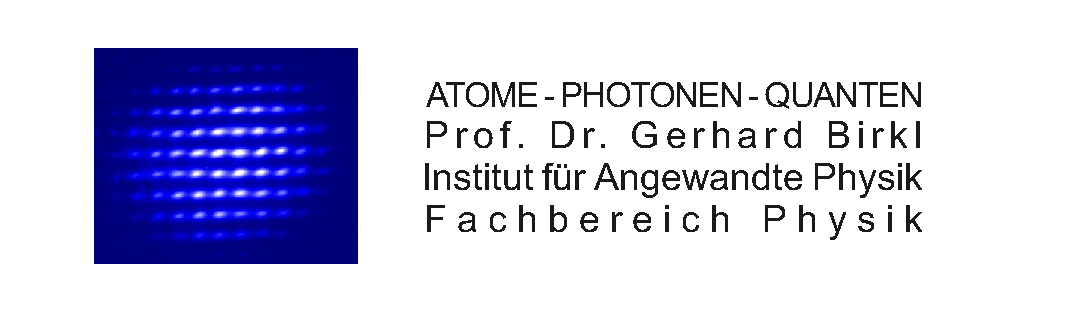
\includegraphics[width=55mm]{images/titel_apq-logo.pdf}}}
\titleimage{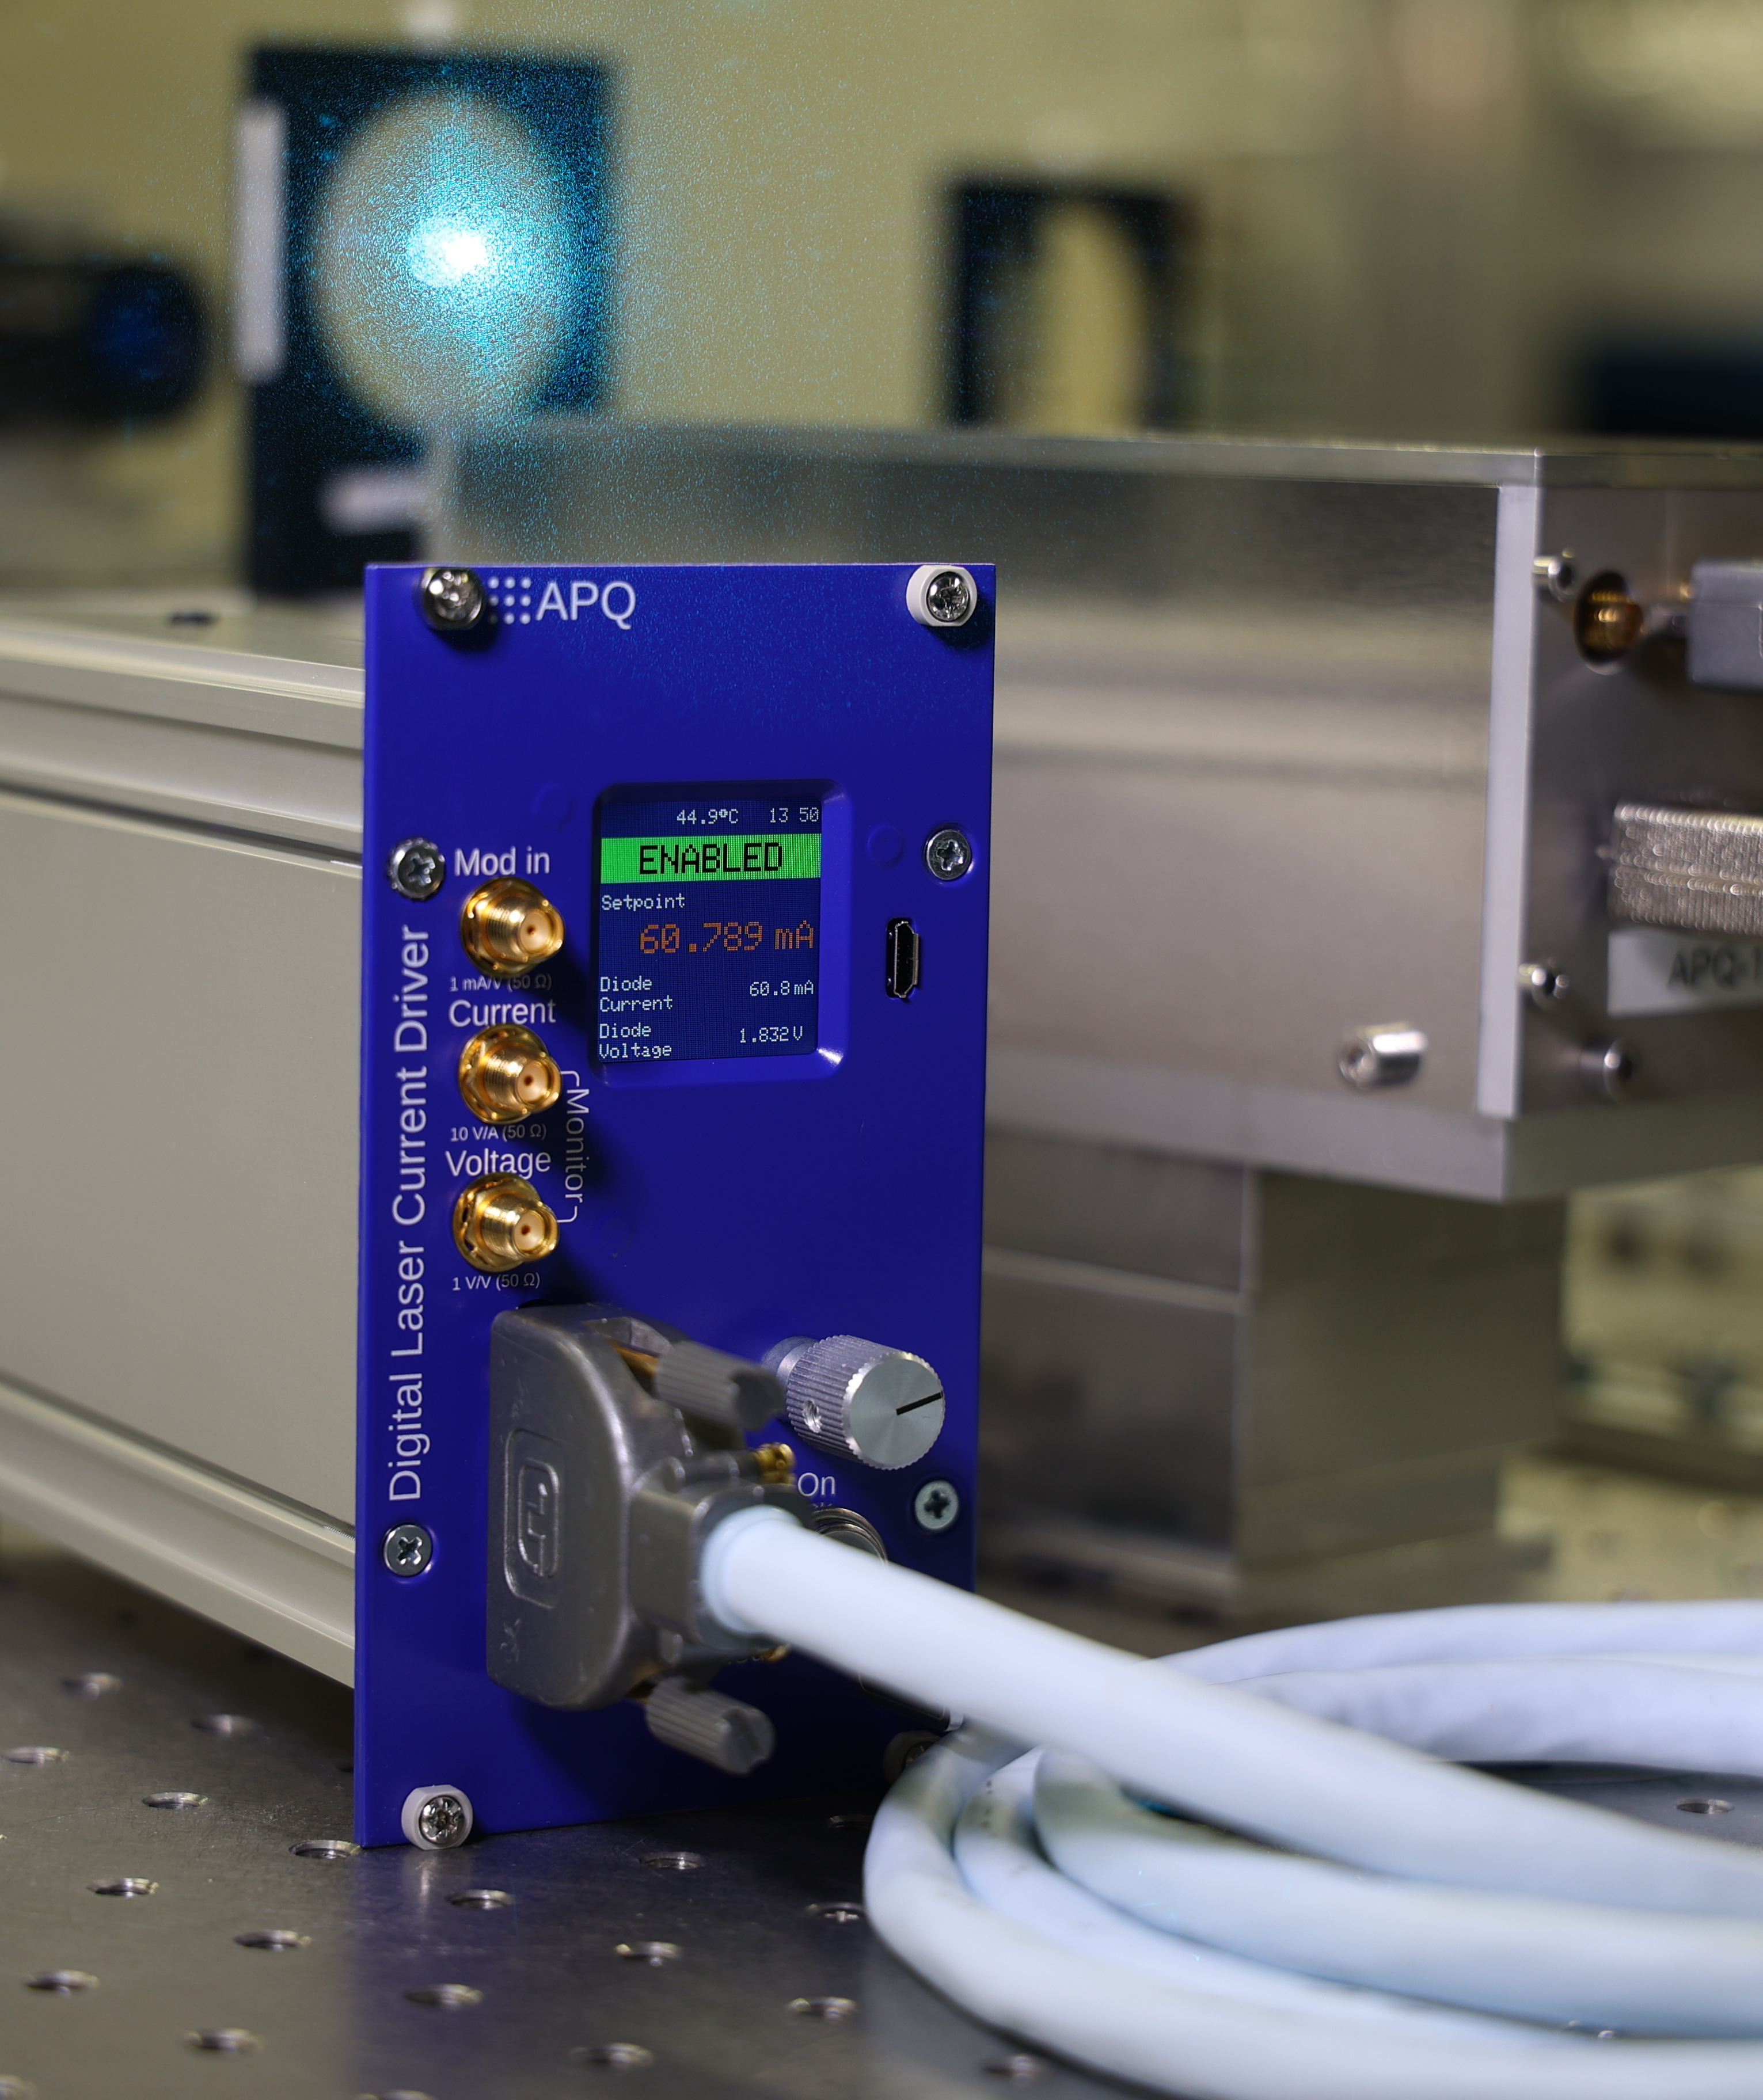
\includegraphics[width=\textwidth, height=1.1651\textwidth]{images/BM1A7279_front.jpg}}

\lowertitleback{\textbf{Front cover:} Digital laser current driver DgDrive in the foreground with a blue \qty{488}{\nm} laser in the background. Canon EOS R6, RF24-105mm F4 L IS USM, aperture F4, exposure time \qty[parse-numbers = false]{\frac{1}{25}}{\second}.}

\Metadata{
    copyright=This work is licensed under a Creative Commons ‘Attribution-ShareAlike 4.0 International’ license,
    copyrightURL=https://creativecommons.org/licenses/by-sa/4.0,
    uRLlink=https://github.com/PatrickBaus/phd_thesis
}


\begin{document}
	\title{Current Drivers and Control Electronics for the Laser Spectroscopy of Highly Charged Ions}
	\subtitle{Stromtreiber und Steuerelektronik für die Laserspektroskopie von hochgeladenen Ionen}
	\author{Patrick Baus}
	\birthplace{Mannheim}
	\reviewer{Prof. Dr. Gerhard Birkl \and Prof. Dr. Thomas Walther}

    \submissiondate{20.06.2023}
    \examdate{17.07.2023}
    \tuprints{
        urn=276077,
        year=2024,
        license=cc-by-sa-4.0,
        front-cover-descriptor={Digital laser current driver DgDrive in the foreground with a blue \qty{488}{\nm} laser in the background. Canon EOS R6, RF24-105mm F4 L IS USM, aperture F4, exposure time \qty[parse-numbers = false]{\frac{1}{25}}{\second}.}
    }% License information for TUprints

    \maketitle

    \subimport{}{abstract.tex}
    \tableofcontents
    \chapter{Changelog}
\begin{chapquote}{Karl Lagerfeld}
``What I like about photographs is that they capture a moment that’s gone forever, impossible to reproduce.''
\end{chapquote}

This work is only a momentary snapshot in time and subject to change. Future revisions will be updated as errors are found and lab-gremmlins have been evicted. If an error is found in this work, the reader is encouraged to either send an email to \url{patrick.baus@physik.tu-darmstadt.de} or file a bug report over at Github. Do note, the author has mischievously hidden some errors and typos in this work for the observant reader to find. The latest version (and all others) can always be found by navigating to \url{https://github.com/PatrickBaus/phd_thesis} or using the QR code below.
\begin{center}
    \qrcode{https://github.com/PatrickBaus/phd_thesis}
\end{center}

\begin{center}
    \begin{minipage}{0.8\linewidth}
        \centering
        Current version: \versionNumber
    \end{minipage}%
\end{center}

\begin{table}[h]
    \centering
    \begin{tabularx}{0.95\textwidth}{ll>{\raggedright\arraybackslash}X}
        Version& Date& Comment\\
        \hline
        0.9.0 &2023-06-20 & Initial release submitted as the doctoral thesis.\\
        0.10.0 &2024-07-09 & Updated plot colours to match the Seaborn 0.9.0+ style.\\
        0.11.0 &2024-07-09 & Changed downsampling algorithm from decimation to LTTB. Affected files: dgDrive\_supply\_filter\_bode.pgf, dgTemp\_longterm.pgf, dgTemp\_testmass.pgf, output\_impedance\_libbrecht\_hall.pgf. Increased number of points in the leakage plots. Use $3-\sigma$ for the uncertainty of the temperature coefficient.\\
        0.12.0 &2024-07-09 & Regenerated all plots to unify their dimensions.\\
        0.13.0 &2024-07.09 & Fixed typos and other errors found so far.\\
        0.14.0 &2024-07-09 & Updated APQ-Latex design template to a version based on tuda-ci 3.38.\\
        0.15.0 &2024-07-11 & Changed the y-axis of the flicker noise amplitude plot to make it looker bigger. Decimate the noise psd plots to improve the uncertainty towards higher frequencies. Fixed LNA background noise data. There was an incorrect gain setting applied. Fixed dgDrive\_output\_impedance\_comparison plot, because the sense resistor was not subtracted from the plotted results. This affected all devices but the DgDrive.\\
        0.16.0 &2024-07-12 & Fixed simulated LNA noise floor. Fixed typos.
    \end{tabularx}
\end{table}

    \chapter{Introduction}
Highly charged ions offer a unique insight into the very fine details of the world described by quantum electrodynamics (QED). The predictions of the electron’s magnetic moment (g-factor) can easily be regarded as the most accurate prediction in all science, matching the experimental value to \num{10} significant figures \cite{gfactor_theory}. Experimental measurements of the free electron's g-factor have most recently pushed the boundaries as far as an uncertainty of \num{1.3e-13}. The comparison of experimental values of the g-factor with theory therefore represents the most stringent test of the QED theory.

Extending the application of QED to bound states requires new tests of these calculations. Computing of the g-factor in complex systems such as neutral atoms with many electrons is extremely difficult and currently impossible with decent uncertainty \cite{gfactor_theory_codegen}. Using heavy highly charges ions helps both theory and experiment because it reduces the complexity and at the same times scales the QED contribution with the nuclear charge number as $Z\alpha$, reducing the required accuracy \cite{gfactor_ions_scaling}. While research has primarily relied on non-optical measurement in Penning traps in the past, laser spectroscopy opens new opportunities \cite{penning_trap_laser_spectroscopy} as the strong scaling of the fine- and hyperfine-structures with $Z^4$ and $Z^3$ brings those transitions into the region of visible and ultraviolet (UV) laser spectroscopy.

Highly charged ions are therefore an interesting field of research with the GSI Helmholtz Center for Heavy Ion Research at the forefront and capable of providing up to bare uranium. The AsymmetRic Trap for the measurement of Electron Magnetic moments in IonS (ARTEMIS) experiment at GSI as part of the Highly charged Ions Trap (HITRAP) platform and Facility for Antiproton and Ion Research (FAIR) aims to perform high-precision measurements of the bound electron's g-factor using a combination of laser- and microwave spectroscopy referred to as laser-microwave double-resonance spectroscopy \cite{laser_microwave_double_resonance_spectroscopy}. The ARTEMIS experiment provides a unique optically accessible Penning trap design \cite{penning_trap_transparent,penning_trap_half_open} with the aim of measurements on hydrogen-like bismuth, \ce{^{209}Bi^{82+}}. Currently the experiment is in its commissioning phase using boron-like Argon, \ce{^{40}Ar^{13+}}, targeting a g-factor measurement at the \num{e-9} level \cite{artemis_commissioning}.

Both the commissioning and the measurement on hydrogen-like bismuth require a precision laser system consisting of multiple lasers for the targeted closed transition driven by lasers and microwaves. The accessible wavelength of \ce{^{40}Ar^{13+}} is \qty{441}{\nm} \cite{ar13+_wavelength}, while \ce{^{209}Bi^{82+}} requires laser radiation at \qty{244}{\nm} \cite{bi82+_wavelength}. Recent years have seen the development of new laser diodes giving diode lasers access to an increasing part of the spectrum and for both targeted ion species the fundamental wavelengths are now covered by diode lasers. \qty{244}{\nm} can be reached via a quadrupled \qty{976}{\nm} diode laser source and \qty{441}{\nm} is directly accessible due the invention of blue laser diodes. Blue laser diodes were first presented in 1994 by \citeauthor{Nakamura_1996} \cite{Nakamura_1996}. This was followed by the first pulsed UV laser diode developed by \citeauthor{uv_pulsed_laser_diode_first} \cite{uv_pulsed_laser_diode_first} in 1995 and 1996 the first continuous wave UV laser diode \cite{uv_cw_laser_diode_first}. These developments then warranted the 2014 Nobel Prize in physics. This progress created the opportunity to build a compact and economic laser systems for the spectroscopy of highly charged ions based entirely on diode lasers.

For both applications laser systems were proposed and preliminary tests conducted \cite{thesis_baus,thesis_alex,thesis_tilman,thesis_seppo}. These tests have shown severe limitations in the current state of the art in diode laser technology. Most laser diode drivers commercially available are based on the work of \citeauthor{libbrecht_hall} presented in 1993 \cite{libbrecht_hall} which was designed for near-infrared laser diodes and the characteristics of blue laser diodes could not be foreseen at that time. The rapid development of blue light emitting diodes and laser diodes outpaced the development of the electronics to drive them which led to subpar performance of blue and UV diode lasers in comparison to their near-infrared brethren. Several groups have reported issues with the existing designs \cite{laser_driver_mosfet_noise} without solutions or attempted to include modern digital controls \cite{laser_driver_digital}.

Such digital control is critical to stay ahead of the ever increasing complexity introduced by modern experiments. Such experiments can, for example, be found in the field of quantum computing. A promising approach is the use of large arrays of individual neutral atoms, captured using optical traps to solve the scaling problem \cite{quatum_computer_scaling_ions}. Having hundreds to thousands of quantum systems that need addressing and manipulation requires dozens compact of laser sources that need to be orchestrated. Such orchestration is no longer feasible by hand. This level of automation requires a high degree of stability over time and temperature from the laser electronics to ensure the repeatability and reliability of the system. These qualities must be paired with an outstanding noise performance to produce the high fidelity of quantum state manipulation necessary for quantum computers. A combination of these digital features with the performance level is currently not available on the market.

This work has has now closed the gap and provides state-of-the-art open-source laser electronics incorporating novel approaches to the design of laser current drivers and temperature controllers for the application in high precision spectroscopy and quantum computing experiments. These solutions include modern remote-controllable digital interfaces for controlling large scale setups.

This work is split into three parts.\\

The \hyperref[sec:preparation]{\textbf{Preparation}} develops the theoretical background by giving a quick introduction into control theory, noise types and current sources. It also presents the requirements for the laser system designed for ARTEMIS.\\

The \hyperref[sec:results]{\textbf{Results}} give a detailed comparison of several laser drivers, both commercial and academic to outline the problems discovered during the testing of a blue laser systems. A laser driver design outperforming all solutions currently available is presented along with a high stability temperature controller specifically designed for the stringent needs of high precision laser spectroscopy. Additionally a compact PID controller system for lab application is presented in the context of lab temperature control together with a data monitoring system capable of logging the manifold data accumulated in a modern experiments and environmental monitoring systems. This data can then be accessed in real-time using a graphical web front end.\\

The \hyperref[sec:outlook]{\textbf{Outlook}} summarizes the results developed and, with the sources of electronic noise in diode lasers suppressed, exposes the final barrier imposed by the mechanical design of laser resonators.


    % FIXME: Change variable names according to Noise Sources in Bulk CMOS
\chapter{Preparation}
\begin{chapquote}{Lewis Carroll, \textit{Alice in Wonderland}}
``Begin at the beginning,'' the King said gravely, ``and go on till you come to the end: then stop.''
\end{chapquote}
\section{Grounding and Shielding}
Add parts from "references\\Grounding and Shielding.pdf"

\section{Laser System}
%Explanations exist; they have existed for all time; there is always a well-known solution to every human problem — neat, plausible, and wrong.
\subsection{Requirements Laser System}
One purpose of the laser system is to be used for the spectroscopy of highly charged ions in a Penning trap. For example, an interesting transition of \ce{Ar^13+} can be found at $\lambda = \qty{441.25575(17)}{\nm}$ \cite{ar13+_wavelength} with a lifetime of \qty{9.573(6)}{\ms} \cite{ar13+_lifetime}, which corresponds to natural linewidth of $\Gamma \approx 2 \pi \times \qty{16.63(1)}{\Hz}$. While this linewidth is fairly small, there is substantial doppler broadening at \qty{4}{\K} of
\begin{equation}
    \Delta \nu (\lambda = \qty{441}{\nm}, T=\qty{4}{\K}, m=\qty{39.948}{u}) = \frac{2}{\lambda}\sqrt{2 \ln 2 \frac{k_B T}{m}} \approx 2 \pi \times \qty{150}{\MHz} \, . \label{eqn:doppler_broadening}
\end{equation}

\clearpage
\section{Laser Current Driver}
\label{sec:laser_current_driver}
% Include Emission wavelength dependence of characteristic temperature of InGaN laser diodes
% Check Diode Laser Characteristics
% I-lamda in Wavelength Dependence of InGaN Laser Diode Characteristics
% also Determination of piezoelectric fields in strained GaInN quantum wells using the quantum-confined Stark effect
Laser diodes are current driven devices, because
\begin{equation}
    P_{out} \propto I\,, \nonumber
\end{equation}

and the diode current $I$ approximately follows the Shockley equation \cite{shockley_diode}
\begin{equation}
    I = I_0 \left( e^{\frac{qV_d}{k_B T}} - 1\right) \, .
\end{equation}

$k_B$ is Boltzmann constant, $T$ the temperature, $q$ the electron charge and $V_d$ the diode voltage. The exponential dependence of the current on the supply voltage calls for a current source to drive a laser diode safely, without risking thermal damage.

The primary function of a laser driver is to provide a stable, but user adjustable, current. The user adjustable current can typically be modulated at frequencies up to serveral \unit{\MHz} to shape the frequency and ampltitude of the laser beam. Additional features like current and voltage limits aid in protecting the expensive laser diodes. This section deals with the design challenges of such a device used for high precission laser spectroscopy. First the design requirements are derived and then technical specifications are developed.

The focus of this work many lies on two types of laser diodes, indium gallium nitride (InGaN) and aluminium gallium arsenide (AlGaAs), but is not limited to those two types. The former material is used for blue laser didoes at around \qty{450}{\nm}, but also cover up to green wavelengths, and the latter for near-infrared laser diodes at \qty{780}{\nm}, both wavelengths used for experiments in this group.

The design requirements are split into four parts, that need to be discussed. The ambient environment, the diode voltage and current requirements, the modulation bandwith and finally the noise specifications.

\clearpage
\subsection{Design Goals: Ambient Environment}
The laser driver is to be used in a clean laboratory environment. Typical lab temperatures are in the range of \qtyrange{20}{25}{\celsius} and ware mostly met in our labs, before improvements were implemented as part of this work. Humidity is only controlled with dehumidifiers and therefore in the range of \qtyrange{15}{60}{\percent rH}. The air is typically filtered using H14 HEPA filters. Figure \ref{fig:lab_temperature_start_of_project} shows a typical \qty{1}{d} span of the lab temperature as it was found at the start of this project.

\begin{figure}[ht]
    \centering
    %% Creator: Matplotlib, PGF backend
%%
%% To include the figure in your LaTeX document, write
%%   \input{<filename>.pgf}
%%
%% Make sure the required packages are loaded in your preamble
%%   \usepackage{pgf}
%%
%% Also ensure that all the required font packages are loaded; for instance,
%% the lmodern package is sometimes necessary when using math font.
%%   \usepackage{lmodern}
%%
%% Figures using additional raster images can only be included by \input if
%% they are in the same directory as the main LaTeX file. For loading figures
%% from other directories you can use the `import` package
%%   \usepackage{import}
%%
%% and then include the figures with
%%   \import{<path to file>}{<filename>.pgf}
%%
%% Matplotlib used the following preamble
%%   \usepackage{siunitx}
%%   \usepackage{fontspec}
%%
\begingroup%
\makeatletter%
\begin{pgfpicture}%
\pgfpathrectangle{\pgfpointorigin}{\pgfqpoint{5.208662in}{3.219130in}}%
\pgfusepath{use as bounding box, clip}%
\begin{pgfscope}%
\pgfsetbuttcap%
\pgfsetmiterjoin%
\definecolor{currentfill}{rgb}{1.000000,1.000000,1.000000}%
\pgfsetfillcolor{currentfill}%
\pgfsetlinewidth{0.000000pt}%
\definecolor{currentstroke}{rgb}{1.000000,1.000000,1.000000}%
\pgfsetstrokecolor{currentstroke}%
\pgfsetdash{}{0pt}%
\pgfpathmoveto{\pgfqpoint{0.000000in}{0.000000in}}%
\pgfpathlineto{\pgfqpoint{5.208662in}{0.000000in}}%
\pgfpathlineto{\pgfqpoint{5.208662in}{3.219130in}}%
\pgfpathlineto{\pgfqpoint{0.000000in}{3.219130in}}%
\pgfpathlineto{\pgfqpoint{0.000000in}{0.000000in}}%
\pgfpathclose%
\pgfusepath{fill}%
\end{pgfscope}%
\begin{pgfscope}%
\pgfsetbuttcap%
\pgfsetmiterjoin%
\definecolor{currentfill}{rgb}{1.000000,1.000000,1.000000}%
\pgfsetfillcolor{currentfill}%
\pgfsetlinewidth{0.000000pt}%
\definecolor{currentstroke}{rgb}{0.000000,0.000000,0.000000}%
\pgfsetstrokecolor{currentstroke}%
\pgfsetstrokeopacity{0.000000}%
\pgfsetdash{}{0pt}%
\pgfpathmoveto{\pgfqpoint{0.693677in}{0.539544in}}%
\pgfpathlineto{\pgfqpoint{5.058662in}{0.539544in}}%
\pgfpathlineto{\pgfqpoint{5.058662in}{3.053228in}}%
\pgfpathlineto{\pgfqpoint{0.693677in}{3.053228in}}%
\pgfpathlineto{\pgfqpoint{0.693677in}{0.539544in}}%
\pgfpathclose%
\pgfusepath{fill}%
\end{pgfscope}%
\begin{pgfscope}%
\pgfsetbuttcap%
\pgfsetroundjoin%
\definecolor{currentfill}{rgb}{0.000000,0.000000,0.000000}%
\pgfsetfillcolor{currentfill}%
\pgfsetlinewidth{0.803000pt}%
\definecolor{currentstroke}{rgb}{0.000000,0.000000,0.000000}%
\pgfsetstrokecolor{currentstroke}%
\pgfsetdash{}{0pt}%
\pgfsys@defobject{currentmarker}{\pgfqpoint{0.000000in}{-0.048611in}}{\pgfqpoint{0.000000in}{0.000000in}}{%
\pgfpathmoveto{\pgfqpoint{0.000000in}{0.000000in}}%
\pgfpathlineto{\pgfqpoint{0.000000in}{-0.048611in}}%
\pgfusepath{stroke,fill}%
}%
\begin{pgfscope}%
\pgfsys@transformshift{0.892085in}{0.539544in}%
\pgfsys@useobject{currentmarker}{}%
\end{pgfscope}%
\end{pgfscope}%
\begin{pgfscope}%
\definecolor{textcolor}{rgb}{0.000000,0.000000,0.000000}%
\pgfsetstrokecolor{textcolor}%
\pgfsetfillcolor{textcolor}%
\pgftext[x=0.892085in,y=0.442322in,,top]{\color{textcolor}\rmfamily\fontsize{8.000000}{9.600000}\selectfont \(\displaystyle {00{:}00}\)}%
\end{pgfscope}%
\begin{pgfscope}%
\pgfsetbuttcap%
\pgfsetroundjoin%
\definecolor{currentfill}{rgb}{0.000000,0.000000,0.000000}%
\pgfsetfillcolor{currentfill}%
\pgfsetlinewidth{0.803000pt}%
\definecolor{currentstroke}{rgb}{0.000000,0.000000,0.000000}%
\pgfsetstrokecolor{currentstroke}%
\pgfsetdash{}{0pt}%
\pgfsys@defobject{currentmarker}{\pgfqpoint{0.000000in}{-0.048611in}}{\pgfqpoint{0.000000in}{0.000000in}}{%
\pgfpathmoveto{\pgfqpoint{0.000000in}{0.000000in}}%
\pgfpathlineto{\pgfqpoint{0.000000in}{-0.048611in}}%
\pgfusepath{stroke,fill}%
}%
\begin{pgfscope}%
\pgfsys@transformshift{1.388451in}{0.539544in}%
\pgfsys@useobject{currentmarker}{}%
\end{pgfscope}%
\end{pgfscope}%
\begin{pgfscope}%
\definecolor{textcolor}{rgb}{0.000000,0.000000,0.000000}%
\pgfsetstrokecolor{textcolor}%
\pgfsetfillcolor{textcolor}%
\pgftext[x=1.388451in,y=0.442322in,,top]{\color{textcolor}\rmfamily\fontsize{8.000000}{9.600000}\selectfont \(\displaystyle {03{:}00}\)}%
\end{pgfscope}%
\begin{pgfscope}%
\pgfsetbuttcap%
\pgfsetroundjoin%
\definecolor{currentfill}{rgb}{0.000000,0.000000,0.000000}%
\pgfsetfillcolor{currentfill}%
\pgfsetlinewidth{0.803000pt}%
\definecolor{currentstroke}{rgb}{0.000000,0.000000,0.000000}%
\pgfsetstrokecolor{currentstroke}%
\pgfsetdash{}{0pt}%
\pgfsys@defobject{currentmarker}{\pgfqpoint{0.000000in}{-0.048611in}}{\pgfqpoint{0.000000in}{0.000000in}}{%
\pgfpathmoveto{\pgfqpoint{0.000000in}{0.000000in}}%
\pgfpathlineto{\pgfqpoint{0.000000in}{-0.048611in}}%
\pgfusepath{stroke,fill}%
}%
\begin{pgfscope}%
\pgfsys@transformshift{1.884817in}{0.539544in}%
\pgfsys@useobject{currentmarker}{}%
\end{pgfscope}%
\end{pgfscope}%
\begin{pgfscope}%
\definecolor{textcolor}{rgb}{0.000000,0.000000,0.000000}%
\pgfsetstrokecolor{textcolor}%
\pgfsetfillcolor{textcolor}%
\pgftext[x=1.884817in,y=0.442322in,,top]{\color{textcolor}\rmfamily\fontsize{8.000000}{9.600000}\selectfont \(\displaystyle {06{:}00}\)}%
\end{pgfscope}%
\begin{pgfscope}%
\pgfsetbuttcap%
\pgfsetroundjoin%
\definecolor{currentfill}{rgb}{0.000000,0.000000,0.000000}%
\pgfsetfillcolor{currentfill}%
\pgfsetlinewidth{0.803000pt}%
\definecolor{currentstroke}{rgb}{0.000000,0.000000,0.000000}%
\pgfsetstrokecolor{currentstroke}%
\pgfsetdash{}{0pt}%
\pgfsys@defobject{currentmarker}{\pgfqpoint{0.000000in}{-0.048611in}}{\pgfqpoint{0.000000in}{0.000000in}}{%
\pgfpathmoveto{\pgfqpoint{0.000000in}{0.000000in}}%
\pgfpathlineto{\pgfqpoint{0.000000in}{-0.048611in}}%
\pgfusepath{stroke,fill}%
}%
\begin{pgfscope}%
\pgfsys@transformshift{2.381182in}{0.539544in}%
\pgfsys@useobject{currentmarker}{}%
\end{pgfscope}%
\end{pgfscope}%
\begin{pgfscope}%
\definecolor{textcolor}{rgb}{0.000000,0.000000,0.000000}%
\pgfsetstrokecolor{textcolor}%
\pgfsetfillcolor{textcolor}%
\pgftext[x=2.381182in,y=0.442322in,,top]{\color{textcolor}\rmfamily\fontsize{8.000000}{9.600000}\selectfont \(\displaystyle {09{:}00}\)}%
\end{pgfscope}%
\begin{pgfscope}%
\pgfsetbuttcap%
\pgfsetroundjoin%
\definecolor{currentfill}{rgb}{0.000000,0.000000,0.000000}%
\pgfsetfillcolor{currentfill}%
\pgfsetlinewidth{0.803000pt}%
\definecolor{currentstroke}{rgb}{0.000000,0.000000,0.000000}%
\pgfsetstrokecolor{currentstroke}%
\pgfsetdash{}{0pt}%
\pgfsys@defobject{currentmarker}{\pgfqpoint{0.000000in}{-0.048611in}}{\pgfqpoint{0.000000in}{0.000000in}}{%
\pgfpathmoveto{\pgfqpoint{0.000000in}{0.000000in}}%
\pgfpathlineto{\pgfqpoint{0.000000in}{-0.048611in}}%
\pgfusepath{stroke,fill}%
}%
\begin{pgfscope}%
\pgfsys@transformshift{2.877548in}{0.539544in}%
\pgfsys@useobject{currentmarker}{}%
\end{pgfscope}%
\end{pgfscope}%
\begin{pgfscope}%
\definecolor{textcolor}{rgb}{0.000000,0.000000,0.000000}%
\pgfsetstrokecolor{textcolor}%
\pgfsetfillcolor{textcolor}%
\pgftext[x=2.877548in,y=0.442322in,,top]{\color{textcolor}\rmfamily\fontsize{8.000000}{9.600000}\selectfont \(\displaystyle {12{:}00}\)}%
\end{pgfscope}%
\begin{pgfscope}%
\pgfsetbuttcap%
\pgfsetroundjoin%
\definecolor{currentfill}{rgb}{0.000000,0.000000,0.000000}%
\pgfsetfillcolor{currentfill}%
\pgfsetlinewidth{0.803000pt}%
\definecolor{currentstroke}{rgb}{0.000000,0.000000,0.000000}%
\pgfsetstrokecolor{currentstroke}%
\pgfsetdash{}{0pt}%
\pgfsys@defobject{currentmarker}{\pgfqpoint{0.000000in}{-0.048611in}}{\pgfqpoint{0.000000in}{0.000000in}}{%
\pgfpathmoveto{\pgfqpoint{0.000000in}{0.000000in}}%
\pgfpathlineto{\pgfqpoint{0.000000in}{-0.048611in}}%
\pgfusepath{stroke,fill}%
}%
\begin{pgfscope}%
\pgfsys@transformshift{3.373914in}{0.539544in}%
\pgfsys@useobject{currentmarker}{}%
\end{pgfscope}%
\end{pgfscope}%
\begin{pgfscope}%
\definecolor{textcolor}{rgb}{0.000000,0.000000,0.000000}%
\pgfsetstrokecolor{textcolor}%
\pgfsetfillcolor{textcolor}%
\pgftext[x=3.373914in,y=0.442322in,,top]{\color{textcolor}\rmfamily\fontsize{8.000000}{9.600000}\selectfont \(\displaystyle {15{:}00}\)}%
\end{pgfscope}%
\begin{pgfscope}%
\pgfsetbuttcap%
\pgfsetroundjoin%
\definecolor{currentfill}{rgb}{0.000000,0.000000,0.000000}%
\pgfsetfillcolor{currentfill}%
\pgfsetlinewidth{0.803000pt}%
\definecolor{currentstroke}{rgb}{0.000000,0.000000,0.000000}%
\pgfsetstrokecolor{currentstroke}%
\pgfsetdash{}{0pt}%
\pgfsys@defobject{currentmarker}{\pgfqpoint{0.000000in}{-0.048611in}}{\pgfqpoint{0.000000in}{0.000000in}}{%
\pgfpathmoveto{\pgfqpoint{0.000000in}{0.000000in}}%
\pgfpathlineto{\pgfqpoint{0.000000in}{-0.048611in}}%
\pgfusepath{stroke,fill}%
}%
\begin{pgfscope}%
\pgfsys@transformshift{3.870280in}{0.539544in}%
\pgfsys@useobject{currentmarker}{}%
\end{pgfscope}%
\end{pgfscope}%
\begin{pgfscope}%
\definecolor{textcolor}{rgb}{0.000000,0.000000,0.000000}%
\pgfsetstrokecolor{textcolor}%
\pgfsetfillcolor{textcolor}%
\pgftext[x=3.870280in,y=0.442322in,,top]{\color{textcolor}\rmfamily\fontsize{8.000000}{9.600000}\selectfont \(\displaystyle {18{:}00}\)}%
\end{pgfscope}%
\begin{pgfscope}%
\pgfsetbuttcap%
\pgfsetroundjoin%
\definecolor{currentfill}{rgb}{0.000000,0.000000,0.000000}%
\pgfsetfillcolor{currentfill}%
\pgfsetlinewidth{0.803000pt}%
\definecolor{currentstroke}{rgb}{0.000000,0.000000,0.000000}%
\pgfsetstrokecolor{currentstroke}%
\pgfsetdash{}{0pt}%
\pgfsys@defobject{currentmarker}{\pgfqpoint{0.000000in}{-0.048611in}}{\pgfqpoint{0.000000in}{0.000000in}}{%
\pgfpathmoveto{\pgfqpoint{0.000000in}{0.000000in}}%
\pgfpathlineto{\pgfqpoint{0.000000in}{-0.048611in}}%
\pgfusepath{stroke,fill}%
}%
\begin{pgfscope}%
\pgfsys@transformshift{4.366645in}{0.539544in}%
\pgfsys@useobject{currentmarker}{}%
\end{pgfscope}%
\end{pgfscope}%
\begin{pgfscope}%
\definecolor{textcolor}{rgb}{0.000000,0.000000,0.000000}%
\pgfsetstrokecolor{textcolor}%
\pgfsetfillcolor{textcolor}%
\pgftext[x=4.366645in,y=0.442322in,,top]{\color{textcolor}\rmfamily\fontsize{8.000000}{9.600000}\selectfont \(\displaystyle {21{:}00}\)}%
\end{pgfscope}%
\begin{pgfscope}%
\pgfsetbuttcap%
\pgfsetroundjoin%
\definecolor{currentfill}{rgb}{0.000000,0.000000,0.000000}%
\pgfsetfillcolor{currentfill}%
\pgfsetlinewidth{0.803000pt}%
\definecolor{currentstroke}{rgb}{0.000000,0.000000,0.000000}%
\pgfsetstrokecolor{currentstroke}%
\pgfsetdash{}{0pt}%
\pgfsys@defobject{currentmarker}{\pgfqpoint{0.000000in}{-0.048611in}}{\pgfqpoint{0.000000in}{0.000000in}}{%
\pgfpathmoveto{\pgfqpoint{0.000000in}{0.000000in}}%
\pgfpathlineto{\pgfqpoint{0.000000in}{-0.048611in}}%
\pgfusepath{stroke,fill}%
}%
\begin{pgfscope}%
\pgfsys@transformshift{4.863011in}{0.539544in}%
\pgfsys@useobject{currentmarker}{}%
\end{pgfscope}%
\end{pgfscope}%
\begin{pgfscope}%
\definecolor{textcolor}{rgb}{0.000000,0.000000,0.000000}%
\pgfsetstrokecolor{textcolor}%
\pgfsetfillcolor{textcolor}%
\pgftext[x=4.863011in,y=0.442322in,,top]{\color{textcolor}\rmfamily\fontsize{8.000000}{9.600000}\selectfont \(\displaystyle {00{:}00}\)}%
\end{pgfscope}%
\begin{pgfscope}%
\definecolor{textcolor}{rgb}{0.000000,0.000000,0.000000}%
\pgfsetstrokecolor{textcolor}%
\pgfsetfillcolor{textcolor}%
\pgftext[x=2.876169in,y=0.288100in,,top]{\color{textcolor}\rmfamily\fontsize{10.000000}{12.000000}\selectfont Time (UTC)}%
\end{pgfscope}%
\begin{pgfscope}%
\pgfsetbuttcap%
\pgfsetroundjoin%
\definecolor{currentfill}{rgb}{0.000000,0.000000,0.000000}%
\pgfsetfillcolor{currentfill}%
\pgfsetlinewidth{0.803000pt}%
\definecolor{currentstroke}{rgb}{0.000000,0.000000,0.000000}%
\pgfsetstrokecolor{currentstroke}%
\pgfsetdash{}{0pt}%
\pgfsys@defobject{currentmarker}{\pgfqpoint{-0.048611in}{0.000000in}}{\pgfqpoint{-0.000000in}{0.000000in}}{%
\pgfpathmoveto{\pgfqpoint{-0.000000in}{0.000000in}}%
\pgfpathlineto{\pgfqpoint{-0.048611in}{0.000000in}}%
\pgfusepath{stroke,fill}%
}%
\begin{pgfscope}%
\pgfsys@transformshift{0.693677in}{0.745209in}%
\pgfsys@useobject{currentmarker}{}%
\end{pgfscope}%
\end{pgfscope}%
\begin{pgfscope}%
\definecolor{textcolor}{rgb}{0.000000,0.000000,0.000000}%
\pgfsetstrokecolor{textcolor}%
\pgfsetfillcolor{textcolor}%
\pgftext[x=0.327546in, y=0.706654in, left, base]{\color{textcolor}\rmfamily\fontsize{8.000000}{9.600000}\selectfont \(\displaystyle {20.00}\)}%
\end{pgfscope}%
\begin{pgfscope}%
\pgfsetbuttcap%
\pgfsetroundjoin%
\definecolor{currentfill}{rgb}{0.000000,0.000000,0.000000}%
\pgfsetfillcolor{currentfill}%
\pgfsetlinewidth{0.803000pt}%
\definecolor{currentstroke}{rgb}{0.000000,0.000000,0.000000}%
\pgfsetstrokecolor{currentstroke}%
\pgfsetdash{}{0pt}%
\pgfsys@defobject{currentmarker}{\pgfqpoint{-0.048611in}{0.000000in}}{\pgfqpoint{-0.000000in}{0.000000in}}{%
\pgfpathmoveto{\pgfqpoint{-0.000000in}{0.000000in}}%
\pgfpathlineto{\pgfqpoint{-0.048611in}{0.000000in}}%
\pgfusepath{stroke,fill}%
}%
\begin{pgfscope}%
\pgfsys@transformshift{0.693677in}{1.071662in}%
\pgfsys@useobject{currentmarker}{}%
\end{pgfscope}%
\end{pgfscope}%
\begin{pgfscope}%
\definecolor{textcolor}{rgb}{0.000000,0.000000,0.000000}%
\pgfsetstrokecolor{textcolor}%
\pgfsetfillcolor{textcolor}%
\pgftext[x=0.327546in, y=1.033106in, left, base]{\color{textcolor}\rmfamily\fontsize{8.000000}{9.600000}\selectfont \(\displaystyle {20.25}\)}%
\end{pgfscope}%
\begin{pgfscope}%
\pgfsetbuttcap%
\pgfsetroundjoin%
\definecolor{currentfill}{rgb}{0.000000,0.000000,0.000000}%
\pgfsetfillcolor{currentfill}%
\pgfsetlinewidth{0.803000pt}%
\definecolor{currentstroke}{rgb}{0.000000,0.000000,0.000000}%
\pgfsetstrokecolor{currentstroke}%
\pgfsetdash{}{0pt}%
\pgfsys@defobject{currentmarker}{\pgfqpoint{-0.048611in}{0.000000in}}{\pgfqpoint{-0.000000in}{0.000000in}}{%
\pgfpathmoveto{\pgfqpoint{-0.000000in}{0.000000in}}%
\pgfpathlineto{\pgfqpoint{-0.048611in}{0.000000in}}%
\pgfusepath{stroke,fill}%
}%
\begin{pgfscope}%
\pgfsys@transformshift{0.693677in}{1.398114in}%
\pgfsys@useobject{currentmarker}{}%
\end{pgfscope}%
\end{pgfscope}%
\begin{pgfscope}%
\definecolor{textcolor}{rgb}{0.000000,0.000000,0.000000}%
\pgfsetstrokecolor{textcolor}%
\pgfsetfillcolor{textcolor}%
\pgftext[x=0.327546in, y=1.359559in, left, base]{\color{textcolor}\rmfamily\fontsize{8.000000}{9.600000}\selectfont \(\displaystyle {20.50}\)}%
\end{pgfscope}%
\begin{pgfscope}%
\pgfsetbuttcap%
\pgfsetroundjoin%
\definecolor{currentfill}{rgb}{0.000000,0.000000,0.000000}%
\pgfsetfillcolor{currentfill}%
\pgfsetlinewidth{0.803000pt}%
\definecolor{currentstroke}{rgb}{0.000000,0.000000,0.000000}%
\pgfsetstrokecolor{currentstroke}%
\pgfsetdash{}{0pt}%
\pgfsys@defobject{currentmarker}{\pgfqpoint{-0.048611in}{0.000000in}}{\pgfqpoint{-0.000000in}{0.000000in}}{%
\pgfpathmoveto{\pgfqpoint{-0.000000in}{0.000000in}}%
\pgfpathlineto{\pgfqpoint{-0.048611in}{0.000000in}}%
\pgfusepath{stroke,fill}%
}%
\begin{pgfscope}%
\pgfsys@transformshift{0.693677in}{1.724567in}%
\pgfsys@useobject{currentmarker}{}%
\end{pgfscope}%
\end{pgfscope}%
\begin{pgfscope}%
\definecolor{textcolor}{rgb}{0.000000,0.000000,0.000000}%
\pgfsetstrokecolor{textcolor}%
\pgfsetfillcolor{textcolor}%
\pgftext[x=0.327546in, y=1.686011in, left, base]{\color{textcolor}\rmfamily\fontsize{8.000000}{9.600000}\selectfont \(\displaystyle {20.75}\)}%
\end{pgfscope}%
\begin{pgfscope}%
\pgfsetbuttcap%
\pgfsetroundjoin%
\definecolor{currentfill}{rgb}{0.000000,0.000000,0.000000}%
\pgfsetfillcolor{currentfill}%
\pgfsetlinewidth{0.803000pt}%
\definecolor{currentstroke}{rgb}{0.000000,0.000000,0.000000}%
\pgfsetstrokecolor{currentstroke}%
\pgfsetdash{}{0pt}%
\pgfsys@defobject{currentmarker}{\pgfqpoint{-0.048611in}{0.000000in}}{\pgfqpoint{-0.000000in}{0.000000in}}{%
\pgfpathmoveto{\pgfqpoint{-0.000000in}{0.000000in}}%
\pgfpathlineto{\pgfqpoint{-0.048611in}{0.000000in}}%
\pgfusepath{stroke,fill}%
}%
\begin{pgfscope}%
\pgfsys@transformshift{0.693677in}{2.051019in}%
\pgfsys@useobject{currentmarker}{}%
\end{pgfscope}%
\end{pgfscope}%
\begin{pgfscope}%
\definecolor{textcolor}{rgb}{0.000000,0.000000,0.000000}%
\pgfsetstrokecolor{textcolor}%
\pgfsetfillcolor{textcolor}%
\pgftext[x=0.327546in, y=2.012463in, left, base]{\color{textcolor}\rmfamily\fontsize{8.000000}{9.600000}\selectfont \(\displaystyle {21.00}\)}%
\end{pgfscope}%
\begin{pgfscope}%
\pgfsetbuttcap%
\pgfsetroundjoin%
\definecolor{currentfill}{rgb}{0.000000,0.000000,0.000000}%
\pgfsetfillcolor{currentfill}%
\pgfsetlinewidth{0.803000pt}%
\definecolor{currentstroke}{rgb}{0.000000,0.000000,0.000000}%
\pgfsetstrokecolor{currentstroke}%
\pgfsetdash{}{0pt}%
\pgfsys@defobject{currentmarker}{\pgfqpoint{-0.048611in}{0.000000in}}{\pgfqpoint{-0.000000in}{0.000000in}}{%
\pgfpathmoveto{\pgfqpoint{-0.000000in}{0.000000in}}%
\pgfpathlineto{\pgfqpoint{-0.048611in}{0.000000in}}%
\pgfusepath{stroke,fill}%
}%
\begin{pgfscope}%
\pgfsys@transformshift{0.693677in}{2.377471in}%
\pgfsys@useobject{currentmarker}{}%
\end{pgfscope}%
\end{pgfscope}%
\begin{pgfscope}%
\definecolor{textcolor}{rgb}{0.000000,0.000000,0.000000}%
\pgfsetstrokecolor{textcolor}%
\pgfsetfillcolor{textcolor}%
\pgftext[x=0.327546in, y=2.338916in, left, base]{\color{textcolor}\rmfamily\fontsize{8.000000}{9.600000}\selectfont \(\displaystyle {21.25}\)}%
\end{pgfscope}%
\begin{pgfscope}%
\pgfsetbuttcap%
\pgfsetroundjoin%
\definecolor{currentfill}{rgb}{0.000000,0.000000,0.000000}%
\pgfsetfillcolor{currentfill}%
\pgfsetlinewidth{0.803000pt}%
\definecolor{currentstroke}{rgb}{0.000000,0.000000,0.000000}%
\pgfsetstrokecolor{currentstroke}%
\pgfsetdash{}{0pt}%
\pgfsys@defobject{currentmarker}{\pgfqpoint{-0.048611in}{0.000000in}}{\pgfqpoint{-0.000000in}{0.000000in}}{%
\pgfpathmoveto{\pgfqpoint{-0.000000in}{0.000000in}}%
\pgfpathlineto{\pgfqpoint{-0.048611in}{0.000000in}}%
\pgfusepath{stroke,fill}%
}%
\begin{pgfscope}%
\pgfsys@transformshift{0.693677in}{2.703924in}%
\pgfsys@useobject{currentmarker}{}%
\end{pgfscope}%
\end{pgfscope}%
\begin{pgfscope}%
\definecolor{textcolor}{rgb}{0.000000,0.000000,0.000000}%
\pgfsetstrokecolor{textcolor}%
\pgfsetfillcolor{textcolor}%
\pgftext[x=0.327546in, y=2.665368in, left, base]{\color{textcolor}\rmfamily\fontsize{8.000000}{9.600000}\selectfont \(\displaystyle {21.50}\)}%
\end{pgfscope}%
\begin{pgfscope}%
\pgfsetbuttcap%
\pgfsetroundjoin%
\definecolor{currentfill}{rgb}{0.000000,0.000000,0.000000}%
\pgfsetfillcolor{currentfill}%
\pgfsetlinewidth{0.803000pt}%
\definecolor{currentstroke}{rgb}{0.000000,0.000000,0.000000}%
\pgfsetstrokecolor{currentstroke}%
\pgfsetdash{}{0pt}%
\pgfsys@defobject{currentmarker}{\pgfqpoint{-0.048611in}{0.000000in}}{\pgfqpoint{-0.000000in}{0.000000in}}{%
\pgfpathmoveto{\pgfqpoint{-0.000000in}{0.000000in}}%
\pgfpathlineto{\pgfqpoint{-0.048611in}{0.000000in}}%
\pgfusepath{stroke,fill}%
}%
\begin{pgfscope}%
\pgfsys@transformshift{0.693677in}{3.030376in}%
\pgfsys@useobject{currentmarker}{}%
\end{pgfscope}%
\end{pgfscope}%
\begin{pgfscope}%
\definecolor{textcolor}{rgb}{0.000000,0.000000,0.000000}%
\pgfsetstrokecolor{textcolor}%
\pgfsetfillcolor{textcolor}%
\pgftext[x=0.327546in, y=2.991821in, left, base]{\color{textcolor}\rmfamily\fontsize{8.000000}{9.600000}\selectfont \(\displaystyle {21.75}\)}%
\end{pgfscope}%
\begin{pgfscope}%
\definecolor{textcolor}{rgb}{0.000000,0.000000,0.000000}%
\pgfsetstrokecolor{textcolor}%
\pgfsetfillcolor{textcolor}%
\pgftext[x=0.271991in,y=1.796386in,,bottom,rotate=90.000000]{\color{textcolor}\rmfamily\fontsize{10.000000}{12.000000}\selectfont Temperature in \unit{\celsius}}%
\end{pgfscope}%
\begin{pgfscope}%
\pgfpathrectangle{\pgfqpoint{0.693677in}{0.539544in}}{\pgfqpoint{4.364985in}{2.513684in}}%
\pgfusepath{clip}%
\pgfsetrectcap%
\pgfsetroundjoin%
\pgfsetlinewidth{0.501875pt}%
\definecolor{currentstroke}{rgb}{0.121569,0.466667,0.705882}%
\pgfsetstrokecolor{currentstroke}%
\pgfsetstrokeopacity{0.700000}%
\pgfsetdash{}{0pt}%
\pgfpathmoveto{\pgfqpoint{0.892085in}{2.612517in}}%
\pgfpathlineto{\pgfqpoint{0.894843in}{2.703924in}}%
\pgfpathlineto{\pgfqpoint{0.930691in}{2.782272in}}%
\pgfpathlineto{\pgfqpoint{0.933449in}{2.703924in}}%
\pgfpathlineto{\pgfqpoint{0.936207in}{2.782272in}}%
\pgfpathlineto{\pgfqpoint{0.938964in}{2.703924in}}%
\pgfpathlineto{\pgfqpoint{0.941722in}{2.782272in}}%
\pgfpathlineto{\pgfqpoint{0.944479in}{2.703924in}}%
\pgfpathlineto{\pgfqpoint{0.947237in}{2.782272in}}%
\pgfpathlineto{\pgfqpoint{0.949995in}{2.703924in}}%
\pgfpathlineto{\pgfqpoint{0.952752in}{2.782272in}}%
\pgfpathlineto{\pgfqpoint{0.955510in}{2.703924in}}%
\pgfpathlineto{\pgfqpoint{0.958267in}{2.782272in}}%
\pgfpathlineto{\pgfqpoint{0.961025in}{2.703924in}}%
\pgfpathlineto{\pgfqpoint{0.963783in}{2.782272in}}%
\pgfpathlineto{\pgfqpoint{0.966540in}{2.703924in}}%
\pgfpathlineto{\pgfqpoint{0.969298in}{2.782272in}}%
\pgfpathlineto{\pgfqpoint{0.972055in}{2.703924in}}%
\pgfpathlineto{\pgfqpoint{0.974813in}{2.782272in}}%
\pgfpathlineto{\pgfqpoint{0.977570in}{2.703924in}}%
\pgfpathlineto{\pgfqpoint{0.980328in}{2.782272in}}%
\pgfpathlineto{\pgfqpoint{0.985843in}{2.703924in}}%
\pgfpathlineto{\pgfqpoint{0.988601in}{2.782272in}}%
\pgfpathlineto{\pgfqpoint{1.032722in}{2.860621in}}%
\pgfpathlineto{\pgfqpoint{1.035480in}{2.782272in}}%
\pgfpathlineto{\pgfqpoint{1.040995in}{2.860621in}}%
\pgfpathlineto{\pgfqpoint{1.043753in}{2.782272in}}%
\pgfpathlineto{\pgfqpoint{1.046510in}{2.860621in}}%
\pgfpathlineto{\pgfqpoint{1.049268in}{2.782272in}}%
\pgfpathlineto{\pgfqpoint{1.054783in}{2.860621in}}%
\pgfpathlineto{\pgfqpoint{1.057540in}{2.782272in}}%
\pgfpathlineto{\pgfqpoint{1.060298in}{2.860621in}}%
\pgfpathlineto{\pgfqpoint{1.063056in}{2.782272in}}%
\pgfpathlineto{\pgfqpoint{1.065813in}{2.860621in}}%
\pgfpathlineto{\pgfqpoint{1.068571in}{2.782272in}}%
\pgfpathlineto{\pgfqpoint{1.071328in}{2.860621in}}%
\pgfpathlineto{\pgfqpoint{1.074086in}{2.782272in}}%
\pgfpathlineto{\pgfqpoint{1.076844in}{2.860621in}}%
\pgfpathlineto{\pgfqpoint{1.079601in}{2.782272in}}%
\pgfpathlineto{\pgfqpoint{1.082359in}{2.860621in}}%
\pgfpathlineto{\pgfqpoint{1.085116in}{2.782272in}}%
\pgfpathlineto{\pgfqpoint{1.087874in}{2.860621in}}%
\pgfpathlineto{\pgfqpoint{1.090632in}{2.782272in}}%
\pgfpathlineto{\pgfqpoint{1.093389in}{2.860621in}}%
\pgfpathlineto{\pgfqpoint{1.096147in}{2.782272in}}%
\pgfpathlineto{\pgfqpoint{1.098904in}{2.860621in}}%
\pgfpathlineto{\pgfqpoint{1.109935in}{2.782272in}}%
\pgfpathlineto{\pgfqpoint{1.112692in}{2.860621in}}%
\pgfpathlineto{\pgfqpoint{1.123723in}{2.782272in}}%
\pgfpathlineto{\pgfqpoint{1.126480in}{2.860621in}}%
\pgfpathlineto{\pgfqpoint{1.178874in}{2.938970in}}%
\pgfpathlineto{\pgfqpoint{1.181632in}{2.860621in}}%
\pgfpathlineto{\pgfqpoint{1.184390in}{2.938970in}}%
\pgfpathlineto{\pgfqpoint{1.187147in}{2.860621in}}%
\pgfpathlineto{\pgfqpoint{1.189905in}{2.938970in}}%
\pgfpathlineto{\pgfqpoint{1.220238in}{2.051019in}}%
\pgfpathlineto{\pgfqpoint{1.225753in}{1.881264in}}%
\pgfpathlineto{\pgfqpoint{1.231268in}{1.802915in}}%
\pgfpathlineto{\pgfqpoint{1.234026in}{1.724567in}}%
\pgfpathlineto{\pgfqpoint{1.239541in}{1.633160in}}%
\pgfpathlineto{\pgfqpoint{1.242299in}{1.554811in}}%
\pgfpathlineto{\pgfqpoint{1.250572in}{1.476463in}}%
\pgfpathlineto{\pgfqpoint{1.256087in}{1.398114in}}%
\pgfpathlineto{\pgfqpoint{1.258844in}{1.476463in}}%
\pgfpathlineto{\pgfqpoint{1.264360in}{1.306707in}}%
\pgfpathlineto{\pgfqpoint{1.272632in}{1.228359in}}%
\pgfpathlineto{\pgfqpoint{1.275390in}{1.306707in}}%
\pgfpathlineto{\pgfqpoint{1.280905in}{1.150010in}}%
\pgfpathlineto{\pgfqpoint{1.283663in}{1.228359in}}%
\pgfpathlineto{\pgfqpoint{1.286420in}{1.150010in}}%
\pgfpathlineto{\pgfqpoint{1.291935in}{1.071662in}}%
\pgfpathlineto{\pgfqpoint{1.294693in}{1.150010in}}%
\pgfpathlineto{\pgfqpoint{1.297451in}{1.071662in}}%
\pgfpathlineto{\pgfqpoint{1.300208in}{1.150010in}}%
\pgfpathlineto{\pgfqpoint{1.302966in}{1.071662in}}%
\pgfpathlineto{\pgfqpoint{1.313996in}{0.980255in}}%
\pgfpathlineto{\pgfqpoint{1.316754in}{1.071662in}}%
\pgfpathlineto{\pgfqpoint{1.319511in}{0.980255in}}%
\pgfpathlineto{\pgfqpoint{1.322269in}{1.071662in}}%
\pgfpathlineto{\pgfqpoint{1.325026in}{0.980255in}}%
\pgfpathlineto{\pgfqpoint{1.330542in}{0.901906in}}%
\pgfpathlineto{\pgfqpoint{1.333299in}{0.980255in}}%
\pgfpathlineto{\pgfqpoint{1.336057in}{0.901906in}}%
\pgfpathlineto{\pgfqpoint{1.347087in}{0.823558in}}%
\pgfpathlineto{\pgfqpoint{1.349845in}{0.901906in}}%
\pgfpathlineto{\pgfqpoint{1.352602in}{0.823558in}}%
\pgfpathlineto{\pgfqpoint{1.355360in}{0.901906in}}%
\pgfpathlineto{\pgfqpoint{1.358118in}{0.823558in}}%
\pgfpathlineto{\pgfqpoint{1.369148in}{0.745209in}}%
\pgfpathlineto{\pgfqpoint{1.371905in}{0.823558in}}%
\pgfpathlineto{\pgfqpoint{1.374663in}{0.745209in}}%
\pgfpathlineto{\pgfqpoint{1.377421in}{0.823558in}}%
\pgfpathlineto{\pgfqpoint{1.382936in}{0.901906in}}%
\pgfpathlineto{\pgfqpoint{1.388451in}{1.071662in}}%
\pgfpathlineto{\pgfqpoint{1.393966in}{1.150010in}}%
\pgfpathlineto{\pgfqpoint{1.396724in}{1.228359in}}%
\pgfpathlineto{\pgfqpoint{1.402239in}{1.306707in}}%
\pgfpathlineto{\pgfqpoint{1.404996in}{1.398114in}}%
\pgfpathlineto{\pgfqpoint{1.432572in}{1.802915in}}%
\pgfpathlineto{\pgfqpoint{1.438088in}{1.724567in}}%
\pgfpathlineto{\pgfqpoint{1.443603in}{1.881264in}}%
\pgfpathlineto{\pgfqpoint{1.449118in}{1.959612in}}%
\pgfpathlineto{\pgfqpoint{1.451875in}{1.881264in}}%
\pgfpathlineto{\pgfqpoint{1.454633in}{1.959612in}}%
\pgfpathlineto{\pgfqpoint{1.460148in}{2.051019in}}%
\pgfpathlineto{\pgfqpoint{1.462906in}{1.959612in}}%
\pgfpathlineto{\pgfqpoint{1.468421in}{2.129368in}}%
\pgfpathlineto{\pgfqpoint{1.471179in}{2.051019in}}%
\pgfpathlineto{\pgfqpoint{1.473936in}{2.129368in}}%
\pgfpathlineto{\pgfqpoint{1.482209in}{2.207716in}}%
\pgfpathlineto{\pgfqpoint{1.484967in}{2.129368in}}%
\pgfpathlineto{\pgfqpoint{1.487724in}{2.207716in}}%
\pgfpathlineto{\pgfqpoint{1.490482in}{2.129368in}}%
\pgfpathlineto{\pgfqpoint{1.493239in}{2.207716in}}%
\pgfpathlineto{\pgfqpoint{1.501512in}{2.286065in}}%
\pgfpathlineto{\pgfqpoint{1.504270in}{2.207716in}}%
\pgfpathlineto{\pgfqpoint{1.507027in}{2.286065in}}%
\pgfpathlineto{\pgfqpoint{1.509785in}{2.207716in}}%
\pgfpathlineto{\pgfqpoint{1.512542in}{2.286065in}}%
\pgfpathlineto{\pgfqpoint{1.520815in}{2.377471in}}%
\pgfpathlineto{\pgfqpoint{1.523573in}{2.286065in}}%
\pgfpathlineto{\pgfqpoint{1.526330in}{2.377471in}}%
\pgfpathlineto{\pgfqpoint{1.529088in}{2.286065in}}%
\pgfpathlineto{\pgfqpoint{1.531846in}{2.377471in}}%
\pgfpathlineto{\pgfqpoint{1.545633in}{2.455820in}}%
\pgfpathlineto{\pgfqpoint{1.548391in}{2.377471in}}%
\pgfpathlineto{\pgfqpoint{1.551149in}{2.455820in}}%
\pgfpathlineto{\pgfqpoint{1.553906in}{2.377471in}}%
\pgfpathlineto{\pgfqpoint{1.556664in}{2.455820in}}%
\pgfpathlineto{\pgfqpoint{1.562179in}{2.377471in}}%
\pgfpathlineto{\pgfqpoint{1.564937in}{2.455820in}}%
\pgfpathlineto{\pgfqpoint{1.581482in}{2.534169in}}%
\pgfpathlineto{\pgfqpoint{1.584240in}{2.455820in}}%
\pgfpathlineto{\pgfqpoint{1.586997in}{2.534169in}}%
\pgfpathlineto{\pgfqpoint{1.589755in}{2.455820in}}%
\pgfpathlineto{\pgfqpoint{1.592512in}{2.534169in}}%
\pgfpathlineto{\pgfqpoint{1.595270in}{2.455820in}}%
\pgfpathlineto{\pgfqpoint{1.598028in}{2.534169in}}%
\pgfpathlineto{\pgfqpoint{1.620088in}{2.612517in}}%
\pgfpathlineto{\pgfqpoint{1.622846in}{2.534169in}}%
\pgfpathlineto{\pgfqpoint{1.628361in}{2.612517in}}%
\pgfpathlineto{\pgfqpoint{1.631119in}{2.534169in}}%
\pgfpathlineto{\pgfqpoint{1.633876in}{2.612517in}}%
\pgfpathlineto{\pgfqpoint{1.636634in}{2.534169in}}%
\pgfpathlineto{\pgfqpoint{1.639391in}{2.612517in}}%
\pgfpathlineto{\pgfqpoint{1.642149in}{2.534169in}}%
\pgfpathlineto{\pgfqpoint{1.644907in}{2.612517in}}%
\pgfpathlineto{\pgfqpoint{1.647664in}{2.534169in}}%
\pgfpathlineto{\pgfqpoint{1.650422in}{2.612517in}}%
\pgfpathlineto{\pgfqpoint{1.686270in}{2.703924in}}%
\pgfpathlineto{\pgfqpoint{1.689028in}{2.612517in}}%
\pgfpathlineto{\pgfqpoint{1.691786in}{2.703924in}}%
\pgfpathlineto{\pgfqpoint{1.694543in}{2.612517in}}%
\pgfpathlineto{\pgfqpoint{1.697301in}{2.703924in}}%
\pgfpathlineto{\pgfqpoint{1.700058in}{2.612517in}}%
\pgfpathlineto{\pgfqpoint{1.702816in}{2.703924in}}%
\pgfpathlineto{\pgfqpoint{1.705574in}{2.612517in}}%
\pgfpathlineto{\pgfqpoint{1.708331in}{2.703924in}}%
\pgfpathlineto{\pgfqpoint{1.711089in}{2.612517in}}%
\pgfpathlineto{\pgfqpoint{1.713846in}{2.703924in}}%
\pgfpathlineto{\pgfqpoint{1.716604in}{2.612517in}}%
\pgfpathlineto{\pgfqpoint{1.719361in}{2.703924in}}%
\pgfpathlineto{\pgfqpoint{1.724877in}{2.612517in}}%
\pgfpathlineto{\pgfqpoint{1.727634in}{2.703924in}}%
\pgfpathlineto{\pgfqpoint{1.733149in}{2.612517in}}%
\pgfpathlineto{\pgfqpoint{1.735907in}{2.703924in}}%
\pgfpathlineto{\pgfqpoint{1.755210in}{2.782272in}}%
\pgfpathlineto{\pgfqpoint{1.757968in}{2.703924in}}%
\pgfpathlineto{\pgfqpoint{1.766240in}{2.782272in}}%
\pgfpathlineto{\pgfqpoint{1.768998in}{2.703924in}}%
\pgfpathlineto{\pgfqpoint{1.771756in}{2.782272in}}%
\pgfpathlineto{\pgfqpoint{1.774513in}{2.703924in}}%
\pgfpathlineto{\pgfqpoint{1.777271in}{2.782272in}}%
\pgfpathlineto{\pgfqpoint{1.780028in}{2.703924in}}%
\pgfpathlineto{\pgfqpoint{1.782786in}{2.782272in}}%
\pgfpathlineto{\pgfqpoint{1.785544in}{2.703924in}}%
\pgfpathlineto{\pgfqpoint{1.788301in}{2.782272in}}%
\pgfpathlineto{\pgfqpoint{1.791059in}{2.703924in}}%
\pgfpathlineto{\pgfqpoint{1.793816in}{2.782272in}}%
\pgfpathlineto{\pgfqpoint{1.799331in}{2.703924in}}%
\pgfpathlineto{\pgfqpoint{1.802089in}{2.782272in}}%
\pgfpathlineto{\pgfqpoint{1.804847in}{2.703924in}}%
\pgfpathlineto{\pgfqpoint{1.807604in}{2.782272in}}%
\pgfpathlineto{\pgfqpoint{1.810362in}{2.703924in}}%
\pgfpathlineto{\pgfqpoint{1.813119in}{2.782272in}}%
\pgfpathlineto{\pgfqpoint{1.884817in}{2.860621in}}%
\pgfpathlineto{\pgfqpoint{1.887574in}{2.782272in}}%
\pgfpathlineto{\pgfqpoint{1.890332in}{2.860621in}}%
\pgfpathlineto{\pgfqpoint{1.893089in}{2.782272in}}%
\pgfpathlineto{\pgfqpoint{1.895847in}{2.860621in}}%
\pgfpathlineto{\pgfqpoint{1.898605in}{2.782272in}}%
\pgfpathlineto{\pgfqpoint{1.901362in}{2.860621in}}%
\pgfpathlineto{\pgfqpoint{1.904120in}{2.782272in}}%
\pgfpathlineto{\pgfqpoint{1.906877in}{2.860621in}}%
\pgfpathlineto{\pgfqpoint{1.909635in}{2.782272in}}%
\pgfpathlineto{\pgfqpoint{1.912393in}{2.860621in}}%
\pgfpathlineto{\pgfqpoint{1.915150in}{2.782272in}}%
\pgfpathlineto{\pgfqpoint{1.917908in}{2.860621in}}%
\pgfpathlineto{\pgfqpoint{1.920665in}{2.782272in}}%
\pgfpathlineto{\pgfqpoint{1.923423in}{2.860621in}}%
\pgfpathlineto{\pgfqpoint{1.926181in}{2.782272in}}%
\pgfpathlineto{\pgfqpoint{1.928938in}{2.860621in}}%
\pgfpathlineto{\pgfqpoint{1.939968in}{2.782272in}}%
\pgfpathlineto{\pgfqpoint{1.942726in}{2.860621in}}%
\pgfpathlineto{\pgfqpoint{1.992363in}{2.782272in}}%
\pgfpathlineto{\pgfqpoint{2.017181in}{2.051019in}}%
\pgfpathlineto{\pgfqpoint{2.022696in}{1.881264in}}%
\pgfpathlineto{\pgfqpoint{2.033726in}{1.724567in}}%
\pgfpathlineto{\pgfqpoint{2.036484in}{1.633160in}}%
\pgfpathlineto{\pgfqpoint{2.041999in}{1.554811in}}%
\pgfpathlineto{\pgfqpoint{2.050272in}{1.476463in}}%
\pgfpathlineto{\pgfqpoint{2.066817in}{1.228359in}}%
\pgfpathlineto{\pgfqpoint{2.069575in}{1.306707in}}%
\pgfpathlineto{\pgfqpoint{2.072333in}{1.228359in}}%
\pgfpathlineto{\pgfqpoint{2.077848in}{1.150010in}}%
\pgfpathlineto{\pgfqpoint{2.080605in}{1.228359in}}%
\pgfpathlineto{\pgfqpoint{2.083363in}{1.150010in}}%
\pgfpathlineto{\pgfqpoint{2.088878in}{1.071662in}}%
\pgfpathlineto{\pgfqpoint{2.091636in}{1.150010in}}%
\pgfpathlineto{\pgfqpoint{2.094393in}{1.071662in}}%
\pgfpathlineto{\pgfqpoint{2.102666in}{0.980255in}}%
\pgfpathlineto{\pgfqpoint{2.105424in}{1.071662in}}%
\pgfpathlineto{\pgfqpoint{2.108181in}{0.980255in}}%
\pgfpathlineto{\pgfqpoint{2.110939in}{1.071662in}}%
\pgfpathlineto{\pgfqpoint{2.116454in}{0.901906in}}%
\pgfpathlineto{\pgfqpoint{2.119212in}{0.980255in}}%
\pgfpathlineto{\pgfqpoint{2.121969in}{0.901906in}}%
\pgfpathlineto{\pgfqpoint{2.124727in}{0.980255in}}%
\pgfpathlineto{\pgfqpoint{2.127484in}{0.901906in}}%
\pgfpathlineto{\pgfqpoint{2.133000in}{0.823558in}}%
\pgfpathlineto{\pgfqpoint{2.135757in}{0.901906in}}%
\pgfpathlineto{\pgfqpoint{2.138515in}{0.823558in}}%
\pgfpathlineto{\pgfqpoint{2.152303in}{0.745209in}}%
\pgfpathlineto{\pgfqpoint{2.155060in}{0.823558in}}%
\pgfpathlineto{\pgfqpoint{2.157818in}{0.745209in}}%
\pgfpathlineto{\pgfqpoint{2.160575in}{0.823558in}}%
\pgfpathlineto{\pgfqpoint{2.163333in}{0.745209in}}%
\pgfpathlineto{\pgfqpoint{2.182636in}{0.823558in}}%
\pgfpathlineto{\pgfqpoint{2.188151in}{0.980255in}}%
\pgfpathlineto{\pgfqpoint{2.193666in}{1.071662in}}%
\pgfpathlineto{\pgfqpoint{2.196424in}{1.150010in}}%
\pgfpathlineto{\pgfqpoint{2.201939in}{1.228359in}}%
\pgfpathlineto{\pgfqpoint{2.204697in}{1.306707in}}%
\pgfpathlineto{\pgfqpoint{2.210212in}{1.398114in}}%
\pgfpathlineto{\pgfqpoint{2.212970in}{1.476463in}}%
\pgfpathlineto{\pgfqpoint{2.218485in}{1.554811in}}%
\pgfpathlineto{\pgfqpoint{2.221242in}{1.476463in}}%
\pgfpathlineto{\pgfqpoint{2.226758in}{1.633160in}}%
\pgfpathlineto{\pgfqpoint{2.237788in}{1.802915in}}%
\pgfpathlineto{\pgfqpoint{2.246061in}{1.881264in}}%
\pgfpathlineto{\pgfqpoint{2.248818in}{1.802915in}}%
\pgfpathlineto{\pgfqpoint{2.254333in}{1.959612in}}%
\pgfpathlineto{\pgfqpoint{2.257091in}{1.881264in}}%
\pgfpathlineto{\pgfqpoint{2.259849in}{1.959612in}}%
\pgfpathlineto{\pgfqpoint{2.265364in}{2.051019in}}%
\pgfpathlineto{\pgfqpoint{2.268121in}{1.959612in}}%
\pgfpathlineto{\pgfqpoint{2.270879in}{2.051019in}}%
\pgfpathlineto{\pgfqpoint{2.276394in}{2.129368in}}%
\pgfpathlineto{\pgfqpoint{2.279152in}{2.051019in}}%
\pgfpathlineto{\pgfqpoint{2.281909in}{2.129368in}}%
\pgfpathlineto{\pgfqpoint{2.292940in}{2.207716in}}%
\pgfpathlineto{\pgfqpoint{2.295697in}{2.129368in}}%
\pgfpathlineto{\pgfqpoint{2.298455in}{2.207716in}}%
\pgfpathlineto{\pgfqpoint{2.309485in}{2.286065in}}%
\pgfpathlineto{\pgfqpoint{2.312243in}{2.207716in}}%
\pgfpathlineto{\pgfqpoint{2.315000in}{2.286065in}}%
\pgfpathlineto{\pgfqpoint{2.317758in}{2.207716in}}%
\pgfpathlineto{\pgfqpoint{2.320516in}{2.286065in}}%
\pgfpathlineto{\pgfqpoint{2.334303in}{2.377471in}}%
\pgfpathlineto{\pgfqpoint{2.337061in}{2.286065in}}%
\pgfpathlineto{\pgfqpoint{2.339819in}{2.377471in}}%
\pgfpathlineto{\pgfqpoint{2.342576in}{2.286065in}}%
\pgfpathlineto{\pgfqpoint{2.345334in}{2.377471in}}%
\pgfpathlineto{\pgfqpoint{2.348091in}{2.286065in}}%
\pgfpathlineto{\pgfqpoint{2.350849in}{2.377471in}}%
\pgfpathlineto{\pgfqpoint{2.367394in}{2.455820in}}%
\pgfpathlineto{\pgfqpoint{2.370152in}{2.377471in}}%
\pgfpathlineto{\pgfqpoint{2.372910in}{2.455820in}}%
\pgfpathlineto{\pgfqpoint{2.375667in}{2.377471in}}%
\pgfpathlineto{\pgfqpoint{2.378425in}{2.455820in}}%
\pgfpathlineto{\pgfqpoint{2.381182in}{2.377471in}}%
\pgfpathlineto{\pgfqpoint{2.383940in}{2.455820in}}%
\pgfpathlineto{\pgfqpoint{2.397728in}{2.534169in}}%
\pgfpathlineto{\pgfqpoint{2.400486in}{2.455820in}}%
\pgfpathlineto{\pgfqpoint{2.403243in}{2.534169in}}%
\pgfpathlineto{\pgfqpoint{2.406001in}{2.455820in}}%
\pgfpathlineto{\pgfqpoint{2.408758in}{2.534169in}}%
\pgfpathlineto{\pgfqpoint{2.411516in}{2.455820in}}%
\pgfpathlineto{\pgfqpoint{2.414273in}{2.534169in}}%
\pgfpathlineto{\pgfqpoint{2.417031in}{2.455820in}}%
\pgfpathlineto{\pgfqpoint{2.419789in}{2.534169in}}%
\pgfpathlineto{\pgfqpoint{2.422546in}{2.455820in}}%
\pgfpathlineto{\pgfqpoint{2.425304in}{2.534169in}}%
\pgfpathlineto{\pgfqpoint{2.447365in}{2.612517in}}%
\pgfpathlineto{\pgfqpoint{2.450122in}{2.534169in}}%
\pgfpathlineto{\pgfqpoint{2.452880in}{2.612517in}}%
\pgfpathlineto{\pgfqpoint{2.455637in}{2.534169in}}%
\pgfpathlineto{\pgfqpoint{2.458395in}{2.612517in}}%
\pgfpathlineto{\pgfqpoint{2.461152in}{2.534169in}}%
\pgfpathlineto{\pgfqpoint{2.463910in}{2.612517in}}%
\pgfpathlineto{\pgfqpoint{2.466668in}{2.534169in}}%
\pgfpathlineto{\pgfqpoint{2.469425in}{2.612517in}}%
\pgfpathlineto{\pgfqpoint{2.472183in}{2.534169in}}%
\pgfpathlineto{\pgfqpoint{2.474940in}{2.612517in}}%
\pgfpathlineto{\pgfqpoint{2.477698in}{2.534169in}}%
\pgfpathlineto{\pgfqpoint{2.480456in}{2.612517in}}%
\pgfpathlineto{\pgfqpoint{2.516304in}{2.703924in}}%
\pgfpathlineto{\pgfqpoint{2.519062in}{2.612517in}}%
\pgfpathlineto{\pgfqpoint{2.521819in}{2.703924in}}%
\pgfpathlineto{\pgfqpoint{2.524577in}{2.612517in}}%
\pgfpathlineto{\pgfqpoint{2.527335in}{2.703924in}}%
\pgfpathlineto{\pgfqpoint{2.530092in}{2.612517in}}%
\pgfpathlineto{\pgfqpoint{2.532850in}{2.703924in}}%
\pgfpathlineto{\pgfqpoint{2.535607in}{2.612517in}}%
\pgfpathlineto{\pgfqpoint{2.538365in}{2.703924in}}%
\pgfpathlineto{\pgfqpoint{2.541122in}{2.612517in}}%
\pgfpathlineto{\pgfqpoint{2.543880in}{2.703924in}}%
\pgfpathlineto{\pgfqpoint{2.546638in}{2.612517in}}%
\pgfpathlineto{\pgfqpoint{2.549395in}{2.703924in}}%
\pgfpathlineto{\pgfqpoint{2.552153in}{2.612517in}}%
\pgfpathlineto{\pgfqpoint{2.554910in}{2.703924in}}%
\pgfpathlineto{\pgfqpoint{2.571456in}{2.782272in}}%
\pgfpathlineto{\pgfqpoint{2.574214in}{2.703924in}}%
\pgfpathlineto{\pgfqpoint{2.579729in}{2.782272in}}%
\pgfpathlineto{\pgfqpoint{2.582486in}{2.703924in}}%
\pgfpathlineto{\pgfqpoint{2.585244in}{2.782272in}}%
\pgfpathlineto{\pgfqpoint{2.588001in}{2.703924in}}%
\pgfpathlineto{\pgfqpoint{2.590759in}{2.782272in}}%
\pgfpathlineto{\pgfqpoint{2.593517in}{2.703924in}}%
\pgfpathlineto{\pgfqpoint{2.596274in}{2.782272in}}%
\pgfpathlineto{\pgfqpoint{2.599032in}{2.703924in}}%
\pgfpathlineto{\pgfqpoint{2.601789in}{2.782272in}}%
\pgfpathlineto{\pgfqpoint{2.604547in}{2.703924in}}%
\pgfpathlineto{\pgfqpoint{2.607305in}{2.782272in}}%
\pgfpathlineto{\pgfqpoint{2.610062in}{2.703924in}}%
\pgfpathlineto{\pgfqpoint{2.612820in}{2.782272in}}%
\pgfpathlineto{\pgfqpoint{2.615577in}{2.703924in}}%
\pgfpathlineto{\pgfqpoint{2.618335in}{2.782272in}}%
\pgfpathlineto{\pgfqpoint{2.621093in}{2.703924in}}%
\pgfpathlineto{\pgfqpoint{2.623850in}{2.782272in}}%
\pgfpathlineto{\pgfqpoint{2.626608in}{2.703924in}}%
\pgfpathlineto{\pgfqpoint{2.629365in}{2.782272in}}%
\pgfpathlineto{\pgfqpoint{2.634880in}{2.703924in}}%
\pgfpathlineto{\pgfqpoint{2.637638in}{2.782272in}}%
\pgfpathlineto{\pgfqpoint{2.640396in}{2.703924in}}%
\pgfpathlineto{\pgfqpoint{2.643153in}{2.782272in}}%
\pgfpathlineto{\pgfqpoint{2.645911in}{2.703924in}}%
\pgfpathlineto{\pgfqpoint{2.648668in}{2.782272in}}%
\pgfpathlineto{\pgfqpoint{2.703820in}{2.860621in}}%
\pgfpathlineto{\pgfqpoint{2.706578in}{2.782272in}}%
\pgfpathlineto{\pgfqpoint{2.709335in}{2.860621in}}%
\pgfpathlineto{\pgfqpoint{2.712093in}{2.782272in}}%
\pgfpathlineto{\pgfqpoint{2.714851in}{2.860621in}}%
\pgfpathlineto{\pgfqpoint{2.717608in}{2.782272in}}%
\pgfpathlineto{\pgfqpoint{2.720366in}{2.860621in}}%
\pgfpathlineto{\pgfqpoint{2.723123in}{2.782272in}}%
\pgfpathlineto{\pgfqpoint{2.725881in}{2.860621in}}%
\pgfpathlineto{\pgfqpoint{2.728638in}{2.782272in}}%
\pgfpathlineto{\pgfqpoint{2.731396in}{2.860621in}}%
\pgfpathlineto{\pgfqpoint{2.734154in}{2.782272in}}%
\pgfpathlineto{\pgfqpoint{2.736911in}{2.860621in}}%
\pgfpathlineto{\pgfqpoint{2.739669in}{2.782272in}}%
\pgfpathlineto{\pgfqpoint{2.742426in}{2.860621in}}%
\pgfpathlineto{\pgfqpoint{2.745184in}{2.782272in}}%
\pgfpathlineto{\pgfqpoint{2.747942in}{2.860621in}}%
\pgfpathlineto{\pgfqpoint{2.750699in}{2.782272in}}%
\pgfpathlineto{\pgfqpoint{2.753457in}{2.860621in}}%
\pgfpathlineto{\pgfqpoint{2.758972in}{2.782272in}}%
\pgfpathlineto{\pgfqpoint{2.761729in}{2.860621in}}%
\pgfpathlineto{\pgfqpoint{2.764487in}{2.782272in}}%
\pgfpathlineto{\pgfqpoint{2.767245in}{2.860621in}}%
\pgfpathlineto{\pgfqpoint{2.770002in}{2.782272in}}%
\pgfpathlineto{\pgfqpoint{2.772760in}{2.860621in}}%
\pgfpathlineto{\pgfqpoint{2.827912in}{2.782272in}}%
\pgfpathlineto{\pgfqpoint{2.852730in}{2.051019in}}%
\pgfpathlineto{\pgfqpoint{2.861003in}{1.802915in}}%
\pgfpathlineto{\pgfqpoint{2.863760in}{1.724567in}}%
\pgfpathlineto{\pgfqpoint{2.869275in}{1.633160in}}%
\pgfpathlineto{\pgfqpoint{2.872033in}{1.554811in}}%
\pgfpathlineto{\pgfqpoint{2.874791in}{1.633160in}}%
\pgfpathlineto{\pgfqpoint{2.880306in}{1.476463in}}%
\pgfpathlineto{\pgfqpoint{2.888579in}{1.398114in}}%
\pgfpathlineto{\pgfqpoint{2.894094in}{1.306707in}}%
\pgfpathlineto{\pgfqpoint{2.910639in}{1.150010in}}%
\pgfpathlineto{\pgfqpoint{2.913397in}{1.228359in}}%
\pgfpathlineto{\pgfqpoint{2.916154in}{1.150010in}}%
\pgfpathlineto{\pgfqpoint{2.921670in}{1.071662in}}%
\pgfpathlineto{\pgfqpoint{2.924427in}{1.150010in}}%
\pgfpathlineto{\pgfqpoint{2.927185in}{1.071662in}}%
\pgfpathlineto{\pgfqpoint{2.932700in}{0.980255in}}%
\pgfpathlineto{\pgfqpoint{2.935457in}{1.071662in}}%
\pgfpathlineto{\pgfqpoint{2.938215in}{0.980255in}}%
\pgfpathlineto{\pgfqpoint{2.949245in}{0.901906in}}%
\pgfpathlineto{\pgfqpoint{2.952003in}{0.980255in}}%
\pgfpathlineto{\pgfqpoint{2.954761in}{0.901906in}}%
\pgfpathlineto{\pgfqpoint{2.968549in}{0.823558in}}%
\pgfpathlineto{\pgfqpoint{2.971306in}{0.901906in}}%
\pgfpathlineto{\pgfqpoint{2.974064in}{0.823558in}}%
\pgfpathlineto{\pgfqpoint{2.976821in}{0.901906in}}%
\pgfpathlineto{\pgfqpoint{2.979579in}{0.823558in}}%
\pgfpathlineto{\pgfqpoint{2.996124in}{0.745209in}}%
\pgfpathlineto{\pgfqpoint{2.998882in}{0.823558in}}%
\pgfpathlineto{\pgfqpoint{3.001640in}{0.745209in}}%
\pgfpathlineto{\pgfqpoint{3.004397in}{0.823558in}}%
\pgfpathlineto{\pgfqpoint{3.007155in}{0.745209in}}%
\pgfpathlineto{\pgfqpoint{3.012670in}{0.901906in}}%
\pgfpathlineto{\pgfqpoint{3.018185in}{0.980255in}}%
\pgfpathlineto{\pgfqpoint{3.023700in}{1.150010in}}%
\pgfpathlineto{\pgfqpoint{3.029215in}{1.228359in}}%
\pgfpathlineto{\pgfqpoint{3.031973in}{1.306707in}}%
\pgfpathlineto{\pgfqpoint{3.043003in}{1.476463in}}%
\pgfpathlineto{\pgfqpoint{3.048519in}{1.554811in}}%
\pgfpathlineto{\pgfqpoint{3.051276in}{1.476463in}}%
\pgfpathlineto{\pgfqpoint{3.059549in}{1.724567in}}%
\pgfpathlineto{\pgfqpoint{3.062307in}{1.633160in}}%
\pgfpathlineto{\pgfqpoint{3.067822in}{1.802915in}}%
\pgfpathlineto{\pgfqpoint{3.073337in}{1.881264in}}%
\pgfpathlineto{\pgfqpoint{3.078852in}{1.802915in}}%
\pgfpathlineto{\pgfqpoint{3.084367in}{1.959612in}}%
\pgfpathlineto{\pgfqpoint{3.087125in}{1.881264in}}%
\pgfpathlineto{\pgfqpoint{3.092640in}{2.051019in}}%
\pgfpathlineto{\pgfqpoint{3.095398in}{1.959612in}}%
\pgfpathlineto{\pgfqpoint{3.098155in}{2.051019in}}%
\pgfpathlineto{\pgfqpoint{3.103670in}{2.129368in}}%
\pgfpathlineto{\pgfqpoint{3.106428in}{2.051019in}}%
\pgfpathlineto{\pgfqpoint{3.109185in}{2.129368in}}%
\pgfpathlineto{\pgfqpoint{3.120216in}{2.207716in}}%
\pgfpathlineto{\pgfqpoint{3.122973in}{2.129368in}}%
\pgfpathlineto{\pgfqpoint{3.125731in}{2.207716in}}%
\pgfpathlineto{\pgfqpoint{3.128489in}{2.129368in}}%
\pgfpathlineto{\pgfqpoint{3.131246in}{2.207716in}}%
\pgfpathlineto{\pgfqpoint{3.136761in}{2.286065in}}%
\pgfpathlineto{\pgfqpoint{3.139519in}{2.207716in}}%
\pgfpathlineto{\pgfqpoint{3.142277in}{2.286065in}}%
\pgfpathlineto{\pgfqpoint{3.147792in}{2.207716in}}%
\pgfpathlineto{\pgfqpoint{3.150549in}{2.286065in}}%
\pgfpathlineto{\pgfqpoint{3.158822in}{2.377471in}}%
\pgfpathlineto{\pgfqpoint{3.161580in}{2.286065in}}%
\pgfpathlineto{\pgfqpoint{3.164337in}{2.377471in}}%
\pgfpathlineto{\pgfqpoint{3.167095in}{2.286065in}}%
\pgfpathlineto{\pgfqpoint{3.169852in}{2.377471in}}%
\pgfpathlineto{\pgfqpoint{3.186398in}{2.455820in}}%
\pgfpathlineto{\pgfqpoint{3.189156in}{2.377471in}}%
\pgfpathlineto{\pgfqpoint{3.191913in}{2.455820in}}%
\pgfpathlineto{\pgfqpoint{3.194671in}{2.377471in}}%
\pgfpathlineto{\pgfqpoint{3.197428in}{2.455820in}}%
\pgfpathlineto{\pgfqpoint{3.200186in}{2.377471in}}%
\pgfpathlineto{\pgfqpoint{3.202943in}{2.455820in}}%
\pgfpathlineto{\pgfqpoint{3.216731in}{2.534169in}}%
\pgfpathlineto{\pgfqpoint{3.219489in}{2.455820in}}%
\pgfpathlineto{\pgfqpoint{3.222247in}{2.534169in}}%
\pgfpathlineto{\pgfqpoint{3.225004in}{2.455820in}}%
\pgfpathlineto{\pgfqpoint{3.227762in}{2.534169in}}%
\pgfpathlineto{\pgfqpoint{3.230519in}{2.455820in}}%
\pgfpathlineto{\pgfqpoint{3.233277in}{2.534169in}}%
\pgfpathlineto{\pgfqpoint{3.236035in}{2.455820in}}%
\pgfpathlineto{\pgfqpoint{3.238792in}{2.534169in}}%
\pgfpathlineto{\pgfqpoint{3.244307in}{2.455820in}}%
\pgfpathlineto{\pgfqpoint{3.247065in}{2.534169in}}%
\pgfpathlineto{\pgfqpoint{3.266368in}{2.612517in}}%
\pgfpathlineto{\pgfqpoint{3.269126in}{2.534169in}}%
\pgfpathlineto{\pgfqpoint{3.274641in}{2.612517in}}%
\pgfpathlineto{\pgfqpoint{3.277398in}{2.534169in}}%
\pgfpathlineto{\pgfqpoint{3.280156in}{2.612517in}}%
\pgfpathlineto{\pgfqpoint{3.282914in}{2.534169in}}%
\pgfpathlineto{\pgfqpoint{3.285671in}{2.612517in}}%
\pgfpathlineto{\pgfqpoint{3.288429in}{2.534169in}}%
\pgfpathlineto{\pgfqpoint{3.291186in}{2.612517in}}%
\pgfpathlineto{\pgfqpoint{3.293944in}{2.534169in}}%
\pgfpathlineto{\pgfqpoint{3.296701in}{2.612517in}}%
\pgfpathlineto{\pgfqpoint{3.299459in}{2.534169in}}%
\pgfpathlineto{\pgfqpoint{3.302217in}{2.612517in}}%
\pgfpathlineto{\pgfqpoint{3.332550in}{2.703924in}}%
\pgfpathlineto{\pgfqpoint{3.335308in}{2.612517in}}%
\pgfpathlineto{\pgfqpoint{3.338065in}{2.703924in}}%
\pgfpathlineto{\pgfqpoint{3.340823in}{2.612517in}}%
\pgfpathlineto{\pgfqpoint{3.343580in}{2.703924in}}%
\pgfpathlineto{\pgfqpoint{3.346338in}{2.612517in}}%
\pgfpathlineto{\pgfqpoint{3.349096in}{2.703924in}}%
\pgfpathlineto{\pgfqpoint{3.351853in}{2.612517in}}%
\pgfpathlineto{\pgfqpoint{3.354611in}{2.703924in}}%
\pgfpathlineto{\pgfqpoint{3.357368in}{2.612517in}}%
\pgfpathlineto{\pgfqpoint{3.360126in}{2.703924in}}%
\pgfpathlineto{\pgfqpoint{3.362884in}{2.612517in}}%
\pgfpathlineto{\pgfqpoint{3.365641in}{2.703924in}}%
\pgfpathlineto{\pgfqpoint{3.368399in}{2.612517in}}%
\pgfpathlineto{\pgfqpoint{3.371156in}{2.703924in}}%
\pgfpathlineto{\pgfqpoint{3.373914in}{2.612517in}}%
\pgfpathlineto{\pgfqpoint{3.376671in}{2.703924in}}%
\pgfpathlineto{\pgfqpoint{3.382187in}{2.612517in}}%
\pgfpathlineto{\pgfqpoint{3.384944in}{2.703924in}}%
\pgfpathlineto{\pgfqpoint{3.415278in}{2.782272in}}%
\pgfpathlineto{\pgfqpoint{3.418035in}{2.703924in}}%
\pgfpathlineto{\pgfqpoint{3.420793in}{2.782272in}}%
\pgfpathlineto{\pgfqpoint{3.423550in}{2.703924in}}%
\pgfpathlineto{\pgfqpoint{3.426308in}{2.782272in}}%
\pgfpathlineto{\pgfqpoint{3.429066in}{2.703924in}}%
\pgfpathlineto{\pgfqpoint{3.431823in}{2.782272in}}%
\pgfpathlineto{\pgfqpoint{3.434581in}{2.703924in}}%
\pgfpathlineto{\pgfqpoint{3.437338in}{2.782272in}}%
\pgfpathlineto{\pgfqpoint{3.440096in}{2.703924in}}%
\pgfpathlineto{\pgfqpoint{3.442854in}{2.782272in}}%
\pgfpathlineto{\pgfqpoint{3.445611in}{2.703924in}}%
\pgfpathlineto{\pgfqpoint{3.448369in}{2.782272in}}%
\pgfpathlineto{\pgfqpoint{3.451126in}{2.703924in}}%
\pgfpathlineto{\pgfqpoint{3.453884in}{2.782272in}}%
\pgfpathlineto{\pgfqpoint{3.456642in}{2.703924in}}%
\pgfpathlineto{\pgfqpoint{3.459399in}{2.782272in}}%
\pgfpathlineto{\pgfqpoint{3.462157in}{2.703924in}}%
\pgfpathlineto{\pgfqpoint{3.464914in}{2.782272in}}%
\pgfpathlineto{\pgfqpoint{3.467672in}{2.703924in}}%
\pgfpathlineto{\pgfqpoint{3.470429in}{2.782272in}}%
\pgfpathlineto{\pgfqpoint{3.536612in}{2.860621in}}%
\pgfpathlineto{\pgfqpoint{3.539369in}{2.782272in}}%
\pgfpathlineto{\pgfqpoint{3.544884in}{2.860621in}}%
\pgfpathlineto{\pgfqpoint{3.547642in}{2.782272in}}%
\pgfpathlineto{\pgfqpoint{3.550399in}{2.860621in}}%
\pgfpathlineto{\pgfqpoint{3.553157in}{2.782272in}}%
\pgfpathlineto{\pgfqpoint{3.555915in}{2.860621in}}%
\pgfpathlineto{\pgfqpoint{3.558672in}{2.782272in}}%
\pgfpathlineto{\pgfqpoint{3.561430in}{2.860621in}}%
\pgfpathlineto{\pgfqpoint{3.564187in}{2.782272in}}%
\pgfpathlineto{\pgfqpoint{3.566945in}{2.860621in}}%
\pgfpathlineto{\pgfqpoint{3.569703in}{2.782272in}}%
\pgfpathlineto{\pgfqpoint{3.572460in}{2.860621in}}%
\pgfpathlineto{\pgfqpoint{3.575218in}{2.782272in}}%
\pgfpathlineto{\pgfqpoint{3.577975in}{2.860621in}}%
\pgfpathlineto{\pgfqpoint{3.580733in}{2.782272in}}%
\pgfpathlineto{\pgfqpoint{3.583491in}{2.860621in}}%
\pgfpathlineto{\pgfqpoint{3.586248in}{2.782272in}}%
\pgfpathlineto{\pgfqpoint{3.589006in}{2.860621in}}%
\pgfpathlineto{\pgfqpoint{3.622097in}{2.782272in}}%
\pgfpathlineto{\pgfqpoint{3.627612in}{2.703924in}}%
\pgfpathlineto{\pgfqpoint{3.635885in}{2.455820in}}%
\pgfpathlineto{\pgfqpoint{3.660703in}{1.724567in}}%
\pgfpathlineto{\pgfqpoint{3.663461in}{1.633160in}}%
\pgfpathlineto{\pgfqpoint{3.674491in}{1.476463in}}%
\pgfpathlineto{\pgfqpoint{3.677248in}{1.554811in}}%
\pgfpathlineto{\pgfqpoint{3.682764in}{1.398114in}}%
\pgfpathlineto{\pgfqpoint{3.685521in}{1.476463in}}%
\pgfpathlineto{\pgfqpoint{3.691036in}{1.306707in}}%
\pgfpathlineto{\pgfqpoint{3.696552in}{1.228359in}}%
\pgfpathlineto{\pgfqpoint{3.699309in}{1.306707in}}%
\pgfpathlineto{\pgfqpoint{3.704824in}{1.150010in}}%
\pgfpathlineto{\pgfqpoint{3.707582in}{1.228359in}}%
\pgfpathlineto{\pgfqpoint{3.710340in}{1.150010in}}%
\pgfpathlineto{\pgfqpoint{3.715855in}{1.071662in}}%
\pgfpathlineto{\pgfqpoint{3.718612in}{1.150010in}}%
\pgfpathlineto{\pgfqpoint{3.721370in}{1.071662in}}%
\pgfpathlineto{\pgfqpoint{3.726885in}{0.980255in}}%
\pgfpathlineto{\pgfqpoint{3.729643in}{1.071662in}}%
\pgfpathlineto{\pgfqpoint{3.732400in}{0.980255in}}%
\pgfpathlineto{\pgfqpoint{3.740673in}{0.901906in}}%
\pgfpathlineto{\pgfqpoint{3.743431in}{0.980255in}}%
\pgfpathlineto{\pgfqpoint{3.746188in}{0.901906in}}%
\pgfpathlineto{\pgfqpoint{3.751703in}{0.823558in}}%
\pgfpathlineto{\pgfqpoint{3.754461in}{0.901906in}}%
\pgfpathlineto{\pgfqpoint{3.757219in}{0.823558in}}%
\pgfpathlineto{\pgfqpoint{3.759976in}{0.901906in}}%
\pgfpathlineto{\pgfqpoint{3.762734in}{0.823558in}}%
\pgfpathlineto{\pgfqpoint{3.773764in}{0.745209in}}%
\pgfpathlineto{\pgfqpoint{3.776522in}{0.823558in}}%
\pgfpathlineto{\pgfqpoint{3.779279in}{0.745209in}}%
\pgfpathlineto{\pgfqpoint{3.795825in}{0.653803in}}%
\pgfpathlineto{\pgfqpoint{3.798582in}{0.745209in}}%
\pgfpathlineto{\pgfqpoint{3.804098in}{0.823558in}}%
\pgfpathlineto{\pgfqpoint{3.806855in}{0.901906in}}%
\pgfpathlineto{\pgfqpoint{3.812370in}{0.980255in}}%
\pgfpathlineto{\pgfqpoint{3.815128in}{1.071662in}}%
\pgfpathlineto{\pgfqpoint{3.820643in}{1.150010in}}%
\pgfpathlineto{\pgfqpoint{3.826158in}{1.306707in}}%
\pgfpathlineto{\pgfqpoint{3.831673in}{1.398114in}}%
\pgfpathlineto{\pgfqpoint{3.834431in}{1.476463in}}%
\pgfpathlineto{\pgfqpoint{3.839946in}{1.554811in}}%
\pgfpathlineto{\pgfqpoint{3.848219in}{1.633160in}}%
\pgfpathlineto{\pgfqpoint{3.853734in}{1.724567in}}%
\pgfpathlineto{\pgfqpoint{3.856492in}{1.633160in}}%
\pgfpathlineto{\pgfqpoint{3.862007in}{1.802915in}}%
\pgfpathlineto{\pgfqpoint{3.867522in}{1.881264in}}%
\pgfpathlineto{\pgfqpoint{3.870280in}{1.802915in}}%
\pgfpathlineto{\pgfqpoint{3.875795in}{1.959612in}}%
\pgfpathlineto{\pgfqpoint{3.878552in}{1.881264in}}%
\pgfpathlineto{\pgfqpoint{3.881310in}{1.959612in}}%
\pgfpathlineto{\pgfqpoint{3.886825in}{2.051019in}}%
\pgfpathlineto{\pgfqpoint{3.889583in}{1.959612in}}%
\pgfpathlineto{\pgfqpoint{3.892340in}{2.051019in}}%
\pgfpathlineto{\pgfqpoint{3.897855in}{2.129368in}}%
\pgfpathlineto{\pgfqpoint{3.900613in}{2.051019in}}%
\pgfpathlineto{\pgfqpoint{3.903371in}{2.129368in}}%
\pgfpathlineto{\pgfqpoint{3.911643in}{2.207716in}}%
\pgfpathlineto{\pgfqpoint{3.914401in}{2.129368in}}%
\pgfpathlineto{\pgfqpoint{3.917159in}{2.207716in}}%
\pgfpathlineto{\pgfqpoint{3.930947in}{2.286065in}}%
\pgfpathlineto{\pgfqpoint{3.933704in}{2.207716in}}%
\pgfpathlineto{\pgfqpoint{3.936462in}{2.286065in}}%
\pgfpathlineto{\pgfqpoint{3.939219in}{2.207716in}}%
\pgfpathlineto{\pgfqpoint{3.941977in}{2.286065in}}%
\pgfpathlineto{\pgfqpoint{3.953007in}{2.377471in}}%
\pgfpathlineto{\pgfqpoint{3.955765in}{2.286065in}}%
\pgfpathlineto{\pgfqpoint{3.958522in}{2.377471in}}%
\pgfpathlineto{\pgfqpoint{3.961280in}{2.286065in}}%
\pgfpathlineto{\pgfqpoint{3.964038in}{2.377471in}}%
\pgfpathlineto{\pgfqpoint{3.980583in}{2.455820in}}%
\pgfpathlineto{\pgfqpoint{3.983341in}{2.377471in}}%
\pgfpathlineto{\pgfqpoint{3.986098in}{2.455820in}}%
\pgfpathlineto{\pgfqpoint{3.988856in}{2.377471in}}%
\pgfpathlineto{\pgfqpoint{3.991613in}{2.455820in}}%
\pgfpathlineto{\pgfqpoint{3.997129in}{2.377471in}}%
\pgfpathlineto{\pgfqpoint{3.999886in}{2.455820in}}%
\pgfpathlineto{\pgfqpoint{4.013674in}{2.534169in}}%
\pgfpathlineto{\pgfqpoint{4.016432in}{2.455820in}}%
\pgfpathlineto{\pgfqpoint{4.019189in}{2.534169in}}%
\pgfpathlineto{\pgfqpoint{4.021947in}{2.455820in}}%
\pgfpathlineto{\pgfqpoint{4.024705in}{2.534169in}}%
\pgfpathlineto{\pgfqpoint{4.027462in}{2.455820in}}%
\pgfpathlineto{\pgfqpoint{4.030220in}{2.534169in}}%
\pgfpathlineto{\pgfqpoint{4.032977in}{2.455820in}}%
\pgfpathlineto{\pgfqpoint{4.035735in}{2.534169in}}%
\pgfpathlineto{\pgfqpoint{4.063311in}{2.612517in}}%
\pgfpathlineto{\pgfqpoint{4.066068in}{2.534169in}}%
\pgfpathlineto{\pgfqpoint{4.068826in}{2.612517in}}%
\pgfpathlineto{\pgfqpoint{4.071583in}{2.534169in}}%
\pgfpathlineto{\pgfqpoint{4.074341in}{2.612517in}}%
\pgfpathlineto{\pgfqpoint{4.077099in}{2.534169in}}%
\pgfpathlineto{\pgfqpoint{4.079856in}{2.612517in}}%
\pgfpathlineto{\pgfqpoint{4.082614in}{2.534169in}}%
\pgfpathlineto{\pgfqpoint{4.085371in}{2.612517in}}%
\pgfpathlineto{\pgfqpoint{4.088129in}{2.534169in}}%
\pgfpathlineto{\pgfqpoint{4.090887in}{2.612517in}}%
\pgfpathlineto{\pgfqpoint{4.129493in}{2.703924in}}%
\pgfpathlineto{\pgfqpoint{4.132250in}{2.612517in}}%
\pgfpathlineto{\pgfqpoint{4.135008in}{2.703924in}}%
\pgfpathlineto{\pgfqpoint{4.137766in}{2.612517in}}%
\pgfpathlineto{\pgfqpoint{4.140523in}{2.703924in}}%
\pgfpathlineto{\pgfqpoint{4.143281in}{2.612517in}}%
\pgfpathlineto{\pgfqpoint{4.146038in}{2.703924in}}%
\pgfpathlineto{\pgfqpoint{4.148796in}{2.612517in}}%
\pgfpathlineto{\pgfqpoint{4.151554in}{2.703924in}}%
\pgfpathlineto{\pgfqpoint{4.154311in}{2.612517in}}%
\pgfpathlineto{\pgfqpoint{4.157069in}{2.703924in}}%
\pgfpathlineto{\pgfqpoint{4.159826in}{2.612517in}}%
\pgfpathlineto{\pgfqpoint{4.162584in}{2.703924in}}%
\pgfpathlineto{\pgfqpoint{4.165341in}{2.612517in}}%
\pgfpathlineto{\pgfqpoint{4.168099in}{2.703924in}}%
\pgfpathlineto{\pgfqpoint{4.170857in}{2.612517in}}%
\pgfpathlineto{\pgfqpoint{4.173614in}{2.703924in}}%
\pgfpathlineto{\pgfqpoint{4.176372in}{2.612517in}}%
\pgfpathlineto{\pgfqpoint{4.179129in}{2.703924in}}%
\pgfpathlineto{\pgfqpoint{4.206705in}{2.782272in}}%
\pgfpathlineto{\pgfqpoint{4.209463in}{2.703924in}}%
\pgfpathlineto{\pgfqpoint{4.212220in}{2.782272in}}%
\pgfpathlineto{\pgfqpoint{4.214978in}{2.703924in}}%
\pgfpathlineto{\pgfqpoint{4.217736in}{2.782272in}}%
\pgfpathlineto{\pgfqpoint{4.220493in}{2.703924in}}%
\pgfpathlineto{\pgfqpoint{4.223251in}{2.782272in}}%
\pgfpathlineto{\pgfqpoint{4.226008in}{2.703924in}}%
\pgfpathlineto{\pgfqpoint{4.228766in}{2.782272in}}%
\pgfpathlineto{\pgfqpoint{4.231524in}{2.703924in}}%
\pgfpathlineto{\pgfqpoint{4.234281in}{2.782272in}}%
\pgfpathlineto{\pgfqpoint{4.237039in}{2.703924in}}%
\pgfpathlineto{\pgfqpoint{4.239796in}{2.782272in}}%
\pgfpathlineto{\pgfqpoint{4.242554in}{2.703924in}}%
\pgfpathlineto{\pgfqpoint{4.245311in}{2.782272in}}%
\pgfpathlineto{\pgfqpoint{4.248069in}{2.703924in}}%
\pgfpathlineto{\pgfqpoint{4.250827in}{2.782272in}}%
\pgfpathlineto{\pgfqpoint{4.256342in}{2.703924in}}%
\pgfpathlineto{\pgfqpoint{4.259099in}{2.782272in}}%
\pgfpathlineto{\pgfqpoint{4.264615in}{2.703924in}}%
\pgfpathlineto{\pgfqpoint{4.267372in}{2.782272in}}%
\pgfpathlineto{\pgfqpoint{4.319766in}{2.860621in}}%
\pgfpathlineto{\pgfqpoint{4.322524in}{2.782272in}}%
\pgfpathlineto{\pgfqpoint{4.328039in}{2.860621in}}%
\pgfpathlineto{\pgfqpoint{4.330797in}{2.782272in}}%
\pgfpathlineto{\pgfqpoint{4.333554in}{2.860621in}}%
\pgfpathlineto{\pgfqpoint{4.336312in}{2.782272in}}%
\pgfpathlineto{\pgfqpoint{4.339069in}{2.860621in}}%
\pgfpathlineto{\pgfqpoint{4.341827in}{2.782272in}}%
\pgfpathlineto{\pgfqpoint{4.344585in}{2.860621in}}%
\pgfpathlineto{\pgfqpoint{4.347342in}{2.782272in}}%
\pgfpathlineto{\pgfqpoint{4.350100in}{2.860621in}}%
\pgfpathlineto{\pgfqpoint{4.352857in}{2.782272in}}%
\pgfpathlineto{\pgfqpoint{4.355615in}{2.860621in}}%
\pgfpathlineto{\pgfqpoint{4.358373in}{2.782272in}}%
\pgfpathlineto{\pgfqpoint{4.361130in}{2.860621in}}%
\pgfpathlineto{\pgfqpoint{4.363888in}{2.782272in}}%
\pgfpathlineto{\pgfqpoint{4.366645in}{2.860621in}}%
\pgfpathlineto{\pgfqpoint{4.369403in}{2.782272in}}%
\pgfpathlineto{\pgfqpoint{4.372161in}{2.860621in}}%
\pgfpathlineto{\pgfqpoint{4.374918in}{2.782272in}}%
\pgfpathlineto{\pgfqpoint{4.377676in}{2.860621in}}%
\pgfpathlineto{\pgfqpoint{4.380433in}{2.782272in}}%
\pgfpathlineto{\pgfqpoint{4.383191in}{2.860621in}}%
\pgfpathlineto{\pgfqpoint{4.385948in}{2.782272in}}%
\pgfpathlineto{\pgfqpoint{4.388706in}{2.860621in}}%
\pgfpathlineto{\pgfqpoint{4.391464in}{2.782272in}}%
\pgfpathlineto{\pgfqpoint{4.394221in}{2.860621in}}%
\pgfpathlineto{\pgfqpoint{4.424555in}{2.782272in}}%
\pgfpathlineto{\pgfqpoint{4.449373in}{2.051019in}}%
\pgfpathlineto{\pgfqpoint{4.457646in}{1.802915in}}%
\pgfpathlineto{\pgfqpoint{4.463161in}{1.633160in}}%
\pgfpathlineto{\pgfqpoint{4.479706in}{1.398114in}}%
\pgfpathlineto{\pgfqpoint{4.487979in}{1.306707in}}%
\pgfpathlineto{\pgfqpoint{4.490737in}{1.398114in}}%
\pgfpathlineto{\pgfqpoint{4.493494in}{1.306707in}}%
\pgfpathlineto{\pgfqpoint{4.504525in}{1.150010in}}%
\pgfpathlineto{\pgfqpoint{4.507282in}{1.228359in}}%
\pgfpathlineto{\pgfqpoint{4.510040in}{1.150010in}}%
\pgfpathlineto{\pgfqpoint{4.515555in}{1.071662in}}%
\pgfpathlineto{\pgfqpoint{4.518313in}{1.150010in}}%
\pgfpathlineto{\pgfqpoint{4.521070in}{1.071662in}}%
\pgfpathlineto{\pgfqpoint{4.526585in}{0.980255in}}%
\pgfpathlineto{\pgfqpoint{4.529343in}{1.071662in}}%
\pgfpathlineto{\pgfqpoint{4.532101in}{0.980255in}}%
\pgfpathlineto{\pgfqpoint{4.540373in}{0.901906in}}%
\pgfpathlineto{\pgfqpoint{4.543131in}{0.980255in}}%
\pgfpathlineto{\pgfqpoint{4.545889in}{0.901906in}}%
\pgfpathlineto{\pgfqpoint{4.556919in}{0.823558in}}%
\pgfpathlineto{\pgfqpoint{4.559676in}{0.901906in}}%
\pgfpathlineto{\pgfqpoint{4.562434in}{0.823558in}}%
\pgfpathlineto{\pgfqpoint{4.565192in}{0.901906in}}%
\pgfpathlineto{\pgfqpoint{4.567949in}{0.823558in}}%
\pgfpathlineto{\pgfqpoint{4.576222in}{0.745209in}}%
\pgfpathlineto{\pgfqpoint{4.578980in}{0.823558in}}%
\pgfpathlineto{\pgfqpoint{4.581737in}{0.745209in}}%
\pgfpathlineto{\pgfqpoint{4.595525in}{0.653803in}}%
\pgfpathlineto{\pgfqpoint{4.603798in}{0.901906in}}%
\pgfpathlineto{\pgfqpoint{4.609313in}{0.980255in}}%
\pgfpathlineto{\pgfqpoint{4.614828in}{1.150010in}}%
\pgfpathlineto{\pgfqpoint{4.620343in}{1.228359in}}%
\pgfpathlineto{\pgfqpoint{4.623101in}{1.306707in}}%
\pgfpathlineto{\pgfqpoint{4.634131in}{1.476463in}}%
\pgfpathlineto{\pgfqpoint{4.650677in}{1.724567in}}%
\pgfpathlineto{\pgfqpoint{4.658950in}{1.802915in}}%
\pgfpathlineto{\pgfqpoint{4.661707in}{1.724567in}}%
\pgfpathlineto{\pgfqpoint{4.667222in}{1.881264in}}%
\pgfpathlineto{\pgfqpoint{4.672738in}{1.959612in}}%
\pgfpathlineto{\pgfqpoint{4.675495in}{1.881264in}}%
\pgfpathlineto{\pgfqpoint{4.678253in}{1.959612in}}%
\pgfpathlineto{\pgfqpoint{4.683768in}{2.051019in}}%
\pgfpathlineto{\pgfqpoint{4.689283in}{1.959612in}}%
\pgfpathlineto{\pgfqpoint{4.694798in}{2.129368in}}%
\pgfpathlineto{\pgfqpoint{4.697556in}{2.051019in}}%
\pgfpathlineto{\pgfqpoint{4.700313in}{2.129368in}}%
\pgfpathlineto{\pgfqpoint{4.711344in}{2.207716in}}%
\pgfpathlineto{\pgfqpoint{4.714101in}{2.129368in}}%
\pgfpathlineto{\pgfqpoint{4.716859in}{2.207716in}}%
\pgfpathlineto{\pgfqpoint{4.727889in}{2.286065in}}%
\pgfpathlineto{\pgfqpoint{4.730647in}{2.207716in}}%
\pgfpathlineto{\pgfqpoint{4.733404in}{2.286065in}}%
\pgfpathlineto{\pgfqpoint{4.738920in}{2.207716in}}%
\pgfpathlineto{\pgfqpoint{4.741677in}{2.286065in}}%
\pgfpathlineto{\pgfqpoint{4.747192in}{2.377471in}}%
\pgfpathlineto{\pgfqpoint{4.749950in}{2.286065in}}%
\pgfpathlineto{\pgfqpoint{4.752708in}{2.377471in}}%
\pgfpathlineto{\pgfqpoint{4.755465in}{2.286065in}}%
\pgfpathlineto{\pgfqpoint{4.758223in}{2.377471in}}%
\pgfpathlineto{\pgfqpoint{4.760980in}{2.286065in}}%
\pgfpathlineto{\pgfqpoint{4.763738in}{2.377471in}}%
\pgfpathlineto{\pgfqpoint{4.783041in}{2.455820in}}%
\pgfpathlineto{\pgfqpoint{4.785799in}{2.377471in}}%
\pgfpathlineto{\pgfqpoint{4.788556in}{2.455820in}}%
\pgfpathlineto{\pgfqpoint{4.791314in}{2.377471in}}%
\pgfpathlineto{\pgfqpoint{4.794071in}{2.455820in}}%
\pgfpathlineto{\pgfqpoint{4.796829in}{2.377471in}}%
\pgfpathlineto{\pgfqpoint{4.799587in}{2.455820in}}%
\pgfpathlineto{\pgfqpoint{4.802344in}{2.377471in}}%
\pgfpathlineto{\pgfqpoint{4.805102in}{2.455820in}}%
\pgfpathlineto{\pgfqpoint{4.821647in}{2.534169in}}%
\pgfpathlineto{\pgfqpoint{4.824405in}{2.455820in}}%
\pgfpathlineto{\pgfqpoint{4.827162in}{2.534169in}}%
\pgfpathlineto{\pgfqpoint{4.829920in}{2.455820in}}%
\pgfpathlineto{\pgfqpoint{4.832678in}{2.534169in}}%
\pgfpathlineto{\pgfqpoint{4.835435in}{2.455820in}}%
\pgfpathlineto{\pgfqpoint{4.838193in}{2.534169in}}%
\pgfpathlineto{\pgfqpoint{4.840950in}{2.455820in}}%
\pgfpathlineto{\pgfqpoint{4.843708in}{2.534169in}}%
\pgfpathlineto{\pgfqpoint{4.860253in}{2.612517in}}%
\pgfpathlineto{\pgfqpoint{4.860253in}{2.612517in}}%
\pgfusepath{stroke}%
\end{pgfscope}%
\begin{pgfscope}%
\pgfsetrectcap%
\pgfsetmiterjoin%
\pgfsetlinewidth{0.803000pt}%
\definecolor{currentstroke}{rgb}{0.000000,0.000000,0.000000}%
\pgfsetstrokecolor{currentstroke}%
\pgfsetdash{}{0pt}%
\pgfpathmoveto{\pgfqpoint{0.693677in}{0.539544in}}%
\pgfpathlineto{\pgfqpoint{0.693677in}{3.053228in}}%
\pgfusepath{stroke}%
\end{pgfscope}%
\begin{pgfscope}%
\pgfsetrectcap%
\pgfsetmiterjoin%
\pgfsetlinewidth{0.803000pt}%
\definecolor{currentstroke}{rgb}{0.000000,0.000000,0.000000}%
\pgfsetstrokecolor{currentstroke}%
\pgfsetdash{}{0pt}%
\pgfpathmoveto{\pgfqpoint{5.058662in}{0.539544in}}%
\pgfpathlineto{\pgfqpoint{5.058662in}{3.053228in}}%
\pgfusepath{stroke}%
\end{pgfscope}%
\begin{pgfscope}%
\pgfsetrectcap%
\pgfsetmiterjoin%
\pgfsetlinewidth{0.803000pt}%
\definecolor{currentstroke}{rgb}{0.000000,0.000000,0.000000}%
\pgfsetstrokecolor{currentstroke}%
\pgfsetdash{}{0pt}%
\pgfpathmoveto{\pgfqpoint{0.693677in}{0.539544in}}%
\pgfpathlineto{\pgfqpoint{5.058662in}{0.539544in}}%
\pgfusepath{stroke}%
\end{pgfscope}%
\begin{pgfscope}%
\pgfsetrectcap%
\pgfsetmiterjoin%
\pgfsetlinewidth{0.803000pt}%
\definecolor{currentstroke}{rgb}{0.000000,0.000000,0.000000}%
\pgfsetstrokecolor{currentstroke}%
\pgfsetdash{}{0pt}%
\pgfpathmoveto{\pgfqpoint{0.693677in}{3.053228in}}%
\pgfpathlineto{\pgfqpoint{5.058662in}{3.053228in}}%
\pgfusepath{stroke}%
\end{pgfscope}%
\begin{pgfscope}%
\pgfsetbuttcap%
\pgfsetmiterjoin%
\definecolor{currentfill}{rgb}{1.000000,1.000000,1.000000}%
\pgfsetfillcolor{currentfill}%
\pgfsetfillopacity{0.800000}%
\pgfsetlinewidth{1.003750pt}%
\definecolor{currentstroke}{rgb}{0.800000,0.800000,0.800000}%
\pgfsetstrokecolor{currentstroke}%
\pgfsetstrokeopacity{0.800000}%
\pgfsetdash{}{0pt}%
\pgfpathmoveto{\pgfqpoint{0.771455in}{2.809450in}}%
\pgfpathlineto{\pgfqpoint{2.105788in}{2.809450in}}%
\pgfpathquadraticcurveto{\pgfqpoint{2.128010in}{2.809450in}}{\pgfqpoint{2.128010in}{2.831672in}}%
\pgfpathlineto{\pgfqpoint{2.128010in}{2.975450in}}%
\pgfpathquadraticcurveto{\pgfqpoint{2.128010in}{2.997672in}}{\pgfqpoint{2.105788in}{2.997672in}}%
\pgfpathlineto{\pgfqpoint{0.771455in}{2.997672in}}%
\pgfpathquadraticcurveto{\pgfqpoint{0.749232in}{2.997672in}}{\pgfqpoint{0.749232in}{2.975450in}}%
\pgfpathlineto{\pgfqpoint{0.749232in}{2.831672in}}%
\pgfpathquadraticcurveto{\pgfqpoint{0.749232in}{2.809450in}}{\pgfqpoint{0.771455in}{2.809450in}}%
\pgfpathlineto{\pgfqpoint{0.771455in}{2.809450in}}%
\pgfpathclose%
\pgfusepath{stroke,fill}%
\end{pgfscope}%
\begin{pgfscope}%
\pgfsetrectcap%
\pgfsetroundjoin%
\pgfsetlinewidth{0.501875pt}%
\definecolor{currentstroke}{rgb}{0.121569,0.466667,0.705882}%
\pgfsetstrokecolor{currentstroke}%
\pgfsetstrokeopacity{0.700000}%
\pgfsetdash{}{0pt}%
\pgfpathmoveto{\pgfqpoint{0.793677in}{2.914339in}}%
\pgfpathlineto{\pgfqpoint{0.904788in}{2.914339in}}%
\pgfpathlineto{\pgfqpoint{1.015899in}{2.914339in}}%
\pgfusepath{stroke}%
\end{pgfscope}%
\begin{pgfscope}%
\definecolor{textcolor}{rgb}{0.000000,0.000000,0.000000}%
\pgfsetstrokecolor{textcolor}%
\pgfsetfillcolor{textcolor}%
\pgftext[x=1.104788in,y=2.875450in,left,base]{\color{textcolor}\rmfamily\fontsize{8.000000}{9.600000}\selectfont Room temperature}%
\end{pgfscope}%
\end{pgfpicture}%
\makeatother%
\endgroup%

    \caption{Temperature in Lab 011 on 2016-11-26.}
    \label{fig:lab_temperature_start_of_project}
\end{figure}

As it can be seen there are strong oszillations of the temperature as a result of the on–off air conditioning temperature controller. The commercial controller used back then was realized using an IMI Heimeier EMO T Valve \cite{datasheet_heimeier_emo_t}, which is a 2 step valve. Altough this solution was later replaced by a custom design described in section \ref{}, these type controllers are found in many other labs and temperature swings of \qty{2}{\kelvin} must therefore be expected.

These expected environmental parameters can now be used to estimate the design requirements for the laser driver. The more demanding laser system is the \qty{450}{\nm} system \cite{thesis_baus} required for the spectroscopy of highly charged ions \cite{thesis_alex} at GSI. This system was found to be more susceptible to changes of the drive current since the wavelength selective filter element was far broader in comparison to a \qty{780}{\nm} system \cite{two_filter_paper}. This laser is stable over regions of tens of \unit{\uA} and requires a maximum drive current of \qty{145}{\mA} \cite{datasheet_osram_pl450b}.

From these thoughts, the requirements for the driver can be inferred. It should be able to supply at least \qty{150}{\mA} and stay well within \qty{10}{\uA} over the whole environmental range. For a worst-case assumption a tolerance of $3\sigma$ (\qty{99.7}{\percent}) must be met \cite{worst_case_design}.

The environmental parameters that mostly affect current sources are temperature and humidity. Air pressure is typically a matter of concern for high voltage systems \cite{IPC-2221B} and secondary to consider for this design as it is a low voltage system (\qty{<= 48}{\V}). Air pressure effects are also the most expensive to test for, as a pressure chamber is required. While humidity does affect electronics due to corrosion and also indirectly because the epoxy resin used in the FR-4 PCBs and component moulding is hygroscopic and the absorbed humidty leads to swelling and mechanical stress. This effect is very slow at ambient temperature and can easily take days to show \cite{epoxy_humidity}. This parameter is therefore handled via the long-term stability and not specified separately.

Given environmental conditions, the relative coefficients can be calculated. This estimation assumes a minimum setpoint resolution of 2 steps within the mode-hop-free region of the laser and calculates the \qty{99.7}{\percent} confidence interval. The steps are given in table \ref{tab:dgdrive_tempco}:

\begin{table}[hb]
    \centering
    \begin{tabular}{llr}
        Property& Value& Result \\
        \midrule
        Stable range & \qty{10}{\uA}& \qty{10}{\uA}\\
        2 steps of resolution  & $\div 2$& \qty{5}{\uA} \\
        $1 \sigma$  & $\div 2$& \qty{2.5}{\uA} \\
        Maximum output& \qty{150}{\mA}& \qty{17}{\uA \per \A}\\
        Temperature range& \qty{5}{\K}& \qty{3}{\uA \per \A \per \K}\\
        Worst case ($3 \sigma$)& $\div 3$& \qty{1}{\uA \per \A \per \K}\\
    \end{tabular}
    \caption{Estimated requirement for the temperature coefficient of the laser driver.}
    \label{tab:dgdrive_tempco}
\end{table}

While the requirements look moderate at first sight, doing a quick estimation leeds to a temperature coeffiction of\qty[per-mode = symbol]{1}{\uA \per \A \per \K}, preferably better than that when using a higher output driver -- a rather formidable specification for a current source.

Regarding the long-term stability, a \qty{30}{\day} figure can be estimated. One may be inclined to call for a drift, that is smaller than the stable range, but this would be short sighted, as there are other factors to consider. The laser including the external resonator has its own figure of merit regarding the spectral drift rate. \citeauthor{ecdl_stability} \cite{ecdl_stability} reported a drift of \qty{2.9}{\MHz \per \hour}, which was attributed either to the external resonator itself, the piezo or the collimation lens. It is most likely, that this drift was caused by mechanical changes of the external resonator as it defines the output mode of the laser. The mechanical drift limits the required stability of the current source considerably, as a typical frequency change of the internal resontor with the current of \qty[per-mode=symbol]{3}{\MHz \per \micro \A} \cite{diodelaser_modulation} can be assumed. The (linear) ageing drift of the external resonator over \qty{30}{\day} is equivalent to a \qty{720}{\uA} drift over the same period. For the electronics, the drift is assumed to follow an Arrhenius-like equation resulting from stress induced during manufacturing. This may eventually change to a slow linear drift after several months of relaxation. The coefficient may either be a positive or negative and leads to

\begin{table}[hb]
    \centering
    \begin{tabular}{llr}
        Property& Value& Result \\
        \midrule
        Ageing drift limit & \qty{720}{\uA}& \qty{720}{\uA}\\
        $1 \sigma$  & $\div 2$& \qty{360}{\uA} \\
        Maximum output& \qty{150}{\mA}& \qty{2400}{\uA \per \A}\\
        Worst case ($3 \sigma$)& $\div 3$& \qty{800}{\uA \per \A}\\
    \end{tabular}
    \caption{Estimated requirement for the long-term stability of the laser driver.}
    \label{tab:dgdrive_stability}
\end{table}

From these number, it straightforward to see, that the long-term stability of a laser driver is less important than the short-term temperature coefficient since the limiting factor is the mechanical construction of the laser. This necessitates an atomic reference for long-term stability and to compensate for accoustic resonances of the external resonator. Regarding the choice of suitable devices, the tight specification of the temperature coefficient most likely leads to a choice of components, that will pass these long-term criteria as well, alleviating the burden of proof a bit as long-term drift specifications are hard to come by since they literally need solid time to come by and cannot be extrapolated from high temperature burn-in tests \cite{voltage_reference_drift}.

%While \qty{800}{\uA \per \A} over a \qty{30}{\day} period may seem large at first, it is actually very hard to accurately produce a current. To put this number in perspective, a commercial high-end current source like the Keithley \device{2600B} is specified for the \qty{100}{\mA} range at about \qty{170}{\uA \per \A} for a \qty{30}{\day} period when calcuated from the 1-year specification \cite{datasheet_keithley2600}, again assuming an Arrhenius-like equation as the basis.

This leads to the following design specifications regarding the stabilty of the current driver:

\begin{center}
    \begin{tcolorbox}[
        new/auto counter,
        new/number within=chapter,
        colback=red!5!white,
        colframe=red!75!black,
        title=Current controller stability specifications,
        width=0.8\linewidth,
        label={lst:dgDrive_specs_environment}
    ]
    \begin{itemize}
        \item Temperature range \qtyrange[text-series-to-math, reset-text-series = false, reset-math-version = false]{20}{25}{\celsius}
        \item \textbf{Temperature coefficient \qty[text-series-to-math, reset-text-series = false, reset-math-version = false]{<= 1}{\uA \per \A \per \K}}
        \item Humidty (non-condensing) \qty{<= 75}{\percent rH}
        \item Humidty coefficient not specified, but included in the long-term drift
        \item Maximium altitude not specified
        \item Long-term drift over \qty{30}{\day} \qty{<= 800}{\uA \per \A}
    \end{itemize}
    \end{tcolorbox}
\end{center}

%A basic laser current driver design, that has some of the  can be found in the work of \citeauthor{libbrecht_hall} \cite{libbrecht_hall}. While this design contains all the basic features, like a current source, a modulation input and a voltage limit, there are several shortcomings that have emerged over the years with new generations of laser didoes. The laser driver used by legacy applications in this group is based on the aforementioned paper and has been successfully employed in several projects over the years, but several limitations have come up in recent years. In order to derive the design requirements of a new generation of laser drivers the important design elements need to be identified first. The essential design elements are the bulk current source, the modulation current source, the reference element and output programming. The next 4 sections will deal with each element and outline the design goals that were identified while employing the legacy generation of diode drivers in several experiments.

\clearpage
\subsection{Design Goals: Current Source}
% https://www.laserdiodecontrol.com/laser-diode-parameter-overview
% Diode Lasers and Photonic Integrated Circuits (Characteristic temperature)
% Near Threshold Operation of Semiconductor Lasers and Resonant-Type Laser Amplifiers
The change in output current caused by load impedance should be an order of magnitude less than the drift specification to ensure a negligible effect compared to the drift over time. The load resistance presented by the laser diodes most commonly used in our experiments ranges from \qty{50}{\ohm} \cite{datasheet_osram_pl450b} to \qty{30}{\ohm} \cite{datasheet_adl_785} and \qtyrange{10}{15}{\ohm} for \qty{780}{\nm} laser diode \cite{datasheet_sharp_780nm,datasheet_thorlabs_780nm}. It can therefore be estimated as
\begin{align}
    \frac{R_{load}}{R_{out}} &= \frac{I_{set}}{I_{out}} - 1 \leq \qty[per-mode = symbol]{6.7}{\uA \per \A} \nonumber\\
    R_{out} &\geq \frac{\qty{50}{\ohm}}{\qty[per-mode = symbol]{6.7}{\uA \per \A}} = \qty{7.5}{\mega \ohm}
\end{align}

An output impedance of more than \qty{7.5}{\mega \ohm} for slowly changing loads is a fairly moderate requirement and can typically be realised using a high precision control loop with an operational amplifier, but another important aspect is the compliance voltage of the current source.

The compliance voltage is the maximum voltage the current source can apply to the load and is another non-ideal component of a real current source. The required voltage strongly depends on the type of laser diode used. The near-inrared laser diodes discussed above have an operating voltage of \qtyrange{1.5}{3}{\V}, while the Osram \device{PL 450B} blue laser diode is specified for \qtyrange{5.5}{7}{\V}. The \qty{7}{\V} required by the Osram laser diode is fairly high for a Fabry–Perot laser diode and has proven difficult in the past \cite{thesis_baus} as most laser current driver available are designed for the much forward voltage of the near infrad laser diodes. Even higher voltages of around \qtyrange{12}{15}{\V} are required for quantum cascade lasers, but these are currently neither used nor is their use planned in our experiments.

The maximum output current of the laser driver currently required for laser diodes used in our group is \qty{250}{\mA} for the Thorlabs \device{L785H1} \cite{datasheet_thorlabs_780nm}. Therefore a maximum output current of \qty{300}{\mA} is considered sufficient.

The current noise of the laser driver can be estimated from the laser linewidth sought as the laser frequency is sensitive to the injection current. At low frequencies, about \qty[per-mode=symbol]{-3}{\MHz \per \micro \A} can be attributed to the thermal expansion of the internal resonator of the diode due resistive heating \cite{diodelaser_modulation}. Above \qty{1}{\MHz} this effect starts declining and exposes the change of the refractive index due the presence of charge carriers. This second effect is an order of magnitude weaker. Since the frequency sensitivity to current variations of the laser diode drops with higher frequencies the most important range is from DC to \qty{100}{\kHz}.

To estimate the linewidth requirement, it is important to look at the experimental setup. While the spectroscopy of \ce{Ar^13+} at \qty{4}{\K} is limited to around \qty{150}{\MHz}  as shown on page \pageref{eqn:doppler_broadening}, the quantum computing experiments in our group have more stringent needs. It was shown in \cite{ecdl_stability, ecdl_silicone_housing,ecdl_linewidth_scholten}, that with reasonable expense a passive linewidth of less than \qty{100}{\kHz} can be achieved. Using the frequency sensitivity to a current modulation of laser diodes \qty{100}{\kHz} translates to a current noise of \qty{30}{\nA_{rms}} from \qty{1}{\Hz} to \qty{100}{\kHz}. The lower \qty{1}{\Hz} limit is chosen fairly arbitrary, but the presence of $\frac 1 f$-noise inhibits a definition down to DC. There should be negligible amounts noise below \qty{1}{\Hz} compared to the upper \qty{100}{\kHz} though.

The final aspect of the current source, that needs to be specified, is the bandwidth of the current steering input. The bandwidth in these terms define a reasonably flat (\qty{\leq 3}{\dB}) response. As it was discussed above, beyond a frequency of \qty{1}{\MHz}, the frequency sensitivity of the laser diode to current modulation drops by an order of magnitude, altering the transfer function and introducing new challenges for control loops. Therefore a bandwidth of \qty{1}{\MHz} or more is considered sufficient.

Above \qty{1}{\MHz} it is recommended to either use more dedicated solutions like the direct modulation at the laser head presented in \cite{current_mod_paper} or switch to acousto-optic modulators (AOMs) or electro-optic modulators (EOMs).

This leads to the following requirements regarding the current source of the laser driver:

\begin{center}
    \begin{tcolorbox}[
        new/auto counter,
        new/number within=chapter,
        colback=red!5!white,
        colframe=red!75!black,
        title=Current source specifications,
        width=0.8\linewidth,
        label={lst:dgDrive_specs_electrical}
        ]
    \begin{itemize}
        \item Maximum output current \qty{300}{\mA}, optionally \qty{500}{\mA}
        \item \textbf{Compliance voltage \qty[text-series-to-math, reset-text-series = false, reset-math-version = false]{\geq 8}{\V}}
        \item Output impedance \qty{\geq 7.5}{\mega \ohm} at low frequencies (close to DC)
        \item \textbf{Current noise \qty[text-series-to-math, reset-text-series = false, reset-math-version = false]{\leq 30}{\nA_{rms}} from DC to \qty[text-series-to-math, reset-text-series = false, reset-math-version = false]{100}{\kHz}}
        \item \qty{3}{\dB}-bandwidth of the modulation source \qty{\geq 1}{\MHz}
    \end{itemize}
    \end{tcolorbox}
\end{center}

\clearpage
\subsection{Design Goals: User Interface and Form Factor}
The user interface must be remote controllable, as the Penning trap and the laser system is spacially separated with the laser system being located in a special laser lab for environmental and safety reasons. The spatial separation is about \qty{30}{\meter}. Ideally this remote interface is computer controlled to give full access to all features of the laser system. USB or Ethernet is preferred as this does not require extra hardware in the lab.

Regarding the application programming interface (API) support for both Labview and Python, with a strong tendency to Pyhton is favoured. The reason is, that most of the group has switched from Labview to labscript suite \cite{labscript_2013} on Python to run the experiments.

The local interface must be accessible without a computer to allow simple adjustment of the parameters while on the bench.

The form factor should allow integration into standard 19-inch racks to allow simple transportation from the experiment site at GSI to the university for testing and calibration.

\begin{center}
    \begin{tcolorbox}[
        new/auto counter,
        new/number within=chapter,
        colback=red!5!white,
        colframe=red!75!black,
        title=Current source user interface and form factor,
        width=0.8\linewidth,
        label={lst:dgDrive_form_factor}
        ]
    \begin{itemize}
        \item Remote computer interface required
        \item Python and optionally Labview drivers
        \item Rack mountable form factor preferred
    \end{itemize}
    \end{tcolorbox}
\end{center}

\clearpage
\section{LabKraken}
\subsection{Design Goals}
LabKraken is a designed to be a asynchronous, resilient data aquisition suite, that scales to thousands of sensors and accross different networks.
\subsection{Hardware}
\subsection{Software Architecture}
LabKraken needs to scale to thousands of sensors, which need to be served concurrently. This problem is commonly referered to as the C10K problem as dubbed by Dan Kegel back in 1999 \cite{10kProblem} and refers to serving \num{10000} concurrent connections via network sockets. While today millions of concurrent connections can be handled by servers, handling \num{10000} can still be challenging, especially, if the data sources are heterogeneous as is typical for sensor networks of different sensors from different manufacturers.

In order to meet the design goals, an asynchronous architecture was chosen and several different architectures were implemented over time. All in all four complete rewrites of the software were made to arrive at the architecture presented here. The reason for the rewrites is mostly historic and can be explained by the history of the programming language Python, which was used to write the code. The first first version was written for Python 2.6 and exclusively supported sensors made Tinkerforge. In 2015, Python 3.5 was released, which supported a new syntax for asynchronous coroutines. The software was rewritten from scratch to support this new syntax, because it made the code a lot more verbose and easier to follow. With the release of Python 3.7 in 2018 asynchronous generator expressions where mature enough to be used in productions and the programm was again rewritten to use the new syntax. In 2021 a new approach was taken and the programm was once more rewritten with a functional programming style. I will discuss each approach in the next sections to highlight the improvements, that were made over time. Each of these sections discusses the same programm, but written in different styles to show the differences.

\subsubsection{Threaded Design}
The first version of LabKraken used a threaded design approach, because the original libraries of the Tinkerforge sensors are built around threads. The following simplified example shows some code to connect to a temperature sensor over the network and read its data.

\inputpython{source/lab_kraken_threads.py}{1}{26}

\subsubsection{Device Identifiers}
Every sensor network needs device identifiers. Preferably those identifiers should be unique. Typically a device has some kind of internal indetifier. Here are a few examples of the sensors used in our network:

\begin{table}[ht]
\centering
\begin{tabularx}{0.95\textwidth}{|l|p{6.5cm}|X|}
    \hline
    Device Type& Identifiers& Example\\
    \hline
    GPIB (SCPI)& \textit{*IDN?} returns \newline \$manufacturer,\$name,\$serial,\$revision& \\
    \hline
    Tinkerforge& Each sensor has a base58 encoded integer device id& QE9 (163684)\\
    \hline
    Labnode& Universal Unique Identifier (UUID) & cc2f2159-e2fb-4ed9-\newline8021-7771890b37ad\\
    \hline
\end{tabularx}
\end{table}

As it can be seen above, these identifiers do not guarantee to uniquely identify a device within a network. The Tinkerforge id is the weakest, as it is a \qty{32}{\bit} integer (4.294.967.295 options), which might easily collide with another id from a different manufacturer. The tinkerforge id is presented as a base58 encoded string. An encoder/decoder example can be found in the TinkerforgeAsync library \cite{TinkerforgeAsync}.

The id string returned by a SCPI device is slightly better, but again does not guarantee uniqueness. As it is shown in the example the same device might return a different id defpending on its settings. This typically done by manufacturers for compatibility reasons.

The only reasonably unique id is the universal unique identifier (UUID) or globally unique identifier (GUID), as dubbed by Microsoft, used in the Labnodes. Their id can be used for networks with participant numbers going into the millions.

Calculating the probability of a collision between two random UUIDs is called the birthday problem \cite{BirthdayProblem} in probability theory. A randomly generated version 4 UUID of variant 1 as defined in RFC 4122 \cite{RFC-UUID} has \qty{122}{\bit} of entropy, that is out of \qty{128}{\bit}, \qty{4}{\bit} are reserved for the UUID version and \qty{2}{\bit} for the variant. This gives the probability of at least one collision in $n$ devices out of $M = 2^{122}$ possibilities:
\begin{align}
    p(n) &= 1 - 1 \cdot \left(1 - \frac{1}{M}\right) \cdot \left(1 - \frac{2}{M}\right) \dots \left(1 - \frac{n-1}{M}\right) \nonumber\\
    &= 1 - \prod_{k=1}^{n-1} \left(1 - \frac{k}{M} \right)
\end{align}
Using the Taylor series $e^x = 1+x \dots$, assuming $n \ll M$ and approximating we can simplify this to:
\begin{align}
    p(n) &\approx 1 - \left(e^\frac{-1}{M} \cdot e^\frac{-2}{M} \dots e^\frac{-(n-1)}{M} \right) \nonumber\\
    &\approx 1 - \left(e^\frac{-n(n-1)/2}{M} \right) \nonumber\\
    &\approx 1 - \left(1 - \frac{n^2}{2 M} \right) = \frac{n^2}{2 M}
\end{align}
For one million devices, this gives a probability of about \num{2e-25}, which is negligible.

In the Kraken implementation, all devices, except for the Labnodes, will be mapped to UUIDs using the underlying configuration database. It is up to the user to ensure the uniqueness of the non-UUID ids reported by the devices to ensure proper mapping.


\subsubsection{Limitations} % FIXME: Different title
There is one inherent limitation to the ethernet bus for instrumentation. The ethernet bus is inherently asynchronous and multiple controllers can talk to the device at the same time. Not only that, but different processes within the same controller can talk to the same device. This makes deterministic statements about the device state challenging.

While it is impossible to rule out the possibility of multiple controllers on a network, care was taken to synchronize the workers within Kraken.
\subsection{Databases}
\subsubsection{Cardinality}
\begin{itemize}
 \item TimescaleDB vs Influx
 \item Example Sensors vs. Experiment
\end{itemize}

\clearpage
\section{Short Introduction to Control Theory}
This section will give a very brief introduction into some basic concepts of control theory. Many systems require control over one or more process variables. For example, temperature control of a room or a device, or creating a programmable current from a voltage. All of this requires control over a process and is established trough feedback, which allows a controller to sense the state of the system.

The focus of this section is narrowed down to the concept of feedback and control with regard of developing and understanding of PID controllers for temperature control. In the following sections, first, a model for the system and its controller will be develop, and then using the model, tuning of the control parameters using different tuning algorithms will be discussed.

\subsection{Introduction to the Transfer Function and the Laplace Domain}
\label{sec:transfer_function}
There are two types of systems: open- and closed-loop systems. A system is called open loop, if the output of a system does not feed back to its input as in figure \ref{fig:open_loop}. On the other hand, if the output influces the input of the system via feedback it is called a closed-loop system, as shown in figure \ref{fig:closed_loop}. Although feedback can be treated in static systems, it is more useful to treat it in dynamic systems in either time-domain or frequency-domain. $G(s)$ is called the transfer function of the system, while $U(s)$ is the input, $Y(s)$ is the output, $\beta$ is the feedback parameter or feedback fraction. In this section, upper case letters  denote functions in the Laplace domain, while lower case letters are referring to functions in the time domain.

\begin{figure}[ht]
    \centering
    \begin{subfigure}{0.4\linewidth}
        \centering
        \import{figures/}{open_loop.tex}
        \caption{Open-loop system.}
        \label{fig:open_loop}
    \end{subfigure}
    \begin{subfigure}{0.4\linewidth}
        \centering
        \import{figures/}{closed_loop.tex}
        \caption{Closed-loop system.}
        \label{fig:closed_loop}
    \end{subfigure}
    \caption{Block diagram of closed- and open-loop systems.}
\end{figure}

It is convenient to express the transfer function as its Laplace transform for a number of reasons shown below. The unilateral Laplace transform is definded as:
\begin{equation}
    \mathscr{L}\left( f(t) \right) = F(s) = \int_0^\infty f(t) e^{-st}\,dt.
\end{equation}

with $f: \mathbb{R}^+ \to \mathbb{R}$, that is integrable and grows no faster than $e^{s_0t}$ for $s_0 \in \mathbb{R}$. The latter attribute is important for deriving the rules of differentiation and integration.

To understand the benefits of using the Laplace representation of the transfer function, a few useful properties should be discussed. First of all, the Laplace transform is linear:
\begin{align}
    \mathscr{L}\left(a \cdot f(t) + b \cdot g(t) \right) &= \int_0^\infty (a \cdot f(t) + b \cdot g(t)) e^{-st}\,dt \nonumber\\
    &= a \int_0^\infty f(t) e^{-st}\,dt + b \int_0^\infty g(t) e^{-st}\,dt \nonumber\\
    &= a \mathscr{L}\left(f(t)\right) + b \mathscr{L}\left(g(t)\right)
\end{align}

Another interesting property is the derivative and integral of a function $f$:

\begin{align}
    \mathscr{L}\left(\frac{df}{dt}\right) &= \int_0^\infty \underbracket{f'(t)}_{v'(t)} \underbracket{\vphantom{f'(t)}e^{-st}}_{u(t)}\,dt \nonumber\\
    &= \left[e^{-st} f(t) \right]_0^\infty - \int_0^\infty (-s)f'(t)\,dt \nonumber\\
    &= -f(0) + s \int_0^\infty f'(t)\,dt \nonumber\\
    &= s F(s) - f(0)
\end{align}

\begin{align}
    \mathscr{L} \left( \int_0^t f(\tau)\,d\tau \right) &= \int_0^\infty \left(\int_0^t f(\tau)\,d\tau e^{-st} \right)\,dt \nonumber\\
    &= \int_0^\infty \underbracket{e^{-st}\vphantom{\int_0^t}}_{v'(t)} \underbracket{\int_0^t f(t)\,d\tau}_{u(t)}\,dt \nonumber\\
    &= \left[\frac{-1}{s} e^{-st} \int_0^t f(t)\,d\tau \right]_0^\infty - \int_0^\infty \frac{-1}{s} e^{-s\tau} f(\tau)\,d\tau \nonumber\\
    &= 0 + \frac{1}{s} \int_0^\infty e^{-s\tau} f(\tau)\,d\tau \nonumber\\
    &= \frac{1}{s} F(s) \label{eqn:lapace_integration}
\end{align}

If the initial state $f(0)$ can be chosen to be $0$, the differentiation becomes a simple multiplication by $s$, while the integration becomes a division by $s$. Finally, the most important aspect is, that it is possible to give a simple relation between the input $u(t)$ and the ouput $y(t)$ of a system. The relationship between input and the ouput of a system as shown in figure \ref{fig:open_loop} is given by the convolution, see e.g. \cite{pid_basics}. Assuming the system has an initial state of $0$ for $t<0$, hence $u(t<0) = 0$ and $g(t<0) = 0$, one can calculate:

\begin{equation}
    y(t) = (u \ast g)(t) = \int_0^\infty u(\tau) g(t-\tau)\,d\tau
    \label{eqn:convolution}
\end{equation}

Applying the Laplace transform, greatly simplifies this:
\begin{align}
    Y(s) &= \int_0^\infty e^{-st} y(t)\,dt \nonumber\\
    \overset{\ref{eqn:convolution}}&{=} \int_0^\infty \underbrace{e^{-st}}_{e^{-s(t-\tau)}e^{-s\tau}} \int_0^\infty u(\tau) g(t-\tau)\,d\tau\,dt \nonumber\\
    &= \int_0^\infty \int_0^t e^{-s(t-\tau)} e^{-s\tau} g(t-\tau) u(\tau)\,d\tau\,dt \nonumber\\
    &= \int_0^\infty e^{-s\tau} u(\tau)\,d\tau \int_0^\infty e^{-st} g(t)\,dt \nonumber\\
    &= U(s) \cdot G(s)
\end{align}

This formula is a lot simpler than the convolution of $u(t)$ and $g(t)$, therefore the use of the Laplace transform has become very popular in control theory.

Another property, that is heavily used in control theory, is the time delay of functions. To demonstrate this property, let $f(t-\theta)$ be
\begin{equation}
    g(t) \coloneqq \begin{cases} f(t-\theta), & t \geq \theta \\ 0, & t < \theta \end{cases} \,. \label{eqn:delayed_f}
\end{equation}

The reason for this definition is, that the system must be causal. This means, it is impossible to get data from the future ($t<\theta$). To satisfy this requirement, any constant other than \num{0} may be chosen as well, as is done in later in section \ref{sec:pid_tuning_rules}, when determining tuning parameters and fitting experimental data to a model. An example of such a time delayed function $g(t)$ is shown in figure \ref{fig:heaviside_delayed}.

\begin{figure}[ht]
    \centering
    \begin{subfigure}{0.4\linewidth}
        \centering
        \scalebox{0.75}{%
            \import{figures/}{laplace_no_delay.tex}
        } % scalebox
        \caption{Original signal $f(t)$.}
        \label{fig:heaviside}
    \end{subfigure}
    \begin{subfigure}{0.4\linewidth}
        \centering
        \scalebox{0.75}{%
            \import{figures/}{laplace_time_delay.tex}
        } % scalebox
        \caption{Delayed signal $f(t-2)$.}
        \label{fig:heaviside_delayed}
    \end{subfigure}
\end{figure}

The Laplace transform of a delayed signal $g(t)$ can be calculated as follows:

\begin{align}
    \mathscr{L}\left( g(t) \right) &= \int_0^\infty f(t-\theta) e^{-st}\,dt \nonumber\\
    \overset{\ref{eqn:delayed_f}}&{=} \int_\theta^\infty f(t-\theta) e^{-st}\,dt \nonumber\\
    \overset{\tau \coloneqq t-\theta}&{=} \int_0^\infty f(\tau) e^{-s(\tau+\theta)}\,d\tau \nonumber\\
    &= e^{-s\theta} \int_0^\infty f(\tau) e^{-s\tau} \,d\tau \nonumber\\
    &= e^{-s\theta} F(s) \label{eqn:laplace_delayed}
\end{align}

To satisfy the causaulity requirement in the time domain, the Heaviside function $H(t)$ can be used to give a more concise representation of $g(t)$:
\begin{align}
    \mathscr{L}\left( f(t-\theta) H(t-\theta) \right) = e^{-s\theta} F(s) \label{eqn:laplace_causality}
\end{align}

Lastly, the Laplace transform of $e^{at}$ is given, which is commonly used in differential equations:
\begin{align}
    \mathscr{L}\left(e^{at} \right) &= \int_0^\infty e^{(a-s)t}\,dt = \frac{1}{a-s} \left[e^{(a-s)t} \right]_0^\infty = \frac{1}{s-a} \label{eqn:laplace_exponential}
\end{align}


Using these tools, it is possible calculate the transfer function of a closed-loop temperature controller. This is done in the next section.

\clearpage
\subsection{A Model for Temperature Control}
\label{sec:temperature_control_model}
\begin{figure}[ht]
    \centering
    \scalebox{1}{%
        \import{figures/}{first_order_model.tex}
    } % scalebox
    \caption{Simple temperature model of a generic system.}
    \label{fig:first_order_model_room}
\end{figure}

In order to describe a closed-loop system using a transfer function $G(s)$, one has to first create a model for the process and the controller involved. This section will derive the simple, but very useful first-order model with dead-time. This model can be derived from the idea, that the system at temperature $T_{system}$ has a thermal capacitance $C_{system}$, an influx of heat $\dot Q_{load}$ from a thermal load and a controller removing heat from the system through a heat exchanger with a resistance of $R_{force}$. Additionally, there is some leakage through the walls of the system to the ambient environment via $R_{leakage}$. This analogy of thermodynamics with electrondynamics allows to create the model shown in figure \ref{fig:first_order_model_room}. Since this model is to be used for a temperature controller, more simplifications can be made and a so-called small-signal model can be developed as opposed to the large signal model shown above. The small-signal model is an approximation around a working point, that is valid for small excursions around it, similar to a Taylor approximation. The small signal model can be used calculate the system response to small changes of the controller output in order to estimate the controll parameters.

Using the small signal approach, the system response can be split into a constant and a dynamic part -- the 0\textsuperscript{th} and 1\textsuperscript{st} order of the Taylor approximation. In order to simplify the system shown in figure \ref{fig:first_order_model_room} an assumption can made, that the system load $\dot Q_{load}$ and the flux through $R_{leakage}$ is \textit{reasonably stable}. \textit{Reasonably stable} means that it can be treated as small deviations and additionally any changes are within the bandwidth of the controller and well suppressed. This allows to treat them as (almost) constant effects, which result in an offset applied to the output of the controller. This allows to solely treat the room and its heat capacity in the dynamic model shown in figure \ref{fig:first_order_model}. Here $T_{force}$ and $T_{system}$ were replaced by $T_{in}$ and $T_{out}$ for better readability:

\begin{figure}[hb]
    \centering
    \scalebox{1}{%
        \import{figures/}{first_order_model_kirchhoff.tex}
    } % scalebox
    \caption{First order model.}
    \label{fig:first_order_model}
\end{figure}

This is the classic $RC$ circuit and exploiting the analogy of thermodynamics and electrodynamics again, using Kirchhoff's second law, one finds:

\begin{alignat}{1}
    \sum T_i &= 0 \nonumber\\
    T_{in}(t) - \dot{Q}(t) R - \frac 1 C \int \dot{Q}(t)\,dt &= 0 \label{eqn:first_order_model_kirchhoff}
\end{alignat}

Taking the Laplace transform, applying equation \ref{eqn:lapace_integration}, solving for $ \dot Q(s)$ and using $T_{out} = \frac{1}{sC} \dot Q(s)$ to replace $\dot Q$, equation \ref{eqn:first_order_model_kirchhoff} can be written as:
\begin{align*}
    T_{in}(s) - \dot{Q}(s) R - \frac{1}{sC} \dot{Q}(s) &= 0\\
    \dot{Q}(s) = \frac{T_{in}(s)}{R-\frac{1}{sC}} &= \frac{T_{out}}{\frac{1}{sC}}
\end{align*}

This allows to calculate the transfer function of the process $P$ using:
\begin{align}
    P(s) &= \frac{T_{out}}{T_{in}} = \frac{\frac{1}{sC}}{R-\frac{1}{sC}} \nonumber\\
    &= \frac{1}{sRC + 1} \nonumber\\
    &= \frac{1}{1 + s\tau} = \frac{K}{1 + s\tau} \label{eqn:first_order_model}
\end{align}
with the system gain $K$ and the time constant $\tau$. In case of the $RC$ circuit, the gain is $1$, but other systems may have a gain factor of $K \neq 1$, so it is included here for the sake of generality.

Equation \ref{eqn:first_order_model} is called the transfer function of a first-order model, because its origin is a differential equation of first order. This model describes homogeneous systems, like a room, very well, as can be seen in section \ref{}, but in order to derive the transfer function including the controller and the sensor some more work is required derive the sensor transfer function.

Expanding on figure \ref{fig:open_loop} and equation \ref{eqn:convolution} the open-loop transfer function becomes:
\begin{equation}
    G(s) = P(s) \cdot S(s)
\end{equation}

and the block diagram becomes
\begin{figure}[ht]
    \centering
    \scalebox{1}{%
        \import{figures/}{open_loop_full.tex}
    }% scalebox
    \caption{Open-loop system with sensor.}
\end{figure}

The transfer function of the sensor, given an ideal linear transducer, can be modeled as a delay line with delay $\theta$ and $f(t-\theta) = H(t-\theta)$. A gain of $1$ is assumed here, because any system gain can already be included in the parameter $K$. Using equation \ref{eqn:laplace_delayed} $S(s)$ can be written as
\begin{equation}
    S(s) = e^{-\theta s} .
\end{equation}

The full process model including the time delay is:
\begin{equation}
    G(s) = \frac{K}{1 + s\tau} e^{-\theta s} \label{eqn:first_order_plus_dead_time_model}
\end{equation}

This is called a first-order plus dead-time model (FOPDT) or first-order plus time-delay model (FOPTD). To fit experimental data to this model it is more convenient to transform the transfer function \ref{eqn:first_order_plus_dead_time_model} into the time domain. To calculate the output response an input $U(s)$ is required. In principal any function can do, but a step function is typically used, for example by \citeauthor{ziegler_nichols} \cite{ziegler_nichols} and many others \cite{tuning_rules,pessen_integral,simc,simc_paper,pid_controllers_for_time_delay_systems,pi_stabilization_of_fopdt_systems, pid_basics}. It is both simple to calculate and to apply to a real system. Using equations \ref{eqn:laplace_delayed} and \ref{eqn:laplace_exponential}, the Heaviside $H(t)$ step function transforms as
\begin{equation}
    \mathscr{L} \left(u(t) \right) = U(s) = \mathscr{L} \left( \Delta u H(t) \right) = \frac{\Delta u}{s}
\end{equation}

with the step size $\Delta u$. The output $Y(s)$ can then be calculated analytically.
\begin{align}
    Y(s) &= U(s) \cdot G(s)\nonumber\\
    &= \frac{\Delta u}{s} \frac{K}{1 + s\tau} e^{-\theta s} \nonumber\\
    &=  K \Delta u \frac{1}{s (1 + s\tau)} e^{-\theta s} \nonumber\\
    &= K \Delta u \left(\frac{1}{s} - \frac{\tau}{s\tau+1} \right) e^{-\theta s} \nonumber\\
    &= K \Delta u \left(\frac{1}{s} - \frac{1}{s+\frac{1}{\tau}} \right) e^{-\theta s}
\end{align}

To derive $y(t)$, the inverse Laplace transform of $Y(s)$ is required. Unfortunately, this is not as simple as the Laplace transform. Fortunately, the required equations were already derived in equations \ref{eqn:lapace_integration} and \ref{eqn:laplace_exponential}. Now, making sure causaulity is guaranteed as shown in \ref{eqn:laplace_causality}, the simple first order model can be transformed back into the time domain.
\begin{align}
     y(t) &= \mathscr{L}^{-1} \left(Y(s)\right) \nonumber\\
     &= K \Delta u \mathscr{L}^{-1} \left(\frac{1}{s} e^{-\theta s} \right)  - K \mathscr{L}^{-1} \left( \frac{1}{s+\frac{1}{\tau}} e^{-\theta s} \right) \nonumber\\
    \overset{\ref{eqn:laplace_exponential}}&{=} K \Delta u \cdot 1 \cdot H(t-\theta) - \left(e^{-\frac{t-\theta}{\tau}} \right) H(t-\theta) \nonumber\\
    &= K \Delta u \left(1-e^{-\frac{t-\theta}{\tau}} \right) H(t-\theta) \label{eqn:first_order_plus_dead_time_model_time-domain}
\end{align}

The time domain solution of the FOPDT model can now be used extract the parameters $\tau$, $\theta$ and $K$ from a real physical system.

The procedure can be summarized from the above as follows. The controller must be set to a constant output and the room must be given time reach equlibrium. Once the temperature has settled, an output step of $\Delta u$ is applied. The system will respond after a time delay and then follow an exponential function. A simulation of the step response applied to a first-order model with time delay is shown in figure \ref{fig:fopdt}. The gain is $K=1$. The solid black line showns the response of the transfer function, including the system and the sensor. The dashed lines show the individual components, the Heaviside function and the exponential term. The controller output step $\Delta u = 1$ is applied at $t=0$ and not shown explicitely. Now, it can be clearly seen, that the sensor does not register a change until the time delay $\theta$ has passed and the Heaviside function changes from $0$ to $1$. Then the system responds with an exponential decay towards \num{1}.

\begin{figure}[ht]
    \centering
    %% Creator: Matplotlib, PGF backend
%%
%% To include the figure in your LaTeX document, write
%%   \input{<filename>.pgf}
%%
%% Make sure the required packages are loaded in your preamble
%%   \usepackage{pgf}
%%
%% Also ensure that all the required font packages are loaded; for instance,
%% the lmodern package is sometimes necessary when using math font.
%%   \usepackage{lmodern}
%%
%% Figures using additional raster images can only be included by \input if
%% they are in the same directory as the main LaTeX file. For loading figures
%% from other directories you can use the `import` package
%%   \usepackage{import}
%%
%% and then include the figures with
%%   \import{<path to file>}{<filename>.pgf}
%%
%% Matplotlib used the following preamble
%%   \usepackage{siunitx}
%%   \sisetup{per-mode = symbol}%
%%   \usepackage{fontspec}
%%   \makeatletter\@ifpackageloaded{underscore}{}{\usepackage[strings]{underscore}}\makeatother
%%
\begingroup%
\makeatletter%
\begin{pgfpicture}%
\pgfpathrectangle{\pgfpointorigin}{\pgfqpoint{5.431103in}{3.356606in}}%
\pgfusepath{use as bounding box, clip}%
\begin{pgfscope}%
\pgfsetbuttcap%
\pgfsetmiterjoin%
\definecolor{currentfill}{rgb}{1.000000,1.000000,1.000000}%
\pgfsetfillcolor{currentfill}%
\pgfsetlinewidth{0.000000pt}%
\definecolor{currentstroke}{rgb}{1.000000,1.000000,1.000000}%
\pgfsetstrokecolor{currentstroke}%
\pgfsetdash{}{0pt}%
\pgfpathmoveto{\pgfqpoint{0.000000in}{0.000000in}}%
\pgfpathlineto{\pgfqpoint{5.431103in}{0.000000in}}%
\pgfpathlineto{\pgfqpoint{5.431103in}{3.356606in}}%
\pgfpathlineto{\pgfqpoint{0.000000in}{3.356606in}}%
\pgfpathlineto{\pgfqpoint{0.000000in}{0.000000in}}%
\pgfpathclose%
\pgfusepath{fill}%
\end{pgfscope}%
\begin{pgfscope}%
\pgfsetbuttcap%
\pgfsetmiterjoin%
\definecolor{currentfill}{rgb}{1.000000,1.000000,1.000000}%
\pgfsetfillcolor{currentfill}%
\pgfsetlinewidth{0.000000pt}%
\definecolor{currentstroke}{rgb}{0.000000,0.000000,0.000000}%
\pgfsetstrokecolor{currentstroke}%
\pgfsetstrokeopacity{0.000000}%
\pgfsetdash{}{0pt}%
\pgfpathmoveto{\pgfqpoint{0.667540in}{0.524170in}}%
\pgfpathlineto{\pgfqpoint{5.222294in}{0.524170in}}%
\pgfpathlineto{\pgfqpoint{5.222294in}{3.168170in}}%
\pgfpathlineto{\pgfqpoint{0.667540in}{3.168170in}}%
\pgfpathlineto{\pgfqpoint{0.667540in}{0.524170in}}%
\pgfpathclose%
\pgfusepath{fill}%
\end{pgfscope}%
\begin{pgfscope}%
\pgfsetbuttcap%
\pgfsetroundjoin%
\definecolor{currentfill}{rgb}{0.000000,0.000000,0.000000}%
\pgfsetfillcolor{currentfill}%
\pgfsetlinewidth{0.803000pt}%
\definecolor{currentstroke}{rgb}{0.000000,0.000000,0.000000}%
\pgfsetstrokecolor{currentstroke}%
\pgfsetdash{}{0pt}%
\pgfsys@defobject{currentmarker}{\pgfqpoint{0.000000in}{-0.048611in}}{\pgfqpoint{0.000000in}{0.000000in}}{%
\pgfpathmoveto{\pgfqpoint{0.000000in}{0.000000in}}%
\pgfpathlineto{\pgfqpoint{0.000000in}{-0.048611in}}%
\pgfusepath{stroke,fill}%
}%
\begin{pgfscope}%
\pgfsys@transformshift{0.667540in}{0.524170in}%
\pgfsys@useobject{currentmarker}{}%
\end{pgfscope}%
\end{pgfscope}%
\begin{pgfscope}%
\definecolor{textcolor}{rgb}{0.000000,0.000000,0.000000}%
\pgfsetstrokecolor{textcolor}%
\pgfsetfillcolor{textcolor}%
\pgftext[x=0.667540in,y=0.426948in,,top]{\color{textcolor}\rmfamily\fontsize{8.000000}{9.600000}\selectfont \(\displaystyle {0}\)}%
\end{pgfscope}%
\begin{pgfscope}%
\pgfsetbuttcap%
\pgfsetroundjoin%
\definecolor{currentfill}{rgb}{0.000000,0.000000,0.000000}%
\pgfsetfillcolor{currentfill}%
\pgfsetlinewidth{0.803000pt}%
\definecolor{currentstroke}{rgb}{0.000000,0.000000,0.000000}%
\pgfsetstrokecolor{currentstroke}%
\pgfsetdash{}{0pt}%
\pgfsys@defobject{currentmarker}{\pgfqpoint{0.000000in}{-0.048611in}}{\pgfqpoint{0.000000in}{0.000000in}}{%
\pgfpathmoveto{\pgfqpoint{0.000000in}{0.000000in}}%
\pgfpathlineto{\pgfqpoint{0.000000in}{-0.048611in}}%
\pgfusepath{stroke,fill}%
}%
\begin{pgfscope}%
\pgfsys@transformshift{1.578491in}{0.524170in}%
\pgfsys@useobject{currentmarker}{}%
\end{pgfscope}%
\end{pgfscope}%
\begin{pgfscope}%
\definecolor{textcolor}{rgb}{0.000000,0.000000,0.000000}%
\pgfsetstrokecolor{textcolor}%
\pgfsetfillcolor{textcolor}%
\pgftext[x=1.578491in,y=0.426948in,,top]{\color{textcolor}\rmfamily\fontsize{8.000000}{9.600000}\selectfont \(\displaystyle {2}\)}%
\end{pgfscope}%
\begin{pgfscope}%
\pgfsetbuttcap%
\pgfsetroundjoin%
\definecolor{currentfill}{rgb}{0.000000,0.000000,0.000000}%
\pgfsetfillcolor{currentfill}%
\pgfsetlinewidth{0.803000pt}%
\definecolor{currentstroke}{rgb}{0.000000,0.000000,0.000000}%
\pgfsetstrokecolor{currentstroke}%
\pgfsetdash{}{0pt}%
\pgfsys@defobject{currentmarker}{\pgfqpoint{0.000000in}{-0.048611in}}{\pgfqpoint{0.000000in}{0.000000in}}{%
\pgfpathmoveto{\pgfqpoint{0.000000in}{0.000000in}}%
\pgfpathlineto{\pgfqpoint{0.000000in}{-0.048611in}}%
\pgfusepath{stroke,fill}%
}%
\begin{pgfscope}%
\pgfsys@transformshift{2.489442in}{0.524170in}%
\pgfsys@useobject{currentmarker}{}%
\end{pgfscope}%
\end{pgfscope}%
\begin{pgfscope}%
\definecolor{textcolor}{rgb}{0.000000,0.000000,0.000000}%
\pgfsetstrokecolor{textcolor}%
\pgfsetfillcolor{textcolor}%
\pgftext[x=2.489442in,y=0.426948in,,top]{\color{textcolor}\rmfamily\fontsize{8.000000}{9.600000}\selectfont \(\displaystyle {4}\)}%
\end{pgfscope}%
\begin{pgfscope}%
\pgfsetbuttcap%
\pgfsetroundjoin%
\definecolor{currentfill}{rgb}{0.000000,0.000000,0.000000}%
\pgfsetfillcolor{currentfill}%
\pgfsetlinewidth{0.803000pt}%
\definecolor{currentstroke}{rgb}{0.000000,0.000000,0.000000}%
\pgfsetstrokecolor{currentstroke}%
\pgfsetdash{}{0pt}%
\pgfsys@defobject{currentmarker}{\pgfqpoint{0.000000in}{-0.048611in}}{\pgfqpoint{0.000000in}{0.000000in}}{%
\pgfpathmoveto{\pgfqpoint{0.000000in}{0.000000in}}%
\pgfpathlineto{\pgfqpoint{0.000000in}{-0.048611in}}%
\pgfusepath{stroke,fill}%
}%
\begin{pgfscope}%
\pgfsys@transformshift{3.400393in}{0.524170in}%
\pgfsys@useobject{currentmarker}{}%
\end{pgfscope}%
\end{pgfscope}%
\begin{pgfscope}%
\definecolor{textcolor}{rgb}{0.000000,0.000000,0.000000}%
\pgfsetstrokecolor{textcolor}%
\pgfsetfillcolor{textcolor}%
\pgftext[x=3.400393in,y=0.426948in,,top]{\color{textcolor}\rmfamily\fontsize{8.000000}{9.600000}\selectfont \(\displaystyle {6}\)}%
\end{pgfscope}%
\begin{pgfscope}%
\pgfsetbuttcap%
\pgfsetroundjoin%
\definecolor{currentfill}{rgb}{0.000000,0.000000,0.000000}%
\pgfsetfillcolor{currentfill}%
\pgfsetlinewidth{0.803000pt}%
\definecolor{currentstroke}{rgb}{0.000000,0.000000,0.000000}%
\pgfsetstrokecolor{currentstroke}%
\pgfsetdash{}{0pt}%
\pgfsys@defobject{currentmarker}{\pgfqpoint{0.000000in}{-0.048611in}}{\pgfqpoint{0.000000in}{0.000000in}}{%
\pgfpathmoveto{\pgfqpoint{0.000000in}{0.000000in}}%
\pgfpathlineto{\pgfqpoint{0.000000in}{-0.048611in}}%
\pgfusepath{stroke,fill}%
}%
\begin{pgfscope}%
\pgfsys@transformshift{4.311344in}{0.524170in}%
\pgfsys@useobject{currentmarker}{}%
\end{pgfscope}%
\end{pgfscope}%
\begin{pgfscope}%
\definecolor{textcolor}{rgb}{0.000000,0.000000,0.000000}%
\pgfsetstrokecolor{textcolor}%
\pgfsetfillcolor{textcolor}%
\pgftext[x=4.311344in,y=0.426948in,,top]{\color{textcolor}\rmfamily\fontsize{8.000000}{9.600000}\selectfont \(\displaystyle {8}\)}%
\end{pgfscope}%
\begin{pgfscope}%
\pgfsetbuttcap%
\pgfsetroundjoin%
\definecolor{currentfill}{rgb}{0.000000,0.000000,0.000000}%
\pgfsetfillcolor{currentfill}%
\pgfsetlinewidth{0.803000pt}%
\definecolor{currentstroke}{rgb}{0.000000,0.000000,0.000000}%
\pgfsetstrokecolor{currentstroke}%
\pgfsetdash{}{0pt}%
\pgfsys@defobject{currentmarker}{\pgfqpoint{0.000000in}{-0.048611in}}{\pgfqpoint{0.000000in}{0.000000in}}{%
\pgfpathmoveto{\pgfqpoint{0.000000in}{0.000000in}}%
\pgfpathlineto{\pgfqpoint{0.000000in}{-0.048611in}}%
\pgfusepath{stroke,fill}%
}%
\begin{pgfscope}%
\pgfsys@transformshift{5.222294in}{0.524170in}%
\pgfsys@useobject{currentmarker}{}%
\end{pgfscope}%
\end{pgfscope}%
\begin{pgfscope}%
\definecolor{textcolor}{rgb}{0.000000,0.000000,0.000000}%
\pgfsetstrokecolor{textcolor}%
\pgfsetfillcolor{textcolor}%
\pgftext[x=5.222294in,y=0.426948in,,top]{\color{textcolor}\rmfamily\fontsize{8.000000}{9.600000}\selectfont \(\displaystyle {10}\)}%
\end{pgfscope}%
\begin{pgfscope}%
\definecolor{textcolor}{rgb}{0.000000,0.000000,0.000000}%
\pgfsetstrokecolor{textcolor}%
\pgfsetfillcolor{textcolor}%
\pgftext[x=2.944917in,y=0.272725in,,top]{\color{textcolor}\rmfamily\fontsize{10.000000}{12.000000}\selectfont Time}%
\end{pgfscope}%
\begin{pgfscope}%
\pgfsetbuttcap%
\pgfsetroundjoin%
\definecolor{currentfill}{rgb}{0.000000,0.000000,0.000000}%
\pgfsetfillcolor{currentfill}%
\pgfsetlinewidth{0.803000pt}%
\definecolor{currentstroke}{rgb}{0.000000,0.000000,0.000000}%
\pgfsetstrokecolor{currentstroke}%
\pgfsetdash{}{0pt}%
\pgfsys@defobject{currentmarker}{\pgfqpoint{-0.048611in}{0.000000in}}{\pgfqpoint{-0.000000in}{0.000000in}}{%
\pgfpathmoveto{\pgfqpoint{-0.000000in}{0.000000in}}%
\pgfpathlineto{\pgfqpoint{-0.048611in}{0.000000in}}%
\pgfusepath{stroke,fill}%
}%
\begin{pgfscope}%
\pgfsys@transformshift{0.667540in}{0.524170in}%
\pgfsys@useobject{currentmarker}{}%
\end{pgfscope}%
\end{pgfscope}%
\begin{pgfscope}%
\definecolor{textcolor}{rgb}{0.000000,0.000000,0.000000}%
\pgfsetstrokecolor{textcolor}%
\pgfsetfillcolor{textcolor}%
\pgftext[x=0.327644in, y=0.485614in, left, base]{\color{textcolor}\rmfamily\fontsize{8.000000}{9.600000}\selectfont \(\displaystyle {\ensuremath{-}1.0}\)}%
\end{pgfscope}%
\begin{pgfscope}%
\pgfsetbuttcap%
\pgfsetroundjoin%
\definecolor{currentfill}{rgb}{0.000000,0.000000,0.000000}%
\pgfsetfillcolor{currentfill}%
\pgfsetlinewidth{0.803000pt}%
\definecolor{currentstroke}{rgb}{0.000000,0.000000,0.000000}%
\pgfsetstrokecolor{currentstroke}%
\pgfsetdash{}{0pt}%
\pgfsys@defobject{currentmarker}{\pgfqpoint{-0.048611in}{0.000000in}}{\pgfqpoint{-0.000000in}{0.000000in}}{%
\pgfpathmoveto{\pgfqpoint{-0.000000in}{0.000000in}}%
\pgfpathlineto{\pgfqpoint{-0.048611in}{0.000000in}}%
\pgfusepath{stroke,fill}%
}%
\begin{pgfscope}%
\pgfsys@transformshift{0.667540in}{1.052970in}%
\pgfsys@useobject{currentmarker}{}%
\end{pgfscope}%
\end{pgfscope}%
\begin{pgfscope}%
\definecolor{textcolor}{rgb}{0.000000,0.000000,0.000000}%
\pgfsetstrokecolor{textcolor}%
\pgfsetfillcolor{textcolor}%
\pgftext[x=0.327644in, y=1.014414in, left, base]{\color{textcolor}\rmfamily\fontsize{8.000000}{9.600000}\selectfont \(\displaystyle {\ensuremath{-}0.5}\)}%
\end{pgfscope}%
\begin{pgfscope}%
\pgfsetbuttcap%
\pgfsetroundjoin%
\definecolor{currentfill}{rgb}{0.000000,0.000000,0.000000}%
\pgfsetfillcolor{currentfill}%
\pgfsetlinewidth{0.803000pt}%
\definecolor{currentstroke}{rgb}{0.000000,0.000000,0.000000}%
\pgfsetstrokecolor{currentstroke}%
\pgfsetdash{}{0pt}%
\pgfsys@defobject{currentmarker}{\pgfqpoint{-0.048611in}{0.000000in}}{\pgfqpoint{-0.000000in}{0.000000in}}{%
\pgfpathmoveto{\pgfqpoint{-0.000000in}{0.000000in}}%
\pgfpathlineto{\pgfqpoint{-0.048611in}{0.000000in}}%
\pgfusepath{stroke,fill}%
}%
\begin{pgfscope}%
\pgfsys@transformshift{0.667540in}{1.581770in}%
\pgfsys@useobject{currentmarker}{}%
\end{pgfscope}%
\end{pgfscope}%
\begin{pgfscope}%
\definecolor{textcolor}{rgb}{0.000000,0.000000,0.000000}%
\pgfsetstrokecolor{textcolor}%
\pgfsetfillcolor{textcolor}%
\pgftext[x=0.419467in, y=1.543214in, left, base]{\color{textcolor}\rmfamily\fontsize{8.000000}{9.600000}\selectfont \(\displaystyle {0.0}\)}%
\end{pgfscope}%
\begin{pgfscope}%
\pgfsetbuttcap%
\pgfsetroundjoin%
\definecolor{currentfill}{rgb}{0.000000,0.000000,0.000000}%
\pgfsetfillcolor{currentfill}%
\pgfsetlinewidth{0.803000pt}%
\definecolor{currentstroke}{rgb}{0.000000,0.000000,0.000000}%
\pgfsetstrokecolor{currentstroke}%
\pgfsetdash{}{0pt}%
\pgfsys@defobject{currentmarker}{\pgfqpoint{-0.048611in}{0.000000in}}{\pgfqpoint{-0.000000in}{0.000000in}}{%
\pgfpathmoveto{\pgfqpoint{-0.000000in}{0.000000in}}%
\pgfpathlineto{\pgfqpoint{-0.048611in}{0.000000in}}%
\pgfusepath{stroke,fill}%
}%
\begin{pgfscope}%
\pgfsys@transformshift{0.667540in}{2.110570in}%
\pgfsys@useobject{currentmarker}{}%
\end{pgfscope}%
\end{pgfscope}%
\begin{pgfscope}%
\definecolor{textcolor}{rgb}{0.000000,0.000000,0.000000}%
\pgfsetstrokecolor{textcolor}%
\pgfsetfillcolor{textcolor}%
\pgftext[x=0.419467in, y=2.072014in, left, base]{\color{textcolor}\rmfamily\fontsize{8.000000}{9.600000}\selectfont \(\displaystyle {0.5}\)}%
\end{pgfscope}%
\begin{pgfscope}%
\pgfsetbuttcap%
\pgfsetroundjoin%
\definecolor{currentfill}{rgb}{0.000000,0.000000,0.000000}%
\pgfsetfillcolor{currentfill}%
\pgfsetlinewidth{0.803000pt}%
\definecolor{currentstroke}{rgb}{0.000000,0.000000,0.000000}%
\pgfsetstrokecolor{currentstroke}%
\pgfsetdash{}{0pt}%
\pgfsys@defobject{currentmarker}{\pgfqpoint{-0.048611in}{0.000000in}}{\pgfqpoint{-0.000000in}{0.000000in}}{%
\pgfpathmoveto{\pgfqpoint{-0.000000in}{0.000000in}}%
\pgfpathlineto{\pgfqpoint{-0.048611in}{0.000000in}}%
\pgfusepath{stroke,fill}%
}%
\begin{pgfscope}%
\pgfsys@transformshift{0.667540in}{2.639370in}%
\pgfsys@useobject{currentmarker}{}%
\end{pgfscope}%
\end{pgfscope}%
\begin{pgfscope}%
\definecolor{textcolor}{rgb}{0.000000,0.000000,0.000000}%
\pgfsetstrokecolor{textcolor}%
\pgfsetfillcolor{textcolor}%
\pgftext[x=0.419467in, y=2.600814in, left, base]{\color{textcolor}\rmfamily\fontsize{8.000000}{9.600000}\selectfont \(\displaystyle {1.0}\)}%
\end{pgfscope}%
\begin{pgfscope}%
\pgfsetbuttcap%
\pgfsetroundjoin%
\definecolor{currentfill}{rgb}{0.000000,0.000000,0.000000}%
\pgfsetfillcolor{currentfill}%
\pgfsetlinewidth{0.803000pt}%
\definecolor{currentstroke}{rgb}{0.000000,0.000000,0.000000}%
\pgfsetstrokecolor{currentstroke}%
\pgfsetdash{}{0pt}%
\pgfsys@defobject{currentmarker}{\pgfqpoint{-0.048611in}{0.000000in}}{\pgfqpoint{-0.000000in}{0.000000in}}{%
\pgfpathmoveto{\pgfqpoint{-0.000000in}{0.000000in}}%
\pgfpathlineto{\pgfqpoint{-0.048611in}{0.000000in}}%
\pgfusepath{stroke,fill}%
}%
\begin{pgfscope}%
\pgfsys@transformshift{0.667540in}{3.168170in}%
\pgfsys@useobject{currentmarker}{}%
\end{pgfscope}%
\end{pgfscope}%
\begin{pgfscope}%
\definecolor{textcolor}{rgb}{0.000000,0.000000,0.000000}%
\pgfsetstrokecolor{textcolor}%
\pgfsetfillcolor{textcolor}%
\pgftext[x=0.419467in, y=3.129614in, left, base]{\color{textcolor}\rmfamily\fontsize{8.000000}{9.600000}\selectfont \(\displaystyle {1.5}\)}%
\end{pgfscope}%
\begin{pgfscope}%
\definecolor{textcolor}{rgb}{0.000000,0.000000,0.000000}%
\pgfsetstrokecolor{textcolor}%
\pgfsetfillcolor{textcolor}%
\pgftext[x=0.272089in,y=1.846170in,,bottom,rotate=90.000000]{\color{textcolor}\rmfamily\fontsize{10.000000}{12.000000}\selectfont Process Output}%
\end{pgfscope}%
\begin{pgfscope}%
\pgfpathrectangle{\pgfqpoint{0.667540in}{0.524170in}}{\pgfqpoint{4.554755in}{2.644000in}}%
\pgfusepath{clip}%
\pgfsetbuttcap%
\pgfsetroundjoin%
\pgfsetlinewidth{1.505625pt}%
\definecolor{currentstroke}{rgb}{0.003922,0.450980,0.698039}%
\pgfsetstrokecolor{currentstroke}%
\pgfsetstrokeopacity{0.700000}%
\pgfsetdash{{5.550000pt}{2.400000pt}}{0.000000pt}%
\pgfpathmoveto{\pgfqpoint{1.853769in}{0.514170in}}%
\pgfpathlineto{\pgfqpoint{1.897324in}{0.613494in}}%
\pgfpathlineto{\pgfqpoint{1.942871in}{0.712297in}}%
\pgfpathlineto{\pgfqpoint{1.988419in}{0.806281in}}%
\pgfpathlineto{\pgfqpoint{2.033966in}{0.895682in}}%
\pgfpathlineto{\pgfqpoint{2.079514in}{0.980723in}}%
\pgfpathlineto{\pgfqpoint{2.125061in}{1.061616in}}%
\pgfpathlineto{\pgfqpoint{2.170609in}{1.138564in}}%
\pgfpathlineto{\pgfqpoint{2.216156in}{1.211759in}}%
\pgfpathlineto{\pgfqpoint{2.261704in}{1.281385in}}%
\pgfpathlineto{\pgfqpoint{2.307252in}{1.347614in}}%
\pgfpathlineto{\pgfqpoint{2.352799in}{1.410614in}}%
\pgfpathlineto{\pgfqpoint{2.398347in}{1.470541in}}%
\pgfpathlineto{\pgfqpoint{2.443894in}{1.527545in}}%
\pgfpathlineto{\pgfqpoint{2.489442in}{1.581770in}}%
\pgfpathlineto{\pgfqpoint{2.534989in}{1.633350in}}%
\pgfpathlineto{\pgfqpoint{2.580537in}{1.682414in}}%
\pgfpathlineto{\pgfqpoint{2.626084in}{1.729085in}}%
\pgfpathlineto{\pgfqpoint{2.671632in}{1.773480in}}%
\pgfpathlineto{\pgfqpoint{2.717179in}{1.815710in}}%
\pgfpathlineto{\pgfqpoint{2.762727in}{1.855880in}}%
\pgfpathlineto{\pgfqpoint{2.808275in}{1.894092in}}%
\pgfpathlineto{\pgfqpoint{2.853822in}{1.930439in}}%
\pgfpathlineto{\pgfqpoint{2.899370in}{1.965014in}}%
\pgfpathlineto{\pgfqpoint{2.944917in}{1.997903in}}%
\pgfpathlineto{\pgfqpoint{2.990465in}{2.029188in}}%
\pgfpathlineto{\pgfqpoint{3.036012in}{2.058947in}}%
\pgfpathlineto{\pgfqpoint{3.081560in}{2.087254in}}%
\pgfpathlineto{\pgfqpoint{3.127107in}{2.114181in}}%
\pgfpathlineto{\pgfqpoint{3.172655in}{2.139795in}}%
\pgfpathlineto{\pgfqpoint{3.218202in}{2.164160in}}%
\pgfpathlineto{\pgfqpoint{3.263750in}{2.187336in}}%
\pgfpathlineto{\pgfqpoint{3.309298in}{2.209382in}}%
\pgfpathlineto{\pgfqpoint{3.354845in}{2.230353in}}%
\pgfpathlineto{\pgfqpoint{3.400393in}{2.250301in}}%
\pgfpathlineto{\pgfqpoint{3.445940in}{2.269276in}}%
\pgfpathlineto{\pgfqpoint{3.491488in}{2.287325in}}%
\pgfpathlineto{\pgfqpoint{3.537035in}{2.304495in}}%
\pgfpathlineto{\pgfqpoint{3.582583in}{2.320827in}}%
\pgfpathlineto{\pgfqpoint{3.628130in}{2.336362in}}%
\pgfpathlineto{\pgfqpoint{3.673678in}{2.351140in}}%
\pgfpathlineto{\pgfqpoint{3.719225in}{2.365197in}}%
\pgfpathlineto{\pgfqpoint{3.764773in}{2.378569in}}%
\pgfpathlineto{\pgfqpoint{3.810321in}{2.391288in}}%
\pgfpathlineto{\pgfqpoint{3.855868in}{2.403387in}}%
\pgfpathlineto{\pgfqpoint{3.901416in}{2.414896in}}%
\pgfpathlineto{\pgfqpoint{3.946963in}{2.425844in}}%
\pgfpathlineto{\pgfqpoint{3.992511in}{2.436258in}}%
\pgfpathlineto{\pgfqpoint{4.038058in}{2.446164in}}%
\pgfpathlineto{\pgfqpoint{4.083606in}{2.455586in}}%
\pgfpathlineto{\pgfqpoint{4.129153in}{2.464550in}}%
\pgfpathlineto{\pgfqpoint{4.174701in}{2.473076in}}%
\pgfpathlineto{\pgfqpoint{4.220248in}{2.481186in}}%
\pgfpathlineto{\pgfqpoint{4.265796in}{2.488901in}}%
\pgfpathlineto{\pgfqpoint{4.311344in}{2.496239in}}%
\pgfpathlineto{\pgfqpoint{4.356891in}{2.503220in}}%
\pgfpathlineto{\pgfqpoint{4.402439in}{2.509860in}}%
\pgfpathlineto{\pgfqpoint{4.447986in}{2.516176in}}%
\pgfpathlineto{\pgfqpoint{4.493534in}{2.522184in}}%
\pgfpathlineto{\pgfqpoint{4.539081in}{2.527900in}}%
\pgfpathlineto{\pgfqpoint{4.584629in}{2.533336in}}%
\pgfpathlineto{\pgfqpoint{4.630176in}{2.538507in}}%
\pgfpathlineto{\pgfqpoint{4.675724in}{2.543427in}}%
\pgfpathlineto{\pgfqpoint{4.721271in}{2.548106in}}%
\pgfpathlineto{\pgfqpoint{4.766819in}{2.552557in}}%
\pgfpathlineto{\pgfqpoint{4.812367in}{2.556791in}}%
\pgfpathlineto{\pgfqpoint{4.857914in}{2.560818in}}%
\pgfpathlineto{\pgfqpoint{4.903462in}{2.564649in}}%
\pgfpathlineto{\pgfqpoint{4.949009in}{2.568293in}}%
\pgfpathlineto{\pgfqpoint{4.994557in}{2.571760in}}%
\pgfpathlineto{\pgfqpoint{5.040104in}{2.575057in}}%
\pgfpathlineto{\pgfqpoint{5.085652in}{2.578194in}}%
\pgfpathlineto{\pgfqpoint{5.131199in}{2.581177in}}%
\pgfpathlineto{\pgfqpoint{5.176747in}{2.584015in}}%
\pgfpathlineto{\pgfqpoint{5.222294in}{2.586715in}}%
\pgfusepath{stroke}%
\end{pgfscope}%
\begin{pgfscope}%
\pgfpathrectangle{\pgfqpoint{0.667540in}{0.524170in}}{\pgfqpoint{4.554755in}{2.644000in}}%
\pgfusepath{clip}%
\pgfsetbuttcap%
\pgfsetroundjoin%
\pgfsetlinewidth{1.505625pt}%
\definecolor{currentstroke}{rgb}{0.007843,0.619608,0.450980}%
\pgfsetstrokecolor{currentstroke}%
\pgfsetstrokeopacity{0.700000}%
\pgfsetdash{{1.500000pt}{2.475000pt}}{0.000000pt}%
\pgfpathmoveto{\pgfqpoint{0.667540in}{1.581770in}}%
\pgfpathlineto{\pgfqpoint{2.489442in}{1.581770in}}%
\pgfpathlineto{\pgfqpoint{2.489487in}{2.639370in}}%
\pgfpathlineto{\pgfqpoint{5.222294in}{2.639370in}}%
\pgfusepath{stroke}%
\end{pgfscope}%
\begin{pgfscope}%
\pgfpathrectangle{\pgfqpoint{0.667540in}{0.524170in}}{\pgfqpoint{4.554755in}{2.644000in}}%
\pgfusepath{clip}%
\pgfsetrectcap%
\pgfsetroundjoin%
\pgfsetlinewidth{1.505625pt}%
\definecolor{currentstroke}{rgb}{0.835294,0.368627,0.000000}%
\pgfsetstrokecolor{currentstroke}%
\pgfsetdash{}{0pt}%
\pgfpathmoveto{\pgfqpoint{0.667540in}{1.581770in}}%
\pgfpathlineto{\pgfqpoint{0.713087in}{1.581770in}}%
\pgfpathlineto{\pgfqpoint{0.758635in}{1.581770in}}%
\pgfpathlineto{\pgfqpoint{0.804183in}{1.581770in}}%
\pgfpathlineto{\pgfqpoint{0.849730in}{1.581770in}}%
\pgfpathlineto{\pgfqpoint{0.895278in}{1.581770in}}%
\pgfpathlineto{\pgfqpoint{0.940825in}{1.581770in}}%
\pgfpathlineto{\pgfqpoint{0.986373in}{1.581770in}}%
\pgfpathlineto{\pgfqpoint{1.031920in}{1.581770in}}%
\pgfpathlineto{\pgfqpoint{1.077468in}{1.581770in}}%
\pgfpathlineto{\pgfqpoint{1.123015in}{1.581770in}}%
\pgfpathlineto{\pgfqpoint{1.168563in}{1.581770in}}%
\pgfpathlineto{\pgfqpoint{1.214110in}{1.581770in}}%
\pgfpathlineto{\pgfqpoint{1.259658in}{1.581770in}}%
\pgfpathlineto{\pgfqpoint{1.305206in}{1.581770in}}%
\pgfpathlineto{\pgfqpoint{1.350753in}{1.581770in}}%
\pgfpathlineto{\pgfqpoint{1.396301in}{1.581770in}}%
\pgfpathlineto{\pgfqpoint{1.441848in}{1.581770in}}%
\pgfpathlineto{\pgfqpoint{1.487396in}{1.581770in}}%
\pgfpathlineto{\pgfqpoint{1.532943in}{1.581770in}}%
\pgfpathlineto{\pgfqpoint{1.578491in}{1.581770in}}%
\pgfpathlineto{\pgfqpoint{1.624038in}{1.581770in}}%
\pgfpathlineto{\pgfqpoint{1.669586in}{1.581770in}}%
\pgfpathlineto{\pgfqpoint{1.715133in}{1.581770in}}%
\pgfpathlineto{\pgfqpoint{1.760681in}{1.581770in}}%
\pgfpathlineto{\pgfqpoint{1.806229in}{1.581770in}}%
\pgfpathlineto{\pgfqpoint{1.851776in}{1.581770in}}%
\pgfpathlineto{\pgfqpoint{1.897324in}{1.581770in}}%
\pgfpathlineto{\pgfqpoint{1.942871in}{1.581770in}}%
\pgfpathlineto{\pgfqpoint{1.988419in}{1.581770in}}%
\pgfpathlineto{\pgfqpoint{2.033966in}{1.581770in}}%
\pgfpathlineto{\pgfqpoint{2.079514in}{1.581770in}}%
\pgfpathlineto{\pgfqpoint{2.125061in}{1.581770in}}%
\pgfpathlineto{\pgfqpoint{2.170609in}{1.581770in}}%
\pgfpathlineto{\pgfqpoint{2.216156in}{1.581770in}}%
\pgfpathlineto{\pgfqpoint{2.261704in}{1.581770in}}%
\pgfpathlineto{\pgfqpoint{2.307252in}{1.581770in}}%
\pgfpathlineto{\pgfqpoint{2.352799in}{1.581770in}}%
\pgfpathlineto{\pgfqpoint{2.398347in}{1.581770in}}%
\pgfpathlineto{\pgfqpoint{2.443894in}{1.581770in}}%
\pgfpathlineto{\pgfqpoint{2.489442in}{1.581770in}}%
\pgfpathlineto{\pgfqpoint{2.534989in}{1.633350in}}%
\pgfpathlineto{\pgfqpoint{2.580537in}{1.682414in}}%
\pgfpathlineto{\pgfqpoint{2.626084in}{1.729085in}}%
\pgfpathlineto{\pgfqpoint{2.671632in}{1.773480in}}%
\pgfpathlineto{\pgfqpoint{2.717179in}{1.815710in}}%
\pgfpathlineto{\pgfqpoint{2.762727in}{1.855880in}}%
\pgfpathlineto{\pgfqpoint{2.808275in}{1.894092in}}%
\pgfpathlineto{\pgfqpoint{2.853822in}{1.930439in}}%
\pgfpathlineto{\pgfqpoint{2.899370in}{1.965014in}}%
\pgfpathlineto{\pgfqpoint{2.944917in}{1.997903in}}%
\pgfpathlineto{\pgfqpoint{2.990465in}{2.029188in}}%
\pgfpathlineto{\pgfqpoint{3.036012in}{2.058946in}}%
\pgfpathlineto{\pgfqpoint{3.081560in}{2.087254in}}%
\pgfpathlineto{\pgfqpoint{3.127107in}{2.114181in}}%
\pgfpathlineto{\pgfqpoint{3.172655in}{2.139795in}}%
\pgfpathlineto{\pgfqpoint{3.218202in}{2.164159in}}%
\pgfpathlineto{\pgfqpoint{3.263750in}{2.187336in}}%
\pgfpathlineto{\pgfqpoint{3.309298in}{2.209382in}}%
\pgfpathlineto{\pgfqpoint{3.354845in}{2.230352in}}%
\pgfpathlineto{\pgfqpoint{3.400393in}{2.250300in}}%
\pgfpathlineto{\pgfqpoint{3.445940in}{2.269275in}}%
\pgfpathlineto{\pgfqpoint{3.491488in}{2.287325in}}%
\pgfpathlineto{\pgfqpoint{3.537035in}{2.304495in}}%
\pgfpathlineto{\pgfqpoint{3.582583in}{2.320827in}}%
\pgfpathlineto{\pgfqpoint{3.628130in}{2.336362in}}%
\pgfpathlineto{\pgfqpoint{3.673678in}{2.351140in}}%
\pgfpathlineto{\pgfqpoint{3.719225in}{2.365197in}}%
\pgfpathlineto{\pgfqpoint{3.764773in}{2.378569in}}%
\pgfpathlineto{\pgfqpoint{3.810321in}{2.391288in}}%
\pgfpathlineto{\pgfqpoint{3.855868in}{2.403387in}}%
\pgfpathlineto{\pgfqpoint{3.901416in}{2.414896in}}%
\pgfpathlineto{\pgfqpoint{3.946963in}{2.425844in}}%
\pgfpathlineto{\pgfqpoint{3.992511in}{2.436258in}}%
\pgfpathlineto{\pgfqpoint{4.038058in}{2.446163in}}%
\pgfpathlineto{\pgfqpoint{4.083606in}{2.455586in}}%
\pgfpathlineto{\pgfqpoint{4.129153in}{2.464549in}}%
\pgfpathlineto{\pgfqpoint{4.174701in}{2.473075in}}%
\pgfpathlineto{\pgfqpoint{4.220248in}{2.481186in}}%
\pgfpathlineto{\pgfqpoint{4.265796in}{2.488900in}}%
\pgfpathlineto{\pgfqpoint{4.311344in}{2.496239in}}%
\pgfpathlineto{\pgfqpoint{4.356891in}{2.503219in}}%
\pgfpathlineto{\pgfqpoint{4.402439in}{2.509860in}}%
\pgfpathlineto{\pgfqpoint{4.447986in}{2.516176in}}%
\pgfpathlineto{\pgfqpoint{4.493534in}{2.522184in}}%
\pgfpathlineto{\pgfqpoint{4.539081in}{2.527899in}}%
\pgfpathlineto{\pgfqpoint{4.584629in}{2.533336in}}%
\pgfpathlineto{\pgfqpoint{4.630176in}{2.538507in}}%
\pgfpathlineto{\pgfqpoint{4.675724in}{2.543426in}}%
\pgfpathlineto{\pgfqpoint{4.721271in}{2.548105in}}%
\pgfpathlineto{\pgfqpoint{4.766819in}{2.552557in}}%
\pgfpathlineto{\pgfqpoint{4.812367in}{2.556790in}}%
\pgfpathlineto{\pgfqpoint{4.857914in}{2.560818in}}%
\pgfpathlineto{\pgfqpoint{4.903462in}{2.564649in}}%
\pgfpathlineto{\pgfqpoint{4.949009in}{2.568293in}}%
\pgfpathlineto{\pgfqpoint{4.994557in}{2.571760in}}%
\pgfpathlineto{\pgfqpoint{5.040104in}{2.575057in}}%
\pgfpathlineto{\pgfqpoint{5.085652in}{2.578194in}}%
\pgfpathlineto{\pgfqpoint{5.131199in}{2.581177in}}%
\pgfpathlineto{\pgfqpoint{5.176747in}{2.584015in}}%
\pgfpathlineto{\pgfqpoint{5.222294in}{2.586715in}}%
\pgfusepath{stroke}%
\end{pgfscope}%
\begin{pgfscope}%
\pgfsetrectcap%
\pgfsetmiterjoin%
\pgfsetlinewidth{0.803000pt}%
\definecolor{currentstroke}{rgb}{0.000000,0.000000,0.000000}%
\pgfsetstrokecolor{currentstroke}%
\pgfsetdash{}{0pt}%
\pgfpathmoveto{\pgfqpoint{0.667540in}{0.524170in}}%
\pgfpathlineto{\pgfqpoint{0.667540in}{3.168170in}}%
\pgfusepath{stroke}%
\end{pgfscope}%
\begin{pgfscope}%
\pgfsetrectcap%
\pgfsetmiterjoin%
\pgfsetlinewidth{0.803000pt}%
\definecolor{currentstroke}{rgb}{0.000000,0.000000,0.000000}%
\pgfsetstrokecolor{currentstroke}%
\pgfsetdash{}{0pt}%
\pgfpathmoveto{\pgfqpoint{5.222294in}{0.524170in}}%
\pgfpathlineto{\pgfqpoint{5.222294in}{3.168170in}}%
\pgfusepath{stroke}%
\end{pgfscope}%
\begin{pgfscope}%
\pgfsetrectcap%
\pgfsetmiterjoin%
\pgfsetlinewidth{0.803000pt}%
\definecolor{currentstroke}{rgb}{0.000000,0.000000,0.000000}%
\pgfsetstrokecolor{currentstroke}%
\pgfsetdash{}{0pt}%
\pgfpathmoveto{\pgfqpoint{0.667540in}{0.524170in}}%
\pgfpathlineto{\pgfqpoint{5.222294in}{0.524170in}}%
\pgfusepath{stroke}%
\end{pgfscope}%
\begin{pgfscope}%
\pgfsetrectcap%
\pgfsetmiterjoin%
\pgfsetlinewidth{0.803000pt}%
\definecolor{currentstroke}{rgb}{0.000000,0.000000,0.000000}%
\pgfsetstrokecolor{currentstroke}%
\pgfsetdash{}{0pt}%
\pgfpathmoveto{\pgfqpoint{0.667540in}{3.168170in}}%
\pgfpathlineto{\pgfqpoint{5.222294in}{3.168170in}}%
\pgfusepath{stroke}%
\end{pgfscope}%
\begin{pgfscope}%
\pgfsetbuttcap%
\pgfsetmiterjoin%
\definecolor{currentfill}{rgb}{1.000000,1.000000,1.000000}%
\pgfsetfillcolor{currentfill}%
\pgfsetfillopacity{0.800000}%
\pgfsetlinewidth{1.003750pt}%
\definecolor{currentstroke}{rgb}{0.800000,0.800000,0.800000}%
\pgfsetstrokecolor{currentstroke}%
\pgfsetstrokeopacity{0.800000}%
\pgfsetdash{}{0pt}%
\pgfpathmoveto{\pgfqpoint{0.745318in}{2.542112in}}%
\pgfpathlineto{\pgfqpoint{1.643290in}{2.542112in}}%
\pgfpathquadraticcurveto{\pgfqpoint{1.665513in}{2.542112in}}{\pgfqpoint{1.665513in}{2.564334in}}%
\pgfpathlineto{\pgfqpoint{1.665513in}{3.090392in}}%
\pgfpathquadraticcurveto{\pgfqpoint{1.665513in}{3.112614in}}{\pgfqpoint{1.643290in}{3.112614in}}%
\pgfpathlineto{\pgfqpoint{0.745318in}{3.112614in}}%
\pgfpathquadraticcurveto{\pgfqpoint{0.723095in}{3.112614in}}{\pgfqpoint{0.723095in}{3.090392in}}%
\pgfpathlineto{\pgfqpoint{0.723095in}{2.564334in}}%
\pgfpathquadraticcurveto{\pgfqpoint{0.723095in}{2.542112in}}{\pgfqpoint{0.745318in}{2.542112in}}%
\pgfpathlineto{\pgfqpoint{0.745318in}{2.542112in}}%
\pgfpathclose%
\pgfusepath{stroke,fill}%
\end{pgfscope}%
\begin{pgfscope}%
\pgfsetbuttcap%
\pgfsetroundjoin%
\pgfsetlinewidth{1.505625pt}%
\definecolor{currentstroke}{rgb}{0.003922,0.450980,0.698039}%
\pgfsetstrokecolor{currentstroke}%
\pgfsetstrokeopacity{0.700000}%
\pgfsetdash{{5.550000pt}{2.400000pt}}{0.000000pt}%
\pgfpathmoveto{\pgfqpoint{0.767540in}{2.980334in}}%
\pgfpathlineto{\pgfqpoint{0.878651in}{2.980334in}}%
\pgfpathlineto{\pgfqpoint{0.989762in}{2.980334in}}%
\pgfusepath{stroke}%
\end{pgfscope}%
\begin{pgfscope}%
\definecolor{textcolor}{rgb}{0.000000,0.000000,0.000000}%
\pgfsetstrokecolor{textcolor}%
\pgfsetfillcolor{textcolor}%
\pgftext[x=1.078651in,y=2.941445in,left,base]{\color{textcolor}\rmfamily\fontsize{8.000000}{9.600000}\selectfont \(\displaystyle 1-e^{-\frac{t-\theta}{\tau} }\)}%
\end{pgfscope}%
\begin{pgfscope}%
\pgfsetbuttcap%
\pgfsetroundjoin%
\pgfsetlinewidth{1.505625pt}%
\definecolor{currentstroke}{rgb}{0.007843,0.619608,0.450980}%
\pgfsetstrokecolor{currentstroke}%
\pgfsetstrokeopacity{0.700000}%
\pgfsetdash{{1.500000pt}{2.475000pt}}{0.000000pt}%
\pgfpathmoveto{\pgfqpoint{0.767540in}{2.819889in}}%
\pgfpathlineto{\pgfqpoint{0.878651in}{2.819889in}}%
\pgfpathlineto{\pgfqpoint{0.989762in}{2.819889in}}%
\pgfusepath{stroke}%
\end{pgfscope}%
\begin{pgfscope}%
\definecolor{textcolor}{rgb}{0.000000,0.000000,0.000000}%
\pgfsetstrokecolor{textcolor}%
\pgfsetfillcolor{textcolor}%
\pgftext[x=1.078651in,y=2.781001in,left,base]{\color{textcolor}\rmfamily\fontsize{8.000000}{9.600000}\selectfont \(\displaystyle H(t- \theta)\)}%
\end{pgfscope}%
\begin{pgfscope}%
\pgfsetrectcap%
\pgfsetroundjoin%
\pgfsetlinewidth{1.505625pt}%
\definecolor{currentstroke}{rgb}{0.835294,0.368627,0.000000}%
\pgfsetstrokecolor{currentstroke}%
\pgfsetdash{}{0pt}%
\pgfpathmoveto{\pgfqpoint{0.767540in}{2.653223in}}%
\pgfpathlineto{\pgfqpoint{0.878651in}{2.653223in}}%
\pgfpathlineto{\pgfqpoint{0.989762in}{2.653223in}}%
\pgfusepath{stroke}%
\end{pgfscope}%
\begin{pgfscope}%
\definecolor{textcolor}{rgb}{0.000000,0.000000,0.000000}%
\pgfsetstrokecolor{textcolor}%
\pgfsetfillcolor{textcolor}%
\pgftext[x=1.078651in,y=2.614334in,left,base]{\color{textcolor}\rmfamily\fontsize{8.000000}{9.600000}\selectfont \(\displaystyle y(t)\)}%
\end{pgfscope}%
\end{pgfpicture}%
\makeatother%
\endgroup%

    \caption{Time domain plot of a first-order plus dead time model showing individual components of the model and the composite function $y(t)$. Model parameters used: $K= \Delta u = 1$, $\tau=2$, $\theta=4$.}
    \label{fig:fopdt}
\end{figure}

So far, only open-loop systems were discussed. With the system parameters in hand, it is now possible to design a controller around the system and close the loop to achieve a stable system. This is shown in the next section.

\clearpage
\subsection{PID Controller Basics}
\label{sec:pid_tuning_rules}
While there are many different types controllers, like the bang–bang controller utilized in the original lab temperature controller, which turns on at a certain threshold and turns off at another threshold, that resulted in the saw-tooth shaped room temperature curve shown in figure \ref{fig:lab_temperature_start_of_project}, a continuous control system is desired to keep fluctions to a minimum. The most commonly used controller type for non-integrating systems is the proportional–integral–derivative (PID) controller \cite{pid_in_industry}. A non-integrating system is a system without memory, that does not depend on previous inputs. Given the same input, a non-integrating will always return to the same steady state. The advantage of applying a PID controller is, that the controller does not need any special knowledge of system model. A universal PID is simple to implement and can be tuned to control a wide range of systems. While there are many different variations of the PID algorithm \cite{pid_controller}, this section only introduces the basic, parallel, PID controller and deals with some of the shortcomings in a practical application.

In order to extend the FOPDT system, derived in the previous section \ref{sec:temperature_control_model}, with the PID controller, one must move to a closed-loop system. Extending \ref{fig:closed_loop} and inserting a new control block into the transfer function yields figure \ref{fig:closed_loop_pid}.
\begin{figure}[ht]
    \centering
    \scalebox{1}{%
        \import{figures/}{closed_loop_pid.tex}
    }% scalebox
    \caption{Closed-loop system with a PID controller.}
    \label{fig:closed_loop_pid}
\end{figure}

The error signal $E(s)$ used by the PID controller is the difference between the setpoint and the control parameter, in this case the room temperature. The transfer function of the PID controller can be split into three parts. A proportional part, that is proportional to the error representing the present, an integral part, that is proportional to the accumulated error, representing the past, and a derivative part, that is proportional to the change in the the error, extrapolating into the future.
\begin{align}
    c(t) &= k_p e(t) + k_i \int_0^t e(\tau) \,d\tau + k_d \frac{\mathrm{d}e(t)}{\mathrm{d}t} \label{eqn:pid_controller}\\
    C(s) &= k_p + k_i \frac{1}{s} + k_d s \label{eqn:pid_controller_laplace}
\end{align}

The following discussion will mostly focus on equation \ref{eqn:pid_controller}, because, the time-domain equation is the one, that can be implemented in software. As hinted above, there are a few shortcommings with the classic PID equation, when used in a real system, when there are dynamic changes of the PID parameters, e.g. the setpoint or $k_i$.

The first problem to be addressed is occuring, when changing the PID parameter $k_i$. Assuming a settled system without external disturbances, the output is fully determined by the integrator value. Now, when $k_i$ is changed, the output immediate changes, due to the change of the integral term. This is unintended. To fix this, the integral term must changed to
\begin{equation}
    k_i \int_0^t e(\tau) \,d\tau \Rightarrow \int_0^t k_i(\tau) e(\tau) \,d\tau \,.
\end{equation}

This way, when adjusting $k_i$, its new value is applied to future error values only and there is no sudden kick.

The next issue is called \text{derivative kick}. When looking at the derivative part of equation \ref{eqn:pid_controller}, it can be seen that when instantantly changing the setpoint, as in a step function, $\frac{\mathrm{d}e(t)}{\mathrm{d}t} \to \infty$. This behaviour is not intended and to fix this, the derivative part can be modified as follows.
\begin{align}
    \frac{\mathrm{d}e(t)}{\mathrm{d}t} &= \frac{\mathrm{d}\left(u(t) - y(t)\right)}{\mathrm{d}t} \nonumber\\
    &= \underbrace{\cancel{\frac{\mathrm{d}u(t)}{\mathrm{d}t}}}_{\to \infty} - \frac{\mathrm{d}y(t)}{\mathrm{d}t} \nonumber\\
    &=- \frac{\mathrm{d}y(t)}{\mathrm{d}t}
\end{align}

The new derivative term is equal to the unmodfied one, except in case of setpoint changes. Removing the setpoint from the equation, the controller behaves as intended. This solution is sometimes called \textit{derivative on measurement} as opposed to \textit{derivative on error}.

The derivative term is also the cause the final problem to be discussed. Assuming a noisy input and by chance there is a very short input spike due to noise. The differential in the derivative term will again be sent to very high values, pushing the output await from the optimal value forcing the controller to rebalance.
\begin{figure}[hb]
    \centering
    %% Creator: Matplotlib, PGF backend
%%
%% To include the figure in your LaTeX document, write
%%   \input{<filename>.pgf}
%%
%% Make sure the required packages are loaded in your preamble
%%   \usepackage{pgf}
%%
%% Also ensure that all the required font packages are loaded; for instance,
%% the lmodern package is sometimes necessary when using math font.
%%   \usepackage{lmodern}
%%
%% Figures using additional raster images can only be included by \input if
%% they are in the same directory as the main LaTeX file. For loading figures
%% from other directories you can use the `import` package
%%   \usepackage{import}
%%
%% and then include the figures with
%%   \import{<path to file>}{<filename>.pgf}
%%
%% Matplotlib used the following preamble
%%   \usepackage{siunitx}
%%   \usepackage{fontspec}
%%   \makeatletter\@ifpackageloaded{underscore}{}{\usepackage[strings]{underscore}}\makeatother
%%
\begingroup%
\makeatletter%
\begin{pgfpicture}%
\pgfpathrectangle{\pgfpointorigin}{\pgfqpoint{5.431103in}{3.356606in}}%
\pgfusepath{use as bounding box, clip}%
\begin{pgfscope}%
\pgfsetbuttcap%
\pgfsetmiterjoin%
\definecolor{currentfill}{rgb}{1.000000,1.000000,1.000000}%
\pgfsetfillcolor{currentfill}%
\pgfsetlinewidth{0.000000pt}%
\definecolor{currentstroke}{rgb}{1.000000,1.000000,1.000000}%
\pgfsetstrokecolor{currentstroke}%
\pgfsetdash{}{0pt}%
\pgfpathmoveto{\pgfqpoint{0.000000in}{0.000000in}}%
\pgfpathlineto{\pgfqpoint{5.431103in}{0.000000in}}%
\pgfpathlineto{\pgfqpoint{5.431103in}{3.356606in}}%
\pgfpathlineto{\pgfqpoint{0.000000in}{3.356606in}}%
\pgfpathlineto{\pgfqpoint{0.000000in}{0.000000in}}%
\pgfpathclose%
\pgfusepath{fill}%
\end{pgfscope}%
\begin{pgfscope}%
\pgfsetbuttcap%
\pgfsetmiterjoin%
\definecolor{currentfill}{rgb}{1.000000,1.000000,1.000000}%
\pgfsetfillcolor{currentfill}%
\pgfsetlinewidth{0.000000pt}%
\definecolor{currentstroke}{rgb}{0.000000,0.000000,0.000000}%
\pgfsetstrokecolor{currentstroke}%
\pgfsetstrokeopacity{0.000000}%
\pgfsetdash{}{0pt}%
\pgfpathmoveto{\pgfqpoint{0.594124in}{0.540713in}}%
\pgfpathlineto{\pgfqpoint{5.281103in}{0.540713in}}%
\pgfpathlineto{\pgfqpoint{5.281103in}{3.206606in}}%
\pgfpathlineto{\pgfqpoint{0.594124in}{3.206606in}}%
\pgfpathlineto{\pgfqpoint{0.594124in}{0.540713in}}%
\pgfpathclose%
\pgfusepath{fill}%
\end{pgfscope}%
\begin{pgfscope}%
\pgfsetbuttcap%
\pgfsetroundjoin%
\definecolor{currentfill}{rgb}{0.000000,0.000000,0.000000}%
\pgfsetfillcolor{currentfill}%
\pgfsetlinewidth{0.803000pt}%
\definecolor{currentstroke}{rgb}{0.000000,0.000000,0.000000}%
\pgfsetstrokecolor{currentstroke}%
\pgfsetdash{}{0pt}%
\pgfsys@defobject{currentmarker}{\pgfqpoint{0.000000in}{-0.048611in}}{\pgfqpoint{0.000000in}{0.000000in}}{%
\pgfpathmoveto{\pgfqpoint{0.000000in}{0.000000in}}%
\pgfpathlineto{\pgfqpoint{0.000000in}{-0.048611in}}%
\pgfusepath{stroke,fill}%
}%
\begin{pgfscope}%
\pgfsys@transformshift{0.807169in}{0.540713in}%
\pgfsys@useobject{currentmarker}{}%
\end{pgfscope}%
\end{pgfscope}%
\begin{pgfscope}%
\definecolor{textcolor}{rgb}{0.000000,0.000000,0.000000}%
\pgfsetstrokecolor{textcolor}%
\pgfsetfillcolor{textcolor}%
\pgftext[x=0.807169in,y=0.443491in,,top]{\color{textcolor}\rmfamily\fontsize{8.000000}{9.600000}\selectfont \(\displaystyle {10^{-2}}\)}%
\end{pgfscope}%
\begin{pgfscope}%
\pgfsetbuttcap%
\pgfsetroundjoin%
\definecolor{currentfill}{rgb}{0.000000,0.000000,0.000000}%
\pgfsetfillcolor{currentfill}%
\pgfsetlinewidth{0.803000pt}%
\definecolor{currentstroke}{rgb}{0.000000,0.000000,0.000000}%
\pgfsetstrokecolor{currentstroke}%
\pgfsetdash{}{0pt}%
\pgfsys@defobject{currentmarker}{\pgfqpoint{0.000000in}{-0.048611in}}{\pgfqpoint{0.000000in}{0.000000in}}{%
\pgfpathmoveto{\pgfqpoint{0.000000in}{0.000000in}}%
\pgfpathlineto{\pgfqpoint{0.000000in}{-0.048611in}}%
\pgfusepath{stroke,fill}%
}%
\begin{pgfscope}%
\pgfsys@transformshift{1.517317in}{0.540713in}%
\pgfsys@useobject{currentmarker}{}%
\end{pgfscope}%
\end{pgfscope}%
\begin{pgfscope}%
\definecolor{textcolor}{rgb}{0.000000,0.000000,0.000000}%
\pgfsetstrokecolor{textcolor}%
\pgfsetfillcolor{textcolor}%
\pgftext[x=1.517317in,y=0.443491in,,top]{\color{textcolor}\rmfamily\fontsize{8.000000}{9.600000}\selectfont \(\displaystyle {10^{-1}}\)}%
\end{pgfscope}%
\begin{pgfscope}%
\pgfsetbuttcap%
\pgfsetroundjoin%
\definecolor{currentfill}{rgb}{0.000000,0.000000,0.000000}%
\pgfsetfillcolor{currentfill}%
\pgfsetlinewidth{0.803000pt}%
\definecolor{currentstroke}{rgb}{0.000000,0.000000,0.000000}%
\pgfsetstrokecolor{currentstroke}%
\pgfsetdash{}{0pt}%
\pgfsys@defobject{currentmarker}{\pgfqpoint{0.000000in}{-0.048611in}}{\pgfqpoint{0.000000in}{0.000000in}}{%
\pgfpathmoveto{\pgfqpoint{0.000000in}{0.000000in}}%
\pgfpathlineto{\pgfqpoint{0.000000in}{-0.048611in}}%
\pgfusepath{stroke,fill}%
}%
\begin{pgfscope}%
\pgfsys@transformshift{2.227465in}{0.540713in}%
\pgfsys@useobject{currentmarker}{}%
\end{pgfscope}%
\end{pgfscope}%
\begin{pgfscope}%
\definecolor{textcolor}{rgb}{0.000000,0.000000,0.000000}%
\pgfsetstrokecolor{textcolor}%
\pgfsetfillcolor{textcolor}%
\pgftext[x=2.227465in,y=0.443491in,,top]{\color{textcolor}\rmfamily\fontsize{8.000000}{9.600000}\selectfont \(\displaystyle {10^{0}}\)}%
\end{pgfscope}%
\begin{pgfscope}%
\pgfsetbuttcap%
\pgfsetroundjoin%
\definecolor{currentfill}{rgb}{0.000000,0.000000,0.000000}%
\pgfsetfillcolor{currentfill}%
\pgfsetlinewidth{0.803000pt}%
\definecolor{currentstroke}{rgb}{0.000000,0.000000,0.000000}%
\pgfsetstrokecolor{currentstroke}%
\pgfsetdash{}{0pt}%
\pgfsys@defobject{currentmarker}{\pgfqpoint{0.000000in}{-0.048611in}}{\pgfqpoint{0.000000in}{0.000000in}}{%
\pgfpathmoveto{\pgfqpoint{0.000000in}{0.000000in}}%
\pgfpathlineto{\pgfqpoint{0.000000in}{-0.048611in}}%
\pgfusepath{stroke,fill}%
}%
\begin{pgfscope}%
\pgfsys@transformshift{2.937613in}{0.540713in}%
\pgfsys@useobject{currentmarker}{}%
\end{pgfscope}%
\end{pgfscope}%
\begin{pgfscope}%
\definecolor{textcolor}{rgb}{0.000000,0.000000,0.000000}%
\pgfsetstrokecolor{textcolor}%
\pgfsetfillcolor{textcolor}%
\pgftext[x=2.937613in,y=0.443491in,,top]{\color{textcolor}\rmfamily\fontsize{8.000000}{9.600000}\selectfont \(\displaystyle {10^{1}}\)}%
\end{pgfscope}%
\begin{pgfscope}%
\pgfsetbuttcap%
\pgfsetroundjoin%
\definecolor{currentfill}{rgb}{0.000000,0.000000,0.000000}%
\pgfsetfillcolor{currentfill}%
\pgfsetlinewidth{0.803000pt}%
\definecolor{currentstroke}{rgb}{0.000000,0.000000,0.000000}%
\pgfsetstrokecolor{currentstroke}%
\pgfsetdash{}{0pt}%
\pgfsys@defobject{currentmarker}{\pgfqpoint{0.000000in}{-0.048611in}}{\pgfqpoint{0.000000in}{0.000000in}}{%
\pgfpathmoveto{\pgfqpoint{0.000000in}{0.000000in}}%
\pgfpathlineto{\pgfqpoint{0.000000in}{-0.048611in}}%
\pgfusepath{stroke,fill}%
}%
\begin{pgfscope}%
\pgfsys@transformshift{3.647762in}{0.540713in}%
\pgfsys@useobject{currentmarker}{}%
\end{pgfscope}%
\end{pgfscope}%
\begin{pgfscope}%
\definecolor{textcolor}{rgb}{0.000000,0.000000,0.000000}%
\pgfsetstrokecolor{textcolor}%
\pgfsetfillcolor{textcolor}%
\pgftext[x=3.647762in,y=0.443491in,,top]{\color{textcolor}\rmfamily\fontsize{8.000000}{9.600000}\selectfont \(\displaystyle {10^{2}}\)}%
\end{pgfscope}%
\begin{pgfscope}%
\pgfsetbuttcap%
\pgfsetroundjoin%
\definecolor{currentfill}{rgb}{0.000000,0.000000,0.000000}%
\pgfsetfillcolor{currentfill}%
\pgfsetlinewidth{0.803000pt}%
\definecolor{currentstroke}{rgb}{0.000000,0.000000,0.000000}%
\pgfsetstrokecolor{currentstroke}%
\pgfsetdash{}{0pt}%
\pgfsys@defobject{currentmarker}{\pgfqpoint{0.000000in}{-0.048611in}}{\pgfqpoint{0.000000in}{0.000000in}}{%
\pgfpathmoveto{\pgfqpoint{0.000000in}{0.000000in}}%
\pgfpathlineto{\pgfqpoint{0.000000in}{-0.048611in}}%
\pgfusepath{stroke,fill}%
}%
\begin{pgfscope}%
\pgfsys@transformshift{4.357910in}{0.540713in}%
\pgfsys@useobject{currentmarker}{}%
\end{pgfscope}%
\end{pgfscope}%
\begin{pgfscope}%
\definecolor{textcolor}{rgb}{0.000000,0.000000,0.000000}%
\pgfsetstrokecolor{textcolor}%
\pgfsetfillcolor{textcolor}%
\pgftext[x=4.357910in,y=0.443491in,,top]{\color{textcolor}\rmfamily\fontsize{8.000000}{9.600000}\selectfont \(\displaystyle {10^{3}}\)}%
\end{pgfscope}%
\begin{pgfscope}%
\pgfsetbuttcap%
\pgfsetroundjoin%
\definecolor{currentfill}{rgb}{0.000000,0.000000,0.000000}%
\pgfsetfillcolor{currentfill}%
\pgfsetlinewidth{0.803000pt}%
\definecolor{currentstroke}{rgb}{0.000000,0.000000,0.000000}%
\pgfsetstrokecolor{currentstroke}%
\pgfsetdash{}{0pt}%
\pgfsys@defobject{currentmarker}{\pgfqpoint{0.000000in}{-0.048611in}}{\pgfqpoint{0.000000in}{0.000000in}}{%
\pgfpathmoveto{\pgfqpoint{0.000000in}{0.000000in}}%
\pgfpathlineto{\pgfqpoint{0.000000in}{-0.048611in}}%
\pgfusepath{stroke,fill}%
}%
\begin{pgfscope}%
\pgfsys@transformshift{5.068058in}{0.540713in}%
\pgfsys@useobject{currentmarker}{}%
\end{pgfscope}%
\end{pgfscope}%
\begin{pgfscope}%
\definecolor{textcolor}{rgb}{0.000000,0.000000,0.000000}%
\pgfsetstrokecolor{textcolor}%
\pgfsetfillcolor{textcolor}%
\pgftext[x=5.068058in,y=0.443491in,,top]{\color{textcolor}\rmfamily\fontsize{8.000000}{9.600000}\selectfont \(\displaystyle {10^{4}}\)}%
\end{pgfscope}%
\begin{pgfscope}%
\pgfsetbuttcap%
\pgfsetroundjoin%
\definecolor{currentfill}{rgb}{0.000000,0.000000,0.000000}%
\pgfsetfillcolor{currentfill}%
\pgfsetlinewidth{0.602250pt}%
\definecolor{currentstroke}{rgb}{0.000000,0.000000,0.000000}%
\pgfsetstrokecolor{currentstroke}%
\pgfsetdash{}{0pt}%
\pgfsys@defobject{currentmarker}{\pgfqpoint{0.000000in}{-0.027778in}}{\pgfqpoint{0.000000in}{0.000000in}}{%
\pgfpathmoveto{\pgfqpoint{0.000000in}{0.000000in}}%
\pgfpathlineto{\pgfqpoint{0.000000in}{-0.027778in}}%
\pgfusepath{stroke,fill}%
}%
\begin{pgfscope}%
\pgfsys@transformshift{0.649623in}{0.540713in}%
\pgfsys@useobject{currentmarker}{}%
\end{pgfscope}%
\end{pgfscope}%
\begin{pgfscope}%
\pgfsetbuttcap%
\pgfsetroundjoin%
\definecolor{currentfill}{rgb}{0.000000,0.000000,0.000000}%
\pgfsetfillcolor{currentfill}%
\pgfsetlinewidth{0.602250pt}%
\definecolor{currentstroke}{rgb}{0.000000,0.000000,0.000000}%
\pgfsetstrokecolor{currentstroke}%
\pgfsetdash{}{0pt}%
\pgfsys@defobject{currentmarker}{\pgfqpoint{0.000000in}{-0.027778in}}{\pgfqpoint{0.000000in}{0.000000in}}{%
\pgfpathmoveto{\pgfqpoint{0.000000in}{0.000000in}}%
\pgfpathlineto{\pgfqpoint{0.000000in}{-0.027778in}}%
\pgfusepath{stroke,fill}%
}%
\begin{pgfscope}%
\pgfsys@transformshift{0.697165in}{0.540713in}%
\pgfsys@useobject{currentmarker}{}%
\end{pgfscope}%
\end{pgfscope}%
\begin{pgfscope}%
\pgfsetbuttcap%
\pgfsetroundjoin%
\definecolor{currentfill}{rgb}{0.000000,0.000000,0.000000}%
\pgfsetfillcolor{currentfill}%
\pgfsetlinewidth{0.602250pt}%
\definecolor{currentstroke}{rgb}{0.000000,0.000000,0.000000}%
\pgfsetstrokecolor{currentstroke}%
\pgfsetdash{}{0pt}%
\pgfsys@defobject{currentmarker}{\pgfqpoint{0.000000in}{-0.027778in}}{\pgfqpoint{0.000000in}{0.000000in}}{%
\pgfpathmoveto{\pgfqpoint{0.000000in}{0.000000in}}%
\pgfpathlineto{\pgfqpoint{0.000000in}{-0.027778in}}%
\pgfusepath{stroke,fill}%
}%
\begin{pgfscope}%
\pgfsys@transformshift{0.738348in}{0.540713in}%
\pgfsys@useobject{currentmarker}{}%
\end{pgfscope}%
\end{pgfscope}%
\begin{pgfscope}%
\pgfsetbuttcap%
\pgfsetroundjoin%
\definecolor{currentfill}{rgb}{0.000000,0.000000,0.000000}%
\pgfsetfillcolor{currentfill}%
\pgfsetlinewidth{0.602250pt}%
\definecolor{currentstroke}{rgb}{0.000000,0.000000,0.000000}%
\pgfsetstrokecolor{currentstroke}%
\pgfsetdash{}{0pt}%
\pgfsys@defobject{currentmarker}{\pgfqpoint{0.000000in}{-0.027778in}}{\pgfqpoint{0.000000in}{0.000000in}}{%
\pgfpathmoveto{\pgfqpoint{0.000000in}{0.000000in}}%
\pgfpathlineto{\pgfqpoint{0.000000in}{-0.027778in}}%
\pgfusepath{stroke,fill}%
}%
\begin{pgfscope}%
\pgfsys@transformshift{0.774674in}{0.540713in}%
\pgfsys@useobject{currentmarker}{}%
\end{pgfscope}%
\end{pgfscope}%
\begin{pgfscope}%
\pgfsetbuttcap%
\pgfsetroundjoin%
\definecolor{currentfill}{rgb}{0.000000,0.000000,0.000000}%
\pgfsetfillcolor{currentfill}%
\pgfsetlinewidth{0.602250pt}%
\definecolor{currentstroke}{rgb}{0.000000,0.000000,0.000000}%
\pgfsetstrokecolor{currentstroke}%
\pgfsetdash{}{0pt}%
\pgfsys@defobject{currentmarker}{\pgfqpoint{0.000000in}{-0.027778in}}{\pgfqpoint{0.000000in}{0.000000in}}{%
\pgfpathmoveto{\pgfqpoint{0.000000in}{0.000000in}}%
\pgfpathlineto{\pgfqpoint{0.000000in}{-0.027778in}}%
\pgfusepath{stroke,fill}%
}%
\begin{pgfscope}%
\pgfsys@transformshift{1.020945in}{0.540713in}%
\pgfsys@useobject{currentmarker}{}%
\end{pgfscope}%
\end{pgfscope}%
\begin{pgfscope}%
\pgfsetbuttcap%
\pgfsetroundjoin%
\definecolor{currentfill}{rgb}{0.000000,0.000000,0.000000}%
\pgfsetfillcolor{currentfill}%
\pgfsetlinewidth{0.602250pt}%
\definecolor{currentstroke}{rgb}{0.000000,0.000000,0.000000}%
\pgfsetstrokecolor{currentstroke}%
\pgfsetdash{}{0pt}%
\pgfsys@defobject{currentmarker}{\pgfqpoint{0.000000in}{-0.027778in}}{\pgfqpoint{0.000000in}{0.000000in}}{%
\pgfpathmoveto{\pgfqpoint{0.000000in}{0.000000in}}%
\pgfpathlineto{\pgfqpoint{0.000000in}{-0.027778in}}%
\pgfusepath{stroke,fill}%
}%
\begin{pgfscope}%
\pgfsys@transformshift{1.145996in}{0.540713in}%
\pgfsys@useobject{currentmarker}{}%
\end{pgfscope}%
\end{pgfscope}%
\begin{pgfscope}%
\pgfsetbuttcap%
\pgfsetroundjoin%
\definecolor{currentfill}{rgb}{0.000000,0.000000,0.000000}%
\pgfsetfillcolor{currentfill}%
\pgfsetlinewidth{0.602250pt}%
\definecolor{currentstroke}{rgb}{0.000000,0.000000,0.000000}%
\pgfsetstrokecolor{currentstroke}%
\pgfsetdash{}{0pt}%
\pgfsys@defobject{currentmarker}{\pgfqpoint{0.000000in}{-0.027778in}}{\pgfqpoint{0.000000in}{0.000000in}}{%
\pgfpathmoveto{\pgfqpoint{0.000000in}{0.000000in}}%
\pgfpathlineto{\pgfqpoint{0.000000in}{-0.027778in}}%
\pgfusepath{stroke,fill}%
}%
\begin{pgfscope}%
\pgfsys@transformshift{1.234721in}{0.540713in}%
\pgfsys@useobject{currentmarker}{}%
\end{pgfscope}%
\end{pgfscope}%
\begin{pgfscope}%
\pgfsetbuttcap%
\pgfsetroundjoin%
\definecolor{currentfill}{rgb}{0.000000,0.000000,0.000000}%
\pgfsetfillcolor{currentfill}%
\pgfsetlinewidth{0.602250pt}%
\definecolor{currentstroke}{rgb}{0.000000,0.000000,0.000000}%
\pgfsetstrokecolor{currentstroke}%
\pgfsetdash{}{0pt}%
\pgfsys@defobject{currentmarker}{\pgfqpoint{0.000000in}{-0.027778in}}{\pgfqpoint{0.000000in}{0.000000in}}{%
\pgfpathmoveto{\pgfqpoint{0.000000in}{0.000000in}}%
\pgfpathlineto{\pgfqpoint{0.000000in}{-0.027778in}}%
\pgfusepath{stroke,fill}%
}%
\begin{pgfscope}%
\pgfsys@transformshift{1.303541in}{0.540713in}%
\pgfsys@useobject{currentmarker}{}%
\end{pgfscope}%
\end{pgfscope}%
\begin{pgfscope}%
\pgfsetbuttcap%
\pgfsetroundjoin%
\definecolor{currentfill}{rgb}{0.000000,0.000000,0.000000}%
\pgfsetfillcolor{currentfill}%
\pgfsetlinewidth{0.602250pt}%
\definecolor{currentstroke}{rgb}{0.000000,0.000000,0.000000}%
\pgfsetstrokecolor{currentstroke}%
\pgfsetdash{}{0pt}%
\pgfsys@defobject{currentmarker}{\pgfqpoint{0.000000in}{-0.027778in}}{\pgfqpoint{0.000000in}{0.000000in}}{%
\pgfpathmoveto{\pgfqpoint{0.000000in}{0.000000in}}%
\pgfpathlineto{\pgfqpoint{0.000000in}{-0.027778in}}%
\pgfusepath{stroke,fill}%
}%
\begin{pgfscope}%
\pgfsys@transformshift{1.359772in}{0.540713in}%
\pgfsys@useobject{currentmarker}{}%
\end{pgfscope}%
\end{pgfscope}%
\begin{pgfscope}%
\pgfsetbuttcap%
\pgfsetroundjoin%
\definecolor{currentfill}{rgb}{0.000000,0.000000,0.000000}%
\pgfsetfillcolor{currentfill}%
\pgfsetlinewidth{0.602250pt}%
\definecolor{currentstroke}{rgb}{0.000000,0.000000,0.000000}%
\pgfsetstrokecolor{currentstroke}%
\pgfsetdash{}{0pt}%
\pgfsys@defobject{currentmarker}{\pgfqpoint{0.000000in}{-0.027778in}}{\pgfqpoint{0.000000in}{0.000000in}}{%
\pgfpathmoveto{\pgfqpoint{0.000000in}{0.000000in}}%
\pgfpathlineto{\pgfqpoint{0.000000in}{-0.027778in}}%
\pgfusepath{stroke,fill}%
}%
\begin{pgfscope}%
\pgfsys@transformshift{1.407314in}{0.540713in}%
\pgfsys@useobject{currentmarker}{}%
\end{pgfscope}%
\end{pgfscope}%
\begin{pgfscope}%
\pgfsetbuttcap%
\pgfsetroundjoin%
\definecolor{currentfill}{rgb}{0.000000,0.000000,0.000000}%
\pgfsetfillcolor{currentfill}%
\pgfsetlinewidth{0.602250pt}%
\definecolor{currentstroke}{rgb}{0.000000,0.000000,0.000000}%
\pgfsetstrokecolor{currentstroke}%
\pgfsetdash{}{0pt}%
\pgfsys@defobject{currentmarker}{\pgfqpoint{0.000000in}{-0.027778in}}{\pgfqpoint{0.000000in}{0.000000in}}{%
\pgfpathmoveto{\pgfqpoint{0.000000in}{0.000000in}}%
\pgfpathlineto{\pgfqpoint{0.000000in}{-0.027778in}}%
\pgfusepath{stroke,fill}%
}%
\begin{pgfscope}%
\pgfsys@transformshift{1.448497in}{0.540713in}%
\pgfsys@useobject{currentmarker}{}%
\end{pgfscope}%
\end{pgfscope}%
\begin{pgfscope}%
\pgfsetbuttcap%
\pgfsetroundjoin%
\definecolor{currentfill}{rgb}{0.000000,0.000000,0.000000}%
\pgfsetfillcolor{currentfill}%
\pgfsetlinewidth{0.602250pt}%
\definecolor{currentstroke}{rgb}{0.000000,0.000000,0.000000}%
\pgfsetstrokecolor{currentstroke}%
\pgfsetdash{}{0pt}%
\pgfsys@defobject{currentmarker}{\pgfqpoint{0.000000in}{-0.027778in}}{\pgfqpoint{0.000000in}{0.000000in}}{%
\pgfpathmoveto{\pgfqpoint{0.000000in}{0.000000in}}%
\pgfpathlineto{\pgfqpoint{0.000000in}{-0.027778in}}%
\pgfusepath{stroke,fill}%
}%
\begin{pgfscope}%
\pgfsys@transformshift{1.484822in}{0.540713in}%
\pgfsys@useobject{currentmarker}{}%
\end{pgfscope}%
\end{pgfscope}%
\begin{pgfscope}%
\pgfsetbuttcap%
\pgfsetroundjoin%
\definecolor{currentfill}{rgb}{0.000000,0.000000,0.000000}%
\pgfsetfillcolor{currentfill}%
\pgfsetlinewidth{0.602250pt}%
\definecolor{currentstroke}{rgb}{0.000000,0.000000,0.000000}%
\pgfsetstrokecolor{currentstroke}%
\pgfsetdash{}{0pt}%
\pgfsys@defobject{currentmarker}{\pgfqpoint{0.000000in}{-0.027778in}}{\pgfqpoint{0.000000in}{0.000000in}}{%
\pgfpathmoveto{\pgfqpoint{0.000000in}{0.000000in}}%
\pgfpathlineto{\pgfqpoint{0.000000in}{-0.027778in}}%
\pgfusepath{stroke,fill}%
}%
\begin{pgfscope}%
\pgfsys@transformshift{1.731093in}{0.540713in}%
\pgfsys@useobject{currentmarker}{}%
\end{pgfscope}%
\end{pgfscope}%
\begin{pgfscope}%
\pgfsetbuttcap%
\pgfsetroundjoin%
\definecolor{currentfill}{rgb}{0.000000,0.000000,0.000000}%
\pgfsetfillcolor{currentfill}%
\pgfsetlinewidth{0.602250pt}%
\definecolor{currentstroke}{rgb}{0.000000,0.000000,0.000000}%
\pgfsetstrokecolor{currentstroke}%
\pgfsetdash{}{0pt}%
\pgfsys@defobject{currentmarker}{\pgfqpoint{0.000000in}{-0.027778in}}{\pgfqpoint{0.000000in}{0.000000in}}{%
\pgfpathmoveto{\pgfqpoint{0.000000in}{0.000000in}}%
\pgfpathlineto{\pgfqpoint{0.000000in}{-0.027778in}}%
\pgfusepath{stroke,fill}%
}%
\begin{pgfscope}%
\pgfsys@transformshift{1.856144in}{0.540713in}%
\pgfsys@useobject{currentmarker}{}%
\end{pgfscope}%
\end{pgfscope}%
\begin{pgfscope}%
\pgfsetbuttcap%
\pgfsetroundjoin%
\definecolor{currentfill}{rgb}{0.000000,0.000000,0.000000}%
\pgfsetfillcolor{currentfill}%
\pgfsetlinewidth{0.602250pt}%
\definecolor{currentstroke}{rgb}{0.000000,0.000000,0.000000}%
\pgfsetstrokecolor{currentstroke}%
\pgfsetdash{}{0pt}%
\pgfsys@defobject{currentmarker}{\pgfqpoint{0.000000in}{-0.027778in}}{\pgfqpoint{0.000000in}{0.000000in}}{%
\pgfpathmoveto{\pgfqpoint{0.000000in}{0.000000in}}%
\pgfpathlineto{\pgfqpoint{0.000000in}{-0.027778in}}%
\pgfusepath{stroke,fill}%
}%
\begin{pgfscope}%
\pgfsys@transformshift{1.944869in}{0.540713in}%
\pgfsys@useobject{currentmarker}{}%
\end{pgfscope}%
\end{pgfscope}%
\begin{pgfscope}%
\pgfsetbuttcap%
\pgfsetroundjoin%
\definecolor{currentfill}{rgb}{0.000000,0.000000,0.000000}%
\pgfsetfillcolor{currentfill}%
\pgfsetlinewidth{0.602250pt}%
\definecolor{currentstroke}{rgb}{0.000000,0.000000,0.000000}%
\pgfsetstrokecolor{currentstroke}%
\pgfsetdash{}{0pt}%
\pgfsys@defobject{currentmarker}{\pgfqpoint{0.000000in}{-0.027778in}}{\pgfqpoint{0.000000in}{0.000000in}}{%
\pgfpathmoveto{\pgfqpoint{0.000000in}{0.000000in}}%
\pgfpathlineto{\pgfqpoint{0.000000in}{-0.027778in}}%
\pgfusepath{stroke,fill}%
}%
\begin{pgfscope}%
\pgfsys@transformshift{2.013689in}{0.540713in}%
\pgfsys@useobject{currentmarker}{}%
\end{pgfscope}%
\end{pgfscope}%
\begin{pgfscope}%
\pgfsetbuttcap%
\pgfsetroundjoin%
\definecolor{currentfill}{rgb}{0.000000,0.000000,0.000000}%
\pgfsetfillcolor{currentfill}%
\pgfsetlinewidth{0.602250pt}%
\definecolor{currentstroke}{rgb}{0.000000,0.000000,0.000000}%
\pgfsetstrokecolor{currentstroke}%
\pgfsetdash{}{0pt}%
\pgfsys@defobject{currentmarker}{\pgfqpoint{0.000000in}{-0.027778in}}{\pgfqpoint{0.000000in}{0.000000in}}{%
\pgfpathmoveto{\pgfqpoint{0.000000in}{0.000000in}}%
\pgfpathlineto{\pgfqpoint{0.000000in}{-0.027778in}}%
\pgfusepath{stroke,fill}%
}%
\begin{pgfscope}%
\pgfsys@transformshift{2.069920in}{0.540713in}%
\pgfsys@useobject{currentmarker}{}%
\end{pgfscope}%
\end{pgfscope}%
\begin{pgfscope}%
\pgfsetbuttcap%
\pgfsetroundjoin%
\definecolor{currentfill}{rgb}{0.000000,0.000000,0.000000}%
\pgfsetfillcolor{currentfill}%
\pgfsetlinewidth{0.602250pt}%
\definecolor{currentstroke}{rgb}{0.000000,0.000000,0.000000}%
\pgfsetstrokecolor{currentstroke}%
\pgfsetdash{}{0pt}%
\pgfsys@defobject{currentmarker}{\pgfqpoint{0.000000in}{-0.027778in}}{\pgfqpoint{0.000000in}{0.000000in}}{%
\pgfpathmoveto{\pgfqpoint{0.000000in}{0.000000in}}%
\pgfpathlineto{\pgfqpoint{0.000000in}{-0.027778in}}%
\pgfusepath{stroke,fill}%
}%
\begin{pgfscope}%
\pgfsys@transformshift{2.117462in}{0.540713in}%
\pgfsys@useobject{currentmarker}{}%
\end{pgfscope}%
\end{pgfscope}%
\begin{pgfscope}%
\pgfsetbuttcap%
\pgfsetroundjoin%
\definecolor{currentfill}{rgb}{0.000000,0.000000,0.000000}%
\pgfsetfillcolor{currentfill}%
\pgfsetlinewidth{0.602250pt}%
\definecolor{currentstroke}{rgb}{0.000000,0.000000,0.000000}%
\pgfsetstrokecolor{currentstroke}%
\pgfsetdash{}{0pt}%
\pgfsys@defobject{currentmarker}{\pgfqpoint{0.000000in}{-0.027778in}}{\pgfqpoint{0.000000in}{0.000000in}}{%
\pgfpathmoveto{\pgfqpoint{0.000000in}{0.000000in}}%
\pgfpathlineto{\pgfqpoint{0.000000in}{-0.027778in}}%
\pgfusepath{stroke,fill}%
}%
\begin{pgfscope}%
\pgfsys@transformshift{2.158645in}{0.540713in}%
\pgfsys@useobject{currentmarker}{}%
\end{pgfscope}%
\end{pgfscope}%
\begin{pgfscope}%
\pgfsetbuttcap%
\pgfsetroundjoin%
\definecolor{currentfill}{rgb}{0.000000,0.000000,0.000000}%
\pgfsetfillcolor{currentfill}%
\pgfsetlinewidth{0.602250pt}%
\definecolor{currentstroke}{rgb}{0.000000,0.000000,0.000000}%
\pgfsetstrokecolor{currentstroke}%
\pgfsetdash{}{0pt}%
\pgfsys@defobject{currentmarker}{\pgfqpoint{0.000000in}{-0.027778in}}{\pgfqpoint{0.000000in}{0.000000in}}{%
\pgfpathmoveto{\pgfqpoint{0.000000in}{0.000000in}}%
\pgfpathlineto{\pgfqpoint{0.000000in}{-0.027778in}}%
\pgfusepath{stroke,fill}%
}%
\begin{pgfscope}%
\pgfsys@transformshift{2.194971in}{0.540713in}%
\pgfsys@useobject{currentmarker}{}%
\end{pgfscope}%
\end{pgfscope}%
\begin{pgfscope}%
\pgfsetbuttcap%
\pgfsetroundjoin%
\definecolor{currentfill}{rgb}{0.000000,0.000000,0.000000}%
\pgfsetfillcolor{currentfill}%
\pgfsetlinewidth{0.602250pt}%
\definecolor{currentstroke}{rgb}{0.000000,0.000000,0.000000}%
\pgfsetstrokecolor{currentstroke}%
\pgfsetdash{}{0pt}%
\pgfsys@defobject{currentmarker}{\pgfqpoint{0.000000in}{-0.027778in}}{\pgfqpoint{0.000000in}{0.000000in}}{%
\pgfpathmoveto{\pgfqpoint{0.000000in}{0.000000in}}%
\pgfpathlineto{\pgfqpoint{0.000000in}{-0.027778in}}%
\pgfusepath{stroke,fill}%
}%
\begin{pgfscope}%
\pgfsys@transformshift{2.441241in}{0.540713in}%
\pgfsys@useobject{currentmarker}{}%
\end{pgfscope}%
\end{pgfscope}%
\begin{pgfscope}%
\pgfsetbuttcap%
\pgfsetroundjoin%
\definecolor{currentfill}{rgb}{0.000000,0.000000,0.000000}%
\pgfsetfillcolor{currentfill}%
\pgfsetlinewidth{0.602250pt}%
\definecolor{currentstroke}{rgb}{0.000000,0.000000,0.000000}%
\pgfsetstrokecolor{currentstroke}%
\pgfsetdash{}{0pt}%
\pgfsys@defobject{currentmarker}{\pgfqpoint{0.000000in}{-0.027778in}}{\pgfqpoint{0.000000in}{0.000000in}}{%
\pgfpathmoveto{\pgfqpoint{0.000000in}{0.000000in}}%
\pgfpathlineto{\pgfqpoint{0.000000in}{-0.027778in}}%
\pgfusepath{stroke,fill}%
}%
\begin{pgfscope}%
\pgfsys@transformshift{2.566292in}{0.540713in}%
\pgfsys@useobject{currentmarker}{}%
\end{pgfscope}%
\end{pgfscope}%
\begin{pgfscope}%
\pgfsetbuttcap%
\pgfsetroundjoin%
\definecolor{currentfill}{rgb}{0.000000,0.000000,0.000000}%
\pgfsetfillcolor{currentfill}%
\pgfsetlinewidth{0.602250pt}%
\definecolor{currentstroke}{rgb}{0.000000,0.000000,0.000000}%
\pgfsetstrokecolor{currentstroke}%
\pgfsetdash{}{0pt}%
\pgfsys@defobject{currentmarker}{\pgfqpoint{0.000000in}{-0.027778in}}{\pgfqpoint{0.000000in}{0.000000in}}{%
\pgfpathmoveto{\pgfqpoint{0.000000in}{0.000000in}}%
\pgfpathlineto{\pgfqpoint{0.000000in}{-0.027778in}}%
\pgfusepath{stroke,fill}%
}%
\begin{pgfscope}%
\pgfsys@transformshift{2.655017in}{0.540713in}%
\pgfsys@useobject{currentmarker}{}%
\end{pgfscope}%
\end{pgfscope}%
\begin{pgfscope}%
\pgfsetbuttcap%
\pgfsetroundjoin%
\definecolor{currentfill}{rgb}{0.000000,0.000000,0.000000}%
\pgfsetfillcolor{currentfill}%
\pgfsetlinewidth{0.602250pt}%
\definecolor{currentstroke}{rgb}{0.000000,0.000000,0.000000}%
\pgfsetstrokecolor{currentstroke}%
\pgfsetdash{}{0pt}%
\pgfsys@defobject{currentmarker}{\pgfqpoint{0.000000in}{-0.027778in}}{\pgfqpoint{0.000000in}{0.000000in}}{%
\pgfpathmoveto{\pgfqpoint{0.000000in}{0.000000in}}%
\pgfpathlineto{\pgfqpoint{0.000000in}{-0.027778in}}%
\pgfusepath{stroke,fill}%
}%
\begin{pgfscope}%
\pgfsys@transformshift{2.723838in}{0.540713in}%
\pgfsys@useobject{currentmarker}{}%
\end{pgfscope}%
\end{pgfscope}%
\begin{pgfscope}%
\pgfsetbuttcap%
\pgfsetroundjoin%
\definecolor{currentfill}{rgb}{0.000000,0.000000,0.000000}%
\pgfsetfillcolor{currentfill}%
\pgfsetlinewidth{0.602250pt}%
\definecolor{currentstroke}{rgb}{0.000000,0.000000,0.000000}%
\pgfsetstrokecolor{currentstroke}%
\pgfsetdash{}{0pt}%
\pgfsys@defobject{currentmarker}{\pgfqpoint{0.000000in}{-0.027778in}}{\pgfqpoint{0.000000in}{0.000000in}}{%
\pgfpathmoveto{\pgfqpoint{0.000000in}{0.000000in}}%
\pgfpathlineto{\pgfqpoint{0.000000in}{-0.027778in}}%
\pgfusepath{stroke,fill}%
}%
\begin{pgfscope}%
\pgfsys@transformshift{2.780068in}{0.540713in}%
\pgfsys@useobject{currentmarker}{}%
\end{pgfscope}%
\end{pgfscope}%
\begin{pgfscope}%
\pgfsetbuttcap%
\pgfsetroundjoin%
\definecolor{currentfill}{rgb}{0.000000,0.000000,0.000000}%
\pgfsetfillcolor{currentfill}%
\pgfsetlinewidth{0.602250pt}%
\definecolor{currentstroke}{rgb}{0.000000,0.000000,0.000000}%
\pgfsetstrokecolor{currentstroke}%
\pgfsetdash{}{0pt}%
\pgfsys@defobject{currentmarker}{\pgfqpoint{0.000000in}{-0.027778in}}{\pgfqpoint{0.000000in}{0.000000in}}{%
\pgfpathmoveto{\pgfqpoint{0.000000in}{0.000000in}}%
\pgfpathlineto{\pgfqpoint{0.000000in}{-0.027778in}}%
\pgfusepath{stroke,fill}%
}%
\begin{pgfscope}%
\pgfsys@transformshift{2.827610in}{0.540713in}%
\pgfsys@useobject{currentmarker}{}%
\end{pgfscope}%
\end{pgfscope}%
\begin{pgfscope}%
\pgfsetbuttcap%
\pgfsetroundjoin%
\definecolor{currentfill}{rgb}{0.000000,0.000000,0.000000}%
\pgfsetfillcolor{currentfill}%
\pgfsetlinewidth{0.602250pt}%
\definecolor{currentstroke}{rgb}{0.000000,0.000000,0.000000}%
\pgfsetstrokecolor{currentstroke}%
\pgfsetdash{}{0pt}%
\pgfsys@defobject{currentmarker}{\pgfqpoint{0.000000in}{-0.027778in}}{\pgfqpoint{0.000000in}{0.000000in}}{%
\pgfpathmoveto{\pgfqpoint{0.000000in}{0.000000in}}%
\pgfpathlineto{\pgfqpoint{0.000000in}{-0.027778in}}%
\pgfusepath{stroke,fill}%
}%
\begin{pgfscope}%
\pgfsys@transformshift{2.868793in}{0.540713in}%
\pgfsys@useobject{currentmarker}{}%
\end{pgfscope}%
\end{pgfscope}%
\begin{pgfscope}%
\pgfsetbuttcap%
\pgfsetroundjoin%
\definecolor{currentfill}{rgb}{0.000000,0.000000,0.000000}%
\pgfsetfillcolor{currentfill}%
\pgfsetlinewidth{0.602250pt}%
\definecolor{currentstroke}{rgb}{0.000000,0.000000,0.000000}%
\pgfsetstrokecolor{currentstroke}%
\pgfsetdash{}{0pt}%
\pgfsys@defobject{currentmarker}{\pgfqpoint{0.000000in}{-0.027778in}}{\pgfqpoint{0.000000in}{0.000000in}}{%
\pgfpathmoveto{\pgfqpoint{0.000000in}{0.000000in}}%
\pgfpathlineto{\pgfqpoint{0.000000in}{-0.027778in}}%
\pgfusepath{stroke,fill}%
}%
\begin{pgfscope}%
\pgfsys@transformshift{2.905119in}{0.540713in}%
\pgfsys@useobject{currentmarker}{}%
\end{pgfscope}%
\end{pgfscope}%
\begin{pgfscope}%
\pgfsetbuttcap%
\pgfsetroundjoin%
\definecolor{currentfill}{rgb}{0.000000,0.000000,0.000000}%
\pgfsetfillcolor{currentfill}%
\pgfsetlinewidth{0.602250pt}%
\definecolor{currentstroke}{rgb}{0.000000,0.000000,0.000000}%
\pgfsetstrokecolor{currentstroke}%
\pgfsetdash{}{0pt}%
\pgfsys@defobject{currentmarker}{\pgfqpoint{0.000000in}{-0.027778in}}{\pgfqpoint{0.000000in}{0.000000in}}{%
\pgfpathmoveto{\pgfqpoint{0.000000in}{0.000000in}}%
\pgfpathlineto{\pgfqpoint{0.000000in}{-0.027778in}}%
\pgfusepath{stroke,fill}%
}%
\begin{pgfscope}%
\pgfsys@transformshift{3.151389in}{0.540713in}%
\pgfsys@useobject{currentmarker}{}%
\end{pgfscope}%
\end{pgfscope}%
\begin{pgfscope}%
\pgfsetbuttcap%
\pgfsetroundjoin%
\definecolor{currentfill}{rgb}{0.000000,0.000000,0.000000}%
\pgfsetfillcolor{currentfill}%
\pgfsetlinewidth{0.602250pt}%
\definecolor{currentstroke}{rgb}{0.000000,0.000000,0.000000}%
\pgfsetstrokecolor{currentstroke}%
\pgfsetdash{}{0pt}%
\pgfsys@defobject{currentmarker}{\pgfqpoint{0.000000in}{-0.027778in}}{\pgfqpoint{0.000000in}{0.000000in}}{%
\pgfpathmoveto{\pgfqpoint{0.000000in}{0.000000in}}%
\pgfpathlineto{\pgfqpoint{0.000000in}{-0.027778in}}%
\pgfusepath{stroke,fill}%
}%
\begin{pgfscope}%
\pgfsys@transformshift{3.276440in}{0.540713in}%
\pgfsys@useobject{currentmarker}{}%
\end{pgfscope}%
\end{pgfscope}%
\begin{pgfscope}%
\pgfsetbuttcap%
\pgfsetroundjoin%
\definecolor{currentfill}{rgb}{0.000000,0.000000,0.000000}%
\pgfsetfillcolor{currentfill}%
\pgfsetlinewidth{0.602250pt}%
\definecolor{currentstroke}{rgb}{0.000000,0.000000,0.000000}%
\pgfsetstrokecolor{currentstroke}%
\pgfsetdash{}{0pt}%
\pgfsys@defobject{currentmarker}{\pgfqpoint{0.000000in}{-0.027778in}}{\pgfqpoint{0.000000in}{0.000000in}}{%
\pgfpathmoveto{\pgfqpoint{0.000000in}{0.000000in}}%
\pgfpathlineto{\pgfqpoint{0.000000in}{-0.027778in}}%
\pgfusepath{stroke,fill}%
}%
\begin{pgfscope}%
\pgfsys@transformshift{3.365165in}{0.540713in}%
\pgfsys@useobject{currentmarker}{}%
\end{pgfscope}%
\end{pgfscope}%
\begin{pgfscope}%
\pgfsetbuttcap%
\pgfsetroundjoin%
\definecolor{currentfill}{rgb}{0.000000,0.000000,0.000000}%
\pgfsetfillcolor{currentfill}%
\pgfsetlinewidth{0.602250pt}%
\definecolor{currentstroke}{rgb}{0.000000,0.000000,0.000000}%
\pgfsetstrokecolor{currentstroke}%
\pgfsetdash{}{0pt}%
\pgfsys@defobject{currentmarker}{\pgfqpoint{0.000000in}{-0.027778in}}{\pgfqpoint{0.000000in}{0.000000in}}{%
\pgfpathmoveto{\pgfqpoint{0.000000in}{0.000000in}}%
\pgfpathlineto{\pgfqpoint{0.000000in}{-0.027778in}}%
\pgfusepath{stroke,fill}%
}%
\begin{pgfscope}%
\pgfsys@transformshift{3.433986in}{0.540713in}%
\pgfsys@useobject{currentmarker}{}%
\end{pgfscope}%
\end{pgfscope}%
\begin{pgfscope}%
\pgfsetbuttcap%
\pgfsetroundjoin%
\definecolor{currentfill}{rgb}{0.000000,0.000000,0.000000}%
\pgfsetfillcolor{currentfill}%
\pgfsetlinewidth{0.602250pt}%
\definecolor{currentstroke}{rgb}{0.000000,0.000000,0.000000}%
\pgfsetstrokecolor{currentstroke}%
\pgfsetdash{}{0pt}%
\pgfsys@defobject{currentmarker}{\pgfqpoint{0.000000in}{-0.027778in}}{\pgfqpoint{0.000000in}{0.000000in}}{%
\pgfpathmoveto{\pgfqpoint{0.000000in}{0.000000in}}%
\pgfpathlineto{\pgfqpoint{0.000000in}{-0.027778in}}%
\pgfusepath{stroke,fill}%
}%
\begin{pgfscope}%
\pgfsys@transformshift{3.490216in}{0.540713in}%
\pgfsys@useobject{currentmarker}{}%
\end{pgfscope}%
\end{pgfscope}%
\begin{pgfscope}%
\pgfsetbuttcap%
\pgfsetroundjoin%
\definecolor{currentfill}{rgb}{0.000000,0.000000,0.000000}%
\pgfsetfillcolor{currentfill}%
\pgfsetlinewidth{0.602250pt}%
\definecolor{currentstroke}{rgb}{0.000000,0.000000,0.000000}%
\pgfsetstrokecolor{currentstroke}%
\pgfsetdash{}{0pt}%
\pgfsys@defobject{currentmarker}{\pgfqpoint{0.000000in}{-0.027778in}}{\pgfqpoint{0.000000in}{0.000000in}}{%
\pgfpathmoveto{\pgfqpoint{0.000000in}{0.000000in}}%
\pgfpathlineto{\pgfqpoint{0.000000in}{-0.027778in}}%
\pgfusepath{stroke,fill}%
}%
\begin{pgfscope}%
\pgfsys@transformshift{3.537758in}{0.540713in}%
\pgfsys@useobject{currentmarker}{}%
\end{pgfscope}%
\end{pgfscope}%
\begin{pgfscope}%
\pgfsetbuttcap%
\pgfsetroundjoin%
\definecolor{currentfill}{rgb}{0.000000,0.000000,0.000000}%
\pgfsetfillcolor{currentfill}%
\pgfsetlinewidth{0.602250pt}%
\definecolor{currentstroke}{rgb}{0.000000,0.000000,0.000000}%
\pgfsetstrokecolor{currentstroke}%
\pgfsetdash{}{0pt}%
\pgfsys@defobject{currentmarker}{\pgfqpoint{0.000000in}{-0.027778in}}{\pgfqpoint{0.000000in}{0.000000in}}{%
\pgfpathmoveto{\pgfqpoint{0.000000in}{0.000000in}}%
\pgfpathlineto{\pgfqpoint{0.000000in}{-0.027778in}}%
\pgfusepath{stroke,fill}%
}%
\begin{pgfscope}%
\pgfsys@transformshift{3.578941in}{0.540713in}%
\pgfsys@useobject{currentmarker}{}%
\end{pgfscope}%
\end{pgfscope}%
\begin{pgfscope}%
\pgfsetbuttcap%
\pgfsetroundjoin%
\definecolor{currentfill}{rgb}{0.000000,0.000000,0.000000}%
\pgfsetfillcolor{currentfill}%
\pgfsetlinewidth{0.602250pt}%
\definecolor{currentstroke}{rgb}{0.000000,0.000000,0.000000}%
\pgfsetstrokecolor{currentstroke}%
\pgfsetdash{}{0pt}%
\pgfsys@defobject{currentmarker}{\pgfqpoint{0.000000in}{-0.027778in}}{\pgfqpoint{0.000000in}{0.000000in}}{%
\pgfpathmoveto{\pgfqpoint{0.000000in}{0.000000in}}%
\pgfpathlineto{\pgfqpoint{0.000000in}{-0.027778in}}%
\pgfusepath{stroke,fill}%
}%
\begin{pgfscope}%
\pgfsys@transformshift{3.615267in}{0.540713in}%
\pgfsys@useobject{currentmarker}{}%
\end{pgfscope}%
\end{pgfscope}%
\begin{pgfscope}%
\pgfsetbuttcap%
\pgfsetroundjoin%
\definecolor{currentfill}{rgb}{0.000000,0.000000,0.000000}%
\pgfsetfillcolor{currentfill}%
\pgfsetlinewidth{0.602250pt}%
\definecolor{currentstroke}{rgb}{0.000000,0.000000,0.000000}%
\pgfsetstrokecolor{currentstroke}%
\pgfsetdash{}{0pt}%
\pgfsys@defobject{currentmarker}{\pgfqpoint{0.000000in}{-0.027778in}}{\pgfqpoint{0.000000in}{0.000000in}}{%
\pgfpathmoveto{\pgfqpoint{0.000000in}{0.000000in}}%
\pgfpathlineto{\pgfqpoint{0.000000in}{-0.027778in}}%
\pgfusepath{stroke,fill}%
}%
\begin{pgfscope}%
\pgfsys@transformshift{3.861538in}{0.540713in}%
\pgfsys@useobject{currentmarker}{}%
\end{pgfscope}%
\end{pgfscope}%
\begin{pgfscope}%
\pgfsetbuttcap%
\pgfsetroundjoin%
\definecolor{currentfill}{rgb}{0.000000,0.000000,0.000000}%
\pgfsetfillcolor{currentfill}%
\pgfsetlinewidth{0.602250pt}%
\definecolor{currentstroke}{rgb}{0.000000,0.000000,0.000000}%
\pgfsetstrokecolor{currentstroke}%
\pgfsetdash{}{0pt}%
\pgfsys@defobject{currentmarker}{\pgfqpoint{0.000000in}{-0.027778in}}{\pgfqpoint{0.000000in}{0.000000in}}{%
\pgfpathmoveto{\pgfqpoint{0.000000in}{0.000000in}}%
\pgfpathlineto{\pgfqpoint{0.000000in}{-0.027778in}}%
\pgfusepath{stroke,fill}%
}%
\begin{pgfscope}%
\pgfsys@transformshift{3.986588in}{0.540713in}%
\pgfsys@useobject{currentmarker}{}%
\end{pgfscope}%
\end{pgfscope}%
\begin{pgfscope}%
\pgfsetbuttcap%
\pgfsetroundjoin%
\definecolor{currentfill}{rgb}{0.000000,0.000000,0.000000}%
\pgfsetfillcolor{currentfill}%
\pgfsetlinewidth{0.602250pt}%
\definecolor{currentstroke}{rgb}{0.000000,0.000000,0.000000}%
\pgfsetstrokecolor{currentstroke}%
\pgfsetdash{}{0pt}%
\pgfsys@defobject{currentmarker}{\pgfqpoint{0.000000in}{-0.027778in}}{\pgfqpoint{0.000000in}{0.000000in}}{%
\pgfpathmoveto{\pgfqpoint{0.000000in}{0.000000in}}%
\pgfpathlineto{\pgfqpoint{0.000000in}{-0.027778in}}%
\pgfusepath{stroke,fill}%
}%
\begin{pgfscope}%
\pgfsys@transformshift{4.075313in}{0.540713in}%
\pgfsys@useobject{currentmarker}{}%
\end{pgfscope}%
\end{pgfscope}%
\begin{pgfscope}%
\pgfsetbuttcap%
\pgfsetroundjoin%
\definecolor{currentfill}{rgb}{0.000000,0.000000,0.000000}%
\pgfsetfillcolor{currentfill}%
\pgfsetlinewidth{0.602250pt}%
\definecolor{currentstroke}{rgb}{0.000000,0.000000,0.000000}%
\pgfsetstrokecolor{currentstroke}%
\pgfsetdash{}{0pt}%
\pgfsys@defobject{currentmarker}{\pgfqpoint{0.000000in}{-0.027778in}}{\pgfqpoint{0.000000in}{0.000000in}}{%
\pgfpathmoveto{\pgfqpoint{0.000000in}{0.000000in}}%
\pgfpathlineto{\pgfqpoint{0.000000in}{-0.027778in}}%
\pgfusepath{stroke,fill}%
}%
\begin{pgfscope}%
\pgfsys@transformshift{4.144134in}{0.540713in}%
\pgfsys@useobject{currentmarker}{}%
\end{pgfscope}%
\end{pgfscope}%
\begin{pgfscope}%
\pgfsetbuttcap%
\pgfsetroundjoin%
\definecolor{currentfill}{rgb}{0.000000,0.000000,0.000000}%
\pgfsetfillcolor{currentfill}%
\pgfsetlinewidth{0.602250pt}%
\definecolor{currentstroke}{rgb}{0.000000,0.000000,0.000000}%
\pgfsetstrokecolor{currentstroke}%
\pgfsetdash{}{0pt}%
\pgfsys@defobject{currentmarker}{\pgfqpoint{0.000000in}{-0.027778in}}{\pgfqpoint{0.000000in}{0.000000in}}{%
\pgfpathmoveto{\pgfqpoint{0.000000in}{0.000000in}}%
\pgfpathlineto{\pgfqpoint{0.000000in}{-0.027778in}}%
\pgfusepath{stroke,fill}%
}%
\begin{pgfscope}%
\pgfsys@transformshift{4.200364in}{0.540713in}%
\pgfsys@useobject{currentmarker}{}%
\end{pgfscope}%
\end{pgfscope}%
\begin{pgfscope}%
\pgfsetbuttcap%
\pgfsetroundjoin%
\definecolor{currentfill}{rgb}{0.000000,0.000000,0.000000}%
\pgfsetfillcolor{currentfill}%
\pgfsetlinewidth{0.602250pt}%
\definecolor{currentstroke}{rgb}{0.000000,0.000000,0.000000}%
\pgfsetstrokecolor{currentstroke}%
\pgfsetdash{}{0pt}%
\pgfsys@defobject{currentmarker}{\pgfqpoint{0.000000in}{-0.027778in}}{\pgfqpoint{0.000000in}{0.000000in}}{%
\pgfpathmoveto{\pgfqpoint{0.000000in}{0.000000in}}%
\pgfpathlineto{\pgfqpoint{0.000000in}{-0.027778in}}%
\pgfusepath{stroke,fill}%
}%
\begin{pgfscope}%
\pgfsys@transformshift{4.247907in}{0.540713in}%
\pgfsys@useobject{currentmarker}{}%
\end{pgfscope}%
\end{pgfscope}%
\begin{pgfscope}%
\pgfsetbuttcap%
\pgfsetroundjoin%
\definecolor{currentfill}{rgb}{0.000000,0.000000,0.000000}%
\pgfsetfillcolor{currentfill}%
\pgfsetlinewidth{0.602250pt}%
\definecolor{currentstroke}{rgb}{0.000000,0.000000,0.000000}%
\pgfsetstrokecolor{currentstroke}%
\pgfsetdash{}{0pt}%
\pgfsys@defobject{currentmarker}{\pgfqpoint{0.000000in}{-0.027778in}}{\pgfqpoint{0.000000in}{0.000000in}}{%
\pgfpathmoveto{\pgfqpoint{0.000000in}{0.000000in}}%
\pgfpathlineto{\pgfqpoint{0.000000in}{-0.027778in}}%
\pgfusepath{stroke,fill}%
}%
\begin{pgfscope}%
\pgfsys@transformshift{4.289089in}{0.540713in}%
\pgfsys@useobject{currentmarker}{}%
\end{pgfscope}%
\end{pgfscope}%
\begin{pgfscope}%
\pgfsetbuttcap%
\pgfsetroundjoin%
\definecolor{currentfill}{rgb}{0.000000,0.000000,0.000000}%
\pgfsetfillcolor{currentfill}%
\pgfsetlinewidth{0.602250pt}%
\definecolor{currentstroke}{rgb}{0.000000,0.000000,0.000000}%
\pgfsetstrokecolor{currentstroke}%
\pgfsetdash{}{0pt}%
\pgfsys@defobject{currentmarker}{\pgfqpoint{0.000000in}{-0.027778in}}{\pgfqpoint{0.000000in}{0.000000in}}{%
\pgfpathmoveto{\pgfqpoint{0.000000in}{0.000000in}}%
\pgfpathlineto{\pgfqpoint{0.000000in}{-0.027778in}}%
\pgfusepath{stroke,fill}%
}%
\begin{pgfscope}%
\pgfsys@transformshift{4.325415in}{0.540713in}%
\pgfsys@useobject{currentmarker}{}%
\end{pgfscope}%
\end{pgfscope}%
\begin{pgfscope}%
\pgfsetbuttcap%
\pgfsetroundjoin%
\definecolor{currentfill}{rgb}{0.000000,0.000000,0.000000}%
\pgfsetfillcolor{currentfill}%
\pgfsetlinewidth{0.602250pt}%
\definecolor{currentstroke}{rgb}{0.000000,0.000000,0.000000}%
\pgfsetstrokecolor{currentstroke}%
\pgfsetdash{}{0pt}%
\pgfsys@defobject{currentmarker}{\pgfqpoint{0.000000in}{-0.027778in}}{\pgfqpoint{0.000000in}{0.000000in}}{%
\pgfpathmoveto{\pgfqpoint{0.000000in}{0.000000in}}%
\pgfpathlineto{\pgfqpoint{0.000000in}{-0.027778in}}%
\pgfusepath{stroke,fill}%
}%
\begin{pgfscope}%
\pgfsys@transformshift{4.571686in}{0.540713in}%
\pgfsys@useobject{currentmarker}{}%
\end{pgfscope}%
\end{pgfscope}%
\begin{pgfscope}%
\pgfsetbuttcap%
\pgfsetroundjoin%
\definecolor{currentfill}{rgb}{0.000000,0.000000,0.000000}%
\pgfsetfillcolor{currentfill}%
\pgfsetlinewidth{0.602250pt}%
\definecolor{currentstroke}{rgb}{0.000000,0.000000,0.000000}%
\pgfsetstrokecolor{currentstroke}%
\pgfsetdash{}{0pt}%
\pgfsys@defobject{currentmarker}{\pgfqpoint{0.000000in}{-0.027778in}}{\pgfqpoint{0.000000in}{0.000000in}}{%
\pgfpathmoveto{\pgfqpoint{0.000000in}{0.000000in}}%
\pgfpathlineto{\pgfqpoint{0.000000in}{-0.027778in}}%
\pgfusepath{stroke,fill}%
}%
\begin{pgfscope}%
\pgfsys@transformshift{4.696737in}{0.540713in}%
\pgfsys@useobject{currentmarker}{}%
\end{pgfscope}%
\end{pgfscope}%
\begin{pgfscope}%
\pgfsetbuttcap%
\pgfsetroundjoin%
\definecolor{currentfill}{rgb}{0.000000,0.000000,0.000000}%
\pgfsetfillcolor{currentfill}%
\pgfsetlinewidth{0.602250pt}%
\definecolor{currentstroke}{rgb}{0.000000,0.000000,0.000000}%
\pgfsetstrokecolor{currentstroke}%
\pgfsetdash{}{0pt}%
\pgfsys@defobject{currentmarker}{\pgfqpoint{0.000000in}{-0.027778in}}{\pgfqpoint{0.000000in}{0.000000in}}{%
\pgfpathmoveto{\pgfqpoint{0.000000in}{0.000000in}}%
\pgfpathlineto{\pgfqpoint{0.000000in}{-0.027778in}}%
\pgfusepath{stroke,fill}%
}%
\begin{pgfscope}%
\pgfsys@transformshift{4.785462in}{0.540713in}%
\pgfsys@useobject{currentmarker}{}%
\end{pgfscope}%
\end{pgfscope}%
\begin{pgfscope}%
\pgfsetbuttcap%
\pgfsetroundjoin%
\definecolor{currentfill}{rgb}{0.000000,0.000000,0.000000}%
\pgfsetfillcolor{currentfill}%
\pgfsetlinewidth{0.602250pt}%
\definecolor{currentstroke}{rgb}{0.000000,0.000000,0.000000}%
\pgfsetstrokecolor{currentstroke}%
\pgfsetdash{}{0pt}%
\pgfsys@defobject{currentmarker}{\pgfqpoint{0.000000in}{-0.027778in}}{\pgfqpoint{0.000000in}{0.000000in}}{%
\pgfpathmoveto{\pgfqpoint{0.000000in}{0.000000in}}%
\pgfpathlineto{\pgfqpoint{0.000000in}{-0.027778in}}%
\pgfusepath{stroke,fill}%
}%
\begin{pgfscope}%
\pgfsys@transformshift{4.854282in}{0.540713in}%
\pgfsys@useobject{currentmarker}{}%
\end{pgfscope}%
\end{pgfscope}%
\begin{pgfscope}%
\pgfsetbuttcap%
\pgfsetroundjoin%
\definecolor{currentfill}{rgb}{0.000000,0.000000,0.000000}%
\pgfsetfillcolor{currentfill}%
\pgfsetlinewidth{0.602250pt}%
\definecolor{currentstroke}{rgb}{0.000000,0.000000,0.000000}%
\pgfsetstrokecolor{currentstroke}%
\pgfsetdash{}{0pt}%
\pgfsys@defobject{currentmarker}{\pgfqpoint{0.000000in}{-0.027778in}}{\pgfqpoint{0.000000in}{0.000000in}}{%
\pgfpathmoveto{\pgfqpoint{0.000000in}{0.000000in}}%
\pgfpathlineto{\pgfqpoint{0.000000in}{-0.027778in}}%
\pgfusepath{stroke,fill}%
}%
\begin{pgfscope}%
\pgfsys@transformshift{4.910513in}{0.540713in}%
\pgfsys@useobject{currentmarker}{}%
\end{pgfscope}%
\end{pgfscope}%
\begin{pgfscope}%
\pgfsetbuttcap%
\pgfsetroundjoin%
\definecolor{currentfill}{rgb}{0.000000,0.000000,0.000000}%
\pgfsetfillcolor{currentfill}%
\pgfsetlinewidth{0.602250pt}%
\definecolor{currentstroke}{rgb}{0.000000,0.000000,0.000000}%
\pgfsetstrokecolor{currentstroke}%
\pgfsetdash{}{0pt}%
\pgfsys@defobject{currentmarker}{\pgfqpoint{0.000000in}{-0.027778in}}{\pgfqpoint{0.000000in}{0.000000in}}{%
\pgfpathmoveto{\pgfqpoint{0.000000in}{0.000000in}}%
\pgfpathlineto{\pgfqpoint{0.000000in}{-0.027778in}}%
\pgfusepath{stroke,fill}%
}%
\begin{pgfscope}%
\pgfsys@transformshift{4.958055in}{0.540713in}%
\pgfsys@useobject{currentmarker}{}%
\end{pgfscope}%
\end{pgfscope}%
\begin{pgfscope}%
\pgfsetbuttcap%
\pgfsetroundjoin%
\definecolor{currentfill}{rgb}{0.000000,0.000000,0.000000}%
\pgfsetfillcolor{currentfill}%
\pgfsetlinewidth{0.602250pt}%
\definecolor{currentstroke}{rgb}{0.000000,0.000000,0.000000}%
\pgfsetstrokecolor{currentstroke}%
\pgfsetdash{}{0pt}%
\pgfsys@defobject{currentmarker}{\pgfqpoint{0.000000in}{-0.027778in}}{\pgfqpoint{0.000000in}{0.000000in}}{%
\pgfpathmoveto{\pgfqpoint{0.000000in}{0.000000in}}%
\pgfpathlineto{\pgfqpoint{0.000000in}{-0.027778in}}%
\pgfusepath{stroke,fill}%
}%
\begin{pgfscope}%
\pgfsys@transformshift{4.999238in}{0.540713in}%
\pgfsys@useobject{currentmarker}{}%
\end{pgfscope}%
\end{pgfscope}%
\begin{pgfscope}%
\pgfsetbuttcap%
\pgfsetroundjoin%
\definecolor{currentfill}{rgb}{0.000000,0.000000,0.000000}%
\pgfsetfillcolor{currentfill}%
\pgfsetlinewidth{0.602250pt}%
\definecolor{currentstroke}{rgb}{0.000000,0.000000,0.000000}%
\pgfsetstrokecolor{currentstroke}%
\pgfsetdash{}{0pt}%
\pgfsys@defobject{currentmarker}{\pgfqpoint{0.000000in}{-0.027778in}}{\pgfqpoint{0.000000in}{0.000000in}}{%
\pgfpathmoveto{\pgfqpoint{0.000000in}{0.000000in}}%
\pgfpathlineto{\pgfqpoint{0.000000in}{-0.027778in}}%
\pgfusepath{stroke,fill}%
}%
\begin{pgfscope}%
\pgfsys@transformshift{5.035563in}{0.540713in}%
\pgfsys@useobject{currentmarker}{}%
\end{pgfscope}%
\end{pgfscope}%
\begin{pgfscope}%
\definecolor{textcolor}{rgb}{0.000000,0.000000,0.000000}%
\pgfsetstrokecolor{textcolor}%
\pgfsetfillcolor{textcolor}%
\pgftext[x=2.937613in,y=0.288074in,,top]{\color{textcolor}\rmfamily\fontsize{10.000000}{12.000000}\selectfont Frequency in \unit{\radian \per \s}}%
\end{pgfscope}%
\begin{pgfscope}%
\pgfsetbuttcap%
\pgfsetroundjoin%
\definecolor{currentfill}{rgb}{0.000000,0.000000,0.000000}%
\pgfsetfillcolor{currentfill}%
\pgfsetlinewidth{0.803000pt}%
\definecolor{currentstroke}{rgb}{0.000000,0.000000,0.000000}%
\pgfsetstrokecolor{currentstroke}%
\pgfsetdash{}{0pt}%
\pgfsys@defobject{currentmarker}{\pgfqpoint{-0.048611in}{0.000000in}}{\pgfqpoint{-0.000000in}{0.000000in}}{%
\pgfpathmoveto{\pgfqpoint{-0.000000in}{0.000000in}}%
\pgfpathlineto{\pgfqpoint{-0.048611in}{0.000000in}}%
\pgfusepath{stroke,fill}%
}%
\begin{pgfscope}%
\pgfsys@transformshift{0.594124in}{0.661875in}%
\pgfsys@useobject{currentmarker}{}%
\end{pgfscope}%
\end{pgfscope}%
\begin{pgfscope}%
\definecolor{textcolor}{rgb}{0.000000,0.000000,0.000000}%
\pgfsetstrokecolor{textcolor}%
\pgfsetfillcolor{textcolor}%
\pgftext[x=0.320975in, y=0.622723in, left, base]{\color{textcolor}\rmfamily\fontsize{8.000000}{9.600000}\selectfont \(\displaystyle {10^{0}}\)}%
\end{pgfscope}%
\begin{pgfscope}%
\pgfsetbuttcap%
\pgfsetroundjoin%
\definecolor{currentfill}{rgb}{0.000000,0.000000,0.000000}%
\pgfsetfillcolor{currentfill}%
\pgfsetlinewidth{0.803000pt}%
\definecolor{currentstroke}{rgb}{0.000000,0.000000,0.000000}%
\pgfsetstrokecolor{currentstroke}%
\pgfsetdash{}{0pt}%
\pgfsys@defobject{currentmarker}{\pgfqpoint{-0.048611in}{0.000000in}}{\pgfqpoint{-0.000000in}{0.000000in}}{%
\pgfpathmoveto{\pgfqpoint{-0.000000in}{0.000000in}}%
\pgfpathlineto{\pgfqpoint{-0.048611in}{0.000000in}}%
\pgfusepath{stroke,fill}%
}%
\begin{pgfscope}%
\pgfsys@transformshift{0.594124in}{1.873639in}%
\pgfsys@useobject{currentmarker}{}%
\end{pgfscope}%
\end{pgfscope}%
\begin{pgfscope}%
\definecolor{textcolor}{rgb}{0.000000,0.000000,0.000000}%
\pgfsetstrokecolor{textcolor}%
\pgfsetfillcolor{textcolor}%
\pgftext[x=0.320975in, y=1.834486in, left, base]{\color{textcolor}\rmfamily\fontsize{8.000000}{9.600000}\selectfont \(\displaystyle {10^{1}}\)}%
\end{pgfscope}%
\begin{pgfscope}%
\pgfsetbuttcap%
\pgfsetroundjoin%
\definecolor{currentfill}{rgb}{0.000000,0.000000,0.000000}%
\pgfsetfillcolor{currentfill}%
\pgfsetlinewidth{0.803000pt}%
\definecolor{currentstroke}{rgb}{0.000000,0.000000,0.000000}%
\pgfsetstrokecolor{currentstroke}%
\pgfsetdash{}{0pt}%
\pgfsys@defobject{currentmarker}{\pgfqpoint{-0.048611in}{0.000000in}}{\pgfqpoint{-0.000000in}{0.000000in}}{%
\pgfpathmoveto{\pgfqpoint{-0.000000in}{0.000000in}}%
\pgfpathlineto{\pgfqpoint{-0.048611in}{0.000000in}}%
\pgfusepath{stroke,fill}%
}%
\begin{pgfscope}%
\pgfsys@transformshift{0.594124in}{3.085403in}%
\pgfsys@useobject{currentmarker}{}%
\end{pgfscope}%
\end{pgfscope}%
\begin{pgfscope}%
\definecolor{textcolor}{rgb}{0.000000,0.000000,0.000000}%
\pgfsetstrokecolor{textcolor}%
\pgfsetfillcolor{textcolor}%
\pgftext[x=0.320975in, y=3.046250in, left, base]{\color{textcolor}\rmfamily\fontsize{8.000000}{9.600000}\selectfont \(\displaystyle {10^{2}}\)}%
\end{pgfscope}%
\begin{pgfscope}%
\pgfsetbuttcap%
\pgfsetroundjoin%
\definecolor{currentfill}{rgb}{0.000000,0.000000,0.000000}%
\pgfsetfillcolor{currentfill}%
\pgfsetlinewidth{0.602250pt}%
\definecolor{currentstroke}{rgb}{0.000000,0.000000,0.000000}%
\pgfsetstrokecolor{currentstroke}%
\pgfsetdash{}{0pt}%
\pgfsys@defobject{currentmarker}{\pgfqpoint{-0.027778in}{0.000000in}}{\pgfqpoint{-0.000000in}{0.000000in}}{%
\pgfpathmoveto{\pgfqpoint{-0.000000in}{0.000000in}}%
\pgfpathlineto{\pgfqpoint{-0.027778in}{0.000000in}}%
\pgfusepath{stroke,fill}%
}%
\begin{pgfscope}%
\pgfsys@transformshift{0.594124in}{0.544443in}%
\pgfsys@useobject{currentmarker}{}%
\end{pgfscope}%
\end{pgfscope}%
\begin{pgfscope}%
\pgfsetbuttcap%
\pgfsetroundjoin%
\definecolor{currentfill}{rgb}{0.000000,0.000000,0.000000}%
\pgfsetfillcolor{currentfill}%
\pgfsetlinewidth{0.602250pt}%
\definecolor{currentstroke}{rgb}{0.000000,0.000000,0.000000}%
\pgfsetstrokecolor{currentstroke}%
\pgfsetdash{}{0pt}%
\pgfsys@defobject{currentmarker}{\pgfqpoint{-0.027778in}{0.000000in}}{\pgfqpoint{-0.000000in}{0.000000in}}{%
\pgfpathmoveto{\pgfqpoint{-0.000000in}{0.000000in}}%
\pgfpathlineto{\pgfqpoint{-0.027778in}{0.000000in}}%
\pgfusepath{stroke,fill}%
}%
\begin{pgfscope}%
\pgfsys@transformshift{0.594124in}{0.606428in}%
\pgfsys@useobject{currentmarker}{}%
\end{pgfscope}%
\end{pgfscope}%
\begin{pgfscope}%
\pgfsetbuttcap%
\pgfsetroundjoin%
\definecolor{currentfill}{rgb}{0.000000,0.000000,0.000000}%
\pgfsetfillcolor{currentfill}%
\pgfsetlinewidth{0.602250pt}%
\definecolor{currentstroke}{rgb}{0.000000,0.000000,0.000000}%
\pgfsetstrokecolor{currentstroke}%
\pgfsetdash{}{0pt}%
\pgfsys@defobject{currentmarker}{\pgfqpoint{-0.027778in}{0.000000in}}{\pgfqpoint{-0.000000in}{0.000000in}}{%
\pgfpathmoveto{\pgfqpoint{-0.000000in}{0.000000in}}%
\pgfpathlineto{\pgfqpoint{-0.027778in}{0.000000in}}%
\pgfusepath{stroke,fill}%
}%
\begin{pgfscope}%
\pgfsys@transformshift{0.594124in}{1.026653in}%
\pgfsys@useobject{currentmarker}{}%
\end{pgfscope}%
\end{pgfscope}%
\begin{pgfscope}%
\pgfsetbuttcap%
\pgfsetroundjoin%
\definecolor{currentfill}{rgb}{0.000000,0.000000,0.000000}%
\pgfsetfillcolor{currentfill}%
\pgfsetlinewidth{0.602250pt}%
\definecolor{currentstroke}{rgb}{0.000000,0.000000,0.000000}%
\pgfsetstrokecolor{currentstroke}%
\pgfsetdash{}{0pt}%
\pgfsys@defobject{currentmarker}{\pgfqpoint{-0.027778in}{0.000000in}}{\pgfqpoint{-0.000000in}{0.000000in}}{%
\pgfpathmoveto{\pgfqpoint{-0.000000in}{0.000000in}}%
\pgfpathlineto{\pgfqpoint{-0.027778in}{0.000000in}}%
\pgfusepath{stroke,fill}%
}%
\begin{pgfscope}%
\pgfsys@transformshift{0.594124in}{1.240034in}%
\pgfsys@useobject{currentmarker}{}%
\end{pgfscope}%
\end{pgfscope}%
\begin{pgfscope}%
\pgfsetbuttcap%
\pgfsetroundjoin%
\definecolor{currentfill}{rgb}{0.000000,0.000000,0.000000}%
\pgfsetfillcolor{currentfill}%
\pgfsetlinewidth{0.602250pt}%
\definecolor{currentstroke}{rgb}{0.000000,0.000000,0.000000}%
\pgfsetstrokecolor{currentstroke}%
\pgfsetdash{}{0pt}%
\pgfsys@defobject{currentmarker}{\pgfqpoint{-0.027778in}{0.000000in}}{\pgfqpoint{-0.000000in}{0.000000in}}{%
\pgfpathmoveto{\pgfqpoint{-0.000000in}{0.000000in}}%
\pgfpathlineto{\pgfqpoint{-0.027778in}{0.000000in}}%
\pgfusepath{stroke,fill}%
}%
\begin{pgfscope}%
\pgfsys@transformshift{0.594124in}{1.391430in}%
\pgfsys@useobject{currentmarker}{}%
\end{pgfscope}%
\end{pgfscope}%
\begin{pgfscope}%
\pgfsetbuttcap%
\pgfsetroundjoin%
\definecolor{currentfill}{rgb}{0.000000,0.000000,0.000000}%
\pgfsetfillcolor{currentfill}%
\pgfsetlinewidth{0.602250pt}%
\definecolor{currentstroke}{rgb}{0.000000,0.000000,0.000000}%
\pgfsetstrokecolor{currentstroke}%
\pgfsetdash{}{0pt}%
\pgfsys@defobject{currentmarker}{\pgfqpoint{-0.027778in}{0.000000in}}{\pgfqpoint{-0.000000in}{0.000000in}}{%
\pgfpathmoveto{\pgfqpoint{-0.000000in}{0.000000in}}%
\pgfpathlineto{\pgfqpoint{-0.027778in}{0.000000in}}%
\pgfusepath{stroke,fill}%
}%
\begin{pgfscope}%
\pgfsys@transformshift{0.594124in}{1.508862in}%
\pgfsys@useobject{currentmarker}{}%
\end{pgfscope}%
\end{pgfscope}%
\begin{pgfscope}%
\pgfsetbuttcap%
\pgfsetroundjoin%
\definecolor{currentfill}{rgb}{0.000000,0.000000,0.000000}%
\pgfsetfillcolor{currentfill}%
\pgfsetlinewidth{0.602250pt}%
\definecolor{currentstroke}{rgb}{0.000000,0.000000,0.000000}%
\pgfsetstrokecolor{currentstroke}%
\pgfsetdash{}{0pt}%
\pgfsys@defobject{currentmarker}{\pgfqpoint{-0.027778in}{0.000000in}}{\pgfqpoint{-0.000000in}{0.000000in}}{%
\pgfpathmoveto{\pgfqpoint{-0.000000in}{0.000000in}}%
\pgfpathlineto{\pgfqpoint{-0.027778in}{0.000000in}}%
\pgfusepath{stroke,fill}%
}%
\begin{pgfscope}%
\pgfsys@transformshift{0.594124in}{1.604811in}%
\pgfsys@useobject{currentmarker}{}%
\end{pgfscope}%
\end{pgfscope}%
\begin{pgfscope}%
\pgfsetbuttcap%
\pgfsetroundjoin%
\definecolor{currentfill}{rgb}{0.000000,0.000000,0.000000}%
\pgfsetfillcolor{currentfill}%
\pgfsetlinewidth{0.602250pt}%
\definecolor{currentstroke}{rgb}{0.000000,0.000000,0.000000}%
\pgfsetstrokecolor{currentstroke}%
\pgfsetdash{}{0pt}%
\pgfsys@defobject{currentmarker}{\pgfqpoint{-0.027778in}{0.000000in}}{\pgfqpoint{-0.000000in}{0.000000in}}{%
\pgfpathmoveto{\pgfqpoint{-0.000000in}{0.000000in}}%
\pgfpathlineto{\pgfqpoint{-0.027778in}{0.000000in}}%
\pgfusepath{stroke,fill}%
}%
\begin{pgfscope}%
\pgfsys@transformshift{0.594124in}{1.685935in}%
\pgfsys@useobject{currentmarker}{}%
\end{pgfscope}%
\end{pgfscope}%
\begin{pgfscope}%
\pgfsetbuttcap%
\pgfsetroundjoin%
\definecolor{currentfill}{rgb}{0.000000,0.000000,0.000000}%
\pgfsetfillcolor{currentfill}%
\pgfsetlinewidth{0.602250pt}%
\definecolor{currentstroke}{rgb}{0.000000,0.000000,0.000000}%
\pgfsetstrokecolor{currentstroke}%
\pgfsetdash{}{0pt}%
\pgfsys@defobject{currentmarker}{\pgfqpoint{-0.027778in}{0.000000in}}{\pgfqpoint{-0.000000in}{0.000000in}}{%
\pgfpathmoveto{\pgfqpoint{-0.000000in}{0.000000in}}%
\pgfpathlineto{\pgfqpoint{-0.027778in}{0.000000in}}%
\pgfusepath{stroke,fill}%
}%
\begin{pgfscope}%
\pgfsys@transformshift{0.594124in}{1.756207in}%
\pgfsys@useobject{currentmarker}{}%
\end{pgfscope}%
\end{pgfscope}%
\begin{pgfscope}%
\pgfsetbuttcap%
\pgfsetroundjoin%
\definecolor{currentfill}{rgb}{0.000000,0.000000,0.000000}%
\pgfsetfillcolor{currentfill}%
\pgfsetlinewidth{0.602250pt}%
\definecolor{currentstroke}{rgb}{0.000000,0.000000,0.000000}%
\pgfsetstrokecolor{currentstroke}%
\pgfsetdash{}{0pt}%
\pgfsys@defobject{currentmarker}{\pgfqpoint{-0.027778in}{0.000000in}}{\pgfqpoint{-0.000000in}{0.000000in}}{%
\pgfpathmoveto{\pgfqpoint{-0.000000in}{0.000000in}}%
\pgfpathlineto{\pgfqpoint{-0.027778in}{0.000000in}}%
\pgfusepath{stroke,fill}%
}%
\begin{pgfscope}%
\pgfsys@transformshift{0.594124in}{1.818192in}%
\pgfsys@useobject{currentmarker}{}%
\end{pgfscope}%
\end{pgfscope}%
\begin{pgfscope}%
\pgfsetbuttcap%
\pgfsetroundjoin%
\definecolor{currentfill}{rgb}{0.000000,0.000000,0.000000}%
\pgfsetfillcolor{currentfill}%
\pgfsetlinewidth{0.602250pt}%
\definecolor{currentstroke}{rgb}{0.000000,0.000000,0.000000}%
\pgfsetstrokecolor{currentstroke}%
\pgfsetdash{}{0pt}%
\pgfsys@defobject{currentmarker}{\pgfqpoint{-0.027778in}{0.000000in}}{\pgfqpoint{-0.000000in}{0.000000in}}{%
\pgfpathmoveto{\pgfqpoint{-0.000000in}{0.000000in}}%
\pgfpathlineto{\pgfqpoint{-0.027778in}{0.000000in}}%
\pgfusepath{stroke,fill}%
}%
\begin{pgfscope}%
\pgfsys@transformshift{0.594124in}{2.238416in}%
\pgfsys@useobject{currentmarker}{}%
\end{pgfscope}%
\end{pgfscope}%
\begin{pgfscope}%
\pgfsetbuttcap%
\pgfsetroundjoin%
\definecolor{currentfill}{rgb}{0.000000,0.000000,0.000000}%
\pgfsetfillcolor{currentfill}%
\pgfsetlinewidth{0.602250pt}%
\definecolor{currentstroke}{rgb}{0.000000,0.000000,0.000000}%
\pgfsetstrokecolor{currentstroke}%
\pgfsetdash{}{0pt}%
\pgfsys@defobject{currentmarker}{\pgfqpoint{-0.027778in}{0.000000in}}{\pgfqpoint{-0.000000in}{0.000000in}}{%
\pgfpathmoveto{\pgfqpoint{-0.000000in}{0.000000in}}%
\pgfpathlineto{\pgfqpoint{-0.027778in}{0.000000in}}%
\pgfusepath{stroke,fill}%
}%
\begin{pgfscope}%
\pgfsys@transformshift{0.594124in}{2.451797in}%
\pgfsys@useobject{currentmarker}{}%
\end{pgfscope}%
\end{pgfscope}%
\begin{pgfscope}%
\pgfsetbuttcap%
\pgfsetroundjoin%
\definecolor{currentfill}{rgb}{0.000000,0.000000,0.000000}%
\pgfsetfillcolor{currentfill}%
\pgfsetlinewidth{0.602250pt}%
\definecolor{currentstroke}{rgb}{0.000000,0.000000,0.000000}%
\pgfsetstrokecolor{currentstroke}%
\pgfsetdash{}{0pt}%
\pgfsys@defobject{currentmarker}{\pgfqpoint{-0.027778in}{0.000000in}}{\pgfqpoint{-0.000000in}{0.000000in}}{%
\pgfpathmoveto{\pgfqpoint{-0.000000in}{0.000000in}}%
\pgfpathlineto{\pgfqpoint{-0.027778in}{0.000000in}}%
\pgfusepath{stroke,fill}%
}%
\begin{pgfscope}%
\pgfsys@transformshift{0.594124in}{2.603194in}%
\pgfsys@useobject{currentmarker}{}%
\end{pgfscope}%
\end{pgfscope}%
\begin{pgfscope}%
\pgfsetbuttcap%
\pgfsetroundjoin%
\definecolor{currentfill}{rgb}{0.000000,0.000000,0.000000}%
\pgfsetfillcolor{currentfill}%
\pgfsetlinewidth{0.602250pt}%
\definecolor{currentstroke}{rgb}{0.000000,0.000000,0.000000}%
\pgfsetstrokecolor{currentstroke}%
\pgfsetdash{}{0pt}%
\pgfsys@defobject{currentmarker}{\pgfqpoint{-0.027778in}{0.000000in}}{\pgfqpoint{-0.000000in}{0.000000in}}{%
\pgfpathmoveto{\pgfqpoint{-0.000000in}{0.000000in}}%
\pgfpathlineto{\pgfqpoint{-0.027778in}{0.000000in}}%
\pgfusepath{stroke,fill}%
}%
\begin{pgfscope}%
\pgfsys@transformshift{0.594124in}{2.720626in}%
\pgfsys@useobject{currentmarker}{}%
\end{pgfscope}%
\end{pgfscope}%
\begin{pgfscope}%
\pgfsetbuttcap%
\pgfsetroundjoin%
\definecolor{currentfill}{rgb}{0.000000,0.000000,0.000000}%
\pgfsetfillcolor{currentfill}%
\pgfsetlinewidth{0.602250pt}%
\definecolor{currentstroke}{rgb}{0.000000,0.000000,0.000000}%
\pgfsetstrokecolor{currentstroke}%
\pgfsetdash{}{0pt}%
\pgfsys@defobject{currentmarker}{\pgfqpoint{-0.027778in}{0.000000in}}{\pgfqpoint{-0.000000in}{0.000000in}}{%
\pgfpathmoveto{\pgfqpoint{-0.000000in}{0.000000in}}%
\pgfpathlineto{\pgfqpoint{-0.027778in}{0.000000in}}%
\pgfusepath{stroke,fill}%
}%
\begin{pgfscope}%
\pgfsys@transformshift{0.594124in}{2.816575in}%
\pgfsys@useobject{currentmarker}{}%
\end{pgfscope}%
\end{pgfscope}%
\begin{pgfscope}%
\pgfsetbuttcap%
\pgfsetroundjoin%
\definecolor{currentfill}{rgb}{0.000000,0.000000,0.000000}%
\pgfsetfillcolor{currentfill}%
\pgfsetlinewidth{0.602250pt}%
\definecolor{currentstroke}{rgb}{0.000000,0.000000,0.000000}%
\pgfsetstrokecolor{currentstroke}%
\pgfsetdash{}{0pt}%
\pgfsys@defobject{currentmarker}{\pgfqpoint{-0.027778in}{0.000000in}}{\pgfqpoint{-0.000000in}{0.000000in}}{%
\pgfpathmoveto{\pgfqpoint{-0.000000in}{0.000000in}}%
\pgfpathlineto{\pgfqpoint{-0.027778in}{0.000000in}}%
\pgfusepath{stroke,fill}%
}%
\begin{pgfscope}%
\pgfsys@transformshift{0.594124in}{2.897698in}%
\pgfsys@useobject{currentmarker}{}%
\end{pgfscope}%
\end{pgfscope}%
\begin{pgfscope}%
\pgfsetbuttcap%
\pgfsetroundjoin%
\definecolor{currentfill}{rgb}{0.000000,0.000000,0.000000}%
\pgfsetfillcolor{currentfill}%
\pgfsetlinewidth{0.602250pt}%
\definecolor{currentstroke}{rgb}{0.000000,0.000000,0.000000}%
\pgfsetstrokecolor{currentstroke}%
\pgfsetdash{}{0pt}%
\pgfsys@defobject{currentmarker}{\pgfqpoint{-0.027778in}{0.000000in}}{\pgfqpoint{-0.000000in}{0.000000in}}{%
\pgfpathmoveto{\pgfqpoint{-0.000000in}{0.000000in}}%
\pgfpathlineto{\pgfqpoint{-0.027778in}{0.000000in}}%
\pgfusepath{stroke,fill}%
}%
\begin{pgfscope}%
\pgfsys@transformshift{0.594124in}{2.967971in}%
\pgfsys@useobject{currentmarker}{}%
\end{pgfscope}%
\end{pgfscope}%
\begin{pgfscope}%
\pgfsetbuttcap%
\pgfsetroundjoin%
\definecolor{currentfill}{rgb}{0.000000,0.000000,0.000000}%
\pgfsetfillcolor{currentfill}%
\pgfsetlinewidth{0.602250pt}%
\definecolor{currentstroke}{rgb}{0.000000,0.000000,0.000000}%
\pgfsetstrokecolor{currentstroke}%
\pgfsetdash{}{0pt}%
\pgfsys@defobject{currentmarker}{\pgfqpoint{-0.027778in}{0.000000in}}{\pgfqpoint{-0.000000in}{0.000000in}}{%
\pgfpathmoveto{\pgfqpoint{-0.000000in}{0.000000in}}%
\pgfpathlineto{\pgfqpoint{-0.027778in}{0.000000in}}%
\pgfusepath{stroke,fill}%
}%
\begin{pgfscope}%
\pgfsys@transformshift{0.594124in}{3.029955in}%
\pgfsys@useobject{currentmarker}{}%
\end{pgfscope}%
\end{pgfscope}%
\begin{pgfscope}%
\definecolor{textcolor}{rgb}{0.000000,0.000000,0.000000}%
\pgfsetstrokecolor{textcolor}%
\pgfsetfillcolor{textcolor}%
\pgftext[x=0.265420in,y=1.873660in,,bottom,rotate=90.000000]{\color{textcolor}\rmfamily\fontsize{10.000000}{12.000000}\selectfont Controller Output}%
\end{pgfscope}%
\begin{pgfscope}%
\pgfpathrectangle{\pgfqpoint{0.594124in}{0.540713in}}{\pgfqpoint{4.686978in}{2.665893in}}%
\pgfusepath{clip}%
\pgfsetrectcap%
\pgfsetroundjoin%
\pgfsetlinewidth{1.003750pt}%
\definecolor{currentstroke}{rgb}{0.003922,0.450980,0.698039}%
\pgfsetstrokecolor{currentstroke}%
\pgfsetstrokeopacity{0.700000}%
\pgfsetdash{}{0pt}%
\pgfpathmoveto{\pgfqpoint{0.807169in}{1.876252in}}%
\pgfpathlineto{\pgfqpoint{0.894126in}{1.729835in}}%
\pgfpathlineto{\pgfqpoint{0.981083in}{1.584870in}}%
\pgfpathlineto{\pgfqpoint{1.068040in}{1.442385in}}%
\pgfpathlineto{\pgfqpoint{1.154997in}{1.304055in}}%
\pgfpathlineto{\pgfqpoint{1.241953in}{1.172458in}}%
\pgfpathlineto{\pgfqpoint{1.328910in}{1.051206in}}%
\pgfpathlineto{\pgfqpoint{1.415867in}{0.944625in}}%
\pgfpathlineto{\pgfqpoint{1.502824in}{0.856669in}}%
\pgfpathlineto{\pgfqpoint{1.589781in}{0.789313in}}%
\pgfpathlineto{\pgfqpoint{1.676738in}{0.741553in}}%
\pgfpathlineto{\pgfqpoint{1.763695in}{0.709930in}}%
\pgfpathlineto{\pgfqpoint{1.850652in}{0.690081in}}%
\pgfpathlineto{\pgfqpoint{1.937609in}{0.678082in}}%
\pgfpathlineto{\pgfqpoint{2.024566in}{0.671005in}}%
\pgfpathlineto{\pgfqpoint{2.111523in}{0.666894in}}%
\pgfpathlineto{\pgfqpoint{2.198480in}{0.664533in}}%
\pgfpathlineto{\pgfqpoint{2.285437in}{0.663191in}}%
\pgfpathlineto{\pgfqpoint{2.372393in}{0.662444in}}%
\pgfpathlineto{\pgfqpoint{2.459350in}{0.662052in}}%
\pgfpathlineto{\pgfqpoint{2.546307in}{0.661890in}}%
\pgfpathlineto{\pgfqpoint{2.633264in}{0.661904in}}%
\pgfpathlineto{\pgfqpoint{2.720221in}{0.662099in}}%
\pgfpathlineto{\pgfqpoint{2.807178in}{0.662539in}}%
\pgfpathlineto{\pgfqpoint{2.894135in}{0.663365in}}%
\pgfpathlineto{\pgfqpoint{2.981092in}{0.664841in}}%
\pgfpathlineto{\pgfqpoint{3.068049in}{0.667432in}}%
\pgfpathlineto{\pgfqpoint{3.155006in}{0.671936in}}%
\pgfpathlineto{\pgfqpoint{3.241963in}{0.679674in}}%
\pgfpathlineto{\pgfqpoint{3.328920in}{0.692749in}}%
\pgfpathlineto{\pgfqpoint{3.415877in}{0.714265in}}%
\pgfpathlineto{\pgfqpoint{3.502833in}{0.748279in}}%
\pgfpathlineto{\pgfqpoint{3.589790in}{0.799114in}}%
\pgfpathlineto{\pgfqpoint{3.676747in}{0.869916in}}%
\pgfpathlineto{\pgfqpoint{3.763704in}{0.961186in}}%
\pgfpathlineto{\pgfqpoint{3.850661in}{1.070516in}}%
\pgfpathlineto{\pgfqpoint{3.937618in}{1.193783in}}%
\pgfpathlineto{\pgfqpoint{4.024575in}{1.326725in}}%
\pgfpathlineto{\pgfqpoint{4.111532in}{1.465899in}}%
\pgfpathlineto{\pgfqpoint{4.198489in}{1.608893in}}%
\pgfpathlineto{\pgfqpoint{4.285446in}{1.754158in}}%
\pgfpathlineto{\pgfqpoint{4.372403in}{1.900749in}}%
\pgfpathlineto{\pgfqpoint{4.459360in}{2.048105in}}%
\pgfpathlineto{\pgfqpoint{4.546317in}{2.195900in}}%
\pgfpathlineto{\pgfqpoint{4.633273in}{2.343947in}}%
\pgfpathlineto{\pgfqpoint{4.720230in}{2.492136in}}%
\pgfpathlineto{\pgfqpoint{4.807187in}{2.640408in}}%
\pgfpathlineto{\pgfqpoint{4.894144in}{2.788725in}}%
\pgfpathlineto{\pgfqpoint{4.981101in}{2.937070in}}%
\pgfpathlineto{\pgfqpoint{5.068058in}{3.085429in}}%
\pgfusepath{stroke}%
\end{pgfscope}%
\begin{pgfscope}%
\pgfpathrectangle{\pgfqpoint{0.594124in}{0.540713in}}{\pgfqpoint{4.686978in}{2.665893in}}%
\pgfusepath{clip}%
\pgfsetrectcap%
\pgfsetroundjoin%
\pgfsetlinewidth{1.003750pt}%
\definecolor{currentstroke}{rgb}{0.870588,0.560784,0.019608}%
\pgfsetstrokecolor{currentstroke}%
\pgfsetstrokeopacity{0.700000}%
\pgfsetdash{}{0pt}%
\pgfpathmoveto{\pgfqpoint{0.807169in}{1.876252in}}%
\pgfpathlineto{\pgfqpoint{0.894126in}{1.729835in}}%
\pgfpathlineto{\pgfqpoint{0.981083in}{1.584870in}}%
\pgfpathlineto{\pgfqpoint{1.068040in}{1.442385in}}%
\pgfpathlineto{\pgfqpoint{1.154997in}{1.304055in}}%
\pgfpathlineto{\pgfqpoint{1.241953in}{1.172458in}}%
\pgfpathlineto{\pgfqpoint{1.328910in}{1.051206in}}%
\pgfpathlineto{\pgfqpoint{1.415867in}{0.944625in}}%
\pgfpathlineto{\pgfqpoint{1.502824in}{0.856669in}}%
\pgfpathlineto{\pgfqpoint{1.589781in}{0.789313in}}%
\pgfpathlineto{\pgfqpoint{1.676738in}{0.741553in}}%
\pgfpathlineto{\pgfqpoint{1.763695in}{0.709930in}}%
\pgfpathlineto{\pgfqpoint{1.850652in}{0.690082in}}%
\pgfpathlineto{\pgfqpoint{1.937609in}{0.678083in}}%
\pgfpathlineto{\pgfqpoint{2.024566in}{0.671006in}}%
\pgfpathlineto{\pgfqpoint{2.111523in}{0.666897in}}%
\pgfpathlineto{\pgfqpoint{2.198480in}{0.664537in}}%
\pgfpathlineto{\pgfqpoint{2.285437in}{0.663199in}}%
\pgfpathlineto{\pgfqpoint{2.372393in}{0.662457in}}%
\pgfpathlineto{\pgfqpoint{2.459350in}{0.662076in}}%
\pgfpathlineto{\pgfqpoint{2.546307in}{0.661932in}}%
\pgfpathlineto{\pgfqpoint{2.633264in}{0.661977in}}%
\pgfpathlineto{\pgfqpoint{2.720221in}{0.662228in}}%
\pgfpathlineto{\pgfqpoint{2.807178in}{0.662764in}}%
\pgfpathlineto{\pgfqpoint{2.894135in}{0.663759in}}%
\pgfpathlineto{\pgfqpoint{2.981092in}{0.665529in}}%
\pgfpathlineto{\pgfqpoint{3.068049in}{0.668629in}}%
\pgfpathlineto{\pgfqpoint{3.155006in}{0.673997in}}%
\pgfpathlineto{\pgfqpoint{3.241963in}{0.683176in}}%
\pgfpathlineto{\pgfqpoint{3.328920in}{0.698560in}}%
\pgfpathlineto{\pgfqpoint{3.415877in}{0.723559in}}%
\pgfpathlineto{\pgfqpoint{3.502833in}{0.762357in}}%
\pgfpathlineto{\pgfqpoint{3.589790in}{0.818923in}}%
\pgfpathlineto{\pgfqpoint{3.676747in}{0.895389in}}%
\pgfpathlineto{\pgfqpoint{3.763704in}{0.990788in}}%
\pgfpathlineto{\pgfqpoint{3.850661in}{1.101219in}}%
\pgfpathlineto{\pgfqpoint{3.937618in}{1.221136in}}%
\pgfpathlineto{\pgfqpoint{4.024575in}{1.344539in}}%
\pgfpathlineto{\pgfqpoint{4.111532in}{1.465410in}}%
\pgfpathlineto{\pgfqpoint{4.198489in}{1.577736in}}%
\pgfpathlineto{\pgfqpoint{4.285446in}{1.675836in}}%
\pgfpathlineto{\pgfqpoint{4.372403in}{1.755451in}}%
\pgfpathlineto{\pgfqpoint{4.459360in}{1.815099in}}%
\pgfpathlineto{\pgfqpoint{4.546317in}{1.856474in}}%
\pgfpathlineto{\pgfqpoint{4.633273in}{1.883370in}}%
\pgfpathlineto{\pgfqpoint{4.720230in}{1.900026in}}%
\pgfpathlineto{\pgfqpoint{4.807187in}{1.910005in}}%
\pgfpathlineto{\pgfqpoint{4.894144in}{1.915860in}}%
\pgfpathlineto{\pgfqpoint{4.981101in}{1.919251in}}%
\pgfpathlineto{\pgfqpoint{5.068058in}{1.921201in}}%
\pgfusepath{stroke}%
\end{pgfscope}%
\begin{pgfscope}%
\pgfsetrectcap%
\pgfsetmiterjoin%
\pgfsetlinewidth{0.803000pt}%
\definecolor{currentstroke}{rgb}{0.000000,0.000000,0.000000}%
\pgfsetstrokecolor{currentstroke}%
\pgfsetdash{}{0pt}%
\pgfpathmoveto{\pgfqpoint{0.594124in}{0.540713in}}%
\pgfpathlineto{\pgfqpoint{0.594124in}{3.206606in}}%
\pgfusepath{stroke}%
\end{pgfscope}%
\begin{pgfscope}%
\pgfsetrectcap%
\pgfsetmiterjoin%
\pgfsetlinewidth{0.803000pt}%
\definecolor{currentstroke}{rgb}{0.000000,0.000000,0.000000}%
\pgfsetstrokecolor{currentstroke}%
\pgfsetdash{}{0pt}%
\pgfpathmoveto{\pgfqpoint{5.281103in}{0.540713in}}%
\pgfpathlineto{\pgfqpoint{5.281103in}{3.206606in}}%
\pgfusepath{stroke}%
\end{pgfscope}%
\begin{pgfscope}%
\pgfsetrectcap%
\pgfsetmiterjoin%
\pgfsetlinewidth{0.803000pt}%
\definecolor{currentstroke}{rgb}{0.000000,0.000000,0.000000}%
\pgfsetstrokecolor{currentstroke}%
\pgfsetdash{}{0pt}%
\pgfpathmoveto{\pgfqpoint{0.594124in}{0.540713in}}%
\pgfpathlineto{\pgfqpoint{5.281103in}{0.540713in}}%
\pgfusepath{stroke}%
\end{pgfscope}%
\begin{pgfscope}%
\pgfsetrectcap%
\pgfsetmiterjoin%
\pgfsetlinewidth{0.803000pt}%
\definecolor{currentstroke}{rgb}{0.000000,0.000000,0.000000}%
\pgfsetstrokecolor{currentstroke}%
\pgfsetdash{}{0pt}%
\pgfpathmoveto{\pgfqpoint{0.594124in}{3.206606in}}%
\pgfpathlineto{\pgfqpoint{5.281103in}{3.206606in}}%
\pgfusepath{stroke}%
\end{pgfscope}%
\begin{pgfscope}%
\pgfsetbuttcap%
\pgfsetmiterjoin%
\definecolor{currentfill}{rgb}{1.000000,1.000000,1.000000}%
\pgfsetfillcolor{currentfill}%
\pgfsetfillopacity{0.800000}%
\pgfsetlinewidth{1.003750pt}%
\definecolor{currentstroke}{rgb}{0.800000,0.800000,0.800000}%
\pgfsetstrokecolor{currentstroke}%
\pgfsetstrokeopacity{0.800000}%
\pgfsetdash{}{0pt}%
\pgfpathmoveto{\pgfqpoint{0.671902in}{2.746699in}}%
\pgfpathlineto{\pgfqpoint{3.834384in}{2.746699in}}%
\pgfpathquadraticcurveto{\pgfqpoint{3.856607in}{2.746699in}}{\pgfqpoint{3.856607in}{2.768921in}}%
\pgfpathlineto{\pgfqpoint{3.856607in}{3.128828in}}%
\pgfpathquadraticcurveto{\pgfqpoint{3.856607in}{3.151050in}}{\pgfqpoint{3.834384in}{3.151050in}}%
\pgfpathlineto{\pgfqpoint{0.671902in}{3.151050in}}%
\pgfpathquadraticcurveto{\pgfqpoint{0.649680in}{3.151050in}}{\pgfqpoint{0.649680in}{3.128828in}}%
\pgfpathlineto{\pgfqpoint{0.649680in}{2.768921in}}%
\pgfpathquadraticcurveto{\pgfqpoint{0.649680in}{2.746699in}}{\pgfqpoint{0.671902in}{2.746699in}}%
\pgfpathlineto{\pgfqpoint{0.671902in}{2.746699in}}%
\pgfpathclose%
\pgfusepath{stroke,fill}%
\end{pgfscope}%
\begin{pgfscope}%
\pgfsetrectcap%
\pgfsetroundjoin%
\pgfsetlinewidth{1.003750pt}%
\definecolor{currentstroke}{rgb}{0.003922,0.450980,0.698039}%
\pgfsetstrokecolor{currentstroke}%
\pgfsetstrokeopacity{0.700000}%
\pgfsetdash{}{0pt}%
\pgfpathmoveto{\pgfqpoint{0.694124in}{3.045634in}}%
\pgfpathlineto{\pgfqpoint{0.805235in}{3.045634in}}%
\pgfpathlineto{\pgfqpoint{0.916347in}{3.045634in}}%
\pgfusepath{stroke}%
\end{pgfscope}%
\begin{pgfscope}%
\definecolor{textcolor}{rgb}{0.000000,0.000000,0.000000}%
\pgfsetstrokecolor{textcolor}%
\pgfsetfillcolor{textcolor}%
\pgftext[x=1.005235in,y=3.006745in,left,base]{\color{textcolor}\rmfamily\fontsize{8.000000}{9.600000}\selectfont PID, \(\displaystyle K_p=1\), \(\displaystyle K_i=\qty{0.1}{\per \s}\), \(\displaystyle K_d=\qty{0.01}{\s}\)}%
\end{pgfscope}%
\begin{pgfscope}%
\pgfsetrectcap%
\pgfsetroundjoin%
\pgfsetlinewidth{1.003750pt}%
\definecolor{currentstroke}{rgb}{0.870588,0.560784,0.019608}%
\pgfsetstrokecolor{currentstroke}%
\pgfsetstrokeopacity{0.700000}%
\pgfsetdash{}{0pt}%
\pgfpathmoveto{\pgfqpoint{0.694124in}{2.860125in}}%
\pgfpathlineto{\pgfqpoint{0.805235in}{2.860125in}}%
\pgfpathlineto{\pgfqpoint{0.916347in}{2.860125in}}%
\pgfusepath{stroke}%
\end{pgfscope}%
\begin{pgfscope}%
\definecolor{textcolor}{rgb}{0.000000,0.000000,0.000000}%
\pgfsetstrokecolor{textcolor}%
\pgfsetfillcolor{textcolor}%
\pgftext[x=1.005235in,y=2.821236in,left,base]{\color{textcolor}\rmfamily\fontsize{8.000000}{9.600000}\selectfont PID+filter,\(\displaystyle K_p=1\), \(\displaystyle K_i=\qty{0.1}{\per \s}\), \(\displaystyle K_d=\qty{0.01}{\s}\), \(\displaystyle \alpha=\num0.1\)}%
\end{pgfscope}%
\end{pgfpicture}%
\makeatother%
\endgroup%

    \caption{Magnitude plot over frequency of the PID controller transfer function. Both the ideal PID controller and the PID controller with a filtered derivative are shown.}
    \label{fig:sim_pid_controller}
\end{figure}

To further discuss the problem and the solution it is best to visit the frequency domain and visualize the transfer function as in figure \ref{fig:sim_pid_controller}. The ideal PID controller without filtering of the derivative can be seen to show a very strong response to frequecy inputs. This is due to the integral action, which removes any (constant) offset. It needs to have infinite gain at DC to push the offset to zero. In reality this is limited by the input noise. Then follows a plateau, whith a magnitude of $k_p$ for the proportinal term and finally the differential gain start growing in magnitude and is ever growing with rising frequency, just as expected.

With some knowledge about the process or the sensor it is possible to define an upper frequecy, above which inputs become unrealistic and must therefore be unwanted noise. By filtering the derivative term with a first order filter causes it to roll off and its gain becomes constant. The tranfer function then changes to

\begin{equation}
    C(s) = k_p + k_i \frac{1}{s} + \frac{k_d s}{1 + s \alpha k_d} \,. \label{eqn:pid_controller_filtered}
\end{equation}

Typically $\alpha$ is in the range of \numrange{0.05}{0.2} \citep[p. 129]{pid_controller}.

Another alternative is to filter the whole input. Depending on the filter cutoff, there is not much difference to equation \ref{eqn:pid_controller_filtered}, because the filter will not touch the proportional and integral part of the transfer function if it is well within its passband.

From figure \ref{fig:sim_pid_controller} it also be seen, why in some publications, the gain $k_p$ is applied to all three terms and $k_i$ and $k_d$ are replaced with $T_i$ and $T_d$ to accomodate for that.
\begin{equation}
    C(s) = k_p \left(1 \frac{1}{T_i s} + \frac{T_d s}{1 + s \alpha T_d} \right) \label{eqn:pid_controller_series}
\end{equation}

Using this form allows to shift the curve up and down keeping its shape instead of just the $k_p$ part, thus chaging the corner frequencies. The alternative form is only given here for the sake of completeness. The authors only uses the ideal form shown in equation \ref{eqn:pid_controller_laplace} with the parameters $k_p$, $k_i$ and $k_d$.

This concludes the discussion of the PID controller and begs the question of how to derive the optimal PID parameters from a given system or model. The next section discusses these tuning rules.

\clearpage
\subsection{PID Tuning Rules}
\label{sec:pid_tuning_rules}
While there are many PID tuning rules to be found in literature, their application depends on the underlying system and the desired system response. This section will discuss several of the proposed solutions and compare them to the authors use case. It aims to give a simple method to determine decent PI(D) parameters for the applications found in the lab. Among the methods discussed are the most classic set of tuning rules developed by \citeauthor{ziegler_nichols} \cite{ziegler_nichols}, an improved version of \citeauthor{simc_paper} \cite{simc_paper}, that promises better performance for non-integrating systems. These rules all include simple instruction to extract the neccesary parameters using pen and paper. Using a computer and fitting algorithms, the bar for \textit{simple} has been raised considerably, so more complex approaches can be undertaken, that extract more parameters from the system. Using these additional parameter more precise control is promised by \citeauthor{pid_basics} \cite{pid_basics, advanced_pid_control} with a method called AMIGO. Finally, it is possible to shape the control loop to result in a desired transfer function. This technique is mostly used in motor control \cite{pid_controller,advanced_pid_control} and also requires the model parameters.

All of these rules will be compared against a demo model of a room to explain the details. It is a first order model with delay, that was derived in equation \ref{eqn:first_order_plus_dead_time_model}. The discussion is limited to the FOPDT model only, because the systems treated in this work could be modelled very well using these equation. Higher models are discussed in more details for example in \cite{advanced_pid_control,pid_controller} should the reader encounter such system and require the parameters.

\begin{equation}
    G(s) = \frac{K e^{-\theta s}}{1 + s \tau} \label{eqn:demo_process_model}
\end{equation}

The following parameters were extracted from Lab 011, using the techniques shown in section \ref{sec:temperature_control_model} using equation \ref{eqn:first_order_plus_dead_time_model_time-domain}. The details are discussed in section \ref{}. The gain has be scaled to the full scale output of the controller.
\begin{table}[hb]
    \centering
    \begin{tabular}{ccc}
        \toprule
        Gain K& Lag $\tau$& Delay $\theta$ \\
        \midrule
        \qty{13.07}{\K}& \qty{395}{\s}& \qty{187}{\s}\\
        \bottomrule
    \end{tabular}
\end{table}

Before detailing the tuning parameters, the loop shaping method shall be explained first, because it used to derive the SIMC rules proposed by \citeauthor{simc_paper} and can also be used to derive custom rules. The aim of this method is to derive a controller, that shapes the model in such a way, that a desired system response to setpoint changes is achieved. A general closed-loop system with a controller $C$ and a system $G$ is shown in figure \ref{fig:closed_loop_controller}. This will be used a basis to find the required controller for a desired transfer function $\frac{Y(s)}{U(s)}$.
\begin{figure}[ht]
    \centering
    \scalebox{1}{%
        \import{figures/}{closed_loop_controller.tex}
    }% scalebox
    \caption{Closed-loop system $G$ with a controller $C$.}
    \label{fig:closed_loop_controller}
\end{figure}

Starting with the transfer function of the controlled system including the controller and the system, most experimenters would, at least in a feaverish dream, prefer a transfer function of the following divine form
\begin{equation*}
    \frac{Y(s)}{U(s)} = 1 \,,
\end{equation*}
but unfortunately life is more profane and there is no controller, that will always (and with warp speed) force a system to a certain setpoint. One may therefore settle for the second-best choice, a first-order low pass with a slow roll-off, also a small delay must be added, to ensure causality. One therefore arrives at
\begin{equation}
    \frac{Y(s)}{U(s)} = \frac{e^{-\theta s}}{1 + s \tau_c}\,, \label{eqn:desired_transfer_function}
\end{equation}
where $\tau_c$ is the closed-loop time constant and a measure for the aggressiveness of the controller. A small $\tau_c$ results in a more aggressive controller.

From \ref{fig:closed_loop_controller} the closed-loop transfer function is
\begin{align*}
    \frac{Y(s)}{U(s)} &= \frac{C(s) G(s)}{C(s) G(s) + 1} \\
    \Rightarrow C(s) &= \frac{1}{G(s)} \frac{1}{\frac{Y(s)}{U(s)} -1}
\end{align*}

Using the desired tranfer function \ref{eqn:desired_transfer_function} yields
\begin{align}
    C(s) &= \frac{1}{G(s)} \frac{e^{-\theta s}}{s \tau_c +1 - \underbrace{e^{-\theta s}}_{\approx 1 - \theta s}}\\
    &\approx \frac{1}{G(s)} \frac{e^{-\theta s}}{s (\tau_c + \theta)} \,.
\end{align}

$e^{-\theta s}$ was approximated using a first-order Taylor expansion. Finally, substituting equation \ref{eqn:demo_process_model} results in
\begin{align}
    C(s) &= \frac{1}{K} \frac{s \tau + 1}{(\tau_c + \theta) s} \nonumber\\
    &= \underbrace{\frac{1}{K} \frac{\tau}{\tau_c + \theta}}_{k_p} + \underbrace{\frac{1}{K} \frac{1}{\tau_c + \theta}}_{k_i} \frac{1}{s}\,.
\end{align}

This is a PI controller with $k_p = \frac{1}{K} \frac{\tau}{\tau_c + \theta}$ and $k_i = \frac{1}{K} \frac{1}{\tau_c + \theta}$. From these calculations, it can be seen, that a first-order model can typically be treated using a PI controller. Second-order (and higher order) models typically neccesitate a PID or more sophisticated controller for optimal control. The problems discussed in this work mainly focus in temperature control of (mostly) homogeneous objects, so the focus lies on the PI controller for most the remaining section, but the ideas and simulations can similarily be applied to the PID controller as well. Any caveats to be expected when treating a PID instead of a PI controller will be mentioned.

Using the loop shaping technique, it is fairly easy to derive custom rules in case the model parameters can be extracted. As it was said above, one such loop-shaped tuning rule is the SIMC ruleset and the authors give rules for an ample variety of different models and also investigate the parameter choice regarding stability, load and setpoint disturbances. It is therefore recommended to check \cite{simc_paper} for an appropriate set of rules for more complex models in order to save time and effort before attempting a custom approach.

\begin{table}
    \centering
    \begin{tabular}{lcccc}
        \toprule
        Tuning Rule& $k_p$& $T_i$ & $T_d$ & Source \\
        \midrule
        Z-N PI & $\frac{0.9 \tau}{K \theta}$ & $\frac{\theta}{0.3}$ & -- & \cite{ziegler_nichols}\\
        Z-N PID & $\frac{1.2 \tau}{K \theta}$ & $2 \theta$ & $\frac{\theta}{2}$ & \cite{ziegler_nichols}\\
        SIMC PI & $\frac{\tau}{K (\tau_c + \theta)}$ & $\min\left(\tau, 4 (\tau_c+\theta)\right)$ & -- & \cite{simc_paper}\\
        SIMC PID & $\frac{\tau_1}{K (\tau_c + \theta)}$ & $\min\left(\tau_1, 4 (\tau_c+\theta)\right)$ & $\tau_2$ & \cite{simc_paper}\\
        AMIGO PI & $\frac{0.15}{K} + \left(0.35 - \frac{\tau \theta}{\left(\tau + \theta\right)^2}\right) \frac{\tau}{K \theta}$ & $0.35 \theta + \frac{13 \tau^2 \theta}{\tau^2 + 12 \tau \theta + 7 \theta^2}$ & -- & \citep[p. 228]{advanced_pid_control}\\
        AMIGO PID & $\frac{1}{K} \left(0.2 + 0.45 \frac{\tau}{\theta}\right)$ & $\frac{0.4 \theta + 0.8 \tau}{\theta + 0.1 \tau} \theta$ & $\frac{0.5 \tau \theta}{0.3 \theta + \tau}$ & \citep[p. 233]{advanced_pid_control}\\
        \bottomrule
    \end{tabular}
    \caption{PI/PID parameters for different tuning rules. The PI controllers assume a first-order model, the PID rules are required when dealing with a second-order model.}
    \label{tab:pid_tuning_parameters}
\end{table}

For reasons of brevity, in table \ref{tab:pid_tuning_parameters}, the PID parameters are given as $k_p$, $T_i$ and $T_d$ as introduced in equation \ref{eqn:pid_controller_series}. $k_i$ and $k_d$ can be calculated from
\begin{align*}
    k_i &= \frac{k_p}{T_i}\\
    k_d &= k_p T_d\,.
\end{align*}

Regarding the SIMC PI/PID algrorithm, \citeauthor{simc_paper} \cite{simc_paper} and \citep[ch. 5]{simc} suggests using $\tau_c = \theta$ for “\textit{tightest possible subject to maintaining smooth control}“. Following this recommendation, the minimum can be calculated from the parameters of this example as $\min\left(\tau, 4 (\tau_c+\theta)\right) = \min\left(\tau, 8 \theta\right) = \tau$.

Using the rules above, the full system can be simulated now. This was done using Python. The simulation source code can be found in \external{data/simulations/sim\_pid\_controller.py} as part of the online suplemental material \cite{supplemental_material}. The simulation can be used to model arbitrary PI(D) controller and arbitrary models can be used as well. It allows to compare different settings before applying them to a real system. It also considereably shortens deployment times, because especially for systems with long timescales, it becomes difficult to test several parameter sets on the fly, so using a simulation can reduce this time to a few minutes instead of hours.

The simulation emulates the PID controller developed for the lab temperature controller. By default is has a sampling rate of \qty{1}{\Hz}. The simulation  will apply a setpoint change of \qty{+1}{\K} \qty{10}{\s} into the simulation. After the simulation it will plot the time domain response of the controlled system. The setpoint change in this scenario is very similar to the load disturbances, that are expected. Typically a noise source is used instead, but in contrast to the statistical noise, that is used to test for disturbance rejection, the situation in the labs are different and cannot be moddeled with stationary noise. While there is some noise coming from the sensor, the major disturbances are usually caused by experimenters instead of the lab itself. These are event like a device being switched on or off for an extended period of time, longer, than the controller needs to settle. This is equivalent to a setpoint change in terms of the error term in equation \ref{eqn:pid_controller}, since there is no difference in the error term between a setpoint and a process variable change. Do note, this is not true for the PID controller, whose derivative term directly works on the measurement (or process variable) as this was explicitely implemented above. For PID controllers, there is therefore a difference between setpoint change behaviour and noise rejection. This must be kept in mind and tested accordingly.

Simulating the model above and using the PI parameters derived from table \ref{tab:pid_tuning_parameters}, gives the plot shown in figure \ref{fig:pid_controller_comparison}.

\begin{figure}[ht]
    \centering
    %% Creator: Matplotlib, PGF backend
%%
%% To include the figure in your LaTeX document, write
%%   \input{<filename>.pgf}
%%
%% Make sure the required packages are loaded in your preamble
%%   \usepackage{pgf}
%%
%% Also ensure that all the required font packages are loaded; for instance,
%% the lmodern package is sometimes necessary when using math font.
%%   \usepackage{lmodern}
%%
%% Figures using additional raster images can only be included by \input if
%% they are in the same directory as the main LaTeX file. For loading figures
%% from other directories you can use the `import` package
%%   \usepackage{import}
%%
%% and then include the figures with
%%   \import{<path to file>}{<filename>.pgf}
%%
%% Matplotlib used the following preamble
%%   \def\mathdefault#1{#1}
%%   \everymath=\expandafter{\the\everymath\displaystyle}
%%   \usepackage{siunitx}
%%   \sisetup{per-mode = symbol}%
%%   \ifdefined\pdftexversion\else  % non-pdftex case.
%%     \usepackage{fontspec}
%%   \fi
%%   \makeatletter\@ifpackageloaded{underscore}{}{\usepackage[strings]{underscore}}\makeatother
%%
\begingroup%
\makeatletter%
\begin{pgfpicture}%
\pgfpathrectangle{\pgfpointorigin}{\pgfqpoint{5.492126in}{3.394321in}}%
\pgfusepath{use as bounding box, clip}%
\begin{pgfscope}%
\pgfsetbuttcap%
\pgfsetmiterjoin%
\definecolor{currentfill}{rgb}{1.000000,1.000000,1.000000}%
\pgfsetfillcolor{currentfill}%
\pgfsetlinewidth{0.000000pt}%
\definecolor{currentstroke}{rgb}{1.000000,1.000000,1.000000}%
\pgfsetstrokecolor{currentstroke}%
\pgfsetdash{}{0pt}%
\pgfpathmoveto{\pgfqpoint{0.000000in}{0.000000in}}%
\pgfpathlineto{\pgfqpoint{5.492126in}{0.000000in}}%
\pgfpathlineto{\pgfqpoint{5.492126in}{3.394321in}}%
\pgfpathlineto{\pgfqpoint{0.000000in}{3.394321in}}%
\pgfpathlineto{\pgfqpoint{0.000000in}{0.000000in}}%
\pgfpathclose%
\pgfusepath{fill}%
\end{pgfscope}%
\begin{pgfscope}%
\pgfsetbuttcap%
\pgfsetmiterjoin%
\definecolor{currentfill}{rgb}{1.000000,1.000000,1.000000}%
\pgfsetfillcolor{currentfill}%
\pgfsetlinewidth{0.000000pt}%
\definecolor{currentstroke}{rgb}{0.000000,0.000000,0.000000}%
\pgfsetstrokecolor{currentstroke}%
\pgfsetstrokeopacity{0.000000}%
\pgfsetdash{}{0pt}%
\pgfpathmoveto{\pgfqpoint{0.576061in}{0.524170in}}%
\pgfpathlineto{\pgfqpoint{5.342126in}{0.524170in}}%
\pgfpathlineto{\pgfqpoint{5.342126in}{3.244321in}}%
\pgfpathlineto{\pgfqpoint{0.576061in}{3.244321in}}%
\pgfpathlineto{\pgfqpoint{0.576061in}{0.524170in}}%
\pgfpathclose%
\pgfusepath{fill}%
\end{pgfscope}%
\begin{pgfscope}%
\pgfsetbuttcap%
\pgfsetroundjoin%
\definecolor{currentfill}{rgb}{0.000000,0.000000,0.000000}%
\pgfsetfillcolor{currentfill}%
\pgfsetlinewidth{0.803000pt}%
\definecolor{currentstroke}{rgb}{0.000000,0.000000,0.000000}%
\pgfsetstrokecolor{currentstroke}%
\pgfsetdash{}{0pt}%
\pgfsys@defobject{currentmarker}{\pgfqpoint{0.000000in}{-0.048611in}}{\pgfqpoint{0.000000in}{0.000000in}}{%
\pgfpathmoveto{\pgfqpoint{0.000000in}{0.000000in}}%
\pgfpathlineto{\pgfqpoint{0.000000in}{-0.048611in}}%
\pgfusepath{stroke,fill}%
}%
\begin{pgfscope}%
\pgfsys@transformshift{0.792700in}{0.524170in}%
\pgfsys@useobject{currentmarker}{}%
\end{pgfscope}%
\end{pgfscope}%
\begin{pgfscope}%
\definecolor{textcolor}{rgb}{0.000000,0.000000,0.000000}%
\pgfsetstrokecolor{textcolor}%
\pgfsetfillcolor{textcolor}%
\pgftext[x=0.792700in,y=0.426948in,,top]{\color{textcolor}{\rmfamily\fontsize{8.000000}{9.600000}\selectfont\catcode`\^=\active\def^{\ifmmode\sp\else\^{}\fi}\catcode`\%=\active\def%{\%}$\mathdefault{0}$}}%
\end{pgfscope}%
\begin{pgfscope}%
\pgfsetbuttcap%
\pgfsetroundjoin%
\definecolor{currentfill}{rgb}{0.000000,0.000000,0.000000}%
\pgfsetfillcolor{currentfill}%
\pgfsetlinewidth{0.803000pt}%
\definecolor{currentstroke}{rgb}{0.000000,0.000000,0.000000}%
\pgfsetstrokecolor{currentstroke}%
\pgfsetdash{}{0pt}%
\pgfsys@defobject{currentmarker}{\pgfqpoint{0.000000in}{-0.048611in}}{\pgfqpoint{0.000000in}{0.000000in}}{%
\pgfpathmoveto{\pgfqpoint{0.000000in}{0.000000in}}%
\pgfpathlineto{\pgfqpoint{0.000000in}{-0.048611in}}%
\pgfusepath{stroke,fill}%
}%
\begin{pgfscope}%
\pgfsys@transformshift{1.515032in}{0.524170in}%
\pgfsys@useobject{currentmarker}{}%
\end{pgfscope}%
\end{pgfscope}%
\begin{pgfscope}%
\definecolor{textcolor}{rgb}{0.000000,0.000000,0.000000}%
\pgfsetstrokecolor{textcolor}%
\pgfsetfillcolor{textcolor}%
\pgftext[x=1.515032in,y=0.426948in,,top]{\color{textcolor}{\rmfamily\fontsize{8.000000}{9.600000}\selectfont\catcode`\^=\active\def^{\ifmmode\sp\else\^{}\fi}\catcode`\%=\active\def%{\%}$\mathdefault{10}$}}%
\end{pgfscope}%
\begin{pgfscope}%
\pgfsetbuttcap%
\pgfsetroundjoin%
\definecolor{currentfill}{rgb}{0.000000,0.000000,0.000000}%
\pgfsetfillcolor{currentfill}%
\pgfsetlinewidth{0.803000pt}%
\definecolor{currentstroke}{rgb}{0.000000,0.000000,0.000000}%
\pgfsetstrokecolor{currentstroke}%
\pgfsetdash{}{0pt}%
\pgfsys@defobject{currentmarker}{\pgfqpoint{0.000000in}{-0.048611in}}{\pgfqpoint{0.000000in}{0.000000in}}{%
\pgfpathmoveto{\pgfqpoint{0.000000in}{0.000000in}}%
\pgfpathlineto{\pgfqpoint{0.000000in}{-0.048611in}}%
\pgfusepath{stroke,fill}%
}%
\begin{pgfscope}%
\pgfsys@transformshift{2.237364in}{0.524170in}%
\pgfsys@useobject{currentmarker}{}%
\end{pgfscope}%
\end{pgfscope}%
\begin{pgfscope}%
\definecolor{textcolor}{rgb}{0.000000,0.000000,0.000000}%
\pgfsetstrokecolor{textcolor}%
\pgfsetfillcolor{textcolor}%
\pgftext[x=2.237364in,y=0.426948in,,top]{\color{textcolor}{\rmfamily\fontsize{8.000000}{9.600000}\selectfont\catcode`\^=\active\def^{\ifmmode\sp\else\^{}\fi}\catcode`\%=\active\def%{\%}$\mathdefault{20}$}}%
\end{pgfscope}%
\begin{pgfscope}%
\pgfsetbuttcap%
\pgfsetroundjoin%
\definecolor{currentfill}{rgb}{0.000000,0.000000,0.000000}%
\pgfsetfillcolor{currentfill}%
\pgfsetlinewidth{0.803000pt}%
\definecolor{currentstroke}{rgb}{0.000000,0.000000,0.000000}%
\pgfsetstrokecolor{currentstroke}%
\pgfsetdash{}{0pt}%
\pgfsys@defobject{currentmarker}{\pgfqpoint{0.000000in}{-0.048611in}}{\pgfqpoint{0.000000in}{0.000000in}}{%
\pgfpathmoveto{\pgfqpoint{0.000000in}{0.000000in}}%
\pgfpathlineto{\pgfqpoint{0.000000in}{-0.048611in}}%
\pgfusepath{stroke,fill}%
}%
\begin{pgfscope}%
\pgfsys@transformshift{2.959695in}{0.524170in}%
\pgfsys@useobject{currentmarker}{}%
\end{pgfscope}%
\end{pgfscope}%
\begin{pgfscope}%
\definecolor{textcolor}{rgb}{0.000000,0.000000,0.000000}%
\pgfsetstrokecolor{textcolor}%
\pgfsetfillcolor{textcolor}%
\pgftext[x=2.959695in,y=0.426948in,,top]{\color{textcolor}{\rmfamily\fontsize{8.000000}{9.600000}\selectfont\catcode`\^=\active\def^{\ifmmode\sp\else\^{}\fi}\catcode`\%=\active\def%{\%}$\mathdefault{30}$}}%
\end{pgfscope}%
\begin{pgfscope}%
\pgfsetbuttcap%
\pgfsetroundjoin%
\definecolor{currentfill}{rgb}{0.000000,0.000000,0.000000}%
\pgfsetfillcolor{currentfill}%
\pgfsetlinewidth{0.803000pt}%
\definecolor{currentstroke}{rgb}{0.000000,0.000000,0.000000}%
\pgfsetstrokecolor{currentstroke}%
\pgfsetdash{}{0pt}%
\pgfsys@defobject{currentmarker}{\pgfqpoint{0.000000in}{-0.048611in}}{\pgfqpoint{0.000000in}{0.000000in}}{%
\pgfpathmoveto{\pgfqpoint{0.000000in}{0.000000in}}%
\pgfpathlineto{\pgfqpoint{0.000000in}{-0.048611in}}%
\pgfusepath{stroke,fill}%
}%
\begin{pgfscope}%
\pgfsys@transformshift{3.682027in}{0.524170in}%
\pgfsys@useobject{currentmarker}{}%
\end{pgfscope}%
\end{pgfscope}%
\begin{pgfscope}%
\definecolor{textcolor}{rgb}{0.000000,0.000000,0.000000}%
\pgfsetstrokecolor{textcolor}%
\pgfsetfillcolor{textcolor}%
\pgftext[x=3.682027in,y=0.426948in,,top]{\color{textcolor}{\rmfamily\fontsize{8.000000}{9.600000}\selectfont\catcode`\^=\active\def^{\ifmmode\sp\else\^{}\fi}\catcode`\%=\active\def%{\%}$\mathdefault{40}$}}%
\end{pgfscope}%
\begin{pgfscope}%
\pgfsetbuttcap%
\pgfsetroundjoin%
\definecolor{currentfill}{rgb}{0.000000,0.000000,0.000000}%
\pgfsetfillcolor{currentfill}%
\pgfsetlinewidth{0.803000pt}%
\definecolor{currentstroke}{rgb}{0.000000,0.000000,0.000000}%
\pgfsetstrokecolor{currentstroke}%
\pgfsetdash{}{0pt}%
\pgfsys@defobject{currentmarker}{\pgfqpoint{0.000000in}{-0.048611in}}{\pgfqpoint{0.000000in}{0.000000in}}{%
\pgfpathmoveto{\pgfqpoint{0.000000in}{0.000000in}}%
\pgfpathlineto{\pgfqpoint{0.000000in}{-0.048611in}}%
\pgfusepath{stroke,fill}%
}%
\begin{pgfscope}%
\pgfsys@transformshift{4.404359in}{0.524170in}%
\pgfsys@useobject{currentmarker}{}%
\end{pgfscope}%
\end{pgfscope}%
\begin{pgfscope}%
\definecolor{textcolor}{rgb}{0.000000,0.000000,0.000000}%
\pgfsetstrokecolor{textcolor}%
\pgfsetfillcolor{textcolor}%
\pgftext[x=4.404359in,y=0.426948in,,top]{\color{textcolor}{\rmfamily\fontsize{8.000000}{9.600000}\selectfont\catcode`\^=\active\def^{\ifmmode\sp\else\^{}\fi}\catcode`\%=\active\def%{\%}$\mathdefault{50}$}}%
\end{pgfscope}%
\begin{pgfscope}%
\pgfsetbuttcap%
\pgfsetroundjoin%
\definecolor{currentfill}{rgb}{0.000000,0.000000,0.000000}%
\pgfsetfillcolor{currentfill}%
\pgfsetlinewidth{0.803000pt}%
\definecolor{currentstroke}{rgb}{0.000000,0.000000,0.000000}%
\pgfsetstrokecolor{currentstroke}%
\pgfsetdash{}{0pt}%
\pgfsys@defobject{currentmarker}{\pgfqpoint{0.000000in}{-0.048611in}}{\pgfqpoint{0.000000in}{0.000000in}}{%
\pgfpathmoveto{\pgfqpoint{0.000000in}{0.000000in}}%
\pgfpathlineto{\pgfqpoint{0.000000in}{-0.048611in}}%
\pgfusepath{stroke,fill}%
}%
\begin{pgfscope}%
\pgfsys@transformshift{5.126691in}{0.524170in}%
\pgfsys@useobject{currentmarker}{}%
\end{pgfscope}%
\end{pgfscope}%
\begin{pgfscope}%
\definecolor{textcolor}{rgb}{0.000000,0.000000,0.000000}%
\pgfsetstrokecolor{textcolor}%
\pgfsetfillcolor{textcolor}%
\pgftext[x=5.126691in,y=0.426948in,,top]{\color{textcolor}{\rmfamily\fontsize{8.000000}{9.600000}\selectfont\catcode`\^=\active\def^{\ifmmode\sp\else\^{}\fi}\catcode`\%=\active\def%{\%}$\mathdefault{60}$}}%
\end{pgfscope}%
\begin{pgfscope}%
\definecolor{textcolor}{rgb}{0.000000,0.000000,0.000000}%
\pgfsetstrokecolor{textcolor}%
\pgfsetfillcolor{textcolor}%
\pgftext[x=2.959093in,y=0.272725in,,top]{\color{textcolor}{\rmfamily\fontsize{10.000000}{12.000000}\selectfont\catcode`\^=\active\def^{\ifmmode\sp\else\^{}\fi}\catcode`\%=\active\def%{\%}Time in \unit{\minute}}}%
\end{pgfscope}%
\begin{pgfscope}%
\pgfsetbuttcap%
\pgfsetroundjoin%
\definecolor{currentfill}{rgb}{0.000000,0.000000,0.000000}%
\pgfsetfillcolor{currentfill}%
\pgfsetlinewidth{0.803000pt}%
\definecolor{currentstroke}{rgb}{0.000000,0.000000,0.000000}%
\pgfsetstrokecolor{currentstroke}%
\pgfsetdash{}{0pt}%
\pgfsys@defobject{currentmarker}{\pgfqpoint{-0.048611in}{0.000000in}}{\pgfqpoint{-0.000000in}{0.000000in}}{%
\pgfpathmoveto{\pgfqpoint{-0.000000in}{0.000000in}}%
\pgfpathlineto{\pgfqpoint{-0.048611in}{0.000000in}}%
\pgfusepath{stroke,fill}%
}%
\begin{pgfscope}%
\pgfsys@transformshift{0.576061in}{0.647813in}%
\pgfsys@useobject{currentmarker}{}%
\end{pgfscope}%
\end{pgfscope}%
\begin{pgfscope}%
\definecolor{textcolor}{rgb}{0.000000,0.000000,0.000000}%
\pgfsetstrokecolor{textcolor}%
\pgfsetfillcolor{textcolor}%
\pgftext[x=0.327987in, y=0.609257in, left, base]{\color{textcolor}{\rmfamily\fontsize{8.000000}{9.600000}\selectfont\catcode`\^=\active\def^{\ifmmode\sp\else\^{}\fi}\catcode`\%=\active\def%{\%}$\mathdefault{0.0}$}}%
\end{pgfscope}%
\begin{pgfscope}%
\pgfsetbuttcap%
\pgfsetroundjoin%
\definecolor{currentfill}{rgb}{0.000000,0.000000,0.000000}%
\pgfsetfillcolor{currentfill}%
\pgfsetlinewidth{0.803000pt}%
\definecolor{currentstroke}{rgb}{0.000000,0.000000,0.000000}%
\pgfsetstrokecolor{currentstroke}%
\pgfsetdash{}{0pt}%
\pgfsys@defobject{currentmarker}{\pgfqpoint{-0.048611in}{0.000000in}}{\pgfqpoint{-0.000000in}{0.000000in}}{%
\pgfpathmoveto{\pgfqpoint{-0.000000in}{0.000000in}}%
\pgfpathlineto{\pgfqpoint{-0.048611in}{0.000000in}}%
\pgfusepath{stroke,fill}%
}%
\begin{pgfscope}%
\pgfsys@transformshift{0.576061in}{1.045131in}%
\pgfsys@useobject{currentmarker}{}%
\end{pgfscope}%
\end{pgfscope}%
\begin{pgfscope}%
\definecolor{textcolor}{rgb}{0.000000,0.000000,0.000000}%
\pgfsetstrokecolor{textcolor}%
\pgfsetfillcolor{textcolor}%
\pgftext[x=0.327987in, y=1.006576in, left, base]{\color{textcolor}{\rmfamily\fontsize{8.000000}{9.600000}\selectfont\catcode`\^=\active\def^{\ifmmode\sp\else\^{}\fi}\catcode`\%=\active\def%{\%}$\mathdefault{0.2}$}}%
\end{pgfscope}%
\begin{pgfscope}%
\pgfsetbuttcap%
\pgfsetroundjoin%
\definecolor{currentfill}{rgb}{0.000000,0.000000,0.000000}%
\pgfsetfillcolor{currentfill}%
\pgfsetlinewidth{0.803000pt}%
\definecolor{currentstroke}{rgb}{0.000000,0.000000,0.000000}%
\pgfsetstrokecolor{currentstroke}%
\pgfsetdash{}{0pt}%
\pgfsys@defobject{currentmarker}{\pgfqpoint{-0.048611in}{0.000000in}}{\pgfqpoint{-0.000000in}{0.000000in}}{%
\pgfpathmoveto{\pgfqpoint{-0.000000in}{0.000000in}}%
\pgfpathlineto{\pgfqpoint{-0.048611in}{0.000000in}}%
\pgfusepath{stroke,fill}%
}%
\begin{pgfscope}%
\pgfsys@transformshift{0.576061in}{1.442450in}%
\pgfsys@useobject{currentmarker}{}%
\end{pgfscope}%
\end{pgfscope}%
\begin{pgfscope}%
\definecolor{textcolor}{rgb}{0.000000,0.000000,0.000000}%
\pgfsetstrokecolor{textcolor}%
\pgfsetfillcolor{textcolor}%
\pgftext[x=0.327987in, y=1.403894in, left, base]{\color{textcolor}{\rmfamily\fontsize{8.000000}{9.600000}\selectfont\catcode`\^=\active\def^{\ifmmode\sp\else\^{}\fi}\catcode`\%=\active\def%{\%}$\mathdefault{0.4}$}}%
\end{pgfscope}%
\begin{pgfscope}%
\pgfsetbuttcap%
\pgfsetroundjoin%
\definecolor{currentfill}{rgb}{0.000000,0.000000,0.000000}%
\pgfsetfillcolor{currentfill}%
\pgfsetlinewidth{0.803000pt}%
\definecolor{currentstroke}{rgb}{0.000000,0.000000,0.000000}%
\pgfsetstrokecolor{currentstroke}%
\pgfsetdash{}{0pt}%
\pgfsys@defobject{currentmarker}{\pgfqpoint{-0.048611in}{0.000000in}}{\pgfqpoint{-0.000000in}{0.000000in}}{%
\pgfpathmoveto{\pgfqpoint{-0.000000in}{0.000000in}}%
\pgfpathlineto{\pgfqpoint{-0.048611in}{0.000000in}}%
\pgfusepath{stroke,fill}%
}%
\begin{pgfscope}%
\pgfsys@transformshift{0.576061in}{1.839768in}%
\pgfsys@useobject{currentmarker}{}%
\end{pgfscope}%
\end{pgfscope}%
\begin{pgfscope}%
\definecolor{textcolor}{rgb}{0.000000,0.000000,0.000000}%
\pgfsetstrokecolor{textcolor}%
\pgfsetfillcolor{textcolor}%
\pgftext[x=0.327987in, y=1.801213in, left, base]{\color{textcolor}{\rmfamily\fontsize{8.000000}{9.600000}\selectfont\catcode`\^=\active\def^{\ifmmode\sp\else\^{}\fi}\catcode`\%=\active\def%{\%}$\mathdefault{0.6}$}}%
\end{pgfscope}%
\begin{pgfscope}%
\pgfsetbuttcap%
\pgfsetroundjoin%
\definecolor{currentfill}{rgb}{0.000000,0.000000,0.000000}%
\pgfsetfillcolor{currentfill}%
\pgfsetlinewidth{0.803000pt}%
\definecolor{currentstroke}{rgb}{0.000000,0.000000,0.000000}%
\pgfsetstrokecolor{currentstroke}%
\pgfsetdash{}{0pt}%
\pgfsys@defobject{currentmarker}{\pgfqpoint{-0.048611in}{0.000000in}}{\pgfqpoint{-0.000000in}{0.000000in}}{%
\pgfpathmoveto{\pgfqpoint{-0.000000in}{0.000000in}}%
\pgfpathlineto{\pgfqpoint{-0.048611in}{0.000000in}}%
\pgfusepath{stroke,fill}%
}%
\begin{pgfscope}%
\pgfsys@transformshift{0.576061in}{2.237087in}%
\pgfsys@useobject{currentmarker}{}%
\end{pgfscope}%
\end{pgfscope}%
\begin{pgfscope}%
\definecolor{textcolor}{rgb}{0.000000,0.000000,0.000000}%
\pgfsetstrokecolor{textcolor}%
\pgfsetfillcolor{textcolor}%
\pgftext[x=0.327987in, y=2.198531in, left, base]{\color{textcolor}{\rmfamily\fontsize{8.000000}{9.600000}\selectfont\catcode`\^=\active\def^{\ifmmode\sp\else\^{}\fi}\catcode`\%=\active\def%{\%}$\mathdefault{0.8}$}}%
\end{pgfscope}%
\begin{pgfscope}%
\pgfsetbuttcap%
\pgfsetroundjoin%
\definecolor{currentfill}{rgb}{0.000000,0.000000,0.000000}%
\pgfsetfillcolor{currentfill}%
\pgfsetlinewidth{0.803000pt}%
\definecolor{currentstroke}{rgb}{0.000000,0.000000,0.000000}%
\pgfsetstrokecolor{currentstroke}%
\pgfsetdash{}{0pt}%
\pgfsys@defobject{currentmarker}{\pgfqpoint{-0.048611in}{0.000000in}}{\pgfqpoint{-0.000000in}{0.000000in}}{%
\pgfpathmoveto{\pgfqpoint{-0.000000in}{0.000000in}}%
\pgfpathlineto{\pgfqpoint{-0.048611in}{0.000000in}}%
\pgfusepath{stroke,fill}%
}%
\begin{pgfscope}%
\pgfsys@transformshift{0.576061in}{2.634405in}%
\pgfsys@useobject{currentmarker}{}%
\end{pgfscope}%
\end{pgfscope}%
\begin{pgfscope}%
\definecolor{textcolor}{rgb}{0.000000,0.000000,0.000000}%
\pgfsetstrokecolor{textcolor}%
\pgfsetfillcolor{textcolor}%
\pgftext[x=0.327987in, y=2.595849in, left, base]{\color{textcolor}{\rmfamily\fontsize{8.000000}{9.600000}\selectfont\catcode`\^=\active\def^{\ifmmode\sp\else\^{}\fi}\catcode`\%=\active\def%{\%}$\mathdefault{1.0}$}}%
\end{pgfscope}%
\begin{pgfscope}%
\pgfsetbuttcap%
\pgfsetroundjoin%
\definecolor{currentfill}{rgb}{0.000000,0.000000,0.000000}%
\pgfsetfillcolor{currentfill}%
\pgfsetlinewidth{0.803000pt}%
\definecolor{currentstroke}{rgb}{0.000000,0.000000,0.000000}%
\pgfsetstrokecolor{currentstroke}%
\pgfsetdash{}{0pt}%
\pgfsys@defobject{currentmarker}{\pgfqpoint{-0.048611in}{0.000000in}}{\pgfqpoint{-0.000000in}{0.000000in}}{%
\pgfpathmoveto{\pgfqpoint{-0.000000in}{0.000000in}}%
\pgfpathlineto{\pgfqpoint{-0.048611in}{0.000000in}}%
\pgfusepath{stroke,fill}%
}%
\begin{pgfscope}%
\pgfsys@transformshift{0.576061in}{3.031723in}%
\pgfsys@useobject{currentmarker}{}%
\end{pgfscope}%
\end{pgfscope}%
\begin{pgfscope}%
\definecolor{textcolor}{rgb}{0.000000,0.000000,0.000000}%
\pgfsetstrokecolor{textcolor}%
\pgfsetfillcolor{textcolor}%
\pgftext[x=0.327987in, y=2.993168in, left, base]{\color{textcolor}{\rmfamily\fontsize{8.000000}{9.600000}\selectfont\catcode`\^=\active\def^{\ifmmode\sp\else\^{}\fi}\catcode`\%=\active\def%{\%}$\mathdefault{1.2}$}}%
\end{pgfscope}%
\begin{pgfscope}%
\definecolor{textcolor}{rgb}{0.000000,0.000000,0.000000}%
\pgfsetstrokecolor{textcolor}%
\pgfsetfillcolor{textcolor}%
\pgftext[x=0.272432in,y=1.884245in,,bottom,rotate=90.000000]{\color{textcolor}{\rmfamily\fontsize{10.000000}{12.000000}\selectfont\catcode`\^=\active\def^{\ifmmode\sp\else\^{}\fi}\catcode`\%=\active\def%{\%}Temperature deviation in \unit{\K}}}%
\end{pgfscope}%
\begin{pgfscope}%
\pgfpathrectangle{\pgfqpoint{0.576061in}{0.524170in}}{\pgfqpoint{4.766066in}{2.720151in}}%
\pgfusepath{clip}%
\pgfsetrectcap%
\pgfsetroundjoin%
\pgfsetlinewidth{1.003750pt}%
\definecolor{currentstroke}{rgb}{0.003922,0.450980,0.698039}%
\pgfsetstrokecolor{currentstroke}%
\pgfsetstrokeopacity{0.700000}%
\pgfsetdash{}{0pt}%
\pgfpathmoveto{\pgfqpoint{0.792700in}{0.647813in}}%
\pgfpathlineto{\pgfqpoint{1.029866in}{0.647813in}}%
\pgfpathlineto{\pgfqpoint{1.091264in}{1.128686in}}%
\pgfpathlineto{\pgfqpoint{1.155070in}{1.610834in}}%
\pgfpathlineto{\pgfqpoint{1.222487in}{2.103262in}}%
\pgfpathlineto{\pgfqpoint{1.271847in}{2.449827in}}%
\pgfpathlineto{\pgfqpoint{1.292313in}{2.575992in}}%
\pgfpathlineto{\pgfqpoint{1.311575in}{2.681901in}}%
\pgfpathlineto{\pgfqpoint{1.330837in}{2.775672in}}%
\pgfpathlineto{\pgfqpoint{1.348895in}{2.852812in}}%
\pgfpathlineto{\pgfqpoint{1.365750in}{2.915610in}}%
\pgfpathlineto{\pgfqpoint{1.381400in}{2.966127in}}%
\pgfpathlineto{\pgfqpoint{1.397051in}{3.009276in}}%
\pgfpathlineto{\pgfqpoint{1.411498in}{3.042680in}}%
\pgfpathlineto{\pgfqpoint{1.424740in}{3.067968in}}%
\pgfpathlineto{\pgfqpoint{1.436779in}{3.086595in}}%
\pgfpathlineto{\pgfqpoint{1.448818in}{3.101124in}}%
\pgfpathlineto{\pgfqpoint{1.459653in}{3.110738in}}%
\pgfpathlineto{\pgfqpoint{1.469284in}{3.116564in}}%
\pgfpathlineto{\pgfqpoint{1.478915in}{3.119854in}}%
\pgfpathlineto{\pgfqpoint{1.488546in}{3.120642in}}%
\pgfpathlineto{\pgfqpoint{1.498177in}{3.119030in}}%
\pgfpathlineto{\pgfqpoint{1.507808in}{3.115154in}}%
\pgfpathlineto{\pgfqpoint{1.518643in}{3.108254in}}%
\pgfpathlineto{\pgfqpoint{1.530682in}{3.097652in}}%
\pgfpathlineto{\pgfqpoint{1.543925in}{3.082709in}}%
\pgfpathlineto{\pgfqpoint{1.558372in}{3.062859in}}%
\pgfpathlineto{\pgfqpoint{1.575226in}{3.035554in}}%
\pgfpathlineto{\pgfqpoint{1.594488in}{2.999657in}}%
\pgfpathlineto{\pgfqpoint{1.616158in}{2.954382in}}%
\pgfpathlineto{\pgfqpoint{1.643848in}{2.890922in}}%
\pgfpathlineto{\pgfqpoint{1.683576in}{2.793545in}}%
\pgfpathlineto{\pgfqpoint{1.746178in}{2.640211in}}%
\pgfpathlineto{\pgfqpoint{1.776275in}{2.572503in}}%
\pgfpathlineto{\pgfqpoint{1.801557in}{2.520711in}}%
\pgfpathlineto{\pgfqpoint{1.824431in}{2.478631in}}%
\pgfpathlineto{\pgfqpoint{1.846101in}{2.443410in}}%
\pgfpathlineto{\pgfqpoint{1.865363in}{2.416143in}}%
\pgfpathlineto{\pgfqpoint{1.883421in}{2.394161in}}%
\pgfpathlineto{\pgfqpoint{1.901479in}{2.375706in}}%
\pgfpathlineto{\pgfqpoint{1.918334in}{2.361676in}}%
\pgfpathlineto{\pgfqpoint{1.933984in}{2.351388in}}%
\pgfpathlineto{\pgfqpoint{1.949635in}{2.343692in}}%
\pgfpathlineto{\pgfqpoint{1.965285in}{2.338518in}}%
\pgfpathlineto{\pgfqpoint{1.980936in}{2.335777in}}%
\pgfpathlineto{\pgfqpoint{1.996586in}{2.335361in}}%
\pgfpathlineto{\pgfqpoint{2.012237in}{2.337145in}}%
\pgfpathlineto{\pgfqpoint{2.029091in}{2.341369in}}%
\pgfpathlineto{\pgfqpoint{2.047150in}{2.348336in}}%
\pgfpathlineto{\pgfqpoint{2.066412in}{2.358283in}}%
\pgfpathlineto{\pgfqpoint{2.086878in}{2.371355in}}%
\pgfpathlineto{\pgfqpoint{2.110955in}{2.389521in}}%
\pgfpathlineto{\pgfqpoint{2.138645in}{2.413350in}}%
\pgfpathlineto{\pgfqpoint{2.174761in}{2.447631in}}%
\pgfpathlineto{\pgfqpoint{2.296354in}{2.565626in}}%
\pgfpathlineto{\pgfqpoint{2.328859in}{2.592627in}}%
\pgfpathlineto{\pgfqpoint{2.357752in}{2.613761in}}%
\pgfpathlineto{\pgfqpoint{2.384238in}{2.630474in}}%
\pgfpathlineto{\pgfqpoint{2.409519in}{2.643912in}}%
\pgfpathlineto{\pgfqpoint{2.434801in}{2.654832in}}%
\pgfpathlineto{\pgfqpoint{2.460083in}{2.663243in}}%
\pgfpathlineto{\pgfqpoint{2.485364in}{2.669213in}}%
\pgfpathlineto{\pgfqpoint{2.510646in}{2.672861in}}%
\pgfpathlineto{\pgfqpoint{2.537131in}{2.674369in}}%
\pgfpathlineto{\pgfqpoint{2.564821in}{2.673663in}}%
\pgfpathlineto{\pgfqpoint{2.594918in}{2.670594in}}%
\pgfpathlineto{\pgfqpoint{2.628627in}{2.664817in}}%
\pgfpathlineto{\pgfqpoint{2.668355in}{2.655646in}}%
\pgfpathlineto{\pgfqpoint{2.724938in}{2.640051in}}%
\pgfpathlineto{\pgfqpoint{2.823656in}{2.612716in}}%
\pgfpathlineto{\pgfqpoint{2.871812in}{2.601925in}}%
\pgfpathlineto{\pgfqpoint{2.915152in}{2.594509in}}%
\pgfpathlineto{\pgfqpoint{2.956084in}{2.589739in}}%
\pgfpathlineto{\pgfqpoint{2.997016in}{2.587176in}}%
\pgfpathlineto{\pgfqpoint{3.040356in}{2.586742in}}%
\pgfpathlineto{\pgfqpoint{3.086103in}{2.588529in}}%
\pgfpathlineto{\pgfqpoint{3.139074in}{2.592903in}}%
\pgfpathlineto{\pgfqpoint{3.207696in}{2.600979in}}%
\pgfpathlineto{\pgfqpoint{3.395502in}{2.624287in}}%
\pgfpathlineto{\pgfqpoint{3.464124in}{2.629834in}}%
\pgfpathlineto{\pgfqpoint{3.531541in}{2.633028in}}%
\pgfpathlineto{\pgfqpoint{3.603775in}{2.634160in}}%
\pgfpathlineto{\pgfqpoint{3.690454in}{2.633166in}}%
\pgfpathlineto{\pgfqpoint{3.863814in}{2.628240in}}%
\pgfpathlineto{\pgfqpoint{3.995038in}{2.625842in}}%
\pgfpathlineto{\pgfqpoint{4.116630in}{2.625933in}}%
\pgfpathlineto{\pgfqpoint{4.282766in}{2.628553in}}%
\pgfpathlineto{\pgfqpoint{4.544010in}{2.632512in}}%
\pgfpathlineto{\pgfqpoint{4.749874in}{2.633025in}}%
\pgfpathlineto{\pgfqpoint{5.125487in}{2.632587in}}%
\pgfpathlineto{\pgfqpoint{5.125487in}{2.632587in}}%
\pgfusepath{stroke}%
\end{pgfscope}%
\begin{pgfscope}%
\pgfpathrectangle{\pgfqpoint{0.576061in}{0.524170in}}{\pgfqpoint{4.766066in}{2.720151in}}%
\pgfusepath{clip}%
\pgfsetrectcap%
\pgfsetroundjoin%
\pgfsetlinewidth{1.003750pt}%
\definecolor{currentstroke}{rgb}{0.870588,0.560784,0.019608}%
\pgfsetstrokecolor{currentstroke}%
\pgfsetstrokeopacity{0.700000}%
\pgfsetdash{}{0pt}%
\pgfpathmoveto{\pgfqpoint{0.792700in}{0.647813in}}%
\pgfpathlineto{\pgfqpoint{1.029866in}{0.647813in}}%
\pgfpathlineto{\pgfqpoint{1.287497in}{1.785341in}}%
\pgfpathlineto{\pgfqpoint{1.318798in}{1.909427in}}%
\pgfpathlineto{\pgfqpoint{1.348895in}{2.019595in}}%
\pgfpathlineto{\pgfqpoint{1.377789in}{2.116920in}}%
\pgfpathlineto{\pgfqpoint{1.405478in}{2.202435in}}%
\pgfpathlineto{\pgfqpoint{1.431964in}{2.277129in}}%
\pgfpathlineto{\pgfqpoint{1.457245in}{2.341950in}}%
\pgfpathlineto{\pgfqpoint{1.481323in}{2.397801in}}%
\pgfpathlineto{\pgfqpoint{1.505401in}{2.447965in}}%
\pgfpathlineto{\pgfqpoint{1.528275in}{2.490584in}}%
\pgfpathlineto{\pgfqpoint{1.551148in}{2.528566in}}%
\pgfpathlineto{\pgfqpoint{1.574022in}{2.562176in}}%
\pgfpathlineto{\pgfqpoint{1.595692in}{2.590222in}}%
\pgfpathlineto{\pgfqpoint{1.617362in}{2.614807in}}%
\pgfpathlineto{\pgfqpoint{1.639032in}{2.636153in}}%
\pgfpathlineto{\pgfqpoint{1.660702in}{2.654487in}}%
\pgfpathlineto{\pgfqpoint{1.682372in}{2.670033in}}%
\pgfpathlineto{\pgfqpoint{1.705246in}{2.683667in}}%
\pgfpathlineto{\pgfqpoint{1.728120in}{2.694709in}}%
\pgfpathlineto{\pgfqpoint{1.752197in}{2.703816in}}%
\pgfpathlineto{\pgfqpoint{1.777479in}{2.710907in}}%
\pgfpathlineto{\pgfqpoint{1.803964in}{2.715956in}}%
\pgfpathlineto{\pgfqpoint{1.831654in}{2.718984in}}%
\pgfpathlineto{\pgfqpoint{1.861751in}{2.720074in}}%
\pgfpathlineto{\pgfqpoint{1.895460in}{2.719067in}}%
\pgfpathlineto{\pgfqpoint{1.933984in}{2.715679in}}%
\pgfpathlineto{\pgfqpoint{1.980936in}{2.709252in}}%
\pgfpathlineto{\pgfqpoint{2.045946in}{2.697926in}}%
\pgfpathlineto{\pgfqpoint{2.237364in}{2.663351in}}%
\pgfpathlineto{\pgfqpoint{2.312005in}{2.652877in}}%
\pgfpathlineto{\pgfqpoint{2.384238in}{2.644977in}}%
\pgfpathlineto{\pgfqpoint{2.460083in}{2.638937in}}%
\pgfpathlineto{\pgfqpoint{2.543151in}{2.634609in}}%
\pgfpathlineto{\pgfqpoint{2.639462in}{2.631912in}}%
\pgfpathlineto{\pgfqpoint{2.761054in}{2.630877in}}%
\pgfpathlineto{\pgfqpoint{2.954880in}{2.631773in}}%
\pgfpathlineto{\pgfqpoint{3.436434in}{2.634374in}}%
\pgfpathlineto{\pgfqpoint{4.085329in}{2.634449in}}%
\pgfpathlineto{\pgfqpoint{5.125487in}{2.634404in}}%
\pgfpathlineto{\pgfqpoint{5.125487in}{2.634404in}}%
\pgfusepath{stroke}%
\end{pgfscope}%
\begin{pgfscope}%
\pgfpathrectangle{\pgfqpoint{0.576061in}{0.524170in}}{\pgfqpoint{4.766066in}{2.720151in}}%
\pgfusepath{clip}%
\pgfsetrectcap%
\pgfsetroundjoin%
\pgfsetlinewidth{1.003750pt}%
\definecolor{currentstroke}{rgb}{0.800000,0.470588,0.737255}%
\pgfsetstrokecolor{currentstroke}%
\pgfsetstrokeopacity{0.700000}%
\pgfsetdash{}{0pt}%
\pgfpathmoveto{\pgfqpoint{0.792700in}{0.647813in}}%
\pgfpathlineto{\pgfqpoint{1.029866in}{0.647813in}}%
\pgfpathlineto{\pgfqpoint{1.153866in}{0.873323in}}%
\pgfpathlineto{\pgfqpoint{1.341672in}{1.215797in}}%
\pgfpathlineto{\pgfqpoint{1.395847in}{1.307368in}}%
\pgfpathlineto{\pgfqpoint{1.447614in}{1.390613in}}%
\pgfpathlineto{\pgfqpoint{1.498177in}{1.467810in}}%
\pgfpathlineto{\pgfqpoint{1.548741in}{1.540932in}}%
\pgfpathlineto{\pgfqpoint{1.599304in}{1.610089in}}%
\pgfpathlineto{\pgfqpoint{1.648663in}{1.673902in}}%
\pgfpathlineto{\pgfqpoint{1.699226in}{1.735623in}}%
\pgfpathlineto{\pgfqpoint{1.749790in}{1.793802in}}%
\pgfpathlineto{\pgfqpoint{1.800353in}{1.848598in}}%
\pgfpathlineto{\pgfqpoint{1.850916in}{1.900166in}}%
\pgfpathlineto{\pgfqpoint{1.902683in}{1.949782in}}%
\pgfpathlineto{\pgfqpoint{1.954450in}{1.996342in}}%
\pgfpathlineto{\pgfqpoint{2.007421in}{2.040986in}}%
\pgfpathlineto{\pgfqpoint{2.060392in}{2.082760in}}%
\pgfpathlineto{\pgfqpoint{2.114567in}{2.122683in}}%
\pgfpathlineto{\pgfqpoint{2.169946in}{2.160734in}}%
\pgfpathlineto{\pgfqpoint{2.226529in}{2.196903in}}%
\pgfpathlineto{\pgfqpoint{2.284315in}{2.231193in}}%
\pgfpathlineto{\pgfqpoint{2.343306in}{2.263613in}}%
\pgfpathlineto{\pgfqpoint{2.403500in}{2.294186in}}%
\pgfpathlineto{\pgfqpoint{2.466102in}{2.323478in}}%
\pgfpathlineto{\pgfqpoint{2.529908in}{2.350897in}}%
\pgfpathlineto{\pgfqpoint{2.596122in}{2.376947in}}%
\pgfpathlineto{\pgfqpoint{2.664743in}{2.401565in}}%
\pgfpathlineto{\pgfqpoint{2.735772in}{2.424706in}}%
\pgfpathlineto{\pgfqpoint{2.810413in}{2.446679in}}%
\pgfpathlineto{\pgfqpoint{2.888666in}{2.467374in}}%
\pgfpathlineto{\pgfqpoint{2.970530in}{2.486706in}}%
\pgfpathlineto{\pgfqpoint{3.057210in}{2.504858in}}%
\pgfpathlineto{\pgfqpoint{3.148705in}{2.521713in}}%
\pgfpathlineto{\pgfqpoint{3.246220in}{2.537377in}}%
\pgfpathlineto{\pgfqpoint{3.349755in}{2.551732in}}%
\pgfpathlineto{\pgfqpoint{3.461716in}{2.564972in}}%
\pgfpathlineto{\pgfqpoint{3.582105in}{2.576945in}}%
\pgfpathlineto{\pgfqpoint{3.713328in}{2.587744in}}%
\pgfpathlineto{\pgfqpoint{3.858998in}{2.597458in}}%
\pgfpathlineto{\pgfqpoint{4.021523in}{2.606009in}}%
\pgfpathlineto{\pgfqpoint{4.205718in}{2.613411in}}%
\pgfpathlineto{\pgfqpoint{4.417602in}{2.619645in}}%
\pgfpathlineto{\pgfqpoint{4.669214in}{2.624759in}}%
\pgfpathlineto{\pgfqpoint{4.979817in}{2.628762in}}%
\pgfpathlineto{\pgfqpoint{5.125487in}{2.630036in}}%
\pgfpathlineto{\pgfqpoint{5.125487in}{2.630036in}}%
\pgfusepath{stroke}%
\end{pgfscope}%
\begin{pgfscope}%
\pgfpathrectangle{\pgfqpoint{0.576061in}{0.524170in}}{\pgfqpoint{4.766066in}{2.720151in}}%
\pgfusepath{clip}%
\pgfsetbuttcap%
\pgfsetroundjoin%
\pgfsetlinewidth{1.003750pt}%
\definecolor{currentstroke}{rgb}{0.007843,0.619608,0.450980}%
\pgfsetstrokecolor{currentstroke}%
\pgfsetstrokeopacity{0.700000}%
\pgfsetdash{{3.700000pt}{1.600000pt}}{0.000000pt}%
\pgfpathmoveto{\pgfqpoint{0.792700in}{0.647813in}}%
\pgfpathlineto{\pgfqpoint{0.803535in}{0.647813in}}%
\pgfpathlineto{\pgfqpoint{0.804739in}{2.634405in}}%
\pgfpathlineto{\pgfqpoint{5.125487in}{2.634405in}}%
\pgfpathlineto{\pgfqpoint{5.125487in}{2.634405in}}%
\pgfusepath{stroke}%
\end{pgfscope}%
\begin{pgfscope}%
\pgfsetrectcap%
\pgfsetmiterjoin%
\pgfsetlinewidth{0.803000pt}%
\definecolor{currentstroke}{rgb}{0.000000,0.000000,0.000000}%
\pgfsetstrokecolor{currentstroke}%
\pgfsetdash{}{0pt}%
\pgfpathmoveto{\pgfqpoint{0.576061in}{0.524170in}}%
\pgfpathlineto{\pgfqpoint{0.576061in}{3.244321in}}%
\pgfusepath{stroke}%
\end{pgfscope}%
\begin{pgfscope}%
\pgfsetrectcap%
\pgfsetmiterjoin%
\pgfsetlinewidth{0.803000pt}%
\definecolor{currentstroke}{rgb}{0.000000,0.000000,0.000000}%
\pgfsetstrokecolor{currentstroke}%
\pgfsetdash{}{0pt}%
\pgfpathmoveto{\pgfqpoint{5.342126in}{0.524170in}}%
\pgfpathlineto{\pgfqpoint{5.342126in}{3.244321in}}%
\pgfusepath{stroke}%
\end{pgfscope}%
\begin{pgfscope}%
\pgfsetrectcap%
\pgfsetmiterjoin%
\pgfsetlinewidth{0.803000pt}%
\definecolor{currentstroke}{rgb}{0.000000,0.000000,0.000000}%
\pgfsetstrokecolor{currentstroke}%
\pgfsetdash{}{0pt}%
\pgfpathmoveto{\pgfqpoint{0.576061in}{0.524170in}}%
\pgfpathlineto{\pgfqpoint{5.342126in}{0.524170in}}%
\pgfusepath{stroke}%
\end{pgfscope}%
\begin{pgfscope}%
\pgfsetrectcap%
\pgfsetmiterjoin%
\pgfsetlinewidth{0.803000pt}%
\definecolor{currentstroke}{rgb}{0.000000,0.000000,0.000000}%
\pgfsetstrokecolor{currentstroke}%
\pgfsetdash{}{0pt}%
\pgfpathmoveto{\pgfqpoint{0.576061in}{3.244321in}}%
\pgfpathlineto{\pgfqpoint{5.342126in}{3.244321in}}%
\pgfusepath{stroke}%
\end{pgfscope}%
\begin{pgfscope}%
\pgfsetbuttcap%
\pgfsetmiterjoin%
\definecolor{currentfill}{rgb}{1.000000,1.000000,1.000000}%
\pgfsetfillcolor{currentfill}%
\pgfsetfillopacity{0.800000}%
\pgfsetlinewidth{1.003750pt}%
\definecolor{currentstroke}{rgb}{0.800000,0.800000,0.800000}%
\pgfsetstrokecolor{currentstroke}%
\pgfsetstrokeopacity{0.800000}%
\pgfsetdash{}{0pt}%
\pgfpathmoveto{\pgfqpoint{4.147682in}{0.579725in}}%
\pgfpathlineto{\pgfqpoint{5.264348in}{0.579725in}}%
\pgfpathquadraticcurveto{\pgfqpoint{5.286571in}{0.579725in}}{\pgfqpoint{5.286571in}{0.601948in}}%
\pgfpathlineto{\pgfqpoint{5.286571in}{1.212058in}}%
\pgfpathquadraticcurveto{\pgfqpoint{5.286571in}{1.234280in}}{\pgfqpoint{5.264348in}{1.234280in}}%
\pgfpathlineto{\pgfqpoint{4.147682in}{1.234280in}}%
\pgfpathquadraticcurveto{\pgfqpoint{4.125459in}{1.234280in}}{\pgfqpoint{4.125459in}{1.212058in}}%
\pgfpathlineto{\pgfqpoint{4.125459in}{0.601948in}}%
\pgfpathquadraticcurveto{\pgfqpoint{4.125459in}{0.579725in}}{\pgfqpoint{4.147682in}{0.579725in}}%
\pgfpathlineto{\pgfqpoint{4.147682in}{0.579725in}}%
\pgfpathclose%
\pgfusepath{stroke,fill}%
\end{pgfscope}%
\begin{pgfscope}%
\pgfsetrectcap%
\pgfsetroundjoin%
\pgfsetlinewidth{1.003750pt}%
\definecolor{currentstroke}{rgb}{0.003922,0.450980,0.698039}%
\pgfsetstrokecolor{currentstroke}%
\pgfsetstrokeopacity{0.700000}%
\pgfsetdash{}{0pt}%
\pgfpathmoveto{\pgfqpoint{4.169904in}{1.150947in}}%
\pgfpathlineto{\pgfqpoint{4.281015in}{1.150947in}}%
\pgfpathlineto{\pgfqpoint{4.392126in}{1.150947in}}%
\pgfusepath{stroke}%
\end{pgfscope}%
\begin{pgfscope}%
\definecolor{textcolor}{rgb}{0.000000,0.000000,0.000000}%
\pgfsetstrokecolor{textcolor}%
\pgfsetfillcolor{textcolor}%
\pgftext[x=4.481015in,y=1.112058in,left,base]{\color{textcolor}{\rmfamily\fontsize{8.000000}{9.600000}\selectfont\catcode`\^=\active\def^{\ifmmode\sp\else\^{}\fi}\catcode`\%=\active\def%{\%}Ziegler-Nichols}}%
\end{pgfscope}%
\begin{pgfscope}%
\pgfsetrectcap%
\pgfsetroundjoin%
\pgfsetlinewidth{1.003750pt}%
\definecolor{currentstroke}{rgb}{0.870588,0.560784,0.019608}%
\pgfsetstrokecolor{currentstroke}%
\pgfsetstrokeopacity{0.700000}%
\pgfsetdash{}{0pt}%
\pgfpathmoveto{\pgfqpoint{4.169904in}{0.994836in}}%
\pgfpathlineto{\pgfqpoint{4.281015in}{0.994836in}}%
\pgfpathlineto{\pgfqpoint{4.392126in}{0.994836in}}%
\pgfusepath{stroke}%
\end{pgfscope}%
\begin{pgfscope}%
\definecolor{textcolor}{rgb}{0.000000,0.000000,0.000000}%
\pgfsetstrokecolor{textcolor}%
\pgfsetfillcolor{textcolor}%
\pgftext[x=4.481015in,y=0.955947in,left,base]{\color{textcolor}{\rmfamily\fontsize{8.000000}{9.600000}\selectfont\catcode`\^=\active\def^{\ifmmode\sp\else\^{}\fi}\catcode`\%=\active\def%{\%}SIMC}}%
\end{pgfscope}%
\begin{pgfscope}%
\pgfsetrectcap%
\pgfsetroundjoin%
\pgfsetlinewidth{1.003750pt}%
\definecolor{currentstroke}{rgb}{0.800000,0.470588,0.737255}%
\pgfsetstrokecolor{currentstroke}%
\pgfsetstrokeopacity{0.700000}%
\pgfsetdash{}{0pt}%
\pgfpathmoveto{\pgfqpoint{4.169904in}{0.839947in}}%
\pgfpathlineto{\pgfqpoint{4.281015in}{0.839947in}}%
\pgfpathlineto{\pgfqpoint{4.392126in}{0.839947in}}%
\pgfusepath{stroke}%
\end{pgfscope}%
\begin{pgfscope}%
\definecolor{textcolor}{rgb}{0.000000,0.000000,0.000000}%
\pgfsetstrokecolor{textcolor}%
\pgfsetfillcolor{textcolor}%
\pgftext[x=4.481015in,y=0.801058in,left,base]{\color{textcolor}{\rmfamily\fontsize{8.000000}{9.600000}\selectfont\catcode`\^=\active\def^{\ifmmode\sp\else\^{}\fi}\catcode`\%=\active\def%{\%}AMIGO}}%
\end{pgfscope}%
\begin{pgfscope}%
\pgfsetbuttcap%
\pgfsetroundjoin%
\pgfsetlinewidth{1.003750pt}%
\definecolor{currentstroke}{rgb}{0.007843,0.619608,0.450980}%
\pgfsetstrokecolor{currentstroke}%
\pgfsetstrokeopacity{0.700000}%
\pgfsetdash{{3.700000pt}{1.600000pt}}{0.000000pt}%
\pgfpathmoveto{\pgfqpoint{4.169904in}{0.684614in}}%
\pgfpathlineto{\pgfqpoint{4.281015in}{0.684614in}}%
\pgfpathlineto{\pgfqpoint{4.392126in}{0.684614in}}%
\pgfusepath{stroke}%
\end{pgfscope}%
\begin{pgfscope}%
\definecolor{textcolor}{rgb}{0.000000,0.000000,0.000000}%
\pgfsetstrokecolor{textcolor}%
\pgfsetfillcolor{textcolor}%
\pgftext[x=4.481015in,y=0.645725in,left,base]{\color{textcolor}{\rmfamily\fontsize{8.000000}{9.600000}\selectfont\catcode`\^=\active\def^{\ifmmode\sp\else\^{}\fi}\catcode`\%=\active\def%{\%}Setpoint}}%
\end{pgfscope}%
\end{pgfpicture}%
\makeatother%
\endgroup%

    \caption{Different PI Controllers tuned with parameter derived using the following methods: Ziegler-Nichols, SIMC and AMIGO. The system model is the FOPTD model for room 011.}
    \label{fig:pid_controller_comparison}
\end{figure}

As it can be seen in figure \ref{fig:pid_controller_comparison}, the Ziegler-Nichols tuning rule produces a very aggressive PI controller, that shows quite a bit ringing, which is undesired for this application. The AMIGO rules are rather conservative, but do not produce any overshoot. The SIMC rules have proven the most useful for this application so far. This experience is in line with the results from \citeauthor{liebmann_thesis} \cite{liebmann_thesis}, who tested different PID tuning algorithms for their viability for temperature control in the labs discussed here.

To conclude, several PID tuning rules were presented and using a Python simulation tool it is possible test a set of PID parameters beforehand. Using an example, the different tuning rules were applied to a model for a real lab and the SIMC tuning rules were found to give the best results for this application.

\clearpage
\section{Noise and Allan Deviation}
\label{sec:allan_deviation}
The Allan variance \cite{adev} $\sigma_A^2(\tau)$ is a two-sample variance and used as a measure of stability. The Allan deviation $\sigma_A(\tau)$ is the square root of the variance. Originally, the Allan variance was used to quantify the performance of oscillators, namely the frequency stability, but it can be used evaluate any quantity. In order to define the Allan variance, a few terms need to be defined first. A single measurement value of the time series $y(t)$ can be written as
\begin{equation}
    \bar y_k(t) = \frac{1}{\tau} \int_{t_{k}}^{t_{k}+\tau} y(t)\,dt . \label{eqn:allan_variance_measurement}
\end{equation}
This is the $k$-th measurement with a measurement time or integration time $\tau$. The latter term is frequently used for DMMs. $t_k$ is the start of the $k$-th sampling inverval including the dead time $\theta$
\begin{equation}
    t_{k+1} = t_k + T
\end{equation}
with
\begin{equation}
    T \coloneqq \tau + \theta .
\end{equation}

\begin{figure}[hb]
    \centering
    \scalebox{1}{%
        \import{figures/}{allan_variance_definitions.tex}
    }% scalebox
    \caption{Measurement interval according to equation \ref{eqn:allan_variance_measurement}}
    \label{fig:allan_variance_definitions}
\end{figure}

Using this, the deviation over $N$ samples is defined as \cite{adev,psd_to_adev}
\begin{equation}
    \sigma_y^2(N,T,\tau) = \left\langle \frac{1}{N-1} \left(\sum _{k=0}^{N-1}\bar y_k^2(t)-\frac{1}{N}\left(\sum _{k=0}^{N-1} \bar y_k(t)\right)^2\right)\right\rangle
\end{equation}
The $\langle \; \rangle$ denotes the (infinite time) average over all measurands $y_k$ or, simply put, the expected value.

The Allan variance is a special case of this definition with zero dead-time ($\theta=0$) and only 2 samples:
\begin{align}
    \sigma_A^2(\tau) &= \sigma_A^2(N=2,T=\tau,\tau) \label{eqn:allan_coefficients}\\
    &= \left\langle \frac{\left(\bar y_{k+1} - \bar y_k \right)^2}{2} \right\rangle
\end{align}
It can be shown \cite{psd_to_adev}, that \ref{eqn:adev_estimator} is indeed more useful than $\sigma_A^2(N\to\infty,T=\tau,\tau)$, because $\sigma_A^2(N=2,T=\tau,\tau)$ converges for processes, that do not have a convergent $\sigma_A^2(N\to\infty,T=\tau,\tau)$.

In practice, no experiment can take an infinite number of samples, so typically the Allan variance is estimated using a number of samples $m$:
\begin{equation}
    \sigma_A^2(\tau) \approx \frac1 m \sum_{k=1}^m \frac{\left(\bar y_{k+1} - \bar y_{k} \right)^2}{2} \label{eqn:adev_estimator}
\end{equation}
This esitmation can lead to artifacts in the results as discussed later. In order to derive the Allan variance from a set of data points, the different values of $\tau$ are usually obtained by averaging over a number of samples since there is no dead time.

Additionally, the Allan variance is mathematically related to the two-sided power spectral density $S_y(f)$ \cite{psd_to_adev}:
\begin{equation}
    \sigma_A^2(\tau) = 2 \int_0^\infty S_y(f) \frac{\sin^4\left( \pi f \tau \right)}{(\pi f \tau)^2}\,df \label{eqn:psd_to_adev}
\end{equation}

and therefore all processes, that can be observed in the power spectral density can also be seen in the allan deviation. The inverse transform, however, is not always possible as shown by \citeauthor{inverse_adev} \cite{inverse_adev}.

Distinguishing different noise processes using the Allan deviation will be elaborated in the next section.

\subsection{Identifying Noise in Allan Deviation Plots}
It was already mentioned by \citeauthor{adev} in \cite{adev}, that types of noise, whose spectral density follows a power law
\begin{equation}
    S(f) = h_{\alpha} \cdot f^\alpha \label{eqn:power_law}
\end{equation}
can be easily identified in the Allan deviation plot. The constant $h_\alpha$ is called the power (intensity) coefficient. The most common types of noise encountered in experimental data and their representations can be found in table \ref{tab:adev_alpha}, which serves as a summary of this section. Since those types of noise is present in any measurement or electronic device, it warants a further discussion to understand their root causes and ideas to minimize them. While not a type of noise, linear drift can also be easily identified in the Allan deviation plot. It is therefore included in table \ref{tab:adev_alpha} as well.

\begin{table}[ht]
    \centering
    \begin{tabular}{lcc}
        \toprule
        Amplitude noise type& Power-law coefficient $\alpha$& Allan variance $\sigma_A^2$\\
        \midrule
            White noise & $0$& $\frac 1 2 h_0 \tau^{-1}$ \cite{adev_noise_types}\\
            Flicker noise& $-1$& $2 \ln 2 \, h_{-1} \tau^0$ \cite{adev_noise_types}\\
            Random walk noise& $-2$& $\frac 3 2 \pi^2 h_{-2} \tau^{1}$ \cite{adev_noise_types}\\
            Burst noise& $0 \textrm{ and } -\!2$& $y_{RMS}^2\frac{\bar \tau^2}{\tau^2} \left(4 e^{-\frac{\tau}{\bar \tau}} - e^{-\frac{2 \tau}{\bar \tau}} + 2 \frac{\tau}{\bar \tau} - 3 \right)$\\
            Drift & --& $\frac 1 2 D^2 \tau^2$ \cite{adev_drift}\\
        \bottomrule
    \end{tabular}
    \caption{Power law representations using the Allan variance.}
    \label{tab:adev_alpha}
\end{table}

In order to arrive at a good understanding of the features seen in an Allan deviation plot, this section will provide the reader with examples of each type of noise and the corresponding time domain, power spectral density and Allan deviation plot. Since a complete overview is not available in current literature, all required mathematical descriptions and simulation tools will be discussed here. The simulations were done using Python and the source code is linked to in the discussions.

\clearpage
\subsubsection{White Noise}
White noise is probably the most common type of noise found in measurement data. Johnson noise found in resistors, caused by the random fluctuation of the charge carriers, is one example of mostly white noise up to bandwidth of \qty{100}{\MHz}, from where on quantum corrections are required \cite{nist_johnson_noise}. Amplifiers also tend to have a white noise spectrum at higher frequencies.

For this reason, white noise typically makes up for a considerabe amount of noise in a measurement, unless one works at very low frequencies. White noise is a series of uncorrelated random events and therefore characterised by a uniform power spectral density, which means there is the same power in a given bandwidth at all frequencies up to infinity. White noise therefore has infinite power (variance). In reality a measurement is always limited in bandwidth and hence the above property of a constant power spectral density only holds within that bandwidth. Those bandlimited samples of white noise thus have a finite variance.
Since white noise is so common, a few properties should be mentioned. One such property is, that the variance $\sigma_{x+y}^2$ of two uncorrelated variables $x$ and $y$ adds as:
\begin{equation}
    \sigma_{x+y}^2  = \sigma_x^2 + \sigma_y^2 + \underbrace{2\,\mathrm{Cov}(x,y)}_{\text{uncorrelated}\, =\, 0}\ = \sigma_x^2 + \sigma_y^2 \label{eqn:adding_white_noise}
\end{equation}

This allows simple addition rules of variances from different sources, but it must be stressed here, that this property is only valid for uncorrelated sources like white noise, although it is usually incorrectly applied to all measurements in disreagard of the dominant noise present, which unfortunately obscures rather than clarifies the uncertainties involved.

In order to demonstrate the effect of white noise in Allan deviation plots, it was simulated using the excellent \textit{AllanTools} library \cite{allantools}. The noise generator chosen in the AllanTools library is based on the work of \citeauthor{noise_generation} \cite{noise_generation}. The full Python program code is published online \cite{}. For better comparison, all noise densities are normalized to give an Allan deviation of $\sigma_A(\tau_0)=1$, with $\tau_0$ being the smallest time interval between measurements.

Figure \ref{fig:white_noise_simulated} shows a sample of white noise in three different forms. Figure \ref{fig:white_noise_time} is the time series representation. From this sample, the power spectral density was calculated and is shown in figure \ref{fig:white_noise_psd}. The dashed line shows the expectation value of the power spectral density and the Allan deviation.

\begin{figure}[ht]
    \centering
    \begin{subfigure}{0.32\linewidth}
        \centering
        \scalebox{0.75}{%
            %% Creator: Matplotlib, PGF backend
%%
%% To include the figure in your LaTeX document, write
%%   \input{<filename>.pgf}
%%
%% Make sure the required packages are loaded in your preamble
%%   \usepackage{pgf}
%%
%% Also ensure that all the required font packages are loaded; for instance,
%% the lmodern package is sometimes necessary when using math font.
%%   \usepackage{lmodern}
%%
%% Figures using additional raster images can only be included by \input if
%% they are in the same directory as the main LaTeX file. For loading figures
%% from other directories you can use the `import` package
%%   \usepackage{import}
%%
%% and then include the figures with
%%   \import{<path to file>}{<filename>.pgf}
%%
%% Matplotlib used the following preamble
%%   \usepackage{siunitx}
%%   \usepackage{fontspec}
%%
\begingroup%
\makeatletter%
\begin{pgfpicture}%
\pgfpathrectangle{\pgfpointorigin}{\pgfqpoint{2.440945in}{1.830709in}}%
\pgfusepath{use as bounding box, clip}%
\begin{pgfscope}%
\pgfsetbuttcap%
\pgfsetmiterjoin%
\definecolor{currentfill}{rgb}{1.000000,1.000000,1.000000}%
\pgfsetfillcolor{currentfill}%
\pgfsetlinewidth{0.000000pt}%
\definecolor{currentstroke}{rgb}{1.000000,1.000000,1.000000}%
\pgfsetstrokecolor{currentstroke}%
\pgfsetdash{}{0pt}%
\pgfpathmoveto{\pgfqpoint{0.000000in}{0.000000in}}%
\pgfpathlineto{\pgfqpoint{2.440945in}{0.000000in}}%
\pgfpathlineto{\pgfqpoint{2.440945in}{1.830709in}}%
\pgfpathlineto{\pgfqpoint{0.000000in}{1.830709in}}%
\pgfpathlineto{\pgfqpoint{0.000000in}{0.000000in}}%
\pgfpathclose%
\pgfusepath{fill}%
\end{pgfscope}%
\begin{pgfscope}%
\pgfsetbuttcap%
\pgfsetmiterjoin%
\definecolor{currentfill}{rgb}{1.000000,1.000000,1.000000}%
\pgfsetfillcolor{currentfill}%
\pgfsetlinewidth{0.000000pt}%
\definecolor{currentstroke}{rgb}{0.000000,0.000000,0.000000}%
\pgfsetstrokecolor{currentstroke}%
\pgfsetstrokeopacity{0.000000}%
\pgfsetdash{}{0pt}%
\pgfpathmoveto{\pgfqpoint{0.563510in}{0.416447in}}%
\pgfpathlineto{\pgfqpoint{2.399275in}{0.416447in}}%
\pgfpathlineto{\pgfqpoint{2.399275in}{1.789039in}}%
\pgfpathlineto{\pgfqpoint{0.563510in}{1.789039in}}%
\pgfpathlineto{\pgfqpoint{0.563510in}{0.416447in}}%
\pgfpathclose%
\pgfusepath{fill}%
\end{pgfscope}%
\begin{pgfscope}%
\pgfpathrectangle{\pgfqpoint{0.563510in}{0.416447in}}{\pgfqpoint{1.835765in}{1.372591in}}%
\pgfusepath{clip}%
\pgfsetrectcap%
\pgfsetroundjoin%
\pgfsetlinewidth{0.803000pt}%
\definecolor{currentstroke}{rgb}{0.450000,0.450000,0.450000}%
\pgfsetstrokecolor{currentstroke}%
\pgfsetdash{}{0pt}%
\pgfpathmoveto{\pgfqpoint{0.646954in}{0.416447in}}%
\pgfpathlineto{\pgfqpoint{0.646954in}{1.789039in}}%
\pgfusepath{stroke}%
\end{pgfscope}%
\begin{pgfscope}%
\pgfsetbuttcap%
\pgfsetroundjoin%
\definecolor{currentfill}{rgb}{0.000000,0.000000,0.000000}%
\pgfsetfillcolor{currentfill}%
\pgfsetlinewidth{0.803000pt}%
\definecolor{currentstroke}{rgb}{0.000000,0.000000,0.000000}%
\pgfsetstrokecolor{currentstroke}%
\pgfsetdash{}{0pt}%
\pgfsys@defobject{currentmarker}{\pgfqpoint{0.000000in}{-0.048611in}}{\pgfqpoint{0.000000in}{0.000000in}}{%
\pgfpathmoveto{\pgfqpoint{0.000000in}{0.000000in}}%
\pgfpathlineto{\pgfqpoint{0.000000in}{-0.048611in}}%
\pgfusepath{stroke,fill}%
}%
\begin{pgfscope}%
\pgfsys@transformshift{0.646954in}{0.416447in}%
\pgfsys@useobject{currentmarker}{}%
\end{pgfscope}%
\end{pgfscope}%
\begin{pgfscope}%
\definecolor{textcolor}{rgb}{0.000000,0.000000,0.000000}%
\pgfsetstrokecolor{textcolor}%
\pgfsetfillcolor{textcolor}%
\pgftext[x=0.646954in,y=0.319225in,,top]{\color{textcolor}\rmfamily\fontsize{8.000000}{9.600000}\selectfont \(\displaystyle {0}\)}%
\end{pgfscope}%
\begin{pgfscope}%
\pgfpathrectangle{\pgfqpoint{0.563510in}{0.416447in}}{\pgfqpoint{1.835765in}{1.372591in}}%
\pgfusepath{clip}%
\pgfsetrectcap%
\pgfsetroundjoin%
\pgfsetlinewidth{0.803000pt}%
\definecolor{currentstroke}{rgb}{0.450000,0.450000,0.450000}%
\pgfsetstrokecolor{currentstroke}%
\pgfsetdash{}{0pt}%
\pgfpathmoveto{\pgfqpoint{1.156317in}{0.416447in}}%
\pgfpathlineto{\pgfqpoint{1.156317in}{1.789039in}}%
\pgfusepath{stroke}%
\end{pgfscope}%
\begin{pgfscope}%
\pgfsetbuttcap%
\pgfsetroundjoin%
\definecolor{currentfill}{rgb}{0.000000,0.000000,0.000000}%
\pgfsetfillcolor{currentfill}%
\pgfsetlinewidth{0.803000pt}%
\definecolor{currentstroke}{rgb}{0.000000,0.000000,0.000000}%
\pgfsetstrokecolor{currentstroke}%
\pgfsetdash{}{0pt}%
\pgfsys@defobject{currentmarker}{\pgfqpoint{0.000000in}{-0.048611in}}{\pgfqpoint{0.000000in}{0.000000in}}{%
\pgfpathmoveto{\pgfqpoint{0.000000in}{0.000000in}}%
\pgfpathlineto{\pgfqpoint{0.000000in}{-0.048611in}}%
\pgfusepath{stroke,fill}%
}%
\begin{pgfscope}%
\pgfsys@transformshift{1.156317in}{0.416447in}%
\pgfsys@useobject{currentmarker}{}%
\end{pgfscope}%
\end{pgfscope}%
\begin{pgfscope}%
\definecolor{textcolor}{rgb}{0.000000,0.000000,0.000000}%
\pgfsetstrokecolor{textcolor}%
\pgfsetfillcolor{textcolor}%
\pgftext[x=1.156317in,y=0.319225in,,top]{\color{textcolor}\rmfamily\fontsize{8.000000}{9.600000}\selectfont \(\displaystyle {5000}\)}%
\end{pgfscope}%
\begin{pgfscope}%
\pgfpathrectangle{\pgfqpoint{0.563510in}{0.416447in}}{\pgfqpoint{1.835765in}{1.372591in}}%
\pgfusepath{clip}%
\pgfsetrectcap%
\pgfsetroundjoin%
\pgfsetlinewidth{0.803000pt}%
\definecolor{currentstroke}{rgb}{0.450000,0.450000,0.450000}%
\pgfsetstrokecolor{currentstroke}%
\pgfsetdash{}{0pt}%
\pgfpathmoveto{\pgfqpoint{1.665680in}{0.416447in}}%
\pgfpathlineto{\pgfqpoint{1.665680in}{1.789039in}}%
\pgfusepath{stroke}%
\end{pgfscope}%
\begin{pgfscope}%
\pgfsetbuttcap%
\pgfsetroundjoin%
\definecolor{currentfill}{rgb}{0.000000,0.000000,0.000000}%
\pgfsetfillcolor{currentfill}%
\pgfsetlinewidth{0.803000pt}%
\definecolor{currentstroke}{rgb}{0.000000,0.000000,0.000000}%
\pgfsetstrokecolor{currentstroke}%
\pgfsetdash{}{0pt}%
\pgfsys@defobject{currentmarker}{\pgfqpoint{0.000000in}{-0.048611in}}{\pgfqpoint{0.000000in}{0.000000in}}{%
\pgfpathmoveto{\pgfqpoint{0.000000in}{0.000000in}}%
\pgfpathlineto{\pgfqpoint{0.000000in}{-0.048611in}}%
\pgfusepath{stroke,fill}%
}%
\begin{pgfscope}%
\pgfsys@transformshift{1.665680in}{0.416447in}%
\pgfsys@useobject{currentmarker}{}%
\end{pgfscope}%
\end{pgfscope}%
\begin{pgfscope}%
\definecolor{textcolor}{rgb}{0.000000,0.000000,0.000000}%
\pgfsetstrokecolor{textcolor}%
\pgfsetfillcolor{textcolor}%
\pgftext[x=1.665680in,y=0.319225in,,top]{\color{textcolor}\rmfamily\fontsize{8.000000}{9.600000}\selectfont \(\displaystyle {10000}\)}%
\end{pgfscope}%
\begin{pgfscope}%
\pgfpathrectangle{\pgfqpoint{0.563510in}{0.416447in}}{\pgfqpoint{1.835765in}{1.372591in}}%
\pgfusepath{clip}%
\pgfsetrectcap%
\pgfsetroundjoin%
\pgfsetlinewidth{0.803000pt}%
\definecolor{currentstroke}{rgb}{0.450000,0.450000,0.450000}%
\pgfsetstrokecolor{currentstroke}%
\pgfsetdash{}{0pt}%
\pgfpathmoveto{\pgfqpoint{2.175043in}{0.416447in}}%
\pgfpathlineto{\pgfqpoint{2.175043in}{1.789039in}}%
\pgfusepath{stroke}%
\end{pgfscope}%
\begin{pgfscope}%
\pgfsetbuttcap%
\pgfsetroundjoin%
\definecolor{currentfill}{rgb}{0.000000,0.000000,0.000000}%
\pgfsetfillcolor{currentfill}%
\pgfsetlinewidth{0.803000pt}%
\definecolor{currentstroke}{rgb}{0.000000,0.000000,0.000000}%
\pgfsetstrokecolor{currentstroke}%
\pgfsetdash{}{0pt}%
\pgfsys@defobject{currentmarker}{\pgfqpoint{0.000000in}{-0.048611in}}{\pgfqpoint{0.000000in}{0.000000in}}{%
\pgfpathmoveto{\pgfqpoint{0.000000in}{0.000000in}}%
\pgfpathlineto{\pgfqpoint{0.000000in}{-0.048611in}}%
\pgfusepath{stroke,fill}%
}%
\begin{pgfscope}%
\pgfsys@transformshift{2.175043in}{0.416447in}%
\pgfsys@useobject{currentmarker}{}%
\end{pgfscope}%
\end{pgfscope}%
\begin{pgfscope}%
\definecolor{textcolor}{rgb}{0.000000,0.000000,0.000000}%
\pgfsetstrokecolor{textcolor}%
\pgfsetfillcolor{textcolor}%
\pgftext[x=2.175043in,y=0.319225in,,top]{\color{textcolor}\rmfamily\fontsize{8.000000}{9.600000}\selectfont \(\displaystyle {15000}\)}%
\end{pgfscope}%
\begin{pgfscope}%
\definecolor{textcolor}{rgb}{0.000000,0.000000,0.000000}%
\pgfsetstrokecolor{textcolor}%
\pgfsetfillcolor{textcolor}%
\pgftext[x=1.481392in,y=0.165003in,,top]{\color{textcolor}\rmfamily\fontsize{10.000000}{12.000000}\selectfont Time in \unit{\second}}%
\end{pgfscope}%
\begin{pgfscope}%
\pgfpathrectangle{\pgfqpoint{0.563510in}{0.416447in}}{\pgfqpoint{1.835765in}{1.372591in}}%
\pgfusepath{clip}%
\pgfsetrectcap%
\pgfsetroundjoin%
\pgfsetlinewidth{0.803000pt}%
\definecolor{currentstroke}{rgb}{0.450000,0.450000,0.450000}%
\pgfsetstrokecolor{currentstroke}%
\pgfsetdash{}{0pt}%
\pgfpathmoveto{\pgfqpoint{0.563510in}{0.574823in}}%
\pgfpathlineto{\pgfqpoint{2.399275in}{0.574823in}}%
\pgfusepath{stroke}%
\end{pgfscope}%
\begin{pgfscope}%
\pgfsetbuttcap%
\pgfsetroundjoin%
\definecolor{currentfill}{rgb}{0.000000,0.000000,0.000000}%
\pgfsetfillcolor{currentfill}%
\pgfsetlinewidth{0.803000pt}%
\definecolor{currentstroke}{rgb}{0.000000,0.000000,0.000000}%
\pgfsetstrokecolor{currentstroke}%
\pgfsetdash{}{0pt}%
\pgfsys@defobject{currentmarker}{\pgfqpoint{-0.048611in}{0.000000in}}{\pgfqpoint{-0.000000in}{0.000000in}}{%
\pgfpathmoveto{\pgfqpoint{-0.000000in}{0.000000in}}%
\pgfpathlineto{\pgfqpoint{-0.048611in}{0.000000in}}%
\pgfusepath{stroke,fill}%
}%
\begin{pgfscope}%
\pgfsys@transformshift{0.563510in}{0.574823in}%
\pgfsys@useobject{currentmarker}{}%
\end{pgfscope}%
\end{pgfscope}%
\begin{pgfscope}%
\definecolor{textcolor}{rgb}{0.000000,0.000000,0.000000}%
\pgfsetstrokecolor{textcolor}%
\pgfsetfillcolor{textcolor}%
\pgftext[x=0.223614in, y=0.536268in, left, base]{\color{textcolor}\rmfamily\fontsize{8.000000}{9.600000}\selectfont \(\displaystyle {\ensuremath{-}5.0}\)}%
\end{pgfscope}%
\begin{pgfscope}%
\pgfpathrectangle{\pgfqpoint{0.563510in}{0.416447in}}{\pgfqpoint{1.835765in}{1.372591in}}%
\pgfusepath{clip}%
\pgfsetrectcap%
\pgfsetroundjoin%
\pgfsetlinewidth{0.803000pt}%
\definecolor{currentstroke}{rgb}{0.450000,0.450000,0.450000}%
\pgfsetstrokecolor{currentstroke}%
\pgfsetdash{}{0pt}%
\pgfpathmoveto{\pgfqpoint{0.563510in}{0.838783in}}%
\pgfpathlineto{\pgfqpoint{2.399275in}{0.838783in}}%
\pgfusepath{stroke}%
\end{pgfscope}%
\begin{pgfscope}%
\pgfsetbuttcap%
\pgfsetroundjoin%
\definecolor{currentfill}{rgb}{0.000000,0.000000,0.000000}%
\pgfsetfillcolor{currentfill}%
\pgfsetlinewidth{0.803000pt}%
\definecolor{currentstroke}{rgb}{0.000000,0.000000,0.000000}%
\pgfsetstrokecolor{currentstroke}%
\pgfsetdash{}{0pt}%
\pgfsys@defobject{currentmarker}{\pgfqpoint{-0.048611in}{0.000000in}}{\pgfqpoint{-0.000000in}{0.000000in}}{%
\pgfpathmoveto{\pgfqpoint{-0.000000in}{0.000000in}}%
\pgfpathlineto{\pgfqpoint{-0.048611in}{0.000000in}}%
\pgfusepath{stroke,fill}%
}%
\begin{pgfscope}%
\pgfsys@transformshift{0.563510in}{0.838783in}%
\pgfsys@useobject{currentmarker}{}%
\end{pgfscope}%
\end{pgfscope}%
\begin{pgfscope}%
\definecolor{textcolor}{rgb}{0.000000,0.000000,0.000000}%
\pgfsetstrokecolor{textcolor}%
\pgfsetfillcolor{textcolor}%
\pgftext[x=0.223614in, y=0.800228in, left, base]{\color{textcolor}\rmfamily\fontsize{8.000000}{9.600000}\selectfont \(\displaystyle {\ensuremath{-}2.5}\)}%
\end{pgfscope}%
\begin{pgfscope}%
\pgfpathrectangle{\pgfqpoint{0.563510in}{0.416447in}}{\pgfqpoint{1.835765in}{1.372591in}}%
\pgfusepath{clip}%
\pgfsetrectcap%
\pgfsetroundjoin%
\pgfsetlinewidth{0.803000pt}%
\definecolor{currentstroke}{rgb}{0.450000,0.450000,0.450000}%
\pgfsetstrokecolor{currentstroke}%
\pgfsetdash{}{0pt}%
\pgfpathmoveto{\pgfqpoint{0.563510in}{1.102743in}}%
\pgfpathlineto{\pgfqpoint{2.399275in}{1.102743in}}%
\pgfusepath{stroke}%
\end{pgfscope}%
\begin{pgfscope}%
\pgfsetbuttcap%
\pgfsetroundjoin%
\definecolor{currentfill}{rgb}{0.000000,0.000000,0.000000}%
\pgfsetfillcolor{currentfill}%
\pgfsetlinewidth{0.803000pt}%
\definecolor{currentstroke}{rgb}{0.000000,0.000000,0.000000}%
\pgfsetstrokecolor{currentstroke}%
\pgfsetdash{}{0pt}%
\pgfsys@defobject{currentmarker}{\pgfqpoint{-0.048611in}{0.000000in}}{\pgfqpoint{-0.000000in}{0.000000in}}{%
\pgfpathmoveto{\pgfqpoint{-0.000000in}{0.000000in}}%
\pgfpathlineto{\pgfqpoint{-0.048611in}{0.000000in}}%
\pgfusepath{stroke,fill}%
}%
\begin{pgfscope}%
\pgfsys@transformshift{0.563510in}{1.102743in}%
\pgfsys@useobject{currentmarker}{}%
\end{pgfscope}%
\end{pgfscope}%
\begin{pgfscope}%
\definecolor{textcolor}{rgb}{0.000000,0.000000,0.000000}%
\pgfsetstrokecolor{textcolor}%
\pgfsetfillcolor{textcolor}%
\pgftext[x=0.315437in, y=1.064188in, left, base]{\color{textcolor}\rmfamily\fontsize{8.000000}{9.600000}\selectfont \(\displaystyle {0.0}\)}%
\end{pgfscope}%
\begin{pgfscope}%
\pgfpathrectangle{\pgfqpoint{0.563510in}{0.416447in}}{\pgfqpoint{1.835765in}{1.372591in}}%
\pgfusepath{clip}%
\pgfsetrectcap%
\pgfsetroundjoin%
\pgfsetlinewidth{0.803000pt}%
\definecolor{currentstroke}{rgb}{0.450000,0.450000,0.450000}%
\pgfsetstrokecolor{currentstroke}%
\pgfsetdash{}{0pt}%
\pgfpathmoveto{\pgfqpoint{0.563510in}{1.366703in}}%
\pgfpathlineto{\pgfqpoint{2.399275in}{1.366703in}}%
\pgfusepath{stroke}%
\end{pgfscope}%
\begin{pgfscope}%
\pgfsetbuttcap%
\pgfsetroundjoin%
\definecolor{currentfill}{rgb}{0.000000,0.000000,0.000000}%
\pgfsetfillcolor{currentfill}%
\pgfsetlinewidth{0.803000pt}%
\definecolor{currentstroke}{rgb}{0.000000,0.000000,0.000000}%
\pgfsetstrokecolor{currentstroke}%
\pgfsetdash{}{0pt}%
\pgfsys@defobject{currentmarker}{\pgfqpoint{-0.048611in}{0.000000in}}{\pgfqpoint{-0.000000in}{0.000000in}}{%
\pgfpathmoveto{\pgfqpoint{-0.000000in}{0.000000in}}%
\pgfpathlineto{\pgfqpoint{-0.048611in}{0.000000in}}%
\pgfusepath{stroke,fill}%
}%
\begin{pgfscope}%
\pgfsys@transformshift{0.563510in}{1.366703in}%
\pgfsys@useobject{currentmarker}{}%
\end{pgfscope}%
\end{pgfscope}%
\begin{pgfscope}%
\definecolor{textcolor}{rgb}{0.000000,0.000000,0.000000}%
\pgfsetstrokecolor{textcolor}%
\pgfsetfillcolor{textcolor}%
\pgftext[x=0.315437in, y=1.328147in, left, base]{\color{textcolor}\rmfamily\fontsize{8.000000}{9.600000}\selectfont \(\displaystyle {2.5}\)}%
\end{pgfscope}%
\begin{pgfscope}%
\pgfpathrectangle{\pgfqpoint{0.563510in}{0.416447in}}{\pgfqpoint{1.835765in}{1.372591in}}%
\pgfusepath{clip}%
\pgfsetrectcap%
\pgfsetroundjoin%
\pgfsetlinewidth{0.803000pt}%
\definecolor{currentstroke}{rgb}{0.450000,0.450000,0.450000}%
\pgfsetstrokecolor{currentstroke}%
\pgfsetdash{}{0pt}%
\pgfpathmoveto{\pgfqpoint{0.563510in}{1.630663in}}%
\pgfpathlineto{\pgfqpoint{2.399275in}{1.630663in}}%
\pgfusepath{stroke}%
\end{pgfscope}%
\begin{pgfscope}%
\pgfsetbuttcap%
\pgfsetroundjoin%
\definecolor{currentfill}{rgb}{0.000000,0.000000,0.000000}%
\pgfsetfillcolor{currentfill}%
\pgfsetlinewidth{0.803000pt}%
\definecolor{currentstroke}{rgb}{0.000000,0.000000,0.000000}%
\pgfsetstrokecolor{currentstroke}%
\pgfsetdash{}{0pt}%
\pgfsys@defobject{currentmarker}{\pgfqpoint{-0.048611in}{0.000000in}}{\pgfqpoint{-0.000000in}{0.000000in}}{%
\pgfpathmoveto{\pgfqpoint{-0.000000in}{0.000000in}}%
\pgfpathlineto{\pgfqpoint{-0.048611in}{0.000000in}}%
\pgfusepath{stroke,fill}%
}%
\begin{pgfscope}%
\pgfsys@transformshift{0.563510in}{1.630663in}%
\pgfsys@useobject{currentmarker}{}%
\end{pgfscope}%
\end{pgfscope}%
\begin{pgfscope}%
\definecolor{textcolor}{rgb}{0.000000,0.000000,0.000000}%
\pgfsetstrokecolor{textcolor}%
\pgfsetfillcolor{textcolor}%
\pgftext[x=0.315437in, y=1.592107in, left, base]{\color{textcolor}\rmfamily\fontsize{8.000000}{9.600000}\selectfont \(\displaystyle {5.0}\)}%
\end{pgfscope}%
\begin{pgfscope}%
\definecolor{textcolor}{rgb}{0.000000,0.000000,0.000000}%
\pgfsetstrokecolor{textcolor}%
\pgfsetfillcolor{textcolor}%
\pgftext[x=0.168059in,y=1.102743in,,bottom,rotate=90.000000]{\color{textcolor}\rmfamily\fontsize{10.000000}{12.000000}\selectfont Ampl. in arb. unit}%
\end{pgfscope}%
\begin{pgfscope}%
\pgfpathrectangle{\pgfqpoint{0.563510in}{0.416447in}}{\pgfqpoint{1.835765in}{1.372591in}}%
\pgfusepath{clip}%
\pgfsetrectcap%
\pgfsetroundjoin%
\pgfsetlinewidth{1.505625pt}%
\definecolor{currentstroke}{rgb}{0.000000,0.447059,0.698039}%
\pgfsetstrokecolor{currentstroke}%
\pgfsetdash{}{0pt}%
\pgfpathmoveto{\pgfqpoint{0.646954in}{1.088145in}}%
\pgfpathlineto{\pgfqpoint{0.647463in}{1.269483in}}%
\pgfpathlineto{\pgfqpoint{0.648787in}{0.953627in}}%
\pgfpathlineto{\pgfqpoint{0.651843in}{0.916594in}}%
\pgfpathlineto{\pgfqpoint{0.652353in}{1.211600in}}%
\pgfpathlineto{\pgfqpoint{0.654390in}{0.826140in}}%
\pgfpathlineto{\pgfqpoint{0.656122in}{1.205016in}}%
\pgfpathlineto{\pgfqpoint{0.658058in}{0.900152in}}%
\pgfpathlineto{\pgfqpoint{0.659586in}{1.334020in}}%
\pgfpathlineto{\pgfqpoint{0.661318in}{0.933019in}}%
\pgfpathlineto{\pgfqpoint{0.662744in}{1.299739in}}%
\pgfpathlineto{\pgfqpoint{0.665087in}{1.389949in}}%
\pgfpathlineto{\pgfqpoint{0.666106in}{0.942800in}}%
\pgfpathlineto{\pgfqpoint{0.668143in}{1.509530in}}%
\pgfpathlineto{\pgfqpoint{0.669569in}{0.932466in}}%
\pgfpathlineto{\pgfqpoint{0.672524in}{1.326809in}}%
\pgfpathlineto{\pgfqpoint{0.673542in}{0.760517in}}%
\pgfpathlineto{\pgfqpoint{0.675784in}{1.327957in}}%
\pgfpathlineto{\pgfqpoint{0.676599in}{1.040516in}}%
\pgfpathlineto{\pgfqpoint{0.679757in}{1.323666in}}%
\pgfpathlineto{\pgfqpoint{0.679960in}{0.974544in}}%
\pgfpathlineto{\pgfqpoint{0.682609in}{1.258517in}}%
\pgfpathlineto{\pgfqpoint{0.683424in}{1.015401in}}%
\pgfpathlineto{\pgfqpoint{0.685360in}{1.333951in}}%
\pgfpathlineto{\pgfqpoint{0.687193in}{0.921864in}}%
\pgfpathlineto{\pgfqpoint{0.689638in}{1.320325in}}%
\pgfpathlineto{\pgfqpoint{0.690759in}{0.887433in}}%
\pgfpathlineto{\pgfqpoint{0.693713in}{1.310187in}}%
\pgfpathlineto{\pgfqpoint{0.694834in}{0.859697in}}%
\pgfpathlineto{\pgfqpoint{0.695547in}{1.427823in}}%
\pgfpathlineto{\pgfqpoint{0.697686in}{0.956742in}}%
\pgfpathlineto{\pgfqpoint{0.699316in}{1.182500in}}%
\pgfpathlineto{\pgfqpoint{0.702270in}{0.841777in}}%
\pgfpathlineto{\pgfqpoint{0.704002in}{1.321872in}}%
\pgfpathlineto{\pgfqpoint{0.704512in}{0.887550in}}%
\pgfpathlineto{\pgfqpoint{0.706243in}{1.342492in}}%
\pgfpathlineto{\pgfqpoint{0.708790in}{0.914939in}}%
\pgfpathlineto{\pgfqpoint{0.709402in}{1.360975in}}%
\pgfpathlineto{\pgfqpoint{0.712661in}{0.817995in}}%
\pgfpathlineto{\pgfqpoint{0.713476in}{1.374449in}}%
\pgfpathlineto{\pgfqpoint{0.714903in}{0.822843in}}%
\pgfpathlineto{\pgfqpoint{0.717246in}{1.225150in}}%
\pgfpathlineto{\pgfqpoint{0.718978in}{0.882925in}}%
\pgfpathlineto{\pgfqpoint{0.720506in}{1.181220in}}%
\pgfpathlineto{\pgfqpoint{0.722237in}{0.908376in}}%
\pgfpathlineto{\pgfqpoint{0.723766in}{1.380680in}}%
\pgfpathlineto{\pgfqpoint{0.725803in}{0.936953in}}%
\pgfpathlineto{\pgfqpoint{0.726822in}{1.216856in}}%
\pgfpathlineto{\pgfqpoint{0.729878in}{0.945892in}}%
\pgfpathlineto{\pgfqpoint{0.730591in}{1.345470in}}%
\pgfpathlineto{\pgfqpoint{0.732119in}{0.997333in}}%
\pgfpathlineto{\pgfqpoint{0.734768in}{1.292359in}}%
\pgfpathlineto{\pgfqpoint{0.735685in}{0.957109in}}%
\pgfpathlineto{\pgfqpoint{0.737926in}{1.248677in}}%
\pgfpathlineto{\pgfqpoint{0.739148in}{0.959164in}}%
\pgfpathlineto{\pgfqpoint{0.741695in}{1.301363in}}%
\pgfpathlineto{\pgfqpoint{0.742612in}{0.967564in}}%
\pgfpathlineto{\pgfqpoint{0.745363in}{1.292893in}}%
\pgfpathlineto{\pgfqpoint{0.746381in}{0.846820in}}%
\pgfpathlineto{\pgfqpoint{0.748317in}{1.292550in}}%
\pgfpathlineto{\pgfqpoint{0.749641in}{1.046231in}}%
\pgfpathlineto{\pgfqpoint{0.751067in}{1.328932in}}%
\pgfpathlineto{\pgfqpoint{0.753512in}{0.936301in}}%
\pgfpathlineto{\pgfqpoint{0.754531in}{1.226564in}}%
\pgfpathlineto{\pgfqpoint{0.756467in}{0.938393in}}%
\pgfpathlineto{\pgfqpoint{0.759013in}{0.796945in}}%
\pgfpathlineto{\pgfqpoint{0.759828in}{1.304834in}}%
\pgfpathlineto{\pgfqpoint{0.761458in}{0.981707in}}%
\pgfpathlineto{\pgfqpoint{0.764718in}{1.340564in}}%
\pgfpathlineto{\pgfqpoint{0.765024in}{0.838846in}}%
\pgfpathlineto{\pgfqpoint{0.767163in}{1.249716in}}%
\pgfpathlineto{\pgfqpoint{0.768488in}{0.934549in}}%
\pgfpathlineto{\pgfqpoint{0.770016in}{1.287470in}}%
\pgfpathlineto{\pgfqpoint{0.772257in}{0.958114in}}%
\pgfpathlineto{\pgfqpoint{0.774804in}{1.279340in}}%
\pgfpathlineto{\pgfqpoint{0.775721in}{0.953478in}}%
\pgfpathlineto{\pgfqpoint{0.778369in}{1.365964in}}%
\pgfpathlineto{\pgfqpoint{0.779286in}{1.032203in}}%
\pgfpathlineto{\pgfqpoint{0.781833in}{0.894166in}}%
\pgfpathlineto{\pgfqpoint{0.782342in}{1.264366in}}%
\pgfpathlineto{\pgfqpoint{0.783972in}{0.833090in}}%
\pgfpathlineto{\pgfqpoint{0.785806in}{1.229082in}}%
\pgfpathlineto{\pgfqpoint{0.788658in}{1.315324in}}%
\pgfpathlineto{\pgfqpoint{0.789066in}{0.960508in}}%
\pgfpathlineto{\pgfqpoint{0.790798in}{1.331333in}}%
\pgfpathlineto{\pgfqpoint{0.793854in}{0.965818in}}%
\pgfpathlineto{\pgfqpoint{0.794873in}{1.377439in}}%
\pgfpathlineto{\pgfqpoint{0.796401in}{0.976477in}}%
\pgfpathlineto{\pgfqpoint{0.798744in}{1.372848in}}%
\pgfpathlineto{\pgfqpoint{0.800985in}{0.905667in}}%
\pgfpathlineto{\pgfqpoint{0.801596in}{1.298506in}}%
\pgfpathlineto{\pgfqpoint{0.803634in}{0.799478in}}%
\pgfpathlineto{\pgfqpoint{0.804652in}{1.232288in}}%
\pgfpathlineto{\pgfqpoint{0.806588in}{0.937763in}}%
\pgfpathlineto{\pgfqpoint{0.809542in}{1.319982in}}%
\pgfpathlineto{\pgfqpoint{0.810969in}{0.937695in}}%
\pgfpathlineto{\pgfqpoint{0.812293in}{1.300533in}}%
\pgfpathlineto{\pgfqpoint{0.813515in}{1.001898in}}%
\pgfpathlineto{\pgfqpoint{0.816164in}{0.878709in}}%
\pgfpathlineto{\pgfqpoint{0.817387in}{1.273301in}}%
\pgfpathlineto{\pgfqpoint{0.819322in}{0.960629in}}%
\pgfpathlineto{\pgfqpoint{0.820748in}{1.303340in}}%
\pgfpathlineto{\pgfqpoint{0.823601in}{0.932087in}}%
\pgfpathlineto{\pgfqpoint{0.824008in}{1.283356in}}%
\pgfpathlineto{\pgfqpoint{0.825434in}{0.909458in}}%
\pgfpathlineto{\pgfqpoint{0.827268in}{1.281713in}}%
\pgfpathlineto{\pgfqpoint{0.829204in}{0.904755in}}%
\pgfpathlineto{\pgfqpoint{0.831445in}{1.272968in}}%
\pgfpathlineto{\pgfqpoint{0.832871in}{0.987614in}}%
\pgfpathlineto{\pgfqpoint{0.835418in}{1.290187in}}%
\pgfpathlineto{\pgfqpoint{0.836640in}{0.918126in}}%
\pgfpathlineto{\pgfqpoint{0.837863in}{1.250105in}}%
\pgfpathlineto{\pgfqpoint{0.840104in}{1.271535in}}%
\pgfpathlineto{\pgfqpoint{0.841021in}{0.936884in}}%
\pgfpathlineto{\pgfqpoint{0.843873in}{1.381943in}}%
\pgfpathlineto{\pgfqpoint{0.845503in}{0.915539in}}%
\pgfpathlineto{\pgfqpoint{0.846216in}{1.434039in}}%
\pgfpathlineto{\pgfqpoint{0.848661in}{0.957078in}}%
\pgfpathlineto{\pgfqpoint{0.849782in}{1.228273in}}%
\pgfpathlineto{\pgfqpoint{0.853042in}{0.783931in}}%
\pgfpathlineto{\pgfqpoint{0.853246in}{1.292848in}}%
\pgfpathlineto{\pgfqpoint{0.856098in}{0.960641in}}%
\pgfpathlineto{\pgfqpoint{0.857524in}{1.252962in}}%
\pgfpathlineto{\pgfqpoint{0.859052in}{0.860303in}}%
\pgfpathlineto{\pgfqpoint{0.860173in}{1.212457in}}%
\pgfpathlineto{\pgfqpoint{0.862618in}{0.832202in}}%
\pgfpathlineto{\pgfqpoint{0.863535in}{1.220398in}}%
\pgfpathlineto{\pgfqpoint{0.865470in}{0.933713in}}%
\pgfpathlineto{\pgfqpoint{0.868425in}{1.323365in}}%
\pgfpathlineto{\pgfqpoint{0.869342in}{0.869206in}}%
\pgfpathlineto{\pgfqpoint{0.870972in}{1.293253in}}%
\pgfpathlineto{\pgfqpoint{0.873824in}{0.905666in}}%
\pgfpathlineto{\pgfqpoint{0.875250in}{1.311423in}}%
\pgfpathlineto{\pgfqpoint{0.876880in}{0.827780in}}%
\pgfpathlineto{\pgfqpoint{0.877593in}{1.228653in}}%
\pgfpathlineto{\pgfqpoint{0.879121in}{0.920526in}}%
\pgfpathlineto{\pgfqpoint{0.881668in}{1.431101in}}%
\pgfpathlineto{\pgfqpoint{0.883094in}{0.986584in}}%
\pgfpathlineto{\pgfqpoint{0.885641in}{0.875385in}}%
\pgfpathlineto{\pgfqpoint{0.886252in}{1.214655in}}%
\pgfpathlineto{\pgfqpoint{0.887984in}{0.922474in}}%
\pgfpathlineto{\pgfqpoint{0.890225in}{1.212049in}}%
\pgfpathlineto{\pgfqpoint{0.891957in}{0.965528in}}%
\pgfpathlineto{\pgfqpoint{0.893485in}{1.226233in}}%
\pgfpathlineto{\pgfqpoint{0.895319in}{0.933114in}}%
\pgfpathlineto{\pgfqpoint{0.896949in}{1.259772in}}%
\pgfpathlineto{\pgfqpoint{0.898783in}{0.956927in}}%
\pgfpathlineto{\pgfqpoint{0.900820in}{1.255167in}}%
\pgfpathlineto{\pgfqpoint{0.903265in}{0.868421in}}%
\pgfpathlineto{\pgfqpoint{0.903673in}{1.417939in}}%
\pgfpathlineto{\pgfqpoint{0.905404in}{0.971215in}}%
\pgfpathlineto{\pgfqpoint{0.906831in}{1.300287in}}%
\pgfpathlineto{\pgfqpoint{0.908766in}{0.949795in}}%
\pgfpathlineto{\pgfqpoint{0.910702in}{1.233397in}}%
\pgfpathlineto{\pgfqpoint{0.912434in}{0.869871in}}%
\pgfpathlineto{\pgfqpoint{0.914064in}{1.251665in}}%
\pgfpathlineto{\pgfqpoint{0.916509in}{0.954338in}}%
\pgfpathlineto{\pgfqpoint{0.917324in}{1.192967in}}%
\pgfpathlineto{\pgfqpoint{0.919361in}{0.895521in}}%
\pgfpathlineto{\pgfqpoint{0.922112in}{1.315207in}}%
\pgfpathlineto{\pgfqpoint{0.923436in}{0.881014in}}%
\pgfpathlineto{\pgfqpoint{0.924353in}{1.309961in}}%
\pgfpathlineto{\pgfqpoint{0.926390in}{0.835662in}}%
\pgfpathlineto{\pgfqpoint{0.928224in}{1.197278in}}%
\pgfpathlineto{\pgfqpoint{0.929345in}{0.939234in}}%
\pgfpathlineto{\pgfqpoint{0.932197in}{1.387084in}}%
\pgfpathlineto{\pgfqpoint{0.934031in}{0.899212in}}%
\pgfpathlineto{\pgfqpoint{0.934642in}{1.282669in}}%
\pgfpathlineto{\pgfqpoint{0.936272in}{0.942610in}}%
\pgfpathlineto{\pgfqpoint{0.938004in}{1.227303in}}%
\pgfpathlineto{\pgfqpoint{0.940652in}{0.812651in}}%
\pgfpathlineto{\pgfqpoint{0.941773in}{1.517291in}}%
\pgfpathlineto{\pgfqpoint{0.943505in}{1.025566in}}%
\pgfpathlineto{\pgfqpoint{0.945135in}{1.269367in}}%
\pgfpathlineto{\pgfqpoint{0.947070in}{0.786927in}}%
\pgfpathlineto{\pgfqpoint{0.949719in}{1.312568in}}%
\pgfpathlineto{\pgfqpoint{0.950840in}{0.928014in}}%
\pgfpathlineto{\pgfqpoint{0.952775in}{1.302053in}}%
\pgfpathlineto{\pgfqpoint{0.954201in}{0.803713in}}%
\pgfpathlineto{\pgfqpoint{0.955730in}{1.150626in}}%
\pgfpathlineto{\pgfqpoint{0.957054in}{0.886302in}}%
\pgfpathlineto{\pgfqpoint{0.959193in}{1.288036in}}%
\pgfpathlineto{\pgfqpoint{0.960823in}{0.895052in}}%
\pgfpathlineto{\pgfqpoint{0.962861in}{1.276902in}}%
\pgfpathlineto{\pgfqpoint{0.965306in}{0.901146in}}%
\pgfpathlineto{\pgfqpoint{0.966019in}{1.260585in}}%
\pgfpathlineto{\pgfqpoint{0.967954in}{0.795812in}}%
\pgfpathlineto{\pgfqpoint{0.970094in}{1.184679in}}%
\pgfpathlineto{\pgfqpoint{0.972335in}{0.904244in}}%
\pgfpathlineto{\pgfqpoint{0.973150in}{1.237771in}}%
\pgfpathlineto{\pgfqpoint{0.974474in}{0.927830in}}%
\pgfpathlineto{\pgfqpoint{0.977021in}{1.405600in}}%
\pgfpathlineto{\pgfqpoint{0.977836in}{0.906579in}}%
\pgfpathlineto{\pgfqpoint{0.980485in}{1.245856in}}%
\pgfpathlineto{\pgfqpoint{0.982115in}{0.840070in}}%
\pgfpathlineto{\pgfqpoint{0.984254in}{1.322996in}}%
\pgfpathlineto{\pgfqpoint{0.985273in}{0.939198in}}%
\pgfpathlineto{\pgfqpoint{0.987004in}{1.292410in}}%
\pgfpathlineto{\pgfqpoint{0.988838in}{0.877983in}}%
\pgfpathlineto{\pgfqpoint{0.990468in}{1.293554in}}%
\pgfpathlineto{\pgfqpoint{0.992200in}{0.936238in}}%
\pgfpathlineto{\pgfqpoint{0.994136in}{1.318859in}}%
\pgfpathlineto{\pgfqpoint{0.995664in}{0.915225in}}%
\pgfpathlineto{\pgfqpoint{0.997599in}{1.270477in}}%
\pgfpathlineto{\pgfqpoint{0.998720in}{0.793440in}}%
\pgfpathlineto{\pgfqpoint{1.001267in}{1.249119in}}%
\pgfpathlineto{\pgfqpoint{1.002285in}{0.934062in}}%
\pgfpathlineto{\pgfqpoint{1.004628in}{1.283507in}}%
\pgfpathlineto{\pgfqpoint{1.005545in}{0.839494in}}%
\pgfpathlineto{\pgfqpoint{1.008805in}{1.367923in}}%
\pgfpathlineto{\pgfqpoint{1.009722in}{0.871523in}}%
\pgfpathlineto{\pgfqpoint{1.011556in}{1.327085in}}%
\pgfpathlineto{\pgfqpoint{1.012880in}{0.946538in}}%
\pgfpathlineto{\pgfqpoint{1.014306in}{1.216983in}}%
\pgfpathlineto{\pgfqpoint{1.016446in}{0.939848in}}%
\pgfpathlineto{\pgfqpoint{1.018483in}{1.185402in}}%
\pgfpathlineto{\pgfqpoint{1.019400in}{0.882445in}}%
\pgfpathlineto{\pgfqpoint{1.022354in}{1.365139in}}%
\pgfpathlineto{\pgfqpoint{1.023373in}{1.042376in}}%
\pgfpathlineto{\pgfqpoint{1.025410in}{1.445162in}}%
\pgfpathlineto{\pgfqpoint{1.026735in}{0.858196in}}%
\pgfpathlineto{\pgfqpoint{1.029587in}{1.318354in}}%
\pgfpathlineto{\pgfqpoint{1.030097in}{1.016902in}}%
\pgfpathlineto{\pgfqpoint{1.032847in}{1.240348in}}%
\pgfpathlineto{\pgfqpoint{1.034681in}{0.894901in}}%
\pgfpathlineto{\pgfqpoint{1.035088in}{1.147109in}}%
\pgfpathlineto{\pgfqpoint{1.037330in}{0.952500in}}%
\pgfpathlineto{\pgfqpoint{1.038450in}{1.272605in}}%
\pgfpathlineto{\pgfqpoint{1.041099in}{0.955958in}}%
\pgfpathlineto{\pgfqpoint{1.043442in}{0.901289in}}%
\pgfpathlineto{\pgfqpoint{1.043748in}{1.249870in}}%
\pgfpathlineto{\pgfqpoint{1.045581in}{0.944471in}}%
\pgfpathlineto{\pgfqpoint{1.047313in}{1.264079in}}%
\pgfpathlineto{\pgfqpoint{1.049147in}{0.967698in}}%
\pgfpathlineto{\pgfqpoint{1.051082in}{1.315524in}}%
\pgfpathlineto{\pgfqpoint{1.052814in}{0.882907in}}%
\pgfpathlineto{\pgfqpoint{1.054139in}{1.276257in}}%
\pgfpathlineto{\pgfqpoint{1.056583in}{0.907218in}}%
\pgfpathlineto{\pgfqpoint{1.059130in}{1.399925in}}%
\pgfpathlineto{\pgfqpoint{1.059436in}{1.024816in}}%
\pgfpathlineto{\pgfqpoint{1.062186in}{0.890788in}}%
\pgfpathlineto{\pgfqpoint{1.062696in}{1.279984in}}%
\pgfpathlineto{\pgfqpoint{1.064530in}{0.944344in}}%
\pgfpathlineto{\pgfqpoint{1.067280in}{1.292660in}}%
\pgfpathlineto{\pgfqpoint{1.069114in}{0.824980in}}%
\pgfpathlineto{\pgfqpoint{1.069725in}{1.221819in}}%
\pgfpathlineto{\pgfqpoint{1.071661in}{0.939848in}}%
\pgfpathlineto{\pgfqpoint{1.073291in}{1.350768in}}%
\pgfpathlineto{\pgfqpoint{1.075430in}{0.801340in}}%
\pgfpathlineto{\pgfqpoint{1.077365in}{1.300060in}}%
\pgfpathlineto{\pgfqpoint{1.078792in}{0.908268in}}%
\pgfpathlineto{\pgfqpoint{1.080524in}{1.253147in}}%
\pgfpathlineto{\pgfqpoint{1.082255in}{0.889274in}}%
\pgfpathlineto{\pgfqpoint{1.083682in}{1.262083in}}%
\pgfpathlineto{\pgfqpoint{1.085413in}{0.934033in}}%
\pgfpathlineto{\pgfqpoint{1.087756in}{1.282176in}}%
\pgfpathlineto{\pgfqpoint{1.088775in}{0.884881in}}%
\pgfpathlineto{\pgfqpoint{1.091526in}{1.324252in}}%
\pgfpathlineto{\pgfqpoint{1.092646in}{0.852334in}}%
\pgfpathlineto{\pgfqpoint{1.094174in}{1.189314in}}%
\pgfpathlineto{\pgfqpoint{1.096416in}{0.838988in}}%
\pgfpathlineto{\pgfqpoint{1.097333in}{1.235294in}}%
\pgfpathlineto{\pgfqpoint{1.099574in}{0.898253in}}%
\pgfpathlineto{\pgfqpoint{1.101306in}{1.298006in}}%
\pgfpathlineto{\pgfqpoint{1.103037in}{0.955507in}}%
\pgfpathlineto{\pgfqpoint{1.104769in}{1.279847in}}%
\pgfpathlineto{\pgfqpoint{1.106297in}{0.977416in}}%
\pgfpathlineto{\pgfqpoint{1.107724in}{1.227346in}}%
\pgfpathlineto{\pgfqpoint{1.109557in}{0.910466in}}%
\pgfpathlineto{\pgfqpoint{1.111493in}{1.284246in}}%
\pgfpathlineto{\pgfqpoint{1.113021in}{0.978475in}}%
\pgfpathlineto{\pgfqpoint{1.115670in}{1.275380in}}%
\pgfpathlineto{\pgfqpoint{1.117198in}{0.803148in}}%
\pgfpathlineto{\pgfqpoint{1.118318in}{1.218470in}}%
\pgfpathlineto{\pgfqpoint{1.120356in}{0.932044in}}%
\pgfpathlineto{\pgfqpoint{1.121578in}{1.259214in}}%
\pgfpathlineto{\pgfqpoint{1.124431in}{0.950322in}}%
\pgfpathlineto{\pgfqpoint{1.125347in}{1.237106in}}%
\pgfpathlineto{\pgfqpoint{1.128200in}{0.767997in}}%
\pgfpathlineto{\pgfqpoint{1.128506in}{1.270903in}}%
\pgfpathlineto{\pgfqpoint{1.131358in}{0.944657in}}%
\pgfpathlineto{\pgfqpoint{1.132580in}{1.211433in}}%
\pgfpathlineto{\pgfqpoint{1.133701in}{0.767334in}}%
\pgfpathlineto{\pgfqpoint{1.136655in}{1.253444in}}%
\pgfpathlineto{\pgfqpoint{1.137165in}{1.017859in}}%
\pgfpathlineto{\pgfqpoint{1.140527in}{0.872759in}}%
\pgfpathlineto{\pgfqpoint{1.141036in}{1.371878in}}%
\pgfpathlineto{\pgfqpoint{1.142462in}{0.924869in}}%
\pgfpathlineto{\pgfqpoint{1.144703in}{1.272683in}}%
\pgfpathlineto{\pgfqpoint{1.146130in}{0.995284in}}%
\pgfpathlineto{\pgfqpoint{1.149186in}{0.871382in}}%
\pgfpathlineto{\pgfqpoint{1.149288in}{1.264760in}}%
\pgfpathlineto{\pgfqpoint{1.151631in}{0.956055in}}%
\pgfpathlineto{\pgfqpoint{1.153159in}{1.264154in}}%
\pgfpathlineto{\pgfqpoint{1.155909in}{1.431416in}}%
\pgfpathlineto{\pgfqpoint{1.156419in}{0.913152in}}%
\pgfpathlineto{\pgfqpoint{1.157947in}{1.318364in}}%
\pgfpathlineto{\pgfqpoint{1.160901in}{0.883711in}}%
\pgfpathlineto{\pgfqpoint{1.163040in}{1.272478in}}%
\pgfpathlineto{\pgfqpoint{1.163652in}{0.938521in}}%
\pgfpathlineto{\pgfqpoint{1.164874in}{1.348191in}}%
\pgfpathlineto{\pgfqpoint{1.167013in}{0.993995in}}%
\pgfpathlineto{\pgfqpoint{1.169866in}{0.935686in}}%
\pgfpathlineto{\pgfqpoint{1.171496in}{1.343034in}}%
\pgfpathlineto{\pgfqpoint{1.172616in}{0.883694in}}%
\pgfpathlineto{\pgfqpoint{1.174043in}{1.292945in}}%
\pgfpathlineto{\pgfqpoint{1.175978in}{0.907775in}}%
\pgfpathlineto{\pgfqpoint{1.176997in}{1.354214in}}%
\pgfpathlineto{\pgfqpoint{1.179136in}{0.989417in}}%
\pgfpathlineto{\pgfqpoint{1.180562in}{1.191205in}}%
\pgfpathlineto{\pgfqpoint{1.183822in}{1.375985in}}%
\pgfpathlineto{\pgfqpoint{1.183924in}{0.976071in}}%
\pgfpathlineto{\pgfqpoint{1.185758in}{1.268904in}}%
\pgfpathlineto{\pgfqpoint{1.188407in}{0.943307in}}%
\pgfpathlineto{\pgfqpoint{1.190138in}{1.228738in}}%
\pgfpathlineto{\pgfqpoint{1.191565in}{0.870327in}}%
\pgfpathlineto{\pgfqpoint{1.193806in}{1.270510in}}%
\pgfpathlineto{\pgfqpoint{1.194621in}{0.865239in}}%
\pgfpathlineto{\pgfqpoint{1.196455in}{1.187543in}}%
\pgfpathlineto{\pgfqpoint{1.198696in}{0.894113in}}%
\pgfpathlineto{\pgfqpoint{1.199613in}{1.204516in}}%
\pgfpathlineto{\pgfqpoint{1.201650in}{0.960229in}}%
\pgfpathlineto{\pgfqpoint{1.204095in}{1.262750in}}%
\pgfpathlineto{\pgfqpoint{1.205521in}{0.850999in}}%
\pgfpathlineto{\pgfqpoint{1.206438in}{1.322639in}}%
\pgfpathlineto{\pgfqpoint{1.208679in}{0.942364in}}%
\pgfpathlineto{\pgfqpoint{1.210717in}{1.366798in}}%
\pgfpathlineto{\pgfqpoint{1.211735in}{0.926294in}}%
\pgfpathlineto{\pgfqpoint{1.213875in}{1.217588in}}%
\pgfpathlineto{\pgfqpoint{1.216014in}{0.813534in}}%
\pgfpathlineto{\pgfqpoint{1.218459in}{1.289258in}}%
\pgfpathlineto{\pgfqpoint{1.218867in}{0.833129in}}%
\pgfpathlineto{\pgfqpoint{1.221006in}{1.322855in}}%
\pgfpathlineto{\pgfqpoint{1.222025in}{1.038594in}}%
\pgfpathlineto{\pgfqpoint{1.224775in}{1.400947in}}%
\pgfpathlineto{\pgfqpoint{1.225998in}{0.944997in}}%
\pgfpathlineto{\pgfqpoint{1.228443in}{1.303219in}}%
\pgfpathlineto{\pgfqpoint{1.229461in}{0.901612in}}%
\pgfpathlineto{\pgfqpoint{1.231295in}{1.251830in}}%
\pgfpathlineto{\pgfqpoint{1.232925in}{0.959574in}}%
\pgfpathlineto{\pgfqpoint{1.234657in}{1.302132in}}%
\pgfpathlineto{\pgfqpoint{1.236796in}{0.838089in}}%
\pgfpathlineto{\pgfqpoint{1.238528in}{1.388139in}}%
\pgfpathlineto{\pgfqpoint{1.239547in}{0.970782in}}%
\pgfpathlineto{\pgfqpoint{1.242399in}{1.411816in}}%
\pgfpathlineto{\pgfqpoint{1.243418in}{0.867969in}}%
\pgfpathlineto{\pgfqpoint{1.245252in}{1.236947in}}%
\pgfpathlineto{\pgfqpoint{1.246678in}{0.863484in}}%
\pgfpathlineto{\pgfqpoint{1.248715in}{1.279211in}}%
\pgfpathlineto{\pgfqpoint{1.251262in}{0.858417in}}%
\pgfpathlineto{\pgfqpoint{1.251873in}{1.338354in}}%
\pgfpathlineto{\pgfqpoint{1.254318in}{0.957511in}}%
\pgfpathlineto{\pgfqpoint{1.256254in}{1.313000in}}%
\pgfpathlineto{\pgfqpoint{1.256661in}{1.018581in}}%
\pgfpathlineto{\pgfqpoint{1.259717in}{1.332764in}}%
\pgfpathlineto{\pgfqpoint{1.260940in}{0.895212in}}%
\pgfpathlineto{\pgfqpoint{1.262366in}{1.335240in}}%
\pgfpathlineto{\pgfqpoint{1.264811in}{1.014508in}}%
\pgfpathlineto{\pgfqpoint{1.265626in}{1.283010in}}%
\pgfpathlineto{\pgfqpoint{1.267867in}{0.982025in}}%
\pgfpathlineto{\pgfqpoint{1.268886in}{1.349580in}}%
\pgfpathlineto{\pgfqpoint{1.271229in}{0.949113in}}%
\pgfpathlineto{\pgfqpoint{1.273368in}{1.302528in}}%
\pgfpathlineto{\pgfqpoint{1.274285in}{0.937544in}}%
\pgfpathlineto{\pgfqpoint{1.276730in}{1.308940in}}%
\pgfpathlineto{\pgfqpoint{1.277851in}{0.816335in}}%
\pgfpathlineto{\pgfqpoint{1.280805in}{1.301228in}}%
\pgfpathlineto{\pgfqpoint{1.281824in}{0.840069in}}%
\pgfpathlineto{\pgfqpoint{1.283759in}{1.381261in}}%
\pgfpathlineto{\pgfqpoint{1.284371in}{0.996796in}}%
\pgfpathlineto{\pgfqpoint{1.287427in}{1.255715in}}%
\pgfpathlineto{\pgfqpoint{1.289057in}{0.897135in}}%
\pgfpathlineto{\pgfqpoint{1.290279in}{1.348194in}}%
\pgfpathlineto{\pgfqpoint{1.291807in}{0.959342in}}%
\pgfpathlineto{\pgfqpoint{1.293743in}{1.396263in}}%
\pgfpathlineto{\pgfqpoint{1.295475in}{0.859745in}}%
\pgfpathlineto{\pgfqpoint{1.296799in}{1.320015in}}%
\pgfpathlineto{\pgfqpoint{1.298735in}{0.951356in}}%
\pgfpathlineto{\pgfqpoint{1.300568in}{1.258572in}}%
\pgfpathlineto{\pgfqpoint{1.301995in}{0.826310in}}%
\pgfpathlineto{\pgfqpoint{1.304032in}{1.205178in}}%
\pgfpathlineto{\pgfqpoint{1.306273in}{0.851375in}}%
\pgfpathlineto{\pgfqpoint{1.307496in}{1.366537in}}%
\pgfpathlineto{\pgfqpoint{1.309329in}{0.958090in}}%
\pgfpathlineto{\pgfqpoint{1.310654in}{1.281428in}}%
\pgfpathlineto{\pgfqpoint{1.313201in}{0.820352in}}%
\pgfpathlineto{\pgfqpoint{1.314219in}{1.224886in}}%
\pgfpathlineto{\pgfqpoint{1.317072in}{0.913423in}}%
\pgfpathlineto{\pgfqpoint{1.317581in}{1.271063in}}%
\pgfpathlineto{\pgfqpoint{1.319007in}{0.916347in}}%
\pgfpathlineto{\pgfqpoint{1.320943in}{1.352492in}}%
\pgfpathlineto{\pgfqpoint{1.322980in}{0.964200in}}%
\pgfpathlineto{\pgfqpoint{1.324814in}{1.294563in}}%
\pgfpathlineto{\pgfqpoint{1.325935in}{0.970393in}}%
\pgfpathlineto{\pgfqpoint{1.329093in}{1.221773in}}%
\pgfpathlineto{\pgfqpoint{1.329602in}{0.868370in}}%
\pgfpathlineto{\pgfqpoint{1.331232in}{1.286943in}}%
\pgfpathlineto{\pgfqpoint{1.333473in}{0.922131in}}%
\pgfpathlineto{\pgfqpoint{1.335307in}{1.320692in}}%
\pgfpathlineto{\pgfqpoint{1.336733in}{0.868601in}}%
\pgfpathlineto{\pgfqpoint{1.339178in}{1.265252in}}%
\pgfpathlineto{\pgfqpoint{1.339789in}{0.854573in}}%
\pgfpathlineto{\pgfqpoint{1.341623in}{1.313070in}}%
\pgfpathlineto{\pgfqpoint{1.343355in}{0.915809in}}%
\pgfpathlineto{\pgfqpoint{1.345902in}{1.306875in}}%
\pgfpathlineto{\pgfqpoint{1.346920in}{0.960213in}}%
\pgfpathlineto{\pgfqpoint{1.348856in}{1.475355in}}%
\pgfpathlineto{\pgfqpoint{1.350792in}{0.879978in}}%
\pgfpathlineto{\pgfqpoint{1.353440in}{1.255477in}}%
\pgfpathlineto{\pgfqpoint{1.354255in}{0.913305in}}%
\pgfpathlineto{\pgfqpoint{1.355682in}{1.384325in}}%
\pgfpathlineto{\pgfqpoint{1.357821in}{0.896685in}}%
\pgfpathlineto{\pgfqpoint{1.359043in}{1.204351in}}%
\pgfpathlineto{\pgfqpoint{1.361998in}{1.319054in}}%
\pgfpathlineto{\pgfqpoint{1.363831in}{0.861402in}}%
\pgfpathlineto{\pgfqpoint{1.364035in}{1.183661in}}%
\pgfpathlineto{\pgfqpoint{1.366989in}{0.883050in}}%
\pgfpathlineto{\pgfqpoint{1.367804in}{1.320230in}}%
\pgfpathlineto{\pgfqpoint{1.368823in}{0.903598in}}%
\pgfpathlineto{\pgfqpoint{1.371777in}{1.287852in}}%
\pgfpathlineto{\pgfqpoint{1.372694in}{0.898535in}}%
\pgfpathlineto{\pgfqpoint{1.374120in}{1.245605in}}%
\pgfpathlineto{\pgfqpoint{1.375750in}{0.884039in}}%
\pgfpathlineto{\pgfqpoint{1.377075in}{1.217325in}}%
\pgfpathlineto{\pgfqpoint{1.378908in}{0.884680in}}%
\pgfpathlineto{\pgfqpoint{1.381353in}{1.352704in}}%
\pgfpathlineto{\pgfqpoint{1.382474in}{0.862580in}}%
\pgfpathlineto{\pgfqpoint{1.383493in}{1.280921in}}%
\pgfpathlineto{\pgfqpoint{1.385225in}{0.900302in}}%
\pgfpathlineto{\pgfqpoint{1.386753in}{1.246263in}}%
\pgfpathlineto{\pgfqpoint{1.389503in}{0.790822in}}%
\pgfpathlineto{\pgfqpoint{1.390420in}{1.221155in}}%
\pgfpathlineto{\pgfqpoint{1.391846in}{0.897221in}}%
\pgfpathlineto{\pgfqpoint{1.393578in}{1.413482in}}%
\pgfpathlineto{\pgfqpoint{1.395310in}{0.966793in}}%
\pgfpathlineto{\pgfqpoint{1.396532in}{1.307949in}}%
\pgfpathlineto{\pgfqpoint{1.398977in}{1.018699in}}%
\pgfpathlineto{\pgfqpoint{1.401219in}{1.278604in}}%
\pgfpathlineto{\pgfqpoint{1.401524in}{0.904772in}}%
\pgfpathlineto{\pgfqpoint{1.404886in}{1.397556in}}%
\pgfpathlineto{\pgfqpoint{1.406720in}{0.960416in}}%
\pgfpathlineto{\pgfqpoint{1.408655in}{1.305317in}}%
\pgfpathlineto{\pgfqpoint{1.410693in}{0.809873in}}%
\pgfpathlineto{\pgfqpoint{1.412017in}{1.356655in}}%
\pgfpathlineto{\pgfqpoint{1.413036in}{0.935303in}}%
\pgfpathlineto{\pgfqpoint{1.415888in}{1.280097in}}%
\pgfpathlineto{\pgfqpoint{1.416194in}{0.941667in}}%
\pgfpathlineto{\pgfqpoint{1.418333in}{1.259403in}}%
\pgfpathlineto{\pgfqpoint{1.419658in}{0.993018in}}%
\pgfpathlineto{\pgfqpoint{1.422204in}{0.713311in}}%
\pgfpathlineto{\pgfqpoint{1.423529in}{1.390133in}}%
\pgfpathlineto{\pgfqpoint{1.425159in}{0.884356in}}%
\pgfpathlineto{\pgfqpoint{1.425872in}{1.318608in}}%
\pgfpathlineto{\pgfqpoint{1.428928in}{0.722526in}}%
\pgfpathlineto{\pgfqpoint{1.429539in}{1.265583in}}%
\pgfpathlineto{\pgfqpoint{1.430965in}{0.953984in}}%
\pgfpathlineto{\pgfqpoint{1.432697in}{1.239912in}}%
\pgfpathlineto{\pgfqpoint{1.434022in}{0.932136in}}%
\pgfpathlineto{\pgfqpoint{1.437078in}{1.347448in}}%
\pgfpathlineto{\pgfqpoint{1.437281in}{0.965684in}}%
\pgfpathlineto{\pgfqpoint{1.439726in}{1.377986in}}%
\pgfpathlineto{\pgfqpoint{1.441356in}{0.909133in}}%
\pgfpathlineto{\pgfqpoint{1.442171in}{1.284672in}}%
\pgfpathlineto{\pgfqpoint{1.444413in}{0.981352in}}%
\pgfpathlineto{\pgfqpoint{1.446552in}{1.314167in}}%
\pgfpathlineto{\pgfqpoint{1.447367in}{0.801826in}}%
\pgfpathlineto{\pgfqpoint{1.448793in}{1.405263in}}%
\pgfpathlineto{\pgfqpoint{1.450321in}{0.927978in}}%
\pgfpathlineto{\pgfqpoint{1.452053in}{1.220219in}}%
\pgfpathlineto{\pgfqpoint{1.454600in}{0.945993in}}%
\pgfpathlineto{\pgfqpoint{1.455415in}{1.358127in}}%
\pgfpathlineto{\pgfqpoint{1.457045in}{0.956005in}}%
\pgfpathlineto{\pgfqpoint{1.458777in}{1.271403in}}%
\pgfpathlineto{\pgfqpoint{1.460305in}{1.013971in}}%
\pgfpathlineto{\pgfqpoint{1.461731in}{1.322123in}}%
\pgfpathlineto{\pgfqpoint{1.464278in}{0.771366in}}%
\pgfpathlineto{\pgfqpoint{1.465398in}{1.312367in}}%
\pgfpathlineto{\pgfqpoint{1.466723in}{0.966210in}}%
\pgfpathlineto{\pgfqpoint{1.468556in}{1.225686in}}%
\pgfpathlineto{\pgfqpoint{1.470594in}{0.893192in}}%
\pgfpathlineto{\pgfqpoint{1.471511in}{1.381133in}}%
\pgfpathlineto{\pgfqpoint{1.473141in}{0.898748in}}%
\pgfpathlineto{\pgfqpoint{1.475382in}{1.296232in}}%
\pgfpathlineto{\pgfqpoint{1.477419in}{0.942267in}}%
\pgfpathlineto{\pgfqpoint{1.478642in}{1.418736in}}%
\pgfpathlineto{\pgfqpoint{1.480170in}{0.760491in}}%
\pgfpathlineto{\pgfqpoint{1.482004in}{1.335711in}}%
\pgfpathlineto{\pgfqpoint{1.482920in}{0.938092in}}%
\pgfpathlineto{\pgfqpoint{1.484958in}{1.333521in}}%
\pgfpathlineto{\pgfqpoint{1.487505in}{0.904215in}}%
\pgfpathlineto{\pgfqpoint{1.487810in}{1.253446in}}%
\pgfpathlineto{\pgfqpoint{1.490663in}{0.791995in}}%
\pgfpathlineto{\pgfqpoint{1.491478in}{1.336156in}}%
\pgfpathlineto{\pgfqpoint{1.493006in}{0.952374in}}%
\pgfpathlineto{\pgfqpoint{1.494636in}{1.293600in}}%
\pgfpathlineto{\pgfqpoint{1.496877in}{0.892637in}}%
\pgfpathlineto{\pgfqpoint{1.497896in}{1.334336in}}%
\pgfpathlineto{\pgfqpoint{1.499831in}{0.845044in}}%
\pgfpathlineto{\pgfqpoint{1.501156in}{1.274859in}}%
\pgfpathlineto{\pgfqpoint{1.503091in}{0.853052in}}%
\pgfpathlineto{\pgfqpoint{1.504721in}{1.202384in}}%
\pgfpathlineto{\pgfqpoint{1.506962in}{0.964265in}}%
\pgfpathlineto{\pgfqpoint{1.507370in}{1.336042in}}%
\pgfpathlineto{\pgfqpoint{1.509000in}{0.986097in}}%
\pgfpathlineto{\pgfqpoint{1.511139in}{1.312190in}}%
\pgfpathlineto{\pgfqpoint{1.512565in}{0.914817in}}%
\pgfpathlineto{\pgfqpoint{1.514501in}{1.238781in}}%
\pgfpathlineto{\pgfqpoint{1.515927in}{0.950416in}}%
\pgfpathlineto{\pgfqpoint{1.517353in}{1.306128in}}%
\pgfpathlineto{\pgfqpoint{1.519289in}{0.854148in}}%
\pgfpathlineto{\pgfqpoint{1.521530in}{1.299557in}}%
\pgfpathlineto{\pgfqpoint{1.522040in}{0.929965in}}%
\pgfpathlineto{\pgfqpoint{1.523669in}{1.287757in}}%
\pgfpathlineto{\pgfqpoint{1.526013in}{0.962549in}}%
\pgfpathlineto{\pgfqpoint{1.527031in}{1.273477in}}%
\pgfpathlineto{\pgfqpoint{1.528559in}{0.978766in}}%
\pgfpathlineto{\pgfqpoint{1.530189in}{1.268471in}}%
\pgfpathlineto{\pgfqpoint{1.532838in}{0.954918in}}%
\pgfpathlineto{\pgfqpoint{1.533551in}{1.286914in}}%
\pgfpathlineto{\pgfqpoint{1.535792in}{1.436153in}}%
\pgfpathlineto{\pgfqpoint{1.537117in}{0.946226in}}%
\pgfpathlineto{\pgfqpoint{1.538747in}{1.236756in}}%
\pgfpathlineto{\pgfqpoint{1.540784in}{0.957323in}}%
\pgfpathlineto{\pgfqpoint{1.543127in}{1.235377in}}%
\pgfpathlineto{\pgfqpoint{1.543840in}{0.890090in}}%
\pgfpathlineto{\pgfqpoint{1.545470in}{1.244513in}}%
\pgfpathlineto{\pgfqpoint{1.547100in}{0.960242in}}%
\pgfpathlineto{\pgfqpoint{1.548425in}{1.300087in}}%
\pgfpathlineto{\pgfqpoint{1.549749in}{0.927775in}}%
\pgfpathlineto{\pgfqpoint{1.551888in}{1.286246in}}%
\pgfpathlineto{\pgfqpoint{1.554231in}{0.940386in}}%
\pgfpathlineto{\pgfqpoint{1.555148in}{1.288885in}}%
\pgfpathlineto{\pgfqpoint{1.556371in}{0.996701in}}%
\pgfpathlineto{\pgfqpoint{1.559121in}{1.213688in}}%
\pgfpathlineto{\pgfqpoint{1.560140in}{0.939610in}}%
\pgfpathlineto{\pgfqpoint{1.562177in}{1.278716in}}%
\pgfpathlineto{\pgfqpoint{1.562992in}{0.911288in}}%
\pgfpathlineto{\pgfqpoint{1.564622in}{1.223963in}}%
\pgfpathlineto{\pgfqpoint{1.567067in}{0.978178in}}%
\pgfpathlineto{\pgfqpoint{1.568392in}{1.237709in}}%
\pgfpathlineto{\pgfqpoint{1.569614in}{0.946243in}}%
\pgfpathlineto{\pgfqpoint{1.571244in}{1.319667in}}%
\pgfpathlineto{\pgfqpoint{1.573078in}{0.980629in}}%
\pgfpathlineto{\pgfqpoint{1.574911in}{1.297874in}}%
\pgfpathlineto{\pgfqpoint{1.575930in}{0.871305in}}%
\pgfpathlineto{\pgfqpoint{1.577662in}{1.213640in}}%
\pgfpathlineto{\pgfqpoint{1.580616in}{0.970338in}}%
\pgfpathlineto{\pgfqpoint{1.581635in}{1.235527in}}%
\pgfpathlineto{\pgfqpoint{1.583876in}{0.840108in}}%
\pgfpathlineto{\pgfqpoint{1.584080in}{1.278455in}}%
\pgfpathlineto{\pgfqpoint{1.586423in}{0.941224in}}%
\pgfpathlineto{\pgfqpoint{1.587544in}{1.227015in}}%
\pgfpathlineto{\pgfqpoint{1.589989in}{1.395039in}}%
\pgfpathlineto{\pgfqpoint{1.590905in}{0.899391in}}%
\pgfpathlineto{\pgfqpoint{1.592230in}{1.223485in}}%
\pgfpathlineto{\pgfqpoint{1.595286in}{1.305835in}}%
\pgfpathlineto{\pgfqpoint{1.595795in}{0.940510in}}%
\pgfpathlineto{\pgfqpoint{1.597323in}{1.251690in}}%
\pgfpathlineto{\pgfqpoint{1.599768in}{0.874544in}}%
\pgfpathlineto{\pgfqpoint{1.600380in}{1.253090in}}%
\pgfpathlineto{\pgfqpoint{1.602010in}{0.884726in}}%
\pgfpathlineto{\pgfqpoint{1.603538in}{1.262627in}}%
\pgfpathlineto{\pgfqpoint{1.605881in}{0.973467in}}%
\pgfpathlineto{\pgfqpoint{1.607409in}{1.316742in}}%
\pgfpathlineto{\pgfqpoint{1.608529in}{0.917104in}}%
\pgfpathlineto{\pgfqpoint{1.611178in}{1.254112in}}%
\pgfpathlineto{\pgfqpoint{1.611993in}{0.878184in}}%
\pgfpathlineto{\pgfqpoint{1.613317in}{1.228935in}}%
\pgfpathlineto{\pgfqpoint{1.615660in}{0.850284in}}%
\pgfpathlineto{\pgfqpoint{1.616985in}{1.332051in}}%
\pgfpathlineto{\pgfqpoint{1.619634in}{0.885928in}}%
\pgfpathlineto{\pgfqpoint{1.620245in}{1.314806in}}%
\pgfpathlineto{\pgfqpoint{1.622078in}{0.812884in}}%
\pgfpathlineto{\pgfqpoint{1.623199in}{1.224111in}}%
\pgfpathlineto{\pgfqpoint{1.625440in}{0.806906in}}%
\pgfpathlineto{\pgfqpoint{1.627580in}{1.356312in}}%
\pgfpathlineto{\pgfqpoint{1.628395in}{0.954216in}}%
\pgfpathlineto{\pgfqpoint{1.630228in}{1.263064in}}%
\pgfpathlineto{\pgfqpoint{1.632266in}{0.933684in}}%
\pgfpathlineto{\pgfqpoint{1.634201in}{1.369910in}}%
\pgfpathlineto{\pgfqpoint{1.634914in}{0.945499in}}%
\pgfpathlineto{\pgfqpoint{1.636137in}{1.174326in}}%
\pgfpathlineto{\pgfqpoint{1.637767in}{0.957556in}}%
\pgfpathlineto{\pgfqpoint{1.640008in}{1.224413in}}%
\pgfpathlineto{\pgfqpoint{1.642147in}{0.688601in}}%
\pgfpathlineto{\pgfqpoint{1.642657in}{1.270347in}}%
\pgfpathlineto{\pgfqpoint{1.645407in}{1.346181in}}%
\pgfpathlineto{\pgfqpoint{1.646019in}{0.883959in}}%
\pgfpathlineto{\pgfqpoint{1.648667in}{1.331387in}}%
\pgfpathlineto{\pgfqpoint{1.649177in}{0.973681in}}%
\pgfpathlineto{\pgfqpoint{1.651214in}{1.319622in}}%
\pgfpathlineto{\pgfqpoint{1.652436in}{0.973104in}}%
\pgfpathlineto{\pgfqpoint{1.655187in}{1.273036in}}%
\pgfpathlineto{\pgfqpoint{1.655900in}{0.969891in}}%
\pgfpathlineto{\pgfqpoint{1.657734in}{1.213285in}}%
\pgfpathlineto{\pgfqpoint{1.660077in}{0.855356in}}%
\pgfpathlineto{\pgfqpoint{1.661911in}{1.270532in}}%
\pgfpathlineto{\pgfqpoint{1.663439in}{0.916920in}}%
\pgfpathlineto{\pgfqpoint{1.664559in}{1.254111in}}%
\pgfpathlineto{\pgfqpoint{1.666801in}{0.963816in}}%
\pgfpathlineto{\pgfqpoint{1.667514in}{1.292216in}}%
\pgfpathlineto{\pgfqpoint{1.669042in}{0.894022in}}%
\pgfpathlineto{\pgfqpoint{1.670774in}{1.169986in}}%
\pgfpathlineto{\pgfqpoint{1.672098in}{0.958655in}}%
\pgfpathlineto{\pgfqpoint{1.673728in}{1.297932in}}%
\pgfpathlineto{\pgfqpoint{1.675969in}{0.880742in}}%
\pgfpathlineto{\pgfqpoint{1.677803in}{1.367038in}}%
\pgfpathlineto{\pgfqpoint{1.678516in}{0.815296in}}%
\pgfpathlineto{\pgfqpoint{1.680350in}{1.220779in}}%
\pgfpathlineto{\pgfqpoint{1.682285in}{0.841234in}}%
\pgfpathlineto{\pgfqpoint{1.684424in}{1.410426in}}%
\pgfpathlineto{\pgfqpoint{1.685036in}{1.074676in}}%
\pgfpathlineto{\pgfqpoint{1.687684in}{0.813398in}}%
\pgfpathlineto{\pgfqpoint{1.688398in}{1.237326in}}%
\pgfpathlineto{\pgfqpoint{1.690639in}{0.962058in}}%
\pgfpathlineto{\pgfqpoint{1.693287in}{1.310612in}}%
\pgfpathlineto{\pgfqpoint{1.695732in}{0.854019in}}%
\pgfpathlineto{\pgfqpoint{1.697057in}{1.178117in}}%
\pgfpathlineto{\pgfqpoint{1.699400in}{1.302878in}}%
\pgfpathlineto{\pgfqpoint{1.700317in}{0.891395in}}%
\pgfpathlineto{\pgfqpoint{1.701743in}{1.374384in}}%
\pgfpathlineto{\pgfqpoint{1.703067in}{0.958150in}}%
\pgfpathlineto{\pgfqpoint{1.705105in}{1.294014in}}%
\pgfpathlineto{\pgfqpoint{1.706225in}{0.905329in}}%
\pgfpathlineto{\pgfqpoint{1.707957in}{1.237091in}}%
\pgfpathlineto{\pgfqpoint{1.709995in}{0.942608in}}%
\pgfpathlineto{\pgfqpoint{1.712134in}{1.380681in}}%
\pgfpathlineto{\pgfqpoint{1.712745in}{1.013452in}}%
\pgfpathlineto{\pgfqpoint{1.714477in}{1.219567in}}%
\pgfpathlineto{\pgfqpoint{1.717227in}{0.903979in}}%
\pgfpathlineto{\pgfqpoint{1.718450in}{1.326299in}}%
\pgfpathlineto{\pgfqpoint{1.719978in}{0.931383in}}%
\pgfpathlineto{\pgfqpoint{1.721302in}{1.198140in}}%
\pgfpathlineto{\pgfqpoint{1.723645in}{0.907612in}}%
\pgfpathlineto{\pgfqpoint{1.724766in}{1.398523in}}%
\pgfpathlineto{\pgfqpoint{1.727211in}{0.907019in}}%
\pgfpathlineto{\pgfqpoint{1.727517in}{1.222543in}}%
\pgfpathlineto{\pgfqpoint{1.730063in}{0.941348in}}%
\pgfpathlineto{\pgfqpoint{1.731388in}{1.310063in}}%
\pgfpathlineto{\pgfqpoint{1.733120in}{0.921657in}}%
\pgfpathlineto{\pgfqpoint{1.734444in}{1.219170in}}%
\pgfpathlineto{\pgfqpoint{1.736787in}{0.882671in}}%
\pgfpathlineto{\pgfqpoint{1.738010in}{1.326160in}}%
\pgfpathlineto{\pgfqpoint{1.739028in}{0.893857in}}%
\pgfpathlineto{\pgfqpoint{1.740556in}{1.261996in}}%
\pgfpathlineto{\pgfqpoint{1.743612in}{0.784032in}}%
\pgfpathlineto{\pgfqpoint{1.743918in}{1.314588in}}%
\pgfpathlineto{\pgfqpoint{1.745854in}{0.918807in}}%
\pgfpathlineto{\pgfqpoint{1.746974in}{1.231852in}}%
\pgfpathlineto{\pgfqpoint{1.749317in}{0.936593in}}%
\pgfpathlineto{\pgfqpoint{1.750540in}{1.276466in}}%
\pgfpathlineto{\pgfqpoint{1.752883in}{0.963854in}}%
\pgfpathlineto{\pgfqpoint{1.753698in}{1.258132in}}%
\pgfpathlineto{\pgfqpoint{1.755124in}{1.009231in}}%
\pgfpathlineto{\pgfqpoint{1.757773in}{0.922701in}}%
\pgfpathlineto{\pgfqpoint{1.759301in}{1.274352in}}%
\pgfpathlineto{\pgfqpoint{1.761135in}{0.839587in}}%
\pgfpathlineto{\pgfqpoint{1.762255in}{1.338524in}}%
\pgfpathlineto{\pgfqpoint{1.763376in}{0.788810in}}%
\pgfpathlineto{\pgfqpoint{1.765209in}{1.217753in}}%
\pgfpathlineto{\pgfqpoint{1.766839in}{0.964165in}}%
\pgfpathlineto{\pgfqpoint{1.769386in}{1.240843in}}%
\pgfpathlineto{\pgfqpoint{1.770711in}{0.926664in}}%
\pgfpathlineto{\pgfqpoint{1.772442in}{1.331986in}}%
\pgfpathlineto{\pgfqpoint{1.773767in}{0.913852in}}%
\pgfpathlineto{\pgfqpoint{1.775702in}{1.285458in}}%
\pgfpathlineto{\pgfqpoint{1.776415in}{0.791597in}}%
\pgfpathlineto{\pgfqpoint{1.778045in}{1.174387in}}%
\pgfpathlineto{\pgfqpoint{1.780694in}{0.936310in}}%
\pgfpathlineto{\pgfqpoint{1.781815in}{1.258021in}}%
\pgfpathlineto{\pgfqpoint{1.783037in}{0.841158in}}%
\pgfpathlineto{\pgfqpoint{1.785788in}{0.746336in}}%
\pgfpathlineto{\pgfqpoint{1.786399in}{1.208682in}}%
\pgfpathlineto{\pgfqpoint{1.787927in}{0.949453in}}%
\pgfpathlineto{\pgfqpoint{1.790474in}{1.389384in}}%
\pgfpathlineto{\pgfqpoint{1.791493in}{0.964056in}}%
\pgfpathlineto{\pgfqpoint{1.793530in}{0.814562in}}%
\pgfpathlineto{\pgfqpoint{1.794956in}{1.300200in}}%
\pgfpathlineto{\pgfqpoint{1.795873in}{0.999230in}}%
\pgfpathlineto{\pgfqpoint{1.798318in}{0.873040in}}%
\pgfpathlineto{\pgfqpoint{1.800356in}{1.272068in}}%
\pgfpathlineto{\pgfqpoint{1.801476in}{0.952289in}}%
\pgfpathlineto{\pgfqpoint{1.803310in}{1.266850in}}%
\pgfpathlineto{\pgfqpoint{1.805245in}{0.913116in}}%
\pgfpathlineto{\pgfqpoint{1.805857in}{1.205776in}}%
\pgfpathlineto{\pgfqpoint{1.807487in}{0.850553in}}%
\pgfpathlineto{\pgfqpoint{1.808913in}{1.263298in}}%
\pgfpathlineto{\pgfqpoint{1.810848in}{0.752087in}}%
\pgfpathlineto{\pgfqpoint{1.813701in}{1.360501in}}%
\pgfpathlineto{\pgfqpoint{1.814618in}{0.943312in}}%
\pgfpathlineto{\pgfqpoint{1.815840in}{1.253084in}}%
\pgfpathlineto{\pgfqpoint{1.817063in}{0.986461in}}%
\pgfpathlineto{\pgfqpoint{1.818795in}{1.299432in}}%
\pgfpathlineto{\pgfqpoint{1.820526in}{0.795635in}}%
\pgfpathlineto{\pgfqpoint{1.822054in}{1.267154in}}%
\pgfpathlineto{\pgfqpoint{1.824194in}{0.890116in}}%
\pgfpathlineto{\pgfqpoint{1.825518in}{1.207666in}}%
\pgfpathlineto{\pgfqpoint{1.828269in}{1.369171in}}%
\pgfpathlineto{\pgfqpoint{1.828574in}{0.906786in}}%
\pgfpathlineto{\pgfqpoint{1.831427in}{1.367580in}}%
\pgfpathlineto{\pgfqpoint{1.832955in}{0.789502in}}%
\pgfpathlineto{\pgfqpoint{1.833668in}{1.260186in}}%
\pgfpathlineto{\pgfqpoint{1.836113in}{0.885079in}}%
\pgfpathlineto{\pgfqpoint{1.836928in}{1.308835in}}%
\pgfpathlineto{\pgfqpoint{1.838965in}{0.927347in}}%
\pgfpathlineto{\pgfqpoint{1.840697in}{1.286892in}}%
\pgfpathlineto{\pgfqpoint{1.843550in}{0.782403in}}%
\pgfpathlineto{\pgfqpoint{1.844976in}{1.189110in}}%
\pgfpathlineto{\pgfqpoint{1.847115in}{0.908890in}}%
\pgfpathlineto{\pgfqpoint{1.848134in}{1.269114in}}%
\pgfpathlineto{\pgfqpoint{1.850069in}{0.970634in}}%
\pgfpathlineto{\pgfqpoint{1.851597in}{1.280205in}}%
\pgfpathlineto{\pgfqpoint{1.853839in}{0.861670in}}%
\pgfpathlineto{\pgfqpoint{1.855367in}{1.275597in}}%
\pgfpathlineto{\pgfqpoint{1.856589in}{0.941708in}}%
\pgfpathlineto{\pgfqpoint{1.858219in}{1.317201in}}%
\pgfpathlineto{\pgfqpoint{1.859849in}{0.911891in}}%
\pgfpathlineto{\pgfqpoint{1.861785in}{1.360355in}}%
\pgfpathlineto{\pgfqpoint{1.864535in}{0.786656in}}%
\pgfpathlineto{\pgfqpoint{1.865962in}{1.265774in}}%
\pgfpathlineto{\pgfqpoint{1.868406in}{0.949530in}}%
\pgfpathlineto{\pgfqpoint{1.869323in}{1.226785in}}%
\pgfpathlineto{\pgfqpoint{1.872074in}{1.361275in}}%
\pgfpathlineto{\pgfqpoint{1.873093in}{0.856092in}}%
\pgfpathlineto{\pgfqpoint{1.874213in}{1.210178in}}%
\pgfpathlineto{\pgfqpoint{1.876760in}{0.944034in}}%
\pgfpathlineto{\pgfqpoint{1.877983in}{1.267274in}}%
\pgfpathlineto{\pgfqpoint{1.879511in}{0.930083in}}%
\pgfpathlineto{\pgfqpoint{1.880631in}{1.183345in}}%
\pgfpathlineto{\pgfqpoint{1.882567in}{1.309654in}}%
\pgfpathlineto{\pgfqpoint{1.884604in}{0.869662in}}%
\pgfpathlineto{\pgfqpoint{1.886642in}{1.369291in}}%
\pgfpathlineto{\pgfqpoint{1.887253in}{0.892915in}}%
\pgfpathlineto{\pgfqpoint{1.889800in}{1.279996in}}%
\pgfpathlineto{\pgfqpoint{1.890920in}{0.874559in}}%
\pgfpathlineto{\pgfqpoint{1.893365in}{1.345763in}}%
\pgfpathlineto{\pgfqpoint{1.893773in}{0.988012in}}%
\pgfpathlineto{\pgfqpoint{1.896829in}{0.889358in}}%
\pgfpathlineto{\pgfqpoint{1.897848in}{1.319886in}}%
\pgfpathlineto{\pgfqpoint{1.898561in}{0.953063in}}%
\pgfpathlineto{\pgfqpoint{1.900802in}{1.303024in}}%
\pgfpathlineto{\pgfqpoint{1.902636in}{0.846161in}}%
\pgfpathlineto{\pgfqpoint{1.903654in}{1.163155in}}%
\pgfpathlineto{\pgfqpoint{1.905182in}{0.852612in}}%
\pgfpathlineto{\pgfqpoint{1.908137in}{1.353449in}}%
\pgfpathlineto{\pgfqpoint{1.908748in}{0.954207in}}%
\pgfpathlineto{\pgfqpoint{1.911091in}{1.270611in}}%
\pgfpathlineto{\pgfqpoint{1.912212in}{0.940064in}}%
\pgfpathlineto{\pgfqpoint{1.913230in}{1.265133in}}%
\pgfpathlineto{\pgfqpoint{1.915981in}{0.913415in}}%
\pgfpathlineto{\pgfqpoint{1.917000in}{1.263887in}}%
\pgfpathlineto{\pgfqpoint{1.918120in}{0.914993in}}%
\pgfpathlineto{\pgfqpoint{1.919852in}{1.199802in}}%
\pgfpathlineto{\pgfqpoint{1.921991in}{1.325202in}}%
\pgfpathlineto{\pgfqpoint{1.923825in}{0.940842in}}%
\pgfpathlineto{\pgfqpoint{1.925251in}{1.225080in}}%
\pgfpathlineto{\pgfqpoint{1.926270in}{0.949518in}}%
\pgfpathlineto{\pgfqpoint{1.929734in}{1.416276in}}%
\pgfpathlineto{\pgfqpoint{1.931262in}{0.886185in}}%
\pgfpathlineto{\pgfqpoint{1.933503in}{1.306443in}}%
\pgfpathlineto{\pgfqpoint{1.934522in}{0.949629in}}%
\pgfpathlineto{\pgfqpoint{1.936050in}{1.273238in}}%
\pgfpathlineto{\pgfqpoint{1.939208in}{0.842961in}}%
\pgfpathlineto{\pgfqpoint{1.939412in}{1.226517in}}%
\pgfpathlineto{\pgfqpoint{1.941449in}{1.449493in}}%
\pgfpathlineto{\pgfqpoint{1.942672in}{0.959146in}}%
\pgfpathlineto{\pgfqpoint{1.944505in}{1.342851in}}%
\pgfpathlineto{\pgfqpoint{1.946135in}{0.918953in}}%
\pgfpathlineto{\pgfqpoint{1.947765in}{1.239785in}}%
\pgfpathlineto{\pgfqpoint{1.949497in}{0.887948in}}%
\pgfpathlineto{\pgfqpoint{1.950720in}{1.272419in}}%
\pgfpathlineto{\pgfqpoint{1.952655in}{0.983607in}}%
\pgfpathlineto{\pgfqpoint{1.955304in}{1.330510in}}%
\pgfpathlineto{\pgfqpoint{1.955711in}{0.936637in}}%
\pgfpathlineto{\pgfqpoint{1.958564in}{0.868952in}}%
\pgfpathlineto{\pgfqpoint{1.958869in}{1.191808in}}%
\pgfpathlineto{\pgfqpoint{1.961518in}{0.915911in}}%
\pgfpathlineto{\pgfqpoint{1.962333in}{1.402875in}}%
\pgfpathlineto{\pgfqpoint{1.963963in}{0.867325in}}%
\pgfpathlineto{\pgfqpoint{1.965899in}{1.312156in}}%
\pgfpathlineto{\pgfqpoint{1.967019in}{0.968516in}}%
\pgfpathlineto{\pgfqpoint{1.968649in}{1.186227in}}%
\pgfpathlineto{\pgfqpoint{1.970483in}{0.859387in}}%
\pgfpathlineto{\pgfqpoint{1.972520in}{1.306134in}}%
\pgfpathlineto{\pgfqpoint{1.974048in}{1.040768in}}%
\pgfpathlineto{\pgfqpoint{1.976595in}{1.331539in}}%
\pgfpathlineto{\pgfqpoint{1.977003in}{0.988170in}}%
\pgfpathlineto{\pgfqpoint{1.979040in}{1.298600in}}%
\pgfpathlineto{\pgfqpoint{1.980670in}{0.982727in}}%
\pgfpathlineto{\pgfqpoint{1.982809in}{1.385669in}}%
\pgfpathlineto{\pgfqpoint{1.983930in}{0.841881in}}%
\pgfpathlineto{\pgfqpoint{1.985560in}{1.217764in}}%
\pgfpathlineto{\pgfqpoint{1.986884in}{0.923414in}}%
\pgfpathlineto{\pgfqpoint{1.988412in}{1.423791in}}%
\pgfpathlineto{\pgfqpoint{1.990857in}{0.914198in}}%
\pgfpathlineto{\pgfqpoint{1.992182in}{1.429693in}}%
\pgfpathlineto{\pgfqpoint{1.993506in}{0.956268in}}%
\pgfpathlineto{\pgfqpoint{1.996257in}{1.379933in}}%
\pgfpathlineto{\pgfqpoint{1.996562in}{0.937071in}}%
\pgfpathlineto{\pgfqpoint{1.998090in}{1.224883in}}%
\pgfpathlineto{\pgfqpoint{2.000739in}{1.283033in}}%
\pgfpathlineto{\pgfqpoint{2.002165in}{0.906055in}}%
\pgfpathlineto{\pgfqpoint{2.003388in}{1.349074in}}%
\pgfpathlineto{\pgfqpoint{2.005833in}{0.886002in}}%
\pgfpathlineto{\pgfqpoint{2.007055in}{1.198749in}}%
\pgfpathlineto{\pgfqpoint{2.008583in}{0.864912in}}%
\pgfpathlineto{\pgfqpoint{2.009704in}{1.248462in}}%
\pgfpathlineto{\pgfqpoint{2.011232in}{0.995170in}}%
\pgfpathlineto{\pgfqpoint{2.012760in}{1.319623in}}%
\pgfpathlineto{\pgfqpoint{2.015612in}{0.804979in}}%
\pgfpathlineto{\pgfqpoint{2.016427in}{1.439194in}}%
\pgfpathlineto{\pgfqpoint{2.017650in}{1.012038in}}%
\pgfpathlineto{\pgfqpoint{2.020095in}{1.325561in}}%
\pgfpathlineto{\pgfqpoint{2.021725in}{0.951829in}}%
\pgfpathlineto{\pgfqpoint{2.023966in}{1.386797in}}%
\pgfpathlineto{\pgfqpoint{2.024272in}{1.010381in}}%
\pgfpathlineto{\pgfqpoint{2.027022in}{1.325088in}}%
\pgfpathlineto{\pgfqpoint{2.027837in}{0.915748in}}%
\pgfpathlineto{\pgfqpoint{2.030486in}{0.789331in}}%
\pgfpathlineto{\pgfqpoint{2.030588in}{1.245234in}}%
\pgfpathlineto{\pgfqpoint{2.033746in}{1.365152in}}%
\pgfpathlineto{\pgfqpoint{2.034153in}{0.908072in}}%
\pgfpathlineto{\pgfqpoint{2.036191in}{1.279909in}}%
\pgfpathlineto{\pgfqpoint{2.037108in}{0.886895in}}%
\pgfpathlineto{\pgfqpoint{2.039654in}{1.363740in}}%
\pgfpathlineto{\pgfqpoint{2.040469in}{0.923776in}}%
\pgfpathlineto{\pgfqpoint{2.042201in}{1.199009in}}%
\pgfpathlineto{\pgfqpoint{2.044035in}{0.868348in}}%
\pgfpathlineto{\pgfqpoint{2.045767in}{1.262310in}}%
\pgfpathlineto{\pgfqpoint{2.047193in}{0.851710in}}%
\pgfpathlineto{\pgfqpoint{2.048619in}{1.303440in}}%
\pgfpathlineto{\pgfqpoint{2.051268in}{0.852416in}}%
\pgfpathlineto{\pgfqpoint{2.052898in}{1.360557in}}%
\pgfpathlineto{\pgfqpoint{2.053407in}{1.005389in}}%
\pgfpathlineto{\pgfqpoint{2.055139in}{1.319350in}}%
\pgfpathlineto{\pgfqpoint{2.057788in}{1.006527in}}%
\pgfpathlineto{\pgfqpoint{2.058908in}{1.265496in}}%
\pgfpathlineto{\pgfqpoint{2.060436in}{0.858437in}}%
\pgfpathlineto{\pgfqpoint{2.061964in}{1.204025in}}%
\pgfpathlineto{\pgfqpoint{2.064511in}{0.795303in}}%
\pgfpathlineto{\pgfqpoint{2.064817in}{1.315938in}}%
\pgfpathlineto{\pgfqpoint{2.067160in}{0.790867in}}%
\pgfpathlineto{\pgfqpoint{2.068179in}{1.290750in}}%
\pgfpathlineto{\pgfqpoint{2.069809in}{0.998943in}}%
\pgfpathlineto{\pgfqpoint{2.071744in}{1.219711in}}%
\pgfpathlineto{\pgfqpoint{2.073782in}{0.962092in}}%
\pgfpathlineto{\pgfqpoint{2.075615in}{1.273510in}}%
\pgfpathlineto{\pgfqpoint{2.076430in}{0.921509in}}%
\pgfpathlineto{\pgfqpoint{2.078977in}{1.329781in}}%
\pgfpathlineto{\pgfqpoint{2.079487in}{1.024109in}}%
\pgfpathlineto{\pgfqpoint{2.081320in}{1.296186in}}%
\pgfpathlineto{\pgfqpoint{2.083256in}{0.874570in}}%
\pgfpathlineto{\pgfqpoint{2.085701in}{1.329056in}}%
\pgfpathlineto{\pgfqpoint{2.086210in}{0.893759in}}%
\pgfpathlineto{\pgfqpoint{2.088044in}{1.355407in}}%
\pgfpathlineto{\pgfqpoint{2.089776in}{0.992643in}}%
\pgfpathlineto{\pgfqpoint{2.090998in}{1.260268in}}%
\pgfpathlineto{\pgfqpoint{2.093443in}{0.954995in}}%
\pgfpathlineto{\pgfqpoint{2.094564in}{1.283267in}}%
\pgfpathlineto{\pgfqpoint{2.095888in}{0.982453in}}%
\pgfpathlineto{\pgfqpoint{2.098537in}{1.350111in}}%
\pgfpathlineto{\pgfqpoint{2.099046in}{1.068687in}}%
\pgfpathlineto{\pgfqpoint{2.102102in}{0.889968in}}%
\pgfpathlineto{\pgfqpoint{2.103529in}{1.357374in}}%
\pgfpathlineto{\pgfqpoint{2.103936in}{0.949989in}}%
\pgfpathlineto{\pgfqpoint{2.105872in}{1.288919in}}%
\pgfpathlineto{\pgfqpoint{2.108418in}{0.909998in}}%
\pgfpathlineto{\pgfqpoint{2.109233in}{1.298902in}}%
\pgfpathlineto{\pgfqpoint{2.110660in}{0.984262in}}%
\pgfpathlineto{\pgfqpoint{2.112188in}{1.255985in}}%
\pgfpathlineto{\pgfqpoint{2.113920in}{0.965810in}}%
\pgfpathlineto{\pgfqpoint{2.116364in}{1.314222in}}%
\pgfpathlineto{\pgfqpoint{2.116976in}{1.022222in}}%
\pgfpathlineto{\pgfqpoint{2.119421in}{0.870834in}}%
\pgfpathlineto{\pgfqpoint{2.120337in}{1.295166in}}%
\pgfpathlineto{\pgfqpoint{2.122884in}{0.896670in}}%
\pgfpathlineto{\pgfqpoint{2.123699in}{1.347436in}}%
\pgfpathlineto{\pgfqpoint{2.125227in}{1.003103in}}%
\pgfpathlineto{\pgfqpoint{2.126857in}{1.244600in}}%
\pgfpathlineto{\pgfqpoint{2.128589in}{0.939673in}}%
\pgfpathlineto{\pgfqpoint{2.130321in}{1.260302in}}%
\pgfpathlineto{\pgfqpoint{2.132257in}{0.751201in}}%
\pgfpathlineto{\pgfqpoint{2.133377in}{1.231809in}}%
\pgfpathlineto{\pgfqpoint{2.136332in}{1.338443in}}%
\pgfpathlineto{\pgfqpoint{2.136637in}{0.905906in}}%
\pgfpathlineto{\pgfqpoint{2.139693in}{0.759560in}}%
\pgfpathlineto{\pgfqpoint{2.139795in}{1.325746in}}%
\pgfpathlineto{\pgfqpoint{2.141629in}{1.014791in}}%
\pgfpathlineto{\pgfqpoint{2.143157in}{1.229783in}}%
\pgfpathlineto{\pgfqpoint{2.145908in}{0.805175in}}%
\pgfpathlineto{\pgfqpoint{2.146926in}{1.346018in}}%
\pgfpathlineto{\pgfqpoint{2.147945in}{0.928898in}}%
\pgfpathlineto{\pgfqpoint{2.150899in}{1.292451in}}%
\pgfpathlineto{\pgfqpoint{2.151307in}{0.856104in}}%
\pgfpathlineto{\pgfqpoint{2.153039in}{1.196391in}}%
\pgfpathlineto{\pgfqpoint{2.154770in}{0.884155in}}%
\pgfpathlineto{\pgfqpoint{2.156095in}{1.204182in}}%
\pgfpathlineto{\pgfqpoint{2.158030in}{0.956671in}}%
\pgfpathlineto{\pgfqpoint{2.159457in}{1.238285in}}%
\pgfpathlineto{\pgfqpoint{2.160985in}{1.078808in}}%
\pgfpathlineto{\pgfqpoint{2.163837in}{0.913093in}}%
\pgfpathlineto{\pgfqpoint{2.164346in}{1.178966in}}%
\pgfpathlineto{\pgfqpoint{2.165976in}{1.434321in}}%
\pgfpathlineto{\pgfqpoint{2.167606in}{0.927484in}}%
\pgfpathlineto{\pgfqpoint{2.169338in}{1.283832in}}%
\pgfpathlineto{\pgfqpoint{2.171579in}{1.387613in}}%
\pgfpathlineto{\pgfqpoint{2.173311in}{0.928112in}}%
\pgfpathlineto{\pgfqpoint{2.174636in}{1.241291in}}%
\pgfpathlineto{\pgfqpoint{2.175756in}{0.969387in}}%
\pgfpathlineto{\pgfqpoint{2.178303in}{1.286883in}}%
\pgfpathlineto{\pgfqpoint{2.179220in}{0.923880in}}%
\pgfpathlineto{\pgfqpoint{2.180850in}{1.304638in}}%
\pgfpathlineto{\pgfqpoint{2.183499in}{0.847720in}}%
\pgfpathlineto{\pgfqpoint{2.184314in}{1.228462in}}%
\pgfpathlineto{\pgfqpoint{2.185434in}{0.942565in}}%
\pgfpathlineto{\pgfqpoint{2.187064in}{1.324347in}}%
\pgfpathlineto{\pgfqpoint{2.191445in}{0.718924in}}%
\pgfpathlineto{\pgfqpoint{2.192667in}{1.335377in}}%
\pgfpathlineto{\pgfqpoint{2.194399in}{0.872446in}}%
\pgfpathlineto{\pgfqpoint{2.196131in}{1.387911in}}%
\pgfpathlineto{\pgfqpoint{2.196946in}{1.009378in}}%
\pgfpathlineto{\pgfqpoint{2.199289in}{1.384724in}}%
\pgfpathlineto{\pgfqpoint{2.200104in}{0.962859in}}%
\pgfpathlineto{\pgfqpoint{2.201937in}{1.296430in}}%
\pgfpathlineto{\pgfqpoint{2.204892in}{0.876375in}}%
\pgfpathlineto{\pgfqpoint{2.205605in}{1.217612in}}%
\pgfpathlineto{\pgfqpoint{2.207744in}{1.382317in}}%
\pgfpathlineto{\pgfqpoint{2.208254in}{0.944173in}}%
\pgfpathlineto{\pgfqpoint{2.209884in}{1.262315in}}%
\pgfpathlineto{\pgfqpoint{2.211615in}{0.932434in}}%
\pgfpathlineto{\pgfqpoint{2.213245in}{1.224948in}}%
\pgfpathlineto{\pgfqpoint{2.215894in}{0.961701in}}%
\pgfpathlineto{\pgfqpoint{2.216607in}{1.210206in}}%
\pgfpathlineto{\pgfqpoint{2.219154in}{0.976510in}}%
\pgfpathlineto{\pgfqpoint{2.219663in}{1.277450in}}%
\pgfpathlineto{\pgfqpoint{2.221803in}{0.939272in}}%
\pgfpathlineto{\pgfqpoint{2.223636in}{1.272664in}}%
\pgfpathlineto{\pgfqpoint{2.225164in}{0.903345in}}%
\pgfpathlineto{\pgfqpoint{2.226183in}{1.240118in}}%
\pgfpathlineto{\pgfqpoint{2.228119in}{0.861836in}}%
\pgfpathlineto{\pgfqpoint{2.229443in}{1.308347in}}%
\pgfpathlineto{\pgfqpoint{2.231786in}{0.753482in}}%
\pgfpathlineto{\pgfqpoint{2.232703in}{1.257464in}}%
\pgfpathlineto{\pgfqpoint{2.235759in}{0.848016in}}%
\pgfpathlineto{\pgfqpoint{2.236269in}{1.328979in}}%
\pgfpathlineto{\pgfqpoint{2.238917in}{0.898957in}}%
\pgfpathlineto{\pgfqpoint{2.239732in}{1.315062in}}%
\pgfpathlineto{\pgfqpoint{2.240955in}{0.846200in}}%
\pgfpathlineto{\pgfqpoint{2.243094in}{1.264002in}}%
\pgfpathlineto{\pgfqpoint{2.245335in}{0.955126in}}%
\pgfpathlineto{\pgfqpoint{2.246048in}{1.226688in}}%
\pgfpathlineto{\pgfqpoint{2.248901in}{1.247495in}}%
\pgfpathlineto{\pgfqpoint{2.249308in}{0.802468in}}%
\pgfpathlineto{\pgfqpoint{2.250938in}{1.259265in}}%
\pgfpathlineto{\pgfqpoint{2.253383in}{0.969887in}}%
\pgfpathlineto{\pgfqpoint{2.253994in}{1.283535in}}%
\pgfpathlineto{\pgfqpoint{2.255624in}{0.858164in}}%
\pgfpathlineto{\pgfqpoint{2.257560in}{1.287204in}}%
\pgfpathlineto{\pgfqpoint{2.258986in}{0.938163in}}%
\pgfpathlineto{\pgfqpoint{2.260820in}{1.575662in}}%
\pgfpathlineto{\pgfqpoint{2.262857in}{0.890602in}}%
\pgfpathlineto{\pgfqpoint{2.265200in}{1.311346in}}%
\pgfpathlineto{\pgfqpoint{2.265913in}{0.966817in}}%
\pgfpathlineto{\pgfqpoint{2.267238in}{1.246900in}}%
\pgfpathlineto{\pgfqpoint{2.269683in}{0.978604in}}%
\pgfpathlineto{\pgfqpoint{2.271618in}{1.299003in}}%
\pgfpathlineto{\pgfqpoint{2.272943in}{0.936623in}}%
\pgfpathlineto{\pgfqpoint{2.274063in}{1.392970in}}%
\pgfpathlineto{\pgfqpoint{2.275490in}{0.973696in}}%
\pgfpathlineto{\pgfqpoint{2.277323in}{1.294744in}}%
\pgfpathlineto{\pgfqpoint{2.278444in}{0.981444in}}%
\pgfpathlineto{\pgfqpoint{2.280176in}{1.235322in}}%
\pgfpathlineto{\pgfqpoint{2.281806in}{0.942472in}}%
\pgfpathlineto{\pgfqpoint{2.283334in}{1.217938in}}%
\pgfpathlineto{\pgfqpoint{2.285881in}{0.911925in}}%
\pgfpathlineto{\pgfqpoint{2.286696in}{1.364267in}}%
\pgfpathlineto{\pgfqpoint{2.289140in}{0.974800in}}%
\pgfpathlineto{\pgfqpoint{2.289854in}{1.254263in}}%
\pgfpathlineto{\pgfqpoint{2.293623in}{0.808827in}}%
\pgfpathlineto{\pgfqpoint{2.294845in}{1.284981in}}%
\pgfpathlineto{\pgfqpoint{2.296272in}{0.943505in}}%
\pgfpathlineto{\pgfqpoint{2.298513in}{1.303539in}}%
\pgfpathlineto{\pgfqpoint{2.300754in}{0.945444in}}%
\pgfpathlineto{\pgfqpoint{2.301263in}{1.314852in}}%
\pgfpathlineto{\pgfqpoint{2.302995in}{0.831377in}}%
\pgfpathlineto{\pgfqpoint{2.305134in}{1.263294in}}%
\pgfpathlineto{\pgfqpoint{2.306764in}{0.949976in}}%
\pgfpathlineto{\pgfqpoint{2.308191in}{1.390829in}}%
\pgfpathlineto{\pgfqpoint{2.309515in}{0.971151in}}%
\pgfpathlineto{\pgfqpoint{2.311552in}{1.249715in}}%
\pgfpathlineto{\pgfqpoint{2.312775in}{0.886978in}}%
\pgfpathlineto{\pgfqpoint{2.315118in}{1.275331in}}%
\pgfpathlineto{\pgfqpoint{2.315831in}{1.131360in}}%
\pgfpathlineto{\pgfqpoint{2.315831in}{1.131360in}}%
\pgfusepath{stroke}%
\end{pgfscope}%
\begin{pgfscope}%
\pgfsetrectcap%
\pgfsetmiterjoin%
\pgfsetlinewidth{0.803000pt}%
\definecolor{currentstroke}{rgb}{0.000000,0.000000,0.000000}%
\pgfsetstrokecolor{currentstroke}%
\pgfsetdash{}{0pt}%
\pgfpathmoveto{\pgfqpoint{0.563510in}{0.416447in}}%
\pgfpathlineto{\pgfqpoint{0.563510in}{1.789039in}}%
\pgfusepath{stroke}%
\end{pgfscope}%
\begin{pgfscope}%
\pgfsetrectcap%
\pgfsetmiterjoin%
\pgfsetlinewidth{0.803000pt}%
\definecolor{currentstroke}{rgb}{0.000000,0.000000,0.000000}%
\pgfsetstrokecolor{currentstroke}%
\pgfsetdash{}{0pt}%
\pgfpathmoveto{\pgfqpoint{2.399275in}{0.416447in}}%
\pgfpathlineto{\pgfqpoint{2.399275in}{1.789039in}}%
\pgfusepath{stroke}%
\end{pgfscope}%
\begin{pgfscope}%
\pgfsetrectcap%
\pgfsetmiterjoin%
\pgfsetlinewidth{0.803000pt}%
\definecolor{currentstroke}{rgb}{0.000000,0.000000,0.000000}%
\pgfsetstrokecolor{currentstroke}%
\pgfsetdash{}{0pt}%
\pgfpathmoveto{\pgfqpoint{0.563510in}{0.416447in}}%
\pgfpathlineto{\pgfqpoint{2.399275in}{0.416447in}}%
\pgfusepath{stroke}%
\end{pgfscope}%
\begin{pgfscope}%
\pgfsetrectcap%
\pgfsetmiterjoin%
\pgfsetlinewidth{0.803000pt}%
\definecolor{currentstroke}{rgb}{0.000000,0.000000,0.000000}%
\pgfsetstrokecolor{currentstroke}%
\pgfsetdash{}{0pt}%
\pgfpathmoveto{\pgfqpoint{0.563510in}{1.789039in}}%
\pgfpathlineto{\pgfqpoint{2.399275in}{1.789039in}}%
\pgfusepath{stroke}%
\end{pgfscope}%
\begin{pgfscope}%
\pgfsetbuttcap%
\pgfsetmiterjoin%
\definecolor{currentfill}{rgb}{1.000000,1.000000,1.000000}%
\pgfsetfillcolor{currentfill}%
\pgfsetfillopacity{0.800000}%
\pgfsetlinewidth{1.003750pt}%
\definecolor{currentstroke}{rgb}{0.800000,0.800000,0.800000}%
\pgfsetstrokecolor{currentstroke}%
\pgfsetstrokeopacity{0.800000}%
\pgfsetdash{}{0pt}%
\pgfpathmoveto{\pgfqpoint{0.641288in}{1.545261in}}%
\pgfpathlineto{\pgfqpoint{1.610399in}{1.545261in}}%
\pgfpathquadraticcurveto{\pgfqpoint{1.632621in}{1.545261in}}{\pgfqpoint{1.632621in}{1.567483in}}%
\pgfpathlineto{\pgfqpoint{1.632621in}{1.711261in}}%
\pgfpathquadraticcurveto{\pgfqpoint{1.632621in}{1.733483in}}{\pgfqpoint{1.610399in}{1.733483in}}%
\pgfpathlineto{\pgfqpoint{0.641288in}{1.733483in}}%
\pgfpathquadraticcurveto{\pgfqpoint{0.619065in}{1.733483in}}{\pgfqpoint{0.619065in}{1.711261in}}%
\pgfpathlineto{\pgfqpoint{0.619065in}{1.567483in}}%
\pgfpathquadraticcurveto{\pgfqpoint{0.619065in}{1.545261in}}{\pgfqpoint{0.641288in}{1.545261in}}%
\pgfpathlineto{\pgfqpoint{0.641288in}{1.545261in}}%
\pgfpathclose%
\pgfusepath{stroke,fill}%
\end{pgfscope}%
\begin{pgfscope}%
\pgfsetrectcap%
\pgfsetroundjoin%
\pgfsetlinewidth{1.505625pt}%
\definecolor{currentstroke}{rgb}{0.000000,0.447059,0.698039}%
\pgfsetstrokecolor{currentstroke}%
\pgfsetdash{}{0pt}%
\pgfpathmoveto{\pgfqpoint{0.663510in}{1.650150in}}%
\pgfpathlineto{\pgfqpoint{0.774621in}{1.650150in}}%
\pgfpathlineto{\pgfqpoint{0.885732in}{1.650150in}}%
\pgfusepath{stroke}%
\end{pgfscope}%
\begin{pgfscope}%
\definecolor{textcolor}{rgb}{0.000000,0.000000,0.000000}%
\pgfsetstrokecolor{textcolor}%
\pgfsetfillcolor{textcolor}%
\pgftext[x=0.974621in,y=1.611261in,left,base]{\color{textcolor}\rmfamily\fontsize{8.000000}{9.600000}\selectfont White noise}%
\end{pgfscope}%
\end{pgfpicture}%
\makeatother%
\endgroup%

        } % scalebox
        \caption{Time domain}
        \label{fig:white_noise_time}
    \end{subfigure}
    \hfill
    \begin{subfigure}{0.32\linewidth}
        \centering
        \scalebox{0.75}{%
            %% Creator: Matplotlib, PGF backend
%%
%% To include the figure in your LaTeX document, write
%%   \input{<filename>.pgf}
%%
%% Make sure the required packages are loaded in your preamble
%%   \usepackage{pgf}
%%
%% Also ensure that all the required font packages are loaded; for instance,
%% the lmodern package is sometimes necessary when using math font.
%%   \usepackage{lmodern}
%%
%% Figures using additional raster images can only be included by \input if
%% they are in the same directory as the main LaTeX file. For loading figures
%% from other directories you can use the `import` package
%%   \usepackage{import}
%%
%% and then include the figures with
%%   \import{<path to file>}{<filename>.pgf}
%%
%% Matplotlib used the following preamble
%%   \def\mathdefault#1{#1}
%%   \everymath=\expandafter{\the\everymath\displaystyle}
%%   \usepackage{siunitx}
%%   \sisetup{per-mode = symbol}%
%%   \ifdefined\pdftexversion\else  % non-pdftex case.
%%     \usepackage{fontspec}
%%   \fi
%%   \makeatletter\@ifpackageloaded{underscore}{}{\usepackage[strings]{underscore}}\makeatother
%%
\begingroup%
\makeatletter%
\begin{pgfpicture}%
\pgfpathrectangle{\pgfpointorigin}{\pgfqpoint{2.440945in}{1.830709in}}%
\pgfusepath{use as bounding box, clip}%
\begin{pgfscope}%
\pgfsetbuttcap%
\pgfsetmiterjoin%
\definecolor{currentfill}{rgb}{1.000000,1.000000,1.000000}%
\pgfsetfillcolor{currentfill}%
\pgfsetlinewidth{0.000000pt}%
\definecolor{currentstroke}{rgb}{1.000000,1.000000,1.000000}%
\pgfsetstrokecolor{currentstroke}%
\pgfsetdash{}{0pt}%
\pgfpathmoveto{\pgfqpoint{0.000000in}{0.000000in}}%
\pgfpathlineto{\pgfqpoint{2.440945in}{0.000000in}}%
\pgfpathlineto{\pgfqpoint{2.440945in}{1.830709in}}%
\pgfpathlineto{\pgfqpoint{0.000000in}{1.830709in}}%
\pgfpathlineto{\pgfqpoint{0.000000in}{0.000000in}}%
\pgfpathclose%
\pgfusepath{fill}%
\end{pgfscope}%
\begin{pgfscope}%
\pgfsetbuttcap%
\pgfsetmiterjoin%
\definecolor{currentfill}{rgb}{1.000000,1.000000,1.000000}%
\pgfsetfillcolor{currentfill}%
\pgfsetlinewidth{0.000000pt}%
\definecolor{currentstroke}{rgb}{0.000000,0.000000,0.000000}%
\pgfsetstrokecolor{currentstroke}%
\pgfsetstrokeopacity{0.000000}%
\pgfsetdash{}{0pt}%
\pgfpathmoveto{\pgfqpoint{0.514278in}{0.417642in}}%
\pgfpathlineto{\pgfqpoint{2.399275in}{0.417642in}}%
\pgfpathlineto{\pgfqpoint{2.399275in}{1.789039in}}%
\pgfpathlineto{\pgfqpoint{0.514278in}{1.789039in}}%
\pgfpathlineto{\pgfqpoint{0.514278in}{0.417642in}}%
\pgfpathclose%
\pgfusepath{fill}%
\end{pgfscope}%
\begin{pgfscope}%
\pgfpathrectangle{\pgfqpoint{0.514278in}{0.417642in}}{\pgfqpoint{1.884996in}{1.371397in}}%
\pgfusepath{clip}%
\pgfsetrectcap%
\pgfsetroundjoin%
\pgfsetlinewidth{0.803000pt}%
\definecolor{currentstroke}{rgb}{0.450000,0.450000,0.450000}%
\pgfsetstrokecolor{currentstroke}%
\pgfsetdash{}{0pt}%
\pgfpathmoveto{\pgfqpoint{0.916836in}{0.417642in}}%
\pgfpathlineto{\pgfqpoint{0.916836in}{1.789039in}}%
\pgfusepath{stroke}%
\end{pgfscope}%
\begin{pgfscope}%
\pgfsetbuttcap%
\pgfsetroundjoin%
\definecolor{currentfill}{rgb}{0.000000,0.000000,0.000000}%
\pgfsetfillcolor{currentfill}%
\pgfsetlinewidth{0.803000pt}%
\definecolor{currentstroke}{rgb}{0.000000,0.000000,0.000000}%
\pgfsetstrokecolor{currentstroke}%
\pgfsetdash{}{0pt}%
\pgfsys@defobject{currentmarker}{\pgfqpoint{0.000000in}{-0.048611in}}{\pgfqpoint{0.000000in}{0.000000in}}{%
\pgfpathmoveto{\pgfqpoint{0.000000in}{0.000000in}}%
\pgfpathlineto{\pgfqpoint{0.000000in}{-0.048611in}}%
\pgfusepath{stroke,fill}%
}%
\begin{pgfscope}%
\pgfsys@transformshift{0.916836in}{0.417642in}%
\pgfsys@useobject{currentmarker}{}%
\end{pgfscope}%
\end{pgfscope}%
\begin{pgfscope}%
\definecolor{textcolor}{rgb}{0.000000,0.000000,0.000000}%
\pgfsetstrokecolor{textcolor}%
\pgfsetfillcolor{textcolor}%
\pgftext[x=0.916836in,y=0.320420in,,top]{\color{textcolor}{\rmfamily\fontsize{8.000000}{9.600000}\selectfont\catcode`\^=\active\def^{\ifmmode\sp\else\^{}\fi}\catcode`\%=\active\def%{\%}$\mathdefault{10^{-3}}$}}%
\end{pgfscope}%
\begin{pgfscope}%
\pgfpathrectangle{\pgfqpoint{0.514278in}{0.417642in}}{\pgfqpoint{1.884996in}{1.371397in}}%
\pgfusepath{clip}%
\pgfsetrectcap%
\pgfsetroundjoin%
\pgfsetlinewidth{0.803000pt}%
\definecolor{currentstroke}{rgb}{0.450000,0.450000,0.450000}%
\pgfsetstrokecolor{currentstroke}%
\pgfsetdash{}{0pt}%
\pgfpathmoveto{\pgfqpoint{1.434391in}{0.417642in}}%
\pgfpathlineto{\pgfqpoint{1.434391in}{1.789039in}}%
\pgfusepath{stroke}%
\end{pgfscope}%
\begin{pgfscope}%
\pgfsetbuttcap%
\pgfsetroundjoin%
\definecolor{currentfill}{rgb}{0.000000,0.000000,0.000000}%
\pgfsetfillcolor{currentfill}%
\pgfsetlinewidth{0.803000pt}%
\definecolor{currentstroke}{rgb}{0.000000,0.000000,0.000000}%
\pgfsetstrokecolor{currentstroke}%
\pgfsetdash{}{0pt}%
\pgfsys@defobject{currentmarker}{\pgfqpoint{0.000000in}{-0.048611in}}{\pgfqpoint{0.000000in}{0.000000in}}{%
\pgfpathmoveto{\pgfqpoint{0.000000in}{0.000000in}}%
\pgfpathlineto{\pgfqpoint{0.000000in}{-0.048611in}}%
\pgfusepath{stroke,fill}%
}%
\begin{pgfscope}%
\pgfsys@transformshift{1.434391in}{0.417642in}%
\pgfsys@useobject{currentmarker}{}%
\end{pgfscope}%
\end{pgfscope}%
\begin{pgfscope}%
\definecolor{textcolor}{rgb}{0.000000,0.000000,0.000000}%
\pgfsetstrokecolor{textcolor}%
\pgfsetfillcolor{textcolor}%
\pgftext[x=1.434391in,y=0.320420in,,top]{\color{textcolor}{\rmfamily\fontsize{8.000000}{9.600000}\selectfont\catcode`\^=\active\def^{\ifmmode\sp\else\^{}\fi}\catcode`\%=\active\def%{\%}$\mathdefault{10^{-2}}$}}%
\end{pgfscope}%
\begin{pgfscope}%
\pgfpathrectangle{\pgfqpoint{0.514278in}{0.417642in}}{\pgfqpoint{1.884996in}{1.371397in}}%
\pgfusepath{clip}%
\pgfsetrectcap%
\pgfsetroundjoin%
\pgfsetlinewidth{0.803000pt}%
\definecolor{currentstroke}{rgb}{0.450000,0.450000,0.450000}%
\pgfsetstrokecolor{currentstroke}%
\pgfsetdash{}{0pt}%
\pgfpathmoveto{\pgfqpoint{1.951947in}{0.417642in}}%
\pgfpathlineto{\pgfqpoint{1.951947in}{1.789039in}}%
\pgfusepath{stroke}%
\end{pgfscope}%
\begin{pgfscope}%
\pgfsetbuttcap%
\pgfsetroundjoin%
\definecolor{currentfill}{rgb}{0.000000,0.000000,0.000000}%
\pgfsetfillcolor{currentfill}%
\pgfsetlinewidth{0.803000pt}%
\definecolor{currentstroke}{rgb}{0.000000,0.000000,0.000000}%
\pgfsetstrokecolor{currentstroke}%
\pgfsetdash{}{0pt}%
\pgfsys@defobject{currentmarker}{\pgfqpoint{0.000000in}{-0.048611in}}{\pgfqpoint{0.000000in}{0.000000in}}{%
\pgfpathmoveto{\pgfqpoint{0.000000in}{0.000000in}}%
\pgfpathlineto{\pgfqpoint{0.000000in}{-0.048611in}}%
\pgfusepath{stroke,fill}%
}%
\begin{pgfscope}%
\pgfsys@transformshift{1.951947in}{0.417642in}%
\pgfsys@useobject{currentmarker}{}%
\end{pgfscope}%
\end{pgfscope}%
\begin{pgfscope}%
\definecolor{textcolor}{rgb}{0.000000,0.000000,0.000000}%
\pgfsetstrokecolor{textcolor}%
\pgfsetfillcolor{textcolor}%
\pgftext[x=1.951947in,y=0.320420in,,top]{\color{textcolor}{\rmfamily\fontsize{8.000000}{9.600000}\selectfont\catcode`\^=\active\def^{\ifmmode\sp\else\^{}\fi}\catcode`\%=\active\def%{\%}$\mathdefault{10^{-1}}$}}%
\end{pgfscope}%
\begin{pgfscope}%
\pgfpathrectangle{\pgfqpoint{0.514278in}{0.417642in}}{\pgfqpoint{1.884996in}{1.371397in}}%
\pgfusepath{clip}%
\pgfsetrectcap%
\pgfsetroundjoin%
\pgfsetlinewidth{0.803000pt}%
\definecolor{currentstroke}{rgb}{0.850000,0.850000,0.850000}%
\pgfsetstrokecolor{currentstroke}%
\pgfsetdash{}{0pt}%
\pgfpathmoveto{\pgfqpoint{0.555080in}{0.417642in}}%
\pgfpathlineto{\pgfqpoint{0.555080in}{1.789039in}}%
\pgfusepath{stroke}%
\end{pgfscope}%
\begin{pgfscope}%
\pgfsetbuttcap%
\pgfsetroundjoin%
\definecolor{currentfill}{rgb}{0.000000,0.000000,0.000000}%
\pgfsetfillcolor{currentfill}%
\pgfsetlinewidth{0.602250pt}%
\definecolor{currentstroke}{rgb}{0.000000,0.000000,0.000000}%
\pgfsetstrokecolor{currentstroke}%
\pgfsetdash{}{0pt}%
\pgfsys@defobject{currentmarker}{\pgfqpoint{0.000000in}{-0.027778in}}{\pgfqpoint{0.000000in}{0.000000in}}{%
\pgfpathmoveto{\pgfqpoint{0.000000in}{0.000000in}}%
\pgfpathlineto{\pgfqpoint{0.000000in}{-0.027778in}}%
\pgfusepath{stroke,fill}%
}%
\begin{pgfscope}%
\pgfsys@transformshift{0.555080in}{0.417642in}%
\pgfsys@useobject{currentmarker}{}%
\end{pgfscope}%
\end{pgfscope}%
\begin{pgfscope}%
\pgfpathrectangle{\pgfqpoint{0.514278in}{0.417642in}}{\pgfqpoint{1.884996in}{1.371397in}}%
\pgfusepath{clip}%
\pgfsetrectcap%
\pgfsetroundjoin%
\pgfsetlinewidth{0.803000pt}%
\definecolor{currentstroke}{rgb}{0.850000,0.850000,0.850000}%
\pgfsetstrokecolor{currentstroke}%
\pgfsetdash{}{0pt}%
\pgfpathmoveto{\pgfqpoint{0.646217in}{0.417642in}}%
\pgfpathlineto{\pgfqpoint{0.646217in}{1.789039in}}%
\pgfusepath{stroke}%
\end{pgfscope}%
\begin{pgfscope}%
\pgfsetbuttcap%
\pgfsetroundjoin%
\definecolor{currentfill}{rgb}{0.000000,0.000000,0.000000}%
\pgfsetfillcolor{currentfill}%
\pgfsetlinewidth{0.602250pt}%
\definecolor{currentstroke}{rgb}{0.000000,0.000000,0.000000}%
\pgfsetstrokecolor{currentstroke}%
\pgfsetdash{}{0pt}%
\pgfsys@defobject{currentmarker}{\pgfqpoint{0.000000in}{-0.027778in}}{\pgfqpoint{0.000000in}{0.000000in}}{%
\pgfpathmoveto{\pgfqpoint{0.000000in}{0.000000in}}%
\pgfpathlineto{\pgfqpoint{0.000000in}{-0.027778in}}%
\pgfusepath{stroke,fill}%
}%
\begin{pgfscope}%
\pgfsys@transformshift{0.646217in}{0.417642in}%
\pgfsys@useobject{currentmarker}{}%
\end{pgfscope}%
\end{pgfscope}%
\begin{pgfscope}%
\pgfpathrectangle{\pgfqpoint{0.514278in}{0.417642in}}{\pgfqpoint{1.884996in}{1.371397in}}%
\pgfusepath{clip}%
\pgfsetrectcap%
\pgfsetroundjoin%
\pgfsetlinewidth{0.803000pt}%
\definecolor{currentstroke}{rgb}{0.850000,0.850000,0.850000}%
\pgfsetstrokecolor{currentstroke}%
\pgfsetdash{}{0pt}%
\pgfpathmoveto{\pgfqpoint{0.710880in}{0.417642in}}%
\pgfpathlineto{\pgfqpoint{0.710880in}{1.789039in}}%
\pgfusepath{stroke}%
\end{pgfscope}%
\begin{pgfscope}%
\pgfsetbuttcap%
\pgfsetroundjoin%
\definecolor{currentfill}{rgb}{0.000000,0.000000,0.000000}%
\pgfsetfillcolor{currentfill}%
\pgfsetlinewidth{0.602250pt}%
\definecolor{currentstroke}{rgb}{0.000000,0.000000,0.000000}%
\pgfsetstrokecolor{currentstroke}%
\pgfsetdash{}{0pt}%
\pgfsys@defobject{currentmarker}{\pgfqpoint{0.000000in}{-0.027778in}}{\pgfqpoint{0.000000in}{0.000000in}}{%
\pgfpathmoveto{\pgfqpoint{0.000000in}{0.000000in}}%
\pgfpathlineto{\pgfqpoint{0.000000in}{-0.027778in}}%
\pgfusepath{stroke,fill}%
}%
\begin{pgfscope}%
\pgfsys@transformshift{0.710880in}{0.417642in}%
\pgfsys@useobject{currentmarker}{}%
\end{pgfscope}%
\end{pgfscope}%
\begin{pgfscope}%
\pgfpathrectangle{\pgfqpoint{0.514278in}{0.417642in}}{\pgfqpoint{1.884996in}{1.371397in}}%
\pgfusepath{clip}%
\pgfsetrectcap%
\pgfsetroundjoin%
\pgfsetlinewidth{0.803000pt}%
\definecolor{currentstroke}{rgb}{0.850000,0.850000,0.850000}%
\pgfsetstrokecolor{currentstroke}%
\pgfsetdash{}{0pt}%
\pgfpathmoveto{\pgfqpoint{0.761036in}{0.417642in}}%
\pgfpathlineto{\pgfqpoint{0.761036in}{1.789039in}}%
\pgfusepath{stroke}%
\end{pgfscope}%
\begin{pgfscope}%
\pgfsetbuttcap%
\pgfsetroundjoin%
\definecolor{currentfill}{rgb}{0.000000,0.000000,0.000000}%
\pgfsetfillcolor{currentfill}%
\pgfsetlinewidth{0.602250pt}%
\definecolor{currentstroke}{rgb}{0.000000,0.000000,0.000000}%
\pgfsetstrokecolor{currentstroke}%
\pgfsetdash{}{0pt}%
\pgfsys@defobject{currentmarker}{\pgfqpoint{0.000000in}{-0.027778in}}{\pgfqpoint{0.000000in}{0.000000in}}{%
\pgfpathmoveto{\pgfqpoint{0.000000in}{0.000000in}}%
\pgfpathlineto{\pgfqpoint{0.000000in}{-0.027778in}}%
\pgfusepath{stroke,fill}%
}%
\begin{pgfscope}%
\pgfsys@transformshift{0.761036in}{0.417642in}%
\pgfsys@useobject{currentmarker}{}%
\end{pgfscope}%
\end{pgfscope}%
\begin{pgfscope}%
\pgfpathrectangle{\pgfqpoint{0.514278in}{0.417642in}}{\pgfqpoint{1.884996in}{1.371397in}}%
\pgfusepath{clip}%
\pgfsetrectcap%
\pgfsetroundjoin%
\pgfsetlinewidth{0.803000pt}%
\definecolor{currentstroke}{rgb}{0.850000,0.850000,0.850000}%
\pgfsetstrokecolor{currentstroke}%
\pgfsetdash{}{0pt}%
\pgfpathmoveto{\pgfqpoint{0.802017in}{0.417642in}}%
\pgfpathlineto{\pgfqpoint{0.802017in}{1.789039in}}%
\pgfusepath{stroke}%
\end{pgfscope}%
\begin{pgfscope}%
\pgfsetbuttcap%
\pgfsetroundjoin%
\definecolor{currentfill}{rgb}{0.000000,0.000000,0.000000}%
\pgfsetfillcolor{currentfill}%
\pgfsetlinewidth{0.602250pt}%
\definecolor{currentstroke}{rgb}{0.000000,0.000000,0.000000}%
\pgfsetstrokecolor{currentstroke}%
\pgfsetdash{}{0pt}%
\pgfsys@defobject{currentmarker}{\pgfqpoint{0.000000in}{-0.027778in}}{\pgfqpoint{0.000000in}{0.000000in}}{%
\pgfpathmoveto{\pgfqpoint{0.000000in}{0.000000in}}%
\pgfpathlineto{\pgfqpoint{0.000000in}{-0.027778in}}%
\pgfusepath{stroke,fill}%
}%
\begin{pgfscope}%
\pgfsys@transformshift{0.802017in}{0.417642in}%
\pgfsys@useobject{currentmarker}{}%
\end{pgfscope}%
\end{pgfscope}%
\begin{pgfscope}%
\pgfpathrectangle{\pgfqpoint{0.514278in}{0.417642in}}{\pgfqpoint{1.884996in}{1.371397in}}%
\pgfusepath{clip}%
\pgfsetrectcap%
\pgfsetroundjoin%
\pgfsetlinewidth{0.803000pt}%
\definecolor{currentstroke}{rgb}{0.850000,0.850000,0.850000}%
\pgfsetstrokecolor{currentstroke}%
\pgfsetdash{}{0pt}%
\pgfpathmoveto{\pgfqpoint{0.836665in}{0.417642in}}%
\pgfpathlineto{\pgfqpoint{0.836665in}{1.789039in}}%
\pgfusepath{stroke}%
\end{pgfscope}%
\begin{pgfscope}%
\pgfsetbuttcap%
\pgfsetroundjoin%
\definecolor{currentfill}{rgb}{0.000000,0.000000,0.000000}%
\pgfsetfillcolor{currentfill}%
\pgfsetlinewidth{0.602250pt}%
\definecolor{currentstroke}{rgb}{0.000000,0.000000,0.000000}%
\pgfsetstrokecolor{currentstroke}%
\pgfsetdash{}{0pt}%
\pgfsys@defobject{currentmarker}{\pgfqpoint{0.000000in}{-0.027778in}}{\pgfqpoint{0.000000in}{0.000000in}}{%
\pgfpathmoveto{\pgfqpoint{0.000000in}{0.000000in}}%
\pgfpathlineto{\pgfqpoint{0.000000in}{-0.027778in}}%
\pgfusepath{stroke,fill}%
}%
\begin{pgfscope}%
\pgfsys@transformshift{0.836665in}{0.417642in}%
\pgfsys@useobject{currentmarker}{}%
\end{pgfscope}%
\end{pgfscope}%
\begin{pgfscope}%
\pgfpathrectangle{\pgfqpoint{0.514278in}{0.417642in}}{\pgfqpoint{1.884996in}{1.371397in}}%
\pgfusepath{clip}%
\pgfsetrectcap%
\pgfsetroundjoin%
\pgfsetlinewidth{0.803000pt}%
\definecolor{currentstroke}{rgb}{0.850000,0.850000,0.850000}%
\pgfsetstrokecolor{currentstroke}%
\pgfsetdash{}{0pt}%
\pgfpathmoveto{\pgfqpoint{0.866679in}{0.417642in}}%
\pgfpathlineto{\pgfqpoint{0.866679in}{1.789039in}}%
\pgfusepath{stroke}%
\end{pgfscope}%
\begin{pgfscope}%
\pgfsetbuttcap%
\pgfsetroundjoin%
\definecolor{currentfill}{rgb}{0.000000,0.000000,0.000000}%
\pgfsetfillcolor{currentfill}%
\pgfsetlinewidth{0.602250pt}%
\definecolor{currentstroke}{rgb}{0.000000,0.000000,0.000000}%
\pgfsetstrokecolor{currentstroke}%
\pgfsetdash{}{0pt}%
\pgfsys@defobject{currentmarker}{\pgfqpoint{0.000000in}{-0.027778in}}{\pgfqpoint{0.000000in}{0.000000in}}{%
\pgfpathmoveto{\pgfqpoint{0.000000in}{0.000000in}}%
\pgfpathlineto{\pgfqpoint{0.000000in}{-0.027778in}}%
\pgfusepath{stroke,fill}%
}%
\begin{pgfscope}%
\pgfsys@transformshift{0.866679in}{0.417642in}%
\pgfsys@useobject{currentmarker}{}%
\end{pgfscope}%
\end{pgfscope}%
\begin{pgfscope}%
\pgfpathrectangle{\pgfqpoint{0.514278in}{0.417642in}}{\pgfqpoint{1.884996in}{1.371397in}}%
\pgfusepath{clip}%
\pgfsetrectcap%
\pgfsetroundjoin%
\pgfsetlinewidth{0.803000pt}%
\definecolor{currentstroke}{rgb}{0.850000,0.850000,0.850000}%
\pgfsetstrokecolor{currentstroke}%
\pgfsetdash{}{0pt}%
\pgfpathmoveto{\pgfqpoint{0.893154in}{0.417642in}}%
\pgfpathlineto{\pgfqpoint{0.893154in}{1.789039in}}%
\pgfusepath{stroke}%
\end{pgfscope}%
\begin{pgfscope}%
\pgfsetbuttcap%
\pgfsetroundjoin%
\definecolor{currentfill}{rgb}{0.000000,0.000000,0.000000}%
\pgfsetfillcolor{currentfill}%
\pgfsetlinewidth{0.602250pt}%
\definecolor{currentstroke}{rgb}{0.000000,0.000000,0.000000}%
\pgfsetstrokecolor{currentstroke}%
\pgfsetdash{}{0pt}%
\pgfsys@defobject{currentmarker}{\pgfqpoint{0.000000in}{-0.027778in}}{\pgfqpoint{0.000000in}{0.000000in}}{%
\pgfpathmoveto{\pgfqpoint{0.000000in}{0.000000in}}%
\pgfpathlineto{\pgfqpoint{0.000000in}{-0.027778in}}%
\pgfusepath{stroke,fill}%
}%
\begin{pgfscope}%
\pgfsys@transformshift{0.893154in}{0.417642in}%
\pgfsys@useobject{currentmarker}{}%
\end{pgfscope}%
\end{pgfscope}%
\begin{pgfscope}%
\pgfpathrectangle{\pgfqpoint{0.514278in}{0.417642in}}{\pgfqpoint{1.884996in}{1.371397in}}%
\pgfusepath{clip}%
\pgfsetrectcap%
\pgfsetroundjoin%
\pgfsetlinewidth{0.803000pt}%
\definecolor{currentstroke}{rgb}{0.850000,0.850000,0.850000}%
\pgfsetstrokecolor{currentstroke}%
\pgfsetdash{}{0pt}%
\pgfpathmoveto{\pgfqpoint{1.072635in}{0.417642in}}%
\pgfpathlineto{\pgfqpoint{1.072635in}{1.789039in}}%
\pgfusepath{stroke}%
\end{pgfscope}%
\begin{pgfscope}%
\pgfsetbuttcap%
\pgfsetroundjoin%
\definecolor{currentfill}{rgb}{0.000000,0.000000,0.000000}%
\pgfsetfillcolor{currentfill}%
\pgfsetlinewidth{0.602250pt}%
\definecolor{currentstroke}{rgb}{0.000000,0.000000,0.000000}%
\pgfsetstrokecolor{currentstroke}%
\pgfsetdash{}{0pt}%
\pgfsys@defobject{currentmarker}{\pgfqpoint{0.000000in}{-0.027778in}}{\pgfqpoint{0.000000in}{0.000000in}}{%
\pgfpathmoveto{\pgfqpoint{0.000000in}{0.000000in}}%
\pgfpathlineto{\pgfqpoint{0.000000in}{-0.027778in}}%
\pgfusepath{stroke,fill}%
}%
\begin{pgfscope}%
\pgfsys@transformshift{1.072635in}{0.417642in}%
\pgfsys@useobject{currentmarker}{}%
\end{pgfscope}%
\end{pgfscope}%
\begin{pgfscope}%
\pgfpathrectangle{\pgfqpoint{0.514278in}{0.417642in}}{\pgfqpoint{1.884996in}{1.371397in}}%
\pgfusepath{clip}%
\pgfsetrectcap%
\pgfsetroundjoin%
\pgfsetlinewidth{0.803000pt}%
\definecolor{currentstroke}{rgb}{0.850000,0.850000,0.850000}%
\pgfsetstrokecolor{currentstroke}%
\pgfsetdash{}{0pt}%
\pgfpathmoveto{\pgfqpoint{1.163773in}{0.417642in}}%
\pgfpathlineto{\pgfqpoint{1.163773in}{1.789039in}}%
\pgfusepath{stroke}%
\end{pgfscope}%
\begin{pgfscope}%
\pgfsetbuttcap%
\pgfsetroundjoin%
\definecolor{currentfill}{rgb}{0.000000,0.000000,0.000000}%
\pgfsetfillcolor{currentfill}%
\pgfsetlinewidth{0.602250pt}%
\definecolor{currentstroke}{rgb}{0.000000,0.000000,0.000000}%
\pgfsetstrokecolor{currentstroke}%
\pgfsetdash{}{0pt}%
\pgfsys@defobject{currentmarker}{\pgfqpoint{0.000000in}{-0.027778in}}{\pgfqpoint{0.000000in}{0.000000in}}{%
\pgfpathmoveto{\pgfqpoint{0.000000in}{0.000000in}}%
\pgfpathlineto{\pgfqpoint{0.000000in}{-0.027778in}}%
\pgfusepath{stroke,fill}%
}%
\begin{pgfscope}%
\pgfsys@transformshift{1.163773in}{0.417642in}%
\pgfsys@useobject{currentmarker}{}%
\end{pgfscope}%
\end{pgfscope}%
\begin{pgfscope}%
\pgfpathrectangle{\pgfqpoint{0.514278in}{0.417642in}}{\pgfqpoint{1.884996in}{1.371397in}}%
\pgfusepath{clip}%
\pgfsetrectcap%
\pgfsetroundjoin%
\pgfsetlinewidth{0.803000pt}%
\definecolor{currentstroke}{rgb}{0.850000,0.850000,0.850000}%
\pgfsetstrokecolor{currentstroke}%
\pgfsetdash{}{0pt}%
\pgfpathmoveto{\pgfqpoint{1.228435in}{0.417642in}}%
\pgfpathlineto{\pgfqpoint{1.228435in}{1.789039in}}%
\pgfusepath{stroke}%
\end{pgfscope}%
\begin{pgfscope}%
\pgfsetbuttcap%
\pgfsetroundjoin%
\definecolor{currentfill}{rgb}{0.000000,0.000000,0.000000}%
\pgfsetfillcolor{currentfill}%
\pgfsetlinewidth{0.602250pt}%
\definecolor{currentstroke}{rgb}{0.000000,0.000000,0.000000}%
\pgfsetstrokecolor{currentstroke}%
\pgfsetdash{}{0pt}%
\pgfsys@defobject{currentmarker}{\pgfqpoint{0.000000in}{-0.027778in}}{\pgfqpoint{0.000000in}{0.000000in}}{%
\pgfpathmoveto{\pgfqpoint{0.000000in}{0.000000in}}%
\pgfpathlineto{\pgfqpoint{0.000000in}{-0.027778in}}%
\pgfusepath{stroke,fill}%
}%
\begin{pgfscope}%
\pgfsys@transformshift{1.228435in}{0.417642in}%
\pgfsys@useobject{currentmarker}{}%
\end{pgfscope}%
\end{pgfscope}%
\begin{pgfscope}%
\pgfpathrectangle{\pgfqpoint{0.514278in}{0.417642in}}{\pgfqpoint{1.884996in}{1.371397in}}%
\pgfusepath{clip}%
\pgfsetrectcap%
\pgfsetroundjoin%
\pgfsetlinewidth{0.803000pt}%
\definecolor{currentstroke}{rgb}{0.850000,0.850000,0.850000}%
\pgfsetstrokecolor{currentstroke}%
\pgfsetdash{}{0pt}%
\pgfpathmoveto{\pgfqpoint{1.278592in}{0.417642in}}%
\pgfpathlineto{\pgfqpoint{1.278592in}{1.789039in}}%
\pgfusepath{stroke}%
\end{pgfscope}%
\begin{pgfscope}%
\pgfsetbuttcap%
\pgfsetroundjoin%
\definecolor{currentfill}{rgb}{0.000000,0.000000,0.000000}%
\pgfsetfillcolor{currentfill}%
\pgfsetlinewidth{0.602250pt}%
\definecolor{currentstroke}{rgb}{0.000000,0.000000,0.000000}%
\pgfsetstrokecolor{currentstroke}%
\pgfsetdash{}{0pt}%
\pgfsys@defobject{currentmarker}{\pgfqpoint{0.000000in}{-0.027778in}}{\pgfqpoint{0.000000in}{0.000000in}}{%
\pgfpathmoveto{\pgfqpoint{0.000000in}{0.000000in}}%
\pgfpathlineto{\pgfqpoint{0.000000in}{-0.027778in}}%
\pgfusepath{stroke,fill}%
}%
\begin{pgfscope}%
\pgfsys@transformshift{1.278592in}{0.417642in}%
\pgfsys@useobject{currentmarker}{}%
\end{pgfscope}%
\end{pgfscope}%
\begin{pgfscope}%
\pgfpathrectangle{\pgfqpoint{0.514278in}{0.417642in}}{\pgfqpoint{1.884996in}{1.371397in}}%
\pgfusepath{clip}%
\pgfsetrectcap%
\pgfsetroundjoin%
\pgfsetlinewidth{0.803000pt}%
\definecolor{currentstroke}{rgb}{0.850000,0.850000,0.850000}%
\pgfsetstrokecolor{currentstroke}%
\pgfsetdash{}{0pt}%
\pgfpathmoveto{\pgfqpoint{1.319572in}{0.417642in}}%
\pgfpathlineto{\pgfqpoint{1.319572in}{1.789039in}}%
\pgfusepath{stroke}%
\end{pgfscope}%
\begin{pgfscope}%
\pgfsetbuttcap%
\pgfsetroundjoin%
\definecolor{currentfill}{rgb}{0.000000,0.000000,0.000000}%
\pgfsetfillcolor{currentfill}%
\pgfsetlinewidth{0.602250pt}%
\definecolor{currentstroke}{rgb}{0.000000,0.000000,0.000000}%
\pgfsetstrokecolor{currentstroke}%
\pgfsetdash{}{0pt}%
\pgfsys@defobject{currentmarker}{\pgfqpoint{0.000000in}{-0.027778in}}{\pgfqpoint{0.000000in}{0.000000in}}{%
\pgfpathmoveto{\pgfqpoint{0.000000in}{0.000000in}}%
\pgfpathlineto{\pgfqpoint{0.000000in}{-0.027778in}}%
\pgfusepath{stroke,fill}%
}%
\begin{pgfscope}%
\pgfsys@transformshift{1.319572in}{0.417642in}%
\pgfsys@useobject{currentmarker}{}%
\end{pgfscope}%
\end{pgfscope}%
\begin{pgfscope}%
\pgfpathrectangle{\pgfqpoint{0.514278in}{0.417642in}}{\pgfqpoint{1.884996in}{1.371397in}}%
\pgfusepath{clip}%
\pgfsetrectcap%
\pgfsetroundjoin%
\pgfsetlinewidth{0.803000pt}%
\definecolor{currentstroke}{rgb}{0.850000,0.850000,0.850000}%
\pgfsetstrokecolor{currentstroke}%
\pgfsetdash{}{0pt}%
\pgfpathmoveto{\pgfqpoint{1.354221in}{0.417642in}}%
\pgfpathlineto{\pgfqpoint{1.354221in}{1.789039in}}%
\pgfusepath{stroke}%
\end{pgfscope}%
\begin{pgfscope}%
\pgfsetbuttcap%
\pgfsetroundjoin%
\definecolor{currentfill}{rgb}{0.000000,0.000000,0.000000}%
\pgfsetfillcolor{currentfill}%
\pgfsetlinewidth{0.602250pt}%
\definecolor{currentstroke}{rgb}{0.000000,0.000000,0.000000}%
\pgfsetstrokecolor{currentstroke}%
\pgfsetdash{}{0pt}%
\pgfsys@defobject{currentmarker}{\pgfqpoint{0.000000in}{-0.027778in}}{\pgfqpoint{0.000000in}{0.000000in}}{%
\pgfpathmoveto{\pgfqpoint{0.000000in}{0.000000in}}%
\pgfpathlineto{\pgfqpoint{0.000000in}{-0.027778in}}%
\pgfusepath{stroke,fill}%
}%
\begin{pgfscope}%
\pgfsys@transformshift{1.354221in}{0.417642in}%
\pgfsys@useobject{currentmarker}{}%
\end{pgfscope}%
\end{pgfscope}%
\begin{pgfscope}%
\pgfpathrectangle{\pgfqpoint{0.514278in}{0.417642in}}{\pgfqpoint{1.884996in}{1.371397in}}%
\pgfusepath{clip}%
\pgfsetrectcap%
\pgfsetroundjoin%
\pgfsetlinewidth{0.803000pt}%
\definecolor{currentstroke}{rgb}{0.850000,0.850000,0.850000}%
\pgfsetstrokecolor{currentstroke}%
\pgfsetdash{}{0pt}%
\pgfpathmoveto{\pgfqpoint{1.384235in}{0.417642in}}%
\pgfpathlineto{\pgfqpoint{1.384235in}{1.789039in}}%
\pgfusepath{stroke}%
\end{pgfscope}%
\begin{pgfscope}%
\pgfsetbuttcap%
\pgfsetroundjoin%
\definecolor{currentfill}{rgb}{0.000000,0.000000,0.000000}%
\pgfsetfillcolor{currentfill}%
\pgfsetlinewidth{0.602250pt}%
\definecolor{currentstroke}{rgb}{0.000000,0.000000,0.000000}%
\pgfsetstrokecolor{currentstroke}%
\pgfsetdash{}{0pt}%
\pgfsys@defobject{currentmarker}{\pgfqpoint{0.000000in}{-0.027778in}}{\pgfqpoint{0.000000in}{0.000000in}}{%
\pgfpathmoveto{\pgfqpoint{0.000000in}{0.000000in}}%
\pgfpathlineto{\pgfqpoint{0.000000in}{-0.027778in}}%
\pgfusepath{stroke,fill}%
}%
\begin{pgfscope}%
\pgfsys@transformshift{1.384235in}{0.417642in}%
\pgfsys@useobject{currentmarker}{}%
\end{pgfscope}%
\end{pgfscope}%
\begin{pgfscope}%
\pgfpathrectangle{\pgfqpoint{0.514278in}{0.417642in}}{\pgfqpoint{1.884996in}{1.371397in}}%
\pgfusepath{clip}%
\pgfsetrectcap%
\pgfsetroundjoin%
\pgfsetlinewidth{0.803000pt}%
\definecolor{currentstroke}{rgb}{0.850000,0.850000,0.850000}%
\pgfsetstrokecolor{currentstroke}%
\pgfsetdash{}{0pt}%
\pgfpathmoveto{\pgfqpoint{1.410709in}{0.417642in}}%
\pgfpathlineto{\pgfqpoint{1.410709in}{1.789039in}}%
\pgfusepath{stroke}%
\end{pgfscope}%
\begin{pgfscope}%
\pgfsetbuttcap%
\pgfsetroundjoin%
\definecolor{currentfill}{rgb}{0.000000,0.000000,0.000000}%
\pgfsetfillcolor{currentfill}%
\pgfsetlinewidth{0.602250pt}%
\definecolor{currentstroke}{rgb}{0.000000,0.000000,0.000000}%
\pgfsetstrokecolor{currentstroke}%
\pgfsetdash{}{0pt}%
\pgfsys@defobject{currentmarker}{\pgfqpoint{0.000000in}{-0.027778in}}{\pgfqpoint{0.000000in}{0.000000in}}{%
\pgfpathmoveto{\pgfqpoint{0.000000in}{0.000000in}}%
\pgfpathlineto{\pgfqpoint{0.000000in}{-0.027778in}}%
\pgfusepath{stroke,fill}%
}%
\begin{pgfscope}%
\pgfsys@transformshift{1.410709in}{0.417642in}%
\pgfsys@useobject{currentmarker}{}%
\end{pgfscope}%
\end{pgfscope}%
\begin{pgfscope}%
\pgfpathrectangle{\pgfqpoint{0.514278in}{0.417642in}}{\pgfqpoint{1.884996in}{1.371397in}}%
\pgfusepath{clip}%
\pgfsetrectcap%
\pgfsetroundjoin%
\pgfsetlinewidth{0.803000pt}%
\definecolor{currentstroke}{rgb}{0.850000,0.850000,0.850000}%
\pgfsetstrokecolor{currentstroke}%
\pgfsetdash{}{0pt}%
\pgfpathmoveto{\pgfqpoint{1.590191in}{0.417642in}}%
\pgfpathlineto{\pgfqpoint{1.590191in}{1.789039in}}%
\pgfusepath{stroke}%
\end{pgfscope}%
\begin{pgfscope}%
\pgfsetbuttcap%
\pgfsetroundjoin%
\definecolor{currentfill}{rgb}{0.000000,0.000000,0.000000}%
\pgfsetfillcolor{currentfill}%
\pgfsetlinewidth{0.602250pt}%
\definecolor{currentstroke}{rgb}{0.000000,0.000000,0.000000}%
\pgfsetstrokecolor{currentstroke}%
\pgfsetdash{}{0pt}%
\pgfsys@defobject{currentmarker}{\pgfqpoint{0.000000in}{-0.027778in}}{\pgfqpoint{0.000000in}{0.000000in}}{%
\pgfpathmoveto{\pgfqpoint{0.000000in}{0.000000in}}%
\pgfpathlineto{\pgfqpoint{0.000000in}{-0.027778in}}%
\pgfusepath{stroke,fill}%
}%
\begin{pgfscope}%
\pgfsys@transformshift{1.590191in}{0.417642in}%
\pgfsys@useobject{currentmarker}{}%
\end{pgfscope}%
\end{pgfscope}%
\begin{pgfscope}%
\pgfpathrectangle{\pgfqpoint{0.514278in}{0.417642in}}{\pgfqpoint{1.884996in}{1.371397in}}%
\pgfusepath{clip}%
\pgfsetrectcap%
\pgfsetroundjoin%
\pgfsetlinewidth{0.803000pt}%
\definecolor{currentstroke}{rgb}{0.850000,0.850000,0.850000}%
\pgfsetstrokecolor{currentstroke}%
\pgfsetdash{}{0pt}%
\pgfpathmoveto{\pgfqpoint{1.681328in}{0.417642in}}%
\pgfpathlineto{\pgfqpoint{1.681328in}{1.789039in}}%
\pgfusepath{stroke}%
\end{pgfscope}%
\begin{pgfscope}%
\pgfsetbuttcap%
\pgfsetroundjoin%
\definecolor{currentfill}{rgb}{0.000000,0.000000,0.000000}%
\pgfsetfillcolor{currentfill}%
\pgfsetlinewidth{0.602250pt}%
\definecolor{currentstroke}{rgb}{0.000000,0.000000,0.000000}%
\pgfsetstrokecolor{currentstroke}%
\pgfsetdash{}{0pt}%
\pgfsys@defobject{currentmarker}{\pgfqpoint{0.000000in}{-0.027778in}}{\pgfqpoint{0.000000in}{0.000000in}}{%
\pgfpathmoveto{\pgfqpoint{0.000000in}{0.000000in}}%
\pgfpathlineto{\pgfqpoint{0.000000in}{-0.027778in}}%
\pgfusepath{stroke,fill}%
}%
\begin{pgfscope}%
\pgfsys@transformshift{1.681328in}{0.417642in}%
\pgfsys@useobject{currentmarker}{}%
\end{pgfscope}%
\end{pgfscope}%
\begin{pgfscope}%
\pgfpathrectangle{\pgfqpoint{0.514278in}{0.417642in}}{\pgfqpoint{1.884996in}{1.371397in}}%
\pgfusepath{clip}%
\pgfsetrectcap%
\pgfsetroundjoin%
\pgfsetlinewidth{0.803000pt}%
\definecolor{currentstroke}{rgb}{0.850000,0.850000,0.850000}%
\pgfsetstrokecolor{currentstroke}%
\pgfsetdash{}{0pt}%
\pgfpathmoveto{\pgfqpoint{1.745991in}{0.417642in}}%
\pgfpathlineto{\pgfqpoint{1.745991in}{1.789039in}}%
\pgfusepath{stroke}%
\end{pgfscope}%
\begin{pgfscope}%
\pgfsetbuttcap%
\pgfsetroundjoin%
\definecolor{currentfill}{rgb}{0.000000,0.000000,0.000000}%
\pgfsetfillcolor{currentfill}%
\pgfsetlinewidth{0.602250pt}%
\definecolor{currentstroke}{rgb}{0.000000,0.000000,0.000000}%
\pgfsetstrokecolor{currentstroke}%
\pgfsetdash{}{0pt}%
\pgfsys@defobject{currentmarker}{\pgfqpoint{0.000000in}{-0.027778in}}{\pgfqpoint{0.000000in}{0.000000in}}{%
\pgfpathmoveto{\pgfqpoint{0.000000in}{0.000000in}}%
\pgfpathlineto{\pgfqpoint{0.000000in}{-0.027778in}}%
\pgfusepath{stroke,fill}%
}%
\begin{pgfscope}%
\pgfsys@transformshift{1.745991in}{0.417642in}%
\pgfsys@useobject{currentmarker}{}%
\end{pgfscope}%
\end{pgfscope}%
\begin{pgfscope}%
\pgfpathrectangle{\pgfqpoint{0.514278in}{0.417642in}}{\pgfqpoint{1.884996in}{1.371397in}}%
\pgfusepath{clip}%
\pgfsetrectcap%
\pgfsetroundjoin%
\pgfsetlinewidth{0.803000pt}%
\definecolor{currentstroke}{rgb}{0.850000,0.850000,0.850000}%
\pgfsetstrokecolor{currentstroke}%
\pgfsetdash{}{0pt}%
\pgfpathmoveto{\pgfqpoint{1.796147in}{0.417642in}}%
\pgfpathlineto{\pgfqpoint{1.796147in}{1.789039in}}%
\pgfusepath{stroke}%
\end{pgfscope}%
\begin{pgfscope}%
\pgfsetbuttcap%
\pgfsetroundjoin%
\definecolor{currentfill}{rgb}{0.000000,0.000000,0.000000}%
\pgfsetfillcolor{currentfill}%
\pgfsetlinewidth{0.602250pt}%
\definecolor{currentstroke}{rgb}{0.000000,0.000000,0.000000}%
\pgfsetstrokecolor{currentstroke}%
\pgfsetdash{}{0pt}%
\pgfsys@defobject{currentmarker}{\pgfqpoint{0.000000in}{-0.027778in}}{\pgfqpoint{0.000000in}{0.000000in}}{%
\pgfpathmoveto{\pgfqpoint{0.000000in}{0.000000in}}%
\pgfpathlineto{\pgfqpoint{0.000000in}{-0.027778in}}%
\pgfusepath{stroke,fill}%
}%
\begin{pgfscope}%
\pgfsys@transformshift{1.796147in}{0.417642in}%
\pgfsys@useobject{currentmarker}{}%
\end{pgfscope}%
\end{pgfscope}%
\begin{pgfscope}%
\pgfpathrectangle{\pgfqpoint{0.514278in}{0.417642in}}{\pgfqpoint{1.884996in}{1.371397in}}%
\pgfusepath{clip}%
\pgfsetrectcap%
\pgfsetroundjoin%
\pgfsetlinewidth{0.803000pt}%
\definecolor{currentstroke}{rgb}{0.850000,0.850000,0.850000}%
\pgfsetstrokecolor{currentstroke}%
\pgfsetdash{}{0pt}%
\pgfpathmoveto{\pgfqpoint{1.837128in}{0.417642in}}%
\pgfpathlineto{\pgfqpoint{1.837128in}{1.789039in}}%
\pgfusepath{stroke}%
\end{pgfscope}%
\begin{pgfscope}%
\pgfsetbuttcap%
\pgfsetroundjoin%
\definecolor{currentfill}{rgb}{0.000000,0.000000,0.000000}%
\pgfsetfillcolor{currentfill}%
\pgfsetlinewidth{0.602250pt}%
\definecolor{currentstroke}{rgb}{0.000000,0.000000,0.000000}%
\pgfsetstrokecolor{currentstroke}%
\pgfsetdash{}{0pt}%
\pgfsys@defobject{currentmarker}{\pgfqpoint{0.000000in}{-0.027778in}}{\pgfqpoint{0.000000in}{0.000000in}}{%
\pgfpathmoveto{\pgfqpoint{0.000000in}{0.000000in}}%
\pgfpathlineto{\pgfqpoint{0.000000in}{-0.027778in}}%
\pgfusepath{stroke,fill}%
}%
\begin{pgfscope}%
\pgfsys@transformshift{1.837128in}{0.417642in}%
\pgfsys@useobject{currentmarker}{}%
\end{pgfscope}%
\end{pgfscope}%
\begin{pgfscope}%
\pgfpathrectangle{\pgfqpoint{0.514278in}{0.417642in}}{\pgfqpoint{1.884996in}{1.371397in}}%
\pgfusepath{clip}%
\pgfsetrectcap%
\pgfsetroundjoin%
\pgfsetlinewidth{0.803000pt}%
\definecolor{currentstroke}{rgb}{0.850000,0.850000,0.850000}%
\pgfsetstrokecolor{currentstroke}%
\pgfsetdash{}{0pt}%
\pgfpathmoveto{\pgfqpoint{1.871777in}{0.417642in}}%
\pgfpathlineto{\pgfqpoint{1.871777in}{1.789039in}}%
\pgfusepath{stroke}%
\end{pgfscope}%
\begin{pgfscope}%
\pgfsetbuttcap%
\pgfsetroundjoin%
\definecolor{currentfill}{rgb}{0.000000,0.000000,0.000000}%
\pgfsetfillcolor{currentfill}%
\pgfsetlinewidth{0.602250pt}%
\definecolor{currentstroke}{rgb}{0.000000,0.000000,0.000000}%
\pgfsetstrokecolor{currentstroke}%
\pgfsetdash{}{0pt}%
\pgfsys@defobject{currentmarker}{\pgfqpoint{0.000000in}{-0.027778in}}{\pgfqpoint{0.000000in}{0.000000in}}{%
\pgfpathmoveto{\pgfqpoint{0.000000in}{0.000000in}}%
\pgfpathlineto{\pgfqpoint{0.000000in}{-0.027778in}}%
\pgfusepath{stroke,fill}%
}%
\begin{pgfscope}%
\pgfsys@transformshift{1.871777in}{0.417642in}%
\pgfsys@useobject{currentmarker}{}%
\end{pgfscope}%
\end{pgfscope}%
\begin{pgfscope}%
\pgfpathrectangle{\pgfqpoint{0.514278in}{0.417642in}}{\pgfqpoint{1.884996in}{1.371397in}}%
\pgfusepath{clip}%
\pgfsetrectcap%
\pgfsetroundjoin%
\pgfsetlinewidth{0.803000pt}%
\definecolor{currentstroke}{rgb}{0.850000,0.850000,0.850000}%
\pgfsetstrokecolor{currentstroke}%
\pgfsetdash{}{0pt}%
\pgfpathmoveto{\pgfqpoint{1.901791in}{0.417642in}}%
\pgfpathlineto{\pgfqpoint{1.901791in}{1.789039in}}%
\pgfusepath{stroke}%
\end{pgfscope}%
\begin{pgfscope}%
\pgfsetbuttcap%
\pgfsetroundjoin%
\definecolor{currentfill}{rgb}{0.000000,0.000000,0.000000}%
\pgfsetfillcolor{currentfill}%
\pgfsetlinewidth{0.602250pt}%
\definecolor{currentstroke}{rgb}{0.000000,0.000000,0.000000}%
\pgfsetstrokecolor{currentstroke}%
\pgfsetdash{}{0pt}%
\pgfsys@defobject{currentmarker}{\pgfqpoint{0.000000in}{-0.027778in}}{\pgfqpoint{0.000000in}{0.000000in}}{%
\pgfpathmoveto{\pgfqpoint{0.000000in}{0.000000in}}%
\pgfpathlineto{\pgfqpoint{0.000000in}{-0.027778in}}%
\pgfusepath{stroke,fill}%
}%
\begin{pgfscope}%
\pgfsys@transformshift{1.901791in}{0.417642in}%
\pgfsys@useobject{currentmarker}{}%
\end{pgfscope}%
\end{pgfscope}%
\begin{pgfscope}%
\pgfpathrectangle{\pgfqpoint{0.514278in}{0.417642in}}{\pgfqpoint{1.884996in}{1.371397in}}%
\pgfusepath{clip}%
\pgfsetrectcap%
\pgfsetroundjoin%
\pgfsetlinewidth{0.803000pt}%
\definecolor{currentstroke}{rgb}{0.850000,0.850000,0.850000}%
\pgfsetstrokecolor{currentstroke}%
\pgfsetdash{}{0pt}%
\pgfpathmoveto{\pgfqpoint{1.928265in}{0.417642in}}%
\pgfpathlineto{\pgfqpoint{1.928265in}{1.789039in}}%
\pgfusepath{stroke}%
\end{pgfscope}%
\begin{pgfscope}%
\pgfsetbuttcap%
\pgfsetroundjoin%
\definecolor{currentfill}{rgb}{0.000000,0.000000,0.000000}%
\pgfsetfillcolor{currentfill}%
\pgfsetlinewidth{0.602250pt}%
\definecolor{currentstroke}{rgb}{0.000000,0.000000,0.000000}%
\pgfsetstrokecolor{currentstroke}%
\pgfsetdash{}{0pt}%
\pgfsys@defobject{currentmarker}{\pgfqpoint{0.000000in}{-0.027778in}}{\pgfqpoint{0.000000in}{0.000000in}}{%
\pgfpathmoveto{\pgfqpoint{0.000000in}{0.000000in}}%
\pgfpathlineto{\pgfqpoint{0.000000in}{-0.027778in}}%
\pgfusepath{stroke,fill}%
}%
\begin{pgfscope}%
\pgfsys@transformshift{1.928265in}{0.417642in}%
\pgfsys@useobject{currentmarker}{}%
\end{pgfscope}%
\end{pgfscope}%
\begin{pgfscope}%
\pgfpathrectangle{\pgfqpoint{0.514278in}{0.417642in}}{\pgfqpoint{1.884996in}{1.371397in}}%
\pgfusepath{clip}%
\pgfsetrectcap%
\pgfsetroundjoin%
\pgfsetlinewidth{0.803000pt}%
\definecolor{currentstroke}{rgb}{0.850000,0.850000,0.850000}%
\pgfsetstrokecolor{currentstroke}%
\pgfsetdash{}{0pt}%
\pgfpathmoveto{\pgfqpoint{2.107747in}{0.417642in}}%
\pgfpathlineto{\pgfqpoint{2.107747in}{1.789039in}}%
\pgfusepath{stroke}%
\end{pgfscope}%
\begin{pgfscope}%
\pgfsetbuttcap%
\pgfsetroundjoin%
\definecolor{currentfill}{rgb}{0.000000,0.000000,0.000000}%
\pgfsetfillcolor{currentfill}%
\pgfsetlinewidth{0.602250pt}%
\definecolor{currentstroke}{rgb}{0.000000,0.000000,0.000000}%
\pgfsetstrokecolor{currentstroke}%
\pgfsetdash{}{0pt}%
\pgfsys@defobject{currentmarker}{\pgfqpoint{0.000000in}{-0.027778in}}{\pgfqpoint{0.000000in}{0.000000in}}{%
\pgfpathmoveto{\pgfqpoint{0.000000in}{0.000000in}}%
\pgfpathlineto{\pgfqpoint{0.000000in}{-0.027778in}}%
\pgfusepath{stroke,fill}%
}%
\begin{pgfscope}%
\pgfsys@transformshift{2.107747in}{0.417642in}%
\pgfsys@useobject{currentmarker}{}%
\end{pgfscope}%
\end{pgfscope}%
\begin{pgfscope}%
\pgfpathrectangle{\pgfqpoint{0.514278in}{0.417642in}}{\pgfqpoint{1.884996in}{1.371397in}}%
\pgfusepath{clip}%
\pgfsetrectcap%
\pgfsetroundjoin%
\pgfsetlinewidth{0.803000pt}%
\definecolor{currentstroke}{rgb}{0.850000,0.850000,0.850000}%
\pgfsetstrokecolor{currentstroke}%
\pgfsetdash{}{0pt}%
\pgfpathmoveto{\pgfqpoint{2.198884in}{0.417642in}}%
\pgfpathlineto{\pgfqpoint{2.198884in}{1.789039in}}%
\pgfusepath{stroke}%
\end{pgfscope}%
\begin{pgfscope}%
\pgfsetbuttcap%
\pgfsetroundjoin%
\definecolor{currentfill}{rgb}{0.000000,0.000000,0.000000}%
\pgfsetfillcolor{currentfill}%
\pgfsetlinewidth{0.602250pt}%
\definecolor{currentstroke}{rgb}{0.000000,0.000000,0.000000}%
\pgfsetstrokecolor{currentstroke}%
\pgfsetdash{}{0pt}%
\pgfsys@defobject{currentmarker}{\pgfqpoint{0.000000in}{-0.027778in}}{\pgfqpoint{0.000000in}{0.000000in}}{%
\pgfpathmoveto{\pgfqpoint{0.000000in}{0.000000in}}%
\pgfpathlineto{\pgfqpoint{0.000000in}{-0.027778in}}%
\pgfusepath{stroke,fill}%
}%
\begin{pgfscope}%
\pgfsys@transformshift{2.198884in}{0.417642in}%
\pgfsys@useobject{currentmarker}{}%
\end{pgfscope}%
\end{pgfscope}%
\begin{pgfscope}%
\pgfpathrectangle{\pgfqpoint{0.514278in}{0.417642in}}{\pgfqpoint{1.884996in}{1.371397in}}%
\pgfusepath{clip}%
\pgfsetrectcap%
\pgfsetroundjoin%
\pgfsetlinewidth{0.803000pt}%
\definecolor{currentstroke}{rgb}{0.850000,0.850000,0.850000}%
\pgfsetstrokecolor{currentstroke}%
\pgfsetdash{}{0pt}%
\pgfpathmoveto{\pgfqpoint{2.263547in}{0.417642in}}%
\pgfpathlineto{\pgfqpoint{2.263547in}{1.789039in}}%
\pgfusepath{stroke}%
\end{pgfscope}%
\begin{pgfscope}%
\pgfsetbuttcap%
\pgfsetroundjoin%
\definecolor{currentfill}{rgb}{0.000000,0.000000,0.000000}%
\pgfsetfillcolor{currentfill}%
\pgfsetlinewidth{0.602250pt}%
\definecolor{currentstroke}{rgb}{0.000000,0.000000,0.000000}%
\pgfsetstrokecolor{currentstroke}%
\pgfsetdash{}{0pt}%
\pgfsys@defobject{currentmarker}{\pgfqpoint{0.000000in}{-0.027778in}}{\pgfqpoint{0.000000in}{0.000000in}}{%
\pgfpathmoveto{\pgfqpoint{0.000000in}{0.000000in}}%
\pgfpathlineto{\pgfqpoint{0.000000in}{-0.027778in}}%
\pgfusepath{stroke,fill}%
}%
\begin{pgfscope}%
\pgfsys@transformshift{2.263547in}{0.417642in}%
\pgfsys@useobject{currentmarker}{}%
\end{pgfscope}%
\end{pgfscope}%
\begin{pgfscope}%
\pgfpathrectangle{\pgfqpoint{0.514278in}{0.417642in}}{\pgfqpoint{1.884996in}{1.371397in}}%
\pgfusepath{clip}%
\pgfsetrectcap%
\pgfsetroundjoin%
\pgfsetlinewidth{0.803000pt}%
\definecolor{currentstroke}{rgb}{0.850000,0.850000,0.850000}%
\pgfsetstrokecolor{currentstroke}%
\pgfsetdash{}{0pt}%
\pgfpathmoveto{\pgfqpoint{2.313703in}{0.417642in}}%
\pgfpathlineto{\pgfqpoint{2.313703in}{1.789039in}}%
\pgfusepath{stroke}%
\end{pgfscope}%
\begin{pgfscope}%
\pgfsetbuttcap%
\pgfsetroundjoin%
\definecolor{currentfill}{rgb}{0.000000,0.000000,0.000000}%
\pgfsetfillcolor{currentfill}%
\pgfsetlinewidth{0.602250pt}%
\definecolor{currentstroke}{rgb}{0.000000,0.000000,0.000000}%
\pgfsetstrokecolor{currentstroke}%
\pgfsetdash{}{0pt}%
\pgfsys@defobject{currentmarker}{\pgfqpoint{0.000000in}{-0.027778in}}{\pgfqpoint{0.000000in}{0.000000in}}{%
\pgfpathmoveto{\pgfqpoint{0.000000in}{0.000000in}}%
\pgfpathlineto{\pgfqpoint{0.000000in}{-0.027778in}}%
\pgfusepath{stroke,fill}%
}%
\begin{pgfscope}%
\pgfsys@transformshift{2.313703in}{0.417642in}%
\pgfsys@useobject{currentmarker}{}%
\end{pgfscope}%
\end{pgfscope}%
\begin{pgfscope}%
\pgfpathrectangle{\pgfqpoint{0.514278in}{0.417642in}}{\pgfqpoint{1.884996in}{1.371397in}}%
\pgfusepath{clip}%
\pgfsetrectcap%
\pgfsetroundjoin%
\pgfsetlinewidth{0.803000pt}%
\definecolor{currentstroke}{rgb}{0.850000,0.850000,0.850000}%
\pgfsetstrokecolor{currentstroke}%
\pgfsetdash{}{0pt}%
\pgfpathmoveto{\pgfqpoint{2.354684in}{0.417642in}}%
\pgfpathlineto{\pgfqpoint{2.354684in}{1.789039in}}%
\pgfusepath{stroke}%
\end{pgfscope}%
\begin{pgfscope}%
\pgfsetbuttcap%
\pgfsetroundjoin%
\definecolor{currentfill}{rgb}{0.000000,0.000000,0.000000}%
\pgfsetfillcolor{currentfill}%
\pgfsetlinewidth{0.602250pt}%
\definecolor{currentstroke}{rgb}{0.000000,0.000000,0.000000}%
\pgfsetstrokecolor{currentstroke}%
\pgfsetdash{}{0pt}%
\pgfsys@defobject{currentmarker}{\pgfqpoint{0.000000in}{-0.027778in}}{\pgfqpoint{0.000000in}{0.000000in}}{%
\pgfpathmoveto{\pgfqpoint{0.000000in}{0.000000in}}%
\pgfpathlineto{\pgfqpoint{0.000000in}{-0.027778in}}%
\pgfusepath{stroke,fill}%
}%
\begin{pgfscope}%
\pgfsys@transformshift{2.354684in}{0.417642in}%
\pgfsys@useobject{currentmarker}{}%
\end{pgfscope}%
\end{pgfscope}%
\begin{pgfscope}%
\pgfpathrectangle{\pgfqpoint{0.514278in}{0.417642in}}{\pgfqpoint{1.884996in}{1.371397in}}%
\pgfusepath{clip}%
\pgfsetrectcap%
\pgfsetroundjoin%
\pgfsetlinewidth{0.803000pt}%
\definecolor{currentstroke}{rgb}{0.850000,0.850000,0.850000}%
\pgfsetstrokecolor{currentstroke}%
\pgfsetdash{}{0pt}%
\pgfpathmoveto{\pgfqpoint{2.389333in}{0.417642in}}%
\pgfpathlineto{\pgfqpoint{2.389333in}{1.789039in}}%
\pgfusepath{stroke}%
\end{pgfscope}%
\begin{pgfscope}%
\pgfsetbuttcap%
\pgfsetroundjoin%
\definecolor{currentfill}{rgb}{0.000000,0.000000,0.000000}%
\pgfsetfillcolor{currentfill}%
\pgfsetlinewidth{0.602250pt}%
\definecolor{currentstroke}{rgb}{0.000000,0.000000,0.000000}%
\pgfsetstrokecolor{currentstroke}%
\pgfsetdash{}{0pt}%
\pgfsys@defobject{currentmarker}{\pgfqpoint{0.000000in}{-0.027778in}}{\pgfqpoint{0.000000in}{0.000000in}}{%
\pgfpathmoveto{\pgfqpoint{0.000000in}{0.000000in}}%
\pgfpathlineto{\pgfqpoint{0.000000in}{-0.027778in}}%
\pgfusepath{stroke,fill}%
}%
\begin{pgfscope}%
\pgfsys@transformshift{2.389333in}{0.417642in}%
\pgfsys@useobject{currentmarker}{}%
\end{pgfscope}%
\end{pgfscope}%
\begin{pgfscope}%
\definecolor{textcolor}{rgb}{0.000000,0.000000,0.000000}%
\pgfsetstrokecolor{textcolor}%
\pgfsetfillcolor{textcolor}%
\pgftext[x=1.456777in,y=0.165003in,,top]{\color{textcolor}{\rmfamily\fontsize{10.000000}{12.000000}\selectfont\catcode`\^=\active\def^{\ifmmode\sp\else\^{}\fi}\catcode`\%=\active\def%{\%}Frequency in $\unit{\Hz}$}}%
\end{pgfscope}%
\begin{pgfscope}%
\pgfpathrectangle{\pgfqpoint{0.514278in}{0.417642in}}{\pgfqpoint{1.884996in}{1.371397in}}%
\pgfusepath{clip}%
\pgfsetrectcap%
\pgfsetroundjoin%
\pgfsetlinewidth{0.803000pt}%
\definecolor{currentstroke}{rgb}{0.450000,0.450000,0.450000}%
\pgfsetstrokecolor{currentstroke}%
\pgfsetdash{}{0pt}%
\pgfpathmoveto{\pgfqpoint{0.514278in}{0.640670in}}%
\pgfpathlineto{\pgfqpoint{2.399275in}{0.640670in}}%
\pgfusepath{stroke}%
\end{pgfscope}%
\begin{pgfscope}%
\pgfsetbuttcap%
\pgfsetroundjoin%
\definecolor{currentfill}{rgb}{0.000000,0.000000,0.000000}%
\pgfsetfillcolor{currentfill}%
\pgfsetlinewidth{0.803000pt}%
\definecolor{currentstroke}{rgb}{0.000000,0.000000,0.000000}%
\pgfsetstrokecolor{currentstroke}%
\pgfsetdash{}{0pt}%
\pgfsys@defobject{currentmarker}{\pgfqpoint{-0.048611in}{0.000000in}}{\pgfqpoint{-0.000000in}{0.000000in}}{%
\pgfpathmoveto{\pgfqpoint{-0.000000in}{0.000000in}}%
\pgfpathlineto{\pgfqpoint{-0.048611in}{0.000000in}}%
\pgfusepath{stroke,fill}%
}%
\begin{pgfscope}%
\pgfsys@transformshift{0.514278in}{0.640670in}%
\pgfsys@useobject{currentmarker}{}%
\end{pgfscope}%
\end{pgfscope}%
\begin{pgfscope}%
\definecolor{textcolor}{rgb}{0.000000,0.000000,0.000000}%
\pgfsetstrokecolor{textcolor}%
\pgfsetfillcolor{textcolor}%
\pgftext[x=0.241129in, y=0.601518in, left, base]{\color{textcolor}{\rmfamily\fontsize{8.000000}{9.600000}\selectfont\catcode`\^=\active\def^{\ifmmode\sp\else\^{}\fi}\catcode`\%=\active\def%{\%}$\mathdefault{10^{0}}$}}%
\end{pgfscope}%
\begin{pgfscope}%
\pgfpathrectangle{\pgfqpoint{0.514278in}{0.417642in}}{\pgfqpoint{1.884996in}{1.371397in}}%
\pgfusepath{clip}%
\pgfsetrectcap%
\pgfsetroundjoin%
\pgfsetlinewidth{0.803000pt}%
\definecolor{currentstroke}{rgb}{0.450000,0.450000,0.450000}%
\pgfsetstrokecolor{currentstroke}%
\pgfsetdash{}{0pt}%
\pgfpathmoveto{\pgfqpoint{0.514278in}{0.983520in}}%
\pgfpathlineto{\pgfqpoint{2.399275in}{0.983520in}}%
\pgfusepath{stroke}%
\end{pgfscope}%
\begin{pgfscope}%
\pgfsetbuttcap%
\pgfsetroundjoin%
\definecolor{currentfill}{rgb}{0.000000,0.000000,0.000000}%
\pgfsetfillcolor{currentfill}%
\pgfsetlinewidth{0.803000pt}%
\definecolor{currentstroke}{rgb}{0.000000,0.000000,0.000000}%
\pgfsetstrokecolor{currentstroke}%
\pgfsetdash{}{0pt}%
\pgfsys@defobject{currentmarker}{\pgfqpoint{-0.048611in}{0.000000in}}{\pgfqpoint{-0.000000in}{0.000000in}}{%
\pgfpathmoveto{\pgfqpoint{-0.000000in}{0.000000in}}%
\pgfpathlineto{\pgfqpoint{-0.048611in}{0.000000in}}%
\pgfusepath{stroke,fill}%
}%
\begin{pgfscope}%
\pgfsys@transformshift{0.514278in}{0.983520in}%
\pgfsys@useobject{currentmarker}{}%
\end{pgfscope}%
\end{pgfscope}%
\begin{pgfscope}%
\definecolor{textcolor}{rgb}{0.000000,0.000000,0.000000}%
\pgfsetstrokecolor{textcolor}%
\pgfsetfillcolor{textcolor}%
\pgftext[x=0.241129in, y=0.944367in, left, base]{\color{textcolor}{\rmfamily\fontsize{8.000000}{9.600000}\selectfont\catcode`\^=\active\def^{\ifmmode\sp\else\^{}\fi}\catcode`\%=\active\def%{\%}$\mathdefault{10^{2}}$}}%
\end{pgfscope}%
\begin{pgfscope}%
\pgfpathrectangle{\pgfqpoint{0.514278in}{0.417642in}}{\pgfqpoint{1.884996in}{1.371397in}}%
\pgfusepath{clip}%
\pgfsetrectcap%
\pgfsetroundjoin%
\pgfsetlinewidth{0.803000pt}%
\definecolor{currentstroke}{rgb}{0.450000,0.450000,0.450000}%
\pgfsetstrokecolor{currentstroke}%
\pgfsetdash{}{0pt}%
\pgfpathmoveto{\pgfqpoint{0.514278in}{1.326369in}}%
\pgfpathlineto{\pgfqpoint{2.399275in}{1.326369in}}%
\pgfusepath{stroke}%
\end{pgfscope}%
\begin{pgfscope}%
\pgfsetbuttcap%
\pgfsetroundjoin%
\definecolor{currentfill}{rgb}{0.000000,0.000000,0.000000}%
\pgfsetfillcolor{currentfill}%
\pgfsetlinewidth{0.803000pt}%
\definecolor{currentstroke}{rgb}{0.000000,0.000000,0.000000}%
\pgfsetstrokecolor{currentstroke}%
\pgfsetdash{}{0pt}%
\pgfsys@defobject{currentmarker}{\pgfqpoint{-0.048611in}{0.000000in}}{\pgfqpoint{-0.000000in}{0.000000in}}{%
\pgfpathmoveto{\pgfqpoint{-0.000000in}{0.000000in}}%
\pgfpathlineto{\pgfqpoint{-0.048611in}{0.000000in}}%
\pgfusepath{stroke,fill}%
}%
\begin{pgfscope}%
\pgfsys@transformshift{0.514278in}{1.326369in}%
\pgfsys@useobject{currentmarker}{}%
\end{pgfscope}%
\end{pgfscope}%
\begin{pgfscope}%
\definecolor{textcolor}{rgb}{0.000000,0.000000,0.000000}%
\pgfsetstrokecolor{textcolor}%
\pgfsetfillcolor{textcolor}%
\pgftext[x=0.241129in, y=1.287216in, left, base]{\color{textcolor}{\rmfamily\fontsize{8.000000}{9.600000}\selectfont\catcode`\^=\active\def^{\ifmmode\sp\else\^{}\fi}\catcode`\%=\active\def%{\%}$\mathdefault{10^{4}}$}}%
\end{pgfscope}%
\begin{pgfscope}%
\pgfpathrectangle{\pgfqpoint{0.514278in}{0.417642in}}{\pgfqpoint{1.884996in}{1.371397in}}%
\pgfusepath{clip}%
\pgfsetrectcap%
\pgfsetroundjoin%
\pgfsetlinewidth{0.803000pt}%
\definecolor{currentstroke}{rgb}{0.450000,0.450000,0.450000}%
\pgfsetstrokecolor{currentstroke}%
\pgfsetdash{}{0pt}%
\pgfpathmoveto{\pgfqpoint{0.514278in}{1.669218in}}%
\pgfpathlineto{\pgfqpoint{2.399275in}{1.669218in}}%
\pgfusepath{stroke}%
\end{pgfscope}%
\begin{pgfscope}%
\pgfsetbuttcap%
\pgfsetroundjoin%
\definecolor{currentfill}{rgb}{0.000000,0.000000,0.000000}%
\pgfsetfillcolor{currentfill}%
\pgfsetlinewidth{0.803000pt}%
\definecolor{currentstroke}{rgb}{0.000000,0.000000,0.000000}%
\pgfsetstrokecolor{currentstroke}%
\pgfsetdash{}{0pt}%
\pgfsys@defobject{currentmarker}{\pgfqpoint{-0.048611in}{0.000000in}}{\pgfqpoint{-0.000000in}{0.000000in}}{%
\pgfpathmoveto{\pgfqpoint{-0.000000in}{0.000000in}}%
\pgfpathlineto{\pgfqpoint{-0.048611in}{0.000000in}}%
\pgfusepath{stroke,fill}%
}%
\begin{pgfscope}%
\pgfsys@transformshift{0.514278in}{1.669218in}%
\pgfsys@useobject{currentmarker}{}%
\end{pgfscope}%
\end{pgfscope}%
\begin{pgfscope}%
\definecolor{textcolor}{rgb}{0.000000,0.000000,0.000000}%
\pgfsetstrokecolor{textcolor}%
\pgfsetfillcolor{textcolor}%
\pgftext[x=0.241129in, y=1.630065in, left, base]{\color{textcolor}{\rmfamily\fontsize{8.000000}{9.600000}\selectfont\catcode`\^=\active\def^{\ifmmode\sp\else\^{}\fi}\catcode`\%=\active\def%{\%}$\mathdefault{10^{6}}$}}%
\end{pgfscope}%
\begin{pgfscope}%
\definecolor{textcolor}{rgb}{0.000000,0.000000,0.000000}%
\pgfsetstrokecolor{textcolor}%
\pgfsetfillcolor{textcolor}%
\pgftext[x=0.185574in,y=1.103340in,,bottom,rotate=90.000000]{\color{textcolor}{\rmfamily\fontsize{10.000000}{12.000000}\selectfont\catcode`\^=\active\def^{\ifmmode\sp\else\^{}\fi}\catcode`\%=\active\def%{\%}$S_y(f)$ in $\unit{1 \per \Hz}$}}%
\end{pgfscope}%
\begin{pgfscope}%
\pgfpathrectangle{\pgfqpoint{0.514278in}{0.417642in}}{\pgfqpoint{1.884996in}{1.371397in}}%
\pgfusepath{clip}%
\pgfsetbuttcap%
\pgfsetroundjoin%
\pgfsetlinewidth{1.505625pt}%
\definecolor{currentstroke}{rgb}{0.003922,0.450980,0.698039}%
\pgfsetstrokecolor{currentstroke}%
\pgfsetdash{{5.550000pt}{2.400000pt}}{0.000000pt}%
\pgfpathmoveto{\pgfqpoint{0.599960in}{0.692274in}}%
\pgfpathlineto{\pgfqpoint{0.755760in}{0.692274in}}%
\pgfpathlineto{\pgfqpoint{0.846897in}{0.692274in}}%
\pgfpathlineto{\pgfqpoint{0.911560in}{0.692274in}}%
\pgfpathlineto{\pgfqpoint{0.961716in}{0.692274in}}%
\pgfpathlineto{\pgfqpoint{1.002697in}{0.692274in}}%
\pgfpathlineto{\pgfqpoint{1.037345in}{0.692274in}}%
\pgfpathlineto{\pgfqpoint{1.067360in}{0.692274in}}%
\pgfpathlineto{\pgfqpoint{1.093834in}{0.692274in}}%
\pgfpathlineto{\pgfqpoint{1.117516in}{0.692274in}}%
\pgfpathlineto{\pgfqpoint{1.138939in}{0.692274in}}%
\pgfpathlineto{\pgfqpoint{1.158497in}{0.692274in}}%
\pgfpathlineto{\pgfqpoint{1.176488in}{0.692274in}}%
\pgfpathlineto{\pgfqpoint{1.193145in}{0.692274in}}%
\pgfpathlineto{\pgfqpoint{1.208653in}{0.692274in}}%
\pgfpathlineto{\pgfqpoint{1.223159in}{0.692274in}}%
\pgfpathlineto{\pgfqpoint{1.236786in}{0.692274in}}%
\pgfpathlineto{\pgfqpoint{1.249634in}{0.692274in}}%
\pgfpathlineto{\pgfqpoint{1.261786in}{0.692274in}}%
\pgfpathlineto{\pgfqpoint{1.273316in}{0.692274in}}%
\pgfpathlineto{\pgfqpoint{1.284282in}{0.692274in}}%
\pgfpathlineto{\pgfqpoint{1.294739in}{0.692274in}}%
\pgfpathlineto{\pgfqpoint{1.309564in}{0.692274in}}%
\pgfpathlineto{\pgfqpoint{1.323472in}{0.692274in}}%
\pgfpathlineto{\pgfqpoint{1.332288in}{0.692274in}}%
\pgfpathlineto{\pgfqpoint{1.340771in}{0.692274in}}%
\pgfpathlineto{\pgfqpoint{1.348945in}{0.692274in}}%
\pgfpathlineto{\pgfqpoint{1.360675in}{0.692274in}}%
\pgfpathlineto{\pgfqpoint{1.371823in}{0.692274in}}%
\pgfpathlineto{\pgfqpoint{1.382444in}{0.692274in}}%
\pgfpathlineto{\pgfqpoint{1.392586in}{0.692274in}}%
\pgfpathlineto{\pgfqpoint{1.402290in}{0.692274in}}%
\pgfpathlineto{\pgfqpoint{1.414609in}{0.692274in}}%
\pgfpathlineto{\pgfqpoint{1.426288in}{0.692274in}}%
\pgfpathlineto{\pgfqpoint{1.434666in}{0.692274in}}%
\pgfpathlineto{\pgfqpoint{1.442742in}{0.692274in}}%
\pgfpathlineto{\pgfqpoint{1.453078in}{0.692274in}}%
\pgfpathlineto{\pgfqpoint{1.465364in}{0.692274in}}%
\pgfpathlineto{\pgfqpoint{1.477013in}{0.692274in}}%
\pgfpathlineto{\pgfqpoint{1.485916in}{0.692274in}}%
\pgfpathlineto{\pgfqpoint{1.496570in}{0.692274in}}%
\pgfpathlineto{\pgfqpoint{1.506743in}{0.692274in}}%
\pgfpathlineto{\pgfqpoint{1.516475in}{0.692274in}}%
\pgfpathlineto{\pgfqpoint{1.527623in}{0.692274in}}%
\pgfpathlineto{\pgfqpoint{1.538244in}{0.692274in}}%
\pgfpathlineto{\pgfqpoint{1.548386in}{0.692274in}}%
\pgfpathlineto{\pgfqpoint{1.559667in}{0.692274in}}%
\pgfpathlineto{\pgfqpoint{1.570409in}{0.692274in}}%
\pgfpathlineto{\pgfqpoint{1.580661in}{0.692274in}}%
\pgfpathlineto{\pgfqpoint{1.590465in}{0.692274in}}%
\pgfpathlineto{\pgfqpoint{1.599860in}{0.692274in}}%
\pgfpathlineto{\pgfqpoint{1.611390in}{0.692274in}}%
\pgfpathlineto{\pgfqpoint{1.622356in}{0.692274in}}%
\pgfpathlineto{\pgfqpoint{1.631675in}{0.692274in}}%
\pgfpathlineto{\pgfqpoint{1.641716in}{0.692274in}}%
\pgfpathlineto{\pgfqpoint{1.652370in}{0.692274in}}%
\pgfpathlineto{\pgfqpoint{1.663535in}{0.692274in}}%
\pgfpathlineto{\pgfqpoint{1.674171in}{0.692274in}}%
\pgfpathlineto{\pgfqpoint{1.684327in}{0.692274in}}%
\pgfpathlineto{\pgfqpoint{1.694907in}{0.692274in}}%
\pgfpathlineto{\pgfqpoint{1.705010in}{0.692274in}}%
\pgfpathlineto{\pgfqpoint{1.715467in}{0.692274in}}%
\pgfpathlineto{\pgfqpoint{1.726209in}{0.692274in}}%
\pgfpathlineto{\pgfqpoint{1.736461in}{0.692274in}}%
\pgfpathlineto{\pgfqpoint{1.746950in}{0.692274in}}%
\pgfpathlineto{\pgfqpoint{1.756971in}{0.692274in}}%
\pgfpathlineto{\pgfqpoint{1.767189in}{0.692274in}}%
\pgfpathlineto{\pgfqpoint{1.778156in}{0.692274in}}%
\pgfpathlineto{\pgfqpoint{1.788612in}{0.692274in}}%
\pgfpathlineto{\pgfqpoint{1.798604in}{0.692274in}}%
\pgfpathlineto{\pgfqpoint{1.808690in}{0.692274in}}%
\pgfpathlineto{\pgfqpoint{1.819335in}{0.692274in}}%
\pgfpathlineto{\pgfqpoint{1.829971in}{0.692274in}}%
\pgfpathlineto{\pgfqpoint{1.840127in}{0.692274in}}%
\pgfpathlineto{\pgfqpoint{1.850275in}{0.692274in}}%
\pgfpathlineto{\pgfqpoint{1.860810in}{0.692274in}}%
\pgfpathlineto{\pgfqpoint{1.871266in}{0.692274in}}%
\pgfpathlineto{\pgfqpoint{1.881634in}{0.692274in}}%
\pgfpathlineto{\pgfqpoint{1.892260in}{0.692274in}}%
\pgfpathlineto{\pgfqpoint{1.902749in}{0.692274in}}%
\pgfpathlineto{\pgfqpoint{1.913097in}{0.692274in}}%
\pgfpathlineto{\pgfqpoint{1.923613in}{0.692274in}}%
\pgfpathlineto{\pgfqpoint{1.933956in}{0.692274in}}%
\pgfpathlineto{\pgfqpoint{1.944128in}{0.692274in}}%
\pgfpathlineto{\pgfqpoint{1.954404in}{0.692274in}}%
\pgfpathlineto{\pgfqpoint{1.965008in}{0.692274in}}%
\pgfpathlineto{\pgfqpoint{1.975629in}{0.692274in}}%
\pgfpathlineto{\pgfqpoint{1.986007in}{0.692274in}}%
\pgfpathlineto{\pgfqpoint{1.996378in}{0.692274in}}%
\pgfpathlineto{\pgfqpoint{2.006721in}{0.692274in}}%
\pgfpathlineto{\pgfqpoint{2.017021in}{0.692274in}}%
\pgfpathlineto{\pgfqpoint{2.027459in}{0.692274in}}%
\pgfpathlineto{\pgfqpoint{2.037808in}{0.692274in}}%
\pgfpathlineto{\pgfqpoint{2.048239in}{0.692274in}}%
\pgfpathlineto{\pgfqpoint{2.058720in}{0.692274in}}%
\pgfpathlineto{\pgfqpoint{2.069060in}{0.692274in}}%
\pgfpathlineto{\pgfqpoint{2.079412in}{0.692274in}}%
\pgfpathlineto{\pgfqpoint{2.089756in}{0.692274in}}%
\pgfpathlineto{\pgfqpoint{2.100212in}{0.692274in}}%
\pgfpathlineto{\pgfqpoint{2.110610in}{0.692274in}}%
\pgfpathlineto{\pgfqpoint{2.121067in}{0.692274in}}%
\pgfpathlineto{\pgfqpoint{2.131552in}{0.692274in}}%
\pgfpathlineto{\pgfqpoint{2.141925in}{0.692274in}}%
\pgfpathlineto{\pgfqpoint{2.152290in}{0.692274in}}%
\pgfpathlineto{\pgfqpoint{2.162629in}{0.692274in}}%
\pgfpathlineto{\pgfqpoint{2.173026in}{0.692274in}}%
\pgfpathlineto{\pgfqpoint{2.183455in}{0.692274in}}%
\pgfpathlineto{\pgfqpoint{2.193889in}{0.692274in}}%
\pgfpathlineto{\pgfqpoint{2.204307in}{0.692274in}}%
\pgfpathlineto{\pgfqpoint{2.214690in}{0.692274in}}%
\pgfpathlineto{\pgfqpoint{2.225104in}{0.692274in}}%
\pgfpathlineto{\pgfqpoint{2.235523in}{0.692274in}}%
\pgfpathlineto{\pgfqpoint{2.245927in}{0.692274in}}%
\pgfpathlineto{\pgfqpoint{2.256295in}{0.692274in}}%
\pgfpathlineto{\pgfqpoint{2.266681in}{0.692274in}}%
\pgfpathlineto{\pgfqpoint{2.277125in}{0.692274in}}%
\pgfpathlineto{\pgfqpoint{2.287537in}{0.692274in}}%
\pgfpathlineto{\pgfqpoint{2.297901in}{0.692274in}}%
\pgfpathlineto{\pgfqpoint{2.308315in}{0.692274in}}%
\pgfpathlineto{\pgfqpoint{2.313593in}{0.692274in}}%
\pgfusepath{stroke}%
\end{pgfscope}%
\begin{pgfscope}%
\pgfpathrectangle{\pgfqpoint{0.514278in}{0.417642in}}{\pgfqpoint{1.884996in}{1.371397in}}%
\pgfusepath{clip}%
\pgfsetbuttcap%
\pgfsetroundjoin%
\definecolor{currentfill}{rgb}{0.003922,0.450980,0.698039}%
\pgfsetfillcolor{currentfill}%
\pgfsetlinewidth{1.003750pt}%
\definecolor{currentstroke}{rgb}{0.003922,0.450980,0.698039}%
\pgfsetstrokecolor{currentstroke}%
\pgfsetdash{}{0pt}%
\pgfsys@defobject{currentmarker}{\pgfqpoint{-0.006944in}{-0.006944in}}{\pgfqpoint{0.006944in}{0.006944in}}{%
\pgfpathmoveto{\pgfqpoint{0.000000in}{-0.006944in}}%
\pgfpathcurveto{\pgfqpoint{0.001842in}{-0.006944in}}{\pgfqpoint{0.003608in}{-0.006213in}}{\pgfqpoint{0.004910in}{-0.004910in}}%
\pgfpathcurveto{\pgfqpoint{0.006213in}{-0.003608in}}{\pgfqpoint{0.006944in}{-0.001842in}}{\pgfqpoint{0.006944in}{0.000000in}}%
\pgfpathcurveto{\pgfqpoint{0.006944in}{0.001842in}}{\pgfqpoint{0.006213in}{0.003608in}}{\pgfqpoint{0.004910in}{0.004910in}}%
\pgfpathcurveto{\pgfqpoint{0.003608in}{0.006213in}}{\pgfqpoint{0.001842in}{0.006944in}}{\pgfqpoint{0.000000in}{0.006944in}}%
\pgfpathcurveto{\pgfqpoint{-0.001842in}{0.006944in}}{\pgfqpoint{-0.003608in}{0.006213in}}{\pgfqpoint{-0.004910in}{0.004910in}}%
\pgfpathcurveto{\pgfqpoint{-0.006213in}{0.003608in}}{\pgfqpoint{-0.006944in}{0.001842in}}{\pgfqpoint{-0.006944in}{0.000000in}}%
\pgfpathcurveto{\pgfqpoint{-0.006944in}{-0.001842in}}{\pgfqpoint{-0.006213in}{-0.003608in}}{\pgfqpoint{-0.004910in}{-0.004910in}}%
\pgfpathcurveto{\pgfqpoint{-0.003608in}{-0.006213in}}{\pgfqpoint{-0.001842in}{-0.006944in}}{\pgfqpoint{0.000000in}{-0.006944in}}%
\pgfpathlineto{\pgfqpoint{0.000000in}{-0.006944in}}%
\pgfpathclose%
\pgfusepath{stroke,fill}%
}%
\begin{pgfscope}%
\pgfsys@transformshift{0.599960in}{0.663805in}%
\pgfsys@useobject{currentmarker}{}%
\end{pgfscope}%
\begin{pgfscope}%
\pgfsys@transformshift{0.755760in}{0.618622in}%
\pgfsys@useobject{currentmarker}{}%
\end{pgfscope}%
\begin{pgfscope}%
\pgfsys@transformshift{0.846897in}{0.651992in}%
\pgfsys@useobject{currentmarker}{}%
\end{pgfscope}%
\begin{pgfscope}%
\pgfsys@transformshift{0.911560in}{0.646224in}%
\pgfsys@useobject{currentmarker}{}%
\end{pgfscope}%
\begin{pgfscope}%
\pgfsys@transformshift{0.961716in}{0.650738in}%
\pgfsys@useobject{currentmarker}{}%
\end{pgfscope}%
\begin{pgfscope}%
\pgfsys@transformshift{1.002697in}{0.619601in}%
\pgfsys@useobject{currentmarker}{}%
\end{pgfscope}%
\begin{pgfscope}%
\pgfsys@transformshift{1.037345in}{0.703596in}%
\pgfsys@useobject{currentmarker}{}%
\end{pgfscope}%
\begin{pgfscope}%
\pgfsys@transformshift{1.067360in}{0.721542in}%
\pgfsys@useobject{currentmarker}{}%
\end{pgfscope}%
\begin{pgfscope}%
\pgfsys@transformshift{1.093834in}{0.711710in}%
\pgfsys@useobject{currentmarker}{}%
\end{pgfscope}%
\begin{pgfscope}%
\pgfsys@transformshift{1.117516in}{0.701460in}%
\pgfsys@useobject{currentmarker}{}%
\end{pgfscope}%
\begin{pgfscope}%
\pgfsys@transformshift{1.138939in}{0.674348in}%
\pgfsys@useobject{currentmarker}{}%
\end{pgfscope}%
\begin{pgfscope}%
\pgfsys@transformshift{1.158497in}{0.714512in}%
\pgfsys@useobject{currentmarker}{}%
\end{pgfscope}%
\begin{pgfscope}%
\pgfsys@transformshift{1.176488in}{0.691000in}%
\pgfsys@useobject{currentmarker}{}%
\end{pgfscope}%
\begin{pgfscope}%
\pgfsys@transformshift{1.193145in}{0.630301in}%
\pgfsys@useobject{currentmarker}{}%
\end{pgfscope}%
\begin{pgfscope}%
\pgfsys@transformshift{1.208653in}{0.701372in}%
\pgfsys@useobject{currentmarker}{}%
\end{pgfscope}%
\begin{pgfscope}%
\pgfsys@transformshift{1.223159in}{0.729470in}%
\pgfsys@useobject{currentmarker}{}%
\end{pgfscope}%
\begin{pgfscope}%
\pgfsys@transformshift{1.236786in}{0.708209in}%
\pgfsys@useobject{currentmarker}{}%
\end{pgfscope}%
\begin{pgfscope}%
\pgfsys@transformshift{1.249634in}{0.605316in}%
\pgfsys@useobject{currentmarker}{}%
\end{pgfscope}%
\begin{pgfscope}%
\pgfsys@transformshift{1.261786in}{0.661660in}%
\pgfsys@useobject{currentmarker}{}%
\end{pgfscope}%
\begin{pgfscope}%
\pgfsys@transformshift{1.273316in}{0.731416in}%
\pgfsys@useobject{currentmarker}{}%
\end{pgfscope}%
\begin{pgfscope}%
\pgfsys@transformshift{1.284282in}{0.749145in}%
\pgfsys@useobject{currentmarker}{}%
\end{pgfscope}%
\begin{pgfscope}%
\pgfsys@transformshift{1.294739in}{0.714727in}%
\pgfsys@useobject{currentmarker}{}%
\end{pgfscope}%
\begin{pgfscope}%
\pgfsys@transformshift{1.309564in}{0.676465in}%
\pgfsys@useobject{currentmarker}{}%
\end{pgfscope}%
\begin{pgfscope}%
\pgfsys@transformshift{1.323472in}{0.677410in}%
\pgfsys@useobject{currentmarker}{}%
\end{pgfscope}%
\begin{pgfscope}%
\pgfsys@transformshift{1.332288in}{0.659617in}%
\pgfsys@useobject{currentmarker}{}%
\end{pgfscope}%
\begin{pgfscope}%
\pgfsys@transformshift{1.340771in}{0.657152in}%
\pgfsys@useobject{currentmarker}{}%
\end{pgfscope}%
\begin{pgfscope}%
\pgfsys@transformshift{1.348945in}{0.706322in}%
\pgfsys@useobject{currentmarker}{}%
\end{pgfscope}%
\begin{pgfscope}%
\pgfsys@transformshift{1.360675in}{0.696295in}%
\pgfsys@useobject{currentmarker}{}%
\end{pgfscope}%
\begin{pgfscope}%
\pgfsys@transformshift{1.371823in}{0.699681in}%
\pgfsys@useobject{currentmarker}{}%
\end{pgfscope}%
\begin{pgfscope}%
\pgfsys@transformshift{1.382444in}{0.679848in}%
\pgfsys@useobject{currentmarker}{}%
\end{pgfscope}%
\begin{pgfscope}%
\pgfsys@transformshift{1.392586in}{0.711199in}%
\pgfsys@useobject{currentmarker}{}%
\end{pgfscope}%
\begin{pgfscope}%
\pgfsys@transformshift{1.402290in}{0.694159in}%
\pgfsys@useobject{currentmarker}{}%
\end{pgfscope}%
\begin{pgfscope}%
\pgfsys@transformshift{1.414609in}{0.686601in}%
\pgfsys@useobject{currentmarker}{}%
\end{pgfscope}%
\begin{pgfscope}%
\pgfsys@transformshift{1.426288in}{0.659788in}%
\pgfsys@useobject{currentmarker}{}%
\end{pgfscope}%
\begin{pgfscope}%
\pgfsys@transformshift{1.434666in}{0.708572in}%
\pgfsys@useobject{currentmarker}{}%
\end{pgfscope}%
\begin{pgfscope}%
\pgfsys@transformshift{1.442742in}{0.732958in}%
\pgfsys@useobject{currentmarker}{}%
\end{pgfscope}%
\begin{pgfscope}%
\pgfsys@transformshift{1.453078in}{0.663074in}%
\pgfsys@useobject{currentmarker}{}%
\end{pgfscope}%
\begin{pgfscope}%
\pgfsys@transformshift{1.465364in}{0.674540in}%
\pgfsys@useobject{currentmarker}{}%
\end{pgfscope}%
\begin{pgfscope}%
\pgfsys@transformshift{1.477013in}{0.667392in}%
\pgfsys@useobject{currentmarker}{}%
\end{pgfscope}%
\begin{pgfscope}%
\pgfsys@transformshift{1.485916in}{0.608273in}%
\pgfsys@useobject{currentmarker}{}%
\end{pgfscope}%
\begin{pgfscope}%
\pgfsys@transformshift{1.496570in}{0.700949in}%
\pgfsys@useobject{currentmarker}{}%
\end{pgfscope}%
\begin{pgfscope}%
\pgfsys@transformshift{1.506743in}{0.723191in}%
\pgfsys@useobject{currentmarker}{}%
\end{pgfscope}%
\begin{pgfscope}%
\pgfsys@transformshift{1.516475in}{0.704537in}%
\pgfsys@useobject{currentmarker}{}%
\end{pgfscope}%
\begin{pgfscope}%
\pgfsys@transformshift{1.527623in}{0.648969in}%
\pgfsys@useobject{currentmarker}{}%
\end{pgfscope}%
\begin{pgfscope}%
\pgfsys@transformshift{1.538244in}{0.653022in}%
\pgfsys@useobject{currentmarker}{}%
\end{pgfscope}%
\begin{pgfscope}%
\pgfsys@transformshift{1.548386in}{0.696554in}%
\pgfsys@useobject{currentmarker}{}%
\end{pgfscope}%
\begin{pgfscope}%
\pgfsys@transformshift{1.559667in}{0.685699in}%
\pgfsys@useobject{currentmarker}{}%
\end{pgfscope}%
\begin{pgfscope}%
\pgfsys@transformshift{1.570409in}{0.687434in}%
\pgfsys@useobject{currentmarker}{}%
\end{pgfscope}%
\begin{pgfscope}%
\pgfsys@transformshift{1.580661in}{0.667780in}%
\pgfsys@useobject{currentmarker}{}%
\end{pgfscope}%
\begin{pgfscope}%
\pgfsys@transformshift{1.590465in}{0.672550in}%
\pgfsys@useobject{currentmarker}{}%
\end{pgfscope}%
\begin{pgfscope}%
\pgfsys@transformshift{1.599860in}{0.648800in}%
\pgfsys@useobject{currentmarker}{}%
\end{pgfscope}%
\begin{pgfscope}%
\pgfsys@transformshift{1.611390in}{0.661268in}%
\pgfsys@useobject{currentmarker}{}%
\end{pgfscope}%
\begin{pgfscope}%
\pgfsys@transformshift{1.622356in}{0.679397in}%
\pgfsys@useobject{currentmarker}{}%
\end{pgfscope}%
\begin{pgfscope}%
\pgfsys@transformshift{1.631675in}{0.661258in}%
\pgfsys@useobject{currentmarker}{}%
\end{pgfscope}%
\begin{pgfscope}%
\pgfsys@transformshift{1.641716in}{0.674669in}%
\pgfsys@useobject{currentmarker}{}%
\end{pgfscope}%
\begin{pgfscope}%
\pgfsys@transformshift{1.652370in}{0.698131in}%
\pgfsys@useobject{currentmarker}{}%
\end{pgfscope}%
\begin{pgfscope}%
\pgfsys@transformshift{1.663535in}{0.673649in}%
\pgfsys@useobject{currentmarker}{}%
\end{pgfscope}%
\begin{pgfscope}%
\pgfsys@transformshift{1.674171in}{0.680894in}%
\pgfsys@useobject{currentmarker}{}%
\end{pgfscope}%
\begin{pgfscope}%
\pgfsys@transformshift{1.684327in}{0.676831in}%
\pgfsys@useobject{currentmarker}{}%
\end{pgfscope}%
\begin{pgfscope}%
\pgfsys@transformshift{1.694907in}{0.685461in}%
\pgfsys@useobject{currentmarker}{}%
\end{pgfscope}%
\begin{pgfscope}%
\pgfsys@transformshift{1.705010in}{0.716158in}%
\pgfsys@useobject{currentmarker}{}%
\end{pgfscope}%
\begin{pgfscope}%
\pgfsys@transformshift{1.715467in}{0.691709in}%
\pgfsys@useobject{currentmarker}{}%
\end{pgfscope}%
\begin{pgfscope}%
\pgfsys@transformshift{1.726209in}{0.696848in}%
\pgfsys@useobject{currentmarker}{}%
\end{pgfscope}%
\begin{pgfscope}%
\pgfsys@transformshift{1.736461in}{0.702946in}%
\pgfsys@useobject{currentmarker}{}%
\end{pgfscope}%
\begin{pgfscope}%
\pgfsys@transformshift{1.746950in}{0.683494in}%
\pgfsys@useobject{currentmarker}{}%
\end{pgfscope}%
\begin{pgfscope}%
\pgfsys@transformshift{1.756971in}{0.627751in}%
\pgfsys@useobject{currentmarker}{}%
\end{pgfscope}%
\begin{pgfscope}%
\pgfsys@transformshift{1.767189in}{0.696131in}%
\pgfsys@useobject{currentmarker}{}%
\end{pgfscope}%
\begin{pgfscope}%
\pgfsys@transformshift{1.778156in}{0.708459in}%
\pgfsys@useobject{currentmarker}{}%
\end{pgfscope}%
\begin{pgfscope}%
\pgfsys@transformshift{1.788612in}{0.720422in}%
\pgfsys@useobject{currentmarker}{}%
\end{pgfscope}%
\begin{pgfscope}%
\pgfsys@transformshift{1.798604in}{0.684406in}%
\pgfsys@useobject{currentmarker}{}%
\end{pgfscope}%
\begin{pgfscope}%
\pgfsys@transformshift{1.808690in}{0.683552in}%
\pgfsys@useobject{currentmarker}{}%
\end{pgfscope}%
\begin{pgfscope}%
\pgfsys@transformshift{1.819335in}{0.667244in}%
\pgfsys@useobject{currentmarker}{}%
\end{pgfscope}%
\begin{pgfscope}%
\pgfsys@transformshift{1.829971in}{0.694637in}%
\pgfsys@useobject{currentmarker}{}%
\end{pgfscope}%
\begin{pgfscope}%
\pgfsys@transformshift{1.840127in}{0.687990in}%
\pgfsys@useobject{currentmarker}{}%
\end{pgfscope}%
\begin{pgfscope}%
\pgfsys@transformshift{1.850275in}{0.705543in}%
\pgfsys@useobject{currentmarker}{}%
\end{pgfscope}%
\begin{pgfscope}%
\pgfsys@transformshift{1.860810in}{0.669379in}%
\pgfsys@useobject{currentmarker}{}%
\end{pgfscope}%
\begin{pgfscope}%
\pgfsys@transformshift{1.871266in}{0.681188in}%
\pgfsys@useobject{currentmarker}{}%
\end{pgfscope}%
\begin{pgfscope}%
\pgfsys@transformshift{1.881634in}{0.692273in}%
\pgfsys@useobject{currentmarker}{}%
\end{pgfscope}%
\begin{pgfscope}%
\pgfsys@transformshift{1.892260in}{0.696708in}%
\pgfsys@useobject{currentmarker}{}%
\end{pgfscope}%
\begin{pgfscope}%
\pgfsys@transformshift{1.902749in}{0.717949in}%
\pgfsys@useobject{currentmarker}{}%
\end{pgfscope}%
\begin{pgfscope}%
\pgfsys@transformshift{1.913097in}{0.683058in}%
\pgfsys@useobject{currentmarker}{}%
\end{pgfscope}%
\begin{pgfscope}%
\pgfsys@transformshift{1.923613in}{0.676800in}%
\pgfsys@useobject{currentmarker}{}%
\end{pgfscope}%
\begin{pgfscope}%
\pgfsys@transformshift{1.933956in}{0.674384in}%
\pgfsys@useobject{currentmarker}{}%
\end{pgfscope}%
\begin{pgfscope}%
\pgfsys@transformshift{1.944128in}{0.692094in}%
\pgfsys@useobject{currentmarker}{}%
\end{pgfscope}%
\begin{pgfscope}%
\pgfsys@transformshift{1.954404in}{0.704235in}%
\pgfsys@useobject{currentmarker}{}%
\end{pgfscope}%
\begin{pgfscope}%
\pgfsys@transformshift{1.965008in}{0.691487in}%
\pgfsys@useobject{currentmarker}{}%
\end{pgfscope}%
\begin{pgfscope}%
\pgfsys@transformshift{1.975629in}{0.685705in}%
\pgfsys@useobject{currentmarker}{}%
\end{pgfscope}%
\begin{pgfscope}%
\pgfsys@transformshift{1.986007in}{0.692158in}%
\pgfsys@useobject{currentmarker}{}%
\end{pgfscope}%
\begin{pgfscope}%
\pgfsys@transformshift{1.996378in}{0.695510in}%
\pgfsys@useobject{currentmarker}{}%
\end{pgfscope}%
\begin{pgfscope}%
\pgfsys@transformshift{2.006721in}{0.688511in}%
\pgfsys@useobject{currentmarker}{}%
\end{pgfscope}%
\begin{pgfscope}%
\pgfsys@transformshift{2.017021in}{0.695353in}%
\pgfsys@useobject{currentmarker}{}%
\end{pgfscope}%
\begin{pgfscope}%
\pgfsys@transformshift{2.027459in}{0.695166in}%
\pgfsys@useobject{currentmarker}{}%
\end{pgfscope}%
\begin{pgfscope}%
\pgfsys@transformshift{2.037808in}{0.696314in}%
\pgfsys@useobject{currentmarker}{}%
\end{pgfscope}%
\begin{pgfscope}%
\pgfsys@transformshift{2.048239in}{0.700824in}%
\pgfsys@useobject{currentmarker}{}%
\end{pgfscope}%
\begin{pgfscope}%
\pgfsys@transformshift{2.058720in}{0.694145in}%
\pgfsys@useobject{currentmarker}{}%
\end{pgfscope}%
\begin{pgfscope}%
\pgfsys@transformshift{2.069060in}{0.687403in}%
\pgfsys@useobject{currentmarker}{}%
\end{pgfscope}%
\begin{pgfscope}%
\pgfsys@transformshift{2.079412in}{0.696275in}%
\pgfsys@useobject{currentmarker}{}%
\end{pgfscope}%
\begin{pgfscope}%
\pgfsys@transformshift{2.089756in}{0.689918in}%
\pgfsys@useobject{currentmarker}{}%
\end{pgfscope}%
\begin{pgfscope}%
\pgfsys@transformshift{2.100212in}{0.707787in}%
\pgfsys@useobject{currentmarker}{}%
\end{pgfscope}%
\begin{pgfscope}%
\pgfsys@transformshift{2.110610in}{0.698158in}%
\pgfsys@useobject{currentmarker}{}%
\end{pgfscope}%
\begin{pgfscope}%
\pgfsys@transformshift{2.121067in}{0.695132in}%
\pgfsys@useobject{currentmarker}{}%
\end{pgfscope}%
\begin{pgfscope}%
\pgfsys@transformshift{2.131552in}{0.692670in}%
\pgfsys@useobject{currentmarker}{}%
\end{pgfscope}%
\begin{pgfscope}%
\pgfsys@transformshift{2.141925in}{0.694971in}%
\pgfsys@useobject{currentmarker}{}%
\end{pgfscope}%
\begin{pgfscope}%
\pgfsys@transformshift{2.152290in}{0.691283in}%
\pgfsys@useobject{currentmarker}{}%
\end{pgfscope}%
\begin{pgfscope}%
\pgfsys@transformshift{2.162629in}{0.691112in}%
\pgfsys@useobject{currentmarker}{}%
\end{pgfscope}%
\begin{pgfscope}%
\pgfsys@transformshift{2.173026in}{0.693066in}%
\pgfsys@useobject{currentmarker}{}%
\end{pgfscope}%
\begin{pgfscope}%
\pgfsys@transformshift{2.183455in}{0.697970in}%
\pgfsys@useobject{currentmarker}{}%
\end{pgfscope}%
\begin{pgfscope}%
\pgfsys@transformshift{2.193889in}{0.696976in}%
\pgfsys@useobject{currentmarker}{}%
\end{pgfscope}%
\begin{pgfscope}%
\pgfsys@transformshift{2.204307in}{0.684822in}%
\pgfsys@useobject{currentmarker}{}%
\end{pgfscope}%
\begin{pgfscope}%
\pgfsys@transformshift{2.214690in}{0.682311in}%
\pgfsys@useobject{currentmarker}{}%
\end{pgfscope}%
\begin{pgfscope}%
\pgfsys@transformshift{2.225104in}{0.696410in}%
\pgfsys@useobject{currentmarker}{}%
\end{pgfscope}%
\begin{pgfscope}%
\pgfsys@transformshift{2.235523in}{0.699589in}%
\pgfsys@useobject{currentmarker}{}%
\end{pgfscope}%
\begin{pgfscope}%
\pgfsys@transformshift{2.245927in}{0.686990in}%
\pgfsys@useobject{currentmarker}{}%
\end{pgfscope}%
\begin{pgfscope}%
\pgfsys@transformshift{2.256295in}{0.691147in}%
\pgfsys@useobject{currentmarker}{}%
\end{pgfscope}%
\begin{pgfscope}%
\pgfsys@transformshift{2.266681in}{0.697284in}%
\pgfsys@useobject{currentmarker}{}%
\end{pgfscope}%
\begin{pgfscope}%
\pgfsys@transformshift{2.277125in}{0.694587in}%
\pgfsys@useobject{currentmarker}{}%
\end{pgfscope}%
\begin{pgfscope}%
\pgfsys@transformshift{2.287537in}{0.701604in}%
\pgfsys@useobject{currentmarker}{}%
\end{pgfscope}%
\begin{pgfscope}%
\pgfsys@transformshift{2.297901in}{0.687224in}%
\pgfsys@useobject{currentmarker}{}%
\end{pgfscope}%
\begin{pgfscope}%
\pgfsys@transformshift{2.308315in}{0.688592in}%
\pgfsys@useobject{currentmarker}{}%
\end{pgfscope}%
\begin{pgfscope}%
\pgfsys@transformshift{2.313593in}{0.674838in}%
\pgfsys@useobject{currentmarker}{}%
\end{pgfscope}%
\end{pgfscope}%
\begin{pgfscope}%
\pgfsetrectcap%
\pgfsetmiterjoin%
\pgfsetlinewidth{0.803000pt}%
\definecolor{currentstroke}{rgb}{0.000000,0.000000,0.000000}%
\pgfsetstrokecolor{currentstroke}%
\pgfsetdash{}{0pt}%
\pgfpathmoveto{\pgfqpoint{0.514278in}{0.417642in}}%
\pgfpathlineto{\pgfqpoint{0.514278in}{1.789039in}}%
\pgfusepath{stroke}%
\end{pgfscope}%
\begin{pgfscope}%
\pgfsetrectcap%
\pgfsetmiterjoin%
\pgfsetlinewidth{0.803000pt}%
\definecolor{currentstroke}{rgb}{0.000000,0.000000,0.000000}%
\pgfsetstrokecolor{currentstroke}%
\pgfsetdash{}{0pt}%
\pgfpathmoveto{\pgfqpoint{2.399275in}{0.417642in}}%
\pgfpathlineto{\pgfqpoint{2.399275in}{1.789039in}}%
\pgfusepath{stroke}%
\end{pgfscope}%
\begin{pgfscope}%
\pgfsetrectcap%
\pgfsetmiterjoin%
\pgfsetlinewidth{0.803000pt}%
\definecolor{currentstroke}{rgb}{0.000000,0.000000,0.000000}%
\pgfsetstrokecolor{currentstroke}%
\pgfsetdash{}{0pt}%
\pgfpathmoveto{\pgfqpoint{0.514278in}{0.417642in}}%
\pgfpathlineto{\pgfqpoint{2.399275in}{0.417642in}}%
\pgfusepath{stroke}%
\end{pgfscope}%
\begin{pgfscope}%
\pgfsetrectcap%
\pgfsetmiterjoin%
\pgfsetlinewidth{0.803000pt}%
\definecolor{currentstroke}{rgb}{0.000000,0.000000,0.000000}%
\pgfsetstrokecolor{currentstroke}%
\pgfsetdash{}{0pt}%
\pgfpathmoveto{\pgfqpoint{0.514278in}{1.789039in}}%
\pgfpathlineto{\pgfqpoint{2.399275in}{1.789039in}}%
\pgfusepath{stroke}%
\end{pgfscope}%
\begin{pgfscope}%
\pgfsetbuttcap%
\pgfsetmiterjoin%
\definecolor{currentfill}{rgb}{1.000000,1.000000,1.000000}%
\pgfsetfillcolor{currentfill}%
\pgfsetfillopacity{0.800000}%
\pgfsetlinewidth{1.003750pt}%
\definecolor{currentstroke}{rgb}{0.800000,0.800000,0.800000}%
\pgfsetstrokecolor{currentstroke}%
\pgfsetstrokeopacity{0.800000}%
\pgfsetdash{}{0pt}%
\pgfpathmoveto{\pgfqpoint{1.713209in}{1.523128in}}%
\pgfpathlineto{\pgfqpoint{2.321497in}{1.523128in}}%
\pgfpathquadraticcurveto{\pgfqpoint{2.343719in}{1.523128in}}{\pgfqpoint{2.343719in}{1.545351in}}%
\pgfpathlineto{\pgfqpoint{2.343719in}{1.711261in}}%
\pgfpathquadraticcurveto{\pgfqpoint{2.343719in}{1.733483in}}{\pgfqpoint{2.321497in}{1.733483in}}%
\pgfpathlineto{\pgfqpoint{1.713209in}{1.733483in}}%
\pgfpathquadraticcurveto{\pgfqpoint{1.690987in}{1.733483in}}{\pgfqpoint{1.690987in}{1.711261in}}%
\pgfpathlineto{\pgfqpoint{1.690987in}{1.545351in}}%
\pgfpathquadraticcurveto{\pgfqpoint{1.690987in}{1.523128in}}{\pgfqpoint{1.713209in}{1.523128in}}%
\pgfpathlineto{\pgfqpoint{1.713209in}{1.523128in}}%
\pgfpathclose%
\pgfusepath{stroke,fill}%
\end{pgfscope}%
\begin{pgfscope}%
\pgfsetbuttcap%
\pgfsetroundjoin%
\pgfsetlinewidth{1.505625pt}%
\definecolor{currentstroke}{rgb}{0.003922,0.450980,0.698039}%
\pgfsetstrokecolor{currentstroke}%
\pgfsetdash{{5.550000pt}{2.400000pt}}{0.000000pt}%
\pgfpathmoveto{\pgfqpoint{1.735431in}{1.628067in}}%
\pgfpathlineto{\pgfqpoint{1.846542in}{1.628067in}}%
\pgfpathlineto{\pgfqpoint{1.957653in}{1.628067in}}%
\pgfusepath{stroke}%
\end{pgfscope}%
\begin{pgfscope}%
\definecolor{textcolor}{rgb}{0.000000,0.000000,0.000000}%
\pgfsetstrokecolor{textcolor}%
\pgfsetfillcolor{textcolor}%
\pgftext[x=2.046542in,y=1.589178in,left,base]{\color{textcolor}{\rmfamily\fontsize{8.000000}{9.600000}\selectfont\catcode`\^=\active\def^{\ifmmode\sp\else\^{}\fi}\catcode`\%=\active\def%{\%}$\displaystyle h_{0}f^{0}$}}%
\end{pgfscope}%
\end{pgfpicture}%
\makeatother%
\endgroup%

        } % scalebox
        \caption{Power spectral density}
        \label{fig:white_noise_psd}
    \end{subfigure}
    \hfill
    \begin{subfigure}{0.32\linewidth}
        \centering
        \scalebox{0.75}{%
            %% Creator: Matplotlib, PGF backend
%%
%% To include the figure in your LaTeX document, write
%%   \input{<filename>.pgf}
%%
%% Make sure the required packages are loaded in your preamble
%%   \usepackage{pgf}
%%
%% Also ensure that all the required font packages are loaded; for instance,
%% the lmodern package is sometimes necessary when using math font.
%%   \usepackage{lmodern}
%%
%% Figures using additional raster images can only be included by \input if
%% they are in the same directory as the main LaTeX file. For loading figures
%% from other directories you can use the `import` package
%%   \usepackage{import}
%%
%% and then include the figures with
%%   \import{<path to file>}{<filename>.pgf}
%%
%% Matplotlib used the following preamble
%%   \def\mathdefault#1{#1}
%%   \everymath=\expandafter{\the\everymath\displaystyle}
%%   \usepackage{siunitx}
%%   \sisetup{per-mode = symbol}%
%%   \ifdefined\pdftexversion\else  % non-pdftex case.
%%     \usepackage{fontspec}
%%   \fi
%%   \makeatletter\@ifpackageloaded{underscore}{}{\usepackage[strings]{underscore}}\makeatother
%%
\begingroup%
\makeatletter%
\begin{pgfpicture}%
\pgfpathrectangle{\pgfpointorigin}{\pgfqpoint{2.440945in}{1.830709in}}%
\pgfusepath{use as bounding box, clip}%
\begin{pgfscope}%
\pgfsetbuttcap%
\pgfsetmiterjoin%
\definecolor{currentfill}{rgb}{1.000000,1.000000,1.000000}%
\pgfsetfillcolor{currentfill}%
\pgfsetlinewidth{0.000000pt}%
\definecolor{currentstroke}{rgb}{1.000000,1.000000,1.000000}%
\pgfsetstrokecolor{currentstroke}%
\pgfsetdash{}{0pt}%
\pgfpathmoveto{\pgfqpoint{0.000000in}{0.000000in}}%
\pgfpathlineto{\pgfqpoint{2.440945in}{0.000000in}}%
\pgfpathlineto{\pgfqpoint{2.440945in}{1.830709in}}%
\pgfpathlineto{\pgfqpoint{0.000000in}{1.830709in}}%
\pgfpathlineto{\pgfqpoint{0.000000in}{0.000000in}}%
\pgfpathclose%
\pgfusepath{fill}%
\end{pgfscope}%
\begin{pgfscope}%
\pgfsetbuttcap%
\pgfsetmiterjoin%
\definecolor{currentfill}{rgb}{1.000000,1.000000,1.000000}%
\pgfsetfillcolor{currentfill}%
\pgfsetlinewidth{0.000000pt}%
\definecolor{currentstroke}{rgb}{0.000000,0.000000,0.000000}%
\pgfsetstrokecolor{currentstroke}%
\pgfsetstrokeopacity{0.000000}%
\pgfsetdash{}{0pt}%
\pgfpathmoveto{\pgfqpoint{0.589510in}{0.417642in}}%
\pgfpathlineto{\pgfqpoint{2.399275in}{0.417642in}}%
\pgfpathlineto{\pgfqpoint{2.399275in}{1.789039in}}%
\pgfpathlineto{\pgfqpoint{0.589510in}{1.789039in}}%
\pgfpathlineto{\pgfqpoint{0.589510in}{0.417642in}}%
\pgfpathclose%
\pgfusepath{fill}%
\end{pgfscope}%
\begin{pgfscope}%
\pgfpathrectangle{\pgfqpoint{0.589510in}{0.417642in}}{\pgfqpoint{1.809765in}{1.371397in}}%
\pgfusepath{clip}%
\pgfsetrectcap%
\pgfsetroundjoin%
\pgfsetlinewidth{0.803000pt}%
\definecolor{currentstroke}{rgb}{0.450000,0.450000,0.450000}%
\pgfsetstrokecolor{currentstroke}%
\pgfsetdash{}{0pt}%
\pgfpathmoveto{\pgfqpoint{0.671772in}{0.417642in}}%
\pgfpathlineto{\pgfqpoint{0.671772in}{1.789039in}}%
\pgfusepath{stroke}%
\end{pgfscope}%
\begin{pgfscope}%
\pgfsetbuttcap%
\pgfsetroundjoin%
\definecolor{currentfill}{rgb}{0.000000,0.000000,0.000000}%
\pgfsetfillcolor{currentfill}%
\pgfsetlinewidth{0.803000pt}%
\definecolor{currentstroke}{rgb}{0.000000,0.000000,0.000000}%
\pgfsetstrokecolor{currentstroke}%
\pgfsetdash{}{0pt}%
\pgfsys@defobject{currentmarker}{\pgfqpoint{0.000000in}{-0.048611in}}{\pgfqpoint{0.000000in}{0.000000in}}{%
\pgfpathmoveto{\pgfqpoint{0.000000in}{0.000000in}}%
\pgfpathlineto{\pgfqpoint{0.000000in}{-0.048611in}}%
\pgfusepath{stroke,fill}%
}%
\begin{pgfscope}%
\pgfsys@transformshift{0.671772in}{0.417642in}%
\pgfsys@useobject{currentmarker}{}%
\end{pgfscope}%
\end{pgfscope}%
\begin{pgfscope}%
\definecolor{textcolor}{rgb}{0.000000,0.000000,0.000000}%
\pgfsetstrokecolor{textcolor}%
\pgfsetfillcolor{textcolor}%
\pgftext[x=0.671772in,y=0.320420in,,top]{\color{textcolor}{\rmfamily\fontsize{8.000000}{9.600000}\selectfont\catcode`\^=\active\def^{\ifmmode\sp\else\^{}\fi}\catcode`\%=\active\def%{\%}$\mathdefault{10^{0}}$}}%
\end{pgfscope}%
\begin{pgfscope}%
\pgfpathrectangle{\pgfqpoint{0.589510in}{0.417642in}}{\pgfqpoint{1.809765in}{1.371397in}}%
\pgfusepath{clip}%
\pgfsetrectcap%
\pgfsetroundjoin%
\pgfsetlinewidth{0.803000pt}%
\definecolor{currentstroke}{rgb}{0.450000,0.450000,0.450000}%
\pgfsetstrokecolor{currentstroke}%
\pgfsetdash{}{0pt}%
\pgfpathmoveto{\pgfqpoint{1.128522in}{0.417642in}}%
\pgfpathlineto{\pgfqpoint{1.128522in}{1.789039in}}%
\pgfusepath{stroke}%
\end{pgfscope}%
\begin{pgfscope}%
\pgfsetbuttcap%
\pgfsetroundjoin%
\definecolor{currentfill}{rgb}{0.000000,0.000000,0.000000}%
\pgfsetfillcolor{currentfill}%
\pgfsetlinewidth{0.803000pt}%
\definecolor{currentstroke}{rgb}{0.000000,0.000000,0.000000}%
\pgfsetstrokecolor{currentstroke}%
\pgfsetdash{}{0pt}%
\pgfsys@defobject{currentmarker}{\pgfqpoint{0.000000in}{-0.048611in}}{\pgfqpoint{0.000000in}{0.000000in}}{%
\pgfpathmoveto{\pgfqpoint{0.000000in}{0.000000in}}%
\pgfpathlineto{\pgfqpoint{0.000000in}{-0.048611in}}%
\pgfusepath{stroke,fill}%
}%
\begin{pgfscope}%
\pgfsys@transformshift{1.128522in}{0.417642in}%
\pgfsys@useobject{currentmarker}{}%
\end{pgfscope}%
\end{pgfscope}%
\begin{pgfscope}%
\definecolor{textcolor}{rgb}{0.000000,0.000000,0.000000}%
\pgfsetstrokecolor{textcolor}%
\pgfsetfillcolor{textcolor}%
\pgftext[x=1.128522in,y=0.320420in,,top]{\color{textcolor}{\rmfamily\fontsize{8.000000}{9.600000}\selectfont\catcode`\^=\active\def^{\ifmmode\sp\else\^{}\fi}\catcode`\%=\active\def%{\%}$\mathdefault{10^{1}}$}}%
\end{pgfscope}%
\begin{pgfscope}%
\pgfpathrectangle{\pgfqpoint{0.589510in}{0.417642in}}{\pgfqpoint{1.809765in}{1.371397in}}%
\pgfusepath{clip}%
\pgfsetrectcap%
\pgfsetroundjoin%
\pgfsetlinewidth{0.803000pt}%
\definecolor{currentstroke}{rgb}{0.450000,0.450000,0.450000}%
\pgfsetstrokecolor{currentstroke}%
\pgfsetdash{}{0pt}%
\pgfpathmoveto{\pgfqpoint{1.585272in}{0.417642in}}%
\pgfpathlineto{\pgfqpoint{1.585272in}{1.789039in}}%
\pgfusepath{stroke}%
\end{pgfscope}%
\begin{pgfscope}%
\pgfsetbuttcap%
\pgfsetroundjoin%
\definecolor{currentfill}{rgb}{0.000000,0.000000,0.000000}%
\pgfsetfillcolor{currentfill}%
\pgfsetlinewidth{0.803000pt}%
\definecolor{currentstroke}{rgb}{0.000000,0.000000,0.000000}%
\pgfsetstrokecolor{currentstroke}%
\pgfsetdash{}{0pt}%
\pgfsys@defobject{currentmarker}{\pgfqpoint{0.000000in}{-0.048611in}}{\pgfqpoint{0.000000in}{0.000000in}}{%
\pgfpathmoveto{\pgfqpoint{0.000000in}{0.000000in}}%
\pgfpathlineto{\pgfqpoint{0.000000in}{-0.048611in}}%
\pgfusepath{stroke,fill}%
}%
\begin{pgfscope}%
\pgfsys@transformshift{1.585272in}{0.417642in}%
\pgfsys@useobject{currentmarker}{}%
\end{pgfscope}%
\end{pgfscope}%
\begin{pgfscope}%
\definecolor{textcolor}{rgb}{0.000000,0.000000,0.000000}%
\pgfsetstrokecolor{textcolor}%
\pgfsetfillcolor{textcolor}%
\pgftext[x=1.585272in,y=0.320420in,,top]{\color{textcolor}{\rmfamily\fontsize{8.000000}{9.600000}\selectfont\catcode`\^=\active\def^{\ifmmode\sp\else\^{}\fi}\catcode`\%=\active\def%{\%}$\mathdefault{10^{2}}$}}%
\end{pgfscope}%
\begin{pgfscope}%
\pgfpathrectangle{\pgfqpoint{0.589510in}{0.417642in}}{\pgfqpoint{1.809765in}{1.371397in}}%
\pgfusepath{clip}%
\pgfsetrectcap%
\pgfsetroundjoin%
\pgfsetlinewidth{0.803000pt}%
\definecolor{currentstroke}{rgb}{0.450000,0.450000,0.450000}%
\pgfsetstrokecolor{currentstroke}%
\pgfsetdash{}{0pt}%
\pgfpathmoveto{\pgfqpoint{2.042022in}{0.417642in}}%
\pgfpathlineto{\pgfqpoint{2.042022in}{1.789039in}}%
\pgfusepath{stroke}%
\end{pgfscope}%
\begin{pgfscope}%
\pgfsetbuttcap%
\pgfsetroundjoin%
\definecolor{currentfill}{rgb}{0.000000,0.000000,0.000000}%
\pgfsetfillcolor{currentfill}%
\pgfsetlinewidth{0.803000pt}%
\definecolor{currentstroke}{rgb}{0.000000,0.000000,0.000000}%
\pgfsetstrokecolor{currentstroke}%
\pgfsetdash{}{0pt}%
\pgfsys@defobject{currentmarker}{\pgfqpoint{0.000000in}{-0.048611in}}{\pgfqpoint{0.000000in}{0.000000in}}{%
\pgfpathmoveto{\pgfqpoint{0.000000in}{0.000000in}}%
\pgfpathlineto{\pgfqpoint{0.000000in}{-0.048611in}}%
\pgfusepath{stroke,fill}%
}%
\begin{pgfscope}%
\pgfsys@transformshift{2.042022in}{0.417642in}%
\pgfsys@useobject{currentmarker}{}%
\end{pgfscope}%
\end{pgfscope}%
\begin{pgfscope}%
\definecolor{textcolor}{rgb}{0.000000,0.000000,0.000000}%
\pgfsetstrokecolor{textcolor}%
\pgfsetfillcolor{textcolor}%
\pgftext[x=2.042022in,y=0.320420in,,top]{\color{textcolor}{\rmfamily\fontsize{8.000000}{9.600000}\selectfont\catcode`\^=\active\def^{\ifmmode\sp\else\^{}\fi}\catcode`\%=\active\def%{\%}$\mathdefault{10^{3}}$}}%
\end{pgfscope}%
\begin{pgfscope}%
\pgfpathrectangle{\pgfqpoint{0.589510in}{0.417642in}}{\pgfqpoint{1.809765in}{1.371397in}}%
\pgfusepath{clip}%
\pgfsetrectcap%
\pgfsetroundjoin%
\pgfsetlinewidth{0.803000pt}%
\definecolor{currentstroke}{rgb}{0.850000,0.850000,0.850000}%
\pgfsetstrokecolor{currentstroke}%
\pgfsetdash{}{0pt}%
\pgfpathmoveto{\pgfqpoint{0.601020in}{0.417642in}}%
\pgfpathlineto{\pgfqpoint{0.601020in}{1.789039in}}%
\pgfusepath{stroke}%
\end{pgfscope}%
\begin{pgfscope}%
\pgfsetbuttcap%
\pgfsetroundjoin%
\definecolor{currentfill}{rgb}{0.000000,0.000000,0.000000}%
\pgfsetfillcolor{currentfill}%
\pgfsetlinewidth{0.602250pt}%
\definecolor{currentstroke}{rgb}{0.000000,0.000000,0.000000}%
\pgfsetstrokecolor{currentstroke}%
\pgfsetdash{}{0pt}%
\pgfsys@defobject{currentmarker}{\pgfqpoint{0.000000in}{-0.027778in}}{\pgfqpoint{0.000000in}{0.000000in}}{%
\pgfpathmoveto{\pgfqpoint{0.000000in}{0.000000in}}%
\pgfpathlineto{\pgfqpoint{0.000000in}{-0.027778in}}%
\pgfusepath{stroke,fill}%
}%
\begin{pgfscope}%
\pgfsys@transformshift{0.601020in}{0.417642in}%
\pgfsys@useobject{currentmarker}{}%
\end{pgfscope}%
\end{pgfscope}%
\begin{pgfscope}%
\pgfpathrectangle{\pgfqpoint{0.589510in}{0.417642in}}{\pgfqpoint{1.809765in}{1.371397in}}%
\pgfusepath{clip}%
\pgfsetrectcap%
\pgfsetroundjoin%
\pgfsetlinewidth{0.803000pt}%
\definecolor{currentstroke}{rgb}{0.850000,0.850000,0.850000}%
\pgfsetstrokecolor{currentstroke}%
\pgfsetdash{}{0pt}%
\pgfpathmoveto{\pgfqpoint{0.627508in}{0.417642in}}%
\pgfpathlineto{\pgfqpoint{0.627508in}{1.789039in}}%
\pgfusepath{stroke}%
\end{pgfscope}%
\begin{pgfscope}%
\pgfsetbuttcap%
\pgfsetroundjoin%
\definecolor{currentfill}{rgb}{0.000000,0.000000,0.000000}%
\pgfsetfillcolor{currentfill}%
\pgfsetlinewidth{0.602250pt}%
\definecolor{currentstroke}{rgb}{0.000000,0.000000,0.000000}%
\pgfsetstrokecolor{currentstroke}%
\pgfsetdash{}{0pt}%
\pgfsys@defobject{currentmarker}{\pgfqpoint{0.000000in}{-0.027778in}}{\pgfqpoint{0.000000in}{0.000000in}}{%
\pgfpathmoveto{\pgfqpoint{0.000000in}{0.000000in}}%
\pgfpathlineto{\pgfqpoint{0.000000in}{-0.027778in}}%
\pgfusepath{stroke,fill}%
}%
\begin{pgfscope}%
\pgfsys@transformshift{0.627508in}{0.417642in}%
\pgfsys@useobject{currentmarker}{}%
\end{pgfscope}%
\end{pgfscope}%
\begin{pgfscope}%
\pgfpathrectangle{\pgfqpoint{0.589510in}{0.417642in}}{\pgfqpoint{1.809765in}{1.371397in}}%
\pgfusepath{clip}%
\pgfsetrectcap%
\pgfsetroundjoin%
\pgfsetlinewidth{0.803000pt}%
\definecolor{currentstroke}{rgb}{0.850000,0.850000,0.850000}%
\pgfsetstrokecolor{currentstroke}%
\pgfsetdash{}{0pt}%
\pgfpathmoveto{\pgfqpoint{0.650872in}{0.417642in}}%
\pgfpathlineto{\pgfqpoint{0.650872in}{1.789039in}}%
\pgfusepath{stroke}%
\end{pgfscope}%
\begin{pgfscope}%
\pgfsetbuttcap%
\pgfsetroundjoin%
\definecolor{currentfill}{rgb}{0.000000,0.000000,0.000000}%
\pgfsetfillcolor{currentfill}%
\pgfsetlinewidth{0.602250pt}%
\definecolor{currentstroke}{rgb}{0.000000,0.000000,0.000000}%
\pgfsetstrokecolor{currentstroke}%
\pgfsetdash{}{0pt}%
\pgfsys@defobject{currentmarker}{\pgfqpoint{0.000000in}{-0.027778in}}{\pgfqpoint{0.000000in}{0.000000in}}{%
\pgfpathmoveto{\pgfqpoint{0.000000in}{0.000000in}}%
\pgfpathlineto{\pgfqpoint{0.000000in}{-0.027778in}}%
\pgfusepath{stroke,fill}%
}%
\begin{pgfscope}%
\pgfsys@transformshift{0.650872in}{0.417642in}%
\pgfsys@useobject{currentmarker}{}%
\end{pgfscope}%
\end{pgfscope}%
\begin{pgfscope}%
\pgfpathrectangle{\pgfqpoint{0.589510in}{0.417642in}}{\pgfqpoint{1.809765in}{1.371397in}}%
\pgfusepath{clip}%
\pgfsetrectcap%
\pgfsetroundjoin%
\pgfsetlinewidth{0.803000pt}%
\definecolor{currentstroke}{rgb}{0.850000,0.850000,0.850000}%
\pgfsetstrokecolor{currentstroke}%
\pgfsetdash{}{0pt}%
\pgfpathmoveto{\pgfqpoint{0.809267in}{0.417642in}}%
\pgfpathlineto{\pgfqpoint{0.809267in}{1.789039in}}%
\pgfusepath{stroke}%
\end{pgfscope}%
\begin{pgfscope}%
\pgfsetbuttcap%
\pgfsetroundjoin%
\definecolor{currentfill}{rgb}{0.000000,0.000000,0.000000}%
\pgfsetfillcolor{currentfill}%
\pgfsetlinewidth{0.602250pt}%
\definecolor{currentstroke}{rgb}{0.000000,0.000000,0.000000}%
\pgfsetstrokecolor{currentstroke}%
\pgfsetdash{}{0pt}%
\pgfsys@defobject{currentmarker}{\pgfqpoint{0.000000in}{-0.027778in}}{\pgfqpoint{0.000000in}{0.000000in}}{%
\pgfpathmoveto{\pgfqpoint{0.000000in}{0.000000in}}%
\pgfpathlineto{\pgfqpoint{0.000000in}{-0.027778in}}%
\pgfusepath{stroke,fill}%
}%
\begin{pgfscope}%
\pgfsys@transformshift{0.809267in}{0.417642in}%
\pgfsys@useobject{currentmarker}{}%
\end{pgfscope}%
\end{pgfscope}%
\begin{pgfscope}%
\pgfpathrectangle{\pgfqpoint{0.589510in}{0.417642in}}{\pgfqpoint{1.809765in}{1.371397in}}%
\pgfusepath{clip}%
\pgfsetrectcap%
\pgfsetroundjoin%
\pgfsetlinewidth{0.803000pt}%
\definecolor{currentstroke}{rgb}{0.850000,0.850000,0.850000}%
\pgfsetstrokecolor{currentstroke}%
\pgfsetdash{}{0pt}%
\pgfpathmoveto{\pgfqpoint{0.889697in}{0.417642in}}%
\pgfpathlineto{\pgfqpoint{0.889697in}{1.789039in}}%
\pgfusepath{stroke}%
\end{pgfscope}%
\begin{pgfscope}%
\pgfsetbuttcap%
\pgfsetroundjoin%
\definecolor{currentfill}{rgb}{0.000000,0.000000,0.000000}%
\pgfsetfillcolor{currentfill}%
\pgfsetlinewidth{0.602250pt}%
\definecolor{currentstroke}{rgb}{0.000000,0.000000,0.000000}%
\pgfsetstrokecolor{currentstroke}%
\pgfsetdash{}{0pt}%
\pgfsys@defobject{currentmarker}{\pgfqpoint{0.000000in}{-0.027778in}}{\pgfqpoint{0.000000in}{0.000000in}}{%
\pgfpathmoveto{\pgfqpoint{0.000000in}{0.000000in}}%
\pgfpathlineto{\pgfqpoint{0.000000in}{-0.027778in}}%
\pgfusepath{stroke,fill}%
}%
\begin{pgfscope}%
\pgfsys@transformshift{0.889697in}{0.417642in}%
\pgfsys@useobject{currentmarker}{}%
\end{pgfscope}%
\end{pgfscope}%
\begin{pgfscope}%
\pgfpathrectangle{\pgfqpoint{0.589510in}{0.417642in}}{\pgfqpoint{1.809765in}{1.371397in}}%
\pgfusepath{clip}%
\pgfsetrectcap%
\pgfsetroundjoin%
\pgfsetlinewidth{0.803000pt}%
\definecolor{currentstroke}{rgb}{0.850000,0.850000,0.850000}%
\pgfsetstrokecolor{currentstroke}%
\pgfsetdash{}{0pt}%
\pgfpathmoveto{\pgfqpoint{0.946763in}{0.417642in}}%
\pgfpathlineto{\pgfqpoint{0.946763in}{1.789039in}}%
\pgfusepath{stroke}%
\end{pgfscope}%
\begin{pgfscope}%
\pgfsetbuttcap%
\pgfsetroundjoin%
\definecolor{currentfill}{rgb}{0.000000,0.000000,0.000000}%
\pgfsetfillcolor{currentfill}%
\pgfsetlinewidth{0.602250pt}%
\definecolor{currentstroke}{rgb}{0.000000,0.000000,0.000000}%
\pgfsetstrokecolor{currentstroke}%
\pgfsetdash{}{0pt}%
\pgfsys@defobject{currentmarker}{\pgfqpoint{0.000000in}{-0.027778in}}{\pgfqpoint{0.000000in}{0.000000in}}{%
\pgfpathmoveto{\pgfqpoint{0.000000in}{0.000000in}}%
\pgfpathlineto{\pgfqpoint{0.000000in}{-0.027778in}}%
\pgfusepath{stroke,fill}%
}%
\begin{pgfscope}%
\pgfsys@transformshift{0.946763in}{0.417642in}%
\pgfsys@useobject{currentmarker}{}%
\end{pgfscope}%
\end{pgfscope}%
\begin{pgfscope}%
\pgfpathrectangle{\pgfqpoint{0.589510in}{0.417642in}}{\pgfqpoint{1.809765in}{1.371397in}}%
\pgfusepath{clip}%
\pgfsetrectcap%
\pgfsetroundjoin%
\pgfsetlinewidth{0.803000pt}%
\definecolor{currentstroke}{rgb}{0.850000,0.850000,0.850000}%
\pgfsetstrokecolor{currentstroke}%
\pgfsetdash{}{0pt}%
\pgfpathmoveto{\pgfqpoint{0.991026in}{0.417642in}}%
\pgfpathlineto{\pgfqpoint{0.991026in}{1.789039in}}%
\pgfusepath{stroke}%
\end{pgfscope}%
\begin{pgfscope}%
\pgfsetbuttcap%
\pgfsetroundjoin%
\definecolor{currentfill}{rgb}{0.000000,0.000000,0.000000}%
\pgfsetfillcolor{currentfill}%
\pgfsetlinewidth{0.602250pt}%
\definecolor{currentstroke}{rgb}{0.000000,0.000000,0.000000}%
\pgfsetstrokecolor{currentstroke}%
\pgfsetdash{}{0pt}%
\pgfsys@defobject{currentmarker}{\pgfqpoint{0.000000in}{-0.027778in}}{\pgfqpoint{0.000000in}{0.000000in}}{%
\pgfpathmoveto{\pgfqpoint{0.000000in}{0.000000in}}%
\pgfpathlineto{\pgfqpoint{0.000000in}{-0.027778in}}%
\pgfusepath{stroke,fill}%
}%
\begin{pgfscope}%
\pgfsys@transformshift{0.991026in}{0.417642in}%
\pgfsys@useobject{currentmarker}{}%
\end{pgfscope}%
\end{pgfscope}%
\begin{pgfscope}%
\pgfpathrectangle{\pgfqpoint{0.589510in}{0.417642in}}{\pgfqpoint{1.809765in}{1.371397in}}%
\pgfusepath{clip}%
\pgfsetrectcap%
\pgfsetroundjoin%
\pgfsetlinewidth{0.803000pt}%
\definecolor{currentstroke}{rgb}{0.850000,0.850000,0.850000}%
\pgfsetstrokecolor{currentstroke}%
\pgfsetdash{}{0pt}%
\pgfpathmoveto{\pgfqpoint{1.027192in}{0.417642in}}%
\pgfpathlineto{\pgfqpoint{1.027192in}{1.789039in}}%
\pgfusepath{stroke}%
\end{pgfscope}%
\begin{pgfscope}%
\pgfsetbuttcap%
\pgfsetroundjoin%
\definecolor{currentfill}{rgb}{0.000000,0.000000,0.000000}%
\pgfsetfillcolor{currentfill}%
\pgfsetlinewidth{0.602250pt}%
\definecolor{currentstroke}{rgb}{0.000000,0.000000,0.000000}%
\pgfsetstrokecolor{currentstroke}%
\pgfsetdash{}{0pt}%
\pgfsys@defobject{currentmarker}{\pgfqpoint{0.000000in}{-0.027778in}}{\pgfqpoint{0.000000in}{0.000000in}}{%
\pgfpathmoveto{\pgfqpoint{0.000000in}{0.000000in}}%
\pgfpathlineto{\pgfqpoint{0.000000in}{-0.027778in}}%
\pgfusepath{stroke,fill}%
}%
\begin{pgfscope}%
\pgfsys@transformshift{1.027192in}{0.417642in}%
\pgfsys@useobject{currentmarker}{}%
\end{pgfscope}%
\end{pgfscope}%
\begin{pgfscope}%
\pgfpathrectangle{\pgfqpoint{0.589510in}{0.417642in}}{\pgfqpoint{1.809765in}{1.371397in}}%
\pgfusepath{clip}%
\pgfsetrectcap%
\pgfsetroundjoin%
\pgfsetlinewidth{0.803000pt}%
\definecolor{currentstroke}{rgb}{0.850000,0.850000,0.850000}%
\pgfsetstrokecolor{currentstroke}%
\pgfsetdash{}{0pt}%
\pgfpathmoveto{\pgfqpoint{1.057770in}{0.417642in}}%
\pgfpathlineto{\pgfqpoint{1.057770in}{1.789039in}}%
\pgfusepath{stroke}%
\end{pgfscope}%
\begin{pgfscope}%
\pgfsetbuttcap%
\pgfsetroundjoin%
\definecolor{currentfill}{rgb}{0.000000,0.000000,0.000000}%
\pgfsetfillcolor{currentfill}%
\pgfsetlinewidth{0.602250pt}%
\definecolor{currentstroke}{rgb}{0.000000,0.000000,0.000000}%
\pgfsetstrokecolor{currentstroke}%
\pgfsetdash{}{0pt}%
\pgfsys@defobject{currentmarker}{\pgfqpoint{0.000000in}{-0.027778in}}{\pgfqpoint{0.000000in}{0.000000in}}{%
\pgfpathmoveto{\pgfqpoint{0.000000in}{0.000000in}}%
\pgfpathlineto{\pgfqpoint{0.000000in}{-0.027778in}}%
\pgfusepath{stroke,fill}%
}%
\begin{pgfscope}%
\pgfsys@transformshift{1.057770in}{0.417642in}%
\pgfsys@useobject{currentmarker}{}%
\end{pgfscope}%
\end{pgfscope}%
\begin{pgfscope}%
\pgfpathrectangle{\pgfqpoint{0.589510in}{0.417642in}}{\pgfqpoint{1.809765in}{1.371397in}}%
\pgfusepath{clip}%
\pgfsetrectcap%
\pgfsetroundjoin%
\pgfsetlinewidth{0.803000pt}%
\definecolor{currentstroke}{rgb}{0.850000,0.850000,0.850000}%
\pgfsetstrokecolor{currentstroke}%
\pgfsetdash{}{0pt}%
\pgfpathmoveto{\pgfqpoint{1.084258in}{0.417642in}}%
\pgfpathlineto{\pgfqpoint{1.084258in}{1.789039in}}%
\pgfusepath{stroke}%
\end{pgfscope}%
\begin{pgfscope}%
\pgfsetbuttcap%
\pgfsetroundjoin%
\definecolor{currentfill}{rgb}{0.000000,0.000000,0.000000}%
\pgfsetfillcolor{currentfill}%
\pgfsetlinewidth{0.602250pt}%
\definecolor{currentstroke}{rgb}{0.000000,0.000000,0.000000}%
\pgfsetstrokecolor{currentstroke}%
\pgfsetdash{}{0pt}%
\pgfsys@defobject{currentmarker}{\pgfqpoint{0.000000in}{-0.027778in}}{\pgfqpoint{0.000000in}{0.000000in}}{%
\pgfpathmoveto{\pgfqpoint{0.000000in}{0.000000in}}%
\pgfpathlineto{\pgfqpoint{0.000000in}{-0.027778in}}%
\pgfusepath{stroke,fill}%
}%
\begin{pgfscope}%
\pgfsys@transformshift{1.084258in}{0.417642in}%
\pgfsys@useobject{currentmarker}{}%
\end{pgfscope}%
\end{pgfscope}%
\begin{pgfscope}%
\pgfpathrectangle{\pgfqpoint{0.589510in}{0.417642in}}{\pgfqpoint{1.809765in}{1.371397in}}%
\pgfusepath{clip}%
\pgfsetrectcap%
\pgfsetroundjoin%
\pgfsetlinewidth{0.803000pt}%
\definecolor{currentstroke}{rgb}{0.850000,0.850000,0.850000}%
\pgfsetstrokecolor{currentstroke}%
\pgfsetdash{}{0pt}%
\pgfpathmoveto{\pgfqpoint{1.107622in}{0.417642in}}%
\pgfpathlineto{\pgfqpoint{1.107622in}{1.789039in}}%
\pgfusepath{stroke}%
\end{pgfscope}%
\begin{pgfscope}%
\pgfsetbuttcap%
\pgfsetroundjoin%
\definecolor{currentfill}{rgb}{0.000000,0.000000,0.000000}%
\pgfsetfillcolor{currentfill}%
\pgfsetlinewidth{0.602250pt}%
\definecolor{currentstroke}{rgb}{0.000000,0.000000,0.000000}%
\pgfsetstrokecolor{currentstroke}%
\pgfsetdash{}{0pt}%
\pgfsys@defobject{currentmarker}{\pgfqpoint{0.000000in}{-0.027778in}}{\pgfqpoint{0.000000in}{0.000000in}}{%
\pgfpathmoveto{\pgfqpoint{0.000000in}{0.000000in}}%
\pgfpathlineto{\pgfqpoint{0.000000in}{-0.027778in}}%
\pgfusepath{stroke,fill}%
}%
\begin{pgfscope}%
\pgfsys@transformshift{1.107622in}{0.417642in}%
\pgfsys@useobject{currentmarker}{}%
\end{pgfscope}%
\end{pgfscope}%
\begin{pgfscope}%
\pgfpathrectangle{\pgfqpoint{0.589510in}{0.417642in}}{\pgfqpoint{1.809765in}{1.371397in}}%
\pgfusepath{clip}%
\pgfsetrectcap%
\pgfsetroundjoin%
\pgfsetlinewidth{0.803000pt}%
\definecolor{currentstroke}{rgb}{0.850000,0.850000,0.850000}%
\pgfsetstrokecolor{currentstroke}%
\pgfsetdash{}{0pt}%
\pgfpathmoveto{\pgfqpoint{1.266017in}{0.417642in}}%
\pgfpathlineto{\pgfqpoint{1.266017in}{1.789039in}}%
\pgfusepath{stroke}%
\end{pgfscope}%
\begin{pgfscope}%
\pgfsetbuttcap%
\pgfsetroundjoin%
\definecolor{currentfill}{rgb}{0.000000,0.000000,0.000000}%
\pgfsetfillcolor{currentfill}%
\pgfsetlinewidth{0.602250pt}%
\definecolor{currentstroke}{rgb}{0.000000,0.000000,0.000000}%
\pgfsetstrokecolor{currentstroke}%
\pgfsetdash{}{0pt}%
\pgfsys@defobject{currentmarker}{\pgfqpoint{0.000000in}{-0.027778in}}{\pgfqpoint{0.000000in}{0.000000in}}{%
\pgfpathmoveto{\pgfqpoint{0.000000in}{0.000000in}}%
\pgfpathlineto{\pgfqpoint{0.000000in}{-0.027778in}}%
\pgfusepath{stroke,fill}%
}%
\begin{pgfscope}%
\pgfsys@transformshift{1.266017in}{0.417642in}%
\pgfsys@useobject{currentmarker}{}%
\end{pgfscope}%
\end{pgfscope}%
\begin{pgfscope}%
\pgfpathrectangle{\pgfqpoint{0.589510in}{0.417642in}}{\pgfqpoint{1.809765in}{1.371397in}}%
\pgfusepath{clip}%
\pgfsetrectcap%
\pgfsetroundjoin%
\pgfsetlinewidth{0.803000pt}%
\definecolor{currentstroke}{rgb}{0.850000,0.850000,0.850000}%
\pgfsetstrokecolor{currentstroke}%
\pgfsetdash{}{0pt}%
\pgfpathmoveto{\pgfqpoint{1.346447in}{0.417642in}}%
\pgfpathlineto{\pgfqpoint{1.346447in}{1.789039in}}%
\pgfusepath{stroke}%
\end{pgfscope}%
\begin{pgfscope}%
\pgfsetbuttcap%
\pgfsetroundjoin%
\definecolor{currentfill}{rgb}{0.000000,0.000000,0.000000}%
\pgfsetfillcolor{currentfill}%
\pgfsetlinewidth{0.602250pt}%
\definecolor{currentstroke}{rgb}{0.000000,0.000000,0.000000}%
\pgfsetstrokecolor{currentstroke}%
\pgfsetdash{}{0pt}%
\pgfsys@defobject{currentmarker}{\pgfqpoint{0.000000in}{-0.027778in}}{\pgfqpoint{0.000000in}{0.000000in}}{%
\pgfpathmoveto{\pgfqpoint{0.000000in}{0.000000in}}%
\pgfpathlineto{\pgfqpoint{0.000000in}{-0.027778in}}%
\pgfusepath{stroke,fill}%
}%
\begin{pgfscope}%
\pgfsys@transformshift{1.346447in}{0.417642in}%
\pgfsys@useobject{currentmarker}{}%
\end{pgfscope}%
\end{pgfscope}%
\begin{pgfscope}%
\pgfpathrectangle{\pgfqpoint{0.589510in}{0.417642in}}{\pgfqpoint{1.809765in}{1.371397in}}%
\pgfusepath{clip}%
\pgfsetrectcap%
\pgfsetroundjoin%
\pgfsetlinewidth{0.803000pt}%
\definecolor{currentstroke}{rgb}{0.850000,0.850000,0.850000}%
\pgfsetstrokecolor{currentstroke}%
\pgfsetdash{}{0pt}%
\pgfpathmoveto{\pgfqpoint{1.403513in}{0.417642in}}%
\pgfpathlineto{\pgfqpoint{1.403513in}{1.789039in}}%
\pgfusepath{stroke}%
\end{pgfscope}%
\begin{pgfscope}%
\pgfsetbuttcap%
\pgfsetroundjoin%
\definecolor{currentfill}{rgb}{0.000000,0.000000,0.000000}%
\pgfsetfillcolor{currentfill}%
\pgfsetlinewidth{0.602250pt}%
\definecolor{currentstroke}{rgb}{0.000000,0.000000,0.000000}%
\pgfsetstrokecolor{currentstroke}%
\pgfsetdash{}{0pt}%
\pgfsys@defobject{currentmarker}{\pgfqpoint{0.000000in}{-0.027778in}}{\pgfqpoint{0.000000in}{0.000000in}}{%
\pgfpathmoveto{\pgfqpoint{0.000000in}{0.000000in}}%
\pgfpathlineto{\pgfqpoint{0.000000in}{-0.027778in}}%
\pgfusepath{stroke,fill}%
}%
\begin{pgfscope}%
\pgfsys@transformshift{1.403513in}{0.417642in}%
\pgfsys@useobject{currentmarker}{}%
\end{pgfscope}%
\end{pgfscope}%
\begin{pgfscope}%
\pgfpathrectangle{\pgfqpoint{0.589510in}{0.417642in}}{\pgfqpoint{1.809765in}{1.371397in}}%
\pgfusepath{clip}%
\pgfsetrectcap%
\pgfsetroundjoin%
\pgfsetlinewidth{0.803000pt}%
\definecolor{currentstroke}{rgb}{0.850000,0.850000,0.850000}%
\pgfsetstrokecolor{currentstroke}%
\pgfsetdash{}{0pt}%
\pgfpathmoveto{\pgfqpoint{1.447776in}{0.417642in}}%
\pgfpathlineto{\pgfqpoint{1.447776in}{1.789039in}}%
\pgfusepath{stroke}%
\end{pgfscope}%
\begin{pgfscope}%
\pgfsetbuttcap%
\pgfsetroundjoin%
\definecolor{currentfill}{rgb}{0.000000,0.000000,0.000000}%
\pgfsetfillcolor{currentfill}%
\pgfsetlinewidth{0.602250pt}%
\definecolor{currentstroke}{rgb}{0.000000,0.000000,0.000000}%
\pgfsetstrokecolor{currentstroke}%
\pgfsetdash{}{0pt}%
\pgfsys@defobject{currentmarker}{\pgfqpoint{0.000000in}{-0.027778in}}{\pgfqpoint{0.000000in}{0.000000in}}{%
\pgfpathmoveto{\pgfqpoint{0.000000in}{0.000000in}}%
\pgfpathlineto{\pgfqpoint{0.000000in}{-0.027778in}}%
\pgfusepath{stroke,fill}%
}%
\begin{pgfscope}%
\pgfsys@transformshift{1.447776in}{0.417642in}%
\pgfsys@useobject{currentmarker}{}%
\end{pgfscope}%
\end{pgfscope}%
\begin{pgfscope}%
\pgfpathrectangle{\pgfqpoint{0.589510in}{0.417642in}}{\pgfqpoint{1.809765in}{1.371397in}}%
\pgfusepath{clip}%
\pgfsetrectcap%
\pgfsetroundjoin%
\pgfsetlinewidth{0.803000pt}%
\definecolor{currentstroke}{rgb}{0.850000,0.850000,0.850000}%
\pgfsetstrokecolor{currentstroke}%
\pgfsetdash{}{0pt}%
\pgfpathmoveto{\pgfqpoint{1.483942in}{0.417642in}}%
\pgfpathlineto{\pgfqpoint{1.483942in}{1.789039in}}%
\pgfusepath{stroke}%
\end{pgfscope}%
\begin{pgfscope}%
\pgfsetbuttcap%
\pgfsetroundjoin%
\definecolor{currentfill}{rgb}{0.000000,0.000000,0.000000}%
\pgfsetfillcolor{currentfill}%
\pgfsetlinewidth{0.602250pt}%
\definecolor{currentstroke}{rgb}{0.000000,0.000000,0.000000}%
\pgfsetstrokecolor{currentstroke}%
\pgfsetdash{}{0pt}%
\pgfsys@defobject{currentmarker}{\pgfqpoint{0.000000in}{-0.027778in}}{\pgfqpoint{0.000000in}{0.000000in}}{%
\pgfpathmoveto{\pgfqpoint{0.000000in}{0.000000in}}%
\pgfpathlineto{\pgfqpoint{0.000000in}{-0.027778in}}%
\pgfusepath{stroke,fill}%
}%
\begin{pgfscope}%
\pgfsys@transformshift{1.483942in}{0.417642in}%
\pgfsys@useobject{currentmarker}{}%
\end{pgfscope}%
\end{pgfscope}%
\begin{pgfscope}%
\pgfpathrectangle{\pgfqpoint{0.589510in}{0.417642in}}{\pgfqpoint{1.809765in}{1.371397in}}%
\pgfusepath{clip}%
\pgfsetrectcap%
\pgfsetroundjoin%
\pgfsetlinewidth{0.803000pt}%
\definecolor{currentstroke}{rgb}{0.850000,0.850000,0.850000}%
\pgfsetstrokecolor{currentstroke}%
\pgfsetdash{}{0pt}%
\pgfpathmoveto{\pgfqpoint{1.514520in}{0.417642in}}%
\pgfpathlineto{\pgfqpoint{1.514520in}{1.789039in}}%
\pgfusepath{stroke}%
\end{pgfscope}%
\begin{pgfscope}%
\pgfsetbuttcap%
\pgfsetroundjoin%
\definecolor{currentfill}{rgb}{0.000000,0.000000,0.000000}%
\pgfsetfillcolor{currentfill}%
\pgfsetlinewidth{0.602250pt}%
\definecolor{currentstroke}{rgb}{0.000000,0.000000,0.000000}%
\pgfsetstrokecolor{currentstroke}%
\pgfsetdash{}{0pt}%
\pgfsys@defobject{currentmarker}{\pgfqpoint{0.000000in}{-0.027778in}}{\pgfqpoint{0.000000in}{0.000000in}}{%
\pgfpathmoveto{\pgfqpoint{0.000000in}{0.000000in}}%
\pgfpathlineto{\pgfqpoint{0.000000in}{-0.027778in}}%
\pgfusepath{stroke,fill}%
}%
\begin{pgfscope}%
\pgfsys@transformshift{1.514520in}{0.417642in}%
\pgfsys@useobject{currentmarker}{}%
\end{pgfscope}%
\end{pgfscope}%
\begin{pgfscope}%
\pgfpathrectangle{\pgfqpoint{0.589510in}{0.417642in}}{\pgfqpoint{1.809765in}{1.371397in}}%
\pgfusepath{clip}%
\pgfsetrectcap%
\pgfsetroundjoin%
\pgfsetlinewidth{0.803000pt}%
\definecolor{currentstroke}{rgb}{0.850000,0.850000,0.850000}%
\pgfsetstrokecolor{currentstroke}%
\pgfsetdash{}{0pt}%
\pgfpathmoveto{\pgfqpoint{1.541008in}{0.417642in}}%
\pgfpathlineto{\pgfqpoint{1.541008in}{1.789039in}}%
\pgfusepath{stroke}%
\end{pgfscope}%
\begin{pgfscope}%
\pgfsetbuttcap%
\pgfsetroundjoin%
\definecolor{currentfill}{rgb}{0.000000,0.000000,0.000000}%
\pgfsetfillcolor{currentfill}%
\pgfsetlinewidth{0.602250pt}%
\definecolor{currentstroke}{rgb}{0.000000,0.000000,0.000000}%
\pgfsetstrokecolor{currentstroke}%
\pgfsetdash{}{0pt}%
\pgfsys@defobject{currentmarker}{\pgfqpoint{0.000000in}{-0.027778in}}{\pgfqpoint{0.000000in}{0.000000in}}{%
\pgfpathmoveto{\pgfqpoint{0.000000in}{0.000000in}}%
\pgfpathlineto{\pgfqpoint{0.000000in}{-0.027778in}}%
\pgfusepath{stroke,fill}%
}%
\begin{pgfscope}%
\pgfsys@transformshift{1.541008in}{0.417642in}%
\pgfsys@useobject{currentmarker}{}%
\end{pgfscope}%
\end{pgfscope}%
\begin{pgfscope}%
\pgfpathrectangle{\pgfqpoint{0.589510in}{0.417642in}}{\pgfqpoint{1.809765in}{1.371397in}}%
\pgfusepath{clip}%
\pgfsetrectcap%
\pgfsetroundjoin%
\pgfsetlinewidth{0.803000pt}%
\definecolor{currentstroke}{rgb}{0.850000,0.850000,0.850000}%
\pgfsetstrokecolor{currentstroke}%
\pgfsetdash{}{0pt}%
\pgfpathmoveto{\pgfqpoint{1.564372in}{0.417642in}}%
\pgfpathlineto{\pgfqpoint{1.564372in}{1.789039in}}%
\pgfusepath{stroke}%
\end{pgfscope}%
\begin{pgfscope}%
\pgfsetbuttcap%
\pgfsetroundjoin%
\definecolor{currentfill}{rgb}{0.000000,0.000000,0.000000}%
\pgfsetfillcolor{currentfill}%
\pgfsetlinewidth{0.602250pt}%
\definecolor{currentstroke}{rgb}{0.000000,0.000000,0.000000}%
\pgfsetstrokecolor{currentstroke}%
\pgfsetdash{}{0pt}%
\pgfsys@defobject{currentmarker}{\pgfqpoint{0.000000in}{-0.027778in}}{\pgfqpoint{0.000000in}{0.000000in}}{%
\pgfpathmoveto{\pgfqpoint{0.000000in}{0.000000in}}%
\pgfpathlineto{\pgfqpoint{0.000000in}{-0.027778in}}%
\pgfusepath{stroke,fill}%
}%
\begin{pgfscope}%
\pgfsys@transformshift{1.564372in}{0.417642in}%
\pgfsys@useobject{currentmarker}{}%
\end{pgfscope}%
\end{pgfscope}%
\begin{pgfscope}%
\pgfpathrectangle{\pgfqpoint{0.589510in}{0.417642in}}{\pgfqpoint{1.809765in}{1.371397in}}%
\pgfusepath{clip}%
\pgfsetrectcap%
\pgfsetroundjoin%
\pgfsetlinewidth{0.803000pt}%
\definecolor{currentstroke}{rgb}{0.850000,0.850000,0.850000}%
\pgfsetstrokecolor{currentstroke}%
\pgfsetdash{}{0pt}%
\pgfpathmoveto{\pgfqpoint{1.722767in}{0.417642in}}%
\pgfpathlineto{\pgfqpoint{1.722767in}{1.789039in}}%
\pgfusepath{stroke}%
\end{pgfscope}%
\begin{pgfscope}%
\pgfsetbuttcap%
\pgfsetroundjoin%
\definecolor{currentfill}{rgb}{0.000000,0.000000,0.000000}%
\pgfsetfillcolor{currentfill}%
\pgfsetlinewidth{0.602250pt}%
\definecolor{currentstroke}{rgb}{0.000000,0.000000,0.000000}%
\pgfsetstrokecolor{currentstroke}%
\pgfsetdash{}{0pt}%
\pgfsys@defobject{currentmarker}{\pgfqpoint{0.000000in}{-0.027778in}}{\pgfqpoint{0.000000in}{0.000000in}}{%
\pgfpathmoveto{\pgfqpoint{0.000000in}{0.000000in}}%
\pgfpathlineto{\pgfqpoint{0.000000in}{-0.027778in}}%
\pgfusepath{stroke,fill}%
}%
\begin{pgfscope}%
\pgfsys@transformshift{1.722767in}{0.417642in}%
\pgfsys@useobject{currentmarker}{}%
\end{pgfscope}%
\end{pgfscope}%
\begin{pgfscope}%
\pgfpathrectangle{\pgfqpoint{0.589510in}{0.417642in}}{\pgfqpoint{1.809765in}{1.371397in}}%
\pgfusepath{clip}%
\pgfsetrectcap%
\pgfsetroundjoin%
\pgfsetlinewidth{0.803000pt}%
\definecolor{currentstroke}{rgb}{0.850000,0.850000,0.850000}%
\pgfsetstrokecolor{currentstroke}%
\pgfsetdash{}{0pt}%
\pgfpathmoveto{\pgfqpoint{1.803197in}{0.417642in}}%
\pgfpathlineto{\pgfqpoint{1.803197in}{1.789039in}}%
\pgfusepath{stroke}%
\end{pgfscope}%
\begin{pgfscope}%
\pgfsetbuttcap%
\pgfsetroundjoin%
\definecolor{currentfill}{rgb}{0.000000,0.000000,0.000000}%
\pgfsetfillcolor{currentfill}%
\pgfsetlinewidth{0.602250pt}%
\definecolor{currentstroke}{rgb}{0.000000,0.000000,0.000000}%
\pgfsetstrokecolor{currentstroke}%
\pgfsetdash{}{0pt}%
\pgfsys@defobject{currentmarker}{\pgfqpoint{0.000000in}{-0.027778in}}{\pgfqpoint{0.000000in}{0.000000in}}{%
\pgfpathmoveto{\pgfqpoint{0.000000in}{0.000000in}}%
\pgfpathlineto{\pgfqpoint{0.000000in}{-0.027778in}}%
\pgfusepath{stroke,fill}%
}%
\begin{pgfscope}%
\pgfsys@transformshift{1.803197in}{0.417642in}%
\pgfsys@useobject{currentmarker}{}%
\end{pgfscope}%
\end{pgfscope}%
\begin{pgfscope}%
\pgfpathrectangle{\pgfqpoint{0.589510in}{0.417642in}}{\pgfqpoint{1.809765in}{1.371397in}}%
\pgfusepath{clip}%
\pgfsetrectcap%
\pgfsetroundjoin%
\pgfsetlinewidth{0.803000pt}%
\definecolor{currentstroke}{rgb}{0.850000,0.850000,0.850000}%
\pgfsetstrokecolor{currentstroke}%
\pgfsetdash{}{0pt}%
\pgfpathmoveto{\pgfqpoint{1.860263in}{0.417642in}}%
\pgfpathlineto{\pgfqpoint{1.860263in}{1.789039in}}%
\pgfusepath{stroke}%
\end{pgfscope}%
\begin{pgfscope}%
\pgfsetbuttcap%
\pgfsetroundjoin%
\definecolor{currentfill}{rgb}{0.000000,0.000000,0.000000}%
\pgfsetfillcolor{currentfill}%
\pgfsetlinewidth{0.602250pt}%
\definecolor{currentstroke}{rgb}{0.000000,0.000000,0.000000}%
\pgfsetstrokecolor{currentstroke}%
\pgfsetdash{}{0pt}%
\pgfsys@defobject{currentmarker}{\pgfqpoint{0.000000in}{-0.027778in}}{\pgfqpoint{0.000000in}{0.000000in}}{%
\pgfpathmoveto{\pgfqpoint{0.000000in}{0.000000in}}%
\pgfpathlineto{\pgfqpoint{0.000000in}{-0.027778in}}%
\pgfusepath{stroke,fill}%
}%
\begin{pgfscope}%
\pgfsys@transformshift{1.860263in}{0.417642in}%
\pgfsys@useobject{currentmarker}{}%
\end{pgfscope}%
\end{pgfscope}%
\begin{pgfscope}%
\pgfpathrectangle{\pgfqpoint{0.589510in}{0.417642in}}{\pgfqpoint{1.809765in}{1.371397in}}%
\pgfusepath{clip}%
\pgfsetrectcap%
\pgfsetroundjoin%
\pgfsetlinewidth{0.803000pt}%
\definecolor{currentstroke}{rgb}{0.850000,0.850000,0.850000}%
\pgfsetstrokecolor{currentstroke}%
\pgfsetdash{}{0pt}%
\pgfpathmoveto{\pgfqpoint{1.904526in}{0.417642in}}%
\pgfpathlineto{\pgfqpoint{1.904526in}{1.789039in}}%
\pgfusepath{stroke}%
\end{pgfscope}%
\begin{pgfscope}%
\pgfsetbuttcap%
\pgfsetroundjoin%
\definecolor{currentfill}{rgb}{0.000000,0.000000,0.000000}%
\pgfsetfillcolor{currentfill}%
\pgfsetlinewidth{0.602250pt}%
\definecolor{currentstroke}{rgb}{0.000000,0.000000,0.000000}%
\pgfsetstrokecolor{currentstroke}%
\pgfsetdash{}{0pt}%
\pgfsys@defobject{currentmarker}{\pgfqpoint{0.000000in}{-0.027778in}}{\pgfqpoint{0.000000in}{0.000000in}}{%
\pgfpathmoveto{\pgfqpoint{0.000000in}{0.000000in}}%
\pgfpathlineto{\pgfqpoint{0.000000in}{-0.027778in}}%
\pgfusepath{stroke,fill}%
}%
\begin{pgfscope}%
\pgfsys@transformshift{1.904526in}{0.417642in}%
\pgfsys@useobject{currentmarker}{}%
\end{pgfscope}%
\end{pgfscope}%
\begin{pgfscope}%
\pgfpathrectangle{\pgfqpoint{0.589510in}{0.417642in}}{\pgfqpoint{1.809765in}{1.371397in}}%
\pgfusepath{clip}%
\pgfsetrectcap%
\pgfsetroundjoin%
\pgfsetlinewidth{0.803000pt}%
\definecolor{currentstroke}{rgb}{0.850000,0.850000,0.850000}%
\pgfsetstrokecolor{currentstroke}%
\pgfsetdash{}{0pt}%
\pgfpathmoveto{\pgfqpoint{1.940693in}{0.417642in}}%
\pgfpathlineto{\pgfqpoint{1.940693in}{1.789039in}}%
\pgfusepath{stroke}%
\end{pgfscope}%
\begin{pgfscope}%
\pgfsetbuttcap%
\pgfsetroundjoin%
\definecolor{currentfill}{rgb}{0.000000,0.000000,0.000000}%
\pgfsetfillcolor{currentfill}%
\pgfsetlinewidth{0.602250pt}%
\definecolor{currentstroke}{rgb}{0.000000,0.000000,0.000000}%
\pgfsetstrokecolor{currentstroke}%
\pgfsetdash{}{0pt}%
\pgfsys@defobject{currentmarker}{\pgfqpoint{0.000000in}{-0.027778in}}{\pgfqpoint{0.000000in}{0.000000in}}{%
\pgfpathmoveto{\pgfqpoint{0.000000in}{0.000000in}}%
\pgfpathlineto{\pgfqpoint{0.000000in}{-0.027778in}}%
\pgfusepath{stroke,fill}%
}%
\begin{pgfscope}%
\pgfsys@transformshift{1.940693in}{0.417642in}%
\pgfsys@useobject{currentmarker}{}%
\end{pgfscope}%
\end{pgfscope}%
\begin{pgfscope}%
\pgfpathrectangle{\pgfqpoint{0.589510in}{0.417642in}}{\pgfqpoint{1.809765in}{1.371397in}}%
\pgfusepath{clip}%
\pgfsetrectcap%
\pgfsetroundjoin%
\pgfsetlinewidth{0.803000pt}%
\definecolor{currentstroke}{rgb}{0.850000,0.850000,0.850000}%
\pgfsetstrokecolor{currentstroke}%
\pgfsetdash{}{0pt}%
\pgfpathmoveto{\pgfqpoint{1.971270in}{0.417642in}}%
\pgfpathlineto{\pgfqpoint{1.971270in}{1.789039in}}%
\pgfusepath{stroke}%
\end{pgfscope}%
\begin{pgfscope}%
\pgfsetbuttcap%
\pgfsetroundjoin%
\definecolor{currentfill}{rgb}{0.000000,0.000000,0.000000}%
\pgfsetfillcolor{currentfill}%
\pgfsetlinewidth{0.602250pt}%
\definecolor{currentstroke}{rgb}{0.000000,0.000000,0.000000}%
\pgfsetstrokecolor{currentstroke}%
\pgfsetdash{}{0pt}%
\pgfsys@defobject{currentmarker}{\pgfqpoint{0.000000in}{-0.027778in}}{\pgfqpoint{0.000000in}{0.000000in}}{%
\pgfpathmoveto{\pgfqpoint{0.000000in}{0.000000in}}%
\pgfpathlineto{\pgfqpoint{0.000000in}{-0.027778in}}%
\pgfusepath{stroke,fill}%
}%
\begin{pgfscope}%
\pgfsys@transformshift{1.971270in}{0.417642in}%
\pgfsys@useobject{currentmarker}{}%
\end{pgfscope}%
\end{pgfscope}%
\begin{pgfscope}%
\pgfpathrectangle{\pgfqpoint{0.589510in}{0.417642in}}{\pgfqpoint{1.809765in}{1.371397in}}%
\pgfusepath{clip}%
\pgfsetrectcap%
\pgfsetroundjoin%
\pgfsetlinewidth{0.803000pt}%
\definecolor{currentstroke}{rgb}{0.850000,0.850000,0.850000}%
\pgfsetstrokecolor{currentstroke}%
\pgfsetdash{}{0pt}%
\pgfpathmoveto{\pgfqpoint{1.997758in}{0.417642in}}%
\pgfpathlineto{\pgfqpoint{1.997758in}{1.789039in}}%
\pgfusepath{stroke}%
\end{pgfscope}%
\begin{pgfscope}%
\pgfsetbuttcap%
\pgfsetroundjoin%
\definecolor{currentfill}{rgb}{0.000000,0.000000,0.000000}%
\pgfsetfillcolor{currentfill}%
\pgfsetlinewidth{0.602250pt}%
\definecolor{currentstroke}{rgb}{0.000000,0.000000,0.000000}%
\pgfsetstrokecolor{currentstroke}%
\pgfsetdash{}{0pt}%
\pgfsys@defobject{currentmarker}{\pgfqpoint{0.000000in}{-0.027778in}}{\pgfqpoint{0.000000in}{0.000000in}}{%
\pgfpathmoveto{\pgfqpoint{0.000000in}{0.000000in}}%
\pgfpathlineto{\pgfqpoint{0.000000in}{-0.027778in}}%
\pgfusepath{stroke,fill}%
}%
\begin{pgfscope}%
\pgfsys@transformshift{1.997758in}{0.417642in}%
\pgfsys@useobject{currentmarker}{}%
\end{pgfscope}%
\end{pgfscope}%
\begin{pgfscope}%
\pgfpathrectangle{\pgfqpoint{0.589510in}{0.417642in}}{\pgfqpoint{1.809765in}{1.371397in}}%
\pgfusepath{clip}%
\pgfsetrectcap%
\pgfsetroundjoin%
\pgfsetlinewidth{0.803000pt}%
\definecolor{currentstroke}{rgb}{0.850000,0.850000,0.850000}%
\pgfsetstrokecolor{currentstroke}%
\pgfsetdash{}{0pt}%
\pgfpathmoveto{\pgfqpoint{2.021122in}{0.417642in}}%
\pgfpathlineto{\pgfqpoint{2.021122in}{1.789039in}}%
\pgfusepath{stroke}%
\end{pgfscope}%
\begin{pgfscope}%
\pgfsetbuttcap%
\pgfsetroundjoin%
\definecolor{currentfill}{rgb}{0.000000,0.000000,0.000000}%
\pgfsetfillcolor{currentfill}%
\pgfsetlinewidth{0.602250pt}%
\definecolor{currentstroke}{rgb}{0.000000,0.000000,0.000000}%
\pgfsetstrokecolor{currentstroke}%
\pgfsetdash{}{0pt}%
\pgfsys@defobject{currentmarker}{\pgfqpoint{0.000000in}{-0.027778in}}{\pgfqpoint{0.000000in}{0.000000in}}{%
\pgfpathmoveto{\pgfqpoint{0.000000in}{0.000000in}}%
\pgfpathlineto{\pgfqpoint{0.000000in}{-0.027778in}}%
\pgfusepath{stroke,fill}%
}%
\begin{pgfscope}%
\pgfsys@transformshift{2.021122in}{0.417642in}%
\pgfsys@useobject{currentmarker}{}%
\end{pgfscope}%
\end{pgfscope}%
\begin{pgfscope}%
\pgfpathrectangle{\pgfqpoint{0.589510in}{0.417642in}}{\pgfqpoint{1.809765in}{1.371397in}}%
\pgfusepath{clip}%
\pgfsetrectcap%
\pgfsetroundjoin%
\pgfsetlinewidth{0.803000pt}%
\definecolor{currentstroke}{rgb}{0.850000,0.850000,0.850000}%
\pgfsetstrokecolor{currentstroke}%
\pgfsetdash{}{0pt}%
\pgfpathmoveto{\pgfqpoint{2.179517in}{0.417642in}}%
\pgfpathlineto{\pgfqpoint{2.179517in}{1.789039in}}%
\pgfusepath{stroke}%
\end{pgfscope}%
\begin{pgfscope}%
\pgfsetbuttcap%
\pgfsetroundjoin%
\definecolor{currentfill}{rgb}{0.000000,0.000000,0.000000}%
\pgfsetfillcolor{currentfill}%
\pgfsetlinewidth{0.602250pt}%
\definecolor{currentstroke}{rgb}{0.000000,0.000000,0.000000}%
\pgfsetstrokecolor{currentstroke}%
\pgfsetdash{}{0pt}%
\pgfsys@defobject{currentmarker}{\pgfqpoint{0.000000in}{-0.027778in}}{\pgfqpoint{0.000000in}{0.000000in}}{%
\pgfpathmoveto{\pgfqpoint{0.000000in}{0.000000in}}%
\pgfpathlineto{\pgfqpoint{0.000000in}{-0.027778in}}%
\pgfusepath{stroke,fill}%
}%
\begin{pgfscope}%
\pgfsys@transformshift{2.179517in}{0.417642in}%
\pgfsys@useobject{currentmarker}{}%
\end{pgfscope}%
\end{pgfscope}%
\begin{pgfscope}%
\pgfpathrectangle{\pgfqpoint{0.589510in}{0.417642in}}{\pgfqpoint{1.809765in}{1.371397in}}%
\pgfusepath{clip}%
\pgfsetrectcap%
\pgfsetroundjoin%
\pgfsetlinewidth{0.803000pt}%
\definecolor{currentstroke}{rgb}{0.850000,0.850000,0.850000}%
\pgfsetstrokecolor{currentstroke}%
\pgfsetdash{}{0pt}%
\pgfpathmoveto{\pgfqpoint{2.259947in}{0.417642in}}%
\pgfpathlineto{\pgfqpoint{2.259947in}{1.789039in}}%
\pgfusepath{stroke}%
\end{pgfscope}%
\begin{pgfscope}%
\pgfsetbuttcap%
\pgfsetroundjoin%
\definecolor{currentfill}{rgb}{0.000000,0.000000,0.000000}%
\pgfsetfillcolor{currentfill}%
\pgfsetlinewidth{0.602250pt}%
\definecolor{currentstroke}{rgb}{0.000000,0.000000,0.000000}%
\pgfsetstrokecolor{currentstroke}%
\pgfsetdash{}{0pt}%
\pgfsys@defobject{currentmarker}{\pgfqpoint{0.000000in}{-0.027778in}}{\pgfqpoint{0.000000in}{0.000000in}}{%
\pgfpathmoveto{\pgfqpoint{0.000000in}{0.000000in}}%
\pgfpathlineto{\pgfqpoint{0.000000in}{-0.027778in}}%
\pgfusepath{stroke,fill}%
}%
\begin{pgfscope}%
\pgfsys@transformshift{2.259947in}{0.417642in}%
\pgfsys@useobject{currentmarker}{}%
\end{pgfscope}%
\end{pgfscope}%
\begin{pgfscope}%
\pgfpathrectangle{\pgfqpoint{0.589510in}{0.417642in}}{\pgfqpoint{1.809765in}{1.371397in}}%
\pgfusepath{clip}%
\pgfsetrectcap%
\pgfsetroundjoin%
\pgfsetlinewidth{0.803000pt}%
\definecolor{currentstroke}{rgb}{0.850000,0.850000,0.850000}%
\pgfsetstrokecolor{currentstroke}%
\pgfsetdash{}{0pt}%
\pgfpathmoveto{\pgfqpoint{2.317013in}{0.417642in}}%
\pgfpathlineto{\pgfqpoint{2.317013in}{1.789039in}}%
\pgfusepath{stroke}%
\end{pgfscope}%
\begin{pgfscope}%
\pgfsetbuttcap%
\pgfsetroundjoin%
\definecolor{currentfill}{rgb}{0.000000,0.000000,0.000000}%
\pgfsetfillcolor{currentfill}%
\pgfsetlinewidth{0.602250pt}%
\definecolor{currentstroke}{rgb}{0.000000,0.000000,0.000000}%
\pgfsetstrokecolor{currentstroke}%
\pgfsetdash{}{0pt}%
\pgfsys@defobject{currentmarker}{\pgfqpoint{0.000000in}{-0.027778in}}{\pgfqpoint{0.000000in}{0.000000in}}{%
\pgfpathmoveto{\pgfqpoint{0.000000in}{0.000000in}}%
\pgfpathlineto{\pgfqpoint{0.000000in}{-0.027778in}}%
\pgfusepath{stroke,fill}%
}%
\begin{pgfscope}%
\pgfsys@transformshift{2.317013in}{0.417642in}%
\pgfsys@useobject{currentmarker}{}%
\end{pgfscope}%
\end{pgfscope}%
\begin{pgfscope}%
\pgfpathrectangle{\pgfqpoint{0.589510in}{0.417642in}}{\pgfqpoint{1.809765in}{1.371397in}}%
\pgfusepath{clip}%
\pgfsetrectcap%
\pgfsetroundjoin%
\pgfsetlinewidth{0.803000pt}%
\definecolor{currentstroke}{rgb}{0.850000,0.850000,0.850000}%
\pgfsetstrokecolor{currentstroke}%
\pgfsetdash{}{0pt}%
\pgfpathmoveto{\pgfqpoint{2.361277in}{0.417642in}}%
\pgfpathlineto{\pgfqpoint{2.361277in}{1.789039in}}%
\pgfusepath{stroke}%
\end{pgfscope}%
\begin{pgfscope}%
\pgfsetbuttcap%
\pgfsetroundjoin%
\definecolor{currentfill}{rgb}{0.000000,0.000000,0.000000}%
\pgfsetfillcolor{currentfill}%
\pgfsetlinewidth{0.602250pt}%
\definecolor{currentstroke}{rgb}{0.000000,0.000000,0.000000}%
\pgfsetstrokecolor{currentstroke}%
\pgfsetdash{}{0pt}%
\pgfsys@defobject{currentmarker}{\pgfqpoint{0.000000in}{-0.027778in}}{\pgfqpoint{0.000000in}{0.000000in}}{%
\pgfpathmoveto{\pgfqpoint{0.000000in}{0.000000in}}%
\pgfpathlineto{\pgfqpoint{0.000000in}{-0.027778in}}%
\pgfusepath{stroke,fill}%
}%
\begin{pgfscope}%
\pgfsys@transformshift{2.361277in}{0.417642in}%
\pgfsys@useobject{currentmarker}{}%
\end{pgfscope}%
\end{pgfscope}%
\begin{pgfscope}%
\pgfpathrectangle{\pgfqpoint{0.589510in}{0.417642in}}{\pgfqpoint{1.809765in}{1.371397in}}%
\pgfusepath{clip}%
\pgfsetrectcap%
\pgfsetroundjoin%
\pgfsetlinewidth{0.803000pt}%
\definecolor{currentstroke}{rgb}{0.850000,0.850000,0.850000}%
\pgfsetstrokecolor{currentstroke}%
\pgfsetdash{}{0pt}%
\pgfpathmoveto{\pgfqpoint{2.397443in}{0.417642in}}%
\pgfpathlineto{\pgfqpoint{2.397443in}{1.789039in}}%
\pgfusepath{stroke}%
\end{pgfscope}%
\begin{pgfscope}%
\pgfsetbuttcap%
\pgfsetroundjoin%
\definecolor{currentfill}{rgb}{0.000000,0.000000,0.000000}%
\pgfsetfillcolor{currentfill}%
\pgfsetlinewidth{0.602250pt}%
\definecolor{currentstroke}{rgb}{0.000000,0.000000,0.000000}%
\pgfsetstrokecolor{currentstroke}%
\pgfsetdash{}{0pt}%
\pgfsys@defobject{currentmarker}{\pgfqpoint{0.000000in}{-0.027778in}}{\pgfqpoint{0.000000in}{0.000000in}}{%
\pgfpathmoveto{\pgfqpoint{0.000000in}{0.000000in}}%
\pgfpathlineto{\pgfqpoint{0.000000in}{-0.027778in}}%
\pgfusepath{stroke,fill}%
}%
\begin{pgfscope}%
\pgfsys@transformshift{2.397443in}{0.417642in}%
\pgfsys@useobject{currentmarker}{}%
\end{pgfscope}%
\end{pgfscope}%
\begin{pgfscope}%
\definecolor{textcolor}{rgb}{0.000000,0.000000,0.000000}%
\pgfsetstrokecolor{textcolor}%
\pgfsetfillcolor{textcolor}%
\pgftext[x=1.494392in,y=0.165003in,,top]{\color{textcolor}{\rmfamily\fontsize{10.000000}{12.000000}\selectfont\catcode`\^=\active\def^{\ifmmode\sp\else\^{}\fi}\catcode`\%=\active\def%{\%}$\tau$ in \unit{\second}}}%
\end{pgfscope}%
\begin{pgfscope}%
\pgfpathrectangle{\pgfqpoint{0.589510in}{0.417642in}}{\pgfqpoint{1.809765in}{1.371397in}}%
\pgfusepath{clip}%
\pgfsetrectcap%
\pgfsetroundjoin%
\pgfsetlinewidth{0.803000pt}%
\definecolor{currentstroke}{rgb}{0.450000,0.450000,0.450000}%
\pgfsetstrokecolor{currentstroke}%
\pgfsetdash{}{0pt}%
\pgfpathmoveto{\pgfqpoint{0.589510in}{0.417642in}}%
\pgfpathlineto{\pgfqpoint{2.399275in}{0.417642in}}%
\pgfusepath{stroke}%
\end{pgfscope}%
\begin{pgfscope}%
\pgfsetbuttcap%
\pgfsetroundjoin%
\definecolor{currentfill}{rgb}{0.000000,0.000000,0.000000}%
\pgfsetfillcolor{currentfill}%
\pgfsetlinewidth{0.803000pt}%
\definecolor{currentstroke}{rgb}{0.000000,0.000000,0.000000}%
\pgfsetstrokecolor{currentstroke}%
\pgfsetdash{}{0pt}%
\pgfsys@defobject{currentmarker}{\pgfqpoint{-0.048611in}{0.000000in}}{\pgfqpoint{-0.000000in}{0.000000in}}{%
\pgfpathmoveto{\pgfqpoint{-0.000000in}{0.000000in}}%
\pgfpathlineto{\pgfqpoint{-0.048611in}{0.000000in}}%
\pgfusepath{stroke,fill}%
}%
\begin{pgfscope}%
\pgfsys@transformshift{0.589510in}{0.417642in}%
\pgfsys@useobject{currentmarker}{}%
\end{pgfscope}%
\end{pgfscope}%
\begin{pgfscope}%
\definecolor{textcolor}{rgb}{0.000000,0.000000,0.000000}%
\pgfsetstrokecolor{textcolor}%
\pgfsetfillcolor{textcolor}%
\pgftext[x=0.236114in, y=0.378489in, left, base]{\color{textcolor}{\rmfamily\fontsize{8.000000}{9.600000}\selectfont\catcode`\^=\active\def^{\ifmmode\sp\else\^{}\fi}\catcode`\%=\active\def%{\%}$\mathdefault{10^{-2}}$}}%
\end{pgfscope}%
\begin{pgfscope}%
\pgfpathrectangle{\pgfqpoint{0.589510in}{0.417642in}}{\pgfqpoint{1.809765in}{1.371397in}}%
\pgfusepath{clip}%
\pgfsetrectcap%
\pgfsetroundjoin%
\pgfsetlinewidth{0.803000pt}%
\definecolor{currentstroke}{rgb}{0.450000,0.450000,0.450000}%
\pgfsetstrokecolor{currentstroke}%
\pgfsetdash{}{0pt}%
\pgfpathmoveto{\pgfqpoint{0.589510in}{0.622360in}}%
\pgfpathlineto{\pgfqpoint{2.399275in}{0.622360in}}%
\pgfusepath{stroke}%
\end{pgfscope}%
\begin{pgfscope}%
\pgfsetbuttcap%
\pgfsetroundjoin%
\definecolor{currentfill}{rgb}{0.000000,0.000000,0.000000}%
\pgfsetfillcolor{currentfill}%
\pgfsetlinewidth{0.803000pt}%
\definecolor{currentstroke}{rgb}{0.000000,0.000000,0.000000}%
\pgfsetstrokecolor{currentstroke}%
\pgfsetdash{}{0pt}%
\pgfsys@defobject{currentmarker}{\pgfqpoint{-0.048611in}{0.000000in}}{\pgfqpoint{-0.000000in}{0.000000in}}{%
\pgfpathmoveto{\pgfqpoint{-0.000000in}{0.000000in}}%
\pgfpathlineto{\pgfqpoint{-0.048611in}{0.000000in}}%
\pgfusepath{stroke,fill}%
}%
\begin{pgfscope}%
\pgfsys@transformshift{0.589510in}{0.622360in}%
\pgfsys@useobject{currentmarker}{}%
\end{pgfscope}%
\end{pgfscope}%
\begin{pgfscope}%
\definecolor{textcolor}{rgb}{0.000000,0.000000,0.000000}%
\pgfsetstrokecolor{textcolor}%
\pgfsetfillcolor{textcolor}%
\pgftext[x=0.236114in, y=0.583207in, left, base]{\color{textcolor}{\rmfamily\fontsize{8.000000}{9.600000}\selectfont\catcode`\^=\active\def^{\ifmmode\sp\else\^{}\fi}\catcode`\%=\active\def%{\%}$\mathdefault{10^{-1}}$}}%
\end{pgfscope}%
\begin{pgfscope}%
\pgfpathrectangle{\pgfqpoint{0.589510in}{0.417642in}}{\pgfqpoint{1.809765in}{1.371397in}}%
\pgfusepath{clip}%
\pgfsetrectcap%
\pgfsetroundjoin%
\pgfsetlinewidth{0.803000pt}%
\definecolor{currentstroke}{rgb}{0.450000,0.450000,0.450000}%
\pgfsetstrokecolor{currentstroke}%
\pgfsetdash{}{0pt}%
\pgfpathmoveto{\pgfqpoint{0.589510in}{0.827077in}}%
\pgfpathlineto{\pgfqpoint{2.399275in}{0.827077in}}%
\pgfusepath{stroke}%
\end{pgfscope}%
\begin{pgfscope}%
\pgfsetbuttcap%
\pgfsetroundjoin%
\definecolor{currentfill}{rgb}{0.000000,0.000000,0.000000}%
\pgfsetfillcolor{currentfill}%
\pgfsetlinewidth{0.803000pt}%
\definecolor{currentstroke}{rgb}{0.000000,0.000000,0.000000}%
\pgfsetstrokecolor{currentstroke}%
\pgfsetdash{}{0pt}%
\pgfsys@defobject{currentmarker}{\pgfqpoint{-0.048611in}{0.000000in}}{\pgfqpoint{-0.000000in}{0.000000in}}{%
\pgfpathmoveto{\pgfqpoint{-0.000000in}{0.000000in}}%
\pgfpathlineto{\pgfqpoint{-0.048611in}{0.000000in}}%
\pgfusepath{stroke,fill}%
}%
\begin{pgfscope}%
\pgfsys@transformshift{0.589510in}{0.827077in}%
\pgfsys@useobject{currentmarker}{}%
\end{pgfscope}%
\end{pgfscope}%
\begin{pgfscope}%
\definecolor{textcolor}{rgb}{0.000000,0.000000,0.000000}%
\pgfsetstrokecolor{textcolor}%
\pgfsetfillcolor{textcolor}%
\pgftext[x=0.316361in, y=0.787924in, left, base]{\color{textcolor}{\rmfamily\fontsize{8.000000}{9.600000}\selectfont\catcode`\^=\active\def^{\ifmmode\sp\else\^{}\fi}\catcode`\%=\active\def%{\%}$\mathdefault{10^{0}}$}}%
\end{pgfscope}%
\begin{pgfscope}%
\pgfpathrectangle{\pgfqpoint{0.589510in}{0.417642in}}{\pgfqpoint{1.809765in}{1.371397in}}%
\pgfusepath{clip}%
\pgfsetrectcap%
\pgfsetroundjoin%
\pgfsetlinewidth{0.803000pt}%
\definecolor{currentstroke}{rgb}{0.450000,0.450000,0.450000}%
\pgfsetstrokecolor{currentstroke}%
\pgfsetdash{}{0pt}%
\pgfpathmoveto{\pgfqpoint{0.589510in}{1.031795in}}%
\pgfpathlineto{\pgfqpoint{2.399275in}{1.031795in}}%
\pgfusepath{stroke}%
\end{pgfscope}%
\begin{pgfscope}%
\pgfsetbuttcap%
\pgfsetroundjoin%
\definecolor{currentfill}{rgb}{0.000000,0.000000,0.000000}%
\pgfsetfillcolor{currentfill}%
\pgfsetlinewidth{0.803000pt}%
\definecolor{currentstroke}{rgb}{0.000000,0.000000,0.000000}%
\pgfsetstrokecolor{currentstroke}%
\pgfsetdash{}{0pt}%
\pgfsys@defobject{currentmarker}{\pgfqpoint{-0.048611in}{0.000000in}}{\pgfqpoint{-0.000000in}{0.000000in}}{%
\pgfpathmoveto{\pgfqpoint{-0.000000in}{0.000000in}}%
\pgfpathlineto{\pgfqpoint{-0.048611in}{0.000000in}}%
\pgfusepath{stroke,fill}%
}%
\begin{pgfscope}%
\pgfsys@transformshift{0.589510in}{1.031795in}%
\pgfsys@useobject{currentmarker}{}%
\end{pgfscope}%
\end{pgfscope}%
\begin{pgfscope}%
\definecolor{textcolor}{rgb}{0.000000,0.000000,0.000000}%
\pgfsetstrokecolor{textcolor}%
\pgfsetfillcolor{textcolor}%
\pgftext[x=0.316361in, y=0.992642in, left, base]{\color{textcolor}{\rmfamily\fontsize{8.000000}{9.600000}\selectfont\catcode`\^=\active\def^{\ifmmode\sp\else\^{}\fi}\catcode`\%=\active\def%{\%}$\mathdefault{10^{1}}$}}%
\end{pgfscope}%
\begin{pgfscope}%
\pgfpathrectangle{\pgfqpoint{0.589510in}{0.417642in}}{\pgfqpoint{1.809765in}{1.371397in}}%
\pgfusepath{clip}%
\pgfsetrectcap%
\pgfsetroundjoin%
\pgfsetlinewidth{0.803000pt}%
\definecolor{currentstroke}{rgb}{0.450000,0.450000,0.450000}%
\pgfsetstrokecolor{currentstroke}%
\pgfsetdash{}{0pt}%
\pgfpathmoveto{\pgfqpoint{0.589510in}{1.236512in}}%
\pgfpathlineto{\pgfqpoint{2.399275in}{1.236512in}}%
\pgfusepath{stroke}%
\end{pgfscope}%
\begin{pgfscope}%
\pgfsetbuttcap%
\pgfsetroundjoin%
\definecolor{currentfill}{rgb}{0.000000,0.000000,0.000000}%
\pgfsetfillcolor{currentfill}%
\pgfsetlinewidth{0.803000pt}%
\definecolor{currentstroke}{rgb}{0.000000,0.000000,0.000000}%
\pgfsetstrokecolor{currentstroke}%
\pgfsetdash{}{0pt}%
\pgfsys@defobject{currentmarker}{\pgfqpoint{-0.048611in}{0.000000in}}{\pgfqpoint{-0.000000in}{0.000000in}}{%
\pgfpathmoveto{\pgfqpoint{-0.000000in}{0.000000in}}%
\pgfpathlineto{\pgfqpoint{-0.048611in}{0.000000in}}%
\pgfusepath{stroke,fill}%
}%
\begin{pgfscope}%
\pgfsys@transformshift{0.589510in}{1.236512in}%
\pgfsys@useobject{currentmarker}{}%
\end{pgfscope}%
\end{pgfscope}%
\begin{pgfscope}%
\definecolor{textcolor}{rgb}{0.000000,0.000000,0.000000}%
\pgfsetstrokecolor{textcolor}%
\pgfsetfillcolor{textcolor}%
\pgftext[x=0.316361in, y=1.197359in, left, base]{\color{textcolor}{\rmfamily\fontsize{8.000000}{9.600000}\selectfont\catcode`\^=\active\def^{\ifmmode\sp\else\^{}\fi}\catcode`\%=\active\def%{\%}$\mathdefault{10^{2}}$}}%
\end{pgfscope}%
\begin{pgfscope}%
\pgfpathrectangle{\pgfqpoint{0.589510in}{0.417642in}}{\pgfqpoint{1.809765in}{1.371397in}}%
\pgfusepath{clip}%
\pgfsetrectcap%
\pgfsetroundjoin%
\pgfsetlinewidth{0.803000pt}%
\definecolor{currentstroke}{rgb}{0.450000,0.450000,0.450000}%
\pgfsetstrokecolor{currentstroke}%
\pgfsetdash{}{0pt}%
\pgfpathmoveto{\pgfqpoint{0.589510in}{1.441230in}}%
\pgfpathlineto{\pgfqpoint{2.399275in}{1.441230in}}%
\pgfusepath{stroke}%
\end{pgfscope}%
\begin{pgfscope}%
\pgfsetbuttcap%
\pgfsetroundjoin%
\definecolor{currentfill}{rgb}{0.000000,0.000000,0.000000}%
\pgfsetfillcolor{currentfill}%
\pgfsetlinewidth{0.803000pt}%
\definecolor{currentstroke}{rgb}{0.000000,0.000000,0.000000}%
\pgfsetstrokecolor{currentstroke}%
\pgfsetdash{}{0pt}%
\pgfsys@defobject{currentmarker}{\pgfqpoint{-0.048611in}{0.000000in}}{\pgfqpoint{-0.000000in}{0.000000in}}{%
\pgfpathmoveto{\pgfqpoint{-0.000000in}{0.000000in}}%
\pgfpathlineto{\pgfqpoint{-0.048611in}{0.000000in}}%
\pgfusepath{stroke,fill}%
}%
\begin{pgfscope}%
\pgfsys@transformshift{0.589510in}{1.441230in}%
\pgfsys@useobject{currentmarker}{}%
\end{pgfscope}%
\end{pgfscope}%
\begin{pgfscope}%
\definecolor{textcolor}{rgb}{0.000000,0.000000,0.000000}%
\pgfsetstrokecolor{textcolor}%
\pgfsetfillcolor{textcolor}%
\pgftext[x=0.316361in, y=1.402077in, left, base]{\color{textcolor}{\rmfamily\fontsize{8.000000}{9.600000}\selectfont\catcode`\^=\active\def^{\ifmmode\sp\else\^{}\fi}\catcode`\%=\active\def%{\%}$\mathdefault{10^{3}}$}}%
\end{pgfscope}%
\begin{pgfscope}%
\pgfpathrectangle{\pgfqpoint{0.589510in}{0.417642in}}{\pgfqpoint{1.809765in}{1.371397in}}%
\pgfusepath{clip}%
\pgfsetrectcap%
\pgfsetroundjoin%
\pgfsetlinewidth{0.803000pt}%
\definecolor{currentstroke}{rgb}{0.450000,0.450000,0.450000}%
\pgfsetstrokecolor{currentstroke}%
\pgfsetdash{}{0pt}%
\pgfpathmoveto{\pgfqpoint{0.589510in}{1.645947in}}%
\pgfpathlineto{\pgfqpoint{2.399275in}{1.645947in}}%
\pgfusepath{stroke}%
\end{pgfscope}%
\begin{pgfscope}%
\pgfsetbuttcap%
\pgfsetroundjoin%
\definecolor{currentfill}{rgb}{0.000000,0.000000,0.000000}%
\pgfsetfillcolor{currentfill}%
\pgfsetlinewidth{0.803000pt}%
\definecolor{currentstroke}{rgb}{0.000000,0.000000,0.000000}%
\pgfsetstrokecolor{currentstroke}%
\pgfsetdash{}{0pt}%
\pgfsys@defobject{currentmarker}{\pgfqpoint{-0.048611in}{0.000000in}}{\pgfqpoint{-0.000000in}{0.000000in}}{%
\pgfpathmoveto{\pgfqpoint{-0.000000in}{0.000000in}}%
\pgfpathlineto{\pgfqpoint{-0.048611in}{0.000000in}}%
\pgfusepath{stroke,fill}%
}%
\begin{pgfscope}%
\pgfsys@transformshift{0.589510in}{1.645947in}%
\pgfsys@useobject{currentmarker}{}%
\end{pgfscope}%
\end{pgfscope}%
\begin{pgfscope}%
\definecolor{textcolor}{rgb}{0.000000,0.000000,0.000000}%
\pgfsetstrokecolor{textcolor}%
\pgfsetfillcolor{textcolor}%
\pgftext[x=0.316361in, y=1.606795in, left, base]{\color{textcolor}{\rmfamily\fontsize{8.000000}{9.600000}\selectfont\catcode`\^=\active\def^{\ifmmode\sp\else\^{}\fi}\catcode`\%=\active\def%{\%}$\mathdefault{10^{4}}$}}%
\end{pgfscope}%
\begin{pgfscope}%
\pgfsetbuttcap%
\pgfsetroundjoin%
\definecolor{currentfill}{rgb}{0.000000,0.000000,0.000000}%
\pgfsetfillcolor{currentfill}%
\pgfsetlinewidth{0.602250pt}%
\definecolor{currentstroke}{rgb}{0.000000,0.000000,0.000000}%
\pgfsetstrokecolor{currentstroke}%
\pgfsetdash{}{0pt}%
\pgfsys@defobject{currentmarker}{\pgfqpoint{-0.027778in}{0.000000in}}{\pgfqpoint{-0.000000in}{0.000000in}}{%
\pgfpathmoveto{\pgfqpoint{-0.000000in}{0.000000in}}%
\pgfpathlineto{\pgfqpoint{-0.027778in}{0.000000in}}%
\pgfusepath{stroke,fill}%
}%
\begin{pgfscope}%
\pgfsys@transformshift{0.589510in}{0.479268in}%
\pgfsys@useobject{currentmarker}{}%
\end{pgfscope}%
\end{pgfscope}%
\begin{pgfscope}%
\pgfsetbuttcap%
\pgfsetroundjoin%
\definecolor{currentfill}{rgb}{0.000000,0.000000,0.000000}%
\pgfsetfillcolor{currentfill}%
\pgfsetlinewidth{0.602250pt}%
\definecolor{currentstroke}{rgb}{0.000000,0.000000,0.000000}%
\pgfsetstrokecolor{currentstroke}%
\pgfsetdash{}{0pt}%
\pgfsys@defobject{currentmarker}{\pgfqpoint{-0.027778in}{0.000000in}}{\pgfqpoint{-0.000000in}{0.000000in}}{%
\pgfpathmoveto{\pgfqpoint{-0.000000in}{0.000000in}}%
\pgfpathlineto{\pgfqpoint{-0.027778in}{0.000000in}}%
\pgfusepath{stroke,fill}%
}%
\begin{pgfscope}%
\pgfsys@transformshift{0.589510in}{0.515317in}%
\pgfsys@useobject{currentmarker}{}%
\end{pgfscope}%
\end{pgfscope}%
\begin{pgfscope}%
\pgfsetbuttcap%
\pgfsetroundjoin%
\definecolor{currentfill}{rgb}{0.000000,0.000000,0.000000}%
\pgfsetfillcolor{currentfill}%
\pgfsetlinewidth{0.602250pt}%
\definecolor{currentstroke}{rgb}{0.000000,0.000000,0.000000}%
\pgfsetstrokecolor{currentstroke}%
\pgfsetdash{}{0pt}%
\pgfsys@defobject{currentmarker}{\pgfqpoint{-0.027778in}{0.000000in}}{\pgfqpoint{-0.000000in}{0.000000in}}{%
\pgfpathmoveto{\pgfqpoint{-0.000000in}{0.000000in}}%
\pgfpathlineto{\pgfqpoint{-0.027778in}{0.000000in}}%
\pgfusepath{stroke,fill}%
}%
\begin{pgfscope}%
\pgfsys@transformshift{0.589510in}{0.540894in}%
\pgfsys@useobject{currentmarker}{}%
\end{pgfscope}%
\end{pgfscope}%
\begin{pgfscope}%
\pgfsetbuttcap%
\pgfsetroundjoin%
\definecolor{currentfill}{rgb}{0.000000,0.000000,0.000000}%
\pgfsetfillcolor{currentfill}%
\pgfsetlinewidth{0.602250pt}%
\definecolor{currentstroke}{rgb}{0.000000,0.000000,0.000000}%
\pgfsetstrokecolor{currentstroke}%
\pgfsetdash{}{0pt}%
\pgfsys@defobject{currentmarker}{\pgfqpoint{-0.027778in}{0.000000in}}{\pgfqpoint{-0.000000in}{0.000000in}}{%
\pgfpathmoveto{\pgfqpoint{-0.000000in}{0.000000in}}%
\pgfpathlineto{\pgfqpoint{-0.027778in}{0.000000in}}%
\pgfusepath{stroke,fill}%
}%
\begin{pgfscope}%
\pgfsys@transformshift{0.589510in}{0.560733in}%
\pgfsys@useobject{currentmarker}{}%
\end{pgfscope}%
\end{pgfscope}%
\begin{pgfscope}%
\pgfsetbuttcap%
\pgfsetroundjoin%
\definecolor{currentfill}{rgb}{0.000000,0.000000,0.000000}%
\pgfsetfillcolor{currentfill}%
\pgfsetlinewidth{0.602250pt}%
\definecolor{currentstroke}{rgb}{0.000000,0.000000,0.000000}%
\pgfsetstrokecolor{currentstroke}%
\pgfsetdash{}{0pt}%
\pgfsys@defobject{currentmarker}{\pgfqpoint{-0.027778in}{0.000000in}}{\pgfqpoint{-0.000000in}{0.000000in}}{%
\pgfpathmoveto{\pgfqpoint{-0.000000in}{0.000000in}}%
\pgfpathlineto{\pgfqpoint{-0.027778in}{0.000000in}}%
\pgfusepath{stroke,fill}%
}%
\begin{pgfscope}%
\pgfsys@transformshift{0.589510in}{0.576943in}%
\pgfsys@useobject{currentmarker}{}%
\end{pgfscope}%
\end{pgfscope}%
\begin{pgfscope}%
\pgfsetbuttcap%
\pgfsetroundjoin%
\definecolor{currentfill}{rgb}{0.000000,0.000000,0.000000}%
\pgfsetfillcolor{currentfill}%
\pgfsetlinewidth{0.602250pt}%
\definecolor{currentstroke}{rgb}{0.000000,0.000000,0.000000}%
\pgfsetstrokecolor{currentstroke}%
\pgfsetdash{}{0pt}%
\pgfsys@defobject{currentmarker}{\pgfqpoint{-0.027778in}{0.000000in}}{\pgfqpoint{-0.000000in}{0.000000in}}{%
\pgfpathmoveto{\pgfqpoint{-0.000000in}{0.000000in}}%
\pgfpathlineto{\pgfqpoint{-0.027778in}{0.000000in}}%
\pgfusepath{stroke,fill}%
}%
\begin{pgfscope}%
\pgfsys@transformshift{0.589510in}{0.590648in}%
\pgfsys@useobject{currentmarker}{}%
\end{pgfscope}%
\end{pgfscope}%
\begin{pgfscope}%
\pgfsetbuttcap%
\pgfsetroundjoin%
\definecolor{currentfill}{rgb}{0.000000,0.000000,0.000000}%
\pgfsetfillcolor{currentfill}%
\pgfsetlinewidth{0.602250pt}%
\definecolor{currentstroke}{rgb}{0.000000,0.000000,0.000000}%
\pgfsetstrokecolor{currentstroke}%
\pgfsetdash{}{0pt}%
\pgfsys@defobject{currentmarker}{\pgfqpoint{-0.027778in}{0.000000in}}{\pgfqpoint{-0.000000in}{0.000000in}}{%
\pgfpathmoveto{\pgfqpoint{-0.000000in}{0.000000in}}%
\pgfpathlineto{\pgfqpoint{-0.027778in}{0.000000in}}%
\pgfusepath{stroke,fill}%
}%
\begin{pgfscope}%
\pgfsys@transformshift{0.589510in}{0.602520in}%
\pgfsys@useobject{currentmarker}{}%
\end{pgfscope}%
\end{pgfscope}%
\begin{pgfscope}%
\pgfsetbuttcap%
\pgfsetroundjoin%
\definecolor{currentfill}{rgb}{0.000000,0.000000,0.000000}%
\pgfsetfillcolor{currentfill}%
\pgfsetlinewidth{0.602250pt}%
\definecolor{currentstroke}{rgb}{0.000000,0.000000,0.000000}%
\pgfsetstrokecolor{currentstroke}%
\pgfsetdash{}{0pt}%
\pgfsys@defobject{currentmarker}{\pgfqpoint{-0.027778in}{0.000000in}}{\pgfqpoint{-0.000000in}{0.000000in}}{%
\pgfpathmoveto{\pgfqpoint{-0.000000in}{0.000000in}}%
\pgfpathlineto{\pgfqpoint{-0.027778in}{0.000000in}}%
\pgfusepath{stroke,fill}%
}%
\begin{pgfscope}%
\pgfsys@transformshift{0.589510in}{0.612992in}%
\pgfsys@useobject{currentmarker}{}%
\end{pgfscope}%
\end{pgfscope}%
\begin{pgfscope}%
\pgfsetbuttcap%
\pgfsetroundjoin%
\definecolor{currentfill}{rgb}{0.000000,0.000000,0.000000}%
\pgfsetfillcolor{currentfill}%
\pgfsetlinewidth{0.602250pt}%
\definecolor{currentstroke}{rgb}{0.000000,0.000000,0.000000}%
\pgfsetstrokecolor{currentstroke}%
\pgfsetdash{}{0pt}%
\pgfsys@defobject{currentmarker}{\pgfqpoint{-0.027778in}{0.000000in}}{\pgfqpoint{-0.000000in}{0.000000in}}{%
\pgfpathmoveto{\pgfqpoint{-0.000000in}{0.000000in}}%
\pgfpathlineto{\pgfqpoint{-0.027778in}{0.000000in}}%
\pgfusepath{stroke,fill}%
}%
\begin{pgfscope}%
\pgfsys@transformshift{0.589510in}{0.683986in}%
\pgfsys@useobject{currentmarker}{}%
\end{pgfscope}%
\end{pgfscope}%
\begin{pgfscope}%
\pgfsetbuttcap%
\pgfsetroundjoin%
\definecolor{currentfill}{rgb}{0.000000,0.000000,0.000000}%
\pgfsetfillcolor{currentfill}%
\pgfsetlinewidth{0.602250pt}%
\definecolor{currentstroke}{rgb}{0.000000,0.000000,0.000000}%
\pgfsetstrokecolor{currentstroke}%
\pgfsetdash{}{0pt}%
\pgfsys@defobject{currentmarker}{\pgfqpoint{-0.027778in}{0.000000in}}{\pgfqpoint{-0.000000in}{0.000000in}}{%
\pgfpathmoveto{\pgfqpoint{-0.000000in}{0.000000in}}%
\pgfpathlineto{\pgfqpoint{-0.027778in}{0.000000in}}%
\pgfusepath{stroke,fill}%
}%
\begin{pgfscope}%
\pgfsys@transformshift{0.589510in}{0.720035in}%
\pgfsys@useobject{currentmarker}{}%
\end{pgfscope}%
\end{pgfscope}%
\begin{pgfscope}%
\pgfsetbuttcap%
\pgfsetroundjoin%
\definecolor{currentfill}{rgb}{0.000000,0.000000,0.000000}%
\pgfsetfillcolor{currentfill}%
\pgfsetlinewidth{0.602250pt}%
\definecolor{currentstroke}{rgb}{0.000000,0.000000,0.000000}%
\pgfsetstrokecolor{currentstroke}%
\pgfsetdash{}{0pt}%
\pgfsys@defobject{currentmarker}{\pgfqpoint{-0.027778in}{0.000000in}}{\pgfqpoint{-0.000000in}{0.000000in}}{%
\pgfpathmoveto{\pgfqpoint{-0.000000in}{0.000000in}}%
\pgfpathlineto{\pgfqpoint{-0.027778in}{0.000000in}}%
\pgfusepath{stroke,fill}%
}%
\begin{pgfscope}%
\pgfsys@transformshift{0.589510in}{0.745612in}%
\pgfsys@useobject{currentmarker}{}%
\end{pgfscope}%
\end{pgfscope}%
\begin{pgfscope}%
\pgfsetbuttcap%
\pgfsetroundjoin%
\definecolor{currentfill}{rgb}{0.000000,0.000000,0.000000}%
\pgfsetfillcolor{currentfill}%
\pgfsetlinewidth{0.602250pt}%
\definecolor{currentstroke}{rgb}{0.000000,0.000000,0.000000}%
\pgfsetstrokecolor{currentstroke}%
\pgfsetdash{}{0pt}%
\pgfsys@defobject{currentmarker}{\pgfqpoint{-0.027778in}{0.000000in}}{\pgfqpoint{-0.000000in}{0.000000in}}{%
\pgfpathmoveto{\pgfqpoint{-0.000000in}{0.000000in}}%
\pgfpathlineto{\pgfqpoint{-0.027778in}{0.000000in}}%
\pgfusepath{stroke,fill}%
}%
\begin{pgfscope}%
\pgfsys@transformshift{0.589510in}{0.765451in}%
\pgfsys@useobject{currentmarker}{}%
\end{pgfscope}%
\end{pgfscope}%
\begin{pgfscope}%
\pgfsetbuttcap%
\pgfsetroundjoin%
\definecolor{currentfill}{rgb}{0.000000,0.000000,0.000000}%
\pgfsetfillcolor{currentfill}%
\pgfsetlinewidth{0.602250pt}%
\definecolor{currentstroke}{rgb}{0.000000,0.000000,0.000000}%
\pgfsetstrokecolor{currentstroke}%
\pgfsetdash{}{0pt}%
\pgfsys@defobject{currentmarker}{\pgfqpoint{-0.027778in}{0.000000in}}{\pgfqpoint{-0.000000in}{0.000000in}}{%
\pgfpathmoveto{\pgfqpoint{-0.000000in}{0.000000in}}%
\pgfpathlineto{\pgfqpoint{-0.027778in}{0.000000in}}%
\pgfusepath{stroke,fill}%
}%
\begin{pgfscope}%
\pgfsys@transformshift{0.589510in}{0.781661in}%
\pgfsys@useobject{currentmarker}{}%
\end{pgfscope}%
\end{pgfscope}%
\begin{pgfscope}%
\pgfsetbuttcap%
\pgfsetroundjoin%
\definecolor{currentfill}{rgb}{0.000000,0.000000,0.000000}%
\pgfsetfillcolor{currentfill}%
\pgfsetlinewidth{0.602250pt}%
\definecolor{currentstroke}{rgb}{0.000000,0.000000,0.000000}%
\pgfsetstrokecolor{currentstroke}%
\pgfsetdash{}{0pt}%
\pgfsys@defobject{currentmarker}{\pgfqpoint{-0.027778in}{0.000000in}}{\pgfqpoint{-0.000000in}{0.000000in}}{%
\pgfpathmoveto{\pgfqpoint{-0.000000in}{0.000000in}}%
\pgfpathlineto{\pgfqpoint{-0.027778in}{0.000000in}}%
\pgfusepath{stroke,fill}%
}%
\begin{pgfscope}%
\pgfsys@transformshift{0.589510in}{0.795366in}%
\pgfsys@useobject{currentmarker}{}%
\end{pgfscope}%
\end{pgfscope}%
\begin{pgfscope}%
\pgfsetbuttcap%
\pgfsetroundjoin%
\definecolor{currentfill}{rgb}{0.000000,0.000000,0.000000}%
\pgfsetfillcolor{currentfill}%
\pgfsetlinewidth{0.602250pt}%
\definecolor{currentstroke}{rgb}{0.000000,0.000000,0.000000}%
\pgfsetstrokecolor{currentstroke}%
\pgfsetdash{}{0pt}%
\pgfsys@defobject{currentmarker}{\pgfqpoint{-0.027778in}{0.000000in}}{\pgfqpoint{-0.000000in}{0.000000in}}{%
\pgfpathmoveto{\pgfqpoint{-0.000000in}{0.000000in}}%
\pgfpathlineto{\pgfqpoint{-0.027778in}{0.000000in}}%
\pgfusepath{stroke,fill}%
}%
\begin{pgfscope}%
\pgfsys@transformshift{0.589510in}{0.807238in}%
\pgfsys@useobject{currentmarker}{}%
\end{pgfscope}%
\end{pgfscope}%
\begin{pgfscope}%
\pgfsetbuttcap%
\pgfsetroundjoin%
\definecolor{currentfill}{rgb}{0.000000,0.000000,0.000000}%
\pgfsetfillcolor{currentfill}%
\pgfsetlinewidth{0.602250pt}%
\definecolor{currentstroke}{rgb}{0.000000,0.000000,0.000000}%
\pgfsetstrokecolor{currentstroke}%
\pgfsetdash{}{0pt}%
\pgfsys@defobject{currentmarker}{\pgfqpoint{-0.027778in}{0.000000in}}{\pgfqpoint{-0.000000in}{0.000000in}}{%
\pgfpathmoveto{\pgfqpoint{-0.000000in}{0.000000in}}%
\pgfpathlineto{\pgfqpoint{-0.027778in}{0.000000in}}%
\pgfusepath{stroke,fill}%
}%
\begin{pgfscope}%
\pgfsys@transformshift{0.589510in}{0.817710in}%
\pgfsys@useobject{currentmarker}{}%
\end{pgfscope}%
\end{pgfscope}%
\begin{pgfscope}%
\pgfsetbuttcap%
\pgfsetroundjoin%
\definecolor{currentfill}{rgb}{0.000000,0.000000,0.000000}%
\pgfsetfillcolor{currentfill}%
\pgfsetlinewidth{0.602250pt}%
\definecolor{currentstroke}{rgb}{0.000000,0.000000,0.000000}%
\pgfsetstrokecolor{currentstroke}%
\pgfsetdash{}{0pt}%
\pgfsys@defobject{currentmarker}{\pgfqpoint{-0.027778in}{0.000000in}}{\pgfqpoint{-0.000000in}{0.000000in}}{%
\pgfpathmoveto{\pgfqpoint{-0.000000in}{0.000000in}}%
\pgfpathlineto{\pgfqpoint{-0.027778in}{0.000000in}}%
\pgfusepath{stroke,fill}%
}%
\begin{pgfscope}%
\pgfsys@transformshift{0.589510in}{0.888703in}%
\pgfsys@useobject{currentmarker}{}%
\end{pgfscope}%
\end{pgfscope}%
\begin{pgfscope}%
\pgfsetbuttcap%
\pgfsetroundjoin%
\definecolor{currentfill}{rgb}{0.000000,0.000000,0.000000}%
\pgfsetfillcolor{currentfill}%
\pgfsetlinewidth{0.602250pt}%
\definecolor{currentstroke}{rgb}{0.000000,0.000000,0.000000}%
\pgfsetstrokecolor{currentstroke}%
\pgfsetdash{}{0pt}%
\pgfsys@defobject{currentmarker}{\pgfqpoint{-0.027778in}{0.000000in}}{\pgfqpoint{-0.000000in}{0.000000in}}{%
\pgfpathmoveto{\pgfqpoint{-0.000000in}{0.000000in}}%
\pgfpathlineto{\pgfqpoint{-0.027778in}{0.000000in}}%
\pgfusepath{stroke,fill}%
}%
\begin{pgfscope}%
\pgfsys@transformshift{0.589510in}{0.924752in}%
\pgfsys@useobject{currentmarker}{}%
\end{pgfscope}%
\end{pgfscope}%
\begin{pgfscope}%
\pgfsetbuttcap%
\pgfsetroundjoin%
\definecolor{currentfill}{rgb}{0.000000,0.000000,0.000000}%
\pgfsetfillcolor{currentfill}%
\pgfsetlinewidth{0.602250pt}%
\definecolor{currentstroke}{rgb}{0.000000,0.000000,0.000000}%
\pgfsetstrokecolor{currentstroke}%
\pgfsetdash{}{0pt}%
\pgfsys@defobject{currentmarker}{\pgfqpoint{-0.027778in}{0.000000in}}{\pgfqpoint{-0.000000in}{0.000000in}}{%
\pgfpathmoveto{\pgfqpoint{-0.000000in}{0.000000in}}%
\pgfpathlineto{\pgfqpoint{-0.027778in}{0.000000in}}%
\pgfusepath{stroke,fill}%
}%
\begin{pgfscope}%
\pgfsys@transformshift{0.589510in}{0.950329in}%
\pgfsys@useobject{currentmarker}{}%
\end{pgfscope}%
\end{pgfscope}%
\begin{pgfscope}%
\pgfsetbuttcap%
\pgfsetroundjoin%
\definecolor{currentfill}{rgb}{0.000000,0.000000,0.000000}%
\pgfsetfillcolor{currentfill}%
\pgfsetlinewidth{0.602250pt}%
\definecolor{currentstroke}{rgb}{0.000000,0.000000,0.000000}%
\pgfsetstrokecolor{currentstroke}%
\pgfsetdash{}{0pt}%
\pgfsys@defobject{currentmarker}{\pgfqpoint{-0.027778in}{0.000000in}}{\pgfqpoint{-0.000000in}{0.000000in}}{%
\pgfpathmoveto{\pgfqpoint{-0.000000in}{0.000000in}}%
\pgfpathlineto{\pgfqpoint{-0.027778in}{0.000000in}}%
\pgfusepath{stroke,fill}%
}%
\begin{pgfscope}%
\pgfsys@transformshift{0.589510in}{0.970168in}%
\pgfsys@useobject{currentmarker}{}%
\end{pgfscope}%
\end{pgfscope}%
\begin{pgfscope}%
\pgfsetbuttcap%
\pgfsetroundjoin%
\definecolor{currentfill}{rgb}{0.000000,0.000000,0.000000}%
\pgfsetfillcolor{currentfill}%
\pgfsetlinewidth{0.602250pt}%
\definecolor{currentstroke}{rgb}{0.000000,0.000000,0.000000}%
\pgfsetstrokecolor{currentstroke}%
\pgfsetdash{}{0pt}%
\pgfsys@defobject{currentmarker}{\pgfqpoint{-0.027778in}{0.000000in}}{\pgfqpoint{-0.000000in}{0.000000in}}{%
\pgfpathmoveto{\pgfqpoint{-0.000000in}{0.000000in}}%
\pgfpathlineto{\pgfqpoint{-0.027778in}{0.000000in}}%
\pgfusepath{stroke,fill}%
}%
\begin{pgfscope}%
\pgfsys@transformshift{0.589510in}{0.986378in}%
\pgfsys@useobject{currentmarker}{}%
\end{pgfscope}%
\end{pgfscope}%
\begin{pgfscope}%
\pgfsetbuttcap%
\pgfsetroundjoin%
\definecolor{currentfill}{rgb}{0.000000,0.000000,0.000000}%
\pgfsetfillcolor{currentfill}%
\pgfsetlinewidth{0.602250pt}%
\definecolor{currentstroke}{rgb}{0.000000,0.000000,0.000000}%
\pgfsetstrokecolor{currentstroke}%
\pgfsetdash{}{0pt}%
\pgfsys@defobject{currentmarker}{\pgfqpoint{-0.027778in}{0.000000in}}{\pgfqpoint{-0.000000in}{0.000000in}}{%
\pgfpathmoveto{\pgfqpoint{-0.000000in}{0.000000in}}%
\pgfpathlineto{\pgfqpoint{-0.027778in}{0.000000in}}%
\pgfusepath{stroke,fill}%
}%
\begin{pgfscope}%
\pgfsys@transformshift{0.589510in}{1.000083in}%
\pgfsys@useobject{currentmarker}{}%
\end{pgfscope}%
\end{pgfscope}%
\begin{pgfscope}%
\pgfsetbuttcap%
\pgfsetroundjoin%
\definecolor{currentfill}{rgb}{0.000000,0.000000,0.000000}%
\pgfsetfillcolor{currentfill}%
\pgfsetlinewidth{0.602250pt}%
\definecolor{currentstroke}{rgb}{0.000000,0.000000,0.000000}%
\pgfsetstrokecolor{currentstroke}%
\pgfsetdash{}{0pt}%
\pgfsys@defobject{currentmarker}{\pgfqpoint{-0.027778in}{0.000000in}}{\pgfqpoint{-0.000000in}{0.000000in}}{%
\pgfpathmoveto{\pgfqpoint{-0.000000in}{0.000000in}}%
\pgfpathlineto{\pgfqpoint{-0.027778in}{0.000000in}}%
\pgfusepath{stroke,fill}%
}%
\begin{pgfscope}%
\pgfsys@transformshift{0.589510in}{1.011955in}%
\pgfsys@useobject{currentmarker}{}%
\end{pgfscope}%
\end{pgfscope}%
\begin{pgfscope}%
\pgfsetbuttcap%
\pgfsetroundjoin%
\definecolor{currentfill}{rgb}{0.000000,0.000000,0.000000}%
\pgfsetfillcolor{currentfill}%
\pgfsetlinewidth{0.602250pt}%
\definecolor{currentstroke}{rgb}{0.000000,0.000000,0.000000}%
\pgfsetstrokecolor{currentstroke}%
\pgfsetdash{}{0pt}%
\pgfsys@defobject{currentmarker}{\pgfqpoint{-0.027778in}{0.000000in}}{\pgfqpoint{-0.000000in}{0.000000in}}{%
\pgfpathmoveto{\pgfqpoint{-0.000000in}{0.000000in}}%
\pgfpathlineto{\pgfqpoint{-0.027778in}{0.000000in}}%
\pgfusepath{stroke,fill}%
}%
\begin{pgfscope}%
\pgfsys@transformshift{0.589510in}{1.022427in}%
\pgfsys@useobject{currentmarker}{}%
\end{pgfscope}%
\end{pgfscope}%
\begin{pgfscope}%
\pgfsetbuttcap%
\pgfsetroundjoin%
\definecolor{currentfill}{rgb}{0.000000,0.000000,0.000000}%
\pgfsetfillcolor{currentfill}%
\pgfsetlinewidth{0.602250pt}%
\definecolor{currentstroke}{rgb}{0.000000,0.000000,0.000000}%
\pgfsetstrokecolor{currentstroke}%
\pgfsetdash{}{0pt}%
\pgfsys@defobject{currentmarker}{\pgfqpoint{-0.027778in}{0.000000in}}{\pgfqpoint{-0.000000in}{0.000000in}}{%
\pgfpathmoveto{\pgfqpoint{-0.000000in}{0.000000in}}%
\pgfpathlineto{\pgfqpoint{-0.027778in}{0.000000in}}%
\pgfusepath{stroke,fill}%
}%
\begin{pgfscope}%
\pgfsys@transformshift{0.589510in}{1.093421in}%
\pgfsys@useobject{currentmarker}{}%
\end{pgfscope}%
\end{pgfscope}%
\begin{pgfscope}%
\pgfsetbuttcap%
\pgfsetroundjoin%
\definecolor{currentfill}{rgb}{0.000000,0.000000,0.000000}%
\pgfsetfillcolor{currentfill}%
\pgfsetlinewidth{0.602250pt}%
\definecolor{currentstroke}{rgb}{0.000000,0.000000,0.000000}%
\pgfsetstrokecolor{currentstroke}%
\pgfsetdash{}{0pt}%
\pgfsys@defobject{currentmarker}{\pgfqpoint{-0.027778in}{0.000000in}}{\pgfqpoint{-0.000000in}{0.000000in}}{%
\pgfpathmoveto{\pgfqpoint{-0.000000in}{0.000000in}}%
\pgfpathlineto{\pgfqpoint{-0.027778in}{0.000000in}}%
\pgfusepath{stroke,fill}%
}%
\begin{pgfscope}%
\pgfsys@transformshift{0.589510in}{1.129470in}%
\pgfsys@useobject{currentmarker}{}%
\end{pgfscope}%
\end{pgfscope}%
\begin{pgfscope}%
\pgfsetbuttcap%
\pgfsetroundjoin%
\definecolor{currentfill}{rgb}{0.000000,0.000000,0.000000}%
\pgfsetfillcolor{currentfill}%
\pgfsetlinewidth{0.602250pt}%
\definecolor{currentstroke}{rgb}{0.000000,0.000000,0.000000}%
\pgfsetstrokecolor{currentstroke}%
\pgfsetdash{}{0pt}%
\pgfsys@defobject{currentmarker}{\pgfqpoint{-0.027778in}{0.000000in}}{\pgfqpoint{-0.000000in}{0.000000in}}{%
\pgfpathmoveto{\pgfqpoint{-0.000000in}{0.000000in}}%
\pgfpathlineto{\pgfqpoint{-0.027778in}{0.000000in}}%
\pgfusepath{stroke,fill}%
}%
\begin{pgfscope}%
\pgfsys@transformshift{0.589510in}{1.155047in}%
\pgfsys@useobject{currentmarker}{}%
\end{pgfscope}%
\end{pgfscope}%
\begin{pgfscope}%
\pgfsetbuttcap%
\pgfsetroundjoin%
\definecolor{currentfill}{rgb}{0.000000,0.000000,0.000000}%
\pgfsetfillcolor{currentfill}%
\pgfsetlinewidth{0.602250pt}%
\definecolor{currentstroke}{rgb}{0.000000,0.000000,0.000000}%
\pgfsetstrokecolor{currentstroke}%
\pgfsetdash{}{0pt}%
\pgfsys@defobject{currentmarker}{\pgfqpoint{-0.027778in}{0.000000in}}{\pgfqpoint{-0.000000in}{0.000000in}}{%
\pgfpathmoveto{\pgfqpoint{-0.000000in}{0.000000in}}%
\pgfpathlineto{\pgfqpoint{-0.027778in}{0.000000in}}%
\pgfusepath{stroke,fill}%
}%
\begin{pgfscope}%
\pgfsys@transformshift{0.589510in}{1.174886in}%
\pgfsys@useobject{currentmarker}{}%
\end{pgfscope}%
\end{pgfscope}%
\begin{pgfscope}%
\pgfsetbuttcap%
\pgfsetroundjoin%
\definecolor{currentfill}{rgb}{0.000000,0.000000,0.000000}%
\pgfsetfillcolor{currentfill}%
\pgfsetlinewidth{0.602250pt}%
\definecolor{currentstroke}{rgb}{0.000000,0.000000,0.000000}%
\pgfsetstrokecolor{currentstroke}%
\pgfsetdash{}{0pt}%
\pgfsys@defobject{currentmarker}{\pgfqpoint{-0.027778in}{0.000000in}}{\pgfqpoint{-0.000000in}{0.000000in}}{%
\pgfpathmoveto{\pgfqpoint{-0.000000in}{0.000000in}}%
\pgfpathlineto{\pgfqpoint{-0.027778in}{0.000000in}}%
\pgfusepath{stroke,fill}%
}%
\begin{pgfscope}%
\pgfsys@transformshift{0.589510in}{1.191096in}%
\pgfsys@useobject{currentmarker}{}%
\end{pgfscope}%
\end{pgfscope}%
\begin{pgfscope}%
\pgfsetbuttcap%
\pgfsetroundjoin%
\definecolor{currentfill}{rgb}{0.000000,0.000000,0.000000}%
\pgfsetfillcolor{currentfill}%
\pgfsetlinewidth{0.602250pt}%
\definecolor{currentstroke}{rgb}{0.000000,0.000000,0.000000}%
\pgfsetstrokecolor{currentstroke}%
\pgfsetdash{}{0pt}%
\pgfsys@defobject{currentmarker}{\pgfqpoint{-0.027778in}{0.000000in}}{\pgfqpoint{-0.000000in}{0.000000in}}{%
\pgfpathmoveto{\pgfqpoint{-0.000000in}{0.000000in}}%
\pgfpathlineto{\pgfqpoint{-0.027778in}{0.000000in}}%
\pgfusepath{stroke,fill}%
}%
\begin{pgfscope}%
\pgfsys@transformshift{0.589510in}{1.204801in}%
\pgfsys@useobject{currentmarker}{}%
\end{pgfscope}%
\end{pgfscope}%
\begin{pgfscope}%
\pgfsetbuttcap%
\pgfsetroundjoin%
\definecolor{currentfill}{rgb}{0.000000,0.000000,0.000000}%
\pgfsetfillcolor{currentfill}%
\pgfsetlinewidth{0.602250pt}%
\definecolor{currentstroke}{rgb}{0.000000,0.000000,0.000000}%
\pgfsetstrokecolor{currentstroke}%
\pgfsetdash{}{0pt}%
\pgfsys@defobject{currentmarker}{\pgfqpoint{-0.027778in}{0.000000in}}{\pgfqpoint{-0.000000in}{0.000000in}}{%
\pgfpathmoveto{\pgfqpoint{-0.000000in}{0.000000in}}%
\pgfpathlineto{\pgfqpoint{-0.027778in}{0.000000in}}%
\pgfusepath{stroke,fill}%
}%
\begin{pgfscope}%
\pgfsys@transformshift{0.589510in}{1.216673in}%
\pgfsys@useobject{currentmarker}{}%
\end{pgfscope}%
\end{pgfscope}%
\begin{pgfscope}%
\pgfsetbuttcap%
\pgfsetroundjoin%
\definecolor{currentfill}{rgb}{0.000000,0.000000,0.000000}%
\pgfsetfillcolor{currentfill}%
\pgfsetlinewidth{0.602250pt}%
\definecolor{currentstroke}{rgb}{0.000000,0.000000,0.000000}%
\pgfsetstrokecolor{currentstroke}%
\pgfsetdash{}{0pt}%
\pgfsys@defobject{currentmarker}{\pgfqpoint{-0.027778in}{0.000000in}}{\pgfqpoint{-0.000000in}{0.000000in}}{%
\pgfpathmoveto{\pgfqpoint{-0.000000in}{0.000000in}}%
\pgfpathlineto{\pgfqpoint{-0.027778in}{0.000000in}}%
\pgfusepath{stroke,fill}%
}%
\begin{pgfscope}%
\pgfsys@transformshift{0.589510in}{1.227145in}%
\pgfsys@useobject{currentmarker}{}%
\end{pgfscope}%
\end{pgfscope}%
\begin{pgfscope}%
\pgfsetbuttcap%
\pgfsetroundjoin%
\definecolor{currentfill}{rgb}{0.000000,0.000000,0.000000}%
\pgfsetfillcolor{currentfill}%
\pgfsetlinewidth{0.602250pt}%
\definecolor{currentstroke}{rgb}{0.000000,0.000000,0.000000}%
\pgfsetstrokecolor{currentstroke}%
\pgfsetdash{}{0pt}%
\pgfsys@defobject{currentmarker}{\pgfqpoint{-0.027778in}{0.000000in}}{\pgfqpoint{-0.000000in}{0.000000in}}{%
\pgfpathmoveto{\pgfqpoint{-0.000000in}{0.000000in}}%
\pgfpathlineto{\pgfqpoint{-0.027778in}{0.000000in}}%
\pgfusepath{stroke,fill}%
}%
\begin{pgfscope}%
\pgfsys@transformshift{0.589510in}{1.298138in}%
\pgfsys@useobject{currentmarker}{}%
\end{pgfscope}%
\end{pgfscope}%
\begin{pgfscope}%
\pgfsetbuttcap%
\pgfsetroundjoin%
\definecolor{currentfill}{rgb}{0.000000,0.000000,0.000000}%
\pgfsetfillcolor{currentfill}%
\pgfsetlinewidth{0.602250pt}%
\definecolor{currentstroke}{rgb}{0.000000,0.000000,0.000000}%
\pgfsetstrokecolor{currentstroke}%
\pgfsetdash{}{0pt}%
\pgfsys@defobject{currentmarker}{\pgfqpoint{-0.027778in}{0.000000in}}{\pgfqpoint{-0.000000in}{0.000000in}}{%
\pgfpathmoveto{\pgfqpoint{-0.000000in}{0.000000in}}%
\pgfpathlineto{\pgfqpoint{-0.027778in}{0.000000in}}%
\pgfusepath{stroke,fill}%
}%
\begin{pgfscope}%
\pgfsys@transformshift{0.589510in}{1.334187in}%
\pgfsys@useobject{currentmarker}{}%
\end{pgfscope}%
\end{pgfscope}%
\begin{pgfscope}%
\pgfsetbuttcap%
\pgfsetroundjoin%
\definecolor{currentfill}{rgb}{0.000000,0.000000,0.000000}%
\pgfsetfillcolor{currentfill}%
\pgfsetlinewidth{0.602250pt}%
\definecolor{currentstroke}{rgb}{0.000000,0.000000,0.000000}%
\pgfsetstrokecolor{currentstroke}%
\pgfsetdash{}{0pt}%
\pgfsys@defobject{currentmarker}{\pgfqpoint{-0.027778in}{0.000000in}}{\pgfqpoint{-0.000000in}{0.000000in}}{%
\pgfpathmoveto{\pgfqpoint{-0.000000in}{0.000000in}}%
\pgfpathlineto{\pgfqpoint{-0.027778in}{0.000000in}}%
\pgfusepath{stroke,fill}%
}%
\begin{pgfscope}%
\pgfsys@transformshift{0.589510in}{1.359764in}%
\pgfsys@useobject{currentmarker}{}%
\end{pgfscope}%
\end{pgfscope}%
\begin{pgfscope}%
\pgfsetbuttcap%
\pgfsetroundjoin%
\definecolor{currentfill}{rgb}{0.000000,0.000000,0.000000}%
\pgfsetfillcolor{currentfill}%
\pgfsetlinewidth{0.602250pt}%
\definecolor{currentstroke}{rgb}{0.000000,0.000000,0.000000}%
\pgfsetstrokecolor{currentstroke}%
\pgfsetdash{}{0pt}%
\pgfsys@defobject{currentmarker}{\pgfqpoint{-0.027778in}{0.000000in}}{\pgfqpoint{-0.000000in}{0.000000in}}{%
\pgfpathmoveto{\pgfqpoint{-0.000000in}{0.000000in}}%
\pgfpathlineto{\pgfqpoint{-0.027778in}{0.000000in}}%
\pgfusepath{stroke,fill}%
}%
\begin{pgfscope}%
\pgfsys@transformshift{0.589510in}{1.379604in}%
\pgfsys@useobject{currentmarker}{}%
\end{pgfscope}%
\end{pgfscope}%
\begin{pgfscope}%
\pgfsetbuttcap%
\pgfsetroundjoin%
\definecolor{currentfill}{rgb}{0.000000,0.000000,0.000000}%
\pgfsetfillcolor{currentfill}%
\pgfsetlinewidth{0.602250pt}%
\definecolor{currentstroke}{rgb}{0.000000,0.000000,0.000000}%
\pgfsetstrokecolor{currentstroke}%
\pgfsetdash{}{0pt}%
\pgfsys@defobject{currentmarker}{\pgfqpoint{-0.027778in}{0.000000in}}{\pgfqpoint{-0.000000in}{0.000000in}}{%
\pgfpathmoveto{\pgfqpoint{-0.000000in}{0.000000in}}%
\pgfpathlineto{\pgfqpoint{-0.027778in}{0.000000in}}%
\pgfusepath{stroke,fill}%
}%
\begin{pgfscope}%
\pgfsys@transformshift{0.589510in}{1.395813in}%
\pgfsys@useobject{currentmarker}{}%
\end{pgfscope}%
\end{pgfscope}%
\begin{pgfscope}%
\pgfsetbuttcap%
\pgfsetroundjoin%
\definecolor{currentfill}{rgb}{0.000000,0.000000,0.000000}%
\pgfsetfillcolor{currentfill}%
\pgfsetlinewidth{0.602250pt}%
\definecolor{currentstroke}{rgb}{0.000000,0.000000,0.000000}%
\pgfsetstrokecolor{currentstroke}%
\pgfsetdash{}{0pt}%
\pgfsys@defobject{currentmarker}{\pgfqpoint{-0.027778in}{0.000000in}}{\pgfqpoint{-0.000000in}{0.000000in}}{%
\pgfpathmoveto{\pgfqpoint{-0.000000in}{0.000000in}}%
\pgfpathlineto{\pgfqpoint{-0.027778in}{0.000000in}}%
\pgfusepath{stroke,fill}%
}%
\begin{pgfscope}%
\pgfsys@transformshift{0.589510in}{1.409519in}%
\pgfsys@useobject{currentmarker}{}%
\end{pgfscope}%
\end{pgfscope}%
\begin{pgfscope}%
\pgfsetbuttcap%
\pgfsetroundjoin%
\definecolor{currentfill}{rgb}{0.000000,0.000000,0.000000}%
\pgfsetfillcolor{currentfill}%
\pgfsetlinewidth{0.602250pt}%
\definecolor{currentstroke}{rgb}{0.000000,0.000000,0.000000}%
\pgfsetstrokecolor{currentstroke}%
\pgfsetdash{}{0pt}%
\pgfsys@defobject{currentmarker}{\pgfqpoint{-0.027778in}{0.000000in}}{\pgfqpoint{-0.000000in}{0.000000in}}{%
\pgfpathmoveto{\pgfqpoint{-0.000000in}{0.000000in}}%
\pgfpathlineto{\pgfqpoint{-0.027778in}{0.000000in}}%
\pgfusepath{stroke,fill}%
}%
\begin{pgfscope}%
\pgfsys@transformshift{0.589510in}{1.421391in}%
\pgfsys@useobject{currentmarker}{}%
\end{pgfscope}%
\end{pgfscope}%
\begin{pgfscope}%
\pgfsetbuttcap%
\pgfsetroundjoin%
\definecolor{currentfill}{rgb}{0.000000,0.000000,0.000000}%
\pgfsetfillcolor{currentfill}%
\pgfsetlinewidth{0.602250pt}%
\definecolor{currentstroke}{rgb}{0.000000,0.000000,0.000000}%
\pgfsetstrokecolor{currentstroke}%
\pgfsetdash{}{0pt}%
\pgfsys@defobject{currentmarker}{\pgfqpoint{-0.027778in}{0.000000in}}{\pgfqpoint{-0.000000in}{0.000000in}}{%
\pgfpathmoveto{\pgfqpoint{-0.000000in}{0.000000in}}%
\pgfpathlineto{\pgfqpoint{-0.027778in}{0.000000in}}%
\pgfusepath{stroke,fill}%
}%
\begin{pgfscope}%
\pgfsys@transformshift{0.589510in}{1.431862in}%
\pgfsys@useobject{currentmarker}{}%
\end{pgfscope}%
\end{pgfscope}%
\begin{pgfscope}%
\pgfsetbuttcap%
\pgfsetroundjoin%
\definecolor{currentfill}{rgb}{0.000000,0.000000,0.000000}%
\pgfsetfillcolor{currentfill}%
\pgfsetlinewidth{0.602250pt}%
\definecolor{currentstroke}{rgb}{0.000000,0.000000,0.000000}%
\pgfsetstrokecolor{currentstroke}%
\pgfsetdash{}{0pt}%
\pgfsys@defobject{currentmarker}{\pgfqpoint{-0.027778in}{0.000000in}}{\pgfqpoint{-0.000000in}{0.000000in}}{%
\pgfpathmoveto{\pgfqpoint{-0.000000in}{0.000000in}}%
\pgfpathlineto{\pgfqpoint{-0.027778in}{0.000000in}}%
\pgfusepath{stroke,fill}%
}%
\begin{pgfscope}%
\pgfsys@transformshift{0.589510in}{1.502856in}%
\pgfsys@useobject{currentmarker}{}%
\end{pgfscope}%
\end{pgfscope}%
\begin{pgfscope}%
\pgfsetbuttcap%
\pgfsetroundjoin%
\definecolor{currentfill}{rgb}{0.000000,0.000000,0.000000}%
\pgfsetfillcolor{currentfill}%
\pgfsetlinewidth{0.602250pt}%
\definecolor{currentstroke}{rgb}{0.000000,0.000000,0.000000}%
\pgfsetstrokecolor{currentstroke}%
\pgfsetdash{}{0pt}%
\pgfsys@defobject{currentmarker}{\pgfqpoint{-0.027778in}{0.000000in}}{\pgfqpoint{-0.000000in}{0.000000in}}{%
\pgfpathmoveto{\pgfqpoint{-0.000000in}{0.000000in}}%
\pgfpathlineto{\pgfqpoint{-0.027778in}{0.000000in}}%
\pgfusepath{stroke,fill}%
}%
\begin{pgfscope}%
\pgfsys@transformshift{0.589510in}{1.538905in}%
\pgfsys@useobject{currentmarker}{}%
\end{pgfscope}%
\end{pgfscope}%
\begin{pgfscope}%
\pgfsetbuttcap%
\pgfsetroundjoin%
\definecolor{currentfill}{rgb}{0.000000,0.000000,0.000000}%
\pgfsetfillcolor{currentfill}%
\pgfsetlinewidth{0.602250pt}%
\definecolor{currentstroke}{rgb}{0.000000,0.000000,0.000000}%
\pgfsetstrokecolor{currentstroke}%
\pgfsetdash{}{0pt}%
\pgfsys@defobject{currentmarker}{\pgfqpoint{-0.027778in}{0.000000in}}{\pgfqpoint{-0.000000in}{0.000000in}}{%
\pgfpathmoveto{\pgfqpoint{-0.000000in}{0.000000in}}%
\pgfpathlineto{\pgfqpoint{-0.027778in}{0.000000in}}%
\pgfusepath{stroke,fill}%
}%
\begin{pgfscope}%
\pgfsys@transformshift{0.589510in}{1.564482in}%
\pgfsys@useobject{currentmarker}{}%
\end{pgfscope}%
\end{pgfscope}%
\begin{pgfscope}%
\pgfsetbuttcap%
\pgfsetroundjoin%
\definecolor{currentfill}{rgb}{0.000000,0.000000,0.000000}%
\pgfsetfillcolor{currentfill}%
\pgfsetlinewidth{0.602250pt}%
\definecolor{currentstroke}{rgb}{0.000000,0.000000,0.000000}%
\pgfsetstrokecolor{currentstroke}%
\pgfsetdash{}{0pt}%
\pgfsys@defobject{currentmarker}{\pgfqpoint{-0.027778in}{0.000000in}}{\pgfqpoint{-0.000000in}{0.000000in}}{%
\pgfpathmoveto{\pgfqpoint{-0.000000in}{0.000000in}}%
\pgfpathlineto{\pgfqpoint{-0.027778in}{0.000000in}}%
\pgfusepath{stroke,fill}%
}%
\begin{pgfscope}%
\pgfsys@transformshift{0.589510in}{1.584321in}%
\pgfsys@useobject{currentmarker}{}%
\end{pgfscope}%
\end{pgfscope}%
\begin{pgfscope}%
\pgfsetbuttcap%
\pgfsetroundjoin%
\definecolor{currentfill}{rgb}{0.000000,0.000000,0.000000}%
\pgfsetfillcolor{currentfill}%
\pgfsetlinewidth{0.602250pt}%
\definecolor{currentstroke}{rgb}{0.000000,0.000000,0.000000}%
\pgfsetstrokecolor{currentstroke}%
\pgfsetdash{}{0pt}%
\pgfsys@defobject{currentmarker}{\pgfqpoint{-0.027778in}{0.000000in}}{\pgfqpoint{-0.000000in}{0.000000in}}{%
\pgfpathmoveto{\pgfqpoint{-0.000000in}{0.000000in}}%
\pgfpathlineto{\pgfqpoint{-0.027778in}{0.000000in}}%
\pgfusepath{stroke,fill}%
}%
\begin{pgfscope}%
\pgfsys@transformshift{0.589510in}{1.600531in}%
\pgfsys@useobject{currentmarker}{}%
\end{pgfscope}%
\end{pgfscope}%
\begin{pgfscope}%
\pgfsetbuttcap%
\pgfsetroundjoin%
\definecolor{currentfill}{rgb}{0.000000,0.000000,0.000000}%
\pgfsetfillcolor{currentfill}%
\pgfsetlinewidth{0.602250pt}%
\definecolor{currentstroke}{rgb}{0.000000,0.000000,0.000000}%
\pgfsetstrokecolor{currentstroke}%
\pgfsetdash{}{0pt}%
\pgfsys@defobject{currentmarker}{\pgfqpoint{-0.027778in}{0.000000in}}{\pgfqpoint{-0.000000in}{0.000000in}}{%
\pgfpathmoveto{\pgfqpoint{-0.000000in}{0.000000in}}%
\pgfpathlineto{\pgfqpoint{-0.027778in}{0.000000in}}%
\pgfusepath{stroke,fill}%
}%
\begin{pgfscope}%
\pgfsys@transformshift{0.589510in}{1.614236in}%
\pgfsys@useobject{currentmarker}{}%
\end{pgfscope}%
\end{pgfscope}%
\begin{pgfscope}%
\pgfsetbuttcap%
\pgfsetroundjoin%
\definecolor{currentfill}{rgb}{0.000000,0.000000,0.000000}%
\pgfsetfillcolor{currentfill}%
\pgfsetlinewidth{0.602250pt}%
\definecolor{currentstroke}{rgb}{0.000000,0.000000,0.000000}%
\pgfsetstrokecolor{currentstroke}%
\pgfsetdash{}{0pt}%
\pgfsys@defobject{currentmarker}{\pgfqpoint{-0.027778in}{0.000000in}}{\pgfqpoint{-0.000000in}{0.000000in}}{%
\pgfpathmoveto{\pgfqpoint{-0.000000in}{0.000000in}}%
\pgfpathlineto{\pgfqpoint{-0.027778in}{0.000000in}}%
\pgfusepath{stroke,fill}%
}%
\begin{pgfscope}%
\pgfsys@transformshift{0.589510in}{1.626108in}%
\pgfsys@useobject{currentmarker}{}%
\end{pgfscope}%
\end{pgfscope}%
\begin{pgfscope}%
\pgfsetbuttcap%
\pgfsetroundjoin%
\definecolor{currentfill}{rgb}{0.000000,0.000000,0.000000}%
\pgfsetfillcolor{currentfill}%
\pgfsetlinewidth{0.602250pt}%
\definecolor{currentstroke}{rgb}{0.000000,0.000000,0.000000}%
\pgfsetstrokecolor{currentstroke}%
\pgfsetdash{}{0pt}%
\pgfsys@defobject{currentmarker}{\pgfqpoint{-0.027778in}{0.000000in}}{\pgfqpoint{-0.000000in}{0.000000in}}{%
\pgfpathmoveto{\pgfqpoint{-0.000000in}{0.000000in}}%
\pgfpathlineto{\pgfqpoint{-0.027778in}{0.000000in}}%
\pgfusepath{stroke,fill}%
}%
\begin{pgfscope}%
\pgfsys@transformshift{0.589510in}{1.636580in}%
\pgfsys@useobject{currentmarker}{}%
\end{pgfscope}%
\end{pgfscope}%
\begin{pgfscope}%
\pgfsetbuttcap%
\pgfsetroundjoin%
\definecolor{currentfill}{rgb}{0.000000,0.000000,0.000000}%
\pgfsetfillcolor{currentfill}%
\pgfsetlinewidth{0.602250pt}%
\definecolor{currentstroke}{rgb}{0.000000,0.000000,0.000000}%
\pgfsetstrokecolor{currentstroke}%
\pgfsetdash{}{0pt}%
\pgfsys@defobject{currentmarker}{\pgfqpoint{-0.027778in}{0.000000in}}{\pgfqpoint{-0.000000in}{0.000000in}}{%
\pgfpathmoveto{\pgfqpoint{-0.000000in}{0.000000in}}%
\pgfpathlineto{\pgfqpoint{-0.027778in}{0.000000in}}%
\pgfusepath{stroke,fill}%
}%
\begin{pgfscope}%
\pgfsys@transformshift{0.589510in}{1.707573in}%
\pgfsys@useobject{currentmarker}{}%
\end{pgfscope}%
\end{pgfscope}%
\begin{pgfscope}%
\pgfsetbuttcap%
\pgfsetroundjoin%
\definecolor{currentfill}{rgb}{0.000000,0.000000,0.000000}%
\pgfsetfillcolor{currentfill}%
\pgfsetlinewidth{0.602250pt}%
\definecolor{currentstroke}{rgb}{0.000000,0.000000,0.000000}%
\pgfsetstrokecolor{currentstroke}%
\pgfsetdash{}{0pt}%
\pgfsys@defobject{currentmarker}{\pgfqpoint{-0.027778in}{0.000000in}}{\pgfqpoint{-0.000000in}{0.000000in}}{%
\pgfpathmoveto{\pgfqpoint{-0.000000in}{0.000000in}}%
\pgfpathlineto{\pgfqpoint{-0.027778in}{0.000000in}}%
\pgfusepath{stroke,fill}%
}%
\begin{pgfscope}%
\pgfsys@transformshift{0.589510in}{1.743622in}%
\pgfsys@useobject{currentmarker}{}%
\end{pgfscope}%
\end{pgfscope}%
\begin{pgfscope}%
\pgfsetbuttcap%
\pgfsetroundjoin%
\definecolor{currentfill}{rgb}{0.000000,0.000000,0.000000}%
\pgfsetfillcolor{currentfill}%
\pgfsetlinewidth{0.602250pt}%
\definecolor{currentstroke}{rgb}{0.000000,0.000000,0.000000}%
\pgfsetstrokecolor{currentstroke}%
\pgfsetdash{}{0pt}%
\pgfsys@defobject{currentmarker}{\pgfqpoint{-0.027778in}{0.000000in}}{\pgfqpoint{-0.000000in}{0.000000in}}{%
\pgfpathmoveto{\pgfqpoint{-0.000000in}{0.000000in}}%
\pgfpathlineto{\pgfqpoint{-0.027778in}{0.000000in}}%
\pgfusepath{stroke,fill}%
}%
\begin{pgfscope}%
\pgfsys@transformshift{0.589510in}{1.769200in}%
\pgfsys@useobject{currentmarker}{}%
\end{pgfscope}%
\end{pgfscope}%
\begin{pgfscope}%
\pgfsetbuttcap%
\pgfsetroundjoin%
\definecolor{currentfill}{rgb}{0.000000,0.000000,0.000000}%
\pgfsetfillcolor{currentfill}%
\pgfsetlinewidth{0.602250pt}%
\definecolor{currentstroke}{rgb}{0.000000,0.000000,0.000000}%
\pgfsetstrokecolor{currentstroke}%
\pgfsetdash{}{0pt}%
\pgfsys@defobject{currentmarker}{\pgfqpoint{-0.027778in}{0.000000in}}{\pgfqpoint{-0.000000in}{0.000000in}}{%
\pgfpathmoveto{\pgfqpoint{-0.000000in}{0.000000in}}%
\pgfpathlineto{\pgfqpoint{-0.027778in}{0.000000in}}%
\pgfusepath{stroke,fill}%
}%
\begin{pgfscope}%
\pgfsys@transformshift{0.589510in}{1.789039in}%
\pgfsys@useobject{currentmarker}{}%
\end{pgfscope}%
\end{pgfscope}%
\begin{pgfscope}%
\definecolor{textcolor}{rgb}{0.000000,0.000000,0.000000}%
\pgfsetstrokecolor{textcolor}%
\pgfsetfillcolor{textcolor}%
\pgftext[x=0.180559in,y=1.103340in,,bottom,rotate=90.000000]{\color{textcolor}{\rmfamily\fontsize{10.000000}{12.000000}\selectfont\catcode`\^=\active\def^{\ifmmode\sp\else\^{}\fi}\catcode`\%=\active\def%{\%}ADEV $\sigma_A(\tau)$}}%
\end{pgfscope}%
\begin{pgfscope}%
\pgfpathrectangle{\pgfqpoint{0.589510in}{0.417642in}}{\pgfqpoint{1.809765in}{1.371397in}}%
\pgfusepath{clip}%
\pgfsetbuttcap%
\pgfsetroundjoin%
\pgfsetlinewidth{1.505625pt}%
\definecolor{currentstroke}{rgb}{0.003922,0.450980,0.698039}%
\pgfsetstrokecolor{currentstroke}%
\pgfsetdash{{5.550000pt}{2.400000pt}}{0.000000pt}%
\pgfpathmoveto{\pgfqpoint{0.671772in}{0.827077in}}%
\pgfpathlineto{\pgfqpoint{0.809267in}{0.796264in}}%
\pgfpathlineto{\pgfqpoint{0.946763in}{0.765451in}}%
\pgfpathlineto{\pgfqpoint{1.128522in}{0.724718in}}%
\pgfpathlineto{\pgfqpoint{1.266017in}{0.693905in}}%
\pgfpathlineto{\pgfqpoint{1.403513in}{0.663092in}}%
\pgfpathlineto{\pgfqpoint{1.585272in}{0.622360in}}%
\pgfpathlineto{\pgfqpoint{1.722767in}{0.591546in}}%
\pgfpathlineto{\pgfqpoint{1.860263in}{0.560733in}}%
\pgfpathlineto{\pgfqpoint{2.042022in}{0.520001in}}%
\pgfpathlineto{\pgfqpoint{2.179517in}{0.489188in}}%
\pgfpathlineto{\pgfqpoint{2.317013in}{0.458375in}}%
\pgfusepath{stroke}%
\end{pgfscope}%
\begin{pgfscope}%
\pgfpathrectangle{\pgfqpoint{0.589510in}{0.417642in}}{\pgfqpoint{1.809765in}{1.371397in}}%
\pgfusepath{clip}%
\pgfsetbuttcap%
\pgfsetroundjoin%
\definecolor{currentfill}{rgb}{0.003922,0.450980,0.698039}%
\pgfsetfillcolor{currentfill}%
\pgfsetlinewidth{1.003750pt}%
\definecolor{currentstroke}{rgb}{0.003922,0.450980,0.698039}%
\pgfsetstrokecolor{currentstroke}%
\pgfsetdash{}{0pt}%
\pgfsys@defobject{currentmarker}{\pgfqpoint{-0.020833in}{-0.020833in}}{\pgfqpoint{0.020833in}{0.020833in}}{%
\pgfpathmoveto{\pgfqpoint{0.000000in}{-0.020833in}}%
\pgfpathcurveto{\pgfqpoint{0.005525in}{-0.020833in}}{\pgfqpoint{0.010825in}{-0.018638in}}{\pgfqpoint{0.014731in}{-0.014731in}}%
\pgfpathcurveto{\pgfqpoint{0.018638in}{-0.010825in}}{\pgfqpoint{0.020833in}{-0.005525in}}{\pgfqpoint{0.020833in}{0.000000in}}%
\pgfpathcurveto{\pgfqpoint{0.020833in}{0.005525in}}{\pgfqpoint{0.018638in}{0.010825in}}{\pgfqpoint{0.014731in}{0.014731in}}%
\pgfpathcurveto{\pgfqpoint{0.010825in}{0.018638in}}{\pgfqpoint{0.005525in}{0.020833in}}{\pgfqpoint{0.000000in}{0.020833in}}%
\pgfpathcurveto{\pgfqpoint{-0.005525in}{0.020833in}}{\pgfqpoint{-0.010825in}{0.018638in}}{\pgfqpoint{-0.014731in}{0.014731in}}%
\pgfpathcurveto{\pgfqpoint{-0.018638in}{0.010825in}}{\pgfqpoint{-0.020833in}{0.005525in}}{\pgfqpoint{-0.020833in}{0.000000in}}%
\pgfpathcurveto{\pgfqpoint{-0.020833in}{-0.005525in}}{\pgfqpoint{-0.018638in}{-0.010825in}}{\pgfqpoint{-0.014731in}{-0.014731in}}%
\pgfpathcurveto{\pgfqpoint{-0.010825in}{-0.018638in}}{\pgfqpoint{-0.005525in}{-0.020833in}}{\pgfqpoint{0.000000in}{-0.020833in}}%
\pgfpathlineto{\pgfqpoint{0.000000in}{-0.020833in}}%
\pgfpathclose%
\pgfusepath{stroke,fill}%
}%
\begin{pgfscope}%
\pgfsys@transformshift{0.671772in}{0.827704in}%
\pgfsys@useobject{currentmarker}{}%
\end{pgfscope}%
\begin{pgfscope}%
\pgfsys@transformshift{0.809267in}{0.796917in}%
\pgfsys@useobject{currentmarker}{}%
\end{pgfscope}%
\begin{pgfscope}%
\pgfsys@transformshift{0.946763in}{0.765573in}%
\pgfsys@useobject{currentmarker}{}%
\end{pgfscope}%
\begin{pgfscope}%
\pgfsys@transformshift{1.128522in}{0.722995in}%
\pgfsys@useobject{currentmarker}{}%
\end{pgfscope}%
\begin{pgfscope}%
\pgfsys@transformshift{1.266017in}{0.689209in}%
\pgfsys@useobject{currentmarker}{}%
\end{pgfscope}%
\begin{pgfscope}%
\pgfsys@transformshift{1.403513in}{0.662309in}%
\pgfsys@useobject{currentmarker}{}%
\end{pgfscope}%
\begin{pgfscope}%
\pgfsys@transformshift{1.585272in}{0.624538in}%
\pgfsys@useobject{currentmarker}{}%
\end{pgfscope}%
\begin{pgfscope}%
\pgfsys@transformshift{1.722767in}{0.589221in}%
\pgfsys@useobject{currentmarker}{}%
\end{pgfscope}%
\begin{pgfscope}%
\pgfsys@transformshift{1.860263in}{0.544348in}%
\pgfsys@useobject{currentmarker}{}%
\end{pgfscope}%
\begin{pgfscope}%
\pgfsys@transformshift{2.042022in}{0.497050in}%
\pgfsys@useobject{currentmarker}{}%
\end{pgfscope}%
\begin{pgfscope}%
\pgfsys@transformshift{2.179517in}{0.507227in}%
\pgfsys@useobject{currentmarker}{}%
\end{pgfscope}%
\begin{pgfscope}%
\pgfsys@transformshift{2.317013in}{0.455319in}%
\pgfsys@useobject{currentmarker}{}%
\end{pgfscope}%
\end{pgfscope}%
\begin{pgfscope}%
\pgfsetrectcap%
\pgfsetmiterjoin%
\pgfsetlinewidth{0.803000pt}%
\definecolor{currentstroke}{rgb}{0.000000,0.000000,0.000000}%
\pgfsetstrokecolor{currentstroke}%
\pgfsetdash{}{0pt}%
\pgfpathmoveto{\pgfqpoint{0.589510in}{0.417642in}}%
\pgfpathlineto{\pgfqpoint{0.589510in}{1.789039in}}%
\pgfusepath{stroke}%
\end{pgfscope}%
\begin{pgfscope}%
\pgfsetrectcap%
\pgfsetmiterjoin%
\pgfsetlinewidth{0.803000pt}%
\definecolor{currentstroke}{rgb}{0.000000,0.000000,0.000000}%
\pgfsetstrokecolor{currentstroke}%
\pgfsetdash{}{0pt}%
\pgfpathmoveto{\pgfqpoint{2.399275in}{0.417642in}}%
\pgfpathlineto{\pgfqpoint{2.399275in}{1.789039in}}%
\pgfusepath{stroke}%
\end{pgfscope}%
\begin{pgfscope}%
\pgfsetrectcap%
\pgfsetmiterjoin%
\pgfsetlinewidth{0.803000pt}%
\definecolor{currentstroke}{rgb}{0.000000,0.000000,0.000000}%
\pgfsetstrokecolor{currentstroke}%
\pgfsetdash{}{0pt}%
\pgfpathmoveto{\pgfqpoint{0.589510in}{0.417642in}}%
\pgfpathlineto{\pgfqpoint{2.399275in}{0.417642in}}%
\pgfusepath{stroke}%
\end{pgfscope}%
\begin{pgfscope}%
\pgfsetrectcap%
\pgfsetmiterjoin%
\pgfsetlinewidth{0.803000pt}%
\definecolor{currentstroke}{rgb}{0.000000,0.000000,0.000000}%
\pgfsetstrokecolor{currentstroke}%
\pgfsetdash{}{0pt}%
\pgfpathmoveto{\pgfqpoint{0.589510in}{1.789039in}}%
\pgfpathlineto{\pgfqpoint{2.399275in}{1.789039in}}%
\pgfusepath{stroke}%
\end{pgfscope}%
\begin{pgfscope}%
\pgfsetbuttcap%
\pgfsetmiterjoin%
\definecolor{currentfill}{rgb}{1.000000,1.000000,1.000000}%
\pgfsetfillcolor{currentfill}%
\pgfsetfillopacity{0.800000}%
\pgfsetlinewidth{1.003750pt}%
\definecolor{currentstroke}{rgb}{0.800000,0.800000,0.800000}%
\pgfsetstrokecolor{currentstroke}%
\pgfsetstrokeopacity{0.800000}%
\pgfsetdash{}{0pt}%
\pgfpathmoveto{\pgfqpoint{1.290639in}{1.472371in}}%
\pgfpathlineto{\pgfqpoint{2.321497in}{1.472371in}}%
\pgfpathquadraticcurveto{\pgfqpoint{2.343719in}{1.472371in}}{\pgfqpoint{2.343719in}{1.494593in}}%
\pgfpathlineto{\pgfqpoint{2.343719in}{1.711261in}}%
\pgfpathquadraticcurveto{\pgfqpoint{2.343719in}{1.733483in}}{\pgfqpoint{2.321497in}{1.733483in}}%
\pgfpathlineto{\pgfqpoint{1.290639in}{1.733483in}}%
\pgfpathquadraticcurveto{\pgfqpoint{1.268417in}{1.733483in}}{\pgfqpoint{1.268417in}{1.711261in}}%
\pgfpathlineto{\pgfqpoint{1.268417in}{1.494593in}}%
\pgfpathquadraticcurveto{\pgfqpoint{1.268417in}{1.472371in}}{\pgfqpoint{1.290639in}{1.472371in}}%
\pgfpathlineto{\pgfqpoint{1.290639in}{1.472371in}}%
\pgfpathclose%
\pgfusepath{stroke,fill}%
\end{pgfscope}%
\begin{pgfscope}%
\pgfsetbuttcap%
\pgfsetroundjoin%
\pgfsetlinewidth{1.505625pt}%
\definecolor{currentstroke}{rgb}{0.003922,0.450980,0.698039}%
\pgfsetstrokecolor{currentstroke}%
\pgfsetdash{{5.550000pt}{2.400000pt}}{0.000000pt}%
\pgfpathmoveto{\pgfqpoint{1.312861in}{1.596639in}}%
\pgfpathlineto{\pgfqpoint{1.423972in}{1.596639in}}%
\pgfpathlineto{\pgfqpoint{1.535084in}{1.596639in}}%
\pgfusepath{stroke}%
\end{pgfscope}%
\begin{pgfscope}%
\definecolor{textcolor}{rgb}{0.000000,0.000000,0.000000}%
\pgfsetstrokecolor{textcolor}%
\pgfsetfillcolor{textcolor}%
\pgftext[x=1.623972in,y=1.557750in,left,base]{\color{textcolor}{\rmfamily\fontsize{8.000000}{9.600000}\selectfont\catcode`\^=\active\def^{\ifmmode\sp\else\^{}\fi}\catcode`\%=\active\def%{\%}$\displaystyle \propto\sqrt{h_{0}}\tau^{-0.5}$}}%
\end{pgfscope}%
\end{pgfpicture}%
\makeatother%
\endgroup%

        } % scalebox
        \caption{Allan deviation}
        \label{fig:white_noise_adev}
    \end{subfigure}
    \caption{Different representations of white noise.}
    \label{fig:white_noise_simulated}
\end{figure}

From this simulation, several features can be observed. First of all, the power spectral density is flat and constant with $h_0 = 2$, which is in accordance with table \ref{tab:adev_alpha} and the normalization mentioned earlier. Figure \ref{fig:white_noise_adev} shows the typical $\tau^{-\frac 1 2}$ dependence of white noise in the Allan deviation plot. This immediately explains, why filtering white noise scales with $\frac{1}{\sqrt{n}}$ with $n$ being the number of samples averaged.

\clearpage
\subsubsection{Burst Noise}
\label{sec:theory_burst_noise}
Burst noise, popcorn noise, or sometimes referred to as random telegraph signal is a random bi-stable change in a signal and is caused by a generation recombination processes. This, for example, happens in semiconductors if there is a site, that can trap an electrons for a prologned period of time and then randomly release it. Imporities causing lattice defects are discussed in this context \cite{kay2012operational,burst_noise_psd,popcorn_noise_orgin,technote_ti_popcorn_noise}. Such latttice defects can also be introduced by ion implantation during doping. Fortunately, this type of noise has become less prevalent in modern manufacturing processes, because the quality of the semiconductors has improved. But if a trap site is located very close to an important structure, for example a high precision Zener diode, its effect might be so strong, that it can be clearly seen.

The discussion is split into two parts. First the power spectral density is calculated and then the Allan variance is caclulated using that result.

The spectral density of burst noise caused by a single trap site was derived in \cite{burst_noise_wiener_khinchin} by \citeauthor{burst_noise_wiener_khinchin}. The author used the autocorrelation function of the burst noise signal and applied the Wiener-Khinchin (Wiener-Хи́нчин) theorem, which connects the autocorrelation function with the power spectral density. A more detailed derivation can be found in \cite{fundamentals_of_noise_processes}, in this paper the preconditions, like stationarity of the process, are also discussed. The burst noise signal consists of two energie levels, called $0$ and $1$, split by $\Delta y$. Multiple burst noise signals can be superimposed in a real device. This would then result in mutiple levels, but they can be treated separately. The measurement interval over an even number of transitions, so that one ends in the same state as the measurement has started, is the time $T$. The mean lifetime of the levels is called $\bar \tau_0$ and $\bar \tau_1$:
\begin{equation}
    \bar \tau_{0} \approx \frac 1 N \sum_{i}^N \tau_{0,i} \qquad \bar \tau_{1} \approx \frac 1 N \sum_{i}^N \tau_{1,i}
\end{equation}

Figure \ref{fig:burst_noise} shows a burst noise signal along with the definitions above.

\begin{figure}[hb]
    \centering
    \scalebox{1}{%
        \import{figures/}{burst_noise.tex}
    } % scalebox
    \caption{A random burst noise signal.}
    \label{fig:burst_noise}
\end{figure}

Using these definitions, one can then derive \cite{burst_noise_wiener_khinchin}:
\begin{align}
    R_{xx} (T) &= \Delta y^2 \cdot \frac{\bar \tau_1 \bar \tau_0 e^{-\left(\frac{1}{\bar \tau_1}+\frac{1}{\bar \tau_0}\right)T}}{\left(\bar \tau_1 + \bar \tau_0\right)^2} \quad \text{and} \label{eqn:burst_noise_correlation}\\
    S(\omega) &= 4 R_{xx}(0) \frac{\frac{1}{\bar \tau_1} + \frac{1}{\bar \tau_0}}{\left(\frac{1}{\bar \tau_1} + \frac{1}{\bar \tau_0}\right)^2 + \omega^2} \qquad \omega > 0 . \label{eqn:burst_noise_psd}
\end{align}
Note, that the power spectral density is the one-sided version, hence an additional factor of $2$ is included. The d.c. term was ommitted here and can usually be neglected, because it is not relevant for calculating the power spectral density as it only contributes a single peak at $\omega=0$. Using the following definitions of the average time constant and the duty cycle

\begin{align}
    \frac{1}{\bar \tau} &= \frac{1}{\bar \tau_1} + \frac{1}{\bar \tau_0} \quad \mathrm{and} \label{eqn:definition_bar_tau}\\
    D_i &= \frac{\bar \tau_i}{\bar \tau_1 + \bar \tau_0} \quad i \in \{0 ; 1\}
\end{align}

equations \ref{eqn:burst_noise_correlation} and \ref{eqn:burst_noise_psd} can be rewritten to give a more intuitive form:

\begin{align}
    R_{xx} (T) &= \Delta y^2 D_1 D_0 \, e^{-\left(\frac{1}{\bar \tau_1}+\frac{1}{\bar \tau_0}\right)T}\\
    S(\omega) &= 4 R_{xx}(0) \frac{\bar \tau}{1 + \omega^2 \bar \tau^2} \label{eqn:burst_noise_lorentzian}
\end{align}

The special case $\bar \tau_0 = \bar \tau_1$ with $D_i=\frac 1 2$ is the previously mentioned case of random telegraph noise.

$R_{xx} (0)$ can be identified as the mean squared value of $y$:
\begin{equation}
    y_{RMS} = \sqrt{R_{xx}(0)} \,.
\end{equation}

Equation \ref{eqn:burst_noise_lorentzian} is a Lorentzian function and from this it can be easily seen, that a single trap site has a power spectral density, which is proportional to $\frac{1}{f^2}$ at high frequencies and is flat at low frequencies.

With the spectral density in hand, it is now possible to calculate the Allan variance as it was done by \citeauthor{allen_dev_flicker} in \cite{allen_dev_flicker} for the classic example of random telegraph noise where $\bar \tau_1 = \bar \tau_0$. Do note, that table I given by \citeauthor{allen_dev_flicker} shows the total number of events instead of the instantationous number of events typically given. Hence, their notation must be multiplied by $\frac{1}{\tau^2}$ (or $\frac{1}{T^2}$ in their notation). For the generic case with $\bar \tau_1$, $\bar \tau_0$ and the definition of $\bar \tau$ given in equation \ref{eqn:definition_bar_tau} one finds for the Allan variance of burst noise:
\begin{equation}
    \sigma^2_A(\tau) = R_{xx}(0) \frac{\bar \tau^2}{\tau^2} \left(4 e^{-\frac{\tau}{\bar \tau}} - e^{-\frac{2 \tau}{\bar \tau}} + 2 \frac{\tau}{\bar \tau} - 3 \right) \label{eqn:burst_noise_avar}
\end{equation}

Having arrived at equations \ref{eqn:burst_noise_lorentzian} and \ref{eqn:burst_noise_avar} of the power spectral density and Allan variance, it it now possible to model it. For this purpose, parts of the Python library \textit{qtt} \cite{qtt} was used. The algorithm written by \citeauthor{qtt} implements continous-time Markov chains to simulate the burst noise signal. The result can be see in figure \ref{fig:burst_noise_simulated}. For these simulations one time constant, namely the lifetime of the lower state $\bar \tau_0$ was held constant, while the lifetime of the upper state was varied to show the effect of different $\bar \tau$. By looking at the time domain in figure \ref{fig:burst_noise_time} it can be seen, that the maximum average number of state changes can be observed, when $\bar \tau_1 = \bar \tau_0$. If $\bar \tau_1 > \bar \tau_0$ the system will favour the upper, while if $\bar \tau_1 < \bar \tau_0$ it will favour the lower state instead. This explaines why the noise is strongest for random telegraph noise when $\bar \tau_1 = \bar \tau_0$, which can also be seen in power spectral density in figure \ref{fig:burst_noise_psd}. Looking at the Allan deviation in figure \ref{fig:burst_noise_adev} confirms this, but also shows another interesting implication as it shows an obvious maximum. If the application allows a choice over the sampling interval $\tau$, the effect of the burst noise can mitigated by staying well clear of the maximum.

The small deviation from the analytical solution in figure \ref{fig:burst_noise_adev}  at large $\tau$ is a typical so called end-of-data error. As it was discussed above, the Allan deviation can only be estimated given a limited number of samples using equation \ref{eqn:adev_estimator} and going to longer $\tau$ means there are fewer samples to average over.

\begin{figure}[ht]
    \centering
    \begin{subfigure}{0.8\linewidth}
        \centering
        \scalebox{1}{%
            %% Creator: Matplotlib, PGF backend
%%
%% To include the figure in your LaTeX document, write
%%   \input{<filename>.pgf}
%%
%% Make sure the required packages are loaded in your preamble
%%   \usepackage{pgf}
%%
%% Also ensure that all the required font packages are loaded; for instance,
%% the lmodern package is sometimes necessary when using math font.
%%   \usepackage{lmodern}
%%
%% Figures using additional raster images can only be included by \input if
%% they are in the same directory as the main LaTeX file. For loading figures
%% from other directories you can use the `import` package
%%   \usepackage{import}
%%
%% and then include the figures with
%%   \import{<path to file>}{<filename>.pgf}
%%
%% Matplotlib used the following preamble
%%   \usepackage{siunitx}
%%   \usepackage{fontspec}
%%
\begingroup%
\makeatletter%
\begin{pgfpicture}%
\pgfpathrectangle{\pgfpointorigin}{\pgfqpoint{4.068242in}{2.514312in}}%
\pgfusepath{use as bounding box, clip}%
\begin{pgfscope}%
\pgfsetbuttcap%
\pgfsetmiterjoin%
\definecolor{currentfill}{rgb}{1.000000,1.000000,1.000000}%
\pgfsetfillcolor{currentfill}%
\pgfsetlinewidth{0.000000pt}%
\definecolor{currentstroke}{rgb}{1.000000,1.000000,1.000000}%
\pgfsetstrokecolor{currentstroke}%
\pgfsetdash{}{0pt}%
\pgfpathmoveto{\pgfqpoint{0.000000in}{0.000000in}}%
\pgfpathlineto{\pgfqpoint{4.068242in}{0.000000in}}%
\pgfpathlineto{\pgfqpoint{4.068242in}{2.514312in}}%
\pgfpathlineto{\pgfqpoint{0.000000in}{2.514312in}}%
\pgfpathlineto{\pgfqpoint{0.000000in}{0.000000in}}%
\pgfpathclose%
\pgfusepath{fill}%
\end{pgfscope}%
\begin{pgfscope}%
\pgfsetbuttcap%
\pgfsetmiterjoin%
\definecolor{currentfill}{rgb}{1.000000,1.000000,1.000000}%
\pgfsetfillcolor{currentfill}%
\pgfsetlinewidth{0.000000pt}%
\definecolor{currentstroke}{rgb}{0.000000,0.000000,0.000000}%
\pgfsetstrokecolor{currentstroke}%
\pgfsetstrokeopacity{0.000000}%
\pgfsetdash{}{0pt}%
\pgfpathmoveto{\pgfqpoint{0.471687in}{0.416447in}}%
\pgfpathlineto{\pgfqpoint{4.026572in}{0.416447in}}%
\pgfpathlineto{\pgfqpoint{4.026572in}{2.472642in}}%
\pgfpathlineto{\pgfqpoint{0.471687in}{2.472642in}}%
\pgfpathlineto{\pgfqpoint{0.471687in}{0.416447in}}%
\pgfpathclose%
\pgfusepath{fill}%
\end{pgfscope}%
\begin{pgfscope}%
\pgfpathrectangle{\pgfqpoint{0.471687in}{0.416447in}}{\pgfqpoint{3.554884in}{2.056194in}}%
\pgfusepath{clip}%
\pgfsetrectcap%
\pgfsetroundjoin%
\pgfsetlinewidth{0.803000pt}%
\definecolor{currentstroke}{rgb}{0.450000,0.450000,0.450000}%
\pgfsetstrokecolor{currentstroke}%
\pgfsetdash{}{0pt}%
\pgfpathmoveto{\pgfqpoint{0.633273in}{0.416447in}}%
\pgfpathlineto{\pgfqpoint{0.633273in}{2.472642in}}%
\pgfusepath{stroke}%
\end{pgfscope}%
\begin{pgfscope}%
\pgfsetbuttcap%
\pgfsetroundjoin%
\definecolor{currentfill}{rgb}{0.000000,0.000000,0.000000}%
\pgfsetfillcolor{currentfill}%
\pgfsetlinewidth{0.803000pt}%
\definecolor{currentstroke}{rgb}{0.000000,0.000000,0.000000}%
\pgfsetstrokecolor{currentstroke}%
\pgfsetdash{}{0pt}%
\pgfsys@defobject{currentmarker}{\pgfqpoint{0.000000in}{-0.048611in}}{\pgfqpoint{0.000000in}{0.000000in}}{%
\pgfpathmoveto{\pgfqpoint{0.000000in}{0.000000in}}%
\pgfpathlineto{\pgfqpoint{0.000000in}{-0.048611in}}%
\pgfusepath{stroke,fill}%
}%
\begin{pgfscope}%
\pgfsys@transformshift{0.633273in}{0.416447in}%
\pgfsys@useobject{currentmarker}{}%
\end{pgfscope}%
\end{pgfscope}%
\begin{pgfscope}%
\definecolor{textcolor}{rgb}{0.000000,0.000000,0.000000}%
\pgfsetstrokecolor{textcolor}%
\pgfsetfillcolor{textcolor}%
\pgftext[x=0.633273in,y=0.319225in,,top]{\color{textcolor}\rmfamily\fontsize{8.000000}{9.600000}\selectfont \(\displaystyle {0}\)}%
\end{pgfscope}%
\begin{pgfscope}%
\pgfpathrectangle{\pgfqpoint{0.471687in}{0.416447in}}{\pgfqpoint{3.554884in}{2.056194in}}%
\pgfusepath{clip}%
\pgfsetrectcap%
\pgfsetroundjoin%
\pgfsetlinewidth{0.803000pt}%
\definecolor{currentstroke}{rgb}{0.450000,0.450000,0.450000}%
\pgfsetstrokecolor{currentstroke}%
\pgfsetdash{}{0pt}%
\pgfpathmoveto{\pgfqpoint{1.279939in}{0.416447in}}%
\pgfpathlineto{\pgfqpoint{1.279939in}{2.472642in}}%
\pgfusepath{stroke}%
\end{pgfscope}%
\begin{pgfscope}%
\pgfsetbuttcap%
\pgfsetroundjoin%
\definecolor{currentfill}{rgb}{0.000000,0.000000,0.000000}%
\pgfsetfillcolor{currentfill}%
\pgfsetlinewidth{0.803000pt}%
\definecolor{currentstroke}{rgb}{0.000000,0.000000,0.000000}%
\pgfsetstrokecolor{currentstroke}%
\pgfsetdash{}{0pt}%
\pgfsys@defobject{currentmarker}{\pgfqpoint{0.000000in}{-0.048611in}}{\pgfqpoint{0.000000in}{0.000000in}}{%
\pgfpathmoveto{\pgfqpoint{0.000000in}{0.000000in}}%
\pgfpathlineto{\pgfqpoint{0.000000in}{-0.048611in}}%
\pgfusepath{stroke,fill}%
}%
\begin{pgfscope}%
\pgfsys@transformshift{1.279939in}{0.416447in}%
\pgfsys@useobject{currentmarker}{}%
\end{pgfscope}%
\end{pgfscope}%
\begin{pgfscope}%
\definecolor{textcolor}{rgb}{0.000000,0.000000,0.000000}%
\pgfsetstrokecolor{textcolor}%
\pgfsetfillcolor{textcolor}%
\pgftext[x=1.279939in,y=0.319225in,,top]{\color{textcolor}\rmfamily\fontsize{8.000000}{9.600000}\selectfont \(\displaystyle {2}\)}%
\end{pgfscope}%
\begin{pgfscope}%
\pgfpathrectangle{\pgfqpoint{0.471687in}{0.416447in}}{\pgfqpoint{3.554884in}{2.056194in}}%
\pgfusepath{clip}%
\pgfsetrectcap%
\pgfsetroundjoin%
\pgfsetlinewidth{0.803000pt}%
\definecolor{currentstroke}{rgb}{0.450000,0.450000,0.450000}%
\pgfsetstrokecolor{currentstroke}%
\pgfsetdash{}{0pt}%
\pgfpathmoveto{\pgfqpoint{1.926605in}{0.416447in}}%
\pgfpathlineto{\pgfqpoint{1.926605in}{2.472642in}}%
\pgfusepath{stroke}%
\end{pgfscope}%
\begin{pgfscope}%
\pgfsetbuttcap%
\pgfsetroundjoin%
\definecolor{currentfill}{rgb}{0.000000,0.000000,0.000000}%
\pgfsetfillcolor{currentfill}%
\pgfsetlinewidth{0.803000pt}%
\definecolor{currentstroke}{rgb}{0.000000,0.000000,0.000000}%
\pgfsetstrokecolor{currentstroke}%
\pgfsetdash{}{0pt}%
\pgfsys@defobject{currentmarker}{\pgfqpoint{0.000000in}{-0.048611in}}{\pgfqpoint{0.000000in}{0.000000in}}{%
\pgfpathmoveto{\pgfqpoint{0.000000in}{0.000000in}}%
\pgfpathlineto{\pgfqpoint{0.000000in}{-0.048611in}}%
\pgfusepath{stroke,fill}%
}%
\begin{pgfscope}%
\pgfsys@transformshift{1.926605in}{0.416447in}%
\pgfsys@useobject{currentmarker}{}%
\end{pgfscope}%
\end{pgfscope}%
\begin{pgfscope}%
\definecolor{textcolor}{rgb}{0.000000,0.000000,0.000000}%
\pgfsetstrokecolor{textcolor}%
\pgfsetfillcolor{textcolor}%
\pgftext[x=1.926605in,y=0.319225in,,top]{\color{textcolor}\rmfamily\fontsize{8.000000}{9.600000}\selectfont \(\displaystyle {4}\)}%
\end{pgfscope}%
\begin{pgfscope}%
\pgfpathrectangle{\pgfqpoint{0.471687in}{0.416447in}}{\pgfqpoint{3.554884in}{2.056194in}}%
\pgfusepath{clip}%
\pgfsetrectcap%
\pgfsetroundjoin%
\pgfsetlinewidth{0.803000pt}%
\definecolor{currentstroke}{rgb}{0.450000,0.450000,0.450000}%
\pgfsetstrokecolor{currentstroke}%
\pgfsetdash{}{0pt}%
\pgfpathmoveto{\pgfqpoint{2.573271in}{0.416447in}}%
\pgfpathlineto{\pgfqpoint{2.573271in}{2.472642in}}%
\pgfusepath{stroke}%
\end{pgfscope}%
\begin{pgfscope}%
\pgfsetbuttcap%
\pgfsetroundjoin%
\definecolor{currentfill}{rgb}{0.000000,0.000000,0.000000}%
\pgfsetfillcolor{currentfill}%
\pgfsetlinewidth{0.803000pt}%
\definecolor{currentstroke}{rgb}{0.000000,0.000000,0.000000}%
\pgfsetstrokecolor{currentstroke}%
\pgfsetdash{}{0pt}%
\pgfsys@defobject{currentmarker}{\pgfqpoint{0.000000in}{-0.048611in}}{\pgfqpoint{0.000000in}{0.000000in}}{%
\pgfpathmoveto{\pgfqpoint{0.000000in}{0.000000in}}%
\pgfpathlineto{\pgfqpoint{0.000000in}{-0.048611in}}%
\pgfusepath{stroke,fill}%
}%
\begin{pgfscope}%
\pgfsys@transformshift{2.573271in}{0.416447in}%
\pgfsys@useobject{currentmarker}{}%
\end{pgfscope}%
\end{pgfscope}%
\begin{pgfscope}%
\definecolor{textcolor}{rgb}{0.000000,0.000000,0.000000}%
\pgfsetstrokecolor{textcolor}%
\pgfsetfillcolor{textcolor}%
\pgftext[x=2.573271in,y=0.319225in,,top]{\color{textcolor}\rmfamily\fontsize{8.000000}{9.600000}\selectfont \(\displaystyle {6}\)}%
\end{pgfscope}%
\begin{pgfscope}%
\pgfpathrectangle{\pgfqpoint{0.471687in}{0.416447in}}{\pgfqpoint{3.554884in}{2.056194in}}%
\pgfusepath{clip}%
\pgfsetrectcap%
\pgfsetroundjoin%
\pgfsetlinewidth{0.803000pt}%
\definecolor{currentstroke}{rgb}{0.450000,0.450000,0.450000}%
\pgfsetstrokecolor{currentstroke}%
\pgfsetdash{}{0pt}%
\pgfpathmoveto{\pgfqpoint{3.219937in}{0.416447in}}%
\pgfpathlineto{\pgfqpoint{3.219937in}{2.472642in}}%
\pgfusepath{stroke}%
\end{pgfscope}%
\begin{pgfscope}%
\pgfsetbuttcap%
\pgfsetroundjoin%
\definecolor{currentfill}{rgb}{0.000000,0.000000,0.000000}%
\pgfsetfillcolor{currentfill}%
\pgfsetlinewidth{0.803000pt}%
\definecolor{currentstroke}{rgb}{0.000000,0.000000,0.000000}%
\pgfsetstrokecolor{currentstroke}%
\pgfsetdash{}{0pt}%
\pgfsys@defobject{currentmarker}{\pgfqpoint{0.000000in}{-0.048611in}}{\pgfqpoint{0.000000in}{0.000000in}}{%
\pgfpathmoveto{\pgfqpoint{0.000000in}{0.000000in}}%
\pgfpathlineto{\pgfqpoint{0.000000in}{-0.048611in}}%
\pgfusepath{stroke,fill}%
}%
\begin{pgfscope}%
\pgfsys@transformshift{3.219937in}{0.416447in}%
\pgfsys@useobject{currentmarker}{}%
\end{pgfscope}%
\end{pgfscope}%
\begin{pgfscope}%
\definecolor{textcolor}{rgb}{0.000000,0.000000,0.000000}%
\pgfsetstrokecolor{textcolor}%
\pgfsetfillcolor{textcolor}%
\pgftext[x=3.219937in,y=0.319225in,,top]{\color{textcolor}\rmfamily\fontsize{8.000000}{9.600000}\selectfont \(\displaystyle {8}\)}%
\end{pgfscope}%
\begin{pgfscope}%
\pgfpathrectangle{\pgfqpoint{0.471687in}{0.416447in}}{\pgfqpoint{3.554884in}{2.056194in}}%
\pgfusepath{clip}%
\pgfsetrectcap%
\pgfsetroundjoin%
\pgfsetlinewidth{0.803000pt}%
\definecolor{currentstroke}{rgb}{0.450000,0.450000,0.450000}%
\pgfsetstrokecolor{currentstroke}%
\pgfsetdash{}{0pt}%
\pgfpathmoveto{\pgfqpoint{3.866603in}{0.416447in}}%
\pgfpathlineto{\pgfqpoint{3.866603in}{2.472642in}}%
\pgfusepath{stroke}%
\end{pgfscope}%
\begin{pgfscope}%
\pgfsetbuttcap%
\pgfsetroundjoin%
\definecolor{currentfill}{rgb}{0.000000,0.000000,0.000000}%
\pgfsetfillcolor{currentfill}%
\pgfsetlinewidth{0.803000pt}%
\definecolor{currentstroke}{rgb}{0.000000,0.000000,0.000000}%
\pgfsetstrokecolor{currentstroke}%
\pgfsetdash{}{0pt}%
\pgfsys@defobject{currentmarker}{\pgfqpoint{0.000000in}{-0.048611in}}{\pgfqpoint{0.000000in}{0.000000in}}{%
\pgfpathmoveto{\pgfqpoint{0.000000in}{0.000000in}}%
\pgfpathlineto{\pgfqpoint{0.000000in}{-0.048611in}}%
\pgfusepath{stroke,fill}%
}%
\begin{pgfscope}%
\pgfsys@transformshift{3.866603in}{0.416447in}%
\pgfsys@useobject{currentmarker}{}%
\end{pgfscope}%
\end{pgfscope}%
\begin{pgfscope}%
\definecolor{textcolor}{rgb}{0.000000,0.000000,0.000000}%
\pgfsetstrokecolor{textcolor}%
\pgfsetfillcolor{textcolor}%
\pgftext[x=3.866603in,y=0.319225in,,top]{\color{textcolor}\rmfamily\fontsize{8.000000}{9.600000}\selectfont \(\displaystyle {10}\)}%
\end{pgfscope}%
\begin{pgfscope}%
\definecolor{textcolor}{rgb}{0.000000,0.000000,0.000000}%
\pgfsetstrokecolor{textcolor}%
\pgfsetfillcolor{textcolor}%
\pgftext[x=2.249130in,y=0.165003in,,top]{\color{textcolor}\rmfamily\fontsize{10.000000}{12.000000}\selectfont Time in \unit{\second}}%
\end{pgfscope}%
\begin{pgfscope}%
\pgfpathrectangle{\pgfqpoint{0.471687in}{0.416447in}}{\pgfqpoint{3.554884in}{2.056194in}}%
\pgfusepath{clip}%
\pgfsetrectcap%
\pgfsetroundjoin%
\pgfsetlinewidth{0.803000pt}%
\definecolor{currentstroke}{rgb}{0.450000,0.450000,0.450000}%
\pgfsetstrokecolor{currentstroke}%
\pgfsetdash{}{0pt}%
\pgfpathmoveto{\pgfqpoint{0.471687in}{0.509911in}}%
\pgfpathlineto{\pgfqpoint{4.026572in}{0.509911in}}%
\pgfusepath{stroke}%
\end{pgfscope}%
\begin{pgfscope}%
\pgfsetbuttcap%
\pgfsetroundjoin%
\definecolor{currentfill}{rgb}{0.000000,0.000000,0.000000}%
\pgfsetfillcolor{currentfill}%
\pgfsetlinewidth{0.803000pt}%
\definecolor{currentstroke}{rgb}{0.000000,0.000000,0.000000}%
\pgfsetstrokecolor{currentstroke}%
\pgfsetdash{}{0pt}%
\pgfsys@defobject{currentmarker}{\pgfqpoint{-0.048611in}{0.000000in}}{\pgfqpoint{-0.000000in}{0.000000in}}{%
\pgfpathmoveto{\pgfqpoint{-0.000000in}{0.000000in}}%
\pgfpathlineto{\pgfqpoint{-0.048611in}{0.000000in}}%
\pgfusepath{stroke,fill}%
}%
\begin{pgfscope}%
\pgfsys@transformshift{0.471687in}{0.509911in}%
\pgfsys@useobject{currentmarker}{}%
\end{pgfscope}%
\end{pgfscope}%
\begin{pgfscope}%
\definecolor{textcolor}{rgb}{0.000000,0.000000,0.000000}%
\pgfsetstrokecolor{textcolor}%
\pgfsetfillcolor{textcolor}%
\pgftext[x=0.223614in, y=0.471355in, left, base]{\color{textcolor}\rmfamily\fontsize{8.000000}{9.600000}\selectfont \(\displaystyle {0.0}\)}%
\end{pgfscope}%
\begin{pgfscope}%
\pgfpathrectangle{\pgfqpoint{0.471687in}{0.416447in}}{\pgfqpoint{3.554884in}{2.056194in}}%
\pgfusepath{clip}%
\pgfsetrectcap%
\pgfsetroundjoin%
\pgfsetlinewidth{0.803000pt}%
\definecolor{currentstroke}{rgb}{0.450000,0.450000,0.450000}%
\pgfsetstrokecolor{currentstroke}%
\pgfsetdash{}{0pt}%
\pgfpathmoveto{\pgfqpoint{0.471687in}{0.821455in}}%
\pgfpathlineto{\pgfqpoint{4.026572in}{0.821455in}}%
\pgfusepath{stroke}%
\end{pgfscope}%
\begin{pgfscope}%
\pgfsetbuttcap%
\pgfsetroundjoin%
\definecolor{currentfill}{rgb}{0.000000,0.000000,0.000000}%
\pgfsetfillcolor{currentfill}%
\pgfsetlinewidth{0.803000pt}%
\definecolor{currentstroke}{rgb}{0.000000,0.000000,0.000000}%
\pgfsetstrokecolor{currentstroke}%
\pgfsetdash{}{0pt}%
\pgfsys@defobject{currentmarker}{\pgfqpoint{-0.048611in}{0.000000in}}{\pgfqpoint{-0.000000in}{0.000000in}}{%
\pgfpathmoveto{\pgfqpoint{-0.000000in}{0.000000in}}%
\pgfpathlineto{\pgfqpoint{-0.048611in}{0.000000in}}%
\pgfusepath{stroke,fill}%
}%
\begin{pgfscope}%
\pgfsys@transformshift{0.471687in}{0.821455in}%
\pgfsys@useobject{currentmarker}{}%
\end{pgfscope}%
\end{pgfscope}%
\begin{pgfscope}%
\definecolor{textcolor}{rgb}{0.000000,0.000000,0.000000}%
\pgfsetstrokecolor{textcolor}%
\pgfsetfillcolor{textcolor}%
\pgftext[x=0.223614in, y=0.782900in, left, base]{\color{textcolor}\rmfamily\fontsize{8.000000}{9.600000}\selectfont \(\displaystyle {0.5}\)}%
\end{pgfscope}%
\begin{pgfscope}%
\pgfpathrectangle{\pgfqpoint{0.471687in}{0.416447in}}{\pgfqpoint{3.554884in}{2.056194in}}%
\pgfusepath{clip}%
\pgfsetrectcap%
\pgfsetroundjoin%
\pgfsetlinewidth{0.803000pt}%
\definecolor{currentstroke}{rgb}{0.450000,0.450000,0.450000}%
\pgfsetstrokecolor{currentstroke}%
\pgfsetdash{}{0pt}%
\pgfpathmoveto{\pgfqpoint{0.471687in}{1.133000in}}%
\pgfpathlineto{\pgfqpoint{4.026572in}{1.133000in}}%
\pgfusepath{stroke}%
\end{pgfscope}%
\begin{pgfscope}%
\pgfsetbuttcap%
\pgfsetroundjoin%
\definecolor{currentfill}{rgb}{0.000000,0.000000,0.000000}%
\pgfsetfillcolor{currentfill}%
\pgfsetlinewidth{0.803000pt}%
\definecolor{currentstroke}{rgb}{0.000000,0.000000,0.000000}%
\pgfsetstrokecolor{currentstroke}%
\pgfsetdash{}{0pt}%
\pgfsys@defobject{currentmarker}{\pgfqpoint{-0.048611in}{0.000000in}}{\pgfqpoint{-0.000000in}{0.000000in}}{%
\pgfpathmoveto{\pgfqpoint{-0.000000in}{0.000000in}}%
\pgfpathlineto{\pgfqpoint{-0.048611in}{0.000000in}}%
\pgfusepath{stroke,fill}%
}%
\begin{pgfscope}%
\pgfsys@transformshift{0.471687in}{1.133000in}%
\pgfsys@useobject{currentmarker}{}%
\end{pgfscope}%
\end{pgfscope}%
\begin{pgfscope}%
\definecolor{textcolor}{rgb}{0.000000,0.000000,0.000000}%
\pgfsetstrokecolor{textcolor}%
\pgfsetfillcolor{textcolor}%
\pgftext[x=0.223614in, y=1.094444in, left, base]{\color{textcolor}\rmfamily\fontsize{8.000000}{9.600000}\selectfont \(\displaystyle {1.0}\)}%
\end{pgfscope}%
\begin{pgfscope}%
\pgfpathrectangle{\pgfqpoint{0.471687in}{0.416447in}}{\pgfqpoint{3.554884in}{2.056194in}}%
\pgfusepath{clip}%
\pgfsetrectcap%
\pgfsetroundjoin%
\pgfsetlinewidth{0.803000pt}%
\definecolor{currentstroke}{rgb}{0.450000,0.450000,0.450000}%
\pgfsetstrokecolor{currentstroke}%
\pgfsetdash{}{0pt}%
\pgfpathmoveto{\pgfqpoint{0.471687in}{1.444545in}}%
\pgfpathlineto{\pgfqpoint{4.026572in}{1.444545in}}%
\pgfusepath{stroke}%
\end{pgfscope}%
\begin{pgfscope}%
\pgfsetbuttcap%
\pgfsetroundjoin%
\definecolor{currentfill}{rgb}{0.000000,0.000000,0.000000}%
\pgfsetfillcolor{currentfill}%
\pgfsetlinewidth{0.803000pt}%
\definecolor{currentstroke}{rgb}{0.000000,0.000000,0.000000}%
\pgfsetstrokecolor{currentstroke}%
\pgfsetdash{}{0pt}%
\pgfsys@defobject{currentmarker}{\pgfqpoint{-0.048611in}{0.000000in}}{\pgfqpoint{-0.000000in}{0.000000in}}{%
\pgfpathmoveto{\pgfqpoint{-0.000000in}{0.000000in}}%
\pgfpathlineto{\pgfqpoint{-0.048611in}{0.000000in}}%
\pgfusepath{stroke,fill}%
}%
\begin{pgfscope}%
\pgfsys@transformshift{0.471687in}{1.444545in}%
\pgfsys@useobject{currentmarker}{}%
\end{pgfscope}%
\end{pgfscope}%
\begin{pgfscope}%
\definecolor{textcolor}{rgb}{0.000000,0.000000,0.000000}%
\pgfsetstrokecolor{textcolor}%
\pgfsetfillcolor{textcolor}%
\pgftext[x=0.223614in, y=1.405989in, left, base]{\color{textcolor}\rmfamily\fontsize{8.000000}{9.600000}\selectfont \(\displaystyle {1.5}\)}%
\end{pgfscope}%
\begin{pgfscope}%
\pgfpathrectangle{\pgfqpoint{0.471687in}{0.416447in}}{\pgfqpoint{3.554884in}{2.056194in}}%
\pgfusepath{clip}%
\pgfsetrectcap%
\pgfsetroundjoin%
\pgfsetlinewidth{0.803000pt}%
\definecolor{currentstroke}{rgb}{0.450000,0.450000,0.450000}%
\pgfsetstrokecolor{currentstroke}%
\pgfsetdash{}{0pt}%
\pgfpathmoveto{\pgfqpoint{0.471687in}{1.756089in}}%
\pgfpathlineto{\pgfqpoint{4.026572in}{1.756089in}}%
\pgfusepath{stroke}%
\end{pgfscope}%
\begin{pgfscope}%
\pgfsetbuttcap%
\pgfsetroundjoin%
\definecolor{currentfill}{rgb}{0.000000,0.000000,0.000000}%
\pgfsetfillcolor{currentfill}%
\pgfsetlinewidth{0.803000pt}%
\definecolor{currentstroke}{rgb}{0.000000,0.000000,0.000000}%
\pgfsetstrokecolor{currentstroke}%
\pgfsetdash{}{0pt}%
\pgfsys@defobject{currentmarker}{\pgfqpoint{-0.048611in}{0.000000in}}{\pgfqpoint{-0.000000in}{0.000000in}}{%
\pgfpathmoveto{\pgfqpoint{-0.000000in}{0.000000in}}%
\pgfpathlineto{\pgfqpoint{-0.048611in}{0.000000in}}%
\pgfusepath{stroke,fill}%
}%
\begin{pgfscope}%
\pgfsys@transformshift{0.471687in}{1.756089in}%
\pgfsys@useobject{currentmarker}{}%
\end{pgfscope}%
\end{pgfscope}%
\begin{pgfscope}%
\definecolor{textcolor}{rgb}{0.000000,0.000000,0.000000}%
\pgfsetstrokecolor{textcolor}%
\pgfsetfillcolor{textcolor}%
\pgftext[x=0.223614in, y=1.717534in, left, base]{\color{textcolor}\rmfamily\fontsize{8.000000}{9.600000}\selectfont \(\displaystyle {2.0}\)}%
\end{pgfscope}%
\begin{pgfscope}%
\pgfpathrectangle{\pgfqpoint{0.471687in}{0.416447in}}{\pgfqpoint{3.554884in}{2.056194in}}%
\pgfusepath{clip}%
\pgfsetrectcap%
\pgfsetroundjoin%
\pgfsetlinewidth{0.803000pt}%
\definecolor{currentstroke}{rgb}{0.450000,0.450000,0.450000}%
\pgfsetstrokecolor{currentstroke}%
\pgfsetdash{}{0pt}%
\pgfpathmoveto{\pgfqpoint{0.471687in}{2.067634in}}%
\pgfpathlineto{\pgfqpoint{4.026572in}{2.067634in}}%
\pgfusepath{stroke}%
\end{pgfscope}%
\begin{pgfscope}%
\pgfsetbuttcap%
\pgfsetroundjoin%
\definecolor{currentfill}{rgb}{0.000000,0.000000,0.000000}%
\pgfsetfillcolor{currentfill}%
\pgfsetlinewidth{0.803000pt}%
\definecolor{currentstroke}{rgb}{0.000000,0.000000,0.000000}%
\pgfsetstrokecolor{currentstroke}%
\pgfsetdash{}{0pt}%
\pgfsys@defobject{currentmarker}{\pgfqpoint{-0.048611in}{0.000000in}}{\pgfqpoint{-0.000000in}{0.000000in}}{%
\pgfpathmoveto{\pgfqpoint{-0.000000in}{0.000000in}}%
\pgfpathlineto{\pgfqpoint{-0.048611in}{0.000000in}}%
\pgfusepath{stroke,fill}%
}%
\begin{pgfscope}%
\pgfsys@transformshift{0.471687in}{2.067634in}%
\pgfsys@useobject{currentmarker}{}%
\end{pgfscope}%
\end{pgfscope}%
\begin{pgfscope}%
\definecolor{textcolor}{rgb}{0.000000,0.000000,0.000000}%
\pgfsetstrokecolor{textcolor}%
\pgfsetfillcolor{textcolor}%
\pgftext[x=0.223614in, y=2.029078in, left, base]{\color{textcolor}\rmfamily\fontsize{8.000000}{9.600000}\selectfont \(\displaystyle {2.5}\)}%
\end{pgfscope}%
\begin{pgfscope}%
\pgfpathrectangle{\pgfqpoint{0.471687in}{0.416447in}}{\pgfqpoint{3.554884in}{2.056194in}}%
\pgfusepath{clip}%
\pgfsetrectcap%
\pgfsetroundjoin%
\pgfsetlinewidth{0.803000pt}%
\definecolor{currentstroke}{rgb}{0.450000,0.450000,0.450000}%
\pgfsetstrokecolor{currentstroke}%
\pgfsetdash{}{0pt}%
\pgfpathmoveto{\pgfqpoint{0.471687in}{2.379178in}}%
\pgfpathlineto{\pgfqpoint{4.026572in}{2.379178in}}%
\pgfusepath{stroke}%
\end{pgfscope}%
\begin{pgfscope}%
\pgfsetbuttcap%
\pgfsetroundjoin%
\definecolor{currentfill}{rgb}{0.000000,0.000000,0.000000}%
\pgfsetfillcolor{currentfill}%
\pgfsetlinewidth{0.803000pt}%
\definecolor{currentstroke}{rgb}{0.000000,0.000000,0.000000}%
\pgfsetstrokecolor{currentstroke}%
\pgfsetdash{}{0pt}%
\pgfsys@defobject{currentmarker}{\pgfqpoint{-0.048611in}{0.000000in}}{\pgfqpoint{-0.000000in}{0.000000in}}{%
\pgfpathmoveto{\pgfqpoint{-0.000000in}{0.000000in}}%
\pgfpathlineto{\pgfqpoint{-0.048611in}{0.000000in}}%
\pgfusepath{stroke,fill}%
}%
\begin{pgfscope}%
\pgfsys@transformshift{0.471687in}{2.379178in}%
\pgfsys@useobject{currentmarker}{}%
\end{pgfscope}%
\end{pgfscope}%
\begin{pgfscope}%
\definecolor{textcolor}{rgb}{0.000000,0.000000,0.000000}%
\pgfsetstrokecolor{textcolor}%
\pgfsetfillcolor{textcolor}%
\pgftext[x=0.223614in, y=2.340623in, left, base]{\color{textcolor}\rmfamily\fontsize{8.000000}{9.600000}\selectfont \(\displaystyle {3.0}\)}%
\end{pgfscope}%
\begin{pgfscope}%
\definecolor{textcolor}{rgb}{0.000000,0.000000,0.000000}%
\pgfsetstrokecolor{textcolor}%
\pgfsetfillcolor{textcolor}%
\pgftext[x=0.168059in,y=1.444545in,,bottom,rotate=90.000000]{\color{textcolor}\rmfamily\fontsize{10.000000}{12.000000}\selectfont Amplitude in arb. unit}%
\end{pgfscope}%
\begin{pgfscope}%
\pgfpathrectangle{\pgfqpoint{0.471687in}{0.416447in}}{\pgfqpoint{3.554884in}{2.056194in}}%
\pgfusepath{clip}%
\pgfsetrectcap%
\pgfsetroundjoin%
\pgfsetlinewidth{1.505625pt}%
\definecolor{currentstroke}{rgb}{0.000000,0.447059,0.698039}%
\pgfsetstrokecolor{currentstroke}%
\pgfsetdash{}{0pt}%
\pgfpathmoveto{\pgfqpoint{0.633273in}{0.509911in}}%
\pgfpathlineto{\pgfqpoint{0.736740in}{0.509911in}}%
\pgfpathlineto{\pgfqpoint{0.736740in}{1.133000in}}%
\pgfpathlineto{\pgfqpoint{0.748056in}{1.133000in}}%
\pgfpathlineto{\pgfqpoint{0.748056in}{0.509911in}}%
\pgfpathlineto{\pgfqpoint{0.974389in}{0.509911in}}%
\pgfpathlineto{\pgfqpoint{0.974389in}{1.133000in}}%
\pgfpathlineto{\pgfqpoint{0.987323in}{1.133000in}}%
\pgfpathlineto{\pgfqpoint{0.987323in}{0.509911in}}%
\pgfpathlineto{\pgfqpoint{1.073006in}{0.509911in}}%
\pgfpathlineto{\pgfqpoint{1.073006in}{1.133000in}}%
\pgfpathlineto{\pgfqpoint{1.106956in}{1.133000in}}%
\pgfpathlineto{\pgfqpoint{1.106956in}{0.509911in}}%
\pgfpathlineto{\pgfqpoint{1.905588in}{0.509911in}}%
\pgfpathlineto{\pgfqpoint{1.905588in}{1.133000in}}%
\pgfpathlineto{\pgfqpoint{1.989655in}{1.133000in}}%
\pgfpathlineto{\pgfqpoint{1.989655in}{0.509911in}}%
\pgfpathlineto{\pgfqpoint{2.249938in}{0.509911in}}%
\pgfpathlineto{\pgfqpoint{2.249938in}{1.133000in}}%
\pgfpathlineto{\pgfqpoint{2.264488in}{1.133000in}}%
\pgfpathlineto{\pgfqpoint{2.264488in}{0.509911in}}%
\pgfpathlineto{\pgfqpoint{2.321071in}{0.509911in}}%
\pgfpathlineto{\pgfqpoint{2.321071in}{1.133000in}}%
\pgfpathlineto{\pgfqpoint{2.342088in}{1.133000in}}%
\pgfpathlineto{\pgfqpoint{2.342088in}{0.509911in}}%
\pgfpathlineto{\pgfqpoint{2.670271in}{0.509911in}}%
\pgfpathlineto{\pgfqpoint{2.670271in}{1.133000in}}%
\pgfpathlineto{\pgfqpoint{2.673504in}{1.133000in}}%
\pgfpathlineto{\pgfqpoint{2.673504in}{0.509911in}}%
\pgfpathlineto{\pgfqpoint{2.983904in}{0.509911in}}%
\pgfpathlineto{\pgfqpoint{2.983904in}{1.133000in}}%
\pgfpathlineto{\pgfqpoint{2.998454in}{1.133000in}}%
\pgfpathlineto{\pgfqpoint{2.998454in}{0.509911in}}%
\pgfpathlineto{\pgfqpoint{3.541653in}{0.509911in}}%
\pgfpathlineto{\pgfqpoint{3.541653in}{1.133000in}}%
\pgfpathlineto{\pgfqpoint{3.585303in}{1.133000in}}%
\pgfpathlineto{\pgfqpoint{3.585303in}{0.509911in}}%
\pgfpathlineto{\pgfqpoint{3.864986in}{0.509911in}}%
\pgfpathlineto{\pgfqpoint{3.864986in}{0.509911in}}%
\pgfusepath{stroke}%
\end{pgfscope}%
\begin{pgfscope}%
\pgfpathrectangle{\pgfqpoint{0.471687in}{0.416447in}}{\pgfqpoint{3.554884in}{2.056194in}}%
\pgfusepath{clip}%
\pgfsetrectcap%
\pgfsetroundjoin%
\pgfsetlinewidth{1.505625pt}%
\definecolor{currentstroke}{rgb}{0.000000,0.619608,0.450980}%
\pgfsetstrokecolor{currentstroke}%
\pgfsetdash{}{0pt}%
\pgfpathmoveto{\pgfqpoint{0.633273in}{1.133000in}}%
\pgfpathlineto{\pgfqpoint{0.736740in}{1.133000in}}%
\pgfpathlineto{\pgfqpoint{0.736740in}{1.756089in}}%
\pgfpathlineto{\pgfqpoint{0.917806in}{1.756089in}}%
\pgfpathlineto{\pgfqpoint{0.917806in}{1.133000in}}%
\pgfpathlineto{\pgfqpoint{1.144139in}{1.133000in}}%
\pgfpathlineto{\pgfqpoint{1.144139in}{1.756089in}}%
\pgfpathlineto{\pgfqpoint{1.619439in}{1.756089in}}%
\pgfpathlineto{\pgfqpoint{1.619439in}{1.133000in}}%
\pgfpathlineto{\pgfqpoint{1.705122in}{1.133000in}}%
\pgfpathlineto{\pgfqpoint{1.705122in}{1.756089in}}%
\pgfpathlineto{\pgfqpoint{2.097971in}{1.756089in}}%
\pgfpathlineto{\pgfqpoint{2.097971in}{1.133000in}}%
\pgfpathlineto{\pgfqpoint{2.896604in}{1.133000in}}%
\pgfpathlineto{\pgfqpoint{2.896604in}{1.756089in}}%
\pgfpathlineto{\pgfqpoint{3.864986in}{1.756089in}}%
\pgfpathlineto{\pgfqpoint{3.864986in}{1.756089in}}%
\pgfusepath{stroke}%
\end{pgfscope}%
\begin{pgfscope}%
\pgfpathrectangle{\pgfqpoint{0.471687in}{0.416447in}}{\pgfqpoint{3.554884in}{2.056194in}}%
\pgfusepath{clip}%
\pgfsetrectcap%
\pgfsetroundjoin%
\pgfsetlinewidth{1.505625pt}%
\definecolor{currentstroke}{rgb}{0.835294,0.368627,0.000000}%
\pgfsetstrokecolor{currentstroke}%
\pgfsetdash{}{0pt}%
\pgfpathmoveto{\pgfqpoint{0.633273in}{2.379178in}}%
\pgfpathlineto{\pgfqpoint{0.812723in}{2.379178in}}%
\pgfpathlineto{\pgfqpoint{0.812723in}{1.756089in}}%
\pgfpathlineto{\pgfqpoint{0.917806in}{1.756089in}}%
\pgfpathlineto{\pgfqpoint{0.917806in}{2.379178in}}%
\pgfpathlineto{\pgfqpoint{3.864986in}{2.379178in}}%
\pgfpathlineto{\pgfqpoint{3.864986in}{2.379178in}}%
\pgfusepath{stroke}%
\end{pgfscope}%
\begin{pgfscope}%
\pgfsetrectcap%
\pgfsetmiterjoin%
\pgfsetlinewidth{0.803000pt}%
\definecolor{currentstroke}{rgb}{0.000000,0.000000,0.000000}%
\pgfsetstrokecolor{currentstroke}%
\pgfsetdash{}{0pt}%
\pgfpathmoveto{\pgfqpoint{0.471687in}{0.416447in}}%
\pgfpathlineto{\pgfqpoint{0.471687in}{2.472642in}}%
\pgfusepath{stroke}%
\end{pgfscope}%
\begin{pgfscope}%
\pgfsetrectcap%
\pgfsetmiterjoin%
\pgfsetlinewidth{0.803000pt}%
\definecolor{currentstroke}{rgb}{0.000000,0.000000,0.000000}%
\pgfsetstrokecolor{currentstroke}%
\pgfsetdash{}{0pt}%
\pgfpathmoveto{\pgfqpoint{4.026572in}{0.416447in}}%
\pgfpathlineto{\pgfqpoint{4.026572in}{2.472642in}}%
\pgfusepath{stroke}%
\end{pgfscope}%
\begin{pgfscope}%
\pgfsetrectcap%
\pgfsetmiterjoin%
\pgfsetlinewidth{0.803000pt}%
\definecolor{currentstroke}{rgb}{0.000000,0.000000,0.000000}%
\pgfsetstrokecolor{currentstroke}%
\pgfsetdash{}{0pt}%
\pgfpathmoveto{\pgfqpoint{0.471687in}{0.416447in}}%
\pgfpathlineto{\pgfqpoint{4.026572in}{0.416447in}}%
\pgfusepath{stroke}%
\end{pgfscope}%
\begin{pgfscope}%
\pgfsetrectcap%
\pgfsetmiterjoin%
\pgfsetlinewidth{0.803000pt}%
\definecolor{currentstroke}{rgb}{0.000000,0.000000,0.000000}%
\pgfsetstrokecolor{currentstroke}%
\pgfsetdash{}{0pt}%
\pgfpathmoveto{\pgfqpoint{0.471687in}{2.472642in}}%
\pgfpathlineto{\pgfqpoint{4.026572in}{2.472642in}}%
\pgfusepath{stroke}%
\end{pgfscope}%
\begin{pgfscope}%
\pgfsetbuttcap%
\pgfsetmiterjoin%
\definecolor{currentfill}{rgb}{1.000000,1.000000,1.000000}%
\pgfsetfillcolor{currentfill}%
\pgfsetfillopacity{0.800000}%
\pgfsetlinewidth{1.003750pt}%
\definecolor{currentstroke}{rgb}{0.800000,0.800000,0.800000}%
\pgfsetstrokecolor{currentstroke}%
\pgfsetstrokeopacity{0.800000}%
\pgfsetdash{}{0pt}%
\pgfpathmoveto{\pgfqpoint{3.108484in}{1.919086in}}%
\pgfpathlineto{\pgfqpoint{3.948794in}{1.919086in}}%
\pgfpathquadraticcurveto{\pgfqpoint{3.971016in}{1.919086in}}{\pgfqpoint{3.971016in}{1.941309in}}%
\pgfpathlineto{\pgfqpoint{3.971016in}{2.394864in}}%
\pgfpathquadraticcurveto{\pgfqpoint{3.971016in}{2.417086in}}{\pgfqpoint{3.948794in}{2.417086in}}%
\pgfpathlineto{\pgfqpoint{3.108484in}{2.417086in}}%
\pgfpathquadraticcurveto{\pgfqpoint{3.086261in}{2.417086in}}{\pgfqpoint{3.086261in}{2.394864in}}%
\pgfpathlineto{\pgfqpoint{3.086261in}{1.941309in}}%
\pgfpathquadraticcurveto{\pgfqpoint{3.086261in}{1.919086in}}{\pgfqpoint{3.108484in}{1.919086in}}%
\pgfpathlineto{\pgfqpoint{3.108484in}{1.919086in}}%
\pgfpathclose%
\pgfusepath{stroke,fill}%
\end{pgfscope}%
\begin{pgfscope}%
\pgfsetrectcap%
\pgfsetroundjoin%
\pgfsetlinewidth{1.505625pt}%
\definecolor{currentstroke}{rgb}{0.000000,0.447059,0.698039}%
\pgfsetstrokecolor{currentstroke}%
\pgfsetdash{}{0pt}%
\pgfpathmoveto{\pgfqpoint{3.130706in}{2.333753in}}%
\pgfpathlineto{\pgfqpoint{3.130706in}{2.333753in}}%
\pgfpathlineto{\pgfqpoint{3.241817in}{2.333753in}}%
\pgfpathlineto{\pgfqpoint{3.241817in}{2.333753in}}%
\pgfpathlineto{\pgfqpoint{3.352928in}{2.333753in}}%
\pgfusepath{stroke}%
\end{pgfscope}%
\begin{pgfscope}%
\definecolor{textcolor}{rgb}{0.000000,0.000000,0.000000}%
\pgfsetstrokecolor{textcolor}%
\pgfsetfillcolor{textcolor}%
\pgftext[x=3.441817in,y=2.294864in,left,base]{\color{textcolor}\rmfamily\fontsize{8.000000}{9.600000}\selectfont \(\displaystyle \bar\tau_1=\qty{0.1}{\s}\)}%
\end{pgfscope}%
\begin{pgfscope}%
\pgfsetrectcap%
\pgfsetroundjoin%
\pgfsetlinewidth{1.505625pt}%
\definecolor{currentstroke}{rgb}{0.000000,0.619608,0.450980}%
\pgfsetstrokecolor{currentstroke}%
\pgfsetdash{}{0pt}%
\pgfpathmoveto{\pgfqpoint{3.130706in}{2.178864in}}%
\pgfpathlineto{\pgfqpoint{3.130706in}{2.178864in}}%
\pgfpathlineto{\pgfqpoint{3.241817in}{2.178864in}}%
\pgfpathlineto{\pgfqpoint{3.241817in}{2.178864in}}%
\pgfpathlineto{\pgfqpoint{3.352928in}{2.178864in}}%
\pgfusepath{stroke}%
\end{pgfscope}%
\begin{pgfscope}%
\definecolor{textcolor}{rgb}{0.000000,0.000000,0.000000}%
\pgfsetstrokecolor{textcolor}%
\pgfsetfillcolor{textcolor}%
\pgftext[x=3.441817in,y=2.139975in,left,base]{\color{textcolor}\rmfamily\fontsize{8.000000}{9.600000}\selectfont \(\displaystyle \bar\tau_1=\qty{1}{\s}\)}%
\end{pgfscope}%
\begin{pgfscope}%
\pgfsetrectcap%
\pgfsetroundjoin%
\pgfsetlinewidth{1.505625pt}%
\definecolor{currentstroke}{rgb}{0.835294,0.368627,0.000000}%
\pgfsetstrokecolor{currentstroke}%
\pgfsetdash{}{0pt}%
\pgfpathmoveto{\pgfqpoint{3.130706in}{2.023975in}}%
\pgfpathlineto{\pgfqpoint{3.130706in}{2.023975in}}%
\pgfpathlineto{\pgfqpoint{3.241817in}{2.023975in}}%
\pgfpathlineto{\pgfqpoint{3.241817in}{2.023975in}}%
\pgfpathlineto{\pgfqpoint{3.352928in}{2.023975in}}%
\pgfusepath{stroke}%
\end{pgfscope}%
\begin{pgfscope}%
\definecolor{textcolor}{rgb}{0.000000,0.000000,0.000000}%
\pgfsetstrokecolor{textcolor}%
\pgfsetfillcolor{textcolor}%
\pgftext[x=3.441817in,y=1.985086in,left,base]{\color{textcolor}\rmfamily\fontsize{8.000000}{9.600000}\selectfont \(\displaystyle \bar\tau_1=\qty{10}{\s}\)}%
\end{pgfscope}%
\end{pgfpicture}%
\makeatother%
\endgroup%

        } % scalebox
        \caption{Time domain}
        \label{fig:burst_noise_time}
    \end{subfigure}
    \begin{subfigure}{0.8\linewidth}
        \centering
        \scalebox{1}{%
            %% Creator: Matplotlib, PGF backend
%%
%% To include the figure in your LaTeX document, write
%%   \input{<filename>.pgf}
%%
%% Make sure the required packages are loaded in your preamble
%%   \usepackage{pgf}
%%
%% Also ensure that all the required font packages are loaded; for instance,
%% the lmodern package is sometimes necessary when using math font.
%%   \usepackage{lmodern}
%%
%% Figures using additional raster images can only be included by \input if
%% they are in the same directory as the main LaTeX file. For loading figures
%% from other directories you can use the `import` package
%%   \usepackage{import}
%%
%% and then include the figures with
%%   \import{<path to file>}{<filename>.pgf}
%%
%% Matplotlib used the following preamble
%%   \usepackage{siunitx}
%%   \sisetup{per-mode = symbol}%
%%   \usepackage{fontspec}
%%   \makeatletter\@ifpackageloaded{underscore}{}{\usepackage[strings]{underscore}}\makeatother
%%
\begingroup%
\makeatletter%
\begin{pgfpicture}%
\pgfpathrectangle{\pgfpointorigin}{\pgfqpoint{4.068242in}{2.514312in}}%
\pgfusepath{use as bounding box, clip}%
\begin{pgfscope}%
\pgfsetbuttcap%
\pgfsetmiterjoin%
\definecolor{currentfill}{rgb}{1.000000,1.000000,1.000000}%
\pgfsetfillcolor{currentfill}%
\pgfsetlinewidth{0.000000pt}%
\definecolor{currentstroke}{rgb}{1.000000,1.000000,1.000000}%
\pgfsetstrokecolor{currentstroke}%
\pgfsetdash{}{0pt}%
\pgfpathmoveto{\pgfqpoint{0.000000in}{0.000000in}}%
\pgfpathlineto{\pgfqpoint{4.068242in}{0.000000in}}%
\pgfpathlineto{\pgfqpoint{4.068242in}{2.514312in}}%
\pgfpathlineto{\pgfqpoint{0.000000in}{2.514312in}}%
\pgfpathlineto{\pgfqpoint{0.000000in}{0.000000in}}%
\pgfpathclose%
\pgfusepath{fill}%
\end{pgfscope}%
\begin{pgfscope}%
\pgfsetbuttcap%
\pgfsetmiterjoin%
\definecolor{currentfill}{rgb}{1.000000,1.000000,1.000000}%
\pgfsetfillcolor{currentfill}%
\pgfsetlinewidth{0.000000pt}%
\definecolor{currentstroke}{rgb}{0.000000,0.000000,0.000000}%
\pgfsetstrokecolor{currentstroke}%
\pgfsetstrokeopacity{0.000000}%
\pgfsetdash{}{0pt}%
\pgfpathmoveto{\pgfqpoint{0.594525in}{0.417642in}}%
\pgfpathlineto{\pgfqpoint{4.026572in}{0.417642in}}%
\pgfpathlineto{\pgfqpoint{4.026572in}{2.433919in}}%
\pgfpathlineto{\pgfqpoint{0.594525in}{2.433919in}}%
\pgfpathlineto{\pgfqpoint{0.594525in}{0.417642in}}%
\pgfpathclose%
\pgfusepath{fill}%
\end{pgfscope}%
\begin{pgfscope}%
\pgfpathrectangle{\pgfqpoint{0.594525in}{0.417642in}}{\pgfqpoint{3.432047in}{2.016277in}}%
\pgfusepath{clip}%
\pgfsetrectcap%
\pgfsetroundjoin%
\pgfsetlinewidth{0.803000pt}%
\definecolor{currentstroke}{rgb}{0.450000,0.450000,0.450000}%
\pgfsetstrokecolor{currentstroke}%
\pgfsetdash{}{0pt}%
\pgfpathmoveto{\pgfqpoint{0.750527in}{0.417642in}}%
\pgfpathlineto{\pgfqpoint{0.750527in}{2.433919in}}%
\pgfusepath{stroke}%
\end{pgfscope}%
\begin{pgfscope}%
\pgfsetbuttcap%
\pgfsetroundjoin%
\definecolor{currentfill}{rgb}{0.000000,0.000000,0.000000}%
\pgfsetfillcolor{currentfill}%
\pgfsetlinewidth{0.803000pt}%
\definecolor{currentstroke}{rgb}{0.000000,0.000000,0.000000}%
\pgfsetstrokecolor{currentstroke}%
\pgfsetdash{}{0pt}%
\pgfsys@defobject{currentmarker}{\pgfqpoint{0.000000in}{-0.048611in}}{\pgfqpoint{0.000000in}{0.000000in}}{%
\pgfpathmoveto{\pgfqpoint{0.000000in}{0.000000in}}%
\pgfpathlineto{\pgfqpoint{0.000000in}{-0.048611in}}%
\pgfusepath{stroke,fill}%
}%
\begin{pgfscope}%
\pgfsys@transformshift{0.750527in}{0.417642in}%
\pgfsys@useobject{currentmarker}{}%
\end{pgfscope}%
\end{pgfscope}%
\begin{pgfscope}%
\definecolor{textcolor}{rgb}{0.000000,0.000000,0.000000}%
\pgfsetstrokecolor{textcolor}%
\pgfsetfillcolor{textcolor}%
\pgftext[x=0.750527in,y=0.320420in,,top]{\color{textcolor}\rmfamily\fontsize{8.000000}{9.600000}\selectfont \(\displaystyle {10^{-2}}\)}%
\end{pgfscope}%
\begin{pgfscope}%
\pgfpathrectangle{\pgfqpoint{0.594525in}{0.417642in}}{\pgfqpoint{3.432047in}{2.016277in}}%
\pgfusepath{clip}%
\pgfsetrectcap%
\pgfsetroundjoin%
\pgfsetlinewidth{0.803000pt}%
\definecolor{currentstroke}{rgb}{0.450000,0.450000,0.450000}%
\pgfsetstrokecolor{currentstroke}%
\pgfsetdash{}{0pt}%
\pgfpathmoveto{\pgfqpoint{1.531514in}{0.417642in}}%
\pgfpathlineto{\pgfqpoint{1.531514in}{2.433919in}}%
\pgfusepath{stroke}%
\end{pgfscope}%
\begin{pgfscope}%
\pgfsetbuttcap%
\pgfsetroundjoin%
\definecolor{currentfill}{rgb}{0.000000,0.000000,0.000000}%
\pgfsetfillcolor{currentfill}%
\pgfsetlinewidth{0.803000pt}%
\definecolor{currentstroke}{rgb}{0.000000,0.000000,0.000000}%
\pgfsetstrokecolor{currentstroke}%
\pgfsetdash{}{0pt}%
\pgfsys@defobject{currentmarker}{\pgfqpoint{0.000000in}{-0.048611in}}{\pgfqpoint{0.000000in}{0.000000in}}{%
\pgfpathmoveto{\pgfqpoint{0.000000in}{0.000000in}}%
\pgfpathlineto{\pgfqpoint{0.000000in}{-0.048611in}}%
\pgfusepath{stroke,fill}%
}%
\begin{pgfscope}%
\pgfsys@transformshift{1.531514in}{0.417642in}%
\pgfsys@useobject{currentmarker}{}%
\end{pgfscope}%
\end{pgfscope}%
\begin{pgfscope}%
\definecolor{textcolor}{rgb}{0.000000,0.000000,0.000000}%
\pgfsetstrokecolor{textcolor}%
\pgfsetfillcolor{textcolor}%
\pgftext[x=1.531514in,y=0.320420in,,top]{\color{textcolor}\rmfamily\fontsize{8.000000}{9.600000}\selectfont \(\displaystyle {10^{-1}}\)}%
\end{pgfscope}%
\begin{pgfscope}%
\pgfpathrectangle{\pgfqpoint{0.594525in}{0.417642in}}{\pgfqpoint{3.432047in}{2.016277in}}%
\pgfusepath{clip}%
\pgfsetrectcap%
\pgfsetroundjoin%
\pgfsetlinewidth{0.803000pt}%
\definecolor{currentstroke}{rgb}{0.450000,0.450000,0.450000}%
\pgfsetstrokecolor{currentstroke}%
\pgfsetdash{}{0pt}%
\pgfpathmoveto{\pgfqpoint{2.312501in}{0.417642in}}%
\pgfpathlineto{\pgfqpoint{2.312501in}{2.433919in}}%
\pgfusepath{stroke}%
\end{pgfscope}%
\begin{pgfscope}%
\pgfsetbuttcap%
\pgfsetroundjoin%
\definecolor{currentfill}{rgb}{0.000000,0.000000,0.000000}%
\pgfsetfillcolor{currentfill}%
\pgfsetlinewidth{0.803000pt}%
\definecolor{currentstroke}{rgb}{0.000000,0.000000,0.000000}%
\pgfsetstrokecolor{currentstroke}%
\pgfsetdash{}{0pt}%
\pgfsys@defobject{currentmarker}{\pgfqpoint{0.000000in}{-0.048611in}}{\pgfqpoint{0.000000in}{0.000000in}}{%
\pgfpathmoveto{\pgfqpoint{0.000000in}{0.000000in}}%
\pgfpathlineto{\pgfqpoint{0.000000in}{-0.048611in}}%
\pgfusepath{stroke,fill}%
}%
\begin{pgfscope}%
\pgfsys@transformshift{2.312501in}{0.417642in}%
\pgfsys@useobject{currentmarker}{}%
\end{pgfscope}%
\end{pgfscope}%
\begin{pgfscope}%
\definecolor{textcolor}{rgb}{0.000000,0.000000,0.000000}%
\pgfsetstrokecolor{textcolor}%
\pgfsetfillcolor{textcolor}%
\pgftext[x=2.312501in,y=0.320420in,,top]{\color{textcolor}\rmfamily\fontsize{8.000000}{9.600000}\selectfont \(\displaystyle {10^{0}}\)}%
\end{pgfscope}%
\begin{pgfscope}%
\pgfpathrectangle{\pgfqpoint{0.594525in}{0.417642in}}{\pgfqpoint{3.432047in}{2.016277in}}%
\pgfusepath{clip}%
\pgfsetrectcap%
\pgfsetroundjoin%
\pgfsetlinewidth{0.803000pt}%
\definecolor{currentstroke}{rgb}{0.450000,0.450000,0.450000}%
\pgfsetstrokecolor{currentstroke}%
\pgfsetdash{}{0pt}%
\pgfpathmoveto{\pgfqpoint{3.093488in}{0.417642in}}%
\pgfpathlineto{\pgfqpoint{3.093488in}{2.433919in}}%
\pgfusepath{stroke}%
\end{pgfscope}%
\begin{pgfscope}%
\pgfsetbuttcap%
\pgfsetroundjoin%
\definecolor{currentfill}{rgb}{0.000000,0.000000,0.000000}%
\pgfsetfillcolor{currentfill}%
\pgfsetlinewidth{0.803000pt}%
\definecolor{currentstroke}{rgb}{0.000000,0.000000,0.000000}%
\pgfsetstrokecolor{currentstroke}%
\pgfsetdash{}{0pt}%
\pgfsys@defobject{currentmarker}{\pgfqpoint{0.000000in}{-0.048611in}}{\pgfqpoint{0.000000in}{0.000000in}}{%
\pgfpathmoveto{\pgfqpoint{0.000000in}{0.000000in}}%
\pgfpathlineto{\pgfqpoint{0.000000in}{-0.048611in}}%
\pgfusepath{stroke,fill}%
}%
\begin{pgfscope}%
\pgfsys@transformshift{3.093488in}{0.417642in}%
\pgfsys@useobject{currentmarker}{}%
\end{pgfscope}%
\end{pgfscope}%
\begin{pgfscope}%
\definecolor{textcolor}{rgb}{0.000000,0.000000,0.000000}%
\pgfsetstrokecolor{textcolor}%
\pgfsetfillcolor{textcolor}%
\pgftext[x=3.093488in,y=0.320420in,,top]{\color{textcolor}\rmfamily\fontsize{8.000000}{9.600000}\selectfont \(\displaystyle {10^{1}}\)}%
\end{pgfscope}%
\begin{pgfscope}%
\pgfpathrectangle{\pgfqpoint{0.594525in}{0.417642in}}{\pgfqpoint{3.432047in}{2.016277in}}%
\pgfusepath{clip}%
\pgfsetrectcap%
\pgfsetroundjoin%
\pgfsetlinewidth{0.803000pt}%
\definecolor{currentstroke}{rgb}{0.450000,0.450000,0.450000}%
\pgfsetstrokecolor{currentstroke}%
\pgfsetdash{}{0pt}%
\pgfpathmoveto{\pgfqpoint{3.874475in}{0.417642in}}%
\pgfpathlineto{\pgfqpoint{3.874475in}{2.433919in}}%
\pgfusepath{stroke}%
\end{pgfscope}%
\begin{pgfscope}%
\pgfsetbuttcap%
\pgfsetroundjoin%
\definecolor{currentfill}{rgb}{0.000000,0.000000,0.000000}%
\pgfsetfillcolor{currentfill}%
\pgfsetlinewidth{0.803000pt}%
\definecolor{currentstroke}{rgb}{0.000000,0.000000,0.000000}%
\pgfsetstrokecolor{currentstroke}%
\pgfsetdash{}{0pt}%
\pgfsys@defobject{currentmarker}{\pgfqpoint{0.000000in}{-0.048611in}}{\pgfqpoint{0.000000in}{0.000000in}}{%
\pgfpathmoveto{\pgfqpoint{0.000000in}{0.000000in}}%
\pgfpathlineto{\pgfqpoint{0.000000in}{-0.048611in}}%
\pgfusepath{stroke,fill}%
}%
\begin{pgfscope}%
\pgfsys@transformshift{3.874475in}{0.417642in}%
\pgfsys@useobject{currentmarker}{}%
\end{pgfscope}%
\end{pgfscope}%
\begin{pgfscope}%
\definecolor{textcolor}{rgb}{0.000000,0.000000,0.000000}%
\pgfsetstrokecolor{textcolor}%
\pgfsetfillcolor{textcolor}%
\pgftext[x=3.874475in,y=0.320420in,,top]{\color{textcolor}\rmfamily\fontsize{8.000000}{9.600000}\selectfont \(\displaystyle {10^{2}}\)}%
\end{pgfscope}%
\begin{pgfscope}%
\pgfpathrectangle{\pgfqpoint{0.594525in}{0.417642in}}{\pgfqpoint{3.432047in}{2.016277in}}%
\pgfusepath{clip}%
\pgfsetrectcap%
\pgfsetroundjoin%
\pgfsetlinewidth{0.803000pt}%
\definecolor{currentstroke}{rgb}{0.850000,0.850000,0.850000}%
\pgfsetstrokecolor{currentstroke}%
\pgfsetdash{}{0pt}%
\pgfpathmoveto{\pgfqpoint{0.629550in}{0.417642in}}%
\pgfpathlineto{\pgfqpoint{0.629550in}{2.433919in}}%
\pgfusepath{stroke}%
\end{pgfscope}%
\begin{pgfscope}%
\pgfsetbuttcap%
\pgfsetroundjoin%
\definecolor{currentfill}{rgb}{0.000000,0.000000,0.000000}%
\pgfsetfillcolor{currentfill}%
\pgfsetlinewidth{0.602250pt}%
\definecolor{currentstroke}{rgb}{0.000000,0.000000,0.000000}%
\pgfsetstrokecolor{currentstroke}%
\pgfsetdash{}{0pt}%
\pgfsys@defobject{currentmarker}{\pgfqpoint{0.000000in}{-0.027778in}}{\pgfqpoint{0.000000in}{0.000000in}}{%
\pgfpathmoveto{\pgfqpoint{0.000000in}{0.000000in}}%
\pgfpathlineto{\pgfqpoint{0.000000in}{-0.027778in}}%
\pgfusepath{stroke,fill}%
}%
\begin{pgfscope}%
\pgfsys@transformshift{0.629550in}{0.417642in}%
\pgfsys@useobject{currentmarker}{}%
\end{pgfscope}%
\end{pgfscope}%
\begin{pgfscope}%
\pgfpathrectangle{\pgfqpoint{0.594525in}{0.417642in}}{\pgfqpoint{3.432047in}{2.016277in}}%
\pgfusepath{clip}%
\pgfsetrectcap%
\pgfsetroundjoin%
\pgfsetlinewidth{0.803000pt}%
\definecolor{currentstroke}{rgb}{0.850000,0.850000,0.850000}%
\pgfsetstrokecolor{currentstroke}%
\pgfsetdash{}{0pt}%
\pgfpathmoveto{\pgfqpoint{0.674841in}{0.417642in}}%
\pgfpathlineto{\pgfqpoint{0.674841in}{2.433919in}}%
\pgfusepath{stroke}%
\end{pgfscope}%
\begin{pgfscope}%
\pgfsetbuttcap%
\pgfsetroundjoin%
\definecolor{currentfill}{rgb}{0.000000,0.000000,0.000000}%
\pgfsetfillcolor{currentfill}%
\pgfsetlinewidth{0.602250pt}%
\definecolor{currentstroke}{rgb}{0.000000,0.000000,0.000000}%
\pgfsetstrokecolor{currentstroke}%
\pgfsetdash{}{0pt}%
\pgfsys@defobject{currentmarker}{\pgfqpoint{0.000000in}{-0.027778in}}{\pgfqpoint{0.000000in}{0.000000in}}{%
\pgfpathmoveto{\pgfqpoint{0.000000in}{0.000000in}}%
\pgfpathlineto{\pgfqpoint{0.000000in}{-0.027778in}}%
\pgfusepath{stroke,fill}%
}%
\begin{pgfscope}%
\pgfsys@transformshift{0.674841in}{0.417642in}%
\pgfsys@useobject{currentmarker}{}%
\end{pgfscope}%
\end{pgfscope}%
\begin{pgfscope}%
\pgfpathrectangle{\pgfqpoint{0.594525in}{0.417642in}}{\pgfqpoint{3.432047in}{2.016277in}}%
\pgfusepath{clip}%
\pgfsetrectcap%
\pgfsetroundjoin%
\pgfsetlinewidth{0.803000pt}%
\definecolor{currentstroke}{rgb}{0.850000,0.850000,0.850000}%
\pgfsetstrokecolor{currentstroke}%
\pgfsetdash{}{0pt}%
\pgfpathmoveto{\pgfqpoint{0.714791in}{0.417642in}}%
\pgfpathlineto{\pgfqpoint{0.714791in}{2.433919in}}%
\pgfusepath{stroke}%
\end{pgfscope}%
\begin{pgfscope}%
\pgfsetbuttcap%
\pgfsetroundjoin%
\definecolor{currentfill}{rgb}{0.000000,0.000000,0.000000}%
\pgfsetfillcolor{currentfill}%
\pgfsetlinewidth{0.602250pt}%
\definecolor{currentstroke}{rgb}{0.000000,0.000000,0.000000}%
\pgfsetstrokecolor{currentstroke}%
\pgfsetdash{}{0pt}%
\pgfsys@defobject{currentmarker}{\pgfqpoint{0.000000in}{-0.027778in}}{\pgfqpoint{0.000000in}{0.000000in}}{%
\pgfpathmoveto{\pgfqpoint{0.000000in}{0.000000in}}%
\pgfpathlineto{\pgfqpoint{0.000000in}{-0.027778in}}%
\pgfusepath{stroke,fill}%
}%
\begin{pgfscope}%
\pgfsys@transformshift{0.714791in}{0.417642in}%
\pgfsys@useobject{currentmarker}{}%
\end{pgfscope}%
\end{pgfscope}%
\begin{pgfscope}%
\pgfpathrectangle{\pgfqpoint{0.594525in}{0.417642in}}{\pgfqpoint{3.432047in}{2.016277in}}%
\pgfusepath{clip}%
\pgfsetrectcap%
\pgfsetroundjoin%
\pgfsetlinewidth{0.803000pt}%
\definecolor{currentstroke}{rgb}{0.850000,0.850000,0.850000}%
\pgfsetstrokecolor{currentstroke}%
\pgfsetdash{}{0pt}%
\pgfpathmoveto{\pgfqpoint{0.985627in}{0.417642in}}%
\pgfpathlineto{\pgfqpoint{0.985627in}{2.433919in}}%
\pgfusepath{stroke}%
\end{pgfscope}%
\begin{pgfscope}%
\pgfsetbuttcap%
\pgfsetroundjoin%
\definecolor{currentfill}{rgb}{0.000000,0.000000,0.000000}%
\pgfsetfillcolor{currentfill}%
\pgfsetlinewidth{0.602250pt}%
\definecolor{currentstroke}{rgb}{0.000000,0.000000,0.000000}%
\pgfsetstrokecolor{currentstroke}%
\pgfsetdash{}{0pt}%
\pgfsys@defobject{currentmarker}{\pgfqpoint{0.000000in}{-0.027778in}}{\pgfqpoint{0.000000in}{0.000000in}}{%
\pgfpathmoveto{\pgfqpoint{0.000000in}{0.000000in}}%
\pgfpathlineto{\pgfqpoint{0.000000in}{-0.027778in}}%
\pgfusepath{stroke,fill}%
}%
\begin{pgfscope}%
\pgfsys@transformshift{0.985627in}{0.417642in}%
\pgfsys@useobject{currentmarker}{}%
\end{pgfscope}%
\end{pgfscope}%
\begin{pgfscope}%
\pgfpathrectangle{\pgfqpoint{0.594525in}{0.417642in}}{\pgfqpoint{3.432047in}{2.016277in}}%
\pgfusepath{clip}%
\pgfsetrectcap%
\pgfsetroundjoin%
\pgfsetlinewidth{0.803000pt}%
\definecolor{currentstroke}{rgb}{0.850000,0.850000,0.850000}%
\pgfsetstrokecolor{currentstroke}%
\pgfsetdash{}{0pt}%
\pgfpathmoveto{\pgfqpoint{1.123152in}{0.417642in}}%
\pgfpathlineto{\pgfqpoint{1.123152in}{2.433919in}}%
\pgfusepath{stroke}%
\end{pgfscope}%
\begin{pgfscope}%
\pgfsetbuttcap%
\pgfsetroundjoin%
\definecolor{currentfill}{rgb}{0.000000,0.000000,0.000000}%
\pgfsetfillcolor{currentfill}%
\pgfsetlinewidth{0.602250pt}%
\definecolor{currentstroke}{rgb}{0.000000,0.000000,0.000000}%
\pgfsetstrokecolor{currentstroke}%
\pgfsetdash{}{0pt}%
\pgfsys@defobject{currentmarker}{\pgfqpoint{0.000000in}{-0.027778in}}{\pgfqpoint{0.000000in}{0.000000in}}{%
\pgfpathmoveto{\pgfqpoint{0.000000in}{0.000000in}}%
\pgfpathlineto{\pgfqpoint{0.000000in}{-0.027778in}}%
\pgfusepath{stroke,fill}%
}%
\begin{pgfscope}%
\pgfsys@transformshift{1.123152in}{0.417642in}%
\pgfsys@useobject{currentmarker}{}%
\end{pgfscope}%
\end{pgfscope}%
\begin{pgfscope}%
\pgfpathrectangle{\pgfqpoint{0.594525in}{0.417642in}}{\pgfqpoint{3.432047in}{2.016277in}}%
\pgfusepath{clip}%
\pgfsetrectcap%
\pgfsetroundjoin%
\pgfsetlinewidth{0.803000pt}%
\definecolor{currentstroke}{rgb}{0.850000,0.850000,0.850000}%
\pgfsetstrokecolor{currentstroke}%
\pgfsetdash{}{0pt}%
\pgfpathmoveto{\pgfqpoint{1.220728in}{0.417642in}}%
\pgfpathlineto{\pgfqpoint{1.220728in}{2.433919in}}%
\pgfusepath{stroke}%
\end{pgfscope}%
\begin{pgfscope}%
\pgfsetbuttcap%
\pgfsetroundjoin%
\definecolor{currentfill}{rgb}{0.000000,0.000000,0.000000}%
\pgfsetfillcolor{currentfill}%
\pgfsetlinewidth{0.602250pt}%
\definecolor{currentstroke}{rgb}{0.000000,0.000000,0.000000}%
\pgfsetstrokecolor{currentstroke}%
\pgfsetdash{}{0pt}%
\pgfsys@defobject{currentmarker}{\pgfqpoint{0.000000in}{-0.027778in}}{\pgfqpoint{0.000000in}{0.000000in}}{%
\pgfpathmoveto{\pgfqpoint{0.000000in}{0.000000in}}%
\pgfpathlineto{\pgfqpoint{0.000000in}{-0.027778in}}%
\pgfusepath{stroke,fill}%
}%
\begin{pgfscope}%
\pgfsys@transformshift{1.220728in}{0.417642in}%
\pgfsys@useobject{currentmarker}{}%
\end{pgfscope}%
\end{pgfscope}%
\begin{pgfscope}%
\pgfpathrectangle{\pgfqpoint{0.594525in}{0.417642in}}{\pgfqpoint{3.432047in}{2.016277in}}%
\pgfusepath{clip}%
\pgfsetrectcap%
\pgfsetroundjoin%
\pgfsetlinewidth{0.803000pt}%
\definecolor{currentstroke}{rgb}{0.850000,0.850000,0.850000}%
\pgfsetstrokecolor{currentstroke}%
\pgfsetdash{}{0pt}%
\pgfpathmoveto{\pgfqpoint{1.296413in}{0.417642in}}%
\pgfpathlineto{\pgfqpoint{1.296413in}{2.433919in}}%
\pgfusepath{stroke}%
\end{pgfscope}%
\begin{pgfscope}%
\pgfsetbuttcap%
\pgfsetroundjoin%
\definecolor{currentfill}{rgb}{0.000000,0.000000,0.000000}%
\pgfsetfillcolor{currentfill}%
\pgfsetlinewidth{0.602250pt}%
\definecolor{currentstroke}{rgb}{0.000000,0.000000,0.000000}%
\pgfsetstrokecolor{currentstroke}%
\pgfsetdash{}{0pt}%
\pgfsys@defobject{currentmarker}{\pgfqpoint{0.000000in}{-0.027778in}}{\pgfqpoint{0.000000in}{0.000000in}}{%
\pgfpathmoveto{\pgfqpoint{0.000000in}{0.000000in}}%
\pgfpathlineto{\pgfqpoint{0.000000in}{-0.027778in}}%
\pgfusepath{stroke,fill}%
}%
\begin{pgfscope}%
\pgfsys@transformshift{1.296413in}{0.417642in}%
\pgfsys@useobject{currentmarker}{}%
\end{pgfscope}%
\end{pgfscope}%
\begin{pgfscope}%
\pgfpathrectangle{\pgfqpoint{0.594525in}{0.417642in}}{\pgfqpoint{3.432047in}{2.016277in}}%
\pgfusepath{clip}%
\pgfsetrectcap%
\pgfsetroundjoin%
\pgfsetlinewidth{0.803000pt}%
\definecolor{currentstroke}{rgb}{0.850000,0.850000,0.850000}%
\pgfsetstrokecolor{currentstroke}%
\pgfsetdash{}{0pt}%
\pgfpathmoveto{\pgfqpoint{1.358253in}{0.417642in}}%
\pgfpathlineto{\pgfqpoint{1.358253in}{2.433919in}}%
\pgfusepath{stroke}%
\end{pgfscope}%
\begin{pgfscope}%
\pgfsetbuttcap%
\pgfsetroundjoin%
\definecolor{currentfill}{rgb}{0.000000,0.000000,0.000000}%
\pgfsetfillcolor{currentfill}%
\pgfsetlinewidth{0.602250pt}%
\definecolor{currentstroke}{rgb}{0.000000,0.000000,0.000000}%
\pgfsetstrokecolor{currentstroke}%
\pgfsetdash{}{0pt}%
\pgfsys@defobject{currentmarker}{\pgfqpoint{0.000000in}{-0.027778in}}{\pgfqpoint{0.000000in}{0.000000in}}{%
\pgfpathmoveto{\pgfqpoint{0.000000in}{0.000000in}}%
\pgfpathlineto{\pgfqpoint{0.000000in}{-0.027778in}}%
\pgfusepath{stroke,fill}%
}%
\begin{pgfscope}%
\pgfsys@transformshift{1.358253in}{0.417642in}%
\pgfsys@useobject{currentmarker}{}%
\end{pgfscope}%
\end{pgfscope}%
\begin{pgfscope}%
\pgfpathrectangle{\pgfqpoint{0.594525in}{0.417642in}}{\pgfqpoint{3.432047in}{2.016277in}}%
\pgfusepath{clip}%
\pgfsetrectcap%
\pgfsetroundjoin%
\pgfsetlinewidth{0.803000pt}%
\definecolor{currentstroke}{rgb}{0.850000,0.850000,0.850000}%
\pgfsetstrokecolor{currentstroke}%
\pgfsetdash{}{0pt}%
\pgfpathmoveto{\pgfqpoint{1.410538in}{0.417642in}}%
\pgfpathlineto{\pgfqpoint{1.410538in}{2.433919in}}%
\pgfusepath{stroke}%
\end{pgfscope}%
\begin{pgfscope}%
\pgfsetbuttcap%
\pgfsetroundjoin%
\definecolor{currentfill}{rgb}{0.000000,0.000000,0.000000}%
\pgfsetfillcolor{currentfill}%
\pgfsetlinewidth{0.602250pt}%
\definecolor{currentstroke}{rgb}{0.000000,0.000000,0.000000}%
\pgfsetstrokecolor{currentstroke}%
\pgfsetdash{}{0pt}%
\pgfsys@defobject{currentmarker}{\pgfqpoint{0.000000in}{-0.027778in}}{\pgfqpoint{0.000000in}{0.000000in}}{%
\pgfpathmoveto{\pgfqpoint{0.000000in}{0.000000in}}%
\pgfpathlineto{\pgfqpoint{0.000000in}{-0.027778in}}%
\pgfusepath{stroke,fill}%
}%
\begin{pgfscope}%
\pgfsys@transformshift{1.410538in}{0.417642in}%
\pgfsys@useobject{currentmarker}{}%
\end{pgfscope}%
\end{pgfscope}%
\begin{pgfscope}%
\pgfpathrectangle{\pgfqpoint{0.594525in}{0.417642in}}{\pgfqpoint{3.432047in}{2.016277in}}%
\pgfusepath{clip}%
\pgfsetrectcap%
\pgfsetroundjoin%
\pgfsetlinewidth{0.803000pt}%
\definecolor{currentstroke}{rgb}{0.850000,0.850000,0.850000}%
\pgfsetstrokecolor{currentstroke}%
\pgfsetdash{}{0pt}%
\pgfpathmoveto{\pgfqpoint{1.455829in}{0.417642in}}%
\pgfpathlineto{\pgfqpoint{1.455829in}{2.433919in}}%
\pgfusepath{stroke}%
\end{pgfscope}%
\begin{pgfscope}%
\pgfsetbuttcap%
\pgfsetroundjoin%
\definecolor{currentfill}{rgb}{0.000000,0.000000,0.000000}%
\pgfsetfillcolor{currentfill}%
\pgfsetlinewidth{0.602250pt}%
\definecolor{currentstroke}{rgb}{0.000000,0.000000,0.000000}%
\pgfsetstrokecolor{currentstroke}%
\pgfsetdash{}{0pt}%
\pgfsys@defobject{currentmarker}{\pgfqpoint{0.000000in}{-0.027778in}}{\pgfqpoint{0.000000in}{0.000000in}}{%
\pgfpathmoveto{\pgfqpoint{0.000000in}{0.000000in}}%
\pgfpathlineto{\pgfqpoint{0.000000in}{-0.027778in}}%
\pgfusepath{stroke,fill}%
}%
\begin{pgfscope}%
\pgfsys@transformshift{1.455829in}{0.417642in}%
\pgfsys@useobject{currentmarker}{}%
\end{pgfscope}%
\end{pgfscope}%
\begin{pgfscope}%
\pgfpathrectangle{\pgfqpoint{0.594525in}{0.417642in}}{\pgfqpoint{3.432047in}{2.016277in}}%
\pgfusepath{clip}%
\pgfsetrectcap%
\pgfsetroundjoin%
\pgfsetlinewidth{0.803000pt}%
\definecolor{currentstroke}{rgb}{0.850000,0.850000,0.850000}%
\pgfsetstrokecolor{currentstroke}%
\pgfsetdash{}{0pt}%
\pgfpathmoveto{\pgfqpoint{1.495778in}{0.417642in}}%
\pgfpathlineto{\pgfqpoint{1.495778in}{2.433919in}}%
\pgfusepath{stroke}%
\end{pgfscope}%
\begin{pgfscope}%
\pgfsetbuttcap%
\pgfsetroundjoin%
\definecolor{currentfill}{rgb}{0.000000,0.000000,0.000000}%
\pgfsetfillcolor{currentfill}%
\pgfsetlinewidth{0.602250pt}%
\definecolor{currentstroke}{rgb}{0.000000,0.000000,0.000000}%
\pgfsetstrokecolor{currentstroke}%
\pgfsetdash{}{0pt}%
\pgfsys@defobject{currentmarker}{\pgfqpoint{0.000000in}{-0.027778in}}{\pgfqpoint{0.000000in}{0.000000in}}{%
\pgfpathmoveto{\pgfqpoint{0.000000in}{0.000000in}}%
\pgfpathlineto{\pgfqpoint{0.000000in}{-0.027778in}}%
\pgfusepath{stroke,fill}%
}%
\begin{pgfscope}%
\pgfsys@transformshift{1.495778in}{0.417642in}%
\pgfsys@useobject{currentmarker}{}%
\end{pgfscope}%
\end{pgfscope}%
\begin{pgfscope}%
\pgfpathrectangle{\pgfqpoint{0.594525in}{0.417642in}}{\pgfqpoint{3.432047in}{2.016277in}}%
\pgfusepath{clip}%
\pgfsetrectcap%
\pgfsetroundjoin%
\pgfsetlinewidth{0.803000pt}%
\definecolor{currentstroke}{rgb}{0.850000,0.850000,0.850000}%
\pgfsetstrokecolor{currentstroke}%
\pgfsetdash{}{0pt}%
\pgfpathmoveto{\pgfqpoint{1.766615in}{0.417642in}}%
\pgfpathlineto{\pgfqpoint{1.766615in}{2.433919in}}%
\pgfusepath{stroke}%
\end{pgfscope}%
\begin{pgfscope}%
\pgfsetbuttcap%
\pgfsetroundjoin%
\definecolor{currentfill}{rgb}{0.000000,0.000000,0.000000}%
\pgfsetfillcolor{currentfill}%
\pgfsetlinewidth{0.602250pt}%
\definecolor{currentstroke}{rgb}{0.000000,0.000000,0.000000}%
\pgfsetstrokecolor{currentstroke}%
\pgfsetdash{}{0pt}%
\pgfsys@defobject{currentmarker}{\pgfqpoint{0.000000in}{-0.027778in}}{\pgfqpoint{0.000000in}{0.000000in}}{%
\pgfpathmoveto{\pgfqpoint{0.000000in}{0.000000in}}%
\pgfpathlineto{\pgfqpoint{0.000000in}{-0.027778in}}%
\pgfusepath{stroke,fill}%
}%
\begin{pgfscope}%
\pgfsys@transformshift{1.766615in}{0.417642in}%
\pgfsys@useobject{currentmarker}{}%
\end{pgfscope}%
\end{pgfscope}%
\begin{pgfscope}%
\pgfpathrectangle{\pgfqpoint{0.594525in}{0.417642in}}{\pgfqpoint{3.432047in}{2.016277in}}%
\pgfusepath{clip}%
\pgfsetrectcap%
\pgfsetroundjoin%
\pgfsetlinewidth{0.803000pt}%
\definecolor{currentstroke}{rgb}{0.850000,0.850000,0.850000}%
\pgfsetstrokecolor{currentstroke}%
\pgfsetdash{}{0pt}%
\pgfpathmoveto{\pgfqpoint{1.904140in}{0.417642in}}%
\pgfpathlineto{\pgfqpoint{1.904140in}{2.433919in}}%
\pgfusepath{stroke}%
\end{pgfscope}%
\begin{pgfscope}%
\pgfsetbuttcap%
\pgfsetroundjoin%
\definecolor{currentfill}{rgb}{0.000000,0.000000,0.000000}%
\pgfsetfillcolor{currentfill}%
\pgfsetlinewidth{0.602250pt}%
\definecolor{currentstroke}{rgb}{0.000000,0.000000,0.000000}%
\pgfsetstrokecolor{currentstroke}%
\pgfsetdash{}{0pt}%
\pgfsys@defobject{currentmarker}{\pgfqpoint{0.000000in}{-0.027778in}}{\pgfqpoint{0.000000in}{0.000000in}}{%
\pgfpathmoveto{\pgfqpoint{0.000000in}{0.000000in}}%
\pgfpathlineto{\pgfqpoint{0.000000in}{-0.027778in}}%
\pgfusepath{stroke,fill}%
}%
\begin{pgfscope}%
\pgfsys@transformshift{1.904140in}{0.417642in}%
\pgfsys@useobject{currentmarker}{}%
\end{pgfscope}%
\end{pgfscope}%
\begin{pgfscope}%
\pgfpathrectangle{\pgfqpoint{0.594525in}{0.417642in}}{\pgfqpoint{3.432047in}{2.016277in}}%
\pgfusepath{clip}%
\pgfsetrectcap%
\pgfsetroundjoin%
\pgfsetlinewidth{0.803000pt}%
\definecolor{currentstroke}{rgb}{0.850000,0.850000,0.850000}%
\pgfsetstrokecolor{currentstroke}%
\pgfsetdash{}{0pt}%
\pgfpathmoveto{\pgfqpoint{2.001715in}{0.417642in}}%
\pgfpathlineto{\pgfqpoint{2.001715in}{2.433919in}}%
\pgfusepath{stroke}%
\end{pgfscope}%
\begin{pgfscope}%
\pgfsetbuttcap%
\pgfsetroundjoin%
\definecolor{currentfill}{rgb}{0.000000,0.000000,0.000000}%
\pgfsetfillcolor{currentfill}%
\pgfsetlinewidth{0.602250pt}%
\definecolor{currentstroke}{rgb}{0.000000,0.000000,0.000000}%
\pgfsetstrokecolor{currentstroke}%
\pgfsetdash{}{0pt}%
\pgfsys@defobject{currentmarker}{\pgfqpoint{0.000000in}{-0.027778in}}{\pgfqpoint{0.000000in}{0.000000in}}{%
\pgfpathmoveto{\pgfqpoint{0.000000in}{0.000000in}}%
\pgfpathlineto{\pgfqpoint{0.000000in}{-0.027778in}}%
\pgfusepath{stroke,fill}%
}%
\begin{pgfscope}%
\pgfsys@transformshift{2.001715in}{0.417642in}%
\pgfsys@useobject{currentmarker}{}%
\end{pgfscope}%
\end{pgfscope}%
\begin{pgfscope}%
\pgfpathrectangle{\pgfqpoint{0.594525in}{0.417642in}}{\pgfqpoint{3.432047in}{2.016277in}}%
\pgfusepath{clip}%
\pgfsetrectcap%
\pgfsetroundjoin%
\pgfsetlinewidth{0.803000pt}%
\definecolor{currentstroke}{rgb}{0.850000,0.850000,0.850000}%
\pgfsetstrokecolor{currentstroke}%
\pgfsetdash{}{0pt}%
\pgfpathmoveto{\pgfqpoint{2.077401in}{0.417642in}}%
\pgfpathlineto{\pgfqpoint{2.077401in}{2.433919in}}%
\pgfusepath{stroke}%
\end{pgfscope}%
\begin{pgfscope}%
\pgfsetbuttcap%
\pgfsetroundjoin%
\definecolor{currentfill}{rgb}{0.000000,0.000000,0.000000}%
\pgfsetfillcolor{currentfill}%
\pgfsetlinewidth{0.602250pt}%
\definecolor{currentstroke}{rgb}{0.000000,0.000000,0.000000}%
\pgfsetstrokecolor{currentstroke}%
\pgfsetdash{}{0pt}%
\pgfsys@defobject{currentmarker}{\pgfqpoint{0.000000in}{-0.027778in}}{\pgfqpoint{0.000000in}{0.000000in}}{%
\pgfpathmoveto{\pgfqpoint{0.000000in}{0.000000in}}%
\pgfpathlineto{\pgfqpoint{0.000000in}{-0.027778in}}%
\pgfusepath{stroke,fill}%
}%
\begin{pgfscope}%
\pgfsys@transformshift{2.077401in}{0.417642in}%
\pgfsys@useobject{currentmarker}{}%
\end{pgfscope}%
\end{pgfscope}%
\begin{pgfscope}%
\pgfpathrectangle{\pgfqpoint{0.594525in}{0.417642in}}{\pgfqpoint{3.432047in}{2.016277in}}%
\pgfusepath{clip}%
\pgfsetrectcap%
\pgfsetroundjoin%
\pgfsetlinewidth{0.803000pt}%
\definecolor{currentstroke}{rgb}{0.850000,0.850000,0.850000}%
\pgfsetstrokecolor{currentstroke}%
\pgfsetdash{}{0pt}%
\pgfpathmoveto{\pgfqpoint{2.139240in}{0.417642in}}%
\pgfpathlineto{\pgfqpoint{2.139240in}{2.433919in}}%
\pgfusepath{stroke}%
\end{pgfscope}%
\begin{pgfscope}%
\pgfsetbuttcap%
\pgfsetroundjoin%
\definecolor{currentfill}{rgb}{0.000000,0.000000,0.000000}%
\pgfsetfillcolor{currentfill}%
\pgfsetlinewidth{0.602250pt}%
\definecolor{currentstroke}{rgb}{0.000000,0.000000,0.000000}%
\pgfsetstrokecolor{currentstroke}%
\pgfsetdash{}{0pt}%
\pgfsys@defobject{currentmarker}{\pgfqpoint{0.000000in}{-0.027778in}}{\pgfqpoint{0.000000in}{0.000000in}}{%
\pgfpathmoveto{\pgfqpoint{0.000000in}{0.000000in}}%
\pgfpathlineto{\pgfqpoint{0.000000in}{-0.027778in}}%
\pgfusepath{stroke,fill}%
}%
\begin{pgfscope}%
\pgfsys@transformshift{2.139240in}{0.417642in}%
\pgfsys@useobject{currentmarker}{}%
\end{pgfscope}%
\end{pgfscope}%
\begin{pgfscope}%
\pgfpathrectangle{\pgfqpoint{0.594525in}{0.417642in}}{\pgfqpoint{3.432047in}{2.016277in}}%
\pgfusepath{clip}%
\pgfsetrectcap%
\pgfsetroundjoin%
\pgfsetlinewidth{0.803000pt}%
\definecolor{currentstroke}{rgb}{0.850000,0.850000,0.850000}%
\pgfsetstrokecolor{currentstroke}%
\pgfsetdash{}{0pt}%
\pgfpathmoveto{\pgfqpoint{2.191525in}{0.417642in}}%
\pgfpathlineto{\pgfqpoint{2.191525in}{2.433919in}}%
\pgfusepath{stroke}%
\end{pgfscope}%
\begin{pgfscope}%
\pgfsetbuttcap%
\pgfsetroundjoin%
\definecolor{currentfill}{rgb}{0.000000,0.000000,0.000000}%
\pgfsetfillcolor{currentfill}%
\pgfsetlinewidth{0.602250pt}%
\definecolor{currentstroke}{rgb}{0.000000,0.000000,0.000000}%
\pgfsetstrokecolor{currentstroke}%
\pgfsetdash{}{0pt}%
\pgfsys@defobject{currentmarker}{\pgfqpoint{0.000000in}{-0.027778in}}{\pgfqpoint{0.000000in}{0.000000in}}{%
\pgfpathmoveto{\pgfqpoint{0.000000in}{0.000000in}}%
\pgfpathlineto{\pgfqpoint{0.000000in}{-0.027778in}}%
\pgfusepath{stroke,fill}%
}%
\begin{pgfscope}%
\pgfsys@transformshift{2.191525in}{0.417642in}%
\pgfsys@useobject{currentmarker}{}%
\end{pgfscope}%
\end{pgfscope}%
\begin{pgfscope}%
\pgfpathrectangle{\pgfqpoint{0.594525in}{0.417642in}}{\pgfqpoint{3.432047in}{2.016277in}}%
\pgfusepath{clip}%
\pgfsetrectcap%
\pgfsetroundjoin%
\pgfsetlinewidth{0.803000pt}%
\definecolor{currentstroke}{rgb}{0.850000,0.850000,0.850000}%
\pgfsetstrokecolor{currentstroke}%
\pgfsetdash{}{0pt}%
\pgfpathmoveto{\pgfqpoint{2.236816in}{0.417642in}}%
\pgfpathlineto{\pgfqpoint{2.236816in}{2.433919in}}%
\pgfusepath{stroke}%
\end{pgfscope}%
\begin{pgfscope}%
\pgfsetbuttcap%
\pgfsetroundjoin%
\definecolor{currentfill}{rgb}{0.000000,0.000000,0.000000}%
\pgfsetfillcolor{currentfill}%
\pgfsetlinewidth{0.602250pt}%
\definecolor{currentstroke}{rgb}{0.000000,0.000000,0.000000}%
\pgfsetstrokecolor{currentstroke}%
\pgfsetdash{}{0pt}%
\pgfsys@defobject{currentmarker}{\pgfqpoint{0.000000in}{-0.027778in}}{\pgfqpoint{0.000000in}{0.000000in}}{%
\pgfpathmoveto{\pgfqpoint{0.000000in}{0.000000in}}%
\pgfpathlineto{\pgfqpoint{0.000000in}{-0.027778in}}%
\pgfusepath{stroke,fill}%
}%
\begin{pgfscope}%
\pgfsys@transformshift{2.236816in}{0.417642in}%
\pgfsys@useobject{currentmarker}{}%
\end{pgfscope}%
\end{pgfscope}%
\begin{pgfscope}%
\pgfpathrectangle{\pgfqpoint{0.594525in}{0.417642in}}{\pgfqpoint{3.432047in}{2.016277in}}%
\pgfusepath{clip}%
\pgfsetrectcap%
\pgfsetroundjoin%
\pgfsetlinewidth{0.803000pt}%
\definecolor{currentstroke}{rgb}{0.850000,0.850000,0.850000}%
\pgfsetstrokecolor{currentstroke}%
\pgfsetdash{}{0pt}%
\pgfpathmoveto{\pgfqpoint{2.276765in}{0.417642in}}%
\pgfpathlineto{\pgfqpoint{2.276765in}{2.433919in}}%
\pgfusepath{stroke}%
\end{pgfscope}%
\begin{pgfscope}%
\pgfsetbuttcap%
\pgfsetroundjoin%
\definecolor{currentfill}{rgb}{0.000000,0.000000,0.000000}%
\pgfsetfillcolor{currentfill}%
\pgfsetlinewidth{0.602250pt}%
\definecolor{currentstroke}{rgb}{0.000000,0.000000,0.000000}%
\pgfsetstrokecolor{currentstroke}%
\pgfsetdash{}{0pt}%
\pgfsys@defobject{currentmarker}{\pgfqpoint{0.000000in}{-0.027778in}}{\pgfqpoint{0.000000in}{0.000000in}}{%
\pgfpathmoveto{\pgfqpoint{0.000000in}{0.000000in}}%
\pgfpathlineto{\pgfqpoint{0.000000in}{-0.027778in}}%
\pgfusepath{stroke,fill}%
}%
\begin{pgfscope}%
\pgfsys@transformshift{2.276765in}{0.417642in}%
\pgfsys@useobject{currentmarker}{}%
\end{pgfscope}%
\end{pgfscope}%
\begin{pgfscope}%
\pgfpathrectangle{\pgfqpoint{0.594525in}{0.417642in}}{\pgfqpoint{3.432047in}{2.016277in}}%
\pgfusepath{clip}%
\pgfsetrectcap%
\pgfsetroundjoin%
\pgfsetlinewidth{0.803000pt}%
\definecolor{currentstroke}{rgb}{0.850000,0.850000,0.850000}%
\pgfsetstrokecolor{currentstroke}%
\pgfsetdash{}{0pt}%
\pgfpathmoveto{\pgfqpoint{2.547602in}{0.417642in}}%
\pgfpathlineto{\pgfqpoint{2.547602in}{2.433919in}}%
\pgfusepath{stroke}%
\end{pgfscope}%
\begin{pgfscope}%
\pgfsetbuttcap%
\pgfsetroundjoin%
\definecolor{currentfill}{rgb}{0.000000,0.000000,0.000000}%
\pgfsetfillcolor{currentfill}%
\pgfsetlinewidth{0.602250pt}%
\definecolor{currentstroke}{rgb}{0.000000,0.000000,0.000000}%
\pgfsetstrokecolor{currentstroke}%
\pgfsetdash{}{0pt}%
\pgfsys@defobject{currentmarker}{\pgfqpoint{0.000000in}{-0.027778in}}{\pgfqpoint{0.000000in}{0.000000in}}{%
\pgfpathmoveto{\pgfqpoint{0.000000in}{0.000000in}}%
\pgfpathlineto{\pgfqpoint{0.000000in}{-0.027778in}}%
\pgfusepath{stroke,fill}%
}%
\begin{pgfscope}%
\pgfsys@transformshift{2.547602in}{0.417642in}%
\pgfsys@useobject{currentmarker}{}%
\end{pgfscope}%
\end{pgfscope}%
\begin{pgfscope}%
\pgfpathrectangle{\pgfqpoint{0.594525in}{0.417642in}}{\pgfqpoint{3.432047in}{2.016277in}}%
\pgfusepath{clip}%
\pgfsetrectcap%
\pgfsetroundjoin%
\pgfsetlinewidth{0.803000pt}%
\definecolor{currentstroke}{rgb}{0.850000,0.850000,0.850000}%
\pgfsetstrokecolor{currentstroke}%
\pgfsetdash{}{0pt}%
\pgfpathmoveto{\pgfqpoint{2.685127in}{0.417642in}}%
\pgfpathlineto{\pgfqpoint{2.685127in}{2.433919in}}%
\pgfusepath{stroke}%
\end{pgfscope}%
\begin{pgfscope}%
\pgfsetbuttcap%
\pgfsetroundjoin%
\definecolor{currentfill}{rgb}{0.000000,0.000000,0.000000}%
\pgfsetfillcolor{currentfill}%
\pgfsetlinewidth{0.602250pt}%
\definecolor{currentstroke}{rgb}{0.000000,0.000000,0.000000}%
\pgfsetstrokecolor{currentstroke}%
\pgfsetdash{}{0pt}%
\pgfsys@defobject{currentmarker}{\pgfqpoint{0.000000in}{-0.027778in}}{\pgfqpoint{0.000000in}{0.000000in}}{%
\pgfpathmoveto{\pgfqpoint{0.000000in}{0.000000in}}%
\pgfpathlineto{\pgfqpoint{0.000000in}{-0.027778in}}%
\pgfusepath{stroke,fill}%
}%
\begin{pgfscope}%
\pgfsys@transformshift{2.685127in}{0.417642in}%
\pgfsys@useobject{currentmarker}{}%
\end{pgfscope}%
\end{pgfscope}%
\begin{pgfscope}%
\pgfpathrectangle{\pgfqpoint{0.594525in}{0.417642in}}{\pgfqpoint{3.432047in}{2.016277in}}%
\pgfusepath{clip}%
\pgfsetrectcap%
\pgfsetroundjoin%
\pgfsetlinewidth{0.803000pt}%
\definecolor{currentstroke}{rgb}{0.850000,0.850000,0.850000}%
\pgfsetstrokecolor{currentstroke}%
\pgfsetdash{}{0pt}%
\pgfpathmoveto{\pgfqpoint{2.782702in}{0.417642in}}%
\pgfpathlineto{\pgfqpoint{2.782702in}{2.433919in}}%
\pgfusepath{stroke}%
\end{pgfscope}%
\begin{pgfscope}%
\pgfsetbuttcap%
\pgfsetroundjoin%
\definecolor{currentfill}{rgb}{0.000000,0.000000,0.000000}%
\pgfsetfillcolor{currentfill}%
\pgfsetlinewidth{0.602250pt}%
\definecolor{currentstroke}{rgb}{0.000000,0.000000,0.000000}%
\pgfsetstrokecolor{currentstroke}%
\pgfsetdash{}{0pt}%
\pgfsys@defobject{currentmarker}{\pgfqpoint{0.000000in}{-0.027778in}}{\pgfqpoint{0.000000in}{0.000000in}}{%
\pgfpathmoveto{\pgfqpoint{0.000000in}{0.000000in}}%
\pgfpathlineto{\pgfqpoint{0.000000in}{-0.027778in}}%
\pgfusepath{stroke,fill}%
}%
\begin{pgfscope}%
\pgfsys@transformshift{2.782702in}{0.417642in}%
\pgfsys@useobject{currentmarker}{}%
\end{pgfscope}%
\end{pgfscope}%
\begin{pgfscope}%
\pgfpathrectangle{\pgfqpoint{0.594525in}{0.417642in}}{\pgfqpoint{3.432047in}{2.016277in}}%
\pgfusepath{clip}%
\pgfsetrectcap%
\pgfsetroundjoin%
\pgfsetlinewidth{0.803000pt}%
\definecolor{currentstroke}{rgb}{0.850000,0.850000,0.850000}%
\pgfsetstrokecolor{currentstroke}%
\pgfsetdash{}{0pt}%
\pgfpathmoveto{\pgfqpoint{2.858388in}{0.417642in}}%
\pgfpathlineto{\pgfqpoint{2.858388in}{2.433919in}}%
\pgfusepath{stroke}%
\end{pgfscope}%
\begin{pgfscope}%
\pgfsetbuttcap%
\pgfsetroundjoin%
\definecolor{currentfill}{rgb}{0.000000,0.000000,0.000000}%
\pgfsetfillcolor{currentfill}%
\pgfsetlinewidth{0.602250pt}%
\definecolor{currentstroke}{rgb}{0.000000,0.000000,0.000000}%
\pgfsetstrokecolor{currentstroke}%
\pgfsetdash{}{0pt}%
\pgfsys@defobject{currentmarker}{\pgfqpoint{0.000000in}{-0.027778in}}{\pgfqpoint{0.000000in}{0.000000in}}{%
\pgfpathmoveto{\pgfqpoint{0.000000in}{0.000000in}}%
\pgfpathlineto{\pgfqpoint{0.000000in}{-0.027778in}}%
\pgfusepath{stroke,fill}%
}%
\begin{pgfscope}%
\pgfsys@transformshift{2.858388in}{0.417642in}%
\pgfsys@useobject{currentmarker}{}%
\end{pgfscope}%
\end{pgfscope}%
\begin{pgfscope}%
\pgfpathrectangle{\pgfqpoint{0.594525in}{0.417642in}}{\pgfqpoint{3.432047in}{2.016277in}}%
\pgfusepath{clip}%
\pgfsetrectcap%
\pgfsetroundjoin%
\pgfsetlinewidth{0.803000pt}%
\definecolor{currentstroke}{rgb}{0.850000,0.850000,0.850000}%
\pgfsetstrokecolor{currentstroke}%
\pgfsetdash{}{0pt}%
\pgfpathmoveto{\pgfqpoint{2.920227in}{0.417642in}}%
\pgfpathlineto{\pgfqpoint{2.920227in}{2.433919in}}%
\pgfusepath{stroke}%
\end{pgfscope}%
\begin{pgfscope}%
\pgfsetbuttcap%
\pgfsetroundjoin%
\definecolor{currentfill}{rgb}{0.000000,0.000000,0.000000}%
\pgfsetfillcolor{currentfill}%
\pgfsetlinewidth{0.602250pt}%
\definecolor{currentstroke}{rgb}{0.000000,0.000000,0.000000}%
\pgfsetstrokecolor{currentstroke}%
\pgfsetdash{}{0pt}%
\pgfsys@defobject{currentmarker}{\pgfqpoint{0.000000in}{-0.027778in}}{\pgfqpoint{0.000000in}{0.000000in}}{%
\pgfpathmoveto{\pgfqpoint{0.000000in}{0.000000in}}%
\pgfpathlineto{\pgfqpoint{0.000000in}{-0.027778in}}%
\pgfusepath{stroke,fill}%
}%
\begin{pgfscope}%
\pgfsys@transformshift{2.920227in}{0.417642in}%
\pgfsys@useobject{currentmarker}{}%
\end{pgfscope}%
\end{pgfscope}%
\begin{pgfscope}%
\pgfpathrectangle{\pgfqpoint{0.594525in}{0.417642in}}{\pgfqpoint{3.432047in}{2.016277in}}%
\pgfusepath{clip}%
\pgfsetrectcap%
\pgfsetroundjoin%
\pgfsetlinewidth{0.803000pt}%
\definecolor{currentstroke}{rgb}{0.850000,0.850000,0.850000}%
\pgfsetstrokecolor{currentstroke}%
\pgfsetdash{}{0pt}%
\pgfpathmoveto{\pgfqpoint{2.972512in}{0.417642in}}%
\pgfpathlineto{\pgfqpoint{2.972512in}{2.433919in}}%
\pgfusepath{stroke}%
\end{pgfscope}%
\begin{pgfscope}%
\pgfsetbuttcap%
\pgfsetroundjoin%
\definecolor{currentfill}{rgb}{0.000000,0.000000,0.000000}%
\pgfsetfillcolor{currentfill}%
\pgfsetlinewidth{0.602250pt}%
\definecolor{currentstroke}{rgb}{0.000000,0.000000,0.000000}%
\pgfsetstrokecolor{currentstroke}%
\pgfsetdash{}{0pt}%
\pgfsys@defobject{currentmarker}{\pgfqpoint{0.000000in}{-0.027778in}}{\pgfqpoint{0.000000in}{0.000000in}}{%
\pgfpathmoveto{\pgfqpoint{0.000000in}{0.000000in}}%
\pgfpathlineto{\pgfqpoint{0.000000in}{-0.027778in}}%
\pgfusepath{stroke,fill}%
}%
\begin{pgfscope}%
\pgfsys@transformshift{2.972512in}{0.417642in}%
\pgfsys@useobject{currentmarker}{}%
\end{pgfscope}%
\end{pgfscope}%
\begin{pgfscope}%
\pgfpathrectangle{\pgfqpoint{0.594525in}{0.417642in}}{\pgfqpoint{3.432047in}{2.016277in}}%
\pgfusepath{clip}%
\pgfsetrectcap%
\pgfsetroundjoin%
\pgfsetlinewidth{0.803000pt}%
\definecolor{currentstroke}{rgb}{0.850000,0.850000,0.850000}%
\pgfsetstrokecolor{currentstroke}%
\pgfsetdash{}{0pt}%
\pgfpathmoveto{\pgfqpoint{3.017803in}{0.417642in}}%
\pgfpathlineto{\pgfqpoint{3.017803in}{2.433919in}}%
\pgfusepath{stroke}%
\end{pgfscope}%
\begin{pgfscope}%
\pgfsetbuttcap%
\pgfsetroundjoin%
\definecolor{currentfill}{rgb}{0.000000,0.000000,0.000000}%
\pgfsetfillcolor{currentfill}%
\pgfsetlinewidth{0.602250pt}%
\definecolor{currentstroke}{rgb}{0.000000,0.000000,0.000000}%
\pgfsetstrokecolor{currentstroke}%
\pgfsetdash{}{0pt}%
\pgfsys@defobject{currentmarker}{\pgfqpoint{0.000000in}{-0.027778in}}{\pgfqpoint{0.000000in}{0.000000in}}{%
\pgfpathmoveto{\pgfqpoint{0.000000in}{0.000000in}}%
\pgfpathlineto{\pgfqpoint{0.000000in}{-0.027778in}}%
\pgfusepath{stroke,fill}%
}%
\begin{pgfscope}%
\pgfsys@transformshift{3.017803in}{0.417642in}%
\pgfsys@useobject{currentmarker}{}%
\end{pgfscope}%
\end{pgfscope}%
\begin{pgfscope}%
\pgfpathrectangle{\pgfqpoint{0.594525in}{0.417642in}}{\pgfqpoint{3.432047in}{2.016277in}}%
\pgfusepath{clip}%
\pgfsetrectcap%
\pgfsetroundjoin%
\pgfsetlinewidth{0.803000pt}%
\definecolor{currentstroke}{rgb}{0.850000,0.850000,0.850000}%
\pgfsetstrokecolor{currentstroke}%
\pgfsetdash{}{0pt}%
\pgfpathmoveto{\pgfqpoint{3.057752in}{0.417642in}}%
\pgfpathlineto{\pgfqpoint{3.057752in}{2.433919in}}%
\pgfusepath{stroke}%
\end{pgfscope}%
\begin{pgfscope}%
\pgfsetbuttcap%
\pgfsetroundjoin%
\definecolor{currentfill}{rgb}{0.000000,0.000000,0.000000}%
\pgfsetfillcolor{currentfill}%
\pgfsetlinewidth{0.602250pt}%
\definecolor{currentstroke}{rgb}{0.000000,0.000000,0.000000}%
\pgfsetstrokecolor{currentstroke}%
\pgfsetdash{}{0pt}%
\pgfsys@defobject{currentmarker}{\pgfqpoint{0.000000in}{-0.027778in}}{\pgfqpoint{0.000000in}{0.000000in}}{%
\pgfpathmoveto{\pgfqpoint{0.000000in}{0.000000in}}%
\pgfpathlineto{\pgfqpoint{0.000000in}{-0.027778in}}%
\pgfusepath{stroke,fill}%
}%
\begin{pgfscope}%
\pgfsys@transformshift{3.057752in}{0.417642in}%
\pgfsys@useobject{currentmarker}{}%
\end{pgfscope}%
\end{pgfscope}%
\begin{pgfscope}%
\pgfpathrectangle{\pgfqpoint{0.594525in}{0.417642in}}{\pgfqpoint{3.432047in}{2.016277in}}%
\pgfusepath{clip}%
\pgfsetrectcap%
\pgfsetroundjoin%
\pgfsetlinewidth{0.803000pt}%
\definecolor{currentstroke}{rgb}{0.850000,0.850000,0.850000}%
\pgfsetstrokecolor{currentstroke}%
\pgfsetdash{}{0pt}%
\pgfpathmoveto{\pgfqpoint{3.328589in}{0.417642in}}%
\pgfpathlineto{\pgfqpoint{3.328589in}{2.433919in}}%
\pgfusepath{stroke}%
\end{pgfscope}%
\begin{pgfscope}%
\pgfsetbuttcap%
\pgfsetroundjoin%
\definecolor{currentfill}{rgb}{0.000000,0.000000,0.000000}%
\pgfsetfillcolor{currentfill}%
\pgfsetlinewidth{0.602250pt}%
\definecolor{currentstroke}{rgb}{0.000000,0.000000,0.000000}%
\pgfsetstrokecolor{currentstroke}%
\pgfsetdash{}{0pt}%
\pgfsys@defobject{currentmarker}{\pgfqpoint{0.000000in}{-0.027778in}}{\pgfqpoint{0.000000in}{0.000000in}}{%
\pgfpathmoveto{\pgfqpoint{0.000000in}{0.000000in}}%
\pgfpathlineto{\pgfqpoint{0.000000in}{-0.027778in}}%
\pgfusepath{stroke,fill}%
}%
\begin{pgfscope}%
\pgfsys@transformshift{3.328589in}{0.417642in}%
\pgfsys@useobject{currentmarker}{}%
\end{pgfscope}%
\end{pgfscope}%
\begin{pgfscope}%
\pgfpathrectangle{\pgfqpoint{0.594525in}{0.417642in}}{\pgfqpoint{3.432047in}{2.016277in}}%
\pgfusepath{clip}%
\pgfsetrectcap%
\pgfsetroundjoin%
\pgfsetlinewidth{0.803000pt}%
\definecolor{currentstroke}{rgb}{0.850000,0.850000,0.850000}%
\pgfsetstrokecolor{currentstroke}%
\pgfsetdash{}{0pt}%
\pgfpathmoveto{\pgfqpoint{3.466114in}{0.417642in}}%
\pgfpathlineto{\pgfqpoint{3.466114in}{2.433919in}}%
\pgfusepath{stroke}%
\end{pgfscope}%
\begin{pgfscope}%
\pgfsetbuttcap%
\pgfsetroundjoin%
\definecolor{currentfill}{rgb}{0.000000,0.000000,0.000000}%
\pgfsetfillcolor{currentfill}%
\pgfsetlinewidth{0.602250pt}%
\definecolor{currentstroke}{rgb}{0.000000,0.000000,0.000000}%
\pgfsetstrokecolor{currentstroke}%
\pgfsetdash{}{0pt}%
\pgfsys@defobject{currentmarker}{\pgfqpoint{0.000000in}{-0.027778in}}{\pgfqpoint{0.000000in}{0.000000in}}{%
\pgfpathmoveto{\pgfqpoint{0.000000in}{0.000000in}}%
\pgfpathlineto{\pgfqpoint{0.000000in}{-0.027778in}}%
\pgfusepath{stroke,fill}%
}%
\begin{pgfscope}%
\pgfsys@transformshift{3.466114in}{0.417642in}%
\pgfsys@useobject{currentmarker}{}%
\end{pgfscope}%
\end{pgfscope}%
\begin{pgfscope}%
\pgfpathrectangle{\pgfqpoint{0.594525in}{0.417642in}}{\pgfqpoint{3.432047in}{2.016277in}}%
\pgfusepath{clip}%
\pgfsetrectcap%
\pgfsetroundjoin%
\pgfsetlinewidth{0.803000pt}%
\definecolor{currentstroke}{rgb}{0.850000,0.850000,0.850000}%
\pgfsetstrokecolor{currentstroke}%
\pgfsetdash{}{0pt}%
\pgfpathmoveto{\pgfqpoint{3.563689in}{0.417642in}}%
\pgfpathlineto{\pgfqpoint{3.563689in}{2.433919in}}%
\pgfusepath{stroke}%
\end{pgfscope}%
\begin{pgfscope}%
\pgfsetbuttcap%
\pgfsetroundjoin%
\definecolor{currentfill}{rgb}{0.000000,0.000000,0.000000}%
\pgfsetfillcolor{currentfill}%
\pgfsetlinewidth{0.602250pt}%
\definecolor{currentstroke}{rgb}{0.000000,0.000000,0.000000}%
\pgfsetstrokecolor{currentstroke}%
\pgfsetdash{}{0pt}%
\pgfsys@defobject{currentmarker}{\pgfqpoint{0.000000in}{-0.027778in}}{\pgfqpoint{0.000000in}{0.000000in}}{%
\pgfpathmoveto{\pgfqpoint{0.000000in}{0.000000in}}%
\pgfpathlineto{\pgfqpoint{0.000000in}{-0.027778in}}%
\pgfusepath{stroke,fill}%
}%
\begin{pgfscope}%
\pgfsys@transformshift{3.563689in}{0.417642in}%
\pgfsys@useobject{currentmarker}{}%
\end{pgfscope}%
\end{pgfscope}%
\begin{pgfscope}%
\pgfpathrectangle{\pgfqpoint{0.594525in}{0.417642in}}{\pgfqpoint{3.432047in}{2.016277in}}%
\pgfusepath{clip}%
\pgfsetrectcap%
\pgfsetroundjoin%
\pgfsetlinewidth{0.803000pt}%
\definecolor{currentstroke}{rgb}{0.850000,0.850000,0.850000}%
\pgfsetstrokecolor{currentstroke}%
\pgfsetdash{}{0pt}%
\pgfpathmoveto{\pgfqpoint{3.639375in}{0.417642in}}%
\pgfpathlineto{\pgfqpoint{3.639375in}{2.433919in}}%
\pgfusepath{stroke}%
\end{pgfscope}%
\begin{pgfscope}%
\pgfsetbuttcap%
\pgfsetroundjoin%
\definecolor{currentfill}{rgb}{0.000000,0.000000,0.000000}%
\pgfsetfillcolor{currentfill}%
\pgfsetlinewidth{0.602250pt}%
\definecolor{currentstroke}{rgb}{0.000000,0.000000,0.000000}%
\pgfsetstrokecolor{currentstroke}%
\pgfsetdash{}{0pt}%
\pgfsys@defobject{currentmarker}{\pgfqpoint{0.000000in}{-0.027778in}}{\pgfqpoint{0.000000in}{0.000000in}}{%
\pgfpathmoveto{\pgfqpoint{0.000000in}{0.000000in}}%
\pgfpathlineto{\pgfqpoint{0.000000in}{-0.027778in}}%
\pgfusepath{stroke,fill}%
}%
\begin{pgfscope}%
\pgfsys@transformshift{3.639375in}{0.417642in}%
\pgfsys@useobject{currentmarker}{}%
\end{pgfscope}%
\end{pgfscope}%
\begin{pgfscope}%
\pgfpathrectangle{\pgfqpoint{0.594525in}{0.417642in}}{\pgfqpoint{3.432047in}{2.016277in}}%
\pgfusepath{clip}%
\pgfsetrectcap%
\pgfsetroundjoin%
\pgfsetlinewidth{0.803000pt}%
\definecolor{currentstroke}{rgb}{0.850000,0.850000,0.850000}%
\pgfsetstrokecolor{currentstroke}%
\pgfsetdash{}{0pt}%
\pgfpathmoveto{\pgfqpoint{3.701214in}{0.417642in}}%
\pgfpathlineto{\pgfqpoint{3.701214in}{2.433919in}}%
\pgfusepath{stroke}%
\end{pgfscope}%
\begin{pgfscope}%
\pgfsetbuttcap%
\pgfsetroundjoin%
\definecolor{currentfill}{rgb}{0.000000,0.000000,0.000000}%
\pgfsetfillcolor{currentfill}%
\pgfsetlinewidth{0.602250pt}%
\definecolor{currentstroke}{rgb}{0.000000,0.000000,0.000000}%
\pgfsetstrokecolor{currentstroke}%
\pgfsetdash{}{0pt}%
\pgfsys@defobject{currentmarker}{\pgfqpoint{0.000000in}{-0.027778in}}{\pgfqpoint{0.000000in}{0.000000in}}{%
\pgfpathmoveto{\pgfqpoint{0.000000in}{0.000000in}}%
\pgfpathlineto{\pgfqpoint{0.000000in}{-0.027778in}}%
\pgfusepath{stroke,fill}%
}%
\begin{pgfscope}%
\pgfsys@transformshift{3.701214in}{0.417642in}%
\pgfsys@useobject{currentmarker}{}%
\end{pgfscope}%
\end{pgfscope}%
\begin{pgfscope}%
\pgfpathrectangle{\pgfqpoint{0.594525in}{0.417642in}}{\pgfqpoint{3.432047in}{2.016277in}}%
\pgfusepath{clip}%
\pgfsetrectcap%
\pgfsetroundjoin%
\pgfsetlinewidth{0.803000pt}%
\definecolor{currentstroke}{rgb}{0.850000,0.850000,0.850000}%
\pgfsetstrokecolor{currentstroke}%
\pgfsetdash{}{0pt}%
\pgfpathmoveto{\pgfqpoint{3.753499in}{0.417642in}}%
\pgfpathlineto{\pgfqpoint{3.753499in}{2.433919in}}%
\pgfusepath{stroke}%
\end{pgfscope}%
\begin{pgfscope}%
\pgfsetbuttcap%
\pgfsetroundjoin%
\definecolor{currentfill}{rgb}{0.000000,0.000000,0.000000}%
\pgfsetfillcolor{currentfill}%
\pgfsetlinewidth{0.602250pt}%
\definecolor{currentstroke}{rgb}{0.000000,0.000000,0.000000}%
\pgfsetstrokecolor{currentstroke}%
\pgfsetdash{}{0pt}%
\pgfsys@defobject{currentmarker}{\pgfqpoint{0.000000in}{-0.027778in}}{\pgfqpoint{0.000000in}{0.000000in}}{%
\pgfpathmoveto{\pgfqpoint{0.000000in}{0.000000in}}%
\pgfpathlineto{\pgfqpoint{0.000000in}{-0.027778in}}%
\pgfusepath{stroke,fill}%
}%
\begin{pgfscope}%
\pgfsys@transformshift{3.753499in}{0.417642in}%
\pgfsys@useobject{currentmarker}{}%
\end{pgfscope}%
\end{pgfscope}%
\begin{pgfscope}%
\pgfpathrectangle{\pgfqpoint{0.594525in}{0.417642in}}{\pgfqpoint{3.432047in}{2.016277in}}%
\pgfusepath{clip}%
\pgfsetrectcap%
\pgfsetroundjoin%
\pgfsetlinewidth{0.803000pt}%
\definecolor{currentstroke}{rgb}{0.850000,0.850000,0.850000}%
\pgfsetstrokecolor{currentstroke}%
\pgfsetdash{}{0pt}%
\pgfpathmoveto{\pgfqpoint{3.798790in}{0.417642in}}%
\pgfpathlineto{\pgfqpoint{3.798790in}{2.433919in}}%
\pgfusepath{stroke}%
\end{pgfscope}%
\begin{pgfscope}%
\pgfsetbuttcap%
\pgfsetroundjoin%
\definecolor{currentfill}{rgb}{0.000000,0.000000,0.000000}%
\pgfsetfillcolor{currentfill}%
\pgfsetlinewidth{0.602250pt}%
\definecolor{currentstroke}{rgb}{0.000000,0.000000,0.000000}%
\pgfsetstrokecolor{currentstroke}%
\pgfsetdash{}{0pt}%
\pgfsys@defobject{currentmarker}{\pgfqpoint{0.000000in}{-0.027778in}}{\pgfqpoint{0.000000in}{0.000000in}}{%
\pgfpathmoveto{\pgfqpoint{0.000000in}{0.000000in}}%
\pgfpathlineto{\pgfqpoint{0.000000in}{-0.027778in}}%
\pgfusepath{stroke,fill}%
}%
\begin{pgfscope}%
\pgfsys@transformshift{3.798790in}{0.417642in}%
\pgfsys@useobject{currentmarker}{}%
\end{pgfscope}%
\end{pgfscope}%
\begin{pgfscope}%
\pgfpathrectangle{\pgfqpoint{0.594525in}{0.417642in}}{\pgfqpoint{3.432047in}{2.016277in}}%
\pgfusepath{clip}%
\pgfsetrectcap%
\pgfsetroundjoin%
\pgfsetlinewidth{0.803000pt}%
\definecolor{currentstroke}{rgb}{0.850000,0.850000,0.850000}%
\pgfsetstrokecolor{currentstroke}%
\pgfsetdash{}{0pt}%
\pgfpathmoveto{\pgfqpoint{3.838739in}{0.417642in}}%
\pgfpathlineto{\pgfqpoint{3.838739in}{2.433919in}}%
\pgfusepath{stroke}%
\end{pgfscope}%
\begin{pgfscope}%
\pgfsetbuttcap%
\pgfsetroundjoin%
\definecolor{currentfill}{rgb}{0.000000,0.000000,0.000000}%
\pgfsetfillcolor{currentfill}%
\pgfsetlinewidth{0.602250pt}%
\definecolor{currentstroke}{rgb}{0.000000,0.000000,0.000000}%
\pgfsetstrokecolor{currentstroke}%
\pgfsetdash{}{0pt}%
\pgfsys@defobject{currentmarker}{\pgfqpoint{0.000000in}{-0.027778in}}{\pgfqpoint{0.000000in}{0.000000in}}{%
\pgfpathmoveto{\pgfqpoint{0.000000in}{0.000000in}}%
\pgfpathlineto{\pgfqpoint{0.000000in}{-0.027778in}}%
\pgfusepath{stroke,fill}%
}%
\begin{pgfscope}%
\pgfsys@transformshift{3.838739in}{0.417642in}%
\pgfsys@useobject{currentmarker}{}%
\end{pgfscope}%
\end{pgfscope}%
\begin{pgfscope}%
\definecolor{textcolor}{rgb}{0.000000,0.000000,0.000000}%
\pgfsetstrokecolor{textcolor}%
\pgfsetfillcolor{textcolor}%
\pgftext[x=2.310548in,y=0.165003in,,top]{\color{textcolor}\rmfamily\fontsize{10.000000}{12.000000}\selectfont Frequency in \(\displaystyle \unit{\Hz}\)}%
\end{pgfscope}%
\begin{pgfscope}%
\pgfpathrectangle{\pgfqpoint{0.594525in}{0.417642in}}{\pgfqpoint{3.432047in}{2.016277in}}%
\pgfusepath{clip}%
\pgfsetrectcap%
\pgfsetroundjoin%
\pgfsetlinewidth{0.803000pt}%
\definecolor{currentstroke}{rgb}{0.450000,0.450000,0.450000}%
\pgfsetstrokecolor{currentstroke}%
\pgfsetdash{}{0pt}%
\pgfpathmoveto{\pgfqpoint{0.594525in}{0.517495in}}%
\pgfpathlineto{\pgfqpoint{4.026572in}{0.517495in}}%
\pgfusepath{stroke}%
\end{pgfscope}%
\begin{pgfscope}%
\pgfsetbuttcap%
\pgfsetroundjoin%
\definecolor{currentfill}{rgb}{0.000000,0.000000,0.000000}%
\pgfsetfillcolor{currentfill}%
\pgfsetlinewidth{0.803000pt}%
\definecolor{currentstroke}{rgb}{0.000000,0.000000,0.000000}%
\pgfsetstrokecolor{currentstroke}%
\pgfsetdash{}{0pt}%
\pgfsys@defobject{currentmarker}{\pgfqpoint{-0.048611in}{0.000000in}}{\pgfqpoint{-0.000000in}{0.000000in}}{%
\pgfpathmoveto{\pgfqpoint{-0.000000in}{0.000000in}}%
\pgfpathlineto{\pgfqpoint{-0.048611in}{0.000000in}}%
\pgfusepath{stroke,fill}%
}%
\begin{pgfscope}%
\pgfsys@transformshift{0.594525in}{0.517495in}%
\pgfsys@useobject{currentmarker}{}%
\end{pgfscope}%
\end{pgfscope}%
\begin{pgfscope}%
\definecolor{textcolor}{rgb}{0.000000,0.000000,0.000000}%
\pgfsetstrokecolor{textcolor}%
\pgfsetfillcolor{textcolor}%
\pgftext[x=0.241129in, y=0.478342in, left, base]{\color{textcolor}\rmfamily\fontsize{8.000000}{9.600000}\selectfont \(\displaystyle {10^{-6}}\)}%
\end{pgfscope}%
\begin{pgfscope}%
\pgfpathrectangle{\pgfqpoint{0.594525in}{0.417642in}}{\pgfqpoint{3.432047in}{2.016277in}}%
\pgfusepath{clip}%
\pgfsetrectcap%
\pgfsetroundjoin%
\pgfsetlinewidth{0.803000pt}%
\definecolor{currentstroke}{rgb}{0.450000,0.450000,0.450000}%
\pgfsetstrokecolor{currentstroke}%
\pgfsetdash{}{0pt}%
\pgfpathmoveto{\pgfqpoint{0.594525in}{0.836827in}}%
\pgfpathlineto{\pgfqpoint{4.026572in}{0.836827in}}%
\pgfusepath{stroke}%
\end{pgfscope}%
\begin{pgfscope}%
\pgfsetbuttcap%
\pgfsetroundjoin%
\definecolor{currentfill}{rgb}{0.000000,0.000000,0.000000}%
\pgfsetfillcolor{currentfill}%
\pgfsetlinewidth{0.803000pt}%
\definecolor{currentstroke}{rgb}{0.000000,0.000000,0.000000}%
\pgfsetstrokecolor{currentstroke}%
\pgfsetdash{}{0pt}%
\pgfsys@defobject{currentmarker}{\pgfqpoint{-0.048611in}{0.000000in}}{\pgfqpoint{-0.000000in}{0.000000in}}{%
\pgfpathmoveto{\pgfqpoint{-0.000000in}{0.000000in}}%
\pgfpathlineto{\pgfqpoint{-0.048611in}{0.000000in}}%
\pgfusepath{stroke,fill}%
}%
\begin{pgfscope}%
\pgfsys@transformshift{0.594525in}{0.836827in}%
\pgfsys@useobject{currentmarker}{}%
\end{pgfscope}%
\end{pgfscope}%
\begin{pgfscope}%
\definecolor{textcolor}{rgb}{0.000000,0.000000,0.000000}%
\pgfsetstrokecolor{textcolor}%
\pgfsetfillcolor{textcolor}%
\pgftext[x=0.241129in, y=0.797674in, left, base]{\color{textcolor}\rmfamily\fontsize{8.000000}{9.600000}\selectfont \(\displaystyle {10^{-5}}\)}%
\end{pgfscope}%
\begin{pgfscope}%
\pgfpathrectangle{\pgfqpoint{0.594525in}{0.417642in}}{\pgfqpoint{3.432047in}{2.016277in}}%
\pgfusepath{clip}%
\pgfsetrectcap%
\pgfsetroundjoin%
\pgfsetlinewidth{0.803000pt}%
\definecolor{currentstroke}{rgb}{0.450000,0.450000,0.450000}%
\pgfsetstrokecolor{currentstroke}%
\pgfsetdash{}{0pt}%
\pgfpathmoveto{\pgfqpoint{0.594525in}{1.156160in}}%
\pgfpathlineto{\pgfqpoint{4.026572in}{1.156160in}}%
\pgfusepath{stroke}%
\end{pgfscope}%
\begin{pgfscope}%
\pgfsetbuttcap%
\pgfsetroundjoin%
\definecolor{currentfill}{rgb}{0.000000,0.000000,0.000000}%
\pgfsetfillcolor{currentfill}%
\pgfsetlinewidth{0.803000pt}%
\definecolor{currentstroke}{rgb}{0.000000,0.000000,0.000000}%
\pgfsetstrokecolor{currentstroke}%
\pgfsetdash{}{0pt}%
\pgfsys@defobject{currentmarker}{\pgfqpoint{-0.048611in}{0.000000in}}{\pgfqpoint{-0.000000in}{0.000000in}}{%
\pgfpathmoveto{\pgfqpoint{-0.000000in}{0.000000in}}%
\pgfpathlineto{\pgfqpoint{-0.048611in}{0.000000in}}%
\pgfusepath{stroke,fill}%
}%
\begin{pgfscope}%
\pgfsys@transformshift{0.594525in}{1.156160in}%
\pgfsys@useobject{currentmarker}{}%
\end{pgfscope}%
\end{pgfscope}%
\begin{pgfscope}%
\definecolor{textcolor}{rgb}{0.000000,0.000000,0.000000}%
\pgfsetstrokecolor{textcolor}%
\pgfsetfillcolor{textcolor}%
\pgftext[x=0.241129in, y=1.117007in, left, base]{\color{textcolor}\rmfamily\fontsize{8.000000}{9.600000}\selectfont \(\displaystyle {10^{-4}}\)}%
\end{pgfscope}%
\begin{pgfscope}%
\pgfpathrectangle{\pgfqpoint{0.594525in}{0.417642in}}{\pgfqpoint{3.432047in}{2.016277in}}%
\pgfusepath{clip}%
\pgfsetrectcap%
\pgfsetroundjoin%
\pgfsetlinewidth{0.803000pt}%
\definecolor{currentstroke}{rgb}{0.450000,0.450000,0.450000}%
\pgfsetstrokecolor{currentstroke}%
\pgfsetdash{}{0pt}%
\pgfpathmoveto{\pgfqpoint{0.594525in}{1.475492in}}%
\pgfpathlineto{\pgfqpoint{4.026572in}{1.475492in}}%
\pgfusepath{stroke}%
\end{pgfscope}%
\begin{pgfscope}%
\pgfsetbuttcap%
\pgfsetroundjoin%
\definecolor{currentfill}{rgb}{0.000000,0.000000,0.000000}%
\pgfsetfillcolor{currentfill}%
\pgfsetlinewidth{0.803000pt}%
\definecolor{currentstroke}{rgb}{0.000000,0.000000,0.000000}%
\pgfsetstrokecolor{currentstroke}%
\pgfsetdash{}{0pt}%
\pgfsys@defobject{currentmarker}{\pgfqpoint{-0.048611in}{0.000000in}}{\pgfqpoint{-0.000000in}{0.000000in}}{%
\pgfpathmoveto{\pgfqpoint{-0.000000in}{0.000000in}}%
\pgfpathlineto{\pgfqpoint{-0.048611in}{0.000000in}}%
\pgfusepath{stroke,fill}%
}%
\begin{pgfscope}%
\pgfsys@transformshift{0.594525in}{1.475492in}%
\pgfsys@useobject{currentmarker}{}%
\end{pgfscope}%
\end{pgfscope}%
\begin{pgfscope}%
\definecolor{textcolor}{rgb}{0.000000,0.000000,0.000000}%
\pgfsetstrokecolor{textcolor}%
\pgfsetfillcolor{textcolor}%
\pgftext[x=0.241129in, y=1.436339in, left, base]{\color{textcolor}\rmfamily\fontsize{8.000000}{9.600000}\selectfont \(\displaystyle {10^{-3}}\)}%
\end{pgfscope}%
\begin{pgfscope}%
\pgfpathrectangle{\pgfqpoint{0.594525in}{0.417642in}}{\pgfqpoint{3.432047in}{2.016277in}}%
\pgfusepath{clip}%
\pgfsetrectcap%
\pgfsetroundjoin%
\pgfsetlinewidth{0.803000pt}%
\definecolor{currentstroke}{rgb}{0.450000,0.450000,0.450000}%
\pgfsetstrokecolor{currentstroke}%
\pgfsetdash{}{0pt}%
\pgfpathmoveto{\pgfqpoint{0.594525in}{1.794824in}}%
\pgfpathlineto{\pgfqpoint{4.026572in}{1.794824in}}%
\pgfusepath{stroke}%
\end{pgfscope}%
\begin{pgfscope}%
\pgfsetbuttcap%
\pgfsetroundjoin%
\definecolor{currentfill}{rgb}{0.000000,0.000000,0.000000}%
\pgfsetfillcolor{currentfill}%
\pgfsetlinewidth{0.803000pt}%
\definecolor{currentstroke}{rgb}{0.000000,0.000000,0.000000}%
\pgfsetstrokecolor{currentstroke}%
\pgfsetdash{}{0pt}%
\pgfsys@defobject{currentmarker}{\pgfqpoint{-0.048611in}{0.000000in}}{\pgfqpoint{-0.000000in}{0.000000in}}{%
\pgfpathmoveto{\pgfqpoint{-0.000000in}{0.000000in}}%
\pgfpathlineto{\pgfqpoint{-0.048611in}{0.000000in}}%
\pgfusepath{stroke,fill}%
}%
\begin{pgfscope}%
\pgfsys@transformshift{0.594525in}{1.794824in}%
\pgfsys@useobject{currentmarker}{}%
\end{pgfscope}%
\end{pgfscope}%
\begin{pgfscope}%
\definecolor{textcolor}{rgb}{0.000000,0.000000,0.000000}%
\pgfsetstrokecolor{textcolor}%
\pgfsetfillcolor{textcolor}%
\pgftext[x=0.241129in, y=1.755671in, left, base]{\color{textcolor}\rmfamily\fontsize{8.000000}{9.600000}\selectfont \(\displaystyle {10^{-2}}\)}%
\end{pgfscope}%
\begin{pgfscope}%
\pgfpathrectangle{\pgfqpoint{0.594525in}{0.417642in}}{\pgfqpoint{3.432047in}{2.016277in}}%
\pgfusepath{clip}%
\pgfsetrectcap%
\pgfsetroundjoin%
\pgfsetlinewidth{0.803000pt}%
\definecolor{currentstroke}{rgb}{0.450000,0.450000,0.450000}%
\pgfsetstrokecolor{currentstroke}%
\pgfsetdash{}{0pt}%
\pgfpathmoveto{\pgfqpoint{0.594525in}{2.114156in}}%
\pgfpathlineto{\pgfqpoint{4.026572in}{2.114156in}}%
\pgfusepath{stroke}%
\end{pgfscope}%
\begin{pgfscope}%
\pgfsetbuttcap%
\pgfsetroundjoin%
\definecolor{currentfill}{rgb}{0.000000,0.000000,0.000000}%
\pgfsetfillcolor{currentfill}%
\pgfsetlinewidth{0.803000pt}%
\definecolor{currentstroke}{rgb}{0.000000,0.000000,0.000000}%
\pgfsetstrokecolor{currentstroke}%
\pgfsetdash{}{0pt}%
\pgfsys@defobject{currentmarker}{\pgfqpoint{-0.048611in}{0.000000in}}{\pgfqpoint{-0.000000in}{0.000000in}}{%
\pgfpathmoveto{\pgfqpoint{-0.000000in}{0.000000in}}%
\pgfpathlineto{\pgfqpoint{-0.048611in}{0.000000in}}%
\pgfusepath{stroke,fill}%
}%
\begin{pgfscope}%
\pgfsys@transformshift{0.594525in}{2.114156in}%
\pgfsys@useobject{currentmarker}{}%
\end{pgfscope}%
\end{pgfscope}%
\begin{pgfscope}%
\definecolor{textcolor}{rgb}{0.000000,0.000000,0.000000}%
\pgfsetstrokecolor{textcolor}%
\pgfsetfillcolor{textcolor}%
\pgftext[x=0.241129in, y=2.075004in, left, base]{\color{textcolor}\rmfamily\fontsize{8.000000}{9.600000}\selectfont \(\displaystyle {10^{-1}}\)}%
\end{pgfscope}%
\begin{pgfscope}%
\pgfpathrectangle{\pgfqpoint{0.594525in}{0.417642in}}{\pgfqpoint{3.432047in}{2.016277in}}%
\pgfusepath{clip}%
\pgfsetrectcap%
\pgfsetroundjoin%
\pgfsetlinewidth{0.803000pt}%
\definecolor{currentstroke}{rgb}{0.450000,0.450000,0.450000}%
\pgfsetstrokecolor{currentstroke}%
\pgfsetdash{}{0pt}%
\pgfpathmoveto{\pgfqpoint{0.594525in}{2.433489in}}%
\pgfpathlineto{\pgfqpoint{4.026572in}{2.433489in}}%
\pgfusepath{stroke}%
\end{pgfscope}%
\begin{pgfscope}%
\pgfsetbuttcap%
\pgfsetroundjoin%
\definecolor{currentfill}{rgb}{0.000000,0.000000,0.000000}%
\pgfsetfillcolor{currentfill}%
\pgfsetlinewidth{0.803000pt}%
\definecolor{currentstroke}{rgb}{0.000000,0.000000,0.000000}%
\pgfsetstrokecolor{currentstroke}%
\pgfsetdash{}{0pt}%
\pgfsys@defobject{currentmarker}{\pgfqpoint{-0.048611in}{0.000000in}}{\pgfqpoint{-0.000000in}{0.000000in}}{%
\pgfpathmoveto{\pgfqpoint{-0.000000in}{0.000000in}}%
\pgfpathlineto{\pgfqpoint{-0.048611in}{0.000000in}}%
\pgfusepath{stroke,fill}%
}%
\begin{pgfscope}%
\pgfsys@transformshift{0.594525in}{2.433489in}%
\pgfsys@useobject{currentmarker}{}%
\end{pgfscope}%
\end{pgfscope}%
\begin{pgfscope}%
\definecolor{textcolor}{rgb}{0.000000,0.000000,0.000000}%
\pgfsetstrokecolor{textcolor}%
\pgfsetfillcolor{textcolor}%
\pgftext[x=0.321376in, y=2.394336in, left, base]{\color{textcolor}\rmfamily\fontsize{8.000000}{9.600000}\selectfont \(\displaystyle {10^{0}}\)}%
\end{pgfscope}%
\begin{pgfscope}%
\pgfpathrectangle{\pgfqpoint{0.594525in}{0.417642in}}{\pgfqpoint{3.432047in}{2.016277in}}%
\pgfusepath{clip}%
\pgfsetrectcap%
\pgfsetroundjoin%
\pgfsetlinewidth{0.803000pt}%
\definecolor{currentstroke}{rgb}{0.850000,0.850000,0.850000}%
\pgfsetstrokecolor{currentstroke}%
\pgfsetdash{}{0pt}%
\pgfpathmoveto{\pgfqpoint{0.594525in}{0.421366in}}%
\pgfpathlineto{\pgfqpoint{4.026572in}{0.421366in}}%
\pgfusepath{stroke}%
\end{pgfscope}%
\begin{pgfscope}%
\pgfsetbuttcap%
\pgfsetroundjoin%
\definecolor{currentfill}{rgb}{0.000000,0.000000,0.000000}%
\pgfsetfillcolor{currentfill}%
\pgfsetlinewidth{0.602250pt}%
\definecolor{currentstroke}{rgb}{0.000000,0.000000,0.000000}%
\pgfsetstrokecolor{currentstroke}%
\pgfsetdash{}{0pt}%
\pgfsys@defobject{currentmarker}{\pgfqpoint{-0.027778in}{0.000000in}}{\pgfqpoint{-0.000000in}{0.000000in}}{%
\pgfpathmoveto{\pgfqpoint{-0.000000in}{0.000000in}}%
\pgfpathlineto{\pgfqpoint{-0.027778in}{0.000000in}}%
\pgfusepath{stroke,fill}%
}%
\begin{pgfscope}%
\pgfsys@transformshift{0.594525in}{0.421366in}%
\pgfsys@useobject{currentmarker}{}%
\end{pgfscope}%
\end{pgfscope}%
\begin{pgfscope}%
\pgfpathrectangle{\pgfqpoint{0.594525in}{0.417642in}}{\pgfqpoint{3.432047in}{2.016277in}}%
\pgfusepath{clip}%
\pgfsetrectcap%
\pgfsetroundjoin%
\pgfsetlinewidth{0.803000pt}%
\definecolor{currentstroke}{rgb}{0.850000,0.850000,0.850000}%
\pgfsetstrokecolor{currentstroke}%
\pgfsetdash{}{0pt}%
\pgfpathmoveto{\pgfqpoint{0.594525in}{0.446651in}}%
\pgfpathlineto{\pgfqpoint{4.026572in}{0.446651in}}%
\pgfusepath{stroke}%
\end{pgfscope}%
\begin{pgfscope}%
\pgfsetbuttcap%
\pgfsetroundjoin%
\definecolor{currentfill}{rgb}{0.000000,0.000000,0.000000}%
\pgfsetfillcolor{currentfill}%
\pgfsetlinewidth{0.602250pt}%
\definecolor{currentstroke}{rgb}{0.000000,0.000000,0.000000}%
\pgfsetstrokecolor{currentstroke}%
\pgfsetdash{}{0pt}%
\pgfsys@defobject{currentmarker}{\pgfqpoint{-0.027778in}{0.000000in}}{\pgfqpoint{-0.000000in}{0.000000in}}{%
\pgfpathmoveto{\pgfqpoint{-0.000000in}{0.000000in}}%
\pgfpathlineto{\pgfqpoint{-0.027778in}{0.000000in}}%
\pgfusepath{stroke,fill}%
}%
\begin{pgfscope}%
\pgfsys@transformshift{0.594525in}{0.446651in}%
\pgfsys@useobject{currentmarker}{}%
\end{pgfscope}%
\end{pgfscope}%
\begin{pgfscope}%
\pgfpathrectangle{\pgfqpoint{0.594525in}{0.417642in}}{\pgfqpoint{3.432047in}{2.016277in}}%
\pgfusepath{clip}%
\pgfsetrectcap%
\pgfsetroundjoin%
\pgfsetlinewidth{0.803000pt}%
\definecolor{currentstroke}{rgb}{0.850000,0.850000,0.850000}%
\pgfsetstrokecolor{currentstroke}%
\pgfsetdash{}{0pt}%
\pgfpathmoveto{\pgfqpoint{0.594525in}{0.468030in}}%
\pgfpathlineto{\pgfqpoint{4.026572in}{0.468030in}}%
\pgfusepath{stroke}%
\end{pgfscope}%
\begin{pgfscope}%
\pgfsetbuttcap%
\pgfsetroundjoin%
\definecolor{currentfill}{rgb}{0.000000,0.000000,0.000000}%
\pgfsetfillcolor{currentfill}%
\pgfsetlinewidth{0.602250pt}%
\definecolor{currentstroke}{rgb}{0.000000,0.000000,0.000000}%
\pgfsetstrokecolor{currentstroke}%
\pgfsetdash{}{0pt}%
\pgfsys@defobject{currentmarker}{\pgfqpoint{-0.027778in}{0.000000in}}{\pgfqpoint{-0.000000in}{0.000000in}}{%
\pgfpathmoveto{\pgfqpoint{-0.000000in}{0.000000in}}%
\pgfpathlineto{\pgfqpoint{-0.027778in}{0.000000in}}%
\pgfusepath{stroke,fill}%
}%
\begin{pgfscope}%
\pgfsys@transformshift{0.594525in}{0.468030in}%
\pgfsys@useobject{currentmarker}{}%
\end{pgfscope}%
\end{pgfscope}%
\begin{pgfscope}%
\pgfpathrectangle{\pgfqpoint{0.594525in}{0.417642in}}{\pgfqpoint{3.432047in}{2.016277in}}%
\pgfusepath{clip}%
\pgfsetrectcap%
\pgfsetroundjoin%
\pgfsetlinewidth{0.803000pt}%
\definecolor{currentstroke}{rgb}{0.850000,0.850000,0.850000}%
\pgfsetstrokecolor{currentstroke}%
\pgfsetdash{}{0pt}%
\pgfpathmoveto{\pgfqpoint{0.594525in}{0.486548in}}%
\pgfpathlineto{\pgfqpoint{4.026572in}{0.486548in}}%
\pgfusepath{stroke}%
\end{pgfscope}%
\begin{pgfscope}%
\pgfsetbuttcap%
\pgfsetroundjoin%
\definecolor{currentfill}{rgb}{0.000000,0.000000,0.000000}%
\pgfsetfillcolor{currentfill}%
\pgfsetlinewidth{0.602250pt}%
\definecolor{currentstroke}{rgb}{0.000000,0.000000,0.000000}%
\pgfsetstrokecolor{currentstroke}%
\pgfsetdash{}{0pt}%
\pgfsys@defobject{currentmarker}{\pgfqpoint{-0.027778in}{0.000000in}}{\pgfqpoint{-0.000000in}{0.000000in}}{%
\pgfpathmoveto{\pgfqpoint{-0.000000in}{0.000000in}}%
\pgfpathlineto{\pgfqpoint{-0.027778in}{0.000000in}}%
\pgfusepath{stroke,fill}%
}%
\begin{pgfscope}%
\pgfsys@transformshift{0.594525in}{0.486548in}%
\pgfsys@useobject{currentmarker}{}%
\end{pgfscope}%
\end{pgfscope}%
\begin{pgfscope}%
\pgfpathrectangle{\pgfqpoint{0.594525in}{0.417642in}}{\pgfqpoint{3.432047in}{2.016277in}}%
\pgfusepath{clip}%
\pgfsetrectcap%
\pgfsetroundjoin%
\pgfsetlinewidth{0.803000pt}%
\definecolor{currentstroke}{rgb}{0.850000,0.850000,0.850000}%
\pgfsetstrokecolor{currentstroke}%
\pgfsetdash{}{0pt}%
\pgfpathmoveto{\pgfqpoint{0.594525in}{0.502883in}}%
\pgfpathlineto{\pgfqpoint{4.026572in}{0.502883in}}%
\pgfusepath{stroke}%
\end{pgfscope}%
\begin{pgfscope}%
\pgfsetbuttcap%
\pgfsetroundjoin%
\definecolor{currentfill}{rgb}{0.000000,0.000000,0.000000}%
\pgfsetfillcolor{currentfill}%
\pgfsetlinewidth{0.602250pt}%
\definecolor{currentstroke}{rgb}{0.000000,0.000000,0.000000}%
\pgfsetstrokecolor{currentstroke}%
\pgfsetdash{}{0pt}%
\pgfsys@defobject{currentmarker}{\pgfqpoint{-0.027778in}{0.000000in}}{\pgfqpoint{-0.000000in}{0.000000in}}{%
\pgfpathmoveto{\pgfqpoint{-0.000000in}{0.000000in}}%
\pgfpathlineto{\pgfqpoint{-0.027778in}{0.000000in}}%
\pgfusepath{stroke,fill}%
}%
\begin{pgfscope}%
\pgfsys@transformshift{0.594525in}{0.502883in}%
\pgfsys@useobject{currentmarker}{}%
\end{pgfscope}%
\end{pgfscope}%
\begin{pgfscope}%
\pgfpathrectangle{\pgfqpoint{0.594525in}{0.417642in}}{\pgfqpoint{3.432047in}{2.016277in}}%
\pgfusepath{clip}%
\pgfsetrectcap%
\pgfsetroundjoin%
\pgfsetlinewidth{0.803000pt}%
\definecolor{currentstroke}{rgb}{0.850000,0.850000,0.850000}%
\pgfsetstrokecolor{currentstroke}%
\pgfsetdash{}{0pt}%
\pgfpathmoveto{\pgfqpoint{0.594525in}{0.613623in}}%
\pgfpathlineto{\pgfqpoint{4.026572in}{0.613623in}}%
\pgfusepath{stroke}%
\end{pgfscope}%
\begin{pgfscope}%
\pgfsetbuttcap%
\pgfsetroundjoin%
\definecolor{currentfill}{rgb}{0.000000,0.000000,0.000000}%
\pgfsetfillcolor{currentfill}%
\pgfsetlinewidth{0.602250pt}%
\definecolor{currentstroke}{rgb}{0.000000,0.000000,0.000000}%
\pgfsetstrokecolor{currentstroke}%
\pgfsetdash{}{0pt}%
\pgfsys@defobject{currentmarker}{\pgfqpoint{-0.027778in}{0.000000in}}{\pgfqpoint{-0.000000in}{0.000000in}}{%
\pgfpathmoveto{\pgfqpoint{-0.000000in}{0.000000in}}%
\pgfpathlineto{\pgfqpoint{-0.027778in}{0.000000in}}%
\pgfusepath{stroke,fill}%
}%
\begin{pgfscope}%
\pgfsys@transformshift{0.594525in}{0.613623in}%
\pgfsys@useobject{currentmarker}{}%
\end{pgfscope}%
\end{pgfscope}%
\begin{pgfscope}%
\pgfpathrectangle{\pgfqpoint{0.594525in}{0.417642in}}{\pgfqpoint{3.432047in}{2.016277in}}%
\pgfusepath{clip}%
\pgfsetrectcap%
\pgfsetroundjoin%
\pgfsetlinewidth{0.803000pt}%
\definecolor{currentstroke}{rgb}{0.850000,0.850000,0.850000}%
\pgfsetstrokecolor{currentstroke}%
\pgfsetdash{}{0pt}%
\pgfpathmoveto{\pgfqpoint{0.594525in}{0.669855in}}%
\pgfpathlineto{\pgfqpoint{4.026572in}{0.669855in}}%
\pgfusepath{stroke}%
\end{pgfscope}%
\begin{pgfscope}%
\pgfsetbuttcap%
\pgfsetroundjoin%
\definecolor{currentfill}{rgb}{0.000000,0.000000,0.000000}%
\pgfsetfillcolor{currentfill}%
\pgfsetlinewidth{0.602250pt}%
\definecolor{currentstroke}{rgb}{0.000000,0.000000,0.000000}%
\pgfsetstrokecolor{currentstroke}%
\pgfsetdash{}{0pt}%
\pgfsys@defobject{currentmarker}{\pgfqpoint{-0.027778in}{0.000000in}}{\pgfqpoint{-0.000000in}{0.000000in}}{%
\pgfpathmoveto{\pgfqpoint{-0.000000in}{0.000000in}}%
\pgfpathlineto{\pgfqpoint{-0.027778in}{0.000000in}}%
\pgfusepath{stroke,fill}%
}%
\begin{pgfscope}%
\pgfsys@transformshift{0.594525in}{0.669855in}%
\pgfsys@useobject{currentmarker}{}%
\end{pgfscope}%
\end{pgfscope}%
\begin{pgfscope}%
\pgfpathrectangle{\pgfqpoint{0.594525in}{0.417642in}}{\pgfqpoint{3.432047in}{2.016277in}}%
\pgfusepath{clip}%
\pgfsetrectcap%
\pgfsetroundjoin%
\pgfsetlinewidth{0.803000pt}%
\definecolor{currentstroke}{rgb}{0.850000,0.850000,0.850000}%
\pgfsetstrokecolor{currentstroke}%
\pgfsetdash{}{0pt}%
\pgfpathmoveto{\pgfqpoint{0.594525in}{0.709752in}}%
\pgfpathlineto{\pgfqpoint{4.026572in}{0.709752in}}%
\pgfusepath{stroke}%
\end{pgfscope}%
\begin{pgfscope}%
\pgfsetbuttcap%
\pgfsetroundjoin%
\definecolor{currentfill}{rgb}{0.000000,0.000000,0.000000}%
\pgfsetfillcolor{currentfill}%
\pgfsetlinewidth{0.602250pt}%
\definecolor{currentstroke}{rgb}{0.000000,0.000000,0.000000}%
\pgfsetstrokecolor{currentstroke}%
\pgfsetdash{}{0pt}%
\pgfsys@defobject{currentmarker}{\pgfqpoint{-0.027778in}{0.000000in}}{\pgfqpoint{-0.000000in}{0.000000in}}{%
\pgfpathmoveto{\pgfqpoint{-0.000000in}{0.000000in}}%
\pgfpathlineto{\pgfqpoint{-0.027778in}{0.000000in}}%
\pgfusepath{stroke,fill}%
}%
\begin{pgfscope}%
\pgfsys@transformshift{0.594525in}{0.709752in}%
\pgfsys@useobject{currentmarker}{}%
\end{pgfscope}%
\end{pgfscope}%
\begin{pgfscope}%
\pgfpathrectangle{\pgfqpoint{0.594525in}{0.417642in}}{\pgfqpoint{3.432047in}{2.016277in}}%
\pgfusepath{clip}%
\pgfsetrectcap%
\pgfsetroundjoin%
\pgfsetlinewidth{0.803000pt}%
\definecolor{currentstroke}{rgb}{0.850000,0.850000,0.850000}%
\pgfsetstrokecolor{currentstroke}%
\pgfsetdash{}{0pt}%
\pgfpathmoveto{\pgfqpoint{0.594525in}{0.740699in}}%
\pgfpathlineto{\pgfqpoint{4.026572in}{0.740699in}}%
\pgfusepath{stroke}%
\end{pgfscope}%
\begin{pgfscope}%
\pgfsetbuttcap%
\pgfsetroundjoin%
\definecolor{currentfill}{rgb}{0.000000,0.000000,0.000000}%
\pgfsetfillcolor{currentfill}%
\pgfsetlinewidth{0.602250pt}%
\definecolor{currentstroke}{rgb}{0.000000,0.000000,0.000000}%
\pgfsetstrokecolor{currentstroke}%
\pgfsetdash{}{0pt}%
\pgfsys@defobject{currentmarker}{\pgfqpoint{-0.027778in}{0.000000in}}{\pgfqpoint{-0.000000in}{0.000000in}}{%
\pgfpathmoveto{\pgfqpoint{-0.000000in}{0.000000in}}%
\pgfpathlineto{\pgfqpoint{-0.027778in}{0.000000in}}%
\pgfusepath{stroke,fill}%
}%
\begin{pgfscope}%
\pgfsys@transformshift{0.594525in}{0.740699in}%
\pgfsys@useobject{currentmarker}{}%
\end{pgfscope}%
\end{pgfscope}%
\begin{pgfscope}%
\pgfpathrectangle{\pgfqpoint{0.594525in}{0.417642in}}{\pgfqpoint{3.432047in}{2.016277in}}%
\pgfusepath{clip}%
\pgfsetrectcap%
\pgfsetroundjoin%
\pgfsetlinewidth{0.803000pt}%
\definecolor{currentstroke}{rgb}{0.850000,0.850000,0.850000}%
\pgfsetstrokecolor{currentstroke}%
\pgfsetdash{}{0pt}%
\pgfpathmoveto{\pgfqpoint{0.594525in}{0.765984in}}%
\pgfpathlineto{\pgfqpoint{4.026572in}{0.765984in}}%
\pgfusepath{stroke}%
\end{pgfscope}%
\begin{pgfscope}%
\pgfsetbuttcap%
\pgfsetroundjoin%
\definecolor{currentfill}{rgb}{0.000000,0.000000,0.000000}%
\pgfsetfillcolor{currentfill}%
\pgfsetlinewidth{0.602250pt}%
\definecolor{currentstroke}{rgb}{0.000000,0.000000,0.000000}%
\pgfsetstrokecolor{currentstroke}%
\pgfsetdash{}{0pt}%
\pgfsys@defobject{currentmarker}{\pgfqpoint{-0.027778in}{0.000000in}}{\pgfqpoint{-0.000000in}{0.000000in}}{%
\pgfpathmoveto{\pgfqpoint{-0.000000in}{0.000000in}}%
\pgfpathlineto{\pgfqpoint{-0.027778in}{0.000000in}}%
\pgfusepath{stroke,fill}%
}%
\begin{pgfscope}%
\pgfsys@transformshift{0.594525in}{0.765984in}%
\pgfsys@useobject{currentmarker}{}%
\end{pgfscope}%
\end{pgfscope}%
\begin{pgfscope}%
\pgfpathrectangle{\pgfqpoint{0.594525in}{0.417642in}}{\pgfqpoint{3.432047in}{2.016277in}}%
\pgfusepath{clip}%
\pgfsetrectcap%
\pgfsetroundjoin%
\pgfsetlinewidth{0.803000pt}%
\definecolor{currentstroke}{rgb}{0.850000,0.850000,0.850000}%
\pgfsetstrokecolor{currentstroke}%
\pgfsetdash{}{0pt}%
\pgfpathmoveto{\pgfqpoint{0.594525in}{0.787362in}}%
\pgfpathlineto{\pgfqpoint{4.026572in}{0.787362in}}%
\pgfusepath{stroke}%
\end{pgfscope}%
\begin{pgfscope}%
\pgfsetbuttcap%
\pgfsetroundjoin%
\definecolor{currentfill}{rgb}{0.000000,0.000000,0.000000}%
\pgfsetfillcolor{currentfill}%
\pgfsetlinewidth{0.602250pt}%
\definecolor{currentstroke}{rgb}{0.000000,0.000000,0.000000}%
\pgfsetstrokecolor{currentstroke}%
\pgfsetdash{}{0pt}%
\pgfsys@defobject{currentmarker}{\pgfqpoint{-0.027778in}{0.000000in}}{\pgfqpoint{-0.000000in}{0.000000in}}{%
\pgfpathmoveto{\pgfqpoint{-0.000000in}{0.000000in}}%
\pgfpathlineto{\pgfqpoint{-0.027778in}{0.000000in}}%
\pgfusepath{stroke,fill}%
}%
\begin{pgfscope}%
\pgfsys@transformshift{0.594525in}{0.787362in}%
\pgfsys@useobject{currentmarker}{}%
\end{pgfscope}%
\end{pgfscope}%
\begin{pgfscope}%
\pgfpathrectangle{\pgfqpoint{0.594525in}{0.417642in}}{\pgfqpoint{3.432047in}{2.016277in}}%
\pgfusepath{clip}%
\pgfsetrectcap%
\pgfsetroundjoin%
\pgfsetlinewidth{0.803000pt}%
\definecolor{currentstroke}{rgb}{0.850000,0.850000,0.850000}%
\pgfsetstrokecolor{currentstroke}%
\pgfsetdash{}{0pt}%
\pgfpathmoveto{\pgfqpoint{0.594525in}{0.805881in}}%
\pgfpathlineto{\pgfqpoint{4.026572in}{0.805881in}}%
\pgfusepath{stroke}%
\end{pgfscope}%
\begin{pgfscope}%
\pgfsetbuttcap%
\pgfsetroundjoin%
\definecolor{currentfill}{rgb}{0.000000,0.000000,0.000000}%
\pgfsetfillcolor{currentfill}%
\pgfsetlinewidth{0.602250pt}%
\definecolor{currentstroke}{rgb}{0.000000,0.000000,0.000000}%
\pgfsetstrokecolor{currentstroke}%
\pgfsetdash{}{0pt}%
\pgfsys@defobject{currentmarker}{\pgfqpoint{-0.027778in}{0.000000in}}{\pgfqpoint{-0.000000in}{0.000000in}}{%
\pgfpathmoveto{\pgfqpoint{-0.000000in}{0.000000in}}%
\pgfpathlineto{\pgfqpoint{-0.027778in}{0.000000in}}%
\pgfusepath{stroke,fill}%
}%
\begin{pgfscope}%
\pgfsys@transformshift{0.594525in}{0.805881in}%
\pgfsys@useobject{currentmarker}{}%
\end{pgfscope}%
\end{pgfscope}%
\begin{pgfscope}%
\pgfpathrectangle{\pgfqpoint{0.594525in}{0.417642in}}{\pgfqpoint{3.432047in}{2.016277in}}%
\pgfusepath{clip}%
\pgfsetrectcap%
\pgfsetroundjoin%
\pgfsetlinewidth{0.803000pt}%
\definecolor{currentstroke}{rgb}{0.850000,0.850000,0.850000}%
\pgfsetstrokecolor{currentstroke}%
\pgfsetdash{}{0pt}%
\pgfpathmoveto{\pgfqpoint{0.594525in}{0.822215in}}%
\pgfpathlineto{\pgfqpoint{4.026572in}{0.822215in}}%
\pgfusepath{stroke}%
\end{pgfscope}%
\begin{pgfscope}%
\pgfsetbuttcap%
\pgfsetroundjoin%
\definecolor{currentfill}{rgb}{0.000000,0.000000,0.000000}%
\pgfsetfillcolor{currentfill}%
\pgfsetlinewidth{0.602250pt}%
\definecolor{currentstroke}{rgb}{0.000000,0.000000,0.000000}%
\pgfsetstrokecolor{currentstroke}%
\pgfsetdash{}{0pt}%
\pgfsys@defobject{currentmarker}{\pgfqpoint{-0.027778in}{0.000000in}}{\pgfqpoint{-0.000000in}{0.000000in}}{%
\pgfpathmoveto{\pgfqpoint{-0.000000in}{0.000000in}}%
\pgfpathlineto{\pgfqpoint{-0.027778in}{0.000000in}}%
\pgfusepath{stroke,fill}%
}%
\begin{pgfscope}%
\pgfsys@transformshift{0.594525in}{0.822215in}%
\pgfsys@useobject{currentmarker}{}%
\end{pgfscope}%
\end{pgfscope}%
\begin{pgfscope}%
\pgfpathrectangle{\pgfqpoint{0.594525in}{0.417642in}}{\pgfqpoint{3.432047in}{2.016277in}}%
\pgfusepath{clip}%
\pgfsetrectcap%
\pgfsetroundjoin%
\pgfsetlinewidth{0.803000pt}%
\definecolor{currentstroke}{rgb}{0.850000,0.850000,0.850000}%
\pgfsetstrokecolor{currentstroke}%
\pgfsetdash{}{0pt}%
\pgfpathmoveto{\pgfqpoint{0.594525in}{0.932956in}}%
\pgfpathlineto{\pgfqpoint{4.026572in}{0.932956in}}%
\pgfusepath{stroke}%
\end{pgfscope}%
\begin{pgfscope}%
\pgfsetbuttcap%
\pgfsetroundjoin%
\definecolor{currentfill}{rgb}{0.000000,0.000000,0.000000}%
\pgfsetfillcolor{currentfill}%
\pgfsetlinewidth{0.602250pt}%
\definecolor{currentstroke}{rgb}{0.000000,0.000000,0.000000}%
\pgfsetstrokecolor{currentstroke}%
\pgfsetdash{}{0pt}%
\pgfsys@defobject{currentmarker}{\pgfqpoint{-0.027778in}{0.000000in}}{\pgfqpoint{-0.000000in}{0.000000in}}{%
\pgfpathmoveto{\pgfqpoint{-0.000000in}{0.000000in}}%
\pgfpathlineto{\pgfqpoint{-0.027778in}{0.000000in}}%
\pgfusepath{stroke,fill}%
}%
\begin{pgfscope}%
\pgfsys@transformshift{0.594525in}{0.932956in}%
\pgfsys@useobject{currentmarker}{}%
\end{pgfscope}%
\end{pgfscope}%
\begin{pgfscope}%
\pgfpathrectangle{\pgfqpoint{0.594525in}{0.417642in}}{\pgfqpoint{3.432047in}{2.016277in}}%
\pgfusepath{clip}%
\pgfsetrectcap%
\pgfsetroundjoin%
\pgfsetlinewidth{0.803000pt}%
\definecolor{currentstroke}{rgb}{0.850000,0.850000,0.850000}%
\pgfsetstrokecolor{currentstroke}%
\pgfsetdash{}{0pt}%
\pgfpathmoveto{\pgfqpoint{0.594525in}{0.989187in}}%
\pgfpathlineto{\pgfqpoint{4.026572in}{0.989187in}}%
\pgfusepath{stroke}%
\end{pgfscope}%
\begin{pgfscope}%
\pgfsetbuttcap%
\pgfsetroundjoin%
\definecolor{currentfill}{rgb}{0.000000,0.000000,0.000000}%
\pgfsetfillcolor{currentfill}%
\pgfsetlinewidth{0.602250pt}%
\definecolor{currentstroke}{rgb}{0.000000,0.000000,0.000000}%
\pgfsetstrokecolor{currentstroke}%
\pgfsetdash{}{0pt}%
\pgfsys@defobject{currentmarker}{\pgfqpoint{-0.027778in}{0.000000in}}{\pgfqpoint{-0.000000in}{0.000000in}}{%
\pgfpathmoveto{\pgfqpoint{-0.000000in}{0.000000in}}%
\pgfpathlineto{\pgfqpoint{-0.027778in}{0.000000in}}%
\pgfusepath{stroke,fill}%
}%
\begin{pgfscope}%
\pgfsys@transformshift{0.594525in}{0.989187in}%
\pgfsys@useobject{currentmarker}{}%
\end{pgfscope}%
\end{pgfscope}%
\begin{pgfscope}%
\pgfpathrectangle{\pgfqpoint{0.594525in}{0.417642in}}{\pgfqpoint{3.432047in}{2.016277in}}%
\pgfusepath{clip}%
\pgfsetrectcap%
\pgfsetroundjoin%
\pgfsetlinewidth{0.803000pt}%
\definecolor{currentstroke}{rgb}{0.850000,0.850000,0.850000}%
\pgfsetstrokecolor{currentstroke}%
\pgfsetdash{}{0pt}%
\pgfpathmoveto{\pgfqpoint{0.594525in}{1.029084in}}%
\pgfpathlineto{\pgfqpoint{4.026572in}{1.029084in}}%
\pgfusepath{stroke}%
\end{pgfscope}%
\begin{pgfscope}%
\pgfsetbuttcap%
\pgfsetroundjoin%
\definecolor{currentfill}{rgb}{0.000000,0.000000,0.000000}%
\pgfsetfillcolor{currentfill}%
\pgfsetlinewidth{0.602250pt}%
\definecolor{currentstroke}{rgb}{0.000000,0.000000,0.000000}%
\pgfsetstrokecolor{currentstroke}%
\pgfsetdash{}{0pt}%
\pgfsys@defobject{currentmarker}{\pgfqpoint{-0.027778in}{0.000000in}}{\pgfqpoint{-0.000000in}{0.000000in}}{%
\pgfpathmoveto{\pgfqpoint{-0.000000in}{0.000000in}}%
\pgfpathlineto{\pgfqpoint{-0.027778in}{0.000000in}}%
\pgfusepath{stroke,fill}%
}%
\begin{pgfscope}%
\pgfsys@transformshift{0.594525in}{1.029084in}%
\pgfsys@useobject{currentmarker}{}%
\end{pgfscope}%
\end{pgfscope}%
\begin{pgfscope}%
\pgfpathrectangle{\pgfqpoint{0.594525in}{0.417642in}}{\pgfqpoint{3.432047in}{2.016277in}}%
\pgfusepath{clip}%
\pgfsetrectcap%
\pgfsetroundjoin%
\pgfsetlinewidth{0.803000pt}%
\definecolor{currentstroke}{rgb}{0.850000,0.850000,0.850000}%
\pgfsetstrokecolor{currentstroke}%
\pgfsetdash{}{0pt}%
\pgfpathmoveto{\pgfqpoint{0.594525in}{1.060031in}}%
\pgfpathlineto{\pgfqpoint{4.026572in}{1.060031in}}%
\pgfusepath{stroke}%
\end{pgfscope}%
\begin{pgfscope}%
\pgfsetbuttcap%
\pgfsetroundjoin%
\definecolor{currentfill}{rgb}{0.000000,0.000000,0.000000}%
\pgfsetfillcolor{currentfill}%
\pgfsetlinewidth{0.602250pt}%
\definecolor{currentstroke}{rgb}{0.000000,0.000000,0.000000}%
\pgfsetstrokecolor{currentstroke}%
\pgfsetdash{}{0pt}%
\pgfsys@defobject{currentmarker}{\pgfqpoint{-0.027778in}{0.000000in}}{\pgfqpoint{-0.000000in}{0.000000in}}{%
\pgfpathmoveto{\pgfqpoint{-0.000000in}{0.000000in}}%
\pgfpathlineto{\pgfqpoint{-0.027778in}{0.000000in}}%
\pgfusepath{stroke,fill}%
}%
\begin{pgfscope}%
\pgfsys@transformshift{0.594525in}{1.060031in}%
\pgfsys@useobject{currentmarker}{}%
\end{pgfscope}%
\end{pgfscope}%
\begin{pgfscope}%
\pgfpathrectangle{\pgfqpoint{0.594525in}{0.417642in}}{\pgfqpoint{3.432047in}{2.016277in}}%
\pgfusepath{clip}%
\pgfsetrectcap%
\pgfsetroundjoin%
\pgfsetlinewidth{0.803000pt}%
\definecolor{currentstroke}{rgb}{0.850000,0.850000,0.850000}%
\pgfsetstrokecolor{currentstroke}%
\pgfsetdash{}{0pt}%
\pgfpathmoveto{\pgfqpoint{0.594525in}{1.085316in}}%
\pgfpathlineto{\pgfqpoint{4.026572in}{1.085316in}}%
\pgfusepath{stroke}%
\end{pgfscope}%
\begin{pgfscope}%
\pgfsetbuttcap%
\pgfsetroundjoin%
\definecolor{currentfill}{rgb}{0.000000,0.000000,0.000000}%
\pgfsetfillcolor{currentfill}%
\pgfsetlinewidth{0.602250pt}%
\definecolor{currentstroke}{rgb}{0.000000,0.000000,0.000000}%
\pgfsetstrokecolor{currentstroke}%
\pgfsetdash{}{0pt}%
\pgfsys@defobject{currentmarker}{\pgfqpoint{-0.027778in}{0.000000in}}{\pgfqpoint{-0.000000in}{0.000000in}}{%
\pgfpathmoveto{\pgfqpoint{-0.000000in}{0.000000in}}%
\pgfpathlineto{\pgfqpoint{-0.027778in}{0.000000in}}%
\pgfusepath{stroke,fill}%
}%
\begin{pgfscope}%
\pgfsys@transformshift{0.594525in}{1.085316in}%
\pgfsys@useobject{currentmarker}{}%
\end{pgfscope}%
\end{pgfscope}%
\begin{pgfscope}%
\pgfpathrectangle{\pgfqpoint{0.594525in}{0.417642in}}{\pgfqpoint{3.432047in}{2.016277in}}%
\pgfusepath{clip}%
\pgfsetrectcap%
\pgfsetroundjoin%
\pgfsetlinewidth{0.803000pt}%
\definecolor{currentstroke}{rgb}{0.850000,0.850000,0.850000}%
\pgfsetstrokecolor{currentstroke}%
\pgfsetdash{}{0pt}%
\pgfpathmoveto{\pgfqpoint{0.594525in}{1.106694in}}%
\pgfpathlineto{\pgfqpoint{4.026572in}{1.106694in}}%
\pgfusepath{stroke}%
\end{pgfscope}%
\begin{pgfscope}%
\pgfsetbuttcap%
\pgfsetroundjoin%
\definecolor{currentfill}{rgb}{0.000000,0.000000,0.000000}%
\pgfsetfillcolor{currentfill}%
\pgfsetlinewidth{0.602250pt}%
\definecolor{currentstroke}{rgb}{0.000000,0.000000,0.000000}%
\pgfsetstrokecolor{currentstroke}%
\pgfsetdash{}{0pt}%
\pgfsys@defobject{currentmarker}{\pgfqpoint{-0.027778in}{0.000000in}}{\pgfqpoint{-0.000000in}{0.000000in}}{%
\pgfpathmoveto{\pgfqpoint{-0.000000in}{0.000000in}}%
\pgfpathlineto{\pgfqpoint{-0.027778in}{0.000000in}}%
\pgfusepath{stroke,fill}%
}%
\begin{pgfscope}%
\pgfsys@transformshift{0.594525in}{1.106694in}%
\pgfsys@useobject{currentmarker}{}%
\end{pgfscope}%
\end{pgfscope}%
\begin{pgfscope}%
\pgfpathrectangle{\pgfqpoint{0.594525in}{0.417642in}}{\pgfqpoint{3.432047in}{2.016277in}}%
\pgfusepath{clip}%
\pgfsetrectcap%
\pgfsetroundjoin%
\pgfsetlinewidth{0.803000pt}%
\definecolor{currentstroke}{rgb}{0.850000,0.850000,0.850000}%
\pgfsetstrokecolor{currentstroke}%
\pgfsetdash{}{0pt}%
\pgfpathmoveto{\pgfqpoint{0.594525in}{1.125213in}}%
\pgfpathlineto{\pgfqpoint{4.026572in}{1.125213in}}%
\pgfusepath{stroke}%
\end{pgfscope}%
\begin{pgfscope}%
\pgfsetbuttcap%
\pgfsetroundjoin%
\definecolor{currentfill}{rgb}{0.000000,0.000000,0.000000}%
\pgfsetfillcolor{currentfill}%
\pgfsetlinewidth{0.602250pt}%
\definecolor{currentstroke}{rgb}{0.000000,0.000000,0.000000}%
\pgfsetstrokecolor{currentstroke}%
\pgfsetdash{}{0pt}%
\pgfsys@defobject{currentmarker}{\pgfqpoint{-0.027778in}{0.000000in}}{\pgfqpoint{-0.000000in}{0.000000in}}{%
\pgfpathmoveto{\pgfqpoint{-0.000000in}{0.000000in}}%
\pgfpathlineto{\pgfqpoint{-0.027778in}{0.000000in}}%
\pgfusepath{stroke,fill}%
}%
\begin{pgfscope}%
\pgfsys@transformshift{0.594525in}{1.125213in}%
\pgfsys@useobject{currentmarker}{}%
\end{pgfscope}%
\end{pgfscope}%
\begin{pgfscope}%
\pgfpathrectangle{\pgfqpoint{0.594525in}{0.417642in}}{\pgfqpoint{3.432047in}{2.016277in}}%
\pgfusepath{clip}%
\pgfsetrectcap%
\pgfsetroundjoin%
\pgfsetlinewidth{0.803000pt}%
\definecolor{currentstroke}{rgb}{0.850000,0.850000,0.850000}%
\pgfsetstrokecolor{currentstroke}%
\pgfsetdash{}{0pt}%
\pgfpathmoveto{\pgfqpoint{0.594525in}{1.141548in}}%
\pgfpathlineto{\pgfqpoint{4.026572in}{1.141548in}}%
\pgfusepath{stroke}%
\end{pgfscope}%
\begin{pgfscope}%
\pgfsetbuttcap%
\pgfsetroundjoin%
\definecolor{currentfill}{rgb}{0.000000,0.000000,0.000000}%
\pgfsetfillcolor{currentfill}%
\pgfsetlinewidth{0.602250pt}%
\definecolor{currentstroke}{rgb}{0.000000,0.000000,0.000000}%
\pgfsetstrokecolor{currentstroke}%
\pgfsetdash{}{0pt}%
\pgfsys@defobject{currentmarker}{\pgfqpoint{-0.027778in}{0.000000in}}{\pgfqpoint{-0.000000in}{0.000000in}}{%
\pgfpathmoveto{\pgfqpoint{-0.000000in}{0.000000in}}%
\pgfpathlineto{\pgfqpoint{-0.027778in}{0.000000in}}%
\pgfusepath{stroke,fill}%
}%
\begin{pgfscope}%
\pgfsys@transformshift{0.594525in}{1.141548in}%
\pgfsys@useobject{currentmarker}{}%
\end{pgfscope}%
\end{pgfscope}%
\begin{pgfscope}%
\pgfpathrectangle{\pgfqpoint{0.594525in}{0.417642in}}{\pgfqpoint{3.432047in}{2.016277in}}%
\pgfusepath{clip}%
\pgfsetrectcap%
\pgfsetroundjoin%
\pgfsetlinewidth{0.803000pt}%
\definecolor{currentstroke}{rgb}{0.850000,0.850000,0.850000}%
\pgfsetstrokecolor{currentstroke}%
\pgfsetdash{}{0pt}%
\pgfpathmoveto{\pgfqpoint{0.594525in}{1.252288in}}%
\pgfpathlineto{\pgfqpoint{4.026572in}{1.252288in}}%
\pgfusepath{stroke}%
\end{pgfscope}%
\begin{pgfscope}%
\pgfsetbuttcap%
\pgfsetroundjoin%
\definecolor{currentfill}{rgb}{0.000000,0.000000,0.000000}%
\pgfsetfillcolor{currentfill}%
\pgfsetlinewidth{0.602250pt}%
\definecolor{currentstroke}{rgb}{0.000000,0.000000,0.000000}%
\pgfsetstrokecolor{currentstroke}%
\pgfsetdash{}{0pt}%
\pgfsys@defobject{currentmarker}{\pgfqpoint{-0.027778in}{0.000000in}}{\pgfqpoint{-0.000000in}{0.000000in}}{%
\pgfpathmoveto{\pgfqpoint{-0.000000in}{0.000000in}}%
\pgfpathlineto{\pgfqpoint{-0.027778in}{0.000000in}}%
\pgfusepath{stroke,fill}%
}%
\begin{pgfscope}%
\pgfsys@transformshift{0.594525in}{1.252288in}%
\pgfsys@useobject{currentmarker}{}%
\end{pgfscope}%
\end{pgfscope}%
\begin{pgfscope}%
\pgfpathrectangle{\pgfqpoint{0.594525in}{0.417642in}}{\pgfqpoint{3.432047in}{2.016277in}}%
\pgfusepath{clip}%
\pgfsetrectcap%
\pgfsetroundjoin%
\pgfsetlinewidth{0.803000pt}%
\definecolor{currentstroke}{rgb}{0.850000,0.850000,0.850000}%
\pgfsetstrokecolor{currentstroke}%
\pgfsetdash{}{0pt}%
\pgfpathmoveto{\pgfqpoint{0.594525in}{1.308520in}}%
\pgfpathlineto{\pgfqpoint{4.026572in}{1.308520in}}%
\pgfusepath{stroke}%
\end{pgfscope}%
\begin{pgfscope}%
\pgfsetbuttcap%
\pgfsetroundjoin%
\definecolor{currentfill}{rgb}{0.000000,0.000000,0.000000}%
\pgfsetfillcolor{currentfill}%
\pgfsetlinewidth{0.602250pt}%
\definecolor{currentstroke}{rgb}{0.000000,0.000000,0.000000}%
\pgfsetstrokecolor{currentstroke}%
\pgfsetdash{}{0pt}%
\pgfsys@defobject{currentmarker}{\pgfqpoint{-0.027778in}{0.000000in}}{\pgfqpoint{-0.000000in}{0.000000in}}{%
\pgfpathmoveto{\pgfqpoint{-0.000000in}{0.000000in}}%
\pgfpathlineto{\pgfqpoint{-0.027778in}{0.000000in}}%
\pgfusepath{stroke,fill}%
}%
\begin{pgfscope}%
\pgfsys@transformshift{0.594525in}{1.308520in}%
\pgfsys@useobject{currentmarker}{}%
\end{pgfscope}%
\end{pgfscope}%
\begin{pgfscope}%
\pgfpathrectangle{\pgfqpoint{0.594525in}{0.417642in}}{\pgfqpoint{3.432047in}{2.016277in}}%
\pgfusepath{clip}%
\pgfsetrectcap%
\pgfsetroundjoin%
\pgfsetlinewidth{0.803000pt}%
\definecolor{currentstroke}{rgb}{0.850000,0.850000,0.850000}%
\pgfsetstrokecolor{currentstroke}%
\pgfsetdash{}{0pt}%
\pgfpathmoveto{\pgfqpoint{0.594525in}{1.348417in}}%
\pgfpathlineto{\pgfqpoint{4.026572in}{1.348417in}}%
\pgfusepath{stroke}%
\end{pgfscope}%
\begin{pgfscope}%
\pgfsetbuttcap%
\pgfsetroundjoin%
\definecolor{currentfill}{rgb}{0.000000,0.000000,0.000000}%
\pgfsetfillcolor{currentfill}%
\pgfsetlinewidth{0.602250pt}%
\definecolor{currentstroke}{rgb}{0.000000,0.000000,0.000000}%
\pgfsetstrokecolor{currentstroke}%
\pgfsetdash{}{0pt}%
\pgfsys@defobject{currentmarker}{\pgfqpoint{-0.027778in}{0.000000in}}{\pgfqpoint{-0.000000in}{0.000000in}}{%
\pgfpathmoveto{\pgfqpoint{-0.000000in}{0.000000in}}%
\pgfpathlineto{\pgfqpoint{-0.027778in}{0.000000in}}%
\pgfusepath{stroke,fill}%
}%
\begin{pgfscope}%
\pgfsys@transformshift{0.594525in}{1.348417in}%
\pgfsys@useobject{currentmarker}{}%
\end{pgfscope}%
\end{pgfscope}%
\begin{pgfscope}%
\pgfpathrectangle{\pgfqpoint{0.594525in}{0.417642in}}{\pgfqpoint{3.432047in}{2.016277in}}%
\pgfusepath{clip}%
\pgfsetrectcap%
\pgfsetroundjoin%
\pgfsetlinewidth{0.803000pt}%
\definecolor{currentstroke}{rgb}{0.850000,0.850000,0.850000}%
\pgfsetstrokecolor{currentstroke}%
\pgfsetdash{}{0pt}%
\pgfpathmoveto{\pgfqpoint{0.594525in}{1.379363in}}%
\pgfpathlineto{\pgfqpoint{4.026572in}{1.379363in}}%
\pgfusepath{stroke}%
\end{pgfscope}%
\begin{pgfscope}%
\pgfsetbuttcap%
\pgfsetroundjoin%
\definecolor{currentfill}{rgb}{0.000000,0.000000,0.000000}%
\pgfsetfillcolor{currentfill}%
\pgfsetlinewidth{0.602250pt}%
\definecolor{currentstroke}{rgb}{0.000000,0.000000,0.000000}%
\pgfsetstrokecolor{currentstroke}%
\pgfsetdash{}{0pt}%
\pgfsys@defobject{currentmarker}{\pgfqpoint{-0.027778in}{0.000000in}}{\pgfqpoint{-0.000000in}{0.000000in}}{%
\pgfpathmoveto{\pgfqpoint{-0.000000in}{0.000000in}}%
\pgfpathlineto{\pgfqpoint{-0.027778in}{0.000000in}}%
\pgfusepath{stroke,fill}%
}%
\begin{pgfscope}%
\pgfsys@transformshift{0.594525in}{1.379363in}%
\pgfsys@useobject{currentmarker}{}%
\end{pgfscope}%
\end{pgfscope}%
\begin{pgfscope}%
\pgfpathrectangle{\pgfqpoint{0.594525in}{0.417642in}}{\pgfqpoint{3.432047in}{2.016277in}}%
\pgfusepath{clip}%
\pgfsetrectcap%
\pgfsetroundjoin%
\pgfsetlinewidth{0.803000pt}%
\definecolor{currentstroke}{rgb}{0.850000,0.850000,0.850000}%
\pgfsetstrokecolor{currentstroke}%
\pgfsetdash{}{0pt}%
\pgfpathmoveto{\pgfqpoint{0.594525in}{1.404648in}}%
\pgfpathlineto{\pgfqpoint{4.026572in}{1.404648in}}%
\pgfusepath{stroke}%
\end{pgfscope}%
\begin{pgfscope}%
\pgfsetbuttcap%
\pgfsetroundjoin%
\definecolor{currentfill}{rgb}{0.000000,0.000000,0.000000}%
\pgfsetfillcolor{currentfill}%
\pgfsetlinewidth{0.602250pt}%
\definecolor{currentstroke}{rgb}{0.000000,0.000000,0.000000}%
\pgfsetstrokecolor{currentstroke}%
\pgfsetdash{}{0pt}%
\pgfsys@defobject{currentmarker}{\pgfqpoint{-0.027778in}{0.000000in}}{\pgfqpoint{-0.000000in}{0.000000in}}{%
\pgfpathmoveto{\pgfqpoint{-0.000000in}{0.000000in}}%
\pgfpathlineto{\pgfqpoint{-0.027778in}{0.000000in}}%
\pgfusepath{stroke,fill}%
}%
\begin{pgfscope}%
\pgfsys@transformshift{0.594525in}{1.404648in}%
\pgfsys@useobject{currentmarker}{}%
\end{pgfscope}%
\end{pgfscope}%
\begin{pgfscope}%
\pgfpathrectangle{\pgfqpoint{0.594525in}{0.417642in}}{\pgfqpoint{3.432047in}{2.016277in}}%
\pgfusepath{clip}%
\pgfsetrectcap%
\pgfsetroundjoin%
\pgfsetlinewidth{0.803000pt}%
\definecolor{currentstroke}{rgb}{0.850000,0.850000,0.850000}%
\pgfsetstrokecolor{currentstroke}%
\pgfsetdash{}{0pt}%
\pgfpathmoveto{\pgfqpoint{0.594525in}{1.426027in}}%
\pgfpathlineto{\pgfqpoint{4.026572in}{1.426027in}}%
\pgfusepath{stroke}%
\end{pgfscope}%
\begin{pgfscope}%
\pgfsetbuttcap%
\pgfsetroundjoin%
\definecolor{currentfill}{rgb}{0.000000,0.000000,0.000000}%
\pgfsetfillcolor{currentfill}%
\pgfsetlinewidth{0.602250pt}%
\definecolor{currentstroke}{rgb}{0.000000,0.000000,0.000000}%
\pgfsetstrokecolor{currentstroke}%
\pgfsetdash{}{0pt}%
\pgfsys@defobject{currentmarker}{\pgfqpoint{-0.027778in}{0.000000in}}{\pgfqpoint{-0.000000in}{0.000000in}}{%
\pgfpathmoveto{\pgfqpoint{-0.000000in}{0.000000in}}%
\pgfpathlineto{\pgfqpoint{-0.027778in}{0.000000in}}%
\pgfusepath{stroke,fill}%
}%
\begin{pgfscope}%
\pgfsys@transformshift{0.594525in}{1.426027in}%
\pgfsys@useobject{currentmarker}{}%
\end{pgfscope}%
\end{pgfscope}%
\begin{pgfscope}%
\pgfpathrectangle{\pgfqpoint{0.594525in}{0.417642in}}{\pgfqpoint{3.432047in}{2.016277in}}%
\pgfusepath{clip}%
\pgfsetrectcap%
\pgfsetroundjoin%
\pgfsetlinewidth{0.803000pt}%
\definecolor{currentstroke}{rgb}{0.850000,0.850000,0.850000}%
\pgfsetstrokecolor{currentstroke}%
\pgfsetdash{}{0pt}%
\pgfpathmoveto{\pgfqpoint{0.594525in}{1.444545in}}%
\pgfpathlineto{\pgfqpoint{4.026572in}{1.444545in}}%
\pgfusepath{stroke}%
\end{pgfscope}%
\begin{pgfscope}%
\pgfsetbuttcap%
\pgfsetroundjoin%
\definecolor{currentfill}{rgb}{0.000000,0.000000,0.000000}%
\pgfsetfillcolor{currentfill}%
\pgfsetlinewidth{0.602250pt}%
\definecolor{currentstroke}{rgb}{0.000000,0.000000,0.000000}%
\pgfsetstrokecolor{currentstroke}%
\pgfsetdash{}{0pt}%
\pgfsys@defobject{currentmarker}{\pgfqpoint{-0.027778in}{0.000000in}}{\pgfqpoint{-0.000000in}{0.000000in}}{%
\pgfpathmoveto{\pgfqpoint{-0.000000in}{0.000000in}}%
\pgfpathlineto{\pgfqpoint{-0.027778in}{0.000000in}}%
\pgfusepath{stroke,fill}%
}%
\begin{pgfscope}%
\pgfsys@transformshift{0.594525in}{1.444545in}%
\pgfsys@useobject{currentmarker}{}%
\end{pgfscope}%
\end{pgfscope}%
\begin{pgfscope}%
\pgfpathrectangle{\pgfqpoint{0.594525in}{0.417642in}}{\pgfqpoint{3.432047in}{2.016277in}}%
\pgfusepath{clip}%
\pgfsetrectcap%
\pgfsetroundjoin%
\pgfsetlinewidth{0.803000pt}%
\definecolor{currentstroke}{rgb}{0.850000,0.850000,0.850000}%
\pgfsetstrokecolor{currentstroke}%
\pgfsetdash{}{0pt}%
\pgfpathmoveto{\pgfqpoint{0.594525in}{1.460880in}}%
\pgfpathlineto{\pgfqpoint{4.026572in}{1.460880in}}%
\pgfusepath{stroke}%
\end{pgfscope}%
\begin{pgfscope}%
\pgfsetbuttcap%
\pgfsetroundjoin%
\definecolor{currentfill}{rgb}{0.000000,0.000000,0.000000}%
\pgfsetfillcolor{currentfill}%
\pgfsetlinewidth{0.602250pt}%
\definecolor{currentstroke}{rgb}{0.000000,0.000000,0.000000}%
\pgfsetstrokecolor{currentstroke}%
\pgfsetdash{}{0pt}%
\pgfsys@defobject{currentmarker}{\pgfqpoint{-0.027778in}{0.000000in}}{\pgfqpoint{-0.000000in}{0.000000in}}{%
\pgfpathmoveto{\pgfqpoint{-0.000000in}{0.000000in}}%
\pgfpathlineto{\pgfqpoint{-0.027778in}{0.000000in}}%
\pgfusepath{stroke,fill}%
}%
\begin{pgfscope}%
\pgfsys@transformshift{0.594525in}{1.460880in}%
\pgfsys@useobject{currentmarker}{}%
\end{pgfscope}%
\end{pgfscope}%
\begin{pgfscope}%
\pgfpathrectangle{\pgfqpoint{0.594525in}{0.417642in}}{\pgfqpoint{3.432047in}{2.016277in}}%
\pgfusepath{clip}%
\pgfsetrectcap%
\pgfsetroundjoin%
\pgfsetlinewidth{0.803000pt}%
\definecolor{currentstroke}{rgb}{0.850000,0.850000,0.850000}%
\pgfsetstrokecolor{currentstroke}%
\pgfsetdash{}{0pt}%
\pgfpathmoveto{\pgfqpoint{0.594525in}{1.571620in}}%
\pgfpathlineto{\pgfqpoint{4.026572in}{1.571620in}}%
\pgfusepath{stroke}%
\end{pgfscope}%
\begin{pgfscope}%
\pgfsetbuttcap%
\pgfsetroundjoin%
\definecolor{currentfill}{rgb}{0.000000,0.000000,0.000000}%
\pgfsetfillcolor{currentfill}%
\pgfsetlinewidth{0.602250pt}%
\definecolor{currentstroke}{rgb}{0.000000,0.000000,0.000000}%
\pgfsetstrokecolor{currentstroke}%
\pgfsetdash{}{0pt}%
\pgfsys@defobject{currentmarker}{\pgfqpoint{-0.027778in}{0.000000in}}{\pgfqpoint{-0.000000in}{0.000000in}}{%
\pgfpathmoveto{\pgfqpoint{-0.000000in}{0.000000in}}%
\pgfpathlineto{\pgfqpoint{-0.027778in}{0.000000in}}%
\pgfusepath{stroke,fill}%
}%
\begin{pgfscope}%
\pgfsys@transformshift{0.594525in}{1.571620in}%
\pgfsys@useobject{currentmarker}{}%
\end{pgfscope}%
\end{pgfscope}%
\begin{pgfscope}%
\pgfpathrectangle{\pgfqpoint{0.594525in}{0.417642in}}{\pgfqpoint{3.432047in}{2.016277in}}%
\pgfusepath{clip}%
\pgfsetrectcap%
\pgfsetroundjoin%
\pgfsetlinewidth{0.803000pt}%
\definecolor{currentstroke}{rgb}{0.850000,0.850000,0.850000}%
\pgfsetstrokecolor{currentstroke}%
\pgfsetdash{}{0pt}%
\pgfpathmoveto{\pgfqpoint{0.594525in}{1.627852in}}%
\pgfpathlineto{\pgfqpoint{4.026572in}{1.627852in}}%
\pgfusepath{stroke}%
\end{pgfscope}%
\begin{pgfscope}%
\pgfsetbuttcap%
\pgfsetroundjoin%
\definecolor{currentfill}{rgb}{0.000000,0.000000,0.000000}%
\pgfsetfillcolor{currentfill}%
\pgfsetlinewidth{0.602250pt}%
\definecolor{currentstroke}{rgb}{0.000000,0.000000,0.000000}%
\pgfsetstrokecolor{currentstroke}%
\pgfsetdash{}{0pt}%
\pgfsys@defobject{currentmarker}{\pgfqpoint{-0.027778in}{0.000000in}}{\pgfqpoint{-0.000000in}{0.000000in}}{%
\pgfpathmoveto{\pgfqpoint{-0.000000in}{0.000000in}}%
\pgfpathlineto{\pgfqpoint{-0.027778in}{0.000000in}}%
\pgfusepath{stroke,fill}%
}%
\begin{pgfscope}%
\pgfsys@transformshift{0.594525in}{1.627852in}%
\pgfsys@useobject{currentmarker}{}%
\end{pgfscope}%
\end{pgfscope}%
\begin{pgfscope}%
\pgfpathrectangle{\pgfqpoint{0.594525in}{0.417642in}}{\pgfqpoint{3.432047in}{2.016277in}}%
\pgfusepath{clip}%
\pgfsetrectcap%
\pgfsetroundjoin%
\pgfsetlinewidth{0.803000pt}%
\definecolor{currentstroke}{rgb}{0.850000,0.850000,0.850000}%
\pgfsetstrokecolor{currentstroke}%
\pgfsetdash{}{0pt}%
\pgfpathmoveto{\pgfqpoint{0.594525in}{1.667749in}}%
\pgfpathlineto{\pgfqpoint{4.026572in}{1.667749in}}%
\pgfusepath{stroke}%
\end{pgfscope}%
\begin{pgfscope}%
\pgfsetbuttcap%
\pgfsetroundjoin%
\definecolor{currentfill}{rgb}{0.000000,0.000000,0.000000}%
\pgfsetfillcolor{currentfill}%
\pgfsetlinewidth{0.602250pt}%
\definecolor{currentstroke}{rgb}{0.000000,0.000000,0.000000}%
\pgfsetstrokecolor{currentstroke}%
\pgfsetdash{}{0pt}%
\pgfsys@defobject{currentmarker}{\pgfqpoint{-0.027778in}{0.000000in}}{\pgfqpoint{-0.000000in}{0.000000in}}{%
\pgfpathmoveto{\pgfqpoint{-0.000000in}{0.000000in}}%
\pgfpathlineto{\pgfqpoint{-0.027778in}{0.000000in}}%
\pgfusepath{stroke,fill}%
}%
\begin{pgfscope}%
\pgfsys@transformshift{0.594525in}{1.667749in}%
\pgfsys@useobject{currentmarker}{}%
\end{pgfscope}%
\end{pgfscope}%
\begin{pgfscope}%
\pgfpathrectangle{\pgfqpoint{0.594525in}{0.417642in}}{\pgfqpoint{3.432047in}{2.016277in}}%
\pgfusepath{clip}%
\pgfsetrectcap%
\pgfsetroundjoin%
\pgfsetlinewidth{0.803000pt}%
\definecolor{currentstroke}{rgb}{0.850000,0.850000,0.850000}%
\pgfsetstrokecolor{currentstroke}%
\pgfsetdash{}{0pt}%
\pgfpathmoveto{\pgfqpoint{0.594525in}{1.698696in}}%
\pgfpathlineto{\pgfqpoint{4.026572in}{1.698696in}}%
\pgfusepath{stroke}%
\end{pgfscope}%
\begin{pgfscope}%
\pgfsetbuttcap%
\pgfsetroundjoin%
\definecolor{currentfill}{rgb}{0.000000,0.000000,0.000000}%
\pgfsetfillcolor{currentfill}%
\pgfsetlinewidth{0.602250pt}%
\definecolor{currentstroke}{rgb}{0.000000,0.000000,0.000000}%
\pgfsetstrokecolor{currentstroke}%
\pgfsetdash{}{0pt}%
\pgfsys@defobject{currentmarker}{\pgfqpoint{-0.027778in}{0.000000in}}{\pgfqpoint{-0.000000in}{0.000000in}}{%
\pgfpathmoveto{\pgfqpoint{-0.000000in}{0.000000in}}%
\pgfpathlineto{\pgfqpoint{-0.027778in}{0.000000in}}%
\pgfusepath{stroke,fill}%
}%
\begin{pgfscope}%
\pgfsys@transformshift{0.594525in}{1.698696in}%
\pgfsys@useobject{currentmarker}{}%
\end{pgfscope}%
\end{pgfscope}%
\begin{pgfscope}%
\pgfpathrectangle{\pgfqpoint{0.594525in}{0.417642in}}{\pgfqpoint{3.432047in}{2.016277in}}%
\pgfusepath{clip}%
\pgfsetrectcap%
\pgfsetroundjoin%
\pgfsetlinewidth{0.803000pt}%
\definecolor{currentstroke}{rgb}{0.850000,0.850000,0.850000}%
\pgfsetstrokecolor{currentstroke}%
\pgfsetdash{}{0pt}%
\pgfpathmoveto{\pgfqpoint{0.594525in}{1.723981in}}%
\pgfpathlineto{\pgfqpoint{4.026572in}{1.723981in}}%
\pgfusepath{stroke}%
\end{pgfscope}%
\begin{pgfscope}%
\pgfsetbuttcap%
\pgfsetroundjoin%
\definecolor{currentfill}{rgb}{0.000000,0.000000,0.000000}%
\pgfsetfillcolor{currentfill}%
\pgfsetlinewidth{0.602250pt}%
\definecolor{currentstroke}{rgb}{0.000000,0.000000,0.000000}%
\pgfsetstrokecolor{currentstroke}%
\pgfsetdash{}{0pt}%
\pgfsys@defobject{currentmarker}{\pgfqpoint{-0.027778in}{0.000000in}}{\pgfqpoint{-0.000000in}{0.000000in}}{%
\pgfpathmoveto{\pgfqpoint{-0.000000in}{0.000000in}}%
\pgfpathlineto{\pgfqpoint{-0.027778in}{0.000000in}}%
\pgfusepath{stroke,fill}%
}%
\begin{pgfscope}%
\pgfsys@transformshift{0.594525in}{1.723981in}%
\pgfsys@useobject{currentmarker}{}%
\end{pgfscope}%
\end{pgfscope}%
\begin{pgfscope}%
\pgfpathrectangle{\pgfqpoint{0.594525in}{0.417642in}}{\pgfqpoint{3.432047in}{2.016277in}}%
\pgfusepath{clip}%
\pgfsetrectcap%
\pgfsetroundjoin%
\pgfsetlinewidth{0.803000pt}%
\definecolor{currentstroke}{rgb}{0.850000,0.850000,0.850000}%
\pgfsetstrokecolor{currentstroke}%
\pgfsetdash{}{0pt}%
\pgfpathmoveto{\pgfqpoint{0.594525in}{1.745359in}}%
\pgfpathlineto{\pgfqpoint{4.026572in}{1.745359in}}%
\pgfusepath{stroke}%
\end{pgfscope}%
\begin{pgfscope}%
\pgfsetbuttcap%
\pgfsetroundjoin%
\definecolor{currentfill}{rgb}{0.000000,0.000000,0.000000}%
\pgfsetfillcolor{currentfill}%
\pgfsetlinewidth{0.602250pt}%
\definecolor{currentstroke}{rgb}{0.000000,0.000000,0.000000}%
\pgfsetstrokecolor{currentstroke}%
\pgfsetdash{}{0pt}%
\pgfsys@defobject{currentmarker}{\pgfqpoint{-0.027778in}{0.000000in}}{\pgfqpoint{-0.000000in}{0.000000in}}{%
\pgfpathmoveto{\pgfqpoint{-0.000000in}{0.000000in}}%
\pgfpathlineto{\pgfqpoint{-0.027778in}{0.000000in}}%
\pgfusepath{stroke,fill}%
}%
\begin{pgfscope}%
\pgfsys@transformshift{0.594525in}{1.745359in}%
\pgfsys@useobject{currentmarker}{}%
\end{pgfscope}%
\end{pgfscope}%
\begin{pgfscope}%
\pgfpathrectangle{\pgfqpoint{0.594525in}{0.417642in}}{\pgfqpoint{3.432047in}{2.016277in}}%
\pgfusepath{clip}%
\pgfsetrectcap%
\pgfsetroundjoin%
\pgfsetlinewidth{0.803000pt}%
\definecolor{currentstroke}{rgb}{0.850000,0.850000,0.850000}%
\pgfsetstrokecolor{currentstroke}%
\pgfsetdash{}{0pt}%
\pgfpathmoveto{\pgfqpoint{0.594525in}{1.763878in}}%
\pgfpathlineto{\pgfqpoint{4.026572in}{1.763878in}}%
\pgfusepath{stroke}%
\end{pgfscope}%
\begin{pgfscope}%
\pgfsetbuttcap%
\pgfsetroundjoin%
\definecolor{currentfill}{rgb}{0.000000,0.000000,0.000000}%
\pgfsetfillcolor{currentfill}%
\pgfsetlinewidth{0.602250pt}%
\definecolor{currentstroke}{rgb}{0.000000,0.000000,0.000000}%
\pgfsetstrokecolor{currentstroke}%
\pgfsetdash{}{0pt}%
\pgfsys@defobject{currentmarker}{\pgfqpoint{-0.027778in}{0.000000in}}{\pgfqpoint{-0.000000in}{0.000000in}}{%
\pgfpathmoveto{\pgfqpoint{-0.000000in}{0.000000in}}%
\pgfpathlineto{\pgfqpoint{-0.027778in}{0.000000in}}%
\pgfusepath{stroke,fill}%
}%
\begin{pgfscope}%
\pgfsys@transformshift{0.594525in}{1.763878in}%
\pgfsys@useobject{currentmarker}{}%
\end{pgfscope}%
\end{pgfscope}%
\begin{pgfscope}%
\pgfpathrectangle{\pgfqpoint{0.594525in}{0.417642in}}{\pgfqpoint{3.432047in}{2.016277in}}%
\pgfusepath{clip}%
\pgfsetrectcap%
\pgfsetroundjoin%
\pgfsetlinewidth{0.803000pt}%
\definecolor{currentstroke}{rgb}{0.850000,0.850000,0.850000}%
\pgfsetstrokecolor{currentstroke}%
\pgfsetdash{}{0pt}%
\pgfpathmoveto{\pgfqpoint{0.594525in}{1.780212in}}%
\pgfpathlineto{\pgfqpoint{4.026572in}{1.780212in}}%
\pgfusepath{stroke}%
\end{pgfscope}%
\begin{pgfscope}%
\pgfsetbuttcap%
\pgfsetroundjoin%
\definecolor{currentfill}{rgb}{0.000000,0.000000,0.000000}%
\pgfsetfillcolor{currentfill}%
\pgfsetlinewidth{0.602250pt}%
\definecolor{currentstroke}{rgb}{0.000000,0.000000,0.000000}%
\pgfsetstrokecolor{currentstroke}%
\pgfsetdash{}{0pt}%
\pgfsys@defobject{currentmarker}{\pgfqpoint{-0.027778in}{0.000000in}}{\pgfqpoint{-0.000000in}{0.000000in}}{%
\pgfpathmoveto{\pgfqpoint{-0.000000in}{0.000000in}}%
\pgfpathlineto{\pgfqpoint{-0.027778in}{0.000000in}}%
\pgfusepath{stroke,fill}%
}%
\begin{pgfscope}%
\pgfsys@transformshift{0.594525in}{1.780212in}%
\pgfsys@useobject{currentmarker}{}%
\end{pgfscope}%
\end{pgfscope}%
\begin{pgfscope}%
\pgfpathrectangle{\pgfqpoint{0.594525in}{0.417642in}}{\pgfqpoint{3.432047in}{2.016277in}}%
\pgfusepath{clip}%
\pgfsetrectcap%
\pgfsetroundjoin%
\pgfsetlinewidth{0.803000pt}%
\definecolor{currentstroke}{rgb}{0.850000,0.850000,0.850000}%
\pgfsetstrokecolor{currentstroke}%
\pgfsetdash{}{0pt}%
\pgfpathmoveto{\pgfqpoint{0.594525in}{1.890953in}}%
\pgfpathlineto{\pgfqpoint{4.026572in}{1.890953in}}%
\pgfusepath{stroke}%
\end{pgfscope}%
\begin{pgfscope}%
\pgfsetbuttcap%
\pgfsetroundjoin%
\definecolor{currentfill}{rgb}{0.000000,0.000000,0.000000}%
\pgfsetfillcolor{currentfill}%
\pgfsetlinewidth{0.602250pt}%
\definecolor{currentstroke}{rgb}{0.000000,0.000000,0.000000}%
\pgfsetstrokecolor{currentstroke}%
\pgfsetdash{}{0pt}%
\pgfsys@defobject{currentmarker}{\pgfqpoint{-0.027778in}{0.000000in}}{\pgfqpoint{-0.000000in}{0.000000in}}{%
\pgfpathmoveto{\pgfqpoint{-0.000000in}{0.000000in}}%
\pgfpathlineto{\pgfqpoint{-0.027778in}{0.000000in}}%
\pgfusepath{stroke,fill}%
}%
\begin{pgfscope}%
\pgfsys@transformshift{0.594525in}{1.890953in}%
\pgfsys@useobject{currentmarker}{}%
\end{pgfscope}%
\end{pgfscope}%
\begin{pgfscope}%
\pgfpathrectangle{\pgfqpoint{0.594525in}{0.417642in}}{\pgfqpoint{3.432047in}{2.016277in}}%
\pgfusepath{clip}%
\pgfsetrectcap%
\pgfsetroundjoin%
\pgfsetlinewidth{0.803000pt}%
\definecolor{currentstroke}{rgb}{0.850000,0.850000,0.850000}%
\pgfsetstrokecolor{currentstroke}%
\pgfsetdash{}{0pt}%
\pgfpathmoveto{\pgfqpoint{0.594525in}{1.947184in}}%
\pgfpathlineto{\pgfqpoint{4.026572in}{1.947184in}}%
\pgfusepath{stroke}%
\end{pgfscope}%
\begin{pgfscope}%
\pgfsetbuttcap%
\pgfsetroundjoin%
\definecolor{currentfill}{rgb}{0.000000,0.000000,0.000000}%
\pgfsetfillcolor{currentfill}%
\pgfsetlinewidth{0.602250pt}%
\definecolor{currentstroke}{rgb}{0.000000,0.000000,0.000000}%
\pgfsetstrokecolor{currentstroke}%
\pgfsetdash{}{0pt}%
\pgfsys@defobject{currentmarker}{\pgfqpoint{-0.027778in}{0.000000in}}{\pgfqpoint{-0.000000in}{0.000000in}}{%
\pgfpathmoveto{\pgfqpoint{-0.000000in}{0.000000in}}%
\pgfpathlineto{\pgfqpoint{-0.027778in}{0.000000in}}%
\pgfusepath{stroke,fill}%
}%
\begin{pgfscope}%
\pgfsys@transformshift{0.594525in}{1.947184in}%
\pgfsys@useobject{currentmarker}{}%
\end{pgfscope}%
\end{pgfscope}%
\begin{pgfscope}%
\pgfpathrectangle{\pgfqpoint{0.594525in}{0.417642in}}{\pgfqpoint{3.432047in}{2.016277in}}%
\pgfusepath{clip}%
\pgfsetrectcap%
\pgfsetroundjoin%
\pgfsetlinewidth{0.803000pt}%
\definecolor{currentstroke}{rgb}{0.850000,0.850000,0.850000}%
\pgfsetstrokecolor{currentstroke}%
\pgfsetdash{}{0pt}%
\pgfpathmoveto{\pgfqpoint{0.594525in}{1.987081in}}%
\pgfpathlineto{\pgfqpoint{4.026572in}{1.987081in}}%
\pgfusepath{stroke}%
\end{pgfscope}%
\begin{pgfscope}%
\pgfsetbuttcap%
\pgfsetroundjoin%
\definecolor{currentfill}{rgb}{0.000000,0.000000,0.000000}%
\pgfsetfillcolor{currentfill}%
\pgfsetlinewidth{0.602250pt}%
\definecolor{currentstroke}{rgb}{0.000000,0.000000,0.000000}%
\pgfsetstrokecolor{currentstroke}%
\pgfsetdash{}{0pt}%
\pgfsys@defobject{currentmarker}{\pgfqpoint{-0.027778in}{0.000000in}}{\pgfqpoint{-0.000000in}{0.000000in}}{%
\pgfpathmoveto{\pgfqpoint{-0.000000in}{0.000000in}}%
\pgfpathlineto{\pgfqpoint{-0.027778in}{0.000000in}}%
\pgfusepath{stroke,fill}%
}%
\begin{pgfscope}%
\pgfsys@transformshift{0.594525in}{1.987081in}%
\pgfsys@useobject{currentmarker}{}%
\end{pgfscope}%
\end{pgfscope}%
\begin{pgfscope}%
\pgfpathrectangle{\pgfqpoint{0.594525in}{0.417642in}}{\pgfqpoint{3.432047in}{2.016277in}}%
\pgfusepath{clip}%
\pgfsetrectcap%
\pgfsetroundjoin%
\pgfsetlinewidth{0.803000pt}%
\definecolor{currentstroke}{rgb}{0.850000,0.850000,0.850000}%
\pgfsetstrokecolor{currentstroke}%
\pgfsetdash{}{0pt}%
\pgfpathmoveto{\pgfqpoint{0.594525in}{2.018028in}}%
\pgfpathlineto{\pgfqpoint{4.026572in}{2.018028in}}%
\pgfusepath{stroke}%
\end{pgfscope}%
\begin{pgfscope}%
\pgfsetbuttcap%
\pgfsetroundjoin%
\definecolor{currentfill}{rgb}{0.000000,0.000000,0.000000}%
\pgfsetfillcolor{currentfill}%
\pgfsetlinewidth{0.602250pt}%
\definecolor{currentstroke}{rgb}{0.000000,0.000000,0.000000}%
\pgfsetstrokecolor{currentstroke}%
\pgfsetdash{}{0pt}%
\pgfsys@defobject{currentmarker}{\pgfqpoint{-0.027778in}{0.000000in}}{\pgfqpoint{-0.000000in}{0.000000in}}{%
\pgfpathmoveto{\pgfqpoint{-0.000000in}{0.000000in}}%
\pgfpathlineto{\pgfqpoint{-0.027778in}{0.000000in}}%
\pgfusepath{stroke,fill}%
}%
\begin{pgfscope}%
\pgfsys@transformshift{0.594525in}{2.018028in}%
\pgfsys@useobject{currentmarker}{}%
\end{pgfscope}%
\end{pgfscope}%
\begin{pgfscope}%
\pgfpathrectangle{\pgfqpoint{0.594525in}{0.417642in}}{\pgfqpoint{3.432047in}{2.016277in}}%
\pgfusepath{clip}%
\pgfsetrectcap%
\pgfsetroundjoin%
\pgfsetlinewidth{0.803000pt}%
\definecolor{currentstroke}{rgb}{0.850000,0.850000,0.850000}%
\pgfsetstrokecolor{currentstroke}%
\pgfsetdash{}{0pt}%
\pgfpathmoveto{\pgfqpoint{0.594525in}{2.043313in}}%
\pgfpathlineto{\pgfqpoint{4.026572in}{2.043313in}}%
\pgfusepath{stroke}%
\end{pgfscope}%
\begin{pgfscope}%
\pgfsetbuttcap%
\pgfsetroundjoin%
\definecolor{currentfill}{rgb}{0.000000,0.000000,0.000000}%
\pgfsetfillcolor{currentfill}%
\pgfsetlinewidth{0.602250pt}%
\definecolor{currentstroke}{rgb}{0.000000,0.000000,0.000000}%
\pgfsetstrokecolor{currentstroke}%
\pgfsetdash{}{0pt}%
\pgfsys@defobject{currentmarker}{\pgfqpoint{-0.027778in}{0.000000in}}{\pgfqpoint{-0.000000in}{0.000000in}}{%
\pgfpathmoveto{\pgfqpoint{-0.000000in}{0.000000in}}%
\pgfpathlineto{\pgfqpoint{-0.027778in}{0.000000in}}%
\pgfusepath{stroke,fill}%
}%
\begin{pgfscope}%
\pgfsys@transformshift{0.594525in}{2.043313in}%
\pgfsys@useobject{currentmarker}{}%
\end{pgfscope}%
\end{pgfscope}%
\begin{pgfscope}%
\pgfpathrectangle{\pgfqpoint{0.594525in}{0.417642in}}{\pgfqpoint{3.432047in}{2.016277in}}%
\pgfusepath{clip}%
\pgfsetrectcap%
\pgfsetroundjoin%
\pgfsetlinewidth{0.803000pt}%
\definecolor{currentstroke}{rgb}{0.850000,0.850000,0.850000}%
\pgfsetstrokecolor{currentstroke}%
\pgfsetdash{}{0pt}%
\pgfpathmoveto{\pgfqpoint{0.594525in}{2.064691in}}%
\pgfpathlineto{\pgfqpoint{4.026572in}{2.064691in}}%
\pgfusepath{stroke}%
\end{pgfscope}%
\begin{pgfscope}%
\pgfsetbuttcap%
\pgfsetroundjoin%
\definecolor{currentfill}{rgb}{0.000000,0.000000,0.000000}%
\pgfsetfillcolor{currentfill}%
\pgfsetlinewidth{0.602250pt}%
\definecolor{currentstroke}{rgb}{0.000000,0.000000,0.000000}%
\pgfsetstrokecolor{currentstroke}%
\pgfsetdash{}{0pt}%
\pgfsys@defobject{currentmarker}{\pgfqpoint{-0.027778in}{0.000000in}}{\pgfqpoint{-0.000000in}{0.000000in}}{%
\pgfpathmoveto{\pgfqpoint{-0.000000in}{0.000000in}}%
\pgfpathlineto{\pgfqpoint{-0.027778in}{0.000000in}}%
\pgfusepath{stroke,fill}%
}%
\begin{pgfscope}%
\pgfsys@transformshift{0.594525in}{2.064691in}%
\pgfsys@useobject{currentmarker}{}%
\end{pgfscope}%
\end{pgfscope}%
\begin{pgfscope}%
\pgfpathrectangle{\pgfqpoint{0.594525in}{0.417642in}}{\pgfqpoint{3.432047in}{2.016277in}}%
\pgfusepath{clip}%
\pgfsetrectcap%
\pgfsetroundjoin%
\pgfsetlinewidth{0.803000pt}%
\definecolor{currentstroke}{rgb}{0.850000,0.850000,0.850000}%
\pgfsetstrokecolor{currentstroke}%
\pgfsetdash{}{0pt}%
\pgfpathmoveto{\pgfqpoint{0.594525in}{2.083210in}}%
\pgfpathlineto{\pgfqpoint{4.026572in}{2.083210in}}%
\pgfusepath{stroke}%
\end{pgfscope}%
\begin{pgfscope}%
\pgfsetbuttcap%
\pgfsetroundjoin%
\definecolor{currentfill}{rgb}{0.000000,0.000000,0.000000}%
\pgfsetfillcolor{currentfill}%
\pgfsetlinewidth{0.602250pt}%
\definecolor{currentstroke}{rgb}{0.000000,0.000000,0.000000}%
\pgfsetstrokecolor{currentstroke}%
\pgfsetdash{}{0pt}%
\pgfsys@defobject{currentmarker}{\pgfqpoint{-0.027778in}{0.000000in}}{\pgfqpoint{-0.000000in}{0.000000in}}{%
\pgfpathmoveto{\pgfqpoint{-0.000000in}{0.000000in}}%
\pgfpathlineto{\pgfqpoint{-0.027778in}{0.000000in}}%
\pgfusepath{stroke,fill}%
}%
\begin{pgfscope}%
\pgfsys@transformshift{0.594525in}{2.083210in}%
\pgfsys@useobject{currentmarker}{}%
\end{pgfscope}%
\end{pgfscope}%
\begin{pgfscope}%
\pgfpathrectangle{\pgfqpoint{0.594525in}{0.417642in}}{\pgfqpoint{3.432047in}{2.016277in}}%
\pgfusepath{clip}%
\pgfsetrectcap%
\pgfsetroundjoin%
\pgfsetlinewidth{0.803000pt}%
\definecolor{currentstroke}{rgb}{0.850000,0.850000,0.850000}%
\pgfsetstrokecolor{currentstroke}%
\pgfsetdash{}{0pt}%
\pgfpathmoveto{\pgfqpoint{0.594525in}{2.099545in}}%
\pgfpathlineto{\pgfqpoint{4.026572in}{2.099545in}}%
\pgfusepath{stroke}%
\end{pgfscope}%
\begin{pgfscope}%
\pgfsetbuttcap%
\pgfsetroundjoin%
\definecolor{currentfill}{rgb}{0.000000,0.000000,0.000000}%
\pgfsetfillcolor{currentfill}%
\pgfsetlinewidth{0.602250pt}%
\definecolor{currentstroke}{rgb}{0.000000,0.000000,0.000000}%
\pgfsetstrokecolor{currentstroke}%
\pgfsetdash{}{0pt}%
\pgfsys@defobject{currentmarker}{\pgfqpoint{-0.027778in}{0.000000in}}{\pgfqpoint{-0.000000in}{0.000000in}}{%
\pgfpathmoveto{\pgfqpoint{-0.000000in}{0.000000in}}%
\pgfpathlineto{\pgfqpoint{-0.027778in}{0.000000in}}%
\pgfusepath{stroke,fill}%
}%
\begin{pgfscope}%
\pgfsys@transformshift{0.594525in}{2.099545in}%
\pgfsys@useobject{currentmarker}{}%
\end{pgfscope}%
\end{pgfscope}%
\begin{pgfscope}%
\pgfpathrectangle{\pgfqpoint{0.594525in}{0.417642in}}{\pgfqpoint{3.432047in}{2.016277in}}%
\pgfusepath{clip}%
\pgfsetrectcap%
\pgfsetroundjoin%
\pgfsetlinewidth{0.803000pt}%
\definecolor{currentstroke}{rgb}{0.850000,0.850000,0.850000}%
\pgfsetstrokecolor{currentstroke}%
\pgfsetdash{}{0pt}%
\pgfpathmoveto{\pgfqpoint{0.594525in}{2.210285in}}%
\pgfpathlineto{\pgfqpoint{4.026572in}{2.210285in}}%
\pgfusepath{stroke}%
\end{pgfscope}%
\begin{pgfscope}%
\pgfsetbuttcap%
\pgfsetroundjoin%
\definecolor{currentfill}{rgb}{0.000000,0.000000,0.000000}%
\pgfsetfillcolor{currentfill}%
\pgfsetlinewidth{0.602250pt}%
\definecolor{currentstroke}{rgb}{0.000000,0.000000,0.000000}%
\pgfsetstrokecolor{currentstroke}%
\pgfsetdash{}{0pt}%
\pgfsys@defobject{currentmarker}{\pgfqpoint{-0.027778in}{0.000000in}}{\pgfqpoint{-0.000000in}{0.000000in}}{%
\pgfpathmoveto{\pgfqpoint{-0.000000in}{0.000000in}}%
\pgfpathlineto{\pgfqpoint{-0.027778in}{0.000000in}}%
\pgfusepath{stroke,fill}%
}%
\begin{pgfscope}%
\pgfsys@transformshift{0.594525in}{2.210285in}%
\pgfsys@useobject{currentmarker}{}%
\end{pgfscope}%
\end{pgfscope}%
\begin{pgfscope}%
\pgfpathrectangle{\pgfqpoint{0.594525in}{0.417642in}}{\pgfqpoint{3.432047in}{2.016277in}}%
\pgfusepath{clip}%
\pgfsetrectcap%
\pgfsetroundjoin%
\pgfsetlinewidth{0.803000pt}%
\definecolor{currentstroke}{rgb}{0.850000,0.850000,0.850000}%
\pgfsetstrokecolor{currentstroke}%
\pgfsetdash{}{0pt}%
\pgfpathmoveto{\pgfqpoint{0.594525in}{2.266517in}}%
\pgfpathlineto{\pgfqpoint{4.026572in}{2.266517in}}%
\pgfusepath{stroke}%
\end{pgfscope}%
\begin{pgfscope}%
\pgfsetbuttcap%
\pgfsetroundjoin%
\definecolor{currentfill}{rgb}{0.000000,0.000000,0.000000}%
\pgfsetfillcolor{currentfill}%
\pgfsetlinewidth{0.602250pt}%
\definecolor{currentstroke}{rgb}{0.000000,0.000000,0.000000}%
\pgfsetstrokecolor{currentstroke}%
\pgfsetdash{}{0pt}%
\pgfsys@defobject{currentmarker}{\pgfqpoint{-0.027778in}{0.000000in}}{\pgfqpoint{-0.000000in}{0.000000in}}{%
\pgfpathmoveto{\pgfqpoint{-0.000000in}{0.000000in}}%
\pgfpathlineto{\pgfqpoint{-0.027778in}{0.000000in}}%
\pgfusepath{stroke,fill}%
}%
\begin{pgfscope}%
\pgfsys@transformshift{0.594525in}{2.266517in}%
\pgfsys@useobject{currentmarker}{}%
\end{pgfscope}%
\end{pgfscope}%
\begin{pgfscope}%
\pgfpathrectangle{\pgfqpoint{0.594525in}{0.417642in}}{\pgfqpoint{3.432047in}{2.016277in}}%
\pgfusepath{clip}%
\pgfsetrectcap%
\pgfsetroundjoin%
\pgfsetlinewidth{0.803000pt}%
\definecolor{currentstroke}{rgb}{0.850000,0.850000,0.850000}%
\pgfsetstrokecolor{currentstroke}%
\pgfsetdash{}{0pt}%
\pgfpathmoveto{\pgfqpoint{0.594525in}{2.306414in}}%
\pgfpathlineto{\pgfqpoint{4.026572in}{2.306414in}}%
\pgfusepath{stroke}%
\end{pgfscope}%
\begin{pgfscope}%
\pgfsetbuttcap%
\pgfsetroundjoin%
\definecolor{currentfill}{rgb}{0.000000,0.000000,0.000000}%
\pgfsetfillcolor{currentfill}%
\pgfsetlinewidth{0.602250pt}%
\definecolor{currentstroke}{rgb}{0.000000,0.000000,0.000000}%
\pgfsetstrokecolor{currentstroke}%
\pgfsetdash{}{0pt}%
\pgfsys@defobject{currentmarker}{\pgfqpoint{-0.027778in}{0.000000in}}{\pgfqpoint{-0.000000in}{0.000000in}}{%
\pgfpathmoveto{\pgfqpoint{-0.000000in}{0.000000in}}%
\pgfpathlineto{\pgfqpoint{-0.027778in}{0.000000in}}%
\pgfusepath{stroke,fill}%
}%
\begin{pgfscope}%
\pgfsys@transformshift{0.594525in}{2.306414in}%
\pgfsys@useobject{currentmarker}{}%
\end{pgfscope}%
\end{pgfscope}%
\begin{pgfscope}%
\pgfpathrectangle{\pgfqpoint{0.594525in}{0.417642in}}{\pgfqpoint{3.432047in}{2.016277in}}%
\pgfusepath{clip}%
\pgfsetrectcap%
\pgfsetroundjoin%
\pgfsetlinewidth{0.803000pt}%
\definecolor{currentstroke}{rgb}{0.850000,0.850000,0.850000}%
\pgfsetstrokecolor{currentstroke}%
\pgfsetdash{}{0pt}%
\pgfpathmoveto{\pgfqpoint{0.594525in}{2.337360in}}%
\pgfpathlineto{\pgfqpoint{4.026572in}{2.337360in}}%
\pgfusepath{stroke}%
\end{pgfscope}%
\begin{pgfscope}%
\pgfsetbuttcap%
\pgfsetroundjoin%
\definecolor{currentfill}{rgb}{0.000000,0.000000,0.000000}%
\pgfsetfillcolor{currentfill}%
\pgfsetlinewidth{0.602250pt}%
\definecolor{currentstroke}{rgb}{0.000000,0.000000,0.000000}%
\pgfsetstrokecolor{currentstroke}%
\pgfsetdash{}{0pt}%
\pgfsys@defobject{currentmarker}{\pgfqpoint{-0.027778in}{0.000000in}}{\pgfqpoint{-0.000000in}{0.000000in}}{%
\pgfpathmoveto{\pgfqpoint{-0.000000in}{0.000000in}}%
\pgfpathlineto{\pgfqpoint{-0.027778in}{0.000000in}}%
\pgfusepath{stroke,fill}%
}%
\begin{pgfscope}%
\pgfsys@transformshift{0.594525in}{2.337360in}%
\pgfsys@useobject{currentmarker}{}%
\end{pgfscope}%
\end{pgfscope}%
\begin{pgfscope}%
\pgfpathrectangle{\pgfqpoint{0.594525in}{0.417642in}}{\pgfqpoint{3.432047in}{2.016277in}}%
\pgfusepath{clip}%
\pgfsetrectcap%
\pgfsetroundjoin%
\pgfsetlinewidth{0.803000pt}%
\definecolor{currentstroke}{rgb}{0.850000,0.850000,0.850000}%
\pgfsetstrokecolor{currentstroke}%
\pgfsetdash{}{0pt}%
\pgfpathmoveto{\pgfqpoint{0.594525in}{2.362645in}}%
\pgfpathlineto{\pgfqpoint{4.026572in}{2.362645in}}%
\pgfusepath{stroke}%
\end{pgfscope}%
\begin{pgfscope}%
\pgfsetbuttcap%
\pgfsetroundjoin%
\definecolor{currentfill}{rgb}{0.000000,0.000000,0.000000}%
\pgfsetfillcolor{currentfill}%
\pgfsetlinewidth{0.602250pt}%
\definecolor{currentstroke}{rgb}{0.000000,0.000000,0.000000}%
\pgfsetstrokecolor{currentstroke}%
\pgfsetdash{}{0pt}%
\pgfsys@defobject{currentmarker}{\pgfqpoint{-0.027778in}{0.000000in}}{\pgfqpoint{-0.000000in}{0.000000in}}{%
\pgfpathmoveto{\pgfqpoint{-0.000000in}{0.000000in}}%
\pgfpathlineto{\pgfqpoint{-0.027778in}{0.000000in}}%
\pgfusepath{stroke,fill}%
}%
\begin{pgfscope}%
\pgfsys@transformshift{0.594525in}{2.362645in}%
\pgfsys@useobject{currentmarker}{}%
\end{pgfscope}%
\end{pgfscope}%
\begin{pgfscope}%
\pgfpathrectangle{\pgfqpoint{0.594525in}{0.417642in}}{\pgfqpoint{3.432047in}{2.016277in}}%
\pgfusepath{clip}%
\pgfsetrectcap%
\pgfsetroundjoin%
\pgfsetlinewidth{0.803000pt}%
\definecolor{currentstroke}{rgb}{0.850000,0.850000,0.850000}%
\pgfsetstrokecolor{currentstroke}%
\pgfsetdash{}{0pt}%
\pgfpathmoveto{\pgfqpoint{0.594525in}{2.384024in}}%
\pgfpathlineto{\pgfqpoint{4.026572in}{2.384024in}}%
\pgfusepath{stroke}%
\end{pgfscope}%
\begin{pgfscope}%
\pgfsetbuttcap%
\pgfsetroundjoin%
\definecolor{currentfill}{rgb}{0.000000,0.000000,0.000000}%
\pgfsetfillcolor{currentfill}%
\pgfsetlinewidth{0.602250pt}%
\definecolor{currentstroke}{rgb}{0.000000,0.000000,0.000000}%
\pgfsetstrokecolor{currentstroke}%
\pgfsetdash{}{0pt}%
\pgfsys@defobject{currentmarker}{\pgfqpoint{-0.027778in}{0.000000in}}{\pgfqpoint{-0.000000in}{0.000000in}}{%
\pgfpathmoveto{\pgfqpoint{-0.000000in}{0.000000in}}%
\pgfpathlineto{\pgfqpoint{-0.027778in}{0.000000in}}%
\pgfusepath{stroke,fill}%
}%
\begin{pgfscope}%
\pgfsys@transformshift{0.594525in}{2.384024in}%
\pgfsys@useobject{currentmarker}{}%
\end{pgfscope}%
\end{pgfscope}%
\begin{pgfscope}%
\pgfpathrectangle{\pgfqpoint{0.594525in}{0.417642in}}{\pgfqpoint{3.432047in}{2.016277in}}%
\pgfusepath{clip}%
\pgfsetrectcap%
\pgfsetroundjoin%
\pgfsetlinewidth{0.803000pt}%
\definecolor{currentstroke}{rgb}{0.850000,0.850000,0.850000}%
\pgfsetstrokecolor{currentstroke}%
\pgfsetdash{}{0pt}%
\pgfpathmoveto{\pgfqpoint{0.594525in}{2.402542in}}%
\pgfpathlineto{\pgfqpoint{4.026572in}{2.402542in}}%
\pgfusepath{stroke}%
\end{pgfscope}%
\begin{pgfscope}%
\pgfsetbuttcap%
\pgfsetroundjoin%
\definecolor{currentfill}{rgb}{0.000000,0.000000,0.000000}%
\pgfsetfillcolor{currentfill}%
\pgfsetlinewidth{0.602250pt}%
\definecolor{currentstroke}{rgb}{0.000000,0.000000,0.000000}%
\pgfsetstrokecolor{currentstroke}%
\pgfsetdash{}{0pt}%
\pgfsys@defobject{currentmarker}{\pgfqpoint{-0.027778in}{0.000000in}}{\pgfqpoint{-0.000000in}{0.000000in}}{%
\pgfpathmoveto{\pgfqpoint{-0.000000in}{0.000000in}}%
\pgfpathlineto{\pgfqpoint{-0.027778in}{0.000000in}}%
\pgfusepath{stroke,fill}%
}%
\begin{pgfscope}%
\pgfsys@transformshift{0.594525in}{2.402542in}%
\pgfsys@useobject{currentmarker}{}%
\end{pgfscope}%
\end{pgfscope}%
\begin{pgfscope}%
\pgfpathrectangle{\pgfqpoint{0.594525in}{0.417642in}}{\pgfqpoint{3.432047in}{2.016277in}}%
\pgfusepath{clip}%
\pgfsetrectcap%
\pgfsetroundjoin%
\pgfsetlinewidth{0.803000pt}%
\definecolor{currentstroke}{rgb}{0.850000,0.850000,0.850000}%
\pgfsetstrokecolor{currentstroke}%
\pgfsetdash{}{0pt}%
\pgfpathmoveto{\pgfqpoint{0.594525in}{2.418877in}}%
\pgfpathlineto{\pgfqpoint{4.026572in}{2.418877in}}%
\pgfusepath{stroke}%
\end{pgfscope}%
\begin{pgfscope}%
\pgfsetbuttcap%
\pgfsetroundjoin%
\definecolor{currentfill}{rgb}{0.000000,0.000000,0.000000}%
\pgfsetfillcolor{currentfill}%
\pgfsetlinewidth{0.602250pt}%
\definecolor{currentstroke}{rgb}{0.000000,0.000000,0.000000}%
\pgfsetstrokecolor{currentstroke}%
\pgfsetdash{}{0pt}%
\pgfsys@defobject{currentmarker}{\pgfqpoint{-0.027778in}{0.000000in}}{\pgfqpoint{-0.000000in}{0.000000in}}{%
\pgfpathmoveto{\pgfqpoint{-0.000000in}{0.000000in}}%
\pgfpathlineto{\pgfqpoint{-0.027778in}{0.000000in}}%
\pgfusepath{stroke,fill}%
}%
\begin{pgfscope}%
\pgfsys@transformshift{0.594525in}{2.418877in}%
\pgfsys@useobject{currentmarker}{}%
\end{pgfscope}%
\end{pgfscope}%
\begin{pgfscope}%
\definecolor{textcolor}{rgb}{0.000000,0.000000,0.000000}%
\pgfsetstrokecolor{textcolor}%
\pgfsetfillcolor{textcolor}%
\pgftext[x=0.185574in,y=1.425780in,,bottom,rotate=90.000000]{\color{textcolor}\rmfamily\fontsize{10.000000}{12.000000}\selectfont \(\displaystyle S_y(f)\) in \(\displaystyle \unit{1 \per \Hz}\)}%
\end{pgfscope}%
\begin{pgfscope}%
\pgfpathrectangle{\pgfqpoint{0.594525in}{0.417642in}}{\pgfqpoint{3.432047in}{2.016277in}}%
\pgfusepath{clip}%
\pgfsetbuttcap%
\pgfsetroundjoin%
\pgfsetlinewidth{1.505625pt}%
\definecolor{currentstroke}{rgb}{0.003922,0.450980,0.698039}%
\pgfsetstrokecolor{currentstroke}%
\pgfsetdash{{5.550000pt}{2.400000pt}}{0.000000pt}%
\pgfpathmoveto{\pgfqpoint{0.750527in}{1.947423in}}%
\pgfpathlineto{\pgfqpoint{1.690929in}{1.946274in}}%
\pgfpathlineto{\pgfqpoint{1.880739in}{1.943924in}}%
\pgfpathlineto{\pgfqpoint{2.001715in}{1.940370in}}%
\pgfpathlineto{\pgfqpoint{2.093949in}{1.935485in}}%
\pgfpathlineto{\pgfqpoint{2.171567in}{1.928998in}}%
\pgfpathlineto{\pgfqpoint{2.234689in}{1.921426in}}%
\pgfpathlineto{\pgfqpoint{2.289705in}{1.912626in}}%
\pgfpathlineto{\pgfqpoint{2.343283in}{1.901638in}}%
\pgfpathlineto{\pgfqpoint{2.390889in}{1.889543in}}%
\pgfpathlineto{\pgfqpoint{2.438527in}{1.874986in}}%
\pgfpathlineto{\pgfqpoint{2.485423in}{1.858085in}}%
\pgfpathlineto{\pgfqpoint{2.531985in}{1.838696in}}%
\pgfpathlineto{\pgfqpoint{2.578384in}{1.816803in}}%
\pgfpathlineto{\pgfqpoint{2.625316in}{1.792152in}}%
\pgfpathlineto{\pgfqpoint{2.672456in}{1.765047in}}%
\pgfpathlineto{\pgfqpoint{2.727080in}{1.731029in}}%
\pgfpathlineto{\pgfqpoint{2.790249in}{1.688740in}}%
\pgfpathlineto{\pgfqpoint{2.860754in}{1.638588in}}%
\pgfpathlineto{\pgfqpoint{2.946854in}{1.574265in}}%
\pgfpathlineto{\pgfqpoint{3.056241in}{1.489357in}}%
\pgfpathlineto{\pgfqpoint{3.205059in}{1.370671in}}%
\pgfpathlineto{\pgfqpoint{3.447823in}{1.173807in}}%
\pgfpathlineto{\pgfqpoint{3.870569in}{0.828580in}}%
\pgfpathlineto{\pgfqpoint{3.870569in}{0.828580in}}%
\pgfusepath{stroke}%
\end{pgfscope}%
\begin{pgfscope}%
\pgfpathrectangle{\pgfqpoint{0.594525in}{0.417642in}}{\pgfqpoint{3.432047in}{2.016277in}}%
\pgfusepath{clip}%
\pgfsetbuttcap%
\pgfsetroundjoin%
\definecolor{currentfill}{rgb}{0.003922,0.450980,0.698039}%
\pgfsetfillcolor{currentfill}%
\pgfsetlinewidth{1.003750pt}%
\definecolor{currentstroke}{rgb}{0.003922,0.450980,0.698039}%
\pgfsetstrokecolor{currentstroke}%
\pgfsetdash{}{0pt}%
\pgfsys@defobject{currentmarker}{\pgfqpoint{-0.006944in}{-0.006944in}}{\pgfqpoint{0.006944in}{0.006944in}}{%
\pgfpathmoveto{\pgfqpoint{0.000000in}{-0.006944in}}%
\pgfpathcurveto{\pgfqpoint{0.001842in}{-0.006944in}}{\pgfqpoint{0.003608in}{-0.006213in}}{\pgfqpoint{0.004910in}{-0.004910in}}%
\pgfpathcurveto{\pgfqpoint{0.006213in}{-0.003608in}}{\pgfqpoint{0.006944in}{-0.001842in}}{\pgfqpoint{0.006944in}{0.000000in}}%
\pgfpathcurveto{\pgfqpoint{0.006944in}{0.001842in}}{\pgfqpoint{0.006213in}{0.003608in}}{\pgfqpoint{0.004910in}{0.004910in}}%
\pgfpathcurveto{\pgfqpoint{0.003608in}{0.006213in}}{\pgfqpoint{0.001842in}{0.006944in}}{\pgfqpoint{0.000000in}{0.006944in}}%
\pgfpathcurveto{\pgfqpoint{-0.001842in}{0.006944in}}{\pgfqpoint{-0.003608in}{0.006213in}}{\pgfqpoint{-0.004910in}{0.004910in}}%
\pgfpathcurveto{\pgfqpoint{-0.006213in}{0.003608in}}{\pgfqpoint{-0.006944in}{0.001842in}}{\pgfqpoint{-0.006944in}{0.000000in}}%
\pgfpathcurveto{\pgfqpoint{-0.006944in}{-0.001842in}}{\pgfqpoint{-0.006213in}{-0.003608in}}{\pgfqpoint{-0.004910in}{-0.004910in}}%
\pgfpathcurveto{\pgfqpoint{-0.003608in}{-0.006213in}}{\pgfqpoint{-0.001842in}{-0.006944in}}{\pgfqpoint{0.000000in}{-0.006944in}}%
\pgfpathlineto{\pgfqpoint{0.000000in}{-0.006944in}}%
\pgfpathclose%
\pgfusepath{stroke,fill}%
}%
\begin{pgfscope}%
\pgfsys@transformshift{0.750527in}{1.928874in}%
\pgfsys@useobject{currentmarker}{}%
\end{pgfscope}%
\begin{pgfscope}%
\pgfsys@transformshift{0.985627in}{1.949594in}%
\pgfsys@useobject{currentmarker}{}%
\end{pgfscope}%
\begin{pgfscope}%
\pgfsys@transformshift{1.123152in}{1.957338in}%
\pgfsys@useobject{currentmarker}{}%
\end{pgfscope}%
\begin{pgfscope}%
\pgfsys@transformshift{1.220728in}{1.944865in}%
\pgfsys@useobject{currentmarker}{}%
\end{pgfscope}%
\begin{pgfscope}%
\pgfsys@transformshift{1.296413in}{1.941415in}%
\pgfsys@useobject{currentmarker}{}%
\end{pgfscope}%
\begin{pgfscope}%
\pgfsys@transformshift{1.358253in}{1.936367in}%
\pgfsys@useobject{currentmarker}{}%
\end{pgfscope}%
\begin{pgfscope}%
\pgfsys@transformshift{1.410538in}{1.941183in}%
\pgfsys@useobject{currentmarker}{}%
\end{pgfscope}%
\begin{pgfscope}%
\pgfsys@transformshift{1.455829in}{1.946675in}%
\pgfsys@useobject{currentmarker}{}%
\end{pgfscope}%
\begin{pgfscope}%
\pgfsys@transformshift{1.495778in}{1.950385in}%
\pgfsys@useobject{currentmarker}{}%
\end{pgfscope}%
\begin{pgfscope}%
\pgfsys@transformshift{1.531514in}{1.938377in}%
\pgfsys@useobject{currentmarker}{}%
\end{pgfscope}%
\begin{pgfscope}%
\pgfsys@transformshift{1.563841in}{1.929005in}%
\pgfsys@useobject{currentmarker}{}%
\end{pgfscope}%
\begin{pgfscope}%
\pgfsys@transformshift{1.593354in}{1.936773in}%
\pgfsys@useobject{currentmarker}{}%
\end{pgfscope}%
\begin{pgfscope}%
\pgfsys@transformshift{1.620502in}{1.939118in}%
\pgfsys@useobject{currentmarker}{}%
\end{pgfscope}%
\begin{pgfscope}%
\pgfsys@transformshift{1.645638in}{1.944714in}%
\pgfsys@useobject{currentmarker}{}%
\end{pgfscope}%
\begin{pgfscope}%
\pgfsys@transformshift{1.669039in}{1.952663in}%
\pgfsys@useobject{currentmarker}{}%
\end{pgfscope}%
\begin{pgfscope}%
\pgfsys@transformshift{1.690929in}{1.947396in}%
\pgfsys@useobject{currentmarker}{}%
\end{pgfscope}%
\begin{pgfscope}%
\pgfsys@transformshift{1.711492in}{1.926045in}%
\pgfsys@useobject{currentmarker}{}%
\end{pgfscope}%
\begin{pgfscope}%
\pgfsys@transformshift{1.730879in}{1.947583in}%
\pgfsys@useobject{currentmarker}{}%
\end{pgfscope}%
\begin{pgfscope}%
\pgfsys@transformshift{1.749217in}{1.940807in}%
\pgfsys@useobject{currentmarker}{}%
\end{pgfscope}%
\begin{pgfscope}%
\pgfsys@transformshift{1.766615in}{1.942597in}%
\pgfsys@useobject{currentmarker}{}%
\end{pgfscope}%
\begin{pgfscope}%
\pgfsys@transformshift{1.783163in}{1.941872in}%
\pgfsys@useobject{currentmarker}{}%
\end{pgfscope}%
\begin{pgfscope}%
\pgfsys@transformshift{1.798942in}{1.945008in}%
\pgfsys@useobject{currentmarker}{}%
\end{pgfscope}%
\begin{pgfscope}%
\pgfsys@transformshift{1.814019in}{1.951307in}%
\pgfsys@useobject{currentmarker}{}%
\end{pgfscope}%
\begin{pgfscope}%
\pgfsys@transformshift{1.828454in}{1.939010in}%
\pgfsys@useobject{currentmarker}{}%
\end{pgfscope}%
\begin{pgfscope}%
\pgfsys@transformshift{1.842300in}{1.921499in}%
\pgfsys@useobject{currentmarker}{}%
\end{pgfscope}%
\begin{pgfscope}%
\pgfsys@transformshift{1.855603in}{1.934294in}%
\pgfsys@useobject{currentmarker}{}%
\end{pgfscope}%
\begin{pgfscope}%
\pgfsys@transformshift{1.868404in}{1.940051in}%
\pgfsys@useobject{currentmarker}{}%
\end{pgfscope}%
\begin{pgfscope}%
\pgfsys@transformshift{1.880739in}{1.936995in}%
\pgfsys@useobject{currentmarker}{}%
\end{pgfscope}%
\begin{pgfscope}%
\pgfsys@transformshift{1.892641in}{1.925546in}%
\pgfsys@useobject{currentmarker}{}%
\end{pgfscope}%
\begin{pgfscope}%
\pgfsys@transformshift{1.904140in}{1.937562in}%
\pgfsys@useobject{currentmarker}{}%
\end{pgfscope}%
\begin{pgfscope}%
\pgfsys@transformshift{1.915261in}{1.926059in}%
\pgfsys@useobject{currentmarker}{}%
\end{pgfscope}%
\begin{pgfscope}%
\pgfsys@transformshift{1.926030in}{1.929280in}%
\pgfsys@useobject{currentmarker}{}%
\end{pgfscope}%
\begin{pgfscope}%
\pgfsys@transformshift{1.936467in}{1.931825in}%
\pgfsys@useobject{currentmarker}{}%
\end{pgfscope}%
\begin{pgfscope}%
\pgfsys@transformshift{1.946592in}{1.930487in}%
\pgfsys@useobject{currentmarker}{}%
\end{pgfscope}%
\begin{pgfscope}%
\pgfsys@transformshift{1.956424in}{1.943180in}%
\pgfsys@useobject{currentmarker}{}%
\end{pgfscope}%
\begin{pgfscope}%
\pgfsys@transformshift{1.965979in}{1.958029in}%
\pgfsys@useobject{currentmarker}{}%
\end{pgfscope}%
\begin{pgfscope}%
\pgfsys@transformshift{1.975272in}{1.950325in}%
\pgfsys@useobject{currentmarker}{}%
\end{pgfscope}%
\begin{pgfscope}%
\pgfsys@transformshift{1.984318in}{1.922211in}%
\pgfsys@useobject{currentmarker}{}%
\end{pgfscope}%
\begin{pgfscope}%
\pgfsys@transformshift{1.993128in}{1.924279in}%
\pgfsys@useobject{currentmarker}{}%
\end{pgfscope}%
\begin{pgfscope}%
\pgfsys@transformshift{2.001715in}{1.925673in}%
\pgfsys@useobject{currentmarker}{}%
\end{pgfscope}%
\begin{pgfscope}%
\pgfsys@transformshift{2.010090in}{1.922900in}%
\pgfsys@useobject{currentmarker}{}%
\end{pgfscope}%
\begin{pgfscope}%
\pgfsys@transformshift{2.018264in}{1.922806in}%
\pgfsys@useobject{currentmarker}{}%
\end{pgfscope}%
\begin{pgfscope}%
\pgfsys@transformshift{2.026245in}{1.926506in}%
\pgfsys@useobject{currentmarker}{}%
\end{pgfscope}%
\begin{pgfscope}%
\pgfsys@transformshift{2.034042in}{1.931899in}%
\pgfsys@useobject{currentmarker}{}%
\end{pgfscope}%
\begin{pgfscope}%
\pgfsys@transformshift{2.041665in}{1.938074in}%
\pgfsys@useobject{currentmarker}{}%
\end{pgfscope}%
\begin{pgfscope}%
\pgfsys@transformshift{2.049119in}{1.929735in}%
\pgfsys@useobject{currentmarker}{}%
\end{pgfscope}%
\begin{pgfscope}%
\pgfsys@transformshift{2.056414in}{1.944196in}%
\pgfsys@useobject{currentmarker}{}%
\end{pgfscope}%
\begin{pgfscope}%
\pgfsys@transformshift{2.063555in}{1.943092in}%
\pgfsys@useobject{currentmarker}{}%
\end{pgfscope}%
\begin{pgfscope}%
\pgfsys@transformshift{2.070548in}{1.924422in}%
\pgfsys@useobject{currentmarker}{}%
\end{pgfscope}%
\begin{pgfscope}%
\pgfsys@transformshift{2.077401in}{1.925785in}%
\pgfsys@useobject{currentmarker}{}%
\end{pgfscope}%
\begin{pgfscope}%
\pgfsys@transformshift{2.084117in}{1.925073in}%
\pgfsys@useobject{currentmarker}{}%
\end{pgfscope}%
\begin{pgfscope}%
\pgfsys@transformshift{2.093949in}{1.935161in}%
\pgfsys@useobject{currentmarker}{}%
\end{pgfscope}%
\begin{pgfscope}%
\pgfsys@transformshift{2.103504in}{1.943385in}%
\pgfsys@useobject{currentmarker}{}%
\end{pgfscope}%
\begin{pgfscope}%
\pgfsys@transformshift{2.109728in}{1.936490in}%
\pgfsys@useobject{currentmarker}{}%
\end{pgfscope}%
\begin{pgfscope}%
\pgfsys@transformshift{2.115839in}{1.930926in}%
\pgfsys@useobject{currentmarker}{}%
\end{pgfscope}%
\begin{pgfscope}%
\pgfsys@transformshift{2.124805in}{1.942939in}%
\pgfsys@useobject{currentmarker}{}%
\end{pgfscope}%
\begin{pgfscope}%
\pgfsys@transformshift{2.133540in}{1.936087in}%
\pgfsys@useobject{currentmarker}{}%
\end{pgfscope}%
\begin{pgfscope}%
\pgfsys@transformshift{2.139240in}{1.936039in}%
\pgfsys@useobject{currentmarker}{}%
\end{pgfscope}%
\begin{pgfscope}%
\pgfsys@transformshift{2.147615in}{1.931423in}%
\pgfsys@useobject{currentmarker}{}%
\end{pgfscope}%
\begin{pgfscope}%
\pgfsys@transformshift{2.155789in}{1.926676in}%
\pgfsys@useobject{currentmarker}{}%
\end{pgfscope}%
\begin{pgfscope}%
\pgfsys@transformshift{2.163770in}{1.935270in}%
\pgfsys@useobject{currentmarker}{}%
\end{pgfscope}%
\begin{pgfscope}%
\pgfsys@transformshift{2.171567in}{1.928472in}%
\pgfsys@useobject{currentmarker}{}%
\end{pgfscope}%
\begin{pgfscope}%
\pgfsys@transformshift{2.179190in}{1.912586in}%
\pgfsys@useobject{currentmarker}{}%
\end{pgfscope}%
\begin{pgfscope}%
\pgfsys@transformshift{2.186644in}{1.912375in}%
\pgfsys@useobject{currentmarker}{}%
\end{pgfscope}%
\begin{pgfscope}%
\pgfsys@transformshift{2.193939in}{1.924428in}%
\pgfsys@useobject{currentmarker}{}%
\end{pgfscope}%
\begin{pgfscope}%
\pgfsys@transformshift{2.203427in}{1.922481in}%
\pgfsys@useobject{currentmarker}{}%
\end{pgfscope}%
\begin{pgfscope}%
\pgfsys@transformshift{2.210373in}{1.942305in}%
\pgfsys@useobject{currentmarker}{}%
\end{pgfscope}%
\begin{pgfscope}%
\pgfsys@transformshift{2.217179in}{1.920947in}%
\pgfsys@useobject{currentmarker}{}%
\end{pgfscope}%
\begin{pgfscope}%
\pgfsys@transformshift{2.226047in}{1.912864in}%
\pgfsys@useobject{currentmarker}{}%
\end{pgfscope}%
\begin{pgfscope}%
\pgfsys@transformshift{2.234689in}{1.913822in}%
\pgfsys@useobject{currentmarker}{}%
\end{pgfscope}%
\begin{pgfscope}%
\pgfsys@transformshift{2.243116in}{1.902053in}%
\pgfsys@useobject{currentmarker}{}%
\end{pgfscope}%
\begin{pgfscope}%
\pgfsys@transformshift{2.251339in}{1.915023in}%
\pgfsys@useobject{currentmarker}{}%
\end{pgfscope}%
\begin{pgfscope}%
\pgfsys@transformshift{2.259368in}{1.927677in}%
\pgfsys@useobject{currentmarker}{}%
\end{pgfscope}%
\begin{pgfscope}%
\pgfsys@transformshift{2.267210in}{1.915267in}%
\pgfsys@useobject{currentmarker}{}%
\end{pgfscope}%
\begin{pgfscope}%
\pgfsys@transformshift{2.274876in}{1.911942in}%
\pgfsys@useobject{currentmarker}{}%
\end{pgfscope}%
\begin{pgfscope}%
\pgfsys@transformshift{2.282372in}{1.920130in}%
\pgfsys@useobject{currentmarker}{}%
\end{pgfscope}%
\begin{pgfscope}%
\pgfsys@transformshift{2.289705in}{1.912516in}%
\pgfsys@useobject{currentmarker}{}%
\end{pgfscope}%
\begin{pgfscope}%
\pgfsys@transformshift{2.296884in}{1.911121in}%
\pgfsys@useobject{currentmarker}{}%
\end{pgfscope}%
\begin{pgfscope}%
\pgfsys@transformshift{2.303914in}{1.911113in}%
\pgfsys@useobject{currentmarker}{}%
\end{pgfscope}%
\begin{pgfscope}%
\pgfsys@transformshift{2.312501in}{1.908461in}%
\pgfsys@useobject{currentmarker}{}%
\end{pgfscope}%
\begin{pgfscope}%
\pgfsys@transformshift{2.320876in}{1.906886in}%
\pgfsys@useobject{currentmarker}{}%
\end{pgfscope}%
\begin{pgfscope}%
\pgfsys@transformshift{2.327431in}{1.899330in}%
\pgfsys@useobject{currentmarker}{}%
\end{pgfscope}%
\begin{pgfscope}%
\pgfsys@transformshift{2.335450in}{1.903407in}%
\pgfsys@useobject{currentmarker}{}%
\end{pgfscope}%
\begin{pgfscope}%
\pgfsys@transformshift{2.343283in}{1.900802in}%
\pgfsys@useobject{currentmarker}{}%
\end{pgfscope}%
\begin{pgfscope}%
\pgfsys@transformshift{2.350940in}{1.906052in}%
\pgfsys@useobject{currentmarker}{}%
\end{pgfscope}%
\begin{pgfscope}%
\pgfsys@transformshift{2.359905in}{1.893294in}%
\pgfsys@useobject{currentmarker}{}%
\end{pgfscope}%
\begin{pgfscope}%
\pgfsys@transformshift{2.367200in}{1.879564in}%
\pgfsys@useobject{currentmarker}{}%
\end{pgfscope}%
\begin{pgfscope}%
\pgfsys@transformshift{2.374341in}{1.893276in}%
\pgfsys@useobject{currentmarker}{}%
\end{pgfscope}%
\begin{pgfscope}%
\pgfsys@transformshift{2.382716in}{1.880078in}%
\pgfsys@useobject{currentmarker}{}%
\end{pgfscope}%
\begin{pgfscope}%
\pgfsys@transformshift{2.390889in}{1.889316in}%
\pgfsys@useobject{currentmarker}{}%
\end{pgfscope}%
\begin{pgfscope}%
\pgfsys@transformshift{2.398870in}{1.887966in}%
\pgfsys@useobject{currentmarker}{}%
\end{pgfscope}%
\begin{pgfscope}%
\pgfsys@transformshift{2.406668in}{1.876536in}%
\pgfsys@useobject{currentmarker}{}%
\end{pgfscope}%
\begin{pgfscope}%
\pgfsys@transformshift{2.414290in}{1.869427in}%
\pgfsys@useobject{currentmarker}{}%
\end{pgfscope}%
\begin{pgfscope}%
\pgfsys@transformshift{2.421745in}{1.872920in}%
\pgfsys@useobject{currentmarker}{}%
\end{pgfscope}%
\begin{pgfscope}%
\pgfsys@transformshift{2.430240in}{1.865832in}%
\pgfsys@useobject{currentmarker}{}%
\end{pgfscope}%
\begin{pgfscope}%
\pgfsys@transformshift{2.438527in}{1.881926in}%
\pgfsys@useobject{currentmarker}{}%
\end{pgfscope}%
\begin{pgfscope}%
\pgfsys@transformshift{2.445473in}{1.873196in}%
\pgfsys@useobject{currentmarker}{}%
\end{pgfscope}%
\begin{pgfscope}%
\pgfsys@transformshift{2.453401in}{1.866123in}%
\pgfsys@useobject{currentmarker}{}%
\end{pgfscope}%
\begin{pgfscope}%
\pgfsys@transformshift{2.461148in}{1.859446in}%
\pgfsys@useobject{currentmarker}{}%
\end{pgfscope}%
\begin{pgfscope}%
\pgfsys@transformshift{2.468721in}{1.855960in}%
\pgfsys@useobject{currentmarker}{}%
\end{pgfscope}%
\begin{pgfscope}%
\pgfsys@transformshift{2.477175in}{1.859998in}%
\pgfsys@useobject{currentmarker}{}%
\end{pgfscope}%
\begin{pgfscope}%
\pgfsys@transformshift{2.485423in}{1.852361in}%
\pgfsys@useobject{currentmarker}{}%
\end{pgfscope}%
\begin{pgfscope}%
\pgfsys@transformshift{2.493475in}{1.859905in}%
\pgfsys@useobject{currentmarker}{}%
\end{pgfscope}%
\begin{pgfscope}%
\pgfsys@transformshift{2.501340in}{1.851489in}%
\pgfsys@useobject{currentmarker}{}%
\end{pgfscope}%
\begin{pgfscope}%
\pgfsys@transformshift{2.509027in}{1.854478in}%
\pgfsys@useobject{currentmarker}{}%
\end{pgfscope}%
\begin{pgfscope}%
\pgfsys@transformshift{2.516544in}{1.841466in}%
\pgfsys@useobject{currentmarker}{}%
\end{pgfscope}%
\begin{pgfscope}%
\pgfsys@transformshift{2.523898in}{1.845763in}%
\pgfsys@useobject{currentmarker}{}%
\end{pgfscope}%
\begin{pgfscope}%
\pgfsys@transformshift{2.531985in}{1.836507in}%
\pgfsys@useobject{currentmarker}{}%
\end{pgfscope}%
\begin{pgfscope}%
\pgfsys@transformshift{2.539883in}{1.822836in}%
\pgfsys@useobject{currentmarker}{}%
\end{pgfscope}%
\begin{pgfscope}%
\pgfsys@transformshift{2.547602in}{1.829430in}%
\pgfsys@useobject{currentmarker}{}%
\end{pgfscope}%
\begin{pgfscope}%
\pgfsys@transformshift{2.555149in}{1.831423in}%
\pgfsys@useobject{currentmarker}{}%
\end{pgfscope}%
\begin{pgfscope}%
\pgfsys@transformshift{2.562531in}{1.829970in}%
\pgfsys@useobject{currentmarker}{}%
\end{pgfscope}%
\begin{pgfscope}%
\pgfsys@transformshift{2.570550in}{1.807216in}%
\pgfsys@useobject{currentmarker}{}%
\end{pgfscope}%
\begin{pgfscope}%
\pgfsys@transformshift{2.578384in}{1.818835in}%
\pgfsys@useobject{currentmarker}{}%
\end{pgfscope}%
\begin{pgfscope}%
\pgfsys@transformshift{2.586040in}{1.809862in}%
\pgfsys@useobject{currentmarker}{}%
\end{pgfscope}%
\begin{pgfscope}%
\pgfsys@transformshift{2.594268in}{1.799094in}%
\pgfsys@useobject{currentmarker}{}%
\end{pgfscope}%
\begin{pgfscope}%
\pgfsys@transformshift{2.602300in}{1.799365in}%
\pgfsys@useobject{currentmarker}{}%
\end{pgfscope}%
\begin{pgfscope}%
\pgfsys@transformshift{2.610147in}{1.805535in}%
\pgfsys@useobject{currentmarker}{}%
\end{pgfscope}%
\begin{pgfscope}%
\pgfsys@transformshift{2.617816in}{1.793230in}%
\pgfsys@useobject{currentmarker}{}%
\end{pgfscope}%
\begin{pgfscope}%
\pgfsys@transformshift{2.625316in}{1.785349in}%
\pgfsys@useobject{currentmarker}{}%
\end{pgfscope}%
\begin{pgfscope}%
\pgfsys@transformshift{2.633313in}{1.786791in}%
\pgfsys@useobject{currentmarker}{}%
\end{pgfscope}%
\begin{pgfscope}%
\pgfsys@transformshift{2.641125in}{1.785999in}%
\pgfsys@useobject{currentmarker}{}%
\end{pgfscope}%
\begin{pgfscope}%
\pgfsys@transformshift{2.648762in}{1.784933in}%
\pgfsys@useobject{currentmarker}{}%
\end{pgfscope}%
\begin{pgfscope}%
\pgfsys@transformshift{2.656845in}{1.771944in}%
\pgfsys@useobject{currentmarker}{}%
\end{pgfscope}%
\begin{pgfscope}%
\pgfsys@transformshift{2.664741in}{1.775236in}%
\pgfsys@useobject{currentmarker}{}%
\end{pgfscope}%
\begin{pgfscope}%
\pgfsys@transformshift{2.672456in}{1.762444in}%
\pgfsys@useobject{currentmarker}{}%
\end{pgfscope}%
\begin{pgfscope}%
\pgfsys@transformshift{2.680574in}{1.769577in}%
\pgfsys@useobject{currentmarker}{}%
\end{pgfscope}%
\begin{pgfscope}%
\pgfsys@transformshift{2.688502in}{1.758800in}%
\pgfsys@useobject{currentmarker}{}%
\end{pgfscope}%
\begin{pgfscope}%
\pgfsys@transformshift{2.696248in}{1.757204in}%
\pgfsys@useobject{currentmarker}{}%
\end{pgfscope}%
\begin{pgfscope}%
\pgfsys@transformshift{2.703822in}{1.752826in}%
\pgfsys@useobject{currentmarker}{}%
\end{pgfscope}%
\begin{pgfscope}%
\pgfsys@transformshift{2.711753in}{1.735788in}%
\pgfsys@useobject{currentmarker}{}%
\end{pgfscope}%
\begin{pgfscope}%
\pgfsys@transformshift{2.719503in}{1.740777in}%
\pgfsys@useobject{currentmarker}{}%
\end{pgfscope}%
\begin{pgfscope}%
\pgfsys@transformshift{2.727080in}{1.730526in}%
\pgfsys@useobject{currentmarker}{}%
\end{pgfscope}%
\begin{pgfscope}%
\pgfsys@transformshift{2.734980in}{1.725072in}%
\pgfsys@useobject{currentmarker}{}%
\end{pgfscope}%
\begin{pgfscope}%
\pgfsys@transformshift{2.743177in}{1.718298in}%
\pgfsys@useobject{currentmarker}{}%
\end{pgfscope}%
\begin{pgfscope}%
\pgfsys@transformshift{2.751180in}{1.715113in}%
\pgfsys@useobject{currentmarker}{}%
\end{pgfscope}%
\begin{pgfscope}%
\pgfsys@transformshift{2.758998in}{1.702223in}%
\pgfsys@useobject{currentmarker}{}%
\end{pgfscope}%
\begin{pgfscope}%
\pgfsys@transformshift{2.766641in}{1.695459in}%
\pgfsys@useobject{currentmarker}{}%
\end{pgfscope}%
\begin{pgfscope}%
\pgfsys@transformshift{2.774115in}{1.701715in}%
\pgfsys@useobject{currentmarker}{}%
\end{pgfscope}%
\begin{pgfscope}%
\pgfsys@transformshift{2.782278in}{1.696444in}%
\pgfsys@useobject{currentmarker}{}%
\end{pgfscope}%
\begin{pgfscope}%
\pgfsys@transformshift{2.790249in}{1.692675in}%
\pgfsys@useobject{currentmarker}{}%
\end{pgfscope}%
\begin{pgfscope}%
\pgfsys@transformshift{2.798037in}{1.680659in}%
\pgfsys@useobject{currentmarker}{}%
\end{pgfscope}%
\begin{pgfscope}%
\pgfsys@transformshift{2.806047in}{1.675688in}%
\pgfsys@useobject{currentmarker}{}%
\end{pgfscope}%
\begin{pgfscope}%
\pgfsys@transformshift{2.813871in}{1.666706in}%
\pgfsys@useobject{currentmarker}{}%
\end{pgfscope}%
\begin{pgfscope}%
\pgfsys@transformshift{2.821519in}{1.670644in}%
\pgfsys@useobject{currentmarker}{}%
\end{pgfscope}%
\begin{pgfscope}%
\pgfsys@transformshift{2.829368in}{1.661094in}%
\pgfsys@useobject{currentmarker}{}%
\end{pgfscope}%
\begin{pgfscope}%
\pgfsys@transformshift{2.837040in}{1.652782in}%
\pgfsys@useobject{currentmarker}{}%
\end{pgfscope}%
\begin{pgfscope}%
\pgfsys@transformshift{2.844895in}{1.653153in}%
\pgfsys@useobject{currentmarker}{}%
\end{pgfscope}%
\begin{pgfscope}%
\pgfsys@transformshift{2.852917in}{1.649206in}%
\pgfsys@useobject{currentmarker}{}%
\end{pgfscope}%
\begin{pgfscope}%
\pgfsys@transformshift{2.860754in}{1.637217in}%
\pgfsys@useobject{currentmarker}{}%
\end{pgfscope}%
\begin{pgfscope}%
\pgfsys@transformshift{2.868413in}{1.628682in}%
\pgfsys@useobject{currentmarker}{}%
\end{pgfscope}%
\begin{pgfscope}%
\pgfsys@transformshift{2.876226in}{1.631635in}%
\pgfsys@useobject{currentmarker}{}%
\end{pgfscope}%
\begin{pgfscope}%
\pgfsys@transformshift{2.884177in}{1.622290in}%
\pgfsys@useobject{currentmarker}{}%
\end{pgfscope}%
\begin{pgfscope}%
\pgfsys@transformshift{2.891946in}{1.611425in}%
\pgfsys@useobject{currentmarker}{}%
\end{pgfscope}%
\begin{pgfscope}%
\pgfsys@transformshift{2.899841in}{1.602435in}%
\pgfsys@useobject{currentmarker}{}%
\end{pgfscope}%
\begin{pgfscope}%
\pgfsys@transformshift{2.907557in}{1.595553in}%
\pgfsys@useobject{currentmarker}{}%
\end{pgfscope}%
\begin{pgfscope}%
\pgfsys@transformshift{2.915388in}{1.600072in}%
\pgfsys@useobject{currentmarker}{}%
\end{pgfscope}%
\begin{pgfscope}%
\pgfsys@transformshift{2.923322in}{1.595865in}%
\pgfsys@useobject{currentmarker}{}%
\end{pgfscope}%
\begin{pgfscope}%
\pgfsys@transformshift{2.931075in}{1.587107in}%
\pgfsys@useobject{currentmarker}{}%
\end{pgfscope}%
\begin{pgfscope}%
\pgfsys@transformshift{2.938923in}{1.583499in}%
\pgfsys@useobject{currentmarker}{}%
\end{pgfscope}%
\begin{pgfscope}%
\pgfsys@transformshift{2.946854in}{1.577353in}%
\pgfsys@useobject{currentmarker}{}%
\end{pgfscope}%
\begin{pgfscope}%
\pgfsys@transformshift{2.954604in}{1.571811in}%
\pgfsys@useobject{currentmarker}{}%
\end{pgfscope}%
\begin{pgfscope}%
\pgfsys@transformshift{2.962430in}{1.570342in}%
\pgfsys@useobject{currentmarker}{}%
\end{pgfscope}%
\begin{pgfscope}%
\pgfsys@transformshift{2.970324in}{1.562496in}%
\pgfsys@useobject{currentmarker}{}%
\end{pgfscope}%
\begin{pgfscope}%
\pgfsys@transformshift{2.978039in}{1.556038in}%
\pgfsys@useobject{currentmarker}{}%
\end{pgfscope}%
\begin{pgfscope}%
\pgfsys@transformshift{2.985815in}{1.546345in}%
\pgfsys@useobject{currentmarker}{}%
\end{pgfscope}%
\begin{pgfscope}%
\pgfsys@transformshift{2.993644in}{1.535846in}%
\pgfsys@useobject{currentmarker}{}%
\end{pgfscope}%
\begin{pgfscope}%
\pgfsys@transformshift{3.001519in}{1.533106in}%
\pgfsys@useobject{currentmarker}{}%
\end{pgfscope}%
\begin{pgfscope}%
\pgfsys@transformshift{3.009433in}{1.528406in}%
\pgfsys@useobject{currentmarker}{}%
\end{pgfscope}%
\begin{pgfscope}%
\pgfsys@transformshift{3.017166in}{1.520273in}%
\pgfsys@useobject{currentmarker}{}%
\end{pgfscope}%
\begin{pgfscope}%
\pgfsys@transformshift{3.024935in}{1.515058in}%
\pgfsys@useobject{currentmarker}{}%
\end{pgfscope}%
\begin{pgfscope}%
\pgfsys@transformshift{3.032732in}{1.503170in}%
\pgfsys@useobject{currentmarker}{}%
\end{pgfscope}%
\begin{pgfscope}%
\pgfsys@transformshift{3.040553in}{1.502677in}%
\pgfsys@useobject{currentmarker}{}%
\end{pgfscope}%
\begin{pgfscope}%
\pgfsys@transformshift{3.048391in}{1.495652in}%
\pgfsys@useobject{currentmarker}{}%
\end{pgfscope}%
\begin{pgfscope}%
\pgfsys@transformshift{3.056241in}{1.492841in}%
\pgfsys@useobject{currentmarker}{}%
\end{pgfscope}%
\begin{pgfscope}%
\pgfsys@transformshift{3.064099in}{1.483616in}%
\pgfsys@useobject{currentmarker}{}%
\end{pgfscope}%
\begin{pgfscope}%
\pgfsys@transformshift{3.071960in}{1.478927in}%
\pgfsys@useobject{currentmarker}{}%
\end{pgfscope}%
\begin{pgfscope}%
\pgfsys@transformshift{3.079819in}{1.472494in}%
\pgfsys@useobject{currentmarker}{}%
\end{pgfscope}%
\begin{pgfscope}%
\pgfsys@transformshift{3.087673in}{1.470666in}%
\pgfsys@useobject{currentmarker}{}%
\end{pgfscope}%
\begin{pgfscope}%
\pgfsys@transformshift{3.095517in}{1.459565in}%
\pgfsys@useobject{currentmarker}{}%
\end{pgfscope}%
\begin{pgfscope}%
\pgfsys@transformshift{3.103349in}{1.456283in}%
\pgfsys@useobject{currentmarker}{}%
\end{pgfscope}%
\begin{pgfscope}%
\pgfsys@transformshift{3.111166in}{1.454025in}%
\pgfsys@useobject{currentmarker}{}%
\end{pgfscope}%
\begin{pgfscope}%
\pgfsys@transformshift{3.118963in}{1.440052in}%
\pgfsys@useobject{currentmarker}{}%
\end{pgfscope}%
\begin{pgfscope}%
\pgfsys@transformshift{3.126739in}{1.441429in}%
\pgfsys@useobject{currentmarker}{}%
\end{pgfscope}%
\begin{pgfscope}%
\pgfsys@transformshift{3.134491in}{1.428415in}%
\pgfsys@useobject{currentmarker}{}%
\end{pgfscope}%
\begin{pgfscope}%
\pgfsys@transformshift{3.142364in}{1.423594in}%
\pgfsys@useobject{currentmarker}{}%
\end{pgfscope}%
\begin{pgfscope}%
\pgfsys@transformshift{3.150202in}{1.413662in}%
\pgfsys@useobject{currentmarker}{}%
\end{pgfscope}%
\begin{pgfscope}%
\pgfsys@transformshift{3.158002in}{1.408565in}%
\pgfsys@useobject{currentmarker}{}%
\end{pgfscope}%
\begin{pgfscope}%
\pgfsys@transformshift{3.165902in}{1.401889in}%
\pgfsys@useobject{currentmarker}{}%
\end{pgfscope}%
\begin{pgfscope}%
\pgfsys@transformshift{3.173756in}{1.393385in}%
\pgfsys@useobject{currentmarker}{}%
\end{pgfscope}%
\begin{pgfscope}%
\pgfsys@transformshift{3.181562in}{1.391538in}%
\pgfsys@useobject{currentmarker}{}%
\end{pgfscope}%
\begin{pgfscope}%
\pgfsys@transformshift{3.189449in}{1.388507in}%
\pgfsys@useobject{currentmarker}{}%
\end{pgfscope}%
\begin{pgfscope}%
\pgfsys@transformshift{3.197281in}{1.377593in}%
\pgfsys@useobject{currentmarker}{}%
\end{pgfscope}%
\begin{pgfscope}%
\pgfsys@transformshift{3.205059in}{1.373192in}%
\pgfsys@useobject{currentmarker}{}%
\end{pgfscope}%
\begin{pgfscope}%
\pgfsys@transformshift{3.212901in}{1.367013in}%
\pgfsys@useobject{currentmarker}{}%
\end{pgfscope}%
\begin{pgfscope}%
\pgfsys@transformshift{3.220799in}{1.358061in}%
\pgfsys@useobject{currentmarker}{}%
\end{pgfscope}%
\begin{pgfscope}%
\pgfsys@transformshift{3.228631in}{1.354471in}%
\pgfsys@useobject{currentmarker}{}%
\end{pgfscope}%
\begin{pgfscope}%
\pgfsys@transformshift{3.236397in}{1.350627in}%
\pgfsys@useobject{currentmarker}{}%
\end{pgfscope}%
\begin{pgfscope}%
\pgfsys@transformshift{3.244207in}{1.344372in}%
\pgfsys@useobject{currentmarker}{}%
\end{pgfscope}%
\begin{pgfscope}%
\pgfsys@transformshift{3.252054in}{1.334880in}%
\pgfsys@useobject{currentmarker}{}%
\end{pgfscope}%
\begin{pgfscope}%
\pgfsys@transformshift{3.259932in}{1.330755in}%
\pgfsys@useobject{currentmarker}{}%
\end{pgfscope}%
\begin{pgfscope}%
\pgfsys@transformshift{3.267732in}{1.327173in}%
\pgfsys@useobject{currentmarker}{}%
\end{pgfscope}%
\begin{pgfscope}%
\pgfsys@transformshift{3.275554in}{1.315546in}%
\pgfsys@useobject{currentmarker}{}%
\end{pgfscope}%
\begin{pgfscope}%
\pgfsys@transformshift{3.283395in}{1.309213in}%
\pgfsys@useobject{currentmarker}{}%
\end{pgfscope}%
\begin{pgfscope}%
\pgfsys@transformshift{3.291153in}{1.307280in}%
\pgfsys@useobject{currentmarker}{}%
\end{pgfscope}%
\begin{pgfscope}%
\pgfsys@transformshift{3.299015in}{1.299628in}%
\pgfsys@useobject{currentmarker}{}%
\end{pgfscope}%
\begin{pgfscope}%
\pgfsys@transformshift{3.306880in}{1.291580in}%
\pgfsys@useobject{currentmarker}{}%
\end{pgfscope}%
\begin{pgfscope}%
\pgfsys@transformshift{3.314655in}{1.287993in}%
\pgfsys@useobject{currentmarker}{}%
\end{pgfscope}%
\begin{pgfscope}%
\pgfsys@transformshift{3.322514in}{1.280271in}%
\pgfsys@useobject{currentmarker}{}%
\end{pgfscope}%
\begin{pgfscope}%
\pgfsys@transformshift{3.330365in}{1.272103in}%
\pgfsys@useobject{currentmarker}{}%
\end{pgfscope}%
\begin{pgfscope}%
\pgfsys@transformshift{3.338203in}{1.271662in}%
\pgfsys@useobject{currentmarker}{}%
\end{pgfscope}%
\begin{pgfscope}%
\pgfsys@transformshift{3.346025in}{1.258757in}%
\pgfsys@useobject{currentmarker}{}%
\end{pgfscope}%
\begin{pgfscope}%
\pgfsys@transformshift{3.353828in}{1.259672in}%
\pgfsys@useobject{currentmarker}{}%
\end{pgfscope}%
\begin{pgfscope}%
\pgfsys@transformshift{3.361686in}{1.248067in}%
\pgfsys@useobject{currentmarker}{}%
\end{pgfscope}%
\begin{pgfscope}%
\pgfsys@transformshift{3.369517in}{1.248281in}%
\pgfsys@useobject{currentmarker}{}%
\end{pgfscope}%
\begin{pgfscope}%
\pgfsys@transformshift{3.377318in}{1.238893in}%
\pgfsys@useobject{currentmarker}{}%
\end{pgfscope}%
\begin{pgfscope}%
\pgfsys@transformshift{3.385159in}{1.228444in}%
\pgfsys@useobject{currentmarker}{}%
\end{pgfscope}%
\begin{pgfscope}%
\pgfsys@transformshift{3.393033in}{1.224075in}%
\pgfsys@useobject{currentmarker}{}%
\end{pgfscope}%
\begin{pgfscope}%
\pgfsys@transformshift{3.400865in}{1.218029in}%
\pgfsys@useobject{currentmarker}{}%
\end{pgfscope}%
\begin{pgfscope}%
\pgfsys@transformshift{3.408655in}{1.212633in}%
\pgfsys@useobject{currentmarker}{}%
\end{pgfscope}%
\begin{pgfscope}%
\pgfsys@transformshift{3.416466in}{1.210181in}%
\pgfsys@useobject{currentmarker}{}%
\end{pgfscope}%
\begin{pgfscope}%
\pgfsys@transformshift{3.424294in}{1.204504in}%
\pgfsys@useobject{currentmarker}{}%
\end{pgfscope}%
\begin{pgfscope}%
\pgfsys@transformshift{3.432132in}{1.198012in}%
\pgfsys@useobject{currentmarker}{}%
\end{pgfscope}%
\begin{pgfscope}%
\pgfsys@transformshift{3.439976in}{1.192516in}%
\pgfsys@useobject{currentmarker}{}%
\end{pgfscope}%
\begin{pgfscope}%
\pgfsys@transformshift{3.447823in}{1.181366in}%
\pgfsys@useobject{currentmarker}{}%
\end{pgfscope}%
\begin{pgfscope}%
\pgfsys@transformshift{3.455666in}{1.176764in}%
\pgfsys@useobject{currentmarker}{}%
\end{pgfscope}%
\begin{pgfscope}%
\pgfsys@transformshift{3.463447in}{1.172225in}%
\pgfsys@useobject{currentmarker}{}%
\end{pgfscope}%
\begin{pgfscope}%
\pgfsys@transformshift{3.471275in}{1.167378in}%
\pgfsys@useobject{currentmarker}{}%
\end{pgfscope}%
\begin{pgfscope}%
\pgfsys@transformshift{3.479145in}{1.163834in}%
\pgfsys@useobject{currentmarker}{}%
\end{pgfscope}%
\begin{pgfscope}%
\pgfsys@transformshift{3.486942in}{1.158801in}%
\pgfsys@useobject{currentmarker}{}%
\end{pgfscope}%
\begin{pgfscope}%
\pgfsys@transformshift{3.494773in}{1.148010in}%
\pgfsys@useobject{currentmarker}{}%
\end{pgfscope}%
\begin{pgfscope}%
\pgfsys@transformshift{3.502629in}{1.142291in}%
\pgfsys@useobject{currentmarker}{}%
\end{pgfscope}%
\begin{pgfscope}%
\pgfsys@transformshift{3.510457in}{1.138598in}%
\pgfsys@useobject{currentmarker}{}%
\end{pgfscope}%
\begin{pgfscope}%
\pgfsys@transformshift{3.518253in}{1.128641in}%
\pgfsys@useobject{currentmarker}{}%
\end{pgfscope}%
\begin{pgfscope}%
\pgfsys@transformshift{3.526064in}{1.122716in}%
\pgfsys@useobject{currentmarker}{}%
\end{pgfscope}%
\begin{pgfscope}%
\pgfsys@transformshift{3.533930in}{1.119541in}%
\pgfsys@useobject{currentmarker}{}%
\end{pgfscope}%
\begin{pgfscope}%
\pgfsys@transformshift{3.541754in}{1.115778in}%
\pgfsys@useobject{currentmarker}{}%
\end{pgfscope}%
\begin{pgfscope}%
\pgfsys@transformshift{3.549578in}{1.109153in}%
\pgfsys@useobject{currentmarker}{}%
\end{pgfscope}%
\begin{pgfscope}%
\pgfsys@transformshift{3.557399in}{1.103011in}%
\pgfsys@useobject{currentmarker}{}%
\end{pgfscope}%
\begin{pgfscope}%
\pgfsys@transformshift{3.565212in}{1.097825in}%
\pgfsys@useobject{currentmarker}{}%
\end{pgfscope}%
\begin{pgfscope}%
\pgfsys@transformshift{3.573056in}{1.091347in}%
\pgfsys@useobject{currentmarker}{}%
\end{pgfscope}%
\begin{pgfscope}%
\pgfsys@transformshift{3.580883in}{1.085471in}%
\pgfsys@useobject{currentmarker}{}%
\end{pgfscope}%
\begin{pgfscope}%
\pgfsys@transformshift{3.588731in}{1.078181in}%
\pgfsys@useobject{currentmarker}{}%
\end{pgfscope}%
\begin{pgfscope}%
\pgfsys@transformshift{3.596556in}{1.073649in}%
\pgfsys@useobject{currentmarker}{}%
\end{pgfscope}%
\begin{pgfscope}%
\pgfsys@transformshift{3.604354in}{1.066865in}%
\pgfsys@useobject{currentmarker}{}%
\end{pgfscope}%
\begin{pgfscope}%
\pgfsys@transformshift{3.612198in}{1.067836in}%
\pgfsys@useobject{currentmarker}{}%
\end{pgfscope}%
\begin{pgfscope}%
\pgfsys@transformshift{3.620044in}{1.057106in}%
\pgfsys@useobject{currentmarker}{}%
\end{pgfscope}%
\begin{pgfscope}%
\pgfsys@transformshift{3.627888in}{1.056021in}%
\pgfsys@useobject{currentmarker}{}%
\end{pgfscope}%
\begin{pgfscope}%
\pgfsys@transformshift{3.635726in}{1.052030in}%
\pgfsys@useobject{currentmarker}{}%
\end{pgfscope}%
\begin{pgfscope}%
\pgfsys@transformshift{3.643555in}{1.045165in}%
\pgfsys@useobject{currentmarker}{}%
\end{pgfscope}%
\begin{pgfscope}%
\pgfsys@transformshift{3.651371in}{1.038030in}%
\pgfsys@useobject{currentmarker}{}%
\end{pgfscope}%
\begin{pgfscope}%
\pgfsys@transformshift{3.659170in}{1.036278in}%
\pgfsys@useobject{currentmarker}{}%
\end{pgfscope}%
\begin{pgfscope}%
\pgfsys@transformshift{3.667014in}{1.032882in}%
\pgfsys@useobject{currentmarker}{}%
\end{pgfscope}%
\begin{pgfscope}%
\pgfsys@transformshift{3.674863in}{1.027090in}%
\pgfsys@useobject{currentmarker}{}%
\end{pgfscope}%
\begin{pgfscope}%
\pgfsys@transformshift{3.682684in}{1.021139in}%
\pgfsys@useobject{currentmarker}{}%
\end{pgfscope}%
\begin{pgfscope}%
\pgfsys@transformshift{3.690504in}{1.015861in}%
\pgfsys@useobject{currentmarker}{}%
\end{pgfscope}%
\begin{pgfscope}%
\pgfsys@transformshift{3.698319in}{1.009210in}%
\pgfsys@useobject{currentmarker}{}%
\end{pgfscope}%
\begin{pgfscope}%
\pgfsys@transformshift{3.706153in}{1.006736in}%
\pgfsys@useobject{currentmarker}{}%
\end{pgfscope}%
\begin{pgfscope}%
\pgfsys@transformshift{3.714000in}{1.003398in}%
\pgfsys@useobject{currentmarker}{}%
\end{pgfscope}%
\begin{pgfscope}%
\pgfsys@transformshift{3.721830in}{0.996407in}%
\pgfsys@useobject{currentmarker}{}%
\end{pgfscope}%
\begin{pgfscope}%
\pgfsys@transformshift{3.729665in}{0.992891in}%
\pgfsys@useobject{currentmarker}{}%
\end{pgfscope}%
\begin{pgfscope}%
\pgfsys@transformshift{3.737501in}{0.991977in}%
\pgfsys@useobject{currentmarker}{}%
\end{pgfscope}%
\begin{pgfscope}%
\pgfsys@transformshift{3.745309in}{0.986370in}%
\pgfsys@useobject{currentmarker}{}%
\end{pgfscope}%
\begin{pgfscope}%
\pgfsys@transformshift{3.753135in}{0.984132in}%
\pgfsys@useobject{currentmarker}{}%
\end{pgfscope}%
\begin{pgfscope}%
\pgfsys@transformshift{3.760975in}{0.975872in}%
\pgfsys@useobject{currentmarker}{}%
\end{pgfscope}%
\begin{pgfscope}%
\pgfsys@transformshift{3.768799in}{0.977165in}%
\pgfsys@useobject{currentmarker}{}%
\end{pgfscope}%
\begin{pgfscope}%
\pgfsys@transformshift{3.776628in}{0.973750in}%
\pgfsys@useobject{currentmarker}{}%
\end{pgfscope}%
\begin{pgfscope}%
\pgfsys@transformshift{3.784458in}{0.970796in}%
\pgfsys@useobject{currentmarker}{}%
\end{pgfscope}%
\begin{pgfscope}%
\pgfsys@transformshift{3.792284in}{0.966927in}%
\pgfsys@useobject{currentmarker}{}%
\end{pgfscope}%
\begin{pgfscope}%
\pgfsys@transformshift{3.800123in}{0.966400in}%
\pgfsys@useobject{currentmarker}{}%
\end{pgfscope}%
\begin{pgfscope}%
\pgfsys@transformshift{3.807950in}{0.960010in}%
\pgfsys@useobject{currentmarker}{}%
\end{pgfscope}%
\begin{pgfscope}%
\pgfsys@transformshift{3.815762in}{0.960040in}%
\pgfsys@useobject{currentmarker}{}%
\end{pgfscope}%
\begin{pgfscope}%
\pgfsys@transformshift{3.823596in}{0.957662in}%
\pgfsys@useobject{currentmarker}{}%
\end{pgfscope}%
\begin{pgfscope}%
\pgfsys@transformshift{3.831425in}{0.955426in}%
\pgfsys@useobject{currentmarker}{}%
\end{pgfscope}%
\begin{pgfscope}%
\pgfsys@transformshift{3.839267in}{0.953319in}%
\pgfsys@useobject{currentmarker}{}%
\end{pgfscope}%
\begin{pgfscope}%
\pgfsys@transformshift{3.847096in}{0.952455in}%
\pgfsys@useobject{currentmarker}{}%
\end{pgfscope}%
\begin{pgfscope}%
\pgfsys@transformshift{3.854911in}{0.952616in}%
\pgfsys@useobject{currentmarker}{}%
\end{pgfscope}%
\begin{pgfscope}%
\pgfsys@transformshift{3.862743in}{0.953465in}%
\pgfsys@useobject{currentmarker}{}%
\end{pgfscope}%
\begin{pgfscope}%
\pgfsys@transformshift{3.870569in}{0.949998in}%
\pgfsys@useobject{currentmarker}{}%
\end{pgfscope}%
\end{pgfscope}%
\begin{pgfscope}%
\pgfpathrectangle{\pgfqpoint{0.594525in}{0.417642in}}{\pgfqpoint{3.432047in}{2.016277in}}%
\pgfusepath{clip}%
\pgfsetbuttcap%
\pgfsetroundjoin%
\pgfsetlinewidth{1.505625pt}%
\definecolor{currentstroke}{rgb}{0.007843,0.619608,0.450980}%
\pgfsetstrokecolor{currentstroke}%
\pgfsetdash{{5.550000pt}{2.400000pt}}{0.000000pt}%
\pgfpathmoveto{\pgfqpoint{0.750527in}{2.337223in}}%
\pgfpathlineto{\pgfqpoint{1.123152in}{2.336134in}}%
\pgfpathlineto{\pgfqpoint{1.296413in}{2.333980in}}%
\pgfpathlineto{\pgfqpoint{1.410538in}{2.330810in}}%
\pgfpathlineto{\pgfqpoint{1.495778in}{2.326694in}}%
\pgfpathlineto{\pgfqpoint{1.563841in}{2.321715in}}%
\pgfpathlineto{\pgfqpoint{1.620502in}{2.315967in}}%
\pgfpathlineto{\pgfqpoint{1.690929in}{2.306119in}}%
\pgfpathlineto{\pgfqpoint{1.749217in}{2.295095in}}%
\pgfpathlineto{\pgfqpoint{1.798942in}{2.283207in}}%
\pgfpathlineto{\pgfqpoint{1.842300in}{2.270725in}}%
\pgfpathlineto{\pgfqpoint{1.892641in}{2.253549in}}%
\pgfpathlineto{\pgfqpoint{1.936467in}{2.236139in}}%
\pgfpathlineto{\pgfqpoint{1.984318in}{2.214500in}}%
\pgfpathlineto{\pgfqpoint{2.034042in}{2.189188in}}%
\pgfpathlineto{\pgfqpoint{2.084117in}{2.160989in}}%
\pgfpathlineto{\pgfqpoint{2.139240in}{2.127143in}}%
\pgfpathlineto{\pgfqpoint{2.193939in}{2.091074in}}%
\pgfpathlineto{\pgfqpoint{2.259368in}{2.045298in}}%
\pgfpathlineto{\pgfqpoint{2.335450in}{1.989322in}}%
\pgfpathlineto{\pgfqpoint{2.430240in}{1.916719in}}%
\pgfpathlineto{\pgfqpoint{2.555149in}{1.818099in}}%
\pgfpathlineto{\pgfqpoint{2.743177in}{1.666552in}}%
\pgfpathlineto{\pgfqpoint{3.118963in}{1.360230in}}%
\pgfpathlineto{\pgfqpoint{3.870569in}{0.745712in}}%
\pgfpathlineto{\pgfqpoint{3.870569in}{0.745712in}}%
\pgfusepath{stroke}%
\end{pgfscope}%
\begin{pgfscope}%
\pgfpathrectangle{\pgfqpoint{0.594525in}{0.417642in}}{\pgfqpoint{3.432047in}{2.016277in}}%
\pgfusepath{clip}%
\pgfsetbuttcap%
\pgfsetroundjoin%
\definecolor{currentfill}{rgb}{0.007843,0.619608,0.450980}%
\pgfsetfillcolor{currentfill}%
\pgfsetlinewidth{1.003750pt}%
\definecolor{currentstroke}{rgb}{0.007843,0.619608,0.450980}%
\pgfsetstrokecolor{currentstroke}%
\pgfsetdash{}{0pt}%
\pgfsys@defobject{currentmarker}{\pgfqpoint{-0.006944in}{-0.006944in}}{\pgfqpoint{0.006944in}{0.006944in}}{%
\pgfpathmoveto{\pgfqpoint{0.000000in}{-0.006944in}}%
\pgfpathcurveto{\pgfqpoint{0.001842in}{-0.006944in}}{\pgfqpoint{0.003608in}{-0.006213in}}{\pgfqpoint{0.004910in}{-0.004910in}}%
\pgfpathcurveto{\pgfqpoint{0.006213in}{-0.003608in}}{\pgfqpoint{0.006944in}{-0.001842in}}{\pgfqpoint{0.006944in}{0.000000in}}%
\pgfpathcurveto{\pgfqpoint{0.006944in}{0.001842in}}{\pgfqpoint{0.006213in}{0.003608in}}{\pgfqpoint{0.004910in}{0.004910in}}%
\pgfpathcurveto{\pgfqpoint{0.003608in}{0.006213in}}{\pgfqpoint{0.001842in}{0.006944in}}{\pgfqpoint{0.000000in}{0.006944in}}%
\pgfpathcurveto{\pgfqpoint{-0.001842in}{0.006944in}}{\pgfqpoint{-0.003608in}{0.006213in}}{\pgfqpoint{-0.004910in}{0.004910in}}%
\pgfpathcurveto{\pgfqpoint{-0.006213in}{0.003608in}}{\pgfqpoint{-0.006944in}{0.001842in}}{\pgfqpoint{-0.006944in}{0.000000in}}%
\pgfpathcurveto{\pgfqpoint{-0.006944in}{-0.001842in}}{\pgfqpoint{-0.006213in}{-0.003608in}}{\pgfqpoint{-0.004910in}{-0.004910in}}%
\pgfpathcurveto{\pgfqpoint{-0.003608in}{-0.006213in}}{\pgfqpoint{-0.001842in}{-0.006944in}}{\pgfqpoint{0.000000in}{-0.006944in}}%
\pgfpathlineto{\pgfqpoint{0.000000in}{-0.006944in}}%
\pgfpathclose%
\pgfusepath{stroke,fill}%
}%
\begin{pgfscope}%
\pgfsys@transformshift{0.750527in}{2.312872in}%
\pgfsys@useobject{currentmarker}{}%
\end{pgfscope}%
\begin{pgfscope}%
\pgfsys@transformshift{0.985627in}{2.341687in}%
\pgfsys@useobject{currentmarker}{}%
\end{pgfscope}%
\begin{pgfscope}%
\pgfsys@transformshift{1.123152in}{2.327223in}%
\pgfsys@useobject{currentmarker}{}%
\end{pgfscope}%
\begin{pgfscope}%
\pgfsys@transformshift{1.220728in}{2.322175in}%
\pgfsys@useobject{currentmarker}{}%
\end{pgfscope}%
\begin{pgfscope}%
\pgfsys@transformshift{1.296413in}{2.331902in}%
\pgfsys@useobject{currentmarker}{}%
\end{pgfscope}%
\begin{pgfscope}%
\pgfsys@transformshift{1.358253in}{2.334081in}%
\pgfsys@useobject{currentmarker}{}%
\end{pgfscope}%
\begin{pgfscope}%
\pgfsys@transformshift{1.410538in}{2.342270in}%
\pgfsys@useobject{currentmarker}{}%
\end{pgfscope}%
\begin{pgfscope}%
\pgfsys@transformshift{1.455829in}{2.329571in}%
\pgfsys@useobject{currentmarker}{}%
\end{pgfscope}%
\begin{pgfscope}%
\pgfsys@transformshift{1.495778in}{2.333138in}%
\pgfsys@useobject{currentmarker}{}%
\end{pgfscope}%
\begin{pgfscope}%
\pgfsys@transformshift{1.531514in}{2.324519in}%
\pgfsys@useobject{currentmarker}{}%
\end{pgfscope}%
\begin{pgfscope}%
\pgfsys@transformshift{1.563841in}{2.321269in}%
\pgfsys@useobject{currentmarker}{}%
\end{pgfscope}%
\begin{pgfscope}%
\pgfsys@transformshift{1.593354in}{2.319662in}%
\pgfsys@useobject{currentmarker}{}%
\end{pgfscope}%
\begin{pgfscope}%
\pgfsys@transformshift{1.620502in}{2.318968in}%
\pgfsys@useobject{currentmarker}{}%
\end{pgfscope}%
\begin{pgfscope}%
\pgfsys@transformshift{1.645638in}{2.303840in}%
\pgfsys@useobject{currentmarker}{}%
\end{pgfscope}%
\begin{pgfscope}%
\pgfsys@transformshift{1.669039in}{2.293263in}%
\pgfsys@useobject{currentmarker}{}%
\end{pgfscope}%
\begin{pgfscope}%
\pgfsys@transformshift{1.690929in}{2.299007in}%
\pgfsys@useobject{currentmarker}{}%
\end{pgfscope}%
\begin{pgfscope}%
\pgfsys@transformshift{1.711492in}{2.302164in}%
\pgfsys@useobject{currentmarker}{}%
\end{pgfscope}%
\begin{pgfscope}%
\pgfsys@transformshift{1.730879in}{2.294600in}%
\pgfsys@useobject{currentmarker}{}%
\end{pgfscope}%
\begin{pgfscope}%
\pgfsys@transformshift{1.749217in}{2.299021in}%
\pgfsys@useobject{currentmarker}{}%
\end{pgfscope}%
\begin{pgfscope}%
\pgfsys@transformshift{1.766615in}{2.298245in}%
\pgfsys@useobject{currentmarker}{}%
\end{pgfscope}%
\begin{pgfscope}%
\pgfsys@transformshift{1.783163in}{2.270928in}%
\pgfsys@useobject{currentmarker}{}%
\end{pgfscope}%
\begin{pgfscope}%
\pgfsys@transformshift{1.798942in}{2.276321in}%
\pgfsys@useobject{currentmarker}{}%
\end{pgfscope}%
\begin{pgfscope}%
\pgfsys@transformshift{1.814019in}{2.276563in}%
\pgfsys@useobject{currentmarker}{}%
\end{pgfscope}%
\begin{pgfscope}%
\pgfsys@transformshift{1.828454in}{2.283492in}%
\pgfsys@useobject{currentmarker}{}%
\end{pgfscope}%
\begin{pgfscope}%
\pgfsys@transformshift{1.842300in}{2.290871in}%
\pgfsys@useobject{currentmarker}{}%
\end{pgfscope}%
\begin{pgfscope}%
\pgfsys@transformshift{1.855603in}{2.256449in}%
\pgfsys@useobject{currentmarker}{}%
\end{pgfscope}%
\begin{pgfscope}%
\pgfsys@transformshift{1.868404in}{2.252423in}%
\pgfsys@useobject{currentmarker}{}%
\end{pgfscope}%
\begin{pgfscope}%
\pgfsys@transformshift{1.880739in}{2.270300in}%
\pgfsys@useobject{currentmarker}{}%
\end{pgfscope}%
\begin{pgfscope}%
\pgfsys@transformshift{1.892641in}{2.262432in}%
\pgfsys@useobject{currentmarker}{}%
\end{pgfscope}%
\begin{pgfscope}%
\pgfsys@transformshift{1.904140in}{2.248129in}%
\pgfsys@useobject{currentmarker}{}%
\end{pgfscope}%
\begin{pgfscope}%
\pgfsys@transformshift{1.915261in}{2.253258in}%
\pgfsys@useobject{currentmarker}{}%
\end{pgfscope}%
\begin{pgfscope}%
\pgfsys@transformshift{1.926030in}{2.243927in}%
\pgfsys@useobject{currentmarker}{}%
\end{pgfscope}%
\begin{pgfscope}%
\pgfsys@transformshift{1.936467in}{2.225273in}%
\pgfsys@useobject{currentmarker}{}%
\end{pgfscope}%
\begin{pgfscope}%
\pgfsys@transformshift{1.946592in}{2.226196in}%
\pgfsys@useobject{currentmarker}{}%
\end{pgfscope}%
\begin{pgfscope}%
\pgfsys@transformshift{1.956424in}{2.246161in}%
\pgfsys@useobject{currentmarker}{}%
\end{pgfscope}%
\begin{pgfscope}%
\pgfsys@transformshift{1.965979in}{2.246572in}%
\pgfsys@useobject{currentmarker}{}%
\end{pgfscope}%
\begin{pgfscope}%
\pgfsys@transformshift{1.975272in}{2.221757in}%
\pgfsys@useobject{currentmarker}{}%
\end{pgfscope}%
\begin{pgfscope}%
\pgfsys@transformshift{1.984318in}{2.219103in}%
\pgfsys@useobject{currentmarker}{}%
\end{pgfscope}%
\begin{pgfscope}%
\pgfsys@transformshift{1.993128in}{2.212058in}%
\pgfsys@useobject{currentmarker}{}%
\end{pgfscope}%
\begin{pgfscope}%
\pgfsys@transformshift{2.001715in}{2.210222in}%
\pgfsys@useobject{currentmarker}{}%
\end{pgfscope}%
\begin{pgfscope}%
\pgfsys@transformshift{2.010090in}{2.210599in}%
\pgfsys@useobject{currentmarker}{}%
\end{pgfscope}%
\begin{pgfscope}%
\pgfsys@transformshift{2.018264in}{2.185799in}%
\pgfsys@useobject{currentmarker}{}%
\end{pgfscope}%
\begin{pgfscope}%
\pgfsys@transformshift{2.026245in}{2.188264in}%
\pgfsys@useobject{currentmarker}{}%
\end{pgfscope}%
\begin{pgfscope}%
\pgfsys@transformshift{2.034042in}{2.192759in}%
\pgfsys@useobject{currentmarker}{}%
\end{pgfscope}%
\begin{pgfscope}%
\pgfsys@transformshift{2.041665in}{2.183839in}%
\pgfsys@useobject{currentmarker}{}%
\end{pgfscope}%
\begin{pgfscope}%
\pgfsys@transformshift{2.049119in}{2.173392in}%
\pgfsys@useobject{currentmarker}{}%
\end{pgfscope}%
\begin{pgfscope}%
\pgfsys@transformshift{2.056414in}{2.163033in}%
\pgfsys@useobject{currentmarker}{}%
\end{pgfscope}%
\begin{pgfscope}%
\pgfsys@transformshift{2.063555in}{2.180108in}%
\pgfsys@useobject{currentmarker}{}%
\end{pgfscope}%
\begin{pgfscope}%
\pgfsys@transformshift{2.070548in}{2.176949in}%
\pgfsys@useobject{currentmarker}{}%
\end{pgfscope}%
\begin{pgfscope}%
\pgfsys@transformshift{2.077401in}{2.173534in}%
\pgfsys@useobject{currentmarker}{}%
\end{pgfscope}%
\begin{pgfscope}%
\pgfsys@transformshift{2.084117in}{2.158367in}%
\pgfsys@useobject{currentmarker}{}%
\end{pgfscope}%
\begin{pgfscope}%
\pgfsys@transformshift{2.093949in}{2.155150in}%
\pgfsys@useobject{currentmarker}{}%
\end{pgfscope}%
\begin{pgfscope}%
\pgfsys@transformshift{2.103504in}{2.153829in}%
\pgfsys@useobject{currentmarker}{}%
\end{pgfscope}%
\begin{pgfscope}%
\pgfsys@transformshift{2.109728in}{2.141879in}%
\pgfsys@useobject{currentmarker}{}%
\end{pgfscope}%
\begin{pgfscope}%
\pgfsys@transformshift{2.115839in}{2.132821in}%
\pgfsys@useobject{currentmarker}{}%
\end{pgfscope}%
\begin{pgfscope}%
\pgfsys@transformshift{2.124805in}{2.142289in}%
\pgfsys@useobject{currentmarker}{}%
\end{pgfscope}%
\begin{pgfscope}%
\pgfsys@transformshift{2.133540in}{2.113769in}%
\pgfsys@useobject{currentmarker}{}%
\end{pgfscope}%
\begin{pgfscope}%
\pgfsys@transformshift{2.139240in}{2.124439in}%
\pgfsys@useobject{currentmarker}{}%
\end{pgfscope}%
\begin{pgfscope}%
\pgfsys@transformshift{2.147615in}{2.116199in}%
\pgfsys@useobject{currentmarker}{}%
\end{pgfscope}%
\begin{pgfscope}%
\pgfsys@transformshift{2.155789in}{2.116386in}%
\pgfsys@useobject{currentmarker}{}%
\end{pgfscope}%
\begin{pgfscope}%
\pgfsys@transformshift{2.163770in}{2.091014in}%
\pgfsys@useobject{currentmarker}{}%
\end{pgfscope}%
\begin{pgfscope}%
\pgfsys@transformshift{2.171567in}{2.095018in}%
\pgfsys@useobject{currentmarker}{}%
\end{pgfscope}%
\begin{pgfscope}%
\pgfsys@transformshift{2.179190in}{2.115256in}%
\pgfsys@useobject{currentmarker}{}%
\end{pgfscope}%
\begin{pgfscope}%
\pgfsys@transformshift{2.186644in}{2.107445in}%
\pgfsys@useobject{currentmarker}{}%
\end{pgfscope}%
\begin{pgfscope}%
\pgfsys@transformshift{2.193939in}{2.078225in}%
\pgfsys@useobject{currentmarker}{}%
\end{pgfscope}%
\begin{pgfscope}%
\pgfsys@transformshift{2.203427in}{2.082310in}%
\pgfsys@useobject{currentmarker}{}%
\end{pgfscope}%
\begin{pgfscope}%
\pgfsys@transformshift{2.210373in}{2.084450in}%
\pgfsys@useobject{currentmarker}{}%
\end{pgfscope}%
\begin{pgfscope}%
\pgfsys@transformshift{2.217179in}{2.067392in}%
\pgfsys@useobject{currentmarker}{}%
\end{pgfscope}%
\begin{pgfscope}%
\pgfsys@transformshift{2.226047in}{2.073761in}%
\pgfsys@useobject{currentmarker}{}%
\end{pgfscope}%
\begin{pgfscope}%
\pgfsys@transformshift{2.234689in}{2.084131in}%
\pgfsys@useobject{currentmarker}{}%
\end{pgfscope}%
\begin{pgfscope}%
\pgfsys@transformshift{2.243116in}{2.067875in}%
\pgfsys@useobject{currentmarker}{}%
\end{pgfscope}%
\begin{pgfscope}%
\pgfsys@transformshift{2.251339in}{2.064152in}%
\pgfsys@useobject{currentmarker}{}%
\end{pgfscope}%
\begin{pgfscope}%
\pgfsys@transformshift{2.259368in}{2.048809in}%
\pgfsys@useobject{currentmarker}{}%
\end{pgfscope}%
\begin{pgfscope}%
\pgfsys@transformshift{2.267210in}{2.035917in}%
\pgfsys@useobject{currentmarker}{}%
\end{pgfscope}%
\begin{pgfscope}%
\pgfsys@transformshift{2.274876in}{2.037395in}%
\pgfsys@useobject{currentmarker}{}%
\end{pgfscope}%
\begin{pgfscope}%
\pgfsys@transformshift{2.282372in}{2.033088in}%
\pgfsys@useobject{currentmarker}{}%
\end{pgfscope}%
\begin{pgfscope}%
\pgfsys@transformshift{2.289705in}{2.014323in}%
\pgfsys@useobject{currentmarker}{}%
\end{pgfscope}%
\begin{pgfscope}%
\pgfsys@transformshift{2.296884in}{2.005601in}%
\pgfsys@useobject{currentmarker}{}%
\end{pgfscope}%
\begin{pgfscope}%
\pgfsys@transformshift{2.303914in}{2.010100in}%
\pgfsys@useobject{currentmarker}{}%
\end{pgfscope}%
\begin{pgfscope}%
\pgfsys@transformshift{2.312501in}{1.998748in}%
\pgfsys@useobject{currentmarker}{}%
\end{pgfscope}%
\begin{pgfscope}%
\pgfsys@transformshift{2.320876in}{2.003698in}%
\pgfsys@useobject{currentmarker}{}%
\end{pgfscope}%
\begin{pgfscope}%
\pgfsys@transformshift{2.327431in}{1.996319in}%
\pgfsys@useobject{currentmarker}{}%
\end{pgfscope}%
\begin{pgfscope}%
\pgfsys@transformshift{2.335450in}{1.993753in}%
\pgfsys@useobject{currentmarker}{}%
\end{pgfscope}%
\begin{pgfscope}%
\pgfsys@transformshift{2.343283in}{1.978344in}%
\pgfsys@useobject{currentmarker}{}%
\end{pgfscope}%
\begin{pgfscope}%
\pgfsys@transformshift{2.350940in}{1.976436in}%
\pgfsys@useobject{currentmarker}{}%
\end{pgfscope}%
\begin{pgfscope}%
\pgfsys@transformshift{2.359905in}{1.975299in}%
\pgfsys@useobject{currentmarker}{}%
\end{pgfscope}%
\begin{pgfscope}%
\pgfsys@transformshift{2.367200in}{1.969444in}%
\pgfsys@useobject{currentmarker}{}%
\end{pgfscope}%
\begin{pgfscope}%
\pgfsys@transformshift{2.374341in}{1.966938in}%
\pgfsys@useobject{currentmarker}{}%
\end{pgfscope}%
\begin{pgfscope}%
\pgfsys@transformshift{2.382716in}{1.955844in}%
\pgfsys@useobject{currentmarker}{}%
\end{pgfscope}%
\begin{pgfscope}%
\pgfsys@transformshift{2.390889in}{1.934756in}%
\pgfsys@useobject{currentmarker}{}%
\end{pgfscope}%
\begin{pgfscope}%
\pgfsys@transformshift{2.398870in}{1.935840in}%
\pgfsys@useobject{currentmarker}{}%
\end{pgfscope}%
\begin{pgfscope}%
\pgfsys@transformshift{2.406668in}{1.929706in}%
\pgfsys@useobject{currentmarker}{}%
\end{pgfscope}%
\begin{pgfscope}%
\pgfsys@transformshift{2.414290in}{1.922728in}%
\pgfsys@useobject{currentmarker}{}%
\end{pgfscope}%
\begin{pgfscope}%
\pgfsys@transformshift{2.421745in}{1.934868in}%
\pgfsys@useobject{currentmarker}{}%
\end{pgfscope}%
\begin{pgfscope}%
\pgfsys@transformshift{2.430240in}{1.921215in}%
\pgfsys@useobject{currentmarker}{}%
\end{pgfscope}%
\begin{pgfscope}%
\pgfsys@transformshift{2.438527in}{1.904432in}%
\pgfsys@useobject{currentmarker}{}%
\end{pgfscope}%
\begin{pgfscope}%
\pgfsys@transformshift{2.445473in}{1.906030in}%
\pgfsys@useobject{currentmarker}{}%
\end{pgfscope}%
\begin{pgfscope}%
\pgfsys@transformshift{2.453401in}{1.901020in}%
\pgfsys@useobject{currentmarker}{}%
\end{pgfscope}%
\begin{pgfscope}%
\pgfsys@transformshift{2.461148in}{1.892082in}%
\pgfsys@useobject{currentmarker}{}%
\end{pgfscope}%
\begin{pgfscope}%
\pgfsys@transformshift{2.468721in}{1.886508in}%
\pgfsys@useobject{currentmarker}{}%
\end{pgfscope}%
\begin{pgfscope}%
\pgfsys@transformshift{2.477175in}{1.879606in}%
\pgfsys@useobject{currentmarker}{}%
\end{pgfscope}%
\begin{pgfscope}%
\pgfsys@transformshift{2.485423in}{1.871759in}%
\pgfsys@useobject{currentmarker}{}%
\end{pgfscope}%
\begin{pgfscope}%
\pgfsys@transformshift{2.493475in}{1.877308in}%
\pgfsys@useobject{currentmarker}{}%
\end{pgfscope}%
\begin{pgfscope}%
\pgfsys@transformshift{2.501340in}{1.854179in}%
\pgfsys@useobject{currentmarker}{}%
\end{pgfscope}%
\begin{pgfscope}%
\pgfsys@transformshift{2.509027in}{1.858872in}%
\pgfsys@useobject{currentmarker}{}%
\end{pgfscope}%
\begin{pgfscope}%
\pgfsys@transformshift{2.516544in}{1.860354in}%
\pgfsys@useobject{currentmarker}{}%
\end{pgfscope}%
\begin{pgfscope}%
\pgfsys@transformshift{2.523898in}{1.847614in}%
\pgfsys@useobject{currentmarker}{}%
\end{pgfscope}%
\begin{pgfscope}%
\pgfsys@transformshift{2.531985in}{1.832204in}%
\pgfsys@useobject{currentmarker}{}%
\end{pgfscope}%
\begin{pgfscope}%
\pgfsys@transformshift{2.539883in}{1.830552in}%
\pgfsys@useobject{currentmarker}{}%
\end{pgfscope}%
\begin{pgfscope}%
\pgfsys@transformshift{2.547602in}{1.824957in}%
\pgfsys@useobject{currentmarker}{}%
\end{pgfscope}%
\begin{pgfscope}%
\pgfsys@transformshift{2.555149in}{1.813347in}%
\pgfsys@useobject{currentmarker}{}%
\end{pgfscope}%
\begin{pgfscope}%
\pgfsys@transformshift{2.562531in}{1.809799in}%
\pgfsys@useobject{currentmarker}{}%
\end{pgfscope}%
\begin{pgfscope}%
\pgfsys@transformshift{2.570550in}{1.801004in}%
\pgfsys@useobject{currentmarker}{}%
\end{pgfscope}%
\begin{pgfscope}%
\pgfsys@transformshift{2.578384in}{1.803959in}%
\pgfsys@useobject{currentmarker}{}%
\end{pgfscope}%
\begin{pgfscope}%
\pgfsys@transformshift{2.586040in}{1.795614in}%
\pgfsys@useobject{currentmarker}{}%
\end{pgfscope}%
\begin{pgfscope}%
\pgfsys@transformshift{2.594268in}{1.790854in}%
\pgfsys@useobject{currentmarker}{}%
\end{pgfscope}%
\begin{pgfscope}%
\pgfsys@transformshift{2.602300in}{1.784354in}%
\pgfsys@useobject{currentmarker}{}%
\end{pgfscope}%
\begin{pgfscope}%
\pgfsys@transformshift{2.610147in}{1.770069in}%
\pgfsys@useobject{currentmarker}{}%
\end{pgfscope}%
\begin{pgfscope}%
\pgfsys@transformshift{2.617816in}{1.763158in}%
\pgfsys@useobject{currentmarker}{}%
\end{pgfscope}%
\begin{pgfscope}%
\pgfsys@transformshift{2.625316in}{1.762591in}%
\pgfsys@useobject{currentmarker}{}%
\end{pgfscope}%
\begin{pgfscope}%
\pgfsys@transformshift{2.633313in}{1.751288in}%
\pgfsys@useobject{currentmarker}{}%
\end{pgfscope}%
\begin{pgfscope}%
\pgfsys@transformshift{2.641125in}{1.757589in}%
\pgfsys@useobject{currentmarker}{}%
\end{pgfscope}%
\begin{pgfscope}%
\pgfsys@transformshift{2.648762in}{1.742875in}%
\pgfsys@useobject{currentmarker}{}%
\end{pgfscope}%
\begin{pgfscope}%
\pgfsys@transformshift{2.656845in}{1.734751in}%
\pgfsys@useobject{currentmarker}{}%
\end{pgfscope}%
\begin{pgfscope}%
\pgfsys@transformshift{2.664741in}{1.735067in}%
\pgfsys@useobject{currentmarker}{}%
\end{pgfscope}%
\begin{pgfscope}%
\pgfsys@transformshift{2.672456in}{1.731989in}%
\pgfsys@useobject{currentmarker}{}%
\end{pgfscope}%
\begin{pgfscope}%
\pgfsys@transformshift{2.680574in}{1.716662in}%
\pgfsys@useobject{currentmarker}{}%
\end{pgfscope}%
\begin{pgfscope}%
\pgfsys@transformshift{2.688502in}{1.708710in}%
\pgfsys@useobject{currentmarker}{}%
\end{pgfscope}%
\begin{pgfscope}%
\pgfsys@transformshift{2.696248in}{1.700337in}%
\pgfsys@useobject{currentmarker}{}%
\end{pgfscope}%
\begin{pgfscope}%
\pgfsys@transformshift{2.703822in}{1.697143in}%
\pgfsys@useobject{currentmarker}{}%
\end{pgfscope}%
\begin{pgfscope}%
\pgfsys@transformshift{2.711753in}{1.688899in}%
\pgfsys@useobject{currentmarker}{}%
\end{pgfscope}%
\begin{pgfscope}%
\pgfsys@transformshift{2.719503in}{1.692055in}%
\pgfsys@useobject{currentmarker}{}%
\end{pgfscope}%
\begin{pgfscope}%
\pgfsys@transformshift{2.727080in}{1.679544in}%
\pgfsys@useobject{currentmarker}{}%
\end{pgfscope}%
\begin{pgfscope}%
\pgfsys@transformshift{2.734980in}{1.672842in}%
\pgfsys@useobject{currentmarker}{}%
\end{pgfscope}%
\begin{pgfscope}%
\pgfsys@transformshift{2.743177in}{1.664884in}%
\pgfsys@useobject{currentmarker}{}%
\end{pgfscope}%
\begin{pgfscope}%
\pgfsys@transformshift{2.751180in}{1.668670in}%
\pgfsys@useobject{currentmarker}{}%
\end{pgfscope}%
\begin{pgfscope}%
\pgfsys@transformshift{2.758998in}{1.647537in}%
\pgfsys@useobject{currentmarker}{}%
\end{pgfscope}%
\begin{pgfscope}%
\pgfsys@transformshift{2.766641in}{1.641199in}%
\pgfsys@useobject{currentmarker}{}%
\end{pgfscope}%
\begin{pgfscope}%
\pgfsys@transformshift{2.774115in}{1.635412in}%
\pgfsys@useobject{currentmarker}{}%
\end{pgfscope}%
\begin{pgfscope}%
\pgfsys@transformshift{2.782278in}{1.638310in}%
\pgfsys@useobject{currentmarker}{}%
\end{pgfscope}%
\begin{pgfscope}%
\pgfsys@transformshift{2.790249in}{1.629929in}%
\pgfsys@useobject{currentmarker}{}%
\end{pgfscope}%
\begin{pgfscope}%
\pgfsys@transformshift{2.798037in}{1.614088in}%
\pgfsys@useobject{currentmarker}{}%
\end{pgfscope}%
\begin{pgfscope}%
\pgfsys@transformshift{2.806047in}{1.614473in}%
\pgfsys@useobject{currentmarker}{}%
\end{pgfscope}%
\begin{pgfscope}%
\pgfsys@transformshift{2.813871in}{1.600726in}%
\pgfsys@useobject{currentmarker}{}%
\end{pgfscope}%
\begin{pgfscope}%
\pgfsys@transformshift{2.821519in}{1.599082in}%
\pgfsys@useobject{currentmarker}{}%
\end{pgfscope}%
\begin{pgfscope}%
\pgfsys@transformshift{2.829368in}{1.599589in}%
\pgfsys@useobject{currentmarker}{}%
\end{pgfscope}%
\begin{pgfscope}%
\pgfsys@transformshift{2.837040in}{1.589361in}%
\pgfsys@useobject{currentmarker}{}%
\end{pgfscope}%
\begin{pgfscope}%
\pgfsys@transformshift{2.844895in}{1.591960in}%
\pgfsys@useobject{currentmarker}{}%
\end{pgfscope}%
\begin{pgfscope}%
\pgfsys@transformshift{2.852917in}{1.575274in}%
\pgfsys@useobject{currentmarker}{}%
\end{pgfscope}%
\begin{pgfscope}%
\pgfsys@transformshift{2.860754in}{1.570242in}%
\pgfsys@useobject{currentmarker}{}%
\end{pgfscope}%
\begin{pgfscope}%
\pgfsys@transformshift{2.868413in}{1.564665in}%
\pgfsys@useobject{currentmarker}{}%
\end{pgfscope}%
\begin{pgfscope}%
\pgfsys@transformshift{2.876226in}{1.549913in}%
\pgfsys@useobject{currentmarker}{}%
\end{pgfscope}%
\begin{pgfscope}%
\pgfsys@transformshift{2.884177in}{1.558970in}%
\pgfsys@useobject{currentmarker}{}%
\end{pgfscope}%
\begin{pgfscope}%
\pgfsys@transformshift{2.891946in}{1.542427in}%
\pgfsys@useobject{currentmarker}{}%
\end{pgfscope}%
\begin{pgfscope}%
\pgfsys@transformshift{2.899841in}{1.546029in}%
\pgfsys@useobject{currentmarker}{}%
\end{pgfscope}%
\begin{pgfscope}%
\pgfsys@transformshift{2.907557in}{1.530025in}%
\pgfsys@useobject{currentmarker}{}%
\end{pgfscope}%
\begin{pgfscope}%
\pgfsys@transformshift{2.915388in}{1.529997in}%
\pgfsys@useobject{currentmarker}{}%
\end{pgfscope}%
\begin{pgfscope}%
\pgfsys@transformshift{2.923322in}{1.519984in}%
\pgfsys@useobject{currentmarker}{}%
\end{pgfscope}%
\begin{pgfscope}%
\pgfsys@transformshift{2.931075in}{1.517926in}%
\pgfsys@useobject{currentmarker}{}%
\end{pgfscope}%
\begin{pgfscope}%
\pgfsys@transformshift{2.938923in}{1.512908in}%
\pgfsys@useobject{currentmarker}{}%
\end{pgfscope}%
\begin{pgfscope}%
\pgfsys@transformshift{2.946854in}{1.499336in}%
\pgfsys@useobject{currentmarker}{}%
\end{pgfscope}%
\begin{pgfscope}%
\pgfsys@transformshift{2.954604in}{1.492570in}%
\pgfsys@useobject{currentmarker}{}%
\end{pgfscope}%
\begin{pgfscope}%
\pgfsys@transformshift{2.962430in}{1.488204in}%
\pgfsys@useobject{currentmarker}{}%
\end{pgfscope}%
\begin{pgfscope}%
\pgfsys@transformshift{2.970324in}{1.485822in}%
\pgfsys@useobject{currentmarker}{}%
\end{pgfscope}%
\begin{pgfscope}%
\pgfsys@transformshift{2.978039in}{1.477367in}%
\pgfsys@useobject{currentmarker}{}%
\end{pgfscope}%
\begin{pgfscope}%
\pgfsys@transformshift{2.985815in}{1.467965in}%
\pgfsys@useobject{currentmarker}{}%
\end{pgfscope}%
\begin{pgfscope}%
\pgfsys@transformshift{2.993644in}{1.466007in}%
\pgfsys@useobject{currentmarker}{}%
\end{pgfscope}%
\begin{pgfscope}%
\pgfsys@transformshift{3.001519in}{1.452237in}%
\pgfsys@useobject{currentmarker}{}%
\end{pgfscope}%
\begin{pgfscope}%
\pgfsys@transformshift{3.009433in}{1.455087in}%
\pgfsys@useobject{currentmarker}{}%
\end{pgfscope}%
\begin{pgfscope}%
\pgfsys@transformshift{3.017166in}{1.444148in}%
\pgfsys@useobject{currentmarker}{}%
\end{pgfscope}%
\begin{pgfscope}%
\pgfsys@transformshift{3.024935in}{1.436237in}%
\pgfsys@useobject{currentmarker}{}%
\end{pgfscope}%
\begin{pgfscope}%
\pgfsys@transformshift{3.032732in}{1.428828in}%
\pgfsys@useobject{currentmarker}{}%
\end{pgfscope}%
\begin{pgfscope}%
\pgfsys@transformshift{3.040553in}{1.432246in}%
\pgfsys@useobject{currentmarker}{}%
\end{pgfscope}%
\begin{pgfscope}%
\pgfsys@transformshift{3.048391in}{1.418699in}%
\pgfsys@useobject{currentmarker}{}%
\end{pgfscope}%
\begin{pgfscope}%
\pgfsys@transformshift{3.056241in}{1.411626in}%
\pgfsys@useobject{currentmarker}{}%
\end{pgfscope}%
\begin{pgfscope}%
\pgfsys@transformshift{3.064099in}{1.400894in}%
\pgfsys@useobject{currentmarker}{}%
\end{pgfscope}%
\begin{pgfscope}%
\pgfsys@transformshift{3.071960in}{1.398123in}%
\pgfsys@useobject{currentmarker}{}%
\end{pgfscope}%
\begin{pgfscope}%
\pgfsys@transformshift{3.079819in}{1.394982in}%
\pgfsys@useobject{currentmarker}{}%
\end{pgfscope}%
\begin{pgfscope}%
\pgfsys@transformshift{3.087673in}{1.386823in}%
\pgfsys@useobject{currentmarker}{}%
\end{pgfscope}%
\begin{pgfscope}%
\pgfsys@transformshift{3.095517in}{1.380144in}%
\pgfsys@useobject{currentmarker}{}%
\end{pgfscope}%
\begin{pgfscope}%
\pgfsys@transformshift{3.103349in}{1.376718in}%
\pgfsys@useobject{currentmarker}{}%
\end{pgfscope}%
\begin{pgfscope}%
\pgfsys@transformshift{3.111166in}{1.368263in}%
\pgfsys@useobject{currentmarker}{}%
\end{pgfscope}%
\begin{pgfscope}%
\pgfsys@transformshift{3.118963in}{1.368114in}%
\pgfsys@useobject{currentmarker}{}%
\end{pgfscope}%
\begin{pgfscope}%
\pgfsys@transformshift{3.126739in}{1.353066in}%
\pgfsys@useobject{currentmarker}{}%
\end{pgfscope}%
\begin{pgfscope}%
\pgfsys@transformshift{3.134491in}{1.347703in}%
\pgfsys@useobject{currentmarker}{}%
\end{pgfscope}%
\begin{pgfscope}%
\pgfsys@transformshift{3.142364in}{1.343550in}%
\pgfsys@useobject{currentmarker}{}%
\end{pgfscope}%
\begin{pgfscope}%
\pgfsys@transformshift{3.150202in}{1.334570in}%
\pgfsys@useobject{currentmarker}{}%
\end{pgfscope}%
\begin{pgfscope}%
\pgfsys@transformshift{3.158002in}{1.325484in}%
\pgfsys@useobject{currentmarker}{}%
\end{pgfscope}%
\begin{pgfscope}%
\pgfsys@transformshift{3.165902in}{1.322108in}%
\pgfsys@useobject{currentmarker}{}%
\end{pgfscope}%
\begin{pgfscope}%
\pgfsys@transformshift{3.173756in}{1.317947in}%
\pgfsys@useobject{currentmarker}{}%
\end{pgfscope}%
\begin{pgfscope}%
\pgfsys@transformshift{3.181562in}{1.305417in}%
\pgfsys@useobject{currentmarker}{}%
\end{pgfscope}%
\begin{pgfscope}%
\pgfsys@transformshift{3.189449in}{1.305961in}%
\pgfsys@useobject{currentmarker}{}%
\end{pgfscope}%
\begin{pgfscope}%
\pgfsys@transformshift{3.197281in}{1.300219in}%
\pgfsys@useobject{currentmarker}{}%
\end{pgfscope}%
\begin{pgfscope}%
\pgfsys@transformshift{3.205059in}{1.289502in}%
\pgfsys@useobject{currentmarker}{}%
\end{pgfscope}%
\begin{pgfscope}%
\pgfsys@transformshift{3.212901in}{1.288984in}%
\pgfsys@useobject{currentmarker}{}%
\end{pgfscope}%
\begin{pgfscope}%
\pgfsys@transformshift{3.220799in}{1.281645in}%
\pgfsys@useobject{currentmarker}{}%
\end{pgfscope}%
\begin{pgfscope}%
\pgfsys@transformshift{3.228631in}{1.275754in}%
\pgfsys@useobject{currentmarker}{}%
\end{pgfscope}%
\begin{pgfscope}%
\pgfsys@transformshift{3.236397in}{1.267001in}%
\pgfsys@useobject{currentmarker}{}%
\end{pgfscope}%
\begin{pgfscope}%
\pgfsys@transformshift{3.244207in}{1.264374in}%
\pgfsys@useobject{currentmarker}{}%
\end{pgfscope}%
\begin{pgfscope}%
\pgfsys@transformshift{3.252054in}{1.255234in}%
\pgfsys@useobject{currentmarker}{}%
\end{pgfscope}%
\begin{pgfscope}%
\pgfsys@transformshift{3.259932in}{1.250595in}%
\pgfsys@useobject{currentmarker}{}%
\end{pgfscope}%
\begin{pgfscope}%
\pgfsys@transformshift{3.267732in}{1.242916in}%
\pgfsys@useobject{currentmarker}{}%
\end{pgfscope}%
\begin{pgfscope}%
\pgfsys@transformshift{3.275554in}{1.236193in}%
\pgfsys@useobject{currentmarker}{}%
\end{pgfscope}%
\begin{pgfscope}%
\pgfsys@transformshift{3.283395in}{1.228386in}%
\pgfsys@useobject{currentmarker}{}%
\end{pgfscope}%
\begin{pgfscope}%
\pgfsys@transformshift{3.291153in}{1.225093in}%
\pgfsys@useobject{currentmarker}{}%
\end{pgfscope}%
\begin{pgfscope}%
\pgfsys@transformshift{3.299015in}{1.217284in}%
\pgfsys@useobject{currentmarker}{}%
\end{pgfscope}%
\begin{pgfscope}%
\pgfsys@transformshift{3.306880in}{1.211545in}%
\pgfsys@useobject{currentmarker}{}%
\end{pgfscope}%
\begin{pgfscope}%
\pgfsys@transformshift{3.314655in}{1.203353in}%
\pgfsys@useobject{currentmarker}{}%
\end{pgfscope}%
\begin{pgfscope}%
\pgfsys@transformshift{3.322514in}{1.193682in}%
\pgfsys@useobject{currentmarker}{}%
\end{pgfscope}%
\begin{pgfscope}%
\pgfsys@transformshift{3.330365in}{1.189060in}%
\pgfsys@useobject{currentmarker}{}%
\end{pgfscope}%
\begin{pgfscope}%
\pgfsys@transformshift{3.338203in}{1.184324in}%
\pgfsys@useobject{currentmarker}{}%
\end{pgfscope}%
\begin{pgfscope}%
\pgfsys@transformshift{3.346025in}{1.178167in}%
\pgfsys@useobject{currentmarker}{}%
\end{pgfscope}%
\begin{pgfscope}%
\pgfsys@transformshift{3.353828in}{1.173559in}%
\pgfsys@useobject{currentmarker}{}%
\end{pgfscope}%
\begin{pgfscope}%
\pgfsys@transformshift{3.361686in}{1.167920in}%
\pgfsys@useobject{currentmarker}{}%
\end{pgfscope}%
\begin{pgfscope}%
\pgfsys@transformshift{3.369517in}{1.160531in}%
\pgfsys@useobject{currentmarker}{}%
\end{pgfscope}%
\begin{pgfscope}%
\pgfsys@transformshift{3.377318in}{1.157265in}%
\pgfsys@useobject{currentmarker}{}%
\end{pgfscope}%
\begin{pgfscope}%
\pgfsys@transformshift{3.385159in}{1.146412in}%
\pgfsys@useobject{currentmarker}{}%
\end{pgfscope}%
\begin{pgfscope}%
\pgfsys@transformshift{3.393033in}{1.143415in}%
\pgfsys@useobject{currentmarker}{}%
\end{pgfscope}%
\begin{pgfscope}%
\pgfsys@transformshift{3.400865in}{1.138258in}%
\pgfsys@useobject{currentmarker}{}%
\end{pgfscope}%
\begin{pgfscope}%
\pgfsys@transformshift{3.408655in}{1.127803in}%
\pgfsys@useobject{currentmarker}{}%
\end{pgfscope}%
\begin{pgfscope}%
\pgfsys@transformshift{3.416466in}{1.123552in}%
\pgfsys@useobject{currentmarker}{}%
\end{pgfscope}%
\begin{pgfscope}%
\pgfsys@transformshift{3.424294in}{1.119173in}%
\pgfsys@useobject{currentmarker}{}%
\end{pgfscope}%
\begin{pgfscope}%
\pgfsys@transformshift{3.432132in}{1.113106in}%
\pgfsys@useobject{currentmarker}{}%
\end{pgfscope}%
\begin{pgfscope}%
\pgfsys@transformshift{3.439976in}{1.109386in}%
\pgfsys@useobject{currentmarker}{}%
\end{pgfscope}%
\begin{pgfscope}%
\pgfsys@transformshift{3.447823in}{1.100879in}%
\pgfsys@useobject{currentmarker}{}%
\end{pgfscope}%
\begin{pgfscope}%
\pgfsys@transformshift{3.455666in}{1.094077in}%
\pgfsys@useobject{currentmarker}{}%
\end{pgfscope}%
\begin{pgfscope}%
\pgfsys@transformshift{3.463447in}{1.089718in}%
\pgfsys@useobject{currentmarker}{}%
\end{pgfscope}%
\begin{pgfscope}%
\pgfsys@transformshift{3.471275in}{1.080117in}%
\pgfsys@useobject{currentmarker}{}%
\end{pgfscope}%
\begin{pgfscope}%
\pgfsys@transformshift{3.479145in}{1.077536in}%
\pgfsys@useobject{currentmarker}{}%
\end{pgfscope}%
\begin{pgfscope}%
\pgfsys@transformshift{3.486942in}{1.072077in}%
\pgfsys@useobject{currentmarker}{}%
\end{pgfscope}%
\begin{pgfscope}%
\pgfsys@transformshift{3.494773in}{1.068861in}%
\pgfsys@useobject{currentmarker}{}%
\end{pgfscope}%
\begin{pgfscope}%
\pgfsys@transformshift{3.502629in}{1.057550in}%
\pgfsys@useobject{currentmarker}{}%
\end{pgfscope}%
\begin{pgfscope}%
\pgfsys@transformshift{3.510457in}{1.053673in}%
\pgfsys@useobject{currentmarker}{}%
\end{pgfscope}%
\begin{pgfscope}%
\pgfsys@transformshift{3.518253in}{1.050134in}%
\pgfsys@useobject{currentmarker}{}%
\end{pgfscope}%
\begin{pgfscope}%
\pgfsys@transformshift{3.526064in}{1.043666in}%
\pgfsys@useobject{currentmarker}{}%
\end{pgfscope}%
\begin{pgfscope}%
\pgfsys@transformshift{3.533930in}{1.037843in}%
\pgfsys@useobject{currentmarker}{}%
\end{pgfscope}%
\begin{pgfscope}%
\pgfsys@transformshift{3.541754in}{1.033860in}%
\pgfsys@useobject{currentmarker}{}%
\end{pgfscope}%
\begin{pgfscope}%
\pgfsys@transformshift{3.549578in}{1.026047in}%
\pgfsys@useobject{currentmarker}{}%
\end{pgfscope}%
\begin{pgfscope}%
\pgfsys@transformshift{3.557399in}{1.017522in}%
\pgfsys@useobject{currentmarker}{}%
\end{pgfscope}%
\begin{pgfscope}%
\pgfsys@transformshift{3.565212in}{1.015202in}%
\pgfsys@useobject{currentmarker}{}%
\end{pgfscope}%
\begin{pgfscope}%
\pgfsys@transformshift{3.573056in}{1.007339in}%
\pgfsys@useobject{currentmarker}{}%
\end{pgfscope}%
\begin{pgfscope}%
\pgfsys@transformshift{3.580883in}{1.004465in}%
\pgfsys@useobject{currentmarker}{}%
\end{pgfscope}%
\begin{pgfscope}%
\pgfsys@transformshift{3.588731in}{0.993937in}%
\pgfsys@useobject{currentmarker}{}%
\end{pgfscope}%
\begin{pgfscope}%
\pgfsys@transformshift{3.596556in}{0.992775in}%
\pgfsys@useobject{currentmarker}{}%
\end{pgfscope}%
\begin{pgfscope}%
\pgfsys@transformshift{3.604354in}{0.986978in}%
\pgfsys@useobject{currentmarker}{}%
\end{pgfscope}%
\begin{pgfscope}%
\pgfsys@transformshift{3.612198in}{0.983277in}%
\pgfsys@useobject{currentmarker}{}%
\end{pgfscope}%
\begin{pgfscope}%
\pgfsys@transformshift{3.620044in}{0.976143in}%
\pgfsys@useobject{currentmarker}{}%
\end{pgfscope}%
\begin{pgfscope}%
\pgfsys@transformshift{3.627888in}{0.973304in}%
\pgfsys@useobject{currentmarker}{}%
\end{pgfscope}%
\begin{pgfscope}%
\pgfsys@transformshift{3.635726in}{0.966732in}%
\pgfsys@useobject{currentmarker}{}%
\end{pgfscope}%
\begin{pgfscope}%
\pgfsys@transformshift{3.643555in}{0.960707in}%
\pgfsys@useobject{currentmarker}{}%
\end{pgfscope}%
\begin{pgfscope}%
\pgfsys@transformshift{3.651371in}{0.955502in}%
\pgfsys@useobject{currentmarker}{}%
\end{pgfscope}%
\begin{pgfscope}%
\pgfsys@transformshift{3.659170in}{0.953343in}%
\pgfsys@useobject{currentmarker}{}%
\end{pgfscope}%
\begin{pgfscope}%
\pgfsys@transformshift{3.667014in}{0.943937in}%
\pgfsys@useobject{currentmarker}{}%
\end{pgfscope}%
\begin{pgfscope}%
\pgfsys@transformshift{3.674863in}{0.942055in}%
\pgfsys@useobject{currentmarker}{}%
\end{pgfscope}%
\begin{pgfscope}%
\pgfsys@transformshift{3.682684in}{0.938829in}%
\pgfsys@useobject{currentmarker}{}%
\end{pgfscope}%
\begin{pgfscope}%
\pgfsys@transformshift{3.690504in}{0.932359in}%
\pgfsys@useobject{currentmarker}{}%
\end{pgfscope}%
\begin{pgfscope}%
\pgfsys@transformshift{3.698319in}{0.928450in}%
\pgfsys@useobject{currentmarker}{}%
\end{pgfscope}%
\begin{pgfscope}%
\pgfsys@transformshift{3.706153in}{0.923952in}%
\pgfsys@useobject{currentmarker}{}%
\end{pgfscope}%
\begin{pgfscope}%
\pgfsys@transformshift{3.714000in}{0.921470in}%
\pgfsys@useobject{currentmarker}{}%
\end{pgfscope}%
\begin{pgfscope}%
\pgfsys@transformshift{3.721830in}{0.915759in}%
\pgfsys@useobject{currentmarker}{}%
\end{pgfscope}%
\begin{pgfscope}%
\pgfsys@transformshift{3.729665in}{0.910090in}%
\pgfsys@useobject{currentmarker}{}%
\end{pgfscope}%
\begin{pgfscope}%
\pgfsys@transformshift{3.737501in}{0.907638in}%
\pgfsys@useobject{currentmarker}{}%
\end{pgfscope}%
\begin{pgfscope}%
\pgfsys@transformshift{3.745309in}{0.902834in}%
\pgfsys@useobject{currentmarker}{}%
\end{pgfscope}%
\begin{pgfscope}%
\pgfsys@transformshift{3.753135in}{0.900327in}%
\pgfsys@useobject{currentmarker}{}%
\end{pgfscope}%
\begin{pgfscope}%
\pgfsys@transformshift{3.760975in}{0.895926in}%
\pgfsys@useobject{currentmarker}{}%
\end{pgfscope}%
\begin{pgfscope}%
\pgfsys@transformshift{3.768799in}{0.895633in}%
\pgfsys@useobject{currentmarker}{}%
\end{pgfscope}%
\begin{pgfscope}%
\pgfsys@transformshift{3.776628in}{0.890559in}%
\pgfsys@useobject{currentmarker}{}%
\end{pgfscope}%
\begin{pgfscope}%
\pgfsys@transformshift{3.784458in}{0.886817in}%
\pgfsys@useobject{currentmarker}{}%
\end{pgfscope}%
\begin{pgfscope}%
\pgfsys@transformshift{3.792284in}{0.883504in}%
\pgfsys@useobject{currentmarker}{}%
\end{pgfscope}%
\begin{pgfscope}%
\pgfsys@transformshift{3.800123in}{0.880033in}%
\pgfsys@useobject{currentmarker}{}%
\end{pgfscope}%
\begin{pgfscope}%
\pgfsys@transformshift{3.807950in}{0.876751in}%
\pgfsys@useobject{currentmarker}{}%
\end{pgfscope}%
\begin{pgfscope}%
\pgfsys@transformshift{3.815762in}{0.876603in}%
\pgfsys@useobject{currentmarker}{}%
\end{pgfscope}%
\begin{pgfscope}%
\pgfsys@transformshift{3.823596in}{0.874755in}%
\pgfsys@useobject{currentmarker}{}%
\end{pgfscope}%
\begin{pgfscope}%
\pgfsys@transformshift{3.831425in}{0.872852in}%
\pgfsys@useobject{currentmarker}{}%
\end{pgfscope}%
\begin{pgfscope}%
\pgfsys@transformshift{3.839267in}{0.870759in}%
\pgfsys@useobject{currentmarker}{}%
\end{pgfscope}%
\begin{pgfscope}%
\pgfsys@transformshift{3.847096in}{0.868349in}%
\pgfsys@useobject{currentmarker}{}%
\end{pgfscope}%
\begin{pgfscope}%
\pgfsys@transformshift{3.854911in}{0.868101in}%
\pgfsys@useobject{currentmarker}{}%
\end{pgfscope}%
\begin{pgfscope}%
\pgfsys@transformshift{3.862743in}{0.868406in}%
\pgfsys@useobject{currentmarker}{}%
\end{pgfscope}%
\begin{pgfscope}%
\pgfsys@transformshift{3.870569in}{0.866777in}%
\pgfsys@useobject{currentmarker}{}%
\end{pgfscope}%
\end{pgfscope}%
\begin{pgfscope}%
\pgfpathrectangle{\pgfqpoint{0.594525in}{0.417642in}}{\pgfqpoint{3.432047in}{2.016277in}}%
\pgfusepath{clip}%
\pgfsetbuttcap%
\pgfsetroundjoin%
\pgfsetlinewidth{1.505625pt}%
\definecolor{currentstroke}{rgb}{0.835294,0.368627,0.000000}%
\pgfsetstrokecolor{currentstroke}%
\pgfsetdash{{5.550000pt}{2.400000pt}}{0.000000pt}%
\pgfpathmoveto{\pgfqpoint{0.750527in}{2.266308in}}%
\pgfpathlineto{\pgfqpoint{0.985627in}{2.264961in}}%
\pgfpathlineto{\pgfqpoint{1.123152in}{2.262746in}}%
\pgfpathlineto{\pgfqpoint{1.220728in}{2.259703in}}%
\pgfpathlineto{\pgfqpoint{1.296413in}{2.255885in}}%
\pgfpathlineto{\pgfqpoint{1.358253in}{2.251358in}}%
\pgfpathlineto{\pgfqpoint{1.410538in}{2.246191in}}%
\pgfpathlineto{\pgfqpoint{1.455829in}{2.240460in}}%
\pgfpathlineto{\pgfqpoint{1.531514in}{2.227600in}}%
\pgfpathlineto{\pgfqpoint{1.593354in}{2.213346in}}%
\pgfpathlineto{\pgfqpoint{1.645638in}{2.198197in}}%
\pgfpathlineto{\pgfqpoint{1.690929in}{2.182554in}}%
\pgfpathlineto{\pgfqpoint{1.730879in}{2.166727in}}%
\pgfpathlineto{\pgfqpoint{1.783163in}{2.143119in}}%
\pgfpathlineto{\pgfqpoint{1.828454in}{2.120094in}}%
\pgfpathlineto{\pgfqpoint{1.880739in}{2.090744in}}%
\pgfpathlineto{\pgfqpoint{1.936467in}{2.056542in}}%
\pgfpathlineto{\pgfqpoint{1.993128in}{2.019139in}}%
\pgfpathlineto{\pgfqpoint{2.063555in}{1.969686in}}%
\pgfpathlineto{\pgfqpoint{2.139240in}{1.913782in}}%
\pgfpathlineto{\pgfqpoint{2.234689in}{1.840491in}}%
\pgfpathlineto{\pgfqpoint{2.367200in}{1.735651in}}%
\pgfpathlineto{\pgfqpoint{2.570550in}{1.571478in}}%
\pgfpathlineto{\pgfqpoint{2.993644in}{1.226334in}}%
\pgfpathlineto{\pgfqpoint{3.870569in}{0.509291in}}%
\pgfpathlineto{\pgfqpoint{3.870569in}{0.509291in}}%
\pgfusepath{stroke}%
\end{pgfscope}%
\begin{pgfscope}%
\pgfpathrectangle{\pgfqpoint{0.594525in}{0.417642in}}{\pgfqpoint{3.432047in}{2.016277in}}%
\pgfusepath{clip}%
\pgfsetbuttcap%
\pgfsetroundjoin%
\definecolor{currentfill}{rgb}{0.835294,0.368627,0.000000}%
\pgfsetfillcolor{currentfill}%
\pgfsetlinewidth{1.003750pt}%
\definecolor{currentstroke}{rgb}{0.835294,0.368627,0.000000}%
\pgfsetstrokecolor{currentstroke}%
\pgfsetdash{}{0pt}%
\pgfsys@defobject{currentmarker}{\pgfqpoint{-0.006944in}{-0.006944in}}{\pgfqpoint{0.006944in}{0.006944in}}{%
\pgfpathmoveto{\pgfqpoint{0.000000in}{-0.006944in}}%
\pgfpathcurveto{\pgfqpoint{0.001842in}{-0.006944in}}{\pgfqpoint{0.003608in}{-0.006213in}}{\pgfqpoint{0.004910in}{-0.004910in}}%
\pgfpathcurveto{\pgfqpoint{0.006213in}{-0.003608in}}{\pgfqpoint{0.006944in}{-0.001842in}}{\pgfqpoint{0.006944in}{0.000000in}}%
\pgfpathcurveto{\pgfqpoint{0.006944in}{0.001842in}}{\pgfqpoint{0.006213in}{0.003608in}}{\pgfqpoint{0.004910in}{0.004910in}}%
\pgfpathcurveto{\pgfqpoint{0.003608in}{0.006213in}}{\pgfqpoint{0.001842in}{0.006944in}}{\pgfqpoint{0.000000in}{0.006944in}}%
\pgfpathcurveto{\pgfqpoint{-0.001842in}{0.006944in}}{\pgfqpoint{-0.003608in}{0.006213in}}{\pgfqpoint{-0.004910in}{0.004910in}}%
\pgfpathcurveto{\pgfqpoint{-0.006213in}{0.003608in}}{\pgfqpoint{-0.006944in}{0.001842in}}{\pgfqpoint{-0.006944in}{0.000000in}}%
\pgfpathcurveto{\pgfqpoint{-0.006944in}{-0.001842in}}{\pgfqpoint{-0.006213in}{-0.003608in}}{\pgfqpoint{-0.004910in}{-0.004910in}}%
\pgfpathcurveto{\pgfqpoint{-0.003608in}{-0.006213in}}{\pgfqpoint{-0.001842in}{-0.006944in}}{\pgfqpoint{0.000000in}{-0.006944in}}%
\pgfpathlineto{\pgfqpoint{0.000000in}{-0.006944in}}%
\pgfpathclose%
\pgfusepath{stroke,fill}%
}%
\begin{pgfscope}%
\pgfsys@transformshift{0.750527in}{2.242922in}%
\pgfsys@useobject{currentmarker}{}%
\end{pgfscope}%
\begin{pgfscope}%
\pgfsys@transformshift{0.985627in}{2.267711in}%
\pgfsys@useobject{currentmarker}{}%
\end{pgfscope}%
\begin{pgfscope}%
\pgfsys@transformshift{1.123152in}{2.258194in}%
\pgfsys@useobject{currentmarker}{}%
\end{pgfscope}%
\begin{pgfscope}%
\pgfsys@transformshift{1.220728in}{2.255756in}%
\pgfsys@useobject{currentmarker}{}%
\end{pgfscope}%
\begin{pgfscope}%
\pgfsys@transformshift{1.296413in}{2.258359in}%
\pgfsys@useobject{currentmarker}{}%
\end{pgfscope}%
\begin{pgfscope}%
\pgfsys@transformshift{1.358253in}{2.248696in}%
\pgfsys@useobject{currentmarker}{}%
\end{pgfscope}%
\begin{pgfscope}%
\pgfsys@transformshift{1.410538in}{2.230399in}%
\pgfsys@useobject{currentmarker}{}%
\end{pgfscope}%
\begin{pgfscope}%
\pgfsys@transformshift{1.455829in}{2.232375in}%
\pgfsys@useobject{currentmarker}{}%
\end{pgfscope}%
\begin{pgfscope}%
\pgfsys@transformshift{1.495778in}{2.224078in}%
\pgfsys@useobject{currentmarker}{}%
\end{pgfscope}%
\begin{pgfscope}%
\pgfsys@transformshift{1.531514in}{2.216072in}%
\pgfsys@useobject{currentmarker}{}%
\end{pgfscope}%
\begin{pgfscope}%
\pgfsys@transformshift{1.563841in}{2.204274in}%
\pgfsys@useobject{currentmarker}{}%
\end{pgfscope}%
\begin{pgfscope}%
\pgfsys@transformshift{1.593354in}{2.184573in}%
\pgfsys@useobject{currentmarker}{}%
\end{pgfscope}%
\begin{pgfscope}%
\pgfsys@transformshift{1.620502in}{2.178099in}%
\pgfsys@useobject{currentmarker}{}%
\end{pgfscope}%
\begin{pgfscope}%
\pgfsys@transformshift{1.645638in}{2.195228in}%
\pgfsys@useobject{currentmarker}{}%
\end{pgfscope}%
\begin{pgfscope}%
\pgfsys@transformshift{1.669039in}{2.193206in}%
\pgfsys@useobject{currentmarker}{}%
\end{pgfscope}%
\begin{pgfscope}%
\pgfsys@transformshift{1.690929in}{2.173130in}%
\pgfsys@useobject{currentmarker}{}%
\end{pgfscope}%
\begin{pgfscope}%
\pgfsys@transformshift{1.711492in}{2.155337in}%
\pgfsys@useobject{currentmarker}{}%
\end{pgfscope}%
\begin{pgfscope}%
\pgfsys@transformshift{1.730879in}{2.155788in}%
\pgfsys@useobject{currentmarker}{}%
\end{pgfscope}%
\begin{pgfscope}%
\pgfsys@transformshift{1.749217in}{2.156894in}%
\pgfsys@useobject{currentmarker}{}%
\end{pgfscope}%
\begin{pgfscope}%
\pgfsys@transformshift{1.766615in}{2.144229in}%
\pgfsys@useobject{currentmarker}{}%
\end{pgfscope}%
\begin{pgfscope}%
\pgfsys@transformshift{1.783163in}{2.137224in}%
\pgfsys@useobject{currentmarker}{}%
\end{pgfscope}%
\begin{pgfscope}%
\pgfsys@transformshift{1.798942in}{2.144611in}%
\pgfsys@useobject{currentmarker}{}%
\end{pgfscope}%
\begin{pgfscope}%
\pgfsys@transformshift{1.814019in}{2.130034in}%
\pgfsys@useobject{currentmarker}{}%
\end{pgfscope}%
\begin{pgfscope}%
\pgfsys@transformshift{1.828454in}{2.124470in}%
\pgfsys@useobject{currentmarker}{}%
\end{pgfscope}%
\begin{pgfscope}%
\pgfsys@transformshift{1.842300in}{2.108289in}%
\pgfsys@useobject{currentmarker}{}%
\end{pgfscope}%
\begin{pgfscope}%
\pgfsys@transformshift{1.855603in}{2.102036in}%
\pgfsys@useobject{currentmarker}{}%
\end{pgfscope}%
\begin{pgfscope}%
\pgfsys@transformshift{1.868404in}{2.104159in}%
\pgfsys@useobject{currentmarker}{}%
\end{pgfscope}%
\begin{pgfscope}%
\pgfsys@transformshift{1.880739in}{2.082110in}%
\pgfsys@useobject{currentmarker}{}%
\end{pgfscope}%
\begin{pgfscope}%
\pgfsys@transformshift{1.892641in}{2.077393in}%
\pgfsys@useobject{currentmarker}{}%
\end{pgfscope}%
\begin{pgfscope}%
\pgfsys@transformshift{1.904140in}{2.080732in}%
\pgfsys@useobject{currentmarker}{}%
\end{pgfscope}%
\begin{pgfscope}%
\pgfsys@transformshift{1.915261in}{2.066059in}%
\pgfsys@useobject{currentmarker}{}%
\end{pgfscope}%
\begin{pgfscope}%
\pgfsys@transformshift{1.926030in}{2.043936in}%
\pgfsys@useobject{currentmarker}{}%
\end{pgfscope}%
\begin{pgfscope}%
\pgfsys@transformshift{1.936467in}{2.034250in}%
\pgfsys@useobject{currentmarker}{}%
\end{pgfscope}%
\begin{pgfscope}%
\pgfsys@transformshift{1.946592in}{2.039148in}%
\pgfsys@useobject{currentmarker}{}%
\end{pgfscope}%
\begin{pgfscope}%
\pgfsys@transformshift{1.956424in}{2.038467in}%
\pgfsys@useobject{currentmarker}{}%
\end{pgfscope}%
\begin{pgfscope}%
\pgfsys@transformshift{1.965979in}{2.047961in}%
\pgfsys@useobject{currentmarker}{}%
\end{pgfscope}%
\begin{pgfscope}%
\pgfsys@transformshift{1.975272in}{2.029116in}%
\pgfsys@useobject{currentmarker}{}%
\end{pgfscope}%
\begin{pgfscope}%
\pgfsys@transformshift{1.984318in}{2.025141in}%
\pgfsys@useobject{currentmarker}{}%
\end{pgfscope}%
\begin{pgfscope}%
\pgfsys@transformshift{1.993128in}{2.023049in}%
\pgfsys@useobject{currentmarker}{}%
\end{pgfscope}%
\begin{pgfscope}%
\pgfsys@transformshift{2.001715in}{2.014879in}%
\pgfsys@useobject{currentmarker}{}%
\end{pgfscope}%
\begin{pgfscope}%
\pgfsys@transformshift{2.010090in}{2.009596in}%
\pgfsys@useobject{currentmarker}{}%
\end{pgfscope}%
\begin{pgfscope}%
\pgfsys@transformshift{2.018264in}{1.992857in}%
\pgfsys@useobject{currentmarker}{}%
\end{pgfscope}%
\begin{pgfscope}%
\pgfsys@transformshift{2.026245in}{1.981543in}%
\pgfsys@useobject{currentmarker}{}%
\end{pgfscope}%
\begin{pgfscope}%
\pgfsys@transformshift{2.034042in}{1.980208in}%
\pgfsys@useobject{currentmarker}{}%
\end{pgfscope}%
\begin{pgfscope}%
\pgfsys@transformshift{2.041665in}{1.982414in}%
\pgfsys@useobject{currentmarker}{}%
\end{pgfscope}%
\begin{pgfscope}%
\pgfsys@transformshift{2.049119in}{1.991603in}%
\pgfsys@useobject{currentmarker}{}%
\end{pgfscope}%
\begin{pgfscope}%
\pgfsys@transformshift{2.056414in}{1.955989in}%
\pgfsys@useobject{currentmarker}{}%
\end{pgfscope}%
\begin{pgfscope}%
\pgfsys@transformshift{2.063555in}{1.949986in}%
\pgfsys@useobject{currentmarker}{}%
\end{pgfscope}%
\begin{pgfscope}%
\pgfsys@transformshift{2.070548in}{1.954281in}%
\pgfsys@useobject{currentmarker}{}%
\end{pgfscope}%
\begin{pgfscope}%
\pgfsys@transformshift{2.077401in}{1.951415in}%
\pgfsys@useobject{currentmarker}{}%
\end{pgfscope}%
\begin{pgfscope}%
\pgfsys@transformshift{2.084117in}{1.939417in}%
\pgfsys@useobject{currentmarker}{}%
\end{pgfscope}%
\begin{pgfscope}%
\pgfsys@transformshift{2.093949in}{1.950091in}%
\pgfsys@useobject{currentmarker}{}%
\end{pgfscope}%
\begin{pgfscope}%
\pgfsys@transformshift{2.103504in}{1.936985in}%
\pgfsys@useobject{currentmarker}{}%
\end{pgfscope}%
\begin{pgfscope}%
\pgfsys@transformshift{2.109728in}{1.928830in}%
\pgfsys@useobject{currentmarker}{}%
\end{pgfscope}%
\begin{pgfscope}%
\pgfsys@transformshift{2.115839in}{1.912373in}%
\pgfsys@useobject{currentmarker}{}%
\end{pgfscope}%
\begin{pgfscope}%
\pgfsys@transformshift{2.124805in}{1.910191in}%
\pgfsys@useobject{currentmarker}{}%
\end{pgfscope}%
\begin{pgfscope}%
\pgfsys@transformshift{2.133540in}{1.919928in}%
\pgfsys@useobject{currentmarker}{}%
\end{pgfscope}%
\begin{pgfscope}%
\pgfsys@transformshift{2.139240in}{1.906125in}%
\pgfsys@useobject{currentmarker}{}%
\end{pgfscope}%
\begin{pgfscope}%
\pgfsys@transformshift{2.147615in}{1.915295in}%
\pgfsys@useobject{currentmarker}{}%
\end{pgfscope}%
\begin{pgfscope}%
\pgfsys@transformshift{2.155789in}{1.912846in}%
\pgfsys@useobject{currentmarker}{}%
\end{pgfscope}%
\begin{pgfscope}%
\pgfsys@transformshift{2.163770in}{1.915975in}%
\pgfsys@useobject{currentmarker}{}%
\end{pgfscope}%
\begin{pgfscope}%
\pgfsys@transformshift{2.171567in}{1.907866in}%
\pgfsys@useobject{currentmarker}{}%
\end{pgfscope}%
\begin{pgfscope}%
\pgfsys@transformshift{2.179190in}{1.890533in}%
\pgfsys@useobject{currentmarker}{}%
\end{pgfscope}%
\begin{pgfscope}%
\pgfsys@transformshift{2.186644in}{1.877368in}%
\pgfsys@useobject{currentmarker}{}%
\end{pgfscope}%
\begin{pgfscope}%
\pgfsys@transformshift{2.193939in}{1.892414in}%
\pgfsys@useobject{currentmarker}{}%
\end{pgfscope}%
\begin{pgfscope}%
\pgfsys@transformshift{2.203427in}{1.896018in}%
\pgfsys@useobject{currentmarker}{}%
\end{pgfscope}%
\begin{pgfscope}%
\pgfsys@transformshift{2.210373in}{1.880621in}%
\pgfsys@useobject{currentmarker}{}%
\end{pgfscope}%
\begin{pgfscope}%
\pgfsys@transformshift{2.217179in}{1.862126in}%
\pgfsys@useobject{currentmarker}{}%
\end{pgfscope}%
\begin{pgfscope}%
\pgfsys@transformshift{2.226047in}{1.862298in}%
\pgfsys@useobject{currentmarker}{}%
\end{pgfscope}%
\begin{pgfscope}%
\pgfsys@transformshift{2.234689in}{1.850041in}%
\pgfsys@useobject{currentmarker}{}%
\end{pgfscope}%
\begin{pgfscope}%
\pgfsys@transformshift{2.243116in}{1.836644in}%
\pgfsys@useobject{currentmarker}{}%
\end{pgfscope}%
\begin{pgfscope}%
\pgfsys@transformshift{2.251339in}{1.839732in}%
\pgfsys@useobject{currentmarker}{}%
\end{pgfscope}%
\begin{pgfscope}%
\pgfsys@transformshift{2.259368in}{1.820793in}%
\pgfsys@useobject{currentmarker}{}%
\end{pgfscope}%
\begin{pgfscope}%
\pgfsys@transformshift{2.267210in}{1.826608in}%
\pgfsys@useobject{currentmarker}{}%
\end{pgfscope}%
\begin{pgfscope}%
\pgfsys@transformshift{2.274876in}{1.817028in}%
\pgfsys@useobject{currentmarker}{}%
\end{pgfscope}%
\begin{pgfscope}%
\pgfsys@transformshift{2.282372in}{1.816160in}%
\pgfsys@useobject{currentmarker}{}%
\end{pgfscope}%
\begin{pgfscope}%
\pgfsys@transformshift{2.289705in}{1.795115in}%
\pgfsys@useobject{currentmarker}{}%
\end{pgfscope}%
\begin{pgfscope}%
\pgfsys@transformshift{2.296884in}{1.784473in}%
\pgfsys@useobject{currentmarker}{}%
\end{pgfscope}%
\begin{pgfscope}%
\pgfsys@transformshift{2.303914in}{1.799479in}%
\pgfsys@useobject{currentmarker}{}%
\end{pgfscope}%
\begin{pgfscope}%
\pgfsys@transformshift{2.312501in}{1.783885in}%
\pgfsys@useobject{currentmarker}{}%
\end{pgfscope}%
\begin{pgfscope}%
\pgfsys@transformshift{2.320876in}{1.782203in}%
\pgfsys@useobject{currentmarker}{}%
\end{pgfscope}%
\begin{pgfscope}%
\pgfsys@transformshift{2.327431in}{1.766910in}%
\pgfsys@useobject{currentmarker}{}%
\end{pgfscope}%
\begin{pgfscope}%
\pgfsys@transformshift{2.335450in}{1.763729in}%
\pgfsys@useobject{currentmarker}{}%
\end{pgfscope}%
\begin{pgfscope}%
\pgfsys@transformshift{2.343283in}{1.759899in}%
\pgfsys@useobject{currentmarker}{}%
\end{pgfscope}%
\begin{pgfscope}%
\pgfsys@transformshift{2.350940in}{1.750471in}%
\pgfsys@useobject{currentmarker}{}%
\end{pgfscope}%
\begin{pgfscope}%
\pgfsys@transformshift{2.359905in}{1.747630in}%
\pgfsys@useobject{currentmarker}{}%
\end{pgfscope}%
\begin{pgfscope}%
\pgfsys@transformshift{2.367200in}{1.759412in}%
\pgfsys@useobject{currentmarker}{}%
\end{pgfscope}%
\begin{pgfscope}%
\pgfsys@transformshift{2.374341in}{1.739285in}%
\pgfsys@useobject{currentmarker}{}%
\end{pgfscope}%
\begin{pgfscope}%
\pgfsys@transformshift{2.382716in}{1.729515in}%
\pgfsys@useobject{currentmarker}{}%
\end{pgfscope}%
\begin{pgfscope}%
\pgfsys@transformshift{2.390889in}{1.718967in}%
\pgfsys@useobject{currentmarker}{}%
\end{pgfscope}%
\begin{pgfscope}%
\pgfsys@transformshift{2.398870in}{1.718020in}%
\pgfsys@useobject{currentmarker}{}%
\end{pgfscope}%
\begin{pgfscope}%
\pgfsys@transformshift{2.406668in}{1.709188in}%
\pgfsys@useobject{currentmarker}{}%
\end{pgfscope}%
\begin{pgfscope}%
\pgfsys@transformshift{2.414290in}{1.720707in}%
\pgfsys@useobject{currentmarker}{}%
\end{pgfscope}%
\begin{pgfscope}%
\pgfsys@transformshift{2.421745in}{1.695925in}%
\pgfsys@useobject{currentmarker}{}%
\end{pgfscope}%
\begin{pgfscope}%
\pgfsys@transformshift{2.430240in}{1.677145in}%
\pgfsys@useobject{currentmarker}{}%
\end{pgfscope}%
\begin{pgfscope}%
\pgfsys@transformshift{2.438527in}{1.674665in}%
\pgfsys@useobject{currentmarker}{}%
\end{pgfscope}%
\begin{pgfscope}%
\pgfsys@transformshift{2.445473in}{1.671102in}%
\pgfsys@useobject{currentmarker}{}%
\end{pgfscope}%
\begin{pgfscope}%
\pgfsys@transformshift{2.453401in}{1.685078in}%
\pgfsys@useobject{currentmarker}{}%
\end{pgfscope}%
\begin{pgfscope}%
\pgfsys@transformshift{2.461148in}{1.652248in}%
\pgfsys@useobject{currentmarker}{}%
\end{pgfscope}%
\begin{pgfscope}%
\pgfsys@transformshift{2.468721in}{1.661166in}%
\pgfsys@useobject{currentmarker}{}%
\end{pgfscope}%
\begin{pgfscope}%
\pgfsys@transformshift{2.477175in}{1.654755in}%
\pgfsys@useobject{currentmarker}{}%
\end{pgfscope}%
\begin{pgfscope}%
\pgfsys@transformshift{2.485423in}{1.647235in}%
\pgfsys@useobject{currentmarker}{}%
\end{pgfscope}%
\begin{pgfscope}%
\pgfsys@transformshift{2.493475in}{1.627739in}%
\pgfsys@useobject{currentmarker}{}%
\end{pgfscope}%
\begin{pgfscope}%
\pgfsys@transformshift{2.501340in}{1.629400in}%
\pgfsys@useobject{currentmarker}{}%
\end{pgfscope}%
\begin{pgfscope}%
\pgfsys@transformshift{2.509027in}{1.615493in}%
\pgfsys@useobject{currentmarker}{}%
\end{pgfscope}%
\begin{pgfscope}%
\pgfsys@transformshift{2.516544in}{1.602405in}%
\pgfsys@useobject{currentmarker}{}%
\end{pgfscope}%
\begin{pgfscope}%
\pgfsys@transformshift{2.523898in}{1.596418in}%
\pgfsys@useobject{currentmarker}{}%
\end{pgfscope}%
\begin{pgfscope}%
\pgfsys@transformshift{2.531985in}{1.602197in}%
\pgfsys@useobject{currentmarker}{}%
\end{pgfscope}%
\begin{pgfscope}%
\pgfsys@transformshift{2.539883in}{1.600115in}%
\pgfsys@useobject{currentmarker}{}%
\end{pgfscope}%
\begin{pgfscope}%
\pgfsys@transformshift{2.547602in}{1.595470in}%
\pgfsys@useobject{currentmarker}{}%
\end{pgfscope}%
\begin{pgfscope}%
\pgfsys@transformshift{2.555149in}{1.575269in}%
\pgfsys@useobject{currentmarker}{}%
\end{pgfscope}%
\begin{pgfscope}%
\pgfsys@transformshift{2.562531in}{1.577498in}%
\pgfsys@useobject{currentmarker}{}%
\end{pgfscope}%
\begin{pgfscope}%
\pgfsys@transformshift{2.570550in}{1.572853in}%
\pgfsys@useobject{currentmarker}{}%
\end{pgfscope}%
\begin{pgfscope}%
\pgfsys@transformshift{2.578384in}{1.564076in}%
\pgfsys@useobject{currentmarker}{}%
\end{pgfscope}%
\begin{pgfscope}%
\pgfsys@transformshift{2.586040in}{1.562440in}%
\pgfsys@useobject{currentmarker}{}%
\end{pgfscope}%
\begin{pgfscope}%
\pgfsys@transformshift{2.594268in}{1.559649in}%
\pgfsys@useobject{currentmarker}{}%
\end{pgfscope}%
\begin{pgfscope}%
\pgfsys@transformshift{2.602300in}{1.557994in}%
\pgfsys@useobject{currentmarker}{}%
\end{pgfscope}%
\begin{pgfscope}%
\pgfsys@transformshift{2.610147in}{1.543039in}%
\pgfsys@useobject{currentmarker}{}%
\end{pgfscope}%
\begin{pgfscope}%
\pgfsys@transformshift{2.617816in}{1.537611in}%
\pgfsys@useobject{currentmarker}{}%
\end{pgfscope}%
\begin{pgfscope}%
\pgfsys@transformshift{2.625316in}{1.526578in}%
\pgfsys@useobject{currentmarker}{}%
\end{pgfscope}%
\begin{pgfscope}%
\pgfsys@transformshift{2.633313in}{1.526751in}%
\pgfsys@useobject{currentmarker}{}%
\end{pgfscope}%
\begin{pgfscope}%
\pgfsys@transformshift{2.641125in}{1.517120in}%
\pgfsys@useobject{currentmarker}{}%
\end{pgfscope}%
\begin{pgfscope}%
\pgfsys@transformshift{2.648762in}{1.520533in}%
\pgfsys@useobject{currentmarker}{}%
\end{pgfscope}%
\begin{pgfscope}%
\pgfsys@transformshift{2.656845in}{1.495295in}%
\pgfsys@useobject{currentmarker}{}%
\end{pgfscope}%
\begin{pgfscope}%
\pgfsys@transformshift{2.664741in}{1.494986in}%
\pgfsys@useobject{currentmarker}{}%
\end{pgfscope}%
\begin{pgfscope}%
\pgfsys@transformshift{2.672456in}{1.493313in}%
\pgfsys@useobject{currentmarker}{}%
\end{pgfscope}%
\begin{pgfscope}%
\pgfsys@transformshift{2.680574in}{1.488856in}%
\pgfsys@useobject{currentmarker}{}%
\end{pgfscope}%
\begin{pgfscope}%
\pgfsys@transformshift{2.688502in}{1.470535in}%
\pgfsys@useobject{currentmarker}{}%
\end{pgfscope}%
\begin{pgfscope}%
\pgfsys@transformshift{2.696248in}{1.469258in}%
\pgfsys@useobject{currentmarker}{}%
\end{pgfscope}%
\begin{pgfscope}%
\pgfsys@transformshift{2.703822in}{1.462565in}%
\pgfsys@useobject{currentmarker}{}%
\end{pgfscope}%
\begin{pgfscope}%
\pgfsys@transformshift{2.711753in}{1.466159in}%
\pgfsys@useobject{currentmarker}{}%
\end{pgfscope}%
\begin{pgfscope}%
\pgfsys@transformshift{2.719503in}{1.454392in}%
\pgfsys@useobject{currentmarker}{}%
\end{pgfscope}%
\begin{pgfscope}%
\pgfsys@transformshift{2.727080in}{1.453268in}%
\pgfsys@useobject{currentmarker}{}%
\end{pgfscope}%
\begin{pgfscope}%
\pgfsys@transformshift{2.734980in}{1.441298in}%
\pgfsys@useobject{currentmarker}{}%
\end{pgfscope}%
\begin{pgfscope}%
\pgfsys@transformshift{2.743177in}{1.443303in}%
\pgfsys@useobject{currentmarker}{}%
\end{pgfscope}%
\begin{pgfscope}%
\pgfsys@transformshift{2.751180in}{1.426114in}%
\pgfsys@useobject{currentmarker}{}%
\end{pgfscope}%
\begin{pgfscope}%
\pgfsys@transformshift{2.758998in}{1.415950in}%
\pgfsys@useobject{currentmarker}{}%
\end{pgfscope}%
\begin{pgfscope}%
\pgfsys@transformshift{2.766641in}{1.413140in}%
\pgfsys@useobject{currentmarker}{}%
\end{pgfscope}%
\begin{pgfscope}%
\pgfsys@transformshift{2.774115in}{1.417712in}%
\pgfsys@useobject{currentmarker}{}%
\end{pgfscope}%
\begin{pgfscope}%
\pgfsys@transformshift{2.782278in}{1.395287in}%
\pgfsys@useobject{currentmarker}{}%
\end{pgfscope}%
\begin{pgfscope}%
\pgfsys@transformshift{2.790249in}{1.398763in}%
\pgfsys@useobject{currentmarker}{}%
\end{pgfscope}%
\begin{pgfscope}%
\pgfsys@transformshift{2.798037in}{1.382873in}%
\pgfsys@useobject{currentmarker}{}%
\end{pgfscope}%
\begin{pgfscope}%
\pgfsys@transformshift{2.806047in}{1.382456in}%
\pgfsys@useobject{currentmarker}{}%
\end{pgfscope}%
\begin{pgfscope}%
\pgfsys@transformshift{2.813871in}{1.375556in}%
\pgfsys@useobject{currentmarker}{}%
\end{pgfscope}%
\begin{pgfscope}%
\pgfsys@transformshift{2.821519in}{1.376608in}%
\pgfsys@useobject{currentmarker}{}%
\end{pgfscope}%
\begin{pgfscope}%
\pgfsys@transformshift{2.829368in}{1.364229in}%
\pgfsys@useobject{currentmarker}{}%
\end{pgfscope}%
\begin{pgfscope}%
\pgfsys@transformshift{2.837040in}{1.351091in}%
\pgfsys@useobject{currentmarker}{}%
\end{pgfscope}%
\begin{pgfscope}%
\pgfsys@transformshift{2.844895in}{1.351069in}%
\pgfsys@useobject{currentmarker}{}%
\end{pgfscope}%
\begin{pgfscope}%
\pgfsys@transformshift{2.852917in}{1.346645in}%
\pgfsys@useobject{currentmarker}{}%
\end{pgfscope}%
\begin{pgfscope}%
\pgfsys@transformshift{2.860754in}{1.335580in}%
\pgfsys@useobject{currentmarker}{}%
\end{pgfscope}%
\begin{pgfscope}%
\pgfsys@transformshift{2.868413in}{1.324545in}%
\pgfsys@useobject{currentmarker}{}%
\end{pgfscope}%
\begin{pgfscope}%
\pgfsys@transformshift{2.876226in}{1.322872in}%
\pgfsys@useobject{currentmarker}{}%
\end{pgfscope}%
\begin{pgfscope}%
\pgfsys@transformshift{2.884177in}{1.315381in}%
\pgfsys@useobject{currentmarker}{}%
\end{pgfscope}%
\begin{pgfscope}%
\pgfsys@transformshift{2.891946in}{1.310877in}%
\pgfsys@useobject{currentmarker}{}%
\end{pgfscope}%
\begin{pgfscope}%
\pgfsys@transformshift{2.899841in}{1.311630in}%
\pgfsys@useobject{currentmarker}{}%
\end{pgfscope}%
\begin{pgfscope}%
\pgfsys@transformshift{2.907557in}{1.298928in}%
\pgfsys@useobject{currentmarker}{}%
\end{pgfscope}%
\begin{pgfscope}%
\pgfsys@transformshift{2.915388in}{1.293082in}%
\pgfsys@useobject{currentmarker}{}%
\end{pgfscope}%
\begin{pgfscope}%
\pgfsys@transformshift{2.923322in}{1.290849in}%
\pgfsys@useobject{currentmarker}{}%
\end{pgfscope}%
\begin{pgfscope}%
\pgfsys@transformshift{2.931075in}{1.281180in}%
\pgfsys@useobject{currentmarker}{}%
\end{pgfscope}%
\begin{pgfscope}%
\pgfsys@transformshift{2.938923in}{1.275929in}%
\pgfsys@useobject{currentmarker}{}%
\end{pgfscope}%
\begin{pgfscope}%
\pgfsys@transformshift{2.946854in}{1.266086in}%
\pgfsys@useobject{currentmarker}{}%
\end{pgfscope}%
\begin{pgfscope}%
\pgfsys@transformshift{2.954604in}{1.257792in}%
\pgfsys@useobject{currentmarker}{}%
\end{pgfscope}%
\begin{pgfscope}%
\pgfsys@transformshift{2.962430in}{1.255149in}%
\pgfsys@useobject{currentmarker}{}%
\end{pgfscope}%
\begin{pgfscope}%
\pgfsys@transformshift{2.970324in}{1.250399in}%
\pgfsys@useobject{currentmarker}{}%
\end{pgfscope}%
\begin{pgfscope}%
\pgfsys@transformshift{2.978039in}{1.246859in}%
\pgfsys@useobject{currentmarker}{}%
\end{pgfscope}%
\begin{pgfscope}%
\pgfsys@transformshift{2.985815in}{1.236412in}%
\pgfsys@useobject{currentmarker}{}%
\end{pgfscope}%
\begin{pgfscope}%
\pgfsys@transformshift{2.993644in}{1.236908in}%
\pgfsys@useobject{currentmarker}{}%
\end{pgfscope}%
\begin{pgfscope}%
\pgfsys@transformshift{3.001519in}{1.215458in}%
\pgfsys@useobject{currentmarker}{}%
\end{pgfscope}%
\begin{pgfscope}%
\pgfsys@transformshift{3.009433in}{1.216849in}%
\pgfsys@useobject{currentmarker}{}%
\end{pgfscope}%
\begin{pgfscope}%
\pgfsys@transformshift{3.017166in}{1.204607in}%
\pgfsys@useobject{currentmarker}{}%
\end{pgfscope}%
\begin{pgfscope}%
\pgfsys@transformshift{3.024935in}{1.204762in}%
\pgfsys@useobject{currentmarker}{}%
\end{pgfscope}%
\begin{pgfscope}%
\pgfsys@transformshift{3.032732in}{1.199263in}%
\pgfsys@useobject{currentmarker}{}%
\end{pgfscope}%
\begin{pgfscope}%
\pgfsys@transformshift{3.040553in}{1.195386in}%
\pgfsys@useobject{currentmarker}{}%
\end{pgfscope}%
\begin{pgfscope}%
\pgfsys@transformshift{3.048391in}{1.192342in}%
\pgfsys@useobject{currentmarker}{}%
\end{pgfscope}%
\begin{pgfscope}%
\pgfsys@transformshift{3.056241in}{1.181419in}%
\pgfsys@useobject{currentmarker}{}%
\end{pgfscope}%
\begin{pgfscope}%
\pgfsys@transformshift{3.064099in}{1.173918in}%
\pgfsys@useobject{currentmarker}{}%
\end{pgfscope}%
\begin{pgfscope}%
\pgfsys@transformshift{3.071960in}{1.169274in}%
\pgfsys@useobject{currentmarker}{}%
\end{pgfscope}%
\begin{pgfscope}%
\pgfsys@transformshift{3.079819in}{1.156078in}%
\pgfsys@useobject{currentmarker}{}%
\end{pgfscope}%
\begin{pgfscope}%
\pgfsys@transformshift{3.087673in}{1.150215in}%
\pgfsys@useobject{currentmarker}{}%
\end{pgfscope}%
\begin{pgfscope}%
\pgfsys@transformshift{3.095517in}{1.138747in}%
\pgfsys@useobject{currentmarker}{}%
\end{pgfscope}%
\begin{pgfscope}%
\pgfsys@transformshift{3.103349in}{1.140384in}%
\pgfsys@useobject{currentmarker}{}%
\end{pgfscope}%
\begin{pgfscope}%
\pgfsys@transformshift{3.111166in}{1.129719in}%
\pgfsys@useobject{currentmarker}{}%
\end{pgfscope}%
\begin{pgfscope}%
\pgfsys@transformshift{3.118963in}{1.130123in}%
\pgfsys@useobject{currentmarker}{}%
\end{pgfscope}%
\begin{pgfscope}%
\pgfsys@transformshift{3.126739in}{1.124494in}%
\pgfsys@useobject{currentmarker}{}%
\end{pgfscope}%
\begin{pgfscope}%
\pgfsys@transformshift{3.134491in}{1.115415in}%
\pgfsys@useobject{currentmarker}{}%
\end{pgfscope}%
\begin{pgfscope}%
\pgfsys@transformshift{3.142364in}{1.103524in}%
\pgfsys@useobject{currentmarker}{}%
\end{pgfscope}%
\begin{pgfscope}%
\pgfsys@transformshift{3.150202in}{1.096645in}%
\pgfsys@useobject{currentmarker}{}%
\end{pgfscope}%
\begin{pgfscope}%
\pgfsys@transformshift{3.158002in}{1.089515in}%
\pgfsys@useobject{currentmarker}{}%
\end{pgfscope}%
\begin{pgfscope}%
\pgfsys@transformshift{3.165902in}{1.085629in}%
\pgfsys@useobject{currentmarker}{}%
\end{pgfscope}%
\begin{pgfscope}%
\pgfsys@transformshift{3.173756in}{1.079553in}%
\pgfsys@useobject{currentmarker}{}%
\end{pgfscope}%
\begin{pgfscope}%
\pgfsys@transformshift{3.181562in}{1.073667in}%
\pgfsys@useobject{currentmarker}{}%
\end{pgfscope}%
\begin{pgfscope}%
\pgfsys@transformshift{3.189449in}{1.068513in}%
\pgfsys@useobject{currentmarker}{}%
\end{pgfscope}%
\begin{pgfscope}%
\pgfsys@transformshift{3.197281in}{1.064873in}%
\pgfsys@useobject{currentmarker}{}%
\end{pgfscope}%
\begin{pgfscope}%
\pgfsys@transformshift{3.205059in}{1.058285in}%
\pgfsys@useobject{currentmarker}{}%
\end{pgfscope}%
\begin{pgfscope}%
\pgfsys@transformshift{3.212901in}{1.055008in}%
\pgfsys@useobject{currentmarker}{}%
\end{pgfscope}%
\begin{pgfscope}%
\pgfsys@transformshift{3.220799in}{1.047326in}%
\pgfsys@useobject{currentmarker}{}%
\end{pgfscope}%
\begin{pgfscope}%
\pgfsys@transformshift{3.228631in}{1.043061in}%
\pgfsys@useobject{currentmarker}{}%
\end{pgfscope}%
\begin{pgfscope}%
\pgfsys@transformshift{3.236397in}{1.033133in}%
\pgfsys@useobject{currentmarker}{}%
\end{pgfscope}%
\begin{pgfscope}%
\pgfsys@transformshift{3.244207in}{1.022663in}%
\pgfsys@useobject{currentmarker}{}%
\end{pgfscope}%
\begin{pgfscope}%
\pgfsys@transformshift{3.252054in}{1.017629in}%
\pgfsys@useobject{currentmarker}{}%
\end{pgfscope}%
\begin{pgfscope}%
\pgfsys@transformshift{3.259932in}{1.015853in}%
\pgfsys@useobject{currentmarker}{}%
\end{pgfscope}%
\begin{pgfscope}%
\pgfsys@transformshift{3.267732in}{1.003607in}%
\pgfsys@useobject{currentmarker}{}%
\end{pgfscope}%
\begin{pgfscope}%
\pgfsys@transformshift{3.275554in}{0.996605in}%
\pgfsys@useobject{currentmarker}{}%
\end{pgfscope}%
\begin{pgfscope}%
\pgfsys@transformshift{3.283395in}{0.999848in}%
\pgfsys@useobject{currentmarker}{}%
\end{pgfscope}%
\begin{pgfscope}%
\pgfsys@transformshift{3.291153in}{0.987825in}%
\pgfsys@useobject{currentmarker}{}%
\end{pgfscope}%
\begin{pgfscope}%
\pgfsys@transformshift{3.299015in}{0.980948in}%
\pgfsys@useobject{currentmarker}{}%
\end{pgfscope}%
\begin{pgfscope}%
\pgfsys@transformshift{3.306880in}{0.972393in}%
\pgfsys@useobject{currentmarker}{}%
\end{pgfscope}%
\begin{pgfscope}%
\pgfsys@transformshift{3.314655in}{0.971079in}%
\pgfsys@useobject{currentmarker}{}%
\end{pgfscope}%
\begin{pgfscope}%
\pgfsys@transformshift{3.322514in}{0.967335in}%
\pgfsys@useobject{currentmarker}{}%
\end{pgfscope}%
\begin{pgfscope}%
\pgfsys@transformshift{3.330365in}{0.959972in}%
\pgfsys@useobject{currentmarker}{}%
\end{pgfscope}%
\begin{pgfscope}%
\pgfsys@transformshift{3.338203in}{0.953885in}%
\pgfsys@useobject{currentmarker}{}%
\end{pgfscope}%
\begin{pgfscope}%
\pgfsys@transformshift{3.346025in}{0.942309in}%
\pgfsys@useobject{currentmarker}{}%
\end{pgfscope}%
\begin{pgfscope}%
\pgfsys@transformshift{3.353828in}{0.935709in}%
\pgfsys@useobject{currentmarker}{}%
\end{pgfscope}%
\begin{pgfscope}%
\pgfsys@transformshift{3.361686in}{0.926802in}%
\pgfsys@useobject{currentmarker}{}%
\end{pgfscope}%
\begin{pgfscope}%
\pgfsys@transformshift{3.369517in}{0.930654in}%
\pgfsys@useobject{currentmarker}{}%
\end{pgfscope}%
\begin{pgfscope}%
\pgfsys@transformshift{3.377318in}{0.924878in}%
\pgfsys@useobject{currentmarker}{}%
\end{pgfscope}%
\begin{pgfscope}%
\pgfsys@transformshift{3.385159in}{0.914307in}%
\pgfsys@useobject{currentmarker}{}%
\end{pgfscope}%
\begin{pgfscope}%
\pgfsys@transformshift{3.393033in}{0.905580in}%
\pgfsys@useobject{currentmarker}{}%
\end{pgfscope}%
\begin{pgfscope}%
\pgfsys@transformshift{3.400865in}{0.899063in}%
\pgfsys@useobject{currentmarker}{}%
\end{pgfscope}%
\begin{pgfscope}%
\pgfsys@transformshift{3.408655in}{0.899178in}%
\pgfsys@useobject{currentmarker}{}%
\end{pgfscope}%
\begin{pgfscope}%
\pgfsys@transformshift{3.416466in}{0.890228in}%
\pgfsys@useobject{currentmarker}{}%
\end{pgfscope}%
\begin{pgfscope}%
\pgfsys@transformshift{3.424294in}{0.877738in}%
\pgfsys@useobject{currentmarker}{}%
\end{pgfscope}%
\begin{pgfscope}%
\pgfsys@transformshift{3.432132in}{0.878056in}%
\pgfsys@useobject{currentmarker}{}%
\end{pgfscope}%
\begin{pgfscope}%
\pgfsys@transformshift{3.439976in}{0.874204in}%
\pgfsys@useobject{currentmarker}{}%
\end{pgfscope}%
\begin{pgfscope}%
\pgfsys@transformshift{3.447823in}{0.863637in}%
\pgfsys@useobject{currentmarker}{}%
\end{pgfscope}%
\begin{pgfscope}%
\pgfsys@transformshift{3.455666in}{0.855131in}%
\pgfsys@useobject{currentmarker}{}%
\end{pgfscope}%
\begin{pgfscope}%
\pgfsys@transformshift{3.463447in}{0.857028in}%
\pgfsys@useobject{currentmarker}{}%
\end{pgfscope}%
\begin{pgfscope}%
\pgfsys@transformshift{3.471275in}{0.849301in}%
\pgfsys@useobject{currentmarker}{}%
\end{pgfscope}%
\begin{pgfscope}%
\pgfsys@transformshift{3.479145in}{0.842214in}%
\pgfsys@useobject{currentmarker}{}%
\end{pgfscope}%
\begin{pgfscope}%
\pgfsys@transformshift{3.486942in}{0.839563in}%
\pgfsys@useobject{currentmarker}{}%
\end{pgfscope}%
\begin{pgfscope}%
\pgfsys@transformshift{3.494773in}{0.827045in}%
\pgfsys@useobject{currentmarker}{}%
\end{pgfscope}%
\begin{pgfscope}%
\pgfsys@transformshift{3.502629in}{0.825559in}%
\pgfsys@useobject{currentmarker}{}%
\end{pgfscope}%
\begin{pgfscope}%
\pgfsys@transformshift{3.510457in}{0.820198in}%
\pgfsys@useobject{currentmarker}{}%
\end{pgfscope}%
\begin{pgfscope}%
\pgfsys@transformshift{3.518253in}{0.815070in}%
\pgfsys@useobject{currentmarker}{}%
\end{pgfscope}%
\begin{pgfscope}%
\pgfsys@transformshift{3.526064in}{0.806851in}%
\pgfsys@useobject{currentmarker}{}%
\end{pgfscope}%
\begin{pgfscope}%
\pgfsys@transformshift{3.533930in}{0.802045in}%
\pgfsys@useobject{currentmarker}{}%
\end{pgfscope}%
\begin{pgfscope}%
\pgfsys@transformshift{3.541754in}{0.796165in}%
\pgfsys@useobject{currentmarker}{}%
\end{pgfscope}%
\begin{pgfscope}%
\pgfsys@transformshift{3.549578in}{0.795657in}%
\pgfsys@useobject{currentmarker}{}%
\end{pgfscope}%
\begin{pgfscope}%
\pgfsys@transformshift{3.557399in}{0.782476in}%
\pgfsys@useobject{currentmarker}{}%
\end{pgfscope}%
\begin{pgfscope}%
\pgfsys@transformshift{3.565212in}{0.778372in}%
\pgfsys@useobject{currentmarker}{}%
\end{pgfscope}%
\begin{pgfscope}%
\pgfsys@transformshift{3.573056in}{0.773704in}%
\pgfsys@useobject{currentmarker}{}%
\end{pgfscope}%
\begin{pgfscope}%
\pgfsys@transformshift{3.580883in}{0.769087in}%
\pgfsys@useobject{currentmarker}{}%
\end{pgfscope}%
\begin{pgfscope}%
\pgfsys@transformshift{3.588731in}{0.759799in}%
\pgfsys@useobject{currentmarker}{}%
\end{pgfscope}%
\begin{pgfscope}%
\pgfsys@transformshift{3.596556in}{0.761066in}%
\pgfsys@useobject{currentmarker}{}%
\end{pgfscope}%
\begin{pgfscope}%
\pgfsys@transformshift{3.604354in}{0.749908in}%
\pgfsys@useobject{currentmarker}{}%
\end{pgfscope}%
\begin{pgfscope}%
\pgfsys@transformshift{3.612198in}{0.747835in}%
\pgfsys@useobject{currentmarker}{}%
\end{pgfscope}%
\begin{pgfscope}%
\pgfsys@transformshift{3.620044in}{0.738252in}%
\pgfsys@useobject{currentmarker}{}%
\end{pgfscope}%
\begin{pgfscope}%
\pgfsys@transformshift{3.627888in}{0.736554in}%
\pgfsys@useobject{currentmarker}{}%
\end{pgfscope}%
\begin{pgfscope}%
\pgfsys@transformshift{3.635726in}{0.734400in}%
\pgfsys@useobject{currentmarker}{}%
\end{pgfscope}%
\begin{pgfscope}%
\pgfsys@transformshift{3.643555in}{0.726742in}%
\pgfsys@useobject{currentmarker}{}%
\end{pgfscope}%
\begin{pgfscope}%
\pgfsys@transformshift{3.651371in}{0.721791in}%
\pgfsys@useobject{currentmarker}{}%
\end{pgfscope}%
\begin{pgfscope}%
\pgfsys@transformshift{3.659170in}{0.716195in}%
\pgfsys@useobject{currentmarker}{}%
\end{pgfscope}%
\begin{pgfscope}%
\pgfsys@transformshift{3.667014in}{0.709154in}%
\pgfsys@useobject{currentmarker}{}%
\end{pgfscope}%
\begin{pgfscope}%
\pgfsys@transformshift{3.674863in}{0.706190in}%
\pgfsys@useobject{currentmarker}{}%
\end{pgfscope}%
\begin{pgfscope}%
\pgfsys@transformshift{3.682684in}{0.704662in}%
\pgfsys@useobject{currentmarker}{}%
\end{pgfscope}%
\begin{pgfscope}%
\pgfsys@transformshift{3.690504in}{0.699259in}%
\pgfsys@useobject{currentmarker}{}%
\end{pgfscope}%
\begin{pgfscope}%
\pgfsys@transformshift{3.698319in}{0.697705in}%
\pgfsys@useobject{currentmarker}{}%
\end{pgfscope}%
\begin{pgfscope}%
\pgfsys@transformshift{3.706153in}{0.689456in}%
\pgfsys@useobject{currentmarker}{}%
\end{pgfscope}%
\begin{pgfscope}%
\pgfsys@transformshift{3.714000in}{0.685822in}%
\pgfsys@useobject{currentmarker}{}%
\end{pgfscope}%
\begin{pgfscope}%
\pgfsys@transformshift{3.721830in}{0.680301in}%
\pgfsys@useobject{currentmarker}{}%
\end{pgfscope}%
\begin{pgfscope}%
\pgfsys@transformshift{3.729665in}{0.680140in}%
\pgfsys@useobject{currentmarker}{}%
\end{pgfscope}%
\begin{pgfscope}%
\pgfsys@transformshift{3.737501in}{0.674910in}%
\pgfsys@useobject{currentmarker}{}%
\end{pgfscope}%
\begin{pgfscope}%
\pgfsys@transformshift{3.745309in}{0.668317in}%
\pgfsys@useobject{currentmarker}{}%
\end{pgfscope}%
\begin{pgfscope}%
\pgfsys@transformshift{3.753135in}{0.667080in}%
\pgfsys@useobject{currentmarker}{}%
\end{pgfscope}%
\begin{pgfscope}%
\pgfsys@transformshift{3.760975in}{0.663041in}%
\pgfsys@useobject{currentmarker}{}%
\end{pgfscope}%
\begin{pgfscope}%
\pgfsys@transformshift{3.768799in}{0.655285in}%
\pgfsys@useobject{currentmarker}{}%
\end{pgfscope}%
\begin{pgfscope}%
\pgfsys@transformshift{3.776628in}{0.657072in}%
\pgfsys@useobject{currentmarker}{}%
\end{pgfscope}%
\begin{pgfscope}%
\pgfsys@transformshift{3.784458in}{0.651905in}%
\pgfsys@useobject{currentmarker}{}%
\end{pgfscope}%
\begin{pgfscope}%
\pgfsys@transformshift{3.792284in}{0.649929in}%
\pgfsys@useobject{currentmarker}{}%
\end{pgfscope}%
\begin{pgfscope}%
\pgfsys@transformshift{3.800123in}{0.644844in}%
\pgfsys@useobject{currentmarker}{}%
\end{pgfscope}%
\begin{pgfscope}%
\pgfsys@transformshift{3.807950in}{0.646798in}%
\pgfsys@useobject{currentmarker}{}%
\end{pgfscope}%
\begin{pgfscope}%
\pgfsys@transformshift{3.815762in}{0.646343in}%
\pgfsys@useobject{currentmarker}{}%
\end{pgfscope}%
\begin{pgfscope}%
\pgfsys@transformshift{3.823596in}{0.639796in}%
\pgfsys@useobject{currentmarker}{}%
\end{pgfscope}%
\begin{pgfscope}%
\pgfsys@transformshift{3.831425in}{0.641296in}%
\pgfsys@useobject{currentmarker}{}%
\end{pgfscope}%
\begin{pgfscope}%
\pgfsys@transformshift{3.839267in}{0.635313in}%
\pgfsys@useobject{currentmarker}{}%
\end{pgfscope}%
\begin{pgfscope}%
\pgfsys@transformshift{3.847096in}{0.636731in}%
\pgfsys@useobject{currentmarker}{}%
\end{pgfscope}%
\begin{pgfscope}%
\pgfsys@transformshift{3.854911in}{0.635184in}%
\pgfsys@useobject{currentmarker}{}%
\end{pgfscope}%
\begin{pgfscope}%
\pgfsys@transformshift{3.862743in}{0.633221in}%
\pgfsys@useobject{currentmarker}{}%
\end{pgfscope}%
\begin{pgfscope}%
\pgfsys@transformshift{3.870569in}{0.632988in}%
\pgfsys@useobject{currentmarker}{}%
\end{pgfscope}%
\end{pgfscope}%
\begin{pgfscope}%
\pgfsetrectcap%
\pgfsetmiterjoin%
\pgfsetlinewidth{0.803000pt}%
\definecolor{currentstroke}{rgb}{0.000000,0.000000,0.000000}%
\pgfsetstrokecolor{currentstroke}%
\pgfsetdash{}{0pt}%
\pgfpathmoveto{\pgfqpoint{0.594525in}{0.417642in}}%
\pgfpathlineto{\pgfqpoint{0.594525in}{2.433919in}}%
\pgfusepath{stroke}%
\end{pgfscope}%
\begin{pgfscope}%
\pgfsetrectcap%
\pgfsetmiterjoin%
\pgfsetlinewidth{0.803000pt}%
\definecolor{currentstroke}{rgb}{0.000000,0.000000,0.000000}%
\pgfsetstrokecolor{currentstroke}%
\pgfsetdash{}{0pt}%
\pgfpathmoveto{\pgfqpoint{4.026572in}{0.417642in}}%
\pgfpathlineto{\pgfqpoint{4.026572in}{2.433919in}}%
\pgfusepath{stroke}%
\end{pgfscope}%
\begin{pgfscope}%
\pgfsetrectcap%
\pgfsetmiterjoin%
\pgfsetlinewidth{0.803000pt}%
\definecolor{currentstroke}{rgb}{0.000000,0.000000,0.000000}%
\pgfsetstrokecolor{currentstroke}%
\pgfsetdash{}{0pt}%
\pgfpathmoveto{\pgfqpoint{0.594525in}{0.417642in}}%
\pgfpathlineto{\pgfqpoint{4.026572in}{0.417642in}}%
\pgfusepath{stroke}%
\end{pgfscope}%
\begin{pgfscope}%
\pgfsetrectcap%
\pgfsetmiterjoin%
\pgfsetlinewidth{0.803000pt}%
\definecolor{currentstroke}{rgb}{0.000000,0.000000,0.000000}%
\pgfsetstrokecolor{currentstroke}%
\pgfsetdash{}{0pt}%
\pgfpathmoveto{\pgfqpoint{0.594525in}{2.433919in}}%
\pgfpathlineto{\pgfqpoint{4.026572in}{2.433919in}}%
\pgfusepath{stroke}%
\end{pgfscope}%
\begin{pgfscope}%
\pgfsetbuttcap%
\pgfsetmiterjoin%
\definecolor{currentfill}{rgb}{1.000000,1.000000,1.000000}%
\pgfsetfillcolor{currentfill}%
\pgfsetfillopacity{0.800000}%
\pgfsetlinewidth{1.003750pt}%
\definecolor{currentstroke}{rgb}{0.800000,0.800000,0.800000}%
\pgfsetstrokecolor{currentstroke}%
\pgfsetstrokeopacity{0.800000}%
\pgfsetdash{}{0pt}%
\pgfpathmoveto{\pgfqpoint{0.672303in}{0.473198in}}%
\pgfpathlineto{\pgfqpoint{1.512613in}{0.473198in}}%
\pgfpathquadraticcurveto{\pgfqpoint{1.534835in}{0.473198in}}{\pgfqpoint{1.534835in}{0.495420in}}%
\pgfpathlineto{\pgfqpoint{1.534835in}{0.948975in}}%
\pgfpathquadraticcurveto{\pgfqpoint{1.534835in}{0.971197in}}{\pgfqpoint{1.512613in}{0.971197in}}%
\pgfpathlineto{\pgfqpoint{0.672303in}{0.971197in}}%
\pgfpathquadraticcurveto{\pgfqpoint{0.650080in}{0.971197in}}{\pgfqpoint{0.650080in}{0.948975in}}%
\pgfpathlineto{\pgfqpoint{0.650080in}{0.495420in}}%
\pgfpathquadraticcurveto{\pgfqpoint{0.650080in}{0.473198in}}{\pgfqpoint{0.672303in}{0.473198in}}%
\pgfpathlineto{\pgfqpoint{0.672303in}{0.473198in}}%
\pgfpathclose%
\pgfusepath{stroke,fill}%
\end{pgfscope}%
\begin{pgfscope}%
\pgfsetbuttcap%
\pgfsetroundjoin%
\pgfsetlinewidth{1.505625pt}%
\definecolor{currentstroke}{rgb}{0.003922,0.450980,0.698039}%
\pgfsetstrokecolor{currentstroke}%
\pgfsetdash{{5.550000pt}{2.400000pt}}{0.000000pt}%
\pgfpathmoveto{\pgfqpoint{0.694525in}{0.887864in}}%
\pgfpathlineto{\pgfqpoint{0.805636in}{0.887864in}}%
\pgfpathlineto{\pgfqpoint{0.916747in}{0.887864in}}%
\pgfusepath{stroke}%
\end{pgfscope}%
\begin{pgfscope}%
\definecolor{textcolor}{rgb}{0.000000,0.000000,0.000000}%
\pgfsetstrokecolor{textcolor}%
\pgfsetfillcolor{textcolor}%
\pgftext[x=1.005636in,y=0.848975in,left,base]{\color{textcolor}\rmfamily\fontsize{8.000000}{9.600000}\selectfont \(\displaystyle \bar\tau_1=\qty{0.1}{\s}\)}%
\end{pgfscope}%
\begin{pgfscope}%
\pgfsetbuttcap%
\pgfsetroundjoin%
\pgfsetlinewidth{1.505625pt}%
\definecolor{currentstroke}{rgb}{0.007843,0.619608,0.450980}%
\pgfsetstrokecolor{currentstroke}%
\pgfsetdash{{5.550000pt}{2.400000pt}}{0.000000pt}%
\pgfpathmoveto{\pgfqpoint{0.694525in}{0.732975in}}%
\pgfpathlineto{\pgfqpoint{0.805636in}{0.732975in}}%
\pgfpathlineto{\pgfqpoint{0.916747in}{0.732975in}}%
\pgfusepath{stroke}%
\end{pgfscope}%
\begin{pgfscope}%
\definecolor{textcolor}{rgb}{0.000000,0.000000,0.000000}%
\pgfsetstrokecolor{textcolor}%
\pgfsetfillcolor{textcolor}%
\pgftext[x=1.005636in,y=0.694086in,left,base]{\color{textcolor}\rmfamily\fontsize{8.000000}{9.600000}\selectfont \(\displaystyle \bar\tau_1=\qty{1}{\s}\)}%
\end{pgfscope}%
\begin{pgfscope}%
\pgfsetbuttcap%
\pgfsetroundjoin%
\pgfsetlinewidth{1.505625pt}%
\definecolor{currentstroke}{rgb}{0.835294,0.368627,0.000000}%
\pgfsetstrokecolor{currentstroke}%
\pgfsetdash{{5.550000pt}{2.400000pt}}{0.000000pt}%
\pgfpathmoveto{\pgfqpoint{0.694525in}{0.578086in}}%
\pgfpathlineto{\pgfqpoint{0.805636in}{0.578086in}}%
\pgfpathlineto{\pgfqpoint{0.916747in}{0.578086in}}%
\pgfusepath{stroke}%
\end{pgfscope}%
\begin{pgfscope}%
\definecolor{textcolor}{rgb}{0.000000,0.000000,0.000000}%
\pgfsetstrokecolor{textcolor}%
\pgfsetfillcolor{textcolor}%
\pgftext[x=1.005636in,y=0.539197in,left,base]{\color{textcolor}\rmfamily\fontsize{8.000000}{9.600000}\selectfont \(\displaystyle \bar\tau_1=\qty{10}{\s}\)}%
\end{pgfscope}%
\end{pgfpicture}%
\makeatother%
\endgroup%

        } % scalebox
        \caption{Power spectral density}
        \label{fig:burst_noise_psd}
    \end{subfigure}
    \begin{subfigure}{0.8\linewidth}
        \centering
        \scalebox{1}{%
            %% Creator: Matplotlib, PGF backend
%%
%% To include the figure in your LaTeX document, write
%%   \input{<filename>.pgf}
%%
%% Make sure the required packages are loaded in your preamble
%%   \usepackage{pgf}
%%
%% Also ensure that all the required font packages are loaded; for instance,
%% the lmodern package is sometimes necessary when using math font.
%%   \usepackage{lmodern}
%%
%% Figures using additional raster images can only be included by \input if
%% they are in the same directory as the main LaTeX file. For loading figures
%% from other directories you can use the `import` package
%%   \usepackage{import}
%%
%% and then include the figures with
%%   \import{<path to file>}{<filename>.pgf}
%%
%% Matplotlib used the following preamble
%%   \usepackage{siunitx}
%%   \sisetup{per-mode = symbol}%
%%   \usepackage{fontspec}
%%   \makeatletter\@ifpackageloaded{underscore}{}{\usepackage[strings]{underscore}}\makeatother
%%
\begingroup%
\makeatletter%
\begin{pgfpicture}%
\pgfpathrectangle{\pgfpointorigin}{\pgfqpoint{4.068242in}{2.514312in}}%
\pgfusepath{use as bounding box, clip}%
\begin{pgfscope}%
\pgfsetbuttcap%
\pgfsetmiterjoin%
\definecolor{currentfill}{rgb}{1.000000,1.000000,1.000000}%
\pgfsetfillcolor{currentfill}%
\pgfsetlinewidth{0.000000pt}%
\definecolor{currentstroke}{rgb}{1.000000,1.000000,1.000000}%
\pgfsetstrokecolor{currentstroke}%
\pgfsetdash{}{0pt}%
\pgfpathmoveto{\pgfqpoint{0.000000in}{0.000000in}}%
\pgfpathlineto{\pgfqpoint{4.068242in}{0.000000in}}%
\pgfpathlineto{\pgfqpoint{4.068242in}{2.514312in}}%
\pgfpathlineto{\pgfqpoint{0.000000in}{2.514312in}}%
\pgfpathlineto{\pgfqpoint{0.000000in}{0.000000in}}%
\pgfpathclose%
\pgfusepath{fill}%
\end{pgfscope}%
\begin{pgfscope}%
\pgfsetbuttcap%
\pgfsetmiterjoin%
\definecolor{currentfill}{rgb}{1.000000,1.000000,1.000000}%
\pgfsetfillcolor{currentfill}%
\pgfsetlinewidth{0.000000pt}%
\definecolor{currentstroke}{rgb}{0.000000,0.000000,0.000000}%
\pgfsetstrokecolor{currentstroke}%
\pgfsetstrokeopacity{0.000000}%
\pgfsetdash{}{0pt}%
\pgfpathmoveto{\pgfqpoint{0.589510in}{0.417642in}}%
\pgfpathlineto{\pgfqpoint{4.026572in}{0.417642in}}%
\pgfpathlineto{\pgfqpoint{4.026572in}{2.472642in}}%
\pgfpathlineto{\pgfqpoint{0.589510in}{2.472642in}}%
\pgfpathlineto{\pgfqpoint{0.589510in}{0.417642in}}%
\pgfpathclose%
\pgfusepath{fill}%
\end{pgfscope}%
\begin{pgfscope}%
\pgfpathrectangle{\pgfqpoint{0.589510in}{0.417642in}}{\pgfqpoint{3.437062in}{2.055000in}}%
\pgfusepath{clip}%
\pgfsetrectcap%
\pgfsetroundjoin%
\pgfsetlinewidth{0.803000pt}%
\definecolor{currentstroke}{rgb}{0.450000,0.450000,0.450000}%
\pgfsetstrokecolor{currentstroke}%
\pgfsetdash{}{0pt}%
\pgfpathmoveto{\pgfqpoint{0.745740in}{0.417642in}}%
\pgfpathlineto{\pgfqpoint{0.745740in}{2.472642in}}%
\pgfusepath{stroke}%
\end{pgfscope}%
\begin{pgfscope}%
\pgfsetbuttcap%
\pgfsetroundjoin%
\definecolor{currentfill}{rgb}{0.000000,0.000000,0.000000}%
\pgfsetfillcolor{currentfill}%
\pgfsetlinewidth{0.803000pt}%
\definecolor{currentstroke}{rgb}{0.000000,0.000000,0.000000}%
\pgfsetstrokecolor{currentstroke}%
\pgfsetdash{}{0pt}%
\pgfsys@defobject{currentmarker}{\pgfqpoint{0.000000in}{-0.048611in}}{\pgfqpoint{0.000000in}{0.000000in}}{%
\pgfpathmoveto{\pgfqpoint{0.000000in}{0.000000in}}%
\pgfpathlineto{\pgfqpoint{0.000000in}{-0.048611in}}%
\pgfusepath{stroke,fill}%
}%
\begin{pgfscope}%
\pgfsys@transformshift{0.745740in}{0.417642in}%
\pgfsys@useobject{currentmarker}{}%
\end{pgfscope}%
\end{pgfscope}%
\begin{pgfscope}%
\definecolor{textcolor}{rgb}{0.000000,0.000000,0.000000}%
\pgfsetstrokecolor{textcolor}%
\pgfsetfillcolor{textcolor}%
\pgftext[x=0.745740in,y=0.320420in,,top]{\color{textcolor}\rmfamily\fontsize{8.000000}{9.600000}\selectfont \(\displaystyle {10^{-2}}\)}%
\end{pgfscope}%
\begin{pgfscope}%
\pgfpathrectangle{\pgfqpoint{0.589510in}{0.417642in}}{\pgfqpoint{3.437062in}{2.055000in}}%
\pgfusepath{clip}%
\pgfsetrectcap%
\pgfsetroundjoin%
\pgfsetlinewidth{0.803000pt}%
\definecolor{currentstroke}{rgb}{0.450000,0.450000,0.450000}%
\pgfsetstrokecolor{currentstroke}%
\pgfsetdash{}{0pt}%
\pgfpathmoveto{\pgfqpoint{1.526890in}{0.417642in}}%
\pgfpathlineto{\pgfqpoint{1.526890in}{2.472642in}}%
\pgfusepath{stroke}%
\end{pgfscope}%
\begin{pgfscope}%
\pgfsetbuttcap%
\pgfsetroundjoin%
\definecolor{currentfill}{rgb}{0.000000,0.000000,0.000000}%
\pgfsetfillcolor{currentfill}%
\pgfsetlinewidth{0.803000pt}%
\definecolor{currentstroke}{rgb}{0.000000,0.000000,0.000000}%
\pgfsetstrokecolor{currentstroke}%
\pgfsetdash{}{0pt}%
\pgfsys@defobject{currentmarker}{\pgfqpoint{0.000000in}{-0.048611in}}{\pgfqpoint{0.000000in}{0.000000in}}{%
\pgfpathmoveto{\pgfqpoint{0.000000in}{0.000000in}}%
\pgfpathlineto{\pgfqpoint{0.000000in}{-0.048611in}}%
\pgfusepath{stroke,fill}%
}%
\begin{pgfscope}%
\pgfsys@transformshift{1.526890in}{0.417642in}%
\pgfsys@useobject{currentmarker}{}%
\end{pgfscope}%
\end{pgfscope}%
\begin{pgfscope}%
\definecolor{textcolor}{rgb}{0.000000,0.000000,0.000000}%
\pgfsetstrokecolor{textcolor}%
\pgfsetfillcolor{textcolor}%
\pgftext[x=1.526890in,y=0.320420in,,top]{\color{textcolor}\rmfamily\fontsize{8.000000}{9.600000}\selectfont \(\displaystyle {10^{-1}}\)}%
\end{pgfscope}%
\begin{pgfscope}%
\pgfpathrectangle{\pgfqpoint{0.589510in}{0.417642in}}{\pgfqpoint{3.437062in}{2.055000in}}%
\pgfusepath{clip}%
\pgfsetrectcap%
\pgfsetroundjoin%
\pgfsetlinewidth{0.803000pt}%
\definecolor{currentstroke}{rgb}{0.450000,0.450000,0.450000}%
\pgfsetstrokecolor{currentstroke}%
\pgfsetdash{}{0pt}%
\pgfpathmoveto{\pgfqpoint{2.308041in}{0.417642in}}%
\pgfpathlineto{\pgfqpoint{2.308041in}{2.472642in}}%
\pgfusepath{stroke}%
\end{pgfscope}%
\begin{pgfscope}%
\pgfsetbuttcap%
\pgfsetroundjoin%
\definecolor{currentfill}{rgb}{0.000000,0.000000,0.000000}%
\pgfsetfillcolor{currentfill}%
\pgfsetlinewidth{0.803000pt}%
\definecolor{currentstroke}{rgb}{0.000000,0.000000,0.000000}%
\pgfsetstrokecolor{currentstroke}%
\pgfsetdash{}{0pt}%
\pgfsys@defobject{currentmarker}{\pgfqpoint{0.000000in}{-0.048611in}}{\pgfqpoint{0.000000in}{0.000000in}}{%
\pgfpathmoveto{\pgfqpoint{0.000000in}{0.000000in}}%
\pgfpathlineto{\pgfqpoint{0.000000in}{-0.048611in}}%
\pgfusepath{stroke,fill}%
}%
\begin{pgfscope}%
\pgfsys@transformshift{2.308041in}{0.417642in}%
\pgfsys@useobject{currentmarker}{}%
\end{pgfscope}%
\end{pgfscope}%
\begin{pgfscope}%
\definecolor{textcolor}{rgb}{0.000000,0.000000,0.000000}%
\pgfsetstrokecolor{textcolor}%
\pgfsetfillcolor{textcolor}%
\pgftext[x=2.308041in,y=0.320420in,,top]{\color{textcolor}\rmfamily\fontsize{8.000000}{9.600000}\selectfont \(\displaystyle {10^{0}}\)}%
\end{pgfscope}%
\begin{pgfscope}%
\pgfpathrectangle{\pgfqpoint{0.589510in}{0.417642in}}{\pgfqpoint{3.437062in}{2.055000in}}%
\pgfusepath{clip}%
\pgfsetrectcap%
\pgfsetroundjoin%
\pgfsetlinewidth{0.803000pt}%
\definecolor{currentstroke}{rgb}{0.450000,0.450000,0.450000}%
\pgfsetstrokecolor{currentstroke}%
\pgfsetdash{}{0pt}%
\pgfpathmoveto{\pgfqpoint{3.089191in}{0.417642in}}%
\pgfpathlineto{\pgfqpoint{3.089191in}{2.472642in}}%
\pgfusepath{stroke}%
\end{pgfscope}%
\begin{pgfscope}%
\pgfsetbuttcap%
\pgfsetroundjoin%
\definecolor{currentfill}{rgb}{0.000000,0.000000,0.000000}%
\pgfsetfillcolor{currentfill}%
\pgfsetlinewidth{0.803000pt}%
\definecolor{currentstroke}{rgb}{0.000000,0.000000,0.000000}%
\pgfsetstrokecolor{currentstroke}%
\pgfsetdash{}{0pt}%
\pgfsys@defobject{currentmarker}{\pgfqpoint{0.000000in}{-0.048611in}}{\pgfqpoint{0.000000in}{0.000000in}}{%
\pgfpathmoveto{\pgfqpoint{0.000000in}{0.000000in}}%
\pgfpathlineto{\pgfqpoint{0.000000in}{-0.048611in}}%
\pgfusepath{stroke,fill}%
}%
\begin{pgfscope}%
\pgfsys@transformshift{3.089191in}{0.417642in}%
\pgfsys@useobject{currentmarker}{}%
\end{pgfscope}%
\end{pgfscope}%
\begin{pgfscope}%
\definecolor{textcolor}{rgb}{0.000000,0.000000,0.000000}%
\pgfsetstrokecolor{textcolor}%
\pgfsetfillcolor{textcolor}%
\pgftext[x=3.089191in,y=0.320420in,,top]{\color{textcolor}\rmfamily\fontsize{8.000000}{9.600000}\selectfont \(\displaystyle {10^{1}}\)}%
\end{pgfscope}%
\begin{pgfscope}%
\pgfpathrectangle{\pgfqpoint{0.589510in}{0.417642in}}{\pgfqpoint{3.437062in}{2.055000in}}%
\pgfusepath{clip}%
\pgfsetrectcap%
\pgfsetroundjoin%
\pgfsetlinewidth{0.803000pt}%
\definecolor{currentstroke}{rgb}{0.450000,0.450000,0.450000}%
\pgfsetstrokecolor{currentstroke}%
\pgfsetdash{}{0pt}%
\pgfpathmoveto{\pgfqpoint{3.870342in}{0.417642in}}%
\pgfpathlineto{\pgfqpoint{3.870342in}{2.472642in}}%
\pgfusepath{stroke}%
\end{pgfscope}%
\begin{pgfscope}%
\pgfsetbuttcap%
\pgfsetroundjoin%
\definecolor{currentfill}{rgb}{0.000000,0.000000,0.000000}%
\pgfsetfillcolor{currentfill}%
\pgfsetlinewidth{0.803000pt}%
\definecolor{currentstroke}{rgb}{0.000000,0.000000,0.000000}%
\pgfsetstrokecolor{currentstroke}%
\pgfsetdash{}{0pt}%
\pgfsys@defobject{currentmarker}{\pgfqpoint{0.000000in}{-0.048611in}}{\pgfqpoint{0.000000in}{0.000000in}}{%
\pgfpathmoveto{\pgfqpoint{0.000000in}{0.000000in}}%
\pgfpathlineto{\pgfqpoint{0.000000in}{-0.048611in}}%
\pgfusepath{stroke,fill}%
}%
\begin{pgfscope}%
\pgfsys@transformshift{3.870342in}{0.417642in}%
\pgfsys@useobject{currentmarker}{}%
\end{pgfscope}%
\end{pgfscope}%
\begin{pgfscope}%
\definecolor{textcolor}{rgb}{0.000000,0.000000,0.000000}%
\pgfsetstrokecolor{textcolor}%
\pgfsetfillcolor{textcolor}%
\pgftext[x=3.870342in,y=0.320420in,,top]{\color{textcolor}\rmfamily\fontsize{8.000000}{9.600000}\selectfont \(\displaystyle {10^{2}}\)}%
\end{pgfscope}%
\begin{pgfscope}%
\pgfpathrectangle{\pgfqpoint{0.589510in}{0.417642in}}{\pgfqpoint{3.437062in}{2.055000in}}%
\pgfusepath{clip}%
\pgfsetrectcap%
\pgfsetroundjoin%
\pgfsetlinewidth{0.803000pt}%
\definecolor{currentstroke}{rgb}{0.850000,0.850000,0.850000}%
\pgfsetstrokecolor{currentstroke}%
\pgfsetdash{}{0pt}%
\pgfpathmoveto{\pgfqpoint{0.624738in}{0.417642in}}%
\pgfpathlineto{\pgfqpoint{0.624738in}{2.472642in}}%
\pgfusepath{stroke}%
\end{pgfscope}%
\begin{pgfscope}%
\pgfsetbuttcap%
\pgfsetroundjoin%
\definecolor{currentfill}{rgb}{0.000000,0.000000,0.000000}%
\pgfsetfillcolor{currentfill}%
\pgfsetlinewidth{0.602250pt}%
\definecolor{currentstroke}{rgb}{0.000000,0.000000,0.000000}%
\pgfsetstrokecolor{currentstroke}%
\pgfsetdash{}{0pt}%
\pgfsys@defobject{currentmarker}{\pgfqpoint{0.000000in}{-0.027778in}}{\pgfqpoint{0.000000in}{0.000000in}}{%
\pgfpathmoveto{\pgfqpoint{0.000000in}{0.000000in}}%
\pgfpathlineto{\pgfqpoint{0.000000in}{-0.027778in}}%
\pgfusepath{stroke,fill}%
}%
\begin{pgfscope}%
\pgfsys@transformshift{0.624738in}{0.417642in}%
\pgfsys@useobject{currentmarker}{}%
\end{pgfscope}%
\end{pgfscope}%
\begin{pgfscope}%
\pgfpathrectangle{\pgfqpoint{0.589510in}{0.417642in}}{\pgfqpoint{3.437062in}{2.055000in}}%
\pgfusepath{clip}%
\pgfsetrectcap%
\pgfsetroundjoin%
\pgfsetlinewidth{0.803000pt}%
\definecolor{currentstroke}{rgb}{0.850000,0.850000,0.850000}%
\pgfsetstrokecolor{currentstroke}%
\pgfsetdash{}{0pt}%
\pgfpathmoveto{\pgfqpoint{0.670039in}{0.417642in}}%
\pgfpathlineto{\pgfqpoint{0.670039in}{2.472642in}}%
\pgfusepath{stroke}%
\end{pgfscope}%
\begin{pgfscope}%
\pgfsetbuttcap%
\pgfsetroundjoin%
\definecolor{currentfill}{rgb}{0.000000,0.000000,0.000000}%
\pgfsetfillcolor{currentfill}%
\pgfsetlinewidth{0.602250pt}%
\definecolor{currentstroke}{rgb}{0.000000,0.000000,0.000000}%
\pgfsetstrokecolor{currentstroke}%
\pgfsetdash{}{0pt}%
\pgfsys@defobject{currentmarker}{\pgfqpoint{0.000000in}{-0.027778in}}{\pgfqpoint{0.000000in}{0.000000in}}{%
\pgfpathmoveto{\pgfqpoint{0.000000in}{0.000000in}}%
\pgfpathlineto{\pgfqpoint{0.000000in}{-0.027778in}}%
\pgfusepath{stroke,fill}%
}%
\begin{pgfscope}%
\pgfsys@transformshift{0.670039in}{0.417642in}%
\pgfsys@useobject{currentmarker}{}%
\end{pgfscope}%
\end{pgfscope}%
\begin{pgfscope}%
\pgfpathrectangle{\pgfqpoint{0.589510in}{0.417642in}}{\pgfqpoint{3.437062in}{2.055000in}}%
\pgfusepath{clip}%
\pgfsetrectcap%
\pgfsetroundjoin%
\pgfsetlinewidth{0.803000pt}%
\definecolor{currentstroke}{rgb}{0.850000,0.850000,0.850000}%
\pgfsetstrokecolor{currentstroke}%
\pgfsetdash{}{0pt}%
\pgfpathmoveto{\pgfqpoint{0.709996in}{0.417642in}}%
\pgfpathlineto{\pgfqpoint{0.709996in}{2.472642in}}%
\pgfusepath{stroke}%
\end{pgfscope}%
\begin{pgfscope}%
\pgfsetbuttcap%
\pgfsetroundjoin%
\definecolor{currentfill}{rgb}{0.000000,0.000000,0.000000}%
\pgfsetfillcolor{currentfill}%
\pgfsetlinewidth{0.602250pt}%
\definecolor{currentstroke}{rgb}{0.000000,0.000000,0.000000}%
\pgfsetstrokecolor{currentstroke}%
\pgfsetdash{}{0pt}%
\pgfsys@defobject{currentmarker}{\pgfqpoint{0.000000in}{-0.027778in}}{\pgfqpoint{0.000000in}{0.000000in}}{%
\pgfpathmoveto{\pgfqpoint{0.000000in}{0.000000in}}%
\pgfpathlineto{\pgfqpoint{0.000000in}{-0.027778in}}%
\pgfusepath{stroke,fill}%
}%
\begin{pgfscope}%
\pgfsys@transformshift{0.709996in}{0.417642in}%
\pgfsys@useobject{currentmarker}{}%
\end{pgfscope}%
\end{pgfscope}%
\begin{pgfscope}%
\pgfpathrectangle{\pgfqpoint{0.589510in}{0.417642in}}{\pgfqpoint{3.437062in}{2.055000in}}%
\pgfusepath{clip}%
\pgfsetrectcap%
\pgfsetroundjoin%
\pgfsetlinewidth{0.803000pt}%
\definecolor{currentstroke}{rgb}{0.850000,0.850000,0.850000}%
\pgfsetstrokecolor{currentstroke}%
\pgfsetdash{}{0pt}%
\pgfpathmoveto{\pgfqpoint{0.980890in}{0.417642in}}%
\pgfpathlineto{\pgfqpoint{0.980890in}{2.472642in}}%
\pgfusepath{stroke}%
\end{pgfscope}%
\begin{pgfscope}%
\pgfsetbuttcap%
\pgfsetroundjoin%
\definecolor{currentfill}{rgb}{0.000000,0.000000,0.000000}%
\pgfsetfillcolor{currentfill}%
\pgfsetlinewidth{0.602250pt}%
\definecolor{currentstroke}{rgb}{0.000000,0.000000,0.000000}%
\pgfsetstrokecolor{currentstroke}%
\pgfsetdash{}{0pt}%
\pgfsys@defobject{currentmarker}{\pgfqpoint{0.000000in}{-0.027778in}}{\pgfqpoint{0.000000in}{0.000000in}}{%
\pgfpathmoveto{\pgfqpoint{0.000000in}{0.000000in}}%
\pgfpathlineto{\pgfqpoint{0.000000in}{-0.027778in}}%
\pgfusepath{stroke,fill}%
}%
\begin{pgfscope}%
\pgfsys@transformshift{0.980890in}{0.417642in}%
\pgfsys@useobject{currentmarker}{}%
\end{pgfscope}%
\end{pgfscope}%
\begin{pgfscope}%
\pgfpathrectangle{\pgfqpoint{0.589510in}{0.417642in}}{\pgfqpoint{3.437062in}{2.055000in}}%
\pgfusepath{clip}%
\pgfsetrectcap%
\pgfsetroundjoin%
\pgfsetlinewidth{0.803000pt}%
\definecolor{currentstroke}{rgb}{0.850000,0.850000,0.850000}%
\pgfsetstrokecolor{currentstroke}%
\pgfsetdash{}{0pt}%
\pgfpathmoveto{\pgfqpoint{1.118443in}{0.417642in}}%
\pgfpathlineto{\pgfqpoint{1.118443in}{2.472642in}}%
\pgfusepath{stroke}%
\end{pgfscope}%
\begin{pgfscope}%
\pgfsetbuttcap%
\pgfsetroundjoin%
\definecolor{currentfill}{rgb}{0.000000,0.000000,0.000000}%
\pgfsetfillcolor{currentfill}%
\pgfsetlinewidth{0.602250pt}%
\definecolor{currentstroke}{rgb}{0.000000,0.000000,0.000000}%
\pgfsetstrokecolor{currentstroke}%
\pgfsetdash{}{0pt}%
\pgfsys@defobject{currentmarker}{\pgfqpoint{0.000000in}{-0.027778in}}{\pgfqpoint{0.000000in}{0.000000in}}{%
\pgfpathmoveto{\pgfqpoint{0.000000in}{0.000000in}}%
\pgfpathlineto{\pgfqpoint{0.000000in}{-0.027778in}}%
\pgfusepath{stroke,fill}%
}%
\begin{pgfscope}%
\pgfsys@transformshift{1.118443in}{0.417642in}%
\pgfsys@useobject{currentmarker}{}%
\end{pgfscope}%
\end{pgfscope}%
\begin{pgfscope}%
\pgfpathrectangle{\pgfqpoint{0.589510in}{0.417642in}}{\pgfqpoint{3.437062in}{2.055000in}}%
\pgfusepath{clip}%
\pgfsetrectcap%
\pgfsetroundjoin%
\pgfsetlinewidth{0.803000pt}%
\definecolor{currentstroke}{rgb}{0.850000,0.850000,0.850000}%
\pgfsetstrokecolor{currentstroke}%
\pgfsetdash{}{0pt}%
\pgfpathmoveto{\pgfqpoint{1.216039in}{0.417642in}}%
\pgfpathlineto{\pgfqpoint{1.216039in}{2.472642in}}%
\pgfusepath{stroke}%
\end{pgfscope}%
\begin{pgfscope}%
\pgfsetbuttcap%
\pgfsetroundjoin%
\definecolor{currentfill}{rgb}{0.000000,0.000000,0.000000}%
\pgfsetfillcolor{currentfill}%
\pgfsetlinewidth{0.602250pt}%
\definecolor{currentstroke}{rgb}{0.000000,0.000000,0.000000}%
\pgfsetstrokecolor{currentstroke}%
\pgfsetdash{}{0pt}%
\pgfsys@defobject{currentmarker}{\pgfqpoint{0.000000in}{-0.027778in}}{\pgfqpoint{0.000000in}{0.000000in}}{%
\pgfpathmoveto{\pgfqpoint{0.000000in}{0.000000in}}%
\pgfpathlineto{\pgfqpoint{0.000000in}{-0.027778in}}%
\pgfusepath{stroke,fill}%
}%
\begin{pgfscope}%
\pgfsys@transformshift{1.216039in}{0.417642in}%
\pgfsys@useobject{currentmarker}{}%
\end{pgfscope}%
\end{pgfscope}%
\begin{pgfscope}%
\pgfpathrectangle{\pgfqpoint{0.589510in}{0.417642in}}{\pgfqpoint{3.437062in}{2.055000in}}%
\pgfusepath{clip}%
\pgfsetrectcap%
\pgfsetroundjoin%
\pgfsetlinewidth{0.803000pt}%
\definecolor{currentstroke}{rgb}{0.850000,0.850000,0.850000}%
\pgfsetstrokecolor{currentstroke}%
\pgfsetdash{}{0pt}%
\pgfpathmoveto{\pgfqpoint{1.291741in}{0.417642in}}%
\pgfpathlineto{\pgfqpoint{1.291741in}{2.472642in}}%
\pgfusepath{stroke}%
\end{pgfscope}%
\begin{pgfscope}%
\pgfsetbuttcap%
\pgfsetroundjoin%
\definecolor{currentfill}{rgb}{0.000000,0.000000,0.000000}%
\pgfsetfillcolor{currentfill}%
\pgfsetlinewidth{0.602250pt}%
\definecolor{currentstroke}{rgb}{0.000000,0.000000,0.000000}%
\pgfsetstrokecolor{currentstroke}%
\pgfsetdash{}{0pt}%
\pgfsys@defobject{currentmarker}{\pgfqpoint{0.000000in}{-0.027778in}}{\pgfqpoint{0.000000in}{0.000000in}}{%
\pgfpathmoveto{\pgfqpoint{0.000000in}{0.000000in}}%
\pgfpathlineto{\pgfqpoint{0.000000in}{-0.027778in}}%
\pgfusepath{stroke,fill}%
}%
\begin{pgfscope}%
\pgfsys@transformshift{1.291741in}{0.417642in}%
\pgfsys@useobject{currentmarker}{}%
\end{pgfscope}%
\end{pgfscope}%
\begin{pgfscope}%
\pgfpathrectangle{\pgfqpoint{0.589510in}{0.417642in}}{\pgfqpoint{3.437062in}{2.055000in}}%
\pgfusepath{clip}%
\pgfsetrectcap%
\pgfsetroundjoin%
\pgfsetlinewidth{0.803000pt}%
\definecolor{currentstroke}{rgb}{0.850000,0.850000,0.850000}%
\pgfsetstrokecolor{currentstroke}%
\pgfsetdash{}{0pt}%
\pgfpathmoveto{\pgfqpoint{1.353593in}{0.417642in}}%
\pgfpathlineto{\pgfqpoint{1.353593in}{2.472642in}}%
\pgfusepath{stroke}%
\end{pgfscope}%
\begin{pgfscope}%
\pgfsetbuttcap%
\pgfsetroundjoin%
\definecolor{currentfill}{rgb}{0.000000,0.000000,0.000000}%
\pgfsetfillcolor{currentfill}%
\pgfsetlinewidth{0.602250pt}%
\definecolor{currentstroke}{rgb}{0.000000,0.000000,0.000000}%
\pgfsetstrokecolor{currentstroke}%
\pgfsetdash{}{0pt}%
\pgfsys@defobject{currentmarker}{\pgfqpoint{0.000000in}{-0.027778in}}{\pgfqpoint{0.000000in}{0.000000in}}{%
\pgfpathmoveto{\pgfqpoint{0.000000in}{0.000000in}}%
\pgfpathlineto{\pgfqpoint{0.000000in}{-0.027778in}}%
\pgfusepath{stroke,fill}%
}%
\begin{pgfscope}%
\pgfsys@transformshift{1.353593in}{0.417642in}%
\pgfsys@useobject{currentmarker}{}%
\end{pgfscope}%
\end{pgfscope}%
\begin{pgfscope}%
\pgfpathrectangle{\pgfqpoint{0.589510in}{0.417642in}}{\pgfqpoint{3.437062in}{2.055000in}}%
\pgfusepath{clip}%
\pgfsetrectcap%
\pgfsetroundjoin%
\pgfsetlinewidth{0.803000pt}%
\definecolor{currentstroke}{rgb}{0.850000,0.850000,0.850000}%
\pgfsetstrokecolor{currentstroke}%
\pgfsetdash{}{0pt}%
\pgfpathmoveto{\pgfqpoint{1.405889in}{0.417642in}}%
\pgfpathlineto{\pgfqpoint{1.405889in}{2.472642in}}%
\pgfusepath{stroke}%
\end{pgfscope}%
\begin{pgfscope}%
\pgfsetbuttcap%
\pgfsetroundjoin%
\definecolor{currentfill}{rgb}{0.000000,0.000000,0.000000}%
\pgfsetfillcolor{currentfill}%
\pgfsetlinewidth{0.602250pt}%
\definecolor{currentstroke}{rgb}{0.000000,0.000000,0.000000}%
\pgfsetstrokecolor{currentstroke}%
\pgfsetdash{}{0pt}%
\pgfsys@defobject{currentmarker}{\pgfqpoint{0.000000in}{-0.027778in}}{\pgfqpoint{0.000000in}{0.000000in}}{%
\pgfpathmoveto{\pgfqpoint{0.000000in}{0.000000in}}%
\pgfpathlineto{\pgfqpoint{0.000000in}{-0.027778in}}%
\pgfusepath{stroke,fill}%
}%
\begin{pgfscope}%
\pgfsys@transformshift{1.405889in}{0.417642in}%
\pgfsys@useobject{currentmarker}{}%
\end{pgfscope}%
\end{pgfscope}%
\begin{pgfscope}%
\pgfpathrectangle{\pgfqpoint{0.589510in}{0.417642in}}{\pgfqpoint{3.437062in}{2.055000in}}%
\pgfusepath{clip}%
\pgfsetrectcap%
\pgfsetroundjoin%
\pgfsetlinewidth{0.803000pt}%
\definecolor{currentstroke}{rgb}{0.850000,0.850000,0.850000}%
\pgfsetstrokecolor{currentstroke}%
\pgfsetdash{}{0pt}%
\pgfpathmoveto{\pgfqpoint{1.451189in}{0.417642in}}%
\pgfpathlineto{\pgfqpoint{1.451189in}{2.472642in}}%
\pgfusepath{stroke}%
\end{pgfscope}%
\begin{pgfscope}%
\pgfsetbuttcap%
\pgfsetroundjoin%
\definecolor{currentfill}{rgb}{0.000000,0.000000,0.000000}%
\pgfsetfillcolor{currentfill}%
\pgfsetlinewidth{0.602250pt}%
\definecolor{currentstroke}{rgb}{0.000000,0.000000,0.000000}%
\pgfsetstrokecolor{currentstroke}%
\pgfsetdash{}{0pt}%
\pgfsys@defobject{currentmarker}{\pgfqpoint{0.000000in}{-0.027778in}}{\pgfqpoint{0.000000in}{0.000000in}}{%
\pgfpathmoveto{\pgfqpoint{0.000000in}{0.000000in}}%
\pgfpathlineto{\pgfqpoint{0.000000in}{-0.027778in}}%
\pgfusepath{stroke,fill}%
}%
\begin{pgfscope}%
\pgfsys@transformshift{1.451189in}{0.417642in}%
\pgfsys@useobject{currentmarker}{}%
\end{pgfscope}%
\end{pgfscope}%
\begin{pgfscope}%
\pgfpathrectangle{\pgfqpoint{0.589510in}{0.417642in}}{\pgfqpoint{3.437062in}{2.055000in}}%
\pgfusepath{clip}%
\pgfsetrectcap%
\pgfsetroundjoin%
\pgfsetlinewidth{0.803000pt}%
\definecolor{currentstroke}{rgb}{0.850000,0.850000,0.850000}%
\pgfsetstrokecolor{currentstroke}%
\pgfsetdash{}{0pt}%
\pgfpathmoveto{\pgfqpoint{1.491147in}{0.417642in}}%
\pgfpathlineto{\pgfqpoint{1.491147in}{2.472642in}}%
\pgfusepath{stroke}%
\end{pgfscope}%
\begin{pgfscope}%
\pgfsetbuttcap%
\pgfsetroundjoin%
\definecolor{currentfill}{rgb}{0.000000,0.000000,0.000000}%
\pgfsetfillcolor{currentfill}%
\pgfsetlinewidth{0.602250pt}%
\definecolor{currentstroke}{rgb}{0.000000,0.000000,0.000000}%
\pgfsetstrokecolor{currentstroke}%
\pgfsetdash{}{0pt}%
\pgfsys@defobject{currentmarker}{\pgfqpoint{0.000000in}{-0.027778in}}{\pgfqpoint{0.000000in}{0.000000in}}{%
\pgfpathmoveto{\pgfqpoint{0.000000in}{0.000000in}}%
\pgfpathlineto{\pgfqpoint{0.000000in}{-0.027778in}}%
\pgfusepath{stroke,fill}%
}%
\begin{pgfscope}%
\pgfsys@transformshift{1.491147in}{0.417642in}%
\pgfsys@useobject{currentmarker}{}%
\end{pgfscope}%
\end{pgfscope}%
\begin{pgfscope}%
\pgfpathrectangle{\pgfqpoint{0.589510in}{0.417642in}}{\pgfqpoint{3.437062in}{2.055000in}}%
\pgfusepath{clip}%
\pgfsetrectcap%
\pgfsetroundjoin%
\pgfsetlinewidth{0.803000pt}%
\definecolor{currentstroke}{rgb}{0.850000,0.850000,0.850000}%
\pgfsetstrokecolor{currentstroke}%
\pgfsetdash{}{0pt}%
\pgfpathmoveto{\pgfqpoint{1.762040in}{0.417642in}}%
\pgfpathlineto{\pgfqpoint{1.762040in}{2.472642in}}%
\pgfusepath{stroke}%
\end{pgfscope}%
\begin{pgfscope}%
\pgfsetbuttcap%
\pgfsetroundjoin%
\definecolor{currentfill}{rgb}{0.000000,0.000000,0.000000}%
\pgfsetfillcolor{currentfill}%
\pgfsetlinewidth{0.602250pt}%
\definecolor{currentstroke}{rgb}{0.000000,0.000000,0.000000}%
\pgfsetstrokecolor{currentstroke}%
\pgfsetdash{}{0pt}%
\pgfsys@defobject{currentmarker}{\pgfqpoint{0.000000in}{-0.027778in}}{\pgfqpoint{0.000000in}{0.000000in}}{%
\pgfpathmoveto{\pgfqpoint{0.000000in}{0.000000in}}%
\pgfpathlineto{\pgfqpoint{0.000000in}{-0.027778in}}%
\pgfusepath{stroke,fill}%
}%
\begin{pgfscope}%
\pgfsys@transformshift{1.762040in}{0.417642in}%
\pgfsys@useobject{currentmarker}{}%
\end{pgfscope}%
\end{pgfscope}%
\begin{pgfscope}%
\pgfpathrectangle{\pgfqpoint{0.589510in}{0.417642in}}{\pgfqpoint{3.437062in}{2.055000in}}%
\pgfusepath{clip}%
\pgfsetrectcap%
\pgfsetroundjoin%
\pgfsetlinewidth{0.803000pt}%
\definecolor{currentstroke}{rgb}{0.850000,0.850000,0.850000}%
\pgfsetstrokecolor{currentstroke}%
\pgfsetdash{}{0pt}%
\pgfpathmoveto{\pgfqpoint{1.899594in}{0.417642in}}%
\pgfpathlineto{\pgfqpoint{1.899594in}{2.472642in}}%
\pgfusepath{stroke}%
\end{pgfscope}%
\begin{pgfscope}%
\pgfsetbuttcap%
\pgfsetroundjoin%
\definecolor{currentfill}{rgb}{0.000000,0.000000,0.000000}%
\pgfsetfillcolor{currentfill}%
\pgfsetlinewidth{0.602250pt}%
\definecolor{currentstroke}{rgb}{0.000000,0.000000,0.000000}%
\pgfsetstrokecolor{currentstroke}%
\pgfsetdash{}{0pt}%
\pgfsys@defobject{currentmarker}{\pgfqpoint{0.000000in}{-0.027778in}}{\pgfqpoint{0.000000in}{0.000000in}}{%
\pgfpathmoveto{\pgfqpoint{0.000000in}{0.000000in}}%
\pgfpathlineto{\pgfqpoint{0.000000in}{-0.027778in}}%
\pgfusepath{stroke,fill}%
}%
\begin{pgfscope}%
\pgfsys@transformshift{1.899594in}{0.417642in}%
\pgfsys@useobject{currentmarker}{}%
\end{pgfscope}%
\end{pgfscope}%
\begin{pgfscope}%
\pgfpathrectangle{\pgfqpoint{0.589510in}{0.417642in}}{\pgfqpoint{3.437062in}{2.055000in}}%
\pgfusepath{clip}%
\pgfsetrectcap%
\pgfsetroundjoin%
\pgfsetlinewidth{0.803000pt}%
\definecolor{currentstroke}{rgb}{0.850000,0.850000,0.850000}%
\pgfsetstrokecolor{currentstroke}%
\pgfsetdash{}{0pt}%
\pgfpathmoveto{\pgfqpoint{1.997190in}{0.417642in}}%
\pgfpathlineto{\pgfqpoint{1.997190in}{2.472642in}}%
\pgfusepath{stroke}%
\end{pgfscope}%
\begin{pgfscope}%
\pgfsetbuttcap%
\pgfsetroundjoin%
\definecolor{currentfill}{rgb}{0.000000,0.000000,0.000000}%
\pgfsetfillcolor{currentfill}%
\pgfsetlinewidth{0.602250pt}%
\definecolor{currentstroke}{rgb}{0.000000,0.000000,0.000000}%
\pgfsetstrokecolor{currentstroke}%
\pgfsetdash{}{0pt}%
\pgfsys@defobject{currentmarker}{\pgfqpoint{0.000000in}{-0.027778in}}{\pgfqpoint{0.000000in}{0.000000in}}{%
\pgfpathmoveto{\pgfqpoint{0.000000in}{0.000000in}}%
\pgfpathlineto{\pgfqpoint{0.000000in}{-0.027778in}}%
\pgfusepath{stroke,fill}%
}%
\begin{pgfscope}%
\pgfsys@transformshift{1.997190in}{0.417642in}%
\pgfsys@useobject{currentmarker}{}%
\end{pgfscope}%
\end{pgfscope}%
\begin{pgfscope}%
\pgfpathrectangle{\pgfqpoint{0.589510in}{0.417642in}}{\pgfqpoint{3.437062in}{2.055000in}}%
\pgfusepath{clip}%
\pgfsetrectcap%
\pgfsetroundjoin%
\pgfsetlinewidth{0.803000pt}%
\definecolor{currentstroke}{rgb}{0.850000,0.850000,0.850000}%
\pgfsetstrokecolor{currentstroke}%
\pgfsetdash{}{0pt}%
\pgfpathmoveto{\pgfqpoint{2.072891in}{0.417642in}}%
\pgfpathlineto{\pgfqpoint{2.072891in}{2.472642in}}%
\pgfusepath{stroke}%
\end{pgfscope}%
\begin{pgfscope}%
\pgfsetbuttcap%
\pgfsetroundjoin%
\definecolor{currentfill}{rgb}{0.000000,0.000000,0.000000}%
\pgfsetfillcolor{currentfill}%
\pgfsetlinewidth{0.602250pt}%
\definecolor{currentstroke}{rgb}{0.000000,0.000000,0.000000}%
\pgfsetstrokecolor{currentstroke}%
\pgfsetdash{}{0pt}%
\pgfsys@defobject{currentmarker}{\pgfqpoint{0.000000in}{-0.027778in}}{\pgfqpoint{0.000000in}{0.000000in}}{%
\pgfpathmoveto{\pgfqpoint{0.000000in}{0.000000in}}%
\pgfpathlineto{\pgfqpoint{0.000000in}{-0.027778in}}%
\pgfusepath{stroke,fill}%
}%
\begin{pgfscope}%
\pgfsys@transformshift{2.072891in}{0.417642in}%
\pgfsys@useobject{currentmarker}{}%
\end{pgfscope}%
\end{pgfscope}%
\begin{pgfscope}%
\pgfpathrectangle{\pgfqpoint{0.589510in}{0.417642in}}{\pgfqpoint{3.437062in}{2.055000in}}%
\pgfusepath{clip}%
\pgfsetrectcap%
\pgfsetroundjoin%
\pgfsetlinewidth{0.803000pt}%
\definecolor{currentstroke}{rgb}{0.850000,0.850000,0.850000}%
\pgfsetstrokecolor{currentstroke}%
\pgfsetdash{}{0pt}%
\pgfpathmoveto{\pgfqpoint{2.134743in}{0.417642in}}%
\pgfpathlineto{\pgfqpoint{2.134743in}{2.472642in}}%
\pgfusepath{stroke}%
\end{pgfscope}%
\begin{pgfscope}%
\pgfsetbuttcap%
\pgfsetroundjoin%
\definecolor{currentfill}{rgb}{0.000000,0.000000,0.000000}%
\pgfsetfillcolor{currentfill}%
\pgfsetlinewidth{0.602250pt}%
\definecolor{currentstroke}{rgb}{0.000000,0.000000,0.000000}%
\pgfsetstrokecolor{currentstroke}%
\pgfsetdash{}{0pt}%
\pgfsys@defobject{currentmarker}{\pgfqpoint{0.000000in}{-0.027778in}}{\pgfqpoint{0.000000in}{0.000000in}}{%
\pgfpathmoveto{\pgfqpoint{0.000000in}{0.000000in}}%
\pgfpathlineto{\pgfqpoint{0.000000in}{-0.027778in}}%
\pgfusepath{stroke,fill}%
}%
\begin{pgfscope}%
\pgfsys@transformshift{2.134743in}{0.417642in}%
\pgfsys@useobject{currentmarker}{}%
\end{pgfscope}%
\end{pgfscope}%
\begin{pgfscope}%
\pgfpathrectangle{\pgfqpoint{0.589510in}{0.417642in}}{\pgfqpoint{3.437062in}{2.055000in}}%
\pgfusepath{clip}%
\pgfsetrectcap%
\pgfsetroundjoin%
\pgfsetlinewidth{0.803000pt}%
\definecolor{currentstroke}{rgb}{0.850000,0.850000,0.850000}%
\pgfsetstrokecolor{currentstroke}%
\pgfsetdash{}{0pt}%
\pgfpathmoveto{\pgfqpoint{2.187039in}{0.417642in}}%
\pgfpathlineto{\pgfqpoint{2.187039in}{2.472642in}}%
\pgfusepath{stroke}%
\end{pgfscope}%
\begin{pgfscope}%
\pgfsetbuttcap%
\pgfsetroundjoin%
\definecolor{currentfill}{rgb}{0.000000,0.000000,0.000000}%
\pgfsetfillcolor{currentfill}%
\pgfsetlinewidth{0.602250pt}%
\definecolor{currentstroke}{rgb}{0.000000,0.000000,0.000000}%
\pgfsetstrokecolor{currentstroke}%
\pgfsetdash{}{0pt}%
\pgfsys@defobject{currentmarker}{\pgfqpoint{0.000000in}{-0.027778in}}{\pgfqpoint{0.000000in}{0.000000in}}{%
\pgfpathmoveto{\pgfqpoint{0.000000in}{0.000000in}}%
\pgfpathlineto{\pgfqpoint{0.000000in}{-0.027778in}}%
\pgfusepath{stroke,fill}%
}%
\begin{pgfscope}%
\pgfsys@transformshift{2.187039in}{0.417642in}%
\pgfsys@useobject{currentmarker}{}%
\end{pgfscope}%
\end{pgfscope}%
\begin{pgfscope}%
\pgfpathrectangle{\pgfqpoint{0.589510in}{0.417642in}}{\pgfqpoint{3.437062in}{2.055000in}}%
\pgfusepath{clip}%
\pgfsetrectcap%
\pgfsetroundjoin%
\pgfsetlinewidth{0.803000pt}%
\definecolor{currentstroke}{rgb}{0.850000,0.850000,0.850000}%
\pgfsetstrokecolor{currentstroke}%
\pgfsetdash{}{0pt}%
\pgfpathmoveto{\pgfqpoint{2.232339in}{0.417642in}}%
\pgfpathlineto{\pgfqpoint{2.232339in}{2.472642in}}%
\pgfusepath{stroke}%
\end{pgfscope}%
\begin{pgfscope}%
\pgfsetbuttcap%
\pgfsetroundjoin%
\definecolor{currentfill}{rgb}{0.000000,0.000000,0.000000}%
\pgfsetfillcolor{currentfill}%
\pgfsetlinewidth{0.602250pt}%
\definecolor{currentstroke}{rgb}{0.000000,0.000000,0.000000}%
\pgfsetstrokecolor{currentstroke}%
\pgfsetdash{}{0pt}%
\pgfsys@defobject{currentmarker}{\pgfqpoint{0.000000in}{-0.027778in}}{\pgfqpoint{0.000000in}{0.000000in}}{%
\pgfpathmoveto{\pgfqpoint{0.000000in}{0.000000in}}%
\pgfpathlineto{\pgfqpoint{0.000000in}{-0.027778in}}%
\pgfusepath{stroke,fill}%
}%
\begin{pgfscope}%
\pgfsys@transformshift{2.232339in}{0.417642in}%
\pgfsys@useobject{currentmarker}{}%
\end{pgfscope}%
\end{pgfscope}%
\begin{pgfscope}%
\pgfpathrectangle{\pgfqpoint{0.589510in}{0.417642in}}{\pgfqpoint{3.437062in}{2.055000in}}%
\pgfusepath{clip}%
\pgfsetrectcap%
\pgfsetroundjoin%
\pgfsetlinewidth{0.803000pt}%
\definecolor{currentstroke}{rgb}{0.850000,0.850000,0.850000}%
\pgfsetstrokecolor{currentstroke}%
\pgfsetdash{}{0pt}%
\pgfpathmoveto{\pgfqpoint{2.272297in}{0.417642in}}%
\pgfpathlineto{\pgfqpoint{2.272297in}{2.472642in}}%
\pgfusepath{stroke}%
\end{pgfscope}%
\begin{pgfscope}%
\pgfsetbuttcap%
\pgfsetroundjoin%
\definecolor{currentfill}{rgb}{0.000000,0.000000,0.000000}%
\pgfsetfillcolor{currentfill}%
\pgfsetlinewidth{0.602250pt}%
\definecolor{currentstroke}{rgb}{0.000000,0.000000,0.000000}%
\pgfsetstrokecolor{currentstroke}%
\pgfsetdash{}{0pt}%
\pgfsys@defobject{currentmarker}{\pgfqpoint{0.000000in}{-0.027778in}}{\pgfqpoint{0.000000in}{0.000000in}}{%
\pgfpathmoveto{\pgfqpoint{0.000000in}{0.000000in}}%
\pgfpathlineto{\pgfqpoint{0.000000in}{-0.027778in}}%
\pgfusepath{stroke,fill}%
}%
\begin{pgfscope}%
\pgfsys@transformshift{2.272297in}{0.417642in}%
\pgfsys@useobject{currentmarker}{}%
\end{pgfscope}%
\end{pgfscope}%
\begin{pgfscope}%
\pgfpathrectangle{\pgfqpoint{0.589510in}{0.417642in}}{\pgfqpoint{3.437062in}{2.055000in}}%
\pgfusepath{clip}%
\pgfsetrectcap%
\pgfsetroundjoin%
\pgfsetlinewidth{0.803000pt}%
\definecolor{currentstroke}{rgb}{0.850000,0.850000,0.850000}%
\pgfsetstrokecolor{currentstroke}%
\pgfsetdash{}{0pt}%
\pgfpathmoveto{\pgfqpoint{2.543190in}{0.417642in}}%
\pgfpathlineto{\pgfqpoint{2.543190in}{2.472642in}}%
\pgfusepath{stroke}%
\end{pgfscope}%
\begin{pgfscope}%
\pgfsetbuttcap%
\pgfsetroundjoin%
\definecolor{currentfill}{rgb}{0.000000,0.000000,0.000000}%
\pgfsetfillcolor{currentfill}%
\pgfsetlinewidth{0.602250pt}%
\definecolor{currentstroke}{rgb}{0.000000,0.000000,0.000000}%
\pgfsetstrokecolor{currentstroke}%
\pgfsetdash{}{0pt}%
\pgfsys@defobject{currentmarker}{\pgfqpoint{0.000000in}{-0.027778in}}{\pgfqpoint{0.000000in}{0.000000in}}{%
\pgfpathmoveto{\pgfqpoint{0.000000in}{0.000000in}}%
\pgfpathlineto{\pgfqpoint{0.000000in}{-0.027778in}}%
\pgfusepath{stroke,fill}%
}%
\begin{pgfscope}%
\pgfsys@transformshift{2.543190in}{0.417642in}%
\pgfsys@useobject{currentmarker}{}%
\end{pgfscope}%
\end{pgfscope}%
\begin{pgfscope}%
\pgfpathrectangle{\pgfqpoint{0.589510in}{0.417642in}}{\pgfqpoint{3.437062in}{2.055000in}}%
\pgfusepath{clip}%
\pgfsetrectcap%
\pgfsetroundjoin%
\pgfsetlinewidth{0.803000pt}%
\definecolor{currentstroke}{rgb}{0.850000,0.850000,0.850000}%
\pgfsetstrokecolor{currentstroke}%
\pgfsetdash{}{0pt}%
\pgfpathmoveto{\pgfqpoint{2.680744in}{0.417642in}}%
\pgfpathlineto{\pgfqpoint{2.680744in}{2.472642in}}%
\pgfusepath{stroke}%
\end{pgfscope}%
\begin{pgfscope}%
\pgfsetbuttcap%
\pgfsetroundjoin%
\definecolor{currentfill}{rgb}{0.000000,0.000000,0.000000}%
\pgfsetfillcolor{currentfill}%
\pgfsetlinewidth{0.602250pt}%
\definecolor{currentstroke}{rgb}{0.000000,0.000000,0.000000}%
\pgfsetstrokecolor{currentstroke}%
\pgfsetdash{}{0pt}%
\pgfsys@defobject{currentmarker}{\pgfqpoint{0.000000in}{-0.027778in}}{\pgfqpoint{0.000000in}{0.000000in}}{%
\pgfpathmoveto{\pgfqpoint{0.000000in}{0.000000in}}%
\pgfpathlineto{\pgfqpoint{0.000000in}{-0.027778in}}%
\pgfusepath{stroke,fill}%
}%
\begin{pgfscope}%
\pgfsys@transformshift{2.680744in}{0.417642in}%
\pgfsys@useobject{currentmarker}{}%
\end{pgfscope}%
\end{pgfscope}%
\begin{pgfscope}%
\pgfpathrectangle{\pgfqpoint{0.589510in}{0.417642in}}{\pgfqpoint{3.437062in}{2.055000in}}%
\pgfusepath{clip}%
\pgfsetrectcap%
\pgfsetroundjoin%
\pgfsetlinewidth{0.803000pt}%
\definecolor{currentstroke}{rgb}{0.850000,0.850000,0.850000}%
\pgfsetstrokecolor{currentstroke}%
\pgfsetdash{}{0pt}%
\pgfpathmoveto{\pgfqpoint{2.778340in}{0.417642in}}%
\pgfpathlineto{\pgfqpoint{2.778340in}{2.472642in}}%
\pgfusepath{stroke}%
\end{pgfscope}%
\begin{pgfscope}%
\pgfsetbuttcap%
\pgfsetroundjoin%
\definecolor{currentfill}{rgb}{0.000000,0.000000,0.000000}%
\pgfsetfillcolor{currentfill}%
\pgfsetlinewidth{0.602250pt}%
\definecolor{currentstroke}{rgb}{0.000000,0.000000,0.000000}%
\pgfsetstrokecolor{currentstroke}%
\pgfsetdash{}{0pt}%
\pgfsys@defobject{currentmarker}{\pgfqpoint{0.000000in}{-0.027778in}}{\pgfqpoint{0.000000in}{0.000000in}}{%
\pgfpathmoveto{\pgfqpoint{0.000000in}{0.000000in}}%
\pgfpathlineto{\pgfqpoint{0.000000in}{-0.027778in}}%
\pgfusepath{stroke,fill}%
}%
\begin{pgfscope}%
\pgfsys@transformshift{2.778340in}{0.417642in}%
\pgfsys@useobject{currentmarker}{}%
\end{pgfscope}%
\end{pgfscope}%
\begin{pgfscope}%
\pgfpathrectangle{\pgfqpoint{0.589510in}{0.417642in}}{\pgfqpoint{3.437062in}{2.055000in}}%
\pgfusepath{clip}%
\pgfsetrectcap%
\pgfsetroundjoin%
\pgfsetlinewidth{0.803000pt}%
\definecolor{currentstroke}{rgb}{0.850000,0.850000,0.850000}%
\pgfsetstrokecolor{currentstroke}%
\pgfsetdash{}{0pt}%
\pgfpathmoveto{\pgfqpoint{2.854041in}{0.417642in}}%
\pgfpathlineto{\pgfqpoint{2.854041in}{2.472642in}}%
\pgfusepath{stroke}%
\end{pgfscope}%
\begin{pgfscope}%
\pgfsetbuttcap%
\pgfsetroundjoin%
\definecolor{currentfill}{rgb}{0.000000,0.000000,0.000000}%
\pgfsetfillcolor{currentfill}%
\pgfsetlinewidth{0.602250pt}%
\definecolor{currentstroke}{rgb}{0.000000,0.000000,0.000000}%
\pgfsetstrokecolor{currentstroke}%
\pgfsetdash{}{0pt}%
\pgfsys@defobject{currentmarker}{\pgfqpoint{0.000000in}{-0.027778in}}{\pgfqpoint{0.000000in}{0.000000in}}{%
\pgfpathmoveto{\pgfqpoint{0.000000in}{0.000000in}}%
\pgfpathlineto{\pgfqpoint{0.000000in}{-0.027778in}}%
\pgfusepath{stroke,fill}%
}%
\begin{pgfscope}%
\pgfsys@transformshift{2.854041in}{0.417642in}%
\pgfsys@useobject{currentmarker}{}%
\end{pgfscope}%
\end{pgfscope}%
\begin{pgfscope}%
\pgfpathrectangle{\pgfqpoint{0.589510in}{0.417642in}}{\pgfqpoint{3.437062in}{2.055000in}}%
\pgfusepath{clip}%
\pgfsetrectcap%
\pgfsetroundjoin%
\pgfsetlinewidth{0.803000pt}%
\definecolor{currentstroke}{rgb}{0.850000,0.850000,0.850000}%
\pgfsetstrokecolor{currentstroke}%
\pgfsetdash{}{0pt}%
\pgfpathmoveto{\pgfqpoint{2.915894in}{0.417642in}}%
\pgfpathlineto{\pgfqpoint{2.915894in}{2.472642in}}%
\pgfusepath{stroke}%
\end{pgfscope}%
\begin{pgfscope}%
\pgfsetbuttcap%
\pgfsetroundjoin%
\definecolor{currentfill}{rgb}{0.000000,0.000000,0.000000}%
\pgfsetfillcolor{currentfill}%
\pgfsetlinewidth{0.602250pt}%
\definecolor{currentstroke}{rgb}{0.000000,0.000000,0.000000}%
\pgfsetstrokecolor{currentstroke}%
\pgfsetdash{}{0pt}%
\pgfsys@defobject{currentmarker}{\pgfqpoint{0.000000in}{-0.027778in}}{\pgfqpoint{0.000000in}{0.000000in}}{%
\pgfpathmoveto{\pgfqpoint{0.000000in}{0.000000in}}%
\pgfpathlineto{\pgfqpoint{0.000000in}{-0.027778in}}%
\pgfusepath{stroke,fill}%
}%
\begin{pgfscope}%
\pgfsys@transformshift{2.915894in}{0.417642in}%
\pgfsys@useobject{currentmarker}{}%
\end{pgfscope}%
\end{pgfscope}%
\begin{pgfscope}%
\pgfpathrectangle{\pgfqpoint{0.589510in}{0.417642in}}{\pgfqpoint{3.437062in}{2.055000in}}%
\pgfusepath{clip}%
\pgfsetrectcap%
\pgfsetroundjoin%
\pgfsetlinewidth{0.803000pt}%
\definecolor{currentstroke}{rgb}{0.850000,0.850000,0.850000}%
\pgfsetstrokecolor{currentstroke}%
\pgfsetdash{}{0pt}%
\pgfpathmoveto{\pgfqpoint{2.968189in}{0.417642in}}%
\pgfpathlineto{\pgfqpoint{2.968189in}{2.472642in}}%
\pgfusepath{stroke}%
\end{pgfscope}%
\begin{pgfscope}%
\pgfsetbuttcap%
\pgfsetroundjoin%
\definecolor{currentfill}{rgb}{0.000000,0.000000,0.000000}%
\pgfsetfillcolor{currentfill}%
\pgfsetlinewidth{0.602250pt}%
\definecolor{currentstroke}{rgb}{0.000000,0.000000,0.000000}%
\pgfsetstrokecolor{currentstroke}%
\pgfsetdash{}{0pt}%
\pgfsys@defobject{currentmarker}{\pgfqpoint{0.000000in}{-0.027778in}}{\pgfqpoint{0.000000in}{0.000000in}}{%
\pgfpathmoveto{\pgfqpoint{0.000000in}{0.000000in}}%
\pgfpathlineto{\pgfqpoint{0.000000in}{-0.027778in}}%
\pgfusepath{stroke,fill}%
}%
\begin{pgfscope}%
\pgfsys@transformshift{2.968189in}{0.417642in}%
\pgfsys@useobject{currentmarker}{}%
\end{pgfscope}%
\end{pgfscope}%
\begin{pgfscope}%
\pgfpathrectangle{\pgfqpoint{0.589510in}{0.417642in}}{\pgfqpoint{3.437062in}{2.055000in}}%
\pgfusepath{clip}%
\pgfsetrectcap%
\pgfsetroundjoin%
\pgfsetlinewidth{0.803000pt}%
\definecolor{currentstroke}{rgb}{0.850000,0.850000,0.850000}%
\pgfsetstrokecolor{currentstroke}%
\pgfsetdash{}{0pt}%
\pgfpathmoveto{\pgfqpoint{3.013490in}{0.417642in}}%
\pgfpathlineto{\pgfqpoint{3.013490in}{2.472642in}}%
\pgfusepath{stroke}%
\end{pgfscope}%
\begin{pgfscope}%
\pgfsetbuttcap%
\pgfsetroundjoin%
\definecolor{currentfill}{rgb}{0.000000,0.000000,0.000000}%
\pgfsetfillcolor{currentfill}%
\pgfsetlinewidth{0.602250pt}%
\definecolor{currentstroke}{rgb}{0.000000,0.000000,0.000000}%
\pgfsetstrokecolor{currentstroke}%
\pgfsetdash{}{0pt}%
\pgfsys@defobject{currentmarker}{\pgfqpoint{0.000000in}{-0.027778in}}{\pgfqpoint{0.000000in}{0.000000in}}{%
\pgfpathmoveto{\pgfqpoint{0.000000in}{0.000000in}}%
\pgfpathlineto{\pgfqpoint{0.000000in}{-0.027778in}}%
\pgfusepath{stroke,fill}%
}%
\begin{pgfscope}%
\pgfsys@transformshift{3.013490in}{0.417642in}%
\pgfsys@useobject{currentmarker}{}%
\end{pgfscope}%
\end{pgfscope}%
\begin{pgfscope}%
\pgfpathrectangle{\pgfqpoint{0.589510in}{0.417642in}}{\pgfqpoint{3.437062in}{2.055000in}}%
\pgfusepath{clip}%
\pgfsetrectcap%
\pgfsetroundjoin%
\pgfsetlinewidth{0.803000pt}%
\definecolor{currentstroke}{rgb}{0.850000,0.850000,0.850000}%
\pgfsetstrokecolor{currentstroke}%
\pgfsetdash{}{0pt}%
\pgfpathmoveto{\pgfqpoint{3.053448in}{0.417642in}}%
\pgfpathlineto{\pgfqpoint{3.053448in}{2.472642in}}%
\pgfusepath{stroke}%
\end{pgfscope}%
\begin{pgfscope}%
\pgfsetbuttcap%
\pgfsetroundjoin%
\definecolor{currentfill}{rgb}{0.000000,0.000000,0.000000}%
\pgfsetfillcolor{currentfill}%
\pgfsetlinewidth{0.602250pt}%
\definecolor{currentstroke}{rgb}{0.000000,0.000000,0.000000}%
\pgfsetstrokecolor{currentstroke}%
\pgfsetdash{}{0pt}%
\pgfsys@defobject{currentmarker}{\pgfqpoint{0.000000in}{-0.027778in}}{\pgfqpoint{0.000000in}{0.000000in}}{%
\pgfpathmoveto{\pgfqpoint{0.000000in}{0.000000in}}%
\pgfpathlineto{\pgfqpoint{0.000000in}{-0.027778in}}%
\pgfusepath{stroke,fill}%
}%
\begin{pgfscope}%
\pgfsys@transformshift{3.053448in}{0.417642in}%
\pgfsys@useobject{currentmarker}{}%
\end{pgfscope}%
\end{pgfscope}%
\begin{pgfscope}%
\pgfpathrectangle{\pgfqpoint{0.589510in}{0.417642in}}{\pgfqpoint{3.437062in}{2.055000in}}%
\pgfusepath{clip}%
\pgfsetrectcap%
\pgfsetroundjoin%
\pgfsetlinewidth{0.803000pt}%
\definecolor{currentstroke}{rgb}{0.850000,0.850000,0.850000}%
\pgfsetstrokecolor{currentstroke}%
\pgfsetdash{}{0pt}%
\pgfpathmoveto{\pgfqpoint{3.324341in}{0.417642in}}%
\pgfpathlineto{\pgfqpoint{3.324341in}{2.472642in}}%
\pgfusepath{stroke}%
\end{pgfscope}%
\begin{pgfscope}%
\pgfsetbuttcap%
\pgfsetroundjoin%
\definecolor{currentfill}{rgb}{0.000000,0.000000,0.000000}%
\pgfsetfillcolor{currentfill}%
\pgfsetlinewidth{0.602250pt}%
\definecolor{currentstroke}{rgb}{0.000000,0.000000,0.000000}%
\pgfsetstrokecolor{currentstroke}%
\pgfsetdash{}{0pt}%
\pgfsys@defobject{currentmarker}{\pgfqpoint{0.000000in}{-0.027778in}}{\pgfqpoint{0.000000in}{0.000000in}}{%
\pgfpathmoveto{\pgfqpoint{0.000000in}{0.000000in}}%
\pgfpathlineto{\pgfqpoint{0.000000in}{-0.027778in}}%
\pgfusepath{stroke,fill}%
}%
\begin{pgfscope}%
\pgfsys@transformshift{3.324341in}{0.417642in}%
\pgfsys@useobject{currentmarker}{}%
\end{pgfscope}%
\end{pgfscope}%
\begin{pgfscope}%
\pgfpathrectangle{\pgfqpoint{0.589510in}{0.417642in}}{\pgfqpoint{3.437062in}{2.055000in}}%
\pgfusepath{clip}%
\pgfsetrectcap%
\pgfsetroundjoin%
\pgfsetlinewidth{0.803000pt}%
\definecolor{currentstroke}{rgb}{0.850000,0.850000,0.850000}%
\pgfsetstrokecolor{currentstroke}%
\pgfsetdash{}{0pt}%
\pgfpathmoveto{\pgfqpoint{3.461895in}{0.417642in}}%
\pgfpathlineto{\pgfqpoint{3.461895in}{2.472642in}}%
\pgfusepath{stroke}%
\end{pgfscope}%
\begin{pgfscope}%
\pgfsetbuttcap%
\pgfsetroundjoin%
\definecolor{currentfill}{rgb}{0.000000,0.000000,0.000000}%
\pgfsetfillcolor{currentfill}%
\pgfsetlinewidth{0.602250pt}%
\definecolor{currentstroke}{rgb}{0.000000,0.000000,0.000000}%
\pgfsetstrokecolor{currentstroke}%
\pgfsetdash{}{0pt}%
\pgfsys@defobject{currentmarker}{\pgfqpoint{0.000000in}{-0.027778in}}{\pgfqpoint{0.000000in}{0.000000in}}{%
\pgfpathmoveto{\pgfqpoint{0.000000in}{0.000000in}}%
\pgfpathlineto{\pgfqpoint{0.000000in}{-0.027778in}}%
\pgfusepath{stroke,fill}%
}%
\begin{pgfscope}%
\pgfsys@transformshift{3.461895in}{0.417642in}%
\pgfsys@useobject{currentmarker}{}%
\end{pgfscope}%
\end{pgfscope}%
\begin{pgfscope}%
\pgfpathrectangle{\pgfqpoint{0.589510in}{0.417642in}}{\pgfqpoint{3.437062in}{2.055000in}}%
\pgfusepath{clip}%
\pgfsetrectcap%
\pgfsetroundjoin%
\pgfsetlinewidth{0.803000pt}%
\definecolor{currentstroke}{rgb}{0.850000,0.850000,0.850000}%
\pgfsetstrokecolor{currentstroke}%
\pgfsetdash{}{0pt}%
\pgfpathmoveto{\pgfqpoint{3.559491in}{0.417642in}}%
\pgfpathlineto{\pgfqpoint{3.559491in}{2.472642in}}%
\pgfusepath{stroke}%
\end{pgfscope}%
\begin{pgfscope}%
\pgfsetbuttcap%
\pgfsetroundjoin%
\definecolor{currentfill}{rgb}{0.000000,0.000000,0.000000}%
\pgfsetfillcolor{currentfill}%
\pgfsetlinewidth{0.602250pt}%
\definecolor{currentstroke}{rgb}{0.000000,0.000000,0.000000}%
\pgfsetstrokecolor{currentstroke}%
\pgfsetdash{}{0pt}%
\pgfsys@defobject{currentmarker}{\pgfqpoint{0.000000in}{-0.027778in}}{\pgfqpoint{0.000000in}{0.000000in}}{%
\pgfpathmoveto{\pgfqpoint{0.000000in}{0.000000in}}%
\pgfpathlineto{\pgfqpoint{0.000000in}{-0.027778in}}%
\pgfusepath{stroke,fill}%
}%
\begin{pgfscope}%
\pgfsys@transformshift{3.559491in}{0.417642in}%
\pgfsys@useobject{currentmarker}{}%
\end{pgfscope}%
\end{pgfscope}%
\begin{pgfscope}%
\pgfpathrectangle{\pgfqpoint{0.589510in}{0.417642in}}{\pgfqpoint{3.437062in}{2.055000in}}%
\pgfusepath{clip}%
\pgfsetrectcap%
\pgfsetroundjoin%
\pgfsetlinewidth{0.803000pt}%
\definecolor{currentstroke}{rgb}{0.850000,0.850000,0.850000}%
\pgfsetstrokecolor{currentstroke}%
\pgfsetdash{}{0pt}%
\pgfpathmoveto{\pgfqpoint{3.635192in}{0.417642in}}%
\pgfpathlineto{\pgfqpoint{3.635192in}{2.472642in}}%
\pgfusepath{stroke}%
\end{pgfscope}%
\begin{pgfscope}%
\pgfsetbuttcap%
\pgfsetroundjoin%
\definecolor{currentfill}{rgb}{0.000000,0.000000,0.000000}%
\pgfsetfillcolor{currentfill}%
\pgfsetlinewidth{0.602250pt}%
\definecolor{currentstroke}{rgb}{0.000000,0.000000,0.000000}%
\pgfsetstrokecolor{currentstroke}%
\pgfsetdash{}{0pt}%
\pgfsys@defobject{currentmarker}{\pgfqpoint{0.000000in}{-0.027778in}}{\pgfqpoint{0.000000in}{0.000000in}}{%
\pgfpathmoveto{\pgfqpoint{0.000000in}{0.000000in}}%
\pgfpathlineto{\pgfqpoint{0.000000in}{-0.027778in}}%
\pgfusepath{stroke,fill}%
}%
\begin{pgfscope}%
\pgfsys@transformshift{3.635192in}{0.417642in}%
\pgfsys@useobject{currentmarker}{}%
\end{pgfscope}%
\end{pgfscope}%
\begin{pgfscope}%
\pgfpathrectangle{\pgfqpoint{0.589510in}{0.417642in}}{\pgfqpoint{3.437062in}{2.055000in}}%
\pgfusepath{clip}%
\pgfsetrectcap%
\pgfsetroundjoin%
\pgfsetlinewidth{0.803000pt}%
\definecolor{currentstroke}{rgb}{0.850000,0.850000,0.850000}%
\pgfsetstrokecolor{currentstroke}%
\pgfsetdash{}{0pt}%
\pgfpathmoveto{\pgfqpoint{3.697044in}{0.417642in}}%
\pgfpathlineto{\pgfqpoint{3.697044in}{2.472642in}}%
\pgfusepath{stroke}%
\end{pgfscope}%
\begin{pgfscope}%
\pgfsetbuttcap%
\pgfsetroundjoin%
\definecolor{currentfill}{rgb}{0.000000,0.000000,0.000000}%
\pgfsetfillcolor{currentfill}%
\pgfsetlinewidth{0.602250pt}%
\definecolor{currentstroke}{rgb}{0.000000,0.000000,0.000000}%
\pgfsetstrokecolor{currentstroke}%
\pgfsetdash{}{0pt}%
\pgfsys@defobject{currentmarker}{\pgfqpoint{0.000000in}{-0.027778in}}{\pgfqpoint{0.000000in}{0.000000in}}{%
\pgfpathmoveto{\pgfqpoint{0.000000in}{0.000000in}}%
\pgfpathlineto{\pgfqpoint{0.000000in}{-0.027778in}}%
\pgfusepath{stroke,fill}%
}%
\begin{pgfscope}%
\pgfsys@transformshift{3.697044in}{0.417642in}%
\pgfsys@useobject{currentmarker}{}%
\end{pgfscope}%
\end{pgfscope}%
\begin{pgfscope}%
\pgfpathrectangle{\pgfqpoint{0.589510in}{0.417642in}}{\pgfqpoint{3.437062in}{2.055000in}}%
\pgfusepath{clip}%
\pgfsetrectcap%
\pgfsetroundjoin%
\pgfsetlinewidth{0.803000pt}%
\definecolor{currentstroke}{rgb}{0.850000,0.850000,0.850000}%
\pgfsetstrokecolor{currentstroke}%
\pgfsetdash{}{0pt}%
\pgfpathmoveto{\pgfqpoint{3.749340in}{0.417642in}}%
\pgfpathlineto{\pgfqpoint{3.749340in}{2.472642in}}%
\pgfusepath{stroke}%
\end{pgfscope}%
\begin{pgfscope}%
\pgfsetbuttcap%
\pgfsetroundjoin%
\definecolor{currentfill}{rgb}{0.000000,0.000000,0.000000}%
\pgfsetfillcolor{currentfill}%
\pgfsetlinewidth{0.602250pt}%
\definecolor{currentstroke}{rgb}{0.000000,0.000000,0.000000}%
\pgfsetstrokecolor{currentstroke}%
\pgfsetdash{}{0pt}%
\pgfsys@defobject{currentmarker}{\pgfqpoint{0.000000in}{-0.027778in}}{\pgfqpoint{0.000000in}{0.000000in}}{%
\pgfpathmoveto{\pgfqpoint{0.000000in}{0.000000in}}%
\pgfpathlineto{\pgfqpoint{0.000000in}{-0.027778in}}%
\pgfusepath{stroke,fill}%
}%
\begin{pgfscope}%
\pgfsys@transformshift{3.749340in}{0.417642in}%
\pgfsys@useobject{currentmarker}{}%
\end{pgfscope}%
\end{pgfscope}%
\begin{pgfscope}%
\pgfpathrectangle{\pgfqpoint{0.589510in}{0.417642in}}{\pgfqpoint{3.437062in}{2.055000in}}%
\pgfusepath{clip}%
\pgfsetrectcap%
\pgfsetroundjoin%
\pgfsetlinewidth{0.803000pt}%
\definecolor{currentstroke}{rgb}{0.850000,0.850000,0.850000}%
\pgfsetstrokecolor{currentstroke}%
\pgfsetdash{}{0pt}%
\pgfpathmoveto{\pgfqpoint{3.794640in}{0.417642in}}%
\pgfpathlineto{\pgfqpoint{3.794640in}{2.472642in}}%
\pgfusepath{stroke}%
\end{pgfscope}%
\begin{pgfscope}%
\pgfsetbuttcap%
\pgfsetroundjoin%
\definecolor{currentfill}{rgb}{0.000000,0.000000,0.000000}%
\pgfsetfillcolor{currentfill}%
\pgfsetlinewidth{0.602250pt}%
\definecolor{currentstroke}{rgb}{0.000000,0.000000,0.000000}%
\pgfsetstrokecolor{currentstroke}%
\pgfsetdash{}{0pt}%
\pgfsys@defobject{currentmarker}{\pgfqpoint{0.000000in}{-0.027778in}}{\pgfqpoint{0.000000in}{0.000000in}}{%
\pgfpathmoveto{\pgfqpoint{0.000000in}{0.000000in}}%
\pgfpathlineto{\pgfqpoint{0.000000in}{-0.027778in}}%
\pgfusepath{stroke,fill}%
}%
\begin{pgfscope}%
\pgfsys@transformshift{3.794640in}{0.417642in}%
\pgfsys@useobject{currentmarker}{}%
\end{pgfscope}%
\end{pgfscope}%
\begin{pgfscope}%
\pgfpathrectangle{\pgfqpoint{0.589510in}{0.417642in}}{\pgfqpoint{3.437062in}{2.055000in}}%
\pgfusepath{clip}%
\pgfsetrectcap%
\pgfsetroundjoin%
\pgfsetlinewidth{0.803000pt}%
\definecolor{currentstroke}{rgb}{0.850000,0.850000,0.850000}%
\pgfsetstrokecolor{currentstroke}%
\pgfsetdash{}{0pt}%
\pgfpathmoveto{\pgfqpoint{3.834598in}{0.417642in}}%
\pgfpathlineto{\pgfqpoint{3.834598in}{2.472642in}}%
\pgfusepath{stroke}%
\end{pgfscope}%
\begin{pgfscope}%
\pgfsetbuttcap%
\pgfsetroundjoin%
\definecolor{currentfill}{rgb}{0.000000,0.000000,0.000000}%
\pgfsetfillcolor{currentfill}%
\pgfsetlinewidth{0.602250pt}%
\definecolor{currentstroke}{rgb}{0.000000,0.000000,0.000000}%
\pgfsetstrokecolor{currentstroke}%
\pgfsetdash{}{0pt}%
\pgfsys@defobject{currentmarker}{\pgfqpoint{0.000000in}{-0.027778in}}{\pgfqpoint{0.000000in}{0.000000in}}{%
\pgfpathmoveto{\pgfqpoint{0.000000in}{0.000000in}}%
\pgfpathlineto{\pgfqpoint{0.000000in}{-0.027778in}}%
\pgfusepath{stroke,fill}%
}%
\begin{pgfscope}%
\pgfsys@transformshift{3.834598in}{0.417642in}%
\pgfsys@useobject{currentmarker}{}%
\end{pgfscope}%
\end{pgfscope}%
\begin{pgfscope}%
\definecolor{textcolor}{rgb}{0.000000,0.000000,0.000000}%
\pgfsetstrokecolor{textcolor}%
\pgfsetfillcolor{textcolor}%
\pgftext[x=2.308041in,y=0.165003in,,top]{\color{textcolor}\rmfamily\fontsize{10.000000}{12.000000}\selectfont \(\displaystyle \tau\) in \unit{\second}}%
\end{pgfscope}%
\begin{pgfscope}%
\pgfpathrectangle{\pgfqpoint{0.589510in}{0.417642in}}{\pgfqpoint{3.437062in}{2.055000in}}%
\pgfusepath{clip}%
\pgfsetrectcap%
\pgfsetroundjoin%
\pgfsetlinewidth{0.803000pt}%
\definecolor{currentstroke}{rgb}{0.450000,0.450000,0.450000}%
\pgfsetstrokecolor{currentstroke}%
\pgfsetdash{}{0pt}%
\pgfpathmoveto{\pgfqpoint{0.589510in}{1.728810in}}%
\pgfpathlineto{\pgfqpoint{4.026572in}{1.728810in}}%
\pgfusepath{stroke}%
\end{pgfscope}%
\begin{pgfscope}%
\pgfsetbuttcap%
\pgfsetroundjoin%
\definecolor{currentfill}{rgb}{0.000000,0.000000,0.000000}%
\pgfsetfillcolor{currentfill}%
\pgfsetlinewidth{0.803000pt}%
\definecolor{currentstroke}{rgb}{0.000000,0.000000,0.000000}%
\pgfsetstrokecolor{currentstroke}%
\pgfsetdash{}{0pt}%
\pgfsys@defobject{currentmarker}{\pgfqpoint{-0.048611in}{0.000000in}}{\pgfqpoint{-0.000000in}{0.000000in}}{%
\pgfpathmoveto{\pgfqpoint{-0.000000in}{0.000000in}}%
\pgfpathlineto{\pgfqpoint{-0.048611in}{0.000000in}}%
\pgfusepath{stroke,fill}%
}%
\begin{pgfscope}%
\pgfsys@transformshift{0.589510in}{1.728810in}%
\pgfsys@useobject{currentmarker}{}%
\end{pgfscope}%
\end{pgfscope}%
\begin{pgfscope}%
\definecolor{textcolor}{rgb}{0.000000,0.000000,0.000000}%
\pgfsetstrokecolor{textcolor}%
\pgfsetfillcolor{textcolor}%
\pgftext[x=0.236114in, y=1.689657in, left, base]{\color{textcolor}\rmfamily\fontsize{8.000000}{9.600000}\selectfont \(\displaystyle {10^{-1}}\)}%
\end{pgfscope}%
\begin{pgfscope}%
\pgfpathrectangle{\pgfqpoint{0.589510in}{0.417642in}}{\pgfqpoint{3.437062in}{2.055000in}}%
\pgfusepath{clip}%
\pgfsetrectcap%
\pgfsetroundjoin%
\pgfsetlinewidth{0.803000pt}%
\definecolor{currentstroke}{rgb}{0.850000,0.850000,0.850000}%
\pgfsetstrokecolor{currentstroke}%
\pgfsetdash{}{0pt}%
\pgfpathmoveto{\pgfqpoint{0.589510in}{0.795369in}}%
\pgfpathlineto{\pgfqpoint{4.026572in}{0.795369in}}%
\pgfusepath{stroke}%
\end{pgfscope}%
\begin{pgfscope}%
\pgfsetbuttcap%
\pgfsetroundjoin%
\definecolor{currentfill}{rgb}{0.000000,0.000000,0.000000}%
\pgfsetfillcolor{currentfill}%
\pgfsetlinewidth{0.602250pt}%
\definecolor{currentstroke}{rgb}{0.000000,0.000000,0.000000}%
\pgfsetstrokecolor{currentstroke}%
\pgfsetdash{}{0pt}%
\pgfsys@defobject{currentmarker}{\pgfqpoint{-0.027778in}{0.000000in}}{\pgfqpoint{-0.000000in}{0.000000in}}{%
\pgfpathmoveto{\pgfqpoint{-0.000000in}{0.000000in}}%
\pgfpathlineto{\pgfqpoint{-0.027778in}{0.000000in}}%
\pgfusepath{stroke,fill}%
}%
\begin{pgfscope}%
\pgfsys@transformshift{0.589510in}{0.795369in}%
\pgfsys@useobject{currentmarker}{}%
\end{pgfscope}%
\end{pgfscope}%
\begin{pgfscope}%
\pgfpathrectangle{\pgfqpoint{0.589510in}{0.417642in}}{\pgfqpoint{3.437062in}{2.055000in}}%
\pgfusepath{clip}%
\pgfsetrectcap%
\pgfsetroundjoin%
\pgfsetlinewidth{0.803000pt}%
\definecolor{currentstroke}{rgb}{0.850000,0.850000,0.850000}%
\pgfsetstrokecolor{currentstroke}%
\pgfsetdash{}{0pt}%
\pgfpathmoveto{\pgfqpoint{0.589510in}{1.030531in}}%
\pgfpathlineto{\pgfqpoint{4.026572in}{1.030531in}}%
\pgfusepath{stroke}%
\end{pgfscope}%
\begin{pgfscope}%
\pgfsetbuttcap%
\pgfsetroundjoin%
\definecolor{currentfill}{rgb}{0.000000,0.000000,0.000000}%
\pgfsetfillcolor{currentfill}%
\pgfsetlinewidth{0.602250pt}%
\definecolor{currentstroke}{rgb}{0.000000,0.000000,0.000000}%
\pgfsetstrokecolor{currentstroke}%
\pgfsetdash{}{0pt}%
\pgfsys@defobject{currentmarker}{\pgfqpoint{-0.027778in}{0.000000in}}{\pgfqpoint{-0.000000in}{0.000000in}}{%
\pgfpathmoveto{\pgfqpoint{-0.000000in}{0.000000in}}%
\pgfpathlineto{\pgfqpoint{-0.027778in}{0.000000in}}%
\pgfusepath{stroke,fill}%
}%
\begin{pgfscope}%
\pgfsys@transformshift{0.589510in}{1.030531in}%
\pgfsys@useobject{currentmarker}{}%
\end{pgfscope}%
\end{pgfscope}%
\begin{pgfscope}%
\pgfpathrectangle{\pgfqpoint{0.589510in}{0.417642in}}{\pgfqpoint{3.437062in}{2.055000in}}%
\pgfusepath{clip}%
\pgfsetrectcap%
\pgfsetroundjoin%
\pgfsetlinewidth{0.803000pt}%
\definecolor{currentstroke}{rgb}{0.850000,0.850000,0.850000}%
\pgfsetstrokecolor{currentstroke}%
\pgfsetdash{}{0pt}%
\pgfpathmoveto{\pgfqpoint{0.589510in}{1.197380in}}%
\pgfpathlineto{\pgfqpoint{4.026572in}{1.197380in}}%
\pgfusepath{stroke}%
\end{pgfscope}%
\begin{pgfscope}%
\pgfsetbuttcap%
\pgfsetroundjoin%
\definecolor{currentfill}{rgb}{0.000000,0.000000,0.000000}%
\pgfsetfillcolor{currentfill}%
\pgfsetlinewidth{0.602250pt}%
\definecolor{currentstroke}{rgb}{0.000000,0.000000,0.000000}%
\pgfsetstrokecolor{currentstroke}%
\pgfsetdash{}{0pt}%
\pgfsys@defobject{currentmarker}{\pgfqpoint{-0.027778in}{0.000000in}}{\pgfqpoint{-0.000000in}{0.000000in}}{%
\pgfpathmoveto{\pgfqpoint{-0.000000in}{0.000000in}}%
\pgfpathlineto{\pgfqpoint{-0.027778in}{0.000000in}}%
\pgfusepath{stroke,fill}%
}%
\begin{pgfscope}%
\pgfsys@transformshift{0.589510in}{1.197380in}%
\pgfsys@useobject{currentmarker}{}%
\end{pgfscope}%
\end{pgfscope}%
\begin{pgfscope}%
\pgfpathrectangle{\pgfqpoint{0.589510in}{0.417642in}}{\pgfqpoint{3.437062in}{2.055000in}}%
\pgfusepath{clip}%
\pgfsetrectcap%
\pgfsetroundjoin%
\pgfsetlinewidth{0.803000pt}%
\definecolor{currentstroke}{rgb}{0.850000,0.850000,0.850000}%
\pgfsetstrokecolor{currentstroke}%
\pgfsetdash{}{0pt}%
\pgfpathmoveto{\pgfqpoint{0.589510in}{1.326799in}}%
\pgfpathlineto{\pgfqpoint{4.026572in}{1.326799in}}%
\pgfusepath{stroke}%
\end{pgfscope}%
\begin{pgfscope}%
\pgfsetbuttcap%
\pgfsetroundjoin%
\definecolor{currentfill}{rgb}{0.000000,0.000000,0.000000}%
\pgfsetfillcolor{currentfill}%
\pgfsetlinewidth{0.602250pt}%
\definecolor{currentstroke}{rgb}{0.000000,0.000000,0.000000}%
\pgfsetstrokecolor{currentstroke}%
\pgfsetdash{}{0pt}%
\pgfsys@defobject{currentmarker}{\pgfqpoint{-0.027778in}{0.000000in}}{\pgfqpoint{-0.000000in}{0.000000in}}{%
\pgfpathmoveto{\pgfqpoint{-0.000000in}{0.000000in}}%
\pgfpathlineto{\pgfqpoint{-0.027778in}{0.000000in}}%
\pgfusepath{stroke,fill}%
}%
\begin{pgfscope}%
\pgfsys@transformshift{0.589510in}{1.326799in}%
\pgfsys@useobject{currentmarker}{}%
\end{pgfscope}%
\end{pgfscope}%
\begin{pgfscope}%
\pgfpathrectangle{\pgfqpoint{0.589510in}{0.417642in}}{\pgfqpoint{3.437062in}{2.055000in}}%
\pgfusepath{clip}%
\pgfsetrectcap%
\pgfsetroundjoin%
\pgfsetlinewidth{0.803000pt}%
\definecolor{currentstroke}{rgb}{0.850000,0.850000,0.850000}%
\pgfsetstrokecolor{currentstroke}%
\pgfsetdash{}{0pt}%
\pgfpathmoveto{\pgfqpoint{0.589510in}{1.432542in}}%
\pgfpathlineto{\pgfqpoint{4.026572in}{1.432542in}}%
\pgfusepath{stroke}%
\end{pgfscope}%
\begin{pgfscope}%
\pgfsetbuttcap%
\pgfsetroundjoin%
\definecolor{currentfill}{rgb}{0.000000,0.000000,0.000000}%
\pgfsetfillcolor{currentfill}%
\pgfsetlinewidth{0.602250pt}%
\definecolor{currentstroke}{rgb}{0.000000,0.000000,0.000000}%
\pgfsetstrokecolor{currentstroke}%
\pgfsetdash{}{0pt}%
\pgfsys@defobject{currentmarker}{\pgfqpoint{-0.027778in}{0.000000in}}{\pgfqpoint{-0.000000in}{0.000000in}}{%
\pgfpathmoveto{\pgfqpoint{-0.000000in}{0.000000in}}%
\pgfpathlineto{\pgfqpoint{-0.027778in}{0.000000in}}%
\pgfusepath{stroke,fill}%
}%
\begin{pgfscope}%
\pgfsys@transformshift{0.589510in}{1.432542in}%
\pgfsys@useobject{currentmarker}{}%
\end{pgfscope}%
\end{pgfscope}%
\begin{pgfscope}%
\pgfpathrectangle{\pgfqpoint{0.589510in}{0.417642in}}{\pgfqpoint{3.437062in}{2.055000in}}%
\pgfusepath{clip}%
\pgfsetrectcap%
\pgfsetroundjoin%
\pgfsetlinewidth{0.803000pt}%
\definecolor{currentstroke}{rgb}{0.850000,0.850000,0.850000}%
\pgfsetstrokecolor{currentstroke}%
\pgfsetdash{}{0pt}%
\pgfpathmoveto{\pgfqpoint{0.589510in}{1.521946in}}%
\pgfpathlineto{\pgfqpoint{4.026572in}{1.521946in}}%
\pgfusepath{stroke}%
\end{pgfscope}%
\begin{pgfscope}%
\pgfsetbuttcap%
\pgfsetroundjoin%
\definecolor{currentfill}{rgb}{0.000000,0.000000,0.000000}%
\pgfsetfillcolor{currentfill}%
\pgfsetlinewidth{0.602250pt}%
\definecolor{currentstroke}{rgb}{0.000000,0.000000,0.000000}%
\pgfsetstrokecolor{currentstroke}%
\pgfsetdash{}{0pt}%
\pgfsys@defobject{currentmarker}{\pgfqpoint{-0.027778in}{0.000000in}}{\pgfqpoint{-0.000000in}{0.000000in}}{%
\pgfpathmoveto{\pgfqpoint{-0.000000in}{0.000000in}}%
\pgfpathlineto{\pgfqpoint{-0.027778in}{0.000000in}}%
\pgfusepath{stroke,fill}%
}%
\begin{pgfscope}%
\pgfsys@transformshift{0.589510in}{1.521946in}%
\pgfsys@useobject{currentmarker}{}%
\end{pgfscope}%
\end{pgfscope}%
\begin{pgfscope}%
\pgfpathrectangle{\pgfqpoint{0.589510in}{0.417642in}}{\pgfqpoint{3.437062in}{2.055000in}}%
\pgfusepath{clip}%
\pgfsetrectcap%
\pgfsetroundjoin%
\pgfsetlinewidth{0.803000pt}%
\definecolor{currentstroke}{rgb}{0.850000,0.850000,0.850000}%
\pgfsetstrokecolor{currentstroke}%
\pgfsetdash{}{0pt}%
\pgfpathmoveto{\pgfqpoint{0.589510in}{1.599392in}}%
\pgfpathlineto{\pgfqpoint{4.026572in}{1.599392in}}%
\pgfusepath{stroke}%
\end{pgfscope}%
\begin{pgfscope}%
\pgfsetbuttcap%
\pgfsetroundjoin%
\definecolor{currentfill}{rgb}{0.000000,0.000000,0.000000}%
\pgfsetfillcolor{currentfill}%
\pgfsetlinewidth{0.602250pt}%
\definecolor{currentstroke}{rgb}{0.000000,0.000000,0.000000}%
\pgfsetstrokecolor{currentstroke}%
\pgfsetdash{}{0pt}%
\pgfsys@defobject{currentmarker}{\pgfqpoint{-0.027778in}{0.000000in}}{\pgfqpoint{-0.000000in}{0.000000in}}{%
\pgfpathmoveto{\pgfqpoint{-0.000000in}{0.000000in}}%
\pgfpathlineto{\pgfqpoint{-0.027778in}{0.000000in}}%
\pgfusepath{stroke,fill}%
}%
\begin{pgfscope}%
\pgfsys@transformshift{0.589510in}{1.599392in}%
\pgfsys@useobject{currentmarker}{}%
\end{pgfscope}%
\end{pgfscope}%
\begin{pgfscope}%
\pgfpathrectangle{\pgfqpoint{0.589510in}{0.417642in}}{\pgfqpoint{3.437062in}{2.055000in}}%
\pgfusepath{clip}%
\pgfsetrectcap%
\pgfsetroundjoin%
\pgfsetlinewidth{0.803000pt}%
\definecolor{currentstroke}{rgb}{0.850000,0.850000,0.850000}%
\pgfsetstrokecolor{currentstroke}%
\pgfsetdash{}{0pt}%
\pgfpathmoveto{\pgfqpoint{0.589510in}{1.667703in}}%
\pgfpathlineto{\pgfqpoint{4.026572in}{1.667703in}}%
\pgfusepath{stroke}%
\end{pgfscope}%
\begin{pgfscope}%
\pgfsetbuttcap%
\pgfsetroundjoin%
\definecolor{currentfill}{rgb}{0.000000,0.000000,0.000000}%
\pgfsetfillcolor{currentfill}%
\pgfsetlinewidth{0.602250pt}%
\definecolor{currentstroke}{rgb}{0.000000,0.000000,0.000000}%
\pgfsetstrokecolor{currentstroke}%
\pgfsetdash{}{0pt}%
\pgfsys@defobject{currentmarker}{\pgfqpoint{-0.027778in}{0.000000in}}{\pgfqpoint{-0.000000in}{0.000000in}}{%
\pgfpathmoveto{\pgfqpoint{-0.000000in}{0.000000in}}%
\pgfpathlineto{\pgfqpoint{-0.027778in}{0.000000in}}%
\pgfusepath{stroke,fill}%
}%
\begin{pgfscope}%
\pgfsys@transformshift{0.589510in}{1.667703in}%
\pgfsys@useobject{currentmarker}{}%
\end{pgfscope}%
\end{pgfscope}%
\begin{pgfscope}%
\pgfpathrectangle{\pgfqpoint{0.589510in}{0.417642in}}{\pgfqpoint{3.437062in}{2.055000in}}%
\pgfusepath{clip}%
\pgfsetrectcap%
\pgfsetroundjoin%
\pgfsetlinewidth{0.803000pt}%
\definecolor{currentstroke}{rgb}{0.850000,0.850000,0.850000}%
\pgfsetstrokecolor{currentstroke}%
\pgfsetdash{}{0pt}%
\pgfpathmoveto{\pgfqpoint{0.589510in}{2.130821in}}%
\pgfpathlineto{\pgfqpoint{4.026572in}{2.130821in}}%
\pgfusepath{stroke}%
\end{pgfscope}%
\begin{pgfscope}%
\pgfsetbuttcap%
\pgfsetroundjoin%
\definecolor{currentfill}{rgb}{0.000000,0.000000,0.000000}%
\pgfsetfillcolor{currentfill}%
\pgfsetlinewidth{0.602250pt}%
\definecolor{currentstroke}{rgb}{0.000000,0.000000,0.000000}%
\pgfsetstrokecolor{currentstroke}%
\pgfsetdash{}{0pt}%
\pgfsys@defobject{currentmarker}{\pgfqpoint{-0.027778in}{0.000000in}}{\pgfqpoint{-0.000000in}{0.000000in}}{%
\pgfpathmoveto{\pgfqpoint{-0.000000in}{0.000000in}}%
\pgfpathlineto{\pgfqpoint{-0.027778in}{0.000000in}}%
\pgfusepath{stroke,fill}%
}%
\begin{pgfscope}%
\pgfsys@transformshift{0.589510in}{2.130821in}%
\pgfsys@useobject{currentmarker}{}%
\end{pgfscope}%
\end{pgfscope}%
\begin{pgfscope}%
\pgfpathrectangle{\pgfqpoint{0.589510in}{0.417642in}}{\pgfqpoint{3.437062in}{2.055000in}}%
\pgfusepath{clip}%
\pgfsetrectcap%
\pgfsetroundjoin%
\pgfsetlinewidth{0.803000pt}%
\definecolor{currentstroke}{rgb}{0.850000,0.850000,0.850000}%
\pgfsetstrokecolor{currentstroke}%
\pgfsetdash{}{0pt}%
\pgfpathmoveto{\pgfqpoint{0.589510in}{2.365983in}}%
\pgfpathlineto{\pgfqpoint{4.026572in}{2.365983in}}%
\pgfusepath{stroke}%
\end{pgfscope}%
\begin{pgfscope}%
\pgfsetbuttcap%
\pgfsetroundjoin%
\definecolor{currentfill}{rgb}{0.000000,0.000000,0.000000}%
\pgfsetfillcolor{currentfill}%
\pgfsetlinewidth{0.602250pt}%
\definecolor{currentstroke}{rgb}{0.000000,0.000000,0.000000}%
\pgfsetstrokecolor{currentstroke}%
\pgfsetdash{}{0pt}%
\pgfsys@defobject{currentmarker}{\pgfqpoint{-0.027778in}{0.000000in}}{\pgfqpoint{-0.000000in}{0.000000in}}{%
\pgfpathmoveto{\pgfqpoint{-0.000000in}{0.000000in}}%
\pgfpathlineto{\pgfqpoint{-0.027778in}{0.000000in}}%
\pgfusepath{stroke,fill}%
}%
\begin{pgfscope}%
\pgfsys@transformshift{0.589510in}{2.365983in}%
\pgfsys@useobject{currentmarker}{}%
\end{pgfscope}%
\end{pgfscope}%
\begin{pgfscope}%
\definecolor{textcolor}{rgb}{0.000000,0.000000,0.000000}%
\pgfsetstrokecolor{textcolor}%
\pgfsetfillcolor{textcolor}%
\pgftext[x=0.180559in,y=1.445142in,,bottom,rotate=90.000000]{\color{textcolor}\rmfamily\fontsize{10.000000}{12.000000}\selectfont ADEV \(\displaystyle \sigma_A(\tau)\)}%
\end{pgfscope}%
\begin{pgfscope}%
\pgfpathrectangle{\pgfqpoint{0.589510in}{0.417642in}}{\pgfqpoint{3.437062in}{2.055000in}}%
\pgfusepath{clip}%
\pgfsetbuttcap%
\pgfsetroundjoin%
\pgfsetlinewidth{1.505625pt}%
\definecolor{currentstroke}{rgb}{0.003922,0.450980,0.698039}%
\pgfsetstrokecolor{currentstroke}%
\pgfsetdash{{5.550000pt}{2.400000pt}}{0.000000pt}%
\pgfpathmoveto{\pgfqpoint{0.745740in}{1.559906in}}%
\pgfpathlineto{\pgfqpoint{0.883294in}{1.665824in}}%
\pgfpathlineto{\pgfqpoint{1.056591in}{1.790983in}}%
\pgfpathlineto{\pgfqpoint{1.216039in}{1.893684in}}%
\pgfpathlineto{\pgfqpoint{1.380747in}{1.980727in}}%
\pgfpathlineto{\pgfqpoint{1.559224in}{2.043219in}}%
\pgfpathlineto{\pgfqpoint{1.726296in}{2.061342in}}%
\pgfpathlineto{\pgfqpoint{1.893892in}{2.033564in}}%
\pgfpathlineto{\pgfqpoint{2.059042in}{1.963607in}}%
\pgfpathlineto{\pgfqpoint{2.223750in}{1.863241in}}%
\pgfpathlineto{\pgfqpoint{2.389127in}{1.744648in}}%
\pgfpathlineto{\pgfqpoint{2.554041in}{1.616807in}}%
\pgfpathlineto{\pgfqpoint{2.718686in}{1.483847in}}%
\pgfpathlineto{\pgfqpoint{2.883588in}{1.347581in}}%
\pgfpathlineto{\pgfqpoint{3.047937in}{1.209936in}}%
\pgfpathlineto{\pgfqpoint{3.212425in}{1.071070in}}%
\pgfpathlineto{\pgfqpoint{3.376951in}{0.931498in}}%
\pgfpathlineto{\pgfqpoint{3.541419in}{0.791565in}}%
\pgfpathlineto{\pgfqpoint{3.705862in}{0.651400in}}%
\pgfpathlineto{\pgfqpoint{3.870342in}{0.511051in}}%
\pgfusepath{stroke}%
\end{pgfscope}%
\begin{pgfscope}%
\pgfpathrectangle{\pgfqpoint{0.589510in}{0.417642in}}{\pgfqpoint{3.437062in}{2.055000in}}%
\pgfusepath{clip}%
\pgfsetbuttcap%
\pgfsetroundjoin%
\definecolor{currentfill}{rgb}{0.003922,0.450980,0.698039}%
\pgfsetfillcolor{currentfill}%
\pgfsetlinewidth{1.003750pt}%
\definecolor{currentstroke}{rgb}{0.003922,0.450980,0.698039}%
\pgfsetstrokecolor{currentstroke}%
\pgfsetdash{}{0pt}%
\pgfsys@defobject{currentmarker}{\pgfqpoint{-0.020833in}{-0.020833in}}{\pgfqpoint{0.020833in}{0.020833in}}{%
\pgfpathmoveto{\pgfqpoint{0.000000in}{-0.020833in}}%
\pgfpathcurveto{\pgfqpoint{0.005525in}{-0.020833in}}{\pgfqpoint{0.010825in}{-0.018638in}}{\pgfqpoint{0.014731in}{-0.014731in}}%
\pgfpathcurveto{\pgfqpoint{0.018638in}{-0.010825in}}{\pgfqpoint{0.020833in}{-0.005525in}}{\pgfqpoint{0.020833in}{0.000000in}}%
\pgfpathcurveto{\pgfqpoint{0.020833in}{0.005525in}}{\pgfqpoint{0.018638in}{0.010825in}}{\pgfqpoint{0.014731in}{0.014731in}}%
\pgfpathcurveto{\pgfqpoint{0.010825in}{0.018638in}}{\pgfqpoint{0.005525in}{0.020833in}}{\pgfqpoint{0.000000in}{0.020833in}}%
\pgfpathcurveto{\pgfqpoint{-0.005525in}{0.020833in}}{\pgfqpoint{-0.010825in}{0.018638in}}{\pgfqpoint{-0.014731in}{0.014731in}}%
\pgfpathcurveto{\pgfqpoint{-0.018638in}{0.010825in}}{\pgfqpoint{-0.020833in}{0.005525in}}{\pgfqpoint{-0.020833in}{0.000000in}}%
\pgfpathcurveto{\pgfqpoint{-0.020833in}{-0.005525in}}{\pgfqpoint{-0.018638in}{-0.010825in}}{\pgfqpoint{-0.014731in}{-0.014731in}}%
\pgfpathcurveto{\pgfqpoint{-0.010825in}{-0.018638in}}{\pgfqpoint{-0.005525in}{-0.020833in}}{\pgfqpoint{0.000000in}{-0.020833in}}%
\pgfpathlineto{\pgfqpoint{0.000000in}{-0.020833in}}%
\pgfpathclose%
\pgfusepath{stroke,fill}%
}%
\begin{pgfscope}%
\pgfsys@transformshift{0.745740in}{1.595988in}%
\pgfsys@useobject{currentmarker}{}%
\end{pgfscope}%
\begin{pgfscope}%
\pgfsys@transformshift{0.883294in}{1.682684in}%
\pgfsys@useobject{currentmarker}{}%
\end{pgfscope}%
\begin{pgfscope}%
\pgfsys@transformshift{1.056591in}{1.797122in}%
\pgfsys@useobject{currentmarker}{}%
\end{pgfscope}%
\begin{pgfscope}%
\pgfsys@transformshift{1.216039in}{1.895780in}%
\pgfsys@useobject{currentmarker}{}%
\end{pgfscope}%
\begin{pgfscope}%
\pgfsys@transformshift{1.380747in}{1.980802in}%
\pgfsys@useobject{currentmarker}{}%
\end{pgfscope}%
\begin{pgfscope}%
\pgfsys@transformshift{1.559224in}{2.042134in}%
\pgfsys@useobject{currentmarker}{}%
\end{pgfscope}%
\begin{pgfscope}%
\pgfsys@transformshift{1.726296in}{2.059848in}%
\pgfsys@useobject{currentmarker}{}%
\end{pgfscope}%
\begin{pgfscope}%
\pgfsys@transformshift{1.893892in}{2.032510in}%
\pgfsys@useobject{currentmarker}{}%
\end{pgfscope}%
\begin{pgfscope}%
\pgfsys@transformshift{2.059042in}{1.963610in}%
\pgfsys@useobject{currentmarker}{}%
\end{pgfscope}%
\begin{pgfscope}%
\pgfsys@transformshift{2.223750in}{1.862324in}%
\pgfsys@useobject{currentmarker}{}%
\end{pgfscope}%
\begin{pgfscope}%
\pgfsys@transformshift{2.389127in}{1.742498in}%
\pgfsys@useobject{currentmarker}{}%
\end{pgfscope}%
\begin{pgfscope}%
\pgfsys@transformshift{2.554041in}{1.614059in}%
\pgfsys@useobject{currentmarker}{}%
\end{pgfscope}%
\begin{pgfscope}%
\pgfsys@transformshift{2.718686in}{1.480139in}%
\pgfsys@useobject{currentmarker}{}%
\end{pgfscope}%
\begin{pgfscope}%
\pgfsys@transformshift{2.883588in}{1.344195in}%
\pgfsys@useobject{currentmarker}{}%
\end{pgfscope}%
\begin{pgfscope}%
\pgfsys@transformshift{3.047937in}{1.211691in}%
\pgfsys@useobject{currentmarker}{}%
\end{pgfscope}%
\begin{pgfscope}%
\pgfsys@transformshift{3.212425in}{1.071840in}%
\pgfsys@useobject{currentmarker}{}%
\end{pgfscope}%
\begin{pgfscope}%
\pgfsys@transformshift{3.376951in}{0.932165in}%
\pgfsys@useobject{currentmarker}{}%
\end{pgfscope}%
\begin{pgfscope}%
\pgfsys@transformshift{3.541419in}{0.793422in}%
\pgfsys@useobject{currentmarker}{}%
\end{pgfscope}%
\begin{pgfscope}%
\pgfsys@transformshift{3.705862in}{0.660521in}%
\pgfsys@useobject{currentmarker}{}%
\end{pgfscope}%
\begin{pgfscope}%
\pgfsys@transformshift{3.870342in}{0.518723in}%
\pgfsys@useobject{currentmarker}{}%
\end{pgfscope}%
\end{pgfscope}%
\begin{pgfscope}%
\pgfpathrectangle{\pgfqpoint{0.589510in}{0.417642in}}{\pgfqpoint{3.437062in}{2.055000in}}%
\pgfusepath{clip}%
\pgfsetbuttcap%
\pgfsetroundjoin%
\pgfsetlinewidth{1.505625pt}%
\definecolor{currentstroke}{rgb}{0.007843,0.619608,0.450980}%
\pgfsetstrokecolor{currentstroke}%
\pgfsetdash{{5.550000pt}{2.400000pt}}{0.000000pt}%
\pgfpathmoveto{\pgfqpoint{0.745740in}{1.405882in}}%
\pgfpathlineto{\pgfqpoint{0.883294in}{1.521298in}}%
\pgfpathlineto{\pgfqpoint{1.056591in}{1.665114in}}%
\pgfpathlineto{\pgfqpoint{1.216039in}{1.794963in}}%
\pgfpathlineto{\pgfqpoint{1.380747in}{1.925088in}}%
\pgfpathlineto{\pgfqpoint{1.559224in}{2.058696in}}%
\pgfpathlineto{\pgfqpoint{1.726296in}{2.172645in}}%
\pgfpathlineto{\pgfqpoint{1.893892in}{2.270086in}}%
\pgfpathlineto{\pgfqpoint{2.059042in}{2.341547in}}%
\pgfpathlineto{\pgfqpoint{2.223750in}{2.379022in}}%
\pgfpathlineto{\pgfqpoint{2.389127in}{2.374190in}}%
\pgfpathlineto{\pgfqpoint{2.554041in}{2.324611in}}%
\pgfpathlineto{\pgfqpoint{2.718686in}{2.237995in}}%
\pgfpathlineto{\pgfqpoint{2.883588in}{2.127384in}}%
\pgfpathlineto{\pgfqpoint{3.047937in}{2.004124in}}%
\pgfpathlineto{\pgfqpoint{3.212425in}{1.873652in}}%
\pgfpathlineto{\pgfqpoint{3.376951in}{1.739083in}}%
\pgfpathlineto{\pgfqpoint{3.541419in}{1.602169in}}%
\pgfpathlineto{\pgfqpoint{3.705862in}{1.463842in}}%
\pgfpathlineto{\pgfqpoint{3.870342in}{1.324616in}}%
\pgfusepath{stroke}%
\end{pgfscope}%
\begin{pgfscope}%
\pgfpathrectangle{\pgfqpoint{0.589510in}{0.417642in}}{\pgfqpoint{3.437062in}{2.055000in}}%
\pgfusepath{clip}%
\pgfsetbuttcap%
\pgfsetroundjoin%
\definecolor{currentfill}{rgb}{0.007843,0.619608,0.450980}%
\pgfsetfillcolor{currentfill}%
\pgfsetlinewidth{1.003750pt}%
\definecolor{currentstroke}{rgb}{0.007843,0.619608,0.450980}%
\pgfsetstrokecolor{currentstroke}%
\pgfsetdash{}{0pt}%
\pgfsys@defobject{currentmarker}{\pgfqpoint{-0.020833in}{-0.020833in}}{\pgfqpoint{0.020833in}{0.020833in}}{%
\pgfpathmoveto{\pgfqpoint{0.000000in}{-0.020833in}}%
\pgfpathcurveto{\pgfqpoint{0.005525in}{-0.020833in}}{\pgfqpoint{0.010825in}{-0.018638in}}{\pgfqpoint{0.014731in}{-0.014731in}}%
\pgfpathcurveto{\pgfqpoint{0.018638in}{-0.010825in}}{\pgfqpoint{0.020833in}{-0.005525in}}{\pgfqpoint{0.020833in}{0.000000in}}%
\pgfpathcurveto{\pgfqpoint{0.020833in}{0.005525in}}{\pgfqpoint{0.018638in}{0.010825in}}{\pgfqpoint{0.014731in}{0.014731in}}%
\pgfpathcurveto{\pgfqpoint{0.010825in}{0.018638in}}{\pgfqpoint{0.005525in}{0.020833in}}{\pgfqpoint{0.000000in}{0.020833in}}%
\pgfpathcurveto{\pgfqpoint{-0.005525in}{0.020833in}}{\pgfqpoint{-0.010825in}{0.018638in}}{\pgfqpoint{-0.014731in}{0.014731in}}%
\pgfpathcurveto{\pgfqpoint{-0.018638in}{0.010825in}}{\pgfqpoint{-0.020833in}{0.005525in}}{\pgfqpoint{-0.020833in}{0.000000in}}%
\pgfpathcurveto{\pgfqpoint{-0.020833in}{-0.005525in}}{\pgfqpoint{-0.018638in}{-0.010825in}}{\pgfqpoint{-0.014731in}{-0.014731in}}%
\pgfpathcurveto{\pgfqpoint{-0.010825in}{-0.018638in}}{\pgfqpoint{-0.005525in}{-0.020833in}}{\pgfqpoint{0.000000in}{-0.020833in}}%
\pgfpathlineto{\pgfqpoint{0.000000in}{-0.020833in}}%
\pgfpathclose%
\pgfusepath{stroke,fill}%
}%
\begin{pgfscope}%
\pgfsys@transformshift{0.745740in}{1.439250in}%
\pgfsys@useobject{currentmarker}{}%
\end{pgfscope}%
\begin{pgfscope}%
\pgfsys@transformshift{0.883294in}{1.536085in}%
\pgfsys@useobject{currentmarker}{}%
\end{pgfscope}%
\begin{pgfscope}%
\pgfsys@transformshift{1.056591in}{1.669922in}%
\pgfsys@useobject{currentmarker}{}%
\end{pgfscope}%
\begin{pgfscope}%
\pgfsys@transformshift{1.216039in}{1.796284in}%
\pgfsys@useobject{currentmarker}{}%
\end{pgfscope}%
\begin{pgfscope}%
\pgfsys@transformshift{1.380747in}{1.925105in}%
\pgfsys@useobject{currentmarker}{}%
\end{pgfscope}%
\begin{pgfscope}%
\pgfsys@transformshift{1.559224in}{2.058323in}%
\pgfsys@useobject{currentmarker}{}%
\end{pgfscope}%
\begin{pgfscope}%
\pgfsys@transformshift{1.726296in}{2.172197in}%
\pgfsys@useobject{currentmarker}{}%
\end{pgfscope}%
\begin{pgfscope}%
\pgfsys@transformshift{1.893892in}{2.269642in}%
\pgfsys@useobject{currentmarker}{}%
\end{pgfscope}%
\begin{pgfscope}%
\pgfsys@transformshift{2.059042in}{2.341414in}%
\pgfsys@useobject{currentmarker}{}%
\end{pgfscope}%
\begin{pgfscope}%
\pgfsys@transformshift{2.223750in}{2.379233in}%
\pgfsys@useobject{currentmarker}{}%
\end{pgfscope}%
\begin{pgfscope}%
\pgfsys@transformshift{2.389127in}{2.374711in}%
\pgfsys@useobject{currentmarker}{}%
\end{pgfscope}%
\begin{pgfscope}%
\pgfsys@transformshift{2.554041in}{2.326537in}%
\pgfsys@useobject{currentmarker}{}%
\end{pgfscope}%
\begin{pgfscope}%
\pgfsys@transformshift{2.718686in}{2.239534in}%
\pgfsys@useobject{currentmarker}{}%
\end{pgfscope}%
\begin{pgfscope}%
\pgfsys@transformshift{2.883588in}{2.125773in}%
\pgfsys@useobject{currentmarker}{}%
\end{pgfscope}%
\begin{pgfscope}%
\pgfsys@transformshift{3.047937in}{2.002365in}%
\pgfsys@useobject{currentmarker}{}%
\end{pgfscope}%
\begin{pgfscope}%
\pgfsys@transformshift{3.212425in}{1.870829in}%
\pgfsys@useobject{currentmarker}{}%
\end{pgfscope}%
\begin{pgfscope}%
\pgfsys@transformshift{3.376951in}{1.732480in}%
\pgfsys@useobject{currentmarker}{}%
\end{pgfscope}%
\begin{pgfscope}%
\pgfsys@transformshift{3.541419in}{1.599369in}%
\pgfsys@useobject{currentmarker}{}%
\end{pgfscope}%
\begin{pgfscope}%
\pgfsys@transformshift{3.705862in}{1.470071in}%
\pgfsys@useobject{currentmarker}{}%
\end{pgfscope}%
\begin{pgfscope}%
\pgfsys@transformshift{3.870342in}{1.322559in}%
\pgfsys@useobject{currentmarker}{}%
\end{pgfscope}%
\end{pgfscope}%
\begin{pgfscope}%
\pgfpathrectangle{\pgfqpoint{0.589510in}{0.417642in}}{\pgfqpoint{3.437062in}{2.055000in}}%
\pgfusepath{clip}%
\pgfsetbuttcap%
\pgfsetroundjoin%
\pgfsetlinewidth{1.505625pt}%
\definecolor{currentstroke}{rgb}{0.835294,0.368627,0.000000}%
\pgfsetstrokecolor{currentstroke}%
\pgfsetdash{{5.550000pt}{2.400000pt}}{0.000000pt}%
\pgfpathmoveto{\pgfqpoint{0.745740in}{0.913474in}}%
\pgfpathlineto{\pgfqpoint{0.883294in}{1.029862in}}%
\pgfpathlineto{\pgfqpoint{1.056591in}{1.175613in}}%
\pgfpathlineto{\pgfqpoint{1.216039in}{1.308344in}}%
\pgfpathlineto{\pgfqpoint{1.380747in}{1.443219in}}%
\pgfpathlineto{\pgfqpoint{1.559224in}{1.585203in}}%
\pgfpathlineto{\pgfqpoint{1.726296in}{1.711754in}}%
\pgfpathlineto{\pgfqpoint{1.893892in}{1.828794in}}%
\pgfpathlineto{\pgfqpoint{2.059042in}{1.929055in}}%
\pgfpathlineto{\pgfqpoint{2.223750in}{2.006719in}}%
\pgfpathlineto{\pgfqpoint{2.389127in}{2.052968in}}%
\pgfpathlineto{\pgfqpoint{2.554041in}{2.058337in}}%
\pgfpathlineto{\pgfqpoint{2.718686in}{2.018832in}}%
\pgfpathlineto{\pgfqpoint{2.883588in}{1.939550in}}%
\pgfpathlineto{\pgfqpoint{3.047937in}{1.833671in}}%
\pgfpathlineto{\pgfqpoint{3.212425in}{1.712667in}}%
\pgfpathlineto{\pgfqpoint{3.376951in}{1.583476in}}%
\pgfpathlineto{\pgfqpoint{3.541419in}{1.449716in}}%
\pgfpathlineto{\pgfqpoint{3.705862in}{1.313276in}}%
\pgfpathlineto{\pgfqpoint{3.870342in}{1.175191in}}%
\pgfusepath{stroke}%
\end{pgfscope}%
\begin{pgfscope}%
\pgfpathrectangle{\pgfqpoint{0.589510in}{0.417642in}}{\pgfqpoint{3.437062in}{2.055000in}}%
\pgfusepath{clip}%
\pgfsetbuttcap%
\pgfsetroundjoin%
\definecolor{currentfill}{rgb}{0.835294,0.368627,0.000000}%
\pgfsetfillcolor{currentfill}%
\pgfsetlinewidth{1.003750pt}%
\definecolor{currentstroke}{rgb}{0.835294,0.368627,0.000000}%
\pgfsetstrokecolor{currentstroke}%
\pgfsetdash{}{0pt}%
\pgfsys@defobject{currentmarker}{\pgfqpoint{-0.020833in}{-0.020833in}}{\pgfqpoint{0.020833in}{0.020833in}}{%
\pgfpathmoveto{\pgfqpoint{0.000000in}{-0.020833in}}%
\pgfpathcurveto{\pgfqpoint{0.005525in}{-0.020833in}}{\pgfqpoint{0.010825in}{-0.018638in}}{\pgfqpoint{0.014731in}{-0.014731in}}%
\pgfpathcurveto{\pgfqpoint{0.018638in}{-0.010825in}}{\pgfqpoint{0.020833in}{-0.005525in}}{\pgfqpoint{0.020833in}{0.000000in}}%
\pgfpathcurveto{\pgfqpoint{0.020833in}{0.005525in}}{\pgfqpoint{0.018638in}{0.010825in}}{\pgfqpoint{0.014731in}{0.014731in}}%
\pgfpathcurveto{\pgfqpoint{0.010825in}{0.018638in}}{\pgfqpoint{0.005525in}{0.020833in}}{\pgfqpoint{0.000000in}{0.020833in}}%
\pgfpathcurveto{\pgfqpoint{-0.005525in}{0.020833in}}{\pgfqpoint{-0.010825in}{0.018638in}}{\pgfqpoint{-0.014731in}{0.014731in}}%
\pgfpathcurveto{\pgfqpoint{-0.018638in}{0.010825in}}{\pgfqpoint{-0.020833in}{0.005525in}}{\pgfqpoint{-0.020833in}{0.000000in}}%
\pgfpathcurveto{\pgfqpoint{-0.020833in}{-0.005525in}}{\pgfqpoint{-0.018638in}{-0.010825in}}{\pgfqpoint{-0.014731in}{-0.014731in}}%
\pgfpathcurveto{\pgfqpoint{-0.010825in}{-0.018638in}}{\pgfqpoint{-0.005525in}{-0.020833in}}{\pgfqpoint{0.000000in}{-0.020833in}}%
\pgfpathlineto{\pgfqpoint{0.000000in}{-0.020833in}}%
\pgfpathclose%
\pgfusepath{stroke,fill}%
}%
\begin{pgfscope}%
\pgfsys@transformshift{0.745740in}{0.947471in}%
\pgfsys@useobject{currentmarker}{}%
\end{pgfscope}%
\begin{pgfscope}%
\pgfsys@transformshift{0.883294in}{1.045335in}%
\pgfsys@useobject{currentmarker}{}%
\end{pgfscope}%
\begin{pgfscope}%
\pgfsys@transformshift{1.056591in}{1.181110in}%
\pgfsys@useobject{currentmarker}{}%
\end{pgfscope}%
\begin{pgfscope}%
\pgfsys@transformshift{1.216039in}{1.310404in}%
\pgfsys@useobject{currentmarker}{}%
\end{pgfscope}%
\begin{pgfscope}%
\pgfsys@transformshift{1.380747in}{1.444139in}%
\pgfsys@useobject{currentmarker}{}%
\end{pgfscope}%
\begin{pgfscope}%
\pgfsys@transformshift{1.559224in}{1.585886in}%
\pgfsys@useobject{currentmarker}{}%
\end{pgfscope}%
\begin{pgfscope}%
\pgfsys@transformshift{1.726296in}{1.712219in}%
\pgfsys@useobject{currentmarker}{}%
\end{pgfscope}%
\begin{pgfscope}%
\pgfsys@transformshift{1.893892in}{1.828510in}%
\pgfsys@useobject{currentmarker}{}%
\end{pgfscope}%
\begin{pgfscope}%
\pgfsys@transformshift{2.059042in}{1.928187in}%
\pgfsys@useobject{currentmarker}{}%
\end{pgfscope}%
\begin{pgfscope}%
\pgfsys@transformshift{2.223750in}{2.005395in}%
\pgfsys@useobject{currentmarker}{}%
\end{pgfscope}%
\begin{pgfscope}%
\pgfsys@transformshift{2.389127in}{2.051102in}%
\pgfsys@useobject{currentmarker}{}%
\end{pgfscope}%
\begin{pgfscope}%
\pgfsys@transformshift{2.554041in}{2.055275in}%
\pgfsys@useobject{currentmarker}{}%
\end{pgfscope}%
\begin{pgfscope}%
\pgfsys@transformshift{2.718686in}{2.013974in}%
\pgfsys@useobject{currentmarker}{}%
\end{pgfscope}%
\begin{pgfscope}%
\pgfsys@transformshift{2.883588in}{1.934223in}%
\pgfsys@useobject{currentmarker}{}%
\end{pgfscope}%
\begin{pgfscope}%
\pgfsys@transformshift{3.047937in}{1.829737in}%
\pgfsys@useobject{currentmarker}{}%
\end{pgfscope}%
\begin{pgfscope}%
\pgfsys@transformshift{3.212425in}{1.710686in}%
\pgfsys@useobject{currentmarker}{}%
\end{pgfscope}%
\begin{pgfscope}%
\pgfsys@transformshift{3.376951in}{1.583962in}%
\pgfsys@useobject{currentmarker}{}%
\end{pgfscope}%
\begin{pgfscope}%
\pgfsys@transformshift{3.541419in}{1.447015in}%
\pgfsys@useobject{currentmarker}{}%
\end{pgfscope}%
\begin{pgfscope}%
\pgfsys@transformshift{3.705862in}{1.301664in}%
\pgfsys@useobject{currentmarker}{}%
\end{pgfscope}%
\begin{pgfscope}%
\pgfsys@transformshift{3.870342in}{1.156630in}%
\pgfsys@useobject{currentmarker}{}%
\end{pgfscope}%
\end{pgfscope}%
\begin{pgfscope}%
\pgfsetrectcap%
\pgfsetmiterjoin%
\pgfsetlinewidth{0.803000pt}%
\definecolor{currentstroke}{rgb}{0.000000,0.000000,0.000000}%
\pgfsetstrokecolor{currentstroke}%
\pgfsetdash{}{0pt}%
\pgfpathmoveto{\pgfqpoint{0.589510in}{0.417642in}}%
\pgfpathlineto{\pgfqpoint{0.589510in}{2.472642in}}%
\pgfusepath{stroke}%
\end{pgfscope}%
\begin{pgfscope}%
\pgfsetrectcap%
\pgfsetmiterjoin%
\pgfsetlinewidth{0.803000pt}%
\definecolor{currentstroke}{rgb}{0.000000,0.000000,0.000000}%
\pgfsetstrokecolor{currentstroke}%
\pgfsetdash{}{0pt}%
\pgfpathmoveto{\pgfqpoint{4.026572in}{0.417642in}}%
\pgfpathlineto{\pgfqpoint{4.026572in}{2.472642in}}%
\pgfusepath{stroke}%
\end{pgfscope}%
\begin{pgfscope}%
\pgfsetrectcap%
\pgfsetmiterjoin%
\pgfsetlinewidth{0.803000pt}%
\definecolor{currentstroke}{rgb}{0.000000,0.000000,0.000000}%
\pgfsetstrokecolor{currentstroke}%
\pgfsetdash{}{0pt}%
\pgfpathmoveto{\pgfqpoint{0.589510in}{0.417642in}}%
\pgfpathlineto{\pgfqpoint{4.026572in}{0.417642in}}%
\pgfusepath{stroke}%
\end{pgfscope}%
\begin{pgfscope}%
\pgfsetrectcap%
\pgfsetmiterjoin%
\pgfsetlinewidth{0.803000pt}%
\definecolor{currentstroke}{rgb}{0.000000,0.000000,0.000000}%
\pgfsetstrokecolor{currentstroke}%
\pgfsetdash{}{0pt}%
\pgfpathmoveto{\pgfqpoint{0.589510in}{2.472642in}}%
\pgfpathlineto{\pgfqpoint{4.026572in}{2.472642in}}%
\pgfusepath{stroke}%
\end{pgfscope}%
\begin{pgfscope}%
\pgfsetbuttcap%
\pgfsetmiterjoin%
\definecolor{currentfill}{rgb}{1.000000,1.000000,1.000000}%
\pgfsetfillcolor{currentfill}%
\pgfsetfillopacity{0.800000}%
\pgfsetlinewidth{1.003750pt}%
\definecolor{currentstroke}{rgb}{0.800000,0.800000,0.800000}%
\pgfsetstrokecolor{currentstroke}%
\pgfsetstrokeopacity{0.800000}%
\pgfsetdash{}{0pt}%
\pgfpathmoveto{\pgfqpoint{3.108484in}{1.919086in}}%
\pgfpathlineto{\pgfqpoint{3.948794in}{1.919086in}}%
\pgfpathquadraticcurveto{\pgfqpoint{3.971016in}{1.919086in}}{\pgfqpoint{3.971016in}{1.941309in}}%
\pgfpathlineto{\pgfqpoint{3.971016in}{2.394864in}}%
\pgfpathquadraticcurveto{\pgfqpoint{3.971016in}{2.417086in}}{\pgfqpoint{3.948794in}{2.417086in}}%
\pgfpathlineto{\pgfqpoint{3.108484in}{2.417086in}}%
\pgfpathquadraticcurveto{\pgfqpoint{3.086261in}{2.417086in}}{\pgfqpoint{3.086261in}{2.394864in}}%
\pgfpathlineto{\pgfqpoint{3.086261in}{1.941309in}}%
\pgfpathquadraticcurveto{\pgfqpoint{3.086261in}{1.919086in}}{\pgfqpoint{3.108484in}{1.919086in}}%
\pgfpathlineto{\pgfqpoint{3.108484in}{1.919086in}}%
\pgfpathclose%
\pgfusepath{stroke,fill}%
\end{pgfscope}%
\begin{pgfscope}%
\pgfsetbuttcap%
\pgfsetroundjoin%
\definecolor{currentfill}{rgb}{0.003922,0.450980,0.698039}%
\pgfsetfillcolor{currentfill}%
\pgfsetlinewidth{1.003750pt}%
\definecolor{currentstroke}{rgb}{0.003922,0.450980,0.698039}%
\pgfsetstrokecolor{currentstroke}%
\pgfsetdash{}{0pt}%
\pgfsys@defobject{currentmarker}{\pgfqpoint{-0.020833in}{-0.020833in}}{\pgfqpoint{0.020833in}{0.020833in}}{%
\pgfpathmoveto{\pgfqpoint{0.000000in}{-0.020833in}}%
\pgfpathcurveto{\pgfqpoint{0.005525in}{-0.020833in}}{\pgfqpoint{0.010825in}{-0.018638in}}{\pgfqpoint{0.014731in}{-0.014731in}}%
\pgfpathcurveto{\pgfqpoint{0.018638in}{-0.010825in}}{\pgfqpoint{0.020833in}{-0.005525in}}{\pgfqpoint{0.020833in}{0.000000in}}%
\pgfpathcurveto{\pgfqpoint{0.020833in}{0.005525in}}{\pgfqpoint{0.018638in}{0.010825in}}{\pgfqpoint{0.014731in}{0.014731in}}%
\pgfpathcurveto{\pgfqpoint{0.010825in}{0.018638in}}{\pgfqpoint{0.005525in}{0.020833in}}{\pgfqpoint{0.000000in}{0.020833in}}%
\pgfpathcurveto{\pgfqpoint{-0.005525in}{0.020833in}}{\pgfqpoint{-0.010825in}{0.018638in}}{\pgfqpoint{-0.014731in}{0.014731in}}%
\pgfpathcurveto{\pgfqpoint{-0.018638in}{0.010825in}}{\pgfqpoint{-0.020833in}{0.005525in}}{\pgfqpoint{-0.020833in}{0.000000in}}%
\pgfpathcurveto{\pgfqpoint{-0.020833in}{-0.005525in}}{\pgfqpoint{-0.018638in}{-0.010825in}}{\pgfqpoint{-0.014731in}{-0.014731in}}%
\pgfpathcurveto{\pgfqpoint{-0.010825in}{-0.018638in}}{\pgfqpoint{-0.005525in}{-0.020833in}}{\pgfqpoint{0.000000in}{-0.020833in}}%
\pgfpathlineto{\pgfqpoint{0.000000in}{-0.020833in}}%
\pgfpathclose%
\pgfusepath{stroke,fill}%
}%
\begin{pgfscope}%
\pgfsys@transformshift{3.241817in}{2.333753in}%
\pgfsys@useobject{currentmarker}{}%
\end{pgfscope}%
\end{pgfscope}%
\begin{pgfscope}%
\definecolor{textcolor}{rgb}{0.000000,0.000000,0.000000}%
\pgfsetstrokecolor{textcolor}%
\pgfsetfillcolor{textcolor}%
\pgftext[x=3.441817in,y=2.294864in,left,base]{\color{textcolor}\rmfamily\fontsize{8.000000}{9.600000}\selectfont \(\displaystyle \bar\tau_1=\qty{0.1}{\s}\)}%
\end{pgfscope}%
\begin{pgfscope}%
\pgfsetbuttcap%
\pgfsetroundjoin%
\definecolor{currentfill}{rgb}{0.007843,0.619608,0.450980}%
\pgfsetfillcolor{currentfill}%
\pgfsetlinewidth{1.003750pt}%
\definecolor{currentstroke}{rgb}{0.007843,0.619608,0.450980}%
\pgfsetstrokecolor{currentstroke}%
\pgfsetdash{}{0pt}%
\pgfsys@defobject{currentmarker}{\pgfqpoint{-0.020833in}{-0.020833in}}{\pgfqpoint{0.020833in}{0.020833in}}{%
\pgfpathmoveto{\pgfqpoint{0.000000in}{-0.020833in}}%
\pgfpathcurveto{\pgfqpoint{0.005525in}{-0.020833in}}{\pgfqpoint{0.010825in}{-0.018638in}}{\pgfqpoint{0.014731in}{-0.014731in}}%
\pgfpathcurveto{\pgfqpoint{0.018638in}{-0.010825in}}{\pgfqpoint{0.020833in}{-0.005525in}}{\pgfqpoint{0.020833in}{0.000000in}}%
\pgfpathcurveto{\pgfqpoint{0.020833in}{0.005525in}}{\pgfqpoint{0.018638in}{0.010825in}}{\pgfqpoint{0.014731in}{0.014731in}}%
\pgfpathcurveto{\pgfqpoint{0.010825in}{0.018638in}}{\pgfqpoint{0.005525in}{0.020833in}}{\pgfqpoint{0.000000in}{0.020833in}}%
\pgfpathcurveto{\pgfqpoint{-0.005525in}{0.020833in}}{\pgfqpoint{-0.010825in}{0.018638in}}{\pgfqpoint{-0.014731in}{0.014731in}}%
\pgfpathcurveto{\pgfqpoint{-0.018638in}{0.010825in}}{\pgfqpoint{-0.020833in}{0.005525in}}{\pgfqpoint{-0.020833in}{0.000000in}}%
\pgfpathcurveto{\pgfqpoint{-0.020833in}{-0.005525in}}{\pgfqpoint{-0.018638in}{-0.010825in}}{\pgfqpoint{-0.014731in}{-0.014731in}}%
\pgfpathcurveto{\pgfqpoint{-0.010825in}{-0.018638in}}{\pgfqpoint{-0.005525in}{-0.020833in}}{\pgfqpoint{0.000000in}{-0.020833in}}%
\pgfpathlineto{\pgfqpoint{0.000000in}{-0.020833in}}%
\pgfpathclose%
\pgfusepath{stroke,fill}%
}%
\begin{pgfscope}%
\pgfsys@transformshift{3.241817in}{2.178864in}%
\pgfsys@useobject{currentmarker}{}%
\end{pgfscope}%
\end{pgfscope}%
\begin{pgfscope}%
\definecolor{textcolor}{rgb}{0.000000,0.000000,0.000000}%
\pgfsetstrokecolor{textcolor}%
\pgfsetfillcolor{textcolor}%
\pgftext[x=3.441817in,y=2.139975in,left,base]{\color{textcolor}\rmfamily\fontsize{8.000000}{9.600000}\selectfont \(\displaystyle \bar\tau_1=\qty{1}{\s}\)}%
\end{pgfscope}%
\begin{pgfscope}%
\pgfsetbuttcap%
\pgfsetroundjoin%
\definecolor{currentfill}{rgb}{0.835294,0.368627,0.000000}%
\pgfsetfillcolor{currentfill}%
\pgfsetlinewidth{1.003750pt}%
\definecolor{currentstroke}{rgb}{0.835294,0.368627,0.000000}%
\pgfsetstrokecolor{currentstroke}%
\pgfsetdash{}{0pt}%
\pgfsys@defobject{currentmarker}{\pgfqpoint{-0.020833in}{-0.020833in}}{\pgfqpoint{0.020833in}{0.020833in}}{%
\pgfpathmoveto{\pgfqpoint{0.000000in}{-0.020833in}}%
\pgfpathcurveto{\pgfqpoint{0.005525in}{-0.020833in}}{\pgfqpoint{0.010825in}{-0.018638in}}{\pgfqpoint{0.014731in}{-0.014731in}}%
\pgfpathcurveto{\pgfqpoint{0.018638in}{-0.010825in}}{\pgfqpoint{0.020833in}{-0.005525in}}{\pgfqpoint{0.020833in}{0.000000in}}%
\pgfpathcurveto{\pgfqpoint{0.020833in}{0.005525in}}{\pgfqpoint{0.018638in}{0.010825in}}{\pgfqpoint{0.014731in}{0.014731in}}%
\pgfpathcurveto{\pgfqpoint{0.010825in}{0.018638in}}{\pgfqpoint{0.005525in}{0.020833in}}{\pgfqpoint{0.000000in}{0.020833in}}%
\pgfpathcurveto{\pgfqpoint{-0.005525in}{0.020833in}}{\pgfqpoint{-0.010825in}{0.018638in}}{\pgfqpoint{-0.014731in}{0.014731in}}%
\pgfpathcurveto{\pgfqpoint{-0.018638in}{0.010825in}}{\pgfqpoint{-0.020833in}{0.005525in}}{\pgfqpoint{-0.020833in}{0.000000in}}%
\pgfpathcurveto{\pgfqpoint{-0.020833in}{-0.005525in}}{\pgfqpoint{-0.018638in}{-0.010825in}}{\pgfqpoint{-0.014731in}{-0.014731in}}%
\pgfpathcurveto{\pgfqpoint{-0.010825in}{-0.018638in}}{\pgfqpoint{-0.005525in}{-0.020833in}}{\pgfqpoint{0.000000in}{-0.020833in}}%
\pgfpathlineto{\pgfqpoint{0.000000in}{-0.020833in}}%
\pgfpathclose%
\pgfusepath{stroke,fill}%
}%
\begin{pgfscope}%
\pgfsys@transformshift{3.241817in}{2.023975in}%
\pgfsys@useobject{currentmarker}{}%
\end{pgfscope}%
\end{pgfscope}%
\begin{pgfscope}%
\definecolor{textcolor}{rgb}{0.000000,0.000000,0.000000}%
\pgfsetstrokecolor{textcolor}%
\pgfsetfillcolor{textcolor}%
\pgftext[x=3.441817in,y=1.985086in,left,base]{\color{textcolor}\rmfamily\fontsize{8.000000}{9.600000}\selectfont \(\displaystyle \bar\tau_1=\qty{10}{\s}\)}%
\end{pgfscope}%
\end{pgfpicture}%
\makeatother%
\endgroup%

        } % scalebox
        \caption{Allan deviation}
        \label{fig:burst_noise_adev}
    \end{subfigure}
    \caption{Different representations of burst noise for different $\bar \tau_1$ and fixed $\bar \tau_0 = \qty{1}{\s}$.}
    \label{fig:burst_noise_simulated}
\end{figure}

The burst noise equations can used to gain further insight into other types of noise. The first one is Shot noise, which is commonly found in photodetectors and lasers. Here, electrons or photons are created at discrete intervals resulting in an instantationous signal. This means, that the lifetime of the upper level is very short in comparison to the lower level ($\tau_1 \ll \tau_0$) equation \ref{eqn:burst_noise_psd} becomes:
\begin{align}
    S_{Shot}(\omega) = S_{\tau_1 \ll \tau_0}(\omega) &= 4 \Delta y^2 \frac{\tau_1}{\tau_0} \frac{\frac{1}{\bar \tau_1}}{\left(\frac{1}{\bar \tau_1}\right)^2 + \omega^2}\nonumber\\
    &= 4 \Delta y^2 \frac{1}{\tau_0} \frac{1}{\frac{1}{\tau_1^2}+\omega^2}\\
    \overset{\omega \ll 1/\tau_0}&{\approx} 4 \Delta y^2 \frac{\tau_1^2}{\tau_0} = \text{const.}
\end{align}

For the typical case, a very large number of such events happen. When not counting single events, but rather a stream, the relation $\omega \ll 1/\tau_0$ is valid and hence the results is a white spectrum as $S_{Shot}(\omega)$ is constant with respect to $\omega$ --- just as observed in photodetectors and lasers.

The other interesting case is a case, where many trap sites with different time constants are contributing to the noise. This can change the shape of the spectrum from $f^{-2}$ to $f^{-1}$ and is discussed in the next section.

\clearpage
\subsubsection{Flicker Noise}
\label{sec:flicker_noise}
Flicker noise is also called $\frac 1 f$-noise and it can be observed in many naturally occuring phenomenen. Its origin is not clear, although there have been many explanations. An overview can be found in \cite{flicker_noise_overview, flicker_noise_overview2, origins_1_f_noise}. This work concentrates on flicker noise in electronic devices. In thick-film resistors, for example, it was shown to extend over at least 6 decades without any visible flattening \cite{1_f_noise_thick_film}. In transistors, flicker noise is caused by the existance of generation-recombination noise or burst noise discussed in the previous section \cite{origins_1_f_noise}. If there are many uncorrelated trap sites, that contribute to the total noise, the envelope of the noise spectral density changes from $\frac{1}{f^2}$ to $\frac{1}{f^1}$ as shown in figure \ref{fig:flicker_noise_evelope}

\begin{figure}[hb]
    \centering
    %% Creator: Matplotlib, PGF backend
%%
%% To include the figure in your LaTeX document, write
%%   \input{<filename>.pgf}
%%
%% Make sure the required packages are loaded in your preamble
%%   \usepackage{pgf}
%%
%% Also ensure that all the required font packages are loaded; for instance,
%% the lmodern package is sometimes necessary when using math font.
%%   \usepackage{lmodern}
%%
%% Figures using additional raster images can only be included by \input if
%% they are in the same directory as the main LaTeX file. For loading figures
%% from other directories you can use the `import` package
%%   \usepackage{import}
%%
%% and then include the figures with
%%   \import{<path to file>}{<filename>.pgf}
%%
%% Matplotlib used the following preamble
%%   \usepackage{siunitx}
%%   \usepackage{fontspec}
%%   \makeatletter\@ifpackageloaded{underscore}{}{\usepackage[strings]{underscore}}\makeatother
%%
\begingroup%
\makeatletter%
\begin{pgfpicture}%
\pgfpathrectangle{\pgfpointorigin}{\pgfqpoint{4.060000in}{2.510000in}}%
\pgfusepath{use as bounding box, clip}%
\begin{pgfscope}%
\pgfsetbuttcap%
\pgfsetmiterjoin%
\definecolor{currentfill}{rgb}{1.000000,1.000000,1.000000}%
\pgfsetfillcolor{currentfill}%
\pgfsetlinewidth{0.000000pt}%
\definecolor{currentstroke}{rgb}{1.000000,1.000000,1.000000}%
\pgfsetstrokecolor{currentstroke}%
\pgfsetdash{}{0pt}%
\pgfpathmoveto{\pgfqpoint{0.000000in}{0.000000in}}%
\pgfpathlineto{\pgfqpoint{4.060000in}{0.000000in}}%
\pgfpathlineto{\pgfqpoint{4.060000in}{2.510000in}}%
\pgfpathlineto{\pgfqpoint{0.000000in}{2.510000in}}%
\pgfpathlineto{\pgfqpoint{0.000000in}{0.000000in}}%
\pgfpathclose%
\pgfusepath{fill}%
\end{pgfscope}%
\begin{pgfscope}%
\pgfsetbuttcap%
\pgfsetmiterjoin%
\definecolor{currentfill}{rgb}{1.000000,1.000000,1.000000}%
\pgfsetfillcolor{currentfill}%
\pgfsetlinewidth{0.000000pt}%
\definecolor{currentstroke}{rgb}{0.000000,0.000000,0.000000}%
\pgfsetstrokecolor{currentstroke}%
\pgfsetstrokeopacity{0.000000}%
\pgfsetdash{}{0pt}%
\pgfpathmoveto{\pgfqpoint{0.594525in}{0.417642in}}%
\pgfpathlineto{\pgfqpoint{4.018330in}{0.417642in}}%
\pgfpathlineto{\pgfqpoint{4.018330in}{2.429177in}}%
\pgfpathlineto{\pgfqpoint{0.594525in}{2.429177in}}%
\pgfpathlineto{\pgfqpoint{0.594525in}{0.417642in}}%
\pgfpathclose%
\pgfusepath{fill}%
\end{pgfscope}%
\begin{pgfscope}%
\pgfpathrectangle{\pgfqpoint{0.594525in}{0.417642in}}{\pgfqpoint{3.423805in}{2.011535in}}%
\pgfusepath{clip}%
\pgfsetrectcap%
\pgfsetroundjoin%
\pgfsetlinewidth{0.803000pt}%
\definecolor{currentstroke}{rgb}{0.450000,0.450000,0.450000}%
\pgfsetstrokecolor{currentstroke}%
\pgfsetdash{}{0pt}%
\pgfpathmoveto{\pgfqpoint{0.750152in}{0.417642in}}%
\pgfpathlineto{\pgfqpoint{0.750152in}{2.429177in}}%
\pgfusepath{stroke}%
\end{pgfscope}%
\begin{pgfscope}%
\pgfsetbuttcap%
\pgfsetroundjoin%
\definecolor{currentfill}{rgb}{0.000000,0.000000,0.000000}%
\pgfsetfillcolor{currentfill}%
\pgfsetlinewidth{0.803000pt}%
\definecolor{currentstroke}{rgb}{0.000000,0.000000,0.000000}%
\pgfsetstrokecolor{currentstroke}%
\pgfsetdash{}{0pt}%
\pgfsys@defobject{currentmarker}{\pgfqpoint{0.000000in}{-0.048611in}}{\pgfqpoint{0.000000in}{0.000000in}}{%
\pgfpathmoveto{\pgfqpoint{0.000000in}{0.000000in}}%
\pgfpathlineto{\pgfqpoint{0.000000in}{-0.048611in}}%
\pgfusepath{stroke,fill}%
}%
\begin{pgfscope}%
\pgfsys@transformshift{0.750152in}{0.417642in}%
\pgfsys@useobject{currentmarker}{}%
\end{pgfscope}%
\end{pgfscope}%
\begin{pgfscope}%
\definecolor{textcolor}{rgb}{0.000000,0.000000,0.000000}%
\pgfsetstrokecolor{textcolor}%
\pgfsetfillcolor{textcolor}%
\pgftext[x=0.750152in,y=0.320420in,,top]{\color{textcolor}\rmfamily\fontsize{8.000000}{9.600000}\selectfont \(\displaystyle {10^{-2}}\)}%
\end{pgfscope}%
\begin{pgfscope}%
\pgfpathrectangle{\pgfqpoint{0.594525in}{0.417642in}}{\pgfqpoint{3.423805in}{2.011535in}}%
\pgfusepath{clip}%
\pgfsetrectcap%
\pgfsetroundjoin%
\pgfsetlinewidth{0.803000pt}%
\definecolor{currentstroke}{rgb}{0.450000,0.450000,0.450000}%
\pgfsetstrokecolor{currentstroke}%
\pgfsetdash{}{0pt}%
\pgfpathmoveto{\pgfqpoint{1.528290in}{0.417642in}}%
\pgfpathlineto{\pgfqpoint{1.528290in}{2.429177in}}%
\pgfusepath{stroke}%
\end{pgfscope}%
\begin{pgfscope}%
\pgfsetbuttcap%
\pgfsetroundjoin%
\definecolor{currentfill}{rgb}{0.000000,0.000000,0.000000}%
\pgfsetfillcolor{currentfill}%
\pgfsetlinewidth{0.803000pt}%
\definecolor{currentstroke}{rgb}{0.000000,0.000000,0.000000}%
\pgfsetstrokecolor{currentstroke}%
\pgfsetdash{}{0pt}%
\pgfsys@defobject{currentmarker}{\pgfqpoint{0.000000in}{-0.048611in}}{\pgfqpoint{0.000000in}{0.000000in}}{%
\pgfpathmoveto{\pgfqpoint{0.000000in}{0.000000in}}%
\pgfpathlineto{\pgfqpoint{0.000000in}{-0.048611in}}%
\pgfusepath{stroke,fill}%
}%
\begin{pgfscope}%
\pgfsys@transformshift{1.528290in}{0.417642in}%
\pgfsys@useobject{currentmarker}{}%
\end{pgfscope}%
\end{pgfscope}%
\begin{pgfscope}%
\definecolor{textcolor}{rgb}{0.000000,0.000000,0.000000}%
\pgfsetstrokecolor{textcolor}%
\pgfsetfillcolor{textcolor}%
\pgftext[x=1.528290in,y=0.320420in,,top]{\color{textcolor}\rmfamily\fontsize{8.000000}{9.600000}\selectfont \(\displaystyle {10^{-1}}\)}%
\end{pgfscope}%
\begin{pgfscope}%
\pgfpathrectangle{\pgfqpoint{0.594525in}{0.417642in}}{\pgfqpoint{3.423805in}{2.011535in}}%
\pgfusepath{clip}%
\pgfsetrectcap%
\pgfsetroundjoin%
\pgfsetlinewidth{0.803000pt}%
\definecolor{currentstroke}{rgb}{0.450000,0.450000,0.450000}%
\pgfsetstrokecolor{currentstroke}%
\pgfsetdash{}{0pt}%
\pgfpathmoveto{\pgfqpoint{2.306427in}{0.417642in}}%
\pgfpathlineto{\pgfqpoint{2.306427in}{2.429177in}}%
\pgfusepath{stroke}%
\end{pgfscope}%
\begin{pgfscope}%
\pgfsetbuttcap%
\pgfsetroundjoin%
\definecolor{currentfill}{rgb}{0.000000,0.000000,0.000000}%
\pgfsetfillcolor{currentfill}%
\pgfsetlinewidth{0.803000pt}%
\definecolor{currentstroke}{rgb}{0.000000,0.000000,0.000000}%
\pgfsetstrokecolor{currentstroke}%
\pgfsetdash{}{0pt}%
\pgfsys@defobject{currentmarker}{\pgfqpoint{0.000000in}{-0.048611in}}{\pgfqpoint{0.000000in}{0.000000in}}{%
\pgfpathmoveto{\pgfqpoint{0.000000in}{0.000000in}}%
\pgfpathlineto{\pgfqpoint{0.000000in}{-0.048611in}}%
\pgfusepath{stroke,fill}%
}%
\begin{pgfscope}%
\pgfsys@transformshift{2.306427in}{0.417642in}%
\pgfsys@useobject{currentmarker}{}%
\end{pgfscope}%
\end{pgfscope}%
\begin{pgfscope}%
\definecolor{textcolor}{rgb}{0.000000,0.000000,0.000000}%
\pgfsetstrokecolor{textcolor}%
\pgfsetfillcolor{textcolor}%
\pgftext[x=2.306427in,y=0.320420in,,top]{\color{textcolor}\rmfamily\fontsize{8.000000}{9.600000}\selectfont \(\displaystyle {10^{0}}\)}%
\end{pgfscope}%
\begin{pgfscope}%
\pgfpathrectangle{\pgfqpoint{0.594525in}{0.417642in}}{\pgfqpoint{3.423805in}{2.011535in}}%
\pgfusepath{clip}%
\pgfsetrectcap%
\pgfsetroundjoin%
\pgfsetlinewidth{0.803000pt}%
\definecolor{currentstroke}{rgb}{0.450000,0.450000,0.450000}%
\pgfsetstrokecolor{currentstroke}%
\pgfsetdash{}{0pt}%
\pgfpathmoveto{\pgfqpoint{3.084565in}{0.417642in}}%
\pgfpathlineto{\pgfqpoint{3.084565in}{2.429177in}}%
\pgfusepath{stroke}%
\end{pgfscope}%
\begin{pgfscope}%
\pgfsetbuttcap%
\pgfsetroundjoin%
\definecolor{currentfill}{rgb}{0.000000,0.000000,0.000000}%
\pgfsetfillcolor{currentfill}%
\pgfsetlinewidth{0.803000pt}%
\definecolor{currentstroke}{rgb}{0.000000,0.000000,0.000000}%
\pgfsetstrokecolor{currentstroke}%
\pgfsetdash{}{0pt}%
\pgfsys@defobject{currentmarker}{\pgfqpoint{0.000000in}{-0.048611in}}{\pgfqpoint{0.000000in}{0.000000in}}{%
\pgfpathmoveto{\pgfqpoint{0.000000in}{0.000000in}}%
\pgfpathlineto{\pgfqpoint{0.000000in}{-0.048611in}}%
\pgfusepath{stroke,fill}%
}%
\begin{pgfscope}%
\pgfsys@transformshift{3.084565in}{0.417642in}%
\pgfsys@useobject{currentmarker}{}%
\end{pgfscope}%
\end{pgfscope}%
\begin{pgfscope}%
\definecolor{textcolor}{rgb}{0.000000,0.000000,0.000000}%
\pgfsetstrokecolor{textcolor}%
\pgfsetfillcolor{textcolor}%
\pgftext[x=3.084565in,y=0.320420in,,top]{\color{textcolor}\rmfamily\fontsize{8.000000}{9.600000}\selectfont \(\displaystyle {10^{1}}\)}%
\end{pgfscope}%
\begin{pgfscope}%
\pgfpathrectangle{\pgfqpoint{0.594525in}{0.417642in}}{\pgfqpoint{3.423805in}{2.011535in}}%
\pgfusepath{clip}%
\pgfsetrectcap%
\pgfsetroundjoin%
\pgfsetlinewidth{0.803000pt}%
\definecolor{currentstroke}{rgb}{0.450000,0.450000,0.450000}%
\pgfsetstrokecolor{currentstroke}%
\pgfsetdash{}{0pt}%
\pgfpathmoveto{\pgfqpoint{3.862702in}{0.417642in}}%
\pgfpathlineto{\pgfqpoint{3.862702in}{2.429177in}}%
\pgfusepath{stroke}%
\end{pgfscope}%
\begin{pgfscope}%
\pgfsetbuttcap%
\pgfsetroundjoin%
\definecolor{currentfill}{rgb}{0.000000,0.000000,0.000000}%
\pgfsetfillcolor{currentfill}%
\pgfsetlinewidth{0.803000pt}%
\definecolor{currentstroke}{rgb}{0.000000,0.000000,0.000000}%
\pgfsetstrokecolor{currentstroke}%
\pgfsetdash{}{0pt}%
\pgfsys@defobject{currentmarker}{\pgfqpoint{0.000000in}{-0.048611in}}{\pgfqpoint{0.000000in}{0.000000in}}{%
\pgfpathmoveto{\pgfqpoint{0.000000in}{0.000000in}}%
\pgfpathlineto{\pgfqpoint{0.000000in}{-0.048611in}}%
\pgfusepath{stroke,fill}%
}%
\begin{pgfscope}%
\pgfsys@transformshift{3.862702in}{0.417642in}%
\pgfsys@useobject{currentmarker}{}%
\end{pgfscope}%
\end{pgfscope}%
\begin{pgfscope}%
\definecolor{textcolor}{rgb}{0.000000,0.000000,0.000000}%
\pgfsetstrokecolor{textcolor}%
\pgfsetfillcolor{textcolor}%
\pgftext[x=3.862702in,y=0.320420in,,top]{\color{textcolor}\rmfamily\fontsize{8.000000}{9.600000}\selectfont \(\displaystyle {10^{2}}\)}%
\end{pgfscope}%
\begin{pgfscope}%
\pgfpathrectangle{\pgfqpoint{0.594525in}{0.417642in}}{\pgfqpoint{3.423805in}{2.011535in}}%
\pgfusepath{clip}%
\pgfsetrectcap%
\pgfsetroundjoin%
\pgfsetlinewidth{0.803000pt}%
\definecolor{currentstroke}{rgb}{0.850000,0.850000,0.850000}%
\pgfsetstrokecolor{currentstroke}%
\pgfsetdash{}{0pt}%
\pgfpathmoveto{\pgfqpoint{0.629617in}{0.417642in}}%
\pgfpathlineto{\pgfqpoint{0.629617in}{2.429177in}}%
\pgfusepath{stroke}%
\end{pgfscope}%
\begin{pgfscope}%
\pgfsetbuttcap%
\pgfsetroundjoin%
\definecolor{currentfill}{rgb}{0.000000,0.000000,0.000000}%
\pgfsetfillcolor{currentfill}%
\pgfsetlinewidth{0.602250pt}%
\definecolor{currentstroke}{rgb}{0.000000,0.000000,0.000000}%
\pgfsetstrokecolor{currentstroke}%
\pgfsetdash{}{0pt}%
\pgfsys@defobject{currentmarker}{\pgfqpoint{0.000000in}{-0.027778in}}{\pgfqpoint{0.000000in}{0.000000in}}{%
\pgfpathmoveto{\pgfqpoint{0.000000in}{0.000000in}}%
\pgfpathlineto{\pgfqpoint{0.000000in}{-0.027778in}}%
\pgfusepath{stroke,fill}%
}%
\begin{pgfscope}%
\pgfsys@transformshift{0.629617in}{0.417642in}%
\pgfsys@useobject{currentmarker}{}%
\end{pgfscope}%
\end{pgfscope}%
\begin{pgfscope}%
\pgfpathrectangle{\pgfqpoint{0.594525in}{0.417642in}}{\pgfqpoint{3.423805in}{2.011535in}}%
\pgfusepath{clip}%
\pgfsetrectcap%
\pgfsetroundjoin%
\pgfsetlinewidth{0.803000pt}%
\definecolor{currentstroke}{rgb}{0.850000,0.850000,0.850000}%
\pgfsetstrokecolor{currentstroke}%
\pgfsetdash{}{0pt}%
\pgfpathmoveto{\pgfqpoint{0.674743in}{0.417642in}}%
\pgfpathlineto{\pgfqpoint{0.674743in}{2.429177in}}%
\pgfusepath{stroke}%
\end{pgfscope}%
\begin{pgfscope}%
\pgfsetbuttcap%
\pgfsetroundjoin%
\definecolor{currentfill}{rgb}{0.000000,0.000000,0.000000}%
\pgfsetfillcolor{currentfill}%
\pgfsetlinewidth{0.602250pt}%
\definecolor{currentstroke}{rgb}{0.000000,0.000000,0.000000}%
\pgfsetstrokecolor{currentstroke}%
\pgfsetdash{}{0pt}%
\pgfsys@defobject{currentmarker}{\pgfqpoint{0.000000in}{-0.027778in}}{\pgfqpoint{0.000000in}{0.000000in}}{%
\pgfpathmoveto{\pgfqpoint{0.000000in}{0.000000in}}%
\pgfpathlineto{\pgfqpoint{0.000000in}{-0.027778in}}%
\pgfusepath{stroke,fill}%
}%
\begin{pgfscope}%
\pgfsys@transformshift{0.674743in}{0.417642in}%
\pgfsys@useobject{currentmarker}{}%
\end{pgfscope}%
\end{pgfscope}%
\begin{pgfscope}%
\pgfpathrectangle{\pgfqpoint{0.594525in}{0.417642in}}{\pgfqpoint{3.423805in}{2.011535in}}%
\pgfusepath{clip}%
\pgfsetrectcap%
\pgfsetroundjoin%
\pgfsetlinewidth{0.803000pt}%
\definecolor{currentstroke}{rgb}{0.850000,0.850000,0.850000}%
\pgfsetstrokecolor{currentstroke}%
\pgfsetdash{}{0pt}%
\pgfpathmoveto{\pgfqpoint{0.714547in}{0.417642in}}%
\pgfpathlineto{\pgfqpoint{0.714547in}{2.429177in}}%
\pgfusepath{stroke}%
\end{pgfscope}%
\begin{pgfscope}%
\pgfsetbuttcap%
\pgfsetroundjoin%
\definecolor{currentfill}{rgb}{0.000000,0.000000,0.000000}%
\pgfsetfillcolor{currentfill}%
\pgfsetlinewidth{0.602250pt}%
\definecolor{currentstroke}{rgb}{0.000000,0.000000,0.000000}%
\pgfsetstrokecolor{currentstroke}%
\pgfsetdash{}{0pt}%
\pgfsys@defobject{currentmarker}{\pgfqpoint{0.000000in}{-0.027778in}}{\pgfqpoint{0.000000in}{0.000000in}}{%
\pgfpathmoveto{\pgfqpoint{0.000000in}{0.000000in}}%
\pgfpathlineto{\pgfqpoint{0.000000in}{-0.027778in}}%
\pgfusepath{stroke,fill}%
}%
\begin{pgfscope}%
\pgfsys@transformshift{0.714547in}{0.417642in}%
\pgfsys@useobject{currentmarker}{}%
\end{pgfscope}%
\end{pgfscope}%
\begin{pgfscope}%
\pgfpathrectangle{\pgfqpoint{0.594525in}{0.417642in}}{\pgfqpoint{3.423805in}{2.011535in}}%
\pgfusepath{clip}%
\pgfsetrectcap%
\pgfsetroundjoin%
\pgfsetlinewidth{0.803000pt}%
\definecolor{currentstroke}{rgb}{0.850000,0.850000,0.850000}%
\pgfsetstrokecolor{currentstroke}%
\pgfsetdash{}{0pt}%
\pgfpathmoveto{\pgfqpoint{0.984395in}{0.417642in}}%
\pgfpathlineto{\pgfqpoint{0.984395in}{2.429177in}}%
\pgfusepath{stroke}%
\end{pgfscope}%
\begin{pgfscope}%
\pgfsetbuttcap%
\pgfsetroundjoin%
\definecolor{currentfill}{rgb}{0.000000,0.000000,0.000000}%
\pgfsetfillcolor{currentfill}%
\pgfsetlinewidth{0.602250pt}%
\definecolor{currentstroke}{rgb}{0.000000,0.000000,0.000000}%
\pgfsetstrokecolor{currentstroke}%
\pgfsetdash{}{0pt}%
\pgfsys@defobject{currentmarker}{\pgfqpoint{0.000000in}{-0.027778in}}{\pgfqpoint{0.000000in}{0.000000in}}{%
\pgfpathmoveto{\pgfqpoint{0.000000in}{0.000000in}}%
\pgfpathlineto{\pgfqpoint{0.000000in}{-0.027778in}}%
\pgfusepath{stroke,fill}%
}%
\begin{pgfscope}%
\pgfsys@transformshift{0.984395in}{0.417642in}%
\pgfsys@useobject{currentmarker}{}%
\end{pgfscope}%
\end{pgfscope}%
\begin{pgfscope}%
\pgfpathrectangle{\pgfqpoint{0.594525in}{0.417642in}}{\pgfqpoint{3.423805in}{2.011535in}}%
\pgfusepath{clip}%
\pgfsetrectcap%
\pgfsetroundjoin%
\pgfsetlinewidth{0.803000pt}%
\definecolor{currentstroke}{rgb}{0.850000,0.850000,0.850000}%
\pgfsetstrokecolor{currentstroke}%
\pgfsetdash{}{0pt}%
\pgfpathmoveto{\pgfqpoint{1.121418in}{0.417642in}}%
\pgfpathlineto{\pgfqpoint{1.121418in}{2.429177in}}%
\pgfusepath{stroke}%
\end{pgfscope}%
\begin{pgfscope}%
\pgfsetbuttcap%
\pgfsetroundjoin%
\definecolor{currentfill}{rgb}{0.000000,0.000000,0.000000}%
\pgfsetfillcolor{currentfill}%
\pgfsetlinewidth{0.602250pt}%
\definecolor{currentstroke}{rgb}{0.000000,0.000000,0.000000}%
\pgfsetstrokecolor{currentstroke}%
\pgfsetdash{}{0pt}%
\pgfsys@defobject{currentmarker}{\pgfqpoint{0.000000in}{-0.027778in}}{\pgfqpoint{0.000000in}{0.000000in}}{%
\pgfpathmoveto{\pgfqpoint{0.000000in}{0.000000in}}%
\pgfpathlineto{\pgfqpoint{0.000000in}{-0.027778in}}%
\pgfusepath{stroke,fill}%
}%
\begin{pgfscope}%
\pgfsys@transformshift{1.121418in}{0.417642in}%
\pgfsys@useobject{currentmarker}{}%
\end{pgfscope}%
\end{pgfscope}%
\begin{pgfscope}%
\pgfpathrectangle{\pgfqpoint{0.594525in}{0.417642in}}{\pgfqpoint{3.423805in}{2.011535in}}%
\pgfusepath{clip}%
\pgfsetrectcap%
\pgfsetroundjoin%
\pgfsetlinewidth{0.803000pt}%
\definecolor{currentstroke}{rgb}{0.850000,0.850000,0.850000}%
\pgfsetstrokecolor{currentstroke}%
\pgfsetdash{}{0pt}%
\pgfpathmoveto{\pgfqpoint{1.218638in}{0.417642in}}%
\pgfpathlineto{\pgfqpoint{1.218638in}{2.429177in}}%
\pgfusepath{stroke}%
\end{pgfscope}%
\begin{pgfscope}%
\pgfsetbuttcap%
\pgfsetroundjoin%
\definecolor{currentfill}{rgb}{0.000000,0.000000,0.000000}%
\pgfsetfillcolor{currentfill}%
\pgfsetlinewidth{0.602250pt}%
\definecolor{currentstroke}{rgb}{0.000000,0.000000,0.000000}%
\pgfsetstrokecolor{currentstroke}%
\pgfsetdash{}{0pt}%
\pgfsys@defobject{currentmarker}{\pgfqpoint{0.000000in}{-0.027778in}}{\pgfqpoint{0.000000in}{0.000000in}}{%
\pgfpathmoveto{\pgfqpoint{0.000000in}{0.000000in}}%
\pgfpathlineto{\pgfqpoint{0.000000in}{-0.027778in}}%
\pgfusepath{stroke,fill}%
}%
\begin{pgfscope}%
\pgfsys@transformshift{1.218638in}{0.417642in}%
\pgfsys@useobject{currentmarker}{}%
\end{pgfscope}%
\end{pgfscope}%
\begin{pgfscope}%
\pgfpathrectangle{\pgfqpoint{0.594525in}{0.417642in}}{\pgfqpoint{3.423805in}{2.011535in}}%
\pgfusepath{clip}%
\pgfsetrectcap%
\pgfsetroundjoin%
\pgfsetlinewidth{0.803000pt}%
\definecolor{currentstroke}{rgb}{0.850000,0.850000,0.850000}%
\pgfsetstrokecolor{currentstroke}%
\pgfsetdash{}{0pt}%
\pgfpathmoveto{\pgfqpoint{1.294047in}{0.417642in}}%
\pgfpathlineto{\pgfqpoint{1.294047in}{2.429177in}}%
\pgfusepath{stroke}%
\end{pgfscope}%
\begin{pgfscope}%
\pgfsetbuttcap%
\pgfsetroundjoin%
\definecolor{currentfill}{rgb}{0.000000,0.000000,0.000000}%
\pgfsetfillcolor{currentfill}%
\pgfsetlinewidth{0.602250pt}%
\definecolor{currentstroke}{rgb}{0.000000,0.000000,0.000000}%
\pgfsetstrokecolor{currentstroke}%
\pgfsetdash{}{0pt}%
\pgfsys@defobject{currentmarker}{\pgfqpoint{0.000000in}{-0.027778in}}{\pgfqpoint{0.000000in}{0.000000in}}{%
\pgfpathmoveto{\pgfqpoint{0.000000in}{0.000000in}}%
\pgfpathlineto{\pgfqpoint{0.000000in}{-0.027778in}}%
\pgfusepath{stroke,fill}%
}%
\begin{pgfscope}%
\pgfsys@transformshift{1.294047in}{0.417642in}%
\pgfsys@useobject{currentmarker}{}%
\end{pgfscope}%
\end{pgfscope}%
\begin{pgfscope}%
\pgfpathrectangle{\pgfqpoint{0.594525in}{0.417642in}}{\pgfqpoint{3.423805in}{2.011535in}}%
\pgfusepath{clip}%
\pgfsetrectcap%
\pgfsetroundjoin%
\pgfsetlinewidth{0.803000pt}%
\definecolor{currentstroke}{rgb}{0.850000,0.850000,0.850000}%
\pgfsetstrokecolor{currentstroke}%
\pgfsetdash{}{0pt}%
\pgfpathmoveto{\pgfqpoint{1.355661in}{0.417642in}}%
\pgfpathlineto{\pgfqpoint{1.355661in}{2.429177in}}%
\pgfusepath{stroke}%
\end{pgfscope}%
\begin{pgfscope}%
\pgfsetbuttcap%
\pgfsetroundjoin%
\definecolor{currentfill}{rgb}{0.000000,0.000000,0.000000}%
\pgfsetfillcolor{currentfill}%
\pgfsetlinewidth{0.602250pt}%
\definecolor{currentstroke}{rgb}{0.000000,0.000000,0.000000}%
\pgfsetstrokecolor{currentstroke}%
\pgfsetdash{}{0pt}%
\pgfsys@defobject{currentmarker}{\pgfqpoint{0.000000in}{-0.027778in}}{\pgfqpoint{0.000000in}{0.000000in}}{%
\pgfpathmoveto{\pgfqpoint{0.000000in}{0.000000in}}%
\pgfpathlineto{\pgfqpoint{0.000000in}{-0.027778in}}%
\pgfusepath{stroke,fill}%
}%
\begin{pgfscope}%
\pgfsys@transformshift{1.355661in}{0.417642in}%
\pgfsys@useobject{currentmarker}{}%
\end{pgfscope}%
\end{pgfscope}%
\begin{pgfscope}%
\pgfpathrectangle{\pgfqpoint{0.594525in}{0.417642in}}{\pgfqpoint{3.423805in}{2.011535in}}%
\pgfusepath{clip}%
\pgfsetrectcap%
\pgfsetroundjoin%
\pgfsetlinewidth{0.803000pt}%
\definecolor{currentstroke}{rgb}{0.850000,0.850000,0.850000}%
\pgfsetstrokecolor{currentstroke}%
\pgfsetdash{}{0pt}%
\pgfpathmoveto{\pgfqpoint{1.407755in}{0.417642in}}%
\pgfpathlineto{\pgfqpoint{1.407755in}{2.429177in}}%
\pgfusepath{stroke}%
\end{pgfscope}%
\begin{pgfscope}%
\pgfsetbuttcap%
\pgfsetroundjoin%
\definecolor{currentfill}{rgb}{0.000000,0.000000,0.000000}%
\pgfsetfillcolor{currentfill}%
\pgfsetlinewidth{0.602250pt}%
\definecolor{currentstroke}{rgb}{0.000000,0.000000,0.000000}%
\pgfsetstrokecolor{currentstroke}%
\pgfsetdash{}{0pt}%
\pgfsys@defobject{currentmarker}{\pgfqpoint{0.000000in}{-0.027778in}}{\pgfqpoint{0.000000in}{0.000000in}}{%
\pgfpathmoveto{\pgfqpoint{0.000000in}{0.000000in}}%
\pgfpathlineto{\pgfqpoint{0.000000in}{-0.027778in}}%
\pgfusepath{stroke,fill}%
}%
\begin{pgfscope}%
\pgfsys@transformshift{1.407755in}{0.417642in}%
\pgfsys@useobject{currentmarker}{}%
\end{pgfscope}%
\end{pgfscope}%
\begin{pgfscope}%
\pgfpathrectangle{\pgfqpoint{0.594525in}{0.417642in}}{\pgfqpoint{3.423805in}{2.011535in}}%
\pgfusepath{clip}%
\pgfsetrectcap%
\pgfsetroundjoin%
\pgfsetlinewidth{0.803000pt}%
\definecolor{currentstroke}{rgb}{0.850000,0.850000,0.850000}%
\pgfsetstrokecolor{currentstroke}%
\pgfsetdash{}{0pt}%
\pgfpathmoveto{\pgfqpoint{1.452880in}{0.417642in}}%
\pgfpathlineto{\pgfqpoint{1.452880in}{2.429177in}}%
\pgfusepath{stroke}%
\end{pgfscope}%
\begin{pgfscope}%
\pgfsetbuttcap%
\pgfsetroundjoin%
\definecolor{currentfill}{rgb}{0.000000,0.000000,0.000000}%
\pgfsetfillcolor{currentfill}%
\pgfsetlinewidth{0.602250pt}%
\definecolor{currentstroke}{rgb}{0.000000,0.000000,0.000000}%
\pgfsetstrokecolor{currentstroke}%
\pgfsetdash{}{0pt}%
\pgfsys@defobject{currentmarker}{\pgfqpoint{0.000000in}{-0.027778in}}{\pgfqpoint{0.000000in}{0.000000in}}{%
\pgfpathmoveto{\pgfqpoint{0.000000in}{0.000000in}}%
\pgfpathlineto{\pgfqpoint{0.000000in}{-0.027778in}}%
\pgfusepath{stroke,fill}%
}%
\begin{pgfscope}%
\pgfsys@transformshift{1.452880in}{0.417642in}%
\pgfsys@useobject{currentmarker}{}%
\end{pgfscope}%
\end{pgfscope}%
\begin{pgfscope}%
\pgfpathrectangle{\pgfqpoint{0.594525in}{0.417642in}}{\pgfqpoint{3.423805in}{2.011535in}}%
\pgfusepath{clip}%
\pgfsetrectcap%
\pgfsetroundjoin%
\pgfsetlinewidth{0.803000pt}%
\definecolor{currentstroke}{rgb}{0.850000,0.850000,0.850000}%
\pgfsetstrokecolor{currentstroke}%
\pgfsetdash{}{0pt}%
\pgfpathmoveto{\pgfqpoint{1.492684in}{0.417642in}}%
\pgfpathlineto{\pgfqpoint{1.492684in}{2.429177in}}%
\pgfusepath{stroke}%
\end{pgfscope}%
\begin{pgfscope}%
\pgfsetbuttcap%
\pgfsetroundjoin%
\definecolor{currentfill}{rgb}{0.000000,0.000000,0.000000}%
\pgfsetfillcolor{currentfill}%
\pgfsetlinewidth{0.602250pt}%
\definecolor{currentstroke}{rgb}{0.000000,0.000000,0.000000}%
\pgfsetstrokecolor{currentstroke}%
\pgfsetdash{}{0pt}%
\pgfsys@defobject{currentmarker}{\pgfqpoint{0.000000in}{-0.027778in}}{\pgfqpoint{0.000000in}{0.000000in}}{%
\pgfpathmoveto{\pgfqpoint{0.000000in}{0.000000in}}%
\pgfpathlineto{\pgfqpoint{0.000000in}{-0.027778in}}%
\pgfusepath{stroke,fill}%
}%
\begin{pgfscope}%
\pgfsys@transformshift{1.492684in}{0.417642in}%
\pgfsys@useobject{currentmarker}{}%
\end{pgfscope}%
\end{pgfscope}%
\begin{pgfscope}%
\pgfpathrectangle{\pgfqpoint{0.594525in}{0.417642in}}{\pgfqpoint{3.423805in}{2.011535in}}%
\pgfusepath{clip}%
\pgfsetrectcap%
\pgfsetroundjoin%
\pgfsetlinewidth{0.803000pt}%
\definecolor{currentstroke}{rgb}{0.850000,0.850000,0.850000}%
\pgfsetstrokecolor{currentstroke}%
\pgfsetdash{}{0pt}%
\pgfpathmoveto{\pgfqpoint{1.762533in}{0.417642in}}%
\pgfpathlineto{\pgfqpoint{1.762533in}{2.429177in}}%
\pgfusepath{stroke}%
\end{pgfscope}%
\begin{pgfscope}%
\pgfsetbuttcap%
\pgfsetroundjoin%
\definecolor{currentfill}{rgb}{0.000000,0.000000,0.000000}%
\pgfsetfillcolor{currentfill}%
\pgfsetlinewidth{0.602250pt}%
\definecolor{currentstroke}{rgb}{0.000000,0.000000,0.000000}%
\pgfsetstrokecolor{currentstroke}%
\pgfsetdash{}{0pt}%
\pgfsys@defobject{currentmarker}{\pgfqpoint{0.000000in}{-0.027778in}}{\pgfqpoint{0.000000in}{0.000000in}}{%
\pgfpathmoveto{\pgfqpoint{0.000000in}{0.000000in}}%
\pgfpathlineto{\pgfqpoint{0.000000in}{-0.027778in}}%
\pgfusepath{stroke,fill}%
}%
\begin{pgfscope}%
\pgfsys@transformshift{1.762533in}{0.417642in}%
\pgfsys@useobject{currentmarker}{}%
\end{pgfscope}%
\end{pgfscope}%
\begin{pgfscope}%
\pgfpathrectangle{\pgfqpoint{0.594525in}{0.417642in}}{\pgfqpoint{3.423805in}{2.011535in}}%
\pgfusepath{clip}%
\pgfsetrectcap%
\pgfsetroundjoin%
\pgfsetlinewidth{0.803000pt}%
\definecolor{currentstroke}{rgb}{0.850000,0.850000,0.850000}%
\pgfsetstrokecolor{currentstroke}%
\pgfsetdash{}{0pt}%
\pgfpathmoveto{\pgfqpoint{1.899556in}{0.417642in}}%
\pgfpathlineto{\pgfqpoint{1.899556in}{2.429177in}}%
\pgfusepath{stroke}%
\end{pgfscope}%
\begin{pgfscope}%
\pgfsetbuttcap%
\pgfsetroundjoin%
\definecolor{currentfill}{rgb}{0.000000,0.000000,0.000000}%
\pgfsetfillcolor{currentfill}%
\pgfsetlinewidth{0.602250pt}%
\definecolor{currentstroke}{rgb}{0.000000,0.000000,0.000000}%
\pgfsetstrokecolor{currentstroke}%
\pgfsetdash{}{0pt}%
\pgfsys@defobject{currentmarker}{\pgfqpoint{0.000000in}{-0.027778in}}{\pgfqpoint{0.000000in}{0.000000in}}{%
\pgfpathmoveto{\pgfqpoint{0.000000in}{0.000000in}}%
\pgfpathlineto{\pgfqpoint{0.000000in}{-0.027778in}}%
\pgfusepath{stroke,fill}%
}%
\begin{pgfscope}%
\pgfsys@transformshift{1.899556in}{0.417642in}%
\pgfsys@useobject{currentmarker}{}%
\end{pgfscope}%
\end{pgfscope}%
\begin{pgfscope}%
\pgfpathrectangle{\pgfqpoint{0.594525in}{0.417642in}}{\pgfqpoint{3.423805in}{2.011535in}}%
\pgfusepath{clip}%
\pgfsetrectcap%
\pgfsetroundjoin%
\pgfsetlinewidth{0.803000pt}%
\definecolor{currentstroke}{rgb}{0.850000,0.850000,0.850000}%
\pgfsetstrokecolor{currentstroke}%
\pgfsetdash{}{0pt}%
\pgfpathmoveto{\pgfqpoint{1.996775in}{0.417642in}}%
\pgfpathlineto{\pgfqpoint{1.996775in}{2.429177in}}%
\pgfusepath{stroke}%
\end{pgfscope}%
\begin{pgfscope}%
\pgfsetbuttcap%
\pgfsetroundjoin%
\definecolor{currentfill}{rgb}{0.000000,0.000000,0.000000}%
\pgfsetfillcolor{currentfill}%
\pgfsetlinewidth{0.602250pt}%
\definecolor{currentstroke}{rgb}{0.000000,0.000000,0.000000}%
\pgfsetstrokecolor{currentstroke}%
\pgfsetdash{}{0pt}%
\pgfsys@defobject{currentmarker}{\pgfqpoint{0.000000in}{-0.027778in}}{\pgfqpoint{0.000000in}{0.000000in}}{%
\pgfpathmoveto{\pgfqpoint{0.000000in}{0.000000in}}%
\pgfpathlineto{\pgfqpoint{0.000000in}{-0.027778in}}%
\pgfusepath{stroke,fill}%
}%
\begin{pgfscope}%
\pgfsys@transformshift{1.996775in}{0.417642in}%
\pgfsys@useobject{currentmarker}{}%
\end{pgfscope}%
\end{pgfscope}%
\begin{pgfscope}%
\pgfpathrectangle{\pgfqpoint{0.594525in}{0.417642in}}{\pgfqpoint{3.423805in}{2.011535in}}%
\pgfusepath{clip}%
\pgfsetrectcap%
\pgfsetroundjoin%
\pgfsetlinewidth{0.803000pt}%
\definecolor{currentstroke}{rgb}{0.850000,0.850000,0.850000}%
\pgfsetstrokecolor{currentstroke}%
\pgfsetdash{}{0pt}%
\pgfpathmoveto{\pgfqpoint{2.072185in}{0.417642in}}%
\pgfpathlineto{\pgfqpoint{2.072185in}{2.429177in}}%
\pgfusepath{stroke}%
\end{pgfscope}%
\begin{pgfscope}%
\pgfsetbuttcap%
\pgfsetroundjoin%
\definecolor{currentfill}{rgb}{0.000000,0.000000,0.000000}%
\pgfsetfillcolor{currentfill}%
\pgfsetlinewidth{0.602250pt}%
\definecolor{currentstroke}{rgb}{0.000000,0.000000,0.000000}%
\pgfsetstrokecolor{currentstroke}%
\pgfsetdash{}{0pt}%
\pgfsys@defobject{currentmarker}{\pgfqpoint{0.000000in}{-0.027778in}}{\pgfqpoint{0.000000in}{0.000000in}}{%
\pgfpathmoveto{\pgfqpoint{0.000000in}{0.000000in}}%
\pgfpathlineto{\pgfqpoint{0.000000in}{-0.027778in}}%
\pgfusepath{stroke,fill}%
}%
\begin{pgfscope}%
\pgfsys@transformshift{2.072185in}{0.417642in}%
\pgfsys@useobject{currentmarker}{}%
\end{pgfscope}%
\end{pgfscope}%
\begin{pgfscope}%
\pgfpathrectangle{\pgfqpoint{0.594525in}{0.417642in}}{\pgfqpoint{3.423805in}{2.011535in}}%
\pgfusepath{clip}%
\pgfsetrectcap%
\pgfsetroundjoin%
\pgfsetlinewidth{0.803000pt}%
\definecolor{currentstroke}{rgb}{0.850000,0.850000,0.850000}%
\pgfsetstrokecolor{currentstroke}%
\pgfsetdash{}{0pt}%
\pgfpathmoveto{\pgfqpoint{2.133799in}{0.417642in}}%
\pgfpathlineto{\pgfqpoint{2.133799in}{2.429177in}}%
\pgfusepath{stroke}%
\end{pgfscope}%
\begin{pgfscope}%
\pgfsetbuttcap%
\pgfsetroundjoin%
\definecolor{currentfill}{rgb}{0.000000,0.000000,0.000000}%
\pgfsetfillcolor{currentfill}%
\pgfsetlinewidth{0.602250pt}%
\definecolor{currentstroke}{rgb}{0.000000,0.000000,0.000000}%
\pgfsetstrokecolor{currentstroke}%
\pgfsetdash{}{0pt}%
\pgfsys@defobject{currentmarker}{\pgfqpoint{0.000000in}{-0.027778in}}{\pgfqpoint{0.000000in}{0.000000in}}{%
\pgfpathmoveto{\pgfqpoint{0.000000in}{0.000000in}}%
\pgfpathlineto{\pgfqpoint{0.000000in}{-0.027778in}}%
\pgfusepath{stroke,fill}%
}%
\begin{pgfscope}%
\pgfsys@transformshift{2.133799in}{0.417642in}%
\pgfsys@useobject{currentmarker}{}%
\end{pgfscope}%
\end{pgfscope}%
\begin{pgfscope}%
\pgfpathrectangle{\pgfqpoint{0.594525in}{0.417642in}}{\pgfqpoint{3.423805in}{2.011535in}}%
\pgfusepath{clip}%
\pgfsetrectcap%
\pgfsetroundjoin%
\pgfsetlinewidth{0.803000pt}%
\definecolor{currentstroke}{rgb}{0.850000,0.850000,0.850000}%
\pgfsetstrokecolor{currentstroke}%
\pgfsetdash{}{0pt}%
\pgfpathmoveto{\pgfqpoint{2.185892in}{0.417642in}}%
\pgfpathlineto{\pgfqpoint{2.185892in}{2.429177in}}%
\pgfusepath{stroke}%
\end{pgfscope}%
\begin{pgfscope}%
\pgfsetbuttcap%
\pgfsetroundjoin%
\definecolor{currentfill}{rgb}{0.000000,0.000000,0.000000}%
\pgfsetfillcolor{currentfill}%
\pgfsetlinewidth{0.602250pt}%
\definecolor{currentstroke}{rgb}{0.000000,0.000000,0.000000}%
\pgfsetstrokecolor{currentstroke}%
\pgfsetdash{}{0pt}%
\pgfsys@defobject{currentmarker}{\pgfqpoint{0.000000in}{-0.027778in}}{\pgfqpoint{0.000000in}{0.000000in}}{%
\pgfpathmoveto{\pgfqpoint{0.000000in}{0.000000in}}%
\pgfpathlineto{\pgfqpoint{0.000000in}{-0.027778in}}%
\pgfusepath{stroke,fill}%
}%
\begin{pgfscope}%
\pgfsys@transformshift{2.185892in}{0.417642in}%
\pgfsys@useobject{currentmarker}{}%
\end{pgfscope}%
\end{pgfscope}%
\begin{pgfscope}%
\pgfpathrectangle{\pgfqpoint{0.594525in}{0.417642in}}{\pgfqpoint{3.423805in}{2.011535in}}%
\pgfusepath{clip}%
\pgfsetrectcap%
\pgfsetroundjoin%
\pgfsetlinewidth{0.803000pt}%
\definecolor{currentstroke}{rgb}{0.850000,0.850000,0.850000}%
\pgfsetstrokecolor{currentstroke}%
\pgfsetdash{}{0pt}%
\pgfpathmoveto{\pgfqpoint{2.231018in}{0.417642in}}%
\pgfpathlineto{\pgfqpoint{2.231018in}{2.429177in}}%
\pgfusepath{stroke}%
\end{pgfscope}%
\begin{pgfscope}%
\pgfsetbuttcap%
\pgfsetroundjoin%
\definecolor{currentfill}{rgb}{0.000000,0.000000,0.000000}%
\pgfsetfillcolor{currentfill}%
\pgfsetlinewidth{0.602250pt}%
\definecolor{currentstroke}{rgb}{0.000000,0.000000,0.000000}%
\pgfsetstrokecolor{currentstroke}%
\pgfsetdash{}{0pt}%
\pgfsys@defobject{currentmarker}{\pgfqpoint{0.000000in}{-0.027778in}}{\pgfqpoint{0.000000in}{0.000000in}}{%
\pgfpathmoveto{\pgfqpoint{0.000000in}{0.000000in}}%
\pgfpathlineto{\pgfqpoint{0.000000in}{-0.027778in}}%
\pgfusepath{stroke,fill}%
}%
\begin{pgfscope}%
\pgfsys@transformshift{2.231018in}{0.417642in}%
\pgfsys@useobject{currentmarker}{}%
\end{pgfscope}%
\end{pgfscope}%
\begin{pgfscope}%
\pgfpathrectangle{\pgfqpoint{0.594525in}{0.417642in}}{\pgfqpoint{3.423805in}{2.011535in}}%
\pgfusepath{clip}%
\pgfsetrectcap%
\pgfsetroundjoin%
\pgfsetlinewidth{0.803000pt}%
\definecolor{currentstroke}{rgb}{0.850000,0.850000,0.850000}%
\pgfsetstrokecolor{currentstroke}%
\pgfsetdash{}{0pt}%
\pgfpathmoveto{\pgfqpoint{2.270822in}{0.417642in}}%
\pgfpathlineto{\pgfqpoint{2.270822in}{2.429177in}}%
\pgfusepath{stroke}%
\end{pgfscope}%
\begin{pgfscope}%
\pgfsetbuttcap%
\pgfsetroundjoin%
\definecolor{currentfill}{rgb}{0.000000,0.000000,0.000000}%
\pgfsetfillcolor{currentfill}%
\pgfsetlinewidth{0.602250pt}%
\definecolor{currentstroke}{rgb}{0.000000,0.000000,0.000000}%
\pgfsetstrokecolor{currentstroke}%
\pgfsetdash{}{0pt}%
\pgfsys@defobject{currentmarker}{\pgfqpoint{0.000000in}{-0.027778in}}{\pgfqpoint{0.000000in}{0.000000in}}{%
\pgfpathmoveto{\pgfqpoint{0.000000in}{0.000000in}}%
\pgfpathlineto{\pgfqpoint{0.000000in}{-0.027778in}}%
\pgfusepath{stroke,fill}%
}%
\begin{pgfscope}%
\pgfsys@transformshift{2.270822in}{0.417642in}%
\pgfsys@useobject{currentmarker}{}%
\end{pgfscope}%
\end{pgfscope}%
\begin{pgfscope}%
\pgfpathrectangle{\pgfqpoint{0.594525in}{0.417642in}}{\pgfqpoint{3.423805in}{2.011535in}}%
\pgfusepath{clip}%
\pgfsetrectcap%
\pgfsetroundjoin%
\pgfsetlinewidth{0.803000pt}%
\definecolor{currentstroke}{rgb}{0.850000,0.850000,0.850000}%
\pgfsetstrokecolor{currentstroke}%
\pgfsetdash{}{0pt}%
\pgfpathmoveto{\pgfqpoint{2.540670in}{0.417642in}}%
\pgfpathlineto{\pgfqpoint{2.540670in}{2.429177in}}%
\pgfusepath{stroke}%
\end{pgfscope}%
\begin{pgfscope}%
\pgfsetbuttcap%
\pgfsetroundjoin%
\definecolor{currentfill}{rgb}{0.000000,0.000000,0.000000}%
\pgfsetfillcolor{currentfill}%
\pgfsetlinewidth{0.602250pt}%
\definecolor{currentstroke}{rgb}{0.000000,0.000000,0.000000}%
\pgfsetstrokecolor{currentstroke}%
\pgfsetdash{}{0pt}%
\pgfsys@defobject{currentmarker}{\pgfqpoint{0.000000in}{-0.027778in}}{\pgfqpoint{0.000000in}{0.000000in}}{%
\pgfpathmoveto{\pgfqpoint{0.000000in}{0.000000in}}%
\pgfpathlineto{\pgfqpoint{0.000000in}{-0.027778in}}%
\pgfusepath{stroke,fill}%
}%
\begin{pgfscope}%
\pgfsys@transformshift{2.540670in}{0.417642in}%
\pgfsys@useobject{currentmarker}{}%
\end{pgfscope}%
\end{pgfscope}%
\begin{pgfscope}%
\pgfpathrectangle{\pgfqpoint{0.594525in}{0.417642in}}{\pgfqpoint{3.423805in}{2.011535in}}%
\pgfusepath{clip}%
\pgfsetrectcap%
\pgfsetroundjoin%
\pgfsetlinewidth{0.803000pt}%
\definecolor{currentstroke}{rgb}{0.850000,0.850000,0.850000}%
\pgfsetstrokecolor{currentstroke}%
\pgfsetdash{}{0pt}%
\pgfpathmoveto{\pgfqpoint{2.677693in}{0.417642in}}%
\pgfpathlineto{\pgfqpoint{2.677693in}{2.429177in}}%
\pgfusepath{stroke}%
\end{pgfscope}%
\begin{pgfscope}%
\pgfsetbuttcap%
\pgfsetroundjoin%
\definecolor{currentfill}{rgb}{0.000000,0.000000,0.000000}%
\pgfsetfillcolor{currentfill}%
\pgfsetlinewidth{0.602250pt}%
\definecolor{currentstroke}{rgb}{0.000000,0.000000,0.000000}%
\pgfsetstrokecolor{currentstroke}%
\pgfsetdash{}{0pt}%
\pgfsys@defobject{currentmarker}{\pgfqpoint{0.000000in}{-0.027778in}}{\pgfqpoint{0.000000in}{0.000000in}}{%
\pgfpathmoveto{\pgfqpoint{0.000000in}{0.000000in}}%
\pgfpathlineto{\pgfqpoint{0.000000in}{-0.027778in}}%
\pgfusepath{stroke,fill}%
}%
\begin{pgfscope}%
\pgfsys@transformshift{2.677693in}{0.417642in}%
\pgfsys@useobject{currentmarker}{}%
\end{pgfscope}%
\end{pgfscope}%
\begin{pgfscope}%
\pgfpathrectangle{\pgfqpoint{0.594525in}{0.417642in}}{\pgfqpoint{3.423805in}{2.011535in}}%
\pgfusepath{clip}%
\pgfsetrectcap%
\pgfsetroundjoin%
\pgfsetlinewidth{0.803000pt}%
\definecolor{currentstroke}{rgb}{0.850000,0.850000,0.850000}%
\pgfsetstrokecolor{currentstroke}%
\pgfsetdash{}{0pt}%
\pgfpathmoveto{\pgfqpoint{2.774913in}{0.417642in}}%
\pgfpathlineto{\pgfqpoint{2.774913in}{2.429177in}}%
\pgfusepath{stroke}%
\end{pgfscope}%
\begin{pgfscope}%
\pgfsetbuttcap%
\pgfsetroundjoin%
\definecolor{currentfill}{rgb}{0.000000,0.000000,0.000000}%
\pgfsetfillcolor{currentfill}%
\pgfsetlinewidth{0.602250pt}%
\definecolor{currentstroke}{rgb}{0.000000,0.000000,0.000000}%
\pgfsetstrokecolor{currentstroke}%
\pgfsetdash{}{0pt}%
\pgfsys@defobject{currentmarker}{\pgfqpoint{0.000000in}{-0.027778in}}{\pgfqpoint{0.000000in}{0.000000in}}{%
\pgfpathmoveto{\pgfqpoint{0.000000in}{0.000000in}}%
\pgfpathlineto{\pgfqpoint{0.000000in}{-0.027778in}}%
\pgfusepath{stroke,fill}%
}%
\begin{pgfscope}%
\pgfsys@transformshift{2.774913in}{0.417642in}%
\pgfsys@useobject{currentmarker}{}%
\end{pgfscope}%
\end{pgfscope}%
\begin{pgfscope}%
\pgfpathrectangle{\pgfqpoint{0.594525in}{0.417642in}}{\pgfqpoint{3.423805in}{2.011535in}}%
\pgfusepath{clip}%
\pgfsetrectcap%
\pgfsetroundjoin%
\pgfsetlinewidth{0.803000pt}%
\definecolor{currentstroke}{rgb}{0.850000,0.850000,0.850000}%
\pgfsetstrokecolor{currentstroke}%
\pgfsetdash{}{0pt}%
\pgfpathmoveto{\pgfqpoint{2.850322in}{0.417642in}}%
\pgfpathlineto{\pgfqpoint{2.850322in}{2.429177in}}%
\pgfusepath{stroke}%
\end{pgfscope}%
\begin{pgfscope}%
\pgfsetbuttcap%
\pgfsetroundjoin%
\definecolor{currentfill}{rgb}{0.000000,0.000000,0.000000}%
\pgfsetfillcolor{currentfill}%
\pgfsetlinewidth{0.602250pt}%
\definecolor{currentstroke}{rgb}{0.000000,0.000000,0.000000}%
\pgfsetstrokecolor{currentstroke}%
\pgfsetdash{}{0pt}%
\pgfsys@defobject{currentmarker}{\pgfqpoint{0.000000in}{-0.027778in}}{\pgfqpoint{0.000000in}{0.000000in}}{%
\pgfpathmoveto{\pgfqpoint{0.000000in}{0.000000in}}%
\pgfpathlineto{\pgfqpoint{0.000000in}{-0.027778in}}%
\pgfusepath{stroke,fill}%
}%
\begin{pgfscope}%
\pgfsys@transformshift{2.850322in}{0.417642in}%
\pgfsys@useobject{currentmarker}{}%
\end{pgfscope}%
\end{pgfscope}%
\begin{pgfscope}%
\pgfpathrectangle{\pgfqpoint{0.594525in}{0.417642in}}{\pgfqpoint{3.423805in}{2.011535in}}%
\pgfusepath{clip}%
\pgfsetrectcap%
\pgfsetroundjoin%
\pgfsetlinewidth{0.803000pt}%
\definecolor{currentstroke}{rgb}{0.850000,0.850000,0.850000}%
\pgfsetstrokecolor{currentstroke}%
\pgfsetdash{}{0pt}%
\pgfpathmoveto{\pgfqpoint{2.911936in}{0.417642in}}%
\pgfpathlineto{\pgfqpoint{2.911936in}{2.429177in}}%
\pgfusepath{stroke}%
\end{pgfscope}%
\begin{pgfscope}%
\pgfsetbuttcap%
\pgfsetroundjoin%
\definecolor{currentfill}{rgb}{0.000000,0.000000,0.000000}%
\pgfsetfillcolor{currentfill}%
\pgfsetlinewidth{0.602250pt}%
\definecolor{currentstroke}{rgb}{0.000000,0.000000,0.000000}%
\pgfsetstrokecolor{currentstroke}%
\pgfsetdash{}{0pt}%
\pgfsys@defobject{currentmarker}{\pgfqpoint{0.000000in}{-0.027778in}}{\pgfqpoint{0.000000in}{0.000000in}}{%
\pgfpathmoveto{\pgfqpoint{0.000000in}{0.000000in}}%
\pgfpathlineto{\pgfqpoint{0.000000in}{-0.027778in}}%
\pgfusepath{stroke,fill}%
}%
\begin{pgfscope}%
\pgfsys@transformshift{2.911936in}{0.417642in}%
\pgfsys@useobject{currentmarker}{}%
\end{pgfscope}%
\end{pgfscope}%
\begin{pgfscope}%
\pgfpathrectangle{\pgfqpoint{0.594525in}{0.417642in}}{\pgfqpoint{3.423805in}{2.011535in}}%
\pgfusepath{clip}%
\pgfsetrectcap%
\pgfsetroundjoin%
\pgfsetlinewidth{0.803000pt}%
\definecolor{currentstroke}{rgb}{0.850000,0.850000,0.850000}%
\pgfsetstrokecolor{currentstroke}%
\pgfsetdash{}{0pt}%
\pgfpathmoveto{\pgfqpoint{2.964030in}{0.417642in}}%
\pgfpathlineto{\pgfqpoint{2.964030in}{2.429177in}}%
\pgfusepath{stroke}%
\end{pgfscope}%
\begin{pgfscope}%
\pgfsetbuttcap%
\pgfsetroundjoin%
\definecolor{currentfill}{rgb}{0.000000,0.000000,0.000000}%
\pgfsetfillcolor{currentfill}%
\pgfsetlinewidth{0.602250pt}%
\definecolor{currentstroke}{rgb}{0.000000,0.000000,0.000000}%
\pgfsetstrokecolor{currentstroke}%
\pgfsetdash{}{0pt}%
\pgfsys@defobject{currentmarker}{\pgfqpoint{0.000000in}{-0.027778in}}{\pgfqpoint{0.000000in}{0.000000in}}{%
\pgfpathmoveto{\pgfqpoint{0.000000in}{0.000000in}}%
\pgfpathlineto{\pgfqpoint{0.000000in}{-0.027778in}}%
\pgfusepath{stroke,fill}%
}%
\begin{pgfscope}%
\pgfsys@transformshift{2.964030in}{0.417642in}%
\pgfsys@useobject{currentmarker}{}%
\end{pgfscope}%
\end{pgfscope}%
\begin{pgfscope}%
\pgfpathrectangle{\pgfqpoint{0.594525in}{0.417642in}}{\pgfqpoint{3.423805in}{2.011535in}}%
\pgfusepath{clip}%
\pgfsetrectcap%
\pgfsetroundjoin%
\pgfsetlinewidth{0.803000pt}%
\definecolor{currentstroke}{rgb}{0.850000,0.850000,0.850000}%
\pgfsetstrokecolor{currentstroke}%
\pgfsetdash{}{0pt}%
\pgfpathmoveto{\pgfqpoint{3.009156in}{0.417642in}}%
\pgfpathlineto{\pgfqpoint{3.009156in}{2.429177in}}%
\pgfusepath{stroke}%
\end{pgfscope}%
\begin{pgfscope}%
\pgfsetbuttcap%
\pgfsetroundjoin%
\definecolor{currentfill}{rgb}{0.000000,0.000000,0.000000}%
\pgfsetfillcolor{currentfill}%
\pgfsetlinewidth{0.602250pt}%
\definecolor{currentstroke}{rgb}{0.000000,0.000000,0.000000}%
\pgfsetstrokecolor{currentstroke}%
\pgfsetdash{}{0pt}%
\pgfsys@defobject{currentmarker}{\pgfqpoint{0.000000in}{-0.027778in}}{\pgfqpoint{0.000000in}{0.000000in}}{%
\pgfpathmoveto{\pgfqpoint{0.000000in}{0.000000in}}%
\pgfpathlineto{\pgfqpoint{0.000000in}{-0.027778in}}%
\pgfusepath{stroke,fill}%
}%
\begin{pgfscope}%
\pgfsys@transformshift{3.009156in}{0.417642in}%
\pgfsys@useobject{currentmarker}{}%
\end{pgfscope}%
\end{pgfscope}%
\begin{pgfscope}%
\pgfpathrectangle{\pgfqpoint{0.594525in}{0.417642in}}{\pgfqpoint{3.423805in}{2.011535in}}%
\pgfusepath{clip}%
\pgfsetrectcap%
\pgfsetroundjoin%
\pgfsetlinewidth{0.803000pt}%
\definecolor{currentstroke}{rgb}{0.850000,0.850000,0.850000}%
\pgfsetstrokecolor{currentstroke}%
\pgfsetdash{}{0pt}%
\pgfpathmoveto{\pgfqpoint{3.048959in}{0.417642in}}%
\pgfpathlineto{\pgfqpoint{3.048959in}{2.429177in}}%
\pgfusepath{stroke}%
\end{pgfscope}%
\begin{pgfscope}%
\pgfsetbuttcap%
\pgfsetroundjoin%
\definecolor{currentfill}{rgb}{0.000000,0.000000,0.000000}%
\pgfsetfillcolor{currentfill}%
\pgfsetlinewidth{0.602250pt}%
\definecolor{currentstroke}{rgb}{0.000000,0.000000,0.000000}%
\pgfsetstrokecolor{currentstroke}%
\pgfsetdash{}{0pt}%
\pgfsys@defobject{currentmarker}{\pgfqpoint{0.000000in}{-0.027778in}}{\pgfqpoint{0.000000in}{0.000000in}}{%
\pgfpathmoveto{\pgfqpoint{0.000000in}{0.000000in}}%
\pgfpathlineto{\pgfqpoint{0.000000in}{-0.027778in}}%
\pgfusepath{stroke,fill}%
}%
\begin{pgfscope}%
\pgfsys@transformshift{3.048959in}{0.417642in}%
\pgfsys@useobject{currentmarker}{}%
\end{pgfscope}%
\end{pgfscope}%
\begin{pgfscope}%
\pgfpathrectangle{\pgfqpoint{0.594525in}{0.417642in}}{\pgfqpoint{3.423805in}{2.011535in}}%
\pgfusepath{clip}%
\pgfsetrectcap%
\pgfsetroundjoin%
\pgfsetlinewidth{0.803000pt}%
\definecolor{currentstroke}{rgb}{0.850000,0.850000,0.850000}%
\pgfsetstrokecolor{currentstroke}%
\pgfsetdash{}{0pt}%
\pgfpathmoveto{\pgfqpoint{3.318808in}{0.417642in}}%
\pgfpathlineto{\pgfqpoint{3.318808in}{2.429177in}}%
\pgfusepath{stroke}%
\end{pgfscope}%
\begin{pgfscope}%
\pgfsetbuttcap%
\pgfsetroundjoin%
\definecolor{currentfill}{rgb}{0.000000,0.000000,0.000000}%
\pgfsetfillcolor{currentfill}%
\pgfsetlinewidth{0.602250pt}%
\definecolor{currentstroke}{rgb}{0.000000,0.000000,0.000000}%
\pgfsetstrokecolor{currentstroke}%
\pgfsetdash{}{0pt}%
\pgfsys@defobject{currentmarker}{\pgfqpoint{0.000000in}{-0.027778in}}{\pgfqpoint{0.000000in}{0.000000in}}{%
\pgfpathmoveto{\pgfqpoint{0.000000in}{0.000000in}}%
\pgfpathlineto{\pgfqpoint{0.000000in}{-0.027778in}}%
\pgfusepath{stroke,fill}%
}%
\begin{pgfscope}%
\pgfsys@transformshift{3.318808in}{0.417642in}%
\pgfsys@useobject{currentmarker}{}%
\end{pgfscope}%
\end{pgfscope}%
\begin{pgfscope}%
\pgfpathrectangle{\pgfqpoint{0.594525in}{0.417642in}}{\pgfqpoint{3.423805in}{2.011535in}}%
\pgfusepath{clip}%
\pgfsetrectcap%
\pgfsetroundjoin%
\pgfsetlinewidth{0.803000pt}%
\definecolor{currentstroke}{rgb}{0.850000,0.850000,0.850000}%
\pgfsetstrokecolor{currentstroke}%
\pgfsetdash{}{0pt}%
\pgfpathmoveto{\pgfqpoint{3.455831in}{0.417642in}}%
\pgfpathlineto{\pgfqpoint{3.455831in}{2.429177in}}%
\pgfusepath{stroke}%
\end{pgfscope}%
\begin{pgfscope}%
\pgfsetbuttcap%
\pgfsetroundjoin%
\definecolor{currentfill}{rgb}{0.000000,0.000000,0.000000}%
\pgfsetfillcolor{currentfill}%
\pgfsetlinewidth{0.602250pt}%
\definecolor{currentstroke}{rgb}{0.000000,0.000000,0.000000}%
\pgfsetstrokecolor{currentstroke}%
\pgfsetdash{}{0pt}%
\pgfsys@defobject{currentmarker}{\pgfqpoint{0.000000in}{-0.027778in}}{\pgfqpoint{0.000000in}{0.000000in}}{%
\pgfpathmoveto{\pgfqpoint{0.000000in}{0.000000in}}%
\pgfpathlineto{\pgfqpoint{0.000000in}{-0.027778in}}%
\pgfusepath{stroke,fill}%
}%
\begin{pgfscope}%
\pgfsys@transformshift{3.455831in}{0.417642in}%
\pgfsys@useobject{currentmarker}{}%
\end{pgfscope}%
\end{pgfscope}%
\begin{pgfscope}%
\pgfpathrectangle{\pgfqpoint{0.594525in}{0.417642in}}{\pgfqpoint{3.423805in}{2.011535in}}%
\pgfusepath{clip}%
\pgfsetrectcap%
\pgfsetroundjoin%
\pgfsetlinewidth{0.803000pt}%
\definecolor{currentstroke}{rgb}{0.850000,0.850000,0.850000}%
\pgfsetstrokecolor{currentstroke}%
\pgfsetdash{}{0pt}%
\pgfpathmoveto{\pgfqpoint{3.553050in}{0.417642in}}%
\pgfpathlineto{\pgfqpoint{3.553050in}{2.429177in}}%
\pgfusepath{stroke}%
\end{pgfscope}%
\begin{pgfscope}%
\pgfsetbuttcap%
\pgfsetroundjoin%
\definecolor{currentfill}{rgb}{0.000000,0.000000,0.000000}%
\pgfsetfillcolor{currentfill}%
\pgfsetlinewidth{0.602250pt}%
\definecolor{currentstroke}{rgb}{0.000000,0.000000,0.000000}%
\pgfsetstrokecolor{currentstroke}%
\pgfsetdash{}{0pt}%
\pgfsys@defobject{currentmarker}{\pgfqpoint{0.000000in}{-0.027778in}}{\pgfqpoint{0.000000in}{0.000000in}}{%
\pgfpathmoveto{\pgfqpoint{0.000000in}{0.000000in}}%
\pgfpathlineto{\pgfqpoint{0.000000in}{-0.027778in}}%
\pgfusepath{stroke,fill}%
}%
\begin{pgfscope}%
\pgfsys@transformshift{3.553050in}{0.417642in}%
\pgfsys@useobject{currentmarker}{}%
\end{pgfscope}%
\end{pgfscope}%
\begin{pgfscope}%
\pgfpathrectangle{\pgfqpoint{0.594525in}{0.417642in}}{\pgfqpoint{3.423805in}{2.011535in}}%
\pgfusepath{clip}%
\pgfsetrectcap%
\pgfsetroundjoin%
\pgfsetlinewidth{0.803000pt}%
\definecolor{currentstroke}{rgb}{0.850000,0.850000,0.850000}%
\pgfsetstrokecolor{currentstroke}%
\pgfsetdash{}{0pt}%
\pgfpathmoveto{\pgfqpoint{3.628460in}{0.417642in}}%
\pgfpathlineto{\pgfqpoint{3.628460in}{2.429177in}}%
\pgfusepath{stroke}%
\end{pgfscope}%
\begin{pgfscope}%
\pgfsetbuttcap%
\pgfsetroundjoin%
\definecolor{currentfill}{rgb}{0.000000,0.000000,0.000000}%
\pgfsetfillcolor{currentfill}%
\pgfsetlinewidth{0.602250pt}%
\definecolor{currentstroke}{rgb}{0.000000,0.000000,0.000000}%
\pgfsetstrokecolor{currentstroke}%
\pgfsetdash{}{0pt}%
\pgfsys@defobject{currentmarker}{\pgfqpoint{0.000000in}{-0.027778in}}{\pgfqpoint{0.000000in}{0.000000in}}{%
\pgfpathmoveto{\pgfqpoint{0.000000in}{0.000000in}}%
\pgfpathlineto{\pgfqpoint{0.000000in}{-0.027778in}}%
\pgfusepath{stroke,fill}%
}%
\begin{pgfscope}%
\pgfsys@transformshift{3.628460in}{0.417642in}%
\pgfsys@useobject{currentmarker}{}%
\end{pgfscope}%
\end{pgfscope}%
\begin{pgfscope}%
\pgfpathrectangle{\pgfqpoint{0.594525in}{0.417642in}}{\pgfqpoint{3.423805in}{2.011535in}}%
\pgfusepath{clip}%
\pgfsetrectcap%
\pgfsetroundjoin%
\pgfsetlinewidth{0.803000pt}%
\definecolor{currentstroke}{rgb}{0.850000,0.850000,0.850000}%
\pgfsetstrokecolor{currentstroke}%
\pgfsetdash{}{0pt}%
\pgfpathmoveto{\pgfqpoint{3.690074in}{0.417642in}}%
\pgfpathlineto{\pgfqpoint{3.690074in}{2.429177in}}%
\pgfusepath{stroke}%
\end{pgfscope}%
\begin{pgfscope}%
\pgfsetbuttcap%
\pgfsetroundjoin%
\definecolor{currentfill}{rgb}{0.000000,0.000000,0.000000}%
\pgfsetfillcolor{currentfill}%
\pgfsetlinewidth{0.602250pt}%
\definecolor{currentstroke}{rgb}{0.000000,0.000000,0.000000}%
\pgfsetstrokecolor{currentstroke}%
\pgfsetdash{}{0pt}%
\pgfsys@defobject{currentmarker}{\pgfqpoint{0.000000in}{-0.027778in}}{\pgfqpoint{0.000000in}{0.000000in}}{%
\pgfpathmoveto{\pgfqpoint{0.000000in}{0.000000in}}%
\pgfpathlineto{\pgfqpoint{0.000000in}{-0.027778in}}%
\pgfusepath{stroke,fill}%
}%
\begin{pgfscope}%
\pgfsys@transformshift{3.690074in}{0.417642in}%
\pgfsys@useobject{currentmarker}{}%
\end{pgfscope}%
\end{pgfscope}%
\begin{pgfscope}%
\pgfpathrectangle{\pgfqpoint{0.594525in}{0.417642in}}{\pgfqpoint{3.423805in}{2.011535in}}%
\pgfusepath{clip}%
\pgfsetrectcap%
\pgfsetroundjoin%
\pgfsetlinewidth{0.803000pt}%
\definecolor{currentstroke}{rgb}{0.850000,0.850000,0.850000}%
\pgfsetstrokecolor{currentstroke}%
\pgfsetdash{}{0pt}%
\pgfpathmoveto{\pgfqpoint{3.742167in}{0.417642in}}%
\pgfpathlineto{\pgfqpoint{3.742167in}{2.429177in}}%
\pgfusepath{stroke}%
\end{pgfscope}%
\begin{pgfscope}%
\pgfsetbuttcap%
\pgfsetroundjoin%
\definecolor{currentfill}{rgb}{0.000000,0.000000,0.000000}%
\pgfsetfillcolor{currentfill}%
\pgfsetlinewidth{0.602250pt}%
\definecolor{currentstroke}{rgb}{0.000000,0.000000,0.000000}%
\pgfsetstrokecolor{currentstroke}%
\pgfsetdash{}{0pt}%
\pgfsys@defobject{currentmarker}{\pgfqpoint{0.000000in}{-0.027778in}}{\pgfqpoint{0.000000in}{0.000000in}}{%
\pgfpathmoveto{\pgfqpoint{0.000000in}{0.000000in}}%
\pgfpathlineto{\pgfqpoint{0.000000in}{-0.027778in}}%
\pgfusepath{stroke,fill}%
}%
\begin{pgfscope}%
\pgfsys@transformshift{3.742167in}{0.417642in}%
\pgfsys@useobject{currentmarker}{}%
\end{pgfscope}%
\end{pgfscope}%
\begin{pgfscope}%
\pgfpathrectangle{\pgfqpoint{0.594525in}{0.417642in}}{\pgfqpoint{3.423805in}{2.011535in}}%
\pgfusepath{clip}%
\pgfsetrectcap%
\pgfsetroundjoin%
\pgfsetlinewidth{0.803000pt}%
\definecolor{currentstroke}{rgb}{0.850000,0.850000,0.850000}%
\pgfsetstrokecolor{currentstroke}%
\pgfsetdash{}{0pt}%
\pgfpathmoveto{\pgfqpoint{3.787293in}{0.417642in}}%
\pgfpathlineto{\pgfqpoint{3.787293in}{2.429177in}}%
\pgfusepath{stroke}%
\end{pgfscope}%
\begin{pgfscope}%
\pgfsetbuttcap%
\pgfsetroundjoin%
\definecolor{currentfill}{rgb}{0.000000,0.000000,0.000000}%
\pgfsetfillcolor{currentfill}%
\pgfsetlinewidth{0.602250pt}%
\definecolor{currentstroke}{rgb}{0.000000,0.000000,0.000000}%
\pgfsetstrokecolor{currentstroke}%
\pgfsetdash{}{0pt}%
\pgfsys@defobject{currentmarker}{\pgfqpoint{0.000000in}{-0.027778in}}{\pgfqpoint{0.000000in}{0.000000in}}{%
\pgfpathmoveto{\pgfqpoint{0.000000in}{0.000000in}}%
\pgfpathlineto{\pgfqpoint{0.000000in}{-0.027778in}}%
\pgfusepath{stroke,fill}%
}%
\begin{pgfscope}%
\pgfsys@transformshift{3.787293in}{0.417642in}%
\pgfsys@useobject{currentmarker}{}%
\end{pgfscope}%
\end{pgfscope}%
\begin{pgfscope}%
\pgfpathrectangle{\pgfqpoint{0.594525in}{0.417642in}}{\pgfqpoint{3.423805in}{2.011535in}}%
\pgfusepath{clip}%
\pgfsetrectcap%
\pgfsetroundjoin%
\pgfsetlinewidth{0.803000pt}%
\definecolor{currentstroke}{rgb}{0.850000,0.850000,0.850000}%
\pgfsetstrokecolor{currentstroke}%
\pgfsetdash{}{0pt}%
\pgfpathmoveto{\pgfqpoint{3.827097in}{0.417642in}}%
\pgfpathlineto{\pgfqpoint{3.827097in}{2.429177in}}%
\pgfusepath{stroke}%
\end{pgfscope}%
\begin{pgfscope}%
\pgfsetbuttcap%
\pgfsetroundjoin%
\definecolor{currentfill}{rgb}{0.000000,0.000000,0.000000}%
\pgfsetfillcolor{currentfill}%
\pgfsetlinewidth{0.602250pt}%
\definecolor{currentstroke}{rgb}{0.000000,0.000000,0.000000}%
\pgfsetstrokecolor{currentstroke}%
\pgfsetdash{}{0pt}%
\pgfsys@defobject{currentmarker}{\pgfqpoint{0.000000in}{-0.027778in}}{\pgfqpoint{0.000000in}{0.000000in}}{%
\pgfpathmoveto{\pgfqpoint{0.000000in}{0.000000in}}%
\pgfpathlineto{\pgfqpoint{0.000000in}{-0.027778in}}%
\pgfusepath{stroke,fill}%
}%
\begin{pgfscope}%
\pgfsys@transformshift{3.827097in}{0.417642in}%
\pgfsys@useobject{currentmarker}{}%
\end{pgfscope}%
\end{pgfscope}%
\begin{pgfscope}%
\definecolor{textcolor}{rgb}{0.000000,0.000000,0.000000}%
\pgfsetstrokecolor{textcolor}%
\pgfsetfillcolor{textcolor}%
\pgftext[x=2.306427in,y=0.165003in,,top]{\color{textcolor}\rmfamily\fontsize{10.000000}{12.000000}\selectfont Frequency in \(\displaystyle \unit{\Hz}\)}%
\end{pgfscope}%
\begin{pgfscope}%
\pgfpathrectangle{\pgfqpoint{0.594525in}{0.417642in}}{\pgfqpoint{3.423805in}{2.011535in}}%
\pgfusepath{clip}%
\pgfsetrectcap%
\pgfsetroundjoin%
\pgfsetlinewidth{0.803000pt}%
\definecolor{currentstroke}{rgb}{0.450000,0.450000,0.450000}%
\pgfsetstrokecolor{currentstroke}%
\pgfsetdash{}{0pt}%
\pgfpathmoveto{\pgfqpoint{0.594525in}{0.417642in}}%
\pgfpathlineto{\pgfqpoint{4.018330in}{0.417642in}}%
\pgfusepath{stroke}%
\end{pgfscope}%
\begin{pgfscope}%
\pgfsetbuttcap%
\pgfsetroundjoin%
\definecolor{currentfill}{rgb}{0.000000,0.000000,0.000000}%
\pgfsetfillcolor{currentfill}%
\pgfsetlinewidth{0.803000pt}%
\definecolor{currentstroke}{rgb}{0.000000,0.000000,0.000000}%
\pgfsetstrokecolor{currentstroke}%
\pgfsetdash{}{0pt}%
\pgfsys@defobject{currentmarker}{\pgfqpoint{-0.048611in}{0.000000in}}{\pgfqpoint{-0.000000in}{0.000000in}}{%
\pgfpathmoveto{\pgfqpoint{-0.000000in}{0.000000in}}%
\pgfpathlineto{\pgfqpoint{-0.048611in}{0.000000in}}%
\pgfusepath{stroke,fill}%
}%
\begin{pgfscope}%
\pgfsys@transformshift{0.594525in}{0.417642in}%
\pgfsys@useobject{currentmarker}{}%
\end{pgfscope}%
\end{pgfscope}%
\begin{pgfscope}%
\definecolor{textcolor}{rgb}{0.000000,0.000000,0.000000}%
\pgfsetstrokecolor{textcolor}%
\pgfsetfillcolor{textcolor}%
\pgftext[x=0.241129in, y=0.378489in, left, base]{\color{textcolor}\rmfamily\fontsize{8.000000}{9.600000}\selectfont \(\displaystyle {10^{-4}}\)}%
\end{pgfscope}%
\begin{pgfscope}%
\pgfpathrectangle{\pgfqpoint{0.594525in}{0.417642in}}{\pgfqpoint{3.423805in}{2.011535in}}%
\pgfusepath{clip}%
\pgfsetrectcap%
\pgfsetroundjoin%
\pgfsetlinewidth{0.803000pt}%
\definecolor{currentstroke}{rgb}{0.450000,0.450000,0.450000}%
\pgfsetstrokecolor{currentstroke}%
\pgfsetdash{}{0pt}%
\pgfpathmoveto{\pgfqpoint{0.594525in}{0.819949in}}%
\pgfpathlineto{\pgfqpoint{4.018330in}{0.819949in}}%
\pgfusepath{stroke}%
\end{pgfscope}%
\begin{pgfscope}%
\pgfsetbuttcap%
\pgfsetroundjoin%
\definecolor{currentfill}{rgb}{0.000000,0.000000,0.000000}%
\pgfsetfillcolor{currentfill}%
\pgfsetlinewidth{0.803000pt}%
\definecolor{currentstroke}{rgb}{0.000000,0.000000,0.000000}%
\pgfsetstrokecolor{currentstroke}%
\pgfsetdash{}{0pt}%
\pgfsys@defobject{currentmarker}{\pgfqpoint{-0.048611in}{0.000000in}}{\pgfqpoint{-0.000000in}{0.000000in}}{%
\pgfpathmoveto{\pgfqpoint{-0.000000in}{0.000000in}}%
\pgfpathlineto{\pgfqpoint{-0.048611in}{0.000000in}}%
\pgfusepath{stroke,fill}%
}%
\begin{pgfscope}%
\pgfsys@transformshift{0.594525in}{0.819949in}%
\pgfsys@useobject{currentmarker}{}%
\end{pgfscope}%
\end{pgfscope}%
\begin{pgfscope}%
\definecolor{textcolor}{rgb}{0.000000,0.000000,0.000000}%
\pgfsetstrokecolor{textcolor}%
\pgfsetfillcolor{textcolor}%
\pgftext[x=0.241129in, y=0.780796in, left, base]{\color{textcolor}\rmfamily\fontsize{8.000000}{9.600000}\selectfont \(\displaystyle {10^{-3}}\)}%
\end{pgfscope}%
\begin{pgfscope}%
\pgfpathrectangle{\pgfqpoint{0.594525in}{0.417642in}}{\pgfqpoint{3.423805in}{2.011535in}}%
\pgfusepath{clip}%
\pgfsetrectcap%
\pgfsetroundjoin%
\pgfsetlinewidth{0.803000pt}%
\definecolor{currentstroke}{rgb}{0.450000,0.450000,0.450000}%
\pgfsetstrokecolor{currentstroke}%
\pgfsetdash{}{0pt}%
\pgfpathmoveto{\pgfqpoint{0.594525in}{1.222256in}}%
\pgfpathlineto{\pgfqpoint{4.018330in}{1.222256in}}%
\pgfusepath{stroke}%
\end{pgfscope}%
\begin{pgfscope}%
\pgfsetbuttcap%
\pgfsetroundjoin%
\definecolor{currentfill}{rgb}{0.000000,0.000000,0.000000}%
\pgfsetfillcolor{currentfill}%
\pgfsetlinewidth{0.803000pt}%
\definecolor{currentstroke}{rgb}{0.000000,0.000000,0.000000}%
\pgfsetstrokecolor{currentstroke}%
\pgfsetdash{}{0pt}%
\pgfsys@defobject{currentmarker}{\pgfqpoint{-0.048611in}{0.000000in}}{\pgfqpoint{-0.000000in}{0.000000in}}{%
\pgfpathmoveto{\pgfqpoint{-0.000000in}{0.000000in}}%
\pgfpathlineto{\pgfqpoint{-0.048611in}{0.000000in}}%
\pgfusepath{stroke,fill}%
}%
\begin{pgfscope}%
\pgfsys@transformshift{0.594525in}{1.222256in}%
\pgfsys@useobject{currentmarker}{}%
\end{pgfscope}%
\end{pgfscope}%
\begin{pgfscope}%
\definecolor{textcolor}{rgb}{0.000000,0.000000,0.000000}%
\pgfsetstrokecolor{textcolor}%
\pgfsetfillcolor{textcolor}%
\pgftext[x=0.241129in, y=1.183103in, left, base]{\color{textcolor}\rmfamily\fontsize{8.000000}{9.600000}\selectfont \(\displaystyle {10^{-2}}\)}%
\end{pgfscope}%
\begin{pgfscope}%
\pgfpathrectangle{\pgfqpoint{0.594525in}{0.417642in}}{\pgfqpoint{3.423805in}{2.011535in}}%
\pgfusepath{clip}%
\pgfsetrectcap%
\pgfsetroundjoin%
\pgfsetlinewidth{0.803000pt}%
\definecolor{currentstroke}{rgb}{0.450000,0.450000,0.450000}%
\pgfsetstrokecolor{currentstroke}%
\pgfsetdash{}{0pt}%
\pgfpathmoveto{\pgfqpoint{0.594525in}{1.624563in}}%
\pgfpathlineto{\pgfqpoint{4.018330in}{1.624563in}}%
\pgfusepath{stroke}%
\end{pgfscope}%
\begin{pgfscope}%
\pgfsetbuttcap%
\pgfsetroundjoin%
\definecolor{currentfill}{rgb}{0.000000,0.000000,0.000000}%
\pgfsetfillcolor{currentfill}%
\pgfsetlinewidth{0.803000pt}%
\definecolor{currentstroke}{rgb}{0.000000,0.000000,0.000000}%
\pgfsetstrokecolor{currentstroke}%
\pgfsetdash{}{0pt}%
\pgfsys@defobject{currentmarker}{\pgfqpoint{-0.048611in}{0.000000in}}{\pgfqpoint{-0.000000in}{0.000000in}}{%
\pgfpathmoveto{\pgfqpoint{-0.000000in}{0.000000in}}%
\pgfpathlineto{\pgfqpoint{-0.048611in}{0.000000in}}%
\pgfusepath{stroke,fill}%
}%
\begin{pgfscope}%
\pgfsys@transformshift{0.594525in}{1.624563in}%
\pgfsys@useobject{currentmarker}{}%
\end{pgfscope}%
\end{pgfscope}%
\begin{pgfscope}%
\definecolor{textcolor}{rgb}{0.000000,0.000000,0.000000}%
\pgfsetstrokecolor{textcolor}%
\pgfsetfillcolor{textcolor}%
\pgftext[x=0.241129in, y=1.585410in, left, base]{\color{textcolor}\rmfamily\fontsize{8.000000}{9.600000}\selectfont \(\displaystyle {10^{-1}}\)}%
\end{pgfscope}%
\begin{pgfscope}%
\pgfpathrectangle{\pgfqpoint{0.594525in}{0.417642in}}{\pgfqpoint{3.423805in}{2.011535in}}%
\pgfusepath{clip}%
\pgfsetrectcap%
\pgfsetroundjoin%
\pgfsetlinewidth{0.803000pt}%
\definecolor{currentstroke}{rgb}{0.450000,0.450000,0.450000}%
\pgfsetstrokecolor{currentstroke}%
\pgfsetdash{}{0pt}%
\pgfpathmoveto{\pgfqpoint{0.594525in}{2.026870in}}%
\pgfpathlineto{\pgfqpoint{4.018330in}{2.026870in}}%
\pgfusepath{stroke}%
\end{pgfscope}%
\begin{pgfscope}%
\pgfsetbuttcap%
\pgfsetroundjoin%
\definecolor{currentfill}{rgb}{0.000000,0.000000,0.000000}%
\pgfsetfillcolor{currentfill}%
\pgfsetlinewidth{0.803000pt}%
\definecolor{currentstroke}{rgb}{0.000000,0.000000,0.000000}%
\pgfsetstrokecolor{currentstroke}%
\pgfsetdash{}{0pt}%
\pgfsys@defobject{currentmarker}{\pgfqpoint{-0.048611in}{0.000000in}}{\pgfqpoint{-0.000000in}{0.000000in}}{%
\pgfpathmoveto{\pgfqpoint{-0.000000in}{0.000000in}}%
\pgfpathlineto{\pgfqpoint{-0.048611in}{0.000000in}}%
\pgfusepath{stroke,fill}%
}%
\begin{pgfscope}%
\pgfsys@transformshift{0.594525in}{2.026870in}%
\pgfsys@useobject{currentmarker}{}%
\end{pgfscope}%
\end{pgfscope}%
\begin{pgfscope}%
\definecolor{textcolor}{rgb}{0.000000,0.000000,0.000000}%
\pgfsetstrokecolor{textcolor}%
\pgfsetfillcolor{textcolor}%
\pgftext[x=0.321376in, y=1.987717in, left, base]{\color{textcolor}\rmfamily\fontsize{8.000000}{9.600000}\selectfont \(\displaystyle {10^{0}}\)}%
\end{pgfscope}%
\begin{pgfscope}%
\pgfpathrectangle{\pgfqpoint{0.594525in}{0.417642in}}{\pgfqpoint{3.423805in}{2.011535in}}%
\pgfusepath{clip}%
\pgfsetrectcap%
\pgfsetroundjoin%
\pgfsetlinewidth{0.803000pt}%
\definecolor{currentstroke}{rgb}{0.450000,0.450000,0.450000}%
\pgfsetstrokecolor{currentstroke}%
\pgfsetdash{}{0pt}%
\pgfpathmoveto{\pgfqpoint{0.594525in}{2.429177in}}%
\pgfpathlineto{\pgfqpoint{4.018330in}{2.429177in}}%
\pgfusepath{stroke}%
\end{pgfscope}%
\begin{pgfscope}%
\pgfsetbuttcap%
\pgfsetroundjoin%
\definecolor{currentfill}{rgb}{0.000000,0.000000,0.000000}%
\pgfsetfillcolor{currentfill}%
\pgfsetlinewidth{0.803000pt}%
\definecolor{currentstroke}{rgb}{0.000000,0.000000,0.000000}%
\pgfsetstrokecolor{currentstroke}%
\pgfsetdash{}{0pt}%
\pgfsys@defobject{currentmarker}{\pgfqpoint{-0.048611in}{0.000000in}}{\pgfqpoint{-0.000000in}{0.000000in}}{%
\pgfpathmoveto{\pgfqpoint{-0.000000in}{0.000000in}}%
\pgfpathlineto{\pgfqpoint{-0.048611in}{0.000000in}}%
\pgfusepath{stroke,fill}%
}%
\begin{pgfscope}%
\pgfsys@transformshift{0.594525in}{2.429177in}%
\pgfsys@useobject{currentmarker}{}%
\end{pgfscope}%
\end{pgfscope}%
\begin{pgfscope}%
\definecolor{textcolor}{rgb}{0.000000,0.000000,0.000000}%
\pgfsetstrokecolor{textcolor}%
\pgfsetfillcolor{textcolor}%
\pgftext[x=0.321376in, y=2.390024in, left, base]{\color{textcolor}\rmfamily\fontsize{8.000000}{9.600000}\selectfont \(\displaystyle {10^{1}}\)}%
\end{pgfscope}%
\begin{pgfscope}%
\pgfpathrectangle{\pgfqpoint{0.594525in}{0.417642in}}{\pgfqpoint{3.423805in}{2.011535in}}%
\pgfusepath{clip}%
\pgfsetrectcap%
\pgfsetroundjoin%
\pgfsetlinewidth{0.803000pt}%
\definecolor{currentstroke}{rgb}{0.850000,0.850000,0.850000}%
\pgfsetstrokecolor{currentstroke}%
\pgfsetdash{}{0pt}%
\pgfpathmoveto{\pgfqpoint{0.594525in}{0.538748in}}%
\pgfpathlineto{\pgfqpoint{4.018330in}{0.538748in}}%
\pgfusepath{stroke}%
\end{pgfscope}%
\begin{pgfscope}%
\pgfsetbuttcap%
\pgfsetroundjoin%
\definecolor{currentfill}{rgb}{0.000000,0.000000,0.000000}%
\pgfsetfillcolor{currentfill}%
\pgfsetlinewidth{0.602250pt}%
\definecolor{currentstroke}{rgb}{0.000000,0.000000,0.000000}%
\pgfsetstrokecolor{currentstroke}%
\pgfsetdash{}{0pt}%
\pgfsys@defobject{currentmarker}{\pgfqpoint{-0.027778in}{0.000000in}}{\pgfqpoint{-0.000000in}{0.000000in}}{%
\pgfpathmoveto{\pgfqpoint{-0.000000in}{0.000000in}}%
\pgfpathlineto{\pgfqpoint{-0.027778in}{0.000000in}}%
\pgfusepath{stroke,fill}%
}%
\begin{pgfscope}%
\pgfsys@transformshift{0.594525in}{0.538748in}%
\pgfsys@useobject{currentmarker}{}%
\end{pgfscope}%
\end{pgfscope}%
\begin{pgfscope}%
\pgfpathrectangle{\pgfqpoint{0.594525in}{0.417642in}}{\pgfqpoint{3.423805in}{2.011535in}}%
\pgfusepath{clip}%
\pgfsetrectcap%
\pgfsetroundjoin%
\pgfsetlinewidth{0.803000pt}%
\definecolor{currentstroke}{rgb}{0.850000,0.850000,0.850000}%
\pgfsetstrokecolor{currentstroke}%
\pgfsetdash{}{0pt}%
\pgfpathmoveto{\pgfqpoint{0.594525in}{0.609591in}}%
\pgfpathlineto{\pgfqpoint{4.018330in}{0.609591in}}%
\pgfusepath{stroke}%
\end{pgfscope}%
\begin{pgfscope}%
\pgfsetbuttcap%
\pgfsetroundjoin%
\definecolor{currentfill}{rgb}{0.000000,0.000000,0.000000}%
\pgfsetfillcolor{currentfill}%
\pgfsetlinewidth{0.602250pt}%
\definecolor{currentstroke}{rgb}{0.000000,0.000000,0.000000}%
\pgfsetstrokecolor{currentstroke}%
\pgfsetdash{}{0pt}%
\pgfsys@defobject{currentmarker}{\pgfqpoint{-0.027778in}{0.000000in}}{\pgfqpoint{-0.000000in}{0.000000in}}{%
\pgfpathmoveto{\pgfqpoint{-0.000000in}{0.000000in}}%
\pgfpathlineto{\pgfqpoint{-0.027778in}{0.000000in}}%
\pgfusepath{stroke,fill}%
}%
\begin{pgfscope}%
\pgfsys@transformshift{0.594525in}{0.609591in}%
\pgfsys@useobject{currentmarker}{}%
\end{pgfscope}%
\end{pgfscope}%
\begin{pgfscope}%
\pgfpathrectangle{\pgfqpoint{0.594525in}{0.417642in}}{\pgfqpoint{3.423805in}{2.011535in}}%
\pgfusepath{clip}%
\pgfsetrectcap%
\pgfsetroundjoin%
\pgfsetlinewidth{0.803000pt}%
\definecolor{currentstroke}{rgb}{0.850000,0.850000,0.850000}%
\pgfsetstrokecolor{currentstroke}%
\pgfsetdash{}{0pt}%
\pgfpathmoveto{\pgfqpoint{0.594525in}{0.659855in}}%
\pgfpathlineto{\pgfqpoint{4.018330in}{0.659855in}}%
\pgfusepath{stroke}%
\end{pgfscope}%
\begin{pgfscope}%
\pgfsetbuttcap%
\pgfsetroundjoin%
\definecolor{currentfill}{rgb}{0.000000,0.000000,0.000000}%
\pgfsetfillcolor{currentfill}%
\pgfsetlinewidth{0.602250pt}%
\definecolor{currentstroke}{rgb}{0.000000,0.000000,0.000000}%
\pgfsetstrokecolor{currentstroke}%
\pgfsetdash{}{0pt}%
\pgfsys@defobject{currentmarker}{\pgfqpoint{-0.027778in}{0.000000in}}{\pgfqpoint{-0.000000in}{0.000000in}}{%
\pgfpathmoveto{\pgfqpoint{-0.000000in}{0.000000in}}%
\pgfpathlineto{\pgfqpoint{-0.027778in}{0.000000in}}%
\pgfusepath{stroke,fill}%
}%
\begin{pgfscope}%
\pgfsys@transformshift{0.594525in}{0.659855in}%
\pgfsys@useobject{currentmarker}{}%
\end{pgfscope}%
\end{pgfscope}%
\begin{pgfscope}%
\pgfpathrectangle{\pgfqpoint{0.594525in}{0.417642in}}{\pgfqpoint{3.423805in}{2.011535in}}%
\pgfusepath{clip}%
\pgfsetrectcap%
\pgfsetroundjoin%
\pgfsetlinewidth{0.803000pt}%
\definecolor{currentstroke}{rgb}{0.850000,0.850000,0.850000}%
\pgfsetstrokecolor{currentstroke}%
\pgfsetdash{}{0pt}%
\pgfpathmoveto{\pgfqpoint{0.594525in}{0.698843in}}%
\pgfpathlineto{\pgfqpoint{4.018330in}{0.698843in}}%
\pgfusepath{stroke}%
\end{pgfscope}%
\begin{pgfscope}%
\pgfsetbuttcap%
\pgfsetroundjoin%
\definecolor{currentfill}{rgb}{0.000000,0.000000,0.000000}%
\pgfsetfillcolor{currentfill}%
\pgfsetlinewidth{0.602250pt}%
\definecolor{currentstroke}{rgb}{0.000000,0.000000,0.000000}%
\pgfsetstrokecolor{currentstroke}%
\pgfsetdash{}{0pt}%
\pgfsys@defobject{currentmarker}{\pgfqpoint{-0.027778in}{0.000000in}}{\pgfqpoint{-0.000000in}{0.000000in}}{%
\pgfpathmoveto{\pgfqpoint{-0.000000in}{0.000000in}}%
\pgfpathlineto{\pgfqpoint{-0.027778in}{0.000000in}}%
\pgfusepath{stroke,fill}%
}%
\begin{pgfscope}%
\pgfsys@transformshift{0.594525in}{0.698843in}%
\pgfsys@useobject{currentmarker}{}%
\end{pgfscope}%
\end{pgfscope}%
\begin{pgfscope}%
\pgfpathrectangle{\pgfqpoint{0.594525in}{0.417642in}}{\pgfqpoint{3.423805in}{2.011535in}}%
\pgfusepath{clip}%
\pgfsetrectcap%
\pgfsetroundjoin%
\pgfsetlinewidth{0.803000pt}%
\definecolor{currentstroke}{rgb}{0.850000,0.850000,0.850000}%
\pgfsetstrokecolor{currentstroke}%
\pgfsetdash{}{0pt}%
\pgfpathmoveto{\pgfqpoint{0.594525in}{0.730698in}}%
\pgfpathlineto{\pgfqpoint{4.018330in}{0.730698in}}%
\pgfusepath{stroke}%
\end{pgfscope}%
\begin{pgfscope}%
\pgfsetbuttcap%
\pgfsetroundjoin%
\definecolor{currentfill}{rgb}{0.000000,0.000000,0.000000}%
\pgfsetfillcolor{currentfill}%
\pgfsetlinewidth{0.602250pt}%
\definecolor{currentstroke}{rgb}{0.000000,0.000000,0.000000}%
\pgfsetstrokecolor{currentstroke}%
\pgfsetdash{}{0pt}%
\pgfsys@defobject{currentmarker}{\pgfqpoint{-0.027778in}{0.000000in}}{\pgfqpoint{-0.000000in}{0.000000in}}{%
\pgfpathmoveto{\pgfqpoint{-0.000000in}{0.000000in}}%
\pgfpathlineto{\pgfqpoint{-0.027778in}{0.000000in}}%
\pgfusepath{stroke,fill}%
}%
\begin{pgfscope}%
\pgfsys@transformshift{0.594525in}{0.730698in}%
\pgfsys@useobject{currentmarker}{}%
\end{pgfscope}%
\end{pgfscope}%
\begin{pgfscope}%
\pgfpathrectangle{\pgfqpoint{0.594525in}{0.417642in}}{\pgfqpoint{3.423805in}{2.011535in}}%
\pgfusepath{clip}%
\pgfsetrectcap%
\pgfsetroundjoin%
\pgfsetlinewidth{0.803000pt}%
\definecolor{currentstroke}{rgb}{0.850000,0.850000,0.850000}%
\pgfsetstrokecolor{currentstroke}%
\pgfsetdash{}{0pt}%
\pgfpathmoveto{\pgfqpoint{0.594525in}{0.757631in}}%
\pgfpathlineto{\pgfqpoint{4.018330in}{0.757631in}}%
\pgfusepath{stroke}%
\end{pgfscope}%
\begin{pgfscope}%
\pgfsetbuttcap%
\pgfsetroundjoin%
\definecolor{currentfill}{rgb}{0.000000,0.000000,0.000000}%
\pgfsetfillcolor{currentfill}%
\pgfsetlinewidth{0.602250pt}%
\definecolor{currentstroke}{rgb}{0.000000,0.000000,0.000000}%
\pgfsetstrokecolor{currentstroke}%
\pgfsetdash{}{0pt}%
\pgfsys@defobject{currentmarker}{\pgfqpoint{-0.027778in}{0.000000in}}{\pgfqpoint{-0.000000in}{0.000000in}}{%
\pgfpathmoveto{\pgfqpoint{-0.000000in}{0.000000in}}%
\pgfpathlineto{\pgfqpoint{-0.027778in}{0.000000in}}%
\pgfusepath{stroke,fill}%
}%
\begin{pgfscope}%
\pgfsys@transformshift{0.594525in}{0.757631in}%
\pgfsys@useobject{currentmarker}{}%
\end{pgfscope}%
\end{pgfscope}%
\begin{pgfscope}%
\pgfpathrectangle{\pgfqpoint{0.594525in}{0.417642in}}{\pgfqpoint{3.423805in}{2.011535in}}%
\pgfusepath{clip}%
\pgfsetrectcap%
\pgfsetroundjoin%
\pgfsetlinewidth{0.803000pt}%
\definecolor{currentstroke}{rgb}{0.850000,0.850000,0.850000}%
\pgfsetstrokecolor{currentstroke}%
\pgfsetdash{}{0pt}%
\pgfpathmoveto{\pgfqpoint{0.594525in}{0.780961in}}%
\pgfpathlineto{\pgfqpoint{4.018330in}{0.780961in}}%
\pgfusepath{stroke}%
\end{pgfscope}%
\begin{pgfscope}%
\pgfsetbuttcap%
\pgfsetroundjoin%
\definecolor{currentfill}{rgb}{0.000000,0.000000,0.000000}%
\pgfsetfillcolor{currentfill}%
\pgfsetlinewidth{0.602250pt}%
\definecolor{currentstroke}{rgb}{0.000000,0.000000,0.000000}%
\pgfsetstrokecolor{currentstroke}%
\pgfsetdash{}{0pt}%
\pgfsys@defobject{currentmarker}{\pgfqpoint{-0.027778in}{0.000000in}}{\pgfqpoint{-0.000000in}{0.000000in}}{%
\pgfpathmoveto{\pgfqpoint{-0.000000in}{0.000000in}}%
\pgfpathlineto{\pgfqpoint{-0.027778in}{0.000000in}}%
\pgfusepath{stroke,fill}%
}%
\begin{pgfscope}%
\pgfsys@transformshift{0.594525in}{0.780961in}%
\pgfsys@useobject{currentmarker}{}%
\end{pgfscope}%
\end{pgfscope}%
\begin{pgfscope}%
\pgfpathrectangle{\pgfqpoint{0.594525in}{0.417642in}}{\pgfqpoint{3.423805in}{2.011535in}}%
\pgfusepath{clip}%
\pgfsetrectcap%
\pgfsetroundjoin%
\pgfsetlinewidth{0.803000pt}%
\definecolor{currentstroke}{rgb}{0.850000,0.850000,0.850000}%
\pgfsetstrokecolor{currentstroke}%
\pgfsetdash{}{0pt}%
\pgfpathmoveto{\pgfqpoint{0.594525in}{0.801540in}}%
\pgfpathlineto{\pgfqpoint{4.018330in}{0.801540in}}%
\pgfusepath{stroke}%
\end{pgfscope}%
\begin{pgfscope}%
\pgfsetbuttcap%
\pgfsetroundjoin%
\definecolor{currentfill}{rgb}{0.000000,0.000000,0.000000}%
\pgfsetfillcolor{currentfill}%
\pgfsetlinewidth{0.602250pt}%
\definecolor{currentstroke}{rgb}{0.000000,0.000000,0.000000}%
\pgfsetstrokecolor{currentstroke}%
\pgfsetdash{}{0pt}%
\pgfsys@defobject{currentmarker}{\pgfqpoint{-0.027778in}{0.000000in}}{\pgfqpoint{-0.000000in}{0.000000in}}{%
\pgfpathmoveto{\pgfqpoint{-0.000000in}{0.000000in}}%
\pgfpathlineto{\pgfqpoint{-0.027778in}{0.000000in}}%
\pgfusepath{stroke,fill}%
}%
\begin{pgfscope}%
\pgfsys@transformshift{0.594525in}{0.801540in}%
\pgfsys@useobject{currentmarker}{}%
\end{pgfscope}%
\end{pgfscope}%
\begin{pgfscope}%
\pgfpathrectangle{\pgfqpoint{0.594525in}{0.417642in}}{\pgfqpoint{3.423805in}{2.011535in}}%
\pgfusepath{clip}%
\pgfsetrectcap%
\pgfsetroundjoin%
\pgfsetlinewidth{0.803000pt}%
\definecolor{currentstroke}{rgb}{0.850000,0.850000,0.850000}%
\pgfsetstrokecolor{currentstroke}%
\pgfsetdash{}{0pt}%
\pgfpathmoveto{\pgfqpoint{0.594525in}{0.941055in}}%
\pgfpathlineto{\pgfqpoint{4.018330in}{0.941055in}}%
\pgfusepath{stroke}%
\end{pgfscope}%
\begin{pgfscope}%
\pgfsetbuttcap%
\pgfsetroundjoin%
\definecolor{currentfill}{rgb}{0.000000,0.000000,0.000000}%
\pgfsetfillcolor{currentfill}%
\pgfsetlinewidth{0.602250pt}%
\definecolor{currentstroke}{rgb}{0.000000,0.000000,0.000000}%
\pgfsetstrokecolor{currentstroke}%
\pgfsetdash{}{0pt}%
\pgfsys@defobject{currentmarker}{\pgfqpoint{-0.027778in}{0.000000in}}{\pgfqpoint{-0.000000in}{0.000000in}}{%
\pgfpathmoveto{\pgfqpoint{-0.000000in}{0.000000in}}%
\pgfpathlineto{\pgfqpoint{-0.027778in}{0.000000in}}%
\pgfusepath{stroke,fill}%
}%
\begin{pgfscope}%
\pgfsys@transformshift{0.594525in}{0.941055in}%
\pgfsys@useobject{currentmarker}{}%
\end{pgfscope}%
\end{pgfscope}%
\begin{pgfscope}%
\pgfpathrectangle{\pgfqpoint{0.594525in}{0.417642in}}{\pgfqpoint{3.423805in}{2.011535in}}%
\pgfusepath{clip}%
\pgfsetrectcap%
\pgfsetroundjoin%
\pgfsetlinewidth{0.803000pt}%
\definecolor{currentstroke}{rgb}{0.850000,0.850000,0.850000}%
\pgfsetstrokecolor{currentstroke}%
\pgfsetdash{}{0pt}%
\pgfpathmoveto{\pgfqpoint{0.594525in}{1.011898in}}%
\pgfpathlineto{\pgfqpoint{4.018330in}{1.011898in}}%
\pgfusepath{stroke}%
\end{pgfscope}%
\begin{pgfscope}%
\pgfsetbuttcap%
\pgfsetroundjoin%
\definecolor{currentfill}{rgb}{0.000000,0.000000,0.000000}%
\pgfsetfillcolor{currentfill}%
\pgfsetlinewidth{0.602250pt}%
\definecolor{currentstroke}{rgb}{0.000000,0.000000,0.000000}%
\pgfsetstrokecolor{currentstroke}%
\pgfsetdash{}{0pt}%
\pgfsys@defobject{currentmarker}{\pgfqpoint{-0.027778in}{0.000000in}}{\pgfqpoint{-0.000000in}{0.000000in}}{%
\pgfpathmoveto{\pgfqpoint{-0.000000in}{0.000000in}}%
\pgfpathlineto{\pgfqpoint{-0.027778in}{0.000000in}}%
\pgfusepath{stroke,fill}%
}%
\begin{pgfscope}%
\pgfsys@transformshift{0.594525in}{1.011898in}%
\pgfsys@useobject{currentmarker}{}%
\end{pgfscope}%
\end{pgfscope}%
\begin{pgfscope}%
\pgfpathrectangle{\pgfqpoint{0.594525in}{0.417642in}}{\pgfqpoint{3.423805in}{2.011535in}}%
\pgfusepath{clip}%
\pgfsetrectcap%
\pgfsetroundjoin%
\pgfsetlinewidth{0.803000pt}%
\definecolor{currentstroke}{rgb}{0.850000,0.850000,0.850000}%
\pgfsetstrokecolor{currentstroke}%
\pgfsetdash{}{0pt}%
\pgfpathmoveto{\pgfqpoint{0.594525in}{1.062162in}}%
\pgfpathlineto{\pgfqpoint{4.018330in}{1.062162in}}%
\pgfusepath{stroke}%
\end{pgfscope}%
\begin{pgfscope}%
\pgfsetbuttcap%
\pgfsetroundjoin%
\definecolor{currentfill}{rgb}{0.000000,0.000000,0.000000}%
\pgfsetfillcolor{currentfill}%
\pgfsetlinewidth{0.602250pt}%
\definecolor{currentstroke}{rgb}{0.000000,0.000000,0.000000}%
\pgfsetstrokecolor{currentstroke}%
\pgfsetdash{}{0pt}%
\pgfsys@defobject{currentmarker}{\pgfqpoint{-0.027778in}{0.000000in}}{\pgfqpoint{-0.000000in}{0.000000in}}{%
\pgfpathmoveto{\pgfqpoint{-0.000000in}{0.000000in}}%
\pgfpathlineto{\pgfqpoint{-0.027778in}{0.000000in}}%
\pgfusepath{stroke,fill}%
}%
\begin{pgfscope}%
\pgfsys@transformshift{0.594525in}{1.062162in}%
\pgfsys@useobject{currentmarker}{}%
\end{pgfscope}%
\end{pgfscope}%
\begin{pgfscope}%
\pgfpathrectangle{\pgfqpoint{0.594525in}{0.417642in}}{\pgfqpoint{3.423805in}{2.011535in}}%
\pgfusepath{clip}%
\pgfsetrectcap%
\pgfsetroundjoin%
\pgfsetlinewidth{0.803000pt}%
\definecolor{currentstroke}{rgb}{0.850000,0.850000,0.850000}%
\pgfsetstrokecolor{currentstroke}%
\pgfsetdash{}{0pt}%
\pgfpathmoveto{\pgfqpoint{0.594525in}{1.101150in}}%
\pgfpathlineto{\pgfqpoint{4.018330in}{1.101150in}}%
\pgfusepath{stroke}%
\end{pgfscope}%
\begin{pgfscope}%
\pgfsetbuttcap%
\pgfsetroundjoin%
\definecolor{currentfill}{rgb}{0.000000,0.000000,0.000000}%
\pgfsetfillcolor{currentfill}%
\pgfsetlinewidth{0.602250pt}%
\definecolor{currentstroke}{rgb}{0.000000,0.000000,0.000000}%
\pgfsetstrokecolor{currentstroke}%
\pgfsetdash{}{0pt}%
\pgfsys@defobject{currentmarker}{\pgfqpoint{-0.027778in}{0.000000in}}{\pgfqpoint{-0.000000in}{0.000000in}}{%
\pgfpathmoveto{\pgfqpoint{-0.000000in}{0.000000in}}%
\pgfpathlineto{\pgfqpoint{-0.027778in}{0.000000in}}%
\pgfusepath{stroke,fill}%
}%
\begin{pgfscope}%
\pgfsys@transformshift{0.594525in}{1.101150in}%
\pgfsys@useobject{currentmarker}{}%
\end{pgfscope}%
\end{pgfscope}%
\begin{pgfscope}%
\pgfpathrectangle{\pgfqpoint{0.594525in}{0.417642in}}{\pgfqpoint{3.423805in}{2.011535in}}%
\pgfusepath{clip}%
\pgfsetrectcap%
\pgfsetroundjoin%
\pgfsetlinewidth{0.803000pt}%
\definecolor{currentstroke}{rgb}{0.850000,0.850000,0.850000}%
\pgfsetstrokecolor{currentstroke}%
\pgfsetdash{}{0pt}%
\pgfpathmoveto{\pgfqpoint{0.594525in}{1.133005in}}%
\pgfpathlineto{\pgfqpoint{4.018330in}{1.133005in}}%
\pgfusepath{stroke}%
\end{pgfscope}%
\begin{pgfscope}%
\pgfsetbuttcap%
\pgfsetroundjoin%
\definecolor{currentfill}{rgb}{0.000000,0.000000,0.000000}%
\pgfsetfillcolor{currentfill}%
\pgfsetlinewidth{0.602250pt}%
\definecolor{currentstroke}{rgb}{0.000000,0.000000,0.000000}%
\pgfsetstrokecolor{currentstroke}%
\pgfsetdash{}{0pt}%
\pgfsys@defobject{currentmarker}{\pgfqpoint{-0.027778in}{0.000000in}}{\pgfqpoint{-0.000000in}{0.000000in}}{%
\pgfpathmoveto{\pgfqpoint{-0.000000in}{0.000000in}}%
\pgfpathlineto{\pgfqpoint{-0.027778in}{0.000000in}}%
\pgfusepath{stroke,fill}%
}%
\begin{pgfscope}%
\pgfsys@transformshift{0.594525in}{1.133005in}%
\pgfsys@useobject{currentmarker}{}%
\end{pgfscope}%
\end{pgfscope}%
\begin{pgfscope}%
\pgfpathrectangle{\pgfqpoint{0.594525in}{0.417642in}}{\pgfqpoint{3.423805in}{2.011535in}}%
\pgfusepath{clip}%
\pgfsetrectcap%
\pgfsetroundjoin%
\pgfsetlinewidth{0.803000pt}%
\definecolor{currentstroke}{rgb}{0.850000,0.850000,0.850000}%
\pgfsetstrokecolor{currentstroke}%
\pgfsetdash{}{0pt}%
\pgfpathmoveto{\pgfqpoint{0.594525in}{1.159938in}}%
\pgfpathlineto{\pgfqpoint{4.018330in}{1.159938in}}%
\pgfusepath{stroke}%
\end{pgfscope}%
\begin{pgfscope}%
\pgfsetbuttcap%
\pgfsetroundjoin%
\definecolor{currentfill}{rgb}{0.000000,0.000000,0.000000}%
\pgfsetfillcolor{currentfill}%
\pgfsetlinewidth{0.602250pt}%
\definecolor{currentstroke}{rgb}{0.000000,0.000000,0.000000}%
\pgfsetstrokecolor{currentstroke}%
\pgfsetdash{}{0pt}%
\pgfsys@defobject{currentmarker}{\pgfqpoint{-0.027778in}{0.000000in}}{\pgfqpoint{-0.000000in}{0.000000in}}{%
\pgfpathmoveto{\pgfqpoint{-0.000000in}{0.000000in}}%
\pgfpathlineto{\pgfqpoint{-0.027778in}{0.000000in}}%
\pgfusepath{stroke,fill}%
}%
\begin{pgfscope}%
\pgfsys@transformshift{0.594525in}{1.159938in}%
\pgfsys@useobject{currentmarker}{}%
\end{pgfscope}%
\end{pgfscope}%
\begin{pgfscope}%
\pgfpathrectangle{\pgfqpoint{0.594525in}{0.417642in}}{\pgfqpoint{3.423805in}{2.011535in}}%
\pgfusepath{clip}%
\pgfsetrectcap%
\pgfsetroundjoin%
\pgfsetlinewidth{0.803000pt}%
\definecolor{currentstroke}{rgb}{0.850000,0.850000,0.850000}%
\pgfsetstrokecolor{currentstroke}%
\pgfsetdash{}{0pt}%
\pgfpathmoveto{\pgfqpoint{0.594525in}{1.183268in}}%
\pgfpathlineto{\pgfqpoint{4.018330in}{1.183268in}}%
\pgfusepath{stroke}%
\end{pgfscope}%
\begin{pgfscope}%
\pgfsetbuttcap%
\pgfsetroundjoin%
\definecolor{currentfill}{rgb}{0.000000,0.000000,0.000000}%
\pgfsetfillcolor{currentfill}%
\pgfsetlinewidth{0.602250pt}%
\definecolor{currentstroke}{rgb}{0.000000,0.000000,0.000000}%
\pgfsetstrokecolor{currentstroke}%
\pgfsetdash{}{0pt}%
\pgfsys@defobject{currentmarker}{\pgfqpoint{-0.027778in}{0.000000in}}{\pgfqpoint{-0.000000in}{0.000000in}}{%
\pgfpathmoveto{\pgfqpoint{-0.000000in}{0.000000in}}%
\pgfpathlineto{\pgfqpoint{-0.027778in}{0.000000in}}%
\pgfusepath{stroke,fill}%
}%
\begin{pgfscope}%
\pgfsys@transformshift{0.594525in}{1.183268in}%
\pgfsys@useobject{currentmarker}{}%
\end{pgfscope}%
\end{pgfscope}%
\begin{pgfscope}%
\pgfpathrectangle{\pgfqpoint{0.594525in}{0.417642in}}{\pgfqpoint{3.423805in}{2.011535in}}%
\pgfusepath{clip}%
\pgfsetrectcap%
\pgfsetroundjoin%
\pgfsetlinewidth{0.803000pt}%
\definecolor{currentstroke}{rgb}{0.850000,0.850000,0.850000}%
\pgfsetstrokecolor{currentstroke}%
\pgfsetdash{}{0pt}%
\pgfpathmoveto{\pgfqpoint{0.594525in}{1.203847in}}%
\pgfpathlineto{\pgfqpoint{4.018330in}{1.203847in}}%
\pgfusepath{stroke}%
\end{pgfscope}%
\begin{pgfscope}%
\pgfsetbuttcap%
\pgfsetroundjoin%
\definecolor{currentfill}{rgb}{0.000000,0.000000,0.000000}%
\pgfsetfillcolor{currentfill}%
\pgfsetlinewidth{0.602250pt}%
\definecolor{currentstroke}{rgb}{0.000000,0.000000,0.000000}%
\pgfsetstrokecolor{currentstroke}%
\pgfsetdash{}{0pt}%
\pgfsys@defobject{currentmarker}{\pgfqpoint{-0.027778in}{0.000000in}}{\pgfqpoint{-0.000000in}{0.000000in}}{%
\pgfpathmoveto{\pgfqpoint{-0.000000in}{0.000000in}}%
\pgfpathlineto{\pgfqpoint{-0.027778in}{0.000000in}}%
\pgfusepath{stroke,fill}%
}%
\begin{pgfscope}%
\pgfsys@transformshift{0.594525in}{1.203847in}%
\pgfsys@useobject{currentmarker}{}%
\end{pgfscope}%
\end{pgfscope}%
\begin{pgfscope}%
\pgfpathrectangle{\pgfqpoint{0.594525in}{0.417642in}}{\pgfqpoint{3.423805in}{2.011535in}}%
\pgfusepath{clip}%
\pgfsetrectcap%
\pgfsetroundjoin%
\pgfsetlinewidth{0.803000pt}%
\definecolor{currentstroke}{rgb}{0.850000,0.850000,0.850000}%
\pgfsetstrokecolor{currentstroke}%
\pgfsetdash{}{0pt}%
\pgfpathmoveto{\pgfqpoint{0.594525in}{1.343363in}}%
\pgfpathlineto{\pgfqpoint{4.018330in}{1.343363in}}%
\pgfusepath{stroke}%
\end{pgfscope}%
\begin{pgfscope}%
\pgfsetbuttcap%
\pgfsetroundjoin%
\definecolor{currentfill}{rgb}{0.000000,0.000000,0.000000}%
\pgfsetfillcolor{currentfill}%
\pgfsetlinewidth{0.602250pt}%
\definecolor{currentstroke}{rgb}{0.000000,0.000000,0.000000}%
\pgfsetstrokecolor{currentstroke}%
\pgfsetdash{}{0pt}%
\pgfsys@defobject{currentmarker}{\pgfqpoint{-0.027778in}{0.000000in}}{\pgfqpoint{-0.000000in}{0.000000in}}{%
\pgfpathmoveto{\pgfqpoint{-0.000000in}{0.000000in}}%
\pgfpathlineto{\pgfqpoint{-0.027778in}{0.000000in}}%
\pgfusepath{stroke,fill}%
}%
\begin{pgfscope}%
\pgfsys@transformshift{0.594525in}{1.343363in}%
\pgfsys@useobject{currentmarker}{}%
\end{pgfscope}%
\end{pgfscope}%
\begin{pgfscope}%
\pgfpathrectangle{\pgfqpoint{0.594525in}{0.417642in}}{\pgfqpoint{3.423805in}{2.011535in}}%
\pgfusepath{clip}%
\pgfsetrectcap%
\pgfsetroundjoin%
\pgfsetlinewidth{0.803000pt}%
\definecolor{currentstroke}{rgb}{0.850000,0.850000,0.850000}%
\pgfsetstrokecolor{currentstroke}%
\pgfsetdash{}{0pt}%
\pgfpathmoveto{\pgfqpoint{0.594525in}{1.414205in}}%
\pgfpathlineto{\pgfqpoint{4.018330in}{1.414205in}}%
\pgfusepath{stroke}%
\end{pgfscope}%
\begin{pgfscope}%
\pgfsetbuttcap%
\pgfsetroundjoin%
\definecolor{currentfill}{rgb}{0.000000,0.000000,0.000000}%
\pgfsetfillcolor{currentfill}%
\pgfsetlinewidth{0.602250pt}%
\definecolor{currentstroke}{rgb}{0.000000,0.000000,0.000000}%
\pgfsetstrokecolor{currentstroke}%
\pgfsetdash{}{0pt}%
\pgfsys@defobject{currentmarker}{\pgfqpoint{-0.027778in}{0.000000in}}{\pgfqpoint{-0.000000in}{0.000000in}}{%
\pgfpathmoveto{\pgfqpoint{-0.000000in}{0.000000in}}%
\pgfpathlineto{\pgfqpoint{-0.027778in}{0.000000in}}%
\pgfusepath{stroke,fill}%
}%
\begin{pgfscope}%
\pgfsys@transformshift{0.594525in}{1.414205in}%
\pgfsys@useobject{currentmarker}{}%
\end{pgfscope}%
\end{pgfscope}%
\begin{pgfscope}%
\pgfpathrectangle{\pgfqpoint{0.594525in}{0.417642in}}{\pgfqpoint{3.423805in}{2.011535in}}%
\pgfusepath{clip}%
\pgfsetrectcap%
\pgfsetroundjoin%
\pgfsetlinewidth{0.803000pt}%
\definecolor{currentstroke}{rgb}{0.850000,0.850000,0.850000}%
\pgfsetstrokecolor{currentstroke}%
\pgfsetdash{}{0pt}%
\pgfpathmoveto{\pgfqpoint{0.594525in}{1.464469in}}%
\pgfpathlineto{\pgfqpoint{4.018330in}{1.464469in}}%
\pgfusepath{stroke}%
\end{pgfscope}%
\begin{pgfscope}%
\pgfsetbuttcap%
\pgfsetroundjoin%
\definecolor{currentfill}{rgb}{0.000000,0.000000,0.000000}%
\pgfsetfillcolor{currentfill}%
\pgfsetlinewidth{0.602250pt}%
\definecolor{currentstroke}{rgb}{0.000000,0.000000,0.000000}%
\pgfsetstrokecolor{currentstroke}%
\pgfsetdash{}{0pt}%
\pgfsys@defobject{currentmarker}{\pgfqpoint{-0.027778in}{0.000000in}}{\pgfqpoint{-0.000000in}{0.000000in}}{%
\pgfpathmoveto{\pgfqpoint{-0.000000in}{0.000000in}}%
\pgfpathlineto{\pgfqpoint{-0.027778in}{0.000000in}}%
\pgfusepath{stroke,fill}%
}%
\begin{pgfscope}%
\pgfsys@transformshift{0.594525in}{1.464469in}%
\pgfsys@useobject{currentmarker}{}%
\end{pgfscope}%
\end{pgfscope}%
\begin{pgfscope}%
\pgfpathrectangle{\pgfqpoint{0.594525in}{0.417642in}}{\pgfqpoint{3.423805in}{2.011535in}}%
\pgfusepath{clip}%
\pgfsetrectcap%
\pgfsetroundjoin%
\pgfsetlinewidth{0.803000pt}%
\definecolor{currentstroke}{rgb}{0.850000,0.850000,0.850000}%
\pgfsetstrokecolor{currentstroke}%
\pgfsetdash{}{0pt}%
\pgfpathmoveto{\pgfqpoint{0.594525in}{1.503457in}}%
\pgfpathlineto{\pgfqpoint{4.018330in}{1.503457in}}%
\pgfusepath{stroke}%
\end{pgfscope}%
\begin{pgfscope}%
\pgfsetbuttcap%
\pgfsetroundjoin%
\definecolor{currentfill}{rgb}{0.000000,0.000000,0.000000}%
\pgfsetfillcolor{currentfill}%
\pgfsetlinewidth{0.602250pt}%
\definecolor{currentstroke}{rgb}{0.000000,0.000000,0.000000}%
\pgfsetstrokecolor{currentstroke}%
\pgfsetdash{}{0pt}%
\pgfsys@defobject{currentmarker}{\pgfqpoint{-0.027778in}{0.000000in}}{\pgfqpoint{-0.000000in}{0.000000in}}{%
\pgfpathmoveto{\pgfqpoint{-0.000000in}{0.000000in}}%
\pgfpathlineto{\pgfqpoint{-0.027778in}{0.000000in}}%
\pgfusepath{stroke,fill}%
}%
\begin{pgfscope}%
\pgfsys@transformshift{0.594525in}{1.503457in}%
\pgfsys@useobject{currentmarker}{}%
\end{pgfscope}%
\end{pgfscope}%
\begin{pgfscope}%
\pgfpathrectangle{\pgfqpoint{0.594525in}{0.417642in}}{\pgfqpoint{3.423805in}{2.011535in}}%
\pgfusepath{clip}%
\pgfsetrectcap%
\pgfsetroundjoin%
\pgfsetlinewidth{0.803000pt}%
\definecolor{currentstroke}{rgb}{0.850000,0.850000,0.850000}%
\pgfsetstrokecolor{currentstroke}%
\pgfsetdash{}{0pt}%
\pgfpathmoveto{\pgfqpoint{0.594525in}{1.535312in}}%
\pgfpathlineto{\pgfqpoint{4.018330in}{1.535312in}}%
\pgfusepath{stroke}%
\end{pgfscope}%
\begin{pgfscope}%
\pgfsetbuttcap%
\pgfsetroundjoin%
\definecolor{currentfill}{rgb}{0.000000,0.000000,0.000000}%
\pgfsetfillcolor{currentfill}%
\pgfsetlinewidth{0.602250pt}%
\definecolor{currentstroke}{rgb}{0.000000,0.000000,0.000000}%
\pgfsetstrokecolor{currentstroke}%
\pgfsetdash{}{0pt}%
\pgfsys@defobject{currentmarker}{\pgfqpoint{-0.027778in}{0.000000in}}{\pgfqpoint{-0.000000in}{0.000000in}}{%
\pgfpathmoveto{\pgfqpoint{-0.000000in}{0.000000in}}%
\pgfpathlineto{\pgfqpoint{-0.027778in}{0.000000in}}%
\pgfusepath{stroke,fill}%
}%
\begin{pgfscope}%
\pgfsys@transformshift{0.594525in}{1.535312in}%
\pgfsys@useobject{currentmarker}{}%
\end{pgfscope}%
\end{pgfscope}%
\begin{pgfscope}%
\pgfpathrectangle{\pgfqpoint{0.594525in}{0.417642in}}{\pgfqpoint{3.423805in}{2.011535in}}%
\pgfusepath{clip}%
\pgfsetrectcap%
\pgfsetroundjoin%
\pgfsetlinewidth{0.803000pt}%
\definecolor{currentstroke}{rgb}{0.850000,0.850000,0.850000}%
\pgfsetstrokecolor{currentstroke}%
\pgfsetdash{}{0pt}%
\pgfpathmoveto{\pgfqpoint{0.594525in}{1.562245in}}%
\pgfpathlineto{\pgfqpoint{4.018330in}{1.562245in}}%
\pgfusepath{stroke}%
\end{pgfscope}%
\begin{pgfscope}%
\pgfsetbuttcap%
\pgfsetroundjoin%
\definecolor{currentfill}{rgb}{0.000000,0.000000,0.000000}%
\pgfsetfillcolor{currentfill}%
\pgfsetlinewidth{0.602250pt}%
\definecolor{currentstroke}{rgb}{0.000000,0.000000,0.000000}%
\pgfsetstrokecolor{currentstroke}%
\pgfsetdash{}{0pt}%
\pgfsys@defobject{currentmarker}{\pgfqpoint{-0.027778in}{0.000000in}}{\pgfqpoint{-0.000000in}{0.000000in}}{%
\pgfpathmoveto{\pgfqpoint{-0.000000in}{0.000000in}}%
\pgfpathlineto{\pgfqpoint{-0.027778in}{0.000000in}}%
\pgfusepath{stroke,fill}%
}%
\begin{pgfscope}%
\pgfsys@transformshift{0.594525in}{1.562245in}%
\pgfsys@useobject{currentmarker}{}%
\end{pgfscope}%
\end{pgfscope}%
\begin{pgfscope}%
\pgfpathrectangle{\pgfqpoint{0.594525in}{0.417642in}}{\pgfqpoint{3.423805in}{2.011535in}}%
\pgfusepath{clip}%
\pgfsetrectcap%
\pgfsetroundjoin%
\pgfsetlinewidth{0.803000pt}%
\definecolor{currentstroke}{rgb}{0.850000,0.850000,0.850000}%
\pgfsetstrokecolor{currentstroke}%
\pgfsetdash{}{0pt}%
\pgfpathmoveto{\pgfqpoint{0.594525in}{1.585576in}}%
\pgfpathlineto{\pgfqpoint{4.018330in}{1.585576in}}%
\pgfusepath{stroke}%
\end{pgfscope}%
\begin{pgfscope}%
\pgfsetbuttcap%
\pgfsetroundjoin%
\definecolor{currentfill}{rgb}{0.000000,0.000000,0.000000}%
\pgfsetfillcolor{currentfill}%
\pgfsetlinewidth{0.602250pt}%
\definecolor{currentstroke}{rgb}{0.000000,0.000000,0.000000}%
\pgfsetstrokecolor{currentstroke}%
\pgfsetdash{}{0pt}%
\pgfsys@defobject{currentmarker}{\pgfqpoint{-0.027778in}{0.000000in}}{\pgfqpoint{-0.000000in}{0.000000in}}{%
\pgfpathmoveto{\pgfqpoint{-0.000000in}{0.000000in}}%
\pgfpathlineto{\pgfqpoint{-0.027778in}{0.000000in}}%
\pgfusepath{stroke,fill}%
}%
\begin{pgfscope}%
\pgfsys@transformshift{0.594525in}{1.585576in}%
\pgfsys@useobject{currentmarker}{}%
\end{pgfscope}%
\end{pgfscope}%
\begin{pgfscope}%
\pgfpathrectangle{\pgfqpoint{0.594525in}{0.417642in}}{\pgfqpoint{3.423805in}{2.011535in}}%
\pgfusepath{clip}%
\pgfsetrectcap%
\pgfsetroundjoin%
\pgfsetlinewidth{0.803000pt}%
\definecolor{currentstroke}{rgb}{0.850000,0.850000,0.850000}%
\pgfsetstrokecolor{currentstroke}%
\pgfsetdash{}{0pt}%
\pgfpathmoveto{\pgfqpoint{0.594525in}{1.606155in}}%
\pgfpathlineto{\pgfqpoint{4.018330in}{1.606155in}}%
\pgfusepath{stroke}%
\end{pgfscope}%
\begin{pgfscope}%
\pgfsetbuttcap%
\pgfsetroundjoin%
\definecolor{currentfill}{rgb}{0.000000,0.000000,0.000000}%
\pgfsetfillcolor{currentfill}%
\pgfsetlinewidth{0.602250pt}%
\definecolor{currentstroke}{rgb}{0.000000,0.000000,0.000000}%
\pgfsetstrokecolor{currentstroke}%
\pgfsetdash{}{0pt}%
\pgfsys@defobject{currentmarker}{\pgfqpoint{-0.027778in}{0.000000in}}{\pgfqpoint{-0.000000in}{0.000000in}}{%
\pgfpathmoveto{\pgfqpoint{-0.000000in}{0.000000in}}%
\pgfpathlineto{\pgfqpoint{-0.027778in}{0.000000in}}%
\pgfusepath{stroke,fill}%
}%
\begin{pgfscope}%
\pgfsys@transformshift{0.594525in}{1.606155in}%
\pgfsys@useobject{currentmarker}{}%
\end{pgfscope}%
\end{pgfscope}%
\begin{pgfscope}%
\pgfpathrectangle{\pgfqpoint{0.594525in}{0.417642in}}{\pgfqpoint{3.423805in}{2.011535in}}%
\pgfusepath{clip}%
\pgfsetrectcap%
\pgfsetroundjoin%
\pgfsetlinewidth{0.803000pt}%
\definecolor{currentstroke}{rgb}{0.850000,0.850000,0.850000}%
\pgfsetstrokecolor{currentstroke}%
\pgfsetdash{}{0pt}%
\pgfpathmoveto{\pgfqpoint{0.594525in}{1.745670in}}%
\pgfpathlineto{\pgfqpoint{4.018330in}{1.745670in}}%
\pgfusepath{stroke}%
\end{pgfscope}%
\begin{pgfscope}%
\pgfsetbuttcap%
\pgfsetroundjoin%
\definecolor{currentfill}{rgb}{0.000000,0.000000,0.000000}%
\pgfsetfillcolor{currentfill}%
\pgfsetlinewidth{0.602250pt}%
\definecolor{currentstroke}{rgb}{0.000000,0.000000,0.000000}%
\pgfsetstrokecolor{currentstroke}%
\pgfsetdash{}{0pt}%
\pgfsys@defobject{currentmarker}{\pgfqpoint{-0.027778in}{0.000000in}}{\pgfqpoint{-0.000000in}{0.000000in}}{%
\pgfpathmoveto{\pgfqpoint{-0.000000in}{0.000000in}}%
\pgfpathlineto{\pgfqpoint{-0.027778in}{0.000000in}}%
\pgfusepath{stroke,fill}%
}%
\begin{pgfscope}%
\pgfsys@transformshift{0.594525in}{1.745670in}%
\pgfsys@useobject{currentmarker}{}%
\end{pgfscope}%
\end{pgfscope}%
\begin{pgfscope}%
\pgfpathrectangle{\pgfqpoint{0.594525in}{0.417642in}}{\pgfqpoint{3.423805in}{2.011535in}}%
\pgfusepath{clip}%
\pgfsetrectcap%
\pgfsetroundjoin%
\pgfsetlinewidth{0.803000pt}%
\definecolor{currentstroke}{rgb}{0.850000,0.850000,0.850000}%
\pgfsetstrokecolor{currentstroke}%
\pgfsetdash{}{0pt}%
\pgfpathmoveto{\pgfqpoint{0.594525in}{1.816512in}}%
\pgfpathlineto{\pgfqpoint{4.018330in}{1.816512in}}%
\pgfusepath{stroke}%
\end{pgfscope}%
\begin{pgfscope}%
\pgfsetbuttcap%
\pgfsetroundjoin%
\definecolor{currentfill}{rgb}{0.000000,0.000000,0.000000}%
\pgfsetfillcolor{currentfill}%
\pgfsetlinewidth{0.602250pt}%
\definecolor{currentstroke}{rgb}{0.000000,0.000000,0.000000}%
\pgfsetstrokecolor{currentstroke}%
\pgfsetdash{}{0pt}%
\pgfsys@defobject{currentmarker}{\pgfqpoint{-0.027778in}{0.000000in}}{\pgfqpoint{-0.000000in}{0.000000in}}{%
\pgfpathmoveto{\pgfqpoint{-0.000000in}{0.000000in}}%
\pgfpathlineto{\pgfqpoint{-0.027778in}{0.000000in}}%
\pgfusepath{stroke,fill}%
}%
\begin{pgfscope}%
\pgfsys@transformshift{0.594525in}{1.816512in}%
\pgfsys@useobject{currentmarker}{}%
\end{pgfscope}%
\end{pgfscope}%
\begin{pgfscope}%
\pgfpathrectangle{\pgfqpoint{0.594525in}{0.417642in}}{\pgfqpoint{3.423805in}{2.011535in}}%
\pgfusepath{clip}%
\pgfsetrectcap%
\pgfsetroundjoin%
\pgfsetlinewidth{0.803000pt}%
\definecolor{currentstroke}{rgb}{0.850000,0.850000,0.850000}%
\pgfsetstrokecolor{currentstroke}%
\pgfsetdash{}{0pt}%
\pgfpathmoveto{\pgfqpoint{0.594525in}{1.866776in}}%
\pgfpathlineto{\pgfqpoint{4.018330in}{1.866776in}}%
\pgfusepath{stroke}%
\end{pgfscope}%
\begin{pgfscope}%
\pgfsetbuttcap%
\pgfsetroundjoin%
\definecolor{currentfill}{rgb}{0.000000,0.000000,0.000000}%
\pgfsetfillcolor{currentfill}%
\pgfsetlinewidth{0.602250pt}%
\definecolor{currentstroke}{rgb}{0.000000,0.000000,0.000000}%
\pgfsetstrokecolor{currentstroke}%
\pgfsetdash{}{0pt}%
\pgfsys@defobject{currentmarker}{\pgfqpoint{-0.027778in}{0.000000in}}{\pgfqpoint{-0.000000in}{0.000000in}}{%
\pgfpathmoveto{\pgfqpoint{-0.000000in}{0.000000in}}%
\pgfpathlineto{\pgfqpoint{-0.027778in}{0.000000in}}%
\pgfusepath{stroke,fill}%
}%
\begin{pgfscope}%
\pgfsys@transformshift{0.594525in}{1.866776in}%
\pgfsys@useobject{currentmarker}{}%
\end{pgfscope}%
\end{pgfscope}%
\begin{pgfscope}%
\pgfpathrectangle{\pgfqpoint{0.594525in}{0.417642in}}{\pgfqpoint{3.423805in}{2.011535in}}%
\pgfusepath{clip}%
\pgfsetrectcap%
\pgfsetroundjoin%
\pgfsetlinewidth{0.803000pt}%
\definecolor{currentstroke}{rgb}{0.850000,0.850000,0.850000}%
\pgfsetstrokecolor{currentstroke}%
\pgfsetdash{}{0pt}%
\pgfpathmoveto{\pgfqpoint{0.594525in}{1.905764in}}%
\pgfpathlineto{\pgfqpoint{4.018330in}{1.905764in}}%
\pgfusepath{stroke}%
\end{pgfscope}%
\begin{pgfscope}%
\pgfsetbuttcap%
\pgfsetroundjoin%
\definecolor{currentfill}{rgb}{0.000000,0.000000,0.000000}%
\pgfsetfillcolor{currentfill}%
\pgfsetlinewidth{0.602250pt}%
\definecolor{currentstroke}{rgb}{0.000000,0.000000,0.000000}%
\pgfsetstrokecolor{currentstroke}%
\pgfsetdash{}{0pt}%
\pgfsys@defobject{currentmarker}{\pgfqpoint{-0.027778in}{0.000000in}}{\pgfqpoint{-0.000000in}{0.000000in}}{%
\pgfpathmoveto{\pgfqpoint{-0.000000in}{0.000000in}}%
\pgfpathlineto{\pgfqpoint{-0.027778in}{0.000000in}}%
\pgfusepath{stroke,fill}%
}%
\begin{pgfscope}%
\pgfsys@transformshift{0.594525in}{1.905764in}%
\pgfsys@useobject{currentmarker}{}%
\end{pgfscope}%
\end{pgfscope}%
\begin{pgfscope}%
\pgfpathrectangle{\pgfqpoint{0.594525in}{0.417642in}}{\pgfqpoint{3.423805in}{2.011535in}}%
\pgfusepath{clip}%
\pgfsetrectcap%
\pgfsetroundjoin%
\pgfsetlinewidth{0.803000pt}%
\definecolor{currentstroke}{rgb}{0.850000,0.850000,0.850000}%
\pgfsetstrokecolor{currentstroke}%
\pgfsetdash{}{0pt}%
\pgfpathmoveto{\pgfqpoint{0.594525in}{1.937619in}}%
\pgfpathlineto{\pgfqpoint{4.018330in}{1.937619in}}%
\pgfusepath{stroke}%
\end{pgfscope}%
\begin{pgfscope}%
\pgfsetbuttcap%
\pgfsetroundjoin%
\definecolor{currentfill}{rgb}{0.000000,0.000000,0.000000}%
\pgfsetfillcolor{currentfill}%
\pgfsetlinewidth{0.602250pt}%
\definecolor{currentstroke}{rgb}{0.000000,0.000000,0.000000}%
\pgfsetstrokecolor{currentstroke}%
\pgfsetdash{}{0pt}%
\pgfsys@defobject{currentmarker}{\pgfqpoint{-0.027778in}{0.000000in}}{\pgfqpoint{-0.000000in}{0.000000in}}{%
\pgfpathmoveto{\pgfqpoint{-0.000000in}{0.000000in}}%
\pgfpathlineto{\pgfqpoint{-0.027778in}{0.000000in}}%
\pgfusepath{stroke,fill}%
}%
\begin{pgfscope}%
\pgfsys@transformshift{0.594525in}{1.937619in}%
\pgfsys@useobject{currentmarker}{}%
\end{pgfscope}%
\end{pgfscope}%
\begin{pgfscope}%
\pgfpathrectangle{\pgfqpoint{0.594525in}{0.417642in}}{\pgfqpoint{3.423805in}{2.011535in}}%
\pgfusepath{clip}%
\pgfsetrectcap%
\pgfsetroundjoin%
\pgfsetlinewidth{0.803000pt}%
\definecolor{currentstroke}{rgb}{0.850000,0.850000,0.850000}%
\pgfsetstrokecolor{currentstroke}%
\pgfsetdash{}{0pt}%
\pgfpathmoveto{\pgfqpoint{0.594525in}{1.964552in}}%
\pgfpathlineto{\pgfqpoint{4.018330in}{1.964552in}}%
\pgfusepath{stroke}%
\end{pgfscope}%
\begin{pgfscope}%
\pgfsetbuttcap%
\pgfsetroundjoin%
\definecolor{currentfill}{rgb}{0.000000,0.000000,0.000000}%
\pgfsetfillcolor{currentfill}%
\pgfsetlinewidth{0.602250pt}%
\definecolor{currentstroke}{rgb}{0.000000,0.000000,0.000000}%
\pgfsetstrokecolor{currentstroke}%
\pgfsetdash{}{0pt}%
\pgfsys@defobject{currentmarker}{\pgfqpoint{-0.027778in}{0.000000in}}{\pgfqpoint{-0.000000in}{0.000000in}}{%
\pgfpathmoveto{\pgfqpoint{-0.000000in}{0.000000in}}%
\pgfpathlineto{\pgfqpoint{-0.027778in}{0.000000in}}%
\pgfusepath{stroke,fill}%
}%
\begin{pgfscope}%
\pgfsys@transformshift{0.594525in}{1.964552in}%
\pgfsys@useobject{currentmarker}{}%
\end{pgfscope}%
\end{pgfscope}%
\begin{pgfscope}%
\pgfpathrectangle{\pgfqpoint{0.594525in}{0.417642in}}{\pgfqpoint{3.423805in}{2.011535in}}%
\pgfusepath{clip}%
\pgfsetrectcap%
\pgfsetroundjoin%
\pgfsetlinewidth{0.803000pt}%
\definecolor{currentstroke}{rgb}{0.850000,0.850000,0.850000}%
\pgfsetstrokecolor{currentstroke}%
\pgfsetdash{}{0pt}%
\pgfpathmoveto{\pgfqpoint{0.594525in}{1.987883in}}%
\pgfpathlineto{\pgfqpoint{4.018330in}{1.987883in}}%
\pgfusepath{stroke}%
\end{pgfscope}%
\begin{pgfscope}%
\pgfsetbuttcap%
\pgfsetroundjoin%
\definecolor{currentfill}{rgb}{0.000000,0.000000,0.000000}%
\pgfsetfillcolor{currentfill}%
\pgfsetlinewidth{0.602250pt}%
\definecolor{currentstroke}{rgb}{0.000000,0.000000,0.000000}%
\pgfsetstrokecolor{currentstroke}%
\pgfsetdash{}{0pt}%
\pgfsys@defobject{currentmarker}{\pgfqpoint{-0.027778in}{0.000000in}}{\pgfqpoint{-0.000000in}{0.000000in}}{%
\pgfpathmoveto{\pgfqpoint{-0.000000in}{0.000000in}}%
\pgfpathlineto{\pgfqpoint{-0.027778in}{0.000000in}}%
\pgfusepath{stroke,fill}%
}%
\begin{pgfscope}%
\pgfsys@transformshift{0.594525in}{1.987883in}%
\pgfsys@useobject{currentmarker}{}%
\end{pgfscope}%
\end{pgfscope}%
\begin{pgfscope}%
\pgfpathrectangle{\pgfqpoint{0.594525in}{0.417642in}}{\pgfqpoint{3.423805in}{2.011535in}}%
\pgfusepath{clip}%
\pgfsetrectcap%
\pgfsetroundjoin%
\pgfsetlinewidth{0.803000pt}%
\definecolor{currentstroke}{rgb}{0.850000,0.850000,0.850000}%
\pgfsetstrokecolor{currentstroke}%
\pgfsetdash{}{0pt}%
\pgfpathmoveto{\pgfqpoint{0.594525in}{2.008462in}}%
\pgfpathlineto{\pgfqpoint{4.018330in}{2.008462in}}%
\pgfusepath{stroke}%
\end{pgfscope}%
\begin{pgfscope}%
\pgfsetbuttcap%
\pgfsetroundjoin%
\definecolor{currentfill}{rgb}{0.000000,0.000000,0.000000}%
\pgfsetfillcolor{currentfill}%
\pgfsetlinewidth{0.602250pt}%
\definecolor{currentstroke}{rgb}{0.000000,0.000000,0.000000}%
\pgfsetstrokecolor{currentstroke}%
\pgfsetdash{}{0pt}%
\pgfsys@defobject{currentmarker}{\pgfqpoint{-0.027778in}{0.000000in}}{\pgfqpoint{-0.000000in}{0.000000in}}{%
\pgfpathmoveto{\pgfqpoint{-0.000000in}{0.000000in}}%
\pgfpathlineto{\pgfqpoint{-0.027778in}{0.000000in}}%
\pgfusepath{stroke,fill}%
}%
\begin{pgfscope}%
\pgfsys@transformshift{0.594525in}{2.008462in}%
\pgfsys@useobject{currentmarker}{}%
\end{pgfscope}%
\end{pgfscope}%
\begin{pgfscope}%
\pgfpathrectangle{\pgfqpoint{0.594525in}{0.417642in}}{\pgfqpoint{3.423805in}{2.011535in}}%
\pgfusepath{clip}%
\pgfsetrectcap%
\pgfsetroundjoin%
\pgfsetlinewidth{0.803000pt}%
\definecolor{currentstroke}{rgb}{0.850000,0.850000,0.850000}%
\pgfsetstrokecolor{currentstroke}%
\pgfsetdash{}{0pt}%
\pgfpathmoveto{\pgfqpoint{0.594525in}{2.147977in}}%
\pgfpathlineto{\pgfqpoint{4.018330in}{2.147977in}}%
\pgfusepath{stroke}%
\end{pgfscope}%
\begin{pgfscope}%
\pgfsetbuttcap%
\pgfsetroundjoin%
\definecolor{currentfill}{rgb}{0.000000,0.000000,0.000000}%
\pgfsetfillcolor{currentfill}%
\pgfsetlinewidth{0.602250pt}%
\definecolor{currentstroke}{rgb}{0.000000,0.000000,0.000000}%
\pgfsetstrokecolor{currentstroke}%
\pgfsetdash{}{0pt}%
\pgfsys@defobject{currentmarker}{\pgfqpoint{-0.027778in}{0.000000in}}{\pgfqpoint{-0.000000in}{0.000000in}}{%
\pgfpathmoveto{\pgfqpoint{-0.000000in}{0.000000in}}%
\pgfpathlineto{\pgfqpoint{-0.027778in}{0.000000in}}%
\pgfusepath{stroke,fill}%
}%
\begin{pgfscope}%
\pgfsys@transformshift{0.594525in}{2.147977in}%
\pgfsys@useobject{currentmarker}{}%
\end{pgfscope}%
\end{pgfscope}%
\begin{pgfscope}%
\pgfpathrectangle{\pgfqpoint{0.594525in}{0.417642in}}{\pgfqpoint{3.423805in}{2.011535in}}%
\pgfusepath{clip}%
\pgfsetrectcap%
\pgfsetroundjoin%
\pgfsetlinewidth{0.803000pt}%
\definecolor{currentstroke}{rgb}{0.850000,0.850000,0.850000}%
\pgfsetstrokecolor{currentstroke}%
\pgfsetdash{}{0pt}%
\pgfpathmoveto{\pgfqpoint{0.594525in}{2.218819in}}%
\pgfpathlineto{\pgfqpoint{4.018330in}{2.218819in}}%
\pgfusepath{stroke}%
\end{pgfscope}%
\begin{pgfscope}%
\pgfsetbuttcap%
\pgfsetroundjoin%
\definecolor{currentfill}{rgb}{0.000000,0.000000,0.000000}%
\pgfsetfillcolor{currentfill}%
\pgfsetlinewidth{0.602250pt}%
\definecolor{currentstroke}{rgb}{0.000000,0.000000,0.000000}%
\pgfsetstrokecolor{currentstroke}%
\pgfsetdash{}{0pt}%
\pgfsys@defobject{currentmarker}{\pgfqpoint{-0.027778in}{0.000000in}}{\pgfqpoint{-0.000000in}{0.000000in}}{%
\pgfpathmoveto{\pgfqpoint{-0.000000in}{0.000000in}}%
\pgfpathlineto{\pgfqpoint{-0.027778in}{0.000000in}}%
\pgfusepath{stroke,fill}%
}%
\begin{pgfscope}%
\pgfsys@transformshift{0.594525in}{2.218819in}%
\pgfsys@useobject{currentmarker}{}%
\end{pgfscope}%
\end{pgfscope}%
\begin{pgfscope}%
\pgfpathrectangle{\pgfqpoint{0.594525in}{0.417642in}}{\pgfqpoint{3.423805in}{2.011535in}}%
\pgfusepath{clip}%
\pgfsetrectcap%
\pgfsetroundjoin%
\pgfsetlinewidth{0.803000pt}%
\definecolor{currentstroke}{rgb}{0.850000,0.850000,0.850000}%
\pgfsetstrokecolor{currentstroke}%
\pgfsetdash{}{0pt}%
\pgfpathmoveto{\pgfqpoint{0.594525in}{2.269083in}}%
\pgfpathlineto{\pgfqpoint{4.018330in}{2.269083in}}%
\pgfusepath{stroke}%
\end{pgfscope}%
\begin{pgfscope}%
\pgfsetbuttcap%
\pgfsetroundjoin%
\definecolor{currentfill}{rgb}{0.000000,0.000000,0.000000}%
\pgfsetfillcolor{currentfill}%
\pgfsetlinewidth{0.602250pt}%
\definecolor{currentstroke}{rgb}{0.000000,0.000000,0.000000}%
\pgfsetstrokecolor{currentstroke}%
\pgfsetdash{}{0pt}%
\pgfsys@defobject{currentmarker}{\pgfqpoint{-0.027778in}{0.000000in}}{\pgfqpoint{-0.000000in}{0.000000in}}{%
\pgfpathmoveto{\pgfqpoint{-0.000000in}{0.000000in}}%
\pgfpathlineto{\pgfqpoint{-0.027778in}{0.000000in}}%
\pgfusepath{stroke,fill}%
}%
\begin{pgfscope}%
\pgfsys@transformshift{0.594525in}{2.269083in}%
\pgfsys@useobject{currentmarker}{}%
\end{pgfscope}%
\end{pgfscope}%
\begin{pgfscope}%
\pgfpathrectangle{\pgfqpoint{0.594525in}{0.417642in}}{\pgfqpoint{3.423805in}{2.011535in}}%
\pgfusepath{clip}%
\pgfsetrectcap%
\pgfsetroundjoin%
\pgfsetlinewidth{0.803000pt}%
\definecolor{currentstroke}{rgb}{0.850000,0.850000,0.850000}%
\pgfsetstrokecolor{currentstroke}%
\pgfsetdash{}{0pt}%
\pgfpathmoveto{\pgfqpoint{0.594525in}{2.308071in}}%
\pgfpathlineto{\pgfqpoint{4.018330in}{2.308071in}}%
\pgfusepath{stroke}%
\end{pgfscope}%
\begin{pgfscope}%
\pgfsetbuttcap%
\pgfsetroundjoin%
\definecolor{currentfill}{rgb}{0.000000,0.000000,0.000000}%
\pgfsetfillcolor{currentfill}%
\pgfsetlinewidth{0.602250pt}%
\definecolor{currentstroke}{rgb}{0.000000,0.000000,0.000000}%
\pgfsetstrokecolor{currentstroke}%
\pgfsetdash{}{0pt}%
\pgfsys@defobject{currentmarker}{\pgfqpoint{-0.027778in}{0.000000in}}{\pgfqpoint{-0.000000in}{0.000000in}}{%
\pgfpathmoveto{\pgfqpoint{-0.000000in}{0.000000in}}%
\pgfpathlineto{\pgfqpoint{-0.027778in}{0.000000in}}%
\pgfusepath{stroke,fill}%
}%
\begin{pgfscope}%
\pgfsys@transformshift{0.594525in}{2.308071in}%
\pgfsys@useobject{currentmarker}{}%
\end{pgfscope}%
\end{pgfscope}%
\begin{pgfscope}%
\pgfpathrectangle{\pgfqpoint{0.594525in}{0.417642in}}{\pgfqpoint{3.423805in}{2.011535in}}%
\pgfusepath{clip}%
\pgfsetrectcap%
\pgfsetroundjoin%
\pgfsetlinewidth{0.803000pt}%
\definecolor{currentstroke}{rgb}{0.850000,0.850000,0.850000}%
\pgfsetstrokecolor{currentstroke}%
\pgfsetdash{}{0pt}%
\pgfpathmoveto{\pgfqpoint{0.594525in}{2.339926in}}%
\pgfpathlineto{\pgfqpoint{4.018330in}{2.339926in}}%
\pgfusepath{stroke}%
\end{pgfscope}%
\begin{pgfscope}%
\pgfsetbuttcap%
\pgfsetroundjoin%
\definecolor{currentfill}{rgb}{0.000000,0.000000,0.000000}%
\pgfsetfillcolor{currentfill}%
\pgfsetlinewidth{0.602250pt}%
\definecolor{currentstroke}{rgb}{0.000000,0.000000,0.000000}%
\pgfsetstrokecolor{currentstroke}%
\pgfsetdash{}{0pt}%
\pgfsys@defobject{currentmarker}{\pgfqpoint{-0.027778in}{0.000000in}}{\pgfqpoint{-0.000000in}{0.000000in}}{%
\pgfpathmoveto{\pgfqpoint{-0.000000in}{0.000000in}}%
\pgfpathlineto{\pgfqpoint{-0.027778in}{0.000000in}}%
\pgfusepath{stroke,fill}%
}%
\begin{pgfscope}%
\pgfsys@transformshift{0.594525in}{2.339926in}%
\pgfsys@useobject{currentmarker}{}%
\end{pgfscope}%
\end{pgfscope}%
\begin{pgfscope}%
\pgfpathrectangle{\pgfqpoint{0.594525in}{0.417642in}}{\pgfqpoint{3.423805in}{2.011535in}}%
\pgfusepath{clip}%
\pgfsetrectcap%
\pgfsetroundjoin%
\pgfsetlinewidth{0.803000pt}%
\definecolor{currentstroke}{rgb}{0.850000,0.850000,0.850000}%
\pgfsetstrokecolor{currentstroke}%
\pgfsetdash{}{0pt}%
\pgfpathmoveto{\pgfqpoint{0.594525in}{2.366859in}}%
\pgfpathlineto{\pgfqpoint{4.018330in}{2.366859in}}%
\pgfusepath{stroke}%
\end{pgfscope}%
\begin{pgfscope}%
\pgfsetbuttcap%
\pgfsetroundjoin%
\definecolor{currentfill}{rgb}{0.000000,0.000000,0.000000}%
\pgfsetfillcolor{currentfill}%
\pgfsetlinewidth{0.602250pt}%
\definecolor{currentstroke}{rgb}{0.000000,0.000000,0.000000}%
\pgfsetstrokecolor{currentstroke}%
\pgfsetdash{}{0pt}%
\pgfsys@defobject{currentmarker}{\pgfqpoint{-0.027778in}{0.000000in}}{\pgfqpoint{-0.000000in}{0.000000in}}{%
\pgfpathmoveto{\pgfqpoint{-0.000000in}{0.000000in}}%
\pgfpathlineto{\pgfqpoint{-0.027778in}{0.000000in}}%
\pgfusepath{stroke,fill}%
}%
\begin{pgfscope}%
\pgfsys@transformshift{0.594525in}{2.366859in}%
\pgfsys@useobject{currentmarker}{}%
\end{pgfscope}%
\end{pgfscope}%
\begin{pgfscope}%
\pgfpathrectangle{\pgfqpoint{0.594525in}{0.417642in}}{\pgfqpoint{3.423805in}{2.011535in}}%
\pgfusepath{clip}%
\pgfsetrectcap%
\pgfsetroundjoin%
\pgfsetlinewidth{0.803000pt}%
\definecolor{currentstroke}{rgb}{0.850000,0.850000,0.850000}%
\pgfsetstrokecolor{currentstroke}%
\pgfsetdash{}{0pt}%
\pgfpathmoveto{\pgfqpoint{0.594525in}{2.390190in}}%
\pgfpathlineto{\pgfqpoint{4.018330in}{2.390190in}}%
\pgfusepath{stroke}%
\end{pgfscope}%
\begin{pgfscope}%
\pgfsetbuttcap%
\pgfsetroundjoin%
\definecolor{currentfill}{rgb}{0.000000,0.000000,0.000000}%
\pgfsetfillcolor{currentfill}%
\pgfsetlinewidth{0.602250pt}%
\definecolor{currentstroke}{rgb}{0.000000,0.000000,0.000000}%
\pgfsetstrokecolor{currentstroke}%
\pgfsetdash{}{0pt}%
\pgfsys@defobject{currentmarker}{\pgfqpoint{-0.027778in}{0.000000in}}{\pgfqpoint{-0.000000in}{0.000000in}}{%
\pgfpathmoveto{\pgfqpoint{-0.000000in}{0.000000in}}%
\pgfpathlineto{\pgfqpoint{-0.027778in}{0.000000in}}%
\pgfusepath{stroke,fill}%
}%
\begin{pgfscope}%
\pgfsys@transformshift{0.594525in}{2.390190in}%
\pgfsys@useobject{currentmarker}{}%
\end{pgfscope}%
\end{pgfscope}%
\begin{pgfscope}%
\pgfpathrectangle{\pgfqpoint{0.594525in}{0.417642in}}{\pgfqpoint{3.423805in}{2.011535in}}%
\pgfusepath{clip}%
\pgfsetrectcap%
\pgfsetroundjoin%
\pgfsetlinewidth{0.803000pt}%
\definecolor{currentstroke}{rgb}{0.850000,0.850000,0.850000}%
\pgfsetstrokecolor{currentstroke}%
\pgfsetdash{}{0pt}%
\pgfpathmoveto{\pgfqpoint{0.594525in}{2.410769in}}%
\pgfpathlineto{\pgfqpoint{4.018330in}{2.410769in}}%
\pgfusepath{stroke}%
\end{pgfscope}%
\begin{pgfscope}%
\pgfsetbuttcap%
\pgfsetroundjoin%
\definecolor{currentfill}{rgb}{0.000000,0.000000,0.000000}%
\pgfsetfillcolor{currentfill}%
\pgfsetlinewidth{0.602250pt}%
\definecolor{currentstroke}{rgb}{0.000000,0.000000,0.000000}%
\pgfsetstrokecolor{currentstroke}%
\pgfsetdash{}{0pt}%
\pgfsys@defobject{currentmarker}{\pgfqpoint{-0.027778in}{0.000000in}}{\pgfqpoint{-0.000000in}{0.000000in}}{%
\pgfpathmoveto{\pgfqpoint{-0.000000in}{0.000000in}}%
\pgfpathlineto{\pgfqpoint{-0.027778in}{0.000000in}}%
\pgfusepath{stroke,fill}%
}%
\begin{pgfscope}%
\pgfsys@transformshift{0.594525in}{2.410769in}%
\pgfsys@useobject{currentmarker}{}%
\end{pgfscope}%
\end{pgfscope}%
\begin{pgfscope}%
\definecolor{textcolor}{rgb}{0.000000,0.000000,0.000000}%
\pgfsetstrokecolor{textcolor}%
\pgfsetfillcolor{textcolor}%
\pgftext[x=0.185574in,y=1.423410in,,bottom,rotate=90.000000]{\color{textcolor}\rmfamily\fontsize{10.000000}{12.000000}\selectfont  \(\displaystyle S_y(f)\) in \(\displaystyle \unit{1 \per \Hz}\)}%
\end{pgfscope}%
\begin{pgfscope}%
\pgfpathrectangle{\pgfqpoint{0.594525in}{0.417642in}}{\pgfqpoint{3.423805in}{2.011535in}}%
\pgfusepath{clip}%
\pgfsetbuttcap%
\pgfsetroundjoin%
\pgfsetlinewidth{1.505625pt}%
\definecolor{currentstroke}{rgb}{0.000000,0.447059,0.698039}%
\pgfsetstrokecolor{currentstroke}%
\pgfsetdash{{5.550000pt}{2.400000pt}}{0.000000pt}%
\pgfpathmoveto{\pgfqpoint{0.750152in}{1.101150in}}%
\pgfpathlineto{\pgfqpoint{0.913971in}{1.101150in}}%
\pgfpathlineto{\pgfqpoint{1.077789in}{1.101149in}}%
\pgfpathlineto{\pgfqpoint{1.241608in}{1.101149in}}%
\pgfpathlineto{\pgfqpoint{1.405426in}{1.101149in}}%
\pgfpathlineto{\pgfqpoint{1.569244in}{1.101147in}}%
\pgfpathlineto{\pgfqpoint{1.733063in}{1.101144in}}%
\pgfpathlineto{\pgfqpoint{1.896881in}{1.101134in}}%
\pgfpathlineto{\pgfqpoint{2.060700in}{1.101109in}}%
\pgfpathlineto{\pgfqpoint{2.224518in}{1.101043in}}%
\pgfpathlineto{\pgfqpoint{2.388337in}{1.100870in}}%
\pgfpathlineto{\pgfqpoint{2.552155in}{1.100413in}}%
\pgfpathlineto{\pgfqpoint{2.715973in}{1.099214in}}%
\pgfpathlineto{\pgfqpoint{2.879792in}{1.096091in}}%
\pgfpathlineto{\pgfqpoint{3.043610in}{1.088116in}}%
\pgfpathlineto{\pgfqpoint{3.207429in}{1.068682in}}%
\pgfpathlineto{\pgfqpoint{3.371247in}{1.025885in}}%
\pgfpathlineto{\pgfqpoint{3.535066in}{0.946760in}}%
\pgfpathlineto{\pgfqpoint{3.698884in}{0.829160in}}%
\pgfpathlineto{\pgfqpoint{3.862702in}{0.684273in}}%
\pgfusepath{stroke}%
\end{pgfscope}%
\begin{pgfscope}%
\pgfpathrectangle{\pgfqpoint{0.594525in}{0.417642in}}{\pgfqpoint{3.423805in}{2.011535in}}%
\pgfusepath{clip}%
\pgfsetbuttcap%
\pgfsetroundjoin%
\pgfsetlinewidth{1.505625pt}%
\definecolor{currentstroke}{rgb}{0.000000,0.619608,0.450980}%
\pgfsetstrokecolor{currentstroke}%
\pgfsetdash{{5.550000pt}{2.400000pt}}{0.000000pt}%
\pgfpathmoveto{\pgfqpoint{0.750152in}{1.503455in}}%
\pgfpathlineto{\pgfqpoint{0.913971in}{1.503452in}}%
\pgfpathlineto{\pgfqpoint{1.077789in}{1.503445in}}%
\pgfpathlineto{\pgfqpoint{1.241608in}{1.503425in}}%
\pgfpathlineto{\pgfqpoint{1.405426in}{1.503373in}}%
\pgfpathlineto{\pgfqpoint{1.569244in}{1.503237in}}%
\pgfpathlineto{\pgfqpoint{1.733063in}{1.502878in}}%
\pgfpathlineto{\pgfqpoint{1.896881in}{1.501936in}}%
\pgfpathlineto{\pgfqpoint{2.060700in}{1.499475in}}%
\pgfpathlineto{\pgfqpoint{2.224518in}{1.493147in}}%
\pgfpathlineto{\pgfqpoint{2.388337in}{1.477486in}}%
\pgfpathlineto{\pgfqpoint{2.552155in}{1.441876in}}%
\pgfpathlineto{\pgfqpoint{2.715973in}{1.372655in}}%
\pgfpathlineto{\pgfqpoint{2.879792in}{1.263993in}}%
\pgfpathlineto{\pgfqpoint{3.043610in}{1.124575in}}%
\pgfpathlineto{\pgfqpoint{3.207429in}{0.968046in}}%
\pgfpathlineto{\pgfqpoint{3.371247in}{0.803791in}}%
\pgfpathlineto{\pgfqpoint{3.535066in}{0.636387in}}%
\pgfpathlineto{\pgfqpoint{3.698884in}{0.467755in}}%
\pgfpathlineto{\pgfqpoint{3.757118in}{0.407642in}}%
\pgfusepath{stroke}%
\end{pgfscope}%
\begin{pgfscope}%
\pgfpathrectangle{\pgfqpoint{0.594525in}{0.417642in}}{\pgfqpoint{3.423805in}{2.011535in}}%
\pgfusepath{clip}%
\pgfsetbuttcap%
\pgfsetroundjoin%
\pgfsetlinewidth{1.505625pt}%
\definecolor{currentstroke}{rgb}{0.835294,0.368627,0.000000}%
\pgfsetstrokecolor{currentstroke}%
\pgfsetdash{{5.550000pt}{2.400000pt}}{0.000000pt}%
\pgfpathmoveto{\pgfqpoint{0.750152in}{1.905591in}}%
\pgfpathlineto{\pgfqpoint{0.913971in}{1.905310in}}%
\pgfpathlineto{\pgfqpoint{1.077789in}{1.904569in}}%
\pgfpathlineto{\pgfqpoint{1.241608in}{1.902631in}}%
\pgfpathlineto{\pgfqpoint{1.405426in}{1.897622in}}%
\pgfpathlineto{\pgfqpoint{1.569244in}{1.885066in}}%
\pgfpathlineto{\pgfqpoint{1.733063in}{1.855727in}}%
\pgfpathlineto{\pgfqpoint{1.896881in}{1.795997in}}%
\pgfpathlineto{\pgfqpoint{2.060700in}{1.696883in}}%
\pgfpathlineto{\pgfqpoint{2.224518in}{1.563834in}}%
\pgfpathlineto{\pgfqpoint{2.388337in}{1.410478in}}%
\pgfpathlineto{\pgfqpoint{2.552155in}{1.247574in}}%
\pgfpathlineto{\pgfqpoint{2.715973in}{1.080708in}}%
\pgfpathlineto{\pgfqpoint{2.879792in}{0.912283in}}%
\pgfpathlineto{\pgfqpoint{3.043610in}{0.743258in}}%
\pgfpathlineto{\pgfqpoint{3.207429in}{0.574006in}}%
\pgfpathlineto{\pgfqpoint{3.368369in}{0.407642in}}%
\pgfusepath{stroke}%
\end{pgfscope}%
\begin{pgfscope}%
\pgfpathrectangle{\pgfqpoint{0.594525in}{0.417642in}}{\pgfqpoint{3.423805in}{2.011535in}}%
\pgfusepath{clip}%
\pgfsetbuttcap%
\pgfsetroundjoin%
\pgfsetlinewidth{1.505625pt}%
\definecolor{currentstroke}{rgb}{0.800000,0.474510,0.654902}%
\pgfsetstrokecolor{currentstroke}%
\pgfsetdash{{5.550000pt}{2.400000pt}}{0.000000pt}%
\pgfpathmoveto{\pgfqpoint{0.750152in}{2.291625in}}%
\pgfpathlineto{\pgfqpoint{0.913971in}{2.267659in}}%
\pgfpathlineto{\pgfqpoint{1.077789in}{2.216791in}}%
\pgfpathlineto{\pgfqpoint{1.241608in}{2.127610in}}%
\pgfpathlineto{\pgfqpoint{1.405426in}{2.001847in}}%
\pgfpathlineto{\pgfqpoint{1.569244in}{1.852341in}}%
\pgfpathlineto{\pgfqpoint{1.733063in}{1.691125in}}%
\pgfpathlineto{\pgfqpoint{1.896881in}{1.524937in}}%
\pgfpathlineto{\pgfqpoint{2.060700in}{1.356775in}}%
\pgfpathlineto{\pgfqpoint{2.224518in}{1.187852in}}%
\pgfpathlineto{\pgfqpoint{2.388337in}{1.018638in}}%
\pgfpathlineto{\pgfqpoint{2.552155in}{0.849313in}}%
\pgfpathlineto{\pgfqpoint{2.715973in}{0.679946in}}%
\pgfpathlineto{\pgfqpoint{2.879792in}{0.510563in}}%
\pgfpathlineto{\pgfqpoint{2.979329in}{0.407642in}}%
\pgfusepath{stroke}%
\end{pgfscope}%
\begin{pgfscope}%
\pgfpathrectangle{\pgfqpoint{0.594525in}{0.417642in}}{\pgfqpoint{3.423805in}{2.011535in}}%
\pgfusepath{clip}%
\pgfsetrectcap%
\pgfsetroundjoin%
\pgfsetlinewidth{1.505625pt}%
\definecolor{currentstroke}{rgb}{0.000000,0.000000,0.000000}%
\pgfsetstrokecolor{currentstroke}%
\pgfsetdash{}{0pt}%
\pgfpathmoveto{\pgfqpoint{0.750152in}{2.311714in}}%
\pgfpathlineto{\pgfqpoint{0.913971in}{2.290485in}}%
\pgfpathlineto{\pgfqpoint{1.077789in}{2.246597in}}%
\pgfpathlineto{\pgfqpoint{1.241608in}{2.174364in}}%
\pgfpathlineto{\pgfqpoint{1.405426in}{2.085506in}}%
\pgfpathlineto{\pgfqpoint{1.569244in}{2.002007in}}%
\pgfpathlineto{\pgfqpoint{1.733063in}{1.930696in}}%
\pgfpathlineto{\pgfqpoint{1.896881in}{1.856833in}}%
\pgfpathlineto{\pgfqpoint{2.060700in}{1.767596in}}%
\pgfpathlineto{\pgfqpoint{2.224518in}{1.671721in}}%
\pgfpathlineto{\pgfqpoint{2.388337in}{1.586817in}}%
\pgfpathlineto{\pgfqpoint{2.552155in}{1.513206in}}%
\pgfpathlineto{\pgfqpoint{2.715973in}{1.433444in}}%
\pgfpathlineto{\pgfqpoint{2.879792in}{1.338240in}}%
\pgfpathlineto{\pgfqpoint{3.043610in}{1.239973in}}%
\pgfpathlineto{\pgfqpoint{3.207429in}{1.153723in}}%
\pgfpathlineto{\pgfqpoint{3.371247in}{1.073322in}}%
\pgfpathlineto{\pgfqpoint{3.535066in}{0.976858in}}%
\pgfpathlineto{\pgfqpoint{3.698884in}{0.852102in}}%
\pgfpathlineto{\pgfqpoint{3.862702in}{0.704407in}}%
\pgfusepath{stroke}%
\end{pgfscope}%
\begin{pgfscope}%
\pgfsetrectcap%
\pgfsetmiterjoin%
\pgfsetlinewidth{0.803000pt}%
\definecolor{currentstroke}{rgb}{0.000000,0.000000,0.000000}%
\pgfsetstrokecolor{currentstroke}%
\pgfsetdash{}{0pt}%
\pgfpathmoveto{\pgfqpoint{0.594525in}{0.417642in}}%
\pgfpathlineto{\pgfqpoint{0.594525in}{2.429177in}}%
\pgfusepath{stroke}%
\end{pgfscope}%
\begin{pgfscope}%
\pgfsetrectcap%
\pgfsetmiterjoin%
\pgfsetlinewidth{0.803000pt}%
\definecolor{currentstroke}{rgb}{0.000000,0.000000,0.000000}%
\pgfsetstrokecolor{currentstroke}%
\pgfsetdash{}{0pt}%
\pgfpathmoveto{\pgfqpoint{4.018330in}{0.417642in}}%
\pgfpathlineto{\pgfqpoint{4.018330in}{2.429177in}}%
\pgfusepath{stroke}%
\end{pgfscope}%
\begin{pgfscope}%
\pgfsetrectcap%
\pgfsetmiterjoin%
\pgfsetlinewidth{0.803000pt}%
\definecolor{currentstroke}{rgb}{0.000000,0.000000,0.000000}%
\pgfsetstrokecolor{currentstroke}%
\pgfsetdash{}{0pt}%
\pgfpathmoveto{\pgfqpoint{0.594525in}{0.417642in}}%
\pgfpathlineto{\pgfqpoint{4.018330in}{0.417642in}}%
\pgfusepath{stroke}%
\end{pgfscope}%
\begin{pgfscope}%
\pgfsetrectcap%
\pgfsetmiterjoin%
\pgfsetlinewidth{0.803000pt}%
\definecolor{currentstroke}{rgb}{0.000000,0.000000,0.000000}%
\pgfsetstrokecolor{currentstroke}%
\pgfsetdash{}{0pt}%
\pgfpathmoveto{\pgfqpoint{0.594525in}{2.429177in}}%
\pgfpathlineto{\pgfqpoint{4.018330in}{2.429177in}}%
\pgfusepath{stroke}%
\end{pgfscope}%
\begin{pgfscope}%
\pgfsetbuttcap%
\pgfsetmiterjoin%
\definecolor{currentfill}{rgb}{1.000000,1.000000,1.000000}%
\pgfsetfillcolor{currentfill}%
\pgfsetfillopacity{0.800000}%
\pgfsetlinewidth{1.003750pt}%
\definecolor{currentstroke}{rgb}{0.800000,0.800000,0.800000}%
\pgfsetstrokecolor{currentstroke}%
\pgfsetstrokeopacity{0.800000}%
\pgfsetdash{}{0pt}%
\pgfpathmoveto{\pgfqpoint{0.672303in}{0.473197in}}%
\pgfpathlineto{\pgfqpoint{1.839313in}{0.473197in}}%
\pgfpathquadraticcurveto{\pgfqpoint{1.861536in}{0.473197in}}{\pgfqpoint{1.861536in}{0.495420in}}%
\pgfpathlineto{\pgfqpoint{1.861536in}{1.258752in}}%
\pgfpathquadraticcurveto{\pgfqpoint{1.861536in}{1.280975in}}{\pgfqpoint{1.839313in}{1.280975in}}%
\pgfpathlineto{\pgfqpoint{0.672303in}{1.280975in}}%
\pgfpathquadraticcurveto{\pgfqpoint{0.650080in}{1.280975in}}{\pgfqpoint{0.650080in}{1.258752in}}%
\pgfpathlineto{\pgfqpoint{0.650080in}{0.495420in}}%
\pgfpathquadraticcurveto{\pgfqpoint{0.650080in}{0.473197in}}{\pgfqpoint{0.672303in}{0.473197in}}%
\pgfpathlineto{\pgfqpoint{0.672303in}{0.473197in}}%
\pgfpathclose%
\pgfusepath{stroke,fill}%
\end{pgfscope}%
\begin{pgfscope}%
\pgfsetbuttcap%
\pgfsetroundjoin%
\pgfsetlinewidth{1.505625pt}%
\definecolor{currentstroke}{rgb}{0.000000,0.447059,0.698039}%
\pgfsetstrokecolor{currentstroke}%
\pgfsetdash{{5.550000pt}{2.400000pt}}{0.000000pt}%
\pgfpathmoveto{\pgfqpoint{0.694525in}{1.197641in}}%
\pgfpathlineto{\pgfqpoint{0.805636in}{1.197641in}}%
\pgfpathlineto{\pgfqpoint{0.916747in}{1.197641in}}%
\pgfusepath{stroke}%
\end{pgfscope}%
\begin{pgfscope}%
\definecolor{textcolor}{rgb}{0.000000,0.000000,0.000000}%
\pgfsetstrokecolor{textcolor}%
\pgfsetfillcolor{textcolor}%
\pgftext[x=1.005636in,y=1.158752in,left,base]{\color{textcolor}\rmfamily\fontsize{8.000000}{9.600000}\selectfont \(\displaystyle \bar\tau_1=\tau_0=\qty{0.01}{\s}\)}%
\end{pgfscope}%
\begin{pgfscope}%
\pgfsetbuttcap%
\pgfsetroundjoin%
\pgfsetlinewidth{1.505625pt}%
\definecolor{currentstroke}{rgb}{0.000000,0.619608,0.450980}%
\pgfsetstrokecolor{currentstroke}%
\pgfsetdash{{5.550000pt}{2.400000pt}}{0.000000pt}%
\pgfpathmoveto{\pgfqpoint{0.694525in}{1.042752in}}%
\pgfpathlineto{\pgfqpoint{0.805636in}{1.042752in}}%
\pgfpathlineto{\pgfqpoint{0.916747in}{1.042752in}}%
\pgfusepath{stroke}%
\end{pgfscope}%
\begin{pgfscope}%
\definecolor{textcolor}{rgb}{0.000000,0.000000,0.000000}%
\pgfsetstrokecolor{textcolor}%
\pgfsetfillcolor{textcolor}%
\pgftext[x=1.005636in,y=1.003864in,left,base]{\color{textcolor}\rmfamily\fontsize{8.000000}{9.600000}\selectfont \(\displaystyle \bar\tau_1=\tau_0=\qty{0.1}{\s}\)}%
\end{pgfscope}%
\begin{pgfscope}%
\pgfsetbuttcap%
\pgfsetroundjoin%
\pgfsetlinewidth{1.505625pt}%
\definecolor{currentstroke}{rgb}{0.835294,0.368627,0.000000}%
\pgfsetstrokecolor{currentstroke}%
\pgfsetdash{{5.550000pt}{2.400000pt}}{0.000000pt}%
\pgfpathmoveto{\pgfqpoint{0.694525in}{0.887864in}}%
\pgfpathlineto{\pgfqpoint{0.805636in}{0.887864in}}%
\pgfpathlineto{\pgfqpoint{0.916747in}{0.887864in}}%
\pgfusepath{stroke}%
\end{pgfscope}%
\begin{pgfscope}%
\definecolor{textcolor}{rgb}{0.000000,0.000000,0.000000}%
\pgfsetstrokecolor{textcolor}%
\pgfsetfillcolor{textcolor}%
\pgftext[x=1.005636in,y=0.848975in,left,base]{\color{textcolor}\rmfamily\fontsize{8.000000}{9.600000}\selectfont \(\displaystyle \bar\tau_1=\tau_0=\qty{1}{\s}\)}%
\end{pgfscope}%
\begin{pgfscope}%
\pgfsetbuttcap%
\pgfsetroundjoin%
\pgfsetlinewidth{1.505625pt}%
\definecolor{currentstroke}{rgb}{0.800000,0.474510,0.654902}%
\pgfsetstrokecolor{currentstroke}%
\pgfsetdash{{5.550000pt}{2.400000pt}}{0.000000pt}%
\pgfpathmoveto{\pgfqpoint{0.694525in}{0.732975in}}%
\pgfpathlineto{\pgfqpoint{0.805636in}{0.732975in}}%
\pgfpathlineto{\pgfqpoint{0.916747in}{0.732975in}}%
\pgfusepath{stroke}%
\end{pgfscope}%
\begin{pgfscope}%
\definecolor{textcolor}{rgb}{0.000000,0.000000,0.000000}%
\pgfsetstrokecolor{textcolor}%
\pgfsetfillcolor{textcolor}%
\pgftext[x=1.005636in,y=0.694086in,left,base]{\color{textcolor}\rmfamily\fontsize{8.000000}{9.600000}\selectfont \(\displaystyle \bar\tau_1=\tau_0=\qty{10}{\s}\)}%
\end{pgfscope}%
\begin{pgfscope}%
\pgfsetrectcap%
\pgfsetroundjoin%
\pgfsetlinewidth{1.505625pt}%
\definecolor{currentstroke}{rgb}{0.000000,0.000000,0.000000}%
\pgfsetstrokecolor{currentstroke}%
\pgfsetdash{}{0pt}%
\pgfpathmoveto{\pgfqpoint{0.694525in}{0.578086in}}%
\pgfpathlineto{\pgfqpoint{0.805636in}{0.578086in}}%
\pgfpathlineto{\pgfqpoint{0.916747in}{0.578086in}}%
\pgfusepath{stroke}%
\end{pgfscope}%
\begin{pgfscope}%
\definecolor{textcolor}{rgb}{0.000000,0.000000,0.000000}%
\pgfsetstrokecolor{textcolor}%
\pgfsetfillcolor{textcolor}%
\pgftext[x=1.005636in,y=0.539197in,left,base]{\color{textcolor}\rmfamily\fontsize{8.000000}{9.600000}\selectfont Envelope}%
\end{pgfscope}%
\end{pgfpicture}%
\makeatother%
\endgroup%

    \caption{Multiple overlapping Lorentzian noise sources forming a $\frac 1 f$-like shape.}
    \label{fig:flicker_noise_evelope}
\end{figure}

Given that no trap site can store an electron indefinetely, the number of trap sites $N$ with a certain time constant $\frac 1 2 \bar \tau = \bar \tau_0 = \bar \tau_1$ must decline for longer time scales. Assuming $N$ is inversely proportional to the time constant $\bar \tau$
\begin{equation}
    N(\tau) \propto \frac{1}{\bar \tau}\,, \label{eqn:flicker_noise_weight_function}
\end{equation}

which can be motivated if the trapping process is thermally activated \cite{1_f_noise_motivation} and using equation \ref{eqn:burst_noise_lorentzian} from the previous section, multiplying the weight function \ref{eqn:flicker_noise_weight_function} and integrating over all possible storage times gives:

\begin{align}
    S(\omega) &= \lim_{t \to \infty} \int_0^t N(\bar \tau) \, 4 R_{xx}(0) \frac{\bar \tau}{1 + \omega^2 \bar \tau^2} \, d\bar\tau \nonumber\\
    \overset{\bar \tau_0 = \bar \tau_1}&{=} 4 R_{xx}(0)\, C_N \lim_{t \to \infty} \int_0^t \frac{1}{1 + \omega^2 \bar\tau^2} \, d\bar\tau \nonumber\\
    &= \frac{4 R_{xx}(0)\, C_N}{\omega} \lim_{t \to \infty}  \arctan{\bar\tau \omega} \Big|_{\bar\tau=0}^t \nonumber\\
    &= \frac{4 R_{xx}(0)\, C_N}{\omega} \cdot \frac{\pi}{2} \nonumber\\
    &= \frac{2 \pi R_{xx}(0)\, C_N}{\omega}\\
    S(f) &= h_{-1} f^{-1}
\end{align}

$C_N$ is the proportionality constant of \ref{eqn:flicker_noise_weight_function} and $h_{-1}$ is the power coefficient introduced in \ref{eqn:power_law}. This shows, that for a large number of distributed trap sites, a noise spectrum of $f^{-1}$ is found.

Using equation \ref{eqn:psd_to_adev}, the Allan variance can be calculated from the power spectral density:
\begin{align}
    \sigma_A^2(\tau) &= 2 h_{-1} \int_0^\infty \frac{1}{f} \frac{\sin^4\left( \pi f \tau \right)}{(\pi f \tau)^2}\,df \nonumber\\
    &=2 \ln 2 \, h_{-1}
\end{align}

Again, using the \textit{AllanTools} library \cite{allantools}, flicker noise was simulated to give an impresion of its properties.

\begin{figure}[ht]
    \centering
    \begin{subfigure}{0.32\linewidth}
        \centering
        \scalebox{0.75}{%
            %% Creator: Matplotlib, PGF backend
%%
%% To include the figure in your LaTeX document, write
%%   \input{<filename>.pgf}
%%
%% Make sure the required packages are loaded in your preamble
%%   \usepackage{pgf}
%%
%% Also ensure that all the required font packages are loaded; for instance,
%% the lmodern package is sometimes necessary when using math font.
%%   \usepackage{lmodern}
%%
%% Figures using additional raster images can only be included by \input if
%% they are in the same directory as the main LaTeX file. For loading figures
%% from other directories you can use the `import` package
%%   \usepackage{import}
%%
%% and then include the figures with
%%   \import{<path to file>}{<filename>.pgf}
%%
%% Matplotlib used the following preamble
%%   \usepackage{siunitx}
%%   \usepackage{fontspec}
%%   \makeatletter\@ifpackageloaded{underscore}{}{\usepackage[strings]{underscore}}\makeatother
%%
\begingroup%
\makeatletter%
\begin{pgfpicture}%
\pgfpathrectangle{\pgfpointorigin}{\pgfqpoint{2.440000in}{1.830000in}}%
\pgfusepath{use as bounding box, clip}%
\begin{pgfscope}%
\pgfsetbuttcap%
\pgfsetmiterjoin%
\definecolor{currentfill}{rgb}{1.000000,1.000000,1.000000}%
\pgfsetfillcolor{currentfill}%
\pgfsetlinewidth{0.000000pt}%
\definecolor{currentstroke}{rgb}{1.000000,1.000000,1.000000}%
\pgfsetstrokecolor{currentstroke}%
\pgfsetdash{}{0pt}%
\pgfpathmoveto{\pgfqpoint{0.000000in}{0.000000in}}%
\pgfpathlineto{\pgfqpoint{2.440000in}{0.000000in}}%
\pgfpathlineto{\pgfqpoint{2.440000in}{1.830000in}}%
\pgfpathlineto{\pgfqpoint{0.000000in}{1.830000in}}%
\pgfpathlineto{\pgfqpoint{0.000000in}{0.000000in}}%
\pgfpathclose%
\pgfusepath{fill}%
\end{pgfscope}%
\begin{pgfscope}%
\pgfsetbuttcap%
\pgfsetmiterjoin%
\definecolor{currentfill}{rgb}{1.000000,1.000000,1.000000}%
\pgfsetfillcolor{currentfill}%
\pgfsetlinewidth{0.000000pt}%
\definecolor{currentstroke}{rgb}{0.000000,0.000000,0.000000}%
\pgfsetstrokecolor{currentstroke}%
\pgfsetstrokeopacity{0.000000}%
\pgfsetdash{}{0pt}%
\pgfpathmoveto{\pgfqpoint{0.530716in}{0.416447in}}%
\pgfpathlineto{\pgfqpoint{2.398330in}{0.416447in}}%
\pgfpathlineto{\pgfqpoint{2.398330in}{1.788330in}}%
\pgfpathlineto{\pgfqpoint{0.530716in}{1.788330in}}%
\pgfpathlineto{\pgfqpoint{0.530716in}{0.416447in}}%
\pgfpathclose%
\pgfusepath{fill}%
\end{pgfscope}%
\begin{pgfscope}%
\pgfpathrectangle{\pgfqpoint{0.530716in}{0.416447in}}{\pgfqpoint{1.867614in}{1.371882in}}%
\pgfusepath{clip}%
\pgfsetrectcap%
\pgfsetroundjoin%
\pgfsetlinewidth{0.803000pt}%
\definecolor{currentstroke}{rgb}{0.450000,0.450000,0.450000}%
\pgfsetstrokecolor{currentstroke}%
\pgfsetdash{}{0pt}%
\pgfpathmoveto{\pgfqpoint{0.615608in}{0.416447in}}%
\pgfpathlineto{\pgfqpoint{0.615608in}{1.788330in}}%
\pgfusepath{stroke}%
\end{pgfscope}%
\begin{pgfscope}%
\pgfsetbuttcap%
\pgfsetroundjoin%
\definecolor{currentfill}{rgb}{0.000000,0.000000,0.000000}%
\pgfsetfillcolor{currentfill}%
\pgfsetlinewidth{0.803000pt}%
\definecolor{currentstroke}{rgb}{0.000000,0.000000,0.000000}%
\pgfsetstrokecolor{currentstroke}%
\pgfsetdash{}{0pt}%
\pgfsys@defobject{currentmarker}{\pgfqpoint{0.000000in}{-0.048611in}}{\pgfqpoint{0.000000in}{0.000000in}}{%
\pgfpathmoveto{\pgfqpoint{0.000000in}{0.000000in}}%
\pgfpathlineto{\pgfqpoint{0.000000in}{-0.048611in}}%
\pgfusepath{stroke,fill}%
}%
\begin{pgfscope}%
\pgfsys@transformshift{0.615608in}{0.416447in}%
\pgfsys@useobject{currentmarker}{}%
\end{pgfscope}%
\end{pgfscope}%
\begin{pgfscope}%
\definecolor{textcolor}{rgb}{0.000000,0.000000,0.000000}%
\pgfsetstrokecolor{textcolor}%
\pgfsetfillcolor{textcolor}%
\pgftext[x=0.615608in,y=0.319225in,,top]{\color{textcolor}\rmfamily\fontsize{8.000000}{9.600000}\selectfont \(\displaystyle {0}\)}%
\end{pgfscope}%
\begin{pgfscope}%
\pgfpathrectangle{\pgfqpoint{0.530716in}{0.416447in}}{\pgfqpoint{1.867614in}{1.371882in}}%
\pgfusepath{clip}%
\pgfsetrectcap%
\pgfsetroundjoin%
\pgfsetlinewidth{0.803000pt}%
\definecolor{currentstroke}{rgb}{0.450000,0.450000,0.450000}%
\pgfsetstrokecolor{currentstroke}%
\pgfsetdash{}{0pt}%
\pgfpathmoveto{\pgfqpoint{1.133808in}{0.416447in}}%
\pgfpathlineto{\pgfqpoint{1.133808in}{1.788330in}}%
\pgfusepath{stroke}%
\end{pgfscope}%
\begin{pgfscope}%
\pgfsetbuttcap%
\pgfsetroundjoin%
\definecolor{currentfill}{rgb}{0.000000,0.000000,0.000000}%
\pgfsetfillcolor{currentfill}%
\pgfsetlinewidth{0.803000pt}%
\definecolor{currentstroke}{rgb}{0.000000,0.000000,0.000000}%
\pgfsetstrokecolor{currentstroke}%
\pgfsetdash{}{0pt}%
\pgfsys@defobject{currentmarker}{\pgfqpoint{0.000000in}{-0.048611in}}{\pgfqpoint{0.000000in}{0.000000in}}{%
\pgfpathmoveto{\pgfqpoint{0.000000in}{0.000000in}}%
\pgfpathlineto{\pgfqpoint{0.000000in}{-0.048611in}}%
\pgfusepath{stroke,fill}%
}%
\begin{pgfscope}%
\pgfsys@transformshift{1.133808in}{0.416447in}%
\pgfsys@useobject{currentmarker}{}%
\end{pgfscope}%
\end{pgfscope}%
\begin{pgfscope}%
\definecolor{textcolor}{rgb}{0.000000,0.000000,0.000000}%
\pgfsetstrokecolor{textcolor}%
\pgfsetfillcolor{textcolor}%
\pgftext[x=1.133808in,y=0.319225in,,top]{\color{textcolor}\rmfamily\fontsize{8.000000}{9.600000}\selectfont \(\displaystyle {5000}\)}%
\end{pgfscope}%
\begin{pgfscope}%
\pgfpathrectangle{\pgfqpoint{0.530716in}{0.416447in}}{\pgfqpoint{1.867614in}{1.371882in}}%
\pgfusepath{clip}%
\pgfsetrectcap%
\pgfsetroundjoin%
\pgfsetlinewidth{0.803000pt}%
\definecolor{currentstroke}{rgb}{0.450000,0.450000,0.450000}%
\pgfsetstrokecolor{currentstroke}%
\pgfsetdash{}{0pt}%
\pgfpathmoveto{\pgfqpoint{1.652008in}{0.416447in}}%
\pgfpathlineto{\pgfqpoint{1.652008in}{1.788330in}}%
\pgfusepath{stroke}%
\end{pgfscope}%
\begin{pgfscope}%
\pgfsetbuttcap%
\pgfsetroundjoin%
\definecolor{currentfill}{rgb}{0.000000,0.000000,0.000000}%
\pgfsetfillcolor{currentfill}%
\pgfsetlinewidth{0.803000pt}%
\definecolor{currentstroke}{rgb}{0.000000,0.000000,0.000000}%
\pgfsetstrokecolor{currentstroke}%
\pgfsetdash{}{0pt}%
\pgfsys@defobject{currentmarker}{\pgfqpoint{0.000000in}{-0.048611in}}{\pgfqpoint{0.000000in}{0.000000in}}{%
\pgfpathmoveto{\pgfqpoint{0.000000in}{0.000000in}}%
\pgfpathlineto{\pgfqpoint{0.000000in}{-0.048611in}}%
\pgfusepath{stroke,fill}%
}%
\begin{pgfscope}%
\pgfsys@transformshift{1.652008in}{0.416447in}%
\pgfsys@useobject{currentmarker}{}%
\end{pgfscope}%
\end{pgfscope}%
\begin{pgfscope}%
\definecolor{textcolor}{rgb}{0.000000,0.000000,0.000000}%
\pgfsetstrokecolor{textcolor}%
\pgfsetfillcolor{textcolor}%
\pgftext[x=1.652008in,y=0.319225in,,top]{\color{textcolor}\rmfamily\fontsize{8.000000}{9.600000}\selectfont \(\displaystyle {10000}\)}%
\end{pgfscope}%
\begin{pgfscope}%
\pgfpathrectangle{\pgfqpoint{0.530716in}{0.416447in}}{\pgfqpoint{1.867614in}{1.371882in}}%
\pgfusepath{clip}%
\pgfsetrectcap%
\pgfsetroundjoin%
\pgfsetlinewidth{0.803000pt}%
\definecolor{currentstroke}{rgb}{0.450000,0.450000,0.450000}%
\pgfsetstrokecolor{currentstroke}%
\pgfsetdash{}{0pt}%
\pgfpathmoveto{\pgfqpoint{2.170208in}{0.416447in}}%
\pgfpathlineto{\pgfqpoint{2.170208in}{1.788330in}}%
\pgfusepath{stroke}%
\end{pgfscope}%
\begin{pgfscope}%
\pgfsetbuttcap%
\pgfsetroundjoin%
\definecolor{currentfill}{rgb}{0.000000,0.000000,0.000000}%
\pgfsetfillcolor{currentfill}%
\pgfsetlinewidth{0.803000pt}%
\definecolor{currentstroke}{rgb}{0.000000,0.000000,0.000000}%
\pgfsetstrokecolor{currentstroke}%
\pgfsetdash{}{0pt}%
\pgfsys@defobject{currentmarker}{\pgfqpoint{0.000000in}{-0.048611in}}{\pgfqpoint{0.000000in}{0.000000in}}{%
\pgfpathmoveto{\pgfqpoint{0.000000in}{0.000000in}}%
\pgfpathlineto{\pgfqpoint{0.000000in}{-0.048611in}}%
\pgfusepath{stroke,fill}%
}%
\begin{pgfscope}%
\pgfsys@transformshift{2.170208in}{0.416447in}%
\pgfsys@useobject{currentmarker}{}%
\end{pgfscope}%
\end{pgfscope}%
\begin{pgfscope}%
\definecolor{textcolor}{rgb}{0.000000,0.000000,0.000000}%
\pgfsetstrokecolor{textcolor}%
\pgfsetfillcolor{textcolor}%
\pgftext[x=2.170208in,y=0.319225in,,top]{\color{textcolor}\rmfamily\fontsize{8.000000}{9.600000}\selectfont \(\displaystyle {15000}\)}%
\end{pgfscope}%
\begin{pgfscope}%
\definecolor{textcolor}{rgb}{0.000000,0.000000,0.000000}%
\pgfsetstrokecolor{textcolor}%
\pgfsetfillcolor{textcolor}%
\pgftext[x=1.464523in,y=0.165003in,,top]{\color{textcolor}\rmfamily\fontsize{10.000000}{12.000000}\selectfont Time in \(\displaystyle \unit{\second}\)}%
\end{pgfscope}%
\begin{pgfscope}%
\pgfpathrectangle{\pgfqpoint{0.530716in}{0.416447in}}{\pgfqpoint{1.867614in}{1.371882in}}%
\pgfusepath{clip}%
\pgfsetrectcap%
\pgfsetroundjoin%
\pgfsetlinewidth{0.803000pt}%
\definecolor{currentstroke}{rgb}{0.450000,0.450000,0.450000}%
\pgfsetstrokecolor{currentstroke}%
\pgfsetdash{}{0pt}%
\pgfpathmoveto{\pgfqpoint{0.530716in}{0.416447in}}%
\pgfpathlineto{\pgfqpoint{2.398330in}{0.416447in}}%
\pgfusepath{stroke}%
\end{pgfscope}%
\begin{pgfscope}%
\pgfsetbuttcap%
\pgfsetroundjoin%
\definecolor{currentfill}{rgb}{0.000000,0.000000,0.000000}%
\pgfsetfillcolor{currentfill}%
\pgfsetlinewidth{0.803000pt}%
\definecolor{currentstroke}{rgb}{0.000000,0.000000,0.000000}%
\pgfsetstrokecolor{currentstroke}%
\pgfsetdash{}{0pt}%
\pgfsys@defobject{currentmarker}{\pgfqpoint{-0.048611in}{0.000000in}}{\pgfqpoint{-0.000000in}{0.000000in}}{%
\pgfpathmoveto{\pgfqpoint{-0.000000in}{0.000000in}}%
\pgfpathlineto{\pgfqpoint{-0.048611in}{0.000000in}}%
\pgfusepath{stroke,fill}%
}%
\begin{pgfscope}%
\pgfsys@transformshift{0.530716in}{0.416447in}%
\pgfsys@useobject{currentmarker}{}%
\end{pgfscope}%
\end{pgfscope}%
\begin{pgfscope}%
\definecolor{textcolor}{rgb}{0.000000,0.000000,0.000000}%
\pgfsetstrokecolor{textcolor}%
\pgfsetfillcolor{textcolor}%
\pgftext[x=0.223614in, y=0.377892in, left, base]{\color{textcolor}\rmfamily\fontsize{8.000000}{9.600000}\selectfont \(\displaystyle {\ensuremath{-}15}\)}%
\end{pgfscope}%
\begin{pgfscope}%
\pgfpathrectangle{\pgfqpoint{0.530716in}{0.416447in}}{\pgfqpoint{1.867614in}{1.371882in}}%
\pgfusepath{clip}%
\pgfsetrectcap%
\pgfsetroundjoin%
\pgfsetlinewidth{0.803000pt}%
\definecolor{currentstroke}{rgb}{0.450000,0.450000,0.450000}%
\pgfsetstrokecolor{currentstroke}%
\pgfsetdash{}{0pt}%
\pgfpathmoveto{\pgfqpoint{0.530716in}{0.645095in}}%
\pgfpathlineto{\pgfqpoint{2.398330in}{0.645095in}}%
\pgfusepath{stroke}%
\end{pgfscope}%
\begin{pgfscope}%
\pgfsetbuttcap%
\pgfsetroundjoin%
\definecolor{currentfill}{rgb}{0.000000,0.000000,0.000000}%
\pgfsetfillcolor{currentfill}%
\pgfsetlinewidth{0.803000pt}%
\definecolor{currentstroke}{rgb}{0.000000,0.000000,0.000000}%
\pgfsetstrokecolor{currentstroke}%
\pgfsetdash{}{0pt}%
\pgfsys@defobject{currentmarker}{\pgfqpoint{-0.048611in}{0.000000in}}{\pgfqpoint{-0.000000in}{0.000000in}}{%
\pgfpathmoveto{\pgfqpoint{-0.000000in}{0.000000in}}%
\pgfpathlineto{\pgfqpoint{-0.048611in}{0.000000in}}%
\pgfusepath{stroke,fill}%
}%
\begin{pgfscope}%
\pgfsys@transformshift{0.530716in}{0.645095in}%
\pgfsys@useobject{currentmarker}{}%
\end{pgfscope}%
\end{pgfscope}%
\begin{pgfscope}%
\definecolor{textcolor}{rgb}{0.000000,0.000000,0.000000}%
\pgfsetstrokecolor{textcolor}%
\pgfsetfillcolor{textcolor}%
\pgftext[x=0.223614in, y=0.606539in, left, base]{\color{textcolor}\rmfamily\fontsize{8.000000}{9.600000}\selectfont \(\displaystyle {\ensuremath{-}10}\)}%
\end{pgfscope}%
\begin{pgfscope}%
\pgfpathrectangle{\pgfqpoint{0.530716in}{0.416447in}}{\pgfqpoint{1.867614in}{1.371882in}}%
\pgfusepath{clip}%
\pgfsetrectcap%
\pgfsetroundjoin%
\pgfsetlinewidth{0.803000pt}%
\definecolor{currentstroke}{rgb}{0.450000,0.450000,0.450000}%
\pgfsetstrokecolor{currentstroke}%
\pgfsetdash{}{0pt}%
\pgfpathmoveto{\pgfqpoint{0.530716in}{0.873742in}}%
\pgfpathlineto{\pgfqpoint{2.398330in}{0.873742in}}%
\pgfusepath{stroke}%
\end{pgfscope}%
\begin{pgfscope}%
\pgfsetbuttcap%
\pgfsetroundjoin%
\definecolor{currentfill}{rgb}{0.000000,0.000000,0.000000}%
\pgfsetfillcolor{currentfill}%
\pgfsetlinewidth{0.803000pt}%
\definecolor{currentstroke}{rgb}{0.000000,0.000000,0.000000}%
\pgfsetstrokecolor{currentstroke}%
\pgfsetdash{}{0pt}%
\pgfsys@defobject{currentmarker}{\pgfqpoint{-0.048611in}{0.000000in}}{\pgfqpoint{-0.000000in}{0.000000in}}{%
\pgfpathmoveto{\pgfqpoint{-0.000000in}{0.000000in}}%
\pgfpathlineto{\pgfqpoint{-0.048611in}{0.000000in}}%
\pgfusepath{stroke,fill}%
}%
\begin{pgfscope}%
\pgfsys@transformshift{0.530716in}{0.873742in}%
\pgfsys@useobject{currentmarker}{}%
\end{pgfscope}%
\end{pgfscope}%
\begin{pgfscope}%
\definecolor{textcolor}{rgb}{0.000000,0.000000,0.000000}%
\pgfsetstrokecolor{textcolor}%
\pgfsetfillcolor{textcolor}%
\pgftext[x=0.282643in, y=0.835186in, left, base]{\color{textcolor}\rmfamily\fontsize{8.000000}{9.600000}\selectfont \(\displaystyle {\ensuremath{-}5}\)}%
\end{pgfscope}%
\begin{pgfscope}%
\pgfpathrectangle{\pgfqpoint{0.530716in}{0.416447in}}{\pgfqpoint{1.867614in}{1.371882in}}%
\pgfusepath{clip}%
\pgfsetrectcap%
\pgfsetroundjoin%
\pgfsetlinewidth{0.803000pt}%
\definecolor{currentstroke}{rgb}{0.450000,0.450000,0.450000}%
\pgfsetstrokecolor{currentstroke}%
\pgfsetdash{}{0pt}%
\pgfpathmoveto{\pgfqpoint{0.530716in}{1.102389in}}%
\pgfpathlineto{\pgfqpoint{2.398330in}{1.102389in}}%
\pgfusepath{stroke}%
\end{pgfscope}%
\begin{pgfscope}%
\pgfsetbuttcap%
\pgfsetroundjoin%
\definecolor{currentfill}{rgb}{0.000000,0.000000,0.000000}%
\pgfsetfillcolor{currentfill}%
\pgfsetlinewidth{0.803000pt}%
\definecolor{currentstroke}{rgb}{0.000000,0.000000,0.000000}%
\pgfsetstrokecolor{currentstroke}%
\pgfsetdash{}{0pt}%
\pgfsys@defobject{currentmarker}{\pgfqpoint{-0.048611in}{0.000000in}}{\pgfqpoint{-0.000000in}{0.000000in}}{%
\pgfpathmoveto{\pgfqpoint{-0.000000in}{0.000000in}}%
\pgfpathlineto{\pgfqpoint{-0.048611in}{0.000000in}}%
\pgfusepath{stroke,fill}%
}%
\begin{pgfscope}%
\pgfsys@transformshift{0.530716in}{1.102389in}%
\pgfsys@useobject{currentmarker}{}%
\end{pgfscope}%
\end{pgfscope}%
\begin{pgfscope}%
\definecolor{textcolor}{rgb}{0.000000,0.000000,0.000000}%
\pgfsetstrokecolor{textcolor}%
\pgfsetfillcolor{textcolor}%
\pgftext[x=0.374465in, y=1.063833in, left, base]{\color{textcolor}\rmfamily\fontsize{8.000000}{9.600000}\selectfont \(\displaystyle {0}\)}%
\end{pgfscope}%
\begin{pgfscope}%
\pgfpathrectangle{\pgfqpoint{0.530716in}{0.416447in}}{\pgfqpoint{1.867614in}{1.371882in}}%
\pgfusepath{clip}%
\pgfsetrectcap%
\pgfsetroundjoin%
\pgfsetlinewidth{0.803000pt}%
\definecolor{currentstroke}{rgb}{0.450000,0.450000,0.450000}%
\pgfsetstrokecolor{currentstroke}%
\pgfsetdash{}{0pt}%
\pgfpathmoveto{\pgfqpoint{0.530716in}{1.331036in}}%
\pgfpathlineto{\pgfqpoint{2.398330in}{1.331036in}}%
\pgfusepath{stroke}%
\end{pgfscope}%
\begin{pgfscope}%
\pgfsetbuttcap%
\pgfsetroundjoin%
\definecolor{currentfill}{rgb}{0.000000,0.000000,0.000000}%
\pgfsetfillcolor{currentfill}%
\pgfsetlinewidth{0.803000pt}%
\definecolor{currentstroke}{rgb}{0.000000,0.000000,0.000000}%
\pgfsetstrokecolor{currentstroke}%
\pgfsetdash{}{0pt}%
\pgfsys@defobject{currentmarker}{\pgfqpoint{-0.048611in}{0.000000in}}{\pgfqpoint{-0.000000in}{0.000000in}}{%
\pgfpathmoveto{\pgfqpoint{-0.000000in}{0.000000in}}%
\pgfpathlineto{\pgfqpoint{-0.048611in}{0.000000in}}%
\pgfusepath{stroke,fill}%
}%
\begin{pgfscope}%
\pgfsys@transformshift{0.530716in}{1.331036in}%
\pgfsys@useobject{currentmarker}{}%
\end{pgfscope}%
\end{pgfscope}%
\begin{pgfscope}%
\definecolor{textcolor}{rgb}{0.000000,0.000000,0.000000}%
\pgfsetstrokecolor{textcolor}%
\pgfsetfillcolor{textcolor}%
\pgftext[x=0.374465in, y=1.292480in, left, base]{\color{textcolor}\rmfamily\fontsize{8.000000}{9.600000}\selectfont \(\displaystyle {5}\)}%
\end{pgfscope}%
\begin{pgfscope}%
\pgfpathrectangle{\pgfqpoint{0.530716in}{0.416447in}}{\pgfqpoint{1.867614in}{1.371882in}}%
\pgfusepath{clip}%
\pgfsetrectcap%
\pgfsetroundjoin%
\pgfsetlinewidth{0.803000pt}%
\definecolor{currentstroke}{rgb}{0.450000,0.450000,0.450000}%
\pgfsetstrokecolor{currentstroke}%
\pgfsetdash{}{0pt}%
\pgfpathmoveto{\pgfqpoint{0.530716in}{1.559683in}}%
\pgfpathlineto{\pgfqpoint{2.398330in}{1.559683in}}%
\pgfusepath{stroke}%
\end{pgfscope}%
\begin{pgfscope}%
\pgfsetbuttcap%
\pgfsetroundjoin%
\definecolor{currentfill}{rgb}{0.000000,0.000000,0.000000}%
\pgfsetfillcolor{currentfill}%
\pgfsetlinewidth{0.803000pt}%
\definecolor{currentstroke}{rgb}{0.000000,0.000000,0.000000}%
\pgfsetstrokecolor{currentstroke}%
\pgfsetdash{}{0pt}%
\pgfsys@defobject{currentmarker}{\pgfqpoint{-0.048611in}{0.000000in}}{\pgfqpoint{-0.000000in}{0.000000in}}{%
\pgfpathmoveto{\pgfqpoint{-0.000000in}{0.000000in}}%
\pgfpathlineto{\pgfqpoint{-0.048611in}{0.000000in}}%
\pgfusepath{stroke,fill}%
}%
\begin{pgfscope}%
\pgfsys@transformshift{0.530716in}{1.559683in}%
\pgfsys@useobject{currentmarker}{}%
\end{pgfscope}%
\end{pgfscope}%
\begin{pgfscope}%
\definecolor{textcolor}{rgb}{0.000000,0.000000,0.000000}%
\pgfsetstrokecolor{textcolor}%
\pgfsetfillcolor{textcolor}%
\pgftext[x=0.315437in, y=1.521127in, left, base]{\color{textcolor}\rmfamily\fontsize{8.000000}{9.600000}\selectfont \(\displaystyle {10}\)}%
\end{pgfscope}%
\begin{pgfscope}%
\pgfpathrectangle{\pgfqpoint{0.530716in}{0.416447in}}{\pgfqpoint{1.867614in}{1.371882in}}%
\pgfusepath{clip}%
\pgfsetrectcap%
\pgfsetroundjoin%
\pgfsetlinewidth{0.803000pt}%
\definecolor{currentstroke}{rgb}{0.450000,0.450000,0.450000}%
\pgfsetstrokecolor{currentstroke}%
\pgfsetdash{}{0pt}%
\pgfpathmoveto{\pgfqpoint{0.530716in}{1.788330in}}%
\pgfpathlineto{\pgfqpoint{2.398330in}{1.788330in}}%
\pgfusepath{stroke}%
\end{pgfscope}%
\begin{pgfscope}%
\pgfsetbuttcap%
\pgfsetroundjoin%
\definecolor{currentfill}{rgb}{0.000000,0.000000,0.000000}%
\pgfsetfillcolor{currentfill}%
\pgfsetlinewidth{0.803000pt}%
\definecolor{currentstroke}{rgb}{0.000000,0.000000,0.000000}%
\pgfsetstrokecolor{currentstroke}%
\pgfsetdash{}{0pt}%
\pgfsys@defobject{currentmarker}{\pgfqpoint{-0.048611in}{0.000000in}}{\pgfqpoint{-0.000000in}{0.000000in}}{%
\pgfpathmoveto{\pgfqpoint{-0.000000in}{0.000000in}}%
\pgfpathlineto{\pgfqpoint{-0.048611in}{0.000000in}}%
\pgfusepath{stroke,fill}%
}%
\begin{pgfscope}%
\pgfsys@transformshift{0.530716in}{1.788330in}%
\pgfsys@useobject{currentmarker}{}%
\end{pgfscope}%
\end{pgfscope}%
\begin{pgfscope}%
\definecolor{textcolor}{rgb}{0.000000,0.000000,0.000000}%
\pgfsetstrokecolor{textcolor}%
\pgfsetfillcolor{textcolor}%
\pgftext[x=0.315437in, y=1.749774in, left, base]{\color{textcolor}\rmfamily\fontsize{8.000000}{9.600000}\selectfont \(\displaystyle {15}\)}%
\end{pgfscope}%
\begin{pgfscope}%
\definecolor{textcolor}{rgb}{0.000000,0.000000,0.000000}%
\pgfsetstrokecolor{textcolor}%
\pgfsetfillcolor{textcolor}%
\pgftext[x=0.168059in,y=1.102389in,,bottom,rotate=90.000000]{\color{textcolor}\rmfamily\fontsize{10.000000}{12.000000}\selectfont Ampl. in arb. unit}%
\end{pgfscope}%
\begin{pgfscope}%
\pgfpathrectangle{\pgfqpoint{0.530716in}{0.416447in}}{\pgfqpoint{1.867614in}{1.371882in}}%
\pgfusepath{clip}%
\pgfsetrectcap%
\pgfsetroundjoin%
\pgfsetlinewidth{1.505625pt}%
\definecolor{currentstroke}{rgb}{0.000000,0.619608,0.450980}%
\pgfsetstrokecolor{currentstroke}%
\pgfsetdash{}{0pt}%
\pgfpathmoveto{\pgfqpoint{0.615608in}{1.109968in}}%
\pgfpathlineto{\pgfqpoint{0.616126in}{1.247326in}}%
\pgfpathlineto{\pgfqpoint{0.616748in}{1.156083in}}%
\pgfpathlineto{\pgfqpoint{0.617473in}{0.927633in}}%
\pgfpathlineto{\pgfqpoint{0.617991in}{0.975135in}}%
\pgfpathlineto{\pgfqpoint{0.618717in}{1.122777in}}%
\pgfpathlineto{\pgfqpoint{0.618199in}{0.946292in}}%
\pgfpathlineto{\pgfqpoint{0.619028in}{1.079568in}}%
\pgfpathlineto{\pgfqpoint{0.619442in}{0.878404in}}%
\pgfpathlineto{\pgfqpoint{0.620271in}{0.923986in}}%
\pgfpathlineto{\pgfqpoint{0.621204in}{1.096724in}}%
\pgfpathlineto{\pgfqpoint{0.620582in}{0.896272in}}%
\pgfpathlineto{\pgfqpoint{0.621411in}{0.999151in}}%
\pgfpathlineto{\pgfqpoint{0.622448in}{1.116002in}}%
\pgfpathlineto{\pgfqpoint{0.622033in}{0.913785in}}%
\pgfpathlineto{\pgfqpoint{0.622552in}{1.103577in}}%
\pgfpathlineto{\pgfqpoint{0.623692in}{0.934054in}}%
\pgfpathlineto{\pgfqpoint{0.623070in}{1.206526in}}%
\pgfpathlineto{\pgfqpoint{0.623795in}{0.986921in}}%
\pgfpathlineto{\pgfqpoint{0.624002in}{1.135508in}}%
\pgfpathlineto{\pgfqpoint{0.625039in}{1.051314in}}%
\pgfpathlineto{\pgfqpoint{0.625246in}{1.029245in}}%
\pgfpathlineto{\pgfqpoint{0.626179in}{0.934340in}}%
\pgfpathlineto{\pgfqpoint{0.625557in}{1.043243in}}%
\pgfpathlineto{\pgfqpoint{0.626283in}{0.960896in}}%
\pgfpathlineto{\pgfqpoint{0.627215in}{1.184323in}}%
\pgfpathlineto{\pgfqpoint{0.626904in}{0.926771in}}%
\pgfpathlineto{\pgfqpoint{0.627526in}{1.080835in}}%
\pgfpathlineto{\pgfqpoint{0.627630in}{0.995270in}}%
\pgfpathlineto{\pgfqpoint{0.628148in}{1.170213in}}%
\pgfpathlineto{\pgfqpoint{0.628355in}{1.102870in}}%
\pgfpathlineto{\pgfqpoint{0.628459in}{1.238820in}}%
\pgfpathlineto{\pgfqpoint{0.628977in}{0.964016in}}%
\pgfpathlineto{\pgfqpoint{0.629288in}{1.040594in}}%
\pgfpathlineto{\pgfqpoint{0.630221in}{0.974169in}}%
\pgfpathlineto{\pgfqpoint{0.630117in}{1.126885in}}%
\pgfpathlineto{\pgfqpoint{0.630325in}{1.033228in}}%
\pgfpathlineto{\pgfqpoint{0.630532in}{1.102945in}}%
\pgfpathlineto{\pgfqpoint{0.630739in}{0.936584in}}%
\pgfpathlineto{\pgfqpoint{0.631465in}{1.064450in}}%
\pgfpathlineto{\pgfqpoint{0.631568in}{1.005820in}}%
\pgfpathlineto{\pgfqpoint{0.631672in}{1.157160in}}%
\pgfpathlineto{\pgfqpoint{0.632397in}{1.053697in}}%
\pgfpathlineto{\pgfqpoint{0.632812in}{1.261184in}}%
\pgfpathlineto{\pgfqpoint{0.633226in}{1.028221in}}%
\pgfpathlineto{\pgfqpoint{0.633537in}{1.102756in}}%
\pgfpathlineto{\pgfqpoint{0.634056in}{1.318893in}}%
\pgfpathlineto{\pgfqpoint{0.634366in}{1.089169in}}%
\pgfpathlineto{\pgfqpoint{0.634781in}{1.185422in}}%
\pgfpathlineto{\pgfqpoint{0.636128in}{1.004114in}}%
\pgfpathlineto{\pgfqpoint{0.636232in}{1.069302in}}%
\pgfpathlineto{\pgfqpoint{0.637165in}{1.384778in}}%
\pgfpathlineto{\pgfqpoint{0.636750in}{1.024661in}}%
\pgfpathlineto{\pgfqpoint{0.637787in}{1.273526in}}%
\pgfpathlineto{\pgfqpoint{0.638616in}{1.075928in}}%
\pgfpathlineto{\pgfqpoint{0.638305in}{1.327134in}}%
\pgfpathlineto{\pgfqpoint{0.639030in}{1.085869in}}%
\pgfpathlineto{\pgfqpoint{0.639134in}{1.070207in}}%
\pgfpathlineto{\pgfqpoint{0.639238in}{1.148529in}}%
\pgfpathlineto{\pgfqpoint{0.639652in}{1.078496in}}%
\pgfpathlineto{\pgfqpoint{0.639756in}{1.248867in}}%
\pgfpathlineto{\pgfqpoint{0.639963in}{1.047850in}}%
\pgfpathlineto{\pgfqpoint{0.640689in}{1.186677in}}%
\pgfpathlineto{\pgfqpoint{0.641103in}{1.043034in}}%
\pgfpathlineto{\pgfqpoint{0.641621in}{1.279634in}}%
\pgfpathlineto{\pgfqpoint{0.641725in}{1.272612in}}%
\pgfpathlineto{\pgfqpoint{0.642658in}{0.915205in}}%
\pgfpathlineto{\pgfqpoint{0.642969in}{0.947263in}}%
\pgfpathlineto{\pgfqpoint{0.643487in}{1.143344in}}%
\pgfpathlineto{\pgfqpoint{0.644109in}{1.091762in}}%
\pgfpathlineto{\pgfqpoint{0.644212in}{1.044015in}}%
\pgfpathlineto{\pgfqpoint{0.644730in}{1.204014in}}%
\pgfpathlineto{\pgfqpoint{0.644834in}{1.060292in}}%
\pgfpathlineto{\pgfqpoint{0.644938in}{1.234721in}}%
\pgfpathlineto{\pgfqpoint{0.645041in}{1.030227in}}%
\pgfpathlineto{\pgfqpoint{0.645974in}{1.118830in}}%
\pgfpathlineto{\pgfqpoint{0.646078in}{1.056137in}}%
\pgfpathlineto{\pgfqpoint{0.646492in}{1.182899in}}%
\pgfpathlineto{\pgfqpoint{0.647011in}{1.138926in}}%
\pgfpathlineto{\pgfqpoint{0.647114in}{1.140008in}}%
\pgfpathlineto{\pgfqpoint{0.648047in}{1.290493in}}%
\pgfpathlineto{\pgfqpoint{0.647632in}{1.125555in}}%
\pgfpathlineto{\pgfqpoint{0.648254in}{1.258669in}}%
\pgfpathlineto{\pgfqpoint{0.649187in}{1.102484in}}%
\pgfpathlineto{\pgfqpoint{0.648980in}{1.310698in}}%
\pgfpathlineto{\pgfqpoint{0.649291in}{1.222125in}}%
\pgfpathlineto{\pgfqpoint{0.649602in}{1.263061in}}%
\pgfpathlineto{\pgfqpoint{0.649809in}{1.154456in}}%
\pgfpathlineto{\pgfqpoint{0.649912in}{1.182549in}}%
\pgfpathlineto{\pgfqpoint{0.650742in}{1.085100in}}%
\pgfpathlineto{\pgfqpoint{0.650120in}{1.224078in}}%
\pgfpathlineto{\pgfqpoint{0.651156in}{1.094216in}}%
\pgfpathlineto{\pgfqpoint{0.651985in}{1.186370in}}%
\pgfpathlineto{\pgfqpoint{0.651467in}{0.983281in}}%
\pgfpathlineto{\pgfqpoint{0.652193in}{1.131481in}}%
\pgfpathlineto{\pgfqpoint{0.652711in}{1.051937in}}%
\pgfpathlineto{\pgfqpoint{0.652918in}{1.211500in}}%
\pgfpathlineto{\pgfqpoint{0.653125in}{1.169683in}}%
\pgfpathlineto{\pgfqpoint{0.654265in}{1.355290in}}%
\pgfpathlineto{\pgfqpoint{0.653747in}{1.094167in}}%
\pgfpathlineto{\pgfqpoint{0.654473in}{1.271570in}}%
\pgfpathlineto{\pgfqpoint{0.655094in}{1.030819in}}%
\pgfpathlineto{\pgfqpoint{0.654680in}{1.375345in}}%
\pgfpathlineto{\pgfqpoint{0.655613in}{1.258499in}}%
\pgfpathlineto{\pgfqpoint{0.655716in}{1.260332in}}%
\pgfpathlineto{\pgfqpoint{0.656545in}{1.068641in}}%
\pgfpathlineto{\pgfqpoint{0.656338in}{1.270436in}}%
\pgfpathlineto{\pgfqpoint{0.656753in}{1.172868in}}%
\pgfpathlineto{\pgfqpoint{0.656856in}{1.254799in}}%
\pgfpathlineto{\pgfqpoint{0.657582in}{1.079117in}}%
\pgfpathlineto{\pgfqpoint{0.657789in}{1.124243in}}%
\pgfpathlineto{\pgfqpoint{0.659136in}{1.370961in}}%
\pgfpathlineto{\pgfqpoint{0.658204in}{1.014680in}}%
\pgfpathlineto{\pgfqpoint{0.659344in}{1.318152in}}%
\pgfpathlineto{\pgfqpoint{0.659447in}{1.315279in}}%
\pgfpathlineto{\pgfqpoint{0.659551in}{1.369055in}}%
\pgfpathlineto{\pgfqpoint{0.660069in}{1.130721in}}%
\pgfpathlineto{\pgfqpoint{0.660173in}{1.035011in}}%
\pgfpathlineto{\pgfqpoint{0.660691in}{1.317579in}}%
\pgfpathlineto{\pgfqpoint{0.661106in}{1.171398in}}%
\pgfpathlineto{\pgfqpoint{0.661209in}{1.162462in}}%
\pgfpathlineto{\pgfqpoint{0.662038in}{1.016417in}}%
\pgfpathlineto{\pgfqpoint{0.662349in}{1.049586in}}%
\pgfpathlineto{\pgfqpoint{0.663178in}{1.149404in}}%
\pgfpathlineto{\pgfqpoint{0.663075in}{0.960070in}}%
\pgfpathlineto{\pgfqpoint{0.663489in}{1.085031in}}%
\pgfpathlineto{\pgfqpoint{0.663697in}{1.067189in}}%
\pgfpathlineto{\pgfqpoint{0.663800in}{1.120083in}}%
\pgfpathlineto{\pgfqpoint{0.663904in}{1.155310in}}%
\pgfpathlineto{\pgfqpoint{0.664318in}{0.921190in}}%
\pgfpathlineto{\pgfqpoint{0.664422in}{0.901534in}}%
\pgfpathlineto{\pgfqpoint{0.664526in}{1.070855in}}%
\pgfpathlineto{\pgfqpoint{0.665044in}{1.325961in}}%
\pgfpathlineto{\pgfqpoint{0.665459in}{1.040316in}}%
\pgfpathlineto{\pgfqpoint{0.665562in}{1.109233in}}%
\pgfpathlineto{\pgfqpoint{0.665977in}{0.969365in}}%
\pgfpathlineto{\pgfqpoint{0.666391in}{1.216163in}}%
\pgfpathlineto{\pgfqpoint{0.666599in}{1.091381in}}%
\pgfpathlineto{\pgfqpoint{0.667428in}{1.234182in}}%
\pgfpathlineto{\pgfqpoint{0.667220in}{0.999829in}}%
\pgfpathlineto{\pgfqpoint{0.667635in}{1.143840in}}%
\pgfpathlineto{\pgfqpoint{0.668775in}{1.000218in}}%
\pgfpathlineto{\pgfqpoint{0.669293in}{1.113969in}}%
\pgfpathlineto{\pgfqpoint{0.669397in}{0.976961in}}%
\pgfpathlineto{\pgfqpoint{0.669811in}{1.017805in}}%
\pgfpathlineto{\pgfqpoint{0.670019in}{0.877657in}}%
\pgfpathlineto{\pgfqpoint{0.670433in}{1.023914in}}%
\pgfpathlineto{\pgfqpoint{0.670951in}{0.947396in}}%
\pgfpathlineto{\pgfqpoint{0.671055in}{0.903614in}}%
\pgfpathlineto{\pgfqpoint{0.671470in}{1.032991in}}%
\pgfpathlineto{\pgfqpoint{0.671677in}{1.008405in}}%
\pgfpathlineto{\pgfqpoint{0.671781in}{1.100311in}}%
\pgfpathlineto{\pgfqpoint{0.671884in}{0.882713in}}%
\pgfpathlineto{\pgfqpoint{0.672817in}{1.054638in}}%
\pgfpathlineto{\pgfqpoint{0.672921in}{1.062854in}}%
\pgfpathlineto{\pgfqpoint{0.673128in}{0.995090in}}%
\pgfpathlineto{\pgfqpoint{0.673232in}{0.983791in}}%
\pgfpathlineto{\pgfqpoint{0.673335in}{1.031025in}}%
\pgfpathlineto{\pgfqpoint{0.673542in}{1.030278in}}%
\pgfpathlineto{\pgfqpoint{0.673646in}{1.168069in}}%
\pgfpathlineto{\pgfqpoint{0.674372in}{0.868565in}}%
\pgfpathlineto{\pgfqpoint{0.674682in}{1.091968in}}%
\pgfpathlineto{\pgfqpoint{0.675097in}{0.912814in}}%
\pgfpathlineto{\pgfqpoint{0.674993in}{1.093222in}}%
\pgfpathlineto{\pgfqpoint{0.675823in}{1.072513in}}%
\pgfpathlineto{\pgfqpoint{0.675926in}{1.209647in}}%
\pgfpathlineto{\pgfqpoint{0.676341in}{1.026099in}}%
\pgfpathlineto{\pgfqpoint{0.676859in}{1.077727in}}%
\pgfpathlineto{\pgfqpoint{0.677066in}{1.147373in}}%
\pgfpathlineto{\pgfqpoint{0.677273in}{1.061705in}}%
\pgfpathlineto{\pgfqpoint{0.677377in}{1.002634in}}%
\pgfpathlineto{\pgfqpoint{0.677999in}{1.171161in}}%
\pgfpathlineto{\pgfqpoint{0.678103in}{1.148351in}}%
\pgfpathlineto{\pgfqpoint{0.678206in}{1.249771in}}%
\pgfpathlineto{\pgfqpoint{0.678517in}{0.955343in}}%
\pgfpathlineto{\pgfqpoint{0.679139in}{1.231168in}}%
\pgfpathlineto{\pgfqpoint{0.679761in}{1.099783in}}%
\pgfpathlineto{\pgfqpoint{0.680072in}{1.287756in}}%
\pgfpathlineto{\pgfqpoint{0.680175in}{1.331526in}}%
\pgfpathlineto{\pgfqpoint{0.680383in}{1.141880in}}%
\pgfpathlineto{\pgfqpoint{0.680694in}{1.235282in}}%
\pgfpathlineto{\pgfqpoint{0.681730in}{0.979615in}}%
\pgfpathlineto{\pgfqpoint{0.681834in}{1.012818in}}%
\pgfpathlineto{\pgfqpoint{0.682455in}{0.862686in}}%
\pgfpathlineto{\pgfqpoint{0.682974in}{1.177631in}}%
\pgfpathlineto{\pgfqpoint{0.683285in}{1.237057in}}%
\pgfpathlineto{\pgfqpoint{0.684321in}{1.018330in}}%
\pgfpathlineto{\pgfqpoint{0.684632in}{1.161639in}}%
\pgfpathlineto{\pgfqpoint{0.684736in}{0.932602in}}%
\pgfpathlineto{\pgfqpoint{0.685254in}{1.008606in}}%
\pgfpathlineto{\pgfqpoint{0.685565in}{0.905783in}}%
\pgfpathlineto{\pgfqpoint{0.685876in}{1.157345in}}%
\pgfpathlineto{\pgfqpoint{0.686187in}{1.030815in}}%
\pgfpathlineto{\pgfqpoint{0.687119in}{1.149627in}}%
\pgfpathlineto{\pgfqpoint{0.686394in}{0.990265in}}%
\pgfpathlineto{\pgfqpoint{0.687430in}{1.130410in}}%
\pgfpathlineto{\pgfqpoint{0.688467in}{0.921278in}}%
\pgfpathlineto{\pgfqpoint{0.688156in}{1.136896in}}%
\pgfpathlineto{\pgfqpoint{0.688674in}{0.940937in}}%
\pgfpathlineto{\pgfqpoint{0.689607in}{1.133108in}}%
\pgfpathlineto{\pgfqpoint{0.688881in}{0.923344in}}%
\pgfpathlineto{\pgfqpoint{0.689814in}{1.101194in}}%
\pgfpathlineto{\pgfqpoint{0.690332in}{0.930051in}}%
\pgfpathlineto{\pgfqpoint{0.691058in}{0.983864in}}%
\pgfpathlineto{\pgfqpoint{0.692094in}{1.198619in}}%
\pgfpathlineto{\pgfqpoint{0.691472in}{0.909891in}}%
\pgfpathlineto{\pgfqpoint{0.692198in}{1.018679in}}%
\pgfpathlineto{\pgfqpoint{0.692612in}{1.064261in}}%
\pgfpathlineto{\pgfqpoint{0.693441in}{0.856163in}}%
\pgfpathlineto{\pgfqpoint{0.694478in}{1.202750in}}%
\pgfpathlineto{\pgfqpoint{0.694685in}{1.170551in}}%
\pgfpathlineto{\pgfqpoint{0.695203in}{1.223114in}}%
\pgfpathlineto{\pgfqpoint{0.695825in}{1.064803in}}%
\pgfpathlineto{\pgfqpoint{0.696447in}{1.017195in}}%
\pgfpathlineto{\pgfqpoint{0.696240in}{1.126195in}}%
\pgfpathlineto{\pgfqpoint{0.696551in}{1.085595in}}%
\pgfpathlineto{\pgfqpoint{0.696965in}{1.205680in}}%
\pgfpathlineto{\pgfqpoint{0.697276in}{1.036144in}}%
\pgfpathlineto{\pgfqpoint{0.697587in}{1.135212in}}%
\pgfpathlineto{\pgfqpoint{0.697794in}{1.001011in}}%
\pgfpathlineto{\pgfqpoint{0.698416in}{1.172742in}}%
\pgfpathlineto{\pgfqpoint{0.698727in}{1.081647in}}%
\pgfpathlineto{\pgfqpoint{0.699245in}{1.159623in}}%
\pgfpathlineto{\pgfqpoint{0.699556in}{1.049042in}}%
\pgfpathlineto{\pgfqpoint{0.700696in}{1.332203in}}%
\pgfpathlineto{\pgfqpoint{0.699971in}{1.046985in}}%
\pgfpathlineto{\pgfqpoint{0.700800in}{1.213566in}}%
\pgfpathlineto{\pgfqpoint{0.701836in}{1.025260in}}%
\pgfpathlineto{\pgfqpoint{0.701111in}{1.324386in}}%
\pgfpathlineto{\pgfqpoint{0.702043in}{1.093651in}}%
\pgfpathlineto{\pgfqpoint{0.702769in}{1.068868in}}%
\pgfpathlineto{\pgfqpoint{0.703287in}{1.313606in}}%
\pgfpathlineto{\pgfqpoint{0.703805in}{1.069494in}}%
\pgfpathlineto{\pgfqpoint{0.704427in}{1.103830in}}%
\pgfpathlineto{\pgfqpoint{0.705567in}{1.321166in}}%
\pgfpathlineto{\pgfqpoint{0.704738in}{1.043167in}}%
\pgfpathlineto{\pgfqpoint{0.705671in}{1.230464in}}%
\pgfpathlineto{\pgfqpoint{0.705982in}{1.076347in}}%
\pgfpathlineto{\pgfqpoint{0.706189in}{1.243016in}}%
\pgfpathlineto{\pgfqpoint{0.706604in}{1.238745in}}%
\pgfpathlineto{\pgfqpoint{0.706707in}{1.369455in}}%
\pgfpathlineto{\pgfqpoint{0.706915in}{1.190005in}}%
\pgfpathlineto{\pgfqpoint{0.707744in}{1.344204in}}%
\pgfpathlineto{\pgfqpoint{0.707847in}{1.332380in}}%
\pgfpathlineto{\pgfqpoint{0.708055in}{1.396677in}}%
\pgfpathlineto{\pgfqpoint{0.708158in}{1.431033in}}%
\pgfpathlineto{\pgfqpoint{0.708676in}{1.291253in}}%
\pgfpathlineto{\pgfqpoint{0.708780in}{1.324712in}}%
\pgfpathlineto{\pgfqpoint{0.709402in}{1.205474in}}%
\pgfpathlineto{\pgfqpoint{0.709091in}{1.367225in}}%
\pgfpathlineto{\pgfqpoint{0.709609in}{1.318540in}}%
\pgfpathlineto{\pgfqpoint{0.709713in}{1.438912in}}%
\pgfpathlineto{\pgfqpoint{0.710646in}{1.300159in}}%
\pgfpathlineto{\pgfqpoint{0.710853in}{1.380412in}}%
\pgfpathlineto{\pgfqpoint{0.711164in}{1.242706in}}%
\pgfpathlineto{\pgfqpoint{0.711267in}{1.345182in}}%
\pgfpathlineto{\pgfqpoint{0.712200in}{1.105091in}}%
\pgfpathlineto{\pgfqpoint{0.711993in}{1.389306in}}%
\pgfpathlineto{\pgfqpoint{0.712511in}{1.132968in}}%
\pgfpathlineto{\pgfqpoint{0.713340in}{1.341996in}}%
\pgfpathlineto{\pgfqpoint{0.712926in}{1.110635in}}%
\pgfpathlineto{\pgfqpoint{0.713547in}{1.118039in}}%
\pgfpathlineto{\pgfqpoint{0.714066in}{1.201082in}}%
\pgfpathlineto{\pgfqpoint{0.714169in}{1.106315in}}%
\pgfpathlineto{\pgfqpoint{0.715102in}{1.362534in}}%
\pgfpathlineto{\pgfqpoint{0.715413in}{1.298016in}}%
\pgfpathlineto{\pgfqpoint{0.715724in}{1.408682in}}%
\pgfpathlineto{\pgfqpoint{0.716138in}{1.218169in}}%
\pgfpathlineto{\pgfqpoint{0.716346in}{1.227198in}}%
\pgfpathlineto{\pgfqpoint{0.716553in}{1.098795in}}%
\pgfpathlineto{\pgfqpoint{0.716657in}{1.136028in}}%
\pgfpathlineto{\pgfqpoint{0.716864in}{0.988168in}}%
\pgfpathlineto{\pgfqpoint{0.717693in}{1.220958in}}%
\pgfpathlineto{\pgfqpoint{0.717797in}{1.242328in}}%
\pgfpathlineto{\pgfqpoint{0.717900in}{1.191113in}}%
\pgfpathlineto{\pgfqpoint{0.718108in}{1.202484in}}%
\pgfpathlineto{\pgfqpoint{0.718522in}{1.045396in}}%
\pgfpathlineto{\pgfqpoint{0.719144in}{1.274342in}}%
\pgfpathlineto{\pgfqpoint{0.719248in}{1.285523in}}%
\pgfpathlineto{\pgfqpoint{0.719351in}{1.243777in}}%
\pgfpathlineto{\pgfqpoint{0.719455in}{1.182102in}}%
\pgfpathlineto{\pgfqpoint{0.720180in}{1.336145in}}%
\pgfpathlineto{\pgfqpoint{0.720284in}{1.298841in}}%
\pgfpathlineto{\pgfqpoint{0.720388in}{1.418685in}}%
\pgfpathlineto{\pgfqpoint{0.721320in}{1.238205in}}%
\pgfpathlineto{\pgfqpoint{0.721424in}{1.247921in}}%
\pgfpathlineto{\pgfqpoint{0.721631in}{1.439234in}}%
\pgfpathlineto{\pgfqpoint{0.722357in}{1.160599in}}%
\pgfpathlineto{\pgfqpoint{0.722461in}{1.245068in}}%
\pgfpathlineto{\pgfqpoint{0.723290in}{1.373145in}}%
\pgfpathlineto{\pgfqpoint{0.722979in}{1.143850in}}%
\pgfpathlineto{\pgfqpoint{0.723601in}{1.303081in}}%
\pgfpathlineto{\pgfqpoint{0.724015in}{1.205716in}}%
\pgfpathlineto{\pgfqpoint{0.724222in}{1.398695in}}%
\pgfpathlineto{\pgfqpoint{0.724533in}{1.341115in}}%
\pgfpathlineto{\pgfqpoint{0.724844in}{1.240083in}}%
\pgfpathlineto{\pgfqpoint{0.725052in}{1.344355in}}%
\pgfpathlineto{\pgfqpoint{0.725362in}{1.341679in}}%
\pgfpathlineto{\pgfqpoint{0.725984in}{1.081774in}}%
\pgfpathlineto{\pgfqpoint{0.726502in}{1.234568in}}%
\pgfpathlineto{\pgfqpoint{0.727021in}{1.090505in}}%
\pgfpathlineto{\pgfqpoint{0.727228in}{1.250662in}}%
\pgfpathlineto{\pgfqpoint{0.728057in}{1.336278in}}%
\pgfpathlineto{\pgfqpoint{0.727643in}{1.176681in}}%
\pgfpathlineto{\pgfqpoint{0.728264in}{1.265814in}}%
\pgfpathlineto{\pgfqpoint{0.729197in}{1.127633in}}%
\pgfpathlineto{\pgfqpoint{0.728886in}{1.311202in}}%
\pgfpathlineto{\pgfqpoint{0.729404in}{1.260618in}}%
\pgfpathlineto{\pgfqpoint{0.729612in}{1.077335in}}%
\pgfpathlineto{\pgfqpoint{0.730441in}{1.328026in}}%
\pgfpathlineto{\pgfqpoint{0.730544in}{1.256550in}}%
\pgfpathlineto{\pgfqpoint{0.731166in}{1.449202in}}%
\pgfpathlineto{\pgfqpoint{0.731374in}{1.343516in}}%
\pgfpathlineto{\pgfqpoint{0.731684in}{1.449794in}}%
\pgfpathlineto{\pgfqpoint{0.732306in}{1.278835in}}%
\pgfpathlineto{\pgfqpoint{0.733239in}{1.449483in}}%
\pgfpathlineto{\pgfqpoint{0.733965in}{1.371395in}}%
\pgfpathlineto{\pgfqpoint{0.735001in}{1.097645in}}%
\pgfpathlineto{\pgfqpoint{0.735312in}{1.222663in}}%
\pgfpathlineto{\pgfqpoint{0.736348in}{1.425951in}}%
\pgfpathlineto{\pgfqpoint{0.735726in}{1.133940in}}%
\pgfpathlineto{\pgfqpoint{0.736452in}{1.396287in}}%
\pgfpathlineto{\pgfqpoint{0.736556in}{1.395618in}}%
\pgfpathlineto{\pgfqpoint{0.736763in}{1.423626in}}%
\pgfpathlineto{\pgfqpoint{0.737177in}{1.296976in}}%
\pgfpathlineto{\pgfqpoint{0.737281in}{1.296220in}}%
\pgfpathlineto{\pgfqpoint{0.737696in}{1.154854in}}%
\pgfpathlineto{\pgfqpoint{0.738007in}{1.343568in}}%
\pgfpathlineto{\pgfqpoint{0.738421in}{1.189255in}}%
\pgfpathlineto{\pgfqpoint{0.738628in}{1.258773in}}%
\pgfpathlineto{\pgfqpoint{0.738939in}{1.131070in}}%
\pgfpathlineto{\pgfqpoint{0.739147in}{1.195327in}}%
\pgfpathlineto{\pgfqpoint{0.739250in}{1.087135in}}%
\pgfpathlineto{\pgfqpoint{0.739768in}{1.308428in}}%
\pgfpathlineto{\pgfqpoint{0.740183in}{1.272624in}}%
\pgfpathlineto{\pgfqpoint{0.740701in}{1.103929in}}%
\pgfpathlineto{\pgfqpoint{0.740805in}{1.279946in}}%
\pgfpathlineto{\pgfqpoint{0.741323in}{1.178076in}}%
\pgfpathlineto{\pgfqpoint{0.741841in}{1.331514in}}%
\pgfpathlineto{\pgfqpoint{0.741738in}{1.156497in}}%
\pgfpathlineto{\pgfqpoint{0.742463in}{1.227608in}}%
\pgfpathlineto{\pgfqpoint{0.742670in}{1.220213in}}%
\pgfpathlineto{\pgfqpoint{0.742774in}{1.290268in}}%
\pgfpathlineto{\pgfqpoint{0.743085in}{1.187699in}}%
\pgfpathlineto{\pgfqpoint{0.743914in}{1.442133in}}%
\pgfpathlineto{\pgfqpoint{0.745261in}{1.095221in}}%
\pgfpathlineto{\pgfqpoint{0.745676in}{1.303923in}}%
\pgfpathlineto{\pgfqpoint{0.746505in}{1.232119in}}%
\pgfpathlineto{\pgfqpoint{0.746920in}{1.114817in}}%
\pgfpathlineto{\pgfqpoint{0.747230in}{1.283516in}}%
\pgfpathlineto{\pgfqpoint{0.747541in}{1.282703in}}%
\pgfpathlineto{\pgfqpoint{0.747645in}{1.254953in}}%
\pgfpathlineto{\pgfqpoint{0.747749in}{1.401384in}}%
\pgfpathlineto{\pgfqpoint{0.748371in}{1.314264in}}%
\pgfpathlineto{\pgfqpoint{0.748474in}{1.352980in}}%
\pgfpathlineto{\pgfqpoint{0.748785in}{1.097009in}}%
\pgfpathlineto{\pgfqpoint{0.748889in}{1.204242in}}%
\pgfpathlineto{\pgfqpoint{0.749096in}{1.024667in}}%
\pgfpathlineto{\pgfqpoint{0.749303in}{1.321989in}}%
\pgfpathlineto{\pgfqpoint{0.749925in}{1.248186in}}%
\pgfpathlineto{\pgfqpoint{0.750340in}{1.300076in}}%
\pgfpathlineto{\pgfqpoint{0.750547in}{1.201464in}}%
\pgfpathlineto{\pgfqpoint{0.750651in}{1.261258in}}%
\pgfpathlineto{\pgfqpoint{0.750754in}{1.184976in}}%
\pgfpathlineto{\pgfqpoint{0.751480in}{1.377112in}}%
\pgfpathlineto{\pgfqpoint{0.751583in}{1.357403in}}%
\pgfpathlineto{\pgfqpoint{0.753138in}{1.082597in}}%
\pgfpathlineto{\pgfqpoint{0.753656in}{1.341465in}}%
\pgfpathlineto{\pgfqpoint{0.754382in}{1.230683in}}%
\pgfpathlineto{\pgfqpoint{0.754485in}{1.225815in}}%
\pgfpathlineto{\pgfqpoint{0.754589in}{1.254673in}}%
\pgfpathlineto{\pgfqpoint{0.754796in}{1.341118in}}%
\pgfpathlineto{\pgfqpoint{0.755003in}{1.054117in}}%
\pgfpathlineto{\pgfqpoint{0.755418in}{1.082418in}}%
\pgfpathlineto{\pgfqpoint{0.755936in}{0.966725in}}%
\pgfpathlineto{\pgfqpoint{0.755729in}{1.181405in}}%
\pgfpathlineto{\pgfqpoint{0.756454in}{1.087211in}}%
\pgfpathlineto{\pgfqpoint{0.757387in}{1.045208in}}%
\pgfpathlineto{\pgfqpoint{0.757594in}{1.210298in}}%
\pgfpathlineto{\pgfqpoint{0.757802in}{0.994439in}}%
\pgfpathlineto{\pgfqpoint{0.758424in}{1.245027in}}%
\pgfpathlineto{\pgfqpoint{0.758631in}{1.163722in}}%
\pgfpathlineto{\pgfqpoint{0.759253in}{1.365120in}}%
\pgfpathlineto{\pgfqpoint{0.759771in}{1.354662in}}%
\pgfpathlineto{\pgfqpoint{0.760600in}{1.124259in}}%
\pgfpathlineto{\pgfqpoint{0.760911in}{1.282703in}}%
\pgfpathlineto{\pgfqpoint{0.761222in}{1.133328in}}%
\pgfpathlineto{\pgfqpoint{0.761947in}{1.418904in}}%
\pgfpathlineto{\pgfqpoint{0.763191in}{1.119258in}}%
\pgfpathlineto{\pgfqpoint{0.763295in}{1.334814in}}%
\pgfpathlineto{\pgfqpoint{0.764331in}{1.243833in}}%
\pgfpathlineto{\pgfqpoint{0.764849in}{1.409041in}}%
\pgfpathlineto{\pgfqpoint{0.765367in}{1.235881in}}%
\pgfpathlineto{\pgfqpoint{0.765471in}{1.296183in}}%
\pgfpathlineto{\pgfqpoint{0.766093in}{1.527159in}}%
\pgfpathlineto{\pgfqpoint{0.766300in}{1.290792in}}%
\pgfpathlineto{\pgfqpoint{0.766715in}{1.438197in}}%
\pgfpathlineto{\pgfqpoint{0.767233in}{1.248492in}}%
\pgfpathlineto{\pgfqpoint{0.768062in}{1.311692in}}%
\pgfpathlineto{\pgfqpoint{0.768166in}{1.314648in}}%
\pgfpathlineto{\pgfqpoint{0.768788in}{1.247716in}}%
\pgfpathlineto{\pgfqpoint{0.769099in}{1.398559in}}%
\pgfpathlineto{\pgfqpoint{0.769202in}{1.312527in}}%
\pgfpathlineto{\pgfqpoint{0.769409in}{1.378801in}}%
\pgfpathlineto{\pgfqpoint{0.769513in}{1.243577in}}%
\pgfpathlineto{\pgfqpoint{0.769720in}{1.120023in}}%
\pgfpathlineto{\pgfqpoint{0.770031in}{1.409615in}}%
\pgfpathlineto{\pgfqpoint{0.770342in}{1.398026in}}%
\pgfpathlineto{\pgfqpoint{0.770549in}{1.535165in}}%
\pgfpathlineto{\pgfqpoint{0.771171in}{1.354033in}}%
\pgfpathlineto{\pgfqpoint{0.771379in}{1.358290in}}%
\pgfpathlineto{\pgfqpoint{0.772311in}{1.200569in}}%
\pgfpathlineto{\pgfqpoint{0.771897in}{1.482621in}}%
\pgfpathlineto{\pgfqpoint{0.772519in}{1.273165in}}%
\pgfpathlineto{\pgfqpoint{0.773762in}{1.526496in}}%
\pgfpathlineto{\pgfqpoint{0.775006in}{1.041784in}}%
\pgfpathlineto{\pgfqpoint{0.775110in}{1.152414in}}%
\pgfpathlineto{\pgfqpoint{0.775317in}{1.377804in}}%
\pgfpathlineto{\pgfqpoint{0.776250in}{1.297696in}}%
\pgfpathlineto{\pgfqpoint{0.776975in}{1.363585in}}%
\pgfpathlineto{\pgfqpoint{0.777390in}{1.095914in}}%
\pgfpathlineto{\pgfqpoint{0.777908in}{1.292308in}}%
\pgfpathlineto{\pgfqpoint{0.778426in}{1.223707in}}%
\pgfpathlineto{\pgfqpoint{0.778841in}{1.103244in}}%
\pgfpathlineto{\pgfqpoint{0.779359in}{1.269975in}}%
\pgfpathlineto{\pgfqpoint{0.779463in}{1.165576in}}%
\pgfpathlineto{\pgfqpoint{0.779773in}{1.269323in}}%
\pgfpathlineto{\pgfqpoint{0.780292in}{1.136907in}}%
\pgfpathlineto{\pgfqpoint{0.780395in}{0.975741in}}%
\pgfpathlineto{\pgfqpoint{0.781017in}{1.270501in}}%
\pgfpathlineto{\pgfqpoint{0.781328in}{1.156036in}}%
\pgfpathlineto{\pgfqpoint{0.781432in}{1.262207in}}%
\pgfpathlineto{\pgfqpoint{0.781846in}{1.089053in}}%
\pgfpathlineto{\pgfqpoint{0.782364in}{1.177707in}}%
\pgfpathlineto{\pgfqpoint{0.782468in}{1.079604in}}%
\pgfpathlineto{\pgfqpoint{0.782883in}{1.393544in}}%
\pgfpathlineto{\pgfqpoint{0.783297in}{1.293719in}}%
\pgfpathlineto{\pgfqpoint{0.783504in}{1.150406in}}%
\pgfpathlineto{\pgfqpoint{0.784126in}{1.352389in}}%
\pgfpathlineto{\pgfqpoint{0.784230in}{1.307490in}}%
\pgfpathlineto{\pgfqpoint{0.784334in}{1.348532in}}%
\pgfpathlineto{\pgfqpoint{0.784645in}{1.226549in}}%
\pgfpathlineto{\pgfqpoint{0.784955in}{1.238532in}}%
\pgfpathlineto{\pgfqpoint{0.785059in}{1.184567in}}%
\pgfpathlineto{\pgfqpoint{0.785266in}{1.383250in}}%
\pgfpathlineto{\pgfqpoint{0.785888in}{1.224645in}}%
\pgfpathlineto{\pgfqpoint{0.786406in}{1.504051in}}%
\pgfpathlineto{\pgfqpoint{0.787236in}{1.419919in}}%
\pgfpathlineto{\pgfqpoint{0.787754in}{1.220462in}}%
\pgfpathlineto{\pgfqpoint{0.787546in}{1.447459in}}%
\pgfpathlineto{\pgfqpoint{0.788376in}{1.324154in}}%
\pgfpathlineto{\pgfqpoint{0.788479in}{1.338902in}}%
\pgfpathlineto{\pgfqpoint{0.788790in}{1.258324in}}%
\pgfpathlineto{\pgfqpoint{0.788894in}{1.209483in}}%
\pgfpathlineto{\pgfqpoint{0.789412in}{1.437326in}}%
\pgfpathlineto{\pgfqpoint{0.789619in}{1.376621in}}%
\pgfpathlineto{\pgfqpoint{0.790034in}{1.238588in}}%
\pgfpathlineto{\pgfqpoint{0.790759in}{1.287793in}}%
\pgfpathlineto{\pgfqpoint{0.791174in}{1.417919in}}%
\pgfpathlineto{\pgfqpoint{0.790967in}{1.235377in}}%
\pgfpathlineto{\pgfqpoint{0.792003in}{1.414696in}}%
\pgfpathlineto{\pgfqpoint{0.792936in}{1.213456in}}%
\pgfpathlineto{\pgfqpoint{0.792418in}{1.491742in}}%
\pgfpathlineto{\pgfqpoint{0.793454in}{1.329175in}}%
\pgfpathlineto{\pgfqpoint{0.794179in}{1.291671in}}%
\pgfpathlineto{\pgfqpoint{0.794698in}{1.481443in}}%
\pgfpathlineto{\pgfqpoint{0.795527in}{1.199202in}}%
\pgfpathlineto{\pgfqpoint{0.795941in}{1.323603in}}%
\pgfpathlineto{\pgfqpoint{0.796045in}{1.328099in}}%
\pgfpathlineto{\pgfqpoint{0.796770in}{1.427844in}}%
\pgfpathlineto{\pgfqpoint{0.796874in}{1.199182in}}%
\pgfpathlineto{\pgfqpoint{0.796978in}{1.324726in}}%
\pgfpathlineto{\pgfqpoint{0.797185in}{1.167167in}}%
\pgfpathlineto{\pgfqpoint{0.797703in}{1.449935in}}%
\pgfpathlineto{\pgfqpoint{0.797910in}{1.523406in}}%
\pgfpathlineto{\pgfqpoint{0.798221in}{1.313897in}}%
\pgfpathlineto{\pgfqpoint{0.798325in}{1.337234in}}%
\pgfpathlineto{\pgfqpoint{0.799465in}{1.265942in}}%
\pgfpathlineto{\pgfqpoint{0.799050in}{1.495366in}}%
\pgfpathlineto{\pgfqpoint{0.799569in}{1.270126in}}%
\pgfpathlineto{\pgfqpoint{0.799672in}{1.298604in}}%
\pgfpathlineto{\pgfqpoint{0.800191in}{1.151392in}}%
\pgfpathlineto{\pgfqpoint{0.800398in}{1.263376in}}%
\pgfpathlineto{\pgfqpoint{0.801020in}{1.153462in}}%
\pgfpathlineto{\pgfqpoint{0.800916in}{1.323327in}}%
\pgfpathlineto{\pgfqpoint{0.801538in}{1.211759in}}%
\pgfpathlineto{\pgfqpoint{0.801641in}{1.213909in}}%
\pgfpathlineto{\pgfqpoint{0.802574in}{1.060827in}}%
\pgfpathlineto{\pgfqpoint{0.802056in}{1.385532in}}%
\pgfpathlineto{\pgfqpoint{0.802678in}{1.155497in}}%
\pgfpathlineto{\pgfqpoint{0.803403in}{1.318404in}}%
\pgfpathlineto{\pgfqpoint{0.802885in}{1.091980in}}%
\pgfpathlineto{\pgfqpoint{0.803611in}{1.194635in}}%
\pgfpathlineto{\pgfqpoint{0.803714in}{1.073754in}}%
\pgfpathlineto{\pgfqpoint{0.804751in}{1.109272in}}%
\pgfpathlineto{\pgfqpoint{0.805373in}{1.291865in}}%
\pgfpathlineto{\pgfqpoint{0.805891in}{1.204092in}}%
\pgfpathlineto{\pgfqpoint{0.805994in}{1.206039in}}%
\pgfpathlineto{\pgfqpoint{0.806098in}{1.195597in}}%
\pgfpathlineto{\pgfqpoint{0.806202in}{1.195921in}}%
\pgfpathlineto{\pgfqpoint{0.806305in}{1.073943in}}%
\pgfpathlineto{\pgfqpoint{0.807134in}{1.233030in}}%
\pgfpathlineto{\pgfqpoint{0.807238in}{1.169874in}}%
\pgfpathlineto{\pgfqpoint{0.807860in}{1.322866in}}%
\pgfpathlineto{\pgfqpoint{0.808378in}{1.306507in}}%
\pgfpathlineto{\pgfqpoint{0.808793in}{1.160129in}}%
\pgfpathlineto{\pgfqpoint{0.809000in}{1.331539in}}%
\pgfpathlineto{\pgfqpoint{0.810140in}{1.141125in}}%
\pgfpathlineto{\pgfqpoint{0.809829in}{1.365732in}}%
\pgfpathlineto{\pgfqpoint{0.810244in}{1.141727in}}%
\pgfpathlineto{\pgfqpoint{0.810451in}{1.338943in}}%
\pgfpathlineto{\pgfqpoint{0.811384in}{1.245539in}}%
\pgfpathlineto{\pgfqpoint{0.812005in}{1.181255in}}%
\pgfpathlineto{\pgfqpoint{0.812627in}{1.325767in}}%
\pgfpathlineto{\pgfqpoint{0.813042in}{1.173764in}}%
\pgfpathlineto{\pgfqpoint{0.813249in}{1.108029in}}%
\pgfpathlineto{\pgfqpoint{0.813456in}{1.302804in}}%
\pgfpathlineto{\pgfqpoint{0.813560in}{1.404391in}}%
\pgfpathlineto{\pgfqpoint{0.814182in}{1.164577in}}%
\pgfpathlineto{\pgfqpoint{0.814389in}{1.166594in}}%
\pgfpathlineto{\pgfqpoint{0.815115in}{1.025580in}}%
\pgfpathlineto{\pgfqpoint{0.814907in}{1.309962in}}%
\pgfpathlineto{\pgfqpoint{0.815322in}{1.204344in}}%
\pgfpathlineto{\pgfqpoint{0.815944in}{1.374002in}}%
\pgfpathlineto{\pgfqpoint{0.815529in}{1.162979in}}%
\pgfpathlineto{\pgfqpoint{0.816462in}{1.277308in}}%
\pgfpathlineto{\pgfqpoint{0.816566in}{1.282925in}}%
\pgfpathlineto{\pgfqpoint{0.816669in}{1.237941in}}%
\pgfpathlineto{\pgfqpoint{0.816773in}{1.262578in}}%
\pgfpathlineto{\pgfqpoint{0.817602in}{1.148076in}}%
\pgfpathlineto{\pgfqpoint{0.817395in}{1.324326in}}%
\pgfpathlineto{\pgfqpoint{0.818017in}{1.161849in}}%
\pgfpathlineto{\pgfqpoint{0.818328in}{1.381415in}}%
\pgfpathlineto{\pgfqpoint{0.818224in}{1.098965in}}%
\pgfpathlineto{\pgfqpoint{0.819157in}{1.322156in}}%
\pgfpathlineto{\pgfqpoint{0.819778in}{1.118201in}}%
\pgfpathlineto{\pgfqpoint{0.819675in}{1.352333in}}%
\pgfpathlineto{\pgfqpoint{0.820193in}{1.228953in}}%
\pgfpathlineto{\pgfqpoint{0.820400in}{1.348904in}}%
\pgfpathlineto{\pgfqpoint{0.820815in}{1.149184in}}%
\pgfpathlineto{\pgfqpoint{0.821333in}{1.327251in}}%
\pgfpathlineto{\pgfqpoint{0.821437in}{1.329859in}}%
\pgfpathlineto{\pgfqpoint{0.821540in}{1.257378in}}%
\pgfpathlineto{\pgfqpoint{0.822266in}{1.425246in}}%
\pgfpathlineto{\pgfqpoint{0.822577in}{1.303225in}}%
\pgfpathlineto{\pgfqpoint{0.823199in}{1.108260in}}%
\pgfpathlineto{\pgfqpoint{0.823613in}{1.238779in}}%
\pgfpathlineto{\pgfqpoint{0.823717in}{1.291529in}}%
\pgfpathlineto{\pgfqpoint{0.824131in}{1.103933in}}%
\pgfpathlineto{\pgfqpoint{0.824442in}{1.171672in}}%
\pgfpathlineto{\pgfqpoint{0.825271in}{0.955039in}}%
\pgfpathlineto{\pgfqpoint{0.825064in}{1.258697in}}%
\pgfpathlineto{\pgfqpoint{0.825479in}{1.228689in}}%
\pgfpathlineto{\pgfqpoint{0.826411in}{1.440773in}}%
\pgfpathlineto{\pgfqpoint{0.825997in}{1.153957in}}%
\pgfpathlineto{\pgfqpoint{0.826722in}{1.280429in}}%
\pgfpathlineto{\pgfqpoint{0.827344in}{1.138283in}}%
\pgfpathlineto{\pgfqpoint{0.827862in}{1.212175in}}%
\pgfpathlineto{\pgfqpoint{0.827966in}{1.266467in}}%
\pgfpathlineto{\pgfqpoint{0.828484in}{1.084091in}}%
\pgfpathlineto{\pgfqpoint{0.829002in}{1.244901in}}%
\pgfpathlineto{\pgfqpoint{0.829624in}{1.024350in}}%
\pgfpathlineto{\pgfqpoint{0.829935in}{1.254898in}}%
\pgfpathlineto{\pgfqpoint{0.830142in}{1.328258in}}%
\pgfpathlineto{\pgfqpoint{0.830557in}{1.206231in}}%
\pgfpathlineto{\pgfqpoint{0.830868in}{1.266801in}}%
\pgfpathlineto{\pgfqpoint{0.831386in}{1.041728in}}%
\pgfpathlineto{\pgfqpoint{0.831179in}{1.277884in}}%
\pgfpathlineto{\pgfqpoint{0.832112in}{1.201596in}}%
\pgfpathlineto{\pgfqpoint{0.832319in}{1.235625in}}%
\pgfpathlineto{\pgfqpoint{0.832941in}{1.070480in}}%
\pgfpathlineto{\pgfqpoint{0.832733in}{1.245722in}}%
\pgfpathlineto{\pgfqpoint{0.833355in}{1.095658in}}%
\pgfpathlineto{\pgfqpoint{0.833666in}{1.252742in}}%
\pgfpathlineto{\pgfqpoint{0.834392in}{1.177872in}}%
\pgfpathlineto{\pgfqpoint{0.835014in}{0.952925in}}%
\pgfpathlineto{\pgfqpoint{0.835221in}{1.240551in}}%
\pgfpathlineto{\pgfqpoint{0.835428in}{1.190412in}}%
\pgfpathlineto{\pgfqpoint{0.835843in}{1.108322in}}%
\pgfpathlineto{\pgfqpoint{0.836154in}{1.259698in}}%
\pgfpathlineto{\pgfqpoint{0.836361in}{1.232773in}}%
\pgfpathlineto{\pgfqpoint{0.836983in}{1.317258in}}%
\pgfpathlineto{\pgfqpoint{0.837086in}{1.177823in}}%
\pgfpathlineto{\pgfqpoint{0.837812in}{1.293867in}}%
\pgfpathlineto{\pgfqpoint{0.838226in}{1.049257in}}%
\pgfpathlineto{\pgfqpoint{0.839781in}{1.328888in}}%
\pgfpathlineto{\pgfqpoint{0.840092in}{1.093890in}}%
\pgfpathlineto{\pgfqpoint{0.840817in}{1.131177in}}%
\pgfpathlineto{\pgfqpoint{0.841232in}{1.320548in}}%
\pgfpathlineto{\pgfqpoint{0.841854in}{1.095170in}}%
\pgfpathlineto{\pgfqpoint{0.841957in}{1.265092in}}%
\pgfpathlineto{\pgfqpoint{0.842476in}{1.076763in}}%
\pgfpathlineto{\pgfqpoint{0.842683in}{1.299864in}}%
\pgfpathlineto{\pgfqpoint{0.843097in}{1.190393in}}%
\pgfpathlineto{\pgfqpoint{0.843305in}{1.137869in}}%
\pgfpathlineto{\pgfqpoint{0.843408in}{1.193616in}}%
\pgfpathlineto{\pgfqpoint{0.843512in}{1.306836in}}%
\pgfpathlineto{\pgfqpoint{0.843927in}{1.119952in}}%
\pgfpathlineto{\pgfqpoint{0.844445in}{1.216823in}}%
\pgfpathlineto{\pgfqpoint{0.844548in}{1.128384in}}%
\pgfpathlineto{\pgfqpoint{0.845378in}{1.330923in}}%
\pgfpathlineto{\pgfqpoint{0.845481in}{1.243765in}}%
\pgfpathlineto{\pgfqpoint{0.846414in}{1.112433in}}%
\pgfpathlineto{\pgfqpoint{0.846207in}{1.336755in}}%
\pgfpathlineto{\pgfqpoint{0.846621in}{1.172993in}}%
\pgfpathlineto{\pgfqpoint{0.846829in}{1.089139in}}%
\pgfpathlineto{\pgfqpoint{0.847865in}{1.342354in}}%
\pgfpathlineto{\pgfqpoint{0.849109in}{1.107504in}}%
\pgfpathlineto{\pgfqpoint{0.849523in}{1.011156in}}%
\pgfpathlineto{\pgfqpoint{0.850249in}{1.278596in}}%
\pgfpathlineto{\pgfqpoint{0.851285in}{1.047801in}}%
\pgfpathlineto{\pgfqpoint{0.851492in}{1.057898in}}%
\pgfpathlineto{\pgfqpoint{0.851803in}{1.036380in}}%
\pgfpathlineto{\pgfqpoint{0.852840in}{1.297332in}}%
\pgfpathlineto{\pgfqpoint{0.852943in}{1.296336in}}%
\pgfpathlineto{\pgfqpoint{0.853254in}{1.134244in}}%
\pgfpathlineto{\pgfqpoint{0.854187in}{1.192456in}}%
\pgfpathlineto{\pgfqpoint{0.854394in}{1.470915in}}%
\pgfpathlineto{\pgfqpoint{0.855431in}{1.372372in}}%
\pgfpathlineto{\pgfqpoint{0.856260in}{1.422505in}}%
\pgfpathlineto{\pgfqpoint{0.855845in}{1.217055in}}%
\pgfpathlineto{\pgfqpoint{0.856467in}{1.380983in}}%
\pgfpathlineto{\pgfqpoint{0.857193in}{1.194674in}}%
\pgfpathlineto{\pgfqpoint{0.857607in}{1.327591in}}%
\pgfpathlineto{\pgfqpoint{0.858436in}{1.133366in}}%
\pgfpathlineto{\pgfqpoint{0.858229in}{1.332637in}}%
\pgfpathlineto{\pgfqpoint{0.858954in}{1.221875in}}%
\pgfpathlineto{\pgfqpoint{0.859265in}{1.333899in}}%
\pgfpathlineto{\pgfqpoint{0.859887in}{1.151980in}}%
\pgfpathlineto{\pgfqpoint{0.859991in}{1.238276in}}%
\pgfpathlineto{\pgfqpoint{0.860302in}{1.062870in}}%
\pgfpathlineto{\pgfqpoint{0.860613in}{1.279131in}}%
\pgfpathlineto{\pgfqpoint{0.861131in}{1.179491in}}%
\pgfpathlineto{\pgfqpoint{0.861649in}{1.337885in}}%
\pgfpathlineto{\pgfqpoint{0.862271in}{1.108571in}}%
\pgfpathlineto{\pgfqpoint{0.863100in}{1.249270in}}%
\pgfpathlineto{\pgfqpoint{0.863307in}{1.077886in}}%
\pgfpathlineto{\pgfqpoint{0.863929in}{0.980896in}}%
\pgfpathlineto{\pgfqpoint{0.863618in}{1.078665in}}%
\pgfpathlineto{\pgfqpoint{0.864447in}{1.044174in}}%
\pgfpathlineto{\pgfqpoint{0.864551in}{1.051697in}}%
\pgfpathlineto{\pgfqpoint{0.865380in}{1.270453in}}%
\pgfpathlineto{\pgfqpoint{0.865691in}{1.200808in}}%
\pgfpathlineto{\pgfqpoint{0.866209in}{1.114449in}}%
\pgfpathlineto{\pgfqpoint{0.866106in}{1.225647in}}%
\pgfpathlineto{\pgfqpoint{0.866313in}{1.225217in}}%
\pgfpathlineto{\pgfqpoint{0.866416in}{1.277058in}}%
\pgfpathlineto{\pgfqpoint{0.866727in}{1.098230in}}%
\pgfpathlineto{\pgfqpoint{0.867349in}{1.243844in}}%
\pgfpathlineto{\pgfqpoint{0.868282in}{1.073541in}}%
\pgfpathlineto{\pgfqpoint{0.868386in}{1.250374in}}%
\pgfpathlineto{\pgfqpoint{0.868489in}{1.299364in}}%
\pgfpathlineto{\pgfqpoint{0.869215in}{1.142016in}}%
\pgfpathlineto{\pgfqpoint{0.869526in}{1.071462in}}%
\pgfpathlineto{\pgfqpoint{0.869837in}{1.155340in}}%
\pgfpathlineto{\pgfqpoint{0.870769in}{1.142154in}}%
\pgfpathlineto{\pgfqpoint{0.870977in}{1.272206in}}%
\pgfpathlineto{\pgfqpoint{0.871806in}{1.166436in}}%
\pgfpathlineto{\pgfqpoint{0.871599in}{1.407235in}}%
\pgfpathlineto{\pgfqpoint{0.872117in}{1.230420in}}%
\pgfpathlineto{\pgfqpoint{0.872739in}{1.416057in}}%
\pgfpathlineto{\pgfqpoint{0.872324in}{1.186161in}}%
\pgfpathlineto{\pgfqpoint{0.873153in}{1.256460in}}%
\pgfpathlineto{\pgfqpoint{0.873360in}{1.257162in}}%
\pgfpathlineto{\pgfqpoint{0.873464in}{1.121537in}}%
\pgfpathlineto{\pgfqpoint{0.873879in}{1.272667in}}%
\pgfpathlineto{\pgfqpoint{0.874397in}{1.250694in}}%
\pgfpathlineto{\pgfqpoint{0.874500in}{1.249892in}}%
\pgfpathlineto{\pgfqpoint{0.874708in}{1.313847in}}%
\pgfpathlineto{\pgfqpoint{0.875019in}{1.148428in}}%
\pgfpathlineto{\pgfqpoint{0.875122in}{1.130828in}}%
\pgfpathlineto{\pgfqpoint{0.875226in}{1.371541in}}%
\pgfpathlineto{\pgfqpoint{0.876262in}{1.247114in}}%
\pgfpathlineto{\pgfqpoint{0.876366in}{1.087606in}}%
\pgfpathlineto{\pgfqpoint{0.876781in}{1.374907in}}%
\pgfpathlineto{\pgfqpoint{0.877299in}{1.306267in}}%
\pgfpathlineto{\pgfqpoint{0.877506in}{1.433267in}}%
\pgfpathlineto{\pgfqpoint{0.877817in}{1.234817in}}%
\pgfpathlineto{\pgfqpoint{0.877921in}{1.296044in}}%
\pgfpathlineto{\pgfqpoint{0.878853in}{1.129552in}}%
\pgfpathlineto{\pgfqpoint{0.878439in}{1.326121in}}%
\pgfpathlineto{\pgfqpoint{0.879061in}{1.163542in}}%
\pgfpathlineto{\pgfqpoint{0.879682in}{1.386181in}}%
\pgfpathlineto{\pgfqpoint{0.879890in}{1.104197in}}%
\pgfpathlineto{\pgfqpoint{0.880097in}{1.279445in}}%
\pgfpathlineto{\pgfqpoint{0.880408in}{1.060990in}}%
\pgfpathlineto{\pgfqpoint{0.881444in}{1.084034in}}%
\pgfpathlineto{\pgfqpoint{0.882792in}{1.377654in}}%
\pgfpathlineto{\pgfqpoint{0.883724in}{1.187211in}}%
\pgfpathlineto{\pgfqpoint{0.883310in}{1.390941in}}%
\pgfpathlineto{\pgfqpoint{0.884139in}{1.240680in}}%
\pgfpathlineto{\pgfqpoint{0.884346in}{1.301176in}}%
\pgfpathlineto{\pgfqpoint{0.884968in}{1.089505in}}%
\pgfpathlineto{\pgfqpoint{0.885486in}{1.121500in}}%
\pgfpathlineto{\pgfqpoint{0.885694in}{0.978563in}}%
\pgfpathlineto{\pgfqpoint{0.886004in}{1.219183in}}%
\pgfpathlineto{\pgfqpoint{0.886315in}{1.147077in}}%
\pgfpathlineto{\pgfqpoint{0.887352in}{1.349280in}}%
\pgfpathlineto{\pgfqpoint{0.887766in}{1.339789in}}%
\pgfpathlineto{\pgfqpoint{0.887974in}{1.238289in}}%
\pgfpathlineto{\pgfqpoint{0.888595in}{1.400103in}}%
\pgfpathlineto{\pgfqpoint{0.888699in}{1.356971in}}%
\pgfpathlineto{\pgfqpoint{0.889114in}{1.431771in}}%
\pgfpathlineto{\pgfqpoint{0.889425in}{1.249388in}}%
\pgfpathlineto{\pgfqpoint{0.889839in}{1.120320in}}%
\pgfpathlineto{\pgfqpoint{0.890254in}{1.304091in}}%
\pgfpathlineto{\pgfqpoint{0.890357in}{1.294446in}}%
\pgfpathlineto{\pgfqpoint{0.890461in}{1.338741in}}%
\pgfpathlineto{\pgfqpoint{0.891186in}{1.206041in}}%
\pgfpathlineto{\pgfqpoint{0.891705in}{1.138251in}}%
\pgfpathlineto{\pgfqpoint{0.892119in}{1.255459in}}%
\pgfpathlineto{\pgfqpoint{0.892223in}{1.186796in}}%
\pgfpathlineto{\pgfqpoint{0.892430in}{1.248890in}}%
\pgfpathlineto{\pgfqpoint{0.892741in}{1.048205in}}%
\pgfpathlineto{\pgfqpoint{0.893259in}{1.184931in}}%
\pgfpathlineto{\pgfqpoint{0.893985in}{1.110140in}}%
\pgfpathlineto{\pgfqpoint{0.894192in}{1.236239in}}%
\pgfpathlineto{\pgfqpoint{0.894399in}{1.156601in}}%
\pgfpathlineto{\pgfqpoint{0.895436in}{1.342359in}}%
\pgfpathlineto{\pgfqpoint{0.895539in}{1.432406in}}%
\pgfpathlineto{\pgfqpoint{0.896368in}{1.300833in}}%
\pgfpathlineto{\pgfqpoint{0.896576in}{1.393687in}}%
\pgfpathlineto{\pgfqpoint{0.896887in}{1.165521in}}%
\pgfpathlineto{\pgfqpoint{0.897405in}{1.410658in}}%
\pgfpathlineto{\pgfqpoint{0.897612in}{1.233042in}}%
\pgfpathlineto{\pgfqpoint{0.898856in}{1.496813in}}%
\pgfpathlineto{\pgfqpoint{0.899892in}{1.240674in}}%
\pgfpathlineto{\pgfqpoint{0.900100in}{1.333411in}}%
\pgfpathlineto{\pgfqpoint{0.900203in}{1.251913in}}%
\pgfpathlineto{\pgfqpoint{0.900618in}{1.477453in}}%
\pgfpathlineto{\pgfqpoint{0.901240in}{1.286252in}}%
\pgfpathlineto{\pgfqpoint{0.901343in}{1.231634in}}%
\pgfpathlineto{\pgfqpoint{0.902069in}{1.368034in}}%
\pgfpathlineto{\pgfqpoint{0.902172in}{1.335511in}}%
\pgfpathlineto{\pgfqpoint{0.902276in}{1.359493in}}%
\pgfpathlineto{\pgfqpoint{0.902691in}{1.249659in}}%
\pgfpathlineto{\pgfqpoint{0.902794in}{1.264444in}}%
\pgfpathlineto{\pgfqpoint{0.903623in}{1.315794in}}%
\pgfpathlineto{\pgfqpoint{0.903934in}{1.145205in}}%
\pgfpathlineto{\pgfqpoint{0.904660in}{1.209812in}}%
\pgfpathlineto{\pgfqpoint{0.904349in}{1.085739in}}%
\pgfpathlineto{\pgfqpoint{0.904867in}{1.151246in}}%
\pgfpathlineto{\pgfqpoint{0.905385in}{1.051201in}}%
\pgfpathlineto{\pgfqpoint{0.905282in}{1.180535in}}%
\pgfpathlineto{\pgfqpoint{0.905696in}{1.159665in}}%
\pgfpathlineto{\pgfqpoint{0.905800in}{1.345307in}}%
\pgfpathlineto{\pgfqpoint{0.906214in}{1.080711in}}%
\pgfpathlineto{\pgfqpoint{0.906732in}{1.154986in}}%
\pgfpathlineto{\pgfqpoint{0.906836in}{1.121539in}}%
\pgfpathlineto{\pgfqpoint{0.907147in}{1.323286in}}%
\pgfpathlineto{\pgfqpoint{0.907354in}{1.305011in}}%
\pgfpathlineto{\pgfqpoint{0.907458in}{1.299199in}}%
\pgfpathlineto{\pgfqpoint{0.907562in}{1.301486in}}%
\pgfpathlineto{\pgfqpoint{0.908080in}{1.134839in}}%
\pgfpathlineto{\pgfqpoint{0.908391in}{1.341281in}}%
\pgfpathlineto{\pgfqpoint{0.908598in}{1.334747in}}%
\pgfpathlineto{\pgfqpoint{0.908909in}{1.141678in}}%
\pgfpathlineto{\pgfqpoint{0.909531in}{1.396737in}}%
\pgfpathlineto{\pgfqpoint{0.909634in}{1.478674in}}%
\pgfpathlineto{\pgfqpoint{0.910360in}{1.209225in}}%
\pgfpathlineto{\pgfqpoint{0.910878in}{1.154277in}}%
\pgfpathlineto{\pgfqpoint{0.911293in}{1.285996in}}%
\pgfpathlineto{\pgfqpoint{0.911085in}{1.147068in}}%
\pgfpathlineto{\pgfqpoint{0.912018in}{1.254711in}}%
\pgfpathlineto{\pgfqpoint{0.913158in}{1.092273in}}%
\pgfpathlineto{\pgfqpoint{0.912847in}{1.290417in}}%
\pgfpathlineto{\pgfqpoint{0.913262in}{1.120464in}}%
\pgfpathlineto{\pgfqpoint{0.913365in}{1.154750in}}%
\pgfpathlineto{\pgfqpoint{0.913676in}{1.079988in}}%
\pgfpathlineto{\pgfqpoint{0.913884in}{1.130969in}}%
\pgfpathlineto{\pgfqpoint{0.914402in}{0.887371in}}%
\pgfpathlineto{\pgfqpoint{0.914920in}{1.098045in}}%
\pgfpathlineto{\pgfqpoint{0.915024in}{1.102740in}}%
\pgfpathlineto{\pgfqpoint{0.915127in}{0.954582in}}%
\pgfpathlineto{\pgfqpoint{0.915542in}{1.383787in}}%
\pgfpathlineto{\pgfqpoint{0.916060in}{1.184805in}}%
\pgfpathlineto{\pgfqpoint{0.916786in}{1.058188in}}%
\pgfpathlineto{\pgfqpoint{0.916993in}{1.185904in}}%
\pgfpathlineto{\pgfqpoint{0.917304in}{1.097496in}}%
\pgfpathlineto{\pgfqpoint{0.918029in}{1.306605in}}%
\pgfpathlineto{\pgfqpoint{0.918547in}{1.221755in}}%
\pgfpathlineto{\pgfqpoint{0.919687in}{1.387617in}}%
\pgfpathlineto{\pgfqpoint{0.919377in}{1.205962in}}%
\pgfpathlineto{\pgfqpoint{0.919895in}{1.266975in}}%
\pgfpathlineto{\pgfqpoint{0.920931in}{1.006840in}}%
\pgfpathlineto{\pgfqpoint{0.920206in}{1.273600in}}%
\pgfpathlineto{\pgfqpoint{0.921138in}{1.020191in}}%
\pgfpathlineto{\pgfqpoint{0.922071in}{1.332589in}}%
\pgfpathlineto{\pgfqpoint{0.922278in}{1.177209in}}%
\pgfpathlineto{\pgfqpoint{0.922693in}{1.236485in}}%
\pgfpathlineto{\pgfqpoint{0.923522in}{1.021447in}}%
\pgfpathlineto{\pgfqpoint{0.924559in}{1.304790in}}%
\pgfpathlineto{\pgfqpoint{0.924662in}{1.285793in}}%
\pgfpathlineto{\pgfqpoint{0.925180in}{1.107395in}}%
\pgfpathlineto{\pgfqpoint{0.925388in}{1.347692in}}%
\pgfpathlineto{\pgfqpoint{0.925802in}{1.186532in}}%
\pgfpathlineto{\pgfqpoint{0.926735in}{1.257883in}}%
\pgfpathlineto{\pgfqpoint{0.926424in}{1.070285in}}%
\pgfpathlineto{\pgfqpoint{0.926839in}{1.243996in}}%
\pgfpathlineto{\pgfqpoint{0.927564in}{1.259399in}}%
\pgfpathlineto{\pgfqpoint{0.928186in}{0.918341in}}%
\pgfpathlineto{\pgfqpoint{0.928808in}{1.188177in}}%
\pgfpathlineto{\pgfqpoint{0.929430in}{1.112763in}}%
\pgfpathlineto{\pgfqpoint{0.929533in}{0.946480in}}%
\pgfpathlineto{\pgfqpoint{0.930466in}{1.047928in}}%
\pgfpathlineto{\pgfqpoint{0.931088in}{0.984202in}}%
\pgfpathlineto{\pgfqpoint{0.931502in}{1.196495in}}%
\pgfpathlineto{\pgfqpoint{0.932435in}{1.015075in}}%
\pgfpathlineto{\pgfqpoint{0.932642in}{1.080727in}}%
\pgfpathlineto{\pgfqpoint{0.933057in}{0.959856in}}%
\pgfpathlineto{\pgfqpoint{0.933264in}{1.171181in}}%
\pgfpathlineto{\pgfqpoint{0.933472in}{1.126028in}}%
\pgfpathlineto{\pgfqpoint{0.934715in}{1.284188in}}%
\pgfpathlineto{\pgfqpoint{0.933679in}{1.049387in}}%
\pgfpathlineto{\pgfqpoint{0.934819in}{1.247370in}}%
\pgfpathlineto{\pgfqpoint{0.935752in}{1.006590in}}%
\pgfpathlineto{\pgfqpoint{0.935959in}{1.111843in}}%
\pgfpathlineto{\pgfqpoint{0.937099in}{1.317894in}}%
\pgfpathlineto{\pgfqpoint{0.936166in}{1.077224in}}%
\pgfpathlineto{\pgfqpoint{0.937306in}{1.243373in}}%
\pgfpathlineto{\pgfqpoint{0.938135in}{1.036082in}}%
\pgfpathlineto{\pgfqpoint{0.938550in}{1.073282in}}%
\pgfpathlineto{\pgfqpoint{0.938757in}{1.262709in}}%
\pgfpathlineto{\pgfqpoint{0.939483in}{1.044853in}}%
\pgfpathlineto{\pgfqpoint{0.939690in}{1.169636in}}%
\pgfpathlineto{\pgfqpoint{0.940105in}{1.027465in}}%
\pgfpathlineto{\pgfqpoint{0.940519in}{1.232130in}}%
\pgfpathlineto{\pgfqpoint{0.940830in}{1.151472in}}%
\pgfpathlineto{\pgfqpoint{0.940934in}{1.216133in}}%
\pgfpathlineto{\pgfqpoint{0.941037in}{1.041402in}}%
\pgfpathlineto{\pgfqpoint{0.941763in}{1.096098in}}%
\pgfpathlineto{\pgfqpoint{0.942592in}{0.893348in}}%
\pgfpathlineto{\pgfqpoint{0.941970in}{1.142698in}}%
\pgfpathlineto{\pgfqpoint{0.943006in}{1.023786in}}%
\pgfpathlineto{\pgfqpoint{0.943110in}{1.076697in}}%
\pgfpathlineto{\pgfqpoint{0.943525in}{0.887218in}}%
\pgfpathlineto{\pgfqpoint{0.943939in}{0.978405in}}%
\pgfpathlineto{\pgfqpoint{0.944665in}{0.875535in}}%
\pgfpathlineto{\pgfqpoint{0.944354in}{1.030358in}}%
\pgfpathlineto{\pgfqpoint{0.944872in}{1.013260in}}%
\pgfpathlineto{\pgfqpoint{0.946323in}{1.280077in}}%
\pgfpathlineto{\pgfqpoint{0.945494in}{0.964683in}}%
\pgfpathlineto{\pgfqpoint{0.946427in}{1.149572in}}%
\pgfpathlineto{\pgfqpoint{0.946841in}{0.941993in}}%
\pgfpathlineto{\pgfqpoint{0.947463in}{1.166731in}}%
\pgfpathlineto{\pgfqpoint{0.947567in}{1.055770in}}%
\pgfpathlineto{\pgfqpoint{0.947774in}{1.004276in}}%
\pgfpathlineto{\pgfqpoint{0.947981in}{1.139151in}}%
\pgfpathlineto{\pgfqpoint{0.948085in}{1.138049in}}%
\pgfpathlineto{\pgfqpoint{0.948707in}{1.322428in}}%
\pgfpathlineto{\pgfqpoint{0.948292in}{1.068125in}}%
\pgfpathlineto{\pgfqpoint{0.949121in}{1.168784in}}%
\pgfpathlineto{\pgfqpoint{0.949225in}{1.077340in}}%
\pgfpathlineto{\pgfqpoint{0.949432in}{1.236350in}}%
\pgfpathlineto{\pgfqpoint{0.950158in}{1.187332in}}%
\pgfpathlineto{\pgfqpoint{0.950469in}{1.013912in}}%
\pgfpathlineto{\pgfqpoint{0.950572in}{1.198587in}}%
\pgfpathlineto{\pgfqpoint{0.951298in}{1.149853in}}%
\pgfpathlineto{\pgfqpoint{0.951401in}{1.340405in}}%
\pgfpathlineto{\pgfqpoint{0.952230in}{1.048532in}}%
\pgfpathlineto{\pgfqpoint{0.952334in}{1.150797in}}%
\pgfpathlineto{\pgfqpoint{0.953267in}{1.286898in}}%
\pgfpathlineto{\pgfqpoint{0.953060in}{1.113670in}}%
\pgfpathlineto{\pgfqpoint{0.953474in}{1.208568in}}%
\pgfpathlineto{\pgfqpoint{0.953578in}{1.138011in}}%
\pgfpathlineto{\pgfqpoint{0.953889in}{1.355646in}}%
\pgfpathlineto{\pgfqpoint{0.954511in}{1.153986in}}%
\pgfpathlineto{\pgfqpoint{0.955029in}{1.320674in}}%
\pgfpathlineto{\pgfqpoint{0.955547in}{1.221100in}}%
\pgfpathlineto{\pgfqpoint{0.956480in}{1.251882in}}%
\pgfpathlineto{\pgfqpoint{0.956583in}{1.037284in}}%
\pgfpathlineto{\pgfqpoint{0.957102in}{1.225965in}}%
\pgfpathlineto{\pgfqpoint{0.957723in}{1.148093in}}%
\pgfpathlineto{\pgfqpoint{0.957827in}{1.076822in}}%
\pgfpathlineto{\pgfqpoint{0.958345in}{1.326586in}}%
\pgfpathlineto{\pgfqpoint{0.958656in}{1.217004in}}%
\pgfpathlineto{\pgfqpoint{0.959485in}{1.377535in}}%
\pgfpathlineto{\pgfqpoint{0.959278in}{1.141956in}}%
\pgfpathlineto{\pgfqpoint{0.959693in}{1.210996in}}%
\pgfpathlineto{\pgfqpoint{0.959796in}{1.121160in}}%
\pgfpathlineto{\pgfqpoint{0.960625in}{1.269945in}}%
\pgfpathlineto{\pgfqpoint{0.960729in}{1.128787in}}%
\pgfpathlineto{\pgfqpoint{0.961040in}{1.341162in}}%
\pgfpathlineto{\pgfqpoint{0.961247in}{1.124612in}}%
\pgfpathlineto{\pgfqpoint{0.961869in}{1.176580in}}%
\pgfpathlineto{\pgfqpoint{0.962387in}{1.353759in}}%
\pgfpathlineto{\pgfqpoint{0.963009in}{1.259328in}}%
\pgfpathlineto{\pgfqpoint{0.964045in}{0.954990in}}%
\pgfpathlineto{\pgfqpoint{0.964356in}{1.087723in}}%
\pgfpathlineto{\pgfqpoint{0.965082in}{1.283766in}}%
\pgfpathlineto{\pgfqpoint{0.964875in}{1.054416in}}%
\pgfpathlineto{\pgfqpoint{0.965393in}{1.092690in}}%
\pgfpathlineto{\pgfqpoint{0.965496in}{1.047306in}}%
\pgfpathlineto{\pgfqpoint{0.965911in}{1.263874in}}%
\pgfpathlineto{\pgfqpoint{0.966015in}{1.224710in}}%
\pgfpathlineto{\pgfqpoint{0.966222in}{1.304083in}}%
\pgfpathlineto{\pgfqpoint{0.966844in}{1.103992in}}%
\pgfpathlineto{\pgfqpoint{0.966947in}{1.097213in}}%
\pgfpathlineto{\pgfqpoint{0.967155in}{1.137856in}}%
\pgfpathlineto{\pgfqpoint{0.967673in}{1.385204in}}%
\pgfpathlineto{\pgfqpoint{0.967362in}{1.123465in}}%
\pgfpathlineto{\pgfqpoint{0.968295in}{1.277742in}}%
\pgfpathlineto{\pgfqpoint{0.968398in}{1.082488in}}%
\pgfpathlineto{\pgfqpoint{0.969124in}{1.348393in}}%
\pgfpathlineto{\pgfqpoint{0.969435in}{1.202590in}}%
\pgfpathlineto{\pgfqpoint{0.969538in}{1.267494in}}%
\pgfpathlineto{\pgfqpoint{0.969953in}{1.136402in}}%
\pgfpathlineto{\pgfqpoint{0.970264in}{1.219304in}}%
\pgfpathlineto{\pgfqpoint{0.970367in}{1.082099in}}%
\pgfpathlineto{\pgfqpoint{0.971093in}{1.364555in}}%
\pgfpathlineto{\pgfqpoint{0.971300in}{1.297011in}}%
\pgfpathlineto{\pgfqpoint{0.971404in}{1.440822in}}%
\pgfpathlineto{\pgfqpoint{0.971818in}{1.201993in}}%
\pgfpathlineto{\pgfqpoint{0.972440in}{1.350144in}}%
\pgfpathlineto{\pgfqpoint{0.973477in}{0.961442in}}%
\pgfpathlineto{\pgfqpoint{0.973580in}{1.213648in}}%
\pgfpathlineto{\pgfqpoint{0.974202in}{1.351366in}}%
\pgfpathlineto{\pgfqpoint{0.973995in}{1.110914in}}%
\pgfpathlineto{\pgfqpoint{0.974513in}{1.298348in}}%
\pgfpathlineto{\pgfqpoint{0.975653in}{1.063995in}}%
\pgfpathlineto{\pgfqpoint{0.976068in}{1.253993in}}%
\pgfpathlineto{\pgfqpoint{0.976275in}{1.008153in}}%
\pgfpathlineto{\pgfqpoint{0.976793in}{1.195130in}}%
\pgfpathlineto{\pgfqpoint{0.976897in}{1.201733in}}%
\pgfpathlineto{\pgfqpoint{0.977104in}{1.026542in}}%
\pgfpathlineto{\pgfqpoint{0.977726in}{1.266578in}}%
\pgfpathlineto{\pgfqpoint{0.977933in}{1.210124in}}%
\pgfpathlineto{\pgfqpoint{0.978762in}{1.070148in}}%
\pgfpathlineto{\pgfqpoint{0.978244in}{1.251657in}}%
\pgfpathlineto{\pgfqpoint{0.979177in}{1.130997in}}%
\pgfpathlineto{\pgfqpoint{0.979488in}{1.273211in}}%
\pgfpathlineto{\pgfqpoint{0.980213in}{1.063760in}}%
\pgfpathlineto{\pgfqpoint{0.980317in}{1.163273in}}%
\pgfpathlineto{\pgfqpoint{0.980421in}{0.987761in}}%
\pgfpathlineto{\pgfqpoint{0.981042in}{1.233876in}}%
\pgfpathlineto{\pgfqpoint{0.981353in}{1.176816in}}%
\pgfpathlineto{\pgfqpoint{0.981871in}{1.319899in}}%
\pgfpathlineto{\pgfqpoint{0.981664in}{1.094966in}}%
\pgfpathlineto{\pgfqpoint{0.982597in}{1.310361in}}%
\pgfpathlineto{\pgfqpoint{0.983530in}{1.114040in}}%
\pgfpathlineto{\pgfqpoint{0.983115in}{1.369839in}}%
\pgfpathlineto{\pgfqpoint{0.983633in}{1.193079in}}%
\pgfpathlineto{\pgfqpoint{0.983737in}{1.366788in}}%
\pgfpathlineto{\pgfqpoint{0.984359in}{1.129265in}}%
\pgfpathlineto{\pgfqpoint{0.984566in}{1.137910in}}%
\pgfpathlineto{\pgfqpoint{0.984670in}{1.015439in}}%
\pgfpathlineto{\pgfqpoint{0.985395in}{1.291372in}}%
\pgfpathlineto{\pgfqpoint{0.985499in}{1.232250in}}%
\pgfpathlineto{\pgfqpoint{0.986432in}{1.084710in}}%
\pgfpathlineto{\pgfqpoint{0.986743in}{1.387764in}}%
\pgfpathlineto{\pgfqpoint{0.987261in}{1.112010in}}%
\pgfpathlineto{\pgfqpoint{0.987779in}{1.399369in}}%
\pgfpathlineto{\pgfqpoint{0.987883in}{1.209085in}}%
\pgfpathlineto{\pgfqpoint{0.988090in}{1.356860in}}%
\pgfpathlineto{\pgfqpoint{0.988712in}{1.185057in}}%
\pgfpathlineto{\pgfqpoint{0.989023in}{1.328099in}}%
\pgfpathlineto{\pgfqpoint{0.989437in}{1.175661in}}%
\pgfpathlineto{\pgfqpoint{0.990266in}{1.201366in}}%
\pgfpathlineto{\pgfqpoint{0.990370in}{1.205471in}}%
\pgfpathlineto{\pgfqpoint{0.990577in}{1.323337in}}%
\pgfpathlineto{\pgfqpoint{0.990888in}{1.103817in}}%
\pgfpathlineto{\pgfqpoint{0.991406in}{1.240476in}}%
\pgfpathlineto{\pgfqpoint{0.991510in}{1.115827in}}%
\pgfpathlineto{\pgfqpoint{0.992546in}{1.205185in}}%
\pgfpathlineto{\pgfqpoint{0.992650in}{1.237998in}}%
\pgfpathlineto{\pgfqpoint{0.993168in}{1.116601in}}%
\pgfpathlineto{\pgfqpoint{0.993272in}{1.072945in}}%
\pgfpathlineto{\pgfqpoint{0.993997in}{1.234262in}}%
\pgfpathlineto{\pgfqpoint{0.994101in}{1.156872in}}%
\pgfpathlineto{\pgfqpoint{0.994723in}{1.299748in}}%
\pgfpathlineto{\pgfqpoint{0.994516in}{1.054487in}}%
\pgfpathlineto{\pgfqpoint{0.995241in}{1.283949in}}%
\pgfpathlineto{\pgfqpoint{0.995345in}{1.153056in}}%
\pgfpathlineto{\pgfqpoint{0.995967in}{1.316315in}}%
\pgfpathlineto{\pgfqpoint{0.996381in}{1.245433in}}%
\pgfpathlineto{\pgfqpoint{0.996588in}{1.227122in}}%
\pgfpathlineto{\pgfqpoint{0.997521in}{1.397281in}}%
\pgfpathlineto{\pgfqpoint{0.996899in}{1.176815in}}%
\pgfpathlineto{\pgfqpoint{0.997728in}{1.387960in}}%
\pgfpathlineto{\pgfqpoint{0.998558in}{1.309242in}}%
\pgfpathlineto{\pgfqpoint{0.998350in}{1.432232in}}%
\pgfpathlineto{\pgfqpoint{0.998868in}{1.334758in}}%
\pgfpathlineto{\pgfqpoint{0.999076in}{1.458046in}}%
\pgfpathlineto{\pgfqpoint{0.999594in}{1.275678in}}%
\pgfpathlineto{\pgfqpoint{0.999905in}{1.341792in}}%
\pgfpathlineto{\pgfqpoint{1.000319in}{1.110240in}}%
\pgfpathlineto{\pgfqpoint{1.000734in}{1.511188in}}%
\pgfpathlineto{\pgfqpoint{1.000941in}{1.359568in}}%
\pgfpathlineto{\pgfqpoint{1.001149in}{1.488308in}}%
\pgfpathlineto{\pgfqpoint{1.001356in}{1.208982in}}%
\pgfpathlineto{\pgfqpoint{1.001770in}{1.378511in}}%
\pgfpathlineto{\pgfqpoint{1.002289in}{1.090667in}}%
\pgfpathlineto{\pgfqpoint{1.003014in}{1.114532in}}%
\pgfpathlineto{\pgfqpoint{1.003118in}{1.117897in}}%
\pgfpathlineto{\pgfqpoint{1.003740in}{1.031388in}}%
\pgfpathlineto{\pgfqpoint{1.004361in}{1.248550in}}%
\pgfpathlineto{\pgfqpoint{1.004672in}{1.029891in}}%
\pgfpathlineto{\pgfqpoint{1.004880in}{1.270069in}}%
\pgfpathlineto{\pgfqpoint{1.005398in}{1.151296in}}%
\pgfpathlineto{\pgfqpoint{1.006227in}{1.284848in}}%
\pgfpathlineto{\pgfqpoint{1.005812in}{1.145317in}}%
\pgfpathlineto{\pgfqpoint{1.006434in}{1.169918in}}%
\pgfpathlineto{\pgfqpoint{1.007056in}{0.937839in}}%
\pgfpathlineto{\pgfqpoint{1.007989in}{1.020808in}}%
\pgfpathlineto{\pgfqpoint{1.008300in}{1.169527in}}%
\pgfpathlineto{\pgfqpoint{1.009129in}{1.061511in}}%
\pgfpathlineto{\pgfqpoint{1.010062in}{0.912295in}}%
\pgfpathlineto{\pgfqpoint{1.010165in}{1.031876in}}%
\pgfpathlineto{\pgfqpoint{1.010269in}{1.087994in}}%
\pgfpathlineto{\pgfqpoint{1.010891in}{0.887642in}}%
\pgfpathlineto{\pgfqpoint{1.011098in}{0.969040in}}%
\pgfpathlineto{\pgfqpoint{1.011305in}{0.909687in}}%
\pgfpathlineto{\pgfqpoint{1.011616in}{0.991874in}}%
\pgfpathlineto{\pgfqpoint{1.012031in}{0.968634in}}%
\pgfpathlineto{\pgfqpoint{1.012653in}{1.127119in}}%
\pgfpathlineto{\pgfqpoint{1.013793in}{0.965358in}}%
\pgfpathlineto{\pgfqpoint{1.014104in}{1.177954in}}%
\pgfpathlineto{\pgfqpoint{1.014933in}{1.042284in}}%
\pgfpathlineto{\pgfqpoint{1.015036in}{1.050438in}}%
\pgfpathlineto{\pgfqpoint{1.015140in}{0.965809in}}%
\pgfpathlineto{\pgfqpoint{1.015244in}{1.059627in}}%
\pgfpathlineto{\pgfqpoint{1.016176in}{1.024294in}}%
\pgfpathlineto{\pgfqpoint{1.016487in}{1.151337in}}%
\pgfpathlineto{\pgfqpoint{1.016902in}{0.929764in}}%
\pgfpathlineto{\pgfqpoint{1.017316in}{1.092565in}}%
\pgfpathlineto{\pgfqpoint{1.018249in}{0.872521in}}%
\pgfpathlineto{\pgfqpoint{1.018456in}{0.978010in}}%
\pgfpathlineto{\pgfqpoint{1.019389in}{1.121962in}}%
\pgfpathlineto{\pgfqpoint{1.018975in}{0.899807in}}%
\pgfpathlineto{\pgfqpoint{1.019596in}{1.119071in}}%
\pgfpathlineto{\pgfqpoint{1.020322in}{1.203611in}}%
\pgfpathlineto{\pgfqpoint{1.020736in}{0.988479in}}%
\pgfpathlineto{\pgfqpoint{1.021773in}{1.216846in}}%
\pgfpathlineto{\pgfqpoint{1.021151in}{0.964484in}}%
\pgfpathlineto{\pgfqpoint{1.021980in}{1.117752in}}%
\pgfpathlineto{\pgfqpoint{1.022084in}{1.008478in}}%
\pgfpathlineto{\pgfqpoint{1.022913in}{1.209241in}}%
\pgfpathlineto{\pgfqpoint{1.023224in}{1.183678in}}%
\pgfpathlineto{\pgfqpoint{1.023431in}{1.256976in}}%
\pgfpathlineto{\pgfqpoint{1.024157in}{0.972229in}}%
\pgfpathlineto{\pgfqpoint{1.024571in}{1.150962in}}%
\pgfpathlineto{\pgfqpoint{1.024778in}{1.029738in}}%
\pgfpathlineto{\pgfqpoint{1.025089in}{1.224853in}}%
\pgfpathlineto{\pgfqpoint{1.025608in}{1.094191in}}%
\pgfpathlineto{\pgfqpoint{1.026644in}{1.041392in}}%
\pgfpathlineto{\pgfqpoint{1.026851in}{1.270833in}}%
\pgfpathlineto{\pgfqpoint{1.027059in}{1.107736in}}%
\pgfpathlineto{\pgfqpoint{1.027680in}{1.282827in}}%
\pgfpathlineto{\pgfqpoint{1.027888in}{1.156279in}}%
\pgfpathlineto{\pgfqpoint{1.028199in}{1.485452in}}%
\pgfpathlineto{\pgfqpoint{1.028509in}{1.129165in}}%
\pgfpathlineto{\pgfqpoint{1.028924in}{1.209211in}}%
\pgfpathlineto{\pgfqpoint{1.029650in}{0.952712in}}%
\pgfpathlineto{\pgfqpoint{1.030064in}{1.071809in}}%
\pgfpathlineto{\pgfqpoint{1.030375in}{1.142863in}}%
\pgfpathlineto{\pgfqpoint{1.030479in}{1.035545in}}%
\pgfpathlineto{\pgfqpoint{1.030582in}{1.121731in}}%
\pgfpathlineto{\pgfqpoint{1.030686in}{0.926874in}}%
\pgfpathlineto{\pgfqpoint{1.031722in}{0.993258in}}%
\pgfpathlineto{\pgfqpoint{1.032137in}{1.193736in}}%
\pgfpathlineto{\pgfqpoint{1.032344in}{0.934276in}}%
\pgfpathlineto{\pgfqpoint{1.032759in}{0.976249in}}%
\pgfpathlineto{\pgfqpoint{1.033173in}{1.161218in}}%
\pgfpathlineto{\pgfqpoint{1.033381in}{0.984338in}}%
\pgfpathlineto{\pgfqpoint{1.033484in}{0.835528in}}%
\pgfpathlineto{\pgfqpoint{1.034313in}{1.079699in}}%
\pgfpathlineto{\pgfqpoint{1.034417in}{0.946541in}}%
\pgfpathlineto{\pgfqpoint{1.034935in}{1.263960in}}%
\pgfpathlineto{\pgfqpoint{1.035661in}{1.052137in}}%
\pgfpathlineto{\pgfqpoint{1.036075in}{1.215526in}}%
\pgfpathlineto{\pgfqpoint{1.036697in}{1.072666in}}%
\pgfpathlineto{\pgfqpoint{1.037008in}{1.123659in}}%
\pgfpathlineto{\pgfqpoint{1.037112in}{1.033918in}}%
\pgfpathlineto{\pgfqpoint{1.037319in}{1.159516in}}%
\pgfpathlineto{\pgfqpoint{1.038044in}{0.924810in}}%
\pgfpathlineto{\pgfqpoint{1.038148in}{0.973716in}}%
\pgfpathlineto{\pgfqpoint{1.039806in}{1.200143in}}%
\pgfpathlineto{\pgfqpoint{1.038666in}{0.961454in}}%
\pgfpathlineto{\pgfqpoint{1.040014in}{1.146831in}}%
\pgfpathlineto{\pgfqpoint{1.040532in}{1.000406in}}%
\pgfpathlineto{\pgfqpoint{1.040739in}{1.161005in}}%
\pgfpathlineto{\pgfqpoint{1.041050in}{1.100582in}}%
\pgfpathlineto{\pgfqpoint{1.041672in}{1.241134in}}%
\pgfpathlineto{\pgfqpoint{1.041775in}{1.081701in}}%
\pgfpathlineto{\pgfqpoint{1.042086in}{1.138425in}}%
\pgfpathlineto{\pgfqpoint{1.042397in}{1.004876in}}%
\pgfpathlineto{\pgfqpoint{1.043123in}{1.009269in}}%
\pgfpathlineto{\pgfqpoint{1.043848in}{1.245543in}}%
\pgfpathlineto{\pgfqpoint{1.044263in}{1.168160in}}%
\pgfpathlineto{\pgfqpoint{1.044677in}{1.298012in}}%
\pgfpathlineto{\pgfqpoint{1.044988in}{1.116932in}}%
\pgfpathlineto{\pgfqpoint{1.045092in}{0.976157in}}%
\pgfpathlineto{\pgfqpoint{1.045714in}{1.193364in}}%
\pgfpathlineto{\pgfqpoint{1.046025in}{1.189741in}}%
\pgfpathlineto{\pgfqpoint{1.046957in}{1.006669in}}%
\pgfpathlineto{\pgfqpoint{1.047372in}{1.083128in}}%
\pgfpathlineto{\pgfqpoint{1.047994in}{0.990785in}}%
\pgfpathlineto{\pgfqpoint{1.048512in}{1.210644in}}%
\pgfpathlineto{\pgfqpoint{1.049134in}{1.033687in}}%
\pgfpathlineto{\pgfqpoint{1.049341in}{1.242533in}}%
\pgfpathlineto{\pgfqpoint{1.049652in}{1.100885in}}%
\pgfpathlineto{\pgfqpoint{1.049963in}{1.214771in}}%
\pgfpathlineto{\pgfqpoint{1.050067in}{1.000063in}}%
\pgfpathlineto{\pgfqpoint{1.050585in}{0.809075in}}%
\pgfpathlineto{\pgfqpoint{1.050378in}{1.088117in}}%
\pgfpathlineto{\pgfqpoint{1.051207in}{0.953797in}}%
\pgfpathlineto{\pgfqpoint{1.051518in}{0.796038in}}%
\pgfpathlineto{\pgfqpoint{1.051414in}{0.995000in}}%
\pgfpathlineto{\pgfqpoint{1.052243in}{0.893953in}}%
\pgfpathlineto{\pgfqpoint{1.053487in}{1.100352in}}%
\pgfpathlineto{\pgfqpoint{1.052865in}{0.775949in}}%
\pgfpathlineto{\pgfqpoint{1.053590in}{1.068153in}}%
\pgfpathlineto{\pgfqpoint{1.053798in}{1.043183in}}%
\pgfpathlineto{\pgfqpoint{1.054419in}{0.895922in}}%
\pgfpathlineto{\pgfqpoint{1.054730in}{1.101463in}}%
\pgfpathlineto{\pgfqpoint{1.054938in}{0.915796in}}%
\pgfpathlineto{\pgfqpoint{1.055663in}{1.146391in}}%
\pgfpathlineto{\pgfqpoint{1.056181in}{1.108450in}}%
\pgfpathlineto{\pgfqpoint{1.056285in}{1.017867in}}%
\pgfpathlineto{\pgfqpoint{1.056700in}{1.157510in}}%
\pgfpathlineto{\pgfqpoint{1.057218in}{1.134640in}}%
\pgfpathlineto{\pgfqpoint{1.058461in}{0.835198in}}%
\pgfpathlineto{\pgfqpoint{1.058772in}{0.876412in}}%
\pgfpathlineto{\pgfqpoint{1.059912in}{1.131906in}}%
\pgfpathlineto{\pgfqpoint{1.060223in}{1.067222in}}%
\pgfpathlineto{\pgfqpoint{1.060534in}{1.106035in}}%
\pgfpathlineto{\pgfqpoint{1.061363in}{0.862919in}}%
\pgfpathlineto{\pgfqpoint{1.061467in}{0.964838in}}%
\pgfpathlineto{\pgfqpoint{1.061674in}{0.812589in}}%
\pgfpathlineto{\pgfqpoint{1.062503in}{0.950356in}}%
\pgfpathlineto{\pgfqpoint{1.062814in}{0.899963in}}%
\pgfpathlineto{\pgfqpoint{1.062918in}{1.013579in}}%
\pgfpathlineto{\pgfqpoint{1.063333in}{0.969255in}}%
\pgfpathlineto{\pgfqpoint{1.064058in}{1.130671in}}%
\pgfpathlineto{\pgfqpoint{1.063643in}{0.923298in}}%
\pgfpathlineto{\pgfqpoint{1.064473in}{1.060651in}}%
\pgfpathlineto{\pgfqpoint{1.064680in}{1.075044in}}%
\pgfpathlineto{\pgfqpoint{1.064783in}{1.010560in}}%
\pgfpathlineto{\pgfqpoint{1.065094in}{0.862147in}}%
\pgfpathlineto{\pgfqpoint{1.065613in}{1.137044in}}%
\pgfpathlineto{\pgfqpoint{1.065820in}{1.050171in}}%
\pgfpathlineto{\pgfqpoint{1.065924in}{1.043514in}}%
\pgfpathlineto{\pgfqpoint{1.066649in}{0.821784in}}%
\pgfpathlineto{\pgfqpoint{1.067064in}{0.948918in}}%
\pgfpathlineto{\pgfqpoint{1.067893in}{1.153094in}}%
\pgfpathlineto{\pgfqpoint{1.068307in}{1.032474in}}%
\pgfpathlineto{\pgfqpoint{1.069033in}{0.858922in}}%
\pgfpathlineto{\pgfqpoint{1.069136in}{1.075921in}}%
\pgfpathlineto{\pgfqpoint{1.069344in}{0.973165in}}%
\pgfpathlineto{\pgfqpoint{1.069551in}{1.017246in}}%
\pgfpathlineto{\pgfqpoint{1.070069in}{0.928404in}}%
\pgfpathlineto{\pgfqpoint{1.070173in}{0.860909in}}%
\pgfpathlineto{\pgfqpoint{1.070898in}{1.058830in}}%
\pgfpathlineto{\pgfqpoint{1.071209in}{0.891101in}}%
\pgfpathlineto{\pgfqpoint{1.072453in}{1.106810in}}%
\pgfpathlineto{\pgfqpoint{1.073489in}{0.788994in}}%
\pgfpathlineto{\pgfqpoint{1.073697in}{0.878096in}}%
\pgfpathlineto{\pgfqpoint{1.073904in}{1.041696in}}%
\pgfpathlineto{\pgfqpoint{1.074629in}{0.818428in}}%
\pgfpathlineto{\pgfqpoint{1.074733in}{0.734994in}}%
\pgfpathlineto{\pgfqpoint{1.075251in}{0.987179in}}%
\pgfpathlineto{\pgfqpoint{1.075458in}{0.914538in}}%
\pgfpathlineto{\pgfqpoint{1.076288in}{0.831234in}}%
\pgfpathlineto{\pgfqpoint{1.076598in}{1.025764in}}%
\pgfpathlineto{\pgfqpoint{1.077531in}{0.824584in}}%
\pgfpathlineto{\pgfqpoint{1.077117in}{1.071626in}}%
\pgfpathlineto{\pgfqpoint{1.077635in}{0.937088in}}%
\pgfpathlineto{\pgfqpoint{1.078982in}{1.175182in}}%
\pgfpathlineto{\pgfqpoint{1.080330in}{0.946631in}}%
\pgfpathlineto{\pgfqpoint{1.080537in}{0.988400in}}%
\pgfpathlineto{\pgfqpoint{1.081366in}{1.151137in}}%
\pgfpathlineto{\pgfqpoint{1.081159in}{0.974195in}}%
\pgfpathlineto{\pgfqpoint{1.081573in}{1.122308in}}%
\pgfpathlineto{\pgfqpoint{1.082091in}{0.816975in}}%
\pgfpathlineto{\pgfqpoint{1.082713in}{1.041781in}}%
\pgfpathlineto{\pgfqpoint{1.083439in}{0.903775in}}%
\pgfpathlineto{\pgfqpoint{1.083957in}{0.916521in}}%
\pgfpathlineto{\pgfqpoint{1.084475in}{1.171407in}}%
\pgfpathlineto{\pgfqpoint{1.085201in}{1.110719in}}%
\pgfpathlineto{\pgfqpoint{1.086237in}{0.970147in}}%
\pgfpathlineto{\pgfqpoint{1.086133in}{1.156270in}}%
\pgfpathlineto{\pgfqpoint{1.086341in}{0.977679in}}%
\pgfpathlineto{\pgfqpoint{1.087273in}{1.168213in}}%
\pgfpathlineto{\pgfqpoint{1.087584in}{1.052916in}}%
\pgfpathlineto{\pgfqpoint{1.088103in}{0.986162in}}%
\pgfpathlineto{\pgfqpoint{1.088206in}{1.138414in}}%
\pgfpathlineto{\pgfqpoint{1.088621in}{1.043088in}}%
\pgfpathlineto{\pgfqpoint{1.088932in}{1.136385in}}%
\pgfpathlineto{\pgfqpoint{1.088828in}{1.001353in}}%
\pgfpathlineto{\pgfqpoint{1.089657in}{1.016611in}}%
\pgfpathlineto{\pgfqpoint{1.089761in}{0.950364in}}%
\pgfpathlineto{\pgfqpoint{1.089864in}{1.121594in}}%
\pgfpathlineto{\pgfqpoint{1.090590in}{1.058837in}}%
\pgfpathlineto{\pgfqpoint{1.090901in}{1.187935in}}%
\pgfpathlineto{\pgfqpoint{1.091523in}{0.935610in}}%
\pgfpathlineto{\pgfqpoint{1.091626in}{1.005686in}}%
\pgfpathlineto{\pgfqpoint{1.092559in}{1.262556in}}%
\pgfpathlineto{\pgfqpoint{1.093077in}{1.172413in}}%
\pgfpathlineto{\pgfqpoint{1.094010in}{0.921751in}}%
\pgfpathlineto{\pgfqpoint{1.094321in}{1.005337in}}%
\pgfpathlineto{\pgfqpoint{1.094839in}{1.179577in}}%
\pgfpathlineto{\pgfqpoint{1.095357in}{1.010917in}}%
\pgfpathlineto{\pgfqpoint{1.095668in}{1.126171in}}%
\pgfpathlineto{\pgfqpoint{1.095772in}{1.051498in}}%
\pgfpathlineto{\pgfqpoint{1.096290in}{0.734354in}}%
\pgfpathlineto{\pgfqpoint{1.096808in}{1.051623in}}%
\pgfpathlineto{\pgfqpoint{1.097223in}{0.906096in}}%
\pgfpathlineto{\pgfqpoint{1.097948in}{1.198810in}}%
\pgfpathlineto{\pgfqpoint{1.098363in}{1.001028in}}%
\pgfpathlineto{\pgfqpoint{1.099088in}{1.006387in}}%
\pgfpathlineto{\pgfqpoint{1.099192in}{1.143103in}}%
\pgfpathlineto{\pgfqpoint{1.099607in}{0.963841in}}%
\pgfpathlineto{\pgfqpoint{1.100228in}{1.119094in}}%
\pgfpathlineto{\pgfqpoint{1.100747in}{1.158973in}}%
\pgfpathlineto{\pgfqpoint{1.100643in}{1.040813in}}%
\pgfpathlineto{\pgfqpoint{1.100850in}{1.062810in}}%
\pgfpathlineto{\pgfqpoint{1.101368in}{0.914148in}}%
\pgfpathlineto{\pgfqpoint{1.101058in}{1.084874in}}%
\pgfpathlineto{\pgfqpoint{1.101990in}{1.043020in}}%
\pgfpathlineto{\pgfqpoint{1.102094in}{1.030417in}}%
\pgfpathlineto{\pgfqpoint{1.102198in}{1.071777in}}%
\pgfpathlineto{\pgfqpoint{1.102716in}{0.930809in}}%
\pgfpathlineto{\pgfqpoint{1.103234in}{1.153745in}}%
\pgfpathlineto{\pgfqpoint{1.103649in}{1.051629in}}%
\pgfpathlineto{\pgfqpoint{1.104167in}{1.097787in}}%
\pgfpathlineto{\pgfqpoint{1.104270in}{1.258664in}}%
\pgfpathlineto{\pgfqpoint{1.105099in}{1.158908in}}%
\pgfpathlineto{\pgfqpoint{1.105203in}{0.938127in}}%
\pgfpathlineto{\pgfqpoint{1.105514in}{1.174583in}}%
\pgfpathlineto{\pgfqpoint{1.106136in}{1.095979in}}%
\pgfpathlineto{\pgfqpoint{1.107172in}{1.224512in}}%
\pgfpathlineto{\pgfqpoint{1.106550in}{0.993855in}}%
\pgfpathlineto{\pgfqpoint{1.107276in}{1.144204in}}%
\pgfpathlineto{\pgfqpoint{1.107380in}{1.146643in}}%
\pgfpathlineto{\pgfqpoint{1.108416in}{0.980590in}}%
\pgfpathlineto{\pgfqpoint{1.107794in}{1.155808in}}%
\pgfpathlineto{\pgfqpoint{1.108520in}{1.120951in}}%
\pgfpathlineto{\pgfqpoint{1.109452in}{1.000409in}}%
\pgfpathlineto{\pgfqpoint{1.109141in}{1.126700in}}%
\pgfpathlineto{\pgfqpoint{1.109556in}{1.023918in}}%
\pgfpathlineto{\pgfqpoint{1.109763in}{1.140788in}}%
\pgfpathlineto{\pgfqpoint{1.110281in}{0.929789in}}%
\pgfpathlineto{\pgfqpoint{1.110592in}{1.138953in}}%
\pgfpathlineto{\pgfqpoint{1.110800in}{0.835606in}}%
\pgfpathlineto{\pgfqpoint{1.111836in}{0.955872in}}%
\pgfpathlineto{\pgfqpoint{1.112251in}{1.004959in}}%
\pgfpathlineto{\pgfqpoint{1.112354in}{0.993272in}}%
\pgfpathlineto{\pgfqpoint{1.112769in}{0.790004in}}%
\pgfpathlineto{\pgfqpoint{1.112562in}{0.996285in}}%
\pgfpathlineto{\pgfqpoint{1.113598in}{0.829730in}}%
\pgfpathlineto{\pgfqpoint{1.114634in}{1.040012in}}%
\pgfpathlineto{\pgfqpoint{1.114842in}{1.006769in}}%
\pgfpathlineto{\pgfqpoint{1.115256in}{0.914949in}}%
\pgfpathlineto{\pgfqpoint{1.115774in}{1.034416in}}%
\pgfpathlineto{\pgfqpoint{1.115878in}{1.071853in}}%
\pgfpathlineto{\pgfqpoint{1.116189in}{0.941760in}}%
\pgfpathlineto{\pgfqpoint{1.116396in}{1.048010in}}%
\pgfpathlineto{\pgfqpoint{1.116500in}{0.894007in}}%
\pgfpathlineto{\pgfqpoint{1.117433in}{0.984242in}}%
\pgfpathlineto{\pgfqpoint{1.118158in}{0.791072in}}%
\pgfpathlineto{\pgfqpoint{1.118676in}{1.205373in}}%
\pgfpathlineto{\pgfqpoint{1.119713in}{0.879132in}}%
\pgfpathlineto{\pgfqpoint{1.120127in}{0.954328in}}%
\pgfpathlineto{\pgfqpoint{1.120231in}{1.187513in}}%
\pgfpathlineto{\pgfqpoint{1.120853in}{0.908134in}}%
\pgfpathlineto{\pgfqpoint{1.121267in}{1.087350in}}%
\pgfpathlineto{\pgfqpoint{1.121371in}{1.145115in}}%
\pgfpathlineto{\pgfqpoint{1.121889in}{0.998542in}}%
\pgfpathlineto{\pgfqpoint{1.122200in}{1.125415in}}%
\pgfpathlineto{\pgfqpoint{1.123029in}{0.866156in}}%
\pgfpathlineto{\pgfqpoint{1.123547in}{0.880715in}}%
\pgfpathlineto{\pgfqpoint{1.125724in}{1.214124in}}%
\pgfpathlineto{\pgfqpoint{1.125827in}{1.181686in}}%
\pgfpathlineto{\pgfqpoint{1.126553in}{0.939925in}}%
\pgfpathlineto{\pgfqpoint{1.126968in}{1.116201in}}%
\pgfpathlineto{\pgfqpoint{1.127278in}{1.193878in}}%
\pgfpathlineto{\pgfqpoint{1.127797in}{1.043320in}}%
\pgfpathlineto{\pgfqpoint{1.128833in}{1.208121in}}%
\pgfpathlineto{\pgfqpoint{1.128211in}{1.018691in}}%
\pgfpathlineto{\pgfqpoint{1.128937in}{1.184044in}}%
\pgfpathlineto{\pgfqpoint{1.130180in}{1.002881in}}%
\pgfpathlineto{\pgfqpoint{1.130595in}{1.230156in}}%
\pgfpathlineto{\pgfqpoint{1.131113in}{0.902379in}}%
\pgfpathlineto{\pgfqpoint{1.131320in}{1.048624in}}%
\pgfpathlineto{\pgfqpoint{1.131631in}{0.900211in}}%
\pgfpathlineto{\pgfqpoint{1.132564in}{1.243229in}}%
\pgfpathlineto{\pgfqpoint{1.132668in}{1.012678in}}%
\pgfpathlineto{\pgfqpoint{1.133393in}{1.312966in}}%
\pgfpathlineto{\pgfqpoint{1.133704in}{1.116956in}}%
\pgfpathlineto{\pgfqpoint{1.133911in}{0.984308in}}%
\pgfpathlineto{\pgfqpoint{1.134430in}{1.120492in}}%
\pgfpathlineto{\pgfqpoint{1.134637in}{1.059847in}}%
\pgfpathlineto{\pgfqpoint{1.134741in}{1.178478in}}%
\pgfpathlineto{\pgfqpoint{1.135362in}{0.946714in}}%
\pgfpathlineto{\pgfqpoint{1.135777in}{1.111572in}}%
\pgfpathlineto{\pgfqpoint{1.136088in}{0.966963in}}%
\pgfpathlineto{\pgfqpoint{1.136191in}{1.181918in}}%
\pgfpathlineto{\pgfqpoint{1.136813in}{0.994582in}}%
\pgfpathlineto{\pgfqpoint{1.137435in}{1.355347in}}%
\pgfpathlineto{\pgfqpoint{1.137953in}{1.111443in}}%
\pgfpathlineto{\pgfqpoint{1.138368in}{1.230835in}}%
\pgfpathlineto{\pgfqpoint{1.138472in}{1.045508in}}%
\pgfpathlineto{\pgfqpoint{1.139197in}{1.153117in}}%
\pgfpathlineto{\pgfqpoint{1.140233in}{1.022364in}}%
\pgfpathlineto{\pgfqpoint{1.140026in}{1.164074in}}%
\pgfpathlineto{\pgfqpoint{1.140337in}{1.119644in}}%
\pgfpathlineto{\pgfqpoint{1.141270in}{1.015281in}}%
\pgfpathlineto{\pgfqpoint{1.140648in}{1.210727in}}%
\pgfpathlineto{\pgfqpoint{1.141477in}{1.091067in}}%
\pgfpathlineto{\pgfqpoint{1.141581in}{1.094328in}}%
\pgfpathlineto{\pgfqpoint{1.142514in}{1.292936in}}%
\pgfpathlineto{\pgfqpoint{1.142306in}{1.058909in}}%
\pgfpathlineto{\pgfqpoint{1.142824in}{1.195956in}}%
\pgfpathlineto{\pgfqpoint{1.143239in}{0.979895in}}%
\pgfpathlineto{\pgfqpoint{1.143964in}{1.070155in}}%
\pgfpathlineto{\pgfqpoint{1.144483in}{1.155899in}}%
\pgfpathlineto{\pgfqpoint{1.144897in}{1.032138in}}%
\pgfpathlineto{\pgfqpoint{1.145001in}{1.076371in}}%
\pgfpathlineto{\pgfqpoint{1.145415in}{1.049523in}}%
\pgfpathlineto{\pgfqpoint{1.145208in}{1.246114in}}%
\pgfpathlineto{\pgfqpoint{1.145623in}{1.128345in}}%
\pgfpathlineto{\pgfqpoint{1.145726in}{1.229634in}}%
\pgfpathlineto{\pgfqpoint{1.146141in}{1.020813in}}%
\pgfpathlineto{\pgfqpoint{1.146555in}{1.114958in}}%
\pgfpathlineto{\pgfqpoint{1.147592in}{1.029648in}}%
\pgfpathlineto{\pgfqpoint{1.147488in}{1.161756in}}%
\pgfpathlineto{\pgfqpoint{1.147696in}{1.079438in}}%
\pgfpathlineto{\pgfqpoint{1.148628in}{1.165660in}}%
\pgfpathlineto{\pgfqpoint{1.148214in}{1.037894in}}%
\pgfpathlineto{\pgfqpoint{1.148836in}{1.121298in}}%
\pgfpathlineto{\pgfqpoint{1.148939in}{1.105606in}}%
\pgfpathlineto{\pgfqpoint{1.149043in}{1.162026in}}%
\pgfpathlineto{\pgfqpoint{1.149146in}{1.158776in}}%
\pgfpathlineto{\pgfqpoint{1.149976in}{1.325981in}}%
\pgfpathlineto{\pgfqpoint{1.149665in}{1.085052in}}%
\pgfpathlineto{\pgfqpoint{1.150183in}{1.115026in}}%
\pgfpathlineto{\pgfqpoint{1.150805in}{1.197936in}}%
\pgfpathlineto{\pgfqpoint{1.150390in}{1.010973in}}%
\pgfpathlineto{\pgfqpoint{1.151116in}{1.073575in}}%
\pgfpathlineto{\pgfqpoint{1.152048in}{0.942181in}}%
\pgfpathlineto{\pgfqpoint{1.151841in}{1.184269in}}%
\pgfpathlineto{\pgfqpoint{1.152256in}{1.028396in}}%
\pgfpathlineto{\pgfqpoint{1.152774in}{1.131850in}}%
\pgfpathlineto{\pgfqpoint{1.152878in}{0.962541in}}%
\pgfpathlineto{\pgfqpoint{1.153085in}{1.038602in}}%
\pgfpathlineto{\pgfqpoint{1.153810in}{0.927711in}}%
\pgfpathlineto{\pgfqpoint{1.153292in}{1.133585in}}%
\pgfpathlineto{\pgfqpoint{1.154225in}{0.977050in}}%
\pgfpathlineto{\pgfqpoint{1.155054in}{1.231055in}}%
\pgfpathlineto{\pgfqpoint{1.155469in}{1.106961in}}%
\pgfpathlineto{\pgfqpoint{1.156401in}{0.993273in}}%
\pgfpathlineto{\pgfqpoint{1.156505in}{1.161871in}}%
\pgfpathlineto{\pgfqpoint{1.156816in}{1.028617in}}%
\pgfpathlineto{\pgfqpoint{1.156919in}{1.262504in}}%
\pgfpathlineto{\pgfqpoint{1.157438in}{1.194222in}}%
\pgfpathlineto{\pgfqpoint{1.158060in}{1.288532in}}%
\pgfpathlineto{\pgfqpoint{1.158163in}{1.116790in}}%
\pgfpathlineto{\pgfqpoint{1.158474in}{1.237774in}}%
\pgfpathlineto{\pgfqpoint{1.158992in}{1.257177in}}%
\pgfpathlineto{\pgfqpoint{1.160132in}{0.969874in}}%
\pgfpathlineto{\pgfqpoint{1.161065in}{1.181267in}}%
\pgfpathlineto{\pgfqpoint{1.160443in}{0.905646in}}%
\pgfpathlineto{\pgfqpoint{1.161376in}{1.098632in}}%
\pgfpathlineto{\pgfqpoint{1.161480in}{1.016306in}}%
\pgfpathlineto{\pgfqpoint{1.161791in}{1.319626in}}%
\pgfpathlineto{\pgfqpoint{1.162516in}{1.020371in}}%
\pgfpathlineto{\pgfqpoint{1.163760in}{1.282190in}}%
\pgfpathlineto{\pgfqpoint{1.163863in}{1.249560in}}%
\pgfpathlineto{\pgfqpoint{1.164071in}{1.084950in}}%
\pgfpathlineto{\pgfqpoint{1.164900in}{1.156544in}}%
\pgfpathlineto{\pgfqpoint{1.165314in}{1.257104in}}%
\pgfpathlineto{\pgfqpoint{1.165729in}{1.071473in}}%
\pgfpathlineto{\pgfqpoint{1.165936in}{1.197667in}}%
\pgfpathlineto{\pgfqpoint{1.166454in}{1.009003in}}%
\pgfpathlineto{\pgfqpoint{1.167076in}{1.144896in}}%
\pgfpathlineto{\pgfqpoint{1.167802in}{1.011153in}}%
\pgfpathlineto{\pgfqpoint{1.167698in}{1.147853in}}%
\pgfpathlineto{\pgfqpoint{1.168113in}{1.081904in}}%
\pgfpathlineto{\pgfqpoint{1.168216in}{1.163700in}}%
\pgfpathlineto{\pgfqpoint{1.168942in}{1.009903in}}%
\pgfpathlineto{\pgfqpoint{1.169045in}{1.075022in}}%
\pgfpathlineto{\pgfqpoint{1.169771in}{0.854693in}}%
\pgfpathlineto{\pgfqpoint{1.169460in}{1.129566in}}%
\pgfpathlineto{\pgfqpoint{1.170185in}{1.039056in}}%
\pgfpathlineto{\pgfqpoint{1.170289in}{1.115331in}}%
\pgfpathlineto{\pgfqpoint{1.170807in}{0.876762in}}%
\pgfpathlineto{\pgfqpoint{1.171222in}{0.999256in}}%
\pgfpathlineto{\pgfqpoint{1.171533in}{0.879540in}}%
\pgfpathlineto{\pgfqpoint{1.171947in}{1.093861in}}%
\pgfpathlineto{\pgfqpoint{1.172362in}{0.938312in}}%
\pgfpathlineto{\pgfqpoint{1.172673in}{1.191325in}}%
\pgfpathlineto{\pgfqpoint{1.173295in}{0.921427in}}%
\pgfpathlineto{\pgfqpoint{1.173709in}{1.142900in}}%
\pgfpathlineto{\pgfqpoint{1.174020in}{0.837911in}}%
\pgfpathlineto{\pgfqpoint{1.174953in}{0.888455in}}%
\pgfpathlineto{\pgfqpoint{1.175782in}{0.857811in}}%
\pgfpathlineto{\pgfqpoint{1.176093in}{1.045231in}}%
\pgfpathlineto{\pgfqpoint{1.177337in}{0.832992in}}%
\pgfpathlineto{\pgfqpoint{1.177855in}{1.031891in}}%
\pgfpathlineto{\pgfqpoint{1.178477in}{0.904682in}}%
\pgfpathlineto{\pgfqpoint{1.178580in}{0.892596in}}%
\pgfpathlineto{\pgfqpoint{1.178684in}{0.960824in}}%
\pgfpathlineto{\pgfqpoint{1.178891in}{0.923112in}}%
\pgfpathlineto{\pgfqpoint{1.178995in}{1.014502in}}%
\pgfpathlineto{\pgfqpoint{1.179513in}{0.883264in}}%
\pgfpathlineto{\pgfqpoint{1.179824in}{0.937915in}}%
\pgfpathlineto{\pgfqpoint{1.179928in}{0.853824in}}%
\pgfpathlineto{\pgfqpoint{1.180549in}{1.059253in}}%
\pgfpathlineto{\pgfqpoint{1.180757in}{1.024149in}}%
\pgfpathlineto{\pgfqpoint{1.180860in}{1.092440in}}%
\pgfpathlineto{\pgfqpoint{1.181171in}{0.921207in}}%
\pgfpathlineto{\pgfqpoint{1.181689in}{0.976424in}}%
\pgfpathlineto{\pgfqpoint{1.181793in}{0.856958in}}%
\pgfpathlineto{\pgfqpoint{1.182415in}{1.077676in}}%
\pgfpathlineto{\pgfqpoint{1.182726in}{0.973983in}}%
\pgfpathlineto{\pgfqpoint{1.182829in}{0.978560in}}%
\pgfpathlineto{\pgfqpoint{1.183451in}{1.180260in}}%
\pgfpathlineto{\pgfqpoint{1.183866in}{0.914352in}}%
\pgfpathlineto{\pgfqpoint{1.183970in}{1.040931in}}%
\pgfpathlineto{\pgfqpoint{1.184073in}{1.040155in}}%
\pgfpathlineto{\pgfqpoint{1.184799in}{1.168423in}}%
\pgfpathlineto{\pgfqpoint{1.184488in}{0.983274in}}%
\pgfpathlineto{\pgfqpoint{1.185110in}{1.030055in}}%
\pgfpathlineto{\pgfqpoint{1.186250in}{0.821334in}}%
\pgfpathlineto{\pgfqpoint{1.185628in}{1.083106in}}%
\pgfpathlineto{\pgfqpoint{1.186457in}{0.925422in}}%
\pgfpathlineto{\pgfqpoint{1.186975in}{1.100972in}}%
\pgfpathlineto{\pgfqpoint{1.187390in}{0.952733in}}%
\pgfpathlineto{\pgfqpoint{1.187493in}{0.886477in}}%
\pgfpathlineto{\pgfqpoint{1.188219in}{1.000600in}}%
\pgfpathlineto{\pgfqpoint{1.188426in}{0.962275in}}%
\pgfpathlineto{\pgfqpoint{1.188530in}{0.962154in}}%
\pgfpathlineto{\pgfqpoint{1.189462in}{0.944036in}}%
\pgfpathlineto{\pgfqpoint{1.189877in}{1.210259in}}%
\pgfpathlineto{\pgfqpoint{1.190188in}{0.977269in}}%
\pgfpathlineto{\pgfqpoint{1.191224in}{0.992429in}}%
\pgfpathlineto{\pgfqpoint{1.192468in}{1.170397in}}%
\pgfpathlineto{\pgfqpoint{1.192572in}{1.152145in}}%
\pgfpathlineto{\pgfqpoint{1.193297in}{0.887481in}}%
\pgfpathlineto{\pgfqpoint{1.193712in}{0.953180in}}%
\pgfpathlineto{\pgfqpoint{1.194230in}{1.192474in}}%
\pgfpathlineto{\pgfqpoint{1.194541in}{0.881831in}}%
\pgfpathlineto{\pgfqpoint{1.194852in}{1.057946in}}%
\pgfpathlineto{\pgfqpoint{1.195059in}{1.003919in}}%
\pgfpathlineto{\pgfqpoint{1.195163in}{1.057577in}}%
\pgfpathlineto{\pgfqpoint{1.195266in}{1.128758in}}%
\pgfpathlineto{\pgfqpoint{1.195370in}{0.970164in}}%
\pgfpathlineto{\pgfqpoint{1.196303in}{1.107101in}}%
\pgfpathlineto{\pgfqpoint{1.196406in}{1.100858in}}%
\pgfpathlineto{\pgfqpoint{1.197443in}{0.936826in}}%
\pgfpathlineto{\pgfqpoint{1.197132in}{1.211929in}}%
\pgfpathlineto{\pgfqpoint{1.197546in}{1.009792in}}%
\pgfpathlineto{\pgfqpoint{1.197650in}{1.011663in}}%
\pgfpathlineto{\pgfqpoint{1.198686in}{1.129378in}}%
\pgfpathlineto{\pgfqpoint{1.198065in}{0.918445in}}%
\pgfpathlineto{\pgfqpoint{1.198894in}{1.079916in}}%
\pgfpathlineto{\pgfqpoint{1.198997in}{1.018191in}}%
\pgfpathlineto{\pgfqpoint{1.199619in}{1.222330in}}%
\pgfpathlineto{\pgfqpoint{1.199930in}{1.093730in}}%
\pgfpathlineto{\pgfqpoint{1.200966in}{1.180627in}}%
\pgfpathlineto{\pgfqpoint{1.200241in}{0.888153in}}%
\pgfpathlineto{\pgfqpoint{1.201070in}{1.121298in}}%
\pgfpathlineto{\pgfqpoint{1.201277in}{1.098871in}}%
\pgfpathlineto{\pgfqpoint{1.201899in}{1.192690in}}%
\pgfpathlineto{\pgfqpoint{1.201588in}{1.036359in}}%
\pgfpathlineto{\pgfqpoint{1.202314in}{1.068814in}}%
\pgfpathlineto{\pgfqpoint{1.202625in}{0.924571in}}%
\pgfpathlineto{\pgfqpoint{1.203143in}{1.227590in}}%
\pgfpathlineto{\pgfqpoint{1.203350in}{1.073692in}}%
\pgfpathlineto{\pgfqpoint{1.203454in}{1.279386in}}%
\pgfpathlineto{\pgfqpoint{1.204387in}{1.011645in}}%
\pgfpathlineto{\pgfqpoint{1.204801in}{1.090543in}}%
\pgfpathlineto{\pgfqpoint{1.204698in}{0.945111in}}%
\pgfpathlineto{\pgfqpoint{1.205216in}{1.019558in}}%
\pgfpathlineto{\pgfqpoint{1.205319in}{0.906034in}}%
\pgfpathlineto{\pgfqpoint{1.205630in}{1.091074in}}%
\pgfpathlineto{\pgfqpoint{1.206252in}{1.043847in}}%
\pgfpathlineto{\pgfqpoint{1.206770in}{0.870930in}}%
\pgfpathlineto{\pgfqpoint{1.207081in}{0.965062in}}%
\pgfpathlineto{\pgfqpoint{1.207185in}{1.123455in}}%
\pgfpathlineto{\pgfqpoint{1.208118in}{1.092621in}}%
\pgfpathlineto{\pgfqpoint{1.208947in}{0.823841in}}%
\pgfpathlineto{\pgfqpoint{1.208429in}{1.120679in}}%
\pgfpathlineto{\pgfqpoint{1.209258in}{0.952223in}}%
\pgfpathlineto{\pgfqpoint{1.209465in}{0.969838in}}%
\pgfpathlineto{\pgfqpoint{1.210087in}{1.106012in}}%
\pgfpathlineto{\pgfqpoint{1.209776in}{0.965495in}}%
\pgfpathlineto{\pgfqpoint{1.210605in}{1.002229in}}%
\pgfpathlineto{\pgfqpoint{1.210812in}{0.839856in}}%
\pgfpathlineto{\pgfqpoint{1.211641in}{1.013445in}}%
\pgfpathlineto{\pgfqpoint{1.211745in}{0.888542in}}%
\pgfpathlineto{\pgfqpoint{1.212574in}{1.005007in}}%
\pgfpathlineto{\pgfqpoint{1.211952in}{0.867299in}}%
\pgfpathlineto{\pgfqpoint{1.212678in}{0.920816in}}%
\pgfpathlineto{\pgfqpoint{1.212781in}{0.855202in}}%
\pgfpathlineto{\pgfqpoint{1.213507in}{1.043149in}}%
\pgfpathlineto{\pgfqpoint{1.213611in}{0.982367in}}%
\pgfpathlineto{\pgfqpoint{1.213714in}{1.028474in}}%
\pgfpathlineto{\pgfqpoint{1.214025in}{0.895205in}}%
\pgfpathlineto{\pgfqpoint{1.214543in}{0.906872in}}%
\pgfpathlineto{\pgfqpoint{1.214647in}{0.898907in}}%
\pgfpathlineto{\pgfqpoint{1.214751in}{0.963860in}}%
\pgfpathlineto{\pgfqpoint{1.215269in}{1.151692in}}%
\pgfpathlineto{\pgfqpoint{1.215683in}{0.783578in}}%
\pgfpathlineto{\pgfqpoint{1.215787in}{0.904434in}}%
\pgfpathlineto{\pgfqpoint{1.216202in}{1.155412in}}%
\pgfpathlineto{\pgfqpoint{1.217134in}{1.094160in}}%
\pgfpathlineto{\pgfqpoint{1.218067in}{0.903660in}}%
\pgfpathlineto{\pgfqpoint{1.217756in}{1.189647in}}%
\pgfpathlineto{\pgfqpoint{1.218274in}{0.971953in}}%
\pgfpathlineto{\pgfqpoint{1.219000in}{1.049905in}}%
\pgfpathlineto{\pgfqpoint{1.218896in}{0.927771in}}%
\pgfpathlineto{\pgfqpoint{1.219103in}{0.978826in}}%
\pgfpathlineto{\pgfqpoint{1.219207in}{0.880062in}}%
\pgfpathlineto{\pgfqpoint{1.219622in}{1.071936in}}%
\pgfpathlineto{\pgfqpoint{1.220140in}{1.019417in}}%
\pgfpathlineto{\pgfqpoint{1.221073in}{0.747979in}}%
\pgfpathlineto{\pgfqpoint{1.220451in}{1.032390in}}%
\pgfpathlineto{\pgfqpoint{1.221280in}{0.859421in}}%
\pgfpathlineto{\pgfqpoint{1.221384in}{1.090963in}}%
\pgfpathlineto{\pgfqpoint{1.222316in}{0.758987in}}%
\pgfpathlineto{\pgfqpoint{1.222420in}{0.685871in}}%
\pgfpathlineto{\pgfqpoint{1.222938in}{0.962500in}}%
\pgfpathlineto{\pgfqpoint{1.223353in}{0.803636in}}%
\pgfpathlineto{\pgfqpoint{1.223871in}{0.778225in}}%
\pgfpathlineto{\pgfqpoint{1.223975in}{0.829138in}}%
\pgfpathlineto{\pgfqpoint{1.224285in}{0.920095in}}%
\pgfpathlineto{\pgfqpoint{1.224493in}{0.741683in}}%
\pgfpathlineto{\pgfqpoint{1.224804in}{0.843494in}}%
\pgfpathlineto{\pgfqpoint{1.225736in}{0.660787in}}%
\pgfpathlineto{\pgfqpoint{1.225426in}{0.898778in}}%
\pgfpathlineto{\pgfqpoint{1.225944in}{0.752924in}}%
\pgfpathlineto{\pgfqpoint{1.226876in}{0.907129in}}%
\pgfpathlineto{\pgfqpoint{1.226255in}{0.672284in}}%
\pgfpathlineto{\pgfqpoint{1.226980in}{0.867949in}}%
\pgfpathlineto{\pgfqpoint{1.227706in}{0.615829in}}%
\pgfpathlineto{\pgfqpoint{1.228120in}{0.809781in}}%
\pgfpathlineto{\pgfqpoint{1.228742in}{0.739182in}}%
\pgfpathlineto{\pgfqpoint{1.229260in}{0.910620in}}%
\pgfpathlineto{\pgfqpoint{1.229882in}{0.937010in}}%
\pgfpathlineto{\pgfqpoint{1.230400in}{0.698090in}}%
\pgfpathlineto{\pgfqpoint{1.231022in}{1.058702in}}%
\pgfpathlineto{\pgfqpoint{1.231644in}{0.958779in}}%
\pgfpathlineto{\pgfqpoint{1.232058in}{0.778140in}}%
\pgfpathlineto{\pgfqpoint{1.231851in}{0.984637in}}%
\pgfpathlineto{\pgfqpoint{1.232784in}{0.925876in}}%
\pgfpathlineto{\pgfqpoint{1.233924in}{1.091033in}}%
\pgfpathlineto{\pgfqpoint{1.233509in}{0.901803in}}%
\pgfpathlineto{\pgfqpoint{1.234028in}{1.060522in}}%
\pgfpathlineto{\pgfqpoint{1.234546in}{0.885512in}}%
\pgfpathlineto{\pgfqpoint{1.234857in}{1.068029in}}%
\pgfpathlineto{\pgfqpoint{1.235064in}{1.042826in}}%
\pgfpathlineto{\pgfqpoint{1.235686in}{1.199218in}}%
\pgfpathlineto{\pgfqpoint{1.235271in}{0.962997in}}%
\pgfpathlineto{\pgfqpoint{1.236100in}{1.076351in}}%
\pgfpathlineto{\pgfqpoint{1.236930in}{1.139774in}}%
\pgfpathlineto{\pgfqpoint{1.237551in}{0.902536in}}%
\pgfpathlineto{\pgfqpoint{1.237759in}{0.926396in}}%
\pgfpathlineto{\pgfqpoint{1.238070in}{0.862694in}}%
\pgfpathlineto{\pgfqpoint{1.239002in}{1.134875in}}%
\pgfpathlineto{\pgfqpoint{1.239624in}{1.236599in}}%
\pgfpathlineto{\pgfqpoint{1.240453in}{0.864169in}}%
\pgfpathlineto{\pgfqpoint{1.241697in}{1.198014in}}%
\pgfpathlineto{\pgfqpoint{1.240868in}{0.846702in}}%
\pgfpathlineto{\pgfqpoint{1.241904in}{1.076733in}}%
\pgfpathlineto{\pgfqpoint{1.242422in}{0.966632in}}%
\pgfpathlineto{\pgfqpoint{1.242215in}{1.142882in}}%
\pgfpathlineto{\pgfqpoint{1.242941in}{1.103598in}}%
\pgfpathlineto{\pgfqpoint{1.243873in}{1.314206in}}%
\pgfpathlineto{\pgfqpoint{1.244081in}{1.182522in}}%
\pgfpathlineto{\pgfqpoint{1.245013in}{1.249973in}}%
\pgfpathlineto{\pgfqpoint{1.245428in}{0.976304in}}%
\pgfpathlineto{\pgfqpoint{1.245843in}{1.222906in}}%
\pgfpathlineto{\pgfqpoint{1.246568in}{1.077864in}}%
\pgfpathlineto{\pgfqpoint{1.246672in}{1.133304in}}%
\pgfpathlineto{\pgfqpoint{1.247294in}{1.023828in}}%
\pgfpathlineto{\pgfqpoint{1.247501in}{1.083871in}}%
\pgfpathlineto{\pgfqpoint{1.247915in}{0.976052in}}%
\pgfpathlineto{\pgfqpoint{1.248330in}{1.220515in}}%
\pgfpathlineto{\pgfqpoint{1.248641in}{1.051653in}}%
\pgfpathlineto{\pgfqpoint{1.248745in}{1.141268in}}%
\pgfpathlineto{\pgfqpoint{1.249263in}{0.974253in}}%
\pgfpathlineto{\pgfqpoint{1.249677in}{1.027099in}}%
\pgfpathlineto{\pgfqpoint{1.249885in}{1.047761in}}%
\pgfpathlineto{\pgfqpoint{1.250714in}{0.988405in}}%
\pgfpathlineto{\pgfqpoint{1.250506in}{1.195862in}}%
\pgfpathlineto{\pgfqpoint{1.250921in}{1.018476in}}%
\pgfpathlineto{\pgfqpoint{1.251025in}{1.167348in}}%
\pgfpathlineto{\pgfqpoint{1.251336in}{0.983036in}}%
\pgfpathlineto{\pgfqpoint{1.252061in}{1.061173in}}%
\pgfpathlineto{\pgfqpoint{1.252890in}{1.170226in}}%
\pgfpathlineto{\pgfqpoint{1.252683in}{0.966233in}}%
\pgfpathlineto{\pgfqpoint{1.252994in}{1.048131in}}%
\pgfpathlineto{\pgfqpoint{1.253408in}{1.082218in}}%
\pgfpathlineto{\pgfqpoint{1.254237in}{0.891587in}}%
\pgfpathlineto{\pgfqpoint{1.254548in}{1.081967in}}%
\pgfpathlineto{\pgfqpoint{1.255377in}{0.995682in}}%
\pgfpathlineto{\pgfqpoint{1.255688in}{0.911244in}}%
\pgfpathlineto{\pgfqpoint{1.255792in}{1.067793in}}%
\pgfpathlineto{\pgfqpoint{1.255999in}{1.118025in}}%
\pgfpathlineto{\pgfqpoint{1.256103in}{1.054978in}}%
\pgfpathlineto{\pgfqpoint{1.256207in}{0.934316in}}%
\pgfpathlineto{\pgfqpoint{1.257036in}{1.184606in}}%
\pgfpathlineto{\pgfqpoint{1.257139in}{1.058826in}}%
\pgfpathlineto{\pgfqpoint{1.257347in}{1.120795in}}%
\pgfpathlineto{\pgfqpoint{1.258176in}{0.885519in}}%
\pgfpathlineto{\pgfqpoint{1.258383in}{1.159039in}}%
\pgfpathlineto{\pgfqpoint{1.259316in}{1.028856in}}%
\pgfpathlineto{\pgfqpoint{1.259627in}{0.865413in}}%
\pgfpathlineto{\pgfqpoint{1.260145in}{1.079385in}}%
\pgfpathlineto{\pgfqpoint{1.260352in}{1.018251in}}%
\pgfpathlineto{\pgfqpoint{1.260456in}{1.147210in}}%
\pgfpathlineto{\pgfqpoint{1.260767in}{0.961376in}}%
\pgfpathlineto{\pgfqpoint{1.261389in}{1.014516in}}%
\pgfpathlineto{\pgfqpoint{1.261492in}{0.851773in}}%
\pgfpathlineto{\pgfqpoint{1.262425in}{1.047916in}}%
\pgfpathlineto{\pgfqpoint{1.262943in}{1.087668in}}%
\pgfpathlineto{\pgfqpoint{1.263047in}{0.942602in}}%
\pgfpathlineto{\pgfqpoint{1.263254in}{0.997533in}}%
\pgfpathlineto{\pgfqpoint{1.263358in}{0.988176in}}%
\pgfpathlineto{\pgfqpoint{1.263461in}{1.185173in}}%
\pgfpathlineto{\pgfqpoint{1.263772in}{0.911652in}}%
\pgfpathlineto{\pgfqpoint{1.264394in}{1.085180in}}%
\pgfpathlineto{\pgfqpoint{1.264705in}{1.005247in}}%
\pgfpathlineto{\pgfqpoint{1.265120in}{1.131145in}}%
\pgfpathlineto{\pgfqpoint{1.265327in}{1.068655in}}%
\pgfpathlineto{\pgfqpoint{1.265431in}{1.121102in}}%
\pgfpathlineto{\pgfqpoint{1.266156in}{0.974418in}}%
\pgfpathlineto{\pgfqpoint{1.266363in}{1.033043in}}%
\pgfpathlineto{\pgfqpoint{1.266674in}{1.141506in}}%
\pgfpathlineto{\pgfqpoint{1.266882in}{1.022833in}}%
\pgfpathlineto{\pgfqpoint{1.266985in}{0.970742in}}%
\pgfpathlineto{\pgfqpoint{1.267503in}{1.158514in}}%
\pgfpathlineto{\pgfqpoint{1.267814in}{1.033196in}}%
\pgfpathlineto{\pgfqpoint{1.267918in}{1.110347in}}%
\pgfpathlineto{\pgfqpoint{1.268540in}{0.909133in}}%
\pgfpathlineto{\pgfqpoint{1.268747in}{1.093677in}}%
\pgfpathlineto{\pgfqpoint{1.268851in}{0.921924in}}%
\pgfpathlineto{\pgfqpoint{1.269576in}{1.108680in}}%
\pgfpathlineto{\pgfqpoint{1.269783in}{1.058647in}}%
\pgfpathlineto{\pgfqpoint{1.270094in}{1.253741in}}%
\pgfpathlineto{\pgfqpoint{1.270923in}{1.123266in}}%
\pgfpathlineto{\pgfqpoint{1.271027in}{1.027868in}}%
\pgfpathlineto{\pgfqpoint{1.271545in}{1.216498in}}%
\pgfpathlineto{\pgfqpoint{1.272064in}{1.084544in}}%
\pgfpathlineto{\pgfqpoint{1.272167in}{1.131147in}}%
\pgfpathlineto{\pgfqpoint{1.272582in}{1.024144in}}%
\pgfpathlineto{\pgfqpoint{1.273100in}{1.065062in}}%
\pgfpathlineto{\pgfqpoint{1.274033in}{0.925526in}}%
\pgfpathlineto{\pgfqpoint{1.273618in}{1.221265in}}%
\pgfpathlineto{\pgfqpoint{1.274136in}{0.979384in}}%
\pgfpathlineto{\pgfqpoint{1.275173in}{1.207578in}}%
\pgfpathlineto{\pgfqpoint{1.274551in}{0.861698in}}%
\pgfpathlineto{\pgfqpoint{1.275276in}{1.116464in}}%
\pgfpathlineto{\pgfqpoint{1.275380in}{0.945234in}}%
\pgfpathlineto{\pgfqpoint{1.276209in}{1.143834in}}%
\pgfpathlineto{\pgfqpoint{1.276313in}{1.126220in}}%
\pgfpathlineto{\pgfqpoint{1.276935in}{1.065362in}}%
\pgfpathlineto{\pgfqpoint{1.276727in}{1.251534in}}%
\pgfpathlineto{\pgfqpoint{1.277142in}{1.110903in}}%
\pgfpathlineto{\pgfqpoint{1.277246in}{1.183985in}}%
\pgfpathlineto{\pgfqpoint{1.277971in}{0.949266in}}%
\pgfpathlineto{\pgfqpoint{1.279318in}{1.123871in}}%
\pgfpathlineto{\pgfqpoint{1.278696in}{0.936648in}}%
\pgfpathlineto{\pgfqpoint{1.279837in}{1.084630in}}%
\pgfpathlineto{\pgfqpoint{1.280458in}{0.926885in}}%
\pgfpathlineto{\pgfqpoint{1.280977in}{0.945887in}}%
\pgfpathlineto{\pgfqpoint{1.281702in}{1.162318in}}%
\pgfpathlineto{\pgfqpoint{1.282013in}{0.868293in}}%
\pgfpathlineto{\pgfqpoint{1.282220in}{0.840500in}}%
\pgfpathlineto{\pgfqpoint{1.282324in}{0.919909in}}%
\pgfpathlineto{\pgfqpoint{1.282635in}{0.888677in}}%
\pgfpathlineto{\pgfqpoint{1.283360in}{0.993241in}}%
\pgfpathlineto{\pgfqpoint{1.283153in}{0.828638in}}%
\pgfpathlineto{\pgfqpoint{1.283671in}{0.888691in}}%
\pgfpathlineto{\pgfqpoint{1.284604in}{0.758277in}}%
\pgfpathlineto{\pgfqpoint{1.284086in}{0.959839in}}%
\pgfpathlineto{\pgfqpoint{1.284811in}{0.830801in}}%
\pgfpathlineto{\pgfqpoint{1.285537in}{0.904566in}}%
\pgfpathlineto{\pgfqpoint{1.285122in}{0.786255in}}%
\pgfpathlineto{\pgfqpoint{1.285951in}{0.844558in}}%
\pgfpathlineto{\pgfqpoint{1.286470in}{0.686805in}}%
\pgfpathlineto{\pgfqpoint{1.287091in}{0.914145in}}%
\pgfpathlineto{\pgfqpoint{1.287195in}{0.755529in}}%
\pgfpathlineto{\pgfqpoint{1.287610in}{1.030120in}}%
\pgfpathlineto{\pgfqpoint{1.288128in}{0.950372in}}%
\pgfpathlineto{\pgfqpoint{1.288231in}{0.875333in}}%
\pgfpathlineto{\pgfqpoint{1.288853in}{1.050048in}}%
\pgfpathlineto{\pgfqpoint{1.289061in}{0.960133in}}%
\pgfpathlineto{\pgfqpoint{1.290201in}{1.118737in}}%
\pgfpathlineto{\pgfqpoint{1.289475in}{0.879002in}}%
\pgfpathlineto{\pgfqpoint{1.290304in}{1.115812in}}%
\pgfpathlineto{\pgfqpoint{1.291030in}{0.853713in}}%
\pgfpathlineto{\pgfqpoint{1.291444in}{0.939727in}}%
\pgfpathlineto{\pgfqpoint{1.292584in}{1.147791in}}%
\pgfpathlineto{\pgfqpoint{1.292688in}{1.041728in}}%
\pgfpathlineto{\pgfqpoint{1.292792in}{1.102886in}}%
\pgfpathlineto{\pgfqpoint{1.293413in}{0.825616in}}%
\pgfpathlineto{\pgfqpoint{1.293517in}{0.798135in}}%
\pgfpathlineto{\pgfqpoint{1.293724in}{0.908385in}}%
\pgfpathlineto{\pgfqpoint{1.294139in}{0.894341in}}%
\pgfpathlineto{\pgfqpoint{1.294864in}{0.847183in}}%
\pgfpathlineto{\pgfqpoint{1.295486in}{1.089499in}}%
\pgfpathlineto{\pgfqpoint{1.296004in}{1.162481in}}%
\pgfpathlineto{\pgfqpoint{1.296523in}{0.993710in}}%
\pgfpathlineto{\pgfqpoint{1.296626in}{1.177596in}}%
\pgfpathlineto{\pgfqpoint{1.297352in}{0.925084in}}%
\pgfpathlineto{\pgfqpoint{1.297559in}{1.007228in}}%
\pgfpathlineto{\pgfqpoint{1.297766in}{0.895166in}}%
\pgfpathlineto{\pgfqpoint{1.297870in}{1.062389in}}%
\pgfpathlineto{\pgfqpoint{1.297974in}{1.030498in}}%
\pgfpathlineto{\pgfqpoint{1.298077in}{1.120101in}}%
\pgfpathlineto{\pgfqpoint{1.298906in}{0.884412in}}%
\pgfpathlineto{\pgfqpoint{1.299010in}{1.041539in}}%
\pgfpathlineto{\pgfqpoint{1.299321in}{0.853950in}}%
\pgfpathlineto{\pgfqpoint{1.299425in}{1.042160in}}%
\pgfpathlineto{\pgfqpoint{1.300254in}{0.945360in}}%
\pgfpathlineto{\pgfqpoint{1.300357in}{0.898783in}}%
\pgfpathlineto{\pgfqpoint{1.300875in}{1.111977in}}%
\pgfpathlineto{\pgfqpoint{1.301083in}{1.054871in}}%
\pgfpathlineto{\pgfqpoint{1.301290in}{1.234580in}}%
\pgfpathlineto{\pgfqpoint{1.301601in}{0.887105in}}%
\pgfpathlineto{\pgfqpoint{1.302016in}{0.964557in}}%
\pgfpathlineto{\pgfqpoint{1.302119in}{0.847018in}}%
\pgfpathlineto{\pgfqpoint{1.302326in}{1.057917in}}%
\pgfpathlineto{\pgfqpoint{1.303156in}{0.904424in}}%
\pgfpathlineto{\pgfqpoint{1.304192in}{1.019840in}}%
\pgfpathlineto{\pgfqpoint{1.303674in}{0.848865in}}%
\pgfpathlineto{\pgfqpoint{1.304296in}{1.010534in}}%
\pgfpathlineto{\pgfqpoint{1.304399in}{0.920286in}}%
\pgfpathlineto{\pgfqpoint{1.305228in}{1.079956in}}%
\pgfpathlineto{\pgfqpoint{1.305332in}{0.935652in}}%
\pgfpathlineto{\pgfqpoint{1.305747in}{1.074076in}}%
\pgfpathlineto{\pgfqpoint{1.306057in}{0.851782in}}%
\pgfpathlineto{\pgfqpoint{1.306265in}{0.866978in}}%
\pgfpathlineto{\pgfqpoint{1.306368in}{0.827290in}}%
\pgfpathlineto{\pgfqpoint{1.306679in}{0.974494in}}%
\pgfpathlineto{\pgfqpoint{1.307094in}{0.966826in}}%
\pgfpathlineto{\pgfqpoint{1.307301in}{1.049208in}}%
\pgfpathlineto{\pgfqpoint{1.307716in}{0.915177in}}%
\pgfpathlineto{\pgfqpoint{1.308130in}{0.980059in}}%
\pgfpathlineto{\pgfqpoint{1.308234in}{0.979043in}}%
\pgfpathlineto{\pgfqpoint{1.308338in}{0.987656in}}%
\pgfpathlineto{\pgfqpoint{1.308648in}{0.815221in}}%
\pgfpathlineto{\pgfqpoint{1.309374in}{0.873291in}}%
\pgfpathlineto{\pgfqpoint{1.309581in}{1.030859in}}%
\pgfpathlineto{\pgfqpoint{1.310203in}{0.786354in}}%
\pgfpathlineto{\pgfqpoint{1.310307in}{0.836882in}}%
\pgfpathlineto{\pgfqpoint{1.310410in}{0.787611in}}%
\pgfpathlineto{\pgfqpoint{1.310929in}{0.984576in}}%
\pgfpathlineto{\pgfqpoint{1.312069in}{1.134629in}}%
\pgfpathlineto{\pgfqpoint{1.311343in}{0.883203in}}%
\pgfpathlineto{\pgfqpoint{1.312172in}{1.105847in}}%
\pgfpathlineto{\pgfqpoint{1.312276in}{0.904640in}}%
\pgfpathlineto{\pgfqpoint{1.313001in}{1.138923in}}%
\pgfpathlineto{\pgfqpoint{1.313312in}{0.978050in}}%
\pgfpathlineto{\pgfqpoint{1.313830in}{1.259317in}}%
\pgfpathlineto{\pgfqpoint{1.314245in}{0.903129in}}%
\pgfpathlineto{\pgfqpoint{1.314660in}{0.834751in}}%
\pgfpathlineto{\pgfqpoint{1.315074in}{0.980379in}}%
\pgfpathlineto{\pgfqpoint{1.315281in}{0.912278in}}%
\pgfpathlineto{\pgfqpoint{1.315592in}{0.719358in}}%
\pgfpathlineto{\pgfqpoint{1.316421in}{1.094948in}}%
\pgfpathlineto{\pgfqpoint{1.316940in}{1.148471in}}%
\pgfpathlineto{\pgfqpoint{1.317562in}{0.848027in}}%
\pgfpathlineto{\pgfqpoint{1.318183in}{1.083542in}}%
\pgfpathlineto{\pgfqpoint{1.318805in}{1.078327in}}%
\pgfpathlineto{\pgfqpoint{1.319012in}{0.920544in}}%
\pgfpathlineto{\pgfqpoint{1.319842in}{1.141640in}}%
\pgfpathlineto{\pgfqpoint{1.319945in}{1.186559in}}%
\pgfpathlineto{\pgfqpoint{1.320360in}{1.000380in}}%
\pgfpathlineto{\pgfqpoint{1.320567in}{1.067579in}}%
\pgfpathlineto{\pgfqpoint{1.321603in}{0.773509in}}%
\pgfpathlineto{\pgfqpoint{1.322018in}{0.719108in}}%
\pgfpathlineto{\pgfqpoint{1.321811in}{0.852126in}}%
\pgfpathlineto{\pgfqpoint{1.322225in}{0.789756in}}%
\pgfpathlineto{\pgfqpoint{1.322433in}{1.039372in}}%
\pgfpathlineto{\pgfqpoint{1.323365in}{0.931753in}}%
\pgfpathlineto{\pgfqpoint{1.324091in}{0.796117in}}%
\pgfpathlineto{\pgfqpoint{1.323987in}{0.936734in}}%
\pgfpathlineto{\pgfqpoint{1.324505in}{0.810783in}}%
\pgfpathlineto{\pgfqpoint{1.325231in}{1.151196in}}%
\pgfpathlineto{\pgfqpoint{1.325645in}{0.935045in}}%
\pgfpathlineto{\pgfqpoint{1.325749in}{0.823359in}}%
\pgfpathlineto{\pgfqpoint{1.326578in}{1.063092in}}%
\pgfpathlineto{\pgfqpoint{1.326682in}{1.137946in}}%
\pgfpathlineto{\pgfqpoint{1.327407in}{0.921121in}}%
\pgfpathlineto{\pgfqpoint{1.327615in}{1.037359in}}%
\pgfpathlineto{\pgfqpoint{1.328444in}{0.805088in}}%
\pgfpathlineto{\pgfqpoint{1.328858in}{0.873724in}}%
\pgfpathlineto{\pgfqpoint{1.329687in}{1.186228in}}%
\pgfpathlineto{\pgfqpoint{1.329169in}{0.782636in}}%
\pgfpathlineto{\pgfqpoint{1.330102in}{0.927798in}}%
\pgfpathlineto{\pgfqpoint{1.330827in}{0.951156in}}%
\pgfpathlineto{\pgfqpoint{1.331657in}{0.708225in}}%
\pgfpathlineto{\pgfqpoint{1.332486in}{1.078881in}}%
\pgfpathlineto{\pgfqpoint{1.332900in}{0.982974in}}%
\pgfpathlineto{\pgfqpoint{1.333729in}{0.777750in}}%
\pgfpathlineto{\pgfqpoint{1.334040in}{0.880223in}}%
\pgfpathlineto{\pgfqpoint{1.334662in}{0.836159in}}%
\pgfpathlineto{\pgfqpoint{1.335077in}{1.031681in}}%
\pgfpathlineto{\pgfqpoint{1.336320in}{0.737202in}}%
\pgfpathlineto{\pgfqpoint{1.336631in}{1.098895in}}%
\pgfpathlineto{\pgfqpoint{1.337771in}{1.023954in}}%
\pgfpathlineto{\pgfqpoint{1.337875in}{0.922041in}}%
\pgfpathlineto{\pgfqpoint{1.338704in}{1.185581in}}%
\pgfpathlineto{\pgfqpoint{1.338911in}{0.934633in}}%
\pgfpathlineto{\pgfqpoint{1.339015in}{1.073009in}}%
\pgfpathlineto{\pgfqpoint{1.339533in}{0.852651in}}%
\pgfpathlineto{\pgfqpoint{1.340051in}{1.072867in}}%
\pgfpathlineto{\pgfqpoint{1.340259in}{1.129753in}}%
\pgfpathlineto{\pgfqpoint{1.340673in}{1.013982in}}%
\pgfpathlineto{\pgfqpoint{1.340984in}{1.088913in}}%
\pgfpathlineto{\pgfqpoint{1.341088in}{0.934545in}}%
\pgfpathlineto{\pgfqpoint{1.341917in}{1.250694in}}%
\pgfpathlineto{\pgfqpoint{1.342021in}{1.196434in}}%
\pgfpathlineto{\pgfqpoint{1.342746in}{1.070798in}}%
\pgfpathlineto{\pgfqpoint{1.342331in}{1.208436in}}%
\pgfpathlineto{\pgfqpoint{1.342953in}{1.141459in}}%
\pgfpathlineto{\pgfqpoint{1.343057in}{1.267743in}}%
\pgfpathlineto{\pgfqpoint{1.343886in}{1.005907in}}%
\pgfpathlineto{\pgfqpoint{1.343990in}{1.071128in}}%
\pgfpathlineto{\pgfqpoint{1.344922in}{0.858573in}}%
\pgfpathlineto{\pgfqpoint{1.344612in}{1.161336in}}%
\pgfpathlineto{\pgfqpoint{1.345130in}{0.997389in}}%
\pgfpathlineto{\pgfqpoint{1.346063in}{0.867212in}}%
\pgfpathlineto{\pgfqpoint{1.345337in}{1.012390in}}%
\pgfpathlineto{\pgfqpoint{1.346166in}{0.987389in}}%
\pgfpathlineto{\pgfqpoint{1.346373in}{1.059756in}}%
\pgfpathlineto{\pgfqpoint{1.346581in}{1.036108in}}%
\pgfpathlineto{\pgfqpoint{1.346684in}{0.906384in}}%
\pgfpathlineto{\pgfqpoint{1.347203in}{1.161150in}}%
\pgfpathlineto{\pgfqpoint{1.347721in}{0.997981in}}%
\pgfpathlineto{\pgfqpoint{1.347928in}{1.002060in}}%
\pgfpathlineto{\pgfqpoint{1.348964in}{1.233690in}}%
\pgfpathlineto{\pgfqpoint{1.348446in}{0.910905in}}%
\pgfpathlineto{\pgfqpoint{1.349068in}{1.187239in}}%
\pgfpathlineto{\pgfqpoint{1.350001in}{0.891680in}}%
\pgfpathlineto{\pgfqpoint{1.349379in}{1.204900in}}%
\pgfpathlineto{\pgfqpoint{1.350312in}{0.992322in}}%
\pgfpathlineto{\pgfqpoint{1.350934in}{1.191669in}}%
\pgfpathlineto{\pgfqpoint{1.351245in}{0.951398in}}%
\pgfpathlineto{\pgfqpoint{1.351348in}{0.986765in}}%
\pgfpathlineto{\pgfqpoint{1.351763in}{1.053619in}}%
\pgfpathlineto{\pgfqpoint{1.351866in}{1.009360in}}%
\pgfpathlineto{\pgfqpoint{1.352177in}{0.805306in}}%
\pgfpathlineto{\pgfqpoint{1.352592in}{1.027016in}}%
\pgfpathlineto{\pgfqpoint{1.352903in}{0.968143in}}%
\pgfpathlineto{\pgfqpoint{1.353006in}{1.099518in}}%
\pgfpathlineto{\pgfqpoint{1.353939in}{0.887228in}}%
\pgfpathlineto{\pgfqpoint{1.354354in}{1.084582in}}%
\pgfpathlineto{\pgfqpoint{1.355079in}{0.986804in}}%
\pgfpathlineto{\pgfqpoint{1.355390in}{1.068557in}}%
\pgfpathlineto{\pgfqpoint{1.356219in}{0.800982in}}%
\pgfpathlineto{\pgfqpoint{1.356634in}{1.017261in}}%
\pgfpathlineto{\pgfqpoint{1.357359in}{0.874753in}}%
\pgfpathlineto{\pgfqpoint{1.359225in}{1.110553in}}%
\pgfpathlineto{\pgfqpoint{1.357981in}{0.859650in}}%
\pgfpathlineto{\pgfqpoint{1.359432in}{0.982787in}}%
\pgfpathlineto{\pgfqpoint{1.359847in}{1.029405in}}%
\pgfpathlineto{\pgfqpoint{1.360261in}{0.862759in}}%
\pgfpathlineto{\pgfqpoint{1.360572in}{0.859092in}}%
\pgfpathlineto{\pgfqpoint{1.361505in}{1.137949in}}%
\pgfpathlineto{\pgfqpoint{1.362127in}{0.883974in}}%
\pgfpathlineto{\pgfqpoint{1.362645in}{1.061153in}}%
\pgfpathlineto{\pgfqpoint{1.362749in}{1.190148in}}%
\pgfpathlineto{\pgfqpoint{1.362956in}{0.975455in}}%
\pgfpathlineto{\pgfqpoint{1.363578in}{0.983399in}}%
\pgfpathlineto{\pgfqpoint{1.363889in}{0.850586in}}%
\pgfpathlineto{\pgfqpoint{1.364096in}{1.154176in}}%
\pgfpathlineto{\pgfqpoint{1.364614in}{1.006665in}}%
\pgfpathlineto{\pgfqpoint{1.365340in}{1.118697in}}%
\pgfpathlineto{\pgfqpoint{1.364821in}{0.953822in}}%
\pgfpathlineto{\pgfqpoint{1.365650in}{0.993152in}}%
\pgfpathlineto{\pgfqpoint{1.366791in}{0.821841in}}%
\pgfpathlineto{\pgfqpoint{1.365858in}{1.036597in}}%
\pgfpathlineto{\pgfqpoint{1.366998in}{0.874452in}}%
\pgfpathlineto{\pgfqpoint{1.367931in}{1.244766in}}%
\pgfpathlineto{\pgfqpoint{1.368345in}{1.143736in}}%
\pgfpathlineto{\pgfqpoint{1.368967in}{0.954466in}}%
\pgfpathlineto{\pgfqpoint{1.369382in}{1.157260in}}%
\pgfpathlineto{\pgfqpoint{1.369589in}{0.996518in}}%
\pgfpathlineto{\pgfqpoint{1.370211in}{1.220143in}}%
\pgfpathlineto{\pgfqpoint{1.370936in}{1.166417in}}%
\pgfpathlineto{\pgfqpoint{1.371869in}{0.916350in}}%
\pgfpathlineto{\pgfqpoint{1.372076in}{0.965194in}}%
\pgfpathlineto{\pgfqpoint{1.372594in}{0.800861in}}%
\pgfpathlineto{\pgfqpoint{1.372491in}{1.023040in}}%
\pgfpathlineto{\pgfqpoint{1.372698in}{0.974987in}}%
\pgfpathlineto{\pgfqpoint{1.372802in}{1.065432in}}%
\pgfpathlineto{\pgfqpoint{1.373527in}{0.815734in}}%
\pgfpathlineto{\pgfqpoint{1.373631in}{0.981859in}}%
\pgfpathlineto{\pgfqpoint{1.374045in}{0.856753in}}%
\pgfpathlineto{\pgfqpoint{1.374667in}{1.023269in}}%
\pgfpathlineto{\pgfqpoint{1.375393in}{1.241488in}}%
\pgfpathlineto{\pgfqpoint{1.374978in}{0.939042in}}%
\pgfpathlineto{\pgfqpoint{1.375807in}{1.130807in}}%
\pgfpathlineto{\pgfqpoint{1.376118in}{1.138214in}}%
\pgfpathlineto{\pgfqpoint{1.377051in}{0.901320in}}%
\pgfpathlineto{\pgfqpoint{1.378191in}{1.151180in}}%
\pgfpathlineto{\pgfqpoint{1.379124in}{1.036568in}}%
\pgfpathlineto{\pgfqpoint{1.378916in}{1.236974in}}%
\pgfpathlineto{\pgfqpoint{1.379331in}{1.072813in}}%
\pgfpathlineto{\pgfqpoint{1.379435in}{1.074023in}}%
\pgfpathlineto{\pgfqpoint{1.379642in}{0.925071in}}%
\pgfpathlineto{\pgfqpoint{1.379849in}{1.161875in}}%
\pgfpathlineto{\pgfqpoint{1.380264in}{1.146129in}}%
\pgfpathlineto{\pgfqpoint{1.380678in}{1.063434in}}%
\pgfpathlineto{\pgfqpoint{1.381404in}{1.212626in}}%
\pgfpathlineto{\pgfqpoint{1.381922in}{0.958148in}}%
\pgfpathlineto{\pgfqpoint{1.382855in}{1.043528in}}%
\pgfpathlineto{\pgfqpoint{1.383269in}{0.997137in}}%
\pgfpathlineto{\pgfqpoint{1.383891in}{1.278969in}}%
\pgfpathlineto{\pgfqpoint{1.384928in}{0.968235in}}%
\pgfpathlineto{\pgfqpoint{1.385031in}{1.063310in}}%
\pgfpathlineto{\pgfqpoint{1.386378in}{0.875743in}}%
\pgfpathlineto{\pgfqpoint{1.386689in}{1.233765in}}%
\pgfpathlineto{\pgfqpoint{1.387726in}{1.112579in}}%
\pgfpathlineto{\pgfqpoint{1.387933in}{1.124314in}}%
\pgfpathlineto{\pgfqpoint{1.388969in}{0.875403in}}%
\pgfpathlineto{\pgfqpoint{1.390213in}{1.138826in}}%
\pgfpathlineto{\pgfqpoint{1.390317in}{0.923979in}}%
\pgfpathlineto{\pgfqpoint{1.391353in}{1.077601in}}%
\pgfpathlineto{\pgfqpoint{1.391560in}{1.070548in}}%
\pgfpathlineto{\pgfqpoint{1.391664in}{1.111375in}}%
\pgfpathlineto{\pgfqpoint{1.392182in}{0.947254in}}%
\pgfpathlineto{\pgfqpoint{1.392286in}{0.952584in}}%
\pgfpathlineto{\pgfqpoint{1.392390in}{0.945386in}}%
\pgfpathlineto{\pgfqpoint{1.392493in}{1.119621in}}%
\pgfpathlineto{\pgfqpoint{1.393322in}{0.865170in}}%
\pgfpathlineto{\pgfqpoint{1.393426in}{0.959593in}}%
\pgfpathlineto{\pgfqpoint{1.393633in}{0.899793in}}%
\pgfpathlineto{\pgfqpoint{1.393944in}{1.175285in}}%
\pgfpathlineto{\pgfqpoint{1.394255in}{0.961796in}}%
\pgfpathlineto{\pgfqpoint{1.394462in}{1.146071in}}%
\pgfpathlineto{\pgfqpoint{1.394670in}{0.896236in}}%
\pgfpathlineto{\pgfqpoint{1.395292in}{1.017542in}}%
\pgfpathlineto{\pgfqpoint{1.396639in}{0.795299in}}%
\pgfpathlineto{\pgfqpoint{1.395499in}{1.061722in}}%
\pgfpathlineto{\pgfqpoint{1.396742in}{0.829056in}}%
\pgfpathlineto{\pgfqpoint{1.398090in}{1.197798in}}%
\pgfpathlineto{\pgfqpoint{1.398712in}{1.087080in}}%
\pgfpathlineto{\pgfqpoint{1.399748in}{0.892437in}}%
\pgfpathlineto{\pgfqpoint{1.400059in}{0.903298in}}%
\pgfpathlineto{\pgfqpoint{1.400370in}{1.047661in}}%
\pgfpathlineto{\pgfqpoint{1.400681in}{0.783726in}}%
\pgfpathlineto{\pgfqpoint{1.400888in}{0.859699in}}%
\pgfpathlineto{\pgfqpoint{1.400992in}{0.795777in}}%
\pgfpathlineto{\pgfqpoint{1.401510in}{1.041478in}}%
\pgfpathlineto{\pgfqpoint{1.401717in}{0.899971in}}%
\pgfpathlineto{\pgfqpoint{1.402546in}{1.061313in}}%
\pgfpathlineto{\pgfqpoint{1.402754in}{0.875078in}}%
\pgfpathlineto{\pgfqpoint{1.402857in}{0.858352in}}%
\pgfpathlineto{\pgfqpoint{1.402961in}{0.977260in}}%
\pgfpathlineto{\pgfqpoint{1.403272in}{0.929252in}}%
\pgfpathlineto{\pgfqpoint{1.403375in}{0.982243in}}%
\pgfpathlineto{\pgfqpoint{1.403894in}{0.870782in}}%
\pgfpathlineto{\pgfqpoint{1.404205in}{0.931026in}}%
\pgfpathlineto{\pgfqpoint{1.404308in}{0.676778in}}%
\pgfpathlineto{\pgfqpoint{1.404930in}{0.982924in}}%
\pgfpathlineto{\pgfqpoint{1.405345in}{0.850278in}}%
\pgfpathlineto{\pgfqpoint{1.405552in}{0.810008in}}%
\pgfpathlineto{\pgfqpoint{1.405656in}{1.036411in}}%
\pgfpathlineto{\pgfqpoint{1.405759in}{1.015890in}}%
\pgfpathlineto{\pgfqpoint{1.406692in}{1.134333in}}%
\pgfpathlineto{\pgfqpoint{1.406070in}{0.890858in}}%
\pgfpathlineto{\pgfqpoint{1.406796in}{1.032303in}}%
\pgfpathlineto{\pgfqpoint{1.407314in}{0.809275in}}%
\pgfpathlineto{\pgfqpoint{1.407106in}{1.070847in}}%
\pgfpathlineto{\pgfqpoint{1.407936in}{0.810327in}}%
\pgfpathlineto{\pgfqpoint{1.408972in}{1.073943in}}%
\pgfpathlineto{\pgfqpoint{1.409076in}{0.873330in}}%
\pgfpathlineto{\pgfqpoint{1.409905in}{1.060014in}}%
\pgfpathlineto{\pgfqpoint{1.410216in}{0.968359in}}%
\pgfpathlineto{\pgfqpoint{1.410319in}{0.970406in}}%
\pgfpathlineto{\pgfqpoint{1.410423in}{1.025584in}}%
\pgfpathlineto{\pgfqpoint{1.410527in}{0.862632in}}%
\pgfpathlineto{\pgfqpoint{1.411045in}{0.894167in}}%
\pgfpathlineto{\pgfqpoint{1.411148in}{0.666173in}}%
\pgfpathlineto{\pgfqpoint{1.411978in}{0.999948in}}%
\pgfpathlineto{\pgfqpoint{1.412081in}{0.926617in}}%
\pgfpathlineto{\pgfqpoint{1.413118in}{1.098860in}}%
\pgfpathlineto{\pgfqpoint{1.412599in}{0.908319in}}%
\pgfpathlineto{\pgfqpoint{1.413532in}{1.085344in}}%
\pgfpathlineto{\pgfqpoint{1.414672in}{0.886070in}}%
\pgfpathlineto{\pgfqpoint{1.414776in}{0.915979in}}%
\pgfpathlineto{\pgfqpoint{1.416020in}{1.121012in}}%
\pgfpathlineto{\pgfqpoint{1.416330in}{0.844060in}}%
\pgfpathlineto{\pgfqpoint{1.417160in}{0.878806in}}%
\pgfpathlineto{\pgfqpoint{1.417263in}{1.121643in}}%
\pgfpathlineto{\pgfqpoint{1.418300in}{1.112078in}}%
\pgfpathlineto{\pgfqpoint{1.418611in}{1.176026in}}%
\pgfpathlineto{\pgfqpoint{1.419336in}{1.009538in}}%
\pgfpathlineto{\pgfqpoint{1.419647in}{0.965723in}}%
\pgfpathlineto{\pgfqpoint{1.420372in}{1.273305in}}%
\pgfpathlineto{\pgfqpoint{1.420476in}{1.056965in}}%
\pgfpathlineto{\pgfqpoint{1.421512in}{1.105089in}}%
\pgfpathlineto{\pgfqpoint{1.421616in}{1.106869in}}%
\pgfpathlineto{\pgfqpoint{1.421720in}{1.047787in}}%
\pgfpathlineto{\pgfqpoint{1.422134in}{1.286260in}}%
\pgfpathlineto{\pgfqpoint{1.422652in}{1.117294in}}%
\pgfpathlineto{\pgfqpoint{1.422756in}{1.195902in}}%
\pgfpathlineto{\pgfqpoint{1.423482in}{1.031118in}}%
\pgfpathlineto{\pgfqpoint{1.423689in}{1.073354in}}%
\pgfpathlineto{\pgfqpoint{1.424103in}{0.936362in}}%
\pgfpathlineto{\pgfqpoint{1.424622in}{1.132647in}}%
\pgfpathlineto{\pgfqpoint{1.424725in}{1.188546in}}%
\pgfpathlineto{\pgfqpoint{1.424829in}{0.987464in}}%
\pgfpathlineto{\pgfqpoint{1.425451in}{1.059278in}}%
\pgfpathlineto{\pgfqpoint{1.425658in}{0.971254in}}%
\pgfpathlineto{\pgfqpoint{1.426384in}{1.119789in}}%
\pgfpathlineto{\pgfqpoint{1.426487in}{1.164390in}}%
\pgfpathlineto{\pgfqpoint{1.426902in}{1.006498in}}%
\pgfpathlineto{\pgfqpoint{1.427316in}{1.070593in}}%
\pgfpathlineto{\pgfqpoint{1.427627in}{1.094353in}}%
\pgfpathlineto{\pgfqpoint{1.427524in}{1.021062in}}%
\pgfpathlineto{\pgfqpoint{1.428042in}{1.041361in}}%
\pgfpathlineto{\pgfqpoint{1.428145in}{1.016020in}}%
\pgfpathlineto{\pgfqpoint{1.428456in}{1.153882in}}%
\pgfpathlineto{\pgfqpoint{1.428560in}{1.202031in}}%
\pgfpathlineto{\pgfqpoint{1.428975in}{1.040728in}}%
\pgfpathlineto{\pgfqpoint{1.429389in}{1.144712in}}%
\pgfpathlineto{\pgfqpoint{1.429907in}{0.801748in}}%
\pgfpathlineto{\pgfqpoint{1.430633in}{0.906895in}}%
\pgfpathlineto{\pgfqpoint{1.431566in}{1.324607in}}%
\pgfpathlineto{\pgfqpoint{1.431876in}{1.156922in}}%
\pgfpathlineto{\pgfqpoint{1.432187in}{1.032188in}}%
\pgfpathlineto{\pgfqpoint{1.432809in}{1.199611in}}%
\pgfpathlineto{\pgfqpoint{1.433016in}{1.120637in}}%
\pgfpathlineto{\pgfqpoint{1.434364in}{0.882973in}}%
\pgfpathlineto{\pgfqpoint{1.433327in}{1.171722in}}%
\pgfpathlineto{\pgfqpoint{1.434571in}{0.894150in}}%
\pgfpathlineto{\pgfqpoint{1.435400in}{1.093541in}}%
\pgfpathlineto{\pgfqpoint{1.435711in}{1.045789in}}%
\pgfpathlineto{\pgfqpoint{1.435815in}{1.051204in}}%
\pgfpathlineto{\pgfqpoint{1.436022in}{1.008707in}}%
\pgfpathlineto{\pgfqpoint{1.436126in}{0.978630in}}%
\pgfpathlineto{\pgfqpoint{1.436437in}{1.157181in}}%
\pgfpathlineto{\pgfqpoint{1.436748in}{1.073533in}}%
\pgfpathlineto{\pgfqpoint{1.437680in}{1.170985in}}%
\pgfpathlineto{\pgfqpoint{1.437266in}{0.968979in}}%
\pgfpathlineto{\pgfqpoint{1.437888in}{1.157670in}}%
\pgfpathlineto{\pgfqpoint{1.437991in}{0.969522in}}%
\pgfpathlineto{\pgfqpoint{1.438198in}{1.232593in}}%
\pgfpathlineto{\pgfqpoint{1.438924in}{1.007548in}}%
\pgfpathlineto{\pgfqpoint{1.439753in}{0.989145in}}%
\pgfpathlineto{\pgfqpoint{1.440168in}{1.284770in}}%
\pgfpathlineto{\pgfqpoint{1.440997in}{1.095811in}}%
\pgfpathlineto{\pgfqpoint{1.441308in}{1.097080in}}%
\pgfpathlineto{\pgfqpoint{1.441515in}{1.258970in}}%
\pgfpathlineto{\pgfqpoint{1.442137in}{1.078292in}}%
\pgfpathlineto{\pgfqpoint{1.442344in}{1.142652in}}%
\pgfpathlineto{\pgfqpoint{1.442551in}{1.007951in}}%
\pgfpathlineto{\pgfqpoint{1.442862in}{1.186260in}}%
\pgfpathlineto{\pgfqpoint{1.443380in}{1.108020in}}%
\pgfpathlineto{\pgfqpoint{1.444521in}{1.366990in}}%
\pgfpathlineto{\pgfqpoint{1.444728in}{1.211922in}}%
\pgfpathlineto{\pgfqpoint{1.444831in}{1.200639in}}%
\pgfpathlineto{\pgfqpoint{1.444935in}{1.248306in}}%
\pgfpathlineto{\pgfqpoint{1.445350in}{1.341865in}}%
\pgfpathlineto{\pgfqpoint{1.445971in}{1.230180in}}%
\pgfpathlineto{\pgfqpoint{1.447112in}{0.875924in}}%
\pgfpathlineto{\pgfqpoint{1.446490in}{1.328883in}}%
\pgfpathlineto{\pgfqpoint{1.447733in}{0.990480in}}%
\pgfpathlineto{\pgfqpoint{1.448252in}{1.255169in}}%
\pgfpathlineto{\pgfqpoint{1.448873in}{1.124925in}}%
\pgfpathlineto{\pgfqpoint{1.449910in}{0.968618in}}%
\pgfpathlineto{\pgfqpoint{1.449288in}{1.201420in}}%
\pgfpathlineto{\pgfqpoint{1.450117in}{0.990378in}}%
\pgfpathlineto{\pgfqpoint{1.450221in}{0.983302in}}%
\pgfpathlineto{\pgfqpoint{1.450324in}{1.046255in}}%
\pgfpathlineto{\pgfqpoint{1.450428in}{1.048071in}}%
\pgfpathlineto{\pgfqpoint{1.451050in}{0.943115in}}%
\pgfpathlineto{\pgfqpoint{1.451153in}{1.065955in}}%
\pgfpathlineto{\pgfqpoint{1.451361in}{1.022847in}}%
\pgfpathlineto{\pgfqpoint{1.451983in}{1.152220in}}%
\pgfpathlineto{\pgfqpoint{1.452294in}{0.919251in}}%
\pgfpathlineto{\pgfqpoint{1.452397in}{1.007111in}}%
\pgfpathlineto{\pgfqpoint{1.452604in}{1.106540in}}%
\pgfpathlineto{\pgfqpoint{1.452708in}{1.098655in}}%
\pgfpathlineto{\pgfqpoint{1.452812in}{1.172827in}}%
\pgfpathlineto{\pgfqpoint{1.453537in}{0.940645in}}%
\pgfpathlineto{\pgfqpoint{1.453744in}{1.048887in}}%
\pgfpathlineto{\pgfqpoint{1.453952in}{0.957491in}}%
\pgfpathlineto{\pgfqpoint{1.454055in}{1.059014in}}%
\pgfpathlineto{\pgfqpoint{1.454366in}{1.028692in}}%
\pgfpathlineto{\pgfqpoint{1.454677in}{1.227572in}}%
\pgfpathlineto{\pgfqpoint{1.455403in}{0.908930in}}%
\pgfpathlineto{\pgfqpoint{1.456335in}{0.824460in}}%
\pgfpathlineto{\pgfqpoint{1.455817in}{1.071952in}}%
\pgfpathlineto{\pgfqpoint{1.456543in}{0.879113in}}%
\pgfpathlineto{\pgfqpoint{1.456646in}{0.838316in}}%
\pgfpathlineto{\pgfqpoint{1.457061in}{1.013507in}}%
\pgfpathlineto{\pgfqpoint{1.457476in}{0.943267in}}%
\pgfpathlineto{\pgfqpoint{1.458408in}{1.142705in}}%
\pgfpathlineto{\pgfqpoint{1.458616in}{0.998832in}}%
\pgfpathlineto{\pgfqpoint{1.459341in}{0.847891in}}%
\pgfpathlineto{\pgfqpoint{1.458823in}{1.021224in}}%
\pgfpathlineto{\pgfqpoint{1.459652in}{0.964433in}}%
\pgfpathlineto{\pgfqpoint{1.459859in}{1.105004in}}%
\pgfpathlineto{\pgfqpoint{1.460481in}{0.886136in}}%
\pgfpathlineto{\pgfqpoint{1.460792in}{0.991572in}}%
\pgfpathlineto{\pgfqpoint{1.461414in}{1.053321in}}%
\pgfpathlineto{\pgfqpoint{1.461621in}{0.893449in}}%
\pgfpathlineto{\pgfqpoint{1.461828in}{1.188682in}}%
\pgfpathlineto{\pgfqpoint{1.462761in}{1.108451in}}%
\pgfpathlineto{\pgfqpoint{1.462968in}{1.225770in}}%
\pgfpathlineto{\pgfqpoint{1.463279in}{0.907123in}}%
\pgfpathlineto{\pgfqpoint{1.463694in}{1.056588in}}%
\pgfpathlineto{\pgfqpoint{1.463798in}{0.963708in}}%
\pgfpathlineto{\pgfqpoint{1.464316in}{1.147193in}}%
\pgfpathlineto{\pgfqpoint{1.464730in}{1.090390in}}%
\pgfpathlineto{\pgfqpoint{1.465145in}{1.337853in}}%
\pgfpathlineto{\pgfqpoint{1.465352in}{0.942822in}}%
\pgfpathlineto{\pgfqpoint{1.465663in}{1.040006in}}%
\pgfpathlineto{\pgfqpoint{1.465767in}{1.042103in}}%
\pgfpathlineto{\pgfqpoint{1.465870in}{1.031905in}}%
\pgfpathlineto{\pgfqpoint{1.466181in}{0.951553in}}%
\pgfpathlineto{\pgfqpoint{1.467010in}{1.128666in}}%
\pgfpathlineto{\pgfqpoint{1.467425in}{0.855758in}}%
\pgfpathlineto{\pgfqpoint{1.468047in}{1.001053in}}%
\pgfpathlineto{\pgfqpoint{1.468150in}{1.167261in}}%
\pgfpathlineto{\pgfqpoint{1.468669in}{0.871485in}}%
\pgfpathlineto{\pgfqpoint{1.469083in}{1.101206in}}%
\pgfpathlineto{\pgfqpoint{1.470016in}{0.958322in}}%
\pgfpathlineto{\pgfqpoint{1.469290in}{1.133406in}}%
\pgfpathlineto{\pgfqpoint{1.470223in}{0.989940in}}%
\pgfpathlineto{\pgfqpoint{1.470327in}{1.241447in}}%
\pgfpathlineto{\pgfqpoint{1.470845in}{0.924384in}}%
\pgfpathlineto{\pgfqpoint{1.471363in}{1.060448in}}%
\pgfpathlineto{\pgfqpoint{1.471674in}{1.168193in}}%
\pgfpathlineto{\pgfqpoint{1.471571in}{1.035831in}}%
\pgfpathlineto{\pgfqpoint{1.471881in}{1.084545in}}%
\pgfpathlineto{\pgfqpoint{1.473022in}{0.926186in}}%
\pgfpathlineto{\pgfqpoint{1.473851in}{1.169165in}}%
\pgfpathlineto{\pgfqpoint{1.473954in}{0.924578in}}%
\pgfpathlineto{\pgfqpoint{1.474265in}{1.051770in}}%
\pgfpathlineto{\pgfqpoint{1.474576in}{0.866389in}}%
\pgfpathlineto{\pgfqpoint{1.474991in}{1.217794in}}%
\pgfpathlineto{\pgfqpoint{1.475094in}{1.192712in}}%
\pgfpathlineto{\pgfqpoint{1.475302in}{1.290314in}}%
\pgfpathlineto{\pgfqpoint{1.475509in}{1.173435in}}%
\pgfpathlineto{\pgfqpoint{1.475820in}{1.183592in}}%
\pgfpathlineto{\pgfqpoint{1.476442in}{1.251914in}}%
\pgfpathlineto{\pgfqpoint{1.476753in}{1.074764in}}%
\pgfpathlineto{\pgfqpoint{1.476856in}{1.289702in}}%
\pgfpathlineto{\pgfqpoint{1.477789in}{0.995287in}}%
\pgfpathlineto{\pgfqpoint{1.477893in}{0.975116in}}%
\pgfpathlineto{\pgfqpoint{1.477996in}{1.161913in}}%
\pgfpathlineto{\pgfqpoint{1.478307in}{1.269836in}}%
\pgfpathlineto{\pgfqpoint{1.478825in}{1.133995in}}%
\pgfpathlineto{\pgfqpoint{1.479240in}{1.258682in}}%
\pgfpathlineto{\pgfqpoint{1.480276in}{1.013406in}}%
\pgfpathlineto{\pgfqpoint{1.480069in}{1.308257in}}%
\pgfpathlineto{\pgfqpoint{1.480691in}{1.155003in}}%
\pgfpathlineto{\pgfqpoint{1.481313in}{1.293561in}}%
\pgfpathlineto{\pgfqpoint{1.480898in}{1.070439in}}%
\pgfpathlineto{\pgfqpoint{1.481727in}{1.118787in}}%
\pgfpathlineto{\pgfqpoint{1.482142in}{1.061800in}}%
\pgfpathlineto{\pgfqpoint{1.482038in}{1.165619in}}%
\pgfpathlineto{\pgfqpoint{1.482453in}{1.158006in}}%
\pgfpathlineto{\pgfqpoint{1.482764in}{1.274297in}}%
\pgfpathlineto{\pgfqpoint{1.483075in}{1.111506in}}%
\pgfpathlineto{\pgfqpoint{1.483178in}{1.155529in}}%
\pgfpathlineto{\pgfqpoint{1.483696in}{0.978065in}}%
\pgfpathlineto{\pgfqpoint{1.484215in}{1.104123in}}%
\pgfpathlineto{\pgfqpoint{1.485251in}{1.202983in}}%
\pgfpathlineto{\pgfqpoint{1.484940in}{1.030196in}}%
\pgfpathlineto{\pgfqpoint{1.485355in}{1.126899in}}%
\pgfpathlineto{\pgfqpoint{1.485458in}{1.068707in}}%
\pgfpathlineto{\pgfqpoint{1.486184in}{1.237459in}}%
\pgfpathlineto{\pgfqpoint{1.486287in}{1.234132in}}%
\pgfpathlineto{\pgfqpoint{1.486598in}{1.055515in}}%
\pgfpathlineto{\pgfqpoint{1.486495in}{1.271886in}}%
\pgfpathlineto{\pgfqpoint{1.487635in}{1.124927in}}%
\pgfpathlineto{\pgfqpoint{1.488464in}{1.050122in}}%
\pgfpathlineto{\pgfqpoint{1.488257in}{1.169394in}}%
\pgfpathlineto{\pgfqpoint{1.488671in}{1.108590in}}%
\pgfpathlineto{\pgfqpoint{1.488775in}{1.165489in}}%
\pgfpathlineto{\pgfqpoint{1.488982in}{0.976124in}}%
\pgfpathlineto{\pgfqpoint{1.489604in}{1.042814in}}%
\pgfpathlineto{\pgfqpoint{1.490329in}{1.159491in}}%
\pgfpathlineto{\pgfqpoint{1.490537in}{1.008796in}}%
\pgfpathlineto{\pgfqpoint{1.490640in}{1.064662in}}%
\pgfpathlineto{\pgfqpoint{1.490951in}{1.226236in}}%
\pgfpathlineto{\pgfqpoint{1.491677in}{0.959215in}}%
\pgfpathlineto{\pgfqpoint{1.492195in}{1.157149in}}%
\pgfpathlineto{\pgfqpoint{1.492402in}{0.924182in}}%
\pgfpathlineto{\pgfqpoint{1.492817in}{1.024853in}}%
\pgfpathlineto{\pgfqpoint{1.493024in}{1.159069in}}%
\pgfpathlineto{\pgfqpoint{1.493231in}{1.015871in}}%
\pgfpathlineto{\pgfqpoint{1.493957in}{1.060117in}}%
\pgfpathlineto{\pgfqpoint{1.494060in}{0.952748in}}%
\pgfpathlineto{\pgfqpoint{1.494786in}{1.187874in}}%
\pgfpathlineto{\pgfqpoint{1.494890in}{1.176892in}}%
\pgfpathlineto{\pgfqpoint{1.495822in}{0.998852in}}%
\pgfpathlineto{\pgfqpoint{1.496030in}{1.111431in}}%
\pgfpathlineto{\pgfqpoint{1.496444in}{1.274306in}}%
\pgfpathlineto{\pgfqpoint{1.496237in}{1.007102in}}%
\pgfpathlineto{\pgfqpoint{1.497066in}{1.177148in}}%
\pgfpathlineto{\pgfqpoint{1.498102in}{1.064054in}}%
\pgfpathlineto{\pgfqpoint{1.498413in}{1.189424in}}%
\pgfpathlineto{\pgfqpoint{1.499035in}{0.957372in}}%
\pgfpathlineto{\pgfqpoint{1.499139in}{0.990190in}}%
\pgfpathlineto{\pgfqpoint{1.500279in}{1.257293in}}%
\pgfpathlineto{\pgfqpoint{1.499657in}{0.936003in}}%
\pgfpathlineto{\pgfqpoint{1.500590in}{1.162032in}}%
\pgfpathlineto{\pgfqpoint{1.501315in}{1.234913in}}%
\pgfpathlineto{\pgfqpoint{1.501730in}{1.040220in}}%
\pgfpathlineto{\pgfqpoint{1.502352in}{1.265395in}}%
\pgfpathlineto{\pgfqpoint{1.502974in}{1.222935in}}%
\pgfpathlineto{\pgfqpoint{1.503077in}{1.038629in}}%
\pgfpathlineto{\pgfqpoint{1.504114in}{1.166177in}}%
\pgfpathlineto{\pgfqpoint{1.504217in}{1.187072in}}%
\pgfpathlineto{\pgfqpoint{1.504424in}{1.093523in}}%
\pgfpathlineto{\pgfqpoint{1.504528in}{0.967568in}}%
\pgfpathlineto{\pgfqpoint{1.505357in}{1.219788in}}%
\pgfpathlineto{\pgfqpoint{1.505565in}{1.017421in}}%
\pgfpathlineto{\pgfqpoint{1.505979in}{1.183535in}}%
\pgfpathlineto{\pgfqpoint{1.505875in}{1.001664in}}%
\pgfpathlineto{\pgfqpoint{1.506808in}{1.075085in}}%
\pgfpathlineto{\pgfqpoint{1.506912in}{1.035252in}}%
\pgfpathlineto{\pgfqpoint{1.507326in}{1.245596in}}%
\pgfpathlineto{\pgfqpoint{1.507430in}{1.096469in}}%
\pgfpathlineto{\pgfqpoint{1.507534in}{1.249035in}}%
\pgfpathlineto{\pgfqpoint{1.507637in}{1.018377in}}%
\pgfpathlineto{\pgfqpoint{1.508363in}{1.034603in}}%
\pgfpathlineto{\pgfqpoint{1.508466in}{0.965902in}}%
\pgfpathlineto{\pgfqpoint{1.508777in}{1.204600in}}%
\pgfpathlineto{\pgfqpoint{1.509192in}{1.194793in}}%
\pgfpathlineto{\pgfqpoint{1.509296in}{1.223034in}}%
\pgfpathlineto{\pgfqpoint{1.509814in}{1.140157in}}%
\pgfpathlineto{\pgfqpoint{1.510436in}{1.056109in}}%
\pgfpathlineto{\pgfqpoint{1.510228in}{1.239662in}}%
\pgfpathlineto{\pgfqpoint{1.510850in}{1.085825in}}%
\pgfpathlineto{\pgfqpoint{1.510954in}{1.216466in}}%
\pgfpathlineto{\pgfqpoint{1.511576in}{0.937981in}}%
\pgfpathlineto{\pgfqpoint{1.511783in}{1.059919in}}%
\pgfpathlineto{\pgfqpoint{1.511990in}{0.958107in}}%
\pgfpathlineto{\pgfqpoint{1.512716in}{1.161137in}}%
\pgfpathlineto{\pgfqpoint{1.513130in}{1.084599in}}%
\pgfpathlineto{\pgfqpoint{1.513027in}{1.263569in}}%
\pgfpathlineto{\pgfqpoint{1.513856in}{1.138246in}}%
\pgfpathlineto{\pgfqpoint{1.514167in}{1.293530in}}%
\pgfpathlineto{\pgfqpoint{1.514892in}{1.249971in}}%
\pgfpathlineto{\pgfqpoint{1.515307in}{1.022220in}}%
\pgfpathlineto{\pgfqpoint{1.515929in}{1.312923in}}%
\pgfpathlineto{\pgfqpoint{1.516758in}{1.387017in}}%
\pgfpathlineto{\pgfqpoint{1.517069in}{1.130063in}}%
\pgfpathlineto{\pgfqpoint{1.518001in}{1.334611in}}%
\pgfpathlineto{\pgfqpoint{1.517379in}{1.096083in}}%
\pgfpathlineto{\pgfqpoint{1.518209in}{1.218213in}}%
\pgfpathlineto{\pgfqpoint{1.518416in}{1.118555in}}%
\pgfpathlineto{\pgfqpoint{1.518830in}{1.257656in}}%
\pgfpathlineto{\pgfqpoint{1.519349in}{1.197968in}}%
\pgfpathlineto{\pgfqpoint{1.519867in}{1.398942in}}%
\pgfpathlineto{\pgfqpoint{1.519763in}{1.171012in}}%
\pgfpathlineto{\pgfqpoint{1.520489in}{1.249663in}}%
\pgfpathlineto{\pgfqpoint{1.520696in}{1.058236in}}%
\pgfpathlineto{\pgfqpoint{1.521525in}{1.190454in}}%
\pgfpathlineto{\pgfqpoint{1.521732in}{1.346005in}}%
\pgfpathlineto{\pgfqpoint{1.522147in}{1.060838in}}%
\pgfpathlineto{\pgfqpoint{1.522561in}{1.229243in}}%
\pgfpathlineto{\pgfqpoint{1.523598in}{1.112190in}}%
\pgfpathlineto{\pgfqpoint{1.523391in}{1.303698in}}%
\pgfpathlineto{\pgfqpoint{1.523702in}{1.194317in}}%
\pgfpathlineto{\pgfqpoint{1.523909in}{1.148312in}}%
\pgfpathlineto{\pgfqpoint{1.524323in}{1.250617in}}%
\pgfpathlineto{\pgfqpoint{1.524427in}{1.194026in}}%
\pgfpathlineto{\pgfqpoint{1.524842in}{1.325467in}}%
\pgfpathlineto{\pgfqpoint{1.524945in}{1.173012in}}%
\pgfpathlineto{\pgfqpoint{1.525567in}{1.274885in}}%
\pgfpathlineto{\pgfqpoint{1.525671in}{1.324111in}}%
\pgfpathlineto{\pgfqpoint{1.525878in}{1.134833in}}%
\pgfpathlineto{\pgfqpoint{1.526396in}{1.174562in}}%
\pgfpathlineto{\pgfqpoint{1.527018in}{0.977831in}}%
\pgfpathlineto{\pgfqpoint{1.527433in}{1.236035in}}%
\pgfpathlineto{\pgfqpoint{1.527536in}{1.131833in}}%
\pgfpathlineto{\pgfqpoint{1.528054in}{1.029683in}}%
\pgfpathlineto{\pgfqpoint{1.527951in}{1.186511in}}%
\pgfpathlineto{\pgfqpoint{1.528573in}{1.154730in}}%
\pgfpathlineto{\pgfqpoint{1.529713in}{1.279666in}}%
\pgfpathlineto{\pgfqpoint{1.529194in}{1.153728in}}%
\pgfpathlineto{\pgfqpoint{1.529816in}{1.245111in}}%
\pgfpathlineto{\pgfqpoint{1.530853in}{1.073370in}}%
\pgfpathlineto{\pgfqpoint{1.530024in}{1.247985in}}%
\pgfpathlineto{\pgfqpoint{1.530956in}{1.164470in}}%
\pgfpathlineto{\pgfqpoint{1.531578in}{1.194133in}}%
\pgfpathlineto{\pgfqpoint{1.531371in}{1.041813in}}%
\pgfpathlineto{\pgfqpoint{1.531889in}{1.159297in}}%
\pgfpathlineto{\pgfqpoint{1.532511in}{1.098917in}}%
\pgfpathlineto{\pgfqpoint{1.532096in}{1.174500in}}%
\pgfpathlineto{\pgfqpoint{1.532615in}{1.163636in}}%
\pgfpathlineto{\pgfqpoint{1.532718in}{1.274596in}}%
\pgfpathlineto{\pgfqpoint{1.533029in}{0.967163in}}%
\pgfpathlineto{\pgfqpoint{1.533547in}{0.977819in}}%
\pgfpathlineto{\pgfqpoint{1.533651in}{0.911945in}}%
\pgfpathlineto{\pgfqpoint{1.534273in}{1.113637in}}%
\pgfpathlineto{\pgfqpoint{1.534480in}{1.025072in}}%
\pgfpathlineto{\pgfqpoint{1.534791in}{1.090261in}}%
\pgfpathlineto{\pgfqpoint{1.534998in}{0.949128in}}%
\pgfpathlineto{\pgfqpoint{1.535413in}{1.017546in}}%
\pgfpathlineto{\pgfqpoint{1.535827in}{0.866519in}}%
\pgfpathlineto{\pgfqpoint{1.536242in}{1.122557in}}%
\pgfpathlineto{\pgfqpoint{1.536346in}{1.099715in}}%
\pgfpathlineto{\pgfqpoint{1.536449in}{1.098931in}}%
\pgfpathlineto{\pgfqpoint{1.537278in}{0.931529in}}%
\pgfpathlineto{\pgfqpoint{1.537382in}{1.124420in}}%
\pgfpathlineto{\pgfqpoint{1.537486in}{1.107679in}}%
\pgfpathlineto{\pgfqpoint{1.537589in}{1.102733in}}%
\pgfpathlineto{\pgfqpoint{1.538626in}{0.950082in}}%
\pgfpathlineto{\pgfqpoint{1.538729in}{1.041430in}}%
\pgfpathlineto{\pgfqpoint{1.539558in}{1.168136in}}%
\pgfpathlineto{\pgfqpoint{1.539040in}{0.972866in}}%
\pgfpathlineto{\pgfqpoint{1.539662in}{1.071967in}}%
\pgfpathlineto{\pgfqpoint{1.539973in}{1.171522in}}%
\pgfpathlineto{\pgfqpoint{1.540802in}{0.948287in}}%
\pgfpathlineto{\pgfqpoint{1.542149in}{1.244532in}}%
\pgfpathlineto{\pgfqpoint{1.542253in}{1.157044in}}%
\pgfpathlineto{\pgfqpoint{1.542357in}{1.162882in}}%
\pgfpathlineto{\pgfqpoint{1.543289in}{1.007819in}}%
\pgfpathlineto{\pgfqpoint{1.543497in}{1.019221in}}%
\pgfpathlineto{\pgfqpoint{1.543704in}{1.002988in}}%
\pgfpathlineto{\pgfqpoint{1.544533in}{1.117058in}}%
\pgfpathlineto{\pgfqpoint{1.544637in}{0.988842in}}%
\pgfpathlineto{\pgfqpoint{1.545570in}{1.205960in}}%
\pgfpathlineto{\pgfqpoint{1.545673in}{1.101253in}}%
\pgfpathlineto{\pgfqpoint{1.546606in}{1.150182in}}%
\pgfpathlineto{\pgfqpoint{1.547331in}{1.269254in}}%
\pgfpathlineto{\pgfqpoint{1.547539in}{1.073538in}}%
\pgfpathlineto{\pgfqpoint{1.547642in}{1.125254in}}%
\pgfpathlineto{\pgfqpoint{1.548368in}{1.292327in}}%
\pgfpathlineto{\pgfqpoint{1.548575in}{1.107117in}}%
\pgfpathlineto{\pgfqpoint{1.548679in}{1.148039in}}%
\pgfpathlineto{\pgfqpoint{1.549922in}{0.951799in}}%
\pgfpathlineto{\pgfqpoint{1.549197in}{1.248899in}}%
\pgfpathlineto{\pgfqpoint{1.550026in}{0.972616in}}%
\pgfpathlineto{\pgfqpoint{1.551062in}{1.189109in}}%
\pgfpathlineto{\pgfqpoint{1.551581in}{1.147715in}}%
\pgfpathlineto{\pgfqpoint{1.552203in}{1.212119in}}%
\pgfpathlineto{\pgfqpoint{1.552721in}{1.046461in}}%
\pgfpathlineto{\pgfqpoint{1.553446in}{1.167918in}}%
\pgfpathlineto{\pgfqpoint{1.552928in}{0.999440in}}%
\pgfpathlineto{\pgfqpoint{1.553757in}{1.081749in}}%
\pgfpathlineto{\pgfqpoint{1.554275in}{0.947340in}}%
\pgfpathlineto{\pgfqpoint{1.554690in}{1.092693in}}%
\pgfpathlineto{\pgfqpoint{1.554794in}{1.027043in}}%
\pgfpathlineto{\pgfqpoint{1.556037in}{1.294812in}}%
\pgfpathlineto{\pgfqpoint{1.555104in}{1.001350in}}%
\pgfpathlineto{\pgfqpoint{1.556141in}{1.197257in}}%
\pgfpathlineto{\pgfqpoint{1.556452in}{0.983598in}}%
\pgfpathlineto{\pgfqpoint{1.556970in}{1.218706in}}%
\pgfpathlineto{\pgfqpoint{1.557074in}{1.139830in}}%
\pgfpathlineto{\pgfqpoint{1.557281in}{1.343321in}}%
\pgfpathlineto{\pgfqpoint{1.557799in}{1.103274in}}%
\pgfpathlineto{\pgfqpoint{1.558110in}{1.231658in}}%
\pgfpathlineto{\pgfqpoint{1.558317in}{1.071659in}}%
\pgfpathlineto{\pgfqpoint{1.558939in}{1.267784in}}%
\pgfpathlineto{\pgfqpoint{1.559250in}{1.200600in}}%
\pgfpathlineto{\pgfqpoint{1.559354in}{1.206468in}}%
\pgfpathlineto{\pgfqpoint{1.560597in}{1.380791in}}%
\pgfpathlineto{\pgfqpoint{1.560805in}{1.125792in}}%
\pgfpathlineto{\pgfqpoint{1.561634in}{1.294510in}}%
\pgfpathlineto{\pgfqpoint{1.561841in}{1.422732in}}%
\pgfpathlineto{\pgfqpoint{1.562152in}{1.202253in}}%
\pgfpathlineto{\pgfqpoint{1.562463in}{1.292970in}}%
\pgfpathlineto{\pgfqpoint{1.563292in}{1.089668in}}%
\pgfpathlineto{\pgfqpoint{1.563707in}{1.169381in}}%
\pgfpathlineto{\pgfqpoint{1.565261in}{1.348556in}}%
\pgfpathlineto{\pgfqpoint{1.566194in}{1.138200in}}%
\pgfpathlineto{\pgfqpoint{1.566401in}{1.192998in}}%
\pgfpathlineto{\pgfqpoint{1.566505in}{1.286266in}}%
\pgfpathlineto{\pgfqpoint{1.566712in}{1.142750in}}%
\pgfpathlineto{\pgfqpoint{1.567438in}{1.165763in}}%
\pgfpathlineto{\pgfqpoint{1.567852in}{1.254038in}}%
\pgfpathlineto{\pgfqpoint{1.568474in}{1.012940in}}%
\pgfpathlineto{\pgfqpoint{1.568681in}{1.243220in}}%
\pgfpathlineto{\pgfqpoint{1.569510in}{0.967829in}}%
\pgfpathlineto{\pgfqpoint{1.569614in}{1.111831in}}%
\pgfpathlineto{\pgfqpoint{1.569718in}{0.970504in}}%
\pgfpathlineto{\pgfqpoint{1.570547in}{1.168781in}}%
\pgfpathlineto{\pgfqpoint{1.570650in}{1.215460in}}%
\pgfpathlineto{\pgfqpoint{1.571376in}{1.047956in}}%
\pgfpathlineto{\pgfqpoint{1.571894in}{0.932473in}}%
\pgfpathlineto{\pgfqpoint{1.572205in}{1.083117in}}%
\pgfpathlineto{\pgfqpoint{1.572412in}{1.063832in}}%
\pgfpathlineto{\pgfqpoint{1.572516in}{1.151207in}}%
\pgfpathlineto{\pgfqpoint{1.573034in}{0.933797in}}%
\pgfpathlineto{\pgfqpoint{1.573345in}{1.039216in}}%
\pgfpathlineto{\pgfqpoint{1.574174in}{0.939542in}}%
\pgfpathlineto{\pgfqpoint{1.574278in}{1.097614in}}%
\pgfpathlineto{\pgfqpoint{1.574485in}{0.945033in}}%
\pgfpathlineto{\pgfqpoint{1.575003in}{1.151813in}}%
\pgfpathlineto{\pgfqpoint{1.574900in}{0.910267in}}%
\pgfpathlineto{\pgfqpoint{1.575729in}{1.055831in}}%
\pgfpathlineto{\pgfqpoint{1.575936in}{0.902470in}}%
\pgfpathlineto{\pgfqpoint{1.576351in}{1.175613in}}%
\pgfpathlineto{\pgfqpoint{1.576454in}{1.052211in}}%
\pgfpathlineto{\pgfqpoint{1.576558in}{1.142425in}}%
\pgfpathlineto{\pgfqpoint{1.576765in}{0.947743in}}%
\pgfpathlineto{\pgfqpoint{1.577594in}{1.084742in}}%
\pgfpathlineto{\pgfqpoint{1.577698in}{1.080656in}}%
\pgfpathlineto{\pgfqpoint{1.577802in}{0.897712in}}%
\pgfpathlineto{\pgfqpoint{1.578734in}{1.166760in}}%
\pgfpathlineto{\pgfqpoint{1.579667in}{0.949849in}}%
\pgfpathlineto{\pgfqpoint{1.579874in}{1.116963in}}%
\pgfpathlineto{\pgfqpoint{1.580393in}{1.265746in}}%
\pgfpathlineto{\pgfqpoint{1.580807in}{1.136673in}}%
\pgfpathlineto{\pgfqpoint{1.581844in}{0.878674in}}%
\pgfpathlineto{\pgfqpoint{1.582051in}{0.927518in}}%
\pgfpathlineto{\pgfqpoint{1.583087in}{1.172352in}}%
\pgfpathlineto{\pgfqpoint{1.583295in}{1.104045in}}%
\pgfpathlineto{\pgfqpoint{1.583398in}{1.099304in}}%
\pgfpathlineto{\pgfqpoint{1.583502in}{1.030523in}}%
\pgfpathlineto{\pgfqpoint{1.584331in}{1.175862in}}%
\pgfpathlineto{\pgfqpoint{1.584435in}{1.122610in}}%
\pgfpathlineto{\pgfqpoint{1.584642in}{1.164162in}}%
\pgfpathlineto{\pgfqpoint{1.584745in}{1.072543in}}%
\pgfpathlineto{\pgfqpoint{1.584849in}{1.110841in}}%
\pgfpathlineto{\pgfqpoint{1.584953in}{0.959994in}}%
\pgfpathlineto{\pgfqpoint{1.585678in}{1.251033in}}%
\pgfpathlineto{\pgfqpoint{1.585886in}{1.177443in}}%
\pgfpathlineto{\pgfqpoint{1.585989in}{1.238556in}}%
\pgfpathlineto{\pgfqpoint{1.586611in}{1.083500in}}%
\pgfpathlineto{\pgfqpoint{1.586818in}{1.086979in}}%
\pgfpathlineto{\pgfqpoint{1.586922in}{1.131541in}}%
\pgfpathlineto{\pgfqpoint{1.587233in}{0.925465in}}%
\pgfpathlineto{\pgfqpoint{1.587647in}{1.073824in}}%
\pgfpathlineto{\pgfqpoint{1.587958in}{0.940756in}}%
\pgfpathlineto{\pgfqpoint{1.588580in}{1.152518in}}%
\pgfpathlineto{\pgfqpoint{1.588684in}{1.106207in}}%
\pgfpathlineto{\pgfqpoint{1.588787in}{1.203324in}}%
\pgfpathlineto{\pgfqpoint{1.589513in}{1.087034in}}%
\pgfpathlineto{\pgfqpoint{1.589720in}{1.176790in}}%
\pgfpathlineto{\pgfqpoint{1.589927in}{1.015075in}}%
\pgfpathlineto{\pgfqpoint{1.590238in}{1.225285in}}%
\pgfpathlineto{\pgfqpoint{1.590860in}{1.061538in}}%
\pgfpathlineto{\pgfqpoint{1.591378in}{1.156742in}}%
\pgfpathlineto{\pgfqpoint{1.591275in}{0.995230in}}%
\pgfpathlineto{\pgfqpoint{1.592000in}{1.138504in}}%
\pgfpathlineto{\pgfqpoint{1.592208in}{1.183481in}}%
\pgfpathlineto{\pgfqpoint{1.592518in}{1.059243in}}%
\pgfpathlineto{\pgfqpoint{1.592622in}{0.948729in}}%
\pgfpathlineto{\pgfqpoint{1.593244in}{1.177739in}}%
\pgfpathlineto{\pgfqpoint{1.593555in}{1.077437in}}%
\pgfpathlineto{\pgfqpoint{1.593659in}{1.140678in}}%
\pgfpathlineto{\pgfqpoint{1.594488in}{0.975526in}}%
\pgfpathlineto{\pgfqpoint{1.594695in}{0.983726in}}%
\pgfpathlineto{\pgfqpoint{1.595731in}{1.149849in}}%
\pgfpathlineto{\pgfqpoint{1.595939in}{1.121356in}}%
\pgfpathlineto{\pgfqpoint{1.596664in}{0.994894in}}%
\pgfpathlineto{\pgfqpoint{1.596560in}{1.165047in}}%
\pgfpathlineto{\pgfqpoint{1.596975in}{1.073760in}}%
\pgfpathlineto{\pgfqpoint{1.597079in}{1.174872in}}%
\pgfpathlineto{\pgfqpoint{1.597390in}{0.891572in}}%
\pgfpathlineto{\pgfqpoint{1.598011in}{1.147884in}}%
\pgfpathlineto{\pgfqpoint{1.598426in}{0.959024in}}%
\pgfpathlineto{\pgfqpoint{1.599255in}{1.057786in}}%
\pgfpathlineto{\pgfqpoint{1.599566in}{0.970231in}}%
\pgfpathlineto{\pgfqpoint{1.600602in}{1.239222in}}%
\pgfpathlineto{\pgfqpoint{1.601121in}{1.015923in}}%
\pgfpathlineto{\pgfqpoint{1.601742in}{1.191146in}}%
\pgfpathlineto{\pgfqpoint{1.602468in}{1.379203in}}%
\pgfpathlineto{\pgfqpoint{1.602053in}{1.119403in}}%
\pgfpathlineto{\pgfqpoint{1.602675in}{1.164346in}}%
\pgfpathlineto{\pgfqpoint{1.603297in}{1.268546in}}%
\pgfpathlineto{\pgfqpoint{1.603815in}{1.090083in}}%
\pgfpathlineto{\pgfqpoint{1.604023in}{1.071485in}}%
\pgfpathlineto{\pgfqpoint{1.604955in}{1.221300in}}%
\pgfpathlineto{\pgfqpoint{1.605163in}{1.012773in}}%
\pgfpathlineto{\pgfqpoint{1.605784in}{1.250071in}}%
\pgfpathlineto{\pgfqpoint{1.606199in}{1.100922in}}%
\pgfpathlineto{\pgfqpoint{1.606406in}{1.052152in}}%
\pgfpathlineto{\pgfqpoint{1.606510in}{1.123454in}}%
\pgfpathlineto{\pgfqpoint{1.607132in}{1.290074in}}%
\pgfpathlineto{\pgfqpoint{1.606924in}{1.091575in}}%
\pgfpathlineto{\pgfqpoint{1.607546in}{1.104132in}}%
\pgfpathlineto{\pgfqpoint{1.608583in}{0.932187in}}%
\pgfpathlineto{\pgfqpoint{1.608375in}{1.130154in}}%
\pgfpathlineto{\pgfqpoint{1.608686in}{1.014889in}}%
\pgfpathlineto{\pgfqpoint{1.609723in}{1.183131in}}%
\pgfpathlineto{\pgfqpoint{1.609205in}{0.926291in}}%
\pgfpathlineto{\pgfqpoint{1.609826in}{1.141869in}}%
\pgfpathlineto{\pgfqpoint{1.610448in}{0.930915in}}%
\pgfpathlineto{\pgfqpoint{1.610863in}{1.122788in}}%
\pgfpathlineto{\pgfqpoint{1.610966in}{1.201853in}}%
\pgfpathlineto{\pgfqpoint{1.611070in}{0.951340in}}%
\pgfpathlineto{\pgfqpoint{1.611692in}{1.048518in}}%
\pgfpathlineto{\pgfqpoint{1.611796in}{0.933253in}}%
\pgfpathlineto{\pgfqpoint{1.612106in}{1.100861in}}%
\pgfpathlineto{\pgfqpoint{1.612728in}{1.055762in}}%
\pgfpathlineto{\pgfqpoint{1.613557in}{1.285936in}}%
\pgfpathlineto{\pgfqpoint{1.613039in}{0.991230in}}%
\pgfpathlineto{\pgfqpoint{1.613868in}{1.097289in}}%
\pgfpathlineto{\pgfqpoint{1.614283in}{1.175676in}}%
\pgfpathlineto{\pgfqpoint{1.614076in}{1.016353in}}%
\pgfpathlineto{\pgfqpoint{1.614490in}{1.082153in}}%
\pgfpathlineto{\pgfqpoint{1.614594in}{0.973971in}}%
\pgfpathlineto{\pgfqpoint{1.615527in}{1.108614in}}%
\pgfpathlineto{\pgfqpoint{1.616148in}{1.271379in}}%
\pgfpathlineto{\pgfqpoint{1.616356in}{1.086780in}}%
\pgfpathlineto{\pgfqpoint{1.616667in}{1.172939in}}%
\pgfpathlineto{\pgfqpoint{1.617185in}{1.222422in}}%
\pgfpathlineto{\pgfqpoint{1.617081in}{1.118439in}}%
\pgfpathlineto{\pgfqpoint{1.617392in}{1.139357in}}%
\pgfpathlineto{\pgfqpoint{1.618014in}{0.999227in}}%
\pgfpathlineto{\pgfqpoint{1.618221in}{1.200577in}}%
\pgfpathlineto{\pgfqpoint{1.618325in}{1.081547in}}%
\pgfpathlineto{\pgfqpoint{1.618428in}{1.215750in}}%
\pgfpathlineto{\pgfqpoint{1.619361in}{0.994587in}}%
\pgfpathlineto{\pgfqpoint{1.619465in}{0.950689in}}%
\pgfpathlineto{\pgfqpoint{1.619776in}{1.092759in}}%
\pgfpathlineto{\pgfqpoint{1.619879in}{1.060187in}}%
\pgfpathlineto{\pgfqpoint{1.619983in}{1.244651in}}%
\pgfpathlineto{\pgfqpoint{1.620709in}{1.055945in}}%
\pgfpathlineto{\pgfqpoint{1.621019in}{1.152565in}}%
\pgfpathlineto{\pgfqpoint{1.622056in}{1.011326in}}%
\pgfpathlineto{\pgfqpoint{1.621538in}{1.231595in}}%
\pgfpathlineto{\pgfqpoint{1.622367in}{1.077660in}}%
\pgfpathlineto{\pgfqpoint{1.622470in}{1.099454in}}%
\pgfpathlineto{\pgfqpoint{1.622574in}{1.019648in}}%
\pgfpathlineto{\pgfqpoint{1.623196in}{1.081615in}}%
\pgfpathlineto{\pgfqpoint{1.623921in}{0.953643in}}%
\pgfpathlineto{\pgfqpoint{1.624129in}{1.143695in}}%
\pgfpathlineto{\pgfqpoint{1.624232in}{1.012904in}}%
\pgfpathlineto{\pgfqpoint{1.624751in}{1.140197in}}%
\pgfpathlineto{\pgfqpoint{1.625165in}{0.944645in}}%
\pgfpathlineto{\pgfqpoint{1.625372in}{1.069873in}}%
\pgfpathlineto{\pgfqpoint{1.625476in}{1.103037in}}%
\pgfpathlineto{\pgfqpoint{1.626201in}{0.985188in}}%
\pgfpathlineto{\pgfqpoint{1.626305in}{1.046536in}}%
\pgfpathlineto{\pgfqpoint{1.627134in}{0.947343in}}%
\pgfpathlineto{\pgfqpoint{1.626616in}{1.128292in}}%
\pgfpathlineto{\pgfqpoint{1.627342in}{1.036602in}}%
\pgfpathlineto{\pgfqpoint{1.627549in}{1.019550in}}%
\pgfpathlineto{\pgfqpoint{1.627860in}{1.113462in}}%
\pgfpathlineto{\pgfqpoint{1.628067in}{0.749224in}}%
\pgfpathlineto{\pgfqpoint{1.628896in}{1.077696in}}%
\pgfpathlineto{\pgfqpoint{1.629103in}{1.022261in}}%
\pgfpathlineto{\pgfqpoint{1.629207in}{1.106102in}}%
\pgfpathlineto{\pgfqpoint{1.629518in}{0.934311in}}%
\pgfpathlineto{\pgfqpoint{1.629829in}{1.135654in}}%
\pgfpathlineto{\pgfqpoint{1.630347in}{1.060904in}}%
\pgfpathlineto{\pgfqpoint{1.631073in}{0.970038in}}%
\pgfpathlineto{\pgfqpoint{1.630658in}{1.089082in}}%
\pgfpathlineto{\pgfqpoint{1.631280in}{1.086746in}}%
\pgfpathlineto{\pgfqpoint{1.631383in}{1.225099in}}%
\pgfpathlineto{\pgfqpoint{1.632005in}{0.957283in}}%
\pgfpathlineto{\pgfqpoint{1.632213in}{0.988019in}}%
\pgfpathlineto{\pgfqpoint{1.632316in}{0.967016in}}%
\pgfpathlineto{\pgfqpoint{1.632524in}{1.102363in}}%
\pgfpathlineto{\pgfqpoint{1.633042in}{0.986544in}}%
\pgfpathlineto{\pgfqpoint{1.633353in}{1.102398in}}%
\pgfpathlineto{\pgfqpoint{1.633871in}{0.873946in}}%
\pgfpathlineto{\pgfqpoint{1.634078in}{0.986044in}}%
\pgfpathlineto{\pgfqpoint{1.634389in}{0.890179in}}%
\pgfpathlineto{\pgfqpoint{1.634804in}{1.098044in}}%
\pgfpathlineto{\pgfqpoint{1.635011in}{1.156111in}}%
\pgfpathlineto{\pgfqpoint{1.635218in}{0.966983in}}%
\pgfpathlineto{\pgfqpoint{1.635633in}{0.930686in}}%
\pgfpathlineto{\pgfqpoint{1.635425in}{1.071936in}}%
\pgfpathlineto{\pgfqpoint{1.636151in}{0.951384in}}%
\pgfpathlineto{\pgfqpoint{1.637291in}{1.144869in}}%
\pgfpathlineto{\pgfqpoint{1.637395in}{1.116288in}}%
\pgfpathlineto{\pgfqpoint{1.637498in}{1.111789in}}%
\pgfpathlineto{\pgfqpoint{1.637602in}{1.119614in}}%
\pgfpathlineto{\pgfqpoint{1.638535in}{0.972199in}}%
\pgfpathlineto{\pgfqpoint{1.638638in}{0.991447in}}%
\pgfpathlineto{\pgfqpoint{1.639053in}{1.194810in}}%
\pgfpathlineto{\pgfqpoint{1.639260in}{0.985390in}}%
\pgfpathlineto{\pgfqpoint{1.639778in}{1.060094in}}%
\pgfpathlineto{\pgfqpoint{1.640607in}{1.120527in}}%
\pgfpathlineto{\pgfqpoint{1.640400in}{0.964026in}}%
\pgfpathlineto{\pgfqpoint{1.640815in}{1.047206in}}%
\pgfpathlineto{\pgfqpoint{1.640918in}{1.043902in}}%
\pgfpathlineto{\pgfqpoint{1.641126in}{0.993470in}}%
\pgfpathlineto{\pgfqpoint{1.641540in}{1.163687in}}%
\pgfpathlineto{\pgfqpoint{1.641851in}{1.065495in}}%
\pgfpathlineto{\pgfqpoint{1.642058in}{1.017177in}}%
\pgfpathlineto{\pgfqpoint{1.643198in}{1.275941in}}%
\pgfpathlineto{\pgfqpoint{1.643820in}{1.019183in}}%
\pgfpathlineto{\pgfqpoint{1.644442in}{1.126768in}}%
\pgfpathlineto{\pgfqpoint{1.644753in}{1.036907in}}%
\pgfpathlineto{\pgfqpoint{1.645375in}{1.158617in}}%
\pgfpathlineto{\pgfqpoint{1.646308in}{0.932238in}}%
\pgfpathlineto{\pgfqpoint{1.645997in}{1.280922in}}%
\pgfpathlineto{\pgfqpoint{1.646515in}{1.007701in}}%
\pgfpathlineto{\pgfqpoint{1.646722in}{1.145383in}}%
\pgfpathlineto{\pgfqpoint{1.647655in}{1.118671in}}%
\pgfpathlineto{\pgfqpoint{1.647862in}{1.006021in}}%
\pgfpathlineto{\pgfqpoint{1.648173in}{1.174270in}}%
\pgfpathlineto{\pgfqpoint{1.648795in}{1.010020in}}%
\pgfpathlineto{\pgfqpoint{1.649417in}{1.245045in}}%
\pgfpathlineto{\pgfqpoint{1.649728in}{0.974863in}}%
\pgfpathlineto{\pgfqpoint{1.649831in}{1.010447in}}%
\pgfpathlineto{\pgfqpoint{1.649935in}{1.007927in}}%
\pgfpathlineto{\pgfqpoint{1.650142in}{1.082884in}}%
\pgfpathlineto{\pgfqpoint{1.650557in}{0.906788in}}%
\pgfpathlineto{\pgfqpoint{1.651075in}{1.076624in}}%
\pgfpathlineto{\pgfqpoint{1.651179in}{0.951252in}}%
\pgfpathlineto{\pgfqpoint{1.651386in}{1.141638in}}%
\pgfpathlineto{\pgfqpoint{1.652215in}{1.014769in}}%
\pgfpathlineto{\pgfqpoint{1.653044in}{1.137696in}}%
\pgfpathlineto{\pgfqpoint{1.652733in}{0.978496in}}%
\pgfpathlineto{\pgfqpoint{1.653355in}{1.090461in}}%
\pgfpathlineto{\pgfqpoint{1.653562in}{0.992001in}}%
\pgfpathlineto{\pgfqpoint{1.653873in}{1.150405in}}%
\pgfpathlineto{\pgfqpoint{1.654495in}{1.269093in}}%
\pgfpathlineto{\pgfqpoint{1.654702in}{1.172392in}}%
\pgfpathlineto{\pgfqpoint{1.655428in}{1.001424in}}%
\pgfpathlineto{\pgfqpoint{1.655117in}{1.201002in}}%
\pgfpathlineto{\pgfqpoint{1.655843in}{1.103663in}}%
\pgfpathlineto{\pgfqpoint{1.655946in}{1.226108in}}%
\pgfpathlineto{\pgfqpoint{1.656464in}{1.060666in}}%
\pgfpathlineto{\pgfqpoint{1.656983in}{1.158827in}}%
\pgfpathlineto{\pgfqpoint{1.658019in}{0.931814in}}%
\pgfpathlineto{\pgfqpoint{1.658123in}{0.996986in}}%
\pgfpathlineto{\pgfqpoint{1.658434in}{1.183461in}}%
\pgfpathlineto{\pgfqpoint{1.659159in}{1.030399in}}%
\pgfpathlineto{\pgfqpoint{1.659263in}{0.970892in}}%
\pgfpathlineto{\pgfqpoint{1.659574in}{1.137727in}}%
\pgfpathlineto{\pgfqpoint{1.660092in}{0.977063in}}%
\pgfpathlineto{\pgfqpoint{1.661128in}{1.170128in}}%
\pgfpathlineto{\pgfqpoint{1.660921in}{0.975538in}}%
\pgfpathlineto{\pgfqpoint{1.661232in}{1.087753in}}%
\pgfpathlineto{\pgfqpoint{1.661439in}{0.879817in}}%
\pgfpathlineto{\pgfqpoint{1.662268in}{1.130885in}}%
\pgfpathlineto{\pgfqpoint{1.662683in}{0.940889in}}%
\pgfpathlineto{\pgfqpoint{1.663305in}{1.014981in}}%
\pgfpathlineto{\pgfqpoint{1.664341in}{1.188545in}}%
\pgfpathlineto{\pgfqpoint{1.664237in}{0.974084in}}%
\pgfpathlineto{\pgfqpoint{1.664445in}{1.080090in}}%
\pgfpathlineto{\pgfqpoint{1.664548in}{1.128912in}}%
\pgfpathlineto{\pgfqpoint{1.665066in}{0.873248in}}%
\pgfpathlineto{\pgfqpoint{1.665170in}{0.977032in}}%
\pgfpathlineto{\pgfqpoint{1.666103in}{0.781182in}}%
\pgfpathlineto{\pgfqpoint{1.665377in}{0.987742in}}%
\pgfpathlineto{\pgfqpoint{1.666414in}{0.879225in}}%
\pgfpathlineto{\pgfqpoint{1.666932in}{1.006443in}}%
\pgfpathlineto{\pgfqpoint{1.667243in}{0.817508in}}%
\pgfpathlineto{\pgfqpoint{1.667450in}{0.894333in}}%
\pgfpathlineto{\pgfqpoint{1.667761in}{0.791392in}}%
\pgfpathlineto{\pgfqpoint{1.667968in}{0.950537in}}%
\pgfpathlineto{\pgfqpoint{1.668279in}{0.915213in}}%
\pgfpathlineto{\pgfqpoint{1.668383in}{0.994927in}}%
\pgfpathlineto{\pgfqpoint{1.668901in}{0.755325in}}%
\pgfpathlineto{\pgfqpoint{1.669316in}{0.877111in}}%
\pgfpathlineto{\pgfqpoint{1.669419in}{0.875862in}}%
\pgfpathlineto{\pgfqpoint{1.670456in}{1.119484in}}%
\pgfpathlineto{\pgfqpoint{1.670559in}{0.968907in}}%
\pgfpathlineto{\pgfqpoint{1.671078in}{1.219150in}}%
\pgfpathlineto{\pgfqpoint{1.671803in}{1.112462in}}%
\pgfpathlineto{\pgfqpoint{1.672010in}{1.041436in}}%
\pgfpathlineto{\pgfqpoint{1.672425in}{1.187723in}}%
\pgfpathlineto{\pgfqpoint{1.672736in}{1.134547in}}%
\pgfpathlineto{\pgfqpoint{1.673254in}{1.247539in}}%
\pgfpathlineto{\pgfqpoint{1.673358in}{1.076915in}}%
\pgfpathlineto{\pgfqpoint{1.673461in}{1.107717in}}%
\pgfpathlineto{\pgfqpoint{1.674394in}{0.867458in}}%
\pgfpathlineto{\pgfqpoint{1.673876in}{1.136723in}}%
\pgfpathlineto{\pgfqpoint{1.674601in}{1.062546in}}%
\pgfpathlineto{\pgfqpoint{1.675223in}{1.139544in}}%
\pgfpathlineto{\pgfqpoint{1.674912in}{0.930417in}}%
\pgfpathlineto{\pgfqpoint{1.675534in}{1.031174in}}%
\pgfpathlineto{\pgfqpoint{1.676156in}{0.868709in}}%
\pgfpathlineto{\pgfqpoint{1.675741in}{1.088876in}}%
\pgfpathlineto{\pgfqpoint{1.676674in}{1.014207in}}%
\pgfpathlineto{\pgfqpoint{1.677192in}{1.143281in}}%
\pgfpathlineto{\pgfqpoint{1.677400in}{0.961409in}}%
\pgfpathlineto{\pgfqpoint{1.677711in}{1.062995in}}%
\pgfpathlineto{\pgfqpoint{1.678332in}{0.957163in}}%
\pgfpathlineto{\pgfqpoint{1.678021in}{1.106705in}}%
\pgfpathlineto{\pgfqpoint{1.678851in}{1.023852in}}%
\pgfpathlineto{\pgfqpoint{1.679265in}{1.111900in}}%
\pgfpathlineto{\pgfqpoint{1.679887in}{1.047814in}}%
\pgfpathlineto{\pgfqpoint{1.679991in}{1.029183in}}%
\pgfpathlineto{\pgfqpoint{1.680198in}{1.179167in}}%
\pgfpathlineto{\pgfqpoint{1.680509in}{1.114866in}}%
\pgfpathlineto{\pgfqpoint{1.681131in}{1.199387in}}%
\pgfpathlineto{\pgfqpoint{1.681649in}{1.136276in}}%
\pgfpathlineto{\pgfqpoint{1.682582in}{0.862473in}}%
\pgfpathlineto{\pgfqpoint{1.682789in}{1.103942in}}%
\pgfpathlineto{\pgfqpoint{1.682893in}{1.097094in}}%
\pgfpathlineto{\pgfqpoint{1.683203in}{1.210957in}}%
\pgfpathlineto{\pgfqpoint{1.683514in}{1.012773in}}%
\pgfpathlineto{\pgfqpoint{1.683929in}{1.119581in}}%
\pgfpathlineto{\pgfqpoint{1.684758in}{1.016108in}}%
\pgfpathlineto{\pgfqpoint{1.684654in}{1.179377in}}%
\pgfpathlineto{\pgfqpoint{1.684862in}{1.137948in}}%
\pgfpathlineto{\pgfqpoint{1.684965in}{1.247971in}}%
\pgfpathlineto{\pgfqpoint{1.685587in}{1.066764in}}%
\pgfpathlineto{\pgfqpoint{1.686002in}{1.217168in}}%
\pgfpathlineto{\pgfqpoint{1.687245in}{0.955277in}}%
\pgfpathlineto{\pgfqpoint{1.686313in}{1.242876in}}%
\pgfpathlineto{\pgfqpoint{1.687349in}{0.985558in}}%
\pgfpathlineto{\pgfqpoint{1.687453in}{0.961307in}}%
\pgfpathlineto{\pgfqpoint{1.687764in}{1.091209in}}%
\pgfpathlineto{\pgfqpoint{1.688696in}{1.250527in}}%
\pgfpathlineto{\pgfqpoint{1.688489in}{1.003602in}}%
\pgfpathlineto{\pgfqpoint{1.688800in}{1.196115in}}%
\pgfpathlineto{\pgfqpoint{1.690044in}{0.952831in}}%
\pgfpathlineto{\pgfqpoint{1.691287in}{1.250826in}}%
\pgfpathlineto{\pgfqpoint{1.692324in}{0.965759in}}%
\pgfpathlineto{\pgfqpoint{1.692946in}{1.061510in}}%
\pgfpathlineto{\pgfqpoint{1.693049in}{1.183571in}}%
\pgfpathlineto{\pgfqpoint{1.693257in}{0.987423in}}%
\pgfpathlineto{\pgfqpoint{1.693982in}{1.130857in}}%
\pgfpathlineto{\pgfqpoint{1.694708in}{1.046052in}}%
\pgfpathlineto{\pgfqpoint{1.694189in}{1.166590in}}%
\pgfpathlineto{\pgfqpoint{1.695018in}{1.161780in}}%
\pgfpathlineto{\pgfqpoint{1.695848in}{1.080293in}}%
\pgfpathlineto{\pgfqpoint{1.695433in}{1.205833in}}%
\pgfpathlineto{\pgfqpoint{1.696159in}{1.090809in}}%
\pgfpathlineto{\pgfqpoint{1.697091in}{1.028864in}}%
\pgfpathlineto{\pgfqpoint{1.697299in}{1.186376in}}%
\pgfpathlineto{\pgfqpoint{1.697817in}{1.042430in}}%
\pgfpathlineto{\pgfqpoint{1.698439in}{1.057082in}}%
\pgfpathlineto{\pgfqpoint{1.699268in}{1.244500in}}%
\pgfpathlineto{\pgfqpoint{1.698646in}{1.036040in}}%
\pgfpathlineto{\pgfqpoint{1.699579in}{1.092081in}}%
\pgfpathlineto{\pgfqpoint{1.700200in}{0.978329in}}%
\pgfpathlineto{\pgfqpoint{1.700408in}{1.155386in}}%
\pgfpathlineto{\pgfqpoint{1.700511in}{1.176591in}}%
\pgfpathlineto{\pgfqpoint{1.700926in}{1.041997in}}%
\pgfpathlineto{\pgfqpoint{1.701030in}{1.099584in}}%
\pgfpathlineto{\pgfqpoint{1.701237in}{0.985333in}}%
\pgfpathlineto{\pgfqpoint{1.701651in}{1.218988in}}%
\pgfpathlineto{\pgfqpoint{1.702066in}{1.159180in}}%
\pgfpathlineto{\pgfqpoint{1.703310in}{0.918965in}}%
\pgfpathlineto{\pgfqpoint{1.702377in}{1.185208in}}%
\pgfpathlineto{\pgfqpoint{1.703621in}{1.065905in}}%
\pgfpathlineto{\pgfqpoint{1.703828in}{1.201887in}}%
\pgfpathlineto{\pgfqpoint{1.704450in}{0.997017in}}%
\pgfpathlineto{\pgfqpoint{1.704657in}{1.010889in}}%
\pgfpathlineto{\pgfqpoint{1.705072in}{0.949332in}}%
\pgfpathlineto{\pgfqpoint{1.705279in}{1.091796in}}%
\pgfpathlineto{\pgfqpoint{1.705382in}{0.988371in}}%
\pgfpathlineto{\pgfqpoint{1.705693in}{1.164072in}}%
\pgfpathlineto{\pgfqpoint{1.706004in}{0.950109in}}%
\pgfpathlineto{\pgfqpoint{1.706419in}{1.003596in}}%
\pgfpathlineto{\pgfqpoint{1.706833in}{1.157157in}}%
\pgfpathlineto{\pgfqpoint{1.707352in}{0.942645in}}%
\pgfpathlineto{\pgfqpoint{1.707766in}{1.085080in}}%
\pgfpathlineto{\pgfqpoint{1.708181in}{0.823341in}}%
\pgfpathlineto{\pgfqpoint{1.708492in}{0.998469in}}%
\pgfpathlineto{\pgfqpoint{1.708803in}{1.058872in}}%
\pgfpathlineto{\pgfqpoint{1.709217in}{0.835371in}}%
\pgfpathlineto{\pgfqpoint{1.709321in}{0.974642in}}%
\pgfpathlineto{\pgfqpoint{1.709424in}{0.859451in}}%
\pgfpathlineto{\pgfqpoint{1.709839in}{1.044396in}}%
\pgfpathlineto{\pgfqpoint{1.710254in}{0.996096in}}%
\pgfpathlineto{\pgfqpoint{1.710875in}{1.159703in}}%
\pgfpathlineto{\pgfqpoint{1.711186in}{0.929692in}}%
\pgfpathlineto{\pgfqpoint{1.711290in}{1.006925in}}%
\pgfpathlineto{\pgfqpoint{1.712119in}{1.157342in}}%
\pgfpathlineto{\pgfqpoint{1.712534in}{0.861109in}}%
\pgfpathlineto{\pgfqpoint{1.713777in}{1.105349in}}%
\pgfpathlineto{\pgfqpoint{1.714606in}{0.888626in}}%
\pgfpathlineto{\pgfqpoint{1.714088in}{1.153025in}}%
\pgfpathlineto{\pgfqpoint{1.715125in}{0.994208in}}%
\pgfpathlineto{\pgfqpoint{1.715954in}{1.143042in}}%
\pgfpathlineto{\pgfqpoint{1.716057in}{0.967706in}}%
\pgfpathlineto{\pgfqpoint{1.716265in}{1.046665in}}%
\pgfpathlineto{\pgfqpoint{1.717197in}{1.259583in}}%
\pgfpathlineto{\pgfqpoint{1.717405in}{1.153057in}}%
\pgfpathlineto{\pgfqpoint{1.717923in}{0.966545in}}%
\pgfpathlineto{\pgfqpoint{1.718648in}{1.003262in}}%
\pgfpathlineto{\pgfqpoint{1.718856in}{1.180504in}}%
\pgfpathlineto{\pgfqpoint{1.719167in}{0.982856in}}%
\pgfpathlineto{\pgfqpoint{1.719478in}{1.024134in}}%
\pgfpathlineto{\pgfqpoint{1.719581in}{0.924435in}}%
\pgfpathlineto{\pgfqpoint{1.719892in}{1.139143in}}%
\pgfpathlineto{\pgfqpoint{1.720410in}{1.097236in}}%
\pgfpathlineto{\pgfqpoint{1.721032in}{1.157737in}}%
\pgfpathlineto{\pgfqpoint{1.720618in}{0.989360in}}%
\pgfpathlineto{\pgfqpoint{1.721447in}{1.103874in}}%
\pgfpathlineto{\pgfqpoint{1.721758in}{0.936064in}}%
\pgfpathlineto{\pgfqpoint{1.722587in}{1.029149in}}%
\pgfpathlineto{\pgfqpoint{1.723623in}{1.097557in}}%
\pgfpathlineto{\pgfqpoint{1.723001in}{0.877932in}}%
\pgfpathlineto{\pgfqpoint{1.723727in}{1.052589in}}%
\pgfpathlineto{\pgfqpoint{1.724141in}{1.223968in}}%
\pgfpathlineto{\pgfqpoint{1.724349in}{0.992245in}}%
\pgfpathlineto{\pgfqpoint{1.724867in}{1.135368in}}%
\pgfpathlineto{\pgfqpoint{1.726007in}{0.910379in}}%
\pgfpathlineto{\pgfqpoint{1.725592in}{1.220471in}}%
\pgfpathlineto{\pgfqpoint{1.726110in}{0.975502in}}%
\pgfpathlineto{\pgfqpoint{1.726318in}{1.130898in}}%
\pgfpathlineto{\pgfqpoint{1.726629in}{0.925684in}}%
\pgfpathlineto{\pgfqpoint{1.727147in}{0.987931in}}%
\pgfpathlineto{\pgfqpoint{1.728080in}{0.658662in}}%
\pgfpathlineto{\pgfqpoint{1.728494in}{0.761234in}}%
\pgfpathlineto{\pgfqpoint{1.729012in}{0.989575in}}%
\pgfpathlineto{\pgfqpoint{1.729738in}{0.966475in}}%
\pgfpathlineto{\pgfqpoint{1.729945in}{0.778001in}}%
\pgfpathlineto{\pgfqpoint{1.730878in}{0.901383in}}%
\pgfpathlineto{\pgfqpoint{1.732122in}{1.278780in}}%
\pgfpathlineto{\pgfqpoint{1.731292in}{0.819069in}}%
\pgfpathlineto{\pgfqpoint{1.732225in}{1.199737in}}%
\pgfpathlineto{\pgfqpoint{1.732847in}{0.921180in}}%
\pgfpathlineto{\pgfqpoint{1.733262in}{1.133885in}}%
\pgfpathlineto{\pgfqpoint{1.733365in}{1.162660in}}%
\pgfpathlineto{\pgfqpoint{1.733573in}{0.973266in}}%
\pgfpathlineto{\pgfqpoint{1.733780in}{0.999966in}}%
\pgfpathlineto{\pgfqpoint{1.734402in}{0.910777in}}%
\pgfpathlineto{\pgfqpoint{1.734194in}{1.090170in}}%
\pgfpathlineto{\pgfqpoint{1.734609in}{0.976598in}}%
\pgfpathlineto{\pgfqpoint{1.735231in}{1.098373in}}%
\pgfpathlineto{\pgfqpoint{1.735645in}{0.973822in}}%
\pgfpathlineto{\pgfqpoint{1.735749in}{1.033112in}}%
\pgfpathlineto{\pgfqpoint{1.735853in}{0.973350in}}%
\pgfpathlineto{\pgfqpoint{1.736682in}{1.012688in}}%
\pgfpathlineto{\pgfqpoint{1.736785in}{1.130256in}}%
\pgfpathlineto{\pgfqpoint{1.737096in}{0.915292in}}%
\pgfpathlineto{\pgfqpoint{1.737718in}{0.942118in}}%
\pgfpathlineto{\pgfqpoint{1.737822in}{0.923536in}}%
\pgfpathlineto{\pgfqpoint{1.737925in}{1.050651in}}%
\pgfpathlineto{\pgfqpoint{1.738236in}{0.974255in}}%
\pgfpathlineto{\pgfqpoint{1.738340in}{1.099441in}}%
\pgfpathlineto{\pgfqpoint{1.739169in}{0.845170in}}%
\pgfpathlineto{\pgfqpoint{1.739273in}{0.933842in}}%
\pgfpathlineto{\pgfqpoint{1.739687in}{1.068537in}}%
\pgfpathlineto{\pgfqpoint{1.740516in}{0.886854in}}%
\pgfpathlineto{\pgfqpoint{1.741553in}{1.021560in}}%
\pgfpathlineto{\pgfqpoint{1.741138in}{0.847662in}}%
\pgfpathlineto{\pgfqpoint{1.741656in}{0.990001in}}%
\pgfpathlineto{\pgfqpoint{1.741864in}{0.896469in}}%
\pgfpathlineto{\pgfqpoint{1.742486in}{1.128425in}}%
\pgfpathlineto{\pgfqpoint{1.742693in}{1.030814in}}%
\pgfpathlineto{\pgfqpoint{1.742797in}{1.082789in}}%
\pgfpathlineto{\pgfqpoint{1.743211in}{0.894699in}}%
\pgfpathlineto{\pgfqpoint{1.743626in}{1.057670in}}%
\pgfpathlineto{\pgfqpoint{1.743833in}{0.920365in}}%
\pgfpathlineto{\pgfqpoint{1.744869in}{0.922335in}}%
\pgfpathlineto{\pgfqpoint{1.745698in}{0.805821in}}%
\pgfpathlineto{\pgfqpoint{1.746217in}{0.866466in}}%
\pgfpathlineto{\pgfqpoint{1.746424in}{0.806183in}}%
\pgfpathlineto{\pgfqpoint{1.747253in}{0.972384in}}%
\pgfpathlineto{\pgfqpoint{1.748082in}{0.800381in}}%
\pgfpathlineto{\pgfqpoint{1.747460in}{0.992562in}}%
\pgfpathlineto{\pgfqpoint{1.748289in}{0.829717in}}%
\pgfpathlineto{\pgfqpoint{1.748393in}{0.983135in}}%
\pgfpathlineto{\pgfqpoint{1.749119in}{0.723281in}}%
\pgfpathlineto{\pgfqpoint{1.749326in}{0.785692in}}%
\pgfpathlineto{\pgfqpoint{1.749429in}{0.760258in}}%
\pgfpathlineto{\pgfqpoint{1.749740in}{0.912867in}}%
\pgfpathlineto{\pgfqpoint{1.750259in}{1.052088in}}%
\pgfpathlineto{\pgfqpoint{1.750155in}{0.877302in}}%
\pgfpathlineto{\pgfqpoint{1.750880in}{0.949071in}}%
\pgfpathlineto{\pgfqpoint{1.751399in}{0.728220in}}%
\pgfpathlineto{\pgfqpoint{1.751917in}{0.853806in}}%
\pgfpathlineto{\pgfqpoint{1.752642in}{1.036843in}}%
\pgfpathlineto{\pgfqpoint{1.752124in}{0.823673in}}%
\pgfpathlineto{\pgfqpoint{1.753264in}{1.016276in}}%
\pgfpathlineto{\pgfqpoint{1.753368in}{1.006601in}}%
\pgfpathlineto{\pgfqpoint{1.753471in}{0.823267in}}%
\pgfpathlineto{\pgfqpoint{1.754093in}{1.083848in}}%
\pgfpathlineto{\pgfqpoint{1.754404in}{1.068336in}}%
\pgfpathlineto{\pgfqpoint{1.754922in}{0.896167in}}%
\pgfpathlineto{\pgfqpoint{1.755337in}{1.070432in}}%
\pgfpathlineto{\pgfqpoint{1.755648in}{0.996231in}}%
\pgfpathlineto{\pgfqpoint{1.755959in}{1.116141in}}%
\pgfpathlineto{\pgfqpoint{1.756270in}{0.969819in}}%
\pgfpathlineto{\pgfqpoint{1.756684in}{0.994842in}}%
\pgfpathlineto{\pgfqpoint{1.756892in}{0.940133in}}%
\pgfpathlineto{\pgfqpoint{1.756995in}{1.032752in}}%
\pgfpathlineto{\pgfqpoint{1.757306in}{0.945331in}}%
\pgfpathlineto{\pgfqpoint{1.757410in}{0.879425in}}%
\pgfpathlineto{\pgfqpoint{1.758135in}{1.119977in}}%
\pgfpathlineto{\pgfqpoint{1.759793in}{0.865443in}}%
\pgfpathlineto{\pgfqpoint{1.760726in}{1.167255in}}%
\pgfpathlineto{\pgfqpoint{1.761244in}{1.003444in}}%
\pgfpathlineto{\pgfqpoint{1.761970in}{0.823509in}}%
\pgfpathlineto{\pgfqpoint{1.762177in}{1.039169in}}%
\pgfpathlineto{\pgfqpoint{1.762384in}{0.959283in}}%
\pgfpathlineto{\pgfqpoint{1.762592in}{1.090048in}}%
\pgfpathlineto{\pgfqpoint{1.763006in}{0.872267in}}%
\pgfpathlineto{\pgfqpoint{1.763317in}{0.941232in}}%
\pgfpathlineto{\pgfqpoint{1.763628in}{0.822553in}}%
\pgfpathlineto{\pgfqpoint{1.763939in}{1.097462in}}%
\pgfpathlineto{\pgfqpoint{1.764665in}{0.822182in}}%
\pgfpathlineto{\pgfqpoint{1.765286in}{0.972378in}}%
\pgfpathlineto{\pgfqpoint{1.765390in}{1.032479in}}%
\pgfpathlineto{\pgfqpoint{1.766116in}{0.903465in}}%
\pgfpathlineto{\pgfqpoint{1.766323in}{1.010551in}}%
\pgfpathlineto{\pgfqpoint{1.766945in}{0.845430in}}%
\pgfpathlineto{\pgfqpoint{1.767463in}{0.967710in}}%
\pgfpathlineto{\pgfqpoint{1.768499in}{1.128289in}}%
\pgfpathlineto{\pgfqpoint{1.767670in}{0.965351in}}%
\pgfpathlineto{\pgfqpoint{1.768603in}{1.012940in}}%
\pgfpathlineto{\pgfqpoint{1.769743in}{0.875323in}}%
\pgfpathlineto{\pgfqpoint{1.769328in}{1.080529in}}%
\pgfpathlineto{\pgfqpoint{1.769847in}{0.890389in}}%
\pgfpathlineto{\pgfqpoint{1.770572in}{1.075873in}}%
\pgfpathlineto{\pgfqpoint{1.770054in}{0.851723in}}%
\pgfpathlineto{\pgfqpoint{1.771194in}{0.966224in}}%
\pgfpathlineto{\pgfqpoint{1.771401in}{0.769861in}}%
\pgfpathlineto{\pgfqpoint{1.772023in}{1.068440in}}%
\pgfpathlineto{\pgfqpoint{1.772541in}{1.172737in}}%
\pgfpathlineto{\pgfqpoint{1.772334in}{0.853146in}}%
\pgfpathlineto{\pgfqpoint{1.772956in}{1.033120in}}%
\pgfpathlineto{\pgfqpoint{1.773370in}{0.968854in}}%
\pgfpathlineto{\pgfqpoint{1.773163in}{1.081489in}}%
\pgfpathlineto{\pgfqpoint{1.773785in}{1.053840in}}%
\pgfpathlineto{\pgfqpoint{1.773889in}{1.102690in}}%
\pgfpathlineto{\pgfqpoint{1.774199in}{0.811130in}}%
\pgfpathlineto{\pgfqpoint{1.774614in}{0.932715in}}%
\pgfpathlineto{\pgfqpoint{1.774718in}{0.883106in}}%
\pgfpathlineto{\pgfqpoint{1.775029in}{1.050144in}}%
\pgfpathlineto{\pgfqpoint{1.775650in}{0.911639in}}%
\pgfpathlineto{\pgfqpoint{1.776272in}{1.047303in}}%
\pgfpathlineto{\pgfqpoint{1.775858in}{0.839287in}}%
\pgfpathlineto{\pgfqpoint{1.776894in}{1.021427in}}%
\pgfpathlineto{\pgfqpoint{1.776998in}{0.962807in}}%
\pgfpathlineto{\pgfqpoint{1.777309in}{1.120569in}}%
\pgfpathlineto{\pgfqpoint{1.777723in}{1.109016in}}%
\pgfpathlineto{\pgfqpoint{1.777930in}{1.182024in}}%
\pgfpathlineto{\pgfqpoint{1.778345in}{1.023986in}}%
\pgfpathlineto{\pgfqpoint{1.778552in}{1.038661in}}%
\pgfpathlineto{\pgfqpoint{1.778863in}{0.839935in}}%
\pgfpathlineto{\pgfqpoint{1.779071in}{1.154802in}}%
\pgfpathlineto{\pgfqpoint{1.779589in}{1.052176in}}%
\pgfpathlineto{\pgfqpoint{1.780003in}{0.952449in}}%
\pgfpathlineto{\pgfqpoint{1.780418in}{1.007865in}}%
\pgfpathlineto{\pgfqpoint{1.781454in}{1.165531in}}%
\pgfpathlineto{\pgfqpoint{1.781558in}{1.109062in}}%
\pgfpathlineto{\pgfqpoint{1.781972in}{1.111411in}}%
\pgfpathlineto{\pgfqpoint{1.782802in}{0.876161in}}%
\pgfpathlineto{\pgfqpoint{1.784149in}{1.254635in}}%
\pgfpathlineto{\pgfqpoint{1.784253in}{1.176400in}}%
\pgfpathlineto{\pgfqpoint{1.784356in}{1.180479in}}%
\pgfpathlineto{\pgfqpoint{1.785393in}{0.956252in}}%
\pgfpathlineto{\pgfqpoint{1.784563in}{1.251074in}}%
\pgfpathlineto{\pgfqpoint{1.785496in}{1.132361in}}%
\pgfpathlineto{\pgfqpoint{1.785600in}{1.130145in}}%
\pgfpathlineto{\pgfqpoint{1.785911in}{1.271938in}}%
\pgfpathlineto{\pgfqpoint{1.786222in}{1.008001in}}%
\pgfpathlineto{\pgfqpoint{1.786740in}{1.044345in}}%
\pgfpathlineto{\pgfqpoint{1.786844in}{0.995733in}}%
\pgfpathlineto{\pgfqpoint{1.787984in}{0.795557in}}%
\pgfpathlineto{\pgfqpoint{1.789227in}{1.083171in}}%
\pgfpathlineto{\pgfqpoint{1.789435in}{1.080322in}}%
\pgfpathlineto{\pgfqpoint{1.790264in}{0.937810in}}%
\pgfpathlineto{\pgfqpoint{1.790056in}{1.111084in}}%
\pgfpathlineto{\pgfqpoint{1.790471in}{0.944700in}}%
\pgfpathlineto{\pgfqpoint{1.790575in}{1.204993in}}%
\pgfpathlineto{\pgfqpoint{1.791611in}{1.156033in}}%
\pgfpathlineto{\pgfqpoint{1.791818in}{0.998198in}}%
\pgfpathlineto{\pgfqpoint{1.792336in}{1.240539in}}%
\pgfpathlineto{\pgfqpoint{1.792751in}{1.140711in}}%
\pgfpathlineto{\pgfqpoint{1.792855in}{1.217723in}}%
\pgfpathlineto{\pgfqpoint{1.793684in}{1.059464in}}%
\pgfpathlineto{\pgfqpoint{1.793787in}{1.174216in}}%
\pgfpathlineto{\pgfqpoint{1.794409in}{0.902102in}}%
\pgfpathlineto{\pgfqpoint{1.794927in}{1.086261in}}%
\pgfpathlineto{\pgfqpoint{1.796275in}{0.879289in}}%
\pgfpathlineto{\pgfqpoint{1.795757in}{1.091974in}}%
\pgfpathlineto{\pgfqpoint{1.796689in}{0.906920in}}%
\pgfpathlineto{\pgfqpoint{1.797933in}{1.086797in}}%
\pgfpathlineto{\pgfqpoint{1.797311in}{0.856302in}}%
\pgfpathlineto{\pgfqpoint{1.798037in}{0.990604in}}%
\pgfpathlineto{\pgfqpoint{1.798140in}{0.861002in}}%
\pgfpathlineto{\pgfqpoint{1.798969in}{1.006705in}}%
\pgfpathlineto{\pgfqpoint{1.799073in}{0.997841in}}%
\pgfpathlineto{\pgfqpoint{1.799177in}{1.031112in}}%
\pgfpathlineto{\pgfqpoint{1.799488in}{0.903852in}}%
\pgfpathlineto{\pgfqpoint{1.799591in}{0.921001in}}%
\pgfpathlineto{\pgfqpoint{1.799695in}{0.716690in}}%
\pgfpathlineto{\pgfqpoint{1.800213in}{0.930375in}}%
\pgfpathlineto{\pgfqpoint{1.800731in}{0.799739in}}%
\pgfpathlineto{\pgfqpoint{1.801975in}{0.987531in}}%
\pgfpathlineto{\pgfqpoint{1.802390in}{0.736832in}}%
\pgfpathlineto{\pgfqpoint{1.802804in}{1.056072in}}%
\pgfpathlineto{\pgfqpoint{1.803115in}{0.929082in}}%
\pgfpathlineto{\pgfqpoint{1.803633in}{1.125001in}}%
\pgfpathlineto{\pgfqpoint{1.803530in}{0.844572in}}%
\pgfpathlineto{\pgfqpoint{1.804359in}{1.009925in}}%
\pgfpathlineto{\pgfqpoint{1.805188in}{0.886728in}}%
\pgfpathlineto{\pgfqpoint{1.804877in}{1.082699in}}%
\pgfpathlineto{\pgfqpoint{1.805499in}{0.939991in}}%
\pgfpathlineto{\pgfqpoint{1.805913in}{0.772182in}}%
\pgfpathlineto{\pgfqpoint{1.806535in}{0.913768in}}%
\pgfpathlineto{\pgfqpoint{1.807261in}{0.902244in}}%
\pgfpathlineto{\pgfqpoint{1.807779in}{1.144817in}}%
\pgfpathlineto{\pgfqpoint{1.808712in}{0.964162in}}%
\pgfpathlineto{\pgfqpoint{1.808401in}{1.166350in}}%
\pgfpathlineto{\pgfqpoint{1.809022in}{1.049415in}}%
\pgfpathlineto{\pgfqpoint{1.809437in}{1.157164in}}%
\pgfpathlineto{\pgfqpoint{1.809748in}{0.901109in}}%
\pgfpathlineto{\pgfqpoint{1.809852in}{0.892699in}}%
\pgfpathlineto{\pgfqpoint{1.809955in}{0.960000in}}%
\pgfpathlineto{\pgfqpoint{1.810266in}{1.036855in}}%
\pgfpathlineto{\pgfqpoint{1.810473in}{0.893540in}}%
\pgfpathlineto{\pgfqpoint{1.810681in}{0.925287in}}%
\pgfpathlineto{\pgfqpoint{1.810784in}{0.842635in}}%
\pgfpathlineto{\pgfqpoint{1.811406in}{1.146948in}}%
\pgfpathlineto{\pgfqpoint{1.811510in}{1.044541in}}%
\pgfpathlineto{\pgfqpoint{1.812028in}{1.179893in}}%
\pgfpathlineto{\pgfqpoint{1.812235in}{1.012067in}}%
\pgfpathlineto{\pgfqpoint{1.812754in}{1.168842in}}%
\pgfpathlineto{\pgfqpoint{1.812857in}{1.200204in}}%
\pgfpathlineto{\pgfqpoint{1.813272in}{1.007039in}}%
\pgfpathlineto{\pgfqpoint{1.813375in}{1.071413in}}%
\pgfpathlineto{\pgfqpoint{1.813790in}{0.934221in}}%
\pgfpathlineto{\pgfqpoint{1.813997in}{1.129947in}}%
\pgfpathlineto{\pgfqpoint{1.814515in}{1.035243in}}%
\pgfpathlineto{\pgfqpoint{1.815448in}{1.136969in}}%
\pgfpathlineto{\pgfqpoint{1.815241in}{1.015347in}}%
\pgfpathlineto{\pgfqpoint{1.815552in}{1.043470in}}%
\pgfpathlineto{\pgfqpoint{1.815863in}{1.038882in}}%
\pgfpathlineto{\pgfqpoint{1.816070in}{1.105180in}}%
\pgfpathlineto{\pgfqpoint{1.817003in}{1.180488in}}%
\pgfpathlineto{\pgfqpoint{1.816795in}{0.959963in}}%
\pgfpathlineto{\pgfqpoint{1.817210in}{1.163812in}}%
\pgfpathlineto{\pgfqpoint{1.817417in}{1.228206in}}%
\pgfpathlineto{\pgfqpoint{1.818350in}{0.935274in}}%
\pgfpathlineto{\pgfqpoint{1.818868in}{1.167030in}}%
\pgfpathlineto{\pgfqpoint{1.818661in}{0.908451in}}%
\pgfpathlineto{\pgfqpoint{1.819697in}{1.116165in}}%
\pgfpathlineto{\pgfqpoint{1.820527in}{0.980228in}}%
\pgfpathlineto{\pgfqpoint{1.820216in}{1.193538in}}%
\pgfpathlineto{\pgfqpoint{1.820630in}{1.182686in}}%
\pgfpathlineto{\pgfqpoint{1.821045in}{1.308982in}}%
\pgfpathlineto{\pgfqpoint{1.820941in}{1.156003in}}%
\pgfpathlineto{\pgfqpoint{1.821563in}{1.160559in}}%
\pgfpathlineto{\pgfqpoint{1.821667in}{1.144167in}}%
\pgfpathlineto{\pgfqpoint{1.821874in}{1.187496in}}%
\pgfpathlineto{\pgfqpoint{1.821977in}{1.163312in}}%
\pgfpathlineto{\pgfqpoint{1.822185in}{0.996007in}}%
\pgfpathlineto{\pgfqpoint{1.823221in}{1.301549in}}%
\pgfpathlineto{\pgfqpoint{1.823325in}{1.087672in}}%
\pgfpathlineto{\pgfqpoint{1.824361in}{1.154085in}}%
\pgfpathlineto{\pgfqpoint{1.824568in}{1.178398in}}%
\pgfpathlineto{\pgfqpoint{1.825812in}{0.946904in}}%
\pgfpathlineto{\pgfqpoint{1.826019in}{0.907992in}}%
\pgfpathlineto{\pgfqpoint{1.826123in}{0.939602in}}%
\pgfpathlineto{\pgfqpoint{1.826745in}{0.927400in}}%
\pgfpathlineto{\pgfqpoint{1.827263in}{1.211088in}}%
\pgfpathlineto{\pgfqpoint{1.827989in}{0.933742in}}%
\pgfpathlineto{\pgfqpoint{1.828403in}{1.096893in}}%
\pgfpathlineto{\pgfqpoint{1.828507in}{1.093074in}}%
\pgfpathlineto{\pgfqpoint{1.828610in}{1.121232in}}%
\pgfpathlineto{\pgfqpoint{1.828714in}{1.037141in}}%
\pgfpathlineto{\pgfqpoint{1.829129in}{1.233528in}}%
\pgfpathlineto{\pgfqpoint{1.829647in}{1.052033in}}%
\pgfpathlineto{\pgfqpoint{1.830061in}{1.181488in}}%
\pgfpathlineto{\pgfqpoint{1.830476in}{0.977066in}}%
\pgfpathlineto{\pgfqpoint{1.830891in}{1.176492in}}%
\pgfpathlineto{\pgfqpoint{1.831201in}{1.042627in}}%
\pgfpathlineto{\pgfqpoint{1.831305in}{1.239950in}}%
\pgfpathlineto{\pgfqpoint{1.832031in}{1.082705in}}%
\pgfpathlineto{\pgfqpoint{1.832860in}{1.171032in}}%
\pgfpathlineto{\pgfqpoint{1.832963in}{0.938347in}}%
\pgfpathlineto{\pgfqpoint{1.833896in}{1.102192in}}%
\pgfpathlineto{\pgfqpoint{1.834000in}{1.211313in}}%
\pgfpathlineto{\pgfqpoint{1.834518in}{1.037022in}}%
\pgfpathlineto{\pgfqpoint{1.834932in}{1.108267in}}%
\pgfpathlineto{\pgfqpoint{1.835347in}{0.912271in}}%
\pgfpathlineto{\pgfqpoint{1.835762in}{1.167275in}}%
\pgfpathlineto{\pgfqpoint{1.836073in}{1.029962in}}%
\pgfpathlineto{\pgfqpoint{1.836591in}{0.884022in}}%
\pgfpathlineto{\pgfqpoint{1.837109in}{1.032593in}}%
\pgfpathlineto{\pgfqpoint{1.837834in}{1.189325in}}%
\pgfpathlineto{\pgfqpoint{1.837420in}{0.966687in}}%
\pgfpathlineto{\pgfqpoint{1.838249in}{1.135014in}}%
\pgfpathlineto{\pgfqpoint{1.839078in}{0.912679in}}%
\pgfpathlineto{\pgfqpoint{1.839285in}{1.067072in}}%
\pgfpathlineto{\pgfqpoint{1.839596in}{0.941449in}}%
\pgfpathlineto{\pgfqpoint{1.840425in}{1.145465in}}%
\pgfpathlineto{\pgfqpoint{1.840633in}{0.988487in}}%
\pgfpathlineto{\pgfqpoint{1.841151in}{1.208522in}}%
\pgfpathlineto{\pgfqpoint{1.841669in}{1.030539in}}%
\pgfpathlineto{\pgfqpoint{1.842395in}{1.159570in}}%
\pgfpathlineto{\pgfqpoint{1.841980in}{0.920009in}}%
\pgfpathlineto{\pgfqpoint{1.842809in}{1.109934in}}%
\pgfpathlineto{\pgfqpoint{1.843431in}{0.888009in}}%
\pgfpathlineto{\pgfqpoint{1.843224in}{1.134000in}}%
\pgfpathlineto{\pgfqpoint{1.843846in}{1.111800in}}%
\pgfpathlineto{\pgfqpoint{1.844053in}{1.039314in}}%
\pgfpathlineto{\pgfqpoint{1.844156in}{0.891430in}}%
\pgfpathlineto{\pgfqpoint{1.844986in}{1.145679in}}%
\pgfpathlineto{\pgfqpoint{1.845193in}{0.991357in}}%
\pgfpathlineto{\pgfqpoint{1.845711in}{1.128606in}}%
\pgfpathlineto{\pgfqpoint{1.845400in}{0.876779in}}%
\pgfpathlineto{\pgfqpoint{1.846126in}{1.004535in}}%
\pgfpathlineto{\pgfqpoint{1.846229in}{0.916349in}}%
\pgfpathlineto{\pgfqpoint{1.847162in}{0.994952in}}%
\pgfpathlineto{\pgfqpoint{1.847887in}{1.118052in}}%
\pgfpathlineto{\pgfqpoint{1.847680in}{0.953947in}}%
\pgfpathlineto{\pgfqpoint{1.848198in}{0.978617in}}%
\pgfpathlineto{\pgfqpoint{1.848302in}{0.978629in}}%
\pgfpathlineto{\pgfqpoint{1.848613in}{0.884727in}}%
\pgfpathlineto{\pgfqpoint{1.848717in}{1.016509in}}%
\pgfpathlineto{\pgfqpoint{1.848820in}{1.040751in}}%
\pgfpathlineto{\pgfqpoint{1.848924in}{0.933384in}}%
\pgfpathlineto{\pgfqpoint{1.849028in}{0.816026in}}%
\pgfpathlineto{\pgfqpoint{1.849338in}{1.085935in}}%
\pgfpathlineto{\pgfqpoint{1.849960in}{0.873765in}}%
\pgfpathlineto{\pgfqpoint{1.850893in}{1.023012in}}%
\pgfpathlineto{\pgfqpoint{1.850271in}{0.841053in}}%
\pgfpathlineto{\pgfqpoint{1.851204in}{0.964127in}}%
\pgfpathlineto{\pgfqpoint{1.851308in}{0.947758in}}%
\pgfpathlineto{\pgfqpoint{1.851411in}{0.973624in}}%
\pgfpathlineto{\pgfqpoint{1.851515in}{1.145138in}}%
\pgfpathlineto{\pgfqpoint{1.851929in}{0.959226in}}%
\pgfpathlineto{\pgfqpoint{1.852551in}{1.099543in}}%
\pgfpathlineto{\pgfqpoint{1.852759in}{0.994545in}}%
\pgfpathlineto{\pgfqpoint{1.853380in}{1.262089in}}%
\pgfpathlineto{\pgfqpoint{1.853484in}{1.182110in}}%
\pgfpathlineto{\pgfqpoint{1.853588in}{1.194234in}}%
\pgfpathlineto{\pgfqpoint{1.854313in}{0.792141in}}%
\pgfpathlineto{\pgfqpoint{1.854831in}{0.942339in}}%
\pgfpathlineto{\pgfqpoint{1.855764in}{1.068280in}}%
\pgfpathlineto{\pgfqpoint{1.855453in}{0.891064in}}%
\pgfpathlineto{\pgfqpoint{1.855868in}{1.047190in}}%
\pgfpathlineto{\pgfqpoint{1.856801in}{0.787247in}}%
\pgfpathlineto{\pgfqpoint{1.856904in}{0.872859in}}%
\pgfpathlineto{\pgfqpoint{1.857319in}{0.738214in}}%
\pgfpathlineto{\pgfqpoint{1.858044in}{1.156396in}}%
\pgfpathlineto{\pgfqpoint{1.859288in}{0.853187in}}%
\pgfpathlineto{\pgfqpoint{1.860532in}{0.995526in}}%
\pgfpathlineto{\pgfqpoint{1.860635in}{0.973713in}}%
\pgfpathlineto{\pgfqpoint{1.860946in}{0.926153in}}%
\pgfpathlineto{\pgfqpoint{1.861464in}{1.017967in}}%
\pgfpathlineto{\pgfqpoint{1.861983in}{1.171995in}}%
\pgfpathlineto{\pgfqpoint{1.861879in}{0.976876in}}%
\pgfpathlineto{\pgfqpoint{1.862501in}{1.001474in}}%
\pgfpathlineto{\pgfqpoint{1.862604in}{1.004709in}}%
\pgfpathlineto{\pgfqpoint{1.863019in}{0.850955in}}%
\pgfpathlineto{\pgfqpoint{1.863744in}{1.132846in}}%
\pgfpathlineto{\pgfqpoint{1.864574in}{1.198969in}}%
\pgfpathlineto{\pgfqpoint{1.864988in}{0.999166in}}%
\pgfpathlineto{\pgfqpoint{1.865092in}{1.150080in}}%
\pgfpathlineto{\pgfqpoint{1.865506in}{0.976049in}}%
\pgfpathlineto{\pgfqpoint{1.866128in}{1.042029in}}%
\pgfpathlineto{\pgfqpoint{1.866854in}{0.993893in}}%
\pgfpathlineto{\pgfqpoint{1.867475in}{1.223440in}}%
\pgfpathlineto{\pgfqpoint{1.868615in}{1.028880in}}%
\pgfpathlineto{\pgfqpoint{1.868305in}{1.236206in}}%
\pgfpathlineto{\pgfqpoint{1.868823in}{1.055854in}}%
\pgfpathlineto{\pgfqpoint{1.869134in}{1.192303in}}%
\pgfpathlineto{\pgfqpoint{1.869652in}{0.999442in}}%
\pgfpathlineto{\pgfqpoint{1.869963in}{1.123691in}}%
\pgfpathlineto{\pgfqpoint{1.870066in}{1.021520in}}%
\pgfpathlineto{\pgfqpoint{1.870274in}{1.195862in}}%
\pgfpathlineto{\pgfqpoint{1.870999in}{1.099261in}}%
\pgfpathlineto{\pgfqpoint{1.871517in}{1.044055in}}%
\pgfpathlineto{\pgfqpoint{1.872036in}{1.158440in}}%
\pgfpathlineto{\pgfqpoint{1.872139in}{1.085521in}}%
\pgfpathlineto{\pgfqpoint{1.872657in}{1.257116in}}%
\pgfpathlineto{\pgfqpoint{1.873072in}{1.113854in}}%
\pgfpathlineto{\pgfqpoint{1.873797in}{1.010442in}}%
\pgfpathlineto{\pgfqpoint{1.874419in}{1.218932in}}%
\pgfpathlineto{\pgfqpoint{1.874730in}{0.955607in}}%
\pgfpathlineto{\pgfqpoint{1.875767in}{1.048147in}}%
\pgfpathlineto{\pgfqpoint{1.876803in}{1.281929in}}%
\pgfpathlineto{\pgfqpoint{1.876907in}{1.218568in}}%
\pgfpathlineto{\pgfqpoint{1.877632in}{0.867433in}}%
\pgfpathlineto{\pgfqpoint{1.878150in}{0.914165in}}%
\pgfpathlineto{\pgfqpoint{1.878358in}{1.132938in}}%
\pgfpathlineto{\pgfqpoint{1.879394in}{1.129849in}}%
\pgfpathlineto{\pgfqpoint{1.879705in}{1.017191in}}%
\pgfpathlineto{\pgfqpoint{1.880327in}{1.182011in}}%
\pgfpathlineto{\pgfqpoint{1.880430in}{1.180005in}}%
\pgfpathlineto{\pgfqpoint{1.880741in}{1.247881in}}%
\pgfpathlineto{\pgfqpoint{1.880845in}{1.114047in}}%
\pgfpathlineto{\pgfqpoint{1.881156in}{0.940158in}}%
\pgfpathlineto{\pgfqpoint{1.881363in}{1.162737in}}%
\pgfpathlineto{\pgfqpoint{1.881881in}{1.091041in}}%
\pgfpathlineto{\pgfqpoint{1.882503in}{1.191904in}}%
\pgfpathlineto{\pgfqpoint{1.882607in}{1.052305in}}%
\pgfpathlineto{\pgfqpoint{1.883125in}{1.140425in}}%
\pgfpathlineto{\pgfqpoint{1.884058in}{1.039697in}}%
\pgfpathlineto{\pgfqpoint{1.883643in}{1.222580in}}%
\pgfpathlineto{\pgfqpoint{1.884161in}{1.081647in}}%
\pgfpathlineto{\pgfqpoint{1.884576in}{1.382260in}}%
\pgfpathlineto{\pgfqpoint{1.885405in}{1.287879in}}%
\pgfpathlineto{\pgfqpoint{1.886545in}{1.024351in}}%
\pgfpathlineto{\pgfqpoint{1.886856in}{1.122877in}}%
\pgfpathlineto{\pgfqpoint{1.887167in}{0.919655in}}%
\pgfpathlineto{\pgfqpoint{1.887685in}{1.095821in}}%
\pgfpathlineto{\pgfqpoint{1.888100in}{0.995073in}}%
\pgfpathlineto{\pgfqpoint{1.888203in}{1.176183in}}%
\pgfpathlineto{\pgfqpoint{1.888618in}{1.118051in}}%
\pgfpathlineto{\pgfqpoint{1.888722in}{1.154591in}}%
\pgfpathlineto{\pgfqpoint{1.889240in}{1.023491in}}%
\pgfpathlineto{\pgfqpoint{1.889343in}{0.957736in}}%
\pgfpathlineto{\pgfqpoint{1.889758in}{1.227893in}}%
\pgfpathlineto{\pgfqpoint{1.890173in}{1.128303in}}%
\pgfpathlineto{\pgfqpoint{1.890276in}{1.127265in}}%
\pgfpathlineto{\pgfqpoint{1.890794in}{1.067503in}}%
\pgfpathlineto{\pgfqpoint{1.890484in}{1.198470in}}%
\pgfpathlineto{\pgfqpoint{1.890898in}{1.138848in}}%
\pgfpathlineto{\pgfqpoint{1.891313in}{1.326928in}}%
\pgfpathlineto{\pgfqpoint{1.891624in}{1.097697in}}%
\pgfpathlineto{\pgfqpoint{1.892142in}{1.292258in}}%
\pgfpathlineto{\pgfqpoint{1.893075in}{0.971131in}}%
\pgfpathlineto{\pgfqpoint{1.893489in}{1.069669in}}%
\pgfpathlineto{\pgfqpoint{1.893696in}{1.147262in}}%
\pgfpathlineto{\pgfqpoint{1.893904in}{0.947623in}}%
\pgfpathlineto{\pgfqpoint{1.894525in}{1.052768in}}%
\pgfpathlineto{\pgfqpoint{1.895666in}{0.853193in}}%
\pgfpathlineto{\pgfqpoint{1.894940in}{1.106831in}}%
\pgfpathlineto{\pgfqpoint{1.895769in}{0.931838in}}%
\pgfpathlineto{\pgfqpoint{1.896598in}{1.147009in}}%
\pgfpathlineto{\pgfqpoint{1.896909in}{1.133228in}}%
\pgfpathlineto{\pgfqpoint{1.897013in}{0.989777in}}%
\pgfpathlineto{\pgfqpoint{1.897427in}{1.138185in}}%
\pgfpathlineto{\pgfqpoint{1.898049in}{1.052094in}}%
\pgfpathlineto{\pgfqpoint{1.898671in}{1.227147in}}%
\pgfpathlineto{\pgfqpoint{1.898257in}{0.942647in}}%
\pgfpathlineto{\pgfqpoint{1.899086in}{1.066676in}}%
\pgfpathlineto{\pgfqpoint{1.899293in}{0.965553in}}%
\pgfpathlineto{\pgfqpoint{1.899604in}{1.105824in}}%
\pgfpathlineto{\pgfqpoint{1.899811in}{1.233577in}}%
\pgfpathlineto{\pgfqpoint{1.900433in}{1.036374in}}%
\pgfpathlineto{\pgfqpoint{1.900744in}{1.145336in}}%
\pgfpathlineto{\pgfqpoint{1.901573in}{0.909247in}}%
\pgfpathlineto{\pgfqpoint{1.900951in}{1.150840in}}%
\pgfpathlineto{\pgfqpoint{1.901988in}{1.089282in}}%
\pgfpathlineto{\pgfqpoint{1.902091in}{1.174690in}}%
\pgfpathlineto{\pgfqpoint{1.902817in}{0.965005in}}%
\pgfpathlineto{\pgfqpoint{1.902920in}{0.938979in}}%
\pgfpathlineto{\pgfqpoint{1.903024in}{1.055552in}}%
\pgfpathlineto{\pgfqpoint{1.903646in}{0.997114in}}%
\pgfpathlineto{\pgfqpoint{1.903853in}{1.172114in}}%
\pgfpathlineto{\pgfqpoint{1.904786in}{1.093975in}}%
\pgfpathlineto{\pgfqpoint{1.905200in}{0.931224in}}%
\pgfpathlineto{\pgfqpoint{1.905304in}{1.111555in}}%
\pgfpathlineto{\pgfqpoint{1.905822in}{0.999775in}}%
\pgfpathlineto{\pgfqpoint{1.905926in}{1.108020in}}%
\pgfpathlineto{\pgfqpoint{1.906651in}{0.919162in}}%
\pgfpathlineto{\pgfqpoint{1.906755in}{0.978778in}}%
\pgfpathlineto{\pgfqpoint{1.906859in}{0.890803in}}%
\pgfpathlineto{\pgfqpoint{1.907688in}{1.129715in}}%
\pgfpathlineto{\pgfqpoint{1.907791in}{1.129796in}}%
\pgfpathlineto{\pgfqpoint{1.907895in}{1.192801in}}%
\pgfpathlineto{\pgfqpoint{1.907999in}{1.057669in}}%
\pgfpathlineto{\pgfqpoint{1.908724in}{1.126349in}}%
\pgfpathlineto{\pgfqpoint{1.909139in}{0.980817in}}%
\pgfpathlineto{\pgfqpoint{1.909657in}{1.136366in}}%
\pgfpathlineto{\pgfqpoint{1.909761in}{1.089931in}}%
\pgfpathlineto{\pgfqpoint{1.909968in}{1.155539in}}%
\pgfpathlineto{\pgfqpoint{1.910279in}{0.969033in}}%
\pgfpathlineto{\pgfqpoint{1.910797in}{1.075484in}}%
\pgfpathlineto{\pgfqpoint{1.911833in}{0.918996in}}%
\pgfpathlineto{\pgfqpoint{1.912041in}{0.956739in}}%
\pgfpathlineto{\pgfqpoint{1.912766in}{1.184668in}}%
\pgfpathlineto{\pgfqpoint{1.913181in}{1.056616in}}%
\pgfpathlineto{\pgfqpoint{1.913699in}{0.965914in}}%
\pgfpathlineto{\pgfqpoint{1.913906in}{1.110836in}}%
\pgfpathlineto{\pgfqpoint{1.914217in}{1.028632in}}%
\pgfpathlineto{\pgfqpoint{1.914424in}{1.132699in}}%
\pgfpathlineto{\pgfqpoint{1.914632in}{0.954577in}}%
\pgfpathlineto{\pgfqpoint{1.915046in}{0.966082in}}%
\pgfpathlineto{\pgfqpoint{1.915668in}{0.909882in}}%
\pgfpathlineto{\pgfqpoint{1.915979in}{0.949186in}}%
\pgfpathlineto{\pgfqpoint{1.916186in}{1.048570in}}%
\pgfpathlineto{\pgfqpoint{1.916704in}{0.898447in}}%
\pgfpathlineto{\pgfqpoint{1.917015in}{0.898649in}}%
\pgfpathlineto{\pgfqpoint{1.917845in}{0.941702in}}%
\pgfpathlineto{\pgfqpoint{1.918259in}{0.809653in}}%
\pgfpathlineto{\pgfqpoint{1.918881in}{0.980719in}}%
\pgfpathlineto{\pgfqpoint{1.918570in}{0.798296in}}%
\pgfpathlineto{\pgfqpoint{1.919399in}{0.870613in}}%
\pgfpathlineto{\pgfqpoint{1.921368in}{1.148826in}}%
\pgfpathlineto{\pgfqpoint{1.921576in}{1.047800in}}%
\pgfpathlineto{\pgfqpoint{1.922197in}{0.949920in}}%
\pgfpathlineto{\pgfqpoint{1.922094in}{1.126137in}}%
\pgfpathlineto{\pgfqpoint{1.922405in}{1.044968in}}%
\pgfpathlineto{\pgfqpoint{1.923027in}{1.201091in}}%
\pgfpathlineto{\pgfqpoint{1.922612in}{0.989262in}}%
\pgfpathlineto{\pgfqpoint{1.923545in}{1.097404in}}%
\pgfpathlineto{\pgfqpoint{1.923856in}{0.907495in}}%
\pgfpathlineto{\pgfqpoint{1.924477in}{1.115580in}}%
\pgfpathlineto{\pgfqpoint{1.924788in}{0.975575in}}%
\pgfpathlineto{\pgfqpoint{1.926136in}{1.210561in}}%
\pgfpathlineto{\pgfqpoint{1.926239in}{1.120676in}}%
\pgfpathlineto{\pgfqpoint{1.926343in}{0.993273in}}%
\pgfpathlineto{\pgfqpoint{1.927172in}{1.268920in}}%
\pgfpathlineto{\pgfqpoint{1.929038in}{0.951639in}}%
\pgfpathlineto{\pgfqpoint{1.929141in}{1.034731in}}%
\pgfpathlineto{\pgfqpoint{1.929867in}{1.162855in}}%
\pgfpathlineto{\pgfqpoint{1.930074in}{1.007154in}}%
\pgfpathlineto{\pgfqpoint{1.930178in}{1.154797in}}%
\pgfpathlineto{\pgfqpoint{1.930281in}{0.941109in}}%
\pgfpathlineto{\pgfqpoint{1.931214in}{1.111944in}}%
\pgfpathlineto{\pgfqpoint{1.931318in}{1.178796in}}%
\pgfpathlineto{\pgfqpoint{1.932043in}{0.976299in}}%
\pgfpathlineto{\pgfqpoint{1.932250in}{1.104653in}}%
\pgfpathlineto{\pgfqpoint{1.932458in}{0.954800in}}%
\pgfpathlineto{\pgfqpoint{1.932561in}{1.229711in}}%
\pgfpathlineto{\pgfqpoint{1.933287in}{1.139752in}}%
\pgfpathlineto{\pgfqpoint{1.934012in}{0.987088in}}%
\pgfpathlineto{\pgfqpoint{1.933598in}{1.197604in}}%
\pgfpathlineto{\pgfqpoint{1.934323in}{1.136305in}}%
\pgfpathlineto{\pgfqpoint{1.934427in}{1.156505in}}%
\pgfpathlineto{\pgfqpoint{1.934531in}{1.098862in}}%
\pgfpathlineto{\pgfqpoint{1.934738in}{1.124997in}}%
\pgfpathlineto{\pgfqpoint{1.935049in}{0.973128in}}%
\pgfpathlineto{\pgfqpoint{1.935671in}{1.190000in}}%
\pgfpathlineto{\pgfqpoint{1.935878in}{1.031261in}}%
\pgfpathlineto{\pgfqpoint{1.936500in}{1.262056in}}%
\pgfpathlineto{\pgfqpoint{1.936914in}{1.022437in}}%
\pgfpathlineto{\pgfqpoint{1.937018in}{1.222005in}}%
\pgfpathlineto{\pgfqpoint{1.937329in}{0.992693in}}%
\pgfpathlineto{\pgfqpoint{1.938158in}{1.108333in}}%
\pgfpathlineto{\pgfqpoint{1.939298in}{1.228532in}}%
\pgfpathlineto{\pgfqpoint{1.939505in}{1.191912in}}%
\pgfpathlineto{\pgfqpoint{1.939713in}{1.214386in}}%
\pgfpathlineto{\pgfqpoint{1.940853in}{0.970996in}}%
\pgfpathlineto{\pgfqpoint{1.941474in}{1.324569in}}%
\pgfpathlineto{\pgfqpoint{1.942096in}{1.238601in}}%
\pgfpathlineto{\pgfqpoint{1.942614in}{0.968951in}}%
\pgfpathlineto{\pgfqpoint{1.943236in}{1.091990in}}%
\pgfpathlineto{\pgfqpoint{1.944169in}{1.227941in}}%
\pgfpathlineto{\pgfqpoint{1.943962in}{1.046393in}}%
\pgfpathlineto{\pgfqpoint{1.944480in}{1.177426in}}%
\pgfpathlineto{\pgfqpoint{1.945102in}{1.033764in}}%
\pgfpathlineto{\pgfqpoint{1.945516in}{1.179686in}}%
\pgfpathlineto{\pgfqpoint{1.945724in}{1.068727in}}%
\pgfpathlineto{\pgfqpoint{1.946346in}{0.982643in}}%
\pgfpathlineto{\pgfqpoint{1.946138in}{1.103724in}}%
\pgfpathlineto{\pgfqpoint{1.946553in}{1.040753in}}%
\pgfpathlineto{\pgfqpoint{1.946864in}{1.242514in}}%
\pgfpathlineto{\pgfqpoint{1.947175in}{0.981753in}}%
\pgfpathlineto{\pgfqpoint{1.947589in}{1.071857in}}%
\pgfpathlineto{\pgfqpoint{1.947796in}{0.924871in}}%
\pgfpathlineto{\pgfqpoint{1.948315in}{1.125904in}}%
\pgfpathlineto{\pgfqpoint{1.948729in}{1.013888in}}%
\pgfpathlineto{\pgfqpoint{1.949144in}{1.101300in}}%
\pgfpathlineto{\pgfqpoint{1.949247in}{1.005436in}}%
\pgfpathlineto{\pgfqpoint{1.949662in}{1.074339in}}%
\pgfpathlineto{\pgfqpoint{1.949973in}{0.838865in}}%
\pgfpathlineto{\pgfqpoint{1.950284in}{1.083387in}}%
\pgfpathlineto{\pgfqpoint{1.950802in}{0.995930in}}%
\pgfpathlineto{\pgfqpoint{1.951217in}{1.026145in}}%
\pgfpathlineto{\pgfqpoint{1.951320in}{0.979879in}}%
\pgfpathlineto{\pgfqpoint{1.951424in}{1.070380in}}%
\pgfpathlineto{\pgfqpoint{1.952253in}{0.920926in}}%
\pgfpathlineto{\pgfqpoint{1.952357in}{1.021285in}}%
\pgfpathlineto{\pgfqpoint{1.952978in}{0.869568in}}%
\pgfpathlineto{\pgfqpoint{1.952668in}{1.091672in}}%
\pgfpathlineto{\pgfqpoint{1.953600in}{0.937186in}}%
\pgfpathlineto{\pgfqpoint{1.953808in}{1.228369in}}%
\pgfpathlineto{\pgfqpoint{1.954533in}{0.921064in}}%
\pgfpathlineto{\pgfqpoint{1.954637in}{0.999266in}}%
\pgfpathlineto{\pgfqpoint{1.954844in}{0.810094in}}%
\pgfpathlineto{\pgfqpoint{1.955155in}{1.051866in}}%
\pgfpathlineto{\pgfqpoint{1.955880in}{0.949517in}}%
\pgfpathlineto{\pgfqpoint{1.956399in}{0.872611in}}%
\pgfpathlineto{\pgfqpoint{1.956917in}{1.063808in}}%
\pgfpathlineto{\pgfqpoint{1.957020in}{0.944621in}}%
\pgfpathlineto{\pgfqpoint{1.957850in}{1.158127in}}%
\pgfpathlineto{\pgfqpoint{1.957953in}{1.007793in}}%
\pgfpathlineto{\pgfqpoint{1.958264in}{0.986405in}}%
\pgfpathlineto{\pgfqpoint{1.958990in}{1.159505in}}%
\pgfpathlineto{\pgfqpoint{1.959404in}{0.989255in}}%
\pgfpathlineto{\pgfqpoint{1.960026in}{1.066763in}}%
\pgfpathlineto{\pgfqpoint{1.960337in}{1.163956in}}%
\pgfpathlineto{\pgfqpoint{1.960959in}{0.961917in}}%
\pgfpathlineto{\pgfqpoint{1.961166in}{1.094158in}}%
\pgfpathlineto{\pgfqpoint{1.962099in}{0.858369in}}%
\pgfpathlineto{\pgfqpoint{1.962306in}{0.957284in}}%
\pgfpathlineto{\pgfqpoint{1.962617in}{1.072285in}}%
\pgfpathlineto{\pgfqpoint{1.962721in}{0.942619in}}%
\pgfpathlineto{\pgfqpoint{1.962928in}{1.021503in}}%
\pgfpathlineto{\pgfqpoint{1.964068in}{0.859667in}}%
\pgfpathlineto{\pgfqpoint{1.964483in}{0.801621in}}%
\pgfpathlineto{\pgfqpoint{1.965208in}{1.121539in}}%
\pgfpathlineto{\pgfqpoint{1.966037in}{1.009499in}}%
\pgfpathlineto{\pgfqpoint{1.966244in}{1.113814in}}%
\pgfpathlineto{\pgfqpoint{1.966555in}{1.262382in}}%
\pgfpathlineto{\pgfqpoint{1.967074in}{1.087138in}}%
\pgfpathlineto{\pgfqpoint{1.967281in}{1.089858in}}%
\pgfpathlineto{\pgfqpoint{1.967384in}{1.013386in}}%
\pgfpathlineto{\pgfqpoint{1.968110in}{1.226609in}}%
\pgfpathlineto{\pgfqpoint{1.968214in}{1.183366in}}%
\pgfpathlineto{\pgfqpoint{1.968317in}{1.306770in}}%
\pgfpathlineto{\pgfqpoint{1.968732in}{1.059859in}}%
\pgfpathlineto{\pgfqpoint{1.969354in}{1.268726in}}%
\pgfpathlineto{\pgfqpoint{1.969665in}{1.404735in}}%
\pgfpathlineto{\pgfqpoint{1.970597in}{1.170267in}}%
\pgfpathlineto{\pgfqpoint{1.971115in}{1.335278in}}%
\pgfpathlineto{\pgfqpoint{1.971634in}{1.159022in}}%
\pgfpathlineto{\pgfqpoint{1.971737in}{1.256293in}}%
\pgfpathlineto{\pgfqpoint{1.972463in}{1.130940in}}%
\pgfpathlineto{\pgfqpoint{1.972048in}{1.293057in}}%
\pgfpathlineto{\pgfqpoint{1.972670in}{1.252561in}}%
\pgfpathlineto{\pgfqpoint{1.972774in}{1.327824in}}%
\pgfpathlineto{\pgfqpoint{1.973499in}{1.070920in}}%
\pgfpathlineto{\pgfqpoint{1.973603in}{1.145846in}}%
\pgfpathlineto{\pgfqpoint{1.973810in}{0.947232in}}%
\pgfpathlineto{\pgfqpoint{1.974432in}{1.175917in}}%
\pgfpathlineto{\pgfqpoint{1.974536in}{1.132106in}}%
\pgfpathlineto{\pgfqpoint{1.974639in}{1.314331in}}%
\pgfpathlineto{\pgfqpoint{1.975468in}{1.064010in}}%
\pgfpathlineto{\pgfqpoint{1.975572in}{1.099869in}}%
\pgfpathlineto{\pgfqpoint{1.976401in}{1.175770in}}%
\pgfpathlineto{\pgfqpoint{1.975779in}{0.957454in}}%
\pgfpathlineto{\pgfqpoint{1.976816in}{1.157944in}}%
\pgfpathlineto{\pgfqpoint{1.977023in}{1.061883in}}%
\pgfpathlineto{\pgfqpoint{1.977438in}{1.189380in}}%
\pgfpathlineto{\pgfqpoint{1.977852in}{1.141178in}}%
\pgfpathlineto{\pgfqpoint{1.978059in}{1.200877in}}%
\pgfpathlineto{\pgfqpoint{1.978267in}{1.103519in}}%
\pgfpathlineto{\pgfqpoint{1.978474in}{1.165729in}}%
\pgfpathlineto{\pgfqpoint{1.978992in}{1.044534in}}%
\pgfpathlineto{\pgfqpoint{1.979096in}{1.215019in}}%
\pgfpathlineto{\pgfqpoint{1.979614in}{1.130264in}}%
\pgfpathlineto{\pgfqpoint{1.980339in}{1.259036in}}%
\pgfpathlineto{\pgfqpoint{1.980132in}{0.998067in}}%
\pgfpathlineto{\pgfqpoint{1.980961in}{1.234832in}}%
\pgfpathlineto{\pgfqpoint{1.981583in}{1.109638in}}%
\pgfpathlineto{\pgfqpoint{1.981169in}{1.302483in}}%
\pgfpathlineto{\pgfqpoint{1.981894in}{1.113762in}}%
\pgfpathlineto{\pgfqpoint{1.981998in}{1.296023in}}%
\pgfpathlineto{\pgfqpoint{1.982930in}{1.003079in}}%
\pgfpathlineto{\pgfqpoint{1.983034in}{0.953432in}}%
\pgfpathlineto{\pgfqpoint{1.983449in}{1.177418in}}%
\pgfpathlineto{\pgfqpoint{1.983552in}{1.161492in}}%
\pgfpathlineto{\pgfqpoint{1.984174in}{1.335625in}}%
\pgfpathlineto{\pgfqpoint{1.984070in}{1.086321in}}%
\pgfpathlineto{\pgfqpoint{1.984692in}{1.253052in}}%
\pgfpathlineto{\pgfqpoint{1.985521in}{1.109959in}}%
\pgfpathlineto{\pgfqpoint{1.985314in}{1.271495in}}%
\pgfpathlineto{\pgfqpoint{1.985625in}{1.223441in}}%
\pgfpathlineto{\pgfqpoint{1.986143in}{1.491040in}}%
\pgfpathlineto{\pgfqpoint{1.986454in}{1.213755in}}%
\pgfpathlineto{\pgfqpoint{1.986558in}{1.272918in}}%
\pgfpathlineto{\pgfqpoint{1.986661in}{1.140160in}}%
\pgfpathlineto{\pgfqpoint{1.987076in}{1.353040in}}%
\pgfpathlineto{\pgfqpoint{1.987698in}{1.140332in}}%
\pgfpathlineto{\pgfqpoint{1.987802in}{1.136922in}}%
\pgfpathlineto{\pgfqpoint{1.988009in}{1.001863in}}%
\pgfpathlineto{\pgfqpoint{1.988320in}{1.274238in}}%
\pgfpathlineto{\pgfqpoint{1.988942in}{1.087397in}}%
\pgfpathlineto{\pgfqpoint{1.989149in}{1.100704in}}%
\pgfpathlineto{\pgfqpoint{1.989252in}{1.100477in}}%
\pgfpathlineto{\pgfqpoint{1.990289in}{1.302173in}}%
\pgfpathlineto{\pgfqpoint{1.990393in}{1.234306in}}%
\pgfpathlineto{\pgfqpoint{1.991014in}{1.284701in}}%
\pgfpathlineto{\pgfqpoint{1.990911in}{1.186266in}}%
\pgfpathlineto{\pgfqpoint{1.991222in}{1.238543in}}%
\pgfpathlineto{\pgfqpoint{1.992154in}{1.088371in}}%
\pgfpathlineto{\pgfqpoint{1.992362in}{1.122475in}}%
\pgfpathlineto{\pgfqpoint{1.993605in}{1.369354in}}%
\pgfpathlineto{\pgfqpoint{1.994642in}{1.028903in}}%
\pgfpathlineto{\pgfqpoint{1.994849in}{1.070979in}}%
\pgfpathlineto{\pgfqpoint{1.994953in}{1.074390in}}%
\pgfpathlineto{\pgfqpoint{1.995575in}{1.325883in}}%
\pgfpathlineto{\pgfqpoint{1.995989in}{1.127581in}}%
\pgfpathlineto{\pgfqpoint{1.996093in}{1.098403in}}%
\pgfpathlineto{\pgfqpoint{1.996196in}{1.227252in}}%
\pgfpathlineto{\pgfqpoint{1.996404in}{1.221674in}}%
\pgfpathlineto{\pgfqpoint{1.996611in}{1.081465in}}%
\pgfpathlineto{\pgfqpoint{1.997544in}{1.353493in}}%
\pgfpathlineto{\pgfqpoint{1.998891in}{0.991706in}}%
\pgfpathlineto{\pgfqpoint{1.999098in}{0.998796in}}%
\pgfpathlineto{\pgfqpoint{1.999513in}{1.201701in}}%
\pgfpathlineto{\pgfqpoint{2.000238in}{1.024031in}}%
\pgfpathlineto{\pgfqpoint{2.000446in}{0.994697in}}%
\pgfpathlineto{\pgfqpoint{2.000549in}{1.041723in}}%
\pgfpathlineto{\pgfqpoint{2.000653in}{1.129528in}}%
\pgfpathlineto{\pgfqpoint{2.000860in}{0.932170in}}%
\pgfpathlineto{\pgfqpoint{2.001689in}{1.085528in}}%
\pgfpathlineto{\pgfqpoint{2.001897in}{1.026746in}}%
\pgfpathlineto{\pgfqpoint{2.002311in}{1.221012in}}%
\pgfpathlineto{\pgfqpoint{2.002415in}{1.204657in}}%
\pgfpathlineto{\pgfqpoint{2.003037in}{1.246074in}}%
\pgfpathlineto{\pgfqpoint{2.002622in}{1.081100in}}%
\pgfpathlineto{\pgfqpoint{2.003451in}{1.201918in}}%
\pgfpathlineto{\pgfqpoint{2.004695in}{1.013599in}}%
\pgfpathlineto{\pgfqpoint{2.005006in}{0.957150in}}%
\pgfpathlineto{\pgfqpoint{2.005835in}{1.197540in}}%
\pgfpathlineto{\pgfqpoint{2.006042in}{1.006023in}}%
\pgfpathlineto{\pgfqpoint{2.006975in}{1.059263in}}%
\pgfpathlineto{\pgfqpoint{2.007908in}{1.138660in}}%
\pgfpathlineto{\pgfqpoint{2.008011in}{0.913223in}}%
\pgfpathlineto{\pgfqpoint{2.008840in}{1.334173in}}%
\pgfpathlineto{\pgfqpoint{2.009255in}{1.190996in}}%
\pgfpathlineto{\pgfqpoint{2.010084in}{1.060772in}}%
\pgfpathlineto{\pgfqpoint{2.009462in}{1.202391in}}%
\pgfpathlineto{\pgfqpoint{2.010499in}{1.098628in}}%
\pgfpathlineto{\pgfqpoint{2.010810in}{1.067851in}}%
\pgfpathlineto{\pgfqpoint{2.011535in}{1.234978in}}%
\pgfpathlineto{\pgfqpoint{2.011742in}{1.010234in}}%
\pgfpathlineto{\pgfqpoint{2.012571in}{1.241693in}}%
\pgfpathlineto{\pgfqpoint{2.012675in}{1.127199in}}%
\pgfpathlineto{\pgfqpoint{2.012779in}{1.231069in}}%
\pgfpathlineto{\pgfqpoint{2.013608in}{1.091506in}}%
\pgfpathlineto{\pgfqpoint{2.013712in}{1.172868in}}%
\pgfpathlineto{\pgfqpoint{2.014230in}{1.055903in}}%
\pgfpathlineto{\pgfqpoint{2.014333in}{1.189701in}}%
\pgfpathlineto{\pgfqpoint{2.014748in}{1.172124in}}%
\pgfpathlineto{\pgfqpoint{2.015266in}{1.299860in}}%
\pgfpathlineto{\pgfqpoint{2.015473in}{1.149007in}}%
\pgfpathlineto{\pgfqpoint{2.015784in}{1.181125in}}%
\pgfpathlineto{\pgfqpoint{2.016199in}{1.056866in}}%
\pgfpathlineto{\pgfqpoint{2.016510in}{1.307185in}}%
\pgfpathlineto{\pgfqpoint{2.016821in}{1.100858in}}%
\pgfpathlineto{\pgfqpoint{2.017339in}{1.069565in}}%
\pgfpathlineto{\pgfqpoint{2.018064in}{1.362500in}}%
\pgfpathlineto{\pgfqpoint{2.018790in}{0.998956in}}%
\pgfpathlineto{\pgfqpoint{2.019515in}{1.244259in}}%
\pgfpathlineto{\pgfqpoint{2.019619in}{1.356300in}}%
\pgfpathlineto{\pgfqpoint{2.020448in}{1.070772in}}%
\pgfpathlineto{\pgfqpoint{2.020759in}{1.198602in}}%
\pgfpathlineto{\pgfqpoint{2.021070in}{1.056404in}}%
\pgfpathlineto{\pgfqpoint{2.021485in}{1.138002in}}%
\pgfpathlineto{\pgfqpoint{2.021795in}{0.947463in}}%
\pgfpathlineto{\pgfqpoint{2.022521in}{1.163986in}}%
\pgfpathlineto{\pgfqpoint{2.022832in}{0.967100in}}%
\pgfpathlineto{\pgfqpoint{2.023039in}{0.979768in}}%
\pgfpathlineto{\pgfqpoint{2.023143in}{0.817101in}}%
\pgfpathlineto{\pgfqpoint{2.023454in}{1.083536in}}%
\pgfpathlineto{\pgfqpoint{2.023972in}{0.993120in}}%
\pgfpathlineto{\pgfqpoint{2.024179in}{0.982726in}}%
\pgfpathlineto{\pgfqpoint{2.025216in}{1.228125in}}%
\pgfpathlineto{\pgfqpoint{2.025734in}{1.302457in}}%
\pgfpathlineto{\pgfqpoint{2.025837in}{1.214138in}}%
\pgfpathlineto{\pgfqpoint{2.026874in}{1.001163in}}%
\pgfpathlineto{\pgfqpoint{2.026459in}{1.258733in}}%
\pgfpathlineto{\pgfqpoint{2.026977in}{1.013888in}}%
\pgfpathlineto{\pgfqpoint{2.027807in}{1.248542in}}%
\pgfpathlineto{\pgfqpoint{2.028117in}{1.075638in}}%
\pgfpathlineto{\pgfqpoint{2.028843in}{0.960777in}}%
\pgfpathlineto{\pgfqpoint{2.028325in}{1.137511in}}%
\pgfpathlineto{\pgfqpoint{2.029154in}{1.077954in}}%
\pgfpathlineto{\pgfqpoint{2.029983in}{0.900643in}}%
\pgfpathlineto{\pgfqpoint{2.029568in}{1.089808in}}%
\pgfpathlineto{\pgfqpoint{2.030190in}{1.037093in}}%
\pgfpathlineto{\pgfqpoint{2.031434in}{1.320550in}}%
\pgfpathlineto{\pgfqpoint{2.031538in}{1.099850in}}%
\pgfpathlineto{\pgfqpoint{2.032470in}{1.451406in}}%
\pgfpathlineto{\pgfqpoint{2.033299in}{1.173432in}}%
\pgfpathlineto{\pgfqpoint{2.033714in}{1.291014in}}%
\pgfpathlineto{\pgfqpoint{2.034336in}{1.440095in}}%
\pgfpathlineto{\pgfqpoint{2.034750in}{1.258650in}}%
\pgfpathlineto{\pgfqpoint{2.035061in}{1.368137in}}%
\pgfpathlineto{\pgfqpoint{2.035476in}{1.156632in}}%
\pgfpathlineto{\pgfqpoint{2.035683in}{1.135684in}}%
\pgfpathlineto{\pgfqpoint{2.035787in}{1.209552in}}%
\pgfpathlineto{\pgfqpoint{2.035890in}{1.282958in}}%
\pgfpathlineto{\pgfqpoint{2.036512in}{1.103920in}}%
\pgfpathlineto{\pgfqpoint{2.036720in}{1.144628in}}%
\pgfpathlineto{\pgfqpoint{2.036823in}{1.142363in}}%
\pgfpathlineto{\pgfqpoint{2.036927in}{1.005856in}}%
\pgfpathlineto{\pgfqpoint{2.037756in}{1.294140in}}%
\pgfpathlineto{\pgfqpoint{2.037860in}{1.172673in}}%
\pgfpathlineto{\pgfqpoint{2.039207in}{1.348834in}}%
\pgfpathlineto{\pgfqpoint{2.040140in}{0.954283in}}%
\pgfpathlineto{\pgfqpoint{2.040554in}{1.180615in}}%
\pgfpathlineto{\pgfqpoint{2.041072in}{1.105083in}}%
\pgfpathlineto{\pgfqpoint{2.041591in}{1.295855in}}%
\pgfpathlineto{\pgfqpoint{2.041280in}{1.097838in}}%
\pgfpathlineto{\pgfqpoint{2.042109in}{1.111628in}}%
\pgfpathlineto{\pgfqpoint{2.042731in}{0.974795in}}%
\pgfpathlineto{\pgfqpoint{2.043456in}{1.019338in}}%
\pgfpathlineto{\pgfqpoint{2.043663in}{1.229423in}}%
\pgfpathlineto{\pgfqpoint{2.044285in}{0.967821in}}%
\pgfpathlineto{\pgfqpoint{2.044596in}{1.066966in}}%
\pgfpathlineto{\pgfqpoint{2.044700in}{1.022095in}}%
\pgfpathlineto{\pgfqpoint{2.045425in}{1.144466in}}%
\pgfpathlineto{\pgfqpoint{2.045529in}{1.224596in}}%
\pgfpathlineto{\pgfqpoint{2.045840in}{0.965139in}}%
\pgfpathlineto{\pgfqpoint{2.046358in}{1.069956in}}%
\pgfpathlineto{\pgfqpoint{2.046462in}{1.031695in}}%
\pgfpathlineto{\pgfqpoint{2.046773in}{1.292971in}}%
\pgfpathlineto{\pgfqpoint{2.047291in}{1.086571in}}%
\pgfpathlineto{\pgfqpoint{2.048431in}{1.358634in}}%
\pgfpathlineto{\pgfqpoint{2.047498in}{1.076992in}}%
\pgfpathlineto{\pgfqpoint{2.048638in}{1.274707in}}%
\pgfpathlineto{\pgfqpoint{2.049260in}{1.163404in}}%
\pgfpathlineto{\pgfqpoint{2.049467in}{1.313285in}}%
\pgfpathlineto{\pgfqpoint{2.049675in}{1.239069in}}%
\pgfpathlineto{\pgfqpoint{2.050296in}{1.380604in}}%
\pgfpathlineto{\pgfqpoint{2.050815in}{1.376154in}}%
\pgfpathlineto{\pgfqpoint{2.051644in}{1.200072in}}%
\pgfpathlineto{\pgfqpoint{2.051955in}{1.316279in}}%
\pgfpathlineto{\pgfqpoint{2.052473in}{1.385223in}}%
\pgfpathlineto{\pgfqpoint{2.052162in}{1.253331in}}%
\pgfpathlineto{\pgfqpoint{2.052991in}{1.274115in}}%
\pgfpathlineto{\pgfqpoint{2.053198in}{1.394513in}}%
\pgfpathlineto{\pgfqpoint{2.053509in}{1.292878in}}%
\pgfpathlineto{\pgfqpoint{2.054131in}{1.128481in}}%
\pgfpathlineto{\pgfqpoint{2.054442in}{1.373267in}}%
\pgfpathlineto{\pgfqpoint{2.054546in}{1.217136in}}%
\pgfpathlineto{\pgfqpoint{2.054960in}{1.190851in}}%
\pgfpathlineto{\pgfqpoint{2.055686in}{1.354885in}}%
\pgfpathlineto{\pgfqpoint{2.056618in}{1.000420in}}%
\pgfpathlineto{\pgfqpoint{2.056929in}{1.065441in}}%
\pgfpathlineto{\pgfqpoint{2.057344in}{1.299613in}}%
\pgfpathlineto{\pgfqpoint{2.057759in}{0.954378in}}%
\pgfpathlineto{\pgfqpoint{2.058173in}{1.232430in}}%
\pgfpathlineto{\pgfqpoint{2.058380in}{1.190120in}}%
\pgfpathlineto{\pgfqpoint{2.058484in}{1.299186in}}%
\pgfpathlineto{\pgfqpoint{2.058588in}{1.385502in}}%
\pgfpathlineto{\pgfqpoint{2.058899in}{1.024742in}}%
\pgfpathlineto{\pgfqpoint{2.059209in}{1.183904in}}%
\pgfpathlineto{\pgfqpoint{2.060453in}{0.919825in}}%
\pgfpathlineto{\pgfqpoint{2.061593in}{1.394143in}}%
\pgfpathlineto{\pgfqpoint{2.062111in}{1.339951in}}%
\pgfpathlineto{\pgfqpoint{2.063251in}{1.160345in}}%
\pgfpathlineto{\pgfqpoint{2.063355in}{1.177966in}}%
\pgfpathlineto{\pgfqpoint{2.064391in}{1.313534in}}%
\pgfpathlineto{\pgfqpoint{2.064495in}{1.225473in}}%
\pgfpathlineto{\pgfqpoint{2.065117in}{1.297255in}}%
\pgfpathlineto{\pgfqpoint{2.065221in}{1.193241in}}%
\pgfpathlineto{\pgfqpoint{2.065739in}{1.055334in}}%
\pgfpathlineto{\pgfqpoint{2.066361in}{1.166955in}}%
\pgfpathlineto{\pgfqpoint{2.066568in}{1.141925in}}%
\pgfpathlineto{\pgfqpoint{2.066672in}{1.305496in}}%
\pgfpathlineto{\pgfqpoint{2.066775in}{1.287606in}}%
\pgfpathlineto{\pgfqpoint{2.066879in}{1.413328in}}%
\pgfpathlineto{\pgfqpoint{2.067293in}{1.141942in}}%
\pgfpathlineto{\pgfqpoint{2.067708in}{1.195909in}}%
\pgfpathlineto{\pgfqpoint{2.068226in}{1.249519in}}%
\pgfpathlineto{\pgfqpoint{2.068744in}{1.100171in}}%
\pgfpathlineto{\pgfqpoint{2.069781in}{1.330264in}}%
\pgfpathlineto{\pgfqpoint{2.068952in}{1.060688in}}%
\pgfpathlineto{\pgfqpoint{2.069884in}{1.161464in}}%
\pgfpathlineto{\pgfqpoint{2.069988in}{1.167264in}}%
\pgfpathlineto{\pgfqpoint{2.070092in}{1.127016in}}%
\pgfpathlineto{\pgfqpoint{2.070817in}{1.268472in}}%
\pgfpathlineto{\pgfqpoint{2.071128in}{1.146051in}}%
\pgfpathlineto{\pgfqpoint{2.071335in}{1.164316in}}%
\pgfpathlineto{\pgfqpoint{2.071439in}{1.117408in}}%
\pgfpathlineto{\pgfqpoint{2.071957in}{1.039460in}}%
\pgfpathlineto{\pgfqpoint{2.072164in}{1.163001in}}%
\pgfpathlineto{\pgfqpoint{2.072475in}{1.302182in}}%
\pgfpathlineto{\pgfqpoint{2.072994in}{1.098155in}}%
\pgfpathlineto{\pgfqpoint{2.073305in}{1.209862in}}%
\pgfpathlineto{\pgfqpoint{2.073926in}{1.043146in}}%
\pgfpathlineto{\pgfqpoint{2.074134in}{1.261384in}}%
\pgfpathlineto{\pgfqpoint{2.074445in}{1.177950in}}%
\pgfpathlineto{\pgfqpoint{2.074859in}{1.262093in}}%
\pgfpathlineto{\pgfqpoint{2.075688in}{1.082791in}}%
\pgfpathlineto{\pgfqpoint{2.076517in}{1.168032in}}%
\pgfpathlineto{\pgfqpoint{2.075999in}{1.013205in}}%
\pgfpathlineto{\pgfqpoint{2.076725in}{1.145329in}}%
\pgfpathlineto{\pgfqpoint{2.076828in}{0.987641in}}%
\pgfpathlineto{\pgfqpoint{2.077450in}{1.288052in}}%
\pgfpathlineto{\pgfqpoint{2.077865in}{1.081703in}}%
\pgfpathlineto{\pgfqpoint{2.078072in}{1.094269in}}%
\pgfpathlineto{\pgfqpoint{2.078176in}{1.076924in}}%
\pgfpathlineto{\pgfqpoint{2.078901in}{0.898619in}}%
\pgfpathlineto{\pgfqpoint{2.078590in}{1.200138in}}%
\pgfpathlineto{\pgfqpoint{2.079212in}{1.024364in}}%
\pgfpathlineto{\pgfqpoint{2.079316in}{1.196338in}}%
\pgfpathlineto{\pgfqpoint{2.079834in}{0.949805in}}%
\pgfpathlineto{\pgfqpoint{2.080352in}{1.103856in}}%
\pgfpathlineto{\pgfqpoint{2.080559in}{1.152578in}}%
\pgfpathlineto{\pgfqpoint{2.080767in}{0.933184in}}%
\pgfpathlineto{\pgfqpoint{2.081285in}{1.079369in}}%
\pgfpathlineto{\pgfqpoint{2.081492in}{0.904058in}}%
\pgfpathlineto{\pgfqpoint{2.082218in}{1.154837in}}%
\pgfpathlineto{\pgfqpoint{2.082321in}{1.083594in}}%
\pgfpathlineto{\pgfqpoint{2.083358in}{1.279964in}}%
\pgfpathlineto{\pgfqpoint{2.083669in}{1.200618in}}%
\pgfpathlineto{\pgfqpoint{2.084394in}{1.381905in}}%
\pgfpathlineto{\pgfqpoint{2.084083in}{1.148775in}}%
\pgfpathlineto{\pgfqpoint{2.084498in}{1.188381in}}%
\pgfpathlineto{\pgfqpoint{2.084912in}{1.049741in}}%
\pgfpathlineto{\pgfqpoint{2.084705in}{1.286161in}}%
\pgfpathlineto{\pgfqpoint{2.085534in}{1.170912in}}%
\pgfpathlineto{\pgfqpoint{2.085949in}{1.040801in}}%
\pgfpathlineto{\pgfqpoint{2.086467in}{1.218086in}}%
\pgfpathlineto{\pgfqpoint{2.087400in}{1.011746in}}%
\pgfpathlineto{\pgfqpoint{2.087607in}{1.178591in}}%
\pgfpathlineto{\pgfqpoint{2.088021in}{1.030731in}}%
\pgfpathlineto{\pgfqpoint{2.088436in}{1.236763in}}%
\pgfpathlineto{\pgfqpoint{2.088747in}{1.155119in}}%
\pgfpathlineto{\pgfqpoint{2.088954in}{1.132065in}}%
\pgfpathlineto{\pgfqpoint{2.089058in}{1.194668in}}%
\pgfpathlineto{\pgfqpoint{2.089887in}{1.382610in}}%
\pgfpathlineto{\pgfqpoint{2.089680in}{1.177003in}}%
\pgfpathlineto{\pgfqpoint{2.090301in}{1.296536in}}%
\pgfpathlineto{\pgfqpoint{2.091545in}{1.099663in}}%
\pgfpathlineto{\pgfqpoint{2.091131in}{1.299983in}}%
\pgfpathlineto{\pgfqpoint{2.091649in}{1.146214in}}%
\pgfpathlineto{\pgfqpoint{2.092374in}{1.421136in}}%
\pgfpathlineto{\pgfqpoint{2.093100in}{1.401254in}}%
\pgfpathlineto{\pgfqpoint{2.093203in}{1.413437in}}%
\pgfpathlineto{\pgfqpoint{2.093307in}{1.366258in}}%
\pgfpathlineto{\pgfqpoint{2.094343in}{1.274001in}}%
\pgfpathlineto{\pgfqpoint{2.094136in}{1.372179in}}%
\pgfpathlineto{\pgfqpoint{2.094447in}{1.277786in}}%
\pgfpathlineto{\pgfqpoint{2.094551in}{1.347821in}}%
\pgfpathlineto{\pgfqpoint{2.094758in}{1.111162in}}%
\pgfpathlineto{\pgfqpoint{2.095380in}{1.288376in}}%
\pgfpathlineto{\pgfqpoint{2.096002in}{1.096988in}}%
\pgfpathlineto{\pgfqpoint{2.095587in}{1.310859in}}%
\pgfpathlineto{\pgfqpoint{2.096520in}{1.162656in}}%
\pgfpathlineto{\pgfqpoint{2.096727in}{1.128214in}}%
\pgfpathlineto{\pgfqpoint{2.096934in}{1.171706in}}%
\pgfpathlineto{\pgfqpoint{2.097453in}{1.391085in}}%
\pgfpathlineto{\pgfqpoint{2.097245in}{1.123984in}}%
\pgfpathlineto{\pgfqpoint{2.097971in}{1.199801in}}%
\pgfpathlineto{\pgfqpoint{2.098385in}{1.104678in}}%
\pgfpathlineto{\pgfqpoint{2.099111in}{1.167760in}}%
\pgfpathlineto{\pgfqpoint{2.099525in}{1.321668in}}%
\pgfpathlineto{\pgfqpoint{2.099940in}{1.239712in}}%
\pgfpathlineto{\pgfqpoint{2.100355in}{0.980587in}}%
\pgfpathlineto{\pgfqpoint{2.101080in}{1.013735in}}%
\pgfpathlineto{\pgfqpoint{2.101806in}{1.261767in}}%
\pgfpathlineto{\pgfqpoint{2.102220in}{1.140826in}}%
\pgfpathlineto{\pgfqpoint{2.102427in}{1.008500in}}%
\pgfpathlineto{\pgfqpoint{2.102946in}{1.224204in}}%
\pgfpathlineto{\pgfqpoint{2.103256in}{1.304229in}}%
\pgfpathlineto{\pgfqpoint{2.103153in}{1.165322in}}%
\pgfpathlineto{\pgfqpoint{2.103567in}{1.180527in}}%
\pgfpathlineto{\pgfqpoint{2.104189in}{1.029291in}}%
\pgfpathlineto{\pgfqpoint{2.103878in}{1.200157in}}%
\pgfpathlineto{\pgfqpoint{2.104500in}{1.102062in}}%
\pgfpathlineto{\pgfqpoint{2.105537in}{1.340286in}}%
\pgfpathlineto{\pgfqpoint{2.104915in}{1.058980in}}%
\pgfpathlineto{\pgfqpoint{2.105744in}{1.316547in}}%
\pgfpathlineto{\pgfqpoint{2.106262in}{1.388030in}}%
\pgfpathlineto{\pgfqpoint{2.106884in}{1.144341in}}%
\pgfpathlineto{\pgfqpoint{2.107506in}{1.302340in}}%
\pgfpathlineto{\pgfqpoint{2.107920in}{1.220458in}}%
\pgfpathlineto{\pgfqpoint{2.108749in}{1.126754in}}%
\pgfpathlineto{\pgfqpoint{2.108231in}{1.263338in}}%
\pgfpathlineto{\pgfqpoint{2.109060in}{1.179188in}}%
\pgfpathlineto{\pgfqpoint{2.109579in}{1.009140in}}%
\pgfpathlineto{\pgfqpoint{2.109786in}{1.208921in}}%
\pgfpathlineto{\pgfqpoint{2.110304in}{1.093522in}}%
\pgfpathlineto{\pgfqpoint{2.110408in}{1.084309in}}%
\pgfpathlineto{\pgfqpoint{2.111030in}{1.043189in}}%
\pgfpathlineto{\pgfqpoint{2.111548in}{1.302381in}}%
\pgfpathlineto{\pgfqpoint{2.111962in}{1.091393in}}%
\pgfpathlineto{\pgfqpoint{2.112377in}{1.312278in}}%
\pgfpathlineto{\pgfqpoint{2.112791in}{1.126743in}}%
\pgfpathlineto{\pgfqpoint{2.112999in}{1.248157in}}%
\pgfpathlineto{\pgfqpoint{2.113621in}{1.035676in}}%
\pgfpathlineto{\pgfqpoint{2.113931in}{1.216868in}}%
\pgfpathlineto{\pgfqpoint{2.114139in}{1.090208in}}%
\pgfpathlineto{\pgfqpoint{2.114761in}{1.299799in}}%
\pgfpathlineto{\pgfqpoint{2.115071in}{1.141111in}}%
\pgfpathlineto{\pgfqpoint{2.115175in}{1.223705in}}%
\pgfpathlineto{\pgfqpoint{2.115590in}{1.075890in}}%
\pgfpathlineto{\pgfqpoint{2.116108in}{1.165385in}}%
\pgfpathlineto{\pgfqpoint{2.117144in}{0.980450in}}%
\pgfpathlineto{\pgfqpoint{2.116937in}{1.204379in}}%
\pgfpathlineto{\pgfqpoint{2.117248in}{1.084037in}}%
\pgfpathlineto{\pgfqpoint{2.117455in}{1.041793in}}%
\pgfpathlineto{\pgfqpoint{2.117766in}{0.982767in}}%
\pgfpathlineto{\pgfqpoint{2.118699in}{1.251735in}}%
\pgfpathlineto{\pgfqpoint{2.119528in}{1.050424in}}%
\pgfpathlineto{\pgfqpoint{2.120046in}{1.117212in}}%
\pgfpathlineto{\pgfqpoint{2.121186in}{1.362472in}}%
\pgfpathlineto{\pgfqpoint{2.121290in}{1.258979in}}%
\pgfpathlineto{\pgfqpoint{2.122326in}{1.053507in}}%
\pgfpathlineto{\pgfqpoint{2.121704in}{1.327128in}}%
\pgfpathlineto{\pgfqpoint{2.122430in}{1.134905in}}%
\pgfpathlineto{\pgfqpoint{2.122948in}{1.125626in}}%
\pgfpathlineto{\pgfqpoint{2.123674in}{1.283747in}}%
\pgfpathlineto{\pgfqpoint{2.123777in}{1.288212in}}%
\pgfpathlineto{\pgfqpoint{2.124088in}{1.048975in}}%
\pgfpathlineto{\pgfqpoint{2.125125in}{1.085925in}}%
\pgfpathlineto{\pgfqpoint{2.125228in}{1.147809in}}%
\pgfpathlineto{\pgfqpoint{2.125643in}{0.983900in}}%
\pgfpathlineto{\pgfqpoint{2.126161in}{1.047608in}}%
\pgfpathlineto{\pgfqpoint{2.126368in}{1.127004in}}%
\pgfpathlineto{\pgfqpoint{2.126472in}{1.027911in}}%
\pgfpathlineto{\pgfqpoint{2.126576in}{1.061358in}}%
\pgfpathlineto{\pgfqpoint{2.126679in}{0.844853in}}%
\pgfpathlineto{\pgfqpoint{2.127197in}{1.103215in}}%
\pgfpathlineto{\pgfqpoint{2.127716in}{0.957639in}}%
\pgfpathlineto{\pgfqpoint{2.128752in}{1.187785in}}%
\pgfpathlineto{\pgfqpoint{2.128130in}{0.869266in}}%
\pgfpathlineto{\pgfqpoint{2.128959in}{1.146985in}}%
\pgfpathlineto{\pgfqpoint{2.129063in}{0.972653in}}%
\pgfpathlineto{\pgfqpoint{2.129685in}{1.267609in}}%
\pgfpathlineto{\pgfqpoint{2.129996in}{1.188661in}}%
\pgfpathlineto{\pgfqpoint{2.130099in}{1.099626in}}%
\pgfpathlineto{\pgfqpoint{2.130825in}{1.426485in}}%
\pgfpathlineto{\pgfqpoint{2.131136in}{1.108190in}}%
\pgfpathlineto{\pgfqpoint{2.131239in}{1.320640in}}%
\pgfpathlineto{\pgfqpoint{2.132276in}{1.184329in}}%
\pgfpathlineto{\pgfqpoint{2.132794in}{1.287740in}}%
\pgfpathlineto{\pgfqpoint{2.133001in}{1.080460in}}%
\pgfpathlineto{\pgfqpoint{2.133416in}{1.283747in}}%
\pgfpathlineto{\pgfqpoint{2.134245in}{0.881363in}}%
\pgfpathlineto{\pgfqpoint{2.133623in}{1.354117in}}%
\pgfpathlineto{\pgfqpoint{2.134659in}{1.133211in}}%
\pgfpathlineto{\pgfqpoint{2.134867in}{1.179067in}}%
\pgfpathlineto{\pgfqpoint{2.135592in}{1.340320in}}%
\pgfpathlineto{\pgfqpoint{2.135178in}{1.113041in}}%
\pgfpathlineto{\pgfqpoint{2.135903in}{1.211648in}}%
\pgfpathlineto{\pgfqpoint{2.136940in}{1.114284in}}%
\pgfpathlineto{\pgfqpoint{2.136421in}{1.280397in}}%
\pgfpathlineto{\pgfqpoint{2.137043in}{1.182364in}}%
\pgfpathlineto{\pgfqpoint{2.137250in}{1.284893in}}%
\pgfpathlineto{\pgfqpoint{2.137665in}{1.147779in}}%
\pgfpathlineto{\pgfqpoint{2.138080in}{1.205940in}}%
\pgfpathlineto{\pgfqpoint{2.138494in}{1.074166in}}%
\pgfpathlineto{\pgfqpoint{2.138390in}{1.235709in}}%
\pgfpathlineto{\pgfqpoint{2.139220in}{1.148246in}}%
\pgfpathlineto{\pgfqpoint{2.140360in}{1.317684in}}%
\pgfpathlineto{\pgfqpoint{2.139427in}{1.070891in}}%
\pgfpathlineto{\pgfqpoint{2.140463in}{1.215853in}}%
\pgfpathlineto{\pgfqpoint{2.140567in}{1.025342in}}%
\pgfpathlineto{\pgfqpoint{2.141189in}{1.254406in}}%
\pgfpathlineto{\pgfqpoint{2.141500in}{1.121773in}}%
\pgfpathlineto{\pgfqpoint{2.141603in}{1.301874in}}%
\pgfpathlineto{\pgfqpoint{2.142122in}{1.071202in}}%
\pgfpathlineto{\pgfqpoint{2.142536in}{1.208248in}}%
\pgfpathlineto{\pgfqpoint{2.143054in}{1.045700in}}%
\pgfpathlineto{\pgfqpoint{2.143572in}{1.227010in}}%
\pgfpathlineto{\pgfqpoint{2.143883in}{1.048724in}}%
\pgfpathlineto{\pgfqpoint{2.143780in}{1.244970in}}%
\pgfpathlineto{\pgfqpoint{2.144713in}{1.195733in}}%
\pgfpathlineto{\pgfqpoint{2.144816in}{1.210461in}}%
\pgfpathlineto{\pgfqpoint{2.145023in}{1.097343in}}%
\pgfpathlineto{\pgfqpoint{2.145127in}{1.142645in}}%
\pgfpathlineto{\pgfqpoint{2.145438in}{0.994524in}}%
\pgfpathlineto{\pgfqpoint{2.145645in}{1.195558in}}%
\pgfpathlineto{\pgfqpoint{2.145853in}{1.167754in}}%
\pgfpathlineto{\pgfqpoint{2.145956in}{1.293141in}}%
\pgfpathlineto{\pgfqpoint{2.146060in}{1.060327in}}%
\pgfpathlineto{\pgfqpoint{2.146889in}{1.232469in}}%
\pgfpathlineto{\pgfqpoint{2.147200in}{1.110585in}}%
\pgfpathlineto{\pgfqpoint{2.147822in}{1.241113in}}%
\pgfpathlineto{\pgfqpoint{2.148029in}{1.171301in}}%
\pgfpathlineto{\pgfqpoint{2.148651in}{1.063132in}}%
\pgfpathlineto{\pgfqpoint{2.148340in}{1.183793in}}%
\pgfpathlineto{\pgfqpoint{2.148858in}{1.162444in}}%
\pgfpathlineto{\pgfqpoint{2.148962in}{1.225361in}}%
\pgfpathlineto{\pgfqpoint{2.149584in}{1.008183in}}%
\pgfpathlineto{\pgfqpoint{2.149791in}{1.131125in}}%
\pgfpathlineto{\pgfqpoint{2.150724in}{1.009398in}}%
\pgfpathlineto{\pgfqpoint{2.151449in}{0.994866in}}%
\pgfpathlineto{\pgfqpoint{2.151864in}{1.231478in}}%
\pgfpathlineto{\pgfqpoint{2.152900in}{1.110417in}}%
\pgfpathlineto{\pgfqpoint{2.152278in}{1.302053in}}%
\pgfpathlineto{\pgfqpoint{2.153211in}{1.134263in}}%
\pgfpathlineto{\pgfqpoint{2.154351in}{1.298940in}}%
\pgfpathlineto{\pgfqpoint{2.154455in}{1.251192in}}%
\pgfpathlineto{\pgfqpoint{2.154662in}{1.045321in}}%
\pgfpathlineto{\pgfqpoint{2.155595in}{1.094382in}}%
\pgfpathlineto{\pgfqpoint{2.155802in}{1.091413in}}%
\pgfpathlineto{\pgfqpoint{2.155906in}{1.094496in}}%
\pgfpathlineto{\pgfqpoint{2.156942in}{1.305651in}}%
\pgfpathlineto{\pgfqpoint{2.157253in}{1.302164in}}%
\pgfpathlineto{\pgfqpoint{2.157564in}{1.209379in}}%
\pgfpathlineto{\pgfqpoint{2.157875in}{1.317246in}}%
\pgfpathlineto{\pgfqpoint{2.158082in}{1.314153in}}%
\pgfpathlineto{\pgfqpoint{2.158186in}{1.369213in}}%
\pgfpathlineto{\pgfqpoint{2.158704in}{1.206909in}}%
\pgfpathlineto{\pgfqpoint{2.159015in}{1.091215in}}%
\pgfpathlineto{\pgfqpoint{2.159326in}{1.221503in}}%
\pgfpathlineto{\pgfqpoint{2.159844in}{1.154277in}}%
\pgfpathlineto{\pgfqpoint{2.160155in}{1.038290in}}%
\pgfpathlineto{\pgfqpoint{2.160569in}{1.280069in}}%
\pgfpathlineto{\pgfqpoint{2.160880in}{1.041684in}}%
\pgfpathlineto{\pgfqpoint{2.161502in}{1.347643in}}%
\pgfpathlineto{\pgfqpoint{2.162020in}{1.124887in}}%
\pgfpathlineto{\pgfqpoint{2.162850in}{1.324265in}}%
\pgfpathlineto{\pgfqpoint{2.162642in}{1.092313in}}%
\pgfpathlineto{\pgfqpoint{2.163264in}{1.323470in}}%
\pgfpathlineto{\pgfqpoint{2.164197in}{1.081560in}}%
\pgfpathlineto{\pgfqpoint{2.164404in}{1.261921in}}%
\pgfpathlineto{\pgfqpoint{2.164611in}{1.179915in}}%
\pgfpathlineto{\pgfqpoint{2.164922in}{1.328483in}}%
\pgfpathlineto{\pgfqpoint{2.165648in}{1.196566in}}%
\pgfpathlineto{\pgfqpoint{2.165751in}{1.165923in}}%
\pgfpathlineto{\pgfqpoint{2.165959in}{1.247026in}}%
\pgfpathlineto{\pgfqpoint{2.166581in}{1.209108in}}%
\pgfpathlineto{\pgfqpoint{2.166684in}{1.393910in}}%
\pgfpathlineto{\pgfqpoint{2.167721in}{1.270208in}}%
\pgfpathlineto{\pgfqpoint{2.168239in}{1.098811in}}%
\pgfpathlineto{\pgfqpoint{2.168342in}{1.348789in}}%
\pgfpathlineto{\pgfqpoint{2.168757in}{1.314024in}}%
\pgfpathlineto{\pgfqpoint{2.169172in}{1.364114in}}%
\pgfpathlineto{\pgfqpoint{2.168964in}{1.264097in}}%
\pgfpathlineto{\pgfqpoint{2.169482in}{1.281556in}}%
\pgfpathlineto{\pgfqpoint{2.169793in}{1.381637in}}%
\pgfpathlineto{\pgfqpoint{2.170623in}{1.196603in}}%
\pgfpathlineto{\pgfqpoint{2.171659in}{1.382893in}}%
\pgfpathlineto{\pgfqpoint{2.170933in}{1.163420in}}%
\pgfpathlineto{\pgfqpoint{2.171763in}{1.286547in}}%
\pgfpathlineto{\pgfqpoint{2.171970in}{1.212079in}}%
\pgfpathlineto{\pgfqpoint{2.172177in}{1.287897in}}%
\pgfpathlineto{\pgfqpoint{2.172281in}{1.276562in}}%
\pgfpathlineto{\pgfqpoint{2.172384in}{1.357081in}}%
\pgfpathlineto{\pgfqpoint{2.172695in}{1.187344in}}%
\pgfpathlineto{\pgfqpoint{2.173214in}{1.201883in}}%
\pgfpathlineto{\pgfqpoint{2.173524in}{1.331275in}}%
\pgfpathlineto{\pgfqpoint{2.174457in}{1.030788in}}%
\pgfpathlineto{\pgfqpoint{2.175390in}{1.247222in}}%
\pgfpathlineto{\pgfqpoint{2.175908in}{1.099663in}}%
\pgfpathlineto{\pgfqpoint{2.176012in}{0.984257in}}%
\pgfpathlineto{\pgfqpoint{2.176323in}{1.230210in}}%
\pgfpathlineto{\pgfqpoint{2.176841in}{1.224256in}}%
\pgfpathlineto{\pgfqpoint{2.177048in}{1.270661in}}%
\pgfpathlineto{\pgfqpoint{2.177255in}{1.178146in}}%
\pgfpathlineto{\pgfqpoint{2.178188in}{1.078682in}}%
\pgfpathlineto{\pgfqpoint{2.177670in}{1.320460in}}%
\pgfpathlineto{\pgfqpoint{2.178396in}{1.124250in}}%
\pgfpathlineto{\pgfqpoint{2.178706in}{1.163030in}}%
\pgfpathlineto{\pgfqpoint{2.179328in}{0.930035in}}%
\pgfpathlineto{\pgfqpoint{2.179846in}{1.110066in}}%
\pgfpathlineto{\pgfqpoint{2.180779in}{1.051303in}}%
\pgfpathlineto{\pgfqpoint{2.180987in}{1.259432in}}%
\pgfpathlineto{\pgfqpoint{2.181505in}{1.287431in}}%
\pgfpathlineto{\pgfqpoint{2.182334in}{1.069756in}}%
\pgfpathlineto{\pgfqpoint{2.182437in}{1.245490in}}%
\pgfpathlineto{\pgfqpoint{2.183370in}{1.166020in}}%
\pgfpathlineto{\pgfqpoint{2.183681in}{1.033779in}}%
\pgfpathlineto{\pgfqpoint{2.184096in}{1.234665in}}%
\pgfpathlineto{\pgfqpoint{2.184407in}{1.192388in}}%
\pgfpathlineto{\pgfqpoint{2.184510in}{1.264096in}}%
\pgfpathlineto{\pgfqpoint{2.185236in}{1.009996in}}%
\pgfpathlineto{\pgfqpoint{2.185443in}{1.192932in}}%
\pgfpathlineto{\pgfqpoint{2.185858in}{1.054163in}}%
\pgfpathlineto{\pgfqpoint{2.186687in}{1.061244in}}%
\pgfpathlineto{\pgfqpoint{2.186790in}{1.056169in}}%
\pgfpathlineto{\pgfqpoint{2.186894in}{0.832213in}}%
\pgfpathlineto{\pgfqpoint{2.187827in}{1.147448in}}%
\pgfpathlineto{\pgfqpoint{2.188863in}{1.014403in}}%
\pgfpathlineto{\pgfqpoint{2.188656in}{1.221400in}}%
\pgfpathlineto{\pgfqpoint{2.188967in}{1.051797in}}%
\pgfpathlineto{\pgfqpoint{2.189900in}{0.939228in}}%
\pgfpathlineto{\pgfqpoint{2.189485in}{1.159707in}}%
\pgfpathlineto{\pgfqpoint{2.190003in}{1.029869in}}%
\pgfpathlineto{\pgfqpoint{2.190936in}{1.246729in}}%
\pgfpathlineto{\pgfqpoint{2.191351in}{1.216503in}}%
\pgfpathlineto{\pgfqpoint{2.191558in}{1.226738in}}%
\pgfpathlineto{\pgfqpoint{2.191661in}{1.386981in}}%
\pgfpathlineto{\pgfqpoint{2.192594in}{1.223496in}}%
\pgfpathlineto{\pgfqpoint{2.193009in}{1.346303in}}%
\pgfpathlineto{\pgfqpoint{2.193216in}{1.174024in}}%
\pgfpathlineto{\pgfqpoint{2.193631in}{1.234523in}}%
\pgfpathlineto{\pgfqpoint{2.194252in}{1.166016in}}%
\pgfpathlineto{\pgfqpoint{2.194356in}{1.240614in}}%
\pgfpathlineto{\pgfqpoint{2.194460in}{1.228361in}}%
\pgfpathlineto{\pgfqpoint{2.194874in}{1.423845in}}%
\pgfpathlineto{\pgfqpoint{2.195600in}{1.306880in}}%
\pgfpathlineto{\pgfqpoint{2.195911in}{1.189764in}}%
\pgfpathlineto{\pgfqpoint{2.196636in}{1.290793in}}%
\pgfpathlineto{\pgfqpoint{2.196947in}{1.130967in}}%
\pgfpathlineto{\pgfqpoint{2.197880in}{1.391565in}}%
\pgfpathlineto{\pgfqpoint{2.198813in}{1.012397in}}%
\pgfpathlineto{\pgfqpoint{2.199227in}{1.112282in}}%
\pgfpathlineto{\pgfqpoint{2.199953in}{1.322424in}}%
\pgfpathlineto{\pgfqpoint{2.199642in}{1.057741in}}%
\pgfpathlineto{\pgfqpoint{2.200367in}{1.215198in}}%
\pgfpathlineto{\pgfqpoint{2.201196in}{0.938014in}}%
\pgfpathlineto{\pgfqpoint{2.201715in}{1.073554in}}%
\pgfpathlineto{\pgfqpoint{2.202440in}{1.173193in}}%
\pgfpathlineto{\pgfqpoint{2.202025in}{0.937609in}}%
\pgfpathlineto{\pgfqpoint{2.202647in}{1.045499in}}%
\pgfpathlineto{\pgfqpoint{2.202751in}{0.943778in}}%
\pgfpathlineto{\pgfqpoint{2.203476in}{1.303298in}}%
\pgfpathlineto{\pgfqpoint{2.204927in}{0.912199in}}%
\pgfpathlineto{\pgfqpoint{2.205031in}{1.013928in}}%
\pgfpathlineto{\pgfqpoint{2.205135in}{1.002056in}}%
\pgfpathlineto{\pgfqpoint{2.205238in}{1.011628in}}%
\pgfpathlineto{\pgfqpoint{2.205653in}{1.193733in}}%
\pgfpathlineto{\pgfqpoint{2.206275in}{0.975448in}}%
\pgfpathlineto{\pgfqpoint{2.206793in}{1.082485in}}%
\pgfpathlineto{\pgfqpoint{2.207311in}{0.952408in}}%
\pgfpathlineto{\pgfqpoint{2.207415in}{0.886928in}}%
\pgfpathlineto{\pgfqpoint{2.208037in}{1.102173in}}%
\pgfpathlineto{\pgfqpoint{2.208451in}{0.888431in}}%
\pgfpathlineto{\pgfqpoint{2.209280in}{1.134538in}}%
\pgfpathlineto{\pgfqpoint{2.209591in}{1.113650in}}%
\pgfpathlineto{\pgfqpoint{2.209798in}{0.945709in}}%
\pgfpathlineto{\pgfqpoint{2.210628in}{1.103235in}}%
\pgfpathlineto{\pgfqpoint{2.211146in}{1.178538in}}%
\pgfpathlineto{\pgfqpoint{2.211457in}{1.025362in}}%
\pgfpathlineto{\pgfqpoint{2.211664in}{1.119865in}}%
\pgfpathlineto{\pgfqpoint{2.211768in}{1.005255in}}%
\pgfpathlineto{\pgfqpoint{2.212700in}{1.185246in}}%
\pgfpathlineto{\pgfqpoint{2.213529in}{1.071509in}}%
\pgfpathlineto{\pgfqpoint{2.213115in}{1.186726in}}%
\pgfpathlineto{\pgfqpoint{2.213737in}{1.096190in}}%
\pgfpathlineto{\pgfqpoint{2.213840in}{1.199678in}}%
\pgfpathlineto{\pgfqpoint{2.214151in}{1.067710in}}%
\pgfpathlineto{\pgfqpoint{2.214773in}{1.157161in}}%
\pgfpathlineto{\pgfqpoint{2.215188in}{1.027970in}}%
\pgfpathlineto{\pgfqpoint{2.215602in}{1.245052in}}%
\pgfpathlineto{\pgfqpoint{2.215810in}{1.146456in}}%
\pgfpathlineto{\pgfqpoint{2.216742in}{1.299356in}}%
\pgfpathlineto{\pgfqpoint{2.216431in}{1.023020in}}%
\pgfpathlineto{\pgfqpoint{2.216950in}{1.202849in}}%
\pgfpathlineto{\pgfqpoint{2.217261in}{1.347852in}}%
\pgfpathlineto{\pgfqpoint{2.217779in}{1.111161in}}%
\pgfpathlineto{\pgfqpoint{2.218090in}{1.249277in}}%
\pgfpathlineto{\pgfqpoint{2.218919in}{1.134427in}}%
\pgfpathlineto{\pgfqpoint{2.218401in}{1.322333in}}%
\pgfpathlineto{\pgfqpoint{2.219022in}{1.240183in}}%
\pgfpathlineto{\pgfqpoint{2.219644in}{1.335324in}}%
\pgfpathlineto{\pgfqpoint{2.219748in}{1.154867in}}%
\pgfpathlineto{\pgfqpoint{2.219955in}{1.168419in}}%
\pgfpathlineto{\pgfqpoint{2.220473in}{1.041837in}}%
\pgfpathlineto{\pgfqpoint{2.220577in}{1.296866in}}%
\pgfpathlineto{\pgfqpoint{2.220992in}{1.174618in}}%
\pgfpathlineto{\pgfqpoint{2.221302in}{1.027686in}}%
\pgfpathlineto{\pgfqpoint{2.221406in}{1.135849in}}%
\pgfpathlineto{\pgfqpoint{2.222235in}{1.362039in}}%
\pgfpathlineto{\pgfqpoint{2.222546in}{1.248256in}}%
\pgfpathlineto{\pgfqpoint{2.223272in}{1.188674in}}%
\pgfpathlineto{\pgfqpoint{2.223064in}{1.391287in}}%
\pgfpathlineto{\pgfqpoint{2.223375in}{1.249184in}}%
\pgfpathlineto{\pgfqpoint{2.223479in}{1.369953in}}%
\pgfpathlineto{\pgfqpoint{2.224204in}{1.080966in}}%
\pgfpathlineto{\pgfqpoint{2.224308in}{1.085035in}}%
\pgfpathlineto{\pgfqpoint{2.225655in}{1.336370in}}%
\pgfpathlineto{\pgfqpoint{2.226174in}{1.036963in}}%
\pgfpathlineto{\pgfqpoint{2.226899in}{1.067780in}}%
\pgfpathlineto{\pgfqpoint{2.227003in}{1.088675in}}%
\pgfpathlineto{\pgfqpoint{2.227106in}{0.987020in}}%
\pgfpathlineto{\pgfqpoint{2.227210in}{1.077821in}}%
\pgfpathlineto{\pgfqpoint{2.227832in}{1.159750in}}%
\pgfpathlineto{\pgfqpoint{2.228454in}{0.823538in}}%
\pgfpathlineto{\pgfqpoint{2.228868in}{1.108863in}}%
\pgfpathlineto{\pgfqpoint{2.229179in}{0.818206in}}%
\pgfpathlineto{\pgfqpoint{2.229594in}{1.070951in}}%
\pgfpathlineto{\pgfqpoint{2.229697in}{1.098118in}}%
\pgfpathlineto{\pgfqpoint{2.230112in}{1.041697in}}%
\pgfpathlineto{\pgfqpoint{2.230423in}{1.084375in}}%
\pgfpathlineto{\pgfqpoint{2.231148in}{0.928186in}}%
\pgfpathlineto{\pgfqpoint{2.231459in}{0.942878in}}%
\pgfpathlineto{\pgfqpoint{2.231977in}{0.939613in}}%
\pgfpathlineto{\pgfqpoint{2.232599in}{1.195934in}}%
\pgfpathlineto{\pgfqpoint{2.233325in}{1.024154in}}%
\pgfpathlineto{\pgfqpoint{2.233739in}{1.064270in}}%
\pgfpathlineto{\pgfqpoint{2.234879in}{1.298802in}}%
\pgfpathlineto{\pgfqpoint{2.235087in}{1.221741in}}%
\pgfpathlineto{\pgfqpoint{2.235605in}{0.976830in}}%
\pgfpathlineto{\pgfqpoint{2.236019in}{1.259796in}}%
\pgfpathlineto{\pgfqpoint{2.236227in}{1.097983in}}%
\pgfpathlineto{\pgfqpoint{2.237263in}{0.928293in}}%
\pgfpathlineto{\pgfqpoint{2.236848in}{1.165945in}}%
\pgfpathlineto{\pgfqpoint{2.237367in}{1.034721in}}%
\pgfpathlineto{\pgfqpoint{2.237781in}{1.122917in}}%
\pgfpathlineto{\pgfqpoint{2.238092in}{1.006549in}}%
\pgfpathlineto{\pgfqpoint{2.238299in}{1.050451in}}%
\pgfpathlineto{\pgfqpoint{2.238403in}{1.009469in}}%
\pgfpathlineto{\pgfqpoint{2.239025in}{1.167062in}}%
\pgfpathlineto{\pgfqpoint{2.239129in}{1.178816in}}%
\pgfpathlineto{\pgfqpoint{2.239439in}{1.220990in}}%
\pgfpathlineto{\pgfqpoint{2.240269in}{0.964603in}}%
\pgfpathlineto{\pgfqpoint{2.240372in}{0.958453in}}%
\pgfpathlineto{\pgfqpoint{2.240476in}{0.998527in}}%
\pgfpathlineto{\pgfqpoint{2.240580in}{0.961663in}}%
\pgfpathlineto{\pgfqpoint{2.240890in}{1.222200in}}%
\pgfpathlineto{\pgfqpoint{2.241823in}{1.062646in}}%
\pgfpathlineto{\pgfqpoint{2.242445in}{1.140494in}}%
\pgfpathlineto{\pgfqpoint{2.242341in}{1.028067in}}%
\pgfpathlineto{\pgfqpoint{2.242860in}{1.036421in}}%
\pgfpathlineto{\pgfqpoint{2.243171in}{1.143979in}}%
\pgfpathlineto{\pgfqpoint{2.243585in}{0.919654in}}%
\pgfpathlineto{\pgfqpoint{2.243896in}{1.084628in}}%
\pgfpathlineto{\pgfqpoint{2.244518in}{1.010857in}}%
\pgfpathlineto{\pgfqpoint{2.244829in}{1.143747in}}%
\pgfpathlineto{\pgfqpoint{2.245036in}{1.040969in}}%
\pgfpathlineto{\pgfqpoint{2.245347in}{1.139569in}}%
\pgfpathlineto{\pgfqpoint{2.245451in}{0.935789in}}%
\pgfpathlineto{\pgfqpoint{2.245658in}{0.967668in}}%
\pgfpathlineto{\pgfqpoint{2.245762in}{0.805251in}}%
\pgfpathlineto{\pgfqpoint{2.246280in}{1.138160in}}%
\pgfpathlineto{\pgfqpoint{2.246798in}{0.886627in}}%
\pgfpathlineto{\pgfqpoint{2.247627in}{1.175342in}}%
\pgfpathlineto{\pgfqpoint{2.248145in}{1.154665in}}%
\pgfpathlineto{\pgfqpoint{2.248353in}{1.060412in}}%
\pgfpathlineto{\pgfqpoint{2.248871in}{1.180502in}}%
\pgfpathlineto{\pgfqpoint{2.248974in}{1.126100in}}%
\pgfpathlineto{\pgfqpoint{2.249285in}{1.246399in}}%
\pgfpathlineto{\pgfqpoint{2.249907in}{1.038981in}}%
\pgfpathlineto{\pgfqpoint{2.250011in}{1.068047in}}%
\pgfpathlineto{\pgfqpoint{2.250114in}{1.030678in}}%
\pgfpathlineto{\pgfqpoint{2.250529in}{1.206528in}}%
\pgfpathlineto{\pgfqpoint{2.250944in}{1.098915in}}%
\pgfpathlineto{\pgfqpoint{2.251047in}{1.104087in}}%
\pgfpathlineto{\pgfqpoint{2.251151in}{1.080565in}}%
\pgfpathlineto{\pgfqpoint{2.252187in}{0.869461in}}%
\pgfpathlineto{\pgfqpoint{2.251358in}{1.121130in}}%
\pgfpathlineto{\pgfqpoint{2.252394in}{0.988166in}}%
\pgfpathlineto{\pgfqpoint{2.252705in}{1.024300in}}%
\pgfpathlineto{\pgfqpoint{2.252809in}{0.973526in}}%
\pgfpathlineto{\pgfqpoint{2.252913in}{1.105353in}}%
\pgfpathlineto{\pgfqpoint{2.253431in}{0.959859in}}%
\pgfpathlineto{\pgfqpoint{2.253949in}{1.045044in}}%
\pgfpathlineto{\pgfqpoint{2.254053in}{0.919056in}}%
\pgfpathlineto{\pgfqpoint{2.254675in}{1.196130in}}%
\pgfpathlineto{\pgfqpoint{2.254985in}{1.135106in}}%
\pgfpathlineto{\pgfqpoint{2.255711in}{0.996672in}}%
\pgfpathlineto{\pgfqpoint{2.255504in}{1.197893in}}%
\pgfpathlineto{\pgfqpoint{2.256126in}{1.094109in}}%
\pgfpathlineto{\pgfqpoint{2.256851in}{1.245127in}}%
\pgfpathlineto{\pgfqpoint{2.256436in}{1.035765in}}%
\pgfpathlineto{\pgfqpoint{2.257162in}{1.145128in}}%
\pgfpathlineto{\pgfqpoint{2.257369in}{1.059564in}}%
\pgfpathlineto{\pgfqpoint{2.257473in}{1.394853in}}%
\pgfpathlineto{\pgfqpoint{2.257887in}{1.313420in}}%
\pgfpathlineto{\pgfqpoint{2.258198in}{1.435624in}}%
\pgfpathlineto{\pgfqpoint{2.258302in}{1.240431in}}%
\pgfpathlineto{\pgfqpoint{2.258613in}{1.112217in}}%
\pgfpathlineto{\pgfqpoint{2.259027in}{1.358275in}}%
\pgfpathlineto{\pgfqpoint{2.259131in}{1.275985in}}%
\pgfpathlineto{\pgfqpoint{2.259338in}{1.407144in}}%
\pgfpathlineto{\pgfqpoint{2.259546in}{1.147420in}}%
\pgfpathlineto{\pgfqpoint{2.260167in}{1.233162in}}%
\pgfpathlineto{\pgfqpoint{2.261100in}{1.119522in}}%
\pgfpathlineto{\pgfqpoint{2.260686in}{1.243985in}}%
\pgfpathlineto{\pgfqpoint{2.261308in}{1.127208in}}%
\pgfpathlineto{\pgfqpoint{2.261515in}{1.083097in}}%
\pgfpathlineto{\pgfqpoint{2.261618in}{1.189162in}}%
\pgfpathlineto{\pgfqpoint{2.261826in}{1.171219in}}%
\pgfpathlineto{\pgfqpoint{2.262240in}{1.347489in}}%
\pgfpathlineto{\pgfqpoint{2.262862in}{1.146610in}}%
\pgfpathlineto{\pgfqpoint{2.262966in}{1.326384in}}%
\pgfpathlineto{\pgfqpoint{2.263277in}{1.107767in}}%
\pgfpathlineto{\pgfqpoint{2.264106in}{1.191385in}}%
\pgfpathlineto{\pgfqpoint{2.264209in}{1.272047in}}%
\pgfpathlineto{\pgfqpoint{2.265039in}{1.056102in}}%
\pgfpathlineto{\pgfqpoint{2.265868in}{1.268702in}}%
\pgfpathlineto{\pgfqpoint{2.266282in}{1.142490in}}%
\pgfpathlineto{\pgfqpoint{2.267422in}{1.038926in}}%
\pgfpathlineto{\pgfqpoint{2.267008in}{1.228793in}}%
\pgfpathlineto{\pgfqpoint{2.267526in}{1.056930in}}%
\pgfpathlineto{\pgfqpoint{2.268459in}{1.284069in}}%
\pgfpathlineto{\pgfqpoint{2.268666in}{1.216037in}}%
\pgfpathlineto{\pgfqpoint{2.269391in}{1.289229in}}%
\pgfpathlineto{\pgfqpoint{2.269806in}{1.079505in}}%
\pgfpathlineto{\pgfqpoint{2.270946in}{1.407698in}}%
\pgfpathlineto{\pgfqpoint{2.271257in}{1.321539in}}%
\pgfpathlineto{\pgfqpoint{2.272708in}{1.071174in}}%
\pgfpathlineto{\pgfqpoint{2.272812in}{1.161759in}}%
\pgfpathlineto{\pgfqpoint{2.273744in}{1.278446in}}%
\pgfpathlineto{\pgfqpoint{2.273122in}{1.135494in}}%
\pgfpathlineto{\pgfqpoint{2.273848in}{1.241647in}}%
\pgfpathlineto{\pgfqpoint{2.274055in}{1.156201in}}%
\pgfpathlineto{\pgfqpoint{2.274781in}{1.323349in}}%
\pgfpathlineto{\pgfqpoint{2.274884in}{1.319649in}}%
\pgfpathlineto{\pgfqpoint{2.275506in}{1.138275in}}%
\pgfpathlineto{\pgfqpoint{2.275921in}{1.397071in}}%
\pgfpathlineto{\pgfqpoint{2.276335in}{1.175403in}}%
\pgfpathlineto{\pgfqpoint{2.277268in}{1.232900in}}%
\pgfpathlineto{\pgfqpoint{2.277372in}{1.318841in}}%
\pgfpathlineto{\pgfqpoint{2.278097in}{1.217098in}}%
\pgfpathlineto{\pgfqpoint{2.278408in}{1.276773in}}%
\pgfpathlineto{\pgfqpoint{2.279134in}{1.098403in}}%
\pgfpathlineto{\pgfqpoint{2.279548in}{1.157613in}}%
\pgfpathlineto{\pgfqpoint{2.280170in}{1.320615in}}%
\pgfpathlineto{\pgfqpoint{2.280274in}{1.115457in}}%
\pgfpathlineto{\pgfqpoint{2.280688in}{1.203913in}}%
\pgfpathlineto{\pgfqpoint{2.281206in}{1.021927in}}%
\pgfpathlineto{\pgfqpoint{2.281621in}{1.212380in}}%
\pgfpathlineto{\pgfqpoint{2.281828in}{1.160091in}}%
\pgfpathlineto{\pgfqpoint{2.282968in}{1.003828in}}%
\pgfpathlineto{\pgfqpoint{2.282554in}{1.233083in}}%
\pgfpathlineto{\pgfqpoint{2.283072in}{1.087723in}}%
\pgfpathlineto{\pgfqpoint{2.283797in}{1.329050in}}%
\pgfpathlineto{\pgfqpoint{2.284316in}{1.292677in}}%
\pgfpathlineto{\pgfqpoint{2.284419in}{1.215285in}}%
\pgfpathlineto{\pgfqpoint{2.284627in}{1.400079in}}%
\pgfpathlineto{\pgfqpoint{2.285248in}{1.297106in}}%
\pgfpathlineto{\pgfqpoint{2.285663in}{1.425879in}}%
\pgfpathlineto{\pgfqpoint{2.286077in}{1.230145in}}%
\pgfpathlineto{\pgfqpoint{2.286181in}{1.320334in}}%
\pgfpathlineto{\pgfqpoint{2.286492in}{1.193166in}}%
\pgfpathlineto{\pgfqpoint{2.287114in}{1.454233in}}%
\pgfpathlineto{\pgfqpoint{2.287321in}{1.280060in}}%
\pgfpathlineto{\pgfqpoint{2.288461in}{1.115663in}}%
\pgfpathlineto{\pgfqpoint{2.288565in}{1.134390in}}%
\pgfpathlineto{\pgfqpoint{2.288979in}{1.355192in}}%
\pgfpathlineto{\pgfqpoint{2.289705in}{1.339985in}}%
\pgfpathlineto{\pgfqpoint{2.290845in}{0.993272in}}%
\pgfpathlineto{\pgfqpoint{2.291052in}{1.068922in}}%
\pgfpathlineto{\pgfqpoint{2.291156in}{1.224655in}}%
\pgfpathlineto{\pgfqpoint{2.291985in}{1.009991in}}%
\pgfpathlineto{\pgfqpoint{2.292192in}{1.190577in}}%
\pgfpathlineto{\pgfqpoint{2.292918in}{1.146052in}}%
\pgfpathlineto{\pgfqpoint{2.292607in}{1.239119in}}%
\pgfpathlineto{\pgfqpoint{2.293229in}{1.165405in}}%
\pgfpathlineto{\pgfqpoint{2.293850in}{1.235084in}}%
\pgfpathlineto{\pgfqpoint{2.293643in}{1.050183in}}%
\pgfpathlineto{\pgfqpoint{2.294161in}{1.105360in}}%
\pgfpathlineto{\pgfqpoint{2.294265in}{1.089709in}}%
\pgfpathlineto{\pgfqpoint{2.294369in}{1.128136in}}%
\pgfpathlineto{\pgfqpoint{2.294783in}{1.343513in}}%
\pgfpathlineto{\pgfqpoint{2.295612in}{1.281489in}}%
\pgfpathlineto{\pgfqpoint{2.295820in}{1.423888in}}%
\pgfpathlineto{\pgfqpoint{2.296338in}{1.156247in}}%
\pgfpathlineto{\pgfqpoint{2.296545in}{1.219585in}}%
\pgfpathlineto{\pgfqpoint{2.296649in}{1.206357in}}%
\pgfpathlineto{\pgfqpoint{2.296960in}{1.282123in}}%
\pgfpathlineto{\pgfqpoint{2.297167in}{1.406722in}}%
\pgfpathlineto{\pgfqpoint{2.297685in}{1.193207in}}%
\pgfpathlineto{\pgfqpoint{2.297892in}{1.251028in}}%
\pgfpathlineto{\pgfqpoint{2.298929in}{1.094660in}}%
\pgfpathlineto{\pgfqpoint{2.298618in}{1.388456in}}%
\pgfpathlineto{\pgfqpoint{2.299032in}{1.146040in}}%
\pgfpathlineto{\pgfqpoint{2.299240in}{1.326535in}}%
\pgfpathlineto{\pgfqpoint{2.299758in}{1.106626in}}%
\pgfpathlineto{\pgfqpoint{2.300173in}{1.177575in}}%
\pgfpathlineto{\pgfqpoint{2.300380in}{0.980558in}}%
\pgfpathlineto{\pgfqpoint{2.300794in}{1.270915in}}%
\pgfpathlineto{\pgfqpoint{2.301105in}{1.242278in}}%
\pgfpathlineto{\pgfqpoint{2.301416in}{1.325169in}}%
\pgfpathlineto{\pgfqpoint{2.301934in}{1.139824in}}%
\pgfpathlineto{\pgfqpoint{2.302038in}{1.087419in}}%
\pgfpathlineto{\pgfqpoint{2.302660in}{1.303002in}}%
\pgfpathlineto{\pgfqpoint{2.302867in}{1.156526in}}%
\pgfpathlineto{\pgfqpoint{2.303696in}{1.287435in}}%
\pgfpathlineto{\pgfqpoint{2.303904in}{1.124595in}}%
\pgfpathlineto{\pgfqpoint{2.304318in}{1.249523in}}%
\pgfpathlineto{\pgfqpoint{2.304629in}{1.058646in}}%
\pgfpathlineto{\pgfqpoint{2.304940in}{1.167631in}}%
\pgfpathlineto{\pgfqpoint{2.306080in}{0.941953in}}%
\pgfpathlineto{\pgfqpoint{2.305665in}{1.258227in}}%
\pgfpathlineto{\pgfqpoint{2.306184in}{1.034831in}}%
\pgfpathlineto{\pgfqpoint{2.306909in}{1.222746in}}%
\pgfpathlineto{\pgfqpoint{2.307635in}{1.172246in}}%
\pgfpathlineto{\pgfqpoint{2.308464in}{1.006124in}}%
\pgfpathlineto{\pgfqpoint{2.307946in}{1.273631in}}%
\pgfpathlineto{\pgfqpoint{2.308982in}{1.083011in}}%
\pgfpathlineto{\pgfqpoint{2.309915in}{1.211148in}}%
\pgfpathlineto{\pgfqpoint{2.310018in}{1.010117in}}%
\pgfpathlineto{\pgfqpoint{2.310329in}{0.955770in}}%
\pgfpathlineto{\pgfqpoint{2.310226in}{1.089899in}}%
\pgfpathlineto{\pgfqpoint{2.310847in}{1.047704in}}%
\pgfpathlineto{\pgfqpoint{2.310951in}{1.123597in}}%
\pgfpathlineto{\pgfqpoint{2.311366in}{0.869685in}}%
\pgfpathlineto{\pgfqpoint{2.311780in}{1.025671in}}%
\pgfpathlineto{\pgfqpoint{2.311884in}{0.964972in}}%
\pgfpathlineto{\pgfqpoint{2.312402in}{1.162812in}}%
\pgfpathlineto{\pgfqpoint{2.312609in}{1.072525in}}%
\pgfpathlineto{\pgfqpoint{2.312713in}{1.195085in}}%
\pgfpathlineto{\pgfqpoint{2.313128in}{0.997168in}}%
\pgfpathlineto{\pgfqpoint{2.313438in}{1.058027in}}%
\pgfusepath{stroke}%
\end{pgfscope}%
\begin{pgfscope}%
\pgfsetrectcap%
\pgfsetmiterjoin%
\pgfsetlinewidth{0.803000pt}%
\definecolor{currentstroke}{rgb}{0.000000,0.000000,0.000000}%
\pgfsetstrokecolor{currentstroke}%
\pgfsetdash{}{0pt}%
\pgfpathmoveto{\pgfqpoint{0.530716in}{0.416447in}}%
\pgfpathlineto{\pgfqpoint{0.530716in}{1.788330in}}%
\pgfusepath{stroke}%
\end{pgfscope}%
\begin{pgfscope}%
\pgfsetrectcap%
\pgfsetmiterjoin%
\pgfsetlinewidth{0.803000pt}%
\definecolor{currentstroke}{rgb}{0.000000,0.000000,0.000000}%
\pgfsetstrokecolor{currentstroke}%
\pgfsetdash{}{0pt}%
\pgfpathmoveto{\pgfqpoint{2.398330in}{0.416447in}}%
\pgfpathlineto{\pgfqpoint{2.398330in}{1.788330in}}%
\pgfusepath{stroke}%
\end{pgfscope}%
\begin{pgfscope}%
\pgfsetrectcap%
\pgfsetmiterjoin%
\pgfsetlinewidth{0.803000pt}%
\definecolor{currentstroke}{rgb}{0.000000,0.000000,0.000000}%
\pgfsetstrokecolor{currentstroke}%
\pgfsetdash{}{0pt}%
\pgfpathmoveto{\pgfqpoint{0.530716in}{0.416447in}}%
\pgfpathlineto{\pgfqpoint{2.398330in}{0.416447in}}%
\pgfusepath{stroke}%
\end{pgfscope}%
\begin{pgfscope}%
\pgfsetrectcap%
\pgfsetmiterjoin%
\pgfsetlinewidth{0.803000pt}%
\definecolor{currentstroke}{rgb}{0.000000,0.000000,0.000000}%
\pgfsetstrokecolor{currentstroke}%
\pgfsetdash{}{0pt}%
\pgfpathmoveto{\pgfqpoint{0.530716in}{1.788330in}}%
\pgfpathlineto{\pgfqpoint{2.398330in}{1.788330in}}%
\pgfusepath{stroke}%
\end{pgfscope}%
\begin{pgfscope}%
\pgfsetbuttcap%
\pgfsetmiterjoin%
\definecolor{currentfill}{rgb}{1.000000,1.000000,1.000000}%
\pgfsetfillcolor{currentfill}%
\pgfsetfillopacity{0.800000}%
\pgfsetlinewidth{1.003750pt}%
\definecolor{currentstroke}{rgb}{0.800000,0.800000,0.800000}%
\pgfsetstrokecolor{currentstroke}%
\pgfsetstrokeopacity{0.800000}%
\pgfsetdash{}{0pt}%
\pgfpathmoveto{\pgfqpoint{0.608494in}{1.544552in}}%
\pgfpathlineto{\pgfqpoint{1.608827in}{1.544552in}}%
\pgfpathquadraticcurveto{\pgfqpoint{1.631049in}{1.544552in}}{\pgfqpoint{1.631049in}{1.566775in}}%
\pgfpathlineto{\pgfqpoint{1.631049in}{1.710552in}}%
\pgfpathquadraticcurveto{\pgfqpoint{1.631049in}{1.732774in}}{\pgfqpoint{1.608827in}{1.732774in}}%
\pgfpathlineto{\pgfqpoint{0.608494in}{1.732774in}}%
\pgfpathquadraticcurveto{\pgfqpoint{0.586272in}{1.732774in}}{\pgfqpoint{0.586272in}{1.710552in}}%
\pgfpathlineto{\pgfqpoint{0.586272in}{1.566775in}}%
\pgfpathquadraticcurveto{\pgfqpoint{0.586272in}{1.544552in}}{\pgfqpoint{0.608494in}{1.544552in}}%
\pgfpathlineto{\pgfqpoint{0.608494in}{1.544552in}}%
\pgfpathclose%
\pgfusepath{stroke,fill}%
\end{pgfscope}%
\begin{pgfscope}%
\pgfsetrectcap%
\pgfsetroundjoin%
\pgfsetlinewidth{1.505625pt}%
\definecolor{currentstroke}{rgb}{0.000000,0.619608,0.450980}%
\pgfsetstrokecolor{currentstroke}%
\pgfsetdash{}{0pt}%
\pgfpathmoveto{\pgfqpoint{0.630716in}{1.649441in}}%
\pgfpathlineto{\pgfqpoint{0.741827in}{1.649441in}}%
\pgfpathlineto{\pgfqpoint{0.852938in}{1.649441in}}%
\pgfusepath{stroke}%
\end{pgfscope}%
\begin{pgfscope}%
\definecolor{textcolor}{rgb}{0.000000,0.000000,0.000000}%
\pgfsetstrokecolor{textcolor}%
\pgfsetfillcolor{textcolor}%
\pgftext[x=0.941827in,y=1.610552in,left,base]{\color{textcolor}\rmfamily\fontsize{8.000000}{9.600000}\selectfont Flicker noise}%
\end{pgfscope}%
\end{pgfpicture}%
\makeatother%
\endgroup%

        } % scalebox
        \caption{Time domain}
        \label{fig:flicker_noise_time}
    \end{subfigure}
    \begin{subfigure}{0.32\linewidth}
        \centering
        \scalebox{0.75}{%
            %% Creator: Matplotlib, PGF backend
%%
%% To include the figure in your LaTeX document, write
%%   \input{<filename>.pgf}
%%
%% Make sure the required packages are loaded in your preamble
%%   \usepackage{pgf}
%%
%% Also ensure that all the required font packages are loaded; for instance,
%% the lmodern package is sometimes necessary when using math font.
%%   \usepackage{lmodern}
%%
%% Figures using additional raster images can only be included by \input if
%% they are in the same directory as the main LaTeX file. For loading figures
%% from other directories you can use the `import` package
%%   \usepackage{import}
%%
%% and then include the figures with
%%   \import{<path to file>}{<filename>.pgf}
%%
%% Matplotlib used the following preamble
%%   \usepackage{siunitx}
%%   \usepackage{fontspec}
%%   \makeatletter\@ifpackageloaded{underscore}{}{\usepackage[strings]{underscore}}\makeatother
%%
\begingroup%
\makeatletter%
\begin{pgfpicture}%
\pgfpathrectangle{\pgfpointorigin}{\pgfqpoint{2.440945in}{1.830709in}}%
\pgfusepath{use as bounding box, clip}%
\begin{pgfscope}%
\pgfsetbuttcap%
\pgfsetmiterjoin%
\definecolor{currentfill}{rgb}{1.000000,1.000000,1.000000}%
\pgfsetfillcolor{currentfill}%
\pgfsetlinewidth{0.000000pt}%
\definecolor{currentstroke}{rgb}{1.000000,1.000000,1.000000}%
\pgfsetstrokecolor{currentstroke}%
\pgfsetdash{}{0pt}%
\pgfpathmoveto{\pgfqpoint{0.000000in}{0.000000in}}%
\pgfpathlineto{\pgfqpoint{2.440945in}{0.000000in}}%
\pgfpathlineto{\pgfqpoint{2.440945in}{1.830709in}}%
\pgfpathlineto{\pgfqpoint{0.000000in}{1.830709in}}%
\pgfpathlineto{\pgfqpoint{0.000000in}{0.000000in}}%
\pgfpathclose%
\pgfusepath{fill}%
\end{pgfscope}%
\begin{pgfscope}%
\pgfsetbuttcap%
\pgfsetmiterjoin%
\definecolor{currentfill}{rgb}{1.000000,1.000000,1.000000}%
\pgfsetfillcolor{currentfill}%
\pgfsetlinewidth{0.000000pt}%
\definecolor{currentstroke}{rgb}{0.000000,0.000000,0.000000}%
\pgfsetstrokecolor{currentstroke}%
\pgfsetstrokeopacity{0.000000}%
\pgfsetdash{}{0pt}%
\pgfpathmoveto{\pgfqpoint{0.514278in}{0.417642in}}%
\pgfpathlineto{\pgfqpoint{2.399275in}{0.417642in}}%
\pgfpathlineto{\pgfqpoint{2.399275in}{1.789039in}}%
\pgfpathlineto{\pgfqpoint{0.514278in}{1.789039in}}%
\pgfpathlineto{\pgfqpoint{0.514278in}{0.417642in}}%
\pgfpathclose%
\pgfusepath{fill}%
\end{pgfscope}%
\begin{pgfscope}%
\pgfpathrectangle{\pgfqpoint{0.514278in}{0.417642in}}{\pgfqpoint{1.884996in}{1.371397in}}%
\pgfusepath{clip}%
\pgfsetrectcap%
\pgfsetroundjoin%
\pgfsetlinewidth{0.803000pt}%
\definecolor{currentstroke}{rgb}{0.450000,0.450000,0.450000}%
\pgfsetstrokecolor{currentstroke}%
\pgfsetdash{}{0pt}%
\pgfpathmoveto{\pgfqpoint{0.916836in}{0.417642in}}%
\pgfpathlineto{\pgfqpoint{0.916836in}{1.789039in}}%
\pgfusepath{stroke}%
\end{pgfscope}%
\begin{pgfscope}%
\pgfsetbuttcap%
\pgfsetroundjoin%
\definecolor{currentfill}{rgb}{0.000000,0.000000,0.000000}%
\pgfsetfillcolor{currentfill}%
\pgfsetlinewidth{0.803000pt}%
\definecolor{currentstroke}{rgb}{0.000000,0.000000,0.000000}%
\pgfsetstrokecolor{currentstroke}%
\pgfsetdash{}{0pt}%
\pgfsys@defobject{currentmarker}{\pgfqpoint{0.000000in}{-0.048611in}}{\pgfqpoint{0.000000in}{0.000000in}}{%
\pgfpathmoveto{\pgfqpoint{0.000000in}{0.000000in}}%
\pgfpathlineto{\pgfqpoint{0.000000in}{-0.048611in}}%
\pgfusepath{stroke,fill}%
}%
\begin{pgfscope}%
\pgfsys@transformshift{0.916836in}{0.417642in}%
\pgfsys@useobject{currentmarker}{}%
\end{pgfscope}%
\end{pgfscope}%
\begin{pgfscope}%
\definecolor{textcolor}{rgb}{0.000000,0.000000,0.000000}%
\pgfsetstrokecolor{textcolor}%
\pgfsetfillcolor{textcolor}%
\pgftext[x=0.916836in,y=0.320420in,,top]{\color{textcolor}\rmfamily\fontsize{8.000000}{9.600000}\selectfont \(\displaystyle {10^{-3}}\)}%
\end{pgfscope}%
\begin{pgfscope}%
\pgfpathrectangle{\pgfqpoint{0.514278in}{0.417642in}}{\pgfqpoint{1.884996in}{1.371397in}}%
\pgfusepath{clip}%
\pgfsetrectcap%
\pgfsetroundjoin%
\pgfsetlinewidth{0.803000pt}%
\definecolor{currentstroke}{rgb}{0.450000,0.450000,0.450000}%
\pgfsetstrokecolor{currentstroke}%
\pgfsetdash{}{0pt}%
\pgfpathmoveto{\pgfqpoint{1.434391in}{0.417642in}}%
\pgfpathlineto{\pgfqpoint{1.434391in}{1.789039in}}%
\pgfusepath{stroke}%
\end{pgfscope}%
\begin{pgfscope}%
\pgfsetbuttcap%
\pgfsetroundjoin%
\definecolor{currentfill}{rgb}{0.000000,0.000000,0.000000}%
\pgfsetfillcolor{currentfill}%
\pgfsetlinewidth{0.803000pt}%
\definecolor{currentstroke}{rgb}{0.000000,0.000000,0.000000}%
\pgfsetstrokecolor{currentstroke}%
\pgfsetdash{}{0pt}%
\pgfsys@defobject{currentmarker}{\pgfqpoint{0.000000in}{-0.048611in}}{\pgfqpoint{0.000000in}{0.000000in}}{%
\pgfpathmoveto{\pgfqpoint{0.000000in}{0.000000in}}%
\pgfpathlineto{\pgfqpoint{0.000000in}{-0.048611in}}%
\pgfusepath{stroke,fill}%
}%
\begin{pgfscope}%
\pgfsys@transformshift{1.434391in}{0.417642in}%
\pgfsys@useobject{currentmarker}{}%
\end{pgfscope}%
\end{pgfscope}%
\begin{pgfscope}%
\definecolor{textcolor}{rgb}{0.000000,0.000000,0.000000}%
\pgfsetstrokecolor{textcolor}%
\pgfsetfillcolor{textcolor}%
\pgftext[x=1.434391in,y=0.320420in,,top]{\color{textcolor}\rmfamily\fontsize{8.000000}{9.600000}\selectfont \(\displaystyle {10^{-2}}\)}%
\end{pgfscope}%
\begin{pgfscope}%
\pgfpathrectangle{\pgfqpoint{0.514278in}{0.417642in}}{\pgfqpoint{1.884996in}{1.371397in}}%
\pgfusepath{clip}%
\pgfsetrectcap%
\pgfsetroundjoin%
\pgfsetlinewidth{0.803000pt}%
\definecolor{currentstroke}{rgb}{0.450000,0.450000,0.450000}%
\pgfsetstrokecolor{currentstroke}%
\pgfsetdash{}{0pt}%
\pgfpathmoveto{\pgfqpoint{1.951947in}{0.417642in}}%
\pgfpathlineto{\pgfqpoint{1.951947in}{1.789039in}}%
\pgfusepath{stroke}%
\end{pgfscope}%
\begin{pgfscope}%
\pgfsetbuttcap%
\pgfsetroundjoin%
\definecolor{currentfill}{rgb}{0.000000,0.000000,0.000000}%
\pgfsetfillcolor{currentfill}%
\pgfsetlinewidth{0.803000pt}%
\definecolor{currentstroke}{rgb}{0.000000,0.000000,0.000000}%
\pgfsetstrokecolor{currentstroke}%
\pgfsetdash{}{0pt}%
\pgfsys@defobject{currentmarker}{\pgfqpoint{0.000000in}{-0.048611in}}{\pgfqpoint{0.000000in}{0.000000in}}{%
\pgfpathmoveto{\pgfqpoint{0.000000in}{0.000000in}}%
\pgfpathlineto{\pgfqpoint{0.000000in}{-0.048611in}}%
\pgfusepath{stroke,fill}%
}%
\begin{pgfscope}%
\pgfsys@transformshift{1.951947in}{0.417642in}%
\pgfsys@useobject{currentmarker}{}%
\end{pgfscope}%
\end{pgfscope}%
\begin{pgfscope}%
\definecolor{textcolor}{rgb}{0.000000,0.000000,0.000000}%
\pgfsetstrokecolor{textcolor}%
\pgfsetfillcolor{textcolor}%
\pgftext[x=1.951947in,y=0.320420in,,top]{\color{textcolor}\rmfamily\fontsize{8.000000}{9.600000}\selectfont \(\displaystyle {10^{-1}}\)}%
\end{pgfscope}%
\begin{pgfscope}%
\pgfpathrectangle{\pgfqpoint{0.514278in}{0.417642in}}{\pgfqpoint{1.884996in}{1.371397in}}%
\pgfusepath{clip}%
\pgfsetrectcap%
\pgfsetroundjoin%
\pgfsetlinewidth{0.803000pt}%
\definecolor{currentstroke}{rgb}{0.850000,0.850000,0.850000}%
\pgfsetstrokecolor{currentstroke}%
\pgfsetdash{}{0pt}%
\pgfpathmoveto{\pgfqpoint{0.555080in}{0.417642in}}%
\pgfpathlineto{\pgfqpoint{0.555080in}{1.789039in}}%
\pgfusepath{stroke}%
\end{pgfscope}%
\begin{pgfscope}%
\pgfsetbuttcap%
\pgfsetroundjoin%
\definecolor{currentfill}{rgb}{0.000000,0.000000,0.000000}%
\pgfsetfillcolor{currentfill}%
\pgfsetlinewidth{0.602250pt}%
\definecolor{currentstroke}{rgb}{0.000000,0.000000,0.000000}%
\pgfsetstrokecolor{currentstroke}%
\pgfsetdash{}{0pt}%
\pgfsys@defobject{currentmarker}{\pgfqpoint{0.000000in}{-0.027778in}}{\pgfqpoint{0.000000in}{0.000000in}}{%
\pgfpathmoveto{\pgfqpoint{0.000000in}{0.000000in}}%
\pgfpathlineto{\pgfqpoint{0.000000in}{-0.027778in}}%
\pgfusepath{stroke,fill}%
}%
\begin{pgfscope}%
\pgfsys@transformshift{0.555080in}{0.417642in}%
\pgfsys@useobject{currentmarker}{}%
\end{pgfscope}%
\end{pgfscope}%
\begin{pgfscope}%
\pgfpathrectangle{\pgfqpoint{0.514278in}{0.417642in}}{\pgfqpoint{1.884996in}{1.371397in}}%
\pgfusepath{clip}%
\pgfsetrectcap%
\pgfsetroundjoin%
\pgfsetlinewidth{0.803000pt}%
\definecolor{currentstroke}{rgb}{0.850000,0.850000,0.850000}%
\pgfsetstrokecolor{currentstroke}%
\pgfsetdash{}{0pt}%
\pgfpathmoveto{\pgfqpoint{0.646217in}{0.417642in}}%
\pgfpathlineto{\pgfqpoint{0.646217in}{1.789039in}}%
\pgfusepath{stroke}%
\end{pgfscope}%
\begin{pgfscope}%
\pgfsetbuttcap%
\pgfsetroundjoin%
\definecolor{currentfill}{rgb}{0.000000,0.000000,0.000000}%
\pgfsetfillcolor{currentfill}%
\pgfsetlinewidth{0.602250pt}%
\definecolor{currentstroke}{rgb}{0.000000,0.000000,0.000000}%
\pgfsetstrokecolor{currentstroke}%
\pgfsetdash{}{0pt}%
\pgfsys@defobject{currentmarker}{\pgfqpoint{0.000000in}{-0.027778in}}{\pgfqpoint{0.000000in}{0.000000in}}{%
\pgfpathmoveto{\pgfqpoint{0.000000in}{0.000000in}}%
\pgfpathlineto{\pgfqpoint{0.000000in}{-0.027778in}}%
\pgfusepath{stroke,fill}%
}%
\begin{pgfscope}%
\pgfsys@transformshift{0.646217in}{0.417642in}%
\pgfsys@useobject{currentmarker}{}%
\end{pgfscope}%
\end{pgfscope}%
\begin{pgfscope}%
\pgfpathrectangle{\pgfqpoint{0.514278in}{0.417642in}}{\pgfqpoint{1.884996in}{1.371397in}}%
\pgfusepath{clip}%
\pgfsetrectcap%
\pgfsetroundjoin%
\pgfsetlinewidth{0.803000pt}%
\definecolor{currentstroke}{rgb}{0.850000,0.850000,0.850000}%
\pgfsetstrokecolor{currentstroke}%
\pgfsetdash{}{0pt}%
\pgfpathmoveto{\pgfqpoint{0.710880in}{0.417642in}}%
\pgfpathlineto{\pgfqpoint{0.710880in}{1.789039in}}%
\pgfusepath{stroke}%
\end{pgfscope}%
\begin{pgfscope}%
\pgfsetbuttcap%
\pgfsetroundjoin%
\definecolor{currentfill}{rgb}{0.000000,0.000000,0.000000}%
\pgfsetfillcolor{currentfill}%
\pgfsetlinewidth{0.602250pt}%
\definecolor{currentstroke}{rgb}{0.000000,0.000000,0.000000}%
\pgfsetstrokecolor{currentstroke}%
\pgfsetdash{}{0pt}%
\pgfsys@defobject{currentmarker}{\pgfqpoint{0.000000in}{-0.027778in}}{\pgfqpoint{0.000000in}{0.000000in}}{%
\pgfpathmoveto{\pgfqpoint{0.000000in}{0.000000in}}%
\pgfpathlineto{\pgfqpoint{0.000000in}{-0.027778in}}%
\pgfusepath{stroke,fill}%
}%
\begin{pgfscope}%
\pgfsys@transformshift{0.710880in}{0.417642in}%
\pgfsys@useobject{currentmarker}{}%
\end{pgfscope}%
\end{pgfscope}%
\begin{pgfscope}%
\pgfpathrectangle{\pgfqpoint{0.514278in}{0.417642in}}{\pgfqpoint{1.884996in}{1.371397in}}%
\pgfusepath{clip}%
\pgfsetrectcap%
\pgfsetroundjoin%
\pgfsetlinewidth{0.803000pt}%
\definecolor{currentstroke}{rgb}{0.850000,0.850000,0.850000}%
\pgfsetstrokecolor{currentstroke}%
\pgfsetdash{}{0pt}%
\pgfpathmoveto{\pgfqpoint{0.761036in}{0.417642in}}%
\pgfpathlineto{\pgfqpoint{0.761036in}{1.789039in}}%
\pgfusepath{stroke}%
\end{pgfscope}%
\begin{pgfscope}%
\pgfsetbuttcap%
\pgfsetroundjoin%
\definecolor{currentfill}{rgb}{0.000000,0.000000,0.000000}%
\pgfsetfillcolor{currentfill}%
\pgfsetlinewidth{0.602250pt}%
\definecolor{currentstroke}{rgb}{0.000000,0.000000,0.000000}%
\pgfsetstrokecolor{currentstroke}%
\pgfsetdash{}{0pt}%
\pgfsys@defobject{currentmarker}{\pgfqpoint{0.000000in}{-0.027778in}}{\pgfqpoint{0.000000in}{0.000000in}}{%
\pgfpathmoveto{\pgfqpoint{0.000000in}{0.000000in}}%
\pgfpathlineto{\pgfqpoint{0.000000in}{-0.027778in}}%
\pgfusepath{stroke,fill}%
}%
\begin{pgfscope}%
\pgfsys@transformshift{0.761036in}{0.417642in}%
\pgfsys@useobject{currentmarker}{}%
\end{pgfscope}%
\end{pgfscope}%
\begin{pgfscope}%
\pgfpathrectangle{\pgfqpoint{0.514278in}{0.417642in}}{\pgfqpoint{1.884996in}{1.371397in}}%
\pgfusepath{clip}%
\pgfsetrectcap%
\pgfsetroundjoin%
\pgfsetlinewidth{0.803000pt}%
\definecolor{currentstroke}{rgb}{0.850000,0.850000,0.850000}%
\pgfsetstrokecolor{currentstroke}%
\pgfsetdash{}{0pt}%
\pgfpathmoveto{\pgfqpoint{0.802017in}{0.417642in}}%
\pgfpathlineto{\pgfqpoint{0.802017in}{1.789039in}}%
\pgfusepath{stroke}%
\end{pgfscope}%
\begin{pgfscope}%
\pgfsetbuttcap%
\pgfsetroundjoin%
\definecolor{currentfill}{rgb}{0.000000,0.000000,0.000000}%
\pgfsetfillcolor{currentfill}%
\pgfsetlinewidth{0.602250pt}%
\definecolor{currentstroke}{rgb}{0.000000,0.000000,0.000000}%
\pgfsetstrokecolor{currentstroke}%
\pgfsetdash{}{0pt}%
\pgfsys@defobject{currentmarker}{\pgfqpoint{0.000000in}{-0.027778in}}{\pgfqpoint{0.000000in}{0.000000in}}{%
\pgfpathmoveto{\pgfqpoint{0.000000in}{0.000000in}}%
\pgfpathlineto{\pgfqpoint{0.000000in}{-0.027778in}}%
\pgfusepath{stroke,fill}%
}%
\begin{pgfscope}%
\pgfsys@transformshift{0.802017in}{0.417642in}%
\pgfsys@useobject{currentmarker}{}%
\end{pgfscope}%
\end{pgfscope}%
\begin{pgfscope}%
\pgfpathrectangle{\pgfqpoint{0.514278in}{0.417642in}}{\pgfqpoint{1.884996in}{1.371397in}}%
\pgfusepath{clip}%
\pgfsetrectcap%
\pgfsetroundjoin%
\pgfsetlinewidth{0.803000pt}%
\definecolor{currentstroke}{rgb}{0.850000,0.850000,0.850000}%
\pgfsetstrokecolor{currentstroke}%
\pgfsetdash{}{0pt}%
\pgfpathmoveto{\pgfqpoint{0.836665in}{0.417642in}}%
\pgfpathlineto{\pgfqpoint{0.836665in}{1.789039in}}%
\pgfusepath{stroke}%
\end{pgfscope}%
\begin{pgfscope}%
\pgfsetbuttcap%
\pgfsetroundjoin%
\definecolor{currentfill}{rgb}{0.000000,0.000000,0.000000}%
\pgfsetfillcolor{currentfill}%
\pgfsetlinewidth{0.602250pt}%
\definecolor{currentstroke}{rgb}{0.000000,0.000000,0.000000}%
\pgfsetstrokecolor{currentstroke}%
\pgfsetdash{}{0pt}%
\pgfsys@defobject{currentmarker}{\pgfqpoint{0.000000in}{-0.027778in}}{\pgfqpoint{0.000000in}{0.000000in}}{%
\pgfpathmoveto{\pgfqpoint{0.000000in}{0.000000in}}%
\pgfpathlineto{\pgfqpoint{0.000000in}{-0.027778in}}%
\pgfusepath{stroke,fill}%
}%
\begin{pgfscope}%
\pgfsys@transformshift{0.836665in}{0.417642in}%
\pgfsys@useobject{currentmarker}{}%
\end{pgfscope}%
\end{pgfscope}%
\begin{pgfscope}%
\pgfpathrectangle{\pgfqpoint{0.514278in}{0.417642in}}{\pgfqpoint{1.884996in}{1.371397in}}%
\pgfusepath{clip}%
\pgfsetrectcap%
\pgfsetroundjoin%
\pgfsetlinewidth{0.803000pt}%
\definecolor{currentstroke}{rgb}{0.850000,0.850000,0.850000}%
\pgfsetstrokecolor{currentstroke}%
\pgfsetdash{}{0pt}%
\pgfpathmoveto{\pgfqpoint{0.866679in}{0.417642in}}%
\pgfpathlineto{\pgfqpoint{0.866679in}{1.789039in}}%
\pgfusepath{stroke}%
\end{pgfscope}%
\begin{pgfscope}%
\pgfsetbuttcap%
\pgfsetroundjoin%
\definecolor{currentfill}{rgb}{0.000000,0.000000,0.000000}%
\pgfsetfillcolor{currentfill}%
\pgfsetlinewidth{0.602250pt}%
\definecolor{currentstroke}{rgb}{0.000000,0.000000,0.000000}%
\pgfsetstrokecolor{currentstroke}%
\pgfsetdash{}{0pt}%
\pgfsys@defobject{currentmarker}{\pgfqpoint{0.000000in}{-0.027778in}}{\pgfqpoint{0.000000in}{0.000000in}}{%
\pgfpathmoveto{\pgfqpoint{0.000000in}{0.000000in}}%
\pgfpathlineto{\pgfqpoint{0.000000in}{-0.027778in}}%
\pgfusepath{stroke,fill}%
}%
\begin{pgfscope}%
\pgfsys@transformshift{0.866679in}{0.417642in}%
\pgfsys@useobject{currentmarker}{}%
\end{pgfscope}%
\end{pgfscope}%
\begin{pgfscope}%
\pgfpathrectangle{\pgfqpoint{0.514278in}{0.417642in}}{\pgfqpoint{1.884996in}{1.371397in}}%
\pgfusepath{clip}%
\pgfsetrectcap%
\pgfsetroundjoin%
\pgfsetlinewidth{0.803000pt}%
\definecolor{currentstroke}{rgb}{0.850000,0.850000,0.850000}%
\pgfsetstrokecolor{currentstroke}%
\pgfsetdash{}{0pt}%
\pgfpathmoveto{\pgfqpoint{0.893154in}{0.417642in}}%
\pgfpathlineto{\pgfqpoint{0.893154in}{1.789039in}}%
\pgfusepath{stroke}%
\end{pgfscope}%
\begin{pgfscope}%
\pgfsetbuttcap%
\pgfsetroundjoin%
\definecolor{currentfill}{rgb}{0.000000,0.000000,0.000000}%
\pgfsetfillcolor{currentfill}%
\pgfsetlinewidth{0.602250pt}%
\definecolor{currentstroke}{rgb}{0.000000,0.000000,0.000000}%
\pgfsetstrokecolor{currentstroke}%
\pgfsetdash{}{0pt}%
\pgfsys@defobject{currentmarker}{\pgfqpoint{0.000000in}{-0.027778in}}{\pgfqpoint{0.000000in}{0.000000in}}{%
\pgfpathmoveto{\pgfqpoint{0.000000in}{0.000000in}}%
\pgfpathlineto{\pgfqpoint{0.000000in}{-0.027778in}}%
\pgfusepath{stroke,fill}%
}%
\begin{pgfscope}%
\pgfsys@transformshift{0.893154in}{0.417642in}%
\pgfsys@useobject{currentmarker}{}%
\end{pgfscope}%
\end{pgfscope}%
\begin{pgfscope}%
\pgfpathrectangle{\pgfqpoint{0.514278in}{0.417642in}}{\pgfqpoint{1.884996in}{1.371397in}}%
\pgfusepath{clip}%
\pgfsetrectcap%
\pgfsetroundjoin%
\pgfsetlinewidth{0.803000pt}%
\definecolor{currentstroke}{rgb}{0.850000,0.850000,0.850000}%
\pgfsetstrokecolor{currentstroke}%
\pgfsetdash{}{0pt}%
\pgfpathmoveto{\pgfqpoint{1.072635in}{0.417642in}}%
\pgfpathlineto{\pgfqpoint{1.072635in}{1.789039in}}%
\pgfusepath{stroke}%
\end{pgfscope}%
\begin{pgfscope}%
\pgfsetbuttcap%
\pgfsetroundjoin%
\definecolor{currentfill}{rgb}{0.000000,0.000000,0.000000}%
\pgfsetfillcolor{currentfill}%
\pgfsetlinewidth{0.602250pt}%
\definecolor{currentstroke}{rgb}{0.000000,0.000000,0.000000}%
\pgfsetstrokecolor{currentstroke}%
\pgfsetdash{}{0pt}%
\pgfsys@defobject{currentmarker}{\pgfqpoint{0.000000in}{-0.027778in}}{\pgfqpoint{0.000000in}{0.000000in}}{%
\pgfpathmoveto{\pgfqpoint{0.000000in}{0.000000in}}%
\pgfpathlineto{\pgfqpoint{0.000000in}{-0.027778in}}%
\pgfusepath{stroke,fill}%
}%
\begin{pgfscope}%
\pgfsys@transformshift{1.072635in}{0.417642in}%
\pgfsys@useobject{currentmarker}{}%
\end{pgfscope}%
\end{pgfscope}%
\begin{pgfscope}%
\pgfpathrectangle{\pgfqpoint{0.514278in}{0.417642in}}{\pgfqpoint{1.884996in}{1.371397in}}%
\pgfusepath{clip}%
\pgfsetrectcap%
\pgfsetroundjoin%
\pgfsetlinewidth{0.803000pt}%
\definecolor{currentstroke}{rgb}{0.850000,0.850000,0.850000}%
\pgfsetstrokecolor{currentstroke}%
\pgfsetdash{}{0pt}%
\pgfpathmoveto{\pgfqpoint{1.163773in}{0.417642in}}%
\pgfpathlineto{\pgfqpoint{1.163773in}{1.789039in}}%
\pgfusepath{stroke}%
\end{pgfscope}%
\begin{pgfscope}%
\pgfsetbuttcap%
\pgfsetroundjoin%
\definecolor{currentfill}{rgb}{0.000000,0.000000,0.000000}%
\pgfsetfillcolor{currentfill}%
\pgfsetlinewidth{0.602250pt}%
\definecolor{currentstroke}{rgb}{0.000000,0.000000,0.000000}%
\pgfsetstrokecolor{currentstroke}%
\pgfsetdash{}{0pt}%
\pgfsys@defobject{currentmarker}{\pgfqpoint{0.000000in}{-0.027778in}}{\pgfqpoint{0.000000in}{0.000000in}}{%
\pgfpathmoveto{\pgfqpoint{0.000000in}{0.000000in}}%
\pgfpathlineto{\pgfqpoint{0.000000in}{-0.027778in}}%
\pgfusepath{stroke,fill}%
}%
\begin{pgfscope}%
\pgfsys@transformshift{1.163773in}{0.417642in}%
\pgfsys@useobject{currentmarker}{}%
\end{pgfscope}%
\end{pgfscope}%
\begin{pgfscope}%
\pgfpathrectangle{\pgfqpoint{0.514278in}{0.417642in}}{\pgfqpoint{1.884996in}{1.371397in}}%
\pgfusepath{clip}%
\pgfsetrectcap%
\pgfsetroundjoin%
\pgfsetlinewidth{0.803000pt}%
\definecolor{currentstroke}{rgb}{0.850000,0.850000,0.850000}%
\pgfsetstrokecolor{currentstroke}%
\pgfsetdash{}{0pt}%
\pgfpathmoveto{\pgfqpoint{1.228435in}{0.417642in}}%
\pgfpathlineto{\pgfqpoint{1.228435in}{1.789039in}}%
\pgfusepath{stroke}%
\end{pgfscope}%
\begin{pgfscope}%
\pgfsetbuttcap%
\pgfsetroundjoin%
\definecolor{currentfill}{rgb}{0.000000,0.000000,0.000000}%
\pgfsetfillcolor{currentfill}%
\pgfsetlinewidth{0.602250pt}%
\definecolor{currentstroke}{rgb}{0.000000,0.000000,0.000000}%
\pgfsetstrokecolor{currentstroke}%
\pgfsetdash{}{0pt}%
\pgfsys@defobject{currentmarker}{\pgfqpoint{0.000000in}{-0.027778in}}{\pgfqpoint{0.000000in}{0.000000in}}{%
\pgfpathmoveto{\pgfqpoint{0.000000in}{0.000000in}}%
\pgfpathlineto{\pgfqpoint{0.000000in}{-0.027778in}}%
\pgfusepath{stroke,fill}%
}%
\begin{pgfscope}%
\pgfsys@transformshift{1.228435in}{0.417642in}%
\pgfsys@useobject{currentmarker}{}%
\end{pgfscope}%
\end{pgfscope}%
\begin{pgfscope}%
\pgfpathrectangle{\pgfqpoint{0.514278in}{0.417642in}}{\pgfqpoint{1.884996in}{1.371397in}}%
\pgfusepath{clip}%
\pgfsetrectcap%
\pgfsetroundjoin%
\pgfsetlinewidth{0.803000pt}%
\definecolor{currentstroke}{rgb}{0.850000,0.850000,0.850000}%
\pgfsetstrokecolor{currentstroke}%
\pgfsetdash{}{0pt}%
\pgfpathmoveto{\pgfqpoint{1.278592in}{0.417642in}}%
\pgfpathlineto{\pgfqpoint{1.278592in}{1.789039in}}%
\pgfusepath{stroke}%
\end{pgfscope}%
\begin{pgfscope}%
\pgfsetbuttcap%
\pgfsetroundjoin%
\definecolor{currentfill}{rgb}{0.000000,0.000000,0.000000}%
\pgfsetfillcolor{currentfill}%
\pgfsetlinewidth{0.602250pt}%
\definecolor{currentstroke}{rgb}{0.000000,0.000000,0.000000}%
\pgfsetstrokecolor{currentstroke}%
\pgfsetdash{}{0pt}%
\pgfsys@defobject{currentmarker}{\pgfqpoint{0.000000in}{-0.027778in}}{\pgfqpoint{0.000000in}{0.000000in}}{%
\pgfpathmoveto{\pgfqpoint{0.000000in}{0.000000in}}%
\pgfpathlineto{\pgfqpoint{0.000000in}{-0.027778in}}%
\pgfusepath{stroke,fill}%
}%
\begin{pgfscope}%
\pgfsys@transformshift{1.278592in}{0.417642in}%
\pgfsys@useobject{currentmarker}{}%
\end{pgfscope}%
\end{pgfscope}%
\begin{pgfscope}%
\pgfpathrectangle{\pgfqpoint{0.514278in}{0.417642in}}{\pgfqpoint{1.884996in}{1.371397in}}%
\pgfusepath{clip}%
\pgfsetrectcap%
\pgfsetroundjoin%
\pgfsetlinewidth{0.803000pt}%
\definecolor{currentstroke}{rgb}{0.850000,0.850000,0.850000}%
\pgfsetstrokecolor{currentstroke}%
\pgfsetdash{}{0pt}%
\pgfpathmoveto{\pgfqpoint{1.319572in}{0.417642in}}%
\pgfpathlineto{\pgfqpoint{1.319572in}{1.789039in}}%
\pgfusepath{stroke}%
\end{pgfscope}%
\begin{pgfscope}%
\pgfsetbuttcap%
\pgfsetroundjoin%
\definecolor{currentfill}{rgb}{0.000000,0.000000,0.000000}%
\pgfsetfillcolor{currentfill}%
\pgfsetlinewidth{0.602250pt}%
\definecolor{currentstroke}{rgb}{0.000000,0.000000,0.000000}%
\pgfsetstrokecolor{currentstroke}%
\pgfsetdash{}{0pt}%
\pgfsys@defobject{currentmarker}{\pgfqpoint{0.000000in}{-0.027778in}}{\pgfqpoint{0.000000in}{0.000000in}}{%
\pgfpathmoveto{\pgfqpoint{0.000000in}{0.000000in}}%
\pgfpathlineto{\pgfqpoint{0.000000in}{-0.027778in}}%
\pgfusepath{stroke,fill}%
}%
\begin{pgfscope}%
\pgfsys@transformshift{1.319572in}{0.417642in}%
\pgfsys@useobject{currentmarker}{}%
\end{pgfscope}%
\end{pgfscope}%
\begin{pgfscope}%
\pgfpathrectangle{\pgfqpoint{0.514278in}{0.417642in}}{\pgfqpoint{1.884996in}{1.371397in}}%
\pgfusepath{clip}%
\pgfsetrectcap%
\pgfsetroundjoin%
\pgfsetlinewidth{0.803000pt}%
\definecolor{currentstroke}{rgb}{0.850000,0.850000,0.850000}%
\pgfsetstrokecolor{currentstroke}%
\pgfsetdash{}{0pt}%
\pgfpathmoveto{\pgfqpoint{1.354221in}{0.417642in}}%
\pgfpathlineto{\pgfqpoint{1.354221in}{1.789039in}}%
\pgfusepath{stroke}%
\end{pgfscope}%
\begin{pgfscope}%
\pgfsetbuttcap%
\pgfsetroundjoin%
\definecolor{currentfill}{rgb}{0.000000,0.000000,0.000000}%
\pgfsetfillcolor{currentfill}%
\pgfsetlinewidth{0.602250pt}%
\definecolor{currentstroke}{rgb}{0.000000,0.000000,0.000000}%
\pgfsetstrokecolor{currentstroke}%
\pgfsetdash{}{0pt}%
\pgfsys@defobject{currentmarker}{\pgfqpoint{0.000000in}{-0.027778in}}{\pgfqpoint{0.000000in}{0.000000in}}{%
\pgfpathmoveto{\pgfqpoint{0.000000in}{0.000000in}}%
\pgfpathlineto{\pgfqpoint{0.000000in}{-0.027778in}}%
\pgfusepath{stroke,fill}%
}%
\begin{pgfscope}%
\pgfsys@transformshift{1.354221in}{0.417642in}%
\pgfsys@useobject{currentmarker}{}%
\end{pgfscope}%
\end{pgfscope}%
\begin{pgfscope}%
\pgfpathrectangle{\pgfqpoint{0.514278in}{0.417642in}}{\pgfqpoint{1.884996in}{1.371397in}}%
\pgfusepath{clip}%
\pgfsetrectcap%
\pgfsetroundjoin%
\pgfsetlinewidth{0.803000pt}%
\definecolor{currentstroke}{rgb}{0.850000,0.850000,0.850000}%
\pgfsetstrokecolor{currentstroke}%
\pgfsetdash{}{0pt}%
\pgfpathmoveto{\pgfqpoint{1.384235in}{0.417642in}}%
\pgfpathlineto{\pgfqpoint{1.384235in}{1.789039in}}%
\pgfusepath{stroke}%
\end{pgfscope}%
\begin{pgfscope}%
\pgfsetbuttcap%
\pgfsetroundjoin%
\definecolor{currentfill}{rgb}{0.000000,0.000000,0.000000}%
\pgfsetfillcolor{currentfill}%
\pgfsetlinewidth{0.602250pt}%
\definecolor{currentstroke}{rgb}{0.000000,0.000000,0.000000}%
\pgfsetstrokecolor{currentstroke}%
\pgfsetdash{}{0pt}%
\pgfsys@defobject{currentmarker}{\pgfqpoint{0.000000in}{-0.027778in}}{\pgfqpoint{0.000000in}{0.000000in}}{%
\pgfpathmoveto{\pgfqpoint{0.000000in}{0.000000in}}%
\pgfpathlineto{\pgfqpoint{0.000000in}{-0.027778in}}%
\pgfusepath{stroke,fill}%
}%
\begin{pgfscope}%
\pgfsys@transformshift{1.384235in}{0.417642in}%
\pgfsys@useobject{currentmarker}{}%
\end{pgfscope}%
\end{pgfscope}%
\begin{pgfscope}%
\pgfpathrectangle{\pgfqpoint{0.514278in}{0.417642in}}{\pgfqpoint{1.884996in}{1.371397in}}%
\pgfusepath{clip}%
\pgfsetrectcap%
\pgfsetroundjoin%
\pgfsetlinewidth{0.803000pt}%
\definecolor{currentstroke}{rgb}{0.850000,0.850000,0.850000}%
\pgfsetstrokecolor{currentstroke}%
\pgfsetdash{}{0pt}%
\pgfpathmoveto{\pgfqpoint{1.410709in}{0.417642in}}%
\pgfpathlineto{\pgfqpoint{1.410709in}{1.789039in}}%
\pgfusepath{stroke}%
\end{pgfscope}%
\begin{pgfscope}%
\pgfsetbuttcap%
\pgfsetroundjoin%
\definecolor{currentfill}{rgb}{0.000000,0.000000,0.000000}%
\pgfsetfillcolor{currentfill}%
\pgfsetlinewidth{0.602250pt}%
\definecolor{currentstroke}{rgb}{0.000000,0.000000,0.000000}%
\pgfsetstrokecolor{currentstroke}%
\pgfsetdash{}{0pt}%
\pgfsys@defobject{currentmarker}{\pgfqpoint{0.000000in}{-0.027778in}}{\pgfqpoint{0.000000in}{0.000000in}}{%
\pgfpathmoveto{\pgfqpoint{0.000000in}{0.000000in}}%
\pgfpathlineto{\pgfqpoint{0.000000in}{-0.027778in}}%
\pgfusepath{stroke,fill}%
}%
\begin{pgfscope}%
\pgfsys@transformshift{1.410709in}{0.417642in}%
\pgfsys@useobject{currentmarker}{}%
\end{pgfscope}%
\end{pgfscope}%
\begin{pgfscope}%
\pgfpathrectangle{\pgfqpoint{0.514278in}{0.417642in}}{\pgfqpoint{1.884996in}{1.371397in}}%
\pgfusepath{clip}%
\pgfsetrectcap%
\pgfsetroundjoin%
\pgfsetlinewidth{0.803000pt}%
\definecolor{currentstroke}{rgb}{0.850000,0.850000,0.850000}%
\pgfsetstrokecolor{currentstroke}%
\pgfsetdash{}{0pt}%
\pgfpathmoveto{\pgfqpoint{1.590191in}{0.417642in}}%
\pgfpathlineto{\pgfqpoint{1.590191in}{1.789039in}}%
\pgfusepath{stroke}%
\end{pgfscope}%
\begin{pgfscope}%
\pgfsetbuttcap%
\pgfsetroundjoin%
\definecolor{currentfill}{rgb}{0.000000,0.000000,0.000000}%
\pgfsetfillcolor{currentfill}%
\pgfsetlinewidth{0.602250pt}%
\definecolor{currentstroke}{rgb}{0.000000,0.000000,0.000000}%
\pgfsetstrokecolor{currentstroke}%
\pgfsetdash{}{0pt}%
\pgfsys@defobject{currentmarker}{\pgfqpoint{0.000000in}{-0.027778in}}{\pgfqpoint{0.000000in}{0.000000in}}{%
\pgfpathmoveto{\pgfqpoint{0.000000in}{0.000000in}}%
\pgfpathlineto{\pgfqpoint{0.000000in}{-0.027778in}}%
\pgfusepath{stroke,fill}%
}%
\begin{pgfscope}%
\pgfsys@transformshift{1.590191in}{0.417642in}%
\pgfsys@useobject{currentmarker}{}%
\end{pgfscope}%
\end{pgfscope}%
\begin{pgfscope}%
\pgfpathrectangle{\pgfqpoint{0.514278in}{0.417642in}}{\pgfqpoint{1.884996in}{1.371397in}}%
\pgfusepath{clip}%
\pgfsetrectcap%
\pgfsetroundjoin%
\pgfsetlinewidth{0.803000pt}%
\definecolor{currentstroke}{rgb}{0.850000,0.850000,0.850000}%
\pgfsetstrokecolor{currentstroke}%
\pgfsetdash{}{0pt}%
\pgfpathmoveto{\pgfqpoint{1.681328in}{0.417642in}}%
\pgfpathlineto{\pgfqpoint{1.681328in}{1.789039in}}%
\pgfusepath{stroke}%
\end{pgfscope}%
\begin{pgfscope}%
\pgfsetbuttcap%
\pgfsetroundjoin%
\definecolor{currentfill}{rgb}{0.000000,0.000000,0.000000}%
\pgfsetfillcolor{currentfill}%
\pgfsetlinewidth{0.602250pt}%
\definecolor{currentstroke}{rgb}{0.000000,0.000000,0.000000}%
\pgfsetstrokecolor{currentstroke}%
\pgfsetdash{}{0pt}%
\pgfsys@defobject{currentmarker}{\pgfqpoint{0.000000in}{-0.027778in}}{\pgfqpoint{0.000000in}{0.000000in}}{%
\pgfpathmoveto{\pgfqpoint{0.000000in}{0.000000in}}%
\pgfpathlineto{\pgfqpoint{0.000000in}{-0.027778in}}%
\pgfusepath{stroke,fill}%
}%
\begin{pgfscope}%
\pgfsys@transformshift{1.681328in}{0.417642in}%
\pgfsys@useobject{currentmarker}{}%
\end{pgfscope}%
\end{pgfscope}%
\begin{pgfscope}%
\pgfpathrectangle{\pgfqpoint{0.514278in}{0.417642in}}{\pgfqpoint{1.884996in}{1.371397in}}%
\pgfusepath{clip}%
\pgfsetrectcap%
\pgfsetroundjoin%
\pgfsetlinewidth{0.803000pt}%
\definecolor{currentstroke}{rgb}{0.850000,0.850000,0.850000}%
\pgfsetstrokecolor{currentstroke}%
\pgfsetdash{}{0pt}%
\pgfpathmoveto{\pgfqpoint{1.745991in}{0.417642in}}%
\pgfpathlineto{\pgfqpoint{1.745991in}{1.789039in}}%
\pgfusepath{stroke}%
\end{pgfscope}%
\begin{pgfscope}%
\pgfsetbuttcap%
\pgfsetroundjoin%
\definecolor{currentfill}{rgb}{0.000000,0.000000,0.000000}%
\pgfsetfillcolor{currentfill}%
\pgfsetlinewidth{0.602250pt}%
\definecolor{currentstroke}{rgb}{0.000000,0.000000,0.000000}%
\pgfsetstrokecolor{currentstroke}%
\pgfsetdash{}{0pt}%
\pgfsys@defobject{currentmarker}{\pgfqpoint{0.000000in}{-0.027778in}}{\pgfqpoint{0.000000in}{0.000000in}}{%
\pgfpathmoveto{\pgfqpoint{0.000000in}{0.000000in}}%
\pgfpathlineto{\pgfqpoint{0.000000in}{-0.027778in}}%
\pgfusepath{stroke,fill}%
}%
\begin{pgfscope}%
\pgfsys@transformshift{1.745991in}{0.417642in}%
\pgfsys@useobject{currentmarker}{}%
\end{pgfscope}%
\end{pgfscope}%
\begin{pgfscope}%
\pgfpathrectangle{\pgfqpoint{0.514278in}{0.417642in}}{\pgfqpoint{1.884996in}{1.371397in}}%
\pgfusepath{clip}%
\pgfsetrectcap%
\pgfsetroundjoin%
\pgfsetlinewidth{0.803000pt}%
\definecolor{currentstroke}{rgb}{0.850000,0.850000,0.850000}%
\pgfsetstrokecolor{currentstroke}%
\pgfsetdash{}{0pt}%
\pgfpathmoveto{\pgfqpoint{1.796147in}{0.417642in}}%
\pgfpathlineto{\pgfqpoint{1.796147in}{1.789039in}}%
\pgfusepath{stroke}%
\end{pgfscope}%
\begin{pgfscope}%
\pgfsetbuttcap%
\pgfsetroundjoin%
\definecolor{currentfill}{rgb}{0.000000,0.000000,0.000000}%
\pgfsetfillcolor{currentfill}%
\pgfsetlinewidth{0.602250pt}%
\definecolor{currentstroke}{rgb}{0.000000,0.000000,0.000000}%
\pgfsetstrokecolor{currentstroke}%
\pgfsetdash{}{0pt}%
\pgfsys@defobject{currentmarker}{\pgfqpoint{0.000000in}{-0.027778in}}{\pgfqpoint{0.000000in}{0.000000in}}{%
\pgfpathmoveto{\pgfqpoint{0.000000in}{0.000000in}}%
\pgfpathlineto{\pgfqpoint{0.000000in}{-0.027778in}}%
\pgfusepath{stroke,fill}%
}%
\begin{pgfscope}%
\pgfsys@transformshift{1.796147in}{0.417642in}%
\pgfsys@useobject{currentmarker}{}%
\end{pgfscope}%
\end{pgfscope}%
\begin{pgfscope}%
\pgfpathrectangle{\pgfqpoint{0.514278in}{0.417642in}}{\pgfqpoint{1.884996in}{1.371397in}}%
\pgfusepath{clip}%
\pgfsetrectcap%
\pgfsetroundjoin%
\pgfsetlinewidth{0.803000pt}%
\definecolor{currentstroke}{rgb}{0.850000,0.850000,0.850000}%
\pgfsetstrokecolor{currentstroke}%
\pgfsetdash{}{0pt}%
\pgfpathmoveto{\pgfqpoint{1.837128in}{0.417642in}}%
\pgfpathlineto{\pgfqpoint{1.837128in}{1.789039in}}%
\pgfusepath{stroke}%
\end{pgfscope}%
\begin{pgfscope}%
\pgfsetbuttcap%
\pgfsetroundjoin%
\definecolor{currentfill}{rgb}{0.000000,0.000000,0.000000}%
\pgfsetfillcolor{currentfill}%
\pgfsetlinewidth{0.602250pt}%
\definecolor{currentstroke}{rgb}{0.000000,0.000000,0.000000}%
\pgfsetstrokecolor{currentstroke}%
\pgfsetdash{}{0pt}%
\pgfsys@defobject{currentmarker}{\pgfqpoint{0.000000in}{-0.027778in}}{\pgfqpoint{0.000000in}{0.000000in}}{%
\pgfpathmoveto{\pgfqpoint{0.000000in}{0.000000in}}%
\pgfpathlineto{\pgfqpoint{0.000000in}{-0.027778in}}%
\pgfusepath{stroke,fill}%
}%
\begin{pgfscope}%
\pgfsys@transformshift{1.837128in}{0.417642in}%
\pgfsys@useobject{currentmarker}{}%
\end{pgfscope}%
\end{pgfscope}%
\begin{pgfscope}%
\pgfpathrectangle{\pgfqpoint{0.514278in}{0.417642in}}{\pgfqpoint{1.884996in}{1.371397in}}%
\pgfusepath{clip}%
\pgfsetrectcap%
\pgfsetroundjoin%
\pgfsetlinewidth{0.803000pt}%
\definecolor{currentstroke}{rgb}{0.850000,0.850000,0.850000}%
\pgfsetstrokecolor{currentstroke}%
\pgfsetdash{}{0pt}%
\pgfpathmoveto{\pgfqpoint{1.871777in}{0.417642in}}%
\pgfpathlineto{\pgfqpoint{1.871777in}{1.789039in}}%
\pgfusepath{stroke}%
\end{pgfscope}%
\begin{pgfscope}%
\pgfsetbuttcap%
\pgfsetroundjoin%
\definecolor{currentfill}{rgb}{0.000000,0.000000,0.000000}%
\pgfsetfillcolor{currentfill}%
\pgfsetlinewidth{0.602250pt}%
\definecolor{currentstroke}{rgb}{0.000000,0.000000,0.000000}%
\pgfsetstrokecolor{currentstroke}%
\pgfsetdash{}{0pt}%
\pgfsys@defobject{currentmarker}{\pgfqpoint{0.000000in}{-0.027778in}}{\pgfqpoint{0.000000in}{0.000000in}}{%
\pgfpathmoveto{\pgfqpoint{0.000000in}{0.000000in}}%
\pgfpathlineto{\pgfqpoint{0.000000in}{-0.027778in}}%
\pgfusepath{stroke,fill}%
}%
\begin{pgfscope}%
\pgfsys@transformshift{1.871777in}{0.417642in}%
\pgfsys@useobject{currentmarker}{}%
\end{pgfscope}%
\end{pgfscope}%
\begin{pgfscope}%
\pgfpathrectangle{\pgfqpoint{0.514278in}{0.417642in}}{\pgfqpoint{1.884996in}{1.371397in}}%
\pgfusepath{clip}%
\pgfsetrectcap%
\pgfsetroundjoin%
\pgfsetlinewidth{0.803000pt}%
\definecolor{currentstroke}{rgb}{0.850000,0.850000,0.850000}%
\pgfsetstrokecolor{currentstroke}%
\pgfsetdash{}{0pt}%
\pgfpathmoveto{\pgfqpoint{1.901791in}{0.417642in}}%
\pgfpathlineto{\pgfqpoint{1.901791in}{1.789039in}}%
\pgfusepath{stroke}%
\end{pgfscope}%
\begin{pgfscope}%
\pgfsetbuttcap%
\pgfsetroundjoin%
\definecolor{currentfill}{rgb}{0.000000,0.000000,0.000000}%
\pgfsetfillcolor{currentfill}%
\pgfsetlinewidth{0.602250pt}%
\definecolor{currentstroke}{rgb}{0.000000,0.000000,0.000000}%
\pgfsetstrokecolor{currentstroke}%
\pgfsetdash{}{0pt}%
\pgfsys@defobject{currentmarker}{\pgfqpoint{0.000000in}{-0.027778in}}{\pgfqpoint{0.000000in}{0.000000in}}{%
\pgfpathmoveto{\pgfqpoint{0.000000in}{0.000000in}}%
\pgfpathlineto{\pgfqpoint{0.000000in}{-0.027778in}}%
\pgfusepath{stroke,fill}%
}%
\begin{pgfscope}%
\pgfsys@transformshift{1.901791in}{0.417642in}%
\pgfsys@useobject{currentmarker}{}%
\end{pgfscope}%
\end{pgfscope}%
\begin{pgfscope}%
\pgfpathrectangle{\pgfqpoint{0.514278in}{0.417642in}}{\pgfqpoint{1.884996in}{1.371397in}}%
\pgfusepath{clip}%
\pgfsetrectcap%
\pgfsetroundjoin%
\pgfsetlinewidth{0.803000pt}%
\definecolor{currentstroke}{rgb}{0.850000,0.850000,0.850000}%
\pgfsetstrokecolor{currentstroke}%
\pgfsetdash{}{0pt}%
\pgfpathmoveto{\pgfqpoint{1.928265in}{0.417642in}}%
\pgfpathlineto{\pgfqpoint{1.928265in}{1.789039in}}%
\pgfusepath{stroke}%
\end{pgfscope}%
\begin{pgfscope}%
\pgfsetbuttcap%
\pgfsetroundjoin%
\definecolor{currentfill}{rgb}{0.000000,0.000000,0.000000}%
\pgfsetfillcolor{currentfill}%
\pgfsetlinewidth{0.602250pt}%
\definecolor{currentstroke}{rgb}{0.000000,0.000000,0.000000}%
\pgfsetstrokecolor{currentstroke}%
\pgfsetdash{}{0pt}%
\pgfsys@defobject{currentmarker}{\pgfqpoint{0.000000in}{-0.027778in}}{\pgfqpoint{0.000000in}{0.000000in}}{%
\pgfpathmoveto{\pgfqpoint{0.000000in}{0.000000in}}%
\pgfpathlineto{\pgfqpoint{0.000000in}{-0.027778in}}%
\pgfusepath{stroke,fill}%
}%
\begin{pgfscope}%
\pgfsys@transformshift{1.928265in}{0.417642in}%
\pgfsys@useobject{currentmarker}{}%
\end{pgfscope}%
\end{pgfscope}%
\begin{pgfscope}%
\pgfpathrectangle{\pgfqpoint{0.514278in}{0.417642in}}{\pgfqpoint{1.884996in}{1.371397in}}%
\pgfusepath{clip}%
\pgfsetrectcap%
\pgfsetroundjoin%
\pgfsetlinewidth{0.803000pt}%
\definecolor{currentstroke}{rgb}{0.850000,0.850000,0.850000}%
\pgfsetstrokecolor{currentstroke}%
\pgfsetdash{}{0pt}%
\pgfpathmoveto{\pgfqpoint{2.107747in}{0.417642in}}%
\pgfpathlineto{\pgfqpoint{2.107747in}{1.789039in}}%
\pgfusepath{stroke}%
\end{pgfscope}%
\begin{pgfscope}%
\pgfsetbuttcap%
\pgfsetroundjoin%
\definecolor{currentfill}{rgb}{0.000000,0.000000,0.000000}%
\pgfsetfillcolor{currentfill}%
\pgfsetlinewidth{0.602250pt}%
\definecolor{currentstroke}{rgb}{0.000000,0.000000,0.000000}%
\pgfsetstrokecolor{currentstroke}%
\pgfsetdash{}{0pt}%
\pgfsys@defobject{currentmarker}{\pgfqpoint{0.000000in}{-0.027778in}}{\pgfqpoint{0.000000in}{0.000000in}}{%
\pgfpathmoveto{\pgfqpoint{0.000000in}{0.000000in}}%
\pgfpathlineto{\pgfqpoint{0.000000in}{-0.027778in}}%
\pgfusepath{stroke,fill}%
}%
\begin{pgfscope}%
\pgfsys@transformshift{2.107747in}{0.417642in}%
\pgfsys@useobject{currentmarker}{}%
\end{pgfscope}%
\end{pgfscope}%
\begin{pgfscope}%
\pgfpathrectangle{\pgfqpoint{0.514278in}{0.417642in}}{\pgfqpoint{1.884996in}{1.371397in}}%
\pgfusepath{clip}%
\pgfsetrectcap%
\pgfsetroundjoin%
\pgfsetlinewidth{0.803000pt}%
\definecolor{currentstroke}{rgb}{0.850000,0.850000,0.850000}%
\pgfsetstrokecolor{currentstroke}%
\pgfsetdash{}{0pt}%
\pgfpathmoveto{\pgfqpoint{2.198884in}{0.417642in}}%
\pgfpathlineto{\pgfqpoint{2.198884in}{1.789039in}}%
\pgfusepath{stroke}%
\end{pgfscope}%
\begin{pgfscope}%
\pgfsetbuttcap%
\pgfsetroundjoin%
\definecolor{currentfill}{rgb}{0.000000,0.000000,0.000000}%
\pgfsetfillcolor{currentfill}%
\pgfsetlinewidth{0.602250pt}%
\definecolor{currentstroke}{rgb}{0.000000,0.000000,0.000000}%
\pgfsetstrokecolor{currentstroke}%
\pgfsetdash{}{0pt}%
\pgfsys@defobject{currentmarker}{\pgfqpoint{0.000000in}{-0.027778in}}{\pgfqpoint{0.000000in}{0.000000in}}{%
\pgfpathmoveto{\pgfqpoint{0.000000in}{0.000000in}}%
\pgfpathlineto{\pgfqpoint{0.000000in}{-0.027778in}}%
\pgfusepath{stroke,fill}%
}%
\begin{pgfscope}%
\pgfsys@transformshift{2.198884in}{0.417642in}%
\pgfsys@useobject{currentmarker}{}%
\end{pgfscope}%
\end{pgfscope}%
\begin{pgfscope}%
\pgfpathrectangle{\pgfqpoint{0.514278in}{0.417642in}}{\pgfqpoint{1.884996in}{1.371397in}}%
\pgfusepath{clip}%
\pgfsetrectcap%
\pgfsetroundjoin%
\pgfsetlinewidth{0.803000pt}%
\definecolor{currentstroke}{rgb}{0.850000,0.850000,0.850000}%
\pgfsetstrokecolor{currentstroke}%
\pgfsetdash{}{0pt}%
\pgfpathmoveto{\pgfqpoint{2.263547in}{0.417642in}}%
\pgfpathlineto{\pgfqpoint{2.263547in}{1.789039in}}%
\pgfusepath{stroke}%
\end{pgfscope}%
\begin{pgfscope}%
\pgfsetbuttcap%
\pgfsetroundjoin%
\definecolor{currentfill}{rgb}{0.000000,0.000000,0.000000}%
\pgfsetfillcolor{currentfill}%
\pgfsetlinewidth{0.602250pt}%
\definecolor{currentstroke}{rgb}{0.000000,0.000000,0.000000}%
\pgfsetstrokecolor{currentstroke}%
\pgfsetdash{}{0pt}%
\pgfsys@defobject{currentmarker}{\pgfqpoint{0.000000in}{-0.027778in}}{\pgfqpoint{0.000000in}{0.000000in}}{%
\pgfpathmoveto{\pgfqpoint{0.000000in}{0.000000in}}%
\pgfpathlineto{\pgfqpoint{0.000000in}{-0.027778in}}%
\pgfusepath{stroke,fill}%
}%
\begin{pgfscope}%
\pgfsys@transformshift{2.263547in}{0.417642in}%
\pgfsys@useobject{currentmarker}{}%
\end{pgfscope}%
\end{pgfscope}%
\begin{pgfscope}%
\pgfpathrectangle{\pgfqpoint{0.514278in}{0.417642in}}{\pgfqpoint{1.884996in}{1.371397in}}%
\pgfusepath{clip}%
\pgfsetrectcap%
\pgfsetroundjoin%
\pgfsetlinewidth{0.803000pt}%
\definecolor{currentstroke}{rgb}{0.850000,0.850000,0.850000}%
\pgfsetstrokecolor{currentstroke}%
\pgfsetdash{}{0pt}%
\pgfpathmoveto{\pgfqpoint{2.313703in}{0.417642in}}%
\pgfpathlineto{\pgfqpoint{2.313703in}{1.789039in}}%
\pgfusepath{stroke}%
\end{pgfscope}%
\begin{pgfscope}%
\pgfsetbuttcap%
\pgfsetroundjoin%
\definecolor{currentfill}{rgb}{0.000000,0.000000,0.000000}%
\pgfsetfillcolor{currentfill}%
\pgfsetlinewidth{0.602250pt}%
\definecolor{currentstroke}{rgb}{0.000000,0.000000,0.000000}%
\pgfsetstrokecolor{currentstroke}%
\pgfsetdash{}{0pt}%
\pgfsys@defobject{currentmarker}{\pgfqpoint{0.000000in}{-0.027778in}}{\pgfqpoint{0.000000in}{0.000000in}}{%
\pgfpathmoveto{\pgfqpoint{0.000000in}{0.000000in}}%
\pgfpathlineto{\pgfqpoint{0.000000in}{-0.027778in}}%
\pgfusepath{stroke,fill}%
}%
\begin{pgfscope}%
\pgfsys@transformshift{2.313703in}{0.417642in}%
\pgfsys@useobject{currentmarker}{}%
\end{pgfscope}%
\end{pgfscope}%
\begin{pgfscope}%
\pgfpathrectangle{\pgfqpoint{0.514278in}{0.417642in}}{\pgfqpoint{1.884996in}{1.371397in}}%
\pgfusepath{clip}%
\pgfsetrectcap%
\pgfsetroundjoin%
\pgfsetlinewidth{0.803000pt}%
\definecolor{currentstroke}{rgb}{0.850000,0.850000,0.850000}%
\pgfsetstrokecolor{currentstroke}%
\pgfsetdash{}{0pt}%
\pgfpathmoveto{\pgfqpoint{2.354684in}{0.417642in}}%
\pgfpathlineto{\pgfqpoint{2.354684in}{1.789039in}}%
\pgfusepath{stroke}%
\end{pgfscope}%
\begin{pgfscope}%
\pgfsetbuttcap%
\pgfsetroundjoin%
\definecolor{currentfill}{rgb}{0.000000,0.000000,0.000000}%
\pgfsetfillcolor{currentfill}%
\pgfsetlinewidth{0.602250pt}%
\definecolor{currentstroke}{rgb}{0.000000,0.000000,0.000000}%
\pgfsetstrokecolor{currentstroke}%
\pgfsetdash{}{0pt}%
\pgfsys@defobject{currentmarker}{\pgfqpoint{0.000000in}{-0.027778in}}{\pgfqpoint{0.000000in}{0.000000in}}{%
\pgfpathmoveto{\pgfqpoint{0.000000in}{0.000000in}}%
\pgfpathlineto{\pgfqpoint{0.000000in}{-0.027778in}}%
\pgfusepath{stroke,fill}%
}%
\begin{pgfscope}%
\pgfsys@transformshift{2.354684in}{0.417642in}%
\pgfsys@useobject{currentmarker}{}%
\end{pgfscope}%
\end{pgfscope}%
\begin{pgfscope}%
\pgfpathrectangle{\pgfqpoint{0.514278in}{0.417642in}}{\pgfqpoint{1.884996in}{1.371397in}}%
\pgfusepath{clip}%
\pgfsetrectcap%
\pgfsetroundjoin%
\pgfsetlinewidth{0.803000pt}%
\definecolor{currentstroke}{rgb}{0.850000,0.850000,0.850000}%
\pgfsetstrokecolor{currentstroke}%
\pgfsetdash{}{0pt}%
\pgfpathmoveto{\pgfqpoint{2.389333in}{0.417642in}}%
\pgfpathlineto{\pgfqpoint{2.389333in}{1.789039in}}%
\pgfusepath{stroke}%
\end{pgfscope}%
\begin{pgfscope}%
\pgfsetbuttcap%
\pgfsetroundjoin%
\definecolor{currentfill}{rgb}{0.000000,0.000000,0.000000}%
\pgfsetfillcolor{currentfill}%
\pgfsetlinewidth{0.602250pt}%
\definecolor{currentstroke}{rgb}{0.000000,0.000000,0.000000}%
\pgfsetstrokecolor{currentstroke}%
\pgfsetdash{}{0pt}%
\pgfsys@defobject{currentmarker}{\pgfqpoint{0.000000in}{-0.027778in}}{\pgfqpoint{0.000000in}{0.000000in}}{%
\pgfpathmoveto{\pgfqpoint{0.000000in}{0.000000in}}%
\pgfpathlineto{\pgfqpoint{0.000000in}{-0.027778in}}%
\pgfusepath{stroke,fill}%
}%
\begin{pgfscope}%
\pgfsys@transformshift{2.389333in}{0.417642in}%
\pgfsys@useobject{currentmarker}{}%
\end{pgfscope}%
\end{pgfscope}%
\begin{pgfscope}%
\definecolor{textcolor}{rgb}{0.000000,0.000000,0.000000}%
\pgfsetstrokecolor{textcolor}%
\pgfsetfillcolor{textcolor}%
\pgftext[x=1.456777in,y=0.165003in,,top]{\color{textcolor}\rmfamily\fontsize{10.000000}{12.000000}\selectfont Frequency in \(\displaystyle \unit{\Hz}\)}%
\end{pgfscope}%
\begin{pgfscope}%
\pgfpathrectangle{\pgfqpoint{0.514278in}{0.417642in}}{\pgfqpoint{1.884996in}{1.371397in}}%
\pgfusepath{clip}%
\pgfsetrectcap%
\pgfsetroundjoin%
\pgfsetlinewidth{0.803000pt}%
\definecolor{currentstroke}{rgb}{0.450000,0.450000,0.450000}%
\pgfsetstrokecolor{currentstroke}%
\pgfsetdash{}{0pt}%
\pgfpathmoveto{\pgfqpoint{0.514278in}{0.640670in}}%
\pgfpathlineto{\pgfqpoint{2.399275in}{0.640670in}}%
\pgfusepath{stroke}%
\end{pgfscope}%
\begin{pgfscope}%
\pgfsetbuttcap%
\pgfsetroundjoin%
\definecolor{currentfill}{rgb}{0.000000,0.000000,0.000000}%
\pgfsetfillcolor{currentfill}%
\pgfsetlinewidth{0.803000pt}%
\definecolor{currentstroke}{rgb}{0.000000,0.000000,0.000000}%
\pgfsetstrokecolor{currentstroke}%
\pgfsetdash{}{0pt}%
\pgfsys@defobject{currentmarker}{\pgfqpoint{-0.048611in}{0.000000in}}{\pgfqpoint{-0.000000in}{0.000000in}}{%
\pgfpathmoveto{\pgfqpoint{-0.000000in}{0.000000in}}%
\pgfpathlineto{\pgfqpoint{-0.048611in}{0.000000in}}%
\pgfusepath{stroke,fill}%
}%
\begin{pgfscope}%
\pgfsys@transformshift{0.514278in}{0.640670in}%
\pgfsys@useobject{currentmarker}{}%
\end{pgfscope}%
\end{pgfscope}%
\begin{pgfscope}%
\definecolor{textcolor}{rgb}{0.000000,0.000000,0.000000}%
\pgfsetstrokecolor{textcolor}%
\pgfsetfillcolor{textcolor}%
\pgftext[x=0.241129in, y=0.601518in, left, base]{\color{textcolor}\rmfamily\fontsize{8.000000}{9.600000}\selectfont \(\displaystyle {10^{0}}\)}%
\end{pgfscope}%
\begin{pgfscope}%
\pgfpathrectangle{\pgfqpoint{0.514278in}{0.417642in}}{\pgfqpoint{1.884996in}{1.371397in}}%
\pgfusepath{clip}%
\pgfsetrectcap%
\pgfsetroundjoin%
\pgfsetlinewidth{0.803000pt}%
\definecolor{currentstroke}{rgb}{0.450000,0.450000,0.450000}%
\pgfsetstrokecolor{currentstroke}%
\pgfsetdash{}{0pt}%
\pgfpathmoveto{\pgfqpoint{0.514278in}{0.983520in}}%
\pgfpathlineto{\pgfqpoint{2.399275in}{0.983520in}}%
\pgfusepath{stroke}%
\end{pgfscope}%
\begin{pgfscope}%
\pgfsetbuttcap%
\pgfsetroundjoin%
\definecolor{currentfill}{rgb}{0.000000,0.000000,0.000000}%
\pgfsetfillcolor{currentfill}%
\pgfsetlinewidth{0.803000pt}%
\definecolor{currentstroke}{rgb}{0.000000,0.000000,0.000000}%
\pgfsetstrokecolor{currentstroke}%
\pgfsetdash{}{0pt}%
\pgfsys@defobject{currentmarker}{\pgfqpoint{-0.048611in}{0.000000in}}{\pgfqpoint{-0.000000in}{0.000000in}}{%
\pgfpathmoveto{\pgfqpoint{-0.000000in}{0.000000in}}%
\pgfpathlineto{\pgfqpoint{-0.048611in}{0.000000in}}%
\pgfusepath{stroke,fill}%
}%
\begin{pgfscope}%
\pgfsys@transformshift{0.514278in}{0.983520in}%
\pgfsys@useobject{currentmarker}{}%
\end{pgfscope}%
\end{pgfscope}%
\begin{pgfscope}%
\definecolor{textcolor}{rgb}{0.000000,0.000000,0.000000}%
\pgfsetstrokecolor{textcolor}%
\pgfsetfillcolor{textcolor}%
\pgftext[x=0.241129in, y=0.944367in, left, base]{\color{textcolor}\rmfamily\fontsize{8.000000}{9.600000}\selectfont \(\displaystyle {10^{2}}\)}%
\end{pgfscope}%
\begin{pgfscope}%
\pgfpathrectangle{\pgfqpoint{0.514278in}{0.417642in}}{\pgfqpoint{1.884996in}{1.371397in}}%
\pgfusepath{clip}%
\pgfsetrectcap%
\pgfsetroundjoin%
\pgfsetlinewidth{0.803000pt}%
\definecolor{currentstroke}{rgb}{0.450000,0.450000,0.450000}%
\pgfsetstrokecolor{currentstroke}%
\pgfsetdash{}{0pt}%
\pgfpathmoveto{\pgfqpoint{0.514278in}{1.326369in}}%
\pgfpathlineto{\pgfqpoint{2.399275in}{1.326369in}}%
\pgfusepath{stroke}%
\end{pgfscope}%
\begin{pgfscope}%
\pgfsetbuttcap%
\pgfsetroundjoin%
\definecolor{currentfill}{rgb}{0.000000,0.000000,0.000000}%
\pgfsetfillcolor{currentfill}%
\pgfsetlinewidth{0.803000pt}%
\definecolor{currentstroke}{rgb}{0.000000,0.000000,0.000000}%
\pgfsetstrokecolor{currentstroke}%
\pgfsetdash{}{0pt}%
\pgfsys@defobject{currentmarker}{\pgfqpoint{-0.048611in}{0.000000in}}{\pgfqpoint{-0.000000in}{0.000000in}}{%
\pgfpathmoveto{\pgfqpoint{-0.000000in}{0.000000in}}%
\pgfpathlineto{\pgfqpoint{-0.048611in}{0.000000in}}%
\pgfusepath{stroke,fill}%
}%
\begin{pgfscope}%
\pgfsys@transformshift{0.514278in}{1.326369in}%
\pgfsys@useobject{currentmarker}{}%
\end{pgfscope}%
\end{pgfscope}%
\begin{pgfscope}%
\definecolor{textcolor}{rgb}{0.000000,0.000000,0.000000}%
\pgfsetstrokecolor{textcolor}%
\pgfsetfillcolor{textcolor}%
\pgftext[x=0.241129in, y=1.287216in, left, base]{\color{textcolor}\rmfamily\fontsize{8.000000}{9.600000}\selectfont \(\displaystyle {10^{4}}\)}%
\end{pgfscope}%
\begin{pgfscope}%
\pgfpathrectangle{\pgfqpoint{0.514278in}{0.417642in}}{\pgfqpoint{1.884996in}{1.371397in}}%
\pgfusepath{clip}%
\pgfsetrectcap%
\pgfsetroundjoin%
\pgfsetlinewidth{0.803000pt}%
\definecolor{currentstroke}{rgb}{0.450000,0.450000,0.450000}%
\pgfsetstrokecolor{currentstroke}%
\pgfsetdash{}{0pt}%
\pgfpathmoveto{\pgfqpoint{0.514278in}{1.669218in}}%
\pgfpathlineto{\pgfqpoint{2.399275in}{1.669218in}}%
\pgfusepath{stroke}%
\end{pgfscope}%
\begin{pgfscope}%
\pgfsetbuttcap%
\pgfsetroundjoin%
\definecolor{currentfill}{rgb}{0.000000,0.000000,0.000000}%
\pgfsetfillcolor{currentfill}%
\pgfsetlinewidth{0.803000pt}%
\definecolor{currentstroke}{rgb}{0.000000,0.000000,0.000000}%
\pgfsetstrokecolor{currentstroke}%
\pgfsetdash{}{0pt}%
\pgfsys@defobject{currentmarker}{\pgfqpoint{-0.048611in}{0.000000in}}{\pgfqpoint{-0.000000in}{0.000000in}}{%
\pgfpathmoveto{\pgfqpoint{-0.000000in}{0.000000in}}%
\pgfpathlineto{\pgfqpoint{-0.048611in}{0.000000in}}%
\pgfusepath{stroke,fill}%
}%
\begin{pgfscope}%
\pgfsys@transformshift{0.514278in}{1.669218in}%
\pgfsys@useobject{currentmarker}{}%
\end{pgfscope}%
\end{pgfscope}%
\begin{pgfscope}%
\definecolor{textcolor}{rgb}{0.000000,0.000000,0.000000}%
\pgfsetstrokecolor{textcolor}%
\pgfsetfillcolor{textcolor}%
\pgftext[x=0.241129in, y=1.630065in, left, base]{\color{textcolor}\rmfamily\fontsize{8.000000}{9.600000}\selectfont \(\displaystyle {10^{6}}\)}%
\end{pgfscope}%
\begin{pgfscope}%
\definecolor{textcolor}{rgb}{0.000000,0.000000,0.000000}%
\pgfsetstrokecolor{textcolor}%
\pgfsetfillcolor{textcolor}%
\pgftext[x=0.185574in,y=1.103340in,,bottom,rotate=90.000000]{\color{textcolor}\rmfamily\fontsize{10.000000}{12.000000}\selectfont \(\displaystyle S_y(f)\) in \(\displaystyle \unit{1 \per \Hz}\)}%
\end{pgfscope}%
\begin{pgfscope}%
\pgfpathrectangle{\pgfqpoint{0.514278in}{0.417642in}}{\pgfqpoint{1.884996in}{1.371397in}}%
\pgfusepath{clip}%
\pgfsetbuttcap%
\pgfsetroundjoin%
\pgfsetlinewidth{1.505625pt}%
\definecolor{currentstroke}{rgb}{0.007843,0.619608,0.450980}%
\pgfsetstrokecolor{currentstroke}%
\pgfsetdash{{5.550000pt}{2.400000pt}}{0.000000pt}%
\pgfpathmoveto{\pgfqpoint{0.599960in}{1.235582in}}%
\pgfpathlineto{\pgfqpoint{0.755760in}{1.183978in}}%
\pgfpathlineto{\pgfqpoint{0.846897in}{1.153792in}}%
\pgfpathlineto{\pgfqpoint{0.911560in}{1.132374in}}%
\pgfpathlineto{\pgfqpoint{0.961716in}{1.115761in}}%
\pgfpathlineto{\pgfqpoint{1.002697in}{1.102188in}}%
\pgfpathlineto{\pgfqpoint{1.037345in}{1.090712in}}%
\pgfpathlineto{\pgfqpoint{1.067360in}{1.080770in}}%
\pgfpathlineto{\pgfqpoint{1.093834in}{1.072002in}}%
\pgfpathlineto{\pgfqpoint{1.117516in}{1.064158in}}%
\pgfpathlineto{\pgfqpoint{1.138939in}{1.057062in}}%
\pgfpathlineto{\pgfqpoint{1.158497in}{1.050584in}}%
\pgfpathlineto{\pgfqpoint{1.176488in}{1.044625in}}%
\pgfpathlineto{\pgfqpoint{1.193145in}{1.039108in}}%
\pgfpathlineto{\pgfqpoint{1.208653in}{1.033971in}}%
\pgfpathlineto{\pgfqpoint{1.223159in}{1.029166in}}%
\pgfpathlineto{\pgfqpoint{1.236786in}{1.024653in}}%
\pgfpathlineto{\pgfqpoint{1.249634in}{1.020398in}}%
\pgfpathlineto{\pgfqpoint{1.261786in}{1.016372in}}%
\pgfpathlineto{\pgfqpoint{1.273316in}{1.012554in}}%
\pgfpathlineto{\pgfqpoint{1.284282in}{1.008921in}}%
\pgfpathlineto{\pgfqpoint{1.294739in}{1.005458in}}%
\pgfpathlineto{\pgfqpoint{1.309564in}{1.000547in}}%
\pgfpathlineto{\pgfqpoint{1.323472in}{0.995941in}}%
\pgfpathlineto{\pgfqpoint{1.332288in}{0.993021in}}%
\pgfpathlineto{\pgfqpoint{1.340771in}{0.990211in}}%
\pgfpathlineto{\pgfqpoint{1.348945in}{0.987504in}}%
\pgfpathlineto{\pgfqpoint{1.360675in}{0.983618in}}%
\pgfpathlineto{\pgfqpoint{1.371823in}{0.979926in}}%
\pgfpathlineto{\pgfqpoint{1.382444in}{0.976408in}}%
\pgfpathlineto{\pgfqpoint{1.392586in}{0.973049in}}%
\pgfpathlineto{\pgfqpoint{1.402290in}{0.969835in}}%
\pgfpathlineto{\pgfqpoint{1.414609in}{0.965754in}}%
\pgfpathlineto{\pgfqpoint{1.426288in}{0.961886in}}%
\pgfpathlineto{\pgfqpoint{1.434666in}{0.959111in}}%
\pgfpathlineto{\pgfqpoint{1.442742in}{0.956436in}}%
\pgfpathlineto{\pgfqpoint{1.453078in}{0.953013in}}%
\pgfpathlineto{\pgfqpoint{1.465364in}{0.948943in}}%
\pgfpathlineto{\pgfqpoint{1.477013in}{0.945085in}}%
\pgfpathlineto{\pgfqpoint{1.485916in}{0.942136in}}%
\pgfpathlineto{\pgfqpoint{1.496570in}{0.938607in}}%
\pgfpathlineto{\pgfqpoint{1.506743in}{0.935238in}}%
\pgfpathlineto{\pgfqpoint{1.516475in}{0.932015in}}%
\pgfpathlineto{\pgfqpoint{1.527623in}{0.928322in}}%
\pgfpathlineto{\pgfqpoint{1.538244in}{0.924804in}}%
\pgfpathlineto{\pgfqpoint{1.548386in}{0.921445in}}%
\pgfpathlineto{\pgfqpoint{1.559667in}{0.917708in}}%
\pgfpathlineto{\pgfqpoint{1.570409in}{0.914151in}}%
\pgfpathlineto{\pgfqpoint{1.580661in}{0.910755in}}%
\pgfpathlineto{\pgfqpoint{1.590465in}{0.907507in}}%
\pgfpathlineto{\pgfqpoint{1.599860in}{0.904396in}}%
\pgfpathlineto{\pgfqpoint{1.611390in}{0.900577in}}%
\pgfpathlineto{\pgfqpoint{1.622356in}{0.896945in}}%
\pgfpathlineto{\pgfqpoint{1.631675in}{0.893858in}}%
\pgfpathlineto{\pgfqpoint{1.641716in}{0.890532in}}%
\pgfpathlineto{\pgfqpoint{1.652370in}{0.887003in}}%
\pgfpathlineto{\pgfqpoint{1.663535in}{0.883305in}}%
\pgfpathlineto{\pgfqpoint{1.674171in}{0.879782in}}%
\pgfpathlineto{\pgfqpoint{1.684327in}{0.876419in}}%
\pgfpathlineto{\pgfqpoint{1.694907in}{0.872914in}}%
\pgfpathlineto{\pgfqpoint{1.705010in}{0.869568in}}%
\pgfpathlineto{\pgfqpoint{1.715467in}{0.866105in}}%
\pgfpathlineto{\pgfqpoint{1.726209in}{0.862547in}}%
\pgfpathlineto{\pgfqpoint{1.736461in}{0.859151in}}%
\pgfpathlineto{\pgfqpoint{1.746950in}{0.855677in}}%
\pgfpathlineto{\pgfqpoint{1.756971in}{0.852358in}}%
\pgfpathlineto{\pgfqpoint{1.767189in}{0.848973in}}%
\pgfpathlineto{\pgfqpoint{1.778156in}{0.845341in}}%
\pgfpathlineto{\pgfqpoint{1.788612in}{0.841877in}}%
\pgfpathlineto{\pgfqpoint{1.798604in}{0.838568in}}%
\pgfpathlineto{\pgfqpoint{1.808690in}{0.835227in}}%
\pgfpathlineto{\pgfqpoint{1.819335in}{0.831701in}}%
\pgfpathlineto{\pgfqpoint{1.829971in}{0.828178in}}%
\pgfpathlineto{\pgfqpoint{1.840127in}{0.824815in}}%
\pgfpathlineto{\pgfqpoint{1.850275in}{0.821453in}}%
\pgfpathlineto{\pgfqpoint{1.860810in}{0.817964in}}%
\pgfpathlineto{\pgfqpoint{1.871266in}{0.814501in}}%
\pgfpathlineto{\pgfqpoint{1.881634in}{0.811067in}}%
\pgfpathlineto{\pgfqpoint{1.892260in}{0.807547in}}%
\pgfpathlineto{\pgfqpoint{1.902749in}{0.804073in}}%
\pgfpathlineto{\pgfqpoint{1.913097in}{0.800646in}}%
\pgfpathlineto{\pgfqpoint{1.923613in}{0.797163in}}%
\pgfpathlineto{\pgfqpoint{1.933956in}{0.793737in}}%
\pgfpathlineto{\pgfqpoint{1.944128in}{0.790367in}}%
\pgfpathlineto{\pgfqpoint{1.954404in}{0.786964in}}%
\pgfpathlineto{\pgfqpoint{1.965008in}{0.783452in}}%
\pgfpathlineto{\pgfqpoint{1.975629in}{0.779934in}}%
\pgfpathlineto{\pgfqpoint{1.986007in}{0.776496in}}%
\pgfpathlineto{\pgfqpoint{1.996378in}{0.773061in}}%
\pgfpathlineto{\pgfqpoint{2.006721in}{0.769635in}}%
\pgfpathlineto{\pgfqpoint{2.017021in}{0.766224in}}%
\pgfpathlineto{\pgfqpoint{2.027459in}{0.762767in}}%
\pgfpathlineto{\pgfqpoint{2.037808in}{0.759339in}}%
\pgfpathlineto{\pgfqpoint{2.048239in}{0.755884in}}%
\pgfpathlineto{\pgfqpoint{2.058720in}{0.752412in}}%
\pgfpathlineto{\pgfqpoint{2.069060in}{0.748988in}}%
\pgfpathlineto{\pgfqpoint{2.079412in}{0.745559in}}%
\pgfpathlineto{\pgfqpoint{2.089756in}{0.742133in}}%
\pgfpathlineto{\pgfqpoint{2.100212in}{0.738669in}}%
\pgfpathlineto{\pgfqpoint{2.110610in}{0.735225in}}%
\pgfpathlineto{\pgfqpoint{2.121067in}{0.731762in}}%
\pgfpathlineto{\pgfqpoint{2.131552in}{0.728289in}}%
\pgfpathlineto{\pgfqpoint{2.141925in}{0.724853in}}%
\pgfpathlineto{\pgfqpoint{2.152290in}{0.721420in}}%
\pgfpathlineto{\pgfqpoint{2.162629in}{0.717996in}}%
\pgfpathlineto{\pgfqpoint{2.173026in}{0.714552in}}%
\pgfpathlineto{\pgfqpoint{2.183455in}{0.711098in}}%
\pgfpathlineto{\pgfqpoint{2.193889in}{0.707642in}}%
\pgfpathlineto{\pgfqpoint{2.204307in}{0.704191in}}%
\pgfpathlineto{\pgfqpoint{2.214690in}{0.700752in}}%
\pgfpathlineto{\pgfqpoint{2.225104in}{0.697303in}}%
\pgfpathlineto{\pgfqpoint{2.235523in}{0.693852in}}%
\pgfpathlineto{\pgfqpoint{2.245927in}{0.690406in}}%
\pgfpathlineto{\pgfqpoint{2.256295in}{0.686971in}}%
\pgfpathlineto{\pgfqpoint{2.266681in}{0.683532in}}%
\pgfpathlineto{\pgfqpoint{2.277125in}{0.680072in}}%
\pgfpathlineto{\pgfqpoint{2.287537in}{0.676624in}}%
\pgfpathlineto{\pgfqpoint{2.297901in}{0.673191in}}%
\pgfpathlineto{\pgfqpoint{2.308315in}{0.669742in}}%
\pgfpathlineto{\pgfqpoint{2.313593in}{0.667993in}}%
\pgfusepath{stroke}%
\end{pgfscope}%
\begin{pgfscope}%
\pgfpathrectangle{\pgfqpoint{0.514278in}{0.417642in}}{\pgfqpoint{1.884996in}{1.371397in}}%
\pgfusepath{clip}%
\pgfsetbuttcap%
\pgfsetroundjoin%
\definecolor{currentfill}{rgb}{0.007843,0.619608,0.450980}%
\pgfsetfillcolor{currentfill}%
\pgfsetlinewidth{1.003750pt}%
\definecolor{currentstroke}{rgb}{0.007843,0.619608,0.450980}%
\pgfsetstrokecolor{currentstroke}%
\pgfsetdash{}{0pt}%
\pgfsys@defobject{currentmarker}{\pgfqpoint{-0.006944in}{-0.006944in}}{\pgfqpoint{0.006944in}{0.006944in}}{%
\pgfpathmoveto{\pgfqpoint{0.000000in}{-0.006944in}}%
\pgfpathcurveto{\pgfqpoint{0.001842in}{-0.006944in}}{\pgfqpoint{0.003608in}{-0.006213in}}{\pgfqpoint{0.004910in}{-0.004910in}}%
\pgfpathcurveto{\pgfqpoint{0.006213in}{-0.003608in}}{\pgfqpoint{0.006944in}{-0.001842in}}{\pgfqpoint{0.006944in}{0.000000in}}%
\pgfpathcurveto{\pgfqpoint{0.006944in}{0.001842in}}{\pgfqpoint{0.006213in}{0.003608in}}{\pgfqpoint{0.004910in}{0.004910in}}%
\pgfpathcurveto{\pgfqpoint{0.003608in}{0.006213in}}{\pgfqpoint{0.001842in}{0.006944in}}{\pgfqpoint{0.000000in}{0.006944in}}%
\pgfpathcurveto{\pgfqpoint{-0.001842in}{0.006944in}}{\pgfqpoint{-0.003608in}{0.006213in}}{\pgfqpoint{-0.004910in}{0.004910in}}%
\pgfpathcurveto{\pgfqpoint{-0.006213in}{0.003608in}}{\pgfqpoint{-0.006944in}{0.001842in}}{\pgfqpoint{-0.006944in}{0.000000in}}%
\pgfpathcurveto{\pgfqpoint{-0.006944in}{-0.001842in}}{\pgfqpoint{-0.006213in}{-0.003608in}}{\pgfqpoint{-0.004910in}{-0.004910in}}%
\pgfpathcurveto{\pgfqpoint{-0.003608in}{-0.006213in}}{\pgfqpoint{-0.001842in}{-0.006944in}}{\pgfqpoint{0.000000in}{-0.006944in}}%
\pgfpathlineto{\pgfqpoint{0.000000in}{-0.006944in}}%
\pgfpathclose%
\pgfusepath{stroke,fill}%
}%
\begin{pgfscope}%
\pgfsys@transformshift{0.599960in}{1.223928in}%
\pgfsys@useobject{currentmarker}{}%
\end{pgfscope}%
\begin{pgfscope}%
\pgfsys@transformshift{0.755760in}{1.133873in}%
\pgfsys@useobject{currentmarker}{}%
\end{pgfscope}%
\begin{pgfscope}%
\pgfsys@transformshift{0.846897in}{1.112772in}%
\pgfsys@useobject{currentmarker}{}%
\end{pgfscope}%
\begin{pgfscope}%
\pgfsys@transformshift{0.911560in}{1.087150in}%
\pgfsys@useobject{currentmarker}{}%
\end{pgfscope}%
\begin{pgfscope}%
\pgfsys@transformshift{0.961716in}{1.077979in}%
\pgfsys@useobject{currentmarker}{}%
\end{pgfscope}%
\begin{pgfscope}%
\pgfsys@transformshift{1.002697in}{1.028039in}%
\pgfsys@useobject{currentmarker}{}%
\end{pgfscope}%
\begin{pgfscope}%
\pgfsys@transformshift{1.037345in}{1.099417in}%
\pgfsys@useobject{currentmarker}{}%
\end{pgfscope}%
\begin{pgfscope}%
\pgfsys@transformshift{1.067360in}{1.110978in}%
\pgfsys@useobject{currentmarker}{}%
\end{pgfscope}%
\begin{pgfscope}%
\pgfsys@transformshift{1.093834in}{1.091707in}%
\pgfsys@useobject{currentmarker}{}%
\end{pgfscope}%
\begin{pgfscope}%
\pgfsys@transformshift{1.117516in}{1.074621in}%
\pgfsys@useobject{currentmarker}{}%
\end{pgfscope}%
\begin{pgfscope}%
\pgfsys@transformshift{1.138939in}{1.038922in}%
\pgfsys@useobject{currentmarker}{}%
\end{pgfscope}%
\begin{pgfscope}%
\pgfsys@transformshift{1.158497in}{1.072460in}%
\pgfsys@useobject{currentmarker}{}%
\end{pgfscope}%
\begin{pgfscope}%
\pgfsys@transformshift{1.176488in}{1.045045in}%
\pgfsys@useobject{currentmarker}{}%
\end{pgfscope}%
\begin{pgfscope}%
\pgfsys@transformshift{1.193145in}{0.976377in}%
\pgfsys@useobject{currentmarker}{}%
\end{pgfscope}%
\begin{pgfscope}%
\pgfsys@transformshift{1.208653in}{1.042403in}%
\pgfsys@useobject{currentmarker}{}%
\end{pgfscope}%
\begin{pgfscope}%
\pgfsys@transformshift{1.223159in}{1.066147in}%
\pgfsys@useobject{currentmarker}{}%
\end{pgfscope}%
\begin{pgfscope}%
\pgfsys@transformshift{1.236786in}{1.041717in}%
\pgfsys@useobject{currentmarker}{}%
\end{pgfscope}%
\begin{pgfscope}%
\pgfsys@transformshift{1.249634in}{0.934765in}%
\pgfsys@useobject{currentmarker}{}%
\end{pgfscope}%
\begin{pgfscope}%
\pgfsys@transformshift{1.261786in}{0.984899in}%
\pgfsys@useobject{currentmarker}{}%
\end{pgfscope}%
\begin{pgfscope}%
\pgfsys@transformshift{1.273316in}{1.050658in}%
\pgfsys@useobject{currentmarker}{}%
\end{pgfscope}%
\begin{pgfscope}%
\pgfsys@transformshift{1.284282in}{1.066325in}%
\pgfsys@useobject{currentmarker}{}%
\end{pgfscope}%
\begin{pgfscope}%
\pgfsys@transformshift{1.294739in}{1.028193in}%
\pgfsys@useobject{currentmarker}{}%
\end{pgfscope}%
\begin{pgfscope}%
\pgfsys@transformshift{1.309564in}{0.985648in}%
\pgfsys@useobject{currentmarker}{}%
\end{pgfscope}%
\begin{pgfscope}%
\pgfsys@transformshift{1.323472in}{0.981024in}%
\pgfsys@useobject{currentmarker}{}%
\end{pgfscope}%
\begin{pgfscope}%
\pgfsys@transformshift{1.332288in}{0.960523in}%
\pgfsys@useobject{currentmarker}{}%
\end{pgfscope}%
\begin{pgfscope}%
\pgfsys@transformshift{1.340771in}{0.954804in}%
\pgfsys@useobject{currentmarker}{}%
\end{pgfscope}%
\begin{pgfscope}%
\pgfsys@transformshift{1.348945in}{1.001306in}%
\pgfsys@useobject{currentmarker}{}%
\end{pgfscope}%
\begin{pgfscope}%
\pgfsys@transformshift{1.360675in}{0.988125in}%
\pgfsys@useobject{currentmarker}{}%
\end{pgfscope}%
\begin{pgfscope}%
\pgfsys@transformshift{1.371823in}{0.987385in}%
\pgfsys@useobject{currentmarker}{}%
\end{pgfscope}%
\begin{pgfscope}%
\pgfsys@transformshift{1.382444in}{0.963934in}%
\pgfsys@useobject{currentmarker}{}%
\end{pgfscope}%
\begin{pgfscope}%
\pgfsys@transformshift{1.392586in}{0.992313in}%
\pgfsys@useobject{currentmarker}{}%
\end{pgfscope}%
\begin{pgfscope}%
\pgfsys@transformshift{1.402290in}{0.971395in}%
\pgfsys@useobject{currentmarker}{}%
\end{pgfscope}%
\begin{pgfscope}%
\pgfsys@transformshift{1.414609in}{0.960609in}%
\pgfsys@useobject{currentmarker}{}%
\end{pgfscope}%
\begin{pgfscope}%
\pgfsys@transformshift{1.426288in}{0.928696in}%
\pgfsys@useobject{currentmarker}{}%
\end{pgfscope}%
\begin{pgfscope}%
\pgfsys@transformshift{1.434666in}{0.975645in}%
\pgfsys@useobject{currentmarker}{}%
\end{pgfscope}%
\begin{pgfscope}%
\pgfsys@transformshift{1.442742in}{0.996958in}%
\pgfsys@useobject{currentmarker}{}%
\end{pgfscope}%
\begin{pgfscope}%
\pgfsys@transformshift{1.453078in}{0.924735in}%
\pgfsys@useobject{currentmarker}{}%
\end{pgfscope}%
\begin{pgfscope}%
\pgfsys@transformshift{1.465364in}{0.930732in}%
\pgfsys@useobject{currentmarker}{}%
\end{pgfscope}%
\begin{pgfscope}%
\pgfsys@transformshift{1.477013in}{0.920723in}%
\pgfsys@useobject{currentmarker}{}%
\end{pgfscope}%
\begin{pgfscope}%
\pgfsys@transformshift{1.485916in}{0.857641in}%
\pgfsys@useobject{currentmarker}{}%
\end{pgfscope}%
\begin{pgfscope}%
\pgfsys@transformshift{1.496570in}{0.947202in}%
\pgfsys@useobject{currentmarker}{}%
\end{pgfscope}%
\begin{pgfscope}%
\pgfsys@transformshift{1.506743in}{0.966057in}%
\pgfsys@useobject{currentmarker}{}%
\end{pgfscope}%
\begin{pgfscope}%
\pgfsys@transformshift{1.516475in}{0.944591in}%
\pgfsys@useobject{currentmarker}{}%
\end{pgfscope}%
\begin{pgfscope}%
\pgfsys@transformshift{1.527623in}{0.885441in}%
\pgfsys@useobject{currentmarker}{}%
\end{pgfscope}%
\begin{pgfscope}%
\pgfsys@transformshift{1.538244in}{0.885741in}%
\pgfsys@useobject{currentmarker}{}%
\end{pgfscope}%
\begin{pgfscope}%
\pgfsys@transformshift{1.548386in}{0.925663in}%
\pgfsys@useobject{currentmarker}{}%
\end{pgfscope}%
\begin{pgfscope}%
\pgfsys@transformshift{1.559667in}{0.910685in}%
\pgfsys@useobject{currentmarker}{}%
\end{pgfscope}%
\begin{pgfscope}%
\pgfsys@transformshift{1.570409in}{0.909248in}%
\pgfsys@useobject{currentmarker}{}%
\end{pgfscope}%
\begin{pgfscope}%
\pgfsys@transformshift{1.580661in}{0.886260in}%
\pgfsys@useobject{currentmarker}{}%
\end{pgfscope}%
\begin{pgfscope}%
\pgfsys@transformshift{1.590465in}{0.888013in}%
\pgfsys@useobject{currentmarker}{}%
\end{pgfscope}%
\begin{pgfscope}%
\pgfsys@transformshift{1.599860in}{0.860927in}%
\pgfsys@useobject{currentmarker}{}%
\end{pgfscope}%
\begin{pgfscope}%
\pgfsys@transformshift{1.611390in}{0.869364in}%
\pgfsys@useobject{currentmarker}{}%
\end{pgfscope}%
\begin{pgfscope}%
\pgfsys@transformshift{1.622356in}{0.884202in}%
\pgfsys@useobject{currentmarker}{}%
\end{pgfscope}%
\begin{pgfscope}%
\pgfsys@transformshift{1.631675in}{0.862991in}%
\pgfsys@useobject{currentmarker}{}%
\end{pgfscope}%
\begin{pgfscope}%
\pgfsys@transformshift{1.641716in}{0.872746in}%
\pgfsys@useobject{currentmarker}{}%
\end{pgfscope}%
\begin{pgfscope}%
\pgfsys@transformshift{1.652370in}{0.892831in}%
\pgfsys@useobject{currentmarker}{}%
\end{pgfscope}%
\begin{pgfscope}%
\pgfsys@transformshift{1.663535in}{0.864944in}%
\pgfsys@useobject{currentmarker}{}%
\end{pgfscope}%
\begin{pgfscope}%
\pgfsys@transformshift{1.674171in}{0.868548in}%
\pgfsys@useobject{currentmarker}{}%
\end{pgfscope}%
\begin{pgfscope}%
\pgfsys@transformshift{1.684327in}{0.861120in}%
\pgfsys@useobject{currentmarker}{}%
\end{pgfscope}%
\begin{pgfscope}%
\pgfsys@transformshift{1.694907in}{0.866134in}%
\pgfsys@useobject{currentmarker}{}%
\end{pgfscope}%
\begin{pgfscope}%
\pgfsys@transformshift{1.705010in}{0.893510in}%
\pgfsys@useobject{currentmarker}{}%
\end{pgfscope}%
\begin{pgfscope}%
\pgfsys@transformshift{1.715467in}{0.866045in}%
\pgfsys@useobject{currentmarker}{}%
\end{pgfscope}%
\begin{pgfscope}%
\pgfsys@transformshift{1.726209in}{0.867177in}%
\pgfsys@useobject{currentmarker}{}%
\end{pgfscope}%
\begin{pgfscope}%
\pgfsys@transformshift{1.736461in}{0.869886in}%
\pgfsys@useobject{currentmarker}{}%
\end{pgfscope}%
\begin{pgfscope}%
\pgfsys@transformshift{1.746950in}{0.847004in}%
\pgfsys@useobject{currentmarker}{}%
\end{pgfscope}%
\begin{pgfscope}%
\pgfsys@transformshift{1.756971in}{0.788155in}%
\pgfsys@useobject{currentmarker}{}%
\end{pgfscope}%
\begin{pgfscope}%
\pgfsys@transformshift{1.767189in}{0.852985in}%
\pgfsys@useobject{currentmarker}{}%
\end{pgfscope}%
\begin{pgfscope}%
\pgfsys@transformshift{1.778156in}{0.861807in}%
\pgfsys@useobject{currentmarker}{}%
\end{pgfscope}%
\begin{pgfscope}%
\pgfsys@transformshift{1.788612in}{0.869935in}%
\pgfsys@useobject{currentmarker}{}%
\end{pgfscope}%
\begin{pgfscope}%
\pgfsys@transformshift{1.798604in}{0.831057in}%
\pgfsys@useobject{currentmarker}{}%
\end{pgfscope}%
\begin{pgfscope}%
\pgfsys@transformshift{1.808690in}{0.826776in}%
\pgfsys@useobject{currentmarker}{}%
\end{pgfscope}%
\begin{pgfscope}%
\pgfsys@transformshift{1.819335in}{0.807243in}%
\pgfsys@useobject{currentmarker}{}%
\end{pgfscope}%
\begin{pgfscope}%
\pgfsys@transformshift{1.829971in}{0.831039in}%
\pgfsys@useobject{currentmarker}{}%
\end{pgfscope}%
\begin{pgfscope}%
\pgfsys@transformshift{1.840127in}{0.820789in}%
\pgfsys@useobject{currentmarker}{}%
\end{pgfscope}%
\begin{pgfscope}%
\pgfsys@transformshift{1.850275in}{0.835396in}%
\pgfsys@useobject{currentmarker}{}%
\end{pgfscope}%
\begin{pgfscope}%
\pgfsys@transformshift{1.860810in}{0.795415in}%
\pgfsys@useobject{currentmarker}{}%
\end{pgfscope}%
\begin{pgfscope}%
\pgfsys@transformshift{1.871266in}{0.804096in}%
\pgfsys@useobject{currentmarker}{}%
\end{pgfscope}%
\begin{pgfscope}%
\pgfsys@transformshift{1.881634in}{0.811750in}%
\pgfsys@useobject{currentmarker}{}%
\end{pgfscope}%
\begin{pgfscope}%
\pgfsys@transformshift{1.892260in}{0.812710in}%
\pgfsys@useobject{currentmarker}{}%
\end{pgfscope}%
\begin{pgfscope}%
\pgfsys@transformshift{1.902749in}{0.830434in}%
\pgfsys@useobject{currentmarker}{}%
\end{pgfscope}%
\begin{pgfscope}%
\pgfsys@transformshift{1.913097in}{0.792247in}%
\pgfsys@useobject{currentmarker}{}%
\end{pgfscope}%
\begin{pgfscope}%
\pgfsys@transformshift{1.923613in}{0.782758in}%
\pgfsys@useobject{currentmarker}{}%
\end{pgfscope}%
\begin{pgfscope}%
\pgfsys@transformshift{1.933956in}{0.776822in}%
\pgfsys@useobject{currentmarker}{}%
\end{pgfscope}%
\begin{pgfscope}%
\pgfsys@transformshift{1.944128in}{0.791340in}%
\pgfsys@useobject{currentmarker}{}%
\end{pgfscope}%
\begin{pgfscope}%
\pgfsys@transformshift{1.954404in}{0.800167in}%
\pgfsys@useobject{currentmarker}{}%
\end{pgfscope}%
\begin{pgfscope}%
\pgfsys@transformshift{1.965008in}{0.784040in}%
\pgfsys@useobject{currentmarker}{}%
\end{pgfscope}%
\begin{pgfscope}%
\pgfsys@transformshift{1.975629in}{0.774833in}%
\pgfsys@useobject{currentmarker}{}%
\end{pgfscope}%
\begin{pgfscope}%
\pgfsys@transformshift{1.986007in}{0.778107in}%
\pgfsys@useobject{currentmarker}{}%
\end{pgfscope}%
\begin{pgfscope}%
\pgfsys@transformshift{1.996378in}{0.778122in}%
\pgfsys@useobject{currentmarker}{}%
\end{pgfscope}%
\begin{pgfscope}%
\pgfsys@transformshift{2.006721in}{0.767873in}%
\pgfsys@useobject{currentmarker}{}%
\end{pgfscope}%
\begin{pgfscope}%
\pgfsys@transformshift{2.017021in}{0.771471in}%
\pgfsys@useobject{currentmarker}{}%
\end{pgfscope}%
\begin{pgfscope}%
\pgfsys@transformshift{2.027459in}{0.768142in}%
\pgfsys@useobject{currentmarker}{}%
\end{pgfscope}%
\begin{pgfscope}%
\pgfsys@transformshift{2.037808in}{0.766022in}%
\pgfsys@useobject{currentmarker}{}%
\end{pgfscope}%
\begin{pgfscope}%
\pgfsys@transformshift{2.048239in}{0.767397in}%
\pgfsys@useobject{currentmarker}{}%
\end{pgfscope}%
\begin{pgfscope}%
\pgfsys@transformshift{2.058720in}{0.757491in}%
\pgfsys@useobject{currentmarker}{}%
\end{pgfscope}%
\begin{pgfscope}%
\pgfsys@transformshift{2.069060in}{0.747619in}%
\pgfsys@useobject{currentmarker}{}%
\end{pgfscope}%
\begin{pgfscope}%
\pgfsys@transformshift{2.079412in}{0.753371in}%
\pgfsys@useobject{currentmarker}{}%
\end{pgfscope}%
\begin{pgfscope}%
\pgfsys@transformshift{2.089756in}{0.744035in}%
\pgfsys@useobject{currentmarker}{}%
\end{pgfscope}%
\begin{pgfscope}%
\pgfsys@transformshift{2.100212in}{0.758842in}%
\pgfsys@useobject{currentmarker}{}%
\end{pgfscope}%
\begin{pgfscope}%
\pgfsys@transformshift{2.110610in}{0.746118in}%
\pgfsys@useobject{currentmarker}{}%
\end{pgfscope}%
\begin{pgfscope}%
\pgfsys@transformshift{2.121067in}{0.740097in}%
\pgfsys@useobject{currentmarker}{}%
\end{pgfscope}%
\begin{pgfscope}%
\pgfsys@transformshift{2.131552in}{0.734766in}%
\pgfsys@useobject{currentmarker}{}%
\end{pgfscope}%
\begin{pgfscope}%
\pgfsys@transformshift{2.141925in}{0.734322in}%
\pgfsys@useobject{currentmarker}{}%
\end{pgfscope}%
\begin{pgfscope}%
\pgfsys@transformshift{2.152290in}{0.727832in}%
\pgfsys@useobject{currentmarker}{}%
\end{pgfscope}%
\begin{pgfscope}%
\pgfsys@transformshift{2.162629in}{0.725064in}%
\pgfsys@useobject{currentmarker}{}%
\end{pgfscope}%
\begin{pgfscope}%
\pgfsys@transformshift{2.173026in}{0.724340in}%
\pgfsys@useobject{currentmarker}{}%
\end{pgfscope}%
\begin{pgfscope}%
\pgfsys@transformshift{2.183455in}{0.726605in}%
\pgfsys@useobject{currentmarker}{}%
\end{pgfscope}%
\begin{pgfscope}%
\pgfsys@transformshift{2.193889in}{0.723148in}%
\pgfsys@useobject{currentmarker}{}%
\end{pgfscope}%
\begin{pgfscope}%
\pgfsys@transformshift{2.204307in}{0.708706in}%
\pgfsys@useobject{currentmarker}{}%
\end{pgfscope}%
\begin{pgfscope}%
\pgfsys@transformshift{2.214690in}{0.703887in}%
\pgfsys@useobject{currentmarker}{}%
\end{pgfscope}%
\begin{pgfscope}%
\pgfsys@transformshift{2.225104in}{0.715935in}%
\pgfsys@useobject{currentmarker}{}%
\end{pgfscope}%
\begin{pgfscope}%
\pgfsys@transformshift{2.235523in}{0.717164in}%
\pgfsys@useobject{currentmarker}{}%
\end{pgfscope}%
\begin{pgfscope}%
\pgfsys@transformshift{2.245927in}{0.702726in}%
\pgfsys@useobject{currentmarker}{}%
\end{pgfscope}%
\begin{pgfscope}%
\pgfsys@transformshift{2.256295in}{0.705242in}%
\pgfsys@useobject{currentmarker}{}%
\end{pgfscope}%
\begin{pgfscope}%
\pgfsys@transformshift{2.266681in}{0.709932in}%
\pgfsys@useobject{currentmarker}{}%
\end{pgfscope}%
\begin{pgfscope}%
\pgfsys@transformshift{2.277125in}{0.705993in}%
\pgfsys@useobject{currentmarker}{}%
\end{pgfscope}%
\begin{pgfscope}%
\pgfsys@transformshift{2.287537in}{0.712018in}%
\pgfsys@useobject{currentmarker}{}%
\end{pgfscope}%
\begin{pgfscope}%
\pgfsys@transformshift{2.297901in}{0.696968in}%
\pgfsys@useobject{currentmarker}{}%
\end{pgfscope}%
\begin{pgfscope}%
\pgfsys@transformshift{2.308315in}{0.697962in}%
\pgfsys@useobject{currentmarker}{}%
\end{pgfscope}%
\begin{pgfscope}%
\pgfsys@transformshift{2.313593in}{0.684136in}%
\pgfsys@useobject{currentmarker}{}%
\end{pgfscope}%
\end{pgfscope}%
\begin{pgfscope}%
\pgfsetrectcap%
\pgfsetmiterjoin%
\pgfsetlinewidth{0.803000pt}%
\definecolor{currentstroke}{rgb}{0.000000,0.000000,0.000000}%
\pgfsetstrokecolor{currentstroke}%
\pgfsetdash{}{0pt}%
\pgfpathmoveto{\pgfqpoint{0.514278in}{0.417642in}}%
\pgfpathlineto{\pgfqpoint{0.514278in}{1.789039in}}%
\pgfusepath{stroke}%
\end{pgfscope}%
\begin{pgfscope}%
\pgfsetrectcap%
\pgfsetmiterjoin%
\pgfsetlinewidth{0.803000pt}%
\definecolor{currentstroke}{rgb}{0.000000,0.000000,0.000000}%
\pgfsetstrokecolor{currentstroke}%
\pgfsetdash{}{0pt}%
\pgfpathmoveto{\pgfqpoint{2.399275in}{0.417642in}}%
\pgfpathlineto{\pgfqpoint{2.399275in}{1.789039in}}%
\pgfusepath{stroke}%
\end{pgfscope}%
\begin{pgfscope}%
\pgfsetrectcap%
\pgfsetmiterjoin%
\pgfsetlinewidth{0.803000pt}%
\definecolor{currentstroke}{rgb}{0.000000,0.000000,0.000000}%
\pgfsetstrokecolor{currentstroke}%
\pgfsetdash{}{0pt}%
\pgfpathmoveto{\pgfqpoint{0.514278in}{0.417642in}}%
\pgfpathlineto{\pgfqpoint{2.399275in}{0.417642in}}%
\pgfusepath{stroke}%
\end{pgfscope}%
\begin{pgfscope}%
\pgfsetrectcap%
\pgfsetmiterjoin%
\pgfsetlinewidth{0.803000pt}%
\definecolor{currentstroke}{rgb}{0.000000,0.000000,0.000000}%
\pgfsetstrokecolor{currentstroke}%
\pgfsetdash{}{0pt}%
\pgfpathmoveto{\pgfqpoint{0.514278in}{1.789039in}}%
\pgfpathlineto{\pgfqpoint{2.399275in}{1.789039in}}%
\pgfusepath{stroke}%
\end{pgfscope}%
\begin{pgfscope}%
\pgfsetbuttcap%
\pgfsetmiterjoin%
\definecolor{currentfill}{rgb}{1.000000,1.000000,1.000000}%
\pgfsetfillcolor{currentfill}%
\pgfsetfillopacity{0.800000}%
\pgfsetlinewidth{1.003750pt}%
\definecolor{currentstroke}{rgb}{0.800000,0.800000,0.800000}%
\pgfsetstrokecolor{currentstroke}%
\pgfsetstrokeopacity{0.800000}%
\pgfsetdash{}{0pt}%
\pgfpathmoveto{\pgfqpoint{1.552717in}{1.517728in}}%
\pgfpathlineto{\pgfqpoint{2.321497in}{1.517728in}}%
\pgfpathquadraticcurveto{\pgfqpoint{2.343719in}{1.517728in}}{\pgfqpoint{2.343719in}{1.539950in}}%
\pgfpathlineto{\pgfqpoint{2.343719in}{1.711261in}}%
\pgfpathquadraticcurveto{\pgfqpoint{2.343719in}{1.733483in}}{\pgfqpoint{2.321497in}{1.733483in}}%
\pgfpathlineto{\pgfqpoint{1.552717in}{1.733483in}}%
\pgfpathquadraticcurveto{\pgfqpoint{1.530494in}{1.733483in}}{\pgfqpoint{1.530494in}{1.711261in}}%
\pgfpathlineto{\pgfqpoint{1.530494in}{1.539950in}}%
\pgfpathquadraticcurveto{\pgfqpoint{1.530494in}{1.517728in}}{\pgfqpoint{1.552717in}{1.517728in}}%
\pgfpathlineto{\pgfqpoint{1.552717in}{1.517728in}}%
\pgfpathclose%
\pgfusepath{stroke,fill}%
\end{pgfscope}%
\begin{pgfscope}%
\pgfsetbuttcap%
\pgfsetroundjoin%
\pgfsetlinewidth{1.505625pt}%
\definecolor{currentstroke}{rgb}{0.007843,0.619608,0.450980}%
\pgfsetstrokecolor{currentstroke}%
\pgfsetdash{{5.550000pt}{2.400000pt}}{0.000000pt}%
\pgfpathmoveto{\pgfqpoint{1.574939in}{1.628067in}}%
\pgfpathlineto{\pgfqpoint{1.686050in}{1.628067in}}%
\pgfpathlineto{\pgfqpoint{1.797161in}{1.628067in}}%
\pgfusepath{stroke}%
\end{pgfscope}%
\begin{pgfscope}%
\definecolor{textcolor}{rgb}{0.000000,0.000000,0.000000}%
\pgfsetstrokecolor{textcolor}%
\pgfsetfillcolor{textcolor}%
\pgftext[x=1.886050in,y=1.589178in,left,base]{\color{textcolor}\rmfamily\fontsize{8.000000}{9.600000}\selectfont \(\displaystyle h_{-1}f^{-1}\)}%
\end{pgfscope}%
\end{pgfpicture}%
\makeatother%
\endgroup%

        } % scalebox
        \caption{Power spectral density}
        \label{fig:flicker_noise_psd}
    \end{subfigure}
    \begin{subfigure}{0.32\linewidth}
        \centering
        \scalebox{0.75}{%
            %% Creator: Matplotlib, PGF backend
%%
%% To include the figure in your LaTeX document, write
%%   \input{<filename>.pgf}
%%
%% Make sure the required packages are loaded in your preamble
%%   \usepackage{pgf}
%%
%% Also ensure that all the required font packages are loaded; for instance,
%% the lmodern package is sometimes necessary when using math font.
%%   \usepackage{lmodern}
%%
%% Figures using additional raster images can only be included by \input if
%% they are in the same directory as the main LaTeX file. For loading figures
%% from other directories you can use the `import` package
%%   \usepackage{import}
%%
%% and then include the figures with
%%   \import{<path to file>}{<filename>.pgf}
%%
%% Matplotlib used the following preamble
%%   \usepackage{siunitx}
%%   \usepackage{fontspec}
%%   \makeatletter\@ifpackageloaded{underscore}{}{\usepackage[strings]{underscore}}\makeatother
%%
\begingroup%
\makeatletter%
\begin{pgfpicture}%
\pgfpathrectangle{\pgfpointorigin}{\pgfqpoint{2.440000in}{1.830000in}}%
\pgfusepath{use as bounding box, clip}%
\begin{pgfscope}%
\pgfsetbuttcap%
\pgfsetmiterjoin%
\definecolor{currentfill}{rgb}{1.000000,1.000000,1.000000}%
\pgfsetfillcolor{currentfill}%
\pgfsetlinewidth{0.000000pt}%
\definecolor{currentstroke}{rgb}{1.000000,1.000000,1.000000}%
\pgfsetstrokecolor{currentstroke}%
\pgfsetdash{}{0pt}%
\pgfpathmoveto{\pgfqpoint{0.000000in}{0.000000in}}%
\pgfpathlineto{\pgfqpoint{2.440000in}{0.000000in}}%
\pgfpathlineto{\pgfqpoint{2.440000in}{1.830000in}}%
\pgfpathlineto{\pgfqpoint{0.000000in}{1.830000in}}%
\pgfpathlineto{\pgfqpoint{0.000000in}{0.000000in}}%
\pgfpathclose%
\pgfusepath{fill}%
\end{pgfscope}%
\begin{pgfscope}%
\pgfsetbuttcap%
\pgfsetmiterjoin%
\definecolor{currentfill}{rgb}{1.000000,1.000000,1.000000}%
\pgfsetfillcolor{currentfill}%
\pgfsetlinewidth{0.000000pt}%
\definecolor{currentstroke}{rgb}{0.000000,0.000000,0.000000}%
\pgfsetstrokecolor{currentstroke}%
\pgfsetstrokeopacity{0.000000}%
\pgfsetdash{}{0pt}%
\pgfpathmoveto{\pgfqpoint{0.589510in}{0.417642in}}%
\pgfpathlineto{\pgfqpoint{2.398330in}{0.417642in}}%
\pgfpathlineto{\pgfqpoint{2.398330in}{1.788330in}}%
\pgfpathlineto{\pgfqpoint{0.589510in}{1.788330in}}%
\pgfpathlineto{\pgfqpoint{0.589510in}{0.417642in}}%
\pgfpathclose%
\pgfusepath{fill}%
\end{pgfscope}%
\begin{pgfscope}%
\pgfpathrectangle{\pgfqpoint{0.589510in}{0.417642in}}{\pgfqpoint{1.808820in}{1.370688in}}%
\pgfusepath{clip}%
\pgfsetrectcap%
\pgfsetroundjoin%
\pgfsetlinewidth{0.803000pt}%
\definecolor{currentstroke}{rgb}{0.450000,0.450000,0.450000}%
\pgfsetstrokecolor{currentstroke}%
\pgfsetdash{}{0pt}%
\pgfpathmoveto{\pgfqpoint{0.671729in}{0.417642in}}%
\pgfpathlineto{\pgfqpoint{0.671729in}{1.788330in}}%
\pgfusepath{stroke}%
\end{pgfscope}%
\begin{pgfscope}%
\pgfsetbuttcap%
\pgfsetroundjoin%
\definecolor{currentfill}{rgb}{0.000000,0.000000,0.000000}%
\pgfsetfillcolor{currentfill}%
\pgfsetlinewidth{0.803000pt}%
\definecolor{currentstroke}{rgb}{0.000000,0.000000,0.000000}%
\pgfsetstrokecolor{currentstroke}%
\pgfsetdash{}{0pt}%
\pgfsys@defobject{currentmarker}{\pgfqpoint{0.000000in}{-0.048611in}}{\pgfqpoint{0.000000in}{0.000000in}}{%
\pgfpathmoveto{\pgfqpoint{0.000000in}{0.000000in}}%
\pgfpathlineto{\pgfqpoint{0.000000in}{-0.048611in}}%
\pgfusepath{stroke,fill}%
}%
\begin{pgfscope}%
\pgfsys@transformshift{0.671729in}{0.417642in}%
\pgfsys@useobject{currentmarker}{}%
\end{pgfscope}%
\end{pgfscope}%
\begin{pgfscope}%
\definecolor{textcolor}{rgb}{0.000000,0.000000,0.000000}%
\pgfsetstrokecolor{textcolor}%
\pgfsetfillcolor{textcolor}%
\pgftext[x=0.671729in,y=0.320420in,,top]{\color{textcolor}\rmfamily\fontsize{8.000000}{9.600000}\selectfont \(\displaystyle {10^{0}}\)}%
\end{pgfscope}%
\begin{pgfscope}%
\pgfpathrectangle{\pgfqpoint{0.589510in}{0.417642in}}{\pgfqpoint{1.808820in}{1.370688in}}%
\pgfusepath{clip}%
\pgfsetrectcap%
\pgfsetroundjoin%
\pgfsetlinewidth{0.803000pt}%
\definecolor{currentstroke}{rgb}{0.450000,0.450000,0.450000}%
\pgfsetstrokecolor{currentstroke}%
\pgfsetdash{}{0pt}%
\pgfpathmoveto{\pgfqpoint{1.128240in}{0.417642in}}%
\pgfpathlineto{\pgfqpoint{1.128240in}{1.788330in}}%
\pgfusepath{stroke}%
\end{pgfscope}%
\begin{pgfscope}%
\pgfsetbuttcap%
\pgfsetroundjoin%
\definecolor{currentfill}{rgb}{0.000000,0.000000,0.000000}%
\pgfsetfillcolor{currentfill}%
\pgfsetlinewidth{0.803000pt}%
\definecolor{currentstroke}{rgb}{0.000000,0.000000,0.000000}%
\pgfsetstrokecolor{currentstroke}%
\pgfsetdash{}{0pt}%
\pgfsys@defobject{currentmarker}{\pgfqpoint{0.000000in}{-0.048611in}}{\pgfqpoint{0.000000in}{0.000000in}}{%
\pgfpathmoveto{\pgfqpoint{0.000000in}{0.000000in}}%
\pgfpathlineto{\pgfqpoint{0.000000in}{-0.048611in}}%
\pgfusepath{stroke,fill}%
}%
\begin{pgfscope}%
\pgfsys@transformshift{1.128240in}{0.417642in}%
\pgfsys@useobject{currentmarker}{}%
\end{pgfscope}%
\end{pgfscope}%
\begin{pgfscope}%
\definecolor{textcolor}{rgb}{0.000000,0.000000,0.000000}%
\pgfsetstrokecolor{textcolor}%
\pgfsetfillcolor{textcolor}%
\pgftext[x=1.128240in,y=0.320420in,,top]{\color{textcolor}\rmfamily\fontsize{8.000000}{9.600000}\selectfont \(\displaystyle {10^{1}}\)}%
\end{pgfscope}%
\begin{pgfscope}%
\pgfpathrectangle{\pgfqpoint{0.589510in}{0.417642in}}{\pgfqpoint{1.808820in}{1.370688in}}%
\pgfusepath{clip}%
\pgfsetrectcap%
\pgfsetroundjoin%
\pgfsetlinewidth{0.803000pt}%
\definecolor{currentstroke}{rgb}{0.450000,0.450000,0.450000}%
\pgfsetstrokecolor{currentstroke}%
\pgfsetdash{}{0pt}%
\pgfpathmoveto{\pgfqpoint{1.584752in}{0.417642in}}%
\pgfpathlineto{\pgfqpoint{1.584752in}{1.788330in}}%
\pgfusepath{stroke}%
\end{pgfscope}%
\begin{pgfscope}%
\pgfsetbuttcap%
\pgfsetroundjoin%
\definecolor{currentfill}{rgb}{0.000000,0.000000,0.000000}%
\pgfsetfillcolor{currentfill}%
\pgfsetlinewidth{0.803000pt}%
\definecolor{currentstroke}{rgb}{0.000000,0.000000,0.000000}%
\pgfsetstrokecolor{currentstroke}%
\pgfsetdash{}{0pt}%
\pgfsys@defobject{currentmarker}{\pgfqpoint{0.000000in}{-0.048611in}}{\pgfqpoint{0.000000in}{0.000000in}}{%
\pgfpathmoveto{\pgfqpoint{0.000000in}{0.000000in}}%
\pgfpathlineto{\pgfqpoint{0.000000in}{-0.048611in}}%
\pgfusepath{stroke,fill}%
}%
\begin{pgfscope}%
\pgfsys@transformshift{1.584752in}{0.417642in}%
\pgfsys@useobject{currentmarker}{}%
\end{pgfscope}%
\end{pgfscope}%
\begin{pgfscope}%
\definecolor{textcolor}{rgb}{0.000000,0.000000,0.000000}%
\pgfsetstrokecolor{textcolor}%
\pgfsetfillcolor{textcolor}%
\pgftext[x=1.584752in,y=0.320420in,,top]{\color{textcolor}\rmfamily\fontsize{8.000000}{9.600000}\selectfont \(\displaystyle {10^{2}}\)}%
\end{pgfscope}%
\begin{pgfscope}%
\pgfpathrectangle{\pgfqpoint{0.589510in}{0.417642in}}{\pgfqpoint{1.808820in}{1.370688in}}%
\pgfusepath{clip}%
\pgfsetrectcap%
\pgfsetroundjoin%
\pgfsetlinewidth{0.803000pt}%
\definecolor{currentstroke}{rgb}{0.450000,0.450000,0.450000}%
\pgfsetstrokecolor{currentstroke}%
\pgfsetdash{}{0pt}%
\pgfpathmoveto{\pgfqpoint{2.041264in}{0.417642in}}%
\pgfpathlineto{\pgfqpoint{2.041264in}{1.788330in}}%
\pgfusepath{stroke}%
\end{pgfscope}%
\begin{pgfscope}%
\pgfsetbuttcap%
\pgfsetroundjoin%
\definecolor{currentfill}{rgb}{0.000000,0.000000,0.000000}%
\pgfsetfillcolor{currentfill}%
\pgfsetlinewidth{0.803000pt}%
\definecolor{currentstroke}{rgb}{0.000000,0.000000,0.000000}%
\pgfsetstrokecolor{currentstroke}%
\pgfsetdash{}{0pt}%
\pgfsys@defobject{currentmarker}{\pgfqpoint{0.000000in}{-0.048611in}}{\pgfqpoint{0.000000in}{0.000000in}}{%
\pgfpathmoveto{\pgfqpoint{0.000000in}{0.000000in}}%
\pgfpathlineto{\pgfqpoint{0.000000in}{-0.048611in}}%
\pgfusepath{stroke,fill}%
}%
\begin{pgfscope}%
\pgfsys@transformshift{2.041264in}{0.417642in}%
\pgfsys@useobject{currentmarker}{}%
\end{pgfscope}%
\end{pgfscope}%
\begin{pgfscope}%
\definecolor{textcolor}{rgb}{0.000000,0.000000,0.000000}%
\pgfsetstrokecolor{textcolor}%
\pgfsetfillcolor{textcolor}%
\pgftext[x=2.041264in,y=0.320420in,,top]{\color{textcolor}\rmfamily\fontsize{8.000000}{9.600000}\selectfont \(\displaystyle {10^{3}}\)}%
\end{pgfscope}%
\begin{pgfscope}%
\pgfpathrectangle{\pgfqpoint{0.589510in}{0.417642in}}{\pgfqpoint{1.808820in}{1.370688in}}%
\pgfusepath{clip}%
\pgfsetrectcap%
\pgfsetroundjoin%
\pgfsetlinewidth{0.803000pt}%
\definecolor{currentstroke}{rgb}{0.850000,0.850000,0.850000}%
\pgfsetstrokecolor{currentstroke}%
\pgfsetdash{}{0pt}%
\pgfpathmoveto{\pgfqpoint{0.601014in}{0.417642in}}%
\pgfpathlineto{\pgfqpoint{0.601014in}{1.788330in}}%
\pgfusepath{stroke}%
\end{pgfscope}%
\begin{pgfscope}%
\pgfsetbuttcap%
\pgfsetroundjoin%
\definecolor{currentfill}{rgb}{0.000000,0.000000,0.000000}%
\pgfsetfillcolor{currentfill}%
\pgfsetlinewidth{0.602250pt}%
\definecolor{currentstroke}{rgb}{0.000000,0.000000,0.000000}%
\pgfsetstrokecolor{currentstroke}%
\pgfsetdash{}{0pt}%
\pgfsys@defobject{currentmarker}{\pgfqpoint{0.000000in}{-0.027778in}}{\pgfqpoint{0.000000in}{0.000000in}}{%
\pgfpathmoveto{\pgfqpoint{0.000000in}{0.000000in}}%
\pgfpathlineto{\pgfqpoint{0.000000in}{-0.027778in}}%
\pgfusepath{stroke,fill}%
}%
\begin{pgfscope}%
\pgfsys@transformshift{0.601014in}{0.417642in}%
\pgfsys@useobject{currentmarker}{}%
\end{pgfscope}%
\end{pgfscope}%
\begin{pgfscope}%
\pgfpathrectangle{\pgfqpoint{0.589510in}{0.417642in}}{\pgfqpoint{1.808820in}{1.370688in}}%
\pgfusepath{clip}%
\pgfsetrectcap%
\pgfsetroundjoin%
\pgfsetlinewidth{0.803000pt}%
\definecolor{currentstroke}{rgb}{0.850000,0.850000,0.850000}%
\pgfsetstrokecolor{currentstroke}%
\pgfsetdash{}{0pt}%
\pgfpathmoveto{\pgfqpoint{0.627488in}{0.417642in}}%
\pgfpathlineto{\pgfqpoint{0.627488in}{1.788330in}}%
\pgfusepath{stroke}%
\end{pgfscope}%
\begin{pgfscope}%
\pgfsetbuttcap%
\pgfsetroundjoin%
\definecolor{currentfill}{rgb}{0.000000,0.000000,0.000000}%
\pgfsetfillcolor{currentfill}%
\pgfsetlinewidth{0.602250pt}%
\definecolor{currentstroke}{rgb}{0.000000,0.000000,0.000000}%
\pgfsetstrokecolor{currentstroke}%
\pgfsetdash{}{0pt}%
\pgfsys@defobject{currentmarker}{\pgfqpoint{0.000000in}{-0.027778in}}{\pgfqpoint{0.000000in}{0.000000in}}{%
\pgfpathmoveto{\pgfqpoint{0.000000in}{0.000000in}}%
\pgfpathlineto{\pgfqpoint{0.000000in}{-0.027778in}}%
\pgfusepath{stroke,fill}%
}%
\begin{pgfscope}%
\pgfsys@transformshift{0.627488in}{0.417642in}%
\pgfsys@useobject{currentmarker}{}%
\end{pgfscope}%
\end{pgfscope}%
\begin{pgfscope}%
\pgfpathrectangle{\pgfqpoint{0.589510in}{0.417642in}}{\pgfqpoint{1.808820in}{1.370688in}}%
\pgfusepath{clip}%
\pgfsetrectcap%
\pgfsetroundjoin%
\pgfsetlinewidth{0.803000pt}%
\definecolor{currentstroke}{rgb}{0.850000,0.850000,0.850000}%
\pgfsetstrokecolor{currentstroke}%
\pgfsetdash{}{0pt}%
\pgfpathmoveto{\pgfqpoint{0.650840in}{0.417642in}}%
\pgfpathlineto{\pgfqpoint{0.650840in}{1.788330in}}%
\pgfusepath{stroke}%
\end{pgfscope}%
\begin{pgfscope}%
\pgfsetbuttcap%
\pgfsetroundjoin%
\definecolor{currentfill}{rgb}{0.000000,0.000000,0.000000}%
\pgfsetfillcolor{currentfill}%
\pgfsetlinewidth{0.602250pt}%
\definecolor{currentstroke}{rgb}{0.000000,0.000000,0.000000}%
\pgfsetstrokecolor{currentstroke}%
\pgfsetdash{}{0pt}%
\pgfsys@defobject{currentmarker}{\pgfqpoint{0.000000in}{-0.027778in}}{\pgfqpoint{0.000000in}{0.000000in}}{%
\pgfpathmoveto{\pgfqpoint{0.000000in}{0.000000in}}%
\pgfpathlineto{\pgfqpoint{0.000000in}{-0.027778in}}%
\pgfusepath{stroke,fill}%
}%
\begin{pgfscope}%
\pgfsys@transformshift{0.650840in}{0.417642in}%
\pgfsys@useobject{currentmarker}{}%
\end{pgfscope}%
\end{pgfscope}%
\begin{pgfscope}%
\pgfpathrectangle{\pgfqpoint{0.589510in}{0.417642in}}{\pgfqpoint{1.808820in}{1.370688in}}%
\pgfusepath{clip}%
\pgfsetrectcap%
\pgfsetroundjoin%
\pgfsetlinewidth{0.803000pt}%
\definecolor{currentstroke}{rgb}{0.850000,0.850000,0.850000}%
\pgfsetstrokecolor{currentstroke}%
\pgfsetdash{}{0pt}%
\pgfpathmoveto{\pgfqpoint{0.809153in}{0.417642in}}%
\pgfpathlineto{\pgfqpoint{0.809153in}{1.788330in}}%
\pgfusepath{stroke}%
\end{pgfscope}%
\begin{pgfscope}%
\pgfsetbuttcap%
\pgfsetroundjoin%
\definecolor{currentfill}{rgb}{0.000000,0.000000,0.000000}%
\pgfsetfillcolor{currentfill}%
\pgfsetlinewidth{0.602250pt}%
\definecolor{currentstroke}{rgb}{0.000000,0.000000,0.000000}%
\pgfsetstrokecolor{currentstroke}%
\pgfsetdash{}{0pt}%
\pgfsys@defobject{currentmarker}{\pgfqpoint{0.000000in}{-0.027778in}}{\pgfqpoint{0.000000in}{0.000000in}}{%
\pgfpathmoveto{\pgfqpoint{0.000000in}{0.000000in}}%
\pgfpathlineto{\pgfqpoint{0.000000in}{-0.027778in}}%
\pgfusepath{stroke,fill}%
}%
\begin{pgfscope}%
\pgfsys@transformshift{0.809153in}{0.417642in}%
\pgfsys@useobject{currentmarker}{}%
\end{pgfscope}%
\end{pgfscope}%
\begin{pgfscope}%
\pgfpathrectangle{\pgfqpoint{0.589510in}{0.417642in}}{\pgfqpoint{1.808820in}{1.370688in}}%
\pgfusepath{clip}%
\pgfsetrectcap%
\pgfsetroundjoin%
\pgfsetlinewidth{0.803000pt}%
\definecolor{currentstroke}{rgb}{0.850000,0.850000,0.850000}%
\pgfsetstrokecolor{currentstroke}%
\pgfsetdash{}{0pt}%
\pgfpathmoveto{\pgfqpoint{0.889540in}{0.417642in}}%
\pgfpathlineto{\pgfqpoint{0.889540in}{1.788330in}}%
\pgfusepath{stroke}%
\end{pgfscope}%
\begin{pgfscope}%
\pgfsetbuttcap%
\pgfsetroundjoin%
\definecolor{currentfill}{rgb}{0.000000,0.000000,0.000000}%
\pgfsetfillcolor{currentfill}%
\pgfsetlinewidth{0.602250pt}%
\definecolor{currentstroke}{rgb}{0.000000,0.000000,0.000000}%
\pgfsetstrokecolor{currentstroke}%
\pgfsetdash{}{0pt}%
\pgfsys@defobject{currentmarker}{\pgfqpoint{0.000000in}{-0.027778in}}{\pgfqpoint{0.000000in}{0.000000in}}{%
\pgfpathmoveto{\pgfqpoint{0.000000in}{0.000000in}}%
\pgfpathlineto{\pgfqpoint{0.000000in}{-0.027778in}}%
\pgfusepath{stroke,fill}%
}%
\begin{pgfscope}%
\pgfsys@transformshift{0.889540in}{0.417642in}%
\pgfsys@useobject{currentmarker}{}%
\end{pgfscope}%
\end{pgfscope}%
\begin{pgfscope}%
\pgfpathrectangle{\pgfqpoint{0.589510in}{0.417642in}}{\pgfqpoint{1.808820in}{1.370688in}}%
\pgfusepath{clip}%
\pgfsetrectcap%
\pgfsetroundjoin%
\pgfsetlinewidth{0.803000pt}%
\definecolor{currentstroke}{rgb}{0.850000,0.850000,0.850000}%
\pgfsetstrokecolor{currentstroke}%
\pgfsetdash{}{0pt}%
\pgfpathmoveto{\pgfqpoint{0.946576in}{0.417642in}}%
\pgfpathlineto{\pgfqpoint{0.946576in}{1.788330in}}%
\pgfusepath{stroke}%
\end{pgfscope}%
\begin{pgfscope}%
\pgfsetbuttcap%
\pgfsetroundjoin%
\definecolor{currentfill}{rgb}{0.000000,0.000000,0.000000}%
\pgfsetfillcolor{currentfill}%
\pgfsetlinewidth{0.602250pt}%
\definecolor{currentstroke}{rgb}{0.000000,0.000000,0.000000}%
\pgfsetstrokecolor{currentstroke}%
\pgfsetdash{}{0pt}%
\pgfsys@defobject{currentmarker}{\pgfqpoint{0.000000in}{-0.027778in}}{\pgfqpoint{0.000000in}{0.000000in}}{%
\pgfpathmoveto{\pgfqpoint{0.000000in}{0.000000in}}%
\pgfpathlineto{\pgfqpoint{0.000000in}{-0.027778in}}%
\pgfusepath{stroke,fill}%
}%
\begin{pgfscope}%
\pgfsys@transformshift{0.946576in}{0.417642in}%
\pgfsys@useobject{currentmarker}{}%
\end{pgfscope}%
\end{pgfscope}%
\begin{pgfscope}%
\pgfpathrectangle{\pgfqpoint{0.589510in}{0.417642in}}{\pgfqpoint{1.808820in}{1.370688in}}%
\pgfusepath{clip}%
\pgfsetrectcap%
\pgfsetroundjoin%
\pgfsetlinewidth{0.803000pt}%
\definecolor{currentstroke}{rgb}{0.850000,0.850000,0.850000}%
\pgfsetstrokecolor{currentstroke}%
\pgfsetdash{}{0pt}%
\pgfpathmoveto{\pgfqpoint{0.990817in}{0.417642in}}%
\pgfpathlineto{\pgfqpoint{0.990817in}{1.788330in}}%
\pgfusepath{stroke}%
\end{pgfscope}%
\begin{pgfscope}%
\pgfsetbuttcap%
\pgfsetroundjoin%
\definecolor{currentfill}{rgb}{0.000000,0.000000,0.000000}%
\pgfsetfillcolor{currentfill}%
\pgfsetlinewidth{0.602250pt}%
\definecolor{currentstroke}{rgb}{0.000000,0.000000,0.000000}%
\pgfsetstrokecolor{currentstroke}%
\pgfsetdash{}{0pt}%
\pgfsys@defobject{currentmarker}{\pgfqpoint{0.000000in}{-0.027778in}}{\pgfqpoint{0.000000in}{0.000000in}}{%
\pgfpathmoveto{\pgfqpoint{0.000000in}{0.000000in}}%
\pgfpathlineto{\pgfqpoint{0.000000in}{-0.027778in}}%
\pgfusepath{stroke,fill}%
}%
\begin{pgfscope}%
\pgfsys@transformshift{0.990817in}{0.417642in}%
\pgfsys@useobject{currentmarker}{}%
\end{pgfscope}%
\end{pgfscope}%
\begin{pgfscope}%
\pgfpathrectangle{\pgfqpoint{0.589510in}{0.417642in}}{\pgfqpoint{1.808820in}{1.370688in}}%
\pgfusepath{clip}%
\pgfsetrectcap%
\pgfsetroundjoin%
\pgfsetlinewidth{0.803000pt}%
\definecolor{currentstroke}{rgb}{0.850000,0.850000,0.850000}%
\pgfsetstrokecolor{currentstroke}%
\pgfsetdash{}{0pt}%
\pgfpathmoveto{\pgfqpoint{1.026964in}{0.417642in}}%
\pgfpathlineto{\pgfqpoint{1.026964in}{1.788330in}}%
\pgfusepath{stroke}%
\end{pgfscope}%
\begin{pgfscope}%
\pgfsetbuttcap%
\pgfsetroundjoin%
\definecolor{currentfill}{rgb}{0.000000,0.000000,0.000000}%
\pgfsetfillcolor{currentfill}%
\pgfsetlinewidth{0.602250pt}%
\definecolor{currentstroke}{rgb}{0.000000,0.000000,0.000000}%
\pgfsetstrokecolor{currentstroke}%
\pgfsetdash{}{0pt}%
\pgfsys@defobject{currentmarker}{\pgfqpoint{0.000000in}{-0.027778in}}{\pgfqpoint{0.000000in}{0.000000in}}{%
\pgfpathmoveto{\pgfqpoint{0.000000in}{0.000000in}}%
\pgfpathlineto{\pgfqpoint{0.000000in}{-0.027778in}}%
\pgfusepath{stroke,fill}%
}%
\begin{pgfscope}%
\pgfsys@transformshift{1.026964in}{0.417642in}%
\pgfsys@useobject{currentmarker}{}%
\end{pgfscope}%
\end{pgfscope}%
\begin{pgfscope}%
\pgfpathrectangle{\pgfqpoint{0.589510in}{0.417642in}}{\pgfqpoint{1.808820in}{1.370688in}}%
\pgfusepath{clip}%
\pgfsetrectcap%
\pgfsetroundjoin%
\pgfsetlinewidth{0.803000pt}%
\definecolor{currentstroke}{rgb}{0.850000,0.850000,0.850000}%
\pgfsetstrokecolor{currentstroke}%
\pgfsetdash{}{0pt}%
\pgfpathmoveto{\pgfqpoint{1.057526in}{0.417642in}}%
\pgfpathlineto{\pgfqpoint{1.057526in}{1.788330in}}%
\pgfusepath{stroke}%
\end{pgfscope}%
\begin{pgfscope}%
\pgfsetbuttcap%
\pgfsetroundjoin%
\definecolor{currentfill}{rgb}{0.000000,0.000000,0.000000}%
\pgfsetfillcolor{currentfill}%
\pgfsetlinewidth{0.602250pt}%
\definecolor{currentstroke}{rgb}{0.000000,0.000000,0.000000}%
\pgfsetstrokecolor{currentstroke}%
\pgfsetdash{}{0pt}%
\pgfsys@defobject{currentmarker}{\pgfqpoint{0.000000in}{-0.027778in}}{\pgfqpoint{0.000000in}{0.000000in}}{%
\pgfpathmoveto{\pgfqpoint{0.000000in}{0.000000in}}%
\pgfpathlineto{\pgfqpoint{0.000000in}{-0.027778in}}%
\pgfusepath{stroke,fill}%
}%
\begin{pgfscope}%
\pgfsys@transformshift{1.057526in}{0.417642in}%
\pgfsys@useobject{currentmarker}{}%
\end{pgfscope}%
\end{pgfscope}%
\begin{pgfscope}%
\pgfpathrectangle{\pgfqpoint{0.589510in}{0.417642in}}{\pgfqpoint{1.808820in}{1.370688in}}%
\pgfusepath{clip}%
\pgfsetrectcap%
\pgfsetroundjoin%
\pgfsetlinewidth{0.803000pt}%
\definecolor{currentstroke}{rgb}{0.850000,0.850000,0.850000}%
\pgfsetstrokecolor{currentstroke}%
\pgfsetdash{}{0pt}%
\pgfpathmoveto{\pgfqpoint{1.084000in}{0.417642in}}%
\pgfpathlineto{\pgfqpoint{1.084000in}{1.788330in}}%
\pgfusepath{stroke}%
\end{pgfscope}%
\begin{pgfscope}%
\pgfsetbuttcap%
\pgfsetroundjoin%
\definecolor{currentfill}{rgb}{0.000000,0.000000,0.000000}%
\pgfsetfillcolor{currentfill}%
\pgfsetlinewidth{0.602250pt}%
\definecolor{currentstroke}{rgb}{0.000000,0.000000,0.000000}%
\pgfsetstrokecolor{currentstroke}%
\pgfsetdash{}{0pt}%
\pgfsys@defobject{currentmarker}{\pgfqpoint{0.000000in}{-0.027778in}}{\pgfqpoint{0.000000in}{0.000000in}}{%
\pgfpathmoveto{\pgfqpoint{0.000000in}{0.000000in}}%
\pgfpathlineto{\pgfqpoint{0.000000in}{-0.027778in}}%
\pgfusepath{stroke,fill}%
}%
\begin{pgfscope}%
\pgfsys@transformshift{1.084000in}{0.417642in}%
\pgfsys@useobject{currentmarker}{}%
\end{pgfscope}%
\end{pgfscope}%
\begin{pgfscope}%
\pgfpathrectangle{\pgfqpoint{0.589510in}{0.417642in}}{\pgfqpoint{1.808820in}{1.370688in}}%
\pgfusepath{clip}%
\pgfsetrectcap%
\pgfsetroundjoin%
\pgfsetlinewidth{0.803000pt}%
\definecolor{currentstroke}{rgb}{0.850000,0.850000,0.850000}%
\pgfsetstrokecolor{currentstroke}%
\pgfsetdash{}{0pt}%
\pgfpathmoveto{\pgfqpoint{1.107352in}{0.417642in}}%
\pgfpathlineto{\pgfqpoint{1.107352in}{1.788330in}}%
\pgfusepath{stroke}%
\end{pgfscope}%
\begin{pgfscope}%
\pgfsetbuttcap%
\pgfsetroundjoin%
\definecolor{currentfill}{rgb}{0.000000,0.000000,0.000000}%
\pgfsetfillcolor{currentfill}%
\pgfsetlinewidth{0.602250pt}%
\definecolor{currentstroke}{rgb}{0.000000,0.000000,0.000000}%
\pgfsetstrokecolor{currentstroke}%
\pgfsetdash{}{0pt}%
\pgfsys@defobject{currentmarker}{\pgfqpoint{0.000000in}{-0.027778in}}{\pgfqpoint{0.000000in}{0.000000in}}{%
\pgfpathmoveto{\pgfqpoint{0.000000in}{0.000000in}}%
\pgfpathlineto{\pgfqpoint{0.000000in}{-0.027778in}}%
\pgfusepath{stroke,fill}%
}%
\begin{pgfscope}%
\pgfsys@transformshift{1.107352in}{0.417642in}%
\pgfsys@useobject{currentmarker}{}%
\end{pgfscope}%
\end{pgfscope}%
\begin{pgfscope}%
\pgfpathrectangle{\pgfqpoint{0.589510in}{0.417642in}}{\pgfqpoint{1.808820in}{1.370688in}}%
\pgfusepath{clip}%
\pgfsetrectcap%
\pgfsetroundjoin%
\pgfsetlinewidth{0.803000pt}%
\definecolor{currentstroke}{rgb}{0.850000,0.850000,0.850000}%
\pgfsetstrokecolor{currentstroke}%
\pgfsetdash{}{0pt}%
\pgfpathmoveto{\pgfqpoint{1.265664in}{0.417642in}}%
\pgfpathlineto{\pgfqpoint{1.265664in}{1.788330in}}%
\pgfusepath{stroke}%
\end{pgfscope}%
\begin{pgfscope}%
\pgfsetbuttcap%
\pgfsetroundjoin%
\definecolor{currentfill}{rgb}{0.000000,0.000000,0.000000}%
\pgfsetfillcolor{currentfill}%
\pgfsetlinewidth{0.602250pt}%
\definecolor{currentstroke}{rgb}{0.000000,0.000000,0.000000}%
\pgfsetstrokecolor{currentstroke}%
\pgfsetdash{}{0pt}%
\pgfsys@defobject{currentmarker}{\pgfqpoint{0.000000in}{-0.027778in}}{\pgfqpoint{0.000000in}{0.000000in}}{%
\pgfpathmoveto{\pgfqpoint{0.000000in}{0.000000in}}%
\pgfpathlineto{\pgfqpoint{0.000000in}{-0.027778in}}%
\pgfusepath{stroke,fill}%
}%
\begin{pgfscope}%
\pgfsys@transformshift{1.265664in}{0.417642in}%
\pgfsys@useobject{currentmarker}{}%
\end{pgfscope}%
\end{pgfscope}%
\begin{pgfscope}%
\pgfpathrectangle{\pgfqpoint{0.589510in}{0.417642in}}{\pgfqpoint{1.808820in}{1.370688in}}%
\pgfusepath{clip}%
\pgfsetrectcap%
\pgfsetroundjoin%
\pgfsetlinewidth{0.803000pt}%
\definecolor{currentstroke}{rgb}{0.850000,0.850000,0.850000}%
\pgfsetstrokecolor{currentstroke}%
\pgfsetdash{}{0pt}%
\pgfpathmoveto{\pgfqpoint{1.346052in}{0.417642in}}%
\pgfpathlineto{\pgfqpoint{1.346052in}{1.788330in}}%
\pgfusepath{stroke}%
\end{pgfscope}%
\begin{pgfscope}%
\pgfsetbuttcap%
\pgfsetroundjoin%
\definecolor{currentfill}{rgb}{0.000000,0.000000,0.000000}%
\pgfsetfillcolor{currentfill}%
\pgfsetlinewidth{0.602250pt}%
\definecolor{currentstroke}{rgb}{0.000000,0.000000,0.000000}%
\pgfsetstrokecolor{currentstroke}%
\pgfsetdash{}{0pt}%
\pgfsys@defobject{currentmarker}{\pgfqpoint{0.000000in}{-0.027778in}}{\pgfqpoint{0.000000in}{0.000000in}}{%
\pgfpathmoveto{\pgfqpoint{0.000000in}{0.000000in}}%
\pgfpathlineto{\pgfqpoint{0.000000in}{-0.027778in}}%
\pgfusepath{stroke,fill}%
}%
\begin{pgfscope}%
\pgfsys@transformshift{1.346052in}{0.417642in}%
\pgfsys@useobject{currentmarker}{}%
\end{pgfscope}%
\end{pgfscope}%
\begin{pgfscope}%
\pgfpathrectangle{\pgfqpoint{0.589510in}{0.417642in}}{\pgfqpoint{1.808820in}{1.370688in}}%
\pgfusepath{clip}%
\pgfsetrectcap%
\pgfsetroundjoin%
\pgfsetlinewidth{0.803000pt}%
\definecolor{currentstroke}{rgb}{0.850000,0.850000,0.850000}%
\pgfsetstrokecolor{currentstroke}%
\pgfsetdash{}{0pt}%
\pgfpathmoveto{\pgfqpoint{1.403088in}{0.417642in}}%
\pgfpathlineto{\pgfqpoint{1.403088in}{1.788330in}}%
\pgfusepath{stroke}%
\end{pgfscope}%
\begin{pgfscope}%
\pgfsetbuttcap%
\pgfsetroundjoin%
\definecolor{currentfill}{rgb}{0.000000,0.000000,0.000000}%
\pgfsetfillcolor{currentfill}%
\pgfsetlinewidth{0.602250pt}%
\definecolor{currentstroke}{rgb}{0.000000,0.000000,0.000000}%
\pgfsetstrokecolor{currentstroke}%
\pgfsetdash{}{0pt}%
\pgfsys@defobject{currentmarker}{\pgfqpoint{0.000000in}{-0.027778in}}{\pgfqpoint{0.000000in}{0.000000in}}{%
\pgfpathmoveto{\pgfqpoint{0.000000in}{0.000000in}}%
\pgfpathlineto{\pgfqpoint{0.000000in}{-0.027778in}}%
\pgfusepath{stroke,fill}%
}%
\begin{pgfscope}%
\pgfsys@transformshift{1.403088in}{0.417642in}%
\pgfsys@useobject{currentmarker}{}%
\end{pgfscope}%
\end{pgfscope}%
\begin{pgfscope}%
\pgfpathrectangle{\pgfqpoint{0.589510in}{0.417642in}}{\pgfqpoint{1.808820in}{1.370688in}}%
\pgfusepath{clip}%
\pgfsetrectcap%
\pgfsetroundjoin%
\pgfsetlinewidth{0.803000pt}%
\definecolor{currentstroke}{rgb}{0.850000,0.850000,0.850000}%
\pgfsetstrokecolor{currentstroke}%
\pgfsetdash{}{0pt}%
\pgfpathmoveto{\pgfqpoint{1.447328in}{0.417642in}}%
\pgfpathlineto{\pgfqpoint{1.447328in}{1.788330in}}%
\pgfusepath{stroke}%
\end{pgfscope}%
\begin{pgfscope}%
\pgfsetbuttcap%
\pgfsetroundjoin%
\definecolor{currentfill}{rgb}{0.000000,0.000000,0.000000}%
\pgfsetfillcolor{currentfill}%
\pgfsetlinewidth{0.602250pt}%
\definecolor{currentstroke}{rgb}{0.000000,0.000000,0.000000}%
\pgfsetstrokecolor{currentstroke}%
\pgfsetdash{}{0pt}%
\pgfsys@defobject{currentmarker}{\pgfqpoint{0.000000in}{-0.027778in}}{\pgfqpoint{0.000000in}{0.000000in}}{%
\pgfpathmoveto{\pgfqpoint{0.000000in}{0.000000in}}%
\pgfpathlineto{\pgfqpoint{0.000000in}{-0.027778in}}%
\pgfusepath{stroke,fill}%
}%
\begin{pgfscope}%
\pgfsys@transformshift{1.447328in}{0.417642in}%
\pgfsys@useobject{currentmarker}{}%
\end{pgfscope}%
\end{pgfscope}%
\begin{pgfscope}%
\pgfpathrectangle{\pgfqpoint{0.589510in}{0.417642in}}{\pgfqpoint{1.808820in}{1.370688in}}%
\pgfusepath{clip}%
\pgfsetrectcap%
\pgfsetroundjoin%
\pgfsetlinewidth{0.803000pt}%
\definecolor{currentstroke}{rgb}{0.850000,0.850000,0.850000}%
\pgfsetstrokecolor{currentstroke}%
\pgfsetdash{}{0pt}%
\pgfpathmoveto{\pgfqpoint{1.483475in}{0.417642in}}%
\pgfpathlineto{\pgfqpoint{1.483475in}{1.788330in}}%
\pgfusepath{stroke}%
\end{pgfscope}%
\begin{pgfscope}%
\pgfsetbuttcap%
\pgfsetroundjoin%
\definecolor{currentfill}{rgb}{0.000000,0.000000,0.000000}%
\pgfsetfillcolor{currentfill}%
\pgfsetlinewidth{0.602250pt}%
\definecolor{currentstroke}{rgb}{0.000000,0.000000,0.000000}%
\pgfsetstrokecolor{currentstroke}%
\pgfsetdash{}{0pt}%
\pgfsys@defobject{currentmarker}{\pgfqpoint{0.000000in}{-0.027778in}}{\pgfqpoint{0.000000in}{0.000000in}}{%
\pgfpathmoveto{\pgfqpoint{0.000000in}{0.000000in}}%
\pgfpathlineto{\pgfqpoint{0.000000in}{-0.027778in}}%
\pgfusepath{stroke,fill}%
}%
\begin{pgfscope}%
\pgfsys@transformshift{1.483475in}{0.417642in}%
\pgfsys@useobject{currentmarker}{}%
\end{pgfscope}%
\end{pgfscope}%
\begin{pgfscope}%
\pgfpathrectangle{\pgfqpoint{0.589510in}{0.417642in}}{\pgfqpoint{1.808820in}{1.370688in}}%
\pgfusepath{clip}%
\pgfsetrectcap%
\pgfsetroundjoin%
\pgfsetlinewidth{0.803000pt}%
\definecolor{currentstroke}{rgb}{0.850000,0.850000,0.850000}%
\pgfsetstrokecolor{currentstroke}%
\pgfsetdash{}{0pt}%
\pgfpathmoveto{\pgfqpoint{1.514037in}{0.417642in}}%
\pgfpathlineto{\pgfqpoint{1.514037in}{1.788330in}}%
\pgfusepath{stroke}%
\end{pgfscope}%
\begin{pgfscope}%
\pgfsetbuttcap%
\pgfsetroundjoin%
\definecolor{currentfill}{rgb}{0.000000,0.000000,0.000000}%
\pgfsetfillcolor{currentfill}%
\pgfsetlinewidth{0.602250pt}%
\definecolor{currentstroke}{rgb}{0.000000,0.000000,0.000000}%
\pgfsetstrokecolor{currentstroke}%
\pgfsetdash{}{0pt}%
\pgfsys@defobject{currentmarker}{\pgfqpoint{0.000000in}{-0.027778in}}{\pgfqpoint{0.000000in}{0.000000in}}{%
\pgfpathmoveto{\pgfqpoint{0.000000in}{0.000000in}}%
\pgfpathlineto{\pgfqpoint{0.000000in}{-0.027778in}}%
\pgfusepath{stroke,fill}%
}%
\begin{pgfscope}%
\pgfsys@transformshift{1.514037in}{0.417642in}%
\pgfsys@useobject{currentmarker}{}%
\end{pgfscope}%
\end{pgfscope}%
\begin{pgfscope}%
\pgfpathrectangle{\pgfqpoint{0.589510in}{0.417642in}}{\pgfqpoint{1.808820in}{1.370688in}}%
\pgfusepath{clip}%
\pgfsetrectcap%
\pgfsetroundjoin%
\pgfsetlinewidth{0.803000pt}%
\definecolor{currentstroke}{rgb}{0.850000,0.850000,0.850000}%
\pgfsetstrokecolor{currentstroke}%
\pgfsetdash{}{0pt}%
\pgfpathmoveto{\pgfqpoint{1.540511in}{0.417642in}}%
\pgfpathlineto{\pgfqpoint{1.540511in}{1.788330in}}%
\pgfusepath{stroke}%
\end{pgfscope}%
\begin{pgfscope}%
\pgfsetbuttcap%
\pgfsetroundjoin%
\definecolor{currentfill}{rgb}{0.000000,0.000000,0.000000}%
\pgfsetfillcolor{currentfill}%
\pgfsetlinewidth{0.602250pt}%
\definecolor{currentstroke}{rgb}{0.000000,0.000000,0.000000}%
\pgfsetstrokecolor{currentstroke}%
\pgfsetdash{}{0pt}%
\pgfsys@defobject{currentmarker}{\pgfqpoint{0.000000in}{-0.027778in}}{\pgfqpoint{0.000000in}{0.000000in}}{%
\pgfpathmoveto{\pgfqpoint{0.000000in}{0.000000in}}%
\pgfpathlineto{\pgfqpoint{0.000000in}{-0.027778in}}%
\pgfusepath{stroke,fill}%
}%
\begin{pgfscope}%
\pgfsys@transformshift{1.540511in}{0.417642in}%
\pgfsys@useobject{currentmarker}{}%
\end{pgfscope}%
\end{pgfscope}%
\begin{pgfscope}%
\pgfpathrectangle{\pgfqpoint{0.589510in}{0.417642in}}{\pgfqpoint{1.808820in}{1.370688in}}%
\pgfusepath{clip}%
\pgfsetrectcap%
\pgfsetroundjoin%
\pgfsetlinewidth{0.803000pt}%
\definecolor{currentstroke}{rgb}{0.850000,0.850000,0.850000}%
\pgfsetstrokecolor{currentstroke}%
\pgfsetdash{}{0pt}%
\pgfpathmoveto{\pgfqpoint{1.563863in}{0.417642in}}%
\pgfpathlineto{\pgfqpoint{1.563863in}{1.788330in}}%
\pgfusepath{stroke}%
\end{pgfscope}%
\begin{pgfscope}%
\pgfsetbuttcap%
\pgfsetroundjoin%
\definecolor{currentfill}{rgb}{0.000000,0.000000,0.000000}%
\pgfsetfillcolor{currentfill}%
\pgfsetlinewidth{0.602250pt}%
\definecolor{currentstroke}{rgb}{0.000000,0.000000,0.000000}%
\pgfsetstrokecolor{currentstroke}%
\pgfsetdash{}{0pt}%
\pgfsys@defobject{currentmarker}{\pgfqpoint{0.000000in}{-0.027778in}}{\pgfqpoint{0.000000in}{0.000000in}}{%
\pgfpathmoveto{\pgfqpoint{0.000000in}{0.000000in}}%
\pgfpathlineto{\pgfqpoint{0.000000in}{-0.027778in}}%
\pgfusepath{stroke,fill}%
}%
\begin{pgfscope}%
\pgfsys@transformshift{1.563863in}{0.417642in}%
\pgfsys@useobject{currentmarker}{}%
\end{pgfscope}%
\end{pgfscope}%
\begin{pgfscope}%
\pgfpathrectangle{\pgfqpoint{0.589510in}{0.417642in}}{\pgfqpoint{1.808820in}{1.370688in}}%
\pgfusepath{clip}%
\pgfsetrectcap%
\pgfsetroundjoin%
\pgfsetlinewidth{0.803000pt}%
\definecolor{currentstroke}{rgb}{0.850000,0.850000,0.850000}%
\pgfsetstrokecolor{currentstroke}%
\pgfsetdash{}{0pt}%
\pgfpathmoveto{\pgfqpoint{1.722176in}{0.417642in}}%
\pgfpathlineto{\pgfqpoint{1.722176in}{1.788330in}}%
\pgfusepath{stroke}%
\end{pgfscope}%
\begin{pgfscope}%
\pgfsetbuttcap%
\pgfsetroundjoin%
\definecolor{currentfill}{rgb}{0.000000,0.000000,0.000000}%
\pgfsetfillcolor{currentfill}%
\pgfsetlinewidth{0.602250pt}%
\definecolor{currentstroke}{rgb}{0.000000,0.000000,0.000000}%
\pgfsetstrokecolor{currentstroke}%
\pgfsetdash{}{0pt}%
\pgfsys@defobject{currentmarker}{\pgfqpoint{0.000000in}{-0.027778in}}{\pgfqpoint{0.000000in}{0.000000in}}{%
\pgfpathmoveto{\pgfqpoint{0.000000in}{0.000000in}}%
\pgfpathlineto{\pgfqpoint{0.000000in}{-0.027778in}}%
\pgfusepath{stroke,fill}%
}%
\begin{pgfscope}%
\pgfsys@transformshift{1.722176in}{0.417642in}%
\pgfsys@useobject{currentmarker}{}%
\end{pgfscope}%
\end{pgfscope}%
\begin{pgfscope}%
\pgfpathrectangle{\pgfqpoint{0.589510in}{0.417642in}}{\pgfqpoint{1.808820in}{1.370688in}}%
\pgfusepath{clip}%
\pgfsetrectcap%
\pgfsetroundjoin%
\pgfsetlinewidth{0.803000pt}%
\definecolor{currentstroke}{rgb}{0.850000,0.850000,0.850000}%
\pgfsetstrokecolor{currentstroke}%
\pgfsetdash{}{0pt}%
\pgfpathmoveto{\pgfqpoint{1.802563in}{0.417642in}}%
\pgfpathlineto{\pgfqpoint{1.802563in}{1.788330in}}%
\pgfusepath{stroke}%
\end{pgfscope}%
\begin{pgfscope}%
\pgfsetbuttcap%
\pgfsetroundjoin%
\definecolor{currentfill}{rgb}{0.000000,0.000000,0.000000}%
\pgfsetfillcolor{currentfill}%
\pgfsetlinewidth{0.602250pt}%
\definecolor{currentstroke}{rgb}{0.000000,0.000000,0.000000}%
\pgfsetstrokecolor{currentstroke}%
\pgfsetdash{}{0pt}%
\pgfsys@defobject{currentmarker}{\pgfqpoint{0.000000in}{-0.027778in}}{\pgfqpoint{0.000000in}{0.000000in}}{%
\pgfpathmoveto{\pgfqpoint{0.000000in}{0.000000in}}%
\pgfpathlineto{\pgfqpoint{0.000000in}{-0.027778in}}%
\pgfusepath{stroke,fill}%
}%
\begin{pgfscope}%
\pgfsys@transformshift{1.802563in}{0.417642in}%
\pgfsys@useobject{currentmarker}{}%
\end{pgfscope}%
\end{pgfscope}%
\begin{pgfscope}%
\pgfpathrectangle{\pgfqpoint{0.589510in}{0.417642in}}{\pgfqpoint{1.808820in}{1.370688in}}%
\pgfusepath{clip}%
\pgfsetrectcap%
\pgfsetroundjoin%
\pgfsetlinewidth{0.803000pt}%
\definecolor{currentstroke}{rgb}{0.850000,0.850000,0.850000}%
\pgfsetstrokecolor{currentstroke}%
\pgfsetdash{}{0pt}%
\pgfpathmoveto{\pgfqpoint{1.859599in}{0.417642in}}%
\pgfpathlineto{\pgfqpoint{1.859599in}{1.788330in}}%
\pgfusepath{stroke}%
\end{pgfscope}%
\begin{pgfscope}%
\pgfsetbuttcap%
\pgfsetroundjoin%
\definecolor{currentfill}{rgb}{0.000000,0.000000,0.000000}%
\pgfsetfillcolor{currentfill}%
\pgfsetlinewidth{0.602250pt}%
\definecolor{currentstroke}{rgb}{0.000000,0.000000,0.000000}%
\pgfsetstrokecolor{currentstroke}%
\pgfsetdash{}{0pt}%
\pgfsys@defobject{currentmarker}{\pgfqpoint{0.000000in}{-0.027778in}}{\pgfqpoint{0.000000in}{0.000000in}}{%
\pgfpathmoveto{\pgfqpoint{0.000000in}{0.000000in}}%
\pgfpathlineto{\pgfqpoint{0.000000in}{-0.027778in}}%
\pgfusepath{stroke,fill}%
}%
\begin{pgfscope}%
\pgfsys@transformshift{1.859599in}{0.417642in}%
\pgfsys@useobject{currentmarker}{}%
\end{pgfscope}%
\end{pgfscope}%
\begin{pgfscope}%
\pgfpathrectangle{\pgfqpoint{0.589510in}{0.417642in}}{\pgfqpoint{1.808820in}{1.370688in}}%
\pgfusepath{clip}%
\pgfsetrectcap%
\pgfsetroundjoin%
\pgfsetlinewidth{0.803000pt}%
\definecolor{currentstroke}{rgb}{0.850000,0.850000,0.850000}%
\pgfsetstrokecolor{currentstroke}%
\pgfsetdash{}{0pt}%
\pgfpathmoveto{\pgfqpoint{1.903840in}{0.417642in}}%
\pgfpathlineto{\pgfqpoint{1.903840in}{1.788330in}}%
\pgfusepath{stroke}%
\end{pgfscope}%
\begin{pgfscope}%
\pgfsetbuttcap%
\pgfsetroundjoin%
\definecolor{currentfill}{rgb}{0.000000,0.000000,0.000000}%
\pgfsetfillcolor{currentfill}%
\pgfsetlinewidth{0.602250pt}%
\definecolor{currentstroke}{rgb}{0.000000,0.000000,0.000000}%
\pgfsetstrokecolor{currentstroke}%
\pgfsetdash{}{0pt}%
\pgfsys@defobject{currentmarker}{\pgfqpoint{0.000000in}{-0.027778in}}{\pgfqpoint{0.000000in}{0.000000in}}{%
\pgfpathmoveto{\pgfqpoint{0.000000in}{0.000000in}}%
\pgfpathlineto{\pgfqpoint{0.000000in}{-0.027778in}}%
\pgfusepath{stroke,fill}%
}%
\begin{pgfscope}%
\pgfsys@transformshift{1.903840in}{0.417642in}%
\pgfsys@useobject{currentmarker}{}%
\end{pgfscope}%
\end{pgfscope}%
\begin{pgfscope}%
\pgfpathrectangle{\pgfqpoint{0.589510in}{0.417642in}}{\pgfqpoint{1.808820in}{1.370688in}}%
\pgfusepath{clip}%
\pgfsetrectcap%
\pgfsetroundjoin%
\pgfsetlinewidth{0.803000pt}%
\definecolor{currentstroke}{rgb}{0.850000,0.850000,0.850000}%
\pgfsetstrokecolor{currentstroke}%
\pgfsetdash{}{0pt}%
\pgfpathmoveto{\pgfqpoint{1.939987in}{0.417642in}}%
\pgfpathlineto{\pgfqpoint{1.939987in}{1.788330in}}%
\pgfusepath{stroke}%
\end{pgfscope}%
\begin{pgfscope}%
\pgfsetbuttcap%
\pgfsetroundjoin%
\definecolor{currentfill}{rgb}{0.000000,0.000000,0.000000}%
\pgfsetfillcolor{currentfill}%
\pgfsetlinewidth{0.602250pt}%
\definecolor{currentstroke}{rgb}{0.000000,0.000000,0.000000}%
\pgfsetstrokecolor{currentstroke}%
\pgfsetdash{}{0pt}%
\pgfsys@defobject{currentmarker}{\pgfqpoint{0.000000in}{-0.027778in}}{\pgfqpoint{0.000000in}{0.000000in}}{%
\pgfpathmoveto{\pgfqpoint{0.000000in}{0.000000in}}%
\pgfpathlineto{\pgfqpoint{0.000000in}{-0.027778in}}%
\pgfusepath{stroke,fill}%
}%
\begin{pgfscope}%
\pgfsys@transformshift{1.939987in}{0.417642in}%
\pgfsys@useobject{currentmarker}{}%
\end{pgfscope}%
\end{pgfscope}%
\begin{pgfscope}%
\pgfpathrectangle{\pgfqpoint{0.589510in}{0.417642in}}{\pgfqpoint{1.808820in}{1.370688in}}%
\pgfusepath{clip}%
\pgfsetrectcap%
\pgfsetroundjoin%
\pgfsetlinewidth{0.803000pt}%
\definecolor{currentstroke}{rgb}{0.850000,0.850000,0.850000}%
\pgfsetstrokecolor{currentstroke}%
\pgfsetdash{}{0pt}%
\pgfpathmoveto{\pgfqpoint{1.970549in}{0.417642in}}%
\pgfpathlineto{\pgfqpoint{1.970549in}{1.788330in}}%
\pgfusepath{stroke}%
\end{pgfscope}%
\begin{pgfscope}%
\pgfsetbuttcap%
\pgfsetroundjoin%
\definecolor{currentfill}{rgb}{0.000000,0.000000,0.000000}%
\pgfsetfillcolor{currentfill}%
\pgfsetlinewidth{0.602250pt}%
\definecolor{currentstroke}{rgb}{0.000000,0.000000,0.000000}%
\pgfsetstrokecolor{currentstroke}%
\pgfsetdash{}{0pt}%
\pgfsys@defobject{currentmarker}{\pgfqpoint{0.000000in}{-0.027778in}}{\pgfqpoint{0.000000in}{0.000000in}}{%
\pgfpathmoveto{\pgfqpoint{0.000000in}{0.000000in}}%
\pgfpathlineto{\pgfqpoint{0.000000in}{-0.027778in}}%
\pgfusepath{stroke,fill}%
}%
\begin{pgfscope}%
\pgfsys@transformshift{1.970549in}{0.417642in}%
\pgfsys@useobject{currentmarker}{}%
\end{pgfscope}%
\end{pgfscope}%
\begin{pgfscope}%
\pgfpathrectangle{\pgfqpoint{0.589510in}{0.417642in}}{\pgfqpoint{1.808820in}{1.370688in}}%
\pgfusepath{clip}%
\pgfsetrectcap%
\pgfsetroundjoin%
\pgfsetlinewidth{0.803000pt}%
\definecolor{currentstroke}{rgb}{0.850000,0.850000,0.850000}%
\pgfsetstrokecolor{currentstroke}%
\pgfsetdash{}{0pt}%
\pgfpathmoveto{\pgfqpoint{1.997023in}{0.417642in}}%
\pgfpathlineto{\pgfqpoint{1.997023in}{1.788330in}}%
\pgfusepath{stroke}%
\end{pgfscope}%
\begin{pgfscope}%
\pgfsetbuttcap%
\pgfsetroundjoin%
\definecolor{currentfill}{rgb}{0.000000,0.000000,0.000000}%
\pgfsetfillcolor{currentfill}%
\pgfsetlinewidth{0.602250pt}%
\definecolor{currentstroke}{rgb}{0.000000,0.000000,0.000000}%
\pgfsetstrokecolor{currentstroke}%
\pgfsetdash{}{0pt}%
\pgfsys@defobject{currentmarker}{\pgfqpoint{0.000000in}{-0.027778in}}{\pgfqpoint{0.000000in}{0.000000in}}{%
\pgfpathmoveto{\pgfqpoint{0.000000in}{0.000000in}}%
\pgfpathlineto{\pgfqpoint{0.000000in}{-0.027778in}}%
\pgfusepath{stroke,fill}%
}%
\begin{pgfscope}%
\pgfsys@transformshift{1.997023in}{0.417642in}%
\pgfsys@useobject{currentmarker}{}%
\end{pgfscope}%
\end{pgfscope}%
\begin{pgfscope}%
\pgfpathrectangle{\pgfqpoint{0.589510in}{0.417642in}}{\pgfqpoint{1.808820in}{1.370688in}}%
\pgfusepath{clip}%
\pgfsetrectcap%
\pgfsetroundjoin%
\pgfsetlinewidth{0.803000pt}%
\definecolor{currentstroke}{rgb}{0.850000,0.850000,0.850000}%
\pgfsetstrokecolor{currentstroke}%
\pgfsetdash{}{0pt}%
\pgfpathmoveto{\pgfqpoint{2.020375in}{0.417642in}}%
\pgfpathlineto{\pgfqpoint{2.020375in}{1.788330in}}%
\pgfusepath{stroke}%
\end{pgfscope}%
\begin{pgfscope}%
\pgfsetbuttcap%
\pgfsetroundjoin%
\definecolor{currentfill}{rgb}{0.000000,0.000000,0.000000}%
\pgfsetfillcolor{currentfill}%
\pgfsetlinewidth{0.602250pt}%
\definecolor{currentstroke}{rgb}{0.000000,0.000000,0.000000}%
\pgfsetstrokecolor{currentstroke}%
\pgfsetdash{}{0pt}%
\pgfsys@defobject{currentmarker}{\pgfqpoint{0.000000in}{-0.027778in}}{\pgfqpoint{0.000000in}{0.000000in}}{%
\pgfpathmoveto{\pgfqpoint{0.000000in}{0.000000in}}%
\pgfpathlineto{\pgfqpoint{0.000000in}{-0.027778in}}%
\pgfusepath{stroke,fill}%
}%
\begin{pgfscope}%
\pgfsys@transformshift{2.020375in}{0.417642in}%
\pgfsys@useobject{currentmarker}{}%
\end{pgfscope}%
\end{pgfscope}%
\begin{pgfscope}%
\pgfpathrectangle{\pgfqpoint{0.589510in}{0.417642in}}{\pgfqpoint{1.808820in}{1.370688in}}%
\pgfusepath{clip}%
\pgfsetrectcap%
\pgfsetroundjoin%
\pgfsetlinewidth{0.803000pt}%
\definecolor{currentstroke}{rgb}{0.850000,0.850000,0.850000}%
\pgfsetstrokecolor{currentstroke}%
\pgfsetdash{}{0pt}%
\pgfpathmoveto{\pgfqpoint{2.178687in}{0.417642in}}%
\pgfpathlineto{\pgfqpoint{2.178687in}{1.788330in}}%
\pgfusepath{stroke}%
\end{pgfscope}%
\begin{pgfscope}%
\pgfsetbuttcap%
\pgfsetroundjoin%
\definecolor{currentfill}{rgb}{0.000000,0.000000,0.000000}%
\pgfsetfillcolor{currentfill}%
\pgfsetlinewidth{0.602250pt}%
\definecolor{currentstroke}{rgb}{0.000000,0.000000,0.000000}%
\pgfsetstrokecolor{currentstroke}%
\pgfsetdash{}{0pt}%
\pgfsys@defobject{currentmarker}{\pgfqpoint{0.000000in}{-0.027778in}}{\pgfqpoint{0.000000in}{0.000000in}}{%
\pgfpathmoveto{\pgfqpoint{0.000000in}{0.000000in}}%
\pgfpathlineto{\pgfqpoint{0.000000in}{-0.027778in}}%
\pgfusepath{stroke,fill}%
}%
\begin{pgfscope}%
\pgfsys@transformshift{2.178687in}{0.417642in}%
\pgfsys@useobject{currentmarker}{}%
\end{pgfscope}%
\end{pgfscope}%
\begin{pgfscope}%
\pgfpathrectangle{\pgfqpoint{0.589510in}{0.417642in}}{\pgfqpoint{1.808820in}{1.370688in}}%
\pgfusepath{clip}%
\pgfsetrectcap%
\pgfsetroundjoin%
\pgfsetlinewidth{0.803000pt}%
\definecolor{currentstroke}{rgb}{0.850000,0.850000,0.850000}%
\pgfsetstrokecolor{currentstroke}%
\pgfsetdash{}{0pt}%
\pgfpathmoveto{\pgfqpoint{2.259075in}{0.417642in}}%
\pgfpathlineto{\pgfqpoint{2.259075in}{1.788330in}}%
\pgfusepath{stroke}%
\end{pgfscope}%
\begin{pgfscope}%
\pgfsetbuttcap%
\pgfsetroundjoin%
\definecolor{currentfill}{rgb}{0.000000,0.000000,0.000000}%
\pgfsetfillcolor{currentfill}%
\pgfsetlinewidth{0.602250pt}%
\definecolor{currentstroke}{rgb}{0.000000,0.000000,0.000000}%
\pgfsetstrokecolor{currentstroke}%
\pgfsetdash{}{0pt}%
\pgfsys@defobject{currentmarker}{\pgfqpoint{0.000000in}{-0.027778in}}{\pgfqpoint{0.000000in}{0.000000in}}{%
\pgfpathmoveto{\pgfqpoint{0.000000in}{0.000000in}}%
\pgfpathlineto{\pgfqpoint{0.000000in}{-0.027778in}}%
\pgfusepath{stroke,fill}%
}%
\begin{pgfscope}%
\pgfsys@transformshift{2.259075in}{0.417642in}%
\pgfsys@useobject{currentmarker}{}%
\end{pgfscope}%
\end{pgfscope}%
\begin{pgfscope}%
\pgfpathrectangle{\pgfqpoint{0.589510in}{0.417642in}}{\pgfqpoint{1.808820in}{1.370688in}}%
\pgfusepath{clip}%
\pgfsetrectcap%
\pgfsetroundjoin%
\pgfsetlinewidth{0.803000pt}%
\definecolor{currentstroke}{rgb}{0.850000,0.850000,0.850000}%
\pgfsetstrokecolor{currentstroke}%
\pgfsetdash{}{0pt}%
\pgfpathmoveto{\pgfqpoint{2.316111in}{0.417642in}}%
\pgfpathlineto{\pgfqpoint{2.316111in}{1.788330in}}%
\pgfusepath{stroke}%
\end{pgfscope}%
\begin{pgfscope}%
\pgfsetbuttcap%
\pgfsetroundjoin%
\definecolor{currentfill}{rgb}{0.000000,0.000000,0.000000}%
\pgfsetfillcolor{currentfill}%
\pgfsetlinewidth{0.602250pt}%
\definecolor{currentstroke}{rgb}{0.000000,0.000000,0.000000}%
\pgfsetstrokecolor{currentstroke}%
\pgfsetdash{}{0pt}%
\pgfsys@defobject{currentmarker}{\pgfqpoint{0.000000in}{-0.027778in}}{\pgfqpoint{0.000000in}{0.000000in}}{%
\pgfpathmoveto{\pgfqpoint{0.000000in}{0.000000in}}%
\pgfpathlineto{\pgfqpoint{0.000000in}{-0.027778in}}%
\pgfusepath{stroke,fill}%
}%
\begin{pgfscope}%
\pgfsys@transformshift{2.316111in}{0.417642in}%
\pgfsys@useobject{currentmarker}{}%
\end{pgfscope}%
\end{pgfscope}%
\begin{pgfscope}%
\pgfpathrectangle{\pgfqpoint{0.589510in}{0.417642in}}{\pgfqpoint{1.808820in}{1.370688in}}%
\pgfusepath{clip}%
\pgfsetrectcap%
\pgfsetroundjoin%
\pgfsetlinewidth{0.803000pt}%
\definecolor{currentstroke}{rgb}{0.850000,0.850000,0.850000}%
\pgfsetstrokecolor{currentstroke}%
\pgfsetdash{}{0pt}%
\pgfpathmoveto{\pgfqpoint{2.360351in}{0.417642in}}%
\pgfpathlineto{\pgfqpoint{2.360351in}{1.788330in}}%
\pgfusepath{stroke}%
\end{pgfscope}%
\begin{pgfscope}%
\pgfsetbuttcap%
\pgfsetroundjoin%
\definecolor{currentfill}{rgb}{0.000000,0.000000,0.000000}%
\pgfsetfillcolor{currentfill}%
\pgfsetlinewidth{0.602250pt}%
\definecolor{currentstroke}{rgb}{0.000000,0.000000,0.000000}%
\pgfsetstrokecolor{currentstroke}%
\pgfsetdash{}{0pt}%
\pgfsys@defobject{currentmarker}{\pgfqpoint{0.000000in}{-0.027778in}}{\pgfqpoint{0.000000in}{0.000000in}}{%
\pgfpathmoveto{\pgfqpoint{0.000000in}{0.000000in}}%
\pgfpathlineto{\pgfqpoint{0.000000in}{-0.027778in}}%
\pgfusepath{stroke,fill}%
}%
\begin{pgfscope}%
\pgfsys@transformshift{2.360351in}{0.417642in}%
\pgfsys@useobject{currentmarker}{}%
\end{pgfscope}%
\end{pgfscope}%
\begin{pgfscope}%
\pgfpathrectangle{\pgfqpoint{0.589510in}{0.417642in}}{\pgfqpoint{1.808820in}{1.370688in}}%
\pgfusepath{clip}%
\pgfsetrectcap%
\pgfsetroundjoin%
\pgfsetlinewidth{0.803000pt}%
\definecolor{currentstroke}{rgb}{0.850000,0.850000,0.850000}%
\pgfsetstrokecolor{currentstroke}%
\pgfsetdash{}{0pt}%
\pgfpathmoveto{\pgfqpoint{2.396499in}{0.417642in}}%
\pgfpathlineto{\pgfqpoint{2.396499in}{1.788330in}}%
\pgfusepath{stroke}%
\end{pgfscope}%
\begin{pgfscope}%
\pgfsetbuttcap%
\pgfsetroundjoin%
\definecolor{currentfill}{rgb}{0.000000,0.000000,0.000000}%
\pgfsetfillcolor{currentfill}%
\pgfsetlinewidth{0.602250pt}%
\definecolor{currentstroke}{rgb}{0.000000,0.000000,0.000000}%
\pgfsetstrokecolor{currentstroke}%
\pgfsetdash{}{0pt}%
\pgfsys@defobject{currentmarker}{\pgfqpoint{0.000000in}{-0.027778in}}{\pgfqpoint{0.000000in}{0.000000in}}{%
\pgfpathmoveto{\pgfqpoint{0.000000in}{0.000000in}}%
\pgfpathlineto{\pgfqpoint{0.000000in}{-0.027778in}}%
\pgfusepath{stroke,fill}%
}%
\begin{pgfscope}%
\pgfsys@transformshift{2.396499in}{0.417642in}%
\pgfsys@useobject{currentmarker}{}%
\end{pgfscope}%
\end{pgfscope}%
\begin{pgfscope}%
\definecolor{textcolor}{rgb}{0.000000,0.000000,0.000000}%
\pgfsetstrokecolor{textcolor}%
\pgfsetfillcolor{textcolor}%
\pgftext[x=1.493920in,y=0.165003in,,top]{\color{textcolor}\rmfamily\fontsize{10.000000}{12.000000}\selectfont \(\displaystyle \tau\) in \unit{\second}}%
\end{pgfscope}%
\begin{pgfscope}%
\pgfpathrectangle{\pgfqpoint{0.589510in}{0.417642in}}{\pgfqpoint{1.808820in}{1.370688in}}%
\pgfusepath{clip}%
\pgfsetrectcap%
\pgfsetroundjoin%
\pgfsetlinewidth{0.803000pt}%
\definecolor{currentstroke}{rgb}{0.450000,0.450000,0.450000}%
\pgfsetstrokecolor{currentstroke}%
\pgfsetdash{}{0pt}%
\pgfpathmoveto{\pgfqpoint{0.589510in}{0.417642in}}%
\pgfpathlineto{\pgfqpoint{2.398330in}{0.417642in}}%
\pgfusepath{stroke}%
\end{pgfscope}%
\begin{pgfscope}%
\pgfsetbuttcap%
\pgfsetroundjoin%
\definecolor{currentfill}{rgb}{0.000000,0.000000,0.000000}%
\pgfsetfillcolor{currentfill}%
\pgfsetlinewidth{0.803000pt}%
\definecolor{currentstroke}{rgb}{0.000000,0.000000,0.000000}%
\pgfsetstrokecolor{currentstroke}%
\pgfsetdash{}{0pt}%
\pgfsys@defobject{currentmarker}{\pgfqpoint{-0.048611in}{0.000000in}}{\pgfqpoint{-0.000000in}{0.000000in}}{%
\pgfpathmoveto{\pgfqpoint{-0.000000in}{0.000000in}}%
\pgfpathlineto{\pgfqpoint{-0.048611in}{0.000000in}}%
\pgfusepath{stroke,fill}%
}%
\begin{pgfscope}%
\pgfsys@transformshift{0.589510in}{0.417642in}%
\pgfsys@useobject{currentmarker}{}%
\end{pgfscope}%
\end{pgfscope}%
\begin{pgfscope}%
\definecolor{textcolor}{rgb}{0.000000,0.000000,0.000000}%
\pgfsetstrokecolor{textcolor}%
\pgfsetfillcolor{textcolor}%
\pgftext[x=0.236114in, y=0.378489in, left, base]{\color{textcolor}\rmfamily\fontsize{8.000000}{9.600000}\selectfont \(\displaystyle {10^{-2}}\)}%
\end{pgfscope}%
\begin{pgfscope}%
\pgfpathrectangle{\pgfqpoint{0.589510in}{0.417642in}}{\pgfqpoint{1.808820in}{1.370688in}}%
\pgfusepath{clip}%
\pgfsetrectcap%
\pgfsetroundjoin%
\pgfsetlinewidth{0.803000pt}%
\definecolor{currentstroke}{rgb}{0.450000,0.450000,0.450000}%
\pgfsetstrokecolor{currentstroke}%
\pgfsetdash{}{0pt}%
\pgfpathmoveto{\pgfqpoint{0.589510in}{0.826865in}}%
\pgfpathlineto{\pgfqpoint{2.398330in}{0.826865in}}%
\pgfusepath{stroke}%
\end{pgfscope}%
\begin{pgfscope}%
\pgfsetbuttcap%
\pgfsetroundjoin%
\definecolor{currentfill}{rgb}{0.000000,0.000000,0.000000}%
\pgfsetfillcolor{currentfill}%
\pgfsetlinewidth{0.803000pt}%
\definecolor{currentstroke}{rgb}{0.000000,0.000000,0.000000}%
\pgfsetstrokecolor{currentstroke}%
\pgfsetdash{}{0pt}%
\pgfsys@defobject{currentmarker}{\pgfqpoint{-0.048611in}{0.000000in}}{\pgfqpoint{-0.000000in}{0.000000in}}{%
\pgfpathmoveto{\pgfqpoint{-0.000000in}{0.000000in}}%
\pgfpathlineto{\pgfqpoint{-0.048611in}{0.000000in}}%
\pgfusepath{stroke,fill}%
}%
\begin{pgfscope}%
\pgfsys@transformshift{0.589510in}{0.826865in}%
\pgfsys@useobject{currentmarker}{}%
\end{pgfscope}%
\end{pgfscope}%
\begin{pgfscope}%
\definecolor{textcolor}{rgb}{0.000000,0.000000,0.000000}%
\pgfsetstrokecolor{textcolor}%
\pgfsetfillcolor{textcolor}%
\pgftext[x=0.316361in, y=0.787713in, left, base]{\color{textcolor}\rmfamily\fontsize{8.000000}{9.600000}\selectfont \(\displaystyle {10^{0}}\)}%
\end{pgfscope}%
\begin{pgfscope}%
\pgfpathrectangle{\pgfqpoint{0.589510in}{0.417642in}}{\pgfqpoint{1.808820in}{1.370688in}}%
\pgfusepath{clip}%
\pgfsetrectcap%
\pgfsetroundjoin%
\pgfsetlinewidth{0.803000pt}%
\definecolor{currentstroke}{rgb}{0.450000,0.450000,0.450000}%
\pgfsetstrokecolor{currentstroke}%
\pgfsetdash{}{0pt}%
\pgfpathmoveto{\pgfqpoint{0.589510in}{1.236089in}}%
\pgfpathlineto{\pgfqpoint{2.398330in}{1.236089in}}%
\pgfusepath{stroke}%
\end{pgfscope}%
\begin{pgfscope}%
\pgfsetbuttcap%
\pgfsetroundjoin%
\definecolor{currentfill}{rgb}{0.000000,0.000000,0.000000}%
\pgfsetfillcolor{currentfill}%
\pgfsetlinewidth{0.803000pt}%
\definecolor{currentstroke}{rgb}{0.000000,0.000000,0.000000}%
\pgfsetstrokecolor{currentstroke}%
\pgfsetdash{}{0pt}%
\pgfsys@defobject{currentmarker}{\pgfqpoint{-0.048611in}{0.000000in}}{\pgfqpoint{-0.000000in}{0.000000in}}{%
\pgfpathmoveto{\pgfqpoint{-0.000000in}{0.000000in}}%
\pgfpathlineto{\pgfqpoint{-0.048611in}{0.000000in}}%
\pgfusepath{stroke,fill}%
}%
\begin{pgfscope}%
\pgfsys@transformshift{0.589510in}{1.236089in}%
\pgfsys@useobject{currentmarker}{}%
\end{pgfscope}%
\end{pgfscope}%
\begin{pgfscope}%
\definecolor{textcolor}{rgb}{0.000000,0.000000,0.000000}%
\pgfsetstrokecolor{textcolor}%
\pgfsetfillcolor{textcolor}%
\pgftext[x=0.316361in, y=1.196936in, left, base]{\color{textcolor}\rmfamily\fontsize{8.000000}{9.600000}\selectfont \(\displaystyle {10^{2}}\)}%
\end{pgfscope}%
\begin{pgfscope}%
\pgfpathrectangle{\pgfqpoint{0.589510in}{0.417642in}}{\pgfqpoint{1.808820in}{1.370688in}}%
\pgfusepath{clip}%
\pgfsetrectcap%
\pgfsetroundjoin%
\pgfsetlinewidth{0.803000pt}%
\definecolor{currentstroke}{rgb}{0.450000,0.450000,0.450000}%
\pgfsetstrokecolor{currentstroke}%
\pgfsetdash{}{0pt}%
\pgfpathmoveto{\pgfqpoint{0.589510in}{1.645313in}}%
\pgfpathlineto{\pgfqpoint{2.398330in}{1.645313in}}%
\pgfusepath{stroke}%
\end{pgfscope}%
\begin{pgfscope}%
\pgfsetbuttcap%
\pgfsetroundjoin%
\definecolor{currentfill}{rgb}{0.000000,0.000000,0.000000}%
\pgfsetfillcolor{currentfill}%
\pgfsetlinewidth{0.803000pt}%
\definecolor{currentstroke}{rgb}{0.000000,0.000000,0.000000}%
\pgfsetstrokecolor{currentstroke}%
\pgfsetdash{}{0pt}%
\pgfsys@defobject{currentmarker}{\pgfqpoint{-0.048611in}{0.000000in}}{\pgfqpoint{-0.000000in}{0.000000in}}{%
\pgfpathmoveto{\pgfqpoint{-0.000000in}{0.000000in}}%
\pgfpathlineto{\pgfqpoint{-0.048611in}{0.000000in}}%
\pgfusepath{stroke,fill}%
}%
\begin{pgfscope}%
\pgfsys@transformshift{0.589510in}{1.645313in}%
\pgfsys@useobject{currentmarker}{}%
\end{pgfscope}%
\end{pgfscope}%
\begin{pgfscope}%
\definecolor{textcolor}{rgb}{0.000000,0.000000,0.000000}%
\pgfsetstrokecolor{textcolor}%
\pgfsetfillcolor{textcolor}%
\pgftext[x=0.316361in, y=1.606160in, left, base]{\color{textcolor}\rmfamily\fontsize{8.000000}{9.600000}\selectfont \(\displaystyle {10^{4}}\)}%
\end{pgfscope}%
\begin{pgfscope}%
\definecolor{textcolor}{rgb}{0.000000,0.000000,0.000000}%
\pgfsetstrokecolor{textcolor}%
\pgfsetfillcolor{textcolor}%
\pgftext[x=0.180559in,y=1.102986in,,bottom,rotate=90.000000]{\color{textcolor}\rmfamily\fontsize{10.000000}{12.000000}\selectfont ADEV \(\displaystyle \sigma_A(\tau)\)}%
\end{pgfscope}%
\begin{pgfscope}%
\pgfpathrectangle{\pgfqpoint{0.589510in}{0.417642in}}{\pgfqpoint{1.808820in}{1.370688in}}%
\pgfusepath{clip}%
\pgfsetbuttcap%
\pgfsetroundjoin%
\pgfsetlinewidth{1.505625pt}%
\definecolor{currentstroke}{rgb}{0.007843,0.619608,0.450980}%
\pgfsetstrokecolor{currentstroke}%
\pgfsetdash{{5.550000pt}{2.400000pt}}{0.000000pt}%
\pgfpathmoveto{\pgfqpoint{0.671729in}{0.826865in}}%
\pgfpathlineto{\pgfqpoint{0.809153in}{0.826865in}}%
\pgfpathlineto{\pgfqpoint{0.946576in}{0.826865in}}%
\pgfpathlineto{\pgfqpoint{1.128240in}{0.826865in}}%
\pgfpathlineto{\pgfqpoint{1.265664in}{0.826865in}}%
\pgfpathlineto{\pgfqpoint{1.403088in}{0.826865in}}%
\pgfpathlineto{\pgfqpoint{1.584752in}{0.826865in}}%
\pgfpathlineto{\pgfqpoint{1.722176in}{0.826865in}}%
\pgfpathlineto{\pgfqpoint{1.859599in}{0.826865in}}%
\pgfpathlineto{\pgfqpoint{2.041264in}{0.826865in}}%
\pgfpathlineto{\pgfqpoint{2.178687in}{0.826865in}}%
\pgfpathlineto{\pgfqpoint{2.316111in}{0.826865in}}%
\pgfusepath{stroke}%
\end{pgfscope}%
\begin{pgfscope}%
\pgfpathrectangle{\pgfqpoint{0.589510in}{0.417642in}}{\pgfqpoint{1.808820in}{1.370688in}}%
\pgfusepath{clip}%
\pgfsetbuttcap%
\pgfsetroundjoin%
\definecolor{currentfill}{rgb}{0.007843,0.619608,0.450980}%
\pgfsetfillcolor{currentfill}%
\pgfsetlinewidth{1.003750pt}%
\definecolor{currentstroke}{rgb}{0.007843,0.619608,0.450980}%
\pgfsetstrokecolor{currentstroke}%
\pgfsetdash{}{0pt}%
\pgfsys@defobject{currentmarker}{\pgfqpoint{-0.020833in}{-0.020833in}}{\pgfqpoint{0.020833in}{0.020833in}}{%
\pgfpathmoveto{\pgfqpoint{0.000000in}{-0.020833in}}%
\pgfpathcurveto{\pgfqpoint{0.005525in}{-0.020833in}}{\pgfqpoint{0.010825in}{-0.018638in}}{\pgfqpoint{0.014731in}{-0.014731in}}%
\pgfpathcurveto{\pgfqpoint{0.018638in}{-0.010825in}}{\pgfqpoint{0.020833in}{-0.005525in}}{\pgfqpoint{0.020833in}{0.000000in}}%
\pgfpathcurveto{\pgfqpoint{0.020833in}{0.005525in}}{\pgfqpoint{0.018638in}{0.010825in}}{\pgfqpoint{0.014731in}{0.014731in}}%
\pgfpathcurveto{\pgfqpoint{0.010825in}{0.018638in}}{\pgfqpoint{0.005525in}{0.020833in}}{\pgfqpoint{0.000000in}{0.020833in}}%
\pgfpathcurveto{\pgfqpoint{-0.005525in}{0.020833in}}{\pgfqpoint{-0.010825in}{0.018638in}}{\pgfqpoint{-0.014731in}{0.014731in}}%
\pgfpathcurveto{\pgfqpoint{-0.018638in}{0.010825in}}{\pgfqpoint{-0.020833in}{0.005525in}}{\pgfqpoint{-0.020833in}{0.000000in}}%
\pgfpathcurveto{\pgfqpoint{-0.020833in}{-0.005525in}}{\pgfqpoint{-0.018638in}{-0.010825in}}{\pgfqpoint{-0.014731in}{-0.014731in}}%
\pgfpathcurveto{\pgfqpoint{-0.010825in}{-0.018638in}}{\pgfqpoint{-0.005525in}{-0.020833in}}{\pgfqpoint{0.000000in}{-0.020833in}}%
\pgfpathlineto{\pgfqpoint{0.000000in}{-0.020833in}}%
\pgfpathclose%
\pgfusepath{stroke,fill}%
}%
\begin{pgfscope}%
\pgfsys@transformshift{0.671729in}{0.843745in}%
\pgfsys@useobject{currentmarker}{}%
\end{pgfscope}%
\begin{pgfscope}%
\pgfsys@transformshift{0.809153in}{0.833670in}%
\pgfsys@useobject{currentmarker}{}%
\end{pgfscope}%
\begin{pgfscope}%
\pgfsys@transformshift{0.946576in}{0.828583in}%
\pgfsys@useobject{currentmarker}{}%
\end{pgfscope}%
\begin{pgfscope}%
\pgfsys@transformshift{1.128240in}{0.824543in}%
\pgfsys@useobject{currentmarker}{}%
\end{pgfscope}%
\begin{pgfscope}%
\pgfsys@transformshift{1.265664in}{0.822909in}%
\pgfsys@useobject{currentmarker}{}%
\end{pgfscope}%
\begin{pgfscope}%
\pgfsys@transformshift{1.403088in}{0.826945in}%
\pgfsys@useobject{currentmarker}{}%
\end{pgfscope}%
\begin{pgfscope}%
\pgfsys@transformshift{1.584752in}{0.827471in}%
\pgfsys@useobject{currentmarker}{}%
\end{pgfscope}%
\begin{pgfscope}%
\pgfsys@transformshift{1.722176in}{0.820728in}%
\pgfsys@useobject{currentmarker}{}%
\end{pgfscope}%
\begin{pgfscope}%
\pgfsys@transformshift{1.859599in}{0.809931in}%
\pgfsys@useobject{currentmarker}{}%
\end{pgfscope}%
\begin{pgfscope}%
\pgfsys@transformshift{2.041264in}{0.819062in}%
\pgfsys@useobject{currentmarker}{}%
\end{pgfscope}%
\begin{pgfscope}%
\pgfsys@transformshift{2.178687in}{0.851857in}%
\pgfsys@useobject{currentmarker}{}%
\end{pgfscope}%
\begin{pgfscope}%
\pgfsys@transformshift{2.316111in}{0.835620in}%
\pgfsys@useobject{currentmarker}{}%
\end{pgfscope}%
\end{pgfscope}%
\begin{pgfscope}%
\pgfsetrectcap%
\pgfsetmiterjoin%
\pgfsetlinewidth{0.803000pt}%
\definecolor{currentstroke}{rgb}{0.000000,0.000000,0.000000}%
\pgfsetstrokecolor{currentstroke}%
\pgfsetdash{}{0pt}%
\pgfpathmoveto{\pgfqpoint{0.589510in}{0.417642in}}%
\pgfpathlineto{\pgfqpoint{0.589510in}{1.788330in}}%
\pgfusepath{stroke}%
\end{pgfscope}%
\begin{pgfscope}%
\pgfsetrectcap%
\pgfsetmiterjoin%
\pgfsetlinewidth{0.803000pt}%
\definecolor{currentstroke}{rgb}{0.000000,0.000000,0.000000}%
\pgfsetstrokecolor{currentstroke}%
\pgfsetdash{}{0pt}%
\pgfpathmoveto{\pgfqpoint{2.398330in}{0.417642in}}%
\pgfpathlineto{\pgfqpoint{2.398330in}{1.788330in}}%
\pgfusepath{stroke}%
\end{pgfscope}%
\begin{pgfscope}%
\pgfsetrectcap%
\pgfsetmiterjoin%
\pgfsetlinewidth{0.803000pt}%
\definecolor{currentstroke}{rgb}{0.000000,0.000000,0.000000}%
\pgfsetstrokecolor{currentstroke}%
\pgfsetdash{}{0pt}%
\pgfpathmoveto{\pgfqpoint{0.589510in}{0.417642in}}%
\pgfpathlineto{\pgfqpoint{2.398330in}{0.417642in}}%
\pgfusepath{stroke}%
\end{pgfscope}%
\begin{pgfscope}%
\pgfsetrectcap%
\pgfsetmiterjoin%
\pgfsetlinewidth{0.803000pt}%
\definecolor{currentstroke}{rgb}{0.000000,0.000000,0.000000}%
\pgfsetstrokecolor{currentstroke}%
\pgfsetdash{}{0pt}%
\pgfpathmoveto{\pgfqpoint{0.589510in}{1.788330in}}%
\pgfpathlineto{\pgfqpoint{2.398330in}{1.788330in}}%
\pgfusepath{stroke}%
\end{pgfscope}%
\begin{pgfscope}%
\pgfsetbuttcap%
\pgfsetmiterjoin%
\definecolor{currentfill}{rgb}{1.000000,1.000000,1.000000}%
\pgfsetfillcolor{currentfill}%
\pgfsetfillopacity{0.800000}%
\pgfsetlinewidth{1.003750pt}%
\definecolor{currentstroke}{rgb}{0.800000,0.800000,0.800000}%
\pgfsetstrokecolor{currentstroke}%
\pgfsetstrokeopacity{0.800000}%
\pgfsetdash{}{0pt}%
\pgfpathmoveto{\pgfqpoint{1.211763in}{1.471662in}}%
\pgfpathlineto{\pgfqpoint{2.320552in}{1.471662in}}%
\pgfpathquadraticcurveto{\pgfqpoint{2.342774in}{1.471662in}}{\pgfqpoint{2.342774in}{1.493884in}}%
\pgfpathlineto{\pgfqpoint{2.342774in}{1.710552in}}%
\pgfpathquadraticcurveto{\pgfqpoint{2.342774in}{1.732774in}}{\pgfqpoint{2.320552in}{1.732774in}}%
\pgfpathlineto{\pgfqpoint{1.211763in}{1.732774in}}%
\pgfpathquadraticcurveto{\pgfqpoint{1.189541in}{1.732774in}}{\pgfqpoint{1.189541in}{1.710552in}}%
\pgfpathlineto{\pgfqpoint{1.189541in}{1.493884in}}%
\pgfpathquadraticcurveto{\pgfqpoint{1.189541in}{1.471662in}}{\pgfqpoint{1.211763in}{1.471662in}}%
\pgfpathlineto{\pgfqpoint{1.211763in}{1.471662in}}%
\pgfpathclose%
\pgfusepath{stroke,fill}%
\end{pgfscope}%
\begin{pgfscope}%
\pgfsetbuttcap%
\pgfsetroundjoin%
\pgfsetlinewidth{1.505625pt}%
\definecolor{currentstroke}{rgb}{0.007843,0.619608,0.450980}%
\pgfsetstrokecolor{currentstroke}%
\pgfsetdash{{5.550000pt}{2.400000pt}}{0.000000pt}%
\pgfpathmoveto{\pgfqpoint{1.233985in}{1.601717in}}%
\pgfpathlineto{\pgfqpoint{1.345096in}{1.601717in}}%
\pgfpathlineto{\pgfqpoint{1.456207in}{1.601717in}}%
\pgfusepath{stroke}%
\end{pgfscope}%
\begin{pgfscope}%
\definecolor{textcolor}{rgb}{0.000000,0.000000,0.000000}%
\pgfsetstrokecolor{textcolor}%
\pgfsetfillcolor{textcolor}%
\pgftext[x=1.545096in,y=1.562828in,left,base]{\color{textcolor}\rmfamily\fontsize{8.000000}{9.600000}\selectfont \(\displaystyle \propto\sqrt{h_{-1}}\tau^{+0.0}\)}%
\end{pgfscope}%
\end{pgfpicture}%
\makeatother%
\endgroup%

        } % scalebox
        \caption{Allan deviation}
        \label{fig:flicker_noise_adev}
    \end{subfigure}
    \caption{Different representations of flicker noise.}
    \label{fig:flicker_noise_simulated}
\end{figure}

While it is not immediately evident from the power spectral density, the Allan deviation plot explains very well, why additional filtering does not affect flicker noise. No matter how long the integration time, the variance will the same.

The small wiggles at longer $\tau$ are typical end-of-data errors caused by spectral leakage, because there are insufficient samples to average over \cite{adev_long_tau}. As it was discussed above, the Allan deviation can only be estimated using equation \ref{eqn:adev_estimator} given a limited number of samples. Therefore, at $\frac{\tau}{2}$ there are only $2$ samples left, so there is no averaging possible to improve the estimate of the Allan deviation, which causes the oscillations at low frequencies or large $\tau$.

As a last remark, a commonly used definition in combination with flicker noise is the corner frequency $f_c$. The corner frequency appears in situations, where there is both flicker and white noise present. It is the crossover point in frequency, where the flicker noise is equal compared to the white noise.
\begin{equation}
    f_c = \frac{h_{-1}}{h_0} \label{eqn:corner_frequency}
\end{equation}
It can be graphically extracted from the power spectral density plot by drawing a line trough the flicker noise and the white noise and finding the intersection. This can be seen in figure \ref{fig:adev_example_psd} on page \pageref{fig:adev_example_psd}. The corner frequency can be found where the horizontal dashed blue and green line meet.

\clearpage
\subsubsection{Random Walk}
Random walk noise can be attributed to environmental factors such as temperature \cite{random_walk_fm} and diffusion processes, the latter contributing to the ageing effect seen in semiconductors.
It is a process, where in each time step the change is randomly determined to be either a positve or negative step with equal probability and a fixed step size. Its mean is
\begin{equation}
    \langle y_n \rangle = \langle e_1 + e_2 + \dots e_n \rangle = \underbrace{\langle e_1 \rangle}_{=\,0} + \langle e_2 \rangle + \dots + \langle e_n \rangle = 0 \, ,
\end{equation}
but its variance
\begin{equation}
    \sigma_y^2 = \langle y_n^2 \rangle - \underbrace{\langle y_n \rangle}_{=\,0} = \sigma_{e_1}^2 + \sigma_{e_2}^2 + \dots \sigma_{e_n}^2 = n \sigma_e^2
\end{equation}
goes with $n$ (or $t$). It therefore not a stationary process as can also be seen in figure \ref{fig:random_walk_adev}.

The power spectral density can be calculated \cite{psd_to_adev,noise_generation} to
\begin{equation}
    S(f) = h_{-2} \frac{1}{f^2}
\end{equation}
and the Allan deviation can again be calculated from the spectral density
\begin{align}
    \sigma_A^2(\tau) &= 2 h_{-2} \int_0^\infty \frac{1}{f^2} \frac{\sin^4\left( \pi f \tau \right)}{(\pi f \tau)^2}\,df \nonumber\\
    &=\frac{2}{3} \pi^2 h_{-2}\, \tau
\end{align}

The \textit{AllanTools} library \cite{allantools} can then be used to simulate the random walk.

\begin{figure}[ht]
    \centering
    \begin{subfigure}{0.32\linewidth}
        \centering
        \scalebox{0.75}{%
            %% Creator: Matplotlib, PGF backend
%%
%% To include the figure in your LaTeX document, write
%%   \input{<filename>.pgf}
%%
%% Make sure the required packages are loaded in your preamble
%%   \usepackage{pgf}
%%
%% Also ensure that all the required font packages are loaded; for instance,
%% the lmodern package is sometimes necessary when using math font.
%%   \usepackage{lmodern}
%%
%% Figures using additional raster images can only be included by \input if
%% they are in the same directory as the main LaTeX file. For loading figures
%% from other directories you can use the `import` package
%%   \usepackage{import}
%%
%% and then include the figures with
%%   \import{<path to file>}{<filename>.pgf}
%%
%% Matplotlib used the following preamble
%%   \usepackage{siunitx}
%%   \usepackage{fontspec}
%%
\begingroup%
\makeatletter%
\begin{pgfpicture}%
\pgfpathrectangle{\pgfpointorigin}{\pgfqpoint{2.440945in}{1.830709in}}%
\pgfusepath{use as bounding box, clip}%
\begin{pgfscope}%
\pgfsetbuttcap%
\pgfsetmiterjoin%
\definecolor{currentfill}{rgb}{1.000000,1.000000,1.000000}%
\pgfsetfillcolor{currentfill}%
\pgfsetlinewidth{0.000000pt}%
\definecolor{currentstroke}{rgb}{1.000000,1.000000,1.000000}%
\pgfsetstrokecolor{currentstroke}%
\pgfsetdash{}{0pt}%
\pgfpathmoveto{\pgfqpoint{0.000000in}{0.000000in}}%
\pgfpathlineto{\pgfqpoint{2.440945in}{0.000000in}}%
\pgfpathlineto{\pgfqpoint{2.440945in}{1.830709in}}%
\pgfpathlineto{\pgfqpoint{0.000000in}{1.830709in}}%
\pgfpathlineto{\pgfqpoint{0.000000in}{0.000000in}}%
\pgfpathclose%
\pgfusepath{fill}%
\end{pgfscope}%
\begin{pgfscope}%
\pgfsetbuttcap%
\pgfsetmiterjoin%
\definecolor{currentfill}{rgb}{1.000000,1.000000,1.000000}%
\pgfsetfillcolor{currentfill}%
\pgfsetlinewidth{0.000000pt}%
\definecolor{currentstroke}{rgb}{0.000000,0.000000,0.000000}%
\pgfsetstrokecolor{currentstroke}%
\pgfsetstrokeopacity{0.000000}%
\pgfsetdash{}{0pt}%
\pgfpathmoveto{\pgfqpoint{0.589745in}{0.416447in}}%
\pgfpathlineto{\pgfqpoint{2.399275in}{0.416447in}}%
\pgfpathlineto{\pgfqpoint{2.399275in}{1.789039in}}%
\pgfpathlineto{\pgfqpoint{0.589745in}{1.789039in}}%
\pgfpathlineto{\pgfqpoint{0.589745in}{0.416447in}}%
\pgfpathclose%
\pgfusepath{fill}%
\end{pgfscope}%
\begin{pgfscope}%
\pgfpathrectangle{\pgfqpoint{0.589745in}{0.416447in}}{\pgfqpoint{1.809530in}{1.372591in}}%
\pgfusepath{clip}%
\pgfsetrectcap%
\pgfsetroundjoin%
\pgfsetlinewidth{0.803000pt}%
\definecolor{currentstroke}{rgb}{0.450000,0.450000,0.450000}%
\pgfsetstrokecolor{currentstroke}%
\pgfsetdash{}{0pt}%
\pgfpathmoveto{\pgfqpoint{0.671996in}{0.416447in}}%
\pgfpathlineto{\pgfqpoint{0.671996in}{1.789039in}}%
\pgfusepath{stroke}%
\end{pgfscope}%
\begin{pgfscope}%
\pgfsetbuttcap%
\pgfsetroundjoin%
\definecolor{currentfill}{rgb}{0.000000,0.000000,0.000000}%
\pgfsetfillcolor{currentfill}%
\pgfsetlinewidth{0.803000pt}%
\definecolor{currentstroke}{rgb}{0.000000,0.000000,0.000000}%
\pgfsetstrokecolor{currentstroke}%
\pgfsetdash{}{0pt}%
\pgfsys@defobject{currentmarker}{\pgfqpoint{0.000000in}{-0.048611in}}{\pgfqpoint{0.000000in}{0.000000in}}{%
\pgfpathmoveto{\pgfqpoint{0.000000in}{0.000000in}}%
\pgfpathlineto{\pgfqpoint{0.000000in}{-0.048611in}}%
\pgfusepath{stroke,fill}%
}%
\begin{pgfscope}%
\pgfsys@transformshift{0.671996in}{0.416447in}%
\pgfsys@useobject{currentmarker}{}%
\end{pgfscope}%
\end{pgfscope}%
\begin{pgfscope}%
\definecolor{textcolor}{rgb}{0.000000,0.000000,0.000000}%
\pgfsetstrokecolor{textcolor}%
\pgfsetfillcolor{textcolor}%
\pgftext[x=0.671996in,y=0.319225in,,top]{\color{textcolor}\rmfamily\fontsize{8.000000}{9.600000}\selectfont \(\displaystyle {0}\)}%
\end{pgfscope}%
\begin{pgfscope}%
\pgfpathrectangle{\pgfqpoint{0.589745in}{0.416447in}}{\pgfqpoint{1.809530in}{1.372591in}}%
\pgfusepath{clip}%
\pgfsetrectcap%
\pgfsetroundjoin%
\pgfsetlinewidth{0.803000pt}%
\definecolor{currentstroke}{rgb}{0.450000,0.450000,0.450000}%
\pgfsetstrokecolor{currentstroke}%
\pgfsetdash{}{0pt}%
\pgfpathmoveto{\pgfqpoint{1.174080in}{0.416447in}}%
\pgfpathlineto{\pgfqpoint{1.174080in}{1.789039in}}%
\pgfusepath{stroke}%
\end{pgfscope}%
\begin{pgfscope}%
\pgfsetbuttcap%
\pgfsetroundjoin%
\definecolor{currentfill}{rgb}{0.000000,0.000000,0.000000}%
\pgfsetfillcolor{currentfill}%
\pgfsetlinewidth{0.803000pt}%
\definecolor{currentstroke}{rgb}{0.000000,0.000000,0.000000}%
\pgfsetstrokecolor{currentstroke}%
\pgfsetdash{}{0pt}%
\pgfsys@defobject{currentmarker}{\pgfqpoint{0.000000in}{-0.048611in}}{\pgfqpoint{0.000000in}{0.000000in}}{%
\pgfpathmoveto{\pgfqpoint{0.000000in}{0.000000in}}%
\pgfpathlineto{\pgfqpoint{0.000000in}{-0.048611in}}%
\pgfusepath{stroke,fill}%
}%
\begin{pgfscope}%
\pgfsys@transformshift{1.174080in}{0.416447in}%
\pgfsys@useobject{currentmarker}{}%
\end{pgfscope}%
\end{pgfscope}%
\begin{pgfscope}%
\definecolor{textcolor}{rgb}{0.000000,0.000000,0.000000}%
\pgfsetstrokecolor{textcolor}%
\pgfsetfillcolor{textcolor}%
\pgftext[x=1.174080in,y=0.319225in,,top]{\color{textcolor}\rmfamily\fontsize{8.000000}{9.600000}\selectfont \(\displaystyle {5000}\)}%
\end{pgfscope}%
\begin{pgfscope}%
\pgfpathrectangle{\pgfqpoint{0.589745in}{0.416447in}}{\pgfqpoint{1.809530in}{1.372591in}}%
\pgfusepath{clip}%
\pgfsetrectcap%
\pgfsetroundjoin%
\pgfsetlinewidth{0.803000pt}%
\definecolor{currentstroke}{rgb}{0.450000,0.450000,0.450000}%
\pgfsetstrokecolor{currentstroke}%
\pgfsetdash{}{0pt}%
\pgfpathmoveto{\pgfqpoint{1.676164in}{0.416447in}}%
\pgfpathlineto{\pgfqpoint{1.676164in}{1.789039in}}%
\pgfusepath{stroke}%
\end{pgfscope}%
\begin{pgfscope}%
\pgfsetbuttcap%
\pgfsetroundjoin%
\definecolor{currentfill}{rgb}{0.000000,0.000000,0.000000}%
\pgfsetfillcolor{currentfill}%
\pgfsetlinewidth{0.803000pt}%
\definecolor{currentstroke}{rgb}{0.000000,0.000000,0.000000}%
\pgfsetstrokecolor{currentstroke}%
\pgfsetdash{}{0pt}%
\pgfsys@defobject{currentmarker}{\pgfqpoint{0.000000in}{-0.048611in}}{\pgfqpoint{0.000000in}{0.000000in}}{%
\pgfpathmoveto{\pgfqpoint{0.000000in}{0.000000in}}%
\pgfpathlineto{\pgfqpoint{0.000000in}{-0.048611in}}%
\pgfusepath{stroke,fill}%
}%
\begin{pgfscope}%
\pgfsys@transformshift{1.676164in}{0.416447in}%
\pgfsys@useobject{currentmarker}{}%
\end{pgfscope}%
\end{pgfscope}%
\begin{pgfscope}%
\definecolor{textcolor}{rgb}{0.000000,0.000000,0.000000}%
\pgfsetstrokecolor{textcolor}%
\pgfsetfillcolor{textcolor}%
\pgftext[x=1.676164in,y=0.319225in,,top]{\color{textcolor}\rmfamily\fontsize{8.000000}{9.600000}\selectfont \(\displaystyle {10000}\)}%
\end{pgfscope}%
\begin{pgfscope}%
\pgfpathrectangle{\pgfqpoint{0.589745in}{0.416447in}}{\pgfqpoint{1.809530in}{1.372591in}}%
\pgfusepath{clip}%
\pgfsetrectcap%
\pgfsetroundjoin%
\pgfsetlinewidth{0.803000pt}%
\definecolor{currentstroke}{rgb}{0.450000,0.450000,0.450000}%
\pgfsetstrokecolor{currentstroke}%
\pgfsetdash{}{0pt}%
\pgfpathmoveto{\pgfqpoint{2.178248in}{0.416447in}}%
\pgfpathlineto{\pgfqpoint{2.178248in}{1.789039in}}%
\pgfusepath{stroke}%
\end{pgfscope}%
\begin{pgfscope}%
\pgfsetbuttcap%
\pgfsetroundjoin%
\definecolor{currentfill}{rgb}{0.000000,0.000000,0.000000}%
\pgfsetfillcolor{currentfill}%
\pgfsetlinewidth{0.803000pt}%
\definecolor{currentstroke}{rgb}{0.000000,0.000000,0.000000}%
\pgfsetstrokecolor{currentstroke}%
\pgfsetdash{}{0pt}%
\pgfsys@defobject{currentmarker}{\pgfqpoint{0.000000in}{-0.048611in}}{\pgfqpoint{0.000000in}{0.000000in}}{%
\pgfpathmoveto{\pgfqpoint{0.000000in}{0.000000in}}%
\pgfpathlineto{\pgfqpoint{0.000000in}{-0.048611in}}%
\pgfusepath{stroke,fill}%
}%
\begin{pgfscope}%
\pgfsys@transformshift{2.178248in}{0.416447in}%
\pgfsys@useobject{currentmarker}{}%
\end{pgfscope}%
\end{pgfscope}%
\begin{pgfscope}%
\definecolor{textcolor}{rgb}{0.000000,0.000000,0.000000}%
\pgfsetstrokecolor{textcolor}%
\pgfsetfillcolor{textcolor}%
\pgftext[x=2.178248in,y=0.319225in,,top]{\color{textcolor}\rmfamily\fontsize{8.000000}{9.600000}\selectfont \(\displaystyle {15000}\)}%
\end{pgfscope}%
\begin{pgfscope}%
\definecolor{textcolor}{rgb}{0.000000,0.000000,0.000000}%
\pgfsetstrokecolor{textcolor}%
\pgfsetfillcolor{textcolor}%
\pgftext[x=1.494510in,y=0.165003in,,top]{\color{textcolor}\rmfamily\fontsize{10.000000}{12.000000}\selectfont Time in \unit{\second}}%
\end{pgfscope}%
\begin{pgfscope}%
\pgfpathrectangle{\pgfqpoint{0.589745in}{0.416447in}}{\pgfqpoint{1.809530in}{1.372591in}}%
\pgfusepath{clip}%
\pgfsetrectcap%
\pgfsetroundjoin%
\pgfsetlinewidth{0.803000pt}%
\definecolor{currentstroke}{rgb}{0.450000,0.450000,0.450000}%
\pgfsetstrokecolor{currentstroke}%
\pgfsetdash{}{0pt}%
\pgfpathmoveto{\pgfqpoint{0.589745in}{0.416447in}}%
\pgfpathlineto{\pgfqpoint{2.399275in}{0.416447in}}%
\pgfusepath{stroke}%
\end{pgfscope}%
\begin{pgfscope}%
\pgfsetbuttcap%
\pgfsetroundjoin%
\definecolor{currentfill}{rgb}{0.000000,0.000000,0.000000}%
\pgfsetfillcolor{currentfill}%
\pgfsetlinewidth{0.803000pt}%
\definecolor{currentstroke}{rgb}{0.000000,0.000000,0.000000}%
\pgfsetstrokecolor{currentstroke}%
\pgfsetdash{}{0pt}%
\pgfsys@defobject{currentmarker}{\pgfqpoint{-0.048611in}{0.000000in}}{\pgfqpoint{-0.000000in}{0.000000in}}{%
\pgfpathmoveto{\pgfqpoint{-0.000000in}{0.000000in}}%
\pgfpathlineto{\pgfqpoint{-0.048611in}{0.000000in}}%
\pgfusepath{stroke,fill}%
}%
\begin{pgfscope}%
\pgfsys@transformshift{0.589745in}{0.416447in}%
\pgfsys@useobject{currentmarker}{}%
\end{pgfscope}%
\end{pgfscope}%
\begin{pgfscope}%
\definecolor{textcolor}{rgb}{0.000000,0.000000,0.000000}%
\pgfsetstrokecolor{textcolor}%
\pgfsetfillcolor{textcolor}%
\pgftext[x=0.223614in, y=0.377892in, left, base]{\color{textcolor}\rmfamily\fontsize{8.000000}{9.600000}\selectfont \(\displaystyle {\ensuremath{-}200}\)}%
\end{pgfscope}%
\begin{pgfscope}%
\pgfpathrectangle{\pgfqpoint{0.589745in}{0.416447in}}{\pgfqpoint{1.809530in}{1.372591in}}%
\pgfusepath{clip}%
\pgfsetrectcap%
\pgfsetroundjoin%
\pgfsetlinewidth{0.803000pt}%
\definecolor{currentstroke}{rgb}{0.450000,0.450000,0.450000}%
\pgfsetstrokecolor{currentstroke}%
\pgfsetdash{}{0pt}%
\pgfpathmoveto{\pgfqpoint{0.589745in}{0.721468in}}%
\pgfpathlineto{\pgfqpoint{2.399275in}{0.721468in}}%
\pgfusepath{stroke}%
\end{pgfscope}%
\begin{pgfscope}%
\pgfsetbuttcap%
\pgfsetroundjoin%
\definecolor{currentfill}{rgb}{0.000000,0.000000,0.000000}%
\pgfsetfillcolor{currentfill}%
\pgfsetlinewidth{0.803000pt}%
\definecolor{currentstroke}{rgb}{0.000000,0.000000,0.000000}%
\pgfsetstrokecolor{currentstroke}%
\pgfsetdash{}{0pt}%
\pgfsys@defobject{currentmarker}{\pgfqpoint{-0.048611in}{0.000000in}}{\pgfqpoint{-0.000000in}{0.000000in}}{%
\pgfpathmoveto{\pgfqpoint{-0.000000in}{0.000000in}}%
\pgfpathlineto{\pgfqpoint{-0.048611in}{0.000000in}}%
\pgfusepath{stroke,fill}%
}%
\begin{pgfscope}%
\pgfsys@transformshift{0.589745in}{0.721468in}%
\pgfsys@useobject{currentmarker}{}%
\end{pgfscope}%
\end{pgfscope}%
\begin{pgfscope}%
\definecolor{textcolor}{rgb}{0.000000,0.000000,0.000000}%
\pgfsetstrokecolor{textcolor}%
\pgfsetfillcolor{textcolor}%
\pgftext[x=0.223614in, y=0.682912in, left, base]{\color{textcolor}\rmfamily\fontsize{8.000000}{9.600000}\selectfont \(\displaystyle {\ensuremath{-}100}\)}%
\end{pgfscope}%
\begin{pgfscope}%
\pgfpathrectangle{\pgfqpoint{0.589745in}{0.416447in}}{\pgfqpoint{1.809530in}{1.372591in}}%
\pgfusepath{clip}%
\pgfsetrectcap%
\pgfsetroundjoin%
\pgfsetlinewidth{0.803000pt}%
\definecolor{currentstroke}{rgb}{0.450000,0.450000,0.450000}%
\pgfsetstrokecolor{currentstroke}%
\pgfsetdash{}{0pt}%
\pgfpathmoveto{\pgfqpoint{0.589745in}{1.026488in}}%
\pgfpathlineto{\pgfqpoint{2.399275in}{1.026488in}}%
\pgfusepath{stroke}%
\end{pgfscope}%
\begin{pgfscope}%
\pgfsetbuttcap%
\pgfsetroundjoin%
\definecolor{currentfill}{rgb}{0.000000,0.000000,0.000000}%
\pgfsetfillcolor{currentfill}%
\pgfsetlinewidth{0.803000pt}%
\definecolor{currentstroke}{rgb}{0.000000,0.000000,0.000000}%
\pgfsetstrokecolor{currentstroke}%
\pgfsetdash{}{0pt}%
\pgfsys@defobject{currentmarker}{\pgfqpoint{-0.048611in}{0.000000in}}{\pgfqpoint{-0.000000in}{0.000000in}}{%
\pgfpathmoveto{\pgfqpoint{-0.000000in}{0.000000in}}%
\pgfpathlineto{\pgfqpoint{-0.048611in}{0.000000in}}%
\pgfusepath{stroke,fill}%
}%
\begin{pgfscope}%
\pgfsys@transformshift{0.589745in}{1.026488in}%
\pgfsys@useobject{currentmarker}{}%
\end{pgfscope}%
\end{pgfscope}%
\begin{pgfscope}%
\definecolor{textcolor}{rgb}{0.000000,0.000000,0.000000}%
\pgfsetstrokecolor{textcolor}%
\pgfsetfillcolor{textcolor}%
\pgftext[x=0.433494in, y=0.987932in, left, base]{\color{textcolor}\rmfamily\fontsize{8.000000}{9.600000}\selectfont \(\displaystyle {0}\)}%
\end{pgfscope}%
\begin{pgfscope}%
\pgfpathrectangle{\pgfqpoint{0.589745in}{0.416447in}}{\pgfqpoint{1.809530in}{1.372591in}}%
\pgfusepath{clip}%
\pgfsetrectcap%
\pgfsetroundjoin%
\pgfsetlinewidth{0.803000pt}%
\definecolor{currentstroke}{rgb}{0.450000,0.450000,0.450000}%
\pgfsetstrokecolor{currentstroke}%
\pgfsetdash{}{0pt}%
\pgfpathmoveto{\pgfqpoint{0.589745in}{1.331508in}}%
\pgfpathlineto{\pgfqpoint{2.399275in}{1.331508in}}%
\pgfusepath{stroke}%
\end{pgfscope}%
\begin{pgfscope}%
\pgfsetbuttcap%
\pgfsetroundjoin%
\definecolor{currentfill}{rgb}{0.000000,0.000000,0.000000}%
\pgfsetfillcolor{currentfill}%
\pgfsetlinewidth{0.803000pt}%
\definecolor{currentstroke}{rgb}{0.000000,0.000000,0.000000}%
\pgfsetstrokecolor{currentstroke}%
\pgfsetdash{}{0pt}%
\pgfsys@defobject{currentmarker}{\pgfqpoint{-0.048611in}{0.000000in}}{\pgfqpoint{-0.000000in}{0.000000in}}{%
\pgfpathmoveto{\pgfqpoint{-0.000000in}{0.000000in}}%
\pgfpathlineto{\pgfqpoint{-0.048611in}{0.000000in}}%
\pgfusepath{stroke,fill}%
}%
\begin{pgfscope}%
\pgfsys@transformshift{0.589745in}{1.331508in}%
\pgfsys@useobject{currentmarker}{}%
\end{pgfscope}%
\end{pgfscope}%
\begin{pgfscope}%
\definecolor{textcolor}{rgb}{0.000000,0.000000,0.000000}%
\pgfsetstrokecolor{textcolor}%
\pgfsetfillcolor{textcolor}%
\pgftext[x=0.315437in, y=1.292953in, left, base]{\color{textcolor}\rmfamily\fontsize{8.000000}{9.600000}\selectfont \(\displaystyle {100}\)}%
\end{pgfscope}%
\begin{pgfscope}%
\pgfpathrectangle{\pgfqpoint{0.589745in}{0.416447in}}{\pgfqpoint{1.809530in}{1.372591in}}%
\pgfusepath{clip}%
\pgfsetrectcap%
\pgfsetroundjoin%
\pgfsetlinewidth{0.803000pt}%
\definecolor{currentstroke}{rgb}{0.450000,0.450000,0.450000}%
\pgfsetstrokecolor{currentstroke}%
\pgfsetdash{}{0pt}%
\pgfpathmoveto{\pgfqpoint{0.589745in}{1.636529in}}%
\pgfpathlineto{\pgfqpoint{2.399275in}{1.636529in}}%
\pgfusepath{stroke}%
\end{pgfscope}%
\begin{pgfscope}%
\pgfsetbuttcap%
\pgfsetroundjoin%
\definecolor{currentfill}{rgb}{0.000000,0.000000,0.000000}%
\pgfsetfillcolor{currentfill}%
\pgfsetlinewidth{0.803000pt}%
\definecolor{currentstroke}{rgb}{0.000000,0.000000,0.000000}%
\pgfsetstrokecolor{currentstroke}%
\pgfsetdash{}{0pt}%
\pgfsys@defobject{currentmarker}{\pgfqpoint{-0.048611in}{0.000000in}}{\pgfqpoint{-0.000000in}{0.000000in}}{%
\pgfpathmoveto{\pgfqpoint{-0.000000in}{0.000000in}}%
\pgfpathlineto{\pgfqpoint{-0.048611in}{0.000000in}}%
\pgfusepath{stroke,fill}%
}%
\begin{pgfscope}%
\pgfsys@transformshift{0.589745in}{1.636529in}%
\pgfsys@useobject{currentmarker}{}%
\end{pgfscope}%
\end{pgfscope}%
\begin{pgfscope}%
\definecolor{textcolor}{rgb}{0.000000,0.000000,0.000000}%
\pgfsetstrokecolor{textcolor}%
\pgfsetfillcolor{textcolor}%
\pgftext[x=0.315437in, y=1.597973in, left, base]{\color{textcolor}\rmfamily\fontsize{8.000000}{9.600000}\selectfont \(\displaystyle {200}\)}%
\end{pgfscope}%
\begin{pgfscope}%
\definecolor{textcolor}{rgb}{0.000000,0.000000,0.000000}%
\pgfsetstrokecolor{textcolor}%
\pgfsetfillcolor{textcolor}%
\pgftext[x=0.168059in,y=1.102743in,,bottom,rotate=90.000000]{\color{textcolor}\rmfamily\fontsize{10.000000}{12.000000}\selectfont Ampl. in arb. unit}%
\end{pgfscope}%
\begin{pgfscope}%
\pgfpathrectangle{\pgfqpoint{0.589745in}{0.416447in}}{\pgfqpoint{1.809530in}{1.372591in}}%
\pgfusepath{clip}%
\pgfsetrectcap%
\pgfsetroundjoin%
\pgfsetlinewidth{1.505625pt}%
\definecolor{currentstroke}{rgb}{0.835294,0.368627,0.000000}%
\pgfsetstrokecolor{currentstroke}%
\pgfsetdash{}{0pt}%
\pgfpathmoveto{\pgfqpoint{0.671996in}{1.028382in}}%
\pgfpathlineto{\pgfqpoint{0.672799in}{1.050160in}}%
\pgfpathlineto{\pgfqpoint{0.673804in}{1.008388in}}%
\pgfpathlineto{\pgfqpoint{0.677117in}{0.963029in}}%
\pgfpathlineto{\pgfqpoint{0.677419in}{0.976628in}}%
\pgfpathlineto{\pgfqpoint{0.679226in}{0.994781in}}%
\pgfpathlineto{\pgfqpoint{0.682239in}{0.955876in}}%
\pgfpathlineto{\pgfqpoint{0.684448in}{0.990350in}}%
\pgfpathlineto{\pgfqpoint{0.686657in}{0.956920in}}%
\pgfpathlineto{\pgfqpoint{0.689971in}{1.008738in}}%
\pgfpathlineto{\pgfqpoint{0.691879in}{0.983409in}}%
\pgfpathlineto{\pgfqpoint{0.693284in}{1.033325in}}%
\pgfpathlineto{\pgfqpoint{0.695293in}{1.017473in}}%
\pgfpathlineto{\pgfqpoint{0.697301in}{1.038142in}}%
\pgfpathlineto{\pgfqpoint{0.698506in}{1.001274in}}%
\pgfpathlineto{\pgfqpoint{0.700414in}{1.017613in}}%
\pgfpathlineto{\pgfqpoint{0.701217in}{1.000983in}}%
\pgfpathlineto{\pgfqpoint{0.705435in}{1.059540in}}%
\pgfpathlineto{\pgfqpoint{0.706941in}{1.026195in}}%
\pgfpathlineto{\pgfqpoint{0.709452in}{1.068101in}}%
\pgfpathlineto{\pgfqpoint{0.710456in}{1.051311in}}%
\pgfpathlineto{\pgfqpoint{0.711460in}{1.072581in}}%
\pgfpathlineto{\pgfqpoint{0.713267in}{1.050411in}}%
\pgfpathlineto{\pgfqpoint{0.714874in}{1.109093in}}%
\pgfpathlineto{\pgfqpoint{0.719292in}{1.027176in}}%
\pgfpathlineto{\pgfqpoint{0.719995in}{1.068644in}}%
\pgfpathlineto{\pgfqpoint{0.722204in}{1.059532in}}%
\pgfpathlineto{\pgfqpoint{0.724414in}{1.028869in}}%
\pgfpathlineto{\pgfqpoint{0.725819in}{0.981630in}}%
\pgfpathlineto{\pgfqpoint{0.728330in}{0.995090in}}%
\pgfpathlineto{\pgfqpoint{0.729033in}{0.969724in}}%
\pgfpathlineto{\pgfqpoint{0.730639in}{0.992702in}}%
\pgfpathlineto{\pgfqpoint{0.732949in}{0.986556in}}%
\pgfpathlineto{\pgfqpoint{0.734556in}{1.038679in}}%
\pgfpathlineto{\pgfqpoint{0.736765in}{0.989943in}}%
\pgfpathlineto{\pgfqpoint{0.737970in}{1.015469in}}%
\pgfpathlineto{\pgfqpoint{0.739777in}{0.975342in}}%
\pgfpathlineto{\pgfqpoint{0.741284in}{0.998304in}}%
\pgfpathlineto{\pgfqpoint{0.742991in}{0.974466in}}%
\pgfpathlineto{\pgfqpoint{0.743895in}{0.990290in}}%
\pgfpathlineto{\pgfqpoint{0.746104in}{0.990028in}}%
\pgfpathlineto{\pgfqpoint{0.747409in}{0.938439in}}%
\pgfpathlineto{\pgfqpoint{0.749618in}{0.996588in}}%
\pgfpathlineto{\pgfqpoint{0.751627in}{0.983846in}}%
\pgfpathlineto{\pgfqpoint{0.753334in}{0.986717in}}%
\pgfpathlineto{\pgfqpoint{0.754840in}{1.033789in}}%
\pgfpathlineto{\pgfqpoint{0.755744in}{1.007055in}}%
\pgfpathlineto{\pgfqpoint{0.758355in}{1.018001in}}%
\pgfpathlineto{\pgfqpoint{0.760062in}{1.039121in}}%
\pgfpathlineto{\pgfqpoint{0.761769in}{1.111956in}}%
\pgfpathlineto{\pgfqpoint{0.765384in}{1.156039in}}%
\pgfpathlineto{\pgfqpoint{0.767492in}{1.121262in}}%
\pgfpathlineto{\pgfqpoint{0.768999in}{1.172235in}}%
\pgfpathlineto{\pgfqpoint{0.770103in}{1.126633in}}%
\pgfpathlineto{\pgfqpoint{0.771810in}{1.115731in}}%
\pgfpathlineto{\pgfqpoint{0.773718in}{1.178864in}}%
\pgfpathlineto{\pgfqpoint{0.776028in}{1.182389in}}%
\pgfpathlineto{\pgfqpoint{0.777233in}{1.215041in}}%
\pgfpathlineto{\pgfqpoint{0.780045in}{1.183131in}}%
\pgfpathlineto{\pgfqpoint{0.782455in}{1.203215in}}%
\pgfpathlineto{\pgfqpoint{0.785969in}{1.283414in}}%
\pgfpathlineto{\pgfqpoint{0.787676in}{1.252093in}}%
\pgfpathlineto{\pgfqpoint{0.789484in}{1.302433in}}%
\pgfpathlineto{\pgfqpoint{0.791793in}{1.256289in}}%
\pgfpathlineto{\pgfqpoint{0.794203in}{1.256062in}}%
\pgfpathlineto{\pgfqpoint{0.796312in}{1.307795in}}%
\pgfpathlineto{\pgfqpoint{0.797617in}{1.271131in}}%
\pgfpathlineto{\pgfqpoint{0.799224in}{1.265744in}}%
\pgfpathlineto{\pgfqpoint{0.800730in}{1.303382in}}%
\pgfpathlineto{\pgfqpoint{0.801935in}{1.287507in}}%
\pgfpathlineto{\pgfqpoint{0.803743in}{1.311649in}}%
\pgfpathlineto{\pgfqpoint{0.806856in}{1.308349in}}%
\pgfpathlineto{\pgfqpoint{0.808262in}{1.249344in}}%
\pgfpathlineto{\pgfqpoint{0.809768in}{1.234533in}}%
\pgfpathlineto{\pgfqpoint{0.811174in}{1.279436in}}%
\pgfpathlineto{\pgfqpoint{0.812479in}{1.269969in}}%
\pgfpathlineto{\pgfqpoint{0.814588in}{1.327813in}}%
\pgfpathlineto{\pgfqpoint{0.816094in}{1.314642in}}%
\pgfpathlineto{\pgfqpoint{0.817902in}{1.367676in}}%
\pgfpathlineto{\pgfqpoint{0.818906in}{1.358873in}}%
\pgfpathlineto{\pgfqpoint{0.821316in}{1.355364in}}%
\pgfpathlineto{\pgfqpoint{0.822521in}{1.419301in}}%
\pgfpathlineto{\pgfqpoint{0.825232in}{1.444840in}}%
\pgfpathlineto{\pgfqpoint{0.826437in}{1.396328in}}%
\pgfpathlineto{\pgfqpoint{0.827441in}{1.418052in}}%
\pgfpathlineto{\pgfqpoint{0.829249in}{1.408509in}}%
\pgfpathlineto{\pgfqpoint{0.832060in}{1.352404in}}%
\pgfpathlineto{\pgfqpoint{0.833667in}{1.353689in}}%
\pgfpathlineto{\pgfqpoint{0.838588in}{1.443224in}}%
\pgfpathlineto{\pgfqpoint{0.839893in}{1.424151in}}%
\pgfpathlineto{\pgfqpoint{0.843307in}{1.478097in}}%
\pgfpathlineto{\pgfqpoint{0.844512in}{1.471360in}}%
\pgfpathlineto{\pgfqpoint{0.846320in}{1.473487in}}%
\pgfpathlineto{\pgfqpoint{0.849734in}{1.531018in}}%
\pgfpathlineto{\pgfqpoint{0.851340in}{1.483831in}}%
\pgfpathlineto{\pgfqpoint{0.853951in}{1.475102in}}%
\pgfpathlineto{\pgfqpoint{0.854955in}{1.442567in}}%
\pgfpathlineto{\pgfqpoint{0.857165in}{1.432908in}}%
\pgfpathlineto{\pgfqpoint{0.858872in}{1.465357in}}%
\pgfpathlineto{\pgfqpoint{0.859876in}{1.449097in}}%
\pgfpathlineto{\pgfqpoint{0.863190in}{1.468953in}}%
\pgfpathlineto{\pgfqpoint{0.863491in}{1.448393in}}%
\pgfpathlineto{\pgfqpoint{0.865399in}{1.433213in}}%
\pgfpathlineto{\pgfqpoint{0.868311in}{1.448486in}}%
\pgfpathlineto{\pgfqpoint{0.869114in}{1.482138in}}%
\pgfpathlineto{\pgfqpoint{0.870922in}{1.468953in}}%
\pgfpathlineto{\pgfqpoint{0.872227in}{1.512453in}}%
\pgfpathlineto{\pgfqpoint{0.875139in}{1.440697in}}%
\pgfpathlineto{\pgfqpoint{0.876344in}{1.482798in}}%
\pgfpathlineto{\pgfqpoint{0.878353in}{1.444191in}}%
\pgfpathlineto{\pgfqpoint{0.880060in}{1.466788in}}%
\pgfpathlineto{\pgfqpoint{0.881566in}{1.436556in}}%
\pgfpathlineto{\pgfqpoint{0.882369in}{1.453445in}}%
\pgfpathlineto{\pgfqpoint{0.884679in}{1.416311in}}%
\pgfpathlineto{\pgfqpoint{0.886486in}{1.454866in}}%
\pgfpathlineto{\pgfqpoint{0.887792in}{1.427612in}}%
\pgfpathlineto{\pgfqpoint{0.889198in}{1.446298in}}%
\pgfpathlineto{\pgfqpoint{0.891808in}{1.428288in}}%
\pgfpathlineto{\pgfqpoint{0.893013in}{1.445594in}}%
\pgfpathlineto{\pgfqpoint{0.895423in}{1.457889in}}%
\pgfpathlineto{\pgfqpoint{0.896628in}{1.435393in}}%
\pgfpathlineto{\pgfqpoint{0.897934in}{1.453342in}}%
\pgfpathlineto{\pgfqpoint{0.901649in}{1.411022in}}%
\pgfpathlineto{\pgfqpoint{0.903155in}{1.432137in}}%
\pgfpathlineto{\pgfqpoint{0.904461in}{1.490675in}}%
\pgfpathlineto{\pgfqpoint{0.907072in}{1.504084in}}%
\pgfpathlineto{\pgfqpoint{0.909080in}{1.474221in}}%
\pgfpathlineto{\pgfqpoint{0.910386in}{1.486989in}}%
\pgfpathlineto{\pgfqpoint{0.913197in}{1.418903in}}%
\pgfpathlineto{\pgfqpoint{0.915005in}{1.450529in}}%
\pgfpathlineto{\pgfqpoint{0.917013in}{1.455788in}}%
\pgfpathlineto{\pgfqpoint{0.918218in}{1.430496in}}%
\pgfpathlineto{\pgfqpoint{0.921130in}{1.485158in}}%
\pgfpathlineto{\pgfqpoint{0.922134in}{1.464130in}}%
\pgfpathlineto{\pgfqpoint{0.923641in}{1.487643in}}%
\pgfpathlineto{\pgfqpoint{0.924846in}{1.464594in}}%
\pgfpathlineto{\pgfqpoint{0.926653in}{1.501245in}}%
\pgfpathlineto{\pgfqpoint{0.929565in}{1.467042in}}%
\pgfpathlineto{\pgfqpoint{0.931373in}{1.512224in}}%
\pgfpathlineto{\pgfqpoint{0.931774in}{1.496649in}}%
\pgfpathlineto{\pgfqpoint{0.933682in}{1.459377in}}%
\pgfpathlineto{\pgfqpoint{0.936494in}{1.521512in}}%
\pgfpathlineto{\pgfqpoint{0.937699in}{1.505337in}}%
\pgfpathlineto{\pgfqpoint{0.938904in}{1.525365in}}%
\pgfpathlineto{\pgfqpoint{0.940711in}{1.487793in}}%
\pgfpathlineto{\pgfqpoint{0.942318in}{1.488486in}}%
\pgfpathlineto{\pgfqpoint{0.943523in}{1.537586in}}%
\pgfpathlineto{\pgfqpoint{0.945230in}{1.542311in}}%
\pgfpathlineto{\pgfqpoint{0.947339in}{1.608473in}}%
\pgfpathlineto{\pgfqpoint{0.949749in}{1.603955in}}%
\pgfpathlineto{\pgfqpoint{0.952862in}{1.534210in}}%
\pgfpathlineto{\pgfqpoint{0.954167in}{1.530786in}}%
\pgfpathlineto{\pgfqpoint{0.956878in}{1.582461in}}%
\pgfpathlineto{\pgfqpoint{0.958083in}{1.555660in}}%
\pgfpathlineto{\pgfqpoint{0.960192in}{1.558678in}}%
\pgfpathlineto{\pgfqpoint{0.961698in}{1.487920in}}%
\pgfpathlineto{\pgfqpoint{0.962602in}{1.513358in}}%
\pgfpathlineto{\pgfqpoint{0.964309in}{1.494956in}}%
\pgfpathlineto{\pgfqpoint{0.966619in}{1.551913in}}%
\pgfpathlineto{\pgfqpoint{0.968025in}{1.512647in}}%
\pgfpathlineto{\pgfqpoint{0.970334in}{1.503784in}}%
\pgfpathlineto{\pgfqpoint{0.971439in}{1.539301in}}%
\pgfpathlineto{\pgfqpoint{0.972744in}{1.539295in}}%
\pgfpathlineto{\pgfqpoint{0.976058in}{1.489378in}}%
\pgfpathlineto{\pgfqpoint{0.979573in}{1.439862in}}%
\pgfpathlineto{\pgfqpoint{0.981179in}{1.486773in}}%
\pgfpathlineto{\pgfqpoint{0.983489in}{1.492912in}}%
\pgfpathlineto{\pgfqpoint{0.984493in}{1.464048in}}%
\pgfpathlineto{\pgfqpoint{0.987204in}{1.475706in}}%
\pgfpathlineto{\pgfqpoint{0.990920in}{1.375985in}}%
\pgfpathlineto{\pgfqpoint{0.992426in}{1.413554in}}%
\pgfpathlineto{\pgfqpoint{0.993832in}{1.384876in}}%
\pgfpathlineto{\pgfqpoint{0.994736in}{1.426587in}}%
\pgfpathlineto{\pgfqpoint{0.996443in}{1.408110in}}%
\pgfpathlineto{\pgfqpoint{1.001162in}{1.471423in}}%
\pgfpathlineto{\pgfqpoint{1.003070in}{1.440875in}}%
\pgfpathlineto{\pgfqpoint{1.004476in}{1.472041in}}%
\pgfpathlineto{\pgfqpoint{1.004978in}{1.461496in}}%
\pgfpathlineto{\pgfqpoint{1.008091in}{1.503035in}}%
\pgfpathlineto{\pgfqpoint{1.009698in}{1.447446in}}%
\pgfpathlineto{\pgfqpoint{1.011204in}{1.447175in}}%
\pgfpathlineto{\pgfqpoint{1.011806in}{1.474315in}}%
\pgfpathlineto{\pgfqpoint{1.014518in}{1.499617in}}%
\pgfpathlineto{\pgfqpoint{1.015723in}{1.478897in}}%
\pgfpathlineto{\pgfqpoint{1.016928in}{1.532884in}}%
\pgfpathlineto{\pgfqpoint{1.018735in}{1.487847in}}%
\pgfpathlineto{\pgfqpoint{1.020543in}{1.509778in}}%
\pgfpathlineto{\pgfqpoint{1.022451in}{1.470820in}}%
\pgfpathlineto{\pgfqpoint{1.025162in}{1.490717in}}%
\pgfpathlineto{\pgfqpoint{1.026266in}{1.457367in}}%
\pgfpathlineto{\pgfqpoint{1.028074in}{1.514357in}}%
\pgfpathlineto{\pgfqpoint{1.029580in}{1.484648in}}%
\pgfpathlineto{\pgfqpoint{1.030584in}{1.516197in}}%
\pgfpathlineto{\pgfqpoint{1.032291in}{1.505736in}}%
\pgfpathlineto{\pgfqpoint{1.034099in}{1.536619in}}%
\pgfpathlineto{\pgfqpoint{1.035806in}{1.535506in}}%
\pgfpathlineto{\pgfqpoint{1.037915in}{1.507509in}}%
\pgfpathlineto{\pgfqpoint{1.039220in}{1.507487in}}%
\pgfpathlineto{\pgfqpoint{1.041931in}{1.536696in}}%
\pgfpathlineto{\pgfqpoint{1.043538in}{1.595170in}}%
\pgfpathlineto{\pgfqpoint{1.045546in}{1.615871in}}%
\pgfpathlineto{\pgfqpoint{1.046651in}{1.576768in}}%
\pgfpathlineto{\pgfqpoint{1.048961in}{1.542125in}}%
\pgfpathlineto{\pgfqpoint{1.050467in}{1.565408in}}%
\pgfpathlineto{\pgfqpoint{1.051772in}{1.505963in}}%
\pgfpathlineto{\pgfqpoint{1.053178in}{1.509923in}}%
\pgfpathlineto{\pgfqpoint{1.055488in}{1.437115in}}%
\pgfpathlineto{\pgfqpoint{1.056693in}{1.448674in}}%
\pgfpathlineto{\pgfqpoint{1.058701in}{1.441163in}}%
\pgfpathlineto{\pgfqpoint{1.060006in}{1.409929in}}%
\pgfpathlineto{\pgfqpoint{1.062919in}{1.379515in}}%
\pgfpathlineto{\pgfqpoint{1.064124in}{1.414242in}}%
\pgfpathlineto{\pgfqpoint{1.065128in}{1.391692in}}%
\pgfpathlineto{\pgfqpoint{1.067136in}{1.428266in}}%
\pgfpathlineto{\pgfqpoint{1.068642in}{1.405846in}}%
\pgfpathlineto{\pgfqpoint{1.071755in}{1.475065in}}%
\pgfpathlineto{\pgfqpoint{1.073261in}{1.424196in}}%
\pgfpathlineto{\pgfqpoint{1.076575in}{1.399480in}}%
\pgfpathlineto{\pgfqpoint{1.076977in}{1.366641in}}%
\pgfpathlineto{\pgfqpoint{1.079688in}{1.406090in}}%
\pgfpathlineto{\pgfqpoint{1.081496in}{1.368484in}}%
\pgfpathlineto{\pgfqpoint{1.083002in}{1.390385in}}%
\pgfpathlineto{\pgfqpoint{1.083705in}{1.372606in}}%
\pgfpathlineto{\pgfqpoint{1.086215in}{1.374139in}}%
\pgfpathlineto{\pgfqpoint{1.087922in}{1.418781in}}%
\pgfpathlineto{\pgfqpoint{1.088625in}{1.396656in}}%
\pgfpathlineto{\pgfqpoint{1.090433in}{1.396206in}}%
\pgfpathlineto{\pgfqpoint{1.092843in}{1.393743in}}%
\pgfpathlineto{\pgfqpoint{1.095654in}{1.290070in}}%
\pgfpathlineto{\pgfqpoint{1.098165in}{1.294178in}}%
\pgfpathlineto{\pgfqpoint{1.100274in}{1.325778in}}%
\pgfpathlineto{\pgfqpoint{1.101378in}{1.278390in}}%
\pgfpathlineto{\pgfqpoint{1.102684in}{1.303671in}}%
\pgfpathlineto{\pgfqpoint{1.104792in}{1.238290in}}%
\pgfpathlineto{\pgfqpoint{1.107102in}{1.260167in}}%
\pgfpathlineto{\pgfqpoint{1.109010in}{1.219246in}}%
\pgfpathlineto{\pgfqpoint{1.110215in}{1.244345in}}%
\pgfpathlineto{\pgfqpoint{1.110918in}{1.221507in}}%
\pgfpathlineto{\pgfqpoint{1.113428in}{1.206574in}}%
\pgfpathlineto{\pgfqpoint{1.114633in}{1.231352in}}%
\pgfpathlineto{\pgfqpoint{1.118349in}{1.153282in}}%
\pgfpathlineto{\pgfqpoint{1.119554in}{1.153523in}}%
\pgfpathlineto{\pgfqpoint{1.121261in}{1.209198in}}%
\pgfpathlineto{\pgfqpoint{1.123470in}{1.204160in}}%
\pgfpathlineto{\pgfqpoint{1.125779in}{1.156658in}}%
\pgfpathlineto{\pgfqpoint{1.126282in}{1.188200in}}%
\pgfpathlineto{\pgfqpoint{1.128089in}{1.180588in}}%
\pgfpathlineto{\pgfqpoint{1.130599in}{1.198954in}}%
\pgfpathlineto{\pgfqpoint{1.131403in}{1.184135in}}%
\pgfpathlineto{\pgfqpoint{1.134114in}{1.226481in}}%
\pgfpathlineto{\pgfqpoint{1.136323in}{1.217661in}}%
\pgfpathlineto{\pgfqpoint{1.137729in}{1.165468in}}%
\pgfpathlineto{\pgfqpoint{1.138332in}{1.188500in}}%
\pgfpathlineto{\pgfqpoint{1.141344in}{1.178205in}}%
\pgfpathlineto{\pgfqpoint{1.142047in}{1.197090in}}%
\pgfpathlineto{\pgfqpoint{1.143955in}{1.173356in}}%
\pgfpathlineto{\pgfqpoint{1.145963in}{1.227555in}}%
\pgfpathlineto{\pgfqpoint{1.147068in}{1.203889in}}%
\pgfpathlineto{\pgfqpoint{1.148474in}{1.220746in}}%
\pgfpathlineto{\pgfqpoint{1.151587in}{1.206983in}}%
\pgfpathlineto{\pgfqpoint{1.152189in}{1.173327in}}%
\pgfpathlineto{\pgfqpoint{1.154499in}{1.127436in}}%
\pgfpathlineto{\pgfqpoint{1.156708in}{1.137973in}}%
\pgfpathlineto{\pgfqpoint{1.157612in}{1.121034in}}%
\pgfpathlineto{\pgfqpoint{1.159720in}{1.150076in}}%
\pgfpathlineto{\pgfqpoint{1.160423in}{1.122385in}}%
\pgfpathlineto{\pgfqpoint{1.162833in}{1.147802in}}%
\pgfpathlineto{\pgfqpoint{1.164942in}{1.098646in}}%
\pgfpathlineto{\pgfqpoint{1.166348in}{1.146187in}}%
\pgfpathlineto{\pgfqpoint{1.167151in}{1.137178in}}%
\pgfpathlineto{\pgfqpoint{1.169360in}{1.169407in}}%
\pgfpathlineto{\pgfqpoint{1.171971in}{1.133395in}}%
\pgfpathlineto{\pgfqpoint{1.173779in}{1.178946in}}%
\pgfpathlineto{\pgfqpoint{1.174482in}{1.155741in}}%
\pgfpathlineto{\pgfqpoint{1.176992in}{1.155095in}}%
\pgfpathlineto{\pgfqpoint{1.177996in}{1.206015in}}%
\pgfpathlineto{\pgfqpoint{1.180306in}{1.185446in}}%
\pgfpathlineto{\pgfqpoint{1.180908in}{1.198371in}}%
\pgfpathlineto{\pgfqpoint{1.182816in}{1.213476in}}%
\pgfpathlineto{\pgfqpoint{1.185025in}{1.190660in}}%
\pgfpathlineto{\pgfqpoint{1.186732in}{1.187343in}}%
\pgfpathlineto{\pgfqpoint{1.189042in}{1.215508in}}%
\pgfpathlineto{\pgfqpoint{1.190548in}{1.214918in}}%
\pgfpathlineto{\pgfqpoint{1.191352in}{1.188916in}}%
\pgfpathlineto{\pgfqpoint{1.193862in}{1.165823in}}%
\pgfpathlineto{\pgfqpoint{1.194665in}{1.194213in}}%
\pgfpathlineto{\pgfqpoint{1.196372in}{1.180284in}}%
\pgfpathlineto{\pgfqpoint{1.198481in}{1.228042in}}%
\pgfpathlineto{\pgfqpoint{1.199887in}{1.179900in}}%
\pgfpathlineto{\pgfqpoint{1.201393in}{1.216189in}}%
\pgfpathlineto{\pgfqpoint{1.204607in}{1.244571in}}%
\pgfpathlineto{\pgfqpoint{1.205711in}{1.219208in}}%
\pgfpathlineto{\pgfqpoint{1.206916in}{1.223489in}}%
\pgfpathlineto{\pgfqpoint{1.208925in}{1.174514in}}%
\pgfpathlineto{\pgfqpoint{1.211335in}{1.144399in}}%
\pgfpathlineto{\pgfqpoint{1.212740in}{1.161641in}}%
\pgfpathlineto{\pgfqpoint{1.213544in}{1.126150in}}%
\pgfpathlineto{\pgfqpoint{1.215652in}{1.115154in}}%
\pgfpathlineto{\pgfqpoint{1.218765in}{1.067327in}}%
\pgfpathlineto{\pgfqpoint{1.220975in}{1.069277in}}%
\pgfpathlineto{\pgfqpoint{1.222280in}{1.098013in}}%
\pgfpathlineto{\pgfqpoint{1.223585in}{1.101671in}}%
\pgfpathlineto{\pgfqpoint{1.226698in}{1.053406in}}%
\pgfpathlineto{\pgfqpoint{1.228405in}{1.096440in}}%
\pgfpathlineto{\pgfqpoint{1.228707in}{1.084638in}}%
\pgfpathlineto{\pgfqpoint{1.231016in}{1.113279in}}%
\pgfpathlineto{\pgfqpoint{1.232020in}{1.076230in}}%
\pgfpathlineto{\pgfqpoint{1.235334in}{1.110496in}}%
\pgfpathlineto{\pgfqpoint{1.236439in}{1.082863in}}%
\pgfpathlineto{\pgfqpoint{1.237845in}{1.111997in}}%
\pgfpathlineto{\pgfqpoint{1.238849in}{1.091113in}}%
\pgfpathlineto{\pgfqpoint{1.242062in}{1.127060in}}%
\pgfpathlineto{\pgfqpoint{1.243568in}{1.085421in}}%
\pgfpathlineto{\pgfqpoint{1.244271in}{1.093728in}}%
\pgfpathlineto{\pgfqpoint{1.246079in}{1.094918in}}%
\pgfpathlineto{\pgfqpoint{1.247384in}{1.062650in}}%
\pgfpathlineto{\pgfqpoint{1.249794in}{1.032432in}}%
\pgfpathlineto{\pgfqpoint{1.252405in}{1.017360in}}%
\pgfpathlineto{\pgfqpoint{1.253008in}{1.042951in}}%
\pgfpathlineto{\pgfqpoint{1.255518in}{1.055169in}}%
\pgfpathlineto{\pgfqpoint{1.256120in}{1.031493in}}%
\pgfpathlineto{\pgfqpoint{1.258028in}{1.020722in}}%
\pgfpathlineto{\pgfqpoint{1.261744in}{0.936060in}}%
\pgfpathlineto{\pgfqpoint{1.265058in}{0.857218in}}%
\pgfpathlineto{\pgfqpoint{1.267668in}{0.847558in}}%
\pgfpathlineto{\pgfqpoint{1.268271in}{0.875230in}}%
\pgfpathlineto{\pgfqpoint{1.269576in}{0.854532in}}%
\pgfpathlineto{\pgfqpoint{1.273995in}{0.937688in}}%
\pgfpathlineto{\pgfqpoint{1.275099in}{0.903673in}}%
\pgfpathlineto{\pgfqpoint{1.277007in}{0.948726in}}%
\pgfpathlineto{\pgfqpoint{1.278112in}{0.902784in}}%
\pgfpathlineto{\pgfqpoint{1.280723in}{0.990180in}}%
\pgfpathlineto{\pgfqpoint{1.282731in}{1.001967in}}%
\pgfpathlineto{\pgfqpoint{1.284840in}{0.975425in}}%
\pgfpathlineto{\pgfqpoint{1.285040in}{0.993391in}}%
\pgfpathlineto{\pgfqpoint{1.286647in}{0.975199in}}%
\pgfpathlineto{\pgfqpoint{1.289459in}{0.993476in}}%
\pgfpathlineto{\pgfqpoint{1.290764in}{0.963511in}}%
\pgfpathlineto{\pgfqpoint{1.293375in}{0.983902in}}%
\pgfpathlineto{\pgfqpoint{1.294580in}{0.948053in}}%
\pgfpathlineto{\pgfqpoint{1.295584in}{0.972862in}}%
\pgfpathlineto{\pgfqpoint{1.297894in}{0.946215in}}%
\pgfpathlineto{\pgfqpoint{1.299802in}{0.964695in}}%
\pgfpathlineto{\pgfqpoint{1.300404in}{0.944187in}}%
\pgfpathlineto{\pgfqpoint{1.303618in}{0.975300in}}%
\pgfpathlineto{\pgfqpoint{1.304622in}{0.952959in}}%
\pgfpathlineto{\pgfqpoint{1.306831in}{0.995901in}}%
\pgfpathlineto{\pgfqpoint{1.307132in}{0.983110in}}%
\pgfpathlineto{\pgfqpoint{1.309542in}{0.994464in}}%
\pgfpathlineto{\pgfqpoint{1.310546in}{0.963021in}}%
\pgfpathlineto{\pgfqpoint{1.312555in}{1.000053in}}%
\pgfpathlineto{\pgfqpoint{1.314764in}{0.962607in}}%
\pgfpathlineto{\pgfqpoint{1.317274in}{0.970348in}}%
\pgfpathlineto{\pgfqpoint{1.320186in}{0.883459in}}%
\pgfpathlineto{\pgfqpoint{1.322898in}{0.837076in}}%
\pgfpathlineto{\pgfqpoint{1.325709in}{0.887322in}}%
\pgfpathlineto{\pgfqpoint{1.326814in}{0.871764in}}%
\pgfpathlineto{\pgfqpoint{1.328119in}{0.898262in}}%
\pgfpathlineto{\pgfqpoint{1.329324in}{0.851760in}}%
\pgfpathlineto{\pgfqpoint{1.332136in}{0.907239in}}%
\pgfpathlineto{\pgfqpoint{1.332939in}{0.880761in}}%
\pgfpathlineto{\pgfqpoint{1.335450in}{0.864891in}}%
\pgfpathlineto{\pgfqpoint{1.336353in}{0.902078in}}%
\pgfpathlineto{\pgfqpoint{1.338663in}{0.846935in}}%
\pgfpathlineto{\pgfqpoint{1.340872in}{0.869714in}}%
\pgfpathlineto{\pgfqpoint{1.341274in}{0.840102in}}%
\pgfpathlineto{\pgfqpoint{1.343182in}{0.847296in}}%
\pgfpathlineto{\pgfqpoint{1.345291in}{0.801427in}}%
\pgfpathlineto{\pgfqpoint{1.348504in}{0.869384in}}%
\pgfpathlineto{\pgfqpoint{1.350211in}{0.798934in}}%
\pgfpathlineto{\pgfqpoint{1.351516in}{0.841236in}}%
\pgfpathlineto{\pgfqpoint{1.354629in}{0.858492in}}%
\pgfpathlineto{\pgfqpoint{1.356437in}{0.784280in}}%
\pgfpathlineto{\pgfqpoint{1.357140in}{0.803925in}}%
\pgfpathlineto{\pgfqpoint{1.358847in}{0.763057in}}%
\pgfpathlineto{\pgfqpoint{1.361357in}{0.813848in}}%
\pgfpathlineto{\pgfqpoint{1.363366in}{0.757704in}}%
\pgfpathlineto{\pgfqpoint{1.363868in}{0.787371in}}%
\pgfpathlineto{\pgfqpoint{1.365776in}{0.735035in}}%
\pgfpathlineto{\pgfqpoint{1.366981in}{0.760654in}}%
\pgfpathlineto{\pgfqpoint{1.370395in}{0.713782in}}%
\pgfpathlineto{\pgfqpoint{1.372604in}{0.783180in}}%
\pgfpathlineto{\pgfqpoint{1.374913in}{0.773549in}}%
\pgfpathlineto{\pgfqpoint{1.376821in}{0.838249in}}%
\pgfpathlineto{\pgfqpoint{1.378328in}{0.828675in}}%
\pgfpathlineto{\pgfqpoint{1.379733in}{0.783538in}}%
\pgfpathlineto{\pgfqpoint{1.382947in}{0.837344in}}%
\pgfpathlineto{\pgfqpoint{1.383549in}{0.807796in}}%
\pgfpathlineto{\pgfqpoint{1.385859in}{0.785589in}}%
\pgfpathlineto{\pgfqpoint{1.388168in}{0.799240in}}%
\pgfpathlineto{\pgfqpoint{1.389574in}{0.767216in}}%
\pgfpathlineto{\pgfqpoint{1.391382in}{0.751807in}}%
\pgfpathlineto{\pgfqpoint{1.392486in}{0.781044in}}%
\pgfpathlineto{\pgfqpoint{1.393792in}{0.760591in}}%
\pgfpathlineto{\pgfqpoint{1.395901in}{0.789110in}}%
\pgfpathlineto{\pgfqpoint{1.397106in}{0.763963in}}%
\pgfpathlineto{\pgfqpoint{1.398411in}{0.790263in}}%
\pgfpathlineto{\pgfqpoint{1.400018in}{0.753367in}}%
\pgfpathlineto{\pgfqpoint{1.401223in}{0.810095in}}%
\pgfpathlineto{\pgfqpoint{1.403833in}{0.834806in}}%
\pgfpathlineto{\pgfqpoint{1.406344in}{0.758372in}}%
\pgfpathlineto{\pgfqpoint{1.408453in}{0.809103in}}%
\pgfpathlineto{\pgfqpoint{1.409758in}{0.781256in}}%
\pgfpathlineto{\pgfqpoint{1.411566in}{0.824825in}}%
\pgfpathlineto{\pgfqpoint{1.412469in}{0.815033in}}%
\pgfpathlineto{\pgfqpoint{1.414076in}{0.841226in}}%
\pgfpathlineto{\pgfqpoint{1.416386in}{0.860335in}}%
\pgfpathlineto{\pgfqpoint{1.418796in}{0.801384in}}%
\pgfpathlineto{\pgfqpoint{1.419800in}{0.840051in}}%
\pgfpathlineto{\pgfqpoint{1.421306in}{0.800585in}}%
\pgfpathlineto{\pgfqpoint{1.422511in}{0.816833in}}%
\pgfpathlineto{\pgfqpoint{1.424921in}{0.795460in}}%
\pgfpathlineto{\pgfqpoint{1.426628in}{0.810772in}}%
\pgfpathlineto{\pgfqpoint{1.428938in}{0.761148in}}%
\pgfpathlineto{\pgfqpoint{1.430143in}{0.803163in}}%
\pgfpathlineto{\pgfqpoint{1.432954in}{0.744895in}}%
\pgfpathlineto{\pgfqpoint{1.434461in}{0.764591in}}%
\pgfpathlineto{\pgfqpoint{1.437373in}{0.702493in}}%
\pgfpathlineto{\pgfqpoint{1.438477in}{0.743120in}}%
\pgfpathlineto{\pgfqpoint{1.439984in}{0.710493in}}%
\pgfpathlineto{\pgfqpoint{1.441590in}{0.732853in}}%
\pgfpathlineto{\pgfqpoint{1.443297in}{0.678747in}}%
\pgfpathlineto{\pgfqpoint{1.445105in}{0.721444in}}%
\pgfpathlineto{\pgfqpoint{1.446310in}{0.704742in}}%
\pgfpathlineto{\pgfqpoint{1.448619in}{0.706572in}}%
\pgfpathlineto{\pgfqpoint{1.452736in}{0.792912in}}%
\pgfpathlineto{\pgfqpoint{1.454644in}{0.799048in}}%
\pgfpathlineto{\pgfqpoint{1.456954in}{0.768328in}}%
\pgfpathlineto{\pgfqpoint{1.457657in}{0.787370in}}%
\pgfpathlineto{\pgfqpoint{1.460469in}{0.801491in}}%
\pgfpathlineto{\pgfqpoint{1.461674in}{0.761410in}}%
\pgfpathlineto{\pgfqpoint{1.462577in}{0.811372in}}%
\pgfpathlineto{\pgfqpoint{1.464284in}{0.814237in}}%
\pgfpathlineto{\pgfqpoint{1.465489in}{0.768245in}}%
\pgfpathlineto{\pgfqpoint{1.467297in}{0.793749in}}%
\pgfpathlineto{\pgfqpoint{1.469707in}{0.795745in}}%
\pgfpathlineto{\pgfqpoint{1.470912in}{0.829466in}}%
\pgfpathlineto{\pgfqpoint{1.473422in}{0.824753in}}%
\pgfpathlineto{\pgfqpoint{1.474025in}{0.832572in}}%
\pgfpathlineto{\pgfqpoint{1.476134in}{0.902358in}}%
\pgfpathlineto{\pgfqpoint{1.478041in}{0.854129in}}%
\pgfpathlineto{\pgfqpoint{1.479749in}{0.881071in}}%
\pgfpathlineto{\pgfqpoint{1.480652in}{0.848032in}}%
\pgfpathlineto{\pgfqpoint{1.482359in}{0.857490in}}%
\pgfpathlineto{\pgfqpoint{1.484267in}{0.833707in}}%
\pgfpathlineto{\pgfqpoint{1.485171in}{0.864612in}}%
\pgfpathlineto{\pgfqpoint{1.486878in}{0.789323in}}%
\pgfpathlineto{\pgfqpoint{1.488585in}{0.807767in}}%
\pgfpathlineto{\pgfqpoint{1.489589in}{0.773407in}}%
\pgfpathlineto{\pgfqpoint{1.491698in}{0.773683in}}%
\pgfpathlineto{\pgfqpoint{1.493104in}{0.822970in}}%
\pgfpathlineto{\pgfqpoint{1.495213in}{0.848407in}}%
\pgfpathlineto{\pgfqpoint{1.497322in}{0.790273in}}%
\pgfpathlineto{\pgfqpoint{1.498225in}{0.814808in}}%
\pgfpathlineto{\pgfqpoint{1.500635in}{0.796700in}}%
\pgfpathlineto{\pgfqpoint{1.501439in}{0.818036in}}%
\pgfpathlineto{\pgfqpoint{1.502744in}{0.789827in}}%
\pgfpathlineto{\pgfqpoint{1.504351in}{0.785875in}}%
\pgfpathlineto{\pgfqpoint{1.505857in}{0.851034in}}%
\pgfpathlineto{\pgfqpoint{1.507464in}{0.842589in}}%
\pgfpathlineto{\pgfqpoint{1.508869in}{0.884412in}}%
\pgfpathlineto{\pgfqpoint{1.510476in}{0.868907in}}%
\pgfpathlineto{\pgfqpoint{1.512284in}{0.897647in}}%
\pgfpathlineto{\pgfqpoint{1.513890in}{0.872677in}}%
\pgfpathlineto{\pgfqpoint{1.515798in}{0.907878in}}%
\pgfpathlineto{\pgfqpoint{1.518409in}{0.872228in}}%
\pgfpathlineto{\pgfqpoint{1.519514in}{0.879258in}}%
\pgfpathlineto{\pgfqpoint{1.520819in}{0.859689in}}%
\pgfpathlineto{\pgfqpoint{1.523129in}{0.851648in}}%
\pgfpathlineto{\pgfqpoint{1.524032in}{0.874145in}}%
\pgfpathlineto{\pgfqpoint{1.525237in}{0.864680in}}%
\pgfpathlineto{\pgfqpoint{1.527346in}{0.892339in}}%
\pgfpathlineto{\pgfqpoint{1.528551in}{0.859506in}}%
\pgfpathlineto{\pgfqpoint{1.531764in}{0.918549in}}%
\pgfpathlineto{\pgfqpoint{1.533672in}{0.891412in}}%
\pgfpathlineto{\pgfqpoint{1.535982in}{0.916923in}}%
\pgfpathlineto{\pgfqpoint{1.537087in}{0.889137in}}%
\pgfpathlineto{\pgfqpoint{1.538292in}{0.922504in}}%
\pgfpathlineto{\pgfqpoint{1.540501in}{0.891754in}}%
\pgfpathlineto{\pgfqpoint{1.541103in}{0.893004in}}%
\pgfpathlineto{\pgfqpoint{1.543312in}{0.949599in}}%
\pgfpathlineto{\pgfqpoint{1.544216in}{0.938902in}}%
\pgfpathlineto{\pgfqpoint{1.548333in}{1.003202in}}%
\pgfpathlineto{\pgfqpoint{1.549538in}{0.974690in}}%
\pgfpathlineto{\pgfqpoint{1.553756in}{1.026721in}}%
\pgfpathlineto{\pgfqpoint{1.555162in}{0.984015in}}%
\pgfpathlineto{\pgfqpoint{1.555463in}{1.001669in}}%
\pgfpathlineto{\pgfqpoint{1.557973in}{1.013919in}}%
\pgfpathlineto{\pgfqpoint{1.558777in}{0.991117in}}%
\pgfpathlineto{\pgfqpoint{1.560584in}{1.006508in}}%
\pgfpathlineto{\pgfqpoint{1.561889in}{0.953867in}}%
\pgfpathlineto{\pgfqpoint{1.563697in}{0.927154in}}%
\pgfpathlineto{\pgfqpoint{1.565304in}{0.940964in}}%
\pgfpathlineto{\pgfqpoint{1.566810in}{0.920784in}}%
\pgfpathlineto{\pgfqpoint{1.569220in}{0.906119in}}%
\pgfpathlineto{\pgfqpoint{1.569923in}{0.937940in}}%
\pgfpathlineto{\pgfqpoint{1.572232in}{0.918363in}}%
\pgfpathlineto{\pgfqpoint{1.575847in}{0.989569in}}%
\pgfpathlineto{\pgfqpoint{1.577454in}{0.946394in}}%
\pgfpathlineto{\pgfqpoint{1.579864in}{0.976966in}}%
\pgfpathlineto{\pgfqpoint{1.581471in}{0.939886in}}%
\pgfpathlineto{\pgfqpoint{1.583680in}{0.951653in}}%
\pgfpathlineto{\pgfqpoint{1.584383in}{0.987396in}}%
\pgfpathlineto{\pgfqpoint{1.586190in}{0.985869in}}%
\pgfpathlineto{\pgfqpoint{1.587596in}{1.043182in}}%
\pgfpathlineto{\pgfqpoint{1.590508in}{1.033220in}}%
\pgfpathlineto{\pgfqpoint{1.592115in}{1.073534in}}%
\pgfpathlineto{\pgfqpoint{1.592416in}{1.061294in}}%
\pgfpathlineto{\pgfqpoint{1.595429in}{1.046704in}}%
\pgfpathlineto{\pgfqpoint{1.596835in}{1.007669in}}%
\pgfpathlineto{\pgfqpoint{1.597939in}{1.026317in}}%
\pgfpathlineto{\pgfqpoint{1.601454in}{0.952448in}}%
\pgfpathlineto{\pgfqpoint{1.603060in}{0.971765in}}%
\pgfpathlineto{\pgfqpoint{1.604265in}{0.947832in}}%
\pgfpathlineto{\pgfqpoint{1.606776in}{0.974973in}}%
\pgfpathlineto{\pgfqpoint{1.608382in}{0.928875in}}%
\pgfpathlineto{\pgfqpoint{1.609387in}{0.955388in}}%
\pgfpathlineto{\pgfqpoint{1.611194in}{0.954639in}}%
\pgfpathlineto{\pgfqpoint{1.612700in}{0.990138in}}%
\pgfpathlineto{\pgfqpoint{1.614407in}{0.941419in}}%
\pgfpathlineto{\pgfqpoint{1.615412in}{0.974365in}}%
\pgfpathlineto{\pgfqpoint{1.617320in}{0.958645in}}%
\pgfpathlineto{\pgfqpoint{1.618324in}{0.978972in}}%
\pgfpathlineto{\pgfqpoint{1.620633in}{0.944532in}}%
\pgfpathlineto{\pgfqpoint{1.622441in}{0.963203in}}%
\pgfpathlineto{\pgfqpoint{1.623244in}{0.936031in}}%
\pgfpathlineto{\pgfqpoint{1.625353in}{0.939660in}}%
\pgfpathlineto{\pgfqpoint{1.628165in}{1.005843in}}%
\pgfpathlineto{\pgfqpoint{1.629972in}{0.985715in}}%
\pgfpathlineto{\pgfqpoint{1.632683in}{1.006987in}}%
\pgfpathlineto{\pgfqpoint{1.634692in}{0.954303in}}%
\pgfpathlineto{\pgfqpoint{1.636399in}{0.974921in}}%
\pgfpathlineto{\pgfqpoint{1.638407in}{0.944780in}}%
\pgfpathlineto{\pgfqpoint{1.639010in}{0.974739in}}%
\pgfpathlineto{\pgfqpoint{1.640616in}{0.959250in}}%
\pgfpathlineto{\pgfqpoint{1.642424in}{0.994994in}}%
\pgfpathlineto{\pgfqpoint{1.644633in}{0.968476in}}%
\pgfpathlineto{\pgfqpoint{1.646641in}{0.996288in}}%
\pgfpathlineto{\pgfqpoint{1.647244in}{0.973017in}}%
\pgfpathlineto{\pgfqpoint{1.648951in}{0.950976in}}%
\pgfpathlineto{\pgfqpoint{1.651562in}{0.956764in}}%
\pgfpathlineto{\pgfqpoint{1.653369in}{0.910632in}}%
\pgfpathlineto{\pgfqpoint{1.654072in}{0.931619in}}%
\pgfpathlineto{\pgfqpoint{1.655378in}{0.917697in}}%
\pgfpathlineto{\pgfqpoint{1.656683in}{0.936941in}}%
\pgfpathlineto{\pgfqpoint{1.659294in}{0.888459in}}%
\pgfpathlineto{\pgfqpoint{1.660097in}{0.906527in}}%
\pgfpathlineto{\pgfqpoint{1.661704in}{0.885067in}}%
\pgfpathlineto{\pgfqpoint{1.663612in}{0.915885in}}%
\pgfpathlineto{\pgfqpoint{1.665720in}{0.896680in}}%
\pgfpathlineto{\pgfqpoint{1.667628in}{0.956787in}}%
\pgfpathlineto{\pgfqpoint{1.668231in}{0.940134in}}%
\pgfpathlineto{\pgfqpoint{1.670340in}{0.952761in}}%
\pgfpathlineto{\pgfqpoint{1.671344in}{0.928538in}}%
\pgfpathlineto{\pgfqpoint{1.673653in}{0.953887in}}%
\pgfpathlineto{\pgfqpoint{1.674959in}{0.904553in}}%
\pgfpathlineto{\pgfqpoint{1.676867in}{0.904802in}}%
\pgfpathlineto{\pgfqpoint{1.678674in}{0.948136in}}%
\pgfpathlineto{\pgfqpoint{1.679779in}{0.930173in}}%
\pgfpathlineto{\pgfqpoint{1.680984in}{0.947184in}}%
\pgfpathlineto{\pgfqpoint{1.683193in}{0.913650in}}%
\pgfpathlineto{\pgfqpoint{1.685000in}{0.928024in}}%
\pgfpathlineto{\pgfqpoint{1.686607in}{0.895741in}}%
\pgfpathlineto{\pgfqpoint{1.688314in}{0.916031in}}%
\pgfpathlineto{\pgfqpoint{1.691427in}{0.823187in}}%
\pgfpathlineto{\pgfqpoint{1.692532in}{0.808235in}}%
\pgfpathlineto{\pgfqpoint{1.696749in}{0.891675in}}%
\pgfpathlineto{\pgfqpoint{1.697854in}{0.858605in}}%
\pgfpathlineto{\pgfqpoint{1.698657in}{0.876539in}}%
\pgfpathlineto{\pgfqpoint{1.700063in}{0.849061in}}%
\pgfpathlineto{\pgfqpoint{1.702172in}{0.855250in}}%
\pgfpathlineto{\pgfqpoint{1.704682in}{0.898004in}}%
\pgfpathlineto{\pgfqpoint{1.705787in}{0.858958in}}%
\pgfpathlineto{\pgfqpoint{1.706490in}{0.885159in}}%
\pgfpathlineto{\pgfqpoint{1.709402in}{0.917078in}}%
\pgfpathlineto{\pgfqpoint{1.710506in}{0.890967in}}%
\pgfpathlineto{\pgfqpoint{1.711812in}{0.913077in}}%
\pgfpathlineto{\pgfqpoint{1.713017in}{0.881290in}}%
\pgfpathlineto{\pgfqpoint{1.714523in}{0.908561in}}%
\pgfpathlineto{\pgfqpoint{1.716330in}{0.899777in}}%
\pgfpathlineto{\pgfqpoint{1.718339in}{0.924898in}}%
\pgfpathlineto{\pgfqpoint{1.720548in}{0.912912in}}%
\pgfpathlineto{\pgfqpoint{1.722155in}{0.931263in}}%
\pgfpathlineto{\pgfqpoint{1.722858in}{0.901759in}}%
\pgfpathlineto{\pgfqpoint{1.724966in}{0.931536in}}%
\pgfpathlineto{\pgfqpoint{1.725870in}{0.895038in}}%
\pgfpathlineto{\pgfqpoint{1.728180in}{0.907900in}}%
\pgfpathlineto{\pgfqpoint{1.729585in}{0.902454in}}%
\pgfpathlineto{\pgfqpoint{1.731795in}{0.847440in}}%
\pgfpathlineto{\pgfqpoint{1.733200in}{0.875344in}}%
\pgfpathlineto{\pgfqpoint{1.734807in}{0.835755in}}%
\pgfpathlineto{\pgfqpoint{1.736313in}{0.863947in}}%
\pgfpathlineto{\pgfqpoint{1.737016in}{0.842685in}}%
\pgfpathlineto{\pgfqpoint{1.739326in}{0.892110in}}%
\pgfpathlineto{\pgfqpoint{1.741736in}{0.852284in}}%
\pgfpathlineto{\pgfqpoint{1.743041in}{0.877732in}}%
\pgfpathlineto{\pgfqpoint{1.744949in}{0.844746in}}%
\pgfpathlineto{\pgfqpoint{1.746154in}{0.873503in}}%
\pgfpathlineto{\pgfqpoint{1.747460in}{0.875588in}}%
\pgfpathlineto{\pgfqpoint{1.748765in}{0.854126in}}%
\pgfpathlineto{\pgfqpoint{1.749870in}{0.787937in}}%
\pgfpathlineto{\pgfqpoint{1.752280in}{0.754497in}}%
\pgfpathlineto{\pgfqpoint{1.753786in}{0.826013in}}%
\pgfpathlineto{\pgfqpoint{1.754690in}{0.804832in}}%
\pgfpathlineto{\pgfqpoint{1.756798in}{0.813710in}}%
\pgfpathlineto{\pgfqpoint{1.758305in}{0.810795in}}%
\pgfpathlineto{\pgfqpoint{1.760614in}{0.766831in}}%
\pgfpathlineto{\pgfqpoint{1.761116in}{0.780399in}}%
\pgfpathlineto{\pgfqpoint{1.762723in}{0.750704in}}%
\pgfpathlineto{\pgfqpoint{1.765736in}{0.771429in}}%
\pgfpathlineto{\pgfqpoint{1.767041in}{0.727234in}}%
\pgfpathlineto{\pgfqpoint{1.768848in}{0.714137in}}%
\pgfpathlineto{\pgfqpoint{1.770556in}{0.673107in}}%
\pgfpathlineto{\pgfqpoint{1.771761in}{0.702627in}}%
\pgfpathlineto{\pgfqpoint{1.772664in}{0.664298in}}%
\pgfpathlineto{\pgfqpoint{1.774673in}{0.675345in}}%
\pgfpathlineto{\pgfqpoint{1.775576in}{0.703210in}}%
\pgfpathlineto{\pgfqpoint{1.778288in}{0.695334in}}%
\pgfpathlineto{\pgfqpoint{1.779091in}{0.715745in}}%
\pgfpathlineto{\pgfqpoint{1.780698in}{0.686688in}}%
\pgfpathlineto{\pgfqpoint{1.782003in}{0.713226in}}%
\pgfpathlineto{\pgfqpoint{1.784313in}{0.673696in}}%
\pgfpathlineto{\pgfqpoint{1.785216in}{0.704127in}}%
\pgfpathlineto{\pgfqpoint{1.787526in}{0.671850in}}%
\pgfpathlineto{\pgfqpoint{1.789032in}{0.707869in}}%
\pgfpathlineto{\pgfqpoint{1.791944in}{0.660098in}}%
\pgfpathlineto{\pgfqpoint{1.794254in}{0.701232in}}%
\pgfpathlineto{\pgfqpoint{1.796162in}{0.662994in}}%
\pgfpathlineto{\pgfqpoint{1.798371in}{0.713904in}}%
\pgfpathlineto{\pgfqpoint{1.800178in}{0.699538in}}%
\pgfpathlineto{\pgfqpoint{1.801584in}{0.724509in}}%
\pgfpathlineto{\pgfqpoint{1.802890in}{0.688810in}}%
\pgfpathlineto{\pgfqpoint{1.804597in}{0.749592in}}%
\pgfpathlineto{\pgfqpoint{1.806706in}{0.732758in}}%
\pgfpathlineto{\pgfqpoint{1.808111in}{0.670335in}}%
\pgfpathlineto{\pgfqpoint{1.809316in}{0.699104in}}%
\pgfpathlineto{\pgfqpoint{1.811224in}{0.701121in}}%
\pgfpathlineto{\pgfqpoint{1.812630in}{0.748043in}}%
\pgfpathlineto{\pgfqpoint{1.815442in}{0.726855in}}%
\pgfpathlineto{\pgfqpoint{1.816948in}{0.683713in}}%
\pgfpathlineto{\pgfqpoint{1.818756in}{0.689411in}}%
\pgfpathlineto{\pgfqpoint{1.820161in}{0.633556in}}%
\pgfpathlineto{\pgfqpoint{1.821969in}{0.608616in}}%
\pgfpathlineto{\pgfqpoint{1.822371in}{0.639243in}}%
\pgfpathlineto{\pgfqpoint{1.824379in}{0.653536in}}%
\pgfpathlineto{\pgfqpoint{1.825484in}{0.612669in}}%
\pgfpathlineto{\pgfqpoint{1.827693in}{0.667109in}}%
\pgfpathlineto{\pgfqpoint{1.830002in}{0.633577in}}%
\pgfpathlineto{\pgfqpoint{1.832312in}{0.703980in}}%
\pgfpathlineto{\pgfqpoint{1.834320in}{0.687472in}}%
\pgfpathlineto{\pgfqpoint{1.836429in}{0.713556in}}%
\pgfpathlineto{\pgfqpoint{1.837634in}{0.674905in}}%
\pgfpathlineto{\pgfqpoint{1.839441in}{0.690910in}}%
\pgfpathlineto{\pgfqpoint{1.840144in}{0.739780in}}%
\pgfpathlineto{\pgfqpoint{1.842052in}{0.770399in}}%
\pgfpathlineto{\pgfqpoint{1.844563in}{0.728110in}}%
\pgfpathlineto{\pgfqpoint{1.845969in}{0.746472in}}%
\pgfpathlineto{\pgfqpoint{1.846973in}{0.718447in}}%
\pgfpathlineto{\pgfqpoint{1.848178in}{0.759496in}}%
\pgfpathlineto{\pgfqpoint{1.849784in}{0.746876in}}%
\pgfpathlineto{\pgfqpoint{1.851391in}{0.769939in}}%
\pgfpathlineto{\pgfqpoint{1.854203in}{0.761469in}}%
\pgfpathlineto{\pgfqpoint{1.855408in}{0.719810in}}%
\pgfpathlineto{\pgfqpoint{1.856211in}{0.752916in}}%
\pgfpathlineto{\pgfqpoint{1.858019in}{0.721419in}}%
\pgfpathlineto{\pgfqpoint{1.859424in}{0.755207in}}%
\pgfpathlineto{\pgfqpoint{1.861734in}{0.728233in}}%
\pgfpathlineto{\pgfqpoint{1.863140in}{0.736128in}}%
\pgfpathlineto{\pgfqpoint{1.864546in}{0.714169in}}%
\pgfpathlineto{\pgfqpoint{1.865951in}{0.715655in}}%
\pgfpathlineto{\pgfqpoint{1.868261in}{0.667608in}}%
\pgfpathlineto{\pgfqpoint{1.869868in}{0.682825in}}%
\pgfpathlineto{\pgfqpoint{1.871474in}{0.732849in}}%
\pgfpathlineto{\pgfqpoint{1.872278in}{0.685394in}}%
\pgfpathlineto{\pgfqpoint{1.875089in}{0.633366in}}%
\pgfpathlineto{\pgfqpoint{1.875792in}{0.666583in}}%
\pgfpathlineto{\pgfqpoint{1.877098in}{0.638210in}}%
\pgfpathlineto{\pgfqpoint{1.879608in}{0.664546in}}%
\pgfpathlineto{\pgfqpoint{1.880612in}{0.646551in}}%
\pgfpathlineto{\pgfqpoint{1.882119in}{0.690567in}}%
\pgfpathlineto{\pgfqpoint{1.883223in}{0.677983in}}%
\pgfpathlineto{\pgfqpoint{1.885734in}{0.726374in}}%
\pgfpathlineto{\pgfqpoint{1.887139in}{0.709147in}}%
\pgfpathlineto{\pgfqpoint{1.890051in}{0.748988in}}%
\pgfpathlineto{\pgfqpoint{1.892461in}{0.735042in}}%
\pgfpathlineto{\pgfqpoint{1.894068in}{0.762783in}}%
\pgfpathlineto{\pgfqpoint{1.894771in}{0.714070in}}%
\pgfpathlineto{\pgfqpoint{1.897583in}{0.745831in}}%
\pgfpathlineto{\pgfqpoint{1.898185in}{0.731277in}}%
\pgfpathlineto{\pgfqpoint{1.900495in}{0.743227in}}%
\pgfpathlineto{\pgfqpoint{1.902302in}{0.795378in}}%
\pgfpathlineto{\pgfqpoint{1.904009in}{0.756015in}}%
\pgfpathlineto{\pgfqpoint{1.905616in}{0.771268in}}%
\pgfpathlineto{\pgfqpoint{1.906118in}{0.749458in}}%
\pgfpathlineto{\pgfqpoint{1.909131in}{0.819571in}}%
\pgfpathlineto{\pgfqpoint{1.912344in}{0.748919in}}%
\pgfpathlineto{\pgfqpoint{1.914252in}{0.773291in}}%
\pgfpathlineto{\pgfqpoint{1.915959in}{0.753436in}}%
\pgfpathlineto{\pgfqpoint{1.917365in}{0.779093in}}%
\pgfpathlineto{\pgfqpoint{1.919674in}{0.749928in}}%
\pgfpathlineto{\pgfqpoint{1.920177in}{0.762923in}}%
\pgfpathlineto{\pgfqpoint{1.923089in}{0.726455in}}%
\pgfpathlineto{\pgfqpoint{1.924595in}{0.758595in}}%
\pgfpathlineto{\pgfqpoint{1.925298in}{0.741890in}}%
\pgfpathlineto{\pgfqpoint{1.926804in}{0.752245in}}%
\pgfpathlineto{\pgfqpoint{1.928310in}{0.725859in}}%
\pgfpathlineto{\pgfqpoint{1.930419in}{0.745444in}}%
\pgfpathlineto{\pgfqpoint{1.932427in}{0.714709in}}%
\pgfpathlineto{\pgfqpoint{1.934134in}{0.662444in}}%
\pgfpathlineto{\pgfqpoint{1.936143in}{0.651644in}}%
\pgfpathlineto{\pgfqpoint{1.937147in}{0.691141in}}%
\pgfpathlineto{\pgfqpoint{1.939055in}{0.718044in}}%
\pgfpathlineto{\pgfqpoint{1.940059in}{0.692417in}}%
\pgfpathlineto{\pgfqpoint{1.941364in}{0.704660in}}%
\pgfpathlineto{\pgfqpoint{1.943072in}{0.757742in}}%
\pgfpathlineto{\pgfqpoint{1.944578in}{0.725780in}}%
\pgfpathlineto{\pgfqpoint{1.947389in}{0.726706in}}%
\pgfpathlineto{\pgfqpoint{1.948996in}{0.751883in}}%
\pgfpathlineto{\pgfqpoint{1.950402in}{0.733273in}}%
\pgfpathlineto{\pgfqpoint{1.951808in}{0.767070in}}%
\pgfpathlineto{\pgfqpoint{1.952912in}{0.746868in}}%
\pgfpathlineto{\pgfqpoint{1.954519in}{0.781616in}}%
\pgfpathlineto{\pgfqpoint{1.956025in}{0.753822in}}%
\pgfpathlineto{\pgfqpoint{1.957230in}{0.787577in}}%
\pgfpathlineto{\pgfqpoint{1.959038in}{0.771298in}}%
\pgfpathlineto{\pgfqpoint{1.961849in}{0.786781in}}%
\pgfpathlineto{\pgfqpoint{1.962151in}{0.766369in}}%
\pgfpathlineto{\pgfqpoint{1.964561in}{0.761356in}}%
\pgfpathlineto{\pgfqpoint{1.965464in}{0.734045in}}%
\pgfpathlineto{\pgfqpoint{1.967975in}{0.707160in}}%
\pgfpathlineto{\pgfqpoint{1.968879in}{0.733075in}}%
\pgfpathlineto{\pgfqpoint{1.970385in}{0.685888in}}%
\pgfpathlineto{\pgfqpoint{1.973598in}{0.723449in}}%
\pgfpathlineto{\pgfqpoint{1.974904in}{0.730953in}}%
\pgfpathlineto{\pgfqpoint{1.978920in}{0.653650in}}%
\pgfpathlineto{\pgfqpoint{1.984042in}{0.783598in}}%
\pgfpathlineto{\pgfqpoint{1.985347in}{0.807724in}}%
\pgfpathlineto{\pgfqpoint{1.987355in}{0.817600in}}%
\pgfpathlineto{\pgfqpoint{1.988259in}{0.780046in}}%
\pgfpathlineto{\pgfqpoint{1.989364in}{0.807548in}}%
\pgfpathlineto{\pgfqpoint{1.991071in}{0.790334in}}%
\pgfpathlineto{\pgfqpoint{1.992677in}{0.806072in}}%
\pgfpathlineto{\pgfqpoint{1.994184in}{0.786636in}}%
\pgfpathlineto{\pgfqpoint{1.996192in}{0.831888in}}%
\pgfpathlineto{\pgfqpoint{1.997899in}{0.818424in}}%
\pgfpathlineto{\pgfqpoint{1.999907in}{0.881408in}}%
\pgfpathlineto{\pgfqpoint{2.001916in}{0.853554in}}%
\pgfpathlineto{\pgfqpoint{2.002217in}{0.873367in}}%
\pgfpathlineto{\pgfqpoint{2.004828in}{0.891369in}}%
\pgfpathlineto{\pgfqpoint{2.005832in}{0.868190in}}%
\pgfpathlineto{\pgfqpoint{2.007137in}{0.917343in}}%
\pgfpathlineto{\pgfqpoint{2.008744in}{0.882464in}}%
\pgfpathlineto{\pgfqpoint{2.010953in}{0.922508in}}%
\pgfpathlineto{\pgfqpoint{2.012460in}{0.873967in}}%
\pgfpathlineto{\pgfqpoint{2.014568in}{0.849402in}}%
\pgfpathlineto{\pgfqpoint{2.016275in}{0.882418in}}%
\pgfpathlineto{\pgfqpoint{2.018083in}{0.853289in}}%
\pgfpathlineto{\pgfqpoint{2.018987in}{0.872247in}}%
\pgfpathlineto{\pgfqpoint{2.021095in}{0.837927in}}%
\pgfpathlineto{\pgfqpoint{2.022100in}{0.881142in}}%
\pgfpathlineto{\pgfqpoint{2.023104in}{0.864128in}}%
\pgfpathlineto{\pgfqpoint{2.025212in}{0.859681in}}%
\pgfpathlineto{\pgfqpoint{2.028426in}{0.909856in}}%
\pgfpathlineto{\pgfqpoint{2.030133in}{0.892938in}}%
\pgfpathlineto{\pgfqpoint{2.031037in}{0.939134in}}%
\pgfpathlineto{\pgfqpoint{2.032844in}{0.948852in}}%
\pgfpathlineto{\pgfqpoint{2.035756in}{0.860870in}}%
\pgfpathlineto{\pgfqpoint{2.037162in}{0.870833in}}%
\pgfpathlineto{\pgfqpoint{2.038267in}{0.914710in}}%
\pgfpathlineto{\pgfqpoint{2.040375in}{0.914100in}}%
\pgfpathlineto{\pgfqpoint{2.042384in}{0.854339in}}%
\pgfpathlineto{\pgfqpoint{2.046802in}{0.992337in}}%
\pgfpathlineto{\pgfqpoint{2.047304in}{0.995098in}}%
\pgfpathlineto{\pgfqpoint{2.049112in}{0.950859in}}%
\pgfpathlineto{\pgfqpoint{2.051321in}{0.995100in}}%
\pgfpathlineto{\pgfqpoint{2.052225in}{0.950454in}}%
\pgfpathlineto{\pgfqpoint{2.053731in}{0.977475in}}%
\pgfpathlineto{\pgfqpoint{2.055438in}{0.931350in}}%
\pgfpathlineto{\pgfqpoint{2.057747in}{0.917556in}}%
\pgfpathlineto{\pgfqpoint{2.059655in}{0.940730in}}%
\pgfpathlineto{\pgfqpoint{2.060258in}{0.977212in}}%
\pgfpathlineto{\pgfqpoint{2.062567in}{1.019131in}}%
\pgfpathlineto{\pgfqpoint{2.063572in}{1.011488in}}%
\pgfpathlineto{\pgfqpoint{2.064877in}{1.050274in}}%
\pgfpathlineto{\pgfqpoint{2.067287in}{1.054274in}}%
\pgfpathlineto{\pgfqpoint{2.069396in}{0.994116in}}%
\pgfpathlineto{\pgfqpoint{2.070099in}{1.035483in}}%
\pgfpathlineto{\pgfqpoint{2.072107in}{0.976016in}}%
\pgfpathlineto{\pgfqpoint{2.073011in}{1.033934in}}%
\pgfpathlineto{\pgfqpoint{2.075722in}{1.049594in}}%
\pgfpathlineto{\pgfqpoint{2.077128in}{1.022735in}}%
\pgfpathlineto{\pgfqpoint{2.078132in}{1.054634in}}%
\pgfpathlineto{\pgfqpoint{2.080140in}{1.032318in}}%
\pgfpathlineto{\pgfqpoint{2.080944in}{1.061022in}}%
\pgfpathlineto{\pgfqpoint{2.083053in}{1.024424in}}%
\pgfpathlineto{\pgfqpoint{2.084358in}{1.038877in}}%
\pgfpathlineto{\pgfqpoint{2.088575in}{1.031322in}}%
\pgfpathlineto{\pgfqpoint{2.089178in}{0.995612in}}%
\pgfpathlineto{\pgfqpoint{2.091387in}{0.996096in}}%
\pgfpathlineto{\pgfqpoint{2.092391in}{0.957582in}}%
\pgfpathlineto{\pgfqpoint{2.095103in}{1.034971in}}%
\pgfpathlineto{\pgfqpoint{2.095705in}{1.008889in}}%
\pgfpathlineto{\pgfqpoint{2.098818in}{0.992236in}}%
\pgfpathlineto{\pgfqpoint{2.100425in}{1.047576in}}%
\pgfpathlineto{\pgfqpoint{2.102132in}{1.043634in}}%
\pgfpathlineto{\pgfqpoint{2.104943in}{1.111677in}}%
\pgfpathlineto{\pgfqpoint{2.108056in}{1.108287in}}%
\pgfpathlineto{\pgfqpoint{2.109161in}{1.076777in}}%
\pgfpathlineto{\pgfqpoint{2.110065in}{1.098977in}}%
\pgfpathlineto{\pgfqpoint{2.111671in}{1.052237in}}%
\pgfpathlineto{\pgfqpoint{2.113579in}{1.083155in}}%
\pgfpathlineto{\pgfqpoint{2.114985in}{1.055119in}}%
\pgfpathlineto{\pgfqpoint{2.116391in}{1.114132in}}%
\pgfpathlineto{\pgfqpoint{2.118901in}{1.104964in}}%
\pgfpathlineto{\pgfqpoint{2.119504in}{1.078705in}}%
\pgfpathlineto{\pgfqpoint{2.121010in}{1.066332in}}%
\pgfpathlineto{\pgfqpoint{2.123219in}{1.098072in}}%
\pgfpathlineto{\pgfqpoint{2.124625in}{1.100493in}}%
\pgfpathlineto{\pgfqpoint{2.126834in}{1.057208in}}%
\pgfpathlineto{\pgfqpoint{2.128340in}{1.084077in}}%
\pgfpathlineto{\pgfqpoint{2.129345in}{1.059883in}}%
\pgfpathlineto{\pgfqpoint{2.130750in}{1.111782in}}%
\pgfpathlineto{\pgfqpoint{2.133261in}{1.110320in}}%
\pgfpathlineto{\pgfqpoint{2.134667in}{1.087989in}}%
\pgfpathlineto{\pgfqpoint{2.137780in}{1.008509in}}%
\pgfpathlineto{\pgfqpoint{2.140089in}{1.087339in}}%
\pgfpathlineto{\pgfqpoint{2.140390in}{1.072291in}}%
\pgfpathlineto{\pgfqpoint{2.143001in}{1.104976in}}%
\pgfpathlineto{\pgfqpoint{2.143704in}{1.068998in}}%
\pgfpathlineto{\pgfqpoint{2.146315in}{1.099256in}}%
\pgfpathlineto{\pgfqpoint{2.148022in}{1.084112in}}%
\pgfpathlineto{\pgfqpoint{2.149328in}{1.111518in}}%
\pgfpathlineto{\pgfqpoint{2.149930in}{1.092185in}}%
\pgfpathlineto{\pgfqpoint{2.152641in}{1.106852in}}%
\pgfpathlineto{\pgfqpoint{2.154348in}{1.075782in}}%
\pgfpathlineto{\pgfqpoint{2.154750in}{1.098965in}}%
\pgfpathlineto{\pgfqpoint{2.157763in}{1.098063in}}%
\pgfpathlineto{\pgfqpoint{2.159369in}{1.060627in}}%
\pgfpathlineto{\pgfqpoint{2.160876in}{1.095286in}}%
\pgfpathlineto{\pgfqpoint{2.162482in}{1.104816in}}%
\pgfpathlineto{\pgfqpoint{2.164290in}{1.084471in}}%
\pgfpathlineto{\pgfqpoint{2.166901in}{1.146568in}}%
\pgfpathlineto{\pgfqpoint{2.168507in}{1.106111in}}%
\pgfpathlineto{\pgfqpoint{2.169813in}{1.139359in}}%
\pgfpathlineto{\pgfqpoint{2.170917in}{1.120859in}}%
\pgfpathlineto{\pgfqpoint{2.172524in}{1.125006in}}%
\pgfpathlineto{\pgfqpoint{2.175536in}{1.179375in}}%
\pgfpathlineto{\pgfqpoint{2.176340in}{1.155904in}}%
\pgfpathlineto{\pgfqpoint{2.177846in}{1.197888in}}%
\pgfpathlineto{\pgfqpoint{2.179151in}{1.181507in}}%
\pgfpathlineto{\pgfqpoint{2.181762in}{1.206155in}}%
\pgfpathlineto{\pgfqpoint{2.183871in}{1.154919in}}%
\pgfpathlineto{\pgfqpoint{2.185578in}{1.186917in}}%
\pgfpathlineto{\pgfqpoint{2.187285in}{1.125246in}}%
\pgfpathlineto{\pgfqpoint{2.189293in}{1.160679in}}%
\pgfpathlineto{\pgfqpoint{2.191402in}{1.133400in}}%
\pgfpathlineto{\pgfqpoint{2.192206in}{1.157638in}}%
\pgfpathlineto{\pgfqpoint{2.194415in}{1.103866in}}%
\pgfpathlineto{\pgfqpoint{2.196122in}{1.125116in}}%
\pgfpathlineto{\pgfqpoint{2.197728in}{1.098282in}}%
\pgfpathlineto{\pgfqpoint{2.199737in}{1.167868in}}%
\pgfpathlineto{\pgfqpoint{2.201544in}{1.161704in}}%
\pgfpathlineto{\pgfqpoint{2.202950in}{1.197011in}}%
\pgfpathlineto{\pgfqpoint{2.205661in}{1.223174in}}%
\pgfpathlineto{\pgfqpoint{2.206163in}{1.191367in}}%
\pgfpathlineto{\pgfqpoint{2.207770in}{1.185786in}}%
\pgfpathlineto{\pgfqpoint{2.209778in}{1.136783in}}%
\pgfpathlineto{\pgfqpoint{2.211486in}{1.151871in}}%
\pgfpathlineto{\pgfqpoint{2.212992in}{1.137764in}}%
\pgfpathlineto{\pgfqpoint{2.215301in}{1.069810in}}%
\pgfpathlineto{\pgfqpoint{2.216105in}{1.088246in}}%
\pgfpathlineto{\pgfqpoint{2.218515in}{1.078381in}}%
\pgfpathlineto{\pgfqpoint{2.219418in}{1.100430in}}%
\pgfpathlineto{\pgfqpoint{2.221929in}{1.087200in}}%
\pgfpathlineto{\pgfqpoint{2.222632in}{1.115621in}}%
\pgfpathlineto{\pgfqpoint{2.224941in}{1.155072in}}%
\pgfpathlineto{\pgfqpoint{2.227753in}{1.129014in}}%
\pgfpathlineto{\pgfqpoint{2.230364in}{1.194820in}}%
\pgfpathlineto{\pgfqpoint{2.231971in}{1.193783in}}%
\pgfpathlineto{\pgfqpoint{2.234682in}{1.092459in}}%
\pgfpathlineto{\pgfqpoint{2.235083in}{1.107395in}}%
\pgfpathlineto{\pgfqpoint{2.237594in}{1.069199in}}%
\pgfpathlineto{\pgfqpoint{2.239502in}{1.081984in}}%
\pgfpathlineto{\pgfqpoint{2.240908in}{1.116069in}}%
\pgfpathlineto{\pgfqpoint{2.242916in}{1.108756in}}%
\pgfpathlineto{\pgfqpoint{2.243217in}{1.088606in}}%
\pgfpathlineto{\pgfqpoint{2.246230in}{1.065813in}}%
\pgfpathlineto{\pgfqpoint{2.246933in}{1.087966in}}%
\pgfpathlineto{\pgfqpoint{2.249343in}{1.055396in}}%
\pgfpathlineto{\pgfqpoint{2.250548in}{1.072288in}}%
\pgfpathlineto{\pgfqpoint{2.251552in}{1.026070in}}%
\pgfpathlineto{\pgfqpoint{2.252857in}{1.029506in}}%
\pgfpathlineto{\pgfqpoint{2.254966in}{1.080631in}}%
\pgfpathlineto{\pgfqpoint{2.256874in}{1.067588in}}%
\pgfpathlineto{\pgfqpoint{2.257677in}{1.036677in}}%
\pgfpathlineto{\pgfqpoint{2.259485in}{1.021429in}}%
\pgfpathlineto{\pgfqpoint{2.261895in}{1.040883in}}%
\pgfpathlineto{\pgfqpoint{2.263501in}{1.115450in}}%
\pgfpathlineto{\pgfqpoint{2.264104in}{1.090197in}}%
\pgfpathlineto{\pgfqpoint{2.266715in}{1.099001in}}%
\pgfpathlineto{\pgfqpoint{2.267719in}{1.138077in}}%
\pgfpathlineto{\pgfqpoint{2.269326in}{1.135472in}}%
\pgfpathlineto{\pgfqpoint{2.270631in}{1.106404in}}%
\pgfpathlineto{\pgfqpoint{2.272539in}{1.102261in}}%
\pgfpathlineto{\pgfqpoint{2.276254in}{1.165513in}}%
\pgfpathlineto{\pgfqpoint{2.277560in}{1.138127in}}%
\pgfpathlineto{\pgfqpoint{2.279669in}{1.175828in}}%
\pgfpathlineto{\pgfqpoint{2.280271in}{1.163236in}}%
\pgfpathlineto{\pgfqpoint{2.282179in}{1.200424in}}%
\pgfpathlineto{\pgfqpoint{2.283886in}{1.179650in}}%
\pgfpathlineto{\pgfqpoint{2.285191in}{1.192929in}}%
\pgfpathlineto{\pgfqpoint{2.287501in}{1.158101in}}%
\pgfpathlineto{\pgfqpoint{2.291618in}{1.252204in}}%
\pgfpathlineto{\pgfqpoint{2.292924in}{1.208837in}}%
\pgfpathlineto{\pgfqpoint{2.294530in}{1.230181in}}%
\pgfpathlineto{\pgfqpoint{2.296237in}{1.187048in}}%
\pgfpathlineto{\pgfqpoint{2.298547in}{1.189315in}}%
\pgfpathlineto{\pgfqpoint{2.299953in}{1.241444in}}%
\pgfpathlineto{\pgfqpoint{2.302162in}{1.230870in}}%
\pgfpathlineto{\pgfqpoint{2.302664in}{1.254321in}}%
\pgfpathlineto{\pgfqpoint{2.304371in}{1.220753in}}%
\pgfpathlineto{\pgfqpoint{2.305777in}{1.246369in}}%
\pgfpathlineto{\pgfqpoint{2.308287in}{1.236272in}}%
\pgfpathlineto{\pgfqpoint{2.309894in}{1.194737in}}%
\pgfpathlineto{\pgfqpoint{2.311802in}{1.223731in}}%
\pgfpathlineto{\pgfqpoint{2.313609in}{1.213605in}}%
\pgfpathlineto{\pgfqpoint{2.315015in}{1.154837in}}%
\pgfpathlineto{\pgfqpoint{2.316321in}{1.171124in}}%
\pgfpathlineto{\pgfqpoint{2.317024in}{1.153482in}}%
\pgfpathlineto{\pgfqpoint{2.317024in}{1.153482in}}%
\pgfusepath{stroke}%
\end{pgfscope}%
\begin{pgfscope}%
\pgfsetrectcap%
\pgfsetmiterjoin%
\pgfsetlinewidth{0.803000pt}%
\definecolor{currentstroke}{rgb}{0.000000,0.000000,0.000000}%
\pgfsetstrokecolor{currentstroke}%
\pgfsetdash{}{0pt}%
\pgfpathmoveto{\pgfqpoint{0.589745in}{0.416447in}}%
\pgfpathlineto{\pgfqpoint{0.589745in}{1.789039in}}%
\pgfusepath{stroke}%
\end{pgfscope}%
\begin{pgfscope}%
\pgfsetrectcap%
\pgfsetmiterjoin%
\pgfsetlinewidth{0.803000pt}%
\definecolor{currentstroke}{rgb}{0.000000,0.000000,0.000000}%
\pgfsetstrokecolor{currentstroke}%
\pgfsetdash{}{0pt}%
\pgfpathmoveto{\pgfqpoint{2.399275in}{0.416447in}}%
\pgfpathlineto{\pgfqpoint{2.399275in}{1.789039in}}%
\pgfusepath{stroke}%
\end{pgfscope}%
\begin{pgfscope}%
\pgfsetrectcap%
\pgfsetmiterjoin%
\pgfsetlinewidth{0.803000pt}%
\definecolor{currentstroke}{rgb}{0.000000,0.000000,0.000000}%
\pgfsetstrokecolor{currentstroke}%
\pgfsetdash{}{0pt}%
\pgfpathmoveto{\pgfqpoint{0.589745in}{0.416447in}}%
\pgfpathlineto{\pgfqpoint{2.399275in}{0.416447in}}%
\pgfusepath{stroke}%
\end{pgfscope}%
\begin{pgfscope}%
\pgfsetrectcap%
\pgfsetmiterjoin%
\pgfsetlinewidth{0.803000pt}%
\definecolor{currentstroke}{rgb}{0.000000,0.000000,0.000000}%
\pgfsetstrokecolor{currentstroke}%
\pgfsetdash{}{0pt}%
\pgfpathmoveto{\pgfqpoint{0.589745in}{1.789039in}}%
\pgfpathlineto{\pgfqpoint{2.399275in}{1.789039in}}%
\pgfusepath{stroke}%
\end{pgfscope}%
\begin{pgfscope}%
\pgfsetbuttcap%
\pgfsetmiterjoin%
\definecolor{currentfill}{rgb}{1.000000,1.000000,1.000000}%
\pgfsetfillcolor{currentfill}%
\pgfsetfillopacity{0.800000}%
\pgfsetlinewidth{1.003750pt}%
\definecolor{currentstroke}{rgb}{0.800000,0.800000,0.800000}%
\pgfsetstrokecolor{currentstroke}%
\pgfsetstrokeopacity{0.800000}%
\pgfsetdash{}{0pt}%
\pgfpathmoveto{\pgfqpoint{0.667523in}{1.545261in}}%
\pgfpathlineto{\pgfqpoint{1.732745in}{1.545261in}}%
\pgfpathquadraticcurveto{\pgfqpoint{1.754967in}{1.545261in}}{\pgfqpoint{1.754967in}{1.567483in}}%
\pgfpathlineto{\pgfqpoint{1.754967in}{1.711261in}}%
\pgfpathquadraticcurveto{\pgfqpoint{1.754967in}{1.733483in}}{\pgfqpoint{1.732745in}{1.733483in}}%
\pgfpathlineto{\pgfqpoint{0.667523in}{1.733483in}}%
\pgfpathquadraticcurveto{\pgfqpoint{0.645300in}{1.733483in}}{\pgfqpoint{0.645300in}{1.711261in}}%
\pgfpathlineto{\pgfqpoint{0.645300in}{1.567483in}}%
\pgfpathquadraticcurveto{\pgfqpoint{0.645300in}{1.545261in}}{\pgfqpoint{0.667523in}{1.545261in}}%
\pgfpathlineto{\pgfqpoint{0.667523in}{1.545261in}}%
\pgfpathclose%
\pgfusepath{stroke,fill}%
\end{pgfscope}%
\begin{pgfscope}%
\pgfsetrectcap%
\pgfsetroundjoin%
\pgfsetlinewidth{1.505625pt}%
\definecolor{currentstroke}{rgb}{0.835294,0.368627,0.000000}%
\pgfsetstrokecolor{currentstroke}%
\pgfsetdash{}{0pt}%
\pgfpathmoveto{\pgfqpoint{0.689745in}{1.650150in}}%
\pgfpathlineto{\pgfqpoint{0.800856in}{1.650150in}}%
\pgfpathlineto{\pgfqpoint{0.911967in}{1.650150in}}%
\pgfusepath{stroke}%
\end{pgfscope}%
\begin{pgfscope}%
\definecolor{textcolor}{rgb}{0.000000,0.000000,0.000000}%
\pgfsetstrokecolor{textcolor}%
\pgfsetfillcolor{textcolor}%
\pgftext[x=1.000856in,y=1.611261in,left,base]{\color{textcolor}\rmfamily\fontsize{8.000000}{9.600000}\selectfont Random walk}%
\end{pgfscope}%
\end{pgfpicture}%
\makeatother%
\endgroup%

        } % scalebox
        \caption{Time domain}
        \label{fig:random_walk_time}
    \end{subfigure}
    \begin{subfigure}{0.32\linewidth}
        \centering
        \scalebox{0.75}{%
            %% Creator: Matplotlib, PGF backend
%%
%% To include the figure in your LaTeX document, write
%%   \input{<filename>.pgf}
%%
%% Make sure the required packages are loaded in your preamble
%%   \usepackage{pgf}
%%
%% Also ensure that all the required font packages are loaded; for instance,
%% the lmodern package is sometimes necessary when using math font.
%%   \usepackage{lmodern}
%%
%% Figures using additional raster images can only be included by \input if
%% they are in the same directory as the main LaTeX file. For loading figures
%% from other directories you can use the `import` package
%%   \usepackage{import}
%%
%% and then include the figures with
%%   \import{<path to file>}{<filename>.pgf}
%%
%% Matplotlib used the following preamble
%%   \usepackage{siunitx}
%%   \usepackage{fontspec}
%%   \makeatletter\@ifpackageloaded{underscore}{}{\usepackage[strings]{underscore}}\makeatother
%%
\begingroup%
\makeatletter%
\begin{pgfpicture}%
\pgfpathrectangle{\pgfpointorigin}{\pgfqpoint{2.440000in}{1.830000in}}%
\pgfusepath{use as bounding box, clip}%
\begin{pgfscope}%
\pgfsetbuttcap%
\pgfsetmiterjoin%
\definecolor{currentfill}{rgb}{1.000000,1.000000,1.000000}%
\pgfsetfillcolor{currentfill}%
\pgfsetlinewidth{0.000000pt}%
\definecolor{currentstroke}{rgb}{1.000000,1.000000,1.000000}%
\pgfsetstrokecolor{currentstroke}%
\pgfsetdash{}{0pt}%
\pgfpathmoveto{\pgfqpoint{0.000000in}{0.000000in}}%
\pgfpathlineto{\pgfqpoint{2.440000in}{0.000000in}}%
\pgfpathlineto{\pgfqpoint{2.440000in}{1.830000in}}%
\pgfpathlineto{\pgfqpoint{0.000000in}{1.830000in}}%
\pgfpathlineto{\pgfqpoint{0.000000in}{0.000000in}}%
\pgfpathclose%
\pgfusepath{fill}%
\end{pgfscope}%
\begin{pgfscope}%
\pgfsetbuttcap%
\pgfsetmiterjoin%
\definecolor{currentfill}{rgb}{1.000000,1.000000,1.000000}%
\pgfsetfillcolor{currentfill}%
\pgfsetlinewidth{0.000000pt}%
\definecolor{currentstroke}{rgb}{0.000000,0.000000,0.000000}%
\pgfsetstrokecolor{currentstroke}%
\pgfsetstrokeopacity{0.000000}%
\pgfsetdash{}{0pt}%
\pgfpathmoveto{\pgfqpoint{0.514278in}{0.417642in}}%
\pgfpathlineto{\pgfqpoint{2.398330in}{0.417642in}}%
\pgfpathlineto{\pgfqpoint{2.398330in}{1.788330in}}%
\pgfpathlineto{\pgfqpoint{0.514278in}{1.788330in}}%
\pgfpathlineto{\pgfqpoint{0.514278in}{0.417642in}}%
\pgfpathclose%
\pgfusepath{fill}%
\end{pgfscope}%
\begin{pgfscope}%
\pgfpathrectangle{\pgfqpoint{0.514278in}{0.417642in}}{\pgfqpoint{1.884052in}{1.370688in}}%
\pgfusepath{clip}%
\pgfsetrectcap%
\pgfsetroundjoin%
\pgfsetlinewidth{0.803000pt}%
\definecolor{currentstroke}{rgb}{0.450000,0.450000,0.450000}%
\pgfsetstrokecolor{currentstroke}%
\pgfsetdash{}{0pt}%
\pgfpathmoveto{\pgfqpoint{0.916624in}{0.417642in}}%
\pgfpathlineto{\pgfqpoint{0.916624in}{1.788330in}}%
\pgfusepath{stroke}%
\end{pgfscope}%
\begin{pgfscope}%
\pgfsetbuttcap%
\pgfsetroundjoin%
\definecolor{currentfill}{rgb}{0.000000,0.000000,0.000000}%
\pgfsetfillcolor{currentfill}%
\pgfsetlinewidth{0.803000pt}%
\definecolor{currentstroke}{rgb}{0.000000,0.000000,0.000000}%
\pgfsetstrokecolor{currentstroke}%
\pgfsetdash{}{0pt}%
\pgfsys@defobject{currentmarker}{\pgfqpoint{0.000000in}{-0.048611in}}{\pgfqpoint{0.000000in}{0.000000in}}{%
\pgfpathmoveto{\pgfqpoint{0.000000in}{0.000000in}}%
\pgfpathlineto{\pgfqpoint{0.000000in}{-0.048611in}}%
\pgfusepath{stroke,fill}%
}%
\begin{pgfscope}%
\pgfsys@transformshift{0.916624in}{0.417642in}%
\pgfsys@useobject{currentmarker}{}%
\end{pgfscope}%
\end{pgfscope}%
\begin{pgfscope}%
\definecolor{textcolor}{rgb}{0.000000,0.000000,0.000000}%
\pgfsetstrokecolor{textcolor}%
\pgfsetfillcolor{textcolor}%
\pgftext[x=0.916624in,y=0.320420in,,top]{\color{textcolor}\rmfamily\fontsize{8.000000}{9.600000}\selectfont \(\displaystyle {10^{-3}}\)}%
\end{pgfscope}%
\begin{pgfscope}%
\pgfpathrectangle{\pgfqpoint{0.514278in}{0.417642in}}{\pgfqpoint{1.884052in}{1.370688in}}%
\pgfusepath{clip}%
\pgfsetrectcap%
\pgfsetroundjoin%
\pgfsetlinewidth{0.803000pt}%
\definecolor{currentstroke}{rgb}{0.450000,0.450000,0.450000}%
\pgfsetstrokecolor{currentstroke}%
\pgfsetdash{}{0pt}%
\pgfpathmoveto{\pgfqpoint{1.433903in}{0.417642in}}%
\pgfpathlineto{\pgfqpoint{1.433903in}{1.788330in}}%
\pgfusepath{stroke}%
\end{pgfscope}%
\begin{pgfscope}%
\pgfsetbuttcap%
\pgfsetroundjoin%
\definecolor{currentfill}{rgb}{0.000000,0.000000,0.000000}%
\pgfsetfillcolor{currentfill}%
\pgfsetlinewidth{0.803000pt}%
\definecolor{currentstroke}{rgb}{0.000000,0.000000,0.000000}%
\pgfsetstrokecolor{currentstroke}%
\pgfsetdash{}{0pt}%
\pgfsys@defobject{currentmarker}{\pgfqpoint{0.000000in}{-0.048611in}}{\pgfqpoint{0.000000in}{0.000000in}}{%
\pgfpathmoveto{\pgfqpoint{0.000000in}{0.000000in}}%
\pgfpathlineto{\pgfqpoint{0.000000in}{-0.048611in}}%
\pgfusepath{stroke,fill}%
}%
\begin{pgfscope}%
\pgfsys@transformshift{1.433903in}{0.417642in}%
\pgfsys@useobject{currentmarker}{}%
\end{pgfscope}%
\end{pgfscope}%
\begin{pgfscope}%
\definecolor{textcolor}{rgb}{0.000000,0.000000,0.000000}%
\pgfsetstrokecolor{textcolor}%
\pgfsetfillcolor{textcolor}%
\pgftext[x=1.433903in,y=0.320420in,,top]{\color{textcolor}\rmfamily\fontsize{8.000000}{9.600000}\selectfont \(\displaystyle {10^{-2}}\)}%
\end{pgfscope}%
\begin{pgfscope}%
\pgfpathrectangle{\pgfqpoint{0.514278in}{0.417642in}}{\pgfqpoint{1.884052in}{1.370688in}}%
\pgfusepath{clip}%
\pgfsetrectcap%
\pgfsetroundjoin%
\pgfsetlinewidth{0.803000pt}%
\definecolor{currentstroke}{rgb}{0.450000,0.450000,0.450000}%
\pgfsetstrokecolor{currentstroke}%
\pgfsetdash{}{0pt}%
\pgfpathmoveto{\pgfqpoint{1.951183in}{0.417642in}}%
\pgfpathlineto{\pgfqpoint{1.951183in}{1.788330in}}%
\pgfusepath{stroke}%
\end{pgfscope}%
\begin{pgfscope}%
\pgfsetbuttcap%
\pgfsetroundjoin%
\definecolor{currentfill}{rgb}{0.000000,0.000000,0.000000}%
\pgfsetfillcolor{currentfill}%
\pgfsetlinewidth{0.803000pt}%
\definecolor{currentstroke}{rgb}{0.000000,0.000000,0.000000}%
\pgfsetstrokecolor{currentstroke}%
\pgfsetdash{}{0pt}%
\pgfsys@defobject{currentmarker}{\pgfqpoint{0.000000in}{-0.048611in}}{\pgfqpoint{0.000000in}{0.000000in}}{%
\pgfpathmoveto{\pgfqpoint{0.000000in}{0.000000in}}%
\pgfpathlineto{\pgfqpoint{0.000000in}{-0.048611in}}%
\pgfusepath{stroke,fill}%
}%
\begin{pgfscope}%
\pgfsys@transformshift{1.951183in}{0.417642in}%
\pgfsys@useobject{currentmarker}{}%
\end{pgfscope}%
\end{pgfscope}%
\begin{pgfscope}%
\definecolor{textcolor}{rgb}{0.000000,0.000000,0.000000}%
\pgfsetstrokecolor{textcolor}%
\pgfsetfillcolor{textcolor}%
\pgftext[x=1.951183in,y=0.320420in,,top]{\color{textcolor}\rmfamily\fontsize{8.000000}{9.600000}\selectfont \(\displaystyle {10^{-1}}\)}%
\end{pgfscope}%
\begin{pgfscope}%
\pgfpathrectangle{\pgfqpoint{0.514278in}{0.417642in}}{\pgfqpoint{1.884052in}{1.370688in}}%
\pgfusepath{clip}%
\pgfsetrectcap%
\pgfsetroundjoin%
\pgfsetlinewidth{0.803000pt}%
\definecolor{currentstroke}{rgb}{0.850000,0.850000,0.850000}%
\pgfsetstrokecolor{currentstroke}%
\pgfsetdash{}{0pt}%
\pgfpathmoveto{\pgfqpoint{0.555061in}{0.417642in}}%
\pgfpathlineto{\pgfqpoint{0.555061in}{1.788330in}}%
\pgfusepath{stroke}%
\end{pgfscope}%
\begin{pgfscope}%
\pgfsetbuttcap%
\pgfsetroundjoin%
\definecolor{currentfill}{rgb}{0.000000,0.000000,0.000000}%
\pgfsetfillcolor{currentfill}%
\pgfsetlinewidth{0.602250pt}%
\definecolor{currentstroke}{rgb}{0.000000,0.000000,0.000000}%
\pgfsetstrokecolor{currentstroke}%
\pgfsetdash{}{0pt}%
\pgfsys@defobject{currentmarker}{\pgfqpoint{0.000000in}{-0.027778in}}{\pgfqpoint{0.000000in}{0.000000in}}{%
\pgfpathmoveto{\pgfqpoint{0.000000in}{0.000000in}}%
\pgfpathlineto{\pgfqpoint{0.000000in}{-0.027778in}}%
\pgfusepath{stroke,fill}%
}%
\begin{pgfscope}%
\pgfsys@transformshift{0.555061in}{0.417642in}%
\pgfsys@useobject{currentmarker}{}%
\end{pgfscope}%
\end{pgfscope}%
\begin{pgfscope}%
\pgfpathrectangle{\pgfqpoint{0.514278in}{0.417642in}}{\pgfqpoint{1.884052in}{1.370688in}}%
\pgfusepath{clip}%
\pgfsetrectcap%
\pgfsetroundjoin%
\pgfsetlinewidth{0.803000pt}%
\definecolor{currentstroke}{rgb}{0.850000,0.850000,0.850000}%
\pgfsetstrokecolor{currentstroke}%
\pgfsetdash{}{0pt}%
\pgfpathmoveto{\pgfqpoint{0.646149in}{0.417642in}}%
\pgfpathlineto{\pgfqpoint{0.646149in}{1.788330in}}%
\pgfusepath{stroke}%
\end{pgfscope}%
\begin{pgfscope}%
\pgfsetbuttcap%
\pgfsetroundjoin%
\definecolor{currentfill}{rgb}{0.000000,0.000000,0.000000}%
\pgfsetfillcolor{currentfill}%
\pgfsetlinewidth{0.602250pt}%
\definecolor{currentstroke}{rgb}{0.000000,0.000000,0.000000}%
\pgfsetstrokecolor{currentstroke}%
\pgfsetdash{}{0pt}%
\pgfsys@defobject{currentmarker}{\pgfqpoint{0.000000in}{-0.027778in}}{\pgfqpoint{0.000000in}{0.000000in}}{%
\pgfpathmoveto{\pgfqpoint{0.000000in}{0.000000in}}%
\pgfpathlineto{\pgfqpoint{0.000000in}{-0.027778in}}%
\pgfusepath{stroke,fill}%
}%
\begin{pgfscope}%
\pgfsys@transformshift{0.646149in}{0.417642in}%
\pgfsys@useobject{currentmarker}{}%
\end{pgfscope}%
\end{pgfscope}%
\begin{pgfscope}%
\pgfpathrectangle{\pgfqpoint{0.514278in}{0.417642in}}{\pgfqpoint{1.884052in}{1.370688in}}%
\pgfusepath{clip}%
\pgfsetrectcap%
\pgfsetroundjoin%
\pgfsetlinewidth{0.803000pt}%
\definecolor{currentstroke}{rgb}{0.850000,0.850000,0.850000}%
\pgfsetstrokecolor{currentstroke}%
\pgfsetdash{}{0pt}%
\pgfpathmoveto{\pgfqpoint{0.710777in}{0.417642in}}%
\pgfpathlineto{\pgfqpoint{0.710777in}{1.788330in}}%
\pgfusepath{stroke}%
\end{pgfscope}%
\begin{pgfscope}%
\pgfsetbuttcap%
\pgfsetroundjoin%
\definecolor{currentfill}{rgb}{0.000000,0.000000,0.000000}%
\pgfsetfillcolor{currentfill}%
\pgfsetlinewidth{0.602250pt}%
\definecolor{currentstroke}{rgb}{0.000000,0.000000,0.000000}%
\pgfsetstrokecolor{currentstroke}%
\pgfsetdash{}{0pt}%
\pgfsys@defobject{currentmarker}{\pgfqpoint{0.000000in}{-0.027778in}}{\pgfqpoint{0.000000in}{0.000000in}}{%
\pgfpathmoveto{\pgfqpoint{0.000000in}{0.000000in}}%
\pgfpathlineto{\pgfqpoint{0.000000in}{-0.027778in}}%
\pgfusepath{stroke,fill}%
}%
\begin{pgfscope}%
\pgfsys@transformshift{0.710777in}{0.417642in}%
\pgfsys@useobject{currentmarker}{}%
\end{pgfscope}%
\end{pgfscope}%
\begin{pgfscope}%
\pgfpathrectangle{\pgfqpoint{0.514278in}{0.417642in}}{\pgfqpoint{1.884052in}{1.370688in}}%
\pgfusepath{clip}%
\pgfsetrectcap%
\pgfsetroundjoin%
\pgfsetlinewidth{0.803000pt}%
\definecolor{currentstroke}{rgb}{0.850000,0.850000,0.850000}%
\pgfsetstrokecolor{currentstroke}%
\pgfsetdash{}{0pt}%
\pgfpathmoveto{\pgfqpoint{0.760907in}{0.417642in}}%
\pgfpathlineto{\pgfqpoint{0.760907in}{1.788330in}}%
\pgfusepath{stroke}%
\end{pgfscope}%
\begin{pgfscope}%
\pgfsetbuttcap%
\pgfsetroundjoin%
\definecolor{currentfill}{rgb}{0.000000,0.000000,0.000000}%
\pgfsetfillcolor{currentfill}%
\pgfsetlinewidth{0.602250pt}%
\definecolor{currentstroke}{rgb}{0.000000,0.000000,0.000000}%
\pgfsetstrokecolor{currentstroke}%
\pgfsetdash{}{0pt}%
\pgfsys@defobject{currentmarker}{\pgfqpoint{0.000000in}{-0.027778in}}{\pgfqpoint{0.000000in}{0.000000in}}{%
\pgfpathmoveto{\pgfqpoint{0.000000in}{0.000000in}}%
\pgfpathlineto{\pgfqpoint{0.000000in}{-0.027778in}}%
\pgfusepath{stroke,fill}%
}%
\begin{pgfscope}%
\pgfsys@transformshift{0.760907in}{0.417642in}%
\pgfsys@useobject{currentmarker}{}%
\end{pgfscope}%
\end{pgfscope}%
\begin{pgfscope}%
\pgfpathrectangle{\pgfqpoint{0.514278in}{0.417642in}}{\pgfqpoint{1.884052in}{1.370688in}}%
\pgfusepath{clip}%
\pgfsetrectcap%
\pgfsetroundjoin%
\pgfsetlinewidth{0.803000pt}%
\definecolor{currentstroke}{rgb}{0.850000,0.850000,0.850000}%
\pgfsetstrokecolor{currentstroke}%
\pgfsetdash{}{0pt}%
\pgfpathmoveto{\pgfqpoint{0.801866in}{0.417642in}}%
\pgfpathlineto{\pgfqpoint{0.801866in}{1.788330in}}%
\pgfusepath{stroke}%
\end{pgfscope}%
\begin{pgfscope}%
\pgfsetbuttcap%
\pgfsetroundjoin%
\definecolor{currentfill}{rgb}{0.000000,0.000000,0.000000}%
\pgfsetfillcolor{currentfill}%
\pgfsetlinewidth{0.602250pt}%
\definecolor{currentstroke}{rgb}{0.000000,0.000000,0.000000}%
\pgfsetstrokecolor{currentstroke}%
\pgfsetdash{}{0pt}%
\pgfsys@defobject{currentmarker}{\pgfqpoint{0.000000in}{-0.027778in}}{\pgfqpoint{0.000000in}{0.000000in}}{%
\pgfpathmoveto{\pgfqpoint{0.000000in}{0.000000in}}%
\pgfpathlineto{\pgfqpoint{0.000000in}{-0.027778in}}%
\pgfusepath{stroke,fill}%
}%
\begin{pgfscope}%
\pgfsys@transformshift{0.801866in}{0.417642in}%
\pgfsys@useobject{currentmarker}{}%
\end{pgfscope}%
\end{pgfscope}%
\begin{pgfscope}%
\pgfpathrectangle{\pgfqpoint{0.514278in}{0.417642in}}{\pgfqpoint{1.884052in}{1.370688in}}%
\pgfusepath{clip}%
\pgfsetrectcap%
\pgfsetroundjoin%
\pgfsetlinewidth{0.803000pt}%
\definecolor{currentstroke}{rgb}{0.850000,0.850000,0.850000}%
\pgfsetstrokecolor{currentstroke}%
\pgfsetdash{}{0pt}%
\pgfpathmoveto{\pgfqpoint{0.836496in}{0.417642in}}%
\pgfpathlineto{\pgfqpoint{0.836496in}{1.788330in}}%
\pgfusepath{stroke}%
\end{pgfscope}%
\begin{pgfscope}%
\pgfsetbuttcap%
\pgfsetroundjoin%
\definecolor{currentfill}{rgb}{0.000000,0.000000,0.000000}%
\pgfsetfillcolor{currentfill}%
\pgfsetlinewidth{0.602250pt}%
\definecolor{currentstroke}{rgb}{0.000000,0.000000,0.000000}%
\pgfsetstrokecolor{currentstroke}%
\pgfsetdash{}{0pt}%
\pgfsys@defobject{currentmarker}{\pgfqpoint{0.000000in}{-0.027778in}}{\pgfqpoint{0.000000in}{0.000000in}}{%
\pgfpathmoveto{\pgfqpoint{0.000000in}{0.000000in}}%
\pgfpathlineto{\pgfqpoint{0.000000in}{-0.027778in}}%
\pgfusepath{stroke,fill}%
}%
\begin{pgfscope}%
\pgfsys@transformshift{0.836496in}{0.417642in}%
\pgfsys@useobject{currentmarker}{}%
\end{pgfscope}%
\end{pgfscope}%
\begin{pgfscope}%
\pgfpathrectangle{\pgfqpoint{0.514278in}{0.417642in}}{\pgfqpoint{1.884052in}{1.370688in}}%
\pgfusepath{clip}%
\pgfsetrectcap%
\pgfsetroundjoin%
\pgfsetlinewidth{0.803000pt}%
\definecolor{currentstroke}{rgb}{0.850000,0.850000,0.850000}%
\pgfsetstrokecolor{currentstroke}%
\pgfsetdash{}{0pt}%
\pgfpathmoveto{\pgfqpoint{0.866494in}{0.417642in}}%
\pgfpathlineto{\pgfqpoint{0.866494in}{1.788330in}}%
\pgfusepath{stroke}%
\end{pgfscope}%
\begin{pgfscope}%
\pgfsetbuttcap%
\pgfsetroundjoin%
\definecolor{currentfill}{rgb}{0.000000,0.000000,0.000000}%
\pgfsetfillcolor{currentfill}%
\pgfsetlinewidth{0.602250pt}%
\definecolor{currentstroke}{rgb}{0.000000,0.000000,0.000000}%
\pgfsetstrokecolor{currentstroke}%
\pgfsetdash{}{0pt}%
\pgfsys@defobject{currentmarker}{\pgfqpoint{0.000000in}{-0.027778in}}{\pgfqpoint{0.000000in}{0.000000in}}{%
\pgfpathmoveto{\pgfqpoint{0.000000in}{0.000000in}}%
\pgfpathlineto{\pgfqpoint{0.000000in}{-0.027778in}}%
\pgfusepath{stroke,fill}%
}%
\begin{pgfscope}%
\pgfsys@transformshift{0.866494in}{0.417642in}%
\pgfsys@useobject{currentmarker}{}%
\end{pgfscope}%
\end{pgfscope}%
\begin{pgfscope}%
\pgfpathrectangle{\pgfqpoint{0.514278in}{0.417642in}}{\pgfqpoint{1.884052in}{1.370688in}}%
\pgfusepath{clip}%
\pgfsetrectcap%
\pgfsetroundjoin%
\pgfsetlinewidth{0.803000pt}%
\definecolor{currentstroke}{rgb}{0.850000,0.850000,0.850000}%
\pgfsetstrokecolor{currentstroke}%
\pgfsetdash{}{0pt}%
\pgfpathmoveto{\pgfqpoint{0.892954in}{0.417642in}}%
\pgfpathlineto{\pgfqpoint{0.892954in}{1.788330in}}%
\pgfusepath{stroke}%
\end{pgfscope}%
\begin{pgfscope}%
\pgfsetbuttcap%
\pgfsetroundjoin%
\definecolor{currentfill}{rgb}{0.000000,0.000000,0.000000}%
\pgfsetfillcolor{currentfill}%
\pgfsetlinewidth{0.602250pt}%
\definecolor{currentstroke}{rgb}{0.000000,0.000000,0.000000}%
\pgfsetstrokecolor{currentstroke}%
\pgfsetdash{}{0pt}%
\pgfsys@defobject{currentmarker}{\pgfqpoint{0.000000in}{-0.027778in}}{\pgfqpoint{0.000000in}{0.000000in}}{%
\pgfpathmoveto{\pgfqpoint{0.000000in}{0.000000in}}%
\pgfpathlineto{\pgfqpoint{0.000000in}{-0.027778in}}%
\pgfusepath{stroke,fill}%
}%
\begin{pgfscope}%
\pgfsys@transformshift{0.892954in}{0.417642in}%
\pgfsys@useobject{currentmarker}{}%
\end{pgfscope}%
\end{pgfscope}%
\begin{pgfscope}%
\pgfpathrectangle{\pgfqpoint{0.514278in}{0.417642in}}{\pgfqpoint{1.884052in}{1.370688in}}%
\pgfusepath{clip}%
\pgfsetrectcap%
\pgfsetroundjoin%
\pgfsetlinewidth{0.803000pt}%
\definecolor{currentstroke}{rgb}{0.850000,0.850000,0.850000}%
\pgfsetstrokecolor{currentstroke}%
\pgfsetdash{}{0pt}%
\pgfpathmoveto{\pgfqpoint{1.072340in}{0.417642in}}%
\pgfpathlineto{\pgfqpoint{1.072340in}{1.788330in}}%
\pgfusepath{stroke}%
\end{pgfscope}%
\begin{pgfscope}%
\pgfsetbuttcap%
\pgfsetroundjoin%
\definecolor{currentfill}{rgb}{0.000000,0.000000,0.000000}%
\pgfsetfillcolor{currentfill}%
\pgfsetlinewidth{0.602250pt}%
\definecolor{currentstroke}{rgb}{0.000000,0.000000,0.000000}%
\pgfsetstrokecolor{currentstroke}%
\pgfsetdash{}{0pt}%
\pgfsys@defobject{currentmarker}{\pgfqpoint{0.000000in}{-0.027778in}}{\pgfqpoint{0.000000in}{0.000000in}}{%
\pgfpathmoveto{\pgfqpoint{0.000000in}{0.000000in}}%
\pgfpathlineto{\pgfqpoint{0.000000in}{-0.027778in}}%
\pgfusepath{stroke,fill}%
}%
\begin{pgfscope}%
\pgfsys@transformshift{1.072340in}{0.417642in}%
\pgfsys@useobject{currentmarker}{}%
\end{pgfscope}%
\end{pgfscope}%
\begin{pgfscope}%
\pgfpathrectangle{\pgfqpoint{0.514278in}{0.417642in}}{\pgfqpoint{1.884052in}{1.370688in}}%
\pgfusepath{clip}%
\pgfsetrectcap%
\pgfsetroundjoin%
\pgfsetlinewidth{0.803000pt}%
\definecolor{currentstroke}{rgb}{0.850000,0.850000,0.850000}%
\pgfsetstrokecolor{currentstroke}%
\pgfsetdash{}{0pt}%
\pgfpathmoveto{\pgfqpoint{1.163429in}{0.417642in}}%
\pgfpathlineto{\pgfqpoint{1.163429in}{1.788330in}}%
\pgfusepath{stroke}%
\end{pgfscope}%
\begin{pgfscope}%
\pgfsetbuttcap%
\pgfsetroundjoin%
\definecolor{currentfill}{rgb}{0.000000,0.000000,0.000000}%
\pgfsetfillcolor{currentfill}%
\pgfsetlinewidth{0.602250pt}%
\definecolor{currentstroke}{rgb}{0.000000,0.000000,0.000000}%
\pgfsetstrokecolor{currentstroke}%
\pgfsetdash{}{0pt}%
\pgfsys@defobject{currentmarker}{\pgfqpoint{0.000000in}{-0.027778in}}{\pgfqpoint{0.000000in}{0.000000in}}{%
\pgfpathmoveto{\pgfqpoint{0.000000in}{0.000000in}}%
\pgfpathlineto{\pgfqpoint{0.000000in}{-0.027778in}}%
\pgfusepath{stroke,fill}%
}%
\begin{pgfscope}%
\pgfsys@transformshift{1.163429in}{0.417642in}%
\pgfsys@useobject{currentmarker}{}%
\end{pgfscope}%
\end{pgfscope}%
\begin{pgfscope}%
\pgfpathrectangle{\pgfqpoint{0.514278in}{0.417642in}}{\pgfqpoint{1.884052in}{1.370688in}}%
\pgfusepath{clip}%
\pgfsetrectcap%
\pgfsetroundjoin%
\pgfsetlinewidth{0.803000pt}%
\definecolor{currentstroke}{rgb}{0.850000,0.850000,0.850000}%
\pgfsetstrokecolor{currentstroke}%
\pgfsetdash{}{0pt}%
\pgfpathmoveto{\pgfqpoint{1.228057in}{0.417642in}}%
\pgfpathlineto{\pgfqpoint{1.228057in}{1.788330in}}%
\pgfusepath{stroke}%
\end{pgfscope}%
\begin{pgfscope}%
\pgfsetbuttcap%
\pgfsetroundjoin%
\definecolor{currentfill}{rgb}{0.000000,0.000000,0.000000}%
\pgfsetfillcolor{currentfill}%
\pgfsetlinewidth{0.602250pt}%
\definecolor{currentstroke}{rgb}{0.000000,0.000000,0.000000}%
\pgfsetstrokecolor{currentstroke}%
\pgfsetdash{}{0pt}%
\pgfsys@defobject{currentmarker}{\pgfqpoint{0.000000in}{-0.027778in}}{\pgfqpoint{0.000000in}{0.000000in}}{%
\pgfpathmoveto{\pgfqpoint{0.000000in}{0.000000in}}%
\pgfpathlineto{\pgfqpoint{0.000000in}{-0.027778in}}%
\pgfusepath{stroke,fill}%
}%
\begin{pgfscope}%
\pgfsys@transformshift{1.228057in}{0.417642in}%
\pgfsys@useobject{currentmarker}{}%
\end{pgfscope}%
\end{pgfscope}%
\begin{pgfscope}%
\pgfpathrectangle{\pgfqpoint{0.514278in}{0.417642in}}{\pgfqpoint{1.884052in}{1.370688in}}%
\pgfusepath{clip}%
\pgfsetrectcap%
\pgfsetroundjoin%
\pgfsetlinewidth{0.803000pt}%
\definecolor{currentstroke}{rgb}{0.850000,0.850000,0.850000}%
\pgfsetstrokecolor{currentstroke}%
\pgfsetdash{}{0pt}%
\pgfpathmoveto{\pgfqpoint{1.278187in}{0.417642in}}%
\pgfpathlineto{\pgfqpoint{1.278187in}{1.788330in}}%
\pgfusepath{stroke}%
\end{pgfscope}%
\begin{pgfscope}%
\pgfsetbuttcap%
\pgfsetroundjoin%
\definecolor{currentfill}{rgb}{0.000000,0.000000,0.000000}%
\pgfsetfillcolor{currentfill}%
\pgfsetlinewidth{0.602250pt}%
\definecolor{currentstroke}{rgb}{0.000000,0.000000,0.000000}%
\pgfsetstrokecolor{currentstroke}%
\pgfsetdash{}{0pt}%
\pgfsys@defobject{currentmarker}{\pgfqpoint{0.000000in}{-0.027778in}}{\pgfqpoint{0.000000in}{0.000000in}}{%
\pgfpathmoveto{\pgfqpoint{0.000000in}{0.000000in}}%
\pgfpathlineto{\pgfqpoint{0.000000in}{-0.027778in}}%
\pgfusepath{stroke,fill}%
}%
\begin{pgfscope}%
\pgfsys@transformshift{1.278187in}{0.417642in}%
\pgfsys@useobject{currentmarker}{}%
\end{pgfscope}%
\end{pgfscope}%
\begin{pgfscope}%
\pgfpathrectangle{\pgfqpoint{0.514278in}{0.417642in}}{\pgfqpoint{1.884052in}{1.370688in}}%
\pgfusepath{clip}%
\pgfsetrectcap%
\pgfsetroundjoin%
\pgfsetlinewidth{0.803000pt}%
\definecolor{currentstroke}{rgb}{0.850000,0.850000,0.850000}%
\pgfsetstrokecolor{currentstroke}%
\pgfsetdash{}{0pt}%
\pgfpathmoveto{\pgfqpoint{1.319146in}{0.417642in}}%
\pgfpathlineto{\pgfqpoint{1.319146in}{1.788330in}}%
\pgfusepath{stroke}%
\end{pgfscope}%
\begin{pgfscope}%
\pgfsetbuttcap%
\pgfsetroundjoin%
\definecolor{currentfill}{rgb}{0.000000,0.000000,0.000000}%
\pgfsetfillcolor{currentfill}%
\pgfsetlinewidth{0.602250pt}%
\definecolor{currentstroke}{rgb}{0.000000,0.000000,0.000000}%
\pgfsetstrokecolor{currentstroke}%
\pgfsetdash{}{0pt}%
\pgfsys@defobject{currentmarker}{\pgfqpoint{0.000000in}{-0.027778in}}{\pgfqpoint{0.000000in}{0.000000in}}{%
\pgfpathmoveto{\pgfqpoint{0.000000in}{0.000000in}}%
\pgfpathlineto{\pgfqpoint{0.000000in}{-0.027778in}}%
\pgfusepath{stroke,fill}%
}%
\begin{pgfscope}%
\pgfsys@transformshift{1.319146in}{0.417642in}%
\pgfsys@useobject{currentmarker}{}%
\end{pgfscope}%
\end{pgfscope}%
\begin{pgfscope}%
\pgfpathrectangle{\pgfqpoint{0.514278in}{0.417642in}}{\pgfqpoint{1.884052in}{1.370688in}}%
\pgfusepath{clip}%
\pgfsetrectcap%
\pgfsetroundjoin%
\pgfsetlinewidth{0.803000pt}%
\definecolor{currentstroke}{rgb}{0.850000,0.850000,0.850000}%
\pgfsetstrokecolor{currentstroke}%
\pgfsetdash{}{0pt}%
\pgfpathmoveto{\pgfqpoint{1.353776in}{0.417642in}}%
\pgfpathlineto{\pgfqpoint{1.353776in}{1.788330in}}%
\pgfusepath{stroke}%
\end{pgfscope}%
\begin{pgfscope}%
\pgfsetbuttcap%
\pgfsetroundjoin%
\definecolor{currentfill}{rgb}{0.000000,0.000000,0.000000}%
\pgfsetfillcolor{currentfill}%
\pgfsetlinewidth{0.602250pt}%
\definecolor{currentstroke}{rgb}{0.000000,0.000000,0.000000}%
\pgfsetstrokecolor{currentstroke}%
\pgfsetdash{}{0pt}%
\pgfsys@defobject{currentmarker}{\pgfqpoint{0.000000in}{-0.027778in}}{\pgfqpoint{0.000000in}{0.000000in}}{%
\pgfpathmoveto{\pgfqpoint{0.000000in}{0.000000in}}%
\pgfpathlineto{\pgfqpoint{0.000000in}{-0.027778in}}%
\pgfusepath{stroke,fill}%
}%
\begin{pgfscope}%
\pgfsys@transformshift{1.353776in}{0.417642in}%
\pgfsys@useobject{currentmarker}{}%
\end{pgfscope}%
\end{pgfscope}%
\begin{pgfscope}%
\pgfpathrectangle{\pgfqpoint{0.514278in}{0.417642in}}{\pgfqpoint{1.884052in}{1.370688in}}%
\pgfusepath{clip}%
\pgfsetrectcap%
\pgfsetroundjoin%
\pgfsetlinewidth{0.803000pt}%
\definecolor{currentstroke}{rgb}{0.850000,0.850000,0.850000}%
\pgfsetstrokecolor{currentstroke}%
\pgfsetdash{}{0pt}%
\pgfpathmoveto{\pgfqpoint{1.383774in}{0.417642in}}%
\pgfpathlineto{\pgfqpoint{1.383774in}{1.788330in}}%
\pgfusepath{stroke}%
\end{pgfscope}%
\begin{pgfscope}%
\pgfsetbuttcap%
\pgfsetroundjoin%
\definecolor{currentfill}{rgb}{0.000000,0.000000,0.000000}%
\pgfsetfillcolor{currentfill}%
\pgfsetlinewidth{0.602250pt}%
\definecolor{currentstroke}{rgb}{0.000000,0.000000,0.000000}%
\pgfsetstrokecolor{currentstroke}%
\pgfsetdash{}{0pt}%
\pgfsys@defobject{currentmarker}{\pgfqpoint{0.000000in}{-0.027778in}}{\pgfqpoint{0.000000in}{0.000000in}}{%
\pgfpathmoveto{\pgfqpoint{0.000000in}{0.000000in}}%
\pgfpathlineto{\pgfqpoint{0.000000in}{-0.027778in}}%
\pgfusepath{stroke,fill}%
}%
\begin{pgfscope}%
\pgfsys@transformshift{1.383774in}{0.417642in}%
\pgfsys@useobject{currentmarker}{}%
\end{pgfscope}%
\end{pgfscope}%
\begin{pgfscope}%
\pgfpathrectangle{\pgfqpoint{0.514278in}{0.417642in}}{\pgfqpoint{1.884052in}{1.370688in}}%
\pgfusepath{clip}%
\pgfsetrectcap%
\pgfsetroundjoin%
\pgfsetlinewidth{0.803000pt}%
\definecolor{currentstroke}{rgb}{0.850000,0.850000,0.850000}%
\pgfsetstrokecolor{currentstroke}%
\pgfsetdash{}{0pt}%
\pgfpathmoveto{\pgfqpoint{1.410234in}{0.417642in}}%
\pgfpathlineto{\pgfqpoint{1.410234in}{1.788330in}}%
\pgfusepath{stroke}%
\end{pgfscope}%
\begin{pgfscope}%
\pgfsetbuttcap%
\pgfsetroundjoin%
\definecolor{currentfill}{rgb}{0.000000,0.000000,0.000000}%
\pgfsetfillcolor{currentfill}%
\pgfsetlinewidth{0.602250pt}%
\definecolor{currentstroke}{rgb}{0.000000,0.000000,0.000000}%
\pgfsetstrokecolor{currentstroke}%
\pgfsetdash{}{0pt}%
\pgfsys@defobject{currentmarker}{\pgfqpoint{0.000000in}{-0.027778in}}{\pgfqpoint{0.000000in}{0.000000in}}{%
\pgfpathmoveto{\pgfqpoint{0.000000in}{0.000000in}}%
\pgfpathlineto{\pgfqpoint{0.000000in}{-0.027778in}}%
\pgfusepath{stroke,fill}%
}%
\begin{pgfscope}%
\pgfsys@transformshift{1.410234in}{0.417642in}%
\pgfsys@useobject{currentmarker}{}%
\end{pgfscope}%
\end{pgfscope}%
\begin{pgfscope}%
\pgfpathrectangle{\pgfqpoint{0.514278in}{0.417642in}}{\pgfqpoint{1.884052in}{1.370688in}}%
\pgfusepath{clip}%
\pgfsetrectcap%
\pgfsetroundjoin%
\pgfsetlinewidth{0.803000pt}%
\definecolor{currentstroke}{rgb}{0.850000,0.850000,0.850000}%
\pgfsetstrokecolor{currentstroke}%
\pgfsetdash{}{0pt}%
\pgfpathmoveto{\pgfqpoint{1.589620in}{0.417642in}}%
\pgfpathlineto{\pgfqpoint{1.589620in}{1.788330in}}%
\pgfusepath{stroke}%
\end{pgfscope}%
\begin{pgfscope}%
\pgfsetbuttcap%
\pgfsetroundjoin%
\definecolor{currentfill}{rgb}{0.000000,0.000000,0.000000}%
\pgfsetfillcolor{currentfill}%
\pgfsetlinewidth{0.602250pt}%
\definecolor{currentstroke}{rgb}{0.000000,0.000000,0.000000}%
\pgfsetstrokecolor{currentstroke}%
\pgfsetdash{}{0pt}%
\pgfsys@defobject{currentmarker}{\pgfqpoint{0.000000in}{-0.027778in}}{\pgfqpoint{0.000000in}{0.000000in}}{%
\pgfpathmoveto{\pgfqpoint{0.000000in}{0.000000in}}%
\pgfpathlineto{\pgfqpoint{0.000000in}{-0.027778in}}%
\pgfusepath{stroke,fill}%
}%
\begin{pgfscope}%
\pgfsys@transformshift{1.589620in}{0.417642in}%
\pgfsys@useobject{currentmarker}{}%
\end{pgfscope}%
\end{pgfscope}%
\begin{pgfscope}%
\pgfpathrectangle{\pgfqpoint{0.514278in}{0.417642in}}{\pgfqpoint{1.884052in}{1.370688in}}%
\pgfusepath{clip}%
\pgfsetrectcap%
\pgfsetroundjoin%
\pgfsetlinewidth{0.803000pt}%
\definecolor{currentstroke}{rgb}{0.850000,0.850000,0.850000}%
\pgfsetstrokecolor{currentstroke}%
\pgfsetdash{}{0pt}%
\pgfpathmoveto{\pgfqpoint{1.680709in}{0.417642in}}%
\pgfpathlineto{\pgfqpoint{1.680709in}{1.788330in}}%
\pgfusepath{stroke}%
\end{pgfscope}%
\begin{pgfscope}%
\pgfsetbuttcap%
\pgfsetroundjoin%
\definecolor{currentfill}{rgb}{0.000000,0.000000,0.000000}%
\pgfsetfillcolor{currentfill}%
\pgfsetlinewidth{0.602250pt}%
\definecolor{currentstroke}{rgb}{0.000000,0.000000,0.000000}%
\pgfsetstrokecolor{currentstroke}%
\pgfsetdash{}{0pt}%
\pgfsys@defobject{currentmarker}{\pgfqpoint{0.000000in}{-0.027778in}}{\pgfqpoint{0.000000in}{0.000000in}}{%
\pgfpathmoveto{\pgfqpoint{0.000000in}{0.000000in}}%
\pgfpathlineto{\pgfqpoint{0.000000in}{-0.027778in}}%
\pgfusepath{stroke,fill}%
}%
\begin{pgfscope}%
\pgfsys@transformshift{1.680709in}{0.417642in}%
\pgfsys@useobject{currentmarker}{}%
\end{pgfscope}%
\end{pgfscope}%
\begin{pgfscope}%
\pgfpathrectangle{\pgfqpoint{0.514278in}{0.417642in}}{\pgfqpoint{1.884052in}{1.370688in}}%
\pgfusepath{clip}%
\pgfsetrectcap%
\pgfsetroundjoin%
\pgfsetlinewidth{0.803000pt}%
\definecolor{currentstroke}{rgb}{0.850000,0.850000,0.850000}%
\pgfsetstrokecolor{currentstroke}%
\pgfsetdash{}{0pt}%
\pgfpathmoveto{\pgfqpoint{1.745337in}{0.417642in}}%
\pgfpathlineto{\pgfqpoint{1.745337in}{1.788330in}}%
\pgfusepath{stroke}%
\end{pgfscope}%
\begin{pgfscope}%
\pgfsetbuttcap%
\pgfsetroundjoin%
\definecolor{currentfill}{rgb}{0.000000,0.000000,0.000000}%
\pgfsetfillcolor{currentfill}%
\pgfsetlinewidth{0.602250pt}%
\definecolor{currentstroke}{rgb}{0.000000,0.000000,0.000000}%
\pgfsetstrokecolor{currentstroke}%
\pgfsetdash{}{0pt}%
\pgfsys@defobject{currentmarker}{\pgfqpoint{0.000000in}{-0.027778in}}{\pgfqpoint{0.000000in}{0.000000in}}{%
\pgfpathmoveto{\pgfqpoint{0.000000in}{0.000000in}}%
\pgfpathlineto{\pgfqpoint{0.000000in}{-0.027778in}}%
\pgfusepath{stroke,fill}%
}%
\begin{pgfscope}%
\pgfsys@transformshift{1.745337in}{0.417642in}%
\pgfsys@useobject{currentmarker}{}%
\end{pgfscope}%
\end{pgfscope}%
\begin{pgfscope}%
\pgfpathrectangle{\pgfqpoint{0.514278in}{0.417642in}}{\pgfqpoint{1.884052in}{1.370688in}}%
\pgfusepath{clip}%
\pgfsetrectcap%
\pgfsetroundjoin%
\pgfsetlinewidth{0.803000pt}%
\definecolor{currentstroke}{rgb}{0.850000,0.850000,0.850000}%
\pgfsetstrokecolor{currentstroke}%
\pgfsetdash{}{0pt}%
\pgfpathmoveto{\pgfqpoint{1.795466in}{0.417642in}}%
\pgfpathlineto{\pgfqpoint{1.795466in}{1.788330in}}%
\pgfusepath{stroke}%
\end{pgfscope}%
\begin{pgfscope}%
\pgfsetbuttcap%
\pgfsetroundjoin%
\definecolor{currentfill}{rgb}{0.000000,0.000000,0.000000}%
\pgfsetfillcolor{currentfill}%
\pgfsetlinewidth{0.602250pt}%
\definecolor{currentstroke}{rgb}{0.000000,0.000000,0.000000}%
\pgfsetstrokecolor{currentstroke}%
\pgfsetdash{}{0pt}%
\pgfsys@defobject{currentmarker}{\pgfqpoint{0.000000in}{-0.027778in}}{\pgfqpoint{0.000000in}{0.000000in}}{%
\pgfpathmoveto{\pgfqpoint{0.000000in}{0.000000in}}%
\pgfpathlineto{\pgfqpoint{0.000000in}{-0.027778in}}%
\pgfusepath{stroke,fill}%
}%
\begin{pgfscope}%
\pgfsys@transformshift{1.795466in}{0.417642in}%
\pgfsys@useobject{currentmarker}{}%
\end{pgfscope}%
\end{pgfscope}%
\begin{pgfscope}%
\pgfpathrectangle{\pgfqpoint{0.514278in}{0.417642in}}{\pgfqpoint{1.884052in}{1.370688in}}%
\pgfusepath{clip}%
\pgfsetrectcap%
\pgfsetroundjoin%
\pgfsetlinewidth{0.803000pt}%
\definecolor{currentstroke}{rgb}{0.850000,0.850000,0.850000}%
\pgfsetstrokecolor{currentstroke}%
\pgfsetdash{}{0pt}%
\pgfpathmoveto{\pgfqpoint{1.836425in}{0.417642in}}%
\pgfpathlineto{\pgfqpoint{1.836425in}{1.788330in}}%
\pgfusepath{stroke}%
\end{pgfscope}%
\begin{pgfscope}%
\pgfsetbuttcap%
\pgfsetroundjoin%
\definecolor{currentfill}{rgb}{0.000000,0.000000,0.000000}%
\pgfsetfillcolor{currentfill}%
\pgfsetlinewidth{0.602250pt}%
\definecolor{currentstroke}{rgb}{0.000000,0.000000,0.000000}%
\pgfsetstrokecolor{currentstroke}%
\pgfsetdash{}{0pt}%
\pgfsys@defobject{currentmarker}{\pgfqpoint{0.000000in}{-0.027778in}}{\pgfqpoint{0.000000in}{0.000000in}}{%
\pgfpathmoveto{\pgfqpoint{0.000000in}{0.000000in}}%
\pgfpathlineto{\pgfqpoint{0.000000in}{-0.027778in}}%
\pgfusepath{stroke,fill}%
}%
\begin{pgfscope}%
\pgfsys@transformshift{1.836425in}{0.417642in}%
\pgfsys@useobject{currentmarker}{}%
\end{pgfscope}%
\end{pgfscope}%
\begin{pgfscope}%
\pgfpathrectangle{\pgfqpoint{0.514278in}{0.417642in}}{\pgfqpoint{1.884052in}{1.370688in}}%
\pgfusepath{clip}%
\pgfsetrectcap%
\pgfsetroundjoin%
\pgfsetlinewidth{0.803000pt}%
\definecolor{currentstroke}{rgb}{0.850000,0.850000,0.850000}%
\pgfsetstrokecolor{currentstroke}%
\pgfsetdash{}{0pt}%
\pgfpathmoveto{\pgfqpoint{1.871056in}{0.417642in}}%
\pgfpathlineto{\pgfqpoint{1.871056in}{1.788330in}}%
\pgfusepath{stroke}%
\end{pgfscope}%
\begin{pgfscope}%
\pgfsetbuttcap%
\pgfsetroundjoin%
\definecolor{currentfill}{rgb}{0.000000,0.000000,0.000000}%
\pgfsetfillcolor{currentfill}%
\pgfsetlinewidth{0.602250pt}%
\definecolor{currentstroke}{rgb}{0.000000,0.000000,0.000000}%
\pgfsetstrokecolor{currentstroke}%
\pgfsetdash{}{0pt}%
\pgfsys@defobject{currentmarker}{\pgfqpoint{0.000000in}{-0.027778in}}{\pgfqpoint{0.000000in}{0.000000in}}{%
\pgfpathmoveto{\pgfqpoint{0.000000in}{0.000000in}}%
\pgfpathlineto{\pgfqpoint{0.000000in}{-0.027778in}}%
\pgfusepath{stroke,fill}%
}%
\begin{pgfscope}%
\pgfsys@transformshift{1.871056in}{0.417642in}%
\pgfsys@useobject{currentmarker}{}%
\end{pgfscope}%
\end{pgfscope}%
\begin{pgfscope}%
\pgfpathrectangle{\pgfqpoint{0.514278in}{0.417642in}}{\pgfqpoint{1.884052in}{1.370688in}}%
\pgfusepath{clip}%
\pgfsetrectcap%
\pgfsetroundjoin%
\pgfsetlinewidth{0.803000pt}%
\definecolor{currentstroke}{rgb}{0.850000,0.850000,0.850000}%
\pgfsetstrokecolor{currentstroke}%
\pgfsetdash{}{0pt}%
\pgfpathmoveto{\pgfqpoint{1.901054in}{0.417642in}}%
\pgfpathlineto{\pgfqpoint{1.901054in}{1.788330in}}%
\pgfusepath{stroke}%
\end{pgfscope}%
\begin{pgfscope}%
\pgfsetbuttcap%
\pgfsetroundjoin%
\definecolor{currentfill}{rgb}{0.000000,0.000000,0.000000}%
\pgfsetfillcolor{currentfill}%
\pgfsetlinewidth{0.602250pt}%
\definecolor{currentstroke}{rgb}{0.000000,0.000000,0.000000}%
\pgfsetstrokecolor{currentstroke}%
\pgfsetdash{}{0pt}%
\pgfsys@defobject{currentmarker}{\pgfqpoint{0.000000in}{-0.027778in}}{\pgfqpoint{0.000000in}{0.000000in}}{%
\pgfpathmoveto{\pgfqpoint{0.000000in}{0.000000in}}%
\pgfpathlineto{\pgfqpoint{0.000000in}{-0.027778in}}%
\pgfusepath{stroke,fill}%
}%
\begin{pgfscope}%
\pgfsys@transformshift{1.901054in}{0.417642in}%
\pgfsys@useobject{currentmarker}{}%
\end{pgfscope}%
\end{pgfscope}%
\begin{pgfscope}%
\pgfpathrectangle{\pgfqpoint{0.514278in}{0.417642in}}{\pgfqpoint{1.884052in}{1.370688in}}%
\pgfusepath{clip}%
\pgfsetrectcap%
\pgfsetroundjoin%
\pgfsetlinewidth{0.803000pt}%
\definecolor{currentstroke}{rgb}{0.850000,0.850000,0.850000}%
\pgfsetstrokecolor{currentstroke}%
\pgfsetdash{}{0pt}%
\pgfpathmoveto{\pgfqpoint{1.927514in}{0.417642in}}%
\pgfpathlineto{\pgfqpoint{1.927514in}{1.788330in}}%
\pgfusepath{stroke}%
\end{pgfscope}%
\begin{pgfscope}%
\pgfsetbuttcap%
\pgfsetroundjoin%
\definecolor{currentfill}{rgb}{0.000000,0.000000,0.000000}%
\pgfsetfillcolor{currentfill}%
\pgfsetlinewidth{0.602250pt}%
\definecolor{currentstroke}{rgb}{0.000000,0.000000,0.000000}%
\pgfsetstrokecolor{currentstroke}%
\pgfsetdash{}{0pt}%
\pgfsys@defobject{currentmarker}{\pgfqpoint{0.000000in}{-0.027778in}}{\pgfqpoint{0.000000in}{0.000000in}}{%
\pgfpathmoveto{\pgfqpoint{0.000000in}{0.000000in}}%
\pgfpathlineto{\pgfqpoint{0.000000in}{-0.027778in}}%
\pgfusepath{stroke,fill}%
}%
\begin{pgfscope}%
\pgfsys@transformshift{1.927514in}{0.417642in}%
\pgfsys@useobject{currentmarker}{}%
\end{pgfscope}%
\end{pgfscope}%
\begin{pgfscope}%
\pgfpathrectangle{\pgfqpoint{0.514278in}{0.417642in}}{\pgfqpoint{1.884052in}{1.370688in}}%
\pgfusepath{clip}%
\pgfsetrectcap%
\pgfsetroundjoin%
\pgfsetlinewidth{0.803000pt}%
\definecolor{currentstroke}{rgb}{0.850000,0.850000,0.850000}%
\pgfsetstrokecolor{currentstroke}%
\pgfsetdash{}{0pt}%
\pgfpathmoveto{\pgfqpoint{2.106900in}{0.417642in}}%
\pgfpathlineto{\pgfqpoint{2.106900in}{1.788330in}}%
\pgfusepath{stroke}%
\end{pgfscope}%
\begin{pgfscope}%
\pgfsetbuttcap%
\pgfsetroundjoin%
\definecolor{currentfill}{rgb}{0.000000,0.000000,0.000000}%
\pgfsetfillcolor{currentfill}%
\pgfsetlinewidth{0.602250pt}%
\definecolor{currentstroke}{rgb}{0.000000,0.000000,0.000000}%
\pgfsetstrokecolor{currentstroke}%
\pgfsetdash{}{0pt}%
\pgfsys@defobject{currentmarker}{\pgfqpoint{0.000000in}{-0.027778in}}{\pgfqpoint{0.000000in}{0.000000in}}{%
\pgfpathmoveto{\pgfqpoint{0.000000in}{0.000000in}}%
\pgfpathlineto{\pgfqpoint{0.000000in}{-0.027778in}}%
\pgfusepath{stroke,fill}%
}%
\begin{pgfscope}%
\pgfsys@transformshift{2.106900in}{0.417642in}%
\pgfsys@useobject{currentmarker}{}%
\end{pgfscope}%
\end{pgfscope}%
\begin{pgfscope}%
\pgfpathrectangle{\pgfqpoint{0.514278in}{0.417642in}}{\pgfqpoint{1.884052in}{1.370688in}}%
\pgfusepath{clip}%
\pgfsetrectcap%
\pgfsetroundjoin%
\pgfsetlinewidth{0.803000pt}%
\definecolor{currentstroke}{rgb}{0.850000,0.850000,0.850000}%
\pgfsetstrokecolor{currentstroke}%
\pgfsetdash{}{0pt}%
\pgfpathmoveto{\pgfqpoint{2.197988in}{0.417642in}}%
\pgfpathlineto{\pgfqpoint{2.197988in}{1.788330in}}%
\pgfusepath{stroke}%
\end{pgfscope}%
\begin{pgfscope}%
\pgfsetbuttcap%
\pgfsetroundjoin%
\definecolor{currentfill}{rgb}{0.000000,0.000000,0.000000}%
\pgfsetfillcolor{currentfill}%
\pgfsetlinewidth{0.602250pt}%
\definecolor{currentstroke}{rgb}{0.000000,0.000000,0.000000}%
\pgfsetstrokecolor{currentstroke}%
\pgfsetdash{}{0pt}%
\pgfsys@defobject{currentmarker}{\pgfqpoint{0.000000in}{-0.027778in}}{\pgfqpoint{0.000000in}{0.000000in}}{%
\pgfpathmoveto{\pgfqpoint{0.000000in}{0.000000in}}%
\pgfpathlineto{\pgfqpoint{0.000000in}{-0.027778in}}%
\pgfusepath{stroke,fill}%
}%
\begin{pgfscope}%
\pgfsys@transformshift{2.197988in}{0.417642in}%
\pgfsys@useobject{currentmarker}{}%
\end{pgfscope}%
\end{pgfscope}%
\begin{pgfscope}%
\pgfpathrectangle{\pgfqpoint{0.514278in}{0.417642in}}{\pgfqpoint{1.884052in}{1.370688in}}%
\pgfusepath{clip}%
\pgfsetrectcap%
\pgfsetroundjoin%
\pgfsetlinewidth{0.803000pt}%
\definecolor{currentstroke}{rgb}{0.850000,0.850000,0.850000}%
\pgfsetstrokecolor{currentstroke}%
\pgfsetdash{}{0pt}%
\pgfpathmoveto{\pgfqpoint{2.262617in}{0.417642in}}%
\pgfpathlineto{\pgfqpoint{2.262617in}{1.788330in}}%
\pgfusepath{stroke}%
\end{pgfscope}%
\begin{pgfscope}%
\pgfsetbuttcap%
\pgfsetroundjoin%
\definecolor{currentfill}{rgb}{0.000000,0.000000,0.000000}%
\pgfsetfillcolor{currentfill}%
\pgfsetlinewidth{0.602250pt}%
\definecolor{currentstroke}{rgb}{0.000000,0.000000,0.000000}%
\pgfsetstrokecolor{currentstroke}%
\pgfsetdash{}{0pt}%
\pgfsys@defobject{currentmarker}{\pgfqpoint{0.000000in}{-0.027778in}}{\pgfqpoint{0.000000in}{0.000000in}}{%
\pgfpathmoveto{\pgfqpoint{0.000000in}{0.000000in}}%
\pgfpathlineto{\pgfqpoint{0.000000in}{-0.027778in}}%
\pgfusepath{stroke,fill}%
}%
\begin{pgfscope}%
\pgfsys@transformshift{2.262617in}{0.417642in}%
\pgfsys@useobject{currentmarker}{}%
\end{pgfscope}%
\end{pgfscope}%
\begin{pgfscope}%
\pgfpathrectangle{\pgfqpoint{0.514278in}{0.417642in}}{\pgfqpoint{1.884052in}{1.370688in}}%
\pgfusepath{clip}%
\pgfsetrectcap%
\pgfsetroundjoin%
\pgfsetlinewidth{0.803000pt}%
\definecolor{currentstroke}{rgb}{0.850000,0.850000,0.850000}%
\pgfsetstrokecolor{currentstroke}%
\pgfsetdash{}{0pt}%
\pgfpathmoveto{\pgfqpoint{2.312746in}{0.417642in}}%
\pgfpathlineto{\pgfqpoint{2.312746in}{1.788330in}}%
\pgfusepath{stroke}%
\end{pgfscope}%
\begin{pgfscope}%
\pgfsetbuttcap%
\pgfsetroundjoin%
\definecolor{currentfill}{rgb}{0.000000,0.000000,0.000000}%
\pgfsetfillcolor{currentfill}%
\pgfsetlinewidth{0.602250pt}%
\definecolor{currentstroke}{rgb}{0.000000,0.000000,0.000000}%
\pgfsetstrokecolor{currentstroke}%
\pgfsetdash{}{0pt}%
\pgfsys@defobject{currentmarker}{\pgfqpoint{0.000000in}{-0.027778in}}{\pgfqpoint{0.000000in}{0.000000in}}{%
\pgfpathmoveto{\pgfqpoint{0.000000in}{0.000000in}}%
\pgfpathlineto{\pgfqpoint{0.000000in}{-0.027778in}}%
\pgfusepath{stroke,fill}%
}%
\begin{pgfscope}%
\pgfsys@transformshift{2.312746in}{0.417642in}%
\pgfsys@useobject{currentmarker}{}%
\end{pgfscope}%
\end{pgfscope}%
\begin{pgfscope}%
\pgfpathrectangle{\pgfqpoint{0.514278in}{0.417642in}}{\pgfqpoint{1.884052in}{1.370688in}}%
\pgfusepath{clip}%
\pgfsetrectcap%
\pgfsetroundjoin%
\pgfsetlinewidth{0.803000pt}%
\definecolor{currentstroke}{rgb}{0.850000,0.850000,0.850000}%
\pgfsetstrokecolor{currentstroke}%
\pgfsetdash{}{0pt}%
\pgfpathmoveto{\pgfqpoint{2.353705in}{0.417642in}}%
\pgfpathlineto{\pgfqpoint{2.353705in}{1.788330in}}%
\pgfusepath{stroke}%
\end{pgfscope}%
\begin{pgfscope}%
\pgfsetbuttcap%
\pgfsetroundjoin%
\definecolor{currentfill}{rgb}{0.000000,0.000000,0.000000}%
\pgfsetfillcolor{currentfill}%
\pgfsetlinewidth{0.602250pt}%
\definecolor{currentstroke}{rgb}{0.000000,0.000000,0.000000}%
\pgfsetstrokecolor{currentstroke}%
\pgfsetdash{}{0pt}%
\pgfsys@defobject{currentmarker}{\pgfqpoint{0.000000in}{-0.027778in}}{\pgfqpoint{0.000000in}{0.000000in}}{%
\pgfpathmoveto{\pgfqpoint{0.000000in}{0.000000in}}%
\pgfpathlineto{\pgfqpoint{0.000000in}{-0.027778in}}%
\pgfusepath{stroke,fill}%
}%
\begin{pgfscope}%
\pgfsys@transformshift{2.353705in}{0.417642in}%
\pgfsys@useobject{currentmarker}{}%
\end{pgfscope}%
\end{pgfscope}%
\begin{pgfscope}%
\pgfpathrectangle{\pgfqpoint{0.514278in}{0.417642in}}{\pgfqpoint{1.884052in}{1.370688in}}%
\pgfusepath{clip}%
\pgfsetrectcap%
\pgfsetroundjoin%
\pgfsetlinewidth{0.803000pt}%
\definecolor{currentstroke}{rgb}{0.850000,0.850000,0.850000}%
\pgfsetstrokecolor{currentstroke}%
\pgfsetdash{}{0pt}%
\pgfpathmoveto{\pgfqpoint{2.388335in}{0.417642in}}%
\pgfpathlineto{\pgfqpoint{2.388335in}{1.788330in}}%
\pgfusepath{stroke}%
\end{pgfscope}%
\begin{pgfscope}%
\pgfsetbuttcap%
\pgfsetroundjoin%
\definecolor{currentfill}{rgb}{0.000000,0.000000,0.000000}%
\pgfsetfillcolor{currentfill}%
\pgfsetlinewidth{0.602250pt}%
\definecolor{currentstroke}{rgb}{0.000000,0.000000,0.000000}%
\pgfsetstrokecolor{currentstroke}%
\pgfsetdash{}{0pt}%
\pgfsys@defobject{currentmarker}{\pgfqpoint{0.000000in}{-0.027778in}}{\pgfqpoint{0.000000in}{0.000000in}}{%
\pgfpathmoveto{\pgfqpoint{0.000000in}{0.000000in}}%
\pgfpathlineto{\pgfqpoint{0.000000in}{-0.027778in}}%
\pgfusepath{stroke,fill}%
}%
\begin{pgfscope}%
\pgfsys@transformshift{2.388335in}{0.417642in}%
\pgfsys@useobject{currentmarker}{}%
\end{pgfscope}%
\end{pgfscope}%
\begin{pgfscope}%
\definecolor{textcolor}{rgb}{0.000000,0.000000,0.000000}%
\pgfsetstrokecolor{textcolor}%
\pgfsetfillcolor{textcolor}%
\pgftext[x=1.456304in,y=0.165003in,,top]{\color{textcolor}\rmfamily\fontsize{10.000000}{12.000000}\selectfont Frequency in \(\displaystyle \unit{\Hz}\)}%
\end{pgfscope}%
\begin{pgfscope}%
\pgfpathrectangle{\pgfqpoint{0.514278in}{0.417642in}}{\pgfqpoint{1.884052in}{1.370688in}}%
\pgfusepath{clip}%
\pgfsetrectcap%
\pgfsetroundjoin%
\pgfsetlinewidth{0.803000pt}%
\definecolor{currentstroke}{rgb}{0.450000,0.450000,0.450000}%
\pgfsetstrokecolor{currentstroke}%
\pgfsetdash{}{0pt}%
\pgfpathmoveto{\pgfqpoint{0.514278in}{0.640555in}}%
\pgfpathlineto{\pgfqpoint{2.398330in}{0.640555in}}%
\pgfusepath{stroke}%
\end{pgfscope}%
\begin{pgfscope}%
\pgfsetbuttcap%
\pgfsetroundjoin%
\definecolor{currentfill}{rgb}{0.000000,0.000000,0.000000}%
\pgfsetfillcolor{currentfill}%
\pgfsetlinewidth{0.803000pt}%
\definecolor{currentstroke}{rgb}{0.000000,0.000000,0.000000}%
\pgfsetstrokecolor{currentstroke}%
\pgfsetdash{}{0pt}%
\pgfsys@defobject{currentmarker}{\pgfqpoint{-0.048611in}{0.000000in}}{\pgfqpoint{-0.000000in}{0.000000in}}{%
\pgfpathmoveto{\pgfqpoint{-0.000000in}{0.000000in}}%
\pgfpathlineto{\pgfqpoint{-0.048611in}{0.000000in}}%
\pgfusepath{stroke,fill}%
}%
\begin{pgfscope}%
\pgfsys@transformshift{0.514278in}{0.640555in}%
\pgfsys@useobject{currentmarker}{}%
\end{pgfscope}%
\end{pgfscope}%
\begin{pgfscope}%
\definecolor{textcolor}{rgb}{0.000000,0.000000,0.000000}%
\pgfsetstrokecolor{textcolor}%
\pgfsetfillcolor{textcolor}%
\pgftext[x=0.241129in, y=0.601402in, left, base]{\color{textcolor}\rmfamily\fontsize{8.000000}{9.600000}\selectfont \(\displaystyle {10^{0}}\)}%
\end{pgfscope}%
\begin{pgfscope}%
\pgfpathrectangle{\pgfqpoint{0.514278in}{0.417642in}}{\pgfqpoint{1.884052in}{1.370688in}}%
\pgfusepath{clip}%
\pgfsetrectcap%
\pgfsetroundjoin%
\pgfsetlinewidth{0.803000pt}%
\definecolor{currentstroke}{rgb}{0.450000,0.450000,0.450000}%
\pgfsetstrokecolor{currentstroke}%
\pgfsetdash{}{0pt}%
\pgfpathmoveto{\pgfqpoint{0.514278in}{0.983227in}}%
\pgfpathlineto{\pgfqpoint{2.398330in}{0.983227in}}%
\pgfusepath{stroke}%
\end{pgfscope}%
\begin{pgfscope}%
\pgfsetbuttcap%
\pgfsetroundjoin%
\definecolor{currentfill}{rgb}{0.000000,0.000000,0.000000}%
\pgfsetfillcolor{currentfill}%
\pgfsetlinewidth{0.803000pt}%
\definecolor{currentstroke}{rgb}{0.000000,0.000000,0.000000}%
\pgfsetstrokecolor{currentstroke}%
\pgfsetdash{}{0pt}%
\pgfsys@defobject{currentmarker}{\pgfqpoint{-0.048611in}{0.000000in}}{\pgfqpoint{-0.000000in}{0.000000in}}{%
\pgfpathmoveto{\pgfqpoint{-0.000000in}{0.000000in}}%
\pgfpathlineto{\pgfqpoint{-0.048611in}{0.000000in}}%
\pgfusepath{stroke,fill}%
}%
\begin{pgfscope}%
\pgfsys@transformshift{0.514278in}{0.983227in}%
\pgfsys@useobject{currentmarker}{}%
\end{pgfscope}%
\end{pgfscope}%
\begin{pgfscope}%
\definecolor{textcolor}{rgb}{0.000000,0.000000,0.000000}%
\pgfsetstrokecolor{textcolor}%
\pgfsetfillcolor{textcolor}%
\pgftext[x=0.241129in, y=0.944074in, left, base]{\color{textcolor}\rmfamily\fontsize{8.000000}{9.600000}\selectfont \(\displaystyle {10^{2}}\)}%
\end{pgfscope}%
\begin{pgfscope}%
\pgfpathrectangle{\pgfqpoint{0.514278in}{0.417642in}}{\pgfqpoint{1.884052in}{1.370688in}}%
\pgfusepath{clip}%
\pgfsetrectcap%
\pgfsetroundjoin%
\pgfsetlinewidth{0.803000pt}%
\definecolor{currentstroke}{rgb}{0.450000,0.450000,0.450000}%
\pgfsetstrokecolor{currentstroke}%
\pgfsetdash{}{0pt}%
\pgfpathmoveto{\pgfqpoint{0.514278in}{1.325899in}}%
\pgfpathlineto{\pgfqpoint{2.398330in}{1.325899in}}%
\pgfusepath{stroke}%
\end{pgfscope}%
\begin{pgfscope}%
\pgfsetbuttcap%
\pgfsetroundjoin%
\definecolor{currentfill}{rgb}{0.000000,0.000000,0.000000}%
\pgfsetfillcolor{currentfill}%
\pgfsetlinewidth{0.803000pt}%
\definecolor{currentstroke}{rgb}{0.000000,0.000000,0.000000}%
\pgfsetstrokecolor{currentstroke}%
\pgfsetdash{}{0pt}%
\pgfsys@defobject{currentmarker}{\pgfqpoint{-0.048611in}{0.000000in}}{\pgfqpoint{-0.000000in}{0.000000in}}{%
\pgfpathmoveto{\pgfqpoint{-0.000000in}{0.000000in}}%
\pgfpathlineto{\pgfqpoint{-0.048611in}{0.000000in}}%
\pgfusepath{stroke,fill}%
}%
\begin{pgfscope}%
\pgfsys@transformshift{0.514278in}{1.325899in}%
\pgfsys@useobject{currentmarker}{}%
\end{pgfscope}%
\end{pgfscope}%
\begin{pgfscope}%
\definecolor{textcolor}{rgb}{0.000000,0.000000,0.000000}%
\pgfsetstrokecolor{textcolor}%
\pgfsetfillcolor{textcolor}%
\pgftext[x=0.241129in, y=1.286746in, left, base]{\color{textcolor}\rmfamily\fontsize{8.000000}{9.600000}\selectfont \(\displaystyle {10^{4}}\)}%
\end{pgfscope}%
\begin{pgfscope}%
\pgfpathrectangle{\pgfqpoint{0.514278in}{0.417642in}}{\pgfqpoint{1.884052in}{1.370688in}}%
\pgfusepath{clip}%
\pgfsetrectcap%
\pgfsetroundjoin%
\pgfsetlinewidth{0.803000pt}%
\definecolor{currentstroke}{rgb}{0.450000,0.450000,0.450000}%
\pgfsetstrokecolor{currentstroke}%
\pgfsetdash{}{0pt}%
\pgfpathmoveto{\pgfqpoint{0.514278in}{1.668571in}}%
\pgfpathlineto{\pgfqpoint{2.398330in}{1.668571in}}%
\pgfusepath{stroke}%
\end{pgfscope}%
\begin{pgfscope}%
\pgfsetbuttcap%
\pgfsetroundjoin%
\definecolor{currentfill}{rgb}{0.000000,0.000000,0.000000}%
\pgfsetfillcolor{currentfill}%
\pgfsetlinewidth{0.803000pt}%
\definecolor{currentstroke}{rgb}{0.000000,0.000000,0.000000}%
\pgfsetstrokecolor{currentstroke}%
\pgfsetdash{}{0pt}%
\pgfsys@defobject{currentmarker}{\pgfqpoint{-0.048611in}{0.000000in}}{\pgfqpoint{-0.000000in}{0.000000in}}{%
\pgfpathmoveto{\pgfqpoint{-0.000000in}{0.000000in}}%
\pgfpathlineto{\pgfqpoint{-0.048611in}{0.000000in}}%
\pgfusepath{stroke,fill}%
}%
\begin{pgfscope}%
\pgfsys@transformshift{0.514278in}{1.668571in}%
\pgfsys@useobject{currentmarker}{}%
\end{pgfscope}%
\end{pgfscope}%
\begin{pgfscope}%
\definecolor{textcolor}{rgb}{0.000000,0.000000,0.000000}%
\pgfsetstrokecolor{textcolor}%
\pgfsetfillcolor{textcolor}%
\pgftext[x=0.241129in, y=1.629418in, left, base]{\color{textcolor}\rmfamily\fontsize{8.000000}{9.600000}\selectfont \(\displaystyle {10^{6}}\)}%
\end{pgfscope}%
\begin{pgfscope}%
\definecolor{textcolor}{rgb}{0.000000,0.000000,0.000000}%
\pgfsetstrokecolor{textcolor}%
\pgfsetfillcolor{textcolor}%
\pgftext[x=0.185574in,y=1.102986in,,bottom,rotate=90.000000]{\color{textcolor}\rmfamily\fontsize{10.000000}{12.000000}\selectfont  \(\displaystyle S_y(f)\) in \(\displaystyle \unit{1 \per \Hz}\)}%
\end{pgfscope}%
\begin{pgfscope}%
\pgfpathrectangle{\pgfqpoint{0.514278in}{0.417642in}}{\pgfqpoint{1.884052in}{1.370688in}}%
\pgfusepath{clip}%
\pgfsetbuttcap%
\pgfsetroundjoin%
\pgfsetlinewidth{1.505625pt}%
\definecolor{currentstroke}{rgb}{0.835294,0.368627,0.000000}%
\pgfsetstrokecolor{currentstroke}%
\pgfsetdash{{5.550000pt}{2.400000pt}}{0.000000pt}%
\pgfpathmoveto{\pgfqpoint{0.599917in}{1.738185in}}%
\pgfpathlineto{\pgfqpoint{2.312691in}{0.603558in}}%
\pgfpathlineto{\pgfqpoint{2.312691in}{0.603558in}}%
\pgfusepath{stroke}%
\end{pgfscope}%
\begin{pgfscope}%
\pgfpathrectangle{\pgfqpoint{0.514278in}{0.417642in}}{\pgfqpoint{1.884052in}{1.370688in}}%
\pgfusepath{clip}%
\pgfsetbuttcap%
\pgfsetroundjoin%
\definecolor{currentfill}{rgb}{0.835294,0.368627,0.000000}%
\pgfsetfillcolor{currentfill}%
\pgfsetlinewidth{1.003750pt}%
\definecolor{currentstroke}{rgb}{0.835294,0.368627,0.000000}%
\pgfsetstrokecolor{currentstroke}%
\pgfsetdash{}{0pt}%
\pgfsys@defobject{currentmarker}{\pgfqpoint{-0.006944in}{-0.006944in}}{\pgfqpoint{0.006944in}{0.006944in}}{%
\pgfpathmoveto{\pgfqpoint{0.000000in}{-0.006944in}}%
\pgfpathcurveto{\pgfqpoint{0.001842in}{-0.006944in}}{\pgfqpoint{0.003608in}{-0.006213in}}{\pgfqpoint{0.004910in}{-0.004910in}}%
\pgfpathcurveto{\pgfqpoint{0.006213in}{-0.003608in}}{\pgfqpoint{0.006944in}{-0.001842in}}{\pgfqpoint{0.006944in}{0.000000in}}%
\pgfpathcurveto{\pgfqpoint{0.006944in}{0.001842in}}{\pgfqpoint{0.006213in}{0.003608in}}{\pgfqpoint{0.004910in}{0.004910in}}%
\pgfpathcurveto{\pgfqpoint{0.003608in}{0.006213in}}{\pgfqpoint{0.001842in}{0.006944in}}{\pgfqpoint{0.000000in}{0.006944in}}%
\pgfpathcurveto{\pgfqpoint{-0.001842in}{0.006944in}}{\pgfqpoint{-0.003608in}{0.006213in}}{\pgfqpoint{-0.004910in}{0.004910in}}%
\pgfpathcurveto{\pgfqpoint{-0.006213in}{0.003608in}}{\pgfqpoint{-0.006944in}{0.001842in}}{\pgfqpoint{-0.006944in}{0.000000in}}%
\pgfpathcurveto{\pgfqpoint{-0.006944in}{-0.001842in}}{\pgfqpoint{-0.006213in}{-0.003608in}}{\pgfqpoint{-0.004910in}{-0.004910in}}%
\pgfpathcurveto{\pgfqpoint{-0.003608in}{-0.006213in}}{\pgfqpoint{-0.001842in}{-0.006944in}}{\pgfqpoint{0.000000in}{-0.006944in}}%
\pgfpathlineto{\pgfqpoint{0.000000in}{-0.006944in}}%
\pgfpathclose%
\pgfusepath{stroke,fill}%
}%
\begin{pgfscope}%
\pgfsys@transformshift{-226.701573in}{1.699596in}%
\pgfsys@useobject{currentmarker}{}%
\end{pgfscope}%
\begin{pgfscope}%
\pgfsys@transformshift{0.599917in}{1.767760in}%
\pgfsys@useobject{currentmarker}{}%
\end{pgfscope}%
\begin{pgfscope}%
\pgfsys@transformshift{0.755634in}{1.633926in}%
\pgfsys@useobject{currentmarker}{}%
\end{pgfscope}%
\begin{pgfscope}%
\pgfsys@transformshift{0.846722in}{1.542294in}%
\pgfsys@useobject{currentmarker}{}%
\end{pgfscope}%
\begin{pgfscope}%
\pgfsys@transformshift{0.911351in}{1.484904in}%
\pgfsys@useobject{currentmarker}{}%
\end{pgfscope}%
\begin{pgfscope}%
\pgfsys@transformshift{0.961480in}{1.467589in}%
\pgfsys@useobject{currentmarker}{}%
\end{pgfscope}%
\begin{pgfscope}%
\pgfsys@transformshift{1.002439in}{1.396364in}%
\pgfsys@useobject{currentmarker}{}%
\end{pgfscope}%
\begin{pgfscope}%
\pgfsys@transformshift{1.037069in}{1.455179in}%
\pgfsys@useobject{currentmarker}{}%
\end{pgfscope}%
\begin{pgfscope}%
\pgfsys@transformshift{1.067067in}{1.459825in}%
\pgfsys@useobject{currentmarker}{}%
\end{pgfscope}%
\begin{pgfscope}%
\pgfsys@transformshift{1.093527in}{1.432011in}%
\pgfsys@useobject{currentmarker}{}%
\end{pgfscope}%
\begin{pgfscope}%
\pgfsys@transformshift{1.117197in}{1.407185in}%
\pgfsys@useobject{currentmarker}{}%
\end{pgfscope}%
\begin{pgfscope}%
\pgfsys@transformshift{1.138608in}{1.363179in}%
\pgfsys@useobject{currentmarker}{}%
\end{pgfscope}%
\begin{pgfscope}%
\pgfsys@transformshift{1.158156in}{1.390307in}%
\pgfsys@useobject{currentmarker}{}%
\end{pgfscope}%
\begin{pgfscope}%
\pgfsys@transformshift{1.176137in}{1.358330in}%
\pgfsys@useobject{currentmarker}{}%
\end{pgfscope}%
\begin{pgfscope}%
\pgfsys@transformshift{1.192786in}{1.282640in}%
\pgfsys@useobject{currentmarker}{}%
\end{pgfscope}%
\begin{pgfscope}%
\pgfsys@transformshift{1.208285in}{1.342931in}%
\pgfsys@useobject{currentmarker}{}%
\end{pgfscope}%
\begin{pgfscope}%
\pgfsys@transformshift{1.222784in}{1.362450in}%
\pgfsys@useobject{currentmarker}{}%
\end{pgfscope}%
\begin{pgfscope}%
\pgfsys@transformshift{1.236403in}{1.334753in}%
\pgfsys@useobject{currentmarker}{}%
\end{pgfscope}%
\begin{pgfscope}%
\pgfsys@transformshift{1.249244in}{1.223887in}%
\pgfsys@useobject{currentmarker}{}%
\end{pgfscope}%
\begin{pgfscope}%
\pgfsys@transformshift{1.261390in}{1.267876in}%
\pgfsys@useobject{currentmarker}{}%
\end{pgfscope}%
\begin{pgfscope}%
\pgfsys@transformshift{1.272914in}{1.329337in}%
\pgfsys@useobject{currentmarker}{}%
\end{pgfscope}%
\begin{pgfscope}%
\pgfsys@transformshift{1.283874in}{1.343124in}%
\pgfsys@useobject{currentmarker}{}%
\end{pgfscope}%
\begin{pgfscope}%
\pgfsys@transformshift{1.294325in}{1.301182in}%
\pgfsys@useobject{currentmarker}{}%
\end{pgfscope}%
\begin{pgfscope}%
\pgfsys@transformshift{1.304311in}{1.275590in}%
\pgfsys@useobject{currentmarker}{}%
\end{pgfscope}%
\begin{pgfscope}%
\pgfsys@transformshift{1.313872in}{1.224897in}%
\pgfsys@useobject{currentmarker}{}%
\end{pgfscope}%
\begin{pgfscope}%
\pgfsys@transformshift{1.323043in}{1.244226in}%
\pgfsys@useobject{currentmarker}{}%
\end{pgfscope}%
\begin{pgfscope}%
\pgfsys@transformshift{1.331854in}{1.221070in}%
\pgfsys@useobject{currentmarker}{}%
\end{pgfscope}%
\begin{pgfscope}%
\pgfsys@transformshift{1.340333in}{1.212021in}%
\pgfsys@useobject{currentmarker}{}%
\end{pgfscope}%
\begin{pgfscope}%
\pgfsys@transformshift{1.348503in}{1.255859in}%
\pgfsys@useobject{currentmarker}{}%
\end{pgfscope}%
\begin{pgfscope}%
\pgfsys@transformshift{1.356386in}{1.259043in}%
\pgfsys@useobject{currentmarker}{}%
\end{pgfscope}%
\begin{pgfscope}%
\pgfsys@transformshift{1.364002in}{1.213137in}%
\pgfsys@useobject{currentmarker}{}%
\end{pgfscope}%
\begin{pgfscope}%
\pgfsys@transformshift{1.371368in}{1.234630in}%
\pgfsys@useobject{currentmarker}{}%
\end{pgfscope}%
\begin{pgfscope}%
\pgfsys@transformshift{1.378501in}{1.216343in}%
\pgfsys@useobject{currentmarker}{}%
\end{pgfscope}%
\begin{pgfscope}%
\pgfsys@transformshift{1.385414in}{1.197913in}%
\pgfsys@useobject{currentmarker}{}%
\end{pgfscope}%
\begin{pgfscope}%
\pgfsys@transformshift{1.392120in}{1.232938in}%
\pgfsys@useobject{currentmarker}{}%
\end{pgfscope}%
\begin{pgfscope}%
\pgfsys@transformshift{1.398632in}{1.191697in}%
\pgfsys@useobject{currentmarker}{}%
\end{pgfscope}%
\begin{pgfscope}%
\pgfsys@transformshift{1.404961in}{1.221783in}%
\pgfsys@useobject{currentmarker}{}%
\end{pgfscope}%
\begin{pgfscope}%
\pgfsys@transformshift{1.411116in}{1.208746in}%
\pgfsys@useobject{currentmarker}{}%
\end{pgfscope}%
\begin{pgfscope}%
\pgfsys@transformshift{1.417107in}{1.176183in}%
\pgfsys@useobject{currentmarker}{}%
\end{pgfscope}%
\begin{pgfscope}%
\pgfsys@transformshift{1.422943in}{1.131458in}%
\pgfsys@useobject{currentmarker}{}%
\end{pgfscope}%
\begin{pgfscope}%
\pgfsys@transformshift{1.428630in}{1.176332in}%
\pgfsys@useobject{currentmarker}{}%
\end{pgfscope}%
\begin{pgfscope}%
\pgfsys@transformshift{1.434178in}{1.202293in}%
\pgfsys@useobject{currentmarker}{}%
\end{pgfscope}%
\begin{pgfscope}%
\pgfsys@transformshift{1.439591in}{1.213066in}%
\pgfsys@useobject{currentmarker}{}%
\end{pgfscope}%
\begin{pgfscope}%
\pgfsys@transformshift{1.444877in}{1.227325in}%
\pgfsys@useobject{currentmarker}{}%
\end{pgfscope}%
\begin{pgfscope}%
\pgfsys@transformshift{1.450042in}{1.175888in}%
\pgfsys@useobject{currentmarker}{}%
\end{pgfscope}%
\begin{pgfscope}%
\pgfsys@transformshift{1.455090in}{1.095359in}%
\pgfsys@useobject{currentmarker}{}%
\end{pgfscope}%
\begin{pgfscope}%
\pgfsys@transformshift{1.460028in}{1.120846in}%
\pgfsys@useobject{currentmarker}{}%
\end{pgfscope}%
\begin{pgfscope}%
\pgfsys@transformshift{1.464859in}{1.142584in}%
\pgfsys@useobject{currentmarker}{}%
\end{pgfscope}%
\begin{pgfscope}%
\pgfsys@transformshift{1.469589in}{1.168559in}%
\pgfsys@useobject{currentmarker}{}%
\end{pgfscope}%
\begin{pgfscope}%
\pgfsys@transformshift{1.474221in}{1.154005in}%
\pgfsys@useobject{currentmarker}{}%
\end{pgfscope}%
\begin{pgfscope}%
\pgfsys@transformshift{1.478760in}{1.105622in}%
\pgfsys@useobject{currentmarker}{}%
\end{pgfscope}%
\begin{pgfscope}%
\pgfsys@transformshift{1.483209in}{1.045925in}%
\pgfsys@useobject{currentmarker}{}%
\end{pgfscope}%
\begin{pgfscope}%
\pgfsys@transformshift{1.487571in}{1.082888in}%
\pgfsys@useobject{currentmarker}{}%
\end{pgfscope}%
\begin{pgfscope}%
\pgfsys@transformshift{1.491850in}{1.148928in}%
\pgfsys@useobject{currentmarker}{}%
\end{pgfscope}%
\begin{pgfscope}%
\pgfsys@transformshift{1.496049in}{1.150320in}%
\pgfsys@useobject{currentmarker}{}%
\end{pgfscope}%
\begin{pgfscope}%
\pgfsys@transformshift{1.500172in}{1.159522in}%
\pgfsys@useobject{currentmarker}{}%
\end{pgfscope}%
\begin{pgfscope}%
\pgfsys@transformshift{1.504219in}{1.163355in}%
\pgfsys@useobject{currentmarker}{}%
\end{pgfscope}%
\begin{pgfscope}%
\pgfsys@transformshift{1.508196in}{1.173362in}%
\pgfsys@useobject{currentmarker}{}%
\end{pgfscope}%
\begin{pgfscope}%
\pgfsys@transformshift{1.512103in}{1.164352in}%
\pgfsys@useobject{currentmarker}{}%
\end{pgfscope}%
\begin{pgfscope}%
\pgfsys@transformshift{1.515943in}{1.141812in}%
\pgfsys@useobject{currentmarker}{}%
\end{pgfscope}%
\begin{pgfscope}%
\pgfsys@transformshift{1.519719in}{1.120098in}%
\pgfsys@useobject{currentmarker}{}%
\end{pgfscope}%
\begin{pgfscope}%
\pgfsys@transformshift{1.523432in}{1.112526in}%
\pgfsys@useobject{currentmarker}{}%
\end{pgfscope}%
\begin{pgfscope}%
\pgfsys@transformshift{1.527085in}{1.055989in}%
\pgfsys@useobject{currentmarker}{}%
\end{pgfscope}%
\begin{pgfscope}%
\pgfsys@transformshift{1.530680in}{1.062603in}%
\pgfsys@useobject{currentmarker}{}%
\end{pgfscope}%
\begin{pgfscope}%
\pgfsys@transformshift{1.534217in}{1.096690in}%
\pgfsys@useobject{currentmarker}{}%
\end{pgfscope}%
\begin{pgfscope}%
\pgfsys@transformshift{1.537700in}{1.068067in}%
\pgfsys@useobject{currentmarker}{}%
\end{pgfscope}%
\begin{pgfscope}%
\pgfsys@transformshift{1.541130in}{1.065379in}%
\pgfsys@useobject{currentmarker}{}%
\end{pgfscope}%
\begin{pgfscope}%
\pgfsys@transformshift{1.544509in}{1.095491in}%
\pgfsys@useobject{currentmarker}{}%
\end{pgfscope}%
\begin{pgfscope}%
\pgfsys@transformshift{1.547837in}{1.127129in}%
\pgfsys@useobject{currentmarker}{}%
\end{pgfscope}%
\begin{pgfscope}%
\pgfsys@transformshift{1.551117in}{1.117168in}%
\pgfsys@useobject{currentmarker}{}%
\end{pgfscope}%
\begin{pgfscope}%
\pgfsys@transformshift{1.554349in}{1.048005in}%
\pgfsys@useobject{currentmarker}{}%
\end{pgfscope}%
\begin{pgfscope}%
\pgfsys@transformshift{1.557536in}{1.069736in}%
\pgfsys@useobject{currentmarker}{}%
\end{pgfscope}%
\begin{pgfscope}%
\pgfsys@transformshift{1.560678in}{1.118483in}%
\pgfsys@useobject{currentmarker}{}%
\end{pgfscope}%
\begin{pgfscope}%
\pgfsys@transformshift{1.563776in}{1.120149in}%
\pgfsys@useobject{currentmarker}{}%
\end{pgfscope}%
\begin{pgfscope}%
\pgfsys@transformshift{1.566833in}{1.081543in}%
\pgfsys@useobject{currentmarker}{}%
\end{pgfscope}%
\begin{pgfscope}%
\pgfsys@transformshift{1.569848in}{1.084658in}%
\pgfsys@useobject{currentmarker}{}%
\end{pgfscope}%
\begin{pgfscope}%
\pgfsys@transformshift{1.572824in}{1.103899in}%
\pgfsys@useobject{currentmarker}{}%
\end{pgfscope}%
\begin{pgfscope}%
\pgfsys@transformshift{1.575761in}{1.081469in}%
\pgfsys@useobject{currentmarker}{}%
\end{pgfscope}%
\begin{pgfscope}%
\pgfsys@transformshift{1.578659in}{1.031169in}%
\pgfsys@useobject{currentmarker}{}%
\end{pgfscope}%
\begin{pgfscope}%
\pgfsys@transformshift{1.581521in}{1.037846in}%
\pgfsys@useobject{currentmarker}{}%
\end{pgfscope}%
\begin{pgfscope}%
\pgfsys@transformshift{1.584347in}{1.089595in}%
\pgfsys@useobject{currentmarker}{}%
\end{pgfscope}%
\begin{pgfscope}%
\pgfsys@transformshift{1.587138in}{1.077670in}%
\pgfsys@useobject{currentmarker}{}%
\end{pgfscope}%
\begin{pgfscope}%
\pgfsys@transformshift{1.589894in}{1.064079in}%
\pgfsys@useobject{currentmarker}{}%
\end{pgfscope}%
\begin{pgfscope}%
\pgfsys@transformshift{1.592617in}{1.043820in}%
\pgfsys@useobject{currentmarker}{}%
\end{pgfscope}%
\begin{pgfscope}%
\pgfsys@transformshift{1.595308in}{1.024211in}%
\pgfsys@useobject{currentmarker}{}%
\end{pgfscope}%
\begin{pgfscope}%
\pgfsys@transformshift{1.597966in}{1.021445in}%
\pgfsys@useobject{currentmarker}{}%
\end{pgfscope}%
\begin{pgfscope}%
\pgfsys@transformshift{1.600594in}{1.057507in}%
\pgfsys@useobject{currentmarker}{}%
\end{pgfscope}%
\begin{pgfscope}%
\pgfsys@transformshift{1.603191in}{1.020981in}%
\pgfsys@useobject{currentmarker}{}%
\end{pgfscope}%
\begin{pgfscope}%
\pgfsys@transformshift{1.605759in}{1.041287in}%
\pgfsys@useobject{currentmarker}{}%
\end{pgfscope}%
\begin{pgfscope}%
\pgfsys@transformshift{1.608297in}{0.994575in}%
\pgfsys@useobject{currentmarker}{}%
\end{pgfscope}%
\begin{pgfscope}%
\pgfsys@transformshift{1.610807in}{0.997938in}%
\pgfsys@useobject{currentmarker}{}%
\end{pgfscope}%
\begin{pgfscope}%
\pgfsys@transformshift{1.613290in}{1.066445in}%
\pgfsys@useobject{currentmarker}{}%
\end{pgfscope}%
\begin{pgfscope}%
\pgfsys@transformshift{1.615745in}{1.056958in}%
\pgfsys@useobject{currentmarker}{}%
\end{pgfscope}%
\begin{pgfscope}%
\pgfsys@transformshift{1.618173in}{1.063108in}%
\pgfsys@useobject{currentmarker}{}%
\end{pgfscope}%
\begin{pgfscope}%
\pgfsys@transformshift{1.620576in}{1.051093in}%
\pgfsys@useobject{currentmarker}{}%
\end{pgfscope}%
\begin{pgfscope}%
\pgfsys@transformshift{1.622953in}{1.030392in}%
\pgfsys@useobject{currentmarker}{}%
\end{pgfscope}%
\begin{pgfscope}%
\pgfsys@transformshift{1.625306in}{1.046458in}%
\pgfsys@useobject{currentmarker}{}%
\end{pgfscope}%
\begin{pgfscope}%
\pgfsys@transformshift{1.627634in}{1.031185in}%
\pgfsys@useobject{currentmarker}{}%
\end{pgfscope}%
\begin{pgfscope}%
\pgfsys@transformshift{1.629938in}{1.014596in}%
\pgfsys@useobject{currentmarker}{}%
\end{pgfscope}%
\begin{pgfscope}%
\pgfsys@transformshift{1.632219in}{1.033804in}%
\pgfsys@useobject{currentmarker}{}%
\end{pgfscope}%
\begin{pgfscope}%
\pgfsys@transformshift{1.634477in}{1.016011in}%
\pgfsys@useobject{currentmarker}{}%
\end{pgfscope}%
\begin{pgfscope}%
\pgfsys@transformshift{1.636712in}{0.987823in}%
\pgfsys@useobject{currentmarker}{}%
\end{pgfscope}%
\begin{pgfscope}%
\pgfsys@transformshift{1.638925in}{1.021058in}%
\pgfsys@useobject{currentmarker}{}%
\end{pgfscope}%
\begin{pgfscope}%
\pgfsys@transformshift{1.641117in}{1.027398in}%
\pgfsys@useobject{currentmarker}{}%
\end{pgfscope}%
\begin{pgfscope}%
\pgfsys@transformshift{1.643288in}{1.065967in}%
\pgfsys@useobject{currentmarker}{}%
\end{pgfscope}%
\begin{pgfscope}%
\pgfsys@transformshift{1.645437in}{1.029419in}%
\pgfsys@useobject{currentmarker}{}%
\end{pgfscope}%
\begin{pgfscope}%
\pgfsys@transformshift{1.647567in}{1.031442in}%
\pgfsys@useobject{currentmarker}{}%
\end{pgfscope}%
\begin{pgfscope}%
\pgfsys@transformshift{1.649676in}{1.042601in}%
\pgfsys@useobject{currentmarker}{}%
\end{pgfscope}%
\begin{pgfscope}%
\pgfsys@transformshift{1.651766in}{1.046952in}%
\pgfsys@useobject{currentmarker}{}%
\end{pgfscope}%
\begin{pgfscope}%
\pgfsys@transformshift{1.653837in}{1.062189in}%
\pgfsys@useobject{currentmarker}{}%
\end{pgfscope}%
\begin{pgfscope}%
\pgfsys@transformshift{1.655888in}{1.049449in}%
\pgfsys@useobject{currentmarker}{}%
\end{pgfscope}%
\begin{pgfscope}%
\pgfsys@transformshift{1.657921in}{1.013267in}%
\pgfsys@useobject{currentmarker}{}%
\end{pgfscope}%
\begin{pgfscope}%
\pgfsys@transformshift{1.659936in}{1.039645in}%
\pgfsys@useobject{currentmarker}{}%
\end{pgfscope}%
\begin{pgfscope}%
\pgfsys@transformshift{1.661933in}{1.020337in}%
\pgfsys@useobject{currentmarker}{}%
\end{pgfscope}%
\begin{pgfscope}%
\pgfsys@transformshift{1.663912in}{1.018009in}%
\pgfsys@useobject{currentmarker}{}%
\end{pgfscope}%
\begin{pgfscope}%
\pgfsys@transformshift{1.665874in}{1.015334in}%
\pgfsys@useobject{currentmarker}{}%
\end{pgfscope}%
\begin{pgfscope}%
\pgfsys@transformshift{1.667819in}{0.975119in}%
\pgfsys@useobject{currentmarker}{}%
\end{pgfscope}%
\begin{pgfscope}%
\pgfsys@transformshift{1.669748in}{0.996764in}%
\pgfsys@useobject{currentmarker}{}%
\end{pgfscope}%
\begin{pgfscope}%
\pgfsys@transformshift{1.671660in}{1.042020in}%
\pgfsys@useobject{currentmarker}{}%
\end{pgfscope}%
\begin{pgfscope}%
\pgfsys@transformshift{1.673556in}{1.029084in}%
\pgfsys@useobject{currentmarker}{}%
\end{pgfscope}%
\begin{pgfscope}%
\pgfsys@transformshift{1.675435in}{0.999451in}%
\pgfsys@useobject{currentmarker}{}%
\end{pgfscope}%
\begin{pgfscope}%
\pgfsys@transformshift{1.677300in}{1.000164in}%
\pgfsys@useobject{currentmarker}{}%
\end{pgfscope}%
\begin{pgfscope}%
\pgfsys@transformshift{1.679149in}{1.017880in}%
\pgfsys@useobject{currentmarker}{}%
\end{pgfscope}%
\begin{pgfscope}%
\pgfsys@transformshift{1.680983in}{0.984477in}%
\pgfsys@useobject{currentmarker}{}%
\end{pgfscope}%
\begin{pgfscope}%
\pgfsys@transformshift{1.682802in}{1.013991in}%
\pgfsys@useobject{currentmarker}{}%
\end{pgfscope}%
\begin{pgfscope}%
\pgfsys@transformshift{1.684606in}{1.005423in}%
\pgfsys@useobject{currentmarker}{}%
\end{pgfscope}%
\begin{pgfscope}%
\pgfsys@transformshift{1.686396in}{1.010247in}%
\pgfsys@useobject{currentmarker}{}%
\end{pgfscope}%
\begin{pgfscope}%
\pgfsys@transformshift{1.688172in}{0.993147in}%
\pgfsys@useobject{currentmarker}{}%
\end{pgfscope}%
\begin{pgfscope}%
\pgfsys@transformshift{1.689934in}{1.005775in}%
\pgfsys@useobject{currentmarker}{}%
\end{pgfscope}%
\begin{pgfscope}%
\pgfsys@transformshift{1.691682in}{1.003888in}%
\pgfsys@useobject{currentmarker}{}%
\end{pgfscope}%
\begin{pgfscope}%
\pgfsys@transformshift{1.693417in}{0.976093in}%
\pgfsys@useobject{currentmarker}{}%
\end{pgfscope}%
\begin{pgfscope}%
\pgfsys@transformshift{1.695139in}{1.014675in}%
\pgfsys@useobject{currentmarker}{}%
\end{pgfscope}%
\begin{pgfscope}%
\pgfsys@transformshift{1.696847in}{1.028608in}%
\pgfsys@useobject{currentmarker}{}%
\end{pgfscope}%
\begin{pgfscope}%
\pgfsys@transformshift{1.698543in}{1.000062in}%
\pgfsys@useobject{currentmarker}{}%
\end{pgfscope}%
\begin{pgfscope}%
\pgfsys@transformshift{1.700225in}{1.002268in}%
\pgfsys@useobject{currentmarker}{}%
\end{pgfscope}%
\begin{pgfscope}%
\pgfsys@transformshift{1.701896in}{1.033007in}%
\pgfsys@useobject{currentmarker}{}%
\end{pgfscope}%
\begin{pgfscope}%
\pgfsys@transformshift{1.703554in}{1.021678in}%
\pgfsys@useobject{currentmarker}{}%
\end{pgfscope}%
\begin{pgfscope}%
\pgfsys@transformshift{1.705199in}{1.058368in}%
\pgfsys@useobject{currentmarker}{}%
\end{pgfscope}%
\begin{pgfscope}%
\pgfsys@transformshift{1.706833in}{1.042920in}%
\pgfsys@useobject{currentmarker}{}%
\end{pgfscope}%
\begin{pgfscope}%
\pgfsys@transformshift{1.708455in}{1.010079in}%
\pgfsys@useobject{currentmarker}{}%
\end{pgfscope}%
\begin{pgfscope}%
\pgfsys@transformshift{1.710066in}{1.016787in}%
\pgfsys@useobject{currentmarker}{}%
\end{pgfscope}%
\begin{pgfscope}%
\pgfsys@transformshift{1.711665in}{0.982408in}%
\pgfsys@useobject{currentmarker}{}%
\end{pgfscope}%
\begin{pgfscope}%
\pgfsys@transformshift{1.713252in}{1.052763in}%
\pgfsys@useobject{currentmarker}{}%
\end{pgfscope}%
\begin{pgfscope}%
\pgfsys@transformshift{1.714829in}{1.004967in}%
\pgfsys@useobject{currentmarker}{}%
\end{pgfscope}%
\begin{pgfscope}%
\pgfsys@transformshift{1.716394in}{1.010402in}%
\pgfsys@useobject{currentmarker}{}%
\end{pgfscope}%
\begin{pgfscope}%
\pgfsys@transformshift{1.717949in}{0.941492in}%
\pgfsys@useobject{currentmarker}{}%
\end{pgfscope}%
\begin{pgfscope}%
\pgfsys@transformshift{1.719493in}{0.898942in}%
\pgfsys@useobject{currentmarker}{}%
\end{pgfscope}%
\begin{pgfscope}%
\pgfsys@transformshift{1.721026in}{0.958275in}%
\pgfsys@useobject{currentmarker}{}%
\end{pgfscope}%
\begin{pgfscope}%
\pgfsys@transformshift{1.722550in}{0.991722in}%
\pgfsys@useobject{currentmarker}{}%
\end{pgfscope}%
\begin{pgfscope}%
\pgfsys@transformshift{1.724062in}{1.004222in}%
\pgfsys@useobject{currentmarker}{}%
\end{pgfscope}%
\begin{pgfscope}%
\pgfsys@transformshift{1.725565in}{1.027335in}%
\pgfsys@useobject{currentmarker}{}%
\end{pgfscope}%
\begin{pgfscope}%
\pgfsys@transformshift{1.727058in}{0.990523in}%
\pgfsys@useobject{currentmarker}{}%
\end{pgfscope}%
\begin{pgfscope}%
\pgfsys@transformshift{1.728541in}{0.989322in}%
\pgfsys@useobject{currentmarker}{}%
\end{pgfscope}%
\begin{pgfscope}%
\pgfsys@transformshift{1.730014in}{1.001958in}%
\pgfsys@useobject{currentmarker}{}%
\end{pgfscope}%
\begin{pgfscope}%
\pgfsys@transformshift{1.731477in}{0.952554in}%
\pgfsys@useobject{currentmarker}{}%
\end{pgfscope}%
\begin{pgfscope}%
\pgfsys@transformshift{1.732931in}{0.975463in}%
\pgfsys@useobject{currentmarker}{}%
\end{pgfscope}%
\begin{pgfscope}%
\pgfsys@transformshift{1.734376in}{0.988815in}%
\pgfsys@useobject{currentmarker}{}%
\end{pgfscope}%
\begin{pgfscope}%
\pgfsys@transformshift{1.735812in}{1.019218in}%
\pgfsys@useobject{currentmarker}{}%
\end{pgfscope}%
\begin{pgfscope}%
\pgfsys@transformshift{1.737238in}{1.034054in}%
\pgfsys@useobject{currentmarker}{}%
\end{pgfscope}%
\begin{pgfscope}%
\pgfsys@transformshift{1.738655in}{1.013071in}%
\pgfsys@useobject{currentmarker}{}%
\end{pgfscope}%
\begin{pgfscope}%
\pgfsys@transformshift{1.740064in}{0.949076in}%
\pgfsys@useobject{currentmarker}{}%
\end{pgfscope}%
\begin{pgfscope}%
\pgfsys@transformshift{1.741463in}{0.878230in}%
\pgfsys@useobject{currentmarker}{}%
\end{pgfscope}%
\begin{pgfscope}%
\pgfsys@transformshift{1.742854in}{0.939312in}%
\pgfsys@useobject{currentmarker}{}%
\end{pgfscope}%
\begin{pgfscope}%
\pgfsys@transformshift{1.744237in}{0.970803in}%
\pgfsys@useobject{currentmarker}{}%
\end{pgfscope}%
\begin{pgfscope}%
\pgfsys@transformshift{1.745611in}{1.004233in}%
\pgfsys@useobject{currentmarker}{}%
\end{pgfscope}%
\begin{pgfscope}%
\pgfsys@transformshift{1.746977in}{1.022592in}%
\pgfsys@useobject{currentmarker}{}%
\end{pgfscope}%
\begin{pgfscope}%
\pgfsys@transformshift{1.748334in}{0.985141in}%
\pgfsys@useobject{currentmarker}{}%
\end{pgfscope}%
\begin{pgfscope}%
\pgfsys@transformshift{1.749683in}{0.932980in}%
\pgfsys@useobject{currentmarker}{}%
\end{pgfscope}%
\begin{pgfscope}%
\pgfsys@transformshift{1.751025in}{0.933641in}%
\pgfsys@useobject{currentmarker}{}%
\end{pgfscope}%
\begin{pgfscope}%
\pgfsys@transformshift{1.752358in}{0.896854in}%
\pgfsys@useobject{currentmarker}{}%
\end{pgfscope}%
\begin{pgfscope}%
\pgfsys@transformshift{1.753683in}{0.908551in}%
\pgfsys@useobject{currentmarker}{}%
\end{pgfscope}%
\begin{pgfscope}%
\pgfsys@transformshift{1.755001in}{0.918177in}%
\pgfsys@useobject{currentmarker}{}%
\end{pgfscope}%
\begin{pgfscope}%
\pgfsys@transformshift{1.756311in}{0.944832in}%
\pgfsys@useobject{currentmarker}{}%
\end{pgfscope}%
\begin{pgfscope}%
\pgfsys@transformshift{1.757613in}{0.924943in}%
\pgfsys@useobject{currentmarker}{}%
\end{pgfscope}%
\begin{pgfscope}%
\pgfsys@transformshift{1.758908in}{0.873133in}%
\pgfsys@useobject{currentmarker}{}%
\end{pgfscope}%
\begin{pgfscope}%
\pgfsys@transformshift{1.760195in}{0.854998in}%
\pgfsys@useobject{currentmarker}{}%
\end{pgfscope}%
\begin{pgfscope}%
\pgfsys@transformshift{1.761475in}{0.927751in}%
\pgfsys@useobject{currentmarker}{}%
\end{pgfscope}%
\begin{pgfscope}%
\pgfsys@transformshift{1.762748in}{0.981997in}%
\pgfsys@useobject{currentmarker}{}%
\end{pgfscope}%
\begin{pgfscope}%
\pgfsys@transformshift{1.764014in}{0.959718in}%
\pgfsys@useobject{currentmarker}{}%
\end{pgfscope}%
\begin{pgfscope}%
\pgfsys@transformshift{1.765272in}{0.951327in}%
\pgfsys@useobject{currentmarker}{}%
\end{pgfscope}%
\begin{pgfscope}%
\pgfsys@transformshift{1.766524in}{0.992409in}%
\pgfsys@useobject{currentmarker}{}%
\end{pgfscope}%
\begin{pgfscope}%
\pgfsys@transformshift{1.767769in}{0.998812in}%
\pgfsys@useobject{currentmarker}{}%
\end{pgfscope}%
\begin{pgfscope}%
\pgfsys@transformshift{1.769006in}{0.977150in}%
\pgfsys@useobject{currentmarker}{}%
\end{pgfscope}%
\begin{pgfscope}%
\pgfsys@transformshift{1.770237in}{0.951963in}%
\pgfsys@useobject{currentmarker}{}%
\end{pgfscope}%
\begin{pgfscope}%
\pgfsys@transformshift{1.771462in}{0.957431in}%
\pgfsys@useobject{currentmarker}{}%
\end{pgfscope}%
\begin{pgfscope}%
\pgfsys@transformshift{1.772679in}{0.988688in}%
\pgfsys@useobject{currentmarker}{}%
\end{pgfscope}%
\begin{pgfscope}%
\pgfsys@transformshift{1.773890in}{0.959751in}%
\pgfsys@useobject{currentmarker}{}%
\end{pgfscope}%
\begin{pgfscope}%
\pgfsys@transformshift{1.775095in}{0.953720in}%
\pgfsys@useobject{currentmarker}{}%
\end{pgfscope}%
\begin{pgfscope}%
\pgfsys@transformshift{1.776293in}{0.996163in}%
\pgfsys@useobject{currentmarker}{}%
\end{pgfscope}%
\begin{pgfscope}%
\pgfsys@transformshift{1.777485in}{0.978138in}%
\pgfsys@useobject{currentmarker}{}%
\end{pgfscope}%
\begin{pgfscope}%
\pgfsys@transformshift{1.778670in}{0.942278in}%
\pgfsys@useobject{currentmarker}{}%
\end{pgfscope}%
\begin{pgfscope}%
\pgfsys@transformshift{1.779849in}{0.998451in}%
\pgfsys@useobject{currentmarker}{}%
\end{pgfscope}%
\begin{pgfscope}%
\pgfsys@transformshift{1.781023in}{0.987817in}%
\pgfsys@useobject{currentmarker}{}%
\end{pgfscope}%
\begin{pgfscope}%
\pgfsys@transformshift{1.782190in}{0.941817in}%
\pgfsys@useobject{currentmarker}{}%
\end{pgfscope}%
\begin{pgfscope}%
\pgfsys@transformshift{1.783351in}{0.954538in}%
\pgfsys@useobject{currentmarker}{}%
\end{pgfscope}%
\begin{pgfscope}%
\pgfsys@transformshift{1.784506in}{0.981581in}%
\pgfsys@useobject{currentmarker}{}%
\end{pgfscope}%
\begin{pgfscope}%
\pgfsys@transformshift{1.785655in}{0.902075in}%
\pgfsys@useobject{currentmarker}{}%
\end{pgfscope}%
\begin{pgfscope}%
\pgfsys@transformshift{1.786798in}{0.890611in}%
\pgfsys@useobject{currentmarker}{}%
\end{pgfscope}%
\begin{pgfscope}%
\pgfsys@transformshift{1.787936in}{0.961528in}%
\pgfsys@useobject{currentmarker}{}%
\end{pgfscope}%
\begin{pgfscope}%
\pgfsys@transformshift{1.789067in}{0.989306in}%
\pgfsys@useobject{currentmarker}{}%
\end{pgfscope}%
\begin{pgfscope}%
\pgfsys@transformshift{1.790193in}{0.993728in}%
\pgfsys@useobject{currentmarker}{}%
\end{pgfscope}%
\begin{pgfscope}%
\pgfsys@transformshift{1.791314in}{1.019221in}%
\pgfsys@useobject{currentmarker}{}%
\end{pgfscope}%
\begin{pgfscope}%
\pgfsys@transformshift{1.792429in}{1.019675in}%
\pgfsys@useobject{currentmarker}{}%
\end{pgfscope}%
\begin{pgfscope}%
\pgfsys@transformshift{1.793538in}{0.968329in}%
\pgfsys@useobject{currentmarker}{}%
\end{pgfscope}%
\begin{pgfscope}%
\pgfsys@transformshift{1.794642in}{0.927693in}%
\pgfsys@useobject{currentmarker}{}%
\end{pgfscope}%
\begin{pgfscope}%
\pgfsys@transformshift{1.795741in}{0.886227in}%
\pgfsys@useobject{currentmarker}{}%
\end{pgfscope}%
\begin{pgfscope}%
\pgfsys@transformshift{1.796834in}{0.911023in}%
\pgfsys@useobject{currentmarker}{}%
\end{pgfscope}%
\begin{pgfscope}%
\pgfsys@transformshift{1.797922in}{0.964434in}%
\pgfsys@useobject{currentmarker}{}%
\end{pgfscope}%
\begin{pgfscope}%
\pgfsys@transformshift{1.799004in}{0.942858in}%
\pgfsys@useobject{currentmarker}{}%
\end{pgfscope}%
\begin{pgfscope}%
\pgfsys@transformshift{1.800082in}{0.935556in}%
\pgfsys@useobject{currentmarker}{}%
\end{pgfscope}%
\begin{pgfscope}%
\pgfsys@transformshift{1.801154in}{0.955890in}%
\pgfsys@useobject{currentmarker}{}%
\end{pgfscope}%
\begin{pgfscope}%
\pgfsys@transformshift{1.802221in}{0.903562in}%
\pgfsys@useobject{currentmarker}{}%
\end{pgfscope}%
\begin{pgfscope}%
\pgfsys@transformshift{1.803284in}{0.918587in}%
\pgfsys@useobject{currentmarker}{}%
\end{pgfscope}%
\begin{pgfscope}%
\pgfsys@transformshift{1.804341in}{0.910437in}%
\pgfsys@useobject{currentmarker}{}%
\end{pgfscope}%
\begin{pgfscope}%
\pgfsys@transformshift{1.805393in}{0.914167in}%
\pgfsys@useobject{currentmarker}{}%
\end{pgfscope}%
\begin{pgfscope}%
\pgfsys@transformshift{1.806440in}{0.928218in}%
\pgfsys@useobject{currentmarker}{}%
\end{pgfscope}%
\begin{pgfscope}%
\pgfsys@transformshift{1.807483in}{0.928742in}%
\pgfsys@useobject{currentmarker}{}%
\end{pgfscope}%
\begin{pgfscope}%
\pgfsys@transformshift{1.808520in}{0.940043in}%
\pgfsys@useobject{currentmarker}{}%
\end{pgfscope}%
\begin{pgfscope}%
\pgfsys@transformshift{1.809553in}{0.965731in}%
\pgfsys@useobject{currentmarker}{}%
\end{pgfscope}%
\begin{pgfscope}%
\pgfsys@transformshift{1.810581in}{0.934750in}%
\pgfsys@useobject{currentmarker}{}%
\end{pgfscope}%
\begin{pgfscope}%
\pgfsys@transformshift{1.811605in}{0.932998in}%
\pgfsys@useobject{currentmarker}{}%
\end{pgfscope}%
\begin{pgfscope}%
\pgfsys@transformshift{1.812624in}{0.903523in}%
\pgfsys@useobject{currentmarker}{}%
\end{pgfscope}%
\begin{pgfscope}%
\pgfsys@transformshift{1.813638in}{0.894253in}%
\pgfsys@useobject{currentmarker}{}%
\end{pgfscope}%
\begin{pgfscope}%
\pgfsys@transformshift{1.814648in}{0.919857in}%
\pgfsys@useobject{currentmarker}{}%
\end{pgfscope}%
\begin{pgfscope}%
\pgfsys@transformshift{1.815653in}{0.943210in}%
\pgfsys@useobject{currentmarker}{}%
\end{pgfscope}%
\begin{pgfscope}%
\pgfsys@transformshift{1.816653in}{0.938640in}%
\pgfsys@useobject{currentmarker}{}%
\end{pgfscope}%
\begin{pgfscope}%
\pgfsys@transformshift{1.817650in}{0.922136in}%
\pgfsys@useobject{currentmarker}{}%
\end{pgfscope}%
\begin{pgfscope}%
\pgfsys@transformshift{1.818642in}{0.885553in}%
\pgfsys@useobject{currentmarker}{}%
\end{pgfscope}%
\begin{pgfscope}%
\pgfsys@transformshift{1.819629in}{0.882626in}%
\pgfsys@useobject{currentmarker}{}%
\end{pgfscope}%
\begin{pgfscope}%
\pgfsys@transformshift{1.820612in}{0.923199in}%
\pgfsys@useobject{currentmarker}{}%
\end{pgfscope}%
\begin{pgfscope}%
\pgfsys@transformshift{1.821591in}{0.871260in}%
\pgfsys@useobject{currentmarker}{}%
\end{pgfscope}%
\begin{pgfscope}%
\pgfsys@transformshift{1.822566in}{0.835198in}%
\pgfsys@useobject{currentmarker}{}%
\end{pgfscope}%
\begin{pgfscope}%
\pgfsys@transformshift{1.823536in}{0.896678in}%
\pgfsys@useobject{currentmarker}{}%
\end{pgfscope}%
\begin{pgfscope}%
\pgfsys@transformshift{1.824502in}{0.917862in}%
\pgfsys@useobject{currentmarker}{}%
\end{pgfscope}%
\begin{pgfscope}%
\pgfsys@transformshift{1.825464in}{0.900156in}%
\pgfsys@useobject{currentmarker}{}%
\end{pgfscope}%
\begin{pgfscope}%
\pgfsys@transformshift{1.826423in}{0.954410in}%
\pgfsys@useobject{currentmarker}{}%
\end{pgfscope}%
\begin{pgfscope}%
\pgfsys@transformshift{1.827376in}{0.967181in}%
\pgfsys@useobject{currentmarker}{}%
\end{pgfscope}%
\begin{pgfscope}%
\pgfsys@transformshift{1.828326in}{0.915909in}%
\pgfsys@useobject{currentmarker}{}%
\end{pgfscope}%
\begin{pgfscope}%
\pgfsys@transformshift{1.829272in}{0.922509in}%
\pgfsys@useobject{currentmarker}{}%
\end{pgfscope}%
\begin{pgfscope}%
\pgfsys@transformshift{1.830214in}{0.911325in}%
\pgfsys@useobject{currentmarker}{}%
\end{pgfscope}%
\begin{pgfscope}%
\pgfsys@transformshift{1.831152in}{0.930041in}%
\pgfsys@useobject{currentmarker}{}%
\end{pgfscope}%
\begin{pgfscope}%
\pgfsys@transformshift{1.832086in}{0.940203in}%
\pgfsys@useobject{currentmarker}{}%
\end{pgfscope}%
\begin{pgfscope}%
\pgfsys@transformshift{1.833017in}{0.926372in}%
\pgfsys@useobject{currentmarker}{}%
\end{pgfscope}%
\begin{pgfscope}%
\pgfsys@transformshift{1.833943in}{0.866135in}%
\pgfsys@useobject{currentmarker}{}%
\end{pgfscope}%
\begin{pgfscope}%
\pgfsys@transformshift{1.834866in}{0.878424in}%
\pgfsys@useobject{currentmarker}{}%
\end{pgfscope}%
\begin{pgfscope}%
\pgfsys@transformshift{1.835784in}{0.889490in}%
\pgfsys@useobject{currentmarker}{}%
\end{pgfscope}%
\begin{pgfscope}%
\pgfsys@transformshift{1.836699in}{0.877095in}%
\pgfsys@useobject{currentmarker}{}%
\end{pgfscope}%
\begin{pgfscope}%
\pgfsys@transformshift{1.837611in}{0.892343in}%
\pgfsys@useobject{currentmarker}{}%
\end{pgfscope}%
\begin{pgfscope}%
\pgfsys@transformshift{1.838518in}{0.940050in}%
\pgfsys@useobject{currentmarker}{}%
\end{pgfscope}%
\begin{pgfscope}%
\pgfsys@transformshift{1.839423in}{0.948179in}%
\pgfsys@useobject{currentmarker}{}%
\end{pgfscope}%
\begin{pgfscope}%
\pgfsys@transformshift{1.840323in}{0.882358in}%
\pgfsys@useobject{currentmarker}{}%
\end{pgfscope}%
\begin{pgfscope}%
\pgfsys@transformshift{1.841220in}{0.892817in}%
\pgfsys@useobject{currentmarker}{}%
\end{pgfscope}%
\begin{pgfscope}%
\pgfsys@transformshift{1.842113in}{0.925810in}%
\pgfsys@useobject{currentmarker}{}%
\end{pgfscope}%
\begin{pgfscope}%
\pgfsys@transformshift{1.843003in}{0.938740in}%
\pgfsys@useobject{currentmarker}{}%
\end{pgfscope}%
\begin{pgfscope}%
\pgfsys@transformshift{1.843889in}{0.929383in}%
\pgfsys@useobject{currentmarker}{}%
\end{pgfscope}%
\begin{pgfscope}%
\pgfsys@transformshift{1.844772in}{0.946552in}%
\pgfsys@useobject{currentmarker}{}%
\end{pgfscope}%
\begin{pgfscope}%
\pgfsys@transformshift{1.845651in}{0.954592in}%
\pgfsys@useobject{currentmarker}{}%
\end{pgfscope}%
\begin{pgfscope}%
\pgfsys@transformshift{1.846527in}{0.925979in}%
\pgfsys@useobject{currentmarker}{}%
\end{pgfscope}%
\begin{pgfscope}%
\pgfsys@transformshift{1.847399in}{0.918996in}%
\pgfsys@useobject{currentmarker}{}%
\end{pgfscope}%
\begin{pgfscope}%
\pgfsys@transformshift{1.848268in}{0.936402in}%
\pgfsys@useobject{currentmarker}{}%
\end{pgfscope}%
\begin{pgfscope}%
\pgfsys@transformshift{1.849134in}{0.893017in}%
\pgfsys@useobject{currentmarker}{}%
\end{pgfscope}%
\begin{pgfscope}%
\pgfsys@transformshift{1.849996in}{0.925095in}%
\pgfsys@useobject{currentmarker}{}%
\end{pgfscope}%
\begin{pgfscope}%
\pgfsys@transformshift{1.850855in}{0.953066in}%
\pgfsys@useobject{currentmarker}{}%
\end{pgfscope}%
\begin{pgfscope}%
\pgfsys@transformshift{1.851711in}{0.909335in}%
\pgfsys@useobject{currentmarker}{}%
\end{pgfscope}%
\begin{pgfscope}%
\pgfsys@transformshift{1.852564in}{0.909027in}%
\pgfsys@useobject{currentmarker}{}%
\end{pgfscope}%
\begin{pgfscope}%
\pgfsys@transformshift{1.853413in}{0.906683in}%
\pgfsys@useobject{currentmarker}{}%
\end{pgfscope}%
\begin{pgfscope}%
\pgfsys@transformshift{1.854259in}{0.882094in}%
\pgfsys@useobject{currentmarker}{}%
\end{pgfscope}%
\begin{pgfscope}%
\pgfsys@transformshift{1.855102in}{0.845605in}%
\pgfsys@useobject{currentmarker}{}%
\end{pgfscope}%
\begin{pgfscope}%
\pgfsys@transformshift{1.855942in}{0.822602in}%
\pgfsys@useobject{currentmarker}{}%
\end{pgfscope}%
\begin{pgfscope}%
\pgfsys@transformshift{1.856779in}{0.857045in}%
\pgfsys@useobject{currentmarker}{}%
\end{pgfscope}%
\begin{pgfscope}%
\pgfsys@transformshift{1.857612in}{0.882969in}%
\pgfsys@useobject{currentmarker}{}%
\end{pgfscope}%
\begin{pgfscope}%
\pgfsys@transformshift{1.858443in}{0.874862in}%
\pgfsys@useobject{currentmarker}{}%
\end{pgfscope}%
\begin{pgfscope}%
\pgfsys@transformshift{1.859270in}{0.892196in}%
\pgfsys@useobject{currentmarker}{}%
\end{pgfscope}%
\begin{pgfscope}%
\pgfsys@transformshift{1.860095in}{0.927409in}%
\pgfsys@useobject{currentmarker}{}%
\end{pgfscope}%
\begin{pgfscope}%
\pgfsys@transformshift{1.860916in}{0.862143in}%
\pgfsys@useobject{currentmarker}{}%
\end{pgfscope}%
\begin{pgfscope}%
\pgfsys@transformshift{1.861735in}{0.856254in}%
\pgfsys@useobject{currentmarker}{}%
\end{pgfscope}%
\begin{pgfscope}%
\pgfsys@transformshift{1.862550in}{0.867133in}%
\pgfsys@useobject{currentmarker}{}%
\end{pgfscope}%
\begin{pgfscope}%
\pgfsys@transformshift{1.863362in}{0.908099in}%
\pgfsys@useobject{currentmarker}{}%
\end{pgfscope}%
\begin{pgfscope}%
\pgfsys@transformshift{1.864172in}{0.897139in}%
\pgfsys@useobject{currentmarker}{}%
\end{pgfscope}%
\begin{pgfscope}%
\pgfsys@transformshift{1.864979in}{0.897752in}%
\pgfsys@useobject{currentmarker}{}%
\end{pgfscope}%
\begin{pgfscope}%
\pgfsys@transformshift{1.865782in}{0.892636in}%
\pgfsys@useobject{currentmarker}{}%
\end{pgfscope}%
\begin{pgfscope}%
\pgfsys@transformshift{1.866583in}{0.866430in}%
\pgfsys@useobject{currentmarker}{}%
\end{pgfscope}%
\begin{pgfscope}%
\pgfsys@transformshift{1.867381in}{0.902646in}%
\pgfsys@useobject{currentmarker}{}%
\end{pgfscope}%
\begin{pgfscope}%
\pgfsys@transformshift{1.868177in}{0.896592in}%
\pgfsys@useobject{currentmarker}{}%
\end{pgfscope}%
\begin{pgfscope}%
\pgfsys@transformshift{1.868969in}{0.931603in}%
\pgfsys@useobject{currentmarker}{}%
\end{pgfscope}%
\begin{pgfscope}%
\pgfsys@transformshift{1.869759in}{0.905184in}%
\pgfsys@useobject{currentmarker}{}%
\end{pgfscope}%
\begin{pgfscope}%
\pgfsys@transformshift{1.870546in}{0.815348in}%
\pgfsys@useobject{currentmarker}{}%
\end{pgfscope}%
\begin{pgfscope}%
\pgfsys@transformshift{1.871330in}{0.877727in}%
\pgfsys@useobject{currentmarker}{}%
\end{pgfscope}%
\begin{pgfscope}%
\pgfsys@transformshift{1.872111in}{0.900657in}%
\pgfsys@useobject{currentmarker}{}%
\end{pgfscope}%
\begin{pgfscope}%
\pgfsys@transformshift{1.872890in}{0.860195in}%
\pgfsys@useobject{currentmarker}{}%
\end{pgfscope}%
\begin{pgfscope}%
\pgfsys@transformshift{1.873666in}{0.841754in}%
\pgfsys@useobject{currentmarker}{}%
\end{pgfscope}%
\begin{pgfscope}%
\pgfsys@transformshift{1.874439in}{0.852890in}%
\pgfsys@useobject{currentmarker}{}%
\end{pgfscope}%
\begin{pgfscope}%
\pgfsys@transformshift{1.875210in}{0.907077in}%
\pgfsys@useobject{currentmarker}{}%
\end{pgfscope}%
\begin{pgfscope}%
\pgfsys@transformshift{1.875978in}{0.925623in}%
\pgfsys@useobject{currentmarker}{}%
\end{pgfscope}%
\begin{pgfscope}%
\pgfsys@transformshift{1.876743in}{0.919749in}%
\pgfsys@useobject{currentmarker}{}%
\end{pgfscope}%
\begin{pgfscope}%
\pgfsys@transformshift{1.877506in}{0.856119in}%
\pgfsys@useobject{currentmarker}{}%
\end{pgfscope}%
\begin{pgfscope}%
\pgfsys@transformshift{1.878266in}{0.852607in}%
\pgfsys@useobject{currentmarker}{}%
\end{pgfscope}%
\begin{pgfscope}%
\pgfsys@transformshift{1.879024in}{0.861972in}%
\pgfsys@useobject{currentmarker}{}%
\end{pgfscope}%
\begin{pgfscope}%
\pgfsys@transformshift{1.879779in}{0.895745in}%
\pgfsys@useobject{currentmarker}{}%
\end{pgfscope}%
\begin{pgfscope}%
\pgfsys@transformshift{1.880532in}{0.895235in}%
\pgfsys@useobject{currentmarker}{}%
\end{pgfscope}%
\begin{pgfscope}%
\pgfsys@transformshift{1.881282in}{0.862184in}%
\pgfsys@useobject{currentmarker}{}%
\end{pgfscope}%
\begin{pgfscope}%
\pgfsys@transformshift{1.882029in}{0.898176in}%
\pgfsys@useobject{currentmarker}{}%
\end{pgfscope}%
\begin{pgfscope}%
\pgfsys@transformshift{1.882774in}{0.894241in}%
\pgfsys@useobject{currentmarker}{}%
\end{pgfscope}%
\begin{pgfscope}%
\pgfsys@transformshift{1.883517in}{0.862124in}%
\pgfsys@useobject{currentmarker}{}%
\end{pgfscope}%
\begin{pgfscope}%
\pgfsys@transformshift{1.884257in}{0.913113in}%
\pgfsys@useobject{currentmarker}{}%
\end{pgfscope}%
\begin{pgfscope}%
\pgfsys@transformshift{1.884995in}{0.911665in}%
\pgfsys@useobject{currentmarker}{}%
\end{pgfscope}%
\begin{pgfscope}%
\pgfsys@transformshift{1.885730in}{0.868371in}%
\pgfsys@useobject{currentmarker}{}%
\end{pgfscope}%
\begin{pgfscope}%
\pgfsys@transformshift{1.886463in}{0.851790in}%
\pgfsys@useobject{currentmarker}{}%
\end{pgfscope}%
\begin{pgfscope}%
\pgfsys@transformshift{1.887194in}{0.830603in}%
\pgfsys@useobject{currentmarker}{}%
\end{pgfscope}%
\begin{pgfscope}%
\pgfsys@transformshift{1.887922in}{0.917230in}%
\pgfsys@useobject{currentmarker}{}%
\end{pgfscope}%
\begin{pgfscope}%
\pgfsys@transformshift{1.888648in}{0.929372in}%
\pgfsys@useobject{currentmarker}{}%
\end{pgfscope}%
\begin{pgfscope}%
\pgfsys@transformshift{1.889372in}{0.884223in}%
\pgfsys@useobject{currentmarker}{}%
\end{pgfscope}%
\begin{pgfscope}%
\pgfsys@transformshift{1.890093in}{0.866289in}%
\pgfsys@useobject{currentmarker}{}%
\end{pgfscope}%
\begin{pgfscope}%
\pgfsys@transformshift{1.890812in}{0.864875in}%
\pgfsys@useobject{currentmarker}{}%
\end{pgfscope}%
\begin{pgfscope}%
\pgfsys@transformshift{1.891528in}{0.920091in}%
\pgfsys@useobject{currentmarker}{}%
\end{pgfscope}%
\begin{pgfscope}%
\pgfsys@transformshift{1.892243in}{0.897719in}%
\pgfsys@useobject{currentmarker}{}%
\end{pgfscope}%
\begin{pgfscope}%
\pgfsys@transformshift{1.892955in}{0.860372in}%
\pgfsys@useobject{currentmarker}{}%
\end{pgfscope}%
\begin{pgfscope}%
\pgfsys@transformshift{1.893664in}{0.914282in}%
\pgfsys@useobject{currentmarker}{}%
\end{pgfscope}%
\begin{pgfscope}%
\pgfsys@transformshift{1.894372in}{0.909851in}%
\pgfsys@useobject{currentmarker}{}%
\end{pgfscope}%
\begin{pgfscope}%
\pgfsys@transformshift{1.895077in}{0.897261in}%
\pgfsys@useobject{currentmarker}{}%
\end{pgfscope}%
\begin{pgfscope}%
\pgfsys@transformshift{1.895780in}{0.820830in}%
\pgfsys@useobject{currentmarker}{}%
\end{pgfscope}%
\begin{pgfscope}%
\pgfsys@transformshift{1.896481in}{0.860261in}%
\pgfsys@useobject{currentmarker}{}%
\end{pgfscope}%
\begin{pgfscope}%
\pgfsys@transformshift{1.897180in}{0.869633in}%
\pgfsys@useobject{currentmarker}{}%
\end{pgfscope}%
\begin{pgfscope}%
\pgfsys@transformshift{1.897877in}{0.876122in}%
\pgfsys@useobject{currentmarker}{}%
\end{pgfscope}%
\begin{pgfscope}%
\pgfsys@transformshift{1.898571in}{0.870369in}%
\pgfsys@useobject{currentmarker}{}%
\end{pgfscope}%
\begin{pgfscope}%
\pgfsys@transformshift{1.899264in}{0.869295in}%
\pgfsys@useobject{currentmarker}{}%
\end{pgfscope}%
\begin{pgfscope}%
\pgfsys@transformshift{1.899954in}{0.919133in}%
\pgfsys@useobject{currentmarker}{}%
\end{pgfscope}%
\begin{pgfscope}%
\pgfsys@transformshift{1.900642in}{0.931295in}%
\pgfsys@useobject{currentmarker}{}%
\end{pgfscope}%
\begin{pgfscope}%
\pgfsys@transformshift{1.901328in}{0.881504in}%
\pgfsys@useobject{currentmarker}{}%
\end{pgfscope}%
\begin{pgfscope}%
\pgfsys@transformshift{1.902012in}{0.857289in}%
\pgfsys@useobject{currentmarker}{}%
\end{pgfscope}%
\begin{pgfscope}%
\pgfsys@transformshift{1.902693in}{0.882424in}%
\pgfsys@useobject{currentmarker}{}%
\end{pgfscope}%
\begin{pgfscope}%
\pgfsys@transformshift{1.903373in}{0.962077in}%
\pgfsys@useobject{currentmarker}{}%
\end{pgfscope}%
\begin{pgfscope}%
\pgfsys@transformshift{1.904051in}{0.951743in}%
\pgfsys@useobject{currentmarker}{}%
\end{pgfscope}%
\begin{pgfscope}%
\pgfsys@transformshift{1.904726in}{0.913622in}%
\pgfsys@useobject{currentmarker}{}%
\end{pgfscope}%
\begin{pgfscope}%
\pgfsys@transformshift{1.905400in}{0.915250in}%
\pgfsys@useobject{currentmarker}{}%
\end{pgfscope}%
\begin{pgfscope}%
\pgfsys@transformshift{1.906072in}{0.866016in}%
\pgfsys@useobject{currentmarker}{}%
\end{pgfscope}%
\begin{pgfscope}%
\pgfsys@transformshift{1.906741in}{0.848849in}%
\pgfsys@useobject{currentmarker}{}%
\end{pgfscope}%
\begin{pgfscope}%
\pgfsys@transformshift{1.907409in}{0.851163in}%
\pgfsys@useobject{currentmarker}{}%
\end{pgfscope}%
\begin{pgfscope}%
\pgfsys@transformshift{1.908075in}{0.828793in}%
\pgfsys@useobject{currentmarker}{}%
\end{pgfscope}%
\begin{pgfscope}%
\pgfsys@transformshift{1.908738in}{0.822618in}%
\pgfsys@useobject{currentmarker}{}%
\end{pgfscope}%
\begin{pgfscope}%
\pgfsys@transformshift{1.909400in}{0.834806in}%
\pgfsys@useobject{currentmarker}{}%
\end{pgfscope}%
\begin{pgfscope}%
\pgfsys@transformshift{1.910060in}{0.827132in}%
\pgfsys@useobject{currentmarker}{}%
\end{pgfscope}%
\begin{pgfscope}%
\pgfsys@transformshift{1.910717in}{0.829656in}%
\pgfsys@useobject{currentmarker}{}%
\end{pgfscope}%
\begin{pgfscope}%
\pgfsys@transformshift{1.911373in}{0.883877in}%
\pgfsys@useobject{currentmarker}{}%
\end{pgfscope}%
\begin{pgfscope}%
\pgfsys@transformshift{1.912027in}{0.878445in}%
\pgfsys@useobject{currentmarker}{}%
\end{pgfscope}%
\begin{pgfscope}%
\pgfsys@transformshift{1.912680in}{0.913145in}%
\pgfsys@useobject{currentmarker}{}%
\end{pgfscope}%
\begin{pgfscope}%
\pgfsys@transformshift{1.913330in}{0.923664in}%
\pgfsys@useobject{currentmarker}{}%
\end{pgfscope}%
\begin{pgfscope}%
\pgfsys@transformshift{1.913978in}{0.832269in}%
\pgfsys@useobject{currentmarker}{}%
\end{pgfscope}%
\begin{pgfscope}%
\pgfsys@transformshift{1.914625in}{0.881998in}%
\pgfsys@useobject{currentmarker}{}%
\end{pgfscope}%
\begin{pgfscope}%
\pgfsys@transformshift{1.915269in}{0.870560in}%
\pgfsys@useobject{currentmarker}{}%
\end{pgfscope}%
\begin{pgfscope}%
\pgfsys@transformshift{1.915912in}{0.852447in}%
\pgfsys@useobject{currentmarker}{}%
\end{pgfscope}%
\begin{pgfscope}%
\pgfsys@transformshift{1.916553in}{0.831464in}%
\pgfsys@useobject{currentmarker}{}%
\end{pgfscope}%
\begin{pgfscope}%
\pgfsys@transformshift{1.917192in}{0.760373in}%
\pgfsys@useobject{currentmarker}{}%
\end{pgfscope}%
\begin{pgfscope}%
\pgfsys@transformshift{1.917829in}{0.852771in}%
\pgfsys@useobject{currentmarker}{}%
\end{pgfscope}%
\begin{pgfscope}%
\pgfsys@transformshift{1.918465in}{0.883449in}%
\pgfsys@useobject{currentmarker}{}%
\end{pgfscope}%
\begin{pgfscope}%
\pgfsys@transformshift{1.919099in}{0.855862in}%
\pgfsys@useobject{currentmarker}{}%
\end{pgfscope}%
\begin{pgfscope}%
\pgfsys@transformshift{1.919731in}{0.854415in}%
\pgfsys@useobject{currentmarker}{}%
\end{pgfscope}%
\begin{pgfscope}%
\pgfsys@transformshift{1.920361in}{0.855146in}%
\pgfsys@useobject{currentmarker}{}%
\end{pgfscope}%
\begin{pgfscope}%
\pgfsys@transformshift{1.920989in}{0.845043in}%
\pgfsys@useobject{currentmarker}{}%
\end{pgfscope}%
\begin{pgfscope}%
\pgfsys@transformshift{1.921616in}{0.797923in}%
\pgfsys@useobject{currentmarker}{}%
\end{pgfscope}%
\begin{pgfscope}%
\pgfsys@transformshift{1.922241in}{0.851903in}%
\pgfsys@useobject{currentmarker}{}%
\end{pgfscope}%
\begin{pgfscope}%
\pgfsys@transformshift{1.922864in}{0.799815in}%
\pgfsys@useobject{currentmarker}{}%
\end{pgfscope}%
\begin{pgfscope}%
\pgfsys@transformshift{1.923485in}{0.862288in}%
\pgfsys@useobject{currentmarker}{}%
\end{pgfscope}%
\begin{pgfscope}%
\pgfsys@transformshift{1.924105in}{0.893396in}%
\pgfsys@useobject{currentmarker}{}%
\end{pgfscope}%
\begin{pgfscope}%
\pgfsys@transformshift{1.924723in}{0.863905in}%
\pgfsys@useobject{currentmarker}{}%
\end{pgfscope}%
\begin{pgfscope}%
\pgfsys@transformshift{1.925339in}{0.849477in}%
\pgfsys@useobject{currentmarker}{}%
\end{pgfscope}%
\begin{pgfscope}%
\pgfsys@transformshift{1.925954in}{0.811275in}%
\pgfsys@useobject{currentmarker}{}%
\end{pgfscope}%
\begin{pgfscope}%
\pgfsys@transformshift{1.926567in}{0.846296in}%
\pgfsys@useobject{currentmarker}{}%
\end{pgfscope}%
\begin{pgfscope}%
\pgfsys@transformshift{1.927178in}{0.817540in}%
\pgfsys@useobject{currentmarker}{}%
\end{pgfscope}%
\begin{pgfscope}%
\pgfsys@transformshift{1.927788in}{0.799489in}%
\pgfsys@useobject{currentmarker}{}%
\end{pgfscope}%
\begin{pgfscope}%
\pgfsys@transformshift{1.928396in}{0.781782in}%
\pgfsys@useobject{currentmarker}{}%
\end{pgfscope}%
\begin{pgfscope}%
\pgfsys@transformshift{1.929002in}{0.820781in}%
\pgfsys@useobject{currentmarker}{}%
\end{pgfscope}%
\begin{pgfscope}%
\pgfsys@transformshift{1.929607in}{0.871187in}%
\pgfsys@useobject{currentmarker}{}%
\end{pgfscope}%
\begin{pgfscope}%
\pgfsys@transformshift{1.930210in}{0.849613in}%
\pgfsys@useobject{currentmarker}{}%
\end{pgfscope}%
\begin{pgfscope}%
\pgfsys@transformshift{1.930811in}{0.817072in}%
\pgfsys@useobject{currentmarker}{}%
\end{pgfscope}%
\begin{pgfscope}%
\pgfsys@transformshift{1.931411in}{0.837572in}%
\pgfsys@useobject{currentmarker}{}%
\end{pgfscope}%
\begin{pgfscope}%
\pgfsys@transformshift{1.932010in}{0.834399in}%
\pgfsys@useobject{currentmarker}{}%
\end{pgfscope}%
\begin{pgfscope}%
\pgfsys@transformshift{1.932606in}{0.865978in}%
\pgfsys@useobject{currentmarker}{}%
\end{pgfscope}%
\begin{pgfscope}%
\pgfsys@transformshift{1.933201in}{0.844577in}%
\pgfsys@useobject{currentmarker}{}%
\end{pgfscope}%
\begin{pgfscope}%
\pgfsys@transformshift{1.933795in}{0.832464in}%
\pgfsys@useobject{currentmarker}{}%
\end{pgfscope}%
\begin{pgfscope}%
\pgfsys@transformshift{1.934387in}{0.848728in}%
\pgfsys@useobject{currentmarker}{}%
\end{pgfscope}%
\begin{pgfscope}%
\pgfsys@transformshift{1.934977in}{0.825778in}%
\pgfsys@useobject{currentmarker}{}%
\end{pgfscope}%
\begin{pgfscope}%
\pgfsys@transformshift{1.935566in}{0.754126in}%
\pgfsys@useobject{currentmarker}{}%
\end{pgfscope}%
\begin{pgfscope}%
\pgfsys@transformshift{1.936154in}{0.841103in}%
\pgfsys@useobject{currentmarker}{}%
\end{pgfscope}%
\begin{pgfscope}%
\pgfsys@transformshift{1.936739in}{0.841987in}%
\pgfsys@useobject{currentmarker}{}%
\end{pgfscope}%
\begin{pgfscope}%
\pgfsys@transformshift{1.937324in}{0.836999in}%
\pgfsys@useobject{currentmarker}{}%
\end{pgfscope}%
\begin{pgfscope}%
\pgfsys@transformshift{1.937906in}{0.875378in}%
\pgfsys@useobject{currentmarker}{}%
\end{pgfscope}%
\begin{pgfscope}%
\pgfsys@transformshift{1.938488in}{0.881792in}%
\pgfsys@useobject{currentmarker}{}%
\end{pgfscope}%
\begin{pgfscope}%
\pgfsys@transformshift{1.939067in}{0.889746in}%
\pgfsys@useobject{currentmarker}{}%
\end{pgfscope}%
\begin{pgfscope}%
\pgfsys@transformshift{1.939646in}{0.810120in}%
\pgfsys@useobject{currentmarker}{}%
\end{pgfscope}%
\begin{pgfscope}%
\pgfsys@transformshift{1.940222in}{0.817668in}%
\pgfsys@useobject{currentmarker}{}%
\end{pgfscope}%
\begin{pgfscope}%
\pgfsys@transformshift{1.940798in}{0.804678in}%
\pgfsys@useobject{currentmarker}{}%
\end{pgfscope}%
\begin{pgfscope}%
\pgfsys@transformshift{1.941371in}{0.831522in}%
\pgfsys@useobject{currentmarker}{}%
\end{pgfscope}%
\begin{pgfscope}%
\pgfsys@transformshift{1.941944in}{0.847745in}%
\pgfsys@useobject{currentmarker}{}%
\end{pgfscope}%
\begin{pgfscope}%
\pgfsys@transformshift{1.942515in}{0.852349in}%
\pgfsys@useobject{currentmarker}{}%
\end{pgfscope}%
\begin{pgfscope}%
\pgfsys@transformshift{1.943084in}{0.863436in}%
\pgfsys@useobject{currentmarker}{}%
\end{pgfscope}%
\begin{pgfscope}%
\pgfsys@transformshift{1.943652in}{0.855830in}%
\pgfsys@useobject{currentmarker}{}%
\end{pgfscope}%
\begin{pgfscope}%
\pgfsys@transformshift{1.944219in}{0.852371in}%
\pgfsys@useobject{currentmarker}{}%
\end{pgfscope}%
\begin{pgfscope}%
\pgfsys@transformshift{1.944784in}{0.848238in}%
\pgfsys@useobject{currentmarker}{}%
\end{pgfscope}%
\begin{pgfscope}%
\pgfsys@transformshift{1.945348in}{0.858159in}%
\pgfsys@useobject{currentmarker}{}%
\end{pgfscope}%
\begin{pgfscope}%
\pgfsys@transformshift{1.945910in}{0.862303in}%
\pgfsys@useobject{currentmarker}{}%
\end{pgfscope}%
\begin{pgfscope}%
\pgfsys@transformshift{1.946471in}{0.837512in}%
\pgfsys@useobject{currentmarker}{}%
\end{pgfscope}%
\begin{pgfscope}%
\pgfsys@transformshift{1.947031in}{0.821151in}%
\pgfsys@useobject{currentmarker}{}%
\end{pgfscope}%
\begin{pgfscope}%
\pgfsys@transformshift{1.947589in}{0.818575in}%
\pgfsys@useobject{currentmarker}{}%
\end{pgfscope}%
\begin{pgfscope}%
\pgfsys@transformshift{1.948145in}{0.881364in}%
\pgfsys@useobject{currentmarker}{}%
\end{pgfscope}%
\begin{pgfscope}%
\pgfsys@transformshift{1.948701in}{0.869961in}%
\pgfsys@useobject{currentmarker}{}%
\end{pgfscope}%
\begin{pgfscope}%
\pgfsys@transformshift{1.949255in}{0.854023in}%
\pgfsys@useobject{currentmarker}{}%
\end{pgfscope}%
\begin{pgfscope}%
\pgfsys@transformshift{1.949807in}{0.840069in}%
\pgfsys@useobject{currentmarker}{}%
\end{pgfscope}%
\begin{pgfscope}%
\pgfsys@transformshift{1.950359in}{0.861918in}%
\pgfsys@useobject{currentmarker}{}%
\end{pgfscope}%
\begin{pgfscope}%
\pgfsys@transformshift{1.950909in}{0.837782in}%
\pgfsys@useobject{currentmarker}{}%
\end{pgfscope}%
\begin{pgfscope}%
\pgfsys@transformshift{1.951457in}{0.837257in}%
\pgfsys@useobject{currentmarker}{}%
\end{pgfscope}%
\begin{pgfscope}%
\pgfsys@transformshift{1.952005in}{0.804909in}%
\pgfsys@useobject{currentmarker}{}%
\end{pgfscope}%
\begin{pgfscope}%
\pgfsys@transformshift{1.952550in}{0.835141in}%
\pgfsys@useobject{currentmarker}{}%
\end{pgfscope}%
\begin{pgfscope}%
\pgfsys@transformshift{1.953095in}{0.878779in}%
\pgfsys@useobject{currentmarker}{}%
\end{pgfscope}%
\begin{pgfscope}%
\pgfsys@transformshift{1.953638in}{0.876278in}%
\pgfsys@useobject{currentmarker}{}%
\end{pgfscope}%
\begin{pgfscope}%
\pgfsys@transformshift{1.954180in}{0.857814in}%
\pgfsys@useobject{currentmarker}{}%
\end{pgfscope}%
\begin{pgfscope}%
\pgfsys@transformshift{1.954721in}{0.894881in}%
\pgfsys@useobject{currentmarker}{}%
\end{pgfscope}%
\begin{pgfscope}%
\pgfsys@transformshift{1.955260in}{0.880440in}%
\pgfsys@useobject{currentmarker}{}%
\end{pgfscope}%
\begin{pgfscope}%
\pgfsys@transformshift{1.955799in}{0.833254in}%
\pgfsys@useobject{currentmarker}{}%
\end{pgfscope}%
\begin{pgfscope}%
\pgfsys@transformshift{1.956335in}{0.852752in}%
\pgfsys@useobject{currentmarker}{}%
\end{pgfscope}%
\begin{pgfscope}%
\pgfsys@transformshift{1.956871in}{0.872189in}%
\pgfsys@useobject{currentmarker}{}%
\end{pgfscope}%
\begin{pgfscope}%
\pgfsys@transformshift{1.957405in}{0.863373in}%
\pgfsys@useobject{currentmarker}{}%
\end{pgfscope}%
\begin{pgfscope}%
\pgfsys@transformshift{1.957938in}{0.803570in}%
\pgfsys@useobject{currentmarker}{}%
\end{pgfscope}%
\begin{pgfscope}%
\pgfsys@transformshift{1.958470in}{0.836460in}%
\pgfsys@useobject{currentmarker}{}%
\end{pgfscope}%
\begin{pgfscope}%
\pgfsys@transformshift{1.959000in}{0.879784in}%
\pgfsys@useobject{currentmarker}{}%
\end{pgfscope}%
\begin{pgfscope}%
\pgfsys@transformshift{1.959529in}{0.843010in}%
\pgfsys@useobject{currentmarker}{}%
\end{pgfscope}%
\begin{pgfscope}%
\pgfsys@transformshift{1.960057in}{0.816646in}%
\pgfsys@useobject{currentmarker}{}%
\end{pgfscope}%
\begin{pgfscope}%
\pgfsys@transformshift{1.960584in}{0.773861in}%
\pgfsys@useobject{currentmarker}{}%
\end{pgfscope}%
\begin{pgfscope}%
\pgfsys@transformshift{1.961110in}{0.805317in}%
\pgfsys@useobject{currentmarker}{}%
\end{pgfscope}%
\begin{pgfscope}%
\pgfsys@transformshift{1.961634in}{0.826616in}%
\pgfsys@useobject{currentmarker}{}%
\end{pgfscope}%
\begin{pgfscope}%
\pgfsys@transformshift{1.962157in}{0.815432in}%
\pgfsys@useobject{currentmarker}{}%
\end{pgfscope}%
\begin{pgfscope}%
\pgfsys@transformshift{1.962679in}{0.835468in}%
\pgfsys@useobject{currentmarker}{}%
\end{pgfscope}%
\begin{pgfscope}%
\pgfsys@transformshift{1.963199in}{0.858071in}%
\pgfsys@useobject{currentmarker}{}%
\end{pgfscope}%
\begin{pgfscope}%
\pgfsys@transformshift{1.963719in}{0.831046in}%
\pgfsys@useobject{currentmarker}{}%
\end{pgfscope}%
\begin{pgfscope}%
\pgfsys@transformshift{1.964237in}{0.819070in}%
\pgfsys@useobject{currentmarker}{}%
\end{pgfscope}%
\begin{pgfscope}%
\pgfsys@transformshift{1.964754in}{0.856447in}%
\pgfsys@useobject{currentmarker}{}%
\end{pgfscope}%
\begin{pgfscope}%
\pgfsys@transformshift{1.965270in}{0.860059in}%
\pgfsys@useobject{currentmarker}{}%
\end{pgfscope}%
\begin{pgfscope}%
\pgfsys@transformshift{1.965785in}{0.810766in}%
\pgfsys@useobject{currentmarker}{}%
\end{pgfscope}%
\begin{pgfscope}%
\pgfsys@transformshift{1.966298in}{0.813258in}%
\pgfsys@useobject{currentmarker}{}%
\end{pgfscope}%
\begin{pgfscope}%
\pgfsys@transformshift{1.966810in}{0.863284in}%
\pgfsys@useobject{currentmarker}{}%
\end{pgfscope}%
\begin{pgfscope}%
\pgfsys@transformshift{1.967322in}{0.874811in}%
\pgfsys@useobject{currentmarker}{}%
\end{pgfscope}%
\begin{pgfscope}%
\pgfsys@transformshift{1.967832in}{0.849959in}%
\pgfsys@useobject{currentmarker}{}%
\end{pgfscope}%
\begin{pgfscope}%
\pgfsys@transformshift{1.968340in}{0.800901in}%
\pgfsys@useobject{currentmarker}{}%
\end{pgfscope}%
\begin{pgfscope}%
\pgfsys@transformshift{1.968848in}{0.795933in}%
\pgfsys@useobject{currentmarker}{}%
\end{pgfscope}%
\begin{pgfscope}%
\pgfsys@transformshift{1.969355in}{0.831290in}%
\pgfsys@useobject{currentmarker}{}%
\end{pgfscope}%
\begin{pgfscope}%
\pgfsys@transformshift{1.969860in}{0.804019in}%
\pgfsys@useobject{currentmarker}{}%
\end{pgfscope}%
\begin{pgfscope}%
\pgfsys@transformshift{1.970364in}{0.836466in}%
\pgfsys@useobject{currentmarker}{}%
\end{pgfscope}%
\begin{pgfscope}%
\pgfsys@transformshift{1.970868in}{0.818526in}%
\pgfsys@useobject{currentmarker}{}%
\end{pgfscope}%
\begin{pgfscope}%
\pgfsys@transformshift{1.971370in}{0.796743in}%
\pgfsys@useobject{currentmarker}{}%
\end{pgfscope}%
\begin{pgfscope}%
\pgfsys@transformshift{1.971870in}{0.787864in}%
\pgfsys@useobject{currentmarker}{}%
\end{pgfscope}%
\begin{pgfscope}%
\pgfsys@transformshift{1.972370in}{0.782755in}%
\pgfsys@useobject{currentmarker}{}%
\end{pgfscope}%
\begin{pgfscope}%
\pgfsys@transformshift{1.972869in}{0.852076in}%
\pgfsys@useobject{currentmarker}{}%
\end{pgfscope}%
\begin{pgfscope}%
\pgfsys@transformshift{1.973366in}{0.823058in}%
\pgfsys@useobject{currentmarker}{}%
\end{pgfscope}%
\begin{pgfscope}%
\pgfsys@transformshift{1.973863in}{0.796900in}%
\pgfsys@useobject{currentmarker}{}%
\end{pgfscope}%
\begin{pgfscope}%
\pgfsys@transformshift{1.974358in}{0.822127in}%
\pgfsys@useobject{currentmarker}{}%
\end{pgfscope}%
\begin{pgfscope}%
\pgfsys@transformshift{1.974853in}{0.831811in}%
\pgfsys@useobject{currentmarker}{}%
\end{pgfscope}%
\begin{pgfscope}%
\pgfsys@transformshift{1.975346in}{0.852858in}%
\pgfsys@useobject{currentmarker}{}%
\end{pgfscope}%
\begin{pgfscope}%
\pgfsys@transformshift{1.975838in}{0.845188in}%
\pgfsys@useobject{currentmarker}{}%
\end{pgfscope}%
\begin{pgfscope}%
\pgfsys@transformshift{1.976329in}{0.855269in}%
\pgfsys@useobject{currentmarker}{}%
\end{pgfscope}%
\begin{pgfscope}%
\pgfsys@transformshift{1.976819in}{0.840067in}%
\pgfsys@useobject{currentmarker}{}%
\end{pgfscope}%
\begin{pgfscope}%
\pgfsys@transformshift{1.977308in}{0.828964in}%
\pgfsys@useobject{currentmarker}{}%
\end{pgfscope}%
\begin{pgfscope}%
\pgfsys@transformshift{1.977796in}{0.827034in}%
\pgfsys@useobject{currentmarker}{}%
\end{pgfscope}%
\begin{pgfscope}%
\pgfsys@transformshift{1.978282in}{0.807477in}%
\pgfsys@useobject{currentmarker}{}%
\end{pgfscope}%
\begin{pgfscope}%
\pgfsys@transformshift{1.978768in}{0.797191in}%
\pgfsys@useobject{currentmarker}{}%
\end{pgfscope}%
\begin{pgfscope}%
\pgfsys@transformshift{1.979253in}{0.825363in}%
\pgfsys@useobject{currentmarker}{}%
\end{pgfscope}%
\begin{pgfscope}%
\pgfsys@transformshift{1.979736in}{0.802362in}%
\pgfsys@useobject{currentmarker}{}%
\end{pgfscope}%
\begin{pgfscope}%
\pgfsys@transformshift{1.980219in}{0.810875in}%
\pgfsys@useobject{currentmarker}{}%
\end{pgfscope}%
\begin{pgfscope}%
\pgfsys@transformshift{1.980701in}{0.817469in}%
\pgfsys@useobject{currentmarker}{}%
\end{pgfscope}%
\begin{pgfscope}%
\pgfsys@transformshift{1.981181in}{0.857488in}%
\pgfsys@useobject{currentmarker}{}%
\end{pgfscope}%
\begin{pgfscope}%
\pgfsys@transformshift{1.981661in}{0.849323in}%
\pgfsys@useobject{currentmarker}{}%
\end{pgfscope}%
\begin{pgfscope}%
\pgfsys@transformshift{1.982139in}{0.848861in}%
\pgfsys@useobject{currentmarker}{}%
\end{pgfscope}%
\begin{pgfscope}%
\pgfsys@transformshift{1.982617in}{0.846113in}%
\pgfsys@useobject{currentmarker}{}%
\end{pgfscope}%
\begin{pgfscope}%
\pgfsys@transformshift{1.983093in}{0.824861in}%
\pgfsys@useobject{currentmarker}{}%
\end{pgfscope}%
\begin{pgfscope}%
\pgfsys@transformshift{1.983569in}{0.824708in}%
\pgfsys@useobject{currentmarker}{}%
\end{pgfscope}%
\begin{pgfscope}%
\pgfsys@transformshift{1.984043in}{0.798602in}%
\pgfsys@useobject{currentmarker}{}%
\end{pgfscope}%
\begin{pgfscope}%
\pgfsys@transformshift{1.984517in}{0.824694in}%
\pgfsys@useobject{currentmarker}{}%
\end{pgfscope}%
\begin{pgfscope}%
\pgfsys@transformshift{1.984989in}{0.839707in}%
\pgfsys@useobject{currentmarker}{}%
\end{pgfscope}%
\begin{pgfscope}%
\pgfsys@transformshift{1.985460in}{0.820366in}%
\pgfsys@useobject{currentmarker}{}%
\end{pgfscope}%
\begin{pgfscope}%
\pgfsys@transformshift{1.985931in}{0.791033in}%
\pgfsys@useobject{currentmarker}{}%
\end{pgfscope}%
\begin{pgfscope}%
\pgfsys@transformshift{1.986400in}{0.803211in}%
\pgfsys@useobject{currentmarker}{}%
\end{pgfscope}%
\begin{pgfscope}%
\pgfsys@transformshift{1.986869in}{0.770530in}%
\pgfsys@useobject{currentmarker}{}%
\end{pgfscope}%
\begin{pgfscope}%
\pgfsys@transformshift{1.987336in}{0.799032in}%
\pgfsys@useobject{currentmarker}{}%
\end{pgfscope}%
\begin{pgfscope}%
\pgfsys@transformshift{1.987803in}{0.830753in}%
\pgfsys@useobject{currentmarker}{}%
\end{pgfscope}%
\begin{pgfscope}%
\pgfsys@transformshift{1.988269in}{0.802493in}%
\pgfsys@useobject{currentmarker}{}%
\end{pgfscope}%
\begin{pgfscope}%
\pgfsys@transformshift{1.988733in}{0.762829in}%
\pgfsys@useobject{currentmarker}{}%
\end{pgfscope}%
\begin{pgfscope}%
\pgfsys@transformshift{1.989197in}{0.786480in}%
\pgfsys@useobject{currentmarker}{}%
\end{pgfscope}%
\begin{pgfscope}%
\pgfsys@transformshift{1.989660in}{0.849395in}%
\pgfsys@useobject{currentmarker}{}%
\end{pgfscope}%
\begin{pgfscope}%
\pgfsys@transformshift{1.990121in}{0.861601in}%
\pgfsys@useobject{currentmarker}{}%
\end{pgfscope}%
\begin{pgfscope}%
\pgfsys@transformshift{1.990582in}{0.844780in}%
\pgfsys@useobject{currentmarker}{}%
\end{pgfscope}%
\begin{pgfscope}%
\pgfsys@transformshift{1.991042in}{0.789673in}%
\pgfsys@useobject{currentmarker}{}%
\end{pgfscope}%
\begin{pgfscope}%
\pgfsys@transformshift{1.991501in}{0.773997in}%
\pgfsys@useobject{currentmarker}{}%
\end{pgfscope}%
\begin{pgfscope}%
\pgfsys@transformshift{1.991959in}{0.806476in}%
\pgfsys@useobject{currentmarker}{}%
\end{pgfscope}%
\begin{pgfscope}%
\pgfsys@transformshift{1.992416in}{0.823982in}%
\pgfsys@useobject{currentmarker}{}%
\end{pgfscope}%
\begin{pgfscope}%
\pgfsys@transformshift{1.992872in}{0.816315in}%
\pgfsys@useobject{currentmarker}{}%
\end{pgfscope}%
\begin{pgfscope}%
\pgfsys@transformshift{1.993328in}{0.840357in}%
\pgfsys@useobject{currentmarker}{}%
\end{pgfscope}%
\begin{pgfscope}%
\pgfsys@transformshift{1.993782in}{0.823913in}%
\pgfsys@useobject{currentmarker}{}%
\end{pgfscope}%
\begin{pgfscope}%
\pgfsys@transformshift{1.994235in}{0.804318in}%
\pgfsys@useobject{currentmarker}{}%
\end{pgfscope}%
\begin{pgfscope}%
\pgfsys@transformshift{1.994688in}{0.799733in}%
\pgfsys@useobject{currentmarker}{}%
\end{pgfscope}%
\begin{pgfscope}%
\pgfsys@transformshift{1.995139in}{0.863067in}%
\pgfsys@useobject{currentmarker}{}%
\end{pgfscope}%
\begin{pgfscope}%
\pgfsys@transformshift{1.995590in}{0.860490in}%
\pgfsys@useobject{currentmarker}{}%
\end{pgfscope}%
\begin{pgfscope}%
\pgfsys@transformshift{1.996040in}{0.809483in}%
\pgfsys@useobject{currentmarker}{}%
\end{pgfscope}%
\begin{pgfscope}%
\pgfsys@transformshift{1.996488in}{0.797447in}%
\pgfsys@useobject{currentmarker}{}%
\end{pgfscope}%
\begin{pgfscope}%
\pgfsys@transformshift{1.996936in}{0.815548in}%
\pgfsys@useobject{currentmarker}{}%
\end{pgfscope}%
\begin{pgfscope}%
\pgfsys@transformshift{1.997384in}{0.832481in}%
\pgfsys@useobject{currentmarker}{}%
\end{pgfscope}%
\begin{pgfscope}%
\pgfsys@transformshift{1.997830in}{0.805600in}%
\pgfsys@useobject{currentmarker}{}%
\end{pgfscope}%
\begin{pgfscope}%
\pgfsys@transformshift{1.998275in}{0.812903in}%
\pgfsys@useobject{currentmarker}{}%
\end{pgfscope}%
\begin{pgfscope}%
\pgfsys@transformshift{1.998719in}{0.843620in}%
\pgfsys@useobject{currentmarker}{}%
\end{pgfscope}%
\begin{pgfscope}%
\pgfsys@transformshift{1.999163in}{0.824199in}%
\pgfsys@useobject{currentmarker}{}%
\end{pgfscope}%
\begin{pgfscope}%
\pgfsys@transformshift{1.999606in}{0.765688in}%
\pgfsys@useobject{currentmarker}{}%
\end{pgfscope}%
\begin{pgfscope}%
\pgfsys@transformshift{2.000047in}{0.815875in}%
\pgfsys@useobject{currentmarker}{}%
\end{pgfscope}%
\begin{pgfscope}%
\pgfsys@transformshift{2.000488in}{0.816073in}%
\pgfsys@useobject{currentmarker}{}%
\end{pgfscope}%
\begin{pgfscope}%
\pgfsys@transformshift{2.000928in}{0.835400in}%
\pgfsys@useobject{currentmarker}{}%
\end{pgfscope}%
\begin{pgfscope}%
\pgfsys@transformshift{2.001368in}{0.803598in}%
\pgfsys@useobject{currentmarker}{}%
\end{pgfscope}%
\begin{pgfscope}%
\pgfsys@transformshift{2.001806in}{0.804704in}%
\pgfsys@useobject{currentmarker}{}%
\end{pgfscope}%
\begin{pgfscope}%
\pgfsys@transformshift{2.002243in}{0.848122in}%
\pgfsys@useobject{currentmarker}{}%
\end{pgfscope}%
\begin{pgfscope}%
\pgfsys@transformshift{2.002680in}{0.736194in}%
\pgfsys@useobject{currentmarker}{}%
\end{pgfscope}%
\begin{pgfscope}%
\pgfsys@transformshift{2.003116in}{0.748053in}%
\pgfsys@useobject{currentmarker}{}%
\end{pgfscope}%
\begin{pgfscope}%
\pgfsys@transformshift{2.003551in}{0.785164in}%
\pgfsys@useobject{currentmarker}{}%
\end{pgfscope}%
\begin{pgfscope}%
\pgfsys@transformshift{2.003985in}{0.846940in}%
\pgfsys@useobject{currentmarker}{}%
\end{pgfscope}%
\begin{pgfscope}%
\pgfsys@transformshift{2.004418in}{0.826073in}%
\pgfsys@useobject{currentmarker}{}%
\end{pgfscope}%
\begin{pgfscope}%
\pgfsys@transformshift{2.004851in}{0.732683in}%
\pgfsys@useobject{currentmarker}{}%
\end{pgfscope}%
\begin{pgfscope}%
\pgfsys@transformshift{2.005282in}{0.764420in}%
\pgfsys@useobject{currentmarker}{}%
\end{pgfscope}%
\begin{pgfscope}%
\pgfsys@transformshift{2.005713in}{0.750013in}%
\pgfsys@useobject{currentmarker}{}%
\end{pgfscope}%
\begin{pgfscope}%
\pgfsys@transformshift{2.006143in}{0.841089in}%
\pgfsys@useobject{currentmarker}{}%
\end{pgfscope}%
\begin{pgfscope}%
\pgfsys@transformshift{2.006572in}{0.796806in}%
\pgfsys@useobject{currentmarker}{}%
\end{pgfscope}%
\begin{pgfscope}%
\pgfsys@transformshift{2.007000in}{0.777390in}%
\pgfsys@useobject{currentmarker}{}%
\end{pgfscope}%
\begin{pgfscope}%
\pgfsys@transformshift{2.007428in}{0.816028in}%
\pgfsys@useobject{currentmarker}{}%
\end{pgfscope}%
\begin{pgfscope}%
\pgfsys@transformshift{2.007855in}{0.842749in}%
\pgfsys@useobject{currentmarker}{}%
\end{pgfscope}%
\begin{pgfscope}%
\pgfsys@transformshift{2.008280in}{0.837164in}%
\pgfsys@useobject{currentmarker}{}%
\end{pgfscope}%
\begin{pgfscope}%
\pgfsys@transformshift{2.008706in}{0.795140in}%
\pgfsys@useobject{currentmarker}{}%
\end{pgfscope}%
\begin{pgfscope}%
\pgfsys@transformshift{2.009130in}{0.760137in}%
\pgfsys@useobject{currentmarker}{}%
\end{pgfscope}%
\begin{pgfscope}%
\pgfsys@transformshift{2.009553in}{0.793978in}%
\pgfsys@useobject{currentmarker}{}%
\end{pgfscope}%
\begin{pgfscope}%
\pgfsys@transformshift{2.009976in}{0.836378in}%
\pgfsys@useobject{currentmarker}{}%
\end{pgfscope}%
\begin{pgfscope}%
\pgfsys@transformshift{2.010398in}{0.815180in}%
\pgfsys@useobject{currentmarker}{}%
\end{pgfscope}%
\begin{pgfscope}%
\pgfsys@transformshift{2.010819in}{0.780410in}%
\pgfsys@useobject{currentmarker}{}%
\end{pgfscope}%
\begin{pgfscope}%
\pgfsys@transformshift{2.011239in}{0.798333in}%
\pgfsys@useobject{currentmarker}{}%
\end{pgfscope}%
\begin{pgfscope}%
\pgfsys@transformshift{2.011659in}{0.824686in}%
\pgfsys@useobject{currentmarker}{}%
\end{pgfscope}%
\begin{pgfscope}%
\pgfsys@transformshift{2.012078in}{0.834952in}%
\pgfsys@useobject{currentmarker}{}%
\end{pgfscope}%
\begin{pgfscope}%
\pgfsys@transformshift{2.012495in}{0.791375in}%
\pgfsys@useobject{currentmarker}{}%
\end{pgfscope}%
\begin{pgfscope}%
\pgfsys@transformshift{2.012913in}{0.794212in}%
\pgfsys@useobject{currentmarker}{}%
\end{pgfscope}%
\begin{pgfscope}%
\pgfsys@transformshift{2.013329in}{0.783574in}%
\pgfsys@useobject{currentmarker}{}%
\end{pgfscope}%
\begin{pgfscope}%
\pgfsys@transformshift{2.013745in}{0.809414in}%
\pgfsys@useobject{currentmarker}{}%
\end{pgfscope}%
\begin{pgfscope}%
\pgfsys@transformshift{2.014160in}{0.802448in}%
\pgfsys@useobject{currentmarker}{}%
\end{pgfscope}%
\begin{pgfscope}%
\pgfsys@transformshift{2.014574in}{0.824433in}%
\pgfsys@useobject{currentmarker}{}%
\end{pgfscope}%
\begin{pgfscope}%
\pgfsys@transformshift{2.014987in}{0.829897in}%
\pgfsys@useobject{currentmarker}{}%
\end{pgfscope}%
\begin{pgfscope}%
\pgfsys@transformshift{2.015400in}{0.794305in}%
\pgfsys@useobject{currentmarker}{}%
\end{pgfscope}%
\begin{pgfscope}%
\pgfsys@transformshift{2.015811in}{0.769556in}%
\pgfsys@useobject{currentmarker}{}%
\end{pgfscope}%
\begin{pgfscope}%
\pgfsys@transformshift{2.016223in}{0.808688in}%
\pgfsys@useobject{currentmarker}{}%
\end{pgfscope}%
\begin{pgfscope}%
\pgfsys@transformshift{2.016633in}{0.812639in}%
\pgfsys@useobject{currentmarker}{}%
\end{pgfscope}%
\begin{pgfscope}%
\pgfsys@transformshift{2.017042in}{0.787931in}%
\pgfsys@useobject{currentmarker}{}%
\end{pgfscope}%
\begin{pgfscope}%
\pgfsys@transformshift{2.017451in}{0.772141in}%
\pgfsys@useobject{currentmarker}{}%
\end{pgfscope}%
\begin{pgfscope}%
\pgfsys@transformshift{2.017859in}{0.783414in}%
\pgfsys@useobject{currentmarker}{}%
\end{pgfscope}%
\begin{pgfscope}%
\pgfsys@transformshift{2.018267in}{0.762160in}%
\pgfsys@useobject{currentmarker}{}%
\end{pgfscope}%
\begin{pgfscope}%
\pgfsys@transformshift{2.018673in}{0.804974in}%
\pgfsys@useobject{currentmarker}{}%
\end{pgfscope}%
\begin{pgfscope}%
\pgfsys@transformshift{2.019079in}{0.846118in}%
\pgfsys@useobject{currentmarker}{}%
\end{pgfscope}%
\begin{pgfscope}%
\pgfsys@transformshift{2.019484in}{0.821338in}%
\pgfsys@useobject{currentmarker}{}%
\end{pgfscope}%
\begin{pgfscope}%
\pgfsys@transformshift{2.019889in}{0.811291in}%
\pgfsys@useobject{currentmarker}{}%
\end{pgfscope}%
\begin{pgfscope}%
\pgfsys@transformshift{2.020292in}{0.822839in}%
\pgfsys@useobject{currentmarker}{}%
\end{pgfscope}%
\begin{pgfscope}%
\pgfsys@transformshift{2.020695in}{0.818493in}%
\pgfsys@useobject{currentmarker}{}%
\end{pgfscope}%
\begin{pgfscope}%
\pgfsys@transformshift{2.021098in}{0.804460in}%
\pgfsys@useobject{currentmarker}{}%
\end{pgfscope}%
\begin{pgfscope}%
\pgfsys@transformshift{2.021499in}{0.817500in}%
\pgfsys@useobject{currentmarker}{}%
\end{pgfscope}%
\begin{pgfscope}%
\pgfsys@transformshift{2.021900in}{0.803444in}%
\pgfsys@useobject{currentmarker}{}%
\end{pgfscope}%
\begin{pgfscope}%
\pgfsys@transformshift{2.022300in}{0.787036in}%
\pgfsys@useobject{currentmarker}{}%
\end{pgfscope}%
\begin{pgfscope}%
\pgfsys@transformshift{2.022699in}{0.777913in}%
\pgfsys@useobject{currentmarker}{}%
\end{pgfscope}%
\begin{pgfscope}%
\pgfsys@transformshift{2.023098in}{0.817688in}%
\pgfsys@useobject{currentmarker}{}%
\end{pgfscope}%
\begin{pgfscope}%
\pgfsys@transformshift{2.023496in}{0.833024in}%
\pgfsys@useobject{currentmarker}{}%
\end{pgfscope}%
\begin{pgfscope}%
\pgfsys@transformshift{2.023893in}{0.814919in}%
\pgfsys@useobject{currentmarker}{}%
\end{pgfscope}%
\begin{pgfscope}%
\pgfsys@transformshift{2.024290in}{0.834457in}%
\pgfsys@useobject{currentmarker}{}%
\end{pgfscope}%
\begin{pgfscope}%
\pgfsys@transformshift{2.024686in}{0.786378in}%
\pgfsys@useobject{currentmarker}{}%
\end{pgfscope}%
\begin{pgfscope}%
\pgfsys@transformshift{2.025081in}{0.734385in}%
\pgfsys@useobject{currentmarker}{}%
\end{pgfscope}%
\begin{pgfscope}%
\pgfsys@transformshift{2.025475in}{0.760606in}%
\pgfsys@useobject{currentmarker}{}%
\end{pgfscope}%
\begin{pgfscope}%
\pgfsys@transformshift{2.025869in}{0.822223in}%
\pgfsys@useobject{currentmarker}{}%
\end{pgfscope}%
\begin{pgfscope}%
\pgfsys@transformshift{2.026262in}{0.846939in}%
\pgfsys@useobject{currentmarker}{}%
\end{pgfscope}%
\begin{pgfscope}%
\pgfsys@transformshift{2.026655in}{0.818413in}%
\pgfsys@useobject{currentmarker}{}%
\end{pgfscope}%
\begin{pgfscope}%
\pgfsys@transformshift{2.027046in}{0.772538in}%
\pgfsys@useobject{currentmarker}{}%
\end{pgfscope}%
\begin{pgfscope}%
\pgfsys@transformshift{2.027437in}{0.764981in}%
\pgfsys@useobject{currentmarker}{}%
\end{pgfscope}%
\begin{pgfscope}%
\pgfsys@transformshift{2.027828in}{0.817610in}%
\pgfsys@useobject{currentmarker}{}%
\end{pgfscope}%
\begin{pgfscope}%
\pgfsys@transformshift{2.028217in}{0.795965in}%
\pgfsys@useobject{currentmarker}{}%
\end{pgfscope}%
\begin{pgfscope}%
\pgfsys@transformshift{2.028606in}{0.797624in}%
\pgfsys@useobject{currentmarker}{}%
\end{pgfscope}%
\begin{pgfscope}%
\pgfsys@transformshift{2.028995in}{0.767084in}%
\pgfsys@useobject{currentmarker}{}%
\end{pgfscope}%
\begin{pgfscope}%
\pgfsys@transformshift{2.029382in}{0.758665in}%
\pgfsys@useobject{currentmarker}{}%
\end{pgfscope}%
\begin{pgfscope}%
\pgfsys@transformshift{2.029769in}{0.827693in}%
\pgfsys@useobject{currentmarker}{}%
\end{pgfscope}%
\begin{pgfscope}%
\pgfsys@transformshift{2.030156in}{0.814346in}%
\pgfsys@useobject{currentmarker}{}%
\end{pgfscope}%
\begin{pgfscope}%
\pgfsys@transformshift{2.030541in}{0.754448in}%
\pgfsys@useobject{currentmarker}{}%
\end{pgfscope}%
\begin{pgfscope}%
\pgfsys@transformshift{2.030926in}{0.745627in}%
\pgfsys@useobject{currentmarker}{}%
\end{pgfscope}%
\begin{pgfscope}%
\pgfsys@transformshift{2.031311in}{0.784945in}%
\pgfsys@useobject{currentmarker}{}%
\end{pgfscope}%
\begin{pgfscope}%
\pgfsys@transformshift{2.031694in}{0.815758in}%
\pgfsys@useobject{currentmarker}{}%
\end{pgfscope}%
\begin{pgfscope}%
\pgfsys@transformshift{2.032078in}{0.810155in}%
\pgfsys@useobject{currentmarker}{}%
\end{pgfscope}%
\begin{pgfscope}%
\pgfsys@transformshift{2.032460in}{0.790675in}%
\pgfsys@useobject{currentmarker}{}%
\end{pgfscope}%
\begin{pgfscope}%
\pgfsys@transformshift{2.032842in}{0.764484in}%
\pgfsys@useobject{currentmarker}{}%
\end{pgfscope}%
\begin{pgfscope}%
\pgfsys@transformshift{2.033223in}{0.811195in}%
\pgfsys@useobject{currentmarker}{}%
\end{pgfscope}%
\begin{pgfscope}%
\pgfsys@transformshift{2.033603in}{0.765842in}%
\pgfsys@useobject{currentmarker}{}%
\end{pgfscope}%
\begin{pgfscope}%
\pgfsys@transformshift{2.033983in}{0.794832in}%
\pgfsys@useobject{currentmarker}{}%
\end{pgfscope}%
\begin{pgfscope}%
\pgfsys@transformshift{2.034362in}{0.809335in}%
\pgfsys@useobject{currentmarker}{}%
\end{pgfscope}%
\begin{pgfscope}%
\pgfsys@transformshift{2.034741in}{0.744305in}%
\pgfsys@useobject{currentmarker}{}%
\end{pgfscope}%
\begin{pgfscope}%
\pgfsys@transformshift{2.035119in}{0.796932in}%
\pgfsys@useobject{currentmarker}{}%
\end{pgfscope}%
\begin{pgfscope}%
\pgfsys@transformshift{2.035496in}{0.807257in}%
\pgfsys@useobject{currentmarker}{}%
\end{pgfscope}%
\begin{pgfscope}%
\pgfsys@transformshift{2.035872in}{0.794995in}%
\pgfsys@useobject{currentmarker}{}%
\end{pgfscope}%
\begin{pgfscope}%
\pgfsys@transformshift{2.036248in}{0.837130in}%
\pgfsys@useobject{currentmarker}{}%
\end{pgfscope}%
\begin{pgfscope}%
\pgfsys@transformshift{2.036624in}{0.832889in}%
\pgfsys@useobject{currentmarker}{}%
\end{pgfscope}%
\begin{pgfscope}%
\pgfsys@transformshift{2.036998in}{0.791830in}%
\pgfsys@useobject{currentmarker}{}%
\end{pgfscope}%
\begin{pgfscope}%
\pgfsys@transformshift{2.037373in}{0.784453in}%
\pgfsys@useobject{currentmarker}{}%
\end{pgfscope}%
\begin{pgfscope}%
\pgfsys@transformshift{2.037746in}{0.797190in}%
\pgfsys@useobject{currentmarker}{}%
\end{pgfscope}%
\begin{pgfscope}%
\pgfsys@transformshift{2.038119in}{0.795050in}%
\pgfsys@useobject{currentmarker}{}%
\end{pgfscope}%
\begin{pgfscope}%
\pgfsys@transformshift{2.038491in}{0.798083in}%
\pgfsys@useobject{currentmarker}{}%
\end{pgfscope}%
\begin{pgfscope}%
\pgfsys@transformshift{2.038863in}{0.744900in}%
\pgfsys@useobject{currentmarker}{}%
\end{pgfscope}%
\begin{pgfscope}%
\pgfsys@transformshift{2.039234in}{0.779797in}%
\pgfsys@useobject{currentmarker}{}%
\end{pgfscope}%
\begin{pgfscope}%
\pgfsys@transformshift{2.039604in}{0.776970in}%
\pgfsys@useobject{currentmarker}{}%
\end{pgfscope}%
\begin{pgfscope}%
\pgfsys@transformshift{2.039974in}{0.765209in}%
\pgfsys@useobject{currentmarker}{}%
\end{pgfscope}%
\begin{pgfscope}%
\pgfsys@transformshift{2.040343in}{0.809163in}%
\pgfsys@useobject{currentmarker}{}%
\end{pgfscope}%
\begin{pgfscope}%
\pgfsys@transformshift{2.040712in}{0.776786in}%
\pgfsys@useobject{currentmarker}{}%
\end{pgfscope}%
\begin{pgfscope}%
\pgfsys@transformshift{2.041080in}{0.780541in}%
\pgfsys@useobject{currentmarker}{}%
\end{pgfscope}%
\begin{pgfscope}%
\pgfsys@transformshift{2.041447in}{0.800843in}%
\pgfsys@useobject{currentmarker}{}%
\end{pgfscope}%
\begin{pgfscope}%
\pgfsys@transformshift{2.041814in}{0.825914in}%
\pgfsys@useobject{currentmarker}{}%
\end{pgfscope}%
\begin{pgfscope}%
\pgfsys@transformshift{2.042180in}{0.864052in}%
\pgfsys@useobject{currentmarker}{}%
\end{pgfscope}%
\begin{pgfscope}%
\pgfsys@transformshift{2.042546in}{0.770022in}%
\pgfsys@useobject{currentmarker}{}%
\end{pgfscope}%
\begin{pgfscope}%
\pgfsys@transformshift{2.042911in}{0.778317in}%
\pgfsys@useobject{currentmarker}{}%
\end{pgfscope}%
\begin{pgfscope}%
\pgfsys@transformshift{2.043275in}{0.836923in}%
\pgfsys@useobject{currentmarker}{}%
\end{pgfscope}%
\begin{pgfscope}%
\pgfsys@transformshift{2.043639in}{0.803202in}%
\pgfsys@useobject{currentmarker}{}%
\end{pgfscope}%
\begin{pgfscope}%
\pgfsys@transformshift{2.044002in}{0.765283in}%
\pgfsys@useobject{currentmarker}{}%
\end{pgfscope}%
\begin{pgfscope}%
\pgfsys@transformshift{2.044365in}{0.813224in}%
\pgfsys@useobject{currentmarker}{}%
\end{pgfscope}%
\begin{pgfscope}%
\pgfsys@transformshift{2.044727in}{0.792821in}%
\pgfsys@useobject{currentmarker}{}%
\end{pgfscope}%
\begin{pgfscope}%
\pgfsys@transformshift{2.045088in}{0.757780in}%
\pgfsys@useobject{currentmarker}{}%
\end{pgfscope}%
\begin{pgfscope}%
\pgfsys@transformshift{2.045449in}{0.763163in}%
\pgfsys@useobject{currentmarker}{}%
\end{pgfscope}%
\begin{pgfscope}%
\pgfsys@transformshift{2.045809in}{0.783541in}%
\pgfsys@useobject{currentmarker}{}%
\end{pgfscope}%
\begin{pgfscope}%
\pgfsys@transformshift{2.046169in}{0.792656in}%
\pgfsys@useobject{currentmarker}{}%
\end{pgfscope}%
\begin{pgfscope}%
\pgfsys@transformshift{2.046528in}{0.771310in}%
\pgfsys@useobject{currentmarker}{}%
\end{pgfscope}%
\begin{pgfscope}%
\pgfsys@transformshift{2.046887in}{0.742986in}%
\pgfsys@useobject{currentmarker}{}%
\end{pgfscope}%
\begin{pgfscope}%
\pgfsys@transformshift{2.047245in}{0.788321in}%
\pgfsys@useobject{currentmarker}{}%
\end{pgfscope}%
\begin{pgfscope}%
\pgfsys@transformshift{2.047602in}{0.795158in}%
\pgfsys@useobject{currentmarker}{}%
\end{pgfscope}%
\begin{pgfscope}%
\pgfsys@transformshift{2.047959in}{0.795058in}%
\pgfsys@useobject{currentmarker}{}%
\end{pgfscope}%
\begin{pgfscope}%
\pgfsys@transformshift{2.048316in}{0.795739in}%
\pgfsys@useobject{currentmarker}{}%
\end{pgfscope}%
\begin{pgfscope}%
\pgfsys@transformshift{2.048671in}{0.792409in}%
\pgfsys@useobject{currentmarker}{}%
\end{pgfscope}%
\begin{pgfscope}%
\pgfsys@transformshift{2.049027in}{0.776553in}%
\pgfsys@useobject{currentmarker}{}%
\end{pgfscope}%
\begin{pgfscope}%
\pgfsys@transformshift{2.049381in}{0.784012in}%
\pgfsys@useobject{currentmarker}{}%
\end{pgfscope}%
\begin{pgfscope}%
\pgfsys@transformshift{2.049735in}{0.772137in}%
\pgfsys@useobject{currentmarker}{}%
\end{pgfscope}%
\begin{pgfscope}%
\pgfsys@transformshift{2.050089in}{0.791689in}%
\pgfsys@useobject{currentmarker}{}%
\end{pgfscope}%
\begin{pgfscope}%
\pgfsys@transformshift{2.050442in}{0.807334in}%
\pgfsys@useobject{currentmarker}{}%
\end{pgfscope}%
\begin{pgfscope}%
\pgfsys@transformshift{2.050794in}{0.752869in}%
\pgfsys@useobject{currentmarker}{}%
\end{pgfscope}%
\begin{pgfscope}%
\pgfsys@transformshift{2.051146in}{0.725112in}%
\pgfsys@useobject{currentmarker}{}%
\end{pgfscope}%
\begin{pgfscope}%
\pgfsys@transformshift{2.051497in}{0.812152in}%
\pgfsys@useobject{currentmarker}{}%
\end{pgfscope}%
\begin{pgfscope}%
\pgfsys@transformshift{2.051848in}{0.825674in}%
\pgfsys@useobject{currentmarker}{}%
\end{pgfscope}%
\begin{pgfscope}%
\pgfsys@transformshift{2.052198in}{0.767659in}%
\pgfsys@useobject{currentmarker}{}%
\end{pgfscope}%
\begin{pgfscope}%
\pgfsys@transformshift{2.052548in}{0.826811in}%
\pgfsys@useobject{currentmarker}{}%
\end{pgfscope}%
\begin{pgfscope}%
\pgfsys@transformshift{2.052897in}{0.828595in}%
\pgfsys@useobject{currentmarker}{}%
\end{pgfscope}%
\begin{pgfscope}%
\pgfsys@transformshift{2.053245in}{0.791855in}%
\pgfsys@useobject{currentmarker}{}%
\end{pgfscope}%
\begin{pgfscope}%
\pgfsys@transformshift{2.053593in}{0.729114in}%
\pgfsys@useobject{currentmarker}{}%
\end{pgfscope}%
\begin{pgfscope}%
\pgfsys@transformshift{2.053941in}{0.723759in}%
\pgfsys@useobject{currentmarker}{}%
\end{pgfscope}%
\begin{pgfscope}%
\pgfsys@transformshift{2.054288in}{0.748747in}%
\pgfsys@useobject{currentmarker}{}%
\end{pgfscope}%
\begin{pgfscope}%
\pgfsys@transformshift{2.054634in}{0.762472in}%
\pgfsys@useobject{currentmarker}{}%
\end{pgfscope}%
\begin{pgfscope}%
\pgfsys@transformshift{2.054980in}{0.785257in}%
\pgfsys@useobject{currentmarker}{}%
\end{pgfscope}%
\begin{pgfscope}%
\pgfsys@transformshift{2.055326in}{0.795376in}%
\pgfsys@useobject{currentmarker}{}%
\end{pgfscope}%
\begin{pgfscope}%
\pgfsys@transformshift{2.055670in}{0.804972in}%
\pgfsys@useobject{currentmarker}{}%
\end{pgfscope}%
\begin{pgfscope}%
\pgfsys@transformshift{2.056015in}{0.789617in}%
\pgfsys@useobject{currentmarker}{}%
\end{pgfscope}%
\begin{pgfscope}%
\pgfsys@transformshift{2.056358in}{0.813792in}%
\pgfsys@useobject{currentmarker}{}%
\end{pgfscope}%
\begin{pgfscope}%
\pgfsys@transformshift{2.056702in}{0.788919in}%
\pgfsys@useobject{currentmarker}{}%
\end{pgfscope}%
\begin{pgfscope}%
\pgfsys@transformshift{2.057044in}{0.727923in}%
\pgfsys@useobject{currentmarker}{}%
\end{pgfscope}%
\begin{pgfscope}%
\pgfsys@transformshift{2.057387in}{0.737615in}%
\pgfsys@useobject{currentmarker}{}%
\end{pgfscope}%
\begin{pgfscope}%
\pgfsys@transformshift{2.057728in}{0.782174in}%
\pgfsys@useobject{currentmarker}{}%
\end{pgfscope}%
\begin{pgfscope}%
\pgfsys@transformshift{2.058069in}{0.781884in}%
\pgfsys@useobject{currentmarker}{}%
\end{pgfscope}%
\begin{pgfscope}%
\pgfsys@transformshift{2.058410in}{0.721037in}%
\pgfsys@useobject{currentmarker}{}%
\end{pgfscope}%
\begin{pgfscope}%
\pgfsys@transformshift{2.058750in}{0.765744in}%
\pgfsys@useobject{currentmarker}{}%
\end{pgfscope}%
\begin{pgfscope}%
\pgfsys@transformshift{2.059090in}{0.808250in}%
\pgfsys@useobject{currentmarker}{}%
\end{pgfscope}%
\begin{pgfscope}%
\pgfsys@transformshift{2.059429in}{0.822864in}%
\pgfsys@useobject{currentmarker}{}%
\end{pgfscope}%
\begin{pgfscope}%
\pgfsys@transformshift{2.059767in}{0.763653in}%
\pgfsys@useobject{currentmarker}{}%
\end{pgfscope}%
\begin{pgfscope}%
\pgfsys@transformshift{2.060106in}{0.761226in}%
\pgfsys@useobject{currentmarker}{}%
\end{pgfscope}%
\begin{pgfscope}%
\pgfsys@transformshift{2.060443in}{0.788990in}%
\pgfsys@useobject{currentmarker}{}%
\end{pgfscope}%
\begin{pgfscope}%
\pgfsys@transformshift{2.060780in}{0.773484in}%
\pgfsys@useobject{currentmarker}{}%
\end{pgfscope}%
\begin{pgfscope}%
\pgfsys@transformshift{2.061117in}{0.790140in}%
\pgfsys@useobject{currentmarker}{}%
\end{pgfscope}%
\begin{pgfscope}%
\pgfsys@transformshift{2.061453in}{0.820679in}%
\pgfsys@useobject{currentmarker}{}%
\end{pgfscope}%
\begin{pgfscope}%
\pgfsys@transformshift{2.061788in}{0.758347in}%
\pgfsys@useobject{currentmarker}{}%
\end{pgfscope}%
\begin{pgfscope}%
\pgfsys@transformshift{2.062123in}{0.758432in}%
\pgfsys@useobject{currentmarker}{}%
\end{pgfscope}%
\begin{pgfscope}%
\pgfsys@transformshift{2.062458in}{0.787997in}%
\pgfsys@useobject{currentmarker}{}%
\end{pgfscope}%
\begin{pgfscope}%
\pgfsys@transformshift{2.062792in}{0.721743in}%
\pgfsys@useobject{currentmarker}{}%
\end{pgfscope}%
\begin{pgfscope}%
\pgfsys@transformshift{2.063126in}{0.800623in}%
\pgfsys@useobject{currentmarker}{}%
\end{pgfscope}%
\begin{pgfscope}%
\pgfsys@transformshift{2.063459in}{0.781085in}%
\pgfsys@useobject{currentmarker}{}%
\end{pgfscope}%
\begin{pgfscope}%
\pgfsys@transformshift{2.063791in}{0.756461in}%
\pgfsys@useobject{currentmarker}{}%
\end{pgfscope}%
\begin{pgfscope}%
\pgfsys@transformshift{2.064123in}{0.715672in}%
\pgfsys@useobject{currentmarker}{}%
\end{pgfscope}%
\begin{pgfscope}%
\pgfsys@transformshift{2.064455in}{0.772093in}%
\pgfsys@useobject{currentmarker}{}%
\end{pgfscope}%
\begin{pgfscope}%
\pgfsys@transformshift{2.064786in}{0.787890in}%
\pgfsys@useobject{currentmarker}{}%
\end{pgfscope}%
\begin{pgfscope}%
\pgfsys@transformshift{2.065117in}{0.787823in}%
\pgfsys@useobject{currentmarker}{}%
\end{pgfscope}%
\begin{pgfscope}%
\pgfsys@transformshift{2.065447in}{0.776960in}%
\pgfsys@useobject{currentmarker}{}%
\end{pgfscope}%
\begin{pgfscope}%
\pgfsys@transformshift{2.065776in}{0.764442in}%
\pgfsys@useobject{currentmarker}{}%
\end{pgfscope}%
\begin{pgfscope}%
\pgfsys@transformshift{2.066106in}{0.746445in}%
\pgfsys@useobject{currentmarker}{}%
\end{pgfscope}%
\begin{pgfscope}%
\pgfsys@transformshift{2.066434in}{0.785003in}%
\pgfsys@useobject{currentmarker}{}%
\end{pgfscope}%
\begin{pgfscope}%
\pgfsys@transformshift{2.066762in}{0.785275in}%
\pgfsys@useobject{currentmarker}{}%
\end{pgfscope}%
\begin{pgfscope}%
\pgfsys@transformshift{2.067090in}{0.766141in}%
\pgfsys@useobject{currentmarker}{}%
\end{pgfscope}%
\begin{pgfscope}%
\pgfsys@transformshift{2.067417in}{0.737749in}%
\pgfsys@useobject{currentmarker}{}%
\end{pgfscope}%
\begin{pgfscope}%
\pgfsys@transformshift{2.067744in}{0.729141in}%
\pgfsys@useobject{currentmarker}{}%
\end{pgfscope}%
\begin{pgfscope}%
\pgfsys@transformshift{2.068070in}{0.738890in}%
\pgfsys@useobject{currentmarker}{}%
\end{pgfscope}%
\begin{pgfscope}%
\pgfsys@transformshift{2.068396in}{0.748667in}%
\pgfsys@useobject{currentmarker}{}%
\end{pgfscope}%
\begin{pgfscope}%
\pgfsys@transformshift{2.068722in}{0.756254in}%
\pgfsys@useobject{currentmarker}{}%
\end{pgfscope}%
\begin{pgfscope}%
\pgfsys@transformshift{2.069046in}{0.778096in}%
\pgfsys@useobject{currentmarker}{}%
\end{pgfscope}%
\begin{pgfscope}%
\pgfsys@transformshift{2.069371in}{0.758567in}%
\pgfsys@useobject{currentmarker}{}%
\end{pgfscope}%
\begin{pgfscope}%
\pgfsys@transformshift{2.069695in}{0.745304in}%
\pgfsys@useobject{currentmarker}{}%
\end{pgfscope}%
\begin{pgfscope}%
\pgfsys@transformshift{2.070018in}{0.727923in}%
\pgfsys@useobject{currentmarker}{}%
\end{pgfscope}%
\begin{pgfscope}%
\pgfsys@transformshift{2.070341in}{0.760419in}%
\pgfsys@useobject{currentmarker}{}%
\end{pgfscope}%
\begin{pgfscope}%
\pgfsys@transformshift{2.070664in}{0.758535in}%
\pgfsys@useobject{currentmarker}{}%
\end{pgfscope}%
\begin{pgfscope}%
\pgfsys@transformshift{2.070986in}{0.752122in}%
\pgfsys@useobject{currentmarker}{}%
\end{pgfscope}%
\begin{pgfscope}%
\pgfsys@transformshift{2.071308in}{0.781840in}%
\pgfsys@useobject{currentmarker}{}%
\end{pgfscope}%
\begin{pgfscope}%
\pgfsys@transformshift{2.071629in}{0.800878in}%
\pgfsys@useobject{currentmarker}{}%
\end{pgfscope}%
\begin{pgfscope}%
\pgfsys@transformshift{2.071949in}{0.790472in}%
\pgfsys@useobject{currentmarker}{}%
\end{pgfscope}%
\begin{pgfscope}%
\pgfsys@transformshift{2.072270in}{0.747592in}%
\pgfsys@useobject{currentmarker}{}%
\end{pgfscope}%
\begin{pgfscope}%
\pgfsys@transformshift{2.072589in}{0.785789in}%
\pgfsys@useobject{currentmarker}{}%
\end{pgfscope}%
\begin{pgfscope}%
\pgfsys@transformshift{2.072909in}{0.787160in}%
\pgfsys@useobject{currentmarker}{}%
\end{pgfscope}%
\begin{pgfscope}%
\pgfsys@transformshift{2.073228in}{0.753818in}%
\pgfsys@useobject{currentmarker}{}%
\end{pgfscope}%
\begin{pgfscope}%
\pgfsys@transformshift{2.073546in}{0.765796in}%
\pgfsys@useobject{currentmarker}{}%
\end{pgfscope}%
\begin{pgfscope}%
\pgfsys@transformshift{2.073864in}{0.725444in}%
\pgfsys@useobject{currentmarker}{}%
\end{pgfscope}%
\begin{pgfscope}%
\pgfsys@transformshift{2.074182in}{0.767389in}%
\pgfsys@useobject{currentmarker}{}%
\end{pgfscope}%
\begin{pgfscope}%
\pgfsys@transformshift{2.074499in}{0.757386in}%
\pgfsys@useobject{currentmarker}{}%
\end{pgfscope}%
\begin{pgfscope}%
\pgfsys@transformshift{2.074815in}{0.739924in}%
\pgfsys@useobject{currentmarker}{}%
\end{pgfscope}%
\begin{pgfscope}%
\pgfsys@transformshift{2.075131in}{0.712449in}%
\pgfsys@useobject{currentmarker}{}%
\end{pgfscope}%
\begin{pgfscope}%
\pgfsys@transformshift{2.075447in}{0.771152in}%
\pgfsys@useobject{currentmarker}{}%
\end{pgfscope}%
\begin{pgfscope}%
\pgfsys@transformshift{2.075763in}{0.791699in}%
\pgfsys@useobject{currentmarker}{}%
\end{pgfscope}%
\begin{pgfscope}%
\pgfsys@transformshift{2.076077in}{0.778587in}%
\pgfsys@useobject{currentmarker}{}%
\end{pgfscope}%
\begin{pgfscope}%
\pgfsys@transformshift{2.076392in}{0.731044in}%
\pgfsys@useobject{currentmarker}{}%
\end{pgfscope}%
\begin{pgfscope}%
\pgfsys@transformshift{2.076706in}{0.719593in}%
\pgfsys@useobject{currentmarker}{}%
\end{pgfscope}%
\begin{pgfscope}%
\pgfsys@transformshift{2.077019in}{0.815000in}%
\pgfsys@useobject{currentmarker}{}%
\end{pgfscope}%
\begin{pgfscope}%
\pgfsys@transformshift{2.077332in}{0.810825in}%
\pgfsys@useobject{currentmarker}{}%
\end{pgfscope}%
\begin{pgfscope}%
\pgfsys@transformshift{2.077645in}{0.777372in}%
\pgfsys@useobject{currentmarker}{}%
\end{pgfscope}%
\begin{pgfscope}%
\pgfsys@transformshift{2.077957in}{0.761272in}%
\pgfsys@useobject{currentmarker}{}%
\end{pgfscope}%
\begin{pgfscope}%
\pgfsys@transformshift{2.078269in}{0.766970in}%
\pgfsys@useobject{currentmarker}{}%
\end{pgfscope}%
\begin{pgfscope}%
\pgfsys@transformshift{2.078581in}{0.785769in}%
\pgfsys@useobject{currentmarker}{}%
\end{pgfscope}%
\begin{pgfscope}%
\pgfsys@transformshift{2.078891in}{0.740198in}%
\pgfsys@useobject{currentmarker}{}%
\end{pgfscope}%
\begin{pgfscope}%
\pgfsys@transformshift{2.079202in}{0.800970in}%
\pgfsys@useobject{currentmarker}{}%
\end{pgfscope}%
\begin{pgfscope}%
\pgfsys@transformshift{2.079512in}{0.793799in}%
\pgfsys@useobject{currentmarker}{}%
\end{pgfscope}%
\begin{pgfscope}%
\pgfsys@transformshift{2.079822in}{0.807703in}%
\pgfsys@useobject{currentmarker}{}%
\end{pgfscope}%
\begin{pgfscope}%
\pgfsys@transformshift{2.080131in}{0.802201in}%
\pgfsys@useobject{currentmarker}{}%
\end{pgfscope}%
\begin{pgfscope}%
\pgfsys@transformshift{2.080440in}{0.746714in}%
\pgfsys@useobject{currentmarker}{}%
\end{pgfscope}%
\begin{pgfscope}%
\pgfsys@transformshift{2.080748in}{0.735326in}%
\pgfsys@useobject{currentmarker}{}%
\end{pgfscope}%
\begin{pgfscope}%
\pgfsys@transformshift{2.081056in}{0.751767in}%
\pgfsys@useobject{currentmarker}{}%
\end{pgfscope}%
\begin{pgfscope}%
\pgfsys@transformshift{2.081364in}{0.751211in}%
\pgfsys@useobject{currentmarker}{}%
\end{pgfscope}%
\begin{pgfscope}%
\pgfsys@transformshift{2.081671in}{0.733680in}%
\pgfsys@useobject{currentmarker}{}%
\end{pgfscope}%
\begin{pgfscope}%
\pgfsys@transformshift{2.081977in}{0.776505in}%
\pgfsys@useobject{currentmarker}{}%
\end{pgfscope}%
\begin{pgfscope}%
\pgfsys@transformshift{2.082284in}{0.786109in}%
\pgfsys@useobject{currentmarker}{}%
\end{pgfscope}%
\begin{pgfscope}%
\pgfsys@transformshift{2.082589in}{0.784557in}%
\pgfsys@useobject{currentmarker}{}%
\end{pgfscope}%
\begin{pgfscope}%
\pgfsys@transformshift{2.082895in}{0.781083in}%
\pgfsys@useobject{currentmarker}{}%
\end{pgfscope}%
\begin{pgfscope}%
\pgfsys@transformshift{2.083200in}{0.724494in}%
\pgfsys@useobject{currentmarker}{}%
\end{pgfscope}%
\begin{pgfscope}%
\pgfsys@transformshift{2.083505in}{0.754370in}%
\pgfsys@useobject{currentmarker}{}%
\end{pgfscope}%
\begin{pgfscope}%
\pgfsys@transformshift{2.083809in}{0.767576in}%
\pgfsys@useobject{currentmarker}{}%
\end{pgfscope}%
\begin{pgfscope}%
\pgfsys@transformshift{2.084113in}{0.722638in}%
\pgfsys@useobject{currentmarker}{}%
\end{pgfscope}%
\begin{pgfscope}%
\pgfsys@transformshift{2.084416in}{0.665345in}%
\pgfsys@useobject{currentmarker}{}%
\end{pgfscope}%
\begin{pgfscope}%
\pgfsys@transformshift{2.084719in}{0.773847in}%
\pgfsys@useobject{currentmarker}{}%
\end{pgfscope}%
\begin{pgfscope}%
\pgfsys@transformshift{2.085021in}{0.791958in}%
\pgfsys@useobject{currentmarker}{}%
\end{pgfscope}%
\begin{pgfscope}%
\pgfsys@transformshift{2.085324in}{0.770189in}%
\pgfsys@useobject{currentmarker}{}%
\end{pgfscope}%
\begin{pgfscope}%
\pgfsys@transformshift{2.085625in}{0.756130in}%
\pgfsys@useobject{currentmarker}{}%
\end{pgfscope}%
\begin{pgfscope}%
\pgfsys@transformshift{2.085927in}{0.759117in}%
\pgfsys@useobject{currentmarker}{}%
\end{pgfscope}%
\begin{pgfscope}%
\pgfsys@transformshift{2.086228in}{0.711966in}%
\pgfsys@useobject{currentmarker}{}%
\end{pgfscope}%
\begin{pgfscope}%
\pgfsys@transformshift{2.086528in}{0.743672in}%
\pgfsys@useobject{currentmarker}{}%
\end{pgfscope}%
\begin{pgfscope}%
\pgfsys@transformshift{2.086828in}{0.796596in}%
\pgfsys@useobject{currentmarker}{}%
\end{pgfscope}%
\begin{pgfscope}%
\pgfsys@transformshift{2.087128in}{0.758227in}%
\pgfsys@useobject{currentmarker}{}%
\end{pgfscope}%
\begin{pgfscope}%
\pgfsys@transformshift{2.087427in}{0.765954in}%
\pgfsys@useobject{currentmarker}{}%
\end{pgfscope}%
\begin{pgfscope}%
\pgfsys@transformshift{2.087726in}{0.793542in}%
\pgfsys@useobject{currentmarker}{}%
\end{pgfscope}%
\begin{pgfscope}%
\pgfsys@transformshift{2.088025in}{0.778983in}%
\pgfsys@useobject{currentmarker}{}%
\end{pgfscope}%
\begin{pgfscope}%
\pgfsys@transformshift{2.088323in}{0.776103in}%
\pgfsys@useobject{currentmarker}{}%
\end{pgfscope}%
\begin{pgfscope}%
\pgfsys@transformshift{2.088621in}{0.768464in}%
\pgfsys@useobject{currentmarker}{}%
\end{pgfscope}%
\begin{pgfscope}%
\pgfsys@transformshift{2.088918in}{0.717334in}%
\pgfsys@useobject{currentmarker}{}%
\end{pgfscope}%
\begin{pgfscope}%
\pgfsys@transformshift{2.089215in}{0.752356in}%
\pgfsys@useobject{currentmarker}{}%
\end{pgfscope}%
\begin{pgfscope}%
\pgfsys@transformshift{2.089512in}{0.752851in}%
\pgfsys@useobject{currentmarker}{}%
\end{pgfscope}%
\begin{pgfscope}%
\pgfsys@transformshift{2.089808in}{0.736706in}%
\pgfsys@useobject{currentmarker}{}%
\end{pgfscope}%
\begin{pgfscope}%
\pgfsys@transformshift{2.090104in}{0.786102in}%
\pgfsys@useobject{currentmarker}{}%
\end{pgfscope}%
\begin{pgfscope}%
\pgfsys@transformshift{2.090399in}{0.794158in}%
\pgfsys@useobject{currentmarker}{}%
\end{pgfscope}%
\begin{pgfscope}%
\pgfsys@transformshift{2.090694in}{0.705120in}%
\pgfsys@useobject{currentmarker}{}%
\end{pgfscope}%
\begin{pgfscope}%
\pgfsys@transformshift{2.090989in}{0.751445in}%
\pgfsys@useobject{currentmarker}{}%
\end{pgfscope}%
\begin{pgfscope}%
\pgfsys@transformshift{2.091283in}{0.710301in}%
\pgfsys@useobject{currentmarker}{}%
\end{pgfscope}%
\begin{pgfscope}%
\pgfsys@transformshift{2.091577in}{0.766715in}%
\pgfsys@useobject{currentmarker}{}%
\end{pgfscope}%
\begin{pgfscope}%
\pgfsys@transformshift{2.091870in}{0.763879in}%
\pgfsys@useobject{currentmarker}{}%
\end{pgfscope}%
\begin{pgfscope}%
\pgfsys@transformshift{2.092163in}{0.745374in}%
\pgfsys@useobject{currentmarker}{}%
\end{pgfscope}%
\begin{pgfscope}%
\pgfsys@transformshift{2.092456in}{0.768062in}%
\pgfsys@useobject{currentmarker}{}%
\end{pgfscope}%
\begin{pgfscope}%
\pgfsys@transformshift{2.092748in}{0.764653in}%
\pgfsys@useobject{currentmarker}{}%
\end{pgfscope}%
\begin{pgfscope}%
\pgfsys@transformshift{2.093040in}{0.711543in}%
\pgfsys@useobject{currentmarker}{}%
\end{pgfscope}%
\begin{pgfscope}%
\pgfsys@transformshift{2.093332in}{0.672255in}%
\pgfsys@useobject{currentmarker}{}%
\end{pgfscope}%
\begin{pgfscope}%
\pgfsys@transformshift{2.093623in}{0.748229in}%
\pgfsys@useobject{currentmarker}{}%
\end{pgfscope}%
\begin{pgfscope}%
\pgfsys@transformshift{2.093914in}{0.771720in}%
\pgfsys@useobject{currentmarker}{}%
\end{pgfscope}%
\begin{pgfscope}%
\pgfsys@transformshift{2.094204in}{0.776900in}%
\pgfsys@useobject{currentmarker}{}%
\end{pgfscope}%
\begin{pgfscope}%
\pgfsys@transformshift{2.094494in}{0.778248in}%
\pgfsys@useobject{currentmarker}{}%
\end{pgfscope}%
\begin{pgfscope}%
\pgfsys@transformshift{2.094784in}{0.752275in}%
\pgfsys@useobject{currentmarker}{}%
\end{pgfscope}%
\begin{pgfscope}%
\pgfsys@transformshift{2.095073in}{0.675818in}%
\pgfsys@useobject{currentmarker}{}%
\end{pgfscope}%
\begin{pgfscope}%
\pgfsys@transformshift{2.095362in}{0.728916in}%
\pgfsys@useobject{currentmarker}{}%
\end{pgfscope}%
\begin{pgfscope}%
\pgfsys@transformshift{2.095651in}{0.756213in}%
\pgfsys@useobject{currentmarker}{}%
\end{pgfscope}%
\begin{pgfscope}%
\pgfsys@transformshift{2.095939in}{0.780391in}%
\pgfsys@useobject{currentmarker}{}%
\end{pgfscope}%
\begin{pgfscope}%
\pgfsys@transformshift{2.096227in}{0.779043in}%
\pgfsys@useobject{currentmarker}{}%
\end{pgfscope}%
\begin{pgfscope}%
\pgfsys@transformshift{2.096514in}{0.762338in}%
\pgfsys@useobject{currentmarker}{}%
\end{pgfscope}%
\begin{pgfscope}%
\pgfsys@transformshift{2.096801in}{0.774066in}%
\pgfsys@useobject{currentmarker}{}%
\end{pgfscope}%
\begin{pgfscope}%
\pgfsys@transformshift{2.097088in}{0.786978in}%
\pgfsys@useobject{currentmarker}{}%
\end{pgfscope}%
\begin{pgfscope}%
\pgfsys@transformshift{2.097375in}{0.810369in}%
\pgfsys@useobject{currentmarker}{}%
\end{pgfscope}%
\begin{pgfscope}%
\pgfsys@transformshift{2.097661in}{0.802044in}%
\pgfsys@useobject{currentmarker}{}%
\end{pgfscope}%
\begin{pgfscope}%
\pgfsys@transformshift{2.097946in}{0.801201in}%
\pgfsys@useobject{currentmarker}{}%
\end{pgfscope}%
\begin{pgfscope}%
\pgfsys@transformshift{2.098231in}{0.766326in}%
\pgfsys@useobject{currentmarker}{}%
\end{pgfscope}%
\begin{pgfscope}%
\pgfsys@transformshift{2.098516in}{0.744037in}%
\pgfsys@useobject{currentmarker}{}%
\end{pgfscope}%
\begin{pgfscope}%
\pgfsys@transformshift{2.098801in}{0.762782in}%
\pgfsys@useobject{currentmarker}{}%
\end{pgfscope}%
\begin{pgfscope}%
\pgfsys@transformshift{2.099085in}{0.792498in}%
\pgfsys@useobject{currentmarker}{}%
\end{pgfscope}%
\begin{pgfscope}%
\pgfsys@transformshift{2.099369in}{0.805887in}%
\pgfsys@useobject{currentmarker}{}%
\end{pgfscope}%
\begin{pgfscope}%
\pgfsys@transformshift{2.099652in}{0.759720in}%
\pgfsys@useobject{currentmarker}{}%
\end{pgfscope}%
\begin{pgfscope}%
\pgfsys@transformshift{2.099936in}{0.744603in}%
\pgfsys@useobject{currentmarker}{}%
\end{pgfscope}%
\begin{pgfscope}%
\pgfsys@transformshift{2.100218in}{0.765481in}%
\pgfsys@useobject{currentmarker}{}%
\end{pgfscope}%
\begin{pgfscope}%
\pgfsys@transformshift{2.100501in}{0.773291in}%
\pgfsys@useobject{currentmarker}{}%
\end{pgfscope}%
\begin{pgfscope}%
\pgfsys@transformshift{2.100783in}{0.755713in}%
\pgfsys@useobject{currentmarker}{}%
\end{pgfscope}%
\begin{pgfscope}%
\pgfsys@transformshift{2.101064in}{0.785410in}%
\pgfsys@useobject{currentmarker}{}%
\end{pgfscope}%
\begin{pgfscope}%
\pgfsys@transformshift{2.101346in}{0.763174in}%
\pgfsys@useobject{currentmarker}{}%
\end{pgfscope}%
\begin{pgfscope}%
\pgfsys@transformshift{2.101627in}{0.737039in}%
\pgfsys@useobject{currentmarker}{}%
\end{pgfscope}%
\begin{pgfscope}%
\pgfsys@transformshift{2.101907in}{0.767780in}%
\pgfsys@useobject{currentmarker}{}%
\end{pgfscope}%
\begin{pgfscope}%
\pgfsys@transformshift{2.102188in}{0.759880in}%
\pgfsys@useobject{currentmarker}{}%
\end{pgfscope}%
\begin{pgfscope}%
\pgfsys@transformshift{2.102468in}{0.725297in}%
\pgfsys@useobject{currentmarker}{}%
\end{pgfscope}%
\begin{pgfscope}%
\pgfsys@transformshift{2.102747in}{0.717293in}%
\pgfsys@useobject{currentmarker}{}%
\end{pgfscope}%
\begin{pgfscope}%
\pgfsys@transformshift{2.103026in}{0.806572in}%
\pgfsys@useobject{currentmarker}{}%
\end{pgfscope}%
\begin{pgfscope}%
\pgfsys@transformshift{2.103305in}{0.795638in}%
\pgfsys@useobject{currentmarker}{}%
\end{pgfscope}%
\begin{pgfscope}%
\pgfsys@transformshift{2.103584in}{0.770456in}%
\pgfsys@useobject{currentmarker}{}%
\end{pgfscope}%
\begin{pgfscope}%
\pgfsys@transformshift{2.103862in}{0.771636in}%
\pgfsys@useobject{currentmarker}{}%
\end{pgfscope}%
\begin{pgfscope}%
\pgfsys@transformshift{2.104140in}{0.765007in}%
\pgfsys@useobject{currentmarker}{}%
\end{pgfscope}%
\begin{pgfscope}%
\pgfsys@transformshift{2.104417in}{0.674943in}%
\pgfsys@useobject{currentmarker}{}%
\end{pgfscope}%
\begin{pgfscope}%
\pgfsys@transformshift{2.104695in}{0.738306in}%
\pgfsys@useobject{currentmarker}{}%
\end{pgfscope}%
\begin{pgfscope}%
\pgfsys@transformshift{2.104972in}{0.763139in}%
\pgfsys@useobject{currentmarker}{}%
\end{pgfscope}%
\begin{pgfscope}%
\pgfsys@transformshift{2.105248in}{0.717427in}%
\pgfsys@useobject{currentmarker}{}%
\end{pgfscope}%
\begin{pgfscope}%
\pgfsys@transformshift{2.105524in}{0.707985in}%
\pgfsys@useobject{currentmarker}{}%
\end{pgfscope}%
\begin{pgfscope}%
\pgfsys@transformshift{2.105800in}{0.738873in}%
\pgfsys@useobject{currentmarker}{}%
\end{pgfscope}%
\begin{pgfscope}%
\pgfsys@transformshift{2.106075in}{0.771415in}%
\pgfsys@useobject{currentmarker}{}%
\end{pgfscope}%
\begin{pgfscope}%
\pgfsys@transformshift{2.106351in}{0.750304in}%
\pgfsys@useobject{currentmarker}{}%
\end{pgfscope}%
\begin{pgfscope}%
\pgfsys@transformshift{2.106625in}{0.761546in}%
\pgfsys@useobject{currentmarker}{}%
\end{pgfscope}%
\begin{pgfscope}%
\pgfsys@transformshift{2.106900in}{0.758811in}%
\pgfsys@useobject{currentmarker}{}%
\end{pgfscope}%
\begin{pgfscope}%
\pgfsys@transformshift{2.107174in}{0.747350in}%
\pgfsys@useobject{currentmarker}{}%
\end{pgfscope}%
\begin{pgfscope}%
\pgfsys@transformshift{2.107448in}{0.756182in}%
\pgfsys@useobject{currentmarker}{}%
\end{pgfscope}%
\begin{pgfscope}%
\pgfsys@transformshift{2.107721in}{0.733143in}%
\pgfsys@useobject{currentmarker}{}%
\end{pgfscope}%
\begin{pgfscope}%
\pgfsys@transformshift{2.107994in}{0.733651in}%
\pgfsys@useobject{currentmarker}{}%
\end{pgfscope}%
\begin{pgfscope}%
\pgfsys@transformshift{2.108267in}{0.744592in}%
\pgfsys@useobject{currentmarker}{}%
\end{pgfscope}%
\begin{pgfscope}%
\pgfsys@transformshift{2.108540in}{0.757944in}%
\pgfsys@useobject{currentmarker}{}%
\end{pgfscope}%
\begin{pgfscope}%
\pgfsys@transformshift{2.108812in}{0.721864in}%
\pgfsys@useobject{currentmarker}{}%
\end{pgfscope}%
\begin{pgfscope}%
\pgfsys@transformshift{2.109084in}{0.742827in}%
\pgfsys@useobject{currentmarker}{}%
\end{pgfscope}%
\begin{pgfscope}%
\pgfsys@transformshift{2.109355in}{0.796482in}%
\pgfsys@useobject{currentmarker}{}%
\end{pgfscope}%
\begin{pgfscope}%
\pgfsys@transformshift{2.109626in}{0.791489in}%
\pgfsys@useobject{currentmarker}{}%
\end{pgfscope}%
\begin{pgfscope}%
\pgfsys@transformshift{2.109897in}{0.743602in}%
\pgfsys@useobject{currentmarker}{}%
\end{pgfscope}%
\begin{pgfscope}%
\pgfsys@transformshift{2.110168in}{0.728055in}%
\pgfsys@useobject{currentmarker}{}%
\end{pgfscope}%
\begin{pgfscope}%
\pgfsys@transformshift{2.110438in}{0.750642in}%
\pgfsys@useobject{currentmarker}{}%
\end{pgfscope}%
\begin{pgfscope}%
\pgfsys@transformshift{2.110708in}{0.718617in}%
\pgfsys@useobject{currentmarker}{}%
\end{pgfscope}%
\begin{pgfscope}%
\pgfsys@transformshift{2.110977in}{0.668139in}%
\pgfsys@useobject{currentmarker}{}%
\end{pgfscope}%
\begin{pgfscope}%
\pgfsys@transformshift{2.111246in}{0.724750in}%
\pgfsys@useobject{currentmarker}{}%
\end{pgfscope}%
\begin{pgfscope}%
\pgfsys@transformshift{2.111515in}{0.775464in}%
\pgfsys@useobject{currentmarker}{}%
\end{pgfscope}%
\begin{pgfscope}%
\pgfsys@transformshift{2.111784in}{0.765697in}%
\pgfsys@useobject{currentmarker}{}%
\end{pgfscope}%
\begin{pgfscope}%
\pgfsys@transformshift{2.112052in}{0.766776in}%
\pgfsys@useobject{currentmarker}{}%
\end{pgfscope}%
\begin{pgfscope}%
\pgfsys@transformshift{2.112320in}{0.763934in}%
\pgfsys@useobject{currentmarker}{}%
\end{pgfscope}%
\begin{pgfscope}%
\pgfsys@transformshift{2.112588in}{0.745045in}%
\pgfsys@useobject{currentmarker}{}%
\end{pgfscope}%
\begin{pgfscope}%
\pgfsys@transformshift{2.112855in}{0.770596in}%
\pgfsys@useobject{currentmarker}{}%
\end{pgfscope}%
\begin{pgfscope}%
\pgfsys@transformshift{2.113122in}{0.737559in}%
\pgfsys@useobject{currentmarker}{}%
\end{pgfscope}%
\begin{pgfscope}%
\pgfsys@transformshift{2.113388in}{0.756427in}%
\pgfsys@useobject{currentmarker}{}%
\end{pgfscope}%
\begin{pgfscope}%
\pgfsys@transformshift{2.113655in}{0.745014in}%
\pgfsys@useobject{currentmarker}{}%
\end{pgfscope}%
\begin{pgfscope}%
\pgfsys@transformshift{2.113921in}{0.769913in}%
\pgfsys@useobject{currentmarker}{}%
\end{pgfscope}%
\begin{pgfscope}%
\pgfsys@transformshift{2.114187in}{0.808915in}%
\pgfsys@useobject{currentmarker}{}%
\end{pgfscope}%
\begin{pgfscope}%
\pgfsys@transformshift{2.114452in}{0.784133in}%
\pgfsys@useobject{currentmarker}{}%
\end{pgfscope}%
\begin{pgfscope}%
\pgfsys@transformshift{2.114717in}{0.722321in}%
\pgfsys@useobject{currentmarker}{}%
\end{pgfscope}%
\begin{pgfscope}%
\pgfsys@transformshift{2.114982in}{0.695509in}%
\pgfsys@useobject{currentmarker}{}%
\end{pgfscope}%
\begin{pgfscope}%
\pgfsys@transformshift{2.115246in}{0.722933in}%
\pgfsys@useobject{currentmarker}{}%
\end{pgfscope}%
\begin{pgfscope}%
\pgfsys@transformshift{2.115510in}{0.771400in}%
\pgfsys@useobject{currentmarker}{}%
\end{pgfscope}%
\begin{pgfscope}%
\pgfsys@transformshift{2.115774in}{0.745901in}%
\pgfsys@useobject{currentmarker}{}%
\end{pgfscope}%
\begin{pgfscope}%
\pgfsys@transformshift{2.116038in}{0.675524in}%
\pgfsys@useobject{currentmarker}{}%
\end{pgfscope}%
\begin{pgfscope}%
\pgfsys@transformshift{2.116301in}{0.690438in}%
\pgfsys@useobject{currentmarker}{}%
\end{pgfscope}%
\begin{pgfscope}%
\pgfsys@transformshift{2.116564in}{0.694552in}%
\pgfsys@useobject{currentmarker}{}%
\end{pgfscope}%
\begin{pgfscope}%
\pgfsys@transformshift{2.116826in}{0.735613in}%
\pgfsys@useobject{currentmarker}{}%
\end{pgfscope}%
\begin{pgfscope}%
\pgfsys@transformshift{2.117089in}{0.745796in}%
\pgfsys@useobject{currentmarker}{}%
\end{pgfscope}%
\begin{pgfscope}%
\pgfsys@transformshift{2.117351in}{0.757476in}%
\pgfsys@useobject{currentmarker}{}%
\end{pgfscope}%
\begin{pgfscope}%
\pgfsys@transformshift{2.117612in}{0.775756in}%
\pgfsys@useobject{currentmarker}{}%
\end{pgfscope}%
\begin{pgfscope}%
\pgfsys@transformshift{2.117874in}{0.744567in}%
\pgfsys@useobject{currentmarker}{}%
\end{pgfscope}%
\begin{pgfscope}%
\pgfsys@transformshift{2.118135in}{0.734748in}%
\pgfsys@useobject{currentmarker}{}%
\end{pgfscope}%
\begin{pgfscope}%
\pgfsys@transformshift{2.118396in}{0.725906in}%
\pgfsys@useobject{currentmarker}{}%
\end{pgfscope}%
\begin{pgfscope}%
\pgfsys@transformshift{2.118656in}{0.732736in}%
\pgfsys@useobject{currentmarker}{}%
\end{pgfscope}%
\begin{pgfscope}%
\pgfsys@transformshift{2.118916in}{0.719722in}%
\pgfsys@useobject{currentmarker}{}%
\end{pgfscope}%
\begin{pgfscope}%
\pgfsys@transformshift{2.119176in}{0.706597in}%
\pgfsys@useobject{currentmarker}{}%
\end{pgfscope}%
\begin{pgfscope}%
\pgfsys@transformshift{2.119436in}{0.717115in}%
\pgfsys@useobject{currentmarker}{}%
\end{pgfscope}%
\begin{pgfscope}%
\pgfsys@transformshift{2.119695in}{0.710174in}%
\pgfsys@useobject{currentmarker}{}%
\end{pgfscope}%
\begin{pgfscope}%
\pgfsys@transformshift{2.119954in}{0.701083in}%
\pgfsys@useobject{currentmarker}{}%
\end{pgfscope}%
\begin{pgfscope}%
\pgfsys@transformshift{2.120213in}{0.738727in}%
\pgfsys@useobject{currentmarker}{}%
\end{pgfscope}%
\begin{pgfscope}%
\pgfsys@transformshift{2.120471in}{0.754360in}%
\pgfsys@useobject{currentmarker}{}%
\end{pgfscope}%
\begin{pgfscope}%
\pgfsys@transformshift{2.120729in}{0.754275in}%
\pgfsys@useobject{currentmarker}{}%
\end{pgfscope}%
\begin{pgfscope}%
\pgfsys@transformshift{2.120987in}{0.733179in}%
\pgfsys@useobject{currentmarker}{}%
\end{pgfscope}%
\begin{pgfscope}%
\pgfsys@transformshift{2.121244in}{0.755059in}%
\pgfsys@useobject{currentmarker}{}%
\end{pgfscope}%
\begin{pgfscope}%
\pgfsys@transformshift{2.121501in}{0.791621in}%
\pgfsys@useobject{currentmarker}{}%
\end{pgfscope}%
\begin{pgfscope}%
\pgfsys@transformshift{2.121758in}{0.787327in}%
\pgfsys@useobject{currentmarker}{}%
\end{pgfscope}%
\begin{pgfscope}%
\pgfsys@transformshift{2.122015in}{0.743552in}%
\pgfsys@useobject{currentmarker}{}%
\end{pgfscope}%
\begin{pgfscope}%
\pgfsys@transformshift{2.122271in}{0.738259in}%
\pgfsys@useobject{currentmarker}{}%
\end{pgfscope}%
\begin{pgfscope}%
\pgfsys@transformshift{2.122527in}{0.782943in}%
\pgfsys@useobject{currentmarker}{}%
\end{pgfscope}%
\begin{pgfscope}%
\pgfsys@transformshift{2.122783in}{0.781467in}%
\pgfsys@useobject{currentmarker}{}%
\end{pgfscope}%
\begin{pgfscope}%
\pgfsys@transformshift{2.123038in}{0.771210in}%
\pgfsys@useobject{currentmarker}{}%
\end{pgfscope}%
\begin{pgfscope}%
\pgfsys@transformshift{2.123293in}{0.709657in}%
\pgfsys@useobject{currentmarker}{}%
\end{pgfscope}%
\begin{pgfscope}%
\pgfsys@transformshift{2.123548in}{0.739582in}%
\pgfsys@useobject{currentmarker}{}%
\end{pgfscope}%
\begin{pgfscope}%
\pgfsys@transformshift{2.123803in}{0.757784in}%
\pgfsys@useobject{currentmarker}{}%
\end{pgfscope}%
\begin{pgfscope}%
\pgfsys@transformshift{2.124057in}{0.748578in}%
\pgfsys@useobject{currentmarker}{}%
\end{pgfscope}%
\begin{pgfscope}%
\pgfsys@transformshift{2.124311in}{0.722612in}%
\pgfsys@useobject{currentmarker}{}%
\end{pgfscope}%
\begin{pgfscope}%
\pgfsys@transformshift{2.124565in}{0.731054in}%
\pgfsys@useobject{currentmarker}{}%
\end{pgfscope}%
\begin{pgfscope}%
\pgfsys@transformshift{2.124818in}{0.761786in}%
\pgfsys@useobject{currentmarker}{}%
\end{pgfscope}%
\begin{pgfscope}%
\pgfsys@transformshift{2.125071in}{0.768314in}%
\pgfsys@useobject{currentmarker}{}%
\end{pgfscope}%
\begin{pgfscope}%
\pgfsys@transformshift{2.125324in}{0.758108in}%
\pgfsys@useobject{currentmarker}{}%
\end{pgfscope}%
\begin{pgfscope}%
\pgfsys@transformshift{2.125577in}{0.719701in}%
\pgfsys@useobject{currentmarker}{}%
\end{pgfscope}%
\begin{pgfscope}%
\pgfsys@transformshift{2.125829in}{0.762119in}%
\pgfsys@useobject{currentmarker}{}%
\end{pgfscope}%
\begin{pgfscope}%
\pgfsys@transformshift{2.126081in}{0.734965in}%
\pgfsys@useobject{currentmarker}{}%
\end{pgfscope}%
\begin{pgfscope}%
\pgfsys@transformshift{2.126333in}{0.745933in}%
\pgfsys@useobject{currentmarker}{}%
\end{pgfscope}%
\begin{pgfscope}%
\pgfsys@transformshift{2.126584in}{0.773927in}%
\pgfsys@useobject{currentmarker}{}%
\end{pgfscope}%
\begin{pgfscope}%
\pgfsys@transformshift{2.126835in}{0.749195in}%
\pgfsys@useobject{currentmarker}{}%
\end{pgfscope}%
\begin{pgfscope}%
\pgfsys@transformshift{2.127086in}{0.726377in}%
\pgfsys@useobject{currentmarker}{}%
\end{pgfscope}%
\begin{pgfscope}%
\pgfsys@transformshift{2.127337in}{0.739536in}%
\pgfsys@useobject{currentmarker}{}%
\end{pgfscope}%
\begin{pgfscope}%
\pgfsys@transformshift{2.127587in}{0.742369in}%
\pgfsys@useobject{currentmarker}{}%
\end{pgfscope}%
\begin{pgfscope}%
\pgfsys@transformshift{2.127837in}{0.692092in}%
\pgfsys@useobject{currentmarker}{}%
\end{pgfscope}%
\begin{pgfscope}%
\pgfsys@transformshift{2.128087in}{0.583372in}%
\pgfsys@useobject{currentmarker}{}%
\end{pgfscope}%
\begin{pgfscope}%
\pgfsys@transformshift{2.128336in}{0.687074in}%
\pgfsys@useobject{currentmarker}{}%
\end{pgfscope}%
\begin{pgfscope}%
\pgfsys@transformshift{2.128586in}{0.700639in}%
\pgfsys@useobject{currentmarker}{}%
\end{pgfscope}%
\begin{pgfscope}%
\pgfsys@transformshift{2.128835in}{0.712495in}%
\pgfsys@useobject{currentmarker}{}%
\end{pgfscope}%
\begin{pgfscope}%
\pgfsys@transformshift{2.129083in}{0.733748in}%
\pgfsys@useobject{currentmarker}{}%
\end{pgfscope}%
\begin{pgfscope}%
\pgfsys@transformshift{2.129332in}{0.757149in}%
\pgfsys@useobject{currentmarker}{}%
\end{pgfscope}%
\begin{pgfscope}%
\pgfsys@transformshift{2.129580in}{0.755118in}%
\pgfsys@useobject{currentmarker}{}%
\end{pgfscope}%
\begin{pgfscope}%
\pgfsys@transformshift{2.129827in}{0.740099in}%
\pgfsys@useobject{currentmarker}{}%
\end{pgfscope}%
\begin{pgfscope}%
\pgfsys@transformshift{2.130075in}{0.757521in}%
\pgfsys@useobject{currentmarker}{}%
\end{pgfscope}%
\begin{pgfscope}%
\pgfsys@transformshift{2.130322in}{0.714419in}%
\pgfsys@useobject{currentmarker}{}%
\end{pgfscope}%
\begin{pgfscope}%
\pgfsys@transformshift{2.130569in}{0.692725in}%
\pgfsys@useobject{currentmarker}{}%
\end{pgfscope}%
\begin{pgfscope}%
\pgfsys@transformshift{2.130816in}{0.671637in}%
\pgfsys@useobject{currentmarker}{}%
\end{pgfscope}%
\begin{pgfscope}%
\pgfsys@transformshift{2.131062in}{0.712582in}%
\pgfsys@useobject{currentmarker}{}%
\end{pgfscope}%
\begin{pgfscope}%
\pgfsys@transformshift{2.131309in}{0.722571in}%
\pgfsys@useobject{currentmarker}{}%
\end{pgfscope}%
\begin{pgfscope}%
\pgfsys@transformshift{2.131555in}{0.728320in}%
\pgfsys@useobject{currentmarker}{}%
\end{pgfscope}%
\begin{pgfscope}%
\pgfsys@transformshift{2.131800in}{0.745514in}%
\pgfsys@useobject{currentmarker}{}%
\end{pgfscope}%
\begin{pgfscope}%
\pgfsys@transformshift{2.132046in}{0.718325in}%
\pgfsys@useobject{currentmarker}{}%
\end{pgfscope}%
\begin{pgfscope}%
\pgfsys@transformshift{2.132291in}{0.739599in}%
\pgfsys@useobject{currentmarker}{}%
\end{pgfscope}%
\begin{pgfscope}%
\pgfsys@transformshift{2.132536in}{0.764963in}%
\pgfsys@useobject{currentmarker}{}%
\end{pgfscope}%
\begin{pgfscope}%
\pgfsys@transformshift{2.132780in}{0.741206in}%
\pgfsys@useobject{currentmarker}{}%
\end{pgfscope}%
\begin{pgfscope}%
\pgfsys@transformshift{2.133025in}{0.693069in}%
\pgfsys@useobject{currentmarker}{}%
\end{pgfscope}%
\begin{pgfscope}%
\pgfsys@transformshift{2.133269in}{0.729560in}%
\pgfsys@useobject{currentmarker}{}%
\end{pgfscope}%
\begin{pgfscope}%
\pgfsys@transformshift{2.133512in}{0.698952in}%
\pgfsys@useobject{currentmarker}{}%
\end{pgfscope}%
\begin{pgfscope}%
\pgfsys@transformshift{2.133756in}{0.714272in}%
\pgfsys@useobject{currentmarker}{}%
\end{pgfscope}%
\begin{pgfscope}%
\pgfsys@transformshift{2.133999in}{0.739100in}%
\pgfsys@useobject{currentmarker}{}%
\end{pgfscope}%
\begin{pgfscope}%
\pgfsys@transformshift{2.134242in}{0.788243in}%
\pgfsys@useobject{currentmarker}{}%
\end{pgfscope}%
\begin{pgfscope}%
\pgfsys@transformshift{2.134485in}{0.766811in}%
\pgfsys@useobject{currentmarker}{}%
\end{pgfscope}%
\begin{pgfscope}%
\pgfsys@transformshift{2.134727in}{0.742117in}%
\pgfsys@useobject{currentmarker}{}%
\end{pgfscope}%
\begin{pgfscope}%
\pgfsys@transformshift{2.134970in}{0.772503in}%
\pgfsys@useobject{currentmarker}{}%
\end{pgfscope}%
\begin{pgfscope}%
\pgfsys@transformshift{2.135212in}{0.755034in}%
\pgfsys@useobject{currentmarker}{}%
\end{pgfscope}%
\begin{pgfscope}%
\pgfsys@transformshift{2.135453in}{0.756957in}%
\pgfsys@useobject{currentmarker}{}%
\end{pgfscope}%
\begin{pgfscope}%
\pgfsys@transformshift{2.135695in}{0.747327in}%
\pgfsys@useobject{currentmarker}{}%
\end{pgfscope}%
\begin{pgfscope}%
\pgfsys@transformshift{2.135936in}{0.745524in}%
\pgfsys@useobject{currentmarker}{}%
\end{pgfscope}%
\begin{pgfscope}%
\pgfsys@transformshift{2.136177in}{0.743153in}%
\pgfsys@useobject{currentmarker}{}%
\end{pgfscope}%
\begin{pgfscope}%
\pgfsys@transformshift{2.136417in}{0.784306in}%
\pgfsys@useobject{currentmarker}{}%
\end{pgfscope}%
\begin{pgfscope}%
\pgfsys@transformshift{2.136658in}{0.756540in}%
\pgfsys@useobject{currentmarker}{}%
\end{pgfscope}%
\begin{pgfscope}%
\pgfsys@transformshift{2.136898in}{0.734460in}%
\pgfsys@useobject{currentmarker}{}%
\end{pgfscope}%
\begin{pgfscope}%
\pgfsys@transformshift{2.137138in}{0.741341in}%
\pgfsys@useobject{currentmarker}{}%
\end{pgfscope}%
\begin{pgfscope}%
\pgfsys@transformshift{2.137377in}{0.710754in}%
\pgfsys@useobject{currentmarker}{}%
\end{pgfscope}%
\begin{pgfscope}%
\pgfsys@transformshift{2.137617in}{0.694449in}%
\pgfsys@useobject{currentmarker}{}%
\end{pgfscope}%
\begin{pgfscope}%
\pgfsys@transformshift{2.137856in}{0.678078in}%
\pgfsys@useobject{currentmarker}{}%
\end{pgfscope}%
\begin{pgfscope}%
\pgfsys@transformshift{2.138095in}{0.723370in}%
\pgfsys@useobject{currentmarker}{}%
\end{pgfscope}%
\begin{pgfscope}%
\pgfsys@transformshift{2.138333in}{0.715188in}%
\pgfsys@useobject{currentmarker}{}%
\end{pgfscope}%
\begin{pgfscope}%
\pgfsys@transformshift{2.138572in}{0.727830in}%
\pgfsys@useobject{currentmarker}{}%
\end{pgfscope}%
\begin{pgfscope}%
\pgfsys@transformshift{2.138810in}{0.747185in}%
\pgfsys@useobject{currentmarker}{}%
\end{pgfscope}%
\begin{pgfscope}%
\pgfsys@transformshift{2.139048in}{0.741907in}%
\pgfsys@useobject{currentmarker}{}%
\end{pgfscope}%
\begin{pgfscope}%
\pgfsys@transformshift{2.139285in}{0.745801in}%
\pgfsys@useobject{currentmarker}{}%
\end{pgfscope}%
\begin{pgfscope}%
\pgfsys@transformshift{2.139523in}{0.733556in}%
\pgfsys@useobject{currentmarker}{}%
\end{pgfscope}%
\begin{pgfscope}%
\pgfsys@transformshift{2.139760in}{0.769085in}%
\pgfsys@useobject{currentmarker}{}%
\end{pgfscope}%
\begin{pgfscope}%
\pgfsys@transformshift{2.139997in}{0.747306in}%
\pgfsys@useobject{currentmarker}{}%
\end{pgfscope}%
\begin{pgfscope}%
\pgfsys@transformshift{2.140233in}{0.717067in}%
\pgfsys@useobject{currentmarker}{}%
\end{pgfscope}%
\begin{pgfscope}%
\pgfsys@transformshift{2.140470in}{0.682604in}%
\pgfsys@useobject{currentmarker}{}%
\end{pgfscope}%
\begin{pgfscope}%
\pgfsys@transformshift{2.140706in}{0.677891in}%
\pgfsys@useobject{currentmarker}{}%
\end{pgfscope}%
\begin{pgfscope}%
\pgfsys@transformshift{2.140942in}{0.696633in}%
\pgfsys@useobject{currentmarker}{}%
\end{pgfscope}%
\begin{pgfscope}%
\pgfsys@transformshift{2.141177in}{0.686876in}%
\pgfsys@useobject{currentmarker}{}%
\end{pgfscope}%
\begin{pgfscope}%
\pgfsys@transformshift{2.141412in}{0.755205in}%
\pgfsys@useobject{currentmarker}{}%
\end{pgfscope}%
\begin{pgfscope}%
\pgfsys@transformshift{2.141648in}{0.759415in}%
\pgfsys@useobject{currentmarker}{}%
\end{pgfscope}%
\begin{pgfscope}%
\pgfsys@transformshift{2.141882in}{0.724966in}%
\pgfsys@useobject{currentmarker}{}%
\end{pgfscope}%
\begin{pgfscope}%
\pgfsys@transformshift{2.142117in}{0.723721in}%
\pgfsys@useobject{currentmarker}{}%
\end{pgfscope}%
\begin{pgfscope}%
\pgfsys@transformshift{2.142351in}{0.717700in}%
\pgfsys@useobject{currentmarker}{}%
\end{pgfscope}%
\begin{pgfscope}%
\pgfsys@transformshift{2.142586in}{0.678488in}%
\pgfsys@useobject{currentmarker}{}%
\end{pgfscope}%
\begin{pgfscope}%
\pgfsys@transformshift{2.142820in}{0.688144in}%
\pgfsys@useobject{currentmarker}{}%
\end{pgfscope}%
\begin{pgfscope}%
\pgfsys@transformshift{2.143053in}{0.729649in}%
\pgfsys@useobject{currentmarker}{}%
\end{pgfscope}%
\begin{pgfscope}%
\pgfsys@transformshift{2.143287in}{0.738245in}%
\pgfsys@useobject{currentmarker}{}%
\end{pgfscope}%
\begin{pgfscope}%
\pgfsys@transformshift{2.143520in}{0.751378in}%
\pgfsys@useobject{currentmarker}{}%
\end{pgfscope}%
\begin{pgfscope}%
\pgfsys@transformshift{2.143753in}{0.742542in}%
\pgfsys@useobject{currentmarker}{}%
\end{pgfscope}%
\begin{pgfscope}%
\pgfsys@transformshift{2.143985in}{0.727847in}%
\pgfsys@useobject{currentmarker}{}%
\end{pgfscope}%
\begin{pgfscope}%
\pgfsys@transformshift{2.144218in}{0.782439in}%
\pgfsys@useobject{currentmarker}{}%
\end{pgfscope}%
\begin{pgfscope}%
\pgfsys@transformshift{2.144450in}{0.777934in}%
\pgfsys@useobject{currentmarker}{}%
\end{pgfscope}%
\begin{pgfscope}%
\pgfsys@transformshift{2.144682in}{0.727502in}%
\pgfsys@useobject{currentmarker}{}%
\end{pgfscope}%
\begin{pgfscope}%
\pgfsys@transformshift{2.144914in}{0.724140in}%
\pgfsys@useobject{currentmarker}{}%
\end{pgfscope}%
\begin{pgfscope}%
\pgfsys@transformshift{2.145145in}{0.671094in}%
\pgfsys@useobject{currentmarker}{}%
\end{pgfscope}%
\begin{pgfscope}%
\pgfsys@transformshift{2.145376in}{0.679968in}%
\pgfsys@useobject{currentmarker}{}%
\end{pgfscope}%
\begin{pgfscope}%
\pgfsys@transformshift{2.145607in}{0.718964in}%
\pgfsys@useobject{currentmarker}{}%
\end{pgfscope}%
\begin{pgfscope}%
\pgfsys@transformshift{2.145838in}{0.738431in}%
\pgfsys@useobject{currentmarker}{}%
\end{pgfscope}%
\begin{pgfscope}%
\pgfsys@transformshift{2.146069in}{0.765222in}%
\pgfsys@useobject{currentmarker}{}%
\end{pgfscope}%
\begin{pgfscope}%
\pgfsys@transformshift{2.146299in}{0.742933in}%
\pgfsys@useobject{currentmarker}{}%
\end{pgfscope}%
\begin{pgfscope}%
\pgfsys@transformshift{2.146529in}{0.735651in}%
\pgfsys@useobject{currentmarker}{}%
\end{pgfscope}%
\begin{pgfscope}%
\pgfsys@transformshift{2.146759in}{0.708925in}%
\pgfsys@useobject{currentmarker}{}%
\end{pgfscope}%
\begin{pgfscope}%
\pgfsys@transformshift{2.146988in}{0.657875in}%
\pgfsys@useobject{currentmarker}{}%
\end{pgfscope}%
\begin{pgfscope}%
\pgfsys@transformshift{2.147218in}{0.649352in}%
\pgfsys@useobject{currentmarker}{}%
\end{pgfscope}%
\begin{pgfscope}%
\pgfsys@transformshift{2.147447in}{0.691531in}%
\pgfsys@useobject{currentmarker}{}%
\end{pgfscope}%
\begin{pgfscope}%
\pgfsys@transformshift{2.147676in}{0.698453in}%
\pgfsys@useobject{currentmarker}{}%
\end{pgfscope}%
\begin{pgfscope}%
\pgfsys@transformshift{2.147904in}{0.670853in}%
\pgfsys@useobject{currentmarker}{}%
\end{pgfscope}%
\begin{pgfscope}%
\pgfsys@transformshift{2.148133in}{0.702732in}%
\pgfsys@useobject{currentmarker}{}%
\end{pgfscope}%
\begin{pgfscope}%
\pgfsys@transformshift{2.148361in}{0.719129in}%
\pgfsys@useobject{currentmarker}{}%
\end{pgfscope}%
\begin{pgfscope}%
\pgfsys@transformshift{2.148589in}{0.720260in}%
\pgfsys@useobject{currentmarker}{}%
\end{pgfscope}%
\begin{pgfscope}%
\pgfsys@transformshift{2.148817in}{0.737484in}%
\pgfsys@useobject{currentmarker}{}%
\end{pgfscope}%
\begin{pgfscope}%
\pgfsys@transformshift{2.149044in}{0.687334in}%
\pgfsys@useobject{currentmarker}{}%
\end{pgfscope}%
\begin{pgfscope}%
\pgfsys@transformshift{2.149271in}{0.672022in}%
\pgfsys@useobject{currentmarker}{}%
\end{pgfscope}%
\begin{pgfscope}%
\pgfsys@transformshift{2.149499in}{0.718057in}%
\pgfsys@useobject{currentmarker}{}%
\end{pgfscope}%
\begin{pgfscope}%
\pgfsys@transformshift{2.149725in}{0.735866in}%
\pgfsys@useobject{currentmarker}{}%
\end{pgfscope}%
\begin{pgfscope}%
\pgfsys@transformshift{2.149952in}{0.719864in}%
\pgfsys@useobject{currentmarker}{}%
\end{pgfscope}%
\begin{pgfscope}%
\pgfsys@transformshift{2.150178in}{0.715389in}%
\pgfsys@useobject{currentmarker}{}%
\end{pgfscope}%
\begin{pgfscope}%
\pgfsys@transformshift{2.150404in}{0.732510in}%
\pgfsys@useobject{currentmarker}{}%
\end{pgfscope}%
\begin{pgfscope}%
\pgfsys@transformshift{2.150630in}{0.759267in}%
\pgfsys@useobject{currentmarker}{}%
\end{pgfscope}%
\begin{pgfscope}%
\pgfsys@transformshift{2.150856in}{0.772014in}%
\pgfsys@useobject{currentmarker}{}%
\end{pgfscope}%
\begin{pgfscope}%
\pgfsys@transformshift{2.151081in}{0.739052in}%
\pgfsys@useobject{currentmarker}{}%
\end{pgfscope}%
\begin{pgfscope}%
\pgfsys@transformshift{2.151307in}{0.744961in}%
\pgfsys@useobject{currentmarker}{}%
\end{pgfscope}%
\begin{pgfscope}%
\pgfsys@transformshift{2.151532in}{0.756346in}%
\pgfsys@useobject{currentmarker}{}%
\end{pgfscope}%
\begin{pgfscope}%
\pgfsys@transformshift{2.151756in}{0.786215in}%
\pgfsys@useobject{currentmarker}{}%
\end{pgfscope}%
\begin{pgfscope}%
\pgfsys@transformshift{2.151981in}{0.775746in}%
\pgfsys@useobject{currentmarker}{}%
\end{pgfscope}%
\begin{pgfscope}%
\pgfsys@transformshift{2.152205in}{0.736112in}%
\pgfsys@useobject{currentmarker}{}%
\end{pgfscope}%
\begin{pgfscope}%
\pgfsys@transformshift{2.152429in}{0.726876in}%
\pgfsys@useobject{currentmarker}{}%
\end{pgfscope}%
\begin{pgfscope}%
\pgfsys@transformshift{2.152653in}{0.734080in}%
\pgfsys@useobject{currentmarker}{}%
\end{pgfscope}%
\begin{pgfscope}%
\pgfsys@transformshift{2.152877in}{0.739071in}%
\pgfsys@useobject{currentmarker}{}%
\end{pgfscope}%
\begin{pgfscope}%
\pgfsys@transformshift{2.153100in}{0.745069in}%
\pgfsys@useobject{currentmarker}{}%
\end{pgfscope}%
\begin{pgfscope}%
\pgfsys@transformshift{2.153323in}{0.745703in}%
\pgfsys@useobject{currentmarker}{}%
\end{pgfscope}%
\begin{pgfscope}%
\pgfsys@transformshift{2.153546in}{0.724801in}%
\pgfsys@useobject{currentmarker}{}%
\end{pgfscope}%
\begin{pgfscope}%
\pgfsys@transformshift{2.153769in}{0.715722in}%
\pgfsys@useobject{currentmarker}{}%
\end{pgfscope}%
\begin{pgfscope}%
\pgfsys@transformshift{2.153992in}{0.698345in}%
\pgfsys@useobject{currentmarker}{}%
\end{pgfscope}%
\begin{pgfscope}%
\pgfsys@transformshift{2.154214in}{0.657475in}%
\pgfsys@useobject{currentmarker}{}%
\end{pgfscope}%
\begin{pgfscope}%
\pgfsys@transformshift{2.154436in}{0.664817in}%
\pgfsys@useobject{currentmarker}{}%
\end{pgfscope}%
\begin{pgfscope}%
\pgfsys@transformshift{2.154658in}{0.680556in}%
\pgfsys@useobject{currentmarker}{}%
\end{pgfscope}%
\begin{pgfscope}%
\pgfsys@transformshift{2.154880in}{0.672700in}%
\pgfsys@useobject{currentmarker}{}%
\end{pgfscope}%
\begin{pgfscope}%
\pgfsys@transformshift{2.155101in}{0.647495in}%
\pgfsys@useobject{currentmarker}{}%
\end{pgfscope}%
\begin{pgfscope}%
\pgfsys@transformshift{2.155322in}{0.682551in}%
\pgfsys@useobject{currentmarker}{}%
\end{pgfscope}%
\begin{pgfscope}%
\pgfsys@transformshift{2.155543in}{0.699665in}%
\pgfsys@useobject{currentmarker}{}%
\end{pgfscope}%
\begin{pgfscope}%
\pgfsys@transformshift{2.155764in}{0.728117in}%
\pgfsys@useobject{currentmarker}{}%
\end{pgfscope}%
\begin{pgfscope}%
\pgfsys@transformshift{2.155985in}{0.738862in}%
\pgfsys@useobject{currentmarker}{}%
\end{pgfscope}%
\begin{pgfscope}%
\pgfsys@transformshift{2.156205in}{0.756020in}%
\pgfsys@useobject{currentmarker}{}%
\end{pgfscope}%
\begin{pgfscope}%
\pgfsys@transformshift{2.156425in}{0.728128in}%
\pgfsys@useobject{currentmarker}{}%
\end{pgfscope}%
\begin{pgfscope}%
\pgfsys@transformshift{2.156645in}{0.706383in}%
\pgfsys@useobject{currentmarker}{}%
\end{pgfscope}%
\begin{pgfscope}%
\pgfsys@transformshift{2.156865in}{0.744930in}%
\pgfsys@useobject{currentmarker}{}%
\end{pgfscope}%
\begin{pgfscope}%
\pgfsys@transformshift{2.157084in}{0.736139in}%
\pgfsys@useobject{currentmarker}{}%
\end{pgfscope}%
\begin{pgfscope}%
\pgfsys@transformshift{2.157304in}{0.678594in}%
\pgfsys@useobject{currentmarker}{}%
\end{pgfscope}%
\begin{pgfscope}%
\pgfsys@transformshift{2.157523in}{0.720768in}%
\pgfsys@useobject{currentmarker}{}%
\end{pgfscope}%
\begin{pgfscope}%
\pgfsys@transformshift{2.157741in}{0.745489in}%
\pgfsys@useobject{currentmarker}{}%
\end{pgfscope}%
\begin{pgfscope}%
\pgfsys@transformshift{2.157960in}{0.757569in}%
\pgfsys@useobject{currentmarker}{}%
\end{pgfscope}%
\begin{pgfscope}%
\pgfsys@transformshift{2.158179in}{0.743203in}%
\pgfsys@useobject{currentmarker}{}%
\end{pgfscope}%
\begin{pgfscope}%
\pgfsys@transformshift{2.158397in}{0.707806in}%
\pgfsys@useobject{currentmarker}{}%
\end{pgfscope}%
\begin{pgfscope}%
\pgfsys@transformshift{2.158615in}{0.706890in}%
\pgfsys@useobject{currentmarker}{}%
\end{pgfscope}%
\begin{pgfscope}%
\pgfsys@transformshift{2.158833in}{0.696165in}%
\pgfsys@useobject{currentmarker}{}%
\end{pgfscope}%
\begin{pgfscope}%
\pgfsys@transformshift{2.159050in}{0.712572in}%
\pgfsys@useobject{currentmarker}{}%
\end{pgfscope}%
\begin{pgfscope}%
\pgfsys@transformshift{2.159268in}{0.746496in}%
\pgfsys@useobject{currentmarker}{}%
\end{pgfscope}%
\begin{pgfscope}%
\pgfsys@transformshift{2.159485in}{0.726192in}%
\pgfsys@useobject{currentmarker}{}%
\end{pgfscope}%
\begin{pgfscope}%
\pgfsys@transformshift{2.159702in}{0.727406in}%
\pgfsys@useobject{currentmarker}{}%
\end{pgfscope}%
\begin{pgfscope}%
\pgfsys@transformshift{2.159918in}{0.738646in}%
\pgfsys@useobject{currentmarker}{}%
\end{pgfscope}%
\begin{pgfscope}%
\pgfsys@transformshift{2.160135in}{0.740001in}%
\pgfsys@useobject{currentmarker}{}%
\end{pgfscope}%
\begin{pgfscope}%
\pgfsys@transformshift{2.160351in}{0.723584in}%
\pgfsys@useobject{currentmarker}{}%
\end{pgfscope}%
\begin{pgfscope}%
\pgfsys@transformshift{2.160567in}{0.656126in}%
\pgfsys@useobject{currentmarker}{}%
\end{pgfscope}%
\begin{pgfscope}%
\pgfsys@transformshift{2.160783in}{0.701592in}%
\pgfsys@useobject{currentmarker}{}%
\end{pgfscope}%
\begin{pgfscope}%
\pgfsys@transformshift{2.160999in}{0.663691in}%
\pgfsys@useobject{currentmarker}{}%
\end{pgfscope}%
\begin{pgfscope}%
\pgfsys@transformshift{2.161214in}{0.692026in}%
\pgfsys@useobject{currentmarker}{}%
\end{pgfscope}%
\begin{pgfscope}%
\pgfsys@transformshift{2.161430in}{0.770786in}%
\pgfsys@useobject{currentmarker}{}%
\end{pgfscope}%
\begin{pgfscope}%
\pgfsys@transformshift{2.161645in}{0.759329in}%
\pgfsys@useobject{currentmarker}{}%
\end{pgfscope}%
\begin{pgfscope}%
\pgfsys@transformshift{2.161860in}{0.710355in}%
\pgfsys@useobject{currentmarker}{}%
\end{pgfscope}%
\begin{pgfscope}%
\pgfsys@transformshift{2.162074in}{0.739331in}%
\pgfsys@useobject{currentmarker}{}%
\end{pgfscope}%
\begin{pgfscope}%
\pgfsys@transformshift{2.162289in}{0.708310in}%
\pgfsys@useobject{currentmarker}{}%
\end{pgfscope}%
\begin{pgfscope}%
\pgfsys@transformshift{2.162503in}{0.669930in}%
\pgfsys@useobject{currentmarker}{}%
\end{pgfscope}%
\begin{pgfscope}%
\pgfsys@transformshift{2.162717in}{0.728552in}%
\pgfsys@useobject{currentmarker}{}%
\end{pgfscope}%
\begin{pgfscope}%
\pgfsys@transformshift{2.162931in}{0.755829in}%
\pgfsys@useobject{currentmarker}{}%
\end{pgfscope}%
\begin{pgfscope}%
\pgfsys@transformshift{2.163145in}{0.713167in}%
\pgfsys@useobject{currentmarker}{}%
\end{pgfscope}%
\begin{pgfscope}%
\pgfsys@transformshift{2.163358in}{0.672702in}%
\pgfsys@useobject{currentmarker}{}%
\end{pgfscope}%
\begin{pgfscope}%
\pgfsys@transformshift{2.163571in}{0.708122in}%
\pgfsys@useobject{currentmarker}{}%
\end{pgfscope}%
\begin{pgfscope}%
\pgfsys@transformshift{2.163784in}{0.744918in}%
\pgfsys@useobject{currentmarker}{}%
\end{pgfscope}%
\begin{pgfscope}%
\pgfsys@transformshift{2.163997in}{0.745216in}%
\pgfsys@useobject{currentmarker}{}%
\end{pgfscope}%
\begin{pgfscope}%
\pgfsys@transformshift{2.164210in}{0.711256in}%
\pgfsys@useobject{currentmarker}{}%
\end{pgfscope}%
\begin{pgfscope}%
\pgfsys@transformshift{2.164422in}{0.651359in}%
\pgfsys@useobject{currentmarker}{}%
\end{pgfscope}%
\begin{pgfscope}%
\pgfsys@transformshift{2.164635in}{0.623871in}%
\pgfsys@useobject{currentmarker}{}%
\end{pgfscope}%
\begin{pgfscope}%
\pgfsys@transformshift{2.164847in}{0.634790in}%
\pgfsys@useobject{currentmarker}{}%
\end{pgfscope}%
\begin{pgfscope}%
\pgfsys@transformshift{2.165058in}{0.667293in}%
\pgfsys@useobject{currentmarker}{}%
\end{pgfscope}%
\begin{pgfscope}%
\pgfsys@transformshift{2.165270in}{0.696907in}%
\pgfsys@useobject{currentmarker}{}%
\end{pgfscope}%
\begin{pgfscope}%
\pgfsys@transformshift{2.165481in}{0.698575in}%
\pgfsys@useobject{currentmarker}{}%
\end{pgfscope}%
\begin{pgfscope}%
\pgfsys@transformshift{2.165693in}{0.673732in}%
\pgfsys@useobject{currentmarker}{}%
\end{pgfscope}%
\begin{pgfscope}%
\pgfsys@transformshift{2.165904in}{0.717383in}%
\pgfsys@useobject{currentmarker}{}%
\end{pgfscope}%
\begin{pgfscope}%
\pgfsys@transformshift{2.166115in}{0.734440in}%
\pgfsys@useobject{currentmarker}{}%
\end{pgfscope}%
\begin{pgfscope}%
\pgfsys@transformshift{2.166325in}{0.721465in}%
\pgfsys@useobject{currentmarker}{}%
\end{pgfscope}%
\begin{pgfscope}%
\pgfsys@transformshift{2.166536in}{0.727223in}%
\pgfsys@useobject{currentmarker}{}%
\end{pgfscope}%
\begin{pgfscope}%
\pgfsys@transformshift{2.166746in}{0.726318in}%
\pgfsys@useobject{currentmarker}{}%
\end{pgfscope}%
\begin{pgfscope}%
\pgfsys@transformshift{2.166956in}{0.705061in}%
\pgfsys@useobject{currentmarker}{}%
\end{pgfscope}%
\begin{pgfscope}%
\pgfsys@transformshift{2.167166in}{0.713422in}%
\pgfsys@useobject{currentmarker}{}%
\end{pgfscope}%
\begin{pgfscope}%
\pgfsys@transformshift{2.167375in}{0.721215in}%
\pgfsys@useobject{currentmarker}{}%
\end{pgfscope}%
\begin{pgfscope}%
\pgfsys@transformshift{2.167585in}{0.669433in}%
\pgfsys@useobject{currentmarker}{}%
\end{pgfscope}%
\begin{pgfscope}%
\pgfsys@transformshift{2.167794in}{0.703672in}%
\pgfsys@useobject{currentmarker}{}%
\end{pgfscope}%
\begin{pgfscope}%
\pgfsys@transformshift{2.168003in}{0.720923in}%
\pgfsys@useobject{currentmarker}{}%
\end{pgfscope}%
\begin{pgfscope}%
\pgfsys@transformshift{2.168212in}{0.773505in}%
\pgfsys@useobject{currentmarker}{}%
\end{pgfscope}%
\begin{pgfscope}%
\pgfsys@transformshift{2.168421in}{0.763206in}%
\pgfsys@useobject{currentmarker}{}%
\end{pgfscope}%
\begin{pgfscope}%
\pgfsys@transformshift{2.168629in}{0.720212in}%
\pgfsys@useobject{currentmarker}{}%
\end{pgfscope}%
\begin{pgfscope}%
\pgfsys@transformshift{2.168838in}{0.711242in}%
\pgfsys@useobject{currentmarker}{}%
\end{pgfscope}%
\begin{pgfscope}%
\pgfsys@transformshift{2.169046in}{0.668423in}%
\pgfsys@useobject{currentmarker}{}%
\end{pgfscope}%
\begin{pgfscope}%
\pgfsys@transformshift{2.169254in}{0.699231in}%
\pgfsys@useobject{currentmarker}{}%
\end{pgfscope}%
\begin{pgfscope}%
\pgfsys@transformshift{2.169461in}{0.696676in}%
\pgfsys@useobject{currentmarker}{}%
\end{pgfscope}%
\begin{pgfscope}%
\pgfsys@transformshift{2.169669in}{0.681883in}%
\pgfsys@useobject{currentmarker}{}%
\end{pgfscope}%
\begin{pgfscope}%
\pgfsys@transformshift{2.169876in}{0.688953in}%
\pgfsys@useobject{currentmarker}{}%
\end{pgfscope}%
\begin{pgfscope}%
\pgfsys@transformshift{2.170083in}{0.736737in}%
\pgfsys@useobject{currentmarker}{}%
\end{pgfscope}%
\begin{pgfscope}%
\pgfsys@transformshift{2.170290in}{0.726701in}%
\pgfsys@useobject{currentmarker}{}%
\end{pgfscope}%
\begin{pgfscope}%
\pgfsys@transformshift{2.170497in}{0.708945in}%
\pgfsys@useobject{currentmarker}{}%
\end{pgfscope}%
\begin{pgfscope}%
\pgfsys@transformshift{2.170704in}{0.754924in}%
\pgfsys@useobject{currentmarker}{}%
\end{pgfscope}%
\begin{pgfscope}%
\pgfsys@transformshift{2.170910in}{0.756449in}%
\pgfsys@useobject{currentmarker}{}%
\end{pgfscope}%
\begin{pgfscope}%
\pgfsys@transformshift{2.171116in}{0.669675in}%
\pgfsys@useobject{currentmarker}{}%
\end{pgfscope}%
\begin{pgfscope}%
\pgfsys@transformshift{2.171322in}{0.648596in}%
\pgfsys@useobject{currentmarker}{}%
\end{pgfscope}%
\begin{pgfscope}%
\pgfsys@transformshift{2.171528in}{0.720611in}%
\pgfsys@useobject{currentmarker}{}%
\end{pgfscope}%
\begin{pgfscope}%
\pgfsys@transformshift{2.171734in}{0.736635in}%
\pgfsys@useobject{currentmarker}{}%
\end{pgfscope}%
\begin{pgfscope}%
\pgfsys@transformshift{2.171939in}{0.700356in}%
\pgfsys@useobject{currentmarker}{}%
\end{pgfscope}%
\begin{pgfscope}%
\pgfsys@transformshift{2.172144in}{0.676777in}%
\pgfsys@useobject{currentmarker}{}%
\end{pgfscope}%
\begin{pgfscope}%
\pgfsys@transformshift{2.172350in}{0.722993in}%
\pgfsys@useobject{currentmarker}{}%
\end{pgfscope}%
\begin{pgfscope}%
\pgfsys@transformshift{2.172554in}{0.708050in}%
\pgfsys@useobject{currentmarker}{}%
\end{pgfscope}%
\begin{pgfscope}%
\pgfsys@transformshift{2.172759in}{0.671673in}%
\pgfsys@useobject{currentmarker}{}%
\end{pgfscope}%
\begin{pgfscope}%
\pgfsys@transformshift{2.172964in}{0.677384in}%
\pgfsys@useobject{currentmarker}{}%
\end{pgfscope}%
\begin{pgfscope}%
\pgfsys@transformshift{2.173168in}{0.733607in}%
\pgfsys@useobject{currentmarker}{}%
\end{pgfscope}%
\begin{pgfscope}%
\pgfsys@transformshift{2.173372in}{0.764656in}%
\pgfsys@useobject{currentmarker}{}%
\end{pgfscope}%
\begin{pgfscope}%
\pgfsys@transformshift{2.173576in}{0.706235in}%
\pgfsys@useobject{currentmarker}{}%
\end{pgfscope}%
\begin{pgfscope}%
\pgfsys@transformshift{2.173780in}{0.733161in}%
\pgfsys@useobject{currentmarker}{}%
\end{pgfscope}%
\begin{pgfscope}%
\pgfsys@transformshift{2.173983in}{0.742567in}%
\pgfsys@useobject{currentmarker}{}%
\end{pgfscope}%
\begin{pgfscope}%
\pgfsys@transformshift{2.174187in}{0.710698in}%
\pgfsys@useobject{currentmarker}{}%
\end{pgfscope}%
\begin{pgfscope}%
\pgfsys@transformshift{2.174390in}{0.650475in}%
\pgfsys@useobject{currentmarker}{}%
\end{pgfscope}%
\begin{pgfscope}%
\pgfsys@transformshift{2.174593in}{0.657691in}%
\pgfsys@useobject{currentmarker}{}%
\end{pgfscope}%
\begin{pgfscope}%
\pgfsys@transformshift{2.174796in}{0.691387in}%
\pgfsys@useobject{currentmarker}{}%
\end{pgfscope}%
\begin{pgfscope}%
\pgfsys@transformshift{2.174999in}{0.701248in}%
\pgfsys@useobject{currentmarker}{}%
\end{pgfscope}%
\begin{pgfscope}%
\pgfsys@transformshift{2.175201in}{0.698631in}%
\pgfsys@useobject{currentmarker}{}%
\end{pgfscope}%
\begin{pgfscope}%
\pgfsys@transformshift{2.175403in}{0.715662in}%
\pgfsys@useobject{currentmarker}{}%
\end{pgfscope}%
\begin{pgfscope}%
\pgfsys@transformshift{2.175605in}{0.734154in}%
\pgfsys@useobject{currentmarker}{}%
\end{pgfscope}%
\begin{pgfscope}%
\pgfsys@transformshift{2.175807in}{0.743521in}%
\pgfsys@useobject{currentmarker}{}%
\end{pgfscope}%
\begin{pgfscope}%
\pgfsys@transformshift{2.176009in}{0.739611in}%
\pgfsys@useobject{currentmarker}{}%
\end{pgfscope}%
\begin{pgfscope}%
\pgfsys@transformshift{2.176211in}{0.717308in}%
\pgfsys@useobject{currentmarker}{}%
\end{pgfscope}%
\begin{pgfscope}%
\pgfsys@transformshift{2.176412in}{0.728441in}%
\pgfsys@useobject{currentmarker}{}%
\end{pgfscope}%
\begin{pgfscope}%
\pgfsys@transformshift{2.176613in}{0.694546in}%
\pgfsys@useobject{currentmarker}{}%
\end{pgfscope}%
\begin{pgfscope}%
\pgfsys@transformshift{2.176814in}{0.673112in}%
\pgfsys@useobject{currentmarker}{}%
\end{pgfscope}%
\begin{pgfscope}%
\pgfsys@transformshift{2.177015in}{0.696367in}%
\pgfsys@useobject{currentmarker}{}%
\end{pgfscope}%
\begin{pgfscope}%
\pgfsys@transformshift{2.177216in}{0.705838in}%
\pgfsys@useobject{currentmarker}{}%
\end{pgfscope}%
\begin{pgfscope}%
\pgfsys@transformshift{2.177416in}{0.678078in}%
\pgfsys@useobject{currentmarker}{}%
\end{pgfscope}%
\begin{pgfscope}%
\pgfsys@transformshift{2.177617in}{0.681173in}%
\pgfsys@useobject{currentmarker}{}%
\end{pgfscope}%
\begin{pgfscope}%
\pgfsys@transformshift{2.177817in}{0.761714in}%
\pgfsys@useobject{currentmarker}{}%
\end{pgfscope}%
\begin{pgfscope}%
\pgfsys@transformshift{2.178017in}{0.732977in}%
\pgfsys@useobject{currentmarker}{}%
\end{pgfscope}%
\begin{pgfscope}%
\pgfsys@transformshift{2.178217in}{0.721785in}%
\pgfsys@useobject{currentmarker}{}%
\end{pgfscope}%
\begin{pgfscope}%
\pgfsys@transformshift{2.178416in}{0.685483in}%
\pgfsys@useobject{currentmarker}{}%
\end{pgfscope}%
\begin{pgfscope}%
\pgfsys@transformshift{2.178616in}{0.684326in}%
\pgfsys@useobject{currentmarker}{}%
\end{pgfscope}%
\begin{pgfscope}%
\pgfsys@transformshift{2.178815in}{0.718565in}%
\pgfsys@useobject{currentmarker}{}%
\end{pgfscope}%
\begin{pgfscope}%
\pgfsys@transformshift{2.179014in}{0.685271in}%
\pgfsys@useobject{currentmarker}{}%
\end{pgfscope}%
\begin{pgfscope}%
\pgfsys@transformshift{2.179213in}{0.664190in}%
\pgfsys@useobject{currentmarker}{}%
\end{pgfscope}%
\begin{pgfscope}%
\pgfsys@transformshift{2.179411in}{0.685953in}%
\pgfsys@useobject{currentmarker}{}%
\end{pgfscope}%
\begin{pgfscope}%
\pgfsys@transformshift{2.179610in}{0.738743in}%
\pgfsys@useobject{currentmarker}{}%
\end{pgfscope}%
\begin{pgfscope}%
\pgfsys@transformshift{2.179808in}{0.713178in}%
\pgfsys@useobject{currentmarker}{}%
\end{pgfscope}%
\begin{pgfscope}%
\pgfsys@transformshift{2.180007in}{0.715660in}%
\pgfsys@useobject{currentmarker}{}%
\end{pgfscope}%
\begin{pgfscope}%
\pgfsys@transformshift{2.180205in}{0.728192in}%
\pgfsys@useobject{currentmarker}{}%
\end{pgfscope}%
\begin{pgfscope}%
\pgfsys@transformshift{2.180402in}{0.695799in}%
\pgfsys@useobject{currentmarker}{}%
\end{pgfscope}%
\begin{pgfscope}%
\pgfsys@transformshift{2.180600in}{0.717860in}%
\pgfsys@useobject{currentmarker}{}%
\end{pgfscope}%
\begin{pgfscope}%
\pgfsys@transformshift{2.180798in}{0.734015in}%
\pgfsys@useobject{currentmarker}{}%
\end{pgfscope}%
\begin{pgfscope}%
\pgfsys@transformshift{2.180995in}{0.731213in}%
\pgfsys@useobject{currentmarker}{}%
\end{pgfscope}%
\begin{pgfscope}%
\pgfsys@transformshift{2.181192in}{0.710442in}%
\pgfsys@useobject{currentmarker}{}%
\end{pgfscope}%
\begin{pgfscope}%
\pgfsys@transformshift{2.181389in}{0.692507in}%
\pgfsys@useobject{currentmarker}{}%
\end{pgfscope}%
\begin{pgfscope}%
\pgfsys@transformshift{2.181586in}{0.695097in}%
\pgfsys@useobject{currentmarker}{}%
\end{pgfscope}%
\begin{pgfscope}%
\pgfsys@transformshift{2.181782in}{0.727766in}%
\pgfsys@useobject{currentmarker}{}%
\end{pgfscope}%
\begin{pgfscope}%
\pgfsys@transformshift{2.181979in}{0.672138in}%
\pgfsys@useobject{currentmarker}{}%
\end{pgfscope}%
\begin{pgfscope}%
\pgfsys@transformshift{2.182175in}{0.674989in}%
\pgfsys@useobject{currentmarker}{}%
\end{pgfscope}%
\begin{pgfscope}%
\pgfsys@transformshift{2.182371in}{0.742624in}%
\pgfsys@useobject{currentmarker}{}%
\end{pgfscope}%
\begin{pgfscope}%
\pgfsys@transformshift{2.182567in}{0.755067in}%
\pgfsys@useobject{currentmarker}{}%
\end{pgfscope}%
\begin{pgfscope}%
\pgfsys@transformshift{2.182763in}{0.717957in}%
\pgfsys@useobject{currentmarker}{}%
\end{pgfscope}%
\begin{pgfscope}%
\pgfsys@transformshift{2.182959in}{0.711630in}%
\pgfsys@useobject{currentmarker}{}%
\end{pgfscope}%
\begin{pgfscope}%
\pgfsys@transformshift{2.183154in}{0.715877in}%
\pgfsys@useobject{currentmarker}{}%
\end{pgfscope}%
\begin{pgfscope}%
\pgfsys@transformshift{2.183349in}{0.689947in}%
\pgfsys@useobject{currentmarker}{}%
\end{pgfscope}%
\begin{pgfscope}%
\pgfsys@transformshift{2.183544in}{0.668804in}%
\pgfsys@useobject{currentmarker}{}%
\end{pgfscope}%
\begin{pgfscope}%
\pgfsys@transformshift{2.183739in}{0.661677in}%
\pgfsys@useobject{currentmarker}{}%
\end{pgfscope}%
\begin{pgfscope}%
\pgfsys@transformshift{2.183934in}{0.680868in}%
\pgfsys@useobject{currentmarker}{}%
\end{pgfscope}%
\begin{pgfscope}%
\pgfsys@transformshift{2.184129in}{0.714945in}%
\pgfsys@useobject{currentmarker}{}%
\end{pgfscope}%
\begin{pgfscope}%
\pgfsys@transformshift{2.184323in}{0.715940in}%
\pgfsys@useobject{currentmarker}{}%
\end{pgfscope}%
\begin{pgfscope}%
\pgfsys@transformshift{2.184517in}{0.727992in}%
\pgfsys@useobject{currentmarker}{}%
\end{pgfscope}%
\begin{pgfscope}%
\pgfsys@transformshift{2.184711in}{0.730353in}%
\pgfsys@useobject{currentmarker}{}%
\end{pgfscope}%
\begin{pgfscope}%
\pgfsys@transformshift{2.184905in}{0.739834in}%
\pgfsys@useobject{currentmarker}{}%
\end{pgfscope}%
\begin{pgfscope}%
\pgfsys@transformshift{2.185099in}{0.713620in}%
\pgfsys@useobject{currentmarker}{}%
\end{pgfscope}%
\begin{pgfscope}%
\pgfsys@transformshift{2.185293in}{0.685257in}%
\pgfsys@useobject{currentmarker}{}%
\end{pgfscope}%
\begin{pgfscope}%
\pgfsys@transformshift{2.185486in}{0.681571in}%
\pgfsys@useobject{currentmarker}{}%
\end{pgfscope}%
\begin{pgfscope}%
\pgfsys@transformshift{2.185679in}{0.649910in}%
\pgfsys@useobject{currentmarker}{}%
\end{pgfscope}%
\begin{pgfscope}%
\pgfsys@transformshift{2.185872in}{0.652157in}%
\pgfsys@useobject{currentmarker}{}%
\end{pgfscope}%
\begin{pgfscope}%
\pgfsys@transformshift{2.186065in}{0.687677in}%
\pgfsys@useobject{currentmarker}{}%
\end{pgfscope}%
\begin{pgfscope}%
\pgfsys@transformshift{2.186258in}{0.717005in}%
\pgfsys@useobject{currentmarker}{}%
\end{pgfscope}%
\begin{pgfscope}%
\pgfsys@transformshift{2.186451in}{0.718910in}%
\pgfsys@useobject{currentmarker}{}%
\end{pgfscope}%
\begin{pgfscope}%
\pgfsys@transformshift{2.186643in}{0.732227in}%
\pgfsys@useobject{currentmarker}{}%
\end{pgfscope}%
\begin{pgfscope}%
\pgfsys@transformshift{2.186835in}{0.755536in}%
\pgfsys@useobject{currentmarker}{}%
\end{pgfscope}%
\begin{pgfscope}%
\pgfsys@transformshift{2.187028in}{0.753894in}%
\pgfsys@useobject{currentmarker}{}%
\end{pgfscope}%
\begin{pgfscope}%
\pgfsys@transformshift{2.187219in}{0.772044in}%
\pgfsys@useobject{currentmarker}{}%
\end{pgfscope}%
\begin{pgfscope}%
\pgfsys@transformshift{2.187411in}{0.751588in}%
\pgfsys@useobject{currentmarker}{}%
\end{pgfscope}%
\begin{pgfscope}%
\pgfsys@transformshift{2.187603in}{0.707936in}%
\pgfsys@useobject{currentmarker}{}%
\end{pgfscope}%
\begin{pgfscope}%
\pgfsys@transformshift{2.187794in}{0.736030in}%
\pgfsys@useobject{currentmarker}{}%
\end{pgfscope}%
\begin{pgfscope}%
\pgfsys@transformshift{2.187986in}{0.728339in}%
\pgfsys@useobject{currentmarker}{}%
\end{pgfscope}%
\begin{pgfscope}%
\pgfsys@transformshift{2.188177in}{0.699380in}%
\pgfsys@useobject{currentmarker}{}%
\end{pgfscope}%
\begin{pgfscope}%
\pgfsys@transformshift{2.188368in}{0.666017in}%
\pgfsys@useobject{currentmarker}{}%
\end{pgfscope}%
\begin{pgfscope}%
\pgfsys@transformshift{2.188558in}{0.680523in}%
\pgfsys@useobject{currentmarker}{}%
\end{pgfscope}%
\begin{pgfscope}%
\pgfsys@transformshift{2.188749in}{0.722615in}%
\pgfsys@useobject{currentmarker}{}%
\end{pgfscope}%
\begin{pgfscope}%
\pgfsys@transformshift{2.188939in}{0.705168in}%
\pgfsys@useobject{currentmarker}{}%
\end{pgfscope}%
\begin{pgfscope}%
\pgfsys@transformshift{2.189130in}{0.689519in}%
\pgfsys@useobject{currentmarker}{}%
\end{pgfscope}%
\begin{pgfscope}%
\pgfsys@transformshift{2.189320in}{0.688651in}%
\pgfsys@useobject{currentmarker}{}%
\end{pgfscope}%
\begin{pgfscope}%
\pgfsys@transformshift{2.189510in}{0.710229in}%
\pgfsys@useobject{currentmarker}{}%
\end{pgfscope}%
\begin{pgfscope}%
\pgfsys@transformshift{2.189700in}{0.716728in}%
\pgfsys@useobject{currentmarker}{}%
\end{pgfscope}%
\begin{pgfscope}%
\pgfsys@transformshift{2.189889in}{0.727247in}%
\pgfsys@useobject{currentmarker}{}%
\end{pgfscope}%
\begin{pgfscope}%
\pgfsys@transformshift{2.190079in}{0.704509in}%
\pgfsys@useobject{currentmarker}{}%
\end{pgfscope}%
\begin{pgfscope}%
\pgfsys@transformshift{2.190268in}{0.704351in}%
\pgfsys@useobject{currentmarker}{}%
\end{pgfscope}%
\begin{pgfscope}%
\pgfsys@transformshift{2.190457in}{0.662984in}%
\pgfsys@useobject{currentmarker}{}%
\end{pgfscope}%
\begin{pgfscope}%
\pgfsys@transformshift{2.190646in}{0.592196in}%
\pgfsys@useobject{currentmarker}{}%
\end{pgfscope}%
\begin{pgfscope}%
\pgfsys@transformshift{2.190835in}{0.662557in}%
\pgfsys@useobject{currentmarker}{}%
\end{pgfscope}%
\begin{pgfscope}%
\pgfsys@transformshift{2.191024in}{0.708106in}%
\pgfsys@useobject{currentmarker}{}%
\end{pgfscope}%
\begin{pgfscope}%
\pgfsys@transformshift{2.191213in}{0.702896in}%
\pgfsys@useobject{currentmarker}{}%
\end{pgfscope}%
\begin{pgfscope}%
\pgfsys@transformshift{2.191401in}{0.683284in}%
\pgfsys@useobject{currentmarker}{}%
\end{pgfscope}%
\begin{pgfscope}%
\pgfsys@transformshift{2.191589in}{0.655938in}%
\pgfsys@useobject{currentmarker}{}%
\end{pgfscope}%
\begin{pgfscope}%
\pgfsys@transformshift{2.191777in}{0.678317in}%
\pgfsys@useobject{currentmarker}{}%
\end{pgfscope}%
\begin{pgfscope}%
\pgfsys@transformshift{2.191965in}{0.715542in}%
\pgfsys@useobject{currentmarker}{}%
\end{pgfscope}%
\begin{pgfscope}%
\pgfsys@transformshift{2.192153in}{0.680849in}%
\pgfsys@useobject{currentmarker}{}%
\end{pgfscope}%
\begin{pgfscope}%
\pgfsys@transformshift{2.192340in}{0.724524in}%
\pgfsys@useobject{currentmarker}{}%
\end{pgfscope}%
\begin{pgfscope}%
\pgfsys@transformshift{2.192528in}{0.754026in}%
\pgfsys@useobject{currentmarker}{}%
\end{pgfscope}%
\begin{pgfscope}%
\pgfsys@transformshift{2.192715in}{0.712912in}%
\pgfsys@useobject{currentmarker}{}%
\end{pgfscope}%
\begin{pgfscope}%
\pgfsys@transformshift{2.192902in}{0.701435in}%
\pgfsys@useobject{currentmarker}{}%
\end{pgfscope}%
\begin{pgfscope}%
\pgfsys@transformshift{2.193089in}{0.722462in}%
\pgfsys@useobject{currentmarker}{}%
\end{pgfscope}%
\begin{pgfscope}%
\pgfsys@transformshift{2.193276in}{0.723242in}%
\pgfsys@useobject{currentmarker}{}%
\end{pgfscope}%
\begin{pgfscope}%
\pgfsys@transformshift{2.193463in}{0.695910in}%
\pgfsys@useobject{currentmarker}{}%
\end{pgfscope}%
\begin{pgfscope}%
\pgfsys@transformshift{2.193649in}{0.704246in}%
\pgfsys@useobject{currentmarker}{}%
\end{pgfscope}%
\begin{pgfscope}%
\pgfsys@transformshift{2.193836in}{0.719939in}%
\pgfsys@useobject{currentmarker}{}%
\end{pgfscope}%
\begin{pgfscope}%
\pgfsys@transformshift{2.194022in}{0.701344in}%
\pgfsys@useobject{currentmarker}{}%
\end{pgfscope}%
\begin{pgfscope}%
\pgfsys@transformshift{2.194208in}{0.698389in}%
\pgfsys@useobject{currentmarker}{}%
\end{pgfscope}%
\begin{pgfscope}%
\pgfsys@transformshift{2.194394in}{0.700112in}%
\pgfsys@useobject{currentmarker}{}%
\end{pgfscope}%
\begin{pgfscope}%
\pgfsys@transformshift{2.194580in}{0.717927in}%
\pgfsys@useobject{currentmarker}{}%
\end{pgfscope}%
\begin{pgfscope}%
\pgfsys@transformshift{2.194765in}{0.760663in}%
\pgfsys@useobject{currentmarker}{}%
\end{pgfscope}%
\begin{pgfscope}%
\pgfsys@transformshift{2.194951in}{0.742220in}%
\pgfsys@useobject{currentmarker}{}%
\end{pgfscope}%
\begin{pgfscope}%
\pgfsys@transformshift{2.195136in}{0.712015in}%
\pgfsys@useobject{currentmarker}{}%
\end{pgfscope}%
\begin{pgfscope}%
\pgfsys@transformshift{2.195321in}{0.719726in}%
\pgfsys@useobject{currentmarker}{}%
\end{pgfscope}%
\begin{pgfscope}%
\pgfsys@transformshift{2.195506in}{0.718760in}%
\pgfsys@useobject{currentmarker}{}%
\end{pgfscope}%
\begin{pgfscope}%
\pgfsys@transformshift{2.195691in}{0.631928in}%
\pgfsys@useobject{currentmarker}{}%
\end{pgfscope}%
\begin{pgfscope}%
\pgfsys@transformshift{2.195875in}{0.687643in}%
\pgfsys@useobject{currentmarker}{}%
\end{pgfscope}%
\begin{pgfscope}%
\pgfsys@transformshift{2.196060in}{0.693508in}%
\pgfsys@useobject{currentmarker}{}%
\end{pgfscope}%
\begin{pgfscope}%
\pgfsys@transformshift{2.196244in}{0.722062in}%
\pgfsys@useobject{currentmarker}{}%
\end{pgfscope}%
\begin{pgfscope}%
\pgfsys@transformshift{2.196429in}{0.704035in}%
\pgfsys@useobject{currentmarker}{}%
\end{pgfscope}%
\begin{pgfscope}%
\pgfsys@transformshift{2.196613in}{0.699288in}%
\pgfsys@useobject{currentmarker}{}%
\end{pgfscope}%
\begin{pgfscope}%
\pgfsys@transformshift{2.196797in}{0.711622in}%
\pgfsys@useobject{currentmarker}{}%
\end{pgfscope}%
\begin{pgfscope}%
\pgfsys@transformshift{2.196980in}{0.692619in}%
\pgfsys@useobject{currentmarker}{}%
\end{pgfscope}%
\begin{pgfscope}%
\pgfsys@transformshift{2.197164in}{0.760304in}%
\pgfsys@useobject{currentmarker}{}%
\end{pgfscope}%
\begin{pgfscope}%
\pgfsys@transformshift{2.197347in}{0.746247in}%
\pgfsys@useobject{currentmarker}{}%
\end{pgfscope}%
\begin{pgfscope}%
\pgfsys@transformshift{2.197531in}{0.729386in}%
\pgfsys@useobject{currentmarker}{}%
\end{pgfscope}%
\begin{pgfscope}%
\pgfsys@transformshift{2.197714in}{0.722816in}%
\pgfsys@useobject{currentmarker}{}%
\end{pgfscope}%
\begin{pgfscope}%
\pgfsys@transformshift{2.197897in}{0.701341in}%
\pgfsys@useobject{currentmarker}{}%
\end{pgfscope}%
\begin{pgfscope}%
\pgfsys@transformshift{2.198080in}{0.669729in}%
\pgfsys@useobject{currentmarker}{}%
\end{pgfscope}%
\begin{pgfscope}%
\pgfsys@transformshift{2.198262in}{0.706661in}%
\pgfsys@useobject{currentmarker}{}%
\end{pgfscope}%
\begin{pgfscope}%
\pgfsys@transformshift{2.198445in}{0.715244in}%
\pgfsys@useobject{currentmarker}{}%
\end{pgfscope}%
\begin{pgfscope}%
\pgfsys@transformshift{2.198627in}{0.706333in}%
\pgfsys@useobject{currentmarker}{}%
\end{pgfscope}%
\begin{pgfscope}%
\pgfsys@transformshift{2.198810in}{0.690146in}%
\pgfsys@useobject{currentmarker}{}%
\end{pgfscope}%
\begin{pgfscope}%
\pgfsys@transformshift{2.198992in}{0.690807in}%
\pgfsys@useobject{currentmarker}{}%
\end{pgfscope}%
\begin{pgfscope}%
\pgfsys@transformshift{2.199174in}{0.700704in}%
\pgfsys@useobject{currentmarker}{}%
\end{pgfscope}%
\begin{pgfscope}%
\pgfsys@transformshift{2.199356in}{0.699940in}%
\pgfsys@useobject{currentmarker}{}%
\end{pgfscope}%
\begin{pgfscope}%
\pgfsys@transformshift{2.199537in}{0.709103in}%
\pgfsys@useobject{currentmarker}{}%
\end{pgfscope}%
\begin{pgfscope}%
\pgfsys@transformshift{2.199719in}{0.701384in}%
\pgfsys@useobject{currentmarker}{}%
\end{pgfscope}%
\begin{pgfscope}%
\pgfsys@transformshift{2.199900in}{0.684330in}%
\pgfsys@useobject{currentmarker}{}%
\end{pgfscope}%
\begin{pgfscope}%
\pgfsys@transformshift{2.200081in}{0.686280in}%
\pgfsys@useobject{currentmarker}{}%
\end{pgfscope}%
\begin{pgfscope}%
\pgfsys@transformshift{2.200263in}{0.709757in}%
\pgfsys@useobject{currentmarker}{}%
\end{pgfscope}%
\begin{pgfscope}%
\pgfsys@transformshift{2.200444in}{0.709704in}%
\pgfsys@useobject{currentmarker}{}%
\end{pgfscope}%
\begin{pgfscope}%
\pgfsys@transformshift{2.200624in}{0.698326in}%
\pgfsys@useobject{currentmarker}{}%
\end{pgfscope}%
\begin{pgfscope}%
\pgfsys@transformshift{2.200805in}{0.660877in}%
\pgfsys@useobject{currentmarker}{}%
\end{pgfscope}%
\begin{pgfscope}%
\pgfsys@transformshift{2.200986in}{0.684121in}%
\pgfsys@useobject{currentmarker}{}%
\end{pgfscope}%
\begin{pgfscope}%
\pgfsys@transformshift{2.201166in}{0.711412in}%
\pgfsys@useobject{currentmarker}{}%
\end{pgfscope}%
\begin{pgfscope}%
\pgfsys@transformshift{2.201346in}{0.647488in}%
\pgfsys@useobject{currentmarker}{}%
\end{pgfscope}%
\begin{pgfscope}%
\pgfsys@transformshift{2.201526in}{0.623108in}%
\pgfsys@useobject{currentmarker}{}%
\end{pgfscope}%
\begin{pgfscope}%
\pgfsys@transformshift{2.201706in}{0.636178in}%
\pgfsys@useobject{currentmarker}{}%
\end{pgfscope}%
\begin{pgfscope}%
\pgfsys@transformshift{2.201886in}{0.650636in}%
\pgfsys@useobject{currentmarker}{}%
\end{pgfscope}%
\begin{pgfscope}%
\pgfsys@transformshift{2.202066in}{0.681083in}%
\pgfsys@useobject{currentmarker}{}%
\end{pgfscope}%
\begin{pgfscope}%
\pgfsys@transformshift{2.202245in}{0.646135in}%
\pgfsys@useobject{currentmarker}{}%
\end{pgfscope}%
\begin{pgfscope}%
\pgfsys@transformshift{2.202424in}{0.657928in}%
\pgfsys@useobject{currentmarker}{}%
\end{pgfscope}%
\begin{pgfscope}%
\pgfsys@transformshift{2.202604in}{0.673066in}%
\pgfsys@useobject{currentmarker}{}%
\end{pgfscope}%
\begin{pgfscope}%
\pgfsys@transformshift{2.202783in}{0.690799in}%
\pgfsys@useobject{currentmarker}{}%
\end{pgfscope}%
\begin{pgfscope}%
\pgfsys@transformshift{2.202962in}{0.703526in}%
\pgfsys@useobject{currentmarker}{}%
\end{pgfscope}%
\begin{pgfscope}%
\pgfsys@transformshift{2.203140in}{0.686310in}%
\pgfsys@useobject{currentmarker}{}%
\end{pgfscope}%
\begin{pgfscope}%
\pgfsys@transformshift{2.203319in}{0.658153in}%
\pgfsys@useobject{currentmarker}{}%
\end{pgfscope}%
\begin{pgfscope}%
\pgfsys@transformshift{2.203498in}{0.684317in}%
\pgfsys@useobject{currentmarker}{}%
\end{pgfscope}%
\begin{pgfscope}%
\pgfsys@transformshift{2.203676in}{0.743454in}%
\pgfsys@useobject{currentmarker}{}%
\end{pgfscope}%
\begin{pgfscope}%
\pgfsys@transformshift{2.203854in}{0.738394in}%
\pgfsys@useobject{currentmarker}{}%
\end{pgfscope}%
\begin{pgfscope}%
\pgfsys@transformshift{2.204032in}{0.718487in}%
\pgfsys@useobject{currentmarker}{}%
\end{pgfscope}%
\begin{pgfscope}%
\pgfsys@transformshift{2.204210in}{0.654393in}%
\pgfsys@useobject{currentmarker}{}%
\end{pgfscope}%
\begin{pgfscope}%
\pgfsys@transformshift{2.204388in}{0.665074in}%
\pgfsys@useobject{currentmarker}{}%
\end{pgfscope}%
\begin{pgfscope}%
\pgfsys@transformshift{2.204566in}{0.707318in}%
\pgfsys@useobject{currentmarker}{}%
\end{pgfscope}%
\begin{pgfscope}%
\pgfsys@transformshift{2.204743in}{0.721140in}%
\pgfsys@useobject{currentmarker}{}%
\end{pgfscope}%
\begin{pgfscope}%
\pgfsys@transformshift{2.204921in}{0.629012in}%
\pgfsys@useobject{currentmarker}{}%
\end{pgfscope}%
\begin{pgfscope}%
\pgfsys@transformshift{2.205098in}{0.731811in}%
\pgfsys@useobject{currentmarker}{}%
\end{pgfscope}%
\begin{pgfscope}%
\pgfsys@transformshift{2.205275in}{0.717617in}%
\pgfsys@useobject{currentmarker}{}%
\end{pgfscope}%
\begin{pgfscope}%
\pgfsys@transformshift{2.205452in}{0.698380in}%
\pgfsys@useobject{currentmarker}{}%
\end{pgfscope}%
\begin{pgfscope}%
\pgfsys@transformshift{2.205629in}{0.710271in}%
\pgfsys@useobject{currentmarker}{}%
\end{pgfscope}%
\begin{pgfscope}%
\pgfsys@transformshift{2.205805in}{0.687162in}%
\pgfsys@useobject{currentmarker}{}%
\end{pgfscope}%
\begin{pgfscope}%
\pgfsys@transformshift{2.205982in}{0.665303in}%
\pgfsys@useobject{currentmarker}{}%
\end{pgfscope}%
\begin{pgfscope}%
\pgfsys@transformshift{2.206158in}{0.722979in}%
\pgfsys@useobject{currentmarker}{}%
\end{pgfscope}%
\begin{pgfscope}%
\pgfsys@transformshift{2.206335in}{0.722266in}%
\pgfsys@useobject{currentmarker}{}%
\end{pgfscope}%
\begin{pgfscope}%
\pgfsys@transformshift{2.206511in}{0.682677in}%
\pgfsys@useobject{currentmarker}{}%
\end{pgfscope}%
\begin{pgfscope}%
\pgfsys@transformshift{2.206687in}{0.659216in}%
\pgfsys@useobject{currentmarker}{}%
\end{pgfscope}%
\begin{pgfscope}%
\pgfsys@transformshift{2.206863in}{0.691140in}%
\pgfsys@useobject{currentmarker}{}%
\end{pgfscope}%
\begin{pgfscope}%
\pgfsys@transformshift{2.207038in}{0.690426in}%
\pgfsys@useobject{currentmarker}{}%
\end{pgfscope}%
\begin{pgfscope}%
\pgfsys@transformshift{2.207214in}{0.672113in}%
\pgfsys@useobject{currentmarker}{}%
\end{pgfscope}%
\begin{pgfscope}%
\pgfsys@transformshift{2.207389in}{0.724117in}%
\pgfsys@useobject{currentmarker}{}%
\end{pgfscope}%
\begin{pgfscope}%
\pgfsys@transformshift{2.207565in}{0.727842in}%
\pgfsys@useobject{currentmarker}{}%
\end{pgfscope}%
\begin{pgfscope}%
\pgfsys@transformshift{2.207740in}{0.654429in}%
\pgfsys@useobject{currentmarker}{}%
\end{pgfscope}%
\begin{pgfscope}%
\pgfsys@transformshift{2.207915in}{0.645144in}%
\pgfsys@useobject{currentmarker}{}%
\end{pgfscope}%
\begin{pgfscope}%
\pgfsys@transformshift{2.208090in}{0.645824in}%
\pgfsys@useobject{currentmarker}{}%
\end{pgfscope}%
\begin{pgfscope}%
\pgfsys@transformshift{2.208264in}{0.636517in}%
\pgfsys@useobject{currentmarker}{}%
\end{pgfscope}%
\begin{pgfscope}%
\pgfsys@transformshift{2.208439in}{0.674486in}%
\pgfsys@useobject{currentmarker}{}%
\end{pgfscope}%
\begin{pgfscope}%
\pgfsys@transformshift{2.208614in}{0.614702in}%
\pgfsys@useobject{currentmarker}{}%
\end{pgfscope}%
\begin{pgfscope}%
\pgfsys@transformshift{2.208788in}{0.655269in}%
\pgfsys@useobject{currentmarker}{}%
\end{pgfscope}%
\begin{pgfscope}%
\pgfsys@transformshift{2.208962in}{0.665779in}%
\pgfsys@useobject{currentmarker}{}%
\end{pgfscope}%
\begin{pgfscope}%
\pgfsys@transformshift{2.209136in}{0.690538in}%
\pgfsys@useobject{currentmarker}{}%
\end{pgfscope}%
\begin{pgfscope}%
\pgfsys@transformshift{2.209310in}{0.706981in}%
\pgfsys@useobject{currentmarker}{}%
\end{pgfscope}%
\begin{pgfscope}%
\pgfsys@transformshift{2.209484in}{0.701144in}%
\pgfsys@useobject{currentmarker}{}%
\end{pgfscope}%
\begin{pgfscope}%
\pgfsys@transformshift{2.209658in}{0.699004in}%
\pgfsys@useobject{currentmarker}{}%
\end{pgfscope}%
\begin{pgfscope}%
\pgfsys@transformshift{2.209831in}{0.670171in}%
\pgfsys@useobject{currentmarker}{}%
\end{pgfscope}%
\begin{pgfscope}%
\pgfsys@transformshift{2.210005in}{0.691461in}%
\pgfsys@useobject{currentmarker}{}%
\end{pgfscope}%
\begin{pgfscope}%
\pgfsys@transformshift{2.210178in}{0.664451in}%
\pgfsys@useobject{currentmarker}{}%
\end{pgfscope}%
\begin{pgfscope}%
\pgfsys@transformshift{2.210351in}{0.637785in}%
\pgfsys@useobject{currentmarker}{}%
\end{pgfscope}%
\begin{pgfscope}%
\pgfsys@transformshift{2.210524in}{0.658172in}%
\pgfsys@useobject{currentmarker}{}%
\end{pgfscope}%
\begin{pgfscope}%
\pgfsys@transformshift{2.210697in}{0.662022in}%
\pgfsys@useobject{currentmarker}{}%
\end{pgfscope}%
\begin{pgfscope}%
\pgfsys@transformshift{2.210870in}{0.655558in}%
\pgfsys@useobject{currentmarker}{}%
\end{pgfscope}%
\begin{pgfscope}%
\pgfsys@transformshift{2.211042in}{0.665558in}%
\pgfsys@useobject{currentmarker}{}%
\end{pgfscope}%
\begin{pgfscope}%
\pgfsys@transformshift{2.211215in}{0.703880in}%
\pgfsys@useobject{currentmarker}{}%
\end{pgfscope}%
\begin{pgfscope}%
\pgfsys@transformshift{2.211387in}{0.698403in}%
\pgfsys@useobject{currentmarker}{}%
\end{pgfscope}%
\begin{pgfscope}%
\pgfsys@transformshift{2.211559in}{0.654520in}%
\pgfsys@useobject{currentmarker}{}%
\end{pgfscope}%
\begin{pgfscope}%
\pgfsys@transformshift{2.211731in}{0.651175in}%
\pgfsys@useobject{currentmarker}{}%
\end{pgfscope}%
\begin{pgfscope}%
\pgfsys@transformshift{2.211903in}{0.642618in}%
\pgfsys@useobject{currentmarker}{}%
\end{pgfscope}%
\begin{pgfscope}%
\pgfsys@transformshift{2.212075in}{0.604438in}%
\pgfsys@useobject{currentmarker}{}%
\end{pgfscope}%
\begin{pgfscope}%
\pgfsys@transformshift{2.212247in}{0.676310in}%
\pgfsys@useobject{currentmarker}{}%
\end{pgfscope}%
\begin{pgfscope}%
\pgfsys@transformshift{2.212418in}{0.692149in}%
\pgfsys@useobject{currentmarker}{}%
\end{pgfscope}%
\begin{pgfscope}%
\pgfsys@transformshift{2.212590in}{0.678494in}%
\pgfsys@useobject{currentmarker}{}%
\end{pgfscope}%
\begin{pgfscope}%
\pgfsys@transformshift{2.212761in}{0.663655in}%
\pgfsys@useobject{currentmarker}{}%
\end{pgfscope}%
\begin{pgfscope}%
\pgfsys@transformshift{2.212932in}{0.709323in}%
\pgfsys@useobject{currentmarker}{}%
\end{pgfscope}%
\begin{pgfscope}%
\pgfsys@transformshift{2.213103in}{0.707774in}%
\pgfsys@useobject{currentmarker}{}%
\end{pgfscope}%
\begin{pgfscope}%
\pgfsys@transformshift{2.213274in}{0.685196in}%
\pgfsys@useobject{currentmarker}{}%
\end{pgfscope}%
\begin{pgfscope}%
\pgfsys@transformshift{2.213445in}{0.715490in}%
\pgfsys@useobject{currentmarker}{}%
\end{pgfscope}%
\begin{pgfscope}%
\pgfsys@transformshift{2.213616in}{0.685996in}%
\pgfsys@useobject{currentmarker}{}%
\end{pgfscope}%
\begin{pgfscope}%
\pgfsys@transformshift{2.213786in}{0.690508in}%
\pgfsys@useobject{currentmarker}{}%
\end{pgfscope}%
\begin{pgfscope}%
\pgfsys@transformshift{2.213957in}{0.689029in}%
\pgfsys@useobject{currentmarker}{}%
\end{pgfscope}%
\begin{pgfscope}%
\pgfsys@transformshift{2.214127in}{0.695985in}%
\pgfsys@useobject{currentmarker}{}%
\end{pgfscope}%
\begin{pgfscope}%
\pgfsys@transformshift{2.214297in}{0.651903in}%
\pgfsys@useobject{currentmarker}{}%
\end{pgfscope}%
\begin{pgfscope}%
\pgfsys@transformshift{2.214467in}{0.661715in}%
\pgfsys@useobject{currentmarker}{}%
\end{pgfscope}%
\begin{pgfscope}%
\pgfsys@transformshift{2.214637in}{0.727454in}%
\pgfsys@useobject{currentmarker}{}%
\end{pgfscope}%
\begin{pgfscope}%
\pgfsys@transformshift{2.214807in}{0.703116in}%
\pgfsys@useobject{currentmarker}{}%
\end{pgfscope}%
\begin{pgfscope}%
\pgfsys@transformshift{2.214976in}{0.672621in}%
\pgfsys@useobject{currentmarker}{}%
\end{pgfscope}%
\begin{pgfscope}%
\pgfsys@transformshift{2.215146in}{0.670440in}%
\pgfsys@useobject{currentmarker}{}%
\end{pgfscope}%
\begin{pgfscope}%
\pgfsys@transformshift{2.215315in}{0.688599in}%
\pgfsys@useobject{currentmarker}{}%
\end{pgfscope}%
\begin{pgfscope}%
\pgfsys@transformshift{2.215484in}{0.676720in}%
\pgfsys@useobject{currentmarker}{}%
\end{pgfscope}%
\begin{pgfscope}%
\pgfsys@transformshift{2.215653in}{0.725742in}%
\pgfsys@useobject{currentmarker}{}%
\end{pgfscope}%
\begin{pgfscope}%
\pgfsys@transformshift{2.215822in}{0.729649in}%
\pgfsys@useobject{currentmarker}{}%
\end{pgfscope}%
\begin{pgfscope}%
\pgfsys@transformshift{2.215991in}{0.687232in}%
\pgfsys@useobject{currentmarker}{}%
\end{pgfscope}%
\begin{pgfscope}%
\pgfsys@transformshift{2.216160in}{0.659842in}%
\pgfsys@useobject{currentmarker}{}%
\end{pgfscope}%
\begin{pgfscope}%
\pgfsys@transformshift{2.216328in}{0.694122in}%
\pgfsys@useobject{currentmarker}{}%
\end{pgfscope}%
\begin{pgfscope}%
\pgfsys@transformshift{2.216497in}{0.681836in}%
\pgfsys@useobject{currentmarker}{}%
\end{pgfscope}%
\begin{pgfscope}%
\pgfsys@transformshift{2.216665in}{0.722855in}%
\pgfsys@useobject{currentmarker}{}%
\end{pgfscope}%
\begin{pgfscope}%
\pgfsys@transformshift{2.216833in}{0.713131in}%
\pgfsys@useobject{currentmarker}{}%
\end{pgfscope}%
\begin{pgfscope}%
\pgfsys@transformshift{2.217002in}{0.686684in}%
\pgfsys@useobject{currentmarker}{}%
\end{pgfscope}%
\begin{pgfscope}%
\pgfsys@transformshift{2.217170in}{0.670298in}%
\pgfsys@useobject{currentmarker}{}%
\end{pgfscope}%
\begin{pgfscope}%
\pgfsys@transformshift{2.217337in}{0.691544in}%
\pgfsys@useobject{currentmarker}{}%
\end{pgfscope}%
\begin{pgfscope}%
\pgfsys@transformshift{2.217505in}{0.707442in}%
\pgfsys@useobject{currentmarker}{}%
\end{pgfscope}%
\begin{pgfscope}%
\pgfsys@transformshift{2.217673in}{0.701476in}%
\pgfsys@useobject{currentmarker}{}%
\end{pgfscope}%
\begin{pgfscope}%
\pgfsys@transformshift{2.217840in}{0.742355in}%
\pgfsys@useobject{currentmarker}{}%
\end{pgfscope}%
\begin{pgfscope}%
\pgfsys@transformshift{2.218007in}{0.697654in}%
\pgfsys@useobject{currentmarker}{}%
\end{pgfscope}%
\begin{pgfscope}%
\pgfsys@transformshift{2.218175in}{0.662512in}%
\pgfsys@useobject{currentmarker}{}%
\end{pgfscope}%
\begin{pgfscope}%
\pgfsys@transformshift{2.218342in}{0.647427in}%
\pgfsys@useobject{currentmarker}{}%
\end{pgfscope}%
\begin{pgfscope}%
\pgfsys@transformshift{2.218509in}{0.586686in}%
\pgfsys@useobject{currentmarker}{}%
\end{pgfscope}%
\begin{pgfscope}%
\pgfsys@transformshift{2.218676in}{0.672205in}%
\pgfsys@useobject{currentmarker}{}%
\end{pgfscope}%
\begin{pgfscope}%
\pgfsys@transformshift{2.218842in}{0.658616in}%
\pgfsys@useobject{currentmarker}{}%
\end{pgfscope}%
\begin{pgfscope}%
\pgfsys@transformshift{2.219009in}{0.697068in}%
\pgfsys@useobject{currentmarker}{}%
\end{pgfscope}%
\begin{pgfscope}%
\pgfsys@transformshift{2.219175in}{0.679150in}%
\pgfsys@useobject{currentmarker}{}%
\end{pgfscope}%
\begin{pgfscope}%
\pgfsys@transformshift{2.219342in}{0.718839in}%
\pgfsys@useobject{currentmarker}{}%
\end{pgfscope}%
\begin{pgfscope}%
\pgfsys@transformshift{2.219508in}{0.751922in}%
\pgfsys@useobject{currentmarker}{}%
\end{pgfscope}%
\begin{pgfscope}%
\pgfsys@transformshift{2.219674in}{0.661995in}%
\pgfsys@useobject{currentmarker}{}%
\end{pgfscope}%
\begin{pgfscope}%
\pgfsys@transformshift{2.219840in}{0.678927in}%
\pgfsys@useobject{currentmarker}{}%
\end{pgfscope}%
\begin{pgfscope}%
\pgfsys@transformshift{2.220006in}{0.716956in}%
\pgfsys@useobject{currentmarker}{}%
\end{pgfscope}%
\begin{pgfscope}%
\pgfsys@transformshift{2.220172in}{0.730325in}%
\pgfsys@useobject{currentmarker}{}%
\end{pgfscope}%
\begin{pgfscope}%
\pgfsys@transformshift{2.220337in}{0.698822in}%
\pgfsys@useobject{currentmarker}{}%
\end{pgfscope}%
\begin{pgfscope}%
\pgfsys@transformshift{2.220503in}{0.652438in}%
\pgfsys@useobject{currentmarker}{}%
\end{pgfscope}%
\begin{pgfscope}%
\pgfsys@transformshift{2.220668in}{0.658983in}%
\pgfsys@useobject{currentmarker}{}%
\end{pgfscope}%
\begin{pgfscope}%
\pgfsys@transformshift{2.220833in}{0.662532in}%
\pgfsys@useobject{currentmarker}{}%
\end{pgfscope}%
\begin{pgfscope}%
\pgfsys@transformshift{2.220998in}{0.661507in}%
\pgfsys@useobject{currentmarker}{}%
\end{pgfscope}%
\begin{pgfscope}%
\pgfsys@transformshift{2.221163in}{0.691979in}%
\pgfsys@useobject{currentmarker}{}%
\end{pgfscope}%
\begin{pgfscope}%
\pgfsys@transformshift{2.221328in}{0.684149in}%
\pgfsys@useobject{currentmarker}{}%
\end{pgfscope}%
\begin{pgfscope}%
\pgfsys@transformshift{2.221493in}{0.676064in}%
\pgfsys@useobject{currentmarker}{}%
\end{pgfscope}%
\begin{pgfscope}%
\pgfsys@transformshift{2.221658in}{0.737285in}%
\pgfsys@useobject{currentmarker}{}%
\end{pgfscope}%
\begin{pgfscope}%
\pgfsys@transformshift{2.221822in}{0.695028in}%
\pgfsys@useobject{currentmarker}{}%
\end{pgfscope}%
\begin{pgfscope}%
\pgfsys@transformshift{2.221987in}{0.644811in}%
\pgfsys@useobject{currentmarker}{}%
\end{pgfscope}%
\begin{pgfscope}%
\pgfsys@transformshift{2.222151in}{0.661033in}%
\pgfsys@useobject{currentmarker}{}%
\end{pgfscope}%
\begin{pgfscope}%
\pgfsys@transformshift{2.222315in}{0.656753in}%
\pgfsys@useobject{currentmarker}{}%
\end{pgfscope}%
\begin{pgfscope}%
\pgfsys@transformshift{2.222479in}{0.659268in}%
\pgfsys@useobject{currentmarker}{}%
\end{pgfscope}%
\begin{pgfscope}%
\pgfsys@transformshift{2.222643in}{0.716246in}%
\pgfsys@useobject{currentmarker}{}%
\end{pgfscope}%
\begin{pgfscope}%
\pgfsys@transformshift{2.222807in}{0.726481in}%
\pgfsys@useobject{currentmarker}{}%
\end{pgfscope}%
\begin{pgfscope}%
\pgfsys@transformshift{2.222971in}{0.715042in}%
\pgfsys@useobject{currentmarker}{}%
\end{pgfscope}%
\begin{pgfscope}%
\pgfsys@transformshift{2.223134in}{0.700755in}%
\pgfsys@useobject{currentmarker}{}%
\end{pgfscope}%
\begin{pgfscope}%
\pgfsys@transformshift{2.223298in}{0.723611in}%
\pgfsys@useobject{currentmarker}{}%
\end{pgfscope}%
\begin{pgfscope}%
\pgfsys@transformshift{2.223461in}{0.713462in}%
\pgfsys@useobject{currentmarker}{}%
\end{pgfscope}%
\begin{pgfscope}%
\pgfsys@transformshift{2.223624in}{0.656997in}%
\pgfsys@useobject{currentmarker}{}%
\end{pgfscope}%
\begin{pgfscope}%
\pgfsys@transformshift{2.223787in}{0.685790in}%
\pgfsys@useobject{currentmarker}{}%
\end{pgfscope}%
\begin{pgfscope}%
\pgfsys@transformshift{2.223950in}{0.677426in}%
\pgfsys@useobject{currentmarker}{}%
\end{pgfscope}%
\begin{pgfscope}%
\pgfsys@transformshift{2.224113in}{0.701467in}%
\pgfsys@useobject{currentmarker}{}%
\end{pgfscope}%
\begin{pgfscope}%
\pgfsys@transformshift{2.224276in}{0.737747in}%
\pgfsys@useobject{currentmarker}{}%
\end{pgfscope}%
\begin{pgfscope}%
\pgfsys@transformshift{2.224438in}{0.756439in}%
\pgfsys@useobject{currentmarker}{}%
\end{pgfscope}%
\begin{pgfscope}%
\pgfsys@transformshift{2.224601in}{0.703901in}%
\pgfsys@useobject{currentmarker}{}%
\end{pgfscope}%
\begin{pgfscope}%
\pgfsys@transformshift{2.224763in}{0.681114in}%
\pgfsys@useobject{currentmarker}{}%
\end{pgfscope}%
\begin{pgfscope}%
\pgfsys@transformshift{2.224925in}{0.683200in}%
\pgfsys@useobject{currentmarker}{}%
\end{pgfscope}%
\begin{pgfscope}%
\pgfsys@transformshift{2.225088in}{0.702248in}%
\pgfsys@useobject{currentmarker}{}%
\end{pgfscope}%
\begin{pgfscope}%
\pgfsys@transformshift{2.225250in}{0.700620in}%
\pgfsys@useobject{currentmarker}{}%
\end{pgfscope}%
\begin{pgfscope}%
\pgfsys@transformshift{2.225412in}{0.645747in}%
\pgfsys@useobject{currentmarker}{}%
\end{pgfscope}%
\begin{pgfscope}%
\pgfsys@transformshift{2.225573in}{0.719457in}%
\pgfsys@useobject{currentmarker}{}%
\end{pgfscope}%
\begin{pgfscope}%
\pgfsys@transformshift{2.225735in}{0.720150in}%
\pgfsys@useobject{currentmarker}{}%
\end{pgfscope}%
\begin{pgfscope}%
\pgfsys@transformshift{2.225897in}{0.705578in}%
\pgfsys@useobject{currentmarker}{}%
\end{pgfscope}%
\begin{pgfscope}%
\pgfsys@transformshift{2.226058in}{0.677766in}%
\pgfsys@useobject{currentmarker}{}%
\end{pgfscope}%
\begin{pgfscope}%
\pgfsys@transformshift{2.226219in}{0.658175in}%
\pgfsys@useobject{currentmarker}{}%
\end{pgfscope}%
\begin{pgfscope}%
\pgfsys@transformshift{2.226381in}{0.684897in}%
\pgfsys@useobject{currentmarker}{}%
\end{pgfscope}%
\begin{pgfscope}%
\pgfsys@transformshift{2.226542in}{0.700898in}%
\pgfsys@useobject{currentmarker}{}%
\end{pgfscope}%
\begin{pgfscope}%
\pgfsys@transformshift{2.226703in}{0.620834in}%
\pgfsys@useobject{currentmarker}{}%
\end{pgfscope}%
\begin{pgfscope}%
\pgfsys@transformshift{2.226863in}{0.638387in}%
\pgfsys@useobject{currentmarker}{}%
\end{pgfscope}%
\begin{pgfscope}%
\pgfsys@transformshift{2.227024in}{0.654146in}%
\pgfsys@useobject{currentmarker}{}%
\end{pgfscope}%
\begin{pgfscope}%
\pgfsys@transformshift{2.227185in}{0.670980in}%
\pgfsys@useobject{currentmarker}{}%
\end{pgfscope}%
\begin{pgfscope}%
\pgfsys@transformshift{2.227345in}{0.664999in}%
\pgfsys@useobject{currentmarker}{}%
\end{pgfscope}%
\begin{pgfscope}%
\pgfsys@transformshift{2.227506in}{0.677720in}%
\pgfsys@useobject{currentmarker}{}%
\end{pgfscope}%
\begin{pgfscope}%
\pgfsys@transformshift{2.227666in}{0.683698in}%
\pgfsys@useobject{currentmarker}{}%
\end{pgfscope}%
\begin{pgfscope}%
\pgfsys@transformshift{2.227826in}{0.663858in}%
\pgfsys@useobject{currentmarker}{}%
\end{pgfscope}%
\begin{pgfscope}%
\pgfsys@transformshift{2.227986in}{0.658817in}%
\pgfsys@useobject{currentmarker}{}%
\end{pgfscope}%
\begin{pgfscope}%
\pgfsys@transformshift{2.228146in}{0.649575in}%
\pgfsys@useobject{currentmarker}{}%
\end{pgfscope}%
\begin{pgfscope}%
\pgfsys@transformshift{2.228306in}{0.694644in}%
\pgfsys@useobject{currentmarker}{}%
\end{pgfscope}%
\begin{pgfscope}%
\pgfsys@transformshift{2.228466in}{0.664077in}%
\pgfsys@useobject{currentmarker}{}%
\end{pgfscope}%
\begin{pgfscope}%
\pgfsys@transformshift{2.228625in}{0.692586in}%
\pgfsys@useobject{currentmarker}{}%
\end{pgfscope}%
\begin{pgfscope}%
\pgfsys@transformshift{2.228785in}{0.683773in}%
\pgfsys@useobject{currentmarker}{}%
\end{pgfscope}%
\begin{pgfscope}%
\pgfsys@transformshift{2.228944in}{0.722397in}%
\pgfsys@useobject{currentmarker}{}%
\end{pgfscope}%
\begin{pgfscope}%
\pgfsys@transformshift{2.229104in}{0.737867in}%
\pgfsys@useobject{currentmarker}{}%
\end{pgfscope}%
\begin{pgfscope}%
\pgfsys@transformshift{2.229263in}{0.748168in}%
\pgfsys@useobject{currentmarker}{}%
\end{pgfscope}%
\begin{pgfscope}%
\pgfsys@transformshift{2.229422in}{0.755335in}%
\pgfsys@useobject{currentmarker}{}%
\end{pgfscope}%
\begin{pgfscope}%
\pgfsys@transformshift{2.229581in}{0.745430in}%
\pgfsys@useobject{currentmarker}{}%
\end{pgfscope}%
\begin{pgfscope}%
\pgfsys@transformshift{2.229740in}{0.752728in}%
\pgfsys@useobject{currentmarker}{}%
\end{pgfscope}%
\begin{pgfscope}%
\pgfsys@transformshift{2.229898in}{0.722353in}%
\pgfsys@useobject{currentmarker}{}%
\end{pgfscope}%
\begin{pgfscope}%
\pgfsys@transformshift{2.230057in}{0.676680in}%
\pgfsys@useobject{currentmarker}{}%
\end{pgfscope}%
\begin{pgfscope}%
\pgfsys@transformshift{2.230215in}{0.694917in}%
\pgfsys@useobject{currentmarker}{}%
\end{pgfscope}%
\begin{pgfscope}%
\pgfsys@transformshift{2.230374in}{0.727930in}%
\pgfsys@useobject{currentmarker}{}%
\end{pgfscope}%
\begin{pgfscope}%
\pgfsys@transformshift{2.230532in}{0.660147in}%
\pgfsys@useobject{currentmarker}{}%
\end{pgfscope}%
\begin{pgfscope}%
\pgfsys@transformshift{2.230690in}{0.707979in}%
\pgfsys@useobject{currentmarker}{}%
\end{pgfscope}%
\begin{pgfscope}%
\pgfsys@transformshift{2.230848in}{0.695276in}%
\pgfsys@useobject{currentmarker}{}%
\end{pgfscope}%
\begin{pgfscope}%
\pgfsys@transformshift{2.231006in}{0.649705in}%
\pgfsys@useobject{currentmarker}{}%
\end{pgfscope}%
\begin{pgfscope}%
\pgfsys@transformshift{2.231164in}{0.704161in}%
\pgfsys@useobject{currentmarker}{}%
\end{pgfscope}%
\begin{pgfscope}%
\pgfsys@transformshift{2.231322in}{0.713497in}%
\pgfsys@useobject{currentmarker}{}%
\end{pgfscope}%
\begin{pgfscope}%
\pgfsys@transformshift{2.231479in}{0.672658in}%
\pgfsys@useobject{currentmarker}{}%
\end{pgfscope}%
\begin{pgfscope}%
\pgfsys@transformshift{2.231637in}{0.661265in}%
\pgfsys@useobject{currentmarker}{}%
\end{pgfscope}%
\begin{pgfscope}%
\pgfsys@transformshift{2.231794in}{0.689194in}%
\pgfsys@useobject{currentmarker}{}%
\end{pgfscope}%
\begin{pgfscope}%
\pgfsys@transformshift{2.231951in}{0.689508in}%
\pgfsys@useobject{currentmarker}{}%
\end{pgfscope}%
\begin{pgfscope}%
\pgfsys@transformshift{2.232109in}{0.687662in}%
\pgfsys@useobject{currentmarker}{}%
\end{pgfscope}%
\begin{pgfscope}%
\pgfsys@transformshift{2.232266in}{0.683328in}%
\pgfsys@useobject{currentmarker}{}%
\end{pgfscope}%
\begin{pgfscope}%
\pgfsys@transformshift{2.232423in}{0.661486in}%
\pgfsys@useobject{currentmarker}{}%
\end{pgfscope}%
\begin{pgfscope}%
\pgfsys@transformshift{2.232579in}{0.679501in}%
\pgfsys@useobject{currentmarker}{}%
\end{pgfscope}%
\begin{pgfscope}%
\pgfsys@transformshift{2.232736in}{0.681998in}%
\pgfsys@useobject{currentmarker}{}%
\end{pgfscope}%
\begin{pgfscope}%
\pgfsys@transformshift{2.232893in}{0.711393in}%
\pgfsys@useobject{currentmarker}{}%
\end{pgfscope}%
\begin{pgfscope}%
\pgfsys@transformshift{2.233049in}{0.704705in}%
\pgfsys@useobject{currentmarker}{}%
\end{pgfscope}%
\begin{pgfscope}%
\pgfsys@transformshift{2.233206in}{0.668906in}%
\pgfsys@useobject{currentmarker}{}%
\end{pgfscope}%
\begin{pgfscope}%
\pgfsys@transformshift{2.233362in}{0.699601in}%
\pgfsys@useobject{currentmarker}{}%
\end{pgfscope}%
\begin{pgfscope}%
\pgfsys@transformshift{2.233518in}{0.675201in}%
\pgfsys@useobject{currentmarker}{}%
\end{pgfscope}%
\begin{pgfscope}%
\pgfsys@transformshift{2.233674in}{0.667717in}%
\pgfsys@useobject{currentmarker}{}%
\end{pgfscope}%
\begin{pgfscope}%
\pgfsys@transformshift{2.233830in}{0.657621in}%
\pgfsys@useobject{currentmarker}{}%
\end{pgfscope}%
\begin{pgfscope}%
\pgfsys@transformshift{2.233986in}{0.666936in}%
\pgfsys@useobject{currentmarker}{}%
\end{pgfscope}%
\begin{pgfscope}%
\pgfsys@transformshift{2.234142in}{0.675027in}%
\pgfsys@useobject{currentmarker}{}%
\end{pgfscope}%
\begin{pgfscope}%
\pgfsys@transformshift{2.234297in}{0.717864in}%
\pgfsys@useobject{currentmarker}{}%
\end{pgfscope}%
\begin{pgfscope}%
\pgfsys@transformshift{2.234453in}{0.721882in}%
\pgfsys@useobject{currentmarker}{}%
\end{pgfscope}%
\begin{pgfscope}%
\pgfsys@transformshift{2.234608in}{0.728866in}%
\pgfsys@useobject{currentmarker}{}%
\end{pgfscope}%
\begin{pgfscope}%
\pgfsys@transformshift{2.234763in}{0.706888in}%
\pgfsys@useobject{currentmarker}{}%
\end{pgfscope}%
\begin{pgfscope}%
\pgfsys@transformshift{2.234919in}{0.679311in}%
\pgfsys@useobject{currentmarker}{}%
\end{pgfscope}%
\begin{pgfscope}%
\pgfsys@transformshift{2.235074in}{0.629745in}%
\pgfsys@useobject{currentmarker}{}%
\end{pgfscope}%
\begin{pgfscope}%
\pgfsys@transformshift{2.235229in}{0.732518in}%
\pgfsys@useobject{currentmarker}{}%
\end{pgfscope}%
\begin{pgfscope}%
\pgfsys@transformshift{2.235384in}{0.734973in}%
\pgfsys@useobject{currentmarker}{}%
\end{pgfscope}%
\begin{pgfscope}%
\pgfsys@transformshift{2.235538in}{0.636745in}%
\pgfsys@useobject{currentmarker}{}%
\end{pgfscope}%
\begin{pgfscope}%
\pgfsys@transformshift{2.235693in}{0.643513in}%
\pgfsys@useobject{currentmarker}{}%
\end{pgfscope}%
\begin{pgfscope}%
\pgfsys@transformshift{2.235848in}{0.658157in}%
\pgfsys@useobject{currentmarker}{}%
\end{pgfscope}%
\begin{pgfscope}%
\pgfsys@transformshift{2.236002in}{0.645197in}%
\pgfsys@useobject{currentmarker}{}%
\end{pgfscope}%
\begin{pgfscope}%
\pgfsys@transformshift{2.236156in}{0.705928in}%
\pgfsys@useobject{currentmarker}{}%
\end{pgfscope}%
\begin{pgfscope}%
\pgfsys@transformshift{2.236311in}{0.690141in}%
\pgfsys@useobject{currentmarker}{}%
\end{pgfscope}%
\begin{pgfscope}%
\pgfsys@transformshift{2.236465in}{0.685857in}%
\pgfsys@useobject{currentmarker}{}%
\end{pgfscope}%
\begin{pgfscope}%
\pgfsys@transformshift{2.236619in}{0.639104in}%
\pgfsys@useobject{currentmarker}{}%
\end{pgfscope}%
\begin{pgfscope}%
\pgfsys@transformshift{2.236773in}{0.668784in}%
\pgfsys@useobject{currentmarker}{}%
\end{pgfscope}%
\begin{pgfscope}%
\pgfsys@transformshift{2.236927in}{0.650435in}%
\pgfsys@useobject{currentmarker}{}%
\end{pgfscope}%
\begin{pgfscope}%
\pgfsys@transformshift{2.237080in}{0.660918in}%
\pgfsys@useobject{currentmarker}{}%
\end{pgfscope}%
\begin{pgfscope}%
\pgfsys@transformshift{2.237234in}{0.651859in}%
\pgfsys@useobject{currentmarker}{}%
\end{pgfscope}%
\begin{pgfscope}%
\pgfsys@transformshift{2.237387in}{0.670603in}%
\pgfsys@useobject{currentmarker}{}%
\end{pgfscope}%
\begin{pgfscope}%
\pgfsys@transformshift{2.237541in}{0.705735in}%
\pgfsys@useobject{currentmarker}{}%
\end{pgfscope}%
\begin{pgfscope}%
\pgfsys@transformshift{2.237694in}{0.675600in}%
\pgfsys@useobject{currentmarker}{}%
\end{pgfscope}%
\begin{pgfscope}%
\pgfsys@transformshift{2.237847in}{0.666518in}%
\pgfsys@useobject{currentmarker}{}%
\end{pgfscope}%
\begin{pgfscope}%
\pgfsys@transformshift{2.238000in}{0.697076in}%
\pgfsys@useobject{currentmarker}{}%
\end{pgfscope}%
\begin{pgfscope}%
\pgfsys@transformshift{2.238153in}{0.654820in}%
\pgfsys@useobject{currentmarker}{}%
\end{pgfscope}%
\begin{pgfscope}%
\pgfsys@transformshift{2.238306in}{0.653475in}%
\pgfsys@useobject{currentmarker}{}%
\end{pgfscope}%
\begin{pgfscope}%
\pgfsys@transformshift{2.238459in}{0.700927in}%
\pgfsys@useobject{currentmarker}{}%
\end{pgfscope}%
\begin{pgfscope}%
\pgfsys@transformshift{2.238612in}{0.676631in}%
\pgfsys@useobject{currentmarker}{}%
\end{pgfscope}%
\begin{pgfscope}%
\pgfsys@transformshift{2.238764in}{0.698705in}%
\pgfsys@useobject{currentmarker}{}%
\end{pgfscope}%
\begin{pgfscope}%
\pgfsys@transformshift{2.238917in}{0.716267in}%
\pgfsys@useobject{currentmarker}{}%
\end{pgfscope}%
\begin{pgfscope}%
\pgfsys@transformshift{2.239069in}{0.735411in}%
\pgfsys@useobject{currentmarker}{}%
\end{pgfscope}%
\begin{pgfscope}%
\pgfsys@transformshift{2.239221in}{0.689838in}%
\pgfsys@useobject{currentmarker}{}%
\end{pgfscope}%
\begin{pgfscope}%
\pgfsys@transformshift{2.239373in}{0.697758in}%
\pgfsys@useobject{currentmarker}{}%
\end{pgfscope}%
\begin{pgfscope}%
\pgfsys@transformshift{2.239525in}{0.713092in}%
\pgfsys@useobject{currentmarker}{}%
\end{pgfscope}%
\begin{pgfscope}%
\pgfsys@transformshift{2.239677in}{0.742158in}%
\pgfsys@useobject{currentmarker}{}%
\end{pgfscope}%
\begin{pgfscope}%
\pgfsys@transformshift{2.239829in}{0.725152in}%
\pgfsys@useobject{currentmarker}{}%
\end{pgfscope}%
\begin{pgfscope}%
\pgfsys@transformshift{2.239981in}{0.653973in}%
\pgfsys@useobject{currentmarker}{}%
\end{pgfscope}%
\begin{pgfscope}%
\pgfsys@transformshift{2.240133in}{0.638739in}%
\pgfsys@useobject{currentmarker}{}%
\end{pgfscope}%
\begin{pgfscope}%
\pgfsys@transformshift{2.240284in}{0.643816in}%
\pgfsys@useobject{currentmarker}{}%
\end{pgfscope}%
\begin{pgfscope}%
\pgfsys@transformshift{2.240436in}{0.598254in}%
\pgfsys@useobject{currentmarker}{}%
\end{pgfscope}%
\begin{pgfscope}%
\pgfsys@transformshift{2.240587in}{0.653877in}%
\pgfsys@useobject{currentmarker}{}%
\end{pgfscope}%
\begin{pgfscope}%
\pgfsys@transformshift{2.240738in}{0.641419in}%
\pgfsys@useobject{currentmarker}{}%
\end{pgfscope}%
\begin{pgfscope}%
\pgfsys@transformshift{2.240889in}{0.698568in}%
\pgfsys@useobject{currentmarker}{}%
\end{pgfscope}%
\begin{pgfscope}%
\pgfsys@transformshift{2.241040in}{0.689027in}%
\pgfsys@useobject{currentmarker}{}%
\end{pgfscope}%
\begin{pgfscope}%
\pgfsys@transformshift{2.241191in}{0.717154in}%
\pgfsys@useobject{currentmarker}{}%
\end{pgfscope}%
\begin{pgfscope}%
\pgfsys@transformshift{2.241342in}{0.742262in}%
\pgfsys@useobject{currentmarker}{}%
\end{pgfscope}%
\begin{pgfscope}%
\pgfsys@transformshift{2.241493in}{0.724503in}%
\pgfsys@useobject{currentmarker}{}%
\end{pgfscope}%
\begin{pgfscope}%
\pgfsys@transformshift{2.241643in}{0.702501in}%
\pgfsys@useobject{currentmarker}{}%
\end{pgfscope}%
\begin{pgfscope}%
\pgfsys@transformshift{2.241794in}{0.706021in}%
\pgfsys@useobject{currentmarker}{}%
\end{pgfscope}%
\begin{pgfscope}%
\pgfsys@transformshift{2.241944in}{0.685025in}%
\pgfsys@useobject{currentmarker}{}%
\end{pgfscope}%
\begin{pgfscope}%
\pgfsys@transformshift{2.242095in}{0.645130in}%
\pgfsys@useobject{currentmarker}{}%
\end{pgfscope}%
\begin{pgfscope}%
\pgfsys@transformshift{2.242245in}{0.637856in}%
\pgfsys@useobject{currentmarker}{}%
\end{pgfscope}%
\begin{pgfscope}%
\pgfsys@transformshift{2.242395in}{0.683687in}%
\pgfsys@useobject{currentmarker}{}%
\end{pgfscope}%
\begin{pgfscope}%
\pgfsys@transformshift{2.242545in}{0.667367in}%
\pgfsys@useobject{currentmarker}{}%
\end{pgfscope}%
\begin{pgfscope}%
\pgfsys@transformshift{2.242695in}{0.631481in}%
\pgfsys@useobject{currentmarker}{}%
\end{pgfscope}%
\begin{pgfscope}%
\pgfsys@transformshift{2.242845in}{0.653579in}%
\pgfsys@useobject{currentmarker}{}%
\end{pgfscope}%
\begin{pgfscope}%
\pgfsys@transformshift{2.242994in}{0.639135in}%
\pgfsys@useobject{currentmarker}{}%
\end{pgfscope}%
\begin{pgfscope}%
\pgfsys@transformshift{2.243144in}{0.647941in}%
\pgfsys@useobject{currentmarker}{}%
\end{pgfscope}%
\begin{pgfscope}%
\pgfsys@transformshift{2.243294in}{0.671264in}%
\pgfsys@useobject{currentmarker}{}%
\end{pgfscope}%
\begin{pgfscope}%
\pgfsys@transformshift{2.243443in}{0.715717in}%
\pgfsys@useobject{currentmarker}{}%
\end{pgfscope}%
\begin{pgfscope}%
\pgfsys@transformshift{2.243592in}{0.693670in}%
\pgfsys@useobject{currentmarker}{}%
\end{pgfscope}%
\begin{pgfscope}%
\pgfsys@transformshift{2.243742in}{0.694179in}%
\pgfsys@useobject{currentmarker}{}%
\end{pgfscope}%
\begin{pgfscope}%
\pgfsys@transformshift{2.243891in}{0.704584in}%
\pgfsys@useobject{currentmarker}{}%
\end{pgfscope}%
\begin{pgfscope}%
\pgfsys@transformshift{2.244040in}{0.692247in}%
\pgfsys@useobject{currentmarker}{}%
\end{pgfscope}%
\begin{pgfscope}%
\pgfsys@transformshift{2.244189in}{0.659932in}%
\pgfsys@useobject{currentmarker}{}%
\end{pgfscope}%
\begin{pgfscope}%
\pgfsys@transformshift{2.244337in}{0.646508in}%
\pgfsys@useobject{currentmarker}{}%
\end{pgfscope}%
\begin{pgfscope}%
\pgfsys@transformshift{2.244486in}{0.688065in}%
\pgfsys@useobject{currentmarker}{}%
\end{pgfscope}%
\begin{pgfscope}%
\pgfsys@transformshift{2.244635in}{0.667971in}%
\pgfsys@useobject{currentmarker}{}%
\end{pgfscope}%
\begin{pgfscope}%
\pgfsys@transformshift{2.244783in}{0.658482in}%
\pgfsys@useobject{currentmarker}{}%
\end{pgfscope}%
\begin{pgfscope}%
\pgfsys@transformshift{2.244932in}{0.640259in}%
\pgfsys@useobject{currentmarker}{}%
\end{pgfscope}%
\begin{pgfscope}%
\pgfsys@transformshift{2.245080in}{0.616577in}%
\pgfsys@useobject{currentmarker}{}%
\end{pgfscope}%
\begin{pgfscope}%
\pgfsys@transformshift{2.245228in}{0.659901in}%
\pgfsys@useobject{currentmarker}{}%
\end{pgfscope}%
\begin{pgfscope}%
\pgfsys@transformshift{2.245377in}{0.670329in}%
\pgfsys@useobject{currentmarker}{}%
\end{pgfscope}%
\begin{pgfscope}%
\pgfsys@transformshift{2.245525in}{0.711482in}%
\pgfsys@useobject{currentmarker}{}%
\end{pgfscope}%
\begin{pgfscope}%
\pgfsys@transformshift{2.245672in}{0.734372in}%
\pgfsys@useobject{currentmarker}{}%
\end{pgfscope}%
\begin{pgfscope}%
\pgfsys@transformshift{2.245820in}{0.687755in}%
\pgfsys@useobject{currentmarker}{}%
\end{pgfscope}%
\begin{pgfscope}%
\pgfsys@transformshift{2.245968in}{0.617986in}%
\pgfsys@useobject{currentmarker}{}%
\end{pgfscope}%
\begin{pgfscope}%
\pgfsys@transformshift{2.246116in}{0.632775in}%
\pgfsys@useobject{currentmarker}{}%
\end{pgfscope}%
\begin{pgfscope}%
\pgfsys@transformshift{2.246263in}{0.677654in}%
\pgfsys@useobject{currentmarker}{}%
\end{pgfscope}%
\begin{pgfscope}%
\pgfsys@transformshift{2.246411in}{0.668243in}%
\pgfsys@useobject{currentmarker}{}%
\end{pgfscope}%
\begin{pgfscope}%
\pgfsys@transformshift{2.246558in}{0.698607in}%
\pgfsys@useobject{currentmarker}{}%
\end{pgfscope}%
\begin{pgfscope}%
\pgfsys@transformshift{2.246705in}{0.670122in}%
\pgfsys@useobject{currentmarker}{}%
\end{pgfscope}%
\begin{pgfscope}%
\pgfsys@transformshift{2.246853in}{0.679737in}%
\pgfsys@useobject{currentmarker}{}%
\end{pgfscope}%
\begin{pgfscope}%
\pgfsys@transformshift{2.247000in}{0.724229in}%
\pgfsys@useobject{currentmarker}{}%
\end{pgfscope}%
\begin{pgfscope}%
\pgfsys@transformshift{2.247147in}{0.698804in}%
\pgfsys@useobject{currentmarker}{}%
\end{pgfscope}%
\begin{pgfscope}%
\pgfsys@transformshift{2.247293in}{0.651864in}%
\pgfsys@useobject{currentmarker}{}%
\end{pgfscope}%
\begin{pgfscope}%
\pgfsys@transformshift{2.247440in}{0.645893in}%
\pgfsys@useobject{currentmarker}{}%
\end{pgfscope}%
\begin{pgfscope}%
\pgfsys@transformshift{2.247587in}{0.656626in}%
\pgfsys@useobject{currentmarker}{}%
\end{pgfscope}%
\begin{pgfscope}%
\pgfsys@transformshift{2.247734in}{0.680341in}%
\pgfsys@useobject{currentmarker}{}%
\end{pgfscope}%
\begin{pgfscope}%
\pgfsys@transformshift{2.247880in}{0.687878in}%
\pgfsys@useobject{currentmarker}{}%
\end{pgfscope}%
\begin{pgfscope}%
\pgfsys@transformshift{2.248026in}{0.699692in}%
\pgfsys@useobject{currentmarker}{}%
\end{pgfscope}%
\begin{pgfscope}%
\pgfsys@transformshift{2.248173in}{0.638129in}%
\pgfsys@useobject{currentmarker}{}%
\end{pgfscope}%
\begin{pgfscope}%
\pgfsys@transformshift{2.248319in}{0.656535in}%
\pgfsys@useobject{currentmarker}{}%
\end{pgfscope}%
\begin{pgfscope}%
\pgfsys@transformshift{2.248465in}{0.654489in}%
\pgfsys@useobject{currentmarker}{}%
\end{pgfscope}%
\begin{pgfscope}%
\pgfsys@transformshift{2.248611in}{0.634004in}%
\pgfsys@useobject{currentmarker}{}%
\end{pgfscope}%
\begin{pgfscope}%
\pgfsys@transformshift{2.248757in}{0.651584in}%
\pgfsys@useobject{currentmarker}{}%
\end{pgfscope}%
\begin{pgfscope}%
\pgfsys@transformshift{2.248903in}{0.671580in}%
\pgfsys@useobject{currentmarker}{}%
\end{pgfscope}%
\begin{pgfscope}%
\pgfsys@transformshift{2.249049in}{0.691352in}%
\pgfsys@useobject{currentmarker}{}%
\end{pgfscope}%
\begin{pgfscope}%
\pgfsys@transformshift{2.249194in}{0.689325in}%
\pgfsys@useobject{currentmarker}{}%
\end{pgfscope}%
\begin{pgfscope}%
\pgfsys@transformshift{2.249340in}{0.700260in}%
\pgfsys@useobject{currentmarker}{}%
\end{pgfscope}%
\begin{pgfscope}%
\pgfsys@transformshift{2.249485in}{0.686621in}%
\pgfsys@useobject{currentmarker}{}%
\end{pgfscope}%
\begin{pgfscope}%
\pgfsys@transformshift{2.249631in}{0.652202in}%
\pgfsys@useobject{currentmarker}{}%
\end{pgfscope}%
\begin{pgfscope}%
\pgfsys@transformshift{2.249776in}{0.680983in}%
\pgfsys@useobject{currentmarker}{}%
\end{pgfscope}%
\begin{pgfscope}%
\pgfsys@transformshift{2.249921in}{0.690999in}%
\pgfsys@useobject{currentmarker}{}%
\end{pgfscope}%
\begin{pgfscope}%
\pgfsys@transformshift{2.250066in}{0.597394in}%
\pgfsys@useobject{currentmarker}{}%
\end{pgfscope}%
\begin{pgfscope}%
\pgfsys@transformshift{2.250211in}{0.615952in}%
\pgfsys@useobject{currentmarker}{}%
\end{pgfscope}%
\begin{pgfscope}%
\pgfsys@transformshift{2.250356in}{0.637657in}%
\pgfsys@useobject{currentmarker}{}%
\end{pgfscope}%
\begin{pgfscope}%
\pgfsys@transformshift{2.250501in}{0.709751in}%
\pgfsys@useobject{currentmarker}{}%
\end{pgfscope}%
\begin{pgfscope}%
\pgfsys@transformshift{2.250645in}{0.710290in}%
\pgfsys@useobject{currentmarker}{}%
\end{pgfscope}%
\begin{pgfscope}%
\pgfsys@transformshift{2.250790in}{0.683359in}%
\pgfsys@useobject{currentmarker}{}%
\end{pgfscope}%
\begin{pgfscope}%
\pgfsys@transformshift{2.250935in}{0.653658in}%
\pgfsys@useobject{currentmarker}{}%
\end{pgfscope}%
\begin{pgfscope}%
\pgfsys@transformshift{2.251079in}{0.689323in}%
\pgfsys@useobject{currentmarker}{}%
\end{pgfscope}%
\begin{pgfscope}%
\pgfsys@transformshift{2.251223in}{0.701257in}%
\pgfsys@useobject{currentmarker}{}%
\end{pgfscope}%
\begin{pgfscope}%
\pgfsys@transformshift{2.251368in}{0.679560in}%
\pgfsys@useobject{currentmarker}{}%
\end{pgfscope}%
\begin{pgfscope}%
\pgfsys@transformshift{2.251512in}{0.679012in}%
\pgfsys@useobject{currentmarker}{}%
\end{pgfscope}%
\begin{pgfscope}%
\pgfsys@transformshift{2.251656in}{0.693315in}%
\pgfsys@useobject{currentmarker}{}%
\end{pgfscope}%
\begin{pgfscope}%
\pgfsys@transformshift{2.251800in}{0.707314in}%
\pgfsys@useobject{currentmarker}{}%
\end{pgfscope}%
\begin{pgfscope}%
\pgfsys@transformshift{2.251944in}{0.695550in}%
\pgfsys@useobject{currentmarker}{}%
\end{pgfscope}%
\begin{pgfscope}%
\pgfsys@transformshift{2.252087in}{0.711409in}%
\pgfsys@useobject{currentmarker}{}%
\end{pgfscope}%
\begin{pgfscope}%
\pgfsys@transformshift{2.252231in}{0.710220in}%
\pgfsys@useobject{currentmarker}{}%
\end{pgfscope}%
\begin{pgfscope}%
\pgfsys@transformshift{2.252375in}{0.657986in}%
\pgfsys@useobject{currentmarker}{}%
\end{pgfscope}%
\begin{pgfscope}%
\pgfsys@transformshift{2.252518in}{0.654439in}%
\pgfsys@useobject{currentmarker}{}%
\end{pgfscope}%
\begin{pgfscope}%
\pgfsys@transformshift{2.252662in}{0.638055in}%
\pgfsys@useobject{currentmarker}{}%
\end{pgfscope}%
\begin{pgfscope}%
\pgfsys@transformshift{2.252805in}{0.676442in}%
\pgfsys@useobject{currentmarker}{}%
\end{pgfscope}%
\begin{pgfscope}%
\pgfsys@transformshift{2.252948in}{0.663980in}%
\pgfsys@useobject{currentmarker}{}%
\end{pgfscope}%
\begin{pgfscope}%
\pgfsys@transformshift{2.253091in}{0.676592in}%
\pgfsys@useobject{currentmarker}{}%
\end{pgfscope}%
\begin{pgfscope}%
\pgfsys@transformshift{2.253234in}{0.695366in}%
\pgfsys@useobject{currentmarker}{}%
\end{pgfscope}%
\begin{pgfscope}%
\pgfsys@transformshift{2.253377in}{0.660301in}%
\pgfsys@useobject{currentmarker}{}%
\end{pgfscope}%
\begin{pgfscope}%
\pgfsys@transformshift{2.253520in}{0.692952in}%
\pgfsys@useobject{currentmarker}{}%
\end{pgfscope}%
\begin{pgfscope}%
\pgfsys@transformshift{2.253663in}{0.724638in}%
\pgfsys@useobject{currentmarker}{}%
\end{pgfscope}%
\begin{pgfscope}%
\pgfsys@transformshift{2.253806in}{0.694144in}%
\pgfsys@useobject{currentmarker}{}%
\end{pgfscope}%
\begin{pgfscope}%
\pgfsys@transformshift{2.253948in}{0.662542in}%
\pgfsys@useobject{currentmarker}{}%
\end{pgfscope}%
\begin{pgfscope}%
\pgfsys@transformshift{2.254091in}{0.687305in}%
\pgfsys@useobject{currentmarker}{}%
\end{pgfscope}%
\begin{pgfscope}%
\pgfsys@transformshift{2.254233in}{0.679545in}%
\pgfsys@useobject{currentmarker}{}%
\end{pgfscope}%
\begin{pgfscope}%
\pgfsys@transformshift{2.254375in}{0.654846in}%
\pgfsys@useobject{currentmarker}{}%
\end{pgfscope}%
\begin{pgfscope}%
\pgfsys@transformshift{2.254518in}{0.640337in}%
\pgfsys@useobject{currentmarker}{}%
\end{pgfscope}%
\begin{pgfscope}%
\pgfsys@transformshift{2.254660in}{0.682372in}%
\pgfsys@useobject{currentmarker}{}%
\end{pgfscope}%
\begin{pgfscope}%
\pgfsys@transformshift{2.254802in}{0.714596in}%
\pgfsys@useobject{currentmarker}{}%
\end{pgfscope}%
\begin{pgfscope}%
\pgfsys@transformshift{2.254944in}{0.678984in}%
\pgfsys@useobject{currentmarker}{}%
\end{pgfscope}%
\begin{pgfscope}%
\pgfsys@transformshift{2.255086in}{0.672408in}%
\pgfsys@useobject{currentmarker}{}%
\end{pgfscope}%
\begin{pgfscope}%
\pgfsys@transformshift{2.255227in}{0.686225in}%
\pgfsys@useobject{currentmarker}{}%
\end{pgfscope}%
\begin{pgfscope}%
\pgfsys@transformshift{2.255369in}{0.689422in}%
\pgfsys@useobject{currentmarker}{}%
\end{pgfscope}%
\begin{pgfscope}%
\pgfsys@transformshift{2.255511in}{0.663292in}%
\pgfsys@useobject{currentmarker}{}%
\end{pgfscope}%
\begin{pgfscope}%
\pgfsys@transformshift{2.255652in}{0.700407in}%
\pgfsys@useobject{currentmarker}{}%
\end{pgfscope}%
\begin{pgfscope}%
\pgfsys@transformshift{2.255794in}{0.681218in}%
\pgfsys@useobject{currentmarker}{}%
\end{pgfscope}%
\begin{pgfscope}%
\pgfsys@transformshift{2.255935in}{0.699670in}%
\pgfsys@useobject{currentmarker}{}%
\end{pgfscope}%
\begin{pgfscope}%
\pgfsys@transformshift{2.256076in}{0.654761in}%
\pgfsys@useobject{currentmarker}{}%
\end{pgfscope}%
\begin{pgfscope}%
\pgfsys@transformshift{2.256217in}{0.662021in}%
\pgfsys@useobject{currentmarker}{}%
\end{pgfscope}%
\begin{pgfscope}%
\pgfsys@transformshift{2.256358in}{0.655766in}%
\pgfsys@useobject{currentmarker}{}%
\end{pgfscope}%
\begin{pgfscope}%
\pgfsys@transformshift{2.256499in}{0.630917in}%
\pgfsys@useobject{currentmarker}{}%
\end{pgfscope}%
\begin{pgfscope}%
\pgfsys@transformshift{2.256640in}{0.689770in}%
\pgfsys@useobject{currentmarker}{}%
\end{pgfscope}%
\begin{pgfscope}%
\pgfsys@transformshift{2.256781in}{0.654405in}%
\pgfsys@useobject{currentmarker}{}%
\end{pgfscope}%
\begin{pgfscope}%
\pgfsys@transformshift{2.256922in}{0.653953in}%
\pgfsys@useobject{currentmarker}{}%
\end{pgfscope}%
\begin{pgfscope}%
\pgfsys@transformshift{2.257062in}{0.696136in}%
\pgfsys@useobject{currentmarker}{}%
\end{pgfscope}%
\begin{pgfscope}%
\pgfsys@transformshift{2.257203in}{0.697490in}%
\pgfsys@useobject{currentmarker}{}%
\end{pgfscope}%
\begin{pgfscope}%
\pgfsys@transformshift{2.257343in}{0.672456in}%
\pgfsys@useobject{currentmarker}{}%
\end{pgfscope}%
\begin{pgfscope}%
\pgfsys@transformshift{2.257484in}{0.636366in}%
\pgfsys@useobject{currentmarker}{}%
\end{pgfscope}%
\begin{pgfscope}%
\pgfsys@transformshift{2.257624in}{0.620733in}%
\pgfsys@useobject{currentmarker}{}%
\end{pgfscope}%
\begin{pgfscope}%
\pgfsys@transformshift{2.257764in}{0.646307in}%
\pgfsys@useobject{currentmarker}{}%
\end{pgfscope}%
\begin{pgfscope}%
\pgfsys@transformshift{2.257904in}{0.643135in}%
\pgfsys@useobject{currentmarker}{}%
\end{pgfscope}%
\begin{pgfscope}%
\pgfsys@transformshift{2.258044in}{0.634727in}%
\pgfsys@useobject{currentmarker}{}%
\end{pgfscope}%
\begin{pgfscope}%
\pgfsys@transformshift{2.258184in}{0.674726in}%
\pgfsys@useobject{currentmarker}{}%
\end{pgfscope}%
\begin{pgfscope}%
\pgfsys@transformshift{2.258324in}{0.627905in}%
\pgfsys@useobject{currentmarker}{}%
\end{pgfscope}%
\begin{pgfscope}%
\pgfsys@transformshift{2.258464in}{0.590248in}%
\pgfsys@useobject{currentmarker}{}%
\end{pgfscope}%
\begin{pgfscope}%
\pgfsys@transformshift{2.258604in}{0.691105in}%
\pgfsys@useobject{currentmarker}{}%
\end{pgfscope}%
\begin{pgfscope}%
\pgfsys@transformshift{2.258743in}{0.707850in}%
\pgfsys@useobject{currentmarker}{}%
\end{pgfscope}%
\begin{pgfscope}%
\pgfsys@transformshift{2.258883in}{0.691628in}%
\pgfsys@useobject{currentmarker}{}%
\end{pgfscope}%
\begin{pgfscope}%
\pgfsys@transformshift{2.259022in}{0.727400in}%
\pgfsys@useobject{currentmarker}{}%
\end{pgfscope}%
\begin{pgfscope}%
\pgfsys@transformshift{2.259161in}{0.701337in}%
\pgfsys@useobject{currentmarker}{}%
\end{pgfscope}%
\begin{pgfscope}%
\pgfsys@transformshift{2.259301in}{0.675359in}%
\pgfsys@useobject{currentmarker}{}%
\end{pgfscope}%
\begin{pgfscope}%
\pgfsys@transformshift{2.259440in}{0.627953in}%
\pgfsys@useobject{currentmarker}{}%
\end{pgfscope}%
\begin{pgfscope}%
\pgfsys@transformshift{2.259579in}{0.629988in}%
\pgfsys@useobject{currentmarker}{}%
\end{pgfscope}%
\begin{pgfscope}%
\pgfsys@transformshift{2.259718in}{0.662198in}%
\pgfsys@useobject{currentmarker}{}%
\end{pgfscope}%
\begin{pgfscope}%
\pgfsys@transformshift{2.259857in}{0.668037in}%
\pgfsys@useobject{currentmarker}{}%
\end{pgfscope}%
\begin{pgfscope}%
\pgfsys@transformshift{2.259995in}{0.658715in}%
\pgfsys@useobject{currentmarker}{}%
\end{pgfscope}%
\begin{pgfscope}%
\pgfsys@transformshift{2.260134in}{0.688499in}%
\pgfsys@useobject{currentmarker}{}%
\end{pgfscope}%
\begin{pgfscope}%
\pgfsys@transformshift{2.260273in}{0.732446in}%
\pgfsys@useobject{currentmarker}{}%
\end{pgfscope}%
\begin{pgfscope}%
\pgfsys@transformshift{2.260411in}{0.687231in}%
\pgfsys@useobject{currentmarker}{}%
\end{pgfscope}%
\begin{pgfscope}%
\pgfsys@transformshift{2.260550in}{0.715975in}%
\pgfsys@useobject{currentmarker}{}%
\end{pgfscope}%
\begin{pgfscope}%
\pgfsys@transformshift{2.260688in}{0.718137in}%
\pgfsys@useobject{currentmarker}{}%
\end{pgfscope}%
\begin{pgfscope}%
\pgfsys@transformshift{2.260827in}{0.681819in}%
\pgfsys@useobject{currentmarker}{}%
\end{pgfscope}%
\begin{pgfscope}%
\pgfsys@transformshift{2.260965in}{0.639055in}%
\pgfsys@useobject{currentmarker}{}%
\end{pgfscope}%
\begin{pgfscope}%
\pgfsys@transformshift{2.261103in}{0.692238in}%
\pgfsys@useobject{currentmarker}{}%
\end{pgfscope}%
\begin{pgfscope}%
\pgfsys@transformshift{2.261241in}{0.725174in}%
\pgfsys@useobject{currentmarker}{}%
\end{pgfscope}%
\begin{pgfscope}%
\pgfsys@transformshift{2.261379in}{0.700106in}%
\pgfsys@useobject{currentmarker}{}%
\end{pgfscope}%
\begin{pgfscope}%
\pgfsys@transformshift{2.261517in}{0.679129in}%
\pgfsys@useobject{currentmarker}{}%
\end{pgfscope}%
\begin{pgfscope}%
\pgfsys@transformshift{2.261654in}{0.703659in}%
\pgfsys@useobject{currentmarker}{}%
\end{pgfscope}%
\begin{pgfscope}%
\pgfsys@transformshift{2.261792in}{0.687547in}%
\pgfsys@useobject{currentmarker}{}%
\end{pgfscope}%
\begin{pgfscope}%
\pgfsys@transformshift{2.261930in}{0.634297in}%
\pgfsys@useobject{currentmarker}{}%
\end{pgfscope}%
\begin{pgfscope}%
\pgfsys@transformshift{2.262067in}{0.681215in}%
\pgfsys@useobject{currentmarker}{}%
\end{pgfscope}%
\begin{pgfscope}%
\pgfsys@transformshift{2.262205in}{0.672779in}%
\pgfsys@useobject{currentmarker}{}%
\end{pgfscope}%
\begin{pgfscope}%
\pgfsys@transformshift{2.262342in}{0.659315in}%
\pgfsys@useobject{currentmarker}{}%
\end{pgfscope}%
\begin{pgfscope}%
\pgfsys@transformshift{2.262479in}{0.654322in}%
\pgfsys@useobject{currentmarker}{}%
\end{pgfscope}%
\begin{pgfscope}%
\pgfsys@transformshift{2.262617in}{0.681712in}%
\pgfsys@useobject{currentmarker}{}%
\end{pgfscope}%
\begin{pgfscope}%
\pgfsys@transformshift{2.262754in}{0.663223in}%
\pgfsys@useobject{currentmarker}{}%
\end{pgfscope}%
\begin{pgfscope}%
\pgfsys@transformshift{2.262891in}{0.636156in}%
\pgfsys@useobject{currentmarker}{}%
\end{pgfscope}%
\begin{pgfscope}%
\pgfsys@transformshift{2.263028in}{0.703908in}%
\pgfsys@useobject{currentmarker}{}%
\end{pgfscope}%
\begin{pgfscope}%
\pgfsys@transformshift{2.263165in}{0.692141in}%
\pgfsys@useobject{currentmarker}{}%
\end{pgfscope}%
\begin{pgfscope}%
\pgfsys@transformshift{2.263301in}{0.696151in}%
\pgfsys@useobject{currentmarker}{}%
\end{pgfscope}%
\begin{pgfscope}%
\pgfsys@transformshift{2.263438in}{0.680734in}%
\pgfsys@useobject{currentmarker}{}%
\end{pgfscope}%
\begin{pgfscope}%
\pgfsys@transformshift{2.263575in}{0.656500in}%
\pgfsys@useobject{currentmarker}{}%
\end{pgfscope}%
\begin{pgfscope}%
\pgfsys@transformshift{2.263711in}{0.657229in}%
\pgfsys@useobject{currentmarker}{}%
\end{pgfscope}%
\begin{pgfscope}%
\pgfsys@transformshift{2.263848in}{0.624708in}%
\pgfsys@useobject{currentmarker}{}%
\end{pgfscope}%
\begin{pgfscope}%
\pgfsys@transformshift{2.263984in}{0.593841in}%
\pgfsys@useobject{currentmarker}{}%
\end{pgfscope}%
\begin{pgfscope}%
\pgfsys@transformshift{2.264120in}{0.672873in}%
\pgfsys@useobject{currentmarker}{}%
\end{pgfscope}%
\begin{pgfscope}%
\pgfsys@transformshift{2.264256in}{0.645601in}%
\pgfsys@useobject{currentmarker}{}%
\end{pgfscope}%
\begin{pgfscope}%
\pgfsys@transformshift{2.264392in}{0.653257in}%
\pgfsys@useobject{currentmarker}{}%
\end{pgfscope}%
\begin{pgfscope}%
\pgfsys@transformshift{2.264529in}{0.721783in}%
\pgfsys@useobject{currentmarker}{}%
\end{pgfscope}%
\begin{pgfscope}%
\pgfsys@transformshift{2.264664in}{0.733285in}%
\pgfsys@useobject{currentmarker}{}%
\end{pgfscope}%
\begin{pgfscope}%
\pgfsys@transformshift{2.264800in}{0.722527in}%
\pgfsys@useobject{currentmarker}{}%
\end{pgfscope}%
\begin{pgfscope}%
\pgfsys@transformshift{2.264936in}{0.677941in}%
\pgfsys@useobject{currentmarker}{}%
\end{pgfscope}%
\begin{pgfscope}%
\pgfsys@transformshift{2.265072in}{0.714649in}%
\pgfsys@useobject{currentmarker}{}%
\end{pgfscope}%
\begin{pgfscope}%
\pgfsys@transformshift{2.265207in}{0.709469in}%
\pgfsys@useobject{currentmarker}{}%
\end{pgfscope}%
\begin{pgfscope}%
\pgfsys@transformshift{2.265343in}{0.612561in}%
\pgfsys@useobject{currentmarker}{}%
\end{pgfscope}%
\begin{pgfscope}%
\pgfsys@transformshift{2.265478in}{0.656899in}%
\pgfsys@useobject{currentmarker}{}%
\end{pgfscope}%
\begin{pgfscope}%
\pgfsys@transformshift{2.265614in}{0.705286in}%
\pgfsys@useobject{currentmarker}{}%
\end{pgfscope}%
\begin{pgfscope}%
\pgfsys@transformshift{2.265749in}{0.669695in}%
\pgfsys@useobject{currentmarker}{}%
\end{pgfscope}%
\begin{pgfscope}%
\pgfsys@transformshift{2.265884in}{0.648200in}%
\pgfsys@useobject{currentmarker}{}%
\end{pgfscope}%
\begin{pgfscope}%
\pgfsys@transformshift{2.266019in}{0.658233in}%
\pgfsys@useobject{currentmarker}{}%
\end{pgfscope}%
\begin{pgfscope}%
\pgfsys@transformshift{2.266154in}{0.676541in}%
\pgfsys@useobject{currentmarker}{}%
\end{pgfscope}%
\begin{pgfscope}%
\pgfsys@transformshift{2.266289in}{0.670689in}%
\pgfsys@useobject{currentmarker}{}%
\end{pgfscope}%
\begin{pgfscope}%
\pgfsys@transformshift{2.266424in}{0.676695in}%
\pgfsys@useobject{currentmarker}{}%
\end{pgfscope}%
\begin{pgfscope}%
\pgfsys@transformshift{2.266559in}{0.690134in}%
\pgfsys@useobject{currentmarker}{}%
\end{pgfscope}%
\begin{pgfscope}%
\pgfsys@transformshift{2.266694in}{0.717867in}%
\pgfsys@useobject{currentmarker}{}%
\end{pgfscope}%
\begin{pgfscope}%
\pgfsys@transformshift{2.266828in}{0.702821in}%
\pgfsys@useobject{currentmarker}{}%
\end{pgfscope}%
\begin{pgfscope}%
\pgfsys@transformshift{2.266963in}{0.704742in}%
\pgfsys@useobject{currentmarker}{}%
\end{pgfscope}%
\begin{pgfscope}%
\pgfsys@transformshift{2.267098in}{0.696943in}%
\pgfsys@useobject{currentmarker}{}%
\end{pgfscope}%
\begin{pgfscope}%
\pgfsys@transformshift{2.267232in}{0.703939in}%
\pgfsys@useobject{currentmarker}{}%
\end{pgfscope}%
\begin{pgfscope}%
\pgfsys@transformshift{2.267366in}{0.689822in}%
\pgfsys@useobject{currentmarker}{}%
\end{pgfscope}%
\begin{pgfscope}%
\pgfsys@transformshift{2.267501in}{0.645271in}%
\pgfsys@useobject{currentmarker}{}%
\end{pgfscope}%
\begin{pgfscope}%
\pgfsys@transformshift{2.267635in}{0.621526in}%
\pgfsys@useobject{currentmarker}{}%
\end{pgfscope}%
\begin{pgfscope}%
\pgfsys@transformshift{2.267769in}{0.675530in}%
\pgfsys@useobject{currentmarker}{}%
\end{pgfscope}%
\begin{pgfscope}%
\pgfsys@transformshift{2.267903in}{0.704719in}%
\pgfsys@useobject{currentmarker}{}%
\end{pgfscope}%
\begin{pgfscope}%
\pgfsys@transformshift{2.268037in}{0.608201in}%
\pgfsys@useobject{currentmarker}{}%
\end{pgfscope}%
\begin{pgfscope}%
\pgfsys@transformshift{2.268171in}{0.622905in}%
\pgfsys@useobject{currentmarker}{}%
\end{pgfscope}%
\begin{pgfscope}%
\pgfsys@transformshift{2.268304in}{0.697939in}%
\pgfsys@useobject{currentmarker}{}%
\end{pgfscope}%
\begin{pgfscope}%
\pgfsys@transformshift{2.268438in}{0.669543in}%
\pgfsys@useobject{currentmarker}{}%
\end{pgfscope}%
\begin{pgfscope}%
\pgfsys@transformshift{2.268572in}{0.695268in}%
\pgfsys@useobject{currentmarker}{}%
\end{pgfscope}%
\begin{pgfscope}%
\pgfsys@transformshift{2.268705in}{0.705057in}%
\pgfsys@useobject{currentmarker}{}%
\end{pgfscope}%
\begin{pgfscope}%
\pgfsys@transformshift{2.268839in}{0.684384in}%
\pgfsys@useobject{currentmarker}{}%
\end{pgfscope}%
\begin{pgfscope}%
\pgfsys@transformshift{2.268972in}{0.656603in}%
\pgfsys@useobject{currentmarker}{}%
\end{pgfscope}%
\begin{pgfscope}%
\pgfsys@transformshift{2.269105in}{0.630561in}%
\pgfsys@useobject{currentmarker}{}%
\end{pgfscope}%
\begin{pgfscope}%
\pgfsys@transformshift{2.269238in}{0.717822in}%
\pgfsys@useobject{currentmarker}{}%
\end{pgfscope}%
\begin{pgfscope}%
\pgfsys@transformshift{2.269371in}{0.737095in}%
\pgfsys@useobject{currentmarker}{}%
\end{pgfscope}%
\begin{pgfscope}%
\pgfsys@transformshift{2.269505in}{0.682879in}%
\pgfsys@useobject{currentmarker}{}%
\end{pgfscope}%
\begin{pgfscope}%
\pgfsys@transformshift{2.269638in}{0.665629in}%
\pgfsys@useobject{currentmarker}{}%
\end{pgfscope}%
\begin{pgfscope}%
\pgfsys@transformshift{2.269770in}{0.641309in}%
\pgfsys@useobject{currentmarker}{}%
\end{pgfscope}%
\begin{pgfscope}%
\pgfsys@transformshift{2.269903in}{0.675560in}%
\pgfsys@useobject{currentmarker}{}%
\end{pgfscope}%
\begin{pgfscope}%
\pgfsys@transformshift{2.270036in}{0.703418in}%
\pgfsys@useobject{currentmarker}{}%
\end{pgfscope}%
\begin{pgfscope}%
\pgfsys@transformshift{2.270169in}{0.618859in}%
\pgfsys@useobject{currentmarker}{}%
\end{pgfscope}%
\begin{pgfscope}%
\pgfsys@transformshift{2.270301in}{0.677442in}%
\pgfsys@useobject{currentmarker}{}%
\end{pgfscope}%
\begin{pgfscope}%
\pgfsys@transformshift{2.270434in}{0.684949in}%
\pgfsys@useobject{currentmarker}{}%
\end{pgfscope}%
\begin{pgfscope}%
\pgfsys@transformshift{2.270566in}{0.625947in}%
\pgfsys@useobject{currentmarker}{}%
\end{pgfscope}%
\begin{pgfscope}%
\pgfsys@transformshift{2.270698in}{0.662892in}%
\pgfsys@useobject{currentmarker}{}%
\end{pgfscope}%
\begin{pgfscope}%
\pgfsys@transformshift{2.270831in}{0.680748in}%
\pgfsys@useobject{currentmarker}{}%
\end{pgfscope}%
\begin{pgfscope}%
\pgfsys@transformshift{2.270963in}{0.710043in}%
\pgfsys@useobject{currentmarker}{}%
\end{pgfscope}%
\begin{pgfscope}%
\pgfsys@transformshift{2.271095in}{0.710242in}%
\pgfsys@useobject{currentmarker}{}%
\end{pgfscope}%
\begin{pgfscope}%
\pgfsys@transformshift{2.271227in}{0.639190in}%
\pgfsys@useobject{currentmarker}{}%
\end{pgfscope}%
\begin{pgfscope}%
\pgfsys@transformshift{2.271359in}{0.663887in}%
\pgfsys@useobject{currentmarker}{}%
\end{pgfscope}%
\begin{pgfscope}%
\pgfsys@transformshift{2.271491in}{0.706935in}%
\pgfsys@useobject{currentmarker}{}%
\end{pgfscope}%
\begin{pgfscope}%
\pgfsys@transformshift{2.271623in}{0.686287in}%
\pgfsys@useobject{currentmarker}{}%
\end{pgfscope}%
\begin{pgfscope}%
\pgfsys@transformshift{2.271754in}{0.687468in}%
\pgfsys@useobject{currentmarker}{}%
\end{pgfscope}%
\begin{pgfscope}%
\pgfsys@transformshift{2.271886in}{0.694717in}%
\pgfsys@useobject{currentmarker}{}%
\end{pgfscope}%
\begin{pgfscope}%
\pgfsys@transformshift{2.272018in}{0.689393in}%
\pgfsys@useobject{currentmarker}{}%
\end{pgfscope}%
\begin{pgfscope}%
\pgfsys@transformshift{2.272149in}{0.699422in}%
\pgfsys@useobject{currentmarker}{}%
\end{pgfscope}%
\begin{pgfscope}%
\pgfsys@transformshift{2.272281in}{0.689321in}%
\pgfsys@useobject{currentmarker}{}%
\end{pgfscope}%
\begin{pgfscope}%
\pgfsys@transformshift{2.272412in}{0.632581in}%
\pgfsys@useobject{currentmarker}{}%
\end{pgfscope}%
\begin{pgfscope}%
\pgfsys@transformshift{2.272543in}{0.621202in}%
\pgfsys@useobject{currentmarker}{}%
\end{pgfscope}%
\begin{pgfscope}%
\pgfsys@transformshift{2.272674in}{0.640186in}%
\pgfsys@useobject{currentmarker}{}%
\end{pgfscope}%
\begin{pgfscope}%
\pgfsys@transformshift{2.272805in}{0.663630in}%
\pgfsys@useobject{currentmarker}{}%
\end{pgfscope}%
\begin{pgfscope}%
\pgfsys@transformshift{2.272936in}{0.634707in}%
\pgfsys@useobject{currentmarker}{}%
\end{pgfscope}%
\begin{pgfscope}%
\pgfsys@transformshift{2.273067in}{0.634922in}%
\pgfsys@useobject{currentmarker}{}%
\end{pgfscope}%
\begin{pgfscope}%
\pgfsys@transformshift{2.273198in}{0.660453in}%
\pgfsys@useobject{currentmarker}{}%
\end{pgfscope}%
\begin{pgfscope}%
\pgfsys@transformshift{2.273329in}{0.694990in}%
\pgfsys@useobject{currentmarker}{}%
\end{pgfscope}%
\begin{pgfscope}%
\pgfsys@transformshift{2.273460in}{0.678135in}%
\pgfsys@useobject{currentmarker}{}%
\end{pgfscope}%
\begin{pgfscope}%
\pgfsys@transformshift{2.273590in}{0.640511in}%
\pgfsys@useobject{currentmarker}{}%
\end{pgfscope}%
\begin{pgfscope}%
\pgfsys@transformshift{2.273721in}{0.682518in}%
\pgfsys@useobject{currentmarker}{}%
\end{pgfscope}%
\begin{pgfscope}%
\pgfsys@transformshift{2.273852in}{0.659285in}%
\pgfsys@useobject{currentmarker}{}%
\end{pgfscope}%
\begin{pgfscope}%
\pgfsys@transformshift{2.273982in}{0.684687in}%
\pgfsys@useobject{currentmarker}{}%
\end{pgfscope}%
\begin{pgfscope}%
\pgfsys@transformshift{2.274112in}{0.683009in}%
\pgfsys@useobject{currentmarker}{}%
\end{pgfscope}%
\begin{pgfscope}%
\pgfsys@transformshift{2.274243in}{0.674116in}%
\pgfsys@useobject{currentmarker}{}%
\end{pgfscope}%
\begin{pgfscope}%
\pgfsys@transformshift{2.274373in}{0.638475in}%
\pgfsys@useobject{currentmarker}{}%
\end{pgfscope}%
\begin{pgfscope}%
\pgfsys@transformshift{2.274503in}{0.694480in}%
\pgfsys@useobject{currentmarker}{}%
\end{pgfscope}%
\begin{pgfscope}%
\pgfsys@transformshift{2.274633in}{0.709923in}%
\pgfsys@useobject{currentmarker}{}%
\end{pgfscope}%
\begin{pgfscope}%
\pgfsys@transformshift{2.274763in}{0.652359in}%
\pgfsys@useobject{currentmarker}{}%
\end{pgfscope}%
\begin{pgfscope}%
\pgfsys@transformshift{2.274893in}{0.657751in}%
\pgfsys@useobject{currentmarker}{}%
\end{pgfscope}%
\begin{pgfscope}%
\pgfsys@transformshift{2.275023in}{0.659568in}%
\pgfsys@useobject{currentmarker}{}%
\end{pgfscope}%
\begin{pgfscope}%
\pgfsys@transformshift{2.275152in}{0.628808in}%
\pgfsys@useobject{currentmarker}{}%
\end{pgfscope}%
\begin{pgfscope}%
\pgfsys@transformshift{2.275282in}{0.639788in}%
\pgfsys@useobject{currentmarker}{}%
\end{pgfscope}%
\begin{pgfscope}%
\pgfsys@transformshift{2.275412in}{0.671710in}%
\pgfsys@useobject{currentmarker}{}%
\end{pgfscope}%
\begin{pgfscope}%
\pgfsys@transformshift{2.275541in}{0.739571in}%
\pgfsys@useobject{currentmarker}{}%
\end{pgfscope}%
\begin{pgfscope}%
\pgfsys@transformshift{2.275671in}{0.705023in}%
\pgfsys@useobject{currentmarker}{}%
\end{pgfscope}%
\begin{pgfscope}%
\pgfsys@transformshift{2.275800in}{0.617422in}%
\pgfsys@useobject{currentmarker}{}%
\end{pgfscope}%
\begin{pgfscope}%
\pgfsys@transformshift{2.275929in}{0.621267in}%
\pgfsys@useobject{currentmarker}{}%
\end{pgfscope}%
\begin{pgfscope}%
\pgfsys@transformshift{2.276058in}{0.654245in}%
\pgfsys@useobject{currentmarker}{}%
\end{pgfscope}%
\begin{pgfscope}%
\pgfsys@transformshift{2.276188in}{0.675421in}%
\pgfsys@useobject{currentmarker}{}%
\end{pgfscope}%
\begin{pgfscope}%
\pgfsys@transformshift{2.276317in}{0.662926in}%
\pgfsys@useobject{currentmarker}{}%
\end{pgfscope}%
\begin{pgfscope}%
\pgfsys@transformshift{2.276446in}{0.593707in}%
\pgfsys@useobject{currentmarker}{}%
\end{pgfscope}%
\begin{pgfscope}%
\pgfsys@transformshift{2.276575in}{0.699276in}%
\pgfsys@useobject{currentmarker}{}%
\end{pgfscope}%
\begin{pgfscope}%
\pgfsys@transformshift{2.276703in}{0.757518in}%
\pgfsys@useobject{currentmarker}{}%
\end{pgfscope}%
\begin{pgfscope}%
\pgfsys@transformshift{2.276832in}{0.761603in}%
\pgfsys@useobject{currentmarker}{}%
\end{pgfscope}%
\begin{pgfscope}%
\pgfsys@transformshift{2.276961in}{0.685873in}%
\pgfsys@useobject{currentmarker}{}%
\end{pgfscope}%
\begin{pgfscope}%
\pgfsys@transformshift{2.277090in}{0.612118in}%
\pgfsys@useobject{currentmarker}{}%
\end{pgfscope}%
\begin{pgfscope}%
\pgfsys@transformshift{2.277218in}{0.645655in}%
\pgfsys@useobject{currentmarker}{}%
\end{pgfscope}%
\begin{pgfscope}%
\pgfsys@transformshift{2.277347in}{0.656503in}%
\pgfsys@useobject{currentmarker}{}%
\end{pgfscope}%
\begin{pgfscope}%
\pgfsys@transformshift{2.277475in}{0.655345in}%
\pgfsys@useobject{currentmarker}{}%
\end{pgfscope}%
\begin{pgfscope}%
\pgfsys@transformshift{2.277603in}{0.669952in}%
\pgfsys@useobject{currentmarker}{}%
\end{pgfscope}%
\begin{pgfscope}%
\pgfsys@transformshift{2.277732in}{0.685307in}%
\pgfsys@useobject{currentmarker}{}%
\end{pgfscope}%
\begin{pgfscope}%
\pgfsys@transformshift{2.277860in}{0.703907in}%
\pgfsys@useobject{currentmarker}{}%
\end{pgfscope}%
\begin{pgfscope}%
\pgfsys@transformshift{2.277988in}{0.640740in}%
\pgfsys@useobject{currentmarker}{}%
\end{pgfscope}%
\begin{pgfscope}%
\pgfsys@transformshift{2.278116in}{0.651054in}%
\pgfsys@useobject{currentmarker}{}%
\end{pgfscope}%
\begin{pgfscope}%
\pgfsys@transformshift{2.278244in}{0.675960in}%
\pgfsys@useobject{currentmarker}{}%
\end{pgfscope}%
\begin{pgfscope}%
\pgfsys@transformshift{2.278372in}{0.691841in}%
\pgfsys@useobject{currentmarker}{}%
\end{pgfscope}%
\begin{pgfscope}%
\pgfsys@transformshift{2.278500in}{0.673071in}%
\pgfsys@useobject{currentmarker}{}%
\end{pgfscope}%
\begin{pgfscope}%
\pgfsys@transformshift{2.278627in}{0.653595in}%
\pgfsys@useobject{currentmarker}{}%
\end{pgfscope}%
\begin{pgfscope}%
\pgfsys@transformshift{2.278755in}{0.675640in}%
\pgfsys@useobject{currentmarker}{}%
\end{pgfscope}%
\begin{pgfscope}%
\pgfsys@transformshift{2.278883in}{0.690476in}%
\pgfsys@useobject{currentmarker}{}%
\end{pgfscope}%
\begin{pgfscope}%
\pgfsys@transformshift{2.279010in}{0.693903in}%
\pgfsys@useobject{currentmarker}{}%
\end{pgfscope}%
\begin{pgfscope}%
\pgfsys@transformshift{2.279138in}{0.646390in}%
\pgfsys@useobject{currentmarker}{}%
\end{pgfscope}%
\begin{pgfscope}%
\pgfsys@transformshift{2.279265in}{0.631137in}%
\pgfsys@useobject{currentmarker}{}%
\end{pgfscope}%
\begin{pgfscope}%
\pgfsys@transformshift{2.279392in}{0.665355in}%
\pgfsys@useobject{currentmarker}{}%
\end{pgfscope}%
\begin{pgfscope}%
\pgfsys@transformshift{2.279520in}{0.703147in}%
\pgfsys@useobject{currentmarker}{}%
\end{pgfscope}%
\begin{pgfscope}%
\pgfsys@transformshift{2.279647in}{0.660187in}%
\pgfsys@useobject{currentmarker}{}%
\end{pgfscope}%
\begin{pgfscope}%
\pgfsys@transformshift{2.279774in}{0.617738in}%
\pgfsys@useobject{currentmarker}{}%
\end{pgfscope}%
\begin{pgfscope}%
\pgfsys@transformshift{2.279901in}{0.612342in}%
\pgfsys@useobject{currentmarker}{}%
\end{pgfscope}%
\begin{pgfscope}%
\pgfsys@transformshift{2.280028in}{0.659620in}%
\pgfsys@useobject{currentmarker}{}%
\end{pgfscope}%
\begin{pgfscope}%
\pgfsys@transformshift{2.280155in}{0.647861in}%
\pgfsys@useobject{currentmarker}{}%
\end{pgfscope}%
\begin{pgfscope}%
\pgfsys@transformshift{2.280282in}{0.675484in}%
\pgfsys@useobject{currentmarker}{}%
\end{pgfscope}%
\begin{pgfscope}%
\pgfsys@transformshift{2.280408in}{0.680495in}%
\pgfsys@useobject{currentmarker}{}%
\end{pgfscope}%
\begin{pgfscope}%
\pgfsys@transformshift{2.280535in}{0.693669in}%
\pgfsys@useobject{currentmarker}{}%
\end{pgfscope}%
\begin{pgfscope}%
\pgfsys@transformshift{2.280662in}{0.684703in}%
\pgfsys@useobject{currentmarker}{}%
\end{pgfscope}%
\begin{pgfscope}%
\pgfsys@transformshift{2.280788in}{0.684902in}%
\pgfsys@useobject{currentmarker}{}%
\end{pgfscope}%
\begin{pgfscope}%
\pgfsys@transformshift{2.280915in}{0.713158in}%
\pgfsys@useobject{currentmarker}{}%
\end{pgfscope}%
\begin{pgfscope}%
\pgfsys@transformshift{2.281041in}{0.689498in}%
\pgfsys@useobject{currentmarker}{}%
\end{pgfscope}%
\begin{pgfscope}%
\pgfsys@transformshift{2.281167in}{0.678358in}%
\pgfsys@useobject{currentmarker}{}%
\end{pgfscope}%
\begin{pgfscope}%
\pgfsys@transformshift{2.281294in}{0.685504in}%
\pgfsys@useobject{currentmarker}{}%
\end{pgfscope}%
\begin{pgfscope}%
\pgfsys@transformshift{2.281420in}{0.654222in}%
\pgfsys@useobject{currentmarker}{}%
\end{pgfscope}%
\begin{pgfscope}%
\pgfsys@transformshift{2.281546in}{0.628392in}%
\pgfsys@useobject{currentmarker}{}%
\end{pgfscope}%
\begin{pgfscope}%
\pgfsys@transformshift{2.281672in}{0.700803in}%
\pgfsys@useobject{currentmarker}{}%
\end{pgfscope}%
\begin{pgfscope}%
\pgfsys@transformshift{2.281798in}{0.685082in}%
\pgfsys@useobject{currentmarker}{}%
\end{pgfscope}%
\begin{pgfscope}%
\pgfsys@transformshift{2.281924in}{0.649362in}%
\pgfsys@useobject{currentmarker}{}%
\end{pgfscope}%
\begin{pgfscope}%
\pgfsys@transformshift{2.282050in}{0.642260in}%
\pgfsys@useobject{currentmarker}{}%
\end{pgfscope}%
\begin{pgfscope}%
\pgfsys@transformshift{2.282175in}{0.704298in}%
\pgfsys@useobject{currentmarker}{}%
\end{pgfscope}%
\begin{pgfscope}%
\pgfsys@transformshift{2.282301in}{0.703003in}%
\pgfsys@useobject{currentmarker}{}%
\end{pgfscope}%
\begin{pgfscope}%
\pgfsys@transformshift{2.282427in}{0.705209in}%
\pgfsys@useobject{currentmarker}{}%
\end{pgfscope}%
\begin{pgfscope}%
\pgfsys@transformshift{2.282552in}{0.677271in}%
\pgfsys@useobject{currentmarker}{}%
\end{pgfscope}%
\begin{pgfscope}%
\pgfsys@transformshift{2.282678in}{0.674395in}%
\pgfsys@useobject{currentmarker}{}%
\end{pgfscope}%
\begin{pgfscope}%
\pgfsys@transformshift{2.282803in}{0.643454in}%
\pgfsys@useobject{currentmarker}{}%
\end{pgfscope}%
\begin{pgfscope}%
\pgfsys@transformshift{2.282928in}{0.682233in}%
\pgfsys@useobject{currentmarker}{}%
\end{pgfscope}%
\begin{pgfscope}%
\pgfsys@transformshift{2.283054in}{0.685461in}%
\pgfsys@useobject{currentmarker}{}%
\end{pgfscope}%
\begin{pgfscope}%
\pgfsys@transformshift{2.283179in}{0.660369in}%
\pgfsys@useobject{currentmarker}{}%
\end{pgfscope}%
\begin{pgfscope}%
\pgfsys@transformshift{2.283304in}{0.672619in}%
\pgfsys@useobject{currentmarker}{}%
\end{pgfscope}%
\begin{pgfscope}%
\pgfsys@transformshift{2.283429in}{0.712954in}%
\pgfsys@useobject{currentmarker}{}%
\end{pgfscope}%
\begin{pgfscope}%
\pgfsys@transformshift{2.283554in}{0.682941in}%
\pgfsys@useobject{currentmarker}{}%
\end{pgfscope}%
\begin{pgfscope}%
\pgfsys@transformshift{2.283679in}{0.667730in}%
\pgfsys@useobject{currentmarker}{}%
\end{pgfscope}%
\begin{pgfscope}%
\pgfsys@transformshift{2.283804in}{0.708436in}%
\pgfsys@useobject{currentmarker}{}%
\end{pgfscope}%
\begin{pgfscope}%
\pgfsys@transformshift{2.283928in}{0.675085in}%
\pgfsys@useobject{currentmarker}{}%
\end{pgfscope}%
\begin{pgfscope}%
\pgfsys@transformshift{2.284053in}{0.683896in}%
\pgfsys@useobject{currentmarker}{}%
\end{pgfscope}%
\begin{pgfscope}%
\pgfsys@transformshift{2.284178in}{0.684381in}%
\pgfsys@useobject{currentmarker}{}%
\end{pgfscope}%
\begin{pgfscope}%
\pgfsys@transformshift{2.284302in}{0.695623in}%
\pgfsys@useobject{currentmarker}{}%
\end{pgfscope}%
\begin{pgfscope}%
\pgfsys@transformshift{2.284427in}{0.647550in}%
\pgfsys@useobject{currentmarker}{}%
\end{pgfscope}%
\begin{pgfscope}%
\pgfsys@transformshift{2.284551in}{0.667445in}%
\pgfsys@useobject{currentmarker}{}%
\end{pgfscope}%
\begin{pgfscope}%
\pgfsys@transformshift{2.284676in}{0.635571in}%
\pgfsys@useobject{currentmarker}{}%
\end{pgfscope}%
\begin{pgfscope}%
\pgfsys@transformshift{2.284800in}{0.602407in}%
\pgfsys@useobject{currentmarker}{}%
\end{pgfscope}%
\begin{pgfscope}%
\pgfsys@transformshift{2.284924in}{0.614202in}%
\pgfsys@useobject{currentmarker}{}%
\end{pgfscope}%
\begin{pgfscope}%
\pgfsys@transformshift{2.285048in}{0.620568in}%
\pgfsys@useobject{currentmarker}{}%
\end{pgfscope}%
\begin{pgfscope}%
\pgfsys@transformshift{2.285172in}{0.681380in}%
\pgfsys@useobject{currentmarker}{}%
\end{pgfscope}%
\begin{pgfscope}%
\pgfsys@transformshift{2.285296in}{0.707333in}%
\pgfsys@useobject{currentmarker}{}%
\end{pgfscope}%
\begin{pgfscope}%
\pgfsys@transformshift{2.285420in}{0.691262in}%
\pgfsys@useobject{currentmarker}{}%
\end{pgfscope}%
\begin{pgfscope}%
\pgfsys@transformshift{2.285544in}{0.670071in}%
\pgfsys@useobject{currentmarker}{}%
\end{pgfscope}%
\begin{pgfscope}%
\pgfsys@transformshift{2.285668in}{0.695140in}%
\pgfsys@useobject{currentmarker}{}%
\end{pgfscope}%
\begin{pgfscope}%
\pgfsys@transformshift{2.285792in}{0.690953in}%
\pgfsys@useobject{currentmarker}{}%
\end{pgfscope}%
\begin{pgfscope}%
\pgfsys@transformshift{2.285915in}{0.692511in}%
\pgfsys@useobject{currentmarker}{}%
\end{pgfscope}%
\begin{pgfscope}%
\pgfsys@transformshift{2.286039in}{0.670758in}%
\pgfsys@useobject{currentmarker}{}%
\end{pgfscope}%
\begin{pgfscope}%
\pgfsys@transformshift{2.286163in}{0.700373in}%
\pgfsys@useobject{currentmarker}{}%
\end{pgfscope}%
\begin{pgfscope}%
\pgfsys@transformshift{2.286286in}{0.717317in}%
\pgfsys@useobject{currentmarker}{}%
\end{pgfscope}%
\begin{pgfscope}%
\pgfsys@transformshift{2.286409in}{0.645983in}%
\pgfsys@useobject{currentmarker}{}%
\end{pgfscope}%
\begin{pgfscope}%
\pgfsys@transformshift{2.286533in}{0.668079in}%
\pgfsys@useobject{currentmarker}{}%
\end{pgfscope}%
\begin{pgfscope}%
\pgfsys@transformshift{2.286656in}{0.684820in}%
\pgfsys@useobject{currentmarker}{}%
\end{pgfscope}%
\begin{pgfscope}%
\pgfsys@transformshift{2.286779in}{0.691099in}%
\pgfsys@useobject{currentmarker}{}%
\end{pgfscope}%
\begin{pgfscope}%
\pgfsys@transformshift{2.286902in}{0.709386in}%
\pgfsys@useobject{currentmarker}{}%
\end{pgfscope}%
\begin{pgfscope}%
\pgfsys@transformshift{2.287025in}{0.679216in}%
\pgfsys@useobject{currentmarker}{}%
\end{pgfscope}%
\begin{pgfscope}%
\pgfsys@transformshift{2.287148in}{0.650438in}%
\pgfsys@useobject{currentmarker}{}%
\end{pgfscope}%
\begin{pgfscope}%
\pgfsys@transformshift{2.287271in}{0.628079in}%
\pgfsys@useobject{currentmarker}{}%
\end{pgfscope}%
\begin{pgfscope}%
\pgfsys@transformshift{2.287394in}{0.659483in}%
\pgfsys@useobject{currentmarker}{}%
\end{pgfscope}%
\begin{pgfscope}%
\pgfsys@transformshift{2.287517in}{0.707804in}%
\pgfsys@useobject{currentmarker}{}%
\end{pgfscope}%
\begin{pgfscope}%
\pgfsys@transformshift{2.287640in}{0.675398in}%
\pgfsys@useobject{currentmarker}{}%
\end{pgfscope}%
\begin{pgfscope}%
\pgfsys@transformshift{2.287762in}{0.672865in}%
\pgfsys@useobject{currentmarker}{}%
\end{pgfscope}%
\begin{pgfscope}%
\pgfsys@transformshift{2.287885in}{0.692482in}%
\pgfsys@useobject{currentmarker}{}%
\end{pgfscope}%
\begin{pgfscope}%
\pgfsys@transformshift{2.288007in}{0.679088in}%
\pgfsys@useobject{currentmarker}{}%
\end{pgfscope}%
\begin{pgfscope}%
\pgfsys@transformshift{2.288130in}{0.671585in}%
\pgfsys@useobject{currentmarker}{}%
\end{pgfscope}%
\begin{pgfscope}%
\pgfsys@transformshift{2.288252in}{0.674258in}%
\pgfsys@useobject{currentmarker}{}%
\end{pgfscope}%
\begin{pgfscope}%
\pgfsys@transformshift{2.288375in}{0.641660in}%
\pgfsys@useobject{currentmarker}{}%
\end{pgfscope}%
\begin{pgfscope}%
\pgfsys@transformshift{2.288497in}{0.690724in}%
\pgfsys@useobject{currentmarker}{}%
\end{pgfscope}%
\begin{pgfscope}%
\pgfsys@transformshift{2.288619in}{0.707782in}%
\pgfsys@useobject{currentmarker}{}%
\end{pgfscope}%
\begin{pgfscope}%
\pgfsys@transformshift{2.288741in}{0.676124in}%
\pgfsys@useobject{currentmarker}{}%
\end{pgfscope}%
\begin{pgfscope}%
\pgfsys@transformshift{2.288863in}{0.680647in}%
\pgfsys@useobject{currentmarker}{}%
\end{pgfscope}%
\begin{pgfscope}%
\pgfsys@transformshift{2.288985in}{0.666883in}%
\pgfsys@useobject{currentmarker}{}%
\end{pgfscope}%
\begin{pgfscope}%
\pgfsys@transformshift{2.289107in}{0.649389in}%
\pgfsys@useobject{currentmarker}{}%
\end{pgfscope}%
\begin{pgfscope}%
\pgfsys@transformshift{2.289229in}{0.672225in}%
\pgfsys@useobject{currentmarker}{}%
\end{pgfscope}%
\begin{pgfscope}%
\pgfsys@transformshift{2.289351in}{0.696815in}%
\pgfsys@useobject{currentmarker}{}%
\end{pgfscope}%
\begin{pgfscope}%
\pgfsys@transformshift{2.289473in}{0.686586in}%
\pgfsys@useobject{currentmarker}{}%
\end{pgfscope}%
\begin{pgfscope}%
\pgfsys@transformshift{2.289594in}{0.634180in}%
\pgfsys@useobject{currentmarker}{}%
\end{pgfscope}%
\begin{pgfscope}%
\pgfsys@transformshift{2.289716in}{0.661545in}%
\pgfsys@useobject{currentmarker}{}%
\end{pgfscope}%
\begin{pgfscope}%
\pgfsys@transformshift{2.289837in}{0.735895in}%
\pgfsys@useobject{currentmarker}{}%
\end{pgfscope}%
\begin{pgfscope}%
\pgfsys@transformshift{2.289959in}{0.751341in}%
\pgfsys@useobject{currentmarker}{}%
\end{pgfscope}%
\begin{pgfscope}%
\pgfsys@transformshift{2.290080in}{0.681450in}%
\pgfsys@useobject{currentmarker}{}%
\end{pgfscope}%
\begin{pgfscope}%
\pgfsys@transformshift{2.290202in}{0.695147in}%
\pgfsys@useobject{currentmarker}{}%
\end{pgfscope}%
\begin{pgfscope}%
\pgfsys@transformshift{2.290323in}{0.704108in}%
\pgfsys@useobject{currentmarker}{}%
\end{pgfscope}%
\begin{pgfscope}%
\pgfsys@transformshift{2.290444in}{0.643409in}%
\pgfsys@useobject{currentmarker}{}%
\end{pgfscope}%
\begin{pgfscope}%
\pgfsys@transformshift{2.290565in}{0.703679in}%
\pgfsys@useobject{currentmarker}{}%
\end{pgfscope}%
\begin{pgfscope}%
\pgfsys@transformshift{2.290686in}{0.693934in}%
\pgfsys@useobject{currentmarker}{}%
\end{pgfscope}%
\begin{pgfscope}%
\pgfsys@transformshift{2.290807in}{0.679671in}%
\pgfsys@useobject{currentmarker}{}%
\end{pgfscope}%
\begin{pgfscope}%
\pgfsys@transformshift{2.290928in}{0.681857in}%
\pgfsys@useobject{currentmarker}{}%
\end{pgfscope}%
\begin{pgfscope}%
\pgfsys@transformshift{2.291049in}{0.691992in}%
\pgfsys@useobject{currentmarker}{}%
\end{pgfscope}%
\begin{pgfscope}%
\pgfsys@transformshift{2.291170in}{0.674166in}%
\pgfsys@useobject{currentmarker}{}%
\end{pgfscope}%
\begin{pgfscope}%
\pgfsys@transformshift{2.291291in}{0.711859in}%
\pgfsys@useobject{currentmarker}{}%
\end{pgfscope}%
\begin{pgfscope}%
\pgfsys@transformshift{2.291411in}{0.668748in}%
\pgfsys@useobject{currentmarker}{}%
\end{pgfscope}%
\begin{pgfscope}%
\pgfsys@transformshift{2.291532in}{0.676178in}%
\pgfsys@useobject{currentmarker}{}%
\end{pgfscope}%
\begin{pgfscope}%
\pgfsys@transformshift{2.291653in}{0.698768in}%
\pgfsys@useobject{currentmarker}{}%
\end{pgfscope}%
\begin{pgfscope}%
\pgfsys@transformshift{2.291773in}{0.671036in}%
\pgfsys@useobject{currentmarker}{}%
\end{pgfscope}%
\begin{pgfscope}%
\pgfsys@transformshift{2.291893in}{0.657567in}%
\pgfsys@useobject{currentmarker}{}%
\end{pgfscope}%
\begin{pgfscope}%
\pgfsys@transformshift{2.292014in}{0.654721in}%
\pgfsys@useobject{currentmarker}{}%
\end{pgfscope}%
\begin{pgfscope}%
\pgfsys@transformshift{2.292134in}{0.675216in}%
\pgfsys@useobject{currentmarker}{}%
\end{pgfscope}%
\begin{pgfscope}%
\pgfsys@transformshift{2.292254in}{0.660652in}%
\pgfsys@useobject{currentmarker}{}%
\end{pgfscope}%
\begin{pgfscope}%
\pgfsys@transformshift{2.292374in}{0.650192in}%
\pgfsys@useobject{currentmarker}{}%
\end{pgfscope}%
\begin{pgfscope}%
\pgfsys@transformshift{2.292495in}{0.644563in}%
\pgfsys@useobject{currentmarker}{}%
\end{pgfscope}%
\begin{pgfscope}%
\pgfsys@transformshift{2.292615in}{0.683611in}%
\pgfsys@useobject{currentmarker}{}%
\end{pgfscope}%
\begin{pgfscope}%
\pgfsys@transformshift{2.292735in}{0.681995in}%
\pgfsys@useobject{currentmarker}{}%
\end{pgfscope}%
\begin{pgfscope}%
\pgfsys@transformshift{2.292855in}{0.667117in}%
\pgfsys@useobject{currentmarker}{}%
\end{pgfscope}%
\begin{pgfscope}%
\pgfsys@transformshift{2.292974in}{0.635375in}%
\pgfsys@useobject{currentmarker}{}%
\end{pgfscope}%
\begin{pgfscope}%
\pgfsys@transformshift{2.293094in}{0.627388in}%
\pgfsys@useobject{currentmarker}{}%
\end{pgfscope}%
\begin{pgfscope}%
\pgfsys@transformshift{2.293214in}{0.681910in}%
\pgfsys@useobject{currentmarker}{}%
\end{pgfscope}%
\begin{pgfscope}%
\pgfsys@transformshift{2.293334in}{0.682722in}%
\pgfsys@useobject{currentmarker}{}%
\end{pgfscope}%
\begin{pgfscope}%
\pgfsys@transformshift{2.293453in}{0.647924in}%
\pgfsys@useobject{currentmarker}{}%
\end{pgfscope}%
\begin{pgfscope}%
\pgfsys@transformshift{2.293573in}{0.694397in}%
\pgfsys@useobject{currentmarker}{}%
\end{pgfscope}%
\begin{pgfscope}%
\pgfsys@transformshift{2.293692in}{0.677924in}%
\pgfsys@useobject{currentmarker}{}%
\end{pgfscope}%
\begin{pgfscope}%
\pgfsys@transformshift{2.293812in}{0.647918in}%
\pgfsys@useobject{currentmarker}{}%
\end{pgfscope}%
\begin{pgfscope}%
\pgfsys@transformshift{2.293931in}{0.673262in}%
\pgfsys@useobject{currentmarker}{}%
\end{pgfscope}%
\begin{pgfscope}%
\pgfsys@transformshift{2.294050in}{0.682434in}%
\pgfsys@useobject{currentmarker}{}%
\end{pgfscope}%
\begin{pgfscope}%
\pgfsys@transformshift{2.294169in}{0.692400in}%
\pgfsys@useobject{currentmarker}{}%
\end{pgfscope}%
\begin{pgfscope}%
\pgfsys@transformshift{2.294288in}{0.710708in}%
\pgfsys@useobject{currentmarker}{}%
\end{pgfscope}%
\begin{pgfscope}%
\pgfsys@transformshift{2.294408in}{0.706811in}%
\pgfsys@useobject{currentmarker}{}%
\end{pgfscope}%
\begin{pgfscope}%
\pgfsys@transformshift{2.294527in}{0.672568in}%
\pgfsys@useobject{currentmarker}{}%
\end{pgfscope}%
\begin{pgfscope}%
\pgfsys@transformshift{2.294646in}{0.646445in}%
\pgfsys@useobject{currentmarker}{}%
\end{pgfscope}%
\begin{pgfscope}%
\pgfsys@transformshift{2.294764in}{0.661729in}%
\pgfsys@useobject{currentmarker}{}%
\end{pgfscope}%
\begin{pgfscope}%
\pgfsys@transformshift{2.294883in}{0.648276in}%
\pgfsys@useobject{currentmarker}{}%
\end{pgfscope}%
\begin{pgfscope}%
\pgfsys@transformshift{2.295002in}{0.638861in}%
\pgfsys@useobject{currentmarker}{}%
\end{pgfscope}%
\begin{pgfscope}%
\pgfsys@transformshift{2.295121in}{0.627525in}%
\pgfsys@useobject{currentmarker}{}%
\end{pgfscope}%
\begin{pgfscope}%
\pgfsys@transformshift{2.295239in}{0.680816in}%
\pgfsys@useobject{currentmarker}{}%
\end{pgfscope}%
\begin{pgfscope}%
\pgfsys@transformshift{2.295358in}{0.709967in}%
\pgfsys@useobject{currentmarker}{}%
\end{pgfscope}%
\begin{pgfscope}%
\pgfsys@transformshift{2.295476in}{0.700293in}%
\pgfsys@useobject{currentmarker}{}%
\end{pgfscope}%
\begin{pgfscope}%
\pgfsys@transformshift{2.295595in}{0.656387in}%
\pgfsys@useobject{currentmarker}{}%
\end{pgfscope}%
\begin{pgfscope}%
\pgfsys@transformshift{2.295713in}{0.662081in}%
\pgfsys@useobject{currentmarker}{}%
\end{pgfscope}%
\begin{pgfscope}%
\pgfsys@transformshift{2.295832in}{0.661520in}%
\pgfsys@useobject{currentmarker}{}%
\end{pgfscope}%
\begin{pgfscope}%
\pgfsys@transformshift{2.295950in}{0.680124in}%
\pgfsys@useobject{currentmarker}{}%
\end{pgfscope}%
\begin{pgfscope}%
\pgfsys@transformshift{2.296068in}{0.656054in}%
\pgfsys@useobject{currentmarker}{}%
\end{pgfscope}%
\begin{pgfscope}%
\pgfsys@transformshift{2.296186in}{0.652909in}%
\pgfsys@useobject{currentmarker}{}%
\end{pgfscope}%
\begin{pgfscope}%
\pgfsys@transformshift{2.296304in}{0.641789in}%
\pgfsys@useobject{currentmarker}{}%
\end{pgfscope}%
\begin{pgfscope}%
\pgfsys@transformshift{2.296422in}{0.603751in}%
\pgfsys@useobject{currentmarker}{}%
\end{pgfscope}%
\begin{pgfscope}%
\pgfsys@transformshift{2.296540in}{0.631273in}%
\pgfsys@useobject{currentmarker}{}%
\end{pgfscope}%
\begin{pgfscope}%
\pgfsys@transformshift{2.296658in}{0.691810in}%
\pgfsys@useobject{currentmarker}{}%
\end{pgfscope}%
\begin{pgfscope}%
\pgfsys@transformshift{2.296776in}{0.698668in}%
\pgfsys@useobject{currentmarker}{}%
\end{pgfscope}%
\begin{pgfscope}%
\pgfsys@transformshift{2.296894in}{0.674084in}%
\pgfsys@useobject{currentmarker}{}%
\end{pgfscope}%
\begin{pgfscope}%
\pgfsys@transformshift{2.297012in}{0.665989in}%
\pgfsys@useobject{currentmarker}{}%
\end{pgfscope}%
\begin{pgfscope}%
\pgfsys@transformshift{2.297129in}{0.609636in}%
\pgfsys@useobject{currentmarker}{}%
\end{pgfscope}%
\begin{pgfscope}%
\pgfsys@transformshift{2.297247in}{0.638547in}%
\pgfsys@useobject{currentmarker}{}%
\end{pgfscope}%
\begin{pgfscope}%
\pgfsys@transformshift{2.297364in}{0.690769in}%
\pgfsys@useobject{currentmarker}{}%
\end{pgfscope}%
\begin{pgfscope}%
\pgfsys@transformshift{2.297482in}{0.684271in}%
\pgfsys@useobject{currentmarker}{}%
\end{pgfscope}%
\begin{pgfscope}%
\pgfsys@transformshift{2.297599in}{0.648709in}%
\pgfsys@useobject{currentmarker}{}%
\end{pgfscope}%
\begin{pgfscope}%
\pgfsys@transformshift{2.297717in}{0.639670in}%
\pgfsys@useobject{currentmarker}{}%
\end{pgfscope}%
\begin{pgfscope}%
\pgfsys@transformshift{2.297834in}{0.648369in}%
\pgfsys@useobject{currentmarker}{}%
\end{pgfscope}%
\begin{pgfscope}%
\pgfsys@transformshift{2.297951in}{0.663953in}%
\pgfsys@useobject{currentmarker}{}%
\end{pgfscope}%
\begin{pgfscope}%
\pgfsys@transformshift{2.298068in}{0.654222in}%
\pgfsys@useobject{currentmarker}{}%
\end{pgfscope}%
\begin{pgfscope}%
\pgfsys@transformshift{2.298185in}{0.660754in}%
\pgfsys@useobject{currentmarker}{}%
\end{pgfscope}%
\begin{pgfscope}%
\pgfsys@transformshift{2.298302in}{0.679540in}%
\pgfsys@useobject{currentmarker}{}%
\end{pgfscope}%
\begin{pgfscope}%
\pgfsys@transformshift{2.298419in}{0.623709in}%
\pgfsys@useobject{currentmarker}{}%
\end{pgfscope}%
\begin{pgfscope}%
\pgfsys@transformshift{2.298536in}{0.636966in}%
\pgfsys@useobject{currentmarker}{}%
\end{pgfscope}%
\begin{pgfscope}%
\pgfsys@transformshift{2.298653in}{0.630659in}%
\pgfsys@useobject{currentmarker}{}%
\end{pgfscope}%
\begin{pgfscope}%
\pgfsys@transformshift{2.298770in}{0.626511in}%
\pgfsys@useobject{currentmarker}{}%
\end{pgfscope}%
\begin{pgfscope}%
\pgfsys@transformshift{2.298887in}{0.677257in}%
\pgfsys@useobject{currentmarker}{}%
\end{pgfscope}%
\begin{pgfscope}%
\pgfsys@transformshift{2.299003in}{0.660927in}%
\pgfsys@useobject{currentmarker}{}%
\end{pgfscope}%
\begin{pgfscope}%
\pgfsys@transformshift{2.299120in}{0.658376in}%
\pgfsys@useobject{currentmarker}{}%
\end{pgfscope}%
\begin{pgfscope}%
\pgfsys@transformshift{2.299236in}{0.690972in}%
\pgfsys@useobject{currentmarker}{}%
\end{pgfscope}%
\begin{pgfscope}%
\pgfsys@transformshift{2.299353in}{0.692994in}%
\pgfsys@useobject{currentmarker}{}%
\end{pgfscope}%
\begin{pgfscope}%
\pgfsys@transformshift{2.299469in}{0.692625in}%
\pgfsys@useobject{currentmarker}{}%
\end{pgfscope}%
\begin{pgfscope}%
\pgfsys@transformshift{2.299586in}{0.701255in}%
\pgfsys@useobject{currentmarker}{}%
\end{pgfscope}%
\begin{pgfscope}%
\pgfsys@transformshift{2.299702in}{0.679299in}%
\pgfsys@useobject{currentmarker}{}%
\end{pgfscope}%
\begin{pgfscope}%
\pgfsys@transformshift{2.299818in}{0.674972in}%
\pgfsys@useobject{currentmarker}{}%
\end{pgfscope}%
\begin{pgfscope}%
\pgfsys@transformshift{2.299934in}{0.639771in}%
\pgfsys@useobject{currentmarker}{}%
\end{pgfscope}%
\begin{pgfscope}%
\pgfsys@transformshift{2.300051in}{0.687561in}%
\pgfsys@useobject{currentmarker}{}%
\end{pgfscope}%
\begin{pgfscope}%
\pgfsys@transformshift{2.300167in}{0.683616in}%
\pgfsys@useobject{currentmarker}{}%
\end{pgfscope}%
\begin{pgfscope}%
\pgfsys@transformshift{2.300283in}{0.642821in}%
\pgfsys@useobject{currentmarker}{}%
\end{pgfscope}%
\begin{pgfscope}%
\pgfsys@transformshift{2.300399in}{0.669478in}%
\pgfsys@useobject{currentmarker}{}%
\end{pgfscope}%
\begin{pgfscope}%
\pgfsys@transformshift{2.300515in}{0.668758in}%
\pgfsys@useobject{currentmarker}{}%
\end{pgfscope}%
\begin{pgfscope}%
\pgfsys@transformshift{2.300630in}{0.589486in}%
\pgfsys@useobject{currentmarker}{}%
\end{pgfscope}%
\begin{pgfscope}%
\pgfsys@transformshift{2.300746in}{0.648213in}%
\pgfsys@useobject{currentmarker}{}%
\end{pgfscope}%
\begin{pgfscope}%
\pgfsys@transformshift{2.300862in}{0.651395in}%
\pgfsys@useobject{currentmarker}{}%
\end{pgfscope}%
\begin{pgfscope}%
\pgfsys@transformshift{2.300977in}{0.631733in}%
\pgfsys@useobject{currentmarker}{}%
\end{pgfscope}%
\begin{pgfscope}%
\pgfsys@transformshift{2.301093in}{0.668036in}%
\pgfsys@useobject{currentmarker}{}%
\end{pgfscope}%
\begin{pgfscope}%
\pgfsys@transformshift{2.301209in}{0.669826in}%
\pgfsys@useobject{currentmarker}{}%
\end{pgfscope}%
\begin{pgfscope}%
\pgfsys@transformshift{2.301324in}{0.682665in}%
\pgfsys@useobject{currentmarker}{}%
\end{pgfscope}%
\begin{pgfscope}%
\pgfsys@transformshift{2.301439in}{0.629785in}%
\pgfsys@useobject{currentmarker}{}%
\end{pgfscope}%
\begin{pgfscope}%
\pgfsys@transformshift{2.301555in}{0.690100in}%
\pgfsys@useobject{currentmarker}{}%
\end{pgfscope}%
\begin{pgfscope}%
\pgfsys@transformshift{2.301670in}{0.704950in}%
\pgfsys@useobject{currentmarker}{}%
\end{pgfscope}%
\begin{pgfscope}%
\pgfsys@transformshift{2.301785in}{0.656226in}%
\pgfsys@useobject{currentmarker}{}%
\end{pgfscope}%
\begin{pgfscope}%
\pgfsys@transformshift{2.301901in}{0.635383in}%
\pgfsys@useobject{currentmarker}{}%
\end{pgfscope}%
\begin{pgfscope}%
\pgfsys@transformshift{2.302016in}{0.590936in}%
\pgfsys@useobject{currentmarker}{}%
\end{pgfscope}%
\begin{pgfscope}%
\pgfsys@transformshift{2.302131in}{0.626375in}%
\pgfsys@useobject{currentmarker}{}%
\end{pgfscope}%
\begin{pgfscope}%
\pgfsys@transformshift{2.302246in}{0.681330in}%
\pgfsys@useobject{currentmarker}{}%
\end{pgfscope}%
\begin{pgfscope}%
\pgfsys@transformshift{2.302361in}{0.670729in}%
\pgfsys@useobject{currentmarker}{}%
\end{pgfscope}%
\begin{pgfscope}%
\pgfsys@transformshift{2.302476in}{0.722981in}%
\pgfsys@useobject{currentmarker}{}%
\end{pgfscope}%
\begin{pgfscope}%
\pgfsys@transformshift{2.302590in}{0.702981in}%
\pgfsys@useobject{currentmarker}{}%
\end{pgfscope}%
\begin{pgfscope}%
\pgfsys@transformshift{2.302705in}{0.655000in}%
\pgfsys@useobject{currentmarker}{}%
\end{pgfscope}%
\begin{pgfscope}%
\pgfsys@transformshift{2.302820in}{0.680883in}%
\pgfsys@useobject{currentmarker}{}%
\end{pgfscope}%
\begin{pgfscope}%
\pgfsys@transformshift{2.302934in}{0.670715in}%
\pgfsys@useobject{currentmarker}{}%
\end{pgfscope}%
\begin{pgfscope}%
\pgfsys@transformshift{2.303049in}{0.657788in}%
\pgfsys@useobject{currentmarker}{}%
\end{pgfscope}%
\begin{pgfscope}%
\pgfsys@transformshift{2.303164in}{0.674681in}%
\pgfsys@useobject{currentmarker}{}%
\end{pgfscope}%
\begin{pgfscope}%
\pgfsys@transformshift{2.303278in}{0.653235in}%
\pgfsys@useobject{currentmarker}{}%
\end{pgfscope}%
\begin{pgfscope}%
\pgfsys@transformshift{2.303392in}{0.673450in}%
\pgfsys@useobject{currentmarker}{}%
\end{pgfscope}%
\begin{pgfscope}%
\pgfsys@transformshift{2.303507in}{0.647342in}%
\pgfsys@useobject{currentmarker}{}%
\end{pgfscope}%
\begin{pgfscope}%
\pgfsys@transformshift{2.303621in}{0.672778in}%
\pgfsys@useobject{currentmarker}{}%
\end{pgfscope}%
\begin{pgfscope}%
\pgfsys@transformshift{2.303735in}{0.663151in}%
\pgfsys@useobject{currentmarker}{}%
\end{pgfscope}%
\begin{pgfscope}%
\pgfsys@transformshift{2.303850in}{0.660736in}%
\pgfsys@useobject{currentmarker}{}%
\end{pgfscope}%
\begin{pgfscope}%
\pgfsys@transformshift{2.303964in}{0.661568in}%
\pgfsys@useobject{currentmarker}{}%
\end{pgfscope}%
\begin{pgfscope}%
\pgfsys@transformshift{2.304078in}{0.681546in}%
\pgfsys@useobject{currentmarker}{}%
\end{pgfscope}%
\begin{pgfscope}%
\pgfsys@transformshift{2.304192in}{0.662191in}%
\pgfsys@useobject{currentmarker}{}%
\end{pgfscope}%
\begin{pgfscope}%
\pgfsys@transformshift{2.304306in}{0.663871in}%
\pgfsys@useobject{currentmarker}{}%
\end{pgfscope}%
\begin{pgfscope}%
\pgfsys@transformshift{2.304420in}{0.636050in}%
\pgfsys@useobject{currentmarker}{}%
\end{pgfscope}%
\begin{pgfscope}%
\pgfsys@transformshift{2.304533in}{0.598852in}%
\pgfsys@useobject{currentmarker}{}%
\end{pgfscope}%
\begin{pgfscope}%
\pgfsys@transformshift{2.304647in}{0.626567in}%
\pgfsys@useobject{currentmarker}{}%
\end{pgfscope}%
\begin{pgfscope}%
\pgfsys@transformshift{2.304761in}{0.641927in}%
\pgfsys@useobject{currentmarker}{}%
\end{pgfscope}%
\begin{pgfscope}%
\pgfsys@transformshift{2.304875in}{0.652052in}%
\pgfsys@useobject{currentmarker}{}%
\end{pgfscope}%
\begin{pgfscope}%
\pgfsys@transformshift{2.304988in}{0.664075in}%
\pgfsys@useobject{currentmarker}{}%
\end{pgfscope}%
\begin{pgfscope}%
\pgfsys@transformshift{2.305102in}{0.685435in}%
\pgfsys@useobject{currentmarker}{}%
\end{pgfscope}%
\begin{pgfscope}%
\pgfsys@transformshift{2.305215in}{0.682574in}%
\pgfsys@useobject{currentmarker}{}%
\end{pgfscope}%
\begin{pgfscope}%
\pgfsys@transformshift{2.305329in}{0.634659in}%
\pgfsys@useobject{currentmarker}{}%
\end{pgfscope}%
\begin{pgfscope}%
\pgfsys@transformshift{2.305442in}{0.635693in}%
\pgfsys@useobject{currentmarker}{}%
\end{pgfscope}%
\begin{pgfscope}%
\pgfsys@transformshift{2.305555in}{0.665719in}%
\pgfsys@useobject{currentmarker}{}%
\end{pgfscope}%
\begin{pgfscope}%
\pgfsys@transformshift{2.305669in}{0.701529in}%
\pgfsys@useobject{currentmarker}{}%
\end{pgfscope}%
\begin{pgfscope}%
\pgfsys@transformshift{2.305782in}{0.661021in}%
\pgfsys@useobject{currentmarker}{}%
\end{pgfscope}%
\begin{pgfscope}%
\pgfsys@transformshift{2.305895in}{0.699278in}%
\pgfsys@useobject{currentmarker}{}%
\end{pgfscope}%
\begin{pgfscope}%
\pgfsys@transformshift{2.306008in}{0.648960in}%
\pgfsys@useobject{currentmarker}{}%
\end{pgfscope}%
\begin{pgfscope}%
\pgfsys@transformshift{2.306121in}{0.650623in}%
\pgfsys@useobject{currentmarker}{}%
\end{pgfscope}%
\begin{pgfscope}%
\pgfsys@transformshift{2.306234in}{0.651458in}%
\pgfsys@useobject{currentmarker}{}%
\end{pgfscope}%
\begin{pgfscope}%
\pgfsys@transformshift{2.306347in}{0.613825in}%
\pgfsys@useobject{currentmarker}{}%
\end{pgfscope}%
\begin{pgfscope}%
\pgfsys@transformshift{2.306460in}{0.586209in}%
\pgfsys@useobject{currentmarker}{}%
\end{pgfscope}%
\begin{pgfscope}%
\pgfsys@transformshift{2.306573in}{0.670083in}%
\pgfsys@useobject{currentmarker}{}%
\end{pgfscope}%
\begin{pgfscope}%
\pgfsys@transformshift{2.306685in}{0.672948in}%
\pgfsys@useobject{currentmarker}{}%
\end{pgfscope}%
\begin{pgfscope}%
\pgfsys@transformshift{2.306798in}{0.645266in}%
\pgfsys@useobject{currentmarker}{}%
\end{pgfscope}%
\begin{pgfscope}%
\pgfsys@transformshift{2.306911in}{0.642729in}%
\pgfsys@useobject{currentmarker}{}%
\end{pgfscope}%
\begin{pgfscope}%
\pgfsys@transformshift{2.307023in}{0.668373in}%
\pgfsys@useobject{currentmarker}{}%
\end{pgfscope}%
\begin{pgfscope}%
\pgfsys@transformshift{2.307136in}{0.699892in}%
\pgfsys@useobject{currentmarker}{}%
\end{pgfscope}%
\begin{pgfscope}%
\pgfsys@transformshift{2.307248in}{0.719898in}%
\pgfsys@useobject{currentmarker}{}%
\end{pgfscope}%
\begin{pgfscope}%
\pgfsys@transformshift{2.307361in}{0.689919in}%
\pgfsys@useobject{currentmarker}{}%
\end{pgfscope}%
\begin{pgfscope}%
\pgfsys@transformshift{2.307473in}{0.687589in}%
\pgfsys@useobject{currentmarker}{}%
\end{pgfscope}%
\begin{pgfscope}%
\pgfsys@transformshift{2.307585in}{0.683352in}%
\pgfsys@useobject{currentmarker}{}%
\end{pgfscope}%
\begin{pgfscope}%
\pgfsys@transformshift{2.307698in}{0.662579in}%
\pgfsys@useobject{currentmarker}{}%
\end{pgfscope}%
\begin{pgfscope}%
\pgfsys@transformshift{2.307810in}{0.678877in}%
\pgfsys@useobject{currentmarker}{}%
\end{pgfscope}%
\begin{pgfscope}%
\pgfsys@transformshift{2.307922in}{0.610988in}%
\pgfsys@useobject{currentmarker}{}%
\end{pgfscope}%
\begin{pgfscope}%
\pgfsys@transformshift{2.308034in}{0.633629in}%
\pgfsys@useobject{currentmarker}{}%
\end{pgfscope}%
\begin{pgfscope}%
\pgfsys@transformshift{2.308146in}{0.634300in}%
\pgfsys@useobject{currentmarker}{}%
\end{pgfscope}%
\begin{pgfscope}%
\pgfsys@transformshift{2.308258in}{0.655192in}%
\pgfsys@useobject{currentmarker}{}%
\end{pgfscope}%
\begin{pgfscope}%
\pgfsys@transformshift{2.308370in}{0.666752in}%
\pgfsys@useobject{currentmarker}{}%
\end{pgfscope}%
\begin{pgfscope}%
\pgfsys@transformshift{2.308482in}{0.648257in}%
\pgfsys@useobject{currentmarker}{}%
\end{pgfscope}%
\begin{pgfscope}%
\pgfsys@transformshift{2.308594in}{0.666169in}%
\pgfsys@useobject{currentmarker}{}%
\end{pgfscope}%
\begin{pgfscope}%
\pgfsys@transformshift{2.308705in}{0.673702in}%
\pgfsys@useobject{currentmarker}{}%
\end{pgfscope}%
\begin{pgfscope}%
\pgfsys@transformshift{2.308817in}{0.616075in}%
\pgfsys@useobject{currentmarker}{}%
\end{pgfscope}%
\begin{pgfscope}%
\pgfsys@transformshift{2.308929in}{0.711626in}%
\pgfsys@useobject{currentmarker}{}%
\end{pgfscope}%
\begin{pgfscope}%
\pgfsys@transformshift{2.309040in}{0.692222in}%
\pgfsys@useobject{currentmarker}{}%
\end{pgfscope}%
\begin{pgfscope}%
\pgfsys@transformshift{2.309152in}{0.689041in}%
\pgfsys@useobject{currentmarker}{}%
\end{pgfscope}%
\begin{pgfscope}%
\pgfsys@transformshift{2.309263in}{0.700235in}%
\pgfsys@useobject{currentmarker}{}%
\end{pgfscope}%
\begin{pgfscope}%
\pgfsys@transformshift{2.309375in}{0.649461in}%
\pgfsys@useobject{currentmarker}{}%
\end{pgfscope}%
\begin{pgfscope}%
\pgfsys@transformshift{2.309486in}{0.677203in}%
\pgfsys@useobject{currentmarker}{}%
\end{pgfscope}%
\begin{pgfscope}%
\pgfsys@transformshift{2.309597in}{0.691380in}%
\pgfsys@useobject{currentmarker}{}%
\end{pgfscope}%
\begin{pgfscope}%
\pgfsys@transformshift{2.309708in}{0.638386in}%
\pgfsys@useobject{currentmarker}{}%
\end{pgfscope}%
\begin{pgfscope}%
\pgfsys@transformshift{2.309820in}{0.626961in}%
\pgfsys@useobject{currentmarker}{}%
\end{pgfscope}%
\begin{pgfscope}%
\pgfsys@transformshift{2.309931in}{0.677970in}%
\pgfsys@useobject{currentmarker}{}%
\end{pgfscope}%
\begin{pgfscope}%
\pgfsys@transformshift{2.310042in}{0.633506in}%
\pgfsys@useobject{currentmarker}{}%
\end{pgfscope}%
\begin{pgfscope}%
\pgfsys@transformshift{2.310153in}{0.605629in}%
\pgfsys@useobject{currentmarker}{}%
\end{pgfscope}%
\begin{pgfscope}%
\pgfsys@transformshift{2.310264in}{0.670713in}%
\pgfsys@useobject{currentmarker}{}%
\end{pgfscope}%
\begin{pgfscope}%
\pgfsys@transformshift{2.310375in}{0.670991in}%
\pgfsys@useobject{currentmarker}{}%
\end{pgfscope}%
\begin{pgfscope}%
\pgfsys@transformshift{2.310486in}{0.680648in}%
\pgfsys@useobject{currentmarker}{}%
\end{pgfscope}%
\begin{pgfscope}%
\pgfsys@transformshift{2.310596in}{0.602741in}%
\pgfsys@useobject{currentmarker}{}%
\end{pgfscope}%
\begin{pgfscope}%
\pgfsys@transformshift{2.310707in}{0.631625in}%
\pgfsys@useobject{currentmarker}{}%
\end{pgfscope}%
\begin{pgfscope}%
\pgfsys@transformshift{2.310818in}{0.629701in}%
\pgfsys@useobject{currentmarker}{}%
\end{pgfscope}%
\begin{pgfscope}%
\pgfsys@transformshift{2.310928in}{0.643290in}%
\pgfsys@useobject{currentmarker}{}%
\end{pgfscope}%
\begin{pgfscope}%
\pgfsys@transformshift{2.311039in}{0.642079in}%
\pgfsys@useobject{currentmarker}{}%
\end{pgfscope}%
\begin{pgfscope}%
\pgfsys@transformshift{2.311150in}{0.652611in}%
\pgfsys@useobject{currentmarker}{}%
\end{pgfscope}%
\begin{pgfscope}%
\pgfsys@transformshift{2.311260in}{0.602453in}%
\pgfsys@useobject{currentmarker}{}%
\end{pgfscope}%
\begin{pgfscope}%
\pgfsys@transformshift{2.311370in}{0.654620in}%
\pgfsys@useobject{currentmarker}{}%
\end{pgfscope}%
\begin{pgfscope}%
\pgfsys@transformshift{2.311481in}{0.641068in}%
\pgfsys@useobject{currentmarker}{}%
\end{pgfscope}%
\begin{pgfscope}%
\pgfsys@transformshift{2.311591in}{0.647847in}%
\pgfsys@useobject{currentmarker}{}%
\end{pgfscope}%
\begin{pgfscope}%
\pgfsys@transformshift{2.311701in}{0.647023in}%
\pgfsys@useobject{currentmarker}{}%
\end{pgfscope}%
\begin{pgfscope}%
\pgfsys@transformshift{2.311812in}{0.683638in}%
\pgfsys@useobject{currentmarker}{}%
\end{pgfscope}%
\begin{pgfscope}%
\pgfsys@transformshift{2.311922in}{0.675673in}%
\pgfsys@useobject{currentmarker}{}%
\end{pgfscope}%
\begin{pgfscope}%
\pgfsys@transformshift{2.312032in}{0.677050in}%
\pgfsys@useobject{currentmarker}{}%
\end{pgfscope}%
\begin{pgfscope}%
\pgfsys@transformshift{2.312142in}{0.715185in}%
\pgfsys@useobject{currentmarker}{}%
\end{pgfscope}%
\begin{pgfscope}%
\pgfsys@transformshift{2.312252in}{0.704471in}%
\pgfsys@useobject{currentmarker}{}%
\end{pgfscope}%
\begin{pgfscope}%
\pgfsys@transformshift{2.312362in}{0.719565in}%
\pgfsys@useobject{currentmarker}{}%
\end{pgfscope}%
\begin{pgfscope}%
\pgfsys@transformshift{2.312472in}{0.703206in}%
\pgfsys@useobject{currentmarker}{}%
\end{pgfscope}%
\begin{pgfscope}%
\pgfsys@transformshift{2.312582in}{0.667330in}%
\pgfsys@useobject{currentmarker}{}%
\end{pgfscope}%
\begin{pgfscope}%
\pgfsys@transformshift{2.312691in}{0.635971in}%
\pgfsys@useobject{currentmarker}{}%
\end{pgfscope}%
\end{pgfscope}%
\begin{pgfscope}%
\pgfsetrectcap%
\pgfsetmiterjoin%
\pgfsetlinewidth{0.803000pt}%
\definecolor{currentstroke}{rgb}{0.000000,0.000000,0.000000}%
\pgfsetstrokecolor{currentstroke}%
\pgfsetdash{}{0pt}%
\pgfpathmoveto{\pgfqpoint{0.514278in}{0.417642in}}%
\pgfpathlineto{\pgfqpoint{0.514278in}{1.788330in}}%
\pgfusepath{stroke}%
\end{pgfscope}%
\begin{pgfscope}%
\pgfsetrectcap%
\pgfsetmiterjoin%
\pgfsetlinewidth{0.803000pt}%
\definecolor{currentstroke}{rgb}{0.000000,0.000000,0.000000}%
\pgfsetstrokecolor{currentstroke}%
\pgfsetdash{}{0pt}%
\pgfpathmoveto{\pgfqpoint{2.398330in}{0.417642in}}%
\pgfpathlineto{\pgfqpoint{2.398330in}{1.788330in}}%
\pgfusepath{stroke}%
\end{pgfscope}%
\begin{pgfscope}%
\pgfsetrectcap%
\pgfsetmiterjoin%
\pgfsetlinewidth{0.803000pt}%
\definecolor{currentstroke}{rgb}{0.000000,0.000000,0.000000}%
\pgfsetstrokecolor{currentstroke}%
\pgfsetdash{}{0pt}%
\pgfpathmoveto{\pgfqpoint{0.514278in}{0.417642in}}%
\pgfpathlineto{\pgfqpoint{2.398330in}{0.417642in}}%
\pgfusepath{stroke}%
\end{pgfscope}%
\begin{pgfscope}%
\pgfsetrectcap%
\pgfsetmiterjoin%
\pgfsetlinewidth{0.803000pt}%
\definecolor{currentstroke}{rgb}{0.000000,0.000000,0.000000}%
\pgfsetstrokecolor{currentstroke}%
\pgfsetdash{}{0pt}%
\pgfpathmoveto{\pgfqpoint{0.514278in}{1.788330in}}%
\pgfpathlineto{\pgfqpoint{2.398330in}{1.788330in}}%
\pgfusepath{stroke}%
\end{pgfscope}%
\begin{pgfscope}%
\pgfsetbuttcap%
\pgfsetmiterjoin%
\definecolor{currentfill}{rgb}{1.000000,1.000000,1.000000}%
\pgfsetfillcolor{currentfill}%
\pgfsetfillopacity{0.800000}%
\pgfsetlinewidth{1.003750pt}%
\definecolor{currentstroke}{rgb}{0.800000,0.800000,0.800000}%
\pgfsetstrokecolor{currentstroke}%
\pgfsetstrokeopacity{0.800000}%
\pgfsetdash{}{0pt}%
\pgfpathmoveto{\pgfqpoint{1.551772in}{1.517019in}}%
\pgfpathlineto{\pgfqpoint{2.320552in}{1.517019in}}%
\pgfpathquadraticcurveto{\pgfqpoint{2.342774in}{1.517019in}}{\pgfqpoint{2.342774in}{1.539241in}}%
\pgfpathlineto{\pgfqpoint{2.342774in}{1.710552in}}%
\pgfpathquadraticcurveto{\pgfqpoint{2.342774in}{1.732774in}}{\pgfqpoint{2.320552in}{1.732774in}}%
\pgfpathlineto{\pgfqpoint{1.551772in}{1.732774in}}%
\pgfpathquadraticcurveto{\pgfqpoint{1.529549in}{1.732774in}}{\pgfqpoint{1.529549in}{1.710552in}}%
\pgfpathlineto{\pgfqpoint{1.529549in}{1.539241in}}%
\pgfpathquadraticcurveto{\pgfqpoint{1.529549in}{1.517019in}}{\pgfqpoint{1.551772in}{1.517019in}}%
\pgfpathlineto{\pgfqpoint{1.551772in}{1.517019in}}%
\pgfpathclose%
\pgfusepath{stroke,fill}%
\end{pgfscope}%
\begin{pgfscope}%
\pgfsetbuttcap%
\pgfsetroundjoin%
\pgfsetlinewidth{1.505625pt}%
\definecolor{currentstroke}{rgb}{0.835294,0.368627,0.000000}%
\pgfsetstrokecolor{currentstroke}%
\pgfsetdash{{5.550000pt}{2.400000pt}}{0.000000pt}%
\pgfpathmoveto{\pgfqpoint{1.573994in}{1.627358in}}%
\pgfpathlineto{\pgfqpoint{1.685105in}{1.627358in}}%
\pgfpathlineto{\pgfqpoint{1.796216in}{1.627358in}}%
\pgfusepath{stroke}%
\end{pgfscope}%
\begin{pgfscope}%
\definecolor{textcolor}{rgb}{0.000000,0.000000,0.000000}%
\pgfsetstrokecolor{textcolor}%
\pgfsetfillcolor{textcolor}%
\pgftext[x=1.885105in,y=1.588469in,left,base]{\color{textcolor}\rmfamily\fontsize{8.000000}{9.600000}\selectfont \(\displaystyle h_{-2}f^{-2}\)}%
\end{pgfscope}%
\end{pgfpicture}%
\makeatother%
\endgroup%

        } % scalebox
        \caption{Power spectral density}
        \label{fig:random_walk_psd}
    \end{subfigure}
    \begin{subfigure}{0.32\linewidth}
        \centering
        \scalebox{0.75}{%
            %% Creator: Matplotlib, PGF backend
%%
%% To include the figure in your LaTeX document, write
%%   \input{<filename>.pgf}
%%
%% Make sure the required packages are loaded in your preamble
%%   \usepackage{pgf}
%%
%% Also ensure that all the required font packages are loaded; for instance,
%% the lmodern package is sometimes necessary when using math font.
%%   \usepackage{lmodern}
%%
%% Figures using additional raster images can only be included by \input if
%% they are in the same directory as the main LaTeX file. For loading figures
%% from other directories you can use the `import` package
%%   \usepackage{import}
%%
%% and then include the figures with
%%   \import{<path to file>}{<filename>.pgf}
%%
%% Matplotlib used the following preamble
%%   \usepackage{siunitx}
%%   \sisetup{per-mode = symbol}%
%%   \usepackage{fontspec}
%%   \makeatletter\@ifpackageloaded{underscore}{}{\usepackage[strings]{underscore}}\makeatother
%%
\begingroup%
\makeatletter%
\begin{pgfpicture}%
\pgfpathrectangle{\pgfpointorigin}{\pgfqpoint{2.440945in}{1.830709in}}%
\pgfusepath{use as bounding box, clip}%
\begin{pgfscope}%
\pgfsetbuttcap%
\pgfsetmiterjoin%
\definecolor{currentfill}{rgb}{1.000000,1.000000,1.000000}%
\pgfsetfillcolor{currentfill}%
\pgfsetlinewidth{0.000000pt}%
\definecolor{currentstroke}{rgb}{1.000000,1.000000,1.000000}%
\pgfsetstrokecolor{currentstroke}%
\pgfsetdash{}{0pt}%
\pgfpathmoveto{\pgfqpoint{0.000000in}{0.000000in}}%
\pgfpathlineto{\pgfqpoint{2.440945in}{0.000000in}}%
\pgfpathlineto{\pgfqpoint{2.440945in}{1.830709in}}%
\pgfpathlineto{\pgfqpoint{0.000000in}{1.830709in}}%
\pgfpathlineto{\pgfqpoint{0.000000in}{0.000000in}}%
\pgfpathclose%
\pgfusepath{fill}%
\end{pgfscope}%
\begin{pgfscope}%
\pgfsetbuttcap%
\pgfsetmiterjoin%
\definecolor{currentfill}{rgb}{1.000000,1.000000,1.000000}%
\pgfsetfillcolor{currentfill}%
\pgfsetlinewidth{0.000000pt}%
\definecolor{currentstroke}{rgb}{0.000000,0.000000,0.000000}%
\pgfsetstrokecolor{currentstroke}%
\pgfsetstrokeopacity{0.000000}%
\pgfsetdash{}{0pt}%
\pgfpathmoveto{\pgfqpoint{0.589510in}{0.417642in}}%
\pgfpathlineto{\pgfqpoint{2.399275in}{0.417642in}}%
\pgfpathlineto{\pgfqpoint{2.399275in}{1.789039in}}%
\pgfpathlineto{\pgfqpoint{0.589510in}{1.789039in}}%
\pgfpathlineto{\pgfqpoint{0.589510in}{0.417642in}}%
\pgfpathclose%
\pgfusepath{fill}%
\end{pgfscope}%
\begin{pgfscope}%
\pgfpathrectangle{\pgfqpoint{0.589510in}{0.417642in}}{\pgfqpoint{1.809765in}{1.371397in}}%
\pgfusepath{clip}%
\pgfsetrectcap%
\pgfsetroundjoin%
\pgfsetlinewidth{0.803000pt}%
\definecolor{currentstroke}{rgb}{0.450000,0.450000,0.450000}%
\pgfsetstrokecolor{currentstroke}%
\pgfsetdash{}{0pt}%
\pgfpathmoveto{\pgfqpoint{0.671772in}{0.417642in}}%
\pgfpathlineto{\pgfqpoint{0.671772in}{1.789039in}}%
\pgfusepath{stroke}%
\end{pgfscope}%
\begin{pgfscope}%
\pgfsetbuttcap%
\pgfsetroundjoin%
\definecolor{currentfill}{rgb}{0.000000,0.000000,0.000000}%
\pgfsetfillcolor{currentfill}%
\pgfsetlinewidth{0.803000pt}%
\definecolor{currentstroke}{rgb}{0.000000,0.000000,0.000000}%
\pgfsetstrokecolor{currentstroke}%
\pgfsetdash{}{0pt}%
\pgfsys@defobject{currentmarker}{\pgfqpoint{0.000000in}{-0.048611in}}{\pgfqpoint{0.000000in}{0.000000in}}{%
\pgfpathmoveto{\pgfqpoint{0.000000in}{0.000000in}}%
\pgfpathlineto{\pgfqpoint{0.000000in}{-0.048611in}}%
\pgfusepath{stroke,fill}%
}%
\begin{pgfscope}%
\pgfsys@transformshift{0.671772in}{0.417642in}%
\pgfsys@useobject{currentmarker}{}%
\end{pgfscope}%
\end{pgfscope}%
\begin{pgfscope}%
\definecolor{textcolor}{rgb}{0.000000,0.000000,0.000000}%
\pgfsetstrokecolor{textcolor}%
\pgfsetfillcolor{textcolor}%
\pgftext[x=0.671772in,y=0.320420in,,top]{\color{textcolor}\rmfamily\fontsize{8.000000}{9.600000}\selectfont \(\displaystyle {10^{0}}\)}%
\end{pgfscope}%
\begin{pgfscope}%
\pgfpathrectangle{\pgfqpoint{0.589510in}{0.417642in}}{\pgfqpoint{1.809765in}{1.371397in}}%
\pgfusepath{clip}%
\pgfsetrectcap%
\pgfsetroundjoin%
\pgfsetlinewidth{0.803000pt}%
\definecolor{currentstroke}{rgb}{0.450000,0.450000,0.450000}%
\pgfsetstrokecolor{currentstroke}%
\pgfsetdash{}{0pt}%
\pgfpathmoveto{\pgfqpoint{1.128522in}{0.417642in}}%
\pgfpathlineto{\pgfqpoint{1.128522in}{1.789039in}}%
\pgfusepath{stroke}%
\end{pgfscope}%
\begin{pgfscope}%
\pgfsetbuttcap%
\pgfsetroundjoin%
\definecolor{currentfill}{rgb}{0.000000,0.000000,0.000000}%
\pgfsetfillcolor{currentfill}%
\pgfsetlinewidth{0.803000pt}%
\definecolor{currentstroke}{rgb}{0.000000,0.000000,0.000000}%
\pgfsetstrokecolor{currentstroke}%
\pgfsetdash{}{0pt}%
\pgfsys@defobject{currentmarker}{\pgfqpoint{0.000000in}{-0.048611in}}{\pgfqpoint{0.000000in}{0.000000in}}{%
\pgfpathmoveto{\pgfqpoint{0.000000in}{0.000000in}}%
\pgfpathlineto{\pgfqpoint{0.000000in}{-0.048611in}}%
\pgfusepath{stroke,fill}%
}%
\begin{pgfscope}%
\pgfsys@transformshift{1.128522in}{0.417642in}%
\pgfsys@useobject{currentmarker}{}%
\end{pgfscope}%
\end{pgfscope}%
\begin{pgfscope}%
\definecolor{textcolor}{rgb}{0.000000,0.000000,0.000000}%
\pgfsetstrokecolor{textcolor}%
\pgfsetfillcolor{textcolor}%
\pgftext[x=1.128522in,y=0.320420in,,top]{\color{textcolor}\rmfamily\fontsize{8.000000}{9.600000}\selectfont \(\displaystyle {10^{1}}\)}%
\end{pgfscope}%
\begin{pgfscope}%
\pgfpathrectangle{\pgfqpoint{0.589510in}{0.417642in}}{\pgfqpoint{1.809765in}{1.371397in}}%
\pgfusepath{clip}%
\pgfsetrectcap%
\pgfsetroundjoin%
\pgfsetlinewidth{0.803000pt}%
\definecolor{currentstroke}{rgb}{0.450000,0.450000,0.450000}%
\pgfsetstrokecolor{currentstroke}%
\pgfsetdash{}{0pt}%
\pgfpathmoveto{\pgfqpoint{1.585272in}{0.417642in}}%
\pgfpathlineto{\pgfqpoint{1.585272in}{1.789039in}}%
\pgfusepath{stroke}%
\end{pgfscope}%
\begin{pgfscope}%
\pgfsetbuttcap%
\pgfsetroundjoin%
\definecolor{currentfill}{rgb}{0.000000,0.000000,0.000000}%
\pgfsetfillcolor{currentfill}%
\pgfsetlinewidth{0.803000pt}%
\definecolor{currentstroke}{rgb}{0.000000,0.000000,0.000000}%
\pgfsetstrokecolor{currentstroke}%
\pgfsetdash{}{0pt}%
\pgfsys@defobject{currentmarker}{\pgfqpoint{0.000000in}{-0.048611in}}{\pgfqpoint{0.000000in}{0.000000in}}{%
\pgfpathmoveto{\pgfqpoint{0.000000in}{0.000000in}}%
\pgfpathlineto{\pgfqpoint{0.000000in}{-0.048611in}}%
\pgfusepath{stroke,fill}%
}%
\begin{pgfscope}%
\pgfsys@transformshift{1.585272in}{0.417642in}%
\pgfsys@useobject{currentmarker}{}%
\end{pgfscope}%
\end{pgfscope}%
\begin{pgfscope}%
\definecolor{textcolor}{rgb}{0.000000,0.000000,0.000000}%
\pgfsetstrokecolor{textcolor}%
\pgfsetfillcolor{textcolor}%
\pgftext[x=1.585272in,y=0.320420in,,top]{\color{textcolor}\rmfamily\fontsize{8.000000}{9.600000}\selectfont \(\displaystyle {10^{2}}\)}%
\end{pgfscope}%
\begin{pgfscope}%
\pgfpathrectangle{\pgfqpoint{0.589510in}{0.417642in}}{\pgfqpoint{1.809765in}{1.371397in}}%
\pgfusepath{clip}%
\pgfsetrectcap%
\pgfsetroundjoin%
\pgfsetlinewidth{0.803000pt}%
\definecolor{currentstroke}{rgb}{0.450000,0.450000,0.450000}%
\pgfsetstrokecolor{currentstroke}%
\pgfsetdash{}{0pt}%
\pgfpathmoveto{\pgfqpoint{2.042022in}{0.417642in}}%
\pgfpathlineto{\pgfqpoint{2.042022in}{1.789039in}}%
\pgfusepath{stroke}%
\end{pgfscope}%
\begin{pgfscope}%
\pgfsetbuttcap%
\pgfsetroundjoin%
\definecolor{currentfill}{rgb}{0.000000,0.000000,0.000000}%
\pgfsetfillcolor{currentfill}%
\pgfsetlinewidth{0.803000pt}%
\definecolor{currentstroke}{rgb}{0.000000,0.000000,0.000000}%
\pgfsetstrokecolor{currentstroke}%
\pgfsetdash{}{0pt}%
\pgfsys@defobject{currentmarker}{\pgfqpoint{0.000000in}{-0.048611in}}{\pgfqpoint{0.000000in}{0.000000in}}{%
\pgfpathmoveto{\pgfqpoint{0.000000in}{0.000000in}}%
\pgfpathlineto{\pgfqpoint{0.000000in}{-0.048611in}}%
\pgfusepath{stroke,fill}%
}%
\begin{pgfscope}%
\pgfsys@transformshift{2.042022in}{0.417642in}%
\pgfsys@useobject{currentmarker}{}%
\end{pgfscope}%
\end{pgfscope}%
\begin{pgfscope}%
\definecolor{textcolor}{rgb}{0.000000,0.000000,0.000000}%
\pgfsetstrokecolor{textcolor}%
\pgfsetfillcolor{textcolor}%
\pgftext[x=2.042022in,y=0.320420in,,top]{\color{textcolor}\rmfamily\fontsize{8.000000}{9.600000}\selectfont \(\displaystyle {10^{3}}\)}%
\end{pgfscope}%
\begin{pgfscope}%
\pgfpathrectangle{\pgfqpoint{0.589510in}{0.417642in}}{\pgfqpoint{1.809765in}{1.371397in}}%
\pgfusepath{clip}%
\pgfsetrectcap%
\pgfsetroundjoin%
\pgfsetlinewidth{0.803000pt}%
\definecolor{currentstroke}{rgb}{0.850000,0.850000,0.850000}%
\pgfsetstrokecolor{currentstroke}%
\pgfsetdash{}{0pt}%
\pgfpathmoveto{\pgfqpoint{0.601020in}{0.417642in}}%
\pgfpathlineto{\pgfqpoint{0.601020in}{1.789039in}}%
\pgfusepath{stroke}%
\end{pgfscope}%
\begin{pgfscope}%
\pgfsetbuttcap%
\pgfsetroundjoin%
\definecolor{currentfill}{rgb}{0.000000,0.000000,0.000000}%
\pgfsetfillcolor{currentfill}%
\pgfsetlinewidth{0.602250pt}%
\definecolor{currentstroke}{rgb}{0.000000,0.000000,0.000000}%
\pgfsetstrokecolor{currentstroke}%
\pgfsetdash{}{0pt}%
\pgfsys@defobject{currentmarker}{\pgfqpoint{0.000000in}{-0.027778in}}{\pgfqpoint{0.000000in}{0.000000in}}{%
\pgfpathmoveto{\pgfqpoint{0.000000in}{0.000000in}}%
\pgfpathlineto{\pgfqpoint{0.000000in}{-0.027778in}}%
\pgfusepath{stroke,fill}%
}%
\begin{pgfscope}%
\pgfsys@transformshift{0.601020in}{0.417642in}%
\pgfsys@useobject{currentmarker}{}%
\end{pgfscope}%
\end{pgfscope}%
\begin{pgfscope}%
\pgfpathrectangle{\pgfqpoint{0.589510in}{0.417642in}}{\pgfqpoint{1.809765in}{1.371397in}}%
\pgfusepath{clip}%
\pgfsetrectcap%
\pgfsetroundjoin%
\pgfsetlinewidth{0.803000pt}%
\definecolor{currentstroke}{rgb}{0.850000,0.850000,0.850000}%
\pgfsetstrokecolor{currentstroke}%
\pgfsetdash{}{0pt}%
\pgfpathmoveto{\pgfqpoint{0.627508in}{0.417642in}}%
\pgfpathlineto{\pgfqpoint{0.627508in}{1.789039in}}%
\pgfusepath{stroke}%
\end{pgfscope}%
\begin{pgfscope}%
\pgfsetbuttcap%
\pgfsetroundjoin%
\definecolor{currentfill}{rgb}{0.000000,0.000000,0.000000}%
\pgfsetfillcolor{currentfill}%
\pgfsetlinewidth{0.602250pt}%
\definecolor{currentstroke}{rgb}{0.000000,0.000000,0.000000}%
\pgfsetstrokecolor{currentstroke}%
\pgfsetdash{}{0pt}%
\pgfsys@defobject{currentmarker}{\pgfqpoint{0.000000in}{-0.027778in}}{\pgfqpoint{0.000000in}{0.000000in}}{%
\pgfpathmoveto{\pgfqpoint{0.000000in}{0.000000in}}%
\pgfpathlineto{\pgfqpoint{0.000000in}{-0.027778in}}%
\pgfusepath{stroke,fill}%
}%
\begin{pgfscope}%
\pgfsys@transformshift{0.627508in}{0.417642in}%
\pgfsys@useobject{currentmarker}{}%
\end{pgfscope}%
\end{pgfscope}%
\begin{pgfscope}%
\pgfpathrectangle{\pgfqpoint{0.589510in}{0.417642in}}{\pgfqpoint{1.809765in}{1.371397in}}%
\pgfusepath{clip}%
\pgfsetrectcap%
\pgfsetroundjoin%
\pgfsetlinewidth{0.803000pt}%
\definecolor{currentstroke}{rgb}{0.850000,0.850000,0.850000}%
\pgfsetstrokecolor{currentstroke}%
\pgfsetdash{}{0pt}%
\pgfpathmoveto{\pgfqpoint{0.650872in}{0.417642in}}%
\pgfpathlineto{\pgfqpoint{0.650872in}{1.789039in}}%
\pgfusepath{stroke}%
\end{pgfscope}%
\begin{pgfscope}%
\pgfsetbuttcap%
\pgfsetroundjoin%
\definecolor{currentfill}{rgb}{0.000000,0.000000,0.000000}%
\pgfsetfillcolor{currentfill}%
\pgfsetlinewidth{0.602250pt}%
\definecolor{currentstroke}{rgb}{0.000000,0.000000,0.000000}%
\pgfsetstrokecolor{currentstroke}%
\pgfsetdash{}{0pt}%
\pgfsys@defobject{currentmarker}{\pgfqpoint{0.000000in}{-0.027778in}}{\pgfqpoint{0.000000in}{0.000000in}}{%
\pgfpathmoveto{\pgfqpoint{0.000000in}{0.000000in}}%
\pgfpathlineto{\pgfqpoint{0.000000in}{-0.027778in}}%
\pgfusepath{stroke,fill}%
}%
\begin{pgfscope}%
\pgfsys@transformshift{0.650872in}{0.417642in}%
\pgfsys@useobject{currentmarker}{}%
\end{pgfscope}%
\end{pgfscope}%
\begin{pgfscope}%
\pgfpathrectangle{\pgfqpoint{0.589510in}{0.417642in}}{\pgfqpoint{1.809765in}{1.371397in}}%
\pgfusepath{clip}%
\pgfsetrectcap%
\pgfsetroundjoin%
\pgfsetlinewidth{0.803000pt}%
\definecolor{currentstroke}{rgb}{0.850000,0.850000,0.850000}%
\pgfsetstrokecolor{currentstroke}%
\pgfsetdash{}{0pt}%
\pgfpathmoveto{\pgfqpoint{0.809267in}{0.417642in}}%
\pgfpathlineto{\pgfqpoint{0.809267in}{1.789039in}}%
\pgfusepath{stroke}%
\end{pgfscope}%
\begin{pgfscope}%
\pgfsetbuttcap%
\pgfsetroundjoin%
\definecolor{currentfill}{rgb}{0.000000,0.000000,0.000000}%
\pgfsetfillcolor{currentfill}%
\pgfsetlinewidth{0.602250pt}%
\definecolor{currentstroke}{rgb}{0.000000,0.000000,0.000000}%
\pgfsetstrokecolor{currentstroke}%
\pgfsetdash{}{0pt}%
\pgfsys@defobject{currentmarker}{\pgfqpoint{0.000000in}{-0.027778in}}{\pgfqpoint{0.000000in}{0.000000in}}{%
\pgfpathmoveto{\pgfqpoint{0.000000in}{0.000000in}}%
\pgfpathlineto{\pgfqpoint{0.000000in}{-0.027778in}}%
\pgfusepath{stroke,fill}%
}%
\begin{pgfscope}%
\pgfsys@transformshift{0.809267in}{0.417642in}%
\pgfsys@useobject{currentmarker}{}%
\end{pgfscope}%
\end{pgfscope}%
\begin{pgfscope}%
\pgfpathrectangle{\pgfqpoint{0.589510in}{0.417642in}}{\pgfqpoint{1.809765in}{1.371397in}}%
\pgfusepath{clip}%
\pgfsetrectcap%
\pgfsetroundjoin%
\pgfsetlinewidth{0.803000pt}%
\definecolor{currentstroke}{rgb}{0.850000,0.850000,0.850000}%
\pgfsetstrokecolor{currentstroke}%
\pgfsetdash{}{0pt}%
\pgfpathmoveto{\pgfqpoint{0.889697in}{0.417642in}}%
\pgfpathlineto{\pgfqpoint{0.889697in}{1.789039in}}%
\pgfusepath{stroke}%
\end{pgfscope}%
\begin{pgfscope}%
\pgfsetbuttcap%
\pgfsetroundjoin%
\definecolor{currentfill}{rgb}{0.000000,0.000000,0.000000}%
\pgfsetfillcolor{currentfill}%
\pgfsetlinewidth{0.602250pt}%
\definecolor{currentstroke}{rgb}{0.000000,0.000000,0.000000}%
\pgfsetstrokecolor{currentstroke}%
\pgfsetdash{}{0pt}%
\pgfsys@defobject{currentmarker}{\pgfqpoint{0.000000in}{-0.027778in}}{\pgfqpoint{0.000000in}{0.000000in}}{%
\pgfpathmoveto{\pgfqpoint{0.000000in}{0.000000in}}%
\pgfpathlineto{\pgfqpoint{0.000000in}{-0.027778in}}%
\pgfusepath{stroke,fill}%
}%
\begin{pgfscope}%
\pgfsys@transformshift{0.889697in}{0.417642in}%
\pgfsys@useobject{currentmarker}{}%
\end{pgfscope}%
\end{pgfscope}%
\begin{pgfscope}%
\pgfpathrectangle{\pgfqpoint{0.589510in}{0.417642in}}{\pgfqpoint{1.809765in}{1.371397in}}%
\pgfusepath{clip}%
\pgfsetrectcap%
\pgfsetroundjoin%
\pgfsetlinewidth{0.803000pt}%
\definecolor{currentstroke}{rgb}{0.850000,0.850000,0.850000}%
\pgfsetstrokecolor{currentstroke}%
\pgfsetdash{}{0pt}%
\pgfpathmoveto{\pgfqpoint{0.946763in}{0.417642in}}%
\pgfpathlineto{\pgfqpoint{0.946763in}{1.789039in}}%
\pgfusepath{stroke}%
\end{pgfscope}%
\begin{pgfscope}%
\pgfsetbuttcap%
\pgfsetroundjoin%
\definecolor{currentfill}{rgb}{0.000000,0.000000,0.000000}%
\pgfsetfillcolor{currentfill}%
\pgfsetlinewidth{0.602250pt}%
\definecolor{currentstroke}{rgb}{0.000000,0.000000,0.000000}%
\pgfsetstrokecolor{currentstroke}%
\pgfsetdash{}{0pt}%
\pgfsys@defobject{currentmarker}{\pgfqpoint{0.000000in}{-0.027778in}}{\pgfqpoint{0.000000in}{0.000000in}}{%
\pgfpathmoveto{\pgfqpoint{0.000000in}{0.000000in}}%
\pgfpathlineto{\pgfqpoint{0.000000in}{-0.027778in}}%
\pgfusepath{stroke,fill}%
}%
\begin{pgfscope}%
\pgfsys@transformshift{0.946763in}{0.417642in}%
\pgfsys@useobject{currentmarker}{}%
\end{pgfscope}%
\end{pgfscope}%
\begin{pgfscope}%
\pgfpathrectangle{\pgfqpoint{0.589510in}{0.417642in}}{\pgfqpoint{1.809765in}{1.371397in}}%
\pgfusepath{clip}%
\pgfsetrectcap%
\pgfsetroundjoin%
\pgfsetlinewidth{0.803000pt}%
\definecolor{currentstroke}{rgb}{0.850000,0.850000,0.850000}%
\pgfsetstrokecolor{currentstroke}%
\pgfsetdash{}{0pt}%
\pgfpathmoveto{\pgfqpoint{0.991026in}{0.417642in}}%
\pgfpathlineto{\pgfqpoint{0.991026in}{1.789039in}}%
\pgfusepath{stroke}%
\end{pgfscope}%
\begin{pgfscope}%
\pgfsetbuttcap%
\pgfsetroundjoin%
\definecolor{currentfill}{rgb}{0.000000,0.000000,0.000000}%
\pgfsetfillcolor{currentfill}%
\pgfsetlinewidth{0.602250pt}%
\definecolor{currentstroke}{rgb}{0.000000,0.000000,0.000000}%
\pgfsetstrokecolor{currentstroke}%
\pgfsetdash{}{0pt}%
\pgfsys@defobject{currentmarker}{\pgfqpoint{0.000000in}{-0.027778in}}{\pgfqpoint{0.000000in}{0.000000in}}{%
\pgfpathmoveto{\pgfqpoint{0.000000in}{0.000000in}}%
\pgfpathlineto{\pgfqpoint{0.000000in}{-0.027778in}}%
\pgfusepath{stroke,fill}%
}%
\begin{pgfscope}%
\pgfsys@transformshift{0.991026in}{0.417642in}%
\pgfsys@useobject{currentmarker}{}%
\end{pgfscope}%
\end{pgfscope}%
\begin{pgfscope}%
\pgfpathrectangle{\pgfqpoint{0.589510in}{0.417642in}}{\pgfqpoint{1.809765in}{1.371397in}}%
\pgfusepath{clip}%
\pgfsetrectcap%
\pgfsetroundjoin%
\pgfsetlinewidth{0.803000pt}%
\definecolor{currentstroke}{rgb}{0.850000,0.850000,0.850000}%
\pgfsetstrokecolor{currentstroke}%
\pgfsetdash{}{0pt}%
\pgfpathmoveto{\pgfqpoint{1.027192in}{0.417642in}}%
\pgfpathlineto{\pgfqpoint{1.027192in}{1.789039in}}%
\pgfusepath{stroke}%
\end{pgfscope}%
\begin{pgfscope}%
\pgfsetbuttcap%
\pgfsetroundjoin%
\definecolor{currentfill}{rgb}{0.000000,0.000000,0.000000}%
\pgfsetfillcolor{currentfill}%
\pgfsetlinewidth{0.602250pt}%
\definecolor{currentstroke}{rgb}{0.000000,0.000000,0.000000}%
\pgfsetstrokecolor{currentstroke}%
\pgfsetdash{}{0pt}%
\pgfsys@defobject{currentmarker}{\pgfqpoint{0.000000in}{-0.027778in}}{\pgfqpoint{0.000000in}{0.000000in}}{%
\pgfpathmoveto{\pgfqpoint{0.000000in}{0.000000in}}%
\pgfpathlineto{\pgfqpoint{0.000000in}{-0.027778in}}%
\pgfusepath{stroke,fill}%
}%
\begin{pgfscope}%
\pgfsys@transformshift{1.027192in}{0.417642in}%
\pgfsys@useobject{currentmarker}{}%
\end{pgfscope}%
\end{pgfscope}%
\begin{pgfscope}%
\pgfpathrectangle{\pgfqpoint{0.589510in}{0.417642in}}{\pgfqpoint{1.809765in}{1.371397in}}%
\pgfusepath{clip}%
\pgfsetrectcap%
\pgfsetroundjoin%
\pgfsetlinewidth{0.803000pt}%
\definecolor{currentstroke}{rgb}{0.850000,0.850000,0.850000}%
\pgfsetstrokecolor{currentstroke}%
\pgfsetdash{}{0pt}%
\pgfpathmoveto{\pgfqpoint{1.057770in}{0.417642in}}%
\pgfpathlineto{\pgfqpoint{1.057770in}{1.789039in}}%
\pgfusepath{stroke}%
\end{pgfscope}%
\begin{pgfscope}%
\pgfsetbuttcap%
\pgfsetroundjoin%
\definecolor{currentfill}{rgb}{0.000000,0.000000,0.000000}%
\pgfsetfillcolor{currentfill}%
\pgfsetlinewidth{0.602250pt}%
\definecolor{currentstroke}{rgb}{0.000000,0.000000,0.000000}%
\pgfsetstrokecolor{currentstroke}%
\pgfsetdash{}{0pt}%
\pgfsys@defobject{currentmarker}{\pgfqpoint{0.000000in}{-0.027778in}}{\pgfqpoint{0.000000in}{0.000000in}}{%
\pgfpathmoveto{\pgfqpoint{0.000000in}{0.000000in}}%
\pgfpathlineto{\pgfqpoint{0.000000in}{-0.027778in}}%
\pgfusepath{stroke,fill}%
}%
\begin{pgfscope}%
\pgfsys@transformshift{1.057770in}{0.417642in}%
\pgfsys@useobject{currentmarker}{}%
\end{pgfscope}%
\end{pgfscope}%
\begin{pgfscope}%
\pgfpathrectangle{\pgfqpoint{0.589510in}{0.417642in}}{\pgfqpoint{1.809765in}{1.371397in}}%
\pgfusepath{clip}%
\pgfsetrectcap%
\pgfsetroundjoin%
\pgfsetlinewidth{0.803000pt}%
\definecolor{currentstroke}{rgb}{0.850000,0.850000,0.850000}%
\pgfsetstrokecolor{currentstroke}%
\pgfsetdash{}{0pt}%
\pgfpathmoveto{\pgfqpoint{1.084258in}{0.417642in}}%
\pgfpathlineto{\pgfqpoint{1.084258in}{1.789039in}}%
\pgfusepath{stroke}%
\end{pgfscope}%
\begin{pgfscope}%
\pgfsetbuttcap%
\pgfsetroundjoin%
\definecolor{currentfill}{rgb}{0.000000,0.000000,0.000000}%
\pgfsetfillcolor{currentfill}%
\pgfsetlinewidth{0.602250pt}%
\definecolor{currentstroke}{rgb}{0.000000,0.000000,0.000000}%
\pgfsetstrokecolor{currentstroke}%
\pgfsetdash{}{0pt}%
\pgfsys@defobject{currentmarker}{\pgfqpoint{0.000000in}{-0.027778in}}{\pgfqpoint{0.000000in}{0.000000in}}{%
\pgfpathmoveto{\pgfqpoint{0.000000in}{0.000000in}}%
\pgfpathlineto{\pgfqpoint{0.000000in}{-0.027778in}}%
\pgfusepath{stroke,fill}%
}%
\begin{pgfscope}%
\pgfsys@transformshift{1.084258in}{0.417642in}%
\pgfsys@useobject{currentmarker}{}%
\end{pgfscope}%
\end{pgfscope}%
\begin{pgfscope}%
\pgfpathrectangle{\pgfqpoint{0.589510in}{0.417642in}}{\pgfqpoint{1.809765in}{1.371397in}}%
\pgfusepath{clip}%
\pgfsetrectcap%
\pgfsetroundjoin%
\pgfsetlinewidth{0.803000pt}%
\definecolor{currentstroke}{rgb}{0.850000,0.850000,0.850000}%
\pgfsetstrokecolor{currentstroke}%
\pgfsetdash{}{0pt}%
\pgfpathmoveto{\pgfqpoint{1.107622in}{0.417642in}}%
\pgfpathlineto{\pgfqpoint{1.107622in}{1.789039in}}%
\pgfusepath{stroke}%
\end{pgfscope}%
\begin{pgfscope}%
\pgfsetbuttcap%
\pgfsetroundjoin%
\definecolor{currentfill}{rgb}{0.000000,0.000000,0.000000}%
\pgfsetfillcolor{currentfill}%
\pgfsetlinewidth{0.602250pt}%
\definecolor{currentstroke}{rgb}{0.000000,0.000000,0.000000}%
\pgfsetstrokecolor{currentstroke}%
\pgfsetdash{}{0pt}%
\pgfsys@defobject{currentmarker}{\pgfqpoint{0.000000in}{-0.027778in}}{\pgfqpoint{0.000000in}{0.000000in}}{%
\pgfpathmoveto{\pgfqpoint{0.000000in}{0.000000in}}%
\pgfpathlineto{\pgfqpoint{0.000000in}{-0.027778in}}%
\pgfusepath{stroke,fill}%
}%
\begin{pgfscope}%
\pgfsys@transformshift{1.107622in}{0.417642in}%
\pgfsys@useobject{currentmarker}{}%
\end{pgfscope}%
\end{pgfscope}%
\begin{pgfscope}%
\pgfpathrectangle{\pgfqpoint{0.589510in}{0.417642in}}{\pgfqpoint{1.809765in}{1.371397in}}%
\pgfusepath{clip}%
\pgfsetrectcap%
\pgfsetroundjoin%
\pgfsetlinewidth{0.803000pt}%
\definecolor{currentstroke}{rgb}{0.850000,0.850000,0.850000}%
\pgfsetstrokecolor{currentstroke}%
\pgfsetdash{}{0pt}%
\pgfpathmoveto{\pgfqpoint{1.266017in}{0.417642in}}%
\pgfpathlineto{\pgfqpoint{1.266017in}{1.789039in}}%
\pgfusepath{stroke}%
\end{pgfscope}%
\begin{pgfscope}%
\pgfsetbuttcap%
\pgfsetroundjoin%
\definecolor{currentfill}{rgb}{0.000000,0.000000,0.000000}%
\pgfsetfillcolor{currentfill}%
\pgfsetlinewidth{0.602250pt}%
\definecolor{currentstroke}{rgb}{0.000000,0.000000,0.000000}%
\pgfsetstrokecolor{currentstroke}%
\pgfsetdash{}{0pt}%
\pgfsys@defobject{currentmarker}{\pgfqpoint{0.000000in}{-0.027778in}}{\pgfqpoint{0.000000in}{0.000000in}}{%
\pgfpathmoveto{\pgfqpoint{0.000000in}{0.000000in}}%
\pgfpathlineto{\pgfqpoint{0.000000in}{-0.027778in}}%
\pgfusepath{stroke,fill}%
}%
\begin{pgfscope}%
\pgfsys@transformshift{1.266017in}{0.417642in}%
\pgfsys@useobject{currentmarker}{}%
\end{pgfscope}%
\end{pgfscope}%
\begin{pgfscope}%
\pgfpathrectangle{\pgfqpoint{0.589510in}{0.417642in}}{\pgfqpoint{1.809765in}{1.371397in}}%
\pgfusepath{clip}%
\pgfsetrectcap%
\pgfsetroundjoin%
\pgfsetlinewidth{0.803000pt}%
\definecolor{currentstroke}{rgb}{0.850000,0.850000,0.850000}%
\pgfsetstrokecolor{currentstroke}%
\pgfsetdash{}{0pt}%
\pgfpathmoveto{\pgfqpoint{1.346447in}{0.417642in}}%
\pgfpathlineto{\pgfqpoint{1.346447in}{1.789039in}}%
\pgfusepath{stroke}%
\end{pgfscope}%
\begin{pgfscope}%
\pgfsetbuttcap%
\pgfsetroundjoin%
\definecolor{currentfill}{rgb}{0.000000,0.000000,0.000000}%
\pgfsetfillcolor{currentfill}%
\pgfsetlinewidth{0.602250pt}%
\definecolor{currentstroke}{rgb}{0.000000,0.000000,0.000000}%
\pgfsetstrokecolor{currentstroke}%
\pgfsetdash{}{0pt}%
\pgfsys@defobject{currentmarker}{\pgfqpoint{0.000000in}{-0.027778in}}{\pgfqpoint{0.000000in}{0.000000in}}{%
\pgfpathmoveto{\pgfqpoint{0.000000in}{0.000000in}}%
\pgfpathlineto{\pgfqpoint{0.000000in}{-0.027778in}}%
\pgfusepath{stroke,fill}%
}%
\begin{pgfscope}%
\pgfsys@transformshift{1.346447in}{0.417642in}%
\pgfsys@useobject{currentmarker}{}%
\end{pgfscope}%
\end{pgfscope}%
\begin{pgfscope}%
\pgfpathrectangle{\pgfqpoint{0.589510in}{0.417642in}}{\pgfqpoint{1.809765in}{1.371397in}}%
\pgfusepath{clip}%
\pgfsetrectcap%
\pgfsetroundjoin%
\pgfsetlinewidth{0.803000pt}%
\definecolor{currentstroke}{rgb}{0.850000,0.850000,0.850000}%
\pgfsetstrokecolor{currentstroke}%
\pgfsetdash{}{0pt}%
\pgfpathmoveto{\pgfqpoint{1.403513in}{0.417642in}}%
\pgfpathlineto{\pgfqpoint{1.403513in}{1.789039in}}%
\pgfusepath{stroke}%
\end{pgfscope}%
\begin{pgfscope}%
\pgfsetbuttcap%
\pgfsetroundjoin%
\definecolor{currentfill}{rgb}{0.000000,0.000000,0.000000}%
\pgfsetfillcolor{currentfill}%
\pgfsetlinewidth{0.602250pt}%
\definecolor{currentstroke}{rgb}{0.000000,0.000000,0.000000}%
\pgfsetstrokecolor{currentstroke}%
\pgfsetdash{}{0pt}%
\pgfsys@defobject{currentmarker}{\pgfqpoint{0.000000in}{-0.027778in}}{\pgfqpoint{0.000000in}{0.000000in}}{%
\pgfpathmoveto{\pgfqpoint{0.000000in}{0.000000in}}%
\pgfpathlineto{\pgfqpoint{0.000000in}{-0.027778in}}%
\pgfusepath{stroke,fill}%
}%
\begin{pgfscope}%
\pgfsys@transformshift{1.403513in}{0.417642in}%
\pgfsys@useobject{currentmarker}{}%
\end{pgfscope}%
\end{pgfscope}%
\begin{pgfscope}%
\pgfpathrectangle{\pgfqpoint{0.589510in}{0.417642in}}{\pgfqpoint{1.809765in}{1.371397in}}%
\pgfusepath{clip}%
\pgfsetrectcap%
\pgfsetroundjoin%
\pgfsetlinewidth{0.803000pt}%
\definecolor{currentstroke}{rgb}{0.850000,0.850000,0.850000}%
\pgfsetstrokecolor{currentstroke}%
\pgfsetdash{}{0pt}%
\pgfpathmoveto{\pgfqpoint{1.447776in}{0.417642in}}%
\pgfpathlineto{\pgfqpoint{1.447776in}{1.789039in}}%
\pgfusepath{stroke}%
\end{pgfscope}%
\begin{pgfscope}%
\pgfsetbuttcap%
\pgfsetroundjoin%
\definecolor{currentfill}{rgb}{0.000000,0.000000,0.000000}%
\pgfsetfillcolor{currentfill}%
\pgfsetlinewidth{0.602250pt}%
\definecolor{currentstroke}{rgb}{0.000000,0.000000,0.000000}%
\pgfsetstrokecolor{currentstroke}%
\pgfsetdash{}{0pt}%
\pgfsys@defobject{currentmarker}{\pgfqpoint{0.000000in}{-0.027778in}}{\pgfqpoint{0.000000in}{0.000000in}}{%
\pgfpathmoveto{\pgfqpoint{0.000000in}{0.000000in}}%
\pgfpathlineto{\pgfqpoint{0.000000in}{-0.027778in}}%
\pgfusepath{stroke,fill}%
}%
\begin{pgfscope}%
\pgfsys@transformshift{1.447776in}{0.417642in}%
\pgfsys@useobject{currentmarker}{}%
\end{pgfscope}%
\end{pgfscope}%
\begin{pgfscope}%
\pgfpathrectangle{\pgfqpoint{0.589510in}{0.417642in}}{\pgfqpoint{1.809765in}{1.371397in}}%
\pgfusepath{clip}%
\pgfsetrectcap%
\pgfsetroundjoin%
\pgfsetlinewidth{0.803000pt}%
\definecolor{currentstroke}{rgb}{0.850000,0.850000,0.850000}%
\pgfsetstrokecolor{currentstroke}%
\pgfsetdash{}{0pt}%
\pgfpathmoveto{\pgfqpoint{1.483942in}{0.417642in}}%
\pgfpathlineto{\pgfqpoint{1.483942in}{1.789039in}}%
\pgfusepath{stroke}%
\end{pgfscope}%
\begin{pgfscope}%
\pgfsetbuttcap%
\pgfsetroundjoin%
\definecolor{currentfill}{rgb}{0.000000,0.000000,0.000000}%
\pgfsetfillcolor{currentfill}%
\pgfsetlinewidth{0.602250pt}%
\definecolor{currentstroke}{rgb}{0.000000,0.000000,0.000000}%
\pgfsetstrokecolor{currentstroke}%
\pgfsetdash{}{0pt}%
\pgfsys@defobject{currentmarker}{\pgfqpoint{0.000000in}{-0.027778in}}{\pgfqpoint{0.000000in}{0.000000in}}{%
\pgfpathmoveto{\pgfqpoint{0.000000in}{0.000000in}}%
\pgfpathlineto{\pgfqpoint{0.000000in}{-0.027778in}}%
\pgfusepath{stroke,fill}%
}%
\begin{pgfscope}%
\pgfsys@transformshift{1.483942in}{0.417642in}%
\pgfsys@useobject{currentmarker}{}%
\end{pgfscope}%
\end{pgfscope}%
\begin{pgfscope}%
\pgfpathrectangle{\pgfqpoint{0.589510in}{0.417642in}}{\pgfqpoint{1.809765in}{1.371397in}}%
\pgfusepath{clip}%
\pgfsetrectcap%
\pgfsetroundjoin%
\pgfsetlinewidth{0.803000pt}%
\definecolor{currentstroke}{rgb}{0.850000,0.850000,0.850000}%
\pgfsetstrokecolor{currentstroke}%
\pgfsetdash{}{0pt}%
\pgfpathmoveto{\pgfqpoint{1.514520in}{0.417642in}}%
\pgfpathlineto{\pgfqpoint{1.514520in}{1.789039in}}%
\pgfusepath{stroke}%
\end{pgfscope}%
\begin{pgfscope}%
\pgfsetbuttcap%
\pgfsetroundjoin%
\definecolor{currentfill}{rgb}{0.000000,0.000000,0.000000}%
\pgfsetfillcolor{currentfill}%
\pgfsetlinewidth{0.602250pt}%
\definecolor{currentstroke}{rgb}{0.000000,0.000000,0.000000}%
\pgfsetstrokecolor{currentstroke}%
\pgfsetdash{}{0pt}%
\pgfsys@defobject{currentmarker}{\pgfqpoint{0.000000in}{-0.027778in}}{\pgfqpoint{0.000000in}{0.000000in}}{%
\pgfpathmoveto{\pgfqpoint{0.000000in}{0.000000in}}%
\pgfpathlineto{\pgfqpoint{0.000000in}{-0.027778in}}%
\pgfusepath{stroke,fill}%
}%
\begin{pgfscope}%
\pgfsys@transformshift{1.514520in}{0.417642in}%
\pgfsys@useobject{currentmarker}{}%
\end{pgfscope}%
\end{pgfscope}%
\begin{pgfscope}%
\pgfpathrectangle{\pgfqpoint{0.589510in}{0.417642in}}{\pgfqpoint{1.809765in}{1.371397in}}%
\pgfusepath{clip}%
\pgfsetrectcap%
\pgfsetroundjoin%
\pgfsetlinewidth{0.803000pt}%
\definecolor{currentstroke}{rgb}{0.850000,0.850000,0.850000}%
\pgfsetstrokecolor{currentstroke}%
\pgfsetdash{}{0pt}%
\pgfpathmoveto{\pgfqpoint{1.541008in}{0.417642in}}%
\pgfpathlineto{\pgfqpoint{1.541008in}{1.789039in}}%
\pgfusepath{stroke}%
\end{pgfscope}%
\begin{pgfscope}%
\pgfsetbuttcap%
\pgfsetroundjoin%
\definecolor{currentfill}{rgb}{0.000000,0.000000,0.000000}%
\pgfsetfillcolor{currentfill}%
\pgfsetlinewidth{0.602250pt}%
\definecolor{currentstroke}{rgb}{0.000000,0.000000,0.000000}%
\pgfsetstrokecolor{currentstroke}%
\pgfsetdash{}{0pt}%
\pgfsys@defobject{currentmarker}{\pgfqpoint{0.000000in}{-0.027778in}}{\pgfqpoint{0.000000in}{0.000000in}}{%
\pgfpathmoveto{\pgfqpoint{0.000000in}{0.000000in}}%
\pgfpathlineto{\pgfqpoint{0.000000in}{-0.027778in}}%
\pgfusepath{stroke,fill}%
}%
\begin{pgfscope}%
\pgfsys@transformshift{1.541008in}{0.417642in}%
\pgfsys@useobject{currentmarker}{}%
\end{pgfscope}%
\end{pgfscope}%
\begin{pgfscope}%
\pgfpathrectangle{\pgfqpoint{0.589510in}{0.417642in}}{\pgfqpoint{1.809765in}{1.371397in}}%
\pgfusepath{clip}%
\pgfsetrectcap%
\pgfsetroundjoin%
\pgfsetlinewidth{0.803000pt}%
\definecolor{currentstroke}{rgb}{0.850000,0.850000,0.850000}%
\pgfsetstrokecolor{currentstroke}%
\pgfsetdash{}{0pt}%
\pgfpathmoveto{\pgfqpoint{1.564372in}{0.417642in}}%
\pgfpathlineto{\pgfqpoint{1.564372in}{1.789039in}}%
\pgfusepath{stroke}%
\end{pgfscope}%
\begin{pgfscope}%
\pgfsetbuttcap%
\pgfsetroundjoin%
\definecolor{currentfill}{rgb}{0.000000,0.000000,0.000000}%
\pgfsetfillcolor{currentfill}%
\pgfsetlinewidth{0.602250pt}%
\definecolor{currentstroke}{rgb}{0.000000,0.000000,0.000000}%
\pgfsetstrokecolor{currentstroke}%
\pgfsetdash{}{0pt}%
\pgfsys@defobject{currentmarker}{\pgfqpoint{0.000000in}{-0.027778in}}{\pgfqpoint{0.000000in}{0.000000in}}{%
\pgfpathmoveto{\pgfqpoint{0.000000in}{0.000000in}}%
\pgfpathlineto{\pgfqpoint{0.000000in}{-0.027778in}}%
\pgfusepath{stroke,fill}%
}%
\begin{pgfscope}%
\pgfsys@transformshift{1.564372in}{0.417642in}%
\pgfsys@useobject{currentmarker}{}%
\end{pgfscope}%
\end{pgfscope}%
\begin{pgfscope}%
\pgfpathrectangle{\pgfqpoint{0.589510in}{0.417642in}}{\pgfqpoint{1.809765in}{1.371397in}}%
\pgfusepath{clip}%
\pgfsetrectcap%
\pgfsetroundjoin%
\pgfsetlinewidth{0.803000pt}%
\definecolor{currentstroke}{rgb}{0.850000,0.850000,0.850000}%
\pgfsetstrokecolor{currentstroke}%
\pgfsetdash{}{0pt}%
\pgfpathmoveto{\pgfqpoint{1.722767in}{0.417642in}}%
\pgfpathlineto{\pgfqpoint{1.722767in}{1.789039in}}%
\pgfusepath{stroke}%
\end{pgfscope}%
\begin{pgfscope}%
\pgfsetbuttcap%
\pgfsetroundjoin%
\definecolor{currentfill}{rgb}{0.000000,0.000000,0.000000}%
\pgfsetfillcolor{currentfill}%
\pgfsetlinewidth{0.602250pt}%
\definecolor{currentstroke}{rgb}{0.000000,0.000000,0.000000}%
\pgfsetstrokecolor{currentstroke}%
\pgfsetdash{}{0pt}%
\pgfsys@defobject{currentmarker}{\pgfqpoint{0.000000in}{-0.027778in}}{\pgfqpoint{0.000000in}{0.000000in}}{%
\pgfpathmoveto{\pgfqpoint{0.000000in}{0.000000in}}%
\pgfpathlineto{\pgfqpoint{0.000000in}{-0.027778in}}%
\pgfusepath{stroke,fill}%
}%
\begin{pgfscope}%
\pgfsys@transformshift{1.722767in}{0.417642in}%
\pgfsys@useobject{currentmarker}{}%
\end{pgfscope}%
\end{pgfscope}%
\begin{pgfscope}%
\pgfpathrectangle{\pgfqpoint{0.589510in}{0.417642in}}{\pgfqpoint{1.809765in}{1.371397in}}%
\pgfusepath{clip}%
\pgfsetrectcap%
\pgfsetroundjoin%
\pgfsetlinewidth{0.803000pt}%
\definecolor{currentstroke}{rgb}{0.850000,0.850000,0.850000}%
\pgfsetstrokecolor{currentstroke}%
\pgfsetdash{}{0pt}%
\pgfpathmoveto{\pgfqpoint{1.803197in}{0.417642in}}%
\pgfpathlineto{\pgfqpoint{1.803197in}{1.789039in}}%
\pgfusepath{stroke}%
\end{pgfscope}%
\begin{pgfscope}%
\pgfsetbuttcap%
\pgfsetroundjoin%
\definecolor{currentfill}{rgb}{0.000000,0.000000,0.000000}%
\pgfsetfillcolor{currentfill}%
\pgfsetlinewidth{0.602250pt}%
\definecolor{currentstroke}{rgb}{0.000000,0.000000,0.000000}%
\pgfsetstrokecolor{currentstroke}%
\pgfsetdash{}{0pt}%
\pgfsys@defobject{currentmarker}{\pgfqpoint{0.000000in}{-0.027778in}}{\pgfqpoint{0.000000in}{0.000000in}}{%
\pgfpathmoveto{\pgfqpoint{0.000000in}{0.000000in}}%
\pgfpathlineto{\pgfqpoint{0.000000in}{-0.027778in}}%
\pgfusepath{stroke,fill}%
}%
\begin{pgfscope}%
\pgfsys@transformshift{1.803197in}{0.417642in}%
\pgfsys@useobject{currentmarker}{}%
\end{pgfscope}%
\end{pgfscope}%
\begin{pgfscope}%
\pgfpathrectangle{\pgfqpoint{0.589510in}{0.417642in}}{\pgfqpoint{1.809765in}{1.371397in}}%
\pgfusepath{clip}%
\pgfsetrectcap%
\pgfsetroundjoin%
\pgfsetlinewidth{0.803000pt}%
\definecolor{currentstroke}{rgb}{0.850000,0.850000,0.850000}%
\pgfsetstrokecolor{currentstroke}%
\pgfsetdash{}{0pt}%
\pgfpathmoveto{\pgfqpoint{1.860263in}{0.417642in}}%
\pgfpathlineto{\pgfqpoint{1.860263in}{1.789039in}}%
\pgfusepath{stroke}%
\end{pgfscope}%
\begin{pgfscope}%
\pgfsetbuttcap%
\pgfsetroundjoin%
\definecolor{currentfill}{rgb}{0.000000,0.000000,0.000000}%
\pgfsetfillcolor{currentfill}%
\pgfsetlinewidth{0.602250pt}%
\definecolor{currentstroke}{rgb}{0.000000,0.000000,0.000000}%
\pgfsetstrokecolor{currentstroke}%
\pgfsetdash{}{0pt}%
\pgfsys@defobject{currentmarker}{\pgfqpoint{0.000000in}{-0.027778in}}{\pgfqpoint{0.000000in}{0.000000in}}{%
\pgfpathmoveto{\pgfqpoint{0.000000in}{0.000000in}}%
\pgfpathlineto{\pgfqpoint{0.000000in}{-0.027778in}}%
\pgfusepath{stroke,fill}%
}%
\begin{pgfscope}%
\pgfsys@transformshift{1.860263in}{0.417642in}%
\pgfsys@useobject{currentmarker}{}%
\end{pgfscope}%
\end{pgfscope}%
\begin{pgfscope}%
\pgfpathrectangle{\pgfqpoint{0.589510in}{0.417642in}}{\pgfqpoint{1.809765in}{1.371397in}}%
\pgfusepath{clip}%
\pgfsetrectcap%
\pgfsetroundjoin%
\pgfsetlinewidth{0.803000pt}%
\definecolor{currentstroke}{rgb}{0.850000,0.850000,0.850000}%
\pgfsetstrokecolor{currentstroke}%
\pgfsetdash{}{0pt}%
\pgfpathmoveto{\pgfqpoint{1.904526in}{0.417642in}}%
\pgfpathlineto{\pgfqpoint{1.904526in}{1.789039in}}%
\pgfusepath{stroke}%
\end{pgfscope}%
\begin{pgfscope}%
\pgfsetbuttcap%
\pgfsetroundjoin%
\definecolor{currentfill}{rgb}{0.000000,0.000000,0.000000}%
\pgfsetfillcolor{currentfill}%
\pgfsetlinewidth{0.602250pt}%
\definecolor{currentstroke}{rgb}{0.000000,0.000000,0.000000}%
\pgfsetstrokecolor{currentstroke}%
\pgfsetdash{}{0pt}%
\pgfsys@defobject{currentmarker}{\pgfqpoint{0.000000in}{-0.027778in}}{\pgfqpoint{0.000000in}{0.000000in}}{%
\pgfpathmoveto{\pgfqpoint{0.000000in}{0.000000in}}%
\pgfpathlineto{\pgfqpoint{0.000000in}{-0.027778in}}%
\pgfusepath{stroke,fill}%
}%
\begin{pgfscope}%
\pgfsys@transformshift{1.904526in}{0.417642in}%
\pgfsys@useobject{currentmarker}{}%
\end{pgfscope}%
\end{pgfscope}%
\begin{pgfscope}%
\pgfpathrectangle{\pgfqpoint{0.589510in}{0.417642in}}{\pgfqpoint{1.809765in}{1.371397in}}%
\pgfusepath{clip}%
\pgfsetrectcap%
\pgfsetroundjoin%
\pgfsetlinewidth{0.803000pt}%
\definecolor{currentstroke}{rgb}{0.850000,0.850000,0.850000}%
\pgfsetstrokecolor{currentstroke}%
\pgfsetdash{}{0pt}%
\pgfpathmoveto{\pgfqpoint{1.940693in}{0.417642in}}%
\pgfpathlineto{\pgfqpoint{1.940693in}{1.789039in}}%
\pgfusepath{stroke}%
\end{pgfscope}%
\begin{pgfscope}%
\pgfsetbuttcap%
\pgfsetroundjoin%
\definecolor{currentfill}{rgb}{0.000000,0.000000,0.000000}%
\pgfsetfillcolor{currentfill}%
\pgfsetlinewidth{0.602250pt}%
\definecolor{currentstroke}{rgb}{0.000000,0.000000,0.000000}%
\pgfsetstrokecolor{currentstroke}%
\pgfsetdash{}{0pt}%
\pgfsys@defobject{currentmarker}{\pgfqpoint{0.000000in}{-0.027778in}}{\pgfqpoint{0.000000in}{0.000000in}}{%
\pgfpathmoveto{\pgfqpoint{0.000000in}{0.000000in}}%
\pgfpathlineto{\pgfqpoint{0.000000in}{-0.027778in}}%
\pgfusepath{stroke,fill}%
}%
\begin{pgfscope}%
\pgfsys@transformshift{1.940693in}{0.417642in}%
\pgfsys@useobject{currentmarker}{}%
\end{pgfscope}%
\end{pgfscope}%
\begin{pgfscope}%
\pgfpathrectangle{\pgfqpoint{0.589510in}{0.417642in}}{\pgfqpoint{1.809765in}{1.371397in}}%
\pgfusepath{clip}%
\pgfsetrectcap%
\pgfsetroundjoin%
\pgfsetlinewidth{0.803000pt}%
\definecolor{currentstroke}{rgb}{0.850000,0.850000,0.850000}%
\pgfsetstrokecolor{currentstroke}%
\pgfsetdash{}{0pt}%
\pgfpathmoveto{\pgfqpoint{1.971270in}{0.417642in}}%
\pgfpathlineto{\pgfqpoint{1.971270in}{1.789039in}}%
\pgfusepath{stroke}%
\end{pgfscope}%
\begin{pgfscope}%
\pgfsetbuttcap%
\pgfsetroundjoin%
\definecolor{currentfill}{rgb}{0.000000,0.000000,0.000000}%
\pgfsetfillcolor{currentfill}%
\pgfsetlinewidth{0.602250pt}%
\definecolor{currentstroke}{rgb}{0.000000,0.000000,0.000000}%
\pgfsetstrokecolor{currentstroke}%
\pgfsetdash{}{0pt}%
\pgfsys@defobject{currentmarker}{\pgfqpoint{0.000000in}{-0.027778in}}{\pgfqpoint{0.000000in}{0.000000in}}{%
\pgfpathmoveto{\pgfqpoint{0.000000in}{0.000000in}}%
\pgfpathlineto{\pgfqpoint{0.000000in}{-0.027778in}}%
\pgfusepath{stroke,fill}%
}%
\begin{pgfscope}%
\pgfsys@transformshift{1.971270in}{0.417642in}%
\pgfsys@useobject{currentmarker}{}%
\end{pgfscope}%
\end{pgfscope}%
\begin{pgfscope}%
\pgfpathrectangle{\pgfqpoint{0.589510in}{0.417642in}}{\pgfqpoint{1.809765in}{1.371397in}}%
\pgfusepath{clip}%
\pgfsetrectcap%
\pgfsetroundjoin%
\pgfsetlinewidth{0.803000pt}%
\definecolor{currentstroke}{rgb}{0.850000,0.850000,0.850000}%
\pgfsetstrokecolor{currentstroke}%
\pgfsetdash{}{0pt}%
\pgfpathmoveto{\pgfqpoint{1.997758in}{0.417642in}}%
\pgfpathlineto{\pgfqpoint{1.997758in}{1.789039in}}%
\pgfusepath{stroke}%
\end{pgfscope}%
\begin{pgfscope}%
\pgfsetbuttcap%
\pgfsetroundjoin%
\definecolor{currentfill}{rgb}{0.000000,0.000000,0.000000}%
\pgfsetfillcolor{currentfill}%
\pgfsetlinewidth{0.602250pt}%
\definecolor{currentstroke}{rgb}{0.000000,0.000000,0.000000}%
\pgfsetstrokecolor{currentstroke}%
\pgfsetdash{}{0pt}%
\pgfsys@defobject{currentmarker}{\pgfqpoint{0.000000in}{-0.027778in}}{\pgfqpoint{0.000000in}{0.000000in}}{%
\pgfpathmoveto{\pgfqpoint{0.000000in}{0.000000in}}%
\pgfpathlineto{\pgfqpoint{0.000000in}{-0.027778in}}%
\pgfusepath{stroke,fill}%
}%
\begin{pgfscope}%
\pgfsys@transformshift{1.997758in}{0.417642in}%
\pgfsys@useobject{currentmarker}{}%
\end{pgfscope}%
\end{pgfscope}%
\begin{pgfscope}%
\pgfpathrectangle{\pgfqpoint{0.589510in}{0.417642in}}{\pgfqpoint{1.809765in}{1.371397in}}%
\pgfusepath{clip}%
\pgfsetrectcap%
\pgfsetroundjoin%
\pgfsetlinewidth{0.803000pt}%
\definecolor{currentstroke}{rgb}{0.850000,0.850000,0.850000}%
\pgfsetstrokecolor{currentstroke}%
\pgfsetdash{}{0pt}%
\pgfpathmoveto{\pgfqpoint{2.021122in}{0.417642in}}%
\pgfpathlineto{\pgfqpoint{2.021122in}{1.789039in}}%
\pgfusepath{stroke}%
\end{pgfscope}%
\begin{pgfscope}%
\pgfsetbuttcap%
\pgfsetroundjoin%
\definecolor{currentfill}{rgb}{0.000000,0.000000,0.000000}%
\pgfsetfillcolor{currentfill}%
\pgfsetlinewidth{0.602250pt}%
\definecolor{currentstroke}{rgb}{0.000000,0.000000,0.000000}%
\pgfsetstrokecolor{currentstroke}%
\pgfsetdash{}{0pt}%
\pgfsys@defobject{currentmarker}{\pgfqpoint{0.000000in}{-0.027778in}}{\pgfqpoint{0.000000in}{0.000000in}}{%
\pgfpathmoveto{\pgfqpoint{0.000000in}{0.000000in}}%
\pgfpathlineto{\pgfqpoint{0.000000in}{-0.027778in}}%
\pgfusepath{stroke,fill}%
}%
\begin{pgfscope}%
\pgfsys@transformshift{2.021122in}{0.417642in}%
\pgfsys@useobject{currentmarker}{}%
\end{pgfscope}%
\end{pgfscope}%
\begin{pgfscope}%
\pgfpathrectangle{\pgfqpoint{0.589510in}{0.417642in}}{\pgfqpoint{1.809765in}{1.371397in}}%
\pgfusepath{clip}%
\pgfsetrectcap%
\pgfsetroundjoin%
\pgfsetlinewidth{0.803000pt}%
\definecolor{currentstroke}{rgb}{0.850000,0.850000,0.850000}%
\pgfsetstrokecolor{currentstroke}%
\pgfsetdash{}{0pt}%
\pgfpathmoveto{\pgfqpoint{2.179517in}{0.417642in}}%
\pgfpathlineto{\pgfqpoint{2.179517in}{1.789039in}}%
\pgfusepath{stroke}%
\end{pgfscope}%
\begin{pgfscope}%
\pgfsetbuttcap%
\pgfsetroundjoin%
\definecolor{currentfill}{rgb}{0.000000,0.000000,0.000000}%
\pgfsetfillcolor{currentfill}%
\pgfsetlinewidth{0.602250pt}%
\definecolor{currentstroke}{rgb}{0.000000,0.000000,0.000000}%
\pgfsetstrokecolor{currentstroke}%
\pgfsetdash{}{0pt}%
\pgfsys@defobject{currentmarker}{\pgfqpoint{0.000000in}{-0.027778in}}{\pgfqpoint{0.000000in}{0.000000in}}{%
\pgfpathmoveto{\pgfqpoint{0.000000in}{0.000000in}}%
\pgfpathlineto{\pgfqpoint{0.000000in}{-0.027778in}}%
\pgfusepath{stroke,fill}%
}%
\begin{pgfscope}%
\pgfsys@transformshift{2.179517in}{0.417642in}%
\pgfsys@useobject{currentmarker}{}%
\end{pgfscope}%
\end{pgfscope}%
\begin{pgfscope}%
\pgfpathrectangle{\pgfqpoint{0.589510in}{0.417642in}}{\pgfqpoint{1.809765in}{1.371397in}}%
\pgfusepath{clip}%
\pgfsetrectcap%
\pgfsetroundjoin%
\pgfsetlinewidth{0.803000pt}%
\definecolor{currentstroke}{rgb}{0.850000,0.850000,0.850000}%
\pgfsetstrokecolor{currentstroke}%
\pgfsetdash{}{0pt}%
\pgfpathmoveto{\pgfqpoint{2.259947in}{0.417642in}}%
\pgfpathlineto{\pgfqpoint{2.259947in}{1.789039in}}%
\pgfusepath{stroke}%
\end{pgfscope}%
\begin{pgfscope}%
\pgfsetbuttcap%
\pgfsetroundjoin%
\definecolor{currentfill}{rgb}{0.000000,0.000000,0.000000}%
\pgfsetfillcolor{currentfill}%
\pgfsetlinewidth{0.602250pt}%
\definecolor{currentstroke}{rgb}{0.000000,0.000000,0.000000}%
\pgfsetstrokecolor{currentstroke}%
\pgfsetdash{}{0pt}%
\pgfsys@defobject{currentmarker}{\pgfqpoint{0.000000in}{-0.027778in}}{\pgfqpoint{0.000000in}{0.000000in}}{%
\pgfpathmoveto{\pgfqpoint{0.000000in}{0.000000in}}%
\pgfpathlineto{\pgfqpoint{0.000000in}{-0.027778in}}%
\pgfusepath{stroke,fill}%
}%
\begin{pgfscope}%
\pgfsys@transformshift{2.259947in}{0.417642in}%
\pgfsys@useobject{currentmarker}{}%
\end{pgfscope}%
\end{pgfscope}%
\begin{pgfscope}%
\pgfpathrectangle{\pgfqpoint{0.589510in}{0.417642in}}{\pgfqpoint{1.809765in}{1.371397in}}%
\pgfusepath{clip}%
\pgfsetrectcap%
\pgfsetroundjoin%
\pgfsetlinewidth{0.803000pt}%
\definecolor{currentstroke}{rgb}{0.850000,0.850000,0.850000}%
\pgfsetstrokecolor{currentstroke}%
\pgfsetdash{}{0pt}%
\pgfpathmoveto{\pgfqpoint{2.317013in}{0.417642in}}%
\pgfpathlineto{\pgfqpoint{2.317013in}{1.789039in}}%
\pgfusepath{stroke}%
\end{pgfscope}%
\begin{pgfscope}%
\pgfsetbuttcap%
\pgfsetroundjoin%
\definecolor{currentfill}{rgb}{0.000000,0.000000,0.000000}%
\pgfsetfillcolor{currentfill}%
\pgfsetlinewidth{0.602250pt}%
\definecolor{currentstroke}{rgb}{0.000000,0.000000,0.000000}%
\pgfsetstrokecolor{currentstroke}%
\pgfsetdash{}{0pt}%
\pgfsys@defobject{currentmarker}{\pgfqpoint{0.000000in}{-0.027778in}}{\pgfqpoint{0.000000in}{0.000000in}}{%
\pgfpathmoveto{\pgfqpoint{0.000000in}{0.000000in}}%
\pgfpathlineto{\pgfqpoint{0.000000in}{-0.027778in}}%
\pgfusepath{stroke,fill}%
}%
\begin{pgfscope}%
\pgfsys@transformshift{2.317013in}{0.417642in}%
\pgfsys@useobject{currentmarker}{}%
\end{pgfscope}%
\end{pgfscope}%
\begin{pgfscope}%
\pgfpathrectangle{\pgfqpoint{0.589510in}{0.417642in}}{\pgfqpoint{1.809765in}{1.371397in}}%
\pgfusepath{clip}%
\pgfsetrectcap%
\pgfsetroundjoin%
\pgfsetlinewidth{0.803000pt}%
\definecolor{currentstroke}{rgb}{0.850000,0.850000,0.850000}%
\pgfsetstrokecolor{currentstroke}%
\pgfsetdash{}{0pt}%
\pgfpathmoveto{\pgfqpoint{2.361277in}{0.417642in}}%
\pgfpathlineto{\pgfqpoint{2.361277in}{1.789039in}}%
\pgfusepath{stroke}%
\end{pgfscope}%
\begin{pgfscope}%
\pgfsetbuttcap%
\pgfsetroundjoin%
\definecolor{currentfill}{rgb}{0.000000,0.000000,0.000000}%
\pgfsetfillcolor{currentfill}%
\pgfsetlinewidth{0.602250pt}%
\definecolor{currentstroke}{rgb}{0.000000,0.000000,0.000000}%
\pgfsetstrokecolor{currentstroke}%
\pgfsetdash{}{0pt}%
\pgfsys@defobject{currentmarker}{\pgfqpoint{0.000000in}{-0.027778in}}{\pgfqpoint{0.000000in}{0.000000in}}{%
\pgfpathmoveto{\pgfqpoint{0.000000in}{0.000000in}}%
\pgfpathlineto{\pgfqpoint{0.000000in}{-0.027778in}}%
\pgfusepath{stroke,fill}%
}%
\begin{pgfscope}%
\pgfsys@transformshift{2.361277in}{0.417642in}%
\pgfsys@useobject{currentmarker}{}%
\end{pgfscope}%
\end{pgfscope}%
\begin{pgfscope}%
\pgfpathrectangle{\pgfqpoint{0.589510in}{0.417642in}}{\pgfqpoint{1.809765in}{1.371397in}}%
\pgfusepath{clip}%
\pgfsetrectcap%
\pgfsetroundjoin%
\pgfsetlinewidth{0.803000pt}%
\definecolor{currentstroke}{rgb}{0.850000,0.850000,0.850000}%
\pgfsetstrokecolor{currentstroke}%
\pgfsetdash{}{0pt}%
\pgfpathmoveto{\pgfqpoint{2.397443in}{0.417642in}}%
\pgfpathlineto{\pgfqpoint{2.397443in}{1.789039in}}%
\pgfusepath{stroke}%
\end{pgfscope}%
\begin{pgfscope}%
\pgfsetbuttcap%
\pgfsetroundjoin%
\definecolor{currentfill}{rgb}{0.000000,0.000000,0.000000}%
\pgfsetfillcolor{currentfill}%
\pgfsetlinewidth{0.602250pt}%
\definecolor{currentstroke}{rgb}{0.000000,0.000000,0.000000}%
\pgfsetstrokecolor{currentstroke}%
\pgfsetdash{}{0pt}%
\pgfsys@defobject{currentmarker}{\pgfqpoint{0.000000in}{-0.027778in}}{\pgfqpoint{0.000000in}{0.000000in}}{%
\pgfpathmoveto{\pgfqpoint{0.000000in}{0.000000in}}%
\pgfpathlineto{\pgfqpoint{0.000000in}{-0.027778in}}%
\pgfusepath{stroke,fill}%
}%
\begin{pgfscope}%
\pgfsys@transformshift{2.397443in}{0.417642in}%
\pgfsys@useobject{currentmarker}{}%
\end{pgfscope}%
\end{pgfscope}%
\begin{pgfscope}%
\definecolor{textcolor}{rgb}{0.000000,0.000000,0.000000}%
\pgfsetstrokecolor{textcolor}%
\pgfsetfillcolor{textcolor}%
\pgftext[x=1.494392in,y=0.165003in,,top]{\color{textcolor}\rmfamily\fontsize{10.000000}{12.000000}\selectfont \(\displaystyle \tau\) in \unit{\second}}%
\end{pgfscope}%
\begin{pgfscope}%
\pgfpathrectangle{\pgfqpoint{0.589510in}{0.417642in}}{\pgfqpoint{1.809765in}{1.371397in}}%
\pgfusepath{clip}%
\pgfsetrectcap%
\pgfsetroundjoin%
\pgfsetlinewidth{0.803000pt}%
\definecolor{currentstroke}{rgb}{0.450000,0.450000,0.450000}%
\pgfsetstrokecolor{currentstroke}%
\pgfsetdash{}{0pt}%
\pgfpathmoveto{\pgfqpoint{0.589510in}{0.417642in}}%
\pgfpathlineto{\pgfqpoint{2.399275in}{0.417642in}}%
\pgfusepath{stroke}%
\end{pgfscope}%
\begin{pgfscope}%
\pgfsetbuttcap%
\pgfsetroundjoin%
\definecolor{currentfill}{rgb}{0.000000,0.000000,0.000000}%
\pgfsetfillcolor{currentfill}%
\pgfsetlinewidth{0.803000pt}%
\definecolor{currentstroke}{rgb}{0.000000,0.000000,0.000000}%
\pgfsetstrokecolor{currentstroke}%
\pgfsetdash{}{0pt}%
\pgfsys@defobject{currentmarker}{\pgfqpoint{-0.048611in}{0.000000in}}{\pgfqpoint{-0.000000in}{0.000000in}}{%
\pgfpathmoveto{\pgfqpoint{-0.000000in}{0.000000in}}%
\pgfpathlineto{\pgfqpoint{-0.048611in}{0.000000in}}%
\pgfusepath{stroke,fill}%
}%
\begin{pgfscope}%
\pgfsys@transformshift{0.589510in}{0.417642in}%
\pgfsys@useobject{currentmarker}{}%
\end{pgfscope}%
\end{pgfscope}%
\begin{pgfscope}%
\definecolor{textcolor}{rgb}{0.000000,0.000000,0.000000}%
\pgfsetstrokecolor{textcolor}%
\pgfsetfillcolor{textcolor}%
\pgftext[x=0.236114in, y=0.378489in, left, base]{\color{textcolor}\rmfamily\fontsize{8.000000}{9.600000}\selectfont \(\displaystyle {10^{-2}}\)}%
\end{pgfscope}%
\begin{pgfscope}%
\pgfpathrectangle{\pgfqpoint{0.589510in}{0.417642in}}{\pgfqpoint{1.809765in}{1.371397in}}%
\pgfusepath{clip}%
\pgfsetrectcap%
\pgfsetroundjoin%
\pgfsetlinewidth{0.803000pt}%
\definecolor{currentstroke}{rgb}{0.450000,0.450000,0.450000}%
\pgfsetstrokecolor{currentstroke}%
\pgfsetdash{}{0pt}%
\pgfpathmoveto{\pgfqpoint{0.589510in}{0.827077in}}%
\pgfpathlineto{\pgfqpoint{2.399275in}{0.827077in}}%
\pgfusepath{stroke}%
\end{pgfscope}%
\begin{pgfscope}%
\pgfsetbuttcap%
\pgfsetroundjoin%
\definecolor{currentfill}{rgb}{0.000000,0.000000,0.000000}%
\pgfsetfillcolor{currentfill}%
\pgfsetlinewidth{0.803000pt}%
\definecolor{currentstroke}{rgb}{0.000000,0.000000,0.000000}%
\pgfsetstrokecolor{currentstroke}%
\pgfsetdash{}{0pt}%
\pgfsys@defobject{currentmarker}{\pgfqpoint{-0.048611in}{0.000000in}}{\pgfqpoint{-0.000000in}{0.000000in}}{%
\pgfpathmoveto{\pgfqpoint{-0.000000in}{0.000000in}}%
\pgfpathlineto{\pgfqpoint{-0.048611in}{0.000000in}}%
\pgfusepath{stroke,fill}%
}%
\begin{pgfscope}%
\pgfsys@transformshift{0.589510in}{0.827077in}%
\pgfsys@useobject{currentmarker}{}%
\end{pgfscope}%
\end{pgfscope}%
\begin{pgfscope}%
\definecolor{textcolor}{rgb}{0.000000,0.000000,0.000000}%
\pgfsetstrokecolor{textcolor}%
\pgfsetfillcolor{textcolor}%
\pgftext[x=0.316361in, y=0.787924in, left, base]{\color{textcolor}\rmfamily\fontsize{8.000000}{9.600000}\selectfont \(\displaystyle {10^{0}}\)}%
\end{pgfscope}%
\begin{pgfscope}%
\pgfpathrectangle{\pgfqpoint{0.589510in}{0.417642in}}{\pgfqpoint{1.809765in}{1.371397in}}%
\pgfusepath{clip}%
\pgfsetrectcap%
\pgfsetroundjoin%
\pgfsetlinewidth{0.803000pt}%
\definecolor{currentstroke}{rgb}{0.450000,0.450000,0.450000}%
\pgfsetstrokecolor{currentstroke}%
\pgfsetdash{}{0pt}%
\pgfpathmoveto{\pgfqpoint{0.589510in}{1.236512in}}%
\pgfpathlineto{\pgfqpoint{2.399275in}{1.236512in}}%
\pgfusepath{stroke}%
\end{pgfscope}%
\begin{pgfscope}%
\pgfsetbuttcap%
\pgfsetroundjoin%
\definecolor{currentfill}{rgb}{0.000000,0.000000,0.000000}%
\pgfsetfillcolor{currentfill}%
\pgfsetlinewidth{0.803000pt}%
\definecolor{currentstroke}{rgb}{0.000000,0.000000,0.000000}%
\pgfsetstrokecolor{currentstroke}%
\pgfsetdash{}{0pt}%
\pgfsys@defobject{currentmarker}{\pgfqpoint{-0.048611in}{0.000000in}}{\pgfqpoint{-0.000000in}{0.000000in}}{%
\pgfpathmoveto{\pgfqpoint{-0.000000in}{0.000000in}}%
\pgfpathlineto{\pgfqpoint{-0.048611in}{0.000000in}}%
\pgfusepath{stroke,fill}%
}%
\begin{pgfscope}%
\pgfsys@transformshift{0.589510in}{1.236512in}%
\pgfsys@useobject{currentmarker}{}%
\end{pgfscope}%
\end{pgfscope}%
\begin{pgfscope}%
\definecolor{textcolor}{rgb}{0.000000,0.000000,0.000000}%
\pgfsetstrokecolor{textcolor}%
\pgfsetfillcolor{textcolor}%
\pgftext[x=0.316361in, y=1.197359in, left, base]{\color{textcolor}\rmfamily\fontsize{8.000000}{9.600000}\selectfont \(\displaystyle {10^{2}}\)}%
\end{pgfscope}%
\begin{pgfscope}%
\pgfpathrectangle{\pgfqpoint{0.589510in}{0.417642in}}{\pgfqpoint{1.809765in}{1.371397in}}%
\pgfusepath{clip}%
\pgfsetrectcap%
\pgfsetroundjoin%
\pgfsetlinewidth{0.803000pt}%
\definecolor{currentstroke}{rgb}{0.450000,0.450000,0.450000}%
\pgfsetstrokecolor{currentstroke}%
\pgfsetdash{}{0pt}%
\pgfpathmoveto{\pgfqpoint{0.589510in}{1.645947in}}%
\pgfpathlineto{\pgfqpoint{2.399275in}{1.645947in}}%
\pgfusepath{stroke}%
\end{pgfscope}%
\begin{pgfscope}%
\pgfsetbuttcap%
\pgfsetroundjoin%
\definecolor{currentfill}{rgb}{0.000000,0.000000,0.000000}%
\pgfsetfillcolor{currentfill}%
\pgfsetlinewidth{0.803000pt}%
\definecolor{currentstroke}{rgb}{0.000000,0.000000,0.000000}%
\pgfsetstrokecolor{currentstroke}%
\pgfsetdash{}{0pt}%
\pgfsys@defobject{currentmarker}{\pgfqpoint{-0.048611in}{0.000000in}}{\pgfqpoint{-0.000000in}{0.000000in}}{%
\pgfpathmoveto{\pgfqpoint{-0.000000in}{0.000000in}}%
\pgfpathlineto{\pgfqpoint{-0.048611in}{0.000000in}}%
\pgfusepath{stroke,fill}%
}%
\begin{pgfscope}%
\pgfsys@transformshift{0.589510in}{1.645947in}%
\pgfsys@useobject{currentmarker}{}%
\end{pgfscope}%
\end{pgfscope}%
\begin{pgfscope}%
\definecolor{textcolor}{rgb}{0.000000,0.000000,0.000000}%
\pgfsetstrokecolor{textcolor}%
\pgfsetfillcolor{textcolor}%
\pgftext[x=0.316361in, y=1.606795in, left, base]{\color{textcolor}\rmfamily\fontsize{8.000000}{9.600000}\selectfont \(\displaystyle {10^{4}}\)}%
\end{pgfscope}%
\begin{pgfscope}%
\definecolor{textcolor}{rgb}{0.000000,0.000000,0.000000}%
\pgfsetstrokecolor{textcolor}%
\pgfsetfillcolor{textcolor}%
\pgftext[x=0.180559in,y=1.103340in,,bottom,rotate=90.000000]{\color{textcolor}\rmfamily\fontsize{10.000000}{12.000000}\selectfont ADEV \(\displaystyle \sigma_A(\tau)\)}%
\end{pgfscope}%
\begin{pgfscope}%
\pgfpathrectangle{\pgfqpoint{0.589510in}{0.417642in}}{\pgfqpoint{1.809765in}{1.371397in}}%
\pgfusepath{clip}%
\pgfsetbuttcap%
\pgfsetroundjoin%
\pgfsetlinewidth{1.505625pt}%
\definecolor{currentstroke}{rgb}{0.835294,0.368627,0.000000}%
\pgfsetstrokecolor{currentstroke}%
\pgfsetdash{{5.550000pt}{2.400000pt}}{0.000000pt}%
\pgfpathmoveto{\pgfqpoint{0.671772in}{0.827077in}}%
\pgfpathlineto{\pgfqpoint{0.809267in}{0.857890in}}%
\pgfpathlineto{\pgfqpoint{0.946763in}{0.888703in}}%
\pgfpathlineto{\pgfqpoint{1.128522in}{0.929436in}}%
\pgfpathlineto{\pgfqpoint{1.266017in}{0.960249in}}%
\pgfpathlineto{\pgfqpoint{1.403513in}{0.991062in}}%
\pgfpathlineto{\pgfqpoint{1.585272in}{1.031795in}}%
\pgfpathlineto{\pgfqpoint{1.722767in}{1.062608in}}%
\pgfpathlineto{\pgfqpoint{1.860263in}{1.093421in}}%
\pgfpathlineto{\pgfqpoint{2.042022in}{1.134153in}}%
\pgfpathlineto{\pgfqpoint{2.179517in}{1.164966in}}%
\pgfpathlineto{\pgfqpoint{2.317013in}{1.195780in}}%
\pgfusepath{stroke}%
\end{pgfscope}%
\begin{pgfscope}%
\pgfpathrectangle{\pgfqpoint{0.589510in}{0.417642in}}{\pgfqpoint{1.809765in}{1.371397in}}%
\pgfusepath{clip}%
\pgfsetbuttcap%
\pgfsetroundjoin%
\definecolor{currentfill}{rgb}{0.835294,0.368627,0.000000}%
\pgfsetfillcolor{currentfill}%
\pgfsetlinewidth{1.003750pt}%
\definecolor{currentstroke}{rgb}{0.835294,0.368627,0.000000}%
\pgfsetstrokecolor{currentstroke}%
\pgfsetdash{}{0pt}%
\pgfsys@defobject{currentmarker}{\pgfqpoint{-0.020833in}{-0.020833in}}{\pgfqpoint{0.020833in}{0.020833in}}{%
\pgfpathmoveto{\pgfqpoint{0.000000in}{-0.020833in}}%
\pgfpathcurveto{\pgfqpoint{0.005525in}{-0.020833in}}{\pgfqpoint{0.010825in}{-0.018638in}}{\pgfqpoint{0.014731in}{-0.014731in}}%
\pgfpathcurveto{\pgfqpoint{0.018638in}{-0.010825in}}{\pgfqpoint{0.020833in}{-0.005525in}}{\pgfqpoint{0.020833in}{0.000000in}}%
\pgfpathcurveto{\pgfqpoint{0.020833in}{0.005525in}}{\pgfqpoint{0.018638in}{0.010825in}}{\pgfqpoint{0.014731in}{0.014731in}}%
\pgfpathcurveto{\pgfqpoint{0.010825in}{0.018638in}}{\pgfqpoint{0.005525in}{0.020833in}}{\pgfqpoint{0.000000in}{0.020833in}}%
\pgfpathcurveto{\pgfqpoint{-0.005525in}{0.020833in}}{\pgfqpoint{-0.010825in}{0.018638in}}{\pgfqpoint{-0.014731in}{0.014731in}}%
\pgfpathcurveto{\pgfqpoint{-0.018638in}{0.010825in}}{\pgfqpoint{-0.020833in}{0.005525in}}{\pgfqpoint{-0.020833in}{0.000000in}}%
\pgfpathcurveto{\pgfqpoint{-0.020833in}{-0.005525in}}{\pgfqpoint{-0.018638in}{-0.010825in}}{\pgfqpoint{-0.014731in}{-0.014731in}}%
\pgfpathcurveto{\pgfqpoint{-0.010825in}{-0.018638in}}{\pgfqpoint{-0.005525in}{-0.020833in}}{\pgfqpoint{0.000000in}{-0.020833in}}%
\pgfpathlineto{\pgfqpoint{0.000000in}{-0.020833in}}%
\pgfpathclose%
\pgfusepath{stroke,fill}%
}%
\begin{pgfscope}%
\pgfsys@transformshift{0.671772in}{0.845380in}%
\pgfsys@useobject{currentmarker}{}%
\end{pgfscope}%
\begin{pgfscope}%
\pgfsys@transformshift{0.809267in}{0.862796in}%
\pgfsys@useobject{currentmarker}{}%
\end{pgfscope}%
\begin{pgfscope}%
\pgfsys@transformshift{0.946763in}{0.888667in}%
\pgfsys@useobject{currentmarker}{}%
\end{pgfscope}%
\begin{pgfscope}%
\pgfsys@transformshift{1.128522in}{0.926846in}%
\pgfsys@useobject{currentmarker}{}%
\end{pgfscope}%
\begin{pgfscope}%
\pgfsys@transformshift{1.266017in}{0.958050in}%
\pgfsys@useobject{currentmarker}{}%
\end{pgfscope}%
\begin{pgfscope}%
\pgfsys@transformshift{1.403513in}{0.990530in}%
\pgfsys@useobject{currentmarker}{}%
\end{pgfscope}%
\begin{pgfscope}%
\pgfsys@transformshift{1.585272in}{1.029061in}%
\pgfsys@useobject{currentmarker}{}%
\end{pgfscope}%
\begin{pgfscope}%
\pgfsys@transformshift{1.722767in}{1.056186in}%
\pgfsys@useobject{currentmarker}{}%
\end{pgfscope}%
\begin{pgfscope}%
\pgfsys@transformshift{1.860263in}{1.087384in}%
\pgfsys@useobject{currentmarker}{}%
\end{pgfscope}%
\begin{pgfscope}%
\pgfsys@transformshift{2.042022in}{1.143452in}%
\pgfsys@useobject{currentmarker}{}%
\end{pgfscope}%
\begin{pgfscope}%
\pgfsys@transformshift{2.179517in}{1.178795in}%
\pgfsys@useobject{currentmarker}{}%
\end{pgfscope}%
\begin{pgfscope}%
\pgfsys@transformshift{2.317013in}{1.197055in}%
\pgfsys@useobject{currentmarker}{}%
\end{pgfscope}%
\end{pgfscope}%
\begin{pgfscope}%
\pgfsetrectcap%
\pgfsetmiterjoin%
\pgfsetlinewidth{0.803000pt}%
\definecolor{currentstroke}{rgb}{0.000000,0.000000,0.000000}%
\pgfsetstrokecolor{currentstroke}%
\pgfsetdash{}{0pt}%
\pgfpathmoveto{\pgfqpoint{0.589510in}{0.417642in}}%
\pgfpathlineto{\pgfqpoint{0.589510in}{1.789039in}}%
\pgfusepath{stroke}%
\end{pgfscope}%
\begin{pgfscope}%
\pgfsetrectcap%
\pgfsetmiterjoin%
\pgfsetlinewidth{0.803000pt}%
\definecolor{currentstroke}{rgb}{0.000000,0.000000,0.000000}%
\pgfsetstrokecolor{currentstroke}%
\pgfsetdash{}{0pt}%
\pgfpathmoveto{\pgfqpoint{2.399275in}{0.417642in}}%
\pgfpathlineto{\pgfqpoint{2.399275in}{1.789039in}}%
\pgfusepath{stroke}%
\end{pgfscope}%
\begin{pgfscope}%
\pgfsetrectcap%
\pgfsetmiterjoin%
\pgfsetlinewidth{0.803000pt}%
\definecolor{currentstroke}{rgb}{0.000000,0.000000,0.000000}%
\pgfsetstrokecolor{currentstroke}%
\pgfsetdash{}{0pt}%
\pgfpathmoveto{\pgfqpoint{0.589510in}{0.417642in}}%
\pgfpathlineto{\pgfqpoint{2.399275in}{0.417642in}}%
\pgfusepath{stroke}%
\end{pgfscope}%
\begin{pgfscope}%
\pgfsetrectcap%
\pgfsetmiterjoin%
\pgfsetlinewidth{0.803000pt}%
\definecolor{currentstroke}{rgb}{0.000000,0.000000,0.000000}%
\pgfsetstrokecolor{currentstroke}%
\pgfsetdash{}{0pt}%
\pgfpathmoveto{\pgfqpoint{0.589510in}{1.789039in}}%
\pgfpathlineto{\pgfqpoint{2.399275in}{1.789039in}}%
\pgfusepath{stroke}%
\end{pgfscope}%
\begin{pgfscope}%
\pgfsetbuttcap%
\pgfsetmiterjoin%
\definecolor{currentfill}{rgb}{1.000000,1.000000,1.000000}%
\pgfsetfillcolor{currentfill}%
\pgfsetfillopacity{0.800000}%
\pgfsetlinewidth{1.003750pt}%
\definecolor{currentstroke}{rgb}{0.800000,0.800000,0.800000}%
\pgfsetstrokecolor{currentstroke}%
\pgfsetstrokeopacity{0.800000}%
\pgfsetdash{}{0pt}%
\pgfpathmoveto{\pgfqpoint{1.212708in}{1.472371in}}%
\pgfpathlineto{\pgfqpoint{2.321497in}{1.472371in}}%
\pgfpathquadraticcurveto{\pgfqpoint{2.343719in}{1.472371in}}{\pgfqpoint{2.343719in}{1.494593in}}%
\pgfpathlineto{\pgfqpoint{2.343719in}{1.711261in}}%
\pgfpathquadraticcurveto{\pgfqpoint{2.343719in}{1.733483in}}{\pgfqpoint{2.321497in}{1.733483in}}%
\pgfpathlineto{\pgfqpoint{1.212708in}{1.733483in}}%
\pgfpathquadraticcurveto{\pgfqpoint{1.190486in}{1.733483in}}{\pgfqpoint{1.190486in}{1.711261in}}%
\pgfpathlineto{\pgfqpoint{1.190486in}{1.494593in}}%
\pgfpathquadraticcurveto{\pgfqpoint{1.190486in}{1.472371in}}{\pgfqpoint{1.212708in}{1.472371in}}%
\pgfpathlineto{\pgfqpoint{1.212708in}{1.472371in}}%
\pgfpathclose%
\pgfusepath{stroke,fill}%
\end{pgfscope}%
\begin{pgfscope}%
\pgfsetbuttcap%
\pgfsetroundjoin%
\pgfsetlinewidth{1.505625pt}%
\definecolor{currentstroke}{rgb}{0.835294,0.368627,0.000000}%
\pgfsetstrokecolor{currentstroke}%
\pgfsetdash{{5.550000pt}{2.400000pt}}{0.000000pt}%
\pgfpathmoveto{\pgfqpoint{1.234930in}{1.602426in}}%
\pgfpathlineto{\pgfqpoint{1.346041in}{1.602426in}}%
\pgfpathlineto{\pgfqpoint{1.457152in}{1.602426in}}%
\pgfusepath{stroke}%
\end{pgfscope}%
\begin{pgfscope}%
\definecolor{textcolor}{rgb}{0.000000,0.000000,0.000000}%
\pgfsetstrokecolor{textcolor}%
\pgfsetfillcolor{textcolor}%
\pgftext[x=1.546041in,y=1.563537in,left,base]{\color{textcolor}\rmfamily\fontsize{8.000000}{9.600000}\selectfont \(\displaystyle \propto\sqrt{h_{-2}}\tau^{+0.5}\)}%
\end{pgfscope}%
\end{pgfpicture}%
\makeatother%
\endgroup%

        } % scalebox
        \caption{Allan deviation}
        \label{fig:random_walk_adev}
    \end{subfigure}
    \caption{Different representations of random walk noise.}
    \label{fig:random_walk_noise_simulated}
\end{figure}


\clearpage
\subsubsection{Drift}
Finally, the last feature of the Allan deviation plot, that needs to be discussed is drift. Drift happens at very long time scales and descriped a linear dependence of measurand on the time. This is also part of the ageing effect. \citeauthor{adev_drift} discussed the effect of drift \cite{adev_drift} on the Allan variance and found the following relationship:
\begin{align}
    \sigma_A^2(\tau) = \frac{D^2}{2} \tau^2
\end{align}
with slope of the drift $D$.

\begin{figure}[ht]
    \centering
    \begin{subfigure}{0.32\linewidth}
        \centering
        \scalebox{0.75}{%
            %% Creator: Matplotlib, PGF backend
%%
%% To include the figure in your LaTeX document, write
%%   \input{<filename>.pgf}
%%
%% Make sure the required packages are loaded in your preamble
%%   \usepackage{pgf}
%%
%% Also ensure that all the required font packages are loaded; for instance,
%% the lmodern package is sometimes necessary when using math font.
%%   \usepackage{lmodern}
%%
%% Figures using additional raster images can only be included by \input if
%% they are in the same directory as the main LaTeX file. For loading figures
%% from other directories you can use the `import` package
%%   \usepackage{import}
%%
%% and then include the figures with
%%   \import{<path to file>}{<filename>.pgf}
%%
%% Matplotlib used the following preamble
%%   \usepackage{siunitx}
%%   \usepackage{fontspec}
%%   \makeatletter\@ifpackageloaded{underscore}{}{\usepackage[strings]{underscore}}\makeatother
%%
\begingroup%
\makeatletter%
\begin{pgfpicture}%
\pgfpathrectangle{\pgfpointorigin}{\pgfqpoint{2.440000in}{1.830000in}}%
\pgfusepath{use as bounding box, clip}%
\begin{pgfscope}%
\pgfsetbuttcap%
\pgfsetmiterjoin%
\definecolor{currentfill}{rgb}{1.000000,1.000000,1.000000}%
\pgfsetfillcolor{currentfill}%
\pgfsetlinewidth{0.000000pt}%
\definecolor{currentstroke}{rgb}{1.000000,1.000000,1.000000}%
\pgfsetstrokecolor{currentstroke}%
\pgfsetdash{}{0pt}%
\pgfpathmoveto{\pgfqpoint{0.000000in}{0.000000in}}%
\pgfpathlineto{\pgfqpoint{2.440000in}{0.000000in}}%
\pgfpathlineto{\pgfqpoint{2.440000in}{1.830000in}}%
\pgfpathlineto{\pgfqpoint{0.000000in}{1.830000in}}%
\pgfpathlineto{\pgfqpoint{0.000000in}{0.000000in}}%
\pgfpathclose%
\pgfusepath{fill}%
\end{pgfscope}%
\begin{pgfscope}%
\pgfsetbuttcap%
\pgfsetmiterjoin%
\definecolor{currentfill}{rgb}{1.000000,1.000000,1.000000}%
\pgfsetfillcolor{currentfill}%
\pgfsetlinewidth{0.000000pt}%
\definecolor{currentstroke}{rgb}{0.000000,0.000000,0.000000}%
\pgfsetstrokecolor{currentstroke}%
\pgfsetstrokeopacity{0.000000}%
\pgfsetdash{}{0pt}%
\pgfpathmoveto{\pgfqpoint{0.615980in}{0.416447in}}%
\pgfpathlineto{\pgfqpoint{2.398330in}{0.416447in}}%
\pgfpathlineto{\pgfqpoint{2.398330in}{1.788330in}}%
\pgfpathlineto{\pgfqpoint{0.615980in}{1.788330in}}%
\pgfpathlineto{\pgfqpoint{0.615980in}{0.416447in}}%
\pgfpathclose%
\pgfusepath{fill}%
\end{pgfscope}%
\begin{pgfscope}%
\pgfpathrectangle{\pgfqpoint{0.615980in}{0.416447in}}{\pgfqpoint{1.782350in}{1.371883in}}%
\pgfusepath{clip}%
\pgfsetrectcap%
\pgfsetroundjoin%
\pgfsetlinewidth{0.803000pt}%
\definecolor{currentstroke}{rgb}{0.450000,0.450000,0.450000}%
\pgfsetstrokecolor{currentstroke}%
\pgfsetdash{}{0pt}%
\pgfpathmoveto{\pgfqpoint{0.696996in}{0.416447in}}%
\pgfpathlineto{\pgfqpoint{0.696996in}{1.788330in}}%
\pgfusepath{stroke}%
\end{pgfscope}%
\begin{pgfscope}%
\pgfsetbuttcap%
\pgfsetroundjoin%
\definecolor{currentfill}{rgb}{0.000000,0.000000,0.000000}%
\pgfsetfillcolor{currentfill}%
\pgfsetlinewidth{0.803000pt}%
\definecolor{currentstroke}{rgb}{0.000000,0.000000,0.000000}%
\pgfsetstrokecolor{currentstroke}%
\pgfsetdash{}{0pt}%
\pgfsys@defobject{currentmarker}{\pgfqpoint{0.000000in}{-0.048611in}}{\pgfqpoint{0.000000in}{0.000000in}}{%
\pgfpathmoveto{\pgfqpoint{0.000000in}{0.000000in}}%
\pgfpathlineto{\pgfqpoint{0.000000in}{-0.048611in}}%
\pgfusepath{stroke,fill}%
}%
\begin{pgfscope}%
\pgfsys@transformshift{0.696996in}{0.416447in}%
\pgfsys@useobject{currentmarker}{}%
\end{pgfscope}%
\end{pgfscope}%
\begin{pgfscope}%
\definecolor{textcolor}{rgb}{0.000000,0.000000,0.000000}%
\pgfsetstrokecolor{textcolor}%
\pgfsetfillcolor{textcolor}%
\pgftext[x=0.696996in,y=0.319225in,,top]{\color{textcolor}\rmfamily\fontsize{8.000000}{9.600000}\selectfont \(\displaystyle {0}\)}%
\end{pgfscope}%
\begin{pgfscope}%
\pgfpathrectangle{\pgfqpoint{0.615980in}{0.416447in}}{\pgfqpoint{1.782350in}{1.371883in}}%
\pgfusepath{clip}%
\pgfsetrectcap%
\pgfsetroundjoin%
\pgfsetlinewidth{0.803000pt}%
\definecolor{currentstroke}{rgb}{0.450000,0.450000,0.450000}%
\pgfsetstrokecolor{currentstroke}%
\pgfsetdash{}{0pt}%
\pgfpathmoveto{\pgfqpoint{1.191538in}{0.416447in}}%
\pgfpathlineto{\pgfqpoint{1.191538in}{1.788330in}}%
\pgfusepath{stroke}%
\end{pgfscope}%
\begin{pgfscope}%
\pgfsetbuttcap%
\pgfsetroundjoin%
\definecolor{currentfill}{rgb}{0.000000,0.000000,0.000000}%
\pgfsetfillcolor{currentfill}%
\pgfsetlinewidth{0.803000pt}%
\definecolor{currentstroke}{rgb}{0.000000,0.000000,0.000000}%
\pgfsetstrokecolor{currentstroke}%
\pgfsetdash{}{0pt}%
\pgfsys@defobject{currentmarker}{\pgfqpoint{0.000000in}{-0.048611in}}{\pgfqpoint{0.000000in}{0.000000in}}{%
\pgfpathmoveto{\pgfqpoint{0.000000in}{0.000000in}}%
\pgfpathlineto{\pgfqpoint{0.000000in}{-0.048611in}}%
\pgfusepath{stroke,fill}%
}%
\begin{pgfscope}%
\pgfsys@transformshift{1.191538in}{0.416447in}%
\pgfsys@useobject{currentmarker}{}%
\end{pgfscope}%
\end{pgfscope}%
\begin{pgfscope}%
\definecolor{textcolor}{rgb}{0.000000,0.000000,0.000000}%
\pgfsetstrokecolor{textcolor}%
\pgfsetfillcolor{textcolor}%
\pgftext[x=1.191538in,y=0.319225in,,top]{\color{textcolor}\rmfamily\fontsize{8.000000}{9.600000}\selectfont \(\displaystyle {5000}\)}%
\end{pgfscope}%
\begin{pgfscope}%
\pgfpathrectangle{\pgfqpoint{0.615980in}{0.416447in}}{\pgfqpoint{1.782350in}{1.371883in}}%
\pgfusepath{clip}%
\pgfsetrectcap%
\pgfsetroundjoin%
\pgfsetlinewidth{0.803000pt}%
\definecolor{currentstroke}{rgb}{0.450000,0.450000,0.450000}%
\pgfsetstrokecolor{currentstroke}%
\pgfsetdash{}{0pt}%
\pgfpathmoveto{\pgfqpoint{1.686080in}{0.416447in}}%
\pgfpathlineto{\pgfqpoint{1.686080in}{1.788330in}}%
\pgfusepath{stroke}%
\end{pgfscope}%
\begin{pgfscope}%
\pgfsetbuttcap%
\pgfsetroundjoin%
\definecolor{currentfill}{rgb}{0.000000,0.000000,0.000000}%
\pgfsetfillcolor{currentfill}%
\pgfsetlinewidth{0.803000pt}%
\definecolor{currentstroke}{rgb}{0.000000,0.000000,0.000000}%
\pgfsetstrokecolor{currentstroke}%
\pgfsetdash{}{0pt}%
\pgfsys@defobject{currentmarker}{\pgfqpoint{0.000000in}{-0.048611in}}{\pgfqpoint{0.000000in}{0.000000in}}{%
\pgfpathmoveto{\pgfqpoint{0.000000in}{0.000000in}}%
\pgfpathlineto{\pgfqpoint{0.000000in}{-0.048611in}}%
\pgfusepath{stroke,fill}%
}%
\begin{pgfscope}%
\pgfsys@transformshift{1.686080in}{0.416447in}%
\pgfsys@useobject{currentmarker}{}%
\end{pgfscope}%
\end{pgfscope}%
\begin{pgfscope}%
\definecolor{textcolor}{rgb}{0.000000,0.000000,0.000000}%
\pgfsetstrokecolor{textcolor}%
\pgfsetfillcolor{textcolor}%
\pgftext[x=1.686080in,y=0.319225in,,top]{\color{textcolor}\rmfamily\fontsize{8.000000}{9.600000}\selectfont \(\displaystyle {10000}\)}%
\end{pgfscope}%
\begin{pgfscope}%
\pgfpathrectangle{\pgfqpoint{0.615980in}{0.416447in}}{\pgfqpoint{1.782350in}{1.371883in}}%
\pgfusepath{clip}%
\pgfsetrectcap%
\pgfsetroundjoin%
\pgfsetlinewidth{0.803000pt}%
\definecolor{currentstroke}{rgb}{0.450000,0.450000,0.450000}%
\pgfsetstrokecolor{currentstroke}%
\pgfsetdash{}{0pt}%
\pgfpathmoveto{\pgfqpoint{2.180623in}{0.416447in}}%
\pgfpathlineto{\pgfqpoint{2.180623in}{1.788330in}}%
\pgfusepath{stroke}%
\end{pgfscope}%
\begin{pgfscope}%
\pgfsetbuttcap%
\pgfsetroundjoin%
\definecolor{currentfill}{rgb}{0.000000,0.000000,0.000000}%
\pgfsetfillcolor{currentfill}%
\pgfsetlinewidth{0.803000pt}%
\definecolor{currentstroke}{rgb}{0.000000,0.000000,0.000000}%
\pgfsetstrokecolor{currentstroke}%
\pgfsetdash{}{0pt}%
\pgfsys@defobject{currentmarker}{\pgfqpoint{0.000000in}{-0.048611in}}{\pgfqpoint{0.000000in}{0.000000in}}{%
\pgfpathmoveto{\pgfqpoint{0.000000in}{0.000000in}}%
\pgfpathlineto{\pgfqpoint{0.000000in}{-0.048611in}}%
\pgfusepath{stroke,fill}%
}%
\begin{pgfscope}%
\pgfsys@transformshift{2.180623in}{0.416447in}%
\pgfsys@useobject{currentmarker}{}%
\end{pgfscope}%
\end{pgfscope}%
\begin{pgfscope}%
\definecolor{textcolor}{rgb}{0.000000,0.000000,0.000000}%
\pgfsetstrokecolor{textcolor}%
\pgfsetfillcolor{textcolor}%
\pgftext[x=2.180623in,y=0.319225in,,top]{\color{textcolor}\rmfamily\fontsize{8.000000}{9.600000}\selectfont \(\displaystyle {15000}\)}%
\end{pgfscope}%
\begin{pgfscope}%
\definecolor{textcolor}{rgb}{0.000000,0.000000,0.000000}%
\pgfsetstrokecolor{textcolor}%
\pgfsetfillcolor{textcolor}%
\pgftext[x=1.507155in,y=0.165003in,,top]{\color{textcolor}\rmfamily\fontsize{10.000000}{12.000000}\selectfont Time in \(\displaystyle \unit{\second}\)}%
\end{pgfscope}%
\begin{pgfscope}%
\pgfpathrectangle{\pgfqpoint{0.615980in}{0.416447in}}{\pgfqpoint{1.782350in}{1.371883in}}%
\pgfusepath{clip}%
\pgfsetrectcap%
\pgfsetroundjoin%
\pgfsetlinewidth{0.803000pt}%
\definecolor{currentstroke}{rgb}{0.450000,0.450000,0.450000}%
\pgfsetstrokecolor{currentstroke}%
\pgfsetdash{}{0pt}%
\pgfpathmoveto{\pgfqpoint{0.615980in}{0.478806in}}%
\pgfpathlineto{\pgfqpoint{2.398330in}{0.478806in}}%
\pgfusepath{stroke}%
\end{pgfscope}%
\begin{pgfscope}%
\pgfsetbuttcap%
\pgfsetroundjoin%
\definecolor{currentfill}{rgb}{0.000000,0.000000,0.000000}%
\pgfsetfillcolor{currentfill}%
\pgfsetlinewidth{0.803000pt}%
\definecolor{currentstroke}{rgb}{0.000000,0.000000,0.000000}%
\pgfsetstrokecolor{currentstroke}%
\pgfsetdash{}{0pt}%
\pgfsys@defobject{currentmarker}{\pgfqpoint{-0.048611in}{0.000000in}}{\pgfqpoint{-0.000000in}{0.000000in}}{%
\pgfpathmoveto{\pgfqpoint{-0.000000in}{0.000000in}}%
\pgfpathlineto{\pgfqpoint{-0.048611in}{0.000000in}}%
\pgfusepath{stroke,fill}%
}%
\begin{pgfscope}%
\pgfsys@transformshift{0.615980in}{0.478806in}%
\pgfsys@useobject{currentmarker}{}%
\end{pgfscope}%
\end{pgfscope}%
\begin{pgfscope}%
\definecolor{textcolor}{rgb}{0.000000,0.000000,0.000000}%
\pgfsetstrokecolor{textcolor}%
\pgfsetfillcolor{textcolor}%
\pgftext[x=0.459729in, y=0.440250in, left, base]{\color{textcolor}\rmfamily\fontsize{8.000000}{9.600000}\selectfont \(\displaystyle {0}\)}%
\end{pgfscope}%
\begin{pgfscope}%
\pgfpathrectangle{\pgfqpoint{0.615980in}{0.416447in}}{\pgfqpoint{1.782350in}{1.371883in}}%
\pgfusepath{clip}%
\pgfsetrectcap%
\pgfsetroundjoin%
\pgfsetlinewidth{0.803000pt}%
\definecolor{currentstroke}{rgb}{0.450000,0.450000,0.450000}%
\pgfsetstrokecolor{currentstroke}%
\pgfsetdash{}{0pt}%
\pgfpathmoveto{\pgfqpoint{0.615980in}{0.747967in}}%
\pgfpathlineto{\pgfqpoint{2.398330in}{0.747967in}}%
\pgfusepath{stroke}%
\end{pgfscope}%
\begin{pgfscope}%
\pgfsetbuttcap%
\pgfsetroundjoin%
\definecolor{currentfill}{rgb}{0.000000,0.000000,0.000000}%
\pgfsetfillcolor{currentfill}%
\pgfsetlinewidth{0.803000pt}%
\definecolor{currentstroke}{rgb}{0.000000,0.000000,0.000000}%
\pgfsetstrokecolor{currentstroke}%
\pgfsetdash{}{0pt}%
\pgfsys@defobject{currentmarker}{\pgfqpoint{-0.048611in}{0.000000in}}{\pgfqpoint{-0.000000in}{0.000000in}}{%
\pgfpathmoveto{\pgfqpoint{-0.000000in}{0.000000in}}%
\pgfpathlineto{\pgfqpoint{-0.048611in}{0.000000in}}%
\pgfusepath{stroke,fill}%
}%
\begin{pgfscope}%
\pgfsys@transformshift{0.615980in}{0.747967in}%
\pgfsys@useobject{currentmarker}{}%
\end{pgfscope}%
\end{pgfscope}%
\begin{pgfscope}%
\definecolor{textcolor}{rgb}{0.000000,0.000000,0.000000}%
\pgfsetstrokecolor{textcolor}%
\pgfsetfillcolor{textcolor}%
\pgftext[x=0.282643in, y=0.709411in, left, base]{\color{textcolor}\rmfamily\fontsize{8.000000}{9.600000}\selectfont \(\displaystyle {5000}\)}%
\end{pgfscope}%
\begin{pgfscope}%
\pgfpathrectangle{\pgfqpoint{0.615980in}{0.416447in}}{\pgfqpoint{1.782350in}{1.371883in}}%
\pgfusepath{clip}%
\pgfsetrectcap%
\pgfsetroundjoin%
\pgfsetlinewidth{0.803000pt}%
\definecolor{currentstroke}{rgb}{0.450000,0.450000,0.450000}%
\pgfsetstrokecolor{currentstroke}%
\pgfsetdash{}{0pt}%
\pgfpathmoveto{\pgfqpoint{0.615980in}{1.017128in}}%
\pgfpathlineto{\pgfqpoint{2.398330in}{1.017128in}}%
\pgfusepath{stroke}%
\end{pgfscope}%
\begin{pgfscope}%
\pgfsetbuttcap%
\pgfsetroundjoin%
\definecolor{currentfill}{rgb}{0.000000,0.000000,0.000000}%
\pgfsetfillcolor{currentfill}%
\pgfsetlinewidth{0.803000pt}%
\definecolor{currentstroke}{rgb}{0.000000,0.000000,0.000000}%
\pgfsetstrokecolor{currentstroke}%
\pgfsetdash{}{0pt}%
\pgfsys@defobject{currentmarker}{\pgfqpoint{-0.048611in}{0.000000in}}{\pgfqpoint{-0.000000in}{0.000000in}}{%
\pgfpathmoveto{\pgfqpoint{-0.000000in}{0.000000in}}%
\pgfpathlineto{\pgfqpoint{-0.048611in}{0.000000in}}%
\pgfusepath{stroke,fill}%
}%
\begin{pgfscope}%
\pgfsys@transformshift{0.615980in}{1.017128in}%
\pgfsys@useobject{currentmarker}{}%
\end{pgfscope}%
\end{pgfscope}%
\begin{pgfscope}%
\definecolor{textcolor}{rgb}{0.000000,0.000000,0.000000}%
\pgfsetstrokecolor{textcolor}%
\pgfsetfillcolor{textcolor}%
\pgftext[x=0.223614in, y=0.978572in, left, base]{\color{textcolor}\rmfamily\fontsize{8.000000}{9.600000}\selectfont \(\displaystyle {10000}\)}%
\end{pgfscope}%
\begin{pgfscope}%
\pgfpathrectangle{\pgfqpoint{0.615980in}{0.416447in}}{\pgfqpoint{1.782350in}{1.371883in}}%
\pgfusepath{clip}%
\pgfsetrectcap%
\pgfsetroundjoin%
\pgfsetlinewidth{0.803000pt}%
\definecolor{currentstroke}{rgb}{0.450000,0.450000,0.450000}%
\pgfsetstrokecolor{currentstroke}%
\pgfsetdash{}{0pt}%
\pgfpathmoveto{\pgfqpoint{0.615980in}{1.286289in}}%
\pgfpathlineto{\pgfqpoint{2.398330in}{1.286289in}}%
\pgfusepath{stroke}%
\end{pgfscope}%
\begin{pgfscope}%
\pgfsetbuttcap%
\pgfsetroundjoin%
\definecolor{currentfill}{rgb}{0.000000,0.000000,0.000000}%
\pgfsetfillcolor{currentfill}%
\pgfsetlinewidth{0.803000pt}%
\definecolor{currentstroke}{rgb}{0.000000,0.000000,0.000000}%
\pgfsetstrokecolor{currentstroke}%
\pgfsetdash{}{0pt}%
\pgfsys@defobject{currentmarker}{\pgfqpoint{-0.048611in}{0.000000in}}{\pgfqpoint{-0.000000in}{0.000000in}}{%
\pgfpathmoveto{\pgfqpoint{-0.000000in}{0.000000in}}%
\pgfpathlineto{\pgfqpoint{-0.048611in}{0.000000in}}%
\pgfusepath{stroke,fill}%
}%
\begin{pgfscope}%
\pgfsys@transformshift{0.615980in}{1.286289in}%
\pgfsys@useobject{currentmarker}{}%
\end{pgfscope}%
\end{pgfscope}%
\begin{pgfscope}%
\definecolor{textcolor}{rgb}{0.000000,0.000000,0.000000}%
\pgfsetstrokecolor{textcolor}%
\pgfsetfillcolor{textcolor}%
\pgftext[x=0.223614in, y=1.247734in, left, base]{\color{textcolor}\rmfamily\fontsize{8.000000}{9.600000}\selectfont \(\displaystyle {15000}\)}%
\end{pgfscope}%
\begin{pgfscope}%
\pgfpathrectangle{\pgfqpoint{0.615980in}{0.416447in}}{\pgfqpoint{1.782350in}{1.371883in}}%
\pgfusepath{clip}%
\pgfsetrectcap%
\pgfsetroundjoin%
\pgfsetlinewidth{0.803000pt}%
\definecolor{currentstroke}{rgb}{0.450000,0.450000,0.450000}%
\pgfsetstrokecolor{currentstroke}%
\pgfsetdash{}{0pt}%
\pgfpathmoveto{\pgfqpoint{0.615980in}{1.555450in}}%
\pgfpathlineto{\pgfqpoint{2.398330in}{1.555450in}}%
\pgfusepath{stroke}%
\end{pgfscope}%
\begin{pgfscope}%
\pgfsetbuttcap%
\pgfsetroundjoin%
\definecolor{currentfill}{rgb}{0.000000,0.000000,0.000000}%
\pgfsetfillcolor{currentfill}%
\pgfsetlinewidth{0.803000pt}%
\definecolor{currentstroke}{rgb}{0.000000,0.000000,0.000000}%
\pgfsetstrokecolor{currentstroke}%
\pgfsetdash{}{0pt}%
\pgfsys@defobject{currentmarker}{\pgfqpoint{-0.048611in}{0.000000in}}{\pgfqpoint{-0.000000in}{0.000000in}}{%
\pgfpathmoveto{\pgfqpoint{-0.000000in}{0.000000in}}%
\pgfpathlineto{\pgfqpoint{-0.048611in}{0.000000in}}%
\pgfusepath{stroke,fill}%
}%
\begin{pgfscope}%
\pgfsys@transformshift{0.615980in}{1.555450in}%
\pgfsys@useobject{currentmarker}{}%
\end{pgfscope}%
\end{pgfscope}%
\begin{pgfscope}%
\definecolor{textcolor}{rgb}{0.000000,0.000000,0.000000}%
\pgfsetstrokecolor{textcolor}%
\pgfsetfillcolor{textcolor}%
\pgftext[x=0.223614in, y=1.516895in, left, base]{\color{textcolor}\rmfamily\fontsize{8.000000}{9.600000}\selectfont \(\displaystyle {20000}\)}%
\end{pgfscope}%
\begin{pgfscope}%
\definecolor{textcolor}{rgb}{0.000000,0.000000,0.000000}%
\pgfsetstrokecolor{textcolor}%
\pgfsetfillcolor{textcolor}%
\pgftext[x=0.168059in,y=1.102389in,,bottom,rotate=90.000000]{\color{textcolor}\rmfamily\fontsize{10.000000}{12.000000}\selectfont Ampl. in arb. unit}%
\end{pgfscope}%
\begin{pgfscope}%
\pgfpathrectangle{\pgfqpoint{0.615980in}{0.416447in}}{\pgfqpoint{1.782350in}{1.371883in}}%
\pgfusepath{clip}%
\pgfsetrectcap%
\pgfsetroundjoin%
\pgfsetlinewidth{1.505625pt}%
\definecolor{currentstroke}{rgb}{0.800000,0.474510,0.654902}%
\pgfsetstrokecolor{currentstroke}%
\pgfsetdash{}{0pt}%
\pgfpathmoveto{\pgfqpoint{0.696996in}{0.478806in}}%
\pgfpathlineto{\pgfqpoint{2.317314in}{1.725972in}}%
\pgfpathlineto{\pgfqpoint{2.317314in}{1.725972in}}%
\pgfusepath{stroke}%
\end{pgfscope}%
\begin{pgfscope}%
\pgfsetrectcap%
\pgfsetmiterjoin%
\pgfsetlinewidth{0.803000pt}%
\definecolor{currentstroke}{rgb}{0.000000,0.000000,0.000000}%
\pgfsetstrokecolor{currentstroke}%
\pgfsetdash{}{0pt}%
\pgfpathmoveto{\pgfqpoint{0.615980in}{0.416447in}}%
\pgfpathlineto{\pgfqpoint{0.615980in}{1.788330in}}%
\pgfusepath{stroke}%
\end{pgfscope}%
\begin{pgfscope}%
\pgfsetrectcap%
\pgfsetmiterjoin%
\pgfsetlinewidth{0.803000pt}%
\definecolor{currentstroke}{rgb}{0.000000,0.000000,0.000000}%
\pgfsetstrokecolor{currentstroke}%
\pgfsetdash{}{0pt}%
\pgfpathmoveto{\pgfqpoint{2.398330in}{0.416447in}}%
\pgfpathlineto{\pgfqpoint{2.398330in}{1.788330in}}%
\pgfusepath{stroke}%
\end{pgfscope}%
\begin{pgfscope}%
\pgfsetrectcap%
\pgfsetmiterjoin%
\pgfsetlinewidth{0.803000pt}%
\definecolor{currentstroke}{rgb}{0.000000,0.000000,0.000000}%
\pgfsetstrokecolor{currentstroke}%
\pgfsetdash{}{0pt}%
\pgfpathmoveto{\pgfqpoint{0.615980in}{0.416447in}}%
\pgfpathlineto{\pgfqpoint{2.398330in}{0.416447in}}%
\pgfusepath{stroke}%
\end{pgfscope}%
\begin{pgfscope}%
\pgfsetrectcap%
\pgfsetmiterjoin%
\pgfsetlinewidth{0.803000pt}%
\definecolor{currentstroke}{rgb}{0.000000,0.000000,0.000000}%
\pgfsetstrokecolor{currentstroke}%
\pgfsetdash{}{0pt}%
\pgfpathmoveto{\pgfqpoint{0.615980in}{1.788330in}}%
\pgfpathlineto{\pgfqpoint{2.398330in}{1.788330in}}%
\pgfusepath{stroke}%
\end{pgfscope}%
\begin{pgfscope}%
\pgfsetbuttcap%
\pgfsetmiterjoin%
\definecolor{currentfill}{rgb}{1.000000,1.000000,1.000000}%
\pgfsetfillcolor{currentfill}%
\pgfsetfillopacity{0.800000}%
\pgfsetlinewidth{1.003750pt}%
\definecolor{currentstroke}{rgb}{0.800000,0.800000,0.800000}%
\pgfsetstrokecolor{currentstroke}%
\pgfsetstrokeopacity{0.800000}%
\pgfsetdash{}{0pt}%
\pgfpathmoveto{\pgfqpoint{0.693757in}{1.544552in}}%
\pgfpathlineto{\pgfqpoint{1.644535in}{1.544552in}}%
\pgfpathquadraticcurveto{\pgfqpoint{1.666757in}{1.544552in}}{\pgfqpoint{1.666757in}{1.566775in}}%
\pgfpathlineto{\pgfqpoint{1.666757in}{1.710552in}}%
\pgfpathquadraticcurveto{\pgfqpoint{1.666757in}{1.732774in}}{\pgfqpoint{1.644535in}{1.732774in}}%
\pgfpathlineto{\pgfqpoint{0.693757in}{1.732774in}}%
\pgfpathquadraticcurveto{\pgfqpoint{0.671535in}{1.732774in}}{\pgfqpoint{0.671535in}{1.710552in}}%
\pgfpathlineto{\pgfqpoint{0.671535in}{1.566775in}}%
\pgfpathquadraticcurveto{\pgfqpoint{0.671535in}{1.544552in}}{\pgfqpoint{0.693757in}{1.544552in}}%
\pgfpathlineto{\pgfqpoint{0.693757in}{1.544552in}}%
\pgfpathclose%
\pgfusepath{stroke,fill}%
\end{pgfscope}%
\begin{pgfscope}%
\pgfsetrectcap%
\pgfsetroundjoin%
\pgfsetlinewidth{1.505625pt}%
\definecolor{currentstroke}{rgb}{0.800000,0.474510,0.654902}%
\pgfsetstrokecolor{currentstroke}%
\pgfsetdash{}{0pt}%
\pgfpathmoveto{\pgfqpoint{0.715980in}{1.649441in}}%
\pgfpathlineto{\pgfqpoint{0.827091in}{1.649441in}}%
\pgfpathlineto{\pgfqpoint{0.938202in}{1.649441in}}%
\pgfusepath{stroke}%
\end{pgfscope}%
\begin{pgfscope}%
\definecolor{textcolor}{rgb}{0.000000,0.000000,0.000000}%
\pgfsetstrokecolor{textcolor}%
\pgfsetfillcolor{textcolor}%
\pgftext[x=1.027091in,y=1.610552in,left,base]{\color{textcolor}\rmfamily\fontsize{8.000000}{9.600000}\selectfont Linear drift}%
\end{pgfscope}%
\end{pgfpicture}%
\makeatother%
\endgroup%

        } % scalebox
        \caption{Time domain}
        \label{fig:drift_time}
    \end{subfigure}
    \begin{subfigure}{0.32\linewidth}
        \centering
        \scalebox{0.75}{%
            %% Creator: Matplotlib, PGF backend
%%
%% To include the figure in your LaTeX document, write
%%   \input{<filename>.pgf}
%%
%% Make sure the required packages are loaded in your preamble
%%   \usepackage{pgf}
%%
%% Also ensure that all the required font packages are loaded; for instance,
%% the lmodern package is sometimes necessary when using math font.
%%   \usepackage{lmodern}
%%
%% Figures using additional raster images can only be included by \input if
%% they are in the same directory as the main LaTeX file. For loading figures
%% from other directories you can use the `import` package
%%   \usepackage{import}
%%
%% and then include the figures with
%%   \import{<path to file>}{<filename>.pgf}
%%
%% Matplotlib used the following preamble
%%   \usepackage{siunitx}
%%   \sisetup{per-mode = symbol}%
%%   \usepackage{fontspec}
%%   \makeatletter\@ifpackageloaded{underscore}{}{\usepackage[strings]{underscore}}\makeatother
%%
\begingroup%
\makeatletter%
\begin{pgfpicture}%
\pgfpathrectangle{\pgfpointorigin}{\pgfqpoint{2.440945in}{1.830709in}}%
\pgfusepath{use as bounding box, clip}%
\begin{pgfscope}%
\pgfsetbuttcap%
\pgfsetmiterjoin%
\definecolor{currentfill}{rgb}{1.000000,1.000000,1.000000}%
\pgfsetfillcolor{currentfill}%
\pgfsetlinewidth{0.000000pt}%
\definecolor{currentstroke}{rgb}{1.000000,1.000000,1.000000}%
\pgfsetstrokecolor{currentstroke}%
\pgfsetdash{}{0pt}%
\pgfpathmoveto{\pgfqpoint{0.000000in}{0.000000in}}%
\pgfpathlineto{\pgfqpoint{2.440945in}{0.000000in}}%
\pgfpathlineto{\pgfqpoint{2.440945in}{1.830709in}}%
\pgfpathlineto{\pgfqpoint{0.000000in}{1.830709in}}%
\pgfpathlineto{\pgfqpoint{0.000000in}{0.000000in}}%
\pgfpathclose%
\pgfusepath{fill}%
\end{pgfscope}%
\begin{pgfscope}%
\pgfsetbuttcap%
\pgfsetmiterjoin%
\definecolor{currentfill}{rgb}{1.000000,1.000000,1.000000}%
\pgfsetfillcolor{currentfill}%
\pgfsetlinewidth{0.000000pt}%
\definecolor{currentstroke}{rgb}{0.000000,0.000000,0.000000}%
\pgfsetstrokecolor{currentstroke}%
\pgfsetstrokeopacity{0.000000}%
\pgfsetdash{}{0pt}%
\pgfpathmoveto{\pgfqpoint{0.589510in}{0.417642in}}%
\pgfpathlineto{\pgfqpoint{2.399275in}{0.417642in}}%
\pgfpathlineto{\pgfqpoint{2.399275in}{1.789039in}}%
\pgfpathlineto{\pgfqpoint{0.589510in}{1.789039in}}%
\pgfpathlineto{\pgfqpoint{0.589510in}{0.417642in}}%
\pgfpathclose%
\pgfusepath{fill}%
\end{pgfscope}%
\begin{pgfscope}%
\pgfpathrectangle{\pgfqpoint{0.589510in}{0.417642in}}{\pgfqpoint{1.809765in}{1.371397in}}%
\pgfusepath{clip}%
\pgfsetrectcap%
\pgfsetroundjoin%
\pgfsetlinewidth{0.803000pt}%
\definecolor{currentstroke}{rgb}{0.450000,0.450000,0.450000}%
\pgfsetstrokecolor{currentstroke}%
\pgfsetdash{}{0pt}%
\pgfpathmoveto{\pgfqpoint{0.671772in}{0.417642in}}%
\pgfpathlineto{\pgfqpoint{0.671772in}{1.789039in}}%
\pgfusepath{stroke}%
\end{pgfscope}%
\begin{pgfscope}%
\pgfsetbuttcap%
\pgfsetroundjoin%
\definecolor{currentfill}{rgb}{0.000000,0.000000,0.000000}%
\pgfsetfillcolor{currentfill}%
\pgfsetlinewidth{0.803000pt}%
\definecolor{currentstroke}{rgb}{0.000000,0.000000,0.000000}%
\pgfsetstrokecolor{currentstroke}%
\pgfsetdash{}{0pt}%
\pgfsys@defobject{currentmarker}{\pgfqpoint{0.000000in}{-0.048611in}}{\pgfqpoint{0.000000in}{0.000000in}}{%
\pgfpathmoveto{\pgfqpoint{0.000000in}{0.000000in}}%
\pgfpathlineto{\pgfqpoint{0.000000in}{-0.048611in}}%
\pgfusepath{stroke,fill}%
}%
\begin{pgfscope}%
\pgfsys@transformshift{0.671772in}{0.417642in}%
\pgfsys@useobject{currentmarker}{}%
\end{pgfscope}%
\end{pgfscope}%
\begin{pgfscope}%
\definecolor{textcolor}{rgb}{0.000000,0.000000,0.000000}%
\pgfsetstrokecolor{textcolor}%
\pgfsetfillcolor{textcolor}%
\pgftext[x=0.671772in,y=0.320420in,,top]{\color{textcolor}\rmfamily\fontsize{8.000000}{9.600000}\selectfont \(\displaystyle {10^{0}}\)}%
\end{pgfscope}%
\begin{pgfscope}%
\pgfpathrectangle{\pgfqpoint{0.589510in}{0.417642in}}{\pgfqpoint{1.809765in}{1.371397in}}%
\pgfusepath{clip}%
\pgfsetrectcap%
\pgfsetroundjoin%
\pgfsetlinewidth{0.803000pt}%
\definecolor{currentstroke}{rgb}{0.450000,0.450000,0.450000}%
\pgfsetstrokecolor{currentstroke}%
\pgfsetdash{}{0pt}%
\pgfpathmoveto{\pgfqpoint{1.128522in}{0.417642in}}%
\pgfpathlineto{\pgfqpoint{1.128522in}{1.789039in}}%
\pgfusepath{stroke}%
\end{pgfscope}%
\begin{pgfscope}%
\pgfsetbuttcap%
\pgfsetroundjoin%
\definecolor{currentfill}{rgb}{0.000000,0.000000,0.000000}%
\pgfsetfillcolor{currentfill}%
\pgfsetlinewidth{0.803000pt}%
\definecolor{currentstroke}{rgb}{0.000000,0.000000,0.000000}%
\pgfsetstrokecolor{currentstroke}%
\pgfsetdash{}{0pt}%
\pgfsys@defobject{currentmarker}{\pgfqpoint{0.000000in}{-0.048611in}}{\pgfqpoint{0.000000in}{0.000000in}}{%
\pgfpathmoveto{\pgfqpoint{0.000000in}{0.000000in}}%
\pgfpathlineto{\pgfqpoint{0.000000in}{-0.048611in}}%
\pgfusepath{stroke,fill}%
}%
\begin{pgfscope}%
\pgfsys@transformshift{1.128522in}{0.417642in}%
\pgfsys@useobject{currentmarker}{}%
\end{pgfscope}%
\end{pgfscope}%
\begin{pgfscope}%
\definecolor{textcolor}{rgb}{0.000000,0.000000,0.000000}%
\pgfsetstrokecolor{textcolor}%
\pgfsetfillcolor{textcolor}%
\pgftext[x=1.128522in,y=0.320420in,,top]{\color{textcolor}\rmfamily\fontsize{8.000000}{9.600000}\selectfont \(\displaystyle {10^{1}}\)}%
\end{pgfscope}%
\begin{pgfscope}%
\pgfpathrectangle{\pgfqpoint{0.589510in}{0.417642in}}{\pgfqpoint{1.809765in}{1.371397in}}%
\pgfusepath{clip}%
\pgfsetrectcap%
\pgfsetroundjoin%
\pgfsetlinewidth{0.803000pt}%
\definecolor{currentstroke}{rgb}{0.450000,0.450000,0.450000}%
\pgfsetstrokecolor{currentstroke}%
\pgfsetdash{}{0pt}%
\pgfpathmoveto{\pgfqpoint{1.585272in}{0.417642in}}%
\pgfpathlineto{\pgfqpoint{1.585272in}{1.789039in}}%
\pgfusepath{stroke}%
\end{pgfscope}%
\begin{pgfscope}%
\pgfsetbuttcap%
\pgfsetroundjoin%
\definecolor{currentfill}{rgb}{0.000000,0.000000,0.000000}%
\pgfsetfillcolor{currentfill}%
\pgfsetlinewidth{0.803000pt}%
\definecolor{currentstroke}{rgb}{0.000000,0.000000,0.000000}%
\pgfsetstrokecolor{currentstroke}%
\pgfsetdash{}{0pt}%
\pgfsys@defobject{currentmarker}{\pgfqpoint{0.000000in}{-0.048611in}}{\pgfqpoint{0.000000in}{0.000000in}}{%
\pgfpathmoveto{\pgfqpoint{0.000000in}{0.000000in}}%
\pgfpathlineto{\pgfqpoint{0.000000in}{-0.048611in}}%
\pgfusepath{stroke,fill}%
}%
\begin{pgfscope}%
\pgfsys@transformshift{1.585272in}{0.417642in}%
\pgfsys@useobject{currentmarker}{}%
\end{pgfscope}%
\end{pgfscope}%
\begin{pgfscope}%
\definecolor{textcolor}{rgb}{0.000000,0.000000,0.000000}%
\pgfsetstrokecolor{textcolor}%
\pgfsetfillcolor{textcolor}%
\pgftext[x=1.585272in,y=0.320420in,,top]{\color{textcolor}\rmfamily\fontsize{8.000000}{9.600000}\selectfont \(\displaystyle {10^{2}}\)}%
\end{pgfscope}%
\begin{pgfscope}%
\pgfpathrectangle{\pgfqpoint{0.589510in}{0.417642in}}{\pgfqpoint{1.809765in}{1.371397in}}%
\pgfusepath{clip}%
\pgfsetrectcap%
\pgfsetroundjoin%
\pgfsetlinewidth{0.803000pt}%
\definecolor{currentstroke}{rgb}{0.450000,0.450000,0.450000}%
\pgfsetstrokecolor{currentstroke}%
\pgfsetdash{}{0pt}%
\pgfpathmoveto{\pgfqpoint{2.042022in}{0.417642in}}%
\pgfpathlineto{\pgfqpoint{2.042022in}{1.789039in}}%
\pgfusepath{stroke}%
\end{pgfscope}%
\begin{pgfscope}%
\pgfsetbuttcap%
\pgfsetroundjoin%
\definecolor{currentfill}{rgb}{0.000000,0.000000,0.000000}%
\pgfsetfillcolor{currentfill}%
\pgfsetlinewidth{0.803000pt}%
\definecolor{currentstroke}{rgb}{0.000000,0.000000,0.000000}%
\pgfsetstrokecolor{currentstroke}%
\pgfsetdash{}{0pt}%
\pgfsys@defobject{currentmarker}{\pgfqpoint{0.000000in}{-0.048611in}}{\pgfqpoint{0.000000in}{0.000000in}}{%
\pgfpathmoveto{\pgfqpoint{0.000000in}{0.000000in}}%
\pgfpathlineto{\pgfqpoint{0.000000in}{-0.048611in}}%
\pgfusepath{stroke,fill}%
}%
\begin{pgfscope}%
\pgfsys@transformshift{2.042022in}{0.417642in}%
\pgfsys@useobject{currentmarker}{}%
\end{pgfscope}%
\end{pgfscope}%
\begin{pgfscope}%
\definecolor{textcolor}{rgb}{0.000000,0.000000,0.000000}%
\pgfsetstrokecolor{textcolor}%
\pgfsetfillcolor{textcolor}%
\pgftext[x=2.042022in,y=0.320420in,,top]{\color{textcolor}\rmfamily\fontsize{8.000000}{9.600000}\selectfont \(\displaystyle {10^{3}}\)}%
\end{pgfscope}%
\begin{pgfscope}%
\pgfpathrectangle{\pgfqpoint{0.589510in}{0.417642in}}{\pgfqpoint{1.809765in}{1.371397in}}%
\pgfusepath{clip}%
\pgfsetrectcap%
\pgfsetroundjoin%
\pgfsetlinewidth{0.803000pt}%
\definecolor{currentstroke}{rgb}{0.850000,0.850000,0.850000}%
\pgfsetstrokecolor{currentstroke}%
\pgfsetdash{}{0pt}%
\pgfpathmoveto{\pgfqpoint{0.601020in}{0.417642in}}%
\pgfpathlineto{\pgfqpoint{0.601020in}{1.789039in}}%
\pgfusepath{stroke}%
\end{pgfscope}%
\begin{pgfscope}%
\pgfsetbuttcap%
\pgfsetroundjoin%
\definecolor{currentfill}{rgb}{0.000000,0.000000,0.000000}%
\pgfsetfillcolor{currentfill}%
\pgfsetlinewidth{0.602250pt}%
\definecolor{currentstroke}{rgb}{0.000000,0.000000,0.000000}%
\pgfsetstrokecolor{currentstroke}%
\pgfsetdash{}{0pt}%
\pgfsys@defobject{currentmarker}{\pgfqpoint{0.000000in}{-0.027778in}}{\pgfqpoint{0.000000in}{0.000000in}}{%
\pgfpathmoveto{\pgfqpoint{0.000000in}{0.000000in}}%
\pgfpathlineto{\pgfqpoint{0.000000in}{-0.027778in}}%
\pgfusepath{stroke,fill}%
}%
\begin{pgfscope}%
\pgfsys@transformshift{0.601020in}{0.417642in}%
\pgfsys@useobject{currentmarker}{}%
\end{pgfscope}%
\end{pgfscope}%
\begin{pgfscope}%
\pgfpathrectangle{\pgfqpoint{0.589510in}{0.417642in}}{\pgfqpoint{1.809765in}{1.371397in}}%
\pgfusepath{clip}%
\pgfsetrectcap%
\pgfsetroundjoin%
\pgfsetlinewidth{0.803000pt}%
\definecolor{currentstroke}{rgb}{0.850000,0.850000,0.850000}%
\pgfsetstrokecolor{currentstroke}%
\pgfsetdash{}{0pt}%
\pgfpathmoveto{\pgfqpoint{0.627508in}{0.417642in}}%
\pgfpathlineto{\pgfqpoint{0.627508in}{1.789039in}}%
\pgfusepath{stroke}%
\end{pgfscope}%
\begin{pgfscope}%
\pgfsetbuttcap%
\pgfsetroundjoin%
\definecolor{currentfill}{rgb}{0.000000,0.000000,0.000000}%
\pgfsetfillcolor{currentfill}%
\pgfsetlinewidth{0.602250pt}%
\definecolor{currentstroke}{rgb}{0.000000,0.000000,0.000000}%
\pgfsetstrokecolor{currentstroke}%
\pgfsetdash{}{0pt}%
\pgfsys@defobject{currentmarker}{\pgfqpoint{0.000000in}{-0.027778in}}{\pgfqpoint{0.000000in}{0.000000in}}{%
\pgfpathmoveto{\pgfqpoint{0.000000in}{0.000000in}}%
\pgfpathlineto{\pgfqpoint{0.000000in}{-0.027778in}}%
\pgfusepath{stroke,fill}%
}%
\begin{pgfscope}%
\pgfsys@transformshift{0.627508in}{0.417642in}%
\pgfsys@useobject{currentmarker}{}%
\end{pgfscope}%
\end{pgfscope}%
\begin{pgfscope}%
\pgfpathrectangle{\pgfqpoint{0.589510in}{0.417642in}}{\pgfqpoint{1.809765in}{1.371397in}}%
\pgfusepath{clip}%
\pgfsetrectcap%
\pgfsetroundjoin%
\pgfsetlinewidth{0.803000pt}%
\definecolor{currentstroke}{rgb}{0.850000,0.850000,0.850000}%
\pgfsetstrokecolor{currentstroke}%
\pgfsetdash{}{0pt}%
\pgfpathmoveto{\pgfqpoint{0.650872in}{0.417642in}}%
\pgfpathlineto{\pgfqpoint{0.650872in}{1.789039in}}%
\pgfusepath{stroke}%
\end{pgfscope}%
\begin{pgfscope}%
\pgfsetbuttcap%
\pgfsetroundjoin%
\definecolor{currentfill}{rgb}{0.000000,0.000000,0.000000}%
\pgfsetfillcolor{currentfill}%
\pgfsetlinewidth{0.602250pt}%
\definecolor{currentstroke}{rgb}{0.000000,0.000000,0.000000}%
\pgfsetstrokecolor{currentstroke}%
\pgfsetdash{}{0pt}%
\pgfsys@defobject{currentmarker}{\pgfqpoint{0.000000in}{-0.027778in}}{\pgfqpoint{0.000000in}{0.000000in}}{%
\pgfpathmoveto{\pgfqpoint{0.000000in}{0.000000in}}%
\pgfpathlineto{\pgfqpoint{0.000000in}{-0.027778in}}%
\pgfusepath{stroke,fill}%
}%
\begin{pgfscope}%
\pgfsys@transformshift{0.650872in}{0.417642in}%
\pgfsys@useobject{currentmarker}{}%
\end{pgfscope}%
\end{pgfscope}%
\begin{pgfscope}%
\pgfpathrectangle{\pgfqpoint{0.589510in}{0.417642in}}{\pgfqpoint{1.809765in}{1.371397in}}%
\pgfusepath{clip}%
\pgfsetrectcap%
\pgfsetroundjoin%
\pgfsetlinewidth{0.803000pt}%
\definecolor{currentstroke}{rgb}{0.850000,0.850000,0.850000}%
\pgfsetstrokecolor{currentstroke}%
\pgfsetdash{}{0pt}%
\pgfpathmoveto{\pgfqpoint{0.809267in}{0.417642in}}%
\pgfpathlineto{\pgfqpoint{0.809267in}{1.789039in}}%
\pgfusepath{stroke}%
\end{pgfscope}%
\begin{pgfscope}%
\pgfsetbuttcap%
\pgfsetroundjoin%
\definecolor{currentfill}{rgb}{0.000000,0.000000,0.000000}%
\pgfsetfillcolor{currentfill}%
\pgfsetlinewidth{0.602250pt}%
\definecolor{currentstroke}{rgb}{0.000000,0.000000,0.000000}%
\pgfsetstrokecolor{currentstroke}%
\pgfsetdash{}{0pt}%
\pgfsys@defobject{currentmarker}{\pgfqpoint{0.000000in}{-0.027778in}}{\pgfqpoint{0.000000in}{0.000000in}}{%
\pgfpathmoveto{\pgfqpoint{0.000000in}{0.000000in}}%
\pgfpathlineto{\pgfqpoint{0.000000in}{-0.027778in}}%
\pgfusepath{stroke,fill}%
}%
\begin{pgfscope}%
\pgfsys@transformshift{0.809267in}{0.417642in}%
\pgfsys@useobject{currentmarker}{}%
\end{pgfscope}%
\end{pgfscope}%
\begin{pgfscope}%
\pgfpathrectangle{\pgfqpoint{0.589510in}{0.417642in}}{\pgfqpoint{1.809765in}{1.371397in}}%
\pgfusepath{clip}%
\pgfsetrectcap%
\pgfsetroundjoin%
\pgfsetlinewidth{0.803000pt}%
\definecolor{currentstroke}{rgb}{0.850000,0.850000,0.850000}%
\pgfsetstrokecolor{currentstroke}%
\pgfsetdash{}{0pt}%
\pgfpathmoveto{\pgfqpoint{0.889697in}{0.417642in}}%
\pgfpathlineto{\pgfqpoint{0.889697in}{1.789039in}}%
\pgfusepath{stroke}%
\end{pgfscope}%
\begin{pgfscope}%
\pgfsetbuttcap%
\pgfsetroundjoin%
\definecolor{currentfill}{rgb}{0.000000,0.000000,0.000000}%
\pgfsetfillcolor{currentfill}%
\pgfsetlinewidth{0.602250pt}%
\definecolor{currentstroke}{rgb}{0.000000,0.000000,0.000000}%
\pgfsetstrokecolor{currentstroke}%
\pgfsetdash{}{0pt}%
\pgfsys@defobject{currentmarker}{\pgfqpoint{0.000000in}{-0.027778in}}{\pgfqpoint{0.000000in}{0.000000in}}{%
\pgfpathmoveto{\pgfqpoint{0.000000in}{0.000000in}}%
\pgfpathlineto{\pgfqpoint{0.000000in}{-0.027778in}}%
\pgfusepath{stroke,fill}%
}%
\begin{pgfscope}%
\pgfsys@transformshift{0.889697in}{0.417642in}%
\pgfsys@useobject{currentmarker}{}%
\end{pgfscope}%
\end{pgfscope}%
\begin{pgfscope}%
\pgfpathrectangle{\pgfqpoint{0.589510in}{0.417642in}}{\pgfqpoint{1.809765in}{1.371397in}}%
\pgfusepath{clip}%
\pgfsetrectcap%
\pgfsetroundjoin%
\pgfsetlinewidth{0.803000pt}%
\definecolor{currentstroke}{rgb}{0.850000,0.850000,0.850000}%
\pgfsetstrokecolor{currentstroke}%
\pgfsetdash{}{0pt}%
\pgfpathmoveto{\pgfqpoint{0.946763in}{0.417642in}}%
\pgfpathlineto{\pgfqpoint{0.946763in}{1.789039in}}%
\pgfusepath{stroke}%
\end{pgfscope}%
\begin{pgfscope}%
\pgfsetbuttcap%
\pgfsetroundjoin%
\definecolor{currentfill}{rgb}{0.000000,0.000000,0.000000}%
\pgfsetfillcolor{currentfill}%
\pgfsetlinewidth{0.602250pt}%
\definecolor{currentstroke}{rgb}{0.000000,0.000000,0.000000}%
\pgfsetstrokecolor{currentstroke}%
\pgfsetdash{}{0pt}%
\pgfsys@defobject{currentmarker}{\pgfqpoint{0.000000in}{-0.027778in}}{\pgfqpoint{0.000000in}{0.000000in}}{%
\pgfpathmoveto{\pgfqpoint{0.000000in}{0.000000in}}%
\pgfpathlineto{\pgfqpoint{0.000000in}{-0.027778in}}%
\pgfusepath{stroke,fill}%
}%
\begin{pgfscope}%
\pgfsys@transformshift{0.946763in}{0.417642in}%
\pgfsys@useobject{currentmarker}{}%
\end{pgfscope}%
\end{pgfscope}%
\begin{pgfscope}%
\pgfpathrectangle{\pgfqpoint{0.589510in}{0.417642in}}{\pgfqpoint{1.809765in}{1.371397in}}%
\pgfusepath{clip}%
\pgfsetrectcap%
\pgfsetroundjoin%
\pgfsetlinewidth{0.803000pt}%
\definecolor{currentstroke}{rgb}{0.850000,0.850000,0.850000}%
\pgfsetstrokecolor{currentstroke}%
\pgfsetdash{}{0pt}%
\pgfpathmoveto{\pgfqpoint{0.991026in}{0.417642in}}%
\pgfpathlineto{\pgfqpoint{0.991026in}{1.789039in}}%
\pgfusepath{stroke}%
\end{pgfscope}%
\begin{pgfscope}%
\pgfsetbuttcap%
\pgfsetroundjoin%
\definecolor{currentfill}{rgb}{0.000000,0.000000,0.000000}%
\pgfsetfillcolor{currentfill}%
\pgfsetlinewidth{0.602250pt}%
\definecolor{currentstroke}{rgb}{0.000000,0.000000,0.000000}%
\pgfsetstrokecolor{currentstroke}%
\pgfsetdash{}{0pt}%
\pgfsys@defobject{currentmarker}{\pgfqpoint{0.000000in}{-0.027778in}}{\pgfqpoint{0.000000in}{0.000000in}}{%
\pgfpathmoveto{\pgfqpoint{0.000000in}{0.000000in}}%
\pgfpathlineto{\pgfqpoint{0.000000in}{-0.027778in}}%
\pgfusepath{stroke,fill}%
}%
\begin{pgfscope}%
\pgfsys@transformshift{0.991026in}{0.417642in}%
\pgfsys@useobject{currentmarker}{}%
\end{pgfscope}%
\end{pgfscope}%
\begin{pgfscope}%
\pgfpathrectangle{\pgfqpoint{0.589510in}{0.417642in}}{\pgfqpoint{1.809765in}{1.371397in}}%
\pgfusepath{clip}%
\pgfsetrectcap%
\pgfsetroundjoin%
\pgfsetlinewidth{0.803000pt}%
\definecolor{currentstroke}{rgb}{0.850000,0.850000,0.850000}%
\pgfsetstrokecolor{currentstroke}%
\pgfsetdash{}{0pt}%
\pgfpathmoveto{\pgfqpoint{1.027192in}{0.417642in}}%
\pgfpathlineto{\pgfqpoint{1.027192in}{1.789039in}}%
\pgfusepath{stroke}%
\end{pgfscope}%
\begin{pgfscope}%
\pgfsetbuttcap%
\pgfsetroundjoin%
\definecolor{currentfill}{rgb}{0.000000,0.000000,0.000000}%
\pgfsetfillcolor{currentfill}%
\pgfsetlinewidth{0.602250pt}%
\definecolor{currentstroke}{rgb}{0.000000,0.000000,0.000000}%
\pgfsetstrokecolor{currentstroke}%
\pgfsetdash{}{0pt}%
\pgfsys@defobject{currentmarker}{\pgfqpoint{0.000000in}{-0.027778in}}{\pgfqpoint{0.000000in}{0.000000in}}{%
\pgfpathmoveto{\pgfqpoint{0.000000in}{0.000000in}}%
\pgfpathlineto{\pgfqpoint{0.000000in}{-0.027778in}}%
\pgfusepath{stroke,fill}%
}%
\begin{pgfscope}%
\pgfsys@transformshift{1.027192in}{0.417642in}%
\pgfsys@useobject{currentmarker}{}%
\end{pgfscope}%
\end{pgfscope}%
\begin{pgfscope}%
\pgfpathrectangle{\pgfqpoint{0.589510in}{0.417642in}}{\pgfqpoint{1.809765in}{1.371397in}}%
\pgfusepath{clip}%
\pgfsetrectcap%
\pgfsetroundjoin%
\pgfsetlinewidth{0.803000pt}%
\definecolor{currentstroke}{rgb}{0.850000,0.850000,0.850000}%
\pgfsetstrokecolor{currentstroke}%
\pgfsetdash{}{0pt}%
\pgfpathmoveto{\pgfqpoint{1.057770in}{0.417642in}}%
\pgfpathlineto{\pgfqpoint{1.057770in}{1.789039in}}%
\pgfusepath{stroke}%
\end{pgfscope}%
\begin{pgfscope}%
\pgfsetbuttcap%
\pgfsetroundjoin%
\definecolor{currentfill}{rgb}{0.000000,0.000000,0.000000}%
\pgfsetfillcolor{currentfill}%
\pgfsetlinewidth{0.602250pt}%
\definecolor{currentstroke}{rgb}{0.000000,0.000000,0.000000}%
\pgfsetstrokecolor{currentstroke}%
\pgfsetdash{}{0pt}%
\pgfsys@defobject{currentmarker}{\pgfqpoint{0.000000in}{-0.027778in}}{\pgfqpoint{0.000000in}{0.000000in}}{%
\pgfpathmoveto{\pgfqpoint{0.000000in}{0.000000in}}%
\pgfpathlineto{\pgfqpoint{0.000000in}{-0.027778in}}%
\pgfusepath{stroke,fill}%
}%
\begin{pgfscope}%
\pgfsys@transformshift{1.057770in}{0.417642in}%
\pgfsys@useobject{currentmarker}{}%
\end{pgfscope}%
\end{pgfscope}%
\begin{pgfscope}%
\pgfpathrectangle{\pgfqpoint{0.589510in}{0.417642in}}{\pgfqpoint{1.809765in}{1.371397in}}%
\pgfusepath{clip}%
\pgfsetrectcap%
\pgfsetroundjoin%
\pgfsetlinewidth{0.803000pt}%
\definecolor{currentstroke}{rgb}{0.850000,0.850000,0.850000}%
\pgfsetstrokecolor{currentstroke}%
\pgfsetdash{}{0pt}%
\pgfpathmoveto{\pgfqpoint{1.084258in}{0.417642in}}%
\pgfpathlineto{\pgfqpoint{1.084258in}{1.789039in}}%
\pgfusepath{stroke}%
\end{pgfscope}%
\begin{pgfscope}%
\pgfsetbuttcap%
\pgfsetroundjoin%
\definecolor{currentfill}{rgb}{0.000000,0.000000,0.000000}%
\pgfsetfillcolor{currentfill}%
\pgfsetlinewidth{0.602250pt}%
\definecolor{currentstroke}{rgb}{0.000000,0.000000,0.000000}%
\pgfsetstrokecolor{currentstroke}%
\pgfsetdash{}{0pt}%
\pgfsys@defobject{currentmarker}{\pgfqpoint{0.000000in}{-0.027778in}}{\pgfqpoint{0.000000in}{0.000000in}}{%
\pgfpathmoveto{\pgfqpoint{0.000000in}{0.000000in}}%
\pgfpathlineto{\pgfqpoint{0.000000in}{-0.027778in}}%
\pgfusepath{stroke,fill}%
}%
\begin{pgfscope}%
\pgfsys@transformshift{1.084258in}{0.417642in}%
\pgfsys@useobject{currentmarker}{}%
\end{pgfscope}%
\end{pgfscope}%
\begin{pgfscope}%
\pgfpathrectangle{\pgfqpoint{0.589510in}{0.417642in}}{\pgfqpoint{1.809765in}{1.371397in}}%
\pgfusepath{clip}%
\pgfsetrectcap%
\pgfsetroundjoin%
\pgfsetlinewidth{0.803000pt}%
\definecolor{currentstroke}{rgb}{0.850000,0.850000,0.850000}%
\pgfsetstrokecolor{currentstroke}%
\pgfsetdash{}{0pt}%
\pgfpathmoveto{\pgfqpoint{1.107622in}{0.417642in}}%
\pgfpathlineto{\pgfqpoint{1.107622in}{1.789039in}}%
\pgfusepath{stroke}%
\end{pgfscope}%
\begin{pgfscope}%
\pgfsetbuttcap%
\pgfsetroundjoin%
\definecolor{currentfill}{rgb}{0.000000,0.000000,0.000000}%
\pgfsetfillcolor{currentfill}%
\pgfsetlinewidth{0.602250pt}%
\definecolor{currentstroke}{rgb}{0.000000,0.000000,0.000000}%
\pgfsetstrokecolor{currentstroke}%
\pgfsetdash{}{0pt}%
\pgfsys@defobject{currentmarker}{\pgfqpoint{0.000000in}{-0.027778in}}{\pgfqpoint{0.000000in}{0.000000in}}{%
\pgfpathmoveto{\pgfqpoint{0.000000in}{0.000000in}}%
\pgfpathlineto{\pgfqpoint{0.000000in}{-0.027778in}}%
\pgfusepath{stroke,fill}%
}%
\begin{pgfscope}%
\pgfsys@transformshift{1.107622in}{0.417642in}%
\pgfsys@useobject{currentmarker}{}%
\end{pgfscope}%
\end{pgfscope}%
\begin{pgfscope}%
\pgfpathrectangle{\pgfqpoint{0.589510in}{0.417642in}}{\pgfqpoint{1.809765in}{1.371397in}}%
\pgfusepath{clip}%
\pgfsetrectcap%
\pgfsetroundjoin%
\pgfsetlinewidth{0.803000pt}%
\definecolor{currentstroke}{rgb}{0.850000,0.850000,0.850000}%
\pgfsetstrokecolor{currentstroke}%
\pgfsetdash{}{0pt}%
\pgfpathmoveto{\pgfqpoint{1.266017in}{0.417642in}}%
\pgfpathlineto{\pgfqpoint{1.266017in}{1.789039in}}%
\pgfusepath{stroke}%
\end{pgfscope}%
\begin{pgfscope}%
\pgfsetbuttcap%
\pgfsetroundjoin%
\definecolor{currentfill}{rgb}{0.000000,0.000000,0.000000}%
\pgfsetfillcolor{currentfill}%
\pgfsetlinewidth{0.602250pt}%
\definecolor{currentstroke}{rgb}{0.000000,0.000000,0.000000}%
\pgfsetstrokecolor{currentstroke}%
\pgfsetdash{}{0pt}%
\pgfsys@defobject{currentmarker}{\pgfqpoint{0.000000in}{-0.027778in}}{\pgfqpoint{0.000000in}{0.000000in}}{%
\pgfpathmoveto{\pgfqpoint{0.000000in}{0.000000in}}%
\pgfpathlineto{\pgfqpoint{0.000000in}{-0.027778in}}%
\pgfusepath{stroke,fill}%
}%
\begin{pgfscope}%
\pgfsys@transformshift{1.266017in}{0.417642in}%
\pgfsys@useobject{currentmarker}{}%
\end{pgfscope}%
\end{pgfscope}%
\begin{pgfscope}%
\pgfpathrectangle{\pgfqpoint{0.589510in}{0.417642in}}{\pgfqpoint{1.809765in}{1.371397in}}%
\pgfusepath{clip}%
\pgfsetrectcap%
\pgfsetroundjoin%
\pgfsetlinewidth{0.803000pt}%
\definecolor{currentstroke}{rgb}{0.850000,0.850000,0.850000}%
\pgfsetstrokecolor{currentstroke}%
\pgfsetdash{}{0pt}%
\pgfpathmoveto{\pgfqpoint{1.346447in}{0.417642in}}%
\pgfpathlineto{\pgfqpoint{1.346447in}{1.789039in}}%
\pgfusepath{stroke}%
\end{pgfscope}%
\begin{pgfscope}%
\pgfsetbuttcap%
\pgfsetroundjoin%
\definecolor{currentfill}{rgb}{0.000000,0.000000,0.000000}%
\pgfsetfillcolor{currentfill}%
\pgfsetlinewidth{0.602250pt}%
\definecolor{currentstroke}{rgb}{0.000000,0.000000,0.000000}%
\pgfsetstrokecolor{currentstroke}%
\pgfsetdash{}{0pt}%
\pgfsys@defobject{currentmarker}{\pgfqpoint{0.000000in}{-0.027778in}}{\pgfqpoint{0.000000in}{0.000000in}}{%
\pgfpathmoveto{\pgfqpoint{0.000000in}{0.000000in}}%
\pgfpathlineto{\pgfqpoint{0.000000in}{-0.027778in}}%
\pgfusepath{stroke,fill}%
}%
\begin{pgfscope}%
\pgfsys@transformshift{1.346447in}{0.417642in}%
\pgfsys@useobject{currentmarker}{}%
\end{pgfscope}%
\end{pgfscope}%
\begin{pgfscope}%
\pgfpathrectangle{\pgfqpoint{0.589510in}{0.417642in}}{\pgfqpoint{1.809765in}{1.371397in}}%
\pgfusepath{clip}%
\pgfsetrectcap%
\pgfsetroundjoin%
\pgfsetlinewidth{0.803000pt}%
\definecolor{currentstroke}{rgb}{0.850000,0.850000,0.850000}%
\pgfsetstrokecolor{currentstroke}%
\pgfsetdash{}{0pt}%
\pgfpathmoveto{\pgfqpoint{1.403513in}{0.417642in}}%
\pgfpathlineto{\pgfqpoint{1.403513in}{1.789039in}}%
\pgfusepath{stroke}%
\end{pgfscope}%
\begin{pgfscope}%
\pgfsetbuttcap%
\pgfsetroundjoin%
\definecolor{currentfill}{rgb}{0.000000,0.000000,0.000000}%
\pgfsetfillcolor{currentfill}%
\pgfsetlinewidth{0.602250pt}%
\definecolor{currentstroke}{rgb}{0.000000,0.000000,0.000000}%
\pgfsetstrokecolor{currentstroke}%
\pgfsetdash{}{0pt}%
\pgfsys@defobject{currentmarker}{\pgfqpoint{0.000000in}{-0.027778in}}{\pgfqpoint{0.000000in}{0.000000in}}{%
\pgfpathmoveto{\pgfqpoint{0.000000in}{0.000000in}}%
\pgfpathlineto{\pgfqpoint{0.000000in}{-0.027778in}}%
\pgfusepath{stroke,fill}%
}%
\begin{pgfscope}%
\pgfsys@transformshift{1.403513in}{0.417642in}%
\pgfsys@useobject{currentmarker}{}%
\end{pgfscope}%
\end{pgfscope}%
\begin{pgfscope}%
\pgfpathrectangle{\pgfqpoint{0.589510in}{0.417642in}}{\pgfqpoint{1.809765in}{1.371397in}}%
\pgfusepath{clip}%
\pgfsetrectcap%
\pgfsetroundjoin%
\pgfsetlinewidth{0.803000pt}%
\definecolor{currentstroke}{rgb}{0.850000,0.850000,0.850000}%
\pgfsetstrokecolor{currentstroke}%
\pgfsetdash{}{0pt}%
\pgfpathmoveto{\pgfqpoint{1.447776in}{0.417642in}}%
\pgfpathlineto{\pgfqpoint{1.447776in}{1.789039in}}%
\pgfusepath{stroke}%
\end{pgfscope}%
\begin{pgfscope}%
\pgfsetbuttcap%
\pgfsetroundjoin%
\definecolor{currentfill}{rgb}{0.000000,0.000000,0.000000}%
\pgfsetfillcolor{currentfill}%
\pgfsetlinewidth{0.602250pt}%
\definecolor{currentstroke}{rgb}{0.000000,0.000000,0.000000}%
\pgfsetstrokecolor{currentstroke}%
\pgfsetdash{}{0pt}%
\pgfsys@defobject{currentmarker}{\pgfqpoint{0.000000in}{-0.027778in}}{\pgfqpoint{0.000000in}{0.000000in}}{%
\pgfpathmoveto{\pgfqpoint{0.000000in}{0.000000in}}%
\pgfpathlineto{\pgfqpoint{0.000000in}{-0.027778in}}%
\pgfusepath{stroke,fill}%
}%
\begin{pgfscope}%
\pgfsys@transformshift{1.447776in}{0.417642in}%
\pgfsys@useobject{currentmarker}{}%
\end{pgfscope}%
\end{pgfscope}%
\begin{pgfscope}%
\pgfpathrectangle{\pgfqpoint{0.589510in}{0.417642in}}{\pgfqpoint{1.809765in}{1.371397in}}%
\pgfusepath{clip}%
\pgfsetrectcap%
\pgfsetroundjoin%
\pgfsetlinewidth{0.803000pt}%
\definecolor{currentstroke}{rgb}{0.850000,0.850000,0.850000}%
\pgfsetstrokecolor{currentstroke}%
\pgfsetdash{}{0pt}%
\pgfpathmoveto{\pgfqpoint{1.483942in}{0.417642in}}%
\pgfpathlineto{\pgfqpoint{1.483942in}{1.789039in}}%
\pgfusepath{stroke}%
\end{pgfscope}%
\begin{pgfscope}%
\pgfsetbuttcap%
\pgfsetroundjoin%
\definecolor{currentfill}{rgb}{0.000000,0.000000,0.000000}%
\pgfsetfillcolor{currentfill}%
\pgfsetlinewidth{0.602250pt}%
\definecolor{currentstroke}{rgb}{0.000000,0.000000,0.000000}%
\pgfsetstrokecolor{currentstroke}%
\pgfsetdash{}{0pt}%
\pgfsys@defobject{currentmarker}{\pgfqpoint{0.000000in}{-0.027778in}}{\pgfqpoint{0.000000in}{0.000000in}}{%
\pgfpathmoveto{\pgfqpoint{0.000000in}{0.000000in}}%
\pgfpathlineto{\pgfqpoint{0.000000in}{-0.027778in}}%
\pgfusepath{stroke,fill}%
}%
\begin{pgfscope}%
\pgfsys@transformshift{1.483942in}{0.417642in}%
\pgfsys@useobject{currentmarker}{}%
\end{pgfscope}%
\end{pgfscope}%
\begin{pgfscope}%
\pgfpathrectangle{\pgfqpoint{0.589510in}{0.417642in}}{\pgfqpoint{1.809765in}{1.371397in}}%
\pgfusepath{clip}%
\pgfsetrectcap%
\pgfsetroundjoin%
\pgfsetlinewidth{0.803000pt}%
\definecolor{currentstroke}{rgb}{0.850000,0.850000,0.850000}%
\pgfsetstrokecolor{currentstroke}%
\pgfsetdash{}{0pt}%
\pgfpathmoveto{\pgfqpoint{1.514520in}{0.417642in}}%
\pgfpathlineto{\pgfqpoint{1.514520in}{1.789039in}}%
\pgfusepath{stroke}%
\end{pgfscope}%
\begin{pgfscope}%
\pgfsetbuttcap%
\pgfsetroundjoin%
\definecolor{currentfill}{rgb}{0.000000,0.000000,0.000000}%
\pgfsetfillcolor{currentfill}%
\pgfsetlinewidth{0.602250pt}%
\definecolor{currentstroke}{rgb}{0.000000,0.000000,0.000000}%
\pgfsetstrokecolor{currentstroke}%
\pgfsetdash{}{0pt}%
\pgfsys@defobject{currentmarker}{\pgfqpoint{0.000000in}{-0.027778in}}{\pgfqpoint{0.000000in}{0.000000in}}{%
\pgfpathmoveto{\pgfqpoint{0.000000in}{0.000000in}}%
\pgfpathlineto{\pgfqpoint{0.000000in}{-0.027778in}}%
\pgfusepath{stroke,fill}%
}%
\begin{pgfscope}%
\pgfsys@transformshift{1.514520in}{0.417642in}%
\pgfsys@useobject{currentmarker}{}%
\end{pgfscope}%
\end{pgfscope}%
\begin{pgfscope}%
\pgfpathrectangle{\pgfqpoint{0.589510in}{0.417642in}}{\pgfqpoint{1.809765in}{1.371397in}}%
\pgfusepath{clip}%
\pgfsetrectcap%
\pgfsetroundjoin%
\pgfsetlinewidth{0.803000pt}%
\definecolor{currentstroke}{rgb}{0.850000,0.850000,0.850000}%
\pgfsetstrokecolor{currentstroke}%
\pgfsetdash{}{0pt}%
\pgfpathmoveto{\pgfqpoint{1.541008in}{0.417642in}}%
\pgfpathlineto{\pgfqpoint{1.541008in}{1.789039in}}%
\pgfusepath{stroke}%
\end{pgfscope}%
\begin{pgfscope}%
\pgfsetbuttcap%
\pgfsetroundjoin%
\definecolor{currentfill}{rgb}{0.000000,0.000000,0.000000}%
\pgfsetfillcolor{currentfill}%
\pgfsetlinewidth{0.602250pt}%
\definecolor{currentstroke}{rgb}{0.000000,0.000000,0.000000}%
\pgfsetstrokecolor{currentstroke}%
\pgfsetdash{}{0pt}%
\pgfsys@defobject{currentmarker}{\pgfqpoint{0.000000in}{-0.027778in}}{\pgfqpoint{0.000000in}{0.000000in}}{%
\pgfpathmoveto{\pgfqpoint{0.000000in}{0.000000in}}%
\pgfpathlineto{\pgfqpoint{0.000000in}{-0.027778in}}%
\pgfusepath{stroke,fill}%
}%
\begin{pgfscope}%
\pgfsys@transformshift{1.541008in}{0.417642in}%
\pgfsys@useobject{currentmarker}{}%
\end{pgfscope}%
\end{pgfscope}%
\begin{pgfscope}%
\pgfpathrectangle{\pgfqpoint{0.589510in}{0.417642in}}{\pgfqpoint{1.809765in}{1.371397in}}%
\pgfusepath{clip}%
\pgfsetrectcap%
\pgfsetroundjoin%
\pgfsetlinewidth{0.803000pt}%
\definecolor{currentstroke}{rgb}{0.850000,0.850000,0.850000}%
\pgfsetstrokecolor{currentstroke}%
\pgfsetdash{}{0pt}%
\pgfpathmoveto{\pgfqpoint{1.564372in}{0.417642in}}%
\pgfpathlineto{\pgfqpoint{1.564372in}{1.789039in}}%
\pgfusepath{stroke}%
\end{pgfscope}%
\begin{pgfscope}%
\pgfsetbuttcap%
\pgfsetroundjoin%
\definecolor{currentfill}{rgb}{0.000000,0.000000,0.000000}%
\pgfsetfillcolor{currentfill}%
\pgfsetlinewidth{0.602250pt}%
\definecolor{currentstroke}{rgb}{0.000000,0.000000,0.000000}%
\pgfsetstrokecolor{currentstroke}%
\pgfsetdash{}{0pt}%
\pgfsys@defobject{currentmarker}{\pgfqpoint{0.000000in}{-0.027778in}}{\pgfqpoint{0.000000in}{0.000000in}}{%
\pgfpathmoveto{\pgfqpoint{0.000000in}{0.000000in}}%
\pgfpathlineto{\pgfqpoint{0.000000in}{-0.027778in}}%
\pgfusepath{stroke,fill}%
}%
\begin{pgfscope}%
\pgfsys@transformshift{1.564372in}{0.417642in}%
\pgfsys@useobject{currentmarker}{}%
\end{pgfscope}%
\end{pgfscope}%
\begin{pgfscope}%
\pgfpathrectangle{\pgfqpoint{0.589510in}{0.417642in}}{\pgfqpoint{1.809765in}{1.371397in}}%
\pgfusepath{clip}%
\pgfsetrectcap%
\pgfsetroundjoin%
\pgfsetlinewidth{0.803000pt}%
\definecolor{currentstroke}{rgb}{0.850000,0.850000,0.850000}%
\pgfsetstrokecolor{currentstroke}%
\pgfsetdash{}{0pt}%
\pgfpathmoveto{\pgfqpoint{1.722767in}{0.417642in}}%
\pgfpathlineto{\pgfqpoint{1.722767in}{1.789039in}}%
\pgfusepath{stroke}%
\end{pgfscope}%
\begin{pgfscope}%
\pgfsetbuttcap%
\pgfsetroundjoin%
\definecolor{currentfill}{rgb}{0.000000,0.000000,0.000000}%
\pgfsetfillcolor{currentfill}%
\pgfsetlinewidth{0.602250pt}%
\definecolor{currentstroke}{rgb}{0.000000,0.000000,0.000000}%
\pgfsetstrokecolor{currentstroke}%
\pgfsetdash{}{0pt}%
\pgfsys@defobject{currentmarker}{\pgfqpoint{0.000000in}{-0.027778in}}{\pgfqpoint{0.000000in}{0.000000in}}{%
\pgfpathmoveto{\pgfqpoint{0.000000in}{0.000000in}}%
\pgfpathlineto{\pgfqpoint{0.000000in}{-0.027778in}}%
\pgfusepath{stroke,fill}%
}%
\begin{pgfscope}%
\pgfsys@transformshift{1.722767in}{0.417642in}%
\pgfsys@useobject{currentmarker}{}%
\end{pgfscope}%
\end{pgfscope}%
\begin{pgfscope}%
\pgfpathrectangle{\pgfqpoint{0.589510in}{0.417642in}}{\pgfqpoint{1.809765in}{1.371397in}}%
\pgfusepath{clip}%
\pgfsetrectcap%
\pgfsetroundjoin%
\pgfsetlinewidth{0.803000pt}%
\definecolor{currentstroke}{rgb}{0.850000,0.850000,0.850000}%
\pgfsetstrokecolor{currentstroke}%
\pgfsetdash{}{0pt}%
\pgfpathmoveto{\pgfqpoint{1.803197in}{0.417642in}}%
\pgfpathlineto{\pgfqpoint{1.803197in}{1.789039in}}%
\pgfusepath{stroke}%
\end{pgfscope}%
\begin{pgfscope}%
\pgfsetbuttcap%
\pgfsetroundjoin%
\definecolor{currentfill}{rgb}{0.000000,0.000000,0.000000}%
\pgfsetfillcolor{currentfill}%
\pgfsetlinewidth{0.602250pt}%
\definecolor{currentstroke}{rgb}{0.000000,0.000000,0.000000}%
\pgfsetstrokecolor{currentstroke}%
\pgfsetdash{}{0pt}%
\pgfsys@defobject{currentmarker}{\pgfqpoint{0.000000in}{-0.027778in}}{\pgfqpoint{0.000000in}{0.000000in}}{%
\pgfpathmoveto{\pgfqpoint{0.000000in}{0.000000in}}%
\pgfpathlineto{\pgfqpoint{0.000000in}{-0.027778in}}%
\pgfusepath{stroke,fill}%
}%
\begin{pgfscope}%
\pgfsys@transformshift{1.803197in}{0.417642in}%
\pgfsys@useobject{currentmarker}{}%
\end{pgfscope}%
\end{pgfscope}%
\begin{pgfscope}%
\pgfpathrectangle{\pgfqpoint{0.589510in}{0.417642in}}{\pgfqpoint{1.809765in}{1.371397in}}%
\pgfusepath{clip}%
\pgfsetrectcap%
\pgfsetroundjoin%
\pgfsetlinewidth{0.803000pt}%
\definecolor{currentstroke}{rgb}{0.850000,0.850000,0.850000}%
\pgfsetstrokecolor{currentstroke}%
\pgfsetdash{}{0pt}%
\pgfpathmoveto{\pgfqpoint{1.860263in}{0.417642in}}%
\pgfpathlineto{\pgfqpoint{1.860263in}{1.789039in}}%
\pgfusepath{stroke}%
\end{pgfscope}%
\begin{pgfscope}%
\pgfsetbuttcap%
\pgfsetroundjoin%
\definecolor{currentfill}{rgb}{0.000000,0.000000,0.000000}%
\pgfsetfillcolor{currentfill}%
\pgfsetlinewidth{0.602250pt}%
\definecolor{currentstroke}{rgb}{0.000000,0.000000,0.000000}%
\pgfsetstrokecolor{currentstroke}%
\pgfsetdash{}{0pt}%
\pgfsys@defobject{currentmarker}{\pgfqpoint{0.000000in}{-0.027778in}}{\pgfqpoint{0.000000in}{0.000000in}}{%
\pgfpathmoveto{\pgfqpoint{0.000000in}{0.000000in}}%
\pgfpathlineto{\pgfqpoint{0.000000in}{-0.027778in}}%
\pgfusepath{stroke,fill}%
}%
\begin{pgfscope}%
\pgfsys@transformshift{1.860263in}{0.417642in}%
\pgfsys@useobject{currentmarker}{}%
\end{pgfscope}%
\end{pgfscope}%
\begin{pgfscope}%
\pgfpathrectangle{\pgfqpoint{0.589510in}{0.417642in}}{\pgfqpoint{1.809765in}{1.371397in}}%
\pgfusepath{clip}%
\pgfsetrectcap%
\pgfsetroundjoin%
\pgfsetlinewidth{0.803000pt}%
\definecolor{currentstroke}{rgb}{0.850000,0.850000,0.850000}%
\pgfsetstrokecolor{currentstroke}%
\pgfsetdash{}{0pt}%
\pgfpathmoveto{\pgfqpoint{1.904526in}{0.417642in}}%
\pgfpathlineto{\pgfqpoint{1.904526in}{1.789039in}}%
\pgfusepath{stroke}%
\end{pgfscope}%
\begin{pgfscope}%
\pgfsetbuttcap%
\pgfsetroundjoin%
\definecolor{currentfill}{rgb}{0.000000,0.000000,0.000000}%
\pgfsetfillcolor{currentfill}%
\pgfsetlinewidth{0.602250pt}%
\definecolor{currentstroke}{rgb}{0.000000,0.000000,0.000000}%
\pgfsetstrokecolor{currentstroke}%
\pgfsetdash{}{0pt}%
\pgfsys@defobject{currentmarker}{\pgfqpoint{0.000000in}{-0.027778in}}{\pgfqpoint{0.000000in}{0.000000in}}{%
\pgfpathmoveto{\pgfqpoint{0.000000in}{0.000000in}}%
\pgfpathlineto{\pgfqpoint{0.000000in}{-0.027778in}}%
\pgfusepath{stroke,fill}%
}%
\begin{pgfscope}%
\pgfsys@transformshift{1.904526in}{0.417642in}%
\pgfsys@useobject{currentmarker}{}%
\end{pgfscope}%
\end{pgfscope}%
\begin{pgfscope}%
\pgfpathrectangle{\pgfqpoint{0.589510in}{0.417642in}}{\pgfqpoint{1.809765in}{1.371397in}}%
\pgfusepath{clip}%
\pgfsetrectcap%
\pgfsetroundjoin%
\pgfsetlinewidth{0.803000pt}%
\definecolor{currentstroke}{rgb}{0.850000,0.850000,0.850000}%
\pgfsetstrokecolor{currentstroke}%
\pgfsetdash{}{0pt}%
\pgfpathmoveto{\pgfqpoint{1.940693in}{0.417642in}}%
\pgfpathlineto{\pgfqpoint{1.940693in}{1.789039in}}%
\pgfusepath{stroke}%
\end{pgfscope}%
\begin{pgfscope}%
\pgfsetbuttcap%
\pgfsetroundjoin%
\definecolor{currentfill}{rgb}{0.000000,0.000000,0.000000}%
\pgfsetfillcolor{currentfill}%
\pgfsetlinewidth{0.602250pt}%
\definecolor{currentstroke}{rgb}{0.000000,0.000000,0.000000}%
\pgfsetstrokecolor{currentstroke}%
\pgfsetdash{}{0pt}%
\pgfsys@defobject{currentmarker}{\pgfqpoint{0.000000in}{-0.027778in}}{\pgfqpoint{0.000000in}{0.000000in}}{%
\pgfpathmoveto{\pgfqpoint{0.000000in}{0.000000in}}%
\pgfpathlineto{\pgfqpoint{0.000000in}{-0.027778in}}%
\pgfusepath{stroke,fill}%
}%
\begin{pgfscope}%
\pgfsys@transformshift{1.940693in}{0.417642in}%
\pgfsys@useobject{currentmarker}{}%
\end{pgfscope}%
\end{pgfscope}%
\begin{pgfscope}%
\pgfpathrectangle{\pgfqpoint{0.589510in}{0.417642in}}{\pgfqpoint{1.809765in}{1.371397in}}%
\pgfusepath{clip}%
\pgfsetrectcap%
\pgfsetroundjoin%
\pgfsetlinewidth{0.803000pt}%
\definecolor{currentstroke}{rgb}{0.850000,0.850000,0.850000}%
\pgfsetstrokecolor{currentstroke}%
\pgfsetdash{}{0pt}%
\pgfpathmoveto{\pgfqpoint{1.971270in}{0.417642in}}%
\pgfpathlineto{\pgfqpoint{1.971270in}{1.789039in}}%
\pgfusepath{stroke}%
\end{pgfscope}%
\begin{pgfscope}%
\pgfsetbuttcap%
\pgfsetroundjoin%
\definecolor{currentfill}{rgb}{0.000000,0.000000,0.000000}%
\pgfsetfillcolor{currentfill}%
\pgfsetlinewidth{0.602250pt}%
\definecolor{currentstroke}{rgb}{0.000000,0.000000,0.000000}%
\pgfsetstrokecolor{currentstroke}%
\pgfsetdash{}{0pt}%
\pgfsys@defobject{currentmarker}{\pgfqpoint{0.000000in}{-0.027778in}}{\pgfqpoint{0.000000in}{0.000000in}}{%
\pgfpathmoveto{\pgfqpoint{0.000000in}{0.000000in}}%
\pgfpathlineto{\pgfqpoint{0.000000in}{-0.027778in}}%
\pgfusepath{stroke,fill}%
}%
\begin{pgfscope}%
\pgfsys@transformshift{1.971270in}{0.417642in}%
\pgfsys@useobject{currentmarker}{}%
\end{pgfscope}%
\end{pgfscope}%
\begin{pgfscope}%
\pgfpathrectangle{\pgfqpoint{0.589510in}{0.417642in}}{\pgfqpoint{1.809765in}{1.371397in}}%
\pgfusepath{clip}%
\pgfsetrectcap%
\pgfsetroundjoin%
\pgfsetlinewidth{0.803000pt}%
\definecolor{currentstroke}{rgb}{0.850000,0.850000,0.850000}%
\pgfsetstrokecolor{currentstroke}%
\pgfsetdash{}{0pt}%
\pgfpathmoveto{\pgfqpoint{1.997758in}{0.417642in}}%
\pgfpathlineto{\pgfqpoint{1.997758in}{1.789039in}}%
\pgfusepath{stroke}%
\end{pgfscope}%
\begin{pgfscope}%
\pgfsetbuttcap%
\pgfsetroundjoin%
\definecolor{currentfill}{rgb}{0.000000,0.000000,0.000000}%
\pgfsetfillcolor{currentfill}%
\pgfsetlinewidth{0.602250pt}%
\definecolor{currentstroke}{rgb}{0.000000,0.000000,0.000000}%
\pgfsetstrokecolor{currentstroke}%
\pgfsetdash{}{0pt}%
\pgfsys@defobject{currentmarker}{\pgfqpoint{0.000000in}{-0.027778in}}{\pgfqpoint{0.000000in}{0.000000in}}{%
\pgfpathmoveto{\pgfqpoint{0.000000in}{0.000000in}}%
\pgfpathlineto{\pgfqpoint{0.000000in}{-0.027778in}}%
\pgfusepath{stroke,fill}%
}%
\begin{pgfscope}%
\pgfsys@transformshift{1.997758in}{0.417642in}%
\pgfsys@useobject{currentmarker}{}%
\end{pgfscope}%
\end{pgfscope}%
\begin{pgfscope}%
\pgfpathrectangle{\pgfqpoint{0.589510in}{0.417642in}}{\pgfqpoint{1.809765in}{1.371397in}}%
\pgfusepath{clip}%
\pgfsetrectcap%
\pgfsetroundjoin%
\pgfsetlinewidth{0.803000pt}%
\definecolor{currentstroke}{rgb}{0.850000,0.850000,0.850000}%
\pgfsetstrokecolor{currentstroke}%
\pgfsetdash{}{0pt}%
\pgfpathmoveto{\pgfqpoint{2.021122in}{0.417642in}}%
\pgfpathlineto{\pgfqpoint{2.021122in}{1.789039in}}%
\pgfusepath{stroke}%
\end{pgfscope}%
\begin{pgfscope}%
\pgfsetbuttcap%
\pgfsetroundjoin%
\definecolor{currentfill}{rgb}{0.000000,0.000000,0.000000}%
\pgfsetfillcolor{currentfill}%
\pgfsetlinewidth{0.602250pt}%
\definecolor{currentstroke}{rgb}{0.000000,0.000000,0.000000}%
\pgfsetstrokecolor{currentstroke}%
\pgfsetdash{}{0pt}%
\pgfsys@defobject{currentmarker}{\pgfqpoint{0.000000in}{-0.027778in}}{\pgfqpoint{0.000000in}{0.000000in}}{%
\pgfpathmoveto{\pgfqpoint{0.000000in}{0.000000in}}%
\pgfpathlineto{\pgfqpoint{0.000000in}{-0.027778in}}%
\pgfusepath{stroke,fill}%
}%
\begin{pgfscope}%
\pgfsys@transformshift{2.021122in}{0.417642in}%
\pgfsys@useobject{currentmarker}{}%
\end{pgfscope}%
\end{pgfscope}%
\begin{pgfscope}%
\pgfpathrectangle{\pgfqpoint{0.589510in}{0.417642in}}{\pgfqpoint{1.809765in}{1.371397in}}%
\pgfusepath{clip}%
\pgfsetrectcap%
\pgfsetroundjoin%
\pgfsetlinewidth{0.803000pt}%
\definecolor{currentstroke}{rgb}{0.850000,0.850000,0.850000}%
\pgfsetstrokecolor{currentstroke}%
\pgfsetdash{}{0pt}%
\pgfpathmoveto{\pgfqpoint{2.179517in}{0.417642in}}%
\pgfpathlineto{\pgfqpoint{2.179517in}{1.789039in}}%
\pgfusepath{stroke}%
\end{pgfscope}%
\begin{pgfscope}%
\pgfsetbuttcap%
\pgfsetroundjoin%
\definecolor{currentfill}{rgb}{0.000000,0.000000,0.000000}%
\pgfsetfillcolor{currentfill}%
\pgfsetlinewidth{0.602250pt}%
\definecolor{currentstroke}{rgb}{0.000000,0.000000,0.000000}%
\pgfsetstrokecolor{currentstroke}%
\pgfsetdash{}{0pt}%
\pgfsys@defobject{currentmarker}{\pgfqpoint{0.000000in}{-0.027778in}}{\pgfqpoint{0.000000in}{0.000000in}}{%
\pgfpathmoveto{\pgfqpoint{0.000000in}{0.000000in}}%
\pgfpathlineto{\pgfqpoint{0.000000in}{-0.027778in}}%
\pgfusepath{stroke,fill}%
}%
\begin{pgfscope}%
\pgfsys@transformshift{2.179517in}{0.417642in}%
\pgfsys@useobject{currentmarker}{}%
\end{pgfscope}%
\end{pgfscope}%
\begin{pgfscope}%
\pgfpathrectangle{\pgfqpoint{0.589510in}{0.417642in}}{\pgfqpoint{1.809765in}{1.371397in}}%
\pgfusepath{clip}%
\pgfsetrectcap%
\pgfsetroundjoin%
\pgfsetlinewidth{0.803000pt}%
\definecolor{currentstroke}{rgb}{0.850000,0.850000,0.850000}%
\pgfsetstrokecolor{currentstroke}%
\pgfsetdash{}{0pt}%
\pgfpathmoveto{\pgfqpoint{2.259947in}{0.417642in}}%
\pgfpathlineto{\pgfqpoint{2.259947in}{1.789039in}}%
\pgfusepath{stroke}%
\end{pgfscope}%
\begin{pgfscope}%
\pgfsetbuttcap%
\pgfsetroundjoin%
\definecolor{currentfill}{rgb}{0.000000,0.000000,0.000000}%
\pgfsetfillcolor{currentfill}%
\pgfsetlinewidth{0.602250pt}%
\definecolor{currentstroke}{rgb}{0.000000,0.000000,0.000000}%
\pgfsetstrokecolor{currentstroke}%
\pgfsetdash{}{0pt}%
\pgfsys@defobject{currentmarker}{\pgfqpoint{0.000000in}{-0.027778in}}{\pgfqpoint{0.000000in}{0.000000in}}{%
\pgfpathmoveto{\pgfqpoint{0.000000in}{0.000000in}}%
\pgfpathlineto{\pgfqpoint{0.000000in}{-0.027778in}}%
\pgfusepath{stroke,fill}%
}%
\begin{pgfscope}%
\pgfsys@transformshift{2.259947in}{0.417642in}%
\pgfsys@useobject{currentmarker}{}%
\end{pgfscope}%
\end{pgfscope}%
\begin{pgfscope}%
\pgfpathrectangle{\pgfqpoint{0.589510in}{0.417642in}}{\pgfqpoint{1.809765in}{1.371397in}}%
\pgfusepath{clip}%
\pgfsetrectcap%
\pgfsetroundjoin%
\pgfsetlinewidth{0.803000pt}%
\definecolor{currentstroke}{rgb}{0.850000,0.850000,0.850000}%
\pgfsetstrokecolor{currentstroke}%
\pgfsetdash{}{0pt}%
\pgfpathmoveto{\pgfqpoint{2.317013in}{0.417642in}}%
\pgfpathlineto{\pgfqpoint{2.317013in}{1.789039in}}%
\pgfusepath{stroke}%
\end{pgfscope}%
\begin{pgfscope}%
\pgfsetbuttcap%
\pgfsetroundjoin%
\definecolor{currentfill}{rgb}{0.000000,0.000000,0.000000}%
\pgfsetfillcolor{currentfill}%
\pgfsetlinewidth{0.602250pt}%
\definecolor{currentstroke}{rgb}{0.000000,0.000000,0.000000}%
\pgfsetstrokecolor{currentstroke}%
\pgfsetdash{}{0pt}%
\pgfsys@defobject{currentmarker}{\pgfqpoint{0.000000in}{-0.027778in}}{\pgfqpoint{0.000000in}{0.000000in}}{%
\pgfpathmoveto{\pgfqpoint{0.000000in}{0.000000in}}%
\pgfpathlineto{\pgfqpoint{0.000000in}{-0.027778in}}%
\pgfusepath{stroke,fill}%
}%
\begin{pgfscope}%
\pgfsys@transformshift{2.317013in}{0.417642in}%
\pgfsys@useobject{currentmarker}{}%
\end{pgfscope}%
\end{pgfscope}%
\begin{pgfscope}%
\pgfpathrectangle{\pgfqpoint{0.589510in}{0.417642in}}{\pgfqpoint{1.809765in}{1.371397in}}%
\pgfusepath{clip}%
\pgfsetrectcap%
\pgfsetroundjoin%
\pgfsetlinewidth{0.803000pt}%
\definecolor{currentstroke}{rgb}{0.850000,0.850000,0.850000}%
\pgfsetstrokecolor{currentstroke}%
\pgfsetdash{}{0pt}%
\pgfpathmoveto{\pgfqpoint{2.361277in}{0.417642in}}%
\pgfpathlineto{\pgfqpoint{2.361277in}{1.789039in}}%
\pgfusepath{stroke}%
\end{pgfscope}%
\begin{pgfscope}%
\pgfsetbuttcap%
\pgfsetroundjoin%
\definecolor{currentfill}{rgb}{0.000000,0.000000,0.000000}%
\pgfsetfillcolor{currentfill}%
\pgfsetlinewidth{0.602250pt}%
\definecolor{currentstroke}{rgb}{0.000000,0.000000,0.000000}%
\pgfsetstrokecolor{currentstroke}%
\pgfsetdash{}{0pt}%
\pgfsys@defobject{currentmarker}{\pgfqpoint{0.000000in}{-0.027778in}}{\pgfqpoint{0.000000in}{0.000000in}}{%
\pgfpathmoveto{\pgfqpoint{0.000000in}{0.000000in}}%
\pgfpathlineto{\pgfqpoint{0.000000in}{-0.027778in}}%
\pgfusepath{stroke,fill}%
}%
\begin{pgfscope}%
\pgfsys@transformshift{2.361277in}{0.417642in}%
\pgfsys@useobject{currentmarker}{}%
\end{pgfscope}%
\end{pgfscope}%
\begin{pgfscope}%
\pgfpathrectangle{\pgfqpoint{0.589510in}{0.417642in}}{\pgfqpoint{1.809765in}{1.371397in}}%
\pgfusepath{clip}%
\pgfsetrectcap%
\pgfsetroundjoin%
\pgfsetlinewidth{0.803000pt}%
\definecolor{currentstroke}{rgb}{0.850000,0.850000,0.850000}%
\pgfsetstrokecolor{currentstroke}%
\pgfsetdash{}{0pt}%
\pgfpathmoveto{\pgfqpoint{2.397443in}{0.417642in}}%
\pgfpathlineto{\pgfqpoint{2.397443in}{1.789039in}}%
\pgfusepath{stroke}%
\end{pgfscope}%
\begin{pgfscope}%
\pgfsetbuttcap%
\pgfsetroundjoin%
\definecolor{currentfill}{rgb}{0.000000,0.000000,0.000000}%
\pgfsetfillcolor{currentfill}%
\pgfsetlinewidth{0.602250pt}%
\definecolor{currentstroke}{rgb}{0.000000,0.000000,0.000000}%
\pgfsetstrokecolor{currentstroke}%
\pgfsetdash{}{0pt}%
\pgfsys@defobject{currentmarker}{\pgfqpoint{0.000000in}{-0.027778in}}{\pgfqpoint{0.000000in}{0.000000in}}{%
\pgfpathmoveto{\pgfqpoint{0.000000in}{0.000000in}}%
\pgfpathlineto{\pgfqpoint{0.000000in}{-0.027778in}}%
\pgfusepath{stroke,fill}%
}%
\begin{pgfscope}%
\pgfsys@transformshift{2.397443in}{0.417642in}%
\pgfsys@useobject{currentmarker}{}%
\end{pgfscope}%
\end{pgfscope}%
\begin{pgfscope}%
\definecolor{textcolor}{rgb}{0.000000,0.000000,0.000000}%
\pgfsetstrokecolor{textcolor}%
\pgfsetfillcolor{textcolor}%
\pgftext[x=1.494392in,y=0.165003in,,top]{\color{textcolor}\rmfamily\fontsize{10.000000}{12.000000}\selectfont \(\displaystyle \tau\) in \unit{\second}}%
\end{pgfscope}%
\begin{pgfscope}%
\pgfpathrectangle{\pgfqpoint{0.589510in}{0.417642in}}{\pgfqpoint{1.809765in}{1.371397in}}%
\pgfusepath{clip}%
\pgfsetrectcap%
\pgfsetroundjoin%
\pgfsetlinewidth{0.803000pt}%
\definecolor{currentstroke}{rgb}{0.450000,0.450000,0.450000}%
\pgfsetstrokecolor{currentstroke}%
\pgfsetdash{}{0pt}%
\pgfpathmoveto{\pgfqpoint{0.589510in}{0.417642in}}%
\pgfpathlineto{\pgfqpoint{2.399275in}{0.417642in}}%
\pgfusepath{stroke}%
\end{pgfscope}%
\begin{pgfscope}%
\pgfsetbuttcap%
\pgfsetroundjoin%
\definecolor{currentfill}{rgb}{0.000000,0.000000,0.000000}%
\pgfsetfillcolor{currentfill}%
\pgfsetlinewidth{0.803000pt}%
\definecolor{currentstroke}{rgb}{0.000000,0.000000,0.000000}%
\pgfsetstrokecolor{currentstroke}%
\pgfsetdash{}{0pt}%
\pgfsys@defobject{currentmarker}{\pgfqpoint{-0.048611in}{0.000000in}}{\pgfqpoint{-0.000000in}{0.000000in}}{%
\pgfpathmoveto{\pgfqpoint{-0.000000in}{0.000000in}}%
\pgfpathlineto{\pgfqpoint{-0.048611in}{0.000000in}}%
\pgfusepath{stroke,fill}%
}%
\begin{pgfscope}%
\pgfsys@transformshift{0.589510in}{0.417642in}%
\pgfsys@useobject{currentmarker}{}%
\end{pgfscope}%
\end{pgfscope}%
\begin{pgfscope}%
\definecolor{textcolor}{rgb}{0.000000,0.000000,0.000000}%
\pgfsetstrokecolor{textcolor}%
\pgfsetfillcolor{textcolor}%
\pgftext[x=0.236114in, y=0.378489in, left, base]{\color{textcolor}\rmfamily\fontsize{8.000000}{9.600000}\selectfont \(\displaystyle {10^{-2}}\)}%
\end{pgfscope}%
\begin{pgfscope}%
\pgfpathrectangle{\pgfqpoint{0.589510in}{0.417642in}}{\pgfqpoint{1.809765in}{1.371397in}}%
\pgfusepath{clip}%
\pgfsetrectcap%
\pgfsetroundjoin%
\pgfsetlinewidth{0.803000pt}%
\definecolor{currentstroke}{rgb}{0.450000,0.450000,0.450000}%
\pgfsetstrokecolor{currentstroke}%
\pgfsetdash{}{0pt}%
\pgfpathmoveto{\pgfqpoint{0.589510in}{0.827077in}}%
\pgfpathlineto{\pgfqpoint{2.399275in}{0.827077in}}%
\pgfusepath{stroke}%
\end{pgfscope}%
\begin{pgfscope}%
\pgfsetbuttcap%
\pgfsetroundjoin%
\definecolor{currentfill}{rgb}{0.000000,0.000000,0.000000}%
\pgfsetfillcolor{currentfill}%
\pgfsetlinewidth{0.803000pt}%
\definecolor{currentstroke}{rgb}{0.000000,0.000000,0.000000}%
\pgfsetstrokecolor{currentstroke}%
\pgfsetdash{}{0pt}%
\pgfsys@defobject{currentmarker}{\pgfqpoint{-0.048611in}{0.000000in}}{\pgfqpoint{-0.000000in}{0.000000in}}{%
\pgfpathmoveto{\pgfqpoint{-0.000000in}{0.000000in}}%
\pgfpathlineto{\pgfqpoint{-0.048611in}{0.000000in}}%
\pgfusepath{stroke,fill}%
}%
\begin{pgfscope}%
\pgfsys@transformshift{0.589510in}{0.827077in}%
\pgfsys@useobject{currentmarker}{}%
\end{pgfscope}%
\end{pgfscope}%
\begin{pgfscope}%
\definecolor{textcolor}{rgb}{0.000000,0.000000,0.000000}%
\pgfsetstrokecolor{textcolor}%
\pgfsetfillcolor{textcolor}%
\pgftext[x=0.316361in, y=0.787924in, left, base]{\color{textcolor}\rmfamily\fontsize{8.000000}{9.600000}\selectfont \(\displaystyle {10^{0}}\)}%
\end{pgfscope}%
\begin{pgfscope}%
\pgfpathrectangle{\pgfqpoint{0.589510in}{0.417642in}}{\pgfqpoint{1.809765in}{1.371397in}}%
\pgfusepath{clip}%
\pgfsetrectcap%
\pgfsetroundjoin%
\pgfsetlinewidth{0.803000pt}%
\definecolor{currentstroke}{rgb}{0.450000,0.450000,0.450000}%
\pgfsetstrokecolor{currentstroke}%
\pgfsetdash{}{0pt}%
\pgfpathmoveto{\pgfqpoint{0.589510in}{1.236512in}}%
\pgfpathlineto{\pgfqpoint{2.399275in}{1.236512in}}%
\pgfusepath{stroke}%
\end{pgfscope}%
\begin{pgfscope}%
\pgfsetbuttcap%
\pgfsetroundjoin%
\definecolor{currentfill}{rgb}{0.000000,0.000000,0.000000}%
\pgfsetfillcolor{currentfill}%
\pgfsetlinewidth{0.803000pt}%
\definecolor{currentstroke}{rgb}{0.000000,0.000000,0.000000}%
\pgfsetstrokecolor{currentstroke}%
\pgfsetdash{}{0pt}%
\pgfsys@defobject{currentmarker}{\pgfqpoint{-0.048611in}{0.000000in}}{\pgfqpoint{-0.000000in}{0.000000in}}{%
\pgfpathmoveto{\pgfqpoint{-0.000000in}{0.000000in}}%
\pgfpathlineto{\pgfqpoint{-0.048611in}{0.000000in}}%
\pgfusepath{stroke,fill}%
}%
\begin{pgfscope}%
\pgfsys@transformshift{0.589510in}{1.236512in}%
\pgfsys@useobject{currentmarker}{}%
\end{pgfscope}%
\end{pgfscope}%
\begin{pgfscope}%
\definecolor{textcolor}{rgb}{0.000000,0.000000,0.000000}%
\pgfsetstrokecolor{textcolor}%
\pgfsetfillcolor{textcolor}%
\pgftext[x=0.316361in, y=1.197359in, left, base]{\color{textcolor}\rmfamily\fontsize{8.000000}{9.600000}\selectfont \(\displaystyle {10^{2}}\)}%
\end{pgfscope}%
\begin{pgfscope}%
\pgfpathrectangle{\pgfqpoint{0.589510in}{0.417642in}}{\pgfqpoint{1.809765in}{1.371397in}}%
\pgfusepath{clip}%
\pgfsetrectcap%
\pgfsetroundjoin%
\pgfsetlinewidth{0.803000pt}%
\definecolor{currentstroke}{rgb}{0.450000,0.450000,0.450000}%
\pgfsetstrokecolor{currentstroke}%
\pgfsetdash{}{0pt}%
\pgfpathmoveto{\pgfqpoint{0.589510in}{1.645947in}}%
\pgfpathlineto{\pgfqpoint{2.399275in}{1.645947in}}%
\pgfusepath{stroke}%
\end{pgfscope}%
\begin{pgfscope}%
\pgfsetbuttcap%
\pgfsetroundjoin%
\definecolor{currentfill}{rgb}{0.000000,0.000000,0.000000}%
\pgfsetfillcolor{currentfill}%
\pgfsetlinewidth{0.803000pt}%
\definecolor{currentstroke}{rgb}{0.000000,0.000000,0.000000}%
\pgfsetstrokecolor{currentstroke}%
\pgfsetdash{}{0pt}%
\pgfsys@defobject{currentmarker}{\pgfqpoint{-0.048611in}{0.000000in}}{\pgfqpoint{-0.000000in}{0.000000in}}{%
\pgfpathmoveto{\pgfqpoint{-0.000000in}{0.000000in}}%
\pgfpathlineto{\pgfqpoint{-0.048611in}{0.000000in}}%
\pgfusepath{stroke,fill}%
}%
\begin{pgfscope}%
\pgfsys@transformshift{0.589510in}{1.645947in}%
\pgfsys@useobject{currentmarker}{}%
\end{pgfscope}%
\end{pgfscope}%
\begin{pgfscope}%
\definecolor{textcolor}{rgb}{0.000000,0.000000,0.000000}%
\pgfsetstrokecolor{textcolor}%
\pgfsetfillcolor{textcolor}%
\pgftext[x=0.316361in, y=1.606795in, left, base]{\color{textcolor}\rmfamily\fontsize{8.000000}{9.600000}\selectfont \(\displaystyle {10^{4}}\)}%
\end{pgfscope}%
\begin{pgfscope}%
\definecolor{textcolor}{rgb}{0.000000,0.000000,0.000000}%
\pgfsetstrokecolor{textcolor}%
\pgfsetfillcolor{textcolor}%
\pgftext[x=0.180559in,y=1.103340in,,bottom,rotate=90.000000]{\color{textcolor}\rmfamily\fontsize{10.000000}{12.000000}\selectfont ADEV \(\displaystyle \sigma_A(\tau)\)}%
\end{pgfscope}%
\begin{pgfscope}%
\pgfpathrectangle{\pgfqpoint{0.589510in}{0.417642in}}{\pgfqpoint{1.809765in}{1.371397in}}%
\pgfusepath{clip}%
\pgfsetbuttcap%
\pgfsetroundjoin%
\pgfsetlinewidth{1.505625pt}%
\definecolor{currentstroke}{rgb}{0.800000,0.470588,0.737255}%
\pgfsetstrokecolor{currentstroke}%
\pgfsetdash{{5.550000pt}{2.400000pt}}{0.000000pt}%
\pgfpathmoveto{\pgfqpoint{0.671772in}{0.827077in}}%
\pgfpathlineto{\pgfqpoint{0.809267in}{0.888703in}}%
\pgfpathlineto{\pgfqpoint{0.946763in}{0.950329in}}%
\pgfpathlineto{\pgfqpoint{1.128522in}{1.031795in}}%
\pgfpathlineto{\pgfqpoint{1.266017in}{1.093421in}}%
\pgfpathlineto{\pgfqpoint{1.403513in}{1.155047in}}%
\pgfpathlineto{\pgfqpoint{1.585272in}{1.236512in}}%
\pgfpathlineto{\pgfqpoint{1.722767in}{1.298138in}}%
\pgfpathlineto{\pgfqpoint{1.860263in}{1.359764in}}%
\pgfpathlineto{\pgfqpoint{2.042022in}{1.441230in}}%
\pgfpathlineto{\pgfqpoint{2.179517in}{1.502856in}}%
\pgfpathlineto{\pgfqpoint{2.317013in}{1.564482in}}%
\pgfusepath{stroke}%
\end{pgfscope}%
\begin{pgfscope}%
\pgfpathrectangle{\pgfqpoint{0.589510in}{0.417642in}}{\pgfqpoint{1.809765in}{1.371397in}}%
\pgfusepath{clip}%
\pgfsetbuttcap%
\pgfsetroundjoin%
\definecolor{currentfill}{rgb}{0.800000,0.470588,0.737255}%
\pgfsetfillcolor{currentfill}%
\pgfsetlinewidth{1.003750pt}%
\definecolor{currentstroke}{rgb}{0.800000,0.470588,0.737255}%
\pgfsetstrokecolor{currentstroke}%
\pgfsetdash{}{0pt}%
\pgfsys@defobject{currentmarker}{\pgfqpoint{-0.020833in}{-0.020833in}}{\pgfqpoint{0.020833in}{0.020833in}}{%
\pgfpathmoveto{\pgfqpoint{0.000000in}{-0.020833in}}%
\pgfpathcurveto{\pgfqpoint{0.005525in}{-0.020833in}}{\pgfqpoint{0.010825in}{-0.018638in}}{\pgfqpoint{0.014731in}{-0.014731in}}%
\pgfpathcurveto{\pgfqpoint{0.018638in}{-0.010825in}}{\pgfqpoint{0.020833in}{-0.005525in}}{\pgfqpoint{0.020833in}{0.000000in}}%
\pgfpathcurveto{\pgfqpoint{0.020833in}{0.005525in}}{\pgfqpoint{0.018638in}{0.010825in}}{\pgfqpoint{0.014731in}{0.014731in}}%
\pgfpathcurveto{\pgfqpoint{0.010825in}{0.018638in}}{\pgfqpoint{0.005525in}{0.020833in}}{\pgfqpoint{0.000000in}{0.020833in}}%
\pgfpathcurveto{\pgfqpoint{-0.005525in}{0.020833in}}{\pgfqpoint{-0.010825in}{0.018638in}}{\pgfqpoint{-0.014731in}{0.014731in}}%
\pgfpathcurveto{\pgfqpoint{-0.018638in}{0.010825in}}{\pgfqpoint{-0.020833in}{0.005525in}}{\pgfqpoint{-0.020833in}{0.000000in}}%
\pgfpathcurveto{\pgfqpoint{-0.020833in}{-0.005525in}}{\pgfqpoint{-0.018638in}{-0.010825in}}{\pgfqpoint{-0.014731in}{-0.014731in}}%
\pgfpathcurveto{\pgfqpoint{-0.010825in}{-0.018638in}}{\pgfqpoint{-0.005525in}{-0.020833in}}{\pgfqpoint{0.000000in}{-0.020833in}}%
\pgfpathlineto{\pgfqpoint{0.000000in}{-0.020833in}}%
\pgfpathclose%
\pgfusepath{stroke,fill}%
}%
\begin{pgfscope}%
\pgfsys@transformshift{0.671772in}{0.827077in}%
\pgfsys@useobject{currentmarker}{}%
\end{pgfscope}%
\begin{pgfscope}%
\pgfsys@transformshift{0.809267in}{0.888703in}%
\pgfsys@useobject{currentmarker}{}%
\end{pgfscope}%
\begin{pgfscope}%
\pgfsys@transformshift{0.946763in}{0.950329in}%
\pgfsys@useobject{currentmarker}{}%
\end{pgfscope}%
\begin{pgfscope}%
\pgfsys@transformshift{1.128522in}{1.031795in}%
\pgfsys@useobject{currentmarker}{}%
\end{pgfscope}%
\begin{pgfscope}%
\pgfsys@transformshift{1.266017in}{1.093421in}%
\pgfsys@useobject{currentmarker}{}%
\end{pgfscope}%
\begin{pgfscope}%
\pgfsys@transformshift{1.403513in}{1.155047in}%
\pgfsys@useobject{currentmarker}{}%
\end{pgfscope}%
\begin{pgfscope}%
\pgfsys@transformshift{1.585272in}{1.236512in}%
\pgfsys@useobject{currentmarker}{}%
\end{pgfscope}%
\begin{pgfscope}%
\pgfsys@transformshift{1.722767in}{1.298138in}%
\pgfsys@useobject{currentmarker}{}%
\end{pgfscope}%
\begin{pgfscope}%
\pgfsys@transformshift{1.860263in}{1.359764in}%
\pgfsys@useobject{currentmarker}{}%
\end{pgfscope}%
\begin{pgfscope}%
\pgfsys@transformshift{2.042022in}{1.441230in}%
\pgfsys@useobject{currentmarker}{}%
\end{pgfscope}%
\begin{pgfscope}%
\pgfsys@transformshift{2.179517in}{1.502856in}%
\pgfsys@useobject{currentmarker}{}%
\end{pgfscope}%
\begin{pgfscope}%
\pgfsys@transformshift{2.317013in}{1.564482in}%
\pgfsys@useobject{currentmarker}{}%
\end{pgfscope}%
\end{pgfscope}%
\begin{pgfscope}%
\pgfsetrectcap%
\pgfsetmiterjoin%
\pgfsetlinewidth{0.803000pt}%
\definecolor{currentstroke}{rgb}{0.000000,0.000000,0.000000}%
\pgfsetstrokecolor{currentstroke}%
\pgfsetdash{}{0pt}%
\pgfpathmoveto{\pgfqpoint{0.589510in}{0.417642in}}%
\pgfpathlineto{\pgfqpoint{0.589510in}{1.789039in}}%
\pgfusepath{stroke}%
\end{pgfscope}%
\begin{pgfscope}%
\pgfsetrectcap%
\pgfsetmiterjoin%
\pgfsetlinewidth{0.803000pt}%
\definecolor{currentstroke}{rgb}{0.000000,0.000000,0.000000}%
\pgfsetstrokecolor{currentstroke}%
\pgfsetdash{}{0pt}%
\pgfpathmoveto{\pgfqpoint{2.399275in}{0.417642in}}%
\pgfpathlineto{\pgfqpoint{2.399275in}{1.789039in}}%
\pgfusepath{stroke}%
\end{pgfscope}%
\begin{pgfscope}%
\pgfsetrectcap%
\pgfsetmiterjoin%
\pgfsetlinewidth{0.803000pt}%
\definecolor{currentstroke}{rgb}{0.000000,0.000000,0.000000}%
\pgfsetstrokecolor{currentstroke}%
\pgfsetdash{}{0pt}%
\pgfpathmoveto{\pgfqpoint{0.589510in}{0.417642in}}%
\pgfpathlineto{\pgfqpoint{2.399275in}{0.417642in}}%
\pgfusepath{stroke}%
\end{pgfscope}%
\begin{pgfscope}%
\pgfsetrectcap%
\pgfsetmiterjoin%
\pgfsetlinewidth{0.803000pt}%
\definecolor{currentstroke}{rgb}{0.000000,0.000000,0.000000}%
\pgfsetstrokecolor{currentstroke}%
\pgfsetdash{}{0pt}%
\pgfpathmoveto{\pgfqpoint{0.589510in}{1.789039in}}%
\pgfpathlineto{\pgfqpoint{2.399275in}{1.789039in}}%
\pgfusepath{stroke}%
\end{pgfscope}%
\begin{pgfscope}%
\pgfsetbuttcap%
\pgfsetmiterjoin%
\definecolor{currentfill}{rgb}{1.000000,1.000000,1.000000}%
\pgfsetfillcolor{currentfill}%
\pgfsetfillopacity{0.800000}%
\pgfsetlinewidth{1.003750pt}%
\definecolor{currentstroke}{rgb}{0.800000,0.800000,0.800000}%
\pgfsetstrokecolor{currentstroke}%
\pgfsetstrokeopacity{0.800000}%
\pgfsetdash{}{0pt}%
\pgfpathmoveto{\pgfqpoint{0.667288in}{1.544733in}}%
\pgfpathlineto{\pgfqpoint{1.448613in}{1.544733in}}%
\pgfpathquadraticcurveto{\pgfqpoint{1.470835in}{1.544733in}}{\pgfqpoint{1.470835in}{1.566956in}}%
\pgfpathlineto{\pgfqpoint{1.470835in}{1.711261in}}%
\pgfpathquadraticcurveto{\pgfqpoint{1.470835in}{1.733483in}}{\pgfqpoint{1.448613in}{1.733483in}}%
\pgfpathlineto{\pgfqpoint{0.667288in}{1.733483in}}%
\pgfpathquadraticcurveto{\pgfqpoint{0.645065in}{1.733483in}}{\pgfqpoint{0.645065in}{1.711261in}}%
\pgfpathlineto{\pgfqpoint{0.645065in}{1.566956in}}%
\pgfpathquadraticcurveto{\pgfqpoint{0.645065in}{1.544733in}}{\pgfqpoint{0.667288in}{1.544733in}}%
\pgfpathlineto{\pgfqpoint{0.667288in}{1.544733in}}%
\pgfpathclose%
\pgfusepath{stroke,fill}%
\end{pgfscope}%
\begin{pgfscope}%
\pgfsetbuttcap%
\pgfsetroundjoin%
\pgfsetlinewidth{1.505625pt}%
\definecolor{currentstroke}{rgb}{0.800000,0.470588,0.737255}%
\pgfsetstrokecolor{currentstroke}%
\pgfsetdash{{5.550000pt}{2.400000pt}}{0.000000pt}%
\pgfpathmoveto{\pgfqpoint{0.689510in}{1.649622in}}%
\pgfpathlineto{\pgfqpoint{0.800621in}{1.649622in}}%
\pgfpathlineto{\pgfqpoint{0.911732in}{1.649622in}}%
\pgfusepath{stroke}%
\end{pgfscope}%
\begin{pgfscope}%
\definecolor{textcolor}{rgb}{0.000000,0.000000,0.000000}%
\pgfsetstrokecolor{textcolor}%
\pgfsetfillcolor{textcolor}%
\pgftext[x=1.000621in,y=1.610733in,left,base]{\color{textcolor}\rmfamily\fontsize{8.000000}{9.600000}\selectfont \(\displaystyle \propto D\tau^{+1}\)}%
\end{pgfscope}%
\end{pgfpicture}%
\makeatother%
\endgroup%

        } % scalebox
        \caption{Allan deviation}
        \label{fig:drift_adev}
    \end{subfigure}
    \caption{Different representations of linear drift.}
    \label{fig:drift_noise_simulated}
\end{figure}

\clearpage
\subsubsection{Dead Time}
\label{sec:dead_time}
The coefficients given here were derived using the assumption, that all sampling in a measurement are continous and the dead time $\theta = 0$. Unfortunately, measurement sometime have a dead time, that is non negligible. This problem was extensively discussed by \citeauthor{psd_to_adev} \cite{psd_to_adev}. \citeauthor{adev_frequency_counter} even developed special models to account for the algorithms of modern frequency counters \cite{adev_frequency_counter}. While some frequency counters support gapless measurements, the situation is entirely different for digitizers and digital multimeters. Several settings commonly used affect the dead time, which can be considerable. It is therefore important to discuss typical measurement settings for voltmeters to estimate the errors that arise from those settings. The focus of this discussion lies on the dead time introduced by digital multimeters, but the application is not limited to this field.

The most commonly used settings, that affect the dead time of a voltmeter are auto-zeroing and line synchronization. Auto-zeroing is done by adding additional measurements to the normal input integration cycle. To correct for the zero offset drift a zero measurement is added where the adc is switched to the low terminal. Additionally, some devices add a reading of the reference voltage to correct for gain errors. The implementation details and type of measurements are manufacturer dependent and must be determinded for every multimeter used.

The other setting, that can be enabled in voltmeters, is the line synchronization to increase the noise rejection of the instrument. This setting synchronizes the start of a measurement to the zero crossing of the power line. Depending on the instrument, this might cause a delay of one power line cycle (PLC) after each measurment if the instrument is not capable of processing the previous measurement while at the same time recording another one.

A simple measurement with dead time is shown in figure \ref{fig:allan_variance_definitions} on page \pageref{fig:allan_variance_definitions}. The model assumes, that the dead time is constant and is always added after the actual integration time $\tau$. This is rarely true for real measurement data as many devices and even ADCs use internal averaging and auto-zeroing to produce a measurement. The actual dead time is therefore spread over the whole measurement and not limited to the end of the measurement. An example is the Keysight \device{3458A} DMM, which automatically switches to averaging when selecting integration times greater than \qty{10}{\plc}. The reason is simple, for longer integration times, more and more flicker noise starts contributing to the measurement. The measurement is therefore split into single measurements of \qty{10}{\plc} and using auto-zeroing the flicker noise is suppressed. This is discussed in more detail as an example in section \ref{sec:autozero}. The mathematical problem of a distributed dead time was already noted by \citeauthor{adev_noise_types} \cite{adev_noise_types} and it is distinctively different from the calculations made by \citeauthor{psd_to_adev} for a single dead time at the end of the measurement. The exact mathematical treatment is complex and is beyond the scope of this work, especially considering, that auto-zeroing does a lot more than just adding dead time at the end of the measurement. Fortunately using a few assumptions the problem can be greatly simplified.

An interesting observation can be made for white noise. Since it is uncorrelated, it makes no difference whether it is sampled in full, or only partially, therefore the Allan deviation for a white noise process with or without dead time is the same:
\begin{equation}
    \sigma^2(N,T, \tau) = \sigma^2(N=2,T=\tau, \tau) = \sigma_A^2(\tau) \frac 1 2 h_0 \tau^{-1}
\end{equation}

Consequently, if the dead time is added at a frequency high enough, so that the input amplifier output is dominated by white noise, the dead time will have no influence on the Allan variance.

Finally, \citeauthor{psd_to_adev} \cite{psd_to_adev} notes that for measurement durations or averaging times $T \gg T_0$, the Allan variance with respect to $T$ shows an asymptotic behaviour of $\sigma_A^2(T) \to \sigma_A^2(\tau)$.

\clearpage
\subsection{Example}
\label{sec:noise_example}
Using the results from the previous sections, it is possible to simulate a typical measurement sample containing white noise, flicker noise and random walk behaviour. The simulation was written in Python using the \textit{AllanTools} library \cite{allantools} to generate the time domain data, which was then converted to a power spectrum using the algorithm of \citeauthor{welch} \cite{welch}. The Allan deviation was calculated using the \textit{AllanTools}. The full Python source is available at \cite{}. The time domain data shown here was downsampled from $2^{25}$ data points to \num{2000} points for faster plotting, using the Largest-Triangle-Three-Buckets (LTTB) algorithm created by \citeauthor{lttb} \cite{lttb}. The downsampling algorithm chosen is optimal for this application, because it aims to visually keep the result the same by favouring parts of the data, where there is more change. The only difference noticable to the author is, that the edges of the white noise plot are a little rougher. The full data set can be obtained using the source code given above if one desires. The power spectrum and the Allan deviation were always calculated from the full dataset. The data of the power spectrum was additionally binned to be evenly spaced on a logarithmic scale. This considerably reduced the high frequency noise and made the plot easier while not negatively impacting the shape.

\begin{figure}[ht]
    \centering
    \begin{subfigure}{0.32\linewidth}
        \centering
        \scalebox{0.75}{%
            %% Creator: Matplotlib, PGF backend
%%
%% To include the figure in your LaTeX document, write
%%   \input{<filename>.pgf}
%%
%% Make sure the required packages are loaded in your preamble
%%   \usepackage{pgf}
%%
%% Also ensure that all the required font packages are loaded; for instance,
%% the lmodern package is sometimes necessary when using math font.
%%   \usepackage{lmodern}
%%
%% Figures using additional raster images can only be included by \input if
%% they are in the same directory as the main LaTeX file. For loading figures
%% from other directories you can use the `import` package
%%   \usepackage{import}
%%
%% and then include the figures with
%%   \import{<path to file>}{<filename>.pgf}
%%
%% Matplotlib used the following preamble
%%   \usepackage{siunitx}
%%   \usepackage{fontspec}
%%   \makeatletter\@ifpackageloaded{underscore}{}{\usepackage[strings]{underscore}}\makeatother
%%
\begingroup%
\makeatletter%
\begin{pgfpicture}%
\pgfpathrectangle{\pgfpointorigin}{\pgfqpoint{2.440000in}{2.440000in}}%
\pgfusepath{use as bounding box, clip}%
\begin{pgfscope}%
\pgfsetbuttcap%
\pgfsetmiterjoin%
\definecolor{currentfill}{rgb}{1.000000,1.000000,1.000000}%
\pgfsetfillcolor{currentfill}%
\pgfsetlinewidth{0.000000pt}%
\definecolor{currentstroke}{rgb}{1.000000,1.000000,1.000000}%
\pgfsetstrokecolor{currentstroke}%
\pgfsetdash{}{0pt}%
\pgfpathmoveto{\pgfqpoint{0.000000in}{0.000000in}}%
\pgfpathlineto{\pgfqpoint{2.440000in}{0.000000in}}%
\pgfpathlineto{\pgfqpoint{2.440000in}{2.440000in}}%
\pgfpathlineto{\pgfqpoint{0.000000in}{2.440000in}}%
\pgfpathlineto{\pgfqpoint{0.000000in}{0.000000in}}%
\pgfpathclose%
\pgfusepath{fill}%
\end{pgfscope}%
\begin{pgfscope}%
\pgfsetbuttcap%
\pgfsetmiterjoin%
\definecolor{currentfill}{rgb}{1.000000,1.000000,1.000000}%
\pgfsetfillcolor{currentfill}%
\pgfsetlinewidth{0.000000pt}%
\definecolor{currentstroke}{rgb}{0.000000,0.000000,0.000000}%
\pgfsetstrokecolor{currentstroke}%
\pgfsetstrokeopacity{0.000000}%
\pgfsetdash{}{0pt}%
\pgfpathmoveto{\pgfqpoint{0.589745in}{0.416447in}}%
\pgfpathlineto{\pgfqpoint{2.398330in}{0.416447in}}%
\pgfpathlineto{\pgfqpoint{2.398330in}{2.398330in}}%
\pgfpathlineto{\pgfqpoint{0.589745in}{2.398330in}}%
\pgfpathlineto{\pgfqpoint{0.589745in}{0.416447in}}%
\pgfpathclose%
\pgfusepath{fill}%
\end{pgfscope}%
\begin{pgfscope}%
\pgfpathrectangle{\pgfqpoint{0.589745in}{0.416447in}}{\pgfqpoint{1.808585in}{1.981882in}}%
\pgfusepath{clip}%
\pgfsetrectcap%
\pgfsetroundjoin%
\pgfsetlinewidth{0.803000pt}%
\definecolor{currentstroke}{rgb}{0.450000,0.450000,0.450000}%
\pgfsetstrokecolor{currentstroke}%
\pgfsetdash{}{0pt}%
\pgfpathmoveto{\pgfqpoint{0.671953in}{0.416447in}}%
\pgfpathlineto{\pgfqpoint{0.671953in}{2.398330in}}%
\pgfusepath{stroke}%
\end{pgfscope}%
\begin{pgfscope}%
\pgfsetbuttcap%
\pgfsetroundjoin%
\definecolor{currentfill}{rgb}{0.000000,0.000000,0.000000}%
\pgfsetfillcolor{currentfill}%
\pgfsetlinewidth{0.803000pt}%
\definecolor{currentstroke}{rgb}{0.000000,0.000000,0.000000}%
\pgfsetstrokecolor{currentstroke}%
\pgfsetdash{}{0pt}%
\pgfsys@defobject{currentmarker}{\pgfqpoint{0.000000in}{-0.048611in}}{\pgfqpoint{0.000000in}{0.000000in}}{%
\pgfpathmoveto{\pgfqpoint{0.000000in}{0.000000in}}%
\pgfpathlineto{\pgfqpoint{0.000000in}{-0.048611in}}%
\pgfusepath{stroke,fill}%
}%
\begin{pgfscope}%
\pgfsys@transformshift{0.671953in}{0.416447in}%
\pgfsys@useobject{currentmarker}{}%
\end{pgfscope}%
\end{pgfscope}%
\begin{pgfscope}%
\definecolor{textcolor}{rgb}{0.000000,0.000000,0.000000}%
\pgfsetstrokecolor{textcolor}%
\pgfsetfillcolor{textcolor}%
\pgftext[x=0.671953in,y=0.319225in,,top]{\color{textcolor}\rmfamily\fontsize{8.000000}{9.600000}\selectfont \(\displaystyle {0}\)}%
\end{pgfscope}%
\begin{pgfscope}%
\pgfpathrectangle{\pgfqpoint{0.589745in}{0.416447in}}{\pgfqpoint{1.808585in}{1.981882in}}%
\pgfusepath{clip}%
\pgfsetrectcap%
\pgfsetroundjoin%
\pgfsetlinewidth{0.803000pt}%
\definecolor{currentstroke}{rgb}{0.450000,0.450000,0.450000}%
\pgfsetstrokecolor{currentstroke}%
\pgfsetdash{}{0pt}%
\pgfpathmoveto{\pgfqpoint{1.161954in}{0.416447in}}%
\pgfpathlineto{\pgfqpoint{1.161954in}{2.398330in}}%
\pgfusepath{stroke}%
\end{pgfscope}%
\begin{pgfscope}%
\pgfsetbuttcap%
\pgfsetroundjoin%
\definecolor{currentfill}{rgb}{0.000000,0.000000,0.000000}%
\pgfsetfillcolor{currentfill}%
\pgfsetlinewidth{0.803000pt}%
\definecolor{currentstroke}{rgb}{0.000000,0.000000,0.000000}%
\pgfsetstrokecolor{currentstroke}%
\pgfsetdash{}{0pt}%
\pgfsys@defobject{currentmarker}{\pgfqpoint{0.000000in}{-0.048611in}}{\pgfqpoint{0.000000in}{0.000000in}}{%
\pgfpathmoveto{\pgfqpoint{0.000000in}{0.000000in}}%
\pgfpathlineto{\pgfqpoint{0.000000in}{-0.048611in}}%
\pgfusepath{stroke,fill}%
}%
\begin{pgfscope}%
\pgfsys@transformshift{1.161954in}{0.416447in}%
\pgfsys@useobject{currentmarker}{}%
\end{pgfscope}%
\end{pgfscope}%
\begin{pgfscope}%
\definecolor{textcolor}{rgb}{0.000000,0.000000,0.000000}%
\pgfsetstrokecolor{textcolor}%
\pgfsetfillcolor{textcolor}%
\pgftext[x=1.161954in,y=0.319225in,,top]{\color{textcolor}\rmfamily\fontsize{8.000000}{9.600000}\selectfont \(\displaystyle {10}\)}%
\end{pgfscope}%
\begin{pgfscope}%
\pgfpathrectangle{\pgfqpoint{0.589745in}{0.416447in}}{\pgfqpoint{1.808585in}{1.981882in}}%
\pgfusepath{clip}%
\pgfsetrectcap%
\pgfsetroundjoin%
\pgfsetlinewidth{0.803000pt}%
\definecolor{currentstroke}{rgb}{0.450000,0.450000,0.450000}%
\pgfsetstrokecolor{currentstroke}%
\pgfsetdash{}{0pt}%
\pgfpathmoveto{\pgfqpoint{1.651954in}{0.416447in}}%
\pgfpathlineto{\pgfqpoint{1.651954in}{2.398330in}}%
\pgfusepath{stroke}%
\end{pgfscope}%
\begin{pgfscope}%
\pgfsetbuttcap%
\pgfsetroundjoin%
\definecolor{currentfill}{rgb}{0.000000,0.000000,0.000000}%
\pgfsetfillcolor{currentfill}%
\pgfsetlinewidth{0.803000pt}%
\definecolor{currentstroke}{rgb}{0.000000,0.000000,0.000000}%
\pgfsetstrokecolor{currentstroke}%
\pgfsetdash{}{0pt}%
\pgfsys@defobject{currentmarker}{\pgfqpoint{0.000000in}{-0.048611in}}{\pgfqpoint{0.000000in}{0.000000in}}{%
\pgfpathmoveto{\pgfqpoint{0.000000in}{0.000000in}}%
\pgfpathlineto{\pgfqpoint{0.000000in}{-0.048611in}}%
\pgfusepath{stroke,fill}%
}%
\begin{pgfscope}%
\pgfsys@transformshift{1.651954in}{0.416447in}%
\pgfsys@useobject{currentmarker}{}%
\end{pgfscope}%
\end{pgfscope}%
\begin{pgfscope}%
\definecolor{textcolor}{rgb}{0.000000,0.000000,0.000000}%
\pgfsetstrokecolor{textcolor}%
\pgfsetfillcolor{textcolor}%
\pgftext[x=1.651954in,y=0.319225in,,top]{\color{textcolor}\rmfamily\fontsize{8.000000}{9.600000}\selectfont \(\displaystyle {20}\)}%
\end{pgfscope}%
\begin{pgfscope}%
\pgfpathrectangle{\pgfqpoint{0.589745in}{0.416447in}}{\pgfqpoint{1.808585in}{1.981882in}}%
\pgfusepath{clip}%
\pgfsetrectcap%
\pgfsetroundjoin%
\pgfsetlinewidth{0.803000pt}%
\definecolor{currentstroke}{rgb}{0.450000,0.450000,0.450000}%
\pgfsetstrokecolor{currentstroke}%
\pgfsetdash{}{0pt}%
\pgfpathmoveto{\pgfqpoint{2.141954in}{0.416447in}}%
\pgfpathlineto{\pgfqpoint{2.141954in}{2.398330in}}%
\pgfusepath{stroke}%
\end{pgfscope}%
\begin{pgfscope}%
\pgfsetbuttcap%
\pgfsetroundjoin%
\definecolor{currentfill}{rgb}{0.000000,0.000000,0.000000}%
\pgfsetfillcolor{currentfill}%
\pgfsetlinewidth{0.803000pt}%
\definecolor{currentstroke}{rgb}{0.000000,0.000000,0.000000}%
\pgfsetstrokecolor{currentstroke}%
\pgfsetdash{}{0pt}%
\pgfsys@defobject{currentmarker}{\pgfqpoint{0.000000in}{-0.048611in}}{\pgfqpoint{0.000000in}{0.000000in}}{%
\pgfpathmoveto{\pgfqpoint{0.000000in}{0.000000in}}%
\pgfpathlineto{\pgfqpoint{0.000000in}{-0.048611in}}%
\pgfusepath{stroke,fill}%
}%
\begin{pgfscope}%
\pgfsys@transformshift{2.141954in}{0.416447in}%
\pgfsys@useobject{currentmarker}{}%
\end{pgfscope}%
\end{pgfscope}%
\begin{pgfscope}%
\definecolor{textcolor}{rgb}{0.000000,0.000000,0.000000}%
\pgfsetstrokecolor{textcolor}%
\pgfsetfillcolor{textcolor}%
\pgftext[x=2.141954in,y=0.319225in,,top]{\color{textcolor}\rmfamily\fontsize{8.000000}{9.600000}\selectfont \(\displaystyle {30}\)}%
\end{pgfscope}%
\begin{pgfscope}%
\definecolor{textcolor}{rgb}{0.000000,0.000000,0.000000}%
\pgfsetstrokecolor{textcolor}%
\pgfsetfillcolor{textcolor}%
\pgftext[x=1.494037in,y=0.165003in,,top]{\color{textcolor}\rmfamily\fontsize{10.000000}{12.000000}\selectfont Time in \(\displaystyle \unit{\second}\)}%
\end{pgfscope}%
\begin{pgfscope}%
\pgfpathrectangle{\pgfqpoint{0.589745in}{0.416447in}}{\pgfqpoint{1.808585in}{1.981882in}}%
\pgfusepath{clip}%
\pgfsetrectcap%
\pgfsetroundjoin%
\pgfsetlinewidth{0.803000pt}%
\definecolor{currentstroke}{rgb}{0.450000,0.450000,0.450000}%
\pgfsetstrokecolor{currentstroke}%
\pgfsetdash{}{0pt}%
\pgfpathmoveto{\pgfqpoint{0.589745in}{0.614636in}}%
\pgfpathlineto{\pgfqpoint{2.398330in}{0.614636in}}%
\pgfusepath{stroke}%
\end{pgfscope}%
\begin{pgfscope}%
\pgfsetbuttcap%
\pgfsetroundjoin%
\definecolor{currentfill}{rgb}{0.000000,0.000000,0.000000}%
\pgfsetfillcolor{currentfill}%
\pgfsetlinewidth{0.803000pt}%
\definecolor{currentstroke}{rgb}{0.000000,0.000000,0.000000}%
\pgfsetstrokecolor{currentstroke}%
\pgfsetdash{}{0pt}%
\pgfsys@defobject{currentmarker}{\pgfqpoint{-0.048611in}{0.000000in}}{\pgfqpoint{-0.000000in}{0.000000in}}{%
\pgfpathmoveto{\pgfqpoint{-0.000000in}{0.000000in}}%
\pgfpathlineto{\pgfqpoint{-0.048611in}{0.000000in}}%
\pgfusepath{stroke,fill}%
}%
\begin{pgfscope}%
\pgfsys@transformshift{0.589745in}{0.614636in}%
\pgfsys@useobject{currentmarker}{}%
\end{pgfscope}%
\end{pgfscope}%
\begin{pgfscope}%
\definecolor{textcolor}{rgb}{0.000000,0.000000,0.000000}%
\pgfsetstrokecolor{textcolor}%
\pgfsetfillcolor{textcolor}%
\pgftext[x=0.223614in, y=0.576080in, left, base]{\color{textcolor}\rmfamily\fontsize{8.000000}{9.600000}\selectfont \(\displaystyle {\ensuremath{-}200}\)}%
\end{pgfscope}%
\begin{pgfscope}%
\pgfpathrectangle{\pgfqpoint{0.589745in}{0.416447in}}{\pgfqpoint{1.808585in}{1.981882in}}%
\pgfusepath{clip}%
\pgfsetrectcap%
\pgfsetroundjoin%
\pgfsetlinewidth{0.803000pt}%
\definecolor{currentstroke}{rgb}{0.450000,0.450000,0.450000}%
\pgfsetstrokecolor{currentstroke}%
\pgfsetdash{}{0pt}%
\pgfpathmoveto{\pgfqpoint{0.589745in}{1.011012in}}%
\pgfpathlineto{\pgfqpoint{2.398330in}{1.011012in}}%
\pgfusepath{stroke}%
\end{pgfscope}%
\begin{pgfscope}%
\pgfsetbuttcap%
\pgfsetroundjoin%
\definecolor{currentfill}{rgb}{0.000000,0.000000,0.000000}%
\pgfsetfillcolor{currentfill}%
\pgfsetlinewidth{0.803000pt}%
\definecolor{currentstroke}{rgb}{0.000000,0.000000,0.000000}%
\pgfsetstrokecolor{currentstroke}%
\pgfsetdash{}{0pt}%
\pgfsys@defobject{currentmarker}{\pgfqpoint{-0.048611in}{0.000000in}}{\pgfqpoint{-0.000000in}{0.000000in}}{%
\pgfpathmoveto{\pgfqpoint{-0.000000in}{0.000000in}}%
\pgfpathlineto{\pgfqpoint{-0.048611in}{0.000000in}}%
\pgfusepath{stroke,fill}%
}%
\begin{pgfscope}%
\pgfsys@transformshift{0.589745in}{1.011012in}%
\pgfsys@useobject{currentmarker}{}%
\end{pgfscope}%
\end{pgfscope}%
\begin{pgfscope}%
\definecolor{textcolor}{rgb}{0.000000,0.000000,0.000000}%
\pgfsetstrokecolor{textcolor}%
\pgfsetfillcolor{textcolor}%
\pgftext[x=0.223614in, y=0.972457in, left, base]{\color{textcolor}\rmfamily\fontsize{8.000000}{9.600000}\selectfont \(\displaystyle {\ensuremath{-}100}\)}%
\end{pgfscope}%
\begin{pgfscope}%
\pgfpathrectangle{\pgfqpoint{0.589745in}{0.416447in}}{\pgfqpoint{1.808585in}{1.981882in}}%
\pgfusepath{clip}%
\pgfsetrectcap%
\pgfsetroundjoin%
\pgfsetlinewidth{0.803000pt}%
\definecolor{currentstroke}{rgb}{0.450000,0.450000,0.450000}%
\pgfsetstrokecolor{currentstroke}%
\pgfsetdash{}{0pt}%
\pgfpathmoveto{\pgfqpoint{0.589745in}{1.407389in}}%
\pgfpathlineto{\pgfqpoint{2.398330in}{1.407389in}}%
\pgfusepath{stroke}%
\end{pgfscope}%
\begin{pgfscope}%
\pgfsetbuttcap%
\pgfsetroundjoin%
\definecolor{currentfill}{rgb}{0.000000,0.000000,0.000000}%
\pgfsetfillcolor{currentfill}%
\pgfsetlinewidth{0.803000pt}%
\definecolor{currentstroke}{rgb}{0.000000,0.000000,0.000000}%
\pgfsetstrokecolor{currentstroke}%
\pgfsetdash{}{0pt}%
\pgfsys@defobject{currentmarker}{\pgfqpoint{-0.048611in}{0.000000in}}{\pgfqpoint{-0.000000in}{0.000000in}}{%
\pgfpathmoveto{\pgfqpoint{-0.000000in}{0.000000in}}%
\pgfpathlineto{\pgfqpoint{-0.048611in}{0.000000in}}%
\pgfusepath{stroke,fill}%
}%
\begin{pgfscope}%
\pgfsys@transformshift{0.589745in}{1.407389in}%
\pgfsys@useobject{currentmarker}{}%
\end{pgfscope}%
\end{pgfscope}%
\begin{pgfscope}%
\definecolor{textcolor}{rgb}{0.000000,0.000000,0.000000}%
\pgfsetstrokecolor{textcolor}%
\pgfsetfillcolor{textcolor}%
\pgftext[x=0.433494in, y=1.368833in, left, base]{\color{textcolor}\rmfamily\fontsize{8.000000}{9.600000}\selectfont \(\displaystyle {0}\)}%
\end{pgfscope}%
\begin{pgfscope}%
\pgfpathrectangle{\pgfqpoint{0.589745in}{0.416447in}}{\pgfqpoint{1.808585in}{1.981882in}}%
\pgfusepath{clip}%
\pgfsetrectcap%
\pgfsetroundjoin%
\pgfsetlinewidth{0.803000pt}%
\definecolor{currentstroke}{rgb}{0.450000,0.450000,0.450000}%
\pgfsetstrokecolor{currentstroke}%
\pgfsetdash{}{0pt}%
\pgfpathmoveto{\pgfqpoint{0.589745in}{1.803765in}}%
\pgfpathlineto{\pgfqpoint{2.398330in}{1.803765in}}%
\pgfusepath{stroke}%
\end{pgfscope}%
\begin{pgfscope}%
\pgfsetbuttcap%
\pgfsetroundjoin%
\definecolor{currentfill}{rgb}{0.000000,0.000000,0.000000}%
\pgfsetfillcolor{currentfill}%
\pgfsetlinewidth{0.803000pt}%
\definecolor{currentstroke}{rgb}{0.000000,0.000000,0.000000}%
\pgfsetstrokecolor{currentstroke}%
\pgfsetdash{}{0pt}%
\pgfsys@defobject{currentmarker}{\pgfqpoint{-0.048611in}{0.000000in}}{\pgfqpoint{-0.000000in}{0.000000in}}{%
\pgfpathmoveto{\pgfqpoint{-0.000000in}{0.000000in}}%
\pgfpathlineto{\pgfqpoint{-0.048611in}{0.000000in}}%
\pgfusepath{stroke,fill}%
}%
\begin{pgfscope}%
\pgfsys@transformshift{0.589745in}{1.803765in}%
\pgfsys@useobject{currentmarker}{}%
\end{pgfscope}%
\end{pgfscope}%
\begin{pgfscope}%
\definecolor{textcolor}{rgb}{0.000000,0.000000,0.000000}%
\pgfsetstrokecolor{textcolor}%
\pgfsetfillcolor{textcolor}%
\pgftext[x=0.315437in, y=1.765210in, left, base]{\color{textcolor}\rmfamily\fontsize{8.000000}{9.600000}\selectfont \(\displaystyle {100}\)}%
\end{pgfscope}%
\begin{pgfscope}%
\pgfpathrectangle{\pgfqpoint{0.589745in}{0.416447in}}{\pgfqpoint{1.808585in}{1.981882in}}%
\pgfusepath{clip}%
\pgfsetrectcap%
\pgfsetroundjoin%
\pgfsetlinewidth{0.803000pt}%
\definecolor{currentstroke}{rgb}{0.450000,0.450000,0.450000}%
\pgfsetstrokecolor{currentstroke}%
\pgfsetdash{}{0pt}%
\pgfpathmoveto{\pgfqpoint{0.589745in}{2.200142in}}%
\pgfpathlineto{\pgfqpoint{2.398330in}{2.200142in}}%
\pgfusepath{stroke}%
\end{pgfscope}%
\begin{pgfscope}%
\pgfsetbuttcap%
\pgfsetroundjoin%
\definecolor{currentfill}{rgb}{0.000000,0.000000,0.000000}%
\pgfsetfillcolor{currentfill}%
\pgfsetlinewidth{0.803000pt}%
\definecolor{currentstroke}{rgb}{0.000000,0.000000,0.000000}%
\pgfsetstrokecolor{currentstroke}%
\pgfsetdash{}{0pt}%
\pgfsys@defobject{currentmarker}{\pgfqpoint{-0.048611in}{0.000000in}}{\pgfqpoint{-0.000000in}{0.000000in}}{%
\pgfpathmoveto{\pgfqpoint{-0.000000in}{0.000000in}}%
\pgfpathlineto{\pgfqpoint{-0.048611in}{0.000000in}}%
\pgfusepath{stroke,fill}%
}%
\begin{pgfscope}%
\pgfsys@transformshift{0.589745in}{2.200142in}%
\pgfsys@useobject{currentmarker}{}%
\end{pgfscope}%
\end{pgfscope}%
\begin{pgfscope}%
\definecolor{textcolor}{rgb}{0.000000,0.000000,0.000000}%
\pgfsetstrokecolor{textcolor}%
\pgfsetfillcolor{textcolor}%
\pgftext[x=0.315437in, y=2.161586in, left, base]{\color{textcolor}\rmfamily\fontsize{8.000000}{9.600000}\selectfont \(\displaystyle {200}\)}%
\end{pgfscope}%
\begin{pgfscope}%
\definecolor{textcolor}{rgb}{0.000000,0.000000,0.000000}%
\pgfsetstrokecolor{textcolor}%
\pgfsetfillcolor{textcolor}%
\pgftext[x=0.168059in,y=1.407389in,,bottom,rotate=90.000000]{\color{textcolor}\rmfamily\fontsize{10.000000}{12.000000}\selectfont Ampl. in arb. unit}%
\end{pgfscope}%
\begin{pgfscope}%
\pgfpathrectangle{\pgfqpoint{0.589745in}{0.416447in}}{\pgfqpoint{1.808585in}{1.981882in}}%
\pgfusepath{clip}%
\pgfsetrectcap%
\pgfsetroundjoin%
\pgfsetlinewidth{1.505625pt}%
\definecolor{currentstroke}{rgb}{0.000000,0.447059,0.698039}%
\pgfsetstrokecolor{currentstroke}%
\pgfsetdash{}{0pt}%
\pgfpathmoveto{\pgfqpoint{0.671953in}{1.390058in}}%
\pgfpathlineto{\pgfqpoint{0.672729in}{1.968821in}}%
\pgfpathlineto{\pgfqpoint{0.672917in}{0.924010in}}%
\pgfpathlineto{\pgfqpoint{0.673617in}{1.825449in}}%
\pgfpathlineto{\pgfqpoint{0.674881in}{0.886237in}}%
\pgfpathlineto{\pgfqpoint{0.675366in}{1.850616in}}%
\pgfpathlineto{\pgfqpoint{0.676077in}{0.992823in}}%
\pgfpathlineto{\pgfqpoint{0.677195in}{1.934093in}}%
\pgfpathlineto{\pgfqpoint{0.677721in}{0.943473in}}%
\pgfpathlineto{\pgfqpoint{0.678898in}{1.979228in}}%
\pgfpathlineto{\pgfqpoint{0.679515in}{0.953329in}}%
\pgfpathlineto{\pgfqpoint{0.680224in}{1.861907in}}%
\pgfpathlineto{\pgfqpoint{0.681088in}{0.990862in}}%
\pgfpathlineto{\pgfqpoint{0.681875in}{1.864185in}}%
\pgfpathlineto{\pgfqpoint{0.682995in}{0.854129in}}%
\pgfpathlineto{\pgfqpoint{0.683525in}{1.818747in}}%
\pgfpathlineto{\pgfqpoint{0.684304in}{0.930747in}}%
\pgfpathlineto{\pgfqpoint{0.685198in}{1.858381in}}%
\pgfpathlineto{\pgfqpoint{0.686001in}{0.970812in}}%
\pgfpathlineto{\pgfqpoint{0.686838in}{1.836966in}}%
\pgfpathlineto{\pgfqpoint{0.687644in}{0.974603in}}%
\pgfpathlineto{\pgfqpoint{0.688490in}{1.898515in}}%
\pgfpathlineto{\pgfqpoint{0.689443in}{0.959955in}}%
\pgfpathlineto{\pgfqpoint{0.690131in}{1.852103in}}%
\pgfpathlineto{\pgfqpoint{0.690964in}{0.905464in}}%
\pgfpathlineto{\pgfqpoint{0.691764in}{1.868832in}}%
\pgfpathlineto{\pgfqpoint{0.692567in}{1.003429in}}%
\pgfpathlineto{\pgfqpoint{0.693404in}{1.839082in}}%
\pgfpathlineto{\pgfqpoint{0.694246in}{0.953775in}}%
\pgfpathlineto{\pgfqpoint{0.695440in}{1.911204in}}%
\pgfpathlineto{\pgfqpoint{0.695882in}{0.942527in}}%
\pgfpathlineto{\pgfqpoint{0.696768in}{1.921432in}}%
\pgfpathlineto{\pgfqpoint{0.697666in}{0.921535in}}%
\pgfpathlineto{\pgfqpoint{0.698291in}{1.849825in}}%
\pgfpathlineto{\pgfqpoint{0.699173in}{0.994292in}}%
\pgfpathlineto{\pgfqpoint{0.700541in}{1.993873in}}%
\pgfpathlineto{\pgfqpoint{0.700906in}{0.908926in}}%
\pgfpathlineto{\pgfqpoint{0.701616in}{1.896744in}}%
\pgfpathlineto{\pgfqpoint{0.702838in}{0.882288in}}%
\pgfpathlineto{\pgfqpoint{0.703238in}{1.853847in}}%
\pgfpathlineto{\pgfqpoint{0.704091in}{0.909742in}}%
\pgfpathlineto{\pgfqpoint{0.705007in}{1.874277in}}%
\pgfpathlineto{\pgfqpoint{0.705979in}{0.870524in}}%
\pgfpathlineto{\pgfqpoint{0.706527in}{1.822620in}}%
\pgfpathlineto{\pgfqpoint{0.707571in}{0.961696in}}%
\pgfpathlineto{\pgfqpoint{0.708252in}{1.812295in}}%
\pgfpathlineto{\pgfqpoint{0.709114in}{0.921924in}}%
\pgfpathlineto{\pgfqpoint{0.709909in}{1.886792in}}%
\pgfpathlineto{\pgfqpoint{0.710697in}{0.995482in}}%
\pgfpathlineto{\pgfqpoint{0.711490in}{1.801445in}}%
\pgfpathlineto{\pgfqpoint{0.712352in}{0.919597in}}%
\pgfpathlineto{\pgfqpoint{0.713118in}{1.824321in}}%
\pgfpathlineto{\pgfqpoint{0.714049in}{0.933093in}}%
\pgfpathlineto{\pgfqpoint{0.714857in}{1.814853in}}%
\pgfpathlineto{\pgfqpoint{0.715684in}{0.986263in}}%
\pgfpathlineto{\pgfqpoint{0.716918in}{1.986031in}}%
\pgfpathlineto{\pgfqpoint{0.717252in}{0.983770in}}%
\pgfpathlineto{\pgfqpoint{0.718127in}{1.849425in}}%
\pgfpathlineto{\pgfqpoint{0.718900in}{0.935696in}}%
\pgfpathlineto{\pgfqpoint{0.719694in}{1.862124in}}%
\pgfpathlineto{\pgfqpoint{0.720659in}{0.961175in}}%
\pgfpathlineto{\pgfqpoint{0.721341in}{1.901537in}}%
\pgfpathlineto{\pgfqpoint{0.722301in}{0.969724in}}%
\pgfpathlineto{\pgfqpoint{0.723126in}{1.926806in}}%
\pgfpathlineto{\pgfqpoint{0.723798in}{0.950144in}}%
\pgfpathlineto{\pgfqpoint{0.724633in}{1.906360in}}%
\pgfpathlineto{\pgfqpoint{0.725480in}{0.825233in}}%
\pgfpathlineto{\pgfqpoint{0.726354in}{1.867020in}}%
\pgfpathlineto{\pgfqpoint{0.727227in}{0.960734in}}%
\pgfpathlineto{\pgfqpoint{0.728092in}{1.843145in}}%
\pgfpathlineto{\pgfqpoint{0.728789in}{0.927657in}}%
\pgfpathlineto{\pgfqpoint{0.729623in}{1.842379in}}%
\pgfpathlineto{\pgfqpoint{0.730407in}{0.912226in}}%
\pgfpathlineto{\pgfqpoint{0.731563in}{1.910858in}}%
\pgfpathlineto{\pgfqpoint{0.732219in}{0.942011in}}%
\pgfpathlineto{\pgfqpoint{0.732902in}{1.854422in}}%
\pgfpathlineto{\pgfqpoint{0.733700in}{1.022015in}}%
\pgfpathlineto{\pgfqpoint{0.734561in}{1.904973in}}%
\pgfpathlineto{\pgfqpoint{0.735442in}{0.947451in}}%
\pgfpathlineto{\pgfqpoint{0.736195in}{1.835741in}}%
\pgfpathlineto{\pgfqpoint{0.737413in}{0.853966in}}%
\pgfpathlineto{\pgfqpoint{0.738025in}{1.899703in}}%
\pgfpathlineto{\pgfqpoint{0.738670in}{1.019403in}}%
\pgfpathlineto{\pgfqpoint{0.739647in}{1.868035in}}%
\pgfpathlineto{\pgfqpoint{0.740446in}{0.916401in}}%
\pgfpathlineto{\pgfqpoint{0.741115in}{1.859487in}}%
\pgfpathlineto{\pgfqpoint{0.741980in}{0.908306in}}%
\pgfpathlineto{\pgfqpoint{0.742907in}{1.909470in}}%
\pgfpathlineto{\pgfqpoint{0.743635in}{0.979621in}}%
\pgfpathlineto{\pgfqpoint{0.744429in}{1.860718in}}%
\pgfpathlineto{\pgfqpoint{0.745280in}{0.936093in}}%
\pgfpathlineto{\pgfqpoint{0.746082in}{1.813341in}}%
\pgfpathlineto{\pgfqpoint{0.747099in}{0.863681in}}%
\pgfpathlineto{\pgfqpoint{0.747797in}{1.812285in}}%
\pgfpathlineto{\pgfqpoint{0.748516in}{0.949032in}}%
\pgfpathlineto{\pgfqpoint{0.749373in}{1.839578in}}%
\pgfpathlineto{\pgfqpoint{0.750487in}{0.859796in}}%
\pgfpathlineto{\pgfqpoint{0.751097in}{1.839316in}}%
\pgfpathlineto{\pgfqpoint{0.751875in}{0.980661in}}%
\pgfpathlineto{\pgfqpoint{0.752681in}{1.896141in}}%
\pgfpathlineto{\pgfqpoint{0.753487in}{0.950754in}}%
\pgfpathlineto{\pgfqpoint{0.754246in}{1.825487in}}%
\pgfpathlineto{\pgfqpoint{0.755227in}{0.910598in}}%
\pgfpathlineto{\pgfqpoint{0.756003in}{1.897060in}}%
\pgfpathlineto{\pgfqpoint{0.756730in}{0.987383in}}%
\pgfpathlineto{\pgfqpoint{0.757538in}{1.878718in}}%
\pgfpathlineto{\pgfqpoint{0.758411in}{0.916747in}}%
\pgfpathlineto{\pgfqpoint{0.759290in}{1.900809in}}%
\pgfpathlineto{\pgfqpoint{0.760084in}{0.932070in}}%
\pgfpathlineto{\pgfqpoint{0.760902in}{1.819554in}}%
\pgfpathlineto{\pgfqpoint{0.761797in}{0.965610in}}%
\pgfpathlineto{\pgfqpoint{0.762699in}{1.878590in}}%
\pgfpathlineto{\pgfqpoint{0.763431in}{0.943700in}}%
\pgfpathlineto{\pgfqpoint{0.764153in}{1.808347in}}%
\pgfpathlineto{\pgfqpoint{0.765318in}{0.870883in}}%
\pgfpathlineto{\pgfqpoint{0.765983in}{1.954536in}}%
\pgfpathlineto{\pgfqpoint{0.766633in}{1.006652in}}%
\pgfpathlineto{\pgfqpoint{0.767778in}{1.938822in}}%
\pgfpathlineto{\pgfqpoint{0.768362in}{0.928780in}}%
\pgfpathlineto{\pgfqpoint{0.769256in}{1.884059in}}%
\pgfpathlineto{\pgfqpoint{0.770002in}{0.965876in}}%
\pgfpathlineto{\pgfqpoint{0.770720in}{1.838987in}}%
\pgfpathlineto{\pgfqpoint{0.771652in}{0.958845in}}%
\pgfpathlineto{\pgfqpoint{0.772397in}{1.840191in}}%
\pgfpathlineto{\pgfqpoint{0.773222in}{0.972942in}}%
\pgfpathlineto{\pgfqpoint{0.773998in}{1.853990in}}%
\pgfpathlineto{\pgfqpoint{0.774887in}{0.912386in}}%
\pgfpathlineto{\pgfqpoint{0.775650in}{1.877630in}}%
\pgfpathlineto{\pgfqpoint{0.776635in}{0.840716in}}%
\pgfpathlineto{\pgfqpoint{0.777397in}{1.832099in}}%
\pgfpathlineto{\pgfqpoint{0.778338in}{0.925450in}}%
\pgfpathlineto{\pgfqpoint{0.779043in}{1.884550in}}%
\pgfpathlineto{\pgfqpoint{0.779775in}{0.991865in}}%
\pgfpathlineto{\pgfqpoint{0.780620in}{1.842735in}}%
\pgfpathlineto{\pgfqpoint{0.781603in}{0.954340in}}%
\pgfpathlineto{\pgfqpoint{0.782339in}{1.859449in}}%
\pgfpathlineto{\pgfqpoint{0.783060in}{0.993204in}}%
\pgfpathlineto{\pgfqpoint{0.783991in}{1.985297in}}%
\pgfpathlineto{\pgfqpoint{0.784992in}{0.853161in}}%
\pgfpathlineto{\pgfqpoint{0.785573in}{1.885643in}}%
\pgfpathlineto{\pgfqpoint{0.786395in}{0.839072in}}%
\pgfpathlineto{\pgfqpoint{0.787250in}{1.849323in}}%
\pgfpathlineto{\pgfqpoint{0.788088in}{0.961822in}}%
\pgfpathlineto{\pgfqpoint{0.788981in}{1.831331in}}%
\pgfpathlineto{\pgfqpoint{0.789824in}{0.931567in}}%
\pgfpathlineto{\pgfqpoint{0.790615in}{1.828641in}}%
\pgfpathlineto{\pgfqpoint{0.791300in}{0.961258in}}%
\pgfpathlineto{\pgfqpoint{0.792208in}{1.939693in}}%
\pgfpathlineto{\pgfqpoint{0.792950in}{0.977455in}}%
\pgfpathlineto{\pgfqpoint{0.794214in}{1.918346in}}%
\pgfpathlineto{\pgfqpoint{0.794712in}{0.952942in}}%
\pgfpathlineto{\pgfqpoint{0.795755in}{1.991434in}}%
\pgfpathlineto{\pgfqpoint{0.796254in}{0.913540in}}%
\pgfpathlineto{\pgfqpoint{0.797170in}{1.928414in}}%
\pgfpathlineto{\pgfqpoint{0.797979in}{0.923051in}}%
\pgfpathlineto{\pgfqpoint{0.798790in}{1.918474in}}%
\pgfpathlineto{\pgfqpoint{0.799702in}{0.940094in}}%
\pgfpathlineto{\pgfqpoint{0.800635in}{1.918799in}}%
\pgfpathlineto{\pgfqpoint{0.801367in}{0.783151in}}%
\pgfpathlineto{\pgfqpoint{0.802097in}{1.912950in}}%
\pgfpathlineto{\pgfqpoint{0.802830in}{0.952135in}}%
\pgfpathlineto{\pgfqpoint{0.803653in}{1.853935in}}%
\pgfpathlineto{\pgfqpoint{0.804525in}{0.907575in}}%
\pgfpathlineto{\pgfqpoint{0.805327in}{1.877443in}}%
\pgfpathlineto{\pgfqpoint{0.806184in}{0.937874in}}%
\pgfpathlineto{\pgfqpoint{0.807133in}{1.910826in}}%
\pgfpathlineto{\pgfqpoint{0.807765in}{0.956287in}}%
\pgfpathlineto{\pgfqpoint{0.809177in}{1.972494in}}%
\pgfpathlineto{\pgfqpoint{0.809446in}{0.963914in}}%
\pgfpathlineto{\pgfqpoint{0.810630in}{1.953303in}}%
\pgfpathlineto{\pgfqpoint{0.811106in}{0.911859in}}%
\pgfpathlineto{\pgfqpoint{0.812020in}{1.925010in}}%
\pgfpathlineto{\pgfqpoint{0.812962in}{0.915107in}}%
\pgfpathlineto{\pgfqpoint{0.813566in}{1.853003in}}%
\pgfpathlineto{\pgfqpoint{0.814453in}{0.926265in}}%
\pgfpathlineto{\pgfqpoint{0.815169in}{1.804152in}}%
\pgfpathlineto{\pgfqpoint{0.816016in}{0.936228in}}%
\pgfpathlineto{\pgfqpoint{0.817165in}{1.891131in}}%
\pgfpathlineto{\pgfqpoint{0.817706in}{0.964511in}}%
\pgfpathlineto{\pgfqpoint{0.818578in}{1.913216in}}%
\pgfpathlineto{\pgfqpoint{0.819434in}{0.924802in}}%
\pgfpathlineto{\pgfqpoint{0.820242in}{1.908786in}}%
\pgfpathlineto{\pgfqpoint{0.820921in}{0.943002in}}%
\pgfpathlineto{\pgfqpoint{0.821845in}{1.859820in}}%
\pgfpathlineto{\pgfqpoint{0.822557in}{0.965993in}}%
\pgfpathlineto{\pgfqpoint{0.823428in}{1.839890in}}%
\pgfpathlineto{\pgfqpoint{0.824504in}{0.919132in}}%
\pgfpathlineto{\pgfqpoint{0.825097in}{1.876305in}}%
\pgfpathlineto{\pgfqpoint{0.825863in}{0.976644in}}%
\pgfpathlineto{\pgfqpoint{0.826703in}{1.866248in}}%
\pgfpathlineto{\pgfqpoint{0.827833in}{0.927111in}}%
\pgfpathlineto{\pgfqpoint{0.828321in}{1.821228in}}%
\pgfpathlineto{\pgfqpoint{0.829199in}{0.949860in}}%
\pgfpathlineto{\pgfqpoint{0.829990in}{1.788585in}}%
\pgfpathlineto{\pgfqpoint{0.830881in}{0.935437in}}%
\pgfpathlineto{\pgfqpoint{0.831811in}{1.859709in}}%
\pgfpathlineto{\pgfqpoint{0.832471in}{0.999807in}}%
\pgfpathlineto{\pgfqpoint{0.833250in}{1.829851in}}%
\pgfpathlineto{\pgfqpoint{0.834078in}{0.875258in}}%
\pgfpathlineto{\pgfqpoint{0.835113in}{1.898662in}}%
\pgfpathlineto{\pgfqpoint{0.835754in}{0.932281in}}%
\pgfpathlineto{\pgfqpoint{0.836664in}{1.918016in}}%
\pgfpathlineto{\pgfqpoint{0.837460in}{0.956705in}}%
\pgfpathlineto{\pgfqpoint{0.838221in}{1.799903in}}%
\pgfpathlineto{\pgfqpoint{0.839113in}{1.013171in}}%
\pgfpathlineto{\pgfqpoint{0.839945in}{1.935962in}}%
\pgfpathlineto{\pgfqpoint{0.840744in}{0.928934in}}%
\pgfpathlineto{\pgfqpoint{0.841966in}{1.975067in}}%
\pgfpathlineto{\pgfqpoint{0.842404in}{0.969952in}}%
\pgfpathlineto{\pgfqpoint{0.843197in}{1.831167in}}%
\pgfpathlineto{\pgfqpoint{0.843971in}{0.983666in}}%
\pgfpathlineto{\pgfqpoint{0.845106in}{1.883622in}}%
\pgfpathlineto{\pgfqpoint{0.845680in}{0.965107in}}%
\pgfpathlineto{\pgfqpoint{0.846544in}{1.846699in}}%
\pgfpathlineto{\pgfqpoint{0.847456in}{0.940398in}}%
\pgfpathlineto{\pgfqpoint{0.848177in}{1.842464in}}%
\pgfpathlineto{\pgfqpoint{0.849116in}{0.913497in}}%
\pgfpathlineto{\pgfqpoint{0.849984in}{1.876954in}}%
\pgfpathlineto{\pgfqpoint{0.850821in}{0.898109in}}%
\pgfpathlineto{\pgfqpoint{0.851353in}{1.807150in}}%
\pgfpathlineto{\pgfqpoint{0.852565in}{0.911759in}}%
\pgfpathlineto{\pgfqpoint{0.853008in}{1.891832in}}%
\pgfpathlineto{\pgfqpoint{0.853846in}{0.997227in}}%
\pgfpathlineto{\pgfqpoint{0.854751in}{1.857390in}}%
\pgfpathlineto{\pgfqpoint{0.855514in}{0.955199in}}%
\pgfpathlineto{\pgfqpoint{0.856431in}{1.906378in}}%
\pgfpathlineto{\pgfqpoint{0.857162in}{0.989701in}}%
\pgfpathlineto{\pgfqpoint{0.858558in}{1.928829in}}%
\pgfpathlineto{\pgfqpoint{0.858767in}{0.932100in}}%
\pgfpathlineto{\pgfqpoint{0.859771in}{1.842806in}}%
\pgfpathlineto{\pgfqpoint{0.860497in}{0.947346in}}%
\pgfpathlineto{\pgfqpoint{0.861262in}{1.859595in}}%
\pgfpathlineto{\pgfqpoint{0.862071in}{0.858575in}}%
\pgfpathlineto{\pgfqpoint{0.862919in}{1.847251in}}%
\pgfpathlineto{\pgfqpoint{0.863717in}{0.936615in}}%
\pgfpathlineto{\pgfqpoint{0.864595in}{1.865887in}}%
\pgfpathlineto{\pgfqpoint{0.865705in}{0.903003in}}%
\pgfpathlineto{\pgfqpoint{0.866647in}{2.024127in}}%
\pgfpathlineto{\pgfqpoint{0.867021in}{0.994802in}}%
\pgfpathlineto{\pgfqpoint{0.868172in}{1.915046in}}%
\pgfpathlineto{\pgfqpoint{0.868754in}{0.900977in}}%
\pgfpathlineto{\pgfqpoint{0.869468in}{1.839651in}}%
\pgfpathlineto{\pgfqpoint{0.870278in}{0.966647in}}%
\pgfpathlineto{\pgfqpoint{0.871130in}{1.801544in}}%
\pgfpathlineto{\pgfqpoint{0.871983in}{0.916570in}}%
\pgfpathlineto{\pgfqpoint{0.872830in}{1.860126in}}%
\pgfpathlineto{\pgfqpoint{0.873726in}{0.975216in}}%
\pgfpathlineto{\pgfqpoint{0.874682in}{1.910150in}}%
\pgfpathlineto{\pgfqpoint{0.875261in}{0.995994in}}%
\pgfpathlineto{\pgfqpoint{0.876055in}{1.924162in}}%
\pgfpathlineto{\pgfqpoint{0.876888in}{1.004656in}}%
\pgfpathlineto{\pgfqpoint{0.877735in}{1.829588in}}%
\pgfpathlineto{\pgfqpoint{0.878562in}{0.968527in}}%
\pgfpathlineto{\pgfqpoint{0.879332in}{1.910136in}}%
\pgfpathlineto{\pgfqpoint{0.880244in}{0.896575in}}%
\pgfpathlineto{\pgfqpoint{0.881492in}{1.954122in}}%
\pgfpathlineto{\pgfqpoint{0.881869in}{0.836526in}}%
\pgfpathlineto{\pgfqpoint{0.882737in}{1.935734in}}%
\pgfpathlineto{\pgfqpoint{0.883681in}{0.934157in}}%
\pgfpathlineto{\pgfqpoint{0.884300in}{1.917465in}}%
\pgfpathlineto{\pgfqpoint{0.885336in}{0.899955in}}%
\pgfpathlineto{\pgfqpoint{0.885921in}{1.945908in}}%
\pgfpathlineto{\pgfqpoint{0.886950in}{0.951583in}}%
\pgfpathlineto{\pgfqpoint{0.887620in}{1.888583in}}%
\pgfpathlineto{\pgfqpoint{0.888628in}{0.935774in}}%
\pgfpathlineto{\pgfqpoint{0.889277in}{1.821069in}}%
\pgfpathlineto{\pgfqpoint{0.890069in}{0.973241in}}%
\pgfpathlineto{\pgfqpoint{0.890925in}{1.891866in}}%
\pgfpathlineto{\pgfqpoint{0.891690in}{0.944985in}}%
\pgfpathlineto{\pgfqpoint{0.892505in}{1.838362in}}%
\pgfpathlineto{\pgfqpoint{0.893566in}{0.929005in}}%
\pgfpathlineto{\pgfqpoint{0.894166in}{1.846158in}}%
\pgfpathlineto{\pgfqpoint{0.895052in}{0.909420in}}%
\pgfpathlineto{\pgfqpoint{0.896111in}{1.908136in}}%
\pgfpathlineto{\pgfqpoint{0.896636in}{1.032220in}}%
\pgfpathlineto{\pgfqpoint{0.897448in}{1.826730in}}%
\pgfpathlineto{\pgfqpoint{0.898274in}{0.947559in}}%
\pgfpathlineto{\pgfqpoint{0.899351in}{1.873340in}}%
\pgfpathlineto{\pgfqpoint{0.900055in}{0.955764in}}%
\pgfpathlineto{\pgfqpoint{0.900780in}{1.868620in}}%
\pgfpathlineto{\pgfqpoint{0.901581in}{0.981084in}}%
\pgfpathlineto{\pgfqpoint{0.902387in}{1.815577in}}%
\pgfpathlineto{\pgfqpoint{0.903511in}{0.942104in}}%
\pgfpathlineto{\pgfqpoint{0.904249in}{1.892713in}}%
\pgfpathlineto{\pgfqpoint{0.905031in}{0.910773in}}%
\pgfpathlineto{\pgfqpoint{0.905868in}{1.921574in}}%
\pgfpathlineto{\pgfqpoint{0.906533in}{0.967817in}}%
\pgfpathlineto{\pgfqpoint{0.907435in}{1.974369in}}%
\pgfpathlineto{\pgfqpoint{0.908360in}{0.931451in}}%
\pgfpathlineto{\pgfqpoint{0.908987in}{1.782586in}}%
\pgfpathlineto{\pgfqpoint{0.909969in}{0.839765in}}%
\pgfpathlineto{\pgfqpoint{0.910610in}{1.865420in}}%
\pgfpathlineto{\pgfqpoint{0.911716in}{0.921522in}}%
\pgfpathlineto{\pgfqpoint{0.912459in}{1.953497in}}%
\pgfpathlineto{\pgfqpoint{0.913256in}{0.942119in}}%
\pgfpathlineto{\pgfqpoint{0.914220in}{1.919305in}}%
\pgfpathlineto{\pgfqpoint{0.914773in}{0.996490in}}%
\pgfpathlineto{\pgfqpoint{0.915640in}{1.880612in}}%
\pgfpathlineto{\pgfqpoint{0.916444in}{0.953390in}}%
\pgfpathlineto{\pgfqpoint{0.917182in}{1.788220in}}%
\pgfpathlineto{\pgfqpoint{0.918334in}{0.915645in}}%
\pgfpathlineto{\pgfqpoint{0.918841in}{1.809948in}}%
\pgfpathlineto{\pgfqpoint{0.919852in}{0.800493in}}%
\pgfpathlineto{\pgfqpoint{0.920704in}{1.901483in}}%
\pgfpathlineto{\pgfqpoint{0.921338in}{0.982846in}}%
\pgfpathlineto{\pgfqpoint{0.922121in}{1.852851in}}%
\pgfpathlineto{\pgfqpoint{0.923505in}{0.830227in}}%
\pgfpathlineto{\pgfqpoint{0.923776in}{1.856446in}}%
\pgfpathlineto{\pgfqpoint{0.924739in}{0.975453in}}%
\pgfpathlineto{\pgfqpoint{0.925696in}{1.974853in}}%
\pgfpathlineto{\pgfqpoint{0.926517in}{0.897205in}}%
\pgfpathlineto{\pgfqpoint{0.927170in}{1.859341in}}%
\pgfpathlineto{\pgfqpoint{0.927908in}{0.983060in}}%
\pgfpathlineto{\pgfqpoint{0.928707in}{1.873349in}}%
\pgfpathlineto{\pgfqpoint{0.929904in}{0.887355in}}%
\pgfpathlineto{\pgfqpoint{0.930446in}{1.856216in}}%
\pgfpathlineto{\pgfqpoint{0.931480in}{0.899779in}}%
\pgfpathlineto{\pgfqpoint{0.932079in}{1.881969in}}%
\pgfpathlineto{\pgfqpoint{0.932849in}{0.997098in}}%
\pgfpathlineto{\pgfqpoint{0.933839in}{1.863773in}}%
\pgfpathlineto{\pgfqpoint{0.934503in}{1.011224in}}%
\pgfpathlineto{\pgfqpoint{0.935553in}{1.870375in}}%
\pgfpathlineto{\pgfqpoint{0.936202in}{0.975855in}}%
\pgfpathlineto{\pgfqpoint{0.936935in}{1.831416in}}%
\pgfpathlineto{\pgfqpoint{0.937854in}{0.979440in}}%
\pgfpathlineto{\pgfqpoint{0.938611in}{1.948745in}}%
\pgfpathlineto{\pgfqpoint{0.939441in}{0.932947in}}%
\pgfpathlineto{\pgfqpoint{0.940447in}{1.873377in}}%
\pgfpathlineto{\pgfqpoint{0.941072in}{0.956613in}}%
\pgfpathlineto{\pgfqpoint{0.942206in}{1.949430in}}%
\pgfpathlineto{\pgfqpoint{0.942776in}{0.958605in}}%
\pgfpathlineto{\pgfqpoint{0.943601in}{1.937305in}}%
\pgfpathlineto{\pgfqpoint{0.944377in}{0.944466in}}%
\pgfpathlineto{\pgfqpoint{0.945215in}{1.867946in}}%
\pgfpathlineto{\pgfqpoint{0.946150in}{0.930644in}}%
\pgfpathlineto{\pgfqpoint{0.946807in}{1.841073in}}%
\pgfpathlineto{\pgfqpoint{0.947639in}{0.889335in}}%
\pgfpathlineto{\pgfqpoint{0.948750in}{1.915814in}}%
\pgfpathlineto{\pgfqpoint{0.949318in}{0.941388in}}%
\pgfpathlineto{\pgfqpoint{0.950326in}{1.852700in}}%
\pgfpathlineto{\pgfqpoint{0.951146in}{0.918533in}}%
\pgfpathlineto{\pgfqpoint{0.951816in}{1.916378in}}%
\pgfpathlineto{\pgfqpoint{0.952570in}{0.976912in}}%
\pgfpathlineto{\pgfqpoint{0.953529in}{1.862099in}}%
\pgfpathlineto{\pgfqpoint{0.954278in}{0.864489in}}%
\pgfpathlineto{\pgfqpoint{0.955312in}{1.929327in}}%
\pgfpathlineto{\pgfqpoint{0.955903in}{0.816075in}}%
\pgfpathlineto{\pgfqpoint{0.956867in}{1.950221in}}%
\pgfpathlineto{\pgfqpoint{0.957672in}{0.897614in}}%
\pgfpathlineto{\pgfqpoint{0.958362in}{1.818784in}}%
\pgfpathlineto{\pgfqpoint{0.959314in}{0.945048in}}%
\pgfpathlineto{\pgfqpoint{0.960036in}{1.794925in}}%
\pgfpathlineto{\pgfqpoint{0.961051in}{0.943806in}}%
\pgfpathlineto{\pgfqpoint{0.961658in}{1.868501in}}%
\pgfpathlineto{\pgfqpoint{0.962469in}{0.930532in}}%
\pgfpathlineto{\pgfqpoint{0.963355in}{1.862916in}}%
\pgfpathlineto{\pgfqpoint{0.964094in}{0.917431in}}%
\pgfpathlineto{\pgfqpoint{0.964911in}{1.827272in}}%
\pgfpathlineto{\pgfqpoint{0.965861in}{0.913737in}}%
\pgfpathlineto{\pgfqpoint{0.966611in}{1.802471in}}%
\pgfpathlineto{\pgfqpoint{0.967532in}{0.888776in}}%
\pgfpathlineto{\pgfqpoint{0.968584in}{1.940575in}}%
\pgfpathlineto{\pgfqpoint{0.969056in}{0.986223in}}%
\pgfpathlineto{\pgfqpoint{0.969879in}{1.835854in}}%
\pgfpathlineto{\pgfqpoint{0.970776in}{0.933819in}}%
\pgfpathlineto{\pgfqpoint{0.971798in}{1.944776in}}%
\pgfpathlineto{\pgfqpoint{0.972366in}{0.947668in}}%
\pgfpathlineto{\pgfqpoint{0.973380in}{1.900666in}}%
\pgfpathlineto{\pgfqpoint{0.974212in}{0.857394in}}%
\pgfpathlineto{\pgfqpoint{0.974917in}{1.908773in}}%
\pgfpathlineto{\pgfqpoint{0.975646in}{0.952821in}}%
\pgfpathlineto{\pgfqpoint{0.976452in}{1.782702in}}%
\pgfpathlineto{\pgfqpoint{0.977397in}{0.895873in}}%
\pgfpathlineto{\pgfqpoint{0.978139in}{1.855442in}}%
\pgfpathlineto{\pgfqpoint{0.979476in}{0.841761in}}%
\pgfpathlineto{\pgfqpoint{0.979776in}{1.881598in}}%
\pgfpathlineto{\pgfqpoint{0.980800in}{0.900177in}}%
\pgfpathlineto{\pgfqpoint{0.981627in}{1.854632in}}%
\pgfpathlineto{\pgfqpoint{0.982485in}{0.925992in}}%
\pgfpathlineto{\pgfqpoint{0.983131in}{1.858845in}}%
\pgfpathlineto{\pgfqpoint{0.983867in}{0.946859in}}%
\pgfpathlineto{\pgfqpoint{0.984689in}{1.864660in}}%
\pgfpathlineto{\pgfqpoint{0.985501in}{0.996232in}}%
\pgfpathlineto{\pgfqpoint{0.986539in}{1.947542in}}%
\pgfpathlineto{\pgfqpoint{0.987291in}{0.835195in}}%
\pgfpathlineto{\pgfqpoint{0.988034in}{1.858824in}}%
\pgfpathlineto{\pgfqpoint{0.988792in}{0.959897in}}%
\pgfpathlineto{\pgfqpoint{0.989604in}{2.001426in}}%
\pgfpathlineto{\pgfqpoint{0.990555in}{0.924408in}}%
\pgfpathlineto{\pgfqpoint{0.991307in}{1.940406in}}%
\pgfpathlineto{\pgfqpoint{0.992094in}{0.920862in}}%
\pgfpathlineto{\pgfqpoint{0.992946in}{1.969269in}}%
\pgfpathlineto{\pgfqpoint{0.993791in}{0.953612in}}%
\pgfpathlineto{\pgfqpoint{0.994556in}{1.827249in}}%
\pgfpathlineto{\pgfqpoint{0.995554in}{0.930453in}}%
\pgfpathlineto{\pgfqpoint{0.996547in}{1.934025in}}%
\pgfpathlineto{\pgfqpoint{0.997018in}{0.980186in}}%
\pgfpathlineto{\pgfqpoint{0.998054in}{1.920400in}}%
\pgfpathlineto{\pgfqpoint{0.998794in}{0.957463in}}%
\pgfpathlineto{\pgfqpoint{0.999481in}{2.036878in}}%
\pgfpathlineto{\pgfqpoint{1.000346in}{0.961627in}}%
\pgfpathlineto{\pgfqpoint{1.001368in}{1.880781in}}%
\pgfpathlineto{\pgfqpoint{1.002167in}{0.934899in}}%
\pgfpathlineto{\pgfqpoint{1.002868in}{1.881968in}}%
\pgfpathlineto{\pgfqpoint{1.003775in}{0.978487in}}%
\pgfpathlineto{\pgfqpoint{1.004583in}{1.930446in}}%
\pgfpathlineto{\pgfqpoint{1.005259in}{0.964250in}}%
\pgfpathlineto{\pgfqpoint{1.006090in}{1.836504in}}%
\pgfpathlineto{\pgfqpoint{1.007028in}{0.976324in}}%
\pgfpathlineto{\pgfqpoint{1.007819in}{1.909598in}}%
\pgfpathlineto{\pgfqpoint{1.008652in}{0.974114in}}%
\pgfpathlineto{\pgfqpoint{1.009525in}{1.886892in}}%
\pgfpathlineto{\pgfqpoint{1.010662in}{0.888121in}}%
\pgfpathlineto{\pgfqpoint{1.011110in}{1.875728in}}%
\pgfpathlineto{\pgfqpoint{1.011889in}{0.994959in}}%
\pgfpathlineto{\pgfqpoint{1.012718in}{1.950309in}}%
\pgfpathlineto{\pgfqpoint{1.013618in}{0.824112in}}%
\pgfpathlineto{\pgfqpoint{1.014308in}{1.824737in}}%
\pgfpathlineto{\pgfqpoint{1.015427in}{0.917662in}}%
\pgfpathlineto{\pgfqpoint{1.015960in}{1.826491in}}%
\pgfpathlineto{\pgfqpoint{1.016870in}{0.965144in}}%
\pgfpathlineto{\pgfqpoint{1.017625in}{1.943877in}}%
\pgfpathlineto{\pgfqpoint{1.018654in}{0.925720in}}%
\pgfpathlineto{\pgfqpoint{1.019390in}{1.878702in}}%
\pgfpathlineto{\pgfqpoint{1.020084in}{0.987823in}}%
\pgfpathlineto{\pgfqpoint{1.020953in}{1.869664in}}%
\pgfpathlineto{\pgfqpoint{1.021876in}{0.922716in}}%
\pgfpathlineto{\pgfqpoint{1.022649in}{1.946487in}}%
\pgfpathlineto{\pgfqpoint{1.023376in}{0.999263in}}%
\pgfpathlineto{\pgfqpoint{1.024307in}{1.858748in}}%
\pgfpathlineto{\pgfqpoint{1.025085in}{0.927571in}}%
\pgfpathlineto{\pgfqpoint{1.025971in}{1.904437in}}%
\pgfpathlineto{\pgfqpoint{1.026655in}{0.933176in}}%
\pgfpathlineto{\pgfqpoint{1.027624in}{1.949315in}}%
\pgfpathlineto{\pgfqpoint{1.028620in}{0.911187in}}%
\pgfpathlineto{\pgfqpoint{1.029128in}{1.834519in}}%
\pgfpathlineto{\pgfqpoint{1.030036in}{0.891842in}}%
\pgfpathlineto{\pgfqpoint{1.030871in}{1.948467in}}%
\pgfpathlineto{\pgfqpoint{1.031789in}{0.894160in}}%
\pgfpathlineto{\pgfqpoint{1.032756in}{1.895186in}}%
\pgfpathlineto{\pgfqpoint{1.033227in}{1.007060in}}%
\pgfpathlineto{\pgfqpoint{1.034248in}{1.879433in}}%
\pgfpathlineto{\pgfqpoint{1.034947in}{1.021877in}}%
\pgfpathlineto{\pgfqpoint{1.035886in}{1.885724in}}%
\pgfpathlineto{\pgfqpoint{1.036528in}{0.978898in}}%
\pgfpathlineto{\pgfqpoint{1.037508in}{1.888315in}}%
\pgfpathlineto{\pgfqpoint{1.038156in}{1.033792in}}%
\pgfpathlineto{\pgfqpoint{1.039024in}{1.901940in}}%
\pgfpathlineto{\pgfqpoint{1.039892in}{0.937945in}}%
\pgfpathlineto{\pgfqpoint{1.040954in}{1.869001in}}%
\pgfpathlineto{\pgfqpoint{1.041631in}{0.872977in}}%
\pgfpathlineto{\pgfqpoint{1.042294in}{1.864400in}}%
\pgfpathlineto{\pgfqpoint{1.043178in}{0.937488in}}%
\pgfpathlineto{\pgfqpoint{1.043968in}{1.836261in}}%
\pgfpathlineto{\pgfqpoint{1.044845in}{0.912365in}}%
\pgfpathlineto{\pgfqpoint{1.045704in}{1.851276in}}%
\pgfpathlineto{\pgfqpoint{1.046418in}{0.926715in}}%
\pgfpathlineto{\pgfqpoint{1.047448in}{1.903917in}}%
\pgfpathlineto{\pgfqpoint{1.048051in}{0.914358in}}%
\pgfpathlineto{\pgfqpoint{1.048880in}{1.931334in}}%
\pgfpathlineto{\pgfqpoint{1.049711in}{1.012311in}}%
\pgfpathlineto{\pgfqpoint{1.050597in}{1.829933in}}%
\pgfpathlineto{\pgfqpoint{1.051323in}{0.944522in}}%
\pgfpathlineto{\pgfqpoint{1.052280in}{1.876502in}}%
\pgfpathlineto{\pgfqpoint{1.053054in}{1.007435in}}%
\pgfpathlineto{\pgfqpoint{1.053919in}{1.827578in}}%
\pgfpathlineto{\pgfqpoint{1.054676in}{0.964274in}}%
\pgfpathlineto{\pgfqpoint{1.055568in}{1.875377in}}%
\pgfpathlineto{\pgfqpoint{1.056255in}{0.905686in}}%
\pgfpathlineto{\pgfqpoint{1.057089in}{1.848011in}}%
\pgfpathlineto{\pgfqpoint{1.058071in}{0.786896in}}%
\pgfpathlineto{\pgfqpoint{1.058806in}{1.807567in}}%
\pgfpathlineto{\pgfqpoint{1.059632in}{0.997363in}}%
\pgfpathlineto{\pgfqpoint{1.060424in}{1.900758in}}%
\pgfpathlineto{\pgfqpoint{1.061323in}{0.951698in}}%
\pgfpathlineto{\pgfqpoint{1.062072in}{1.864918in}}%
\pgfpathlineto{\pgfqpoint{1.063104in}{0.941079in}}%
\pgfpathlineto{\pgfqpoint{1.063719in}{1.943079in}}%
\pgfpathlineto{\pgfqpoint{1.064485in}{0.948131in}}%
\pgfpathlineto{\pgfqpoint{1.065309in}{1.821880in}}%
\pgfpathlineto{\pgfqpoint{1.066448in}{0.942999in}}%
\pgfpathlineto{\pgfqpoint{1.067113in}{1.851704in}}%
\pgfpathlineto{\pgfqpoint{1.067831in}{0.924133in}}%
\pgfpathlineto{\pgfqpoint{1.068890in}{2.008441in}}%
\pgfpathlineto{\pgfqpoint{1.069466in}{0.998968in}}%
\pgfpathlineto{\pgfqpoint{1.070620in}{1.938726in}}%
\pgfpathlineto{\pgfqpoint{1.071156in}{0.908493in}}%
\pgfpathlineto{\pgfqpoint{1.071919in}{1.931548in}}%
\pgfpathlineto{\pgfqpoint{1.072815in}{0.964615in}}%
\pgfpathlineto{\pgfqpoint{1.073549in}{1.837764in}}%
\pgfpathlineto{\pgfqpoint{1.074359in}{1.028163in}}%
\pgfpathlineto{\pgfqpoint{1.075196in}{1.939959in}}%
\pgfpathlineto{\pgfqpoint{1.076456in}{0.865203in}}%
\pgfpathlineto{\pgfqpoint{1.076932in}{1.940698in}}%
\pgfpathlineto{\pgfqpoint{1.077655in}{0.953265in}}%
\pgfpathlineto{\pgfqpoint{1.078653in}{1.873809in}}%
\pgfpathlineto{\pgfqpoint{1.079601in}{0.881150in}}%
\pgfpathlineto{\pgfqpoint{1.080117in}{1.942272in}}%
\pgfpathlineto{\pgfqpoint{1.081127in}{0.920678in}}%
\pgfpathlineto{\pgfqpoint{1.081765in}{1.863401in}}%
\pgfpathlineto{\pgfqpoint{1.082852in}{0.909065in}}%
\pgfpathlineto{\pgfqpoint{1.083452in}{1.916314in}}%
\pgfpathlineto{\pgfqpoint{1.084298in}{0.852558in}}%
\pgfpathlineto{\pgfqpoint{1.085105in}{1.829058in}}%
\pgfpathlineto{\pgfqpoint{1.086050in}{0.919632in}}%
\pgfpathlineto{\pgfqpoint{1.086766in}{1.979659in}}%
\pgfpathlineto{\pgfqpoint{1.087644in}{0.971216in}}%
\pgfpathlineto{\pgfqpoint{1.088402in}{1.845712in}}%
\pgfpathlineto{\pgfqpoint{1.089187in}{0.967573in}}%
\pgfpathlineto{\pgfqpoint{1.090303in}{1.950956in}}%
\pgfpathlineto{\pgfqpoint{1.090839in}{0.974458in}}%
\pgfpathlineto{\pgfqpoint{1.091644in}{1.889084in}}%
\pgfpathlineto{\pgfqpoint{1.092684in}{0.934198in}}%
\pgfpathlineto{\pgfqpoint{1.093425in}{1.878181in}}%
\pgfpathlineto{\pgfqpoint{1.094158in}{0.869170in}}%
\pgfpathlineto{\pgfqpoint{1.094960in}{1.777946in}}%
\pgfpathlineto{\pgfqpoint{1.095930in}{0.951090in}}%
\pgfpathlineto{\pgfqpoint{1.096746in}{1.921961in}}%
\pgfpathlineto{\pgfqpoint{1.097527in}{0.952075in}}%
\pgfpathlineto{\pgfqpoint{1.098236in}{1.899088in}}%
\pgfpathlineto{\pgfqpoint{1.099071in}{1.000413in}}%
\pgfpathlineto{\pgfqpoint{1.099908in}{1.838915in}}%
\pgfpathlineto{\pgfqpoint{1.100782in}{0.971551in}}%
\pgfpathlineto{\pgfqpoint{1.101566in}{1.862371in}}%
\pgfpathlineto{\pgfqpoint{1.102337in}{0.951583in}}%
\pgfpathlineto{\pgfqpoint{1.103265in}{1.898583in}}%
\pgfpathlineto{\pgfqpoint{1.103985in}{0.966560in}}%
\pgfpathlineto{\pgfqpoint{1.104833in}{1.836054in}}%
\pgfpathlineto{\pgfqpoint{1.105831in}{0.889052in}}%
\pgfpathlineto{\pgfqpoint{1.106460in}{1.796155in}}%
\pgfpathlineto{\pgfqpoint{1.107420in}{0.929485in}}%
\pgfpathlineto{\pgfqpoint{1.108157in}{1.875975in}}%
\pgfpathlineto{\pgfqpoint{1.109055in}{0.911203in}}%
\pgfpathlineto{\pgfqpoint{1.110079in}{1.923684in}}%
\pgfpathlineto{\pgfqpoint{1.110571in}{0.962391in}}%
\pgfpathlineto{\pgfqpoint{1.111399in}{1.870648in}}%
\pgfpathlineto{\pgfqpoint{1.112250in}{0.951023in}}%
\pgfpathlineto{\pgfqpoint{1.113092in}{1.866469in}}%
\pgfpathlineto{\pgfqpoint{1.114000in}{0.921416in}}%
\pgfpathlineto{\pgfqpoint{1.114694in}{1.839079in}}%
\pgfpathlineto{\pgfqpoint{1.115745in}{0.947215in}}%
\pgfpathlineto{\pgfqpoint{1.116421in}{1.842394in}}%
\pgfpathlineto{\pgfqpoint{1.117297in}{0.858612in}}%
\pgfpathlineto{\pgfqpoint{1.118168in}{1.848415in}}%
\pgfpathlineto{\pgfqpoint{1.118826in}{0.947497in}}%
\pgfpathlineto{\pgfqpoint{1.119786in}{1.878342in}}%
\pgfpathlineto{\pgfqpoint{1.120510in}{0.934920in}}%
\pgfpathlineto{\pgfqpoint{1.121322in}{1.887029in}}%
\pgfpathlineto{\pgfqpoint{1.122123in}{0.853663in}}%
\pgfpathlineto{\pgfqpoint{1.122931in}{1.831485in}}%
\pgfpathlineto{\pgfqpoint{1.123761in}{0.951090in}}%
\pgfpathlineto{\pgfqpoint{1.124681in}{1.896780in}}%
\pgfpathlineto{\pgfqpoint{1.125773in}{0.866871in}}%
\pgfpathlineto{\pgfqpoint{1.126379in}{1.886518in}}%
\pgfpathlineto{\pgfqpoint{1.127194in}{0.938202in}}%
\pgfpathlineto{\pgfqpoint{1.128049in}{1.860474in}}%
\pgfpathlineto{\pgfqpoint{1.128786in}{0.868156in}}%
\pgfpathlineto{\pgfqpoint{1.129493in}{1.856836in}}%
\pgfpathlineto{\pgfqpoint{1.130489in}{0.960726in}}%
\pgfpathlineto{\pgfqpoint{1.131320in}{1.869323in}}%
\pgfpathlineto{\pgfqpoint{1.131978in}{0.982989in}}%
\pgfpathlineto{\pgfqpoint{1.133086in}{1.903635in}}%
\pgfpathlineto{\pgfqpoint{1.133856in}{0.861757in}}%
\pgfpathlineto{\pgfqpoint{1.134555in}{1.835722in}}%
\pgfpathlineto{\pgfqpoint{1.135485in}{0.991542in}}%
\pgfpathlineto{\pgfqpoint{1.136238in}{1.881432in}}%
\pgfpathlineto{\pgfqpoint{1.136902in}{0.990356in}}%
\pgfpathlineto{\pgfqpoint{1.137765in}{1.912173in}}%
\pgfpathlineto{\pgfqpoint{1.138888in}{0.865190in}}%
\pgfpathlineto{\pgfqpoint{1.139376in}{1.847432in}}%
\pgfpathlineto{\pgfqpoint{1.140290in}{0.927398in}}%
\pgfpathlineto{\pgfqpoint{1.141111in}{1.891210in}}%
\pgfpathlineto{\pgfqpoint{1.142012in}{0.901695in}}%
\pgfpathlineto{\pgfqpoint{1.142736in}{1.864733in}}%
\pgfpathlineto{\pgfqpoint{1.143554in}{0.969740in}}%
\pgfpathlineto{\pgfqpoint{1.144702in}{1.979212in}}%
\pgfpathlineto{\pgfqpoint{1.145266in}{0.983327in}}%
\pgfpathlineto{\pgfqpoint{1.145964in}{1.876253in}}%
\pgfpathlineto{\pgfqpoint{1.146938in}{0.946770in}}%
\pgfpathlineto{\pgfqpoint{1.147856in}{1.898882in}}%
\pgfpathlineto{\pgfqpoint{1.148679in}{0.910798in}}%
\pgfpathlineto{\pgfqpoint{1.149467in}{1.866954in}}%
\pgfpathlineto{\pgfqpoint{1.150098in}{0.953051in}}%
\pgfpathlineto{\pgfqpoint{1.151030in}{1.849328in}}%
\pgfpathlineto{\pgfqpoint{1.151722in}{0.964660in}}%
\pgfpathlineto{\pgfqpoint{1.152599in}{1.848290in}}%
\pgfpathlineto{\pgfqpoint{1.153642in}{0.905327in}}%
\pgfpathlineto{\pgfqpoint{1.154305in}{1.937473in}}%
\pgfpathlineto{\pgfqpoint{1.155300in}{0.866231in}}%
\pgfpathlineto{\pgfqpoint{1.156042in}{1.855845in}}%
\pgfpathlineto{\pgfqpoint{1.156654in}{0.965440in}}%
\pgfpathlineto{\pgfqpoint{1.157659in}{1.910776in}}%
\pgfpathlineto{\pgfqpoint{1.158311in}{0.976488in}}%
\pgfpathlineto{\pgfqpoint{1.159139in}{1.824588in}}%
\pgfpathlineto{\pgfqpoint{1.159997in}{0.960220in}}%
\pgfpathlineto{\pgfqpoint{1.160917in}{1.872936in}}%
\pgfpathlineto{\pgfqpoint{1.161718in}{0.858554in}}%
\pgfpathlineto{\pgfqpoint{1.162427in}{1.918735in}}%
\pgfpathlineto{\pgfqpoint{1.163285in}{0.950870in}}%
\pgfpathlineto{\pgfqpoint{1.164204in}{1.899257in}}%
\pgfpathlineto{\pgfqpoint{1.164877in}{0.994891in}}%
\pgfpathlineto{\pgfqpoint{1.165754in}{1.870946in}}%
\pgfpathlineto{\pgfqpoint{1.166552in}{0.899499in}}%
\pgfpathlineto{\pgfqpoint{1.167410in}{1.834458in}}%
\pgfpathlineto{\pgfqpoint{1.168587in}{0.845813in}}%
\pgfpathlineto{\pgfqpoint{1.169088in}{1.896937in}}%
\pgfpathlineto{\pgfqpoint{1.169868in}{0.886505in}}%
\pgfpathlineto{\pgfqpoint{1.170658in}{1.831432in}}%
\pgfpathlineto{\pgfqpoint{1.171485in}{0.986606in}}%
\pgfpathlineto{\pgfqpoint{1.172486in}{1.853588in}}%
\pgfpathlineto{\pgfqpoint{1.173215in}{0.886229in}}%
\pgfpathlineto{\pgfqpoint{1.174076in}{1.878325in}}%
\pgfpathlineto{\pgfqpoint{1.174789in}{0.964919in}}%
\pgfpathlineto{\pgfqpoint{1.175642in}{1.800946in}}%
\pgfpathlineto{\pgfqpoint{1.177017in}{0.853167in}}%
\pgfpathlineto{\pgfqpoint{1.177305in}{1.901475in}}%
\pgfpathlineto{\pgfqpoint{1.178249in}{0.947481in}}%
\pgfpathlineto{\pgfqpoint{1.178989in}{1.813654in}}%
\pgfpathlineto{\pgfqpoint{1.179809in}{0.978280in}}%
\pgfpathlineto{\pgfqpoint{1.180549in}{1.842963in}}%
\pgfpathlineto{\pgfqpoint{1.181393in}{0.982913in}}%
\pgfpathlineto{\pgfqpoint{1.182263in}{1.894624in}}%
\pgfpathlineto{\pgfqpoint{1.183006in}{0.953425in}}%
\pgfpathlineto{\pgfqpoint{1.183808in}{1.880532in}}%
\pgfpathlineto{\pgfqpoint{1.185058in}{0.862992in}}%
\pgfpathlineto{\pgfqpoint{1.185887in}{1.974264in}}%
\pgfpathlineto{\pgfqpoint{1.186295in}{0.953757in}}%
\pgfpathlineto{\pgfqpoint{1.187160in}{1.891388in}}%
\pgfpathlineto{\pgfqpoint{1.188043in}{0.933731in}}%
\pgfpathlineto{\pgfqpoint{1.188877in}{1.850812in}}%
\pgfpathlineto{\pgfqpoint{1.189649in}{0.960600in}}%
\pgfpathlineto{\pgfqpoint{1.190434in}{1.881523in}}%
\pgfpathlineto{\pgfqpoint{1.191300in}{0.911256in}}%
\pgfpathlineto{\pgfqpoint{1.192207in}{1.881107in}}%
\pgfpathlineto{\pgfqpoint{1.193045in}{0.965056in}}%
\pgfpathlineto{\pgfqpoint{1.193816in}{1.894738in}}%
\pgfpathlineto{\pgfqpoint{1.194510in}{1.019037in}}%
\pgfpathlineto{\pgfqpoint{1.195936in}{1.981488in}}%
\pgfpathlineto{\pgfqpoint{1.196163in}{0.977978in}}%
\pgfpathlineto{\pgfqpoint{1.196979in}{1.861549in}}%
\pgfpathlineto{\pgfqpoint{1.197834in}{0.959206in}}%
\pgfpathlineto{\pgfqpoint{1.198937in}{1.896963in}}%
\pgfpathlineto{\pgfqpoint{1.199499in}{0.973849in}}%
\pgfpathlineto{\pgfqpoint{1.200333in}{1.807918in}}%
\pgfpathlineto{\pgfqpoint{1.201110in}{0.987127in}}%
\pgfpathlineto{\pgfqpoint{1.202380in}{1.927327in}}%
\pgfpathlineto{\pgfqpoint{1.202809in}{0.962885in}}%
\pgfpathlineto{\pgfqpoint{1.203571in}{1.914621in}}%
\pgfpathlineto{\pgfqpoint{1.204426in}{0.974147in}}%
\pgfpathlineto{\pgfqpoint{1.205200in}{1.798490in}}%
\pgfpathlineto{\pgfqpoint{1.206326in}{0.915482in}}%
\pgfpathlineto{\pgfqpoint{1.207309in}{1.917270in}}%
\pgfpathlineto{\pgfqpoint{1.207787in}{0.928207in}}%
\pgfpathlineto{\pgfqpoint{1.208690in}{1.886971in}}%
\pgfpathlineto{\pgfqpoint{1.209575in}{0.902663in}}%
\pgfpathlineto{\pgfqpoint{1.210174in}{1.904951in}}%
\pgfpathlineto{\pgfqpoint{1.210964in}{1.010502in}}%
\pgfpathlineto{\pgfqpoint{1.211826in}{1.860244in}}%
\pgfpathlineto{\pgfqpoint{1.212837in}{0.889499in}}%
\pgfpathlineto{\pgfqpoint{1.213430in}{1.832052in}}%
\pgfpathlineto{\pgfqpoint{1.214288in}{0.974583in}}%
\pgfpathlineto{\pgfqpoint{1.215222in}{1.893066in}}%
\pgfpathlineto{\pgfqpoint{1.215992in}{0.992055in}}%
\pgfpathlineto{\pgfqpoint{1.216770in}{1.835041in}}%
\pgfpathlineto{\pgfqpoint{1.217749in}{0.863188in}}%
\pgfpathlineto{\pgfqpoint{1.218369in}{1.859496in}}%
\pgfpathlineto{\pgfqpoint{1.219427in}{0.926951in}}%
\pgfpathlineto{\pgfqpoint{1.220335in}{1.957477in}}%
\pgfpathlineto{\pgfqpoint{1.220923in}{1.002082in}}%
\pgfpathlineto{\pgfqpoint{1.221795in}{1.951000in}}%
\pgfpathlineto{\pgfqpoint{1.222493in}{0.980578in}}%
\pgfpathlineto{\pgfqpoint{1.223307in}{1.889615in}}%
\pgfpathlineto{\pgfqpoint{1.224377in}{0.947006in}}%
\pgfpathlineto{\pgfqpoint{1.224965in}{1.859111in}}%
\pgfpathlineto{\pgfqpoint{1.225972in}{0.951100in}}%
\pgfpathlineto{\pgfqpoint{1.226740in}{1.919869in}}%
\pgfpathlineto{\pgfqpoint{1.227416in}{0.971016in}}%
\pgfpathlineto{\pgfqpoint{1.228277in}{1.966905in}}%
\pgfpathlineto{\pgfqpoint{1.229315in}{0.941336in}}%
\pgfpathlineto{\pgfqpoint{1.230153in}{1.865463in}}%
\pgfpathlineto{\pgfqpoint{1.230723in}{0.997048in}}%
\pgfpathlineto{\pgfqpoint{1.231555in}{1.875947in}}%
\pgfpathlineto{\pgfqpoint{1.232359in}{0.933145in}}%
\pgfpathlineto{\pgfqpoint{1.233251in}{1.879851in}}%
\pgfpathlineto{\pgfqpoint{1.234092in}{0.981762in}}%
\pgfpathlineto{\pgfqpoint{1.234858in}{1.923212in}}%
\pgfpathlineto{\pgfqpoint{1.235942in}{0.914275in}}%
\pgfpathlineto{\pgfqpoint{1.236573in}{1.841437in}}%
\pgfpathlineto{\pgfqpoint{1.237595in}{0.924644in}}%
\pgfpathlineto{\pgfqpoint{1.238220in}{1.820725in}}%
\pgfpathlineto{\pgfqpoint{1.238961in}{0.921503in}}%
\pgfpathlineto{\pgfqpoint{1.239855in}{1.884637in}}%
\pgfpathlineto{\pgfqpoint{1.240607in}{1.021500in}}%
\pgfpathlineto{\pgfqpoint{1.241468in}{1.992413in}}%
\pgfpathlineto{\pgfqpoint{1.242379in}{0.963495in}}%
\pgfpathlineto{\pgfqpoint{1.243090in}{1.894443in}}%
\pgfpathlineto{\pgfqpoint{1.244009in}{0.963752in}}%
\pgfpathlineto{\pgfqpoint{1.244708in}{1.901535in}}%
\pgfpathlineto{\pgfqpoint{1.245585in}{0.904545in}}%
\pgfpathlineto{\pgfqpoint{1.246359in}{1.895568in}}%
\pgfpathlineto{\pgfqpoint{1.247507in}{0.825508in}}%
\pgfpathlineto{\pgfqpoint{1.248013in}{1.796018in}}%
\pgfpathlineto{\pgfqpoint{1.248909in}{0.935858in}}%
\pgfpathlineto{\pgfqpoint{1.249967in}{1.921679in}}%
\pgfpathlineto{\pgfqpoint{1.250572in}{0.939715in}}%
\pgfpathlineto{\pgfqpoint{1.251517in}{1.944285in}}%
\pgfpathlineto{\pgfqpoint{1.252156in}{0.949982in}}%
\pgfpathlineto{\pgfqpoint{1.253027in}{2.007045in}}%
\pgfpathlineto{\pgfqpoint{1.253881in}{0.951451in}}%
\pgfpathlineto{\pgfqpoint{1.254589in}{1.879205in}}%
\pgfpathlineto{\pgfqpoint{1.255497in}{0.887253in}}%
\pgfpathlineto{\pgfqpoint{1.256378in}{1.893316in}}%
\pgfpathlineto{\pgfqpoint{1.257055in}{1.000399in}}%
\pgfpathlineto{\pgfqpoint{1.257928in}{1.821947in}}%
\pgfpathlineto{\pgfqpoint{1.258687in}{1.007435in}}%
\pgfpathlineto{\pgfqpoint{1.259574in}{1.816938in}}%
\pgfpathlineto{\pgfqpoint{1.260566in}{0.915229in}}%
\pgfpathlineto{\pgfqpoint{1.261269in}{1.889195in}}%
\pgfpathlineto{\pgfqpoint{1.261980in}{0.904820in}}%
\pgfpathlineto{\pgfqpoint{1.262858in}{1.806096in}}%
\pgfpathlineto{\pgfqpoint{1.263863in}{0.851989in}}%
\pgfpathlineto{\pgfqpoint{1.264509in}{1.886477in}}%
\pgfpathlineto{\pgfqpoint{1.265334in}{0.923469in}}%
\pgfpathlineto{\pgfqpoint{1.266115in}{1.868280in}}%
\pgfpathlineto{\pgfqpoint{1.266953in}{0.907384in}}%
\pgfpathlineto{\pgfqpoint{1.267797in}{1.803340in}}%
\pgfpathlineto{\pgfqpoint{1.268575in}{0.909992in}}%
\pgfpathlineto{\pgfqpoint{1.269418in}{1.862310in}}%
\pgfpathlineto{\pgfqpoint{1.270249in}{0.999626in}}%
\pgfpathlineto{\pgfqpoint{1.271239in}{1.887390in}}%
\pgfpathlineto{\pgfqpoint{1.271918in}{0.873704in}}%
\pgfpathlineto{\pgfqpoint{1.272760in}{1.877890in}}%
\pgfpathlineto{\pgfqpoint{1.273553in}{0.971879in}}%
\pgfpathlineto{\pgfqpoint{1.274446in}{1.852103in}}%
\pgfpathlineto{\pgfqpoint{1.275432in}{0.895076in}}%
\pgfpathlineto{\pgfqpoint{1.276033in}{1.829386in}}%
\pgfpathlineto{\pgfqpoint{1.276817in}{0.929191in}}%
\pgfpathlineto{\pgfqpoint{1.277682in}{1.885911in}}%
\pgfpathlineto{\pgfqpoint{1.278540in}{0.915347in}}%
\pgfpathlineto{\pgfqpoint{1.279306in}{1.901149in}}%
\pgfpathlineto{\pgfqpoint{1.280120in}{0.976097in}}%
\pgfpathlineto{\pgfqpoint{1.280917in}{1.825243in}}%
\pgfpathlineto{\pgfqpoint{1.281902in}{0.963294in}}%
\pgfpathlineto{\pgfqpoint{1.282753in}{1.875041in}}%
\pgfpathlineto{\pgfqpoint{1.283390in}{1.027344in}}%
\pgfpathlineto{\pgfqpoint{1.284248in}{1.879295in}}%
\pgfpathlineto{\pgfqpoint{1.285194in}{0.946102in}}%
\pgfpathlineto{\pgfqpoint{1.286026in}{1.901073in}}%
\pgfpathlineto{\pgfqpoint{1.286671in}{0.955314in}}%
\pgfpathlineto{\pgfqpoint{1.287772in}{1.921068in}}%
\pgfpathlineto{\pgfqpoint{1.288314in}{1.001050in}}%
\pgfpathlineto{\pgfqpoint{1.289296in}{1.906448in}}%
\pgfpathlineto{\pgfqpoint{1.290028in}{0.975968in}}%
\pgfpathlineto{\pgfqpoint{1.290804in}{1.869364in}}%
\pgfpathlineto{\pgfqpoint{1.291766in}{0.968715in}}%
\pgfpathlineto{\pgfqpoint{1.292774in}{1.973940in}}%
\pgfpathlineto{\pgfqpoint{1.293271in}{0.981487in}}%
\pgfpathlineto{\pgfqpoint{1.294173in}{1.856619in}}%
\pgfpathlineto{\pgfqpoint{1.294972in}{0.915883in}}%
\pgfpathlineto{\pgfqpoint{1.295853in}{1.887979in}}%
\pgfpathlineto{\pgfqpoint{1.296598in}{0.859700in}}%
\pgfpathlineto{\pgfqpoint{1.297395in}{1.848840in}}%
\pgfpathlineto{\pgfqpoint{1.298278in}{0.953005in}}%
\pgfpathlineto{\pgfqpoint{1.299136in}{1.956441in}}%
\pgfpathlineto{\pgfqpoint{1.299869in}{1.031515in}}%
\pgfpathlineto{\pgfqpoint{1.300740in}{1.856035in}}%
\pgfpathlineto{\pgfqpoint{1.301560in}{0.914517in}}%
\pgfpathlineto{\pgfqpoint{1.302327in}{1.822561in}}%
\pgfpathlineto{\pgfqpoint{1.303502in}{0.828037in}}%
\pgfpathlineto{\pgfqpoint{1.304015in}{1.847101in}}%
\pgfpathlineto{\pgfqpoint{1.304821in}{0.969415in}}%
\pgfpathlineto{\pgfqpoint{1.305888in}{1.873932in}}%
\pgfpathlineto{\pgfqpoint{1.306500in}{0.953758in}}%
\pgfpathlineto{\pgfqpoint{1.307254in}{1.856073in}}%
\pgfpathlineto{\pgfqpoint{1.308138in}{0.917864in}}%
\pgfpathlineto{\pgfqpoint{1.309314in}{1.910684in}}%
\pgfpathlineto{\pgfqpoint{1.309840in}{0.880099in}}%
\pgfpathlineto{\pgfqpoint{1.310531in}{1.875721in}}%
\pgfpathlineto{\pgfqpoint{1.311436in}{0.942457in}}%
\pgfpathlineto{\pgfqpoint{1.312335in}{1.858647in}}%
\pgfpathlineto{\pgfqpoint{1.313018in}{1.035197in}}%
\pgfpathlineto{\pgfqpoint{1.313863in}{1.861108in}}%
\pgfpathlineto{\pgfqpoint{1.314803in}{0.929041in}}%
\pgfpathlineto{\pgfqpoint{1.315519in}{1.866458in}}%
\pgfpathlineto{\pgfqpoint{1.316487in}{0.920992in}}%
\pgfpathlineto{\pgfqpoint{1.317366in}{1.892515in}}%
\pgfpathlineto{\pgfqpoint{1.318162in}{0.856966in}}%
\pgfpathlineto{\pgfqpoint{1.318777in}{1.916302in}}%
\pgfpathlineto{\pgfqpoint{1.319599in}{0.989639in}}%
\pgfpathlineto{\pgfqpoint{1.320466in}{1.849372in}}%
\pgfpathlineto{\pgfqpoint{1.321439in}{0.945237in}}%
\pgfpathlineto{\pgfqpoint{1.322266in}{1.967647in}}%
\pgfpathlineto{\pgfqpoint{1.323135in}{0.933812in}}%
\pgfpathlineto{\pgfqpoint{1.323716in}{1.889714in}}%
\pgfpathlineto{\pgfqpoint{1.324555in}{0.976982in}}%
\pgfpathlineto{\pgfqpoint{1.325648in}{1.864980in}}%
\pgfpathlineto{\pgfqpoint{1.326178in}{0.943825in}}%
\pgfpathlineto{\pgfqpoint{1.327043in}{1.876597in}}%
\pgfpathlineto{\pgfqpoint{1.327833in}{0.979456in}}%
\pgfpathlineto{\pgfqpoint{1.328841in}{1.929790in}}%
\pgfpathlineto{\pgfqpoint{1.329710in}{0.922829in}}%
\pgfpathlineto{\pgfqpoint{1.330425in}{1.892845in}}%
\pgfpathlineto{\pgfqpoint{1.331111in}{0.995993in}}%
\pgfpathlineto{\pgfqpoint{1.332053in}{1.873762in}}%
\pgfpathlineto{\pgfqpoint{1.333110in}{0.883229in}}%
\pgfpathlineto{\pgfqpoint{1.333638in}{1.912781in}}%
\pgfpathlineto{\pgfqpoint{1.334573in}{0.858840in}}%
\pgfpathlineto{\pgfqpoint{1.335383in}{1.854315in}}%
\pgfpathlineto{\pgfqpoint{1.336175in}{0.924151in}}%
\pgfpathlineto{\pgfqpoint{1.337279in}{1.943278in}}%
\pgfpathlineto{\pgfqpoint{1.337753in}{0.969261in}}%
\pgfpathlineto{\pgfqpoint{1.339008in}{1.935669in}}%
\pgfpathlineto{\pgfqpoint{1.339361in}{1.026058in}}%
\pgfpathlineto{\pgfqpoint{1.340450in}{1.917379in}}%
\pgfpathlineto{\pgfqpoint{1.341040in}{0.883527in}}%
\pgfpathlineto{\pgfqpoint{1.341820in}{1.855810in}}%
\pgfpathlineto{\pgfqpoint{1.342702in}{0.921526in}}%
\pgfpathlineto{\pgfqpoint{1.343672in}{1.939965in}}%
\pgfpathlineto{\pgfqpoint{1.344346in}{0.918783in}}%
\pgfpathlineto{\pgfqpoint{1.345396in}{1.880082in}}%
\pgfpathlineto{\pgfqpoint{1.345954in}{0.939865in}}%
\pgfpathlineto{\pgfqpoint{1.346912in}{1.876810in}}%
\pgfpathlineto{\pgfqpoint{1.347562in}{1.023936in}}%
\pgfpathlineto{\pgfqpoint{1.348408in}{1.832466in}}%
\pgfpathlineto{\pgfqpoint{1.349235in}{0.998527in}}%
\pgfpathlineto{\pgfqpoint{1.350221in}{1.861057in}}%
\pgfpathlineto{\pgfqpoint{1.351090in}{0.864700in}}%
\pgfpathlineto{\pgfqpoint{1.351737in}{1.805355in}}%
\pgfpathlineto{\pgfqpoint{1.352755in}{0.920206in}}%
\pgfpathlineto{\pgfqpoint{1.353512in}{1.897522in}}%
\pgfpathlineto{\pgfqpoint{1.354191in}{0.962596in}}%
\pgfpathlineto{\pgfqpoint{1.355029in}{1.861403in}}%
\pgfpathlineto{\pgfqpoint{1.355971in}{0.902557in}}%
\pgfpathlineto{\pgfqpoint{1.356616in}{1.803598in}}%
\pgfpathlineto{\pgfqpoint{1.357782in}{0.911220in}}%
\pgfpathlineto{\pgfqpoint{1.358285in}{1.898375in}}%
\pgfpathlineto{\pgfqpoint{1.359340in}{0.919967in}}%
\pgfpathlineto{\pgfqpoint{1.359937in}{1.810196in}}%
\pgfpathlineto{\pgfqpoint{1.360917in}{0.935891in}}%
\pgfpathlineto{\pgfqpoint{1.361578in}{1.871366in}}%
\pgfpathlineto{\pgfqpoint{1.362596in}{0.890955in}}%
\pgfpathlineto{\pgfqpoint{1.363274in}{1.868869in}}%
\pgfpathlineto{\pgfqpoint{1.364306in}{0.896138in}}%
\pgfpathlineto{\pgfqpoint{1.364892in}{1.815266in}}%
\pgfpathlineto{\pgfqpoint{1.365708in}{0.929000in}}%
\pgfpathlineto{\pgfqpoint{1.366621in}{1.988175in}}%
\pgfpathlineto{\pgfqpoint{1.367432in}{0.906602in}}%
\pgfpathlineto{\pgfqpoint{1.368294in}{1.863340in}}%
\pgfpathlineto{\pgfqpoint{1.369114in}{0.944718in}}%
\pgfpathlineto{\pgfqpoint{1.369790in}{1.880110in}}%
\pgfpathlineto{\pgfqpoint{1.370732in}{0.910682in}}%
\pgfpathlineto{\pgfqpoint{1.371544in}{1.891047in}}%
\pgfpathlineto{\pgfqpoint{1.372716in}{0.856668in}}%
\pgfpathlineto{\pgfqpoint{1.373173in}{1.847055in}}%
\pgfpathlineto{\pgfqpoint{1.374242in}{0.885500in}}%
\pgfpathlineto{\pgfqpoint{1.374818in}{1.880778in}}%
\pgfpathlineto{\pgfqpoint{1.375669in}{1.000058in}}%
\pgfpathlineto{\pgfqpoint{1.376371in}{1.845650in}}%
\pgfpathlineto{\pgfqpoint{1.377358in}{0.925514in}}%
\pgfpathlineto{\pgfqpoint{1.378023in}{1.864982in}}%
\pgfpathlineto{\pgfqpoint{1.378865in}{0.979031in}}%
\pgfpathlineto{\pgfqpoint{1.379743in}{1.868278in}}%
\pgfpathlineto{\pgfqpoint{1.380503in}{0.869016in}}%
\pgfpathlineto{\pgfqpoint{1.381451in}{1.874065in}}%
\pgfpathlineto{\pgfqpoint{1.382126in}{0.968639in}}%
\pgfpathlineto{\pgfqpoint{1.383026in}{1.908605in}}%
\pgfpathlineto{\pgfqpoint{1.383921in}{0.964758in}}%
\pgfpathlineto{\pgfqpoint{1.384663in}{1.882017in}}%
\pgfpathlineto{\pgfqpoint{1.385664in}{0.899790in}}%
\pgfpathlineto{\pgfqpoint{1.386397in}{1.890455in}}%
\pgfpathlineto{\pgfqpoint{1.387088in}{0.958696in}}%
\pgfpathlineto{\pgfqpoint{1.388174in}{1.927852in}}%
\pgfpathlineto{\pgfqpoint{1.388947in}{0.919355in}}%
\pgfpathlineto{\pgfqpoint{1.389993in}{1.992877in}}%
\pgfpathlineto{\pgfqpoint{1.390492in}{0.896884in}}%
\pgfpathlineto{\pgfqpoint{1.391345in}{1.925244in}}%
\pgfpathlineto{\pgfqpoint{1.392112in}{0.893695in}}%
\pgfpathlineto{\pgfqpoint{1.393158in}{1.927275in}}%
\pgfpathlineto{\pgfqpoint{1.393653in}{0.966824in}}%
\pgfpathlineto{\pgfqpoint{1.394502in}{1.821324in}}%
\pgfpathlineto{\pgfqpoint{1.395452in}{0.875706in}}%
\pgfpathlineto{\pgfqpoint{1.396502in}{1.967454in}}%
\pgfpathlineto{\pgfqpoint{1.396952in}{0.940950in}}%
\pgfpathlineto{\pgfqpoint{1.397932in}{1.848095in}}%
\pgfpathlineto{\pgfqpoint{1.398585in}{0.908595in}}%
\pgfpathlineto{\pgfqpoint{1.399480in}{1.901109in}}%
\pgfpathlineto{\pgfqpoint{1.400382in}{0.904024in}}%
\pgfpathlineto{\pgfqpoint{1.401060in}{1.863517in}}%
\pgfpathlineto{\pgfqpoint{1.401916in}{0.960186in}}%
\pgfpathlineto{\pgfqpoint{1.402833in}{1.942660in}}%
\pgfpathlineto{\pgfqpoint{1.403542in}{0.976794in}}%
\pgfpathlineto{\pgfqpoint{1.404441in}{1.904739in}}%
\pgfpathlineto{\pgfqpoint{1.405196in}{0.939625in}}%
\pgfpathlineto{\pgfqpoint{1.406578in}{1.953124in}}%
\pgfpathlineto{\pgfqpoint{1.406846in}{0.915301in}}%
\pgfpathlineto{\pgfqpoint{1.407772in}{1.839493in}}%
\pgfpathlineto{\pgfqpoint{1.408720in}{0.954392in}}%
\pgfpathlineto{\pgfqpoint{1.409380in}{1.841776in}}%
\pgfpathlineto{\pgfqpoint{1.410139in}{0.938143in}}%
\pgfpathlineto{\pgfqpoint{1.411097in}{1.856704in}}%
\pgfpathlineto{\pgfqpoint{1.411789in}{0.894626in}}%
\pgfpathlineto{\pgfqpoint{1.412619in}{1.862757in}}%
\pgfpathlineto{\pgfqpoint{1.413570in}{0.828045in}}%
\pgfpathlineto{\pgfqpoint{1.414550in}{1.916458in}}%
\pgfpathlineto{\pgfqpoint{1.415091in}{0.992502in}}%
\pgfpathlineto{\pgfqpoint{1.415980in}{1.820921in}}%
\pgfpathlineto{\pgfqpoint{1.416732in}{0.934650in}}%
\pgfpathlineto{\pgfqpoint{1.417542in}{1.946686in}}%
\pgfpathlineto{\pgfqpoint{1.418537in}{0.907682in}}%
\pgfpathlineto{\pgfqpoint{1.419162in}{1.830596in}}%
\pgfpathlineto{\pgfqpoint{1.419980in}{0.969624in}}%
\pgfpathlineto{\pgfqpoint{1.420910in}{1.865543in}}%
\pgfpathlineto{\pgfqpoint{1.421680in}{0.915863in}}%
\pgfpathlineto{\pgfqpoint{1.422455in}{1.847338in}}%
\pgfpathlineto{\pgfqpoint{1.423273in}{0.954725in}}%
\pgfpathlineto{\pgfqpoint{1.424210in}{1.874398in}}%
\pgfpathlineto{\pgfqpoint{1.425157in}{0.853159in}}%
\pgfpathlineto{\pgfqpoint{1.425826in}{1.867218in}}%
\pgfpathlineto{\pgfqpoint{1.426562in}{0.972543in}}%
\pgfpathlineto{\pgfqpoint{1.427392in}{1.815258in}}%
\pgfpathlineto{\pgfqpoint{1.428357in}{0.933476in}}%
\pgfpathlineto{\pgfqpoint{1.429301in}{1.933303in}}%
\pgfpathlineto{\pgfqpoint{1.429952in}{0.974864in}}%
\pgfpathlineto{\pgfqpoint{1.430772in}{1.951939in}}%
\pgfpathlineto{\pgfqpoint{1.431639in}{0.891010in}}%
\pgfpathlineto{\pgfqpoint{1.432376in}{1.994416in}}%
\pgfpathlineto{\pgfqpoint{1.433247in}{0.829500in}}%
\pgfpathlineto{\pgfqpoint{1.434019in}{1.786701in}}%
\pgfpathlineto{\pgfqpoint{1.434826in}{0.971679in}}%
\pgfpathlineto{\pgfqpoint{1.435735in}{1.861455in}}%
\pgfpathlineto{\pgfqpoint{1.436476in}{1.003507in}}%
\pgfpathlineto{\pgfqpoint{1.437423in}{1.856431in}}%
\pgfpathlineto{\pgfqpoint{1.438414in}{0.849521in}}%
\pgfpathlineto{\pgfqpoint{1.438929in}{1.843823in}}%
\pgfpathlineto{\pgfqpoint{1.439729in}{0.855483in}}%
\pgfpathlineto{\pgfqpoint{1.440632in}{1.828003in}}%
\pgfpathlineto{\pgfqpoint{1.441625in}{0.946666in}}%
\pgfpathlineto{\pgfqpoint{1.442200in}{1.855318in}}%
\pgfpathlineto{\pgfqpoint{1.443104in}{0.974994in}}%
\pgfpathlineto{\pgfqpoint{1.444370in}{1.898341in}}%
\pgfpathlineto{\pgfqpoint{1.444763in}{0.926411in}}%
\pgfpathlineto{\pgfqpoint{1.445734in}{1.900878in}}%
\pgfpathlineto{\pgfqpoint{1.446323in}{0.979793in}}%
\pgfpathlineto{\pgfqpoint{1.447143in}{1.815595in}}%
\pgfpathlineto{\pgfqpoint{1.447995in}{0.933485in}}%
\pgfpathlineto{\pgfqpoint{1.448820in}{1.893570in}}%
\pgfpathlineto{\pgfqpoint{1.450038in}{0.802785in}}%
\pgfpathlineto{\pgfqpoint{1.450521in}{1.864432in}}%
\pgfpathlineto{\pgfqpoint{1.451253in}{0.948271in}}%
\pgfpathlineto{\pgfqpoint{1.452346in}{1.949242in}}%
\pgfpathlineto{\pgfqpoint{1.452931in}{0.996316in}}%
\pgfpathlineto{\pgfqpoint{1.454004in}{1.899456in}}%
\pgfpathlineto{\pgfqpoint{1.454555in}{1.000307in}}%
\pgfpathlineto{\pgfqpoint{1.455523in}{1.827979in}}%
\pgfpathlineto{\pgfqpoint{1.456190in}{0.998134in}}%
\pgfpathlineto{\pgfqpoint{1.457012in}{1.864162in}}%
\pgfpathlineto{\pgfqpoint{1.457851in}{0.942774in}}%
\pgfpathlineto{\pgfqpoint{1.458962in}{1.880421in}}%
\pgfpathlineto{\pgfqpoint{1.459630in}{0.828704in}}%
\pgfpathlineto{\pgfqpoint{1.460807in}{2.008836in}}%
\pgfpathlineto{\pgfqpoint{1.461587in}{0.850789in}}%
\pgfpathlineto{\pgfqpoint{1.461945in}{1.796746in}}%
\pgfpathlineto{\pgfqpoint{1.462844in}{0.944200in}}%
\pgfpathlineto{\pgfqpoint{1.463625in}{1.832567in}}%
\pgfpathlineto{\pgfqpoint{1.464467in}{0.992934in}}%
\pgfpathlineto{\pgfqpoint{1.465534in}{1.913884in}}%
\pgfpathlineto{\pgfqpoint{1.466200in}{0.969686in}}%
\pgfpathlineto{\pgfqpoint{1.466910in}{1.804456in}}%
\pgfpathlineto{\pgfqpoint{1.467777in}{0.886812in}}%
\pgfpathlineto{\pgfqpoint{1.468647in}{1.916629in}}%
\pgfpathlineto{\pgfqpoint{1.469454in}{0.960928in}}%
\pgfpathlineto{\pgfqpoint{1.470354in}{1.954652in}}%
\pgfpathlineto{\pgfqpoint{1.471047in}{0.940725in}}%
\pgfpathlineto{\pgfqpoint{1.471904in}{1.890846in}}%
\pgfpathlineto{\pgfqpoint{1.472756in}{0.940675in}}%
\pgfpathlineto{\pgfqpoint{1.473552in}{1.812860in}}%
\pgfpathlineto{\pgfqpoint{1.474449in}{0.931847in}}%
\pgfpathlineto{\pgfqpoint{1.475161in}{1.855370in}}%
\pgfpathlineto{\pgfqpoint{1.476121in}{0.916726in}}%
\pgfpathlineto{\pgfqpoint{1.476793in}{1.818853in}}%
\pgfpathlineto{\pgfqpoint{1.477695in}{0.924468in}}%
\pgfpathlineto{\pgfqpoint{1.478465in}{1.868419in}}%
\pgfpathlineto{\pgfqpoint{1.479274in}{0.945970in}}%
\pgfpathlineto{\pgfqpoint{1.480082in}{1.927730in}}%
\pgfpathlineto{\pgfqpoint{1.480896in}{0.867930in}}%
\pgfpathlineto{\pgfqpoint{1.481754in}{1.822276in}}%
\pgfpathlineto{\pgfqpoint{1.482597in}{0.999445in}}%
\pgfpathlineto{\pgfqpoint{1.483429in}{1.868242in}}%
\pgfpathlineto{\pgfqpoint{1.484201in}{0.907958in}}%
\pgfpathlineto{\pgfqpoint{1.485037in}{1.840717in}}%
\pgfpathlineto{\pgfqpoint{1.486193in}{0.846677in}}%
\pgfpathlineto{\pgfqpoint{1.486668in}{1.800399in}}%
\pgfpathlineto{\pgfqpoint{1.487552in}{0.947356in}}%
\pgfpathlineto{\pgfqpoint{1.488318in}{1.832381in}}%
\pgfpathlineto{\pgfqpoint{1.489160in}{0.939851in}}%
\pgfpathlineto{\pgfqpoint{1.489976in}{1.800479in}}%
\pgfpathlineto{\pgfqpoint{1.490766in}{1.006025in}}%
\pgfpathlineto{\pgfqpoint{1.491792in}{1.868080in}}%
\pgfpathlineto{\pgfqpoint{1.492928in}{0.853971in}}%
\pgfpathlineto{\pgfqpoint{1.493292in}{1.907211in}}%
\pgfpathlineto{\pgfqpoint{1.494040in}{0.952070in}}%
\pgfpathlineto{\pgfqpoint{1.495166in}{1.939562in}}%
\pgfpathlineto{\pgfqpoint{1.495732in}{0.903285in}}%
\pgfpathlineto{\pgfqpoint{1.496512in}{1.820000in}}%
\pgfpathlineto{\pgfqpoint{1.497472in}{0.990181in}}%
\pgfpathlineto{\pgfqpoint{1.498156in}{1.878063in}}%
\pgfpathlineto{\pgfqpoint{1.498980in}{0.978772in}}%
\pgfpathlineto{\pgfqpoint{1.500413in}{1.948143in}}%
\pgfpathlineto{\pgfqpoint{1.500634in}{1.018767in}}%
\pgfpathlineto{\pgfqpoint{1.501451in}{1.880171in}}%
\pgfpathlineto{\pgfqpoint{1.502308in}{0.931968in}}%
\pgfpathlineto{\pgfqpoint{1.503233in}{1.877247in}}%
\pgfpathlineto{\pgfqpoint{1.504069in}{0.881370in}}%
\pgfpathlineto{\pgfqpoint{1.504757in}{1.819496in}}%
\pgfpathlineto{\pgfqpoint{1.505663in}{0.982740in}}%
\pgfpathlineto{\pgfqpoint{1.506630in}{1.880271in}}%
\pgfpathlineto{\pgfqpoint{1.507208in}{0.951671in}}%
\pgfpathlineto{\pgfqpoint{1.508131in}{1.936267in}}%
\pgfpathlineto{\pgfqpoint{1.508900in}{0.984017in}}%
\pgfpathlineto{\pgfqpoint{1.509847in}{1.889281in}}%
\pgfpathlineto{\pgfqpoint{1.510711in}{0.882812in}}%
\pgfpathlineto{\pgfqpoint{1.511329in}{1.854556in}}%
\pgfpathlineto{\pgfqpoint{1.512365in}{0.970675in}}%
\pgfpathlineto{\pgfqpoint{1.513137in}{1.872292in}}%
\pgfpathlineto{\pgfqpoint{1.514027in}{0.915750in}}%
\pgfpathlineto{\pgfqpoint{1.514624in}{1.872980in}}%
\pgfpathlineto{\pgfqpoint{1.515602in}{0.971979in}}%
\pgfpathlineto{\pgfqpoint{1.516260in}{1.947795in}}%
\pgfpathlineto{\pgfqpoint{1.517181in}{0.985762in}}%
\pgfpathlineto{\pgfqpoint{1.518118in}{1.899192in}}%
\pgfpathlineto{\pgfqpoint{1.519051in}{0.838944in}}%
\pgfpathlineto{\pgfqpoint{1.519813in}{1.901793in}}%
\pgfpathlineto{\pgfqpoint{1.520423in}{0.943590in}}%
\pgfpathlineto{\pgfqpoint{1.521274in}{1.844270in}}%
\pgfpathlineto{\pgfqpoint{1.522032in}{0.999250in}}%
\pgfpathlineto{\pgfqpoint{1.523037in}{1.977176in}}%
\pgfpathlineto{\pgfqpoint{1.523743in}{1.011568in}}%
\pgfpathlineto{\pgfqpoint{1.524628in}{1.915263in}}%
\pgfpathlineto{\pgfqpoint{1.525359in}{0.989045in}}%
\pgfpathlineto{\pgfqpoint{1.526176in}{1.878452in}}%
\pgfpathlineto{\pgfqpoint{1.526959in}{0.988811in}}%
\pgfpathlineto{\pgfqpoint{1.528153in}{1.891643in}}%
\pgfpathlineto{\pgfqpoint{1.528644in}{0.959898in}}%
\pgfpathlineto{\pgfqpoint{1.529561in}{1.846630in}}%
\pgfpathlineto{\pgfqpoint{1.530353in}{0.952573in}}%
\pgfpathlineto{\pgfqpoint{1.531167in}{1.845349in}}%
\pgfpathlineto{\pgfqpoint{1.532146in}{0.921349in}}%
\pgfpathlineto{\pgfqpoint{1.532774in}{1.806732in}}%
\pgfpathlineto{\pgfqpoint{1.533604in}{0.993542in}}%
\pgfpathlineto{\pgfqpoint{1.534560in}{1.916789in}}%
\pgfpathlineto{\pgfqpoint{1.535263in}{0.968733in}}%
\pgfpathlineto{\pgfqpoint{1.536305in}{1.939826in}}%
\pgfpathlineto{\pgfqpoint{1.537361in}{0.861600in}}%
\pgfpathlineto{\pgfqpoint{1.537846in}{1.980837in}}%
\pgfpathlineto{\pgfqpoint{1.538505in}{0.971290in}}%
\pgfpathlineto{\pgfqpoint{1.539357in}{1.877834in}}%
\pgfpathlineto{\pgfqpoint{1.540155in}{0.994518in}}%
\pgfpathlineto{\pgfqpoint{1.541190in}{1.929016in}}%
\pgfpathlineto{\pgfqpoint{1.542005in}{0.929513in}}%
\pgfpathlineto{\pgfqpoint{1.542825in}{1.907040in}}%
\pgfpathlineto{\pgfqpoint{1.543514in}{0.955515in}}%
\pgfpathlineto{\pgfqpoint{1.544336in}{1.816249in}}%
\pgfpathlineto{\pgfqpoint{1.545242in}{0.978272in}}%
\pgfpathlineto{\pgfqpoint{1.546163in}{1.962021in}}%
\pgfpathlineto{\pgfqpoint{1.546732in}{0.985031in}}%
\pgfpathlineto{\pgfqpoint{1.547831in}{1.977063in}}%
\pgfpathlineto{\pgfqpoint{1.548411in}{0.925395in}}%
\pgfpathlineto{\pgfqpoint{1.549276in}{1.839100in}}%
\pgfpathlineto{\pgfqpoint{1.550152in}{0.980066in}}%
\pgfpathlineto{\pgfqpoint{1.550850in}{1.837160in}}%
\pgfpathlineto{\pgfqpoint{1.551644in}{0.972118in}}%
\pgfpathlineto{\pgfqpoint{1.552524in}{1.846642in}}%
\pgfpathlineto{\pgfqpoint{1.553332in}{0.999184in}}%
\pgfpathlineto{\pgfqpoint{1.554120in}{1.828847in}}%
\pgfpathlineto{\pgfqpoint{1.554988in}{0.960115in}}%
\pgfpathlineto{\pgfqpoint{1.556076in}{1.950887in}}%
\pgfpathlineto{\pgfqpoint{1.556615in}{0.991002in}}%
\pgfpathlineto{\pgfqpoint{1.557424in}{1.837324in}}%
\pgfpathlineto{\pgfqpoint{1.558302in}{0.982376in}}%
\pgfpathlineto{\pgfqpoint{1.559297in}{1.926931in}}%
\pgfpathlineto{\pgfqpoint{1.559905in}{0.996618in}}%
\pgfpathlineto{\pgfqpoint{1.560699in}{1.864367in}}%
\pgfpathlineto{\pgfqpoint{1.561543in}{0.936185in}}%
\pgfpathlineto{\pgfqpoint{1.562538in}{1.835641in}}%
\pgfpathlineto{\pgfqpoint{1.563324in}{0.913436in}}%
\pgfpathlineto{\pgfqpoint{1.564437in}{1.984464in}}%
\pgfpathlineto{\pgfqpoint{1.564842in}{0.925021in}}%
\pgfpathlineto{\pgfqpoint{1.565714in}{1.866008in}}%
\pgfpathlineto{\pgfqpoint{1.566824in}{0.841756in}}%
\pgfpathlineto{\pgfqpoint{1.567290in}{1.845003in}}%
\pgfpathlineto{\pgfqpoint{1.568245in}{0.951484in}}%
\pgfpathlineto{\pgfqpoint{1.569177in}{1.878670in}}%
\pgfpathlineto{\pgfqpoint{1.569754in}{1.000162in}}%
\pgfpathlineto{\pgfqpoint{1.570679in}{1.884829in}}%
\pgfpathlineto{\pgfqpoint{1.571494in}{0.982306in}}%
\pgfpathlineto{\pgfqpoint{1.572258in}{1.839836in}}%
\pgfpathlineto{\pgfqpoint{1.573062in}{0.890982in}}%
\pgfpathlineto{\pgfqpoint{1.574008in}{1.915187in}}%
\pgfpathlineto{\pgfqpoint{1.575061in}{0.872037in}}%
\pgfpathlineto{\pgfqpoint{1.575766in}{1.878171in}}%
\pgfpathlineto{\pgfqpoint{1.576421in}{0.965219in}}%
\pgfpathlineto{\pgfqpoint{1.577199in}{1.923542in}}%
\pgfpathlineto{\pgfqpoint{1.578279in}{0.903250in}}%
\pgfpathlineto{\pgfqpoint{1.579004in}{1.853946in}}%
\pgfpathlineto{\pgfqpoint{1.579703in}{0.957179in}}%
\pgfpathlineto{\pgfqpoint{1.580680in}{1.867882in}}%
\pgfpathlineto{\pgfqpoint{1.581595in}{0.885236in}}%
\pgfpathlineto{\pgfqpoint{1.582100in}{1.840900in}}%
\pgfpathlineto{\pgfqpoint{1.582979in}{0.926315in}}%
\pgfpathlineto{\pgfqpoint{1.583873in}{1.851222in}}%
\pgfpathlineto{\pgfqpoint{1.584664in}{0.935832in}}%
\pgfpathlineto{\pgfqpoint{1.585508in}{1.912248in}}%
\pgfpathlineto{\pgfqpoint{1.586235in}{0.992727in}}%
\pgfpathlineto{\pgfqpoint{1.587139in}{1.851321in}}%
\pgfpathlineto{\pgfqpoint{1.588158in}{0.796722in}}%
\pgfpathlineto{\pgfqpoint{1.588842in}{1.902402in}}%
\pgfpathlineto{\pgfqpoint{1.589508in}{0.968068in}}%
\pgfpathlineto{\pgfqpoint{1.590424in}{1.889549in}}%
\pgfpathlineto{\pgfqpoint{1.591166in}{0.955797in}}%
\pgfpathlineto{\pgfqpoint{1.591984in}{1.889203in}}%
\pgfpathlineto{\pgfqpoint{1.592821in}{0.993330in}}%
\pgfpathlineto{\pgfqpoint{1.593781in}{1.836611in}}%
\pgfpathlineto{\pgfqpoint{1.594658in}{0.939186in}}%
\pgfpathlineto{\pgfqpoint{1.595256in}{1.845461in}}%
\pgfpathlineto{\pgfqpoint{1.596379in}{0.891931in}}%
\pgfpathlineto{\pgfqpoint{1.597080in}{1.891885in}}%
\pgfpathlineto{\pgfqpoint{1.597874in}{0.982131in}}%
\pgfpathlineto{\pgfqpoint{1.598657in}{1.818918in}}%
\pgfpathlineto{\pgfqpoint{1.599400in}{0.925601in}}%
\pgfpathlineto{\pgfqpoint{1.600268in}{1.934672in}}%
\pgfpathlineto{\pgfqpoint{1.601047in}{0.996086in}}%
\pgfpathlineto{\pgfqpoint{1.602384in}{1.968656in}}%
\pgfpathlineto{\pgfqpoint{1.602747in}{0.959816in}}%
\pgfpathlineto{\pgfqpoint{1.603582in}{1.880499in}}%
\pgfpathlineto{\pgfqpoint{1.604319in}{0.887347in}}%
\pgfpathlineto{\pgfqpoint{1.605167in}{1.857378in}}%
\pgfpathlineto{\pgfqpoint{1.606036in}{0.990775in}}%
\pgfpathlineto{\pgfqpoint{1.606942in}{1.933781in}}%
\pgfpathlineto{\pgfqpoint{1.607947in}{0.878551in}}%
\pgfpathlineto{\pgfqpoint{1.608481in}{1.808380in}}%
\pgfpathlineto{\pgfqpoint{1.609758in}{0.882192in}}%
\pgfpathlineto{\pgfqpoint{1.610270in}{1.945182in}}%
\pgfpathlineto{\pgfqpoint{1.611101in}{0.826812in}}%
\pgfpathlineto{\pgfqpoint{1.611806in}{1.822404in}}%
\pgfpathlineto{\pgfqpoint{1.612561in}{1.019269in}}%
\pgfpathlineto{\pgfqpoint{1.613537in}{1.853856in}}%
\pgfpathlineto{\pgfqpoint{1.614186in}{0.977069in}}%
\pgfpathlineto{\pgfqpoint{1.615073in}{1.828613in}}%
\pgfpathlineto{\pgfqpoint{1.615907in}{0.875409in}}%
\pgfpathlineto{\pgfqpoint{1.616673in}{1.875010in}}%
\pgfpathlineto{\pgfqpoint{1.617514in}{0.985773in}}%
\pgfpathlineto{\pgfqpoint{1.618599in}{1.942546in}}%
\pgfpathlineto{\pgfqpoint{1.619248in}{0.973979in}}%
\pgfpathlineto{\pgfqpoint{1.620156in}{1.875530in}}%
\pgfpathlineto{\pgfqpoint{1.620885in}{0.908863in}}%
\pgfpathlineto{\pgfqpoint{1.621623in}{1.894764in}}%
\pgfpathlineto{\pgfqpoint{1.622491in}{0.934399in}}%
\pgfpathlineto{\pgfqpoint{1.623729in}{1.934595in}}%
\pgfpathlineto{\pgfqpoint{1.624165in}{0.923037in}}%
\pgfpathlineto{\pgfqpoint{1.625122in}{1.944508in}}%
\pgfpathlineto{\pgfqpoint{1.625802in}{0.991216in}}%
\pgfpathlineto{\pgfqpoint{1.626610in}{1.885670in}}%
\pgfpathlineto{\pgfqpoint{1.627472in}{0.959795in}}%
\pgfpathlineto{\pgfqpoint{1.628283in}{1.938630in}}%
\pgfpathlineto{\pgfqpoint{1.629082in}{0.959549in}}%
\pgfpathlineto{\pgfqpoint{1.629922in}{1.847037in}}%
\pgfpathlineto{\pgfqpoint{1.630641in}{0.964192in}}%
\pgfpathlineto{\pgfqpoint{1.631467in}{1.806613in}}%
\pgfpathlineto{\pgfqpoint{1.632670in}{0.883566in}}%
\pgfpathlineto{\pgfqpoint{1.633151in}{1.894788in}}%
\pgfpathlineto{\pgfqpoint{1.633933in}{1.005182in}}%
\pgfpathlineto{\pgfqpoint{1.634916in}{1.890244in}}%
\pgfpathlineto{\pgfqpoint{1.635659in}{0.971993in}}%
\pgfpathlineto{\pgfqpoint{1.636402in}{1.800784in}}%
\pgfpathlineto{\pgfqpoint{1.637374in}{0.965314in}}%
\pgfpathlineto{\pgfqpoint{1.638614in}{2.010762in}}%
\pgfpathlineto{\pgfqpoint{1.638997in}{0.960054in}}%
\pgfpathlineto{\pgfqpoint{1.639766in}{1.869390in}}%
\pgfpathlineto{\pgfqpoint{1.640596in}{0.939040in}}%
\pgfpathlineto{\pgfqpoint{1.641433in}{1.874396in}}%
\pgfpathlineto{\pgfqpoint{1.642234in}{0.924181in}}%
\pgfpathlineto{\pgfqpoint{1.643234in}{1.909221in}}%
\pgfpathlineto{\pgfqpoint{1.644106in}{0.905825in}}%
\pgfpathlineto{\pgfqpoint{1.644674in}{1.837137in}}%
\pgfpathlineto{\pgfqpoint{1.645571in}{0.877088in}}%
\pgfpathlineto{\pgfqpoint{1.646312in}{1.784527in}}%
\pgfpathlineto{\pgfqpoint{1.647248in}{0.961783in}}%
\pgfpathlineto{\pgfqpoint{1.648017in}{1.821900in}}%
\pgfpathlineto{\pgfqpoint{1.649121in}{0.917725in}}%
\pgfpathlineto{\pgfqpoint{1.649734in}{1.886641in}}%
\pgfpathlineto{\pgfqpoint{1.650526in}{0.856964in}}%
\pgfpathlineto{\pgfqpoint{1.651253in}{1.887885in}}%
\pgfpathlineto{\pgfqpoint{1.652066in}{0.981513in}}%
\pgfpathlineto{\pgfqpoint{1.653303in}{1.948749in}}%
\pgfpathlineto{\pgfqpoint{1.653901in}{0.859435in}}%
\pgfpathlineto{\pgfqpoint{1.654517in}{1.825800in}}%
\pgfpathlineto{\pgfqpoint{1.655718in}{0.921417in}}%
\pgfpathlineto{\pgfqpoint{1.656301in}{1.929015in}}%
\pgfpathlineto{\pgfqpoint{1.657343in}{0.881773in}}%
\pgfpathlineto{\pgfqpoint{1.657803in}{1.781030in}}%
\pgfpathlineto{\pgfqpoint{1.658999in}{0.830793in}}%
\pgfpathlineto{\pgfqpoint{1.659517in}{1.831252in}}%
\pgfpathlineto{\pgfqpoint{1.660305in}{0.944198in}}%
\pgfpathlineto{\pgfqpoint{1.661402in}{1.951344in}}%
\pgfpathlineto{\pgfqpoint{1.661917in}{0.936882in}}%
\pgfpathlineto{\pgfqpoint{1.663277in}{2.021110in}}%
\pgfpathlineto{\pgfqpoint{1.663581in}{0.989050in}}%
\pgfpathlineto{\pgfqpoint{1.664407in}{1.851902in}}%
\pgfpathlineto{\pgfqpoint{1.665740in}{0.856285in}}%
\pgfpathlineto{\pgfqpoint{1.666045in}{1.918272in}}%
\pgfpathlineto{\pgfqpoint{1.666853in}{0.935022in}}%
\pgfpathlineto{\pgfqpoint{1.667763in}{1.841497in}}%
\pgfpathlineto{\pgfqpoint{1.668503in}{0.966925in}}%
\pgfpathlineto{\pgfqpoint{1.669345in}{1.909837in}}%
\pgfpathlineto{\pgfqpoint{1.670397in}{0.963082in}}%
\pgfpathlineto{\pgfqpoint{1.670963in}{1.899573in}}%
\pgfpathlineto{\pgfqpoint{1.672023in}{0.957483in}}%
\pgfpathlineto{\pgfqpoint{1.672938in}{1.887414in}}%
\pgfpathlineto{\pgfqpoint{1.673439in}{1.013732in}}%
\pgfpathlineto{\pgfqpoint{1.674281in}{1.841109in}}%
\pgfpathlineto{\pgfqpoint{1.675188in}{0.902313in}}%
\pgfpathlineto{\pgfqpoint{1.675951in}{1.855567in}}%
\pgfpathlineto{\pgfqpoint{1.676874in}{0.944152in}}%
\pgfpathlineto{\pgfqpoint{1.677767in}{1.900222in}}%
\pgfpathlineto{\pgfqpoint{1.678528in}{0.866151in}}%
\pgfpathlineto{\pgfqpoint{1.679303in}{1.849874in}}%
\pgfpathlineto{\pgfqpoint{1.680053in}{0.920077in}}%
\pgfpathlineto{\pgfqpoint{1.680921in}{1.940776in}}%
\pgfpathlineto{\pgfqpoint{1.681686in}{0.988902in}}%
\pgfpathlineto{\pgfqpoint{1.682550in}{1.809741in}}%
\pgfpathlineto{\pgfqpoint{1.683317in}{0.960322in}}%
\pgfpathlineto{\pgfqpoint{1.684138in}{1.855485in}}%
\pgfpathlineto{\pgfqpoint{1.685639in}{0.828523in}}%
\pgfpathlineto{\pgfqpoint{1.685792in}{1.824441in}}%
\pgfpathlineto{\pgfqpoint{1.687272in}{0.863344in}}%
\pgfpathlineto{\pgfqpoint{1.687498in}{1.847011in}}%
\pgfpathlineto{\pgfqpoint{1.688260in}{0.985761in}}%
\pgfpathlineto{\pgfqpoint{1.689304in}{1.863816in}}%
\pgfpathlineto{\pgfqpoint{1.690082in}{0.867663in}}%
\pgfpathlineto{\pgfqpoint{1.690755in}{1.866531in}}%
\pgfpathlineto{\pgfqpoint{1.691555in}{0.992824in}}%
\pgfpathlineto{\pgfqpoint{1.692401in}{1.989777in}}%
\pgfpathlineto{\pgfqpoint{1.693306in}{0.895187in}}%
\pgfpathlineto{\pgfqpoint{1.694246in}{1.871768in}}%
\pgfpathlineto{\pgfqpoint{1.694929in}{0.926060in}}%
\pgfpathlineto{\pgfqpoint{1.695775in}{1.923790in}}%
\pgfpathlineto{\pgfqpoint{1.696542in}{0.962071in}}%
\pgfpathlineto{\pgfqpoint{1.697367in}{1.971627in}}%
\pgfpathlineto{\pgfqpoint{1.698382in}{0.896694in}}%
\pgfpathlineto{\pgfqpoint{1.698959in}{1.837402in}}%
\pgfpathlineto{\pgfqpoint{1.699881in}{0.979377in}}%
\pgfpathlineto{\pgfqpoint{1.700612in}{1.906080in}}%
\pgfpathlineto{\pgfqpoint{1.701428in}{0.861688in}}%
\pgfpathlineto{\pgfqpoint{1.702291in}{1.901618in}}%
\pgfpathlineto{\pgfqpoint{1.703135in}{0.910339in}}%
\pgfpathlineto{\pgfqpoint{1.703966in}{1.915074in}}%
\pgfpathlineto{\pgfqpoint{1.704861in}{0.966625in}}%
\pgfpathlineto{\pgfqpoint{1.706297in}{2.016555in}}%
\pgfpathlineto{\pgfqpoint{1.706392in}{1.043345in}}%
\pgfpathlineto{\pgfqpoint{1.707184in}{1.831446in}}%
\pgfpathlineto{\pgfqpoint{1.708117in}{0.966883in}}%
\pgfpathlineto{\pgfqpoint{1.709088in}{1.891497in}}%
\pgfpathlineto{\pgfqpoint{1.709766in}{0.959719in}}%
\pgfpathlineto{\pgfqpoint{1.710721in}{1.885989in}}%
\pgfpathlineto{\pgfqpoint{1.711579in}{0.872460in}}%
\pgfpathlineto{\pgfqpoint{1.712336in}{1.899003in}}%
\pgfpathlineto{\pgfqpoint{1.713108in}{0.964057in}}%
\pgfpathlineto{\pgfqpoint{1.713996in}{1.938405in}}%
\pgfpathlineto{\pgfqpoint{1.714612in}{0.985316in}}%
\pgfpathlineto{\pgfqpoint{1.715416in}{1.849845in}}%
\pgfpathlineto{\pgfqpoint{1.716539in}{0.875168in}}%
\pgfpathlineto{\pgfqpoint{1.717048in}{1.891574in}}%
\pgfpathlineto{\pgfqpoint{1.717949in}{0.985876in}}%
\pgfpathlineto{\pgfqpoint{1.718716in}{1.856454in}}%
\pgfpathlineto{\pgfqpoint{1.719602in}{0.933449in}}%
\pgfpathlineto{\pgfqpoint{1.720719in}{1.955600in}}%
\pgfpathlineto{\pgfqpoint{1.721243in}{0.948660in}}%
\pgfpathlineto{\pgfqpoint{1.722028in}{1.868094in}}%
\pgfpathlineto{\pgfqpoint{1.723046in}{0.769476in}}%
\pgfpathlineto{\pgfqpoint{1.723766in}{1.856219in}}%
\pgfpathlineto{\pgfqpoint{1.724635in}{0.897689in}}%
\pgfpathlineto{\pgfqpoint{1.725650in}{1.992217in}}%
\pgfpathlineto{\pgfqpoint{1.726257in}{0.941695in}}%
\pgfpathlineto{\pgfqpoint{1.727158in}{1.884910in}}%
\pgfpathlineto{\pgfqpoint{1.727926in}{0.971629in}}%
\pgfpathlineto{\pgfqpoint{1.728621in}{1.861158in}}%
\pgfpathlineto{\pgfqpoint{1.729497in}{0.965160in}}%
\pgfpathlineto{\pgfqpoint{1.730515in}{1.902926in}}%
\pgfpathlineto{\pgfqpoint{1.731042in}{1.013350in}}%
\pgfpathlineto{\pgfqpoint{1.731947in}{1.875073in}}%
\pgfpathlineto{\pgfqpoint{1.732715in}{1.000196in}}%
\pgfpathlineto{\pgfqpoint{1.733577in}{1.880516in}}%
\pgfpathlineto{\pgfqpoint{1.734684in}{0.945946in}}%
\pgfpathlineto{\pgfqpoint{1.735168in}{1.816859in}}%
\pgfpathlineto{\pgfqpoint{1.736017in}{0.939694in}}%
\pgfpathlineto{\pgfqpoint{1.736849in}{1.861117in}}%
\pgfpathlineto{\pgfqpoint{1.738099in}{0.889686in}}%
\pgfpathlineto{\pgfqpoint{1.738864in}{2.014690in}}%
\pgfpathlineto{\pgfqpoint{1.739432in}{0.874568in}}%
\pgfpathlineto{\pgfqpoint{1.740342in}{1.895759in}}%
\pgfpathlineto{\pgfqpoint{1.741183in}{0.958260in}}%
\pgfpathlineto{\pgfqpoint{1.741771in}{1.821314in}}%
\pgfpathlineto{\pgfqpoint{1.742846in}{0.836092in}}%
\pgfpathlineto{\pgfqpoint{1.743380in}{1.824769in}}%
\pgfpathlineto{\pgfqpoint{1.744284in}{0.993327in}}%
\pgfpathlineto{\pgfqpoint{1.745132in}{1.863478in}}%
\pgfpathlineto{\pgfqpoint{1.745947in}{0.945369in}}%
\pgfpathlineto{\pgfqpoint{1.746734in}{1.923211in}}%
\pgfpathlineto{\pgfqpoint{1.747575in}{0.881652in}}%
\pgfpathlineto{\pgfqpoint{1.748616in}{1.916153in}}%
\pgfpathlineto{\pgfqpoint{1.749245in}{0.983460in}}%
\pgfpathlineto{\pgfqpoint{1.750080in}{1.889241in}}%
\pgfpathlineto{\pgfqpoint{1.751063in}{0.922114in}}%
\pgfpathlineto{\pgfqpoint{1.751731in}{1.895246in}}%
\pgfpathlineto{\pgfqpoint{1.752504in}{0.989678in}}%
\pgfpathlineto{\pgfqpoint{1.753364in}{1.906170in}}%
\pgfpathlineto{\pgfqpoint{1.754111in}{0.959489in}}%
\pgfpathlineto{\pgfqpoint{1.755186in}{1.903382in}}%
\pgfpathlineto{\pgfqpoint{1.755787in}{0.988943in}}%
\pgfpathlineto{\pgfqpoint{1.756645in}{1.882508in}}%
\pgfpathlineto{\pgfqpoint{1.757408in}{0.938434in}}%
\pgfpathlineto{\pgfqpoint{1.758251in}{1.868732in}}%
\pgfpathlineto{\pgfqpoint{1.759052in}{0.936868in}}%
\pgfpathlineto{\pgfqpoint{1.759857in}{1.925166in}}%
\pgfpathlineto{\pgfqpoint{1.760827in}{0.891945in}}%
\pgfpathlineto{\pgfqpoint{1.761526in}{1.848174in}}%
\pgfpathlineto{\pgfqpoint{1.762807in}{0.862881in}}%
\pgfpathlineto{\pgfqpoint{1.763187in}{1.960879in}}%
\pgfpathlineto{\pgfqpoint{1.764082in}{0.985963in}}%
\pgfpathlineto{\pgfqpoint{1.764857in}{1.831440in}}%
\pgfpathlineto{\pgfqpoint{1.765676in}{0.965404in}}%
\pgfpathlineto{\pgfqpoint{1.766843in}{1.896121in}}%
\pgfpathlineto{\pgfqpoint{1.767455in}{0.933932in}}%
\pgfpathlineto{\pgfqpoint{1.768134in}{1.851845in}}%
\pgfpathlineto{\pgfqpoint{1.769370in}{0.887990in}}%
\pgfpathlineto{\pgfqpoint{1.769877in}{1.859196in}}%
\pgfpathlineto{\pgfqpoint{1.770553in}{0.934789in}}%
\pgfpathlineto{\pgfqpoint{1.771458in}{1.816239in}}%
\pgfpathlineto{\pgfqpoint{1.772184in}{0.966743in}}%
\pgfpathlineto{\pgfqpoint{1.773254in}{1.838169in}}%
\pgfpathlineto{\pgfqpoint{1.773906in}{1.002299in}}%
\pgfpathlineto{\pgfqpoint{1.774816in}{1.865697in}}%
\pgfpathlineto{\pgfqpoint{1.775889in}{0.876857in}}%
\pgfpathlineto{\pgfqpoint{1.776565in}{1.888424in}}%
\pgfpathlineto{\pgfqpoint{1.777177in}{1.003838in}}%
\pgfpathlineto{\pgfqpoint{1.778089in}{1.868147in}}%
\pgfpathlineto{\pgfqpoint{1.778776in}{0.949282in}}%
\pgfpathlineto{\pgfqpoint{1.779712in}{1.885126in}}%
\pgfpathlineto{\pgfqpoint{1.780506in}{0.971985in}}%
\pgfpathlineto{\pgfqpoint{1.781401in}{1.901425in}}%
\pgfpathlineto{\pgfqpoint{1.782220in}{0.956808in}}%
\pgfpathlineto{\pgfqpoint{1.783056in}{1.899741in}}%
\pgfpathlineto{\pgfqpoint{1.783937in}{0.957352in}}%
\pgfpathlineto{\pgfqpoint{1.784695in}{1.854673in}}%
\pgfpathlineto{\pgfqpoint{1.785709in}{0.843260in}}%
\pgfpathlineto{\pgfqpoint{1.786497in}{2.007952in}}%
\pgfpathlineto{\pgfqpoint{1.787175in}{0.901322in}}%
\pgfpathlineto{\pgfqpoint{1.787855in}{1.823070in}}%
\pgfpathlineto{\pgfqpoint{1.788761in}{0.865166in}}%
\pgfpathlineto{\pgfqpoint{1.789834in}{1.909883in}}%
\pgfpathlineto{\pgfqpoint{1.790286in}{0.952886in}}%
\pgfpathlineto{\pgfqpoint{1.791425in}{1.909084in}}%
\pgfpathlineto{\pgfqpoint{1.791959in}{0.964912in}}%
\pgfpathlineto{\pgfqpoint{1.792823in}{1.823381in}}%
\pgfpathlineto{\pgfqpoint{1.793614in}{0.998060in}}%
\pgfpathlineto{\pgfqpoint{1.794574in}{1.878477in}}%
\pgfpathlineto{\pgfqpoint{1.795238in}{0.999570in}}%
\pgfpathlineto{\pgfqpoint{1.796430in}{1.903984in}}%
\pgfpathlineto{\pgfqpoint{1.797374in}{0.815366in}}%
\pgfpathlineto{\pgfqpoint{1.797826in}{1.851522in}}%
\pgfpathlineto{\pgfqpoint{1.798644in}{0.872023in}}%
\pgfpathlineto{\pgfqpoint{1.799433in}{1.893042in}}%
\pgfpathlineto{\pgfqpoint{1.800222in}{0.966578in}}%
\pgfpathlineto{\pgfqpoint{1.800995in}{1.871771in}}%
\pgfpathlineto{\pgfqpoint{1.801835in}{0.948261in}}%
\pgfpathlineto{\pgfqpoint{1.802699in}{1.862610in}}%
\pgfpathlineto{\pgfqpoint{1.803483in}{0.925621in}}%
\pgfpathlineto{\pgfqpoint{1.804521in}{1.917848in}}%
\pgfpathlineto{\pgfqpoint{1.805242in}{0.973726in}}%
\pgfpathlineto{\pgfqpoint{1.806018in}{1.923728in}}%
\pgfpathlineto{\pgfqpoint{1.806784in}{0.994754in}}%
\pgfpathlineto{\pgfqpoint{1.807632in}{1.872168in}}%
\pgfpathlineto{\pgfqpoint{1.808451in}{0.952839in}}%
\pgfpathlineto{\pgfqpoint{1.809483in}{1.900742in}}%
\pgfpathlineto{\pgfqpoint{1.810045in}{0.889797in}}%
\pgfpathlineto{\pgfqpoint{1.811125in}{1.887353in}}%
\pgfpathlineto{\pgfqpoint{1.811796in}{0.996054in}}%
\pgfpathlineto{\pgfqpoint{1.812527in}{1.838683in}}%
\pgfpathlineto{\pgfqpoint{1.813442in}{1.014212in}}%
\pgfpathlineto{\pgfqpoint{1.814348in}{2.002545in}}%
\pgfpathlineto{\pgfqpoint{1.815153in}{0.883977in}}%
\pgfpathlineto{\pgfqpoint{1.815943in}{1.871121in}}%
\pgfpathlineto{\pgfqpoint{1.816744in}{0.941005in}}%
\pgfpathlineto{\pgfqpoint{1.817507in}{1.862785in}}%
\pgfpathlineto{\pgfqpoint{1.818284in}{0.908921in}}%
\pgfpathlineto{\pgfqpoint{1.819233in}{1.882888in}}%
\pgfpathlineto{\pgfqpoint{1.819945in}{0.947852in}}%
\pgfpathlineto{\pgfqpoint{1.820794in}{1.901676in}}%
\pgfpathlineto{\pgfqpoint{1.821603in}{0.939137in}}%
\pgfpathlineto{\pgfqpoint{1.822475in}{1.887538in}}%
\pgfpathlineto{\pgfqpoint{1.823416in}{0.861476in}}%
\pgfpathlineto{\pgfqpoint{1.824152in}{1.867391in}}%
\pgfpathlineto{\pgfqpoint{1.824852in}{0.985484in}}%
\pgfpathlineto{\pgfqpoint{1.825720in}{1.892607in}}%
\pgfpathlineto{\pgfqpoint{1.826521in}{0.947272in}}%
\pgfpathlineto{\pgfqpoint{1.827323in}{1.842663in}}%
\pgfpathlineto{\pgfqpoint{1.828220in}{0.849490in}}%
\pgfpathlineto{\pgfqpoint{1.829068in}{1.878823in}}%
\pgfpathlineto{\pgfqpoint{1.829862in}{0.972942in}}%
\pgfpathlineto{\pgfqpoint{1.830774in}{1.903180in}}%
\pgfpathlineto{\pgfqpoint{1.831549in}{0.856140in}}%
\pgfpathlineto{\pgfqpoint{1.832403in}{1.871444in}}%
\pgfpathlineto{\pgfqpoint{1.833410in}{0.866941in}}%
\pgfpathlineto{\pgfqpoint{1.834000in}{1.917110in}}%
\pgfpathlineto{\pgfqpoint{1.834791in}{0.926469in}}%
\pgfpathlineto{\pgfqpoint{1.835695in}{1.885730in}}%
\pgfpathlineto{\pgfqpoint{1.836433in}{0.983148in}}%
\pgfpathlineto{\pgfqpoint{1.837377in}{1.841927in}}%
\pgfpathlineto{\pgfqpoint{1.838125in}{0.963646in}}%
\pgfpathlineto{\pgfqpoint{1.838882in}{1.876067in}}%
\pgfpathlineto{\pgfqpoint{1.839661in}{0.961999in}}%
\pgfpathlineto{\pgfqpoint{1.840772in}{1.991329in}}%
\pgfpathlineto{\pgfqpoint{1.841549in}{0.912587in}}%
\pgfpathlineto{\pgfqpoint{1.842280in}{1.896458in}}%
\pgfpathlineto{\pgfqpoint{1.843039in}{0.989259in}}%
\pgfpathlineto{\pgfqpoint{1.843871in}{1.920741in}}%
\pgfpathlineto{\pgfqpoint{1.844976in}{0.923070in}}%
\pgfpathlineto{\pgfqpoint{1.845448in}{1.913073in}}%
\pgfpathlineto{\pgfqpoint{1.846278in}{0.974632in}}%
\pgfpathlineto{\pgfqpoint{1.847143in}{1.822496in}}%
\pgfpathlineto{\pgfqpoint{1.847984in}{0.867730in}}%
\pgfpathlineto{\pgfqpoint{1.848821in}{1.822149in}}%
\pgfpathlineto{\pgfqpoint{1.849533in}{0.981897in}}%
\pgfpathlineto{\pgfqpoint{1.850527in}{1.841739in}}%
\pgfpathlineto{\pgfqpoint{1.851362in}{0.914040in}}%
\pgfpathlineto{\pgfqpoint{1.852055in}{1.958092in}}%
\pgfpathlineto{\pgfqpoint{1.853039in}{0.944597in}}%
\pgfpathlineto{\pgfqpoint{1.853673in}{1.809892in}}%
\pgfpathlineto{\pgfqpoint{1.854544in}{0.994054in}}%
\pgfpathlineto{\pgfqpoint{1.855336in}{1.826394in}}%
\pgfpathlineto{\pgfqpoint{1.856426in}{0.920691in}}%
\pgfpathlineto{\pgfqpoint{1.856994in}{1.820766in}}%
\pgfpathlineto{\pgfqpoint{1.857856in}{0.923605in}}%
\pgfpathlineto{\pgfqpoint{1.858684in}{1.900596in}}%
\pgfpathlineto{\pgfqpoint{1.859619in}{0.920320in}}%
\pgfpathlineto{\pgfqpoint{1.860395in}{1.888878in}}%
\pgfpathlineto{\pgfqpoint{1.861099in}{0.924756in}}%
\pgfpathlineto{\pgfqpoint{1.861910in}{1.852863in}}%
\pgfpathlineto{\pgfqpoint{1.862994in}{0.881497in}}%
\pgfpathlineto{\pgfqpoint{1.863570in}{1.847022in}}%
\pgfpathlineto{\pgfqpoint{1.864527in}{0.938182in}}%
\pgfpathlineto{\pgfqpoint{1.865279in}{1.860568in}}%
\pgfpathlineto{\pgfqpoint{1.866093in}{0.946815in}}%
\pgfpathlineto{\pgfqpoint{1.866927in}{1.864378in}}%
\pgfpathlineto{\pgfqpoint{1.868123in}{0.916687in}}%
\pgfpathlineto{\pgfqpoint{1.868507in}{1.859604in}}%
\pgfpathlineto{\pgfqpoint{1.869466in}{0.922916in}}%
\pgfpathlineto{\pgfqpoint{1.870194in}{1.850016in}}%
\pgfpathlineto{\pgfqpoint{1.871158in}{0.937526in}}%
\pgfpathlineto{\pgfqpoint{1.871832in}{1.857938in}}%
\pgfpathlineto{\pgfqpoint{1.872619in}{0.919698in}}%
\pgfpathlineto{\pgfqpoint{1.873504in}{1.853710in}}%
\pgfpathlineto{\pgfqpoint{1.874271in}{1.006680in}}%
\pgfpathlineto{\pgfqpoint{1.875100in}{1.869091in}}%
\pgfpathlineto{\pgfqpoint{1.875890in}{0.951443in}}%
\pgfpathlineto{\pgfqpoint{1.876783in}{1.858968in}}%
\pgfpathlineto{\pgfqpoint{1.877610in}{0.901341in}}%
\pgfpathlineto{\pgfqpoint{1.878584in}{1.934207in}}%
\pgfpathlineto{\pgfqpoint{1.879279in}{0.918559in}}%
\pgfpathlineto{\pgfqpoint{1.880010in}{1.826960in}}%
\pgfpathlineto{\pgfqpoint{1.880806in}{0.964589in}}%
\pgfpathlineto{\pgfqpoint{1.881800in}{1.869607in}}%
\pgfpathlineto{\pgfqpoint{1.882596in}{0.916901in}}%
\pgfpathlineto{\pgfqpoint{1.883289in}{1.838527in}}%
\pgfpathlineto{\pgfqpoint{1.884560in}{0.900276in}}%
\pgfpathlineto{\pgfqpoint{1.884995in}{1.847401in}}%
\pgfpathlineto{\pgfqpoint{1.885782in}{0.983790in}}%
\pgfpathlineto{\pgfqpoint{1.886652in}{1.924814in}}%
\pgfpathlineto{\pgfqpoint{1.887585in}{0.826252in}}%
\pgfpathlineto{\pgfqpoint{1.888237in}{1.791151in}}%
\pgfpathlineto{\pgfqpoint{1.889241in}{0.829434in}}%
\pgfpathlineto{\pgfqpoint{1.889869in}{1.777811in}}%
\pgfpathlineto{\pgfqpoint{1.890789in}{0.993644in}}%
\pgfpathlineto{\pgfqpoint{1.891911in}{1.930644in}}%
\pgfpathlineto{\pgfqpoint{1.892478in}{0.956500in}}%
\pgfpathlineto{\pgfqpoint{1.893354in}{1.863895in}}%
\pgfpathlineto{\pgfqpoint{1.894519in}{0.881553in}}%
\pgfpathlineto{\pgfqpoint{1.894795in}{1.837924in}}%
\pgfpathlineto{\pgfqpoint{1.895617in}{1.017467in}}%
\pgfpathlineto{\pgfqpoint{1.896579in}{1.818057in}}%
\pgfpathlineto{\pgfqpoint{1.897550in}{0.903912in}}%
\pgfpathlineto{\pgfqpoint{1.898232in}{1.893882in}}%
\pgfpathlineto{\pgfqpoint{1.899066in}{0.954466in}}%
\pgfpathlineto{\pgfqpoint{1.899915in}{1.906149in}}%
\pgfpathlineto{\pgfqpoint{1.900827in}{0.909494in}}%
\pgfpathlineto{\pgfqpoint{1.901732in}{1.957849in}}%
\pgfpathlineto{\pgfqpoint{1.902321in}{0.921607in}}%
\pgfpathlineto{\pgfqpoint{1.903057in}{1.867177in}}%
\pgfpathlineto{\pgfqpoint{1.903998in}{0.953177in}}%
\pgfpathlineto{\pgfqpoint{1.904706in}{1.894895in}}%
\pgfpathlineto{\pgfqpoint{1.905708in}{0.983823in}}%
\pgfpathlineto{\pgfqpoint{1.906633in}{1.943869in}}%
\pgfpathlineto{\pgfqpoint{1.907195in}{0.906943in}}%
\pgfpathlineto{\pgfqpoint{1.908021in}{1.869527in}}%
\pgfpathlineto{\pgfqpoint{1.908983in}{0.966518in}}%
\pgfpathlineto{\pgfqpoint{1.909733in}{1.866132in}}%
\pgfpathlineto{\pgfqpoint{1.910664in}{0.881764in}}%
\pgfpathlineto{\pgfqpoint{1.911355in}{1.841690in}}%
\pgfpathlineto{\pgfqpoint{1.912407in}{0.939732in}}%
\pgfpathlineto{\pgfqpoint{1.912965in}{1.888509in}}%
\pgfpathlineto{\pgfqpoint{1.913833in}{0.937832in}}%
\pgfpathlineto{\pgfqpoint{1.914557in}{1.858091in}}%
\pgfpathlineto{\pgfqpoint{1.915437in}{0.926347in}}%
\pgfpathlineto{\pgfqpoint{1.916225in}{1.862290in}}%
\pgfpathlineto{\pgfqpoint{1.917073in}{0.955791in}}%
\pgfpathlineto{\pgfqpoint{1.917901in}{1.865130in}}%
\pgfpathlineto{\pgfqpoint{1.918845in}{0.943853in}}%
\pgfpathlineto{\pgfqpoint{1.919778in}{1.928282in}}%
\pgfpathlineto{\pgfqpoint{1.920374in}{0.925788in}}%
\pgfpathlineto{\pgfqpoint{1.921158in}{1.810934in}}%
\pgfpathlineto{\pgfqpoint{1.922069in}{0.959835in}}%
\pgfpathlineto{\pgfqpoint{1.922796in}{1.839856in}}%
\pgfpathlineto{\pgfqpoint{1.923763in}{0.947897in}}%
\pgfpathlineto{\pgfqpoint{1.924423in}{1.814519in}}%
\pgfpathlineto{\pgfqpoint{1.925308in}{0.870824in}}%
\pgfpathlineto{\pgfqpoint{1.926191in}{1.849315in}}%
\pgfpathlineto{\pgfqpoint{1.926893in}{0.938642in}}%
\pgfpathlineto{\pgfqpoint{1.927782in}{1.917445in}}%
\pgfpathlineto{\pgfqpoint{1.928735in}{0.851639in}}%
\pgfpathlineto{\pgfqpoint{1.929659in}{1.946976in}}%
\pgfpathlineto{\pgfqpoint{1.930213in}{0.972781in}}%
\pgfpathlineto{\pgfqpoint{1.931227in}{1.934806in}}%
\pgfpathlineto{\pgfqpoint{1.931841in}{0.977645in}}%
\pgfpathlineto{\pgfqpoint{1.932747in}{1.825097in}}%
\pgfpathlineto{\pgfqpoint{1.933479in}{0.858200in}}%
\pgfpathlineto{\pgfqpoint{1.934422in}{1.867971in}}%
\pgfpathlineto{\pgfqpoint{1.935454in}{0.850252in}}%
\pgfpathlineto{\pgfqpoint{1.936352in}{1.933470in}}%
\pgfpathlineto{\pgfqpoint{1.936822in}{0.971295in}}%
\pgfpathlineto{\pgfqpoint{1.937681in}{1.924110in}}%
\pgfpathlineto{\pgfqpoint{1.938447in}{0.898008in}}%
\pgfpathlineto{\pgfqpoint{1.939304in}{1.862899in}}%
\pgfpathlineto{\pgfqpoint{1.940164in}{0.944781in}}%
\pgfpathlineto{\pgfqpoint{1.941063in}{1.879333in}}%
\pgfpathlineto{\pgfqpoint{1.941768in}{0.960478in}}%
\pgfpathlineto{\pgfqpoint{1.942750in}{1.919537in}}%
\pgfpathlineto{\pgfqpoint{1.943464in}{0.918971in}}%
\pgfpathlineto{\pgfqpoint{1.944273in}{1.946846in}}%
\pgfpathlineto{\pgfqpoint{1.945098in}{0.988017in}}%
\pgfpathlineto{\pgfqpoint{1.945932in}{1.857676in}}%
\pgfpathlineto{\pgfqpoint{1.946643in}{0.959172in}}%
\pgfpathlineto{\pgfqpoint{1.947664in}{1.889650in}}%
\pgfpathlineto{\pgfqpoint{1.948320in}{0.897243in}}%
\pgfpathlineto{\pgfqpoint{1.949172in}{1.830342in}}%
\pgfpathlineto{\pgfqpoint{1.950600in}{0.830298in}}%
\pgfpathlineto{\pgfqpoint{1.950782in}{1.850133in}}%
\pgfpathlineto{\pgfqpoint{1.951580in}{0.900085in}}%
\pgfpathlineto{\pgfqpoint{1.952431in}{1.890901in}}%
\pgfpathlineto{\pgfqpoint{1.953281in}{0.907575in}}%
\pgfpathlineto{\pgfqpoint{1.954557in}{1.959204in}}%
\pgfpathlineto{\pgfqpoint{1.954875in}{0.921892in}}%
\pgfpathlineto{\pgfqpoint{1.955741in}{1.854375in}}%
\pgfpathlineto{\pgfqpoint{1.956599in}{0.945133in}}%
\pgfpathlineto{\pgfqpoint{1.957340in}{1.841195in}}%
\pgfpathlineto{\pgfqpoint{1.958258in}{0.917562in}}%
\pgfpathlineto{\pgfqpoint{1.958997in}{1.876314in}}%
\pgfpathlineto{\pgfqpoint{1.960020in}{0.884397in}}%
\pgfpathlineto{\pgfqpoint{1.960644in}{1.807889in}}%
\pgfpathlineto{\pgfqpoint{1.961478in}{0.953253in}}%
\pgfpathlineto{\pgfqpoint{1.962558in}{1.895668in}}%
\pgfpathlineto{\pgfqpoint{1.963186in}{0.899854in}}%
\pgfpathlineto{\pgfqpoint{1.963957in}{1.806457in}}%
\pgfpathlineto{\pgfqpoint{1.964809in}{0.923649in}}%
\pgfpathlineto{\pgfqpoint{1.965612in}{1.851825in}}%
\pgfpathlineto{\pgfqpoint{1.966453in}{0.949254in}}%
\pgfpathlineto{\pgfqpoint{1.967395in}{1.890233in}}%
\pgfpathlineto{\pgfqpoint{1.968426in}{0.906444in}}%
\pgfpathlineto{\pgfqpoint{1.968858in}{1.804455in}}%
\pgfpathlineto{\pgfqpoint{1.969689in}{0.940510in}}%
\pgfpathlineto{\pgfqpoint{1.970535in}{1.815719in}}%
\pgfpathlineto{\pgfqpoint{1.971340in}{0.999371in}}%
\pgfpathlineto{\pgfqpoint{1.972276in}{1.852040in}}%
\pgfpathlineto{\pgfqpoint{1.973080in}{0.970996in}}%
\pgfpathlineto{\pgfqpoint{1.974085in}{2.001523in}}%
\pgfpathlineto{\pgfqpoint{1.974690in}{1.006241in}}%
\pgfpathlineto{\pgfqpoint{1.975518in}{1.825071in}}%
\pgfpathlineto{\pgfqpoint{1.976294in}{0.950722in}}%
\pgfpathlineto{\pgfqpoint{1.977146in}{1.896397in}}%
\pgfpathlineto{\pgfqpoint{1.978166in}{0.949150in}}%
\pgfpathlineto{\pgfqpoint{1.978781in}{1.830965in}}%
\pgfpathlineto{\pgfqpoint{1.979605in}{0.919804in}}%
\pgfpathlineto{\pgfqpoint{1.980643in}{1.883833in}}%
\pgfpathlineto{\pgfqpoint{1.981234in}{0.946792in}}%
\pgfpathlineto{\pgfqpoint{1.982080in}{1.896428in}}%
\pgfpathlineto{\pgfqpoint{1.982980in}{0.788022in}}%
\pgfpathlineto{\pgfqpoint{1.983805in}{1.924446in}}%
\pgfpathlineto{\pgfqpoint{1.984491in}{0.943915in}}%
\pgfpathlineto{\pgfqpoint{1.985493in}{1.978185in}}%
\pgfpathlineto{\pgfqpoint{1.986348in}{0.883973in}}%
\pgfpathlineto{\pgfqpoint{1.986980in}{1.881776in}}%
\pgfpathlineto{\pgfqpoint{1.987791in}{0.979544in}}%
\pgfpathlineto{\pgfqpoint{1.988730in}{1.923338in}}%
\pgfpathlineto{\pgfqpoint{1.989601in}{0.963483in}}%
\pgfpathlineto{\pgfqpoint{1.990293in}{1.876016in}}%
\pgfpathlineto{\pgfqpoint{1.991387in}{0.916767in}}%
\pgfpathlineto{\pgfqpoint{1.991947in}{1.869899in}}%
\pgfpathlineto{\pgfqpoint{1.992741in}{0.949150in}}%
\pgfpathlineto{\pgfqpoint{1.993963in}{1.892184in}}%
\pgfpathlineto{\pgfqpoint{1.994371in}{1.005325in}}%
\pgfpathlineto{\pgfqpoint{1.995320in}{1.855942in}}%
\pgfpathlineto{\pgfqpoint{1.996015in}{0.966562in}}%
\pgfpathlineto{\pgfqpoint{1.996859in}{1.835679in}}%
\pgfpathlineto{\pgfqpoint{1.998199in}{0.809376in}}%
\pgfpathlineto{\pgfqpoint{1.998609in}{1.913244in}}%
\pgfpathlineto{\pgfqpoint{1.999375in}{0.913693in}}%
\pgfpathlineto{\pgfqpoint{2.000299in}{1.858168in}}%
\pgfpathlineto{\pgfqpoint{2.000993in}{0.927131in}}%
\pgfpathlineto{\pgfqpoint{2.001904in}{1.811409in}}%
\pgfpathlineto{\pgfqpoint{2.002650in}{0.874330in}}%
\pgfpathlineto{\pgfqpoint{2.003429in}{1.867060in}}%
\pgfpathlineto{\pgfqpoint{2.004267in}{0.982212in}}%
\pgfpathlineto{\pgfqpoint{2.005105in}{1.829197in}}%
\pgfpathlineto{\pgfqpoint{2.005920in}{0.927993in}}%
\pgfpathlineto{\pgfqpoint{2.006787in}{1.927509in}}%
\pgfpathlineto{\pgfqpoint{2.007600in}{0.929508in}}%
\pgfpathlineto{\pgfqpoint{2.008485in}{1.883530in}}%
\pgfpathlineto{\pgfqpoint{2.009387in}{0.954583in}}%
\pgfpathlineto{\pgfqpoint{2.010124in}{1.967908in}}%
\pgfpathlineto{\pgfqpoint{2.011119in}{0.911123in}}%
\pgfpathlineto{\pgfqpoint{2.011696in}{1.947972in}}%
\pgfpathlineto{\pgfqpoint{2.012529in}{0.965660in}}%
\pgfpathlineto{\pgfqpoint{2.013786in}{1.912052in}}%
\pgfpathlineto{\pgfqpoint{2.014140in}{0.998996in}}%
\pgfpathlineto{\pgfqpoint{2.015061in}{1.883181in}}%
\pgfpathlineto{\pgfqpoint{2.015987in}{0.920823in}}%
\pgfpathlineto{\pgfqpoint{2.016929in}{1.893754in}}%
\pgfpathlineto{\pgfqpoint{2.017969in}{0.820555in}}%
\pgfpathlineto{\pgfqpoint{2.018281in}{1.792449in}}%
\pgfpathlineto{\pgfqpoint{2.019370in}{0.889513in}}%
\pgfpathlineto{\pgfqpoint{2.020081in}{1.856640in}}%
\pgfpathlineto{\pgfqpoint{2.020820in}{0.895263in}}%
\pgfpathlineto{\pgfqpoint{2.021607in}{1.845670in}}%
\pgfpathlineto{\pgfqpoint{2.022637in}{0.948520in}}%
\pgfpathlineto{\pgfqpoint{2.023272in}{1.872169in}}%
\pgfpathlineto{\pgfqpoint{2.024002in}{0.863177in}}%
\pgfpathlineto{\pgfqpoint{2.024853in}{1.906089in}}%
\pgfpathlineto{\pgfqpoint{2.025689in}{0.850208in}}%
\pgfpathlineto{\pgfqpoint{2.026464in}{1.786159in}}%
\pgfpathlineto{\pgfqpoint{2.027296in}{1.005688in}}%
\pgfpathlineto{\pgfqpoint{2.028749in}{1.941886in}}%
\pgfpathlineto{\pgfqpoint{2.029040in}{0.947784in}}%
\pgfpathlineto{\pgfqpoint{2.029781in}{1.808882in}}%
\pgfpathlineto{\pgfqpoint{2.030666in}{0.969065in}}%
\pgfpathlineto{\pgfqpoint{2.031421in}{1.853866in}}%
\pgfpathlineto{\pgfqpoint{2.032334in}{0.793138in}}%
\pgfpathlineto{\pgfqpoint{2.033130in}{1.882749in}}%
\pgfpathlineto{\pgfqpoint{2.033887in}{0.980358in}}%
\pgfpathlineto{\pgfqpoint{2.034894in}{1.989535in}}%
\pgfpathlineto{\pgfqpoint{2.035538in}{0.946214in}}%
\pgfpathlineto{\pgfqpoint{2.036457in}{1.852208in}}%
\pgfpathlineto{\pgfqpoint{2.037374in}{0.834766in}}%
\pgfpathlineto{\pgfqpoint{2.038110in}{1.892965in}}%
\pgfpathlineto{\pgfqpoint{2.038804in}{0.959383in}}%
\pgfpathlineto{\pgfqpoint{2.040062in}{1.921132in}}%
\pgfpathlineto{\pgfqpoint{2.040563in}{0.992386in}}%
\pgfpathlineto{\pgfqpoint{2.041592in}{1.918864in}}%
\pgfpathlineto{\pgfqpoint{2.042111in}{0.990963in}}%
\pgfpathlineto{\pgfqpoint{2.043330in}{1.915329in}}%
\pgfpathlineto{\pgfqpoint{2.043775in}{0.923626in}}%
\pgfpathlineto{\pgfqpoint{2.044777in}{1.903886in}}%
\pgfpathlineto{\pgfqpoint{2.045387in}{0.921935in}}%
\pgfpathlineto{\pgfqpoint{2.046249in}{1.842908in}}%
\pgfpathlineto{\pgfqpoint{2.047057in}{0.923356in}}%
\pgfpathlineto{\pgfqpoint{2.048066in}{1.877839in}}%
\pgfpathlineto{\pgfqpoint{2.048713in}{0.907701in}}%
\pgfpathlineto{\pgfqpoint{2.049536in}{1.835846in}}%
\pgfpathlineto{\pgfqpoint{2.050522in}{0.921527in}}%
\pgfpathlineto{\pgfqpoint{2.051212in}{1.850682in}}%
\pgfpathlineto{\pgfqpoint{2.052027in}{0.998155in}}%
\pgfpathlineto{\pgfqpoint{2.053022in}{1.833433in}}%
\pgfpathlineto{\pgfqpoint{2.053621in}{0.990859in}}%
\pgfpathlineto{\pgfqpoint{2.054441in}{1.886744in}}%
\pgfpathlineto{\pgfqpoint{2.055275in}{1.008050in}}%
\pgfpathlineto{\pgfqpoint{2.056114in}{1.823872in}}%
\pgfpathlineto{\pgfqpoint{2.056921in}{0.874640in}}%
\pgfpathlineto{\pgfqpoint{2.057896in}{1.872685in}}%
\pgfpathlineto{\pgfqpoint{2.058608in}{0.948966in}}%
\pgfpathlineto{\pgfqpoint{2.059515in}{1.883426in}}%
\pgfpathlineto{\pgfqpoint{2.060212in}{0.919312in}}%
\pgfpathlineto{\pgfqpoint{2.061076in}{1.927565in}}%
\pgfpathlineto{\pgfqpoint{2.061885in}{0.874781in}}%
\pgfpathlineto{\pgfqpoint{2.062691in}{1.825864in}}%
\pgfpathlineto{\pgfqpoint{2.063574in}{1.002022in}}%
\pgfpathlineto{\pgfqpoint{2.064405in}{1.846659in}}%
\pgfpathlineto{\pgfqpoint{2.065533in}{0.933443in}}%
\pgfpathlineto{\pgfqpoint{2.065962in}{1.834335in}}%
\pgfpathlineto{\pgfqpoint{2.067050in}{0.862159in}}%
\pgfpathlineto{\pgfqpoint{2.067922in}{1.962726in}}%
\pgfpathlineto{\pgfqpoint{2.068521in}{0.962352in}}%
\pgfpathlineto{\pgfqpoint{2.069377in}{1.848612in}}%
\pgfpathlineto{\pgfqpoint{2.070091in}{0.952363in}}%
\pgfpathlineto{\pgfqpoint{2.071128in}{1.890038in}}%
\pgfpathlineto{\pgfqpoint{2.071724in}{0.916248in}}%
\pgfpathlineto{\pgfqpoint{2.072687in}{1.848265in}}%
\pgfpathlineto{\pgfqpoint{2.073407in}{0.948687in}}%
\pgfpathlineto{\pgfqpoint{2.074241in}{1.835408in}}%
\pgfpathlineto{\pgfqpoint{2.075103in}{0.942205in}}%
\pgfpathlineto{\pgfqpoint{2.076163in}{1.879151in}}%
\pgfpathlineto{\pgfqpoint{2.076704in}{0.980427in}}%
\pgfpathlineto{\pgfqpoint{2.078056in}{1.963383in}}%
\pgfpathlineto{\pgfqpoint{2.078662in}{0.882096in}}%
\pgfpathlineto{\pgfqpoint{2.079176in}{1.867339in}}%
\pgfpathlineto{\pgfqpoint{2.079982in}{0.971804in}}%
\pgfpathlineto{\pgfqpoint{2.080855in}{1.895066in}}%
\pgfpathlineto{\pgfqpoint{2.081736in}{0.943770in}}%
\pgfpathlineto{\pgfqpoint{2.082618in}{1.918070in}}%
\pgfpathlineto{\pgfqpoint{2.083382in}{0.952567in}}%
\pgfpathlineto{\pgfqpoint{2.084066in}{1.799430in}}%
\pgfpathlineto{\pgfqpoint{2.085456in}{0.884441in}}%
\pgfpathlineto{\pgfqpoint{2.085744in}{1.863759in}}%
\pgfpathlineto{\pgfqpoint{2.086629in}{0.971537in}}%
\pgfpathlineto{\pgfqpoint{2.087399in}{1.879913in}}%
\pgfpathlineto{\pgfqpoint{2.088464in}{0.849004in}}%
\pgfpathlineto{\pgfqpoint{2.089251in}{1.881516in}}%
\pgfpathlineto{\pgfqpoint{2.089908in}{0.991090in}}%
\pgfpathlineto{\pgfqpoint{2.090913in}{1.894438in}}%
\pgfpathlineto{\pgfqpoint{2.092035in}{0.826565in}}%
\pgfpathlineto{\pgfqpoint{2.092313in}{1.832316in}}%
\pgfpathlineto{\pgfqpoint{2.093298in}{0.845125in}}%
\pgfpathlineto{\pgfqpoint{2.094129in}{1.856372in}}%
\pgfpathlineto{\pgfqpoint{2.095030in}{0.873292in}}%
\pgfpathlineto{\pgfqpoint{2.095648in}{1.912704in}}%
\pgfpathlineto{\pgfqpoint{2.096455in}{0.935736in}}%
\pgfpathlineto{\pgfqpoint{2.097370in}{1.878680in}}%
\pgfpathlineto{\pgfqpoint{2.098350in}{0.888997in}}%
\pgfpathlineto{\pgfqpoint{2.099122in}{1.909388in}}%
\pgfpathlineto{\pgfqpoint{2.099934in}{0.878869in}}%
\pgfpathlineto{\pgfqpoint{2.100623in}{1.893302in}}%
\pgfpathlineto{\pgfqpoint{2.101345in}{1.007647in}}%
\pgfpathlineto{\pgfqpoint{2.102175in}{1.871850in}}%
\pgfpathlineto{\pgfqpoint{2.102994in}{0.960096in}}%
\pgfpathlineto{\pgfqpoint{2.103980in}{1.870850in}}%
\pgfpathlineto{\pgfqpoint{2.104720in}{0.980899in}}%
\pgfpathlineto{\pgfqpoint{2.105481in}{1.861792in}}%
\pgfpathlineto{\pgfqpoint{2.106309in}{1.004508in}}%
\pgfpathlineto{\pgfqpoint{2.107283in}{1.961368in}}%
\pgfpathlineto{\pgfqpoint{2.108323in}{0.887458in}}%
\pgfpathlineto{\pgfqpoint{2.108825in}{1.867682in}}%
\pgfpathlineto{\pgfqpoint{2.109618in}{0.961412in}}%
\pgfpathlineto{\pgfqpoint{2.110487in}{1.845474in}}%
\pgfpathlineto{\pgfqpoint{2.111381in}{0.974401in}}%
\pgfpathlineto{\pgfqpoint{2.112587in}{1.960854in}}%
\pgfpathlineto{\pgfqpoint{2.112865in}{0.981598in}}%
\pgfpathlineto{\pgfqpoint{2.113899in}{1.902911in}}%
\pgfpathlineto{\pgfqpoint{2.114552in}{0.982842in}}%
\pgfpathlineto{\pgfqpoint{2.115443in}{1.858870in}}%
\pgfpathlineto{\pgfqpoint{2.116180in}{0.961525in}}%
\pgfpathlineto{\pgfqpoint{2.117338in}{1.881974in}}%
\pgfpathlineto{\pgfqpoint{2.117985in}{0.956760in}}%
\pgfpathlineto{\pgfqpoint{2.118801in}{1.869287in}}%
\pgfpathlineto{\pgfqpoint{2.119547in}{0.916234in}}%
\pgfpathlineto{\pgfqpoint{2.120579in}{2.020325in}}%
\pgfpathlineto{\pgfqpoint{2.121120in}{1.002792in}}%
\pgfpathlineto{\pgfqpoint{2.122184in}{1.915418in}}%
\pgfpathlineto{\pgfqpoint{2.122918in}{0.970620in}}%
\pgfpathlineto{\pgfqpoint{2.123755in}{1.879913in}}%
\pgfpathlineto{\pgfqpoint{2.124513in}{0.970498in}}%
\pgfpathlineto{\pgfqpoint{2.125323in}{1.886077in}}%
\pgfpathlineto{\pgfqpoint{2.126069in}{0.983202in}}%
\pgfpathlineto{\pgfqpoint{2.126880in}{1.891900in}}%
\pgfpathlineto{\pgfqpoint{2.127937in}{0.859042in}}%
\pgfpathlineto{\pgfqpoint{2.128560in}{1.830189in}}%
\pgfpathlineto{\pgfqpoint{2.129360in}{0.919663in}}%
\pgfpathlineto{\pgfqpoint{2.130316in}{1.885256in}}%
\pgfpathlineto{\pgfqpoint{2.130997in}{0.943111in}}%
\pgfpathlineto{\pgfqpoint{2.132051in}{1.928521in}}%
\pgfpathlineto{\pgfqpoint{2.132714in}{0.956668in}}%
\pgfpathlineto{\pgfqpoint{2.133637in}{2.015120in}}%
\pgfpathlineto{\pgfqpoint{2.134352in}{0.891785in}}%
\pgfpathlineto{\pgfqpoint{2.135171in}{1.881947in}}%
\pgfpathlineto{\pgfqpoint{2.136275in}{0.889134in}}%
\pgfpathlineto{\pgfqpoint{2.136747in}{1.876436in}}%
\pgfpathlineto{\pgfqpoint{2.138148in}{0.856223in}}%
\pgfpathlineto{\pgfqpoint{2.138458in}{1.847701in}}%
\pgfpathlineto{\pgfqpoint{2.139250in}{0.951875in}}%
\pgfpathlineto{\pgfqpoint{2.140232in}{1.873010in}}%
\pgfpathlineto{\pgfqpoint{2.140989in}{0.937129in}}%
\pgfpathlineto{\pgfqpoint{2.141783in}{1.847775in}}%
\pgfpathlineto{\pgfqpoint{2.142582in}{0.952974in}}%
\pgfpathlineto{\pgfqpoint{2.143428in}{2.022161in}}%
\pgfpathlineto{\pgfqpoint{2.144293in}{0.965031in}}%
\pgfpathlineto{\pgfqpoint{2.144973in}{1.896295in}}%
\pgfpathlineto{\pgfqpoint{2.146143in}{0.942559in}}%
\pgfpathlineto{\pgfqpoint{2.146669in}{1.947757in}}%
\pgfpathlineto{\pgfqpoint{2.147479in}{0.883565in}}%
\pgfpathlineto{\pgfqpoint{2.148261in}{1.847198in}}%
\pgfpathlineto{\pgfqpoint{2.149250in}{0.917316in}}%
\pgfpathlineto{\pgfqpoint{2.150218in}{1.867066in}}%
\pgfpathlineto{\pgfqpoint{2.150739in}{0.980804in}}%
\pgfpathlineto{\pgfqpoint{2.151629in}{1.841238in}}%
\pgfpathlineto{\pgfqpoint{2.152394in}{0.896374in}}%
\pgfpathlineto{\pgfqpoint{2.153201in}{1.850680in}}%
\pgfpathlineto{\pgfqpoint{2.154013in}{0.924508in}}%
\pgfpathlineto{\pgfqpoint{2.154880in}{1.862766in}}%
\pgfpathlineto{\pgfqpoint{2.155692in}{0.939333in}}%
\pgfpathlineto{\pgfqpoint{2.156656in}{1.865996in}}%
\pgfpathlineto{\pgfqpoint{2.157485in}{0.882593in}}%
\pgfpathlineto{\pgfqpoint{2.158424in}{1.900914in}}%
\pgfpathlineto{\pgfqpoint{2.159080in}{0.818716in}}%
\pgfpathlineto{\pgfqpoint{2.159827in}{1.825944in}}%
\pgfpathlineto{\pgfqpoint{2.160602in}{0.969944in}}%
\pgfpathlineto{\pgfqpoint{2.161578in}{1.893197in}}%
\pgfpathlineto{\pgfqpoint{2.162365in}{0.820089in}}%
\pgfpathlineto{\pgfqpoint{2.163096in}{1.843787in}}%
\pgfpathlineto{\pgfqpoint{2.164607in}{0.780421in}}%
\pgfpathlineto{\pgfqpoint{2.164739in}{1.890808in}}%
\pgfpathlineto{\pgfqpoint{2.165589in}{0.968176in}}%
\pgfpathlineto{\pgfqpoint{2.166391in}{1.899915in}}%
\pgfpathlineto{\pgfqpoint{2.167190in}{0.960748in}}%
\pgfpathlineto{\pgfqpoint{2.168181in}{1.971816in}}%
\pgfpathlineto{\pgfqpoint{2.168899in}{0.978814in}}%
\pgfpathlineto{\pgfqpoint{2.169724in}{1.957480in}}%
\pgfpathlineto{\pgfqpoint{2.170687in}{0.883683in}}%
\pgfpathlineto{\pgfqpoint{2.171319in}{1.808270in}}%
\pgfpathlineto{\pgfqpoint{2.172188in}{0.790505in}}%
\pgfpathlineto{\pgfqpoint{2.172944in}{1.820605in}}%
\pgfpathlineto{\pgfqpoint{2.173848in}{0.880397in}}%
\pgfpathlineto{\pgfqpoint{2.174762in}{1.887806in}}%
\pgfpathlineto{\pgfqpoint{2.175501in}{0.985837in}}%
\pgfpathlineto{\pgfqpoint{2.176580in}{1.936903in}}%
\pgfpathlineto{\pgfqpoint{2.177106in}{0.965835in}}%
\pgfpathlineto{\pgfqpoint{2.178204in}{1.922266in}}%
\pgfpathlineto{\pgfqpoint{2.178723in}{0.977398in}}%
\pgfpathlineto{\pgfqpoint{2.179566in}{1.880844in}}%
\pgfpathlineto{\pgfqpoint{2.180377in}{0.937331in}}%
\pgfpathlineto{\pgfqpoint{2.181166in}{1.832200in}}%
\pgfpathlineto{\pgfqpoint{2.182080in}{0.974489in}}%
\pgfpathlineto{\pgfqpoint{2.182951in}{1.883259in}}%
\pgfpathlineto{\pgfqpoint{2.183676in}{0.933264in}}%
\pgfpathlineto{\pgfqpoint{2.184703in}{1.914786in}}%
\pgfpathlineto{\pgfqpoint{2.185345in}{0.926756in}}%
\pgfpathlineto{\pgfqpoint{2.186803in}{1.965687in}}%
\pgfpathlineto{\pgfqpoint{2.186953in}{0.984224in}}%
\pgfpathlineto{\pgfqpoint{2.187814in}{1.879938in}}%
\pgfpathlineto{\pgfqpoint{2.188861in}{0.883163in}}%
\pgfpathlineto{\pgfqpoint{2.189433in}{1.896434in}}%
\pgfpathlineto{\pgfqpoint{2.190552in}{0.838629in}}%
\pgfpathlineto{\pgfqpoint{2.191083in}{1.796079in}}%
\pgfpathlineto{\pgfqpoint{2.192261in}{0.916956in}}%
\pgfpathlineto{\pgfqpoint{2.192712in}{1.878294in}}%
\pgfpathlineto{\pgfqpoint{2.193663in}{0.933669in}}%
\pgfpathlineto{\pgfqpoint{2.194433in}{1.851122in}}%
\pgfpathlineto{\pgfqpoint{2.195192in}{0.969625in}}%
\pgfpathlineto{\pgfqpoint{2.196186in}{1.855285in}}%
\pgfpathlineto{\pgfqpoint{2.196977in}{0.965778in}}%
\pgfpathlineto{\pgfqpoint{2.197646in}{1.988226in}}%
\pgfpathlineto{\pgfqpoint{2.198580in}{0.922251in}}%
\pgfpathlineto{\pgfqpoint{2.199344in}{1.850133in}}%
\pgfpathlineto{\pgfqpoint{2.200128in}{0.956832in}}%
\pgfpathlineto{\pgfqpoint{2.201102in}{1.878922in}}%
\pgfpathlineto{\pgfqpoint{2.201798in}{0.973523in}}%
\pgfpathlineto{\pgfqpoint{2.202648in}{1.797479in}}%
\pgfpathlineto{\pgfqpoint{2.203557in}{0.935437in}}%
\pgfpathlineto{\pgfqpoint{2.204560in}{1.970994in}}%
\pgfpathlineto{\pgfqpoint{2.205047in}{0.965523in}}%
\pgfpathlineto{\pgfqpoint{2.206071in}{1.898982in}}%
\pgfpathlineto{\pgfqpoint{2.206788in}{0.992761in}}%
\pgfpathlineto{\pgfqpoint{2.207519in}{1.846977in}}%
\pgfpathlineto{\pgfqpoint{2.208880in}{0.830709in}}%
\pgfpathlineto{\pgfqpoint{2.209179in}{1.840075in}}%
\pgfpathlineto{\pgfqpoint{2.210105in}{0.932308in}}%
\pgfpathlineto{\pgfqpoint{2.211076in}{1.910888in}}%
\pgfpathlineto{\pgfqpoint{2.211796in}{0.857511in}}%
\pgfpathlineto{\pgfqpoint{2.212485in}{1.848629in}}%
\pgfpathlineto{\pgfqpoint{2.213300in}{1.000287in}}%
\pgfpathlineto{\pgfqpoint{2.214110in}{1.843114in}}%
\pgfpathlineto{\pgfqpoint{2.214952in}{0.911744in}}%
\pgfpathlineto{\pgfqpoint{2.215797in}{1.828436in}}%
\pgfpathlineto{\pgfqpoint{2.216555in}{0.948295in}}%
\pgfpathlineto{\pgfqpoint{2.217411in}{1.912268in}}%
\pgfpathlineto{\pgfqpoint{2.218312in}{0.946008in}}%
\pgfpathlineto{\pgfqpoint{2.219174in}{1.958992in}}%
\pgfpathlineto{\pgfqpoint{2.220100in}{0.944548in}}%
\pgfpathlineto{\pgfqpoint{2.220669in}{1.804434in}}%
\pgfpathlineto{\pgfqpoint{2.221767in}{0.860091in}}%
\pgfpathlineto{\pgfqpoint{2.222458in}{1.906041in}}%
\pgfpathlineto{\pgfqpoint{2.223136in}{0.921664in}}%
\pgfpathlineto{\pgfqpoint{2.224205in}{1.915558in}}%
\pgfpathlineto{\pgfqpoint{2.224842in}{0.968506in}}%
\pgfpathlineto{\pgfqpoint{2.225608in}{1.909737in}}%
\pgfpathlineto{\pgfqpoint{2.226457in}{0.948829in}}%
\pgfpathlineto{\pgfqpoint{2.227661in}{1.947901in}}%
\pgfpathlineto{\pgfqpoint{2.228091in}{0.941792in}}%
\pgfpathlineto{\pgfqpoint{2.229080in}{1.869540in}}%
\pgfpathlineto{\pgfqpoint{2.229770in}{0.917962in}}%
\pgfpathlineto{\pgfqpoint{2.230846in}{1.880855in}}%
\pgfpathlineto{\pgfqpoint{2.231569in}{0.943499in}}%
\pgfpathlineto{\pgfqpoint{2.232263in}{1.871213in}}%
\pgfpathlineto{\pgfqpoint{2.233200in}{0.930591in}}%
\pgfpathlineto{\pgfqpoint{2.233905in}{1.794738in}}%
\pgfpathlineto{\pgfqpoint{2.234758in}{0.990876in}}%
\pgfpathlineto{\pgfqpoint{2.235594in}{1.875845in}}%
\pgfpathlineto{\pgfqpoint{2.236415in}{0.970341in}}%
\pgfpathlineto{\pgfqpoint{2.237184in}{1.902489in}}%
\pgfpathlineto{\pgfqpoint{2.238199in}{0.944765in}}%
\pgfpathlineto{\pgfqpoint{2.238783in}{1.994020in}}%
\pgfpathlineto{\pgfqpoint{2.239716in}{0.955593in}}%
\pgfpathlineto{\pgfqpoint{2.240708in}{1.891969in}}%
\pgfpathlineto{\pgfqpoint{2.241370in}{0.969664in}}%
\pgfpathlineto{\pgfqpoint{2.242424in}{1.938565in}}%
\pgfpathlineto{\pgfqpoint{2.242885in}{1.016984in}}%
\pgfpathlineto{\pgfqpoint{2.243720in}{1.842275in}}%
\pgfpathlineto{\pgfqpoint{2.244529in}{0.997434in}}%
\pgfpathlineto{\pgfqpoint{2.245357in}{1.877536in}}%
\pgfpathlineto{\pgfqpoint{2.246432in}{0.905731in}}%
\pgfpathlineto{\pgfqpoint{2.247006in}{1.818897in}}%
\pgfpathlineto{\pgfqpoint{2.248290in}{0.888734in}}%
\pgfpathlineto{\pgfqpoint{2.248669in}{1.853920in}}%
\pgfpathlineto{\pgfqpoint{2.249525in}{0.967121in}}%
\pgfpathlineto{\pgfqpoint{2.250357in}{1.846898in}}%
\pgfpathlineto{\pgfqpoint{2.251120in}{0.929412in}}%
\pgfpathlineto{\pgfqpoint{2.252353in}{1.931450in}}%
\pgfpathlineto{\pgfqpoint{2.252772in}{0.988661in}}%
\pgfpathlineto{\pgfqpoint{2.253607in}{1.889046in}}%
\pgfpathlineto{\pgfqpoint{2.254713in}{0.909252in}}%
\pgfpathlineto{\pgfqpoint{2.255375in}{1.855294in}}%
\pgfpathlineto{\pgfqpoint{2.256139in}{0.964220in}}%
\pgfpathlineto{\pgfqpoint{2.257154in}{1.903518in}}%
\pgfpathlineto{\pgfqpoint{2.257730in}{0.937220in}}%
\pgfpathlineto{\pgfqpoint{2.258555in}{1.861714in}}%
\pgfpathlineto{\pgfqpoint{2.259403in}{0.879271in}}%
\pgfpathlineto{\pgfqpoint{2.260269in}{1.853060in}}%
\pgfpathlineto{\pgfqpoint{2.261031in}{0.942300in}}%
\pgfpathlineto{\pgfqpoint{2.261967in}{1.850065in}}%
\pgfpathlineto{\pgfqpoint{2.262783in}{0.951436in}}%
\pgfpathlineto{\pgfqpoint{2.263683in}{1.939118in}}%
\pgfpathlineto{\pgfqpoint{2.264301in}{0.980121in}}%
\pgfpathlineto{\pgfqpoint{2.265266in}{1.908763in}}%
\pgfpathlineto{\pgfqpoint{2.265986in}{0.948806in}}%
\pgfpathlineto{\pgfqpoint{2.266772in}{1.892035in}}%
\pgfpathlineto{\pgfqpoint{2.267604in}{0.955760in}}%
\pgfpathlineto{\pgfqpoint{2.268478in}{1.852067in}}%
\pgfpathlineto{\pgfqpoint{2.269377in}{0.981203in}}%
\pgfpathlineto{\pgfqpoint{2.270143in}{1.842347in}}%
\pgfpathlineto{\pgfqpoint{2.270963in}{0.959201in}}%
\pgfpathlineto{\pgfqpoint{2.271809in}{1.919263in}}%
\pgfpathlineto{\pgfqpoint{2.272801in}{0.934442in}}%
\pgfpathlineto{\pgfqpoint{2.273404in}{1.833429in}}%
\pgfpathlineto{\pgfqpoint{2.274211in}{0.935385in}}%
\pgfpathlineto{\pgfqpoint{2.275007in}{1.804334in}}%
\pgfpathlineto{\pgfqpoint{2.276005in}{0.926275in}}%
\pgfpathlineto{\pgfqpoint{2.276741in}{1.925482in}}%
\pgfpathlineto{\pgfqpoint{2.277600in}{0.944379in}}%
\pgfpathlineto{\pgfqpoint{2.278318in}{1.886928in}}%
\pgfpathlineto{\pgfqpoint{2.279105in}{0.943949in}}%
\pgfpathlineto{\pgfqpoint{2.280057in}{1.832033in}}%
\pgfpathlineto{\pgfqpoint{2.280929in}{0.924480in}}%
\pgfpathlineto{\pgfqpoint{2.281934in}{1.961646in}}%
\pgfpathlineto{\pgfqpoint{2.282597in}{0.930442in}}%
\pgfpathlineto{\pgfqpoint{2.283244in}{1.791219in}}%
\pgfpathlineto{\pgfqpoint{2.284091in}{0.969984in}}%
\pgfpathlineto{\pgfqpoint{2.284859in}{1.865249in}}%
\pgfpathlineto{\pgfqpoint{2.285975in}{0.873143in}}%
\pgfpathlineto{\pgfqpoint{2.286502in}{1.845904in}}%
\pgfpathlineto{\pgfqpoint{2.287344in}{1.000486in}}%
\pgfpathlineto{\pgfqpoint{2.288195in}{1.822813in}}%
\pgfpathlineto{\pgfqpoint{2.289102in}{0.962214in}}%
\pgfpathlineto{\pgfqpoint{2.289797in}{1.824089in}}%
\pgfpathlineto{\pgfqpoint{2.290890in}{0.861164in}}%
\pgfpathlineto{\pgfqpoint{2.291495in}{1.851732in}}%
\pgfpathlineto{\pgfqpoint{2.292541in}{0.825499in}}%
\pgfpathlineto{\pgfqpoint{2.293266in}{1.821592in}}%
\pgfpathlineto{\pgfqpoint{2.294030in}{0.933734in}}%
\pgfpathlineto{\pgfqpoint{2.294789in}{1.870184in}}%
\pgfpathlineto{\pgfqpoint{2.295778in}{0.870116in}}%
\pgfpathlineto{\pgfqpoint{2.296481in}{1.875273in}}%
\pgfpathlineto{\pgfqpoint{2.297229in}{0.922325in}}%
\pgfpathlineto{\pgfqpoint{2.298410in}{1.914122in}}%
\pgfpathlineto{\pgfqpoint{2.299103in}{0.939797in}}%
\pgfpathlineto{\pgfqpoint{2.299701in}{1.841558in}}%
\pgfpathlineto{\pgfqpoint{2.300570in}{0.967657in}}%
\pgfpathlineto{\pgfqpoint{2.301402in}{1.926833in}}%
\pgfpathlineto{\pgfqpoint{2.302353in}{0.878452in}}%
\pgfpathlineto{\pgfqpoint{2.303060in}{1.840934in}}%
\pgfpathlineto{\pgfqpoint{2.303864in}{0.933827in}}%
\pgfpathlineto{\pgfqpoint{2.304802in}{1.855261in}}%
\pgfpathlineto{\pgfqpoint{2.305520in}{0.935676in}}%
\pgfpathlineto{\pgfqpoint{2.306373in}{1.811187in}}%
\pgfpathlineto{\pgfqpoint{2.307219in}{0.938646in}}%
\pgfpathlineto{\pgfqpoint{2.308307in}{1.992764in}}%
\pgfpathlineto{\pgfqpoint{2.308738in}{0.935822in}}%
\pgfpathlineto{\pgfqpoint{2.309903in}{1.953722in}}%
\pgfpathlineto{\pgfqpoint{2.310368in}{0.980665in}}%
\pgfpathlineto{\pgfqpoint{2.311476in}{1.896877in}}%
\pgfpathlineto{\pgfqpoint{2.312009in}{1.000217in}}%
\pgfpathlineto{\pgfqpoint{2.312931in}{1.865934in}}%
\pgfpathlineto{\pgfqpoint{2.313728in}{0.931863in}}%
\pgfpathlineto{\pgfqpoint{2.314588in}{1.849419in}}%
\pgfpathlineto{\pgfqpoint{2.315306in}{0.973516in}}%
\pgfpathlineto{\pgfqpoint{2.316122in}{1.223945in}}%
\pgfusepath{stroke}%
\end{pgfscope}%
\begin{pgfscope}%
\pgfsetrectcap%
\pgfsetmiterjoin%
\pgfsetlinewidth{0.803000pt}%
\definecolor{currentstroke}{rgb}{0.000000,0.000000,0.000000}%
\pgfsetstrokecolor{currentstroke}%
\pgfsetdash{}{0pt}%
\pgfpathmoveto{\pgfqpoint{0.589745in}{0.416447in}}%
\pgfpathlineto{\pgfqpoint{0.589745in}{2.398330in}}%
\pgfusepath{stroke}%
\end{pgfscope}%
\begin{pgfscope}%
\pgfsetrectcap%
\pgfsetmiterjoin%
\pgfsetlinewidth{0.803000pt}%
\definecolor{currentstroke}{rgb}{0.000000,0.000000,0.000000}%
\pgfsetstrokecolor{currentstroke}%
\pgfsetdash{}{0pt}%
\pgfpathmoveto{\pgfqpoint{2.398330in}{0.416447in}}%
\pgfpathlineto{\pgfqpoint{2.398330in}{2.398330in}}%
\pgfusepath{stroke}%
\end{pgfscope}%
\begin{pgfscope}%
\pgfsetrectcap%
\pgfsetmiterjoin%
\pgfsetlinewidth{0.803000pt}%
\definecolor{currentstroke}{rgb}{0.000000,0.000000,0.000000}%
\pgfsetstrokecolor{currentstroke}%
\pgfsetdash{}{0pt}%
\pgfpathmoveto{\pgfqpoint{0.589745in}{0.416447in}}%
\pgfpathlineto{\pgfqpoint{2.398330in}{0.416447in}}%
\pgfusepath{stroke}%
\end{pgfscope}%
\begin{pgfscope}%
\pgfsetrectcap%
\pgfsetmiterjoin%
\pgfsetlinewidth{0.803000pt}%
\definecolor{currentstroke}{rgb}{0.000000,0.000000,0.000000}%
\pgfsetstrokecolor{currentstroke}%
\pgfsetdash{}{0pt}%
\pgfpathmoveto{\pgfqpoint{0.589745in}{2.398330in}}%
\pgfpathlineto{\pgfqpoint{2.398330in}{2.398330in}}%
\pgfusepath{stroke}%
\end{pgfscope}%
\begin{pgfscope}%
\pgfsetbuttcap%
\pgfsetmiterjoin%
\definecolor{currentfill}{rgb}{1.000000,1.000000,1.000000}%
\pgfsetfillcolor{currentfill}%
\pgfsetfillopacity{0.800000}%
\pgfsetlinewidth{1.003750pt}%
\definecolor{currentstroke}{rgb}{0.800000,0.800000,0.800000}%
\pgfsetstrokecolor{currentstroke}%
\pgfsetstrokeopacity{0.800000}%
\pgfsetdash{}{0pt}%
\pgfpathmoveto{\pgfqpoint{0.667523in}{2.154552in}}%
\pgfpathlineto{\pgfqpoint{1.636634in}{2.154552in}}%
\pgfpathquadraticcurveto{\pgfqpoint{1.658856in}{2.154552in}}{\pgfqpoint{1.658856in}{2.176775in}}%
\pgfpathlineto{\pgfqpoint{1.658856in}{2.320552in}}%
\pgfpathquadraticcurveto{\pgfqpoint{1.658856in}{2.342774in}}{\pgfqpoint{1.636634in}{2.342774in}}%
\pgfpathlineto{\pgfqpoint{0.667523in}{2.342774in}}%
\pgfpathquadraticcurveto{\pgfqpoint{0.645300in}{2.342774in}}{\pgfqpoint{0.645300in}{2.320552in}}%
\pgfpathlineto{\pgfqpoint{0.645300in}{2.176775in}}%
\pgfpathquadraticcurveto{\pgfqpoint{0.645300in}{2.154552in}}{\pgfqpoint{0.667523in}{2.154552in}}%
\pgfpathlineto{\pgfqpoint{0.667523in}{2.154552in}}%
\pgfpathclose%
\pgfusepath{stroke,fill}%
\end{pgfscope}%
\begin{pgfscope}%
\pgfsetrectcap%
\pgfsetroundjoin%
\pgfsetlinewidth{1.505625pt}%
\definecolor{currentstroke}{rgb}{0.000000,0.447059,0.698039}%
\pgfsetstrokecolor{currentstroke}%
\pgfsetdash{}{0pt}%
\pgfpathmoveto{\pgfqpoint{0.689745in}{2.259441in}}%
\pgfpathlineto{\pgfqpoint{0.800856in}{2.259441in}}%
\pgfpathlineto{\pgfqpoint{0.911967in}{2.259441in}}%
\pgfusepath{stroke}%
\end{pgfscope}%
\begin{pgfscope}%
\definecolor{textcolor}{rgb}{0.000000,0.000000,0.000000}%
\pgfsetstrokecolor{textcolor}%
\pgfsetfillcolor{textcolor}%
\pgftext[x=1.000856in,y=2.220552in,left,base]{\color{textcolor}\rmfamily\fontsize{8.000000}{9.600000}\selectfont White noise}%
\end{pgfscope}%
\end{pgfpicture}%
\makeatother%
\endgroup%

        } % scalebox
        \caption{White noise}
    \end{subfigure}
    \begin{subfigure}{0.32\linewidth}
        \centering
        \scalebox{0.75}{%
            %% Creator: Matplotlib, PGF backend
%%
%% To include the figure in your LaTeX document, write
%%   \input{<filename>.pgf}
%%
%% Make sure the required packages are loaded in your preamble
%%   \usepackage{pgf}
%%
%% Also ensure that all the required font packages are loaded; for instance,
%% the lmodern package is sometimes necessary when using math font.
%%   \usepackage{lmodern}
%%
%% Figures using additional raster images can only be included by \input if
%% they are in the same directory as the main LaTeX file. For loading figures
%% from other directories you can use the `import` package
%%   \usepackage{import}
%%
%% and then include the figures with
%%   \import{<path to file>}{<filename>.pgf}
%%
%% Matplotlib used the following preamble
%%   \usepackage{siunitx}
%%   \usepackage{fontspec}
%%   \makeatletter\@ifpackageloaded{underscore}{}{\usepackage[strings]{underscore}}\makeatother
%%
\begingroup%
\makeatletter%
\begin{pgfpicture}%
\pgfpathrectangle{\pgfpointorigin}{\pgfqpoint{2.440000in}{2.440000in}}%
\pgfusepath{use as bounding box, clip}%
\begin{pgfscope}%
\pgfsetbuttcap%
\pgfsetmiterjoin%
\definecolor{currentfill}{rgb}{1.000000,1.000000,1.000000}%
\pgfsetfillcolor{currentfill}%
\pgfsetlinewidth{0.000000pt}%
\definecolor{currentstroke}{rgb}{1.000000,1.000000,1.000000}%
\pgfsetstrokecolor{currentstroke}%
\pgfsetdash{}{0pt}%
\pgfpathmoveto{\pgfqpoint{0.000000in}{0.000000in}}%
\pgfpathlineto{\pgfqpoint{2.440000in}{0.000000in}}%
\pgfpathlineto{\pgfqpoint{2.440000in}{2.440000in}}%
\pgfpathlineto{\pgfqpoint{0.000000in}{2.440000in}}%
\pgfpathlineto{\pgfqpoint{0.000000in}{0.000000in}}%
\pgfpathclose%
\pgfusepath{fill}%
\end{pgfscope}%
\begin{pgfscope}%
\pgfsetbuttcap%
\pgfsetmiterjoin%
\definecolor{currentfill}{rgb}{1.000000,1.000000,1.000000}%
\pgfsetfillcolor{currentfill}%
\pgfsetlinewidth{0.000000pt}%
\definecolor{currentstroke}{rgb}{0.000000,0.000000,0.000000}%
\pgfsetstrokecolor{currentstroke}%
\pgfsetstrokeopacity{0.000000}%
\pgfsetdash{}{0pt}%
\pgfpathmoveto{\pgfqpoint{0.530716in}{0.416447in}}%
\pgfpathlineto{\pgfqpoint{2.398330in}{0.416447in}}%
\pgfpathlineto{\pgfqpoint{2.398330in}{2.398330in}}%
\pgfpathlineto{\pgfqpoint{0.530716in}{2.398330in}}%
\pgfpathlineto{\pgfqpoint{0.530716in}{0.416447in}}%
\pgfpathclose%
\pgfusepath{fill}%
\end{pgfscope}%
\begin{pgfscope}%
\pgfpathrectangle{\pgfqpoint{0.530716in}{0.416447in}}{\pgfqpoint{1.867614in}{1.981883in}}%
\pgfusepath{clip}%
\pgfsetrectcap%
\pgfsetroundjoin%
\pgfsetlinewidth{0.803000pt}%
\definecolor{currentstroke}{rgb}{0.450000,0.450000,0.450000}%
\pgfsetstrokecolor{currentstroke}%
\pgfsetdash{}{0pt}%
\pgfpathmoveto{\pgfqpoint{0.615608in}{0.416447in}}%
\pgfpathlineto{\pgfqpoint{0.615608in}{2.398330in}}%
\pgfusepath{stroke}%
\end{pgfscope}%
\begin{pgfscope}%
\pgfsetbuttcap%
\pgfsetroundjoin%
\definecolor{currentfill}{rgb}{0.000000,0.000000,0.000000}%
\pgfsetfillcolor{currentfill}%
\pgfsetlinewidth{0.803000pt}%
\definecolor{currentstroke}{rgb}{0.000000,0.000000,0.000000}%
\pgfsetstrokecolor{currentstroke}%
\pgfsetdash{}{0pt}%
\pgfsys@defobject{currentmarker}{\pgfqpoint{0.000000in}{-0.048611in}}{\pgfqpoint{0.000000in}{0.000000in}}{%
\pgfpathmoveto{\pgfqpoint{0.000000in}{0.000000in}}%
\pgfpathlineto{\pgfqpoint{0.000000in}{-0.048611in}}%
\pgfusepath{stroke,fill}%
}%
\begin{pgfscope}%
\pgfsys@transformshift{0.615608in}{0.416447in}%
\pgfsys@useobject{currentmarker}{}%
\end{pgfscope}%
\end{pgfscope}%
\begin{pgfscope}%
\definecolor{textcolor}{rgb}{0.000000,0.000000,0.000000}%
\pgfsetstrokecolor{textcolor}%
\pgfsetfillcolor{textcolor}%
\pgftext[x=0.615608in,y=0.319225in,,top]{\color{textcolor}\rmfamily\fontsize{8.000000}{9.600000}\selectfont \(\displaystyle {0}\)}%
\end{pgfscope}%
\begin{pgfscope}%
\pgfpathrectangle{\pgfqpoint{0.530716in}{0.416447in}}{\pgfqpoint{1.867614in}{1.981883in}}%
\pgfusepath{clip}%
\pgfsetrectcap%
\pgfsetroundjoin%
\pgfsetlinewidth{0.803000pt}%
\definecolor{currentstroke}{rgb}{0.450000,0.450000,0.450000}%
\pgfsetstrokecolor{currentstroke}%
\pgfsetdash{}{0pt}%
\pgfpathmoveto{\pgfqpoint{1.121601in}{0.416447in}}%
\pgfpathlineto{\pgfqpoint{1.121601in}{2.398330in}}%
\pgfusepath{stroke}%
\end{pgfscope}%
\begin{pgfscope}%
\pgfsetbuttcap%
\pgfsetroundjoin%
\definecolor{currentfill}{rgb}{0.000000,0.000000,0.000000}%
\pgfsetfillcolor{currentfill}%
\pgfsetlinewidth{0.803000pt}%
\definecolor{currentstroke}{rgb}{0.000000,0.000000,0.000000}%
\pgfsetstrokecolor{currentstroke}%
\pgfsetdash{}{0pt}%
\pgfsys@defobject{currentmarker}{\pgfqpoint{0.000000in}{-0.048611in}}{\pgfqpoint{0.000000in}{0.000000in}}{%
\pgfpathmoveto{\pgfqpoint{0.000000in}{0.000000in}}%
\pgfpathlineto{\pgfqpoint{0.000000in}{-0.048611in}}%
\pgfusepath{stroke,fill}%
}%
\begin{pgfscope}%
\pgfsys@transformshift{1.121601in}{0.416447in}%
\pgfsys@useobject{currentmarker}{}%
\end{pgfscope}%
\end{pgfscope}%
\begin{pgfscope}%
\definecolor{textcolor}{rgb}{0.000000,0.000000,0.000000}%
\pgfsetstrokecolor{textcolor}%
\pgfsetfillcolor{textcolor}%
\pgftext[x=1.121601in,y=0.319225in,,top]{\color{textcolor}\rmfamily\fontsize{8.000000}{9.600000}\selectfont \(\displaystyle {10}\)}%
\end{pgfscope}%
\begin{pgfscope}%
\pgfpathrectangle{\pgfqpoint{0.530716in}{0.416447in}}{\pgfqpoint{1.867614in}{1.981883in}}%
\pgfusepath{clip}%
\pgfsetrectcap%
\pgfsetroundjoin%
\pgfsetlinewidth{0.803000pt}%
\definecolor{currentstroke}{rgb}{0.450000,0.450000,0.450000}%
\pgfsetstrokecolor{currentstroke}%
\pgfsetdash{}{0pt}%
\pgfpathmoveto{\pgfqpoint{1.627594in}{0.416447in}}%
\pgfpathlineto{\pgfqpoint{1.627594in}{2.398330in}}%
\pgfusepath{stroke}%
\end{pgfscope}%
\begin{pgfscope}%
\pgfsetbuttcap%
\pgfsetroundjoin%
\definecolor{currentfill}{rgb}{0.000000,0.000000,0.000000}%
\pgfsetfillcolor{currentfill}%
\pgfsetlinewidth{0.803000pt}%
\definecolor{currentstroke}{rgb}{0.000000,0.000000,0.000000}%
\pgfsetstrokecolor{currentstroke}%
\pgfsetdash{}{0pt}%
\pgfsys@defobject{currentmarker}{\pgfqpoint{0.000000in}{-0.048611in}}{\pgfqpoint{0.000000in}{0.000000in}}{%
\pgfpathmoveto{\pgfqpoint{0.000000in}{0.000000in}}%
\pgfpathlineto{\pgfqpoint{0.000000in}{-0.048611in}}%
\pgfusepath{stroke,fill}%
}%
\begin{pgfscope}%
\pgfsys@transformshift{1.627594in}{0.416447in}%
\pgfsys@useobject{currentmarker}{}%
\end{pgfscope}%
\end{pgfscope}%
\begin{pgfscope}%
\definecolor{textcolor}{rgb}{0.000000,0.000000,0.000000}%
\pgfsetstrokecolor{textcolor}%
\pgfsetfillcolor{textcolor}%
\pgftext[x=1.627594in,y=0.319225in,,top]{\color{textcolor}\rmfamily\fontsize{8.000000}{9.600000}\selectfont \(\displaystyle {20}\)}%
\end{pgfscope}%
\begin{pgfscope}%
\pgfpathrectangle{\pgfqpoint{0.530716in}{0.416447in}}{\pgfqpoint{1.867614in}{1.981883in}}%
\pgfusepath{clip}%
\pgfsetrectcap%
\pgfsetroundjoin%
\pgfsetlinewidth{0.803000pt}%
\definecolor{currentstroke}{rgb}{0.450000,0.450000,0.450000}%
\pgfsetstrokecolor{currentstroke}%
\pgfsetdash{}{0pt}%
\pgfpathmoveto{\pgfqpoint{2.133587in}{0.416447in}}%
\pgfpathlineto{\pgfqpoint{2.133587in}{2.398330in}}%
\pgfusepath{stroke}%
\end{pgfscope}%
\begin{pgfscope}%
\pgfsetbuttcap%
\pgfsetroundjoin%
\definecolor{currentfill}{rgb}{0.000000,0.000000,0.000000}%
\pgfsetfillcolor{currentfill}%
\pgfsetlinewidth{0.803000pt}%
\definecolor{currentstroke}{rgb}{0.000000,0.000000,0.000000}%
\pgfsetstrokecolor{currentstroke}%
\pgfsetdash{}{0pt}%
\pgfsys@defobject{currentmarker}{\pgfqpoint{0.000000in}{-0.048611in}}{\pgfqpoint{0.000000in}{0.000000in}}{%
\pgfpathmoveto{\pgfqpoint{0.000000in}{0.000000in}}%
\pgfpathlineto{\pgfqpoint{0.000000in}{-0.048611in}}%
\pgfusepath{stroke,fill}%
}%
\begin{pgfscope}%
\pgfsys@transformshift{2.133587in}{0.416447in}%
\pgfsys@useobject{currentmarker}{}%
\end{pgfscope}%
\end{pgfscope}%
\begin{pgfscope}%
\definecolor{textcolor}{rgb}{0.000000,0.000000,0.000000}%
\pgfsetstrokecolor{textcolor}%
\pgfsetfillcolor{textcolor}%
\pgftext[x=2.133587in,y=0.319225in,,top]{\color{textcolor}\rmfamily\fontsize{8.000000}{9.600000}\selectfont \(\displaystyle {30}\)}%
\end{pgfscope}%
\begin{pgfscope}%
\definecolor{textcolor}{rgb}{0.000000,0.000000,0.000000}%
\pgfsetstrokecolor{textcolor}%
\pgfsetfillcolor{textcolor}%
\pgftext[x=1.464523in,y=0.165003in,,top]{\color{textcolor}\rmfamily\fontsize{10.000000}{12.000000}\selectfont Time in \(\displaystyle \unit{\second}\)}%
\end{pgfscope}%
\begin{pgfscope}%
\pgfpathrectangle{\pgfqpoint{0.530716in}{0.416447in}}{\pgfqpoint{1.867614in}{1.981883in}}%
\pgfusepath{clip}%
\pgfsetrectcap%
\pgfsetroundjoin%
\pgfsetlinewidth{0.803000pt}%
\definecolor{currentstroke}{rgb}{0.450000,0.450000,0.450000}%
\pgfsetstrokecolor{currentstroke}%
\pgfsetdash{}{0pt}%
\pgfpathmoveto{\pgfqpoint{0.530716in}{0.416447in}}%
\pgfpathlineto{\pgfqpoint{2.398330in}{0.416447in}}%
\pgfusepath{stroke}%
\end{pgfscope}%
\begin{pgfscope}%
\pgfsetbuttcap%
\pgfsetroundjoin%
\definecolor{currentfill}{rgb}{0.000000,0.000000,0.000000}%
\pgfsetfillcolor{currentfill}%
\pgfsetlinewidth{0.803000pt}%
\definecolor{currentstroke}{rgb}{0.000000,0.000000,0.000000}%
\pgfsetstrokecolor{currentstroke}%
\pgfsetdash{}{0pt}%
\pgfsys@defobject{currentmarker}{\pgfqpoint{-0.048611in}{0.000000in}}{\pgfqpoint{-0.000000in}{0.000000in}}{%
\pgfpathmoveto{\pgfqpoint{-0.000000in}{0.000000in}}%
\pgfpathlineto{\pgfqpoint{-0.048611in}{0.000000in}}%
\pgfusepath{stroke,fill}%
}%
\begin{pgfscope}%
\pgfsys@transformshift{0.530716in}{0.416447in}%
\pgfsys@useobject{currentmarker}{}%
\end{pgfscope}%
\end{pgfscope}%
\begin{pgfscope}%
\definecolor{textcolor}{rgb}{0.000000,0.000000,0.000000}%
\pgfsetstrokecolor{textcolor}%
\pgfsetfillcolor{textcolor}%
\pgftext[x=0.223614in, y=0.377892in, left, base]{\color{textcolor}\rmfamily\fontsize{8.000000}{9.600000}\selectfont \(\displaystyle {\ensuremath{-}60}\)}%
\end{pgfscope}%
\begin{pgfscope}%
\pgfpathrectangle{\pgfqpoint{0.530716in}{0.416447in}}{\pgfqpoint{1.867614in}{1.981883in}}%
\pgfusepath{clip}%
\pgfsetrectcap%
\pgfsetroundjoin%
\pgfsetlinewidth{0.803000pt}%
\definecolor{currentstroke}{rgb}{0.450000,0.450000,0.450000}%
\pgfsetstrokecolor{currentstroke}%
\pgfsetdash{}{0pt}%
\pgfpathmoveto{\pgfqpoint{0.530716in}{0.776790in}}%
\pgfpathlineto{\pgfqpoint{2.398330in}{0.776790in}}%
\pgfusepath{stroke}%
\end{pgfscope}%
\begin{pgfscope}%
\pgfsetbuttcap%
\pgfsetroundjoin%
\definecolor{currentfill}{rgb}{0.000000,0.000000,0.000000}%
\pgfsetfillcolor{currentfill}%
\pgfsetlinewidth{0.803000pt}%
\definecolor{currentstroke}{rgb}{0.000000,0.000000,0.000000}%
\pgfsetstrokecolor{currentstroke}%
\pgfsetdash{}{0pt}%
\pgfsys@defobject{currentmarker}{\pgfqpoint{-0.048611in}{0.000000in}}{\pgfqpoint{-0.000000in}{0.000000in}}{%
\pgfpathmoveto{\pgfqpoint{-0.000000in}{0.000000in}}%
\pgfpathlineto{\pgfqpoint{-0.048611in}{0.000000in}}%
\pgfusepath{stroke,fill}%
}%
\begin{pgfscope}%
\pgfsys@transformshift{0.530716in}{0.776790in}%
\pgfsys@useobject{currentmarker}{}%
\end{pgfscope}%
\end{pgfscope}%
\begin{pgfscope}%
\definecolor{textcolor}{rgb}{0.000000,0.000000,0.000000}%
\pgfsetstrokecolor{textcolor}%
\pgfsetfillcolor{textcolor}%
\pgftext[x=0.223614in, y=0.738234in, left, base]{\color{textcolor}\rmfamily\fontsize{8.000000}{9.600000}\selectfont \(\displaystyle {\ensuremath{-}40}\)}%
\end{pgfscope}%
\begin{pgfscope}%
\pgfpathrectangle{\pgfqpoint{0.530716in}{0.416447in}}{\pgfqpoint{1.867614in}{1.981883in}}%
\pgfusepath{clip}%
\pgfsetrectcap%
\pgfsetroundjoin%
\pgfsetlinewidth{0.803000pt}%
\definecolor{currentstroke}{rgb}{0.450000,0.450000,0.450000}%
\pgfsetstrokecolor{currentstroke}%
\pgfsetdash{}{0pt}%
\pgfpathmoveto{\pgfqpoint{0.530716in}{1.137132in}}%
\pgfpathlineto{\pgfqpoint{2.398330in}{1.137132in}}%
\pgfusepath{stroke}%
\end{pgfscope}%
\begin{pgfscope}%
\pgfsetbuttcap%
\pgfsetroundjoin%
\definecolor{currentfill}{rgb}{0.000000,0.000000,0.000000}%
\pgfsetfillcolor{currentfill}%
\pgfsetlinewidth{0.803000pt}%
\definecolor{currentstroke}{rgb}{0.000000,0.000000,0.000000}%
\pgfsetstrokecolor{currentstroke}%
\pgfsetdash{}{0pt}%
\pgfsys@defobject{currentmarker}{\pgfqpoint{-0.048611in}{0.000000in}}{\pgfqpoint{-0.000000in}{0.000000in}}{%
\pgfpathmoveto{\pgfqpoint{-0.000000in}{0.000000in}}%
\pgfpathlineto{\pgfqpoint{-0.048611in}{0.000000in}}%
\pgfusepath{stroke,fill}%
}%
\begin{pgfscope}%
\pgfsys@transformshift{0.530716in}{1.137132in}%
\pgfsys@useobject{currentmarker}{}%
\end{pgfscope}%
\end{pgfscope}%
\begin{pgfscope}%
\definecolor{textcolor}{rgb}{0.000000,0.000000,0.000000}%
\pgfsetstrokecolor{textcolor}%
\pgfsetfillcolor{textcolor}%
\pgftext[x=0.223614in, y=1.098576in, left, base]{\color{textcolor}\rmfamily\fontsize{8.000000}{9.600000}\selectfont \(\displaystyle {\ensuremath{-}20}\)}%
\end{pgfscope}%
\begin{pgfscope}%
\pgfpathrectangle{\pgfqpoint{0.530716in}{0.416447in}}{\pgfqpoint{1.867614in}{1.981883in}}%
\pgfusepath{clip}%
\pgfsetrectcap%
\pgfsetroundjoin%
\pgfsetlinewidth{0.803000pt}%
\definecolor{currentstroke}{rgb}{0.450000,0.450000,0.450000}%
\pgfsetstrokecolor{currentstroke}%
\pgfsetdash{}{0pt}%
\pgfpathmoveto{\pgfqpoint{0.530716in}{1.497474in}}%
\pgfpathlineto{\pgfqpoint{2.398330in}{1.497474in}}%
\pgfusepath{stroke}%
\end{pgfscope}%
\begin{pgfscope}%
\pgfsetbuttcap%
\pgfsetroundjoin%
\definecolor{currentfill}{rgb}{0.000000,0.000000,0.000000}%
\pgfsetfillcolor{currentfill}%
\pgfsetlinewidth{0.803000pt}%
\definecolor{currentstroke}{rgb}{0.000000,0.000000,0.000000}%
\pgfsetstrokecolor{currentstroke}%
\pgfsetdash{}{0pt}%
\pgfsys@defobject{currentmarker}{\pgfqpoint{-0.048611in}{0.000000in}}{\pgfqpoint{-0.000000in}{0.000000in}}{%
\pgfpathmoveto{\pgfqpoint{-0.000000in}{0.000000in}}%
\pgfpathlineto{\pgfqpoint{-0.048611in}{0.000000in}}%
\pgfusepath{stroke,fill}%
}%
\begin{pgfscope}%
\pgfsys@transformshift{0.530716in}{1.497474in}%
\pgfsys@useobject{currentmarker}{}%
\end{pgfscope}%
\end{pgfscope}%
\begin{pgfscope}%
\definecolor{textcolor}{rgb}{0.000000,0.000000,0.000000}%
\pgfsetstrokecolor{textcolor}%
\pgfsetfillcolor{textcolor}%
\pgftext[x=0.374465in, y=1.458919in, left, base]{\color{textcolor}\rmfamily\fontsize{8.000000}{9.600000}\selectfont \(\displaystyle {0}\)}%
\end{pgfscope}%
\begin{pgfscope}%
\pgfpathrectangle{\pgfqpoint{0.530716in}{0.416447in}}{\pgfqpoint{1.867614in}{1.981883in}}%
\pgfusepath{clip}%
\pgfsetrectcap%
\pgfsetroundjoin%
\pgfsetlinewidth{0.803000pt}%
\definecolor{currentstroke}{rgb}{0.450000,0.450000,0.450000}%
\pgfsetstrokecolor{currentstroke}%
\pgfsetdash{}{0pt}%
\pgfpathmoveto{\pgfqpoint{0.530716in}{1.857817in}}%
\pgfpathlineto{\pgfqpoint{2.398330in}{1.857817in}}%
\pgfusepath{stroke}%
\end{pgfscope}%
\begin{pgfscope}%
\pgfsetbuttcap%
\pgfsetroundjoin%
\definecolor{currentfill}{rgb}{0.000000,0.000000,0.000000}%
\pgfsetfillcolor{currentfill}%
\pgfsetlinewidth{0.803000pt}%
\definecolor{currentstroke}{rgb}{0.000000,0.000000,0.000000}%
\pgfsetstrokecolor{currentstroke}%
\pgfsetdash{}{0pt}%
\pgfsys@defobject{currentmarker}{\pgfqpoint{-0.048611in}{0.000000in}}{\pgfqpoint{-0.000000in}{0.000000in}}{%
\pgfpathmoveto{\pgfqpoint{-0.000000in}{0.000000in}}%
\pgfpathlineto{\pgfqpoint{-0.048611in}{0.000000in}}%
\pgfusepath{stroke,fill}%
}%
\begin{pgfscope}%
\pgfsys@transformshift{0.530716in}{1.857817in}%
\pgfsys@useobject{currentmarker}{}%
\end{pgfscope}%
\end{pgfscope}%
\begin{pgfscope}%
\definecolor{textcolor}{rgb}{0.000000,0.000000,0.000000}%
\pgfsetstrokecolor{textcolor}%
\pgfsetfillcolor{textcolor}%
\pgftext[x=0.315437in, y=1.819261in, left, base]{\color{textcolor}\rmfamily\fontsize{8.000000}{9.600000}\selectfont \(\displaystyle {20}\)}%
\end{pgfscope}%
\begin{pgfscope}%
\pgfpathrectangle{\pgfqpoint{0.530716in}{0.416447in}}{\pgfqpoint{1.867614in}{1.981883in}}%
\pgfusepath{clip}%
\pgfsetrectcap%
\pgfsetroundjoin%
\pgfsetlinewidth{0.803000pt}%
\definecolor{currentstroke}{rgb}{0.450000,0.450000,0.450000}%
\pgfsetstrokecolor{currentstroke}%
\pgfsetdash{}{0pt}%
\pgfpathmoveto{\pgfqpoint{0.530716in}{2.218159in}}%
\pgfpathlineto{\pgfqpoint{2.398330in}{2.218159in}}%
\pgfusepath{stroke}%
\end{pgfscope}%
\begin{pgfscope}%
\pgfsetbuttcap%
\pgfsetroundjoin%
\definecolor{currentfill}{rgb}{0.000000,0.000000,0.000000}%
\pgfsetfillcolor{currentfill}%
\pgfsetlinewidth{0.803000pt}%
\definecolor{currentstroke}{rgb}{0.000000,0.000000,0.000000}%
\pgfsetstrokecolor{currentstroke}%
\pgfsetdash{}{0pt}%
\pgfsys@defobject{currentmarker}{\pgfqpoint{-0.048611in}{0.000000in}}{\pgfqpoint{-0.000000in}{0.000000in}}{%
\pgfpathmoveto{\pgfqpoint{-0.000000in}{0.000000in}}%
\pgfpathlineto{\pgfqpoint{-0.048611in}{0.000000in}}%
\pgfusepath{stroke,fill}%
}%
\begin{pgfscope}%
\pgfsys@transformshift{0.530716in}{2.218159in}%
\pgfsys@useobject{currentmarker}{}%
\end{pgfscope}%
\end{pgfscope}%
\begin{pgfscope}%
\definecolor{textcolor}{rgb}{0.000000,0.000000,0.000000}%
\pgfsetstrokecolor{textcolor}%
\pgfsetfillcolor{textcolor}%
\pgftext[x=0.315437in, y=2.179603in, left, base]{\color{textcolor}\rmfamily\fontsize{8.000000}{9.600000}\selectfont \(\displaystyle {40}\)}%
\end{pgfscope}%
\begin{pgfscope}%
\definecolor{textcolor}{rgb}{0.000000,0.000000,0.000000}%
\pgfsetstrokecolor{textcolor}%
\pgfsetfillcolor{textcolor}%
\pgftext[x=0.168059in,y=1.407389in,,bottom,rotate=90.000000]{\color{textcolor}\rmfamily\fontsize{10.000000}{12.000000}\selectfont Ampl. in arb. unit}%
\end{pgfscope}%
\begin{pgfscope}%
\pgfpathrectangle{\pgfqpoint{0.530716in}{0.416447in}}{\pgfqpoint{1.867614in}{1.981883in}}%
\pgfusepath{clip}%
\pgfsetrectcap%
\pgfsetroundjoin%
\pgfsetlinewidth{1.505625pt}%
\definecolor{currentstroke}{rgb}{0.000000,0.619608,0.450980}%
\pgfsetstrokecolor{currentstroke}%
\pgfsetdash{}{0pt}%
\pgfpathmoveto{\pgfqpoint{0.615608in}{1.485487in}}%
\pgfpathlineto{\pgfqpoint{0.616389in}{1.909141in}}%
\pgfpathlineto{\pgfqpoint{0.617033in}{0.948391in}}%
\pgfpathlineto{\pgfqpoint{0.617963in}{1.764174in}}%
\pgfpathlineto{\pgfqpoint{0.618250in}{0.904025in}}%
\pgfpathlineto{\pgfqpoint{0.619525in}{1.879703in}}%
\pgfpathlineto{\pgfqpoint{0.620117in}{1.190003in}}%
\pgfpathlineto{\pgfqpoint{0.621218in}{1.866556in}}%
\pgfpathlineto{\pgfqpoint{0.621729in}{1.169699in}}%
\pgfpathlineto{\pgfqpoint{0.622473in}{1.798642in}}%
\pgfpathlineto{\pgfqpoint{0.623274in}{1.038293in}}%
\pgfpathlineto{\pgfqpoint{0.624306in}{1.755055in}}%
\pgfpathlineto{\pgfqpoint{0.625008in}{0.959144in}}%
\pgfpathlineto{\pgfqpoint{0.625817in}{1.728093in}}%
\pgfpathlineto{\pgfqpoint{0.626751in}{1.001231in}}%
\pgfpathlineto{\pgfqpoint{0.627644in}{1.764671in}}%
\pgfpathlineto{\pgfqpoint{0.628513in}{1.086840in}}%
\pgfpathlineto{\pgfqpoint{0.629405in}{1.901976in}}%
\pgfpathlineto{\pgfqpoint{0.630469in}{1.097899in}}%
\pgfpathlineto{\pgfqpoint{0.631116in}{1.891516in}}%
\pgfpathlineto{\pgfqpoint{0.631869in}{1.080155in}}%
\pgfpathlineto{\pgfqpoint{0.633002in}{1.959529in}}%
\pgfpathlineto{\pgfqpoint{0.633559in}{1.106609in}}%
\pgfpathlineto{\pgfqpoint{0.634752in}{1.924812in}}%
\pgfpathlineto{\pgfqpoint{0.635636in}{1.069654in}}%
\pgfpathlineto{\pgfqpoint{0.636011in}{1.930277in}}%
\pgfpathlineto{\pgfqpoint{0.637564in}{1.001664in}}%
\pgfpathlineto{\pgfqpoint{0.637976in}{1.697895in}}%
\pgfpathlineto{\pgfqpoint{0.638880in}{1.031478in}}%
\pgfpathlineto{\pgfqpoint{0.639618in}{1.864967in}}%
\pgfpathlineto{\pgfqpoint{0.640644in}{1.042401in}}%
\pgfpathlineto{\pgfqpoint{0.641200in}{1.919377in}}%
\pgfpathlineto{\pgfqpoint{0.641987in}{1.125201in}}%
\pgfpathlineto{\pgfqpoint{0.643189in}{1.914067in}}%
\pgfpathlineto{\pgfqpoint{0.644303in}{1.004544in}}%
\pgfpathlineto{\pgfqpoint{0.644610in}{1.810873in}}%
\pgfpathlineto{\pgfqpoint{0.645412in}{1.143979in}}%
\pgfpathlineto{\pgfqpoint{0.646324in}{1.830669in}}%
\pgfpathlineto{\pgfqpoint{0.647349in}{1.014457in}}%
\pgfpathlineto{\pgfqpoint{0.647935in}{1.725601in}}%
\pgfpathlineto{\pgfqpoint{0.649111in}{1.049597in}}%
\pgfpathlineto{\pgfqpoint{0.649885in}{1.728612in}}%
\pgfpathlineto{\pgfqpoint{0.650539in}{1.045009in}}%
\pgfpathlineto{\pgfqpoint{0.651404in}{1.847042in}}%
\pgfpathlineto{\pgfqpoint{0.652829in}{1.035418in}}%
\pgfpathlineto{\pgfqpoint{0.653076in}{1.858303in}}%
\pgfpathlineto{\pgfqpoint{0.654086in}{1.215227in}}%
\pgfpathlineto{\pgfqpoint{0.654822in}{1.851482in}}%
\pgfpathlineto{\pgfqpoint{0.655813in}{1.170465in}}%
\pgfpathlineto{\pgfqpoint{0.656676in}{2.050599in}}%
\pgfpathlineto{\pgfqpoint{0.657520in}{1.121789in}}%
\pgfpathlineto{\pgfqpoint{0.658195in}{1.831591in}}%
\pgfpathlineto{\pgfqpoint{0.658982in}{1.072855in}}%
\pgfpathlineto{\pgfqpoint{0.659878in}{1.750598in}}%
\pgfpathlineto{\pgfqpoint{0.660818in}{0.992206in}}%
\pgfpathlineto{\pgfqpoint{0.661507in}{1.730892in}}%
\pgfpathlineto{\pgfqpoint{0.662535in}{1.123673in}}%
\pgfpathlineto{\pgfqpoint{0.663433in}{1.875986in}}%
\pgfpathlineto{\pgfqpoint{0.664161in}{1.002215in}}%
\pgfpathlineto{\pgfqpoint{0.665063in}{1.693846in}}%
\pgfpathlineto{\pgfqpoint{0.665788in}{1.122375in}}%
\pgfpathlineto{\pgfqpoint{0.666848in}{1.886786in}}%
\pgfpathlineto{\pgfqpoint{0.667464in}{1.144632in}}%
\pgfpathlineto{\pgfqpoint{0.668715in}{1.846849in}}%
\pgfpathlineto{\pgfqpoint{0.669176in}{1.057006in}}%
\pgfpathlineto{\pgfqpoint{0.670189in}{1.879206in}}%
\pgfpathlineto{\pgfqpoint{0.670865in}{1.085301in}}%
\pgfpathlineto{\pgfqpoint{0.671697in}{1.852854in}}%
\pgfpathlineto{\pgfqpoint{0.673266in}{1.949738in}}%
\pgfpathlineto{\pgfqpoint{0.673515in}{1.022005in}}%
\pgfpathlineto{\pgfqpoint{0.674259in}{1.733740in}}%
\pgfpathlineto{\pgfqpoint{0.675123in}{0.953353in}}%
\pgfpathlineto{\pgfqpoint{0.676176in}{1.866137in}}%
\pgfpathlineto{\pgfqpoint{0.677024in}{1.048099in}}%
\pgfpathlineto{\pgfqpoint{0.678065in}{1.828449in}}%
\pgfpathlineto{\pgfqpoint{0.678690in}{1.058248in}}%
\pgfpathlineto{\pgfqpoint{0.679375in}{1.804847in}}%
\pgfpathlineto{\pgfqpoint{0.680790in}{0.997170in}}%
\pgfpathlineto{\pgfqpoint{0.681107in}{1.807746in}}%
\pgfpathlineto{\pgfqpoint{0.682039in}{1.121442in}}%
\pgfpathlineto{\pgfqpoint{0.682929in}{1.865206in}}%
\pgfpathlineto{\pgfqpoint{0.683757in}{1.097940in}}%
\pgfpathlineto{\pgfqpoint{0.684688in}{1.801675in}}%
\pgfpathlineto{\pgfqpoint{0.685487in}{1.028131in}}%
\pgfpathlineto{\pgfqpoint{0.686248in}{1.877328in}}%
\pgfpathlineto{\pgfqpoint{0.687345in}{1.144156in}}%
\pgfpathlineto{\pgfqpoint{0.687895in}{1.852149in}}%
\pgfpathlineto{\pgfqpoint{0.689152in}{1.133254in}}%
\pgfpathlineto{\pgfqpoint{0.689711in}{1.877241in}}%
\pgfpathlineto{\pgfqpoint{0.690471in}{1.052021in}}%
\pgfpathlineto{\pgfqpoint{0.691260in}{1.806044in}}%
\pgfpathlineto{\pgfqpoint{0.692187in}{1.173042in}}%
\pgfpathlineto{\pgfqpoint{0.693537in}{1.985615in}}%
\pgfpathlineto{\pgfqpoint{0.694038in}{0.952525in}}%
\pgfpathlineto{\pgfqpoint{0.694659in}{1.717914in}}%
\pgfpathlineto{\pgfqpoint{0.695494in}{1.059364in}}%
\pgfpathlineto{\pgfqpoint{0.696583in}{1.979335in}}%
\pgfpathlineto{\pgfqpoint{0.697196in}{1.179068in}}%
\pgfpathlineto{\pgfqpoint{0.698297in}{1.800880in}}%
\pgfpathlineto{\pgfqpoint{0.699117in}{1.067784in}}%
\pgfpathlineto{\pgfqpoint{0.700040in}{1.749230in}}%
\pgfpathlineto{\pgfqpoint{0.700646in}{1.014687in}}%
\pgfpathlineto{\pgfqpoint{0.701690in}{1.818126in}}%
\pgfpathlineto{\pgfqpoint{0.702980in}{0.955989in}}%
\pgfpathlineto{\pgfqpoint{0.703181in}{1.712852in}}%
\pgfpathlineto{\pgfqpoint{0.704331in}{1.011309in}}%
\pgfpathlineto{\pgfqpoint{0.704881in}{1.635466in}}%
\pgfpathlineto{\pgfqpoint{0.705828in}{0.985761in}}%
\pgfpathlineto{\pgfqpoint{0.707079in}{1.769500in}}%
\pgfpathlineto{\pgfqpoint{0.707592in}{1.044082in}}%
\pgfpathlineto{\pgfqpoint{0.708309in}{1.767160in}}%
\pgfpathlineto{\pgfqpoint{0.709098in}{1.060046in}}%
\pgfpathlineto{\pgfqpoint{0.710153in}{1.981751in}}%
\pgfpathlineto{\pgfqpoint{0.711174in}{1.091500in}}%
\pgfpathlineto{\pgfqpoint{0.711635in}{1.740557in}}%
\pgfpathlineto{\pgfqpoint{0.712580in}{1.015049in}}%
\pgfpathlineto{\pgfqpoint{0.713621in}{1.926177in}}%
\pgfpathlineto{\pgfqpoint{0.714464in}{1.017466in}}%
\pgfpathlineto{\pgfqpoint{0.715057in}{1.814099in}}%
\pgfpathlineto{\pgfqpoint{0.716240in}{1.091770in}}%
\pgfpathlineto{\pgfqpoint{0.716901in}{2.002395in}}%
\pgfpathlineto{\pgfqpoint{0.717594in}{1.131319in}}%
\pgfpathlineto{\pgfqpoint{0.718526in}{1.839655in}}%
\pgfpathlineto{\pgfqpoint{0.719304in}{1.159978in}}%
\pgfpathlineto{\pgfqpoint{0.720261in}{1.922236in}}%
\pgfpathlineto{\pgfqpoint{0.721081in}{1.192096in}}%
\pgfpathlineto{\pgfqpoint{0.721898in}{1.900919in}}%
\pgfpathlineto{\pgfqpoint{0.722849in}{1.166111in}}%
\pgfpathlineto{\pgfqpoint{0.723618in}{1.875358in}}%
\pgfpathlineto{\pgfqpoint{0.724761in}{1.034061in}}%
\pgfpathlineto{\pgfqpoint{0.725297in}{1.947089in}}%
\pgfpathlineto{\pgfqpoint{0.726131in}{1.253872in}}%
\pgfpathlineto{\pgfqpoint{0.726995in}{1.911148in}}%
\pgfpathlineto{\pgfqpoint{0.728049in}{1.159152in}}%
\pgfpathlineto{\pgfqpoint{0.728650in}{1.911836in}}%
\pgfpathlineto{\pgfqpoint{0.729784in}{1.158513in}}%
\pgfpathlineto{\pgfqpoint{0.730354in}{1.795225in}}%
\pgfpathlineto{\pgfqpoint{0.731501in}{0.948541in}}%
\pgfpathlineto{\pgfqpoint{0.732143in}{1.743059in}}%
\pgfpathlineto{\pgfqpoint{0.732956in}{1.091888in}}%
\pgfpathlineto{\pgfqpoint{0.733994in}{1.863039in}}%
\pgfpathlineto{\pgfqpoint{0.734626in}{0.998558in}}%
\pgfpathlineto{\pgfqpoint{0.735715in}{1.823018in}}%
\pgfpathlineto{\pgfqpoint{0.736405in}{0.956140in}}%
\pgfpathlineto{\pgfqpoint{0.737329in}{1.787004in}}%
\pgfpathlineto{\pgfqpoint{0.738460in}{1.028043in}}%
\pgfpathlineto{\pgfqpoint{0.739377in}{1.930025in}}%
\pgfpathlineto{\pgfqpoint{0.739945in}{0.910240in}}%
\pgfpathlineto{\pgfqpoint{0.740598in}{1.756048in}}%
\pgfpathlineto{\pgfqpoint{0.741623in}{0.990877in}}%
\pgfpathlineto{\pgfqpoint{0.742241in}{1.749395in}}%
\pgfpathlineto{\pgfqpoint{0.743492in}{0.940449in}}%
\pgfpathlineto{\pgfqpoint{0.743972in}{1.668923in}}%
\pgfpathlineto{\pgfqpoint{0.745041in}{1.091491in}}%
\pgfpathlineto{\pgfqpoint{0.745629in}{1.821354in}}%
\pgfpathlineto{\pgfqpoint{0.746532in}{0.938855in}}%
\pgfpathlineto{\pgfqpoint{0.748004in}{1.828111in}}%
\pgfpathlineto{\pgfqpoint{0.748177in}{1.063154in}}%
\pgfpathlineto{\pgfqpoint{0.749041in}{1.757636in}}%
\pgfpathlineto{\pgfqpoint{0.750116in}{1.093138in}}%
\pgfpathlineto{\pgfqpoint{0.750816in}{1.708506in}}%
\pgfpathlineto{\pgfqpoint{0.751626in}{0.979340in}}%
\pgfpathlineto{\pgfqpoint{0.752578in}{1.683446in}}%
\pgfpathlineto{\pgfqpoint{0.753612in}{0.976416in}}%
\pgfpathlineto{\pgfqpoint{0.754150in}{1.806064in}}%
\pgfpathlineto{\pgfqpoint{0.755274in}{0.994307in}}%
\pgfpathlineto{\pgfqpoint{0.755863in}{1.838760in}}%
\pgfpathlineto{\pgfqpoint{0.756757in}{1.144290in}}%
\pgfpathlineto{\pgfqpoint{0.757612in}{1.865093in}}%
\pgfpathlineto{\pgfqpoint{0.758565in}{1.018533in}}%
\pgfpathlineto{\pgfqpoint{0.759335in}{1.973696in}}%
\pgfpathlineto{\pgfqpoint{0.760095in}{1.073093in}}%
\pgfpathlineto{\pgfqpoint{0.761711in}{1.985310in}}%
\pgfpathlineto{\pgfqpoint{0.761812in}{1.269055in}}%
\pgfpathlineto{\pgfqpoint{0.762826in}{1.851812in}}%
\pgfpathlineto{\pgfqpoint{0.763729in}{1.122423in}}%
\pgfpathlineto{\pgfqpoint{0.764390in}{1.949994in}}%
\pgfpathlineto{\pgfqpoint{0.765793in}{0.931277in}}%
\pgfpathlineto{\pgfqpoint{0.766052in}{1.918207in}}%
\pgfpathlineto{\pgfqpoint{0.767034in}{1.249742in}}%
\pgfpathlineto{\pgfqpoint{0.767831in}{1.905778in}}%
\pgfpathlineto{\pgfqpoint{0.768783in}{1.101147in}}%
\pgfpathlineto{\pgfqpoint{0.769581in}{2.019940in}}%
\pgfpathlineto{\pgfqpoint{0.770333in}{1.086298in}}%
\pgfpathlineto{\pgfqpoint{0.771224in}{1.992518in}}%
\pgfpathlineto{\pgfqpoint{0.772075in}{1.262976in}}%
\pgfpathlineto{\pgfqpoint{0.773563in}{2.029100in}}%
\pgfpathlineto{\pgfqpoint{0.773992in}{1.126857in}}%
\pgfpathlineto{\pgfqpoint{0.774550in}{2.018086in}}%
\pgfpathlineto{\pgfqpoint{0.775590in}{1.105534in}}%
\pgfpathlineto{\pgfqpoint{0.776407in}{1.963667in}}%
\pgfpathlineto{\pgfqpoint{0.777301in}{1.055729in}}%
\pgfpathlineto{\pgfqpoint{0.778102in}{1.986373in}}%
\pgfpathlineto{\pgfqpoint{0.778879in}{1.070629in}}%
\pgfpathlineto{\pgfqpoint{0.779669in}{1.820512in}}%
\pgfpathlineto{\pgfqpoint{0.780468in}{1.007059in}}%
\pgfpathlineto{\pgfqpoint{0.781413in}{1.852889in}}%
\pgfpathlineto{\pgfqpoint{0.782790in}{0.957770in}}%
\pgfpathlineto{\pgfqpoint{0.783114in}{1.820707in}}%
\pgfpathlineto{\pgfqpoint{0.784357in}{1.090384in}}%
\pgfpathlineto{\pgfqpoint{0.784850in}{1.965411in}}%
\pgfpathlineto{\pgfqpoint{0.786048in}{1.056542in}}%
\pgfpathlineto{\pgfqpoint{0.786777in}{1.896312in}}%
\pgfpathlineto{\pgfqpoint{0.787358in}{1.191847in}}%
\pgfpathlineto{\pgfqpoint{0.788293in}{1.961772in}}%
\pgfpathlineto{\pgfqpoint{0.789404in}{1.134134in}}%
\pgfpathlineto{\pgfqpoint{0.789868in}{1.766459in}}%
\pgfpathlineto{\pgfqpoint{0.790982in}{1.068900in}}%
\pgfpathlineto{\pgfqpoint{0.791689in}{1.894225in}}%
\pgfpathlineto{\pgfqpoint{0.792561in}{1.171756in}}%
\pgfpathlineto{\pgfqpoint{0.793210in}{1.816320in}}%
\pgfpathlineto{\pgfqpoint{0.794286in}{1.065972in}}%
\pgfpathlineto{\pgfqpoint{0.795106in}{1.954971in}}%
\pgfpathlineto{\pgfqpoint{0.795850in}{1.167790in}}%
\pgfpathlineto{\pgfqpoint{0.796732in}{1.671300in}}%
\pgfpathlineto{\pgfqpoint{0.797592in}{0.843681in}}%
\pgfpathlineto{\pgfqpoint{0.798332in}{1.648414in}}%
\pgfpathlineto{\pgfqpoint{0.799209in}{1.039412in}}%
\pgfpathlineto{\pgfqpoint{0.800038in}{1.749631in}}%
\pgfpathlineto{\pgfqpoint{0.800992in}{0.900221in}}%
\pgfpathlineto{\pgfqpoint{0.801800in}{1.691781in}}%
\pgfpathlineto{\pgfqpoint{0.802959in}{1.040097in}}%
\pgfpathlineto{\pgfqpoint{0.803548in}{1.756590in}}%
\pgfpathlineto{\pgfqpoint{0.804615in}{0.909191in}}%
\pgfpathlineto{\pgfqpoint{0.805197in}{1.717431in}}%
\pgfpathlineto{\pgfqpoint{0.806070in}{0.974538in}}%
\pgfpathlineto{\pgfqpoint{0.807252in}{1.820778in}}%
\pgfpathlineto{\pgfqpoint{0.808178in}{0.928652in}}%
\pgfpathlineto{\pgfqpoint{0.808511in}{1.667442in}}%
\pgfpathlineto{\pgfqpoint{0.810060in}{1.032029in}}%
\pgfpathlineto{\pgfqpoint{0.810524in}{1.917549in}}%
\pgfpathlineto{\pgfqpoint{0.811319in}{0.922950in}}%
\pgfpathlineto{\pgfqpoint{0.812285in}{1.857960in}}%
\pgfpathlineto{\pgfqpoint{0.812756in}{1.102178in}}%
\pgfpathlineto{\pgfqpoint{0.814306in}{1.887609in}}%
\pgfpathlineto{\pgfqpoint{0.814535in}{1.158017in}}%
\pgfpathlineto{\pgfqpoint{0.815512in}{1.871434in}}%
\pgfpathlineto{\pgfqpoint{0.816688in}{0.971406in}}%
\pgfpathlineto{\pgfqpoint{0.817169in}{1.807899in}}%
\pgfpathlineto{\pgfqpoint{0.817921in}{0.990464in}}%
\pgfpathlineto{\pgfqpoint{0.819070in}{1.798077in}}%
\pgfpathlineto{\pgfqpoint{0.819891in}{0.987988in}}%
\pgfpathlineto{\pgfqpoint{0.820581in}{1.805210in}}%
\pgfpathlineto{\pgfqpoint{0.821693in}{0.994336in}}%
\pgfpathlineto{\pgfqpoint{0.822893in}{1.923101in}}%
\pgfpathlineto{\pgfqpoint{0.823255in}{0.988370in}}%
\pgfpathlineto{\pgfqpoint{0.823813in}{1.744059in}}%
\pgfpathlineto{\pgfqpoint{0.825126in}{0.890259in}}%
\pgfpathlineto{\pgfqpoint{0.825824in}{1.869193in}}%
\pgfpathlineto{\pgfqpoint{0.826362in}{0.960276in}}%
\pgfpathlineto{\pgfqpoint{0.827229in}{1.650025in}}%
\pgfpathlineto{\pgfqpoint{0.828187in}{0.990233in}}%
\pgfpathlineto{\pgfqpoint{0.828992in}{1.726321in}}%
\pgfpathlineto{\pgfqpoint{0.830075in}{1.084455in}}%
\pgfpathlineto{\pgfqpoint{0.831014in}{1.941454in}}%
\pgfpathlineto{\pgfqpoint{0.831707in}{1.149357in}}%
\pgfpathlineto{\pgfqpoint{0.832317in}{1.782889in}}%
\pgfpathlineto{\pgfqpoint{0.833187in}{1.202709in}}%
\pgfpathlineto{\pgfqpoint{0.834022in}{1.844514in}}%
\pgfpathlineto{\pgfqpoint{0.834863in}{1.062576in}}%
\pgfpathlineto{\pgfqpoint{0.835866in}{1.802124in}}%
\pgfpathlineto{\pgfqpoint{0.836753in}{0.988447in}}%
\pgfpathlineto{\pgfqpoint{0.837491in}{1.794097in}}%
\pgfpathlineto{\pgfqpoint{0.838463in}{1.045344in}}%
\pgfpathlineto{\pgfqpoint{0.839306in}{1.978786in}}%
\pgfpathlineto{\pgfqpoint{0.840094in}{1.128307in}}%
\pgfpathlineto{\pgfqpoint{0.840915in}{1.830858in}}%
\pgfpathlineto{\pgfqpoint{0.841671in}{1.141764in}}%
\pgfpathlineto{\pgfqpoint{0.843096in}{1.885123in}}%
\pgfpathlineto{\pgfqpoint{0.843458in}{1.102839in}}%
\pgfpathlineto{\pgfqpoint{0.844413in}{1.798879in}}%
\pgfpathlineto{\pgfqpoint{0.845290in}{1.074744in}}%
\pgfpathlineto{\pgfqpoint{0.845947in}{1.810240in}}%
\pgfpathlineto{\pgfqpoint{0.846778in}{1.062367in}}%
\pgfpathlineto{\pgfqpoint{0.848081in}{1.830728in}}%
\pgfpathlineto{\pgfqpoint{0.848518in}{0.922558in}}%
\pgfpathlineto{\pgfqpoint{0.849377in}{1.789719in}}%
\pgfpathlineto{\pgfqpoint{0.850485in}{1.087826in}}%
\pgfpathlineto{\pgfqpoint{0.851157in}{1.801351in}}%
\pgfpathlineto{\pgfqpoint{0.852097in}{0.990926in}}%
\pgfpathlineto{\pgfqpoint{0.852833in}{1.790648in}}%
\pgfpathlineto{\pgfqpoint{0.853701in}{0.979739in}}%
\pgfpathlineto{\pgfqpoint{0.854399in}{1.792572in}}%
\pgfpathlineto{\pgfqpoint{0.855555in}{1.115171in}}%
\pgfpathlineto{\pgfqpoint{0.856533in}{1.977237in}}%
\pgfpathlineto{\pgfqpoint{0.857228in}{1.110526in}}%
\pgfpathlineto{\pgfqpoint{0.858141in}{1.979444in}}%
\pgfpathlineto{\pgfqpoint{0.858684in}{1.172618in}}%
\pgfpathlineto{\pgfqpoint{0.859623in}{1.967067in}}%
\pgfpathlineto{\pgfqpoint{0.860992in}{0.981161in}}%
\pgfpathlineto{\pgfqpoint{0.861320in}{1.817340in}}%
\pgfpathlineto{\pgfqpoint{0.862085in}{1.192748in}}%
\pgfpathlineto{\pgfqpoint{0.862895in}{1.949224in}}%
\pgfpathlineto{\pgfqpoint{0.863812in}{1.204140in}}%
\pgfpathlineto{\pgfqpoint{0.864663in}{1.833968in}}%
\pgfpathlineto{\pgfqpoint{0.865883in}{0.937855in}}%
\pgfpathlineto{\pgfqpoint{0.866308in}{1.767816in}}%
\pgfpathlineto{\pgfqpoint{0.867680in}{1.127841in}}%
\pgfpathlineto{\pgfqpoint{0.868123in}{1.894274in}}%
\pgfpathlineto{\pgfqpoint{0.868928in}{0.981381in}}%
\pgfpathlineto{\pgfqpoint{0.869959in}{1.864318in}}%
\pgfpathlineto{\pgfqpoint{0.870616in}{1.187849in}}%
\pgfpathlineto{\pgfqpoint{0.871396in}{1.798964in}}%
\pgfpathlineto{\pgfqpoint{0.872553in}{1.113078in}}%
\pgfpathlineto{\pgfqpoint{0.873257in}{1.837865in}}%
\pgfpathlineto{\pgfqpoint{0.874072in}{0.975199in}}%
\pgfpathlineto{\pgfqpoint{0.874844in}{1.924923in}}%
\pgfpathlineto{\pgfqpoint{0.875909in}{1.074210in}}%
\pgfpathlineto{\pgfqpoint{0.876951in}{1.912138in}}%
\pgfpathlineto{\pgfqpoint{0.877649in}{1.079988in}}%
\pgfpathlineto{\pgfqpoint{0.878982in}{1.913677in}}%
\pgfpathlineto{\pgfqpoint{0.879068in}{1.262213in}}%
\pgfpathlineto{\pgfqpoint{0.880171in}{1.949709in}}%
\pgfpathlineto{\pgfqpoint{0.880739in}{1.251880in}}%
\pgfpathlineto{\pgfqpoint{0.881587in}{1.897722in}}%
\pgfpathlineto{\pgfqpoint{0.883098in}{1.097569in}}%
\pgfpathlineto{\pgfqpoint{0.883571in}{1.992210in}}%
\pgfpathlineto{\pgfqpoint{0.884291in}{1.113557in}}%
\pgfpathlineto{\pgfqpoint{0.885122in}{1.785866in}}%
\pgfpathlineto{\pgfqpoint{0.885928in}{0.919211in}}%
\pgfpathlineto{\pgfqpoint{0.886689in}{1.827729in}}%
\pgfpathlineto{\pgfqpoint{0.887597in}{0.973519in}}%
\pgfpathlineto{\pgfqpoint{0.888397in}{1.681720in}}%
\pgfpathlineto{\pgfqpoint{0.889586in}{1.145876in}}%
\pgfpathlineto{\pgfqpoint{0.890091in}{1.933185in}}%
\pgfpathlineto{\pgfqpoint{0.891219in}{1.114141in}}%
\pgfpathlineto{\pgfqpoint{0.891845in}{1.925473in}}%
\pgfpathlineto{\pgfqpoint{0.892729in}{1.120930in}}%
\pgfpathlineto{\pgfqpoint{0.893887in}{1.988610in}}%
\pgfpathlineto{\pgfqpoint{0.894801in}{1.226741in}}%
\pgfpathlineto{\pgfqpoint{0.895452in}{2.000226in}}%
\pgfpathlineto{\pgfqpoint{0.896081in}{1.298507in}}%
\pgfpathlineto{\pgfqpoint{0.896951in}{1.828617in}}%
\pgfpathlineto{\pgfqpoint{0.897991in}{1.095978in}}%
\pgfpathlineto{\pgfqpoint{0.898657in}{2.041574in}}%
\pgfpathlineto{\pgfqpoint{0.899521in}{1.254728in}}%
\pgfpathlineto{\pgfqpoint{0.900510in}{1.969895in}}%
\pgfpathlineto{\pgfqpoint{0.901600in}{1.076471in}}%
\pgfpathlineto{\pgfqpoint{0.902274in}{1.897999in}}%
\pgfpathlineto{\pgfqpoint{0.903408in}{1.126441in}}%
\pgfpathlineto{\pgfqpoint{0.904006in}{1.964832in}}%
\pgfpathlineto{\pgfqpoint{0.904656in}{1.149664in}}%
\pgfpathlineto{\pgfqpoint{0.905798in}{1.984566in}}%
\pgfpathlineto{\pgfqpoint{0.906614in}{1.125456in}}%
\pgfpathlineto{\pgfqpoint{0.907098in}{1.854249in}}%
\pgfpathlineto{\pgfqpoint{0.907967in}{1.185363in}}%
\pgfpathlineto{\pgfqpoint{0.909253in}{2.052736in}}%
\pgfpathlineto{\pgfqpoint{0.909830in}{1.207097in}}%
\pgfpathlineto{\pgfqpoint{0.911080in}{2.072833in}}%
\pgfpathlineto{\pgfqpoint{0.911633in}{1.262770in}}%
\pgfpathlineto{\pgfqpoint{0.912405in}{2.045773in}}%
\pgfpathlineto{\pgfqpoint{0.913060in}{1.285226in}}%
\pgfpathlineto{\pgfqpoint{0.913930in}{1.846878in}}%
\pgfpathlineto{\pgfqpoint{0.915267in}{0.984115in}}%
\pgfpathlineto{\pgfqpoint{0.915599in}{1.801504in}}%
\pgfpathlineto{\pgfqpoint{0.916819in}{1.111489in}}%
\pgfpathlineto{\pgfqpoint{0.917821in}{1.966423in}}%
\pgfpathlineto{\pgfqpoint{0.918490in}{1.040068in}}%
\pgfpathlineto{\pgfqpoint{0.919295in}{1.947879in}}%
\pgfpathlineto{\pgfqpoint{0.919912in}{1.134994in}}%
\pgfpathlineto{\pgfqpoint{0.921306in}{2.029680in}}%
\pgfpathlineto{\pgfqpoint{0.921597in}{1.185892in}}%
\pgfpathlineto{\pgfqpoint{0.922392in}{1.889818in}}%
\pgfpathlineto{\pgfqpoint{0.923457in}{1.191549in}}%
\pgfpathlineto{\pgfqpoint{0.924119in}{1.842257in}}%
\pgfpathlineto{\pgfqpoint{0.925058in}{1.221022in}}%
\pgfpathlineto{\pgfqpoint{0.926032in}{1.854886in}}%
\pgfpathlineto{\pgfqpoint{0.926655in}{1.135222in}}%
\pgfpathlineto{\pgfqpoint{0.927947in}{1.849460in}}%
\pgfpathlineto{\pgfqpoint{0.928325in}{1.052273in}}%
\pgfpathlineto{\pgfqpoint{0.929333in}{1.897166in}}%
\pgfpathlineto{\pgfqpoint{0.930073in}{1.160307in}}%
\pgfpathlineto{\pgfqpoint{0.931155in}{1.974871in}}%
\pgfpathlineto{\pgfqpoint{0.932241in}{1.024521in}}%
\pgfpathlineto{\pgfqpoint{0.932572in}{1.881097in}}%
\pgfpathlineto{\pgfqpoint{0.933540in}{1.261711in}}%
\pgfpathlineto{\pgfqpoint{0.934284in}{1.931705in}}%
\pgfpathlineto{\pgfqpoint{0.935216in}{1.253165in}}%
\pgfpathlineto{\pgfqpoint{0.936498in}{1.924508in}}%
\pgfpathlineto{\pgfqpoint{0.936910in}{1.039181in}}%
\pgfpathlineto{\pgfqpoint{0.937717in}{1.887937in}}%
\pgfpathlineto{\pgfqpoint{0.938590in}{1.030566in}}%
\pgfpathlineto{\pgfqpoint{0.939536in}{1.788535in}}%
\pgfpathlineto{\pgfqpoint{0.940537in}{1.069179in}}%
\pgfpathlineto{\pgfqpoint{0.941238in}{1.839115in}}%
\pgfpathlineto{\pgfqpoint{0.942275in}{1.120660in}}%
\pgfpathlineto{\pgfqpoint{0.943457in}{2.045879in}}%
\pgfpathlineto{\pgfqpoint{0.943936in}{1.179554in}}%
\pgfpathlineto{\pgfqpoint{0.944627in}{1.763704in}}%
\pgfpathlineto{\pgfqpoint{0.945345in}{1.246525in}}%
\pgfpathlineto{\pgfqpoint{0.946863in}{1.859905in}}%
\pgfpathlineto{\pgfqpoint{0.947315in}{1.007940in}}%
\pgfpathlineto{\pgfqpoint{0.948046in}{1.889897in}}%
\pgfpathlineto{\pgfqpoint{0.949240in}{1.052943in}}%
\pgfpathlineto{\pgfqpoint{0.949627in}{1.756918in}}%
\pgfpathlineto{\pgfqpoint{0.950612in}{1.071995in}}%
\pgfpathlineto{\pgfqpoint{0.951327in}{1.818563in}}%
\pgfpathlineto{\pgfqpoint{0.952220in}{1.145946in}}%
\pgfpathlineto{\pgfqpoint{0.953208in}{1.829940in}}%
\pgfpathlineto{\pgfqpoint{0.953933in}{0.957653in}}%
\pgfpathlineto{\pgfqpoint{0.954665in}{1.864947in}}%
\pgfpathlineto{\pgfqpoint{0.955632in}{1.075104in}}%
\pgfpathlineto{\pgfqpoint{0.956544in}{1.864569in}}%
\pgfpathlineto{\pgfqpoint{0.957405in}{1.138263in}}%
\pgfpathlineto{\pgfqpoint{0.958661in}{1.921434in}}%
\pgfpathlineto{\pgfqpoint{0.958983in}{1.058062in}}%
\pgfpathlineto{\pgfqpoint{0.959830in}{1.845567in}}%
\pgfpathlineto{\pgfqpoint{0.960991in}{0.875117in}}%
\pgfpathlineto{\pgfqpoint{0.961557in}{1.718996in}}%
\pgfpathlineto{\pgfqpoint{0.962824in}{1.164750in}}%
\pgfpathlineto{\pgfqpoint{0.963527in}{1.970816in}}%
\pgfpathlineto{\pgfqpoint{0.964098in}{1.191117in}}%
\pgfpathlineto{\pgfqpoint{0.965483in}{1.941558in}}%
\pgfpathlineto{\pgfqpoint{0.965792in}{1.137274in}}%
\pgfpathlineto{\pgfqpoint{0.966635in}{2.029528in}}%
\pgfpathlineto{\pgfqpoint{0.967522in}{1.194858in}}%
\pgfpathlineto{\pgfqpoint{0.968514in}{1.820638in}}%
\pgfpathlineto{\pgfqpoint{0.969111in}{1.042259in}}%
\pgfpathlineto{\pgfqpoint{0.970048in}{1.878741in}}%
\pgfpathlineto{\pgfqpoint{0.970926in}{1.115357in}}%
\pgfpathlineto{\pgfqpoint{0.971955in}{1.907986in}}%
\pgfpathlineto{\pgfqpoint{0.972602in}{1.074840in}}%
\pgfpathlineto{\pgfqpoint{0.973792in}{1.845346in}}%
\pgfpathlineto{\pgfqpoint{0.974270in}{0.985680in}}%
\pgfpathlineto{\pgfqpoint{0.975581in}{1.661080in}}%
\pgfpathlineto{\pgfqpoint{0.976037in}{0.911889in}}%
\pgfpathlineto{\pgfqpoint{0.976848in}{1.764085in}}%
\pgfpathlineto{\pgfqpoint{0.977702in}{0.901448in}}%
\pgfpathlineto{\pgfqpoint{0.978607in}{1.641372in}}%
\pgfpathlineto{\pgfqpoint{0.979919in}{0.883105in}}%
\pgfpathlineto{\pgfqpoint{0.980302in}{1.627585in}}%
\pgfpathlineto{\pgfqpoint{0.981025in}{1.066795in}}%
\pgfpathlineto{\pgfqpoint{0.981880in}{1.764934in}}%
\pgfpathlineto{\pgfqpoint{0.982967in}{1.075512in}}%
\pgfpathlineto{\pgfqpoint{0.983631in}{1.664064in}}%
\pgfpathlineto{\pgfqpoint{0.984781in}{0.957546in}}%
\pgfpathlineto{\pgfqpoint{0.985448in}{1.835516in}}%
\pgfpathlineto{\pgfqpoint{0.986325in}{1.074889in}}%
\pgfpathlineto{\pgfqpoint{0.987043in}{1.783712in}}%
\pgfpathlineto{\pgfqpoint{0.988318in}{0.947834in}}%
\pgfpathlineto{\pgfqpoint{0.988819in}{1.824236in}}%
\pgfpathlineto{\pgfqpoint{0.989964in}{1.041174in}}%
\pgfpathlineto{\pgfqpoint{0.991024in}{1.900659in}}%
\pgfpathlineto{\pgfqpoint{0.991298in}{1.054288in}}%
\pgfpathlineto{\pgfqpoint{0.992305in}{1.783436in}}%
\pgfpathlineto{\pgfqpoint{0.993053in}{0.931287in}}%
\pgfpathlineto{\pgfqpoint{0.993780in}{1.735517in}}%
\pgfpathlineto{\pgfqpoint{0.994914in}{1.092685in}}%
\pgfpathlineto{\pgfqpoint{0.995533in}{1.741546in}}%
\pgfpathlineto{\pgfqpoint{0.996600in}{0.890472in}}%
\pgfpathlineto{\pgfqpoint{0.997266in}{1.751419in}}%
\pgfpathlineto{\pgfqpoint{0.998025in}{1.028674in}}%
\pgfpathlineto{\pgfqpoint{0.999197in}{1.745645in}}%
\pgfpathlineto{\pgfqpoint{1.000007in}{0.904836in}}%
\pgfpathlineto{\pgfqpoint{1.000708in}{1.712132in}}%
\pgfpathlineto{\pgfqpoint{1.001410in}{0.978356in}}%
\pgfpathlineto{\pgfqpoint{1.002355in}{1.832911in}}%
\pgfpathlineto{\pgfqpoint{1.003110in}{1.062861in}}%
\pgfpathlineto{\pgfqpoint{1.003969in}{1.777727in}}%
\pgfpathlineto{\pgfqpoint{1.005413in}{0.985473in}}%
\pgfpathlineto{\pgfqpoint{1.005756in}{1.782209in}}%
\pgfpathlineto{\pgfqpoint{1.006603in}{1.029232in}}%
\pgfpathlineto{\pgfqpoint{1.007371in}{1.925186in}}%
\pgfpathlineto{\pgfqpoint{1.008399in}{1.145769in}}%
\pgfpathlineto{\pgfqpoint{1.009135in}{1.884702in}}%
\pgfpathlineto{\pgfqpoint{1.010048in}{1.061595in}}%
\pgfpathlineto{\pgfqpoint{1.010808in}{1.792001in}}%
\pgfpathlineto{\pgfqpoint{1.011891in}{1.103837in}}%
\pgfpathlineto{\pgfqpoint{1.012708in}{1.921912in}}%
\pgfpathlineto{\pgfqpoint{1.013510in}{0.991913in}}%
\pgfpathlineto{\pgfqpoint{1.014279in}{1.823036in}}%
\pgfpathlineto{\pgfqpoint{1.015172in}{1.052349in}}%
\pgfpathlineto{\pgfqpoint{1.016103in}{1.836014in}}%
\pgfpathlineto{\pgfqpoint{1.016738in}{1.140515in}}%
\pgfpathlineto{\pgfqpoint{1.017736in}{1.781432in}}%
\pgfpathlineto{\pgfqpoint{1.018900in}{0.900362in}}%
\pgfpathlineto{\pgfqpoint{1.019256in}{1.681912in}}%
\pgfpathlineto{\pgfqpoint{1.020809in}{1.004907in}}%
\pgfpathlineto{\pgfqpoint{1.021058in}{1.826830in}}%
\pgfpathlineto{\pgfqpoint{1.022243in}{1.003696in}}%
\pgfpathlineto{\pgfqpoint{1.022646in}{1.815043in}}%
\pgfpathlineto{\pgfqpoint{1.023764in}{1.059708in}}%
\pgfpathlineto{\pgfqpoint{1.024525in}{1.818509in}}%
\pgfpathlineto{\pgfqpoint{1.025384in}{0.981069in}}%
\pgfpathlineto{\pgfqpoint{1.026049in}{1.785220in}}%
\pgfpathlineto{\pgfqpoint{1.027582in}{1.175781in}}%
\pgfpathlineto{\pgfqpoint{1.027862in}{1.963483in}}%
\pgfpathlineto{\pgfqpoint{1.028626in}{1.124442in}}%
\pgfpathlineto{\pgfqpoint{1.029773in}{1.885669in}}%
\pgfpathlineto{\pgfqpoint{1.030360in}{1.182130in}}%
\pgfpathlineto{\pgfqpoint{1.031821in}{1.938933in}}%
\pgfpathlineto{\pgfqpoint{1.031996in}{1.199020in}}%
\pgfpathlineto{\pgfqpoint{1.032984in}{1.928994in}}%
\pgfpathlineto{\pgfqpoint{1.033910in}{1.151320in}}%
\pgfpathlineto{\pgfqpoint{1.034544in}{1.871597in}}%
\pgfpathlineto{\pgfqpoint{1.035584in}{1.306230in}}%
\pgfpathlineto{\pgfqpoint{1.036685in}{1.952306in}}%
\pgfpathlineto{\pgfqpoint{1.037249in}{1.105013in}}%
\pgfpathlineto{\pgfqpoint{1.038132in}{1.938596in}}%
\pgfpathlineto{\pgfqpoint{1.038852in}{1.205721in}}%
\pgfpathlineto{\pgfqpoint{1.039949in}{1.832099in}}%
\pgfpathlineto{\pgfqpoint{1.040521in}{1.170502in}}%
\pgfpathlineto{\pgfqpoint{1.041727in}{1.804723in}}%
\pgfpathlineto{\pgfqpoint{1.042506in}{1.137365in}}%
\pgfpathlineto{\pgfqpoint{1.043111in}{1.850976in}}%
\pgfpathlineto{\pgfqpoint{1.043957in}{1.078382in}}%
\pgfpathlineto{\pgfqpoint{1.044867in}{1.918939in}}%
\pgfpathlineto{\pgfqpoint{1.045653in}{1.156901in}}%
\pgfpathlineto{\pgfqpoint{1.046509in}{1.920322in}}%
\pgfpathlineto{\pgfqpoint{1.047376in}{1.101506in}}%
\pgfpathlineto{\pgfqpoint{1.048207in}{1.905055in}}%
\pgfpathlineto{\pgfqpoint{1.049062in}{1.018705in}}%
\pgfpathlineto{\pgfqpoint{1.050129in}{1.928496in}}%
\pgfpathlineto{\pgfqpoint{1.050827in}{1.106261in}}%
\pgfpathlineto{\pgfqpoint{1.051729in}{1.853797in}}%
\pgfpathlineto{\pgfqpoint{1.052564in}{0.997646in}}%
\pgfpathlineto{\pgfqpoint{1.053283in}{1.804453in}}%
\pgfpathlineto{\pgfqpoint{1.054466in}{0.937400in}}%
\pgfpathlineto{\pgfqpoint{1.055074in}{1.844943in}}%
\pgfpathlineto{\pgfqpoint{1.056104in}{1.016261in}}%
\pgfpathlineto{\pgfqpoint{1.057185in}{1.771246in}}%
\pgfpathlineto{\pgfqpoint{1.057642in}{1.015131in}}%
\pgfpathlineto{\pgfqpoint{1.058343in}{1.820999in}}%
\pgfpathlineto{\pgfqpoint{1.059519in}{0.980505in}}%
\pgfpathlineto{\pgfqpoint{1.060071in}{1.798861in}}%
\pgfpathlineto{\pgfqpoint{1.061173in}{1.031310in}}%
\pgfpathlineto{\pgfqpoint{1.061798in}{1.711662in}}%
\pgfpathlineto{\pgfqpoint{1.062593in}{1.059258in}}%
\pgfpathlineto{\pgfqpoint{1.063508in}{1.836880in}}%
\pgfpathlineto{\pgfqpoint{1.064324in}{1.015117in}}%
\pgfpathlineto{\pgfqpoint{1.065275in}{1.823268in}}%
\pgfpathlineto{\pgfqpoint{1.066011in}{0.948415in}}%
\pgfpathlineto{\pgfqpoint{1.067041in}{1.820442in}}%
\pgfpathlineto{\pgfqpoint{1.067764in}{0.969966in}}%
\pgfpathlineto{\pgfqpoint{1.068565in}{1.659407in}}%
\pgfpathlineto{\pgfqpoint{1.069663in}{0.933484in}}%
\pgfpathlineto{\pgfqpoint{1.070236in}{1.633418in}}%
\pgfpathlineto{\pgfqpoint{1.071737in}{0.845241in}}%
\pgfpathlineto{\pgfqpoint{1.072047in}{1.571927in}}%
\pgfpathlineto{\pgfqpoint{1.073024in}{0.890434in}}%
\pgfpathlineto{\pgfqpoint{1.073669in}{1.702189in}}%
\pgfpathlineto{\pgfqpoint{1.074662in}{0.867254in}}%
\pgfpathlineto{\pgfqpoint{1.075432in}{1.682314in}}%
\pgfpathlineto{\pgfqpoint{1.076373in}{0.976113in}}%
\pgfpathlineto{\pgfqpoint{1.077209in}{1.724140in}}%
\pgfpathlineto{\pgfqpoint{1.078444in}{0.876992in}}%
\pgfpathlineto{\pgfqpoint{1.078861in}{1.765999in}}%
\pgfpathlineto{\pgfqpoint{1.079614in}{0.938837in}}%
\pgfpathlineto{\pgfqpoint{1.080676in}{1.726553in}}%
\pgfpathlineto{\pgfqpoint{1.081340in}{0.891502in}}%
\pgfpathlineto{\pgfqpoint{1.082555in}{1.820084in}}%
\pgfpathlineto{\pgfqpoint{1.083102in}{1.057895in}}%
\pgfpathlineto{\pgfqpoint{1.083924in}{1.787622in}}%
\pgfpathlineto{\pgfqpoint{1.084733in}{1.036654in}}%
\pgfpathlineto{\pgfqpoint{1.085973in}{2.064104in}}%
\pgfpathlineto{\pgfqpoint{1.086647in}{1.115670in}}%
\pgfpathlineto{\pgfqpoint{1.087312in}{1.709034in}}%
\pgfpathlineto{\pgfqpoint{1.088361in}{0.922502in}}%
\pgfpathlineto{\pgfqpoint{1.089230in}{1.784945in}}%
\pgfpathlineto{\pgfqpoint{1.090041in}{1.039070in}}%
\pgfpathlineto{\pgfqpoint{1.091016in}{1.866615in}}%
\pgfpathlineto{\pgfqpoint{1.092027in}{1.096087in}}%
\pgfpathlineto{\pgfqpoint{1.092378in}{1.912510in}}%
\pgfpathlineto{\pgfqpoint{1.093424in}{1.039851in}}%
\pgfpathlineto{\pgfqpoint{1.094036in}{1.906331in}}%
\pgfpathlineto{\pgfqpoint{1.095141in}{1.222368in}}%
\pgfpathlineto{\pgfqpoint{1.095782in}{1.992712in}}%
\pgfpathlineto{\pgfqpoint{1.096587in}{1.075009in}}%
\pgfpathlineto{\pgfqpoint{1.097505in}{1.759200in}}%
\pgfpathlineto{\pgfqpoint{1.098525in}{1.007573in}}%
\pgfpathlineto{\pgfqpoint{1.099192in}{1.949337in}}%
\pgfpathlineto{\pgfqpoint{1.100291in}{1.104176in}}%
\pgfpathlineto{\pgfqpoint{1.100927in}{1.824060in}}%
\pgfpathlineto{\pgfqpoint{1.101910in}{1.114734in}}%
\pgfpathlineto{\pgfqpoint{1.102851in}{1.869613in}}%
\pgfpathlineto{\pgfqpoint{1.103375in}{1.050259in}}%
\pgfpathlineto{\pgfqpoint{1.104406in}{1.936097in}}%
\pgfpathlineto{\pgfqpoint{1.105274in}{1.153375in}}%
\pgfpathlineto{\pgfqpoint{1.105967in}{1.864720in}}%
\pgfpathlineto{\pgfqpoint{1.107000in}{1.149085in}}%
\pgfpathlineto{\pgfqpoint{1.107627in}{1.904324in}}%
\pgfpathlineto{\pgfqpoint{1.108587in}{1.071541in}}%
\pgfpathlineto{\pgfqpoint{1.109435in}{1.703684in}}%
\pgfpathlineto{\pgfqpoint{1.110276in}{0.895537in}}%
\pgfpathlineto{\pgfqpoint{1.111613in}{1.885798in}}%
\pgfpathlineto{\pgfqpoint{1.111953in}{0.979029in}}%
\pgfpathlineto{\pgfqpoint{1.113484in}{1.887602in}}%
\pgfpathlineto{\pgfqpoint{1.113934in}{1.101967in}}%
\pgfpathlineto{\pgfqpoint{1.114789in}{1.798718in}}%
\pgfpathlineto{\pgfqpoint{1.115664in}{1.001108in}}%
\pgfpathlineto{\pgfqpoint{1.116308in}{1.836872in}}%
\pgfpathlineto{\pgfqpoint{1.117244in}{0.978511in}}%
\pgfpathlineto{\pgfqpoint{1.117832in}{1.766684in}}%
\pgfpathlineto{\pgfqpoint{1.118684in}{1.091900in}}%
\pgfpathlineto{\pgfqpoint{1.119865in}{1.744420in}}%
\pgfpathlineto{\pgfqpoint{1.120374in}{0.978901in}}%
\pgfpathlineto{\pgfqpoint{1.121734in}{1.901795in}}%
\pgfpathlineto{\pgfqpoint{1.122485in}{1.067534in}}%
\pgfpathlineto{\pgfqpoint{1.123016in}{1.901377in}}%
\pgfpathlineto{\pgfqpoint{1.123920in}{1.108673in}}%
\pgfpathlineto{\pgfqpoint{1.124912in}{1.773052in}}%
\pgfpathlineto{\pgfqpoint{1.125898in}{0.876613in}}%
\pgfpathlineto{\pgfqpoint{1.126319in}{1.826735in}}%
\pgfpathlineto{\pgfqpoint{1.127434in}{1.042971in}}%
\pgfpathlineto{\pgfqpoint{1.128206in}{1.881997in}}%
\pgfpathlineto{\pgfqpoint{1.129510in}{0.908563in}}%
\pgfpathlineto{\pgfqpoint{1.129873in}{1.699081in}}%
\pgfpathlineto{\pgfqpoint{1.130791in}{0.989125in}}%
\pgfpathlineto{\pgfqpoint{1.131487in}{1.767144in}}%
\pgfpathlineto{\pgfqpoint{1.132274in}{1.012675in}}%
\pgfpathlineto{\pgfqpoint{1.133210in}{1.815281in}}%
\pgfpathlineto{\pgfqpoint{1.134307in}{1.042890in}}%
\pgfpathlineto{\pgfqpoint{1.134826in}{1.772231in}}%
\pgfpathlineto{\pgfqpoint{1.135922in}{1.011259in}}%
\pgfpathlineto{\pgfqpoint{1.136545in}{1.841432in}}%
\pgfpathlineto{\pgfqpoint{1.137401in}{1.089839in}}%
\pgfpathlineto{\pgfqpoint{1.138652in}{1.848010in}}%
\pgfpathlineto{\pgfqpoint{1.139205in}{1.123362in}}%
\pgfpathlineto{\pgfqpoint{1.140222in}{1.931629in}}%
\pgfpathlineto{\pgfqpoint{1.141152in}{1.148100in}}%
\pgfpathlineto{\pgfqpoint{1.141781in}{1.921477in}}%
\pgfpathlineto{\pgfqpoint{1.142984in}{0.884330in}}%
\pgfpathlineto{\pgfqpoint{1.143373in}{1.705849in}}%
\pgfpathlineto{\pgfqpoint{1.144169in}{1.063133in}}%
\pgfpathlineto{\pgfqpoint{1.145015in}{1.859308in}}%
\pgfpathlineto{\pgfqpoint{1.146067in}{1.223191in}}%
\pgfpathlineto{\pgfqpoint{1.146859in}{1.964628in}}%
\pgfpathlineto{\pgfqpoint{1.147921in}{1.203116in}}%
\pgfpathlineto{\pgfqpoint{1.148421in}{1.916873in}}%
\pgfpathlineto{\pgfqpoint{1.149522in}{1.092435in}}%
\pgfpathlineto{\pgfqpoint{1.150164in}{1.998968in}}%
\pgfpathlineto{\pgfqpoint{1.151053in}{1.218499in}}%
\pgfpathlineto{\pgfqpoint{1.151846in}{2.031168in}}%
\pgfpathlineto{\pgfqpoint{1.152791in}{1.217094in}}%
\pgfpathlineto{\pgfqpoint{1.153517in}{1.866887in}}%
\pgfpathlineto{\pgfqpoint{1.154455in}{1.155977in}}%
\pgfpathlineto{\pgfqpoint{1.155636in}{2.027622in}}%
\pgfpathlineto{\pgfqpoint{1.156474in}{1.183812in}}%
\pgfpathlineto{\pgfqpoint{1.157002in}{1.916365in}}%
\pgfpathlineto{\pgfqpoint{1.157876in}{1.059193in}}%
\pgfpathlineto{\pgfqpoint{1.158701in}{1.976333in}}%
\pgfpathlineto{\pgfqpoint{1.159477in}{1.160503in}}%
\pgfpathlineto{\pgfqpoint{1.160510in}{1.872921in}}%
\pgfpathlineto{\pgfqpoint{1.161296in}{1.091020in}}%
\pgfpathlineto{\pgfqpoint{1.162241in}{1.940546in}}%
\pgfpathlineto{\pgfqpoint{1.162911in}{1.180884in}}%
\pgfpathlineto{\pgfqpoint{1.163764in}{1.903630in}}%
\pgfpathlineto{\pgfqpoint{1.164665in}{1.240864in}}%
\pgfpathlineto{\pgfqpoint{1.165673in}{1.871420in}}%
\pgfpathlineto{\pgfqpoint{1.166273in}{1.258497in}}%
\pgfpathlineto{\pgfqpoint{1.167378in}{1.923428in}}%
\pgfpathlineto{\pgfqpoint{1.168163in}{1.098329in}}%
\pgfpathlineto{\pgfqpoint{1.169109in}{2.048385in}}%
\pgfpathlineto{\pgfqpoint{1.169748in}{1.157377in}}%
\pgfpathlineto{\pgfqpoint{1.170521in}{1.817185in}}%
\pgfpathlineto{\pgfqpoint{1.171711in}{1.021144in}}%
\pgfpathlineto{\pgfqpoint{1.172264in}{1.853467in}}%
\pgfpathlineto{\pgfqpoint{1.173133in}{1.137839in}}%
\pgfpathlineto{\pgfqpoint{1.174316in}{1.868744in}}%
\pgfpathlineto{\pgfqpoint{1.175271in}{0.970112in}}%
\pgfpathlineto{\pgfqpoint{1.175609in}{1.800873in}}%
\pgfpathlineto{\pgfqpoint{1.176472in}{1.089074in}}%
\pgfpathlineto{\pgfqpoint{1.177891in}{1.878269in}}%
\pgfpathlineto{\pgfqpoint{1.178396in}{1.004742in}}%
\pgfpathlineto{\pgfqpoint{1.179136in}{1.781457in}}%
\pgfpathlineto{\pgfqpoint{1.179887in}{1.106206in}}%
\pgfpathlineto{\pgfqpoint{1.181114in}{1.858975in}}%
\pgfpathlineto{\pgfqpoint{1.181556in}{1.113700in}}%
\pgfpathlineto{\pgfqpoint{1.182892in}{1.905604in}}%
\pgfpathlineto{\pgfqpoint{1.183462in}{1.005890in}}%
\pgfpathlineto{\pgfqpoint{1.184140in}{1.694126in}}%
\pgfpathlineto{\pgfqpoint{1.185433in}{0.932039in}}%
\pgfpathlineto{\pgfqpoint{1.186006in}{1.669316in}}%
\pgfpathlineto{\pgfqpoint{1.186884in}{0.905834in}}%
\pgfpathlineto{\pgfqpoint{1.187609in}{1.728854in}}%
\pgfpathlineto{\pgfqpoint{1.188519in}{0.902894in}}%
\pgfpathlineto{\pgfqpoint{1.189209in}{1.773782in}}%
\pgfpathlineto{\pgfqpoint{1.190521in}{0.933349in}}%
\pgfpathlineto{\pgfqpoint{1.191042in}{1.742158in}}%
\pgfpathlineto{\pgfqpoint{1.191976in}{1.168236in}}%
\pgfpathlineto{\pgfqpoint{1.192629in}{1.772567in}}%
\pgfpathlineto{\pgfqpoint{1.193457in}{1.116208in}}%
\pgfpathlineto{\pgfqpoint{1.194530in}{1.795905in}}%
\pgfpathlineto{\pgfqpoint{1.195522in}{0.986082in}}%
\pgfpathlineto{\pgfqpoint{1.196090in}{1.768558in}}%
\pgfpathlineto{\pgfqpoint{1.197109in}{0.971948in}}%
\pgfpathlineto{\pgfqpoint{1.197743in}{1.802753in}}%
\pgfpathlineto{\pgfqpoint{1.198554in}{1.093467in}}%
\pgfpathlineto{\pgfqpoint{1.199825in}{1.806895in}}%
\pgfpathlineto{\pgfqpoint{1.200357in}{1.000702in}}%
\pgfpathlineto{\pgfqpoint{1.201292in}{1.695095in}}%
\pgfpathlineto{\pgfqpoint{1.201952in}{1.038874in}}%
\pgfpathlineto{\pgfqpoint{1.202808in}{1.930222in}}%
\pgfpathlineto{\pgfqpoint{1.204466in}{1.142998in}}%
\pgfpathlineto{\pgfqpoint{1.204518in}{1.879874in}}%
\pgfpathlineto{\pgfqpoint{1.205530in}{1.187635in}}%
\pgfpathlineto{\pgfqpoint{1.206856in}{1.955845in}}%
\pgfpathlineto{\pgfqpoint{1.207113in}{1.226245in}}%
\pgfpathlineto{\pgfqpoint{1.207946in}{1.874934in}}%
\pgfpathlineto{\pgfqpoint{1.208869in}{1.216848in}}%
\pgfpathlineto{\pgfqpoint{1.210147in}{2.053347in}}%
\pgfpathlineto{\pgfqpoint{1.210530in}{1.095896in}}%
\pgfpathlineto{\pgfqpoint{1.211343in}{1.940748in}}%
\pgfpathlineto{\pgfqpoint{1.212523in}{0.967466in}}%
\pgfpathlineto{\pgfqpoint{1.213116in}{1.697995in}}%
\pgfpathlineto{\pgfqpoint{1.214482in}{1.937737in}}%
\pgfpathlineto{\pgfqpoint{1.214735in}{1.109936in}}%
\pgfpathlineto{\pgfqpoint{1.215904in}{1.902931in}}%
\pgfpathlineto{\pgfqpoint{1.216423in}{1.155309in}}%
\pgfpathlineto{\pgfqpoint{1.217448in}{1.767300in}}%
\pgfpathlineto{\pgfqpoint{1.218289in}{1.003821in}}%
\pgfpathlineto{\pgfqpoint{1.219278in}{1.756962in}}%
\pgfpathlineto{\pgfqpoint{1.220309in}{1.104343in}}%
\pgfpathlineto{\pgfqpoint{1.221439in}{2.054883in}}%
\pgfpathlineto{\pgfqpoint{1.221853in}{1.091731in}}%
\pgfpathlineto{\pgfqpoint{1.222434in}{1.909667in}}%
\pgfpathlineto{\pgfqpoint{1.223347in}{1.039534in}}%
\pgfpathlineto{\pgfqpoint{1.224234in}{1.879193in}}%
\pgfpathlineto{\pgfqpoint{1.224975in}{1.211304in}}%
\pgfpathlineto{\pgfqpoint{1.225862in}{1.928544in}}%
\pgfpathlineto{\pgfqpoint{1.227401in}{1.128311in}}%
\pgfpathlineto{\pgfqpoint{1.227916in}{2.033834in}}%
\pgfpathlineto{\pgfqpoint{1.228349in}{1.245279in}}%
\pgfpathlineto{\pgfqpoint{1.229673in}{1.891870in}}%
\pgfpathlineto{\pgfqpoint{1.230322in}{1.013395in}}%
\pgfpathlineto{\pgfqpoint{1.231069in}{1.965357in}}%
\pgfpathlineto{\pgfqpoint{1.231766in}{1.108149in}}%
\pgfpathlineto{\pgfqpoint{1.232919in}{1.852738in}}%
\pgfpathlineto{\pgfqpoint{1.233628in}{1.150219in}}%
\pgfpathlineto{\pgfqpoint{1.234562in}{1.876277in}}%
\pgfpathlineto{\pgfqpoint{1.235329in}{1.109403in}}%
\pgfpathlineto{\pgfqpoint{1.236667in}{2.038995in}}%
\pgfpathlineto{\pgfqpoint{1.237116in}{1.256541in}}%
\pgfpathlineto{\pgfqpoint{1.237810in}{2.000576in}}%
\pgfpathlineto{\pgfqpoint{1.238726in}{1.245101in}}%
\pgfpathlineto{\pgfqpoint{1.239607in}{1.975099in}}%
\pgfpathlineto{\pgfqpoint{1.240320in}{1.203905in}}%
\pgfpathlineto{\pgfqpoint{1.241134in}{1.924714in}}%
\pgfpathlineto{\pgfqpoint{1.242195in}{1.173463in}}%
\pgfpathlineto{\pgfqpoint{1.242748in}{2.002533in}}%
\pgfpathlineto{\pgfqpoint{1.243750in}{1.210997in}}%
\pgfpathlineto{\pgfqpoint{1.244530in}{1.916751in}}%
\pgfpathlineto{\pgfqpoint{1.245353in}{1.249993in}}%
\pgfpathlineto{\pgfqpoint{1.246316in}{1.954637in}}%
\pgfpathlineto{\pgfqpoint{1.247617in}{1.166601in}}%
\pgfpathlineto{\pgfqpoint{1.248218in}{2.047440in}}%
\pgfpathlineto{\pgfqpoint{1.248823in}{1.168467in}}%
\pgfpathlineto{\pgfqpoint{1.249835in}{1.981646in}}%
\pgfpathlineto{\pgfqpoint{1.250519in}{1.079472in}}%
\pgfpathlineto{\pgfqpoint{1.251288in}{1.888946in}}%
\pgfpathlineto{\pgfqpoint{1.252200in}{1.238716in}}%
\pgfpathlineto{\pgfqpoint{1.253085in}{1.958454in}}%
\pgfpathlineto{\pgfqpoint{1.254090in}{1.202377in}}%
\pgfpathlineto{\pgfqpoint{1.254748in}{1.949699in}}%
\pgfpathlineto{\pgfqpoint{1.256120in}{1.115200in}}%
\pgfpathlineto{\pgfqpoint{1.256755in}{2.074119in}}%
\pgfpathlineto{\pgfqpoint{1.257192in}{1.152322in}}%
\pgfpathlineto{\pgfqpoint{1.258038in}{1.962448in}}%
\pgfpathlineto{\pgfqpoint{1.259019in}{1.111363in}}%
\pgfpathlineto{\pgfqpoint{1.260409in}{2.057945in}}%
\pgfpathlineto{\pgfqpoint{1.260743in}{1.176541in}}%
\pgfpathlineto{\pgfqpoint{1.261504in}{1.912938in}}%
\pgfpathlineto{\pgfqpoint{1.262329in}{1.154280in}}%
\pgfpathlineto{\pgfqpoint{1.263580in}{1.897443in}}%
\pgfpathlineto{\pgfqpoint{1.264138in}{0.993707in}}%
\pgfpathlineto{\pgfqpoint{1.264922in}{1.875239in}}%
\pgfpathlineto{\pgfqpoint{1.266312in}{0.969421in}}%
\pgfpathlineto{\pgfqpoint{1.266606in}{1.848495in}}%
\pgfpathlineto{\pgfqpoint{1.267404in}{1.136512in}}%
\pgfpathlineto{\pgfqpoint{1.268250in}{1.762616in}}%
\pgfpathlineto{\pgfqpoint{1.269408in}{1.011949in}}%
\pgfpathlineto{\pgfqpoint{1.269982in}{1.889160in}}%
\pgfpathlineto{\pgfqpoint{1.270824in}{1.065207in}}%
\pgfpathlineto{\pgfqpoint{1.271850in}{1.867406in}}%
\pgfpathlineto{\pgfqpoint{1.272555in}{1.162292in}}%
\pgfpathlineto{\pgfqpoint{1.273605in}{1.864295in}}%
\pgfpathlineto{\pgfqpoint{1.274199in}{0.963743in}}%
\pgfpathlineto{\pgfqpoint{1.275079in}{1.736438in}}%
\pgfpathlineto{\pgfqpoint{1.276155in}{1.012789in}}%
\pgfpathlineto{\pgfqpoint{1.276825in}{1.700726in}}%
\pgfpathlineto{\pgfqpoint{1.277619in}{0.867882in}}%
\pgfpathlineto{\pgfqpoint{1.278897in}{1.739185in}}%
\pgfpathlineto{\pgfqpoint{1.279303in}{0.930489in}}%
\pgfpathlineto{\pgfqpoint{1.280214in}{1.742989in}}%
\pgfpathlineto{\pgfqpoint{1.281245in}{0.965874in}}%
\pgfpathlineto{\pgfqpoint{1.281834in}{1.590709in}}%
\pgfpathlineto{\pgfqpoint{1.282705in}{1.053107in}}%
\pgfpathlineto{\pgfqpoint{1.284000in}{1.806425in}}%
\pgfpathlineto{\pgfqpoint{1.284463in}{0.935460in}}%
\pgfpathlineto{\pgfqpoint{1.285328in}{1.731231in}}%
\pgfpathlineto{\pgfqpoint{1.286074in}{1.061914in}}%
\pgfpathlineto{\pgfqpoint{1.287212in}{1.795053in}}%
\pgfpathlineto{\pgfqpoint{1.287785in}{1.183291in}}%
\pgfpathlineto{\pgfqpoint{1.289007in}{1.942206in}}%
\pgfpathlineto{\pgfqpoint{1.289544in}{1.162767in}}%
\pgfpathlineto{\pgfqpoint{1.290381in}{1.775456in}}%
\pgfpathlineto{\pgfqpoint{1.291319in}{0.978131in}}%
\pgfpathlineto{\pgfqpoint{1.292132in}{1.862679in}}%
\pgfpathlineto{\pgfqpoint{1.293077in}{1.163543in}}%
\pgfpathlineto{\pgfqpoint{1.293743in}{1.854524in}}%
\pgfpathlineto{\pgfqpoint{1.294626in}{1.039500in}}%
\pgfpathlineto{\pgfqpoint{1.295650in}{1.768505in}}%
\pgfpathlineto{\pgfqpoint{1.296570in}{0.899835in}}%
\pgfpathlineto{\pgfqpoint{1.297413in}{1.963413in}}%
\pgfpathlineto{\pgfqpoint{1.298011in}{0.983215in}}%
\pgfpathlineto{\pgfqpoint{1.298999in}{1.901536in}}%
\pgfpathlineto{\pgfqpoint{1.299702in}{1.008398in}}%
\pgfpathlineto{\pgfqpoint{1.301156in}{0.876766in}}%
\pgfpathlineto{\pgfqpoint{1.301548in}{1.839817in}}%
\pgfpathlineto{\pgfqpoint{1.302250in}{1.080157in}}%
\pgfpathlineto{\pgfqpoint{1.303077in}{1.761206in}}%
\pgfpathlineto{\pgfqpoint{1.304727in}{0.971472in}}%
\pgfpathlineto{\pgfqpoint{1.304841in}{1.732302in}}%
\pgfpathlineto{\pgfqpoint{1.305816in}{0.982217in}}%
\pgfpathlineto{\pgfqpoint{1.306472in}{1.865965in}}%
\pgfpathlineto{\pgfqpoint{1.307590in}{0.963626in}}%
\pgfpathlineto{\pgfqpoint{1.308243in}{1.727210in}}%
\pgfpathlineto{\pgfqpoint{1.309024in}{1.013797in}}%
\pgfpathlineto{\pgfqpoint{1.309919in}{1.891844in}}%
\pgfpathlineto{\pgfqpoint{1.310962in}{1.057229in}}%
\pgfpathlineto{\pgfqpoint{1.311687in}{1.805506in}}%
\pgfpathlineto{\pgfqpoint{1.312461in}{1.102079in}}%
\pgfpathlineto{\pgfqpoint{1.313582in}{1.922898in}}%
\pgfpathlineto{\pgfqpoint{1.314161in}{1.067162in}}%
\pgfpathlineto{\pgfqpoint{1.315340in}{1.892444in}}%
\pgfpathlineto{\pgfqpoint{1.315916in}{1.179191in}}%
\pgfpathlineto{\pgfqpoint{1.317087in}{1.900528in}}%
\pgfpathlineto{\pgfqpoint{1.317553in}{1.121359in}}%
\pgfpathlineto{\pgfqpoint{1.318738in}{1.957137in}}%
\pgfpathlineto{\pgfqpoint{1.319520in}{1.194964in}}%
\pgfpathlineto{\pgfqpoint{1.320144in}{1.957453in}}%
\pgfpathlineto{\pgfqpoint{1.321499in}{1.074310in}}%
\pgfpathlineto{\pgfqpoint{1.321999in}{1.819980in}}%
\pgfpathlineto{\pgfqpoint{1.322729in}{1.069407in}}%
\pgfpathlineto{\pgfqpoint{1.323789in}{1.901340in}}%
\pgfpathlineto{\pgfqpoint{1.324328in}{1.131498in}}%
\pgfpathlineto{\pgfqpoint{1.325297in}{1.847770in}}%
\pgfpathlineto{\pgfqpoint{1.326030in}{0.956398in}}%
\pgfpathlineto{\pgfqpoint{1.326994in}{1.813551in}}%
\pgfpathlineto{\pgfqpoint{1.327713in}{1.012683in}}%
\pgfpathlineto{\pgfqpoint{1.328576in}{1.810927in}}%
\pgfpathlineto{\pgfqpoint{1.329830in}{0.988222in}}%
\pgfpathlineto{\pgfqpoint{1.330288in}{1.767800in}}%
\pgfpathlineto{\pgfqpoint{1.331361in}{0.997457in}}%
\pgfpathlineto{\pgfqpoint{1.332204in}{1.825025in}}%
\pgfpathlineto{\pgfqpoint{1.332812in}{1.007857in}}%
\pgfpathlineto{\pgfqpoint{1.333828in}{1.825128in}}%
\pgfpathlineto{\pgfqpoint{1.334673in}{1.134619in}}%
\pgfpathlineto{\pgfqpoint{1.335571in}{1.842198in}}%
\pgfpathlineto{\pgfqpoint{1.336561in}{1.054197in}}%
\pgfpathlineto{\pgfqpoint{1.337084in}{1.840816in}}%
\pgfpathlineto{\pgfqpoint{1.337988in}{1.171876in}}%
\pgfpathlineto{\pgfqpoint{1.339172in}{1.803850in}}%
\pgfpathlineto{\pgfqpoint{1.340000in}{0.923545in}}%
\pgfpathlineto{\pgfqpoint{1.340498in}{1.815377in}}%
\pgfpathlineto{\pgfqpoint{1.341983in}{1.043248in}}%
\pgfpathlineto{\pgfqpoint{1.342180in}{1.842015in}}%
\pgfpathlineto{\pgfqpoint{1.343019in}{1.093087in}}%
\pgfpathlineto{\pgfqpoint{1.344133in}{1.947557in}}%
\pgfpathlineto{\pgfqpoint{1.345079in}{1.048818in}}%
\pgfpathlineto{\pgfqpoint{1.345658in}{1.781535in}}%
\pgfpathlineto{\pgfqpoint{1.346508in}{1.156578in}}%
\pgfpathlineto{\pgfqpoint{1.347318in}{1.755962in}}%
\pgfpathlineto{\pgfqpoint{1.348160in}{1.068760in}}%
\pgfpathlineto{\pgfqpoint{1.349003in}{1.692701in}}%
\pgfpathlineto{\pgfqpoint{1.349945in}{1.110336in}}%
\pgfpathlineto{\pgfqpoint{1.350715in}{1.817551in}}%
\pgfpathlineto{\pgfqpoint{1.352037in}{0.994010in}}%
\pgfpathlineto{\pgfqpoint{1.352766in}{1.852411in}}%
\pgfpathlineto{\pgfqpoint{1.353527in}{1.156481in}}%
\pgfpathlineto{\pgfqpoint{1.354706in}{1.875894in}}%
\pgfpathlineto{\pgfqpoint{1.354913in}{1.129031in}}%
\pgfpathlineto{\pgfqpoint{1.355836in}{1.939831in}}%
\pgfpathlineto{\pgfqpoint{1.356901in}{1.065759in}}%
\pgfpathlineto{\pgfqpoint{1.357494in}{1.888568in}}%
\pgfpathlineto{\pgfqpoint{1.358993in}{1.015916in}}%
\pgfpathlineto{\pgfqpoint{1.360859in}{1.893450in}}%
\pgfpathlineto{\pgfqpoint{1.362328in}{1.006588in}}%
\pgfpathlineto{\pgfqpoint{1.362961in}{1.832989in}}%
\pgfpathlineto{\pgfqpoint{1.363429in}{1.017855in}}%
\pgfpathlineto{\pgfqpoint{1.364777in}{1.879339in}}%
\pgfpathlineto{\pgfqpoint{1.365501in}{1.072783in}}%
\pgfpathlineto{\pgfqpoint{1.366215in}{1.890865in}}%
\pgfpathlineto{\pgfqpoint{1.367460in}{1.090133in}}%
\pgfpathlineto{\pgfqpoint{1.367715in}{1.784040in}}%
\pgfpathlineto{\pgfqpoint{1.368505in}{1.098430in}}%
\pgfpathlineto{\pgfqpoint{1.369446in}{1.867928in}}%
\pgfpathlineto{\pgfqpoint{1.370259in}{1.009900in}}%
\pgfpathlineto{\pgfqpoint{1.371263in}{1.786368in}}%
\pgfpathlineto{\pgfqpoint{1.373174in}{0.798598in}}%
\pgfpathlineto{\pgfqpoint{1.373637in}{1.715140in}}%
\pgfpathlineto{\pgfqpoint{1.374552in}{1.020555in}}%
\pgfpathlineto{\pgfqpoint{1.375702in}{1.849044in}}%
\pgfpathlineto{\pgfqpoint{1.376179in}{0.934482in}}%
\pgfpathlineto{\pgfqpoint{1.377024in}{1.561678in}}%
\pgfpathlineto{\pgfqpoint{1.377862in}{0.767867in}}%
\pgfpathlineto{\pgfqpoint{1.379001in}{1.664326in}}%
\pgfpathlineto{\pgfqpoint{1.379666in}{0.823162in}}%
\pgfpathlineto{\pgfqpoint{1.380399in}{1.543296in}}%
\pgfpathlineto{\pgfqpoint{1.381480in}{0.962276in}}%
\pgfpathlineto{\pgfqpoint{1.382248in}{1.727112in}}%
\pgfpathlineto{\pgfqpoint{1.383118in}{0.960233in}}%
\pgfpathlineto{\pgfqpoint{1.383957in}{1.636958in}}%
\pgfpathlineto{\pgfqpoint{1.385128in}{0.816355in}}%
\pgfpathlineto{\pgfqpoint{1.385571in}{1.702466in}}%
\pgfpathlineto{\pgfqpoint{1.386643in}{0.845261in}}%
\pgfpathlineto{\pgfqpoint{1.387662in}{1.731889in}}%
\pgfpathlineto{\pgfqpoint{1.388057in}{1.055667in}}%
\pgfpathlineto{\pgfqpoint{1.389158in}{1.874749in}}%
\pgfpathlineto{\pgfqpoint{1.390043in}{0.955782in}}%
\pgfpathlineto{\pgfqpoint{1.390802in}{1.806133in}}%
\pgfpathlineto{\pgfqpoint{1.391597in}{1.052238in}}%
\pgfpathlineto{\pgfqpoint{1.392563in}{1.918629in}}%
\pgfpathlineto{\pgfqpoint{1.393332in}{0.948490in}}%
\pgfpathlineto{\pgfqpoint{1.394252in}{1.823393in}}%
\pgfpathlineto{\pgfqpoint{1.394864in}{1.024684in}}%
\pgfpathlineto{\pgfqpoint{1.395940in}{1.852493in}}%
\pgfpathlineto{\pgfqpoint{1.397185in}{0.885907in}}%
\pgfpathlineto{\pgfqpoint{1.397554in}{1.660624in}}%
\pgfpathlineto{\pgfqpoint{1.398255in}{0.976511in}}%
\pgfpathlineto{\pgfqpoint{1.399254in}{1.845231in}}%
\pgfpathlineto{\pgfqpoint{1.400041in}{1.145746in}}%
\pgfpathlineto{\pgfqpoint{1.400907in}{1.811215in}}%
\pgfpathlineto{\pgfqpoint{1.401958in}{1.089896in}}%
\pgfpathlineto{\pgfqpoint{1.402517in}{1.808765in}}%
\pgfpathlineto{\pgfqpoint{1.403354in}{1.101008in}}%
\pgfpathlineto{\pgfqpoint{1.404989in}{1.811484in}}%
\pgfpathlineto{\pgfqpoint{1.405646in}{0.824005in}}%
\pgfpathlineto{\pgfqpoint{1.405986in}{1.788096in}}%
\pgfpathlineto{\pgfqpoint{1.406751in}{1.019216in}}%
\pgfpathlineto{\pgfqpoint{1.407653in}{1.845621in}}%
\pgfpathlineto{\pgfqpoint{1.408455in}{1.150163in}}%
\pgfpathlineto{\pgfqpoint{1.409569in}{1.806669in}}%
\pgfpathlineto{\pgfqpoint{1.410142in}{1.082087in}}%
\pgfpathlineto{\pgfqpoint{1.411439in}{1.887366in}}%
\pgfpathlineto{\pgfqpoint{1.411851in}{1.110627in}}%
\pgfpathlineto{\pgfqpoint{1.412867in}{1.835360in}}%
\pgfpathlineto{\pgfqpoint{1.414075in}{1.105617in}}%
\pgfpathlineto{\pgfqpoint{1.414400in}{2.013860in}}%
\pgfpathlineto{\pgfqpoint{1.415324in}{1.240007in}}%
\pgfpathlineto{\pgfqpoint{1.416808in}{1.858692in}}%
\pgfpathlineto{\pgfqpoint{1.417184in}{1.055290in}}%
\pgfpathlineto{\pgfqpoint{1.418572in}{1.887424in}}%
\pgfpathlineto{\pgfqpoint{1.418843in}{1.044600in}}%
\pgfpathlineto{\pgfqpoint{1.419637in}{1.835206in}}%
\pgfpathlineto{\pgfqpoint{1.420459in}{0.980368in}}%
\pgfpathlineto{\pgfqpoint{1.421516in}{1.822461in}}%
\pgfpathlineto{\pgfqpoint{1.422763in}{0.981300in}}%
\pgfpathlineto{\pgfqpoint{1.422911in}{1.771959in}}%
\pgfpathlineto{\pgfqpoint{1.423803in}{1.050494in}}%
\pgfpathlineto{\pgfqpoint{1.424850in}{1.833017in}}%
\pgfpathlineto{\pgfqpoint{1.425765in}{1.084848in}}%
\pgfpathlineto{\pgfqpoint{1.426368in}{1.734638in}}%
\pgfpathlineto{\pgfqpoint{1.427181in}{1.039737in}}%
\pgfpathlineto{\pgfqpoint{1.428488in}{1.771951in}}%
\pgfpathlineto{\pgfqpoint{1.428915in}{0.948547in}}%
\pgfpathlineto{\pgfqpoint{1.429945in}{1.777438in}}%
\pgfpathlineto{\pgfqpoint{1.430809in}{1.014462in}}%
\pgfpathlineto{\pgfqpoint{1.431581in}{1.729500in}}%
\pgfpathlineto{\pgfqpoint{1.432261in}{0.915924in}}%
\pgfpathlineto{\pgfqpoint{1.433119in}{1.779759in}}%
\pgfpathlineto{\pgfqpoint{1.434003in}{0.941569in}}%
\pgfpathlineto{\pgfqpoint{1.434887in}{1.694851in}}%
\pgfpathlineto{\pgfqpoint{1.435866in}{0.979688in}}%
\pgfpathlineto{\pgfqpoint{1.436721in}{1.866825in}}%
\pgfpathlineto{\pgfqpoint{1.437359in}{0.891867in}}%
\pgfpathlineto{\pgfqpoint{1.438292in}{1.833130in}}%
\pgfpathlineto{\pgfqpoint{1.439195in}{0.999713in}}%
\pgfpathlineto{\pgfqpoint{1.440337in}{1.913141in}}%
\pgfpathlineto{\pgfqpoint{1.440916in}{1.090719in}}%
\pgfpathlineto{\pgfqpoint{1.441654in}{1.869336in}}%
\pgfpathlineto{\pgfqpoint{1.442608in}{1.032115in}}%
\pgfpathlineto{\pgfqpoint{1.443523in}{1.905820in}}%
\pgfpathlineto{\pgfqpoint{1.444524in}{0.887793in}}%
\pgfpathlineto{\pgfqpoint{1.445121in}{1.728438in}}%
\pgfpathlineto{\pgfqpoint{1.446326in}{0.984124in}}%
\pgfpathlineto{\pgfqpoint{1.447118in}{1.796409in}}%
\pgfpathlineto{\pgfqpoint{1.447805in}{0.896470in}}%
\pgfpathlineto{\pgfqpoint{1.448389in}{1.753330in}}%
\pgfpathlineto{\pgfqpoint{1.449280in}{0.991490in}}%
\pgfpathlineto{\pgfqpoint{1.450146in}{1.693241in}}%
\pgfpathlineto{\pgfqpoint{1.451175in}{0.816516in}}%
\pgfpathlineto{\pgfqpoint{1.451941in}{1.779568in}}%
\pgfpathlineto{\pgfqpoint{1.452740in}{0.954949in}}%
\pgfpathlineto{\pgfqpoint{1.454095in}{1.842673in}}%
\pgfpathlineto{\pgfqpoint{1.454524in}{0.957918in}}%
\pgfpathlineto{\pgfqpoint{1.455207in}{1.711811in}}%
\pgfpathlineto{\pgfqpoint{1.456059in}{1.003504in}}%
\pgfpathlineto{\pgfqpoint{1.456955in}{1.797809in}}%
\pgfpathlineto{\pgfqpoint{1.457750in}{0.936873in}}%
\pgfpathlineto{\pgfqpoint{1.458595in}{1.593389in}}%
\pgfpathlineto{\pgfqpoint{1.459681in}{0.958086in}}%
\pgfpathlineto{\pgfqpoint{1.460779in}{1.791164in}}%
\pgfpathlineto{\pgfqpoint{1.461125in}{1.114511in}}%
\pgfpathlineto{\pgfqpoint{1.462203in}{1.661128in}}%
\pgfpathlineto{\pgfqpoint{1.462979in}{0.995446in}}%
\pgfpathlineto{\pgfqpoint{1.463767in}{1.594824in}}%
\pgfpathlineto{\pgfqpoint{1.464683in}{0.932331in}}%
\pgfpathlineto{\pgfqpoint{1.465491in}{1.754598in}}%
\pgfpathlineto{\pgfqpoint{1.466247in}{1.115722in}}%
\pgfpathlineto{\pgfqpoint{1.467084in}{1.773735in}}%
\pgfpathlineto{\pgfqpoint{1.468057in}{1.003674in}}%
\pgfpathlineto{\pgfqpoint{1.468824in}{1.713653in}}%
\pgfpathlineto{\pgfqpoint{1.469694in}{0.974888in}}%
\pgfpathlineto{\pgfqpoint{1.470871in}{1.688856in}}%
\pgfpathlineto{\pgfqpoint{1.471460in}{0.955673in}}%
\pgfpathlineto{\pgfqpoint{1.472864in}{1.767625in}}%
\pgfpathlineto{\pgfqpoint{1.473148in}{0.951069in}}%
\pgfpathlineto{\pgfqpoint{1.474196in}{1.772682in}}%
\pgfpathlineto{\pgfqpoint{1.474999in}{1.014336in}}%
\pgfpathlineto{\pgfqpoint{1.475631in}{1.674842in}}%
\pgfpathlineto{\pgfqpoint{1.476454in}{0.994908in}}%
\pgfpathlineto{\pgfqpoint{1.477630in}{1.760262in}}%
\pgfpathlineto{\pgfqpoint{1.478268in}{0.871380in}}%
\pgfpathlineto{\pgfqpoint{1.478977in}{1.672563in}}%
\pgfpathlineto{\pgfqpoint{1.479976in}{0.848541in}}%
\pgfpathlineto{\pgfqpoint{1.480680in}{1.629696in}}%
\pgfpathlineto{\pgfqpoint{1.481945in}{0.829913in}}%
\pgfpathlineto{\pgfqpoint{1.482489in}{1.683131in}}%
\pgfpathlineto{\pgfqpoint{1.483219in}{0.992635in}}%
\pgfpathlineto{\pgfqpoint{1.484275in}{1.758278in}}%
\pgfpathlineto{\pgfqpoint{1.485035in}{0.895017in}}%
\pgfpathlineto{\pgfqpoint{1.485824in}{1.678474in}}%
\pgfpathlineto{\pgfqpoint{1.487036in}{0.822762in}}%
\pgfpathlineto{\pgfqpoint{1.487524in}{1.742166in}}%
\pgfpathlineto{\pgfqpoint{1.488602in}{0.988725in}}%
\pgfpathlineto{\pgfqpoint{1.489268in}{1.730539in}}%
\pgfpathlineto{\pgfqpoint{1.490059in}{1.025384in}}%
\pgfpathlineto{\pgfqpoint{1.490962in}{1.661862in}}%
\pgfpathlineto{\pgfqpoint{1.491929in}{0.951893in}}%
\pgfpathlineto{\pgfqpoint{1.492875in}{1.694523in}}%
\pgfpathlineto{\pgfqpoint{1.493440in}{1.079936in}}%
\pgfpathlineto{\pgfqpoint{1.494595in}{1.804496in}}%
\pgfpathlineto{\pgfqpoint{1.495278in}{1.048284in}}%
\pgfpathlineto{\pgfqpoint{1.496239in}{1.783555in}}%
\pgfpathlineto{\pgfqpoint{1.496819in}{1.058551in}}%
\pgfpathlineto{\pgfqpoint{1.497999in}{1.710686in}}%
\pgfpathlineto{\pgfqpoint{1.498791in}{0.945735in}}%
\pgfpathlineto{\pgfqpoint{1.499811in}{1.830764in}}%
\pgfpathlineto{\pgfqpoint{1.500634in}{1.015040in}}%
\pgfpathlineto{\pgfqpoint{1.501326in}{1.852493in}}%
\pgfpathlineto{\pgfqpoint{1.502023in}{0.962776in}}%
\pgfpathlineto{\pgfqpoint{1.502819in}{1.811321in}}%
\pgfpathlineto{\pgfqpoint{1.503683in}{1.004451in}}%
\pgfpathlineto{\pgfqpoint{1.504775in}{1.668219in}}%
\pgfpathlineto{\pgfqpoint{1.505879in}{0.841808in}}%
\pgfpathlineto{\pgfqpoint{1.506213in}{1.607402in}}%
\pgfpathlineto{\pgfqpoint{1.507102in}{0.891903in}}%
\pgfpathlineto{\pgfqpoint{1.507876in}{1.723704in}}%
\pgfpathlineto{\pgfqpoint{1.508840in}{1.019190in}}%
\pgfpathlineto{\pgfqpoint{1.509762in}{1.810558in}}%
\pgfpathlineto{\pgfqpoint{1.510562in}{0.872885in}}%
\pgfpathlineto{\pgfqpoint{1.511422in}{2.006752in}}%
\pgfpathlineto{\pgfqpoint{1.512146in}{0.990651in}}%
\pgfpathlineto{\pgfqpoint{1.513173in}{1.825757in}}%
\pgfpathlineto{\pgfqpoint{1.514178in}{0.901927in}}%
\pgfpathlineto{\pgfqpoint{1.514700in}{1.630512in}}%
\pgfpathlineto{\pgfqpoint{1.515677in}{1.044522in}}%
\pgfpathlineto{\pgfqpoint{1.516548in}{1.765465in}}%
\pgfpathlineto{\pgfqpoint{1.517227in}{0.947542in}}%
\pgfpathlineto{\pgfqpoint{1.518073in}{1.712435in}}%
\pgfpathlineto{\pgfqpoint{1.519016in}{0.976717in}}%
\pgfpathlineto{\pgfqpoint{1.519841in}{1.700222in}}%
\pgfpathlineto{\pgfqpoint{1.520629in}{0.915715in}}%
\pgfpathlineto{\pgfqpoint{1.521576in}{1.883783in}}%
\pgfpathlineto{\pgfqpoint{1.522312in}{1.118189in}}%
\pgfpathlineto{\pgfqpoint{1.523198in}{1.861087in}}%
\pgfpathlineto{\pgfqpoint{1.524292in}{1.028711in}}%
\pgfpathlineto{\pgfqpoint{1.525126in}{1.898766in}}%
\pgfpathlineto{\pgfqpoint{1.525861in}{0.996756in}}%
\pgfpathlineto{\pgfqpoint{1.526616in}{1.681944in}}%
\pgfpathlineto{\pgfqpoint{1.527994in}{0.907299in}}%
\pgfpathlineto{\pgfqpoint{1.528292in}{1.790826in}}%
\pgfpathlineto{\pgfqpoint{1.529325in}{0.870884in}}%
\pgfpathlineto{\pgfqpoint{1.530314in}{1.694813in}}%
\pgfpathlineto{\pgfqpoint{1.530875in}{0.974103in}}%
\pgfpathlineto{\pgfqpoint{1.531677in}{1.731490in}}%
\pgfpathlineto{\pgfqpoint{1.532567in}{0.902464in}}%
\pgfpathlineto{\pgfqpoint{1.533459in}{1.686826in}}%
\pgfpathlineto{\pgfqpoint{1.534392in}{0.894583in}}%
\pgfpathlineto{\pgfqpoint{1.535274in}{1.891278in}}%
\pgfpathlineto{\pgfqpoint{1.535936in}{1.068673in}}%
\pgfpathlineto{\pgfqpoint{1.536755in}{1.795508in}}%
\pgfpathlineto{\pgfqpoint{1.537872in}{0.981127in}}%
\pgfpathlineto{\pgfqpoint{1.538623in}{1.656949in}}%
\pgfpathlineto{\pgfqpoint{1.539322in}{0.866814in}}%
\pgfpathlineto{\pgfqpoint{1.540322in}{1.707742in}}%
\pgfpathlineto{\pgfqpoint{1.541114in}{0.962579in}}%
\pgfpathlineto{\pgfqpoint{1.542016in}{1.769026in}}%
\pgfpathlineto{\pgfqpoint{1.543099in}{0.956607in}}%
\pgfpathlineto{\pgfqpoint{1.543620in}{1.878723in}}%
\pgfpathlineto{\pgfqpoint{1.544595in}{1.049797in}}%
\pgfpathlineto{\pgfqpoint{1.545360in}{1.732772in}}%
\pgfpathlineto{\pgfqpoint{1.546187in}{1.062945in}}%
\pgfpathlineto{\pgfqpoint{1.547132in}{1.757944in}}%
\pgfpathlineto{\pgfqpoint{1.547817in}{1.132902in}}%
\pgfpathlineto{\pgfqpoint{1.548883in}{1.995572in}}%
\pgfpathlineto{\pgfqpoint{1.549611in}{1.183255in}}%
\pgfpathlineto{\pgfqpoint{1.550398in}{1.866981in}}%
\pgfpathlineto{\pgfqpoint{1.551243in}{1.152357in}}%
\pgfpathlineto{\pgfqpoint{1.552065in}{1.851902in}}%
\pgfpathlineto{\pgfqpoint{1.552918in}{0.987876in}}%
\pgfpathlineto{\pgfqpoint{1.554119in}{1.740903in}}%
\pgfpathlineto{\pgfqpoint{1.554741in}{0.911679in}}%
\pgfpathlineto{\pgfqpoint{1.555571in}{1.627959in}}%
\pgfpathlineto{\pgfqpoint{1.556453in}{0.998359in}}%
\pgfpathlineto{\pgfqpoint{1.557319in}{1.787075in}}%
\pgfpathlineto{\pgfqpoint{1.558430in}{0.767833in}}%
\pgfpathlineto{\pgfqpoint{1.559012in}{1.645752in}}%
\pgfpathlineto{\pgfqpoint{1.559762in}{0.846062in}}%
\pgfpathlineto{\pgfqpoint{1.560638in}{1.621472in}}%
\pgfpathlineto{\pgfqpoint{1.561584in}{0.802362in}}%
\pgfpathlineto{\pgfqpoint{1.562251in}{1.599253in}}%
\pgfpathlineto{\pgfqpoint{1.563280in}{0.791676in}}%
\pgfpathlineto{\pgfqpoint{1.564020in}{1.518127in}}%
\pgfpathlineto{\pgfqpoint{1.564832in}{1.022925in}}%
\pgfpathlineto{\pgfqpoint{1.565700in}{1.701577in}}%
\pgfpathlineto{\pgfqpoint{1.566729in}{1.000901in}}%
\pgfpathlineto{\pgfqpoint{1.567370in}{1.801086in}}%
\pgfpathlineto{\pgfqpoint{1.568210in}{1.026623in}}%
\pgfpathlineto{\pgfqpoint{1.569634in}{1.711988in}}%
\pgfpathlineto{\pgfqpoint{1.570168in}{0.928735in}}%
\pgfpathlineto{\pgfqpoint{1.571173in}{1.803908in}}%
\pgfpathlineto{\pgfqpoint{1.571756in}{1.049816in}}%
\pgfpathlineto{\pgfqpoint{1.572992in}{1.692386in}}%
\pgfpathlineto{\pgfqpoint{1.573382in}{0.998826in}}%
\pgfpathlineto{\pgfqpoint{1.574552in}{1.677892in}}%
\pgfpathlineto{\pgfqpoint{1.575050in}{0.923637in}}%
\pgfpathlineto{\pgfqpoint{1.576266in}{1.749182in}}%
\pgfpathlineto{\pgfqpoint{1.576696in}{0.897398in}}%
\pgfpathlineto{\pgfqpoint{1.577616in}{1.761802in}}%
\pgfpathlineto{\pgfqpoint{1.578550in}{1.001721in}}%
\pgfpathlineto{\pgfqpoint{1.579518in}{1.876334in}}%
\pgfpathlineto{\pgfqpoint{1.580469in}{1.038237in}}%
\pgfpathlineto{\pgfqpoint{1.580951in}{1.732838in}}%
\pgfpathlineto{\pgfqpoint{1.581827in}{1.067114in}}%
\pgfpathlineto{\pgfqpoint{1.582663in}{1.735775in}}%
\pgfpathlineto{\pgfqpoint{1.583961in}{0.907978in}}%
\pgfpathlineto{\pgfqpoint{1.584460in}{1.684929in}}%
\pgfpathlineto{\pgfqpoint{1.585495in}{0.880276in}}%
\pgfpathlineto{\pgfqpoint{1.586041in}{1.703116in}}%
\pgfpathlineto{\pgfqpoint{1.587121in}{0.938425in}}%
\pgfpathlineto{\pgfqpoint{1.587863in}{1.681253in}}%
\pgfpathlineto{\pgfqpoint{1.588720in}{0.942892in}}%
\pgfpathlineto{\pgfqpoint{1.589442in}{1.598548in}}%
\pgfpathlineto{\pgfqpoint{1.590340in}{0.843288in}}%
\pgfpathlineto{\pgfqpoint{1.591203in}{1.791093in}}%
\pgfpathlineto{\pgfqpoint{1.592372in}{0.972408in}}%
\pgfpathlineto{\pgfqpoint{1.592929in}{1.666744in}}%
\pgfpathlineto{\pgfqpoint{1.594153in}{0.778691in}}%
\pgfpathlineto{\pgfqpoint{1.594602in}{1.530109in}}%
\pgfpathlineto{\pgfqpoint{1.595694in}{0.874441in}}%
\pgfpathlineto{\pgfqpoint{1.596387in}{1.654167in}}%
\pgfpathlineto{\pgfqpoint{1.597216in}{0.909133in}}%
\pgfpathlineto{\pgfqpoint{1.598105in}{1.608109in}}%
\pgfpathlineto{\pgfqpoint{1.599609in}{0.870115in}}%
\pgfpathlineto{\pgfqpoint{1.599895in}{1.706109in}}%
\pgfpathlineto{\pgfqpoint{1.600615in}{0.841744in}}%
\pgfpathlineto{\pgfqpoint{1.601485in}{1.572648in}}%
\pgfpathlineto{\pgfqpoint{1.602815in}{0.736183in}}%
\pgfpathlineto{\pgfqpoint{1.603051in}{1.418133in}}%
\pgfpathlineto{\pgfqpoint{1.603993in}{0.733110in}}%
\pgfpathlineto{\pgfqpoint{1.604909in}{1.620535in}}%
\pgfpathlineto{\pgfqpoint{1.605591in}{0.949626in}}%
\pgfpathlineto{\pgfqpoint{1.606866in}{1.646765in}}%
\pgfpathlineto{\pgfqpoint{1.607287in}{0.943537in}}%
\pgfpathlineto{\pgfqpoint{1.608151in}{1.480179in}}%
\pgfpathlineto{\pgfqpoint{1.609300in}{0.740289in}}%
\pgfpathlineto{\pgfqpoint{1.609991in}{1.678424in}}%
\pgfpathlineto{\pgfqpoint{1.611413in}{0.657082in}}%
\pgfpathlineto{\pgfqpoint{1.611901in}{1.622677in}}%
\pgfpathlineto{\pgfqpoint{1.612427in}{0.956402in}}%
\pgfpathlineto{\pgfqpoint{1.613236in}{1.570551in}}%
\pgfpathlineto{\pgfqpoint{1.614656in}{0.841546in}}%
\pgfpathlineto{\pgfqpoint{1.615129in}{1.719613in}}%
\pgfpathlineto{\pgfqpoint{1.616600in}{0.766005in}}%
\pgfpathlineto{\pgfqpoint{1.616688in}{1.622546in}}%
\pgfpathlineto{\pgfqpoint{1.617575in}{0.829194in}}%
\pgfpathlineto{\pgfqpoint{1.618999in}{1.671852in}}%
\pgfpathlineto{\pgfqpoint{1.619335in}{0.921055in}}%
\pgfpathlineto{\pgfqpoint{1.620077in}{1.608881in}}%
\pgfpathlineto{\pgfqpoint{1.620914in}{0.853847in}}%
\pgfpathlineto{\pgfqpoint{1.621735in}{1.608809in}}%
\pgfpathlineto{\pgfqpoint{1.622690in}{0.754409in}}%
\pgfpathlineto{\pgfqpoint{1.623814in}{1.567486in}}%
\pgfpathlineto{\pgfqpoint{1.624310in}{0.683159in}}%
\pgfpathlineto{\pgfqpoint{1.625206in}{1.479441in}}%
\pgfpathlineto{\pgfqpoint{1.626128in}{0.805740in}}%
\pgfpathlineto{\pgfqpoint{1.626844in}{1.652008in}}%
\pgfpathlineto{\pgfqpoint{1.627933in}{0.951183in}}%
\pgfpathlineto{\pgfqpoint{1.628537in}{1.642251in}}%
\pgfpathlineto{\pgfqpoint{1.629569in}{1.024795in}}%
\pgfpathlineto{\pgfqpoint{1.630754in}{1.907442in}}%
\pgfpathlineto{\pgfqpoint{1.631251in}{0.851143in}}%
\pgfpathlineto{\pgfqpoint{1.631953in}{1.461549in}}%
\pgfpathlineto{\pgfqpoint{1.633480in}{1.650550in}}%
\pgfpathlineto{\pgfqpoint{1.634126in}{0.742533in}}%
\pgfpathlineto{\pgfqpoint{1.634917in}{1.584566in}}%
\pgfpathlineto{\pgfqpoint{1.635328in}{0.763666in}}%
\pgfpathlineto{\pgfqpoint{1.636470in}{1.788904in}}%
\pgfpathlineto{\pgfqpoint{1.637039in}{0.930004in}}%
\pgfpathlineto{\pgfqpoint{1.638086in}{1.616064in}}%
\pgfpathlineto{\pgfqpoint{1.638789in}{0.893169in}}%
\pgfpathlineto{\pgfqpoint{1.639624in}{1.568123in}}%
\pgfpathlineto{\pgfqpoint{1.640430in}{0.806687in}}%
\pgfpathlineto{\pgfqpoint{1.641454in}{1.490861in}}%
\pgfpathlineto{\pgfqpoint{1.642262in}{0.845284in}}%
\pgfpathlineto{\pgfqpoint{1.643171in}{1.559334in}}%
\pgfpathlineto{\pgfqpoint{1.644321in}{0.858508in}}%
\pgfpathlineto{\pgfqpoint{1.645032in}{1.580904in}}%
\pgfpathlineto{\pgfqpoint{1.645767in}{0.735470in}}%
\pgfpathlineto{\pgfqpoint{1.646550in}{1.582633in}}%
\pgfpathlineto{\pgfqpoint{1.647280in}{0.835971in}}%
\pgfpathlineto{\pgfqpoint{1.648176in}{1.612171in}}%
\pgfpathlineto{\pgfqpoint{1.649105in}{0.724993in}}%
\pgfpathlineto{\pgfqpoint{1.650250in}{1.696883in}}%
\pgfpathlineto{\pgfqpoint{1.650645in}{0.955917in}}%
\pgfpathlineto{\pgfqpoint{1.651503in}{1.568748in}}%
\pgfpathlineto{\pgfqpoint{1.652419in}{0.849989in}}%
\pgfpathlineto{\pgfqpoint{1.653226in}{1.619712in}}%
\pgfpathlineto{\pgfqpoint{1.654158in}{0.921330in}}%
\pgfpathlineto{\pgfqpoint{1.654916in}{1.606864in}}%
\pgfpathlineto{\pgfqpoint{1.655735in}{0.875634in}}%
\pgfpathlineto{\pgfqpoint{1.656618in}{1.534899in}}%
\pgfpathlineto{\pgfqpoint{1.657430in}{0.881546in}}%
\pgfpathlineto{\pgfqpoint{1.658330in}{1.855032in}}%
\pgfpathlineto{\pgfqpoint{1.659577in}{0.963141in}}%
\pgfpathlineto{\pgfqpoint{1.659997in}{1.745401in}}%
\pgfpathlineto{\pgfqpoint{1.660880in}{1.014493in}}%
\pgfpathlineto{\pgfqpoint{1.661724in}{1.824102in}}%
\pgfpathlineto{\pgfqpoint{1.662614in}{0.936995in}}%
\pgfpathlineto{\pgfqpoint{1.663419in}{1.766195in}}%
\pgfpathlineto{\pgfqpoint{1.664474in}{0.901451in}}%
\pgfpathlineto{\pgfqpoint{1.665075in}{1.665246in}}%
\pgfpathlineto{\pgfqpoint{1.665945in}{1.122113in}}%
\pgfpathlineto{\pgfqpoint{1.667467in}{1.687457in}}%
\pgfpathlineto{\pgfqpoint{1.667918in}{0.760847in}}%
\pgfpathlineto{\pgfqpoint{1.668901in}{1.757537in}}%
\pgfpathlineto{\pgfqpoint{1.669319in}{1.082879in}}%
\pgfpathlineto{\pgfqpoint{1.670923in}{1.661623in}}%
\pgfpathlineto{\pgfqpoint{1.671264in}{0.911842in}}%
\pgfpathlineto{\pgfqpoint{1.671977in}{1.614311in}}%
\pgfpathlineto{\pgfqpoint{1.672892in}{0.970473in}}%
\pgfpathlineto{\pgfqpoint{1.673653in}{1.662121in}}%
\pgfpathlineto{\pgfqpoint{1.674460in}{0.858153in}}%
\pgfpathlineto{\pgfqpoint{1.675438in}{1.687194in}}%
\pgfpathlineto{\pgfqpoint{1.676571in}{0.852159in}}%
\pgfpathlineto{\pgfqpoint{1.676965in}{1.704041in}}%
\pgfpathlineto{\pgfqpoint{1.678153in}{0.815310in}}%
\pgfpathlineto{\pgfqpoint{1.678775in}{1.749875in}}%
\pgfpathlineto{\pgfqpoint{1.679572in}{0.852938in}}%
\pgfpathlineto{\pgfqpoint{1.681087in}{1.679635in}}%
\pgfpathlineto{\pgfqpoint{1.681420in}{0.856817in}}%
\pgfpathlineto{\pgfqpoint{1.682074in}{1.719342in}}%
\pgfpathlineto{\pgfqpoint{1.683058in}{0.891273in}}%
\pgfpathlineto{\pgfqpoint{1.683823in}{1.617793in}}%
\pgfpathlineto{\pgfqpoint{1.684855in}{0.898924in}}%
\pgfpathlineto{\pgfqpoint{1.685669in}{1.661708in}}%
\pgfpathlineto{\pgfqpoint{1.686415in}{0.923736in}}%
\pgfpathlineto{\pgfqpoint{1.687408in}{1.736404in}}%
\pgfpathlineto{\pgfqpoint{1.688079in}{0.916291in}}%
\pgfpathlineto{\pgfqpoint{1.689147in}{1.671280in}}%
\pgfpathlineto{\pgfqpoint{1.689943in}{0.935081in}}%
\pgfpathlineto{\pgfqpoint{1.690690in}{1.786047in}}%
\pgfpathlineto{\pgfqpoint{1.691427in}{0.969927in}}%
\pgfpathlineto{\pgfqpoint{1.692489in}{1.653311in}}%
\pgfpathlineto{\pgfqpoint{1.693216in}{0.836988in}}%
\pgfpathlineto{\pgfqpoint{1.693979in}{1.589011in}}%
\pgfpathlineto{\pgfqpoint{1.695155in}{0.897388in}}%
\pgfpathlineto{\pgfqpoint{1.695905in}{1.699316in}}%
\pgfpathlineto{\pgfqpoint{1.696726in}{0.899802in}}%
\pgfpathlineto{\pgfqpoint{1.697897in}{1.741830in}}%
\pgfpathlineto{\pgfqpoint{1.698311in}{0.922520in}}%
\pgfpathlineto{\pgfqpoint{1.699435in}{1.642316in}}%
\pgfpathlineto{\pgfqpoint{1.700018in}{0.986575in}}%
\pgfpathlineto{\pgfqpoint{1.700796in}{1.516802in}}%
\pgfpathlineto{\pgfqpoint{1.702235in}{0.723922in}}%
\pgfpathlineto{\pgfqpoint{1.702482in}{1.629523in}}%
\pgfpathlineto{\pgfqpoint{1.703544in}{0.919426in}}%
\pgfpathlineto{\pgfqpoint{1.704535in}{1.787822in}}%
\pgfpathlineto{\pgfqpoint{1.705096in}{0.959588in}}%
\pgfpathlineto{\pgfqpoint{1.705981in}{1.677502in}}%
\pgfpathlineto{\pgfqpoint{1.706878in}{0.933357in}}%
\pgfpathlineto{\pgfqpoint{1.708401in}{1.894804in}}%
\pgfpathlineto{\pgfqpoint{1.708530in}{0.975177in}}%
\pgfpathlineto{\pgfqpoint{1.709766in}{1.744886in}}%
\pgfpathlineto{\pgfqpoint{1.710258in}{0.937385in}}%
\pgfpathlineto{\pgfqpoint{1.711256in}{1.773384in}}%
\pgfpathlineto{\pgfqpoint{1.712188in}{0.942079in}}%
\pgfpathlineto{\pgfqpoint{1.712674in}{1.618764in}}%
\pgfpathlineto{\pgfqpoint{1.713664in}{0.909364in}}%
\pgfpathlineto{\pgfqpoint{1.714364in}{1.772787in}}%
\pgfpathlineto{\pgfqpoint{1.715473in}{0.982835in}}%
\pgfpathlineto{\pgfqpoint{1.716302in}{1.798696in}}%
\pgfpathlineto{\pgfqpoint{1.716970in}{0.859624in}}%
\pgfpathlineto{\pgfqpoint{1.717858in}{1.674658in}}%
\pgfpathlineto{\pgfqpoint{1.718800in}{0.898574in}}%
\pgfpathlineto{\pgfqpoint{1.719628in}{1.644978in}}%
\pgfpathlineto{\pgfqpoint{1.720773in}{0.798940in}}%
\pgfpathlineto{\pgfqpoint{1.721189in}{1.666121in}}%
\pgfpathlineto{\pgfqpoint{1.722846in}{0.907346in}}%
\pgfpathlineto{\pgfqpoint{1.722936in}{1.762860in}}%
\pgfpathlineto{\pgfqpoint{1.723977in}{0.905269in}}%
\pgfpathlineto{\pgfqpoint{1.724868in}{1.695880in}}%
\pgfpathlineto{\pgfqpoint{1.725491in}{0.958775in}}%
\pgfpathlineto{\pgfqpoint{1.726689in}{1.750621in}}%
\pgfpathlineto{\pgfqpoint{1.727636in}{0.864087in}}%
\pgfpathlineto{\pgfqpoint{1.728018in}{1.691439in}}%
\pgfpathlineto{\pgfqpoint{1.729055in}{0.814867in}}%
\pgfpathlineto{\pgfqpoint{1.729674in}{1.601640in}}%
\pgfpathlineto{\pgfqpoint{1.730572in}{0.880505in}}%
\pgfpathlineto{\pgfqpoint{1.731827in}{1.608869in}}%
\pgfpathlineto{\pgfqpoint{1.732201in}{0.819501in}}%
\pgfpathlineto{\pgfqpoint{1.733869in}{1.678188in}}%
\pgfpathlineto{\pgfqpoint{1.733989in}{0.793603in}}%
\pgfpathlineto{\pgfqpoint{1.735196in}{1.698081in}}%
\pgfpathlineto{\pgfqpoint{1.735624in}{0.869668in}}%
\pgfpathlineto{\pgfqpoint{1.736539in}{1.557113in}}%
\pgfpathlineto{\pgfqpoint{1.737433in}{0.782695in}}%
\pgfpathlineto{\pgfqpoint{1.738156in}{1.457188in}}%
\pgfpathlineto{\pgfqpoint{1.739291in}{0.846141in}}%
\pgfpathlineto{\pgfqpoint{1.740204in}{1.546557in}}%
\pgfpathlineto{\pgfqpoint{1.740781in}{0.832042in}}%
\pgfpathlineto{\pgfqpoint{1.741563in}{1.677226in}}%
\pgfpathlineto{\pgfqpoint{1.742597in}{0.979880in}}%
\pgfpathlineto{\pgfqpoint{1.743391in}{1.720136in}}%
\pgfpathlineto{\pgfqpoint{1.744200in}{0.966471in}}%
\pgfpathlineto{\pgfqpoint{1.745145in}{1.629966in}}%
\pgfpathlineto{\pgfqpoint{1.745992in}{0.861751in}}%
\pgfpathlineto{\pgfqpoint{1.746856in}{1.551650in}}%
\pgfpathlineto{\pgfqpoint{1.747594in}{0.799284in}}%
\pgfpathlineto{\pgfqpoint{1.748761in}{1.727900in}}%
\pgfpathlineto{\pgfqpoint{1.749200in}{0.904272in}}%
\pgfpathlineto{\pgfqpoint{1.750318in}{1.684685in}}%
\pgfpathlineto{\pgfqpoint{1.750894in}{0.869788in}}%
\pgfpathlineto{\pgfqpoint{1.752009in}{1.691967in}}%
\pgfpathlineto{\pgfqpoint{1.752595in}{0.879279in}}%
\pgfpathlineto{\pgfqpoint{1.753474in}{1.545210in}}%
\pgfpathlineto{\pgfqpoint{1.754336in}{0.795484in}}%
\pgfpathlineto{\pgfqpoint{1.755376in}{1.585293in}}%
\pgfpathlineto{\pgfqpoint{1.756235in}{0.818519in}}%
\pgfpathlineto{\pgfqpoint{1.757516in}{1.545504in}}%
\pgfpathlineto{\pgfqpoint{1.758019in}{0.824061in}}%
\pgfpathlineto{\pgfqpoint{1.758767in}{1.558197in}}%
\pgfpathlineto{\pgfqpoint{1.759587in}{0.813332in}}%
\pgfpathlineto{\pgfqpoint{1.760306in}{1.583296in}}%
\pgfpathlineto{\pgfqpoint{1.761101in}{0.832199in}}%
\pgfpathlineto{\pgfqpoint{1.762041in}{1.559966in}}%
\pgfpathlineto{\pgfqpoint{1.762860in}{0.833047in}}%
\pgfpathlineto{\pgfqpoint{1.763743in}{1.537024in}}%
\pgfpathlineto{\pgfqpoint{1.764547in}{0.940505in}}%
\pgfpathlineto{\pgfqpoint{1.765989in}{1.644627in}}%
\pgfpathlineto{\pgfqpoint{1.766324in}{0.775738in}}%
\pgfpathlineto{\pgfqpoint{1.767054in}{1.633908in}}%
\pgfpathlineto{\pgfqpoint{1.768189in}{0.826890in}}%
\pgfpathlineto{\pgfqpoint{1.768896in}{1.564636in}}%
\pgfpathlineto{\pgfqpoint{1.770276in}{0.815382in}}%
\pgfpathlineto{\pgfqpoint{1.770532in}{1.562461in}}%
\pgfpathlineto{\pgfqpoint{1.771396in}{0.990541in}}%
\pgfpathlineto{\pgfqpoint{1.772289in}{1.621856in}}%
\pgfpathlineto{\pgfqpoint{1.772993in}{0.962064in}}%
\pgfpathlineto{\pgfqpoint{1.774012in}{1.699895in}}%
\pgfpathlineto{\pgfqpoint{1.774933in}{0.818495in}}%
\pgfpathlineto{\pgfqpoint{1.775673in}{1.502115in}}%
\pgfpathlineto{\pgfqpoint{1.776523in}{0.786922in}}%
\pgfpathlineto{\pgfqpoint{1.777359in}{1.615681in}}%
\pgfpathlineto{\pgfqpoint{1.778172in}{0.732261in}}%
\pgfpathlineto{\pgfqpoint{1.779177in}{1.516131in}}%
\pgfpathlineto{\pgfqpoint{1.779849in}{0.703251in}}%
\pgfpathlineto{\pgfqpoint{1.781040in}{1.559218in}}%
\pgfpathlineto{\pgfqpoint{1.781681in}{0.841387in}}%
\pgfpathlineto{\pgfqpoint{1.782362in}{1.550463in}}%
\pgfpathlineto{\pgfqpoint{1.783354in}{0.745388in}}%
\pgfpathlineto{\pgfqpoint{1.784120in}{1.561561in}}%
\pgfpathlineto{\pgfqpoint{1.785547in}{0.759421in}}%
\pgfpathlineto{\pgfqpoint{1.785859in}{1.562352in}}%
\pgfpathlineto{\pgfqpoint{1.786803in}{0.843661in}}%
\pgfpathlineto{\pgfqpoint{1.787987in}{1.615703in}}%
\pgfpathlineto{\pgfqpoint{1.788880in}{0.698739in}}%
\pgfpathlineto{\pgfqpoint{1.789331in}{1.456308in}}%
\pgfpathlineto{\pgfqpoint{1.790025in}{0.830126in}}%
\pgfpathlineto{\pgfqpoint{1.790869in}{1.591949in}}%
\pgfpathlineto{\pgfqpoint{1.791998in}{0.860204in}}%
\pgfpathlineto{\pgfqpoint{1.792618in}{1.653213in}}%
\pgfpathlineto{\pgfqpoint{1.794034in}{0.747057in}}%
\pgfpathlineto{\pgfqpoint{1.794658in}{1.584706in}}%
\pgfpathlineto{\pgfqpoint{1.796859in}{0.701655in}}%
\pgfpathlineto{\pgfqpoint{1.797738in}{1.476214in}}%
\pgfpathlineto{\pgfqpoint{1.798543in}{0.740148in}}%
\pgfpathlineto{\pgfqpoint{1.799421in}{1.483183in}}%
\pgfpathlineto{\pgfqpoint{1.800270in}{0.649176in}}%
\pgfpathlineto{\pgfqpoint{1.801072in}{1.398328in}}%
\pgfpathlineto{\pgfqpoint{1.802381in}{0.716292in}}%
\pgfpathlineto{\pgfqpoint{1.802829in}{1.552862in}}%
\pgfpathlineto{\pgfqpoint{1.803889in}{0.810539in}}%
\pgfpathlineto{\pgfqpoint{1.804454in}{1.506694in}}%
\pgfpathlineto{\pgfqpoint{1.805298in}{0.934529in}}%
\pgfpathlineto{\pgfqpoint{1.806682in}{1.610154in}}%
\pgfpathlineto{\pgfqpoint{1.807237in}{0.701946in}}%
\pgfpathlineto{\pgfqpoint{1.807849in}{1.526856in}}%
\pgfpathlineto{\pgfqpoint{1.808680in}{0.661488in}}%
\pgfpathlineto{\pgfqpoint{1.809621in}{1.483567in}}%
\pgfpathlineto{\pgfqpoint{1.810430in}{0.824786in}}%
\pgfpathlineto{\pgfqpoint{1.811711in}{1.581688in}}%
\pgfpathlineto{\pgfqpoint{1.812313in}{0.753230in}}%
\pgfpathlineto{\pgfqpoint{1.812976in}{1.539405in}}%
\pgfpathlineto{\pgfqpoint{1.814133in}{0.732984in}}%
\pgfpathlineto{\pgfqpoint{1.814644in}{1.555604in}}%
\pgfpathlineto{\pgfqpoint{1.815591in}{0.783669in}}%
\pgfpathlineto{\pgfqpoint{1.816438in}{1.420526in}}%
\pgfpathlineto{\pgfqpoint{1.817193in}{0.828168in}}%
\pgfpathlineto{\pgfqpoint{1.818535in}{1.639316in}}%
\pgfpathlineto{\pgfqpoint{1.818879in}{0.888252in}}%
\pgfpathlineto{\pgfqpoint{1.819837in}{1.604721in}}%
\pgfpathlineto{\pgfqpoint{1.820817in}{0.857353in}}%
\pgfpathlineto{\pgfqpoint{1.822098in}{1.568294in}}%
\pgfpathlineto{\pgfqpoint{1.822681in}{0.712964in}}%
\pgfpathlineto{\pgfqpoint{1.823253in}{1.543654in}}%
\pgfpathlineto{\pgfqpoint{1.824514in}{0.743025in}}%
\pgfpathlineto{\pgfqpoint{1.824839in}{1.444569in}}%
\pgfpathlineto{\pgfqpoint{1.825889in}{0.919711in}}%
\pgfpathlineto{\pgfqpoint{1.826817in}{1.604836in}}%
\pgfpathlineto{\pgfqpoint{1.827828in}{0.828812in}}%
\pgfpathlineto{\pgfqpoint{1.828250in}{1.668858in}}%
\pgfpathlineto{\pgfqpoint{1.829088in}{0.763750in}}%
\pgfpathlineto{\pgfqpoint{1.830003in}{1.556678in}}%
\pgfpathlineto{\pgfqpoint{1.830780in}{0.792174in}}%
\pgfpathlineto{\pgfqpoint{1.831700in}{1.704413in}}%
\pgfpathlineto{\pgfqpoint{1.832499in}{0.891555in}}%
\pgfpathlineto{\pgfqpoint{1.833397in}{1.508743in}}%
\pgfpathlineto{\pgfqpoint{1.834182in}{0.821768in}}%
\pgfpathlineto{\pgfqpoint{1.835225in}{1.621351in}}%
\pgfpathlineto{\pgfqpoint{1.835939in}{0.896369in}}%
\pgfpathlineto{\pgfqpoint{1.836985in}{1.658447in}}%
\pgfpathlineto{\pgfqpoint{1.837579in}{1.022229in}}%
\pgfpathlineto{\pgfqpoint{1.838952in}{1.715496in}}%
\pgfpathlineto{\pgfqpoint{1.839319in}{0.969896in}}%
\pgfpathlineto{\pgfqpoint{1.840182in}{1.661621in}}%
\pgfpathlineto{\pgfqpoint{1.841017in}{1.021383in}}%
\pgfpathlineto{\pgfqpoint{1.841895in}{1.677415in}}%
\pgfpathlineto{\pgfqpoint{1.843069in}{0.876644in}}%
\pgfpathlineto{\pgfqpoint{1.843924in}{1.768995in}}%
\pgfpathlineto{\pgfqpoint{1.844526in}{0.907920in}}%
\pgfpathlineto{\pgfqpoint{1.845277in}{1.560771in}}%
\pgfpathlineto{\pgfqpoint{1.846296in}{0.880323in}}%
\pgfpathlineto{\pgfqpoint{1.846919in}{1.777368in}}%
\pgfpathlineto{\pgfqpoint{1.848033in}{0.939017in}}%
\pgfpathlineto{\pgfqpoint{1.848808in}{1.719538in}}%
\pgfpathlineto{\pgfqpoint{1.849848in}{0.946542in}}%
\pgfpathlineto{\pgfqpoint{1.850430in}{1.638055in}}%
\pgfpathlineto{\pgfqpoint{1.851448in}{0.922509in}}%
\pgfpathlineto{\pgfqpoint{1.852032in}{1.681832in}}%
\pgfpathlineto{\pgfqpoint{1.852889in}{0.932780in}}%
\pgfpathlineto{\pgfqpoint{1.854171in}{1.648369in}}%
\pgfpathlineto{\pgfqpoint{1.855213in}{0.886600in}}%
\pgfpathlineto{\pgfqpoint{1.855440in}{1.657182in}}%
\pgfpathlineto{\pgfqpoint{1.856471in}{0.977522in}}%
\pgfpathlineto{\pgfqpoint{1.857339in}{1.646856in}}%
\pgfpathlineto{\pgfqpoint{1.858020in}{0.908090in}}%
\pgfpathlineto{\pgfqpoint{1.858928in}{1.800151in}}%
\pgfpathlineto{\pgfqpoint{1.859665in}{1.036627in}}%
\pgfpathlineto{\pgfqpoint{1.860569in}{1.585294in}}%
\pgfpathlineto{\pgfqpoint{1.861443in}{0.735797in}}%
\pgfpathlineto{\pgfqpoint{1.862342in}{1.699777in}}%
\pgfpathlineto{\pgfqpoint{1.863113in}{0.970379in}}%
\pgfpathlineto{\pgfqpoint{1.864056in}{1.638776in}}%
\pgfpathlineto{\pgfqpoint{1.865057in}{0.914736in}}%
\pgfpathlineto{\pgfqpoint{1.865661in}{1.747711in}}%
\pgfpathlineto{\pgfqpoint{1.866587in}{0.821716in}}%
\pgfpathlineto{\pgfqpoint{1.867702in}{1.705447in}}%
\pgfpathlineto{\pgfqpoint{1.868168in}{1.051514in}}%
\pgfpathlineto{\pgfqpoint{1.869108in}{1.667584in}}%
\pgfpathlineto{\pgfqpoint{1.870112in}{0.907523in}}%
\pgfpathlineto{\pgfqpoint{1.870985in}{1.744353in}}%
\pgfpathlineto{\pgfqpoint{1.871722in}{0.916308in}}%
\pgfpathlineto{\pgfqpoint{1.872713in}{1.651499in}}%
\pgfpathlineto{\pgfqpoint{1.873335in}{0.822364in}}%
\pgfpathlineto{\pgfqpoint{1.874655in}{1.735660in}}%
\pgfpathlineto{\pgfqpoint{1.874999in}{0.963200in}}%
\pgfpathlineto{\pgfqpoint{1.876373in}{1.861542in}}%
\pgfpathlineto{\pgfqpoint{1.876798in}{0.808887in}}%
\pgfpathlineto{\pgfqpoint{1.877652in}{1.698520in}}%
\pgfpathlineto{\pgfqpoint{1.878394in}{0.938001in}}%
\pgfpathlineto{\pgfqpoint{1.879230in}{1.618203in}}%
\pgfpathlineto{\pgfqpoint{1.880289in}{0.851743in}}%
\pgfpathlineto{\pgfqpoint{1.881272in}{1.562023in}}%
\pgfpathlineto{\pgfqpoint{1.881862in}{0.807002in}}%
\pgfpathlineto{\pgfqpoint{1.883008in}{1.661285in}}%
\pgfpathlineto{\pgfqpoint{1.883658in}{0.900029in}}%
\pgfpathlineto{\pgfqpoint{1.884369in}{1.801120in}}%
\pgfpathlineto{\pgfqpoint{1.885423in}{0.965009in}}%
\pgfpathlineto{\pgfqpoint{1.886127in}{1.827514in}}%
\pgfpathlineto{\pgfqpoint{1.886990in}{0.925413in}}%
\pgfpathlineto{\pgfqpoint{1.888003in}{1.757512in}}%
\pgfpathlineto{\pgfqpoint{1.888699in}{0.969312in}}%
\pgfpathlineto{\pgfqpoint{1.889481in}{1.671919in}}%
\pgfpathlineto{\pgfqpoint{1.890567in}{0.927280in}}%
\pgfpathlineto{\pgfqpoint{1.891173in}{1.839109in}}%
\pgfpathlineto{\pgfqpoint{1.892237in}{0.878502in}}%
\pgfpathlineto{\pgfqpoint{1.893152in}{1.776528in}}%
\pgfpathlineto{\pgfqpoint{1.893795in}{0.893429in}}%
\pgfpathlineto{\pgfqpoint{1.894583in}{1.701184in}}%
\pgfpathlineto{\pgfqpoint{1.895540in}{0.957592in}}%
\pgfpathlineto{\pgfqpoint{1.896223in}{1.608461in}}%
\pgfpathlineto{\pgfqpoint{1.897724in}{1.046283in}}%
\pgfpathlineto{\pgfqpoint{1.897955in}{1.814685in}}%
\pgfpathlineto{\pgfqpoint{1.898826in}{0.973533in}}%
\pgfpathlineto{\pgfqpoint{1.899618in}{1.796328in}}%
\pgfpathlineto{\pgfqpoint{1.900550in}{1.029864in}}%
\pgfpathlineto{\pgfqpoint{1.901916in}{1.903448in}}%
\pgfpathlineto{\pgfqpoint{1.902162in}{1.037775in}}%
\pgfpathlineto{\pgfqpoint{1.903527in}{1.883520in}}%
\pgfpathlineto{\pgfqpoint{1.903940in}{0.994263in}}%
\pgfpathlineto{\pgfqpoint{1.904952in}{1.812108in}}%
\pgfpathlineto{\pgfqpoint{1.905799in}{0.856994in}}%
\pgfpathlineto{\pgfqpoint{1.906463in}{1.596984in}}%
\pgfpathlineto{\pgfqpoint{1.907663in}{0.986084in}}%
\pgfpathlineto{\pgfqpoint{1.908367in}{1.750128in}}%
\pgfpathlineto{\pgfqpoint{1.909683in}{0.857625in}}%
\pgfpathlineto{\pgfqpoint{1.909872in}{1.653087in}}%
\pgfpathlineto{\pgfqpoint{1.910921in}{0.955592in}}%
\pgfpathlineto{\pgfqpoint{1.911788in}{1.666485in}}%
\pgfpathlineto{\pgfqpoint{1.912457in}{1.013166in}}%
\pgfpathlineto{\pgfqpoint{1.913305in}{1.659347in}}%
\pgfpathlineto{\pgfqpoint{1.914070in}{0.990457in}}%
\pgfpathlineto{\pgfqpoint{1.915469in}{1.806312in}}%
\pgfpathlineto{\pgfqpoint{1.915820in}{1.038988in}}%
\pgfpathlineto{\pgfqpoint{1.916884in}{1.829305in}}%
\pgfpathlineto{\pgfqpoint{1.918019in}{0.929197in}}%
\pgfpathlineto{\pgfqpoint{1.918432in}{1.776650in}}%
\pgfpathlineto{\pgfqpoint{1.919210in}{1.061272in}}%
\pgfpathlineto{\pgfqpoint{1.920040in}{1.781195in}}%
\pgfpathlineto{\pgfqpoint{1.921642in}{1.012324in}}%
\pgfpathlineto{\pgfqpoint{1.921864in}{1.805302in}}%
\pgfpathlineto{\pgfqpoint{1.922935in}{0.962918in}}%
\pgfpathlineto{\pgfqpoint{1.923507in}{1.602492in}}%
\pgfpathlineto{\pgfqpoint{1.924729in}{0.904831in}}%
\pgfpathlineto{\pgfqpoint{1.925361in}{1.743913in}}%
\pgfpathlineto{\pgfqpoint{1.926179in}{0.885865in}}%
\pgfpathlineto{\pgfqpoint{1.927034in}{1.661472in}}%
\pgfpathlineto{\pgfqpoint{1.927977in}{0.904255in}}%
\pgfpathlineto{\pgfqpoint{1.929008in}{1.697802in}}%
\pgfpathlineto{\pgfqpoint{1.929544in}{0.923218in}}%
\pgfpathlineto{\pgfqpoint{1.930607in}{1.714970in}}%
\pgfpathlineto{\pgfqpoint{1.931092in}{0.949501in}}%
\pgfpathlineto{\pgfqpoint{1.932113in}{1.584941in}}%
\pgfpathlineto{\pgfqpoint{1.932917in}{0.896793in}}%
\pgfpathlineto{\pgfqpoint{1.933919in}{1.709676in}}%
\pgfpathlineto{\pgfqpoint{1.934472in}{0.927015in}}%
\pgfpathlineto{\pgfqpoint{1.935493in}{1.627333in}}%
\pgfpathlineto{\pgfqpoint{1.936927in}{0.809457in}}%
\pgfpathlineto{\pgfqpoint{1.937067in}{1.646791in}}%
\pgfpathlineto{\pgfqpoint{1.938146in}{0.981150in}}%
\pgfpathlineto{\pgfqpoint{1.939335in}{1.827141in}}%
\pgfpathlineto{\pgfqpoint{1.939636in}{1.075842in}}%
\pgfpathlineto{\pgfqpoint{1.940395in}{1.696186in}}%
\pgfpathlineto{\pgfqpoint{1.941922in}{0.880543in}}%
\pgfpathlineto{\pgfqpoint{1.942109in}{1.512196in}}%
\pgfpathlineto{\pgfqpoint{1.943309in}{0.760435in}}%
\pgfpathlineto{\pgfqpoint{1.943796in}{1.592132in}}%
\pgfpathlineto{\pgfqpoint{1.944806in}{0.964905in}}%
\pgfpathlineto{\pgfqpoint{1.945517in}{1.637463in}}%
\pgfpathlineto{\pgfqpoint{1.946964in}{0.838017in}}%
\pgfpathlineto{\pgfqpoint{1.947322in}{1.689313in}}%
\pgfpathlineto{\pgfqpoint{1.948046in}{1.099299in}}%
\pgfpathlineto{\pgfqpoint{1.948900in}{1.720334in}}%
\pgfpathlineto{\pgfqpoint{1.949982in}{0.966018in}}%
\pgfpathlineto{\pgfqpoint{1.950726in}{1.815746in}}%
\pgfpathlineto{\pgfqpoint{1.951462in}{1.123124in}}%
\pgfpathlineto{\pgfqpoint{1.952450in}{1.892067in}}%
\pgfpathlineto{\pgfqpoint{1.953201in}{0.863751in}}%
\pgfpathlineto{\pgfqpoint{1.954410in}{1.777953in}}%
\pgfpathlineto{\pgfqpoint{1.954895in}{1.127480in}}%
\pgfpathlineto{\pgfqpoint{1.955901in}{1.794889in}}%
\pgfpathlineto{\pgfqpoint{1.956914in}{1.039867in}}%
\pgfpathlineto{\pgfqpoint{1.957497in}{1.730160in}}%
\pgfpathlineto{\pgfqpoint{1.958304in}{1.021923in}}%
\pgfpathlineto{\pgfqpoint{1.959097in}{1.844587in}}%
\pgfpathlineto{\pgfqpoint{1.960239in}{0.992201in}}%
\pgfpathlineto{\pgfqpoint{1.960847in}{1.825340in}}%
\pgfpathlineto{\pgfqpoint{1.961782in}{0.941603in}}%
\pgfpathlineto{\pgfqpoint{1.962554in}{1.746596in}}%
\pgfpathlineto{\pgfqpoint{1.963394in}{0.927191in}}%
\pgfpathlineto{\pgfqpoint{1.964244in}{1.797909in}}%
\pgfpathlineto{\pgfqpoint{1.965222in}{0.906219in}}%
\pgfpathlineto{\pgfqpoint{1.966116in}{1.696181in}}%
\pgfpathlineto{\pgfqpoint{1.966760in}{1.059144in}}%
\pgfpathlineto{\pgfqpoint{1.968048in}{1.847421in}}%
\pgfpathlineto{\pgfqpoint{1.968722in}{1.046063in}}%
\pgfpathlineto{\pgfqpoint{1.969797in}{1.863956in}}%
\pgfpathlineto{\pgfqpoint{1.970149in}{1.009915in}}%
\pgfpathlineto{\pgfqpoint{1.971352in}{1.738333in}}%
\pgfpathlineto{\pgfqpoint{1.971883in}{0.973807in}}%
\pgfpathlineto{\pgfqpoint{1.972697in}{1.774405in}}%
\pgfpathlineto{\pgfqpoint{1.974219in}{0.974951in}}%
\pgfpathlineto{\pgfqpoint{1.974400in}{1.690621in}}%
\pgfpathlineto{\pgfqpoint{1.975640in}{0.998085in}}%
\pgfpathlineto{\pgfqpoint{1.976140in}{1.764191in}}%
\pgfpathlineto{\pgfqpoint{1.977305in}{0.910246in}}%
\pgfpathlineto{\pgfqpoint{1.977794in}{1.785647in}}%
\pgfpathlineto{\pgfqpoint{1.978653in}{1.135852in}}%
\pgfpathlineto{\pgfqpoint{1.979601in}{1.770325in}}%
\pgfpathlineto{\pgfqpoint{1.980625in}{0.979400in}}%
\pgfpathlineto{\pgfqpoint{1.981343in}{1.815699in}}%
\pgfpathlineto{\pgfqpoint{1.982529in}{0.860838in}}%
\pgfpathlineto{\pgfqpoint{1.983143in}{1.780650in}}%
\pgfpathlineto{\pgfqpoint{1.983733in}{1.016664in}}%
\pgfpathlineto{\pgfqpoint{1.985149in}{1.721993in}}%
\pgfpathlineto{\pgfqpoint{1.985526in}{0.935143in}}%
\pgfpathlineto{\pgfqpoint{1.986568in}{1.789986in}}%
\pgfpathlineto{\pgfqpoint{1.987148in}{0.759397in}}%
\pgfpathlineto{\pgfqpoint{1.988157in}{1.680180in}}%
\pgfpathlineto{\pgfqpoint{1.989148in}{0.836725in}}%
\pgfpathlineto{\pgfqpoint{1.989858in}{1.613955in}}%
\pgfpathlineto{\pgfqpoint{1.990576in}{0.879802in}}%
\pgfpathlineto{\pgfqpoint{1.991433in}{1.557173in}}%
\pgfpathlineto{\pgfqpoint{1.992325in}{0.864762in}}%
\pgfpathlineto{\pgfqpoint{1.993319in}{1.657605in}}%
\pgfpathlineto{\pgfqpoint{1.994200in}{0.657238in}}%
\pgfpathlineto{\pgfqpoint{1.994831in}{1.550268in}}%
\pgfpathlineto{\pgfqpoint{1.995858in}{0.908335in}}%
\pgfpathlineto{\pgfqpoint{1.996525in}{1.683408in}}%
\pgfpathlineto{\pgfqpoint{1.997330in}{1.060409in}}%
\pgfpathlineto{\pgfqpoint{1.998188in}{1.641633in}}%
\pgfpathlineto{\pgfqpoint{1.999172in}{0.850625in}}%
\pgfpathlineto{\pgfqpoint{1.999998in}{1.655154in}}%
\pgfpathlineto{\pgfqpoint{2.000981in}{0.848974in}}%
\pgfpathlineto{\pgfqpoint{2.001863in}{1.622809in}}%
\pgfpathlineto{\pgfqpoint{2.002585in}{0.963991in}}%
\pgfpathlineto{\pgfqpoint{2.003353in}{1.678375in}}%
\pgfpathlineto{\pgfqpoint{2.004409in}{0.891706in}}%
\pgfpathlineto{\pgfqpoint{2.005016in}{1.710430in}}%
\pgfpathlineto{\pgfqpoint{2.005854in}{0.928887in}}%
\pgfpathlineto{\pgfqpoint{2.007156in}{1.739577in}}%
\pgfpathlineto{\pgfqpoint{2.007604in}{0.910698in}}%
\pgfpathlineto{\pgfqpoint{2.008410in}{1.598066in}}%
\pgfpathlineto{\pgfqpoint{2.009303in}{0.915098in}}%
\pgfpathlineto{\pgfqpoint{2.010604in}{1.630755in}}%
\pgfpathlineto{\pgfqpoint{2.011086in}{0.986112in}}%
\pgfpathlineto{\pgfqpoint{2.011975in}{1.856148in}}%
\pgfpathlineto{\pgfqpoint{2.012909in}{1.012582in}}%
\pgfpathlineto{\pgfqpoint{2.013665in}{1.664905in}}%
\pgfpathlineto{\pgfqpoint{2.014399in}{1.081051in}}%
\pgfpathlineto{\pgfqpoint{2.015305in}{1.701489in}}%
\pgfpathlineto{\pgfqpoint{2.016327in}{0.782194in}}%
\pgfpathlineto{\pgfqpoint{2.016922in}{1.594869in}}%
\pgfpathlineto{\pgfqpoint{2.018537in}{0.825956in}}%
\pgfpathlineto{\pgfqpoint{2.019122in}{1.810525in}}%
\pgfpathlineto{\pgfqpoint{2.019430in}{0.980928in}}%
\pgfpathlineto{\pgfqpoint{2.020465in}{1.695691in}}%
\pgfpathlineto{\pgfqpoint{2.021401in}{0.847019in}}%
\pgfpathlineto{\pgfqpoint{2.022405in}{1.706288in}}%
\pgfpathlineto{\pgfqpoint{2.023032in}{1.006507in}}%
\pgfpathlineto{\pgfqpoint{2.023682in}{1.733162in}}%
\pgfpathlineto{\pgfqpoint{2.025120in}{0.878973in}}%
\pgfpathlineto{\pgfqpoint{2.025562in}{1.792581in}}%
\pgfpathlineto{\pgfqpoint{2.026355in}{1.005867in}}%
\pgfpathlineto{\pgfqpoint{2.027132in}{1.743026in}}%
\pgfpathlineto{\pgfqpoint{2.028529in}{0.864178in}}%
\pgfpathlineto{\pgfqpoint{2.029021in}{1.840568in}}%
\pgfpathlineto{\pgfqpoint{2.029630in}{1.076776in}}%
\pgfpathlineto{\pgfqpoint{2.030913in}{1.659419in}}%
\pgfpathlineto{\pgfqpoint{2.031716in}{0.956192in}}%
\pgfpathlineto{\pgfqpoint{2.032682in}{1.715998in}}%
\pgfpathlineto{\pgfqpoint{2.033098in}{0.916361in}}%
\pgfpathlineto{\pgfqpoint{2.034113in}{1.830194in}}%
\pgfpathlineto{\pgfqpoint{2.034933in}{0.997746in}}%
\pgfpathlineto{\pgfqpoint{2.036152in}{1.662889in}}%
\pgfpathlineto{\pgfqpoint{2.036612in}{0.863110in}}%
\pgfpathlineto{\pgfqpoint{2.037570in}{1.731400in}}%
\pgfpathlineto{\pgfqpoint{2.038156in}{1.046560in}}%
\pgfpathlineto{\pgfqpoint{2.039022in}{1.739129in}}%
\pgfpathlineto{\pgfqpoint{2.040018in}{1.022360in}}%
\pgfpathlineto{\pgfqpoint{2.040858in}{1.884658in}}%
\pgfpathlineto{\pgfqpoint{2.041992in}{0.855511in}}%
\pgfpathlineto{\pgfqpoint{2.042409in}{1.560541in}}%
\pgfpathlineto{\pgfqpoint{2.043281in}{0.864347in}}%
\pgfpathlineto{\pgfqpoint{2.044166in}{1.678900in}}%
\pgfpathlineto{\pgfqpoint{2.045146in}{0.763183in}}%
\pgfpathlineto{\pgfqpoint{2.046476in}{1.800079in}}%
\pgfpathlineto{\pgfqpoint{2.046700in}{0.968768in}}%
\pgfpathlineto{\pgfqpoint{2.047471in}{1.627586in}}%
\pgfpathlineto{\pgfqpoint{2.048441in}{0.956784in}}%
\pgfpathlineto{\pgfqpoint{2.049411in}{1.730769in}}%
\pgfpathlineto{\pgfqpoint{2.050080in}{1.003120in}}%
\pgfpathlineto{\pgfqpoint{2.050904in}{1.832637in}}%
\pgfpathlineto{\pgfqpoint{2.051927in}{1.089640in}}%
\pgfpathlineto{\pgfqpoint{2.052563in}{1.843231in}}%
\pgfpathlineto{\pgfqpoint{2.053543in}{0.905889in}}%
\pgfpathlineto{\pgfqpoint{2.054450in}{1.704341in}}%
\pgfpathlineto{\pgfqpoint{2.055391in}{0.835999in}}%
\pgfpathlineto{\pgfqpoint{2.056501in}{1.717752in}}%
\pgfpathlineto{\pgfqpoint{2.056965in}{0.942092in}}%
\pgfpathlineto{\pgfqpoint{2.058237in}{1.734419in}}%
\pgfpathlineto{\pgfqpoint{2.058526in}{1.020505in}}%
\pgfpathlineto{\pgfqpoint{2.059870in}{1.715639in}}%
\pgfpathlineto{\pgfqpoint{2.060224in}{0.957547in}}%
\pgfpathlineto{\pgfqpoint{2.061180in}{1.677361in}}%
\pgfpathlineto{\pgfqpoint{2.062032in}{0.925018in}}%
\pgfpathlineto{\pgfqpoint{2.062900in}{1.686154in}}%
\pgfpathlineto{\pgfqpoint{2.063819in}{0.875511in}}%
\pgfpathlineto{\pgfqpoint{2.064482in}{1.610520in}}%
\pgfpathlineto{\pgfqpoint{2.065375in}{0.953381in}}%
\pgfpathlineto{\pgfqpoint{2.066406in}{1.807023in}}%
\pgfpathlineto{\pgfqpoint{2.067057in}{0.902980in}}%
\pgfpathlineto{\pgfqpoint{2.068189in}{1.739158in}}%
\pgfpathlineto{\pgfqpoint{2.068963in}{0.943976in}}%
\pgfpathlineto{\pgfqpoint{2.070048in}{1.786276in}}%
\pgfpathlineto{\pgfqpoint{2.070502in}{1.073689in}}%
\pgfpathlineto{\pgfqpoint{2.071663in}{1.737055in}}%
\pgfpathlineto{\pgfqpoint{2.072296in}{0.870633in}}%
\pgfpathlineto{\pgfqpoint{2.072979in}{1.584047in}}%
\pgfpathlineto{\pgfqpoint{2.074149in}{0.900290in}}%
\pgfpathlineto{\pgfqpoint{2.074830in}{1.624560in}}%
\pgfpathlineto{\pgfqpoint{2.075758in}{0.934860in}}%
\pgfpathlineto{\pgfqpoint{2.076468in}{1.717912in}}%
\pgfpathlineto{\pgfqpoint{2.077509in}{0.857773in}}%
\pgfpathlineto{\pgfqpoint{2.078083in}{1.771620in}}%
\pgfpathlineto{\pgfqpoint{2.079379in}{1.113831in}}%
\pgfpathlineto{\pgfqpoint{2.079825in}{1.790544in}}%
\pgfpathlineto{\pgfqpoint{2.080772in}{0.964032in}}%
\pgfpathlineto{\pgfqpoint{2.082189in}{1.825998in}}%
\pgfpathlineto{\pgfqpoint{2.082342in}{1.119717in}}%
\pgfpathlineto{\pgfqpoint{2.083376in}{1.790755in}}%
\pgfpathlineto{\pgfqpoint{2.084177in}{0.967902in}}%
\pgfpathlineto{\pgfqpoint{2.085048in}{1.709259in}}%
\pgfpathlineto{\pgfqpoint{2.085780in}{0.880714in}}%
\pgfpathlineto{\pgfqpoint{2.086613in}{1.590801in}}%
\pgfpathlineto{\pgfqpoint{2.087505in}{0.974426in}}%
\pgfpathlineto{\pgfqpoint{2.089031in}{1.795457in}}%
\pgfpathlineto{\pgfqpoint{2.089136in}{0.976198in}}%
\pgfpathlineto{\pgfqpoint{2.089972in}{1.645408in}}%
\pgfpathlineto{\pgfqpoint{2.090820in}{0.896664in}}%
\pgfpathlineto{\pgfqpoint{2.091908in}{1.764431in}}%
\pgfpathlineto{\pgfqpoint{2.092566in}{0.954251in}}%
\pgfpathlineto{\pgfqpoint{2.093352in}{1.682862in}}%
\pgfpathlineto{\pgfqpoint{2.094459in}{0.760966in}}%
\pgfpathlineto{\pgfqpoint{2.095050in}{1.546085in}}%
\pgfpathlineto{\pgfqpoint{2.096138in}{0.778234in}}%
\pgfpathlineto{\pgfqpoint{2.096899in}{1.562730in}}%
\pgfpathlineto{\pgfqpoint{2.097922in}{0.887259in}}%
\pgfpathlineto{\pgfqpoint{2.098470in}{1.730154in}}%
\pgfpathlineto{\pgfqpoint{2.099337in}{0.949314in}}%
\pgfpathlineto{\pgfqpoint{2.100173in}{1.725711in}}%
\pgfpathlineto{\pgfqpoint{2.101236in}{0.820420in}}%
\pgfpathlineto{\pgfqpoint{2.101861in}{1.527951in}}%
\pgfpathlineto{\pgfqpoint{2.102985in}{0.789783in}}%
\pgfpathlineto{\pgfqpoint{2.103659in}{1.650168in}}%
\pgfpathlineto{\pgfqpoint{2.104452in}{0.967281in}}%
\pgfpathlineto{\pgfqpoint{2.105508in}{1.622212in}}%
\pgfpathlineto{\pgfqpoint{2.106311in}{0.786874in}}%
\pgfpathlineto{\pgfqpoint{2.106973in}{1.652985in}}%
\pgfpathlineto{\pgfqpoint{2.107864in}{0.922782in}}%
\pgfpathlineto{\pgfqpoint{2.108863in}{1.641815in}}%
\pgfpathlineto{\pgfqpoint{2.109845in}{0.914470in}}%
\pgfpathlineto{\pgfqpoint{2.110709in}{1.725593in}}%
\pgfpathlineto{\pgfqpoint{2.111221in}{0.892446in}}%
\pgfpathlineto{\pgfqpoint{2.112720in}{1.652962in}}%
\pgfpathlineto{\pgfqpoint{2.112943in}{0.919167in}}%
\pgfpathlineto{\pgfqpoint{2.114216in}{1.635841in}}%
\pgfpathlineto{\pgfqpoint{2.114594in}{0.921835in}}%
\pgfpathlineto{\pgfqpoint{2.115554in}{1.744910in}}%
\pgfpathlineto{\pgfqpoint{2.116875in}{0.863870in}}%
\pgfpathlineto{\pgfqpoint{2.117215in}{1.612184in}}%
\pgfpathlineto{\pgfqpoint{2.118007in}{0.896472in}}%
\pgfpathlineto{\pgfqpoint{2.119680in}{1.705865in}}%
\pgfpathlineto{\pgfqpoint{2.120079in}{0.868097in}}%
\pgfpathlineto{\pgfqpoint{2.120600in}{1.688804in}}%
\pgfpathlineto{\pgfqpoint{2.121445in}{0.799278in}}%
\pgfpathlineto{\pgfqpoint{2.122297in}{1.545119in}}%
\pgfpathlineto{\pgfqpoint{2.123501in}{0.774617in}}%
\pgfpathlineto{\pgfqpoint{2.124079in}{1.562130in}}%
\pgfpathlineto{\pgfqpoint{2.125184in}{0.747519in}}%
\pgfpathlineto{\pgfqpoint{2.125833in}{1.507340in}}%
\pgfpathlineto{\pgfqpoint{2.126583in}{0.741794in}}%
\pgfpathlineto{\pgfqpoint{2.127690in}{1.602450in}}%
\pgfpathlineto{\pgfqpoint{2.128338in}{0.785305in}}%
\pgfpathlineto{\pgfqpoint{2.129136in}{1.624103in}}%
\pgfpathlineto{\pgfqpoint{2.130399in}{0.714824in}}%
\pgfpathlineto{\pgfqpoint{2.130913in}{1.570649in}}%
\pgfpathlineto{\pgfqpoint{2.132111in}{0.835290in}}%
\pgfpathlineto{\pgfqpoint{2.132763in}{1.719955in}}%
\pgfpathlineto{\pgfqpoint{2.133366in}{0.941731in}}%
\pgfpathlineto{\pgfqpoint{2.134442in}{1.660233in}}%
\pgfpathlineto{\pgfqpoint{2.135227in}{0.707125in}}%
\pgfpathlineto{\pgfqpoint{2.136041in}{1.693128in}}%
\pgfpathlineto{\pgfqpoint{2.136968in}{0.885798in}}%
\pgfpathlineto{\pgfqpoint{2.137557in}{1.573838in}}%
\pgfpathlineto{\pgfqpoint{2.138500in}{0.819508in}}%
\pgfpathlineto{\pgfqpoint{2.139238in}{1.646215in}}%
\pgfpathlineto{\pgfqpoint{2.140188in}{0.800885in}}%
\pgfpathlineto{\pgfqpoint{2.141235in}{1.669782in}}%
\pgfpathlineto{\pgfqpoint{2.141912in}{0.851425in}}%
\pgfpathlineto{\pgfqpoint{2.142666in}{1.611129in}}%
\pgfpathlineto{\pgfqpoint{2.143819in}{0.990915in}}%
\pgfpathlineto{\pgfqpoint{2.144523in}{1.770498in}}%
\pgfpathlineto{\pgfqpoint{2.145435in}{0.938009in}}%
\pgfpathlineto{\pgfqpoint{2.146066in}{1.671282in}}%
\pgfpathlineto{\pgfqpoint{2.146959in}{1.080604in}}%
\pgfpathlineto{\pgfqpoint{2.147839in}{1.898531in}}%
\pgfpathlineto{\pgfqpoint{2.148625in}{1.067320in}}%
\pgfpathlineto{\pgfqpoint{2.149581in}{1.617441in}}%
\pgfpathlineto{\pgfqpoint{2.150295in}{0.940418in}}%
\pgfpathlineto{\pgfqpoint{2.151663in}{1.656705in}}%
\pgfpathlineto{\pgfqpoint{2.152063in}{0.958930in}}%
\pgfpathlineto{\pgfqpoint{2.152879in}{1.630757in}}%
\pgfpathlineto{\pgfqpoint{2.154063in}{0.789410in}}%
\pgfpathlineto{\pgfqpoint{2.155097in}{1.693968in}}%
\pgfpathlineto{\pgfqpoint{2.155466in}{0.914720in}}%
\pgfpathlineto{\pgfqpoint{2.156281in}{1.550785in}}%
\pgfpathlineto{\pgfqpoint{2.157178in}{0.836698in}}%
\pgfpathlineto{\pgfqpoint{2.158198in}{1.690469in}}%
\pgfpathlineto{\pgfqpoint{2.158814in}{0.788420in}}%
\pgfpathlineto{\pgfqpoint{2.159768in}{1.650230in}}%
\pgfpathlineto{\pgfqpoint{2.160543in}{1.033881in}}%
\pgfpathlineto{\pgfqpoint{2.161344in}{1.667132in}}%
\pgfpathlineto{\pgfqpoint{2.162314in}{0.834110in}}%
\pgfpathlineto{\pgfqpoint{2.163558in}{1.676370in}}%
\pgfpathlineto{\pgfqpoint{2.164069in}{0.965806in}}%
\pgfpathlineto{\pgfqpoint{2.164759in}{1.696304in}}%
\pgfpathlineto{\pgfqpoint{2.165997in}{0.761752in}}%
\pgfpathlineto{\pgfqpoint{2.166520in}{1.582079in}}%
\pgfpathlineto{\pgfqpoint{2.167638in}{0.740116in}}%
\pgfpathlineto{\pgfqpoint{2.168440in}{1.759148in}}%
\pgfpathlineto{\pgfqpoint{2.169389in}{0.776785in}}%
\pgfpathlineto{\pgfqpoint{2.170035in}{1.602176in}}%
\pgfpathlineto{\pgfqpoint{2.170754in}{0.850193in}}%
\pgfpathlineto{\pgfqpoint{2.171610in}{1.559292in}}%
\pgfpathlineto{\pgfqpoint{2.173075in}{0.801315in}}%
\pgfpathlineto{\pgfqpoint{2.173514in}{1.541734in}}%
\pgfpathlineto{\pgfqpoint{2.174152in}{0.784922in}}%
\pgfpathlineto{\pgfqpoint{2.175663in}{1.549266in}}%
\pgfpathlineto{\pgfqpoint{2.175923in}{0.875629in}}%
\pgfpathlineto{\pgfqpoint{2.176810in}{1.513038in}}%
\pgfpathlineto{\pgfqpoint{2.178764in}{0.630770in}}%
\pgfpathlineto{\pgfqpoint{2.179435in}{1.578304in}}%
\pgfpathlineto{\pgfqpoint{2.180192in}{0.826406in}}%
\pgfpathlineto{\pgfqpoint{2.181010in}{1.552807in}}%
\pgfpathlineto{\pgfqpoint{2.181808in}{0.843180in}}%
\pgfpathlineto{\pgfqpoint{2.182811in}{1.617396in}}%
\pgfpathlineto{\pgfqpoint{2.183443in}{0.827426in}}%
\pgfpathlineto{\pgfqpoint{2.184888in}{1.697082in}}%
\pgfpathlineto{\pgfqpoint{2.185464in}{0.797899in}}%
\pgfpathlineto{\pgfqpoint{2.186138in}{1.529043in}}%
\pgfpathlineto{\pgfqpoint{2.187233in}{0.739644in}}%
\pgfpathlineto{\pgfqpoint{2.187886in}{1.537333in}}%
\pgfpathlineto{\pgfqpoint{2.188888in}{0.825978in}}%
\pgfpathlineto{\pgfqpoint{2.189398in}{1.614085in}}%
\pgfpathlineto{\pgfqpoint{2.190890in}{0.742085in}}%
\pgfpathlineto{\pgfqpoint{2.191246in}{1.750685in}}%
\pgfpathlineto{\pgfqpoint{2.192190in}{0.820051in}}%
\pgfpathlineto{\pgfqpoint{2.192825in}{1.523683in}}%
\pgfpathlineto{\pgfqpoint{2.194099in}{0.769611in}}%
\pgfpathlineto{\pgfqpoint{2.194489in}{1.433047in}}%
\pgfpathlineto{\pgfqpoint{2.195353in}{0.680822in}}%
\pgfpathlineto{\pgfqpoint{2.196274in}{1.495305in}}%
\pgfpathlineto{\pgfqpoint{2.197351in}{0.715248in}}%
\pgfpathlineto{\pgfqpoint{2.198576in}{1.669165in}}%
\pgfpathlineto{\pgfqpoint{2.198794in}{0.868125in}}%
\pgfpathlineto{\pgfqpoint{2.199683in}{1.643221in}}%
\pgfpathlineto{\pgfqpoint{2.200475in}{0.845242in}}%
\pgfpathlineto{\pgfqpoint{2.201406in}{1.641740in}}%
\pgfpathlineto{\pgfqpoint{2.202132in}{0.939768in}}%
\pgfpathlineto{\pgfqpoint{2.203456in}{1.754872in}}%
\pgfpathlineto{\pgfqpoint{2.203858in}{1.021143in}}%
\pgfpathlineto{\pgfqpoint{2.205430in}{1.711562in}}%
\pgfpathlineto{\pgfqpoint{2.205575in}{0.813530in}}%
\pgfpathlineto{\pgfqpoint{2.206873in}{1.711051in}}%
\pgfpathlineto{\pgfqpoint{2.207437in}{0.794396in}}%
\pgfpathlineto{\pgfqpoint{2.208071in}{1.569987in}}%
\pgfpathlineto{\pgfqpoint{2.208919in}{0.898602in}}%
\pgfpathlineto{\pgfqpoint{2.209921in}{1.595624in}}%
\pgfpathlineto{\pgfqpoint{2.210695in}{0.805138in}}%
\pgfpathlineto{\pgfqpoint{2.211786in}{1.557843in}}%
\pgfpathlineto{\pgfqpoint{2.212463in}{0.705545in}}%
\pgfpathlineto{\pgfqpoint{2.213194in}{1.568389in}}%
\pgfpathlineto{\pgfqpoint{2.214054in}{0.782375in}}%
\pgfpathlineto{\pgfqpoint{2.215216in}{1.684620in}}%
\pgfpathlineto{\pgfqpoint{2.215775in}{0.773361in}}%
\pgfpathlineto{\pgfqpoint{2.216879in}{1.627170in}}%
\pgfpathlineto{\pgfqpoint{2.217430in}{0.734387in}}%
\pgfpathlineto{\pgfqpoint{2.218999in}{1.649103in}}%
\pgfpathlineto{\pgfqpoint{2.219223in}{0.813738in}}%
\pgfpathlineto{\pgfqpoint{2.220729in}{1.623979in}}%
\pgfpathlineto{\pgfqpoint{2.221000in}{0.836615in}}%
\pgfpathlineto{\pgfqpoint{2.221812in}{1.538824in}}%
\pgfpathlineto{\pgfqpoint{2.222845in}{0.718834in}}%
\pgfpathlineto{\pgfqpoint{2.223585in}{1.575260in}}%
\pgfpathlineto{\pgfqpoint{2.224228in}{0.655946in}}%
\pgfpathlineto{\pgfqpoint{2.225064in}{1.552560in}}%
\pgfpathlineto{\pgfqpoint{2.226002in}{0.777608in}}%
\pgfpathlineto{\pgfqpoint{2.226816in}{1.681117in}}%
\pgfpathlineto{\pgfqpoint{2.228396in}{0.805991in}}%
\pgfpathlineto{\pgfqpoint{2.228493in}{1.484773in}}%
\pgfpathlineto{\pgfqpoint{2.229695in}{0.887471in}}%
\pgfpathlineto{\pgfqpoint{2.230487in}{1.700244in}}%
\pgfpathlineto{\pgfqpoint{2.231030in}{0.918654in}}%
\pgfpathlineto{\pgfqpoint{2.232138in}{1.607500in}}%
\pgfpathlineto{\pgfqpoint{2.232743in}{0.838075in}}%
\pgfpathlineto{\pgfqpoint{2.233757in}{1.561361in}}%
\pgfpathlineto{\pgfqpoint{2.234474in}{0.811322in}}%
\pgfpathlineto{\pgfqpoint{2.235263in}{1.555473in}}%
\pgfpathlineto{\pgfqpoint{2.236630in}{0.732142in}}%
\pgfpathlineto{\pgfqpoint{2.237006in}{1.567636in}}%
\pgfpathlineto{\pgfqpoint{2.238327in}{0.777376in}}%
\pgfpathlineto{\pgfqpoint{2.238694in}{1.579009in}}%
\pgfpathlineto{\pgfqpoint{2.239529in}{0.860555in}}%
\pgfpathlineto{\pgfqpoint{2.241041in}{1.602070in}}%
\pgfpathlineto{\pgfqpoint{2.241323in}{0.757656in}}%
\pgfpathlineto{\pgfqpoint{2.242059in}{1.641807in}}%
\pgfpathlineto{\pgfqpoint{2.242951in}{0.934487in}}%
\pgfpathlineto{\pgfqpoint{2.244059in}{1.753433in}}%
\pgfpathlineto{\pgfqpoint{2.244615in}{0.891839in}}%
\pgfpathlineto{\pgfqpoint{2.245676in}{1.653298in}}%
\pgfpathlineto{\pgfqpoint{2.246394in}{0.842160in}}%
\pgfpathlineto{\pgfqpoint{2.247168in}{1.576473in}}%
\pgfpathlineto{\pgfqpoint{2.248641in}{0.721575in}}%
\pgfpathlineto{\pgfqpoint{2.248887in}{1.490111in}}%
\pgfpathlineto{\pgfqpoint{2.249959in}{0.787962in}}%
\pgfpathlineto{\pgfqpoint{2.250567in}{1.601838in}}%
\pgfpathlineto{\pgfqpoint{2.252064in}{0.697897in}}%
\pgfpathlineto{\pgfqpoint{2.252321in}{1.515282in}}%
\pgfpathlineto{\pgfqpoint{2.253478in}{0.640075in}}%
\pgfpathlineto{\pgfqpoint{2.254091in}{1.408194in}}%
\pgfpathlineto{\pgfqpoint{2.255095in}{0.815249in}}%
\pgfpathlineto{\pgfqpoint{2.256324in}{1.508366in}}%
\pgfpathlineto{\pgfqpoint{2.256504in}{0.794286in}}%
\pgfpathlineto{\pgfqpoint{2.257362in}{1.478473in}}%
\pgfpathlineto{\pgfqpoint{2.258521in}{0.727203in}}%
\pgfpathlineto{\pgfqpoint{2.259311in}{1.514681in}}%
\pgfpathlineto{\pgfqpoint{2.260322in}{0.683210in}}%
\pgfpathlineto{\pgfqpoint{2.260973in}{1.664113in}}%
\pgfpathlineto{\pgfqpoint{2.261951in}{0.800218in}}%
\pgfpathlineto{\pgfqpoint{2.262550in}{1.577167in}}%
\pgfpathlineto{\pgfqpoint{2.263569in}{0.787929in}}%
\pgfpathlineto{\pgfqpoint{2.264437in}{1.555797in}}%
\pgfpathlineto{\pgfqpoint{2.265208in}{0.785645in}}%
\pgfpathlineto{\pgfqpoint{2.266208in}{1.580763in}}%
\pgfpathlineto{\pgfqpoint{2.267156in}{0.868107in}}%
\pgfpathlineto{\pgfqpoint{2.267947in}{1.598878in}}%
\pgfpathlineto{\pgfqpoint{2.268438in}{0.755764in}}%
\pgfpathlineto{\pgfqpoint{2.269367in}{1.770263in}}%
\pgfpathlineto{\pgfqpoint{2.270361in}{0.846278in}}%
\pgfpathlineto{\pgfqpoint{2.271074in}{1.456471in}}%
\pgfpathlineto{\pgfqpoint{2.271856in}{0.804210in}}%
\pgfpathlineto{\pgfqpoint{2.272875in}{1.591725in}}%
\pgfpathlineto{\pgfqpoint{2.273577in}{0.766899in}}%
\pgfpathlineto{\pgfqpoint{2.274378in}{1.630332in}}%
\pgfpathlineto{\pgfqpoint{2.275313in}{0.816936in}}%
\pgfpathlineto{\pgfqpoint{2.276357in}{1.582700in}}%
\pgfpathlineto{\pgfqpoint{2.277421in}{0.701827in}}%
\pgfpathlineto{\pgfqpoint{2.277874in}{1.472976in}}%
\pgfpathlineto{\pgfqpoint{2.278631in}{0.750038in}}%
\pgfpathlineto{\pgfqpoint{2.279463in}{1.388666in}}%
\pgfpathlineto{\pgfqpoint{2.280816in}{0.751986in}}%
\pgfpathlineto{\pgfqpoint{2.281210in}{1.509672in}}%
\pgfpathlineto{\pgfqpoint{2.282313in}{0.818262in}}%
\pgfpathlineto{\pgfqpoint{2.282986in}{1.526237in}}%
\pgfpathlineto{\pgfqpoint{2.283905in}{0.766631in}}%
\pgfpathlineto{\pgfqpoint{2.285073in}{1.613030in}}%
\pgfpathlineto{\pgfqpoint{2.285628in}{0.763952in}}%
\pgfpathlineto{\pgfqpoint{2.286849in}{1.811664in}}%
\pgfpathlineto{\pgfqpoint{2.287163in}{0.950754in}}%
\pgfpathlineto{\pgfqpoint{2.288054in}{1.528641in}}%
\pgfpathlineto{\pgfqpoint{2.288855in}{0.814885in}}%
\pgfpathlineto{\pgfqpoint{2.290257in}{1.495844in}}%
\pgfpathlineto{\pgfqpoint{2.290518in}{0.756501in}}%
\pgfpathlineto{\pgfqpoint{2.291779in}{1.629791in}}%
\pgfpathlineto{\pgfqpoint{2.292257in}{0.814656in}}%
\pgfpathlineto{\pgfqpoint{2.293190in}{1.533882in}}%
\pgfpathlineto{\pgfqpoint{2.293991in}{0.726970in}}%
\pgfpathlineto{\pgfqpoint{2.294805in}{1.466843in}}%
\pgfpathlineto{\pgfqpoint{2.295607in}{0.773689in}}%
\pgfpathlineto{\pgfqpoint{2.296482in}{1.487017in}}%
\pgfpathlineto{\pgfqpoint{2.297733in}{0.712636in}}%
\pgfpathlineto{\pgfqpoint{2.298168in}{1.511449in}}%
\pgfpathlineto{\pgfqpoint{2.299070in}{0.742894in}}%
\pgfpathlineto{\pgfqpoint{2.299941in}{1.592274in}}%
\pgfpathlineto{\pgfqpoint{2.300760in}{0.892264in}}%
\pgfpathlineto{\pgfqpoint{2.301584in}{1.504441in}}%
\pgfpathlineto{\pgfqpoint{2.302404in}{0.752247in}}%
\pgfpathlineto{\pgfqpoint{2.303598in}{1.483258in}}%
\pgfpathlineto{\pgfqpoint{2.304364in}{0.745064in}}%
\pgfpathlineto{\pgfqpoint{2.305204in}{1.497899in}}%
\pgfpathlineto{\pgfqpoint{2.305803in}{0.646837in}}%
\pgfpathlineto{\pgfqpoint{2.306677in}{1.561958in}}%
\pgfpathlineto{\pgfqpoint{2.307544in}{0.803699in}}%
\pgfpathlineto{\pgfqpoint{2.308713in}{1.597399in}}%
\pgfpathlineto{\pgfqpoint{2.309367in}{0.817270in}}%
\pgfpathlineto{\pgfqpoint{2.310220in}{1.575583in}}%
\pgfpathlineto{\pgfqpoint{2.311133in}{0.721365in}}%
\pgfpathlineto{\pgfqpoint{2.311755in}{1.508310in}}%
\pgfpathlineto{\pgfqpoint{2.313322in}{0.780787in}}%
\pgfpathlineto{\pgfqpoint{2.313438in}{1.250256in}}%
\pgfpathlineto{\pgfqpoint{2.313438in}{1.250256in}}%
\pgfusepath{stroke}%
\end{pgfscope}%
\begin{pgfscope}%
\pgfsetrectcap%
\pgfsetmiterjoin%
\pgfsetlinewidth{0.803000pt}%
\definecolor{currentstroke}{rgb}{0.000000,0.000000,0.000000}%
\pgfsetstrokecolor{currentstroke}%
\pgfsetdash{}{0pt}%
\pgfpathmoveto{\pgfqpoint{0.530716in}{0.416447in}}%
\pgfpathlineto{\pgfqpoint{0.530716in}{2.398330in}}%
\pgfusepath{stroke}%
\end{pgfscope}%
\begin{pgfscope}%
\pgfsetrectcap%
\pgfsetmiterjoin%
\pgfsetlinewidth{0.803000pt}%
\definecolor{currentstroke}{rgb}{0.000000,0.000000,0.000000}%
\pgfsetstrokecolor{currentstroke}%
\pgfsetdash{}{0pt}%
\pgfpathmoveto{\pgfqpoint{2.398330in}{0.416447in}}%
\pgfpathlineto{\pgfqpoint{2.398330in}{2.398330in}}%
\pgfusepath{stroke}%
\end{pgfscope}%
\begin{pgfscope}%
\pgfsetrectcap%
\pgfsetmiterjoin%
\pgfsetlinewidth{0.803000pt}%
\definecolor{currentstroke}{rgb}{0.000000,0.000000,0.000000}%
\pgfsetstrokecolor{currentstroke}%
\pgfsetdash{}{0pt}%
\pgfpathmoveto{\pgfqpoint{0.530716in}{0.416447in}}%
\pgfpathlineto{\pgfqpoint{2.398330in}{0.416447in}}%
\pgfusepath{stroke}%
\end{pgfscope}%
\begin{pgfscope}%
\pgfsetrectcap%
\pgfsetmiterjoin%
\pgfsetlinewidth{0.803000pt}%
\definecolor{currentstroke}{rgb}{0.000000,0.000000,0.000000}%
\pgfsetstrokecolor{currentstroke}%
\pgfsetdash{}{0pt}%
\pgfpathmoveto{\pgfqpoint{0.530716in}{2.398330in}}%
\pgfpathlineto{\pgfqpoint{2.398330in}{2.398330in}}%
\pgfusepath{stroke}%
\end{pgfscope}%
\begin{pgfscope}%
\pgfsetbuttcap%
\pgfsetmiterjoin%
\definecolor{currentfill}{rgb}{1.000000,1.000000,1.000000}%
\pgfsetfillcolor{currentfill}%
\pgfsetfillopacity{0.800000}%
\pgfsetlinewidth{1.003750pt}%
\definecolor{currentstroke}{rgb}{0.800000,0.800000,0.800000}%
\pgfsetstrokecolor{currentstroke}%
\pgfsetstrokeopacity{0.800000}%
\pgfsetdash{}{0pt}%
\pgfpathmoveto{\pgfqpoint{0.608494in}{2.154552in}}%
\pgfpathlineto{\pgfqpoint{1.608827in}{2.154552in}}%
\pgfpathquadraticcurveto{\pgfqpoint{1.631049in}{2.154552in}}{\pgfqpoint{1.631049in}{2.176775in}}%
\pgfpathlineto{\pgfqpoint{1.631049in}{2.320552in}}%
\pgfpathquadraticcurveto{\pgfqpoint{1.631049in}{2.342774in}}{\pgfqpoint{1.608827in}{2.342774in}}%
\pgfpathlineto{\pgfqpoint{0.608494in}{2.342774in}}%
\pgfpathquadraticcurveto{\pgfqpoint{0.586272in}{2.342774in}}{\pgfqpoint{0.586272in}{2.320552in}}%
\pgfpathlineto{\pgfqpoint{0.586272in}{2.176775in}}%
\pgfpathquadraticcurveto{\pgfqpoint{0.586272in}{2.154552in}}{\pgfqpoint{0.608494in}{2.154552in}}%
\pgfpathlineto{\pgfqpoint{0.608494in}{2.154552in}}%
\pgfpathclose%
\pgfusepath{stroke,fill}%
\end{pgfscope}%
\begin{pgfscope}%
\pgfsetrectcap%
\pgfsetroundjoin%
\pgfsetlinewidth{1.505625pt}%
\definecolor{currentstroke}{rgb}{0.000000,0.619608,0.450980}%
\pgfsetstrokecolor{currentstroke}%
\pgfsetdash{}{0pt}%
\pgfpathmoveto{\pgfqpoint{0.630716in}{2.259441in}}%
\pgfpathlineto{\pgfqpoint{0.741827in}{2.259441in}}%
\pgfpathlineto{\pgfqpoint{0.852938in}{2.259441in}}%
\pgfusepath{stroke}%
\end{pgfscope}%
\begin{pgfscope}%
\definecolor{textcolor}{rgb}{0.000000,0.000000,0.000000}%
\pgfsetstrokecolor{textcolor}%
\pgfsetfillcolor{textcolor}%
\pgftext[x=0.941827in,y=2.220552in,left,base]{\color{textcolor}\rmfamily\fontsize{8.000000}{9.600000}\selectfont Flicker noise}%
\end{pgfscope}%
\end{pgfpicture}%
\makeatother%
\endgroup%

        } % scalebox
        \caption{Flicker noise}
    \end{subfigure}
    \begin{subfigure}{0.32\linewidth}
        \centering
        \scalebox{0.75}{%
            %% Creator: Matplotlib, PGF backend
%%
%% To include the figure in your LaTeX document, write
%%   \input{<filename>.pgf}
%%
%% Make sure the required packages are loaded in your preamble
%%   \usepackage{pgf}
%%
%% Also ensure that all the required font packages are loaded; for instance,
%% the lmodern package is sometimes necessary when using math font.
%%   \usepackage{lmodern}
%%
%% Figures using additional raster images can only be included by \input if
%% they are in the same directory as the main LaTeX file. For loading figures
%% from other directories you can use the `import` package
%%   \usepackage{import}
%%
%% and then include the figures with
%%   \import{<path to file>}{<filename>.pgf}
%%
%% Matplotlib used the following preamble
%%   \usepackage{siunitx}
%%   \usepackage{fontspec}
%%   \makeatletter\@ifpackageloaded{underscore}{}{\usepackage[strings]{underscore}}\makeatother
%%
\begingroup%
\makeatletter%
\begin{pgfpicture}%
\pgfpathrectangle{\pgfpointorigin}{\pgfqpoint{2.440000in}{2.440000in}}%
\pgfusepath{use as bounding box, clip}%
\begin{pgfscope}%
\pgfsetbuttcap%
\pgfsetmiterjoin%
\definecolor{currentfill}{rgb}{1.000000,1.000000,1.000000}%
\pgfsetfillcolor{currentfill}%
\pgfsetlinewidth{0.000000pt}%
\definecolor{currentstroke}{rgb}{1.000000,1.000000,1.000000}%
\pgfsetstrokecolor{currentstroke}%
\pgfsetdash{}{0pt}%
\pgfpathmoveto{\pgfqpoint{0.000000in}{0.000000in}}%
\pgfpathlineto{\pgfqpoint{2.440000in}{0.000000in}}%
\pgfpathlineto{\pgfqpoint{2.440000in}{2.440000in}}%
\pgfpathlineto{\pgfqpoint{0.000000in}{2.440000in}}%
\pgfpathlineto{\pgfqpoint{0.000000in}{0.000000in}}%
\pgfpathclose%
\pgfusepath{fill}%
\end{pgfscope}%
\begin{pgfscope}%
\pgfsetbuttcap%
\pgfsetmiterjoin%
\definecolor{currentfill}{rgb}{1.000000,1.000000,1.000000}%
\pgfsetfillcolor{currentfill}%
\pgfsetlinewidth{0.000000pt}%
\definecolor{currentstroke}{rgb}{0.000000,0.000000,0.000000}%
\pgfsetstrokecolor{currentstroke}%
\pgfsetstrokeopacity{0.000000}%
\pgfsetdash{}{0pt}%
\pgfpathmoveto{\pgfqpoint{0.530716in}{0.416447in}}%
\pgfpathlineto{\pgfqpoint{2.398330in}{0.416447in}}%
\pgfpathlineto{\pgfqpoint{2.398330in}{2.398330in}}%
\pgfpathlineto{\pgfqpoint{0.530716in}{2.398330in}}%
\pgfpathlineto{\pgfqpoint{0.530716in}{0.416447in}}%
\pgfpathclose%
\pgfusepath{fill}%
\end{pgfscope}%
\begin{pgfscope}%
\pgfpathrectangle{\pgfqpoint{0.530716in}{0.416447in}}{\pgfqpoint{1.867614in}{1.981883in}}%
\pgfusepath{clip}%
\pgfsetrectcap%
\pgfsetroundjoin%
\pgfsetlinewidth{0.803000pt}%
\definecolor{currentstroke}{rgb}{0.450000,0.450000,0.450000}%
\pgfsetstrokecolor{currentstroke}%
\pgfsetdash{}{0pt}%
\pgfpathmoveto{\pgfqpoint{0.615608in}{0.416447in}}%
\pgfpathlineto{\pgfqpoint{0.615608in}{2.398330in}}%
\pgfusepath{stroke}%
\end{pgfscope}%
\begin{pgfscope}%
\pgfsetbuttcap%
\pgfsetroundjoin%
\definecolor{currentfill}{rgb}{0.000000,0.000000,0.000000}%
\pgfsetfillcolor{currentfill}%
\pgfsetlinewidth{0.803000pt}%
\definecolor{currentstroke}{rgb}{0.000000,0.000000,0.000000}%
\pgfsetstrokecolor{currentstroke}%
\pgfsetdash{}{0pt}%
\pgfsys@defobject{currentmarker}{\pgfqpoint{0.000000in}{-0.048611in}}{\pgfqpoint{0.000000in}{0.000000in}}{%
\pgfpathmoveto{\pgfqpoint{0.000000in}{0.000000in}}%
\pgfpathlineto{\pgfqpoint{0.000000in}{-0.048611in}}%
\pgfusepath{stroke,fill}%
}%
\begin{pgfscope}%
\pgfsys@transformshift{0.615608in}{0.416447in}%
\pgfsys@useobject{currentmarker}{}%
\end{pgfscope}%
\end{pgfscope}%
\begin{pgfscope}%
\definecolor{textcolor}{rgb}{0.000000,0.000000,0.000000}%
\pgfsetstrokecolor{textcolor}%
\pgfsetfillcolor{textcolor}%
\pgftext[x=0.615608in,y=0.319225in,,top]{\color{textcolor}\rmfamily\fontsize{8.000000}{9.600000}\selectfont \(\displaystyle {0}\)}%
\end{pgfscope}%
\begin{pgfscope}%
\pgfpathrectangle{\pgfqpoint{0.530716in}{0.416447in}}{\pgfqpoint{1.867614in}{1.981883in}}%
\pgfusepath{clip}%
\pgfsetrectcap%
\pgfsetroundjoin%
\pgfsetlinewidth{0.803000pt}%
\definecolor{currentstroke}{rgb}{0.450000,0.450000,0.450000}%
\pgfsetstrokecolor{currentstroke}%
\pgfsetdash{}{0pt}%
\pgfpathmoveto{\pgfqpoint{1.121601in}{0.416447in}}%
\pgfpathlineto{\pgfqpoint{1.121601in}{2.398330in}}%
\pgfusepath{stroke}%
\end{pgfscope}%
\begin{pgfscope}%
\pgfsetbuttcap%
\pgfsetroundjoin%
\definecolor{currentfill}{rgb}{0.000000,0.000000,0.000000}%
\pgfsetfillcolor{currentfill}%
\pgfsetlinewidth{0.803000pt}%
\definecolor{currentstroke}{rgb}{0.000000,0.000000,0.000000}%
\pgfsetstrokecolor{currentstroke}%
\pgfsetdash{}{0pt}%
\pgfsys@defobject{currentmarker}{\pgfqpoint{0.000000in}{-0.048611in}}{\pgfqpoint{0.000000in}{0.000000in}}{%
\pgfpathmoveto{\pgfqpoint{0.000000in}{0.000000in}}%
\pgfpathlineto{\pgfqpoint{0.000000in}{-0.048611in}}%
\pgfusepath{stroke,fill}%
}%
\begin{pgfscope}%
\pgfsys@transformshift{1.121601in}{0.416447in}%
\pgfsys@useobject{currentmarker}{}%
\end{pgfscope}%
\end{pgfscope}%
\begin{pgfscope}%
\definecolor{textcolor}{rgb}{0.000000,0.000000,0.000000}%
\pgfsetstrokecolor{textcolor}%
\pgfsetfillcolor{textcolor}%
\pgftext[x=1.121601in,y=0.319225in,,top]{\color{textcolor}\rmfamily\fontsize{8.000000}{9.600000}\selectfont \(\displaystyle {10}\)}%
\end{pgfscope}%
\begin{pgfscope}%
\pgfpathrectangle{\pgfqpoint{0.530716in}{0.416447in}}{\pgfqpoint{1.867614in}{1.981883in}}%
\pgfusepath{clip}%
\pgfsetrectcap%
\pgfsetroundjoin%
\pgfsetlinewidth{0.803000pt}%
\definecolor{currentstroke}{rgb}{0.450000,0.450000,0.450000}%
\pgfsetstrokecolor{currentstroke}%
\pgfsetdash{}{0pt}%
\pgfpathmoveto{\pgfqpoint{1.627594in}{0.416447in}}%
\pgfpathlineto{\pgfqpoint{1.627594in}{2.398330in}}%
\pgfusepath{stroke}%
\end{pgfscope}%
\begin{pgfscope}%
\pgfsetbuttcap%
\pgfsetroundjoin%
\definecolor{currentfill}{rgb}{0.000000,0.000000,0.000000}%
\pgfsetfillcolor{currentfill}%
\pgfsetlinewidth{0.803000pt}%
\definecolor{currentstroke}{rgb}{0.000000,0.000000,0.000000}%
\pgfsetstrokecolor{currentstroke}%
\pgfsetdash{}{0pt}%
\pgfsys@defobject{currentmarker}{\pgfqpoint{0.000000in}{-0.048611in}}{\pgfqpoint{0.000000in}{0.000000in}}{%
\pgfpathmoveto{\pgfqpoint{0.000000in}{0.000000in}}%
\pgfpathlineto{\pgfqpoint{0.000000in}{-0.048611in}}%
\pgfusepath{stroke,fill}%
}%
\begin{pgfscope}%
\pgfsys@transformshift{1.627594in}{0.416447in}%
\pgfsys@useobject{currentmarker}{}%
\end{pgfscope}%
\end{pgfscope}%
\begin{pgfscope}%
\definecolor{textcolor}{rgb}{0.000000,0.000000,0.000000}%
\pgfsetstrokecolor{textcolor}%
\pgfsetfillcolor{textcolor}%
\pgftext[x=1.627594in,y=0.319225in,,top]{\color{textcolor}\rmfamily\fontsize{8.000000}{9.600000}\selectfont \(\displaystyle {20}\)}%
\end{pgfscope}%
\begin{pgfscope}%
\pgfpathrectangle{\pgfqpoint{0.530716in}{0.416447in}}{\pgfqpoint{1.867614in}{1.981883in}}%
\pgfusepath{clip}%
\pgfsetrectcap%
\pgfsetroundjoin%
\pgfsetlinewidth{0.803000pt}%
\definecolor{currentstroke}{rgb}{0.450000,0.450000,0.450000}%
\pgfsetstrokecolor{currentstroke}%
\pgfsetdash{}{0pt}%
\pgfpathmoveto{\pgfqpoint{2.133587in}{0.416447in}}%
\pgfpathlineto{\pgfqpoint{2.133587in}{2.398330in}}%
\pgfusepath{stroke}%
\end{pgfscope}%
\begin{pgfscope}%
\pgfsetbuttcap%
\pgfsetroundjoin%
\definecolor{currentfill}{rgb}{0.000000,0.000000,0.000000}%
\pgfsetfillcolor{currentfill}%
\pgfsetlinewidth{0.803000pt}%
\definecolor{currentstroke}{rgb}{0.000000,0.000000,0.000000}%
\pgfsetstrokecolor{currentstroke}%
\pgfsetdash{}{0pt}%
\pgfsys@defobject{currentmarker}{\pgfqpoint{0.000000in}{-0.048611in}}{\pgfqpoint{0.000000in}{0.000000in}}{%
\pgfpathmoveto{\pgfqpoint{0.000000in}{0.000000in}}%
\pgfpathlineto{\pgfqpoint{0.000000in}{-0.048611in}}%
\pgfusepath{stroke,fill}%
}%
\begin{pgfscope}%
\pgfsys@transformshift{2.133587in}{0.416447in}%
\pgfsys@useobject{currentmarker}{}%
\end{pgfscope}%
\end{pgfscope}%
\begin{pgfscope}%
\definecolor{textcolor}{rgb}{0.000000,0.000000,0.000000}%
\pgfsetstrokecolor{textcolor}%
\pgfsetfillcolor{textcolor}%
\pgftext[x=2.133587in,y=0.319225in,,top]{\color{textcolor}\rmfamily\fontsize{8.000000}{9.600000}\selectfont \(\displaystyle {30}\)}%
\end{pgfscope}%
\begin{pgfscope}%
\definecolor{textcolor}{rgb}{0.000000,0.000000,0.000000}%
\pgfsetstrokecolor{textcolor}%
\pgfsetfillcolor{textcolor}%
\pgftext[x=1.464523in,y=0.165003in,,top]{\color{textcolor}\rmfamily\fontsize{10.000000}{12.000000}\selectfont Time in \(\displaystyle \unit{\second}\)}%
\end{pgfscope}%
\begin{pgfscope}%
\pgfpathrectangle{\pgfqpoint{0.530716in}{0.416447in}}{\pgfqpoint{1.867614in}{1.981883in}}%
\pgfusepath{clip}%
\pgfsetrectcap%
\pgfsetroundjoin%
\pgfsetlinewidth{0.803000pt}%
\definecolor{currentstroke}{rgb}{0.450000,0.450000,0.450000}%
\pgfsetstrokecolor{currentstroke}%
\pgfsetdash{}{0pt}%
\pgfpathmoveto{\pgfqpoint{0.530716in}{0.416447in}}%
\pgfpathlineto{\pgfqpoint{2.398330in}{0.416447in}}%
\pgfusepath{stroke}%
\end{pgfscope}%
\begin{pgfscope}%
\pgfsetbuttcap%
\pgfsetroundjoin%
\definecolor{currentfill}{rgb}{0.000000,0.000000,0.000000}%
\pgfsetfillcolor{currentfill}%
\pgfsetlinewidth{0.803000pt}%
\definecolor{currentstroke}{rgb}{0.000000,0.000000,0.000000}%
\pgfsetstrokecolor{currentstroke}%
\pgfsetdash{}{0pt}%
\pgfsys@defobject{currentmarker}{\pgfqpoint{-0.048611in}{0.000000in}}{\pgfqpoint{-0.000000in}{0.000000in}}{%
\pgfpathmoveto{\pgfqpoint{-0.000000in}{0.000000in}}%
\pgfpathlineto{\pgfqpoint{-0.048611in}{0.000000in}}%
\pgfusepath{stroke,fill}%
}%
\begin{pgfscope}%
\pgfsys@transformshift{0.530716in}{0.416447in}%
\pgfsys@useobject{currentmarker}{}%
\end{pgfscope}%
\end{pgfscope}%
\begin{pgfscope}%
\definecolor{textcolor}{rgb}{0.000000,0.000000,0.000000}%
\pgfsetstrokecolor{textcolor}%
\pgfsetfillcolor{textcolor}%
\pgftext[x=0.223614in, y=0.377892in, left, base]{\color{textcolor}\rmfamily\fontsize{8.000000}{9.600000}\selectfont \(\displaystyle {\ensuremath{-}50}\)}%
\end{pgfscope}%
\begin{pgfscope}%
\pgfpathrectangle{\pgfqpoint{0.530716in}{0.416447in}}{\pgfqpoint{1.867614in}{1.981883in}}%
\pgfusepath{clip}%
\pgfsetrectcap%
\pgfsetroundjoin%
\pgfsetlinewidth{0.803000pt}%
\definecolor{currentstroke}{rgb}{0.450000,0.450000,0.450000}%
\pgfsetstrokecolor{currentstroke}%
\pgfsetdash{}{0pt}%
\pgfpathmoveto{\pgfqpoint{0.530716in}{0.847292in}}%
\pgfpathlineto{\pgfqpoint{2.398330in}{0.847292in}}%
\pgfusepath{stroke}%
\end{pgfscope}%
\begin{pgfscope}%
\pgfsetbuttcap%
\pgfsetroundjoin%
\definecolor{currentfill}{rgb}{0.000000,0.000000,0.000000}%
\pgfsetfillcolor{currentfill}%
\pgfsetlinewidth{0.803000pt}%
\definecolor{currentstroke}{rgb}{0.000000,0.000000,0.000000}%
\pgfsetstrokecolor{currentstroke}%
\pgfsetdash{}{0pt}%
\pgfsys@defobject{currentmarker}{\pgfqpoint{-0.048611in}{0.000000in}}{\pgfqpoint{-0.000000in}{0.000000in}}{%
\pgfpathmoveto{\pgfqpoint{-0.000000in}{0.000000in}}%
\pgfpathlineto{\pgfqpoint{-0.048611in}{0.000000in}}%
\pgfusepath{stroke,fill}%
}%
\begin{pgfscope}%
\pgfsys@transformshift{0.530716in}{0.847292in}%
\pgfsys@useobject{currentmarker}{}%
\end{pgfscope}%
\end{pgfscope}%
\begin{pgfscope}%
\definecolor{textcolor}{rgb}{0.000000,0.000000,0.000000}%
\pgfsetstrokecolor{textcolor}%
\pgfsetfillcolor{textcolor}%
\pgftext[x=0.374465in, y=0.808736in, left, base]{\color{textcolor}\rmfamily\fontsize{8.000000}{9.600000}\selectfont \(\displaystyle {0}\)}%
\end{pgfscope}%
\begin{pgfscope}%
\pgfpathrectangle{\pgfqpoint{0.530716in}{0.416447in}}{\pgfqpoint{1.867614in}{1.981883in}}%
\pgfusepath{clip}%
\pgfsetrectcap%
\pgfsetroundjoin%
\pgfsetlinewidth{0.803000pt}%
\definecolor{currentstroke}{rgb}{0.450000,0.450000,0.450000}%
\pgfsetstrokecolor{currentstroke}%
\pgfsetdash{}{0pt}%
\pgfpathmoveto{\pgfqpoint{0.530716in}{1.278136in}}%
\pgfpathlineto{\pgfqpoint{2.398330in}{1.278136in}}%
\pgfusepath{stroke}%
\end{pgfscope}%
\begin{pgfscope}%
\pgfsetbuttcap%
\pgfsetroundjoin%
\definecolor{currentfill}{rgb}{0.000000,0.000000,0.000000}%
\pgfsetfillcolor{currentfill}%
\pgfsetlinewidth{0.803000pt}%
\definecolor{currentstroke}{rgb}{0.000000,0.000000,0.000000}%
\pgfsetstrokecolor{currentstroke}%
\pgfsetdash{}{0pt}%
\pgfsys@defobject{currentmarker}{\pgfqpoint{-0.048611in}{0.000000in}}{\pgfqpoint{-0.000000in}{0.000000in}}{%
\pgfpathmoveto{\pgfqpoint{-0.000000in}{0.000000in}}%
\pgfpathlineto{\pgfqpoint{-0.048611in}{0.000000in}}%
\pgfusepath{stroke,fill}%
}%
\begin{pgfscope}%
\pgfsys@transformshift{0.530716in}{1.278136in}%
\pgfsys@useobject{currentmarker}{}%
\end{pgfscope}%
\end{pgfscope}%
\begin{pgfscope}%
\definecolor{textcolor}{rgb}{0.000000,0.000000,0.000000}%
\pgfsetstrokecolor{textcolor}%
\pgfsetfillcolor{textcolor}%
\pgftext[x=0.315437in, y=1.239580in, left, base]{\color{textcolor}\rmfamily\fontsize{8.000000}{9.600000}\selectfont \(\displaystyle {50}\)}%
\end{pgfscope}%
\begin{pgfscope}%
\pgfpathrectangle{\pgfqpoint{0.530716in}{0.416447in}}{\pgfqpoint{1.867614in}{1.981883in}}%
\pgfusepath{clip}%
\pgfsetrectcap%
\pgfsetroundjoin%
\pgfsetlinewidth{0.803000pt}%
\definecolor{currentstroke}{rgb}{0.450000,0.450000,0.450000}%
\pgfsetstrokecolor{currentstroke}%
\pgfsetdash{}{0pt}%
\pgfpathmoveto{\pgfqpoint{0.530716in}{1.708980in}}%
\pgfpathlineto{\pgfqpoint{2.398330in}{1.708980in}}%
\pgfusepath{stroke}%
\end{pgfscope}%
\begin{pgfscope}%
\pgfsetbuttcap%
\pgfsetroundjoin%
\definecolor{currentfill}{rgb}{0.000000,0.000000,0.000000}%
\pgfsetfillcolor{currentfill}%
\pgfsetlinewidth{0.803000pt}%
\definecolor{currentstroke}{rgb}{0.000000,0.000000,0.000000}%
\pgfsetstrokecolor{currentstroke}%
\pgfsetdash{}{0pt}%
\pgfsys@defobject{currentmarker}{\pgfqpoint{-0.048611in}{0.000000in}}{\pgfqpoint{-0.000000in}{0.000000in}}{%
\pgfpathmoveto{\pgfqpoint{-0.000000in}{0.000000in}}%
\pgfpathlineto{\pgfqpoint{-0.048611in}{0.000000in}}%
\pgfusepath{stroke,fill}%
}%
\begin{pgfscope}%
\pgfsys@transformshift{0.530716in}{1.708980in}%
\pgfsys@useobject{currentmarker}{}%
\end{pgfscope}%
\end{pgfscope}%
\begin{pgfscope}%
\definecolor{textcolor}{rgb}{0.000000,0.000000,0.000000}%
\pgfsetstrokecolor{textcolor}%
\pgfsetfillcolor{textcolor}%
\pgftext[x=0.256408in, y=1.670424in, left, base]{\color{textcolor}\rmfamily\fontsize{8.000000}{9.600000}\selectfont \(\displaystyle {100}\)}%
\end{pgfscope}%
\begin{pgfscope}%
\pgfpathrectangle{\pgfqpoint{0.530716in}{0.416447in}}{\pgfqpoint{1.867614in}{1.981883in}}%
\pgfusepath{clip}%
\pgfsetrectcap%
\pgfsetroundjoin%
\pgfsetlinewidth{0.803000pt}%
\definecolor{currentstroke}{rgb}{0.450000,0.450000,0.450000}%
\pgfsetstrokecolor{currentstroke}%
\pgfsetdash{}{0pt}%
\pgfpathmoveto{\pgfqpoint{0.530716in}{2.139824in}}%
\pgfpathlineto{\pgfqpoint{2.398330in}{2.139824in}}%
\pgfusepath{stroke}%
\end{pgfscope}%
\begin{pgfscope}%
\pgfsetbuttcap%
\pgfsetroundjoin%
\definecolor{currentfill}{rgb}{0.000000,0.000000,0.000000}%
\pgfsetfillcolor{currentfill}%
\pgfsetlinewidth{0.803000pt}%
\definecolor{currentstroke}{rgb}{0.000000,0.000000,0.000000}%
\pgfsetstrokecolor{currentstroke}%
\pgfsetdash{}{0pt}%
\pgfsys@defobject{currentmarker}{\pgfqpoint{-0.048611in}{0.000000in}}{\pgfqpoint{-0.000000in}{0.000000in}}{%
\pgfpathmoveto{\pgfqpoint{-0.000000in}{0.000000in}}%
\pgfpathlineto{\pgfqpoint{-0.048611in}{0.000000in}}%
\pgfusepath{stroke,fill}%
}%
\begin{pgfscope}%
\pgfsys@transformshift{0.530716in}{2.139824in}%
\pgfsys@useobject{currentmarker}{}%
\end{pgfscope}%
\end{pgfscope}%
\begin{pgfscope}%
\definecolor{textcolor}{rgb}{0.000000,0.000000,0.000000}%
\pgfsetstrokecolor{textcolor}%
\pgfsetfillcolor{textcolor}%
\pgftext[x=0.256408in, y=2.101268in, left, base]{\color{textcolor}\rmfamily\fontsize{8.000000}{9.600000}\selectfont \(\displaystyle {150}\)}%
\end{pgfscope}%
\begin{pgfscope}%
\definecolor{textcolor}{rgb}{0.000000,0.000000,0.000000}%
\pgfsetstrokecolor{textcolor}%
\pgfsetfillcolor{textcolor}%
\pgftext[x=0.168059in,y=1.407389in,,bottom,rotate=90.000000]{\color{textcolor}\rmfamily\fontsize{10.000000}{12.000000}\selectfont Ampl. in arb. unit}%
\end{pgfscope}%
\begin{pgfscope}%
\pgfpathrectangle{\pgfqpoint{0.530716in}{0.416447in}}{\pgfqpoint{1.867614in}{1.981883in}}%
\pgfusepath{clip}%
\pgfsetrectcap%
\pgfsetroundjoin%
\pgfsetlinewidth{1.505625pt}%
\definecolor{currentstroke}{rgb}{0.835294,0.368627,0.000000}%
\pgfsetstrokecolor{currentstroke}%
\pgfsetdash{}{0pt}%
\pgfpathmoveto{\pgfqpoint{0.615608in}{0.847192in}}%
\pgfpathlineto{\pgfqpoint{0.616991in}{0.912399in}}%
\pgfpathlineto{\pgfqpoint{0.617593in}{0.858162in}}%
\pgfpathlineto{\pgfqpoint{0.618780in}{0.893125in}}%
\pgfpathlineto{\pgfqpoint{0.619008in}{0.873298in}}%
\pgfpathlineto{\pgfqpoint{0.620091in}{0.853533in}}%
\pgfpathlineto{\pgfqpoint{0.621240in}{0.782582in}}%
\pgfpathlineto{\pgfqpoint{0.621975in}{0.820809in}}%
\pgfpathlineto{\pgfqpoint{0.623764in}{0.774618in}}%
\pgfpathlineto{\pgfqpoint{0.624498in}{0.803780in}}%
\pgfpathlineto{\pgfqpoint{0.625199in}{0.777324in}}%
\pgfpathlineto{\pgfqpoint{0.625897in}{0.828094in}}%
\pgfpathlineto{\pgfqpoint{0.627611in}{0.776936in}}%
\pgfpathlineto{\pgfqpoint{0.628531in}{0.815778in}}%
\pgfpathlineto{\pgfqpoint{0.630033in}{0.782712in}}%
\pgfpathlineto{\pgfqpoint{0.630089in}{0.795000in}}%
\pgfpathlineto{\pgfqpoint{0.631393in}{0.844249in}}%
\pgfpathlineto{\pgfqpoint{0.632195in}{0.816375in}}%
\pgfpathlineto{\pgfqpoint{0.634574in}{0.879697in}}%
\pgfpathlineto{\pgfqpoint{0.635492in}{0.830932in}}%
\pgfpathlineto{\pgfqpoint{0.636547in}{0.853672in}}%
\pgfpathlineto{\pgfqpoint{0.637623in}{0.813494in}}%
\pgfpathlineto{\pgfqpoint{0.637899in}{0.844635in}}%
\pgfpathlineto{\pgfqpoint{0.638562in}{0.820054in}}%
\pgfpathlineto{\pgfqpoint{0.639827in}{0.856492in}}%
\pgfpathlineto{\pgfqpoint{0.640363in}{0.827168in}}%
\pgfpathlineto{\pgfqpoint{0.641675in}{0.852242in}}%
\pgfpathlineto{\pgfqpoint{0.642527in}{0.816547in}}%
\pgfpathlineto{\pgfqpoint{0.644370in}{0.883923in}}%
\pgfpathlineto{\pgfqpoint{0.644797in}{0.846332in}}%
\pgfpathlineto{\pgfqpoint{0.645503in}{0.897508in}}%
\pgfpathlineto{\pgfqpoint{0.646796in}{0.860632in}}%
\pgfpathlineto{\pgfqpoint{0.647640in}{0.899646in}}%
\pgfpathlineto{\pgfqpoint{0.648542in}{0.887443in}}%
\pgfpathlineto{\pgfqpoint{0.649071in}{0.915719in}}%
\pgfpathlineto{\pgfqpoint{0.649830in}{0.908180in}}%
\pgfpathlineto{\pgfqpoint{0.652149in}{0.959887in}}%
\pgfpathlineto{\pgfqpoint{0.653224in}{0.965133in}}%
\pgfpathlineto{\pgfqpoint{0.654419in}{0.915033in}}%
\pgfpathlineto{\pgfqpoint{0.656000in}{1.016863in}}%
\pgfpathlineto{\pgfqpoint{0.656417in}{0.983166in}}%
\pgfpathlineto{\pgfqpoint{0.657633in}{0.984984in}}%
\pgfpathlineto{\pgfqpoint{0.659748in}{0.948536in}}%
\pgfpathlineto{\pgfqpoint{0.660378in}{0.991782in}}%
\pgfpathlineto{\pgfqpoint{0.661242in}{0.971668in}}%
\pgfpathlineto{\pgfqpoint{0.661558in}{1.000535in}}%
\pgfpathlineto{\pgfqpoint{0.662393in}{0.986134in}}%
\pgfpathlineto{\pgfqpoint{0.664237in}{1.076909in}}%
\pgfpathlineto{\pgfqpoint{0.665926in}{0.985134in}}%
\pgfpathlineto{\pgfqpoint{0.668069in}{1.022575in}}%
\pgfpathlineto{\pgfqpoint{0.668662in}{1.018731in}}%
\pgfpathlineto{\pgfqpoint{0.671074in}{0.909524in}}%
\pgfpathlineto{\pgfqpoint{0.671986in}{0.950198in}}%
\pgfpathlineto{\pgfqpoint{0.672608in}{0.906671in}}%
\pgfpathlineto{\pgfqpoint{0.674070in}{0.949617in}}%
\pgfpathlineto{\pgfqpoint{0.674608in}{0.911952in}}%
\pgfpathlineto{\pgfqpoint{0.675209in}{0.931977in}}%
\pgfpathlineto{\pgfqpoint{0.676312in}{0.898927in}}%
\pgfpathlineto{\pgfqpoint{0.677896in}{0.967199in}}%
\pgfpathlineto{\pgfqpoint{0.679084in}{0.934528in}}%
\pgfpathlineto{\pgfqpoint{0.679712in}{0.984113in}}%
\pgfpathlineto{\pgfqpoint{0.682113in}{0.904295in}}%
\pgfpathlineto{\pgfqpoint{0.683060in}{0.919990in}}%
\pgfpathlineto{\pgfqpoint{0.683784in}{0.874514in}}%
\pgfpathlineto{\pgfqpoint{0.685016in}{0.900272in}}%
\pgfpathlineto{\pgfqpoint{0.685426in}{0.847532in}}%
\pgfpathlineto{\pgfqpoint{0.686609in}{0.867313in}}%
\pgfpathlineto{\pgfqpoint{0.687488in}{0.836697in}}%
\pgfpathlineto{\pgfqpoint{0.688561in}{0.860995in}}%
\pgfpathlineto{\pgfqpoint{0.690642in}{0.835640in}}%
\pgfpathlineto{\pgfqpoint{0.691253in}{0.850849in}}%
\pgfpathlineto{\pgfqpoint{0.692864in}{0.794726in}}%
\pgfpathlineto{\pgfqpoint{0.692943in}{0.806030in}}%
\pgfpathlineto{\pgfqpoint{0.694544in}{0.790664in}}%
\pgfpathlineto{\pgfqpoint{0.694895in}{0.813634in}}%
\pgfpathlineto{\pgfqpoint{0.696297in}{0.782340in}}%
\pgfpathlineto{\pgfqpoint{0.696772in}{0.803331in}}%
\pgfpathlineto{\pgfqpoint{0.697731in}{0.784892in}}%
\pgfpathlineto{\pgfqpoint{0.698296in}{0.741562in}}%
\pgfpathlineto{\pgfqpoint{0.698924in}{0.758005in}}%
\pgfpathlineto{\pgfqpoint{0.700254in}{0.725883in}}%
\pgfpathlineto{\pgfqpoint{0.702204in}{0.653762in}}%
\pgfpathlineto{\pgfqpoint{0.702519in}{0.691547in}}%
\pgfpathlineto{\pgfqpoint{0.703939in}{0.659841in}}%
\pgfpathlineto{\pgfqpoint{0.704221in}{0.691215in}}%
\pgfpathlineto{\pgfqpoint{0.705149in}{0.656076in}}%
\pgfpathlineto{\pgfqpoint{0.706206in}{0.714214in}}%
\pgfpathlineto{\pgfqpoint{0.706609in}{0.682318in}}%
\pgfpathlineto{\pgfqpoint{0.708149in}{0.653515in}}%
\pgfpathlineto{\pgfqpoint{0.709300in}{0.716763in}}%
\pgfpathlineto{\pgfqpoint{0.710262in}{0.679371in}}%
\pgfpathlineto{\pgfqpoint{0.711307in}{0.688778in}}%
\pgfpathlineto{\pgfqpoint{0.711752in}{0.636750in}}%
\pgfpathlineto{\pgfqpoint{0.713185in}{0.618630in}}%
\pgfpathlineto{\pgfqpoint{0.713686in}{0.662821in}}%
\pgfpathlineto{\pgfqpoint{0.714185in}{0.644266in}}%
\pgfpathlineto{\pgfqpoint{0.715313in}{0.635155in}}%
\pgfpathlineto{\pgfqpoint{0.717592in}{0.706642in}}%
\pgfpathlineto{\pgfqpoint{0.718520in}{0.675316in}}%
\pgfpathlineto{\pgfqpoint{0.719621in}{0.719760in}}%
\pgfpathlineto{\pgfqpoint{0.720408in}{0.691915in}}%
\pgfpathlineto{\pgfqpoint{0.721879in}{0.775179in}}%
\pgfpathlineto{\pgfqpoint{0.723972in}{0.717894in}}%
\pgfpathlineto{\pgfqpoint{0.724622in}{0.764033in}}%
\pgfpathlineto{\pgfqpoint{0.725352in}{0.731121in}}%
\pgfpathlineto{\pgfqpoint{0.728343in}{0.832260in}}%
\pgfpathlineto{\pgfqpoint{0.729363in}{0.788544in}}%
\pgfpathlineto{\pgfqpoint{0.729504in}{0.804959in}}%
\pgfpathlineto{\pgfqpoint{0.730593in}{0.793220in}}%
\pgfpathlineto{\pgfqpoint{0.733517in}{0.877900in}}%
\pgfpathlineto{\pgfqpoint{0.735125in}{0.807415in}}%
\pgfpathlineto{\pgfqpoint{0.735715in}{0.815771in}}%
\pgfpathlineto{\pgfqpoint{0.737768in}{0.901398in}}%
\pgfpathlineto{\pgfqpoint{0.738079in}{0.886067in}}%
\pgfpathlineto{\pgfqpoint{0.739223in}{0.908566in}}%
\pgfpathlineto{\pgfqpoint{0.739715in}{0.880215in}}%
\pgfpathlineto{\pgfqpoint{0.741259in}{0.908472in}}%
\pgfpathlineto{\pgfqpoint{0.742170in}{0.886027in}}%
\pgfpathlineto{\pgfqpoint{0.743016in}{0.827968in}}%
\pgfpathlineto{\pgfqpoint{0.743123in}{0.845073in}}%
\pgfpathlineto{\pgfqpoint{0.744356in}{0.839929in}}%
\pgfpathlineto{\pgfqpoint{0.744825in}{0.810783in}}%
\pgfpathlineto{\pgfqpoint{0.746263in}{0.800502in}}%
\pgfpathlineto{\pgfqpoint{0.746621in}{0.822832in}}%
\pgfpathlineto{\pgfqpoint{0.747428in}{0.802224in}}%
\pgfpathlineto{\pgfqpoint{0.748318in}{0.830871in}}%
\pgfpathlineto{\pgfqpoint{0.749025in}{0.809481in}}%
\pgfpathlineto{\pgfqpoint{0.750386in}{0.844052in}}%
\pgfpathlineto{\pgfqpoint{0.751559in}{0.816836in}}%
\pgfpathlineto{\pgfqpoint{0.752695in}{0.865878in}}%
\pgfpathlineto{\pgfqpoint{0.753283in}{0.841231in}}%
\pgfpathlineto{\pgfqpoint{0.754950in}{0.853483in}}%
\pgfpathlineto{\pgfqpoint{0.755791in}{0.897239in}}%
\pgfpathlineto{\pgfqpoint{0.756450in}{0.850795in}}%
\pgfpathlineto{\pgfqpoint{0.757929in}{0.902505in}}%
\pgfpathlineto{\pgfqpoint{0.758923in}{0.863575in}}%
\pgfpathlineto{\pgfqpoint{0.759997in}{0.925621in}}%
\pgfpathlineto{\pgfqpoint{0.760709in}{0.876287in}}%
\pgfpathlineto{\pgfqpoint{0.761258in}{0.899479in}}%
\pgfpathlineto{\pgfqpoint{0.762083in}{0.913711in}}%
\pgfpathlineto{\pgfqpoint{0.763105in}{0.867991in}}%
\pgfpathlineto{\pgfqpoint{0.763565in}{0.902850in}}%
\pgfpathlineto{\pgfqpoint{0.765080in}{0.869552in}}%
\pgfpathlineto{\pgfqpoint{0.766476in}{0.942640in}}%
\pgfpathlineto{\pgfqpoint{0.767170in}{0.906816in}}%
\pgfpathlineto{\pgfqpoint{0.768724in}{0.951637in}}%
\pgfpathlineto{\pgfqpoint{0.769783in}{0.934906in}}%
\pgfpathlineto{\pgfqpoint{0.770995in}{0.870832in}}%
\pgfpathlineto{\pgfqpoint{0.771780in}{0.903127in}}%
\pgfpathlineto{\pgfqpoint{0.773620in}{0.837812in}}%
\pgfpathlineto{\pgfqpoint{0.774394in}{0.891472in}}%
\pgfpathlineto{\pgfqpoint{0.774999in}{0.864073in}}%
\pgfpathlineto{\pgfqpoint{0.775799in}{0.891254in}}%
\pgfpathlineto{\pgfqpoint{0.776811in}{0.843441in}}%
\pgfpathlineto{\pgfqpoint{0.777877in}{0.864350in}}%
\pgfpathlineto{\pgfqpoint{0.779303in}{0.944281in}}%
\pgfpathlineto{\pgfqpoint{0.780101in}{0.926143in}}%
\pgfpathlineto{\pgfqpoint{0.780963in}{0.944864in}}%
\pgfpathlineto{\pgfqpoint{0.781568in}{0.998410in}}%
\pgfpathlineto{\pgfqpoint{0.782919in}{0.971073in}}%
\pgfpathlineto{\pgfqpoint{0.783549in}{1.010125in}}%
\pgfpathlineto{\pgfqpoint{0.784144in}{0.980323in}}%
\pgfpathlineto{\pgfqpoint{0.784858in}{1.004495in}}%
\pgfpathlineto{\pgfqpoint{0.785583in}{0.963252in}}%
\pgfpathlineto{\pgfqpoint{0.787176in}{0.983982in}}%
\pgfpathlineto{\pgfqpoint{0.787643in}{0.959070in}}%
\pgfpathlineto{\pgfqpoint{0.788165in}{0.982877in}}%
\pgfpathlineto{\pgfqpoint{0.789083in}{0.963326in}}%
\pgfpathlineto{\pgfqpoint{0.790047in}{1.008555in}}%
\pgfpathlineto{\pgfqpoint{0.791395in}{0.975936in}}%
\pgfpathlineto{\pgfqpoint{0.793317in}{1.039856in}}%
\pgfpathlineto{\pgfqpoint{0.794253in}{1.014694in}}%
\pgfpathlineto{\pgfqpoint{0.796301in}{1.053157in}}%
\pgfpathlineto{\pgfqpoint{0.797216in}{1.021701in}}%
\pgfpathlineto{\pgfqpoint{0.798155in}{1.068852in}}%
\pgfpathlineto{\pgfqpoint{0.798834in}{1.054150in}}%
\pgfpathlineto{\pgfqpoint{0.799866in}{1.056099in}}%
\pgfpathlineto{\pgfqpoint{0.800472in}{1.127294in}}%
\pgfpathlineto{\pgfqpoint{0.801353in}{1.113917in}}%
\pgfpathlineto{\pgfqpoint{0.802263in}{1.156860in}}%
\pgfpathlineto{\pgfqpoint{0.802661in}{1.155418in}}%
\pgfpathlineto{\pgfqpoint{0.803805in}{1.102080in}}%
\pgfpathlineto{\pgfqpoint{0.804981in}{1.103986in}}%
\pgfpathlineto{\pgfqpoint{0.805858in}{1.169853in}}%
\pgfpathlineto{\pgfqpoint{0.806228in}{1.140875in}}%
\pgfpathlineto{\pgfqpoint{0.806942in}{1.152975in}}%
\pgfpathlineto{\pgfqpoint{0.808346in}{1.088150in}}%
\pgfpathlineto{\pgfqpoint{0.808506in}{1.104384in}}%
\pgfpathlineto{\pgfqpoint{0.809525in}{1.093777in}}%
\pgfpathlineto{\pgfqpoint{0.810345in}{1.134227in}}%
\pgfpathlineto{\pgfqpoint{0.812221in}{1.105351in}}%
\pgfpathlineto{\pgfqpoint{0.812990in}{1.141158in}}%
\pgfpathlineto{\pgfqpoint{0.813618in}{1.133407in}}%
\pgfpathlineto{\pgfqpoint{0.815298in}{1.175722in}}%
\pgfpathlineto{\pgfqpoint{0.815686in}{1.145439in}}%
\pgfpathlineto{\pgfqpoint{0.816907in}{1.138504in}}%
\pgfpathlineto{\pgfqpoint{0.818313in}{1.196348in}}%
\pgfpathlineto{\pgfqpoint{0.819318in}{1.133786in}}%
\pgfpathlineto{\pgfqpoint{0.820378in}{1.143580in}}%
\pgfpathlineto{\pgfqpoint{0.820845in}{1.119763in}}%
\pgfpathlineto{\pgfqpoint{0.822438in}{1.162022in}}%
\pgfpathlineto{\pgfqpoint{0.823301in}{1.119600in}}%
\pgfpathlineto{\pgfqpoint{0.824062in}{1.119721in}}%
\pgfpathlineto{\pgfqpoint{0.825474in}{1.170847in}}%
\pgfpathlineto{\pgfqpoint{0.827208in}{1.116500in}}%
\pgfpathlineto{\pgfqpoint{0.828569in}{1.152964in}}%
\pgfpathlineto{\pgfqpoint{0.829288in}{1.137651in}}%
\pgfpathlineto{\pgfqpoint{0.830502in}{1.143906in}}%
\pgfpathlineto{\pgfqpoint{0.831386in}{1.178065in}}%
\pgfpathlineto{\pgfqpoint{0.831928in}{1.155571in}}%
\pgfpathlineto{\pgfqpoint{0.832934in}{1.178264in}}%
\pgfpathlineto{\pgfqpoint{0.833946in}{1.164854in}}%
\pgfpathlineto{\pgfqpoint{0.835085in}{1.092464in}}%
\pgfpathlineto{\pgfqpoint{0.835706in}{1.117098in}}%
\pgfpathlineto{\pgfqpoint{0.836677in}{1.075848in}}%
\pgfpathlineto{\pgfqpoint{0.837532in}{1.109766in}}%
\pgfpathlineto{\pgfqpoint{0.838649in}{1.087650in}}%
\pgfpathlineto{\pgfqpoint{0.839333in}{1.117795in}}%
\pgfpathlineto{\pgfqpoint{0.840029in}{1.097583in}}%
\pgfpathlineto{\pgfqpoint{0.840818in}{1.138856in}}%
\pgfpathlineto{\pgfqpoint{0.843467in}{1.042479in}}%
\pgfpathlineto{\pgfqpoint{0.844291in}{1.061153in}}%
\pgfpathlineto{\pgfqpoint{0.845805in}{0.990600in}}%
\pgfpathlineto{\pgfqpoint{0.846731in}{1.014793in}}%
\pgfpathlineto{\pgfqpoint{0.847181in}{0.982341in}}%
\pgfpathlineto{\pgfqpoint{0.847647in}{1.023463in}}%
\pgfpathlineto{\pgfqpoint{0.848626in}{1.016799in}}%
\pgfpathlineto{\pgfqpoint{0.851444in}{1.075896in}}%
\pgfpathlineto{\pgfqpoint{0.852293in}{1.048712in}}%
\pgfpathlineto{\pgfqpoint{0.852776in}{1.076041in}}%
\pgfpathlineto{\pgfqpoint{0.853644in}{1.039569in}}%
\pgfpathlineto{\pgfqpoint{0.854708in}{1.074067in}}%
\pgfpathlineto{\pgfqpoint{0.855901in}{1.029989in}}%
\pgfpathlineto{\pgfqpoint{0.856892in}{1.068001in}}%
\pgfpathlineto{\pgfqpoint{0.857143in}{1.043996in}}%
\pgfpathlineto{\pgfqpoint{0.857799in}{1.055411in}}%
\pgfpathlineto{\pgfqpoint{0.859122in}{1.014566in}}%
\pgfpathlineto{\pgfqpoint{0.859585in}{1.054366in}}%
\pgfpathlineto{\pgfqpoint{0.860787in}{1.029087in}}%
\pgfpathlineto{\pgfqpoint{0.861994in}{1.056358in}}%
\pgfpathlineto{\pgfqpoint{0.862873in}{1.015756in}}%
\pgfpathlineto{\pgfqpoint{0.863596in}{1.037385in}}%
\pgfpathlineto{\pgfqpoint{0.863893in}{1.011282in}}%
\pgfpathlineto{\pgfqpoint{0.865136in}{1.019269in}}%
\pgfpathlineto{\pgfqpoint{0.865457in}{0.987721in}}%
\pgfpathlineto{\pgfqpoint{0.866503in}{0.990131in}}%
\pgfpathlineto{\pgfqpoint{0.867151in}{0.948704in}}%
\pgfpathlineto{\pgfqpoint{0.868503in}{0.953229in}}%
\pgfpathlineto{\pgfqpoint{0.870670in}{0.877357in}}%
\pgfpathlineto{\pgfqpoint{0.872073in}{0.910482in}}%
\pgfpathlineto{\pgfqpoint{0.872361in}{0.888315in}}%
\pgfpathlineto{\pgfqpoint{0.873962in}{0.933817in}}%
\pgfpathlineto{\pgfqpoint{0.875297in}{0.846194in}}%
\pgfpathlineto{\pgfqpoint{0.876039in}{0.856185in}}%
\pgfpathlineto{\pgfqpoint{0.877234in}{0.905523in}}%
\pgfpathlineto{\pgfqpoint{0.877904in}{0.844296in}}%
\pgfpathlineto{\pgfqpoint{0.878834in}{0.878015in}}%
\pgfpathlineto{\pgfqpoint{0.879070in}{0.860772in}}%
\pgfpathlineto{\pgfqpoint{0.879988in}{0.877213in}}%
\pgfpathlineto{\pgfqpoint{0.880895in}{0.848690in}}%
\pgfpathlineto{\pgfqpoint{0.882341in}{0.894522in}}%
\pgfpathlineto{\pgfqpoint{0.882990in}{0.842333in}}%
\pgfpathlineto{\pgfqpoint{0.883638in}{0.861555in}}%
\pgfpathlineto{\pgfqpoint{0.884882in}{0.832833in}}%
\pgfpathlineto{\pgfqpoint{0.886514in}{0.873601in}}%
\pgfpathlineto{\pgfqpoint{0.887111in}{0.835338in}}%
\pgfpathlineto{\pgfqpoint{0.887572in}{0.843972in}}%
\pgfpathlineto{\pgfqpoint{0.888887in}{0.808377in}}%
\pgfpathlineto{\pgfqpoint{0.889647in}{0.844867in}}%
\pgfpathlineto{\pgfqpoint{0.890477in}{0.822134in}}%
\pgfpathlineto{\pgfqpoint{0.891017in}{0.868532in}}%
\pgfpathlineto{\pgfqpoint{0.891790in}{0.839619in}}%
\pgfpathlineto{\pgfqpoint{0.892936in}{0.833071in}}%
\pgfpathlineto{\pgfqpoint{0.893533in}{0.803030in}}%
\pgfpathlineto{\pgfqpoint{0.895134in}{0.778878in}}%
\pgfpathlineto{\pgfqpoint{0.895816in}{0.816312in}}%
\pgfpathlineto{\pgfqpoint{0.897622in}{0.764917in}}%
\pgfpathlineto{\pgfqpoint{0.898032in}{0.797442in}}%
\pgfpathlineto{\pgfqpoint{0.898689in}{0.790419in}}%
\pgfpathlineto{\pgfqpoint{0.900146in}{0.850904in}}%
\pgfpathlineto{\pgfqpoint{0.901384in}{0.780857in}}%
\pgfpathlineto{\pgfqpoint{0.902347in}{0.808350in}}%
\pgfpathlineto{\pgfqpoint{0.902831in}{0.768389in}}%
\pgfpathlineto{\pgfqpoint{0.904270in}{0.771297in}}%
\pgfpathlineto{\pgfqpoint{0.904587in}{0.720840in}}%
\pgfpathlineto{\pgfqpoint{0.905635in}{0.742573in}}%
\pgfpathlineto{\pgfqpoint{0.907244in}{0.673266in}}%
\pgfpathlineto{\pgfqpoint{0.908373in}{0.705893in}}%
\pgfpathlineto{\pgfqpoint{0.909521in}{0.692711in}}%
\pgfpathlineto{\pgfqpoint{0.910338in}{0.728487in}}%
\pgfpathlineto{\pgfqpoint{0.910794in}{0.709571in}}%
\pgfpathlineto{\pgfqpoint{0.912172in}{0.758031in}}%
\pgfpathlineto{\pgfqpoint{0.913023in}{0.730181in}}%
\pgfpathlineto{\pgfqpoint{0.913499in}{0.756304in}}%
\pgfpathlineto{\pgfqpoint{0.914000in}{0.712657in}}%
\pgfpathlineto{\pgfqpoint{0.914760in}{0.735028in}}%
\pgfpathlineto{\pgfqpoint{0.916003in}{0.711202in}}%
\pgfpathlineto{\pgfqpoint{0.916484in}{0.746084in}}%
\pgfpathlineto{\pgfqpoint{0.917275in}{0.716819in}}%
\pgfpathlineto{\pgfqpoint{0.918601in}{0.767077in}}%
\pgfpathlineto{\pgfqpoint{0.919235in}{0.737946in}}%
\pgfpathlineto{\pgfqpoint{0.919992in}{0.780244in}}%
\pgfpathlineto{\pgfqpoint{0.920724in}{0.766810in}}%
\pgfpathlineto{\pgfqpoint{0.922284in}{0.772590in}}%
\pgfpathlineto{\pgfqpoint{0.922828in}{0.811081in}}%
\pgfpathlineto{\pgfqpoint{0.923908in}{0.770323in}}%
\pgfpathlineto{\pgfqpoint{0.924643in}{0.811184in}}%
\pgfpathlineto{\pgfqpoint{0.926805in}{0.719243in}}%
\pgfpathlineto{\pgfqpoint{0.927897in}{0.785517in}}%
\pgfpathlineto{\pgfqpoint{0.928419in}{0.753694in}}%
\pgfpathlineto{\pgfqpoint{0.929890in}{0.752445in}}%
\pgfpathlineto{\pgfqpoint{0.930506in}{0.805185in}}%
\pgfpathlineto{\pgfqpoint{0.931693in}{0.761133in}}%
\pgfpathlineto{\pgfqpoint{0.934224in}{0.822428in}}%
\pgfpathlineto{\pgfqpoint{0.935093in}{0.803935in}}%
\pgfpathlineto{\pgfqpoint{0.935941in}{0.834224in}}%
\pgfpathlineto{\pgfqpoint{0.936338in}{0.793264in}}%
\pgfpathlineto{\pgfqpoint{0.936971in}{0.831791in}}%
\pgfpathlineto{\pgfqpoint{0.938195in}{0.781282in}}%
\pgfpathlineto{\pgfqpoint{0.940121in}{0.860196in}}%
\pgfpathlineto{\pgfqpoint{0.940601in}{0.825465in}}%
\pgfpathlineto{\pgfqpoint{0.941599in}{0.868643in}}%
\pgfpathlineto{\pgfqpoint{0.942153in}{0.837179in}}%
\pgfpathlineto{\pgfqpoint{0.942824in}{0.849787in}}%
\pgfpathlineto{\pgfqpoint{0.944153in}{0.789255in}}%
\pgfpathlineto{\pgfqpoint{0.945161in}{0.798383in}}%
\pgfpathlineto{\pgfqpoint{0.945817in}{0.835199in}}%
\pgfpathlineto{\pgfqpoint{0.946627in}{0.793158in}}%
\pgfpathlineto{\pgfqpoint{0.947242in}{0.830981in}}%
\pgfpathlineto{\pgfqpoint{0.948645in}{0.831275in}}%
\pgfpathlineto{\pgfqpoint{0.949328in}{0.800211in}}%
\pgfpathlineto{\pgfqpoint{0.949931in}{0.818872in}}%
\pgfpathlineto{\pgfqpoint{0.951067in}{0.793808in}}%
\pgfpathlineto{\pgfqpoint{0.951630in}{0.820370in}}%
\pgfpathlineto{\pgfqpoint{0.952958in}{0.816917in}}%
\pgfpathlineto{\pgfqpoint{0.955040in}{0.734237in}}%
\pgfpathlineto{\pgfqpoint{0.956066in}{0.702966in}}%
\pgfpathlineto{\pgfqpoint{0.957481in}{0.752113in}}%
\pgfpathlineto{\pgfqpoint{0.958620in}{0.723297in}}%
\pgfpathlineto{\pgfqpoint{0.958949in}{0.747302in}}%
\pgfpathlineto{\pgfqpoint{0.960258in}{0.760413in}}%
\pgfpathlineto{\pgfqpoint{0.961877in}{0.692085in}}%
\pgfpathlineto{\pgfqpoint{0.963120in}{0.711397in}}%
\pgfpathlineto{\pgfqpoint{0.963536in}{0.671198in}}%
\pgfpathlineto{\pgfqpoint{0.964861in}{0.663003in}}%
\pgfpathlineto{\pgfqpoint{0.965633in}{0.703241in}}%
\pgfpathlineto{\pgfqpoint{0.966280in}{0.666964in}}%
\pgfpathlineto{\pgfqpoint{0.967401in}{0.704754in}}%
\pgfpathlineto{\pgfqpoint{0.968163in}{0.672898in}}%
\pgfpathlineto{\pgfqpoint{0.968901in}{0.696973in}}%
\pgfpathlineto{\pgfqpoint{0.970810in}{0.643812in}}%
\pgfpathlineto{\pgfqpoint{0.971304in}{0.677965in}}%
\pgfpathlineto{\pgfqpoint{0.971791in}{0.641334in}}%
\pgfpathlineto{\pgfqpoint{0.972832in}{0.670497in}}%
\pgfpathlineto{\pgfqpoint{0.973620in}{0.627575in}}%
\pgfpathlineto{\pgfqpoint{0.974531in}{0.662754in}}%
\pgfpathlineto{\pgfqpoint{0.975862in}{0.622844in}}%
\pgfpathlineto{\pgfqpoint{0.976479in}{0.658469in}}%
\pgfpathlineto{\pgfqpoint{0.977214in}{0.631608in}}%
\pgfpathlineto{\pgfqpoint{0.978446in}{0.674082in}}%
\pgfpathlineto{\pgfqpoint{0.979786in}{0.632986in}}%
\pgfpathlineto{\pgfqpoint{0.980166in}{0.677427in}}%
\pgfpathlineto{\pgfqpoint{0.981371in}{0.685473in}}%
\pgfpathlineto{\pgfqpoint{0.982982in}{0.654053in}}%
\pgfpathlineto{\pgfqpoint{0.983706in}{0.682482in}}%
\pgfpathlineto{\pgfqpoint{0.984517in}{0.654485in}}%
\pgfpathlineto{\pgfqpoint{0.985429in}{0.683787in}}%
\pgfpathlineto{\pgfqpoint{0.986822in}{0.665620in}}%
\pgfpathlineto{\pgfqpoint{0.988408in}{0.696069in}}%
\pgfpathlineto{\pgfqpoint{0.989066in}{0.632515in}}%
\pgfpathlineto{\pgfqpoint{0.990625in}{0.662952in}}%
\pgfpathlineto{\pgfqpoint{0.991466in}{0.609428in}}%
\pgfpathlineto{\pgfqpoint{0.992695in}{0.615990in}}%
\pgfpathlineto{\pgfqpoint{0.993519in}{0.577495in}}%
\pgfpathlineto{\pgfqpoint{0.994586in}{0.591915in}}%
\pgfpathlineto{\pgfqpoint{0.995983in}{0.562479in}}%
\pgfpathlineto{\pgfqpoint{0.997710in}{0.657782in}}%
\pgfpathlineto{\pgfqpoint{0.998009in}{0.635517in}}%
\pgfpathlineto{\pgfqpoint{0.999169in}{0.635481in}}%
\pgfpathlineto{\pgfqpoint{0.999950in}{0.665023in}}%
\pgfpathlineto{\pgfqpoint{1.000997in}{0.648673in}}%
\pgfpathlineto{\pgfqpoint{1.001811in}{0.685947in}}%
\pgfpathlineto{\pgfqpoint{1.002324in}{0.676509in}}%
\pgfpathlineto{\pgfqpoint{1.003637in}{0.718145in}}%
\pgfpathlineto{\pgfqpoint{1.004124in}{0.687414in}}%
\pgfpathlineto{\pgfqpoint{1.005383in}{0.734706in}}%
\pgfpathlineto{\pgfqpoint{1.006713in}{0.660998in}}%
\pgfpathlineto{\pgfqpoint{1.007452in}{0.701998in}}%
\pgfpathlineto{\pgfqpoint{1.008480in}{0.684300in}}%
\pgfpathlineto{\pgfqpoint{1.009147in}{0.691271in}}%
\pgfpathlineto{\pgfqpoint{1.010362in}{0.772292in}}%
\pgfpathlineto{\pgfqpoint{1.011252in}{0.735609in}}%
\pgfpathlineto{\pgfqpoint{1.012111in}{0.763297in}}%
\pgfpathlineto{\pgfqpoint{1.014144in}{0.741911in}}%
\pgfpathlineto{\pgfqpoint{1.014431in}{0.743098in}}%
\pgfpathlineto{\pgfqpoint{1.015519in}{0.847218in}}%
\pgfpathlineto{\pgfqpoint{1.016167in}{0.825397in}}%
\pgfpathlineto{\pgfqpoint{1.016699in}{0.833507in}}%
\pgfpathlineto{\pgfqpoint{1.018220in}{0.818514in}}%
\pgfpathlineto{\pgfqpoint{1.020264in}{0.767364in}}%
\pgfpathlineto{\pgfqpoint{1.022153in}{0.803245in}}%
\pgfpathlineto{\pgfqpoint{1.022789in}{0.734656in}}%
\pgfpathlineto{\pgfqpoint{1.023524in}{0.760958in}}%
\pgfpathlineto{\pgfqpoint{1.024734in}{0.766902in}}%
\pgfpathlineto{\pgfqpoint{1.026042in}{0.694935in}}%
\pgfpathlineto{\pgfqpoint{1.026822in}{0.722689in}}%
\pgfpathlineto{\pgfqpoint{1.027337in}{0.671581in}}%
\pgfpathlineto{\pgfqpoint{1.029751in}{0.739051in}}%
\pgfpathlineto{\pgfqpoint{1.030472in}{0.722009in}}%
\pgfpathlineto{\pgfqpoint{1.031176in}{0.743286in}}%
\pgfpathlineto{\pgfqpoint{1.032696in}{0.723589in}}%
\pgfpathlineto{\pgfqpoint{1.034544in}{0.785814in}}%
\pgfpathlineto{\pgfqpoint{1.035972in}{0.804132in}}%
\pgfpathlineto{\pgfqpoint{1.037761in}{0.731541in}}%
\pgfpathlineto{\pgfqpoint{1.038197in}{0.762015in}}%
\pgfpathlineto{\pgfqpoint{1.039326in}{0.753665in}}%
\pgfpathlineto{\pgfqpoint{1.040061in}{0.692244in}}%
\pgfpathlineto{\pgfqpoint{1.040982in}{0.703811in}}%
\pgfpathlineto{\pgfqpoint{1.042375in}{0.785898in}}%
\pgfpathlineto{\pgfqpoint{1.043225in}{0.764288in}}%
\pgfpathlineto{\pgfqpoint{1.045045in}{0.817705in}}%
\pgfpathlineto{\pgfqpoint{1.047064in}{0.762504in}}%
\pgfpathlineto{\pgfqpoint{1.047965in}{0.802885in}}%
\pgfpathlineto{\pgfqpoint{1.049442in}{0.741158in}}%
\pgfpathlineto{\pgfqpoint{1.049982in}{0.780398in}}%
\pgfpathlineto{\pgfqpoint{1.051370in}{0.763711in}}%
\pgfpathlineto{\pgfqpoint{1.054819in}{0.906739in}}%
\pgfpathlineto{\pgfqpoint{1.055061in}{0.879609in}}%
\pgfpathlineto{\pgfqpoint{1.057980in}{0.950144in}}%
\pgfpathlineto{\pgfqpoint{1.059622in}{0.874328in}}%
\pgfpathlineto{\pgfqpoint{1.060472in}{0.880857in}}%
\pgfpathlineto{\pgfqpoint{1.061012in}{0.841558in}}%
\pgfpathlineto{\pgfqpoint{1.062953in}{0.903689in}}%
\pgfpathlineto{\pgfqpoint{1.064432in}{0.833555in}}%
\pgfpathlineto{\pgfqpoint{1.065695in}{0.833104in}}%
\pgfpathlineto{\pgfqpoint{1.066096in}{0.859784in}}%
\pgfpathlineto{\pgfqpoint{1.068307in}{0.878972in}}%
\pgfpathlineto{\pgfqpoint{1.068974in}{0.842707in}}%
\pgfpathlineto{\pgfqpoint{1.070224in}{0.877847in}}%
\pgfpathlineto{\pgfqpoint{1.070389in}{0.858217in}}%
\pgfpathlineto{\pgfqpoint{1.071284in}{0.823409in}}%
\pgfpathlineto{\pgfqpoint{1.071935in}{0.850511in}}%
\pgfpathlineto{\pgfqpoint{1.072936in}{0.825297in}}%
\pgfpathlineto{\pgfqpoint{1.073969in}{0.858901in}}%
\pgfpathlineto{\pgfqpoint{1.075009in}{0.814499in}}%
\pgfpathlineto{\pgfqpoint{1.075530in}{0.845391in}}%
\pgfpathlineto{\pgfqpoint{1.076708in}{0.812582in}}%
\pgfpathlineto{\pgfqpoint{1.077251in}{0.844574in}}%
\pgfpathlineto{\pgfqpoint{1.078107in}{0.810187in}}%
\pgfpathlineto{\pgfqpoint{1.079762in}{0.866533in}}%
\pgfpathlineto{\pgfqpoint{1.080618in}{0.816653in}}%
\pgfpathlineto{\pgfqpoint{1.081336in}{0.836158in}}%
\pgfpathlineto{\pgfqpoint{1.082563in}{0.819954in}}%
\pgfpathlineto{\pgfqpoint{1.084848in}{0.729974in}}%
\pgfpathlineto{\pgfqpoint{1.086008in}{0.754956in}}%
\pgfpathlineto{\pgfqpoint{1.086882in}{0.808456in}}%
\pgfpathlineto{\pgfqpoint{1.089251in}{0.746092in}}%
\pgfpathlineto{\pgfqpoint{1.090109in}{0.775061in}}%
\pgfpathlineto{\pgfqpoint{1.091042in}{0.735635in}}%
\pgfpathlineto{\pgfqpoint{1.092326in}{0.778410in}}%
\pgfpathlineto{\pgfqpoint{1.093584in}{0.719790in}}%
\pgfpathlineto{\pgfqpoint{1.094610in}{0.752258in}}%
\pgfpathlineto{\pgfqpoint{1.095139in}{0.718604in}}%
\pgfpathlineto{\pgfqpoint{1.095788in}{0.741767in}}%
\pgfpathlineto{\pgfqpoint{1.096585in}{0.721061in}}%
\pgfpathlineto{\pgfqpoint{1.097541in}{0.759006in}}%
\pgfpathlineto{\pgfqpoint{1.098792in}{0.720190in}}%
\pgfpathlineto{\pgfqpoint{1.099162in}{0.742991in}}%
\pgfpathlineto{\pgfqpoint{1.099975in}{0.730728in}}%
\pgfpathlineto{\pgfqpoint{1.102018in}{0.803965in}}%
\pgfpathlineto{\pgfqpoint{1.103206in}{0.759891in}}%
\pgfpathlineto{\pgfqpoint{1.104676in}{0.791466in}}%
\pgfpathlineto{\pgfqpoint{1.105465in}{0.770953in}}%
\pgfpathlineto{\pgfqpoint{1.106569in}{0.797913in}}%
\pgfpathlineto{\pgfqpoint{1.108425in}{0.700011in}}%
\pgfpathlineto{\pgfqpoint{1.108818in}{0.729323in}}%
\pgfpathlineto{\pgfqpoint{1.109330in}{0.692234in}}%
\pgfpathlineto{\pgfqpoint{1.110254in}{0.711700in}}%
\pgfpathlineto{\pgfqpoint{1.111414in}{0.689032in}}%
\pgfpathlineto{\pgfqpoint{1.112106in}{0.720786in}}%
\pgfpathlineto{\pgfqpoint{1.113243in}{0.683607in}}%
\pgfpathlineto{\pgfqpoint{1.114115in}{0.704406in}}%
\pgfpathlineto{\pgfqpoint{1.114961in}{0.665471in}}%
\pgfpathlineto{\pgfqpoint{1.115702in}{0.711765in}}%
\pgfpathlineto{\pgfqpoint{1.116537in}{0.679151in}}%
\pgfpathlineto{\pgfqpoint{1.116970in}{0.715797in}}%
\pgfpathlineto{\pgfqpoint{1.118468in}{0.695800in}}%
\pgfpathlineto{\pgfqpoint{1.118888in}{0.736347in}}%
\pgfpathlineto{\pgfqpoint{1.119526in}{0.729672in}}%
\pgfpathlineto{\pgfqpoint{1.120421in}{0.763755in}}%
\pgfpathlineto{\pgfqpoint{1.121317in}{0.747153in}}%
\pgfpathlineto{\pgfqpoint{1.122263in}{0.777657in}}%
\pgfpathlineto{\pgfqpoint{1.123203in}{0.733753in}}%
\pgfpathlineto{\pgfqpoint{1.124113in}{0.776788in}}%
\pgfpathlineto{\pgfqpoint{1.125921in}{0.701311in}}%
\pgfpathlineto{\pgfqpoint{1.127442in}{0.754962in}}%
\pgfpathlineto{\pgfqpoint{1.128727in}{0.750078in}}%
\pgfpathlineto{\pgfqpoint{1.129368in}{0.708796in}}%
\pgfpathlineto{\pgfqpoint{1.130024in}{0.734917in}}%
\pgfpathlineto{\pgfqpoint{1.130763in}{0.709230in}}%
\pgfpathlineto{\pgfqpoint{1.132084in}{0.741089in}}%
\pgfpathlineto{\pgfqpoint{1.132332in}{0.718391in}}%
\pgfpathlineto{\pgfqpoint{1.133117in}{0.745836in}}%
\pgfpathlineto{\pgfqpoint{1.134489in}{0.709490in}}%
\pgfpathlineto{\pgfqpoint{1.134833in}{0.735792in}}%
\pgfpathlineto{\pgfqpoint{1.135977in}{0.712132in}}%
\pgfpathlineto{\pgfqpoint{1.137164in}{0.755415in}}%
\pgfpathlineto{\pgfqpoint{1.138120in}{0.732757in}}%
\pgfpathlineto{\pgfqpoint{1.139727in}{0.775114in}}%
\pgfpathlineto{\pgfqpoint{1.140035in}{0.747078in}}%
\pgfpathlineto{\pgfqpoint{1.140773in}{0.776717in}}%
\pgfpathlineto{\pgfqpoint{1.142290in}{0.784903in}}%
\pgfpathlineto{\pgfqpoint{1.143654in}{0.829343in}}%
\pgfpathlineto{\pgfqpoint{1.144890in}{0.794436in}}%
\pgfpathlineto{\pgfqpoint{1.145246in}{0.829653in}}%
\pgfpathlineto{\pgfqpoint{1.146601in}{0.846443in}}%
\pgfpathlineto{\pgfqpoint{1.146911in}{0.817925in}}%
\pgfpathlineto{\pgfqpoint{1.148205in}{0.854983in}}%
\pgfpathlineto{\pgfqpoint{1.148849in}{0.837919in}}%
\pgfpathlineto{\pgfqpoint{1.149332in}{0.880222in}}%
\pgfpathlineto{\pgfqpoint{1.150201in}{0.836555in}}%
\pgfpathlineto{\pgfqpoint{1.152425in}{0.907345in}}%
\pgfpathlineto{\pgfqpoint{1.153738in}{0.841266in}}%
\pgfpathlineto{\pgfqpoint{1.155026in}{0.830662in}}%
\pgfpathlineto{\pgfqpoint{1.155585in}{0.862156in}}%
\pgfpathlineto{\pgfqpoint{1.156127in}{0.819800in}}%
\pgfpathlineto{\pgfqpoint{1.156940in}{0.837431in}}%
\pgfpathlineto{\pgfqpoint{1.158142in}{0.806924in}}%
\pgfpathlineto{\pgfqpoint{1.159033in}{0.844107in}}%
\pgfpathlineto{\pgfqpoint{1.160031in}{0.800521in}}%
\pgfpathlineto{\pgfqpoint{1.161142in}{0.843738in}}%
\pgfpathlineto{\pgfqpoint{1.161262in}{0.824027in}}%
\pgfpathlineto{\pgfqpoint{1.162192in}{0.800042in}}%
\pgfpathlineto{\pgfqpoint{1.163521in}{0.804427in}}%
\pgfpathlineto{\pgfqpoint{1.164064in}{0.866945in}}%
\pgfpathlineto{\pgfqpoint{1.165090in}{0.804678in}}%
\pgfpathlineto{\pgfqpoint{1.165455in}{0.843702in}}%
\pgfpathlineto{\pgfqpoint{1.167070in}{0.811414in}}%
\pgfpathlineto{\pgfqpoint{1.169319in}{0.861984in}}%
\pgfpathlineto{\pgfqpoint{1.170336in}{0.838289in}}%
\pgfpathlineto{\pgfqpoint{1.171317in}{0.862944in}}%
\pgfpathlineto{\pgfqpoint{1.172204in}{0.838499in}}%
\pgfpathlineto{\pgfqpoint{1.173759in}{0.874172in}}%
\pgfpathlineto{\pgfqpoint{1.175320in}{0.799870in}}%
\pgfpathlineto{\pgfqpoint{1.177590in}{0.912106in}}%
\pgfpathlineto{\pgfqpoint{1.178160in}{0.907114in}}%
\pgfpathlineto{\pgfqpoint{1.179522in}{0.967292in}}%
\pgfpathlineto{\pgfqpoint{1.180543in}{0.923939in}}%
\pgfpathlineto{\pgfqpoint{1.180776in}{0.955486in}}%
\pgfpathlineto{\pgfqpoint{1.182321in}{0.946062in}}%
\pgfpathlineto{\pgfqpoint{1.182679in}{0.903915in}}%
\pgfpathlineto{\pgfqpoint{1.184034in}{0.942191in}}%
\pgfpathlineto{\pgfqpoint{1.184224in}{0.924957in}}%
\pgfpathlineto{\pgfqpoint{1.185993in}{0.961904in}}%
\pgfpathlineto{\pgfqpoint{1.186657in}{0.915501in}}%
\pgfpathlineto{\pgfqpoint{1.187712in}{0.942764in}}%
\pgfpathlineto{\pgfqpoint{1.188427in}{0.914904in}}%
\pgfpathlineto{\pgfqpoint{1.190514in}{0.951705in}}%
\pgfpathlineto{\pgfqpoint{1.191174in}{0.895907in}}%
\pgfpathlineto{\pgfqpoint{1.192597in}{0.882609in}}%
\pgfpathlineto{\pgfqpoint{1.193439in}{0.927636in}}%
\pgfpathlineto{\pgfqpoint{1.194179in}{0.900856in}}%
\pgfpathlineto{\pgfqpoint{1.196390in}{0.988153in}}%
\pgfpathlineto{\pgfqpoint{1.197297in}{0.962874in}}%
\pgfpathlineto{\pgfqpoint{1.198821in}{1.002715in}}%
\pgfpathlineto{\pgfqpoint{1.200239in}{0.959304in}}%
\pgfpathlineto{\pgfqpoint{1.200785in}{0.983301in}}%
\pgfpathlineto{\pgfqpoint{1.201899in}{0.980222in}}%
\pgfpathlineto{\pgfqpoint{1.203554in}{0.922038in}}%
\pgfpathlineto{\pgfqpoint{1.204470in}{0.921415in}}%
\pgfpathlineto{\pgfqpoint{1.204946in}{0.961621in}}%
\pgfpathlineto{\pgfqpoint{1.205345in}{0.943653in}}%
\pgfpathlineto{\pgfqpoint{1.206287in}{0.976697in}}%
\pgfpathlineto{\pgfqpoint{1.207062in}{0.963694in}}%
\pgfpathlineto{\pgfqpoint{1.208445in}{1.003947in}}%
\pgfpathlineto{\pgfqpoint{1.208831in}{0.969816in}}%
\pgfpathlineto{\pgfqpoint{1.209855in}{1.008429in}}%
\pgfpathlineto{\pgfqpoint{1.210908in}{0.982514in}}%
\pgfpathlineto{\pgfqpoint{1.211539in}{1.026800in}}%
\pgfpathlineto{\pgfqpoint{1.212796in}{1.027754in}}%
\pgfpathlineto{\pgfqpoint{1.213981in}{0.970682in}}%
\pgfpathlineto{\pgfqpoint{1.215537in}{1.012528in}}%
\pgfpathlineto{\pgfqpoint{1.216213in}{0.977828in}}%
\pgfpathlineto{\pgfqpoint{1.217144in}{0.998699in}}%
\pgfpathlineto{\pgfqpoint{1.217482in}{0.954504in}}%
\pgfpathlineto{\pgfqpoint{1.218248in}{0.977261in}}%
\pgfpathlineto{\pgfqpoint{1.219199in}{0.908384in}}%
\pgfpathlineto{\pgfqpoint{1.219809in}{0.945637in}}%
\pgfpathlineto{\pgfqpoint{1.220825in}{0.911512in}}%
\pgfpathlineto{\pgfqpoint{1.222147in}{0.909012in}}%
\pgfpathlineto{\pgfqpoint{1.222967in}{0.857244in}}%
\pgfpathlineto{\pgfqpoint{1.224922in}{0.912191in}}%
\pgfpathlineto{\pgfqpoint{1.226567in}{0.886454in}}%
\pgfpathlineto{\pgfqpoint{1.227381in}{0.929652in}}%
\pgfpathlineto{\pgfqpoint{1.228109in}{0.925157in}}%
\pgfpathlineto{\pgfqpoint{1.230233in}{0.828128in}}%
\pgfpathlineto{\pgfqpoint{1.231495in}{0.804387in}}%
\pgfpathlineto{\pgfqpoint{1.231802in}{0.829301in}}%
\pgfpathlineto{\pgfqpoint{1.232929in}{0.810413in}}%
\pgfpathlineto{\pgfqpoint{1.233570in}{0.845746in}}%
\pgfpathlineto{\pgfqpoint{1.234694in}{0.840208in}}%
\pgfpathlineto{\pgfqpoint{1.236308in}{0.763586in}}%
\pgfpathlineto{\pgfqpoint{1.236937in}{0.791980in}}%
\pgfpathlineto{\pgfqpoint{1.237725in}{0.747864in}}%
\pgfpathlineto{\pgfqpoint{1.238656in}{0.776745in}}%
\pgfpathlineto{\pgfqpoint{1.239358in}{0.755473in}}%
\pgfpathlineto{\pgfqpoint{1.240186in}{0.780944in}}%
\pgfpathlineto{\pgfqpoint{1.241392in}{0.753739in}}%
\pgfpathlineto{\pgfqpoint{1.243851in}{0.852177in}}%
\pgfpathlineto{\pgfqpoint{1.245877in}{0.811828in}}%
\pgfpathlineto{\pgfqpoint{1.246410in}{0.855146in}}%
\pgfpathlineto{\pgfqpoint{1.247139in}{0.818518in}}%
\pgfpathlineto{\pgfqpoint{1.249628in}{0.926997in}}%
\pgfpathlineto{\pgfqpoint{1.250799in}{0.913575in}}%
\pgfpathlineto{\pgfqpoint{1.251665in}{0.958188in}}%
\pgfpathlineto{\pgfqpoint{1.252399in}{0.940180in}}%
\pgfpathlineto{\pgfqpoint{1.253544in}{0.928044in}}%
\pgfpathlineto{\pgfqpoint{1.254532in}{0.959173in}}%
\pgfpathlineto{\pgfqpoint{1.255360in}{0.949511in}}%
\pgfpathlineto{\pgfqpoint{1.256904in}{0.885320in}}%
\pgfpathlineto{\pgfqpoint{1.257212in}{0.911345in}}%
\pgfpathlineto{\pgfqpoint{1.258630in}{0.926751in}}%
\pgfpathlineto{\pgfqpoint{1.259004in}{0.890168in}}%
\pgfpathlineto{\pgfqpoint{1.260048in}{0.909083in}}%
\pgfpathlineto{\pgfqpoint{1.260631in}{0.862159in}}%
\pgfpathlineto{\pgfqpoint{1.263780in}{0.995311in}}%
\pgfpathlineto{\pgfqpoint{1.265541in}{0.914545in}}%
\pgfpathlineto{\pgfqpoint{1.266221in}{0.932010in}}%
\pgfpathlineto{\pgfqpoint{1.267124in}{0.887223in}}%
\pgfpathlineto{\pgfqpoint{1.267620in}{0.911910in}}%
\pgfpathlineto{\pgfqpoint{1.268518in}{0.877603in}}%
\pgfpathlineto{\pgfqpoint{1.269769in}{0.876576in}}%
\pgfpathlineto{\pgfqpoint{1.270268in}{0.924298in}}%
\pgfpathlineto{\pgfqpoint{1.271283in}{0.888027in}}%
\pgfpathlineto{\pgfqpoint{1.271638in}{0.916274in}}%
\pgfpathlineto{\pgfqpoint{1.272941in}{0.906888in}}%
\pgfpathlineto{\pgfqpoint{1.273327in}{0.878692in}}%
\pgfpathlineto{\pgfqpoint{1.274957in}{0.851508in}}%
\pgfpathlineto{\pgfqpoint{1.275678in}{0.896168in}}%
\pgfpathlineto{\pgfqpoint{1.276291in}{0.852697in}}%
\pgfpathlineto{\pgfqpoint{1.277548in}{0.862499in}}%
\pgfpathlineto{\pgfqpoint{1.277821in}{0.888505in}}%
\pgfpathlineto{\pgfqpoint{1.279660in}{0.841084in}}%
\pgfpathlineto{\pgfqpoint{1.280779in}{0.885848in}}%
\pgfpathlineto{\pgfqpoint{1.281059in}{0.856259in}}%
\pgfpathlineto{\pgfqpoint{1.282251in}{0.870498in}}%
\pgfpathlineto{\pgfqpoint{1.284373in}{0.794860in}}%
\pgfpathlineto{\pgfqpoint{1.285730in}{0.834465in}}%
\pgfpathlineto{\pgfqpoint{1.286421in}{0.831021in}}%
\pgfpathlineto{\pgfqpoint{1.287511in}{0.755048in}}%
\pgfpathlineto{\pgfqpoint{1.287982in}{0.782140in}}%
\pgfpathlineto{\pgfqpoint{1.288946in}{0.783011in}}%
\pgfpathlineto{\pgfqpoint{1.290151in}{0.809492in}}%
\pgfpathlineto{\pgfqpoint{1.291997in}{0.877152in}}%
\pgfpathlineto{\pgfqpoint{1.293625in}{0.812960in}}%
\pgfpathlineto{\pgfqpoint{1.294277in}{0.840201in}}%
\pgfpathlineto{\pgfqpoint{1.295326in}{0.802173in}}%
\pgfpathlineto{\pgfqpoint{1.295948in}{0.824937in}}%
\pgfpathlineto{\pgfqpoint{1.296373in}{0.789393in}}%
\pgfpathlineto{\pgfqpoint{1.297247in}{0.807320in}}%
\pgfpathlineto{\pgfqpoint{1.297979in}{0.776188in}}%
\pgfpathlineto{\pgfqpoint{1.299512in}{0.761110in}}%
\pgfpathlineto{\pgfqpoint{1.300928in}{0.819110in}}%
\pgfpathlineto{\pgfqpoint{1.301372in}{0.778369in}}%
\pgfpathlineto{\pgfqpoint{1.302336in}{0.803027in}}%
\pgfpathlineto{\pgfqpoint{1.303870in}{0.756338in}}%
\pgfpathlineto{\pgfqpoint{1.304456in}{0.760921in}}%
\pgfpathlineto{\pgfqpoint{1.304806in}{0.799827in}}%
\pgfpathlineto{\pgfqpoint{1.306421in}{0.852287in}}%
\pgfpathlineto{\pgfqpoint{1.307214in}{0.809797in}}%
\pgfpathlineto{\pgfqpoint{1.307744in}{0.849563in}}%
\pgfpathlineto{\pgfqpoint{1.308675in}{0.844470in}}%
\pgfpathlineto{\pgfqpoint{1.309510in}{0.894004in}}%
\pgfpathlineto{\pgfqpoint{1.310889in}{0.836540in}}%
\pgfpathlineto{\pgfqpoint{1.312738in}{0.908276in}}%
\pgfpathlineto{\pgfqpoint{1.313266in}{0.884940in}}%
\pgfpathlineto{\pgfqpoint{1.314126in}{0.901130in}}%
\pgfpathlineto{\pgfqpoint{1.315520in}{0.860879in}}%
\pgfpathlineto{\pgfqpoint{1.316214in}{0.904689in}}%
\pgfpathlineto{\pgfqpoint{1.316720in}{0.866915in}}%
\pgfpathlineto{\pgfqpoint{1.317855in}{0.878054in}}%
\pgfpathlineto{\pgfqpoint{1.318401in}{0.847671in}}%
\pgfpathlineto{\pgfqpoint{1.319466in}{0.867771in}}%
\pgfpathlineto{\pgfqpoint{1.320380in}{0.843764in}}%
\pgfpathlineto{\pgfqpoint{1.321032in}{0.863092in}}%
\pgfpathlineto{\pgfqpoint{1.322261in}{0.841116in}}%
\pgfpathlineto{\pgfqpoint{1.323091in}{0.876225in}}%
\pgfpathlineto{\pgfqpoint{1.323647in}{0.842696in}}%
\pgfpathlineto{\pgfqpoint{1.324847in}{0.885930in}}%
\pgfpathlineto{\pgfqpoint{1.325811in}{0.831262in}}%
\pgfpathlineto{\pgfqpoint{1.326859in}{0.850194in}}%
\pgfpathlineto{\pgfqpoint{1.327545in}{0.808219in}}%
\pgfpathlineto{\pgfqpoint{1.329200in}{0.871240in}}%
\pgfpathlineto{\pgfqpoint{1.329699in}{0.846674in}}%
\pgfpathlineto{\pgfqpoint{1.330467in}{0.874445in}}%
\pgfpathlineto{\pgfqpoint{1.332953in}{0.827936in}}%
\pgfpathlineto{\pgfqpoint{1.334443in}{0.860997in}}%
\pgfpathlineto{\pgfqpoint{1.334558in}{0.845384in}}%
\pgfpathlineto{\pgfqpoint{1.335495in}{0.836515in}}%
\pgfpathlineto{\pgfqpoint{1.337161in}{0.890256in}}%
\pgfpathlineto{\pgfqpoint{1.338250in}{0.861420in}}%
\pgfpathlineto{\pgfqpoint{1.338799in}{0.889252in}}%
\pgfpathlineto{\pgfqpoint{1.339884in}{0.835293in}}%
\pgfpathlineto{\pgfqpoint{1.341741in}{0.903082in}}%
\pgfpathlineto{\pgfqpoint{1.342346in}{0.879220in}}%
\pgfpathlineto{\pgfqpoint{1.343508in}{0.911733in}}%
\pgfpathlineto{\pgfqpoint{1.344773in}{0.852606in}}%
\pgfpathlineto{\pgfqpoint{1.345621in}{0.891131in}}%
\pgfpathlineto{\pgfqpoint{1.347244in}{0.841612in}}%
\pgfpathlineto{\pgfqpoint{1.347693in}{0.867808in}}%
\pgfpathlineto{\pgfqpoint{1.348862in}{0.836266in}}%
\pgfpathlineto{\pgfqpoint{1.349210in}{0.861811in}}%
\pgfpathlineto{\pgfqpoint{1.350067in}{0.834197in}}%
\pgfpathlineto{\pgfqpoint{1.350804in}{0.858831in}}%
\pgfpathlineto{\pgfqpoint{1.351647in}{0.826897in}}%
\pgfpathlineto{\pgfqpoint{1.352355in}{0.853314in}}%
\pgfpathlineto{\pgfqpoint{1.355141in}{0.778115in}}%
\pgfpathlineto{\pgfqpoint{1.356601in}{0.841678in}}%
\pgfpathlineto{\pgfqpoint{1.358412in}{0.781918in}}%
\pgfpathlineto{\pgfqpoint{1.359187in}{0.814736in}}%
\pgfpathlineto{\pgfqpoint{1.360267in}{0.744928in}}%
\pgfpathlineto{\pgfqpoint{1.361700in}{0.726574in}}%
\pgfpathlineto{\pgfqpoint{1.363359in}{0.809687in}}%
\pgfpathlineto{\pgfqpoint{1.363734in}{0.785399in}}%
\pgfpathlineto{\pgfqpoint{1.364710in}{0.807885in}}%
\pgfpathlineto{\pgfqpoint{1.365127in}{0.764938in}}%
\pgfpathlineto{\pgfqpoint{1.366430in}{0.771025in}}%
\pgfpathlineto{\pgfqpoint{1.367147in}{0.737247in}}%
\pgfpathlineto{\pgfqpoint{1.367657in}{0.765224in}}%
\pgfpathlineto{\pgfqpoint{1.368766in}{0.747181in}}%
\pgfpathlineto{\pgfqpoint{1.370404in}{0.809258in}}%
\pgfpathlineto{\pgfqpoint{1.371815in}{0.758607in}}%
\pgfpathlineto{\pgfqpoint{1.372023in}{0.775497in}}%
\pgfpathlineto{\pgfqpoint{1.372859in}{0.786168in}}%
\pgfpathlineto{\pgfqpoint{1.374159in}{0.722228in}}%
\pgfpathlineto{\pgfqpoint{1.374902in}{0.738427in}}%
\pgfpathlineto{\pgfqpoint{1.375946in}{0.732196in}}%
\pgfpathlineto{\pgfqpoint{1.376335in}{0.687256in}}%
\pgfpathlineto{\pgfqpoint{1.377837in}{0.722416in}}%
\pgfpathlineto{\pgfqpoint{1.378477in}{0.705722in}}%
\pgfpathlineto{\pgfqpoint{1.378987in}{0.749570in}}%
\pgfpathlineto{\pgfqpoint{1.380397in}{0.765956in}}%
\pgfpathlineto{\pgfqpoint{1.381239in}{0.757223in}}%
\pgfpathlineto{\pgfqpoint{1.381824in}{0.714343in}}%
\pgfpathlineto{\pgfqpoint{1.382238in}{0.741887in}}%
\pgfpathlineto{\pgfqpoint{1.383524in}{0.711027in}}%
\pgfpathlineto{\pgfqpoint{1.384578in}{0.721852in}}%
\pgfpathlineto{\pgfqpoint{1.385036in}{0.777844in}}%
\pgfpathlineto{\pgfqpoint{1.385964in}{0.752970in}}%
\pgfpathlineto{\pgfqpoint{1.386642in}{0.756174in}}%
\pgfpathlineto{\pgfqpoint{1.388819in}{0.822893in}}%
\pgfpathlineto{\pgfqpoint{1.390135in}{0.752246in}}%
\pgfpathlineto{\pgfqpoint{1.391310in}{0.775994in}}%
\pgfpathlineto{\pgfqpoint{1.391862in}{0.745632in}}%
\pgfpathlineto{\pgfqpoint{1.393064in}{0.765102in}}%
\pgfpathlineto{\pgfqpoint{1.395197in}{0.704033in}}%
\pgfpathlineto{\pgfqpoint{1.395693in}{0.711945in}}%
\pgfpathlineto{\pgfqpoint{1.397740in}{0.656514in}}%
\pgfpathlineto{\pgfqpoint{1.398243in}{0.696926in}}%
\pgfpathlineto{\pgfqpoint{1.399204in}{0.686013in}}%
\pgfpathlineto{\pgfqpoint{1.400403in}{0.728205in}}%
\pgfpathlineto{\pgfqpoint{1.401086in}{0.680771in}}%
\pgfpathlineto{\pgfqpoint{1.401642in}{0.706140in}}%
\pgfpathlineto{\pgfqpoint{1.404205in}{0.648064in}}%
\pgfpathlineto{\pgfqpoint{1.405512in}{0.676972in}}%
\pgfpathlineto{\pgfqpoint{1.406175in}{0.653121in}}%
\pgfpathlineto{\pgfqpoint{1.408926in}{0.754958in}}%
\pgfpathlineto{\pgfqpoint{1.409824in}{0.778435in}}%
\pgfpathlineto{\pgfqpoint{1.410378in}{0.732291in}}%
\pgfpathlineto{\pgfqpoint{1.410992in}{0.759623in}}%
\pgfpathlineto{\pgfqpoint{1.412736in}{0.700327in}}%
\pgfpathlineto{\pgfqpoint{1.413569in}{0.733148in}}%
\pgfpathlineto{\pgfqpoint{1.414834in}{0.705231in}}%
\pgfpathlineto{\pgfqpoint{1.415694in}{0.731251in}}%
\pgfpathlineto{\pgfqpoint{1.416926in}{0.685873in}}%
\pgfpathlineto{\pgfqpoint{1.417469in}{0.690000in}}%
\pgfpathlineto{\pgfqpoint{1.420082in}{0.809142in}}%
\pgfpathlineto{\pgfqpoint{1.420532in}{0.793901in}}%
\pgfpathlineto{\pgfqpoint{1.421318in}{0.819214in}}%
\pgfpathlineto{\pgfqpoint{1.422057in}{0.799775in}}%
\pgfpathlineto{\pgfqpoint{1.423650in}{0.818371in}}%
\pgfpathlineto{\pgfqpoint{1.424477in}{0.783799in}}%
\pgfpathlineto{\pgfqpoint{1.424868in}{0.807981in}}%
\pgfpathlineto{\pgfqpoint{1.425625in}{0.802014in}}%
\pgfpathlineto{\pgfqpoint{1.427724in}{0.704627in}}%
\pgfpathlineto{\pgfqpoint{1.428218in}{0.726954in}}%
\pgfpathlineto{\pgfqpoint{1.430185in}{0.675299in}}%
\pgfpathlineto{\pgfqpoint{1.430640in}{0.706055in}}%
\pgfpathlineto{\pgfqpoint{1.431702in}{0.662014in}}%
\pgfpathlineto{\pgfqpoint{1.433058in}{0.658256in}}%
\pgfpathlineto{\pgfqpoint{1.433594in}{0.690033in}}%
\pgfpathlineto{\pgfqpoint{1.434464in}{0.687567in}}%
\pgfpathlineto{\pgfqpoint{1.435450in}{0.647564in}}%
\pgfpathlineto{\pgfqpoint{1.436232in}{0.682758in}}%
\pgfpathlineto{\pgfqpoint{1.436549in}{0.647567in}}%
\pgfpathlineto{\pgfqpoint{1.437390in}{0.661415in}}%
\pgfpathlineto{\pgfqpoint{1.439531in}{0.581414in}}%
\pgfpathlineto{\pgfqpoint{1.439903in}{0.622783in}}%
\pgfpathlineto{\pgfqpoint{1.441189in}{0.628322in}}%
\pgfpathlineto{\pgfqpoint{1.442602in}{0.562781in}}%
\pgfpathlineto{\pgfqpoint{1.444292in}{0.604050in}}%
\pgfpathlineto{\pgfqpoint{1.445053in}{0.574310in}}%
\pgfpathlineto{\pgfqpoint{1.446500in}{0.580004in}}%
\pgfpathlineto{\pgfqpoint{1.447167in}{0.557232in}}%
\pgfpathlineto{\pgfqpoint{1.449307in}{0.637455in}}%
\pgfpathlineto{\pgfqpoint{1.451480in}{0.585268in}}%
\pgfpathlineto{\pgfqpoint{1.451826in}{0.624915in}}%
\pgfpathlineto{\pgfqpoint{1.453046in}{0.584042in}}%
\pgfpathlineto{\pgfqpoint{1.453496in}{0.587899in}}%
\pgfpathlineto{\pgfqpoint{1.460116in}{0.809181in}}%
\pgfpathlineto{\pgfqpoint{1.460720in}{0.774006in}}%
\pgfpathlineto{\pgfqpoint{1.461951in}{0.791846in}}%
\pgfpathlineto{\pgfqpoint{1.462215in}{0.759451in}}%
\pgfpathlineto{\pgfqpoint{1.464253in}{0.819390in}}%
\pgfpathlineto{\pgfqpoint{1.464797in}{0.785214in}}%
\pgfpathlineto{\pgfqpoint{1.465830in}{0.794819in}}%
\pgfpathlineto{\pgfqpoint{1.466455in}{0.767376in}}%
\pgfpathlineto{\pgfqpoint{1.467480in}{0.791788in}}%
\pgfpathlineto{\pgfqpoint{1.469379in}{0.762156in}}%
\pgfpathlineto{\pgfqpoint{1.469706in}{0.788462in}}%
\pgfpathlineto{\pgfqpoint{1.471030in}{0.777736in}}%
\pgfpathlineto{\pgfqpoint{1.471440in}{0.805700in}}%
\pgfpathlineto{\pgfqpoint{1.472174in}{0.782823in}}%
\pgfpathlineto{\pgfqpoint{1.473279in}{0.768233in}}%
\pgfpathlineto{\pgfqpoint{1.473872in}{0.803100in}}%
\pgfpathlineto{\pgfqpoint{1.474994in}{0.777180in}}%
\pgfpathlineto{\pgfqpoint{1.475597in}{0.803391in}}%
\pgfpathlineto{\pgfqpoint{1.476424in}{0.789503in}}%
\pgfpathlineto{\pgfqpoint{1.477378in}{0.833664in}}%
\pgfpathlineto{\pgfqpoint{1.478333in}{0.814330in}}%
\pgfpathlineto{\pgfqpoint{1.480443in}{0.868872in}}%
\pgfpathlineto{\pgfqpoint{1.481867in}{0.805386in}}%
\pgfpathlineto{\pgfqpoint{1.482548in}{0.833549in}}%
\pgfpathlineto{\pgfqpoint{1.483580in}{0.814849in}}%
\pgfpathlineto{\pgfqpoint{1.484073in}{0.839345in}}%
\pgfpathlineto{\pgfqpoint{1.485542in}{0.825087in}}%
\pgfpathlineto{\pgfqpoint{1.486403in}{0.865468in}}%
\pgfpathlineto{\pgfqpoint{1.486858in}{0.834262in}}%
\pgfpathlineto{\pgfqpoint{1.488573in}{0.882820in}}%
\pgfpathlineto{\pgfqpoint{1.489746in}{0.826105in}}%
\pgfpathlineto{\pgfqpoint{1.490663in}{0.860227in}}%
\pgfpathlineto{\pgfqpoint{1.491321in}{0.819061in}}%
\pgfpathlineto{\pgfqpoint{1.491839in}{0.845421in}}%
\pgfpathlineto{\pgfqpoint{1.492810in}{0.806146in}}%
\pgfpathlineto{\pgfqpoint{1.493449in}{0.860668in}}%
\pgfpathlineto{\pgfqpoint{1.494318in}{0.835295in}}%
\pgfpathlineto{\pgfqpoint{1.495351in}{0.902493in}}%
\pgfpathlineto{\pgfqpoint{1.496138in}{0.857005in}}%
\pgfpathlineto{\pgfqpoint{1.496894in}{0.870304in}}%
\pgfpathlineto{\pgfqpoint{1.497980in}{0.830608in}}%
\pgfpathlineto{\pgfqpoint{1.498593in}{0.851657in}}%
\pgfpathlineto{\pgfqpoint{1.499602in}{0.817005in}}%
\pgfpathlineto{\pgfqpoint{1.500599in}{0.852019in}}%
\pgfpathlineto{\pgfqpoint{1.501065in}{0.824574in}}%
\pgfpathlineto{\pgfqpoint{1.502016in}{0.850770in}}%
\pgfpathlineto{\pgfqpoint{1.503300in}{0.852027in}}%
\pgfpathlineto{\pgfqpoint{1.503671in}{0.803504in}}%
\pgfpathlineto{\pgfqpoint{1.504695in}{0.820287in}}%
\pgfpathlineto{\pgfqpoint{1.505443in}{0.767848in}}%
\pgfpathlineto{\pgfqpoint{1.506303in}{0.802565in}}%
\pgfpathlineto{\pgfqpoint{1.507250in}{0.791396in}}%
\pgfpathlineto{\pgfqpoint{1.509254in}{0.684476in}}%
\pgfpathlineto{\pgfqpoint{1.510061in}{0.713207in}}%
\pgfpathlineto{\pgfqpoint{1.510618in}{0.691370in}}%
\pgfpathlineto{\pgfqpoint{1.511283in}{0.733207in}}%
\pgfpathlineto{\pgfqpoint{1.512879in}{0.746031in}}%
\pgfpathlineto{\pgfqpoint{1.513595in}{0.796605in}}%
\pgfpathlineto{\pgfqpoint{1.514342in}{0.754153in}}%
\pgfpathlineto{\pgfqpoint{1.515087in}{0.806021in}}%
\pgfpathlineto{\pgfqpoint{1.515783in}{0.788291in}}%
\pgfpathlineto{\pgfqpoint{1.516420in}{0.818640in}}%
\pgfpathlineto{\pgfqpoint{1.517607in}{0.788685in}}%
\pgfpathlineto{\pgfqpoint{1.518653in}{0.844588in}}%
\pgfpathlineto{\pgfqpoint{1.520065in}{0.785248in}}%
\pgfpathlineto{\pgfqpoint{1.521406in}{0.775088in}}%
\pgfpathlineto{\pgfqpoint{1.523208in}{0.843335in}}%
\pgfpathlineto{\pgfqpoint{1.524191in}{0.828070in}}%
\pgfpathlineto{\pgfqpoint{1.524985in}{0.859470in}}%
\pgfpathlineto{\pgfqpoint{1.525985in}{0.841390in}}%
\pgfpathlineto{\pgfqpoint{1.526562in}{0.871536in}}%
\pgfpathlineto{\pgfqpoint{1.527440in}{0.863278in}}%
\pgfpathlineto{\pgfqpoint{1.528392in}{0.901278in}}%
\pgfpathlineto{\pgfqpoint{1.529810in}{0.899505in}}%
\pgfpathlineto{\pgfqpoint{1.531952in}{0.959268in}}%
\pgfpathlineto{\pgfqpoint{1.532808in}{0.924404in}}%
\pgfpathlineto{\pgfqpoint{1.534061in}{1.011719in}}%
\pgfpathlineto{\pgfqpoint{1.534279in}{0.992251in}}%
\pgfpathlineto{\pgfqpoint{1.535846in}{1.035807in}}%
\pgfpathlineto{\pgfqpoint{1.537020in}{0.981351in}}%
\pgfpathlineto{\pgfqpoint{1.538343in}{0.971953in}}%
\pgfpathlineto{\pgfqpoint{1.539291in}{1.021483in}}%
\pgfpathlineto{\pgfqpoint{1.539758in}{0.996823in}}%
\pgfpathlineto{\pgfqpoint{1.540807in}{1.017904in}}%
\pgfpathlineto{\pgfqpoint{1.541347in}{0.978130in}}%
\pgfpathlineto{\pgfqpoint{1.541996in}{0.999391in}}%
\pgfpathlineto{\pgfqpoint{1.544827in}{0.921486in}}%
\pgfpathlineto{\pgfqpoint{1.545352in}{0.941538in}}%
\pgfpathlineto{\pgfqpoint{1.546637in}{0.939114in}}%
\pgfpathlineto{\pgfqpoint{1.547383in}{0.898242in}}%
\pgfpathlineto{\pgfqpoint{1.548035in}{0.917169in}}%
\pgfpathlineto{\pgfqpoint{1.548731in}{0.895971in}}%
\pgfpathlineto{\pgfqpoint{1.550894in}{0.932148in}}%
\pgfpathlineto{\pgfqpoint{1.551449in}{0.878970in}}%
\pgfpathlineto{\pgfqpoint{1.552197in}{0.914131in}}%
\pgfpathlineto{\pgfqpoint{1.553347in}{0.893873in}}%
\pgfpathlineto{\pgfqpoint{1.554470in}{0.951666in}}%
\pgfpathlineto{\pgfqpoint{1.554801in}{0.924170in}}%
\pgfpathlineto{\pgfqpoint{1.555847in}{0.925887in}}%
\pgfpathlineto{\pgfqpoint{1.556738in}{0.934473in}}%
\pgfpathlineto{\pgfqpoint{1.557585in}{0.989585in}}%
\pgfpathlineto{\pgfqpoint{1.558674in}{0.945326in}}%
\pgfpathlineto{\pgfqpoint{1.560299in}{1.005683in}}%
\pgfpathlineto{\pgfqpoint{1.560709in}{0.962159in}}%
\pgfpathlineto{\pgfqpoint{1.562011in}{1.013229in}}%
\pgfpathlineto{\pgfqpoint{1.562671in}{0.989235in}}%
\pgfpathlineto{\pgfqpoint{1.563923in}{1.029365in}}%
\pgfpathlineto{\pgfqpoint{1.563955in}{1.017566in}}%
\pgfpathlineto{\pgfqpoint{1.565536in}{1.015669in}}%
\pgfpathlineto{\pgfqpoint{1.567212in}{0.949552in}}%
\pgfpathlineto{\pgfqpoint{1.567780in}{0.966901in}}%
\pgfpathlineto{\pgfqpoint{1.568411in}{0.936849in}}%
\pgfpathlineto{\pgfqpoint{1.570362in}{0.991474in}}%
\pgfpathlineto{\pgfqpoint{1.570904in}{0.944867in}}%
\pgfpathlineto{\pgfqpoint{1.571610in}{0.974981in}}%
\pgfpathlineto{\pgfqpoint{1.572517in}{0.949879in}}%
\pgfpathlineto{\pgfqpoint{1.574802in}{1.015517in}}%
\pgfpathlineto{\pgfqpoint{1.577054in}{0.928605in}}%
\pgfpathlineto{\pgfqpoint{1.578175in}{0.922377in}}%
\pgfpathlineto{\pgfqpoint{1.579206in}{0.960378in}}%
\pgfpathlineto{\pgfqpoint{1.579871in}{0.914385in}}%
\pgfpathlineto{\pgfqpoint{1.580523in}{0.960358in}}%
\pgfpathlineto{\pgfqpoint{1.580943in}{0.940174in}}%
\pgfpathlineto{\pgfqpoint{1.581846in}{0.955919in}}%
\pgfpathlineto{\pgfqpoint{1.582758in}{0.906535in}}%
\pgfpathlineto{\pgfqpoint{1.584318in}{0.936738in}}%
\pgfpathlineto{\pgfqpoint{1.584955in}{0.916625in}}%
\pgfpathlineto{\pgfqpoint{1.585527in}{0.954191in}}%
\pgfpathlineto{\pgfqpoint{1.586464in}{0.904054in}}%
\pgfpathlineto{\pgfqpoint{1.587166in}{0.946919in}}%
\pgfpathlineto{\pgfqpoint{1.588084in}{0.901331in}}%
\pgfpathlineto{\pgfqpoint{1.588773in}{0.927874in}}%
\pgfpathlineto{\pgfqpoint{1.590203in}{0.903158in}}%
\pgfpathlineto{\pgfqpoint{1.591819in}{0.826010in}}%
\pgfpathlineto{\pgfqpoint{1.592529in}{0.864363in}}%
\pgfpathlineto{\pgfqpoint{1.593212in}{0.831545in}}%
\pgfpathlineto{\pgfqpoint{1.593971in}{0.851723in}}%
\pgfpathlineto{\pgfqpoint{1.595324in}{0.808524in}}%
\pgfpathlineto{\pgfqpoint{1.596857in}{0.869276in}}%
\pgfpathlineto{\pgfqpoint{1.597621in}{0.842511in}}%
\pgfpathlineto{\pgfqpoint{1.598214in}{0.871108in}}%
\pgfpathlineto{\pgfqpoint{1.599511in}{0.868716in}}%
\pgfpathlineto{\pgfqpoint{1.600214in}{0.904543in}}%
\pgfpathlineto{\pgfqpoint{1.600589in}{0.864875in}}%
\pgfpathlineto{\pgfqpoint{1.601452in}{0.888504in}}%
\pgfpathlineto{\pgfqpoint{1.602232in}{0.854310in}}%
\pgfpathlineto{\pgfqpoint{1.603403in}{0.871186in}}%
\pgfpathlineto{\pgfqpoint{1.604496in}{0.826207in}}%
\pgfpathlineto{\pgfqpoint{1.604741in}{0.840569in}}%
\pgfpathlineto{\pgfqpoint{1.605959in}{0.818425in}}%
\pgfpathlineto{\pgfqpoint{1.606931in}{0.765397in}}%
\pgfpathlineto{\pgfqpoint{1.607424in}{0.803795in}}%
\pgfpathlineto{\pgfqpoint{1.608263in}{0.803533in}}%
\pgfpathlineto{\pgfqpoint{1.609737in}{0.860382in}}%
\pgfpathlineto{\pgfqpoint{1.610776in}{0.803024in}}%
\pgfpathlineto{\pgfqpoint{1.611876in}{0.792202in}}%
\pgfpathlineto{\pgfqpoint{1.612436in}{0.833913in}}%
\pgfpathlineto{\pgfqpoint{1.614079in}{0.839333in}}%
\pgfpathlineto{\pgfqpoint{1.614800in}{0.881943in}}%
\pgfpathlineto{\pgfqpoint{1.615023in}{0.852159in}}%
\pgfpathlineto{\pgfqpoint{1.615874in}{0.879313in}}%
\pgfpathlineto{\pgfqpoint{1.617266in}{0.846549in}}%
\pgfpathlineto{\pgfqpoint{1.618111in}{0.884921in}}%
\pgfpathlineto{\pgfqpoint{1.621496in}{0.790193in}}%
\pgfpathlineto{\pgfqpoint{1.621915in}{0.822011in}}%
\pgfpathlineto{\pgfqpoint{1.623607in}{0.773116in}}%
\pgfpathlineto{\pgfqpoint{1.625423in}{0.820455in}}%
\pgfpathlineto{\pgfqpoint{1.627656in}{0.735530in}}%
\pgfpathlineto{\pgfqpoint{1.628874in}{0.807104in}}%
\pgfpathlineto{\pgfqpoint{1.629667in}{0.793350in}}%
\pgfpathlineto{\pgfqpoint{1.630344in}{0.824848in}}%
\pgfpathlineto{\pgfqpoint{1.631881in}{0.769153in}}%
\pgfpathlineto{\pgfqpoint{1.632582in}{0.774371in}}%
\pgfpathlineto{\pgfqpoint{1.633489in}{0.823568in}}%
\pgfpathlineto{\pgfqpoint{1.633950in}{0.790229in}}%
\pgfpathlineto{\pgfqpoint{1.634919in}{0.772498in}}%
\pgfpathlineto{\pgfqpoint{1.636081in}{0.784155in}}%
\pgfpathlineto{\pgfqpoint{1.637578in}{0.853603in}}%
\pgfpathlineto{\pgfqpoint{1.638342in}{0.840785in}}%
\pgfpathlineto{\pgfqpoint{1.639347in}{0.861693in}}%
\pgfpathlineto{\pgfqpoint{1.639778in}{0.912740in}}%
\pgfpathlineto{\pgfqpoint{1.642351in}{0.821166in}}%
\pgfpathlineto{\pgfqpoint{1.643231in}{0.838410in}}%
\pgfpathlineto{\pgfqpoint{1.644645in}{0.780312in}}%
\pgfpathlineto{\pgfqpoint{1.646374in}{0.823099in}}%
\pgfpathlineto{\pgfqpoint{1.647813in}{0.760625in}}%
\pgfpathlineto{\pgfqpoint{1.649729in}{0.798172in}}%
\pgfpathlineto{\pgfqpoint{1.651700in}{0.711557in}}%
\pgfpathlineto{\pgfqpoint{1.653000in}{0.743022in}}%
\pgfpathlineto{\pgfqpoint{1.655062in}{0.704121in}}%
\pgfpathlineto{\pgfqpoint{1.656053in}{0.722680in}}%
\pgfpathlineto{\pgfqpoint{1.657906in}{0.661382in}}%
\pgfpathlineto{\pgfqpoint{1.658837in}{0.686942in}}%
\pgfpathlineto{\pgfqpoint{1.660823in}{0.626321in}}%
\pgfpathlineto{\pgfqpoint{1.661843in}{0.617389in}}%
\pgfpathlineto{\pgfqpoint{1.662628in}{0.574711in}}%
\pgfpathlineto{\pgfqpoint{1.663950in}{0.577737in}}%
\pgfpathlineto{\pgfqpoint{1.666062in}{0.628841in}}%
\pgfpathlineto{\pgfqpoint{1.666975in}{0.603786in}}%
\pgfpathlineto{\pgfqpoint{1.668382in}{0.616082in}}%
\pgfpathlineto{\pgfqpoint{1.669247in}{0.659085in}}%
\pgfpathlineto{\pgfqpoint{1.669605in}{0.623252in}}%
\pgfpathlineto{\pgfqpoint{1.670457in}{0.612767in}}%
\pgfpathlineto{\pgfqpoint{1.671745in}{0.650541in}}%
\pgfpathlineto{\pgfqpoint{1.672369in}{0.619940in}}%
\pgfpathlineto{\pgfqpoint{1.672804in}{0.645589in}}%
\pgfpathlineto{\pgfqpoint{1.674176in}{0.620295in}}%
\pgfpathlineto{\pgfqpoint{1.674825in}{0.652034in}}%
\pgfpathlineto{\pgfqpoint{1.675265in}{0.630696in}}%
\pgfpathlineto{\pgfqpoint{1.676802in}{0.609778in}}%
\pgfpathlineto{\pgfqpoint{1.678495in}{0.707073in}}%
\pgfpathlineto{\pgfqpoint{1.679004in}{0.718472in}}%
\pgfpathlineto{\pgfqpoint{1.680084in}{0.670348in}}%
\pgfpathlineto{\pgfqpoint{1.680728in}{0.697714in}}%
\pgfpathlineto{\pgfqpoint{1.681466in}{0.656088in}}%
\pgfpathlineto{\pgfqpoint{1.682734in}{0.657312in}}%
\pgfpathlineto{\pgfqpoint{1.684405in}{0.595316in}}%
\pgfpathlineto{\pgfqpoint{1.685873in}{0.663315in}}%
\pgfpathlineto{\pgfqpoint{1.686628in}{0.621586in}}%
\pgfpathlineto{\pgfqpoint{1.687162in}{0.651788in}}%
\pgfpathlineto{\pgfqpoint{1.688775in}{0.652135in}}%
\pgfpathlineto{\pgfqpoint{1.688959in}{0.630587in}}%
\pgfpathlineto{\pgfqpoint{1.689867in}{0.649545in}}%
\pgfpathlineto{\pgfqpoint{1.690952in}{0.649894in}}%
\pgfpathlineto{\pgfqpoint{1.691785in}{0.617065in}}%
\pgfpathlineto{\pgfqpoint{1.692567in}{0.633305in}}%
\pgfpathlineto{\pgfqpoint{1.694417in}{0.587948in}}%
\pgfpathlineto{\pgfqpoint{1.695631in}{0.549340in}}%
\pgfpathlineto{\pgfqpoint{1.696478in}{0.596595in}}%
\pgfpathlineto{\pgfqpoint{1.696864in}{0.576360in}}%
\pgfpathlineto{\pgfqpoint{1.697851in}{0.572178in}}%
\pgfpathlineto{\pgfqpoint{1.698370in}{0.626522in}}%
\pgfpathlineto{\pgfqpoint{1.699447in}{0.586204in}}%
\pgfpathlineto{\pgfqpoint{1.700220in}{0.613393in}}%
\pgfpathlineto{\pgfqpoint{1.701503in}{0.571212in}}%
\pgfpathlineto{\pgfqpoint{1.701838in}{0.608181in}}%
\pgfpathlineto{\pgfqpoint{1.702460in}{0.569683in}}%
\pgfpathlineto{\pgfqpoint{1.703365in}{0.600766in}}%
\pgfpathlineto{\pgfqpoint{1.704894in}{0.572629in}}%
\pgfpathlineto{\pgfqpoint{1.705658in}{0.604375in}}%
\pgfpathlineto{\pgfqpoint{1.706565in}{0.564320in}}%
\pgfpathlineto{\pgfqpoint{1.706978in}{0.591605in}}%
\pgfpathlineto{\pgfqpoint{1.708402in}{0.590391in}}%
\pgfpathlineto{\pgfqpoint{1.709153in}{0.628814in}}%
\pgfpathlineto{\pgfqpoint{1.709410in}{0.598027in}}%
\pgfpathlineto{\pgfqpoint{1.710149in}{0.615049in}}%
\pgfpathlineto{\pgfqpoint{1.711288in}{0.587098in}}%
\pgfpathlineto{\pgfqpoint{1.712516in}{0.596207in}}%
\pgfpathlineto{\pgfqpoint{1.713006in}{0.632559in}}%
\pgfpathlineto{\pgfqpoint{1.714715in}{0.587724in}}%
\pgfpathlineto{\pgfqpoint{1.715599in}{0.650782in}}%
\pgfpathlineto{\pgfqpoint{1.716070in}{0.616583in}}%
\pgfpathlineto{\pgfqpoint{1.717744in}{0.592574in}}%
\pgfpathlineto{\pgfqpoint{1.718457in}{0.638378in}}%
\pgfpathlineto{\pgfqpoint{1.719042in}{0.594357in}}%
\pgfpathlineto{\pgfqpoint{1.719535in}{0.618055in}}%
\pgfpathlineto{\pgfqpoint{1.720486in}{0.592002in}}%
\pgfpathlineto{\pgfqpoint{1.722665in}{0.662623in}}%
\pgfpathlineto{\pgfqpoint{1.723416in}{0.644865in}}%
\pgfpathlineto{\pgfqpoint{1.724521in}{0.708244in}}%
\pgfpathlineto{\pgfqpoint{1.724803in}{0.677404in}}%
\pgfpathlineto{\pgfqpoint{1.725525in}{0.683896in}}%
\pgfpathlineto{\pgfqpoint{1.726305in}{0.621101in}}%
\pgfpathlineto{\pgfqpoint{1.727154in}{0.652619in}}%
\pgfpathlineto{\pgfqpoint{1.727970in}{0.609338in}}%
\pgfpathlineto{\pgfqpoint{1.729035in}{0.611333in}}%
\pgfpathlineto{\pgfqpoint{1.729680in}{0.659727in}}%
\pgfpathlineto{\pgfqpoint{1.730819in}{0.649460in}}%
\pgfpathlineto{\pgfqpoint{1.731897in}{0.696779in}}%
\pgfpathlineto{\pgfqpoint{1.732989in}{0.670865in}}%
\pgfpathlineto{\pgfqpoint{1.733057in}{0.686135in}}%
\pgfpathlineto{\pgfqpoint{1.734706in}{0.716435in}}%
\pgfpathlineto{\pgfqpoint{1.735014in}{0.685042in}}%
\pgfpathlineto{\pgfqpoint{1.736290in}{0.703475in}}%
\pgfpathlineto{\pgfqpoint{1.736839in}{0.666897in}}%
\pgfpathlineto{\pgfqpoint{1.737302in}{0.693330in}}%
\pgfpathlineto{\pgfqpoint{1.738351in}{0.678021in}}%
\pgfpathlineto{\pgfqpoint{1.739226in}{0.709243in}}%
\pgfpathlineto{\pgfqpoint{1.740626in}{0.678572in}}%
\pgfpathlineto{\pgfqpoint{1.742379in}{0.733517in}}%
\pgfpathlineto{\pgfqpoint{1.742726in}{0.700314in}}%
\pgfpathlineto{\pgfqpoint{1.743369in}{0.727386in}}%
\pgfpathlineto{\pgfqpoint{1.744752in}{0.715961in}}%
\pgfpathlineto{\pgfqpoint{1.745144in}{0.739110in}}%
\pgfpathlineto{\pgfqpoint{1.746156in}{0.717536in}}%
\pgfpathlineto{\pgfqpoint{1.746795in}{0.768689in}}%
\pgfpathlineto{\pgfqpoint{1.747719in}{0.720958in}}%
\pgfpathlineto{\pgfqpoint{1.748837in}{0.773487in}}%
\pgfpathlineto{\pgfqpoint{1.749569in}{0.742338in}}%
\pgfpathlineto{\pgfqpoint{1.750239in}{0.778549in}}%
\pgfpathlineto{\pgfqpoint{1.750968in}{0.765177in}}%
\pgfpathlineto{\pgfqpoint{1.752531in}{0.833182in}}%
\pgfpathlineto{\pgfqpoint{1.753114in}{0.808477in}}%
\pgfpathlineto{\pgfqpoint{1.753523in}{0.832044in}}%
\pgfpathlineto{\pgfqpoint{1.754382in}{0.811031in}}%
\pgfpathlineto{\pgfqpoint{1.755849in}{0.840933in}}%
\pgfpathlineto{\pgfqpoint{1.756503in}{0.798148in}}%
\pgfpathlineto{\pgfqpoint{1.757439in}{0.833149in}}%
\pgfpathlineto{\pgfqpoint{1.758440in}{0.795812in}}%
\pgfpathlineto{\pgfqpoint{1.759278in}{0.824367in}}%
\pgfpathlineto{\pgfqpoint{1.760523in}{0.775533in}}%
\pgfpathlineto{\pgfqpoint{1.761111in}{0.813990in}}%
\pgfpathlineto{\pgfqpoint{1.762147in}{0.786617in}}%
\pgfpathlineto{\pgfqpoint{1.763640in}{0.826837in}}%
\pgfpathlineto{\pgfqpoint{1.764378in}{0.803642in}}%
\pgfpathlineto{\pgfqpoint{1.766482in}{0.885427in}}%
\pgfpathlineto{\pgfqpoint{1.767714in}{0.935080in}}%
\pgfpathlineto{\pgfqpoint{1.770047in}{0.864404in}}%
\pgfpathlineto{\pgfqpoint{1.770851in}{0.912636in}}%
\pgfpathlineto{\pgfqpoint{1.771420in}{0.892648in}}%
\pgfpathlineto{\pgfqpoint{1.772550in}{0.917064in}}%
\pgfpathlineto{\pgfqpoint{1.773534in}{0.857535in}}%
\pgfpathlineto{\pgfqpoint{1.774005in}{0.869097in}}%
\pgfpathlineto{\pgfqpoint{1.775088in}{0.834296in}}%
\pgfpathlineto{\pgfqpoint{1.776040in}{0.887571in}}%
\pgfpathlineto{\pgfqpoint{1.776390in}{0.868703in}}%
\pgfpathlineto{\pgfqpoint{1.778065in}{0.927095in}}%
\pgfpathlineto{\pgfqpoint{1.778439in}{0.909893in}}%
\pgfpathlineto{\pgfqpoint{1.779740in}{0.893872in}}%
\pgfpathlineto{\pgfqpoint{1.780501in}{0.950274in}}%
\pgfpathlineto{\pgfqpoint{1.781067in}{0.906806in}}%
\pgfpathlineto{\pgfqpoint{1.781689in}{0.946455in}}%
\pgfpathlineto{\pgfqpoint{1.783531in}{0.868801in}}%
\pgfpathlineto{\pgfqpoint{1.785228in}{0.924310in}}%
\pgfpathlineto{\pgfqpoint{1.786398in}{0.856720in}}%
\pgfpathlineto{\pgfqpoint{1.789071in}{0.934546in}}%
\pgfpathlineto{\pgfqpoint{1.789576in}{0.902717in}}%
\pgfpathlineto{\pgfqpoint{1.790491in}{0.906172in}}%
\pgfpathlineto{\pgfqpoint{1.791159in}{0.940572in}}%
\pgfpathlineto{\pgfqpoint{1.792365in}{0.919402in}}%
\pgfpathlineto{\pgfqpoint{1.793767in}{0.994981in}}%
\pgfpathlineto{\pgfqpoint{1.794599in}{0.958408in}}%
\pgfpathlineto{\pgfqpoint{1.795801in}{0.964953in}}%
\pgfpathlineto{\pgfqpoint{1.796569in}{0.995618in}}%
\pgfpathlineto{\pgfqpoint{1.796994in}{0.965336in}}%
\pgfpathlineto{\pgfqpoint{1.798058in}{1.013882in}}%
\pgfpathlineto{\pgfqpoint{1.798828in}{0.999153in}}%
\pgfpathlineto{\pgfqpoint{1.799441in}{1.024620in}}%
\pgfpathlineto{\pgfqpoint{1.800642in}{1.002922in}}%
\pgfpathlineto{\pgfqpoint{1.801894in}{1.028734in}}%
\pgfpathlineto{\pgfqpoint{1.803068in}{0.992495in}}%
\pgfpathlineto{\pgfqpoint{1.805054in}{1.081204in}}%
\pgfpathlineto{\pgfqpoint{1.805382in}{1.053354in}}%
\pgfpathlineto{\pgfqpoint{1.806772in}{1.079006in}}%
\pgfpathlineto{\pgfqpoint{1.807561in}{1.055049in}}%
\pgfpathlineto{\pgfqpoint{1.808540in}{1.069921in}}%
\pgfpathlineto{\pgfqpoint{1.810117in}{1.121065in}}%
\pgfpathlineto{\pgfqpoint{1.810381in}{1.093366in}}%
\pgfpathlineto{\pgfqpoint{1.811330in}{1.098533in}}%
\pgfpathlineto{\pgfqpoint{1.812519in}{1.158931in}}%
\pgfpathlineto{\pgfqpoint{1.813775in}{1.104584in}}%
\pgfpathlineto{\pgfqpoint{1.815620in}{1.143415in}}%
\pgfpathlineto{\pgfqpoint{1.816451in}{1.117300in}}%
\pgfpathlineto{\pgfqpoint{1.818552in}{1.163244in}}%
\pgfpathlineto{\pgfqpoint{1.819151in}{1.116813in}}%
\pgfpathlineto{\pgfqpoint{1.820370in}{1.144072in}}%
\pgfpathlineto{\pgfqpoint{1.820846in}{1.103011in}}%
\pgfpathlineto{\pgfqpoint{1.822210in}{1.147060in}}%
\pgfpathlineto{\pgfqpoint{1.824020in}{1.072952in}}%
\pgfpathlineto{\pgfqpoint{1.825565in}{1.045275in}}%
\pgfpathlineto{\pgfqpoint{1.826437in}{1.069204in}}%
\pgfpathlineto{\pgfqpoint{1.827470in}{1.027022in}}%
\pgfpathlineto{\pgfqpoint{1.830388in}{1.106837in}}%
\pgfpathlineto{\pgfqpoint{1.830824in}{1.085684in}}%
\pgfpathlineto{\pgfqpoint{1.832086in}{1.102574in}}%
\pgfpathlineto{\pgfqpoint{1.832540in}{1.154785in}}%
\pgfpathlineto{\pgfqpoint{1.833981in}{1.145120in}}%
\pgfpathlineto{\pgfqpoint{1.835176in}{1.178175in}}%
\pgfpathlineto{\pgfqpoint{1.836888in}{1.264253in}}%
\pgfpathlineto{\pgfqpoint{1.838718in}{1.241180in}}%
\pgfpathlineto{\pgfqpoint{1.840403in}{1.349676in}}%
\pgfpathlineto{\pgfqpoint{1.841583in}{1.317710in}}%
\pgfpathlineto{\pgfqpoint{1.842468in}{1.378295in}}%
\pgfpathlineto{\pgfqpoint{1.843444in}{1.356292in}}%
\pgfpathlineto{\pgfqpoint{1.844628in}{1.425223in}}%
\pgfpathlineto{\pgfqpoint{1.845417in}{1.392823in}}%
\pgfpathlineto{\pgfqpoint{1.846795in}{1.406775in}}%
\pgfpathlineto{\pgfqpoint{1.847407in}{1.450531in}}%
\pgfpathlineto{\pgfqpoint{1.847829in}{1.432896in}}%
\pgfpathlineto{\pgfqpoint{1.849109in}{1.474449in}}%
\pgfpathlineto{\pgfqpoint{1.849814in}{1.451489in}}%
\pgfpathlineto{\pgfqpoint{1.850444in}{1.470561in}}%
\pgfpathlineto{\pgfqpoint{1.851489in}{1.425516in}}%
\pgfpathlineto{\pgfqpoint{1.853341in}{1.481812in}}%
\pgfpathlineto{\pgfqpoint{1.855188in}{1.437374in}}%
\pgfpathlineto{\pgfqpoint{1.855432in}{1.466749in}}%
\pgfpathlineto{\pgfqpoint{1.856695in}{1.428905in}}%
\pgfpathlineto{\pgfqpoint{1.857406in}{1.430205in}}%
\pgfpathlineto{\pgfqpoint{1.857975in}{1.483927in}}%
\pgfpathlineto{\pgfqpoint{1.858825in}{1.478956in}}%
\pgfpathlineto{\pgfqpoint{1.860437in}{1.513436in}}%
\pgfpathlineto{\pgfqpoint{1.861958in}{1.453496in}}%
\pgfpathlineto{\pgfqpoint{1.862385in}{1.472443in}}%
\pgfpathlineto{\pgfqpoint{1.863541in}{1.428877in}}%
\pgfpathlineto{\pgfqpoint{1.864191in}{1.482308in}}%
\pgfpathlineto{\pgfqpoint{1.864770in}{1.453140in}}%
\pgfpathlineto{\pgfqpoint{1.865993in}{1.466355in}}%
\pgfpathlineto{\pgfqpoint{1.868541in}{1.554002in}}%
\pgfpathlineto{\pgfqpoint{1.869065in}{1.538865in}}%
\pgfpathlineto{\pgfqpoint{1.870546in}{1.585577in}}%
\pgfpathlineto{\pgfqpoint{1.870725in}{1.567747in}}%
\pgfpathlineto{\pgfqpoint{1.872086in}{1.587135in}}%
\pgfpathlineto{\pgfqpoint{1.873240in}{1.556447in}}%
\pgfpathlineto{\pgfqpoint{1.875338in}{1.637453in}}%
\pgfpathlineto{\pgfqpoint{1.876126in}{1.659654in}}%
\pgfpathlineto{\pgfqpoint{1.876716in}{1.635422in}}%
\pgfpathlineto{\pgfqpoint{1.877948in}{1.676163in}}%
\pgfpathlineto{\pgfqpoint{1.878448in}{1.660216in}}%
\pgfpathlineto{\pgfqpoint{1.879563in}{1.636223in}}%
\pgfpathlineto{\pgfqpoint{1.880171in}{1.690552in}}%
\pgfpathlineto{\pgfqpoint{1.880945in}{1.637363in}}%
\pgfpathlineto{\pgfqpoint{1.881997in}{1.666191in}}%
\pgfpathlineto{\pgfqpoint{1.882684in}{1.638971in}}%
\pgfpathlineto{\pgfqpoint{1.884189in}{1.625123in}}%
\pgfpathlineto{\pgfqpoint{1.884310in}{1.643881in}}%
\pgfpathlineto{\pgfqpoint{1.885715in}{1.662025in}}%
\pgfpathlineto{\pgfqpoint{1.886054in}{1.638928in}}%
\pgfpathlineto{\pgfqpoint{1.886960in}{1.644832in}}%
\pgfpathlineto{\pgfqpoint{1.888291in}{1.589083in}}%
\pgfpathlineto{\pgfqpoint{1.889309in}{1.634663in}}%
\pgfpathlineto{\pgfqpoint{1.890070in}{1.603896in}}%
\pgfpathlineto{\pgfqpoint{1.890282in}{1.634298in}}%
\pgfpathlineto{\pgfqpoint{1.891110in}{1.617354in}}%
\pgfpathlineto{\pgfqpoint{1.891972in}{1.643702in}}%
\pgfpathlineto{\pgfqpoint{1.893511in}{1.625146in}}%
\pgfpathlineto{\pgfqpoint{1.894300in}{1.651522in}}%
\pgfpathlineto{\pgfqpoint{1.894703in}{1.608021in}}%
\pgfpathlineto{\pgfqpoint{1.896120in}{1.659497in}}%
\pgfpathlineto{\pgfqpoint{1.897340in}{1.592123in}}%
\pgfpathlineto{\pgfqpoint{1.898104in}{1.622917in}}%
\pgfpathlineto{\pgfqpoint{1.899110in}{1.583634in}}%
\pgfpathlineto{\pgfqpoint{1.900751in}{1.629097in}}%
\pgfpathlineto{\pgfqpoint{1.901570in}{1.597795in}}%
\pgfpathlineto{\pgfqpoint{1.902976in}{1.624617in}}%
\pgfpathlineto{\pgfqpoint{1.904291in}{1.584390in}}%
\pgfpathlineto{\pgfqpoint{1.906273in}{1.660269in}}%
\pgfpathlineto{\pgfqpoint{1.907251in}{1.626966in}}%
\pgfpathlineto{\pgfqpoint{1.907348in}{1.643568in}}%
\pgfpathlineto{\pgfqpoint{1.908774in}{1.623736in}}%
\pgfpathlineto{\pgfqpoint{1.908963in}{1.657202in}}%
\pgfpathlineto{\pgfqpoint{1.909918in}{1.624904in}}%
\pgfpathlineto{\pgfqpoint{1.911083in}{1.665070in}}%
\pgfpathlineto{\pgfqpoint{1.911597in}{1.616096in}}%
\pgfpathlineto{\pgfqpoint{1.912543in}{1.635169in}}%
\pgfpathlineto{\pgfqpoint{1.913515in}{1.616100in}}%
\pgfpathlineto{\pgfqpoint{1.914408in}{1.653316in}}%
\pgfpathlineto{\pgfqpoint{1.915150in}{1.604466in}}%
\pgfpathlineto{\pgfqpoint{1.917209in}{1.665102in}}%
\pgfpathlineto{\pgfqpoint{1.917685in}{1.625670in}}%
\pgfpathlineto{\pgfqpoint{1.919126in}{1.688979in}}%
\pgfpathlineto{\pgfqpoint{1.919348in}{1.669765in}}%
\pgfpathlineto{\pgfqpoint{1.920208in}{1.660006in}}%
\pgfpathlineto{\pgfqpoint{1.921275in}{1.705835in}}%
\pgfpathlineto{\pgfqpoint{1.923345in}{1.672905in}}%
\pgfpathlineto{\pgfqpoint{1.925190in}{1.784595in}}%
\pgfpathlineto{\pgfqpoint{1.926468in}{1.788711in}}%
\pgfpathlineto{\pgfqpoint{1.928541in}{1.707968in}}%
\pgfpathlineto{\pgfqpoint{1.930147in}{1.669230in}}%
\pgfpathlineto{\pgfqpoint{1.930807in}{1.693076in}}%
\pgfpathlineto{\pgfqpoint{1.931415in}{1.668157in}}%
\pgfpathlineto{\pgfqpoint{1.933271in}{1.729433in}}%
\pgfpathlineto{\pgfqpoint{1.935835in}{1.624233in}}%
\pgfpathlineto{\pgfqpoint{1.937487in}{1.625738in}}%
\pgfpathlineto{\pgfqpoint{1.938254in}{1.660132in}}%
\pgfpathlineto{\pgfqpoint{1.939463in}{1.633215in}}%
\pgfpathlineto{\pgfqpoint{1.939756in}{1.649033in}}%
\pgfpathlineto{\pgfqpoint{1.941026in}{1.637206in}}%
\pgfpathlineto{\pgfqpoint{1.941290in}{1.666234in}}%
\pgfpathlineto{\pgfqpoint{1.942093in}{1.657010in}}%
\pgfpathlineto{\pgfqpoint{1.943493in}{1.684919in}}%
\pgfpathlineto{\pgfqpoint{1.945241in}{1.754531in}}%
\pgfpathlineto{\pgfqpoint{1.945534in}{1.724252in}}%
\pgfpathlineto{\pgfqpoint{1.947034in}{1.782670in}}%
\pgfpathlineto{\pgfqpoint{1.947651in}{1.732399in}}%
\pgfpathlineto{\pgfqpoint{1.948056in}{1.758422in}}%
\pgfpathlineto{\pgfqpoint{1.949586in}{1.773886in}}%
\pgfpathlineto{\pgfqpoint{1.950357in}{1.770523in}}%
\pgfpathlineto{\pgfqpoint{1.950987in}{1.724575in}}%
\pgfpathlineto{\pgfqpoint{1.951770in}{1.747388in}}%
\pgfpathlineto{\pgfqpoint{1.952453in}{1.721432in}}%
\pgfpathlineto{\pgfqpoint{1.953440in}{1.729540in}}%
\pgfpathlineto{\pgfqpoint{1.954194in}{1.688862in}}%
\pgfpathlineto{\pgfqpoint{1.955586in}{1.737781in}}%
\pgfpathlineto{\pgfqpoint{1.955798in}{1.722542in}}%
\pgfpathlineto{\pgfqpoint{1.957041in}{1.698714in}}%
\pgfpathlineto{\pgfqpoint{1.958320in}{1.751803in}}%
\pgfpathlineto{\pgfqpoint{1.959521in}{1.716973in}}%
\pgfpathlineto{\pgfqpoint{1.961051in}{1.776785in}}%
\pgfpathlineto{\pgfqpoint{1.961816in}{1.725635in}}%
\pgfpathlineto{\pgfqpoint{1.963331in}{1.710494in}}%
\pgfpathlineto{\pgfqpoint{1.964030in}{1.759763in}}%
\pgfpathlineto{\pgfqpoint{1.964828in}{1.733581in}}%
\pgfpathlineto{\pgfqpoint{1.965358in}{1.756488in}}%
\pgfpathlineto{\pgfqpoint{1.967125in}{1.706424in}}%
\pgfpathlineto{\pgfqpoint{1.969169in}{1.770638in}}%
\pgfpathlineto{\pgfqpoint{1.969664in}{1.727020in}}%
\pgfpathlineto{\pgfqpoint{1.970929in}{1.762430in}}%
\pgfpathlineto{\pgfqpoint{1.971278in}{1.735724in}}%
\pgfpathlineto{\pgfqpoint{1.972373in}{1.793398in}}%
\pgfpathlineto{\pgfqpoint{1.975022in}{1.691335in}}%
\pgfpathlineto{\pgfqpoint{1.975376in}{1.707938in}}%
\pgfpathlineto{\pgfqpoint{1.976749in}{1.680699in}}%
\pgfpathlineto{\pgfqpoint{1.977325in}{1.702920in}}%
\pgfpathlineto{\pgfqpoint{1.977885in}{1.671491in}}%
\pgfpathlineto{\pgfqpoint{1.979109in}{1.720128in}}%
\pgfpathlineto{\pgfqpoint{1.980094in}{1.695641in}}%
\pgfpathlineto{\pgfqpoint{1.980944in}{1.721822in}}%
\pgfpathlineto{\pgfqpoint{1.981547in}{1.698062in}}%
\pgfpathlineto{\pgfqpoint{1.983044in}{1.748922in}}%
\pgfpathlineto{\pgfqpoint{1.983915in}{1.718772in}}%
\pgfpathlineto{\pgfqpoint{1.985513in}{1.753353in}}%
\pgfpathlineto{\pgfqpoint{1.987697in}{1.694930in}}%
\pgfpathlineto{\pgfqpoint{1.988984in}{1.762188in}}%
\pgfpathlineto{\pgfqpoint{1.989992in}{1.721011in}}%
\pgfpathlineto{\pgfqpoint{1.990774in}{1.732680in}}%
\pgfpathlineto{\pgfqpoint{1.992152in}{1.823608in}}%
\pgfpathlineto{\pgfqpoint{1.992518in}{1.806720in}}%
\pgfpathlineto{\pgfqpoint{1.993358in}{1.806226in}}%
\pgfpathlineto{\pgfqpoint{1.994645in}{1.858579in}}%
\pgfpathlineto{\pgfqpoint{1.995431in}{1.811336in}}%
\pgfpathlineto{\pgfqpoint{1.995769in}{1.822931in}}%
\pgfpathlineto{\pgfqpoint{1.997324in}{1.770706in}}%
\pgfpathlineto{\pgfqpoint{1.998030in}{1.805393in}}%
\pgfpathlineto{\pgfqpoint{1.998279in}{1.782248in}}%
\pgfpathlineto{\pgfqpoint{1.999423in}{1.807561in}}%
\pgfpathlineto{\pgfqpoint{2.000693in}{1.804302in}}%
\pgfpathlineto{\pgfqpoint{2.001265in}{1.758957in}}%
\pgfpathlineto{\pgfqpoint{2.001841in}{1.799350in}}%
\pgfpathlineto{\pgfqpoint{2.002926in}{1.825035in}}%
\pgfpathlineto{\pgfqpoint{2.004492in}{1.757005in}}%
\pgfpathlineto{\pgfqpoint{2.005677in}{1.790198in}}%
\pgfpathlineto{\pgfqpoint{2.009450in}{1.683210in}}%
\pgfpathlineto{\pgfqpoint{2.011746in}{1.728376in}}%
\pgfpathlineto{\pgfqpoint{2.012243in}{1.700158in}}%
\pgfpathlineto{\pgfqpoint{2.012973in}{1.729855in}}%
\pgfpathlineto{\pgfqpoint{2.013908in}{1.694494in}}%
\pgfpathlineto{\pgfqpoint{2.014492in}{1.744636in}}%
\pgfpathlineto{\pgfqpoint{2.015881in}{1.678367in}}%
\pgfpathlineto{\pgfqpoint{2.016527in}{1.711868in}}%
\pgfpathlineto{\pgfqpoint{2.016881in}{1.692975in}}%
\pgfpathlineto{\pgfqpoint{2.018413in}{1.686266in}}%
\pgfpathlineto{\pgfqpoint{2.019833in}{1.724470in}}%
\pgfpathlineto{\pgfqpoint{2.020577in}{1.690537in}}%
\pgfpathlineto{\pgfqpoint{2.021434in}{1.725781in}}%
\pgfpathlineto{\pgfqpoint{2.022345in}{1.685268in}}%
\pgfpathlineto{\pgfqpoint{2.023069in}{1.714234in}}%
\pgfpathlineto{\pgfqpoint{2.024427in}{1.702515in}}%
\pgfpathlineto{\pgfqpoint{2.024990in}{1.735603in}}%
\pgfpathlineto{\pgfqpoint{2.026056in}{1.670851in}}%
\pgfpathlineto{\pgfqpoint{2.026256in}{1.691322in}}%
\pgfpathlineto{\pgfqpoint{2.027563in}{1.655360in}}%
\pgfpathlineto{\pgfqpoint{2.028760in}{1.730205in}}%
\pgfpathlineto{\pgfqpoint{2.028938in}{1.703114in}}%
\pgfpathlineto{\pgfqpoint{2.030243in}{1.681975in}}%
\pgfpathlineto{\pgfqpoint{2.030653in}{1.701065in}}%
\pgfpathlineto{\pgfqpoint{2.031538in}{1.681441in}}%
\pgfpathlineto{\pgfqpoint{2.032433in}{1.681862in}}%
\pgfpathlineto{\pgfqpoint{2.033018in}{1.718538in}}%
\pgfpathlineto{\pgfqpoint{2.034431in}{1.697592in}}%
\pgfpathlineto{\pgfqpoint{2.035533in}{1.725110in}}%
\pgfpathlineto{\pgfqpoint{2.036032in}{1.705668in}}%
\pgfpathlineto{\pgfqpoint{2.037144in}{1.753298in}}%
\pgfpathlineto{\pgfqpoint{2.037677in}{1.732123in}}%
\pgfpathlineto{\pgfqpoint{2.038831in}{1.747534in}}%
\pgfpathlineto{\pgfqpoint{2.039024in}{1.721279in}}%
\pgfpathlineto{\pgfqpoint{2.039816in}{1.746771in}}%
\pgfpathlineto{\pgfqpoint{2.041200in}{1.705736in}}%
\pgfpathlineto{\pgfqpoint{2.041517in}{1.749925in}}%
\pgfpathlineto{\pgfqpoint{2.042366in}{1.712916in}}%
\pgfpathlineto{\pgfqpoint{2.043956in}{1.710053in}}%
\pgfpathlineto{\pgfqpoint{2.045421in}{1.770141in}}%
\pgfpathlineto{\pgfqpoint{2.046052in}{1.725569in}}%
\pgfpathlineto{\pgfqpoint{2.046650in}{1.743182in}}%
\pgfpathlineto{\pgfqpoint{2.047671in}{1.705140in}}%
\pgfpathlineto{\pgfqpoint{2.048374in}{1.730741in}}%
\pgfpathlineto{\pgfqpoint{2.049309in}{1.704324in}}%
\pgfpathlineto{\pgfqpoint{2.050783in}{1.721516in}}%
\pgfpathlineto{\pgfqpoint{2.051495in}{1.698122in}}%
\pgfpathlineto{\pgfqpoint{2.052353in}{1.745185in}}%
\pgfpathlineto{\pgfqpoint{2.053037in}{1.726961in}}%
\pgfpathlineto{\pgfqpoint{2.055693in}{1.837793in}}%
\pgfpathlineto{\pgfqpoint{2.056155in}{1.822869in}}%
\pgfpathlineto{\pgfqpoint{2.057407in}{1.829822in}}%
\pgfpathlineto{\pgfqpoint{2.058160in}{1.869709in}}%
\pgfpathlineto{\pgfqpoint{2.058944in}{1.820080in}}%
\pgfpathlineto{\pgfqpoint{2.059693in}{1.850419in}}%
\pgfpathlineto{\pgfqpoint{2.060547in}{1.823327in}}%
\pgfpathlineto{\pgfqpoint{2.061496in}{1.847844in}}%
\pgfpathlineto{\pgfqpoint{2.061974in}{1.822074in}}%
\pgfpathlineto{\pgfqpoint{2.062870in}{1.846094in}}%
\pgfpathlineto{\pgfqpoint{2.063624in}{1.816204in}}%
\pgfpathlineto{\pgfqpoint{2.064509in}{1.852702in}}%
\pgfpathlineto{\pgfqpoint{2.065344in}{1.817389in}}%
\pgfpathlineto{\pgfqpoint{2.066310in}{1.851786in}}%
\pgfpathlineto{\pgfqpoint{2.067477in}{1.836448in}}%
\pgfpathlineto{\pgfqpoint{2.067932in}{1.874570in}}%
\pgfpathlineto{\pgfqpoint{2.068711in}{1.842021in}}%
\pgfpathlineto{\pgfqpoint{2.070155in}{1.883888in}}%
\pgfpathlineto{\pgfqpoint{2.070519in}{1.846855in}}%
\pgfpathlineto{\pgfqpoint{2.071325in}{1.859473in}}%
\pgfpathlineto{\pgfqpoint{2.073852in}{1.799896in}}%
\pgfpathlineto{\pgfqpoint{2.075386in}{1.782742in}}%
\pgfpathlineto{\pgfqpoint{2.076203in}{1.823222in}}%
\pgfpathlineto{\pgfqpoint{2.077796in}{1.771079in}}%
\pgfpathlineto{\pgfqpoint{2.078399in}{1.799221in}}%
\pgfpathlineto{\pgfqpoint{2.079206in}{1.772194in}}%
\pgfpathlineto{\pgfqpoint{2.079976in}{1.813812in}}%
\pgfpathlineto{\pgfqpoint{2.081702in}{1.802772in}}%
\pgfpathlineto{\pgfqpoint{2.082612in}{1.866865in}}%
\pgfpathlineto{\pgfqpoint{2.083558in}{1.821232in}}%
\pgfpathlineto{\pgfqpoint{2.084494in}{1.869907in}}%
\pgfpathlineto{\pgfqpoint{2.085588in}{1.841952in}}%
\pgfpathlineto{\pgfqpoint{2.086185in}{1.861524in}}%
\pgfpathlineto{\pgfqpoint{2.086576in}{1.824031in}}%
\pgfpathlineto{\pgfqpoint{2.089001in}{1.865604in}}%
\pgfpathlineto{\pgfqpoint{2.089869in}{1.815855in}}%
\pgfpathlineto{\pgfqpoint{2.090803in}{1.822326in}}%
\pgfpathlineto{\pgfqpoint{2.092292in}{1.853868in}}%
\pgfpathlineto{\pgfqpoint{2.093446in}{1.798982in}}%
\pgfpathlineto{\pgfqpoint{2.095036in}{1.832801in}}%
\pgfpathlineto{\pgfqpoint{2.095872in}{1.803836in}}%
\pgfpathlineto{\pgfqpoint{2.096188in}{1.837173in}}%
\pgfpathlineto{\pgfqpoint{2.096974in}{1.813981in}}%
\pgfpathlineto{\pgfqpoint{2.098171in}{1.884898in}}%
\pgfpathlineto{\pgfqpoint{2.099279in}{1.821608in}}%
\pgfpathlineto{\pgfqpoint{2.099615in}{1.839305in}}%
\pgfpathlineto{\pgfqpoint{2.100779in}{1.839972in}}%
\pgfpathlineto{\pgfqpoint{2.102160in}{1.802501in}}%
\pgfpathlineto{\pgfqpoint{2.103872in}{1.837687in}}%
\pgfpathlineto{\pgfqpoint{2.105884in}{1.764956in}}%
\pgfpathlineto{\pgfqpoint{2.106277in}{1.799654in}}%
\pgfpathlineto{\pgfqpoint{2.106988in}{1.769361in}}%
\pgfpathlineto{\pgfqpoint{2.108024in}{1.800630in}}%
\pgfpathlineto{\pgfqpoint{2.108856in}{1.777241in}}%
\pgfpathlineto{\pgfqpoint{2.110850in}{1.843478in}}%
\pgfpathlineto{\pgfqpoint{2.112815in}{1.786815in}}%
\pgfpathlineto{\pgfqpoint{2.113384in}{1.816509in}}%
\pgfpathlineto{\pgfqpoint{2.113776in}{1.804240in}}%
\pgfpathlineto{\pgfqpoint{2.114745in}{1.822643in}}%
\pgfpathlineto{\pgfqpoint{2.115836in}{1.792548in}}%
\pgfpathlineto{\pgfqpoint{2.116849in}{1.867339in}}%
\pgfpathlineto{\pgfqpoint{2.117343in}{1.828604in}}%
\pgfpathlineto{\pgfqpoint{2.118482in}{1.812336in}}%
\pgfpathlineto{\pgfqpoint{2.119288in}{1.838006in}}%
\pgfpathlineto{\pgfqpoint{2.119720in}{1.802383in}}%
\pgfpathlineto{\pgfqpoint{2.120553in}{1.806624in}}%
\pgfpathlineto{\pgfqpoint{2.121835in}{1.756721in}}%
\pgfpathlineto{\pgfqpoint{2.122242in}{1.780080in}}%
\pgfpathlineto{\pgfqpoint{2.123381in}{1.750540in}}%
\pgfpathlineto{\pgfqpoint{2.124879in}{1.817518in}}%
\pgfpathlineto{\pgfqpoint{2.126366in}{1.811375in}}%
\pgfpathlineto{\pgfqpoint{2.127338in}{1.754845in}}%
\pgfpathlineto{\pgfqpoint{2.127948in}{1.793934in}}%
\pgfpathlineto{\pgfqpoint{2.128213in}{1.765655in}}%
\pgfpathlineto{\pgfqpoint{2.129889in}{1.726506in}}%
\pgfpathlineto{\pgfqpoint{2.131284in}{1.770514in}}%
\pgfpathlineto{\pgfqpoint{2.132045in}{1.772863in}}%
\pgfpathlineto{\pgfqpoint{2.133435in}{1.702592in}}%
\pgfpathlineto{\pgfqpoint{2.134424in}{1.697365in}}%
\pgfpathlineto{\pgfqpoint{2.135761in}{1.712490in}}%
\pgfpathlineto{\pgfqpoint{2.136524in}{1.750573in}}%
\pgfpathlineto{\pgfqpoint{2.137313in}{1.710020in}}%
\pgfpathlineto{\pgfqpoint{2.137681in}{1.739253in}}%
\pgfpathlineto{\pgfqpoint{2.138704in}{1.732678in}}%
\pgfpathlineto{\pgfqpoint{2.141133in}{1.814456in}}%
\pgfpathlineto{\pgfqpoint{2.141924in}{1.790337in}}%
\pgfpathlineto{\pgfqpoint{2.143300in}{1.790884in}}%
\pgfpathlineto{\pgfqpoint{2.143825in}{1.784782in}}%
\pgfpathlineto{\pgfqpoint{2.144883in}{1.712033in}}%
\pgfpathlineto{\pgfqpoint{2.145312in}{1.736768in}}%
\pgfpathlineto{\pgfqpoint{2.146418in}{1.696969in}}%
\pgfpathlineto{\pgfqpoint{2.147507in}{1.729659in}}%
\pgfpathlineto{\pgfqpoint{2.148077in}{1.681326in}}%
\pgfpathlineto{\pgfqpoint{2.148720in}{1.711134in}}%
\pgfpathlineto{\pgfqpoint{2.150164in}{1.746876in}}%
\pgfpathlineto{\pgfqpoint{2.150762in}{1.717843in}}%
\pgfpathlineto{\pgfqpoint{2.151321in}{1.743735in}}%
\pgfpathlineto{\pgfqpoint{2.152198in}{1.748688in}}%
\pgfpathlineto{\pgfqpoint{2.153488in}{1.703546in}}%
\pgfpathlineto{\pgfqpoint{2.154225in}{1.754307in}}%
\pgfpathlineto{\pgfqpoint{2.154590in}{1.730596in}}%
\pgfpathlineto{\pgfqpoint{2.155854in}{1.682153in}}%
\pgfpathlineto{\pgfqpoint{2.156247in}{1.704989in}}%
\pgfpathlineto{\pgfqpoint{2.158167in}{1.652289in}}%
\pgfpathlineto{\pgfqpoint{2.158798in}{1.684123in}}%
\pgfpathlineto{\pgfqpoint{2.160455in}{1.664400in}}%
\pgfpathlineto{\pgfqpoint{2.161168in}{1.677311in}}%
\pgfpathlineto{\pgfqpoint{2.162533in}{1.629712in}}%
\pgfpathlineto{\pgfqpoint{2.164583in}{1.700413in}}%
\pgfpathlineto{\pgfqpoint{2.165574in}{1.648646in}}%
\pgfpathlineto{\pgfqpoint{2.165633in}{1.659524in}}%
\pgfpathlineto{\pgfqpoint{2.167641in}{1.750228in}}%
\pgfpathlineto{\pgfqpoint{2.168765in}{1.704198in}}%
\pgfpathlineto{\pgfqpoint{2.169006in}{1.718322in}}%
\pgfpathlineto{\pgfqpoint{2.170612in}{1.714440in}}%
\pgfpathlineto{\pgfqpoint{2.172282in}{1.794214in}}%
\pgfpathlineto{\pgfqpoint{2.173177in}{1.755098in}}%
\pgfpathlineto{\pgfqpoint{2.173794in}{1.791424in}}%
\pgfpathlineto{\pgfqpoint{2.176008in}{1.706243in}}%
\pgfpathlineto{\pgfqpoint{2.177382in}{1.716002in}}%
\pgfpathlineto{\pgfqpoint{2.178893in}{1.643815in}}%
\pgfpathlineto{\pgfqpoint{2.179484in}{1.682388in}}%
\pgfpathlineto{\pgfqpoint{2.180613in}{1.663525in}}%
\pgfpathlineto{\pgfqpoint{2.181218in}{1.620574in}}%
\pgfpathlineto{\pgfqpoint{2.182354in}{1.626012in}}%
\pgfpathlineto{\pgfqpoint{2.182815in}{1.662113in}}%
\pgfpathlineto{\pgfqpoint{2.183431in}{1.651223in}}%
\pgfpathlineto{\pgfqpoint{2.184906in}{1.699076in}}%
\pgfpathlineto{\pgfqpoint{2.185248in}{1.679001in}}%
\pgfpathlineto{\pgfqpoint{2.186670in}{1.705381in}}%
\pgfpathlineto{\pgfqpoint{2.188489in}{1.808783in}}%
\pgfpathlineto{\pgfqpoint{2.190809in}{1.713890in}}%
\pgfpathlineto{\pgfqpoint{2.191607in}{1.726461in}}%
\pgfpathlineto{\pgfqpoint{2.193477in}{1.802301in}}%
\pgfpathlineto{\pgfqpoint{2.193751in}{1.765574in}}%
\pgfpathlineto{\pgfqpoint{2.194510in}{1.796329in}}%
\pgfpathlineto{\pgfqpoint{2.195916in}{1.741377in}}%
\pgfpathlineto{\pgfqpoint{2.197012in}{1.770920in}}%
\pgfpathlineto{\pgfqpoint{2.197609in}{1.742954in}}%
\pgfpathlineto{\pgfqpoint{2.198037in}{1.783608in}}%
\pgfpathlineto{\pgfqpoint{2.199311in}{1.779424in}}%
\pgfpathlineto{\pgfqpoint{2.200634in}{1.849903in}}%
\pgfpathlineto{\pgfqpoint{2.202846in}{1.801853in}}%
\pgfpathlineto{\pgfqpoint{2.203475in}{1.798664in}}%
\pgfpathlineto{\pgfqpoint{2.204813in}{1.850900in}}%
\pgfpathlineto{\pgfqpoint{2.206026in}{1.801414in}}%
\pgfpathlineto{\pgfqpoint{2.207594in}{1.869730in}}%
\pgfpathlineto{\pgfqpoint{2.208473in}{1.847434in}}%
\pgfpathlineto{\pgfqpoint{2.209303in}{1.888518in}}%
\pgfpathlineto{\pgfqpoint{2.210061in}{1.870123in}}%
\pgfpathlineto{\pgfqpoint{2.211420in}{1.903378in}}%
\pgfpathlineto{\pgfqpoint{2.213394in}{1.855157in}}%
\pgfpathlineto{\pgfqpoint{2.214375in}{1.852390in}}%
\pgfpathlineto{\pgfqpoint{2.215529in}{1.914084in}}%
\pgfpathlineto{\pgfqpoint{2.216105in}{1.871150in}}%
\pgfpathlineto{\pgfqpoint{2.217147in}{1.898004in}}%
\pgfpathlineto{\pgfqpoint{2.218117in}{1.880195in}}%
\pgfpathlineto{\pgfqpoint{2.218982in}{1.925898in}}%
\pgfpathlineto{\pgfqpoint{2.219636in}{1.887888in}}%
\pgfpathlineto{\pgfqpoint{2.220786in}{1.905936in}}%
\pgfpathlineto{\pgfqpoint{2.221064in}{1.881065in}}%
\pgfpathlineto{\pgfqpoint{2.222029in}{1.899376in}}%
\pgfpathlineto{\pgfqpoint{2.222858in}{1.875271in}}%
\pgfpathlineto{\pgfqpoint{2.224830in}{1.947232in}}%
\pgfpathlineto{\pgfqpoint{2.225133in}{1.915134in}}%
\pgfpathlineto{\pgfqpoint{2.225936in}{1.928391in}}%
\pgfpathlineto{\pgfqpoint{2.226765in}{1.897661in}}%
\pgfpathlineto{\pgfqpoint{2.228051in}{1.910863in}}%
\pgfpathlineto{\pgfqpoint{2.230079in}{1.993094in}}%
\pgfpathlineto{\pgfqpoint{2.230587in}{1.957964in}}%
\pgfpathlineto{\pgfqpoint{2.231648in}{2.014523in}}%
\pgfpathlineto{\pgfqpoint{2.232459in}{1.965499in}}%
\pgfpathlineto{\pgfqpoint{2.232731in}{2.004862in}}%
\pgfpathlineto{\pgfqpoint{2.233739in}{1.982845in}}%
\pgfpathlineto{\pgfqpoint{2.235195in}{1.989717in}}%
\pgfpathlineto{\pgfqpoint{2.236426in}{2.046586in}}%
\pgfpathlineto{\pgfqpoint{2.237575in}{2.012170in}}%
\pgfpathlineto{\pgfqpoint{2.238482in}{2.065749in}}%
\pgfpathlineto{\pgfqpoint{2.238802in}{2.040024in}}%
\pgfpathlineto{\pgfqpoint{2.239855in}{2.027256in}}%
\pgfpathlineto{\pgfqpoint{2.240868in}{2.072444in}}%
\pgfpathlineto{\pgfqpoint{2.241279in}{2.058465in}}%
\pgfpathlineto{\pgfqpoint{2.242762in}{2.103538in}}%
\pgfpathlineto{\pgfqpoint{2.243288in}{2.090352in}}%
\pgfpathlineto{\pgfqpoint{2.244204in}{2.111700in}}%
\pgfpathlineto{\pgfqpoint{2.245270in}{2.165231in}}%
\pgfpathlineto{\pgfqpoint{2.246197in}{2.122178in}}%
\pgfpathlineto{\pgfqpoint{2.246613in}{2.150901in}}%
\pgfpathlineto{\pgfqpoint{2.247157in}{2.136621in}}%
\pgfpathlineto{\pgfqpoint{2.248568in}{2.185545in}}%
\pgfpathlineto{\pgfqpoint{2.250550in}{2.138481in}}%
\pgfpathlineto{\pgfqpoint{2.251278in}{2.164476in}}%
\pgfpathlineto{\pgfqpoint{2.251461in}{2.131029in}}%
\pgfpathlineto{\pgfqpoint{2.252721in}{2.169677in}}%
\pgfpathlineto{\pgfqpoint{2.253533in}{2.145993in}}%
\pgfpathlineto{\pgfqpoint{2.254594in}{2.166902in}}%
\pgfpathlineto{\pgfqpoint{2.255220in}{2.109572in}}%
\pgfpathlineto{\pgfqpoint{2.255777in}{2.129634in}}%
\pgfpathlineto{\pgfqpoint{2.256527in}{2.104874in}}%
\pgfpathlineto{\pgfqpoint{2.257484in}{2.135544in}}%
\pgfpathlineto{\pgfqpoint{2.258821in}{2.086863in}}%
\pgfpathlineto{\pgfqpoint{2.259817in}{2.113572in}}%
\pgfpathlineto{\pgfqpoint{2.260420in}{2.075081in}}%
\pgfpathlineto{\pgfqpoint{2.261602in}{2.150374in}}%
\pgfpathlineto{\pgfqpoint{2.262033in}{2.123197in}}%
\pgfpathlineto{\pgfqpoint{2.262906in}{2.110727in}}%
\pgfpathlineto{\pgfqpoint{2.263518in}{2.146921in}}%
\pgfpathlineto{\pgfqpoint{2.264815in}{2.123340in}}%
\pgfpathlineto{\pgfqpoint{2.265626in}{2.164946in}}%
\pgfpathlineto{\pgfqpoint{2.265924in}{2.144159in}}%
\pgfpathlineto{\pgfqpoint{2.267354in}{2.100149in}}%
\pgfpathlineto{\pgfqpoint{2.267855in}{2.143801in}}%
\pgfpathlineto{\pgfqpoint{2.270330in}{2.089311in}}%
\pgfpathlineto{\pgfqpoint{2.271376in}{2.111659in}}%
\pgfpathlineto{\pgfqpoint{2.272411in}{2.078892in}}%
\pgfpathlineto{\pgfqpoint{2.273762in}{2.126734in}}%
\pgfpathlineto{\pgfqpoint{2.275050in}{2.132382in}}%
\pgfpathlineto{\pgfqpoint{2.275591in}{2.104589in}}%
\pgfpathlineto{\pgfqpoint{2.277954in}{2.187357in}}%
\pgfpathlineto{\pgfqpoint{2.278823in}{2.212275in}}%
\pgfpathlineto{\pgfqpoint{2.279803in}{2.167926in}}%
\pgfpathlineto{\pgfqpoint{2.280582in}{2.188158in}}%
\pgfpathlineto{\pgfqpoint{2.282892in}{2.093924in}}%
\pgfpathlineto{\pgfqpoint{2.283701in}{2.113477in}}%
\pgfpathlineto{\pgfqpoint{2.285194in}{2.092957in}}%
\pgfpathlineto{\pgfqpoint{2.286896in}{2.017675in}}%
\pgfpathlineto{\pgfqpoint{2.287198in}{2.043458in}}%
\pgfpathlineto{\pgfqpoint{2.288099in}{2.005668in}}%
\pgfpathlineto{\pgfqpoint{2.289425in}{2.017888in}}%
\pgfpathlineto{\pgfqpoint{2.290490in}{1.962851in}}%
\pgfpathlineto{\pgfqpoint{2.290706in}{1.978115in}}%
\pgfpathlineto{\pgfqpoint{2.291788in}{1.980541in}}%
\pgfpathlineto{\pgfqpoint{2.293787in}{1.927724in}}%
\pgfpathlineto{\pgfqpoint{2.294339in}{1.954834in}}%
\pgfpathlineto{\pgfqpoint{2.296584in}{1.884649in}}%
\pgfpathlineto{\pgfqpoint{2.298501in}{1.958637in}}%
\pgfpathlineto{\pgfqpoint{2.299685in}{1.936251in}}%
\pgfpathlineto{\pgfqpoint{2.300080in}{1.972479in}}%
\pgfpathlineto{\pgfqpoint{2.301259in}{1.976462in}}%
\pgfpathlineto{\pgfqpoint{2.302232in}{2.021676in}}%
\pgfpathlineto{\pgfqpoint{2.303363in}{1.979659in}}%
\pgfpathlineto{\pgfqpoint{2.304789in}{1.991189in}}%
\pgfpathlineto{\pgfqpoint{2.306184in}{2.054864in}}%
\pgfpathlineto{\pgfqpoint{2.307212in}{2.001851in}}%
\pgfpathlineto{\pgfqpoint{2.307761in}{2.026047in}}%
\pgfpathlineto{\pgfqpoint{2.308342in}{2.008755in}}%
\pgfpathlineto{\pgfqpoint{2.309205in}{2.027782in}}%
\pgfpathlineto{\pgfqpoint{2.310106in}{1.990745in}}%
\pgfpathlineto{\pgfqpoint{2.310984in}{2.009463in}}%
\pgfpathlineto{\pgfqpoint{2.311750in}{1.974025in}}%
\pgfpathlineto{\pgfqpoint{2.312666in}{1.998155in}}%
\pgfpathlineto{\pgfqpoint{2.313438in}{1.963366in}}%
\pgfpathlineto{\pgfqpoint{2.313438in}{1.963366in}}%
\pgfusepath{stroke}%
\end{pgfscope}%
\begin{pgfscope}%
\pgfsetrectcap%
\pgfsetmiterjoin%
\pgfsetlinewidth{0.803000pt}%
\definecolor{currentstroke}{rgb}{0.000000,0.000000,0.000000}%
\pgfsetstrokecolor{currentstroke}%
\pgfsetdash{}{0pt}%
\pgfpathmoveto{\pgfqpoint{0.530716in}{0.416447in}}%
\pgfpathlineto{\pgfqpoint{0.530716in}{2.398330in}}%
\pgfusepath{stroke}%
\end{pgfscope}%
\begin{pgfscope}%
\pgfsetrectcap%
\pgfsetmiterjoin%
\pgfsetlinewidth{0.803000pt}%
\definecolor{currentstroke}{rgb}{0.000000,0.000000,0.000000}%
\pgfsetstrokecolor{currentstroke}%
\pgfsetdash{}{0pt}%
\pgfpathmoveto{\pgfqpoint{2.398330in}{0.416447in}}%
\pgfpathlineto{\pgfqpoint{2.398330in}{2.398330in}}%
\pgfusepath{stroke}%
\end{pgfscope}%
\begin{pgfscope}%
\pgfsetrectcap%
\pgfsetmiterjoin%
\pgfsetlinewidth{0.803000pt}%
\definecolor{currentstroke}{rgb}{0.000000,0.000000,0.000000}%
\pgfsetstrokecolor{currentstroke}%
\pgfsetdash{}{0pt}%
\pgfpathmoveto{\pgfqpoint{0.530716in}{0.416447in}}%
\pgfpathlineto{\pgfqpoint{2.398330in}{0.416447in}}%
\pgfusepath{stroke}%
\end{pgfscope}%
\begin{pgfscope}%
\pgfsetrectcap%
\pgfsetmiterjoin%
\pgfsetlinewidth{0.803000pt}%
\definecolor{currentstroke}{rgb}{0.000000,0.000000,0.000000}%
\pgfsetstrokecolor{currentstroke}%
\pgfsetdash{}{0pt}%
\pgfpathmoveto{\pgfqpoint{0.530716in}{2.398330in}}%
\pgfpathlineto{\pgfqpoint{2.398330in}{2.398330in}}%
\pgfusepath{stroke}%
\end{pgfscope}%
\begin{pgfscope}%
\pgfsetbuttcap%
\pgfsetmiterjoin%
\definecolor{currentfill}{rgb}{1.000000,1.000000,1.000000}%
\pgfsetfillcolor{currentfill}%
\pgfsetfillopacity{0.800000}%
\pgfsetlinewidth{1.003750pt}%
\definecolor{currentstroke}{rgb}{0.800000,0.800000,0.800000}%
\pgfsetstrokecolor{currentstroke}%
\pgfsetstrokeopacity{0.800000}%
\pgfsetdash{}{0pt}%
\pgfpathmoveto{\pgfqpoint{0.608494in}{2.154552in}}%
\pgfpathlineto{\pgfqpoint{1.673716in}{2.154552in}}%
\pgfpathquadraticcurveto{\pgfqpoint{1.695938in}{2.154552in}}{\pgfqpoint{1.695938in}{2.176775in}}%
\pgfpathlineto{\pgfqpoint{1.695938in}{2.320552in}}%
\pgfpathquadraticcurveto{\pgfqpoint{1.695938in}{2.342774in}}{\pgfqpoint{1.673716in}{2.342774in}}%
\pgfpathlineto{\pgfqpoint{0.608494in}{2.342774in}}%
\pgfpathquadraticcurveto{\pgfqpoint{0.586272in}{2.342774in}}{\pgfqpoint{0.586272in}{2.320552in}}%
\pgfpathlineto{\pgfqpoint{0.586272in}{2.176775in}}%
\pgfpathquadraticcurveto{\pgfqpoint{0.586272in}{2.154552in}}{\pgfqpoint{0.608494in}{2.154552in}}%
\pgfpathlineto{\pgfqpoint{0.608494in}{2.154552in}}%
\pgfpathclose%
\pgfusepath{stroke,fill}%
\end{pgfscope}%
\begin{pgfscope}%
\pgfsetrectcap%
\pgfsetroundjoin%
\pgfsetlinewidth{1.505625pt}%
\definecolor{currentstroke}{rgb}{0.835294,0.368627,0.000000}%
\pgfsetstrokecolor{currentstroke}%
\pgfsetdash{}{0pt}%
\pgfpathmoveto{\pgfqpoint{0.630716in}{2.259441in}}%
\pgfpathlineto{\pgfqpoint{0.741827in}{2.259441in}}%
\pgfpathlineto{\pgfqpoint{0.852938in}{2.259441in}}%
\pgfusepath{stroke}%
\end{pgfscope}%
\begin{pgfscope}%
\definecolor{textcolor}{rgb}{0.000000,0.000000,0.000000}%
\pgfsetstrokecolor{textcolor}%
\pgfsetfillcolor{textcolor}%
\pgftext[x=0.941827in,y=2.220552in,left,base]{\color{textcolor}\rmfamily\fontsize{8.000000}{9.600000}\selectfont Random walk}%
\end{pgfscope}%
\end{pgfpicture}%
\makeatother%
\endgroup%

        } % scalebox
        \caption{Random walk}
    \end{subfigure}
    \caption{Three sperate noise components, that were summed together to simulate a typical noise source.}
    \label{fig:adev_example_noise_types}
\end{figure}

The three time series shown in figure \ref{fig:adev_example_noise_types} were sequentially generated using a fixed seed for the random number generator to ensure repeatability as long as the order of creation is kept the same. For generting the noise, the algorithm presented by \citeauthor{noise_generation} \cite{noise_generation} and implemented in the \textit{AllanTools} library was used. The noise strength parameters were deliberately chosen in such a way, that both the white noise and the random walk part have more noise power than the flicker noise. This allows to distinguish them in the plots at both extremes of the frequency scale. Finally, the three types of noise data were summed together to give the combined signal. The time series is shown in figure \ref{fig:adev_example_time}, again downsampled using LTTB. The summed series clearly shows the white noise content and it is possible to deduce some flicker or random walk noise, but it is highly obscured due to the amount of white noise. Using only the time domain plot makes it very hard to distinguish the type of noise present, let alone estimate the individual noise power of the three sources. Therefore, a different analysis tool is called for.

\begin{figure}[ht]
    \centering
    %% Creator: Matplotlib, PGF backend
%%
%% To include the figure in your LaTeX document, write
%%   \input{<filename>.pgf}
%%
%% Make sure the required packages are loaded in your preamble
%%   \usepackage{pgf}
%%
%% Also ensure that all the required font packages are loaded; for instance,
%% the lmodern package is sometimes necessary when using math font.
%%   \usepackage{lmodern}
%%
%% Figures using additional raster images can only be included by \input if
%% they are in the same directory as the main LaTeX file. For loading figures
%% from other directories you can use the `import` package
%%   \usepackage{import}
%%
%% and then include the figures with
%%   \import{<path to file>}{<filename>.pgf}
%%
%% Matplotlib used the following preamble
%%   \usepackage{siunitx}
%%   \usepackage{fontspec}
%%
\begingroup%
\makeatletter%
\begin{pgfpicture}%
\pgfpathrectangle{\pgfpointorigin}{\pgfqpoint{4.068242in}{2.514312in}}%
\pgfusepath{use as bounding box, clip}%
\begin{pgfscope}%
\pgfsetbuttcap%
\pgfsetmiterjoin%
\definecolor{currentfill}{rgb}{1.000000,1.000000,1.000000}%
\pgfsetfillcolor{currentfill}%
\pgfsetlinewidth{0.000000pt}%
\definecolor{currentstroke}{rgb}{1.000000,1.000000,1.000000}%
\pgfsetstrokecolor{currentstroke}%
\pgfsetdash{}{0pt}%
\pgfpathmoveto{\pgfqpoint{0.000000in}{0.000000in}}%
\pgfpathlineto{\pgfqpoint{4.068242in}{0.000000in}}%
\pgfpathlineto{\pgfqpoint{4.068242in}{2.514312in}}%
\pgfpathlineto{\pgfqpoint{0.000000in}{2.514312in}}%
\pgfpathlineto{\pgfqpoint{0.000000in}{0.000000in}}%
\pgfpathclose%
\pgfusepath{fill}%
\end{pgfscope}%
\begin{pgfscope}%
\pgfsetbuttcap%
\pgfsetmiterjoin%
\definecolor{currentfill}{rgb}{1.000000,1.000000,1.000000}%
\pgfsetfillcolor{currentfill}%
\pgfsetlinewidth{0.000000pt}%
\definecolor{currentstroke}{rgb}{0.000000,0.000000,0.000000}%
\pgfsetstrokecolor{currentstroke}%
\pgfsetstrokeopacity{0.000000}%
\pgfsetdash{}{0pt}%
\pgfpathmoveto{\pgfqpoint{0.589745in}{0.416447in}}%
\pgfpathlineto{\pgfqpoint{3.988913in}{0.416447in}}%
\pgfpathlineto{\pgfqpoint{3.988913in}{2.472642in}}%
\pgfpathlineto{\pgfqpoint{0.589745in}{2.472642in}}%
\pgfpathlineto{\pgfqpoint{0.589745in}{0.416447in}}%
\pgfpathclose%
\pgfusepath{fill}%
\end{pgfscope}%
\begin{pgfscope}%
\pgfpathrectangle{\pgfqpoint{0.589745in}{0.416447in}}{\pgfqpoint{3.399168in}{2.056194in}}%
\pgfusepath{clip}%
\pgfsetrectcap%
\pgfsetroundjoin%
\pgfsetlinewidth{0.803000pt}%
\definecolor{currentstroke}{rgb}{0.450000,0.450000,0.450000}%
\pgfsetstrokecolor{currentstroke}%
\pgfsetdash{}{0pt}%
\pgfpathmoveto{\pgfqpoint{0.744252in}{0.416447in}}%
\pgfpathlineto{\pgfqpoint{0.744252in}{2.472642in}}%
\pgfusepath{stroke}%
\end{pgfscope}%
\begin{pgfscope}%
\pgfsetbuttcap%
\pgfsetroundjoin%
\definecolor{currentfill}{rgb}{0.000000,0.000000,0.000000}%
\pgfsetfillcolor{currentfill}%
\pgfsetlinewidth{0.803000pt}%
\definecolor{currentstroke}{rgb}{0.000000,0.000000,0.000000}%
\pgfsetstrokecolor{currentstroke}%
\pgfsetdash{}{0pt}%
\pgfsys@defobject{currentmarker}{\pgfqpoint{0.000000in}{-0.048611in}}{\pgfqpoint{0.000000in}{0.000000in}}{%
\pgfpathmoveto{\pgfqpoint{0.000000in}{0.000000in}}%
\pgfpathlineto{\pgfqpoint{0.000000in}{-0.048611in}}%
\pgfusepath{stroke,fill}%
}%
\begin{pgfscope}%
\pgfsys@transformshift{0.744252in}{0.416447in}%
\pgfsys@useobject{currentmarker}{}%
\end{pgfscope}%
\end{pgfscope}%
\begin{pgfscope}%
\definecolor{textcolor}{rgb}{0.000000,0.000000,0.000000}%
\pgfsetstrokecolor{textcolor}%
\pgfsetfillcolor{textcolor}%
\pgftext[x=0.744252in,y=0.319225in,,top]{\color{textcolor}\rmfamily\fontsize{8.000000}{9.600000}\selectfont \(\displaystyle {0}\)}%
\end{pgfscope}%
\begin{pgfscope}%
\pgfpathrectangle{\pgfqpoint{0.589745in}{0.416447in}}{\pgfqpoint{3.399168in}{2.056194in}}%
\pgfusepath{clip}%
\pgfsetrectcap%
\pgfsetroundjoin%
\pgfsetlinewidth{0.803000pt}%
\definecolor{currentstroke}{rgb}{0.450000,0.450000,0.450000}%
\pgfsetstrokecolor{currentstroke}%
\pgfsetdash{}{0pt}%
\pgfpathmoveto{\pgfqpoint{1.204721in}{0.416447in}}%
\pgfpathlineto{\pgfqpoint{1.204721in}{2.472642in}}%
\pgfusepath{stroke}%
\end{pgfscope}%
\begin{pgfscope}%
\pgfsetbuttcap%
\pgfsetroundjoin%
\definecolor{currentfill}{rgb}{0.000000,0.000000,0.000000}%
\pgfsetfillcolor{currentfill}%
\pgfsetlinewidth{0.803000pt}%
\definecolor{currentstroke}{rgb}{0.000000,0.000000,0.000000}%
\pgfsetstrokecolor{currentstroke}%
\pgfsetdash{}{0pt}%
\pgfsys@defobject{currentmarker}{\pgfqpoint{0.000000in}{-0.048611in}}{\pgfqpoint{0.000000in}{0.000000in}}{%
\pgfpathmoveto{\pgfqpoint{0.000000in}{0.000000in}}%
\pgfpathlineto{\pgfqpoint{0.000000in}{-0.048611in}}%
\pgfusepath{stroke,fill}%
}%
\begin{pgfscope}%
\pgfsys@transformshift{1.204721in}{0.416447in}%
\pgfsys@useobject{currentmarker}{}%
\end{pgfscope}%
\end{pgfscope}%
\begin{pgfscope}%
\definecolor{textcolor}{rgb}{0.000000,0.000000,0.000000}%
\pgfsetstrokecolor{textcolor}%
\pgfsetfillcolor{textcolor}%
\pgftext[x=1.204721in,y=0.319225in,,top]{\color{textcolor}\rmfamily\fontsize{8.000000}{9.600000}\selectfont \(\displaystyle {5}\)}%
\end{pgfscope}%
\begin{pgfscope}%
\pgfpathrectangle{\pgfqpoint{0.589745in}{0.416447in}}{\pgfqpoint{3.399168in}{2.056194in}}%
\pgfusepath{clip}%
\pgfsetrectcap%
\pgfsetroundjoin%
\pgfsetlinewidth{0.803000pt}%
\definecolor{currentstroke}{rgb}{0.450000,0.450000,0.450000}%
\pgfsetstrokecolor{currentstroke}%
\pgfsetdash{}{0pt}%
\pgfpathmoveto{\pgfqpoint{1.665190in}{0.416447in}}%
\pgfpathlineto{\pgfqpoint{1.665190in}{2.472642in}}%
\pgfusepath{stroke}%
\end{pgfscope}%
\begin{pgfscope}%
\pgfsetbuttcap%
\pgfsetroundjoin%
\definecolor{currentfill}{rgb}{0.000000,0.000000,0.000000}%
\pgfsetfillcolor{currentfill}%
\pgfsetlinewidth{0.803000pt}%
\definecolor{currentstroke}{rgb}{0.000000,0.000000,0.000000}%
\pgfsetstrokecolor{currentstroke}%
\pgfsetdash{}{0pt}%
\pgfsys@defobject{currentmarker}{\pgfqpoint{0.000000in}{-0.048611in}}{\pgfqpoint{0.000000in}{0.000000in}}{%
\pgfpathmoveto{\pgfqpoint{0.000000in}{0.000000in}}%
\pgfpathlineto{\pgfqpoint{0.000000in}{-0.048611in}}%
\pgfusepath{stroke,fill}%
}%
\begin{pgfscope}%
\pgfsys@transformshift{1.665190in}{0.416447in}%
\pgfsys@useobject{currentmarker}{}%
\end{pgfscope}%
\end{pgfscope}%
\begin{pgfscope}%
\definecolor{textcolor}{rgb}{0.000000,0.000000,0.000000}%
\pgfsetstrokecolor{textcolor}%
\pgfsetfillcolor{textcolor}%
\pgftext[x=1.665190in,y=0.319225in,,top]{\color{textcolor}\rmfamily\fontsize{8.000000}{9.600000}\selectfont \(\displaystyle {10}\)}%
\end{pgfscope}%
\begin{pgfscope}%
\pgfpathrectangle{\pgfqpoint{0.589745in}{0.416447in}}{\pgfqpoint{3.399168in}{2.056194in}}%
\pgfusepath{clip}%
\pgfsetrectcap%
\pgfsetroundjoin%
\pgfsetlinewidth{0.803000pt}%
\definecolor{currentstroke}{rgb}{0.450000,0.450000,0.450000}%
\pgfsetstrokecolor{currentstroke}%
\pgfsetdash{}{0pt}%
\pgfpathmoveto{\pgfqpoint{2.125658in}{0.416447in}}%
\pgfpathlineto{\pgfqpoint{2.125658in}{2.472642in}}%
\pgfusepath{stroke}%
\end{pgfscope}%
\begin{pgfscope}%
\pgfsetbuttcap%
\pgfsetroundjoin%
\definecolor{currentfill}{rgb}{0.000000,0.000000,0.000000}%
\pgfsetfillcolor{currentfill}%
\pgfsetlinewidth{0.803000pt}%
\definecolor{currentstroke}{rgb}{0.000000,0.000000,0.000000}%
\pgfsetstrokecolor{currentstroke}%
\pgfsetdash{}{0pt}%
\pgfsys@defobject{currentmarker}{\pgfqpoint{0.000000in}{-0.048611in}}{\pgfqpoint{0.000000in}{0.000000in}}{%
\pgfpathmoveto{\pgfqpoint{0.000000in}{0.000000in}}%
\pgfpathlineto{\pgfqpoint{0.000000in}{-0.048611in}}%
\pgfusepath{stroke,fill}%
}%
\begin{pgfscope}%
\pgfsys@transformshift{2.125658in}{0.416447in}%
\pgfsys@useobject{currentmarker}{}%
\end{pgfscope}%
\end{pgfscope}%
\begin{pgfscope}%
\definecolor{textcolor}{rgb}{0.000000,0.000000,0.000000}%
\pgfsetstrokecolor{textcolor}%
\pgfsetfillcolor{textcolor}%
\pgftext[x=2.125658in,y=0.319225in,,top]{\color{textcolor}\rmfamily\fontsize{8.000000}{9.600000}\selectfont \(\displaystyle {15}\)}%
\end{pgfscope}%
\begin{pgfscope}%
\pgfpathrectangle{\pgfqpoint{0.589745in}{0.416447in}}{\pgfqpoint{3.399168in}{2.056194in}}%
\pgfusepath{clip}%
\pgfsetrectcap%
\pgfsetroundjoin%
\pgfsetlinewidth{0.803000pt}%
\definecolor{currentstroke}{rgb}{0.450000,0.450000,0.450000}%
\pgfsetstrokecolor{currentstroke}%
\pgfsetdash{}{0pt}%
\pgfpathmoveto{\pgfqpoint{2.586127in}{0.416447in}}%
\pgfpathlineto{\pgfqpoint{2.586127in}{2.472642in}}%
\pgfusepath{stroke}%
\end{pgfscope}%
\begin{pgfscope}%
\pgfsetbuttcap%
\pgfsetroundjoin%
\definecolor{currentfill}{rgb}{0.000000,0.000000,0.000000}%
\pgfsetfillcolor{currentfill}%
\pgfsetlinewidth{0.803000pt}%
\definecolor{currentstroke}{rgb}{0.000000,0.000000,0.000000}%
\pgfsetstrokecolor{currentstroke}%
\pgfsetdash{}{0pt}%
\pgfsys@defobject{currentmarker}{\pgfqpoint{0.000000in}{-0.048611in}}{\pgfqpoint{0.000000in}{0.000000in}}{%
\pgfpathmoveto{\pgfqpoint{0.000000in}{0.000000in}}%
\pgfpathlineto{\pgfqpoint{0.000000in}{-0.048611in}}%
\pgfusepath{stroke,fill}%
}%
\begin{pgfscope}%
\pgfsys@transformshift{2.586127in}{0.416447in}%
\pgfsys@useobject{currentmarker}{}%
\end{pgfscope}%
\end{pgfscope}%
\begin{pgfscope}%
\definecolor{textcolor}{rgb}{0.000000,0.000000,0.000000}%
\pgfsetstrokecolor{textcolor}%
\pgfsetfillcolor{textcolor}%
\pgftext[x=2.586127in,y=0.319225in,,top]{\color{textcolor}\rmfamily\fontsize{8.000000}{9.600000}\selectfont \(\displaystyle {20}\)}%
\end{pgfscope}%
\begin{pgfscope}%
\pgfpathrectangle{\pgfqpoint{0.589745in}{0.416447in}}{\pgfqpoint{3.399168in}{2.056194in}}%
\pgfusepath{clip}%
\pgfsetrectcap%
\pgfsetroundjoin%
\pgfsetlinewidth{0.803000pt}%
\definecolor{currentstroke}{rgb}{0.450000,0.450000,0.450000}%
\pgfsetstrokecolor{currentstroke}%
\pgfsetdash{}{0pt}%
\pgfpathmoveto{\pgfqpoint{3.046596in}{0.416447in}}%
\pgfpathlineto{\pgfqpoint{3.046596in}{2.472642in}}%
\pgfusepath{stroke}%
\end{pgfscope}%
\begin{pgfscope}%
\pgfsetbuttcap%
\pgfsetroundjoin%
\definecolor{currentfill}{rgb}{0.000000,0.000000,0.000000}%
\pgfsetfillcolor{currentfill}%
\pgfsetlinewidth{0.803000pt}%
\definecolor{currentstroke}{rgb}{0.000000,0.000000,0.000000}%
\pgfsetstrokecolor{currentstroke}%
\pgfsetdash{}{0pt}%
\pgfsys@defobject{currentmarker}{\pgfqpoint{0.000000in}{-0.048611in}}{\pgfqpoint{0.000000in}{0.000000in}}{%
\pgfpathmoveto{\pgfqpoint{0.000000in}{0.000000in}}%
\pgfpathlineto{\pgfqpoint{0.000000in}{-0.048611in}}%
\pgfusepath{stroke,fill}%
}%
\begin{pgfscope}%
\pgfsys@transformshift{3.046596in}{0.416447in}%
\pgfsys@useobject{currentmarker}{}%
\end{pgfscope}%
\end{pgfscope}%
\begin{pgfscope}%
\definecolor{textcolor}{rgb}{0.000000,0.000000,0.000000}%
\pgfsetstrokecolor{textcolor}%
\pgfsetfillcolor{textcolor}%
\pgftext[x=3.046596in,y=0.319225in,,top]{\color{textcolor}\rmfamily\fontsize{8.000000}{9.600000}\selectfont \(\displaystyle {25}\)}%
\end{pgfscope}%
\begin{pgfscope}%
\pgfpathrectangle{\pgfqpoint{0.589745in}{0.416447in}}{\pgfqpoint{3.399168in}{2.056194in}}%
\pgfusepath{clip}%
\pgfsetrectcap%
\pgfsetroundjoin%
\pgfsetlinewidth{0.803000pt}%
\definecolor{currentstroke}{rgb}{0.450000,0.450000,0.450000}%
\pgfsetstrokecolor{currentstroke}%
\pgfsetdash{}{0pt}%
\pgfpathmoveto{\pgfqpoint{3.507065in}{0.416447in}}%
\pgfpathlineto{\pgfqpoint{3.507065in}{2.472642in}}%
\pgfusepath{stroke}%
\end{pgfscope}%
\begin{pgfscope}%
\pgfsetbuttcap%
\pgfsetroundjoin%
\definecolor{currentfill}{rgb}{0.000000,0.000000,0.000000}%
\pgfsetfillcolor{currentfill}%
\pgfsetlinewidth{0.803000pt}%
\definecolor{currentstroke}{rgb}{0.000000,0.000000,0.000000}%
\pgfsetstrokecolor{currentstroke}%
\pgfsetdash{}{0pt}%
\pgfsys@defobject{currentmarker}{\pgfqpoint{0.000000in}{-0.048611in}}{\pgfqpoint{0.000000in}{0.000000in}}{%
\pgfpathmoveto{\pgfqpoint{0.000000in}{0.000000in}}%
\pgfpathlineto{\pgfqpoint{0.000000in}{-0.048611in}}%
\pgfusepath{stroke,fill}%
}%
\begin{pgfscope}%
\pgfsys@transformshift{3.507065in}{0.416447in}%
\pgfsys@useobject{currentmarker}{}%
\end{pgfscope}%
\end{pgfscope}%
\begin{pgfscope}%
\definecolor{textcolor}{rgb}{0.000000,0.000000,0.000000}%
\pgfsetstrokecolor{textcolor}%
\pgfsetfillcolor{textcolor}%
\pgftext[x=3.507065in,y=0.319225in,,top]{\color{textcolor}\rmfamily\fontsize{8.000000}{9.600000}\selectfont \(\displaystyle {30}\)}%
\end{pgfscope}%
\begin{pgfscope}%
\pgfpathrectangle{\pgfqpoint{0.589745in}{0.416447in}}{\pgfqpoint{3.399168in}{2.056194in}}%
\pgfusepath{clip}%
\pgfsetrectcap%
\pgfsetroundjoin%
\pgfsetlinewidth{0.803000pt}%
\definecolor{currentstroke}{rgb}{0.450000,0.450000,0.450000}%
\pgfsetstrokecolor{currentstroke}%
\pgfsetdash{}{0pt}%
\pgfpathmoveto{\pgfqpoint{3.967533in}{0.416447in}}%
\pgfpathlineto{\pgfqpoint{3.967533in}{2.472642in}}%
\pgfusepath{stroke}%
\end{pgfscope}%
\begin{pgfscope}%
\pgfsetbuttcap%
\pgfsetroundjoin%
\definecolor{currentfill}{rgb}{0.000000,0.000000,0.000000}%
\pgfsetfillcolor{currentfill}%
\pgfsetlinewidth{0.803000pt}%
\definecolor{currentstroke}{rgb}{0.000000,0.000000,0.000000}%
\pgfsetstrokecolor{currentstroke}%
\pgfsetdash{}{0pt}%
\pgfsys@defobject{currentmarker}{\pgfqpoint{0.000000in}{-0.048611in}}{\pgfqpoint{0.000000in}{0.000000in}}{%
\pgfpathmoveto{\pgfqpoint{0.000000in}{0.000000in}}%
\pgfpathlineto{\pgfqpoint{0.000000in}{-0.048611in}}%
\pgfusepath{stroke,fill}%
}%
\begin{pgfscope}%
\pgfsys@transformshift{3.967533in}{0.416447in}%
\pgfsys@useobject{currentmarker}{}%
\end{pgfscope}%
\end{pgfscope}%
\begin{pgfscope}%
\definecolor{textcolor}{rgb}{0.000000,0.000000,0.000000}%
\pgfsetstrokecolor{textcolor}%
\pgfsetfillcolor{textcolor}%
\pgftext[x=3.967533in,y=0.319225in,,top]{\color{textcolor}\rmfamily\fontsize{8.000000}{9.600000}\selectfont \(\displaystyle {35}\)}%
\end{pgfscope}%
\begin{pgfscope}%
\definecolor{textcolor}{rgb}{0.000000,0.000000,0.000000}%
\pgfsetstrokecolor{textcolor}%
\pgfsetfillcolor{textcolor}%
\pgftext[x=2.289329in,y=0.165003in,,top]{\color{textcolor}\rmfamily\fontsize{10.000000}{12.000000}\selectfont Time in \(\displaystyle \unit{\second}\)}%
\end{pgfscope}%
\begin{pgfscope}%
\pgfpathrectangle{\pgfqpoint{0.589745in}{0.416447in}}{\pgfqpoint{3.399168in}{2.056194in}}%
\pgfusepath{clip}%
\pgfsetrectcap%
\pgfsetroundjoin%
\pgfsetlinewidth{0.803000pt}%
\definecolor{currentstroke}{rgb}{0.450000,0.450000,0.450000}%
\pgfsetstrokecolor{currentstroke}%
\pgfsetdash{}{0pt}%
\pgfpathmoveto{\pgfqpoint{0.589745in}{0.484425in}}%
\pgfpathlineto{\pgfqpoint{3.988913in}{0.484425in}}%
\pgfusepath{stroke}%
\end{pgfscope}%
\begin{pgfscope}%
\pgfsetbuttcap%
\pgfsetroundjoin%
\definecolor{currentfill}{rgb}{0.000000,0.000000,0.000000}%
\pgfsetfillcolor{currentfill}%
\pgfsetlinewidth{0.803000pt}%
\definecolor{currentstroke}{rgb}{0.000000,0.000000,0.000000}%
\pgfsetstrokecolor{currentstroke}%
\pgfsetdash{}{0pt}%
\pgfsys@defobject{currentmarker}{\pgfqpoint{-0.048611in}{0.000000in}}{\pgfqpoint{-0.000000in}{0.000000in}}{%
\pgfpathmoveto{\pgfqpoint{-0.000000in}{0.000000in}}%
\pgfpathlineto{\pgfqpoint{-0.048611in}{0.000000in}}%
\pgfusepath{stroke,fill}%
}%
\begin{pgfscope}%
\pgfsys@transformshift{0.589745in}{0.484425in}%
\pgfsys@useobject{currentmarker}{}%
\end{pgfscope}%
\end{pgfscope}%
\begin{pgfscope}%
\definecolor{textcolor}{rgb}{0.000000,0.000000,0.000000}%
\pgfsetstrokecolor{textcolor}%
\pgfsetfillcolor{textcolor}%
\pgftext[x=0.223614in, y=0.445869in, left, base]{\color{textcolor}\rmfamily\fontsize{8.000000}{9.600000}\selectfont \(\displaystyle {\ensuremath{-}200}\)}%
\end{pgfscope}%
\begin{pgfscope}%
\pgfpathrectangle{\pgfqpoint{0.589745in}{0.416447in}}{\pgfqpoint{3.399168in}{2.056194in}}%
\pgfusepath{clip}%
\pgfsetrectcap%
\pgfsetroundjoin%
\pgfsetlinewidth{0.803000pt}%
\definecolor{currentstroke}{rgb}{0.450000,0.450000,0.450000}%
\pgfsetstrokecolor{currentstroke}%
\pgfsetdash{}{0pt}%
\pgfpathmoveto{\pgfqpoint{0.589745in}{0.888753in}}%
\pgfpathlineto{\pgfqpoint{3.988913in}{0.888753in}}%
\pgfusepath{stroke}%
\end{pgfscope}%
\begin{pgfscope}%
\pgfsetbuttcap%
\pgfsetroundjoin%
\definecolor{currentfill}{rgb}{0.000000,0.000000,0.000000}%
\pgfsetfillcolor{currentfill}%
\pgfsetlinewidth{0.803000pt}%
\definecolor{currentstroke}{rgb}{0.000000,0.000000,0.000000}%
\pgfsetstrokecolor{currentstroke}%
\pgfsetdash{}{0pt}%
\pgfsys@defobject{currentmarker}{\pgfqpoint{-0.048611in}{0.000000in}}{\pgfqpoint{-0.000000in}{0.000000in}}{%
\pgfpathmoveto{\pgfqpoint{-0.000000in}{0.000000in}}%
\pgfpathlineto{\pgfqpoint{-0.048611in}{0.000000in}}%
\pgfusepath{stroke,fill}%
}%
\begin{pgfscope}%
\pgfsys@transformshift{0.589745in}{0.888753in}%
\pgfsys@useobject{currentmarker}{}%
\end{pgfscope}%
\end{pgfscope}%
\begin{pgfscope}%
\definecolor{textcolor}{rgb}{0.000000,0.000000,0.000000}%
\pgfsetstrokecolor{textcolor}%
\pgfsetfillcolor{textcolor}%
\pgftext[x=0.223614in, y=0.850197in, left, base]{\color{textcolor}\rmfamily\fontsize{8.000000}{9.600000}\selectfont \(\displaystyle {\ensuremath{-}100}\)}%
\end{pgfscope}%
\begin{pgfscope}%
\pgfpathrectangle{\pgfqpoint{0.589745in}{0.416447in}}{\pgfqpoint{3.399168in}{2.056194in}}%
\pgfusepath{clip}%
\pgfsetrectcap%
\pgfsetroundjoin%
\pgfsetlinewidth{0.803000pt}%
\definecolor{currentstroke}{rgb}{0.450000,0.450000,0.450000}%
\pgfsetstrokecolor{currentstroke}%
\pgfsetdash{}{0pt}%
\pgfpathmoveto{\pgfqpoint{0.589745in}{1.293081in}}%
\pgfpathlineto{\pgfqpoint{3.988913in}{1.293081in}}%
\pgfusepath{stroke}%
\end{pgfscope}%
\begin{pgfscope}%
\pgfsetbuttcap%
\pgfsetroundjoin%
\definecolor{currentfill}{rgb}{0.000000,0.000000,0.000000}%
\pgfsetfillcolor{currentfill}%
\pgfsetlinewidth{0.803000pt}%
\definecolor{currentstroke}{rgb}{0.000000,0.000000,0.000000}%
\pgfsetstrokecolor{currentstroke}%
\pgfsetdash{}{0pt}%
\pgfsys@defobject{currentmarker}{\pgfqpoint{-0.048611in}{0.000000in}}{\pgfqpoint{-0.000000in}{0.000000in}}{%
\pgfpathmoveto{\pgfqpoint{-0.000000in}{0.000000in}}%
\pgfpathlineto{\pgfqpoint{-0.048611in}{0.000000in}}%
\pgfusepath{stroke,fill}%
}%
\begin{pgfscope}%
\pgfsys@transformshift{0.589745in}{1.293081in}%
\pgfsys@useobject{currentmarker}{}%
\end{pgfscope}%
\end{pgfscope}%
\begin{pgfscope}%
\definecolor{textcolor}{rgb}{0.000000,0.000000,0.000000}%
\pgfsetstrokecolor{textcolor}%
\pgfsetfillcolor{textcolor}%
\pgftext[x=0.433494in, y=1.254525in, left, base]{\color{textcolor}\rmfamily\fontsize{8.000000}{9.600000}\selectfont \(\displaystyle {0}\)}%
\end{pgfscope}%
\begin{pgfscope}%
\pgfpathrectangle{\pgfqpoint{0.589745in}{0.416447in}}{\pgfqpoint{3.399168in}{2.056194in}}%
\pgfusepath{clip}%
\pgfsetrectcap%
\pgfsetroundjoin%
\pgfsetlinewidth{0.803000pt}%
\definecolor{currentstroke}{rgb}{0.450000,0.450000,0.450000}%
\pgfsetstrokecolor{currentstroke}%
\pgfsetdash{}{0pt}%
\pgfpathmoveto{\pgfqpoint{0.589745in}{1.697409in}}%
\pgfpathlineto{\pgfqpoint{3.988913in}{1.697409in}}%
\pgfusepath{stroke}%
\end{pgfscope}%
\begin{pgfscope}%
\pgfsetbuttcap%
\pgfsetroundjoin%
\definecolor{currentfill}{rgb}{0.000000,0.000000,0.000000}%
\pgfsetfillcolor{currentfill}%
\pgfsetlinewidth{0.803000pt}%
\definecolor{currentstroke}{rgb}{0.000000,0.000000,0.000000}%
\pgfsetstrokecolor{currentstroke}%
\pgfsetdash{}{0pt}%
\pgfsys@defobject{currentmarker}{\pgfqpoint{-0.048611in}{0.000000in}}{\pgfqpoint{-0.000000in}{0.000000in}}{%
\pgfpathmoveto{\pgfqpoint{-0.000000in}{0.000000in}}%
\pgfpathlineto{\pgfqpoint{-0.048611in}{0.000000in}}%
\pgfusepath{stroke,fill}%
}%
\begin{pgfscope}%
\pgfsys@transformshift{0.589745in}{1.697409in}%
\pgfsys@useobject{currentmarker}{}%
\end{pgfscope}%
\end{pgfscope}%
\begin{pgfscope}%
\definecolor{textcolor}{rgb}{0.000000,0.000000,0.000000}%
\pgfsetstrokecolor{textcolor}%
\pgfsetfillcolor{textcolor}%
\pgftext[x=0.315437in, y=1.658853in, left, base]{\color{textcolor}\rmfamily\fontsize{8.000000}{9.600000}\selectfont \(\displaystyle {100}\)}%
\end{pgfscope}%
\begin{pgfscope}%
\pgfpathrectangle{\pgfqpoint{0.589745in}{0.416447in}}{\pgfqpoint{3.399168in}{2.056194in}}%
\pgfusepath{clip}%
\pgfsetrectcap%
\pgfsetroundjoin%
\pgfsetlinewidth{0.803000pt}%
\definecolor{currentstroke}{rgb}{0.450000,0.450000,0.450000}%
\pgfsetstrokecolor{currentstroke}%
\pgfsetdash{}{0pt}%
\pgfpathmoveto{\pgfqpoint{0.589745in}{2.101736in}}%
\pgfpathlineto{\pgfqpoint{3.988913in}{2.101736in}}%
\pgfusepath{stroke}%
\end{pgfscope}%
\begin{pgfscope}%
\pgfsetbuttcap%
\pgfsetroundjoin%
\definecolor{currentfill}{rgb}{0.000000,0.000000,0.000000}%
\pgfsetfillcolor{currentfill}%
\pgfsetlinewidth{0.803000pt}%
\definecolor{currentstroke}{rgb}{0.000000,0.000000,0.000000}%
\pgfsetstrokecolor{currentstroke}%
\pgfsetdash{}{0pt}%
\pgfsys@defobject{currentmarker}{\pgfqpoint{-0.048611in}{0.000000in}}{\pgfqpoint{-0.000000in}{0.000000in}}{%
\pgfpathmoveto{\pgfqpoint{-0.000000in}{0.000000in}}%
\pgfpathlineto{\pgfqpoint{-0.048611in}{0.000000in}}%
\pgfusepath{stroke,fill}%
}%
\begin{pgfscope}%
\pgfsys@transformshift{0.589745in}{2.101736in}%
\pgfsys@useobject{currentmarker}{}%
\end{pgfscope}%
\end{pgfscope}%
\begin{pgfscope}%
\definecolor{textcolor}{rgb}{0.000000,0.000000,0.000000}%
\pgfsetstrokecolor{textcolor}%
\pgfsetfillcolor{textcolor}%
\pgftext[x=0.315437in, y=2.063181in, left, base]{\color{textcolor}\rmfamily\fontsize{8.000000}{9.600000}\selectfont \(\displaystyle {200}\)}%
\end{pgfscope}%
\begin{pgfscope}%
\definecolor{textcolor}{rgb}{0.000000,0.000000,0.000000}%
\pgfsetstrokecolor{textcolor}%
\pgfsetfillcolor{textcolor}%
\pgftext[x=0.168059in,y=1.444545in,,bottom,rotate=90.000000]{\color{textcolor}\rmfamily\fontsize{10.000000}{12.000000}\selectfont Ampl. in arb. unit}%
\end{pgfscope}%
\begin{pgfscope}%
\pgfpathrectangle{\pgfqpoint{0.589745in}{0.416447in}}{\pgfqpoint{3.399168in}{2.056194in}}%
\pgfusepath{clip}%
\pgfsetrectcap%
\pgfsetroundjoin%
\pgfsetlinewidth{1.505625pt}%
\definecolor{currentstroke}{rgb}{0.337255,0.705882,0.913725}%
\pgfsetstrokecolor{currentstroke}%
\pgfsetdash{}{0pt}%
\pgfpathmoveto{\pgfqpoint{0.744252in}{1.272666in}}%
\pgfpathlineto{\pgfqpoint{0.745711in}{1.875251in}}%
\pgfpathlineto{\pgfqpoint{0.747412in}{0.788929in}}%
\pgfpathlineto{\pgfqpoint{0.750946in}{1.797723in}}%
\pgfpathlineto{\pgfqpoint{0.754011in}{0.799839in}}%
\pgfpathlineto{\pgfqpoint{0.757305in}{1.839454in}}%
\pgfpathlineto{\pgfqpoint{0.761069in}{0.654724in}}%
\pgfpathlineto{\pgfqpoint{0.762900in}{1.758460in}}%
\pgfpathlineto{\pgfqpoint{0.767171in}{0.655461in}}%
\pgfpathlineto{\pgfqpoint{0.769145in}{1.717794in}}%
\pgfpathlineto{\pgfqpoint{0.772172in}{0.773027in}}%
\pgfpathlineto{\pgfqpoint{0.775332in}{1.809775in}}%
\pgfpathlineto{\pgfqpoint{0.779740in}{0.766812in}}%
\pgfpathlineto{\pgfqpoint{0.781486in}{1.788505in}}%
\pgfpathlineto{\pgfqpoint{0.785806in}{0.582074in}}%
\pgfpathlineto{\pgfqpoint{0.787816in}{1.738982in}}%
\pgfpathlineto{\pgfqpoint{0.791611in}{0.760855in}}%
\pgfpathlineto{\pgfqpoint{0.794009in}{1.771789in}}%
\pgfpathlineto{\pgfqpoint{0.797592in}{0.760554in}}%
\pgfpathlineto{\pgfqpoint{0.800003in}{1.854767in}}%
\pgfpathlineto{\pgfqpoint{0.804489in}{0.745829in}}%
\pgfpathlineto{\pgfqpoint{0.806376in}{1.771757in}}%
\pgfpathlineto{\pgfqpoint{0.810190in}{0.754865in}}%
\pgfpathlineto{\pgfqpoint{0.812673in}{1.793594in}}%
\pgfpathlineto{\pgfqpoint{0.815735in}{0.894099in}}%
\pgfpathlineto{\pgfqpoint{0.818878in}{1.842742in}}%
\pgfpathlineto{\pgfqpoint{0.821706in}{0.919454in}}%
\pgfpathlineto{\pgfqpoint{0.826087in}{1.844562in}}%
\pgfpathlineto{\pgfqpoint{0.828337in}{0.745771in}}%
\pgfpathlineto{\pgfqpoint{0.831034in}{1.832079in}}%
\pgfpathlineto{\pgfqpoint{0.834154in}{0.849886in}}%
\pgfpathlineto{\pgfqpoint{0.837289in}{1.877521in}}%
\pgfpathlineto{\pgfqpoint{0.840325in}{0.847068in}}%
\pgfpathlineto{\pgfqpoint{0.843638in}{1.873066in}}%
\pgfpathlineto{\pgfqpoint{0.846627in}{0.838027in}}%
\pgfpathlineto{\pgfqpoint{0.850291in}{1.790477in}}%
\pgfpathlineto{\pgfqpoint{0.854113in}{0.756615in}}%
\pgfpathlineto{\pgfqpoint{0.856286in}{1.842955in}}%
\pgfpathlineto{\pgfqpoint{0.859065in}{0.874280in}}%
\pgfpathlineto{\pgfqpoint{0.861922in}{1.865573in}}%
\pgfpathlineto{\pgfqpoint{0.865117in}{0.839271in}}%
\pgfpathlineto{\pgfqpoint{0.868432in}{1.794452in}}%
\pgfpathlineto{\pgfqpoint{0.871783in}{0.756225in}}%
\pgfpathlineto{\pgfqpoint{0.874592in}{1.806603in}}%
\pgfpathlineto{\pgfqpoint{0.877749in}{0.799668in}}%
\pgfpathlineto{\pgfqpoint{0.881425in}{1.796014in}}%
\pgfpathlineto{\pgfqpoint{0.883738in}{0.752236in}}%
\pgfpathlineto{\pgfqpoint{0.887471in}{1.768290in}}%
\pgfpathlineto{\pgfqpoint{0.889870in}{0.791829in}}%
\pgfpathlineto{\pgfqpoint{0.893742in}{1.825907in}}%
\pgfpathlineto{\pgfqpoint{0.896432in}{0.687044in}}%
\pgfpathlineto{\pgfqpoint{0.899388in}{1.702669in}}%
\pgfpathlineto{\pgfqpoint{0.902188in}{0.752077in}}%
\pgfpathlineto{\pgfqpoint{0.906161in}{1.750280in}}%
\pgfpathlineto{\pgfqpoint{0.908983in}{0.671533in}}%
\pgfpathlineto{\pgfqpoint{0.913427in}{1.757597in}}%
\pgfpathlineto{\pgfqpoint{0.915024in}{0.743541in}}%
\pgfpathlineto{\pgfqpoint{0.917921in}{1.674567in}}%
\pgfpathlineto{\pgfqpoint{0.921679in}{0.635810in}}%
\pgfpathlineto{\pgfqpoint{0.924351in}{1.733782in}}%
\pgfpathlineto{\pgfqpoint{0.927357in}{0.637482in}}%
\pgfpathlineto{\pgfqpoint{0.930489in}{1.747196in}}%
\pgfpathlineto{\pgfqpoint{0.933403in}{0.733669in}}%
\pgfpathlineto{\pgfqpoint{0.936919in}{1.799536in}}%
\pgfpathlineto{\pgfqpoint{0.940998in}{0.653739in}}%
\pgfpathlineto{\pgfqpoint{0.942430in}{1.695509in}}%
\pgfpathlineto{\pgfqpoint{0.945815in}{0.798105in}}%
\pgfpathlineto{\pgfqpoint{0.948973in}{1.785973in}}%
\pgfpathlineto{\pgfqpoint{0.951990in}{0.778300in}}%
\pgfpathlineto{\pgfqpoint{0.954824in}{1.875265in}}%
\pgfpathlineto{\pgfqpoint{0.957989in}{0.779834in}}%
\pgfpathlineto{\pgfqpoint{0.961691in}{1.773552in}}%
\pgfpathlineto{\pgfqpoint{0.964319in}{0.781419in}}%
\pgfpathlineto{\pgfqpoint{0.968433in}{1.884725in}}%
\pgfpathlineto{\pgfqpoint{0.970903in}{0.790897in}}%
\pgfpathlineto{\pgfqpoint{0.974036in}{1.793347in}}%
\pgfpathlineto{\pgfqpoint{0.976539in}{0.806743in}}%
\pgfpathlineto{\pgfqpoint{0.979593in}{1.782721in}}%
\pgfpathlineto{\pgfqpoint{0.983183in}{0.657203in}}%
\pgfpathlineto{\pgfqpoint{0.986104in}{1.758697in}}%
\pgfpathlineto{\pgfqpoint{0.989182in}{0.783543in}}%
\pgfpathlineto{\pgfqpoint{0.992526in}{1.747306in}}%
\pgfpathlineto{\pgfqpoint{0.995251in}{0.709991in}}%
\pgfpathlineto{\pgfqpoint{0.998213in}{1.787122in}}%
\pgfpathlineto{\pgfqpoint{1.001646in}{0.784070in}}%
\pgfpathlineto{\pgfqpoint{1.004889in}{1.812247in}}%
\pgfpathlineto{\pgfqpoint{1.007869in}{0.828398in}}%
\pgfpathlineto{\pgfqpoint{1.010541in}{1.787751in}}%
\pgfpathlineto{\pgfqpoint{1.014284in}{0.890366in}}%
\pgfpathlineto{\pgfqpoint{1.018561in}{1.882517in}}%
\pgfpathlineto{\pgfqpoint{1.020049in}{0.900634in}}%
\pgfpathlineto{\pgfqpoint{1.023157in}{1.896021in}}%
\pgfpathlineto{\pgfqpoint{1.026398in}{0.705586in}}%
\pgfpathlineto{\pgfqpoint{1.029121in}{1.742947in}}%
\pgfpathlineto{\pgfqpoint{1.032405in}{0.819158in}}%
\pgfpathlineto{\pgfqpoint{1.035326in}{1.760331in}}%
\pgfpathlineto{\pgfqpoint{1.038467in}{0.749065in}}%
\pgfpathlineto{\pgfqpoint{1.041674in}{1.773020in}}%
\pgfpathlineto{\pgfqpoint{1.044636in}{0.853180in}}%
\pgfpathlineto{\pgfqpoint{1.047736in}{1.828438in}}%
\pgfpathlineto{\pgfqpoint{1.051170in}{0.933448in}}%
\pgfpathlineto{\pgfqpoint{1.054526in}{1.917491in}}%
\pgfpathlineto{\pgfqpoint{1.057522in}{0.813936in}}%
\pgfpathlineto{\pgfqpoint{1.061138in}{2.021819in}}%
\pgfpathlineto{\pgfqpoint{1.063655in}{0.849829in}}%
\pgfpathlineto{\pgfqpoint{1.067905in}{1.944301in}}%
\pgfpathlineto{\pgfqpoint{1.069836in}{0.897685in}}%
\pgfpathlineto{\pgfqpoint{1.073859in}{1.960757in}}%
\pgfpathlineto{\pgfqpoint{1.075720in}{0.881474in}}%
\pgfpathlineto{\pgfqpoint{1.078854in}{1.869749in}}%
\pgfpathlineto{\pgfqpoint{1.082136in}{0.857459in}}%
\pgfpathlineto{\pgfqpoint{1.085738in}{1.949972in}}%
\pgfpathlineto{\pgfqpoint{1.088187in}{0.894068in}}%
\pgfpathlineto{\pgfqpoint{1.091115in}{1.876864in}}%
\pgfpathlineto{\pgfqpoint{1.094558in}{0.861883in}}%
\pgfpathlineto{\pgfqpoint{1.097297in}{1.880402in}}%
\pgfpathlineto{\pgfqpoint{1.100631in}{0.861277in}}%
\pgfpathlineto{\pgfqpoint{1.104283in}{1.958873in}}%
\pgfpathlineto{\pgfqpoint{1.107181in}{0.888489in}}%
\pgfpathlineto{\pgfqpoint{1.110171in}{2.037097in}}%
\pgfpathlineto{\pgfqpoint{1.114131in}{0.870639in}}%
\pgfpathlineto{\pgfqpoint{1.116915in}{1.940087in}}%
\pgfpathlineto{\pgfqpoint{1.119363in}{0.933338in}}%
\pgfpathlineto{\pgfqpoint{1.122631in}{1.921139in}}%
\pgfpathlineto{\pgfqpoint{1.125387in}{0.933229in}}%
\pgfpathlineto{\pgfqpoint{1.128270in}{1.830239in}}%
\pgfpathlineto{\pgfqpoint{1.131486in}{0.934417in}}%
\pgfpathlineto{\pgfqpoint{1.134446in}{1.932943in}}%
\pgfpathlineto{\pgfqpoint{1.138782in}{0.816581in}}%
\pgfpathlineto{\pgfqpoint{1.140691in}{1.921445in}}%
\pgfpathlineto{\pgfqpoint{1.144703in}{0.858471in}}%
\pgfpathlineto{\pgfqpoint{1.146940in}{1.859721in}}%
\pgfpathlineto{\pgfqpoint{1.150060in}{0.943005in}}%
\pgfpathlineto{\pgfqpoint{1.153039in}{1.847201in}}%
\pgfpathlineto{\pgfqpoint{1.156116in}{0.901068in}}%
\pgfpathlineto{\pgfqpoint{1.159442in}{1.873934in}}%
\pgfpathlineto{\pgfqpoint{1.162931in}{0.880185in}}%
\pgfpathlineto{\pgfqpoint{1.165548in}{1.836940in}}%
\pgfpathlineto{\pgfqpoint{1.168980in}{0.882796in}}%
\pgfpathlineto{\pgfqpoint{1.172229in}{1.904247in}}%
\pgfpathlineto{\pgfqpoint{1.174947in}{0.955687in}}%
\pgfpathlineto{\pgfqpoint{1.179691in}{1.945910in}}%
\pgfpathlineto{\pgfqpoint{1.181170in}{0.900570in}}%
\pgfpathlineto{\pgfqpoint{1.185900in}{1.989200in}}%
\pgfpathlineto{\pgfqpoint{1.187205in}{0.911706in}}%
\pgfpathlineto{\pgfqpoint{1.190182in}{1.853504in}}%
\pgfpathlineto{\pgfqpoint{1.193541in}{0.907903in}}%
\pgfpathlineto{\pgfqpoint{1.196553in}{1.887582in}}%
\pgfpathlineto{\pgfqpoint{1.199703in}{0.800499in}}%
\pgfpathlineto{\pgfqpoint{1.202592in}{1.791498in}}%
\pgfpathlineto{\pgfqpoint{1.205816in}{0.785048in}}%
\pgfpathlineto{\pgfqpoint{1.209259in}{1.849530in}}%
\pgfpathlineto{\pgfqpoint{1.212003in}{0.788980in}}%
\pgfpathlineto{\pgfqpoint{1.215602in}{1.849558in}}%
\pgfpathlineto{\pgfqpoint{1.218550in}{0.758430in}}%
\pgfpathlineto{\pgfqpoint{1.221152in}{1.879197in}}%
\pgfpathlineto{\pgfqpoint{1.224839in}{0.811526in}}%
\pgfpathlineto{\pgfqpoint{1.227311in}{1.784505in}}%
\pgfpathlineto{\pgfqpoint{1.230637in}{0.787732in}}%
\pgfpathlineto{\pgfqpoint{1.233484in}{1.831833in}}%
\pgfpathlineto{\pgfqpoint{1.237121in}{0.714126in}}%
\pgfpathlineto{\pgfqpoint{1.239679in}{1.776204in}}%
\pgfpathlineto{\pgfqpoint{1.242875in}{0.817908in}}%
\pgfpathlineto{\pgfqpoint{1.245972in}{1.805106in}}%
\pgfpathlineto{\pgfqpoint{1.249804in}{0.791882in}}%
\pgfpathlineto{\pgfqpoint{1.252183in}{1.835041in}}%
\pgfpathlineto{\pgfqpoint{1.255180in}{0.828514in}}%
\pgfpathlineto{\pgfqpoint{1.258362in}{1.741431in}}%
\pgfpathlineto{\pgfqpoint{1.262099in}{0.763366in}}%
\pgfpathlineto{\pgfqpoint{1.264946in}{1.827356in}}%
\pgfpathlineto{\pgfqpoint{1.267972in}{0.812642in}}%
\pgfpathlineto{\pgfqpoint{1.270812in}{1.712594in}}%
\pgfpathlineto{\pgfqpoint{1.273773in}{0.720523in}}%
\pgfpathlineto{\pgfqpoint{1.277258in}{1.869055in}}%
\pgfpathlineto{\pgfqpoint{1.280352in}{0.758030in}}%
\pgfpathlineto{\pgfqpoint{1.283267in}{1.780685in}}%
\pgfpathlineto{\pgfqpoint{1.288166in}{0.701773in}}%
\pgfpathlineto{\pgfqpoint{1.289306in}{1.672484in}}%
\pgfpathlineto{\pgfqpoint{1.292860in}{0.717072in}}%
\pgfpathlineto{\pgfqpoint{1.296202in}{1.801444in}}%
\pgfpathlineto{\pgfqpoint{1.298769in}{0.796244in}}%
\pgfpathlineto{\pgfqpoint{1.301662in}{1.810004in}}%
\pgfpathlineto{\pgfqpoint{1.304950in}{0.808069in}}%
\pgfpathlineto{\pgfqpoint{1.307800in}{1.805414in}}%
\pgfpathlineto{\pgfqpoint{1.312337in}{0.668443in}}%
\pgfpathlineto{\pgfqpoint{1.314376in}{1.762781in}}%
\pgfpathlineto{\pgfqpoint{1.317092in}{0.806950in}}%
\pgfpathlineto{\pgfqpoint{1.321211in}{1.810564in}}%
\pgfpathlineto{\pgfqpoint{1.323619in}{0.777713in}}%
\pgfpathlineto{\pgfqpoint{1.326851in}{1.830400in}}%
\pgfpathlineto{\pgfqpoint{1.329785in}{0.759683in}}%
\pgfpathlineto{\pgfqpoint{1.332919in}{1.772641in}}%
\pgfpathlineto{\pgfqpoint{1.336239in}{0.766174in}}%
\pgfpathlineto{\pgfqpoint{1.338981in}{1.840950in}}%
\pgfpathlineto{\pgfqpoint{1.342724in}{0.704000in}}%
\pgfpathlineto{\pgfqpoint{1.345133in}{1.883719in}}%
\pgfpathlineto{\pgfqpoint{1.348161in}{0.827035in}}%
\pgfpathlineto{\pgfqpoint{1.351761in}{1.782630in}}%
\pgfpathlineto{\pgfqpoint{1.354307in}{0.713297in}}%
\pgfpathlineto{\pgfqpoint{1.357948in}{1.761032in}}%
\pgfpathlineto{\pgfqpoint{1.360893in}{0.682206in}}%
\pgfpathlineto{\pgfqpoint{1.363615in}{1.706372in}}%
\pgfpathlineto{\pgfqpoint{1.366877in}{0.627517in}}%
\pgfpathlineto{\pgfqpoint{1.369799in}{1.699172in}}%
\pgfpathlineto{\pgfqpoint{1.372930in}{0.724833in}}%
\pgfpathlineto{\pgfqpoint{1.376093in}{1.672543in}}%
\pgfpathlineto{\pgfqpoint{1.379059in}{0.763009in}}%
\pgfpathlineto{\pgfqpoint{1.383234in}{1.823456in}}%
\pgfpathlineto{\pgfqpoint{1.385355in}{0.680200in}}%
\pgfpathlineto{\pgfqpoint{1.388560in}{1.663225in}}%
\pgfpathlineto{\pgfqpoint{1.391451in}{0.754997in}}%
\pgfpathlineto{\pgfqpoint{1.394850in}{1.692936in}}%
\pgfpathlineto{\pgfqpoint{1.398163in}{0.626624in}}%
\pgfpathlineto{\pgfqpoint{1.400831in}{1.648729in}}%
\pgfpathlineto{\pgfqpoint{1.403817in}{0.692658in}}%
\pgfpathlineto{\pgfqpoint{1.406900in}{1.629772in}}%
\pgfpathlineto{\pgfqpoint{1.410317in}{0.709975in}}%
\pgfpathlineto{\pgfqpoint{1.414575in}{1.806362in}}%
\pgfpathlineto{\pgfqpoint{1.416204in}{0.743546in}}%
\pgfpathlineto{\pgfqpoint{1.419597in}{1.632974in}}%
\pgfpathlineto{\pgfqpoint{1.422539in}{0.653928in}}%
\pgfpathlineto{\pgfqpoint{1.425550in}{1.622315in}}%
\pgfpathlineto{\pgfqpoint{1.428612in}{0.656066in}}%
\pgfpathlineto{\pgfqpoint{1.432226in}{1.613892in}}%
\pgfpathlineto{\pgfqpoint{1.434912in}{0.619693in}}%
\pgfpathlineto{\pgfqpoint{1.438138in}{1.616072in}}%
\pgfpathlineto{\pgfqpoint{1.441956in}{0.627953in}}%
\pgfpathlineto{\pgfqpoint{1.444495in}{1.731409in}}%
\pgfpathlineto{\pgfqpoint{1.447194in}{0.752983in}}%
\pgfpathlineto{\pgfqpoint{1.450728in}{1.701562in}}%
\pgfpathlineto{\pgfqpoint{1.453793in}{0.758791in}}%
\pgfpathlineto{\pgfqpoint{1.456504in}{1.694472in}}%
\pgfpathlineto{\pgfqpoint{1.459901in}{0.667854in}}%
\pgfpathlineto{\pgfqpoint{1.462653in}{1.690091in}}%
\pgfpathlineto{\pgfqpoint{1.466035in}{0.767817in}}%
\pgfpathlineto{\pgfqpoint{1.469133in}{1.755375in}}%
\pgfpathlineto{\pgfqpoint{1.471909in}{0.759791in}}%
\pgfpathlineto{\pgfqpoint{1.475783in}{1.823114in}}%
\pgfpathlineto{\pgfqpoint{1.478268in}{0.809084in}}%
\pgfpathlineto{\pgfqpoint{1.481192in}{1.814053in}}%
\pgfpathlineto{\pgfqpoint{1.484365in}{0.775563in}}%
\pgfpathlineto{\pgfqpoint{1.487455in}{1.757353in}}%
\pgfpathlineto{\pgfqpoint{1.490596in}{0.780977in}}%
\pgfpathlineto{\pgfqpoint{1.494163in}{1.759413in}}%
\pgfpathlineto{\pgfqpoint{1.496720in}{0.697410in}}%
\pgfpathlineto{\pgfqpoint{1.499941in}{1.725637in}}%
\pgfpathlineto{\pgfqpoint{1.504500in}{0.655705in}}%
\pgfpathlineto{\pgfqpoint{1.506601in}{1.784577in}}%
\pgfpathlineto{\pgfqpoint{1.510411in}{0.683565in}}%
\pgfpathlineto{\pgfqpoint{1.513758in}{1.883006in}}%
\pgfpathlineto{\pgfqpoint{1.515367in}{0.811881in}}%
\pgfpathlineto{\pgfqpoint{1.518506in}{1.744334in}}%
\pgfpathlineto{\pgfqpoint{1.522205in}{0.702022in}}%
\pgfpathlineto{\pgfqpoint{1.524604in}{1.725265in}}%
\pgfpathlineto{\pgfqpoint{1.529121in}{0.768523in}}%
\pgfpathlineto{\pgfqpoint{1.531328in}{1.791105in}}%
\pgfpathlineto{\pgfqpoint{1.533871in}{0.766251in}}%
\pgfpathlineto{\pgfqpoint{1.537100in}{1.754815in}}%
\pgfpathlineto{\pgfqpoint{1.540092in}{0.759105in}}%
\pgfpathlineto{\pgfqpoint{1.543214in}{1.714110in}}%
\pgfpathlineto{\pgfqpoint{1.546322in}{0.780844in}}%
\pgfpathlineto{\pgfqpoint{1.550280in}{1.830361in}}%
\pgfpathlineto{\pgfqpoint{1.552940in}{0.765106in}}%
\pgfpathlineto{\pgfqpoint{1.556010in}{1.792444in}}%
\pgfpathlineto{\pgfqpoint{1.559042in}{0.775919in}}%
\pgfpathlineto{\pgfqpoint{1.561838in}{1.845564in}}%
\pgfpathlineto{\pgfqpoint{1.565049in}{0.781856in}}%
\pgfpathlineto{\pgfqpoint{1.567981in}{1.728569in}}%
\pgfpathlineto{\pgfqpoint{1.571060in}{0.748649in}}%
\pgfpathlineto{\pgfqpoint{1.574126in}{1.712308in}}%
\pgfpathlineto{\pgfqpoint{1.577350in}{0.781822in}}%
\pgfpathlineto{\pgfqpoint{1.580725in}{1.814139in}}%
\pgfpathlineto{\pgfqpoint{1.584134in}{0.762176in}}%
\pgfpathlineto{\pgfqpoint{1.586747in}{1.771037in}}%
\pgfpathlineto{\pgfqpoint{1.590331in}{0.650256in}}%
\pgfpathlineto{\pgfqpoint{1.593790in}{1.797491in}}%
\pgfpathlineto{\pgfqpoint{1.595899in}{0.760245in}}%
\pgfpathlineto{\pgfqpoint{1.600207in}{1.820602in}}%
\pgfpathlineto{\pgfqpoint{1.602852in}{0.689420in}}%
\pgfpathlineto{\pgfqpoint{1.605211in}{1.788276in}}%
\pgfpathlineto{\pgfqpoint{1.608508in}{0.753748in}}%
\pgfpathlineto{\pgfqpoint{1.612525in}{1.769270in}}%
\pgfpathlineto{\pgfqpoint{1.614764in}{0.725972in}}%
\pgfpathlineto{\pgfqpoint{1.617583in}{1.734620in}}%
\pgfpathlineto{\pgfqpoint{1.621839in}{0.656438in}}%
\pgfpathlineto{\pgfqpoint{1.623666in}{1.687226in}}%
\pgfpathlineto{\pgfqpoint{1.627710in}{0.735331in}}%
\pgfpathlineto{\pgfqpoint{1.631064in}{1.848249in}}%
\pgfpathlineto{\pgfqpoint{1.633109in}{0.768241in}}%
\pgfpathlineto{\pgfqpoint{1.636284in}{1.762197in}}%
\pgfpathlineto{\pgfqpoint{1.640241in}{0.741127in}}%
\pgfpathlineto{\pgfqpoint{1.642756in}{1.704209in}}%
\pgfpathlineto{\pgfqpoint{1.645614in}{0.694190in}}%
\pgfpathlineto{\pgfqpoint{1.649604in}{1.736065in}}%
\pgfpathlineto{\pgfqpoint{1.652685in}{0.623419in}}%
\pgfpathlineto{\pgfqpoint{1.654618in}{1.677126in}}%
\pgfpathlineto{\pgfqpoint{1.657785in}{0.728659in}}%
\pgfpathlineto{\pgfqpoint{1.661480in}{1.723193in}}%
\pgfpathlineto{\pgfqpoint{1.664748in}{0.668600in}}%
\pgfpathlineto{\pgfqpoint{1.667218in}{1.762296in}}%
\pgfpathlineto{\pgfqpoint{1.670346in}{0.668618in}}%
\pgfpathlineto{\pgfqpoint{1.675039in}{1.807834in}}%
\pgfpathlineto{\pgfqpoint{1.677657in}{0.649103in}}%
\pgfpathlineto{\pgfqpoint{1.680780in}{1.817799in}}%
\pgfpathlineto{\pgfqpoint{1.682611in}{0.762457in}}%
\pgfpathlineto{\pgfqpoint{1.685661in}{1.775403in}}%
\pgfpathlineto{\pgfqpoint{1.688952in}{0.767811in}}%
\pgfpathlineto{\pgfqpoint{1.692668in}{1.790942in}}%
\pgfpathlineto{\pgfqpoint{1.695214in}{0.779141in}}%
\pgfpathlineto{\pgfqpoint{1.698377in}{1.706182in}}%
\pgfpathlineto{\pgfqpoint{1.701517in}{0.699021in}}%
\pgfpathlineto{\pgfqpoint{1.704266in}{1.722299in}}%
\pgfpathlineto{\pgfqpoint{1.708614in}{0.711589in}}%
\pgfpathlineto{\pgfqpoint{1.710393in}{1.818129in}}%
\pgfpathlineto{\pgfqpoint{1.713645in}{0.822125in}}%
\pgfpathlineto{\pgfqpoint{1.716736in}{1.809079in}}%
\pgfpathlineto{\pgfqpoint{1.719836in}{0.868995in}}%
\pgfpathlineto{\pgfqpoint{1.722983in}{1.855804in}}%
\pgfpathlineto{\pgfqpoint{1.725888in}{0.792681in}}%
\pgfpathlineto{\pgfqpoint{1.729058in}{1.909552in}}%
\pgfpathlineto{\pgfqpoint{1.732344in}{0.789285in}}%
\pgfpathlineto{\pgfqpoint{1.736367in}{1.822959in}}%
\pgfpathlineto{\pgfqpoint{1.738293in}{0.811625in}}%
\pgfpathlineto{\pgfqpoint{1.742076in}{1.859733in}}%
\pgfpathlineto{\pgfqpoint{1.744414in}{0.855586in}}%
\pgfpathlineto{\pgfqpoint{1.748176in}{1.792105in}}%
\pgfpathlineto{\pgfqpoint{1.751333in}{0.818330in}}%
\pgfpathlineto{\pgfqpoint{1.753844in}{1.775692in}}%
\pgfpathlineto{\pgfqpoint{1.757195in}{0.787008in}}%
\pgfpathlineto{\pgfqpoint{1.760791in}{1.807181in}}%
\pgfpathlineto{\pgfqpoint{1.763469in}{0.822860in}}%
\pgfpathlineto{\pgfqpoint{1.766389in}{1.771249in}}%
\pgfpathlineto{\pgfqpoint{1.770046in}{0.756212in}}%
\pgfpathlineto{\pgfqpoint{1.773206in}{1.908806in}}%
\pgfpathlineto{\pgfqpoint{1.775732in}{0.837359in}}%
\pgfpathlineto{\pgfqpoint{1.780122in}{1.896044in}}%
\pgfpathlineto{\pgfqpoint{1.781597in}{0.837252in}}%
\pgfpathlineto{\pgfqpoint{1.785945in}{1.848350in}}%
\pgfpathlineto{\pgfqpoint{1.787758in}{0.837417in}}%
\pgfpathlineto{\pgfqpoint{1.790844in}{1.754574in}}%
\pgfpathlineto{\pgfqpoint{1.793982in}{0.885962in}}%
\pgfpathlineto{\pgfqpoint{1.797220in}{1.766572in}}%
\pgfpathlineto{\pgfqpoint{1.800160in}{0.870475in}}%
\pgfpathlineto{\pgfqpoint{1.803457in}{1.828689in}}%
\pgfpathlineto{\pgfqpoint{1.806458in}{0.829286in}}%
\pgfpathlineto{\pgfqpoint{1.809573in}{1.837726in}}%
\pgfpathlineto{\pgfqpoint{1.814210in}{0.823131in}}%
\pgfpathlineto{\pgfqpoint{1.815789in}{1.855899in}}%
\pgfpathlineto{\pgfqpoint{1.818859in}{0.921078in}}%
\pgfpathlineto{\pgfqpoint{1.821910in}{1.864757in}}%
\pgfpathlineto{\pgfqpoint{1.825985in}{0.717947in}}%
\pgfpathlineto{\pgfqpoint{1.828354in}{1.852107in}}%
\pgfpathlineto{\pgfqpoint{1.831199in}{0.930040in}}%
\pgfpathlineto{\pgfqpoint{1.836359in}{1.976016in}}%
\pgfpathlineto{\pgfqpoint{1.837500in}{0.876369in}}%
\pgfpathlineto{\pgfqpoint{1.841423in}{1.824897in}}%
\pgfpathlineto{\pgfqpoint{1.843468in}{0.848320in}}%
\pgfpathlineto{\pgfqpoint{1.846840in}{1.817932in}}%
\pgfpathlineto{\pgfqpoint{1.850046in}{0.781454in}}%
\pgfpathlineto{\pgfqpoint{1.853053in}{1.821227in}}%
\pgfpathlineto{\pgfqpoint{1.857552in}{0.730388in}}%
\pgfpathlineto{\pgfqpoint{1.859025in}{1.831197in}}%
\pgfpathlineto{\pgfqpoint{1.862532in}{0.771736in}}%
\pgfpathlineto{\pgfqpoint{1.866586in}{1.800193in}}%
\pgfpathlineto{\pgfqpoint{1.868387in}{0.835156in}}%
\pgfpathlineto{\pgfqpoint{1.871598in}{1.790015in}}%
\pgfpathlineto{\pgfqpoint{1.874708in}{0.808105in}}%
\pgfpathlineto{\pgfqpoint{1.878007in}{1.805655in}}%
\pgfpathlineto{\pgfqpoint{1.881071in}{0.778077in}}%
\pgfpathlineto{\pgfqpoint{1.884239in}{1.841130in}}%
\pgfpathlineto{\pgfqpoint{1.886863in}{0.789600in}}%
\pgfpathlineto{\pgfqpoint{1.890295in}{1.804150in}}%
\pgfpathlineto{\pgfqpoint{1.893229in}{0.872953in}}%
\pgfpathlineto{\pgfqpoint{1.896561in}{1.860306in}}%
\pgfpathlineto{\pgfqpoint{1.899549in}{0.869503in}}%
\pgfpathlineto{\pgfqpoint{1.902708in}{1.832992in}}%
\pgfpathlineto{\pgfqpoint{1.905901in}{0.909490in}}%
\pgfpathlineto{\pgfqpoint{1.908861in}{1.864693in}}%
\pgfpathlineto{\pgfqpoint{1.911693in}{0.870398in}}%
\pgfpathlineto{\pgfqpoint{1.914910in}{1.861527in}}%
\pgfpathlineto{\pgfqpoint{1.918250in}{0.720602in}}%
\pgfpathlineto{\pgfqpoint{1.921263in}{1.842582in}}%
\pgfpathlineto{\pgfqpoint{1.925075in}{0.790526in}}%
\pgfpathlineto{\pgfqpoint{1.927426in}{1.799417in}}%
\pgfpathlineto{\pgfqpoint{1.931225in}{0.745070in}}%
\pgfpathlineto{\pgfqpoint{1.933520in}{1.790387in}}%
\pgfpathlineto{\pgfqpoint{1.936386in}{0.837948in}}%
\pgfpathlineto{\pgfqpoint{1.940606in}{1.864980in}}%
\pgfpathlineto{\pgfqpoint{1.943136in}{0.694803in}}%
\pgfpathlineto{\pgfqpoint{1.946128in}{1.786850in}}%
\pgfpathlineto{\pgfqpoint{1.949253in}{0.803246in}}%
\pgfpathlineto{\pgfqpoint{1.951946in}{1.791034in}}%
\pgfpathlineto{\pgfqpoint{1.955070in}{0.806601in}}%
\pgfpathlineto{\pgfqpoint{1.958903in}{1.845159in}}%
\pgfpathlineto{\pgfqpoint{1.961358in}{0.726972in}}%
\pgfpathlineto{\pgfqpoint{1.964437in}{1.694758in}}%
\pgfpathlineto{\pgfqpoint{1.969332in}{0.719675in}}%
\pgfpathlineto{\pgfqpoint{1.970478in}{1.735404in}}%
\pgfpathlineto{\pgfqpoint{1.973844in}{0.819223in}}%
\pgfpathlineto{\pgfqpoint{1.976730in}{1.774053in}}%
\pgfpathlineto{\pgfqpoint{1.979898in}{0.690637in}}%
\pgfpathlineto{\pgfqpoint{1.983558in}{1.725359in}}%
\pgfpathlineto{\pgfqpoint{1.986872in}{0.703221in}}%
\pgfpathlineto{\pgfqpoint{1.989048in}{1.668585in}}%
\pgfpathlineto{\pgfqpoint{1.992633in}{0.752613in}}%
\pgfpathlineto{\pgfqpoint{1.996904in}{1.849444in}}%
\pgfpathlineto{\pgfqpoint{1.998475in}{0.809865in}}%
\pgfpathlineto{\pgfqpoint{2.002158in}{1.804198in}}%
\pgfpathlineto{\pgfqpoint{2.004899in}{0.787515in}}%
\pgfpathlineto{\pgfqpoint{2.007602in}{1.738236in}}%
\pgfpathlineto{\pgfqpoint{2.010805in}{0.781285in}}%
\pgfpathlineto{\pgfqpoint{2.014752in}{1.853602in}}%
\pgfpathlineto{\pgfqpoint{2.017102in}{0.635134in}}%
\pgfpathlineto{\pgfqpoint{2.020174in}{1.763770in}}%
\pgfpathlineto{\pgfqpoint{2.023148in}{0.741186in}}%
\pgfpathlineto{\pgfqpoint{2.027629in}{1.822423in}}%
\pgfpathlineto{\pgfqpoint{2.029839in}{0.766948in}}%
\pgfpathlineto{\pgfqpoint{2.032822in}{1.876907in}}%
\pgfpathlineto{\pgfqpoint{2.036170in}{0.764070in}}%
\pgfpathlineto{\pgfqpoint{2.039686in}{1.800503in}}%
\pgfpathlineto{\pgfqpoint{2.042291in}{0.715393in}}%
\pgfpathlineto{\pgfqpoint{2.045144in}{1.777578in}}%
\pgfpathlineto{\pgfqpoint{2.048138in}{0.779942in}}%
\pgfpathlineto{\pgfqpoint{2.051399in}{1.943766in}}%
\pgfpathlineto{\pgfqpoint{2.054539in}{0.798398in}}%
\pgfpathlineto{\pgfqpoint{2.057202in}{1.770430in}}%
\pgfpathlineto{\pgfqpoint{2.061309in}{0.738286in}}%
\pgfpathlineto{\pgfqpoint{2.063490in}{1.799309in}}%
\pgfpathlineto{\pgfqpoint{2.066493in}{0.889998in}}%
\pgfpathlineto{\pgfqpoint{2.070387in}{1.871953in}}%
\pgfpathlineto{\pgfqpoint{2.072769in}{0.868350in}}%
\pgfpathlineto{\pgfqpoint{2.075957in}{1.733426in}}%
\pgfpathlineto{\pgfqpoint{2.079697in}{0.736388in}}%
\pgfpathlineto{\pgfqpoint{2.083355in}{1.895202in}}%
\pgfpathlineto{\pgfqpoint{2.085646in}{0.708493in}}%
\pgfpathlineto{\pgfqpoint{2.088859in}{1.773593in}}%
\pgfpathlineto{\pgfqpoint{2.091816in}{0.758955in}}%
\pgfpathlineto{\pgfqpoint{2.094303in}{1.790745in}}%
\pgfpathlineto{\pgfqpoint{2.097763in}{0.724848in}}%
\pgfpathlineto{\pgfqpoint{2.100967in}{1.798581in}}%
\pgfpathlineto{\pgfqpoint{2.104042in}{0.659050in}}%
\pgfpathlineto{\pgfqpoint{2.106783in}{1.737604in}}%
\pgfpathlineto{\pgfqpoint{2.109930in}{0.755907in}}%
\pgfpathlineto{\pgfqpoint{2.112860in}{1.680340in}}%
\pgfpathlineto{\pgfqpoint{2.117352in}{0.695983in}}%
\pgfpathlineto{\pgfqpoint{2.119138in}{1.729551in}}%
\pgfpathlineto{\pgfqpoint{2.122355in}{0.725559in}}%
\pgfpathlineto{\pgfqpoint{2.125318in}{1.687704in}}%
\pgfpathlineto{\pgfqpoint{2.130345in}{0.526279in}}%
\pgfpathlineto{\pgfqpoint{2.131498in}{1.628819in}}%
\pgfpathlineto{\pgfqpoint{2.134746in}{0.679193in}}%
\pgfpathlineto{\pgfqpoint{2.137770in}{1.702910in}}%
\pgfpathlineto{\pgfqpoint{2.142132in}{0.600600in}}%
\pgfpathlineto{\pgfqpoint{2.143901in}{1.742906in}}%
\pgfpathlineto{\pgfqpoint{2.147428in}{0.696343in}}%
\pgfpathlineto{\pgfqpoint{2.150762in}{1.893783in}}%
\pgfpathlineto{\pgfqpoint{2.153336in}{0.731811in}}%
\pgfpathlineto{\pgfqpoint{2.156385in}{1.673946in}}%
\pgfpathlineto{\pgfqpoint{2.160821in}{0.568414in}}%
\pgfpathlineto{\pgfqpoint{2.162712in}{1.777740in}}%
\pgfpathlineto{\pgfqpoint{2.165885in}{0.731896in}}%
\pgfpathlineto{\pgfqpoint{2.170425in}{1.762483in}}%
\pgfpathlineto{\pgfqpoint{2.171725in}{0.741743in}}%
\pgfpathlineto{\pgfqpoint{2.176170in}{1.807107in}}%
\pgfpathlineto{\pgfqpoint{2.177876in}{0.734220in}}%
\pgfpathlineto{\pgfqpoint{2.181719in}{1.742879in}}%
\pgfpathlineto{\pgfqpoint{2.184786in}{0.637132in}}%
\pgfpathlineto{\pgfqpoint{2.187804in}{1.711301in}}%
\pgfpathlineto{\pgfqpoint{2.190822in}{0.796994in}}%
\pgfpathlineto{\pgfqpoint{2.194030in}{1.765018in}}%
\pgfpathlineto{\pgfqpoint{2.196480in}{0.734134in}}%
\pgfpathlineto{\pgfqpoint{2.199971in}{1.708051in}}%
\pgfpathlineto{\pgfqpoint{2.202793in}{0.700391in}}%
\pgfpathlineto{\pgfqpoint{2.205995in}{1.729830in}}%
\pgfpathlineto{\pgfqpoint{2.209430in}{0.708870in}}%
\pgfpathlineto{\pgfqpoint{2.212091in}{1.708539in}}%
\pgfpathlineto{\pgfqpoint{2.215124in}{0.802817in}}%
\pgfpathlineto{\pgfqpoint{2.218453in}{1.770323in}}%
\pgfpathlineto{\pgfqpoint{2.222588in}{0.633481in}}%
\pgfpathlineto{\pgfqpoint{2.224842in}{1.669216in}}%
\pgfpathlineto{\pgfqpoint{2.228340in}{0.616188in}}%
\pgfpathlineto{\pgfqpoint{2.231086in}{1.649206in}}%
\pgfpathlineto{\pgfqpoint{2.234532in}{0.693697in}}%
\pgfpathlineto{\pgfqpoint{2.236924in}{1.721962in}}%
\pgfpathlineto{\pgfqpoint{2.239974in}{0.639059in}}%
\pgfpathlineto{\pgfqpoint{2.243678in}{1.666486in}}%
\pgfpathlineto{\pgfqpoint{2.246729in}{0.610227in}}%
\pgfpathlineto{\pgfqpoint{2.249168in}{1.672323in}}%
\pgfpathlineto{\pgfqpoint{2.252513in}{0.635741in}}%
\pgfpathlineto{\pgfqpoint{2.255514in}{1.627386in}}%
\pgfpathlineto{\pgfqpoint{2.258765in}{0.649197in}}%
\pgfpathlineto{\pgfqpoint{2.261627in}{1.661287in}}%
\pgfpathlineto{\pgfqpoint{2.264629in}{0.544615in}}%
\pgfpathlineto{\pgfqpoint{2.267819in}{1.653934in}}%
\pgfpathlineto{\pgfqpoint{2.270841in}{0.690601in}}%
\pgfpathlineto{\pgfqpoint{2.274191in}{1.666476in}}%
\pgfpathlineto{\pgfqpoint{2.277140in}{0.714166in}}%
\pgfpathlineto{\pgfqpoint{2.280253in}{1.694370in}}%
\pgfpathlineto{\pgfqpoint{2.284268in}{0.724308in}}%
\pgfpathlineto{\pgfqpoint{2.286421in}{1.752524in}}%
\pgfpathlineto{\pgfqpoint{2.290522in}{0.661274in}}%
\pgfpathlineto{\pgfqpoint{2.293292in}{1.753204in}}%
\pgfpathlineto{\pgfqpoint{2.296500in}{0.732384in}}%
\pgfpathlineto{\pgfqpoint{2.298788in}{1.717465in}}%
\pgfpathlineto{\pgfqpoint{2.301851in}{0.797528in}}%
\pgfpathlineto{\pgfqpoint{2.304852in}{1.711060in}}%
\pgfpathlineto{\pgfqpoint{2.308183in}{0.706012in}}%
\pgfpathlineto{\pgfqpoint{2.311448in}{1.897168in}}%
\pgfpathlineto{\pgfqpoint{2.314869in}{0.678070in}}%
\pgfpathlineto{\pgfqpoint{2.317238in}{1.683229in}}%
\pgfpathlineto{\pgfqpoint{2.320667in}{0.664946in}}%
\pgfpathlineto{\pgfqpoint{2.323745in}{1.738181in}}%
\pgfpathlineto{\pgfqpoint{2.326656in}{0.751406in}}%
\pgfpathlineto{\pgfqpoint{2.330209in}{1.805635in}}%
\pgfpathlineto{\pgfqpoint{2.333297in}{0.810478in}}%
\pgfpathlineto{\pgfqpoint{2.336182in}{1.772065in}}%
\pgfpathlineto{\pgfqpoint{2.339317in}{0.710491in}}%
\pgfpathlineto{\pgfqpoint{2.342089in}{1.737886in}}%
\pgfpathlineto{\pgfqpoint{2.345341in}{0.860003in}}%
\pgfpathlineto{\pgfqpoint{2.348724in}{1.745804in}}%
\pgfpathlineto{\pgfqpoint{2.352132in}{0.771360in}}%
\pgfpathlineto{\pgfqpoint{2.354543in}{1.740617in}}%
\pgfpathlineto{\pgfqpoint{2.357584in}{0.797746in}}%
\pgfpathlineto{\pgfqpoint{2.360813in}{1.721577in}}%
\pgfpathlineto{\pgfqpoint{2.364399in}{0.742717in}}%
\pgfpathlineto{\pgfqpoint{2.367107in}{1.771192in}}%
\pgfpathlineto{\pgfqpoint{2.370754in}{0.657142in}}%
\pgfpathlineto{\pgfqpoint{2.373271in}{1.680846in}}%
\pgfpathlineto{\pgfqpoint{2.376070in}{0.763110in}}%
\pgfpathlineto{\pgfqpoint{2.379314in}{1.639492in}}%
\pgfpathlineto{\pgfqpoint{2.382536in}{0.713978in}}%
\pgfpathlineto{\pgfqpoint{2.385845in}{1.740200in}}%
\pgfpathlineto{\pgfqpoint{2.388790in}{0.735711in}}%
\pgfpathlineto{\pgfqpoint{2.391617in}{1.792473in}}%
\pgfpathlineto{\pgfqpoint{2.394794in}{0.818250in}}%
\pgfpathlineto{\pgfqpoint{2.397804in}{1.806310in}}%
\pgfpathlineto{\pgfqpoint{2.401268in}{0.782967in}}%
\pgfpathlineto{\pgfqpoint{2.404505in}{1.826103in}}%
\pgfpathlineto{\pgfqpoint{2.407269in}{0.792043in}}%
\pgfpathlineto{\pgfqpoint{2.410839in}{1.789675in}}%
\pgfpathlineto{\pgfqpoint{2.413376in}{0.811548in}}%
\pgfpathlineto{\pgfqpoint{2.417145in}{1.854965in}}%
\pgfpathlineto{\pgfqpoint{2.419551in}{0.848813in}}%
\pgfpathlineto{\pgfqpoint{2.422643in}{1.810693in}}%
\pgfpathlineto{\pgfqpoint{2.426128in}{0.737669in}}%
\pgfpathlineto{\pgfqpoint{2.428949in}{1.798494in}}%
\pgfpathlineto{\pgfqpoint{2.432561in}{0.844391in}}%
\pgfpathlineto{\pgfqpoint{2.435488in}{1.863327in}}%
\pgfpathlineto{\pgfqpoint{2.438242in}{0.838785in}}%
\pgfpathlineto{\pgfqpoint{2.441369in}{1.809195in}}%
\pgfpathlineto{\pgfqpoint{2.444166in}{0.851380in}}%
\pgfpathlineto{\pgfqpoint{2.447411in}{1.830919in}}%
\pgfpathlineto{\pgfqpoint{2.450601in}{0.859841in}}%
\pgfpathlineto{\pgfqpoint{2.454202in}{1.775117in}}%
\pgfpathlineto{\pgfqpoint{2.456594in}{0.888417in}}%
\pgfpathlineto{\pgfqpoint{2.461245in}{1.846452in}}%
\pgfpathlineto{\pgfqpoint{2.463662in}{0.760348in}}%
\pgfpathlineto{\pgfqpoint{2.466233in}{1.804570in}}%
\pgfpathlineto{\pgfqpoint{2.469126in}{0.822068in}}%
\pgfpathlineto{\pgfqpoint{2.472841in}{1.914343in}}%
\pgfpathlineto{\pgfqpoint{2.475739in}{0.820671in}}%
\pgfpathlineto{\pgfqpoint{2.479094in}{1.832475in}}%
\pgfpathlineto{\pgfqpoint{2.481677in}{0.742389in}}%
\pgfpathlineto{\pgfqpoint{2.485152in}{1.873299in}}%
\pgfpathlineto{\pgfqpoint{2.487855in}{0.820139in}}%
\pgfpathlineto{\pgfqpoint{2.490685in}{1.811316in}}%
\pgfpathlineto{\pgfqpoint{2.493859in}{0.825142in}}%
\pgfpathlineto{\pgfqpoint{2.497769in}{1.805439in}}%
\pgfpathlineto{\pgfqpoint{2.500203in}{0.876453in}}%
\pgfpathlineto{\pgfqpoint{2.503070in}{1.875550in}}%
\pgfpathlineto{\pgfqpoint{2.506821in}{0.701511in}}%
\pgfpathlineto{\pgfqpoint{2.509998in}{1.820910in}}%
\pgfpathlineto{\pgfqpoint{2.512723in}{0.857361in}}%
\pgfpathlineto{\pgfqpoint{2.515462in}{1.735102in}}%
\pgfpathlineto{\pgfqpoint{2.519238in}{0.723539in}}%
\pgfpathlineto{\pgfqpoint{2.521633in}{1.748376in}}%
\pgfpathlineto{\pgfqpoint{2.525298in}{0.726221in}}%
\pgfpathlineto{\pgfqpoint{2.527983in}{1.688118in}}%
\pgfpathlineto{\pgfqpoint{2.531049in}{0.763099in}}%
\pgfpathlineto{\pgfqpoint{2.535111in}{1.816027in}}%
\pgfpathlineto{\pgfqpoint{2.537483in}{0.771449in}}%
\pgfpathlineto{\pgfqpoint{2.541639in}{1.777512in}}%
\pgfpathlineto{\pgfqpoint{2.544403in}{0.671171in}}%
\pgfpathlineto{\pgfqpoint{2.546631in}{1.729558in}}%
\pgfpathlineto{\pgfqpoint{2.549883in}{0.701169in}}%
\pgfpathlineto{\pgfqpoint{2.552669in}{1.707264in}}%
\pgfpathlineto{\pgfqpoint{2.557078in}{0.722381in}}%
\pgfpathlineto{\pgfqpoint{2.558885in}{1.711162in}}%
\pgfpathlineto{\pgfqpoint{2.563533in}{0.699032in}}%
\pgfpathlineto{\pgfqpoint{2.565267in}{1.736939in}}%
\pgfpathlineto{\pgfqpoint{2.569288in}{0.645910in}}%
\pgfpathlineto{\pgfqpoint{2.571823in}{1.737940in}}%
\pgfpathlineto{\pgfqpoint{2.574759in}{0.607009in}}%
\pgfpathlineto{\pgfqpoint{2.577909in}{1.691843in}}%
\pgfpathlineto{\pgfqpoint{2.580802in}{0.702745in}}%
\pgfpathlineto{\pgfqpoint{2.584026in}{1.747936in}}%
\pgfpathlineto{\pgfqpoint{2.586703in}{0.759217in}}%
\pgfpathlineto{\pgfqpoint{2.589798in}{1.688682in}}%
\pgfpathlineto{\pgfqpoint{2.593201in}{0.677019in}}%
\pgfpathlineto{\pgfqpoint{2.596864in}{1.761554in}}%
\pgfpathlineto{\pgfqpoint{2.599367in}{0.606977in}}%
\pgfpathlineto{\pgfqpoint{2.602281in}{1.713036in}}%
\pgfpathlineto{\pgfqpoint{2.605789in}{0.749696in}}%
\pgfpathlineto{\pgfqpoint{2.608295in}{1.768177in}}%
\pgfpathlineto{\pgfqpoint{2.612038in}{0.674966in}}%
\pgfpathlineto{\pgfqpoint{2.614692in}{1.692534in}}%
\pgfpathlineto{\pgfqpoint{2.617606in}{0.715983in}}%
\pgfpathlineto{\pgfqpoint{2.621021in}{1.670428in}}%
\pgfpathlineto{\pgfqpoint{2.623847in}{0.687749in}}%
\pgfpathlineto{\pgfqpoint{2.627229in}{1.668518in}}%
\pgfpathlineto{\pgfqpoint{2.630029in}{0.593505in}}%
\pgfpathlineto{\pgfqpoint{2.633049in}{1.696896in}}%
\pgfpathlineto{\pgfqpoint{2.636438in}{0.714486in}}%
\pgfpathlineto{\pgfqpoint{2.640571in}{1.683428in}}%
\pgfpathlineto{\pgfqpoint{2.642682in}{0.671030in}}%
\pgfpathlineto{\pgfqpoint{2.645588in}{1.665352in}}%
\pgfpathlineto{\pgfqpoint{2.649438in}{0.544461in}}%
\pgfpathlineto{\pgfqpoint{2.651878in}{1.572166in}}%
\pgfpathlineto{\pgfqpoint{2.654870in}{0.708496in}}%
\pgfpathlineto{\pgfqpoint{2.658890in}{1.732946in}}%
\pgfpathlineto{\pgfqpoint{2.661616in}{0.669466in}}%
\pgfpathlineto{\pgfqpoint{2.664193in}{1.576577in}}%
\pgfpathlineto{\pgfqpoint{2.667181in}{0.681773in}}%
\pgfpathlineto{\pgfqpoint{2.671479in}{1.699470in}}%
\pgfpathlineto{\pgfqpoint{2.673387in}{0.600414in}}%
\pgfpathlineto{\pgfqpoint{2.676893in}{1.715129in}}%
\pgfpathlineto{\pgfqpoint{2.680440in}{0.592936in}}%
\pgfpathlineto{\pgfqpoint{2.683182in}{1.644231in}}%
\pgfpathlineto{\pgfqpoint{2.685942in}{0.646836in}}%
\pgfpathlineto{\pgfqpoint{2.688809in}{1.609968in}}%
\pgfpathlineto{\pgfqpoint{2.692120in}{0.718033in}}%
\pgfpathlineto{\pgfqpoint{2.695250in}{1.680986in}}%
\pgfpathlineto{\pgfqpoint{2.698602in}{0.581125in}}%
\pgfpathlineto{\pgfqpoint{2.701207in}{1.621357in}}%
\pgfpathlineto{\pgfqpoint{2.704750in}{0.612587in}}%
\pgfpathlineto{\pgfqpoint{2.708338in}{1.621774in}}%
\pgfpathlineto{\pgfqpoint{2.710691in}{0.684440in}}%
\pgfpathlineto{\pgfqpoint{2.715369in}{1.730314in}}%
\pgfpathlineto{\pgfqpoint{2.716789in}{0.646017in}}%
\pgfpathlineto{\pgfqpoint{2.720061in}{1.609926in}}%
\pgfpathlineto{\pgfqpoint{2.723801in}{0.588567in}}%
\pgfpathlineto{\pgfqpoint{2.726130in}{1.657554in}}%
\pgfpathlineto{\pgfqpoint{2.730569in}{0.509911in}}%
\pgfpathlineto{\pgfqpoint{2.732229in}{1.663564in}}%
\pgfpathlineto{\pgfqpoint{2.736020in}{0.644975in}}%
\pgfpathlineto{\pgfqpoint{2.739143in}{1.647333in}}%
\pgfpathlineto{\pgfqpoint{2.741614in}{0.616764in}}%
\pgfpathlineto{\pgfqpoint{2.744606in}{1.624702in}}%
\pgfpathlineto{\pgfqpoint{2.748034in}{0.635493in}}%
\pgfpathlineto{\pgfqpoint{2.751022in}{1.696958in}}%
\pgfpathlineto{\pgfqpoint{2.754005in}{0.634936in}}%
\pgfpathlineto{\pgfqpoint{2.757409in}{1.653377in}}%
\pgfpathlineto{\pgfqpoint{2.760257in}{0.690786in}}%
\pgfpathlineto{\pgfqpoint{2.764263in}{1.732830in}}%
\pgfpathlineto{\pgfqpoint{2.766606in}{0.647608in}}%
\pgfpathlineto{\pgfqpoint{2.770220in}{1.652768in}}%
\pgfpathlineto{\pgfqpoint{2.772399in}{0.654965in}}%
\pgfpathlineto{\pgfqpoint{2.776185in}{1.796048in}}%
\pgfpathlineto{\pgfqpoint{2.778575in}{0.702343in}}%
\pgfpathlineto{\pgfqpoint{2.782476in}{1.648178in}}%
\pgfpathlineto{\pgfqpoint{2.785327in}{0.661832in}}%
\pgfpathlineto{\pgfqpoint{2.788927in}{1.672497in}}%
\pgfpathlineto{\pgfqpoint{2.791066in}{0.716321in}}%
\pgfpathlineto{\pgfqpoint{2.794603in}{1.746679in}}%
\pgfpathlineto{\pgfqpoint{2.797166in}{0.713447in}}%
\pgfpathlineto{\pgfqpoint{2.801087in}{1.829264in}}%
\pgfpathlineto{\pgfqpoint{2.803357in}{0.702472in}}%
\pgfpathlineto{\pgfqpoint{2.807424in}{1.677585in}}%
\pgfpathlineto{\pgfqpoint{2.810269in}{0.740576in}}%
\pgfpathlineto{\pgfqpoint{2.812867in}{1.709116in}}%
\pgfpathlineto{\pgfqpoint{2.816582in}{0.676331in}}%
\pgfpathlineto{\pgfqpoint{2.818878in}{1.754862in}}%
\pgfpathlineto{\pgfqpoint{2.822165in}{0.695715in}}%
\pgfpathlineto{\pgfqpoint{2.825897in}{1.741469in}}%
\pgfpathlineto{\pgfqpoint{2.828138in}{0.719447in}}%
\pgfpathlineto{\pgfqpoint{2.831366in}{1.655480in}}%
\pgfpathlineto{\pgfqpoint{2.834482in}{0.724208in}}%
\pgfpathlineto{\pgfqpoint{2.838995in}{1.867958in}}%
\pgfpathlineto{\pgfqpoint{2.840503in}{0.867602in}}%
\pgfpathlineto{\pgfqpoint{2.844451in}{1.774901in}}%
\pgfpathlineto{\pgfqpoint{2.846741in}{0.745769in}}%
\pgfpathlineto{\pgfqpoint{2.850173in}{1.744235in}}%
\pgfpathlineto{\pgfqpoint{2.853461in}{0.768411in}}%
\pgfpathlineto{\pgfqpoint{2.856198in}{1.685818in}}%
\pgfpathlineto{\pgfqpoint{2.859439in}{0.630326in}}%
\pgfpathlineto{\pgfqpoint{2.862243in}{1.715714in}}%
\pgfpathlineto{\pgfqpoint{2.865358in}{0.754921in}}%
\pgfpathlineto{\pgfqpoint{2.868611in}{1.760313in}}%
\pgfpathlineto{\pgfqpoint{2.871835in}{0.644867in}}%
\pgfpathlineto{\pgfqpoint{2.874708in}{1.704982in}}%
\pgfpathlineto{\pgfqpoint{2.879707in}{0.551777in}}%
\pgfpathlineto{\pgfqpoint{2.880830in}{1.667501in}}%
\pgfpathlineto{\pgfqpoint{2.883852in}{0.743325in}}%
\pgfpathlineto{\pgfqpoint{2.887091in}{1.730275in}}%
\pgfpathlineto{\pgfqpoint{2.890779in}{0.762310in}}%
\pgfpathlineto{\pgfqpoint{2.893916in}{1.777451in}}%
\pgfpathlineto{\pgfqpoint{2.896803in}{0.749282in}}%
\pgfpathlineto{\pgfqpoint{2.899452in}{1.767511in}}%
\pgfpathlineto{\pgfqpoint{2.902822in}{0.783302in}}%
\pgfpathlineto{\pgfqpoint{2.905654in}{1.785450in}}%
\pgfpathlineto{\pgfqpoint{2.908755in}{0.834315in}}%
\pgfpathlineto{\pgfqpoint{2.912148in}{1.830131in}}%
\pgfpathlineto{\pgfqpoint{2.915208in}{0.815165in}}%
\pgfpathlineto{\pgfqpoint{2.918379in}{1.826702in}}%
\pgfpathlineto{\pgfqpoint{2.921592in}{0.813746in}}%
\pgfpathlineto{\pgfqpoint{2.924240in}{1.808747in}}%
\pgfpathlineto{\pgfqpoint{2.928232in}{0.835190in}}%
\pgfpathlineto{\pgfqpoint{2.930824in}{1.822982in}}%
\pgfpathlineto{\pgfqpoint{2.934305in}{0.812979in}}%
\pgfpathlineto{\pgfqpoint{2.936828in}{1.889217in}}%
\pgfpathlineto{\pgfqpoint{2.940253in}{0.830487in}}%
\pgfpathlineto{\pgfqpoint{2.942812in}{1.830945in}}%
\pgfpathlineto{\pgfqpoint{2.945912in}{0.861586in}}%
\pgfpathlineto{\pgfqpoint{2.949433in}{1.884236in}}%
\pgfpathlineto{\pgfqpoint{2.952824in}{0.804246in}}%
\pgfpathlineto{\pgfqpoint{2.955205in}{1.778426in}}%
\pgfpathlineto{\pgfqpoint{2.959372in}{0.853959in}}%
\pgfpathlineto{\pgfqpoint{2.961445in}{1.854930in}}%
\pgfpathlineto{\pgfqpoint{2.964373in}{0.942953in}}%
\pgfpathlineto{\pgfqpoint{2.968029in}{1.909100in}}%
\pgfpathlineto{\pgfqpoint{2.970682in}{0.963874in}}%
\pgfpathlineto{\pgfqpoint{2.974669in}{2.009049in}}%
\pgfpathlineto{\pgfqpoint{2.978025in}{0.914436in}}%
\pgfpathlineto{\pgfqpoint{2.980134in}{2.010916in}}%
\pgfpathlineto{\pgfqpoint{2.983024in}{1.066199in}}%
\pgfpathlineto{\pgfqpoint{2.986396in}{2.089498in}}%
\pgfpathlineto{\pgfqpoint{2.989273in}{1.074609in}}%
\pgfpathlineto{\pgfqpoint{2.992518in}{2.057651in}}%
\pgfpathlineto{\pgfqpoint{2.996153in}{1.058603in}}%
\pgfpathlineto{\pgfqpoint{2.998740in}{2.116376in}}%
\pgfpathlineto{\pgfqpoint{3.001548in}{1.054571in}}%
\pgfpathlineto{\pgfqpoint{3.005136in}{2.051913in}}%
\pgfpathlineto{\pgfqpoint{3.007742in}{1.104159in}}%
\pgfpathlineto{\pgfqpoint{3.011195in}{2.060062in}}%
\pgfpathlineto{\pgfqpoint{3.015703in}{0.987518in}}%
\pgfpathlineto{\pgfqpoint{3.017213in}{2.026072in}}%
\pgfpathlineto{\pgfqpoint{3.020235in}{1.091615in}}%
\pgfpathlineto{\pgfqpoint{3.024119in}{2.060192in}}%
\pgfpathlineto{\pgfqpoint{3.026715in}{1.040189in}}%
\pgfpathlineto{\pgfqpoint{3.029885in}{2.140157in}}%
\pgfpathlineto{\pgfqpoint{3.032612in}{1.090748in}}%
\pgfpathlineto{\pgfqpoint{3.035821in}{2.149254in}}%
\pgfpathlineto{\pgfqpoint{3.039775in}{1.095650in}}%
\pgfpathlineto{\pgfqpoint{3.041995in}{2.115382in}}%
\pgfpathlineto{\pgfqpoint{3.045263in}{1.108646in}}%
\pgfpathlineto{\pgfqpoint{3.048520in}{2.108196in}}%
\pgfpathlineto{\pgfqpoint{3.051588in}{1.108352in}}%
\pgfpathlineto{\pgfqpoint{3.055575in}{2.156870in}}%
\pgfpathlineto{\pgfqpoint{3.057777in}{1.103719in}}%
\pgfpathlineto{\pgfqpoint{3.060854in}{2.129942in}}%
\pgfpathlineto{\pgfqpoint{3.063991in}{1.130636in}}%
\pgfpathlineto{\pgfqpoint{3.067076in}{2.125996in}}%
\pgfpathlineto{\pgfqpoint{3.069643in}{1.143259in}}%
\pgfpathlineto{\pgfqpoint{3.073320in}{2.086989in}}%
\pgfpathlineto{\pgfqpoint{3.075899in}{1.188212in}}%
\pgfpathlineto{\pgfqpoint{3.079680in}{2.115543in}}%
\pgfpathlineto{\pgfqpoint{3.082507in}{1.134137in}}%
\pgfpathlineto{\pgfqpoint{3.085562in}{2.242691in}}%
\pgfpathlineto{\pgfqpoint{3.088257in}{1.142268in}}%
\pgfpathlineto{\pgfqpoint{3.091768in}{2.132090in}}%
\pgfpathlineto{\pgfqpoint{3.095586in}{1.013926in}}%
\pgfpathlineto{\pgfqpoint{3.098047in}{2.109079in}}%
\pgfpathlineto{\pgfqpoint{3.100801in}{1.193945in}}%
\pgfpathlineto{\pgfqpoint{3.104049in}{2.152720in}}%
\pgfpathlineto{\pgfqpoint{3.107309in}{1.020879in}}%
\pgfpathlineto{\pgfqpoint{3.111009in}{2.190652in}}%
\pgfpathlineto{\pgfqpoint{3.113023in}{1.148344in}}%
\pgfpathlineto{\pgfqpoint{3.117524in}{2.231626in}}%
\pgfpathlineto{\pgfqpoint{3.119174in}{1.206354in}}%
\pgfpathlineto{\pgfqpoint{3.122599in}{2.151536in}}%
\pgfpathlineto{\pgfqpoint{3.126123in}{1.164058in}}%
\pgfpathlineto{\pgfqpoint{3.128525in}{2.266264in}}%
\pgfpathlineto{\pgfqpoint{3.132170in}{1.159680in}}%
\pgfpathlineto{\pgfqpoint{3.134652in}{2.163097in}}%
\pgfpathlineto{\pgfqpoint{3.137787in}{1.143762in}}%
\pgfpathlineto{\pgfqpoint{3.141903in}{2.147242in}}%
\pgfpathlineto{\pgfqpoint{3.145315in}{1.053187in}}%
\pgfpathlineto{\pgfqpoint{3.147516in}{2.150224in}}%
\pgfpathlineto{\pgfqpoint{3.151352in}{1.041084in}}%
\pgfpathlineto{\pgfqpoint{3.153543in}{2.133475in}}%
\pgfpathlineto{\pgfqpoint{3.156764in}{1.154491in}}%
\pgfpathlineto{\pgfqpoint{3.161393in}{2.217569in}}%
\pgfpathlineto{\pgfqpoint{3.162668in}{1.221786in}}%
\pgfpathlineto{\pgfqpoint{3.165754in}{2.140652in}}%
\pgfpathlineto{\pgfqpoint{3.168956in}{1.191094in}}%
\pgfpathlineto{\pgfqpoint{3.172278in}{2.190552in}}%
\pgfpathlineto{\pgfqpoint{3.175040in}{1.211029in}}%
\pgfpathlineto{\pgfqpoint{3.178331in}{2.141626in}}%
\pgfpathlineto{\pgfqpoint{3.181093in}{1.152387in}}%
\pgfpathlineto{\pgfqpoint{3.184666in}{2.187640in}}%
\pgfpathlineto{\pgfqpoint{3.189015in}{1.104555in}}%
\pgfpathlineto{\pgfqpoint{3.191560in}{2.287249in}}%
\pgfpathlineto{\pgfqpoint{3.193540in}{1.200854in}}%
\pgfpathlineto{\pgfqpoint{3.196931in}{2.116186in}}%
\pgfpathlineto{\pgfqpoint{3.199885in}{1.172236in}}%
\pgfpathlineto{\pgfqpoint{3.203260in}{2.197795in}}%
\pgfpathlineto{\pgfqpoint{3.208278in}{1.045347in}}%
\pgfpathlineto{\pgfqpoint{3.209195in}{2.277182in}}%
\pgfpathlineto{\pgfqpoint{3.212925in}{1.121802in}}%
\pgfpathlineto{\pgfqpoint{3.216182in}{2.259146in}}%
\pgfpathlineto{\pgfqpoint{3.218438in}{1.236711in}}%
\pgfpathlineto{\pgfqpoint{3.222023in}{2.132436in}}%
\pgfpathlineto{\pgfqpoint{3.225650in}{1.166121in}}%
\pgfpathlineto{\pgfqpoint{3.227538in}{2.215892in}}%
\pgfpathlineto{\pgfqpoint{3.231335in}{1.148757in}}%
\pgfpathlineto{\pgfqpoint{3.234019in}{2.116748in}}%
\pgfpathlineto{\pgfqpoint{3.236882in}{1.087955in}}%
\pgfpathlineto{\pgfqpoint{3.240232in}{2.105718in}}%
\pgfpathlineto{\pgfqpoint{3.245247in}{1.052815in}}%
\pgfpathlineto{\pgfqpoint{3.246668in}{2.142523in}}%
\pgfpathlineto{\pgfqpoint{3.249817in}{1.226781in}}%
\pgfpathlineto{\pgfqpoint{3.253023in}{2.236447in}}%
\pgfpathlineto{\pgfqpoint{3.256078in}{1.153415in}}%
\pgfpathlineto{\pgfqpoint{3.259516in}{2.284358in}}%
\pgfpathlineto{\pgfqpoint{3.261748in}{1.141085in}}%
\pgfpathlineto{\pgfqpoint{3.265207in}{2.190654in}}%
\pgfpathlineto{\pgfqpoint{3.267926in}{1.227591in}}%
\pgfpathlineto{\pgfqpoint{3.271298in}{2.187721in}}%
\pgfpathlineto{\pgfqpoint{3.274039in}{1.058130in}}%
\pgfpathlineto{\pgfqpoint{3.277396in}{2.173345in}}%
\pgfpathlineto{\pgfqpoint{3.280431in}{1.103605in}}%
\pgfpathlineto{\pgfqpoint{3.283720in}{2.216093in}}%
\pgfpathlineto{\pgfqpoint{3.286732in}{1.233706in}}%
\pgfpathlineto{\pgfqpoint{3.289755in}{2.224814in}}%
\pgfpathlineto{\pgfqpoint{3.292966in}{1.163428in}}%
\pgfpathlineto{\pgfqpoint{3.295724in}{2.086722in}}%
\pgfpathlineto{\pgfqpoint{3.298767in}{1.172788in}}%
\pgfpathlineto{\pgfqpoint{3.302366in}{2.245857in}}%
\pgfpathlineto{\pgfqpoint{3.305115in}{1.204705in}}%
\pgfpathlineto{\pgfqpoint{3.308100in}{2.221973in}}%
\pgfpathlineto{\pgfqpoint{3.311512in}{1.152524in}}%
\pgfpathlineto{\pgfqpoint{3.314352in}{2.174983in}}%
\pgfpathlineto{\pgfqpoint{3.317366in}{1.177280in}}%
\pgfpathlineto{\pgfqpoint{3.321704in}{2.175747in}}%
\pgfpathlineto{\pgfqpoint{3.323676in}{1.111170in}}%
\pgfpathlineto{\pgfqpoint{3.327084in}{2.147805in}}%
\pgfpathlineto{\pgfqpoint{3.329990in}{1.108999in}}%
\pgfpathlineto{\pgfqpoint{3.332849in}{2.165495in}}%
\pgfpathlineto{\pgfqpoint{3.336702in}{1.182633in}}%
\pgfpathlineto{\pgfqpoint{3.339317in}{2.205944in}}%
\pgfpathlineto{\pgfqpoint{3.342161in}{1.108517in}}%
\pgfpathlineto{\pgfqpoint{3.345235in}{2.077278in}}%
\pgfpathlineto{\pgfqpoint{3.349861in}{1.072344in}}%
\pgfpathlineto{\pgfqpoint{3.351670in}{2.115844in}}%
\pgfpathlineto{\pgfqpoint{3.355841in}{1.144066in}}%
\pgfpathlineto{\pgfqpoint{3.357801in}{2.202958in}}%
\pgfpathlineto{\pgfqpoint{3.360767in}{1.260308in}}%
\pgfpathlineto{\pgfqpoint{3.363898in}{2.140886in}}%
\pgfpathlineto{\pgfqpoint{3.367168in}{1.172115in}}%
\pgfpathlineto{\pgfqpoint{3.370061in}{2.257481in}}%
\pgfpathlineto{\pgfqpoint{3.373498in}{1.220842in}}%
\pgfpathlineto{\pgfqpoint{3.376269in}{2.165500in}}%
\pgfpathlineto{\pgfqpoint{3.379641in}{1.244985in}}%
\pgfpathlineto{\pgfqpoint{3.383412in}{2.232983in}}%
\pgfpathlineto{\pgfqpoint{3.385490in}{1.255587in}}%
\pgfpathlineto{\pgfqpoint{3.389074in}{2.232475in}}%
\pgfpathlineto{\pgfqpoint{3.392530in}{1.202951in}}%
\pgfpathlineto{\pgfqpoint{3.394956in}{2.226570in}}%
\pgfpathlineto{\pgfqpoint{3.397871in}{1.233427in}}%
\pgfpathlineto{\pgfqpoint{3.401166in}{2.189840in}}%
\pgfpathlineto{\pgfqpoint{3.405027in}{1.159462in}}%
\pgfpathlineto{\pgfqpoint{3.407206in}{2.182023in}}%
\pgfpathlineto{\pgfqpoint{3.411294in}{1.086386in}}%
\pgfpathlineto{\pgfqpoint{3.413766in}{2.246122in}}%
\pgfpathlineto{\pgfqpoint{3.416557in}{1.266528in}}%
\pgfpathlineto{\pgfqpoint{3.419901in}{2.261986in}}%
\pgfpathlineto{\pgfqpoint{3.422690in}{1.242741in}}%
\pgfpathlineto{\pgfqpoint{3.425913in}{2.244927in}}%
\pgfpathlineto{\pgfqpoint{3.429001in}{1.218648in}}%
\pgfpathlineto{\pgfqpoint{3.432301in}{2.222558in}}%
\pgfpathlineto{\pgfqpoint{3.435348in}{1.201857in}}%
\pgfpathlineto{\pgfqpoint{3.438514in}{2.207047in}}%
\pgfpathlineto{\pgfqpoint{3.442165in}{1.209792in}}%
\pgfpathlineto{\pgfqpoint{3.444290in}{2.282323in}}%
\pgfpathlineto{\pgfqpoint{3.448067in}{1.248726in}}%
\pgfpathlineto{\pgfqpoint{3.451869in}{2.259948in}}%
\pgfpathlineto{\pgfqpoint{3.454666in}{1.184053in}}%
\pgfpathlineto{\pgfqpoint{3.456934in}{2.111278in}}%
\pgfpathlineto{\pgfqpoint{3.460024in}{1.229675in}}%
\pgfpathlineto{\pgfqpoint{3.463550in}{2.187228in}}%
\pgfpathlineto{\pgfqpoint{3.466438in}{1.135976in}}%
\pgfpathlineto{\pgfqpoint{3.469081in}{2.210116in}}%
\pgfpathlineto{\pgfqpoint{3.472184in}{1.213009in}}%
\pgfpathlineto{\pgfqpoint{3.475807in}{2.197324in}}%
\pgfpathlineto{\pgfqpoint{3.479243in}{1.207641in}}%
\pgfpathlineto{\pgfqpoint{3.481889in}{2.145370in}}%
\pgfpathlineto{\pgfqpoint{3.485159in}{1.173837in}}%
\pgfpathlineto{\pgfqpoint{3.488928in}{2.184268in}}%
\pgfpathlineto{\pgfqpoint{3.490888in}{1.180901in}}%
\pgfpathlineto{\pgfqpoint{3.494874in}{2.275832in}}%
\pgfpathlineto{\pgfqpoint{3.497320in}{1.179099in}}%
\pgfpathlineto{\pgfqpoint{3.501508in}{2.172309in}}%
\pgfpathlineto{\pgfqpoint{3.503206in}{1.178215in}}%
\pgfpathlineto{\pgfqpoint{3.506331in}{2.101553in}}%
\pgfpathlineto{\pgfqpoint{3.509456in}{1.152182in}}%
\pgfpathlineto{\pgfqpoint{3.512738in}{2.156626in}}%
\pgfpathlineto{\pgfqpoint{3.515853in}{1.182796in}}%
\pgfpathlineto{\pgfqpoint{3.518679in}{2.127870in}}%
\pgfpathlineto{\pgfqpoint{3.522807in}{1.129659in}}%
\pgfpathlineto{\pgfqpoint{3.524858in}{2.159841in}}%
\pgfpathlineto{\pgfqpoint{3.527904in}{1.176611in}}%
\pgfpathlineto{\pgfqpoint{3.531286in}{2.171293in}}%
\pgfpathlineto{\pgfqpoint{3.534279in}{1.205229in}}%
\pgfpathlineto{\pgfqpoint{3.538018in}{2.156584in}}%
\pgfpathlineto{\pgfqpoint{3.541189in}{1.115504in}}%
\pgfpathlineto{\pgfqpoint{3.543498in}{2.142552in}}%
\pgfpathlineto{\pgfqpoint{3.546575in}{1.225501in}}%
\pgfpathlineto{\pgfqpoint{3.550091in}{2.130148in}}%
\pgfpathlineto{\pgfqpoint{3.552865in}{1.125731in}}%
\pgfpathlineto{\pgfqpoint{3.556356in}{2.232123in}}%
\pgfpathlineto{\pgfqpoint{3.559226in}{1.057722in}}%
\pgfpathlineto{\pgfqpoint{3.562090in}{2.184102in}}%
\pgfpathlineto{\pgfqpoint{3.566357in}{1.078651in}}%
\pgfpathlineto{\pgfqpoint{3.568304in}{2.115827in}}%
\pgfpathlineto{\pgfqpoint{3.571721in}{1.174131in}}%
\pgfpathlineto{\pgfqpoint{3.575195in}{2.175014in}}%
\pgfpathlineto{\pgfqpoint{3.577893in}{1.222409in}}%
\pgfpathlineto{\pgfqpoint{3.580646in}{2.167908in}}%
\pgfpathlineto{\pgfqpoint{3.584371in}{1.081170in}}%
\pgfpathlineto{\pgfqpoint{3.587409in}{2.180374in}}%
\pgfpathlineto{\pgfqpoint{3.590025in}{1.095128in}}%
\pgfpathlineto{\pgfqpoint{3.593695in}{2.095097in}}%
\pgfpathlineto{\pgfqpoint{3.596260in}{1.148190in}}%
\pgfpathlineto{\pgfqpoint{3.599296in}{2.098725in}}%
\pgfpathlineto{\pgfqpoint{3.603757in}{1.069476in}}%
\pgfpathlineto{\pgfqpoint{3.605354in}{2.132930in}}%
\pgfpathlineto{\pgfqpoint{3.609098in}{1.117512in}}%
\pgfpathlineto{\pgfqpoint{3.611734in}{2.241785in}}%
\pgfpathlineto{\pgfqpoint{3.614885in}{1.143460in}}%
\pgfpathlineto{\pgfqpoint{3.617753in}{2.166962in}}%
\pgfpathlineto{\pgfqpoint{3.621275in}{1.114458in}}%
\pgfpathlineto{\pgfqpoint{3.626045in}{2.327946in}}%
\pgfpathlineto{\pgfqpoint{3.627716in}{1.198076in}}%
\pgfpathlineto{\pgfqpoint{3.630776in}{2.233241in}}%
\pgfpathlineto{\pgfqpoint{3.633465in}{1.162894in}}%
\pgfpathlineto{\pgfqpoint{3.636977in}{2.194581in}}%
\pgfpathlineto{\pgfqpoint{3.639382in}{1.245709in}}%
\pgfpathlineto{\pgfqpoint{3.644617in}{2.304238in}}%
\pgfpathlineto{\pgfqpoint{3.645762in}{1.272723in}}%
\pgfpathlineto{\pgfqpoint{3.648883in}{2.200823in}}%
\pgfpathlineto{\pgfqpoint{3.653051in}{1.123675in}}%
\pgfpathlineto{\pgfqpoint{3.654941in}{2.183745in}}%
\pgfpathlineto{\pgfqpoint{3.658342in}{1.196663in}}%
\pgfpathlineto{\pgfqpoint{3.661651in}{2.222683in}}%
\pgfpathlineto{\pgfqpoint{3.664759in}{1.154717in}}%
\pgfpathlineto{\pgfqpoint{3.668146in}{2.255017in}}%
\pgfpathlineto{\pgfqpoint{3.670388in}{1.194941in}}%
\pgfpathlineto{\pgfqpoint{3.673527in}{2.322298in}}%
\pgfpathlineto{\pgfqpoint{3.676882in}{1.260639in}}%
\pgfpathlineto{\pgfqpoint{3.681611in}{2.307266in}}%
\pgfpathlineto{\pgfqpoint{3.683248in}{1.278412in}}%
\pgfpathlineto{\pgfqpoint{3.686046in}{2.279383in}}%
\pgfpathlineto{\pgfqpoint{3.689143in}{1.265001in}}%
\pgfpathlineto{\pgfqpoint{3.692668in}{2.261825in}}%
\pgfpathlineto{\pgfqpoint{3.695872in}{1.291000in}}%
\pgfpathlineto{\pgfqpoint{3.698172in}{2.289700in}}%
\pgfpathlineto{\pgfqpoint{3.701311in}{1.334439in}}%
\pgfpathlineto{\pgfqpoint{3.704506in}{2.279686in}}%
\pgfpathlineto{\pgfqpoint{3.707602in}{1.332628in}}%
\pgfpathlineto{\pgfqpoint{3.710804in}{2.336382in}}%
\pgfpathlineto{\pgfqpoint{3.713748in}{1.361871in}}%
\pgfpathlineto{\pgfqpoint{3.716809in}{2.340835in}}%
\pgfpathlineto{\pgfqpoint{3.720142in}{1.388516in}}%
\pgfpathlineto{\pgfqpoint{3.723578in}{2.324893in}}%
\pgfpathlineto{\pgfqpoint{3.726766in}{1.263075in}}%
\pgfpathlineto{\pgfqpoint{3.729917in}{2.330861in}}%
\pgfpathlineto{\pgfqpoint{3.732702in}{1.325851in}}%
\pgfpathlineto{\pgfqpoint{3.735848in}{2.350469in}}%
\pgfpathlineto{\pgfqpoint{3.738843in}{1.352877in}}%
\pgfpathlineto{\pgfqpoint{3.741655in}{2.347272in}}%
\pgfpathlineto{\pgfqpoint{3.744940in}{1.371811in}}%
\pgfpathlineto{\pgfqpoint{3.748203in}{2.282375in}}%
\pgfpathlineto{\pgfqpoint{3.750866in}{1.390164in}}%
\pgfpathlineto{\pgfqpoint{3.754119in}{2.282886in}}%
\pgfpathlineto{\pgfqpoint{3.757119in}{1.288935in}}%
\pgfpathlineto{\pgfqpoint{3.760390in}{2.340751in}}%
\pgfpathlineto{\pgfqpoint{3.763334in}{1.364268in}}%
\pgfpathlineto{\pgfqpoint{3.766348in}{2.263976in}}%
\pgfpathlineto{\pgfqpoint{3.769504in}{1.362879in}}%
\pgfpathlineto{\pgfqpoint{3.773591in}{2.324090in}}%
\pgfpathlineto{\pgfqpoint{3.775677in}{1.355020in}}%
\pgfpathlineto{\pgfqpoint{3.778736in}{2.257003in}}%
\pgfpathlineto{\pgfqpoint{3.782024in}{1.307885in}}%
\pgfpathlineto{\pgfqpoint{3.785779in}{2.352014in}}%
\pgfpathlineto{\pgfqpoint{3.790087in}{1.138459in}}%
\pgfpathlineto{\pgfqpoint{3.791076in}{2.159669in}}%
\pgfpathlineto{\pgfqpoint{3.795146in}{1.246066in}}%
\pgfpathlineto{\pgfqpoint{3.797317in}{2.174220in}}%
\pgfpathlineto{\pgfqpoint{3.800619in}{1.222292in}}%
\pgfpathlineto{\pgfqpoint{3.803446in}{2.379178in}}%
\pgfpathlineto{\pgfqpoint{3.806707in}{1.273600in}}%
\pgfpathlineto{\pgfqpoint{3.810962in}{2.301196in}}%
\pgfpathlineto{\pgfqpoint{3.813047in}{1.301876in}}%
\pgfpathlineto{\pgfqpoint{3.816785in}{2.257857in}}%
\pgfpathlineto{\pgfqpoint{3.819803in}{1.277645in}}%
\pgfpathlineto{\pgfqpoint{3.822719in}{2.362293in}}%
\pgfpathlineto{\pgfqpoint{3.826051in}{1.214922in}}%
\pgfpathlineto{\pgfqpoint{3.828409in}{2.239411in}}%
\pgfpathlineto{\pgfqpoint{3.831643in}{1.297881in}}%
\pgfpathlineto{\pgfqpoint{3.834405in}{1.574171in}}%
\pgfpathlineto{\pgfqpoint{3.834405in}{1.574171in}}%
\pgfusepath{stroke}%
\end{pgfscope}%
\begin{pgfscope}%
\pgfsetrectcap%
\pgfsetmiterjoin%
\pgfsetlinewidth{0.803000pt}%
\definecolor{currentstroke}{rgb}{0.000000,0.000000,0.000000}%
\pgfsetstrokecolor{currentstroke}%
\pgfsetdash{}{0pt}%
\pgfpathmoveto{\pgfqpoint{0.589745in}{0.416447in}}%
\pgfpathlineto{\pgfqpoint{0.589745in}{2.472642in}}%
\pgfusepath{stroke}%
\end{pgfscope}%
\begin{pgfscope}%
\pgfsetrectcap%
\pgfsetmiterjoin%
\pgfsetlinewidth{0.803000pt}%
\definecolor{currentstroke}{rgb}{0.000000,0.000000,0.000000}%
\pgfsetstrokecolor{currentstroke}%
\pgfsetdash{}{0pt}%
\pgfpathmoveto{\pgfqpoint{3.988913in}{0.416447in}}%
\pgfpathlineto{\pgfqpoint{3.988913in}{2.472642in}}%
\pgfusepath{stroke}%
\end{pgfscope}%
\begin{pgfscope}%
\pgfsetrectcap%
\pgfsetmiterjoin%
\pgfsetlinewidth{0.803000pt}%
\definecolor{currentstroke}{rgb}{0.000000,0.000000,0.000000}%
\pgfsetstrokecolor{currentstroke}%
\pgfsetdash{}{0pt}%
\pgfpathmoveto{\pgfqpoint{0.589745in}{0.416447in}}%
\pgfpathlineto{\pgfqpoint{3.988913in}{0.416447in}}%
\pgfusepath{stroke}%
\end{pgfscope}%
\begin{pgfscope}%
\pgfsetrectcap%
\pgfsetmiterjoin%
\pgfsetlinewidth{0.803000pt}%
\definecolor{currentstroke}{rgb}{0.000000,0.000000,0.000000}%
\pgfsetstrokecolor{currentstroke}%
\pgfsetdash{}{0pt}%
\pgfpathmoveto{\pgfqpoint{0.589745in}{2.472642in}}%
\pgfpathlineto{\pgfqpoint{3.988913in}{2.472642in}}%
\pgfusepath{stroke}%
\end{pgfscope}%
\end{pgfpicture}%
\makeatother%
\endgroup%

    \caption{A simulated time series containing white noise, flicker noise and random walk behaviour.}
    \label{fig:adev_example_time}
\end{figure}

A common approach to identify noise sources is the power spectrum. It is easily accessible, even in real-time, using spectrum analyzers and, utilizing the computational power of modern computers, large time-domain data sets can be converted making this the method of choice in the lab. The power spectrum of figure \ref{fig:adev_example_time} is shown in figure \ref{fig:adev_example_psd}. It allows to clearly separate the white noise part from the other $f^{\alpha}$ components. The dashed lines representing the individual components were plotted using the $h_\alpha$ values calculated from the input parameters of the simulation. The noise spectral density $h_0$ of the white noise signal can be easily extracted even by hand without resorting to a fit. This yields $h_{0} = \qty{2e-3}{\per \Hz} $. $h_{-1}$ and $h_{-2}$ can be exctracted as well using a fit to
\begin{equation}
    S(f) = \sum_{\alpha = -2}^0 h_\alpha f^\alpha \, .
\end{equation}
The noise corner frequency $f_c$ can either be calculated from $h_0$ and $h_{-1}$ using equation \ref{eqn:corner_frequency} or determined graphically by contructing a tangent with a slope of $-1$ to the spectral density. From the intersection of the blue $h_0$ line and the green $h_{-1}$ line the corner frequncy is found to be $f_c \approx \qty{1.8}{\kHz}$.

\begin{figure}[hb]
    \centering
    %% Creator: Matplotlib, PGF backend
%%
%% To include the figure in your LaTeX document, write
%%   \input{<filename>.pgf}
%%
%% Make sure the required packages are loaded in your preamble
%%   \usepackage{pgf}
%%
%% Also ensure that all the required font packages are loaded; for instance,
%% the lmodern package is sometimes necessary when using math font.
%%   \usepackage{lmodern}
%%
%% Figures using additional raster images can only be included by \input if
%% they are in the same directory as the main LaTeX file. For loading figures
%% from other directories you can use the `import` package
%%   \usepackage{import}
%%
%% and then include the figures with
%%   \import{<path to file>}{<filename>.pgf}
%%
%% Matplotlib used the following preamble
%%   \usepackage{siunitx}
%%   \usepackage{fontspec}
%%   \makeatletter\@ifpackageloaded{underscore}{}{\usepackage[strings]{underscore}}\makeatother
%%
\begingroup%
\makeatletter%
\begin{pgfpicture}%
\pgfpathrectangle{\pgfpointorigin}{\pgfqpoint{4.060000in}{2.510000in}}%
\pgfusepath{use as bounding box, clip}%
\begin{pgfscope}%
\pgfsetbuttcap%
\pgfsetmiterjoin%
\definecolor{currentfill}{rgb}{1.000000,1.000000,1.000000}%
\pgfsetfillcolor{currentfill}%
\pgfsetlinewidth{0.000000pt}%
\definecolor{currentstroke}{rgb}{1.000000,1.000000,1.000000}%
\pgfsetstrokecolor{currentstroke}%
\pgfsetdash{}{0pt}%
\pgfpathmoveto{\pgfqpoint{0.000000in}{0.000000in}}%
\pgfpathlineto{\pgfqpoint{4.060000in}{0.000000in}}%
\pgfpathlineto{\pgfqpoint{4.060000in}{2.510000in}}%
\pgfpathlineto{\pgfqpoint{0.000000in}{2.510000in}}%
\pgfpathlineto{\pgfqpoint{0.000000in}{0.000000in}}%
\pgfpathclose%
\pgfusepath{fill}%
\end{pgfscope}%
\begin{pgfscope}%
\pgfsetbuttcap%
\pgfsetmiterjoin%
\definecolor{currentfill}{rgb}{1.000000,1.000000,1.000000}%
\pgfsetfillcolor{currentfill}%
\pgfsetlinewidth{0.000000pt}%
\definecolor{currentstroke}{rgb}{0.000000,0.000000,0.000000}%
\pgfsetstrokecolor{currentstroke}%
\pgfsetstrokeopacity{0.000000}%
\pgfsetdash{}{0pt}%
\pgfpathmoveto{\pgfqpoint{0.594525in}{0.417642in}}%
\pgfpathlineto{\pgfqpoint{3.940488in}{0.417642in}}%
\pgfpathlineto{\pgfqpoint{3.940488in}{2.468330in}}%
\pgfpathlineto{\pgfqpoint{0.594525in}{2.468330in}}%
\pgfpathlineto{\pgfqpoint{0.594525in}{0.417642in}}%
\pgfpathclose%
\pgfusepath{fill}%
\end{pgfscope}%
\begin{pgfscope}%
\pgfpathrectangle{\pgfqpoint{0.594525in}{0.417642in}}{\pgfqpoint{3.345963in}{2.050688in}}%
\pgfusepath{clip}%
\pgfsetrectcap%
\pgfsetroundjoin%
\pgfsetlinewidth{0.803000pt}%
\definecolor{currentstroke}{rgb}{0.450000,0.450000,0.450000}%
\pgfsetstrokecolor{currentstroke}%
\pgfsetdash{}{0pt}%
\pgfpathmoveto{\pgfqpoint{0.711524in}{0.417642in}}%
\pgfpathlineto{\pgfqpoint{0.711524in}{2.468330in}}%
\pgfusepath{stroke}%
\end{pgfscope}%
\begin{pgfscope}%
\pgfsetbuttcap%
\pgfsetroundjoin%
\definecolor{currentfill}{rgb}{0.000000,0.000000,0.000000}%
\pgfsetfillcolor{currentfill}%
\pgfsetlinewidth{0.803000pt}%
\definecolor{currentstroke}{rgb}{0.000000,0.000000,0.000000}%
\pgfsetstrokecolor{currentstroke}%
\pgfsetdash{}{0pt}%
\pgfsys@defobject{currentmarker}{\pgfqpoint{0.000000in}{-0.048611in}}{\pgfqpoint{0.000000in}{0.000000in}}{%
\pgfpathmoveto{\pgfqpoint{0.000000in}{0.000000in}}%
\pgfpathlineto{\pgfqpoint{0.000000in}{-0.048611in}}%
\pgfusepath{stroke,fill}%
}%
\begin{pgfscope}%
\pgfsys@transformshift{0.711524in}{0.417642in}%
\pgfsys@useobject{currentmarker}{}%
\end{pgfscope}%
\end{pgfscope}%
\begin{pgfscope}%
\definecolor{textcolor}{rgb}{0.000000,0.000000,0.000000}%
\pgfsetstrokecolor{textcolor}%
\pgfsetfillcolor{textcolor}%
\pgftext[x=0.711524in,y=0.320420in,,top]{\color{textcolor}\rmfamily\fontsize{8.000000}{9.600000}\selectfont \(\displaystyle {10^{-1}}\)}%
\end{pgfscope}%
\begin{pgfscope}%
\pgfpathrectangle{\pgfqpoint{0.594525in}{0.417642in}}{\pgfqpoint{3.345963in}{2.050688in}}%
\pgfusepath{clip}%
\pgfsetrectcap%
\pgfsetroundjoin%
\pgfsetlinewidth{0.803000pt}%
\definecolor{currentstroke}{rgb}{0.450000,0.450000,0.450000}%
\pgfsetstrokecolor{currentstroke}%
\pgfsetdash{}{0pt}%
\pgfpathmoveto{\pgfqpoint{1.171359in}{0.417642in}}%
\pgfpathlineto{\pgfqpoint{1.171359in}{2.468330in}}%
\pgfusepath{stroke}%
\end{pgfscope}%
\begin{pgfscope}%
\pgfsetbuttcap%
\pgfsetroundjoin%
\definecolor{currentfill}{rgb}{0.000000,0.000000,0.000000}%
\pgfsetfillcolor{currentfill}%
\pgfsetlinewidth{0.803000pt}%
\definecolor{currentstroke}{rgb}{0.000000,0.000000,0.000000}%
\pgfsetstrokecolor{currentstroke}%
\pgfsetdash{}{0pt}%
\pgfsys@defobject{currentmarker}{\pgfqpoint{0.000000in}{-0.048611in}}{\pgfqpoint{0.000000in}{0.000000in}}{%
\pgfpathmoveto{\pgfqpoint{0.000000in}{0.000000in}}%
\pgfpathlineto{\pgfqpoint{0.000000in}{-0.048611in}}%
\pgfusepath{stroke,fill}%
}%
\begin{pgfscope}%
\pgfsys@transformshift{1.171359in}{0.417642in}%
\pgfsys@useobject{currentmarker}{}%
\end{pgfscope}%
\end{pgfscope}%
\begin{pgfscope}%
\definecolor{textcolor}{rgb}{0.000000,0.000000,0.000000}%
\pgfsetstrokecolor{textcolor}%
\pgfsetfillcolor{textcolor}%
\pgftext[x=1.171359in,y=0.320420in,,top]{\color{textcolor}\rmfamily\fontsize{8.000000}{9.600000}\selectfont \(\displaystyle {10^{0}}\)}%
\end{pgfscope}%
\begin{pgfscope}%
\pgfpathrectangle{\pgfqpoint{0.594525in}{0.417642in}}{\pgfqpoint{3.345963in}{2.050688in}}%
\pgfusepath{clip}%
\pgfsetrectcap%
\pgfsetroundjoin%
\pgfsetlinewidth{0.803000pt}%
\definecolor{currentstroke}{rgb}{0.450000,0.450000,0.450000}%
\pgfsetstrokecolor{currentstroke}%
\pgfsetdash{}{0pt}%
\pgfpathmoveto{\pgfqpoint{1.631193in}{0.417642in}}%
\pgfpathlineto{\pgfqpoint{1.631193in}{2.468330in}}%
\pgfusepath{stroke}%
\end{pgfscope}%
\begin{pgfscope}%
\pgfsetbuttcap%
\pgfsetroundjoin%
\definecolor{currentfill}{rgb}{0.000000,0.000000,0.000000}%
\pgfsetfillcolor{currentfill}%
\pgfsetlinewidth{0.803000pt}%
\definecolor{currentstroke}{rgb}{0.000000,0.000000,0.000000}%
\pgfsetstrokecolor{currentstroke}%
\pgfsetdash{}{0pt}%
\pgfsys@defobject{currentmarker}{\pgfqpoint{0.000000in}{-0.048611in}}{\pgfqpoint{0.000000in}{0.000000in}}{%
\pgfpathmoveto{\pgfqpoint{0.000000in}{0.000000in}}%
\pgfpathlineto{\pgfqpoint{0.000000in}{-0.048611in}}%
\pgfusepath{stroke,fill}%
}%
\begin{pgfscope}%
\pgfsys@transformshift{1.631193in}{0.417642in}%
\pgfsys@useobject{currentmarker}{}%
\end{pgfscope}%
\end{pgfscope}%
\begin{pgfscope}%
\definecolor{textcolor}{rgb}{0.000000,0.000000,0.000000}%
\pgfsetstrokecolor{textcolor}%
\pgfsetfillcolor{textcolor}%
\pgftext[x=1.631193in,y=0.320420in,,top]{\color{textcolor}\rmfamily\fontsize{8.000000}{9.600000}\selectfont \(\displaystyle {10^{1}}\)}%
\end{pgfscope}%
\begin{pgfscope}%
\pgfpathrectangle{\pgfqpoint{0.594525in}{0.417642in}}{\pgfqpoint{3.345963in}{2.050688in}}%
\pgfusepath{clip}%
\pgfsetrectcap%
\pgfsetroundjoin%
\pgfsetlinewidth{0.803000pt}%
\definecolor{currentstroke}{rgb}{0.450000,0.450000,0.450000}%
\pgfsetstrokecolor{currentstroke}%
\pgfsetdash{}{0pt}%
\pgfpathmoveto{\pgfqpoint{2.091028in}{0.417642in}}%
\pgfpathlineto{\pgfqpoint{2.091028in}{2.468330in}}%
\pgfusepath{stroke}%
\end{pgfscope}%
\begin{pgfscope}%
\pgfsetbuttcap%
\pgfsetroundjoin%
\definecolor{currentfill}{rgb}{0.000000,0.000000,0.000000}%
\pgfsetfillcolor{currentfill}%
\pgfsetlinewidth{0.803000pt}%
\definecolor{currentstroke}{rgb}{0.000000,0.000000,0.000000}%
\pgfsetstrokecolor{currentstroke}%
\pgfsetdash{}{0pt}%
\pgfsys@defobject{currentmarker}{\pgfqpoint{0.000000in}{-0.048611in}}{\pgfqpoint{0.000000in}{0.000000in}}{%
\pgfpathmoveto{\pgfqpoint{0.000000in}{0.000000in}}%
\pgfpathlineto{\pgfqpoint{0.000000in}{-0.048611in}}%
\pgfusepath{stroke,fill}%
}%
\begin{pgfscope}%
\pgfsys@transformshift{2.091028in}{0.417642in}%
\pgfsys@useobject{currentmarker}{}%
\end{pgfscope}%
\end{pgfscope}%
\begin{pgfscope}%
\definecolor{textcolor}{rgb}{0.000000,0.000000,0.000000}%
\pgfsetstrokecolor{textcolor}%
\pgfsetfillcolor{textcolor}%
\pgftext[x=2.091028in,y=0.320420in,,top]{\color{textcolor}\rmfamily\fontsize{8.000000}{9.600000}\selectfont \(\displaystyle {10^{2}}\)}%
\end{pgfscope}%
\begin{pgfscope}%
\pgfpathrectangle{\pgfqpoint{0.594525in}{0.417642in}}{\pgfqpoint{3.345963in}{2.050688in}}%
\pgfusepath{clip}%
\pgfsetrectcap%
\pgfsetroundjoin%
\pgfsetlinewidth{0.803000pt}%
\definecolor{currentstroke}{rgb}{0.450000,0.450000,0.450000}%
\pgfsetstrokecolor{currentstroke}%
\pgfsetdash{}{0pt}%
\pgfpathmoveto{\pgfqpoint{2.550863in}{0.417642in}}%
\pgfpathlineto{\pgfqpoint{2.550863in}{2.468330in}}%
\pgfusepath{stroke}%
\end{pgfscope}%
\begin{pgfscope}%
\pgfsetbuttcap%
\pgfsetroundjoin%
\definecolor{currentfill}{rgb}{0.000000,0.000000,0.000000}%
\pgfsetfillcolor{currentfill}%
\pgfsetlinewidth{0.803000pt}%
\definecolor{currentstroke}{rgb}{0.000000,0.000000,0.000000}%
\pgfsetstrokecolor{currentstroke}%
\pgfsetdash{}{0pt}%
\pgfsys@defobject{currentmarker}{\pgfqpoint{0.000000in}{-0.048611in}}{\pgfqpoint{0.000000in}{0.000000in}}{%
\pgfpathmoveto{\pgfqpoint{0.000000in}{0.000000in}}%
\pgfpathlineto{\pgfqpoint{0.000000in}{-0.048611in}}%
\pgfusepath{stroke,fill}%
}%
\begin{pgfscope}%
\pgfsys@transformshift{2.550863in}{0.417642in}%
\pgfsys@useobject{currentmarker}{}%
\end{pgfscope}%
\end{pgfscope}%
\begin{pgfscope}%
\definecolor{textcolor}{rgb}{0.000000,0.000000,0.000000}%
\pgfsetstrokecolor{textcolor}%
\pgfsetfillcolor{textcolor}%
\pgftext[x=2.550863in,y=0.320420in,,top]{\color{textcolor}\rmfamily\fontsize{8.000000}{9.600000}\selectfont \(\displaystyle {10^{3}}\)}%
\end{pgfscope}%
\begin{pgfscope}%
\pgfpathrectangle{\pgfqpoint{0.594525in}{0.417642in}}{\pgfqpoint{3.345963in}{2.050688in}}%
\pgfusepath{clip}%
\pgfsetrectcap%
\pgfsetroundjoin%
\pgfsetlinewidth{0.803000pt}%
\definecolor{currentstroke}{rgb}{0.450000,0.450000,0.450000}%
\pgfsetstrokecolor{currentstroke}%
\pgfsetdash{}{0pt}%
\pgfpathmoveto{\pgfqpoint{3.010697in}{0.417642in}}%
\pgfpathlineto{\pgfqpoint{3.010697in}{2.468330in}}%
\pgfusepath{stroke}%
\end{pgfscope}%
\begin{pgfscope}%
\pgfsetbuttcap%
\pgfsetroundjoin%
\definecolor{currentfill}{rgb}{0.000000,0.000000,0.000000}%
\pgfsetfillcolor{currentfill}%
\pgfsetlinewidth{0.803000pt}%
\definecolor{currentstroke}{rgb}{0.000000,0.000000,0.000000}%
\pgfsetstrokecolor{currentstroke}%
\pgfsetdash{}{0pt}%
\pgfsys@defobject{currentmarker}{\pgfqpoint{0.000000in}{-0.048611in}}{\pgfqpoint{0.000000in}{0.000000in}}{%
\pgfpathmoveto{\pgfqpoint{0.000000in}{0.000000in}}%
\pgfpathlineto{\pgfqpoint{0.000000in}{-0.048611in}}%
\pgfusepath{stroke,fill}%
}%
\begin{pgfscope}%
\pgfsys@transformshift{3.010697in}{0.417642in}%
\pgfsys@useobject{currentmarker}{}%
\end{pgfscope}%
\end{pgfscope}%
\begin{pgfscope}%
\definecolor{textcolor}{rgb}{0.000000,0.000000,0.000000}%
\pgfsetstrokecolor{textcolor}%
\pgfsetfillcolor{textcolor}%
\pgftext[x=3.010697in,y=0.320420in,,top]{\color{textcolor}\rmfamily\fontsize{8.000000}{9.600000}\selectfont \(\displaystyle {10^{4}}\)}%
\end{pgfscope}%
\begin{pgfscope}%
\pgfpathrectangle{\pgfqpoint{0.594525in}{0.417642in}}{\pgfqpoint{3.345963in}{2.050688in}}%
\pgfusepath{clip}%
\pgfsetrectcap%
\pgfsetroundjoin%
\pgfsetlinewidth{0.803000pt}%
\definecolor{currentstroke}{rgb}{0.450000,0.450000,0.450000}%
\pgfsetstrokecolor{currentstroke}%
\pgfsetdash{}{0pt}%
\pgfpathmoveto{\pgfqpoint{3.470532in}{0.417642in}}%
\pgfpathlineto{\pgfqpoint{3.470532in}{2.468330in}}%
\pgfusepath{stroke}%
\end{pgfscope}%
\begin{pgfscope}%
\pgfsetbuttcap%
\pgfsetroundjoin%
\definecolor{currentfill}{rgb}{0.000000,0.000000,0.000000}%
\pgfsetfillcolor{currentfill}%
\pgfsetlinewidth{0.803000pt}%
\definecolor{currentstroke}{rgb}{0.000000,0.000000,0.000000}%
\pgfsetstrokecolor{currentstroke}%
\pgfsetdash{}{0pt}%
\pgfsys@defobject{currentmarker}{\pgfqpoint{0.000000in}{-0.048611in}}{\pgfqpoint{0.000000in}{0.000000in}}{%
\pgfpathmoveto{\pgfqpoint{0.000000in}{0.000000in}}%
\pgfpathlineto{\pgfqpoint{0.000000in}{-0.048611in}}%
\pgfusepath{stroke,fill}%
}%
\begin{pgfscope}%
\pgfsys@transformshift{3.470532in}{0.417642in}%
\pgfsys@useobject{currentmarker}{}%
\end{pgfscope}%
\end{pgfscope}%
\begin{pgfscope}%
\definecolor{textcolor}{rgb}{0.000000,0.000000,0.000000}%
\pgfsetstrokecolor{textcolor}%
\pgfsetfillcolor{textcolor}%
\pgftext[x=3.470532in,y=0.320420in,,top]{\color{textcolor}\rmfamily\fontsize{8.000000}{9.600000}\selectfont \(\displaystyle {10^{5}}\)}%
\end{pgfscope}%
\begin{pgfscope}%
\pgfpathrectangle{\pgfqpoint{0.594525in}{0.417642in}}{\pgfqpoint{3.345963in}{2.050688in}}%
\pgfusepath{clip}%
\pgfsetrectcap%
\pgfsetroundjoin%
\pgfsetlinewidth{0.803000pt}%
\definecolor{currentstroke}{rgb}{0.450000,0.450000,0.450000}%
\pgfsetstrokecolor{currentstroke}%
\pgfsetdash{}{0pt}%
\pgfpathmoveto{\pgfqpoint{3.930367in}{0.417642in}}%
\pgfpathlineto{\pgfqpoint{3.930367in}{2.468330in}}%
\pgfusepath{stroke}%
\end{pgfscope}%
\begin{pgfscope}%
\pgfsetbuttcap%
\pgfsetroundjoin%
\definecolor{currentfill}{rgb}{0.000000,0.000000,0.000000}%
\pgfsetfillcolor{currentfill}%
\pgfsetlinewidth{0.803000pt}%
\definecolor{currentstroke}{rgb}{0.000000,0.000000,0.000000}%
\pgfsetstrokecolor{currentstroke}%
\pgfsetdash{}{0pt}%
\pgfsys@defobject{currentmarker}{\pgfqpoint{0.000000in}{-0.048611in}}{\pgfqpoint{0.000000in}{0.000000in}}{%
\pgfpathmoveto{\pgfqpoint{0.000000in}{0.000000in}}%
\pgfpathlineto{\pgfqpoint{0.000000in}{-0.048611in}}%
\pgfusepath{stroke,fill}%
}%
\begin{pgfscope}%
\pgfsys@transformshift{3.930367in}{0.417642in}%
\pgfsys@useobject{currentmarker}{}%
\end{pgfscope}%
\end{pgfscope}%
\begin{pgfscope}%
\definecolor{textcolor}{rgb}{0.000000,0.000000,0.000000}%
\pgfsetstrokecolor{textcolor}%
\pgfsetfillcolor{textcolor}%
\pgftext[x=3.930367in,y=0.320420in,,top]{\color{textcolor}\rmfamily\fontsize{8.000000}{9.600000}\selectfont \(\displaystyle {10^{6}}\)}%
\end{pgfscope}%
\begin{pgfscope}%
\pgfpathrectangle{\pgfqpoint{0.594525in}{0.417642in}}{\pgfqpoint{3.345963in}{2.050688in}}%
\pgfusepath{clip}%
\pgfsetrectcap%
\pgfsetroundjoin%
\pgfsetlinewidth{0.803000pt}%
\definecolor{currentstroke}{rgb}{0.850000,0.850000,0.850000}%
\pgfsetstrokecolor{currentstroke}%
\pgfsetdash{}{0pt}%
\pgfpathmoveto{\pgfqpoint{0.609510in}{0.417642in}}%
\pgfpathlineto{\pgfqpoint{0.609510in}{2.468330in}}%
\pgfusepath{stroke}%
\end{pgfscope}%
\begin{pgfscope}%
\pgfsetbuttcap%
\pgfsetroundjoin%
\definecolor{currentfill}{rgb}{0.000000,0.000000,0.000000}%
\pgfsetfillcolor{currentfill}%
\pgfsetlinewidth{0.602250pt}%
\definecolor{currentstroke}{rgb}{0.000000,0.000000,0.000000}%
\pgfsetstrokecolor{currentstroke}%
\pgfsetdash{}{0pt}%
\pgfsys@defobject{currentmarker}{\pgfqpoint{0.000000in}{-0.027778in}}{\pgfqpoint{0.000000in}{0.000000in}}{%
\pgfpathmoveto{\pgfqpoint{0.000000in}{0.000000in}}%
\pgfpathlineto{\pgfqpoint{0.000000in}{-0.027778in}}%
\pgfusepath{stroke,fill}%
}%
\begin{pgfscope}%
\pgfsys@transformshift{0.609510in}{0.417642in}%
\pgfsys@useobject{currentmarker}{}%
\end{pgfscope}%
\end{pgfscope}%
\begin{pgfscope}%
\pgfpathrectangle{\pgfqpoint{0.594525in}{0.417642in}}{\pgfqpoint{3.345963in}{2.050688in}}%
\pgfusepath{clip}%
\pgfsetrectcap%
\pgfsetroundjoin%
\pgfsetlinewidth{0.803000pt}%
\definecolor{currentstroke}{rgb}{0.850000,0.850000,0.850000}%
\pgfsetstrokecolor{currentstroke}%
\pgfsetdash{}{0pt}%
\pgfpathmoveto{\pgfqpoint{0.640295in}{0.417642in}}%
\pgfpathlineto{\pgfqpoint{0.640295in}{2.468330in}}%
\pgfusepath{stroke}%
\end{pgfscope}%
\begin{pgfscope}%
\pgfsetbuttcap%
\pgfsetroundjoin%
\definecolor{currentfill}{rgb}{0.000000,0.000000,0.000000}%
\pgfsetfillcolor{currentfill}%
\pgfsetlinewidth{0.602250pt}%
\definecolor{currentstroke}{rgb}{0.000000,0.000000,0.000000}%
\pgfsetstrokecolor{currentstroke}%
\pgfsetdash{}{0pt}%
\pgfsys@defobject{currentmarker}{\pgfqpoint{0.000000in}{-0.027778in}}{\pgfqpoint{0.000000in}{0.000000in}}{%
\pgfpathmoveto{\pgfqpoint{0.000000in}{0.000000in}}%
\pgfpathlineto{\pgfqpoint{0.000000in}{-0.027778in}}%
\pgfusepath{stroke,fill}%
}%
\begin{pgfscope}%
\pgfsys@transformshift{0.640295in}{0.417642in}%
\pgfsys@useobject{currentmarker}{}%
\end{pgfscope}%
\end{pgfscope}%
\begin{pgfscope}%
\pgfpathrectangle{\pgfqpoint{0.594525in}{0.417642in}}{\pgfqpoint{3.345963in}{2.050688in}}%
\pgfusepath{clip}%
\pgfsetrectcap%
\pgfsetroundjoin%
\pgfsetlinewidth{0.803000pt}%
\definecolor{currentstroke}{rgb}{0.850000,0.850000,0.850000}%
\pgfsetstrokecolor{currentstroke}%
\pgfsetdash{}{0pt}%
\pgfpathmoveto{\pgfqpoint{0.666961in}{0.417642in}}%
\pgfpathlineto{\pgfqpoint{0.666961in}{2.468330in}}%
\pgfusepath{stroke}%
\end{pgfscope}%
\begin{pgfscope}%
\pgfsetbuttcap%
\pgfsetroundjoin%
\definecolor{currentfill}{rgb}{0.000000,0.000000,0.000000}%
\pgfsetfillcolor{currentfill}%
\pgfsetlinewidth{0.602250pt}%
\definecolor{currentstroke}{rgb}{0.000000,0.000000,0.000000}%
\pgfsetstrokecolor{currentstroke}%
\pgfsetdash{}{0pt}%
\pgfsys@defobject{currentmarker}{\pgfqpoint{0.000000in}{-0.027778in}}{\pgfqpoint{0.000000in}{0.000000in}}{%
\pgfpathmoveto{\pgfqpoint{0.000000in}{0.000000in}}%
\pgfpathlineto{\pgfqpoint{0.000000in}{-0.027778in}}%
\pgfusepath{stroke,fill}%
}%
\begin{pgfscope}%
\pgfsys@transformshift{0.666961in}{0.417642in}%
\pgfsys@useobject{currentmarker}{}%
\end{pgfscope}%
\end{pgfscope}%
\begin{pgfscope}%
\pgfpathrectangle{\pgfqpoint{0.594525in}{0.417642in}}{\pgfqpoint{3.345963in}{2.050688in}}%
\pgfusepath{clip}%
\pgfsetrectcap%
\pgfsetroundjoin%
\pgfsetlinewidth{0.803000pt}%
\definecolor{currentstroke}{rgb}{0.850000,0.850000,0.850000}%
\pgfsetstrokecolor{currentstroke}%
\pgfsetdash{}{0pt}%
\pgfpathmoveto{\pgfqpoint{0.690483in}{0.417642in}}%
\pgfpathlineto{\pgfqpoint{0.690483in}{2.468330in}}%
\pgfusepath{stroke}%
\end{pgfscope}%
\begin{pgfscope}%
\pgfsetbuttcap%
\pgfsetroundjoin%
\definecolor{currentfill}{rgb}{0.000000,0.000000,0.000000}%
\pgfsetfillcolor{currentfill}%
\pgfsetlinewidth{0.602250pt}%
\definecolor{currentstroke}{rgb}{0.000000,0.000000,0.000000}%
\pgfsetstrokecolor{currentstroke}%
\pgfsetdash{}{0pt}%
\pgfsys@defobject{currentmarker}{\pgfqpoint{0.000000in}{-0.027778in}}{\pgfqpoint{0.000000in}{0.000000in}}{%
\pgfpathmoveto{\pgfqpoint{0.000000in}{0.000000in}}%
\pgfpathlineto{\pgfqpoint{0.000000in}{-0.027778in}}%
\pgfusepath{stroke,fill}%
}%
\begin{pgfscope}%
\pgfsys@transformshift{0.690483in}{0.417642in}%
\pgfsys@useobject{currentmarker}{}%
\end{pgfscope}%
\end{pgfscope}%
\begin{pgfscope}%
\pgfpathrectangle{\pgfqpoint{0.594525in}{0.417642in}}{\pgfqpoint{3.345963in}{2.050688in}}%
\pgfusepath{clip}%
\pgfsetrectcap%
\pgfsetroundjoin%
\pgfsetlinewidth{0.803000pt}%
\definecolor{currentstroke}{rgb}{0.850000,0.850000,0.850000}%
\pgfsetstrokecolor{currentstroke}%
\pgfsetdash{}{0pt}%
\pgfpathmoveto{\pgfqpoint{0.849948in}{0.417642in}}%
\pgfpathlineto{\pgfqpoint{0.849948in}{2.468330in}}%
\pgfusepath{stroke}%
\end{pgfscope}%
\begin{pgfscope}%
\pgfsetbuttcap%
\pgfsetroundjoin%
\definecolor{currentfill}{rgb}{0.000000,0.000000,0.000000}%
\pgfsetfillcolor{currentfill}%
\pgfsetlinewidth{0.602250pt}%
\definecolor{currentstroke}{rgb}{0.000000,0.000000,0.000000}%
\pgfsetstrokecolor{currentstroke}%
\pgfsetdash{}{0pt}%
\pgfsys@defobject{currentmarker}{\pgfqpoint{0.000000in}{-0.027778in}}{\pgfqpoint{0.000000in}{0.000000in}}{%
\pgfpathmoveto{\pgfqpoint{0.000000in}{0.000000in}}%
\pgfpathlineto{\pgfqpoint{0.000000in}{-0.027778in}}%
\pgfusepath{stroke,fill}%
}%
\begin{pgfscope}%
\pgfsys@transformshift{0.849948in}{0.417642in}%
\pgfsys@useobject{currentmarker}{}%
\end{pgfscope}%
\end{pgfscope}%
\begin{pgfscope}%
\pgfpathrectangle{\pgfqpoint{0.594525in}{0.417642in}}{\pgfqpoint{3.345963in}{2.050688in}}%
\pgfusepath{clip}%
\pgfsetrectcap%
\pgfsetroundjoin%
\pgfsetlinewidth{0.803000pt}%
\definecolor{currentstroke}{rgb}{0.850000,0.850000,0.850000}%
\pgfsetstrokecolor{currentstroke}%
\pgfsetdash{}{0pt}%
\pgfpathmoveto{\pgfqpoint{0.930921in}{0.417642in}}%
\pgfpathlineto{\pgfqpoint{0.930921in}{2.468330in}}%
\pgfusepath{stroke}%
\end{pgfscope}%
\begin{pgfscope}%
\pgfsetbuttcap%
\pgfsetroundjoin%
\definecolor{currentfill}{rgb}{0.000000,0.000000,0.000000}%
\pgfsetfillcolor{currentfill}%
\pgfsetlinewidth{0.602250pt}%
\definecolor{currentstroke}{rgb}{0.000000,0.000000,0.000000}%
\pgfsetstrokecolor{currentstroke}%
\pgfsetdash{}{0pt}%
\pgfsys@defobject{currentmarker}{\pgfqpoint{0.000000in}{-0.027778in}}{\pgfqpoint{0.000000in}{0.000000in}}{%
\pgfpathmoveto{\pgfqpoint{0.000000in}{0.000000in}}%
\pgfpathlineto{\pgfqpoint{0.000000in}{-0.027778in}}%
\pgfusepath{stroke,fill}%
}%
\begin{pgfscope}%
\pgfsys@transformshift{0.930921in}{0.417642in}%
\pgfsys@useobject{currentmarker}{}%
\end{pgfscope}%
\end{pgfscope}%
\begin{pgfscope}%
\pgfpathrectangle{\pgfqpoint{0.594525in}{0.417642in}}{\pgfqpoint{3.345963in}{2.050688in}}%
\pgfusepath{clip}%
\pgfsetrectcap%
\pgfsetroundjoin%
\pgfsetlinewidth{0.803000pt}%
\definecolor{currentstroke}{rgb}{0.850000,0.850000,0.850000}%
\pgfsetstrokecolor{currentstroke}%
\pgfsetdash{}{0pt}%
\pgfpathmoveto{\pgfqpoint{0.988372in}{0.417642in}}%
\pgfpathlineto{\pgfqpoint{0.988372in}{2.468330in}}%
\pgfusepath{stroke}%
\end{pgfscope}%
\begin{pgfscope}%
\pgfsetbuttcap%
\pgfsetroundjoin%
\definecolor{currentfill}{rgb}{0.000000,0.000000,0.000000}%
\pgfsetfillcolor{currentfill}%
\pgfsetlinewidth{0.602250pt}%
\definecolor{currentstroke}{rgb}{0.000000,0.000000,0.000000}%
\pgfsetstrokecolor{currentstroke}%
\pgfsetdash{}{0pt}%
\pgfsys@defobject{currentmarker}{\pgfqpoint{0.000000in}{-0.027778in}}{\pgfqpoint{0.000000in}{0.000000in}}{%
\pgfpathmoveto{\pgfqpoint{0.000000in}{0.000000in}}%
\pgfpathlineto{\pgfqpoint{0.000000in}{-0.027778in}}%
\pgfusepath{stroke,fill}%
}%
\begin{pgfscope}%
\pgfsys@transformshift{0.988372in}{0.417642in}%
\pgfsys@useobject{currentmarker}{}%
\end{pgfscope}%
\end{pgfscope}%
\begin{pgfscope}%
\pgfpathrectangle{\pgfqpoint{0.594525in}{0.417642in}}{\pgfqpoint{3.345963in}{2.050688in}}%
\pgfusepath{clip}%
\pgfsetrectcap%
\pgfsetroundjoin%
\pgfsetlinewidth{0.803000pt}%
\definecolor{currentstroke}{rgb}{0.850000,0.850000,0.850000}%
\pgfsetstrokecolor{currentstroke}%
\pgfsetdash{}{0pt}%
\pgfpathmoveto{\pgfqpoint{1.032935in}{0.417642in}}%
\pgfpathlineto{\pgfqpoint{1.032935in}{2.468330in}}%
\pgfusepath{stroke}%
\end{pgfscope}%
\begin{pgfscope}%
\pgfsetbuttcap%
\pgfsetroundjoin%
\definecolor{currentfill}{rgb}{0.000000,0.000000,0.000000}%
\pgfsetfillcolor{currentfill}%
\pgfsetlinewidth{0.602250pt}%
\definecolor{currentstroke}{rgb}{0.000000,0.000000,0.000000}%
\pgfsetstrokecolor{currentstroke}%
\pgfsetdash{}{0pt}%
\pgfsys@defobject{currentmarker}{\pgfqpoint{0.000000in}{-0.027778in}}{\pgfqpoint{0.000000in}{0.000000in}}{%
\pgfpathmoveto{\pgfqpoint{0.000000in}{0.000000in}}%
\pgfpathlineto{\pgfqpoint{0.000000in}{-0.027778in}}%
\pgfusepath{stroke,fill}%
}%
\begin{pgfscope}%
\pgfsys@transformshift{1.032935in}{0.417642in}%
\pgfsys@useobject{currentmarker}{}%
\end{pgfscope}%
\end{pgfscope}%
\begin{pgfscope}%
\pgfpathrectangle{\pgfqpoint{0.594525in}{0.417642in}}{\pgfqpoint{3.345963in}{2.050688in}}%
\pgfusepath{clip}%
\pgfsetrectcap%
\pgfsetroundjoin%
\pgfsetlinewidth{0.803000pt}%
\definecolor{currentstroke}{rgb}{0.850000,0.850000,0.850000}%
\pgfsetstrokecolor{currentstroke}%
\pgfsetdash{}{0pt}%
\pgfpathmoveto{\pgfqpoint{1.069345in}{0.417642in}}%
\pgfpathlineto{\pgfqpoint{1.069345in}{2.468330in}}%
\pgfusepath{stroke}%
\end{pgfscope}%
\begin{pgfscope}%
\pgfsetbuttcap%
\pgfsetroundjoin%
\definecolor{currentfill}{rgb}{0.000000,0.000000,0.000000}%
\pgfsetfillcolor{currentfill}%
\pgfsetlinewidth{0.602250pt}%
\definecolor{currentstroke}{rgb}{0.000000,0.000000,0.000000}%
\pgfsetstrokecolor{currentstroke}%
\pgfsetdash{}{0pt}%
\pgfsys@defobject{currentmarker}{\pgfqpoint{0.000000in}{-0.027778in}}{\pgfqpoint{0.000000in}{0.000000in}}{%
\pgfpathmoveto{\pgfqpoint{0.000000in}{0.000000in}}%
\pgfpathlineto{\pgfqpoint{0.000000in}{-0.027778in}}%
\pgfusepath{stroke,fill}%
}%
\begin{pgfscope}%
\pgfsys@transformshift{1.069345in}{0.417642in}%
\pgfsys@useobject{currentmarker}{}%
\end{pgfscope}%
\end{pgfscope}%
\begin{pgfscope}%
\pgfpathrectangle{\pgfqpoint{0.594525in}{0.417642in}}{\pgfqpoint{3.345963in}{2.050688in}}%
\pgfusepath{clip}%
\pgfsetrectcap%
\pgfsetroundjoin%
\pgfsetlinewidth{0.803000pt}%
\definecolor{currentstroke}{rgb}{0.850000,0.850000,0.850000}%
\pgfsetstrokecolor{currentstroke}%
\pgfsetdash{}{0pt}%
\pgfpathmoveto{\pgfqpoint{1.100129in}{0.417642in}}%
\pgfpathlineto{\pgfqpoint{1.100129in}{2.468330in}}%
\pgfusepath{stroke}%
\end{pgfscope}%
\begin{pgfscope}%
\pgfsetbuttcap%
\pgfsetroundjoin%
\definecolor{currentfill}{rgb}{0.000000,0.000000,0.000000}%
\pgfsetfillcolor{currentfill}%
\pgfsetlinewidth{0.602250pt}%
\definecolor{currentstroke}{rgb}{0.000000,0.000000,0.000000}%
\pgfsetstrokecolor{currentstroke}%
\pgfsetdash{}{0pt}%
\pgfsys@defobject{currentmarker}{\pgfqpoint{0.000000in}{-0.027778in}}{\pgfqpoint{0.000000in}{0.000000in}}{%
\pgfpathmoveto{\pgfqpoint{0.000000in}{0.000000in}}%
\pgfpathlineto{\pgfqpoint{0.000000in}{-0.027778in}}%
\pgfusepath{stroke,fill}%
}%
\begin{pgfscope}%
\pgfsys@transformshift{1.100129in}{0.417642in}%
\pgfsys@useobject{currentmarker}{}%
\end{pgfscope}%
\end{pgfscope}%
\begin{pgfscope}%
\pgfpathrectangle{\pgfqpoint{0.594525in}{0.417642in}}{\pgfqpoint{3.345963in}{2.050688in}}%
\pgfusepath{clip}%
\pgfsetrectcap%
\pgfsetroundjoin%
\pgfsetlinewidth{0.803000pt}%
\definecolor{currentstroke}{rgb}{0.850000,0.850000,0.850000}%
\pgfsetstrokecolor{currentstroke}%
\pgfsetdash{}{0pt}%
\pgfpathmoveto{\pgfqpoint{1.126796in}{0.417642in}}%
\pgfpathlineto{\pgfqpoint{1.126796in}{2.468330in}}%
\pgfusepath{stroke}%
\end{pgfscope}%
\begin{pgfscope}%
\pgfsetbuttcap%
\pgfsetroundjoin%
\definecolor{currentfill}{rgb}{0.000000,0.000000,0.000000}%
\pgfsetfillcolor{currentfill}%
\pgfsetlinewidth{0.602250pt}%
\definecolor{currentstroke}{rgb}{0.000000,0.000000,0.000000}%
\pgfsetstrokecolor{currentstroke}%
\pgfsetdash{}{0pt}%
\pgfsys@defobject{currentmarker}{\pgfqpoint{0.000000in}{-0.027778in}}{\pgfqpoint{0.000000in}{0.000000in}}{%
\pgfpathmoveto{\pgfqpoint{0.000000in}{0.000000in}}%
\pgfpathlineto{\pgfqpoint{0.000000in}{-0.027778in}}%
\pgfusepath{stroke,fill}%
}%
\begin{pgfscope}%
\pgfsys@transformshift{1.126796in}{0.417642in}%
\pgfsys@useobject{currentmarker}{}%
\end{pgfscope}%
\end{pgfscope}%
\begin{pgfscope}%
\pgfpathrectangle{\pgfqpoint{0.594525in}{0.417642in}}{\pgfqpoint{3.345963in}{2.050688in}}%
\pgfusepath{clip}%
\pgfsetrectcap%
\pgfsetroundjoin%
\pgfsetlinewidth{0.803000pt}%
\definecolor{currentstroke}{rgb}{0.850000,0.850000,0.850000}%
\pgfsetstrokecolor{currentstroke}%
\pgfsetdash{}{0pt}%
\pgfpathmoveto{\pgfqpoint{1.150318in}{0.417642in}}%
\pgfpathlineto{\pgfqpoint{1.150318in}{2.468330in}}%
\pgfusepath{stroke}%
\end{pgfscope}%
\begin{pgfscope}%
\pgfsetbuttcap%
\pgfsetroundjoin%
\definecolor{currentfill}{rgb}{0.000000,0.000000,0.000000}%
\pgfsetfillcolor{currentfill}%
\pgfsetlinewidth{0.602250pt}%
\definecolor{currentstroke}{rgb}{0.000000,0.000000,0.000000}%
\pgfsetstrokecolor{currentstroke}%
\pgfsetdash{}{0pt}%
\pgfsys@defobject{currentmarker}{\pgfqpoint{0.000000in}{-0.027778in}}{\pgfqpoint{0.000000in}{0.000000in}}{%
\pgfpathmoveto{\pgfqpoint{0.000000in}{0.000000in}}%
\pgfpathlineto{\pgfqpoint{0.000000in}{-0.027778in}}%
\pgfusepath{stroke,fill}%
}%
\begin{pgfscope}%
\pgfsys@transformshift{1.150318in}{0.417642in}%
\pgfsys@useobject{currentmarker}{}%
\end{pgfscope}%
\end{pgfscope}%
\begin{pgfscope}%
\pgfpathrectangle{\pgfqpoint{0.594525in}{0.417642in}}{\pgfqpoint{3.345963in}{2.050688in}}%
\pgfusepath{clip}%
\pgfsetrectcap%
\pgfsetroundjoin%
\pgfsetlinewidth{0.803000pt}%
\definecolor{currentstroke}{rgb}{0.850000,0.850000,0.850000}%
\pgfsetstrokecolor{currentstroke}%
\pgfsetdash{}{0pt}%
\pgfpathmoveto{\pgfqpoint{1.309783in}{0.417642in}}%
\pgfpathlineto{\pgfqpoint{1.309783in}{2.468330in}}%
\pgfusepath{stroke}%
\end{pgfscope}%
\begin{pgfscope}%
\pgfsetbuttcap%
\pgfsetroundjoin%
\definecolor{currentfill}{rgb}{0.000000,0.000000,0.000000}%
\pgfsetfillcolor{currentfill}%
\pgfsetlinewidth{0.602250pt}%
\definecolor{currentstroke}{rgb}{0.000000,0.000000,0.000000}%
\pgfsetstrokecolor{currentstroke}%
\pgfsetdash{}{0pt}%
\pgfsys@defobject{currentmarker}{\pgfqpoint{0.000000in}{-0.027778in}}{\pgfqpoint{0.000000in}{0.000000in}}{%
\pgfpathmoveto{\pgfqpoint{0.000000in}{0.000000in}}%
\pgfpathlineto{\pgfqpoint{0.000000in}{-0.027778in}}%
\pgfusepath{stroke,fill}%
}%
\begin{pgfscope}%
\pgfsys@transformshift{1.309783in}{0.417642in}%
\pgfsys@useobject{currentmarker}{}%
\end{pgfscope}%
\end{pgfscope}%
\begin{pgfscope}%
\pgfpathrectangle{\pgfqpoint{0.594525in}{0.417642in}}{\pgfqpoint{3.345963in}{2.050688in}}%
\pgfusepath{clip}%
\pgfsetrectcap%
\pgfsetroundjoin%
\pgfsetlinewidth{0.803000pt}%
\definecolor{currentstroke}{rgb}{0.850000,0.850000,0.850000}%
\pgfsetstrokecolor{currentstroke}%
\pgfsetdash{}{0pt}%
\pgfpathmoveto{\pgfqpoint{1.390755in}{0.417642in}}%
\pgfpathlineto{\pgfqpoint{1.390755in}{2.468330in}}%
\pgfusepath{stroke}%
\end{pgfscope}%
\begin{pgfscope}%
\pgfsetbuttcap%
\pgfsetroundjoin%
\definecolor{currentfill}{rgb}{0.000000,0.000000,0.000000}%
\pgfsetfillcolor{currentfill}%
\pgfsetlinewidth{0.602250pt}%
\definecolor{currentstroke}{rgb}{0.000000,0.000000,0.000000}%
\pgfsetstrokecolor{currentstroke}%
\pgfsetdash{}{0pt}%
\pgfsys@defobject{currentmarker}{\pgfqpoint{0.000000in}{-0.027778in}}{\pgfqpoint{0.000000in}{0.000000in}}{%
\pgfpathmoveto{\pgfqpoint{0.000000in}{0.000000in}}%
\pgfpathlineto{\pgfqpoint{0.000000in}{-0.027778in}}%
\pgfusepath{stroke,fill}%
}%
\begin{pgfscope}%
\pgfsys@transformshift{1.390755in}{0.417642in}%
\pgfsys@useobject{currentmarker}{}%
\end{pgfscope}%
\end{pgfscope}%
\begin{pgfscope}%
\pgfpathrectangle{\pgfqpoint{0.594525in}{0.417642in}}{\pgfqpoint{3.345963in}{2.050688in}}%
\pgfusepath{clip}%
\pgfsetrectcap%
\pgfsetroundjoin%
\pgfsetlinewidth{0.803000pt}%
\definecolor{currentstroke}{rgb}{0.850000,0.850000,0.850000}%
\pgfsetstrokecolor{currentstroke}%
\pgfsetdash{}{0pt}%
\pgfpathmoveto{\pgfqpoint{1.448207in}{0.417642in}}%
\pgfpathlineto{\pgfqpoint{1.448207in}{2.468330in}}%
\pgfusepath{stroke}%
\end{pgfscope}%
\begin{pgfscope}%
\pgfsetbuttcap%
\pgfsetroundjoin%
\definecolor{currentfill}{rgb}{0.000000,0.000000,0.000000}%
\pgfsetfillcolor{currentfill}%
\pgfsetlinewidth{0.602250pt}%
\definecolor{currentstroke}{rgb}{0.000000,0.000000,0.000000}%
\pgfsetstrokecolor{currentstroke}%
\pgfsetdash{}{0pt}%
\pgfsys@defobject{currentmarker}{\pgfqpoint{0.000000in}{-0.027778in}}{\pgfqpoint{0.000000in}{0.000000in}}{%
\pgfpathmoveto{\pgfqpoint{0.000000in}{0.000000in}}%
\pgfpathlineto{\pgfqpoint{0.000000in}{-0.027778in}}%
\pgfusepath{stroke,fill}%
}%
\begin{pgfscope}%
\pgfsys@transformshift{1.448207in}{0.417642in}%
\pgfsys@useobject{currentmarker}{}%
\end{pgfscope}%
\end{pgfscope}%
\begin{pgfscope}%
\pgfpathrectangle{\pgfqpoint{0.594525in}{0.417642in}}{\pgfqpoint{3.345963in}{2.050688in}}%
\pgfusepath{clip}%
\pgfsetrectcap%
\pgfsetroundjoin%
\pgfsetlinewidth{0.803000pt}%
\definecolor{currentstroke}{rgb}{0.850000,0.850000,0.850000}%
\pgfsetstrokecolor{currentstroke}%
\pgfsetdash{}{0pt}%
\pgfpathmoveto{\pgfqpoint{1.492769in}{0.417642in}}%
\pgfpathlineto{\pgfqpoint{1.492769in}{2.468330in}}%
\pgfusepath{stroke}%
\end{pgfscope}%
\begin{pgfscope}%
\pgfsetbuttcap%
\pgfsetroundjoin%
\definecolor{currentfill}{rgb}{0.000000,0.000000,0.000000}%
\pgfsetfillcolor{currentfill}%
\pgfsetlinewidth{0.602250pt}%
\definecolor{currentstroke}{rgb}{0.000000,0.000000,0.000000}%
\pgfsetstrokecolor{currentstroke}%
\pgfsetdash{}{0pt}%
\pgfsys@defobject{currentmarker}{\pgfqpoint{0.000000in}{-0.027778in}}{\pgfqpoint{0.000000in}{0.000000in}}{%
\pgfpathmoveto{\pgfqpoint{0.000000in}{0.000000in}}%
\pgfpathlineto{\pgfqpoint{0.000000in}{-0.027778in}}%
\pgfusepath{stroke,fill}%
}%
\begin{pgfscope}%
\pgfsys@transformshift{1.492769in}{0.417642in}%
\pgfsys@useobject{currentmarker}{}%
\end{pgfscope}%
\end{pgfscope}%
\begin{pgfscope}%
\pgfpathrectangle{\pgfqpoint{0.594525in}{0.417642in}}{\pgfqpoint{3.345963in}{2.050688in}}%
\pgfusepath{clip}%
\pgfsetrectcap%
\pgfsetroundjoin%
\pgfsetlinewidth{0.803000pt}%
\definecolor{currentstroke}{rgb}{0.850000,0.850000,0.850000}%
\pgfsetstrokecolor{currentstroke}%
\pgfsetdash{}{0pt}%
\pgfpathmoveto{\pgfqpoint{1.529180in}{0.417642in}}%
\pgfpathlineto{\pgfqpoint{1.529180in}{2.468330in}}%
\pgfusepath{stroke}%
\end{pgfscope}%
\begin{pgfscope}%
\pgfsetbuttcap%
\pgfsetroundjoin%
\definecolor{currentfill}{rgb}{0.000000,0.000000,0.000000}%
\pgfsetfillcolor{currentfill}%
\pgfsetlinewidth{0.602250pt}%
\definecolor{currentstroke}{rgb}{0.000000,0.000000,0.000000}%
\pgfsetstrokecolor{currentstroke}%
\pgfsetdash{}{0pt}%
\pgfsys@defobject{currentmarker}{\pgfqpoint{0.000000in}{-0.027778in}}{\pgfqpoint{0.000000in}{0.000000in}}{%
\pgfpathmoveto{\pgfqpoint{0.000000in}{0.000000in}}%
\pgfpathlineto{\pgfqpoint{0.000000in}{-0.027778in}}%
\pgfusepath{stroke,fill}%
}%
\begin{pgfscope}%
\pgfsys@transformshift{1.529180in}{0.417642in}%
\pgfsys@useobject{currentmarker}{}%
\end{pgfscope}%
\end{pgfscope}%
\begin{pgfscope}%
\pgfpathrectangle{\pgfqpoint{0.594525in}{0.417642in}}{\pgfqpoint{3.345963in}{2.050688in}}%
\pgfusepath{clip}%
\pgfsetrectcap%
\pgfsetroundjoin%
\pgfsetlinewidth{0.803000pt}%
\definecolor{currentstroke}{rgb}{0.850000,0.850000,0.850000}%
\pgfsetstrokecolor{currentstroke}%
\pgfsetdash{}{0pt}%
\pgfpathmoveto{\pgfqpoint{1.559964in}{0.417642in}}%
\pgfpathlineto{\pgfqpoint{1.559964in}{2.468330in}}%
\pgfusepath{stroke}%
\end{pgfscope}%
\begin{pgfscope}%
\pgfsetbuttcap%
\pgfsetroundjoin%
\definecolor{currentfill}{rgb}{0.000000,0.000000,0.000000}%
\pgfsetfillcolor{currentfill}%
\pgfsetlinewidth{0.602250pt}%
\definecolor{currentstroke}{rgb}{0.000000,0.000000,0.000000}%
\pgfsetstrokecolor{currentstroke}%
\pgfsetdash{}{0pt}%
\pgfsys@defobject{currentmarker}{\pgfqpoint{0.000000in}{-0.027778in}}{\pgfqpoint{0.000000in}{0.000000in}}{%
\pgfpathmoveto{\pgfqpoint{0.000000in}{0.000000in}}%
\pgfpathlineto{\pgfqpoint{0.000000in}{-0.027778in}}%
\pgfusepath{stroke,fill}%
}%
\begin{pgfscope}%
\pgfsys@transformshift{1.559964in}{0.417642in}%
\pgfsys@useobject{currentmarker}{}%
\end{pgfscope}%
\end{pgfscope}%
\begin{pgfscope}%
\pgfpathrectangle{\pgfqpoint{0.594525in}{0.417642in}}{\pgfqpoint{3.345963in}{2.050688in}}%
\pgfusepath{clip}%
\pgfsetrectcap%
\pgfsetroundjoin%
\pgfsetlinewidth{0.803000pt}%
\definecolor{currentstroke}{rgb}{0.850000,0.850000,0.850000}%
\pgfsetstrokecolor{currentstroke}%
\pgfsetdash{}{0pt}%
\pgfpathmoveto{\pgfqpoint{1.586631in}{0.417642in}}%
\pgfpathlineto{\pgfqpoint{1.586631in}{2.468330in}}%
\pgfusepath{stroke}%
\end{pgfscope}%
\begin{pgfscope}%
\pgfsetbuttcap%
\pgfsetroundjoin%
\definecolor{currentfill}{rgb}{0.000000,0.000000,0.000000}%
\pgfsetfillcolor{currentfill}%
\pgfsetlinewidth{0.602250pt}%
\definecolor{currentstroke}{rgb}{0.000000,0.000000,0.000000}%
\pgfsetstrokecolor{currentstroke}%
\pgfsetdash{}{0pt}%
\pgfsys@defobject{currentmarker}{\pgfqpoint{0.000000in}{-0.027778in}}{\pgfqpoint{0.000000in}{0.000000in}}{%
\pgfpathmoveto{\pgfqpoint{0.000000in}{0.000000in}}%
\pgfpathlineto{\pgfqpoint{0.000000in}{-0.027778in}}%
\pgfusepath{stroke,fill}%
}%
\begin{pgfscope}%
\pgfsys@transformshift{1.586631in}{0.417642in}%
\pgfsys@useobject{currentmarker}{}%
\end{pgfscope}%
\end{pgfscope}%
\begin{pgfscope}%
\pgfpathrectangle{\pgfqpoint{0.594525in}{0.417642in}}{\pgfqpoint{3.345963in}{2.050688in}}%
\pgfusepath{clip}%
\pgfsetrectcap%
\pgfsetroundjoin%
\pgfsetlinewidth{0.803000pt}%
\definecolor{currentstroke}{rgb}{0.850000,0.850000,0.850000}%
\pgfsetstrokecolor{currentstroke}%
\pgfsetdash{}{0pt}%
\pgfpathmoveto{\pgfqpoint{1.610152in}{0.417642in}}%
\pgfpathlineto{\pgfqpoint{1.610152in}{2.468330in}}%
\pgfusepath{stroke}%
\end{pgfscope}%
\begin{pgfscope}%
\pgfsetbuttcap%
\pgfsetroundjoin%
\definecolor{currentfill}{rgb}{0.000000,0.000000,0.000000}%
\pgfsetfillcolor{currentfill}%
\pgfsetlinewidth{0.602250pt}%
\definecolor{currentstroke}{rgb}{0.000000,0.000000,0.000000}%
\pgfsetstrokecolor{currentstroke}%
\pgfsetdash{}{0pt}%
\pgfsys@defobject{currentmarker}{\pgfqpoint{0.000000in}{-0.027778in}}{\pgfqpoint{0.000000in}{0.000000in}}{%
\pgfpathmoveto{\pgfqpoint{0.000000in}{0.000000in}}%
\pgfpathlineto{\pgfqpoint{0.000000in}{-0.027778in}}%
\pgfusepath{stroke,fill}%
}%
\begin{pgfscope}%
\pgfsys@transformshift{1.610152in}{0.417642in}%
\pgfsys@useobject{currentmarker}{}%
\end{pgfscope}%
\end{pgfscope}%
\begin{pgfscope}%
\pgfpathrectangle{\pgfqpoint{0.594525in}{0.417642in}}{\pgfqpoint{3.345963in}{2.050688in}}%
\pgfusepath{clip}%
\pgfsetrectcap%
\pgfsetroundjoin%
\pgfsetlinewidth{0.803000pt}%
\definecolor{currentstroke}{rgb}{0.850000,0.850000,0.850000}%
\pgfsetstrokecolor{currentstroke}%
\pgfsetdash{}{0pt}%
\pgfpathmoveto{\pgfqpoint{1.769617in}{0.417642in}}%
\pgfpathlineto{\pgfqpoint{1.769617in}{2.468330in}}%
\pgfusepath{stroke}%
\end{pgfscope}%
\begin{pgfscope}%
\pgfsetbuttcap%
\pgfsetroundjoin%
\definecolor{currentfill}{rgb}{0.000000,0.000000,0.000000}%
\pgfsetfillcolor{currentfill}%
\pgfsetlinewidth{0.602250pt}%
\definecolor{currentstroke}{rgb}{0.000000,0.000000,0.000000}%
\pgfsetstrokecolor{currentstroke}%
\pgfsetdash{}{0pt}%
\pgfsys@defobject{currentmarker}{\pgfqpoint{0.000000in}{-0.027778in}}{\pgfqpoint{0.000000in}{0.000000in}}{%
\pgfpathmoveto{\pgfqpoint{0.000000in}{0.000000in}}%
\pgfpathlineto{\pgfqpoint{0.000000in}{-0.027778in}}%
\pgfusepath{stroke,fill}%
}%
\begin{pgfscope}%
\pgfsys@transformshift{1.769617in}{0.417642in}%
\pgfsys@useobject{currentmarker}{}%
\end{pgfscope}%
\end{pgfscope}%
\begin{pgfscope}%
\pgfpathrectangle{\pgfqpoint{0.594525in}{0.417642in}}{\pgfqpoint{3.345963in}{2.050688in}}%
\pgfusepath{clip}%
\pgfsetrectcap%
\pgfsetroundjoin%
\pgfsetlinewidth{0.803000pt}%
\definecolor{currentstroke}{rgb}{0.850000,0.850000,0.850000}%
\pgfsetstrokecolor{currentstroke}%
\pgfsetdash{}{0pt}%
\pgfpathmoveto{\pgfqpoint{1.850590in}{0.417642in}}%
\pgfpathlineto{\pgfqpoint{1.850590in}{2.468330in}}%
\pgfusepath{stroke}%
\end{pgfscope}%
\begin{pgfscope}%
\pgfsetbuttcap%
\pgfsetroundjoin%
\definecolor{currentfill}{rgb}{0.000000,0.000000,0.000000}%
\pgfsetfillcolor{currentfill}%
\pgfsetlinewidth{0.602250pt}%
\definecolor{currentstroke}{rgb}{0.000000,0.000000,0.000000}%
\pgfsetstrokecolor{currentstroke}%
\pgfsetdash{}{0pt}%
\pgfsys@defobject{currentmarker}{\pgfqpoint{0.000000in}{-0.027778in}}{\pgfqpoint{0.000000in}{0.000000in}}{%
\pgfpathmoveto{\pgfqpoint{0.000000in}{0.000000in}}%
\pgfpathlineto{\pgfqpoint{0.000000in}{-0.027778in}}%
\pgfusepath{stroke,fill}%
}%
\begin{pgfscope}%
\pgfsys@transformshift{1.850590in}{0.417642in}%
\pgfsys@useobject{currentmarker}{}%
\end{pgfscope}%
\end{pgfscope}%
\begin{pgfscope}%
\pgfpathrectangle{\pgfqpoint{0.594525in}{0.417642in}}{\pgfqpoint{3.345963in}{2.050688in}}%
\pgfusepath{clip}%
\pgfsetrectcap%
\pgfsetroundjoin%
\pgfsetlinewidth{0.803000pt}%
\definecolor{currentstroke}{rgb}{0.850000,0.850000,0.850000}%
\pgfsetstrokecolor{currentstroke}%
\pgfsetdash{}{0pt}%
\pgfpathmoveto{\pgfqpoint{1.908041in}{0.417642in}}%
\pgfpathlineto{\pgfqpoint{1.908041in}{2.468330in}}%
\pgfusepath{stroke}%
\end{pgfscope}%
\begin{pgfscope}%
\pgfsetbuttcap%
\pgfsetroundjoin%
\definecolor{currentfill}{rgb}{0.000000,0.000000,0.000000}%
\pgfsetfillcolor{currentfill}%
\pgfsetlinewidth{0.602250pt}%
\definecolor{currentstroke}{rgb}{0.000000,0.000000,0.000000}%
\pgfsetstrokecolor{currentstroke}%
\pgfsetdash{}{0pt}%
\pgfsys@defobject{currentmarker}{\pgfqpoint{0.000000in}{-0.027778in}}{\pgfqpoint{0.000000in}{0.000000in}}{%
\pgfpathmoveto{\pgfqpoint{0.000000in}{0.000000in}}%
\pgfpathlineto{\pgfqpoint{0.000000in}{-0.027778in}}%
\pgfusepath{stroke,fill}%
}%
\begin{pgfscope}%
\pgfsys@transformshift{1.908041in}{0.417642in}%
\pgfsys@useobject{currentmarker}{}%
\end{pgfscope}%
\end{pgfscope}%
\begin{pgfscope}%
\pgfpathrectangle{\pgfqpoint{0.594525in}{0.417642in}}{\pgfqpoint{3.345963in}{2.050688in}}%
\pgfusepath{clip}%
\pgfsetrectcap%
\pgfsetroundjoin%
\pgfsetlinewidth{0.803000pt}%
\definecolor{currentstroke}{rgb}{0.850000,0.850000,0.850000}%
\pgfsetstrokecolor{currentstroke}%
\pgfsetdash{}{0pt}%
\pgfpathmoveto{\pgfqpoint{1.952604in}{0.417642in}}%
\pgfpathlineto{\pgfqpoint{1.952604in}{2.468330in}}%
\pgfusepath{stroke}%
\end{pgfscope}%
\begin{pgfscope}%
\pgfsetbuttcap%
\pgfsetroundjoin%
\definecolor{currentfill}{rgb}{0.000000,0.000000,0.000000}%
\pgfsetfillcolor{currentfill}%
\pgfsetlinewidth{0.602250pt}%
\definecolor{currentstroke}{rgb}{0.000000,0.000000,0.000000}%
\pgfsetstrokecolor{currentstroke}%
\pgfsetdash{}{0pt}%
\pgfsys@defobject{currentmarker}{\pgfqpoint{0.000000in}{-0.027778in}}{\pgfqpoint{0.000000in}{0.000000in}}{%
\pgfpathmoveto{\pgfqpoint{0.000000in}{0.000000in}}%
\pgfpathlineto{\pgfqpoint{0.000000in}{-0.027778in}}%
\pgfusepath{stroke,fill}%
}%
\begin{pgfscope}%
\pgfsys@transformshift{1.952604in}{0.417642in}%
\pgfsys@useobject{currentmarker}{}%
\end{pgfscope}%
\end{pgfscope}%
\begin{pgfscope}%
\pgfpathrectangle{\pgfqpoint{0.594525in}{0.417642in}}{\pgfqpoint{3.345963in}{2.050688in}}%
\pgfusepath{clip}%
\pgfsetrectcap%
\pgfsetroundjoin%
\pgfsetlinewidth{0.803000pt}%
\definecolor{currentstroke}{rgb}{0.850000,0.850000,0.850000}%
\pgfsetstrokecolor{currentstroke}%
\pgfsetdash{}{0pt}%
\pgfpathmoveto{\pgfqpoint{1.989014in}{0.417642in}}%
\pgfpathlineto{\pgfqpoint{1.989014in}{2.468330in}}%
\pgfusepath{stroke}%
\end{pgfscope}%
\begin{pgfscope}%
\pgfsetbuttcap%
\pgfsetroundjoin%
\definecolor{currentfill}{rgb}{0.000000,0.000000,0.000000}%
\pgfsetfillcolor{currentfill}%
\pgfsetlinewidth{0.602250pt}%
\definecolor{currentstroke}{rgb}{0.000000,0.000000,0.000000}%
\pgfsetstrokecolor{currentstroke}%
\pgfsetdash{}{0pt}%
\pgfsys@defobject{currentmarker}{\pgfqpoint{0.000000in}{-0.027778in}}{\pgfqpoint{0.000000in}{0.000000in}}{%
\pgfpathmoveto{\pgfqpoint{0.000000in}{0.000000in}}%
\pgfpathlineto{\pgfqpoint{0.000000in}{-0.027778in}}%
\pgfusepath{stroke,fill}%
}%
\begin{pgfscope}%
\pgfsys@transformshift{1.989014in}{0.417642in}%
\pgfsys@useobject{currentmarker}{}%
\end{pgfscope}%
\end{pgfscope}%
\begin{pgfscope}%
\pgfpathrectangle{\pgfqpoint{0.594525in}{0.417642in}}{\pgfqpoint{3.345963in}{2.050688in}}%
\pgfusepath{clip}%
\pgfsetrectcap%
\pgfsetroundjoin%
\pgfsetlinewidth{0.803000pt}%
\definecolor{currentstroke}{rgb}{0.850000,0.850000,0.850000}%
\pgfsetstrokecolor{currentstroke}%
\pgfsetdash{}{0pt}%
\pgfpathmoveto{\pgfqpoint{2.019799in}{0.417642in}}%
\pgfpathlineto{\pgfqpoint{2.019799in}{2.468330in}}%
\pgfusepath{stroke}%
\end{pgfscope}%
\begin{pgfscope}%
\pgfsetbuttcap%
\pgfsetroundjoin%
\definecolor{currentfill}{rgb}{0.000000,0.000000,0.000000}%
\pgfsetfillcolor{currentfill}%
\pgfsetlinewidth{0.602250pt}%
\definecolor{currentstroke}{rgb}{0.000000,0.000000,0.000000}%
\pgfsetstrokecolor{currentstroke}%
\pgfsetdash{}{0pt}%
\pgfsys@defobject{currentmarker}{\pgfqpoint{0.000000in}{-0.027778in}}{\pgfqpoint{0.000000in}{0.000000in}}{%
\pgfpathmoveto{\pgfqpoint{0.000000in}{0.000000in}}%
\pgfpathlineto{\pgfqpoint{0.000000in}{-0.027778in}}%
\pgfusepath{stroke,fill}%
}%
\begin{pgfscope}%
\pgfsys@transformshift{2.019799in}{0.417642in}%
\pgfsys@useobject{currentmarker}{}%
\end{pgfscope}%
\end{pgfscope}%
\begin{pgfscope}%
\pgfpathrectangle{\pgfqpoint{0.594525in}{0.417642in}}{\pgfqpoint{3.345963in}{2.050688in}}%
\pgfusepath{clip}%
\pgfsetrectcap%
\pgfsetroundjoin%
\pgfsetlinewidth{0.803000pt}%
\definecolor{currentstroke}{rgb}{0.850000,0.850000,0.850000}%
\pgfsetstrokecolor{currentstroke}%
\pgfsetdash{}{0pt}%
\pgfpathmoveto{\pgfqpoint{2.046465in}{0.417642in}}%
\pgfpathlineto{\pgfqpoint{2.046465in}{2.468330in}}%
\pgfusepath{stroke}%
\end{pgfscope}%
\begin{pgfscope}%
\pgfsetbuttcap%
\pgfsetroundjoin%
\definecolor{currentfill}{rgb}{0.000000,0.000000,0.000000}%
\pgfsetfillcolor{currentfill}%
\pgfsetlinewidth{0.602250pt}%
\definecolor{currentstroke}{rgb}{0.000000,0.000000,0.000000}%
\pgfsetstrokecolor{currentstroke}%
\pgfsetdash{}{0pt}%
\pgfsys@defobject{currentmarker}{\pgfqpoint{0.000000in}{-0.027778in}}{\pgfqpoint{0.000000in}{0.000000in}}{%
\pgfpathmoveto{\pgfqpoint{0.000000in}{0.000000in}}%
\pgfpathlineto{\pgfqpoint{0.000000in}{-0.027778in}}%
\pgfusepath{stroke,fill}%
}%
\begin{pgfscope}%
\pgfsys@transformshift{2.046465in}{0.417642in}%
\pgfsys@useobject{currentmarker}{}%
\end{pgfscope}%
\end{pgfscope}%
\begin{pgfscope}%
\pgfpathrectangle{\pgfqpoint{0.594525in}{0.417642in}}{\pgfqpoint{3.345963in}{2.050688in}}%
\pgfusepath{clip}%
\pgfsetrectcap%
\pgfsetroundjoin%
\pgfsetlinewidth{0.803000pt}%
\definecolor{currentstroke}{rgb}{0.850000,0.850000,0.850000}%
\pgfsetstrokecolor{currentstroke}%
\pgfsetdash{}{0pt}%
\pgfpathmoveto{\pgfqpoint{2.069987in}{0.417642in}}%
\pgfpathlineto{\pgfqpoint{2.069987in}{2.468330in}}%
\pgfusepath{stroke}%
\end{pgfscope}%
\begin{pgfscope}%
\pgfsetbuttcap%
\pgfsetroundjoin%
\definecolor{currentfill}{rgb}{0.000000,0.000000,0.000000}%
\pgfsetfillcolor{currentfill}%
\pgfsetlinewidth{0.602250pt}%
\definecolor{currentstroke}{rgb}{0.000000,0.000000,0.000000}%
\pgfsetstrokecolor{currentstroke}%
\pgfsetdash{}{0pt}%
\pgfsys@defobject{currentmarker}{\pgfqpoint{0.000000in}{-0.027778in}}{\pgfqpoint{0.000000in}{0.000000in}}{%
\pgfpathmoveto{\pgfqpoint{0.000000in}{0.000000in}}%
\pgfpathlineto{\pgfqpoint{0.000000in}{-0.027778in}}%
\pgfusepath{stroke,fill}%
}%
\begin{pgfscope}%
\pgfsys@transformshift{2.069987in}{0.417642in}%
\pgfsys@useobject{currentmarker}{}%
\end{pgfscope}%
\end{pgfscope}%
\begin{pgfscope}%
\pgfpathrectangle{\pgfqpoint{0.594525in}{0.417642in}}{\pgfqpoint{3.345963in}{2.050688in}}%
\pgfusepath{clip}%
\pgfsetrectcap%
\pgfsetroundjoin%
\pgfsetlinewidth{0.803000pt}%
\definecolor{currentstroke}{rgb}{0.850000,0.850000,0.850000}%
\pgfsetstrokecolor{currentstroke}%
\pgfsetdash{}{0pt}%
\pgfpathmoveto{\pgfqpoint{2.229452in}{0.417642in}}%
\pgfpathlineto{\pgfqpoint{2.229452in}{2.468330in}}%
\pgfusepath{stroke}%
\end{pgfscope}%
\begin{pgfscope}%
\pgfsetbuttcap%
\pgfsetroundjoin%
\definecolor{currentfill}{rgb}{0.000000,0.000000,0.000000}%
\pgfsetfillcolor{currentfill}%
\pgfsetlinewidth{0.602250pt}%
\definecolor{currentstroke}{rgb}{0.000000,0.000000,0.000000}%
\pgfsetstrokecolor{currentstroke}%
\pgfsetdash{}{0pt}%
\pgfsys@defobject{currentmarker}{\pgfqpoint{0.000000in}{-0.027778in}}{\pgfqpoint{0.000000in}{0.000000in}}{%
\pgfpathmoveto{\pgfqpoint{0.000000in}{0.000000in}}%
\pgfpathlineto{\pgfqpoint{0.000000in}{-0.027778in}}%
\pgfusepath{stroke,fill}%
}%
\begin{pgfscope}%
\pgfsys@transformshift{2.229452in}{0.417642in}%
\pgfsys@useobject{currentmarker}{}%
\end{pgfscope}%
\end{pgfscope}%
\begin{pgfscope}%
\pgfpathrectangle{\pgfqpoint{0.594525in}{0.417642in}}{\pgfqpoint{3.345963in}{2.050688in}}%
\pgfusepath{clip}%
\pgfsetrectcap%
\pgfsetroundjoin%
\pgfsetlinewidth{0.803000pt}%
\definecolor{currentstroke}{rgb}{0.850000,0.850000,0.850000}%
\pgfsetstrokecolor{currentstroke}%
\pgfsetdash{}{0pt}%
\pgfpathmoveto{\pgfqpoint{2.310425in}{0.417642in}}%
\pgfpathlineto{\pgfqpoint{2.310425in}{2.468330in}}%
\pgfusepath{stroke}%
\end{pgfscope}%
\begin{pgfscope}%
\pgfsetbuttcap%
\pgfsetroundjoin%
\definecolor{currentfill}{rgb}{0.000000,0.000000,0.000000}%
\pgfsetfillcolor{currentfill}%
\pgfsetlinewidth{0.602250pt}%
\definecolor{currentstroke}{rgb}{0.000000,0.000000,0.000000}%
\pgfsetstrokecolor{currentstroke}%
\pgfsetdash{}{0pt}%
\pgfsys@defobject{currentmarker}{\pgfqpoint{0.000000in}{-0.027778in}}{\pgfqpoint{0.000000in}{0.000000in}}{%
\pgfpathmoveto{\pgfqpoint{0.000000in}{0.000000in}}%
\pgfpathlineto{\pgfqpoint{0.000000in}{-0.027778in}}%
\pgfusepath{stroke,fill}%
}%
\begin{pgfscope}%
\pgfsys@transformshift{2.310425in}{0.417642in}%
\pgfsys@useobject{currentmarker}{}%
\end{pgfscope}%
\end{pgfscope}%
\begin{pgfscope}%
\pgfpathrectangle{\pgfqpoint{0.594525in}{0.417642in}}{\pgfqpoint{3.345963in}{2.050688in}}%
\pgfusepath{clip}%
\pgfsetrectcap%
\pgfsetroundjoin%
\pgfsetlinewidth{0.803000pt}%
\definecolor{currentstroke}{rgb}{0.850000,0.850000,0.850000}%
\pgfsetstrokecolor{currentstroke}%
\pgfsetdash{}{0pt}%
\pgfpathmoveto{\pgfqpoint{2.367876in}{0.417642in}}%
\pgfpathlineto{\pgfqpoint{2.367876in}{2.468330in}}%
\pgfusepath{stroke}%
\end{pgfscope}%
\begin{pgfscope}%
\pgfsetbuttcap%
\pgfsetroundjoin%
\definecolor{currentfill}{rgb}{0.000000,0.000000,0.000000}%
\pgfsetfillcolor{currentfill}%
\pgfsetlinewidth{0.602250pt}%
\definecolor{currentstroke}{rgb}{0.000000,0.000000,0.000000}%
\pgfsetstrokecolor{currentstroke}%
\pgfsetdash{}{0pt}%
\pgfsys@defobject{currentmarker}{\pgfqpoint{0.000000in}{-0.027778in}}{\pgfqpoint{0.000000in}{0.000000in}}{%
\pgfpathmoveto{\pgfqpoint{0.000000in}{0.000000in}}%
\pgfpathlineto{\pgfqpoint{0.000000in}{-0.027778in}}%
\pgfusepath{stroke,fill}%
}%
\begin{pgfscope}%
\pgfsys@transformshift{2.367876in}{0.417642in}%
\pgfsys@useobject{currentmarker}{}%
\end{pgfscope}%
\end{pgfscope}%
\begin{pgfscope}%
\pgfpathrectangle{\pgfqpoint{0.594525in}{0.417642in}}{\pgfqpoint{3.345963in}{2.050688in}}%
\pgfusepath{clip}%
\pgfsetrectcap%
\pgfsetroundjoin%
\pgfsetlinewidth{0.803000pt}%
\definecolor{currentstroke}{rgb}{0.850000,0.850000,0.850000}%
\pgfsetstrokecolor{currentstroke}%
\pgfsetdash{}{0pt}%
\pgfpathmoveto{\pgfqpoint{2.412439in}{0.417642in}}%
\pgfpathlineto{\pgfqpoint{2.412439in}{2.468330in}}%
\pgfusepath{stroke}%
\end{pgfscope}%
\begin{pgfscope}%
\pgfsetbuttcap%
\pgfsetroundjoin%
\definecolor{currentfill}{rgb}{0.000000,0.000000,0.000000}%
\pgfsetfillcolor{currentfill}%
\pgfsetlinewidth{0.602250pt}%
\definecolor{currentstroke}{rgb}{0.000000,0.000000,0.000000}%
\pgfsetstrokecolor{currentstroke}%
\pgfsetdash{}{0pt}%
\pgfsys@defobject{currentmarker}{\pgfqpoint{0.000000in}{-0.027778in}}{\pgfqpoint{0.000000in}{0.000000in}}{%
\pgfpathmoveto{\pgfqpoint{0.000000in}{0.000000in}}%
\pgfpathlineto{\pgfqpoint{0.000000in}{-0.027778in}}%
\pgfusepath{stroke,fill}%
}%
\begin{pgfscope}%
\pgfsys@transformshift{2.412439in}{0.417642in}%
\pgfsys@useobject{currentmarker}{}%
\end{pgfscope}%
\end{pgfscope}%
\begin{pgfscope}%
\pgfpathrectangle{\pgfqpoint{0.594525in}{0.417642in}}{\pgfqpoint{3.345963in}{2.050688in}}%
\pgfusepath{clip}%
\pgfsetrectcap%
\pgfsetroundjoin%
\pgfsetlinewidth{0.803000pt}%
\definecolor{currentstroke}{rgb}{0.850000,0.850000,0.850000}%
\pgfsetstrokecolor{currentstroke}%
\pgfsetdash{}{0pt}%
\pgfpathmoveto{\pgfqpoint{2.448849in}{0.417642in}}%
\pgfpathlineto{\pgfqpoint{2.448849in}{2.468330in}}%
\pgfusepath{stroke}%
\end{pgfscope}%
\begin{pgfscope}%
\pgfsetbuttcap%
\pgfsetroundjoin%
\definecolor{currentfill}{rgb}{0.000000,0.000000,0.000000}%
\pgfsetfillcolor{currentfill}%
\pgfsetlinewidth{0.602250pt}%
\definecolor{currentstroke}{rgb}{0.000000,0.000000,0.000000}%
\pgfsetstrokecolor{currentstroke}%
\pgfsetdash{}{0pt}%
\pgfsys@defobject{currentmarker}{\pgfqpoint{0.000000in}{-0.027778in}}{\pgfqpoint{0.000000in}{0.000000in}}{%
\pgfpathmoveto{\pgfqpoint{0.000000in}{0.000000in}}%
\pgfpathlineto{\pgfqpoint{0.000000in}{-0.027778in}}%
\pgfusepath{stroke,fill}%
}%
\begin{pgfscope}%
\pgfsys@transformshift{2.448849in}{0.417642in}%
\pgfsys@useobject{currentmarker}{}%
\end{pgfscope}%
\end{pgfscope}%
\begin{pgfscope}%
\pgfpathrectangle{\pgfqpoint{0.594525in}{0.417642in}}{\pgfqpoint{3.345963in}{2.050688in}}%
\pgfusepath{clip}%
\pgfsetrectcap%
\pgfsetroundjoin%
\pgfsetlinewidth{0.803000pt}%
\definecolor{currentstroke}{rgb}{0.850000,0.850000,0.850000}%
\pgfsetstrokecolor{currentstroke}%
\pgfsetdash{}{0pt}%
\pgfpathmoveto{\pgfqpoint{2.479633in}{0.417642in}}%
\pgfpathlineto{\pgfqpoint{2.479633in}{2.468330in}}%
\pgfusepath{stroke}%
\end{pgfscope}%
\begin{pgfscope}%
\pgfsetbuttcap%
\pgfsetroundjoin%
\definecolor{currentfill}{rgb}{0.000000,0.000000,0.000000}%
\pgfsetfillcolor{currentfill}%
\pgfsetlinewidth{0.602250pt}%
\definecolor{currentstroke}{rgb}{0.000000,0.000000,0.000000}%
\pgfsetstrokecolor{currentstroke}%
\pgfsetdash{}{0pt}%
\pgfsys@defobject{currentmarker}{\pgfqpoint{0.000000in}{-0.027778in}}{\pgfqpoint{0.000000in}{0.000000in}}{%
\pgfpathmoveto{\pgfqpoint{0.000000in}{0.000000in}}%
\pgfpathlineto{\pgfqpoint{0.000000in}{-0.027778in}}%
\pgfusepath{stroke,fill}%
}%
\begin{pgfscope}%
\pgfsys@transformshift{2.479633in}{0.417642in}%
\pgfsys@useobject{currentmarker}{}%
\end{pgfscope}%
\end{pgfscope}%
\begin{pgfscope}%
\pgfpathrectangle{\pgfqpoint{0.594525in}{0.417642in}}{\pgfqpoint{3.345963in}{2.050688in}}%
\pgfusepath{clip}%
\pgfsetrectcap%
\pgfsetroundjoin%
\pgfsetlinewidth{0.803000pt}%
\definecolor{currentstroke}{rgb}{0.850000,0.850000,0.850000}%
\pgfsetstrokecolor{currentstroke}%
\pgfsetdash{}{0pt}%
\pgfpathmoveto{\pgfqpoint{2.506300in}{0.417642in}}%
\pgfpathlineto{\pgfqpoint{2.506300in}{2.468330in}}%
\pgfusepath{stroke}%
\end{pgfscope}%
\begin{pgfscope}%
\pgfsetbuttcap%
\pgfsetroundjoin%
\definecolor{currentfill}{rgb}{0.000000,0.000000,0.000000}%
\pgfsetfillcolor{currentfill}%
\pgfsetlinewidth{0.602250pt}%
\definecolor{currentstroke}{rgb}{0.000000,0.000000,0.000000}%
\pgfsetstrokecolor{currentstroke}%
\pgfsetdash{}{0pt}%
\pgfsys@defobject{currentmarker}{\pgfqpoint{0.000000in}{-0.027778in}}{\pgfqpoint{0.000000in}{0.000000in}}{%
\pgfpathmoveto{\pgfqpoint{0.000000in}{0.000000in}}%
\pgfpathlineto{\pgfqpoint{0.000000in}{-0.027778in}}%
\pgfusepath{stroke,fill}%
}%
\begin{pgfscope}%
\pgfsys@transformshift{2.506300in}{0.417642in}%
\pgfsys@useobject{currentmarker}{}%
\end{pgfscope}%
\end{pgfscope}%
\begin{pgfscope}%
\pgfpathrectangle{\pgfqpoint{0.594525in}{0.417642in}}{\pgfqpoint{3.345963in}{2.050688in}}%
\pgfusepath{clip}%
\pgfsetrectcap%
\pgfsetroundjoin%
\pgfsetlinewidth{0.803000pt}%
\definecolor{currentstroke}{rgb}{0.850000,0.850000,0.850000}%
\pgfsetstrokecolor{currentstroke}%
\pgfsetdash{}{0pt}%
\pgfpathmoveto{\pgfqpoint{2.529822in}{0.417642in}}%
\pgfpathlineto{\pgfqpoint{2.529822in}{2.468330in}}%
\pgfusepath{stroke}%
\end{pgfscope}%
\begin{pgfscope}%
\pgfsetbuttcap%
\pgfsetroundjoin%
\definecolor{currentfill}{rgb}{0.000000,0.000000,0.000000}%
\pgfsetfillcolor{currentfill}%
\pgfsetlinewidth{0.602250pt}%
\definecolor{currentstroke}{rgb}{0.000000,0.000000,0.000000}%
\pgfsetstrokecolor{currentstroke}%
\pgfsetdash{}{0pt}%
\pgfsys@defobject{currentmarker}{\pgfqpoint{0.000000in}{-0.027778in}}{\pgfqpoint{0.000000in}{0.000000in}}{%
\pgfpathmoveto{\pgfqpoint{0.000000in}{0.000000in}}%
\pgfpathlineto{\pgfqpoint{0.000000in}{-0.027778in}}%
\pgfusepath{stroke,fill}%
}%
\begin{pgfscope}%
\pgfsys@transformshift{2.529822in}{0.417642in}%
\pgfsys@useobject{currentmarker}{}%
\end{pgfscope}%
\end{pgfscope}%
\begin{pgfscope}%
\pgfpathrectangle{\pgfqpoint{0.594525in}{0.417642in}}{\pgfqpoint{3.345963in}{2.050688in}}%
\pgfusepath{clip}%
\pgfsetrectcap%
\pgfsetroundjoin%
\pgfsetlinewidth{0.803000pt}%
\definecolor{currentstroke}{rgb}{0.850000,0.850000,0.850000}%
\pgfsetstrokecolor{currentstroke}%
\pgfsetdash{}{0pt}%
\pgfpathmoveto{\pgfqpoint{2.689287in}{0.417642in}}%
\pgfpathlineto{\pgfqpoint{2.689287in}{2.468330in}}%
\pgfusepath{stroke}%
\end{pgfscope}%
\begin{pgfscope}%
\pgfsetbuttcap%
\pgfsetroundjoin%
\definecolor{currentfill}{rgb}{0.000000,0.000000,0.000000}%
\pgfsetfillcolor{currentfill}%
\pgfsetlinewidth{0.602250pt}%
\definecolor{currentstroke}{rgb}{0.000000,0.000000,0.000000}%
\pgfsetstrokecolor{currentstroke}%
\pgfsetdash{}{0pt}%
\pgfsys@defobject{currentmarker}{\pgfqpoint{0.000000in}{-0.027778in}}{\pgfqpoint{0.000000in}{0.000000in}}{%
\pgfpathmoveto{\pgfqpoint{0.000000in}{0.000000in}}%
\pgfpathlineto{\pgfqpoint{0.000000in}{-0.027778in}}%
\pgfusepath{stroke,fill}%
}%
\begin{pgfscope}%
\pgfsys@transformshift{2.689287in}{0.417642in}%
\pgfsys@useobject{currentmarker}{}%
\end{pgfscope}%
\end{pgfscope}%
\begin{pgfscope}%
\pgfpathrectangle{\pgfqpoint{0.594525in}{0.417642in}}{\pgfqpoint{3.345963in}{2.050688in}}%
\pgfusepath{clip}%
\pgfsetrectcap%
\pgfsetroundjoin%
\pgfsetlinewidth{0.803000pt}%
\definecolor{currentstroke}{rgb}{0.850000,0.850000,0.850000}%
\pgfsetstrokecolor{currentstroke}%
\pgfsetdash{}{0pt}%
\pgfpathmoveto{\pgfqpoint{2.770260in}{0.417642in}}%
\pgfpathlineto{\pgfqpoint{2.770260in}{2.468330in}}%
\pgfusepath{stroke}%
\end{pgfscope}%
\begin{pgfscope}%
\pgfsetbuttcap%
\pgfsetroundjoin%
\definecolor{currentfill}{rgb}{0.000000,0.000000,0.000000}%
\pgfsetfillcolor{currentfill}%
\pgfsetlinewidth{0.602250pt}%
\definecolor{currentstroke}{rgb}{0.000000,0.000000,0.000000}%
\pgfsetstrokecolor{currentstroke}%
\pgfsetdash{}{0pt}%
\pgfsys@defobject{currentmarker}{\pgfqpoint{0.000000in}{-0.027778in}}{\pgfqpoint{0.000000in}{0.000000in}}{%
\pgfpathmoveto{\pgfqpoint{0.000000in}{0.000000in}}%
\pgfpathlineto{\pgfqpoint{0.000000in}{-0.027778in}}%
\pgfusepath{stroke,fill}%
}%
\begin{pgfscope}%
\pgfsys@transformshift{2.770260in}{0.417642in}%
\pgfsys@useobject{currentmarker}{}%
\end{pgfscope}%
\end{pgfscope}%
\begin{pgfscope}%
\pgfpathrectangle{\pgfqpoint{0.594525in}{0.417642in}}{\pgfqpoint{3.345963in}{2.050688in}}%
\pgfusepath{clip}%
\pgfsetrectcap%
\pgfsetroundjoin%
\pgfsetlinewidth{0.803000pt}%
\definecolor{currentstroke}{rgb}{0.850000,0.850000,0.850000}%
\pgfsetstrokecolor{currentstroke}%
\pgfsetdash{}{0pt}%
\pgfpathmoveto{\pgfqpoint{2.827711in}{0.417642in}}%
\pgfpathlineto{\pgfqpoint{2.827711in}{2.468330in}}%
\pgfusepath{stroke}%
\end{pgfscope}%
\begin{pgfscope}%
\pgfsetbuttcap%
\pgfsetroundjoin%
\definecolor{currentfill}{rgb}{0.000000,0.000000,0.000000}%
\pgfsetfillcolor{currentfill}%
\pgfsetlinewidth{0.602250pt}%
\definecolor{currentstroke}{rgb}{0.000000,0.000000,0.000000}%
\pgfsetstrokecolor{currentstroke}%
\pgfsetdash{}{0pt}%
\pgfsys@defobject{currentmarker}{\pgfqpoint{0.000000in}{-0.027778in}}{\pgfqpoint{0.000000in}{0.000000in}}{%
\pgfpathmoveto{\pgfqpoint{0.000000in}{0.000000in}}%
\pgfpathlineto{\pgfqpoint{0.000000in}{-0.027778in}}%
\pgfusepath{stroke,fill}%
}%
\begin{pgfscope}%
\pgfsys@transformshift{2.827711in}{0.417642in}%
\pgfsys@useobject{currentmarker}{}%
\end{pgfscope}%
\end{pgfscope}%
\begin{pgfscope}%
\pgfpathrectangle{\pgfqpoint{0.594525in}{0.417642in}}{\pgfqpoint{3.345963in}{2.050688in}}%
\pgfusepath{clip}%
\pgfsetrectcap%
\pgfsetroundjoin%
\pgfsetlinewidth{0.803000pt}%
\definecolor{currentstroke}{rgb}{0.850000,0.850000,0.850000}%
\pgfsetstrokecolor{currentstroke}%
\pgfsetdash{}{0pt}%
\pgfpathmoveto{\pgfqpoint{2.872273in}{0.417642in}}%
\pgfpathlineto{\pgfqpoint{2.872273in}{2.468330in}}%
\pgfusepath{stroke}%
\end{pgfscope}%
\begin{pgfscope}%
\pgfsetbuttcap%
\pgfsetroundjoin%
\definecolor{currentfill}{rgb}{0.000000,0.000000,0.000000}%
\pgfsetfillcolor{currentfill}%
\pgfsetlinewidth{0.602250pt}%
\definecolor{currentstroke}{rgb}{0.000000,0.000000,0.000000}%
\pgfsetstrokecolor{currentstroke}%
\pgfsetdash{}{0pt}%
\pgfsys@defobject{currentmarker}{\pgfqpoint{0.000000in}{-0.027778in}}{\pgfqpoint{0.000000in}{0.000000in}}{%
\pgfpathmoveto{\pgfqpoint{0.000000in}{0.000000in}}%
\pgfpathlineto{\pgfqpoint{0.000000in}{-0.027778in}}%
\pgfusepath{stroke,fill}%
}%
\begin{pgfscope}%
\pgfsys@transformshift{2.872273in}{0.417642in}%
\pgfsys@useobject{currentmarker}{}%
\end{pgfscope}%
\end{pgfscope}%
\begin{pgfscope}%
\pgfpathrectangle{\pgfqpoint{0.594525in}{0.417642in}}{\pgfqpoint{3.345963in}{2.050688in}}%
\pgfusepath{clip}%
\pgfsetrectcap%
\pgfsetroundjoin%
\pgfsetlinewidth{0.803000pt}%
\definecolor{currentstroke}{rgb}{0.850000,0.850000,0.850000}%
\pgfsetstrokecolor{currentstroke}%
\pgfsetdash{}{0pt}%
\pgfpathmoveto{\pgfqpoint{2.908684in}{0.417642in}}%
\pgfpathlineto{\pgfqpoint{2.908684in}{2.468330in}}%
\pgfusepath{stroke}%
\end{pgfscope}%
\begin{pgfscope}%
\pgfsetbuttcap%
\pgfsetroundjoin%
\definecolor{currentfill}{rgb}{0.000000,0.000000,0.000000}%
\pgfsetfillcolor{currentfill}%
\pgfsetlinewidth{0.602250pt}%
\definecolor{currentstroke}{rgb}{0.000000,0.000000,0.000000}%
\pgfsetstrokecolor{currentstroke}%
\pgfsetdash{}{0pt}%
\pgfsys@defobject{currentmarker}{\pgfqpoint{0.000000in}{-0.027778in}}{\pgfqpoint{0.000000in}{0.000000in}}{%
\pgfpathmoveto{\pgfqpoint{0.000000in}{0.000000in}}%
\pgfpathlineto{\pgfqpoint{0.000000in}{-0.027778in}}%
\pgfusepath{stroke,fill}%
}%
\begin{pgfscope}%
\pgfsys@transformshift{2.908684in}{0.417642in}%
\pgfsys@useobject{currentmarker}{}%
\end{pgfscope}%
\end{pgfscope}%
\begin{pgfscope}%
\pgfpathrectangle{\pgfqpoint{0.594525in}{0.417642in}}{\pgfqpoint{3.345963in}{2.050688in}}%
\pgfusepath{clip}%
\pgfsetrectcap%
\pgfsetroundjoin%
\pgfsetlinewidth{0.803000pt}%
\definecolor{currentstroke}{rgb}{0.850000,0.850000,0.850000}%
\pgfsetstrokecolor{currentstroke}%
\pgfsetdash{}{0pt}%
\pgfpathmoveto{\pgfqpoint{2.939468in}{0.417642in}}%
\pgfpathlineto{\pgfqpoint{2.939468in}{2.468330in}}%
\pgfusepath{stroke}%
\end{pgfscope}%
\begin{pgfscope}%
\pgfsetbuttcap%
\pgfsetroundjoin%
\definecolor{currentfill}{rgb}{0.000000,0.000000,0.000000}%
\pgfsetfillcolor{currentfill}%
\pgfsetlinewidth{0.602250pt}%
\definecolor{currentstroke}{rgb}{0.000000,0.000000,0.000000}%
\pgfsetstrokecolor{currentstroke}%
\pgfsetdash{}{0pt}%
\pgfsys@defobject{currentmarker}{\pgfqpoint{0.000000in}{-0.027778in}}{\pgfqpoint{0.000000in}{0.000000in}}{%
\pgfpathmoveto{\pgfqpoint{0.000000in}{0.000000in}}%
\pgfpathlineto{\pgfqpoint{0.000000in}{-0.027778in}}%
\pgfusepath{stroke,fill}%
}%
\begin{pgfscope}%
\pgfsys@transformshift{2.939468in}{0.417642in}%
\pgfsys@useobject{currentmarker}{}%
\end{pgfscope}%
\end{pgfscope}%
\begin{pgfscope}%
\pgfpathrectangle{\pgfqpoint{0.594525in}{0.417642in}}{\pgfqpoint{3.345963in}{2.050688in}}%
\pgfusepath{clip}%
\pgfsetrectcap%
\pgfsetroundjoin%
\pgfsetlinewidth{0.803000pt}%
\definecolor{currentstroke}{rgb}{0.850000,0.850000,0.850000}%
\pgfsetstrokecolor{currentstroke}%
\pgfsetdash{}{0pt}%
\pgfpathmoveto{\pgfqpoint{2.966135in}{0.417642in}}%
\pgfpathlineto{\pgfqpoint{2.966135in}{2.468330in}}%
\pgfusepath{stroke}%
\end{pgfscope}%
\begin{pgfscope}%
\pgfsetbuttcap%
\pgfsetroundjoin%
\definecolor{currentfill}{rgb}{0.000000,0.000000,0.000000}%
\pgfsetfillcolor{currentfill}%
\pgfsetlinewidth{0.602250pt}%
\definecolor{currentstroke}{rgb}{0.000000,0.000000,0.000000}%
\pgfsetstrokecolor{currentstroke}%
\pgfsetdash{}{0pt}%
\pgfsys@defobject{currentmarker}{\pgfqpoint{0.000000in}{-0.027778in}}{\pgfqpoint{0.000000in}{0.000000in}}{%
\pgfpathmoveto{\pgfqpoint{0.000000in}{0.000000in}}%
\pgfpathlineto{\pgfqpoint{0.000000in}{-0.027778in}}%
\pgfusepath{stroke,fill}%
}%
\begin{pgfscope}%
\pgfsys@transformshift{2.966135in}{0.417642in}%
\pgfsys@useobject{currentmarker}{}%
\end{pgfscope}%
\end{pgfscope}%
\begin{pgfscope}%
\pgfpathrectangle{\pgfqpoint{0.594525in}{0.417642in}}{\pgfqpoint{3.345963in}{2.050688in}}%
\pgfusepath{clip}%
\pgfsetrectcap%
\pgfsetroundjoin%
\pgfsetlinewidth{0.803000pt}%
\definecolor{currentstroke}{rgb}{0.850000,0.850000,0.850000}%
\pgfsetstrokecolor{currentstroke}%
\pgfsetdash{}{0pt}%
\pgfpathmoveto{\pgfqpoint{2.989656in}{0.417642in}}%
\pgfpathlineto{\pgfqpoint{2.989656in}{2.468330in}}%
\pgfusepath{stroke}%
\end{pgfscope}%
\begin{pgfscope}%
\pgfsetbuttcap%
\pgfsetroundjoin%
\definecolor{currentfill}{rgb}{0.000000,0.000000,0.000000}%
\pgfsetfillcolor{currentfill}%
\pgfsetlinewidth{0.602250pt}%
\definecolor{currentstroke}{rgb}{0.000000,0.000000,0.000000}%
\pgfsetstrokecolor{currentstroke}%
\pgfsetdash{}{0pt}%
\pgfsys@defobject{currentmarker}{\pgfqpoint{0.000000in}{-0.027778in}}{\pgfqpoint{0.000000in}{0.000000in}}{%
\pgfpathmoveto{\pgfqpoint{0.000000in}{0.000000in}}%
\pgfpathlineto{\pgfqpoint{0.000000in}{-0.027778in}}%
\pgfusepath{stroke,fill}%
}%
\begin{pgfscope}%
\pgfsys@transformshift{2.989656in}{0.417642in}%
\pgfsys@useobject{currentmarker}{}%
\end{pgfscope}%
\end{pgfscope}%
\begin{pgfscope}%
\pgfpathrectangle{\pgfqpoint{0.594525in}{0.417642in}}{\pgfqpoint{3.345963in}{2.050688in}}%
\pgfusepath{clip}%
\pgfsetrectcap%
\pgfsetroundjoin%
\pgfsetlinewidth{0.803000pt}%
\definecolor{currentstroke}{rgb}{0.850000,0.850000,0.850000}%
\pgfsetstrokecolor{currentstroke}%
\pgfsetdash{}{0pt}%
\pgfpathmoveto{\pgfqpoint{3.149121in}{0.417642in}}%
\pgfpathlineto{\pgfqpoint{3.149121in}{2.468330in}}%
\pgfusepath{stroke}%
\end{pgfscope}%
\begin{pgfscope}%
\pgfsetbuttcap%
\pgfsetroundjoin%
\definecolor{currentfill}{rgb}{0.000000,0.000000,0.000000}%
\pgfsetfillcolor{currentfill}%
\pgfsetlinewidth{0.602250pt}%
\definecolor{currentstroke}{rgb}{0.000000,0.000000,0.000000}%
\pgfsetstrokecolor{currentstroke}%
\pgfsetdash{}{0pt}%
\pgfsys@defobject{currentmarker}{\pgfqpoint{0.000000in}{-0.027778in}}{\pgfqpoint{0.000000in}{0.000000in}}{%
\pgfpathmoveto{\pgfqpoint{0.000000in}{0.000000in}}%
\pgfpathlineto{\pgfqpoint{0.000000in}{-0.027778in}}%
\pgfusepath{stroke,fill}%
}%
\begin{pgfscope}%
\pgfsys@transformshift{3.149121in}{0.417642in}%
\pgfsys@useobject{currentmarker}{}%
\end{pgfscope}%
\end{pgfscope}%
\begin{pgfscope}%
\pgfpathrectangle{\pgfqpoint{0.594525in}{0.417642in}}{\pgfqpoint{3.345963in}{2.050688in}}%
\pgfusepath{clip}%
\pgfsetrectcap%
\pgfsetroundjoin%
\pgfsetlinewidth{0.803000pt}%
\definecolor{currentstroke}{rgb}{0.850000,0.850000,0.850000}%
\pgfsetstrokecolor{currentstroke}%
\pgfsetdash{}{0pt}%
\pgfpathmoveto{\pgfqpoint{3.230094in}{0.417642in}}%
\pgfpathlineto{\pgfqpoint{3.230094in}{2.468330in}}%
\pgfusepath{stroke}%
\end{pgfscope}%
\begin{pgfscope}%
\pgfsetbuttcap%
\pgfsetroundjoin%
\definecolor{currentfill}{rgb}{0.000000,0.000000,0.000000}%
\pgfsetfillcolor{currentfill}%
\pgfsetlinewidth{0.602250pt}%
\definecolor{currentstroke}{rgb}{0.000000,0.000000,0.000000}%
\pgfsetstrokecolor{currentstroke}%
\pgfsetdash{}{0pt}%
\pgfsys@defobject{currentmarker}{\pgfqpoint{0.000000in}{-0.027778in}}{\pgfqpoint{0.000000in}{0.000000in}}{%
\pgfpathmoveto{\pgfqpoint{0.000000in}{0.000000in}}%
\pgfpathlineto{\pgfqpoint{0.000000in}{-0.027778in}}%
\pgfusepath{stroke,fill}%
}%
\begin{pgfscope}%
\pgfsys@transformshift{3.230094in}{0.417642in}%
\pgfsys@useobject{currentmarker}{}%
\end{pgfscope}%
\end{pgfscope}%
\begin{pgfscope}%
\pgfpathrectangle{\pgfqpoint{0.594525in}{0.417642in}}{\pgfqpoint{3.345963in}{2.050688in}}%
\pgfusepath{clip}%
\pgfsetrectcap%
\pgfsetroundjoin%
\pgfsetlinewidth{0.803000pt}%
\definecolor{currentstroke}{rgb}{0.850000,0.850000,0.850000}%
\pgfsetstrokecolor{currentstroke}%
\pgfsetdash{}{0pt}%
\pgfpathmoveto{\pgfqpoint{3.287545in}{0.417642in}}%
\pgfpathlineto{\pgfqpoint{3.287545in}{2.468330in}}%
\pgfusepath{stroke}%
\end{pgfscope}%
\begin{pgfscope}%
\pgfsetbuttcap%
\pgfsetroundjoin%
\definecolor{currentfill}{rgb}{0.000000,0.000000,0.000000}%
\pgfsetfillcolor{currentfill}%
\pgfsetlinewidth{0.602250pt}%
\definecolor{currentstroke}{rgb}{0.000000,0.000000,0.000000}%
\pgfsetstrokecolor{currentstroke}%
\pgfsetdash{}{0pt}%
\pgfsys@defobject{currentmarker}{\pgfqpoint{0.000000in}{-0.027778in}}{\pgfqpoint{0.000000in}{0.000000in}}{%
\pgfpathmoveto{\pgfqpoint{0.000000in}{0.000000in}}%
\pgfpathlineto{\pgfqpoint{0.000000in}{-0.027778in}}%
\pgfusepath{stroke,fill}%
}%
\begin{pgfscope}%
\pgfsys@transformshift{3.287545in}{0.417642in}%
\pgfsys@useobject{currentmarker}{}%
\end{pgfscope}%
\end{pgfscope}%
\begin{pgfscope}%
\pgfpathrectangle{\pgfqpoint{0.594525in}{0.417642in}}{\pgfqpoint{3.345963in}{2.050688in}}%
\pgfusepath{clip}%
\pgfsetrectcap%
\pgfsetroundjoin%
\pgfsetlinewidth{0.803000pt}%
\definecolor{currentstroke}{rgb}{0.850000,0.850000,0.850000}%
\pgfsetstrokecolor{currentstroke}%
\pgfsetdash{}{0pt}%
\pgfpathmoveto{\pgfqpoint{3.332108in}{0.417642in}}%
\pgfpathlineto{\pgfqpoint{3.332108in}{2.468330in}}%
\pgfusepath{stroke}%
\end{pgfscope}%
\begin{pgfscope}%
\pgfsetbuttcap%
\pgfsetroundjoin%
\definecolor{currentfill}{rgb}{0.000000,0.000000,0.000000}%
\pgfsetfillcolor{currentfill}%
\pgfsetlinewidth{0.602250pt}%
\definecolor{currentstroke}{rgb}{0.000000,0.000000,0.000000}%
\pgfsetstrokecolor{currentstroke}%
\pgfsetdash{}{0pt}%
\pgfsys@defobject{currentmarker}{\pgfqpoint{0.000000in}{-0.027778in}}{\pgfqpoint{0.000000in}{0.000000in}}{%
\pgfpathmoveto{\pgfqpoint{0.000000in}{0.000000in}}%
\pgfpathlineto{\pgfqpoint{0.000000in}{-0.027778in}}%
\pgfusepath{stroke,fill}%
}%
\begin{pgfscope}%
\pgfsys@transformshift{3.332108in}{0.417642in}%
\pgfsys@useobject{currentmarker}{}%
\end{pgfscope}%
\end{pgfscope}%
\begin{pgfscope}%
\pgfpathrectangle{\pgfqpoint{0.594525in}{0.417642in}}{\pgfqpoint{3.345963in}{2.050688in}}%
\pgfusepath{clip}%
\pgfsetrectcap%
\pgfsetroundjoin%
\pgfsetlinewidth{0.803000pt}%
\definecolor{currentstroke}{rgb}{0.850000,0.850000,0.850000}%
\pgfsetstrokecolor{currentstroke}%
\pgfsetdash{}{0pt}%
\pgfpathmoveto{\pgfqpoint{3.368518in}{0.417642in}}%
\pgfpathlineto{\pgfqpoint{3.368518in}{2.468330in}}%
\pgfusepath{stroke}%
\end{pgfscope}%
\begin{pgfscope}%
\pgfsetbuttcap%
\pgfsetroundjoin%
\definecolor{currentfill}{rgb}{0.000000,0.000000,0.000000}%
\pgfsetfillcolor{currentfill}%
\pgfsetlinewidth{0.602250pt}%
\definecolor{currentstroke}{rgb}{0.000000,0.000000,0.000000}%
\pgfsetstrokecolor{currentstroke}%
\pgfsetdash{}{0pt}%
\pgfsys@defobject{currentmarker}{\pgfqpoint{0.000000in}{-0.027778in}}{\pgfqpoint{0.000000in}{0.000000in}}{%
\pgfpathmoveto{\pgfqpoint{0.000000in}{0.000000in}}%
\pgfpathlineto{\pgfqpoint{0.000000in}{-0.027778in}}%
\pgfusepath{stroke,fill}%
}%
\begin{pgfscope}%
\pgfsys@transformshift{3.368518in}{0.417642in}%
\pgfsys@useobject{currentmarker}{}%
\end{pgfscope}%
\end{pgfscope}%
\begin{pgfscope}%
\pgfpathrectangle{\pgfqpoint{0.594525in}{0.417642in}}{\pgfqpoint{3.345963in}{2.050688in}}%
\pgfusepath{clip}%
\pgfsetrectcap%
\pgfsetroundjoin%
\pgfsetlinewidth{0.803000pt}%
\definecolor{currentstroke}{rgb}{0.850000,0.850000,0.850000}%
\pgfsetstrokecolor{currentstroke}%
\pgfsetdash{}{0pt}%
\pgfpathmoveto{\pgfqpoint{3.399303in}{0.417642in}}%
\pgfpathlineto{\pgfqpoint{3.399303in}{2.468330in}}%
\pgfusepath{stroke}%
\end{pgfscope}%
\begin{pgfscope}%
\pgfsetbuttcap%
\pgfsetroundjoin%
\definecolor{currentfill}{rgb}{0.000000,0.000000,0.000000}%
\pgfsetfillcolor{currentfill}%
\pgfsetlinewidth{0.602250pt}%
\definecolor{currentstroke}{rgb}{0.000000,0.000000,0.000000}%
\pgfsetstrokecolor{currentstroke}%
\pgfsetdash{}{0pt}%
\pgfsys@defobject{currentmarker}{\pgfqpoint{0.000000in}{-0.027778in}}{\pgfqpoint{0.000000in}{0.000000in}}{%
\pgfpathmoveto{\pgfqpoint{0.000000in}{0.000000in}}%
\pgfpathlineto{\pgfqpoint{0.000000in}{-0.027778in}}%
\pgfusepath{stroke,fill}%
}%
\begin{pgfscope}%
\pgfsys@transformshift{3.399303in}{0.417642in}%
\pgfsys@useobject{currentmarker}{}%
\end{pgfscope}%
\end{pgfscope}%
\begin{pgfscope}%
\pgfpathrectangle{\pgfqpoint{0.594525in}{0.417642in}}{\pgfqpoint{3.345963in}{2.050688in}}%
\pgfusepath{clip}%
\pgfsetrectcap%
\pgfsetroundjoin%
\pgfsetlinewidth{0.803000pt}%
\definecolor{currentstroke}{rgb}{0.850000,0.850000,0.850000}%
\pgfsetstrokecolor{currentstroke}%
\pgfsetdash{}{0pt}%
\pgfpathmoveto{\pgfqpoint{3.425969in}{0.417642in}}%
\pgfpathlineto{\pgfqpoint{3.425969in}{2.468330in}}%
\pgfusepath{stroke}%
\end{pgfscope}%
\begin{pgfscope}%
\pgfsetbuttcap%
\pgfsetroundjoin%
\definecolor{currentfill}{rgb}{0.000000,0.000000,0.000000}%
\pgfsetfillcolor{currentfill}%
\pgfsetlinewidth{0.602250pt}%
\definecolor{currentstroke}{rgb}{0.000000,0.000000,0.000000}%
\pgfsetstrokecolor{currentstroke}%
\pgfsetdash{}{0pt}%
\pgfsys@defobject{currentmarker}{\pgfqpoint{0.000000in}{-0.027778in}}{\pgfqpoint{0.000000in}{0.000000in}}{%
\pgfpathmoveto{\pgfqpoint{0.000000in}{0.000000in}}%
\pgfpathlineto{\pgfqpoint{0.000000in}{-0.027778in}}%
\pgfusepath{stroke,fill}%
}%
\begin{pgfscope}%
\pgfsys@transformshift{3.425969in}{0.417642in}%
\pgfsys@useobject{currentmarker}{}%
\end{pgfscope}%
\end{pgfscope}%
\begin{pgfscope}%
\pgfpathrectangle{\pgfqpoint{0.594525in}{0.417642in}}{\pgfqpoint{3.345963in}{2.050688in}}%
\pgfusepath{clip}%
\pgfsetrectcap%
\pgfsetroundjoin%
\pgfsetlinewidth{0.803000pt}%
\definecolor{currentstroke}{rgb}{0.850000,0.850000,0.850000}%
\pgfsetstrokecolor{currentstroke}%
\pgfsetdash{}{0pt}%
\pgfpathmoveto{\pgfqpoint{3.449491in}{0.417642in}}%
\pgfpathlineto{\pgfqpoint{3.449491in}{2.468330in}}%
\pgfusepath{stroke}%
\end{pgfscope}%
\begin{pgfscope}%
\pgfsetbuttcap%
\pgfsetroundjoin%
\definecolor{currentfill}{rgb}{0.000000,0.000000,0.000000}%
\pgfsetfillcolor{currentfill}%
\pgfsetlinewidth{0.602250pt}%
\definecolor{currentstroke}{rgb}{0.000000,0.000000,0.000000}%
\pgfsetstrokecolor{currentstroke}%
\pgfsetdash{}{0pt}%
\pgfsys@defobject{currentmarker}{\pgfqpoint{0.000000in}{-0.027778in}}{\pgfqpoint{0.000000in}{0.000000in}}{%
\pgfpathmoveto{\pgfqpoint{0.000000in}{0.000000in}}%
\pgfpathlineto{\pgfqpoint{0.000000in}{-0.027778in}}%
\pgfusepath{stroke,fill}%
}%
\begin{pgfscope}%
\pgfsys@transformshift{3.449491in}{0.417642in}%
\pgfsys@useobject{currentmarker}{}%
\end{pgfscope}%
\end{pgfscope}%
\begin{pgfscope}%
\pgfpathrectangle{\pgfqpoint{0.594525in}{0.417642in}}{\pgfqpoint{3.345963in}{2.050688in}}%
\pgfusepath{clip}%
\pgfsetrectcap%
\pgfsetroundjoin%
\pgfsetlinewidth{0.803000pt}%
\definecolor{currentstroke}{rgb}{0.850000,0.850000,0.850000}%
\pgfsetstrokecolor{currentstroke}%
\pgfsetdash{}{0pt}%
\pgfpathmoveto{\pgfqpoint{3.608956in}{0.417642in}}%
\pgfpathlineto{\pgfqpoint{3.608956in}{2.468330in}}%
\pgfusepath{stroke}%
\end{pgfscope}%
\begin{pgfscope}%
\pgfsetbuttcap%
\pgfsetroundjoin%
\definecolor{currentfill}{rgb}{0.000000,0.000000,0.000000}%
\pgfsetfillcolor{currentfill}%
\pgfsetlinewidth{0.602250pt}%
\definecolor{currentstroke}{rgb}{0.000000,0.000000,0.000000}%
\pgfsetstrokecolor{currentstroke}%
\pgfsetdash{}{0pt}%
\pgfsys@defobject{currentmarker}{\pgfqpoint{0.000000in}{-0.027778in}}{\pgfqpoint{0.000000in}{0.000000in}}{%
\pgfpathmoveto{\pgfqpoint{0.000000in}{0.000000in}}%
\pgfpathlineto{\pgfqpoint{0.000000in}{-0.027778in}}%
\pgfusepath{stroke,fill}%
}%
\begin{pgfscope}%
\pgfsys@transformshift{3.608956in}{0.417642in}%
\pgfsys@useobject{currentmarker}{}%
\end{pgfscope}%
\end{pgfscope}%
\begin{pgfscope}%
\pgfpathrectangle{\pgfqpoint{0.594525in}{0.417642in}}{\pgfqpoint{3.345963in}{2.050688in}}%
\pgfusepath{clip}%
\pgfsetrectcap%
\pgfsetroundjoin%
\pgfsetlinewidth{0.803000pt}%
\definecolor{currentstroke}{rgb}{0.850000,0.850000,0.850000}%
\pgfsetstrokecolor{currentstroke}%
\pgfsetdash{}{0pt}%
\pgfpathmoveto{\pgfqpoint{3.689929in}{0.417642in}}%
\pgfpathlineto{\pgfqpoint{3.689929in}{2.468330in}}%
\pgfusepath{stroke}%
\end{pgfscope}%
\begin{pgfscope}%
\pgfsetbuttcap%
\pgfsetroundjoin%
\definecolor{currentfill}{rgb}{0.000000,0.000000,0.000000}%
\pgfsetfillcolor{currentfill}%
\pgfsetlinewidth{0.602250pt}%
\definecolor{currentstroke}{rgb}{0.000000,0.000000,0.000000}%
\pgfsetstrokecolor{currentstroke}%
\pgfsetdash{}{0pt}%
\pgfsys@defobject{currentmarker}{\pgfqpoint{0.000000in}{-0.027778in}}{\pgfqpoint{0.000000in}{0.000000in}}{%
\pgfpathmoveto{\pgfqpoint{0.000000in}{0.000000in}}%
\pgfpathlineto{\pgfqpoint{0.000000in}{-0.027778in}}%
\pgfusepath{stroke,fill}%
}%
\begin{pgfscope}%
\pgfsys@transformshift{3.689929in}{0.417642in}%
\pgfsys@useobject{currentmarker}{}%
\end{pgfscope}%
\end{pgfscope}%
\begin{pgfscope}%
\pgfpathrectangle{\pgfqpoint{0.594525in}{0.417642in}}{\pgfqpoint{3.345963in}{2.050688in}}%
\pgfusepath{clip}%
\pgfsetrectcap%
\pgfsetroundjoin%
\pgfsetlinewidth{0.803000pt}%
\definecolor{currentstroke}{rgb}{0.850000,0.850000,0.850000}%
\pgfsetstrokecolor{currentstroke}%
\pgfsetdash{}{0pt}%
\pgfpathmoveto{\pgfqpoint{3.747380in}{0.417642in}}%
\pgfpathlineto{\pgfqpoint{3.747380in}{2.468330in}}%
\pgfusepath{stroke}%
\end{pgfscope}%
\begin{pgfscope}%
\pgfsetbuttcap%
\pgfsetroundjoin%
\definecolor{currentfill}{rgb}{0.000000,0.000000,0.000000}%
\pgfsetfillcolor{currentfill}%
\pgfsetlinewidth{0.602250pt}%
\definecolor{currentstroke}{rgb}{0.000000,0.000000,0.000000}%
\pgfsetstrokecolor{currentstroke}%
\pgfsetdash{}{0pt}%
\pgfsys@defobject{currentmarker}{\pgfqpoint{0.000000in}{-0.027778in}}{\pgfqpoint{0.000000in}{0.000000in}}{%
\pgfpathmoveto{\pgfqpoint{0.000000in}{0.000000in}}%
\pgfpathlineto{\pgfqpoint{0.000000in}{-0.027778in}}%
\pgfusepath{stroke,fill}%
}%
\begin{pgfscope}%
\pgfsys@transformshift{3.747380in}{0.417642in}%
\pgfsys@useobject{currentmarker}{}%
\end{pgfscope}%
\end{pgfscope}%
\begin{pgfscope}%
\pgfpathrectangle{\pgfqpoint{0.594525in}{0.417642in}}{\pgfqpoint{3.345963in}{2.050688in}}%
\pgfusepath{clip}%
\pgfsetrectcap%
\pgfsetroundjoin%
\pgfsetlinewidth{0.803000pt}%
\definecolor{currentstroke}{rgb}{0.850000,0.850000,0.850000}%
\pgfsetstrokecolor{currentstroke}%
\pgfsetdash{}{0pt}%
\pgfpathmoveto{\pgfqpoint{3.791943in}{0.417642in}}%
\pgfpathlineto{\pgfqpoint{3.791943in}{2.468330in}}%
\pgfusepath{stroke}%
\end{pgfscope}%
\begin{pgfscope}%
\pgfsetbuttcap%
\pgfsetroundjoin%
\definecolor{currentfill}{rgb}{0.000000,0.000000,0.000000}%
\pgfsetfillcolor{currentfill}%
\pgfsetlinewidth{0.602250pt}%
\definecolor{currentstroke}{rgb}{0.000000,0.000000,0.000000}%
\pgfsetstrokecolor{currentstroke}%
\pgfsetdash{}{0pt}%
\pgfsys@defobject{currentmarker}{\pgfqpoint{0.000000in}{-0.027778in}}{\pgfqpoint{0.000000in}{0.000000in}}{%
\pgfpathmoveto{\pgfqpoint{0.000000in}{0.000000in}}%
\pgfpathlineto{\pgfqpoint{0.000000in}{-0.027778in}}%
\pgfusepath{stroke,fill}%
}%
\begin{pgfscope}%
\pgfsys@transformshift{3.791943in}{0.417642in}%
\pgfsys@useobject{currentmarker}{}%
\end{pgfscope}%
\end{pgfscope}%
\begin{pgfscope}%
\pgfpathrectangle{\pgfqpoint{0.594525in}{0.417642in}}{\pgfqpoint{3.345963in}{2.050688in}}%
\pgfusepath{clip}%
\pgfsetrectcap%
\pgfsetroundjoin%
\pgfsetlinewidth{0.803000pt}%
\definecolor{currentstroke}{rgb}{0.850000,0.850000,0.850000}%
\pgfsetstrokecolor{currentstroke}%
\pgfsetdash{}{0pt}%
\pgfpathmoveto{\pgfqpoint{3.828353in}{0.417642in}}%
\pgfpathlineto{\pgfqpoint{3.828353in}{2.468330in}}%
\pgfusepath{stroke}%
\end{pgfscope}%
\begin{pgfscope}%
\pgfsetbuttcap%
\pgfsetroundjoin%
\definecolor{currentfill}{rgb}{0.000000,0.000000,0.000000}%
\pgfsetfillcolor{currentfill}%
\pgfsetlinewidth{0.602250pt}%
\definecolor{currentstroke}{rgb}{0.000000,0.000000,0.000000}%
\pgfsetstrokecolor{currentstroke}%
\pgfsetdash{}{0pt}%
\pgfsys@defobject{currentmarker}{\pgfqpoint{0.000000in}{-0.027778in}}{\pgfqpoint{0.000000in}{0.000000in}}{%
\pgfpathmoveto{\pgfqpoint{0.000000in}{0.000000in}}%
\pgfpathlineto{\pgfqpoint{0.000000in}{-0.027778in}}%
\pgfusepath{stroke,fill}%
}%
\begin{pgfscope}%
\pgfsys@transformshift{3.828353in}{0.417642in}%
\pgfsys@useobject{currentmarker}{}%
\end{pgfscope}%
\end{pgfscope}%
\begin{pgfscope}%
\pgfpathrectangle{\pgfqpoint{0.594525in}{0.417642in}}{\pgfqpoint{3.345963in}{2.050688in}}%
\pgfusepath{clip}%
\pgfsetrectcap%
\pgfsetroundjoin%
\pgfsetlinewidth{0.803000pt}%
\definecolor{currentstroke}{rgb}{0.850000,0.850000,0.850000}%
\pgfsetstrokecolor{currentstroke}%
\pgfsetdash{}{0pt}%
\pgfpathmoveto{\pgfqpoint{3.859137in}{0.417642in}}%
\pgfpathlineto{\pgfqpoint{3.859137in}{2.468330in}}%
\pgfusepath{stroke}%
\end{pgfscope}%
\begin{pgfscope}%
\pgfsetbuttcap%
\pgfsetroundjoin%
\definecolor{currentfill}{rgb}{0.000000,0.000000,0.000000}%
\pgfsetfillcolor{currentfill}%
\pgfsetlinewidth{0.602250pt}%
\definecolor{currentstroke}{rgb}{0.000000,0.000000,0.000000}%
\pgfsetstrokecolor{currentstroke}%
\pgfsetdash{}{0pt}%
\pgfsys@defobject{currentmarker}{\pgfqpoint{0.000000in}{-0.027778in}}{\pgfqpoint{0.000000in}{0.000000in}}{%
\pgfpathmoveto{\pgfqpoint{0.000000in}{0.000000in}}%
\pgfpathlineto{\pgfqpoint{0.000000in}{-0.027778in}}%
\pgfusepath{stroke,fill}%
}%
\begin{pgfscope}%
\pgfsys@transformshift{3.859137in}{0.417642in}%
\pgfsys@useobject{currentmarker}{}%
\end{pgfscope}%
\end{pgfscope}%
\begin{pgfscope}%
\pgfpathrectangle{\pgfqpoint{0.594525in}{0.417642in}}{\pgfqpoint{3.345963in}{2.050688in}}%
\pgfusepath{clip}%
\pgfsetrectcap%
\pgfsetroundjoin%
\pgfsetlinewidth{0.803000pt}%
\definecolor{currentstroke}{rgb}{0.850000,0.850000,0.850000}%
\pgfsetstrokecolor{currentstroke}%
\pgfsetdash{}{0pt}%
\pgfpathmoveto{\pgfqpoint{3.885804in}{0.417642in}}%
\pgfpathlineto{\pgfqpoint{3.885804in}{2.468330in}}%
\pgfusepath{stroke}%
\end{pgfscope}%
\begin{pgfscope}%
\pgfsetbuttcap%
\pgfsetroundjoin%
\definecolor{currentfill}{rgb}{0.000000,0.000000,0.000000}%
\pgfsetfillcolor{currentfill}%
\pgfsetlinewidth{0.602250pt}%
\definecolor{currentstroke}{rgb}{0.000000,0.000000,0.000000}%
\pgfsetstrokecolor{currentstroke}%
\pgfsetdash{}{0pt}%
\pgfsys@defobject{currentmarker}{\pgfqpoint{0.000000in}{-0.027778in}}{\pgfqpoint{0.000000in}{0.000000in}}{%
\pgfpathmoveto{\pgfqpoint{0.000000in}{0.000000in}}%
\pgfpathlineto{\pgfqpoint{0.000000in}{-0.027778in}}%
\pgfusepath{stroke,fill}%
}%
\begin{pgfscope}%
\pgfsys@transformshift{3.885804in}{0.417642in}%
\pgfsys@useobject{currentmarker}{}%
\end{pgfscope}%
\end{pgfscope}%
\begin{pgfscope}%
\pgfpathrectangle{\pgfqpoint{0.594525in}{0.417642in}}{\pgfqpoint{3.345963in}{2.050688in}}%
\pgfusepath{clip}%
\pgfsetrectcap%
\pgfsetroundjoin%
\pgfsetlinewidth{0.803000pt}%
\definecolor{currentstroke}{rgb}{0.850000,0.850000,0.850000}%
\pgfsetstrokecolor{currentstroke}%
\pgfsetdash{}{0pt}%
\pgfpathmoveto{\pgfqpoint{3.909326in}{0.417642in}}%
\pgfpathlineto{\pgfqpoint{3.909326in}{2.468330in}}%
\pgfusepath{stroke}%
\end{pgfscope}%
\begin{pgfscope}%
\pgfsetbuttcap%
\pgfsetroundjoin%
\definecolor{currentfill}{rgb}{0.000000,0.000000,0.000000}%
\pgfsetfillcolor{currentfill}%
\pgfsetlinewidth{0.602250pt}%
\definecolor{currentstroke}{rgb}{0.000000,0.000000,0.000000}%
\pgfsetstrokecolor{currentstroke}%
\pgfsetdash{}{0pt}%
\pgfsys@defobject{currentmarker}{\pgfqpoint{0.000000in}{-0.027778in}}{\pgfqpoint{0.000000in}{0.000000in}}{%
\pgfpathmoveto{\pgfqpoint{0.000000in}{0.000000in}}%
\pgfpathlineto{\pgfqpoint{0.000000in}{-0.027778in}}%
\pgfusepath{stroke,fill}%
}%
\begin{pgfscope}%
\pgfsys@transformshift{3.909326in}{0.417642in}%
\pgfsys@useobject{currentmarker}{}%
\end{pgfscope}%
\end{pgfscope}%
\begin{pgfscope}%
\definecolor{textcolor}{rgb}{0.000000,0.000000,0.000000}%
\pgfsetstrokecolor{textcolor}%
\pgfsetfillcolor{textcolor}%
\pgftext[x=2.267506in,y=0.165003in,,top]{\color{textcolor}\rmfamily\fontsize{10.000000}{12.000000}\selectfont Frequency in \(\displaystyle \unit{\Hz}\)}%
\end{pgfscope}%
\begin{pgfscope}%
\pgfpathrectangle{\pgfqpoint{0.594525in}{0.417642in}}{\pgfqpoint{3.345963in}{2.050688in}}%
\pgfusepath{clip}%
\pgfsetrectcap%
\pgfsetroundjoin%
\pgfsetlinewidth{0.803000pt}%
\definecolor{currentstroke}{rgb}{0.450000,0.450000,0.450000}%
\pgfsetstrokecolor{currentstroke}%
\pgfsetdash{}{0pt}%
\pgfpathmoveto{\pgfqpoint{0.594525in}{0.627420in}}%
\pgfpathlineto{\pgfqpoint{3.940488in}{0.627420in}}%
\pgfusepath{stroke}%
\end{pgfscope}%
\begin{pgfscope}%
\pgfsetbuttcap%
\pgfsetroundjoin%
\definecolor{currentfill}{rgb}{0.000000,0.000000,0.000000}%
\pgfsetfillcolor{currentfill}%
\pgfsetlinewidth{0.803000pt}%
\definecolor{currentstroke}{rgb}{0.000000,0.000000,0.000000}%
\pgfsetstrokecolor{currentstroke}%
\pgfsetdash{}{0pt}%
\pgfsys@defobject{currentmarker}{\pgfqpoint{-0.048611in}{0.000000in}}{\pgfqpoint{-0.000000in}{0.000000in}}{%
\pgfpathmoveto{\pgfqpoint{-0.000000in}{0.000000in}}%
\pgfpathlineto{\pgfqpoint{-0.048611in}{0.000000in}}%
\pgfusepath{stroke,fill}%
}%
\begin{pgfscope}%
\pgfsys@transformshift{0.594525in}{0.627420in}%
\pgfsys@useobject{currentmarker}{}%
\end{pgfscope}%
\end{pgfscope}%
\begin{pgfscope}%
\definecolor{textcolor}{rgb}{0.000000,0.000000,0.000000}%
\pgfsetstrokecolor{textcolor}%
\pgfsetfillcolor{textcolor}%
\pgftext[x=0.241129in, y=0.588267in, left, base]{\color{textcolor}\rmfamily\fontsize{8.000000}{9.600000}\selectfont \(\displaystyle {10^{-3}}\)}%
\end{pgfscope}%
\begin{pgfscope}%
\pgfpathrectangle{\pgfqpoint{0.594525in}{0.417642in}}{\pgfqpoint{3.345963in}{2.050688in}}%
\pgfusepath{clip}%
\pgfsetrectcap%
\pgfsetroundjoin%
\pgfsetlinewidth{0.803000pt}%
\definecolor{currentstroke}{rgb}{0.450000,0.450000,0.450000}%
\pgfsetstrokecolor{currentstroke}%
\pgfsetdash{}{0pt}%
\pgfpathmoveto{\pgfqpoint{0.594525in}{0.904540in}}%
\pgfpathlineto{\pgfqpoint{3.940488in}{0.904540in}}%
\pgfusepath{stroke}%
\end{pgfscope}%
\begin{pgfscope}%
\pgfsetbuttcap%
\pgfsetroundjoin%
\definecolor{currentfill}{rgb}{0.000000,0.000000,0.000000}%
\pgfsetfillcolor{currentfill}%
\pgfsetlinewidth{0.803000pt}%
\definecolor{currentstroke}{rgb}{0.000000,0.000000,0.000000}%
\pgfsetstrokecolor{currentstroke}%
\pgfsetdash{}{0pt}%
\pgfsys@defobject{currentmarker}{\pgfqpoint{-0.048611in}{0.000000in}}{\pgfqpoint{-0.000000in}{0.000000in}}{%
\pgfpathmoveto{\pgfqpoint{-0.000000in}{0.000000in}}%
\pgfpathlineto{\pgfqpoint{-0.048611in}{0.000000in}}%
\pgfusepath{stroke,fill}%
}%
\begin{pgfscope}%
\pgfsys@transformshift{0.594525in}{0.904540in}%
\pgfsys@useobject{currentmarker}{}%
\end{pgfscope}%
\end{pgfscope}%
\begin{pgfscope}%
\definecolor{textcolor}{rgb}{0.000000,0.000000,0.000000}%
\pgfsetstrokecolor{textcolor}%
\pgfsetfillcolor{textcolor}%
\pgftext[x=0.241129in, y=0.865388in, left, base]{\color{textcolor}\rmfamily\fontsize{8.000000}{9.600000}\selectfont \(\displaystyle {10^{-2}}\)}%
\end{pgfscope}%
\begin{pgfscope}%
\pgfpathrectangle{\pgfqpoint{0.594525in}{0.417642in}}{\pgfqpoint{3.345963in}{2.050688in}}%
\pgfusepath{clip}%
\pgfsetrectcap%
\pgfsetroundjoin%
\pgfsetlinewidth{0.803000pt}%
\definecolor{currentstroke}{rgb}{0.450000,0.450000,0.450000}%
\pgfsetstrokecolor{currentstroke}%
\pgfsetdash{}{0pt}%
\pgfpathmoveto{\pgfqpoint{0.594525in}{1.181661in}}%
\pgfpathlineto{\pgfqpoint{3.940488in}{1.181661in}}%
\pgfusepath{stroke}%
\end{pgfscope}%
\begin{pgfscope}%
\pgfsetbuttcap%
\pgfsetroundjoin%
\definecolor{currentfill}{rgb}{0.000000,0.000000,0.000000}%
\pgfsetfillcolor{currentfill}%
\pgfsetlinewidth{0.803000pt}%
\definecolor{currentstroke}{rgb}{0.000000,0.000000,0.000000}%
\pgfsetstrokecolor{currentstroke}%
\pgfsetdash{}{0pt}%
\pgfsys@defobject{currentmarker}{\pgfqpoint{-0.048611in}{0.000000in}}{\pgfqpoint{-0.000000in}{0.000000in}}{%
\pgfpathmoveto{\pgfqpoint{-0.000000in}{0.000000in}}%
\pgfpathlineto{\pgfqpoint{-0.048611in}{0.000000in}}%
\pgfusepath{stroke,fill}%
}%
\begin{pgfscope}%
\pgfsys@transformshift{0.594525in}{1.181661in}%
\pgfsys@useobject{currentmarker}{}%
\end{pgfscope}%
\end{pgfscope}%
\begin{pgfscope}%
\definecolor{textcolor}{rgb}{0.000000,0.000000,0.000000}%
\pgfsetstrokecolor{textcolor}%
\pgfsetfillcolor{textcolor}%
\pgftext[x=0.241129in, y=1.142508in, left, base]{\color{textcolor}\rmfamily\fontsize{8.000000}{9.600000}\selectfont \(\displaystyle {10^{-1}}\)}%
\end{pgfscope}%
\begin{pgfscope}%
\pgfpathrectangle{\pgfqpoint{0.594525in}{0.417642in}}{\pgfqpoint{3.345963in}{2.050688in}}%
\pgfusepath{clip}%
\pgfsetrectcap%
\pgfsetroundjoin%
\pgfsetlinewidth{0.803000pt}%
\definecolor{currentstroke}{rgb}{0.450000,0.450000,0.450000}%
\pgfsetstrokecolor{currentstroke}%
\pgfsetdash{}{0pt}%
\pgfpathmoveto{\pgfqpoint{0.594525in}{1.458781in}}%
\pgfpathlineto{\pgfqpoint{3.940488in}{1.458781in}}%
\pgfusepath{stroke}%
\end{pgfscope}%
\begin{pgfscope}%
\pgfsetbuttcap%
\pgfsetroundjoin%
\definecolor{currentfill}{rgb}{0.000000,0.000000,0.000000}%
\pgfsetfillcolor{currentfill}%
\pgfsetlinewidth{0.803000pt}%
\definecolor{currentstroke}{rgb}{0.000000,0.000000,0.000000}%
\pgfsetstrokecolor{currentstroke}%
\pgfsetdash{}{0pt}%
\pgfsys@defobject{currentmarker}{\pgfqpoint{-0.048611in}{0.000000in}}{\pgfqpoint{-0.000000in}{0.000000in}}{%
\pgfpathmoveto{\pgfqpoint{-0.000000in}{0.000000in}}%
\pgfpathlineto{\pgfqpoint{-0.048611in}{0.000000in}}%
\pgfusepath{stroke,fill}%
}%
\begin{pgfscope}%
\pgfsys@transformshift{0.594525in}{1.458781in}%
\pgfsys@useobject{currentmarker}{}%
\end{pgfscope}%
\end{pgfscope}%
\begin{pgfscope}%
\definecolor{textcolor}{rgb}{0.000000,0.000000,0.000000}%
\pgfsetstrokecolor{textcolor}%
\pgfsetfillcolor{textcolor}%
\pgftext[x=0.321376in, y=1.419628in, left, base]{\color{textcolor}\rmfamily\fontsize{8.000000}{9.600000}\selectfont \(\displaystyle {10^{0}}\)}%
\end{pgfscope}%
\begin{pgfscope}%
\pgfpathrectangle{\pgfqpoint{0.594525in}{0.417642in}}{\pgfqpoint{3.345963in}{2.050688in}}%
\pgfusepath{clip}%
\pgfsetrectcap%
\pgfsetroundjoin%
\pgfsetlinewidth{0.803000pt}%
\definecolor{currentstroke}{rgb}{0.450000,0.450000,0.450000}%
\pgfsetstrokecolor{currentstroke}%
\pgfsetdash{}{0pt}%
\pgfpathmoveto{\pgfqpoint{0.594525in}{1.735901in}}%
\pgfpathlineto{\pgfqpoint{3.940488in}{1.735901in}}%
\pgfusepath{stroke}%
\end{pgfscope}%
\begin{pgfscope}%
\pgfsetbuttcap%
\pgfsetroundjoin%
\definecolor{currentfill}{rgb}{0.000000,0.000000,0.000000}%
\pgfsetfillcolor{currentfill}%
\pgfsetlinewidth{0.803000pt}%
\definecolor{currentstroke}{rgb}{0.000000,0.000000,0.000000}%
\pgfsetstrokecolor{currentstroke}%
\pgfsetdash{}{0pt}%
\pgfsys@defobject{currentmarker}{\pgfqpoint{-0.048611in}{0.000000in}}{\pgfqpoint{-0.000000in}{0.000000in}}{%
\pgfpathmoveto{\pgfqpoint{-0.000000in}{0.000000in}}%
\pgfpathlineto{\pgfqpoint{-0.048611in}{0.000000in}}%
\pgfusepath{stroke,fill}%
}%
\begin{pgfscope}%
\pgfsys@transformshift{0.594525in}{1.735901in}%
\pgfsys@useobject{currentmarker}{}%
\end{pgfscope}%
\end{pgfscope}%
\begin{pgfscope}%
\definecolor{textcolor}{rgb}{0.000000,0.000000,0.000000}%
\pgfsetstrokecolor{textcolor}%
\pgfsetfillcolor{textcolor}%
\pgftext[x=0.321376in, y=1.696749in, left, base]{\color{textcolor}\rmfamily\fontsize{8.000000}{9.600000}\selectfont \(\displaystyle {10^{1}}\)}%
\end{pgfscope}%
\begin{pgfscope}%
\pgfpathrectangle{\pgfqpoint{0.594525in}{0.417642in}}{\pgfqpoint{3.345963in}{2.050688in}}%
\pgfusepath{clip}%
\pgfsetrectcap%
\pgfsetroundjoin%
\pgfsetlinewidth{0.803000pt}%
\definecolor{currentstroke}{rgb}{0.450000,0.450000,0.450000}%
\pgfsetstrokecolor{currentstroke}%
\pgfsetdash{}{0pt}%
\pgfpathmoveto{\pgfqpoint{0.594525in}{2.013022in}}%
\pgfpathlineto{\pgfqpoint{3.940488in}{2.013022in}}%
\pgfusepath{stroke}%
\end{pgfscope}%
\begin{pgfscope}%
\pgfsetbuttcap%
\pgfsetroundjoin%
\definecolor{currentfill}{rgb}{0.000000,0.000000,0.000000}%
\pgfsetfillcolor{currentfill}%
\pgfsetlinewidth{0.803000pt}%
\definecolor{currentstroke}{rgb}{0.000000,0.000000,0.000000}%
\pgfsetstrokecolor{currentstroke}%
\pgfsetdash{}{0pt}%
\pgfsys@defobject{currentmarker}{\pgfqpoint{-0.048611in}{0.000000in}}{\pgfqpoint{-0.000000in}{0.000000in}}{%
\pgfpathmoveto{\pgfqpoint{-0.000000in}{0.000000in}}%
\pgfpathlineto{\pgfqpoint{-0.048611in}{0.000000in}}%
\pgfusepath{stroke,fill}%
}%
\begin{pgfscope}%
\pgfsys@transformshift{0.594525in}{2.013022in}%
\pgfsys@useobject{currentmarker}{}%
\end{pgfscope}%
\end{pgfscope}%
\begin{pgfscope}%
\definecolor{textcolor}{rgb}{0.000000,0.000000,0.000000}%
\pgfsetstrokecolor{textcolor}%
\pgfsetfillcolor{textcolor}%
\pgftext[x=0.321376in, y=1.973869in, left, base]{\color{textcolor}\rmfamily\fontsize{8.000000}{9.600000}\selectfont \(\displaystyle {10^{2}}\)}%
\end{pgfscope}%
\begin{pgfscope}%
\pgfpathrectangle{\pgfqpoint{0.594525in}{0.417642in}}{\pgfqpoint{3.345963in}{2.050688in}}%
\pgfusepath{clip}%
\pgfsetrectcap%
\pgfsetroundjoin%
\pgfsetlinewidth{0.803000pt}%
\definecolor{currentstroke}{rgb}{0.450000,0.450000,0.450000}%
\pgfsetstrokecolor{currentstroke}%
\pgfsetdash{}{0pt}%
\pgfpathmoveto{\pgfqpoint{0.594525in}{2.290142in}}%
\pgfpathlineto{\pgfqpoint{3.940488in}{2.290142in}}%
\pgfusepath{stroke}%
\end{pgfscope}%
\begin{pgfscope}%
\pgfsetbuttcap%
\pgfsetroundjoin%
\definecolor{currentfill}{rgb}{0.000000,0.000000,0.000000}%
\pgfsetfillcolor{currentfill}%
\pgfsetlinewidth{0.803000pt}%
\definecolor{currentstroke}{rgb}{0.000000,0.000000,0.000000}%
\pgfsetstrokecolor{currentstroke}%
\pgfsetdash{}{0pt}%
\pgfsys@defobject{currentmarker}{\pgfqpoint{-0.048611in}{0.000000in}}{\pgfqpoint{-0.000000in}{0.000000in}}{%
\pgfpathmoveto{\pgfqpoint{-0.000000in}{0.000000in}}%
\pgfpathlineto{\pgfqpoint{-0.048611in}{0.000000in}}%
\pgfusepath{stroke,fill}%
}%
\begin{pgfscope}%
\pgfsys@transformshift{0.594525in}{2.290142in}%
\pgfsys@useobject{currentmarker}{}%
\end{pgfscope}%
\end{pgfscope}%
\begin{pgfscope}%
\definecolor{textcolor}{rgb}{0.000000,0.000000,0.000000}%
\pgfsetstrokecolor{textcolor}%
\pgfsetfillcolor{textcolor}%
\pgftext[x=0.321376in, y=2.250989in, left, base]{\color{textcolor}\rmfamily\fontsize{8.000000}{9.600000}\selectfont \(\displaystyle {10^{3}}\)}%
\end{pgfscope}%
\begin{pgfscope}%
\pgfpathrectangle{\pgfqpoint{0.594525in}{0.417642in}}{\pgfqpoint{3.345963in}{2.050688in}}%
\pgfusepath{clip}%
\pgfsetrectcap%
\pgfsetroundjoin%
\pgfsetlinewidth{0.803000pt}%
\definecolor{currentstroke}{rgb}{0.850000,0.850000,0.850000}%
\pgfsetstrokecolor{currentstroke}%
\pgfsetdash{}{0pt}%
\pgfpathmoveto{\pgfqpoint{0.594525in}{0.433721in}}%
\pgfpathlineto{\pgfqpoint{3.940488in}{0.433721in}}%
\pgfusepath{stroke}%
\end{pgfscope}%
\begin{pgfscope}%
\pgfsetbuttcap%
\pgfsetroundjoin%
\definecolor{currentfill}{rgb}{0.000000,0.000000,0.000000}%
\pgfsetfillcolor{currentfill}%
\pgfsetlinewidth{0.602250pt}%
\definecolor{currentstroke}{rgb}{0.000000,0.000000,0.000000}%
\pgfsetstrokecolor{currentstroke}%
\pgfsetdash{}{0pt}%
\pgfsys@defobject{currentmarker}{\pgfqpoint{-0.027778in}{0.000000in}}{\pgfqpoint{-0.000000in}{0.000000in}}{%
\pgfpathmoveto{\pgfqpoint{-0.000000in}{0.000000in}}%
\pgfpathlineto{\pgfqpoint{-0.027778in}{0.000000in}}%
\pgfusepath{stroke,fill}%
}%
\begin{pgfscope}%
\pgfsys@transformshift{0.594525in}{0.433721in}%
\pgfsys@useobject{currentmarker}{}%
\end{pgfscope}%
\end{pgfscope}%
\begin{pgfscope}%
\pgfpathrectangle{\pgfqpoint{0.594525in}{0.417642in}}{\pgfqpoint{3.345963in}{2.050688in}}%
\pgfusepath{clip}%
\pgfsetrectcap%
\pgfsetroundjoin%
\pgfsetlinewidth{0.803000pt}%
\definecolor{currentstroke}{rgb}{0.850000,0.850000,0.850000}%
\pgfsetstrokecolor{currentstroke}%
\pgfsetdash{}{0pt}%
\pgfpathmoveto{\pgfqpoint{0.594525in}{0.482520in}}%
\pgfpathlineto{\pgfqpoint{3.940488in}{0.482520in}}%
\pgfusepath{stroke}%
\end{pgfscope}%
\begin{pgfscope}%
\pgfsetbuttcap%
\pgfsetroundjoin%
\definecolor{currentfill}{rgb}{0.000000,0.000000,0.000000}%
\pgfsetfillcolor{currentfill}%
\pgfsetlinewidth{0.602250pt}%
\definecolor{currentstroke}{rgb}{0.000000,0.000000,0.000000}%
\pgfsetstrokecolor{currentstroke}%
\pgfsetdash{}{0pt}%
\pgfsys@defobject{currentmarker}{\pgfqpoint{-0.027778in}{0.000000in}}{\pgfqpoint{-0.000000in}{0.000000in}}{%
\pgfpathmoveto{\pgfqpoint{-0.000000in}{0.000000in}}%
\pgfpathlineto{\pgfqpoint{-0.027778in}{0.000000in}}%
\pgfusepath{stroke,fill}%
}%
\begin{pgfscope}%
\pgfsys@transformshift{0.594525in}{0.482520in}%
\pgfsys@useobject{currentmarker}{}%
\end{pgfscope}%
\end{pgfscope}%
\begin{pgfscope}%
\pgfpathrectangle{\pgfqpoint{0.594525in}{0.417642in}}{\pgfqpoint{3.345963in}{2.050688in}}%
\pgfusepath{clip}%
\pgfsetrectcap%
\pgfsetroundjoin%
\pgfsetlinewidth{0.803000pt}%
\definecolor{currentstroke}{rgb}{0.850000,0.850000,0.850000}%
\pgfsetstrokecolor{currentstroke}%
\pgfsetdash{}{0pt}%
\pgfpathmoveto{\pgfqpoint{0.594525in}{0.517143in}}%
\pgfpathlineto{\pgfqpoint{3.940488in}{0.517143in}}%
\pgfusepath{stroke}%
\end{pgfscope}%
\begin{pgfscope}%
\pgfsetbuttcap%
\pgfsetroundjoin%
\definecolor{currentfill}{rgb}{0.000000,0.000000,0.000000}%
\pgfsetfillcolor{currentfill}%
\pgfsetlinewidth{0.602250pt}%
\definecolor{currentstroke}{rgb}{0.000000,0.000000,0.000000}%
\pgfsetstrokecolor{currentstroke}%
\pgfsetdash{}{0pt}%
\pgfsys@defobject{currentmarker}{\pgfqpoint{-0.027778in}{0.000000in}}{\pgfqpoint{-0.000000in}{0.000000in}}{%
\pgfpathmoveto{\pgfqpoint{-0.000000in}{0.000000in}}%
\pgfpathlineto{\pgfqpoint{-0.027778in}{0.000000in}}%
\pgfusepath{stroke,fill}%
}%
\begin{pgfscope}%
\pgfsys@transformshift{0.594525in}{0.517143in}%
\pgfsys@useobject{currentmarker}{}%
\end{pgfscope}%
\end{pgfscope}%
\begin{pgfscope}%
\pgfpathrectangle{\pgfqpoint{0.594525in}{0.417642in}}{\pgfqpoint{3.345963in}{2.050688in}}%
\pgfusepath{clip}%
\pgfsetrectcap%
\pgfsetroundjoin%
\pgfsetlinewidth{0.803000pt}%
\definecolor{currentstroke}{rgb}{0.850000,0.850000,0.850000}%
\pgfsetstrokecolor{currentstroke}%
\pgfsetdash{}{0pt}%
\pgfpathmoveto{\pgfqpoint{0.594525in}{0.543998in}}%
\pgfpathlineto{\pgfqpoint{3.940488in}{0.543998in}}%
\pgfusepath{stroke}%
\end{pgfscope}%
\begin{pgfscope}%
\pgfsetbuttcap%
\pgfsetroundjoin%
\definecolor{currentfill}{rgb}{0.000000,0.000000,0.000000}%
\pgfsetfillcolor{currentfill}%
\pgfsetlinewidth{0.602250pt}%
\definecolor{currentstroke}{rgb}{0.000000,0.000000,0.000000}%
\pgfsetstrokecolor{currentstroke}%
\pgfsetdash{}{0pt}%
\pgfsys@defobject{currentmarker}{\pgfqpoint{-0.027778in}{0.000000in}}{\pgfqpoint{-0.000000in}{0.000000in}}{%
\pgfpathmoveto{\pgfqpoint{-0.000000in}{0.000000in}}%
\pgfpathlineto{\pgfqpoint{-0.027778in}{0.000000in}}%
\pgfusepath{stroke,fill}%
}%
\begin{pgfscope}%
\pgfsys@transformshift{0.594525in}{0.543998in}%
\pgfsys@useobject{currentmarker}{}%
\end{pgfscope}%
\end{pgfscope}%
\begin{pgfscope}%
\pgfpathrectangle{\pgfqpoint{0.594525in}{0.417642in}}{\pgfqpoint{3.345963in}{2.050688in}}%
\pgfusepath{clip}%
\pgfsetrectcap%
\pgfsetroundjoin%
\pgfsetlinewidth{0.803000pt}%
\definecolor{currentstroke}{rgb}{0.850000,0.850000,0.850000}%
\pgfsetstrokecolor{currentstroke}%
\pgfsetdash{}{0pt}%
\pgfpathmoveto{\pgfqpoint{0.594525in}{0.565941in}}%
\pgfpathlineto{\pgfqpoint{3.940488in}{0.565941in}}%
\pgfusepath{stroke}%
\end{pgfscope}%
\begin{pgfscope}%
\pgfsetbuttcap%
\pgfsetroundjoin%
\definecolor{currentfill}{rgb}{0.000000,0.000000,0.000000}%
\pgfsetfillcolor{currentfill}%
\pgfsetlinewidth{0.602250pt}%
\definecolor{currentstroke}{rgb}{0.000000,0.000000,0.000000}%
\pgfsetstrokecolor{currentstroke}%
\pgfsetdash{}{0pt}%
\pgfsys@defobject{currentmarker}{\pgfqpoint{-0.027778in}{0.000000in}}{\pgfqpoint{-0.000000in}{0.000000in}}{%
\pgfpathmoveto{\pgfqpoint{-0.000000in}{0.000000in}}%
\pgfpathlineto{\pgfqpoint{-0.027778in}{0.000000in}}%
\pgfusepath{stroke,fill}%
}%
\begin{pgfscope}%
\pgfsys@transformshift{0.594525in}{0.565941in}%
\pgfsys@useobject{currentmarker}{}%
\end{pgfscope}%
\end{pgfscope}%
\begin{pgfscope}%
\pgfpathrectangle{\pgfqpoint{0.594525in}{0.417642in}}{\pgfqpoint{3.345963in}{2.050688in}}%
\pgfusepath{clip}%
\pgfsetrectcap%
\pgfsetroundjoin%
\pgfsetlinewidth{0.803000pt}%
\definecolor{currentstroke}{rgb}{0.850000,0.850000,0.850000}%
\pgfsetstrokecolor{currentstroke}%
\pgfsetdash{}{0pt}%
\pgfpathmoveto{\pgfqpoint{0.594525in}{0.584494in}}%
\pgfpathlineto{\pgfqpoint{3.940488in}{0.584494in}}%
\pgfusepath{stroke}%
\end{pgfscope}%
\begin{pgfscope}%
\pgfsetbuttcap%
\pgfsetroundjoin%
\definecolor{currentfill}{rgb}{0.000000,0.000000,0.000000}%
\pgfsetfillcolor{currentfill}%
\pgfsetlinewidth{0.602250pt}%
\definecolor{currentstroke}{rgb}{0.000000,0.000000,0.000000}%
\pgfsetstrokecolor{currentstroke}%
\pgfsetdash{}{0pt}%
\pgfsys@defobject{currentmarker}{\pgfqpoint{-0.027778in}{0.000000in}}{\pgfqpoint{-0.000000in}{0.000000in}}{%
\pgfpathmoveto{\pgfqpoint{-0.000000in}{0.000000in}}%
\pgfpathlineto{\pgfqpoint{-0.027778in}{0.000000in}}%
\pgfusepath{stroke,fill}%
}%
\begin{pgfscope}%
\pgfsys@transformshift{0.594525in}{0.584494in}%
\pgfsys@useobject{currentmarker}{}%
\end{pgfscope}%
\end{pgfscope}%
\begin{pgfscope}%
\pgfpathrectangle{\pgfqpoint{0.594525in}{0.417642in}}{\pgfqpoint{3.345963in}{2.050688in}}%
\pgfusepath{clip}%
\pgfsetrectcap%
\pgfsetroundjoin%
\pgfsetlinewidth{0.803000pt}%
\definecolor{currentstroke}{rgb}{0.850000,0.850000,0.850000}%
\pgfsetstrokecolor{currentstroke}%
\pgfsetdash{}{0pt}%
\pgfpathmoveto{\pgfqpoint{0.594525in}{0.600564in}}%
\pgfpathlineto{\pgfqpoint{3.940488in}{0.600564in}}%
\pgfusepath{stroke}%
\end{pgfscope}%
\begin{pgfscope}%
\pgfsetbuttcap%
\pgfsetroundjoin%
\definecolor{currentfill}{rgb}{0.000000,0.000000,0.000000}%
\pgfsetfillcolor{currentfill}%
\pgfsetlinewidth{0.602250pt}%
\definecolor{currentstroke}{rgb}{0.000000,0.000000,0.000000}%
\pgfsetstrokecolor{currentstroke}%
\pgfsetdash{}{0pt}%
\pgfsys@defobject{currentmarker}{\pgfqpoint{-0.027778in}{0.000000in}}{\pgfqpoint{-0.000000in}{0.000000in}}{%
\pgfpathmoveto{\pgfqpoint{-0.000000in}{0.000000in}}%
\pgfpathlineto{\pgfqpoint{-0.027778in}{0.000000in}}%
\pgfusepath{stroke,fill}%
}%
\begin{pgfscope}%
\pgfsys@transformshift{0.594525in}{0.600564in}%
\pgfsys@useobject{currentmarker}{}%
\end{pgfscope}%
\end{pgfscope}%
\begin{pgfscope}%
\pgfpathrectangle{\pgfqpoint{0.594525in}{0.417642in}}{\pgfqpoint{3.345963in}{2.050688in}}%
\pgfusepath{clip}%
\pgfsetrectcap%
\pgfsetroundjoin%
\pgfsetlinewidth{0.803000pt}%
\definecolor{currentstroke}{rgb}{0.850000,0.850000,0.850000}%
\pgfsetstrokecolor{currentstroke}%
\pgfsetdash{}{0pt}%
\pgfpathmoveto{\pgfqpoint{0.594525in}{0.614740in}}%
\pgfpathlineto{\pgfqpoint{3.940488in}{0.614740in}}%
\pgfusepath{stroke}%
\end{pgfscope}%
\begin{pgfscope}%
\pgfsetbuttcap%
\pgfsetroundjoin%
\definecolor{currentfill}{rgb}{0.000000,0.000000,0.000000}%
\pgfsetfillcolor{currentfill}%
\pgfsetlinewidth{0.602250pt}%
\definecolor{currentstroke}{rgb}{0.000000,0.000000,0.000000}%
\pgfsetstrokecolor{currentstroke}%
\pgfsetdash{}{0pt}%
\pgfsys@defobject{currentmarker}{\pgfqpoint{-0.027778in}{0.000000in}}{\pgfqpoint{-0.000000in}{0.000000in}}{%
\pgfpathmoveto{\pgfqpoint{-0.000000in}{0.000000in}}%
\pgfpathlineto{\pgfqpoint{-0.027778in}{0.000000in}}%
\pgfusepath{stroke,fill}%
}%
\begin{pgfscope}%
\pgfsys@transformshift{0.594525in}{0.614740in}%
\pgfsys@useobject{currentmarker}{}%
\end{pgfscope}%
\end{pgfscope}%
\begin{pgfscope}%
\pgfpathrectangle{\pgfqpoint{0.594525in}{0.417642in}}{\pgfqpoint{3.345963in}{2.050688in}}%
\pgfusepath{clip}%
\pgfsetrectcap%
\pgfsetroundjoin%
\pgfsetlinewidth{0.803000pt}%
\definecolor{currentstroke}{rgb}{0.850000,0.850000,0.850000}%
\pgfsetstrokecolor{currentstroke}%
\pgfsetdash{}{0pt}%
\pgfpathmoveto{\pgfqpoint{0.594525in}{0.710842in}}%
\pgfpathlineto{\pgfqpoint{3.940488in}{0.710842in}}%
\pgfusepath{stroke}%
\end{pgfscope}%
\begin{pgfscope}%
\pgfsetbuttcap%
\pgfsetroundjoin%
\definecolor{currentfill}{rgb}{0.000000,0.000000,0.000000}%
\pgfsetfillcolor{currentfill}%
\pgfsetlinewidth{0.602250pt}%
\definecolor{currentstroke}{rgb}{0.000000,0.000000,0.000000}%
\pgfsetstrokecolor{currentstroke}%
\pgfsetdash{}{0pt}%
\pgfsys@defobject{currentmarker}{\pgfqpoint{-0.027778in}{0.000000in}}{\pgfqpoint{-0.000000in}{0.000000in}}{%
\pgfpathmoveto{\pgfqpoint{-0.000000in}{0.000000in}}%
\pgfpathlineto{\pgfqpoint{-0.027778in}{0.000000in}}%
\pgfusepath{stroke,fill}%
}%
\begin{pgfscope}%
\pgfsys@transformshift{0.594525in}{0.710842in}%
\pgfsys@useobject{currentmarker}{}%
\end{pgfscope}%
\end{pgfscope}%
\begin{pgfscope}%
\pgfpathrectangle{\pgfqpoint{0.594525in}{0.417642in}}{\pgfqpoint{3.345963in}{2.050688in}}%
\pgfusepath{clip}%
\pgfsetrectcap%
\pgfsetroundjoin%
\pgfsetlinewidth{0.803000pt}%
\definecolor{currentstroke}{rgb}{0.850000,0.850000,0.850000}%
\pgfsetstrokecolor{currentstroke}%
\pgfsetdash{}{0pt}%
\pgfpathmoveto{\pgfqpoint{0.594525in}{0.759640in}}%
\pgfpathlineto{\pgfqpoint{3.940488in}{0.759640in}}%
\pgfusepath{stroke}%
\end{pgfscope}%
\begin{pgfscope}%
\pgfsetbuttcap%
\pgfsetroundjoin%
\definecolor{currentfill}{rgb}{0.000000,0.000000,0.000000}%
\pgfsetfillcolor{currentfill}%
\pgfsetlinewidth{0.602250pt}%
\definecolor{currentstroke}{rgb}{0.000000,0.000000,0.000000}%
\pgfsetstrokecolor{currentstroke}%
\pgfsetdash{}{0pt}%
\pgfsys@defobject{currentmarker}{\pgfqpoint{-0.027778in}{0.000000in}}{\pgfqpoint{-0.000000in}{0.000000in}}{%
\pgfpathmoveto{\pgfqpoint{-0.000000in}{0.000000in}}%
\pgfpathlineto{\pgfqpoint{-0.027778in}{0.000000in}}%
\pgfusepath{stroke,fill}%
}%
\begin{pgfscope}%
\pgfsys@transformshift{0.594525in}{0.759640in}%
\pgfsys@useobject{currentmarker}{}%
\end{pgfscope}%
\end{pgfscope}%
\begin{pgfscope}%
\pgfpathrectangle{\pgfqpoint{0.594525in}{0.417642in}}{\pgfqpoint{3.345963in}{2.050688in}}%
\pgfusepath{clip}%
\pgfsetrectcap%
\pgfsetroundjoin%
\pgfsetlinewidth{0.803000pt}%
\definecolor{currentstroke}{rgb}{0.850000,0.850000,0.850000}%
\pgfsetstrokecolor{currentstroke}%
\pgfsetdash{}{0pt}%
\pgfpathmoveto{\pgfqpoint{0.594525in}{0.794263in}}%
\pgfpathlineto{\pgfqpoint{3.940488in}{0.794263in}}%
\pgfusepath{stroke}%
\end{pgfscope}%
\begin{pgfscope}%
\pgfsetbuttcap%
\pgfsetroundjoin%
\definecolor{currentfill}{rgb}{0.000000,0.000000,0.000000}%
\pgfsetfillcolor{currentfill}%
\pgfsetlinewidth{0.602250pt}%
\definecolor{currentstroke}{rgb}{0.000000,0.000000,0.000000}%
\pgfsetstrokecolor{currentstroke}%
\pgfsetdash{}{0pt}%
\pgfsys@defobject{currentmarker}{\pgfqpoint{-0.027778in}{0.000000in}}{\pgfqpoint{-0.000000in}{0.000000in}}{%
\pgfpathmoveto{\pgfqpoint{-0.000000in}{0.000000in}}%
\pgfpathlineto{\pgfqpoint{-0.027778in}{0.000000in}}%
\pgfusepath{stroke,fill}%
}%
\begin{pgfscope}%
\pgfsys@transformshift{0.594525in}{0.794263in}%
\pgfsys@useobject{currentmarker}{}%
\end{pgfscope}%
\end{pgfscope}%
\begin{pgfscope}%
\pgfpathrectangle{\pgfqpoint{0.594525in}{0.417642in}}{\pgfqpoint{3.345963in}{2.050688in}}%
\pgfusepath{clip}%
\pgfsetrectcap%
\pgfsetroundjoin%
\pgfsetlinewidth{0.803000pt}%
\definecolor{currentstroke}{rgb}{0.850000,0.850000,0.850000}%
\pgfsetstrokecolor{currentstroke}%
\pgfsetdash{}{0pt}%
\pgfpathmoveto{\pgfqpoint{0.594525in}{0.821119in}}%
\pgfpathlineto{\pgfqpoint{3.940488in}{0.821119in}}%
\pgfusepath{stroke}%
\end{pgfscope}%
\begin{pgfscope}%
\pgfsetbuttcap%
\pgfsetroundjoin%
\definecolor{currentfill}{rgb}{0.000000,0.000000,0.000000}%
\pgfsetfillcolor{currentfill}%
\pgfsetlinewidth{0.602250pt}%
\definecolor{currentstroke}{rgb}{0.000000,0.000000,0.000000}%
\pgfsetstrokecolor{currentstroke}%
\pgfsetdash{}{0pt}%
\pgfsys@defobject{currentmarker}{\pgfqpoint{-0.027778in}{0.000000in}}{\pgfqpoint{-0.000000in}{0.000000in}}{%
\pgfpathmoveto{\pgfqpoint{-0.000000in}{0.000000in}}%
\pgfpathlineto{\pgfqpoint{-0.027778in}{0.000000in}}%
\pgfusepath{stroke,fill}%
}%
\begin{pgfscope}%
\pgfsys@transformshift{0.594525in}{0.821119in}%
\pgfsys@useobject{currentmarker}{}%
\end{pgfscope}%
\end{pgfscope}%
\begin{pgfscope}%
\pgfpathrectangle{\pgfqpoint{0.594525in}{0.417642in}}{\pgfqpoint{3.345963in}{2.050688in}}%
\pgfusepath{clip}%
\pgfsetrectcap%
\pgfsetroundjoin%
\pgfsetlinewidth{0.803000pt}%
\definecolor{currentstroke}{rgb}{0.850000,0.850000,0.850000}%
\pgfsetstrokecolor{currentstroke}%
\pgfsetdash{}{0pt}%
\pgfpathmoveto{\pgfqpoint{0.594525in}{0.843062in}}%
\pgfpathlineto{\pgfqpoint{3.940488in}{0.843062in}}%
\pgfusepath{stroke}%
\end{pgfscope}%
\begin{pgfscope}%
\pgfsetbuttcap%
\pgfsetroundjoin%
\definecolor{currentfill}{rgb}{0.000000,0.000000,0.000000}%
\pgfsetfillcolor{currentfill}%
\pgfsetlinewidth{0.602250pt}%
\definecolor{currentstroke}{rgb}{0.000000,0.000000,0.000000}%
\pgfsetstrokecolor{currentstroke}%
\pgfsetdash{}{0pt}%
\pgfsys@defobject{currentmarker}{\pgfqpoint{-0.027778in}{0.000000in}}{\pgfqpoint{-0.000000in}{0.000000in}}{%
\pgfpathmoveto{\pgfqpoint{-0.000000in}{0.000000in}}%
\pgfpathlineto{\pgfqpoint{-0.027778in}{0.000000in}}%
\pgfusepath{stroke,fill}%
}%
\begin{pgfscope}%
\pgfsys@transformshift{0.594525in}{0.843062in}%
\pgfsys@useobject{currentmarker}{}%
\end{pgfscope}%
\end{pgfscope}%
\begin{pgfscope}%
\pgfpathrectangle{\pgfqpoint{0.594525in}{0.417642in}}{\pgfqpoint{3.345963in}{2.050688in}}%
\pgfusepath{clip}%
\pgfsetrectcap%
\pgfsetroundjoin%
\pgfsetlinewidth{0.803000pt}%
\definecolor{currentstroke}{rgb}{0.850000,0.850000,0.850000}%
\pgfsetstrokecolor{currentstroke}%
\pgfsetdash{}{0pt}%
\pgfpathmoveto{\pgfqpoint{0.594525in}{0.861614in}}%
\pgfpathlineto{\pgfqpoint{3.940488in}{0.861614in}}%
\pgfusepath{stroke}%
\end{pgfscope}%
\begin{pgfscope}%
\pgfsetbuttcap%
\pgfsetroundjoin%
\definecolor{currentfill}{rgb}{0.000000,0.000000,0.000000}%
\pgfsetfillcolor{currentfill}%
\pgfsetlinewidth{0.602250pt}%
\definecolor{currentstroke}{rgb}{0.000000,0.000000,0.000000}%
\pgfsetstrokecolor{currentstroke}%
\pgfsetdash{}{0pt}%
\pgfsys@defobject{currentmarker}{\pgfqpoint{-0.027778in}{0.000000in}}{\pgfqpoint{-0.000000in}{0.000000in}}{%
\pgfpathmoveto{\pgfqpoint{-0.000000in}{0.000000in}}%
\pgfpathlineto{\pgfqpoint{-0.027778in}{0.000000in}}%
\pgfusepath{stroke,fill}%
}%
\begin{pgfscope}%
\pgfsys@transformshift{0.594525in}{0.861614in}%
\pgfsys@useobject{currentmarker}{}%
\end{pgfscope}%
\end{pgfscope}%
\begin{pgfscope}%
\pgfpathrectangle{\pgfqpoint{0.594525in}{0.417642in}}{\pgfqpoint{3.345963in}{2.050688in}}%
\pgfusepath{clip}%
\pgfsetrectcap%
\pgfsetroundjoin%
\pgfsetlinewidth{0.803000pt}%
\definecolor{currentstroke}{rgb}{0.850000,0.850000,0.850000}%
\pgfsetstrokecolor{currentstroke}%
\pgfsetdash{}{0pt}%
\pgfpathmoveto{\pgfqpoint{0.594525in}{0.877685in}}%
\pgfpathlineto{\pgfqpoint{3.940488in}{0.877685in}}%
\pgfusepath{stroke}%
\end{pgfscope}%
\begin{pgfscope}%
\pgfsetbuttcap%
\pgfsetroundjoin%
\definecolor{currentfill}{rgb}{0.000000,0.000000,0.000000}%
\pgfsetfillcolor{currentfill}%
\pgfsetlinewidth{0.602250pt}%
\definecolor{currentstroke}{rgb}{0.000000,0.000000,0.000000}%
\pgfsetstrokecolor{currentstroke}%
\pgfsetdash{}{0pt}%
\pgfsys@defobject{currentmarker}{\pgfqpoint{-0.027778in}{0.000000in}}{\pgfqpoint{-0.000000in}{0.000000in}}{%
\pgfpathmoveto{\pgfqpoint{-0.000000in}{0.000000in}}%
\pgfpathlineto{\pgfqpoint{-0.027778in}{0.000000in}}%
\pgfusepath{stroke,fill}%
}%
\begin{pgfscope}%
\pgfsys@transformshift{0.594525in}{0.877685in}%
\pgfsys@useobject{currentmarker}{}%
\end{pgfscope}%
\end{pgfscope}%
\begin{pgfscope}%
\pgfpathrectangle{\pgfqpoint{0.594525in}{0.417642in}}{\pgfqpoint{3.345963in}{2.050688in}}%
\pgfusepath{clip}%
\pgfsetrectcap%
\pgfsetroundjoin%
\pgfsetlinewidth{0.803000pt}%
\definecolor{currentstroke}{rgb}{0.850000,0.850000,0.850000}%
\pgfsetstrokecolor{currentstroke}%
\pgfsetdash{}{0pt}%
\pgfpathmoveto{\pgfqpoint{0.594525in}{0.891860in}}%
\pgfpathlineto{\pgfqpoint{3.940488in}{0.891860in}}%
\pgfusepath{stroke}%
\end{pgfscope}%
\begin{pgfscope}%
\pgfsetbuttcap%
\pgfsetroundjoin%
\definecolor{currentfill}{rgb}{0.000000,0.000000,0.000000}%
\pgfsetfillcolor{currentfill}%
\pgfsetlinewidth{0.602250pt}%
\definecolor{currentstroke}{rgb}{0.000000,0.000000,0.000000}%
\pgfsetstrokecolor{currentstroke}%
\pgfsetdash{}{0pt}%
\pgfsys@defobject{currentmarker}{\pgfqpoint{-0.027778in}{0.000000in}}{\pgfqpoint{-0.000000in}{0.000000in}}{%
\pgfpathmoveto{\pgfqpoint{-0.000000in}{0.000000in}}%
\pgfpathlineto{\pgfqpoint{-0.027778in}{0.000000in}}%
\pgfusepath{stroke,fill}%
}%
\begin{pgfscope}%
\pgfsys@transformshift{0.594525in}{0.891860in}%
\pgfsys@useobject{currentmarker}{}%
\end{pgfscope}%
\end{pgfscope}%
\begin{pgfscope}%
\pgfpathrectangle{\pgfqpoint{0.594525in}{0.417642in}}{\pgfqpoint{3.345963in}{2.050688in}}%
\pgfusepath{clip}%
\pgfsetrectcap%
\pgfsetroundjoin%
\pgfsetlinewidth{0.803000pt}%
\definecolor{currentstroke}{rgb}{0.850000,0.850000,0.850000}%
\pgfsetstrokecolor{currentstroke}%
\pgfsetdash{}{0pt}%
\pgfpathmoveto{\pgfqpoint{0.594525in}{0.987962in}}%
\pgfpathlineto{\pgfqpoint{3.940488in}{0.987962in}}%
\pgfusepath{stroke}%
\end{pgfscope}%
\begin{pgfscope}%
\pgfsetbuttcap%
\pgfsetroundjoin%
\definecolor{currentfill}{rgb}{0.000000,0.000000,0.000000}%
\pgfsetfillcolor{currentfill}%
\pgfsetlinewidth{0.602250pt}%
\definecolor{currentstroke}{rgb}{0.000000,0.000000,0.000000}%
\pgfsetstrokecolor{currentstroke}%
\pgfsetdash{}{0pt}%
\pgfsys@defobject{currentmarker}{\pgfqpoint{-0.027778in}{0.000000in}}{\pgfqpoint{-0.000000in}{0.000000in}}{%
\pgfpathmoveto{\pgfqpoint{-0.000000in}{0.000000in}}%
\pgfpathlineto{\pgfqpoint{-0.027778in}{0.000000in}}%
\pgfusepath{stroke,fill}%
}%
\begin{pgfscope}%
\pgfsys@transformshift{0.594525in}{0.987962in}%
\pgfsys@useobject{currentmarker}{}%
\end{pgfscope}%
\end{pgfscope}%
\begin{pgfscope}%
\pgfpathrectangle{\pgfqpoint{0.594525in}{0.417642in}}{\pgfqpoint{3.345963in}{2.050688in}}%
\pgfusepath{clip}%
\pgfsetrectcap%
\pgfsetroundjoin%
\pgfsetlinewidth{0.803000pt}%
\definecolor{currentstroke}{rgb}{0.850000,0.850000,0.850000}%
\pgfsetstrokecolor{currentstroke}%
\pgfsetdash{}{0pt}%
\pgfpathmoveto{\pgfqpoint{0.594525in}{1.036760in}}%
\pgfpathlineto{\pgfqpoint{3.940488in}{1.036760in}}%
\pgfusepath{stroke}%
\end{pgfscope}%
\begin{pgfscope}%
\pgfsetbuttcap%
\pgfsetroundjoin%
\definecolor{currentfill}{rgb}{0.000000,0.000000,0.000000}%
\pgfsetfillcolor{currentfill}%
\pgfsetlinewidth{0.602250pt}%
\definecolor{currentstroke}{rgb}{0.000000,0.000000,0.000000}%
\pgfsetstrokecolor{currentstroke}%
\pgfsetdash{}{0pt}%
\pgfsys@defobject{currentmarker}{\pgfqpoint{-0.027778in}{0.000000in}}{\pgfqpoint{-0.000000in}{0.000000in}}{%
\pgfpathmoveto{\pgfqpoint{-0.000000in}{0.000000in}}%
\pgfpathlineto{\pgfqpoint{-0.027778in}{0.000000in}}%
\pgfusepath{stroke,fill}%
}%
\begin{pgfscope}%
\pgfsys@transformshift{0.594525in}{1.036760in}%
\pgfsys@useobject{currentmarker}{}%
\end{pgfscope}%
\end{pgfscope}%
\begin{pgfscope}%
\pgfpathrectangle{\pgfqpoint{0.594525in}{0.417642in}}{\pgfqpoint{3.345963in}{2.050688in}}%
\pgfusepath{clip}%
\pgfsetrectcap%
\pgfsetroundjoin%
\pgfsetlinewidth{0.803000pt}%
\definecolor{currentstroke}{rgb}{0.850000,0.850000,0.850000}%
\pgfsetstrokecolor{currentstroke}%
\pgfsetdash{}{0pt}%
\pgfpathmoveto{\pgfqpoint{0.594525in}{1.071383in}}%
\pgfpathlineto{\pgfqpoint{3.940488in}{1.071383in}}%
\pgfusepath{stroke}%
\end{pgfscope}%
\begin{pgfscope}%
\pgfsetbuttcap%
\pgfsetroundjoin%
\definecolor{currentfill}{rgb}{0.000000,0.000000,0.000000}%
\pgfsetfillcolor{currentfill}%
\pgfsetlinewidth{0.602250pt}%
\definecolor{currentstroke}{rgb}{0.000000,0.000000,0.000000}%
\pgfsetstrokecolor{currentstroke}%
\pgfsetdash{}{0pt}%
\pgfsys@defobject{currentmarker}{\pgfqpoint{-0.027778in}{0.000000in}}{\pgfqpoint{-0.000000in}{0.000000in}}{%
\pgfpathmoveto{\pgfqpoint{-0.000000in}{0.000000in}}%
\pgfpathlineto{\pgfqpoint{-0.027778in}{0.000000in}}%
\pgfusepath{stroke,fill}%
}%
\begin{pgfscope}%
\pgfsys@transformshift{0.594525in}{1.071383in}%
\pgfsys@useobject{currentmarker}{}%
\end{pgfscope}%
\end{pgfscope}%
\begin{pgfscope}%
\pgfpathrectangle{\pgfqpoint{0.594525in}{0.417642in}}{\pgfqpoint{3.345963in}{2.050688in}}%
\pgfusepath{clip}%
\pgfsetrectcap%
\pgfsetroundjoin%
\pgfsetlinewidth{0.803000pt}%
\definecolor{currentstroke}{rgb}{0.850000,0.850000,0.850000}%
\pgfsetstrokecolor{currentstroke}%
\pgfsetdash{}{0pt}%
\pgfpathmoveto{\pgfqpoint{0.594525in}{1.098239in}}%
\pgfpathlineto{\pgfqpoint{3.940488in}{1.098239in}}%
\pgfusepath{stroke}%
\end{pgfscope}%
\begin{pgfscope}%
\pgfsetbuttcap%
\pgfsetroundjoin%
\definecolor{currentfill}{rgb}{0.000000,0.000000,0.000000}%
\pgfsetfillcolor{currentfill}%
\pgfsetlinewidth{0.602250pt}%
\definecolor{currentstroke}{rgb}{0.000000,0.000000,0.000000}%
\pgfsetstrokecolor{currentstroke}%
\pgfsetdash{}{0pt}%
\pgfsys@defobject{currentmarker}{\pgfqpoint{-0.027778in}{0.000000in}}{\pgfqpoint{-0.000000in}{0.000000in}}{%
\pgfpathmoveto{\pgfqpoint{-0.000000in}{0.000000in}}%
\pgfpathlineto{\pgfqpoint{-0.027778in}{0.000000in}}%
\pgfusepath{stroke,fill}%
}%
\begin{pgfscope}%
\pgfsys@transformshift{0.594525in}{1.098239in}%
\pgfsys@useobject{currentmarker}{}%
\end{pgfscope}%
\end{pgfscope}%
\begin{pgfscope}%
\pgfpathrectangle{\pgfqpoint{0.594525in}{0.417642in}}{\pgfqpoint{3.345963in}{2.050688in}}%
\pgfusepath{clip}%
\pgfsetrectcap%
\pgfsetroundjoin%
\pgfsetlinewidth{0.803000pt}%
\definecolor{currentstroke}{rgb}{0.850000,0.850000,0.850000}%
\pgfsetstrokecolor{currentstroke}%
\pgfsetdash{}{0pt}%
\pgfpathmoveto{\pgfqpoint{0.594525in}{1.120182in}}%
\pgfpathlineto{\pgfqpoint{3.940488in}{1.120182in}}%
\pgfusepath{stroke}%
\end{pgfscope}%
\begin{pgfscope}%
\pgfsetbuttcap%
\pgfsetroundjoin%
\definecolor{currentfill}{rgb}{0.000000,0.000000,0.000000}%
\pgfsetfillcolor{currentfill}%
\pgfsetlinewidth{0.602250pt}%
\definecolor{currentstroke}{rgb}{0.000000,0.000000,0.000000}%
\pgfsetstrokecolor{currentstroke}%
\pgfsetdash{}{0pt}%
\pgfsys@defobject{currentmarker}{\pgfqpoint{-0.027778in}{0.000000in}}{\pgfqpoint{-0.000000in}{0.000000in}}{%
\pgfpathmoveto{\pgfqpoint{-0.000000in}{0.000000in}}%
\pgfpathlineto{\pgfqpoint{-0.027778in}{0.000000in}}%
\pgfusepath{stroke,fill}%
}%
\begin{pgfscope}%
\pgfsys@transformshift{0.594525in}{1.120182in}%
\pgfsys@useobject{currentmarker}{}%
\end{pgfscope}%
\end{pgfscope}%
\begin{pgfscope}%
\pgfpathrectangle{\pgfqpoint{0.594525in}{0.417642in}}{\pgfqpoint{3.345963in}{2.050688in}}%
\pgfusepath{clip}%
\pgfsetrectcap%
\pgfsetroundjoin%
\pgfsetlinewidth{0.803000pt}%
\definecolor{currentstroke}{rgb}{0.850000,0.850000,0.850000}%
\pgfsetstrokecolor{currentstroke}%
\pgfsetdash{}{0pt}%
\pgfpathmoveto{\pgfqpoint{0.594525in}{1.138734in}}%
\pgfpathlineto{\pgfqpoint{3.940488in}{1.138734in}}%
\pgfusepath{stroke}%
\end{pgfscope}%
\begin{pgfscope}%
\pgfsetbuttcap%
\pgfsetroundjoin%
\definecolor{currentfill}{rgb}{0.000000,0.000000,0.000000}%
\pgfsetfillcolor{currentfill}%
\pgfsetlinewidth{0.602250pt}%
\definecolor{currentstroke}{rgb}{0.000000,0.000000,0.000000}%
\pgfsetstrokecolor{currentstroke}%
\pgfsetdash{}{0pt}%
\pgfsys@defobject{currentmarker}{\pgfqpoint{-0.027778in}{0.000000in}}{\pgfqpoint{-0.000000in}{0.000000in}}{%
\pgfpathmoveto{\pgfqpoint{-0.000000in}{0.000000in}}%
\pgfpathlineto{\pgfqpoint{-0.027778in}{0.000000in}}%
\pgfusepath{stroke,fill}%
}%
\begin{pgfscope}%
\pgfsys@transformshift{0.594525in}{1.138734in}%
\pgfsys@useobject{currentmarker}{}%
\end{pgfscope}%
\end{pgfscope}%
\begin{pgfscope}%
\pgfpathrectangle{\pgfqpoint{0.594525in}{0.417642in}}{\pgfqpoint{3.345963in}{2.050688in}}%
\pgfusepath{clip}%
\pgfsetrectcap%
\pgfsetroundjoin%
\pgfsetlinewidth{0.803000pt}%
\definecolor{currentstroke}{rgb}{0.850000,0.850000,0.850000}%
\pgfsetstrokecolor{currentstroke}%
\pgfsetdash{}{0pt}%
\pgfpathmoveto{\pgfqpoint{0.594525in}{1.154805in}}%
\pgfpathlineto{\pgfqpoint{3.940488in}{1.154805in}}%
\pgfusepath{stroke}%
\end{pgfscope}%
\begin{pgfscope}%
\pgfsetbuttcap%
\pgfsetroundjoin%
\definecolor{currentfill}{rgb}{0.000000,0.000000,0.000000}%
\pgfsetfillcolor{currentfill}%
\pgfsetlinewidth{0.602250pt}%
\definecolor{currentstroke}{rgb}{0.000000,0.000000,0.000000}%
\pgfsetstrokecolor{currentstroke}%
\pgfsetdash{}{0pt}%
\pgfsys@defobject{currentmarker}{\pgfqpoint{-0.027778in}{0.000000in}}{\pgfqpoint{-0.000000in}{0.000000in}}{%
\pgfpathmoveto{\pgfqpoint{-0.000000in}{0.000000in}}%
\pgfpathlineto{\pgfqpoint{-0.027778in}{0.000000in}}%
\pgfusepath{stroke,fill}%
}%
\begin{pgfscope}%
\pgfsys@transformshift{0.594525in}{1.154805in}%
\pgfsys@useobject{currentmarker}{}%
\end{pgfscope}%
\end{pgfscope}%
\begin{pgfscope}%
\pgfpathrectangle{\pgfqpoint{0.594525in}{0.417642in}}{\pgfqpoint{3.345963in}{2.050688in}}%
\pgfusepath{clip}%
\pgfsetrectcap%
\pgfsetroundjoin%
\pgfsetlinewidth{0.803000pt}%
\definecolor{currentstroke}{rgb}{0.850000,0.850000,0.850000}%
\pgfsetstrokecolor{currentstroke}%
\pgfsetdash{}{0pt}%
\pgfpathmoveto{\pgfqpoint{0.594525in}{1.168980in}}%
\pgfpathlineto{\pgfqpoint{3.940488in}{1.168980in}}%
\pgfusepath{stroke}%
\end{pgfscope}%
\begin{pgfscope}%
\pgfsetbuttcap%
\pgfsetroundjoin%
\definecolor{currentfill}{rgb}{0.000000,0.000000,0.000000}%
\pgfsetfillcolor{currentfill}%
\pgfsetlinewidth{0.602250pt}%
\definecolor{currentstroke}{rgb}{0.000000,0.000000,0.000000}%
\pgfsetstrokecolor{currentstroke}%
\pgfsetdash{}{0pt}%
\pgfsys@defobject{currentmarker}{\pgfqpoint{-0.027778in}{0.000000in}}{\pgfqpoint{-0.000000in}{0.000000in}}{%
\pgfpathmoveto{\pgfqpoint{-0.000000in}{0.000000in}}%
\pgfpathlineto{\pgfqpoint{-0.027778in}{0.000000in}}%
\pgfusepath{stroke,fill}%
}%
\begin{pgfscope}%
\pgfsys@transformshift{0.594525in}{1.168980in}%
\pgfsys@useobject{currentmarker}{}%
\end{pgfscope}%
\end{pgfscope}%
\begin{pgfscope}%
\pgfpathrectangle{\pgfqpoint{0.594525in}{0.417642in}}{\pgfqpoint{3.345963in}{2.050688in}}%
\pgfusepath{clip}%
\pgfsetrectcap%
\pgfsetroundjoin%
\pgfsetlinewidth{0.803000pt}%
\definecolor{currentstroke}{rgb}{0.850000,0.850000,0.850000}%
\pgfsetstrokecolor{currentstroke}%
\pgfsetdash{}{0pt}%
\pgfpathmoveto{\pgfqpoint{0.594525in}{1.265082in}}%
\pgfpathlineto{\pgfqpoint{3.940488in}{1.265082in}}%
\pgfusepath{stroke}%
\end{pgfscope}%
\begin{pgfscope}%
\pgfsetbuttcap%
\pgfsetroundjoin%
\definecolor{currentfill}{rgb}{0.000000,0.000000,0.000000}%
\pgfsetfillcolor{currentfill}%
\pgfsetlinewidth{0.602250pt}%
\definecolor{currentstroke}{rgb}{0.000000,0.000000,0.000000}%
\pgfsetstrokecolor{currentstroke}%
\pgfsetdash{}{0pt}%
\pgfsys@defobject{currentmarker}{\pgfqpoint{-0.027778in}{0.000000in}}{\pgfqpoint{-0.000000in}{0.000000in}}{%
\pgfpathmoveto{\pgfqpoint{-0.000000in}{0.000000in}}%
\pgfpathlineto{\pgfqpoint{-0.027778in}{0.000000in}}%
\pgfusepath{stroke,fill}%
}%
\begin{pgfscope}%
\pgfsys@transformshift{0.594525in}{1.265082in}%
\pgfsys@useobject{currentmarker}{}%
\end{pgfscope}%
\end{pgfscope}%
\begin{pgfscope}%
\pgfpathrectangle{\pgfqpoint{0.594525in}{0.417642in}}{\pgfqpoint{3.345963in}{2.050688in}}%
\pgfusepath{clip}%
\pgfsetrectcap%
\pgfsetroundjoin%
\pgfsetlinewidth{0.803000pt}%
\definecolor{currentstroke}{rgb}{0.850000,0.850000,0.850000}%
\pgfsetstrokecolor{currentstroke}%
\pgfsetdash{}{0pt}%
\pgfpathmoveto{\pgfqpoint{0.594525in}{1.313881in}}%
\pgfpathlineto{\pgfqpoint{3.940488in}{1.313881in}}%
\pgfusepath{stroke}%
\end{pgfscope}%
\begin{pgfscope}%
\pgfsetbuttcap%
\pgfsetroundjoin%
\definecolor{currentfill}{rgb}{0.000000,0.000000,0.000000}%
\pgfsetfillcolor{currentfill}%
\pgfsetlinewidth{0.602250pt}%
\definecolor{currentstroke}{rgb}{0.000000,0.000000,0.000000}%
\pgfsetstrokecolor{currentstroke}%
\pgfsetdash{}{0pt}%
\pgfsys@defobject{currentmarker}{\pgfqpoint{-0.027778in}{0.000000in}}{\pgfqpoint{-0.000000in}{0.000000in}}{%
\pgfpathmoveto{\pgfqpoint{-0.000000in}{0.000000in}}%
\pgfpathlineto{\pgfqpoint{-0.027778in}{0.000000in}}%
\pgfusepath{stroke,fill}%
}%
\begin{pgfscope}%
\pgfsys@transformshift{0.594525in}{1.313881in}%
\pgfsys@useobject{currentmarker}{}%
\end{pgfscope}%
\end{pgfscope}%
\begin{pgfscope}%
\pgfpathrectangle{\pgfqpoint{0.594525in}{0.417642in}}{\pgfqpoint{3.345963in}{2.050688in}}%
\pgfusepath{clip}%
\pgfsetrectcap%
\pgfsetroundjoin%
\pgfsetlinewidth{0.803000pt}%
\definecolor{currentstroke}{rgb}{0.850000,0.850000,0.850000}%
\pgfsetstrokecolor{currentstroke}%
\pgfsetdash{}{0pt}%
\pgfpathmoveto{\pgfqpoint{0.594525in}{1.348504in}}%
\pgfpathlineto{\pgfqpoint{3.940488in}{1.348504in}}%
\pgfusepath{stroke}%
\end{pgfscope}%
\begin{pgfscope}%
\pgfsetbuttcap%
\pgfsetroundjoin%
\definecolor{currentfill}{rgb}{0.000000,0.000000,0.000000}%
\pgfsetfillcolor{currentfill}%
\pgfsetlinewidth{0.602250pt}%
\definecolor{currentstroke}{rgb}{0.000000,0.000000,0.000000}%
\pgfsetstrokecolor{currentstroke}%
\pgfsetdash{}{0pt}%
\pgfsys@defobject{currentmarker}{\pgfqpoint{-0.027778in}{0.000000in}}{\pgfqpoint{-0.000000in}{0.000000in}}{%
\pgfpathmoveto{\pgfqpoint{-0.000000in}{0.000000in}}%
\pgfpathlineto{\pgfqpoint{-0.027778in}{0.000000in}}%
\pgfusepath{stroke,fill}%
}%
\begin{pgfscope}%
\pgfsys@transformshift{0.594525in}{1.348504in}%
\pgfsys@useobject{currentmarker}{}%
\end{pgfscope}%
\end{pgfscope}%
\begin{pgfscope}%
\pgfpathrectangle{\pgfqpoint{0.594525in}{0.417642in}}{\pgfqpoint{3.345963in}{2.050688in}}%
\pgfusepath{clip}%
\pgfsetrectcap%
\pgfsetroundjoin%
\pgfsetlinewidth{0.803000pt}%
\definecolor{currentstroke}{rgb}{0.850000,0.850000,0.850000}%
\pgfsetstrokecolor{currentstroke}%
\pgfsetdash{}{0pt}%
\pgfpathmoveto{\pgfqpoint{0.594525in}{1.375360in}}%
\pgfpathlineto{\pgfqpoint{3.940488in}{1.375360in}}%
\pgfusepath{stroke}%
\end{pgfscope}%
\begin{pgfscope}%
\pgfsetbuttcap%
\pgfsetroundjoin%
\definecolor{currentfill}{rgb}{0.000000,0.000000,0.000000}%
\pgfsetfillcolor{currentfill}%
\pgfsetlinewidth{0.602250pt}%
\definecolor{currentstroke}{rgb}{0.000000,0.000000,0.000000}%
\pgfsetstrokecolor{currentstroke}%
\pgfsetdash{}{0pt}%
\pgfsys@defobject{currentmarker}{\pgfqpoint{-0.027778in}{0.000000in}}{\pgfqpoint{-0.000000in}{0.000000in}}{%
\pgfpathmoveto{\pgfqpoint{-0.000000in}{0.000000in}}%
\pgfpathlineto{\pgfqpoint{-0.027778in}{0.000000in}}%
\pgfusepath{stroke,fill}%
}%
\begin{pgfscope}%
\pgfsys@transformshift{0.594525in}{1.375360in}%
\pgfsys@useobject{currentmarker}{}%
\end{pgfscope}%
\end{pgfscope}%
\begin{pgfscope}%
\pgfpathrectangle{\pgfqpoint{0.594525in}{0.417642in}}{\pgfqpoint{3.345963in}{2.050688in}}%
\pgfusepath{clip}%
\pgfsetrectcap%
\pgfsetroundjoin%
\pgfsetlinewidth{0.803000pt}%
\definecolor{currentstroke}{rgb}{0.850000,0.850000,0.850000}%
\pgfsetstrokecolor{currentstroke}%
\pgfsetdash{}{0pt}%
\pgfpathmoveto{\pgfqpoint{0.594525in}{1.397302in}}%
\pgfpathlineto{\pgfqpoint{3.940488in}{1.397302in}}%
\pgfusepath{stroke}%
\end{pgfscope}%
\begin{pgfscope}%
\pgfsetbuttcap%
\pgfsetroundjoin%
\definecolor{currentfill}{rgb}{0.000000,0.000000,0.000000}%
\pgfsetfillcolor{currentfill}%
\pgfsetlinewidth{0.602250pt}%
\definecolor{currentstroke}{rgb}{0.000000,0.000000,0.000000}%
\pgfsetstrokecolor{currentstroke}%
\pgfsetdash{}{0pt}%
\pgfsys@defobject{currentmarker}{\pgfqpoint{-0.027778in}{0.000000in}}{\pgfqpoint{-0.000000in}{0.000000in}}{%
\pgfpathmoveto{\pgfqpoint{-0.000000in}{0.000000in}}%
\pgfpathlineto{\pgfqpoint{-0.027778in}{0.000000in}}%
\pgfusepath{stroke,fill}%
}%
\begin{pgfscope}%
\pgfsys@transformshift{0.594525in}{1.397302in}%
\pgfsys@useobject{currentmarker}{}%
\end{pgfscope}%
\end{pgfscope}%
\begin{pgfscope}%
\pgfpathrectangle{\pgfqpoint{0.594525in}{0.417642in}}{\pgfqpoint{3.345963in}{2.050688in}}%
\pgfusepath{clip}%
\pgfsetrectcap%
\pgfsetroundjoin%
\pgfsetlinewidth{0.803000pt}%
\definecolor{currentstroke}{rgb}{0.850000,0.850000,0.850000}%
\pgfsetstrokecolor{currentstroke}%
\pgfsetdash{}{0pt}%
\pgfpathmoveto{\pgfqpoint{0.594525in}{1.415855in}}%
\pgfpathlineto{\pgfqpoint{3.940488in}{1.415855in}}%
\pgfusepath{stroke}%
\end{pgfscope}%
\begin{pgfscope}%
\pgfsetbuttcap%
\pgfsetroundjoin%
\definecolor{currentfill}{rgb}{0.000000,0.000000,0.000000}%
\pgfsetfillcolor{currentfill}%
\pgfsetlinewidth{0.602250pt}%
\definecolor{currentstroke}{rgb}{0.000000,0.000000,0.000000}%
\pgfsetstrokecolor{currentstroke}%
\pgfsetdash{}{0pt}%
\pgfsys@defobject{currentmarker}{\pgfqpoint{-0.027778in}{0.000000in}}{\pgfqpoint{-0.000000in}{0.000000in}}{%
\pgfpathmoveto{\pgfqpoint{-0.000000in}{0.000000in}}%
\pgfpathlineto{\pgfqpoint{-0.027778in}{0.000000in}}%
\pgfusepath{stroke,fill}%
}%
\begin{pgfscope}%
\pgfsys@transformshift{0.594525in}{1.415855in}%
\pgfsys@useobject{currentmarker}{}%
\end{pgfscope}%
\end{pgfscope}%
\begin{pgfscope}%
\pgfpathrectangle{\pgfqpoint{0.594525in}{0.417642in}}{\pgfqpoint{3.345963in}{2.050688in}}%
\pgfusepath{clip}%
\pgfsetrectcap%
\pgfsetroundjoin%
\pgfsetlinewidth{0.803000pt}%
\definecolor{currentstroke}{rgb}{0.850000,0.850000,0.850000}%
\pgfsetstrokecolor{currentstroke}%
\pgfsetdash{}{0pt}%
\pgfpathmoveto{\pgfqpoint{0.594525in}{1.431925in}}%
\pgfpathlineto{\pgfqpoint{3.940488in}{1.431925in}}%
\pgfusepath{stroke}%
\end{pgfscope}%
\begin{pgfscope}%
\pgfsetbuttcap%
\pgfsetroundjoin%
\definecolor{currentfill}{rgb}{0.000000,0.000000,0.000000}%
\pgfsetfillcolor{currentfill}%
\pgfsetlinewidth{0.602250pt}%
\definecolor{currentstroke}{rgb}{0.000000,0.000000,0.000000}%
\pgfsetstrokecolor{currentstroke}%
\pgfsetdash{}{0pt}%
\pgfsys@defobject{currentmarker}{\pgfqpoint{-0.027778in}{0.000000in}}{\pgfqpoint{-0.000000in}{0.000000in}}{%
\pgfpathmoveto{\pgfqpoint{-0.000000in}{0.000000in}}%
\pgfpathlineto{\pgfqpoint{-0.027778in}{0.000000in}}%
\pgfusepath{stroke,fill}%
}%
\begin{pgfscope}%
\pgfsys@transformshift{0.594525in}{1.431925in}%
\pgfsys@useobject{currentmarker}{}%
\end{pgfscope}%
\end{pgfscope}%
\begin{pgfscope}%
\pgfpathrectangle{\pgfqpoint{0.594525in}{0.417642in}}{\pgfqpoint{3.345963in}{2.050688in}}%
\pgfusepath{clip}%
\pgfsetrectcap%
\pgfsetroundjoin%
\pgfsetlinewidth{0.803000pt}%
\definecolor{currentstroke}{rgb}{0.850000,0.850000,0.850000}%
\pgfsetstrokecolor{currentstroke}%
\pgfsetdash{}{0pt}%
\pgfpathmoveto{\pgfqpoint{0.594525in}{1.446101in}}%
\pgfpathlineto{\pgfqpoint{3.940488in}{1.446101in}}%
\pgfusepath{stroke}%
\end{pgfscope}%
\begin{pgfscope}%
\pgfsetbuttcap%
\pgfsetroundjoin%
\definecolor{currentfill}{rgb}{0.000000,0.000000,0.000000}%
\pgfsetfillcolor{currentfill}%
\pgfsetlinewidth{0.602250pt}%
\definecolor{currentstroke}{rgb}{0.000000,0.000000,0.000000}%
\pgfsetstrokecolor{currentstroke}%
\pgfsetdash{}{0pt}%
\pgfsys@defobject{currentmarker}{\pgfqpoint{-0.027778in}{0.000000in}}{\pgfqpoint{-0.000000in}{0.000000in}}{%
\pgfpathmoveto{\pgfqpoint{-0.000000in}{0.000000in}}%
\pgfpathlineto{\pgfqpoint{-0.027778in}{0.000000in}}%
\pgfusepath{stroke,fill}%
}%
\begin{pgfscope}%
\pgfsys@transformshift{0.594525in}{1.446101in}%
\pgfsys@useobject{currentmarker}{}%
\end{pgfscope}%
\end{pgfscope}%
\begin{pgfscope}%
\pgfpathrectangle{\pgfqpoint{0.594525in}{0.417642in}}{\pgfqpoint{3.345963in}{2.050688in}}%
\pgfusepath{clip}%
\pgfsetrectcap%
\pgfsetroundjoin%
\pgfsetlinewidth{0.803000pt}%
\definecolor{currentstroke}{rgb}{0.850000,0.850000,0.850000}%
\pgfsetstrokecolor{currentstroke}%
\pgfsetdash{}{0pt}%
\pgfpathmoveto{\pgfqpoint{0.594525in}{1.542203in}}%
\pgfpathlineto{\pgfqpoint{3.940488in}{1.542203in}}%
\pgfusepath{stroke}%
\end{pgfscope}%
\begin{pgfscope}%
\pgfsetbuttcap%
\pgfsetroundjoin%
\definecolor{currentfill}{rgb}{0.000000,0.000000,0.000000}%
\pgfsetfillcolor{currentfill}%
\pgfsetlinewidth{0.602250pt}%
\definecolor{currentstroke}{rgb}{0.000000,0.000000,0.000000}%
\pgfsetstrokecolor{currentstroke}%
\pgfsetdash{}{0pt}%
\pgfsys@defobject{currentmarker}{\pgfqpoint{-0.027778in}{0.000000in}}{\pgfqpoint{-0.000000in}{0.000000in}}{%
\pgfpathmoveto{\pgfqpoint{-0.000000in}{0.000000in}}%
\pgfpathlineto{\pgfqpoint{-0.027778in}{0.000000in}}%
\pgfusepath{stroke,fill}%
}%
\begin{pgfscope}%
\pgfsys@transformshift{0.594525in}{1.542203in}%
\pgfsys@useobject{currentmarker}{}%
\end{pgfscope}%
\end{pgfscope}%
\begin{pgfscope}%
\pgfpathrectangle{\pgfqpoint{0.594525in}{0.417642in}}{\pgfqpoint{3.345963in}{2.050688in}}%
\pgfusepath{clip}%
\pgfsetrectcap%
\pgfsetroundjoin%
\pgfsetlinewidth{0.803000pt}%
\definecolor{currentstroke}{rgb}{0.850000,0.850000,0.850000}%
\pgfsetstrokecolor{currentstroke}%
\pgfsetdash{}{0pt}%
\pgfpathmoveto{\pgfqpoint{0.594525in}{1.591001in}}%
\pgfpathlineto{\pgfqpoint{3.940488in}{1.591001in}}%
\pgfusepath{stroke}%
\end{pgfscope}%
\begin{pgfscope}%
\pgfsetbuttcap%
\pgfsetroundjoin%
\definecolor{currentfill}{rgb}{0.000000,0.000000,0.000000}%
\pgfsetfillcolor{currentfill}%
\pgfsetlinewidth{0.602250pt}%
\definecolor{currentstroke}{rgb}{0.000000,0.000000,0.000000}%
\pgfsetstrokecolor{currentstroke}%
\pgfsetdash{}{0pt}%
\pgfsys@defobject{currentmarker}{\pgfqpoint{-0.027778in}{0.000000in}}{\pgfqpoint{-0.000000in}{0.000000in}}{%
\pgfpathmoveto{\pgfqpoint{-0.000000in}{0.000000in}}%
\pgfpathlineto{\pgfqpoint{-0.027778in}{0.000000in}}%
\pgfusepath{stroke,fill}%
}%
\begin{pgfscope}%
\pgfsys@transformshift{0.594525in}{1.591001in}%
\pgfsys@useobject{currentmarker}{}%
\end{pgfscope}%
\end{pgfscope}%
\begin{pgfscope}%
\pgfpathrectangle{\pgfqpoint{0.594525in}{0.417642in}}{\pgfqpoint{3.345963in}{2.050688in}}%
\pgfusepath{clip}%
\pgfsetrectcap%
\pgfsetroundjoin%
\pgfsetlinewidth{0.803000pt}%
\definecolor{currentstroke}{rgb}{0.850000,0.850000,0.850000}%
\pgfsetstrokecolor{currentstroke}%
\pgfsetdash{}{0pt}%
\pgfpathmoveto{\pgfqpoint{0.594525in}{1.625624in}}%
\pgfpathlineto{\pgfqpoint{3.940488in}{1.625624in}}%
\pgfusepath{stroke}%
\end{pgfscope}%
\begin{pgfscope}%
\pgfsetbuttcap%
\pgfsetroundjoin%
\definecolor{currentfill}{rgb}{0.000000,0.000000,0.000000}%
\pgfsetfillcolor{currentfill}%
\pgfsetlinewidth{0.602250pt}%
\definecolor{currentstroke}{rgb}{0.000000,0.000000,0.000000}%
\pgfsetstrokecolor{currentstroke}%
\pgfsetdash{}{0pt}%
\pgfsys@defobject{currentmarker}{\pgfqpoint{-0.027778in}{0.000000in}}{\pgfqpoint{-0.000000in}{0.000000in}}{%
\pgfpathmoveto{\pgfqpoint{-0.000000in}{0.000000in}}%
\pgfpathlineto{\pgfqpoint{-0.027778in}{0.000000in}}%
\pgfusepath{stroke,fill}%
}%
\begin{pgfscope}%
\pgfsys@transformshift{0.594525in}{1.625624in}%
\pgfsys@useobject{currentmarker}{}%
\end{pgfscope}%
\end{pgfscope}%
\begin{pgfscope}%
\pgfpathrectangle{\pgfqpoint{0.594525in}{0.417642in}}{\pgfqpoint{3.345963in}{2.050688in}}%
\pgfusepath{clip}%
\pgfsetrectcap%
\pgfsetroundjoin%
\pgfsetlinewidth{0.803000pt}%
\definecolor{currentstroke}{rgb}{0.850000,0.850000,0.850000}%
\pgfsetstrokecolor{currentstroke}%
\pgfsetdash{}{0pt}%
\pgfpathmoveto{\pgfqpoint{0.594525in}{1.652480in}}%
\pgfpathlineto{\pgfqpoint{3.940488in}{1.652480in}}%
\pgfusepath{stroke}%
\end{pgfscope}%
\begin{pgfscope}%
\pgfsetbuttcap%
\pgfsetroundjoin%
\definecolor{currentfill}{rgb}{0.000000,0.000000,0.000000}%
\pgfsetfillcolor{currentfill}%
\pgfsetlinewidth{0.602250pt}%
\definecolor{currentstroke}{rgb}{0.000000,0.000000,0.000000}%
\pgfsetstrokecolor{currentstroke}%
\pgfsetdash{}{0pt}%
\pgfsys@defobject{currentmarker}{\pgfqpoint{-0.027778in}{0.000000in}}{\pgfqpoint{-0.000000in}{0.000000in}}{%
\pgfpathmoveto{\pgfqpoint{-0.000000in}{0.000000in}}%
\pgfpathlineto{\pgfqpoint{-0.027778in}{0.000000in}}%
\pgfusepath{stroke,fill}%
}%
\begin{pgfscope}%
\pgfsys@transformshift{0.594525in}{1.652480in}%
\pgfsys@useobject{currentmarker}{}%
\end{pgfscope}%
\end{pgfscope}%
\begin{pgfscope}%
\pgfpathrectangle{\pgfqpoint{0.594525in}{0.417642in}}{\pgfqpoint{3.345963in}{2.050688in}}%
\pgfusepath{clip}%
\pgfsetrectcap%
\pgfsetroundjoin%
\pgfsetlinewidth{0.803000pt}%
\definecolor{currentstroke}{rgb}{0.850000,0.850000,0.850000}%
\pgfsetstrokecolor{currentstroke}%
\pgfsetdash{}{0pt}%
\pgfpathmoveto{\pgfqpoint{0.594525in}{1.674423in}}%
\pgfpathlineto{\pgfqpoint{3.940488in}{1.674423in}}%
\pgfusepath{stroke}%
\end{pgfscope}%
\begin{pgfscope}%
\pgfsetbuttcap%
\pgfsetroundjoin%
\definecolor{currentfill}{rgb}{0.000000,0.000000,0.000000}%
\pgfsetfillcolor{currentfill}%
\pgfsetlinewidth{0.602250pt}%
\definecolor{currentstroke}{rgb}{0.000000,0.000000,0.000000}%
\pgfsetstrokecolor{currentstroke}%
\pgfsetdash{}{0pt}%
\pgfsys@defobject{currentmarker}{\pgfqpoint{-0.027778in}{0.000000in}}{\pgfqpoint{-0.000000in}{0.000000in}}{%
\pgfpathmoveto{\pgfqpoint{-0.000000in}{0.000000in}}%
\pgfpathlineto{\pgfqpoint{-0.027778in}{0.000000in}}%
\pgfusepath{stroke,fill}%
}%
\begin{pgfscope}%
\pgfsys@transformshift{0.594525in}{1.674423in}%
\pgfsys@useobject{currentmarker}{}%
\end{pgfscope}%
\end{pgfscope}%
\begin{pgfscope}%
\pgfpathrectangle{\pgfqpoint{0.594525in}{0.417642in}}{\pgfqpoint{3.345963in}{2.050688in}}%
\pgfusepath{clip}%
\pgfsetrectcap%
\pgfsetroundjoin%
\pgfsetlinewidth{0.803000pt}%
\definecolor{currentstroke}{rgb}{0.850000,0.850000,0.850000}%
\pgfsetstrokecolor{currentstroke}%
\pgfsetdash{}{0pt}%
\pgfpathmoveto{\pgfqpoint{0.594525in}{1.692975in}}%
\pgfpathlineto{\pgfqpoint{3.940488in}{1.692975in}}%
\pgfusepath{stroke}%
\end{pgfscope}%
\begin{pgfscope}%
\pgfsetbuttcap%
\pgfsetroundjoin%
\definecolor{currentfill}{rgb}{0.000000,0.000000,0.000000}%
\pgfsetfillcolor{currentfill}%
\pgfsetlinewidth{0.602250pt}%
\definecolor{currentstroke}{rgb}{0.000000,0.000000,0.000000}%
\pgfsetstrokecolor{currentstroke}%
\pgfsetdash{}{0pt}%
\pgfsys@defobject{currentmarker}{\pgfqpoint{-0.027778in}{0.000000in}}{\pgfqpoint{-0.000000in}{0.000000in}}{%
\pgfpathmoveto{\pgfqpoint{-0.000000in}{0.000000in}}%
\pgfpathlineto{\pgfqpoint{-0.027778in}{0.000000in}}%
\pgfusepath{stroke,fill}%
}%
\begin{pgfscope}%
\pgfsys@transformshift{0.594525in}{1.692975in}%
\pgfsys@useobject{currentmarker}{}%
\end{pgfscope}%
\end{pgfscope}%
\begin{pgfscope}%
\pgfpathrectangle{\pgfqpoint{0.594525in}{0.417642in}}{\pgfqpoint{3.345963in}{2.050688in}}%
\pgfusepath{clip}%
\pgfsetrectcap%
\pgfsetroundjoin%
\pgfsetlinewidth{0.803000pt}%
\definecolor{currentstroke}{rgb}{0.850000,0.850000,0.850000}%
\pgfsetstrokecolor{currentstroke}%
\pgfsetdash{}{0pt}%
\pgfpathmoveto{\pgfqpoint{0.594525in}{1.709046in}}%
\pgfpathlineto{\pgfqpoint{3.940488in}{1.709046in}}%
\pgfusepath{stroke}%
\end{pgfscope}%
\begin{pgfscope}%
\pgfsetbuttcap%
\pgfsetroundjoin%
\definecolor{currentfill}{rgb}{0.000000,0.000000,0.000000}%
\pgfsetfillcolor{currentfill}%
\pgfsetlinewidth{0.602250pt}%
\definecolor{currentstroke}{rgb}{0.000000,0.000000,0.000000}%
\pgfsetstrokecolor{currentstroke}%
\pgfsetdash{}{0pt}%
\pgfsys@defobject{currentmarker}{\pgfqpoint{-0.027778in}{0.000000in}}{\pgfqpoint{-0.000000in}{0.000000in}}{%
\pgfpathmoveto{\pgfqpoint{-0.000000in}{0.000000in}}%
\pgfpathlineto{\pgfqpoint{-0.027778in}{0.000000in}}%
\pgfusepath{stroke,fill}%
}%
\begin{pgfscope}%
\pgfsys@transformshift{0.594525in}{1.709046in}%
\pgfsys@useobject{currentmarker}{}%
\end{pgfscope}%
\end{pgfscope}%
\begin{pgfscope}%
\pgfpathrectangle{\pgfqpoint{0.594525in}{0.417642in}}{\pgfqpoint{3.345963in}{2.050688in}}%
\pgfusepath{clip}%
\pgfsetrectcap%
\pgfsetroundjoin%
\pgfsetlinewidth{0.803000pt}%
\definecolor{currentstroke}{rgb}{0.850000,0.850000,0.850000}%
\pgfsetstrokecolor{currentstroke}%
\pgfsetdash{}{0pt}%
\pgfpathmoveto{\pgfqpoint{0.594525in}{1.723221in}}%
\pgfpathlineto{\pgfqpoint{3.940488in}{1.723221in}}%
\pgfusepath{stroke}%
\end{pgfscope}%
\begin{pgfscope}%
\pgfsetbuttcap%
\pgfsetroundjoin%
\definecolor{currentfill}{rgb}{0.000000,0.000000,0.000000}%
\pgfsetfillcolor{currentfill}%
\pgfsetlinewidth{0.602250pt}%
\definecolor{currentstroke}{rgb}{0.000000,0.000000,0.000000}%
\pgfsetstrokecolor{currentstroke}%
\pgfsetdash{}{0pt}%
\pgfsys@defobject{currentmarker}{\pgfqpoint{-0.027778in}{0.000000in}}{\pgfqpoint{-0.000000in}{0.000000in}}{%
\pgfpathmoveto{\pgfqpoint{-0.000000in}{0.000000in}}%
\pgfpathlineto{\pgfqpoint{-0.027778in}{0.000000in}}%
\pgfusepath{stroke,fill}%
}%
\begin{pgfscope}%
\pgfsys@transformshift{0.594525in}{1.723221in}%
\pgfsys@useobject{currentmarker}{}%
\end{pgfscope}%
\end{pgfscope}%
\begin{pgfscope}%
\pgfpathrectangle{\pgfqpoint{0.594525in}{0.417642in}}{\pgfqpoint{3.345963in}{2.050688in}}%
\pgfusepath{clip}%
\pgfsetrectcap%
\pgfsetroundjoin%
\pgfsetlinewidth{0.803000pt}%
\definecolor{currentstroke}{rgb}{0.850000,0.850000,0.850000}%
\pgfsetstrokecolor{currentstroke}%
\pgfsetdash{}{0pt}%
\pgfpathmoveto{\pgfqpoint{0.594525in}{1.819323in}}%
\pgfpathlineto{\pgfqpoint{3.940488in}{1.819323in}}%
\pgfusepath{stroke}%
\end{pgfscope}%
\begin{pgfscope}%
\pgfsetbuttcap%
\pgfsetroundjoin%
\definecolor{currentfill}{rgb}{0.000000,0.000000,0.000000}%
\pgfsetfillcolor{currentfill}%
\pgfsetlinewidth{0.602250pt}%
\definecolor{currentstroke}{rgb}{0.000000,0.000000,0.000000}%
\pgfsetstrokecolor{currentstroke}%
\pgfsetdash{}{0pt}%
\pgfsys@defobject{currentmarker}{\pgfqpoint{-0.027778in}{0.000000in}}{\pgfqpoint{-0.000000in}{0.000000in}}{%
\pgfpathmoveto{\pgfqpoint{-0.000000in}{0.000000in}}%
\pgfpathlineto{\pgfqpoint{-0.027778in}{0.000000in}}%
\pgfusepath{stroke,fill}%
}%
\begin{pgfscope}%
\pgfsys@transformshift{0.594525in}{1.819323in}%
\pgfsys@useobject{currentmarker}{}%
\end{pgfscope}%
\end{pgfscope}%
\begin{pgfscope}%
\pgfpathrectangle{\pgfqpoint{0.594525in}{0.417642in}}{\pgfqpoint{3.345963in}{2.050688in}}%
\pgfusepath{clip}%
\pgfsetrectcap%
\pgfsetroundjoin%
\pgfsetlinewidth{0.803000pt}%
\definecolor{currentstroke}{rgb}{0.850000,0.850000,0.850000}%
\pgfsetstrokecolor{currentstroke}%
\pgfsetdash{}{0pt}%
\pgfpathmoveto{\pgfqpoint{0.594525in}{1.868121in}}%
\pgfpathlineto{\pgfqpoint{3.940488in}{1.868121in}}%
\pgfusepath{stroke}%
\end{pgfscope}%
\begin{pgfscope}%
\pgfsetbuttcap%
\pgfsetroundjoin%
\definecolor{currentfill}{rgb}{0.000000,0.000000,0.000000}%
\pgfsetfillcolor{currentfill}%
\pgfsetlinewidth{0.602250pt}%
\definecolor{currentstroke}{rgb}{0.000000,0.000000,0.000000}%
\pgfsetstrokecolor{currentstroke}%
\pgfsetdash{}{0pt}%
\pgfsys@defobject{currentmarker}{\pgfqpoint{-0.027778in}{0.000000in}}{\pgfqpoint{-0.000000in}{0.000000in}}{%
\pgfpathmoveto{\pgfqpoint{-0.000000in}{0.000000in}}%
\pgfpathlineto{\pgfqpoint{-0.027778in}{0.000000in}}%
\pgfusepath{stroke,fill}%
}%
\begin{pgfscope}%
\pgfsys@transformshift{0.594525in}{1.868121in}%
\pgfsys@useobject{currentmarker}{}%
\end{pgfscope}%
\end{pgfscope}%
\begin{pgfscope}%
\pgfpathrectangle{\pgfqpoint{0.594525in}{0.417642in}}{\pgfqpoint{3.345963in}{2.050688in}}%
\pgfusepath{clip}%
\pgfsetrectcap%
\pgfsetroundjoin%
\pgfsetlinewidth{0.803000pt}%
\definecolor{currentstroke}{rgb}{0.850000,0.850000,0.850000}%
\pgfsetstrokecolor{currentstroke}%
\pgfsetdash{}{0pt}%
\pgfpathmoveto{\pgfqpoint{0.594525in}{1.902745in}}%
\pgfpathlineto{\pgfqpoint{3.940488in}{1.902745in}}%
\pgfusepath{stroke}%
\end{pgfscope}%
\begin{pgfscope}%
\pgfsetbuttcap%
\pgfsetroundjoin%
\definecolor{currentfill}{rgb}{0.000000,0.000000,0.000000}%
\pgfsetfillcolor{currentfill}%
\pgfsetlinewidth{0.602250pt}%
\definecolor{currentstroke}{rgb}{0.000000,0.000000,0.000000}%
\pgfsetstrokecolor{currentstroke}%
\pgfsetdash{}{0pt}%
\pgfsys@defobject{currentmarker}{\pgfqpoint{-0.027778in}{0.000000in}}{\pgfqpoint{-0.000000in}{0.000000in}}{%
\pgfpathmoveto{\pgfqpoint{-0.000000in}{0.000000in}}%
\pgfpathlineto{\pgfqpoint{-0.027778in}{0.000000in}}%
\pgfusepath{stroke,fill}%
}%
\begin{pgfscope}%
\pgfsys@transformshift{0.594525in}{1.902745in}%
\pgfsys@useobject{currentmarker}{}%
\end{pgfscope}%
\end{pgfscope}%
\begin{pgfscope}%
\pgfpathrectangle{\pgfqpoint{0.594525in}{0.417642in}}{\pgfqpoint{3.345963in}{2.050688in}}%
\pgfusepath{clip}%
\pgfsetrectcap%
\pgfsetroundjoin%
\pgfsetlinewidth{0.803000pt}%
\definecolor{currentstroke}{rgb}{0.850000,0.850000,0.850000}%
\pgfsetstrokecolor{currentstroke}%
\pgfsetdash{}{0pt}%
\pgfpathmoveto{\pgfqpoint{0.594525in}{1.929600in}}%
\pgfpathlineto{\pgfqpoint{3.940488in}{1.929600in}}%
\pgfusepath{stroke}%
\end{pgfscope}%
\begin{pgfscope}%
\pgfsetbuttcap%
\pgfsetroundjoin%
\definecolor{currentfill}{rgb}{0.000000,0.000000,0.000000}%
\pgfsetfillcolor{currentfill}%
\pgfsetlinewidth{0.602250pt}%
\definecolor{currentstroke}{rgb}{0.000000,0.000000,0.000000}%
\pgfsetstrokecolor{currentstroke}%
\pgfsetdash{}{0pt}%
\pgfsys@defobject{currentmarker}{\pgfqpoint{-0.027778in}{0.000000in}}{\pgfqpoint{-0.000000in}{0.000000in}}{%
\pgfpathmoveto{\pgfqpoint{-0.000000in}{0.000000in}}%
\pgfpathlineto{\pgfqpoint{-0.027778in}{0.000000in}}%
\pgfusepath{stroke,fill}%
}%
\begin{pgfscope}%
\pgfsys@transformshift{0.594525in}{1.929600in}%
\pgfsys@useobject{currentmarker}{}%
\end{pgfscope}%
\end{pgfscope}%
\begin{pgfscope}%
\pgfpathrectangle{\pgfqpoint{0.594525in}{0.417642in}}{\pgfqpoint{3.345963in}{2.050688in}}%
\pgfusepath{clip}%
\pgfsetrectcap%
\pgfsetroundjoin%
\pgfsetlinewidth{0.803000pt}%
\definecolor{currentstroke}{rgb}{0.850000,0.850000,0.850000}%
\pgfsetstrokecolor{currentstroke}%
\pgfsetdash{}{0pt}%
\pgfpathmoveto{\pgfqpoint{0.594525in}{1.951543in}}%
\pgfpathlineto{\pgfqpoint{3.940488in}{1.951543in}}%
\pgfusepath{stroke}%
\end{pgfscope}%
\begin{pgfscope}%
\pgfsetbuttcap%
\pgfsetroundjoin%
\definecolor{currentfill}{rgb}{0.000000,0.000000,0.000000}%
\pgfsetfillcolor{currentfill}%
\pgfsetlinewidth{0.602250pt}%
\definecolor{currentstroke}{rgb}{0.000000,0.000000,0.000000}%
\pgfsetstrokecolor{currentstroke}%
\pgfsetdash{}{0pt}%
\pgfsys@defobject{currentmarker}{\pgfqpoint{-0.027778in}{0.000000in}}{\pgfqpoint{-0.000000in}{0.000000in}}{%
\pgfpathmoveto{\pgfqpoint{-0.000000in}{0.000000in}}%
\pgfpathlineto{\pgfqpoint{-0.027778in}{0.000000in}}%
\pgfusepath{stroke,fill}%
}%
\begin{pgfscope}%
\pgfsys@transformshift{0.594525in}{1.951543in}%
\pgfsys@useobject{currentmarker}{}%
\end{pgfscope}%
\end{pgfscope}%
\begin{pgfscope}%
\pgfpathrectangle{\pgfqpoint{0.594525in}{0.417642in}}{\pgfqpoint{3.345963in}{2.050688in}}%
\pgfusepath{clip}%
\pgfsetrectcap%
\pgfsetroundjoin%
\pgfsetlinewidth{0.803000pt}%
\definecolor{currentstroke}{rgb}{0.850000,0.850000,0.850000}%
\pgfsetstrokecolor{currentstroke}%
\pgfsetdash{}{0pt}%
\pgfpathmoveto{\pgfqpoint{0.594525in}{1.970095in}}%
\pgfpathlineto{\pgfqpoint{3.940488in}{1.970095in}}%
\pgfusepath{stroke}%
\end{pgfscope}%
\begin{pgfscope}%
\pgfsetbuttcap%
\pgfsetroundjoin%
\definecolor{currentfill}{rgb}{0.000000,0.000000,0.000000}%
\pgfsetfillcolor{currentfill}%
\pgfsetlinewidth{0.602250pt}%
\definecolor{currentstroke}{rgb}{0.000000,0.000000,0.000000}%
\pgfsetstrokecolor{currentstroke}%
\pgfsetdash{}{0pt}%
\pgfsys@defobject{currentmarker}{\pgfqpoint{-0.027778in}{0.000000in}}{\pgfqpoint{-0.000000in}{0.000000in}}{%
\pgfpathmoveto{\pgfqpoint{-0.000000in}{0.000000in}}%
\pgfpathlineto{\pgfqpoint{-0.027778in}{0.000000in}}%
\pgfusepath{stroke,fill}%
}%
\begin{pgfscope}%
\pgfsys@transformshift{0.594525in}{1.970095in}%
\pgfsys@useobject{currentmarker}{}%
\end{pgfscope}%
\end{pgfscope}%
\begin{pgfscope}%
\pgfpathrectangle{\pgfqpoint{0.594525in}{0.417642in}}{\pgfqpoint{3.345963in}{2.050688in}}%
\pgfusepath{clip}%
\pgfsetrectcap%
\pgfsetroundjoin%
\pgfsetlinewidth{0.803000pt}%
\definecolor{currentstroke}{rgb}{0.850000,0.850000,0.850000}%
\pgfsetstrokecolor{currentstroke}%
\pgfsetdash{}{0pt}%
\pgfpathmoveto{\pgfqpoint{0.594525in}{1.986166in}}%
\pgfpathlineto{\pgfqpoint{3.940488in}{1.986166in}}%
\pgfusepath{stroke}%
\end{pgfscope}%
\begin{pgfscope}%
\pgfsetbuttcap%
\pgfsetroundjoin%
\definecolor{currentfill}{rgb}{0.000000,0.000000,0.000000}%
\pgfsetfillcolor{currentfill}%
\pgfsetlinewidth{0.602250pt}%
\definecolor{currentstroke}{rgb}{0.000000,0.000000,0.000000}%
\pgfsetstrokecolor{currentstroke}%
\pgfsetdash{}{0pt}%
\pgfsys@defobject{currentmarker}{\pgfqpoint{-0.027778in}{0.000000in}}{\pgfqpoint{-0.000000in}{0.000000in}}{%
\pgfpathmoveto{\pgfqpoint{-0.000000in}{0.000000in}}%
\pgfpathlineto{\pgfqpoint{-0.027778in}{0.000000in}}%
\pgfusepath{stroke,fill}%
}%
\begin{pgfscope}%
\pgfsys@transformshift{0.594525in}{1.986166in}%
\pgfsys@useobject{currentmarker}{}%
\end{pgfscope}%
\end{pgfscope}%
\begin{pgfscope}%
\pgfpathrectangle{\pgfqpoint{0.594525in}{0.417642in}}{\pgfqpoint{3.345963in}{2.050688in}}%
\pgfusepath{clip}%
\pgfsetrectcap%
\pgfsetroundjoin%
\pgfsetlinewidth{0.803000pt}%
\definecolor{currentstroke}{rgb}{0.850000,0.850000,0.850000}%
\pgfsetstrokecolor{currentstroke}%
\pgfsetdash{}{0pt}%
\pgfpathmoveto{\pgfqpoint{0.594525in}{2.000341in}}%
\pgfpathlineto{\pgfqpoint{3.940488in}{2.000341in}}%
\pgfusepath{stroke}%
\end{pgfscope}%
\begin{pgfscope}%
\pgfsetbuttcap%
\pgfsetroundjoin%
\definecolor{currentfill}{rgb}{0.000000,0.000000,0.000000}%
\pgfsetfillcolor{currentfill}%
\pgfsetlinewidth{0.602250pt}%
\definecolor{currentstroke}{rgb}{0.000000,0.000000,0.000000}%
\pgfsetstrokecolor{currentstroke}%
\pgfsetdash{}{0pt}%
\pgfsys@defobject{currentmarker}{\pgfqpoint{-0.027778in}{0.000000in}}{\pgfqpoint{-0.000000in}{0.000000in}}{%
\pgfpathmoveto{\pgfqpoint{-0.000000in}{0.000000in}}%
\pgfpathlineto{\pgfqpoint{-0.027778in}{0.000000in}}%
\pgfusepath{stroke,fill}%
}%
\begin{pgfscope}%
\pgfsys@transformshift{0.594525in}{2.000341in}%
\pgfsys@useobject{currentmarker}{}%
\end{pgfscope}%
\end{pgfscope}%
\begin{pgfscope}%
\pgfpathrectangle{\pgfqpoint{0.594525in}{0.417642in}}{\pgfqpoint{3.345963in}{2.050688in}}%
\pgfusepath{clip}%
\pgfsetrectcap%
\pgfsetroundjoin%
\pgfsetlinewidth{0.803000pt}%
\definecolor{currentstroke}{rgb}{0.850000,0.850000,0.850000}%
\pgfsetstrokecolor{currentstroke}%
\pgfsetdash{}{0pt}%
\pgfpathmoveto{\pgfqpoint{0.594525in}{2.096443in}}%
\pgfpathlineto{\pgfqpoint{3.940488in}{2.096443in}}%
\pgfusepath{stroke}%
\end{pgfscope}%
\begin{pgfscope}%
\pgfsetbuttcap%
\pgfsetroundjoin%
\definecolor{currentfill}{rgb}{0.000000,0.000000,0.000000}%
\pgfsetfillcolor{currentfill}%
\pgfsetlinewidth{0.602250pt}%
\definecolor{currentstroke}{rgb}{0.000000,0.000000,0.000000}%
\pgfsetstrokecolor{currentstroke}%
\pgfsetdash{}{0pt}%
\pgfsys@defobject{currentmarker}{\pgfqpoint{-0.027778in}{0.000000in}}{\pgfqpoint{-0.000000in}{0.000000in}}{%
\pgfpathmoveto{\pgfqpoint{-0.000000in}{0.000000in}}%
\pgfpathlineto{\pgfqpoint{-0.027778in}{0.000000in}}%
\pgfusepath{stroke,fill}%
}%
\begin{pgfscope}%
\pgfsys@transformshift{0.594525in}{2.096443in}%
\pgfsys@useobject{currentmarker}{}%
\end{pgfscope}%
\end{pgfscope}%
\begin{pgfscope}%
\pgfpathrectangle{\pgfqpoint{0.594525in}{0.417642in}}{\pgfqpoint{3.345963in}{2.050688in}}%
\pgfusepath{clip}%
\pgfsetrectcap%
\pgfsetroundjoin%
\pgfsetlinewidth{0.803000pt}%
\definecolor{currentstroke}{rgb}{0.850000,0.850000,0.850000}%
\pgfsetstrokecolor{currentstroke}%
\pgfsetdash{}{0pt}%
\pgfpathmoveto{\pgfqpoint{0.594525in}{2.145242in}}%
\pgfpathlineto{\pgfqpoint{3.940488in}{2.145242in}}%
\pgfusepath{stroke}%
\end{pgfscope}%
\begin{pgfscope}%
\pgfsetbuttcap%
\pgfsetroundjoin%
\definecolor{currentfill}{rgb}{0.000000,0.000000,0.000000}%
\pgfsetfillcolor{currentfill}%
\pgfsetlinewidth{0.602250pt}%
\definecolor{currentstroke}{rgb}{0.000000,0.000000,0.000000}%
\pgfsetstrokecolor{currentstroke}%
\pgfsetdash{}{0pt}%
\pgfsys@defobject{currentmarker}{\pgfqpoint{-0.027778in}{0.000000in}}{\pgfqpoint{-0.000000in}{0.000000in}}{%
\pgfpathmoveto{\pgfqpoint{-0.000000in}{0.000000in}}%
\pgfpathlineto{\pgfqpoint{-0.027778in}{0.000000in}}%
\pgfusepath{stroke,fill}%
}%
\begin{pgfscope}%
\pgfsys@transformshift{0.594525in}{2.145242in}%
\pgfsys@useobject{currentmarker}{}%
\end{pgfscope}%
\end{pgfscope}%
\begin{pgfscope}%
\pgfpathrectangle{\pgfqpoint{0.594525in}{0.417642in}}{\pgfqpoint{3.345963in}{2.050688in}}%
\pgfusepath{clip}%
\pgfsetrectcap%
\pgfsetroundjoin%
\pgfsetlinewidth{0.803000pt}%
\definecolor{currentstroke}{rgb}{0.850000,0.850000,0.850000}%
\pgfsetstrokecolor{currentstroke}%
\pgfsetdash{}{0pt}%
\pgfpathmoveto{\pgfqpoint{0.594525in}{2.179865in}}%
\pgfpathlineto{\pgfqpoint{3.940488in}{2.179865in}}%
\pgfusepath{stroke}%
\end{pgfscope}%
\begin{pgfscope}%
\pgfsetbuttcap%
\pgfsetroundjoin%
\definecolor{currentfill}{rgb}{0.000000,0.000000,0.000000}%
\pgfsetfillcolor{currentfill}%
\pgfsetlinewidth{0.602250pt}%
\definecolor{currentstroke}{rgb}{0.000000,0.000000,0.000000}%
\pgfsetstrokecolor{currentstroke}%
\pgfsetdash{}{0pt}%
\pgfsys@defobject{currentmarker}{\pgfqpoint{-0.027778in}{0.000000in}}{\pgfqpoint{-0.000000in}{0.000000in}}{%
\pgfpathmoveto{\pgfqpoint{-0.000000in}{0.000000in}}%
\pgfpathlineto{\pgfqpoint{-0.027778in}{0.000000in}}%
\pgfusepath{stroke,fill}%
}%
\begin{pgfscope}%
\pgfsys@transformshift{0.594525in}{2.179865in}%
\pgfsys@useobject{currentmarker}{}%
\end{pgfscope}%
\end{pgfscope}%
\begin{pgfscope}%
\pgfpathrectangle{\pgfqpoint{0.594525in}{0.417642in}}{\pgfqpoint{3.345963in}{2.050688in}}%
\pgfusepath{clip}%
\pgfsetrectcap%
\pgfsetroundjoin%
\pgfsetlinewidth{0.803000pt}%
\definecolor{currentstroke}{rgb}{0.850000,0.850000,0.850000}%
\pgfsetstrokecolor{currentstroke}%
\pgfsetdash{}{0pt}%
\pgfpathmoveto{\pgfqpoint{0.594525in}{2.206721in}}%
\pgfpathlineto{\pgfqpoint{3.940488in}{2.206721in}}%
\pgfusepath{stroke}%
\end{pgfscope}%
\begin{pgfscope}%
\pgfsetbuttcap%
\pgfsetroundjoin%
\definecolor{currentfill}{rgb}{0.000000,0.000000,0.000000}%
\pgfsetfillcolor{currentfill}%
\pgfsetlinewidth{0.602250pt}%
\definecolor{currentstroke}{rgb}{0.000000,0.000000,0.000000}%
\pgfsetstrokecolor{currentstroke}%
\pgfsetdash{}{0pt}%
\pgfsys@defobject{currentmarker}{\pgfqpoint{-0.027778in}{0.000000in}}{\pgfqpoint{-0.000000in}{0.000000in}}{%
\pgfpathmoveto{\pgfqpoint{-0.000000in}{0.000000in}}%
\pgfpathlineto{\pgfqpoint{-0.027778in}{0.000000in}}%
\pgfusepath{stroke,fill}%
}%
\begin{pgfscope}%
\pgfsys@transformshift{0.594525in}{2.206721in}%
\pgfsys@useobject{currentmarker}{}%
\end{pgfscope}%
\end{pgfscope}%
\begin{pgfscope}%
\pgfpathrectangle{\pgfqpoint{0.594525in}{0.417642in}}{\pgfqpoint{3.345963in}{2.050688in}}%
\pgfusepath{clip}%
\pgfsetrectcap%
\pgfsetroundjoin%
\pgfsetlinewidth{0.803000pt}%
\definecolor{currentstroke}{rgb}{0.850000,0.850000,0.850000}%
\pgfsetstrokecolor{currentstroke}%
\pgfsetdash{}{0pt}%
\pgfpathmoveto{\pgfqpoint{0.594525in}{2.228663in}}%
\pgfpathlineto{\pgfqpoint{3.940488in}{2.228663in}}%
\pgfusepath{stroke}%
\end{pgfscope}%
\begin{pgfscope}%
\pgfsetbuttcap%
\pgfsetroundjoin%
\definecolor{currentfill}{rgb}{0.000000,0.000000,0.000000}%
\pgfsetfillcolor{currentfill}%
\pgfsetlinewidth{0.602250pt}%
\definecolor{currentstroke}{rgb}{0.000000,0.000000,0.000000}%
\pgfsetstrokecolor{currentstroke}%
\pgfsetdash{}{0pt}%
\pgfsys@defobject{currentmarker}{\pgfqpoint{-0.027778in}{0.000000in}}{\pgfqpoint{-0.000000in}{0.000000in}}{%
\pgfpathmoveto{\pgfqpoint{-0.000000in}{0.000000in}}%
\pgfpathlineto{\pgfqpoint{-0.027778in}{0.000000in}}%
\pgfusepath{stroke,fill}%
}%
\begin{pgfscope}%
\pgfsys@transformshift{0.594525in}{2.228663in}%
\pgfsys@useobject{currentmarker}{}%
\end{pgfscope}%
\end{pgfscope}%
\begin{pgfscope}%
\pgfpathrectangle{\pgfqpoint{0.594525in}{0.417642in}}{\pgfqpoint{3.345963in}{2.050688in}}%
\pgfusepath{clip}%
\pgfsetrectcap%
\pgfsetroundjoin%
\pgfsetlinewidth{0.803000pt}%
\definecolor{currentstroke}{rgb}{0.850000,0.850000,0.850000}%
\pgfsetstrokecolor{currentstroke}%
\pgfsetdash{}{0pt}%
\pgfpathmoveto{\pgfqpoint{0.594525in}{2.247216in}}%
\pgfpathlineto{\pgfqpoint{3.940488in}{2.247216in}}%
\pgfusepath{stroke}%
\end{pgfscope}%
\begin{pgfscope}%
\pgfsetbuttcap%
\pgfsetroundjoin%
\definecolor{currentfill}{rgb}{0.000000,0.000000,0.000000}%
\pgfsetfillcolor{currentfill}%
\pgfsetlinewidth{0.602250pt}%
\definecolor{currentstroke}{rgb}{0.000000,0.000000,0.000000}%
\pgfsetstrokecolor{currentstroke}%
\pgfsetdash{}{0pt}%
\pgfsys@defobject{currentmarker}{\pgfqpoint{-0.027778in}{0.000000in}}{\pgfqpoint{-0.000000in}{0.000000in}}{%
\pgfpathmoveto{\pgfqpoint{-0.000000in}{0.000000in}}%
\pgfpathlineto{\pgfqpoint{-0.027778in}{0.000000in}}%
\pgfusepath{stroke,fill}%
}%
\begin{pgfscope}%
\pgfsys@transformshift{0.594525in}{2.247216in}%
\pgfsys@useobject{currentmarker}{}%
\end{pgfscope}%
\end{pgfscope}%
\begin{pgfscope}%
\pgfpathrectangle{\pgfqpoint{0.594525in}{0.417642in}}{\pgfqpoint{3.345963in}{2.050688in}}%
\pgfusepath{clip}%
\pgfsetrectcap%
\pgfsetroundjoin%
\pgfsetlinewidth{0.803000pt}%
\definecolor{currentstroke}{rgb}{0.850000,0.850000,0.850000}%
\pgfsetstrokecolor{currentstroke}%
\pgfsetdash{}{0pt}%
\pgfpathmoveto{\pgfqpoint{0.594525in}{2.263286in}}%
\pgfpathlineto{\pgfqpoint{3.940488in}{2.263286in}}%
\pgfusepath{stroke}%
\end{pgfscope}%
\begin{pgfscope}%
\pgfsetbuttcap%
\pgfsetroundjoin%
\definecolor{currentfill}{rgb}{0.000000,0.000000,0.000000}%
\pgfsetfillcolor{currentfill}%
\pgfsetlinewidth{0.602250pt}%
\definecolor{currentstroke}{rgb}{0.000000,0.000000,0.000000}%
\pgfsetstrokecolor{currentstroke}%
\pgfsetdash{}{0pt}%
\pgfsys@defobject{currentmarker}{\pgfqpoint{-0.027778in}{0.000000in}}{\pgfqpoint{-0.000000in}{0.000000in}}{%
\pgfpathmoveto{\pgfqpoint{-0.000000in}{0.000000in}}%
\pgfpathlineto{\pgfqpoint{-0.027778in}{0.000000in}}%
\pgfusepath{stroke,fill}%
}%
\begin{pgfscope}%
\pgfsys@transformshift{0.594525in}{2.263286in}%
\pgfsys@useobject{currentmarker}{}%
\end{pgfscope}%
\end{pgfscope}%
\begin{pgfscope}%
\pgfpathrectangle{\pgfqpoint{0.594525in}{0.417642in}}{\pgfqpoint{3.345963in}{2.050688in}}%
\pgfusepath{clip}%
\pgfsetrectcap%
\pgfsetroundjoin%
\pgfsetlinewidth{0.803000pt}%
\definecolor{currentstroke}{rgb}{0.850000,0.850000,0.850000}%
\pgfsetstrokecolor{currentstroke}%
\pgfsetdash{}{0pt}%
\pgfpathmoveto{\pgfqpoint{0.594525in}{2.277462in}}%
\pgfpathlineto{\pgfqpoint{3.940488in}{2.277462in}}%
\pgfusepath{stroke}%
\end{pgfscope}%
\begin{pgfscope}%
\pgfsetbuttcap%
\pgfsetroundjoin%
\definecolor{currentfill}{rgb}{0.000000,0.000000,0.000000}%
\pgfsetfillcolor{currentfill}%
\pgfsetlinewidth{0.602250pt}%
\definecolor{currentstroke}{rgb}{0.000000,0.000000,0.000000}%
\pgfsetstrokecolor{currentstroke}%
\pgfsetdash{}{0pt}%
\pgfsys@defobject{currentmarker}{\pgfqpoint{-0.027778in}{0.000000in}}{\pgfqpoint{-0.000000in}{0.000000in}}{%
\pgfpathmoveto{\pgfqpoint{-0.000000in}{0.000000in}}%
\pgfpathlineto{\pgfqpoint{-0.027778in}{0.000000in}}%
\pgfusepath{stroke,fill}%
}%
\begin{pgfscope}%
\pgfsys@transformshift{0.594525in}{2.277462in}%
\pgfsys@useobject{currentmarker}{}%
\end{pgfscope}%
\end{pgfscope}%
\begin{pgfscope}%
\pgfpathrectangle{\pgfqpoint{0.594525in}{0.417642in}}{\pgfqpoint{3.345963in}{2.050688in}}%
\pgfusepath{clip}%
\pgfsetrectcap%
\pgfsetroundjoin%
\pgfsetlinewidth{0.803000pt}%
\definecolor{currentstroke}{rgb}{0.850000,0.850000,0.850000}%
\pgfsetstrokecolor{currentstroke}%
\pgfsetdash{}{0pt}%
\pgfpathmoveto{\pgfqpoint{0.594525in}{2.373564in}}%
\pgfpathlineto{\pgfqpoint{3.940488in}{2.373564in}}%
\pgfusepath{stroke}%
\end{pgfscope}%
\begin{pgfscope}%
\pgfsetbuttcap%
\pgfsetroundjoin%
\definecolor{currentfill}{rgb}{0.000000,0.000000,0.000000}%
\pgfsetfillcolor{currentfill}%
\pgfsetlinewidth{0.602250pt}%
\definecolor{currentstroke}{rgb}{0.000000,0.000000,0.000000}%
\pgfsetstrokecolor{currentstroke}%
\pgfsetdash{}{0pt}%
\pgfsys@defobject{currentmarker}{\pgfqpoint{-0.027778in}{0.000000in}}{\pgfqpoint{-0.000000in}{0.000000in}}{%
\pgfpathmoveto{\pgfqpoint{-0.000000in}{0.000000in}}%
\pgfpathlineto{\pgfqpoint{-0.027778in}{0.000000in}}%
\pgfusepath{stroke,fill}%
}%
\begin{pgfscope}%
\pgfsys@transformshift{0.594525in}{2.373564in}%
\pgfsys@useobject{currentmarker}{}%
\end{pgfscope}%
\end{pgfscope}%
\begin{pgfscope}%
\pgfpathrectangle{\pgfqpoint{0.594525in}{0.417642in}}{\pgfqpoint{3.345963in}{2.050688in}}%
\pgfusepath{clip}%
\pgfsetrectcap%
\pgfsetroundjoin%
\pgfsetlinewidth{0.803000pt}%
\definecolor{currentstroke}{rgb}{0.850000,0.850000,0.850000}%
\pgfsetstrokecolor{currentstroke}%
\pgfsetdash{}{0pt}%
\pgfpathmoveto{\pgfqpoint{0.594525in}{2.422362in}}%
\pgfpathlineto{\pgfqpoint{3.940488in}{2.422362in}}%
\pgfusepath{stroke}%
\end{pgfscope}%
\begin{pgfscope}%
\pgfsetbuttcap%
\pgfsetroundjoin%
\definecolor{currentfill}{rgb}{0.000000,0.000000,0.000000}%
\pgfsetfillcolor{currentfill}%
\pgfsetlinewidth{0.602250pt}%
\definecolor{currentstroke}{rgb}{0.000000,0.000000,0.000000}%
\pgfsetstrokecolor{currentstroke}%
\pgfsetdash{}{0pt}%
\pgfsys@defobject{currentmarker}{\pgfqpoint{-0.027778in}{0.000000in}}{\pgfqpoint{-0.000000in}{0.000000in}}{%
\pgfpathmoveto{\pgfqpoint{-0.000000in}{0.000000in}}%
\pgfpathlineto{\pgfqpoint{-0.027778in}{0.000000in}}%
\pgfusepath{stroke,fill}%
}%
\begin{pgfscope}%
\pgfsys@transformshift{0.594525in}{2.422362in}%
\pgfsys@useobject{currentmarker}{}%
\end{pgfscope}%
\end{pgfscope}%
\begin{pgfscope}%
\pgfpathrectangle{\pgfqpoint{0.594525in}{0.417642in}}{\pgfqpoint{3.345963in}{2.050688in}}%
\pgfusepath{clip}%
\pgfsetrectcap%
\pgfsetroundjoin%
\pgfsetlinewidth{0.803000pt}%
\definecolor{currentstroke}{rgb}{0.850000,0.850000,0.850000}%
\pgfsetstrokecolor{currentstroke}%
\pgfsetdash{}{0pt}%
\pgfpathmoveto{\pgfqpoint{0.594525in}{2.456985in}}%
\pgfpathlineto{\pgfqpoint{3.940488in}{2.456985in}}%
\pgfusepath{stroke}%
\end{pgfscope}%
\begin{pgfscope}%
\pgfsetbuttcap%
\pgfsetroundjoin%
\definecolor{currentfill}{rgb}{0.000000,0.000000,0.000000}%
\pgfsetfillcolor{currentfill}%
\pgfsetlinewidth{0.602250pt}%
\definecolor{currentstroke}{rgb}{0.000000,0.000000,0.000000}%
\pgfsetstrokecolor{currentstroke}%
\pgfsetdash{}{0pt}%
\pgfsys@defobject{currentmarker}{\pgfqpoint{-0.027778in}{0.000000in}}{\pgfqpoint{-0.000000in}{0.000000in}}{%
\pgfpathmoveto{\pgfqpoint{-0.000000in}{0.000000in}}%
\pgfpathlineto{\pgfqpoint{-0.027778in}{0.000000in}}%
\pgfusepath{stroke,fill}%
}%
\begin{pgfscope}%
\pgfsys@transformshift{0.594525in}{2.456985in}%
\pgfsys@useobject{currentmarker}{}%
\end{pgfscope}%
\end{pgfscope}%
\begin{pgfscope}%
\definecolor{textcolor}{rgb}{0.000000,0.000000,0.000000}%
\pgfsetstrokecolor{textcolor}%
\pgfsetfillcolor{textcolor}%
\pgftext[x=0.185574in,y=1.442986in,,bottom,rotate=90.000000]{\color{textcolor}\rmfamily\fontsize{10.000000}{12.000000}\selectfont  \(\displaystyle S_y(f)\) in \(\displaystyle \unit{1 \per \Hz}\)}%
\end{pgfscope}%
\begin{pgfscope}%
\pgfpathrectangle{\pgfqpoint{0.594525in}{0.417642in}}{\pgfqpoint{3.345963in}{2.050688in}}%
\pgfusepath{clip}%
\pgfsetbuttcap%
\pgfsetroundjoin%
\definecolor{currentfill}{rgb}{0.337255,0.705882,0.913725}%
\pgfsetfillcolor{currentfill}%
\pgfsetlinewidth{1.003750pt}%
\definecolor{currentstroke}{rgb}{0.337255,0.705882,0.913725}%
\pgfsetstrokecolor{currentstroke}%
\pgfsetdash{}{0pt}%
\pgfsys@defobject{currentmarker}{\pgfqpoint{-0.013889in}{-0.013889in}}{\pgfqpoint{0.013889in}{0.013889in}}{%
\pgfpathmoveto{\pgfqpoint{0.000000in}{-0.013889in}}%
\pgfpathcurveto{\pgfqpoint{0.003683in}{-0.013889in}}{\pgfqpoint{0.007216in}{-0.012425in}}{\pgfqpoint{0.009821in}{-0.009821in}}%
\pgfpathcurveto{\pgfqpoint{0.012425in}{-0.007216in}}{\pgfqpoint{0.013889in}{-0.003683in}}{\pgfqpoint{0.013889in}{0.000000in}}%
\pgfpathcurveto{\pgfqpoint{0.013889in}{0.003683in}}{\pgfqpoint{0.012425in}{0.007216in}}{\pgfqpoint{0.009821in}{0.009821in}}%
\pgfpathcurveto{\pgfqpoint{0.007216in}{0.012425in}}{\pgfqpoint{0.003683in}{0.013889in}}{\pgfqpoint{0.000000in}{0.013889in}}%
\pgfpathcurveto{\pgfqpoint{-0.003683in}{0.013889in}}{\pgfqpoint{-0.007216in}{0.012425in}}{\pgfqpoint{-0.009821in}{0.009821in}}%
\pgfpathcurveto{\pgfqpoint{-0.012425in}{0.007216in}}{\pgfqpoint{-0.013889in}{0.003683in}}{\pgfqpoint{-0.013889in}{0.000000in}}%
\pgfpathcurveto{\pgfqpoint{-0.013889in}{-0.003683in}}{\pgfqpoint{-0.012425in}{-0.007216in}}{\pgfqpoint{-0.009821in}{-0.009821in}}%
\pgfpathcurveto{\pgfqpoint{-0.007216in}{-0.012425in}}{\pgfqpoint{-0.003683in}{-0.013889in}}{\pgfqpoint{0.000000in}{-0.013889in}}%
\pgfpathlineto{\pgfqpoint{0.000000in}{-0.013889in}}%
\pgfpathclose%
\pgfusepath{stroke,fill}%
}%
\begin{pgfscope}%
\pgfsys@transformshift{0.746614in}{2.375117in}%
\pgfsys@useobject{currentmarker}{}%
\end{pgfscope}%
\begin{pgfscope}%
\pgfsys@transformshift{0.885038in}{2.239725in}%
\pgfsys@useobject{currentmarker}{}%
\end{pgfscope}%
\begin{pgfscope}%
\pgfsys@transformshift{0.966011in}{2.053354in}%
\pgfsys@useobject{currentmarker}{}%
\end{pgfscope}%
\begin{pgfscope}%
\pgfsys@transformshift{1.023462in}{1.895763in}%
\pgfsys@useobject{currentmarker}{}%
\end{pgfscope}%
\begin{pgfscope}%
\pgfsys@transformshift{1.068025in}{1.853367in}%
\pgfsys@useobject{currentmarker}{}%
\end{pgfscope}%
\begin{pgfscope}%
\pgfsys@transformshift{1.104435in}{1.861200in}%
\pgfsys@useobject{currentmarker}{}%
\end{pgfscope}%
\begin{pgfscope}%
\pgfsys@transformshift{1.135219in}{1.824069in}%
\pgfsys@useobject{currentmarker}{}%
\end{pgfscope}%
\begin{pgfscope}%
\pgfsys@transformshift{1.161886in}{1.823847in}%
\pgfsys@useobject{currentmarker}{}%
\end{pgfscope}%
\begin{pgfscope}%
\pgfsys@transformshift{1.185408in}{1.763107in}%
\pgfsys@useobject{currentmarker}{}%
\end{pgfscope}%
\begin{pgfscope}%
\pgfsys@transformshift{1.206449in}{1.744003in}%
\pgfsys@useobject{currentmarker}{}%
\end{pgfscope}%
\begin{pgfscope}%
\pgfsys@transformshift{1.225482in}{1.787582in}%
\pgfsys@useobject{currentmarker}{}%
\end{pgfscope}%
\begin{pgfscope}%
\pgfsys@transformshift{1.242859in}{1.781036in}%
\pgfsys@useobject{currentmarker}{}%
\end{pgfscope}%
\begin{pgfscope}%
\pgfsys@transformshift{1.258844in}{1.706404in}%
\pgfsys@useobject{currentmarker}{}%
\end{pgfscope}%
\begin{pgfscope}%
\pgfsys@transformshift{1.273643in}{1.604472in}%
\pgfsys@useobject{currentmarker}{}%
\end{pgfscope}%
\begin{pgfscope}%
\pgfsys@transformshift{1.287422in}{1.660339in}%
\pgfsys@useobject{currentmarker}{}%
\end{pgfscope}%
\begin{pgfscope}%
\pgfsys@transformshift{1.300310in}{1.702685in}%
\pgfsys@useobject{currentmarker}{}%
\end{pgfscope}%
\begin{pgfscope}%
\pgfsys@transformshift{1.318206in}{1.681106in}%
\pgfsys@useobject{currentmarker}{}%
\end{pgfscope}%
\begin{pgfscope}%
\pgfsys@transformshift{1.334629in}{1.668544in}%
\pgfsys@useobject{currentmarker}{}%
\end{pgfscope}%
\begin{pgfscope}%
\pgfsys@transformshift{1.349804in}{1.599029in}%
\pgfsys@useobject{currentmarker}{}%
\end{pgfscope}%
\begin{pgfscope}%
\pgfsys@transformshift{1.368394in}{1.540970in}%
\pgfsys@useobject{currentmarker}{}%
\end{pgfscope}%
\begin{pgfscope}%
\pgfsys@transformshift{1.385401in}{1.486048in}%
\pgfsys@useobject{currentmarker}{}%
\end{pgfscope}%
\begin{pgfscope}%
\pgfsys@transformshift{1.401072in}{1.547171in}%
\pgfsys@useobject{currentmarker}{}%
\end{pgfscope}%
\begin{pgfscope}%
\pgfsys@transformshift{1.415602in}{1.603633in}%
\pgfsys@useobject{currentmarker}{}%
\end{pgfscope}%
\begin{pgfscope}%
\pgfsys@transformshift{1.432394in}{1.447854in}%
\pgfsys@useobject{currentmarker}{}%
\end{pgfscope}%
\begin{pgfscope}%
\pgfsys@transformshift{1.447882in}{1.468855in}%
\pgfsys@useobject{currentmarker}{}%
\end{pgfscope}%
\begin{pgfscope}%
\pgfsys@transformshift{1.462256in}{1.529581in}%
\pgfsys@useobject{currentmarker}{}%
\end{pgfscope}%
\begin{pgfscope}%
\pgfsys@transformshift{1.478241in}{1.500083in}%
\pgfsys@useobject{currentmarker}{}%
\end{pgfscope}%
\begin{pgfscope}%
\pgfsys@transformshift{1.495404in}{1.561244in}%
\pgfsys@useobject{currentmarker}{}%
\end{pgfscope}%
\begin{pgfscope}%
\pgfsys@transformshift{1.513367in}{1.499754in}%
\pgfsys@useobject{currentmarker}{}%
\end{pgfscope}%
\begin{pgfscope}%
\pgfsys@transformshift{1.529846in}{1.430393in}%
\pgfsys@useobject{currentmarker}{}%
\end{pgfscope}%
\begin{pgfscope}%
\pgfsys@transformshift{1.545069in}{1.393581in}%
\pgfsys@useobject{currentmarker}{}%
\end{pgfscope}%
\begin{pgfscope}%
\pgfsys@transformshift{1.560913in}{1.414033in}%
\pgfsys@useobject{currentmarker}{}%
\end{pgfscope}%
\begin{pgfscope}%
\pgfsys@transformshift{1.577158in}{1.443734in}%
\pgfsys@useobject{currentmarker}{}%
\end{pgfscope}%
\begin{pgfscope}%
\pgfsys@transformshift{1.593622in}{1.386438in}%
\pgfsys@useobject{currentmarker}{}%
\end{pgfscope}%
\begin{pgfscope}%
\pgfsys@transformshift{1.610159in}{1.420531in}%
\pgfsys@useobject{currentmarker}{}%
\end{pgfscope}%
\begin{pgfscope}%
\pgfsys@transformshift{1.625431in}{1.372785in}%
\pgfsys@useobject{currentmarker}{}%
\end{pgfscope}%
\begin{pgfscope}%
\pgfsys@transformshift{1.641886in}{1.333705in}%
\pgfsys@useobject{currentmarker}{}%
\end{pgfscope}%
\begin{pgfscope}%
\pgfsys@transformshift{1.658131in}{1.375466in}%
\pgfsys@useobject{currentmarker}{}%
\end{pgfscope}%
\begin{pgfscope}%
\pgfsys@transformshift{1.674116in}{1.338869in}%
\pgfsys@useobject{currentmarker}{}%
\end{pgfscope}%
\begin{pgfscope}%
\pgfsys@transformshift{1.690691in}{1.367063in}%
\pgfsys@useobject{currentmarker}{}%
\end{pgfscope}%
\begin{pgfscope}%
\pgfsys@transformshift{1.706811in}{1.323170in}%
\pgfsys@useobject{currentmarker}{}%
\end{pgfscope}%
\begin{pgfscope}%
\pgfsys@transformshift{1.722482in}{1.325661in}%
\pgfsys@useobject{currentmarker}{}%
\end{pgfscope}%
\begin{pgfscope}%
\pgfsys@transformshift{1.738409in}{1.280024in}%
\pgfsys@useobject{currentmarker}{}%
\end{pgfscope}%
\begin{pgfscope}%
\pgfsys@transformshift{1.755089in}{1.301084in}%
\pgfsys@useobject{currentmarker}{}%
\end{pgfscope}%
\begin{pgfscope}%
\pgfsys@transformshift{1.771074in}{1.275488in}%
\pgfsys@useobject{currentmarker}{}%
\end{pgfscope}%
\begin{pgfscope}%
\pgfsys@transformshift{1.786967in}{1.284826in}%
\pgfsys@useobject{currentmarker}{}%
\end{pgfscope}%
\begin{pgfscope}%
\pgfsys@transformshift{1.803204in}{1.241295in}%
\pgfsys@useobject{currentmarker}{}%
\end{pgfscope}%
\begin{pgfscope}%
\pgfsys@transformshift{1.819614in}{1.237664in}%
\pgfsys@useobject{currentmarker}{}%
\end{pgfscope}%
\begin{pgfscope}%
\pgfsys@transformshift{1.836062in}{1.234113in}%
\pgfsys@useobject{currentmarker}{}%
\end{pgfscope}%
\begin{pgfscope}%
\pgfsys@transformshift{1.852046in}{1.220522in}%
\pgfsys@useobject{currentmarker}{}%
\end{pgfscope}%
\begin{pgfscope}%
\pgfsys@transformshift{1.867940in}{1.213939in}%
\pgfsys@useobject{currentmarker}{}%
\end{pgfscope}%
\begin{pgfscope}%
\pgfsys@transformshift{1.884344in}{1.212882in}%
\pgfsys@useobject{currentmarker}{}%
\end{pgfscope}%
\begin{pgfscope}%
\pgfsys@transformshift{1.900741in}{1.204359in}%
\pgfsys@useobject{currentmarker}{}%
\end{pgfscope}%
\begin{pgfscope}%
\pgfsys@transformshift{1.916750in}{1.171839in}%
\pgfsys@useobject{currentmarker}{}%
\end{pgfscope}%
\begin{pgfscope}%
\pgfsys@transformshift{1.932888in}{1.167180in}%
\pgfsys@useobject{currentmarker}{}%
\end{pgfscope}%
\begin{pgfscope}%
\pgfsys@transformshift{1.949034in}{1.168335in}%
\pgfsys@useobject{currentmarker}{}%
\end{pgfscope}%
\begin{pgfscope}%
\pgfsys@transformshift{1.965094in}{1.174513in}%
\pgfsys@useobject{currentmarker}{}%
\end{pgfscope}%
\begin{pgfscope}%
\pgfsys@transformshift{1.981405in}{1.134048in}%
\pgfsys@useobject{currentmarker}{}%
\end{pgfscope}%
\begin{pgfscope}%
\pgfsys@transformshift{1.997628in}{1.115160in}%
\pgfsys@useobject{currentmarker}{}%
\end{pgfscope}%
\begin{pgfscope}%
\pgfsys@transformshift{2.013686in}{1.122954in}%
\pgfsys@useobject{currentmarker}{}%
\end{pgfscope}%
\begin{pgfscope}%
\pgfsys@transformshift{2.029846in}{1.090919in}%
\pgfsys@useobject{currentmarker}{}%
\end{pgfscope}%
\begin{pgfscope}%
\pgfsys@transformshift{2.046141in}{1.109949in}%
\pgfsys@useobject{currentmarker}{}%
\end{pgfscope}%
\begin{pgfscope}%
\pgfsys@transformshift{2.062309in}{1.071037in}%
\pgfsys@useobject{currentmarker}{}%
\end{pgfscope}%
\begin{pgfscope}%
\pgfsys@transformshift{2.078410in}{1.077589in}%
\pgfsys@useobject{currentmarker}{}%
\end{pgfscope}%
\begin{pgfscope}%
\pgfsys@transformshift{2.094600in}{1.063153in}%
\pgfsys@useobject{currentmarker}{}%
\end{pgfscope}%
\begin{pgfscope}%
\pgfsys@transformshift{2.110765in}{1.062281in}%
\pgfsys@useobject{currentmarker}{}%
\end{pgfscope}%
\begin{pgfscope}%
\pgfsys@transformshift{2.127015in}{1.041432in}%
\pgfsys@useobject{currentmarker}{}%
\end{pgfscope}%
\begin{pgfscope}%
\pgfsys@transformshift{2.143236in}{1.051214in}%
\pgfsys@useobject{currentmarker}{}%
\end{pgfscope}%
\begin{pgfscope}%
\pgfsys@transformshift{2.159341in}{1.024474in}%
\pgfsys@useobject{currentmarker}{}%
\end{pgfscope}%
\begin{pgfscope}%
\pgfsys@transformshift{2.175495in}{1.018667in}%
\pgfsys@useobject{currentmarker}{}%
\end{pgfscope}%
\begin{pgfscope}%
\pgfsys@transformshift{2.191737in}{1.012299in}%
\pgfsys@useobject{currentmarker}{}%
\end{pgfscope}%
\begin{pgfscope}%
\pgfsys@transformshift{2.207888in}{1.006323in}%
\pgfsys@useobject{currentmarker}{}%
\end{pgfscope}%
\begin{pgfscope}%
\pgfsys@transformshift{2.224056in}{0.990798in}%
\pgfsys@useobject{currentmarker}{}%
\end{pgfscope}%
\begin{pgfscope}%
\pgfsys@transformshift{2.240258in}{0.977054in}%
\pgfsys@useobject{currentmarker}{}%
\end{pgfscope}%
\begin{pgfscope}%
\pgfsys@transformshift{2.256390in}{0.978527in}%
\pgfsys@useobject{currentmarker}{}%
\end{pgfscope}%
\begin{pgfscope}%
\pgfsys@transformshift{2.272567in}{0.970068in}%
\pgfsys@useobject{currentmarker}{}%
\end{pgfscope}%
\begin{pgfscope}%
\pgfsys@transformshift{2.288773in}{0.957301in}%
\pgfsys@useobject{currentmarker}{}%
\end{pgfscope}%
\begin{pgfscope}%
\pgfsys@transformshift{2.304948in}{0.948956in}%
\pgfsys@useobject{currentmarker}{}%
\end{pgfscope}%
\begin{pgfscope}%
\pgfsys@transformshift{2.321118in}{0.942986in}%
\pgfsys@useobject{currentmarker}{}%
\end{pgfscope}%
\begin{pgfscope}%
\pgfsys@transformshift{2.337293in}{0.929624in}%
\pgfsys@useobject{currentmarker}{}%
\end{pgfscope}%
\begin{pgfscope}%
\pgfsys@transformshift{2.353475in}{0.928504in}%
\pgfsys@useobject{currentmarker}{}%
\end{pgfscope}%
\begin{pgfscope}%
\pgfsys@transformshift{2.369657in}{0.917565in}%
\pgfsys@useobject{currentmarker}{}%
\end{pgfscope}%
\begin{pgfscope}%
\pgfsys@transformshift{2.385825in}{0.916485in}%
\pgfsys@useobject{currentmarker}{}%
\end{pgfscope}%
\begin{pgfscope}%
\pgfsys@transformshift{2.401990in}{0.902735in}%
\pgfsys@useobject{currentmarker}{}%
\end{pgfscope}%
\begin{pgfscope}%
\pgfsys@transformshift{2.418150in}{0.890090in}%
\pgfsys@useobject{currentmarker}{}%
\end{pgfscope}%
\begin{pgfscope}%
\pgfsys@transformshift{2.434320in}{0.888688in}%
\pgfsys@useobject{currentmarker}{}%
\end{pgfscope}%
\begin{pgfscope}%
\pgfsys@transformshift{2.450502in}{0.877712in}%
\pgfsys@useobject{currentmarker}{}%
\end{pgfscope}%
\begin{pgfscope}%
\pgfsys@transformshift{2.466690in}{0.867780in}%
\pgfsys@useobject{currentmarker}{}%
\end{pgfscope}%
\begin{pgfscope}%
\pgfsys@transformshift{2.482871in}{0.864670in}%
\pgfsys@useobject{currentmarker}{}%
\end{pgfscope}%
\begin{pgfscope}%
\pgfsys@transformshift{2.499046in}{0.857490in}%
\pgfsys@useobject{currentmarker}{}%
\end{pgfscope}%
\begin{pgfscope}%
\pgfsys@transformshift{2.515222in}{0.853585in}%
\pgfsys@useobject{currentmarker}{}%
\end{pgfscope}%
\begin{pgfscope}%
\pgfsys@transformshift{2.531396in}{0.841882in}%
\pgfsys@useobject{currentmarker}{}%
\end{pgfscope}%
\begin{pgfscope}%
\pgfsys@transformshift{2.547560in}{0.836538in}%
\pgfsys@useobject{currentmarker}{}%
\end{pgfscope}%
\begin{pgfscope}%
\pgfsys@transformshift{2.563732in}{0.830884in}%
\pgfsys@useobject{currentmarker}{}%
\end{pgfscope}%
\begin{pgfscope}%
\pgfsys@transformshift{2.579911in}{0.822677in}%
\pgfsys@useobject{currentmarker}{}%
\end{pgfscope}%
\begin{pgfscope}%
\pgfsys@transformshift{2.596086in}{0.819284in}%
\pgfsys@useobject{currentmarker}{}%
\end{pgfscope}%
\begin{pgfscope}%
\pgfsys@transformshift{2.612260in}{0.814107in}%
\pgfsys@useobject{currentmarker}{}%
\end{pgfscope}%
\begin{pgfscope}%
\pgfsys@transformshift{2.628436in}{0.807084in}%
\pgfsys@useobject{currentmarker}{}%
\end{pgfscope}%
\begin{pgfscope}%
\pgfsys@transformshift{2.644616in}{0.803285in}%
\pgfsys@useobject{currentmarker}{}%
\end{pgfscope}%
\begin{pgfscope}%
\pgfsys@transformshift{2.660788in}{0.797194in}%
\pgfsys@useobject{currentmarker}{}%
\end{pgfscope}%
\begin{pgfscope}%
\pgfsys@transformshift{2.676961in}{0.792695in}%
\pgfsys@useobject{currentmarker}{}%
\end{pgfscope}%
\begin{pgfscope}%
\pgfsys@transformshift{2.693139in}{0.786555in}%
\pgfsys@useobject{currentmarker}{}%
\end{pgfscope}%
\begin{pgfscope}%
\pgfsys@transformshift{2.709314in}{0.780396in}%
\pgfsys@useobject{currentmarker}{}%
\end{pgfscope}%
\begin{pgfscope}%
\pgfsys@transformshift{2.725487in}{0.781004in}%
\pgfsys@useobject{currentmarker}{}%
\end{pgfscope}%
\begin{pgfscope}%
\pgfsys@transformshift{2.741660in}{0.773270in}%
\pgfsys@useobject{currentmarker}{}%
\end{pgfscope}%
\begin{pgfscope}%
\pgfsys@transformshift{2.757836in}{0.769307in}%
\pgfsys@useobject{currentmarker}{}%
\end{pgfscope}%
\begin{pgfscope}%
\pgfsys@transformshift{2.774015in}{0.765017in}%
\pgfsys@useobject{currentmarker}{}%
\end{pgfscope}%
\begin{pgfscope}%
\pgfsys@transformshift{2.790187in}{0.762884in}%
\pgfsys@useobject{currentmarker}{}%
\end{pgfscope}%
\begin{pgfscope}%
\pgfsys@transformshift{2.806359in}{0.756767in}%
\pgfsys@useobject{currentmarker}{}%
\end{pgfscope}%
\begin{pgfscope}%
\pgfsys@transformshift{2.822535in}{0.753893in}%
\pgfsys@useobject{currentmarker}{}%
\end{pgfscope}%
\begin{pgfscope}%
\pgfsys@transformshift{2.838711in}{0.753737in}%
\pgfsys@useobject{currentmarker}{}%
\end{pgfscope}%
\begin{pgfscope}%
\pgfsys@transformshift{2.854888in}{0.749431in}%
\pgfsys@useobject{currentmarker}{}%
\end{pgfscope}%
\begin{pgfscope}%
\pgfsys@transformshift{2.871062in}{0.747507in}%
\pgfsys@useobject{currentmarker}{}%
\end{pgfscope}%
\begin{pgfscope}%
\pgfsys@transformshift{2.887237in}{0.747416in}%
\pgfsys@useobject{currentmarker}{}%
\end{pgfscope}%
\begin{pgfscope}%
\pgfsys@transformshift{2.903412in}{0.744217in}%
\pgfsys@useobject{currentmarker}{}%
\end{pgfscope}%
\begin{pgfscope}%
\pgfsys@transformshift{2.919587in}{0.739510in}%
\pgfsys@useobject{currentmarker}{}%
\end{pgfscope}%
\begin{pgfscope}%
\pgfsys@transformshift{2.935762in}{0.739205in}%
\pgfsys@useobject{currentmarker}{}%
\end{pgfscope}%
\begin{pgfscope}%
\pgfsys@transformshift{2.951937in}{0.737664in}%
\pgfsys@useobject{currentmarker}{}%
\end{pgfscope}%
\begin{pgfscope}%
\pgfsys@transformshift{2.968113in}{0.735149in}%
\pgfsys@useobject{currentmarker}{}%
\end{pgfscope}%
\begin{pgfscope}%
\pgfsys@transformshift{2.984288in}{0.731992in}%
\pgfsys@useobject{currentmarker}{}%
\end{pgfscope}%
\begin{pgfscope}%
\pgfsys@transformshift{3.000463in}{0.731346in}%
\pgfsys@useobject{currentmarker}{}%
\end{pgfscope}%
\begin{pgfscope}%
\pgfsys@transformshift{3.016638in}{0.729415in}%
\pgfsys@useobject{currentmarker}{}%
\end{pgfscope}%
\begin{pgfscope}%
\pgfsys@transformshift{3.032813in}{0.728433in}%
\pgfsys@useobject{currentmarker}{}%
\end{pgfscope}%
\begin{pgfscope}%
\pgfsys@transformshift{3.048988in}{0.727884in}%
\pgfsys@useobject{currentmarker}{}%
\end{pgfscope}%
\begin{pgfscope}%
\pgfsys@transformshift{3.065163in}{0.726141in}%
\pgfsys@useobject{currentmarker}{}%
\end{pgfscope}%
\begin{pgfscope}%
\pgfsys@transformshift{3.081338in}{0.724961in}%
\pgfsys@useobject{currentmarker}{}%
\end{pgfscope}%
\begin{pgfscope}%
\pgfsys@transformshift{3.097513in}{0.724569in}%
\pgfsys@useobject{currentmarker}{}%
\end{pgfscope}%
\begin{pgfscope}%
\pgfsys@transformshift{3.113688in}{0.723232in}%
\pgfsys@useobject{currentmarker}{}%
\end{pgfscope}%
\begin{pgfscope}%
\pgfsys@transformshift{3.129863in}{0.722611in}%
\pgfsys@useobject{currentmarker}{}%
\end{pgfscope}%
\begin{pgfscope}%
\pgfsys@transformshift{3.146038in}{0.721029in}%
\pgfsys@useobject{currentmarker}{}%
\end{pgfscope}%
\begin{pgfscope}%
\pgfsys@transformshift{3.162214in}{0.721151in}%
\pgfsys@useobject{currentmarker}{}%
\end{pgfscope}%
\begin{pgfscope}%
\pgfsys@transformshift{3.178389in}{0.719183in}%
\pgfsys@useobject{currentmarker}{}%
\end{pgfscope}%
\begin{pgfscope}%
\pgfsys@transformshift{3.194564in}{0.719238in}%
\pgfsys@useobject{currentmarker}{}%
\end{pgfscope}%
\begin{pgfscope}%
\pgfsys@transformshift{3.210739in}{0.718981in}%
\pgfsys@useobject{currentmarker}{}%
\end{pgfscope}%
\begin{pgfscope}%
\pgfsys@transformshift{3.226914in}{0.718102in}%
\pgfsys@useobject{currentmarker}{}%
\end{pgfscope}%
\begin{pgfscope}%
\pgfsys@transformshift{3.243089in}{0.717109in}%
\pgfsys@useobject{currentmarker}{}%
\end{pgfscope}%
\begin{pgfscope}%
\pgfsys@transformshift{3.259264in}{0.717185in}%
\pgfsys@useobject{currentmarker}{}%
\end{pgfscope}%
\begin{pgfscope}%
\pgfsys@transformshift{3.275439in}{0.716098in}%
\pgfsys@useobject{currentmarker}{}%
\end{pgfscope}%
\begin{pgfscope}%
\pgfsys@transformshift{3.291615in}{0.716084in}%
\pgfsys@useobject{currentmarker}{}%
\end{pgfscope}%
\begin{pgfscope}%
\pgfsys@transformshift{3.307790in}{0.715935in}%
\pgfsys@useobject{currentmarker}{}%
\end{pgfscope}%
\begin{pgfscope}%
\pgfsys@transformshift{3.323965in}{0.715840in}%
\pgfsys@useobject{currentmarker}{}%
\end{pgfscope}%
\begin{pgfscope}%
\pgfsys@transformshift{3.340140in}{0.715462in}%
\pgfsys@useobject{currentmarker}{}%
\end{pgfscope}%
\begin{pgfscope}%
\pgfsys@transformshift{3.356315in}{0.714178in}%
\pgfsys@useobject{currentmarker}{}%
\end{pgfscope}%
\begin{pgfscope}%
\pgfsys@transformshift{3.372490in}{0.714182in}%
\pgfsys@useobject{currentmarker}{}%
\end{pgfscope}%
\begin{pgfscope}%
\pgfsys@transformshift{3.388665in}{0.713769in}%
\pgfsys@useobject{currentmarker}{}%
\end{pgfscope}%
\begin{pgfscope}%
\pgfsys@transformshift{3.404840in}{0.713832in}%
\pgfsys@useobject{currentmarker}{}%
\end{pgfscope}%
\begin{pgfscope}%
\pgfsys@transformshift{3.421015in}{0.713027in}%
\pgfsys@useobject{currentmarker}{}%
\end{pgfscope}%
\begin{pgfscope}%
\pgfsys@transformshift{3.437190in}{0.713270in}%
\pgfsys@useobject{currentmarker}{}%
\end{pgfscope}%
\begin{pgfscope}%
\pgfsys@transformshift{3.453365in}{0.712901in}%
\pgfsys@useobject{currentmarker}{}%
\end{pgfscope}%
\begin{pgfscope}%
\pgfsys@transformshift{3.469540in}{0.712786in}%
\pgfsys@useobject{currentmarker}{}%
\end{pgfscope}%
\begin{pgfscope}%
\pgfsys@transformshift{3.485715in}{0.712741in}%
\pgfsys@useobject{currentmarker}{}%
\end{pgfscope}%
\begin{pgfscope}%
\pgfsys@transformshift{3.501891in}{0.712751in}%
\pgfsys@useobject{currentmarker}{}%
\end{pgfscope}%
\begin{pgfscope}%
\pgfsys@transformshift{3.518066in}{0.712821in}%
\pgfsys@useobject{currentmarker}{}%
\end{pgfscope}%
\begin{pgfscope}%
\pgfsys@transformshift{3.534241in}{0.712598in}%
\pgfsys@useobject{currentmarker}{}%
\end{pgfscope}%
\begin{pgfscope}%
\pgfsys@transformshift{3.550416in}{0.712817in}%
\pgfsys@useobject{currentmarker}{}%
\end{pgfscope}%
\begin{pgfscope}%
\pgfsys@transformshift{3.566591in}{0.712159in}%
\pgfsys@useobject{currentmarker}{}%
\end{pgfscope}%
\begin{pgfscope}%
\pgfsys@transformshift{3.582766in}{0.712229in}%
\pgfsys@useobject{currentmarker}{}%
\end{pgfscope}%
\begin{pgfscope}%
\pgfsys@transformshift{3.598941in}{0.712188in}%
\pgfsys@useobject{currentmarker}{}%
\end{pgfscope}%
\begin{pgfscope}%
\pgfsys@transformshift{3.615116in}{0.712108in}%
\pgfsys@useobject{currentmarker}{}%
\end{pgfscope}%
\begin{pgfscope}%
\pgfsys@transformshift{3.631291in}{0.712030in}%
\pgfsys@useobject{currentmarker}{}%
\end{pgfscope}%
\begin{pgfscope}%
\pgfsys@transformshift{3.647466in}{0.711970in}%
\pgfsys@useobject{currentmarker}{}%
\end{pgfscope}%
\begin{pgfscope}%
\pgfsys@transformshift{3.663641in}{0.711685in}%
\pgfsys@useobject{currentmarker}{}%
\end{pgfscope}%
\begin{pgfscope}%
\pgfsys@transformshift{3.679817in}{0.711956in}%
\pgfsys@useobject{currentmarker}{}%
\end{pgfscope}%
\begin{pgfscope}%
\pgfsys@transformshift{3.695992in}{0.711792in}%
\pgfsys@useobject{currentmarker}{}%
\end{pgfscope}%
\begin{pgfscope}%
\pgfsys@transformshift{3.712167in}{0.711846in}%
\pgfsys@useobject{currentmarker}{}%
\end{pgfscope}%
\begin{pgfscope}%
\pgfsys@transformshift{3.728342in}{0.711723in}%
\pgfsys@useobject{currentmarker}{}%
\end{pgfscope}%
\begin{pgfscope}%
\pgfsys@transformshift{3.744517in}{0.711745in}%
\pgfsys@useobject{currentmarker}{}%
\end{pgfscope}%
\begin{pgfscope}%
\pgfsys@transformshift{3.760692in}{0.711602in}%
\pgfsys@useobject{currentmarker}{}%
\end{pgfscope}%
\begin{pgfscope}%
\pgfsys@transformshift{3.776867in}{0.711559in}%
\pgfsys@useobject{currentmarker}{}%
\end{pgfscope}%
\begin{pgfscope}%
\pgfsys@transformshift{3.788399in}{0.711360in}%
\pgfsys@useobject{currentmarker}{}%
\end{pgfscope}%
\end{pgfscope}%
\begin{pgfscope}%
\pgfpathrectangle{\pgfqpoint{0.594525in}{0.417642in}}{\pgfqpoint{3.345963in}{2.050688in}}%
\pgfusepath{clip}%
\pgfsetbuttcap%
\pgfsetroundjoin%
\pgfsetlinewidth{1.505625pt}%
\definecolor{currentstroke}{rgb}{0.000000,0.447059,0.698039}%
\pgfsetstrokecolor{currentstroke}%
\pgfsetdash{{5.550000pt}{2.400000pt}}{0.000000pt}%
\pgfpathmoveto{\pgfqpoint{0.746614in}{0.710842in}}%
\pgfpathlineto{\pgfqpoint{3.788399in}{0.710842in}}%
\pgfpathlineto{\pgfqpoint{3.788399in}{0.710842in}}%
\pgfusepath{stroke}%
\end{pgfscope}%
\begin{pgfscope}%
\pgfpathrectangle{\pgfqpoint{0.594525in}{0.417642in}}{\pgfqpoint{3.345963in}{2.050688in}}%
\pgfusepath{clip}%
\pgfsetbuttcap%
\pgfsetroundjoin%
\pgfsetlinewidth{1.505625pt}%
\definecolor{currentstroke}{rgb}{0.000000,0.619608,0.450980}%
\pgfsetstrokecolor{currentstroke}%
\pgfsetdash{{5.550000pt}{2.400000pt}}{0.000000pt}%
\pgfpathmoveto{\pgfqpoint{0.746614in}{1.869142in}}%
\pgfpathlineto{\pgfqpoint{0.885038in}{1.785721in}}%
\pgfpathlineto{\pgfqpoint{0.966011in}{1.736922in}}%
\pgfpathlineto{\pgfqpoint{1.023462in}{1.702299in}}%
\pgfpathlineto{\pgfqpoint{1.068025in}{1.675443in}}%
\pgfpathlineto{\pgfqpoint{1.104435in}{1.653501in}}%
\pgfpathlineto{\pgfqpoint{1.135219in}{1.634948in}}%
\pgfpathlineto{\pgfqpoint{1.161886in}{1.618878in}}%
\pgfpathlineto{\pgfqpoint{1.185408in}{1.604702in}}%
\pgfpathlineto{\pgfqpoint{1.206449in}{1.592022in}}%
\pgfpathlineto{\pgfqpoint{1.225482in}{1.580551in}}%
\pgfpathlineto{\pgfqpoint{1.242859in}{1.570079in}}%
\pgfpathlineto{\pgfqpoint{1.258844in}{1.560446in}}%
\pgfpathlineto{\pgfqpoint{1.273643in}{1.551527in}}%
\pgfpathlineto{\pgfqpoint{1.287422in}{1.543223in}}%
\pgfpathlineto{\pgfqpoint{1.300310in}{1.535456in}}%
\pgfpathlineto{\pgfqpoint{1.318206in}{1.524671in}}%
\pgfpathlineto{\pgfqpoint{1.334629in}{1.514773in}}%
\pgfpathlineto{\pgfqpoint{1.349804in}{1.505628in}}%
\pgfpathlineto{\pgfqpoint{1.368394in}{1.494425in}}%
\pgfpathlineto{\pgfqpoint{1.385401in}{1.484176in}}%
\pgfpathlineto{\pgfqpoint{1.401072in}{1.474732in}}%
\pgfpathlineto{\pgfqpoint{1.415602in}{1.465975in}}%
\pgfpathlineto{\pgfqpoint{1.432394in}{1.455855in}}%
\pgfpathlineto{\pgfqpoint{1.447882in}{1.446521in}}%
\pgfpathlineto{\pgfqpoint{1.462256in}{1.437859in}}%
\pgfpathlineto{\pgfqpoint{1.478241in}{1.428226in}}%
\pgfpathlineto{\pgfqpoint{1.495404in}{1.417882in}}%
\pgfpathlineto{\pgfqpoint{1.513367in}{1.407057in}}%
\pgfpathlineto{\pgfqpoint{1.529846in}{1.397125in}}%
\pgfpathlineto{\pgfqpoint{1.545069in}{1.387951in}}%
\pgfpathlineto{\pgfqpoint{1.560913in}{1.378403in}}%
\pgfpathlineto{\pgfqpoint{1.577158in}{1.368613in}}%
\pgfpathlineto{\pgfqpoint{1.593622in}{1.358691in}}%
\pgfpathlineto{\pgfqpoint{1.610159in}{1.348725in}}%
\pgfpathlineto{\pgfqpoint{1.625431in}{1.339521in}}%
\pgfpathlineto{\pgfqpoint{1.641886in}{1.329605in}}%
\pgfpathlineto{\pgfqpoint{1.658131in}{1.319814in}}%
\pgfpathlineto{\pgfqpoint{1.674116in}{1.310181in}}%
\pgfpathlineto{\pgfqpoint{1.690691in}{1.300192in}}%
\pgfpathlineto{\pgfqpoint{1.706811in}{1.290477in}}%
\pgfpathlineto{\pgfqpoint{1.722482in}{1.281033in}}%
\pgfpathlineto{\pgfqpoint{1.738409in}{1.271435in}}%
\pgfpathlineto{\pgfqpoint{1.755089in}{1.261383in}}%
\pgfpathlineto{\pgfqpoint{1.771074in}{1.251749in}}%
\pgfpathlineto{\pgfqpoint{1.786967in}{1.242171in}}%
\pgfpathlineto{\pgfqpoint{1.803204in}{1.232386in}}%
\pgfpathlineto{\pgfqpoint{1.819614in}{1.222496in}}%
\pgfpathlineto{\pgfqpoint{1.836062in}{1.212584in}}%
\pgfpathlineto{\pgfqpoint{1.852046in}{1.202951in}}%
\pgfpathlineto{\pgfqpoint{1.867940in}{1.193372in}}%
\pgfpathlineto{\pgfqpoint{1.884344in}{1.183486in}}%
\pgfpathlineto{\pgfqpoint{1.900741in}{1.173605in}}%
\pgfpathlineto{\pgfqpoint{1.916750in}{1.163957in}}%
\pgfpathlineto{\pgfqpoint{1.932888in}{1.154232in}}%
\pgfpathlineto{\pgfqpoint{1.949034in}{1.144501in}}%
\pgfpathlineto{\pgfqpoint{1.965094in}{1.134823in}}%
\pgfpathlineto{\pgfqpoint{1.981405in}{1.124993in}}%
\pgfpathlineto{\pgfqpoint{1.997628in}{1.115216in}}%
\pgfpathlineto{\pgfqpoint{2.013686in}{1.105539in}}%
\pgfpathlineto{\pgfqpoint{2.029846in}{1.095800in}}%
\pgfpathlineto{\pgfqpoint{2.046141in}{1.085979in}}%
\pgfpathlineto{\pgfqpoint{2.062309in}{1.076235in}}%
\pgfpathlineto{\pgfqpoint{2.078410in}{1.066532in}}%
\pgfpathlineto{\pgfqpoint{2.094600in}{1.056775in}}%
\pgfpathlineto{\pgfqpoint{2.110765in}{1.047034in}}%
\pgfpathlineto{\pgfqpoint{2.127015in}{1.037241in}}%
\pgfpathlineto{\pgfqpoint{2.143236in}{1.027465in}}%
\pgfpathlineto{\pgfqpoint{2.159341in}{1.017759in}}%
\pgfpathlineto{\pgfqpoint{2.175495in}{1.008024in}}%
\pgfpathlineto{\pgfqpoint{2.191737in}{0.998235in}}%
\pgfpathlineto{\pgfqpoint{2.207888in}{0.988502in}}%
\pgfpathlineto{\pgfqpoint{2.224056in}{0.978758in}}%
\pgfpathlineto{\pgfqpoint{2.240258in}{0.968995in}}%
\pgfpathlineto{\pgfqpoint{2.256390in}{0.959273in}}%
\pgfpathlineto{\pgfqpoint{2.272567in}{0.949524in}}%
\pgfpathlineto{\pgfqpoint{2.288773in}{0.939757in}}%
\pgfpathlineto{\pgfqpoint{2.304948in}{0.930009in}}%
\pgfpathlineto{\pgfqpoint{2.321118in}{0.920264in}}%
\pgfpathlineto{\pgfqpoint{2.337293in}{0.910516in}}%
\pgfpathlineto{\pgfqpoint{2.353475in}{0.900764in}}%
\pgfpathlineto{\pgfqpoint{2.369657in}{0.891012in}}%
\pgfpathlineto{\pgfqpoint{2.385825in}{0.881268in}}%
\pgfpathlineto{\pgfqpoint{2.401990in}{0.871526in}}%
\pgfpathlineto{\pgfqpoint{2.418150in}{0.861787in}}%
\pgfpathlineto{\pgfqpoint{2.434320in}{0.852042in}}%
\pgfpathlineto{\pgfqpoint{2.450502in}{0.842290in}}%
\pgfpathlineto{\pgfqpoint{2.466690in}{0.832535in}}%
\pgfpathlineto{\pgfqpoint{2.482871in}{0.822783in}}%
\pgfpathlineto{\pgfqpoint{2.499046in}{0.813035in}}%
\pgfpathlineto{\pgfqpoint{2.515222in}{0.803287in}}%
\pgfpathlineto{\pgfqpoint{2.531396in}{0.793539in}}%
\pgfpathlineto{\pgfqpoint{2.547560in}{0.783798in}}%
\pgfpathlineto{\pgfqpoint{2.563732in}{0.774052in}}%
\pgfpathlineto{\pgfqpoint{2.579911in}{0.764302in}}%
\pgfpathlineto{\pgfqpoint{2.596086in}{0.754554in}}%
\pgfpathlineto{\pgfqpoint{2.612260in}{0.744807in}}%
\pgfpathlineto{\pgfqpoint{2.628436in}{0.735058in}}%
\pgfpathlineto{\pgfqpoint{2.644616in}{0.725307in}}%
\pgfpathlineto{\pgfqpoint{2.660788in}{0.715561in}}%
\pgfpathlineto{\pgfqpoint{2.676961in}{0.705815in}}%
\pgfpathlineto{\pgfqpoint{2.693139in}{0.696065in}}%
\pgfpathlineto{\pgfqpoint{2.709314in}{0.686317in}}%
\pgfpathlineto{\pgfqpoint{2.725487in}{0.676570in}}%
\pgfpathlineto{\pgfqpoint{2.741660in}{0.666823in}}%
\pgfpathlineto{\pgfqpoint{2.757836in}{0.657075in}}%
\pgfpathlineto{\pgfqpoint{2.774015in}{0.647325in}}%
\pgfpathlineto{\pgfqpoint{2.790187in}{0.637579in}}%
\pgfpathlineto{\pgfqpoint{2.806359in}{0.627832in}}%
\pgfpathlineto{\pgfqpoint{2.822535in}{0.618084in}}%
\pgfpathlineto{\pgfqpoint{2.838711in}{0.608336in}}%
\pgfpathlineto{\pgfqpoint{2.854888in}{0.598587in}}%
\pgfpathlineto{\pgfqpoint{2.871062in}{0.588839in}}%
\pgfpathlineto{\pgfqpoint{2.887237in}{0.579091in}}%
\pgfpathlineto{\pgfqpoint{2.903412in}{0.569343in}}%
\pgfpathlineto{\pgfqpoint{2.919587in}{0.559595in}}%
\pgfpathlineto{\pgfqpoint{2.935762in}{0.549848in}}%
\pgfpathlineto{\pgfqpoint{2.951937in}{0.540099in}}%
\pgfpathlineto{\pgfqpoint{2.968113in}{0.530351in}}%
\pgfpathlineto{\pgfqpoint{2.984288in}{0.520603in}}%
\pgfpathlineto{\pgfqpoint{3.000463in}{0.510855in}}%
\pgfusepath{stroke}%
\end{pgfscope}%
\begin{pgfscope}%
\pgfpathrectangle{\pgfqpoint{0.594525in}{0.417642in}}{\pgfqpoint{3.345963in}{2.050688in}}%
\pgfusepath{clip}%
\pgfsetbuttcap%
\pgfsetroundjoin%
\pgfsetlinewidth{1.505625pt}%
\definecolor{currentstroke}{rgb}{0.835294,0.368627,0.000000}%
\pgfsetstrokecolor{currentstroke}%
\pgfsetdash{{5.550000pt}{2.400000pt}}{0.000000pt}%
\pgfpathmoveto{\pgfqpoint{0.746614in}{2.298226in}}%
\pgfpathlineto{\pgfqpoint{0.885038in}{2.131383in}}%
\pgfpathlineto{\pgfqpoint{0.966011in}{2.033786in}}%
\pgfpathlineto{\pgfqpoint{1.023462in}{1.964540in}}%
\pgfpathlineto{\pgfqpoint{1.068025in}{1.910828in}}%
\pgfpathlineto{\pgfqpoint{1.104435in}{1.866943in}}%
\pgfpathlineto{\pgfqpoint{1.135219in}{1.829838in}}%
\pgfpathlineto{\pgfqpoint{1.161886in}{1.797697in}}%
\pgfpathlineto{\pgfqpoint{1.185408in}{1.769346in}}%
\pgfpathlineto{\pgfqpoint{1.206449in}{1.743985in}}%
\pgfpathlineto{\pgfqpoint{1.225482in}{1.721044in}}%
\pgfpathlineto{\pgfqpoint{1.242859in}{1.700100in}}%
\pgfpathlineto{\pgfqpoint{1.258844in}{1.680833in}}%
\pgfpathlineto{\pgfqpoint{1.273643in}{1.662995in}}%
\pgfpathlineto{\pgfqpoint{1.287422in}{1.646388in}}%
\pgfpathlineto{\pgfqpoint{1.300310in}{1.630854in}}%
\pgfpathlineto{\pgfqpoint{1.318206in}{1.609284in}}%
\pgfpathlineto{\pgfqpoint{1.334629in}{1.589489in}}%
\pgfpathlineto{\pgfqpoint{1.349804in}{1.571199in}}%
\pgfpathlineto{\pgfqpoint{1.368394in}{1.548792in}}%
\pgfpathlineto{\pgfqpoint{1.385401in}{1.528294in}}%
\pgfpathlineto{\pgfqpoint{1.401072in}{1.509405in}}%
\pgfpathlineto{\pgfqpoint{1.415602in}{1.491892in}}%
\pgfpathlineto{\pgfqpoint{1.432394in}{1.471653in}}%
\pgfpathlineto{\pgfqpoint{1.447882in}{1.452984in}}%
\pgfpathlineto{\pgfqpoint{1.462256in}{1.435660in}}%
\pgfpathlineto{\pgfqpoint{1.478241in}{1.416393in}}%
\pgfpathlineto{\pgfqpoint{1.495404in}{1.395707in}}%
\pgfpathlineto{\pgfqpoint{1.513367in}{1.374056in}}%
\pgfpathlineto{\pgfqpoint{1.529846in}{1.354193in}}%
\pgfpathlineto{\pgfqpoint{1.545069in}{1.335844in}}%
\pgfpathlineto{\pgfqpoint{1.560913in}{1.316748in}}%
\pgfpathlineto{\pgfqpoint{1.577158in}{1.297168in}}%
\pgfpathlineto{\pgfqpoint{1.593622in}{1.277323in}}%
\pgfpathlineto{\pgfqpoint{1.610159in}{1.257391in}}%
\pgfpathlineto{\pgfqpoint{1.625431in}{1.238985in}}%
\pgfpathlineto{\pgfqpoint{1.641886in}{1.219151in}}%
\pgfpathlineto{\pgfqpoint{1.658131in}{1.199571in}}%
\pgfpathlineto{\pgfqpoint{1.674116in}{1.180304in}}%
\pgfpathlineto{\pgfqpoint{1.690691in}{1.160326in}}%
\pgfpathlineto{\pgfqpoint{1.706811in}{1.140896in}}%
\pgfpathlineto{\pgfqpoint{1.722482in}{1.122008in}}%
\pgfpathlineto{\pgfqpoint{1.738409in}{1.102811in}}%
\pgfpathlineto{\pgfqpoint{1.755089in}{1.082707in}}%
\pgfpathlineto{\pgfqpoint{1.771074in}{1.063441in}}%
\pgfpathlineto{\pgfqpoint{1.786967in}{1.044284in}}%
\pgfpathlineto{\pgfqpoint{1.803204in}{1.024714in}}%
\pgfpathlineto{\pgfqpoint{1.819614in}{1.004935in}}%
\pgfpathlineto{\pgfqpoint{1.836062in}{0.985110in}}%
\pgfpathlineto{\pgfqpoint{1.852046in}{0.965844in}}%
\pgfpathlineto{\pgfqpoint{1.867940in}{0.946687in}}%
\pgfpathlineto{\pgfqpoint{1.884344in}{0.926915in}}%
\pgfpathlineto{\pgfqpoint{1.900741in}{0.907152in}}%
\pgfpathlineto{\pgfqpoint{1.916750in}{0.887856in}}%
\pgfpathlineto{\pgfqpoint{1.932888in}{0.868405in}}%
\pgfpathlineto{\pgfqpoint{1.949034in}{0.848944in}}%
\pgfpathlineto{\pgfqpoint{1.965094in}{0.829587in}}%
\pgfpathlineto{\pgfqpoint{1.981405in}{0.809927in}}%
\pgfpathlineto{\pgfqpoint{1.997628in}{0.790374in}}%
\pgfpathlineto{\pgfqpoint{2.013686in}{0.771019in}}%
\pgfpathlineto{\pgfqpoint{2.029846in}{0.751541in}}%
\pgfpathlineto{\pgfqpoint{2.046141in}{0.731900in}}%
\pgfpathlineto{\pgfqpoint{2.062309in}{0.712413in}}%
\pgfpathlineto{\pgfqpoint{2.078410in}{0.693006in}}%
\pgfusepath{stroke}%
\end{pgfscope}%
\begin{pgfscope}%
\pgfsetrectcap%
\pgfsetmiterjoin%
\pgfsetlinewidth{0.803000pt}%
\definecolor{currentstroke}{rgb}{0.000000,0.000000,0.000000}%
\pgfsetstrokecolor{currentstroke}%
\pgfsetdash{}{0pt}%
\pgfpathmoveto{\pgfqpoint{0.594525in}{0.417642in}}%
\pgfpathlineto{\pgfqpoint{0.594525in}{2.468330in}}%
\pgfusepath{stroke}%
\end{pgfscope}%
\begin{pgfscope}%
\pgfsetrectcap%
\pgfsetmiterjoin%
\pgfsetlinewidth{0.803000pt}%
\definecolor{currentstroke}{rgb}{0.000000,0.000000,0.000000}%
\pgfsetstrokecolor{currentstroke}%
\pgfsetdash{}{0pt}%
\pgfpathmoveto{\pgfqpoint{3.940488in}{0.417642in}}%
\pgfpathlineto{\pgfqpoint{3.940488in}{2.468330in}}%
\pgfusepath{stroke}%
\end{pgfscope}%
\begin{pgfscope}%
\pgfsetrectcap%
\pgfsetmiterjoin%
\pgfsetlinewidth{0.803000pt}%
\definecolor{currentstroke}{rgb}{0.000000,0.000000,0.000000}%
\pgfsetstrokecolor{currentstroke}%
\pgfsetdash{}{0pt}%
\pgfpathmoveto{\pgfqpoint{0.594525in}{0.417642in}}%
\pgfpathlineto{\pgfqpoint{3.940488in}{0.417642in}}%
\pgfusepath{stroke}%
\end{pgfscope}%
\begin{pgfscope}%
\pgfsetrectcap%
\pgfsetmiterjoin%
\pgfsetlinewidth{0.803000pt}%
\definecolor{currentstroke}{rgb}{0.000000,0.000000,0.000000}%
\pgfsetstrokecolor{currentstroke}%
\pgfsetdash{}{0pt}%
\pgfpathmoveto{\pgfqpoint{0.594525in}{2.468330in}}%
\pgfpathlineto{\pgfqpoint{3.940488in}{2.468330in}}%
\pgfusepath{stroke}%
\end{pgfscope}%
\begin{pgfscope}%
\pgfsetbuttcap%
\pgfsetmiterjoin%
\definecolor{currentfill}{rgb}{1.000000,1.000000,1.000000}%
\pgfsetfillcolor{currentfill}%
\pgfsetfillopacity{0.800000}%
\pgfsetlinewidth{1.003750pt}%
\definecolor{currentstroke}{rgb}{0.800000,0.800000,0.800000}%
\pgfsetstrokecolor{currentstroke}%
\pgfsetstrokeopacity{0.800000}%
\pgfsetdash{}{0pt}%
\pgfpathmoveto{\pgfqpoint{2.344930in}{1.837575in}}%
\pgfpathlineto{\pgfqpoint{3.862710in}{1.837575in}}%
\pgfpathquadraticcurveto{\pgfqpoint{3.884932in}{1.837575in}}{\pgfqpoint{3.884932in}{1.859797in}}%
\pgfpathlineto{\pgfqpoint{3.884932in}{2.390552in}}%
\pgfpathquadraticcurveto{\pgfqpoint{3.884932in}{2.412774in}}{\pgfqpoint{3.862710in}{2.412774in}}%
\pgfpathlineto{\pgfqpoint{2.344930in}{2.412774in}}%
\pgfpathquadraticcurveto{\pgfqpoint{2.322707in}{2.412774in}}{\pgfqpoint{2.322707in}{2.390552in}}%
\pgfpathlineto{\pgfqpoint{2.322707in}{1.859797in}}%
\pgfpathquadraticcurveto{\pgfqpoint{2.322707in}{1.837575in}}{\pgfqpoint{2.344930in}{1.837575in}}%
\pgfpathlineto{\pgfqpoint{2.344930in}{1.837575in}}%
\pgfpathclose%
\pgfusepath{stroke,fill}%
\end{pgfscope}%
\begin{pgfscope}%
\pgfsetbuttcap%
\pgfsetroundjoin%
\pgfsetlinewidth{1.505625pt}%
\definecolor{currentstroke}{rgb}{0.000000,0.447059,0.698039}%
\pgfsetstrokecolor{currentstroke}%
\pgfsetdash{{5.550000pt}{2.400000pt}}{0.000000pt}%
\pgfpathmoveto{\pgfqpoint{2.367152in}{2.307358in}}%
\pgfpathlineto{\pgfqpoint{2.478263in}{2.307358in}}%
\pgfpathlineto{\pgfqpoint{2.589374in}{2.307358in}}%
\pgfusepath{stroke}%
\end{pgfscope}%
\begin{pgfscope}%
\definecolor{textcolor}{rgb}{0.000000,0.000000,0.000000}%
\pgfsetstrokecolor{textcolor}%
\pgfsetfillcolor{textcolor}%
\pgftext[x=2.678263in,y=2.268469in,left,base]{\color{textcolor}\rmfamily\fontsize{8.000000}{9.600000}\selectfont White noise \(\displaystyle h_{0}f^{0}\)}%
\end{pgfscope}%
\begin{pgfscope}%
\pgfsetbuttcap%
\pgfsetroundjoin%
\pgfsetlinewidth{1.505625pt}%
\definecolor{currentstroke}{rgb}{0.000000,0.619608,0.450980}%
\pgfsetstrokecolor{currentstroke}%
\pgfsetdash{{5.550000pt}{2.400000pt}}{0.000000pt}%
\pgfpathmoveto{\pgfqpoint{2.367152in}{2.130336in}}%
\pgfpathlineto{\pgfqpoint{2.478263in}{2.130336in}}%
\pgfpathlineto{\pgfqpoint{2.589374in}{2.130336in}}%
\pgfusepath{stroke}%
\end{pgfscope}%
\begin{pgfscope}%
\definecolor{textcolor}{rgb}{0.000000,0.000000,0.000000}%
\pgfsetstrokecolor{textcolor}%
\pgfsetfillcolor{textcolor}%
\pgftext[x=2.678263in,y=2.091447in,left,base]{\color{textcolor}\rmfamily\fontsize{8.000000}{9.600000}\selectfont Flicker noise \(\displaystyle h_{-1}f^{-1}\)}%
\end{pgfscope}%
\begin{pgfscope}%
\pgfsetbuttcap%
\pgfsetroundjoin%
\pgfsetlinewidth{1.505625pt}%
\definecolor{currentstroke}{rgb}{0.835294,0.368627,0.000000}%
\pgfsetstrokecolor{currentstroke}%
\pgfsetdash{{5.550000pt}{2.400000pt}}{0.000000pt}%
\pgfpathmoveto{\pgfqpoint{2.367152in}{1.947914in}}%
\pgfpathlineto{\pgfqpoint{2.478263in}{1.947914in}}%
\pgfpathlineto{\pgfqpoint{2.589374in}{1.947914in}}%
\pgfusepath{stroke}%
\end{pgfscope}%
\begin{pgfscope}%
\definecolor{textcolor}{rgb}{0.000000,0.000000,0.000000}%
\pgfsetstrokecolor{textcolor}%
\pgfsetfillcolor{textcolor}%
\pgftext[x=2.678263in,y=1.909025in,left,base]{\color{textcolor}\rmfamily\fontsize{8.000000}{9.600000}\selectfont Random walk \(\displaystyle h_{-2}f^{-2}\)}%
\end{pgfscope}%
\end{pgfpicture}%
\makeatother%
\endgroup%

    \caption{A simulated power spectrum containing white noise, flicker noise and random walk behaviour.}
    \label{fig:adev_example_psd}
\end{figure}

To get an even better representation of the individual noise contributions, the Allan variance or Allan deviation can be used. The Allan deviation plot shown in figure \ref{fig:adev_example_adev} gives very clean results and all noise components can be clearly identified. The individual components were plotted using dashed lines as well.

\begin{figure}[hb]
    \centering
    %% Creator: Matplotlib, PGF backend
%%
%% To include the figure in your LaTeX document, write
%%   \input{<filename>.pgf}
%%
%% Make sure the required packages are loaded in your preamble
%%   \usepackage{pgf}
%%
%% Also ensure that all the required font packages are loaded; for instance,
%% the lmodern package is sometimes necessary when using math font.
%%   \usepackage{lmodern}
%%
%% Figures using additional raster images can only be included by \input if
%% they are in the same directory as the main LaTeX file. For loading figures
%% from other directories you can use the `import` package
%%   \usepackage{import}
%%
%% and then include the figures with
%%   \import{<path to file>}{<filename>.pgf}
%%
%% Matplotlib used the following preamble
%%   \usepackage{siunitx}
%%   \usepackage{fontspec}
%%   \makeatletter\@ifpackageloaded{underscore}{}{\usepackage[strings]{underscore}}\makeatother
%%
\begingroup%
\makeatletter%
\begin{pgfpicture}%
\pgfpathrectangle{\pgfpointorigin}{\pgfqpoint{4.060000in}{2.510000in}}%
\pgfusepath{use as bounding box, clip}%
\begin{pgfscope}%
\pgfsetbuttcap%
\pgfsetmiterjoin%
\definecolor{currentfill}{rgb}{1.000000,1.000000,1.000000}%
\pgfsetfillcolor{currentfill}%
\pgfsetlinewidth{0.000000pt}%
\definecolor{currentstroke}{rgb}{1.000000,1.000000,1.000000}%
\pgfsetstrokecolor{currentstroke}%
\pgfsetdash{}{0pt}%
\pgfpathmoveto{\pgfqpoint{0.000000in}{0.000000in}}%
\pgfpathlineto{\pgfqpoint{4.060000in}{0.000000in}}%
\pgfpathlineto{\pgfqpoint{4.060000in}{2.510000in}}%
\pgfpathlineto{\pgfqpoint{0.000000in}{2.510000in}}%
\pgfpathlineto{\pgfqpoint{0.000000in}{0.000000in}}%
\pgfpathclose%
\pgfusepath{fill}%
\end{pgfscope}%
\begin{pgfscope}%
\pgfsetbuttcap%
\pgfsetmiterjoin%
\definecolor{currentfill}{rgb}{1.000000,1.000000,1.000000}%
\pgfsetfillcolor{currentfill}%
\pgfsetlinewidth{0.000000pt}%
\definecolor{currentstroke}{rgb}{0.000000,0.000000,0.000000}%
\pgfsetstrokecolor{currentstroke}%
\pgfsetstrokeopacity{0.000000}%
\pgfsetdash{}{0pt}%
\pgfpathmoveto{\pgfqpoint{0.509263in}{0.417642in}}%
\pgfpathlineto{\pgfqpoint{4.018330in}{0.417642in}}%
\pgfpathlineto{\pgfqpoint{4.018330in}{2.468330in}}%
\pgfpathlineto{\pgfqpoint{0.509263in}{2.468330in}}%
\pgfpathlineto{\pgfqpoint{0.509263in}{0.417642in}}%
\pgfpathclose%
\pgfusepath{fill}%
\end{pgfscope}%
\begin{pgfscope}%
\pgfpathrectangle{\pgfqpoint{0.509263in}{0.417642in}}{\pgfqpoint{3.509067in}{2.050688in}}%
\pgfusepath{clip}%
\pgfsetrectcap%
\pgfsetroundjoin%
\pgfsetlinewidth{0.803000pt}%
\definecolor{currentstroke}{rgb}{0.450000,0.450000,0.450000}%
\pgfsetstrokecolor{currentstroke}%
\pgfsetdash{}{0pt}%
\pgfpathmoveto{\pgfqpoint{0.668766in}{0.417642in}}%
\pgfpathlineto{\pgfqpoint{0.668766in}{2.468330in}}%
\pgfusepath{stroke}%
\end{pgfscope}%
\begin{pgfscope}%
\pgfsetbuttcap%
\pgfsetroundjoin%
\definecolor{currentfill}{rgb}{0.000000,0.000000,0.000000}%
\pgfsetfillcolor{currentfill}%
\pgfsetlinewidth{0.803000pt}%
\definecolor{currentstroke}{rgb}{0.000000,0.000000,0.000000}%
\pgfsetstrokecolor{currentstroke}%
\pgfsetdash{}{0pt}%
\pgfsys@defobject{currentmarker}{\pgfqpoint{0.000000in}{-0.048611in}}{\pgfqpoint{0.000000in}{0.000000in}}{%
\pgfpathmoveto{\pgfqpoint{0.000000in}{0.000000in}}%
\pgfpathlineto{\pgfqpoint{0.000000in}{-0.048611in}}%
\pgfusepath{stroke,fill}%
}%
\begin{pgfscope}%
\pgfsys@transformshift{0.668766in}{0.417642in}%
\pgfsys@useobject{currentmarker}{}%
\end{pgfscope}%
\end{pgfscope}%
\begin{pgfscope}%
\definecolor{textcolor}{rgb}{0.000000,0.000000,0.000000}%
\pgfsetstrokecolor{textcolor}%
\pgfsetfillcolor{textcolor}%
\pgftext[x=0.668766in,y=0.320420in,,top]{\color{textcolor}\rmfamily\fontsize{8.000000}{9.600000}\selectfont \(\displaystyle {10^{-6}}\)}%
\end{pgfscope}%
\begin{pgfscope}%
\pgfpathrectangle{\pgfqpoint{0.509263in}{0.417642in}}{\pgfqpoint{3.509067in}{2.050688in}}%
\pgfusepath{clip}%
\pgfsetrectcap%
\pgfsetroundjoin%
\pgfsetlinewidth{0.803000pt}%
\definecolor{currentstroke}{rgb}{0.450000,0.450000,0.450000}%
\pgfsetstrokecolor{currentstroke}%
\pgfsetdash{}{0pt}%
\pgfpathmoveto{\pgfqpoint{1.124489in}{0.417642in}}%
\pgfpathlineto{\pgfqpoint{1.124489in}{2.468330in}}%
\pgfusepath{stroke}%
\end{pgfscope}%
\begin{pgfscope}%
\pgfsetbuttcap%
\pgfsetroundjoin%
\definecolor{currentfill}{rgb}{0.000000,0.000000,0.000000}%
\pgfsetfillcolor{currentfill}%
\pgfsetlinewidth{0.803000pt}%
\definecolor{currentstroke}{rgb}{0.000000,0.000000,0.000000}%
\pgfsetstrokecolor{currentstroke}%
\pgfsetdash{}{0pt}%
\pgfsys@defobject{currentmarker}{\pgfqpoint{0.000000in}{-0.048611in}}{\pgfqpoint{0.000000in}{0.000000in}}{%
\pgfpathmoveto{\pgfqpoint{0.000000in}{0.000000in}}%
\pgfpathlineto{\pgfqpoint{0.000000in}{-0.048611in}}%
\pgfusepath{stroke,fill}%
}%
\begin{pgfscope}%
\pgfsys@transformshift{1.124489in}{0.417642in}%
\pgfsys@useobject{currentmarker}{}%
\end{pgfscope}%
\end{pgfscope}%
\begin{pgfscope}%
\definecolor{textcolor}{rgb}{0.000000,0.000000,0.000000}%
\pgfsetstrokecolor{textcolor}%
\pgfsetfillcolor{textcolor}%
\pgftext[x=1.124489in,y=0.320420in,,top]{\color{textcolor}\rmfamily\fontsize{8.000000}{9.600000}\selectfont \(\displaystyle {10^{-5}}\)}%
\end{pgfscope}%
\begin{pgfscope}%
\pgfpathrectangle{\pgfqpoint{0.509263in}{0.417642in}}{\pgfqpoint{3.509067in}{2.050688in}}%
\pgfusepath{clip}%
\pgfsetrectcap%
\pgfsetroundjoin%
\pgfsetlinewidth{0.803000pt}%
\definecolor{currentstroke}{rgb}{0.450000,0.450000,0.450000}%
\pgfsetstrokecolor{currentstroke}%
\pgfsetdash{}{0pt}%
\pgfpathmoveto{\pgfqpoint{1.580212in}{0.417642in}}%
\pgfpathlineto{\pgfqpoint{1.580212in}{2.468330in}}%
\pgfusepath{stroke}%
\end{pgfscope}%
\begin{pgfscope}%
\pgfsetbuttcap%
\pgfsetroundjoin%
\definecolor{currentfill}{rgb}{0.000000,0.000000,0.000000}%
\pgfsetfillcolor{currentfill}%
\pgfsetlinewidth{0.803000pt}%
\definecolor{currentstroke}{rgb}{0.000000,0.000000,0.000000}%
\pgfsetstrokecolor{currentstroke}%
\pgfsetdash{}{0pt}%
\pgfsys@defobject{currentmarker}{\pgfqpoint{0.000000in}{-0.048611in}}{\pgfqpoint{0.000000in}{0.000000in}}{%
\pgfpathmoveto{\pgfqpoint{0.000000in}{0.000000in}}%
\pgfpathlineto{\pgfqpoint{0.000000in}{-0.048611in}}%
\pgfusepath{stroke,fill}%
}%
\begin{pgfscope}%
\pgfsys@transformshift{1.580212in}{0.417642in}%
\pgfsys@useobject{currentmarker}{}%
\end{pgfscope}%
\end{pgfscope}%
\begin{pgfscope}%
\definecolor{textcolor}{rgb}{0.000000,0.000000,0.000000}%
\pgfsetstrokecolor{textcolor}%
\pgfsetfillcolor{textcolor}%
\pgftext[x=1.580212in,y=0.320420in,,top]{\color{textcolor}\rmfamily\fontsize{8.000000}{9.600000}\selectfont \(\displaystyle {10^{-4}}\)}%
\end{pgfscope}%
\begin{pgfscope}%
\pgfpathrectangle{\pgfqpoint{0.509263in}{0.417642in}}{\pgfqpoint{3.509067in}{2.050688in}}%
\pgfusepath{clip}%
\pgfsetrectcap%
\pgfsetroundjoin%
\pgfsetlinewidth{0.803000pt}%
\definecolor{currentstroke}{rgb}{0.450000,0.450000,0.450000}%
\pgfsetstrokecolor{currentstroke}%
\pgfsetdash{}{0pt}%
\pgfpathmoveto{\pgfqpoint{2.035935in}{0.417642in}}%
\pgfpathlineto{\pgfqpoint{2.035935in}{2.468330in}}%
\pgfusepath{stroke}%
\end{pgfscope}%
\begin{pgfscope}%
\pgfsetbuttcap%
\pgfsetroundjoin%
\definecolor{currentfill}{rgb}{0.000000,0.000000,0.000000}%
\pgfsetfillcolor{currentfill}%
\pgfsetlinewidth{0.803000pt}%
\definecolor{currentstroke}{rgb}{0.000000,0.000000,0.000000}%
\pgfsetstrokecolor{currentstroke}%
\pgfsetdash{}{0pt}%
\pgfsys@defobject{currentmarker}{\pgfqpoint{0.000000in}{-0.048611in}}{\pgfqpoint{0.000000in}{0.000000in}}{%
\pgfpathmoveto{\pgfqpoint{0.000000in}{0.000000in}}%
\pgfpathlineto{\pgfqpoint{0.000000in}{-0.048611in}}%
\pgfusepath{stroke,fill}%
}%
\begin{pgfscope}%
\pgfsys@transformshift{2.035935in}{0.417642in}%
\pgfsys@useobject{currentmarker}{}%
\end{pgfscope}%
\end{pgfscope}%
\begin{pgfscope}%
\definecolor{textcolor}{rgb}{0.000000,0.000000,0.000000}%
\pgfsetstrokecolor{textcolor}%
\pgfsetfillcolor{textcolor}%
\pgftext[x=2.035935in,y=0.320420in,,top]{\color{textcolor}\rmfamily\fontsize{8.000000}{9.600000}\selectfont \(\displaystyle {10^{-3}}\)}%
\end{pgfscope}%
\begin{pgfscope}%
\pgfpathrectangle{\pgfqpoint{0.509263in}{0.417642in}}{\pgfqpoint{3.509067in}{2.050688in}}%
\pgfusepath{clip}%
\pgfsetrectcap%
\pgfsetroundjoin%
\pgfsetlinewidth{0.803000pt}%
\definecolor{currentstroke}{rgb}{0.450000,0.450000,0.450000}%
\pgfsetstrokecolor{currentstroke}%
\pgfsetdash{}{0pt}%
\pgfpathmoveto{\pgfqpoint{2.491658in}{0.417642in}}%
\pgfpathlineto{\pgfqpoint{2.491658in}{2.468330in}}%
\pgfusepath{stroke}%
\end{pgfscope}%
\begin{pgfscope}%
\pgfsetbuttcap%
\pgfsetroundjoin%
\definecolor{currentfill}{rgb}{0.000000,0.000000,0.000000}%
\pgfsetfillcolor{currentfill}%
\pgfsetlinewidth{0.803000pt}%
\definecolor{currentstroke}{rgb}{0.000000,0.000000,0.000000}%
\pgfsetstrokecolor{currentstroke}%
\pgfsetdash{}{0pt}%
\pgfsys@defobject{currentmarker}{\pgfqpoint{0.000000in}{-0.048611in}}{\pgfqpoint{0.000000in}{0.000000in}}{%
\pgfpathmoveto{\pgfqpoint{0.000000in}{0.000000in}}%
\pgfpathlineto{\pgfqpoint{0.000000in}{-0.048611in}}%
\pgfusepath{stroke,fill}%
}%
\begin{pgfscope}%
\pgfsys@transformshift{2.491658in}{0.417642in}%
\pgfsys@useobject{currentmarker}{}%
\end{pgfscope}%
\end{pgfscope}%
\begin{pgfscope}%
\definecolor{textcolor}{rgb}{0.000000,0.000000,0.000000}%
\pgfsetstrokecolor{textcolor}%
\pgfsetfillcolor{textcolor}%
\pgftext[x=2.491658in,y=0.320420in,,top]{\color{textcolor}\rmfamily\fontsize{8.000000}{9.600000}\selectfont \(\displaystyle {10^{-2}}\)}%
\end{pgfscope}%
\begin{pgfscope}%
\pgfpathrectangle{\pgfqpoint{0.509263in}{0.417642in}}{\pgfqpoint{3.509067in}{2.050688in}}%
\pgfusepath{clip}%
\pgfsetrectcap%
\pgfsetroundjoin%
\pgfsetlinewidth{0.803000pt}%
\definecolor{currentstroke}{rgb}{0.450000,0.450000,0.450000}%
\pgfsetstrokecolor{currentstroke}%
\pgfsetdash{}{0pt}%
\pgfpathmoveto{\pgfqpoint{2.947381in}{0.417642in}}%
\pgfpathlineto{\pgfqpoint{2.947381in}{2.468330in}}%
\pgfusepath{stroke}%
\end{pgfscope}%
\begin{pgfscope}%
\pgfsetbuttcap%
\pgfsetroundjoin%
\definecolor{currentfill}{rgb}{0.000000,0.000000,0.000000}%
\pgfsetfillcolor{currentfill}%
\pgfsetlinewidth{0.803000pt}%
\definecolor{currentstroke}{rgb}{0.000000,0.000000,0.000000}%
\pgfsetstrokecolor{currentstroke}%
\pgfsetdash{}{0pt}%
\pgfsys@defobject{currentmarker}{\pgfqpoint{0.000000in}{-0.048611in}}{\pgfqpoint{0.000000in}{0.000000in}}{%
\pgfpathmoveto{\pgfqpoint{0.000000in}{0.000000in}}%
\pgfpathlineto{\pgfqpoint{0.000000in}{-0.048611in}}%
\pgfusepath{stroke,fill}%
}%
\begin{pgfscope}%
\pgfsys@transformshift{2.947381in}{0.417642in}%
\pgfsys@useobject{currentmarker}{}%
\end{pgfscope}%
\end{pgfscope}%
\begin{pgfscope}%
\definecolor{textcolor}{rgb}{0.000000,0.000000,0.000000}%
\pgfsetstrokecolor{textcolor}%
\pgfsetfillcolor{textcolor}%
\pgftext[x=2.947381in,y=0.320420in,,top]{\color{textcolor}\rmfamily\fontsize{8.000000}{9.600000}\selectfont \(\displaystyle {10^{-1}}\)}%
\end{pgfscope}%
\begin{pgfscope}%
\pgfpathrectangle{\pgfqpoint{0.509263in}{0.417642in}}{\pgfqpoint{3.509067in}{2.050688in}}%
\pgfusepath{clip}%
\pgfsetrectcap%
\pgfsetroundjoin%
\pgfsetlinewidth{0.803000pt}%
\definecolor{currentstroke}{rgb}{0.450000,0.450000,0.450000}%
\pgfsetstrokecolor{currentstroke}%
\pgfsetdash{}{0pt}%
\pgfpathmoveto{\pgfqpoint{3.403104in}{0.417642in}}%
\pgfpathlineto{\pgfqpoint{3.403104in}{2.468330in}}%
\pgfusepath{stroke}%
\end{pgfscope}%
\begin{pgfscope}%
\pgfsetbuttcap%
\pgfsetroundjoin%
\definecolor{currentfill}{rgb}{0.000000,0.000000,0.000000}%
\pgfsetfillcolor{currentfill}%
\pgfsetlinewidth{0.803000pt}%
\definecolor{currentstroke}{rgb}{0.000000,0.000000,0.000000}%
\pgfsetstrokecolor{currentstroke}%
\pgfsetdash{}{0pt}%
\pgfsys@defobject{currentmarker}{\pgfqpoint{0.000000in}{-0.048611in}}{\pgfqpoint{0.000000in}{0.000000in}}{%
\pgfpathmoveto{\pgfqpoint{0.000000in}{0.000000in}}%
\pgfpathlineto{\pgfqpoint{0.000000in}{-0.048611in}}%
\pgfusepath{stroke,fill}%
}%
\begin{pgfscope}%
\pgfsys@transformshift{3.403104in}{0.417642in}%
\pgfsys@useobject{currentmarker}{}%
\end{pgfscope}%
\end{pgfscope}%
\begin{pgfscope}%
\definecolor{textcolor}{rgb}{0.000000,0.000000,0.000000}%
\pgfsetstrokecolor{textcolor}%
\pgfsetfillcolor{textcolor}%
\pgftext[x=3.403104in,y=0.320420in,,top]{\color{textcolor}\rmfamily\fontsize{8.000000}{9.600000}\selectfont \(\displaystyle {10^{0}}\)}%
\end{pgfscope}%
\begin{pgfscope}%
\pgfpathrectangle{\pgfqpoint{0.509263in}{0.417642in}}{\pgfqpoint{3.509067in}{2.050688in}}%
\pgfusepath{clip}%
\pgfsetrectcap%
\pgfsetroundjoin%
\pgfsetlinewidth{0.803000pt}%
\definecolor{currentstroke}{rgb}{0.450000,0.450000,0.450000}%
\pgfsetstrokecolor{currentstroke}%
\pgfsetdash{}{0pt}%
\pgfpathmoveto{\pgfqpoint{3.858827in}{0.417642in}}%
\pgfpathlineto{\pgfqpoint{3.858827in}{2.468330in}}%
\pgfusepath{stroke}%
\end{pgfscope}%
\begin{pgfscope}%
\pgfsetbuttcap%
\pgfsetroundjoin%
\definecolor{currentfill}{rgb}{0.000000,0.000000,0.000000}%
\pgfsetfillcolor{currentfill}%
\pgfsetlinewidth{0.803000pt}%
\definecolor{currentstroke}{rgb}{0.000000,0.000000,0.000000}%
\pgfsetstrokecolor{currentstroke}%
\pgfsetdash{}{0pt}%
\pgfsys@defobject{currentmarker}{\pgfqpoint{0.000000in}{-0.048611in}}{\pgfqpoint{0.000000in}{0.000000in}}{%
\pgfpathmoveto{\pgfqpoint{0.000000in}{0.000000in}}%
\pgfpathlineto{\pgfqpoint{0.000000in}{-0.048611in}}%
\pgfusepath{stroke,fill}%
}%
\begin{pgfscope}%
\pgfsys@transformshift{3.858827in}{0.417642in}%
\pgfsys@useobject{currentmarker}{}%
\end{pgfscope}%
\end{pgfscope}%
\begin{pgfscope}%
\definecolor{textcolor}{rgb}{0.000000,0.000000,0.000000}%
\pgfsetstrokecolor{textcolor}%
\pgfsetfillcolor{textcolor}%
\pgftext[x=3.858827in,y=0.320420in,,top]{\color{textcolor}\rmfamily\fontsize{8.000000}{9.600000}\selectfont \(\displaystyle {10^{1}}\)}%
\end{pgfscope}%
\begin{pgfscope}%
\pgfpathrectangle{\pgfqpoint{0.509263in}{0.417642in}}{\pgfqpoint{3.509067in}{2.050688in}}%
\pgfusepath{clip}%
\pgfsetrectcap%
\pgfsetroundjoin%
\pgfsetlinewidth{0.803000pt}%
\definecolor{currentstroke}{rgb}{0.850000,0.850000,0.850000}%
\pgfsetstrokecolor{currentstroke}%
\pgfsetdash{}{0pt}%
\pgfpathmoveto{\pgfqpoint{0.531580in}{0.417642in}}%
\pgfpathlineto{\pgfqpoint{0.531580in}{2.468330in}}%
\pgfusepath{stroke}%
\end{pgfscope}%
\begin{pgfscope}%
\pgfsetbuttcap%
\pgfsetroundjoin%
\definecolor{currentfill}{rgb}{0.000000,0.000000,0.000000}%
\pgfsetfillcolor{currentfill}%
\pgfsetlinewidth{0.602250pt}%
\definecolor{currentstroke}{rgb}{0.000000,0.000000,0.000000}%
\pgfsetstrokecolor{currentstroke}%
\pgfsetdash{}{0pt}%
\pgfsys@defobject{currentmarker}{\pgfqpoint{0.000000in}{-0.027778in}}{\pgfqpoint{0.000000in}{0.000000in}}{%
\pgfpathmoveto{\pgfqpoint{0.000000in}{0.000000in}}%
\pgfpathlineto{\pgfqpoint{0.000000in}{-0.027778in}}%
\pgfusepath{stroke,fill}%
}%
\begin{pgfscope}%
\pgfsys@transformshift{0.531580in}{0.417642in}%
\pgfsys@useobject{currentmarker}{}%
\end{pgfscope}%
\end{pgfscope}%
\begin{pgfscope}%
\pgfpathrectangle{\pgfqpoint{0.509263in}{0.417642in}}{\pgfqpoint{3.509067in}{2.050688in}}%
\pgfusepath{clip}%
\pgfsetrectcap%
\pgfsetroundjoin%
\pgfsetlinewidth{0.803000pt}%
\definecolor{currentstroke}{rgb}{0.850000,0.850000,0.850000}%
\pgfsetstrokecolor{currentstroke}%
\pgfsetdash{}{0pt}%
\pgfpathmoveto{\pgfqpoint{0.567665in}{0.417642in}}%
\pgfpathlineto{\pgfqpoint{0.567665in}{2.468330in}}%
\pgfusepath{stroke}%
\end{pgfscope}%
\begin{pgfscope}%
\pgfsetbuttcap%
\pgfsetroundjoin%
\definecolor{currentfill}{rgb}{0.000000,0.000000,0.000000}%
\pgfsetfillcolor{currentfill}%
\pgfsetlinewidth{0.602250pt}%
\definecolor{currentstroke}{rgb}{0.000000,0.000000,0.000000}%
\pgfsetstrokecolor{currentstroke}%
\pgfsetdash{}{0pt}%
\pgfsys@defobject{currentmarker}{\pgfqpoint{0.000000in}{-0.027778in}}{\pgfqpoint{0.000000in}{0.000000in}}{%
\pgfpathmoveto{\pgfqpoint{0.000000in}{0.000000in}}%
\pgfpathlineto{\pgfqpoint{0.000000in}{-0.027778in}}%
\pgfusepath{stroke,fill}%
}%
\begin{pgfscope}%
\pgfsys@transformshift{0.567665in}{0.417642in}%
\pgfsys@useobject{currentmarker}{}%
\end{pgfscope}%
\end{pgfscope}%
\begin{pgfscope}%
\pgfpathrectangle{\pgfqpoint{0.509263in}{0.417642in}}{\pgfqpoint{3.509067in}{2.050688in}}%
\pgfusepath{clip}%
\pgfsetrectcap%
\pgfsetroundjoin%
\pgfsetlinewidth{0.803000pt}%
\definecolor{currentstroke}{rgb}{0.850000,0.850000,0.850000}%
\pgfsetstrokecolor{currentstroke}%
\pgfsetdash{}{0pt}%
\pgfpathmoveto{\pgfqpoint{0.598174in}{0.417642in}}%
\pgfpathlineto{\pgfqpoint{0.598174in}{2.468330in}}%
\pgfusepath{stroke}%
\end{pgfscope}%
\begin{pgfscope}%
\pgfsetbuttcap%
\pgfsetroundjoin%
\definecolor{currentfill}{rgb}{0.000000,0.000000,0.000000}%
\pgfsetfillcolor{currentfill}%
\pgfsetlinewidth{0.602250pt}%
\definecolor{currentstroke}{rgb}{0.000000,0.000000,0.000000}%
\pgfsetstrokecolor{currentstroke}%
\pgfsetdash{}{0pt}%
\pgfsys@defobject{currentmarker}{\pgfqpoint{0.000000in}{-0.027778in}}{\pgfqpoint{0.000000in}{0.000000in}}{%
\pgfpathmoveto{\pgfqpoint{0.000000in}{0.000000in}}%
\pgfpathlineto{\pgfqpoint{0.000000in}{-0.027778in}}%
\pgfusepath{stroke,fill}%
}%
\begin{pgfscope}%
\pgfsys@transformshift{0.598174in}{0.417642in}%
\pgfsys@useobject{currentmarker}{}%
\end{pgfscope}%
\end{pgfscope}%
\begin{pgfscope}%
\pgfpathrectangle{\pgfqpoint{0.509263in}{0.417642in}}{\pgfqpoint{3.509067in}{2.050688in}}%
\pgfusepath{clip}%
\pgfsetrectcap%
\pgfsetroundjoin%
\pgfsetlinewidth{0.803000pt}%
\definecolor{currentstroke}{rgb}{0.850000,0.850000,0.850000}%
\pgfsetstrokecolor{currentstroke}%
\pgfsetdash{}{0pt}%
\pgfpathmoveto{\pgfqpoint{0.624602in}{0.417642in}}%
\pgfpathlineto{\pgfqpoint{0.624602in}{2.468330in}}%
\pgfusepath{stroke}%
\end{pgfscope}%
\begin{pgfscope}%
\pgfsetbuttcap%
\pgfsetroundjoin%
\definecolor{currentfill}{rgb}{0.000000,0.000000,0.000000}%
\pgfsetfillcolor{currentfill}%
\pgfsetlinewidth{0.602250pt}%
\definecolor{currentstroke}{rgb}{0.000000,0.000000,0.000000}%
\pgfsetstrokecolor{currentstroke}%
\pgfsetdash{}{0pt}%
\pgfsys@defobject{currentmarker}{\pgfqpoint{0.000000in}{-0.027778in}}{\pgfqpoint{0.000000in}{0.000000in}}{%
\pgfpathmoveto{\pgfqpoint{0.000000in}{0.000000in}}%
\pgfpathlineto{\pgfqpoint{0.000000in}{-0.027778in}}%
\pgfusepath{stroke,fill}%
}%
\begin{pgfscope}%
\pgfsys@transformshift{0.624602in}{0.417642in}%
\pgfsys@useobject{currentmarker}{}%
\end{pgfscope}%
\end{pgfscope}%
\begin{pgfscope}%
\pgfpathrectangle{\pgfqpoint{0.509263in}{0.417642in}}{\pgfqpoint{3.509067in}{2.050688in}}%
\pgfusepath{clip}%
\pgfsetrectcap%
\pgfsetroundjoin%
\pgfsetlinewidth{0.803000pt}%
\definecolor{currentstroke}{rgb}{0.850000,0.850000,0.850000}%
\pgfsetstrokecolor{currentstroke}%
\pgfsetdash{}{0pt}%
\pgfpathmoveto{\pgfqpoint{0.647914in}{0.417642in}}%
\pgfpathlineto{\pgfqpoint{0.647914in}{2.468330in}}%
\pgfusepath{stroke}%
\end{pgfscope}%
\begin{pgfscope}%
\pgfsetbuttcap%
\pgfsetroundjoin%
\definecolor{currentfill}{rgb}{0.000000,0.000000,0.000000}%
\pgfsetfillcolor{currentfill}%
\pgfsetlinewidth{0.602250pt}%
\definecolor{currentstroke}{rgb}{0.000000,0.000000,0.000000}%
\pgfsetstrokecolor{currentstroke}%
\pgfsetdash{}{0pt}%
\pgfsys@defobject{currentmarker}{\pgfqpoint{0.000000in}{-0.027778in}}{\pgfqpoint{0.000000in}{0.000000in}}{%
\pgfpathmoveto{\pgfqpoint{0.000000in}{0.000000in}}%
\pgfpathlineto{\pgfqpoint{0.000000in}{-0.027778in}}%
\pgfusepath{stroke,fill}%
}%
\begin{pgfscope}%
\pgfsys@transformshift{0.647914in}{0.417642in}%
\pgfsys@useobject{currentmarker}{}%
\end{pgfscope}%
\end{pgfscope}%
\begin{pgfscope}%
\pgfpathrectangle{\pgfqpoint{0.509263in}{0.417642in}}{\pgfqpoint{3.509067in}{2.050688in}}%
\pgfusepath{clip}%
\pgfsetrectcap%
\pgfsetroundjoin%
\pgfsetlinewidth{0.803000pt}%
\definecolor{currentstroke}{rgb}{0.850000,0.850000,0.850000}%
\pgfsetstrokecolor{currentstroke}%
\pgfsetdash{}{0pt}%
\pgfpathmoveto{\pgfqpoint{0.805953in}{0.417642in}}%
\pgfpathlineto{\pgfqpoint{0.805953in}{2.468330in}}%
\pgfusepath{stroke}%
\end{pgfscope}%
\begin{pgfscope}%
\pgfsetbuttcap%
\pgfsetroundjoin%
\definecolor{currentfill}{rgb}{0.000000,0.000000,0.000000}%
\pgfsetfillcolor{currentfill}%
\pgfsetlinewidth{0.602250pt}%
\definecolor{currentstroke}{rgb}{0.000000,0.000000,0.000000}%
\pgfsetstrokecolor{currentstroke}%
\pgfsetdash{}{0pt}%
\pgfsys@defobject{currentmarker}{\pgfqpoint{0.000000in}{-0.027778in}}{\pgfqpoint{0.000000in}{0.000000in}}{%
\pgfpathmoveto{\pgfqpoint{0.000000in}{0.000000in}}%
\pgfpathlineto{\pgfqpoint{0.000000in}{-0.027778in}}%
\pgfusepath{stroke,fill}%
}%
\begin{pgfscope}%
\pgfsys@transformshift{0.805953in}{0.417642in}%
\pgfsys@useobject{currentmarker}{}%
\end{pgfscope}%
\end{pgfscope}%
\begin{pgfscope}%
\pgfpathrectangle{\pgfqpoint{0.509263in}{0.417642in}}{\pgfqpoint{3.509067in}{2.050688in}}%
\pgfusepath{clip}%
\pgfsetrectcap%
\pgfsetroundjoin%
\pgfsetlinewidth{0.803000pt}%
\definecolor{currentstroke}{rgb}{0.850000,0.850000,0.850000}%
\pgfsetstrokecolor{currentstroke}%
\pgfsetdash{}{0pt}%
\pgfpathmoveto{\pgfqpoint{0.886202in}{0.417642in}}%
\pgfpathlineto{\pgfqpoint{0.886202in}{2.468330in}}%
\pgfusepath{stroke}%
\end{pgfscope}%
\begin{pgfscope}%
\pgfsetbuttcap%
\pgfsetroundjoin%
\definecolor{currentfill}{rgb}{0.000000,0.000000,0.000000}%
\pgfsetfillcolor{currentfill}%
\pgfsetlinewidth{0.602250pt}%
\definecolor{currentstroke}{rgb}{0.000000,0.000000,0.000000}%
\pgfsetstrokecolor{currentstroke}%
\pgfsetdash{}{0pt}%
\pgfsys@defobject{currentmarker}{\pgfqpoint{0.000000in}{-0.027778in}}{\pgfqpoint{0.000000in}{0.000000in}}{%
\pgfpathmoveto{\pgfqpoint{0.000000in}{0.000000in}}%
\pgfpathlineto{\pgfqpoint{0.000000in}{-0.027778in}}%
\pgfusepath{stroke,fill}%
}%
\begin{pgfscope}%
\pgfsys@transformshift{0.886202in}{0.417642in}%
\pgfsys@useobject{currentmarker}{}%
\end{pgfscope}%
\end{pgfscope}%
\begin{pgfscope}%
\pgfpathrectangle{\pgfqpoint{0.509263in}{0.417642in}}{\pgfqpoint{3.509067in}{2.050688in}}%
\pgfusepath{clip}%
\pgfsetrectcap%
\pgfsetroundjoin%
\pgfsetlinewidth{0.803000pt}%
\definecolor{currentstroke}{rgb}{0.850000,0.850000,0.850000}%
\pgfsetstrokecolor{currentstroke}%
\pgfsetdash{}{0pt}%
\pgfpathmoveto{\pgfqpoint{0.943139in}{0.417642in}}%
\pgfpathlineto{\pgfqpoint{0.943139in}{2.468330in}}%
\pgfusepath{stroke}%
\end{pgfscope}%
\begin{pgfscope}%
\pgfsetbuttcap%
\pgfsetroundjoin%
\definecolor{currentfill}{rgb}{0.000000,0.000000,0.000000}%
\pgfsetfillcolor{currentfill}%
\pgfsetlinewidth{0.602250pt}%
\definecolor{currentstroke}{rgb}{0.000000,0.000000,0.000000}%
\pgfsetstrokecolor{currentstroke}%
\pgfsetdash{}{0pt}%
\pgfsys@defobject{currentmarker}{\pgfqpoint{0.000000in}{-0.027778in}}{\pgfqpoint{0.000000in}{0.000000in}}{%
\pgfpathmoveto{\pgfqpoint{0.000000in}{0.000000in}}%
\pgfpathlineto{\pgfqpoint{0.000000in}{-0.027778in}}%
\pgfusepath{stroke,fill}%
}%
\begin{pgfscope}%
\pgfsys@transformshift{0.943139in}{0.417642in}%
\pgfsys@useobject{currentmarker}{}%
\end{pgfscope}%
\end{pgfscope}%
\begin{pgfscope}%
\pgfpathrectangle{\pgfqpoint{0.509263in}{0.417642in}}{\pgfqpoint{3.509067in}{2.050688in}}%
\pgfusepath{clip}%
\pgfsetrectcap%
\pgfsetroundjoin%
\pgfsetlinewidth{0.803000pt}%
\definecolor{currentstroke}{rgb}{0.850000,0.850000,0.850000}%
\pgfsetstrokecolor{currentstroke}%
\pgfsetdash{}{0pt}%
\pgfpathmoveto{\pgfqpoint{0.987303in}{0.417642in}}%
\pgfpathlineto{\pgfqpoint{0.987303in}{2.468330in}}%
\pgfusepath{stroke}%
\end{pgfscope}%
\begin{pgfscope}%
\pgfsetbuttcap%
\pgfsetroundjoin%
\definecolor{currentfill}{rgb}{0.000000,0.000000,0.000000}%
\pgfsetfillcolor{currentfill}%
\pgfsetlinewidth{0.602250pt}%
\definecolor{currentstroke}{rgb}{0.000000,0.000000,0.000000}%
\pgfsetstrokecolor{currentstroke}%
\pgfsetdash{}{0pt}%
\pgfsys@defobject{currentmarker}{\pgfqpoint{0.000000in}{-0.027778in}}{\pgfqpoint{0.000000in}{0.000000in}}{%
\pgfpathmoveto{\pgfqpoint{0.000000in}{0.000000in}}%
\pgfpathlineto{\pgfqpoint{0.000000in}{-0.027778in}}%
\pgfusepath{stroke,fill}%
}%
\begin{pgfscope}%
\pgfsys@transformshift{0.987303in}{0.417642in}%
\pgfsys@useobject{currentmarker}{}%
\end{pgfscope}%
\end{pgfscope}%
\begin{pgfscope}%
\pgfpathrectangle{\pgfqpoint{0.509263in}{0.417642in}}{\pgfqpoint{3.509067in}{2.050688in}}%
\pgfusepath{clip}%
\pgfsetrectcap%
\pgfsetroundjoin%
\pgfsetlinewidth{0.803000pt}%
\definecolor{currentstroke}{rgb}{0.850000,0.850000,0.850000}%
\pgfsetstrokecolor{currentstroke}%
\pgfsetdash{}{0pt}%
\pgfpathmoveto{\pgfqpoint{1.023388in}{0.417642in}}%
\pgfpathlineto{\pgfqpoint{1.023388in}{2.468330in}}%
\pgfusepath{stroke}%
\end{pgfscope}%
\begin{pgfscope}%
\pgfsetbuttcap%
\pgfsetroundjoin%
\definecolor{currentfill}{rgb}{0.000000,0.000000,0.000000}%
\pgfsetfillcolor{currentfill}%
\pgfsetlinewidth{0.602250pt}%
\definecolor{currentstroke}{rgb}{0.000000,0.000000,0.000000}%
\pgfsetstrokecolor{currentstroke}%
\pgfsetdash{}{0pt}%
\pgfsys@defobject{currentmarker}{\pgfqpoint{0.000000in}{-0.027778in}}{\pgfqpoint{0.000000in}{0.000000in}}{%
\pgfpathmoveto{\pgfqpoint{0.000000in}{0.000000in}}%
\pgfpathlineto{\pgfqpoint{0.000000in}{-0.027778in}}%
\pgfusepath{stroke,fill}%
}%
\begin{pgfscope}%
\pgfsys@transformshift{1.023388in}{0.417642in}%
\pgfsys@useobject{currentmarker}{}%
\end{pgfscope}%
\end{pgfscope}%
\begin{pgfscope}%
\pgfpathrectangle{\pgfqpoint{0.509263in}{0.417642in}}{\pgfqpoint{3.509067in}{2.050688in}}%
\pgfusepath{clip}%
\pgfsetrectcap%
\pgfsetroundjoin%
\pgfsetlinewidth{0.803000pt}%
\definecolor{currentstroke}{rgb}{0.850000,0.850000,0.850000}%
\pgfsetstrokecolor{currentstroke}%
\pgfsetdash{}{0pt}%
\pgfpathmoveto{\pgfqpoint{1.053897in}{0.417642in}}%
\pgfpathlineto{\pgfqpoint{1.053897in}{2.468330in}}%
\pgfusepath{stroke}%
\end{pgfscope}%
\begin{pgfscope}%
\pgfsetbuttcap%
\pgfsetroundjoin%
\definecolor{currentfill}{rgb}{0.000000,0.000000,0.000000}%
\pgfsetfillcolor{currentfill}%
\pgfsetlinewidth{0.602250pt}%
\definecolor{currentstroke}{rgb}{0.000000,0.000000,0.000000}%
\pgfsetstrokecolor{currentstroke}%
\pgfsetdash{}{0pt}%
\pgfsys@defobject{currentmarker}{\pgfqpoint{0.000000in}{-0.027778in}}{\pgfqpoint{0.000000in}{0.000000in}}{%
\pgfpathmoveto{\pgfqpoint{0.000000in}{0.000000in}}%
\pgfpathlineto{\pgfqpoint{0.000000in}{-0.027778in}}%
\pgfusepath{stroke,fill}%
}%
\begin{pgfscope}%
\pgfsys@transformshift{1.053897in}{0.417642in}%
\pgfsys@useobject{currentmarker}{}%
\end{pgfscope}%
\end{pgfscope}%
\begin{pgfscope}%
\pgfpathrectangle{\pgfqpoint{0.509263in}{0.417642in}}{\pgfqpoint{3.509067in}{2.050688in}}%
\pgfusepath{clip}%
\pgfsetrectcap%
\pgfsetroundjoin%
\pgfsetlinewidth{0.803000pt}%
\definecolor{currentstroke}{rgb}{0.850000,0.850000,0.850000}%
\pgfsetstrokecolor{currentstroke}%
\pgfsetdash{}{0pt}%
\pgfpathmoveto{\pgfqpoint{1.080325in}{0.417642in}}%
\pgfpathlineto{\pgfqpoint{1.080325in}{2.468330in}}%
\pgfusepath{stroke}%
\end{pgfscope}%
\begin{pgfscope}%
\pgfsetbuttcap%
\pgfsetroundjoin%
\definecolor{currentfill}{rgb}{0.000000,0.000000,0.000000}%
\pgfsetfillcolor{currentfill}%
\pgfsetlinewidth{0.602250pt}%
\definecolor{currentstroke}{rgb}{0.000000,0.000000,0.000000}%
\pgfsetstrokecolor{currentstroke}%
\pgfsetdash{}{0pt}%
\pgfsys@defobject{currentmarker}{\pgfqpoint{0.000000in}{-0.027778in}}{\pgfqpoint{0.000000in}{0.000000in}}{%
\pgfpathmoveto{\pgfqpoint{0.000000in}{0.000000in}}%
\pgfpathlineto{\pgfqpoint{0.000000in}{-0.027778in}}%
\pgfusepath{stroke,fill}%
}%
\begin{pgfscope}%
\pgfsys@transformshift{1.080325in}{0.417642in}%
\pgfsys@useobject{currentmarker}{}%
\end{pgfscope}%
\end{pgfscope}%
\begin{pgfscope}%
\pgfpathrectangle{\pgfqpoint{0.509263in}{0.417642in}}{\pgfqpoint{3.509067in}{2.050688in}}%
\pgfusepath{clip}%
\pgfsetrectcap%
\pgfsetroundjoin%
\pgfsetlinewidth{0.803000pt}%
\definecolor{currentstroke}{rgb}{0.850000,0.850000,0.850000}%
\pgfsetstrokecolor{currentstroke}%
\pgfsetdash{}{0pt}%
\pgfpathmoveto{\pgfqpoint{1.103637in}{0.417642in}}%
\pgfpathlineto{\pgfqpoint{1.103637in}{2.468330in}}%
\pgfusepath{stroke}%
\end{pgfscope}%
\begin{pgfscope}%
\pgfsetbuttcap%
\pgfsetroundjoin%
\definecolor{currentfill}{rgb}{0.000000,0.000000,0.000000}%
\pgfsetfillcolor{currentfill}%
\pgfsetlinewidth{0.602250pt}%
\definecolor{currentstroke}{rgb}{0.000000,0.000000,0.000000}%
\pgfsetstrokecolor{currentstroke}%
\pgfsetdash{}{0pt}%
\pgfsys@defobject{currentmarker}{\pgfqpoint{0.000000in}{-0.027778in}}{\pgfqpoint{0.000000in}{0.000000in}}{%
\pgfpathmoveto{\pgfqpoint{0.000000in}{0.000000in}}%
\pgfpathlineto{\pgfqpoint{0.000000in}{-0.027778in}}%
\pgfusepath{stroke,fill}%
}%
\begin{pgfscope}%
\pgfsys@transformshift{1.103637in}{0.417642in}%
\pgfsys@useobject{currentmarker}{}%
\end{pgfscope}%
\end{pgfscope}%
\begin{pgfscope}%
\pgfpathrectangle{\pgfqpoint{0.509263in}{0.417642in}}{\pgfqpoint{3.509067in}{2.050688in}}%
\pgfusepath{clip}%
\pgfsetrectcap%
\pgfsetroundjoin%
\pgfsetlinewidth{0.803000pt}%
\definecolor{currentstroke}{rgb}{0.850000,0.850000,0.850000}%
\pgfsetstrokecolor{currentstroke}%
\pgfsetdash{}{0pt}%
\pgfpathmoveto{\pgfqpoint{1.261676in}{0.417642in}}%
\pgfpathlineto{\pgfqpoint{1.261676in}{2.468330in}}%
\pgfusepath{stroke}%
\end{pgfscope}%
\begin{pgfscope}%
\pgfsetbuttcap%
\pgfsetroundjoin%
\definecolor{currentfill}{rgb}{0.000000,0.000000,0.000000}%
\pgfsetfillcolor{currentfill}%
\pgfsetlinewidth{0.602250pt}%
\definecolor{currentstroke}{rgb}{0.000000,0.000000,0.000000}%
\pgfsetstrokecolor{currentstroke}%
\pgfsetdash{}{0pt}%
\pgfsys@defobject{currentmarker}{\pgfqpoint{0.000000in}{-0.027778in}}{\pgfqpoint{0.000000in}{0.000000in}}{%
\pgfpathmoveto{\pgfqpoint{0.000000in}{0.000000in}}%
\pgfpathlineto{\pgfqpoint{0.000000in}{-0.027778in}}%
\pgfusepath{stroke,fill}%
}%
\begin{pgfscope}%
\pgfsys@transformshift{1.261676in}{0.417642in}%
\pgfsys@useobject{currentmarker}{}%
\end{pgfscope}%
\end{pgfscope}%
\begin{pgfscope}%
\pgfpathrectangle{\pgfqpoint{0.509263in}{0.417642in}}{\pgfqpoint{3.509067in}{2.050688in}}%
\pgfusepath{clip}%
\pgfsetrectcap%
\pgfsetroundjoin%
\pgfsetlinewidth{0.803000pt}%
\definecolor{currentstroke}{rgb}{0.850000,0.850000,0.850000}%
\pgfsetstrokecolor{currentstroke}%
\pgfsetdash{}{0pt}%
\pgfpathmoveto{\pgfqpoint{1.341925in}{0.417642in}}%
\pgfpathlineto{\pgfqpoint{1.341925in}{2.468330in}}%
\pgfusepath{stroke}%
\end{pgfscope}%
\begin{pgfscope}%
\pgfsetbuttcap%
\pgfsetroundjoin%
\definecolor{currentfill}{rgb}{0.000000,0.000000,0.000000}%
\pgfsetfillcolor{currentfill}%
\pgfsetlinewidth{0.602250pt}%
\definecolor{currentstroke}{rgb}{0.000000,0.000000,0.000000}%
\pgfsetstrokecolor{currentstroke}%
\pgfsetdash{}{0pt}%
\pgfsys@defobject{currentmarker}{\pgfqpoint{0.000000in}{-0.027778in}}{\pgfqpoint{0.000000in}{0.000000in}}{%
\pgfpathmoveto{\pgfqpoint{0.000000in}{0.000000in}}%
\pgfpathlineto{\pgfqpoint{0.000000in}{-0.027778in}}%
\pgfusepath{stroke,fill}%
}%
\begin{pgfscope}%
\pgfsys@transformshift{1.341925in}{0.417642in}%
\pgfsys@useobject{currentmarker}{}%
\end{pgfscope}%
\end{pgfscope}%
\begin{pgfscope}%
\pgfpathrectangle{\pgfqpoint{0.509263in}{0.417642in}}{\pgfqpoint{3.509067in}{2.050688in}}%
\pgfusepath{clip}%
\pgfsetrectcap%
\pgfsetroundjoin%
\pgfsetlinewidth{0.803000pt}%
\definecolor{currentstroke}{rgb}{0.850000,0.850000,0.850000}%
\pgfsetstrokecolor{currentstroke}%
\pgfsetdash{}{0pt}%
\pgfpathmoveto{\pgfqpoint{1.398862in}{0.417642in}}%
\pgfpathlineto{\pgfqpoint{1.398862in}{2.468330in}}%
\pgfusepath{stroke}%
\end{pgfscope}%
\begin{pgfscope}%
\pgfsetbuttcap%
\pgfsetroundjoin%
\definecolor{currentfill}{rgb}{0.000000,0.000000,0.000000}%
\pgfsetfillcolor{currentfill}%
\pgfsetlinewidth{0.602250pt}%
\definecolor{currentstroke}{rgb}{0.000000,0.000000,0.000000}%
\pgfsetstrokecolor{currentstroke}%
\pgfsetdash{}{0pt}%
\pgfsys@defobject{currentmarker}{\pgfqpoint{0.000000in}{-0.027778in}}{\pgfqpoint{0.000000in}{0.000000in}}{%
\pgfpathmoveto{\pgfqpoint{0.000000in}{0.000000in}}%
\pgfpathlineto{\pgfqpoint{0.000000in}{-0.027778in}}%
\pgfusepath{stroke,fill}%
}%
\begin{pgfscope}%
\pgfsys@transformshift{1.398862in}{0.417642in}%
\pgfsys@useobject{currentmarker}{}%
\end{pgfscope}%
\end{pgfscope}%
\begin{pgfscope}%
\pgfpathrectangle{\pgfqpoint{0.509263in}{0.417642in}}{\pgfqpoint{3.509067in}{2.050688in}}%
\pgfusepath{clip}%
\pgfsetrectcap%
\pgfsetroundjoin%
\pgfsetlinewidth{0.803000pt}%
\definecolor{currentstroke}{rgb}{0.850000,0.850000,0.850000}%
\pgfsetstrokecolor{currentstroke}%
\pgfsetdash{}{0pt}%
\pgfpathmoveto{\pgfqpoint{1.443026in}{0.417642in}}%
\pgfpathlineto{\pgfqpoint{1.443026in}{2.468330in}}%
\pgfusepath{stroke}%
\end{pgfscope}%
\begin{pgfscope}%
\pgfsetbuttcap%
\pgfsetroundjoin%
\definecolor{currentfill}{rgb}{0.000000,0.000000,0.000000}%
\pgfsetfillcolor{currentfill}%
\pgfsetlinewidth{0.602250pt}%
\definecolor{currentstroke}{rgb}{0.000000,0.000000,0.000000}%
\pgfsetstrokecolor{currentstroke}%
\pgfsetdash{}{0pt}%
\pgfsys@defobject{currentmarker}{\pgfqpoint{0.000000in}{-0.027778in}}{\pgfqpoint{0.000000in}{0.000000in}}{%
\pgfpathmoveto{\pgfqpoint{0.000000in}{0.000000in}}%
\pgfpathlineto{\pgfqpoint{0.000000in}{-0.027778in}}%
\pgfusepath{stroke,fill}%
}%
\begin{pgfscope}%
\pgfsys@transformshift{1.443026in}{0.417642in}%
\pgfsys@useobject{currentmarker}{}%
\end{pgfscope}%
\end{pgfscope}%
\begin{pgfscope}%
\pgfpathrectangle{\pgfqpoint{0.509263in}{0.417642in}}{\pgfqpoint{3.509067in}{2.050688in}}%
\pgfusepath{clip}%
\pgfsetrectcap%
\pgfsetroundjoin%
\pgfsetlinewidth{0.803000pt}%
\definecolor{currentstroke}{rgb}{0.850000,0.850000,0.850000}%
\pgfsetstrokecolor{currentstroke}%
\pgfsetdash{}{0pt}%
\pgfpathmoveto{\pgfqpoint{1.479111in}{0.417642in}}%
\pgfpathlineto{\pgfqpoint{1.479111in}{2.468330in}}%
\pgfusepath{stroke}%
\end{pgfscope}%
\begin{pgfscope}%
\pgfsetbuttcap%
\pgfsetroundjoin%
\definecolor{currentfill}{rgb}{0.000000,0.000000,0.000000}%
\pgfsetfillcolor{currentfill}%
\pgfsetlinewidth{0.602250pt}%
\definecolor{currentstroke}{rgb}{0.000000,0.000000,0.000000}%
\pgfsetstrokecolor{currentstroke}%
\pgfsetdash{}{0pt}%
\pgfsys@defobject{currentmarker}{\pgfqpoint{0.000000in}{-0.027778in}}{\pgfqpoint{0.000000in}{0.000000in}}{%
\pgfpathmoveto{\pgfqpoint{0.000000in}{0.000000in}}%
\pgfpathlineto{\pgfqpoint{0.000000in}{-0.027778in}}%
\pgfusepath{stroke,fill}%
}%
\begin{pgfscope}%
\pgfsys@transformshift{1.479111in}{0.417642in}%
\pgfsys@useobject{currentmarker}{}%
\end{pgfscope}%
\end{pgfscope}%
\begin{pgfscope}%
\pgfpathrectangle{\pgfqpoint{0.509263in}{0.417642in}}{\pgfqpoint{3.509067in}{2.050688in}}%
\pgfusepath{clip}%
\pgfsetrectcap%
\pgfsetroundjoin%
\pgfsetlinewidth{0.803000pt}%
\definecolor{currentstroke}{rgb}{0.850000,0.850000,0.850000}%
\pgfsetstrokecolor{currentstroke}%
\pgfsetdash{}{0pt}%
\pgfpathmoveto{\pgfqpoint{1.509620in}{0.417642in}}%
\pgfpathlineto{\pgfqpoint{1.509620in}{2.468330in}}%
\pgfusepath{stroke}%
\end{pgfscope}%
\begin{pgfscope}%
\pgfsetbuttcap%
\pgfsetroundjoin%
\definecolor{currentfill}{rgb}{0.000000,0.000000,0.000000}%
\pgfsetfillcolor{currentfill}%
\pgfsetlinewidth{0.602250pt}%
\definecolor{currentstroke}{rgb}{0.000000,0.000000,0.000000}%
\pgfsetstrokecolor{currentstroke}%
\pgfsetdash{}{0pt}%
\pgfsys@defobject{currentmarker}{\pgfqpoint{0.000000in}{-0.027778in}}{\pgfqpoint{0.000000in}{0.000000in}}{%
\pgfpathmoveto{\pgfqpoint{0.000000in}{0.000000in}}%
\pgfpathlineto{\pgfqpoint{0.000000in}{-0.027778in}}%
\pgfusepath{stroke,fill}%
}%
\begin{pgfscope}%
\pgfsys@transformshift{1.509620in}{0.417642in}%
\pgfsys@useobject{currentmarker}{}%
\end{pgfscope}%
\end{pgfscope}%
\begin{pgfscope}%
\pgfpathrectangle{\pgfqpoint{0.509263in}{0.417642in}}{\pgfqpoint{3.509067in}{2.050688in}}%
\pgfusepath{clip}%
\pgfsetrectcap%
\pgfsetroundjoin%
\pgfsetlinewidth{0.803000pt}%
\definecolor{currentstroke}{rgb}{0.850000,0.850000,0.850000}%
\pgfsetstrokecolor{currentstroke}%
\pgfsetdash{}{0pt}%
\pgfpathmoveto{\pgfqpoint{1.536048in}{0.417642in}}%
\pgfpathlineto{\pgfqpoint{1.536048in}{2.468330in}}%
\pgfusepath{stroke}%
\end{pgfscope}%
\begin{pgfscope}%
\pgfsetbuttcap%
\pgfsetroundjoin%
\definecolor{currentfill}{rgb}{0.000000,0.000000,0.000000}%
\pgfsetfillcolor{currentfill}%
\pgfsetlinewidth{0.602250pt}%
\definecolor{currentstroke}{rgb}{0.000000,0.000000,0.000000}%
\pgfsetstrokecolor{currentstroke}%
\pgfsetdash{}{0pt}%
\pgfsys@defobject{currentmarker}{\pgfqpoint{0.000000in}{-0.027778in}}{\pgfqpoint{0.000000in}{0.000000in}}{%
\pgfpathmoveto{\pgfqpoint{0.000000in}{0.000000in}}%
\pgfpathlineto{\pgfqpoint{0.000000in}{-0.027778in}}%
\pgfusepath{stroke,fill}%
}%
\begin{pgfscope}%
\pgfsys@transformshift{1.536048in}{0.417642in}%
\pgfsys@useobject{currentmarker}{}%
\end{pgfscope}%
\end{pgfscope}%
\begin{pgfscope}%
\pgfpathrectangle{\pgfqpoint{0.509263in}{0.417642in}}{\pgfqpoint{3.509067in}{2.050688in}}%
\pgfusepath{clip}%
\pgfsetrectcap%
\pgfsetroundjoin%
\pgfsetlinewidth{0.803000pt}%
\definecolor{currentstroke}{rgb}{0.850000,0.850000,0.850000}%
\pgfsetstrokecolor{currentstroke}%
\pgfsetdash{}{0pt}%
\pgfpathmoveto{\pgfqpoint{1.559360in}{0.417642in}}%
\pgfpathlineto{\pgfqpoint{1.559360in}{2.468330in}}%
\pgfusepath{stroke}%
\end{pgfscope}%
\begin{pgfscope}%
\pgfsetbuttcap%
\pgfsetroundjoin%
\definecolor{currentfill}{rgb}{0.000000,0.000000,0.000000}%
\pgfsetfillcolor{currentfill}%
\pgfsetlinewidth{0.602250pt}%
\definecolor{currentstroke}{rgb}{0.000000,0.000000,0.000000}%
\pgfsetstrokecolor{currentstroke}%
\pgfsetdash{}{0pt}%
\pgfsys@defobject{currentmarker}{\pgfqpoint{0.000000in}{-0.027778in}}{\pgfqpoint{0.000000in}{0.000000in}}{%
\pgfpathmoveto{\pgfqpoint{0.000000in}{0.000000in}}%
\pgfpathlineto{\pgfqpoint{0.000000in}{-0.027778in}}%
\pgfusepath{stroke,fill}%
}%
\begin{pgfscope}%
\pgfsys@transformshift{1.559360in}{0.417642in}%
\pgfsys@useobject{currentmarker}{}%
\end{pgfscope}%
\end{pgfscope}%
\begin{pgfscope}%
\pgfpathrectangle{\pgfqpoint{0.509263in}{0.417642in}}{\pgfqpoint{3.509067in}{2.050688in}}%
\pgfusepath{clip}%
\pgfsetrectcap%
\pgfsetroundjoin%
\pgfsetlinewidth{0.803000pt}%
\definecolor{currentstroke}{rgb}{0.850000,0.850000,0.850000}%
\pgfsetstrokecolor{currentstroke}%
\pgfsetdash{}{0pt}%
\pgfpathmoveto{\pgfqpoint{1.717399in}{0.417642in}}%
\pgfpathlineto{\pgfqpoint{1.717399in}{2.468330in}}%
\pgfusepath{stroke}%
\end{pgfscope}%
\begin{pgfscope}%
\pgfsetbuttcap%
\pgfsetroundjoin%
\definecolor{currentfill}{rgb}{0.000000,0.000000,0.000000}%
\pgfsetfillcolor{currentfill}%
\pgfsetlinewidth{0.602250pt}%
\definecolor{currentstroke}{rgb}{0.000000,0.000000,0.000000}%
\pgfsetstrokecolor{currentstroke}%
\pgfsetdash{}{0pt}%
\pgfsys@defobject{currentmarker}{\pgfqpoint{0.000000in}{-0.027778in}}{\pgfqpoint{0.000000in}{0.000000in}}{%
\pgfpathmoveto{\pgfqpoint{0.000000in}{0.000000in}}%
\pgfpathlineto{\pgfqpoint{0.000000in}{-0.027778in}}%
\pgfusepath{stroke,fill}%
}%
\begin{pgfscope}%
\pgfsys@transformshift{1.717399in}{0.417642in}%
\pgfsys@useobject{currentmarker}{}%
\end{pgfscope}%
\end{pgfscope}%
\begin{pgfscope}%
\pgfpathrectangle{\pgfqpoint{0.509263in}{0.417642in}}{\pgfqpoint{3.509067in}{2.050688in}}%
\pgfusepath{clip}%
\pgfsetrectcap%
\pgfsetroundjoin%
\pgfsetlinewidth{0.803000pt}%
\definecolor{currentstroke}{rgb}{0.850000,0.850000,0.850000}%
\pgfsetstrokecolor{currentstroke}%
\pgfsetdash{}{0pt}%
\pgfpathmoveto{\pgfqpoint{1.797647in}{0.417642in}}%
\pgfpathlineto{\pgfqpoint{1.797647in}{2.468330in}}%
\pgfusepath{stroke}%
\end{pgfscope}%
\begin{pgfscope}%
\pgfsetbuttcap%
\pgfsetroundjoin%
\definecolor{currentfill}{rgb}{0.000000,0.000000,0.000000}%
\pgfsetfillcolor{currentfill}%
\pgfsetlinewidth{0.602250pt}%
\definecolor{currentstroke}{rgb}{0.000000,0.000000,0.000000}%
\pgfsetstrokecolor{currentstroke}%
\pgfsetdash{}{0pt}%
\pgfsys@defobject{currentmarker}{\pgfqpoint{0.000000in}{-0.027778in}}{\pgfqpoint{0.000000in}{0.000000in}}{%
\pgfpathmoveto{\pgfqpoint{0.000000in}{0.000000in}}%
\pgfpathlineto{\pgfqpoint{0.000000in}{-0.027778in}}%
\pgfusepath{stroke,fill}%
}%
\begin{pgfscope}%
\pgfsys@transformshift{1.797647in}{0.417642in}%
\pgfsys@useobject{currentmarker}{}%
\end{pgfscope}%
\end{pgfscope}%
\begin{pgfscope}%
\pgfpathrectangle{\pgfqpoint{0.509263in}{0.417642in}}{\pgfqpoint{3.509067in}{2.050688in}}%
\pgfusepath{clip}%
\pgfsetrectcap%
\pgfsetroundjoin%
\pgfsetlinewidth{0.803000pt}%
\definecolor{currentstroke}{rgb}{0.850000,0.850000,0.850000}%
\pgfsetstrokecolor{currentstroke}%
\pgfsetdash{}{0pt}%
\pgfpathmoveto{\pgfqpoint{1.854585in}{0.417642in}}%
\pgfpathlineto{\pgfqpoint{1.854585in}{2.468330in}}%
\pgfusepath{stroke}%
\end{pgfscope}%
\begin{pgfscope}%
\pgfsetbuttcap%
\pgfsetroundjoin%
\definecolor{currentfill}{rgb}{0.000000,0.000000,0.000000}%
\pgfsetfillcolor{currentfill}%
\pgfsetlinewidth{0.602250pt}%
\definecolor{currentstroke}{rgb}{0.000000,0.000000,0.000000}%
\pgfsetstrokecolor{currentstroke}%
\pgfsetdash{}{0pt}%
\pgfsys@defobject{currentmarker}{\pgfqpoint{0.000000in}{-0.027778in}}{\pgfqpoint{0.000000in}{0.000000in}}{%
\pgfpathmoveto{\pgfqpoint{0.000000in}{0.000000in}}%
\pgfpathlineto{\pgfqpoint{0.000000in}{-0.027778in}}%
\pgfusepath{stroke,fill}%
}%
\begin{pgfscope}%
\pgfsys@transformshift{1.854585in}{0.417642in}%
\pgfsys@useobject{currentmarker}{}%
\end{pgfscope}%
\end{pgfscope}%
\begin{pgfscope}%
\pgfpathrectangle{\pgfqpoint{0.509263in}{0.417642in}}{\pgfqpoint{3.509067in}{2.050688in}}%
\pgfusepath{clip}%
\pgfsetrectcap%
\pgfsetroundjoin%
\pgfsetlinewidth{0.803000pt}%
\definecolor{currentstroke}{rgb}{0.850000,0.850000,0.850000}%
\pgfsetstrokecolor{currentstroke}%
\pgfsetdash{}{0pt}%
\pgfpathmoveto{\pgfqpoint{1.898749in}{0.417642in}}%
\pgfpathlineto{\pgfqpoint{1.898749in}{2.468330in}}%
\pgfusepath{stroke}%
\end{pgfscope}%
\begin{pgfscope}%
\pgfsetbuttcap%
\pgfsetroundjoin%
\definecolor{currentfill}{rgb}{0.000000,0.000000,0.000000}%
\pgfsetfillcolor{currentfill}%
\pgfsetlinewidth{0.602250pt}%
\definecolor{currentstroke}{rgb}{0.000000,0.000000,0.000000}%
\pgfsetstrokecolor{currentstroke}%
\pgfsetdash{}{0pt}%
\pgfsys@defobject{currentmarker}{\pgfqpoint{0.000000in}{-0.027778in}}{\pgfqpoint{0.000000in}{0.000000in}}{%
\pgfpathmoveto{\pgfqpoint{0.000000in}{0.000000in}}%
\pgfpathlineto{\pgfqpoint{0.000000in}{-0.027778in}}%
\pgfusepath{stroke,fill}%
}%
\begin{pgfscope}%
\pgfsys@transformshift{1.898749in}{0.417642in}%
\pgfsys@useobject{currentmarker}{}%
\end{pgfscope}%
\end{pgfscope}%
\begin{pgfscope}%
\pgfpathrectangle{\pgfqpoint{0.509263in}{0.417642in}}{\pgfqpoint{3.509067in}{2.050688in}}%
\pgfusepath{clip}%
\pgfsetrectcap%
\pgfsetroundjoin%
\pgfsetlinewidth{0.803000pt}%
\definecolor{currentstroke}{rgb}{0.850000,0.850000,0.850000}%
\pgfsetstrokecolor{currentstroke}%
\pgfsetdash{}{0pt}%
\pgfpathmoveto{\pgfqpoint{1.934834in}{0.417642in}}%
\pgfpathlineto{\pgfqpoint{1.934834in}{2.468330in}}%
\pgfusepath{stroke}%
\end{pgfscope}%
\begin{pgfscope}%
\pgfsetbuttcap%
\pgfsetroundjoin%
\definecolor{currentfill}{rgb}{0.000000,0.000000,0.000000}%
\pgfsetfillcolor{currentfill}%
\pgfsetlinewidth{0.602250pt}%
\definecolor{currentstroke}{rgb}{0.000000,0.000000,0.000000}%
\pgfsetstrokecolor{currentstroke}%
\pgfsetdash{}{0pt}%
\pgfsys@defobject{currentmarker}{\pgfqpoint{0.000000in}{-0.027778in}}{\pgfqpoint{0.000000in}{0.000000in}}{%
\pgfpathmoveto{\pgfqpoint{0.000000in}{0.000000in}}%
\pgfpathlineto{\pgfqpoint{0.000000in}{-0.027778in}}%
\pgfusepath{stroke,fill}%
}%
\begin{pgfscope}%
\pgfsys@transformshift{1.934834in}{0.417642in}%
\pgfsys@useobject{currentmarker}{}%
\end{pgfscope}%
\end{pgfscope}%
\begin{pgfscope}%
\pgfpathrectangle{\pgfqpoint{0.509263in}{0.417642in}}{\pgfqpoint{3.509067in}{2.050688in}}%
\pgfusepath{clip}%
\pgfsetrectcap%
\pgfsetroundjoin%
\pgfsetlinewidth{0.803000pt}%
\definecolor{currentstroke}{rgb}{0.850000,0.850000,0.850000}%
\pgfsetstrokecolor{currentstroke}%
\pgfsetdash{}{0pt}%
\pgfpathmoveto{\pgfqpoint{1.965343in}{0.417642in}}%
\pgfpathlineto{\pgfqpoint{1.965343in}{2.468330in}}%
\pgfusepath{stroke}%
\end{pgfscope}%
\begin{pgfscope}%
\pgfsetbuttcap%
\pgfsetroundjoin%
\definecolor{currentfill}{rgb}{0.000000,0.000000,0.000000}%
\pgfsetfillcolor{currentfill}%
\pgfsetlinewidth{0.602250pt}%
\definecolor{currentstroke}{rgb}{0.000000,0.000000,0.000000}%
\pgfsetstrokecolor{currentstroke}%
\pgfsetdash{}{0pt}%
\pgfsys@defobject{currentmarker}{\pgfqpoint{0.000000in}{-0.027778in}}{\pgfqpoint{0.000000in}{0.000000in}}{%
\pgfpathmoveto{\pgfqpoint{0.000000in}{0.000000in}}%
\pgfpathlineto{\pgfqpoint{0.000000in}{-0.027778in}}%
\pgfusepath{stroke,fill}%
}%
\begin{pgfscope}%
\pgfsys@transformshift{1.965343in}{0.417642in}%
\pgfsys@useobject{currentmarker}{}%
\end{pgfscope}%
\end{pgfscope}%
\begin{pgfscope}%
\pgfpathrectangle{\pgfqpoint{0.509263in}{0.417642in}}{\pgfqpoint{3.509067in}{2.050688in}}%
\pgfusepath{clip}%
\pgfsetrectcap%
\pgfsetroundjoin%
\pgfsetlinewidth{0.803000pt}%
\definecolor{currentstroke}{rgb}{0.850000,0.850000,0.850000}%
\pgfsetstrokecolor{currentstroke}%
\pgfsetdash{}{0pt}%
\pgfpathmoveto{\pgfqpoint{1.991771in}{0.417642in}}%
\pgfpathlineto{\pgfqpoint{1.991771in}{2.468330in}}%
\pgfusepath{stroke}%
\end{pgfscope}%
\begin{pgfscope}%
\pgfsetbuttcap%
\pgfsetroundjoin%
\definecolor{currentfill}{rgb}{0.000000,0.000000,0.000000}%
\pgfsetfillcolor{currentfill}%
\pgfsetlinewidth{0.602250pt}%
\definecolor{currentstroke}{rgb}{0.000000,0.000000,0.000000}%
\pgfsetstrokecolor{currentstroke}%
\pgfsetdash{}{0pt}%
\pgfsys@defobject{currentmarker}{\pgfqpoint{0.000000in}{-0.027778in}}{\pgfqpoint{0.000000in}{0.000000in}}{%
\pgfpathmoveto{\pgfqpoint{0.000000in}{0.000000in}}%
\pgfpathlineto{\pgfqpoint{0.000000in}{-0.027778in}}%
\pgfusepath{stroke,fill}%
}%
\begin{pgfscope}%
\pgfsys@transformshift{1.991771in}{0.417642in}%
\pgfsys@useobject{currentmarker}{}%
\end{pgfscope}%
\end{pgfscope}%
\begin{pgfscope}%
\pgfpathrectangle{\pgfqpoint{0.509263in}{0.417642in}}{\pgfqpoint{3.509067in}{2.050688in}}%
\pgfusepath{clip}%
\pgfsetrectcap%
\pgfsetroundjoin%
\pgfsetlinewidth{0.803000pt}%
\definecolor{currentstroke}{rgb}{0.850000,0.850000,0.850000}%
\pgfsetstrokecolor{currentstroke}%
\pgfsetdash{}{0pt}%
\pgfpathmoveto{\pgfqpoint{2.015083in}{0.417642in}}%
\pgfpathlineto{\pgfqpoint{2.015083in}{2.468330in}}%
\pgfusepath{stroke}%
\end{pgfscope}%
\begin{pgfscope}%
\pgfsetbuttcap%
\pgfsetroundjoin%
\definecolor{currentfill}{rgb}{0.000000,0.000000,0.000000}%
\pgfsetfillcolor{currentfill}%
\pgfsetlinewidth{0.602250pt}%
\definecolor{currentstroke}{rgb}{0.000000,0.000000,0.000000}%
\pgfsetstrokecolor{currentstroke}%
\pgfsetdash{}{0pt}%
\pgfsys@defobject{currentmarker}{\pgfqpoint{0.000000in}{-0.027778in}}{\pgfqpoint{0.000000in}{0.000000in}}{%
\pgfpathmoveto{\pgfqpoint{0.000000in}{0.000000in}}%
\pgfpathlineto{\pgfqpoint{0.000000in}{-0.027778in}}%
\pgfusepath{stroke,fill}%
}%
\begin{pgfscope}%
\pgfsys@transformshift{2.015083in}{0.417642in}%
\pgfsys@useobject{currentmarker}{}%
\end{pgfscope}%
\end{pgfscope}%
\begin{pgfscope}%
\pgfpathrectangle{\pgfqpoint{0.509263in}{0.417642in}}{\pgfqpoint{3.509067in}{2.050688in}}%
\pgfusepath{clip}%
\pgfsetrectcap%
\pgfsetroundjoin%
\pgfsetlinewidth{0.803000pt}%
\definecolor{currentstroke}{rgb}{0.850000,0.850000,0.850000}%
\pgfsetstrokecolor{currentstroke}%
\pgfsetdash{}{0pt}%
\pgfpathmoveto{\pgfqpoint{2.173122in}{0.417642in}}%
\pgfpathlineto{\pgfqpoint{2.173122in}{2.468330in}}%
\pgfusepath{stroke}%
\end{pgfscope}%
\begin{pgfscope}%
\pgfsetbuttcap%
\pgfsetroundjoin%
\definecolor{currentfill}{rgb}{0.000000,0.000000,0.000000}%
\pgfsetfillcolor{currentfill}%
\pgfsetlinewidth{0.602250pt}%
\definecolor{currentstroke}{rgb}{0.000000,0.000000,0.000000}%
\pgfsetstrokecolor{currentstroke}%
\pgfsetdash{}{0pt}%
\pgfsys@defobject{currentmarker}{\pgfqpoint{0.000000in}{-0.027778in}}{\pgfqpoint{0.000000in}{0.000000in}}{%
\pgfpathmoveto{\pgfqpoint{0.000000in}{0.000000in}}%
\pgfpathlineto{\pgfqpoint{0.000000in}{-0.027778in}}%
\pgfusepath{stroke,fill}%
}%
\begin{pgfscope}%
\pgfsys@transformshift{2.173122in}{0.417642in}%
\pgfsys@useobject{currentmarker}{}%
\end{pgfscope}%
\end{pgfscope}%
\begin{pgfscope}%
\pgfpathrectangle{\pgfqpoint{0.509263in}{0.417642in}}{\pgfqpoint{3.509067in}{2.050688in}}%
\pgfusepath{clip}%
\pgfsetrectcap%
\pgfsetroundjoin%
\pgfsetlinewidth{0.803000pt}%
\definecolor{currentstroke}{rgb}{0.850000,0.850000,0.850000}%
\pgfsetstrokecolor{currentstroke}%
\pgfsetdash{}{0pt}%
\pgfpathmoveto{\pgfqpoint{2.253370in}{0.417642in}}%
\pgfpathlineto{\pgfqpoint{2.253370in}{2.468330in}}%
\pgfusepath{stroke}%
\end{pgfscope}%
\begin{pgfscope}%
\pgfsetbuttcap%
\pgfsetroundjoin%
\definecolor{currentfill}{rgb}{0.000000,0.000000,0.000000}%
\pgfsetfillcolor{currentfill}%
\pgfsetlinewidth{0.602250pt}%
\definecolor{currentstroke}{rgb}{0.000000,0.000000,0.000000}%
\pgfsetstrokecolor{currentstroke}%
\pgfsetdash{}{0pt}%
\pgfsys@defobject{currentmarker}{\pgfqpoint{0.000000in}{-0.027778in}}{\pgfqpoint{0.000000in}{0.000000in}}{%
\pgfpathmoveto{\pgfqpoint{0.000000in}{0.000000in}}%
\pgfpathlineto{\pgfqpoint{0.000000in}{-0.027778in}}%
\pgfusepath{stroke,fill}%
}%
\begin{pgfscope}%
\pgfsys@transformshift{2.253370in}{0.417642in}%
\pgfsys@useobject{currentmarker}{}%
\end{pgfscope}%
\end{pgfscope}%
\begin{pgfscope}%
\pgfpathrectangle{\pgfqpoint{0.509263in}{0.417642in}}{\pgfqpoint{3.509067in}{2.050688in}}%
\pgfusepath{clip}%
\pgfsetrectcap%
\pgfsetroundjoin%
\pgfsetlinewidth{0.803000pt}%
\definecolor{currentstroke}{rgb}{0.850000,0.850000,0.850000}%
\pgfsetstrokecolor{currentstroke}%
\pgfsetdash{}{0pt}%
\pgfpathmoveto{\pgfqpoint{2.310308in}{0.417642in}}%
\pgfpathlineto{\pgfqpoint{2.310308in}{2.468330in}}%
\pgfusepath{stroke}%
\end{pgfscope}%
\begin{pgfscope}%
\pgfsetbuttcap%
\pgfsetroundjoin%
\definecolor{currentfill}{rgb}{0.000000,0.000000,0.000000}%
\pgfsetfillcolor{currentfill}%
\pgfsetlinewidth{0.602250pt}%
\definecolor{currentstroke}{rgb}{0.000000,0.000000,0.000000}%
\pgfsetstrokecolor{currentstroke}%
\pgfsetdash{}{0pt}%
\pgfsys@defobject{currentmarker}{\pgfqpoint{0.000000in}{-0.027778in}}{\pgfqpoint{0.000000in}{0.000000in}}{%
\pgfpathmoveto{\pgfqpoint{0.000000in}{0.000000in}}%
\pgfpathlineto{\pgfqpoint{0.000000in}{-0.027778in}}%
\pgfusepath{stroke,fill}%
}%
\begin{pgfscope}%
\pgfsys@transformshift{2.310308in}{0.417642in}%
\pgfsys@useobject{currentmarker}{}%
\end{pgfscope}%
\end{pgfscope}%
\begin{pgfscope}%
\pgfpathrectangle{\pgfqpoint{0.509263in}{0.417642in}}{\pgfqpoint{3.509067in}{2.050688in}}%
\pgfusepath{clip}%
\pgfsetrectcap%
\pgfsetroundjoin%
\pgfsetlinewidth{0.803000pt}%
\definecolor{currentstroke}{rgb}{0.850000,0.850000,0.850000}%
\pgfsetstrokecolor{currentstroke}%
\pgfsetdash{}{0pt}%
\pgfpathmoveto{\pgfqpoint{2.354472in}{0.417642in}}%
\pgfpathlineto{\pgfqpoint{2.354472in}{2.468330in}}%
\pgfusepath{stroke}%
\end{pgfscope}%
\begin{pgfscope}%
\pgfsetbuttcap%
\pgfsetroundjoin%
\definecolor{currentfill}{rgb}{0.000000,0.000000,0.000000}%
\pgfsetfillcolor{currentfill}%
\pgfsetlinewidth{0.602250pt}%
\definecolor{currentstroke}{rgb}{0.000000,0.000000,0.000000}%
\pgfsetstrokecolor{currentstroke}%
\pgfsetdash{}{0pt}%
\pgfsys@defobject{currentmarker}{\pgfqpoint{0.000000in}{-0.027778in}}{\pgfqpoint{0.000000in}{0.000000in}}{%
\pgfpathmoveto{\pgfqpoint{0.000000in}{0.000000in}}%
\pgfpathlineto{\pgfqpoint{0.000000in}{-0.027778in}}%
\pgfusepath{stroke,fill}%
}%
\begin{pgfscope}%
\pgfsys@transformshift{2.354472in}{0.417642in}%
\pgfsys@useobject{currentmarker}{}%
\end{pgfscope}%
\end{pgfscope}%
\begin{pgfscope}%
\pgfpathrectangle{\pgfqpoint{0.509263in}{0.417642in}}{\pgfqpoint{3.509067in}{2.050688in}}%
\pgfusepath{clip}%
\pgfsetrectcap%
\pgfsetroundjoin%
\pgfsetlinewidth{0.803000pt}%
\definecolor{currentstroke}{rgb}{0.850000,0.850000,0.850000}%
\pgfsetstrokecolor{currentstroke}%
\pgfsetdash{}{0pt}%
\pgfpathmoveto{\pgfqpoint{2.390557in}{0.417642in}}%
\pgfpathlineto{\pgfqpoint{2.390557in}{2.468330in}}%
\pgfusepath{stroke}%
\end{pgfscope}%
\begin{pgfscope}%
\pgfsetbuttcap%
\pgfsetroundjoin%
\definecolor{currentfill}{rgb}{0.000000,0.000000,0.000000}%
\pgfsetfillcolor{currentfill}%
\pgfsetlinewidth{0.602250pt}%
\definecolor{currentstroke}{rgb}{0.000000,0.000000,0.000000}%
\pgfsetstrokecolor{currentstroke}%
\pgfsetdash{}{0pt}%
\pgfsys@defobject{currentmarker}{\pgfqpoint{0.000000in}{-0.027778in}}{\pgfqpoint{0.000000in}{0.000000in}}{%
\pgfpathmoveto{\pgfqpoint{0.000000in}{0.000000in}}%
\pgfpathlineto{\pgfqpoint{0.000000in}{-0.027778in}}%
\pgfusepath{stroke,fill}%
}%
\begin{pgfscope}%
\pgfsys@transformshift{2.390557in}{0.417642in}%
\pgfsys@useobject{currentmarker}{}%
\end{pgfscope}%
\end{pgfscope}%
\begin{pgfscope}%
\pgfpathrectangle{\pgfqpoint{0.509263in}{0.417642in}}{\pgfqpoint{3.509067in}{2.050688in}}%
\pgfusepath{clip}%
\pgfsetrectcap%
\pgfsetroundjoin%
\pgfsetlinewidth{0.803000pt}%
\definecolor{currentstroke}{rgb}{0.850000,0.850000,0.850000}%
\pgfsetstrokecolor{currentstroke}%
\pgfsetdash{}{0pt}%
\pgfpathmoveto{\pgfqpoint{2.421066in}{0.417642in}}%
\pgfpathlineto{\pgfqpoint{2.421066in}{2.468330in}}%
\pgfusepath{stroke}%
\end{pgfscope}%
\begin{pgfscope}%
\pgfsetbuttcap%
\pgfsetroundjoin%
\definecolor{currentfill}{rgb}{0.000000,0.000000,0.000000}%
\pgfsetfillcolor{currentfill}%
\pgfsetlinewidth{0.602250pt}%
\definecolor{currentstroke}{rgb}{0.000000,0.000000,0.000000}%
\pgfsetstrokecolor{currentstroke}%
\pgfsetdash{}{0pt}%
\pgfsys@defobject{currentmarker}{\pgfqpoint{0.000000in}{-0.027778in}}{\pgfqpoint{0.000000in}{0.000000in}}{%
\pgfpathmoveto{\pgfqpoint{0.000000in}{0.000000in}}%
\pgfpathlineto{\pgfqpoint{0.000000in}{-0.027778in}}%
\pgfusepath{stroke,fill}%
}%
\begin{pgfscope}%
\pgfsys@transformshift{2.421066in}{0.417642in}%
\pgfsys@useobject{currentmarker}{}%
\end{pgfscope}%
\end{pgfscope}%
\begin{pgfscope}%
\pgfpathrectangle{\pgfqpoint{0.509263in}{0.417642in}}{\pgfqpoint{3.509067in}{2.050688in}}%
\pgfusepath{clip}%
\pgfsetrectcap%
\pgfsetroundjoin%
\pgfsetlinewidth{0.803000pt}%
\definecolor{currentstroke}{rgb}{0.850000,0.850000,0.850000}%
\pgfsetstrokecolor{currentstroke}%
\pgfsetdash{}{0pt}%
\pgfpathmoveto{\pgfqpoint{2.447494in}{0.417642in}}%
\pgfpathlineto{\pgfqpoint{2.447494in}{2.468330in}}%
\pgfusepath{stroke}%
\end{pgfscope}%
\begin{pgfscope}%
\pgfsetbuttcap%
\pgfsetroundjoin%
\definecolor{currentfill}{rgb}{0.000000,0.000000,0.000000}%
\pgfsetfillcolor{currentfill}%
\pgfsetlinewidth{0.602250pt}%
\definecolor{currentstroke}{rgb}{0.000000,0.000000,0.000000}%
\pgfsetstrokecolor{currentstroke}%
\pgfsetdash{}{0pt}%
\pgfsys@defobject{currentmarker}{\pgfqpoint{0.000000in}{-0.027778in}}{\pgfqpoint{0.000000in}{0.000000in}}{%
\pgfpathmoveto{\pgfqpoint{0.000000in}{0.000000in}}%
\pgfpathlineto{\pgfqpoint{0.000000in}{-0.027778in}}%
\pgfusepath{stroke,fill}%
}%
\begin{pgfscope}%
\pgfsys@transformshift{2.447494in}{0.417642in}%
\pgfsys@useobject{currentmarker}{}%
\end{pgfscope}%
\end{pgfscope}%
\begin{pgfscope}%
\pgfpathrectangle{\pgfqpoint{0.509263in}{0.417642in}}{\pgfqpoint{3.509067in}{2.050688in}}%
\pgfusepath{clip}%
\pgfsetrectcap%
\pgfsetroundjoin%
\pgfsetlinewidth{0.803000pt}%
\definecolor{currentstroke}{rgb}{0.850000,0.850000,0.850000}%
\pgfsetstrokecolor{currentstroke}%
\pgfsetdash{}{0pt}%
\pgfpathmoveto{\pgfqpoint{2.470805in}{0.417642in}}%
\pgfpathlineto{\pgfqpoint{2.470805in}{2.468330in}}%
\pgfusepath{stroke}%
\end{pgfscope}%
\begin{pgfscope}%
\pgfsetbuttcap%
\pgfsetroundjoin%
\definecolor{currentfill}{rgb}{0.000000,0.000000,0.000000}%
\pgfsetfillcolor{currentfill}%
\pgfsetlinewidth{0.602250pt}%
\definecolor{currentstroke}{rgb}{0.000000,0.000000,0.000000}%
\pgfsetstrokecolor{currentstroke}%
\pgfsetdash{}{0pt}%
\pgfsys@defobject{currentmarker}{\pgfqpoint{0.000000in}{-0.027778in}}{\pgfqpoint{0.000000in}{0.000000in}}{%
\pgfpathmoveto{\pgfqpoint{0.000000in}{0.000000in}}%
\pgfpathlineto{\pgfqpoint{0.000000in}{-0.027778in}}%
\pgfusepath{stroke,fill}%
}%
\begin{pgfscope}%
\pgfsys@transformshift{2.470805in}{0.417642in}%
\pgfsys@useobject{currentmarker}{}%
\end{pgfscope}%
\end{pgfscope}%
\begin{pgfscope}%
\pgfpathrectangle{\pgfqpoint{0.509263in}{0.417642in}}{\pgfqpoint{3.509067in}{2.050688in}}%
\pgfusepath{clip}%
\pgfsetrectcap%
\pgfsetroundjoin%
\pgfsetlinewidth{0.803000pt}%
\definecolor{currentstroke}{rgb}{0.850000,0.850000,0.850000}%
\pgfsetstrokecolor{currentstroke}%
\pgfsetdash{}{0pt}%
\pgfpathmoveto{\pgfqpoint{2.628844in}{0.417642in}}%
\pgfpathlineto{\pgfqpoint{2.628844in}{2.468330in}}%
\pgfusepath{stroke}%
\end{pgfscope}%
\begin{pgfscope}%
\pgfsetbuttcap%
\pgfsetroundjoin%
\definecolor{currentfill}{rgb}{0.000000,0.000000,0.000000}%
\pgfsetfillcolor{currentfill}%
\pgfsetlinewidth{0.602250pt}%
\definecolor{currentstroke}{rgb}{0.000000,0.000000,0.000000}%
\pgfsetstrokecolor{currentstroke}%
\pgfsetdash{}{0pt}%
\pgfsys@defobject{currentmarker}{\pgfqpoint{0.000000in}{-0.027778in}}{\pgfqpoint{0.000000in}{0.000000in}}{%
\pgfpathmoveto{\pgfqpoint{0.000000in}{0.000000in}}%
\pgfpathlineto{\pgfqpoint{0.000000in}{-0.027778in}}%
\pgfusepath{stroke,fill}%
}%
\begin{pgfscope}%
\pgfsys@transformshift{2.628844in}{0.417642in}%
\pgfsys@useobject{currentmarker}{}%
\end{pgfscope}%
\end{pgfscope}%
\begin{pgfscope}%
\pgfpathrectangle{\pgfqpoint{0.509263in}{0.417642in}}{\pgfqpoint{3.509067in}{2.050688in}}%
\pgfusepath{clip}%
\pgfsetrectcap%
\pgfsetroundjoin%
\pgfsetlinewidth{0.803000pt}%
\definecolor{currentstroke}{rgb}{0.850000,0.850000,0.850000}%
\pgfsetstrokecolor{currentstroke}%
\pgfsetdash{}{0pt}%
\pgfpathmoveto{\pgfqpoint{2.709093in}{0.417642in}}%
\pgfpathlineto{\pgfqpoint{2.709093in}{2.468330in}}%
\pgfusepath{stroke}%
\end{pgfscope}%
\begin{pgfscope}%
\pgfsetbuttcap%
\pgfsetroundjoin%
\definecolor{currentfill}{rgb}{0.000000,0.000000,0.000000}%
\pgfsetfillcolor{currentfill}%
\pgfsetlinewidth{0.602250pt}%
\definecolor{currentstroke}{rgb}{0.000000,0.000000,0.000000}%
\pgfsetstrokecolor{currentstroke}%
\pgfsetdash{}{0pt}%
\pgfsys@defobject{currentmarker}{\pgfqpoint{0.000000in}{-0.027778in}}{\pgfqpoint{0.000000in}{0.000000in}}{%
\pgfpathmoveto{\pgfqpoint{0.000000in}{0.000000in}}%
\pgfpathlineto{\pgfqpoint{0.000000in}{-0.027778in}}%
\pgfusepath{stroke,fill}%
}%
\begin{pgfscope}%
\pgfsys@transformshift{2.709093in}{0.417642in}%
\pgfsys@useobject{currentmarker}{}%
\end{pgfscope}%
\end{pgfscope}%
\begin{pgfscope}%
\pgfpathrectangle{\pgfqpoint{0.509263in}{0.417642in}}{\pgfqpoint{3.509067in}{2.050688in}}%
\pgfusepath{clip}%
\pgfsetrectcap%
\pgfsetroundjoin%
\pgfsetlinewidth{0.803000pt}%
\definecolor{currentstroke}{rgb}{0.850000,0.850000,0.850000}%
\pgfsetstrokecolor{currentstroke}%
\pgfsetdash{}{0pt}%
\pgfpathmoveto{\pgfqpoint{2.766031in}{0.417642in}}%
\pgfpathlineto{\pgfqpoint{2.766031in}{2.468330in}}%
\pgfusepath{stroke}%
\end{pgfscope}%
\begin{pgfscope}%
\pgfsetbuttcap%
\pgfsetroundjoin%
\definecolor{currentfill}{rgb}{0.000000,0.000000,0.000000}%
\pgfsetfillcolor{currentfill}%
\pgfsetlinewidth{0.602250pt}%
\definecolor{currentstroke}{rgb}{0.000000,0.000000,0.000000}%
\pgfsetstrokecolor{currentstroke}%
\pgfsetdash{}{0pt}%
\pgfsys@defobject{currentmarker}{\pgfqpoint{0.000000in}{-0.027778in}}{\pgfqpoint{0.000000in}{0.000000in}}{%
\pgfpathmoveto{\pgfqpoint{0.000000in}{0.000000in}}%
\pgfpathlineto{\pgfqpoint{0.000000in}{-0.027778in}}%
\pgfusepath{stroke,fill}%
}%
\begin{pgfscope}%
\pgfsys@transformshift{2.766031in}{0.417642in}%
\pgfsys@useobject{currentmarker}{}%
\end{pgfscope}%
\end{pgfscope}%
\begin{pgfscope}%
\pgfpathrectangle{\pgfqpoint{0.509263in}{0.417642in}}{\pgfqpoint{3.509067in}{2.050688in}}%
\pgfusepath{clip}%
\pgfsetrectcap%
\pgfsetroundjoin%
\pgfsetlinewidth{0.803000pt}%
\definecolor{currentstroke}{rgb}{0.850000,0.850000,0.850000}%
\pgfsetstrokecolor{currentstroke}%
\pgfsetdash{}{0pt}%
\pgfpathmoveto{\pgfqpoint{2.810195in}{0.417642in}}%
\pgfpathlineto{\pgfqpoint{2.810195in}{2.468330in}}%
\pgfusepath{stroke}%
\end{pgfscope}%
\begin{pgfscope}%
\pgfsetbuttcap%
\pgfsetroundjoin%
\definecolor{currentfill}{rgb}{0.000000,0.000000,0.000000}%
\pgfsetfillcolor{currentfill}%
\pgfsetlinewidth{0.602250pt}%
\definecolor{currentstroke}{rgb}{0.000000,0.000000,0.000000}%
\pgfsetstrokecolor{currentstroke}%
\pgfsetdash{}{0pt}%
\pgfsys@defobject{currentmarker}{\pgfqpoint{0.000000in}{-0.027778in}}{\pgfqpoint{0.000000in}{0.000000in}}{%
\pgfpathmoveto{\pgfqpoint{0.000000in}{0.000000in}}%
\pgfpathlineto{\pgfqpoint{0.000000in}{-0.027778in}}%
\pgfusepath{stroke,fill}%
}%
\begin{pgfscope}%
\pgfsys@transformshift{2.810195in}{0.417642in}%
\pgfsys@useobject{currentmarker}{}%
\end{pgfscope}%
\end{pgfscope}%
\begin{pgfscope}%
\pgfpathrectangle{\pgfqpoint{0.509263in}{0.417642in}}{\pgfqpoint{3.509067in}{2.050688in}}%
\pgfusepath{clip}%
\pgfsetrectcap%
\pgfsetroundjoin%
\pgfsetlinewidth{0.803000pt}%
\definecolor{currentstroke}{rgb}{0.850000,0.850000,0.850000}%
\pgfsetstrokecolor{currentstroke}%
\pgfsetdash{}{0pt}%
\pgfpathmoveto{\pgfqpoint{2.846280in}{0.417642in}}%
\pgfpathlineto{\pgfqpoint{2.846280in}{2.468330in}}%
\pgfusepath{stroke}%
\end{pgfscope}%
\begin{pgfscope}%
\pgfsetbuttcap%
\pgfsetroundjoin%
\definecolor{currentfill}{rgb}{0.000000,0.000000,0.000000}%
\pgfsetfillcolor{currentfill}%
\pgfsetlinewidth{0.602250pt}%
\definecolor{currentstroke}{rgb}{0.000000,0.000000,0.000000}%
\pgfsetstrokecolor{currentstroke}%
\pgfsetdash{}{0pt}%
\pgfsys@defobject{currentmarker}{\pgfqpoint{0.000000in}{-0.027778in}}{\pgfqpoint{0.000000in}{0.000000in}}{%
\pgfpathmoveto{\pgfqpoint{0.000000in}{0.000000in}}%
\pgfpathlineto{\pgfqpoint{0.000000in}{-0.027778in}}%
\pgfusepath{stroke,fill}%
}%
\begin{pgfscope}%
\pgfsys@transformshift{2.846280in}{0.417642in}%
\pgfsys@useobject{currentmarker}{}%
\end{pgfscope}%
\end{pgfscope}%
\begin{pgfscope}%
\pgfpathrectangle{\pgfqpoint{0.509263in}{0.417642in}}{\pgfqpoint{3.509067in}{2.050688in}}%
\pgfusepath{clip}%
\pgfsetrectcap%
\pgfsetroundjoin%
\pgfsetlinewidth{0.803000pt}%
\definecolor{currentstroke}{rgb}{0.850000,0.850000,0.850000}%
\pgfsetstrokecolor{currentstroke}%
\pgfsetdash{}{0pt}%
\pgfpathmoveto{\pgfqpoint{2.876789in}{0.417642in}}%
\pgfpathlineto{\pgfqpoint{2.876789in}{2.468330in}}%
\pgfusepath{stroke}%
\end{pgfscope}%
\begin{pgfscope}%
\pgfsetbuttcap%
\pgfsetroundjoin%
\definecolor{currentfill}{rgb}{0.000000,0.000000,0.000000}%
\pgfsetfillcolor{currentfill}%
\pgfsetlinewidth{0.602250pt}%
\definecolor{currentstroke}{rgb}{0.000000,0.000000,0.000000}%
\pgfsetstrokecolor{currentstroke}%
\pgfsetdash{}{0pt}%
\pgfsys@defobject{currentmarker}{\pgfqpoint{0.000000in}{-0.027778in}}{\pgfqpoint{0.000000in}{0.000000in}}{%
\pgfpathmoveto{\pgfqpoint{0.000000in}{0.000000in}}%
\pgfpathlineto{\pgfqpoint{0.000000in}{-0.027778in}}%
\pgfusepath{stroke,fill}%
}%
\begin{pgfscope}%
\pgfsys@transformshift{2.876789in}{0.417642in}%
\pgfsys@useobject{currentmarker}{}%
\end{pgfscope}%
\end{pgfscope}%
\begin{pgfscope}%
\pgfpathrectangle{\pgfqpoint{0.509263in}{0.417642in}}{\pgfqpoint{3.509067in}{2.050688in}}%
\pgfusepath{clip}%
\pgfsetrectcap%
\pgfsetroundjoin%
\pgfsetlinewidth{0.803000pt}%
\definecolor{currentstroke}{rgb}{0.850000,0.850000,0.850000}%
\pgfsetstrokecolor{currentstroke}%
\pgfsetdash{}{0pt}%
\pgfpathmoveto{\pgfqpoint{2.903217in}{0.417642in}}%
\pgfpathlineto{\pgfqpoint{2.903217in}{2.468330in}}%
\pgfusepath{stroke}%
\end{pgfscope}%
\begin{pgfscope}%
\pgfsetbuttcap%
\pgfsetroundjoin%
\definecolor{currentfill}{rgb}{0.000000,0.000000,0.000000}%
\pgfsetfillcolor{currentfill}%
\pgfsetlinewidth{0.602250pt}%
\definecolor{currentstroke}{rgb}{0.000000,0.000000,0.000000}%
\pgfsetstrokecolor{currentstroke}%
\pgfsetdash{}{0pt}%
\pgfsys@defobject{currentmarker}{\pgfqpoint{0.000000in}{-0.027778in}}{\pgfqpoint{0.000000in}{0.000000in}}{%
\pgfpathmoveto{\pgfqpoint{0.000000in}{0.000000in}}%
\pgfpathlineto{\pgfqpoint{0.000000in}{-0.027778in}}%
\pgfusepath{stroke,fill}%
}%
\begin{pgfscope}%
\pgfsys@transformshift{2.903217in}{0.417642in}%
\pgfsys@useobject{currentmarker}{}%
\end{pgfscope}%
\end{pgfscope}%
\begin{pgfscope}%
\pgfpathrectangle{\pgfqpoint{0.509263in}{0.417642in}}{\pgfqpoint{3.509067in}{2.050688in}}%
\pgfusepath{clip}%
\pgfsetrectcap%
\pgfsetroundjoin%
\pgfsetlinewidth{0.803000pt}%
\definecolor{currentstroke}{rgb}{0.850000,0.850000,0.850000}%
\pgfsetstrokecolor{currentstroke}%
\pgfsetdash{}{0pt}%
\pgfpathmoveto{\pgfqpoint{2.926528in}{0.417642in}}%
\pgfpathlineto{\pgfqpoint{2.926528in}{2.468330in}}%
\pgfusepath{stroke}%
\end{pgfscope}%
\begin{pgfscope}%
\pgfsetbuttcap%
\pgfsetroundjoin%
\definecolor{currentfill}{rgb}{0.000000,0.000000,0.000000}%
\pgfsetfillcolor{currentfill}%
\pgfsetlinewidth{0.602250pt}%
\definecolor{currentstroke}{rgb}{0.000000,0.000000,0.000000}%
\pgfsetstrokecolor{currentstroke}%
\pgfsetdash{}{0pt}%
\pgfsys@defobject{currentmarker}{\pgfqpoint{0.000000in}{-0.027778in}}{\pgfqpoint{0.000000in}{0.000000in}}{%
\pgfpathmoveto{\pgfqpoint{0.000000in}{0.000000in}}%
\pgfpathlineto{\pgfqpoint{0.000000in}{-0.027778in}}%
\pgfusepath{stroke,fill}%
}%
\begin{pgfscope}%
\pgfsys@transformshift{2.926528in}{0.417642in}%
\pgfsys@useobject{currentmarker}{}%
\end{pgfscope}%
\end{pgfscope}%
\begin{pgfscope}%
\pgfpathrectangle{\pgfqpoint{0.509263in}{0.417642in}}{\pgfqpoint{3.509067in}{2.050688in}}%
\pgfusepath{clip}%
\pgfsetrectcap%
\pgfsetroundjoin%
\pgfsetlinewidth{0.803000pt}%
\definecolor{currentstroke}{rgb}{0.850000,0.850000,0.850000}%
\pgfsetstrokecolor{currentstroke}%
\pgfsetdash{}{0pt}%
\pgfpathmoveto{\pgfqpoint{3.084567in}{0.417642in}}%
\pgfpathlineto{\pgfqpoint{3.084567in}{2.468330in}}%
\pgfusepath{stroke}%
\end{pgfscope}%
\begin{pgfscope}%
\pgfsetbuttcap%
\pgfsetroundjoin%
\definecolor{currentfill}{rgb}{0.000000,0.000000,0.000000}%
\pgfsetfillcolor{currentfill}%
\pgfsetlinewidth{0.602250pt}%
\definecolor{currentstroke}{rgb}{0.000000,0.000000,0.000000}%
\pgfsetstrokecolor{currentstroke}%
\pgfsetdash{}{0pt}%
\pgfsys@defobject{currentmarker}{\pgfqpoint{0.000000in}{-0.027778in}}{\pgfqpoint{0.000000in}{0.000000in}}{%
\pgfpathmoveto{\pgfqpoint{0.000000in}{0.000000in}}%
\pgfpathlineto{\pgfqpoint{0.000000in}{-0.027778in}}%
\pgfusepath{stroke,fill}%
}%
\begin{pgfscope}%
\pgfsys@transformshift{3.084567in}{0.417642in}%
\pgfsys@useobject{currentmarker}{}%
\end{pgfscope}%
\end{pgfscope}%
\begin{pgfscope}%
\pgfpathrectangle{\pgfqpoint{0.509263in}{0.417642in}}{\pgfqpoint{3.509067in}{2.050688in}}%
\pgfusepath{clip}%
\pgfsetrectcap%
\pgfsetroundjoin%
\pgfsetlinewidth{0.803000pt}%
\definecolor{currentstroke}{rgb}{0.850000,0.850000,0.850000}%
\pgfsetstrokecolor{currentstroke}%
\pgfsetdash{}{0pt}%
\pgfpathmoveto{\pgfqpoint{3.164816in}{0.417642in}}%
\pgfpathlineto{\pgfqpoint{3.164816in}{2.468330in}}%
\pgfusepath{stroke}%
\end{pgfscope}%
\begin{pgfscope}%
\pgfsetbuttcap%
\pgfsetroundjoin%
\definecolor{currentfill}{rgb}{0.000000,0.000000,0.000000}%
\pgfsetfillcolor{currentfill}%
\pgfsetlinewidth{0.602250pt}%
\definecolor{currentstroke}{rgb}{0.000000,0.000000,0.000000}%
\pgfsetstrokecolor{currentstroke}%
\pgfsetdash{}{0pt}%
\pgfsys@defobject{currentmarker}{\pgfqpoint{0.000000in}{-0.027778in}}{\pgfqpoint{0.000000in}{0.000000in}}{%
\pgfpathmoveto{\pgfqpoint{0.000000in}{0.000000in}}%
\pgfpathlineto{\pgfqpoint{0.000000in}{-0.027778in}}%
\pgfusepath{stroke,fill}%
}%
\begin{pgfscope}%
\pgfsys@transformshift{3.164816in}{0.417642in}%
\pgfsys@useobject{currentmarker}{}%
\end{pgfscope}%
\end{pgfscope}%
\begin{pgfscope}%
\pgfpathrectangle{\pgfqpoint{0.509263in}{0.417642in}}{\pgfqpoint{3.509067in}{2.050688in}}%
\pgfusepath{clip}%
\pgfsetrectcap%
\pgfsetroundjoin%
\pgfsetlinewidth{0.803000pt}%
\definecolor{currentstroke}{rgb}{0.850000,0.850000,0.850000}%
\pgfsetstrokecolor{currentstroke}%
\pgfsetdash{}{0pt}%
\pgfpathmoveto{\pgfqpoint{3.221754in}{0.417642in}}%
\pgfpathlineto{\pgfqpoint{3.221754in}{2.468330in}}%
\pgfusepath{stroke}%
\end{pgfscope}%
\begin{pgfscope}%
\pgfsetbuttcap%
\pgfsetroundjoin%
\definecolor{currentfill}{rgb}{0.000000,0.000000,0.000000}%
\pgfsetfillcolor{currentfill}%
\pgfsetlinewidth{0.602250pt}%
\definecolor{currentstroke}{rgb}{0.000000,0.000000,0.000000}%
\pgfsetstrokecolor{currentstroke}%
\pgfsetdash{}{0pt}%
\pgfsys@defobject{currentmarker}{\pgfqpoint{0.000000in}{-0.027778in}}{\pgfqpoint{0.000000in}{0.000000in}}{%
\pgfpathmoveto{\pgfqpoint{0.000000in}{0.000000in}}%
\pgfpathlineto{\pgfqpoint{0.000000in}{-0.027778in}}%
\pgfusepath{stroke,fill}%
}%
\begin{pgfscope}%
\pgfsys@transformshift{3.221754in}{0.417642in}%
\pgfsys@useobject{currentmarker}{}%
\end{pgfscope}%
\end{pgfscope}%
\begin{pgfscope}%
\pgfpathrectangle{\pgfqpoint{0.509263in}{0.417642in}}{\pgfqpoint{3.509067in}{2.050688in}}%
\pgfusepath{clip}%
\pgfsetrectcap%
\pgfsetroundjoin%
\pgfsetlinewidth{0.803000pt}%
\definecolor{currentstroke}{rgb}{0.850000,0.850000,0.850000}%
\pgfsetstrokecolor{currentstroke}%
\pgfsetdash{}{0pt}%
\pgfpathmoveto{\pgfqpoint{3.265918in}{0.417642in}}%
\pgfpathlineto{\pgfqpoint{3.265918in}{2.468330in}}%
\pgfusepath{stroke}%
\end{pgfscope}%
\begin{pgfscope}%
\pgfsetbuttcap%
\pgfsetroundjoin%
\definecolor{currentfill}{rgb}{0.000000,0.000000,0.000000}%
\pgfsetfillcolor{currentfill}%
\pgfsetlinewidth{0.602250pt}%
\definecolor{currentstroke}{rgb}{0.000000,0.000000,0.000000}%
\pgfsetstrokecolor{currentstroke}%
\pgfsetdash{}{0pt}%
\pgfsys@defobject{currentmarker}{\pgfqpoint{0.000000in}{-0.027778in}}{\pgfqpoint{0.000000in}{0.000000in}}{%
\pgfpathmoveto{\pgfqpoint{0.000000in}{0.000000in}}%
\pgfpathlineto{\pgfqpoint{0.000000in}{-0.027778in}}%
\pgfusepath{stroke,fill}%
}%
\begin{pgfscope}%
\pgfsys@transformshift{3.265918in}{0.417642in}%
\pgfsys@useobject{currentmarker}{}%
\end{pgfscope}%
\end{pgfscope}%
\begin{pgfscope}%
\pgfpathrectangle{\pgfqpoint{0.509263in}{0.417642in}}{\pgfqpoint{3.509067in}{2.050688in}}%
\pgfusepath{clip}%
\pgfsetrectcap%
\pgfsetroundjoin%
\pgfsetlinewidth{0.803000pt}%
\definecolor{currentstroke}{rgb}{0.850000,0.850000,0.850000}%
\pgfsetstrokecolor{currentstroke}%
\pgfsetdash{}{0pt}%
\pgfpathmoveto{\pgfqpoint{3.302002in}{0.417642in}}%
\pgfpathlineto{\pgfqpoint{3.302002in}{2.468330in}}%
\pgfusepath{stroke}%
\end{pgfscope}%
\begin{pgfscope}%
\pgfsetbuttcap%
\pgfsetroundjoin%
\definecolor{currentfill}{rgb}{0.000000,0.000000,0.000000}%
\pgfsetfillcolor{currentfill}%
\pgfsetlinewidth{0.602250pt}%
\definecolor{currentstroke}{rgb}{0.000000,0.000000,0.000000}%
\pgfsetstrokecolor{currentstroke}%
\pgfsetdash{}{0pt}%
\pgfsys@defobject{currentmarker}{\pgfqpoint{0.000000in}{-0.027778in}}{\pgfqpoint{0.000000in}{0.000000in}}{%
\pgfpathmoveto{\pgfqpoint{0.000000in}{0.000000in}}%
\pgfpathlineto{\pgfqpoint{0.000000in}{-0.027778in}}%
\pgfusepath{stroke,fill}%
}%
\begin{pgfscope}%
\pgfsys@transformshift{3.302002in}{0.417642in}%
\pgfsys@useobject{currentmarker}{}%
\end{pgfscope}%
\end{pgfscope}%
\begin{pgfscope}%
\pgfpathrectangle{\pgfqpoint{0.509263in}{0.417642in}}{\pgfqpoint{3.509067in}{2.050688in}}%
\pgfusepath{clip}%
\pgfsetrectcap%
\pgfsetroundjoin%
\pgfsetlinewidth{0.803000pt}%
\definecolor{currentstroke}{rgb}{0.850000,0.850000,0.850000}%
\pgfsetstrokecolor{currentstroke}%
\pgfsetdash{}{0pt}%
\pgfpathmoveto{\pgfqpoint{3.332512in}{0.417642in}}%
\pgfpathlineto{\pgfqpoint{3.332512in}{2.468330in}}%
\pgfusepath{stroke}%
\end{pgfscope}%
\begin{pgfscope}%
\pgfsetbuttcap%
\pgfsetroundjoin%
\definecolor{currentfill}{rgb}{0.000000,0.000000,0.000000}%
\pgfsetfillcolor{currentfill}%
\pgfsetlinewidth{0.602250pt}%
\definecolor{currentstroke}{rgb}{0.000000,0.000000,0.000000}%
\pgfsetstrokecolor{currentstroke}%
\pgfsetdash{}{0pt}%
\pgfsys@defobject{currentmarker}{\pgfqpoint{0.000000in}{-0.027778in}}{\pgfqpoint{0.000000in}{0.000000in}}{%
\pgfpathmoveto{\pgfqpoint{0.000000in}{0.000000in}}%
\pgfpathlineto{\pgfqpoint{0.000000in}{-0.027778in}}%
\pgfusepath{stroke,fill}%
}%
\begin{pgfscope}%
\pgfsys@transformshift{3.332512in}{0.417642in}%
\pgfsys@useobject{currentmarker}{}%
\end{pgfscope}%
\end{pgfscope}%
\begin{pgfscope}%
\pgfpathrectangle{\pgfqpoint{0.509263in}{0.417642in}}{\pgfqpoint{3.509067in}{2.050688in}}%
\pgfusepath{clip}%
\pgfsetrectcap%
\pgfsetroundjoin%
\pgfsetlinewidth{0.803000pt}%
\definecolor{currentstroke}{rgb}{0.850000,0.850000,0.850000}%
\pgfsetstrokecolor{currentstroke}%
\pgfsetdash{}{0pt}%
\pgfpathmoveto{\pgfqpoint{3.358940in}{0.417642in}}%
\pgfpathlineto{\pgfqpoint{3.358940in}{2.468330in}}%
\pgfusepath{stroke}%
\end{pgfscope}%
\begin{pgfscope}%
\pgfsetbuttcap%
\pgfsetroundjoin%
\definecolor{currentfill}{rgb}{0.000000,0.000000,0.000000}%
\pgfsetfillcolor{currentfill}%
\pgfsetlinewidth{0.602250pt}%
\definecolor{currentstroke}{rgb}{0.000000,0.000000,0.000000}%
\pgfsetstrokecolor{currentstroke}%
\pgfsetdash{}{0pt}%
\pgfsys@defobject{currentmarker}{\pgfqpoint{0.000000in}{-0.027778in}}{\pgfqpoint{0.000000in}{0.000000in}}{%
\pgfpathmoveto{\pgfqpoint{0.000000in}{0.000000in}}%
\pgfpathlineto{\pgfqpoint{0.000000in}{-0.027778in}}%
\pgfusepath{stroke,fill}%
}%
\begin{pgfscope}%
\pgfsys@transformshift{3.358940in}{0.417642in}%
\pgfsys@useobject{currentmarker}{}%
\end{pgfscope}%
\end{pgfscope}%
\begin{pgfscope}%
\pgfpathrectangle{\pgfqpoint{0.509263in}{0.417642in}}{\pgfqpoint{3.509067in}{2.050688in}}%
\pgfusepath{clip}%
\pgfsetrectcap%
\pgfsetroundjoin%
\pgfsetlinewidth{0.803000pt}%
\definecolor{currentstroke}{rgb}{0.850000,0.850000,0.850000}%
\pgfsetstrokecolor{currentstroke}%
\pgfsetdash{}{0pt}%
\pgfpathmoveto{\pgfqpoint{3.382251in}{0.417642in}}%
\pgfpathlineto{\pgfqpoint{3.382251in}{2.468330in}}%
\pgfusepath{stroke}%
\end{pgfscope}%
\begin{pgfscope}%
\pgfsetbuttcap%
\pgfsetroundjoin%
\definecolor{currentfill}{rgb}{0.000000,0.000000,0.000000}%
\pgfsetfillcolor{currentfill}%
\pgfsetlinewidth{0.602250pt}%
\definecolor{currentstroke}{rgb}{0.000000,0.000000,0.000000}%
\pgfsetstrokecolor{currentstroke}%
\pgfsetdash{}{0pt}%
\pgfsys@defobject{currentmarker}{\pgfqpoint{0.000000in}{-0.027778in}}{\pgfqpoint{0.000000in}{0.000000in}}{%
\pgfpathmoveto{\pgfqpoint{0.000000in}{0.000000in}}%
\pgfpathlineto{\pgfqpoint{0.000000in}{-0.027778in}}%
\pgfusepath{stroke,fill}%
}%
\begin{pgfscope}%
\pgfsys@transformshift{3.382251in}{0.417642in}%
\pgfsys@useobject{currentmarker}{}%
\end{pgfscope}%
\end{pgfscope}%
\begin{pgfscope}%
\pgfpathrectangle{\pgfqpoint{0.509263in}{0.417642in}}{\pgfqpoint{3.509067in}{2.050688in}}%
\pgfusepath{clip}%
\pgfsetrectcap%
\pgfsetroundjoin%
\pgfsetlinewidth{0.803000pt}%
\definecolor{currentstroke}{rgb}{0.850000,0.850000,0.850000}%
\pgfsetstrokecolor{currentstroke}%
\pgfsetdash{}{0pt}%
\pgfpathmoveto{\pgfqpoint{3.540290in}{0.417642in}}%
\pgfpathlineto{\pgfqpoint{3.540290in}{2.468330in}}%
\pgfusepath{stroke}%
\end{pgfscope}%
\begin{pgfscope}%
\pgfsetbuttcap%
\pgfsetroundjoin%
\definecolor{currentfill}{rgb}{0.000000,0.000000,0.000000}%
\pgfsetfillcolor{currentfill}%
\pgfsetlinewidth{0.602250pt}%
\definecolor{currentstroke}{rgb}{0.000000,0.000000,0.000000}%
\pgfsetstrokecolor{currentstroke}%
\pgfsetdash{}{0pt}%
\pgfsys@defobject{currentmarker}{\pgfqpoint{0.000000in}{-0.027778in}}{\pgfqpoint{0.000000in}{0.000000in}}{%
\pgfpathmoveto{\pgfqpoint{0.000000in}{0.000000in}}%
\pgfpathlineto{\pgfqpoint{0.000000in}{-0.027778in}}%
\pgfusepath{stroke,fill}%
}%
\begin{pgfscope}%
\pgfsys@transformshift{3.540290in}{0.417642in}%
\pgfsys@useobject{currentmarker}{}%
\end{pgfscope}%
\end{pgfscope}%
\begin{pgfscope}%
\pgfpathrectangle{\pgfqpoint{0.509263in}{0.417642in}}{\pgfqpoint{3.509067in}{2.050688in}}%
\pgfusepath{clip}%
\pgfsetrectcap%
\pgfsetroundjoin%
\pgfsetlinewidth{0.803000pt}%
\definecolor{currentstroke}{rgb}{0.850000,0.850000,0.850000}%
\pgfsetstrokecolor{currentstroke}%
\pgfsetdash{}{0pt}%
\pgfpathmoveto{\pgfqpoint{3.620539in}{0.417642in}}%
\pgfpathlineto{\pgfqpoint{3.620539in}{2.468330in}}%
\pgfusepath{stroke}%
\end{pgfscope}%
\begin{pgfscope}%
\pgfsetbuttcap%
\pgfsetroundjoin%
\definecolor{currentfill}{rgb}{0.000000,0.000000,0.000000}%
\pgfsetfillcolor{currentfill}%
\pgfsetlinewidth{0.602250pt}%
\definecolor{currentstroke}{rgb}{0.000000,0.000000,0.000000}%
\pgfsetstrokecolor{currentstroke}%
\pgfsetdash{}{0pt}%
\pgfsys@defobject{currentmarker}{\pgfqpoint{0.000000in}{-0.027778in}}{\pgfqpoint{0.000000in}{0.000000in}}{%
\pgfpathmoveto{\pgfqpoint{0.000000in}{0.000000in}}%
\pgfpathlineto{\pgfqpoint{0.000000in}{-0.027778in}}%
\pgfusepath{stroke,fill}%
}%
\begin{pgfscope}%
\pgfsys@transformshift{3.620539in}{0.417642in}%
\pgfsys@useobject{currentmarker}{}%
\end{pgfscope}%
\end{pgfscope}%
\begin{pgfscope}%
\pgfpathrectangle{\pgfqpoint{0.509263in}{0.417642in}}{\pgfqpoint{3.509067in}{2.050688in}}%
\pgfusepath{clip}%
\pgfsetrectcap%
\pgfsetroundjoin%
\pgfsetlinewidth{0.803000pt}%
\definecolor{currentstroke}{rgb}{0.850000,0.850000,0.850000}%
\pgfsetstrokecolor{currentstroke}%
\pgfsetdash{}{0pt}%
\pgfpathmoveto{\pgfqpoint{3.677477in}{0.417642in}}%
\pgfpathlineto{\pgfqpoint{3.677477in}{2.468330in}}%
\pgfusepath{stroke}%
\end{pgfscope}%
\begin{pgfscope}%
\pgfsetbuttcap%
\pgfsetroundjoin%
\definecolor{currentfill}{rgb}{0.000000,0.000000,0.000000}%
\pgfsetfillcolor{currentfill}%
\pgfsetlinewidth{0.602250pt}%
\definecolor{currentstroke}{rgb}{0.000000,0.000000,0.000000}%
\pgfsetstrokecolor{currentstroke}%
\pgfsetdash{}{0pt}%
\pgfsys@defobject{currentmarker}{\pgfqpoint{0.000000in}{-0.027778in}}{\pgfqpoint{0.000000in}{0.000000in}}{%
\pgfpathmoveto{\pgfqpoint{0.000000in}{0.000000in}}%
\pgfpathlineto{\pgfqpoint{0.000000in}{-0.027778in}}%
\pgfusepath{stroke,fill}%
}%
\begin{pgfscope}%
\pgfsys@transformshift{3.677477in}{0.417642in}%
\pgfsys@useobject{currentmarker}{}%
\end{pgfscope}%
\end{pgfscope}%
\begin{pgfscope}%
\pgfpathrectangle{\pgfqpoint{0.509263in}{0.417642in}}{\pgfqpoint{3.509067in}{2.050688in}}%
\pgfusepath{clip}%
\pgfsetrectcap%
\pgfsetroundjoin%
\pgfsetlinewidth{0.803000pt}%
\definecolor{currentstroke}{rgb}{0.850000,0.850000,0.850000}%
\pgfsetstrokecolor{currentstroke}%
\pgfsetdash{}{0pt}%
\pgfpathmoveto{\pgfqpoint{3.721641in}{0.417642in}}%
\pgfpathlineto{\pgfqpoint{3.721641in}{2.468330in}}%
\pgfusepath{stroke}%
\end{pgfscope}%
\begin{pgfscope}%
\pgfsetbuttcap%
\pgfsetroundjoin%
\definecolor{currentfill}{rgb}{0.000000,0.000000,0.000000}%
\pgfsetfillcolor{currentfill}%
\pgfsetlinewidth{0.602250pt}%
\definecolor{currentstroke}{rgb}{0.000000,0.000000,0.000000}%
\pgfsetstrokecolor{currentstroke}%
\pgfsetdash{}{0pt}%
\pgfsys@defobject{currentmarker}{\pgfqpoint{0.000000in}{-0.027778in}}{\pgfqpoint{0.000000in}{0.000000in}}{%
\pgfpathmoveto{\pgfqpoint{0.000000in}{0.000000in}}%
\pgfpathlineto{\pgfqpoint{0.000000in}{-0.027778in}}%
\pgfusepath{stroke,fill}%
}%
\begin{pgfscope}%
\pgfsys@transformshift{3.721641in}{0.417642in}%
\pgfsys@useobject{currentmarker}{}%
\end{pgfscope}%
\end{pgfscope}%
\begin{pgfscope}%
\pgfpathrectangle{\pgfqpoint{0.509263in}{0.417642in}}{\pgfqpoint{3.509067in}{2.050688in}}%
\pgfusepath{clip}%
\pgfsetrectcap%
\pgfsetroundjoin%
\pgfsetlinewidth{0.803000pt}%
\definecolor{currentstroke}{rgb}{0.850000,0.850000,0.850000}%
\pgfsetstrokecolor{currentstroke}%
\pgfsetdash{}{0pt}%
\pgfpathmoveto{\pgfqpoint{3.757725in}{0.417642in}}%
\pgfpathlineto{\pgfqpoint{3.757725in}{2.468330in}}%
\pgfusepath{stroke}%
\end{pgfscope}%
\begin{pgfscope}%
\pgfsetbuttcap%
\pgfsetroundjoin%
\definecolor{currentfill}{rgb}{0.000000,0.000000,0.000000}%
\pgfsetfillcolor{currentfill}%
\pgfsetlinewidth{0.602250pt}%
\definecolor{currentstroke}{rgb}{0.000000,0.000000,0.000000}%
\pgfsetstrokecolor{currentstroke}%
\pgfsetdash{}{0pt}%
\pgfsys@defobject{currentmarker}{\pgfqpoint{0.000000in}{-0.027778in}}{\pgfqpoint{0.000000in}{0.000000in}}{%
\pgfpathmoveto{\pgfqpoint{0.000000in}{0.000000in}}%
\pgfpathlineto{\pgfqpoint{0.000000in}{-0.027778in}}%
\pgfusepath{stroke,fill}%
}%
\begin{pgfscope}%
\pgfsys@transformshift{3.757725in}{0.417642in}%
\pgfsys@useobject{currentmarker}{}%
\end{pgfscope}%
\end{pgfscope}%
\begin{pgfscope}%
\pgfpathrectangle{\pgfqpoint{0.509263in}{0.417642in}}{\pgfqpoint{3.509067in}{2.050688in}}%
\pgfusepath{clip}%
\pgfsetrectcap%
\pgfsetroundjoin%
\pgfsetlinewidth{0.803000pt}%
\definecolor{currentstroke}{rgb}{0.850000,0.850000,0.850000}%
\pgfsetstrokecolor{currentstroke}%
\pgfsetdash{}{0pt}%
\pgfpathmoveto{\pgfqpoint{3.788235in}{0.417642in}}%
\pgfpathlineto{\pgfqpoint{3.788235in}{2.468330in}}%
\pgfusepath{stroke}%
\end{pgfscope}%
\begin{pgfscope}%
\pgfsetbuttcap%
\pgfsetroundjoin%
\definecolor{currentfill}{rgb}{0.000000,0.000000,0.000000}%
\pgfsetfillcolor{currentfill}%
\pgfsetlinewidth{0.602250pt}%
\definecolor{currentstroke}{rgb}{0.000000,0.000000,0.000000}%
\pgfsetstrokecolor{currentstroke}%
\pgfsetdash{}{0pt}%
\pgfsys@defobject{currentmarker}{\pgfqpoint{0.000000in}{-0.027778in}}{\pgfqpoint{0.000000in}{0.000000in}}{%
\pgfpathmoveto{\pgfqpoint{0.000000in}{0.000000in}}%
\pgfpathlineto{\pgfqpoint{0.000000in}{-0.027778in}}%
\pgfusepath{stroke,fill}%
}%
\begin{pgfscope}%
\pgfsys@transformshift{3.788235in}{0.417642in}%
\pgfsys@useobject{currentmarker}{}%
\end{pgfscope}%
\end{pgfscope}%
\begin{pgfscope}%
\pgfpathrectangle{\pgfqpoint{0.509263in}{0.417642in}}{\pgfqpoint{3.509067in}{2.050688in}}%
\pgfusepath{clip}%
\pgfsetrectcap%
\pgfsetroundjoin%
\pgfsetlinewidth{0.803000pt}%
\definecolor{currentstroke}{rgb}{0.850000,0.850000,0.850000}%
\pgfsetstrokecolor{currentstroke}%
\pgfsetdash{}{0pt}%
\pgfpathmoveto{\pgfqpoint{3.814663in}{0.417642in}}%
\pgfpathlineto{\pgfqpoint{3.814663in}{2.468330in}}%
\pgfusepath{stroke}%
\end{pgfscope}%
\begin{pgfscope}%
\pgfsetbuttcap%
\pgfsetroundjoin%
\definecolor{currentfill}{rgb}{0.000000,0.000000,0.000000}%
\pgfsetfillcolor{currentfill}%
\pgfsetlinewidth{0.602250pt}%
\definecolor{currentstroke}{rgb}{0.000000,0.000000,0.000000}%
\pgfsetstrokecolor{currentstroke}%
\pgfsetdash{}{0pt}%
\pgfsys@defobject{currentmarker}{\pgfqpoint{0.000000in}{-0.027778in}}{\pgfqpoint{0.000000in}{0.000000in}}{%
\pgfpathmoveto{\pgfqpoint{0.000000in}{0.000000in}}%
\pgfpathlineto{\pgfqpoint{0.000000in}{-0.027778in}}%
\pgfusepath{stroke,fill}%
}%
\begin{pgfscope}%
\pgfsys@transformshift{3.814663in}{0.417642in}%
\pgfsys@useobject{currentmarker}{}%
\end{pgfscope}%
\end{pgfscope}%
\begin{pgfscope}%
\pgfpathrectangle{\pgfqpoint{0.509263in}{0.417642in}}{\pgfqpoint{3.509067in}{2.050688in}}%
\pgfusepath{clip}%
\pgfsetrectcap%
\pgfsetroundjoin%
\pgfsetlinewidth{0.803000pt}%
\definecolor{currentstroke}{rgb}{0.850000,0.850000,0.850000}%
\pgfsetstrokecolor{currentstroke}%
\pgfsetdash{}{0pt}%
\pgfpathmoveto{\pgfqpoint{3.837974in}{0.417642in}}%
\pgfpathlineto{\pgfqpoint{3.837974in}{2.468330in}}%
\pgfusepath{stroke}%
\end{pgfscope}%
\begin{pgfscope}%
\pgfsetbuttcap%
\pgfsetroundjoin%
\definecolor{currentfill}{rgb}{0.000000,0.000000,0.000000}%
\pgfsetfillcolor{currentfill}%
\pgfsetlinewidth{0.602250pt}%
\definecolor{currentstroke}{rgb}{0.000000,0.000000,0.000000}%
\pgfsetstrokecolor{currentstroke}%
\pgfsetdash{}{0pt}%
\pgfsys@defobject{currentmarker}{\pgfqpoint{0.000000in}{-0.027778in}}{\pgfqpoint{0.000000in}{0.000000in}}{%
\pgfpathmoveto{\pgfqpoint{0.000000in}{0.000000in}}%
\pgfpathlineto{\pgfqpoint{0.000000in}{-0.027778in}}%
\pgfusepath{stroke,fill}%
}%
\begin{pgfscope}%
\pgfsys@transformshift{3.837974in}{0.417642in}%
\pgfsys@useobject{currentmarker}{}%
\end{pgfscope}%
\end{pgfscope}%
\begin{pgfscope}%
\pgfpathrectangle{\pgfqpoint{0.509263in}{0.417642in}}{\pgfqpoint{3.509067in}{2.050688in}}%
\pgfusepath{clip}%
\pgfsetrectcap%
\pgfsetroundjoin%
\pgfsetlinewidth{0.803000pt}%
\definecolor{currentstroke}{rgb}{0.850000,0.850000,0.850000}%
\pgfsetstrokecolor{currentstroke}%
\pgfsetdash{}{0pt}%
\pgfpathmoveto{\pgfqpoint{3.996013in}{0.417642in}}%
\pgfpathlineto{\pgfqpoint{3.996013in}{2.468330in}}%
\pgfusepath{stroke}%
\end{pgfscope}%
\begin{pgfscope}%
\pgfsetbuttcap%
\pgfsetroundjoin%
\definecolor{currentfill}{rgb}{0.000000,0.000000,0.000000}%
\pgfsetfillcolor{currentfill}%
\pgfsetlinewidth{0.602250pt}%
\definecolor{currentstroke}{rgb}{0.000000,0.000000,0.000000}%
\pgfsetstrokecolor{currentstroke}%
\pgfsetdash{}{0pt}%
\pgfsys@defobject{currentmarker}{\pgfqpoint{0.000000in}{-0.027778in}}{\pgfqpoint{0.000000in}{0.000000in}}{%
\pgfpathmoveto{\pgfqpoint{0.000000in}{0.000000in}}%
\pgfpathlineto{\pgfqpoint{0.000000in}{-0.027778in}}%
\pgfusepath{stroke,fill}%
}%
\begin{pgfscope}%
\pgfsys@transformshift{3.996013in}{0.417642in}%
\pgfsys@useobject{currentmarker}{}%
\end{pgfscope}%
\end{pgfscope}%
\begin{pgfscope}%
\definecolor{textcolor}{rgb}{0.000000,0.000000,0.000000}%
\pgfsetstrokecolor{textcolor}%
\pgfsetfillcolor{textcolor}%
\pgftext[x=2.263797in,y=0.165003in,,top]{\color{textcolor}\rmfamily\fontsize{10.000000}{12.000000}\selectfont \(\displaystyle \tau\) in \unit{\second}}%
\end{pgfscope}%
\begin{pgfscope}%
\pgfpathrectangle{\pgfqpoint{0.509263in}{0.417642in}}{\pgfqpoint{3.509067in}{2.050688in}}%
\pgfusepath{clip}%
\pgfsetrectcap%
\pgfsetroundjoin%
\pgfsetlinewidth{0.803000pt}%
\definecolor{currentstroke}{rgb}{0.450000,0.450000,0.450000}%
\pgfsetstrokecolor{currentstroke}%
\pgfsetdash{}{0pt}%
\pgfpathmoveto{\pgfqpoint{0.509263in}{0.510855in}}%
\pgfpathlineto{\pgfqpoint{4.018330in}{0.510855in}}%
\pgfusepath{stroke}%
\end{pgfscope}%
\begin{pgfscope}%
\pgfsetbuttcap%
\pgfsetroundjoin%
\definecolor{currentfill}{rgb}{0.000000,0.000000,0.000000}%
\pgfsetfillcolor{currentfill}%
\pgfsetlinewidth{0.803000pt}%
\definecolor{currentstroke}{rgb}{0.000000,0.000000,0.000000}%
\pgfsetstrokecolor{currentstroke}%
\pgfsetdash{}{0pt}%
\pgfsys@defobject{currentmarker}{\pgfqpoint{-0.048611in}{0.000000in}}{\pgfqpoint{-0.000000in}{0.000000in}}{%
\pgfpathmoveto{\pgfqpoint{-0.000000in}{0.000000in}}%
\pgfpathlineto{\pgfqpoint{-0.048611in}{0.000000in}}%
\pgfusepath{stroke,fill}%
}%
\begin{pgfscope}%
\pgfsys@transformshift{0.509263in}{0.510855in}%
\pgfsys@useobject{currentmarker}{}%
\end{pgfscope}%
\end{pgfscope}%
\begin{pgfscope}%
\definecolor{textcolor}{rgb}{0.000000,0.000000,0.000000}%
\pgfsetstrokecolor{textcolor}%
\pgfsetfillcolor{textcolor}%
\pgftext[x=0.236114in, y=0.471702in, left, base]{\color{textcolor}\rmfamily\fontsize{8.000000}{9.600000}\selectfont \(\displaystyle {10^{0}}\)}%
\end{pgfscope}%
\begin{pgfscope}%
\pgfpathrectangle{\pgfqpoint{0.509263in}{0.417642in}}{\pgfqpoint{3.509067in}{2.050688in}}%
\pgfusepath{clip}%
\pgfsetrectcap%
\pgfsetroundjoin%
\pgfsetlinewidth{0.803000pt}%
\definecolor{currentstroke}{rgb}{0.450000,0.450000,0.450000}%
\pgfsetstrokecolor{currentstroke}%
\pgfsetdash{}{0pt}%
\pgfpathmoveto{\pgfqpoint{0.509263in}{1.748798in}}%
\pgfpathlineto{\pgfqpoint{4.018330in}{1.748798in}}%
\pgfusepath{stroke}%
\end{pgfscope}%
\begin{pgfscope}%
\pgfsetbuttcap%
\pgfsetroundjoin%
\definecolor{currentfill}{rgb}{0.000000,0.000000,0.000000}%
\pgfsetfillcolor{currentfill}%
\pgfsetlinewidth{0.803000pt}%
\definecolor{currentstroke}{rgb}{0.000000,0.000000,0.000000}%
\pgfsetstrokecolor{currentstroke}%
\pgfsetdash{}{0pt}%
\pgfsys@defobject{currentmarker}{\pgfqpoint{-0.048611in}{0.000000in}}{\pgfqpoint{-0.000000in}{0.000000in}}{%
\pgfpathmoveto{\pgfqpoint{-0.000000in}{0.000000in}}%
\pgfpathlineto{\pgfqpoint{-0.048611in}{0.000000in}}%
\pgfusepath{stroke,fill}%
}%
\begin{pgfscope}%
\pgfsys@transformshift{0.509263in}{1.748798in}%
\pgfsys@useobject{currentmarker}{}%
\end{pgfscope}%
\end{pgfscope}%
\begin{pgfscope}%
\definecolor{textcolor}{rgb}{0.000000,0.000000,0.000000}%
\pgfsetstrokecolor{textcolor}%
\pgfsetfillcolor{textcolor}%
\pgftext[x=0.236114in, y=1.709645in, left, base]{\color{textcolor}\rmfamily\fontsize{8.000000}{9.600000}\selectfont \(\displaystyle {10^{1}}\)}%
\end{pgfscope}%
\begin{pgfscope}%
\pgfpathrectangle{\pgfqpoint{0.509263in}{0.417642in}}{\pgfqpoint{3.509067in}{2.050688in}}%
\pgfusepath{clip}%
\pgfsetrectcap%
\pgfsetroundjoin%
\pgfsetlinewidth{0.803000pt}%
\definecolor{currentstroke}{rgb}{0.850000,0.850000,0.850000}%
\pgfsetstrokecolor{currentstroke}%
\pgfsetdash{}{0pt}%
\pgfpathmoveto{\pgfqpoint{0.509263in}{0.454210in}}%
\pgfpathlineto{\pgfqpoint{4.018330in}{0.454210in}}%
\pgfusepath{stroke}%
\end{pgfscope}%
\begin{pgfscope}%
\pgfsetbuttcap%
\pgfsetroundjoin%
\definecolor{currentfill}{rgb}{0.000000,0.000000,0.000000}%
\pgfsetfillcolor{currentfill}%
\pgfsetlinewidth{0.602250pt}%
\definecolor{currentstroke}{rgb}{0.000000,0.000000,0.000000}%
\pgfsetstrokecolor{currentstroke}%
\pgfsetdash{}{0pt}%
\pgfsys@defobject{currentmarker}{\pgfqpoint{-0.027778in}{0.000000in}}{\pgfqpoint{-0.000000in}{0.000000in}}{%
\pgfpathmoveto{\pgfqpoint{-0.000000in}{0.000000in}}%
\pgfpathlineto{\pgfqpoint{-0.027778in}{0.000000in}}%
\pgfusepath{stroke,fill}%
}%
\begin{pgfscope}%
\pgfsys@transformshift{0.509263in}{0.454210in}%
\pgfsys@useobject{currentmarker}{}%
\end{pgfscope}%
\end{pgfscope}%
\begin{pgfscope}%
\pgfpathrectangle{\pgfqpoint{0.509263in}{0.417642in}}{\pgfqpoint{3.509067in}{2.050688in}}%
\pgfusepath{clip}%
\pgfsetrectcap%
\pgfsetroundjoin%
\pgfsetlinewidth{0.803000pt}%
\definecolor{currentstroke}{rgb}{0.850000,0.850000,0.850000}%
\pgfsetstrokecolor{currentstroke}%
\pgfsetdash{}{0pt}%
\pgfpathmoveto{\pgfqpoint{0.509263in}{0.883513in}}%
\pgfpathlineto{\pgfqpoint{4.018330in}{0.883513in}}%
\pgfusepath{stroke}%
\end{pgfscope}%
\begin{pgfscope}%
\pgfsetbuttcap%
\pgfsetroundjoin%
\definecolor{currentfill}{rgb}{0.000000,0.000000,0.000000}%
\pgfsetfillcolor{currentfill}%
\pgfsetlinewidth{0.602250pt}%
\definecolor{currentstroke}{rgb}{0.000000,0.000000,0.000000}%
\pgfsetstrokecolor{currentstroke}%
\pgfsetdash{}{0pt}%
\pgfsys@defobject{currentmarker}{\pgfqpoint{-0.027778in}{0.000000in}}{\pgfqpoint{-0.000000in}{0.000000in}}{%
\pgfpathmoveto{\pgfqpoint{-0.000000in}{0.000000in}}%
\pgfpathlineto{\pgfqpoint{-0.027778in}{0.000000in}}%
\pgfusepath{stroke,fill}%
}%
\begin{pgfscope}%
\pgfsys@transformshift{0.509263in}{0.883513in}%
\pgfsys@useobject{currentmarker}{}%
\end{pgfscope}%
\end{pgfscope}%
\begin{pgfscope}%
\pgfpathrectangle{\pgfqpoint{0.509263in}{0.417642in}}{\pgfqpoint{3.509067in}{2.050688in}}%
\pgfusepath{clip}%
\pgfsetrectcap%
\pgfsetroundjoin%
\pgfsetlinewidth{0.803000pt}%
\definecolor{currentstroke}{rgb}{0.850000,0.850000,0.850000}%
\pgfsetstrokecolor{currentstroke}%
\pgfsetdash{}{0pt}%
\pgfpathmoveto{\pgfqpoint{0.509263in}{1.101504in}}%
\pgfpathlineto{\pgfqpoint{4.018330in}{1.101504in}}%
\pgfusepath{stroke}%
\end{pgfscope}%
\begin{pgfscope}%
\pgfsetbuttcap%
\pgfsetroundjoin%
\definecolor{currentfill}{rgb}{0.000000,0.000000,0.000000}%
\pgfsetfillcolor{currentfill}%
\pgfsetlinewidth{0.602250pt}%
\definecolor{currentstroke}{rgb}{0.000000,0.000000,0.000000}%
\pgfsetstrokecolor{currentstroke}%
\pgfsetdash{}{0pt}%
\pgfsys@defobject{currentmarker}{\pgfqpoint{-0.027778in}{0.000000in}}{\pgfqpoint{-0.000000in}{0.000000in}}{%
\pgfpathmoveto{\pgfqpoint{-0.000000in}{0.000000in}}%
\pgfpathlineto{\pgfqpoint{-0.027778in}{0.000000in}}%
\pgfusepath{stroke,fill}%
}%
\begin{pgfscope}%
\pgfsys@transformshift{0.509263in}{1.101504in}%
\pgfsys@useobject{currentmarker}{}%
\end{pgfscope}%
\end{pgfscope}%
\begin{pgfscope}%
\pgfpathrectangle{\pgfqpoint{0.509263in}{0.417642in}}{\pgfqpoint{3.509067in}{2.050688in}}%
\pgfusepath{clip}%
\pgfsetrectcap%
\pgfsetroundjoin%
\pgfsetlinewidth{0.803000pt}%
\definecolor{currentstroke}{rgb}{0.850000,0.850000,0.850000}%
\pgfsetstrokecolor{currentstroke}%
\pgfsetdash{}{0pt}%
\pgfpathmoveto{\pgfqpoint{0.509263in}{1.256171in}}%
\pgfpathlineto{\pgfqpoint{4.018330in}{1.256171in}}%
\pgfusepath{stroke}%
\end{pgfscope}%
\begin{pgfscope}%
\pgfsetbuttcap%
\pgfsetroundjoin%
\definecolor{currentfill}{rgb}{0.000000,0.000000,0.000000}%
\pgfsetfillcolor{currentfill}%
\pgfsetlinewidth{0.602250pt}%
\definecolor{currentstroke}{rgb}{0.000000,0.000000,0.000000}%
\pgfsetstrokecolor{currentstroke}%
\pgfsetdash{}{0pt}%
\pgfsys@defobject{currentmarker}{\pgfqpoint{-0.027778in}{0.000000in}}{\pgfqpoint{-0.000000in}{0.000000in}}{%
\pgfpathmoveto{\pgfqpoint{-0.000000in}{0.000000in}}%
\pgfpathlineto{\pgfqpoint{-0.027778in}{0.000000in}}%
\pgfusepath{stroke,fill}%
}%
\begin{pgfscope}%
\pgfsys@transformshift{0.509263in}{1.256171in}%
\pgfsys@useobject{currentmarker}{}%
\end{pgfscope}%
\end{pgfscope}%
\begin{pgfscope}%
\pgfpathrectangle{\pgfqpoint{0.509263in}{0.417642in}}{\pgfqpoint{3.509067in}{2.050688in}}%
\pgfusepath{clip}%
\pgfsetrectcap%
\pgfsetroundjoin%
\pgfsetlinewidth{0.803000pt}%
\definecolor{currentstroke}{rgb}{0.850000,0.850000,0.850000}%
\pgfsetstrokecolor{currentstroke}%
\pgfsetdash{}{0pt}%
\pgfpathmoveto{\pgfqpoint{0.509263in}{1.376140in}}%
\pgfpathlineto{\pgfqpoint{4.018330in}{1.376140in}}%
\pgfusepath{stroke}%
\end{pgfscope}%
\begin{pgfscope}%
\pgfsetbuttcap%
\pgfsetroundjoin%
\definecolor{currentfill}{rgb}{0.000000,0.000000,0.000000}%
\pgfsetfillcolor{currentfill}%
\pgfsetlinewidth{0.602250pt}%
\definecolor{currentstroke}{rgb}{0.000000,0.000000,0.000000}%
\pgfsetstrokecolor{currentstroke}%
\pgfsetdash{}{0pt}%
\pgfsys@defobject{currentmarker}{\pgfqpoint{-0.027778in}{0.000000in}}{\pgfqpoint{-0.000000in}{0.000000in}}{%
\pgfpathmoveto{\pgfqpoint{-0.000000in}{0.000000in}}%
\pgfpathlineto{\pgfqpoint{-0.027778in}{0.000000in}}%
\pgfusepath{stroke,fill}%
}%
\begin{pgfscope}%
\pgfsys@transformshift{0.509263in}{1.376140in}%
\pgfsys@useobject{currentmarker}{}%
\end{pgfscope}%
\end{pgfscope}%
\begin{pgfscope}%
\pgfpathrectangle{\pgfqpoint{0.509263in}{0.417642in}}{\pgfqpoint{3.509067in}{2.050688in}}%
\pgfusepath{clip}%
\pgfsetrectcap%
\pgfsetroundjoin%
\pgfsetlinewidth{0.803000pt}%
\definecolor{currentstroke}{rgb}{0.850000,0.850000,0.850000}%
\pgfsetstrokecolor{currentstroke}%
\pgfsetdash{}{0pt}%
\pgfpathmoveto{\pgfqpoint{0.509263in}{1.474162in}}%
\pgfpathlineto{\pgfqpoint{4.018330in}{1.474162in}}%
\pgfusepath{stroke}%
\end{pgfscope}%
\begin{pgfscope}%
\pgfsetbuttcap%
\pgfsetroundjoin%
\definecolor{currentfill}{rgb}{0.000000,0.000000,0.000000}%
\pgfsetfillcolor{currentfill}%
\pgfsetlinewidth{0.602250pt}%
\definecolor{currentstroke}{rgb}{0.000000,0.000000,0.000000}%
\pgfsetstrokecolor{currentstroke}%
\pgfsetdash{}{0pt}%
\pgfsys@defobject{currentmarker}{\pgfqpoint{-0.027778in}{0.000000in}}{\pgfqpoint{-0.000000in}{0.000000in}}{%
\pgfpathmoveto{\pgfqpoint{-0.000000in}{0.000000in}}%
\pgfpathlineto{\pgfqpoint{-0.027778in}{0.000000in}}%
\pgfusepath{stroke,fill}%
}%
\begin{pgfscope}%
\pgfsys@transformshift{0.509263in}{1.474162in}%
\pgfsys@useobject{currentmarker}{}%
\end{pgfscope}%
\end{pgfscope}%
\begin{pgfscope}%
\pgfpathrectangle{\pgfqpoint{0.509263in}{0.417642in}}{\pgfqpoint{3.509067in}{2.050688in}}%
\pgfusepath{clip}%
\pgfsetrectcap%
\pgfsetroundjoin%
\pgfsetlinewidth{0.803000pt}%
\definecolor{currentstroke}{rgb}{0.850000,0.850000,0.850000}%
\pgfsetstrokecolor{currentstroke}%
\pgfsetdash{}{0pt}%
\pgfpathmoveto{\pgfqpoint{0.509263in}{1.557038in}}%
\pgfpathlineto{\pgfqpoint{4.018330in}{1.557038in}}%
\pgfusepath{stroke}%
\end{pgfscope}%
\begin{pgfscope}%
\pgfsetbuttcap%
\pgfsetroundjoin%
\definecolor{currentfill}{rgb}{0.000000,0.000000,0.000000}%
\pgfsetfillcolor{currentfill}%
\pgfsetlinewidth{0.602250pt}%
\definecolor{currentstroke}{rgb}{0.000000,0.000000,0.000000}%
\pgfsetstrokecolor{currentstroke}%
\pgfsetdash{}{0pt}%
\pgfsys@defobject{currentmarker}{\pgfqpoint{-0.027778in}{0.000000in}}{\pgfqpoint{-0.000000in}{0.000000in}}{%
\pgfpathmoveto{\pgfqpoint{-0.000000in}{0.000000in}}%
\pgfpathlineto{\pgfqpoint{-0.027778in}{0.000000in}}%
\pgfusepath{stroke,fill}%
}%
\begin{pgfscope}%
\pgfsys@transformshift{0.509263in}{1.557038in}%
\pgfsys@useobject{currentmarker}{}%
\end{pgfscope}%
\end{pgfscope}%
\begin{pgfscope}%
\pgfpathrectangle{\pgfqpoint{0.509263in}{0.417642in}}{\pgfqpoint{3.509067in}{2.050688in}}%
\pgfusepath{clip}%
\pgfsetrectcap%
\pgfsetroundjoin%
\pgfsetlinewidth{0.803000pt}%
\definecolor{currentstroke}{rgb}{0.850000,0.850000,0.850000}%
\pgfsetstrokecolor{currentstroke}%
\pgfsetdash{}{0pt}%
\pgfpathmoveto{\pgfqpoint{0.509263in}{1.628829in}}%
\pgfpathlineto{\pgfqpoint{4.018330in}{1.628829in}}%
\pgfusepath{stroke}%
\end{pgfscope}%
\begin{pgfscope}%
\pgfsetbuttcap%
\pgfsetroundjoin%
\definecolor{currentfill}{rgb}{0.000000,0.000000,0.000000}%
\pgfsetfillcolor{currentfill}%
\pgfsetlinewidth{0.602250pt}%
\definecolor{currentstroke}{rgb}{0.000000,0.000000,0.000000}%
\pgfsetstrokecolor{currentstroke}%
\pgfsetdash{}{0pt}%
\pgfsys@defobject{currentmarker}{\pgfqpoint{-0.027778in}{0.000000in}}{\pgfqpoint{-0.000000in}{0.000000in}}{%
\pgfpathmoveto{\pgfqpoint{-0.000000in}{0.000000in}}%
\pgfpathlineto{\pgfqpoint{-0.027778in}{0.000000in}}%
\pgfusepath{stroke,fill}%
}%
\begin{pgfscope}%
\pgfsys@transformshift{0.509263in}{1.628829in}%
\pgfsys@useobject{currentmarker}{}%
\end{pgfscope}%
\end{pgfscope}%
\begin{pgfscope}%
\pgfpathrectangle{\pgfqpoint{0.509263in}{0.417642in}}{\pgfqpoint{3.509067in}{2.050688in}}%
\pgfusepath{clip}%
\pgfsetrectcap%
\pgfsetroundjoin%
\pgfsetlinewidth{0.803000pt}%
\definecolor{currentstroke}{rgb}{0.850000,0.850000,0.850000}%
\pgfsetstrokecolor{currentstroke}%
\pgfsetdash{}{0pt}%
\pgfpathmoveto{\pgfqpoint{0.509263in}{1.692153in}}%
\pgfpathlineto{\pgfqpoint{4.018330in}{1.692153in}}%
\pgfusepath{stroke}%
\end{pgfscope}%
\begin{pgfscope}%
\pgfsetbuttcap%
\pgfsetroundjoin%
\definecolor{currentfill}{rgb}{0.000000,0.000000,0.000000}%
\pgfsetfillcolor{currentfill}%
\pgfsetlinewidth{0.602250pt}%
\definecolor{currentstroke}{rgb}{0.000000,0.000000,0.000000}%
\pgfsetstrokecolor{currentstroke}%
\pgfsetdash{}{0pt}%
\pgfsys@defobject{currentmarker}{\pgfqpoint{-0.027778in}{0.000000in}}{\pgfqpoint{-0.000000in}{0.000000in}}{%
\pgfpathmoveto{\pgfqpoint{-0.000000in}{0.000000in}}%
\pgfpathlineto{\pgfqpoint{-0.027778in}{0.000000in}}%
\pgfusepath{stroke,fill}%
}%
\begin{pgfscope}%
\pgfsys@transformshift{0.509263in}{1.692153in}%
\pgfsys@useobject{currentmarker}{}%
\end{pgfscope}%
\end{pgfscope}%
\begin{pgfscope}%
\pgfpathrectangle{\pgfqpoint{0.509263in}{0.417642in}}{\pgfqpoint{3.509067in}{2.050688in}}%
\pgfusepath{clip}%
\pgfsetrectcap%
\pgfsetroundjoin%
\pgfsetlinewidth{0.803000pt}%
\definecolor{currentstroke}{rgb}{0.850000,0.850000,0.850000}%
\pgfsetstrokecolor{currentstroke}%
\pgfsetdash{}{0pt}%
\pgfpathmoveto{\pgfqpoint{0.509263in}{2.121456in}}%
\pgfpathlineto{\pgfqpoint{4.018330in}{2.121456in}}%
\pgfusepath{stroke}%
\end{pgfscope}%
\begin{pgfscope}%
\pgfsetbuttcap%
\pgfsetroundjoin%
\definecolor{currentfill}{rgb}{0.000000,0.000000,0.000000}%
\pgfsetfillcolor{currentfill}%
\pgfsetlinewidth{0.602250pt}%
\definecolor{currentstroke}{rgb}{0.000000,0.000000,0.000000}%
\pgfsetstrokecolor{currentstroke}%
\pgfsetdash{}{0pt}%
\pgfsys@defobject{currentmarker}{\pgfqpoint{-0.027778in}{0.000000in}}{\pgfqpoint{-0.000000in}{0.000000in}}{%
\pgfpathmoveto{\pgfqpoint{-0.000000in}{0.000000in}}%
\pgfpathlineto{\pgfqpoint{-0.027778in}{0.000000in}}%
\pgfusepath{stroke,fill}%
}%
\begin{pgfscope}%
\pgfsys@transformshift{0.509263in}{2.121456in}%
\pgfsys@useobject{currentmarker}{}%
\end{pgfscope}%
\end{pgfscope}%
\begin{pgfscope}%
\pgfpathrectangle{\pgfqpoint{0.509263in}{0.417642in}}{\pgfqpoint{3.509067in}{2.050688in}}%
\pgfusepath{clip}%
\pgfsetrectcap%
\pgfsetroundjoin%
\pgfsetlinewidth{0.803000pt}%
\definecolor{currentstroke}{rgb}{0.850000,0.850000,0.850000}%
\pgfsetstrokecolor{currentstroke}%
\pgfsetdash{}{0pt}%
\pgfpathmoveto{\pgfqpoint{0.509263in}{2.339447in}}%
\pgfpathlineto{\pgfqpoint{4.018330in}{2.339447in}}%
\pgfusepath{stroke}%
\end{pgfscope}%
\begin{pgfscope}%
\pgfsetbuttcap%
\pgfsetroundjoin%
\definecolor{currentfill}{rgb}{0.000000,0.000000,0.000000}%
\pgfsetfillcolor{currentfill}%
\pgfsetlinewidth{0.602250pt}%
\definecolor{currentstroke}{rgb}{0.000000,0.000000,0.000000}%
\pgfsetstrokecolor{currentstroke}%
\pgfsetdash{}{0pt}%
\pgfsys@defobject{currentmarker}{\pgfqpoint{-0.027778in}{0.000000in}}{\pgfqpoint{-0.000000in}{0.000000in}}{%
\pgfpathmoveto{\pgfqpoint{-0.000000in}{0.000000in}}%
\pgfpathlineto{\pgfqpoint{-0.027778in}{0.000000in}}%
\pgfusepath{stroke,fill}%
}%
\begin{pgfscope}%
\pgfsys@transformshift{0.509263in}{2.339447in}%
\pgfsys@useobject{currentmarker}{}%
\end{pgfscope}%
\end{pgfscope}%
\begin{pgfscope}%
\definecolor{textcolor}{rgb}{0.000000,0.000000,0.000000}%
\pgfsetstrokecolor{textcolor}%
\pgfsetfillcolor{textcolor}%
\pgftext[x=0.180559in,y=1.442986in,,bottom,rotate=90.000000]{\color{textcolor}\rmfamily\fontsize{10.000000}{12.000000}\selectfont ADEV \(\displaystyle \sigma_A(\tau)\)}%
\end{pgfscope}%
\begin{pgfscope}%
\pgfpathrectangle{\pgfqpoint{0.509263in}{0.417642in}}{\pgfqpoint{3.509067in}{2.050688in}}%
\pgfusepath{clip}%
\pgfsetbuttcap%
\pgfsetroundjoin%
\definecolor{currentfill}{rgb}{0.337255,0.705882,0.913725}%
\pgfsetfillcolor{currentfill}%
\pgfsetlinewidth{1.003750pt}%
\definecolor{currentstroke}{rgb}{0.337255,0.705882,0.913725}%
\pgfsetstrokecolor{currentstroke}%
\pgfsetdash{}{0pt}%
\pgfsys@defobject{currentmarker}{\pgfqpoint{-0.020833in}{-0.020833in}}{\pgfqpoint{0.020833in}{0.020833in}}{%
\pgfpathmoveto{\pgfqpoint{0.000000in}{-0.020833in}}%
\pgfpathcurveto{\pgfqpoint{0.005525in}{-0.020833in}}{\pgfqpoint{0.010825in}{-0.018638in}}{\pgfqpoint{0.014731in}{-0.014731in}}%
\pgfpathcurveto{\pgfqpoint{0.018638in}{-0.010825in}}{\pgfqpoint{0.020833in}{-0.005525in}}{\pgfqpoint{0.020833in}{0.000000in}}%
\pgfpathcurveto{\pgfqpoint{0.020833in}{0.005525in}}{\pgfqpoint{0.018638in}{0.010825in}}{\pgfqpoint{0.014731in}{0.014731in}}%
\pgfpathcurveto{\pgfqpoint{0.010825in}{0.018638in}}{\pgfqpoint{0.005525in}{0.020833in}}{\pgfqpoint{0.000000in}{0.020833in}}%
\pgfpathcurveto{\pgfqpoint{-0.005525in}{0.020833in}}{\pgfqpoint{-0.010825in}{0.018638in}}{\pgfqpoint{-0.014731in}{0.014731in}}%
\pgfpathcurveto{\pgfqpoint{-0.018638in}{0.010825in}}{\pgfqpoint{-0.020833in}{0.005525in}}{\pgfqpoint{-0.020833in}{0.000000in}}%
\pgfpathcurveto{\pgfqpoint{-0.020833in}{-0.005525in}}{\pgfqpoint{-0.018638in}{-0.010825in}}{\pgfqpoint{-0.014731in}{-0.014731in}}%
\pgfpathcurveto{\pgfqpoint{-0.010825in}{-0.018638in}}{\pgfqpoint{-0.005525in}{-0.020833in}}{\pgfqpoint{0.000000in}{-0.020833in}}%
\pgfpathlineto{\pgfqpoint{0.000000in}{-0.020833in}}%
\pgfpathclose%
\pgfusepath{stroke,fill}%
}%
\begin{pgfscope}%
\pgfsys@transformshift{0.668766in}{2.369899in}%
\pgfsys@useobject{currentmarker}{}%
\end{pgfscope}%
\begin{pgfscope}%
\pgfsys@transformshift{0.805953in}{2.184671in}%
\pgfsys@useobject{currentmarker}{}%
\end{pgfscope}%
\begin{pgfscope}%
\pgfsys@transformshift{0.943139in}{2.000581in}%
\pgfsys@useobject{currentmarker}{}%
\end{pgfscope}%
\begin{pgfscope}%
\pgfsys@transformshift{1.124489in}{1.762046in}%
\pgfsys@useobject{currentmarker}{}%
\end{pgfscope}%
\begin{pgfscope}%
\pgfsys@transformshift{1.261676in}{1.588084in}%
\pgfsys@useobject{currentmarker}{}%
\end{pgfscope}%
\begin{pgfscope}%
\pgfsys@transformshift{1.398862in}{1.424762in}%
\pgfsys@useobject{currentmarker}{}%
\end{pgfscope}%
\begin{pgfscope}%
\pgfsys@transformshift{1.578223in}{1.239876in}%
\pgfsys@useobject{currentmarker}{}%
\end{pgfscope}%
\begin{pgfscope}%
\pgfsys@transformshift{1.716407in}{1.130909in}%
\pgfsys@useobject{currentmarker}{}%
\end{pgfscope}%
\begin{pgfscope}%
\pgfsys@transformshift{1.854089in}{1.054751in}%
\pgfsys@useobject{currentmarker}{}%
\end{pgfscope}%
\begin{pgfscope}%
\pgfsys@transformshift{2.035935in}{0.997981in}%
\pgfsys@useobject{currentmarker}{}%
\end{pgfscope}%
\begin{pgfscope}%
\pgfsys@transformshift{2.173122in}{0.978226in}%
\pgfsys@useobject{currentmarker}{}%
\end{pgfscope}%
\begin{pgfscope}%
\pgfsys@transformshift{2.310308in}{0.977475in}%
\pgfsys@useobject{currentmarker}{}%
\end{pgfscope}%
\begin{pgfscope}%
\pgfsys@transformshift{2.491658in}{1.000768in}%
\pgfsys@useobject{currentmarker}{}%
\end{pgfscope}%
\begin{pgfscope}%
\pgfsys@transformshift{2.628844in}{1.035824in}%
\pgfsys@useobject{currentmarker}{}%
\end{pgfscope}%
\begin{pgfscope}%
\pgfsys@transformshift{2.766031in}{1.098173in}%
\pgfsys@useobject{currentmarker}{}%
\end{pgfscope}%
\begin{pgfscope}%
\pgfsys@transformshift{2.947379in}{1.232832in}%
\pgfsys@useobject{currentmarker}{}%
\end{pgfscope}%
\begin{pgfscope}%
\pgfsys@transformshift{3.084566in}{1.383681in}%
\pgfsys@useobject{currentmarker}{}%
\end{pgfscope}%
\begin{pgfscope}%
\pgfsys@transformshift{3.221753in}{1.561532in}%
\pgfsys@useobject{currentmarker}{}%
\end{pgfscope}%
\begin{pgfscope}%
\pgfsys@transformshift{3.403104in}{1.855187in}%
\pgfsys@useobject{currentmarker}{}%
\end{pgfscope}%
\begin{pgfscope}%
\pgfsys@transformshift{3.540290in}{2.082638in}%
\pgfsys@useobject{currentmarker}{}%
\end{pgfscope}%
\begin{pgfscope}%
\pgfsys@transformshift{3.677477in}{2.284021in}%
\pgfsys@useobject{currentmarker}{}%
\end{pgfscope}%
\begin{pgfscope}%
\pgfsys@transformshift{3.858827in}{2.375117in}%
\pgfsys@useobject{currentmarker}{}%
\end{pgfscope}%
\end{pgfscope}%
\begin{pgfscope}%
\pgfpathrectangle{\pgfqpoint{0.509263in}{0.417642in}}{\pgfqpoint{3.509067in}{2.050688in}}%
\pgfusepath{clip}%
\pgfsetbuttcap%
\pgfsetroundjoin%
\pgfsetlinewidth{1.505625pt}%
\definecolor{currentstroke}{rgb}{0.000000,0.447059,0.698039}%
\pgfsetstrokecolor{currentstroke}%
\pgfsetdash{{5.550000pt}{2.400000pt}}{0.000000pt}%
\pgfpathmoveto{\pgfqpoint{0.668766in}{2.367769in}}%
\pgfpathlineto{\pgfqpoint{0.805953in}{2.181440in}}%
\pgfpathlineto{\pgfqpoint{0.943139in}{1.995111in}}%
\pgfpathlineto{\pgfqpoint{1.124489in}{1.748798in}}%
\pgfpathlineto{\pgfqpoint{1.261676in}{1.562469in}}%
\pgfpathlineto{\pgfqpoint{1.398862in}{1.376140in}}%
\pgfpathlineto{\pgfqpoint{1.578223in}{1.132528in}}%
\pgfpathlineto{\pgfqpoint{1.716407in}{0.944845in}}%
\pgfpathlineto{\pgfqpoint{1.854089in}{0.757841in}}%
\pgfpathlineto{\pgfqpoint{2.035935in}{0.510855in}}%
\pgfusepath{stroke}%
\end{pgfscope}%
\begin{pgfscope}%
\pgfpathrectangle{\pgfqpoint{0.509263in}{0.417642in}}{\pgfqpoint{3.509067in}{2.050688in}}%
\pgfusepath{clip}%
\pgfsetbuttcap%
\pgfsetroundjoin%
\pgfsetlinewidth{1.505625pt}%
\definecolor{currentstroke}{rgb}{0.000000,0.619608,0.450980}%
\pgfsetstrokecolor{currentstroke}%
\pgfsetdash{{5.550000pt}{2.400000pt}}{0.000000pt}%
\pgfpathmoveto{\pgfqpoint{0.668766in}{0.943498in}}%
\pgfpathlineto{\pgfqpoint{0.805953in}{0.943498in}}%
\pgfpathlineto{\pgfqpoint{0.943139in}{0.943498in}}%
\pgfpathlineto{\pgfqpoint{1.124489in}{0.943498in}}%
\pgfpathlineto{\pgfqpoint{1.261676in}{0.943498in}}%
\pgfpathlineto{\pgfqpoint{1.398862in}{0.943498in}}%
\pgfpathlineto{\pgfqpoint{1.578223in}{0.943498in}}%
\pgfpathlineto{\pgfqpoint{1.716407in}{0.943498in}}%
\pgfpathlineto{\pgfqpoint{1.854089in}{0.943498in}}%
\pgfpathlineto{\pgfqpoint{2.035935in}{0.943498in}}%
\pgfpathlineto{\pgfqpoint{2.173122in}{0.943498in}}%
\pgfpathlineto{\pgfqpoint{2.310308in}{0.943498in}}%
\pgfpathlineto{\pgfqpoint{2.491658in}{0.943498in}}%
\pgfpathlineto{\pgfqpoint{2.628844in}{0.943498in}}%
\pgfpathlineto{\pgfqpoint{2.766031in}{0.943498in}}%
\pgfpathlineto{\pgfqpoint{2.947379in}{0.943498in}}%
\pgfpathlineto{\pgfqpoint{3.084566in}{0.943498in}}%
\pgfpathlineto{\pgfqpoint{3.221753in}{0.943498in}}%
\pgfpathlineto{\pgfqpoint{3.403104in}{0.943498in}}%
\pgfpathlineto{\pgfqpoint{3.540290in}{0.943498in}}%
\pgfpathlineto{\pgfqpoint{3.677477in}{0.943498in}}%
\pgfpathlineto{\pgfqpoint{3.858827in}{0.943498in}}%
\pgfusepath{stroke}%
\end{pgfscope}%
\begin{pgfscope}%
\pgfpathrectangle{\pgfqpoint{0.509263in}{0.417642in}}{\pgfqpoint{3.509067in}{2.050688in}}%
\pgfusepath{clip}%
\pgfsetbuttcap%
\pgfsetroundjoin%
\pgfsetlinewidth{1.505625pt}%
\definecolor{currentstroke}{rgb}{0.835294,0.368627,0.000000}%
\pgfsetstrokecolor{currentstroke}%
\pgfsetdash{{5.550000pt}{2.400000pt}}{0.000000pt}%
\pgfpathmoveto{\pgfqpoint{2.491658in}{0.510855in}}%
\pgfpathlineto{\pgfqpoint{2.628844in}{0.697184in}}%
\pgfpathlineto{\pgfqpoint{2.766031in}{0.883513in}}%
\pgfpathlineto{\pgfqpoint{2.947379in}{1.129824in}}%
\pgfpathlineto{\pgfqpoint{3.084566in}{1.316154in}}%
\pgfpathlineto{\pgfqpoint{3.221753in}{1.502484in}}%
\pgfpathlineto{\pgfqpoint{3.403104in}{1.748798in}}%
\pgfpathlineto{\pgfqpoint{3.540290in}{1.935127in}}%
\pgfpathlineto{\pgfqpoint{3.677477in}{2.121456in}}%
\pgfpathlineto{\pgfqpoint{3.858827in}{2.367769in}}%
\pgfusepath{stroke}%
\end{pgfscope}%
\begin{pgfscope}%
\pgfsetrectcap%
\pgfsetmiterjoin%
\pgfsetlinewidth{0.803000pt}%
\definecolor{currentstroke}{rgb}{0.000000,0.000000,0.000000}%
\pgfsetstrokecolor{currentstroke}%
\pgfsetdash{}{0pt}%
\pgfpathmoveto{\pgfqpoint{0.509263in}{0.417642in}}%
\pgfpathlineto{\pgfqpoint{0.509263in}{2.468330in}}%
\pgfusepath{stroke}%
\end{pgfscope}%
\begin{pgfscope}%
\pgfsetrectcap%
\pgfsetmiterjoin%
\pgfsetlinewidth{0.803000pt}%
\definecolor{currentstroke}{rgb}{0.000000,0.000000,0.000000}%
\pgfsetstrokecolor{currentstroke}%
\pgfsetdash{}{0pt}%
\pgfpathmoveto{\pgfqpoint{4.018330in}{0.417642in}}%
\pgfpathlineto{\pgfqpoint{4.018330in}{2.468330in}}%
\pgfusepath{stroke}%
\end{pgfscope}%
\begin{pgfscope}%
\pgfsetrectcap%
\pgfsetmiterjoin%
\pgfsetlinewidth{0.803000pt}%
\definecolor{currentstroke}{rgb}{0.000000,0.000000,0.000000}%
\pgfsetstrokecolor{currentstroke}%
\pgfsetdash{}{0pt}%
\pgfpathmoveto{\pgfqpoint{0.509263in}{0.417642in}}%
\pgfpathlineto{\pgfqpoint{4.018330in}{0.417642in}}%
\pgfusepath{stroke}%
\end{pgfscope}%
\begin{pgfscope}%
\pgfsetrectcap%
\pgfsetmiterjoin%
\pgfsetlinewidth{0.803000pt}%
\definecolor{currentstroke}{rgb}{0.000000,0.000000,0.000000}%
\pgfsetstrokecolor{currentstroke}%
\pgfsetdash{}{0pt}%
\pgfpathmoveto{\pgfqpoint{0.509263in}{2.468330in}}%
\pgfpathlineto{\pgfqpoint{4.018330in}{2.468330in}}%
\pgfusepath{stroke}%
\end{pgfscope}%
\begin{pgfscope}%
\pgfsetbuttcap%
\pgfsetmiterjoin%
\definecolor{currentfill}{rgb}{1.000000,1.000000,1.000000}%
\pgfsetfillcolor{currentfill}%
\pgfsetfillopacity{0.800000}%
\pgfsetlinewidth{1.003750pt}%
\definecolor{currentstroke}{rgb}{0.800000,0.800000,0.800000}%
\pgfsetstrokecolor{currentstroke}%
\pgfsetstrokeopacity{0.800000}%
\pgfsetdash{}{0pt}%
\pgfpathmoveto{\pgfqpoint{1.397210in}{1.696104in}}%
\pgfpathlineto{\pgfqpoint{3.130383in}{1.696104in}}%
\pgfpathquadraticcurveto{\pgfqpoint{3.152606in}{1.696104in}}{\pgfqpoint{3.152606in}{1.718327in}}%
\pgfpathlineto{\pgfqpoint{3.152606in}{2.390552in}}%
\pgfpathquadraticcurveto{\pgfqpoint{3.152606in}{2.412774in}}{\pgfqpoint{3.130383in}{2.412774in}}%
\pgfpathlineto{\pgfqpoint{1.397210in}{2.412774in}}%
\pgfpathquadraticcurveto{\pgfqpoint{1.374988in}{2.412774in}}{\pgfqpoint{1.374988in}{2.390552in}}%
\pgfpathlineto{\pgfqpoint{1.374988in}{1.718327in}}%
\pgfpathquadraticcurveto{\pgfqpoint{1.374988in}{1.696104in}}{\pgfqpoint{1.397210in}{1.696104in}}%
\pgfpathlineto{\pgfqpoint{1.397210in}{1.696104in}}%
\pgfpathclose%
\pgfusepath{stroke,fill}%
\end{pgfscope}%
\begin{pgfscope}%
\pgfsetbuttcap%
\pgfsetroundjoin%
\pgfsetlinewidth{1.505625pt}%
\definecolor{currentstroke}{rgb}{0.000000,0.447059,0.698039}%
\pgfsetstrokecolor{currentstroke}%
\pgfsetdash{{5.550000pt}{2.400000pt}}{0.000000pt}%
\pgfpathmoveto{\pgfqpoint{1.419432in}{2.275930in}}%
\pgfpathlineto{\pgfqpoint{1.530543in}{2.275930in}}%
\pgfpathlineto{\pgfqpoint{1.641654in}{2.275930in}}%
\pgfusepath{stroke}%
\end{pgfscope}%
\begin{pgfscope}%
\definecolor{textcolor}{rgb}{0.000000,0.000000,0.000000}%
\pgfsetstrokecolor{textcolor}%
\pgfsetfillcolor{textcolor}%
\pgftext[x=1.730543in,y=2.237041in,left,base]{\color{textcolor}\rmfamily\fontsize{8.000000}{9.600000}\selectfont White noise \(\displaystyle \sqrt{h_{0}}\tau^{-0.5}\)}%
\end{pgfscope}%
\begin{pgfscope}%
\pgfsetbuttcap%
\pgfsetroundjoin%
\pgfsetlinewidth{1.505625pt}%
\definecolor{currentstroke}{rgb}{0.000000,0.619608,0.450980}%
\pgfsetstrokecolor{currentstroke}%
\pgfsetdash{{5.550000pt}{2.400000pt}}{0.000000pt}%
\pgfpathmoveto{\pgfqpoint{1.419432in}{2.053938in}}%
\pgfpathlineto{\pgfqpoint{1.530543in}{2.053938in}}%
\pgfpathlineto{\pgfqpoint{1.641654in}{2.053938in}}%
\pgfusepath{stroke}%
\end{pgfscope}%
\begin{pgfscope}%
\definecolor{textcolor}{rgb}{0.000000,0.000000,0.000000}%
\pgfsetstrokecolor{textcolor}%
\pgfsetfillcolor{textcolor}%
\pgftext[x=1.730543in,y=2.015049in,left,base]{\color{textcolor}\rmfamily\fontsize{8.000000}{9.600000}\selectfont Flicker noise \(\displaystyle \sqrt{h_{-1}}\tau^{+0.0}\)}%
\end{pgfscope}%
\begin{pgfscope}%
\pgfsetbuttcap%
\pgfsetroundjoin%
\pgfsetlinewidth{1.505625pt}%
\definecolor{currentstroke}{rgb}{0.835294,0.368627,0.000000}%
\pgfsetstrokecolor{currentstroke}%
\pgfsetdash{{5.550000pt}{2.400000pt}}{0.000000pt}%
\pgfpathmoveto{\pgfqpoint{1.419432in}{1.826159in}}%
\pgfpathlineto{\pgfqpoint{1.530543in}{1.826159in}}%
\pgfpathlineto{\pgfqpoint{1.641654in}{1.826159in}}%
\pgfusepath{stroke}%
\end{pgfscope}%
\begin{pgfscope}%
\definecolor{textcolor}{rgb}{0.000000,0.000000,0.000000}%
\pgfsetstrokecolor{textcolor}%
\pgfsetfillcolor{textcolor}%
\pgftext[x=1.730543in,y=1.787270in,left,base]{\color{textcolor}\rmfamily\fontsize{8.000000}{9.600000}\selectfont Random walk \(\displaystyle \sqrt{h_{-2}}\tau^{+0.5}\)}%
\end{pgfscope}%
\end{pgfpicture}%
\makeatother%
\endgroup%

    \caption{A simulated Allan deviation containing white noise, flicker noise and random walk behaviour.}
    \label{fig:adev_example_adev}
\end{figure}

The Allan variance was calculated using the overlapping Allan variance algorithm \cite{oadev_definition} and only Allan deviation values for frequency vales of $(1, 2, 4)$ per decade were plotted. The overlapping Allan variance gives a better confidence at longer intervals or lower frequencies, allowing to identify very low frequency noise like the random walk shown here. Reference \cite{oadev_definition} also gives a very good comparison of other algorithms to identify even more noise types in data sets, like phase noise. Plotting only three values per decade improves the clarity of the plot, because at longer taus, even though the overlapping Allan variance is used, some oscillations inevitably show up. Using fewer values of $\tau$ causes less distractions in this case.
From the figure \ref{fig:adev_example_adev}, the Allan deviation of the flicker noise can be estimated from the flat minimum to be around $2.3$ or $\sqrt{5}$. Using table \ref{tab:adev_alpha} the Allan variance can be converted to
\begin{equation}
    h_{-1} = \frac{5}{2 \ln 2} \approx 3.6 \nonumber
\end{equation}

Using the previously found $h_0$, this corner frequency is calculated using equation \ref{eqn:corner_frequency} to be:
\begin{equation}
    f_c = \frac{5}{\qty{2e-3}{\per \Hz} \cdot 2 \ln 2} \approx \qty{1.8}{\kHz} \nonumber
\end{equation}

This is obviously the same result as the one from the geometric approach above.

\clearpage
\section{Autozeroing}
\label{sec:autozero}
Autozeroing (AZ), sometimes called zero-drift or dynamic offset compensation, is such an important concept, that it must be discussed in its own right. The need for autozeroing comes from the typical behaviour of amplifiers. Every amplifier has some offset, be it small or large, and especially at high gains, this offset becomes a problem for high precision measurements. To make matters worse, this offset is not stable over time and drifts with both time and temperature. It can therefore not be calibrated out once, it must be permanently adjusted during operation, depending on environmental conditions. This procedure is called autozeroing.

There are many different ways to implement autozeroing and regarding operational amplifiers a good overview can be found in \cite{horowitz1989}. As an example, the autozero cycle for the Keithley \device{Model 2002} and the Keysight \device{3458A} Mulimeter is shown in figure \ref{fig:dmm_autozero_comparison}. Keithley uses a more complex and slower algorithm, while HP implemented a simpler, but faster algorithm. The most simple (digital) approach is to regularly switch the input from the signal to zero, take a reading, then subtract this reading from all subsequent readings until a new zero reading is taken. The other second approach adds another measurement of the reference voltage to apply a gain correction. This is done by the Keithley \device{Model 2002} and works very well to suppress gain drift in the input amplifier due to temperature changes, but increases the time between samples by another \qty{50}{\percent}. This is the reason, why on the \device{Model 2002}, there is another mode to strech the time between autozero cycles, but the price to pay is a non-uniform sampling rate. This makes post-processing a lot more complicated as most alorithms assume a (near) constant sampling rate. The Keysight \device{3458A} calculates gain corrections only during the manual autocalibration routine to maintain a higher throughput.

\begin{figure}[hb]
    \centering
    %\resizebox {0.8\textwidth} {!} {
        \import{figures/}{dmm_autozero.tex}
    %} % resizebox
    \caption{Auto-zero phases of the Keysight \device{3458A} and Keithley \device{Model 2002}.}
    \label{fig:dmm_autozero_comparison}
\end{figure}

\subsection{Offset-Nulling}
Offset-nulling is the most basic approach to autozeroing. It aims to remove the offset drift of an amplifier. Especially at high gains, the offset, which is multiplied by the gain, can be substantial. In order to explain how offset-nulling works and how it shapes the spectrum, it is best to discuss it based on an example. While this technique can also be found in many integrated circuits, it is more noticable in DMMs, because is a switchable option. Therefore, the example data set simulated is based on the parameters of the aforementioned Keysight \device{3458A} multimeter. The corner frequency and the white noise floor is modeled after the \qty{10}{\V} range of the \device{3458A} \cite{3458A_noise_floor, sampling_with_3458A} with the values given below. Do note that both references \cite{3458A_noise_floor, sampling_with_3458A} contain a typographical error. The corner frequency of the noise floor is erroneously given as \qty{0.5}{\Hz}, but should be \qty{1.5}{\Hz}. This can be seen in figure 2.35 in \cite{sampling_with_3458A}, where the noise spectral density is plotted and it was also confirmed with the author \cite{lapuh_email_corner_frequency}. The sample is generated using the Python \textit{AllanTools} library \cite{allantools}.

\begin{figure}[ht]
    \centering
    \scalebox{1}{%
        \import{figures/}{offset_nulling_definitions.tex}
    } % scalebox
    \caption{Integration sequences of the offset-nulling algorithm. Solid lines denote sampled data. Red is the input signal, green is the zero reading and blue is the dead time required for switching inputs.}
    \label{fig:dmm_autozer_offset_nulling}
\end{figure}

For this simulation, a noise-free and arbitrarily chosen \qty{10}{\V} input is assumed to be sampled by the device at a sampling rate of \qty{10}{\plc} at \qty{50}{\Hz}, the same rate discussed previously on page \pageref{sec:dead_time}. As it will be shown, the actual mean value of the input signal has no bearing on the outcome of the calculation when considering offset-nulling, but its value must be considered for other types of autozeroing as discussed in section \ref{sec:autozero_gain} and is included here only for the sake of completeness.

Figure \ref{fig:dmm_autozer_offset_nulling} shows the individual sequences of the offset-nulling algorithm. First, the source is sampled for $\tau_s = \qty{10}{\plc}$, then the input is switched to the LO terminal. While this operation is very fast and takes less than \qty{1}{\ms} \cite{article_3458A_input_mpedance}, if the instrument is synchronized to the line frequency the zero measurement will nontheless be delayed until the next zero crossing, hence the dead-time $\theta = \qty{1}{\plc}$. Finally, the zero reference is measured for another $\tau_r = \qty{10}{\plc}$ and then the instrument switches back to the HI terminal.

The data is simulated in the following way. First, two sets of noise data are generated, a white noise spectrum with a noise spectral density of \qty[power-half-as-sqrt, per-mode=symbol]{165}{\nV \Hz\tothe{-0.5}} and a flicker noise spectrum with an intesity scaled to result in a final spectrum with a corner frequency of \qty{1.5}{\Hz}. The required flicker noise intensity is calculated using equation \ref{eqn:corner_frequency}. To get a good low frequency estimate, $2^{20} \approx 10^{6}$ values were generated. Finally, the two noise data sets are summed with the noise-free input source to give the final result. Other effects, such as power-line hum are neglected in this simple simulation, because it would needlessly overcomplicate the example and limit the educational value. The same goes for higher order random-walk $f^{-2}$ noise components, which can be introduced by temperature fluctions and other environmental effects and would be present in a real measurement.

\begin{figure}[ht]
    \centering
    %% Creator: Matplotlib, PGF backend
%%
%% To include the figure in your LaTeX document, write
%%   \input{<filename>.pgf}
%%
%% Make sure the required packages are loaded in your preamble
%%   \usepackage{pgf}
%%
%% Also ensure that all the required font packages are loaded; for instance,
%% the lmodern package is sometimes necessary when using math font.
%%   \usepackage{lmodern}
%%
%% Figures using additional raster images can only be included by \input if
%% they are in the same directory as the main LaTeX file. For loading figures
%% from other directories you can use the `import` package
%%   \usepackage{import}
%%
%% and then include the figures with
%%   \import{<path to file>}{<filename>.pgf}
%%
%% Matplotlib used the following preamble
%%   \usepackage{siunitx}
%%   \usepackage{fontspec}
%%   \makeatletter\@ifpackageloaded{underscore}{}{\usepackage[strings]{underscore}}\makeatother
%%
\begingroup%
\makeatletter%
\begin{pgfpicture}%
\pgfpathrectangle{\pgfpointorigin}{\pgfqpoint{4.060000in}{2.510000in}}%
\pgfusepath{use as bounding box, clip}%
\begin{pgfscope}%
\pgfsetbuttcap%
\pgfsetmiterjoin%
\definecolor{currentfill}{rgb}{1.000000,1.000000,1.000000}%
\pgfsetfillcolor{currentfill}%
\pgfsetlinewidth{0.000000pt}%
\definecolor{currentstroke}{rgb}{1.000000,1.000000,1.000000}%
\pgfsetstrokecolor{currentstroke}%
\pgfsetdash{}{0pt}%
\pgfpathmoveto{\pgfqpoint{0.000000in}{0.000000in}}%
\pgfpathlineto{\pgfqpoint{4.060000in}{0.000000in}}%
\pgfpathlineto{\pgfqpoint{4.060000in}{2.510000in}}%
\pgfpathlineto{\pgfqpoint{0.000000in}{2.510000in}}%
\pgfpathlineto{\pgfqpoint{0.000000in}{0.000000in}}%
\pgfpathclose%
\pgfusepath{fill}%
\end{pgfscope}%
\begin{pgfscope}%
\pgfsetbuttcap%
\pgfsetmiterjoin%
\definecolor{currentfill}{rgb}{1.000000,1.000000,1.000000}%
\pgfsetfillcolor{currentfill}%
\pgfsetlinewidth{0.000000pt}%
\definecolor{currentstroke}{rgb}{0.000000,0.000000,0.000000}%
\pgfsetstrokecolor{currentstroke}%
\pgfsetstrokeopacity{0.000000}%
\pgfsetdash{}{0pt}%
\pgfpathmoveto{\pgfqpoint{0.471687in}{0.416447in}}%
\pgfpathlineto{\pgfqpoint{4.001704in}{0.416447in}}%
\pgfpathlineto{\pgfqpoint{4.001704in}{2.336783in}}%
\pgfpathlineto{\pgfqpoint{0.471687in}{2.336783in}}%
\pgfpathlineto{\pgfqpoint{0.471687in}{0.416447in}}%
\pgfpathclose%
\pgfusepath{fill}%
\end{pgfscope}%
\begin{pgfscope}%
\pgfpathrectangle{\pgfqpoint{0.471687in}{0.416447in}}{\pgfqpoint{3.530017in}{1.920336in}}%
\pgfusepath{clip}%
\pgfsetrectcap%
\pgfsetroundjoin%
\pgfsetlinewidth{0.803000pt}%
\definecolor{currentstroke}{rgb}{0.450000,0.450000,0.450000}%
\pgfsetstrokecolor{currentstroke}%
\pgfsetdash{}{0pt}%
\pgfpathmoveto{\pgfqpoint{0.632143in}{0.416447in}}%
\pgfpathlineto{\pgfqpoint{0.632143in}{2.336783in}}%
\pgfusepath{stroke}%
\end{pgfscope}%
\begin{pgfscope}%
\pgfsetbuttcap%
\pgfsetroundjoin%
\definecolor{currentfill}{rgb}{0.000000,0.000000,0.000000}%
\pgfsetfillcolor{currentfill}%
\pgfsetlinewidth{0.803000pt}%
\definecolor{currentstroke}{rgb}{0.000000,0.000000,0.000000}%
\pgfsetstrokecolor{currentstroke}%
\pgfsetdash{}{0pt}%
\pgfsys@defobject{currentmarker}{\pgfqpoint{0.000000in}{-0.048611in}}{\pgfqpoint{0.000000in}{0.000000in}}{%
\pgfpathmoveto{\pgfqpoint{0.000000in}{0.000000in}}%
\pgfpathlineto{\pgfqpoint{0.000000in}{-0.048611in}}%
\pgfusepath{stroke,fill}%
}%
\begin{pgfscope}%
\pgfsys@transformshift{0.632143in}{0.416447in}%
\pgfsys@useobject{currentmarker}{}%
\end{pgfscope}%
\end{pgfscope}%
\begin{pgfscope}%
\definecolor{textcolor}{rgb}{0.000000,0.000000,0.000000}%
\pgfsetstrokecolor{textcolor}%
\pgfsetfillcolor{textcolor}%
\pgftext[x=0.632143in,y=0.319225in,,top]{\color{textcolor}\rmfamily\fontsize{8.000000}{9.600000}\selectfont \(\displaystyle {0}\)}%
\end{pgfscope}%
\begin{pgfscope}%
\pgfpathrectangle{\pgfqpoint{0.471687in}{0.416447in}}{\pgfqpoint{3.530017in}{1.920336in}}%
\pgfusepath{clip}%
\pgfsetrectcap%
\pgfsetroundjoin%
\pgfsetlinewidth{0.803000pt}%
\definecolor{currentstroke}{rgb}{0.450000,0.450000,0.450000}%
\pgfsetstrokecolor{currentstroke}%
\pgfsetdash{}{0pt}%
\pgfpathmoveto{\pgfqpoint{1.033281in}{0.416447in}}%
\pgfpathlineto{\pgfqpoint{1.033281in}{2.336783in}}%
\pgfusepath{stroke}%
\end{pgfscope}%
\begin{pgfscope}%
\pgfsetbuttcap%
\pgfsetroundjoin%
\definecolor{currentfill}{rgb}{0.000000,0.000000,0.000000}%
\pgfsetfillcolor{currentfill}%
\pgfsetlinewidth{0.803000pt}%
\definecolor{currentstroke}{rgb}{0.000000,0.000000,0.000000}%
\pgfsetstrokecolor{currentstroke}%
\pgfsetdash{}{0pt}%
\pgfsys@defobject{currentmarker}{\pgfqpoint{0.000000in}{-0.048611in}}{\pgfqpoint{0.000000in}{0.000000in}}{%
\pgfpathmoveto{\pgfqpoint{0.000000in}{0.000000in}}%
\pgfpathlineto{\pgfqpoint{0.000000in}{-0.048611in}}%
\pgfusepath{stroke,fill}%
}%
\begin{pgfscope}%
\pgfsys@transformshift{1.033281in}{0.416447in}%
\pgfsys@useobject{currentmarker}{}%
\end{pgfscope}%
\end{pgfscope}%
\begin{pgfscope}%
\definecolor{textcolor}{rgb}{0.000000,0.000000,0.000000}%
\pgfsetstrokecolor{textcolor}%
\pgfsetfillcolor{textcolor}%
\pgftext[x=1.033281in,y=0.319225in,,top]{\color{textcolor}\rmfamily\fontsize{8.000000}{9.600000}\selectfont \(\displaystyle {25000}\)}%
\end{pgfscope}%
\begin{pgfscope}%
\pgfpathrectangle{\pgfqpoint{0.471687in}{0.416447in}}{\pgfqpoint{3.530017in}{1.920336in}}%
\pgfusepath{clip}%
\pgfsetrectcap%
\pgfsetroundjoin%
\pgfsetlinewidth{0.803000pt}%
\definecolor{currentstroke}{rgb}{0.450000,0.450000,0.450000}%
\pgfsetstrokecolor{currentstroke}%
\pgfsetdash{}{0pt}%
\pgfpathmoveto{\pgfqpoint{1.434420in}{0.416447in}}%
\pgfpathlineto{\pgfqpoint{1.434420in}{2.336783in}}%
\pgfusepath{stroke}%
\end{pgfscope}%
\begin{pgfscope}%
\pgfsetbuttcap%
\pgfsetroundjoin%
\definecolor{currentfill}{rgb}{0.000000,0.000000,0.000000}%
\pgfsetfillcolor{currentfill}%
\pgfsetlinewidth{0.803000pt}%
\definecolor{currentstroke}{rgb}{0.000000,0.000000,0.000000}%
\pgfsetstrokecolor{currentstroke}%
\pgfsetdash{}{0pt}%
\pgfsys@defobject{currentmarker}{\pgfqpoint{0.000000in}{-0.048611in}}{\pgfqpoint{0.000000in}{0.000000in}}{%
\pgfpathmoveto{\pgfqpoint{0.000000in}{0.000000in}}%
\pgfpathlineto{\pgfqpoint{0.000000in}{-0.048611in}}%
\pgfusepath{stroke,fill}%
}%
\begin{pgfscope}%
\pgfsys@transformshift{1.434420in}{0.416447in}%
\pgfsys@useobject{currentmarker}{}%
\end{pgfscope}%
\end{pgfscope}%
\begin{pgfscope}%
\definecolor{textcolor}{rgb}{0.000000,0.000000,0.000000}%
\pgfsetstrokecolor{textcolor}%
\pgfsetfillcolor{textcolor}%
\pgftext[x=1.434420in,y=0.319225in,,top]{\color{textcolor}\rmfamily\fontsize{8.000000}{9.600000}\selectfont \(\displaystyle {50000}\)}%
\end{pgfscope}%
\begin{pgfscope}%
\pgfpathrectangle{\pgfqpoint{0.471687in}{0.416447in}}{\pgfqpoint{3.530017in}{1.920336in}}%
\pgfusepath{clip}%
\pgfsetrectcap%
\pgfsetroundjoin%
\pgfsetlinewidth{0.803000pt}%
\definecolor{currentstroke}{rgb}{0.450000,0.450000,0.450000}%
\pgfsetstrokecolor{currentstroke}%
\pgfsetdash{}{0pt}%
\pgfpathmoveto{\pgfqpoint{1.835559in}{0.416447in}}%
\pgfpathlineto{\pgfqpoint{1.835559in}{2.336783in}}%
\pgfusepath{stroke}%
\end{pgfscope}%
\begin{pgfscope}%
\pgfsetbuttcap%
\pgfsetroundjoin%
\definecolor{currentfill}{rgb}{0.000000,0.000000,0.000000}%
\pgfsetfillcolor{currentfill}%
\pgfsetlinewidth{0.803000pt}%
\definecolor{currentstroke}{rgb}{0.000000,0.000000,0.000000}%
\pgfsetstrokecolor{currentstroke}%
\pgfsetdash{}{0pt}%
\pgfsys@defobject{currentmarker}{\pgfqpoint{0.000000in}{-0.048611in}}{\pgfqpoint{0.000000in}{0.000000in}}{%
\pgfpathmoveto{\pgfqpoint{0.000000in}{0.000000in}}%
\pgfpathlineto{\pgfqpoint{0.000000in}{-0.048611in}}%
\pgfusepath{stroke,fill}%
}%
\begin{pgfscope}%
\pgfsys@transformshift{1.835559in}{0.416447in}%
\pgfsys@useobject{currentmarker}{}%
\end{pgfscope}%
\end{pgfscope}%
\begin{pgfscope}%
\definecolor{textcolor}{rgb}{0.000000,0.000000,0.000000}%
\pgfsetstrokecolor{textcolor}%
\pgfsetfillcolor{textcolor}%
\pgftext[x=1.835559in,y=0.319225in,,top]{\color{textcolor}\rmfamily\fontsize{8.000000}{9.600000}\selectfont \(\displaystyle {75000}\)}%
\end{pgfscope}%
\begin{pgfscope}%
\pgfpathrectangle{\pgfqpoint{0.471687in}{0.416447in}}{\pgfqpoint{3.530017in}{1.920336in}}%
\pgfusepath{clip}%
\pgfsetrectcap%
\pgfsetroundjoin%
\pgfsetlinewidth{0.803000pt}%
\definecolor{currentstroke}{rgb}{0.450000,0.450000,0.450000}%
\pgfsetstrokecolor{currentstroke}%
\pgfsetdash{}{0pt}%
\pgfpathmoveto{\pgfqpoint{2.236697in}{0.416447in}}%
\pgfpathlineto{\pgfqpoint{2.236697in}{2.336783in}}%
\pgfusepath{stroke}%
\end{pgfscope}%
\begin{pgfscope}%
\pgfsetbuttcap%
\pgfsetroundjoin%
\definecolor{currentfill}{rgb}{0.000000,0.000000,0.000000}%
\pgfsetfillcolor{currentfill}%
\pgfsetlinewidth{0.803000pt}%
\definecolor{currentstroke}{rgb}{0.000000,0.000000,0.000000}%
\pgfsetstrokecolor{currentstroke}%
\pgfsetdash{}{0pt}%
\pgfsys@defobject{currentmarker}{\pgfqpoint{0.000000in}{-0.048611in}}{\pgfqpoint{0.000000in}{0.000000in}}{%
\pgfpathmoveto{\pgfqpoint{0.000000in}{0.000000in}}%
\pgfpathlineto{\pgfqpoint{0.000000in}{-0.048611in}}%
\pgfusepath{stroke,fill}%
}%
\begin{pgfscope}%
\pgfsys@transformshift{2.236697in}{0.416447in}%
\pgfsys@useobject{currentmarker}{}%
\end{pgfscope}%
\end{pgfscope}%
\begin{pgfscope}%
\definecolor{textcolor}{rgb}{0.000000,0.000000,0.000000}%
\pgfsetstrokecolor{textcolor}%
\pgfsetfillcolor{textcolor}%
\pgftext[x=2.236697in,y=0.319225in,,top]{\color{textcolor}\rmfamily\fontsize{8.000000}{9.600000}\selectfont \(\displaystyle {100000}\)}%
\end{pgfscope}%
\begin{pgfscope}%
\pgfpathrectangle{\pgfqpoint{0.471687in}{0.416447in}}{\pgfqpoint{3.530017in}{1.920336in}}%
\pgfusepath{clip}%
\pgfsetrectcap%
\pgfsetroundjoin%
\pgfsetlinewidth{0.803000pt}%
\definecolor{currentstroke}{rgb}{0.450000,0.450000,0.450000}%
\pgfsetstrokecolor{currentstroke}%
\pgfsetdash{}{0pt}%
\pgfpathmoveto{\pgfqpoint{2.637836in}{0.416447in}}%
\pgfpathlineto{\pgfqpoint{2.637836in}{2.336783in}}%
\pgfusepath{stroke}%
\end{pgfscope}%
\begin{pgfscope}%
\pgfsetbuttcap%
\pgfsetroundjoin%
\definecolor{currentfill}{rgb}{0.000000,0.000000,0.000000}%
\pgfsetfillcolor{currentfill}%
\pgfsetlinewidth{0.803000pt}%
\definecolor{currentstroke}{rgb}{0.000000,0.000000,0.000000}%
\pgfsetstrokecolor{currentstroke}%
\pgfsetdash{}{0pt}%
\pgfsys@defobject{currentmarker}{\pgfqpoint{0.000000in}{-0.048611in}}{\pgfqpoint{0.000000in}{0.000000in}}{%
\pgfpathmoveto{\pgfqpoint{0.000000in}{0.000000in}}%
\pgfpathlineto{\pgfqpoint{0.000000in}{-0.048611in}}%
\pgfusepath{stroke,fill}%
}%
\begin{pgfscope}%
\pgfsys@transformshift{2.637836in}{0.416447in}%
\pgfsys@useobject{currentmarker}{}%
\end{pgfscope}%
\end{pgfscope}%
\begin{pgfscope}%
\definecolor{textcolor}{rgb}{0.000000,0.000000,0.000000}%
\pgfsetstrokecolor{textcolor}%
\pgfsetfillcolor{textcolor}%
\pgftext[x=2.637836in,y=0.319225in,,top]{\color{textcolor}\rmfamily\fontsize{8.000000}{9.600000}\selectfont \(\displaystyle {125000}\)}%
\end{pgfscope}%
\begin{pgfscope}%
\pgfpathrectangle{\pgfqpoint{0.471687in}{0.416447in}}{\pgfqpoint{3.530017in}{1.920336in}}%
\pgfusepath{clip}%
\pgfsetrectcap%
\pgfsetroundjoin%
\pgfsetlinewidth{0.803000pt}%
\definecolor{currentstroke}{rgb}{0.450000,0.450000,0.450000}%
\pgfsetstrokecolor{currentstroke}%
\pgfsetdash{}{0pt}%
\pgfpathmoveto{\pgfqpoint{3.038975in}{0.416447in}}%
\pgfpathlineto{\pgfqpoint{3.038975in}{2.336783in}}%
\pgfusepath{stroke}%
\end{pgfscope}%
\begin{pgfscope}%
\pgfsetbuttcap%
\pgfsetroundjoin%
\definecolor{currentfill}{rgb}{0.000000,0.000000,0.000000}%
\pgfsetfillcolor{currentfill}%
\pgfsetlinewidth{0.803000pt}%
\definecolor{currentstroke}{rgb}{0.000000,0.000000,0.000000}%
\pgfsetstrokecolor{currentstroke}%
\pgfsetdash{}{0pt}%
\pgfsys@defobject{currentmarker}{\pgfqpoint{0.000000in}{-0.048611in}}{\pgfqpoint{0.000000in}{0.000000in}}{%
\pgfpathmoveto{\pgfqpoint{0.000000in}{0.000000in}}%
\pgfpathlineto{\pgfqpoint{0.000000in}{-0.048611in}}%
\pgfusepath{stroke,fill}%
}%
\begin{pgfscope}%
\pgfsys@transformshift{3.038975in}{0.416447in}%
\pgfsys@useobject{currentmarker}{}%
\end{pgfscope}%
\end{pgfscope}%
\begin{pgfscope}%
\definecolor{textcolor}{rgb}{0.000000,0.000000,0.000000}%
\pgfsetstrokecolor{textcolor}%
\pgfsetfillcolor{textcolor}%
\pgftext[x=3.038975in,y=0.319225in,,top]{\color{textcolor}\rmfamily\fontsize{8.000000}{9.600000}\selectfont \(\displaystyle {150000}\)}%
\end{pgfscope}%
\begin{pgfscope}%
\pgfpathrectangle{\pgfqpoint{0.471687in}{0.416447in}}{\pgfqpoint{3.530017in}{1.920336in}}%
\pgfusepath{clip}%
\pgfsetrectcap%
\pgfsetroundjoin%
\pgfsetlinewidth{0.803000pt}%
\definecolor{currentstroke}{rgb}{0.450000,0.450000,0.450000}%
\pgfsetstrokecolor{currentstroke}%
\pgfsetdash{}{0pt}%
\pgfpathmoveto{\pgfqpoint{3.440113in}{0.416447in}}%
\pgfpathlineto{\pgfqpoint{3.440113in}{2.336783in}}%
\pgfusepath{stroke}%
\end{pgfscope}%
\begin{pgfscope}%
\pgfsetbuttcap%
\pgfsetroundjoin%
\definecolor{currentfill}{rgb}{0.000000,0.000000,0.000000}%
\pgfsetfillcolor{currentfill}%
\pgfsetlinewidth{0.803000pt}%
\definecolor{currentstroke}{rgb}{0.000000,0.000000,0.000000}%
\pgfsetstrokecolor{currentstroke}%
\pgfsetdash{}{0pt}%
\pgfsys@defobject{currentmarker}{\pgfqpoint{0.000000in}{-0.048611in}}{\pgfqpoint{0.000000in}{0.000000in}}{%
\pgfpathmoveto{\pgfqpoint{0.000000in}{0.000000in}}%
\pgfpathlineto{\pgfqpoint{0.000000in}{-0.048611in}}%
\pgfusepath{stroke,fill}%
}%
\begin{pgfscope}%
\pgfsys@transformshift{3.440113in}{0.416447in}%
\pgfsys@useobject{currentmarker}{}%
\end{pgfscope}%
\end{pgfscope}%
\begin{pgfscope}%
\definecolor{textcolor}{rgb}{0.000000,0.000000,0.000000}%
\pgfsetstrokecolor{textcolor}%
\pgfsetfillcolor{textcolor}%
\pgftext[x=3.440113in,y=0.319225in,,top]{\color{textcolor}\rmfamily\fontsize{8.000000}{9.600000}\selectfont \(\displaystyle {175000}\)}%
\end{pgfscope}%
\begin{pgfscope}%
\pgfpathrectangle{\pgfqpoint{0.471687in}{0.416447in}}{\pgfqpoint{3.530017in}{1.920336in}}%
\pgfusepath{clip}%
\pgfsetrectcap%
\pgfsetroundjoin%
\pgfsetlinewidth{0.803000pt}%
\definecolor{currentstroke}{rgb}{0.450000,0.450000,0.450000}%
\pgfsetstrokecolor{currentstroke}%
\pgfsetdash{}{0pt}%
\pgfpathmoveto{\pgfqpoint{3.841252in}{0.416447in}}%
\pgfpathlineto{\pgfqpoint{3.841252in}{2.336783in}}%
\pgfusepath{stroke}%
\end{pgfscope}%
\begin{pgfscope}%
\pgfsetbuttcap%
\pgfsetroundjoin%
\definecolor{currentfill}{rgb}{0.000000,0.000000,0.000000}%
\pgfsetfillcolor{currentfill}%
\pgfsetlinewidth{0.803000pt}%
\definecolor{currentstroke}{rgb}{0.000000,0.000000,0.000000}%
\pgfsetstrokecolor{currentstroke}%
\pgfsetdash{}{0pt}%
\pgfsys@defobject{currentmarker}{\pgfqpoint{0.000000in}{-0.048611in}}{\pgfqpoint{0.000000in}{0.000000in}}{%
\pgfpathmoveto{\pgfqpoint{0.000000in}{0.000000in}}%
\pgfpathlineto{\pgfqpoint{0.000000in}{-0.048611in}}%
\pgfusepath{stroke,fill}%
}%
\begin{pgfscope}%
\pgfsys@transformshift{3.841252in}{0.416447in}%
\pgfsys@useobject{currentmarker}{}%
\end{pgfscope}%
\end{pgfscope}%
\begin{pgfscope}%
\definecolor{textcolor}{rgb}{0.000000,0.000000,0.000000}%
\pgfsetstrokecolor{textcolor}%
\pgfsetfillcolor{textcolor}%
\pgftext[x=3.841252in,y=0.319225in,,top]{\color{textcolor}\rmfamily\fontsize{8.000000}{9.600000}\selectfont \(\displaystyle {200000}\)}%
\end{pgfscope}%
\begin{pgfscope}%
\definecolor{textcolor}{rgb}{0.000000,0.000000,0.000000}%
\pgfsetstrokecolor{textcolor}%
\pgfsetfillcolor{textcolor}%
\pgftext[x=2.236696in,y=0.165003in,,top]{\color{textcolor}\rmfamily\fontsize{10.000000}{12.000000}\selectfont Time in \(\displaystyle \unit{\second}\)}%
\end{pgfscope}%
\begin{pgfscope}%
\pgfpathrectangle{\pgfqpoint{0.471687in}{0.416447in}}{\pgfqpoint{3.530017in}{1.920336in}}%
\pgfusepath{clip}%
\pgfsetrectcap%
\pgfsetroundjoin%
\pgfsetlinewidth{0.803000pt}%
\definecolor{currentstroke}{rgb}{0.450000,0.450000,0.450000}%
\pgfsetstrokecolor{currentstroke}%
\pgfsetdash{}{0pt}%
\pgfpathmoveto{\pgfqpoint{0.471687in}{0.523133in}}%
\pgfpathlineto{\pgfqpoint{4.001704in}{0.523133in}}%
\pgfusepath{stroke}%
\end{pgfscope}%
\begin{pgfscope}%
\pgfsetbuttcap%
\pgfsetroundjoin%
\definecolor{currentfill}{rgb}{0.000000,0.000000,0.000000}%
\pgfsetfillcolor{currentfill}%
\pgfsetlinewidth{0.803000pt}%
\definecolor{currentstroke}{rgb}{0.000000,0.000000,0.000000}%
\pgfsetstrokecolor{currentstroke}%
\pgfsetdash{}{0pt}%
\pgfsys@defobject{currentmarker}{\pgfqpoint{-0.048611in}{0.000000in}}{\pgfqpoint{-0.000000in}{0.000000in}}{%
\pgfpathmoveto{\pgfqpoint{-0.000000in}{0.000000in}}%
\pgfpathlineto{\pgfqpoint{-0.048611in}{0.000000in}}%
\pgfusepath{stroke,fill}%
}%
\begin{pgfscope}%
\pgfsys@transformshift{0.471687in}{0.523133in}%
\pgfsys@useobject{currentmarker}{}%
\end{pgfscope}%
\end{pgfscope}%
\begin{pgfscope}%
\definecolor{textcolor}{rgb}{0.000000,0.000000,0.000000}%
\pgfsetstrokecolor{textcolor}%
\pgfsetfillcolor{textcolor}%
\pgftext[x=0.223614in, y=0.484577in, left, base]{\color{textcolor}\rmfamily\fontsize{8.000000}{9.600000}\selectfont \(\displaystyle {\ensuremath{-}4}\)}%
\end{pgfscope}%
\begin{pgfscope}%
\pgfpathrectangle{\pgfqpoint{0.471687in}{0.416447in}}{\pgfqpoint{3.530017in}{1.920336in}}%
\pgfusepath{clip}%
\pgfsetrectcap%
\pgfsetroundjoin%
\pgfsetlinewidth{0.803000pt}%
\definecolor{currentstroke}{rgb}{0.450000,0.450000,0.450000}%
\pgfsetstrokecolor{currentstroke}%
\pgfsetdash{}{0pt}%
\pgfpathmoveto{\pgfqpoint{0.471687in}{0.949874in}}%
\pgfpathlineto{\pgfqpoint{4.001704in}{0.949874in}}%
\pgfusepath{stroke}%
\end{pgfscope}%
\begin{pgfscope}%
\pgfsetbuttcap%
\pgfsetroundjoin%
\definecolor{currentfill}{rgb}{0.000000,0.000000,0.000000}%
\pgfsetfillcolor{currentfill}%
\pgfsetlinewidth{0.803000pt}%
\definecolor{currentstroke}{rgb}{0.000000,0.000000,0.000000}%
\pgfsetstrokecolor{currentstroke}%
\pgfsetdash{}{0pt}%
\pgfsys@defobject{currentmarker}{\pgfqpoint{-0.048611in}{0.000000in}}{\pgfqpoint{-0.000000in}{0.000000in}}{%
\pgfpathmoveto{\pgfqpoint{-0.000000in}{0.000000in}}%
\pgfpathlineto{\pgfqpoint{-0.048611in}{0.000000in}}%
\pgfusepath{stroke,fill}%
}%
\begin{pgfscope}%
\pgfsys@transformshift{0.471687in}{0.949874in}%
\pgfsys@useobject{currentmarker}{}%
\end{pgfscope}%
\end{pgfscope}%
\begin{pgfscope}%
\definecolor{textcolor}{rgb}{0.000000,0.000000,0.000000}%
\pgfsetstrokecolor{textcolor}%
\pgfsetfillcolor{textcolor}%
\pgftext[x=0.223614in, y=0.911319in, left, base]{\color{textcolor}\rmfamily\fontsize{8.000000}{9.600000}\selectfont \(\displaystyle {\ensuremath{-}2}\)}%
\end{pgfscope}%
\begin{pgfscope}%
\pgfpathrectangle{\pgfqpoint{0.471687in}{0.416447in}}{\pgfqpoint{3.530017in}{1.920336in}}%
\pgfusepath{clip}%
\pgfsetrectcap%
\pgfsetroundjoin%
\pgfsetlinewidth{0.803000pt}%
\definecolor{currentstroke}{rgb}{0.450000,0.450000,0.450000}%
\pgfsetstrokecolor{currentstroke}%
\pgfsetdash{}{0pt}%
\pgfpathmoveto{\pgfqpoint{0.471687in}{1.376615in}}%
\pgfpathlineto{\pgfqpoint{4.001704in}{1.376615in}}%
\pgfusepath{stroke}%
\end{pgfscope}%
\begin{pgfscope}%
\pgfsetbuttcap%
\pgfsetroundjoin%
\definecolor{currentfill}{rgb}{0.000000,0.000000,0.000000}%
\pgfsetfillcolor{currentfill}%
\pgfsetlinewidth{0.803000pt}%
\definecolor{currentstroke}{rgb}{0.000000,0.000000,0.000000}%
\pgfsetstrokecolor{currentstroke}%
\pgfsetdash{}{0pt}%
\pgfsys@defobject{currentmarker}{\pgfqpoint{-0.048611in}{0.000000in}}{\pgfqpoint{-0.000000in}{0.000000in}}{%
\pgfpathmoveto{\pgfqpoint{-0.000000in}{0.000000in}}%
\pgfpathlineto{\pgfqpoint{-0.048611in}{0.000000in}}%
\pgfusepath{stroke,fill}%
}%
\begin{pgfscope}%
\pgfsys@transformshift{0.471687in}{1.376615in}%
\pgfsys@useobject{currentmarker}{}%
\end{pgfscope}%
\end{pgfscope}%
\begin{pgfscope}%
\definecolor{textcolor}{rgb}{0.000000,0.000000,0.000000}%
\pgfsetstrokecolor{textcolor}%
\pgfsetfillcolor{textcolor}%
\pgftext[x=0.315437in, y=1.338060in, left, base]{\color{textcolor}\rmfamily\fontsize{8.000000}{9.600000}\selectfont \(\displaystyle {0}\)}%
\end{pgfscope}%
\begin{pgfscope}%
\pgfpathrectangle{\pgfqpoint{0.471687in}{0.416447in}}{\pgfqpoint{3.530017in}{1.920336in}}%
\pgfusepath{clip}%
\pgfsetrectcap%
\pgfsetroundjoin%
\pgfsetlinewidth{0.803000pt}%
\definecolor{currentstroke}{rgb}{0.450000,0.450000,0.450000}%
\pgfsetstrokecolor{currentstroke}%
\pgfsetdash{}{0pt}%
\pgfpathmoveto{\pgfqpoint{0.471687in}{1.803357in}}%
\pgfpathlineto{\pgfqpoint{4.001704in}{1.803357in}}%
\pgfusepath{stroke}%
\end{pgfscope}%
\begin{pgfscope}%
\pgfsetbuttcap%
\pgfsetroundjoin%
\definecolor{currentfill}{rgb}{0.000000,0.000000,0.000000}%
\pgfsetfillcolor{currentfill}%
\pgfsetlinewidth{0.803000pt}%
\definecolor{currentstroke}{rgb}{0.000000,0.000000,0.000000}%
\pgfsetstrokecolor{currentstroke}%
\pgfsetdash{}{0pt}%
\pgfsys@defobject{currentmarker}{\pgfqpoint{-0.048611in}{0.000000in}}{\pgfqpoint{-0.000000in}{0.000000in}}{%
\pgfpathmoveto{\pgfqpoint{-0.000000in}{0.000000in}}%
\pgfpathlineto{\pgfqpoint{-0.048611in}{0.000000in}}%
\pgfusepath{stroke,fill}%
}%
\begin{pgfscope}%
\pgfsys@transformshift{0.471687in}{1.803357in}%
\pgfsys@useobject{currentmarker}{}%
\end{pgfscope}%
\end{pgfscope}%
\begin{pgfscope}%
\definecolor{textcolor}{rgb}{0.000000,0.000000,0.000000}%
\pgfsetstrokecolor{textcolor}%
\pgfsetfillcolor{textcolor}%
\pgftext[x=0.315437in, y=1.764801in, left, base]{\color{textcolor}\rmfamily\fontsize{8.000000}{9.600000}\selectfont \(\displaystyle {2}\)}%
\end{pgfscope}%
\begin{pgfscope}%
\pgfpathrectangle{\pgfqpoint{0.471687in}{0.416447in}}{\pgfqpoint{3.530017in}{1.920336in}}%
\pgfusepath{clip}%
\pgfsetrectcap%
\pgfsetroundjoin%
\pgfsetlinewidth{0.803000pt}%
\definecolor{currentstroke}{rgb}{0.450000,0.450000,0.450000}%
\pgfsetstrokecolor{currentstroke}%
\pgfsetdash{}{0pt}%
\pgfpathmoveto{\pgfqpoint{0.471687in}{2.230098in}}%
\pgfpathlineto{\pgfqpoint{4.001704in}{2.230098in}}%
\pgfusepath{stroke}%
\end{pgfscope}%
\begin{pgfscope}%
\pgfsetbuttcap%
\pgfsetroundjoin%
\definecolor{currentfill}{rgb}{0.000000,0.000000,0.000000}%
\pgfsetfillcolor{currentfill}%
\pgfsetlinewidth{0.803000pt}%
\definecolor{currentstroke}{rgb}{0.000000,0.000000,0.000000}%
\pgfsetstrokecolor{currentstroke}%
\pgfsetdash{}{0pt}%
\pgfsys@defobject{currentmarker}{\pgfqpoint{-0.048611in}{0.000000in}}{\pgfqpoint{-0.000000in}{0.000000in}}{%
\pgfpathmoveto{\pgfqpoint{-0.000000in}{0.000000in}}%
\pgfpathlineto{\pgfqpoint{-0.048611in}{0.000000in}}%
\pgfusepath{stroke,fill}%
}%
\begin{pgfscope}%
\pgfsys@transformshift{0.471687in}{2.230098in}%
\pgfsys@useobject{currentmarker}{}%
\end{pgfscope}%
\end{pgfscope}%
\begin{pgfscope}%
\definecolor{textcolor}{rgb}{0.000000,0.000000,0.000000}%
\pgfsetstrokecolor{textcolor}%
\pgfsetfillcolor{textcolor}%
\pgftext[x=0.315437in, y=2.191542in, left, base]{\color{textcolor}\rmfamily\fontsize{8.000000}{9.600000}\selectfont \(\displaystyle {4}\)}%
\end{pgfscope}%
\begin{pgfscope}%
\definecolor{textcolor}{rgb}{0.000000,0.000000,0.000000}%
\pgfsetstrokecolor{textcolor}%
\pgfsetfillcolor{textcolor}%
\pgftext[x=0.168059in,y=1.376615in,,bottom,rotate=90.000000]{\color{textcolor}\rmfamily\fontsize{10.000000}{12.000000}\selectfont Amplitude in \(\displaystyle \unit{\V}\)}%
\end{pgfscope}%
\begin{pgfscope}%
\definecolor{textcolor}{rgb}{0.000000,0.000000,0.000000}%
\pgfsetstrokecolor{textcolor}%
\pgfsetfillcolor{textcolor}%
\pgftext[x=0.471687in,y=2.378450in,left,base]{\color{textcolor}\rmfamily\fontsize{8.000000}{9.600000}\selectfont \(\displaystyle \times{10^{\ensuremath{-}6}}{+10^{1}}\)}%
\end{pgfscope}%
\begin{pgfscope}%
\pgfpathrectangle{\pgfqpoint{0.471687in}{0.416447in}}{\pgfqpoint{3.530017in}{1.920336in}}%
\pgfusepath{clip}%
\pgfsetrectcap%
\pgfsetroundjoin%
\pgfsetlinewidth{1.505625pt}%
\definecolor{currentstroke}{rgb}{0.835294,0.368627,0.000000}%
\pgfsetstrokecolor{currentstroke}%
\pgfsetdash{}{0pt}%
\pgfpathmoveto{\pgfqpoint{0.632143in}{1.428408in}}%
\pgfpathlineto{\pgfqpoint{0.632980in}{1.001524in}}%
\pgfpathlineto{\pgfqpoint{0.634463in}{1.860898in}}%
\pgfpathlineto{\pgfqpoint{0.636713in}{1.080038in}}%
\pgfpathlineto{\pgfqpoint{0.638131in}{1.981984in}}%
\pgfpathlineto{\pgfqpoint{0.638596in}{1.132428in}}%
\pgfpathlineto{\pgfqpoint{0.640400in}{1.841891in}}%
\pgfpathlineto{\pgfqpoint{0.642483in}{1.167287in}}%
\pgfpathlineto{\pgfqpoint{0.643667in}{1.769564in}}%
\pgfpathlineto{\pgfqpoint{0.645714in}{1.267570in}}%
\pgfpathlineto{\pgfqpoint{0.646654in}{1.867556in}}%
\pgfpathlineto{\pgfqpoint{0.648548in}{1.245511in}}%
\pgfpathlineto{\pgfqpoint{0.650188in}{1.904513in}}%
\pgfpathlineto{\pgfqpoint{0.651548in}{1.326234in}}%
\pgfpathlineto{\pgfqpoint{0.653365in}{1.890147in}}%
\pgfpathlineto{\pgfqpoint{0.654876in}{1.177529in}}%
\pgfpathlineto{\pgfqpoint{0.656606in}{2.186432in}}%
\pgfpathlineto{\pgfqpoint{0.657889in}{1.189035in}}%
\pgfpathlineto{\pgfqpoint{0.659526in}{1.843164in}}%
\pgfpathlineto{\pgfqpoint{0.661342in}{1.246073in}}%
\pgfpathlineto{\pgfqpoint{0.663220in}{1.863388in}}%
\pgfpathlineto{\pgfqpoint{0.664401in}{1.003798in}}%
\pgfpathlineto{\pgfqpoint{0.666147in}{1.787561in}}%
\pgfpathlineto{\pgfqpoint{0.667928in}{1.099216in}}%
\pgfpathlineto{\pgfqpoint{0.669869in}{1.904161in}}%
\pgfpathlineto{\pgfqpoint{0.671859in}{1.203098in}}%
\pgfpathlineto{\pgfqpoint{0.672690in}{1.868185in}}%
\pgfpathlineto{\pgfqpoint{0.674185in}{1.319237in}}%
\pgfpathlineto{\pgfqpoint{0.676839in}{0.993078in}}%
\pgfpathlineto{\pgfqpoint{0.677247in}{1.790703in}}%
\pgfpathlineto{\pgfqpoint{0.679288in}{1.035360in}}%
\pgfpathlineto{\pgfqpoint{0.681839in}{1.811180in}}%
\pgfpathlineto{\pgfqpoint{0.682356in}{1.088155in}}%
\pgfpathlineto{\pgfqpoint{0.683668in}{1.706409in}}%
\pgfpathlineto{\pgfqpoint{0.686290in}{1.085301in}}%
\pgfpathlineto{\pgfqpoint{0.686861in}{1.716006in}}%
\pgfpathlineto{\pgfqpoint{0.689005in}{1.011114in}}%
\pgfpathlineto{\pgfqpoint{0.690732in}{1.773225in}}%
\pgfpathlineto{\pgfqpoint{0.691633in}{1.178835in}}%
\pgfpathlineto{\pgfqpoint{0.693876in}{2.006100in}}%
\pgfpathlineto{\pgfqpoint{0.694903in}{1.268346in}}%
\pgfpathlineto{\pgfqpoint{0.696726in}{1.862276in}}%
\pgfpathlineto{\pgfqpoint{0.698196in}{1.163346in}}%
\pgfpathlineto{\pgfqpoint{0.700173in}{1.828310in}}%
\pgfpathlineto{\pgfqpoint{0.701357in}{1.043746in}}%
\pgfpathlineto{\pgfqpoint{0.702894in}{1.846904in}}%
\pgfpathlineto{\pgfqpoint{0.704752in}{1.133066in}}%
\pgfpathlineto{\pgfqpoint{0.706427in}{1.743494in}}%
\pgfpathlineto{\pgfqpoint{0.707919in}{1.069756in}}%
\pgfpathlineto{\pgfqpoint{0.710217in}{1.749311in}}%
\pgfpathlineto{\pgfqpoint{0.711119in}{0.957455in}}%
\pgfpathlineto{\pgfqpoint{0.713426in}{1.897064in}}%
\pgfpathlineto{\pgfqpoint{0.714395in}{1.190489in}}%
\pgfpathlineto{\pgfqpoint{0.716539in}{1.788031in}}%
\pgfpathlineto{\pgfqpoint{0.717778in}{1.038458in}}%
\pgfpathlineto{\pgfqpoint{0.719174in}{1.693635in}}%
\pgfpathlineto{\pgfqpoint{0.720669in}{0.962282in}}%
\pgfpathlineto{\pgfqpoint{0.722222in}{1.791337in}}%
\pgfpathlineto{\pgfqpoint{0.724004in}{1.050622in}}%
\pgfpathlineto{\pgfqpoint{0.725833in}{1.641954in}}%
\pgfpathlineto{\pgfqpoint{0.728041in}{1.032464in}}%
\pgfpathlineto{\pgfqpoint{0.728708in}{1.710216in}}%
\pgfpathlineto{\pgfqpoint{0.730897in}{1.041743in}}%
\pgfpathlineto{\pgfqpoint{0.732601in}{1.864533in}}%
\pgfpathlineto{\pgfqpoint{0.733718in}{0.872722in}}%
\pgfpathlineto{\pgfqpoint{0.735714in}{1.496645in}}%
\pgfpathlineto{\pgfqpoint{0.736660in}{0.914764in}}%
\pgfpathlineto{\pgfqpoint{0.739648in}{1.575904in}}%
\pgfpathlineto{\pgfqpoint{0.739918in}{0.936441in}}%
\pgfpathlineto{\pgfqpoint{0.741760in}{1.739149in}}%
\pgfpathlineto{\pgfqpoint{0.744218in}{0.826731in}}%
\pgfpathlineto{\pgfqpoint{0.744802in}{1.509783in}}%
\pgfpathlineto{\pgfqpoint{0.747761in}{0.862256in}}%
\pgfpathlineto{\pgfqpoint{0.748332in}{1.480685in}}%
\pgfpathlineto{\pgfqpoint{0.749856in}{1.056811in}}%
\pgfpathlineto{\pgfqpoint{0.752420in}{1.827068in}}%
\pgfpathlineto{\pgfqpoint{0.753222in}{1.034545in}}%
\pgfpathlineto{\pgfqpoint{0.755276in}{1.809401in}}%
\pgfpathlineto{\pgfqpoint{0.756322in}{0.995450in}}%
\pgfpathlineto{\pgfqpoint{0.758315in}{1.823773in}}%
\pgfpathlineto{\pgfqpoint{0.759894in}{1.054067in}}%
\pgfpathlineto{\pgfqpoint{0.762320in}{1.853893in}}%
\pgfpathlineto{\pgfqpoint{0.762628in}{1.097278in}}%
\pgfpathlineto{\pgfqpoint{0.764069in}{1.750208in}}%
\pgfpathlineto{\pgfqpoint{0.765940in}{1.116888in}}%
\pgfpathlineto{\pgfqpoint{0.767583in}{1.867599in}}%
\pgfpathlineto{\pgfqpoint{0.768825in}{1.197831in}}%
\pgfpathlineto{\pgfqpoint{0.770629in}{1.652781in}}%
\pgfpathlineto{\pgfqpoint{0.772163in}{0.995372in}}%
\pgfpathlineto{\pgfqpoint{0.774204in}{1.706401in}}%
\pgfpathlineto{\pgfqpoint{0.775288in}{1.114160in}}%
\pgfpathlineto{\pgfqpoint{0.776909in}{1.780564in}}%
\pgfpathlineto{\pgfqpoint{0.778501in}{1.219364in}}%
\pgfpathlineto{\pgfqpoint{0.781492in}{1.892437in}}%
\pgfpathlineto{\pgfqpoint{0.781819in}{1.141404in}}%
\pgfpathlineto{\pgfqpoint{0.783841in}{1.790719in}}%
\pgfpathlineto{\pgfqpoint{0.785066in}{1.215801in}}%
\pgfpathlineto{\pgfqpoint{0.786803in}{1.656351in}}%
\pgfpathlineto{\pgfqpoint{0.788715in}{0.972867in}}%
\pgfpathlineto{\pgfqpoint{0.789877in}{1.668700in}}%
\pgfpathlineto{\pgfqpoint{0.791427in}{1.029545in}}%
\pgfpathlineto{\pgfqpoint{0.793153in}{1.734931in}}%
\pgfpathlineto{\pgfqpoint{0.795329in}{1.101808in}}%
\pgfpathlineto{\pgfqpoint{0.796404in}{1.866357in}}%
\pgfpathlineto{\pgfqpoint{0.798497in}{1.236832in}}%
\pgfpathlineto{\pgfqpoint{0.799732in}{1.791873in}}%
\pgfpathlineto{\pgfqpoint{0.801619in}{1.003554in}}%
\pgfpathlineto{\pgfqpoint{0.803105in}{1.759786in}}%
\pgfpathlineto{\pgfqpoint{0.804177in}{1.090804in}}%
\pgfpathlineto{\pgfqpoint{0.806227in}{1.793215in}}%
\pgfpathlineto{\pgfqpoint{0.807835in}{0.920224in}}%
\pgfpathlineto{\pgfqpoint{0.809141in}{1.660454in}}%
\pgfpathlineto{\pgfqpoint{0.811230in}{1.187271in}}%
\pgfpathlineto{\pgfqpoint{0.812947in}{1.892935in}}%
\pgfpathlineto{\pgfqpoint{0.814346in}{1.120303in}}%
\pgfpathlineto{\pgfqpoint{0.815973in}{1.878657in}}%
\pgfpathlineto{\pgfqpoint{0.817119in}{1.208687in}}%
\pgfpathlineto{\pgfqpoint{0.819263in}{1.846098in}}%
\pgfpathlineto{\pgfqpoint{0.820726in}{0.973821in}}%
\pgfpathlineto{\pgfqpoint{0.822170in}{1.730115in}}%
\pgfpathlineto{\pgfqpoint{0.824680in}{1.087540in}}%
\pgfpathlineto{\pgfqpoint{0.825190in}{1.754040in}}%
\pgfpathlineto{\pgfqpoint{0.826865in}{1.127481in}}%
\pgfpathlineto{\pgfqpoint{0.828380in}{1.621122in}}%
\pgfpathlineto{\pgfqpoint{0.831422in}{0.961511in}}%
\pgfpathlineto{\pgfqpoint{0.831778in}{1.656332in}}%
\pgfpathlineto{\pgfqpoint{0.833441in}{0.941928in}}%
\pgfpathlineto{\pgfqpoint{0.834795in}{1.646047in}}%
\pgfpathlineto{\pgfqpoint{0.837019in}{1.026327in}}%
\pgfpathlineto{\pgfqpoint{0.838601in}{1.820953in}}%
\pgfpathlineto{\pgfqpoint{0.840401in}{1.126508in}}%
\pgfpathlineto{\pgfqpoint{0.841271in}{1.845779in}}%
\pgfpathlineto{\pgfqpoint{0.843023in}{1.040786in}}%
\pgfpathlineto{\pgfqpoint{0.844384in}{1.707191in}}%
\pgfpathlineto{\pgfqpoint{0.846636in}{1.230080in}}%
\pgfpathlineto{\pgfqpoint{0.847651in}{1.853770in}}%
\pgfpathlineto{\pgfqpoint{0.849887in}{1.165587in}}%
\pgfpathlineto{\pgfqpoint{0.851707in}{1.747171in}}%
\pgfpathlineto{\pgfqpoint{0.852772in}{1.152497in}}%
\pgfpathlineto{\pgfqpoint{0.854114in}{1.792151in}}%
\pgfpathlineto{\pgfqpoint{0.855920in}{1.034655in}}%
\pgfpathlineto{\pgfqpoint{0.857907in}{1.734280in}}%
\pgfpathlineto{\pgfqpoint{0.859855in}{1.010544in}}%
\pgfpathlineto{\pgfqpoint{0.861023in}{1.902219in}}%
\pgfpathlineto{\pgfqpoint{0.862185in}{1.197131in}}%
\pgfpathlineto{\pgfqpoint{0.865217in}{1.914933in}}%
\pgfpathlineto{\pgfqpoint{0.866324in}{1.003393in}}%
\pgfpathlineto{\pgfqpoint{0.868182in}{1.867026in}}%
\pgfpathlineto{\pgfqpoint{0.869902in}{1.048371in}}%
\pgfpathlineto{\pgfqpoint{0.870143in}{1.780294in}}%
\pgfpathlineto{\pgfqpoint{0.872800in}{1.036999in}}%
\pgfpathlineto{\pgfqpoint{0.873577in}{1.817890in}}%
\pgfpathlineto{\pgfqpoint{0.875682in}{1.073496in}}%
\pgfpathlineto{\pgfqpoint{0.877620in}{1.830287in}}%
\pgfpathlineto{\pgfqpoint{0.878169in}{1.243825in}}%
\pgfpathlineto{\pgfqpoint{0.880993in}{1.727377in}}%
\pgfpathlineto{\pgfqpoint{0.881959in}{0.942554in}}%
\pgfpathlineto{\pgfqpoint{0.883358in}{1.705602in}}%
\pgfpathlineto{\pgfqpoint{0.886141in}{0.951451in}}%
\pgfpathlineto{\pgfqpoint{0.886555in}{1.610166in}}%
\pgfpathlineto{\pgfqpoint{0.887870in}{0.967356in}}%
\pgfpathlineto{\pgfqpoint{0.889642in}{1.638120in}}%
\pgfpathlineto{\pgfqpoint{0.891272in}{1.059065in}}%
\pgfpathlineto{\pgfqpoint{0.893313in}{1.623598in}}%
\pgfpathlineto{\pgfqpoint{0.894860in}{1.081594in}}%
\pgfpathlineto{\pgfqpoint{0.897122in}{1.797861in}}%
\pgfpathlineto{\pgfqpoint{0.898958in}{1.062139in}}%
\pgfpathlineto{\pgfqpoint{0.899645in}{1.823333in}}%
\pgfpathlineto{\pgfqpoint{0.901368in}{0.976040in}}%
\pgfpathlineto{\pgfqpoint{0.902276in}{1.798709in}}%
\pgfpathlineto{\pgfqpoint{0.904705in}{1.203365in}}%
\pgfpathlineto{\pgfqpoint{0.905790in}{1.886664in}}%
\pgfpathlineto{\pgfqpoint{0.908630in}{1.224013in}}%
\pgfpathlineto{\pgfqpoint{0.908768in}{1.960457in}}%
\pgfpathlineto{\pgfqpoint{0.911005in}{1.175476in}}%
\pgfpathlineto{\pgfqpoint{0.912439in}{1.735722in}}%
\pgfpathlineto{\pgfqpoint{0.913684in}{1.117009in}}%
\pgfpathlineto{\pgfqpoint{0.915453in}{1.683543in}}%
\pgfpathlineto{\pgfqpoint{0.917205in}{1.080266in}}%
\pgfpathlineto{\pgfqpoint{0.918350in}{1.840432in}}%
\pgfpathlineto{\pgfqpoint{0.920696in}{0.953046in}}%
\pgfpathlineto{\pgfqpoint{0.922769in}{1.975779in}}%
\pgfpathlineto{\pgfqpoint{0.923318in}{1.195374in}}%
\pgfpathlineto{\pgfqpoint{0.925128in}{1.822809in}}%
\pgfpathlineto{\pgfqpoint{0.927153in}{1.026784in}}%
\pgfpathlineto{\pgfqpoint{0.928170in}{1.668149in}}%
\pgfpathlineto{\pgfqpoint{0.930105in}{1.041182in}}%
\pgfpathlineto{\pgfqpoint{0.931479in}{1.713092in}}%
\pgfpathlineto{\pgfqpoint{0.933308in}{0.853416in}}%
\pgfpathlineto{\pgfqpoint{0.934470in}{1.572085in}}%
\pgfpathlineto{\pgfqpoint{0.937493in}{1.724891in}}%
\pgfpathlineto{\pgfqpoint{0.937820in}{0.834139in}}%
\pgfpathlineto{\pgfqpoint{0.939864in}{1.593871in}}%
\pgfpathlineto{\pgfqpoint{0.940968in}{1.045886in}}%
\pgfpathlineto{\pgfqpoint{0.942473in}{1.740191in}}%
\pgfpathlineto{\pgfqpoint{0.944225in}{0.967402in}}%
\pgfpathlineto{\pgfqpoint{0.946305in}{1.615632in}}%
\pgfpathlineto{\pgfqpoint{0.947640in}{0.904838in}}%
\pgfpathlineto{\pgfqpoint{0.949139in}{1.588982in}}%
\pgfpathlineto{\pgfqpoint{0.951914in}{0.972538in}}%
\pgfpathlineto{\pgfqpoint{0.952717in}{1.648926in}}%
\pgfpathlineto{\pgfqpoint{0.953834in}{0.947655in}}%
\pgfpathlineto{\pgfqpoint{0.956516in}{1.669079in}}%
\pgfpathlineto{\pgfqpoint{0.958339in}{0.813465in}}%
\pgfpathlineto{\pgfqpoint{0.958612in}{1.520493in}}%
\pgfpathlineto{\pgfqpoint{0.960521in}{0.959315in}}%
\pgfpathlineto{\pgfqpoint{0.961843in}{1.616591in}}%
\pgfpathlineto{\pgfqpoint{0.963397in}{1.066766in}}%
\pgfpathlineto{\pgfqpoint{0.965614in}{1.781305in}}%
\pgfpathlineto{\pgfqpoint{0.967199in}{1.039025in}}%
\pgfpathlineto{\pgfqpoint{0.968371in}{1.817460in}}%
\pgfpathlineto{\pgfqpoint{0.970579in}{0.887274in}}%
\pgfpathlineto{\pgfqpoint{0.971824in}{1.547183in}}%
\pgfpathlineto{\pgfqpoint{0.973271in}{0.995250in}}%
\pgfpathlineto{\pgfqpoint{0.974818in}{1.621890in}}%
\pgfpathlineto{\pgfqpoint{0.977594in}{1.093400in}}%
\pgfpathlineto{\pgfqpoint{0.977911in}{1.830827in}}%
\pgfpathlineto{\pgfqpoint{0.979529in}{1.072397in}}%
\pgfpathlineto{\pgfqpoint{0.981307in}{0.828113in}}%
\pgfpathlineto{\pgfqpoint{0.983617in}{1.716031in}}%
\pgfpathlineto{\pgfqpoint{0.984368in}{1.136072in}}%
\pgfpathlineto{\pgfqpoint{0.985854in}{1.768534in}}%
\pgfpathlineto{\pgfqpoint{0.987670in}{1.168051in}}%
\pgfpathlineto{\pgfqpoint{0.989285in}{1.698605in}}%
\pgfpathlineto{\pgfqpoint{0.990815in}{1.107406in}}%
\pgfpathlineto{\pgfqpoint{0.993058in}{1.749550in}}%
\pgfpathlineto{\pgfqpoint{0.994143in}{0.992573in}}%
\pgfpathlineto{\pgfqpoint{0.995507in}{1.709701in}}%
\pgfpathlineto{\pgfqpoint{0.997307in}{1.062517in}}%
\pgfpathlineto{\pgfqpoint{0.999393in}{1.782312in}}%
\pgfpathlineto{\pgfqpoint{1.000735in}{0.838194in}}%
\pgfpathlineto{\pgfqpoint{1.001996in}{1.617243in}}%
\pgfpathlineto{\pgfqpoint{1.004101in}{0.886763in}}%
\pgfpathlineto{\pgfqpoint{1.005385in}{1.602785in}}%
\pgfpathlineto{\pgfqpoint{1.006986in}{1.008475in}}%
\pgfpathlineto{\pgfqpoint{1.008700in}{1.596404in}}%
\pgfpathlineto{\pgfqpoint{1.009970in}{0.958010in}}%
\pgfpathlineto{\pgfqpoint{1.011607in}{1.743933in}}%
\pgfpathlineto{\pgfqpoint{1.013263in}{0.881444in}}%
\pgfpathlineto{\pgfqpoint{1.015092in}{1.611224in}}%
\pgfpathlineto{\pgfqpoint{1.016652in}{0.837481in}}%
\pgfpathlineto{\pgfqpoint{1.018035in}{1.507351in}}%
\pgfpathlineto{\pgfqpoint{1.020477in}{0.881136in}}%
\pgfpathlineto{\pgfqpoint{1.021318in}{1.603727in}}%
\pgfpathlineto{\pgfqpoint{1.024405in}{1.001175in}}%
\pgfpathlineto{\pgfqpoint{1.024723in}{1.704497in}}%
\pgfpathlineto{\pgfqpoint{1.026825in}{1.144974in}}%
\pgfpathlineto{\pgfqpoint{1.028465in}{1.881167in}}%
\pgfpathlineto{\pgfqpoint{1.029796in}{1.125889in}}%
\pgfpathlineto{\pgfqpoint{1.032030in}{1.930486in}}%
\pgfpathlineto{\pgfqpoint{1.032778in}{1.266306in}}%
\pgfpathlineto{\pgfqpoint{1.034462in}{1.770395in}}%
\pgfpathlineto{\pgfqpoint{1.035727in}{1.143340in}}%
\pgfpathlineto{\pgfqpoint{1.037726in}{1.671208in}}%
\pgfpathlineto{\pgfqpoint{1.039687in}{0.917178in}}%
\pgfpathlineto{\pgfqpoint{1.040640in}{1.688832in}}%
\pgfpathlineto{\pgfqpoint{1.042171in}{1.065065in}}%
\pgfpathlineto{\pgfqpoint{1.044773in}{1.727499in}}%
\pgfpathlineto{\pgfqpoint{1.045422in}{1.039234in}}%
\pgfpathlineto{\pgfqpoint{1.047212in}{1.694186in}}%
\pgfpathlineto{\pgfqpoint{1.049529in}{0.920077in}}%
\pgfpathlineto{\pgfqpoint{1.050771in}{1.621480in}}%
\pgfpathlineto{\pgfqpoint{1.052209in}{1.052966in}}%
\pgfpathlineto{\pgfqpoint{1.053701in}{1.600110in}}%
\pgfpathlineto{\pgfqpoint{1.055126in}{1.022474in}}%
\pgfpathlineto{\pgfqpoint{1.058091in}{1.715636in}}%
\pgfpathlineto{\pgfqpoint{1.058345in}{0.985151in}}%
\pgfpathlineto{\pgfqpoint{1.060979in}{0.810085in}}%
\pgfpathlineto{\pgfqpoint{1.061653in}{1.683972in}}%
\pgfpathlineto{\pgfqpoint{1.063688in}{0.890489in}}%
\pgfpathlineto{\pgfqpoint{1.064904in}{1.598310in}}%
\pgfpathlineto{\pgfqpoint{1.067054in}{0.901281in}}%
\pgfpathlineto{\pgfqpoint{1.067876in}{1.678173in}}%
\pgfpathlineto{\pgfqpoint{1.069509in}{1.089727in}}%
\pgfpathlineto{\pgfqpoint{1.072198in}{1.792178in}}%
\pgfpathlineto{\pgfqpoint{1.072930in}{1.021868in}}%
\pgfpathlineto{\pgfqpoint{1.075780in}{1.829102in}}%
\pgfpathlineto{\pgfqpoint{1.075902in}{1.170647in}}%
\pgfpathlineto{\pgfqpoint{1.078562in}{1.806969in}}%
\pgfpathlineto{\pgfqpoint{1.079804in}{1.028512in}}%
\pgfpathlineto{\pgfqpoint{1.081145in}{1.666831in}}%
\pgfpathlineto{\pgfqpoint{1.082336in}{1.038681in}}%
\pgfpathlineto{\pgfqpoint{1.084021in}{1.684585in}}%
\pgfpathlineto{\pgfqpoint{1.086774in}{1.012956in}}%
\pgfpathlineto{\pgfqpoint{1.087827in}{1.557724in}}%
\pgfpathlineto{\pgfqpoint{1.088770in}{0.999299in}}%
\pgfpathlineto{\pgfqpoint{1.091479in}{1.578315in}}%
\pgfpathlineto{\pgfqpoint{1.092024in}{0.922837in}}%
\pgfpathlineto{\pgfqpoint{1.093725in}{1.617293in}}%
\pgfpathlineto{\pgfqpoint{1.095297in}{1.022542in}}%
\pgfpathlineto{\pgfqpoint{1.097156in}{1.764601in}}%
\pgfpathlineto{\pgfqpoint{1.098507in}{0.995002in}}%
\pgfpathlineto{\pgfqpoint{1.100653in}{1.886036in}}%
\pgfpathlineto{\pgfqpoint{1.102159in}{0.914254in}}%
\pgfpathlineto{\pgfqpoint{1.103763in}{1.751990in}}%
\pgfpathlineto{\pgfqpoint{1.105108in}{1.019981in}}%
\pgfpathlineto{\pgfqpoint{1.106870in}{1.709608in}}%
\pgfpathlineto{\pgfqpoint{1.108506in}{0.992446in}}%
\pgfpathlineto{\pgfqpoint{1.110124in}{1.684905in}}%
\pgfpathlineto{\pgfqpoint{1.111725in}{0.990129in}}%
\pgfpathlineto{\pgfqpoint{1.113272in}{1.625008in}}%
\pgfpathlineto{\pgfqpoint{1.114761in}{1.008112in}}%
\pgfpathlineto{\pgfqpoint{1.116523in}{1.669176in}}%
\pgfpathlineto{\pgfqpoint{1.118467in}{1.045988in}}%
\pgfpathlineto{\pgfqpoint{1.119488in}{1.726547in}}%
\pgfpathlineto{\pgfqpoint{1.121500in}{1.060197in}}%
\pgfpathlineto{\pgfqpoint{1.123063in}{1.662859in}}%
\pgfpathlineto{\pgfqpoint{1.124995in}{0.987749in}}%
\pgfpathlineto{\pgfqpoint{1.126022in}{1.765830in}}%
\pgfpathlineto{\pgfqpoint{1.128383in}{1.055437in}}%
\pgfpathlineto{\pgfqpoint{1.129356in}{1.801655in}}%
\pgfpathlineto{\pgfqpoint{1.132138in}{0.987264in}}%
\pgfpathlineto{\pgfqpoint{1.132388in}{1.627712in}}%
\pgfpathlineto{\pgfqpoint{1.134731in}{1.015130in}}%
\pgfpathlineto{\pgfqpoint{1.135392in}{1.699672in}}%
\pgfpathlineto{\pgfqpoint{1.137732in}{0.904944in}}%
\pgfpathlineto{\pgfqpoint{1.138848in}{1.602598in}}%
\pgfpathlineto{\pgfqpoint{1.140466in}{1.089927in}}%
\pgfpathlineto{\pgfqpoint{1.142423in}{1.968141in}}%
\pgfpathlineto{\pgfqpoint{1.143903in}{1.110446in}}%
\pgfpathlineto{\pgfqpoint{1.145417in}{1.734015in}}%
\pgfpathlineto{\pgfqpoint{1.148113in}{0.942858in}}%
\pgfpathlineto{\pgfqpoint{1.148322in}{1.678876in}}%
\pgfpathlineto{\pgfqpoint{1.150712in}{0.977991in}}%
\pgfpathlineto{\pgfqpoint{1.152089in}{1.840395in}}%
\pgfpathlineto{\pgfqpoint{1.153748in}{1.142469in}}%
\pgfpathlineto{\pgfqpoint{1.156203in}{1.969389in}}%
\pgfpathlineto{\pgfqpoint{1.156906in}{1.183040in}}%
\pgfpathlineto{\pgfqpoint{1.158356in}{1.876665in}}%
\pgfpathlineto{\pgfqpoint{1.159752in}{1.080765in}}%
\pgfpathlineto{\pgfqpoint{1.162031in}{1.929945in}}%
\pgfpathlineto{\pgfqpoint{1.163437in}{1.133657in}}%
\pgfpathlineto{\pgfqpoint{1.165407in}{1.653384in}}%
\pgfpathlineto{\pgfqpoint{1.166042in}{0.962121in}}%
\pgfpathlineto{\pgfqpoint{1.167531in}{1.856827in}}%
\pgfpathlineto{\pgfqpoint{1.169762in}{1.027463in}}%
\pgfpathlineto{\pgfqpoint{1.171530in}{1.708607in}}%
\pgfpathlineto{\pgfqpoint{1.172996in}{1.010283in}}%
\pgfpathlineto{\pgfqpoint{1.174277in}{1.767796in}}%
\pgfpathlineto{\pgfqpoint{1.175695in}{1.183344in}}%
\pgfpathlineto{\pgfqpoint{1.178580in}{1.034654in}}%
\pgfpathlineto{\pgfqpoint{1.178975in}{1.830652in}}%
\pgfpathlineto{\pgfqpoint{1.180727in}{1.094290in}}%
\pgfpathlineto{\pgfqpoint{1.182107in}{1.774368in}}%
\pgfpathlineto{\pgfqpoint{1.184331in}{1.033154in}}%
\pgfpathlineto{\pgfqpoint{1.185608in}{1.709109in}}%
\pgfpathlineto{\pgfqpoint{1.187351in}{1.016376in}}%
\pgfpathlineto{\pgfqpoint{1.189575in}{2.068709in}}%
\pgfpathlineto{\pgfqpoint{1.190284in}{1.293000in}}%
\pgfpathlineto{\pgfqpoint{1.193207in}{1.879665in}}%
\pgfpathlineto{\pgfqpoint{1.193435in}{1.244177in}}%
\pgfpathlineto{\pgfqpoint{1.194969in}{1.819052in}}%
\pgfpathlineto{\pgfqpoint{1.197363in}{1.067188in}}%
\pgfpathlineto{\pgfqpoint{1.198217in}{1.694215in}}%
\pgfpathlineto{\pgfqpoint{1.199892in}{1.060911in}}%
\pgfpathlineto{\pgfqpoint{1.202036in}{1.702901in}}%
\pgfpathlineto{\pgfqpoint{1.203329in}{1.098587in}}%
\pgfpathlineto{\pgfqpoint{1.204654in}{1.622487in}}%
\pgfpathlineto{\pgfqpoint{1.206570in}{0.861706in}}%
\pgfpathlineto{\pgfqpoint{1.208383in}{1.662582in}}%
\pgfpathlineto{\pgfqpoint{1.209924in}{0.901067in}}%
\pgfpathlineto{\pgfqpoint{1.212433in}{1.702152in}}%
\pgfpathlineto{\pgfqpoint{1.212927in}{0.996121in}}%
\pgfpathlineto{\pgfqpoint{1.214301in}{1.604679in}}%
\pgfpathlineto{\pgfqpoint{1.216027in}{0.990388in}}%
\pgfpathlineto{\pgfqpoint{1.217661in}{1.635848in}}%
\pgfpathlineto{\pgfqpoint{1.219615in}{0.818290in}}%
\pgfpathlineto{\pgfqpoint{1.221419in}{1.682056in}}%
\pgfpathlineto{\pgfqpoint{1.222484in}{0.986188in}}%
\pgfpathlineto{\pgfqpoint{1.224066in}{1.640371in}}%
\pgfpathlineto{\pgfqpoint{1.225895in}{0.915585in}}%
\pgfpathlineto{\pgfqpoint{1.227638in}{1.709086in}}%
\pgfpathlineto{\pgfqpoint{1.228870in}{0.965226in}}%
\pgfpathlineto{\pgfqpoint{1.230334in}{1.728194in}}%
\pgfpathlineto{\pgfqpoint{1.232121in}{0.872712in}}%
\pgfpathlineto{\pgfqpoint{1.233504in}{1.576242in}}%
\pgfpathlineto{\pgfqpoint{1.235744in}{0.845219in}}%
\pgfpathlineto{\pgfqpoint{1.237721in}{1.674047in}}%
\pgfpathlineto{\pgfqpoint{1.238597in}{0.978504in}}%
\pgfpathlineto{\pgfqpoint{1.240247in}{1.655309in}}%
\pgfpathlineto{\pgfqpoint{1.241918in}{1.019868in}}%
\pgfpathlineto{\pgfqpoint{1.243183in}{1.563388in}}%
\pgfpathlineto{\pgfqpoint{1.246113in}{0.900047in}}%
\pgfpathlineto{\pgfqpoint{1.246472in}{1.602091in}}%
\pgfpathlineto{\pgfqpoint{1.248179in}{0.907151in}}%
\pgfpathlineto{\pgfqpoint{1.249659in}{1.679373in}}%
\pgfpathlineto{\pgfqpoint{1.252653in}{1.017477in}}%
\pgfpathlineto{\pgfqpoint{1.253750in}{1.856798in}}%
\pgfpathlineto{\pgfqpoint{1.254479in}{1.036242in}}%
\pgfpathlineto{\pgfqpoint{1.257290in}{0.981040in}}%
\pgfpathlineto{\pgfqpoint{1.257627in}{1.745190in}}%
\pgfpathlineto{\pgfqpoint{1.259360in}{1.231483in}}%
\pgfpathlineto{\pgfqpoint{1.261186in}{1.809020in}}%
\pgfpathlineto{\pgfqpoint{1.262819in}{1.177057in}}%
\pgfpathlineto{\pgfqpoint{1.264620in}{1.764211in}}%
\pgfpathlineto{\pgfqpoint{1.266282in}{1.034518in}}%
\pgfpathlineto{\pgfqpoint{1.267290in}{1.826770in}}%
\pgfpathlineto{\pgfqpoint{1.268942in}{1.280136in}}%
\pgfpathlineto{\pgfqpoint{1.270736in}{1.863636in}}%
\pgfpathlineto{\pgfqpoint{1.272065in}{1.257039in}}%
\pgfpathlineto{\pgfqpoint{1.273833in}{1.872999in}}%
\pgfpathlineto{\pgfqpoint{1.275569in}{1.303002in}}%
\pgfpathlineto{\pgfqpoint{1.276885in}{1.875242in}}%
\pgfpathlineto{\pgfqpoint{1.279629in}{1.240397in}}%
\pgfpathlineto{\pgfqpoint{1.280081in}{1.758648in}}%
\pgfpathlineto{\pgfqpoint{1.282896in}{1.278731in}}%
\pgfpathlineto{\pgfqpoint{1.283772in}{2.017907in}}%
\pgfpathlineto{\pgfqpoint{1.286008in}{1.211590in}}%
\pgfpathlineto{\pgfqpoint{1.287083in}{1.985188in}}%
\pgfpathlineto{\pgfqpoint{1.288297in}{1.323996in}}%
\pgfpathlineto{\pgfqpoint{1.290084in}{1.995158in}}%
\pgfpathlineto{\pgfqpoint{1.291377in}{1.286667in}}%
\pgfpathlineto{\pgfqpoint{1.294028in}{1.832509in}}%
\pgfpathlineto{\pgfqpoint{1.294773in}{1.223032in}}%
\pgfpathlineto{\pgfqpoint{1.296557in}{1.803362in}}%
\pgfpathlineto{\pgfqpoint{1.297812in}{1.208103in}}%
\pgfpathlineto{\pgfqpoint{1.300180in}{1.876758in}}%
\pgfpathlineto{\pgfqpoint{1.301197in}{1.256154in}}%
\pgfpathlineto{\pgfqpoint{1.303091in}{1.801535in}}%
\pgfpathlineto{\pgfqpoint{1.304262in}{1.121618in}}%
\pgfpathlineto{\pgfqpoint{1.306094in}{1.925692in}}%
\pgfpathlineto{\pgfqpoint{1.308353in}{1.279873in}}%
\pgfpathlineto{\pgfqpoint{1.309214in}{1.824983in}}%
\pgfpathlineto{\pgfqpoint{1.310802in}{1.144829in}}%
\pgfpathlineto{\pgfqpoint{1.312625in}{1.884261in}}%
\pgfpathlineto{\pgfqpoint{1.314772in}{1.090681in}}%
\pgfpathlineto{\pgfqpoint{1.315699in}{1.712712in}}%
\pgfpathlineto{\pgfqpoint{1.317775in}{0.929098in}}%
\pgfpathlineto{\pgfqpoint{1.318950in}{1.776517in}}%
\pgfpathlineto{\pgfqpoint{1.320538in}{1.001041in}}%
\pgfpathlineto{\pgfqpoint{1.322435in}{1.706453in}}%
\pgfpathlineto{\pgfqpoint{1.324887in}{1.061171in}}%
\pgfpathlineto{\pgfqpoint{1.325432in}{1.806910in}}%
\pgfpathlineto{\pgfqpoint{1.327278in}{1.219615in}}%
\pgfpathlineto{\pgfqpoint{1.328725in}{1.787209in}}%
\pgfpathlineto{\pgfqpoint{1.330073in}{1.034625in}}%
\pgfpathlineto{\pgfqpoint{1.331603in}{1.940265in}}%
\pgfpathlineto{\pgfqpoint{1.333141in}{1.316752in}}%
\pgfpathlineto{\pgfqpoint{1.335560in}{1.971768in}}%
\pgfpathlineto{\pgfqpoint{1.336972in}{1.095502in}}%
\pgfpathlineto{\pgfqpoint{1.338205in}{1.867297in}}%
\pgfpathlineto{\pgfqpoint{1.340862in}{1.181191in}}%
\pgfpathlineto{\pgfqpoint{1.342107in}{1.890799in}}%
\pgfpathlineto{\pgfqpoint{1.343121in}{1.094459in}}%
\pgfpathlineto{\pgfqpoint{1.345059in}{1.806909in}}%
\pgfpathlineto{\pgfqpoint{1.346093in}{1.112396in}}%
\pgfpathlineto{\pgfqpoint{1.348012in}{1.740056in}}%
\pgfpathlineto{\pgfqpoint{1.349363in}{1.055765in}}%
\pgfpathlineto{\pgfqpoint{1.350929in}{1.638973in}}%
\pgfpathlineto{\pgfqpoint{1.352536in}{1.166123in}}%
\pgfpathlineto{\pgfqpoint{1.354504in}{1.867213in}}%
\pgfpathlineto{\pgfqpoint{1.355675in}{1.176236in}}%
\pgfpathlineto{\pgfqpoint{1.357408in}{1.707225in}}%
\pgfpathlineto{\pgfqpoint{1.359369in}{1.129056in}}%
\pgfpathlineto{\pgfqpoint{1.361397in}{1.838336in}}%
\pgfpathlineto{\pgfqpoint{1.362661in}{1.123020in}}%
\pgfpathlineto{\pgfqpoint{1.364856in}{1.870231in}}%
\pgfpathlineto{\pgfqpoint{1.365556in}{1.185042in}}%
\pgfpathlineto{\pgfqpoint{1.367324in}{1.767148in}}%
\pgfpathlineto{\pgfqpoint{1.369378in}{0.893072in}}%
\pgfpathlineto{\pgfqpoint{1.370248in}{1.686782in}}%
\pgfpathlineto{\pgfqpoint{1.372712in}{0.874617in}}%
\pgfpathlineto{\pgfqpoint{1.373405in}{1.676131in}}%
\pgfpathlineto{\pgfqpoint{1.374978in}{0.953597in}}%
\pgfpathlineto{\pgfqpoint{1.377638in}{1.857903in}}%
\pgfpathlineto{\pgfqpoint{1.378444in}{1.143374in}}%
\pgfpathlineto{\pgfqpoint{1.379958in}{1.769182in}}%
\pgfpathlineto{\pgfqpoint{1.381550in}{0.847156in}}%
\pgfpathlineto{\pgfqpoint{1.383007in}{1.787983in}}%
\pgfpathlineto{\pgfqpoint{1.384843in}{0.917373in}}%
\pgfpathlineto{\pgfqpoint{1.386919in}{1.654897in}}%
\pgfpathlineto{\pgfqpoint{1.389002in}{1.043639in}}%
\pgfpathlineto{\pgfqpoint{1.389608in}{1.732231in}}%
\pgfpathlineto{\pgfqpoint{1.391116in}{0.954853in}}%
\pgfpathlineto{\pgfqpoint{1.393286in}{1.571967in}}%
\pgfpathlineto{\pgfqpoint{1.394399in}{0.884081in}}%
\pgfpathlineto{\pgfqpoint{1.396097in}{1.580825in}}%
\pgfpathlineto{\pgfqpoint{1.397618in}{0.783851in}}%
\pgfpathlineto{\pgfqpoint{1.399569in}{1.495703in}}%
\pgfpathlineto{\pgfqpoint{1.401270in}{0.788451in}}%
\pgfpathlineto{\pgfqpoint{1.402637in}{1.383404in}}%
\pgfpathlineto{\pgfqpoint{1.403924in}{0.733044in}}%
\pgfpathlineto{\pgfqpoint{1.405615in}{1.410342in}}%
\pgfpathlineto{\pgfqpoint{1.408202in}{1.719584in}}%
\pgfpathlineto{\pgfqpoint{1.408738in}{0.957753in}}%
\pgfpathlineto{\pgfqpoint{1.411735in}{1.723483in}}%
\pgfpathlineto{\pgfqpoint{1.412540in}{0.884830in}}%
\pgfpathlineto{\pgfqpoint{1.413731in}{1.581567in}}%
\pgfpathlineto{\pgfqpoint{1.415557in}{1.036092in}}%
\pgfpathlineto{\pgfqpoint{1.416812in}{1.480518in}}%
\pgfpathlineto{\pgfqpoint{1.419215in}{0.957610in}}%
\pgfpathlineto{\pgfqpoint{1.420294in}{1.591300in}}%
\pgfpathlineto{\pgfqpoint{1.422794in}{0.828556in}}%
\pgfpathlineto{\pgfqpoint{1.423166in}{1.443377in}}%
\pgfpathlineto{\pgfqpoint{1.425483in}{0.820295in}}%
\pgfpathlineto{\pgfqpoint{1.426750in}{1.524661in}}%
\pgfpathlineto{\pgfqpoint{1.428528in}{0.847155in}}%
\pgfpathlineto{\pgfqpoint{1.430203in}{1.566331in}}%
\pgfpathlineto{\pgfqpoint{1.431651in}{0.709772in}}%
\pgfpathlineto{\pgfqpoint{1.434224in}{1.559973in}}%
\pgfpathlineto{\pgfqpoint{1.435065in}{0.776691in}}%
\pgfpathlineto{\pgfqpoint{1.436554in}{1.530659in}}%
\pgfpathlineto{\pgfqpoint{1.438175in}{0.749723in}}%
\pgfpathlineto{\pgfqpoint{1.440816in}{1.631577in}}%
\pgfpathlineto{\pgfqpoint{1.441018in}{0.823220in}}%
\pgfpathlineto{\pgfqpoint{1.442905in}{1.569590in}}%
\pgfpathlineto{\pgfqpoint{1.444166in}{0.843408in}}%
\pgfpathlineto{\pgfqpoint{1.445864in}{1.533402in}}%
\pgfpathlineto{\pgfqpoint{1.447658in}{0.927160in}}%
\pgfpathlineto{\pgfqpoint{1.449779in}{1.458391in}}%
\pgfpathlineto{\pgfqpoint{1.450793in}{0.793403in}}%
\pgfpathlineto{\pgfqpoint{1.452580in}{1.487485in}}%
\pgfpathlineto{\pgfqpoint{1.453713in}{0.887796in}}%
\pgfpathlineto{\pgfqpoint{1.455523in}{1.539649in}}%
\pgfpathlineto{\pgfqpoint{1.457705in}{0.932698in}}%
\pgfpathlineto{\pgfqpoint{1.458797in}{1.522918in}}%
\pgfpathlineto{\pgfqpoint{1.460160in}{0.948163in}}%
\pgfpathlineto{\pgfqpoint{1.462551in}{1.609867in}}%
\pgfpathlineto{\pgfqpoint{1.464072in}{0.948037in}}%
\pgfpathlineto{\pgfqpoint{1.465433in}{1.649838in}}%
\pgfpathlineto{\pgfqpoint{1.466781in}{0.870467in}}%
\pgfpathlineto{\pgfqpoint{1.468305in}{1.505996in}}%
\pgfpathlineto{\pgfqpoint{1.470160in}{0.824718in}}%
\pgfpathlineto{\pgfqpoint{1.471607in}{1.523947in}}%
\pgfpathlineto{\pgfqpoint{1.474056in}{1.788811in}}%
\pgfpathlineto{\pgfqpoint{1.474720in}{0.968217in}}%
\pgfpathlineto{\pgfqpoint{1.476764in}{1.665947in}}%
\pgfpathlineto{\pgfqpoint{1.478433in}{0.965883in}}%
\pgfpathlineto{\pgfqpoint{1.479713in}{1.681194in}}%
\pgfpathlineto{\pgfqpoint{1.481263in}{0.936816in}}%
\pgfpathlineto{\pgfqpoint{1.483962in}{1.659596in}}%
\pgfpathlineto{\pgfqpoint{1.484261in}{0.939404in}}%
\pgfpathlineto{\pgfqpoint{1.487155in}{1.849134in}}%
\pgfpathlineto{\pgfqpoint{1.488324in}{0.845345in}}%
\pgfpathlineto{\pgfqpoint{1.489434in}{1.431262in}}%
\pgfpathlineto{\pgfqpoint{1.491071in}{0.998908in}}%
\pgfpathlineto{\pgfqpoint{1.492518in}{1.723605in}}%
\pgfpathlineto{\pgfqpoint{1.494225in}{0.956331in}}%
\pgfpathlineto{\pgfqpoint{1.496154in}{0.629963in}}%
\pgfpathlineto{\pgfqpoint{1.497405in}{1.642869in}}%
\pgfpathlineto{\pgfqpoint{1.499231in}{0.969344in}}%
\pgfpathlineto{\pgfqpoint{1.500521in}{1.644796in}}%
\pgfpathlineto{\pgfqpoint{1.502687in}{0.838906in}}%
\pgfpathlineto{\pgfqpoint{1.503586in}{1.425085in}}%
\pgfpathlineto{\pgfqpoint{1.506054in}{1.685560in}}%
\pgfpathlineto{\pgfqpoint{1.507119in}{0.881793in}}%
\pgfpathlineto{\pgfqpoint{1.508952in}{1.559604in}}%
\pgfpathlineto{\pgfqpoint{1.511294in}{1.746371in}}%
\pgfpathlineto{\pgfqpoint{1.512286in}{0.743792in}}%
\pgfpathlineto{\pgfqpoint{1.514526in}{1.559171in}}%
\pgfpathlineto{\pgfqpoint{1.514940in}{0.702873in}}%
\pgfpathlineto{\pgfqpoint{1.516458in}{1.467268in}}%
\pgfpathlineto{\pgfqpoint{1.518948in}{0.801126in}}%
\pgfpathlineto{\pgfqpoint{1.519866in}{1.651279in}}%
\pgfpathlineto{\pgfqpoint{1.521798in}{0.743256in}}%
\pgfpathlineto{\pgfqpoint{1.523925in}{1.510388in}}%
\pgfpathlineto{\pgfqpoint{1.525382in}{0.763046in}}%
\pgfpathlineto{\pgfqpoint{1.526579in}{1.526058in}}%
\pgfpathlineto{\pgfqpoint{1.528521in}{0.662064in}}%
\pgfpathlineto{\pgfqpoint{1.530007in}{1.535400in}}%
\pgfpathlineto{\pgfqpoint{1.531008in}{0.846642in}}%
\pgfpathlineto{\pgfqpoint{1.533556in}{1.534138in}}%
\pgfpathlineto{\pgfqpoint{1.534236in}{0.750269in}}%
\pgfpathlineto{\pgfqpoint{1.536887in}{1.469312in}}%
\pgfpathlineto{\pgfqpoint{1.537397in}{0.703932in}}%
\pgfpathlineto{\pgfqpoint{1.540093in}{1.540548in}}%
\pgfpathlineto{\pgfqpoint{1.540764in}{0.926670in}}%
\pgfpathlineto{\pgfqpoint{1.542676in}{1.586518in}}%
\pgfpathlineto{\pgfqpoint{1.543902in}{0.877788in}}%
\pgfpathlineto{\pgfqpoint{1.545982in}{1.525070in}}%
\pgfpathlineto{\pgfqpoint{1.547005in}{0.883902in}}%
\pgfpathlineto{\pgfqpoint{1.548735in}{1.625137in}}%
\pgfpathlineto{\pgfqpoint{1.550705in}{0.924675in}}%
\pgfpathlineto{\pgfqpoint{1.552117in}{1.645548in}}%
\pgfpathlineto{\pgfqpoint{1.554633in}{0.698058in}}%
\pgfpathlineto{\pgfqpoint{1.555535in}{1.506546in}}%
\pgfpathlineto{\pgfqpoint{1.556851in}{0.892827in}}%
\pgfpathlineto{\pgfqpoint{1.559425in}{1.611093in}}%
\pgfpathlineto{\pgfqpoint{1.559928in}{0.966929in}}%
\pgfpathlineto{\pgfqpoint{1.561549in}{1.657331in}}%
\pgfpathlineto{\pgfqpoint{1.563927in}{0.870040in}}%
\pgfpathlineto{\pgfqpoint{1.564678in}{1.480321in}}%
\pgfpathlineto{\pgfqpoint{1.567495in}{0.676811in}}%
\pgfpathlineto{\pgfqpoint{1.567868in}{1.566745in}}%
\pgfpathlineto{\pgfqpoint{1.569944in}{0.660769in}}%
\pgfpathlineto{\pgfqpoint{1.571189in}{1.596452in}}%
\pgfpathlineto{\pgfqpoint{1.572977in}{0.874942in}}%
\pgfpathlineto{\pgfqpoint{1.575034in}{1.496081in}}%
\pgfpathlineto{\pgfqpoint{1.576507in}{0.804012in}}%
\pgfpathlineto{\pgfqpoint{1.578057in}{1.503360in}}%
\pgfpathlineto{\pgfqpoint{1.579873in}{0.812599in}}%
\pgfpathlineto{\pgfqpoint{1.582055in}{1.531851in}}%
\pgfpathlineto{\pgfqpoint{1.582341in}{1.071970in}}%
\pgfpathlineto{\pgfqpoint{1.584379in}{1.563861in}}%
\pgfpathlineto{\pgfqpoint{1.585598in}{0.844784in}}%
\pgfpathlineto{\pgfqpoint{1.587755in}{1.552302in}}%
\pgfpathlineto{\pgfqpoint{1.589452in}{0.717304in}}%
\pgfpathlineto{\pgfqpoint{1.590441in}{1.584646in}}%
\pgfpathlineto{\pgfqpoint{1.593085in}{0.840512in}}%
\pgfpathlineto{\pgfqpoint{1.593650in}{1.407961in}}%
\pgfpathlineto{\pgfqpoint{1.595761in}{0.859706in}}%
\pgfpathlineto{\pgfqpoint{1.597607in}{1.590724in}}%
\pgfpathlineto{\pgfqpoint{1.598656in}{0.822745in}}%
\pgfpathlineto{\pgfqpoint{1.600742in}{1.599176in}}%
\pgfpathlineto{\pgfqpoint{1.602946in}{0.776016in}}%
\pgfpathlineto{\pgfqpoint{1.603957in}{1.676369in}}%
\pgfpathlineto{\pgfqpoint{1.605045in}{0.734815in}}%
\pgfpathlineto{\pgfqpoint{1.606672in}{1.451879in}}%
\pgfpathlineto{\pgfqpoint{1.608415in}{0.898852in}}%
\pgfpathlineto{\pgfqpoint{1.609670in}{1.406540in}}%
\pgfpathlineto{\pgfqpoint{1.612291in}{0.628921in}}%
\pgfpathlineto{\pgfqpoint{1.612892in}{1.291813in}}%
\pgfpathlineto{\pgfqpoint{1.615019in}{0.697697in}}%
\pgfpathlineto{\pgfqpoint{1.616280in}{1.279244in}}%
\pgfpathlineto{\pgfqpoint{1.618633in}{0.698703in}}%
\pgfpathlineto{\pgfqpoint{1.619602in}{1.437307in}}%
\pgfpathlineto{\pgfqpoint{1.620982in}{0.644019in}}%
\pgfpathlineto{\pgfqpoint{1.623122in}{1.375895in}}%
\pgfpathlineto{\pgfqpoint{1.624332in}{0.755156in}}%
\pgfpathlineto{\pgfqpoint{1.626428in}{1.405095in}}%
\pgfpathlineto{\pgfqpoint{1.627682in}{0.786579in}}%
\pgfpathlineto{\pgfqpoint{1.629040in}{1.527390in}}%
\pgfpathlineto{\pgfqpoint{1.631784in}{0.578261in}}%
\pgfpathlineto{\pgfqpoint{1.632291in}{1.272397in}}%
\pgfpathlineto{\pgfqpoint{1.634222in}{0.558168in}}%
\pgfpathlineto{\pgfqpoint{1.635625in}{1.300996in}}%
\pgfpathlineto{\pgfqpoint{1.637005in}{0.730413in}}%
\pgfpathlineto{\pgfqpoint{1.638988in}{1.377911in}}%
\pgfpathlineto{\pgfqpoint{1.640358in}{0.834267in}}%
\pgfpathlineto{\pgfqpoint{1.641972in}{1.291761in}}%
\pgfpathlineto{\pgfqpoint{1.643490in}{0.647517in}}%
\pgfpathlineto{\pgfqpoint{1.645984in}{1.438728in}}%
\pgfpathlineto{\pgfqpoint{1.647345in}{0.745018in}}%
\pgfpathlineto{\pgfqpoint{1.649308in}{1.565123in}}%
\pgfpathlineto{\pgfqpoint{1.650220in}{0.873520in}}%
\pgfpathlineto{\pgfqpoint{1.651905in}{1.551390in}}%
\pgfpathlineto{\pgfqpoint{1.654103in}{0.830300in}}%
\pgfpathlineto{\pgfqpoint{1.654815in}{1.559197in}}%
\pgfpathlineto{\pgfqpoint{1.656763in}{0.783154in}}%
\pgfpathlineto{\pgfqpoint{1.658008in}{1.391723in}}%
\pgfpathlineto{\pgfqpoint{1.659985in}{0.760423in}}%
\pgfpathlineto{\pgfqpoint{1.661757in}{1.318998in}}%
\pgfpathlineto{\pgfqpoint{1.663451in}{0.618766in}}%
\pgfpathlineto{\pgfqpoint{1.664523in}{1.414070in}}%
\pgfpathlineto{\pgfqpoint{1.666840in}{0.656453in}}%
\pgfpathlineto{\pgfqpoint{1.667652in}{1.410768in}}%
\pgfpathlineto{\pgfqpoint{1.669346in}{0.711138in}}%
\pgfpathlineto{\pgfqpoint{1.671320in}{1.337620in}}%
\pgfpathlineto{\pgfqpoint{1.673364in}{0.726063in}}%
\pgfpathlineto{\pgfqpoint{1.674137in}{1.491530in}}%
\pgfpathlineto{\pgfqpoint{1.676082in}{0.881935in}}%
\pgfpathlineto{\pgfqpoint{1.678771in}{1.687244in}}%
\pgfpathlineto{\pgfqpoint{1.679548in}{0.823419in}}%
\pgfpathlineto{\pgfqpoint{1.680899in}{1.731184in}}%
\pgfpathlineto{\pgfqpoint{1.682244in}{0.923017in}}%
\pgfpathlineto{\pgfqpoint{1.684098in}{1.569146in}}%
\pgfpathlineto{\pgfqpoint{1.685315in}{0.990649in}}%
\pgfpathlineto{\pgfqpoint{1.687041in}{1.605663in}}%
\pgfpathlineto{\pgfqpoint{1.689172in}{0.896262in}}%
\pgfpathlineto{\pgfqpoint{1.690828in}{1.595800in}}%
\pgfpathlineto{\pgfqpoint{1.692253in}{0.723447in}}%
\pgfpathlineto{\pgfqpoint{1.693379in}{1.504419in}}%
\pgfpathlineto{\pgfqpoint{1.695587in}{0.804769in}}%
\pgfpathlineto{\pgfqpoint{1.697237in}{1.504285in}}%
\pgfpathlineto{\pgfqpoint{1.698186in}{0.990678in}}%
\pgfpathlineto{\pgfqpoint{1.700224in}{1.603608in}}%
\pgfpathlineto{\pgfqpoint{1.701851in}{0.704096in}}%
\pgfpathlineto{\pgfqpoint{1.703058in}{1.496498in}}%
\pgfpathlineto{\pgfqpoint{1.705102in}{0.935190in}}%
\pgfpathlineto{\pgfqpoint{1.706171in}{1.664978in}}%
\pgfpathlineto{\pgfqpoint{1.707945in}{0.894118in}}%
\pgfpathlineto{\pgfqpoint{1.709422in}{1.786521in}}%
\pgfpathlineto{\pgfqpoint{1.710955in}{0.931676in}}%
\pgfpathlineto{\pgfqpoint{1.713106in}{1.495494in}}%
\pgfpathlineto{\pgfqpoint{1.714482in}{0.762642in}}%
\pgfpathlineto{\pgfqpoint{1.716071in}{1.479593in}}%
\pgfpathlineto{\pgfqpoint{1.717720in}{0.824364in}}%
\pgfpathlineto{\pgfqpoint{1.719771in}{1.572241in}}%
\pgfpathlineto{\pgfqpoint{1.721607in}{0.819589in}}%
\pgfpathlineto{\pgfqpoint{1.722258in}{1.648670in}}%
\pgfpathlineto{\pgfqpoint{1.725268in}{0.674392in}}%
\pgfpathlineto{\pgfqpoint{1.725480in}{1.385676in}}%
\pgfpathlineto{\pgfqpoint{1.727851in}{0.793320in}}%
\pgfpathlineto{\pgfqpoint{1.729267in}{1.546682in}}%
\pgfpathlineto{\pgfqpoint{1.730265in}{0.980118in}}%
\pgfpathlineto{\pgfqpoint{1.733060in}{1.518798in}}%
\pgfpathlineto{\pgfqpoint{1.733978in}{0.743136in}}%
\pgfpathlineto{\pgfqpoint{1.735252in}{1.523680in}}%
\pgfpathlineto{\pgfqpoint{1.736847in}{0.854359in}}%
\pgfpathlineto{\pgfqpoint{1.739083in}{1.475996in}}%
\pgfpathlineto{\pgfqpoint{1.740499in}{0.570005in}}%
\pgfpathlineto{\pgfqpoint{1.741898in}{1.398364in}}%
\pgfpathlineto{\pgfqpoint{1.743416in}{0.846668in}}%
\pgfpathlineto{\pgfqpoint{1.745232in}{1.432884in}}%
\pgfpathlineto{\pgfqpoint{1.747007in}{0.842457in}}%
\pgfpathlineto{\pgfqpoint{1.748005in}{1.560431in}}%
\pgfpathlineto{\pgfqpoint{1.749584in}{0.972467in}}%
\pgfpathlineto{\pgfqpoint{1.751352in}{1.607376in}}%
\pgfpathlineto{\pgfqpoint{1.754349in}{0.914065in}}%
\pgfpathlineto{\pgfqpoint{1.755238in}{1.604528in}}%
\pgfpathlineto{\pgfqpoint{1.756936in}{0.844461in}}%
\pgfpathlineto{\pgfqpoint{1.758091in}{1.465990in}}%
\pgfpathlineto{\pgfqpoint{1.759837in}{0.884595in}}%
\pgfpathlineto{\pgfqpoint{1.760799in}{1.555779in}}%
\pgfpathlineto{\pgfqpoint{1.763684in}{0.701569in}}%
\pgfpathlineto{\pgfqpoint{1.764118in}{1.670045in}}%
\pgfpathlineto{\pgfqpoint{1.765709in}{0.820040in}}%
\pgfpathlineto{\pgfqpoint{1.767417in}{1.482111in}}%
\pgfpathlineto{\pgfqpoint{1.769153in}{0.893932in}}%
\pgfpathlineto{\pgfqpoint{1.771136in}{0.695034in}}%
\pgfpathlineto{\pgfqpoint{1.772128in}{1.554651in}}%
\pgfpathlineto{\pgfqpoint{1.774194in}{0.816193in}}%
\pgfpathlineto{\pgfqpoint{1.775276in}{1.596372in}}%
\pgfpathlineto{\pgfqpoint{1.776957in}{0.828634in}}%
\pgfpathlineto{\pgfqpoint{1.779428in}{1.646873in}}%
\pgfpathlineto{\pgfqpoint{1.780365in}{0.951366in}}%
\pgfpathlineto{\pgfqpoint{1.782057in}{1.527272in}}%
\pgfpathlineto{\pgfqpoint{1.783311in}{0.968922in}}%
\pgfpathlineto{\pgfqpoint{1.785060in}{1.461518in}}%
\pgfpathlineto{\pgfqpoint{1.787778in}{1.682067in}}%
\pgfpathlineto{\pgfqpoint{1.788202in}{0.908466in}}%
\pgfpathlineto{\pgfqpoint{1.790025in}{1.459718in}}%
\pgfpathlineto{\pgfqpoint{1.792493in}{0.767171in}}%
\pgfpathlineto{\pgfqpoint{1.793263in}{1.510037in}}%
\pgfpathlineto{\pgfqpoint{1.795365in}{0.875134in}}%
\pgfpathlineto{\pgfqpoint{1.797438in}{1.629714in}}%
\pgfpathlineto{\pgfqpoint{1.798779in}{0.708077in}}%
\pgfpathlineto{\pgfqpoint{1.799755in}{1.665008in}}%
\pgfpathlineto{\pgfqpoint{1.801802in}{0.784429in}}%
\pgfpathlineto{\pgfqpoint{1.802871in}{1.599929in}}%
\pgfpathlineto{\pgfqpoint{1.804206in}{0.970505in}}%
\pgfpathlineto{\pgfqpoint{1.806003in}{1.576154in}}%
\pgfpathlineto{\pgfqpoint{1.807473in}{0.907520in}}%
\pgfpathlineto{\pgfqpoint{1.809061in}{1.608277in}}%
\pgfpathlineto{\pgfqpoint{1.810980in}{0.932672in}}%
\pgfpathlineto{\pgfqpoint{1.813560in}{1.577776in}}%
\pgfpathlineto{\pgfqpoint{1.813891in}{0.942911in}}%
\pgfpathlineto{\pgfqpoint{1.815576in}{1.607158in}}%
\pgfpathlineto{\pgfqpoint{1.817280in}{1.054215in}}%
\pgfpathlineto{\pgfqpoint{1.818717in}{1.564032in}}%
\pgfpathlineto{\pgfqpoint{1.820367in}{0.766621in}}%
\pgfpathlineto{\pgfqpoint{1.822851in}{1.440128in}}%
\pgfpathlineto{\pgfqpoint{1.823499in}{0.761706in}}%
\pgfpathlineto{\pgfqpoint{1.825514in}{1.433263in}}%
\pgfpathlineto{\pgfqpoint{1.827116in}{0.758210in}}%
\pgfpathlineto{\pgfqpoint{1.828553in}{1.561756in}}%
\pgfpathlineto{\pgfqpoint{1.830200in}{0.672062in}}%
\pgfpathlineto{\pgfqpoint{1.832561in}{1.616751in}}%
\pgfpathlineto{\pgfqpoint{1.833255in}{0.800654in}}%
\pgfpathlineto{\pgfqpoint{1.834827in}{1.428632in}}%
\pgfpathlineto{\pgfqpoint{1.837462in}{0.859733in}}%
\pgfpathlineto{\pgfqpoint{1.839092in}{1.594681in}}%
\pgfpathlineto{\pgfqpoint{1.839589in}{0.949082in}}%
\pgfpathlineto{\pgfqpoint{1.841351in}{1.600224in}}%
\pgfpathlineto{\pgfqpoint{1.843559in}{0.791762in}}%
\pgfpathlineto{\pgfqpoint{1.844820in}{1.737762in}}%
\pgfpathlineto{\pgfqpoint{1.846200in}{0.941254in}}%
\pgfpathlineto{\pgfqpoint{1.848485in}{1.519028in}}%
\pgfpathlineto{\pgfqpoint{1.849287in}{0.910072in}}%
\pgfpathlineto{\pgfqpoint{1.851264in}{1.630891in}}%
\pgfpathlineto{\pgfqpoint{1.852683in}{0.899150in}}%
\pgfpathlineto{\pgfqpoint{1.854111in}{1.640293in}}%
\pgfpathlineto{\pgfqpoint{1.856113in}{0.982153in}}%
\pgfpathlineto{\pgfqpoint{1.858292in}{1.724199in}}%
\pgfpathlineto{\pgfqpoint{1.859274in}{0.902451in}}%
\pgfpathlineto{\pgfqpoint{1.860782in}{1.447012in}}%
\pgfpathlineto{\pgfqpoint{1.862191in}{0.885293in}}%
\pgfpathlineto{\pgfqpoint{1.864405in}{1.578275in}}%
\pgfpathlineto{\pgfqpoint{1.865984in}{1.032713in}}%
\pgfpathlineto{\pgfqpoint{1.866931in}{1.576275in}}%
\pgfpathlineto{\pgfqpoint{1.868520in}{0.972501in}}%
\pgfpathlineto{\pgfqpoint{1.870615in}{1.730975in}}%
\pgfpathlineto{\pgfqpoint{1.871777in}{1.036212in}}%
\pgfpathlineto{\pgfqpoint{1.873401in}{1.614528in}}%
\pgfpathlineto{\pgfqpoint{1.875339in}{0.919421in}}%
\pgfpathlineto{\pgfqpoint{1.877226in}{1.611886in}}%
\pgfpathlineto{\pgfqpoint{1.879286in}{0.960618in}}%
\pgfpathlineto{\pgfqpoint{1.879992in}{1.595357in}}%
\pgfpathlineto{\pgfqpoint{1.882967in}{0.935527in}}%
\pgfpathlineto{\pgfqpoint{1.883660in}{1.667632in}}%
\pgfpathlineto{\pgfqpoint{1.885008in}{1.053598in}}%
\pgfpathlineto{\pgfqpoint{1.886635in}{1.825940in}}%
\pgfpathlineto{\pgfqpoint{1.887870in}{1.002085in}}%
\pgfpathlineto{\pgfqpoint{1.890187in}{1.704403in}}%
\pgfpathlineto{\pgfqpoint{1.891664in}{0.989404in}}%
\pgfpathlineto{\pgfqpoint{1.893679in}{1.552376in}}%
\pgfpathlineto{\pgfqpoint{1.894369in}{0.865544in}}%
\pgfpathlineto{\pgfqpoint{1.895919in}{1.638072in}}%
\pgfpathlineto{\pgfqpoint{1.898544in}{0.813796in}}%
\pgfpathlineto{\pgfqpoint{1.899122in}{1.445188in}}%
\pgfpathlineto{\pgfqpoint{1.901355in}{1.730465in}}%
\pgfpathlineto{\pgfqpoint{1.903030in}{0.738258in}}%
\pgfpathlineto{\pgfqpoint{1.903906in}{1.537653in}}%
\pgfpathlineto{\pgfqpoint{1.905591in}{0.912296in}}%
\pgfpathlineto{\pgfqpoint{1.908011in}{1.865551in}}%
\pgfpathlineto{\pgfqpoint{1.908765in}{1.073676in}}%
\pgfpathlineto{\pgfqpoint{1.910896in}{1.760855in}}%
\pgfpathlineto{\pgfqpoint{1.911987in}{1.129684in}}%
\pgfpathlineto{\pgfqpoint{1.914134in}{1.626010in}}%
\pgfpathlineto{\pgfqpoint{1.915279in}{1.023674in}}%
\pgfpathlineto{\pgfqpoint{1.917629in}{1.749526in}}%
\pgfpathlineto{\pgfqpoint{1.919817in}{1.009047in}}%
\pgfpathlineto{\pgfqpoint{1.920388in}{1.786806in}}%
\pgfpathlineto{\pgfqpoint{1.922654in}{0.933440in}}%
\pgfpathlineto{\pgfqpoint{1.923569in}{1.686915in}}%
\pgfpathlineto{\pgfqpoint{1.925494in}{1.121944in}}%
\pgfpathlineto{\pgfqpoint{1.927923in}{1.772487in}}%
\pgfpathlineto{\pgfqpoint{1.928600in}{0.939980in}}%
\pgfpathlineto{\pgfqpoint{1.930032in}{1.739649in}}%
\pgfpathlineto{\pgfqpoint{1.931691in}{1.087881in}}%
\pgfpathlineto{\pgfqpoint{1.933337in}{1.672829in}}%
\pgfpathlineto{\pgfqpoint{1.934807in}{0.909515in}}%
\pgfpathlineto{\pgfqpoint{1.936254in}{1.588772in}}%
\pgfpathlineto{\pgfqpoint{1.937856in}{1.090669in}}%
\pgfpathlineto{\pgfqpoint{1.940128in}{1.736847in}}%
\pgfpathlineto{\pgfqpoint{1.941232in}{0.908783in}}%
\pgfpathlineto{\pgfqpoint{1.942948in}{1.728517in}}%
\pgfpathlineto{\pgfqpoint{1.944582in}{1.007558in}}%
\pgfpathlineto{\pgfqpoint{1.945795in}{1.650176in}}%
\pgfpathlineto{\pgfqpoint{1.947595in}{0.926703in}}%
\pgfpathlineto{\pgfqpoint{1.949014in}{1.598637in}}%
\pgfpathlineto{\pgfqpoint{1.950763in}{1.004473in}}%
\pgfpathlineto{\pgfqpoint{1.952126in}{1.686009in}}%
\pgfpathlineto{\pgfqpoint{1.954132in}{1.060836in}}%
\pgfpathlineto{\pgfqpoint{1.956080in}{1.688223in}}%
\pgfpathlineto{\pgfqpoint{1.957104in}{1.021138in}}%
\pgfpathlineto{\pgfqpoint{1.959581in}{1.743753in}}%
\pgfpathlineto{\pgfqpoint{1.961032in}{0.885573in}}%
\pgfpathlineto{\pgfqpoint{1.962209in}{1.711789in}}%
\pgfpathlineto{\pgfqpoint{1.964462in}{0.889599in}}%
\pgfpathlineto{\pgfqpoint{1.965332in}{1.824695in}}%
\pgfpathlineto{\pgfqpoint{1.966815in}{1.026789in}}%
\pgfpathlineto{\pgfqpoint{1.968807in}{1.869257in}}%
\pgfpathlineto{\pgfqpoint{1.969976in}{1.093077in}}%
\pgfpathlineto{\pgfqpoint{1.972145in}{1.834293in}}%
\pgfpathlineto{\pgfqpoint{1.973583in}{1.146565in}}%
\pgfpathlineto{\pgfqpoint{1.975697in}{1.685671in}}%
\pgfpathlineto{\pgfqpoint{1.976265in}{0.987677in}}%
\pgfpathlineto{\pgfqpoint{1.977931in}{1.761382in}}%
\pgfpathlineto{\pgfqpoint{1.979799in}{1.051062in}}%
\pgfpathlineto{\pgfqpoint{1.981143in}{1.607291in}}%
\pgfpathlineto{\pgfqpoint{1.983030in}{1.081207in}}%
\pgfpathlineto{\pgfqpoint{1.984596in}{1.641971in}}%
\pgfpathlineto{\pgfqpoint{1.986393in}{0.921916in}}%
\pgfpathlineto{\pgfqpoint{1.987594in}{1.629909in}}%
\pgfpathlineto{\pgfqpoint{1.990180in}{1.877010in}}%
\pgfpathlineto{\pgfqpoint{1.991072in}{0.830369in}}%
\pgfpathlineto{\pgfqpoint{1.993190in}{1.694944in}}%
\pgfpathlineto{\pgfqpoint{1.994349in}{1.026650in}}%
\pgfpathlineto{\pgfqpoint{1.997131in}{1.612066in}}%
\pgfpathlineto{\pgfqpoint{1.997295in}{0.828472in}}%
\pgfpathlineto{\pgfqpoint{1.998841in}{1.655674in}}%
\pgfpathlineto{\pgfqpoint{2.001444in}{1.006501in}}%
\pgfpathlineto{\pgfqpoint{2.002436in}{1.702411in}}%
\pgfpathlineto{\pgfqpoint{2.004602in}{1.084863in}}%
\pgfpathlineto{\pgfqpoint{2.005420in}{1.693290in}}%
\pgfpathlineto{\pgfqpoint{2.007978in}{0.956318in}}%
\pgfpathlineto{\pgfqpoint{2.008424in}{1.590971in}}%
\pgfpathlineto{\pgfqpoint{2.010433in}{1.069672in}}%
\pgfpathlineto{\pgfqpoint{2.012002in}{1.736139in}}%
\pgfpathlineto{\pgfqpoint{2.013469in}{1.025835in}}%
\pgfpathlineto{\pgfqpoint{2.015057in}{1.733832in}}%
\pgfpathlineto{\pgfqpoint{2.016508in}{1.185508in}}%
\pgfpathlineto{\pgfqpoint{2.018690in}{1.659455in}}%
\pgfpathlineto{\pgfqpoint{2.019656in}{0.956248in}}%
\pgfpathlineto{\pgfqpoint{2.021392in}{1.655003in}}%
\pgfpathlineto{\pgfqpoint{2.023475in}{0.940154in}}%
\pgfpathlineto{\pgfqpoint{2.024495in}{1.603852in}}%
\pgfpathlineto{\pgfqpoint{2.026636in}{0.962892in}}%
\pgfpathlineto{\pgfqpoint{2.028558in}{1.555819in}}%
\pgfpathlineto{\pgfqpoint{2.029347in}{0.950817in}}%
\pgfpathlineto{\pgfqpoint{2.032479in}{1.556013in}}%
\pgfpathlineto{\pgfqpoint{2.033137in}{0.844552in}}%
\pgfpathlineto{\pgfqpoint{2.034363in}{1.671363in}}%
\pgfpathlineto{\pgfqpoint{2.036555in}{0.763548in}}%
\pgfpathlineto{\pgfqpoint{2.037547in}{1.852902in}}%
\pgfpathlineto{\pgfqpoint{2.040162in}{0.871638in}}%
\pgfpathlineto{\pgfqpoint{2.040608in}{1.434841in}}%
\pgfpathlineto{\pgfqpoint{2.042771in}{0.883659in}}%
\pgfpathlineto{\pgfqpoint{2.043968in}{1.582585in}}%
\pgfpathlineto{\pgfqpoint{2.045495in}{1.055389in}}%
\pgfpathlineto{\pgfqpoint{2.047068in}{1.744693in}}%
\pgfpathlineto{\pgfqpoint{2.049488in}{1.016806in}}%
\pgfpathlineto{\pgfqpoint{2.050989in}{1.865265in}}%
\pgfpathlineto{\pgfqpoint{2.051814in}{1.125824in}}%
\pgfpathlineto{\pgfqpoint{2.053534in}{1.619527in}}%
\pgfpathlineto{\pgfqpoint{2.055248in}{0.999935in}}%
\pgfpathlineto{\pgfqpoint{2.057250in}{1.747125in}}%
\pgfpathlineto{\pgfqpoint{2.058396in}{1.116664in}}%
\pgfpathlineto{\pgfqpoint{2.059876in}{1.653447in}}%
\pgfpathlineto{\pgfqpoint{2.061602in}{0.776621in}}%
\pgfpathlineto{\pgfqpoint{2.063085in}{1.505616in}}%
\pgfpathlineto{\pgfqpoint{2.065026in}{0.824654in}}%
\pgfpathlineto{\pgfqpoint{2.066496in}{1.631433in}}%
\pgfpathlineto{\pgfqpoint{2.068463in}{0.977885in}}%
\pgfpathlineto{\pgfqpoint{2.069663in}{1.467856in}}%
\pgfpathlineto{\pgfqpoint{2.071146in}{0.946680in}}%
\pgfpathlineto{\pgfqpoint{2.072709in}{1.522497in}}%
\pgfpathlineto{\pgfqpoint{2.074377in}{0.847092in}}%
\pgfpathlineto{\pgfqpoint{2.076313in}{1.449649in}}%
\pgfpathlineto{\pgfqpoint{2.077802in}{0.812640in}}%
\pgfpathlineto{\pgfqpoint{2.080305in}{1.594549in}}%
\pgfpathlineto{\pgfqpoint{2.080780in}{0.918583in}}%
\pgfpathlineto{\pgfqpoint{2.083742in}{1.661969in}}%
\pgfpathlineto{\pgfqpoint{2.083992in}{0.879689in}}%
\pgfpathlineto{\pgfqpoint{2.086700in}{1.455161in}}%
\pgfpathlineto{\pgfqpoint{2.087435in}{0.703075in}}%
\pgfpathlineto{\pgfqpoint{2.089104in}{1.443223in}}%
\pgfpathlineto{\pgfqpoint{2.090953in}{0.759197in}}%
\pgfpathlineto{\pgfqpoint{2.092031in}{1.387766in}}%
\pgfpathlineto{\pgfqpoint{2.093783in}{0.864058in}}%
\pgfpathlineto{\pgfqpoint{2.095378in}{1.578779in}}%
\pgfpathlineto{\pgfqpoint{2.096941in}{0.745614in}}%
\pgfpathlineto{\pgfqpoint{2.098930in}{1.553407in}}%
\pgfpathlineto{\pgfqpoint{2.100740in}{0.981171in}}%
\pgfpathlineto{\pgfqpoint{2.102294in}{1.532779in}}%
\pgfpathlineto{\pgfqpoint{2.104036in}{0.814414in}}%
\pgfpathlineto{\pgfqpoint{2.104906in}{1.463458in}}%
\pgfpathlineto{\pgfqpoint{2.106488in}{0.632128in}}%
\pgfpathlineto{\pgfqpoint{2.108259in}{1.470016in}}%
\pgfpathlineto{\pgfqpoint{2.110461in}{0.838934in}}%
\pgfpathlineto{\pgfqpoint{2.111497in}{1.429379in}}%
\pgfpathlineto{\pgfqpoint{2.113336in}{0.866614in}}%
\pgfpathlineto{\pgfqpoint{2.114774in}{1.582722in}}%
\pgfpathlineto{\pgfqpoint{2.116115in}{0.956623in}}%
\pgfpathlineto{\pgfqpoint{2.118076in}{1.646675in}}%
\pgfpathlineto{\pgfqpoint{2.119379in}{0.908621in}}%
\pgfpathlineto{\pgfqpoint{2.121397in}{1.547678in}}%
\pgfpathlineto{\pgfqpoint{2.122797in}{0.822477in}}%
\pgfpathlineto{\pgfqpoint{2.124192in}{1.407896in}}%
\pgfpathlineto{\pgfqpoint{2.125800in}{0.788841in}}%
\pgfpathlineto{\pgfqpoint{2.127533in}{1.488678in}}%
\pgfpathlineto{\pgfqpoint{2.129757in}{0.922899in}}%
\pgfpathlineto{\pgfqpoint{2.130659in}{1.741832in}}%
\pgfpathlineto{\pgfqpoint{2.132725in}{0.919065in}}%
\pgfpathlineto{\pgfqpoint{2.135004in}{1.798688in}}%
\pgfpathlineto{\pgfqpoint{2.135424in}{1.137207in}}%
\pgfpathlineto{\pgfqpoint{2.137225in}{1.790713in}}%
\pgfpathlineto{\pgfqpoint{2.138701in}{0.944980in}}%
\pgfpathlineto{\pgfqpoint{2.141477in}{1.605917in}}%
\pgfpathlineto{\pgfqpoint{2.143101in}{0.829702in}}%
\pgfpathlineto{\pgfqpoint{2.143585in}{1.564177in}}%
\pgfpathlineto{\pgfqpoint{2.145379in}{0.800469in}}%
\pgfpathlineto{\pgfqpoint{2.148152in}{1.740771in}}%
\pgfpathlineto{\pgfqpoint{2.148306in}{1.036131in}}%
\pgfpathlineto{\pgfqpoint{2.150879in}{0.881217in}}%
\pgfpathlineto{\pgfqpoint{2.151746in}{1.618099in}}%
\pgfpathlineto{\pgfqpoint{2.154544in}{0.955185in}}%
\pgfpathlineto{\pgfqpoint{2.154984in}{1.707976in}}%
\pgfpathlineto{\pgfqpoint{2.156328in}{1.006494in}}%
\pgfpathlineto{\pgfqpoint{2.158392in}{1.650168in}}%
\pgfpathlineto{\pgfqpoint{2.160122in}{0.983535in}}%
\pgfpathlineto{\pgfqpoint{2.161845in}{1.700801in}}%
\pgfpathlineto{\pgfqpoint{2.163398in}{1.030417in}}%
\pgfpathlineto{\pgfqpoint{2.164939in}{1.636931in}}%
\pgfpathlineto{\pgfqpoint{2.166068in}{0.969558in}}%
\pgfpathlineto{\pgfqpoint{2.167621in}{1.693092in}}%
\pgfpathlineto{\pgfqpoint{2.169877in}{0.998129in}}%
\pgfpathlineto{\pgfqpoint{2.170959in}{1.737335in}}%
\pgfpathlineto{\pgfqpoint{2.173013in}{1.035608in}}%
\pgfpathlineto{\pgfqpoint{2.174784in}{1.626893in}}%
\pgfpathlineto{\pgfqpoint{2.176953in}{0.780213in}}%
\pgfpathlineto{\pgfqpoint{2.177923in}{1.633664in}}%
\pgfpathlineto{\pgfqpoint{2.178824in}{0.933809in}}%
\pgfpathlineto{\pgfqpoint{2.180516in}{1.498512in}}%
\pgfpathlineto{\pgfqpoint{2.182168in}{0.918792in}}%
\pgfpathlineto{\pgfqpoint{2.184405in}{1.718036in}}%
\pgfpathlineto{\pgfqpoint{2.186241in}{0.807874in}}%
\pgfpathlineto{\pgfqpoint{2.186902in}{1.596407in}}%
\pgfpathlineto{\pgfqpoint{2.188991in}{1.833881in}}%
\pgfpathlineto{\pgfqpoint{2.190589in}{0.933897in}}%
\pgfpathlineto{\pgfqpoint{2.192344in}{1.578138in}}%
\pgfpathlineto{\pgfqpoint{2.193358in}{0.810661in}}%
\pgfpathlineto{\pgfqpoint{2.195059in}{1.481208in}}%
\pgfpathlineto{\pgfqpoint{2.197232in}{0.794666in}}%
\pgfpathlineto{\pgfqpoint{2.199388in}{1.585872in}}%
\pgfpathlineto{\pgfqpoint{2.199934in}{1.055037in}}%
\pgfpathlineto{\pgfqpoint{2.201699in}{1.574845in}}%
\pgfpathlineto{\pgfqpoint{2.203082in}{0.877128in}}%
\pgfpathlineto{\pgfqpoint{2.205454in}{1.688665in}}%
\pgfpathlineto{\pgfqpoint{2.206782in}{1.022800in}}%
\pgfpathlineto{\pgfqpoint{2.207886in}{1.675052in}}%
\pgfpathlineto{\pgfqpoint{2.209670in}{1.022775in}}%
\pgfpathlineto{\pgfqpoint{2.212369in}{1.850241in}}%
\pgfpathlineto{\pgfqpoint{2.213130in}{0.943140in}}%
\pgfpathlineto{\pgfqpoint{2.214689in}{1.707310in}}%
\pgfpathlineto{\pgfqpoint{2.216329in}{1.093655in}}%
\pgfpathlineto{\pgfqpoint{2.217934in}{1.916538in}}%
\pgfpathlineto{\pgfqpoint{2.219516in}{1.000238in}}%
\pgfpathlineto{\pgfqpoint{2.221181in}{1.684853in}}%
\pgfpathlineto{\pgfqpoint{2.222558in}{0.973454in}}%
\pgfpathlineto{\pgfqpoint{2.224570in}{1.776908in}}%
\pgfpathlineto{\pgfqpoint{2.225969in}{1.009307in}}%
\pgfpathlineto{\pgfqpoint{2.227401in}{1.674859in}}%
\pgfpathlineto{\pgfqpoint{2.229984in}{0.980248in}}%
\pgfpathlineto{\pgfqpoint{2.230372in}{1.739364in}}%
\pgfpathlineto{\pgfqpoint{2.233087in}{1.001876in}}%
\pgfpathlineto{\pgfqpoint{2.233549in}{1.661057in}}%
\pgfpathlineto{\pgfqpoint{2.236271in}{1.121002in}}%
\pgfpathlineto{\pgfqpoint{2.237394in}{1.915432in}}%
\pgfpathlineto{\pgfqpoint{2.238482in}{1.056142in}}%
\pgfpathlineto{\pgfqpoint{2.241126in}{1.823021in}}%
\pgfpathlineto{\pgfqpoint{2.241697in}{0.898113in}}%
\pgfpathlineto{\pgfqpoint{2.243523in}{1.768539in}}%
\pgfpathlineto{\pgfqpoint{2.244926in}{1.093377in}}%
\pgfpathlineto{\pgfqpoint{2.246370in}{1.662573in}}%
\pgfpathlineto{\pgfqpoint{2.248754in}{1.112089in}}%
\pgfpathlineto{\pgfqpoint{2.249611in}{1.587948in}}%
\pgfpathlineto{\pgfqpoint{2.251655in}{1.823252in}}%
\pgfpathlineto{\pgfqpoint{2.252791in}{0.952309in}}%
\pgfpathlineto{\pgfqpoint{2.254591in}{1.582296in}}%
\pgfpathlineto{\pgfqpoint{2.256222in}{1.002334in}}%
\pgfpathlineto{\pgfqpoint{2.257582in}{1.549923in}}%
\pgfpathlineto{\pgfqpoint{2.259922in}{0.924256in}}%
\pgfpathlineto{\pgfqpoint{2.260917in}{1.505799in}}%
\pgfpathlineto{\pgfqpoint{2.263070in}{0.950198in}}%
\pgfpathlineto{\pgfqpoint{2.264690in}{1.626913in}}%
\pgfpathlineto{\pgfqpoint{2.266651in}{0.847544in}}%
\pgfpathlineto{\pgfqpoint{2.267203in}{1.559950in}}%
\pgfpathlineto{\pgfqpoint{2.269369in}{0.791899in}}%
\pgfpathlineto{\pgfqpoint{2.270550in}{1.517467in}}%
\pgfpathlineto{\pgfqpoint{2.273236in}{0.992096in}}%
\pgfpathlineto{\pgfqpoint{2.273711in}{1.735822in}}%
\pgfpathlineto{\pgfqpoint{2.276092in}{0.969079in}}%
\pgfpathlineto{\pgfqpoint{2.276834in}{1.742065in}}%
\pgfpathlineto{\pgfqpoint{2.278859in}{1.896782in}}%
\pgfpathlineto{\pgfqpoint{2.280123in}{0.896291in}}%
\pgfpathlineto{\pgfqpoint{2.282520in}{1.898375in}}%
\pgfpathlineto{\pgfqpoint{2.283756in}{0.996602in}}%
\pgfpathlineto{\pgfqpoint{2.285932in}{1.667294in}}%
\pgfpathlineto{\pgfqpoint{2.286657in}{0.780604in}}%
\pgfpathlineto{\pgfqpoint{2.288088in}{1.593067in}}%
\pgfpathlineto{\pgfqpoint{2.290363in}{1.027044in}}%
\pgfpathlineto{\pgfqpoint{2.291467in}{1.825827in}}%
\pgfpathlineto{\pgfqpoint{2.293707in}{1.155348in}}%
\pgfpathlineto{\pgfqpoint{2.294728in}{1.984501in}}%
\pgfpathlineto{\pgfqpoint{2.296114in}{1.239997in}}%
\pgfpathlineto{\pgfqpoint{2.299118in}{1.770460in}}%
\pgfpathlineto{\pgfqpoint{2.299490in}{1.101420in}}%
\pgfpathlineto{\pgfqpoint{2.300963in}{1.658284in}}%
\pgfpathlineto{\pgfqpoint{2.302773in}{1.013748in}}%
\pgfpathlineto{\pgfqpoint{2.304670in}{1.495210in}}%
\pgfpathlineto{\pgfqpoint{2.306900in}{0.811844in}}%
\pgfpathlineto{\pgfqpoint{2.307952in}{1.742332in}}%
\pgfpathlineto{\pgfqpoint{2.309092in}{1.149534in}}%
\pgfpathlineto{\pgfqpoint{2.311052in}{1.890290in}}%
\pgfpathlineto{\pgfqpoint{2.312387in}{1.113771in}}%
\pgfpathlineto{\pgfqpoint{2.314140in}{1.812318in}}%
\pgfpathlineto{\pgfqpoint{2.316248in}{0.945228in}}%
\pgfpathlineto{\pgfqpoint{2.317070in}{1.614022in}}%
\pgfpathlineto{\pgfqpoint{2.318700in}{1.057374in}}%
\pgfpathlineto{\pgfqpoint{2.320346in}{1.581465in}}%
\pgfpathlineto{\pgfqpoint{2.322015in}{0.912030in}}%
\pgfpathlineto{\pgfqpoint{2.323937in}{1.607556in}}%
\pgfpathlineto{\pgfqpoint{2.325102in}{0.985493in}}%
\pgfpathlineto{\pgfqpoint{2.326630in}{1.541173in}}%
\pgfpathlineto{\pgfqpoint{2.328391in}{0.827943in}}%
\pgfpathlineto{\pgfqpoint{2.329768in}{1.628159in}}%
\pgfpathlineto{\pgfqpoint{2.331658in}{1.004477in}}%
\pgfpathlineto{\pgfqpoint{2.333462in}{1.655874in}}%
\pgfpathlineto{\pgfqpoint{2.335050in}{0.996295in}}%
\pgfpathlineto{\pgfqpoint{2.336706in}{1.765111in}}%
\pgfpathlineto{\pgfqpoint{2.337845in}{1.178410in}}%
\pgfpathlineto{\pgfqpoint{2.339829in}{1.750882in}}%
\pgfpathlineto{\pgfqpoint{2.341452in}{1.076930in}}%
\pgfpathlineto{\pgfqpoint{2.343038in}{1.821500in}}%
\pgfpathlineto{\pgfqpoint{2.344488in}{0.749596in}}%
\pgfpathlineto{\pgfqpoint{2.345846in}{1.573962in}}%
\pgfpathlineto{\pgfqpoint{2.347463in}{1.021952in}}%
\pgfpathlineto{\pgfqpoint{2.350114in}{1.851881in}}%
\pgfpathlineto{\pgfqpoint{2.350675in}{0.989347in}}%
\pgfpathlineto{\pgfqpoint{2.352562in}{1.630228in}}%
\pgfpathlineto{\pgfqpoint{2.355081in}{0.774691in}}%
\pgfpathlineto{\pgfqpoint{2.355441in}{1.483305in}}%
\pgfpathlineto{\pgfqpoint{2.357556in}{1.004614in}}%
\pgfpathlineto{\pgfqpoint{2.359244in}{1.622237in}}%
\pgfpathlineto{\pgfqpoint{2.360598in}{1.007403in}}%
\pgfpathlineto{\pgfqpoint{2.361859in}{1.667875in}}%
\pgfpathlineto{\pgfqpoint{2.364921in}{0.943127in}}%
\pgfpathlineto{\pgfqpoint{2.365967in}{1.697406in}}%
\pgfpathlineto{\pgfqpoint{2.367642in}{1.014676in}}%
\pgfpathlineto{\pgfqpoint{2.368277in}{1.670516in}}%
\pgfpathlineto{\pgfqpoint{2.371069in}{0.953778in}}%
\pgfpathlineto{\pgfqpoint{2.372363in}{1.698653in}}%
\pgfpathlineto{\pgfqpoint{2.373300in}{0.960332in}}%
\pgfpathlineto{\pgfqpoint{2.375138in}{1.611478in}}%
\pgfpathlineto{\pgfqpoint{2.376351in}{0.974365in}}%
\pgfpathlineto{\pgfqpoint{2.379349in}{1.734621in}}%
\pgfpathlineto{\pgfqpoint{2.379561in}{0.885579in}}%
\pgfpathlineto{\pgfqpoint{2.381861in}{1.716048in}}%
\pgfpathlineto{\pgfqpoint{2.383710in}{1.073845in}}%
\pgfpathlineto{\pgfqpoint{2.384544in}{1.878839in}}%
\pgfpathlineto{\pgfqpoint{2.386964in}{1.081687in}}%
\pgfpathlineto{\pgfqpoint{2.388524in}{1.835428in}}%
\pgfpathlineto{\pgfqpoint{2.389631in}{1.065114in}}%
\pgfpathlineto{\pgfqpoint{2.391255in}{1.653575in}}%
\pgfpathlineto{\pgfqpoint{2.392423in}{1.022455in}}%
\pgfpathlineto{\pgfqpoint{2.393960in}{1.781925in}}%
\pgfpathlineto{\pgfqpoint{2.395635in}{0.959669in}}%
\pgfpathlineto{\pgfqpoint{2.397150in}{1.811847in}}%
\pgfpathlineto{\pgfqpoint{2.400147in}{0.773231in}}%
\pgfpathlineto{\pgfqpoint{2.400519in}{1.551702in}}%
\pgfpathlineto{\pgfqpoint{2.402076in}{0.926537in}}%
\pgfpathlineto{\pgfqpoint{2.404797in}{1.743475in}}%
\pgfpathlineto{\pgfqpoint{2.405243in}{1.087632in}}%
\pgfpathlineto{\pgfqpoint{2.407935in}{1.673054in}}%
\pgfpathlineto{\pgfqpoint{2.408789in}{1.039715in}}%
\pgfpathlineto{\pgfqpoint{2.410804in}{1.811266in}}%
\pgfpathlineto{\pgfqpoint{2.411883in}{1.019045in}}%
\pgfpathlineto{\pgfqpoint{2.414280in}{1.809295in}}%
\pgfpathlineto{\pgfqpoint{2.415272in}{1.088951in}}%
\pgfpathlineto{\pgfqpoint{2.417213in}{1.931082in}}%
\pgfpathlineto{\pgfqpoint{2.419270in}{1.102668in}}%
\pgfpathlineto{\pgfqpoint{2.420085in}{1.772438in}}%
\pgfpathlineto{\pgfqpoint{2.422062in}{0.983549in}}%
\pgfpathlineto{\pgfqpoint{2.422919in}{1.684989in}}%
\pgfpathlineto{\pgfqpoint{2.424495in}{0.914045in}}%
\pgfpathlineto{\pgfqpoint{2.426821in}{1.778974in}}%
\pgfpathlineto{\pgfqpoint{2.428670in}{0.880568in}}%
\pgfpathlineto{\pgfqpoint{2.429266in}{1.634805in}}%
\pgfpathlineto{\pgfqpoint{2.430948in}{1.094744in}}%
\pgfpathlineto{\pgfqpoint{2.433182in}{1.732659in}}%
\pgfpathlineto{\pgfqpoint{2.434231in}{0.856682in}}%
\pgfpathlineto{\pgfqpoint{2.436371in}{1.674300in}}%
\pgfpathlineto{\pgfqpoint{2.437604in}{1.121114in}}%
\pgfpathlineto{\pgfqpoint{2.440357in}{1.774777in}}%
\pgfpathlineto{\pgfqpoint{2.440665in}{1.061938in}}%
\pgfpathlineto{\pgfqpoint{2.442286in}{1.809420in}}%
\pgfpathlineto{\pgfqpoint{2.444542in}{1.091373in}}%
\pgfpathlineto{\pgfqpoint{2.446057in}{1.721918in}}%
\pgfpathlineto{\pgfqpoint{2.447446in}{0.767098in}}%
\pgfpathlineto{\pgfqpoint{2.448685in}{1.732085in}}%
\pgfpathlineto{\pgfqpoint{2.450536in}{1.080455in}}%
\pgfpathlineto{\pgfqpoint{2.451971in}{1.732225in}}%
\pgfpathlineto{\pgfqpoint{2.453524in}{1.088859in}}%
\pgfpathlineto{\pgfqpoint{2.455462in}{1.852426in}}%
\pgfpathlineto{\pgfqpoint{2.456544in}{1.200787in}}%
\pgfpathlineto{\pgfqpoint{2.458643in}{1.780692in}}%
\pgfpathlineto{\pgfqpoint{2.459830in}{0.994724in}}%
\pgfpathlineto{\pgfqpoint{2.461727in}{1.747056in}}%
\pgfpathlineto{\pgfqpoint{2.463087in}{1.075970in}}%
\pgfpathlineto{\pgfqpoint{2.465690in}{1.679449in}}%
\pgfpathlineto{\pgfqpoint{2.467307in}{0.874995in}}%
\pgfpathlineto{\pgfqpoint{2.468308in}{1.633822in}}%
\pgfpathlineto{\pgfqpoint{2.470025in}{1.027265in}}%
\pgfpathlineto{\pgfqpoint{2.470994in}{1.799443in}}%
\pgfpathlineto{\pgfqpoint{2.472689in}{1.206534in}}%
\pgfpathlineto{\pgfqpoint{2.474492in}{1.909057in}}%
\pgfpathlineto{\pgfqpoint{2.476065in}{1.061963in}}%
\pgfpathlineto{\pgfqpoint{2.478520in}{1.853296in}}%
\pgfpathlineto{\pgfqpoint{2.478998in}{1.136918in}}%
\pgfpathlineto{\pgfqpoint{2.481472in}{1.710090in}}%
\pgfpathlineto{\pgfqpoint{2.483462in}{0.938907in}}%
\pgfpathlineto{\pgfqpoint{2.483866in}{1.679043in}}%
\pgfpathlineto{\pgfqpoint{2.485673in}{0.992974in}}%
\pgfpathlineto{\pgfqpoint{2.488330in}{1.846492in}}%
\pgfpathlineto{\pgfqpoint{2.489200in}{1.049902in}}%
\pgfpathlineto{\pgfqpoint{2.490779in}{0.795458in}}%
\pgfpathlineto{\pgfqpoint{2.492001in}{1.680577in}}%
\pgfpathlineto{\pgfqpoint{2.495015in}{1.024139in}}%
\pgfpathlineto{\pgfqpoint{2.495146in}{1.782585in}}%
\pgfpathlineto{\pgfqpoint{2.496773in}{1.150334in}}%
\pgfpathlineto{\pgfqpoint{2.498413in}{1.720489in}}%
\pgfpathlineto{\pgfqpoint{2.501150in}{1.040556in}}%
\pgfpathlineto{\pgfqpoint{2.501808in}{1.723610in}}%
\pgfpathlineto{\pgfqpoint{2.504199in}{0.997803in}}%
\pgfpathlineto{\pgfqpoint{2.505027in}{1.647703in}}%
\pgfpathlineto{\pgfqpoint{2.506410in}{0.821633in}}%
\pgfpathlineto{\pgfqpoint{2.507893in}{1.483144in}}%
\pgfpathlineto{\pgfqpoint{2.509902in}{1.028383in}}%
\pgfpathlineto{\pgfqpoint{2.511449in}{1.580068in}}%
\pgfpathlineto{\pgfqpoint{2.512982in}{0.960452in}}%
\pgfpathlineto{\pgfqpoint{2.514735in}{1.715512in}}%
\pgfpathlineto{\pgfqpoint{2.516031in}{0.984361in}}%
\pgfpathlineto{\pgfqpoint{2.517944in}{1.675084in}}%
\pgfpathlineto{\pgfqpoint{2.519381in}{0.963104in}}%
\pgfpathlineto{\pgfqpoint{2.521118in}{1.921819in}}%
\pgfpathlineto{\pgfqpoint{2.522433in}{1.120754in}}%
\pgfpathlineto{\pgfqpoint{2.524590in}{1.766297in}}%
\pgfpathlineto{\pgfqpoint{2.526772in}{1.100970in}}%
\pgfpathlineto{\pgfqpoint{2.527735in}{1.918050in}}%
\pgfpathlineto{\pgfqpoint{2.529410in}{1.182087in}}%
\pgfpathlineto{\pgfqpoint{2.530594in}{1.740093in}}%
\pgfpathlineto{\pgfqpoint{2.532680in}{1.099495in}}%
\pgfpathlineto{\pgfqpoint{2.534262in}{1.722385in}}%
\pgfpathlineto{\pgfqpoint{2.536184in}{0.992328in}}%
\pgfpathlineto{\pgfqpoint{2.536942in}{1.605398in}}%
\pgfpathlineto{\pgfqpoint{2.538941in}{0.879958in}}%
\pgfpathlineto{\pgfqpoint{2.540061in}{1.647484in}}%
\pgfpathlineto{\pgfqpoint{2.541916in}{1.009849in}}%
\pgfpathlineto{\pgfqpoint{2.544230in}{1.693040in}}%
\pgfpathlineto{\pgfqpoint{2.545080in}{1.057038in}}%
\pgfpathlineto{\pgfqpoint{2.546630in}{1.767882in}}%
\pgfpathlineto{\pgfqpoint{2.548687in}{1.039820in}}%
\pgfpathlineto{\pgfqpoint{2.549913in}{1.766798in}}%
\pgfpathlineto{\pgfqpoint{2.551469in}{1.086628in}}%
\pgfpathlineto{\pgfqpoint{2.552942in}{1.763350in}}%
\pgfpathlineto{\pgfqpoint{2.555153in}{1.032821in}}%
\pgfpathlineto{\pgfqpoint{2.556129in}{1.668432in}}%
\pgfpathlineto{\pgfqpoint{2.558651in}{1.056686in}}%
\pgfpathlineto{\pgfqpoint{2.559348in}{1.643650in}}%
\pgfpathlineto{\pgfqpoint{2.561369in}{1.052250in}}%
\pgfpathlineto{\pgfqpoint{2.563012in}{1.816524in}}%
\pgfpathlineto{\pgfqpoint{2.565153in}{1.037735in}}%
\pgfpathlineto{\pgfqpoint{2.565676in}{1.844552in}}%
\pgfpathlineto{\pgfqpoint{2.567589in}{0.942766in}}%
\pgfpathlineto{\pgfqpoint{2.569594in}{1.766535in}}%
\pgfpathlineto{\pgfqpoint{2.570512in}{1.151526in}}%
\pgfpathlineto{\pgfqpoint{2.573580in}{1.844313in}}%
\pgfpathlineto{\pgfqpoint{2.574697in}{0.965208in}}%
\pgfpathlineto{\pgfqpoint{2.575355in}{1.705415in}}%
\pgfpathlineto{\pgfqpoint{2.577120in}{1.137541in}}%
\pgfpathlineto{\pgfqpoint{2.578772in}{1.921467in}}%
\pgfpathlineto{\pgfqpoint{2.580791in}{0.964452in}}%
\pgfpathlineto{\pgfqpoint{2.581998in}{1.686715in}}%
\pgfpathlineto{\pgfqpoint{2.584122in}{1.022272in}}%
\pgfpathlineto{\pgfqpoint{2.585374in}{1.639750in}}%
\pgfpathlineto{\pgfqpoint{2.587036in}{0.914115in}}%
\pgfpathlineto{\pgfqpoint{2.588573in}{1.711143in}}%
\pgfpathlineto{\pgfqpoint{2.589805in}{1.202943in}}%
\pgfpathlineto{\pgfqpoint{2.591410in}{1.859487in}}%
\pgfpathlineto{\pgfqpoint{2.593011in}{1.033660in}}%
\pgfpathlineto{\pgfqpoint{2.595001in}{1.750102in}}%
\pgfpathlineto{\pgfqpoint{2.596121in}{1.115791in}}%
\pgfpathlineto{\pgfqpoint{2.599144in}{0.731612in}}%
\pgfpathlineto{\pgfqpoint{2.599500in}{1.680284in}}%
\pgfpathlineto{\pgfqpoint{2.601127in}{1.045591in}}%
\pgfpathlineto{\pgfqpoint{2.602892in}{1.635645in}}%
\pgfpathlineto{\pgfqpoint{2.604959in}{0.903911in}}%
\pgfpathlineto{\pgfqpoint{2.606339in}{1.822961in}}%
\pgfpathlineto{\pgfqpoint{2.608348in}{1.017222in}}%
\pgfpathlineto{\pgfqpoint{2.610167in}{1.612902in}}%
\pgfpathlineto{\pgfqpoint{2.610726in}{0.984449in}}%
\pgfpathlineto{\pgfqpoint{2.612446in}{1.498576in}}%
\pgfpathlineto{\pgfqpoint{2.613803in}{0.864116in}}%
\pgfpathlineto{\pgfqpoint{2.616634in}{0.734935in}}%
\pgfpathlineto{\pgfqpoint{2.617035in}{1.574842in}}%
\pgfpathlineto{\pgfqpoint{2.619252in}{0.837539in}}%
\pgfpathlineto{\pgfqpoint{2.620202in}{1.664106in}}%
\pgfpathlineto{\pgfqpoint{2.621951in}{1.092216in}}%
\pgfpathlineto{\pgfqpoint{2.624486in}{1.697569in}}%
\pgfpathlineto{\pgfqpoint{2.625131in}{1.043294in}}%
\pgfpathlineto{\pgfqpoint{2.626986in}{1.738250in}}%
\pgfpathlineto{\pgfqpoint{2.629066in}{1.032529in}}%
\pgfpathlineto{\pgfqpoint{2.631283in}{1.769178in}}%
\pgfpathlineto{\pgfqpoint{2.632146in}{0.979485in}}%
\pgfpathlineto{\pgfqpoint{2.634027in}{1.674961in}}%
\pgfpathlineto{\pgfqpoint{2.634759in}{1.074101in}}%
\pgfpathlineto{\pgfqpoint{2.636790in}{1.690369in}}%
\pgfpathlineto{\pgfqpoint{2.638789in}{0.896392in}}%
\pgfpathlineto{\pgfqpoint{2.639444in}{1.752970in}}%
\pgfpathlineto{\pgfqpoint{2.641488in}{0.889794in}}%
\pgfpathlineto{\pgfqpoint{2.643375in}{1.644609in}}%
\pgfpathlineto{\pgfqpoint{2.644325in}{0.948398in}}%
\pgfpathlineto{\pgfqpoint{2.646318in}{1.623129in}}%
\pgfpathlineto{\pgfqpoint{2.648773in}{0.956656in}}%
\pgfpathlineto{\pgfqpoint{2.649110in}{1.489525in}}%
\pgfpathlineto{\pgfqpoint{2.652078in}{0.879696in}}%
\pgfpathlineto{\pgfqpoint{2.652293in}{1.605465in}}%
\pgfpathlineto{\pgfqpoint{2.654533in}{0.921165in}}%
\pgfpathlineto{\pgfqpoint{2.655505in}{1.493061in}}%
\pgfpathlineto{\pgfqpoint{2.657688in}{1.765960in}}%
\pgfpathlineto{\pgfqpoint{2.659189in}{1.022604in}}%
\pgfpathlineto{\pgfqpoint{2.660364in}{1.660315in}}%
\pgfpathlineto{\pgfqpoint{2.663387in}{0.886076in}}%
\pgfpathlineto{\pgfqpoint{2.663538in}{1.537138in}}%
\pgfpathlineto{\pgfqpoint{2.665406in}{1.051303in}}%
\pgfpathlineto{\pgfqpoint{2.666824in}{1.563755in}}%
\pgfpathlineto{\pgfqpoint{2.669889in}{0.917718in}}%
\pgfpathlineto{\pgfqpoint{2.670110in}{1.489830in}}%
\pgfpathlineto{\pgfqpoint{2.671776in}{1.064916in}}%
\pgfpathlineto{\pgfqpoint{2.673143in}{1.702079in}}%
\pgfpathlineto{\pgfqpoint{2.675405in}{0.882316in}}%
\pgfpathlineto{\pgfqpoint{2.676926in}{1.679701in}}%
\pgfpathlineto{\pgfqpoint{2.678630in}{1.035767in}}%
\pgfpathlineto{\pgfqpoint{2.679564in}{1.615266in}}%
\pgfpathlineto{\pgfqpoint{2.681406in}{0.990397in}}%
\pgfpathlineto{\pgfqpoint{2.682789in}{1.650268in}}%
\pgfpathlineto{\pgfqpoint{2.684750in}{1.068980in}}%
\pgfpathlineto{\pgfqpoint{2.686217in}{1.716267in}}%
\pgfpathlineto{\pgfqpoint{2.687866in}{0.992107in}}%
\pgfpathlineto{\pgfqpoint{2.689743in}{1.681640in}}%
\pgfpathlineto{\pgfqpoint{2.691021in}{0.941214in}}%
\pgfpathlineto{\pgfqpoint{2.692513in}{1.525024in}}%
\pgfpathlineto{\pgfqpoint{2.694426in}{0.873993in}}%
\pgfpathlineto{\pgfqpoint{2.696524in}{1.663800in}}%
\pgfpathlineto{\pgfqpoint{2.697394in}{0.779456in}}%
\pgfpathlineto{\pgfqpoint{2.700224in}{1.576278in}}%
\pgfpathlineto{\pgfqpoint{2.700584in}{0.966333in}}%
\pgfpathlineto{\pgfqpoint{2.703132in}{1.697672in}}%
\pgfpathlineto{\pgfqpoint{2.703658in}{0.948990in}}%
\pgfpathlineto{\pgfqpoint{2.705250in}{1.546189in}}%
\pgfpathlineto{\pgfqpoint{2.708106in}{0.973126in}}%
\pgfpathlineto{\pgfqpoint{2.708462in}{1.605265in}}%
\pgfpathlineto{\pgfqpoint{2.710670in}{1.784162in}}%
\pgfpathlineto{\pgfqpoint{2.711652in}{0.897168in}}%
\pgfpathlineto{\pgfqpoint{2.713456in}{1.660901in}}%
\pgfpathlineto{\pgfqpoint{2.715272in}{0.999336in}}%
\pgfpathlineto{\pgfqpoint{2.716469in}{1.598580in}}%
\pgfpathlineto{\pgfqpoint{2.718365in}{0.904587in}}%
\pgfpathlineto{\pgfqpoint{2.720291in}{1.564738in}}%
\pgfpathlineto{\pgfqpoint{2.722024in}{0.863218in}}%
\pgfpathlineto{\pgfqpoint{2.722903in}{1.548404in}}%
\pgfpathlineto{\pgfqpoint{2.724659in}{0.865050in}}%
\pgfpathlineto{\pgfqpoint{2.726417in}{1.825235in}}%
\pgfpathlineto{\pgfqpoint{2.728086in}{1.070605in}}%
\pgfpathlineto{\pgfqpoint{2.729694in}{1.949315in}}%
\pgfpathlineto{\pgfqpoint{2.730964in}{1.078016in}}%
\pgfpathlineto{\pgfqpoint{2.733089in}{1.745547in}}%
\pgfpathlineto{\pgfqpoint{2.734196in}{1.158543in}}%
\pgfpathlineto{\pgfqpoint{2.736250in}{1.891506in}}%
\pgfpathlineto{\pgfqpoint{2.737697in}{1.176901in}}%
\pgfpathlineto{\pgfqpoint{2.739899in}{0.977390in}}%
\pgfpathlineto{\pgfqpoint{2.741266in}{1.973899in}}%
\pgfpathlineto{\pgfqpoint{2.742569in}{1.213148in}}%
\pgfpathlineto{\pgfqpoint{2.744481in}{1.863959in}}%
\pgfpathlineto{\pgfqpoint{2.745521in}{1.258714in}}%
\pgfpathlineto{\pgfqpoint{2.746943in}{1.826989in}}%
\pgfpathlineto{\pgfqpoint{2.748611in}{0.917737in}}%
\pgfpathlineto{\pgfqpoint{2.750190in}{1.836231in}}%
\pgfpathlineto{\pgfqpoint{2.753197in}{1.146827in}}%
\pgfpathlineto{\pgfqpoint{2.753650in}{1.718412in}}%
\pgfpathlineto{\pgfqpoint{2.755049in}{1.056164in}}%
\pgfpathlineto{\pgfqpoint{2.756868in}{1.803147in}}%
\pgfpathlineto{\pgfqpoint{2.758306in}{1.139964in}}%
\pgfpathlineto{\pgfqpoint{2.761024in}{1.778805in}}%
\pgfpathlineto{\pgfqpoint{2.762831in}{0.846450in}}%
\pgfpathlineto{\pgfqpoint{2.763659in}{1.833856in}}%
\pgfpathlineto{\pgfqpoint{2.764711in}{1.231854in}}%
\pgfpathlineto{\pgfqpoint{2.766570in}{1.853807in}}%
\pgfpathlineto{\pgfqpoint{2.768537in}{1.010174in}}%
\pgfpathlineto{\pgfqpoint{2.770308in}{1.852844in}}%
\pgfpathlineto{\pgfqpoint{2.771614in}{1.148849in}}%
\pgfpathlineto{\pgfqpoint{2.772988in}{1.761360in}}%
\pgfpathlineto{\pgfqpoint{2.775074in}{1.123463in}}%
\pgfpathlineto{\pgfqpoint{2.775975in}{1.854517in}}%
\pgfpathlineto{\pgfqpoint{2.777519in}{1.076988in}}%
\pgfpathlineto{\pgfqpoint{2.779791in}{1.735770in}}%
\pgfpathlineto{\pgfqpoint{2.781043in}{1.055694in}}%
\pgfpathlineto{\pgfqpoint{2.782557in}{1.718419in}}%
\pgfpathlineto{\pgfqpoint{2.784512in}{1.907092in}}%
\pgfpathlineto{\pgfqpoint{2.785901in}{0.955437in}}%
\pgfpathlineto{\pgfqpoint{2.787563in}{1.849605in}}%
\pgfpathlineto{\pgfqpoint{2.788825in}{1.272169in}}%
\pgfpathlineto{\pgfqpoint{2.790724in}{1.865833in}}%
\pgfpathlineto{\pgfqpoint{2.792387in}{1.231036in}}%
\pgfpathlineto{\pgfqpoint{2.794094in}{1.648943in}}%
\pgfpathlineto{\pgfqpoint{2.795179in}{0.947809in}}%
\pgfpathlineto{\pgfqpoint{2.796780in}{1.700179in}}%
\pgfpathlineto{\pgfqpoint{2.798465in}{1.041027in}}%
\pgfpathlineto{\pgfqpoint{2.800361in}{1.747436in}}%
\pgfpathlineto{\pgfqpoint{2.801693in}{0.922214in}}%
\pgfpathlineto{\pgfqpoint{2.803163in}{1.696185in}}%
\pgfpathlineto{\pgfqpoint{2.805310in}{0.952994in}}%
\pgfpathlineto{\pgfqpoint{2.807434in}{1.735261in}}%
\pgfpathlineto{\pgfqpoint{2.808169in}{1.108903in}}%
\pgfpathlineto{\pgfqpoint{2.810140in}{1.851904in}}%
\pgfpathlineto{\pgfqpoint{2.811439in}{1.065778in}}%
\pgfpathlineto{\pgfqpoint{2.813352in}{1.759515in}}%
\pgfpathlineto{\pgfqpoint{2.814950in}{0.943837in}}%
\pgfpathlineto{\pgfqpoint{2.816160in}{1.580289in}}%
\pgfpathlineto{\pgfqpoint{2.818743in}{0.918860in}}%
\pgfpathlineto{\pgfqpoint{2.819215in}{1.594059in}}%
\pgfpathlineto{\pgfqpoint{2.822260in}{0.945357in}}%
\pgfpathlineto{\pgfqpoint{2.822501in}{1.620472in}}%
\pgfpathlineto{\pgfqpoint{2.824590in}{1.008168in}}%
\pgfpathlineto{\pgfqpoint{2.826381in}{1.751798in}}%
\pgfpathlineto{\pgfqpoint{2.827684in}{1.015377in}}%
\pgfpathlineto{\pgfqpoint{2.829702in}{1.791840in}}%
\pgfpathlineto{\pgfqpoint{2.830935in}{1.068581in}}%
\pgfpathlineto{\pgfqpoint{2.832424in}{1.794557in}}%
\pgfpathlineto{\pgfqpoint{2.833672in}{0.989914in}}%
\pgfpathlineto{\pgfqpoint{2.835405in}{1.743252in}}%
\pgfpathlineto{\pgfqpoint{2.836961in}{1.025225in}}%
\pgfpathlineto{\pgfqpoint{2.838887in}{1.812046in}}%
\pgfpathlineto{\pgfqpoint{2.840142in}{1.027415in}}%
\pgfpathlineto{\pgfqpoint{2.842208in}{1.650641in}}%
\pgfpathlineto{\pgfqpoint{2.844243in}{0.869802in}}%
\pgfpathlineto{\pgfqpoint{2.845738in}{1.692681in}}%
\pgfpathlineto{\pgfqpoint{2.846470in}{0.941234in}}%
\pgfpathlineto{\pgfqpoint{2.848947in}{1.484379in}}%
\pgfpathlineto{\pgfqpoint{2.849945in}{0.917902in}}%
\pgfpathlineto{\pgfqpoint{2.852394in}{1.545573in}}%
\pgfpathlineto{\pgfqpoint{2.853174in}{0.835134in}}%
\pgfpathlineto{\pgfqpoint{2.855606in}{1.786064in}}%
\pgfpathlineto{\pgfqpoint{2.856617in}{1.013699in}}%
\pgfpathlineto{\pgfqpoint{2.857837in}{1.671707in}}%
\pgfpathlineto{\pgfqpoint{2.860250in}{0.882038in}}%
\pgfpathlineto{\pgfqpoint{2.861896in}{1.779857in}}%
\pgfpathlineto{\pgfqpoint{2.862689in}{1.071844in}}%
\pgfpathlineto{\pgfqpoint{2.864512in}{1.611426in}}%
\pgfpathlineto{\pgfqpoint{2.865705in}{1.048524in}}%
\pgfpathlineto{\pgfqpoint{2.868478in}{1.799677in}}%
\pgfpathlineto{\pgfqpoint{2.868905in}{1.124353in}}%
\pgfpathlineto{\pgfqpoint{2.871071in}{1.754389in}}%
\pgfpathlineto{\pgfqpoint{2.872538in}{0.998548in}}%
\pgfpathlineto{\pgfqpoint{2.873776in}{1.603773in}}%
\pgfpathlineto{\pgfqpoint{2.875326in}{1.003718in}}%
\pgfpathlineto{\pgfqpoint{2.877335in}{1.751963in}}%
\pgfpathlineto{\pgfqpoint{2.879655in}{1.097759in}}%
\pgfpathlineto{\pgfqpoint{2.880400in}{1.737505in}}%
\pgfpathlineto{\pgfqpoint{2.881866in}{1.200516in}}%
\pgfpathlineto{\pgfqpoint{2.883712in}{1.744590in}}%
\pgfpathlineto{\pgfqpoint{2.885034in}{0.960012in}}%
\pgfpathlineto{\pgfqpoint{2.886824in}{1.731976in}}%
\pgfpathlineto{\pgfqpoint{2.888198in}{0.988943in}}%
\pgfpathlineto{\pgfqpoint{2.890104in}{1.494517in}}%
\pgfpathlineto{\pgfqpoint{2.892017in}{0.943915in}}%
\pgfpathlineto{\pgfqpoint{2.893143in}{1.606341in}}%
\pgfpathlineto{\pgfqpoint{2.895762in}{0.848277in}}%
\pgfpathlineto{\pgfqpoint{2.896596in}{1.715445in}}%
\pgfpathlineto{\pgfqpoint{2.897771in}{1.158567in}}%
\pgfpathlineto{\pgfqpoint{2.900662in}{1.813707in}}%
\pgfpathlineto{\pgfqpoint{2.901066in}{1.048815in}}%
\pgfpathlineto{\pgfqpoint{2.902854in}{1.635554in}}%
\pgfpathlineto{\pgfqpoint{2.904324in}{0.942117in}}%
\pgfpathlineto{\pgfqpoint{2.905954in}{1.704866in}}%
\pgfpathlineto{\pgfqpoint{2.907693in}{1.070665in}}%
\pgfpathlineto{\pgfqpoint{2.909099in}{1.717450in}}%
\pgfpathlineto{\pgfqpoint{2.910623in}{1.128767in}}%
\pgfpathlineto{\pgfqpoint{2.913447in}{1.916377in}}%
\pgfpathlineto{\pgfqpoint{2.913938in}{1.135578in}}%
\pgfpathlineto{\pgfqpoint{2.915578in}{1.834523in}}%
\pgfpathlineto{\pgfqpoint{2.917995in}{1.012577in}}%
\pgfpathlineto{\pgfqpoint{2.918633in}{1.622269in}}%
\pgfpathlineto{\pgfqpoint{2.921537in}{0.931610in}}%
\pgfpathlineto{\pgfqpoint{2.922205in}{1.799200in}}%
\pgfpathlineto{\pgfqpoint{2.923707in}{1.058463in}}%
\pgfpathlineto{\pgfqpoint{2.926242in}{1.744272in}}%
\pgfpathlineto{\pgfqpoint{2.927445in}{0.937732in}}%
\pgfpathlineto{\pgfqpoint{2.928758in}{1.721720in}}%
\pgfpathlineto{\pgfqpoint{2.930183in}{0.975161in}}%
\pgfpathlineto{\pgfqpoint{2.931627in}{1.854306in}}%
\pgfpathlineto{\pgfqpoint{2.934030in}{0.952661in}}%
\pgfpathlineto{\pgfqpoint{2.935917in}{1.697995in}}%
\pgfpathlineto{\pgfqpoint{2.936309in}{1.006523in}}%
\pgfpathlineto{\pgfqpoint{2.938177in}{1.730185in}}%
\pgfpathlineto{\pgfqpoint{2.939874in}{1.060970in}}%
\pgfpathlineto{\pgfqpoint{2.941845in}{1.616991in}}%
\pgfpathlineto{\pgfqpoint{2.942811in}{1.005359in}}%
\pgfpathlineto{\pgfqpoint{2.944428in}{1.680126in}}%
\pgfpathlineto{\pgfqpoint{2.946023in}{1.015086in}}%
\pgfpathlineto{\pgfqpoint{2.947907in}{1.707893in}}%
\pgfpathlineto{\pgfqpoint{2.949389in}{1.020403in}}%
\pgfpathlineto{\pgfqpoint{2.950763in}{1.598859in}}%
\pgfpathlineto{\pgfqpoint{2.952358in}{1.003059in}}%
\pgfpathlineto{\pgfqpoint{2.953949in}{1.656439in}}%
\pgfpathlineto{\pgfqpoint{2.956526in}{0.970301in}}%
\pgfpathlineto{\pgfqpoint{2.957826in}{1.683637in}}%
\pgfpathlineto{\pgfqpoint{2.959440in}{0.920827in}}%
\pgfpathlineto{\pgfqpoint{2.960660in}{1.607855in}}%
\pgfpathlineto{\pgfqpoint{2.962694in}{0.773267in}}%
\pgfpathlineto{\pgfqpoint{2.964312in}{1.692664in}}%
\pgfpathlineto{\pgfqpoint{2.965416in}{0.943387in}}%
\pgfpathlineto{\pgfqpoint{2.967421in}{1.780343in}}%
\pgfpathlineto{\pgfqpoint{2.968897in}{0.906196in}}%
\pgfpathlineto{\pgfqpoint{2.971311in}{1.659506in}}%
\pgfpathlineto{\pgfqpoint{2.971702in}{0.724974in}}%
\pgfpathlineto{\pgfqpoint{2.973862in}{1.468281in}}%
\pgfpathlineto{\pgfqpoint{2.975210in}{0.659486in}}%
\pgfpathlineto{\pgfqpoint{2.976551in}{1.348145in}}%
\pgfpathlineto{\pgfqpoint{2.978262in}{0.871896in}}%
\pgfpathlineto{\pgfqpoint{2.980601in}{1.830464in}}%
\pgfpathlineto{\pgfqpoint{2.981439in}{1.044045in}}%
\pgfpathlineto{\pgfqpoint{2.982960in}{1.700437in}}%
\pgfpathlineto{\pgfqpoint{2.984603in}{0.831327in}}%
\pgfpathlineto{\pgfqpoint{2.986095in}{1.521630in}}%
\pgfpathlineto{\pgfqpoint{2.989105in}{1.651868in}}%
\pgfpathlineto{\pgfqpoint{2.989551in}{0.936051in}}%
\pgfpathlineto{\pgfqpoint{2.991762in}{1.636338in}}%
\pgfpathlineto{\pgfqpoint{2.992590in}{0.902493in}}%
\pgfpathlineto{\pgfqpoint{2.994811in}{1.631639in}}%
\pgfpathlineto{\pgfqpoint{2.995767in}{0.966385in}}%
\pgfpathlineto{\pgfqpoint{2.997536in}{1.567211in}}%
\pgfpathlineto{\pgfqpoint{2.998883in}{0.973978in}}%
\pgfpathlineto{\pgfqpoint{3.000571in}{1.600028in}}%
\pgfpathlineto{\pgfqpoint{3.002548in}{0.784126in}}%
\pgfpathlineto{\pgfqpoint{3.004467in}{1.574373in}}%
\pgfpathlineto{\pgfqpoint{3.005456in}{0.864059in}}%
\pgfpathlineto{\pgfqpoint{3.006896in}{1.505634in}}%
\pgfpathlineto{\pgfqpoint{3.008536in}{0.952356in}}%
\pgfpathlineto{\pgfqpoint{3.011473in}{1.646503in}}%
\pgfpathlineto{\pgfqpoint{3.011758in}{0.880994in}}%
\pgfpathlineto{\pgfqpoint{3.013982in}{1.573550in}}%
\pgfpathlineto{\pgfqpoint{3.014948in}{0.865447in}}%
\pgfpathlineto{\pgfqpoint{3.016784in}{1.647499in}}%
\pgfpathlineto{\pgfqpoint{3.018132in}{0.801740in}}%
\pgfpathlineto{\pgfqpoint{3.019730in}{1.483729in}}%
\pgfpathlineto{\pgfqpoint{3.021498in}{0.990030in}}%
\pgfpathlineto{\pgfqpoint{3.023067in}{1.736392in}}%
\pgfpathlineto{\pgfqpoint{3.025050in}{0.866595in}}%
\pgfpathlineto{\pgfqpoint{3.026684in}{1.672254in}}%
\pgfpathlineto{\pgfqpoint{3.028160in}{0.916618in}}%
\pgfpathlineto{\pgfqpoint{3.029489in}{1.526021in}}%
\pgfpathlineto{\pgfqpoint{3.032277in}{1.771497in}}%
\pgfpathlineto{\pgfqpoint{3.032579in}{0.944333in}}%
\pgfpathlineto{\pgfqpoint{3.034925in}{1.714579in}}%
\pgfpathlineto{\pgfqpoint{3.036077in}{1.062211in}}%
\pgfpathlineto{\pgfqpoint{3.037919in}{1.682856in}}%
\pgfpathlineto{\pgfqpoint{3.040050in}{0.874321in}}%
\pgfpathlineto{\pgfqpoint{3.040753in}{1.778981in}}%
\pgfpathlineto{\pgfqpoint{3.042248in}{1.184121in}}%
\pgfpathlineto{\pgfqpoint{3.044979in}{1.747110in}}%
\pgfpathlineto{\pgfqpoint{3.045926in}{1.116452in}}%
\pgfpathlineto{\pgfqpoint{3.047620in}{1.747327in}}%
\pgfpathlineto{\pgfqpoint{3.049112in}{0.870393in}}%
\pgfpathlineto{\pgfqpoint{3.050338in}{1.734937in}}%
\pgfpathlineto{\pgfqpoint{3.052819in}{0.878079in}}%
\pgfpathlineto{\pgfqpoint{3.054247in}{1.669839in}}%
\pgfpathlineto{\pgfqpoint{3.055120in}{0.867386in}}%
\pgfpathlineto{\pgfqpoint{3.056805in}{1.614107in}}%
\pgfpathlineto{\pgfqpoint{3.058242in}{1.011732in}}%
\pgfpathlineto{\pgfqpoint{3.060903in}{0.685203in}}%
\pgfpathlineto{\pgfqpoint{3.061763in}{1.479068in}}%
\pgfpathlineto{\pgfqpoint{3.063348in}{0.735357in}}%
\pgfpathlineto{\pgfqpoint{3.064670in}{1.453642in}}%
\pgfpathlineto{\pgfqpoint{3.066474in}{0.944878in}}%
\pgfpathlineto{\pgfqpoint{3.069057in}{1.630690in}}%
\pgfpathlineto{\pgfqpoint{3.069622in}{0.991141in}}%
\pgfpathlineto{\pgfqpoint{3.072478in}{1.715888in}}%
\pgfpathlineto{\pgfqpoint{3.072722in}{1.080738in}}%
\pgfpathlineto{\pgfqpoint{3.074885in}{1.598505in}}%
\pgfpathlineto{\pgfqpoint{3.076040in}{0.987488in}}%
\pgfpathlineto{\pgfqpoint{3.078026in}{1.563014in}}%
\pgfpathlineto{\pgfqpoint{3.079101in}{1.064409in}}%
\pgfpathlineto{\pgfqpoint{3.081075in}{1.638667in}}%
\pgfpathlineto{\pgfqpoint{3.082660in}{0.888578in}}%
\pgfpathlineto{\pgfqpoint{3.084246in}{1.646050in}}%
\pgfpathlineto{\pgfqpoint{3.085914in}{1.017387in}}%
\pgfpathlineto{\pgfqpoint{3.087522in}{1.723823in}}%
\pgfpathlineto{\pgfqpoint{3.089027in}{0.805777in}}%
\pgfpathlineto{\pgfqpoint{3.090327in}{1.462332in}}%
\pgfpathlineto{\pgfqpoint{3.092179in}{0.809873in}}%
\pgfpathlineto{\pgfqpoint{3.093703in}{1.627903in}}%
\pgfpathlineto{\pgfqpoint{3.095413in}{0.842378in}}%
\pgfpathlineto{\pgfqpoint{3.097310in}{1.633050in}}%
\pgfpathlineto{\pgfqpoint{3.098568in}{0.977828in}}%
\pgfpathlineto{\pgfqpoint{3.100227in}{1.523620in}}%
\pgfpathlineto{\pgfqpoint{3.101722in}{0.924049in}}%
\pgfpathlineto{\pgfqpoint{3.103635in}{1.673885in}}%
\pgfpathlineto{\pgfqpoint{3.105500in}{0.869477in}}%
\pgfpathlineto{\pgfqpoint{3.107338in}{1.744402in}}%
\pgfpathlineto{\pgfqpoint{3.109440in}{0.904527in}}%
\pgfpathlineto{\pgfqpoint{3.109704in}{1.591437in}}%
\pgfpathlineto{\pgfqpoint{3.111404in}{0.955946in}}%
\pgfpathlineto{\pgfqpoint{3.112829in}{1.754340in}}%
\pgfpathlineto{\pgfqpoint{3.114854in}{0.997681in}}%
\pgfpathlineto{\pgfqpoint{3.117514in}{1.903432in}}%
\pgfpathlineto{\pgfqpoint{3.118220in}{1.132419in}}%
\pgfpathlineto{\pgfqpoint{3.119443in}{1.589301in}}%
\pgfpathlineto{\pgfqpoint{3.120955in}{1.071070in}}%
\pgfpathlineto{\pgfqpoint{3.123718in}{1.834875in}}%
\pgfpathlineto{\pgfqpoint{3.124985in}{1.018818in}}%
\pgfpathlineto{\pgfqpoint{3.126044in}{1.748942in}}%
\pgfpathlineto{\pgfqpoint{3.127598in}{0.899125in}}%
\pgfpathlineto{\pgfqpoint{3.130300in}{1.920174in}}%
\pgfpathlineto{\pgfqpoint{3.131131in}{0.979466in}}%
\pgfpathlineto{\pgfqpoint{3.132950in}{1.728959in}}%
\pgfpathlineto{\pgfqpoint{3.133810in}{1.023894in}}%
\pgfpathlineto{\pgfqpoint{3.135502in}{1.851278in}}%
\pgfpathlineto{\pgfqpoint{3.137106in}{1.058744in}}%
\pgfpathlineto{\pgfqpoint{3.138826in}{1.703834in}}%
\pgfpathlineto{\pgfqpoint{3.141037in}{0.979733in}}%
\pgfpathlineto{\pgfqpoint{3.142629in}{1.677545in}}%
\pgfpathlineto{\pgfqpoint{3.143300in}{1.098610in}}%
\pgfpathlineto{\pgfqpoint{3.145774in}{1.559469in}}%
\pgfpathlineto{\pgfqpoint{3.147115in}{0.824105in}}%
\pgfpathlineto{\pgfqpoint{3.149115in}{1.598143in}}%
\pgfpathlineto{\pgfqpoint{3.150036in}{0.944853in}}%
\pgfpathlineto{\pgfqpoint{3.151804in}{1.683912in}}%
\pgfpathlineto{\pgfqpoint{3.153665in}{0.933518in}}%
\pgfpathlineto{\pgfqpoint{3.154535in}{1.640464in}}%
\pgfpathlineto{\pgfqpoint{3.156335in}{0.985271in}}%
\pgfpathlineto{\pgfqpoint{3.158026in}{1.680237in}}%
\pgfpathlineto{\pgfqpoint{3.160651in}{0.971240in}}%
\pgfpathlineto{\pgfqpoint{3.161312in}{1.580737in}}%
\pgfpathlineto{\pgfqpoint{3.162622in}{1.105339in}}%
\pgfpathlineto{\pgfqpoint{3.165298in}{1.882605in}}%
\pgfpathlineto{\pgfqpoint{3.165975in}{1.089595in}}%
\pgfpathlineto{\pgfqpoint{3.167464in}{1.711257in}}%
\pgfpathlineto{\pgfqpoint{3.168979in}{0.986144in}}%
\pgfpathlineto{\pgfqpoint{3.171373in}{1.824214in}}%
\pgfpathlineto{\pgfqpoint{3.172352in}{1.232925in}}%
\pgfpathlineto{\pgfqpoint{3.174511in}{1.789089in}}%
\pgfpathlineto{\pgfqpoint{3.175683in}{1.065497in}}%
\pgfpathlineto{\pgfqpoint{3.178112in}{1.858955in}}%
\pgfpathlineto{\pgfqpoint{3.178664in}{1.036457in}}%
\pgfpathlineto{\pgfqpoint{3.181668in}{1.780113in}}%
\pgfpathlineto{\pgfqpoint{3.181989in}{0.998209in}}%
\pgfpathlineto{\pgfqpoint{3.183465in}{1.662426in}}%
\pgfpathlineto{\pgfqpoint{3.186446in}{1.010964in}}%
\pgfpathlineto{\pgfqpoint{3.186732in}{1.733666in}}%
\pgfpathlineto{\pgfqpoint{3.189097in}{1.059939in}}%
\pgfpathlineto{\pgfqpoint{3.189995in}{1.736312in}}%
\pgfpathlineto{\pgfqpoint{3.191812in}{1.061291in}}%
\pgfpathlineto{\pgfqpoint{3.193044in}{1.683438in}}%
\pgfpathlineto{\pgfqpoint{3.194915in}{0.975415in}}%
\pgfpathlineto{\pgfqpoint{3.196600in}{1.585567in}}%
\pgfpathlineto{\pgfqpoint{3.198795in}{1.001333in}}%
\pgfpathlineto{\pgfqpoint{3.199462in}{1.610487in}}%
\pgfpathlineto{\pgfqpoint{3.201725in}{1.041211in}}%
\pgfpathlineto{\pgfqpoint{3.202652in}{1.587598in}}%
\pgfpathlineto{\pgfqpoint{3.204520in}{1.064195in}}%
\pgfpathlineto{\pgfqpoint{3.206022in}{1.664588in}}%
\pgfpathlineto{\pgfqpoint{3.207966in}{0.987945in}}%
\pgfpathlineto{\pgfqpoint{3.209237in}{1.700293in}}%
\pgfpathlineto{\pgfqpoint{3.210749in}{0.810556in}}%
\pgfpathlineto{\pgfqpoint{3.213117in}{1.650739in}}%
\pgfpathlineto{\pgfqpoint{3.214035in}{0.852660in}}%
\pgfpathlineto{\pgfqpoint{3.216939in}{1.726332in}}%
\pgfpathlineto{\pgfqpoint{3.217125in}{1.143457in}}%
\pgfpathlineto{\pgfqpoint{3.219866in}{1.850880in}}%
\pgfpathlineto{\pgfqpoint{3.220565in}{1.152487in}}%
\pgfpathlineto{\pgfqpoint{3.223030in}{1.570936in}}%
\pgfpathlineto{\pgfqpoint{3.223742in}{0.990509in}}%
\pgfpathlineto{\pgfqpoint{3.226358in}{1.630196in}}%
\pgfpathlineto{\pgfqpoint{3.226826in}{0.877185in}}%
\pgfpathlineto{\pgfqpoint{3.228357in}{1.590558in}}%
\pgfpathlineto{\pgfqpoint{3.231281in}{0.854535in}}%
\pgfpathlineto{\pgfqpoint{3.232044in}{1.586353in}}%
\pgfpathlineto{\pgfqpoint{3.234458in}{0.960800in}}%
\pgfpathlineto{\pgfqpoint{3.235141in}{1.617595in}}%
\pgfpathlineto{\pgfqpoint{3.236941in}{1.011604in}}%
\pgfpathlineto{\pgfqpoint{3.238748in}{1.793221in}}%
\pgfpathlineto{\pgfqpoint{3.239711in}{1.075258in}}%
\pgfpathlineto{\pgfqpoint{3.242628in}{1.794378in}}%
\pgfpathlineto{\pgfqpoint{3.243276in}{1.031136in}}%
\pgfpathlineto{\pgfqpoint{3.244602in}{1.741590in}}%
\pgfpathlineto{\pgfqpoint{3.246075in}{1.064655in}}%
\pgfpathlineto{\pgfqpoint{3.247827in}{1.627992in}}%
\pgfpathlineto{\pgfqpoint{3.249589in}{0.803131in}}%
\pgfpathlineto{\pgfqpoint{3.251809in}{1.647358in}}%
\pgfpathlineto{\pgfqpoint{3.252406in}{1.061123in}}%
\pgfpathlineto{\pgfqpoint{3.253985in}{1.660880in}}%
\pgfpathlineto{\pgfqpoint{3.256286in}{0.868455in}}%
\pgfpathlineto{\pgfqpoint{3.257929in}{1.641611in}}%
\pgfpathlineto{\pgfqpoint{3.258901in}{0.891389in}}%
\pgfpathlineto{\pgfqpoint{3.261164in}{1.536468in}}%
\pgfpathlineto{\pgfqpoint{3.262034in}{1.056773in}}%
\pgfpathlineto{\pgfqpoint{3.263644in}{1.601541in}}%
\pgfpathlineto{\pgfqpoint{3.266642in}{0.707609in}}%
\pgfpathlineto{\pgfqpoint{3.267839in}{1.672383in}}%
\pgfpathlineto{\pgfqpoint{3.269033in}{0.860378in}}%
\pgfpathlineto{\pgfqpoint{3.270143in}{1.534917in}}%
\pgfpathlineto{\pgfqpoint{3.272088in}{0.808738in}}%
\pgfpathlineto{\pgfqpoint{3.274061in}{1.633125in}}%
\pgfpathlineto{\pgfqpoint{3.274953in}{0.991780in}}%
\pgfpathlineto{\pgfqpoint{3.276600in}{1.851387in}}%
\pgfpathlineto{\pgfqpoint{3.278259in}{0.905337in}}%
\pgfpathlineto{\pgfqpoint{3.279879in}{1.694353in}}%
\pgfpathlineto{\pgfqpoint{3.281372in}{0.827160in}}%
\pgfpathlineto{\pgfqpoint{3.284561in}{1.738974in}}%
\pgfpathlineto{\pgfqpoint{3.286262in}{0.912827in}}%
\pgfpathlineto{\pgfqpoint{3.287783in}{1.434623in}}%
\pgfpathlineto{\pgfqpoint{3.289349in}{0.980571in}}%
\pgfpathlineto{\pgfqpoint{3.291025in}{1.742009in}}%
\pgfpathlineto{\pgfqpoint{3.293473in}{0.994091in}}%
\pgfpathlineto{\pgfqpoint{3.294449in}{1.699347in}}%
\pgfpathlineto{\pgfqpoint{3.295707in}{0.890664in}}%
\pgfpathlineto{\pgfqpoint{3.297921in}{1.556370in}}%
\pgfpathlineto{\pgfqpoint{3.299757in}{0.897065in}}%
\pgfpathlineto{\pgfqpoint{3.301981in}{1.716177in}}%
\pgfpathlineto{\pgfqpoint{3.302674in}{0.960593in}}%
\pgfpathlineto{\pgfqpoint{3.304362in}{1.674098in}}%
\pgfpathlineto{\pgfqpoint{3.306486in}{1.059313in}}%
\pgfpathlineto{\pgfqpoint{3.306948in}{1.517283in}}%
\pgfpathlineto{\pgfqpoint{3.309573in}{1.032033in}}%
\pgfpathlineto{\pgfqpoint{3.310167in}{1.620677in}}%
\pgfpathlineto{\pgfqpoint{3.311942in}{1.136769in}}%
\pgfpathlineto{\pgfqpoint{3.313668in}{1.845964in}}%
\pgfpathlineto{\pgfqpoint{3.315000in}{1.097187in}}%
\pgfpathlineto{\pgfqpoint{3.316595in}{1.615237in}}%
\pgfpathlineto{\pgfqpoint{3.318844in}{1.021640in}}%
\pgfpathlineto{\pgfqpoint{3.319823in}{1.673630in}}%
\pgfpathlineto{\pgfqpoint{3.322118in}{0.939687in}}%
\pgfpathlineto{\pgfqpoint{3.323161in}{1.595727in}}%
\pgfpathlineto{\pgfqpoint{3.325137in}{0.834140in}}%
\pgfpathlineto{\pgfqpoint{3.326209in}{1.563014in}}%
\pgfpathlineto{\pgfqpoint{3.327933in}{0.875733in}}%
\pgfpathlineto{\pgfqpoint{3.329752in}{1.610843in}}%
\pgfpathlineto{\pgfqpoint{3.331219in}{1.046577in}}%
\pgfpathlineto{\pgfqpoint{3.332878in}{1.890690in}}%
\pgfpathlineto{\pgfqpoint{3.334611in}{1.115992in}}%
\pgfpathlineto{\pgfqpoint{3.336228in}{1.795694in}}%
\pgfpathlineto{\pgfqpoint{3.337768in}{1.129648in}}%
\pgfpathlineto{\pgfqpoint{3.339052in}{1.711715in}}%
\pgfpathlineto{\pgfqpoint{3.341170in}{1.106368in}}%
\pgfpathlineto{\pgfqpoint{3.343664in}{1.034782in}}%
\pgfpathlineto{\pgfqpoint{3.345300in}{2.087410in}}%
\pgfpathlineto{\pgfqpoint{3.345557in}{1.338045in}}%
\pgfpathlineto{\pgfqpoint{3.347174in}{1.952656in}}%
\pgfpathlineto{\pgfqpoint{3.349276in}{1.099091in}}%
\pgfpathlineto{\pgfqpoint{3.351167in}{1.907478in}}%
\pgfpathlineto{\pgfqpoint{3.352059in}{1.105392in}}%
\pgfpathlineto{\pgfqpoint{3.353666in}{1.708452in}}%
\pgfpathlineto{\pgfqpoint{3.355573in}{1.058755in}}%
\pgfpathlineto{\pgfqpoint{3.357193in}{1.625989in}}%
\pgfpathlineto{\pgfqpoint{3.358326in}{1.037311in}}%
\pgfpathlineto{\pgfqpoint{3.360980in}{1.797226in}}%
\pgfpathlineto{\pgfqpoint{3.361728in}{1.115521in}}%
\pgfpathlineto{\pgfqpoint{3.363525in}{1.801286in}}%
\pgfpathlineto{\pgfqpoint{3.366201in}{0.924889in}}%
\pgfpathlineto{\pgfqpoint{3.366548in}{1.632017in}}%
\pgfpathlineto{\pgfqpoint{3.368371in}{1.060665in}}%
\pgfpathlineto{\pgfqpoint{3.369635in}{1.705656in}}%
\pgfpathlineto{\pgfqpoint{3.371846in}{0.902763in}}%
\pgfpathlineto{\pgfqpoint{3.372799in}{1.671506in}}%
\pgfpathlineto{\pgfqpoint{3.374943in}{1.095359in}}%
\pgfpathlineto{\pgfqpoint{3.376098in}{1.769785in}}%
\pgfpathlineto{\pgfqpoint{3.378598in}{1.027961in}}%
\pgfpathlineto{\pgfqpoint{3.379288in}{1.725069in}}%
\pgfpathlineto{\pgfqpoint{3.381733in}{1.145232in}}%
\pgfpathlineto{\pgfqpoint{3.382459in}{2.037232in}}%
\pgfpathlineto{\pgfqpoint{3.384256in}{1.235703in}}%
\pgfpathlineto{\pgfqpoint{3.385764in}{1.906374in}}%
\pgfpathlineto{\pgfqpoint{3.387484in}{1.159349in}}%
\pgfpathlineto{\pgfqpoint{3.388806in}{1.772084in}}%
\pgfpathlineto{\pgfqpoint{3.391691in}{1.015903in}}%
\pgfpathlineto{\pgfqpoint{3.392734in}{1.808562in}}%
\pgfpathlineto{\pgfqpoint{3.394088in}{1.194238in}}%
\pgfpathlineto{\pgfqpoint{3.395908in}{1.846387in}}%
\pgfpathlineto{\pgfqpoint{3.397230in}{1.184308in}}%
\pgfpathlineto{\pgfqpoint{3.398838in}{1.786528in}}%
\pgfpathlineto{\pgfqpoint{3.401424in}{0.915304in}}%
\pgfpathlineto{\pgfqpoint{3.401732in}{1.616922in}}%
\pgfpathlineto{\pgfqpoint{3.403449in}{0.945393in}}%
\pgfpathlineto{\pgfqpoint{3.405147in}{1.792607in}}%
\pgfpathlineto{\pgfqpoint{3.406992in}{1.127213in}}%
\pgfpathlineto{\pgfqpoint{3.408199in}{1.841071in}}%
\pgfpathlineto{\pgfqpoint{3.409627in}{1.092347in}}%
\pgfpathlineto{\pgfqpoint{3.411331in}{1.929311in}}%
\pgfpathlineto{\pgfqpoint{3.413885in}{0.882206in}}%
\pgfpathlineto{\pgfqpoint{3.414482in}{1.762974in}}%
\pgfpathlineto{\pgfqpoint{3.416058in}{1.107751in}}%
\pgfpathlineto{\pgfqpoint{3.418433in}{1.741698in}}%
\pgfpathlineto{\pgfqpoint{3.419273in}{1.184398in}}%
\pgfpathlineto{\pgfqpoint{3.422425in}{1.877759in}}%
\pgfpathlineto{\pgfqpoint{3.422961in}{0.967766in}}%
\pgfpathlineto{\pgfqpoint{3.424171in}{1.563328in}}%
\pgfpathlineto{\pgfqpoint{3.425746in}{1.053244in}}%
\pgfpathlineto{\pgfqpoint{3.427299in}{1.656664in}}%
\pgfpathlineto{\pgfqpoint{3.429344in}{1.006114in}}%
\pgfpathlineto{\pgfqpoint{3.430589in}{1.825830in}}%
\pgfpathlineto{\pgfqpoint{3.432097in}{1.315078in}}%
\pgfpathlineto{\pgfqpoint{3.434282in}{1.897471in}}%
\pgfpathlineto{\pgfqpoint{3.435409in}{1.202378in}}%
\pgfpathlineto{\pgfqpoint{3.437158in}{1.826331in}}%
\pgfpathlineto{\pgfqpoint{3.439404in}{1.073792in}}%
\pgfpathlineto{\pgfqpoint{3.440986in}{1.844310in}}%
\pgfpathlineto{\pgfqpoint{3.441795in}{1.157648in}}%
\pgfpathlineto{\pgfqpoint{3.443496in}{1.775137in}}%
\pgfpathlineto{\pgfqpoint{3.446220in}{1.972251in}}%
\pgfpathlineto{\pgfqpoint{3.446981in}{1.059241in}}%
\pgfpathlineto{\pgfqpoint{3.448457in}{1.805253in}}%
\pgfpathlineto{\pgfqpoint{3.450299in}{1.110790in}}%
\pgfpathlineto{\pgfqpoint{3.451551in}{1.809007in}}%
\pgfpathlineto{\pgfqpoint{3.453415in}{0.956459in}}%
\pgfpathlineto{\pgfqpoint{3.455116in}{1.636670in}}%
\pgfpathlineto{\pgfqpoint{3.456907in}{1.012962in}}%
\pgfpathlineto{\pgfqpoint{3.457812in}{1.676668in}}%
\pgfpathlineto{\pgfqpoint{3.459477in}{1.101520in}}%
\pgfpathlineto{\pgfqpoint{3.461188in}{1.846301in}}%
\pgfpathlineto{\pgfqpoint{3.462619in}{1.058106in}}%
\pgfpathlineto{\pgfqpoint{3.465706in}{1.748254in}}%
\pgfpathlineto{\pgfqpoint{3.466210in}{1.152892in}}%
\pgfpathlineto{\pgfqpoint{3.467461in}{1.712265in}}%
\pgfpathlineto{\pgfqpoint{3.469098in}{1.120013in}}%
\pgfpathlineto{\pgfqpoint{3.470802in}{1.676518in}}%
\pgfpathlineto{\pgfqpoint{3.472214in}{1.093931in}}%
\pgfpathlineto{\pgfqpoint{3.474980in}{0.916806in}}%
\pgfpathlineto{\pgfqpoint{3.475539in}{1.726024in}}%
\pgfpathlineto{\pgfqpoint{3.477124in}{1.046148in}}%
\pgfpathlineto{\pgfqpoint{3.479788in}{1.675695in}}%
\pgfpathlineto{\pgfqpoint{3.480413in}{1.099807in}}%
\pgfpathlineto{\pgfqpoint{3.482888in}{1.721939in}}%
\pgfpathlineto{\pgfqpoint{3.483449in}{1.111828in}}%
\pgfpathlineto{\pgfqpoint{3.485516in}{1.710161in}}%
\pgfpathlineto{\pgfqpoint{3.486684in}{1.081755in}}%
\pgfpathlineto{\pgfqpoint{3.488343in}{1.555132in}}%
\pgfpathlineto{\pgfqpoint{3.490188in}{0.857859in}}%
\pgfpathlineto{\pgfqpoint{3.491552in}{1.741382in}}%
\pgfpathlineto{\pgfqpoint{3.493221in}{1.183346in}}%
\pgfpathlineto{\pgfqpoint{3.494890in}{1.735540in}}%
\pgfpathlineto{\pgfqpoint{3.496902in}{1.223332in}}%
\pgfpathlineto{\pgfqpoint{3.498317in}{1.786980in}}%
\pgfpathlineto{\pgfqpoint{3.499591in}{0.978344in}}%
\pgfpathlineto{\pgfqpoint{3.501157in}{1.595966in}}%
\pgfpathlineto{\pgfqpoint{3.503689in}{1.771351in}}%
\pgfpathlineto{\pgfqpoint{3.504369in}{0.993079in}}%
\pgfpathlineto{\pgfqpoint{3.505990in}{1.550639in}}%
\pgfpathlineto{\pgfqpoint{3.507928in}{0.898576in}}%
\pgfpathlineto{\pgfqpoint{3.509244in}{1.744674in}}%
\pgfpathlineto{\pgfqpoint{3.510800in}{1.151887in}}%
\pgfpathlineto{\pgfqpoint{3.513243in}{0.897539in}}%
\pgfpathlineto{\pgfqpoint{3.514112in}{1.558590in}}%
\pgfpathlineto{\pgfqpoint{3.515701in}{1.031856in}}%
\pgfpathlineto{\pgfqpoint{3.517424in}{1.724320in}}%
\pgfpathlineto{\pgfqpoint{3.519205in}{1.078852in}}%
\pgfpathlineto{\pgfqpoint{3.520640in}{1.735716in}}%
\pgfpathlineto{\pgfqpoint{3.522985in}{0.892398in}}%
\pgfpathlineto{\pgfqpoint{3.523823in}{1.570012in}}%
\pgfpathlineto{\pgfqpoint{3.525428in}{0.804724in}}%
\pgfpathlineto{\pgfqpoint{3.527083in}{1.585425in}}%
\pgfpathlineto{\pgfqpoint{3.529847in}{0.911224in}}%
\pgfpathlineto{\pgfqpoint{3.530700in}{1.833833in}}%
\pgfpathlineto{\pgfqpoint{3.532658in}{0.857334in}}%
\pgfpathlineto{\pgfqpoint{3.534240in}{1.637485in}}%
\pgfpathlineto{\pgfqpoint{3.534833in}{0.827807in}}%
\pgfpathlineto{\pgfqpoint{3.536887in}{1.591092in}}%
\pgfpathlineto{\pgfqpoint{3.539394in}{1.901956in}}%
\pgfpathlineto{\pgfqpoint{3.539926in}{1.016589in}}%
\pgfpathlineto{\pgfqpoint{3.542064in}{1.723946in}}%
\pgfpathlineto{\pgfqpoint{3.542824in}{1.158568in}}%
\pgfpathlineto{\pgfqpoint{3.544965in}{1.559574in}}%
\pgfpathlineto{\pgfqpoint{3.546014in}{0.821957in}}%
\pgfpathlineto{\pgfqpoint{3.547904in}{1.538199in}}%
\pgfpathlineto{\pgfqpoint{3.550741in}{0.952553in}}%
\pgfpathlineto{\pgfqpoint{3.550860in}{1.481690in}}%
\pgfpathlineto{\pgfqpoint{3.552968in}{0.964107in}}%
\pgfpathlineto{\pgfqpoint{3.554172in}{1.561202in}}%
\pgfpathlineto{\pgfqpoint{3.555927in}{1.010779in}}%
\pgfpathlineto{\pgfqpoint{3.557464in}{1.691300in}}%
\pgfpathlineto{\pgfqpoint{3.560025in}{0.878260in}}%
\pgfpathlineto{\pgfqpoint{3.560911in}{1.619849in}}%
\pgfpathlineto{\pgfqpoint{3.562165in}{0.829532in}}%
\pgfpathlineto{\pgfqpoint{3.564858in}{1.869009in}}%
\pgfpathlineto{\pgfqpoint{3.565480in}{0.998322in}}%
\pgfpathlineto{\pgfqpoint{3.567162in}{1.611736in}}%
\pgfpathlineto{\pgfqpoint{3.569290in}{0.902548in}}%
\pgfpathlineto{\pgfqpoint{3.570175in}{1.504224in}}%
\pgfpathlineto{\pgfqpoint{3.571748in}{0.895823in}}%
\pgfpathlineto{\pgfqpoint{3.574373in}{1.900344in}}%
\pgfpathlineto{\pgfqpoint{3.575631in}{0.804157in}}%
\pgfpathlineto{\pgfqpoint{3.576603in}{1.430905in}}%
\pgfpathlineto{\pgfqpoint{3.578769in}{0.913402in}}%
\pgfpathlineto{\pgfqpoint{3.580708in}{1.649272in}}%
\pgfpathlineto{\pgfqpoint{3.582572in}{1.046567in}}%
\pgfpathlineto{\pgfqpoint{3.583143in}{1.775960in}}%
\pgfpathlineto{\pgfqpoint{3.585441in}{1.033713in}}%
\pgfpathlineto{\pgfqpoint{3.586362in}{1.777355in}}%
\pgfpathlineto{\pgfqpoint{3.587951in}{1.012949in}}%
\pgfpathlineto{\pgfqpoint{3.589783in}{1.620635in}}%
\pgfpathlineto{\pgfqpoint{3.591134in}{1.116103in}}%
\pgfpathlineto{\pgfqpoint{3.592845in}{1.834552in}}%
\pgfpathlineto{\pgfqpoint{3.594674in}{1.007357in}}%
\pgfpathlineto{\pgfqpoint{3.596137in}{1.739283in}}%
\pgfpathlineto{\pgfqpoint{3.598014in}{0.965527in}}%
\pgfpathlineto{\pgfqpoint{3.598990in}{1.919891in}}%
\pgfpathlineto{\pgfqpoint{3.600630in}{1.246387in}}%
\pgfpathlineto{\pgfqpoint{3.602619in}{2.027278in}}%
\pgfpathlineto{\pgfqpoint{3.604038in}{1.217131in}}%
\pgfpathlineto{\pgfqpoint{3.605511in}{1.779394in}}%
\pgfpathlineto{\pgfqpoint{3.607372in}{1.083570in}}%
\pgfpathlineto{\pgfqpoint{3.609542in}{1.724563in}}%
\pgfpathlineto{\pgfqpoint{3.610376in}{1.024592in}}%
\pgfpathlineto{\pgfqpoint{3.612962in}{1.789156in}}%
\pgfpathlineto{\pgfqpoint{3.613437in}{1.056044in}}%
\pgfpathlineto{\pgfqpoint{3.615568in}{1.626648in}}%
\pgfpathlineto{\pgfqpoint{3.616967in}{1.109753in}}%
\pgfpathlineto{\pgfqpoint{3.619416in}{1.761899in}}%
\pgfpathlineto{\pgfqpoint{3.620379in}{1.019862in}}%
\pgfpathlineto{\pgfqpoint{3.622121in}{1.880940in}}%
\pgfpathlineto{\pgfqpoint{3.623055in}{1.027166in}}%
\pgfpathlineto{\pgfqpoint{3.624679in}{1.718236in}}%
\pgfpathlineto{\pgfqpoint{3.626335in}{1.035163in}}%
\pgfpathlineto{\pgfqpoint{3.628517in}{1.803779in}}%
\pgfpathlineto{\pgfqpoint{3.629448in}{1.072856in}}%
\pgfpathlineto{\pgfqpoint{3.632301in}{1.911798in}}%
\pgfpathlineto{\pgfqpoint{3.633119in}{1.236110in}}%
\pgfpathlineto{\pgfqpoint{3.634290in}{1.888923in}}%
\pgfpathlineto{\pgfqpoint{3.635965in}{1.098490in}}%
\pgfpathlineto{\pgfqpoint{3.638266in}{1.778793in}}%
\pgfpathlineto{\pgfqpoint{3.639165in}{1.012152in}}%
\pgfpathlineto{\pgfqpoint{3.640952in}{1.733832in}}%
\pgfpathlineto{\pgfqpoint{3.642945in}{1.121381in}}%
\pgfpathlineto{\pgfqpoint{3.644258in}{1.727551in}}%
\pgfpathlineto{\pgfqpoint{3.646036in}{1.095545in}}%
\pgfpathlineto{\pgfqpoint{3.647996in}{1.855868in}}%
\pgfpathlineto{\pgfqpoint{3.649097in}{1.188370in}}%
\pgfpathlineto{\pgfqpoint{3.650583in}{1.768300in}}%
\pgfpathlineto{\pgfqpoint{3.652412in}{1.096937in}}%
\pgfpathlineto{\pgfqpoint{3.653891in}{1.670448in}}%
\pgfpathlineto{\pgfqpoint{3.655259in}{1.073186in}}%
\pgfpathlineto{\pgfqpoint{3.657508in}{1.730697in}}%
\pgfpathlineto{\pgfqpoint{3.659016in}{1.023188in}}%
\pgfpathlineto{\pgfqpoint{3.661263in}{1.824946in}}%
\pgfpathlineto{\pgfqpoint{3.661760in}{1.081816in}}%
\pgfpathlineto{\pgfqpoint{3.664103in}{1.824195in}}%
\pgfpathlineto{\pgfqpoint{3.665720in}{1.050281in}}%
\pgfpathlineto{\pgfqpoint{3.666670in}{1.787408in}}%
\pgfpathlineto{\pgfqpoint{3.668849in}{1.146515in}}%
\pgfpathlineto{\pgfqpoint{3.669738in}{1.981502in}}%
\pgfpathlineto{\pgfqpoint{3.671834in}{1.263470in}}%
\pgfpathlineto{\pgfqpoint{3.672912in}{1.950104in}}%
\pgfpathlineto{\pgfqpoint{3.674481in}{1.294669in}}%
\pgfpathlineto{\pgfqpoint{3.676323in}{1.974933in}}%
\pgfpathlineto{\pgfqpoint{3.678213in}{1.036489in}}%
\pgfpathlineto{\pgfqpoint{3.679266in}{1.828463in}}%
\pgfpathlineto{\pgfqpoint{3.680899in}{1.101769in}}%
\pgfpathlineto{\pgfqpoint{3.682398in}{1.808551in}}%
\pgfpathlineto{\pgfqpoint{3.684115in}{1.243182in}}%
\pgfpathlineto{\pgfqpoint{3.685613in}{1.964583in}}%
\pgfpathlineto{\pgfqpoint{3.687324in}{1.097829in}}%
\pgfpathlineto{\pgfqpoint{3.689099in}{1.726700in}}%
\pgfpathlineto{\pgfqpoint{3.690434in}{1.256117in}}%
\pgfpathlineto{\pgfqpoint{3.693094in}{1.924778in}}%
\pgfpathlineto{\pgfqpoint{3.693999in}{1.102100in}}%
\pgfpathlineto{\pgfqpoint{3.695449in}{1.783666in}}%
\pgfpathlineto{\pgfqpoint{3.696987in}{0.988765in}}%
\pgfpathlineto{\pgfqpoint{3.698771in}{1.800482in}}%
\pgfpathlineto{\pgfqpoint{3.700189in}{1.081262in}}%
\pgfpathlineto{\pgfqpoint{3.702163in}{1.862789in}}%
\pgfpathlineto{\pgfqpoint{3.703732in}{1.070486in}}%
\pgfpathlineto{\pgfqpoint{3.704929in}{1.889403in}}%
\pgfpathlineto{\pgfqpoint{3.706713in}{1.053408in}}%
\pgfpathlineto{\pgfqpoint{3.709095in}{1.718177in}}%
\pgfpathlineto{\pgfqpoint{3.710105in}{0.977439in}}%
\pgfpathlineto{\pgfqpoint{3.711373in}{1.665361in}}%
\pgfpathlineto{\pgfqpoint{3.712978in}{1.051703in}}%
\pgfpathlineto{\pgfqpoint{3.715827in}{1.857751in}}%
\pgfpathlineto{\pgfqpoint{3.716482in}{1.170306in}}%
\pgfpathlineto{\pgfqpoint{3.717727in}{1.963594in}}%
\pgfpathlineto{\pgfqpoint{3.719354in}{0.831292in}}%
\pgfpathlineto{\pgfqpoint{3.722165in}{1.716452in}}%
\pgfpathlineto{\pgfqpoint{3.722852in}{1.036817in}}%
\pgfpathlineto{\pgfqpoint{3.724229in}{1.739998in}}%
\pgfpathlineto{\pgfqpoint{3.726876in}{1.062980in}}%
\pgfpathlineto{\pgfqpoint{3.728214in}{1.936373in}}%
\pgfpathlineto{\pgfqpoint{3.728952in}{1.290838in}}%
\pgfpathlineto{\pgfqpoint{3.730554in}{1.844903in}}%
\pgfpathlineto{\pgfqpoint{3.732271in}{1.163986in}}%
\pgfpathlineto{\pgfqpoint{3.734870in}{1.823054in}}%
\pgfpathlineto{\pgfqpoint{3.735473in}{1.301434in}}%
\pgfpathlineto{\pgfqpoint{3.737948in}{1.794583in}}%
\pgfpathlineto{\pgfqpoint{3.738663in}{1.149270in}}%
\pgfpathlineto{\pgfqpoint{3.741417in}{0.932631in}}%
\pgfpathlineto{\pgfqpoint{3.741969in}{1.621701in}}%
\pgfpathlineto{\pgfqpoint{3.743573in}{1.056694in}}%
\pgfpathlineto{\pgfqpoint{3.745264in}{1.752167in}}%
\pgfpathlineto{\pgfqpoint{3.746587in}{1.150174in}}%
\pgfpathlineto{\pgfqpoint{3.748278in}{1.739118in}}%
\pgfpathlineto{\pgfqpoint{3.750004in}{0.832526in}}%
\pgfpathlineto{\pgfqpoint{3.751763in}{1.753453in}}%
\pgfpathlineto{\pgfqpoint{3.754414in}{0.967642in}}%
\pgfpathlineto{\pgfqpoint{3.754994in}{1.680834in}}%
\pgfpathlineto{\pgfqpoint{3.756686in}{0.949392in}}%
\pgfpathlineto{\pgfqpoint{3.758242in}{1.586592in}}%
\pgfpathlineto{\pgfqpoint{3.759943in}{0.914812in}}%
\pgfpathlineto{\pgfqpoint{3.761214in}{1.542928in}}%
\pgfpathlineto{\pgfqpoint{3.762921in}{0.992629in}}%
\pgfpathlineto{\pgfqpoint{3.764558in}{1.656450in}}%
\pgfpathlineto{\pgfqpoint{3.766952in}{0.923646in}}%
\pgfpathlineto{\pgfqpoint{3.768848in}{1.984209in}}%
\pgfpathlineto{\pgfqpoint{3.769323in}{1.148051in}}%
\pgfpathlineto{\pgfqpoint{3.771845in}{1.831600in}}%
\pgfpathlineto{\pgfqpoint{3.772860in}{1.039194in}}%
\pgfpathlineto{\pgfqpoint{3.774612in}{1.735781in}}%
\pgfpathlineto{\pgfqpoint{3.775667in}{1.071089in}}%
\pgfpathlineto{\pgfqpoint{3.777217in}{1.734623in}}%
\pgfpathlineto{\pgfqpoint{3.779878in}{1.119800in}}%
\pgfpathlineto{\pgfqpoint{3.780998in}{1.839723in}}%
\pgfpathlineto{\pgfqpoint{3.782772in}{1.209680in}}%
\pgfpathlineto{\pgfqpoint{3.784249in}{2.022587in}}%
\pgfpathlineto{\pgfqpoint{3.785484in}{1.258667in}}%
\pgfpathlineto{\pgfqpoint{3.788231in}{1.926494in}}%
\pgfpathlineto{\pgfqpoint{3.788693in}{1.174494in}}%
\pgfpathlineto{\pgfqpoint{3.790365in}{1.769356in}}%
\pgfpathlineto{\pgfqpoint{3.791562in}{1.243220in}}%
\pgfpathlineto{\pgfqpoint{3.793327in}{1.731373in}}%
\pgfpathlineto{\pgfqpoint{3.794758in}{1.190483in}}%
\pgfpathlineto{\pgfqpoint{3.797798in}{2.034398in}}%
\pgfpathlineto{\pgfqpoint{3.798398in}{1.283920in}}%
\pgfpathlineto{\pgfqpoint{3.799758in}{1.934454in}}%
\pgfpathlineto{\pgfqpoint{3.802338in}{1.184301in}}%
\pgfpathlineto{\pgfqpoint{3.803060in}{1.844360in}}%
\pgfpathlineto{\pgfqpoint{3.804376in}{1.238467in}}%
\pgfpathlineto{\pgfqpoint{3.806375in}{1.794276in}}%
\pgfpathlineto{\pgfqpoint{3.808243in}{1.006534in}}%
\pgfpathlineto{\pgfqpoint{3.809183in}{1.729188in}}%
\pgfpathlineto{\pgfqpoint{3.810843in}{1.091942in}}%
\pgfpathlineto{\pgfqpoint{3.812675in}{1.748939in}}%
\pgfpathlineto{\pgfqpoint{3.814263in}{1.097858in}}%
\pgfpathlineto{\pgfqpoint{3.815695in}{1.728455in}}%
\pgfpathlineto{\pgfqpoint{3.817242in}{1.189220in}}%
\pgfpathlineto{\pgfqpoint{3.819918in}{1.761475in}}%
\pgfpathlineto{\pgfqpoint{3.820573in}{1.082097in}}%
\pgfpathlineto{\pgfqpoint{3.822389in}{1.700036in}}%
\pgfpathlineto{\pgfqpoint{3.823791in}{1.173880in}}%
\pgfpathlineto{\pgfqpoint{3.825864in}{1.799301in}}%
\pgfpathlineto{\pgfqpoint{3.826840in}{1.202029in}}%
\pgfpathlineto{\pgfqpoint{3.828993in}{0.844249in}}%
\pgfpathlineto{\pgfqpoint{3.830229in}{1.693538in}}%
\pgfpathlineto{\pgfqpoint{3.831888in}{0.941899in}}%
\pgfpathlineto{\pgfqpoint{3.833342in}{1.817933in}}%
\pgfpathlineto{\pgfqpoint{3.834991in}{1.031073in}}%
\pgfpathlineto{\pgfqpoint{3.836766in}{1.738023in}}%
\pgfpathlineto{\pgfqpoint{3.838094in}{0.973104in}}%
\pgfpathlineto{\pgfqpoint{3.839673in}{1.627018in}}%
\pgfpathlineto{\pgfqpoint{3.841249in}{1.333624in}}%
\pgfpathlineto{\pgfqpoint{3.841249in}{1.333624in}}%
\pgfusepath{stroke}%
\end{pgfscope}%
\begin{pgfscope}%
\pgfsetrectcap%
\pgfsetmiterjoin%
\pgfsetlinewidth{0.803000pt}%
\definecolor{currentstroke}{rgb}{0.000000,0.000000,0.000000}%
\pgfsetstrokecolor{currentstroke}%
\pgfsetdash{}{0pt}%
\pgfpathmoveto{\pgfqpoint{0.471687in}{0.416447in}}%
\pgfpathlineto{\pgfqpoint{0.471687in}{2.336783in}}%
\pgfusepath{stroke}%
\end{pgfscope}%
\begin{pgfscope}%
\pgfsetrectcap%
\pgfsetmiterjoin%
\pgfsetlinewidth{0.803000pt}%
\definecolor{currentstroke}{rgb}{0.000000,0.000000,0.000000}%
\pgfsetstrokecolor{currentstroke}%
\pgfsetdash{}{0pt}%
\pgfpathmoveto{\pgfqpoint{4.001704in}{0.416447in}}%
\pgfpathlineto{\pgfqpoint{4.001704in}{2.336783in}}%
\pgfusepath{stroke}%
\end{pgfscope}%
\begin{pgfscope}%
\pgfsetrectcap%
\pgfsetmiterjoin%
\pgfsetlinewidth{0.803000pt}%
\definecolor{currentstroke}{rgb}{0.000000,0.000000,0.000000}%
\pgfsetstrokecolor{currentstroke}%
\pgfsetdash{}{0pt}%
\pgfpathmoveto{\pgfqpoint{0.471687in}{0.416447in}}%
\pgfpathlineto{\pgfqpoint{4.001704in}{0.416447in}}%
\pgfusepath{stroke}%
\end{pgfscope}%
\begin{pgfscope}%
\pgfsetrectcap%
\pgfsetmiterjoin%
\pgfsetlinewidth{0.803000pt}%
\definecolor{currentstroke}{rgb}{0.000000,0.000000,0.000000}%
\pgfsetstrokecolor{currentstroke}%
\pgfsetdash{}{0pt}%
\pgfpathmoveto{\pgfqpoint{0.471687in}{2.336783in}}%
\pgfpathlineto{\pgfqpoint{4.001704in}{2.336783in}}%
\pgfusepath{stroke}%
\end{pgfscope}%
\end{pgfpicture}%
\makeatother%
\endgroup%

    \caption{Time series data with white noise and flicker noise.}
    \label{fig:autozero_raw_time}
\end{figure}

The time domain plot of the simulation is shown in figure \ref{fig:autozero_raw_time}. The white noise component is clearly visible, while the $f^{-1}$ flicker noise can be recognized, but its strength can hardly be estimated. It was already shown in section \ref{sec:noise_example}, different types of noise have different frequency components and can be be distinguished in the frequency domain, which leads to the next approach.

The noise power spectral density shown in figure \ref{fig:autozero_raw_psd} is calculated from the time series and confirms the flicker and white noise content. The theoretical white noise floor is shown as a horizontal dashed blue line and the flicker noise as a dashed green line. The \qty{1.5}{\Hz} corner frequency, which is defined as the intersection between the $f^{-1}$ noise and the white noise floor easily identified using the those lines. It is evident, that the \qty{5}{\Hz} sampling frequency with a \qty{2.5}{\Hz} bandwidth does not allow the spectral density to fully settle to the noise floor.

\begin{figure}[hb]
    \centering
    %% Creator: Matplotlib, PGF backend
%%
%% To include the figure in your LaTeX document, write
%%   \input{<filename>.pgf}
%%
%% Make sure the required packages are loaded in your preamble
%%   \usepackage{pgf}
%%
%% Also ensure that all the required font packages are loaded; for instance,
%% the lmodern package is sometimes necessary when using math font.
%%   \usepackage{lmodern}
%%
%% Figures using additional raster images can only be included by \input if
%% they are in the same directory as the main LaTeX file. For loading figures
%% from other directories you can use the `import` package
%%   \usepackage{import}
%%
%% and then include the figures with
%%   \import{<path to file>}{<filename>.pgf}
%%
%% Matplotlib used the following preamble
%%   \usepackage{siunitx}
%%   \usepackage{fontspec}
%%   \makeatletter\@ifpackageloaded{underscore}{}{\usepackage[strings]{underscore}}\makeatother
%%
\begingroup%
\makeatletter%
\begin{pgfpicture}%
\pgfpathrectangle{\pgfpointorigin}{\pgfqpoint{4.068242in}{2.514312in}}%
\pgfusepath{use as bounding box, clip}%
\begin{pgfscope}%
\pgfsetbuttcap%
\pgfsetmiterjoin%
\definecolor{currentfill}{rgb}{1.000000,1.000000,1.000000}%
\pgfsetfillcolor{currentfill}%
\pgfsetlinewidth{0.000000pt}%
\definecolor{currentstroke}{rgb}{1.000000,1.000000,1.000000}%
\pgfsetstrokecolor{currentstroke}%
\pgfsetdash{}{0pt}%
\pgfpathmoveto{\pgfqpoint{0.000000in}{0.000000in}}%
\pgfpathlineto{\pgfqpoint{4.068242in}{0.000000in}}%
\pgfpathlineto{\pgfqpoint{4.068242in}{2.514312in}}%
\pgfpathlineto{\pgfqpoint{0.000000in}{2.514312in}}%
\pgfpathlineto{\pgfqpoint{0.000000in}{0.000000in}}%
\pgfpathclose%
\pgfusepath{fill}%
\end{pgfscope}%
\begin{pgfscope}%
\pgfsetbuttcap%
\pgfsetmiterjoin%
\definecolor{currentfill}{rgb}{1.000000,1.000000,1.000000}%
\pgfsetfillcolor{currentfill}%
\pgfsetlinewidth{0.000000pt}%
\definecolor{currentstroke}{rgb}{0.000000,0.000000,0.000000}%
\pgfsetstrokecolor{currentstroke}%
\pgfsetstrokeopacity{0.000000}%
\pgfsetdash{}{0pt}%
\pgfpathmoveto{\pgfqpoint{0.661284in}{0.417642in}}%
\pgfpathlineto{\pgfqpoint{4.026572in}{0.417642in}}%
\pgfpathlineto{\pgfqpoint{4.026572in}{2.472642in}}%
\pgfpathlineto{\pgfqpoint{0.661284in}{2.472642in}}%
\pgfpathlineto{\pgfqpoint{0.661284in}{0.417642in}}%
\pgfpathclose%
\pgfusepath{fill}%
\end{pgfscope}%
\begin{pgfscope}%
\pgfpathrectangle{\pgfqpoint{0.661284in}{0.417642in}}{\pgfqpoint{3.365288in}{2.055000in}}%
\pgfusepath{clip}%
\pgfsetrectcap%
\pgfsetroundjoin%
\pgfsetlinewidth{0.803000pt}%
\definecolor{currentstroke}{rgb}{0.450000,0.450000,0.450000}%
\pgfsetstrokecolor{currentstroke}%
\pgfsetdash{}{0pt}%
\pgfpathmoveto{\pgfqpoint{0.714553in}{0.417642in}}%
\pgfpathlineto{\pgfqpoint{0.714553in}{2.472642in}}%
\pgfusepath{stroke}%
\end{pgfscope}%
\begin{pgfscope}%
\pgfsetbuttcap%
\pgfsetroundjoin%
\definecolor{currentfill}{rgb}{0.000000,0.000000,0.000000}%
\pgfsetfillcolor{currentfill}%
\pgfsetlinewidth{0.803000pt}%
\definecolor{currentstroke}{rgb}{0.000000,0.000000,0.000000}%
\pgfsetstrokecolor{currentstroke}%
\pgfsetdash{}{0pt}%
\pgfsys@defobject{currentmarker}{\pgfqpoint{0.000000in}{-0.048611in}}{\pgfqpoint{0.000000in}{0.000000in}}{%
\pgfpathmoveto{\pgfqpoint{0.000000in}{0.000000in}}%
\pgfpathlineto{\pgfqpoint{0.000000in}{-0.048611in}}%
\pgfusepath{stroke,fill}%
}%
\begin{pgfscope}%
\pgfsys@transformshift{0.714553in}{0.417642in}%
\pgfsys@useobject{currentmarker}{}%
\end{pgfscope}%
\end{pgfscope}%
\begin{pgfscope}%
\definecolor{textcolor}{rgb}{0.000000,0.000000,0.000000}%
\pgfsetstrokecolor{textcolor}%
\pgfsetfillcolor{textcolor}%
\pgftext[x=0.714553in,y=0.320420in,,top]{\color{textcolor}\rmfamily\fontsize{8.000000}{9.600000}\selectfont \(\displaystyle {10^{-3}}\)}%
\end{pgfscope}%
\begin{pgfscope}%
\pgfpathrectangle{\pgfqpoint{0.661284in}{0.417642in}}{\pgfqpoint{3.365288in}{2.055000in}}%
\pgfusepath{clip}%
\pgfsetrectcap%
\pgfsetroundjoin%
\pgfsetlinewidth{0.803000pt}%
\definecolor{currentstroke}{rgb}{0.450000,0.450000,0.450000}%
\pgfsetstrokecolor{currentstroke}%
\pgfsetdash{}{0pt}%
\pgfpathmoveto{\pgfqpoint{1.644249in}{0.417642in}}%
\pgfpathlineto{\pgfqpoint{1.644249in}{2.472642in}}%
\pgfusepath{stroke}%
\end{pgfscope}%
\begin{pgfscope}%
\pgfsetbuttcap%
\pgfsetroundjoin%
\definecolor{currentfill}{rgb}{0.000000,0.000000,0.000000}%
\pgfsetfillcolor{currentfill}%
\pgfsetlinewidth{0.803000pt}%
\definecolor{currentstroke}{rgb}{0.000000,0.000000,0.000000}%
\pgfsetstrokecolor{currentstroke}%
\pgfsetdash{}{0pt}%
\pgfsys@defobject{currentmarker}{\pgfqpoint{0.000000in}{-0.048611in}}{\pgfqpoint{0.000000in}{0.000000in}}{%
\pgfpathmoveto{\pgfqpoint{0.000000in}{0.000000in}}%
\pgfpathlineto{\pgfqpoint{0.000000in}{-0.048611in}}%
\pgfusepath{stroke,fill}%
}%
\begin{pgfscope}%
\pgfsys@transformshift{1.644249in}{0.417642in}%
\pgfsys@useobject{currentmarker}{}%
\end{pgfscope}%
\end{pgfscope}%
\begin{pgfscope}%
\definecolor{textcolor}{rgb}{0.000000,0.000000,0.000000}%
\pgfsetstrokecolor{textcolor}%
\pgfsetfillcolor{textcolor}%
\pgftext[x=1.644249in,y=0.320420in,,top]{\color{textcolor}\rmfamily\fontsize{8.000000}{9.600000}\selectfont \(\displaystyle {10^{-2}}\)}%
\end{pgfscope}%
\begin{pgfscope}%
\pgfpathrectangle{\pgfqpoint{0.661284in}{0.417642in}}{\pgfqpoint{3.365288in}{2.055000in}}%
\pgfusepath{clip}%
\pgfsetrectcap%
\pgfsetroundjoin%
\pgfsetlinewidth{0.803000pt}%
\definecolor{currentstroke}{rgb}{0.450000,0.450000,0.450000}%
\pgfsetstrokecolor{currentstroke}%
\pgfsetdash{}{0pt}%
\pgfpathmoveto{\pgfqpoint{2.573945in}{0.417642in}}%
\pgfpathlineto{\pgfqpoint{2.573945in}{2.472642in}}%
\pgfusepath{stroke}%
\end{pgfscope}%
\begin{pgfscope}%
\pgfsetbuttcap%
\pgfsetroundjoin%
\definecolor{currentfill}{rgb}{0.000000,0.000000,0.000000}%
\pgfsetfillcolor{currentfill}%
\pgfsetlinewidth{0.803000pt}%
\definecolor{currentstroke}{rgb}{0.000000,0.000000,0.000000}%
\pgfsetstrokecolor{currentstroke}%
\pgfsetdash{}{0pt}%
\pgfsys@defobject{currentmarker}{\pgfqpoint{0.000000in}{-0.048611in}}{\pgfqpoint{0.000000in}{0.000000in}}{%
\pgfpathmoveto{\pgfqpoint{0.000000in}{0.000000in}}%
\pgfpathlineto{\pgfqpoint{0.000000in}{-0.048611in}}%
\pgfusepath{stroke,fill}%
}%
\begin{pgfscope}%
\pgfsys@transformshift{2.573945in}{0.417642in}%
\pgfsys@useobject{currentmarker}{}%
\end{pgfscope}%
\end{pgfscope}%
\begin{pgfscope}%
\definecolor{textcolor}{rgb}{0.000000,0.000000,0.000000}%
\pgfsetstrokecolor{textcolor}%
\pgfsetfillcolor{textcolor}%
\pgftext[x=2.573945in,y=0.320420in,,top]{\color{textcolor}\rmfamily\fontsize{8.000000}{9.600000}\selectfont \(\displaystyle {10^{-1}}\)}%
\end{pgfscope}%
\begin{pgfscope}%
\pgfpathrectangle{\pgfqpoint{0.661284in}{0.417642in}}{\pgfqpoint{3.365288in}{2.055000in}}%
\pgfusepath{clip}%
\pgfsetrectcap%
\pgfsetroundjoin%
\pgfsetlinewidth{0.803000pt}%
\definecolor{currentstroke}{rgb}{0.450000,0.450000,0.450000}%
\pgfsetstrokecolor{currentstroke}%
\pgfsetdash{}{0pt}%
\pgfpathmoveto{\pgfqpoint{3.503641in}{0.417642in}}%
\pgfpathlineto{\pgfqpoint{3.503641in}{2.472642in}}%
\pgfusepath{stroke}%
\end{pgfscope}%
\begin{pgfscope}%
\pgfsetbuttcap%
\pgfsetroundjoin%
\definecolor{currentfill}{rgb}{0.000000,0.000000,0.000000}%
\pgfsetfillcolor{currentfill}%
\pgfsetlinewidth{0.803000pt}%
\definecolor{currentstroke}{rgb}{0.000000,0.000000,0.000000}%
\pgfsetstrokecolor{currentstroke}%
\pgfsetdash{}{0pt}%
\pgfsys@defobject{currentmarker}{\pgfqpoint{0.000000in}{-0.048611in}}{\pgfqpoint{0.000000in}{0.000000in}}{%
\pgfpathmoveto{\pgfqpoint{0.000000in}{0.000000in}}%
\pgfpathlineto{\pgfqpoint{0.000000in}{-0.048611in}}%
\pgfusepath{stroke,fill}%
}%
\begin{pgfscope}%
\pgfsys@transformshift{3.503641in}{0.417642in}%
\pgfsys@useobject{currentmarker}{}%
\end{pgfscope}%
\end{pgfscope}%
\begin{pgfscope}%
\definecolor{textcolor}{rgb}{0.000000,0.000000,0.000000}%
\pgfsetstrokecolor{textcolor}%
\pgfsetfillcolor{textcolor}%
\pgftext[x=3.503641in,y=0.320420in,,top]{\color{textcolor}\rmfamily\fontsize{8.000000}{9.600000}\selectfont \(\displaystyle {10^{0}}\)}%
\end{pgfscope}%
\begin{pgfscope}%
\pgfpathrectangle{\pgfqpoint{0.661284in}{0.417642in}}{\pgfqpoint{3.365288in}{2.055000in}}%
\pgfusepath{clip}%
\pgfsetrectcap%
\pgfsetroundjoin%
\pgfsetlinewidth{0.803000pt}%
\definecolor{currentstroke}{rgb}{0.850000,0.850000,0.850000}%
\pgfsetstrokecolor{currentstroke}%
\pgfsetdash{}{0pt}%
\pgfpathmoveto{\pgfqpoint{0.672012in}{0.417642in}}%
\pgfpathlineto{\pgfqpoint{0.672012in}{2.472642in}}%
\pgfusepath{stroke}%
\end{pgfscope}%
\begin{pgfscope}%
\pgfsetbuttcap%
\pgfsetroundjoin%
\definecolor{currentfill}{rgb}{0.000000,0.000000,0.000000}%
\pgfsetfillcolor{currentfill}%
\pgfsetlinewidth{0.602250pt}%
\definecolor{currentstroke}{rgb}{0.000000,0.000000,0.000000}%
\pgfsetstrokecolor{currentstroke}%
\pgfsetdash{}{0pt}%
\pgfsys@defobject{currentmarker}{\pgfqpoint{0.000000in}{-0.027778in}}{\pgfqpoint{0.000000in}{0.000000in}}{%
\pgfpathmoveto{\pgfqpoint{0.000000in}{0.000000in}}%
\pgfpathlineto{\pgfqpoint{0.000000in}{-0.027778in}}%
\pgfusepath{stroke,fill}%
}%
\begin{pgfscope}%
\pgfsys@transformshift{0.672012in}{0.417642in}%
\pgfsys@useobject{currentmarker}{}%
\end{pgfscope}%
\end{pgfscope}%
\begin{pgfscope}%
\pgfpathrectangle{\pgfqpoint{0.661284in}{0.417642in}}{\pgfqpoint{3.365288in}{2.055000in}}%
\pgfusepath{clip}%
\pgfsetrectcap%
\pgfsetroundjoin%
\pgfsetlinewidth{0.803000pt}%
\definecolor{currentstroke}{rgb}{0.850000,0.850000,0.850000}%
\pgfsetstrokecolor{currentstroke}%
\pgfsetdash{}{0pt}%
\pgfpathmoveto{\pgfqpoint{0.994419in}{0.417642in}}%
\pgfpathlineto{\pgfqpoint{0.994419in}{2.472642in}}%
\pgfusepath{stroke}%
\end{pgfscope}%
\begin{pgfscope}%
\pgfsetbuttcap%
\pgfsetroundjoin%
\definecolor{currentfill}{rgb}{0.000000,0.000000,0.000000}%
\pgfsetfillcolor{currentfill}%
\pgfsetlinewidth{0.602250pt}%
\definecolor{currentstroke}{rgb}{0.000000,0.000000,0.000000}%
\pgfsetstrokecolor{currentstroke}%
\pgfsetdash{}{0pt}%
\pgfsys@defobject{currentmarker}{\pgfqpoint{0.000000in}{-0.027778in}}{\pgfqpoint{0.000000in}{0.000000in}}{%
\pgfpathmoveto{\pgfqpoint{0.000000in}{0.000000in}}%
\pgfpathlineto{\pgfqpoint{0.000000in}{-0.027778in}}%
\pgfusepath{stroke,fill}%
}%
\begin{pgfscope}%
\pgfsys@transformshift{0.994419in}{0.417642in}%
\pgfsys@useobject{currentmarker}{}%
\end{pgfscope}%
\end{pgfscope}%
\begin{pgfscope}%
\pgfpathrectangle{\pgfqpoint{0.661284in}{0.417642in}}{\pgfqpoint{3.365288in}{2.055000in}}%
\pgfusepath{clip}%
\pgfsetrectcap%
\pgfsetroundjoin%
\pgfsetlinewidth{0.803000pt}%
\definecolor{currentstroke}{rgb}{0.850000,0.850000,0.850000}%
\pgfsetstrokecolor{currentstroke}%
\pgfsetdash{}{0pt}%
\pgfpathmoveto{\pgfqpoint{1.158130in}{0.417642in}}%
\pgfpathlineto{\pgfqpoint{1.158130in}{2.472642in}}%
\pgfusepath{stroke}%
\end{pgfscope}%
\begin{pgfscope}%
\pgfsetbuttcap%
\pgfsetroundjoin%
\definecolor{currentfill}{rgb}{0.000000,0.000000,0.000000}%
\pgfsetfillcolor{currentfill}%
\pgfsetlinewidth{0.602250pt}%
\definecolor{currentstroke}{rgb}{0.000000,0.000000,0.000000}%
\pgfsetstrokecolor{currentstroke}%
\pgfsetdash{}{0pt}%
\pgfsys@defobject{currentmarker}{\pgfqpoint{0.000000in}{-0.027778in}}{\pgfqpoint{0.000000in}{0.000000in}}{%
\pgfpathmoveto{\pgfqpoint{0.000000in}{0.000000in}}%
\pgfpathlineto{\pgfqpoint{0.000000in}{-0.027778in}}%
\pgfusepath{stroke,fill}%
}%
\begin{pgfscope}%
\pgfsys@transformshift{1.158130in}{0.417642in}%
\pgfsys@useobject{currentmarker}{}%
\end{pgfscope}%
\end{pgfscope}%
\begin{pgfscope}%
\pgfpathrectangle{\pgfqpoint{0.661284in}{0.417642in}}{\pgfqpoint{3.365288in}{2.055000in}}%
\pgfusepath{clip}%
\pgfsetrectcap%
\pgfsetroundjoin%
\pgfsetlinewidth{0.803000pt}%
\definecolor{currentstroke}{rgb}{0.850000,0.850000,0.850000}%
\pgfsetstrokecolor{currentstroke}%
\pgfsetdash{}{0pt}%
\pgfpathmoveto{\pgfqpoint{1.274285in}{0.417642in}}%
\pgfpathlineto{\pgfqpoint{1.274285in}{2.472642in}}%
\pgfusepath{stroke}%
\end{pgfscope}%
\begin{pgfscope}%
\pgfsetbuttcap%
\pgfsetroundjoin%
\definecolor{currentfill}{rgb}{0.000000,0.000000,0.000000}%
\pgfsetfillcolor{currentfill}%
\pgfsetlinewidth{0.602250pt}%
\definecolor{currentstroke}{rgb}{0.000000,0.000000,0.000000}%
\pgfsetstrokecolor{currentstroke}%
\pgfsetdash{}{0pt}%
\pgfsys@defobject{currentmarker}{\pgfqpoint{0.000000in}{-0.027778in}}{\pgfqpoint{0.000000in}{0.000000in}}{%
\pgfpathmoveto{\pgfqpoint{0.000000in}{0.000000in}}%
\pgfpathlineto{\pgfqpoint{0.000000in}{-0.027778in}}%
\pgfusepath{stroke,fill}%
}%
\begin{pgfscope}%
\pgfsys@transformshift{1.274285in}{0.417642in}%
\pgfsys@useobject{currentmarker}{}%
\end{pgfscope}%
\end{pgfscope}%
\begin{pgfscope}%
\pgfpathrectangle{\pgfqpoint{0.661284in}{0.417642in}}{\pgfqpoint{3.365288in}{2.055000in}}%
\pgfusepath{clip}%
\pgfsetrectcap%
\pgfsetroundjoin%
\pgfsetlinewidth{0.803000pt}%
\definecolor{currentstroke}{rgb}{0.850000,0.850000,0.850000}%
\pgfsetstrokecolor{currentstroke}%
\pgfsetdash{}{0pt}%
\pgfpathmoveto{\pgfqpoint{1.364382in}{0.417642in}}%
\pgfpathlineto{\pgfqpoint{1.364382in}{2.472642in}}%
\pgfusepath{stroke}%
\end{pgfscope}%
\begin{pgfscope}%
\pgfsetbuttcap%
\pgfsetroundjoin%
\definecolor{currentfill}{rgb}{0.000000,0.000000,0.000000}%
\pgfsetfillcolor{currentfill}%
\pgfsetlinewidth{0.602250pt}%
\definecolor{currentstroke}{rgb}{0.000000,0.000000,0.000000}%
\pgfsetstrokecolor{currentstroke}%
\pgfsetdash{}{0pt}%
\pgfsys@defobject{currentmarker}{\pgfqpoint{0.000000in}{-0.027778in}}{\pgfqpoint{0.000000in}{0.000000in}}{%
\pgfpathmoveto{\pgfqpoint{0.000000in}{0.000000in}}%
\pgfpathlineto{\pgfqpoint{0.000000in}{-0.027778in}}%
\pgfusepath{stroke,fill}%
}%
\begin{pgfscope}%
\pgfsys@transformshift{1.364382in}{0.417642in}%
\pgfsys@useobject{currentmarker}{}%
\end{pgfscope}%
\end{pgfscope}%
\begin{pgfscope}%
\pgfpathrectangle{\pgfqpoint{0.661284in}{0.417642in}}{\pgfqpoint{3.365288in}{2.055000in}}%
\pgfusepath{clip}%
\pgfsetrectcap%
\pgfsetroundjoin%
\pgfsetlinewidth{0.803000pt}%
\definecolor{currentstroke}{rgb}{0.850000,0.850000,0.850000}%
\pgfsetstrokecolor{currentstroke}%
\pgfsetdash{}{0pt}%
\pgfpathmoveto{\pgfqpoint{1.437997in}{0.417642in}}%
\pgfpathlineto{\pgfqpoint{1.437997in}{2.472642in}}%
\pgfusepath{stroke}%
\end{pgfscope}%
\begin{pgfscope}%
\pgfsetbuttcap%
\pgfsetroundjoin%
\definecolor{currentfill}{rgb}{0.000000,0.000000,0.000000}%
\pgfsetfillcolor{currentfill}%
\pgfsetlinewidth{0.602250pt}%
\definecolor{currentstroke}{rgb}{0.000000,0.000000,0.000000}%
\pgfsetstrokecolor{currentstroke}%
\pgfsetdash{}{0pt}%
\pgfsys@defobject{currentmarker}{\pgfqpoint{0.000000in}{-0.027778in}}{\pgfqpoint{0.000000in}{0.000000in}}{%
\pgfpathmoveto{\pgfqpoint{0.000000in}{0.000000in}}%
\pgfpathlineto{\pgfqpoint{0.000000in}{-0.027778in}}%
\pgfusepath{stroke,fill}%
}%
\begin{pgfscope}%
\pgfsys@transformshift{1.437997in}{0.417642in}%
\pgfsys@useobject{currentmarker}{}%
\end{pgfscope}%
\end{pgfscope}%
\begin{pgfscope}%
\pgfpathrectangle{\pgfqpoint{0.661284in}{0.417642in}}{\pgfqpoint{3.365288in}{2.055000in}}%
\pgfusepath{clip}%
\pgfsetrectcap%
\pgfsetroundjoin%
\pgfsetlinewidth{0.803000pt}%
\definecolor{currentstroke}{rgb}{0.850000,0.850000,0.850000}%
\pgfsetstrokecolor{currentstroke}%
\pgfsetdash{}{0pt}%
\pgfpathmoveto{\pgfqpoint{1.500237in}{0.417642in}}%
\pgfpathlineto{\pgfqpoint{1.500237in}{2.472642in}}%
\pgfusepath{stroke}%
\end{pgfscope}%
\begin{pgfscope}%
\pgfsetbuttcap%
\pgfsetroundjoin%
\definecolor{currentfill}{rgb}{0.000000,0.000000,0.000000}%
\pgfsetfillcolor{currentfill}%
\pgfsetlinewidth{0.602250pt}%
\definecolor{currentstroke}{rgb}{0.000000,0.000000,0.000000}%
\pgfsetstrokecolor{currentstroke}%
\pgfsetdash{}{0pt}%
\pgfsys@defobject{currentmarker}{\pgfqpoint{0.000000in}{-0.027778in}}{\pgfqpoint{0.000000in}{0.000000in}}{%
\pgfpathmoveto{\pgfqpoint{0.000000in}{0.000000in}}%
\pgfpathlineto{\pgfqpoint{0.000000in}{-0.027778in}}%
\pgfusepath{stroke,fill}%
}%
\begin{pgfscope}%
\pgfsys@transformshift{1.500237in}{0.417642in}%
\pgfsys@useobject{currentmarker}{}%
\end{pgfscope}%
\end{pgfscope}%
\begin{pgfscope}%
\pgfpathrectangle{\pgfqpoint{0.661284in}{0.417642in}}{\pgfqpoint{3.365288in}{2.055000in}}%
\pgfusepath{clip}%
\pgfsetrectcap%
\pgfsetroundjoin%
\pgfsetlinewidth{0.803000pt}%
\definecolor{currentstroke}{rgb}{0.850000,0.850000,0.850000}%
\pgfsetstrokecolor{currentstroke}%
\pgfsetdash{}{0pt}%
\pgfpathmoveto{\pgfqpoint{1.554152in}{0.417642in}}%
\pgfpathlineto{\pgfqpoint{1.554152in}{2.472642in}}%
\pgfusepath{stroke}%
\end{pgfscope}%
\begin{pgfscope}%
\pgfsetbuttcap%
\pgfsetroundjoin%
\definecolor{currentfill}{rgb}{0.000000,0.000000,0.000000}%
\pgfsetfillcolor{currentfill}%
\pgfsetlinewidth{0.602250pt}%
\definecolor{currentstroke}{rgb}{0.000000,0.000000,0.000000}%
\pgfsetstrokecolor{currentstroke}%
\pgfsetdash{}{0pt}%
\pgfsys@defobject{currentmarker}{\pgfqpoint{0.000000in}{-0.027778in}}{\pgfqpoint{0.000000in}{0.000000in}}{%
\pgfpathmoveto{\pgfqpoint{0.000000in}{0.000000in}}%
\pgfpathlineto{\pgfqpoint{0.000000in}{-0.027778in}}%
\pgfusepath{stroke,fill}%
}%
\begin{pgfscope}%
\pgfsys@transformshift{1.554152in}{0.417642in}%
\pgfsys@useobject{currentmarker}{}%
\end{pgfscope}%
\end{pgfscope}%
\begin{pgfscope}%
\pgfpathrectangle{\pgfqpoint{0.661284in}{0.417642in}}{\pgfqpoint{3.365288in}{2.055000in}}%
\pgfusepath{clip}%
\pgfsetrectcap%
\pgfsetroundjoin%
\pgfsetlinewidth{0.803000pt}%
\definecolor{currentstroke}{rgb}{0.850000,0.850000,0.850000}%
\pgfsetstrokecolor{currentstroke}%
\pgfsetdash{}{0pt}%
\pgfpathmoveto{\pgfqpoint{1.601708in}{0.417642in}}%
\pgfpathlineto{\pgfqpoint{1.601708in}{2.472642in}}%
\pgfusepath{stroke}%
\end{pgfscope}%
\begin{pgfscope}%
\pgfsetbuttcap%
\pgfsetroundjoin%
\definecolor{currentfill}{rgb}{0.000000,0.000000,0.000000}%
\pgfsetfillcolor{currentfill}%
\pgfsetlinewidth{0.602250pt}%
\definecolor{currentstroke}{rgb}{0.000000,0.000000,0.000000}%
\pgfsetstrokecolor{currentstroke}%
\pgfsetdash{}{0pt}%
\pgfsys@defobject{currentmarker}{\pgfqpoint{0.000000in}{-0.027778in}}{\pgfqpoint{0.000000in}{0.000000in}}{%
\pgfpathmoveto{\pgfqpoint{0.000000in}{0.000000in}}%
\pgfpathlineto{\pgfqpoint{0.000000in}{-0.027778in}}%
\pgfusepath{stroke,fill}%
}%
\begin{pgfscope}%
\pgfsys@transformshift{1.601708in}{0.417642in}%
\pgfsys@useobject{currentmarker}{}%
\end{pgfscope}%
\end{pgfscope}%
\begin{pgfscope}%
\pgfpathrectangle{\pgfqpoint{0.661284in}{0.417642in}}{\pgfqpoint{3.365288in}{2.055000in}}%
\pgfusepath{clip}%
\pgfsetrectcap%
\pgfsetroundjoin%
\pgfsetlinewidth{0.803000pt}%
\definecolor{currentstroke}{rgb}{0.850000,0.850000,0.850000}%
\pgfsetstrokecolor{currentstroke}%
\pgfsetdash{}{0pt}%
\pgfpathmoveto{\pgfqpoint{1.924115in}{0.417642in}}%
\pgfpathlineto{\pgfqpoint{1.924115in}{2.472642in}}%
\pgfusepath{stroke}%
\end{pgfscope}%
\begin{pgfscope}%
\pgfsetbuttcap%
\pgfsetroundjoin%
\definecolor{currentfill}{rgb}{0.000000,0.000000,0.000000}%
\pgfsetfillcolor{currentfill}%
\pgfsetlinewidth{0.602250pt}%
\definecolor{currentstroke}{rgb}{0.000000,0.000000,0.000000}%
\pgfsetstrokecolor{currentstroke}%
\pgfsetdash{}{0pt}%
\pgfsys@defobject{currentmarker}{\pgfqpoint{0.000000in}{-0.027778in}}{\pgfqpoint{0.000000in}{0.000000in}}{%
\pgfpathmoveto{\pgfqpoint{0.000000in}{0.000000in}}%
\pgfpathlineto{\pgfqpoint{0.000000in}{-0.027778in}}%
\pgfusepath{stroke,fill}%
}%
\begin{pgfscope}%
\pgfsys@transformshift{1.924115in}{0.417642in}%
\pgfsys@useobject{currentmarker}{}%
\end{pgfscope}%
\end{pgfscope}%
\begin{pgfscope}%
\pgfpathrectangle{\pgfqpoint{0.661284in}{0.417642in}}{\pgfqpoint{3.365288in}{2.055000in}}%
\pgfusepath{clip}%
\pgfsetrectcap%
\pgfsetroundjoin%
\pgfsetlinewidth{0.803000pt}%
\definecolor{currentstroke}{rgb}{0.850000,0.850000,0.850000}%
\pgfsetstrokecolor{currentstroke}%
\pgfsetdash{}{0pt}%
\pgfpathmoveto{\pgfqpoint{2.087826in}{0.417642in}}%
\pgfpathlineto{\pgfqpoint{2.087826in}{2.472642in}}%
\pgfusepath{stroke}%
\end{pgfscope}%
\begin{pgfscope}%
\pgfsetbuttcap%
\pgfsetroundjoin%
\definecolor{currentfill}{rgb}{0.000000,0.000000,0.000000}%
\pgfsetfillcolor{currentfill}%
\pgfsetlinewidth{0.602250pt}%
\definecolor{currentstroke}{rgb}{0.000000,0.000000,0.000000}%
\pgfsetstrokecolor{currentstroke}%
\pgfsetdash{}{0pt}%
\pgfsys@defobject{currentmarker}{\pgfqpoint{0.000000in}{-0.027778in}}{\pgfqpoint{0.000000in}{0.000000in}}{%
\pgfpathmoveto{\pgfqpoint{0.000000in}{0.000000in}}%
\pgfpathlineto{\pgfqpoint{0.000000in}{-0.027778in}}%
\pgfusepath{stroke,fill}%
}%
\begin{pgfscope}%
\pgfsys@transformshift{2.087826in}{0.417642in}%
\pgfsys@useobject{currentmarker}{}%
\end{pgfscope}%
\end{pgfscope}%
\begin{pgfscope}%
\pgfpathrectangle{\pgfqpoint{0.661284in}{0.417642in}}{\pgfqpoint{3.365288in}{2.055000in}}%
\pgfusepath{clip}%
\pgfsetrectcap%
\pgfsetroundjoin%
\pgfsetlinewidth{0.803000pt}%
\definecolor{currentstroke}{rgb}{0.850000,0.850000,0.850000}%
\pgfsetstrokecolor{currentstroke}%
\pgfsetdash{}{0pt}%
\pgfpathmoveto{\pgfqpoint{2.203981in}{0.417642in}}%
\pgfpathlineto{\pgfqpoint{2.203981in}{2.472642in}}%
\pgfusepath{stroke}%
\end{pgfscope}%
\begin{pgfscope}%
\pgfsetbuttcap%
\pgfsetroundjoin%
\definecolor{currentfill}{rgb}{0.000000,0.000000,0.000000}%
\pgfsetfillcolor{currentfill}%
\pgfsetlinewidth{0.602250pt}%
\definecolor{currentstroke}{rgb}{0.000000,0.000000,0.000000}%
\pgfsetstrokecolor{currentstroke}%
\pgfsetdash{}{0pt}%
\pgfsys@defobject{currentmarker}{\pgfqpoint{0.000000in}{-0.027778in}}{\pgfqpoint{0.000000in}{0.000000in}}{%
\pgfpathmoveto{\pgfqpoint{0.000000in}{0.000000in}}%
\pgfpathlineto{\pgfqpoint{0.000000in}{-0.027778in}}%
\pgfusepath{stroke,fill}%
}%
\begin{pgfscope}%
\pgfsys@transformshift{2.203981in}{0.417642in}%
\pgfsys@useobject{currentmarker}{}%
\end{pgfscope}%
\end{pgfscope}%
\begin{pgfscope}%
\pgfpathrectangle{\pgfqpoint{0.661284in}{0.417642in}}{\pgfqpoint{3.365288in}{2.055000in}}%
\pgfusepath{clip}%
\pgfsetrectcap%
\pgfsetroundjoin%
\pgfsetlinewidth{0.803000pt}%
\definecolor{currentstroke}{rgb}{0.850000,0.850000,0.850000}%
\pgfsetstrokecolor{currentstroke}%
\pgfsetdash{}{0pt}%
\pgfpathmoveto{\pgfqpoint{2.294078in}{0.417642in}}%
\pgfpathlineto{\pgfqpoint{2.294078in}{2.472642in}}%
\pgfusepath{stroke}%
\end{pgfscope}%
\begin{pgfscope}%
\pgfsetbuttcap%
\pgfsetroundjoin%
\definecolor{currentfill}{rgb}{0.000000,0.000000,0.000000}%
\pgfsetfillcolor{currentfill}%
\pgfsetlinewidth{0.602250pt}%
\definecolor{currentstroke}{rgb}{0.000000,0.000000,0.000000}%
\pgfsetstrokecolor{currentstroke}%
\pgfsetdash{}{0pt}%
\pgfsys@defobject{currentmarker}{\pgfqpoint{0.000000in}{-0.027778in}}{\pgfqpoint{0.000000in}{0.000000in}}{%
\pgfpathmoveto{\pgfqpoint{0.000000in}{0.000000in}}%
\pgfpathlineto{\pgfqpoint{0.000000in}{-0.027778in}}%
\pgfusepath{stroke,fill}%
}%
\begin{pgfscope}%
\pgfsys@transformshift{2.294078in}{0.417642in}%
\pgfsys@useobject{currentmarker}{}%
\end{pgfscope}%
\end{pgfscope}%
\begin{pgfscope}%
\pgfpathrectangle{\pgfqpoint{0.661284in}{0.417642in}}{\pgfqpoint{3.365288in}{2.055000in}}%
\pgfusepath{clip}%
\pgfsetrectcap%
\pgfsetroundjoin%
\pgfsetlinewidth{0.803000pt}%
\definecolor{currentstroke}{rgb}{0.850000,0.850000,0.850000}%
\pgfsetstrokecolor{currentstroke}%
\pgfsetdash{}{0pt}%
\pgfpathmoveto{\pgfqpoint{2.367693in}{0.417642in}}%
\pgfpathlineto{\pgfqpoint{2.367693in}{2.472642in}}%
\pgfusepath{stroke}%
\end{pgfscope}%
\begin{pgfscope}%
\pgfsetbuttcap%
\pgfsetroundjoin%
\definecolor{currentfill}{rgb}{0.000000,0.000000,0.000000}%
\pgfsetfillcolor{currentfill}%
\pgfsetlinewidth{0.602250pt}%
\definecolor{currentstroke}{rgb}{0.000000,0.000000,0.000000}%
\pgfsetstrokecolor{currentstroke}%
\pgfsetdash{}{0pt}%
\pgfsys@defobject{currentmarker}{\pgfqpoint{0.000000in}{-0.027778in}}{\pgfqpoint{0.000000in}{0.000000in}}{%
\pgfpathmoveto{\pgfqpoint{0.000000in}{0.000000in}}%
\pgfpathlineto{\pgfqpoint{0.000000in}{-0.027778in}}%
\pgfusepath{stroke,fill}%
}%
\begin{pgfscope}%
\pgfsys@transformshift{2.367693in}{0.417642in}%
\pgfsys@useobject{currentmarker}{}%
\end{pgfscope}%
\end{pgfscope}%
\begin{pgfscope}%
\pgfpathrectangle{\pgfqpoint{0.661284in}{0.417642in}}{\pgfqpoint{3.365288in}{2.055000in}}%
\pgfusepath{clip}%
\pgfsetrectcap%
\pgfsetroundjoin%
\pgfsetlinewidth{0.803000pt}%
\definecolor{currentstroke}{rgb}{0.850000,0.850000,0.850000}%
\pgfsetstrokecolor{currentstroke}%
\pgfsetdash{}{0pt}%
\pgfpathmoveto{\pgfqpoint{2.429933in}{0.417642in}}%
\pgfpathlineto{\pgfqpoint{2.429933in}{2.472642in}}%
\pgfusepath{stroke}%
\end{pgfscope}%
\begin{pgfscope}%
\pgfsetbuttcap%
\pgfsetroundjoin%
\definecolor{currentfill}{rgb}{0.000000,0.000000,0.000000}%
\pgfsetfillcolor{currentfill}%
\pgfsetlinewidth{0.602250pt}%
\definecolor{currentstroke}{rgb}{0.000000,0.000000,0.000000}%
\pgfsetstrokecolor{currentstroke}%
\pgfsetdash{}{0pt}%
\pgfsys@defobject{currentmarker}{\pgfqpoint{0.000000in}{-0.027778in}}{\pgfqpoint{0.000000in}{0.000000in}}{%
\pgfpathmoveto{\pgfqpoint{0.000000in}{0.000000in}}%
\pgfpathlineto{\pgfqpoint{0.000000in}{-0.027778in}}%
\pgfusepath{stroke,fill}%
}%
\begin{pgfscope}%
\pgfsys@transformshift{2.429933in}{0.417642in}%
\pgfsys@useobject{currentmarker}{}%
\end{pgfscope}%
\end{pgfscope}%
\begin{pgfscope}%
\pgfpathrectangle{\pgfqpoint{0.661284in}{0.417642in}}{\pgfqpoint{3.365288in}{2.055000in}}%
\pgfusepath{clip}%
\pgfsetrectcap%
\pgfsetroundjoin%
\pgfsetlinewidth{0.803000pt}%
\definecolor{currentstroke}{rgb}{0.850000,0.850000,0.850000}%
\pgfsetstrokecolor{currentstroke}%
\pgfsetdash{}{0pt}%
\pgfpathmoveto{\pgfqpoint{2.483848in}{0.417642in}}%
\pgfpathlineto{\pgfqpoint{2.483848in}{2.472642in}}%
\pgfusepath{stroke}%
\end{pgfscope}%
\begin{pgfscope}%
\pgfsetbuttcap%
\pgfsetroundjoin%
\definecolor{currentfill}{rgb}{0.000000,0.000000,0.000000}%
\pgfsetfillcolor{currentfill}%
\pgfsetlinewidth{0.602250pt}%
\definecolor{currentstroke}{rgb}{0.000000,0.000000,0.000000}%
\pgfsetstrokecolor{currentstroke}%
\pgfsetdash{}{0pt}%
\pgfsys@defobject{currentmarker}{\pgfqpoint{0.000000in}{-0.027778in}}{\pgfqpoint{0.000000in}{0.000000in}}{%
\pgfpathmoveto{\pgfqpoint{0.000000in}{0.000000in}}%
\pgfpathlineto{\pgfqpoint{0.000000in}{-0.027778in}}%
\pgfusepath{stroke,fill}%
}%
\begin{pgfscope}%
\pgfsys@transformshift{2.483848in}{0.417642in}%
\pgfsys@useobject{currentmarker}{}%
\end{pgfscope}%
\end{pgfscope}%
\begin{pgfscope}%
\pgfpathrectangle{\pgfqpoint{0.661284in}{0.417642in}}{\pgfqpoint{3.365288in}{2.055000in}}%
\pgfusepath{clip}%
\pgfsetrectcap%
\pgfsetroundjoin%
\pgfsetlinewidth{0.803000pt}%
\definecolor{currentstroke}{rgb}{0.850000,0.850000,0.850000}%
\pgfsetstrokecolor{currentstroke}%
\pgfsetdash{}{0pt}%
\pgfpathmoveto{\pgfqpoint{2.531404in}{0.417642in}}%
\pgfpathlineto{\pgfqpoint{2.531404in}{2.472642in}}%
\pgfusepath{stroke}%
\end{pgfscope}%
\begin{pgfscope}%
\pgfsetbuttcap%
\pgfsetroundjoin%
\definecolor{currentfill}{rgb}{0.000000,0.000000,0.000000}%
\pgfsetfillcolor{currentfill}%
\pgfsetlinewidth{0.602250pt}%
\definecolor{currentstroke}{rgb}{0.000000,0.000000,0.000000}%
\pgfsetstrokecolor{currentstroke}%
\pgfsetdash{}{0pt}%
\pgfsys@defobject{currentmarker}{\pgfqpoint{0.000000in}{-0.027778in}}{\pgfqpoint{0.000000in}{0.000000in}}{%
\pgfpathmoveto{\pgfqpoint{0.000000in}{0.000000in}}%
\pgfpathlineto{\pgfqpoint{0.000000in}{-0.027778in}}%
\pgfusepath{stroke,fill}%
}%
\begin{pgfscope}%
\pgfsys@transformshift{2.531404in}{0.417642in}%
\pgfsys@useobject{currentmarker}{}%
\end{pgfscope}%
\end{pgfscope}%
\begin{pgfscope}%
\pgfpathrectangle{\pgfqpoint{0.661284in}{0.417642in}}{\pgfqpoint{3.365288in}{2.055000in}}%
\pgfusepath{clip}%
\pgfsetrectcap%
\pgfsetroundjoin%
\pgfsetlinewidth{0.803000pt}%
\definecolor{currentstroke}{rgb}{0.850000,0.850000,0.850000}%
\pgfsetstrokecolor{currentstroke}%
\pgfsetdash{}{0pt}%
\pgfpathmoveto{\pgfqpoint{2.853811in}{0.417642in}}%
\pgfpathlineto{\pgfqpoint{2.853811in}{2.472642in}}%
\pgfusepath{stroke}%
\end{pgfscope}%
\begin{pgfscope}%
\pgfsetbuttcap%
\pgfsetroundjoin%
\definecolor{currentfill}{rgb}{0.000000,0.000000,0.000000}%
\pgfsetfillcolor{currentfill}%
\pgfsetlinewidth{0.602250pt}%
\definecolor{currentstroke}{rgb}{0.000000,0.000000,0.000000}%
\pgfsetstrokecolor{currentstroke}%
\pgfsetdash{}{0pt}%
\pgfsys@defobject{currentmarker}{\pgfqpoint{0.000000in}{-0.027778in}}{\pgfqpoint{0.000000in}{0.000000in}}{%
\pgfpathmoveto{\pgfqpoint{0.000000in}{0.000000in}}%
\pgfpathlineto{\pgfqpoint{0.000000in}{-0.027778in}}%
\pgfusepath{stroke,fill}%
}%
\begin{pgfscope}%
\pgfsys@transformshift{2.853811in}{0.417642in}%
\pgfsys@useobject{currentmarker}{}%
\end{pgfscope}%
\end{pgfscope}%
\begin{pgfscope}%
\pgfpathrectangle{\pgfqpoint{0.661284in}{0.417642in}}{\pgfqpoint{3.365288in}{2.055000in}}%
\pgfusepath{clip}%
\pgfsetrectcap%
\pgfsetroundjoin%
\pgfsetlinewidth{0.803000pt}%
\definecolor{currentstroke}{rgb}{0.850000,0.850000,0.850000}%
\pgfsetstrokecolor{currentstroke}%
\pgfsetdash{}{0pt}%
\pgfpathmoveto{\pgfqpoint{3.017522in}{0.417642in}}%
\pgfpathlineto{\pgfqpoint{3.017522in}{2.472642in}}%
\pgfusepath{stroke}%
\end{pgfscope}%
\begin{pgfscope}%
\pgfsetbuttcap%
\pgfsetroundjoin%
\definecolor{currentfill}{rgb}{0.000000,0.000000,0.000000}%
\pgfsetfillcolor{currentfill}%
\pgfsetlinewidth{0.602250pt}%
\definecolor{currentstroke}{rgb}{0.000000,0.000000,0.000000}%
\pgfsetstrokecolor{currentstroke}%
\pgfsetdash{}{0pt}%
\pgfsys@defobject{currentmarker}{\pgfqpoint{0.000000in}{-0.027778in}}{\pgfqpoint{0.000000in}{0.000000in}}{%
\pgfpathmoveto{\pgfqpoint{0.000000in}{0.000000in}}%
\pgfpathlineto{\pgfqpoint{0.000000in}{-0.027778in}}%
\pgfusepath{stroke,fill}%
}%
\begin{pgfscope}%
\pgfsys@transformshift{3.017522in}{0.417642in}%
\pgfsys@useobject{currentmarker}{}%
\end{pgfscope}%
\end{pgfscope}%
\begin{pgfscope}%
\pgfpathrectangle{\pgfqpoint{0.661284in}{0.417642in}}{\pgfqpoint{3.365288in}{2.055000in}}%
\pgfusepath{clip}%
\pgfsetrectcap%
\pgfsetroundjoin%
\pgfsetlinewidth{0.803000pt}%
\definecolor{currentstroke}{rgb}{0.850000,0.850000,0.850000}%
\pgfsetstrokecolor{currentstroke}%
\pgfsetdash{}{0pt}%
\pgfpathmoveto{\pgfqpoint{3.133677in}{0.417642in}}%
\pgfpathlineto{\pgfqpoint{3.133677in}{2.472642in}}%
\pgfusepath{stroke}%
\end{pgfscope}%
\begin{pgfscope}%
\pgfsetbuttcap%
\pgfsetroundjoin%
\definecolor{currentfill}{rgb}{0.000000,0.000000,0.000000}%
\pgfsetfillcolor{currentfill}%
\pgfsetlinewidth{0.602250pt}%
\definecolor{currentstroke}{rgb}{0.000000,0.000000,0.000000}%
\pgfsetstrokecolor{currentstroke}%
\pgfsetdash{}{0pt}%
\pgfsys@defobject{currentmarker}{\pgfqpoint{0.000000in}{-0.027778in}}{\pgfqpoint{0.000000in}{0.000000in}}{%
\pgfpathmoveto{\pgfqpoint{0.000000in}{0.000000in}}%
\pgfpathlineto{\pgfqpoint{0.000000in}{-0.027778in}}%
\pgfusepath{stroke,fill}%
}%
\begin{pgfscope}%
\pgfsys@transformshift{3.133677in}{0.417642in}%
\pgfsys@useobject{currentmarker}{}%
\end{pgfscope}%
\end{pgfscope}%
\begin{pgfscope}%
\pgfpathrectangle{\pgfqpoint{0.661284in}{0.417642in}}{\pgfqpoint{3.365288in}{2.055000in}}%
\pgfusepath{clip}%
\pgfsetrectcap%
\pgfsetroundjoin%
\pgfsetlinewidth{0.803000pt}%
\definecolor{currentstroke}{rgb}{0.850000,0.850000,0.850000}%
\pgfsetstrokecolor{currentstroke}%
\pgfsetdash{}{0pt}%
\pgfpathmoveto{\pgfqpoint{3.223774in}{0.417642in}}%
\pgfpathlineto{\pgfqpoint{3.223774in}{2.472642in}}%
\pgfusepath{stroke}%
\end{pgfscope}%
\begin{pgfscope}%
\pgfsetbuttcap%
\pgfsetroundjoin%
\definecolor{currentfill}{rgb}{0.000000,0.000000,0.000000}%
\pgfsetfillcolor{currentfill}%
\pgfsetlinewidth{0.602250pt}%
\definecolor{currentstroke}{rgb}{0.000000,0.000000,0.000000}%
\pgfsetstrokecolor{currentstroke}%
\pgfsetdash{}{0pt}%
\pgfsys@defobject{currentmarker}{\pgfqpoint{0.000000in}{-0.027778in}}{\pgfqpoint{0.000000in}{0.000000in}}{%
\pgfpathmoveto{\pgfqpoint{0.000000in}{0.000000in}}%
\pgfpathlineto{\pgfqpoint{0.000000in}{-0.027778in}}%
\pgfusepath{stroke,fill}%
}%
\begin{pgfscope}%
\pgfsys@transformshift{3.223774in}{0.417642in}%
\pgfsys@useobject{currentmarker}{}%
\end{pgfscope}%
\end{pgfscope}%
\begin{pgfscope}%
\pgfpathrectangle{\pgfqpoint{0.661284in}{0.417642in}}{\pgfqpoint{3.365288in}{2.055000in}}%
\pgfusepath{clip}%
\pgfsetrectcap%
\pgfsetroundjoin%
\pgfsetlinewidth{0.803000pt}%
\definecolor{currentstroke}{rgb}{0.850000,0.850000,0.850000}%
\pgfsetstrokecolor{currentstroke}%
\pgfsetdash{}{0pt}%
\pgfpathmoveto{\pgfqpoint{3.297389in}{0.417642in}}%
\pgfpathlineto{\pgfqpoint{3.297389in}{2.472642in}}%
\pgfusepath{stroke}%
\end{pgfscope}%
\begin{pgfscope}%
\pgfsetbuttcap%
\pgfsetroundjoin%
\definecolor{currentfill}{rgb}{0.000000,0.000000,0.000000}%
\pgfsetfillcolor{currentfill}%
\pgfsetlinewidth{0.602250pt}%
\definecolor{currentstroke}{rgb}{0.000000,0.000000,0.000000}%
\pgfsetstrokecolor{currentstroke}%
\pgfsetdash{}{0pt}%
\pgfsys@defobject{currentmarker}{\pgfqpoint{0.000000in}{-0.027778in}}{\pgfqpoint{0.000000in}{0.000000in}}{%
\pgfpathmoveto{\pgfqpoint{0.000000in}{0.000000in}}%
\pgfpathlineto{\pgfqpoint{0.000000in}{-0.027778in}}%
\pgfusepath{stroke,fill}%
}%
\begin{pgfscope}%
\pgfsys@transformshift{3.297389in}{0.417642in}%
\pgfsys@useobject{currentmarker}{}%
\end{pgfscope}%
\end{pgfscope}%
\begin{pgfscope}%
\pgfpathrectangle{\pgfqpoint{0.661284in}{0.417642in}}{\pgfqpoint{3.365288in}{2.055000in}}%
\pgfusepath{clip}%
\pgfsetrectcap%
\pgfsetroundjoin%
\pgfsetlinewidth{0.803000pt}%
\definecolor{currentstroke}{rgb}{0.850000,0.850000,0.850000}%
\pgfsetstrokecolor{currentstroke}%
\pgfsetdash{}{0pt}%
\pgfpathmoveto{\pgfqpoint{3.359629in}{0.417642in}}%
\pgfpathlineto{\pgfqpoint{3.359629in}{2.472642in}}%
\pgfusepath{stroke}%
\end{pgfscope}%
\begin{pgfscope}%
\pgfsetbuttcap%
\pgfsetroundjoin%
\definecolor{currentfill}{rgb}{0.000000,0.000000,0.000000}%
\pgfsetfillcolor{currentfill}%
\pgfsetlinewidth{0.602250pt}%
\definecolor{currentstroke}{rgb}{0.000000,0.000000,0.000000}%
\pgfsetstrokecolor{currentstroke}%
\pgfsetdash{}{0pt}%
\pgfsys@defobject{currentmarker}{\pgfqpoint{0.000000in}{-0.027778in}}{\pgfqpoint{0.000000in}{0.000000in}}{%
\pgfpathmoveto{\pgfqpoint{0.000000in}{0.000000in}}%
\pgfpathlineto{\pgfqpoint{0.000000in}{-0.027778in}}%
\pgfusepath{stroke,fill}%
}%
\begin{pgfscope}%
\pgfsys@transformshift{3.359629in}{0.417642in}%
\pgfsys@useobject{currentmarker}{}%
\end{pgfscope}%
\end{pgfscope}%
\begin{pgfscope}%
\pgfpathrectangle{\pgfqpoint{0.661284in}{0.417642in}}{\pgfqpoint{3.365288in}{2.055000in}}%
\pgfusepath{clip}%
\pgfsetrectcap%
\pgfsetroundjoin%
\pgfsetlinewidth{0.803000pt}%
\definecolor{currentstroke}{rgb}{0.850000,0.850000,0.850000}%
\pgfsetstrokecolor{currentstroke}%
\pgfsetdash{}{0pt}%
\pgfpathmoveto{\pgfqpoint{3.413544in}{0.417642in}}%
\pgfpathlineto{\pgfqpoint{3.413544in}{2.472642in}}%
\pgfusepath{stroke}%
\end{pgfscope}%
\begin{pgfscope}%
\pgfsetbuttcap%
\pgfsetroundjoin%
\definecolor{currentfill}{rgb}{0.000000,0.000000,0.000000}%
\pgfsetfillcolor{currentfill}%
\pgfsetlinewidth{0.602250pt}%
\definecolor{currentstroke}{rgb}{0.000000,0.000000,0.000000}%
\pgfsetstrokecolor{currentstroke}%
\pgfsetdash{}{0pt}%
\pgfsys@defobject{currentmarker}{\pgfqpoint{0.000000in}{-0.027778in}}{\pgfqpoint{0.000000in}{0.000000in}}{%
\pgfpathmoveto{\pgfqpoint{0.000000in}{0.000000in}}%
\pgfpathlineto{\pgfqpoint{0.000000in}{-0.027778in}}%
\pgfusepath{stroke,fill}%
}%
\begin{pgfscope}%
\pgfsys@transformshift{3.413544in}{0.417642in}%
\pgfsys@useobject{currentmarker}{}%
\end{pgfscope}%
\end{pgfscope}%
\begin{pgfscope}%
\pgfpathrectangle{\pgfqpoint{0.661284in}{0.417642in}}{\pgfqpoint{3.365288in}{2.055000in}}%
\pgfusepath{clip}%
\pgfsetrectcap%
\pgfsetroundjoin%
\pgfsetlinewidth{0.803000pt}%
\definecolor{currentstroke}{rgb}{0.850000,0.850000,0.850000}%
\pgfsetstrokecolor{currentstroke}%
\pgfsetdash{}{0pt}%
\pgfpathmoveto{\pgfqpoint{3.461100in}{0.417642in}}%
\pgfpathlineto{\pgfqpoint{3.461100in}{2.472642in}}%
\pgfusepath{stroke}%
\end{pgfscope}%
\begin{pgfscope}%
\pgfsetbuttcap%
\pgfsetroundjoin%
\definecolor{currentfill}{rgb}{0.000000,0.000000,0.000000}%
\pgfsetfillcolor{currentfill}%
\pgfsetlinewidth{0.602250pt}%
\definecolor{currentstroke}{rgb}{0.000000,0.000000,0.000000}%
\pgfsetstrokecolor{currentstroke}%
\pgfsetdash{}{0pt}%
\pgfsys@defobject{currentmarker}{\pgfqpoint{0.000000in}{-0.027778in}}{\pgfqpoint{0.000000in}{0.000000in}}{%
\pgfpathmoveto{\pgfqpoint{0.000000in}{0.000000in}}%
\pgfpathlineto{\pgfqpoint{0.000000in}{-0.027778in}}%
\pgfusepath{stroke,fill}%
}%
\begin{pgfscope}%
\pgfsys@transformshift{3.461100in}{0.417642in}%
\pgfsys@useobject{currentmarker}{}%
\end{pgfscope}%
\end{pgfscope}%
\begin{pgfscope}%
\pgfpathrectangle{\pgfqpoint{0.661284in}{0.417642in}}{\pgfqpoint{3.365288in}{2.055000in}}%
\pgfusepath{clip}%
\pgfsetrectcap%
\pgfsetroundjoin%
\pgfsetlinewidth{0.803000pt}%
\definecolor{currentstroke}{rgb}{0.850000,0.850000,0.850000}%
\pgfsetstrokecolor{currentstroke}%
\pgfsetdash{}{0pt}%
\pgfpathmoveto{\pgfqpoint{3.783507in}{0.417642in}}%
\pgfpathlineto{\pgfqpoint{3.783507in}{2.472642in}}%
\pgfusepath{stroke}%
\end{pgfscope}%
\begin{pgfscope}%
\pgfsetbuttcap%
\pgfsetroundjoin%
\definecolor{currentfill}{rgb}{0.000000,0.000000,0.000000}%
\pgfsetfillcolor{currentfill}%
\pgfsetlinewidth{0.602250pt}%
\definecolor{currentstroke}{rgb}{0.000000,0.000000,0.000000}%
\pgfsetstrokecolor{currentstroke}%
\pgfsetdash{}{0pt}%
\pgfsys@defobject{currentmarker}{\pgfqpoint{0.000000in}{-0.027778in}}{\pgfqpoint{0.000000in}{0.000000in}}{%
\pgfpathmoveto{\pgfqpoint{0.000000in}{0.000000in}}%
\pgfpathlineto{\pgfqpoint{0.000000in}{-0.027778in}}%
\pgfusepath{stroke,fill}%
}%
\begin{pgfscope}%
\pgfsys@transformshift{3.783507in}{0.417642in}%
\pgfsys@useobject{currentmarker}{}%
\end{pgfscope}%
\end{pgfscope}%
\begin{pgfscope}%
\pgfpathrectangle{\pgfqpoint{0.661284in}{0.417642in}}{\pgfqpoint{3.365288in}{2.055000in}}%
\pgfusepath{clip}%
\pgfsetrectcap%
\pgfsetroundjoin%
\pgfsetlinewidth{0.803000pt}%
\definecolor{currentstroke}{rgb}{0.850000,0.850000,0.850000}%
\pgfsetstrokecolor{currentstroke}%
\pgfsetdash{}{0pt}%
\pgfpathmoveto{\pgfqpoint{3.947218in}{0.417642in}}%
\pgfpathlineto{\pgfqpoint{3.947218in}{2.472642in}}%
\pgfusepath{stroke}%
\end{pgfscope}%
\begin{pgfscope}%
\pgfsetbuttcap%
\pgfsetroundjoin%
\definecolor{currentfill}{rgb}{0.000000,0.000000,0.000000}%
\pgfsetfillcolor{currentfill}%
\pgfsetlinewidth{0.602250pt}%
\definecolor{currentstroke}{rgb}{0.000000,0.000000,0.000000}%
\pgfsetstrokecolor{currentstroke}%
\pgfsetdash{}{0pt}%
\pgfsys@defobject{currentmarker}{\pgfqpoint{0.000000in}{-0.027778in}}{\pgfqpoint{0.000000in}{0.000000in}}{%
\pgfpathmoveto{\pgfqpoint{0.000000in}{0.000000in}}%
\pgfpathlineto{\pgfqpoint{0.000000in}{-0.027778in}}%
\pgfusepath{stroke,fill}%
}%
\begin{pgfscope}%
\pgfsys@transformshift{3.947218in}{0.417642in}%
\pgfsys@useobject{currentmarker}{}%
\end{pgfscope}%
\end{pgfscope}%
\begin{pgfscope}%
\definecolor{textcolor}{rgb}{0.000000,0.000000,0.000000}%
\pgfsetstrokecolor{textcolor}%
\pgfsetfillcolor{textcolor}%
\pgftext[x=2.343928in,y=0.165003in,,top]{\color{textcolor}\rmfamily\fontsize{10.000000}{12.000000}\selectfont Frequency in \(\displaystyle \unit{\Hz}\)}%
\end{pgfscope}%
\begin{pgfscope}%
\pgfpathrectangle{\pgfqpoint{0.661284in}{0.417642in}}{\pgfqpoint{3.365288in}{2.055000in}}%
\pgfusepath{clip}%
\pgfsetrectcap%
\pgfsetroundjoin%
\pgfsetlinewidth{0.803000pt}%
\definecolor{currentstroke}{rgb}{0.450000,0.450000,0.450000}%
\pgfsetstrokecolor{currentstroke}%
\pgfsetdash{}{0pt}%
\pgfpathmoveto{\pgfqpoint{0.661284in}{0.957775in}}%
\pgfpathlineto{\pgfqpoint{4.026572in}{0.957775in}}%
\pgfusepath{stroke}%
\end{pgfscope}%
\begin{pgfscope}%
\pgfsetbuttcap%
\pgfsetroundjoin%
\definecolor{currentfill}{rgb}{0.000000,0.000000,0.000000}%
\pgfsetfillcolor{currentfill}%
\pgfsetlinewidth{0.803000pt}%
\definecolor{currentstroke}{rgb}{0.000000,0.000000,0.000000}%
\pgfsetstrokecolor{currentstroke}%
\pgfsetdash{}{0pt}%
\pgfsys@defobject{currentmarker}{\pgfqpoint{-0.048611in}{0.000000in}}{\pgfqpoint{-0.000000in}{0.000000in}}{%
\pgfpathmoveto{\pgfqpoint{-0.000000in}{0.000000in}}%
\pgfpathlineto{\pgfqpoint{-0.048611in}{0.000000in}}%
\pgfusepath{stroke,fill}%
}%
\begin{pgfscope}%
\pgfsys@transformshift{0.661284in}{0.957775in}%
\pgfsys@useobject{currentmarker}{}%
\end{pgfscope}%
\end{pgfscope}%
\begin{pgfscope}%
\definecolor{textcolor}{rgb}{0.000000,0.000000,0.000000}%
\pgfsetstrokecolor{textcolor}%
\pgfsetfillcolor{textcolor}%
\pgftext[x=0.256963in, y=0.918622in, left, base]{\color{textcolor}\rmfamily\fontsize{8.000000}{9.600000}\selectfont \(\displaystyle {10^{-13}}\)}%
\end{pgfscope}%
\begin{pgfscope}%
\pgfpathrectangle{\pgfqpoint{0.661284in}{0.417642in}}{\pgfqpoint{3.365288in}{2.055000in}}%
\pgfusepath{clip}%
\pgfsetrectcap%
\pgfsetroundjoin%
\pgfsetlinewidth{0.803000pt}%
\definecolor{currentstroke}{rgb}{0.450000,0.450000,0.450000}%
\pgfsetstrokecolor{currentstroke}%
\pgfsetdash{}{0pt}%
\pgfpathmoveto{\pgfqpoint{0.661284in}{1.525490in}}%
\pgfpathlineto{\pgfqpoint{4.026572in}{1.525490in}}%
\pgfusepath{stroke}%
\end{pgfscope}%
\begin{pgfscope}%
\pgfsetbuttcap%
\pgfsetroundjoin%
\definecolor{currentfill}{rgb}{0.000000,0.000000,0.000000}%
\pgfsetfillcolor{currentfill}%
\pgfsetlinewidth{0.803000pt}%
\definecolor{currentstroke}{rgb}{0.000000,0.000000,0.000000}%
\pgfsetstrokecolor{currentstroke}%
\pgfsetdash{}{0pt}%
\pgfsys@defobject{currentmarker}{\pgfqpoint{-0.048611in}{0.000000in}}{\pgfqpoint{-0.000000in}{0.000000in}}{%
\pgfpathmoveto{\pgfqpoint{-0.000000in}{0.000000in}}%
\pgfpathlineto{\pgfqpoint{-0.048611in}{0.000000in}}%
\pgfusepath{stroke,fill}%
}%
\begin{pgfscope}%
\pgfsys@transformshift{0.661284in}{1.525490in}%
\pgfsys@useobject{currentmarker}{}%
\end{pgfscope}%
\end{pgfscope}%
\begin{pgfscope}%
\definecolor{textcolor}{rgb}{0.000000,0.000000,0.000000}%
\pgfsetstrokecolor{textcolor}%
\pgfsetfillcolor{textcolor}%
\pgftext[x=0.256963in, y=1.486338in, left, base]{\color{textcolor}\rmfamily\fontsize{8.000000}{9.600000}\selectfont \(\displaystyle {10^{-12}}\)}%
\end{pgfscope}%
\begin{pgfscope}%
\pgfpathrectangle{\pgfqpoint{0.661284in}{0.417642in}}{\pgfqpoint{3.365288in}{2.055000in}}%
\pgfusepath{clip}%
\pgfsetrectcap%
\pgfsetroundjoin%
\pgfsetlinewidth{0.803000pt}%
\definecolor{currentstroke}{rgb}{0.450000,0.450000,0.450000}%
\pgfsetstrokecolor{currentstroke}%
\pgfsetdash{}{0pt}%
\pgfpathmoveto{\pgfqpoint{0.661284in}{2.093205in}}%
\pgfpathlineto{\pgfqpoint{4.026572in}{2.093205in}}%
\pgfusepath{stroke}%
\end{pgfscope}%
\begin{pgfscope}%
\pgfsetbuttcap%
\pgfsetroundjoin%
\definecolor{currentfill}{rgb}{0.000000,0.000000,0.000000}%
\pgfsetfillcolor{currentfill}%
\pgfsetlinewidth{0.803000pt}%
\definecolor{currentstroke}{rgb}{0.000000,0.000000,0.000000}%
\pgfsetstrokecolor{currentstroke}%
\pgfsetdash{}{0pt}%
\pgfsys@defobject{currentmarker}{\pgfqpoint{-0.048611in}{0.000000in}}{\pgfqpoint{-0.000000in}{0.000000in}}{%
\pgfpathmoveto{\pgfqpoint{-0.000000in}{0.000000in}}%
\pgfpathlineto{\pgfqpoint{-0.048611in}{0.000000in}}%
\pgfusepath{stroke,fill}%
}%
\begin{pgfscope}%
\pgfsys@transformshift{0.661284in}{2.093205in}%
\pgfsys@useobject{currentmarker}{}%
\end{pgfscope}%
\end{pgfscope}%
\begin{pgfscope}%
\definecolor{textcolor}{rgb}{0.000000,0.000000,0.000000}%
\pgfsetstrokecolor{textcolor}%
\pgfsetfillcolor{textcolor}%
\pgftext[x=0.256963in, y=2.054053in, left, base]{\color{textcolor}\rmfamily\fontsize{8.000000}{9.600000}\selectfont \(\displaystyle {10^{-11}}\)}%
\end{pgfscope}%
\begin{pgfscope}%
\pgfpathrectangle{\pgfqpoint{0.661284in}{0.417642in}}{\pgfqpoint{3.365288in}{2.055000in}}%
\pgfusepath{clip}%
\pgfsetrectcap%
\pgfsetroundjoin%
\pgfsetlinewidth{0.803000pt}%
\definecolor{currentstroke}{rgb}{0.850000,0.850000,0.850000}%
\pgfsetstrokecolor{currentstroke}%
\pgfsetdash{}{0pt}%
\pgfpathmoveto{\pgfqpoint{0.661284in}{0.560959in}}%
\pgfpathlineto{\pgfqpoint{4.026572in}{0.560959in}}%
\pgfusepath{stroke}%
\end{pgfscope}%
\begin{pgfscope}%
\pgfsetbuttcap%
\pgfsetroundjoin%
\definecolor{currentfill}{rgb}{0.000000,0.000000,0.000000}%
\pgfsetfillcolor{currentfill}%
\pgfsetlinewidth{0.602250pt}%
\definecolor{currentstroke}{rgb}{0.000000,0.000000,0.000000}%
\pgfsetstrokecolor{currentstroke}%
\pgfsetdash{}{0pt}%
\pgfsys@defobject{currentmarker}{\pgfqpoint{-0.027778in}{0.000000in}}{\pgfqpoint{-0.000000in}{0.000000in}}{%
\pgfpathmoveto{\pgfqpoint{-0.000000in}{0.000000in}}%
\pgfpathlineto{\pgfqpoint{-0.027778in}{0.000000in}}%
\pgfusepath{stroke,fill}%
}%
\begin{pgfscope}%
\pgfsys@transformshift{0.661284in}{0.560959in}%
\pgfsys@useobject{currentmarker}{}%
\end{pgfscope}%
\end{pgfscope}%
\begin{pgfscope}%
\pgfpathrectangle{\pgfqpoint{0.661284in}{0.417642in}}{\pgfqpoint{3.365288in}{2.055000in}}%
\pgfusepath{clip}%
\pgfsetrectcap%
\pgfsetroundjoin%
\pgfsetlinewidth{0.803000pt}%
\definecolor{currentstroke}{rgb}{0.850000,0.850000,0.850000}%
\pgfsetstrokecolor{currentstroke}%
\pgfsetdash{}{0pt}%
\pgfpathmoveto{\pgfqpoint{0.661284in}{0.660929in}}%
\pgfpathlineto{\pgfqpoint{4.026572in}{0.660929in}}%
\pgfusepath{stroke}%
\end{pgfscope}%
\begin{pgfscope}%
\pgfsetbuttcap%
\pgfsetroundjoin%
\definecolor{currentfill}{rgb}{0.000000,0.000000,0.000000}%
\pgfsetfillcolor{currentfill}%
\pgfsetlinewidth{0.602250pt}%
\definecolor{currentstroke}{rgb}{0.000000,0.000000,0.000000}%
\pgfsetstrokecolor{currentstroke}%
\pgfsetdash{}{0pt}%
\pgfsys@defobject{currentmarker}{\pgfqpoint{-0.027778in}{0.000000in}}{\pgfqpoint{-0.000000in}{0.000000in}}{%
\pgfpathmoveto{\pgfqpoint{-0.000000in}{0.000000in}}%
\pgfpathlineto{\pgfqpoint{-0.027778in}{0.000000in}}%
\pgfusepath{stroke,fill}%
}%
\begin{pgfscope}%
\pgfsys@transformshift{0.661284in}{0.660929in}%
\pgfsys@useobject{currentmarker}{}%
\end{pgfscope}%
\end{pgfscope}%
\begin{pgfscope}%
\pgfpathrectangle{\pgfqpoint{0.661284in}{0.417642in}}{\pgfqpoint{3.365288in}{2.055000in}}%
\pgfusepath{clip}%
\pgfsetrectcap%
\pgfsetroundjoin%
\pgfsetlinewidth{0.803000pt}%
\definecolor{currentstroke}{rgb}{0.850000,0.850000,0.850000}%
\pgfsetstrokecolor{currentstroke}%
\pgfsetdash{}{0pt}%
\pgfpathmoveto{\pgfqpoint{0.661284in}{0.731859in}}%
\pgfpathlineto{\pgfqpoint{4.026572in}{0.731859in}}%
\pgfusepath{stroke}%
\end{pgfscope}%
\begin{pgfscope}%
\pgfsetbuttcap%
\pgfsetroundjoin%
\definecolor{currentfill}{rgb}{0.000000,0.000000,0.000000}%
\pgfsetfillcolor{currentfill}%
\pgfsetlinewidth{0.602250pt}%
\definecolor{currentstroke}{rgb}{0.000000,0.000000,0.000000}%
\pgfsetstrokecolor{currentstroke}%
\pgfsetdash{}{0pt}%
\pgfsys@defobject{currentmarker}{\pgfqpoint{-0.027778in}{0.000000in}}{\pgfqpoint{-0.000000in}{0.000000in}}{%
\pgfpathmoveto{\pgfqpoint{-0.000000in}{0.000000in}}%
\pgfpathlineto{\pgfqpoint{-0.027778in}{0.000000in}}%
\pgfusepath{stroke,fill}%
}%
\begin{pgfscope}%
\pgfsys@transformshift{0.661284in}{0.731859in}%
\pgfsys@useobject{currentmarker}{}%
\end{pgfscope}%
\end{pgfscope}%
\begin{pgfscope}%
\pgfpathrectangle{\pgfqpoint{0.661284in}{0.417642in}}{\pgfqpoint{3.365288in}{2.055000in}}%
\pgfusepath{clip}%
\pgfsetrectcap%
\pgfsetroundjoin%
\pgfsetlinewidth{0.803000pt}%
\definecolor{currentstroke}{rgb}{0.850000,0.850000,0.850000}%
\pgfsetstrokecolor{currentstroke}%
\pgfsetdash{}{0pt}%
\pgfpathmoveto{\pgfqpoint{0.661284in}{0.786876in}}%
\pgfpathlineto{\pgfqpoint{4.026572in}{0.786876in}}%
\pgfusepath{stroke}%
\end{pgfscope}%
\begin{pgfscope}%
\pgfsetbuttcap%
\pgfsetroundjoin%
\definecolor{currentfill}{rgb}{0.000000,0.000000,0.000000}%
\pgfsetfillcolor{currentfill}%
\pgfsetlinewidth{0.602250pt}%
\definecolor{currentstroke}{rgb}{0.000000,0.000000,0.000000}%
\pgfsetstrokecolor{currentstroke}%
\pgfsetdash{}{0pt}%
\pgfsys@defobject{currentmarker}{\pgfqpoint{-0.027778in}{0.000000in}}{\pgfqpoint{-0.000000in}{0.000000in}}{%
\pgfpathmoveto{\pgfqpoint{-0.000000in}{0.000000in}}%
\pgfpathlineto{\pgfqpoint{-0.027778in}{0.000000in}}%
\pgfusepath{stroke,fill}%
}%
\begin{pgfscope}%
\pgfsys@transformshift{0.661284in}{0.786876in}%
\pgfsys@useobject{currentmarker}{}%
\end{pgfscope}%
\end{pgfscope}%
\begin{pgfscope}%
\pgfpathrectangle{\pgfqpoint{0.661284in}{0.417642in}}{\pgfqpoint{3.365288in}{2.055000in}}%
\pgfusepath{clip}%
\pgfsetrectcap%
\pgfsetroundjoin%
\pgfsetlinewidth{0.803000pt}%
\definecolor{currentstroke}{rgb}{0.850000,0.850000,0.850000}%
\pgfsetstrokecolor{currentstroke}%
\pgfsetdash{}{0pt}%
\pgfpathmoveto{\pgfqpoint{0.661284in}{0.831828in}}%
\pgfpathlineto{\pgfqpoint{4.026572in}{0.831828in}}%
\pgfusepath{stroke}%
\end{pgfscope}%
\begin{pgfscope}%
\pgfsetbuttcap%
\pgfsetroundjoin%
\definecolor{currentfill}{rgb}{0.000000,0.000000,0.000000}%
\pgfsetfillcolor{currentfill}%
\pgfsetlinewidth{0.602250pt}%
\definecolor{currentstroke}{rgb}{0.000000,0.000000,0.000000}%
\pgfsetstrokecolor{currentstroke}%
\pgfsetdash{}{0pt}%
\pgfsys@defobject{currentmarker}{\pgfqpoint{-0.027778in}{0.000000in}}{\pgfqpoint{-0.000000in}{0.000000in}}{%
\pgfpathmoveto{\pgfqpoint{-0.000000in}{0.000000in}}%
\pgfpathlineto{\pgfqpoint{-0.027778in}{0.000000in}}%
\pgfusepath{stroke,fill}%
}%
\begin{pgfscope}%
\pgfsys@transformshift{0.661284in}{0.831828in}%
\pgfsys@useobject{currentmarker}{}%
\end{pgfscope}%
\end{pgfscope}%
\begin{pgfscope}%
\pgfpathrectangle{\pgfqpoint{0.661284in}{0.417642in}}{\pgfqpoint{3.365288in}{2.055000in}}%
\pgfusepath{clip}%
\pgfsetrectcap%
\pgfsetroundjoin%
\pgfsetlinewidth{0.803000pt}%
\definecolor{currentstroke}{rgb}{0.850000,0.850000,0.850000}%
\pgfsetstrokecolor{currentstroke}%
\pgfsetdash{}{0pt}%
\pgfpathmoveto{\pgfqpoint{0.661284in}{0.869835in}}%
\pgfpathlineto{\pgfqpoint{4.026572in}{0.869835in}}%
\pgfusepath{stroke}%
\end{pgfscope}%
\begin{pgfscope}%
\pgfsetbuttcap%
\pgfsetroundjoin%
\definecolor{currentfill}{rgb}{0.000000,0.000000,0.000000}%
\pgfsetfillcolor{currentfill}%
\pgfsetlinewidth{0.602250pt}%
\definecolor{currentstroke}{rgb}{0.000000,0.000000,0.000000}%
\pgfsetstrokecolor{currentstroke}%
\pgfsetdash{}{0pt}%
\pgfsys@defobject{currentmarker}{\pgfqpoint{-0.027778in}{0.000000in}}{\pgfqpoint{-0.000000in}{0.000000in}}{%
\pgfpathmoveto{\pgfqpoint{-0.000000in}{0.000000in}}%
\pgfpathlineto{\pgfqpoint{-0.027778in}{0.000000in}}%
\pgfusepath{stroke,fill}%
}%
\begin{pgfscope}%
\pgfsys@transformshift{0.661284in}{0.869835in}%
\pgfsys@useobject{currentmarker}{}%
\end{pgfscope}%
\end{pgfscope}%
\begin{pgfscope}%
\pgfpathrectangle{\pgfqpoint{0.661284in}{0.417642in}}{\pgfqpoint{3.365288in}{2.055000in}}%
\pgfusepath{clip}%
\pgfsetrectcap%
\pgfsetroundjoin%
\pgfsetlinewidth{0.803000pt}%
\definecolor{currentstroke}{rgb}{0.850000,0.850000,0.850000}%
\pgfsetstrokecolor{currentstroke}%
\pgfsetdash{}{0pt}%
\pgfpathmoveto{\pgfqpoint{0.661284in}{0.902758in}}%
\pgfpathlineto{\pgfqpoint{4.026572in}{0.902758in}}%
\pgfusepath{stroke}%
\end{pgfscope}%
\begin{pgfscope}%
\pgfsetbuttcap%
\pgfsetroundjoin%
\definecolor{currentfill}{rgb}{0.000000,0.000000,0.000000}%
\pgfsetfillcolor{currentfill}%
\pgfsetlinewidth{0.602250pt}%
\definecolor{currentstroke}{rgb}{0.000000,0.000000,0.000000}%
\pgfsetstrokecolor{currentstroke}%
\pgfsetdash{}{0pt}%
\pgfsys@defobject{currentmarker}{\pgfqpoint{-0.027778in}{0.000000in}}{\pgfqpoint{-0.000000in}{0.000000in}}{%
\pgfpathmoveto{\pgfqpoint{-0.000000in}{0.000000in}}%
\pgfpathlineto{\pgfqpoint{-0.027778in}{0.000000in}}%
\pgfusepath{stroke,fill}%
}%
\begin{pgfscope}%
\pgfsys@transformshift{0.661284in}{0.902758in}%
\pgfsys@useobject{currentmarker}{}%
\end{pgfscope}%
\end{pgfscope}%
\begin{pgfscope}%
\pgfpathrectangle{\pgfqpoint{0.661284in}{0.417642in}}{\pgfqpoint{3.365288in}{2.055000in}}%
\pgfusepath{clip}%
\pgfsetrectcap%
\pgfsetroundjoin%
\pgfsetlinewidth{0.803000pt}%
\definecolor{currentstroke}{rgb}{0.850000,0.850000,0.850000}%
\pgfsetstrokecolor{currentstroke}%
\pgfsetdash{}{0pt}%
\pgfpathmoveto{\pgfqpoint{0.661284in}{0.931798in}}%
\pgfpathlineto{\pgfqpoint{4.026572in}{0.931798in}}%
\pgfusepath{stroke}%
\end{pgfscope}%
\begin{pgfscope}%
\pgfsetbuttcap%
\pgfsetroundjoin%
\definecolor{currentfill}{rgb}{0.000000,0.000000,0.000000}%
\pgfsetfillcolor{currentfill}%
\pgfsetlinewidth{0.602250pt}%
\definecolor{currentstroke}{rgb}{0.000000,0.000000,0.000000}%
\pgfsetstrokecolor{currentstroke}%
\pgfsetdash{}{0pt}%
\pgfsys@defobject{currentmarker}{\pgfqpoint{-0.027778in}{0.000000in}}{\pgfqpoint{-0.000000in}{0.000000in}}{%
\pgfpathmoveto{\pgfqpoint{-0.000000in}{0.000000in}}%
\pgfpathlineto{\pgfqpoint{-0.027778in}{0.000000in}}%
\pgfusepath{stroke,fill}%
}%
\begin{pgfscope}%
\pgfsys@transformshift{0.661284in}{0.931798in}%
\pgfsys@useobject{currentmarker}{}%
\end{pgfscope}%
\end{pgfscope}%
\begin{pgfscope}%
\pgfpathrectangle{\pgfqpoint{0.661284in}{0.417642in}}{\pgfqpoint{3.365288in}{2.055000in}}%
\pgfusepath{clip}%
\pgfsetrectcap%
\pgfsetroundjoin%
\pgfsetlinewidth{0.803000pt}%
\definecolor{currentstroke}{rgb}{0.850000,0.850000,0.850000}%
\pgfsetstrokecolor{currentstroke}%
\pgfsetdash{}{0pt}%
\pgfpathmoveto{\pgfqpoint{0.661284in}{1.128674in}}%
\pgfpathlineto{\pgfqpoint{4.026572in}{1.128674in}}%
\pgfusepath{stroke}%
\end{pgfscope}%
\begin{pgfscope}%
\pgfsetbuttcap%
\pgfsetroundjoin%
\definecolor{currentfill}{rgb}{0.000000,0.000000,0.000000}%
\pgfsetfillcolor{currentfill}%
\pgfsetlinewidth{0.602250pt}%
\definecolor{currentstroke}{rgb}{0.000000,0.000000,0.000000}%
\pgfsetstrokecolor{currentstroke}%
\pgfsetdash{}{0pt}%
\pgfsys@defobject{currentmarker}{\pgfqpoint{-0.027778in}{0.000000in}}{\pgfqpoint{-0.000000in}{0.000000in}}{%
\pgfpathmoveto{\pgfqpoint{-0.000000in}{0.000000in}}%
\pgfpathlineto{\pgfqpoint{-0.027778in}{0.000000in}}%
\pgfusepath{stroke,fill}%
}%
\begin{pgfscope}%
\pgfsys@transformshift{0.661284in}{1.128674in}%
\pgfsys@useobject{currentmarker}{}%
\end{pgfscope}%
\end{pgfscope}%
\begin{pgfscope}%
\pgfpathrectangle{\pgfqpoint{0.661284in}{0.417642in}}{\pgfqpoint{3.365288in}{2.055000in}}%
\pgfusepath{clip}%
\pgfsetrectcap%
\pgfsetroundjoin%
\pgfsetlinewidth{0.803000pt}%
\definecolor{currentstroke}{rgb}{0.850000,0.850000,0.850000}%
\pgfsetstrokecolor{currentstroke}%
\pgfsetdash{}{0pt}%
\pgfpathmoveto{\pgfqpoint{0.661284in}{1.228644in}}%
\pgfpathlineto{\pgfqpoint{4.026572in}{1.228644in}}%
\pgfusepath{stroke}%
\end{pgfscope}%
\begin{pgfscope}%
\pgfsetbuttcap%
\pgfsetroundjoin%
\definecolor{currentfill}{rgb}{0.000000,0.000000,0.000000}%
\pgfsetfillcolor{currentfill}%
\pgfsetlinewidth{0.602250pt}%
\definecolor{currentstroke}{rgb}{0.000000,0.000000,0.000000}%
\pgfsetstrokecolor{currentstroke}%
\pgfsetdash{}{0pt}%
\pgfsys@defobject{currentmarker}{\pgfqpoint{-0.027778in}{0.000000in}}{\pgfqpoint{-0.000000in}{0.000000in}}{%
\pgfpathmoveto{\pgfqpoint{-0.000000in}{0.000000in}}%
\pgfpathlineto{\pgfqpoint{-0.027778in}{0.000000in}}%
\pgfusepath{stroke,fill}%
}%
\begin{pgfscope}%
\pgfsys@transformshift{0.661284in}{1.228644in}%
\pgfsys@useobject{currentmarker}{}%
\end{pgfscope}%
\end{pgfscope}%
\begin{pgfscope}%
\pgfpathrectangle{\pgfqpoint{0.661284in}{0.417642in}}{\pgfqpoint{3.365288in}{2.055000in}}%
\pgfusepath{clip}%
\pgfsetrectcap%
\pgfsetroundjoin%
\pgfsetlinewidth{0.803000pt}%
\definecolor{currentstroke}{rgb}{0.850000,0.850000,0.850000}%
\pgfsetstrokecolor{currentstroke}%
\pgfsetdash{}{0pt}%
\pgfpathmoveto{\pgfqpoint{0.661284in}{1.299574in}}%
\pgfpathlineto{\pgfqpoint{4.026572in}{1.299574in}}%
\pgfusepath{stroke}%
\end{pgfscope}%
\begin{pgfscope}%
\pgfsetbuttcap%
\pgfsetroundjoin%
\definecolor{currentfill}{rgb}{0.000000,0.000000,0.000000}%
\pgfsetfillcolor{currentfill}%
\pgfsetlinewidth{0.602250pt}%
\definecolor{currentstroke}{rgb}{0.000000,0.000000,0.000000}%
\pgfsetstrokecolor{currentstroke}%
\pgfsetdash{}{0pt}%
\pgfsys@defobject{currentmarker}{\pgfqpoint{-0.027778in}{0.000000in}}{\pgfqpoint{-0.000000in}{0.000000in}}{%
\pgfpathmoveto{\pgfqpoint{-0.000000in}{0.000000in}}%
\pgfpathlineto{\pgfqpoint{-0.027778in}{0.000000in}}%
\pgfusepath{stroke,fill}%
}%
\begin{pgfscope}%
\pgfsys@transformshift{0.661284in}{1.299574in}%
\pgfsys@useobject{currentmarker}{}%
\end{pgfscope}%
\end{pgfscope}%
\begin{pgfscope}%
\pgfpathrectangle{\pgfqpoint{0.661284in}{0.417642in}}{\pgfqpoint{3.365288in}{2.055000in}}%
\pgfusepath{clip}%
\pgfsetrectcap%
\pgfsetroundjoin%
\pgfsetlinewidth{0.803000pt}%
\definecolor{currentstroke}{rgb}{0.850000,0.850000,0.850000}%
\pgfsetstrokecolor{currentstroke}%
\pgfsetdash{}{0pt}%
\pgfpathmoveto{\pgfqpoint{0.661284in}{1.354591in}}%
\pgfpathlineto{\pgfqpoint{4.026572in}{1.354591in}}%
\pgfusepath{stroke}%
\end{pgfscope}%
\begin{pgfscope}%
\pgfsetbuttcap%
\pgfsetroundjoin%
\definecolor{currentfill}{rgb}{0.000000,0.000000,0.000000}%
\pgfsetfillcolor{currentfill}%
\pgfsetlinewidth{0.602250pt}%
\definecolor{currentstroke}{rgb}{0.000000,0.000000,0.000000}%
\pgfsetstrokecolor{currentstroke}%
\pgfsetdash{}{0pt}%
\pgfsys@defobject{currentmarker}{\pgfqpoint{-0.027778in}{0.000000in}}{\pgfqpoint{-0.000000in}{0.000000in}}{%
\pgfpathmoveto{\pgfqpoint{-0.000000in}{0.000000in}}%
\pgfpathlineto{\pgfqpoint{-0.027778in}{0.000000in}}%
\pgfusepath{stroke,fill}%
}%
\begin{pgfscope}%
\pgfsys@transformshift{0.661284in}{1.354591in}%
\pgfsys@useobject{currentmarker}{}%
\end{pgfscope}%
\end{pgfscope}%
\begin{pgfscope}%
\pgfpathrectangle{\pgfqpoint{0.661284in}{0.417642in}}{\pgfqpoint{3.365288in}{2.055000in}}%
\pgfusepath{clip}%
\pgfsetrectcap%
\pgfsetroundjoin%
\pgfsetlinewidth{0.803000pt}%
\definecolor{currentstroke}{rgb}{0.850000,0.850000,0.850000}%
\pgfsetstrokecolor{currentstroke}%
\pgfsetdash{}{0pt}%
\pgfpathmoveto{\pgfqpoint{0.661284in}{1.399543in}}%
\pgfpathlineto{\pgfqpoint{4.026572in}{1.399543in}}%
\pgfusepath{stroke}%
\end{pgfscope}%
\begin{pgfscope}%
\pgfsetbuttcap%
\pgfsetroundjoin%
\definecolor{currentfill}{rgb}{0.000000,0.000000,0.000000}%
\pgfsetfillcolor{currentfill}%
\pgfsetlinewidth{0.602250pt}%
\definecolor{currentstroke}{rgb}{0.000000,0.000000,0.000000}%
\pgfsetstrokecolor{currentstroke}%
\pgfsetdash{}{0pt}%
\pgfsys@defobject{currentmarker}{\pgfqpoint{-0.027778in}{0.000000in}}{\pgfqpoint{-0.000000in}{0.000000in}}{%
\pgfpathmoveto{\pgfqpoint{-0.000000in}{0.000000in}}%
\pgfpathlineto{\pgfqpoint{-0.027778in}{0.000000in}}%
\pgfusepath{stroke,fill}%
}%
\begin{pgfscope}%
\pgfsys@transformshift{0.661284in}{1.399543in}%
\pgfsys@useobject{currentmarker}{}%
\end{pgfscope}%
\end{pgfscope}%
\begin{pgfscope}%
\pgfpathrectangle{\pgfqpoint{0.661284in}{0.417642in}}{\pgfqpoint{3.365288in}{2.055000in}}%
\pgfusepath{clip}%
\pgfsetrectcap%
\pgfsetroundjoin%
\pgfsetlinewidth{0.803000pt}%
\definecolor{currentstroke}{rgb}{0.850000,0.850000,0.850000}%
\pgfsetstrokecolor{currentstroke}%
\pgfsetdash{}{0pt}%
\pgfpathmoveto{\pgfqpoint{0.661284in}{1.437550in}}%
\pgfpathlineto{\pgfqpoint{4.026572in}{1.437550in}}%
\pgfusepath{stroke}%
\end{pgfscope}%
\begin{pgfscope}%
\pgfsetbuttcap%
\pgfsetroundjoin%
\definecolor{currentfill}{rgb}{0.000000,0.000000,0.000000}%
\pgfsetfillcolor{currentfill}%
\pgfsetlinewidth{0.602250pt}%
\definecolor{currentstroke}{rgb}{0.000000,0.000000,0.000000}%
\pgfsetstrokecolor{currentstroke}%
\pgfsetdash{}{0pt}%
\pgfsys@defobject{currentmarker}{\pgfqpoint{-0.027778in}{0.000000in}}{\pgfqpoint{-0.000000in}{0.000000in}}{%
\pgfpathmoveto{\pgfqpoint{-0.000000in}{0.000000in}}%
\pgfpathlineto{\pgfqpoint{-0.027778in}{0.000000in}}%
\pgfusepath{stroke,fill}%
}%
\begin{pgfscope}%
\pgfsys@transformshift{0.661284in}{1.437550in}%
\pgfsys@useobject{currentmarker}{}%
\end{pgfscope}%
\end{pgfscope}%
\begin{pgfscope}%
\pgfpathrectangle{\pgfqpoint{0.661284in}{0.417642in}}{\pgfqpoint{3.365288in}{2.055000in}}%
\pgfusepath{clip}%
\pgfsetrectcap%
\pgfsetroundjoin%
\pgfsetlinewidth{0.803000pt}%
\definecolor{currentstroke}{rgb}{0.850000,0.850000,0.850000}%
\pgfsetstrokecolor{currentstroke}%
\pgfsetdash{}{0pt}%
\pgfpathmoveto{\pgfqpoint{0.661284in}{1.470473in}}%
\pgfpathlineto{\pgfqpoint{4.026572in}{1.470473in}}%
\pgfusepath{stroke}%
\end{pgfscope}%
\begin{pgfscope}%
\pgfsetbuttcap%
\pgfsetroundjoin%
\definecolor{currentfill}{rgb}{0.000000,0.000000,0.000000}%
\pgfsetfillcolor{currentfill}%
\pgfsetlinewidth{0.602250pt}%
\definecolor{currentstroke}{rgb}{0.000000,0.000000,0.000000}%
\pgfsetstrokecolor{currentstroke}%
\pgfsetdash{}{0pt}%
\pgfsys@defobject{currentmarker}{\pgfqpoint{-0.027778in}{0.000000in}}{\pgfqpoint{-0.000000in}{0.000000in}}{%
\pgfpathmoveto{\pgfqpoint{-0.000000in}{0.000000in}}%
\pgfpathlineto{\pgfqpoint{-0.027778in}{0.000000in}}%
\pgfusepath{stroke,fill}%
}%
\begin{pgfscope}%
\pgfsys@transformshift{0.661284in}{1.470473in}%
\pgfsys@useobject{currentmarker}{}%
\end{pgfscope}%
\end{pgfscope}%
\begin{pgfscope}%
\pgfpathrectangle{\pgfqpoint{0.661284in}{0.417642in}}{\pgfqpoint{3.365288in}{2.055000in}}%
\pgfusepath{clip}%
\pgfsetrectcap%
\pgfsetroundjoin%
\pgfsetlinewidth{0.803000pt}%
\definecolor{currentstroke}{rgb}{0.850000,0.850000,0.850000}%
\pgfsetstrokecolor{currentstroke}%
\pgfsetdash{}{0pt}%
\pgfpathmoveto{\pgfqpoint{0.661284in}{1.499513in}}%
\pgfpathlineto{\pgfqpoint{4.026572in}{1.499513in}}%
\pgfusepath{stroke}%
\end{pgfscope}%
\begin{pgfscope}%
\pgfsetbuttcap%
\pgfsetroundjoin%
\definecolor{currentfill}{rgb}{0.000000,0.000000,0.000000}%
\pgfsetfillcolor{currentfill}%
\pgfsetlinewidth{0.602250pt}%
\definecolor{currentstroke}{rgb}{0.000000,0.000000,0.000000}%
\pgfsetstrokecolor{currentstroke}%
\pgfsetdash{}{0pt}%
\pgfsys@defobject{currentmarker}{\pgfqpoint{-0.027778in}{0.000000in}}{\pgfqpoint{-0.000000in}{0.000000in}}{%
\pgfpathmoveto{\pgfqpoint{-0.000000in}{0.000000in}}%
\pgfpathlineto{\pgfqpoint{-0.027778in}{0.000000in}}%
\pgfusepath{stroke,fill}%
}%
\begin{pgfscope}%
\pgfsys@transformshift{0.661284in}{1.499513in}%
\pgfsys@useobject{currentmarker}{}%
\end{pgfscope}%
\end{pgfscope}%
\begin{pgfscope}%
\pgfpathrectangle{\pgfqpoint{0.661284in}{0.417642in}}{\pgfqpoint{3.365288in}{2.055000in}}%
\pgfusepath{clip}%
\pgfsetrectcap%
\pgfsetroundjoin%
\pgfsetlinewidth{0.803000pt}%
\definecolor{currentstroke}{rgb}{0.850000,0.850000,0.850000}%
\pgfsetstrokecolor{currentstroke}%
\pgfsetdash{}{0pt}%
\pgfpathmoveto{\pgfqpoint{0.661284in}{1.696390in}}%
\pgfpathlineto{\pgfqpoint{4.026572in}{1.696390in}}%
\pgfusepath{stroke}%
\end{pgfscope}%
\begin{pgfscope}%
\pgfsetbuttcap%
\pgfsetroundjoin%
\definecolor{currentfill}{rgb}{0.000000,0.000000,0.000000}%
\pgfsetfillcolor{currentfill}%
\pgfsetlinewidth{0.602250pt}%
\definecolor{currentstroke}{rgb}{0.000000,0.000000,0.000000}%
\pgfsetstrokecolor{currentstroke}%
\pgfsetdash{}{0pt}%
\pgfsys@defobject{currentmarker}{\pgfqpoint{-0.027778in}{0.000000in}}{\pgfqpoint{-0.000000in}{0.000000in}}{%
\pgfpathmoveto{\pgfqpoint{-0.000000in}{0.000000in}}%
\pgfpathlineto{\pgfqpoint{-0.027778in}{0.000000in}}%
\pgfusepath{stroke,fill}%
}%
\begin{pgfscope}%
\pgfsys@transformshift{0.661284in}{1.696390in}%
\pgfsys@useobject{currentmarker}{}%
\end{pgfscope}%
\end{pgfscope}%
\begin{pgfscope}%
\pgfpathrectangle{\pgfqpoint{0.661284in}{0.417642in}}{\pgfqpoint{3.365288in}{2.055000in}}%
\pgfusepath{clip}%
\pgfsetrectcap%
\pgfsetroundjoin%
\pgfsetlinewidth{0.803000pt}%
\definecolor{currentstroke}{rgb}{0.850000,0.850000,0.850000}%
\pgfsetstrokecolor{currentstroke}%
\pgfsetdash{}{0pt}%
\pgfpathmoveto{\pgfqpoint{0.661284in}{1.796359in}}%
\pgfpathlineto{\pgfqpoint{4.026572in}{1.796359in}}%
\pgfusepath{stroke}%
\end{pgfscope}%
\begin{pgfscope}%
\pgfsetbuttcap%
\pgfsetroundjoin%
\definecolor{currentfill}{rgb}{0.000000,0.000000,0.000000}%
\pgfsetfillcolor{currentfill}%
\pgfsetlinewidth{0.602250pt}%
\definecolor{currentstroke}{rgb}{0.000000,0.000000,0.000000}%
\pgfsetstrokecolor{currentstroke}%
\pgfsetdash{}{0pt}%
\pgfsys@defobject{currentmarker}{\pgfqpoint{-0.027778in}{0.000000in}}{\pgfqpoint{-0.000000in}{0.000000in}}{%
\pgfpathmoveto{\pgfqpoint{-0.000000in}{0.000000in}}%
\pgfpathlineto{\pgfqpoint{-0.027778in}{0.000000in}}%
\pgfusepath{stroke,fill}%
}%
\begin{pgfscope}%
\pgfsys@transformshift{0.661284in}{1.796359in}%
\pgfsys@useobject{currentmarker}{}%
\end{pgfscope}%
\end{pgfscope}%
\begin{pgfscope}%
\pgfpathrectangle{\pgfqpoint{0.661284in}{0.417642in}}{\pgfqpoint{3.365288in}{2.055000in}}%
\pgfusepath{clip}%
\pgfsetrectcap%
\pgfsetroundjoin%
\pgfsetlinewidth{0.803000pt}%
\definecolor{currentstroke}{rgb}{0.850000,0.850000,0.850000}%
\pgfsetstrokecolor{currentstroke}%
\pgfsetdash{}{0pt}%
\pgfpathmoveto{\pgfqpoint{0.661284in}{1.867289in}}%
\pgfpathlineto{\pgfqpoint{4.026572in}{1.867289in}}%
\pgfusepath{stroke}%
\end{pgfscope}%
\begin{pgfscope}%
\pgfsetbuttcap%
\pgfsetroundjoin%
\definecolor{currentfill}{rgb}{0.000000,0.000000,0.000000}%
\pgfsetfillcolor{currentfill}%
\pgfsetlinewidth{0.602250pt}%
\definecolor{currentstroke}{rgb}{0.000000,0.000000,0.000000}%
\pgfsetstrokecolor{currentstroke}%
\pgfsetdash{}{0pt}%
\pgfsys@defobject{currentmarker}{\pgfqpoint{-0.027778in}{0.000000in}}{\pgfqpoint{-0.000000in}{0.000000in}}{%
\pgfpathmoveto{\pgfqpoint{-0.000000in}{0.000000in}}%
\pgfpathlineto{\pgfqpoint{-0.027778in}{0.000000in}}%
\pgfusepath{stroke,fill}%
}%
\begin{pgfscope}%
\pgfsys@transformshift{0.661284in}{1.867289in}%
\pgfsys@useobject{currentmarker}{}%
\end{pgfscope}%
\end{pgfscope}%
\begin{pgfscope}%
\pgfpathrectangle{\pgfqpoint{0.661284in}{0.417642in}}{\pgfqpoint{3.365288in}{2.055000in}}%
\pgfusepath{clip}%
\pgfsetrectcap%
\pgfsetroundjoin%
\pgfsetlinewidth{0.803000pt}%
\definecolor{currentstroke}{rgb}{0.850000,0.850000,0.850000}%
\pgfsetstrokecolor{currentstroke}%
\pgfsetdash{}{0pt}%
\pgfpathmoveto{\pgfqpoint{0.661284in}{1.922306in}}%
\pgfpathlineto{\pgfqpoint{4.026572in}{1.922306in}}%
\pgfusepath{stroke}%
\end{pgfscope}%
\begin{pgfscope}%
\pgfsetbuttcap%
\pgfsetroundjoin%
\definecolor{currentfill}{rgb}{0.000000,0.000000,0.000000}%
\pgfsetfillcolor{currentfill}%
\pgfsetlinewidth{0.602250pt}%
\definecolor{currentstroke}{rgb}{0.000000,0.000000,0.000000}%
\pgfsetstrokecolor{currentstroke}%
\pgfsetdash{}{0pt}%
\pgfsys@defobject{currentmarker}{\pgfqpoint{-0.027778in}{0.000000in}}{\pgfqpoint{-0.000000in}{0.000000in}}{%
\pgfpathmoveto{\pgfqpoint{-0.000000in}{0.000000in}}%
\pgfpathlineto{\pgfqpoint{-0.027778in}{0.000000in}}%
\pgfusepath{stroke,fill}%
}%
\begin{pgfscope}%
\pgfsys@transformshift{0.661284in}{1.922306in}%
\pgfsys@useobject{currentmarker}{}%
\end{pgfscope}%
\end{pgfscope}%
\begin{pgfscope}%
\pgfpathrectangle{\pgfqpoint{0.661284in}{0.417642in}}{\pgfqpoint{3.365288in}{2.055000in}}%
\pgfusepath{clip}%
\pgfsetrectcap%
\pgfsetroundjoin%
\pgfsetlinewidth{0.803000pt}%
\definecolor{currentstroke}{rgb}{0.850000,0.850000,0.850000}%
\pgfsetstrokecolor{currentstroke}%
\pgfsetdash{}{0pt}%
\pgfpathmoveto{\pgfqpoint{0.661284in}{1.967259in}}%
\pgfpathlineto{\pgfqpoint{4.026572in}{1.967259in}}%
\pgfusepath{stroke}%
\end{pgfscope}%
\begin{pgfscope}%
\pgfsetbuttcap%
\pgfsetroundjoin%
\definecolor{currentfill}{rgb}{0.000000,0.000000,0.000000}%
\pgfsetfillcolor{currentfill}%
\pgfsetlinewidth{0.602250pt}%
\definecolor{currentstroke}{rgb}{0.000000,0.000000,0.000000}%
\pgfsetstrokecolor{currentstroke}%
\pgfsetdash{}{0pt}%
\pgfsys@defobject{currentmarker}{\pgfqpoint{-0.027778in}{0.000000in}}{\pgfqpoint{-0.000000in}{0.000000in}}{%
\pgfpathmoveto{\pgfqpoint{-0.000000in}{0.000000in}}%
\pgfpathlineto{\pgfqpoint{-0.027778in}{0.000000in}}%
\pgfusepath{stroke,fill}%
}%
\begin{pgfscope}%
\pgfsys@transformshift{0.661284in}{1.967259in}%
\pgfsys@useobject{currentmarker}{}%
\end{pgfscope}%
\end{pgfscope}%
\begin{pgfscope}%
\pgfpathrectangle{\pgfqpoint{0.661284in}{0.417642in}}{\pgfqpoint{3.365288in}{2.055000in}}%
\pgfusepath{clip}%
\pgfsetrectcap%
\pgfsetroundjoin%
\pgfsetlinewidth{0.803000pt}%
\definecolor{currentstroke}{rgb}{0.850000,0.850000,0.850000}%
\pgfsetstrokecolor{currentstroke}%
\pgfsetdash{}{0pt}%
\pgfpathmoveto{\pgfqpoint{0.661284in}{2.005265in}}%
\pgfpathlineto{\pgfqpoint{4.026572in}{2.005265in}}%
\pgfusepath{stroke}%
\end{pgfscope}%
\begin{pgfscope}%
\pgfsetbuttcap%
\pgfsetroundjoin%
\definecolor{currentfill}{rgb}{0.000000,0.000000,0.000000}%
\pgfsetfillcolor{currentfill}%
\pgfsetlinewidth{0.602250pt}%
\definecolor{currentstroke}{rgb}{0.000000,0.000000,0.000000}%
\pgfsetstrokecolor{currentstroke}%
\pgfsetdash{}{0pt}%
\pgfsys@defobject{currentmarker}{\pgfqpoint{-0.027778in}{0.000000in}}{\pgfqpoint{-0.000000in}{0.000000in}}{%
\pgfpathmoveto{\pgfqpoint{-0.000000in}{0.000000in}}%
\pgfpathlineto{\pgfqpoint{-0.027778in}{0.000000in}}%
\pgfusepath{stroke,fill}%
}%
\begin{pgfscope}%
\pgfsys@transformshift{0.661284in}{2.005265in}%
\pgfsys@useobject{currentmarker}{}%
\end{pgfscope}%
\end{pgfscope}%
\begin{pgfscope}%
\pgfpathrectangle{\pgfqpoint{0.661284in}{0.417642in}}{\pgfqpoint{3.365288in}{2.055000in}}%
\pgfusepath{clip}%
\pgfsetrectcap%
\pgfsetroundjoin%
\pgfsetlinewidth{0.803000pt}%
\definecolor{currentstroke}{rgb}{0.850000,0.850000,0.850000}%
\pgfsetstrokecolor{currentstroke}%
\pgfsetdash{}{0pt}%
\pgfpathmoveto{\pgfqpoint{0.661284in}{2.038188in}}%
\pgfpathlineto{\pgfqpoint{4.026572in}{2.038188in}}%
\pgfusepath{stroke}%
\end{pgfscope}%
\begin{pgfscope}%
\pgfsetbuttcap%
\pgfsetroundjoin%
\definecolor{currentfill}{rgb}{0.000000,0.000000,0.000000}%
\pgfsetfillcolor{currentfill}%
\pgfsetlinewidth{0.602250pt}%
\definecolor{currentstroke}{rgb}{0.000000,0.000000,0.000000}%
\pgfsetstrokecolor{currentstroke}%
\pgfsetdash{}{0pt}%
\pgfsys@defobject{currentmarker}{\pgfqpoint{-0.027778in}{0.000000in}}{\pgfqpoint{-0.000000in}{0.000000in}}{%
\pgfpathmoveto{\pgfqpoint{-0.000000in}{0.000000in}}%
\pgfpathlineto{\pgfqpoint{-0.027778in}{0.000000in}}%
\pgfusepath{stroke,fill}%
}%
\begin{pgfscope}%
\pgfsys@transformshift{0.661284in}{2.038188in}%
\pgfsys@useobject{currentmarker}{}%
\end{pgfscope}%
\end{pgfscope}%
\begin{pgfscope}%
\pgfpathrectangle{\pgfqpoint{0.661284in}{0.417642in}}{\pgfqpoint{3.365288in}{2.055000in}}%
\pgfusepath{clip}%
\pgfsetrectcap%
\pgfsetroundjoin%
\pgfsetlinewidth{0.803000pt}%
\definecolor{currentstroke}{rgb}{0.850000,0.850000,0.850000}%
\pgfsetstrokecolor{currentstroke}%
\pgfsetdash{}{0pt}%
\pgfpathmoveto{\pgfqpoint{0.661284in}{2.067228in}}%
\pgfpathlineto{\pgfqpoint{4.026572in}{2.067228in}}%
\pgfusepath{stroke}%
\end{pgfscope}%
\begin{pgfscope}%
\pgfsetbuttcap%
\pgfsetroundjoin%
\definecolor{currentfill}{rgb}{0.000000,0.000000,0.000000}%
\pgfsetfillcolor{currentfill}%
\pgfsetlinewidth{0.602250pt}%
\definecolor{currentstroke}{rgb}{0.000000,0.000000,0.000000}%
\pgfsetstrokecolor{currentstroke}%
\pgfsetdash{}{0pt}%
\pgfsys@defobject{currentmarker}{\pgfqpoint{-0.027778in}{0.000000in}}{\pgfqpoint{-0.000000in}{0.000000in}}{%
\pgfpathmoveto{\pgfqpoint{-0.000000in}{0.000000in}}%
\pgfpathlineto{\pgfqpoint{-0.027778in}{0.000000in}}%
\pgfusepath{stroke,fill}%
}%
\begin{pgfscope}%
\pgfsys@transformshift{0.661284in}{2.067228in}%
\pgfsys@useobject{currentmarker}{}%
\end{pgfscope}%
\end{pgfscope}%
\begin{pgfscope}%
\pgfpathrectangle{\pgfqpoint{0.661284in}{0.417642in}}{\pgfqpoint{3.365288in}{2.055000in}}%
\pgfusepath{clip}%
\pgfsetrectcap%
\pgfsetroundjoin%
\pgfsetlinewidth{0.803000pt}%
\definecolor{currentstroke}{rgb}{0.850000,0.850000,0.850000}%
\pgfsetstrokecolor{currentstroke}%
\pgfsetdash{}{0pt}%
\pgfpathmoveto{\pgfqpoint{0.661284in}{2.264105in}}%
\pgfpathlineto{\pgfqpoint{4.026572in}{2.264105in}}%
\pgfusepath{stroke}%
\end{pgfscope}%
\begin{pgfscope}%
\pgfsetbuttcap%
\pgfsetroundjoin%
\definecolor{currentfill}{rgb}{0.000000,0.000000,0.000000}%
\pgfsetfillcolor{currentfill}%
\pgfsetlinewidth{0.602250pt}%
\definecolor{currentstroke}{rgb}{0.000000,0.000000,0.000000}%
\pgfsetstrokecolor{currentstroke}%
\pgfsetdash{}{0pt}%
\pgfsys@defobject{currentmarker}{\pgfqpoint{-0.027778in}{0.000000in}}{\pgfqpoint{-0.000000in}{0.000000in}}{%
\pgfpathmoveto{\pgfqpoint{-0.000000in}{0.000000in}}%
\pgfpathlineto{\pgfqpoint{-0.027778in}{0.000000in}}%
\pgfusepath{stroke,fill}%
}%
\begin{pgfscope}%
\pgfsys@transformshift{0.661284in}{2.264105in}%
\pgfsys@useobject{currentmarker}{}%
\end{pgfscope}%
\end{pgfscope}%
\begin{pgfscope}%
\pgfpathrectangle{\pgfqpoint{0.661284in}{0.417642in}}{\pgfqpoint{3.365288in}{2.055000in}}%
\pgfusepath{clip}%
\pgfsetrectcap%
\pgfsetroundjoin%
\pgfsetlinewidth{0.803000pt}%
\definecolor{currentstroke}{rgb}{0.850000,0.850000,0.850000}%
\pgfsetstrokecolor{currentstroke}%
\pgfsetdash{}{0pt}%
\pgfpathmoveto{\pgfqpoint{0.661284in}{2.364074in}}%
\pgfpathlineto{\pgfqpoint{4.026572in}{2.364074in}}%
\pgfusepath{stroke}%
\end{pgfscope}%
\begin{pgfscope}%
\pgfsetbuttcap%
\pgfsetroundjoin%
\definecolor{currentfill}{rgb}{0.000000,0.000000,0.000000}%
\pgfsetfillcolor{currentfill}%
\pgfsetlinewidth{0.602250pt}%
\definecolor{currentstroke}{rgb}{0.000000,0.000000,0.000000}%
\pgfsetstrokecolor{currentstroke}%
\pgfsetdash{}{0pt}%
\pgfsys@defobject{currentmarker}{\pgfqpoint{-0.027778in}{0.000000in}}{\pgfqpoint{-0.000000in}{0.000000in}}{%
\pgfpathmoveto{\pgfqpoint{-0.000000in}{0.000000in}}%
\pgfpathlineto{\pgfqpoint{-0.027778in}{0.000000in}}%
\pgfusepath{stroke,fill}%
}%
\begin{pgfscope}%
\pgfsys@transformshift{0.661284in}{2.364074in}%
\pgfsys@useobject{currentmarker}{}%
\end{pgfscope}%
\end{pgfscope}%
\begin{pgfscope}%
\pgfpathrectangle{\pgfqpoint{0.661284in}{0.417642in}}{\pgfqpoint{3.365288in}{2.055000in}}%
\pgfusepath{clip}%
\pgfsetrectcap%
\pgfsetroundjoin%
\pgfsetlinewidth{0.803000pt}%
\definecolor{currentstroke}{rgb}{0.850000,0.850000,0.850000}%
\pgfsetstrokecolor{currentstroke}%
\pgfsetdash{}{0pt}%
\pgfpathmoveto{\pgfqpoint{0.661284in}{2.435004in}}%
\pgfpathlineto{\pgfqpoint{4.026572in}{2.435004in}}%
\pgfusepath{stroke}%
\end{pgfscope}%
\begin{pgfscope}%
\pgfsetbuttcap%
\pgfsetroundjoin%
\definecolor{currentfill}{rgb}{0.000000,0.000000,0.000000}%
\pgfsetfillcolor{currentfill}%
\pgfsetlinewidth{0.602250pt}%
\definecolor{currentstroke}{rgb}{0.000000,0.000000,0.000000}%
\pgfsetstrokecolor{currentstroke}%
\pgfsetdash{}{0pt}%
\pgfsys@defobject{currentmarker}{\pgfqpoint{-0.027778in}{0.000000in}}{\pgfqpoint{-0.000000in}{0.000000in}}{%
\pgfpathmoveto{\pgfqpoint{-0.000000in}{0.000000in}}%
\pgfpathlineto{\pgfqpoint{-0.027778in}{0.000000in}}%
\pgfusepath{stroke,fill}%
}%
\begin{pgfscope}%
\pgfsys@transformshift{0.661284in}{2.435004in}%
\pgfsys@useobject{currentmarker}{}%
\end{pgfscope}%
\end{pgfscope}%
\begin{pgfscope}%
\definecolor{textcolor}{rgb}{0.000000,0.000000,0.000000}%
\pgfsetstrokecolor{textcolor}%
\pgfsetfillcolor{textcolor}%
\pgftext[x=0.201408in,y=1.445142in,,bottom,rotate=90.000000]{\color{textcolor}\rmfamily\fontsize{10.000000}{12.000000}\selectfont  \(\displaystyle S_y(f)\) in \(\displaystyle \unit{\V^2 \per \Hz}\)}%
\end{pgfscope}%
\begin{pgfscope}%
\pgfpathrectangle{\pgfqpoint{0.661284in}{0.417642in}}{\pgfqpoint{3.365288in}{2.055000in}}%
\pgfusepath{clip}%
\pgfsetbuttcap%
\pgfsetroundjoin%
\definecolor{currentfill}{rgb}{0.835294,0.368627,0.000000}%
\pgfsetfillcolor{currentfill}%
\pgfsetlinewidth{1.003750pt}%
\definecolor{currentstroke}{rgb}{0.835294,0.368627,0.000000}%
\pgfsetstrokecolor{currentstroke}%
\pgfsetdash{}{0pt}%
\pgfsys@defobject{currentmarker}{\pgfqpoint{-0.013889in}{-0.013889in}}{\pgfqpoint{0.013889in}{0.013889in}}{%
\pgfpathmoveto{\pgfqpoint{0.000000in}{-0.013889in}}%
\pgfpathcurveto{\pgfqpoint{0.003683in}{-0.013889in}}{\pgfqpoint{0.007216in}{-0.012425in}}{\pgfqpoint{0.009821in}{-0.009821in}}%
\pgfpathcurveto{\pgfqpoint{0.012425in}{-0.007216in}}{\pgfqpoint{0.013889in}{-0.003683in}}{\pgfqpoint{0.013889in}{0.000000in}}%
\pgfpathcurveto{\pgfqpoint{0.013889in}{0.003683in}}{\pgfqpoint{0.012425in}{0.007216in}}{\pgfqpoint{0.009821in}{0.009821in}}%
\pgfpathcurveto{\pgfqpoint{0.007216in}{0.012425in}}{\pgfqpoint{0.003683in}{0.013889in}}{\pgfqpoint{0.000000in}{0.013889in}}%
\pgfpathcurveto{\pgfqpoint{-0.003683in}{0.013889in}}{\pgfqpoint{-0.007216in}{0.012425in}}{\pgfqpoint{-0.009821in}{0.009821in}}%
\pgfpathcurveto{\pgfqpoint{-0.012425in}{0.007216in}}{\pgfqpoint{-0.013889in}{0.003683in}}{\pgfqpoint{-0.013889in}{0.000000in}}%
\pgfpathcurveto{\pgfqpoint{-0.013889in}{-0.003683in}}{\pgfqpoint{-0.012425in}{-0.007216in}}{\pgfqpoint{-0.009821in}{-0.009821in}}%
\pgfpathcurveto{\pgfqpoint{-0.007216in}{-0.012425in}}{\pgfqpoint{-0.003683in}{-0.013889in}}{\pgfqpoint{0.000000in}{-0.013889in}}%
\pgfpathlineto{\pgfqpoint{0.000000in}{-0.013889in}}%
\pgfpathclose%
\pgfusepath{stroke,fill}%
}%
\begin{pgfscope}%
\pgfsys@transformshift{-226.701573in}{2.212133in}%
\pgfsys@useobject{currentmarker}{}%
\end{pgfscope}%
\begin{pgfscope}%
\pgfsys@transformshift{0.814251in}{2.310535in}%
\pgfsys@useobject{currentmarker}{}%
\end{pgfscope}%
\begin{pgfscope}%
\pgfsys@transformshift{1.094118in}{2.228192in}%
\pgfsys@useobject{currentmarker}{}%
\end{pgfscope}%
\begin{pgfscope}%
\pgfsys@transformshift{1.257829in}{2.108021in}%
\pgfsys@useobject{currentmarker}{}%
\end{pgfscope}%
\begin{pgfscope}%
\pgfsys@transformshift{1.373984in}{2.030681in}%
\pgfsys@useobject{currentmarker}{}%
\end{pgfscope}%
\begin{pgfscope}%
\pgfsys@transformshift{1.464081in}{1.954583in}%
\pgfsys@useobject{currentmarker}{}%
\end{pgfscope}%
\begin{pgfscope}%
\pgfsys@transformshift{1.537695in}{1.913672in}%
\pgfsys@useobject{currentmarker}{}%
\end{pgfscope}%
\begin{pgfscope}%
\pgfsys@transformshift{1.599936in}{1.892939in}%
\pgfsys@useobject{currentmarker}{}%
\end{pgfscope}%
\begin{pgfscope}%
\pgfsys@transformshift{1.653850in}{1.853194in}%
\pgfsys@useobject{currentmarker}{}%
\end{pgfscope}%
\begin{pgfscope}%
\pgfsys@transformshift{1.701407in}{1.827688in}%
\pgfsys@useobject{currentmarker}{}%
\end{pgfscope}%
\begin{pgfscope}%
\pgfsys@transformshift{1.743947in}{1.823095in}%
\pgfsys@useobject{currentmarker}{}%
\end{pgfscope}%
\begin{pgfscope}%
\pgfsys@transformshift{1.782430in}{1.808177in}%
\pgfsys@useobject{currentmarker}{}%
\end{pgfscope}%
\begin{pgfscope}%
\pgfsys@transformshift{1.817562in}{1.791153in}%
\pgfsys@useobject{currentmarker}{}%
\end{pgfscope}%
\begin{pgfscope}%
\pgfsys@transformshift{1.849880in}{1.770742in}%
\pgfsys@useobject{currentmarker}{}%
\end{pgfscope}%
\begin{pgfscope}%
\pgfsys@transformshift{1.879802in}{1.736884in}%
\pgfsys@useobject{currentmarker}{}%
\end{pgfscope}%
\begin{pgfscope}%
\pgfsys@transformshift{1.907659in}{1.722085in}%
\pgfsys@useobject{currentmarker}{}%
\end{pgfscope}%
\begin{pgfscope}%
\pgfsys@transformshift{1.933717in}{1.693381in}%
\pgfsys@useobject{currentmarker}{}%
\end{pgfscope}%
\begin{pgfscope}%
\pgfsys@transformshift{1.958195in}{1.677993in}%
\pgfsys@useobject{currentmarker}{}%
\end{pgfscope}%
\begin{pgfscope}%
\pgfsys@transformshift{1.981273in}{1.654238in}%
\pgfsys@useobject{currentmarker}{}%
\end{pgfscope}%
\begin{pgfscope}%
\pgfsys@transformshift{2.003103in}{1.655341in}%
\pgfsys@useobject{currentmarker}{}%
\end{pgfscope}%
\begin{pgfscope}%
\pgfsys@transformshift{2.023814in}{1.661693in}%
\pgfsys@useobject{currentmarker}{}%
\end{pgfscope}%
\begin{pgfscope}%
\pgfsys@transformshift{2.043513in}{1.656601in}%
\pgfsys@useobject{currentmarker}{}%
\end{pgfscope}%
\begin{pgfscope}%
\pgfsys@transformshift{2.062296in}{1.641389in}%
\pgfsys@useobject{currentmarker}{}%
\end{pgfscope}%
\begin{pgfscope}%
\pgfsys@transformshift{2.080244in}{1.616631in}%
\pgfsys@useobject{currentmarker}{}%
\end{pgfscope}%
\begin{pgfscope}%
\pgfsys@transformshift{2.097428in}{1.610597in}%
\pgfsys@useobject{currentmarker}{}%
\end{pgfscope}%
\begin{pgfscope}%
\pgfsys@transformshift{2.113910in}{1.596785in}%
\pgfsys@useobject{currentmarker}{}%
\end{pgfscope}%
\begin{pgfscope}%
\pgfsys@transformshift{2.129746in}{1.571246in}%
\pgfsys@useobject{currentmarker}{}%
\end{pgfscope}%
\begin{pgfscope}%
\pgfsys@transformshift{2.144984in}{1.564287in}%
\pgfsys@useobject{currentmarker}{}%
\end{pgfscope}%
\begin{pgfscope}%
\pgfsys@transformshift{2.159668in}{1.562790in}%
\pgfsys@useobject{currentmarker}{}%
\end{pgfscope}%
\begin{pgfscope}%
\pgfsys@transformshift{2.173837in}{1.552798in}%
\pgfsys@useobject{currentmarker}{}%
\end{pgfscope}%
\begin{pgfscope}%
\pgfsys@transformshift{2.187525in}{1.550814in}%
\pgfsys@useobject{currentmarker}{}%
\end{pgfscope}%
\begin{pgfscope}%
\pgfsys@transformshift{2.200764in}{1.549961in}%
\pgfsys@useobject{currentmarker}{}%
\end{pgfscope}%
\begin{pgfscope}%
\pgfsys@transformshift{2.213583in}{1.527907in}%
\pgfsys@useobject{currentmarker}{}%
\end{pgfscope}%
\begin{pgfscope}%
\pgfsys@transformshift{2.226008in}{1.533921in}%
\pgfsys@useobject{currentmarker}{}%
\end{pgfscope}%
\begin{pgfscope}%
\pgfsys@transformshift{2.238061in}{1.510540in}%
\pgfsys@useobject{currentmarker}{}%
\end{pgfscope}%
\begin{pgfscope}%
\pgfsys@transformshift{2.249765in}{1.487995in}%
\pgfsys@useobject{currentmarker}{}%
\end{pgfscope}%
\begin{pgfscope}%
\pgfsys@transformshift{2.261139in}{1.485635in}%
\pgfsys@useobject{currentmarker}{}%
\end{pgfscope}%
\begin{pgfscope}%
\pgfsys@transformshift{2.272202in}{1.483556in}%
\pgfsys@useobject{currentmarker}{}%
\end{pgfscope}%
\begin{pgfscope}%
\pgfsys@transformshift{2.282970in}{1.465340in}%
\pgfsys@useobject{currentmarker}{}%
\end{pgfscope}%
\begin{pgfscope}%
\pgfsys@transformshift{2.293458in}{1.490102in}%
\pgfsys@useobject{currentmarker}{}%
\end{pgfscope}%
\begin{pgfscope}%
\pgfsys@transformshift{2.303680in}{1.481690in}%
\pgfsys@useobject{currentmarker}{}%
\end{pgfscope}%
\begin{pgfscope}%
\pgfsys@transformshift{2.313650in}{1.467273in}%
\pgfsys@useobject{currentmarker}{}%
\end{pgfscope}%
\begin{pgfscope}%
\pgfsys@transformshift{2.323380in}{1.469961in}%
\pgfsys@useobject{currentmarker}{}%
\end{pgfscope}%
\begin{pgfscope}%
\pgfsys@transformshift{2.332880in}{1.467646in}%
\pgfsys@useobject{currentmarker}{}%
\end{pgfscope}%
\begin{pgfscope}%
\pgfsys@transformshift{2.342163in}{1.452976in}%
\pgfsys@useobject{currentmarker}{}%
\end{pgfscope}%
\begin{pgfscope}%
\pgfsys@transformshift{2.351236in}{1.430003in}%
\pgfsys@useobject{currentmarker}{}%
\end{pgfscope}%
\begin{pgfscope}%
\pgfsys@transformshift{2.360111in}{1.444233in}%
\pgfsys@useobject{currentmarker}{}%
\end{pgfscope}%
\begin{pgfscope}%
\pgfsys@transformshift{2.368794in}{1.447669in}%
\pgfsys@useobject{currentmarker}{}%
\end{pgfscope}%
\begin{pgfscope}%
\pgfsys@transformshift{2.377294in}{1.411239in}%
\pgfsys@useobject{currentmarker}{}%
\end{pgfscope}%
\begin{pgfscope}%
\pgfsys@transformshift{2.385620in}{1.401743in}%
\pgfsys@useobject{currentmarker}{}%
\end{pgfscope}%
\begin{pgfscope}%
\pgfsys@transformshift{2.393777in}{1.420748in}%
\pgfsys@useobject{currentmarker}{}%
\end{pgfscope}%
\begin{pgfscope}%
\pgfsys@transformshift{2.401772in}{1.427543in}%
\pgfsys@useobject{currentmarker}{}%
\end{pgfscope}%
\begin{pgfscope}%
\pgfsys@transformshift{2.409613in}{1.430428in}%
\pgfsys@useobject{currentmarker}{}%
\end{pgfscope}%
\begin{pgfscope}%
\pgfsys@transformshift{2.417304in}{1.420557in}%
\pgfsys@useobject{currentmarker}{}%
\end{pgfscope}%
\begin{pgfscope}%
\pgfsys@transformshift{2.424851in}{1.404630in}%
\pgfsys@useobject{currentmarker}{}%
\end{pgfscope}%
\begin{pgfscope}%
\pgfsys@transformshift{2.432259in}{1.405701in}%
\pgfsys@useobject{currentmarker}{}%
\end{pgfscope}%
\begin{pgfscope}%
\pgfsys@transformshift{2.439535in}{1.416700in}%
\pgfsys@useobject{currentmarker}{}%
\end{pgfscope}%
\begin{pgfscope}%
\pgfsys@transformshift{2.446681in}{1.409368in}%
\pgfsys@useobject{currentmarker}{}%
\end{pgfscope}%
\begin{pgfscope}%
\pgfsys@transformshift{2.453703in}{1.393458in}%
\pgfsys@useobject{currentmarker}{}%
\end{pgfscope}%
\begin{pgfscope}%
\pgfsys@transformshift{2.460605in}{1.377241in}%
\pgfsys@useobject{currentmarker}{}%
\end{pgfscope}%
\begin{pgfscope}%
\pgfsys@transformshift{2.467391in}{1.370469in}%
\pgfsys@useobject{currentmarker}{}%
\end{pgfscope}%
\begin{pgfscope}%
\pgfsys@transformshift{2.474065in}{1.370036in}%
\pgfsys@useobject{currentmarker}{}%
\end{pgfscope}%
\begin{pgfscope}%
\pgfsys@transformshift{2.480631in}{1.348619in}%
\pgfsys@useobject{currentmarker}{}%
\end{pgfscope}%
\begin{pgfscope}%
\pgfsys@transformshift{2.487091in}{1.360328in}%
\pgfsys@useobject{currentmarker}{}%
\end{pgfscope}%
\begin{pgfscope}%
\pgfsys@transformshift{2.493450in}{1.368351in}%
\pgfsys@useobject{currentmarker}{}%
\end{pgfscope}%
\begin{pgfscope}%
\pgfsys@transformshift{2.499710in}{1.356290in}%
\pgfsys@useobject{currentmarker}{}%
\end{pgfscope}%
\begin{pgfscope}%
\pgfsys@transformshift{2.505874in}{1.338061in}%
\pgfsys@useobject{currentmarker}{}%
\end{pgfscope}%
\begin{pgfscope}%
\pgfsys@transformshift{2.511946in}{1.346403in}%
\pgfsys@useobject{currentmarker}{}%
\end{pgfscope}%
\begin{pgfscope}%
\pgfsys@transformshift{2.517927in}{1.363707in}%
\pgfsys@useobject{currentmarker}{}%
\end{pgfscope}%
\begin{pgfscope}%
\pgfsys@transformshift{2.523822in}{1.357537in}%
\pgfsys@useobject{currentmarker}{}%
\end{pgfscope}%
\begin{pgfscope}%
\pgfsys@transformshift{2.529632in}{1.346321in}%
\pgfsys@useobject{currentmarker}{}%
\end{pgfscope}%
\begin{pgfscope}%
\pgfsys@transformshift{2.535359in}{1.342653in}%
\pgfsys@useobject{currentmarker}{}%
\end{pgfscope}%
\begin{pgfscope}%
\pgfsys@transformshift{2.541006in}{1.338271in}%
\pgfsys@useobject{currentmarker}{}%
\end{pgfscope}%
\begin{pgfscope}%
\pgfsys@transformshift{2.546575in}{1.332067in}%
\pgfsys@useobject{currentmarker}{}%
\end{pgfscope}%
\begin{pgfscope}%
\pgfsys@transformshift{2.552068in}{1.322525in}%
\pgfsys@useobject{currentmarker}{}%
\end{pgfscope}%
\begin{pgfscope}%
\pgfsys@transformshift{2.557488in}{1.313946in}%
\pgfsys@useobject{currentmarker}{}%
\end{pgfscope}%
\begin{pgfscope}%
\pgfsys@transformshift{2.562836in}{1.309383in}%
\pgfsys@useobject{currentmarker}{}%
\end{pgfscope}%
\begin{pgfscope}%
\pgfsys@transformshift{2.568114in}{1.326445in}%
\pgfsys@useobject{currentmarker}{}%
\end{pgfscope}%
\begin{pgfscope}%
\pgfsys@transformshift{2.573324in}{1.326702in}%
\pgfsys@useobject{currentmarker}{}%
\end{pgfscope}%
\begin{pgfscope}%
\pgfsys@transformshift{2.578468in}{1.315245in}%
\pgfsys@useobject{currentmarker}{}%
\end{pgfscope}%
\begin{pgfscope}%
\pgfsys@transformshift{2.583546in}{1.310478in}%
\pgfsys@useobject{currentmarker}{}%
\end{pgfscope}%
\begin{pgfscope}%
\pgfsys@transformshift{2.588562in}{1.305512in}%
\pgfsys@useobject{currentmarker}{}%
\end{pgfscope}%
\begin{pgfscope}%
\pgfsys@transformshift{2.593516in}{1.303746in}%
\pgfsys@useobject{currentmarker}{}%
\end{pgfscope}%
\begin{pgfscope}%
\pgfsys@transformshift{2.598410in}{1.338708in}%
\pgfsys@useobject{currentmarker}{}%
\end{pgfscope}%
\begin{pgfscope}%
\pgfsys@transformshift{2.603246in}{1.326855in}%
\pgfsys@useobject{currentmarker}{}%
\end{pgfscope}%
\begin{pgfscope}%
\pgfsys@transformshift{2.608024in}{1.305610in}%
\pgfsys@useobject{currentmarker}{}%
\end{pgfscope}%
\begin{pgfscope}%
\pgfsys@transformshift{2.612747in}{1.290819in}%
\pgfsys@useobject{currentmarker}{}%
\end{pgfscope}%
\begin{pgfscope}%
\pgfsys@transformshift{2.617415in}{1.286288in}%
\pgfsys@useobject{currentmarker}{}%
\end{pgfscope}%
\begin{pgfscope}%
\pgfsys@transformshift{2.622029in}{1.296906in}%
\pgfsys@useobject{currentmarker}{}%
\end{pgfscope}%
\begin{pgfscope}%
\pgfsys@transformshift{2.626591in}{1.310062in}%
\pgfsys@useobject{currentmarker}{}%
\end{pgfscope}%
\begin{pgfscope}%
\pgfsys@transformshift{2.631103in}{1.291148in}%
\pgfsys@useobject{currentmarker}{}%
\end{pgfscope}%
\begin{pgfscope}%
\pgfsys@transformshift{2.635564in}{1.280497in}%
\pgfsys@useobject{currentmarker}{}%
\end{pgfscope}%
\begin{pgfscope}%
\pgfsys@transformshift{2.639977in}{1.306717in}%
\pgfsys@useobject{currentmarker}{}%
\end{pgfscope}%
\begin{pgfscope}%
\pgfsys@transformshift{2.644342in}{1.308180in}%
\pgfsys@useobject{currentmarker}{}%
\end{pgfscope}%
\begin{pgfscope}%
\pgfsys@transformshift{2.648660in}{1.283747in}%
\pgfsys@useobject{currentmarker}{}%
\end{pgfscope}%
\begin{pgfscope}%
\pgfsys@transformshift{2.652933in}{1.278693in}%
\pgfsys@useobject{currentmarker}{}%
\end{pgfscope}%
\begin{pgfscope}%
\pgfsys@transformshift{2.657161in}{1.287623in}%
\pgfsys@useobject{currentmarker}{}%
\end{pgfscope}%
\begin{pgfscope}%
\pgfsys@transformshift{2.661345in}{1.285816in}%
\pgfsys@useobject{currentmarker}{}%
\end{pgfscope}%
\begin{pgfscope}%
\pgfsys@transformshift{2.665486in}{1.283317in}%
\pgfsys@useobject{currentmarker}{}%
\end{pgfscope}%
\begin{pgfscope}%
\pgfsys@transformshift{2.669585in}{1.287230in}%
\pgfsys@useobject{currentmarker}{}%
\end{pgfscope}%
\begin{pgfscope}%
\pgfsys@transformshift{2.673643in}{1.262308in}%
\pgfsys@useobject{currentmarker}{}%
\end{pgfscope}%
\begin{pgfscope}%
\pgfsys@transformshift{2.677661in}{1.268521in}%
\pgfsys@useobject{currentmarker}{}%
\end{pgfscope}%
\begin{pgfscope}%
\pgfsys@transformshift{2.681639in}{1.272161in}%
\pgfsys@useobject{currentmarker}{}%
\end{pgfscope}%
\begin{pgfscope}%
\pgfsys@transformshift{2.685578in}{1.268702in}%
\pgfsys@useobject{currentmarker}{}%
\end{pgfscope}%
\begin{pgfscope}%
\pgfsys@transformshift{2.689479in}{1.249919in}%
\pgfsys@useobject{currentmarker}{}%
\end{pgfscope}%
\begin{pgfscope}%
\pgfsys@transformshift{2.693343in}{1.249705in}%
\pgfsys@useobject{currentmarker}{}%
\end{pgfscope}%
\begin{pgfscope}%
\pgfsys@transformshift{2.697170in}{1.244683in}%
\pgfsys@useobject{currentmarker}{}%
\end{pgfscope}%
\begin{pgfscope}%
\pgfsys@transformshift{2.700961in}{1.250174in}%
\pgfsys@useobject{currentmarker}{}%
\end{pgfscope}%
\begin{pgfscope}%
\pgfsys@transformshift{2.704717in}{1.248718in}%
\pgfsys@useobject{currentmarker}{}%
\end{pgfscope}%
\begin{pgfscope}%
\pgfsys@transformshift{2.708439in}{1.245844in}%
\pgfsys@useobject{currentmarker}{}%
\end{pgfscope}%
\begin{pgfscope}%
\pgfsys@transformshift{2.712126in}{1.239595in}%
\pgfsys@useobject{currentmarker}{}%
\end{pgfscope}%
\begin{pgfscope}%
\pgfsys@transformshift{2.715780in}{1.241355in}%
\pgfsys@useobject{currentmarker}{}%
\end{pgfscope}%
\begin{pgfscope}%
\pgfsys@transformshift{2.719401in}{1.233286in}%
\pgfsys@useobject{currentmarker}{}%
\end{pgfscope}%
\begin{pgfscope}%
\pgfsys@transformshift{2.722990in}{1.224701in}%
\pgfsys@useobject{currentmarker}{}%
\end{pgfscope}%
\begin{pgfscope}%
\pgfsys@transformshift{2.726547in}{1.220178in}%
\pgfsys@useobject{currentmarker}{}%
\end{pgfscope}%
\begin{pgfscope}%
\pgfsys@transformshift{2.730074in}{1.224061in}%
\pgfsys@useobject{currentmarker}{}%
\end{pgfscope}%
\begin{pgfscope}%
\pgfsys@transformshift{2.733570in}{1.236452in}%
\pgfsys@useobject{currentmarker}{}%
\end{pgfscope}%
\begin{pgfscope}%
\pgfsys@transformshift{2.737035in}{1.241673in}%
\pgfsys@useobject{currentmarker}{}%
\end{pgfscope}%
\begin{pgfscope}%
\pgfsys@transformshift{2.740472in}{1.233830in}%
\pgfsys@useobject{currentmarker}{}%
\end{pgfscope}%
\begin{pgfscope}%
\pgfsys@transformshift{2.743879in}{1.243708in}%
\pgfsys@useobject{currentmarker}{}%
\end{pgfscope}%
\begin{pgfscope}%
\pgfsys@transformshift{2.747258in}{1.243531in}%
\pgfsys@useobject{currentmarker}{}%
\end{pgfscope}%
\begin{pgfscope}%
\pgfsys@transformshift{2.750608in}{1.237728in}%
\pgfsys@useobject{currentmarker}{}%
\end{pgfscope}%
\begin{pgfscope}%
\pgfsys@transformshift{2.753932in}{1.217227in}%
\pgfsys@useobject{currentmarker}{}%
\end{pgfscope}%
\begin{pgfscope}%
\pgfsys@transformshift{2.757228in}{1.228406in}%
\pgfsys@useobject{currentmarker}{}%
\end{pgfscope}%
\begin{pgfscope}%
\pgfsys@transformshift{2.760497in}{1.223112in}%
\pgfsys@useobject{currentmarker}{}%
\end{pgfscope}%
\begin{pgfscope}%
\pgfsys@transformshift{2.763740in}{1.206827in}%
\pgfsys@useobject{currentmarker}{}%
\end{pgfscope}%
\begin{pgfscope}%
\pgfsys@transformshift{2.766957in}{1.193276in}%
\pgfsys@useobject{currentmarker}{}%
\end{pgfscope}%
\begin{pgfscope}%
\pgfsys@transformshift{2.770149in}{1.179966in}%
\pgfsys@useobject{currentmarker}{}%
\end{pgfscope}%
\begin{pgfscope}%
\pgfsys@transformshift{2.773316in}{1.192953in}%
\pgfsys@useobject{currentmarker}{}%
\end{pgfscope}%
\begin{pgfscope}%
\pgfsys@transformshift{2.776458in}{1.217930in}%
\pgfsys@useobject{currentmarker}{}%
\end{pgfscope}%
\begin{pgfscope}%
\pgfsys@transformshift{2.779576in}{1.223985in}%
\pgfsys@useobject{currentmarker}{}%
\end{pgfscope}%
\begin{pgfscope}%
\pgfsys@transformshift{2.782670in}{1.204218in}%
\pgfsys@useobject{currentmarker}{}%
\end{pgfscope}%
\begin{pgfscope}%
\pgfsys@transformshift{2.785740in}{1.194619in}%
\pgfsys@useobject{currentmarker}{}%
\end{pgfscope}%
\begin{pgfscope}%
\pgfsys@transformshift{2.788788in}{1.207988in}%
\pgfsys@useobject{currentmarker}{}%
\end{pgfscope}%
\begin{pgfscope}%
\pgfsys@transformshift{2.791812in}{1.195505in}%
\pgfsys@useobject{currentmarker}{}%
\end{pgfscope}%
\begin{pgfscope}%
\pgfsys@transformshift{2.794814in}{1.193870in}%
\pgfsys@useobject{currentmarker}{}%
\end{pgfscope}%
\begin{pgfscope}%
\pgfsys@transformshift{2.797794in}{1.182221in}%
\pgfsys@useobject{currentmarker}{}%
\end{pgfscope}%
\begin{pgfscope}%
\pgfsys@transformshift{2.800752in}{1.191484in}%
\pgfsys@useobject{currentmarker}{}%
\end{pgfscope}%
\begin{pgfscope}%
\pgfsys@transformshift{2.803688in}{1.189181in}%
\pgfsys@useobject{currentmarker}{}%
\end{pgfscope}%
\begin{pgfscope}%
\pgfsys@transformshift{2.806604in}{1.179064in}%
\pgfsys@useobject{currentmarker}{}%
\end{pgfscope}%
\begin{pgfscope}%
\pgfsys@transformshift{2.809498in}{1.170423in}%
\pgfsys@useobject{currentmarker}{}%
\end{pgfscope}%
\begin{pgfscope}%
\pgfsys@transformshift{2.812372in}{1.184721in}%
\pgfsys@useobject{currentmarker}{}%
\end{pgfscope}%
\begin{pgfscope}%
\pgfsys@transformshift{2.815225in}{1.199526in}%
\pgfsys@useobject{currentmarker}{}%
\end{pgfscope}%
\begin{pgfscope}%
\pgfsys@transformshift{2.818059in}{1.195215in}%
\pgfsys@useobject{currentmarker}{}%
\end{pgfscope}%
\begin{pgfscope}%
\pgfsys@transformshift{2.820872in}{1.185316in}%
\pgfsys@useobject{currentmarker}{}%
\end{pgfscope}%
\begin{pgfscope}%
\pgfsys@transformshift{2.823666in}{1.173783in}%
\pgfsys@useobject{currentmarker}{}%
\end{pgfscope}%
\begin{pgfscope}%
\pgfsys@transformshift{2.826441in}{1.167251in}%
\pgfsys@useobject{currentmarker}{}%
\end{pgfscope}%
\begin{pgfscope}%
\pgfsys@transformshift{2.829198in}{1.187221in}%
\pgfsys@useobject{currentmarker}{}%
\end{pgfscope}%
\begin{pgfscope}%
\pgfsys@transformshift{2.831935in}{1.203288in}%
\pgfsys@useobject{currentmarker}{}%
\end{pgfscope}%
\begin{pgfscope}%
\pgfsys@transformshift{2.834654in}{1.192929in}%
\pgfsys@useobject{currentmarker}{}%
\end{pgfscope}%
\begin{pgfscope}%
\pgfsys@transformshift{2.837355in}{1.164143in}%
\pgfsys@useobject{currentmarker}{}%
\end{pgfscope}%
\begin{pgfscope}%
\pgfsys@transformshift{2.840037in}{1.170534in}%
\pgfsys@useobject{currentmarker}{}%
\end{pgfscope}%
\begin{pgfscope}%
\pgfsys@transformshift{2.842703in}{1.143372in}%
\pgfsys@useobject{currentmarker}{}%
\end{pgfscope}%
\begin{pgfscope}%
\pgfsys@transformshift{2.845350in}{1.155456in}%
\pgfsys@useobject{currentmarker}{}%
\end{pgfscope}%
\begin{pgfscope}%
\pgfsys@transformshift{2.847981in}{1.151803in}%
\pgfsys@useobject{currentmarker}{}%
\end{pgfscope}%
\begin{pgfscope}%
\pgfsys@transformshift{2.850594in}{1.142216in}%
\pgfsys@useobject{currentmarker}{}%
\end{pgfscope}%
\begin{pgfscope}%
\pgfsys@transformshift{2.853190in}{1.156606in}%
\pgfsys@useobject{currentmarker}{}%
\end{pgfscope}%
\begin{pgfscope}%
\pgfsys@transformshift{2.855770in}{1.169372in}%
\pgfsys@useobject{currentmarker}{}%
\end{pgfscope}%
\begin{pgfscope}%
\pgfsys@transformshift{2.858334in}{1.173658in}%
\pgfsys@useobject{currentmarker}{}%
\end{pgfscope}%
\begin{pgfscope}%
\pgfsys@transformshift{2.860881in}{1.153869in}%
\pgfsys@useobject{currentmarker}{}%
\end{pgfscope}%
\begin{pgfscope}%
\pgfsys@transformshift{2.863413in}{1.148932in}%
\pgfsys@useobject{currentmarker}{}%
\end{pgfscope}%
\begin{pgfscope}%
\pgfsys@transformshift{2.865928in}{1.156379in}%
\pgfsys@useobject{currentmarker}{}%
\end{pgfscope}%
\begin{pgfscope}%
\pgfsys@transformshift{2.868429in}{1.156702in}%
\pgfsys@useobject{currentmarker}{}%
\end{pgfscope}%
\begin{pgfscope}%
\pgfsys@transformshift{2.870913in}{1.158872in}%
\pgfsys@useobject{currentmarker}{}%
\end{pgfscope}%
\begin{pgfscope}%
\pgfsys@transformshift{2.873383in}{1.136655in}%
\pgfsys@useobject{currentmarker}{}%
\end{pgfscope}%
\begin{pgfscope}%
\pgfsys@transformshift{2.875837in}{1.132707in}%
\pgfsys@useobject{currentmarker}{}%
\end{pgfscope}%
\begin{pgfscope}%
\pgfsys@transformshift{2.878277in}{1.145455in}%
\pgfsys@useobject{currentmarker}{}%
\end{pgfscope}%
\begin{pgfscope}%
\pgfsys@transformshift{2.880702in}{1.154187in}%
\pgfsys@useobject{currentmarker}{}%
\end{pgfscope}%
\begin{pgfscope}%
\pgfsys@transformshift{2.883112in}{1.149469in}%
\pgfsys@useobject{currentmarker}{}%
\end{pgfscope}%
\begin{pgfscope}%
\pgfsys@transformshift{2.885509in}{1.157849in}%
\pgfsys@useobject{currentmarker}{}%
\end{pgfscope}%
\begin{pgfscope}%
\pgfsys@transformshift{2.887891in}{1.147665in}%
\pgfsys@useobject{currentmarker}{}%
\end{pgfscope}%
\begin{pgfscope}%
\pgfsys@transformshift{2.890259in}{1.148214in}%
\pgfsys@useobject{currentmarker}{}%
\end{pgfscope}%
\begin{pgfscope}%
\pgfsys@transformshift{2.892613in}{1.142881in}%
\pgfsys@useobject{currentmarker}{}%
\end{pgfscope}%
\begin{pgfscope}%
\pgfsys@transformshift{2.894954in}{1.138376in}%
\pgfsys@useobject{currentmarker}{}%
\end{pgfscope}%
\begin{pgfscope}%
\pgfsys@transformshift{2.897281in}{1.139838in}%
\pgfsys@useobject{currentmarker}{}%
\end{pgfscope}%
\begin{pgfscope}%
\pgfsys@transformshift{2.899595in}{1.144699in}%
\pgfsys@useobject{currentmarker}{}%
\end{pgfscope}%
\begin{pgfscope}%
\pgfsys@transformshift{2.901895in}{1.132750in}%
\pgfsys@useobject{currentmarker}{}%
\end{pgfscope}%
\begin{pgfscope}%
\pgfsys@transformshift{2.904183in}{1.146038in}%
\pgfsys@useobject{currentmarker}{}%
\end{pgfscope}%
\begin{pgfscope}%
\pgfsys@transformshift{2.906458in}{1.160696in}%
\pgfsys@useobject{currentmarker}{}%
\end{pgfscope}%
\begin{pgfscope}%
\pgfsys@transformshift{2.908720in}{1.145672in}%
\pgfsys@useobject{currentmarker}{}%
\end{pgfscope}%
\begin{pgfscope}%
\pgfsys@transformshift{2.910969in}{1.155933in}%
\pgfsys@useobject{currentmarker}{}%
\end{pgfscope}%
\begin{pgfscope}%
\pgfsys@transformshift{2.913206in}{1.138720in}%
\pgfsys@useobject{currentmarker}{}%
\end{pgfscope}%
\begin{pgfscope}%
\pgfsys@transformshift{2.915431in}{1.118896in}%
\pgfsys@useobject{currentmarker}{}%
\end{pgfscope}%
\begin{pgfscope}%
\pgfsys@transformshift{2.917643in}{1.150976in}%
\pgfsys@useobject{currentmarker}{}%
\end{pgfscope}%
\begin{pgfscope}%
\pgfsys@transformshift{2.919843in}{1.161797in}%
\pgfsys@useobject{currentmarker}{}%
\end{pgfscope}%
\begin{pgfscope}%
\pgfsys@transformshift{2.922032in}{1.143359in}%
\pgfsys@useobject{currentmarker}{}%
\end{pgfscope}%
\begin{pgfscope}%
\pgfsys@transformshift{2.924208in}{1.126553in}%
\pgfsys@useobject{currentmarker}{}%
\end{pgfscope}%
\begin{pgfscope}%
\pgfsys@transformshift{2.926373in}{1.131387in}%
\pgfsys@useobject{currentmarker}{}%
\end{pgfscope}%
\begin{pgfscope}%
\pgfsys@transformshift{2.928527in}{1.144327in}%
\pgfsys@useobject{currentmarker}{}%
\end{pgfscope}%
\begin{pgfscope}%
\pgfsys@transformshift{2.930669in}{1.141488in}%
\pgfsys@useobject{currentmarker}{}%
\end{pgfscope}%
\begin{pgfscope}%
\pgfsys@transformshift{2.932799in}{1.143285in}%
\pgfsys@useobject{currentmarker}{}%
\end{pgfscope}%
\begin{pgfscope}%
\pgfsys@transformshift{2.934919in}{1.138486in}%
\pgfsys@useobject{currentmarker}{}%
\end{pgfscope}%
\begin{pgfscope}%
\pgfsys@transformshift{2.937027in}{1.118408in}%
\pgfsys@useobject{currentmarker}{}%
\end{pgfscope}%
\begin{pgfscope}%
\pgfsys@transformshift{2.939125in}{1.115551in}%
\pgfsys@useobject{currentmarker}{}%
\end{pgfscope}%
\begin{pgfscope}%
\pgfsys@transformshift{2.941211in}{1.120905in}%
\pgfsys@useobject{currentmarker}{}%
\end{pgfscope}%
\begin{pgfscope}%
\pgfsys@transformshift{2.943287in}{1.114205in}%
\pgfsys@useobject{currentmarker}{}%
\end{pgfscope}%
\begin{pgfscope}%
\pgfsys@transformshift{2.945353in}{1.109324in}%
\pgfsys@useobject{currentmarker}{}%
\end{pgfscope}%
\begin{pgfscope}%
\pgfsys@transformshift{2.947407in}{1.114602in}%
\pgfsys@useobject{currentmarker}{}%
\end{pgfscope}%
\begin{pgfscope}%
\pgfsys@transformshift{2.949452in}{1.123768in}%
\pgfsys@useobject{currentmarker}{}%
\end{pgfscope}%
\begin{pgfscope}%
\pgfsys@transformshift{2.951486in}{1.105784in}%
\pgfsys@useobject{currentmarker}{}%
\end{pgfscope}%
\begin{pgfscope}%
\pgfsys@transformshift{2.953510in}{1.093592in}%
\pgfsys@useobject{currentmarker}{}%
\end{pgfscope}%
\begin{pgfscope}%
\pgfsys@transformshift{2.955523in}{1.095857in}%
\pgfsys@useobject{currentmarker}{}%
\end{pgfscope}%
\begin{pgfscope}%
\pgfsys@transformshift{2.957527in}{1.106835in}%
\pgfsys@useobject{currentmarker}{}%
\end{pgfscope}%
\begin{pgfscope}%
\pgfsys@transformshift{2.959521in}{1.119947in}%
\pgfsys@useobject{currentmarker}{}%
\end{pgfscope}%
\begin{pgfscope}%
\pgfsys@transformshift{2.961505in}{1.105835in}%
\pgfsys@useobject{currentmarker}{}%
\end{pgfscope}%
\begin{pgfscope}%
\pgfsys@transformshift{2.963480in}{1.108336in}%
\pgfsys@useobject{currentmarker}{}%
\end{pgfscope}%
\begin{pgfscope}%
\pgfsys@transformshift{2.965444in}{1.107923in}%
\pgfsys@useobject{currentmarker}{}%
\end{pgfscope}%
\begin{pgfscope}%
\pgfsys@transformshift{2.967400in}{1.106871in}%
\pgfsys@useobject{currentmarker}{}%
\end{pgfscope}%
\begin{pgfscope}%
\pgfsys@transformshift{2.969345in}{1.100570in}%
\pgfsys@useobject{currentmarker}{}%
\end{pgfscope}%
\begin{pgfscope}%
\pgfsys@transformshift{2.971282in}{1.107368in}%
\pgfsys@useobject{currentmarker}{}%
\end{pgfscope}%
\begin{pgfscope}%
\pgfsys@transformshift{2.973209in}{1.117526in}%
\pgfsys@useobject{currentmarker}{}%
\end{pgfscope}%
\begin{pgfscope}%
\pgfsys@transformshift{2.975127in}{1.102677in}%
\pgfsys@useobject{currentmarker}{}%
\end{pgfscope}%
\begin{pgfscope}%
\pgfsys@transformshift{2.977036in}{1.105110in}%
\pgfsys@useobject{currentmarker}{}%
\end{pgfscope}%
\begin{pgfscope}%
\pgfsys@transformshift{2.978936in}{1.103224in}%
\pgfsys@useobject{currentmarker}{}%
\end{pgfscope}%
\begin{pgfscope}%
\pgfsys@transformshift{2.980828in}{1.092914in}%
\pgfsys@useobject{currentmarker}{}%
\end{pgfscope}%
\begin{pgfscope}%
\pgfsys@transformshift{2.982710in}{1.095705in}%
\pgfsys@useobject{currentmarker}{}%
\end{pgfscope}%
\begin{pgfscope}%
\pgfsys@transformshift{2.984584in}{1.100950in}%
\pgfsys@useobject{currentmarker}{}%
\end{pgfscope}%
\begin{pgfscope}%
\pgfsys@transformshift{2.986449in}{1.079925in}%
\pgfsys@useobject{currentmarker}{}%
\end{pgfscope}%
\begin{pgfscope}%
\pgfsys@transformshift{2.988305in}{1.078452in}%
\pgfsys@useobject{currentmarker}{}%
\end{pgfscope}%
\begin{pgfscope}%
\pgfsys@transformshift{2.990153in}{1.095143in}%
\pgfsys@useobject{currentmarker}{}%
\end{pgfscope}%
\begin{pgfscope}%
\pgfsys@transformshift{2.991992in}{1.084333in}%
\pgfsys@useobject{currentmarker}{}%
\end{pgfscope}%
\begin{pgfscope}%
\pgfsys@transformshift{2.993823in}{1.068674in}%
\pgfsys@useobject{currentmarker}{}%
\end{pgfscope}%
\begin{pgfscope}%
\pgfsys@transformshift{2.995646in}{1.071554in}%
\pgfsys@useobject{currentmarker}{}%
\end{pgfscope}%
\begin{pgfscope}%
\pgfsys@transformshift{2.997461in}{1.090487in}%
\pgfsys@useobject{currentmarker}{}%
\end{pgfscope}%
\begin{pgfscope}%
\pgfsys@transformshift{2.999267in}{1.089960in}%
\pgfsys@useobject{currentmarker}{}%
\end{pgfscope}%
\begin{pgfscope}%
\pgfsys@transformshift{3.001066in}{1.086554in}%
\pgfsys@useobject{currentmarker}{}%
\end{pgfscope}%
\begin{pgfscope}%
\pgfsys@transformshift{3.002856in}{1.084370in}%
\pgfsys@useobject{currentmarker}{}%
\end{pgfscope}%
\begin{pgfscope}%
\pgfsys@transformshift{3.004639in}{1.090671in}%
\pgfsys@useobject{currentmarker}{}%
\end{pgfscope}%
\begin{pgfscope}%
\pgfsys@transformshift{3.006414in}{1.081091in}%
\pgfsys@useobject{currentmarker}{}%
\end{pgfscope}%
\begin{pgfscope}%
\pgfsys@transformshift{3.008181in}{1.055300in}%
\pgfsys@useobject{currentmarker}{}%
\end{pgfscope}%
\begin{pgfscope}%
\pgfsys@transformshift{3.009940in}{1.070096in}%
\pgfsys@useobject{currentmarker}{}%
\end{pgfscope}%
\begin{pgfscope}%
\pgfsys@transformshift{3.011692in}{1.074515in}%
\pgfsys@useobject{currentmarker}{}%
\end{pgfscope}%
\begin{pgfscope}%
\pgfsys@transformshift{3.013436in}{1.091526in}%
\pgfsys@useobject{currentmarker}{}%
\end{pgfscope}%
\begin{pgfscope}%
\pgfsys@transformshift{3.015173in}{1.089347in}%
\pgfsys@useobject{currentmarker}{}%
\end{pgfscope}%
\begin{pgfscope}%
\pgfsys@transformshift{3.016902in}{1.088476in}%
\pgfsys@useobject{currentmarker}{}%
\end{pgfscope}%
\begin{pgfscope}%
\pgfsys@transformshift{3.018624in}{1.088989in}%
\pgfsys@useobject{currentmarker}{}%
\end{pgfscope}%
\begin{pgfscope}%
\pgfsys@transformshift{3.020338in}{1.081801in}%
\pgfsys@useobject{currentmarker}{}%
\end{pgfscope}%
\begin{pgfscope}%
\pgfsys@transformshift{3.022045in}{1.080246in}%
\pgfsys@useobject{currentmarker}{}%
\end{pgfscope}%
\begin{pgfscope}%
\pgfsys@transformshift{3.023745in}{1.062474in}%
\pgfsys@useobject{currentmarker}{}%
\end{pgfscope}%
\begin{pgfscope}%
\pgfsys@transformshift{3.025438in}{1.075953in}%
\pgfsys@useobject{currentmarker}{}%
\end{pgfscope}%
\begin{pgfscope}%
\pgfsys@transformshift{3.027124in}{1.088047in}%
\pgfsys@useobject{currentmarker}{}%
\end{pgfscope}%
\begin{pgfscope}%
\pgfsys@transformshift{3.028803in}{1.087707in}%
\pgfsys@useobject{currentmarker}{}%
\end{pgfscope}%
\begin{pgfscope}%
\pgfsys@transformshift{3.030475in}{1.080055in}%
\pgfsys@useobject{currentmarker}{}%
\end{pgfscope}%
\begin{pgfscope}%
\pgfsys@transformshift{3.032140in}{1.077134in}%
\pgfsys@useobject{currentmarker}{}%
\end{pgfscope}%
\begin{pgfscope}%
\pgfsys@transformshift{3.033798in}{1.077173in}%
\pgfsys@useobject{currentmarker}{}%
\end{pgfscope}%
\begin{pgfscope}%
\pgfsys@transformshift{3.035449in}{1.071720in}%
\pgfsys@useobject{currentmarker}{}%
\end{pgfscope}%
\begin{pgfscope}%
\pgfsys@transformshift{3.037094in}{1.057909in}%
\pgfsys@useobject{currentmarker}{}%
\end{pgfscope}%
\begin{pgfscope}%
\pgfsys@transformshift{3.038732in}{1.060890in}%
\pgfsys@useobject{currentmarker}{}%
\end{pgfscope}%
\begin{pgfscope}%
\pgfsys@transformshift{3.040363in}{1.074297in}%
\pgfsys@useobject{currentmarker}{}%
\end{pgfscope}%
\begin{pgfscope}%
\pgfsys@transformshift{3.041988in}{1.076855in}%
\pgfsys@useobject{currentmarker}{}%
\end{pgfscope}%
\begin{pgfscope}%
\pgfsys@transformshift{3.043606in}{1.071203in}%
\pgfsys@useobject{currentmarker}{}%
\end{pgfscope}%
\begin{pgfscope}%
\pgfsys@transformshift{3.045218in}{1.065219in}%
\pgfsys@useobject{currentmarker}{}%
\end{pgfscope}%
\begin{pgfscope}%
\pgfsys@transformshift{3.046824in}{1.054747in}%
\pgfsys@useobject{currentmarker}{}%
\end{pgfscope}%
\begin{pgfscope}%
\pgfsys@transformshift{3.048423in}{1.045368in}%
\pgfsys@useobject{currentmarker}{}%
\end{pgfscope}%
\begin{pgfscope}%
\pgfsys@transformshift{3.050016in}{1.036155in}%
\pgfsys@useobject{currentmarker}{}%
\end{pgfscope}%
\begin{pgfscope}%
\pgfsys@transformshift{3.051602in}{1.054057in}%
\pgfsys@useobject{currentmarker}{}%
\end{pgfscope}%
\begin{pgfscope}%
\pgfsys@transformshift{3.053182in}{1.071953in}%
\pgfsys@useobject{currentmarker}{}%
\end{pgfscope}%
\begin{pgfscope}%
\pgfsys@transformshift{3.054756in}{1.072210in}%
\pgfsys@useobject{currentmarker}{}%
\end{pgfscope}%
\begin{pgfscope}%
\pgfsys@transformshift{3.056324in}{1.061972in}%
\pgfsys@useobject{currentmarker}{}%
\end{pgfscope}%
\begin{pgfscope}%
\pgfsys@transformshift{3.057886in}{1.054887in}%
\pgfsys@useobject{currentmarker}{}%
\end{pgfscope}%
\begin{pgfscope}%
\pgfsys@transformshift{3.059442in}{1.059268in}%
\pgfsys@useobject{currentmarker}{}%
\end{pgfscope}%
\begin{pgfscope}%
\pgfsys@transformshift{3.060992in}{1.059757in}%
\pgfsys@useobject{currentmarker}{}%
\end{pgfscope}%
\begin{pgfscope}%
\pgfsys@transformshift{3.062536in}{1.054253in}%
\pgfsys@useobject{currentmarker}{}%
\end{pgfscope}%
\begin{pgfscope}%
\pgfsys@transformshift{3.064074in}{1.039848in}%
\pgfsys@useobject{currentmarker}{}%
\end{pgfscope}%
\begin{pgfscope}%
\pgfsys@transformshift{3.065607in}{1.056833in}%
\pgfsys@useobject{currentmarker}{}%
\end{pgfscope}%
\begin{pgfscope}%
\pgfsys@transformshift{3.067133in}{1.060574in}%
\pgfsys@useobject{currentmarker}{}%
\end{pgfscope}%
\begin{pgfscope}%
\pgfsys@transformshift{3.068654in}{1.057851in}%
\pgfsys@useobject{currentmarker}{}%
\end{pgfscope}%
\begin{pgfscope}%
\pgfsys@transformshift{3.070169in}{1.048560in}%
\pgfsys@useobject{currentmarker}{}%
\end{pgfscope}%
\begin{pgfscope}%
\pgfsys@transformshift{3.071678in}{1.043593in}%
\pgfsys@useobject{currentmarker}{}%
\end{pgfscope}%
\begin{pgfscope}%
\pgfsys@transformshift{3.073182in}{1.054540in}%
\pgfsys@useobject{currentmarker}{}%
\end{pgfscope}%
\begin{pgfscope}%
\pgfsys@transformshift{3.074680in}{1.043034in}%
\pgfsys@useobject{currentmarker}{}%
\end{pgfscope}%
\begin{pgfscope}%
\pgfsys@transformshift{3.076173in}{1.037924in}%
\pgfsys@useobject{currentmarker}{}%
\end{pgfscope}%
\begin{pgfscope}%
\pgfsys@transformshift{3.077660in}{1.044020in}%
\pgfsys@useobject{currentmarker}{}%
\end{pgfscope}%
\begin{pgfscope}%
\pgfsys@transformshift{3.079142in}{1.048210in}%
\pgfsys@useobject{currentmarker}{}%
\end{pgfscope}%
\begin{pgfscope}%
\pgfsys@transformshift{3.080618in}{1.072624in}%
\pgfsys@useobject{currentmarker}{}%
\end{pgfscope}%
\begin{pgfscope}%
\pgfsys@transformshift{3.082089in}{1.069239in}%
\pgfsys@useobject{currentmarker}{}%
\end{pgfscope}%
\begin{pgfscope}%
\pgfsys@transformshift{3.083555in}{1.070952in}%
\pgfsys@useobject{currentmarker}{}%
\end{pgfscope}%
\begin{pgfscope}%
\pgfsys@transformshift{3.085015in}{1.065764in}%
\pgfsys@useobject{currentmarker}{}%
\end{pgfscope}%
\begin{pgfscope}%
\pgfsys@transformshift{3.086470in}{1.061532in}%
\pgfsys@useobject{currentmarker}{}%
\end{pgfscope}%
\begin{pgfscope}%
\pgfsys@transformshift{3.087920in}{1.066140in}%
\pgfsys@useobject{currentmarker}{}%
\end{pgfscope}%
\begin{pgfscope}%
\pgfsys@transformshift{3.089364in}{1.063830in}%
\pgfsys@useobject{currentmarker}{}%
\end{pgfscope}%
\begin{pgfscope}%
\pgfsys@transformshift{3.090804in}{1.042154in}%
\pgfsys@useobject{currentmarker}{}%
\end{pgfscope}%
\begin{pgfscope}%
\pgfsys@transformshift{3.092238in}{1.028293in}%
\pgfsys@useobject{currentmarker}{}%
\end{pgfscope}%
\begin{pgfscope}%
\pgfsys@transformshift{3.093667in}{1.045212in}%
\pgfsys@useobject{currentmarker}{}%
\end{pgfscope}%
\begin{pgfscope}%
\pgfsys@transformshift{3.095091in}{1.018413in}%
\pgfsys@useobject{currentmarker}{}%
\end{pgfscope}%
\begin{pgfscope}%
\pgfsys@transformshift{3.096511in}{1.028347in}%
\pgfsys@useobject{currentmarker}{}%
\end{pgfscope}%
\begin{pgfscope}%
\pgfsys@transformshift{3.097925in}{1.017925in}%
\pgfsys@useobject{currentmarker}{}%
\end{pgfscope}%
\begin{pgfscope}%
\pgfsys@transformshift{3.099334in}{1.028672in}%
\pgfsys@useobject{currentmarker}{}%
\end{pgfscope}%
\begin{pgfscope}%
\pgfsys@transformshift{3.100739in}{1.058570in}%
\pgfsys@useobject{currentmarker}{}%
\end{pgfscope}%
\begin{pgfscope}%
\pgfsys@transformshift{3.102138in}{1.067796in}%
\pgfsys@useobject{currentmarker}{}%
\end{pgfscope}%
\begin{pgfscope}%
\pgfsys@transformshift{3.103533in}{1.033996in}%
\pgfsys@useobject{currentmarker}{}%
\end{pgfscope}%
\begin{pgfscope}%
\pgfsys@transformshift{3.104923in}{1.016518in}%
\pgfsys@useobject{currentmarker}{}%
\end{pgfscope}%
\begin{pgfscope}%
\pgfsys@transformshift{3.106308in}{1.022863in}%
\pgfsys@useobject{currentmarker}{}%
\end{pgfscope}%
\begin{pgfscope}%
\pgfsys@transformshift{3.107688in}{1.038041in}%
\pgfsys@useobject{currentmarker}{}%
\end{pgfscope}%
\begin{pgfscope}%
\pgfsys@transformshift{3.109064in}{1.045398in}%
\pgfsys@useobject{currentmarker}{}%
\end{pgfscope}%
\begin{pgfscope}%
\pgfsys@transformshift{3.110435in}{1.046932in}%
\pgfsys@useobject{currentmarker}{}%
\end{pgfscope}%
\begin{pgfscope}%
\pgfsys@transformshift{3.111801in}{1.043391in}%
\pgfsys@useobject{currentmarker}{}%
\end{pgfscope}%
\begin{pgfscope}%
\pgfsys@transformshift{3.113163in}{1.029832in}%
\pgfsys@useobject{currentmarker}{}%
\end{pgfscope}%
\begin{pgfscope}%
\pgfsys@transformshift{3.114520in}{1.028673in}%
\pgfsys@useobject{currentmarker}{}%
\end{pgfscope}%
\begin{pgfscope}%
\pgfsys@transformshift{3.115873in}{1.021616in}%
\pgfsys@useobject{currentmarker}{}%
\end{pgfscope}%
\begin{pgfscope}%
\pgfsys@transformshift{3.117221in}{1.029978in}%
\pgfsys@useobject{currentmarker}{}%
\end{pgfscope}%
\begin{pgfscope}%
\pgfsys@transformshift{3.118565in}{1.025541in}%
\pgfsys@useobject{currentmarker}{}%
\end{pgfscope}%
\begin{pgfscope}%
\pgfsys@transformshift{3.119904in}{1.041347in}%
\pgfsys@useobject{currentmarker}{}%
\end{pgfscope}%
\begin{pgfscope}%
\pgfsys@transformshift{3.121239in}{1.054193in}%
\pgfsys@useobject{currentmarker}{}%
\end{pgfscope}%
\begin{pgfscope}%
\pgfsys@transformshift{3.122569in}{1.038651in}%
\pgfsys@useobject{currentmarker}{}%
\end{pgfscope}%
\begin{pgfscope}%
\pgfsys@transformshift{3.123895in}{1.024660in}%
\pgfsys@useobject{currentmarker}{}%
\end{pgfscope}%
\begin{pgfscope}%
\pgfsys@transformshift{3.125217in}{1.007696in}%
\pgfsys@useobject{currentmarker}{}%
\end{pgfscope}%
\begin{pgfscope}%
\pgfsys@transformshift{3.126534in}{1.025055in}%
\pgfsys@useobject{currentmarker}{}%
\end{pgfscope}%
\begin{pgfscope}%
\pgfsys@transformshift{3.127847in}{1.029219in}%
\pgfsys@useobject{currentmarker}{}%
\end{pgfscope}%
\begin{pgfscope}%
\pgfsys@transformshift{3.129156in}{1.019081in}%
\pgfsys@useobject{currentmarker}{}%
\end{pgfscope}%
\begin{pgfscope}%
\pgfsys@transformshift{3.130460in}{1.012615in}%
\pgfsys@useobject{currentmarker}{}%
\end{pgfscope}%
\begin{pgfscope}%
\pgfsys@transformshift{3.131761in}{1.007861in}%
\pgfsys@useobject{currentmarker}{}%
\end{pgfscope}%
\begin{pgfscope}%
\pgfsys@transformshift{3.133057in}{1.012915in}%
\pgfsys@useobject{currentmarker}{}%
\end{pgfscope}%
\begin{pgfscope}%
\pgfsys@transformshift{3.134349in}{1.023084in}%
\pgfsys@useobject{currentmarker}{}%
\end{pgfscope}%
\begin{pgfscope}%
\pgfsys@transformshift{3.135637in}{1.026055in}%
\pgfsys@useobject{currentmarker}{}%
\end{pgfscope}%
\begin{pgfscope}%
\pgfsys@transformshift{3.136921in}{1.034861in}%
\pgfsys@useobject{currentmarker}{}%
\end{pgfscope}%
\begin{pgfscope}%
\pgfsys@transformshift{3.138200in}{1.031074in}%
\pgfsys@useobject{currentmarker}{}%
\end{pgfscope}%
\begin{pgfscope}%
\pgfsys@transformshift{3.139476in}{1.010926in}%
\pgfsys@useobject{currentmarker}{}%
\end{pgfscope}%
\begin{pgfscope}%
\pgfsys@transformshift{3.140748in}{0.990013in}%
\pgfsys@useobject{currentmarker}{}%
\end{pgfscope}%
\begin{pgfscope}%
\pgfsys@transformshift{3.142015in}{1.014794in}%
\pgfsys@useobject{currentmarker}{}%
\end{pgfscope}%
\begin{pgfscope}%
\pgfsys@transformshift{3.143279in}{1.017271in}%
\pgfsys@useobject{currentmarker}{}%
\end{pgfscope}%
\begin{pgfscope}%
\pgfsys@transformshift{3.144539in}{1.018787in}%
\pgfsys@useobject{currentmarker}{}%
\end{pgfscope}%
\begin{pgfscope}%
\pgfsys@transformshift{3.145795in}{1.005274in}%
\pgfsys@useobject{currentmarker}{}%
\end{pgfscope}%
\begin{pgfscope}%
\pgfsys@transformshift{3.147047in}{0.991690in}%
\pgfsys@useobject{currentmarker}{}%
\end{pgfscope}%
\begin{pgfscope}%
\pgfsys@transformshift{3.148295in}{1.015140in}%
\pgfsys@useobject{currentmarker}{}%
\end{pgfscope}%
\begin{pgfscope}%
\pgfsys@transformshift{3.149539in}{1.013215in}%
\pgfsys@useobject{currentmarker}{}%
\end{pgfscope}%
\begin{pgfscope}%
\pgfsys@transformshift{3.150780in}{1.025192in}%
\pgfsys@useobject{currentmarker}{}%
\end{pgfscope}%
\begin{pgfscope}%
\pgfsys@transformshift{3.152016in}{1.027299in}%
\pgfsys@useobject{currentmarker}{}%
\end{pgfscope}%
\begin{pgfscope}%
\pgfsys@transformshift{3.153249in}{1.021580in}%
\pgfsys@useobject{currentmarker}{}%
\end{pgfscope}%
\begin{pgfscope}%
\pgfsys@transformshift{3.154478in}{1.035342in}%
\pgfsys@useobject{currentmarker}{}%
\end{pgfscope}%
\begin{pgfscope}%
\pgfsys@transformshift{3.155704in}{1.018624in}%
\pgfsys@useobject{currentmarker}{}%
\end{pgfscope}%
\begin{pgfscope}%
\pgfsys@transformshift{3.156925in}{1.015797in}%
\pgfsys@useobject{currentmarker}{}%
\end{pgfscope}%
\begin{pgfscope}%
\pgfsys@transformshift{3.158143in}{1.012799in}%
\pgfsys@useobject{currentmarker}{}%
\end{pgfscope}%
\begin{pgfscope}%
\pgfsys@transformshift{3.159358in}{0.996381in}%
\pgfsys@useobject{currentmarker}{}%
\end{pgfscope}%
\begin{pgfscope}%
\pgfsys@transformshift{3.160568in}{1.023418in}%
\pgfsys@useobject{currentmarker}{}%
\end{pgfscope}%
\begin{pgfscope}%
\pgfsys@transformshift{3.161775in}{1.006915in}%
\pgfsys@useobject{currentmarker}{}%
\end{pgfscope}%
\begin{pgfscope}%
\pgfsys@transformshift{3.162979in}{0.995727in}%
\pgfsys@useobject{currentmarker}{}%
\end{pgfscope}%
\begin{pgfscope}%
\pgfsys@transformshift{3.164179in}{0.994052in}%
\pgfsys@useobject{currentmarker}{}%
\end{pgfscope}%
\begin{pgfscope}%
\pgfsys@transformshift{3.165375in}{1.001241in}%
\pgfsys@useobject{currentmarker}{}%
\end{pgfscope}%
\begin{pgfscope}%
\pgfsys@transformshift{3.166568in}{0.983763in}%
\pgfsys@useobject{currentmarker}{}%
\end{pgfscope}%
\begin{pgfscope}%
\pgfsys@transformshift{3.167757in}{0.985721in}%
\pgfsys@useobject{currentmarker}{}%
\end{pgfscope}%
\begin{pgfscope}%
\pgfsys@transformshift{3.168943in}{0.990351in}%
\pgfsys@useobject{currentmarker}{}%
\end{pgfscope}%
\begin{pgfscope}%
\pgfsys@transformshift{3.170125in}{0.999062in}%
\pgfsys@useobject{currentmarker}{}%
\end{pgfscope}%
\begin{pgfscope}%
\pgfsys@transformshift{3.171304in}{0.998911in}%
\pgfsys@useobject{currentmarker}{}%
\end{pgfscope}%
\begin{pgfscope}%
\pgfsys@transformshift{3.172479in}{1.004788in}%
\pgfsys@useobject{currentmarker}{}%
\end{pgfscope}%
\begin{pgfscope}%
\pgfsys@transformshift{3.173652in}{1.004097in}%
\pgfsys@useobject{currentmarker}{}%
\end{pgfscope}%
\begin{pgfscope}%
\pgfsys@transformshift{3.174820in}{0.998365in}%
\pgfsys@useobject{currentmarker}{}%
\end{pgfscope}%
\begin{pgfscope}%
\pgfsys@transformshift{3.175985in}{1.001533in}%
\pgfsys@useobject{currentmarker}{}%
\end{pgfscope}%
\begin{pgfscope}%
\pgfsys@transformshift{3.177147in}{1.004447in}%
\pgfsys@useobject{currentmarker}{}%
\end{pgfscope}%
\begin{pgfscope}%
\pgfsys@transformshift{3.178306in}{1.005587in}%
\pgfsys@useobject{currentmarker}{}%
\end{pgfscope}%
\begin{pgfscope}%
\pgfsys@transformshift{3.179461in}{0.983412in}%
\pgfsys@useobject{currentmarker}{}%
\end{pgfscope}%
\begin{pgfscope}%
\pgfsys@transformshift{3.180613in}{0.995140in}%
\pgfsys@useobject{currentmarker}{}%
\end{pgfscope}%
\begin{pgfscope}%
\pgfsys@transformshift{3.181762in}{0.998774in}%
\pgfsys@useobject{currentmarker}{}%
\end{pgfscope}%
\begin{pgfscope}%
\pgfsys@transformshift{3.182907in}{0.996884in}%
\pgfsys@useobject{currentmarker}{}%
\end{pgfscope}%
\begin{pgfscope}%
\pgfsys@transformshift{3.184049in}{0.990120in}%
\pgfsys@useobject{currentmarker}{}%
\end{pgfscope}%
\begin{pgfscope}%
\pgfsys@transformshift{3.185188in}{0.990175in}%
\pgfsys@useobject{currentmarker}{}%
\end{pgfscope}%
\begin{pgfscope}%
\pgfsys@transformshift{3.186324in}{0.991306in}%
\pgfsys@useobject{currentmarker}{}%
\end{pgfscope}%
\begin{pgfscope}%
\pgfsys@transformshift{3.187457in}{0.999029in}%
\pgfsys@useobject{currentmarker}{}%
\end{pgfscope}%
\begin{pgfscope}%
\pgfsys@transformshift{3.188586in}{0.986505in}%
\pgfsys@useobject{currentmarker}{}%
\end{pgfscope}%
\begin{pgfscope}%
\pgfsys@transformshift{3.189712in}{0.989067in}%
\pgfsys@useobject{currentmarker}{}%
\end{pgfscope}%
\begin{pgfscope}%
\pgfsys@transformshift{3.190835in}{0.978899in}%
\pgfsys@useobject{currentmarker}{}%
\end{pgfscope}%
\begin{pgfscope}%
\pgfsys@transformshift{3.191955in}{0.988474in}%
\pgfsys@useobject{currentmarker}{}%
\end{pgfscope}%
\begin{pgfscope}%
\pgfsys@transformshift{3.193072in}{1.010753in}%
\pgfsys@useobject{currentmarker}{}%
\end{pgfscope}%
\begin{pgfscope}%
\pgfsys@transformshift{3.194186in}{1.008064in}%
\pgfsys@useobject{currentmarker}{}%
\end{pgfscope}%
\begin{pgfscope}%
\pgfsys@transformshift{3.195297in}{1.000424in}%
\pgfsys@useobject{currentmarker}{}%
\end{pgfscope}%
\begin{pgfscope}%
\pgfsys@transformshift{3.196405in}{0.990929in}%
\pgfsys@useobject{currentmarker}{}%
\end{pgfscope}%
\begin{pgfscope}%
\pgfsys@transformshift{3.197509in}{1.007623in}%
\pgfsys@useobject{currentmarker}{}%
\end{pgfscope}%
\begin{pgfscope}%
\pgfsys@transformshift{3.198611in}{0.994371in}%
\pgfsys@useobject{currentmarker}{}%
\end{pgfscope}%
\begin{pgfscope}%
\pgfsys@transformshift{3.199710in}{0.974799in}%
\pgfsys@useobject{currentmarker}{}%
\end{pgfscope}%
\begin{pgfscope}%
\pgfsys@transformshift{3.200805in}{0.987268in}%
\pgfsys@useobject{currentmarker}{}%
\end{pgfscope}%
\begin{pgfscope}%
\pgfsys@transformshift{3.201898in}{0.973956in}%
\pgfsys@useobject{currentmarker}{}%
\end{pgfscope}%
\begin{pgfscope}%
\pgfsys@transformshift{3.202988in}{0.975147in}%
\pgfsys@useobject{currentmarker}{}%
\end{pgfscope}%
\begin{pgfscope}%
\pgfsys@transformshift{3.204075in}{1.004160in}%
\pgfsys@useobject{currentmarker}{}%
\end{pgfscope}%
\begin{pgfscope}%
\pgfsys@transformshift{3.205159in}{1.001146in}%
\pgfsys@useobject{currentmarker}{}%
\end{pgfscope}%
\begin{pgfscope}%
\pgfsys@transformshift{3.206240in}{0.982319in}%
\pgfsys@useobject{currentmarker}{}%
\end{pgfscope}%
\begin{pgfscope}%
\pgfsys@transformshift{3.207318in}{1.005391in}%
\pgfsys@useobject{currentmarker}{}%
\end{pgfscope}%
\begin{pgfscope}%
\pgfsys@transformshift{3.208393in}{1.020078in}%
\pgfsys@useobject{currentmarker}{}%
\end{pgfscope}%
\begin{pgfscope}%
\pgfsys@transformshift{3.209465in}{0.992390in}%
\pgfsys@useobject{currentmarker}{}%
\end{pgfscope}%
\begin{pgfscope}%
\pgfsys@transformshift{3.210535in}{0.978949in}%
\pgfsys@useobject{currentmarker}{}%
\end{pgfscope}%
\begin{pgfscope}%
\pgfsys@transformshift{3.211602in}{0.979093in}%
\pgfsys@useobject{currentmarker}{}%
\end{pgfscope}%
\begin{pgfscope}%
\pgfsys@transformshift{3.212666in}{0.986082in}%
\pgfsys@useobject{currentmarker}{}%
\end{pgfscope}%
\begin{pgfscope}%
\pgfsys@transformshift{3.213727in}{0.980121in}%
\pgfsys@useobject{currentmarker}{}%
\end{pgfscope}%
\begin{pgfscope}%
\pgfsys@transformshift{3.214785in}{0.977210in}%
\pgfsys@useobject{currentmarker}{}%
\end{pgfscope}%
\begin{pgfscope}%
\pgfsys@transformshift{3.215841in}{0.978557in}%
\pgfsys@useobject{currentmarker}{}%
\end{pgfscope}%
\begin{pgfscope}%
\pgfsys@transformshift{3.216894in}{0.979680in}%
\pgfsys@useobject{currentmarker}{}%
\end{pgfscope}%
\begin{pgfscope}%
\pgfsys@transformshift{3.217944in}{0.982758in}%
\pgfsys@useobject{currentmarker}{}%
\end{pgfscope}%
\begin{pgfscope}%
\pgfsys@transformshift{3.218991in}{0.991929in}%
\pgfsys@useobject{currentmarker}{}%
\end{pgfscope}%
\begin{pgfscope}%
\pgfsys@transformshift{3.220036in}{0.978910in}%
\pgfsys@useobject{currentmarker}{}%
\end{pgfscope}%
\begin{pgfscope}%
\pgfsys@transformshift{3.221078in}{0.985131in}%
\pgfsys@useobject{currentmarker}{}%
\end{pgfscope}%
\begin{pgfscope}%
\pgfsys@transformshift{3.222117in}{0.985535in}%
\pgfsys@useobject{currentmarker}{}%
\end{pgfscope}%
\begin{pgfscope}%
\pgfsys@transformshift{3.223154in}{0.980578in}%
\pgfsys@useobject{currentmarker}{}%
\end{pgfscope}%
\begin{pgfscope}%
\pgfsys@transformshift{3.224188in}{0.977162in}%
\pgfsys@useobject{currentmarker}{}%
\end{pgfscope}%
\begin{pgfscope}%
\pgfsys@transformshift{3.225219in}{0.970864in}%
\pgfsys@useobject{currentmarker}{}%
\end{pgfscope}%
\begin{pgfscope}%
\pgfsys@transformshift{3.226248in}{0.974486in}%
\pgfsys@useobject{currentmarker}{}%
\end{pgfscope}%
\begin{pgfscope}%
\pgfsys@transformshift{3.227274in}{0.966950in}%
\pgfsys@useobject{currentmarker}{}%
\end{pgfscope}%
\begin{pgfscope}%
\pgfsys@transformshift{3.228297in}{0.968223in}%
\pgfsys@useobject{currentmarker}{}%
\end{pgfscope}%
\begin{pgfscope}%
\pgfsys@transformshift{3.229318in}{0.978587in}%
\pgfsys@useobject{currentmarker}{}%
\end{pgfscope}%
\begin{pgfscope}%
\pgfsys@transformshift{3.230336in}{0.975673in}%
\pgfsys@useobject{currentmarker}{}%
\end{pgfscope}%
\begin{pgfscope}%
\pgfsys@transformshift{3.231352in}{0.986317in}%
\pgfsys@useobject{currentmarker}{}%
\end{pgfscope}%
\begin{pgfscope}%
\pgfsys@transformshift{3.232365in}{0.982326in}%
\pgfsys@useobject{currentmarker}{}%
\end{pgfscope}%
\begin{pgfscope}%
\pgfsys@transformshift{3.233376in}{0.985089in}%
\pgfsys@useobject{currentmarker}{}%
\end{pgfscope}%
\begin{pgfscope}%
\pgfsys@transformshift{3.234384in}{0.994577in}%
\pgfsys@useobject{currentmarker}{}%
\end{pgfscope}%
\begin{pgfscope}%
\pgfsys@transformshift{3.235390in}{0.987051in}%
\pgfsys@useobject{currentmarker}{}%
\end{pgfscope}%
\begin{pgfscope}%
\pgfsys@transformshift{3.236393in}{0.975234in}%
\pgfsys@useobject{currentmarker}{}%
\end{pgfscope}%
\begin{pgfscope}%
\pgfsys@transformshift{3.237394in}{0.979640in}%
\pgfsys@useobject{currentmarker}{}%
\end{pgfscope}%
\begin{pgfscope}%
\pgfsys@transformshift{3.238392in}{0.986156in}%
\pgfsys@useobject{currentmarker}{}%
\end{pgfscope}%
\begin{pgfscope}%
\pgfsys@transformshift{3.239387in}{0.988260in}%
\pgfsys@useobject{currentmarker}{}%
\end{pgfscope}%
\begin{pgfscope}%
\pgfsys@transformshift{3.240381in}{0.975073in}%
\pgfsys@useobject{currentmarker}{}%
\end{pgfscope}%
\begin{pgfscope}%
\pgfsys@transformshift{3.241372in}{0.964085in}%
\pgfsys@useobject{currentmarker}{}%
\end{pgfscope}%
\begin{pgfscope}%
\pgfsys@transformshift{3.242360in}{0.966061in}%
\pgfsys@useobject{currentmarker}{}%
\end{pgfscope}%
\begin{pgfscope}%
\pgfsys@transformshift{3.243346in}{0.962312in}%
\pgfsys@useobject{currentmarker}{}%
\end{pgfscope}%
\begin{pgfscope}%
\pgfsys@transformshift{3.244330in}{0.973201in}%
\pgfsys@useobject{currentmarker}{}%
\end{pgfscope}%
\begin{pgfscope}%
\pgfsys@transformshift{3.245311in}{0.973405in}%
\pgfsys@useobject{currentmarker}{}%
\end{pgfscope}%
\begin{pgfscope}%
\pgfsys@transformshift{3.246290in}{0.975052in}%
\pgfsys@useobject{currentmarker}{}%
\end{pgfscope}%
\begin{pgfscope}%
\pgfsys@transformshift{3.247266in}{0.976873in}%
\pgfsys@useobject{currentmarker}{}%
\end{pgfscope}%
\begin{pgfscope}%
\pgfsys@transformshift{3.248240in}{0.964186in}%
\pgfsys@useobject{currentmarker}{}%
\end{pgfscope}%
\begin{pgfscope}%
\pgfsys@transformshift{3.249212in}{0.960574in}%
\pgfsys@useobject{currentmarker}{}%
\end{pgfscope}%
\begin{pgfscope}%
\pgfsys@transformshift{3.250181in}{0.960859in}%
\pgfsys@useobject{currentmarker}{}%
\end{pgfscope}%
\begin{pgfscope}%
\pgfsys@transformshift{3.251148in}{0.967236in}%
\pgfsys@useobject{currentmarker}{}%
\end{pgfscope}%
\begin{pgfscope}%
\pgfsys@transformshift{3.252113in}{0.982371in}%
\pgfsys@useobject{currentmarker}{}%
\end{pgfscope}%
\begin{pgfscope}%
\pgfsys@transformshift{3.253076in}{0.979899in}%
\pgfsys@useobject{currentmarker}{}%
\end{pgfscope}%
\begin{pgfscope}%
\pgfsys@transformshift{3.254036in}{0.979619in}%
\pgfsys@useobject{currentmarker}{}%
\end{pgfscope}%
\begin{pgfscope}%
\pgfsys@transformshift{3.254994in}{0.971352in}%
\pgfsys@useobject{currentmarker}{}%
\end{pgfscope}%
\begin{pgfscope}%
\pgfsys@transformshift{3.255949in}{0.948243in}%
\pgfsys@useobject{currentmarker}{}%
\end{pgfscope}%
\begin{pgfscope}%
\pgfsys@transformshift{3.256903in}{0.962994in}%
\pgfsys@useobject{currentmarker}{}%
\end{pgfscope}%
\begin{pgfscope}%
\pgfsys@transformshift{3.257854in}{0.973464in}%
\pgfsys@useobject{currentmarker}{}%
\end{pgfscope}%
\begin{pgfscope}%
\pgfsys@transformshift{3.258803in}{0.965509in}%
\pgfsys@useobject{currentmarker}{}%
\end{pgfscope}%
\begin{pgfscope}%
\pgfsys@transformshift{3.259750in}{0.969650in}%
\pgfsys@useobject{currentmarker}{}%
\end{pgfscope}%
\begin{pgfscope}%
\pgfsys@transformshift{3.260694in}{0.956074in}%
\pgfsys@useobject{currentmarker}{}%
\end{pgfscope}%
\begin{pgfscope}%
\pgfsys@transformshift{3.261636in}{0.973691in}%
\pgfsys@useobject{currentmarker}{}%
\end{pgfscope}%
\begin{pgfscope}%
\pgfsys@transformshift{3.262576in}{0.975861in}%
\pgfsys@useobject{currentmarker}{}%
\end{pgfscope}%
\begin{pgfscope}%
\pgfsys@transformshift{3.263514in}{0.970735in}%
\pgfsys@useobject{currentmarker}{}%
\end{pgfscope}%
\begin{pgfscope}%
\pgfsys@transformshift{3.264450in}{0.960622in}%
\pgfsys@useobject{currentmarker}{}%
\end{pgfscope}%
\begin{pgfscope}%
\pgfsys@transformshift{3.265383in}{0.956437in}%
\pgfsys@useobject{currentmarker}{}%
\end{pgfscope}%
\begin{pgfscope}%
\pgfsys@transformshift{3.266315in}{0.983390in}%
\pgfsys@useobject{currentmarker}{}%
\end{pgfscope}%
\begin{pgfscope}%
\pgfsys@transformshift{3.267244in}{0.975429in}%
\pgfsys@useobject{currentmarker}{}%
\end{pgfscope}%
\begin{pgfscope}%
\pgfsys@transformshift{3.268171in}{0.965553in}%
\pgfsys@useobject{currentmarker}{}%
\end{pgfscope}%
\begin{pgfscope}%
\pgfsys@transformshift{3.269096in}{0.949367in}%
\pgfsys@useobject{currentmarker}{}%
\end{pgfscope}%
\begin{pgfscope}%
\pgfsys@transformshift{3.270019in}{0.960578in}%
\pgfsys@useobject{currentmarker}{}%
\end{pgfscope}%
\begin{pgfscope}%
\pgfsys@transformshift{3.270940in}{0.971392in}%
\pgfsys@useobject{currentmarker}{}%
\end{pgfscope}%
\begin{pgfscope}%
\pgfsys@transformshift{3.271859in}{0.965564in}%
\pgfsys@useobject{currentmarker}{}%
\end{pgfscope}%
\begin{pgfscope}%
\pgfsys@transformshift{3.272775in}{0.971464in}%
\pgfsys@useobject{currentmarker}{}%
\end{pgfscope}%
\begin{pgfscope}%
\pgfsys@transformshift{3.273690in}{0.982255in}%
\pgfsys@useobject{currentmarker}{}%
\end{pgfscope}%
\begin{pgfscope}%
\pgfsys@transformshift{3.274602in}{0.968804in}%
\pgfsys@useobject{currentmarker}{}%
\end{pgfscope}%
\begin{pgfscope}%
\pgfsys@transformshift{3.275513in}{0.963787in}%
\pgfsys@useobject{currentmarker}{}%
\end{pgfscope}%
\begin{pgfscope}%
\pgfsys@transformshift{3.276421in}{0.959708in}%
\pgfsys@useobject{currentmarker}{}%
\end{pgfscope}%
\begin{pgfscope}%
\pgfsys@transformshift{3.277327in}{0.940365in}%
\pgfsys@useobject{currentmarker}{}%
\end{pgfscope}%
\begin{pgfscope}%
\pgfsys@transformshift{3.278232in}{0.955078in}%
\pgfsys@useobject{currentmarker}{}%
\end{pgfscope}%
\begin{pgfscope}%
\pgfsys@transformshift{3.279134in}{0.960077in}%
\pgfsys@useobject{currentmarker}{}%
\end{pgfscope}%
\begin{pgfscope}%
\pgfsys@transformshift{3.280034in}{0.966244in}%
\pgfsys@useobject{currentmarker}{}%
\end{pgfscope}%
\begin{pgfscope}%
\pgfsys@transformshift{3.280932in}{0.960303in}%
\pgfsys@useobject{currentmarker}{}%
\end{pgfscope}%
\begin{pgfscope}%
\pgfsys@transformshift{3.281829in}{0.960809in}%
\pgfsys@useobject{currentmarker}{}%
\end{pgfscope}%
\begin{pgfscope}%
\pgfsys@transformshift{3.282723in}{0.965125in}%
\pgfsys@useobject{currentmarker}{}%
\end{pgfscope}%
\begin{pgfscope}%
\pgfsys@transformshift{3.283615in}{0.947064in}%
\pgfsys@useobject{currentmarker}{}%
\end{pgfscope}%
\begin{pgfscope}%
\pgfsys@transformshift{3.284505in}{0.949727in}%
\pgfsys@useobject{currentmarker}{}%
\end{pgfscope}%
\begin{pgfscope}%
\pgfsys@transformshift{3.285394in}{0.960823in}%
\pgfsys@useobject{currentmarker}{}%
\end{pgfscope}%
\begin{pgfscope}%
\pgfsys@transformshift{3.286280in}{0.969553in}%
\pgfsys@useobject{currentmarker}{}%
\end{pgfscope}%
\begin{pgfscope}%
\pgfsys@transformshift{3.287165in}{0.972565in}%
\pgfsys@useobject{currentmarker}{}%
\end{pgfscope}%
\begin{pgfscope}%
\pgfsys@transformshift{3.288047in}{0.958161in}%
\pgfsys@useobject{currentmarker}{}%
\end{pgfscope}%
\begin{pgfscope}%
\pgfsys@transformshift{3.288928in}{0.961548in}%
\pgfsys@useobject{currentmarker}{}%
\end{pgfscope}%
\begin{pgfscope}%
\pgfsys@transformshift{3.289807in}{0.943847in}%
\pgfsys@useobject{currentmarker}{}%
\end{pgfscope}%
\begin{pgfscope}%
\pgfsys@transformshift{3.290683in}{0.930144in}%
\pgfsys@useobject{currentmarker}{}%
\end{pgfscope}%
\begin{pgfscope}%
\pgfsys@transformshift{3.291558in}{0.913250in}%
\pgfsys@useobject{currentmarker}{}%
\end{pgfscope}%
\begin{pgfscope}%
\pgfsys@transformshift{3.292431in}{0.937747in}%
\pgfsys@useobject{currentmarker}{}%
\end{pgfscope}%
\begin{pgfscope}%
\pgfsys@transformshift{3.293302in}{0.959867in}%
\pgfsys@useobject{currentmarker}{}%
\end{pgfscope}%
\begin{pgfscope}%
\pgfsys@transformshift{3.294172in}{0.956046in}%
\pgfsys@useobject{currentmarker}{}%
\end{pgfscope}%
\begin{pgfscope}%
\pgfsys@transformshift{3.295039in}{0.976226in}%
\pgfsys@useobject{currentmarker}{}%
\end{pgfscope}%
\begin{pgfscope}%
\pgfsys@transformshift{3.295904in}{0.973309in}%
\pgfsys@useobject{currentmarker}{}%
\end{pgfscope}%
\begin{pgfscope}%
\pgfsys@transformshift{3.296768in}{0.951419in}%
\pgfsys@useobject{currentmarker}{}%
\end{pgfscope}%
\begin{pgfscope}%
\pgfsys@transformshift{3.297630in}{0.957470in}%
\pgfsys@useobject{currentmarker}{}%
\end{pgfscope}%
\begin{pgfscope}%
\pgfsys@transformshift{3.298490in}{0.967636in}%
\pgfsys@useobject{currentmarker}{}%
\end{pgfscope}%
\begin{pgfscope}%
\pgfsys@transformshift{3.299348in}{0.962160in}%
\pgfsys@useobject{currentmarker}{}%
\end{pgfscope}%
\begin{pgfscope}%
\pgfsys@transformshift{3.300204in}{0.957097in}%
\pgfsys@useobject{currentmarker}{}%
\end{pgfscope}%
\begin{pgfscope}%
\pgfsys@transformshift{3.301059in}{0.926436in}%
\pgfsys@useobject{currentmarker}{}%
\end{pgfscope}%
\begin{pgfscope}%
\pgfsys@transformshift{3.301912in}{0.927218in}%
\pgfsys@useobject{currentmarker}{}%
\end{pgfscope}%
\begin{pgfscope}%
\pgfsys@transformshift{3.302763in}{0.943130in}%
\pgfsys@useobject{currentmarker}{}%
\end{pgfscope}%
\begin{pgfscope}%
\pgfsys@transformshift{3.303612in}{0.953943in}%
\pgfsys@useobject{currentmarker}{}%
\end{pgfscope}%
\begin{pgfscope}%
\pgfsys@transformshift{3.304459in}{0.948315in}%
\pgfsys@useobject{currentmarker}{}%
\end{pgfscope}%
\begin{pgfscope}%
\pgfsys@transformshift{3.305305in}{0.951773in}%
\pgfsys@useobject{currentmarker}{}%
\end{pgfscope}%
\begin{pgfscope}%
\pgfsys@transformshift{3.306148in}{0.938070in}%
\pgfsys@useobject{currentmarker}{}%
\end{pgfscope}%
\begin{pgfscope}%
\pgfsys@transformshift{3.306990in}{0.930736in}%
\pgfsys@useobject{currentmarker}{}%
\end{pgfscope}%
\begin{pgfscope}%
\pgfsys@transformshift{3.307831in}{0.947911in}%
\pgfsys@useobject{currentmarker}{}%
\end{pgfscope}%
\begin{pgfscope}%
\pgfsys@transformshift{3.308669in}{0.941842in}%
\pgfsys@useobject{currentmarker}{}%
\end{pgfscope}%
\begin{pgfscope}%
\pgfsys@transformshift{3.309506in}{0.922205in}%
\pgfsys@useobject{currentmarker}{}%
\end{pgfscope}%
\begin{pgfscope}%
\pgfsys@transformshift{3.310341in}{0.917787in}%
\pgfsys@useobject{currentmarker}{}%
\end{pgfscope}%
\begin{pgfscope}%
\pgfsys@transformshift{3.311175in}{0.940747in}%
\pgfsys@useobject{currentmarker}{}%
\end{pgfscope}%
\begin{pgfscope}%
\pgfsys@transformshift{3.312006in}{0.938402in}%
\pgfsys@useobject{currentmarker}{}%
\end{pgfscope}%
\begin{pgfscope}%
\pgfsys@transformshift{3.312836in}{0.943605in}%
\pgfsys@useobject{currentmarker}{}%
\end{pgfscope}%
\begin{pgfscope}%
\pgfsys@transformshift{3.313664in}{0.945520in}%
\pgfsys@useobject{currentmarker}{}%
\end{pgfscope}%
\begin{pgfscope}%
\pgfsys@transformshift{3.314491in}{0.944715in}%
\pgfsys@useobject{currentmarker}{}%
\end{pgfscope}%
\begin{pgfscope}%
\pgfsys@transformshift{3.315316in}{0.947152in}%
\pgfsys@useobject{currentmarker}{}%
\end{pgfscope}%
\begin{pgfscope}%
\pgfsys@transformshift{3.316139in}{0.957920in}%
\pgfsys@useobject{currentmarker}{}%
\end{pgfscope}%
\begin{pgfscope}%
\pgfsys@transformshift{3.316960in}{0.957523in}%
\pgfsys@useobject{currentmarker}{}%
\end{pgfscope}%
\begin{pgfscope}%
\pgfsys@transformshift{3.317780in}{0.948501in}%
\pgfsys@useobject{currentmarker}{}%
\end{pgfscope}%
\begin{pgfscope}%
\pgfsys@transformshift{3.318598in}{0.917371in}%
\pgfsys@useobject{currentmarker}{}%
\end{pgfscope}%
\begin{pgfscope}%
\pgfsys@transformshift{3.319415in}{0.926623in}%
\pgfsys@useobject{currentmarker}{}%
\end{pgfscope}%
\begin{pgfscope}%
\pgfsys@transformshift{3.320230in}{0.937338in}%
\pgfsys@useobject{currentmarker}{}%
\end{pgfscope}%
\begin{pgfscope}%
\pgfsys@transformshift{3.321043in}{0.957542in}%
\pgfsys@useobject{currentmarker}{}%
\end{pgfscope}%
\begin{pgfscope}%
\pgfsys@transformshift{3.321855in}{0.929234in}%
\pgfsys@useobject{currentmarker}{}%
\end{pgfscope}%
\begin{pgfscope}%
\pgfsys@transformshift{3.322665in}{0.926647in}%
\pgfsys@useobject{currentmarker}{}%
\end{pgfscope}%
\begin{pgfscope}%
\pgfsys@transformshift{3.323473in}{0.937056in}%
\pgfsys@useobject{currentmarker}{}%
\end{pgfscope}%
\begin{pgfscope}%
\pgfsys@transformshift{3.324280in}{0.937869in}%
\pgfsys@useobject{currentmarker}{}%
\end{pgfscope}%
\begin{pgfscope}%
\pgfsys@transformshift{3.325085in}{0.939651in}%
\pgfsys@useobject{currentmarker}{}%
\end{pgfscope}%
\begin{pgfscope}%
\pgfsys@transformshift{3.325888in}{0.926794in}%
\pgfsys@useobject{currentmarker}{}%
\end{pgfscope}%
\begin{pgfscope}%
\pgfsys@transformshift{3.326690in}{0.935702in}%
\pgfsys@useobject{currentmarker}{}%
\end{pgfscope}%
\begin{pgfscope}%
\pgfsys@transformshift{3.327490in}{0.931606in}%
\pgfsys@useobject{currentmarker}{}%
\end{pgfscope}%
\begin{pgfscope}%
\pgfsys@transformshift{3.328289in}{0.942998in}%
\pgfsys@useobject{currentmarker}{}%
\end{pgfscope}%
\begin{pgfscope}%
\pgfsys@transformshift{3.329086in}{0.954852in}%
\pgfsys@useobject{currentmarker}{}%
\end{pgfscope}%
\begin{pgfscope}%
\pgfsys@transformshift{3.329882in}{0.938040in}%
\pgfsys@useobject{currentmarker}{}%
\end{pgfscope}%
\begin{pgfscope}%
\pgfsys@transformshift{3.330676in}{0.939529in}%
\pgfsys@useobject{currentmarker}{}%
\end{pgfscope}%
\begin{pgfscope}%
\pgfsys@transformshift{3.331468in}{0.934982in}%
\pgfsys@useobject{currentmarker}{}%
\end{pgfscope}%
\begin{pgfscope}%
\pgfsys@transformshift{3.332259in}{0.940322in}%
\pgfsys@useobject{currentmarker}{}%
\end{pgfscope}%
\begin{pgfscope}%
\pgfsys@transformshift{3.333049in}{0.953281in}%
\pgfsys@useobject{currentmarker}{}%
\end{pgfscope}%
\begin{pgfscope}%
\pgfsys@transformshift{3.333837in}{0.940721in}%
\pgfsys@useobject{currentmarker}{}%
\end{pgfscope}%
\begin{pgfscope}%
\pgfsys@transformshift{3.334623in}{0.934445in}%
\pgfsys@useobject{currentmarker}{}%
\end{pgfscope}%
\begin{pgfscope}%
\pgfsys@transformshift{3.335408in}{0.944134in}%
\pgfsys@useobject{currentmarker}{}%
\end{pgfscope}%
\begin{pgfscope}%
\pgfsys@transformshift{3.336191in}{0.946047in}%
\pgfsys@useobject{currentmarker}{}%
\end{pgfscope}%
\begin{pgfscope}%
\pgfsys@transformshift{3.336973in}{0.938175in}%
\pgfsys@useobject{currentmarker}{}%
\end{pgfscope}%
\begin{pgfscope}%
\pgfsys@transformshift{3.337753in}{0.926802in}%
\pgfsys@useobject{currentmarker}{}%
\end{pgfscope}%
\begin{pgfscope}%
\pgfsys@transformshift{3.338531in}{0.932429in}%
\pgfsys@useobject{currentmarker}{}%
\end{pgfscope}%
\begin{pgfscope}%
\pgfsys@transformshift{3.339309in}{0.945194in}%
\pgfsys@useobject{currentmarker}{}%
\end{pgfscope}%
\begin{pgfscope}%
\pgfsys@transformshift{3.340084in}{0.940250in}%
\pgfsys@useobject{currentmarker}{}%
\end{pgfscope}%
\begin{pgfscope}%
\pgfsys@transformshift{3.340859in}{0.956677in}%
\pgfsys@useobject{currentmarker}{}%
\end{pgfscope}%
\begin{pgfscope}%
\pgfsys@transformshift{3.341631in}{0.945970in}%
\pgfsys@useobject{currentmarker}{}%
\end{pgfscope}%
\begin{pgfscope}%
\pgfsys@transformshift{3.342403in}{0.946485in}%
\pgfsys@useobject{currentmarker}{}%
\end{pgfscope}%
\begin{pgfscope}%
\pgfsys@transformshift{3.343172in}{0.953667in}%
\pgfsys@useobject{currentmarker}{}%
\end{pgfscope}%
\begin{pgfscope}%
\pgfsys@transformshift{3.343941in}{0.954256in}%
\pgfsys@useobject{currentmarker}{}%
\end{pgfscope}%
\begin{pgfscope}%
\pgfsys@transformshift{3.344708in}{0.941144in}%
\pgfsys@useobject{currentmarker}{}%
\end{pgfscope}%
\begin{pgfscope}%
\pgfsys@transformshift{3.345473in}{0.928028in}%
\pgfsys@useobject{currentmarker}{}%
\end{pgfscope}%
\begin{pgfscope}%
\pgfsys@transformshift{3.346237in}{0.940092in}%
\pgfsys@useobject{currentmarker}{}%
\end{pgfscope}%
\begin{pgfscope}%
\pgfsys@transformshift{3.347000in}{0.943738in}%
\pgfsys@useobject{currentmarker}{}%
\end{pgfscope}%
\begin{pgfscope}%
\pgfsys@transformshift{3.347761in}{0.933839in}%
\pgfsys@useobject{currentmarker}{}%
\end{pgfscope}%
\begin{pgfscope}%
\pgfsys@transformshift{3.348520in}{0.931894in}%
\pgfsys@useobject{currentmarker}{}%
\end{pgfscope}%
\begin{pgfscope}%
\pgfsys@transformshift{3.349279in}{0.936246in}%
\pgfsys@useobject{currentmarker}{}%
\end{pgfscope}%
\begin{pgfscope}%
\pgfsys@transformshift{3.350035in}{0.936803in}%
\pgfsys@useobject{currentmarker}{}%
\end{pgfscope}%
\begin{pgfscope}%
\pgfsys@transformshift{3.350791in}{0.933558in}%
\pgfsys@useobject{currentmarker}{}%
\end{pgfscope}%
\begin{pgfscope}%
\pgfsys@transformshift{3.351545in}{0.931110in}%
\pgfsys@useobject{currentmarker}{}%
\end{pgfscope}%
\begin{pgfscope}%
\pgfsys@transformshift{3.352297in}{0.917416in}%
\pgfsys@useobject{currentmarker}{}%
\end{pgfscope}%
\begin{pgfscope}%
\pgfsys@transformshift{3.353049in}{0.905653in}%
\pgfsys@useobject{currentmarker}{}%
\end{pgfscope}%
\begin{pgfscope}%
\pgfsys@transformshift{3.353798in}{0.919656in}%
\pgfsys@useobject{currentmarker}{}%
\end{pgfscope}%
\begin{pgfscope}%
\pgfsys@transformshift{3.354547in}{0.931310in}%
\pgfsys@useobject{currentmarker}{}%
\end{pgfscope}%
\begin{pgfscope}%
\pgfsys@transformshift{3.355294in}{0.927533in}%
\pgfsys@useobject{currentmarker}{}%
\end{pgfscope}%
\begin{pgfscope}%
\pgfsys@transformshift{3.356039in}{0.909448in}%
\pgfsys@useobject{currentmarker}{}%
\end{pgfscope}%
\begin{pgfscope}%
\pgfsys@transformshift{3.356784in}{0.917889in}%
\pgfsys@useobject{currentmarker}{}%
\end{pgfscope}%
\begin{pgfscope}%
\pgfsys@transformshift{3.357527in}{0.922945in}%
\pgfsys@useobject{currentmarker}{}%
\end{pgfscope}%
\begin{pgfscope}%
\pgfsys@transformshift{3.358268in}{0.947336in}%
\pgfsys@useobject{currentmarker}{}%
\end{pgfscope}%
\begin{pgfscope}%
\pgfsys@transformshift{3.359008in}{0.947114in}%
\pgfsys@useobject{currentmarker}{}%
\end{pgfscope}%
\begin{pgfscope}%
\pgfsys@transformshift{3.359747in}{0.931497in}%
\pgfsys@useobject{currentmarker}{}%
\end{pgfscope}%
\begin{pgfscope}%
\pgfsys@transformshift{3.360485in}{0.940234in}%
\pgfsys@useobject{currentmarker}{}%
\end{pgfscope}%
\begin{pgfscope}%
\pgfsys@transformshift{3.361221in}{0.931788in}%
\pgfsys@useobject{currentmarker}{}%
\end{pgfscope}%
\begin{pgfscope}%
\pgfsys@transformshift{3.361955in}{0.935558in}%
\pgfsys@useobject{currentmarker}{}%
\end{pgfscope}%
\begin{pgfscope}%
\pgfsys@transformshift{3.362689in}{0.941072in}%
\pgfsys@useobject{currentmarker}{}%
\end{pgfscope}%
\begin{pgfscope}%
\pgfsys@transformshift{3.363421in}{0.949094in}%
\pgfsys@useobject{currentmarker}{}%
\end{pgfscope}%
\begin{pgfscope}%
\pgfsys@transformshift{3.364152in}{0.944139in}%
\pgfsys@useobject{currentmarker}{}%
\end{pgfscope}%
\begin{pgfscope}%
\pgfsys@transformshift{3.364881in}{0.927956in}%
\pgfsys@useobject{currentmarker}{}%
\end{pgfscope}%
\begin{pgfscope}%
\pgfsys@transformshift{3.365609in}{0.931912in}%
\pgfsys@useobject{currentmarker}{}%
\end{pgfscope}%
\begin{pgfscope}%
\pgfsys@transformshift{3.366336in}{0.931765in}%
\pgfsys@useobject{currentmarker}{}%
\end{pgfscope}%
\begin{pgfscope}%
\pgfsys@transformshift{3.367062in}{0.915523in}%
\pgfsys@useobject{currentmarker}{}%
\end{pgfscope}%
\begin{pgfscope}%
\pgfsys@transformshift{3.367786in}{0.919920in}%
\pgfsys@useobject{currentmarker}{}%
\end{pgfscope}%
\begin{pgfscope}%
\pgfsys@transformshift{3.368509in}{0.920189in}%
\pgfsys@useobject{currentmarker}{}%
\end{pgfscope}%
\begin{pgfscope}%
\pgfsys@transformshift{3.369231in}{0.917958in}%
\pgfsys@useobject{currentmarker}{}%
\end{pgfscope}%
\begin{pgfscope}%
\pgfsys@transformshift{3.369951in}{0.917563in}%
\pgfsys@useobject{currentmarker}{}%
\end{pgfscope}%
\begin{pgfscope}%
\pgfsys@transformshift{3.370670in}{0.918738in}%
\pgfsys@useobject{currentmarker}{}%
\end{pgfscope}%
\begin{pgfscope}%
\pgfsys@transformshift{3.371388in}{0.912577in}%
\pgfsys@useobject{currentmarker}{}%
\end{pgfscope}%
\begin{pgfscope}%
\pgfsys@transformshift{3.372104in}{0.915778in}%
\pgfsys@useobject{currentmarker}{}%
\end{pgfscope}%
\begin{pgfscope}%
\pgfsys@transformshift{3.372820in}{0.919455in}%
\pgfsys@useobject{currentmarker}{}%
\end{pgfscope}%
\begin{pgfscope}%
\pgfsys@transformshift{3.373534in}{0.912543in}%
\pgfsys@useobject{currentmarker}{}%
\end{pgfscope}%
\begin{pgfscope}%
\pgfsys@transformshift{3.374246in}{0.907907in}%
\pgfsys@useobject{currentmarker}{}%
\end{pgfscope}%
\begin{pgfscope}%
\pgfsys@transformshift{3.374958in}{0.910508in}%
\pgfsys@useobject{currentmarker}{}%
\end{pgfscope}%
\begin{pgfscope}%
\pgfsys@transformshift{3.375668in}{0.907977in}%
\pgfsys@useobject{currentmarker}{}%
\end{pgfscope}%
\begin{pgfscope}%
\pgfsys@transformshift{3.376377in}{0.905663in}%
\pgfsys@useobject{currentmarker}{}%
\end{pgfscope}%
\begin{pgfscope}%
\pgfsys@transformshift{3.377085in}{0.912452in}%
\pgfsys@useobject{currentmarker}{}%
\end{pgfscope}%
\begin{pgfscope}%
\pgfsys@transformshift{3.377791in}{0.919120in}%
\pgfsys@useobject{currentmarker}{}%
\end{pgfscope}%
\begin{pgfscope}%
\pgfsys@transformshift{3.378497in}{0.906635in}%
\pgfsys@useobject{currentmarker}{}%
\end{pgfscope}%
\begin{pgfscope}%
\pgfsys@transformshift{3.379201in}{0.924144in}%
\pgfsys@useobject{currentmarker}{}%
\end{pgfscope}%
\begin{pgfscope}%
\pgfsys@transformshift{3.379903in}{0.928586in}%
\pgfsys@useobject{currentmarker}{}%
\end{pgfscope}%
\begin{pgfscope}%
\pgfsys@transformshift{3.380605in}{0.930965in}%
\pgfsys@useobject{currentmarker}{}%
\end{pgfscope}%
\begin{pgfscope}%
\pgfsys@transformshift{3.381305in}{0.920272in}%
\pgfsys@useobject{currentmarker}{}%
\end{pgfscope}%
\begin{pgfscope}%
\pgfsys@transformshift{3.382005in}{0.910036in}%
\pgfsys@useobject{currentmarker}{}%
\end{pgfscope}%
\begin{pgfscope}%
\pgfsys@transformshift{3.382702in}{0.913628in}%
\pgfsys@useobject{currentmarker}{}%
\end{pgfscope}%
\begin{pgfscope}%
\pgfsys@transformshift{3.383399in}{0.906021in}%
\pgfsys@useobject{currentmarker}{}%
\end{pgfscope}%
\begin{pgfscope}%
\pgfsys@transformshift{3.384095in}{0.904670in}%
\pgfsys@useobject{currentmarker}{}%
\end{pgfscope}%
\begin{pgfscope}%
\pgfsys@transformshift{3.384789in}{0.902574in}%
\pgfsys@useobject{currentmarker}{}%
\end{pgfscope}%
\begin{pgfscope}%
\pgfsys@transformshift{3.385482in}{0.912397in}%
\pgfsys@useobject{currentmarker}{}%
\end{pgfscope}%
\begin{pgfscope}%
\pgfsys@transformshift{3.386174in}{0.910923in}%
\pgfsys@useobject{currentmarker}{}%
\end{pgfscope}%
\begin{pgfscope}%
\pgfsys@transformshift{3.386865in}{0.917275in}%
\pgfsys@useobject{currentmarker}{}%
\end{pgfscope}%
\begin{pgfscope}%
\pgfsys@transformshift{3.387555in}{0.923310in}%
\pgfsys@useobject{currentmarker}{}%
\end{pgfscope}%
\begin{pgfscope}%
\pgfsys@transformshift{3.388243in}{0.916566in}%
\pgfsys@useobject{currentmarker}{}%
\end{pgfscope}%
\begin{pgfscope}%
\pgfsys@transformshift{3.388930in}{0.908611in}%
\pgfsys@useobject{currentmarker}{}%
\end{pgfscope}%
\begin{pgfscope}%
\pgfsys@transformshift{3.389616in}{0.920628in}%
\pgfsys@useobject{currentmarker}{}%
\end{pgfscope}%
\begin{pgfscope}%
\pgfsys@transformshift{3.390301in}{0.919725in}%
\pgfsys@useobject{currentmarker}{}%
\end{pgfscope}%
\begin{pgfscope}%
\pgfsys@transformshift{3.390985in}{0.921437in}%
\pgfsys@useobject{currentmarker}{}%
\end{pgfscope}%
\begin{pgfscope}%
\pgfsys@transformshift{3.391668in}{0.915358in}%
\pgfsys@useobject{currentmarker}{}%
\end{pgfscope}%
\begin{pgfscope}%
\pgfsys@transformshift{3.392349in}{0.902086in}%
\pgfsys@useobject{currentmarker}{}%
\end{pgfscope}%
\begin{pgfscope}%
\pgfsys@transformshift{3.393029in}{0.911765in}%
\pgfsys@useobject{currentmarker}{}%
\end{pgfscope}%
\begin{pgfscope}%
\pgfsys@transformshift{3.393709in}{0.905078in}%
\pgfsys@useobject{currentmarker}{}%
\end{pgfscope}%
\begin{pgfscope}%
\pgfsys@transformshift{3.394387in}{0.904860in}%
\pgfsys@useobject{currentmarker}{}%
\end{pgfscope}%
\begin{pgfscope}%
\pgfsys@transformshift{3.395063in}{0.904438in}%
\pgfsys@useobject{currentmarker}{}%
\end{pgfscope}%
\begin{pgfscope}%
\pgfsys@transformshift{3.395739in}{0.909675in}%
\pgfsys@useobject{currentmarker}{}%
\end{pgfscope}%
\begin{pgfscope}%
\pgfsys@transformshift{3.396414in}{0.911392in}%
\pgfsys@useobject{currentmarker}{}%
\end{pgfscope}%
\begin{pgfscope}%
\pgfsys@transformshift{3.397087in}{0.915491in}%
\pgfsys@useobject{currentmarker}{}%
\end{pgfscope}%
\begin{pgfscope}%
\pgfsys@transformshift{3.397760in}{0.915845in}%
\pgfsys@useobject{currentmarker}{}%
\end{pgfscope}%
\begin{pgfscope}%
\pgfsys@transformshift{3.398431in}{0.928433in}%
\pgfsys@useobject{currentmarker}{}%
\end{pgfscope}%
\begin{pgfscope}%
\pgfsys@transformshift{3.399101in}{0.912115in}%
\pgfsys@useobject{currentmarker}{}%
\end{pgfscope}%
\begin{pgfscope}%
\pgfsys@transformshift{3.399770in}{0.892133in}%
\pgfsys@useobject{currentmarker}{}%
\end{pgfscope}%
\begin{pgfscope}%
\pgfsys@transformshift{3.400438in}{0.901891in}%
\pgfsys@useobject{currentmarker}{}%
\end{pgfscope}%
\begin{pgfscope}%
\pgfsys@transformshift{3.401105in}{0.906473in}%
\pgfsys@useobject{currentmarker}{}%
\end{pgfscope}%
\begin{pgfscope}%
\pgfsys@transformshift{3.401771in}{0.904452in}%
\pgfsys@useobject{currentmarker}{}%
\end{pgfscope}%
\begin{pgfscope}%
\pgfsys@transformshift{3.402435in}{0.881612in}%
\pgfsys@useobject{currentmarker}{}%
\end{pgfscope}%
\begin{pgfscope}%
\pgfsys@transformshift{3.403099in}{0.889285in}%
\pgfsys@useobject{currentmarker}{}%
\end{pgfscope}%
\begin{pgfscope}%
\pgfsys@transformshift{3.403761in}{0.905337in}%
\pgfsys@useobject{currentmarker}{}%
\end{pgfscope}%
\begin{pgfscope}%
\pgfsys@transformshift{3.404423in}{0.911861in}%
\pgfsys@useobject{currentmarker}{}%
\end{pgfscope}%
\begin{pgfscope}%
\pgfsys@transformshift{3.405083in}{0.910459in}%
\pgfsys@useobject{currentmarker}{}%
\end{pgfscope}%
\begin{pgfscope}%
\pgfsys@transformshift{3.405742in}{0.922249in}%
\pgfsys@useobject{currentmarker}{}%
\end{pgfscope}%
\begin{pgfscope}%
\pgfsys@transformshift{3.406400in}{0.917043in}%
\pgfsys@useobject{currentmarker}{}%
\end{pgfscope}%
\begin{pgfscope}%
\pgfsys@transformshift{3.407057in}{0.904986in}%
\pgfsys@useobject{currentmarker}{}%
\end{pgfscope}%
\begin{pgfscope}%
\pgfsys@transformshift{3.407713in}{0.912852in}%
\pgfsys@useobject{currentmarker}{}%
\end{pgfscope}%
\begin{pgfscope}%
\pgfsys@transformshift{3.408368in}{0.917129in}%
\pgfsys@useobject{currentmarker}{}%
\end{pgfscope}%
\begin{pgfscope}%
\pgfsys@transformshift{3.409022in}{0.911519in}%
\pgfsys@useobject{currentmarker}{}%
\end{pgfscope}%
\begin{pgfscope}%
\pgfsys@transformshift{3.409675in}{0.885751in}%
\pgfsys@useobject{currentmarker}{}%
\end{pgfscope}%
\begin{pgfscope}%
\pgfsys@transformshift{3.410327in}{0.912754in}%
\pgfsys@useobject{currentmarker}{}%
\end{pgfscope}%
\begin{pgfscope}%
\pgfsys@transformshift{3.410977in}{0.917936in}%
\pgfsys@useobject{currentmarker}{}%
\end{pgfscope}%
\begin{pgfscope}%
\pgfsys@transformshift{3.411627in}{0.909613in}%
\pgfsys@useobject{currentmarker}{}%
\end{pgfscope}%
\begin{pgfscope}%
\pgfsys@transformshift{3.412276in}{0.897568in}%
\pgfsys@useobject{currentmarker}{}%
\end{pgfscope}%
\begin{pgfscope}%
\pgfsys@transformshift{3.412923in}{0.903373in}%
\pgfsys@useobject{currentmarker}{}%
\end{pgfscope}%
\begin{pgfscope}%
\pgfsys@transformshift{3.413570in}{0.894126in}%
\pgfsys@useobject{currentmarker}{}%
\end{pgfscope}%
\begin{pgfscope}%
\pgfsys@transformshift{3.414215in}{0.908774in}%
\pgfsys@useobject{currentmarker}{}%
\end{pgfscope}%
\begin{pgfscope}%
\pgfsys@transformshift{3.414860in}{0.910331in}%
\pgfsys@useobject{currentmarker}{}%
\end{pgfscope}%
\begin{pgfscope}%
\pgfsys@transformshift{3.415503in}{0.916731in}%
\pgfsys@useobject{currentmarker}{}%
\end{pgfscope}%
\begin{pgfscope}%
\pgfsys@transformshift{3.416146in}{0.904320in}%
\pgfsys@useobject{currentmarker}{}%
\end{pgfscope}%
\begin{pgfscope}%
\pgfsys@transformshift{3.416787in}{0.901012in}%
\pgfsys@useobject{currentmarker}{}%
\end{pgfscope}%
\begin{pgfscope}%
\pgfsys@transformshift{3.417427in}{0.905031in}%
\pgfsys@useobject{currentmarker}{}%
\end{pgfscope}%
\begin{pgfscope}%
\pgfsys@transformshift{3.418067in}{0.923346in}%
\pgfsys@useobject{currentmarker}{}%
\end{pgfscope}%
\begin{pgfscope}%
\pgfsys@transformshift{3.418705in}{0.906556in}%
\pgfsys@useobject{currentmarker}{}%
\end{pgfscope}%
\begin{pgfscope}%
\pgfsys@transformshift{3.419342in}{0.899916in}%
\pgfsys@useobject{currentmarker}{}%
\end{pgfscope}%
\begin{pgfscope}%
\pgfsys@transformshift{3.419979in}{0.889678in}%
\pgfsys@useobject{currentmarker}{}%
\end{pgfscope}%
\begin{pgfscope}%
\pgfsys@transformshift{3.420614in}{0.886600in}%
\pgfsys@useobject{currentmarker}{}%
\end{pgfscope}%
\begin{pgfscope}%
\pgfsys@transformshift{3.421248in}{0.896644in}%
\pgfsys@useobject{currentmarker}{}%
\end{pgfscope}%
\begin{pgfscope}%
\pgfsys@transformshift{3.421882in}{0.898372in}%
\pgfsys@useobject{currentmarker}{}%
\end{pgfscope}%
\begin{pgfscope}%
\pgfsys@transformshift{3.422514in}{0.911271in}%
\pgfsys@useobject{currentmarker}{}%
\end{pgfscope}%
\begin{pgfscope}%
\pgfsys@transformshift{3.423146in}{0.895379in}%
\pgfsys@useobject{currentmarker}{}%
\end{pgfscope}%
\begin{pgfscope}%
\pgfsys@transformshift{3.423776in}{0.905894in}%
\pgfsys@useobject{currentmarker}{}%
\end{pgfscope}%
\begin{pgfscope}%
\pgfsys@transformshift{3.424405in}{0.911603in}%
\pgfsys@useobject{currentmarker}{}%
\end{pgfscope}%
\begin{pgfscope}%
\pgfsys@transformshift{3.425034in}{0.890495in}%
\pgfsys@useobject{currentmarker}{}%
\end{pgfscope}%
\begin{pgfscope}%
\pgfsys@transformshift{3.425661in}{0.900495in}%
\pgfsys@useobject{currentmarker}{}%
\end{pgfscope}%
\begin{pgfscope}%
\pgfsys@transformshift{3.426288in}{0.893926in}%
\pgfsys@useobject{currentmarker}{}%
\end{pgfscope}%
\begin{pgfscope}%
\pgfsys@transformshift{3.426913in}{0.888979in}%
\pgfsys@useobject{currentmarker}{}%
\end{pgfscope}%
\begin{pgfscope}%
\pgfsys@transformshift{3.427538in}{0.895430in}%
\pgfsys@useobject{currentmarker}{}%
\end{pgfscope}%
\begin{pgfscope}%
\pgfsys@transformshift{3.428161in}{0.896434in}%
\pgfsys@useobject{currentmarker}{}%
\end{pgfscope}%
\begin{pgfscope}%
\pgfsys@transformshift{3.428784in}{0.913221in}%
\pgfsys@useobject{currentmarker}{}%
\end{pgfscope}%
\begin{pgfscope}%
\pgfsys@transformshift{3.429406in}{0.903918in}%
\pgfsys@useobject{currentmarker}{}%
\end{pgfscope}%
\begin{pgfscope}%
\pgfsys@transformshift{3.430026in}{0.870362in}%
\pgfsys@useobject{currentmarker}{}%
\end{pgfscope}%
\begin{pgfscope}%
\pgfsys@transformshift{3.430646in}{0.889648in}%
\pgfsys@useobject{currentmarker}{}%
\end{pgfscope}%
\begin{pgfscope}%
\pgfsys@transformshift{3.431265in}{0.898366in}%
\pgfsys@useobject{currentmarker}{}%
\end{pgfscope}%
\begin{pgfscope}%
\pgfsys@transformshift{3.431883in}{0.915553in}%
\pgfsys@useobject{currentmarker}{}%
\end{pgfscope}%
\begin{pgfscope}%
\pgfsys@transformshift{3.432500in}{0.925471in}%
\pgfsys@useobject{currentmarker}{}%
\end{pgfscope}%
\begin{pgfscope}%
\pgfsys@transformshift{3.433115in}{0.927180in}%
\pgfsys@useobject{currentmarker}{}%
\end{pgfscope}%
\begin{pgfscope}%
\pgfsys@transformshift{3.433730in}{0.909628in}%
\pgfsys@useobject{currentmarker}{}%
\end{pgfscope}%
\begin{pgfscope}%
\pgfsys@transformshift{3.434345in}{0.897044in}%
\pgfsys@useobject{currentmarker}{}%
\end{pgfscope}%
\begin{pgfscope}%
\pgfsys@transformshift{3.434958in}{0.906200in}%
\pgfsys@useobject{currentmarker}{}%
\end{pgfscope}%
\begin{pgfscope}%
\pgfsys@transformshift{3.435570in}{0.900374in}%
\pgfsys@useobject{currentmarker}{}%
\end{pgfscope}%
\begin{pgfscope}%
\pgfsys@transformshift{3.436181in}{0.901127in}%
\pgfsys@useobject{currentmarker}{}%
\end{pgfscope}%
\begin{pgfscope}%
\pgfsys@transformshift{3.436792in}{0.896267in}%
\pgfsys@useobject{currentmarker}{}%
\end{pgfscope}%
\begin{pgfscope}%
\pgfsys@transformshift{3.437401in}{0.896956in}%
\pgfsys@useobject{currentmarker}{}%
\end{pgfscope}%
\begin{pgfscope}%
\pgfsys@transformshift{3.438010in}{0.887006in}%
\pgfsys@useobject{currentmarker}{}%
\end{pgfscope}%
\begin{pgfscope}%
\pgfsys@transformshift{3.438617in}{0.892842in}%
\pgfsys@useobject{currentmarker}{}%
\end{pgfscope}%
\begin{pgfscope}%
\pgfsys@transformshift{3.439224in}{0.892847in}%
\pgfsys@useobject{currentmarker}{}%
\end{pgfscope}%
\begin{pgfscope}%
\pgfsys@transformshift{3.439830in}{0.887776in}%
\pgfsys@useobject{currentmarker}{}%
\end{pgfscope}%
\begin{pgfscope}%
\pgfsys@transformshift{3.440435in}{0.889963in}%
\pgfsys@useobject{currentmarker}{}%
\end{pgfscope}%
\begin{pgfscope}%
\pgfsys@transformshift{3.441039in}{0.905006in}%
\pgfsys@useobject{currentmarker}{}%
\end{pgfscope}%
\begin{pgfscope}%
\pgfsys@transformshift{3.441642in}{0.892147in}%
\pgfsys@useobject{currentmarker}{}%
\end{pgfscope}%
\begin{pgfscope}%
\pgfsys@transformshift{3.442244in}{0.902496in}%
\pgfsys@useobject{currentmarker}{}%
\end{pgfscope}%
\begin{pgfscope}%
\pgfsys@transformshift{3.442845in}{0.908285in}%
\pgfsys@useobject{currentmarker}{}%
\end{pgfscope}%
\begin{pgfscope}%
\pgfsys@transformshift{3.443446in}{0.883795in}%
\pgfsys@useobject{currentmarker}{}%
\end{pgfscope}%
\begin{pgfscope}%
\pgfsys@transformshift{3.444045in}{0.904352in}%
\pgfsys@useobject{currentmarker}{}%
\end{pgfscope}%
\begin{pgfscope}%
\pgfsys@transformshift{3.444644in}{0.896557in}%
\pgfsys@useobject{currentmarker}{}%
\end{pgfscope}%
\begin{pgfscope}%
\pgfsys@transformshift{3.445241in}{0.894709in}%
\pgfsys@useobject{currentmarker}{}%
\end{pgfscope}%
\begin{pgfscope}%
\pgfsys@transformshift{3.445838in}{0.900394in}%
\pgfsys@useobject{currentmarker}{}%
\end{pgfscope}%
\begin{pgfscope}%
\pgfsys@transformshift{3.446434in}{0.899304in}%
\pgfsys@useobject{currentmarker}{}%
\end{pgfscope}%
\begin{pgfscope}%
\pgfsys@transformshift{3.447029in}{0.893973in}%
\pgfsys@useobject{currentmarker}{}%
\end{pgfscope}%
\begin{pgfscope}%
\pgfsys@transformshift{3.447623in}{0.897870in}%
\pgfsys@useobject{currentmarker}{}%
\end{pgfscope}%
\begin{pgfscope}%
\pgfsys@transformshift{3.448217in}{0.897919in}%
\pgfsys@useobject{currentmarker}{}%
\end{pgfscope}%
\begin{pgfscope}%
\pgfsys@transformshift{3.448809in}{0.892287in}%
\pgfsys@useobject{currentmarker}{}%
\end{pgfscope}%
\begin{pgfscope}%
\pgfsys@transformshift{3.449401in}{0.870414in}%
\pgfsys@useobject{currentmarker}{}%
\end{pgfscope}%
\begin{pgfscope}%
\pgfsys@transformshift{3.449992in}{0.873629in}%
\pgfsys@useobject{currentmarker}{}%
\end{pgfscope}%
\begin{pgfscope}%
\pgfsys@transformshift{3.450581in}{0.884442in}%
\pgfsys@useobject{currentmarker}{}%
\end{pgfscope}%
\begin{pgfscope}%
\pgfsys@transformshift{3.451170in}{0.876883in}%
\pgfsys@useobject{currentmarker}{}%
\end{pgfscope}%
\begin{pgfscope}%
\pgfsys@transformshift{3.451759in}{0.883546in}%
\pgfsys@useobject{currentmarker}{}%
\end{pgfscope}%
\begin{pgfscope}%
\pgfsys@transformshift{3.452346in}{0.895956in}%
\pgfsys@useobject{currentmarker}{}%
\end{pgfscope}%
\begin{pgfscope}%
\pgfsys@transformshift{3.452932in}{0.902661in}%
\pgfsys@useobject{currentmarker}{}%
\end{pgfscope}%
\begin{pgfscope}%
\pgfsys@transformshift{3.453518in}{0.901945in}%
\pgfsys@useobject{currentmarker}{}%
\end{pgfscope}%
\begin{pgfscope}%
\pgfsys@transformshift{3.454103in}{0.890613in}%
\pgfsys@useobject{currentmarker}{}%
\end{pgfscope}%
\begin{pgfscope}%
\pgfsys@transformshift{3.454687in}{0.874191in}%
\pgfsys@useobject{currentmarker}{}%
\end{pgfscope}%
\begin{pgfscope}%
\pgfsys@transformshift{3.455270in}{0.897142in}%
\pgfsys@useobject{currentmarker}{}%
\end{pgfscope}%
\begin{pgfscope}%
\pgfsys@transformshift{3.455852in}{0.888793in}%
\pgfsys@useobject{currentmarker}{}%
\end{pgfscope}%
\begin{pgfscope}%
\pgfsys@transformshift{3.456433in}{0.899691in}%
\pgfsys@useobject{currentmarker}{}%
\end{pgfscope}%
\begin{pgfscope}%
\pgfsys@transformshift{3.457014in}{0.914959in}%
\pgfsys@useobject{currentmarker}{}%
\end{pgfscope}%
\begin{pgfscope}%
\pgfsys@transformshift{3.457593in}{0.900395in}%
\pgfsys@useobject{currentmarker}{}%
\end{pgfscope}%
\begin{pgfscope}%
\pgfsys@transformshift{3.458172in}{0.888125in}%
\pgfsys@useobject{currentmarker}{}%
\end{pgfscope}%
\begin{pgfscope}%
\pgfsys@transformshift{3.458750in}{0.893705in}%
\pgfsys@useobject{currentmarker}{}%
\end{pgfscope}%
\begin{pgfscope}%
\pgfsys@transformshift{3.459328in}{0.895870in}%
\pgfsys@useobject{currentmarker}{}%
\end{pgfscope}%
\begin{pgfscope}%
\pgfsys@transformshift{3.459904in}{0.889337in}%
\pgfsys@useobject{currentmarker}{}%
\end{pgfscope}%
\begin{pgfscope}%
\pgfsys@transformshift{3.460479in}{0.902617in}%
\pgfsys@useobject{currentmarker}{}%
\end{pgfscope}%
\begin{pgfscope}%
\pgfsys@transformshift{3.461054in}{0.878704in}%
\pgfsys@useobject{currentmarker}{}%
\end{pgfscope}%
\begin{pgfscope}%
\pgfsys@transformshift{3.461628in}{0.893376in}%
\pgfsys@useobject{currentmarker}{}%
\end{pgfscope}%
\begin{pgfscope}%
\pgfsys@transformshift{3.462201in}{0.892168in}%
\pgfsys@useobject{currentmarker}{}%
\end{pgfscope}%
\begin{pgfscope}%
\pgfsys@transformshift{3.462774in}{0.888092in}%
\pgfsys@useobject{currentmarker}{}%
\end{pgfscope}%
\begin{pgfscope}%
\pgfsys@transformshift{3.463345in}{0.875326in}%
\pgfsys@useobject{currentmarker}{}%
\end{pgfscope}%
\begin{pgfscope}%
\pgfsys@transformshift{3.463916in}{0.877383in}%
\pgfsys@useobject{currentmarker}{}%
\end{pgfscope}%
\begin{pgfscope}%
\pgfsys@transformshift{3.464486in}{0.880163in}%
\pgfsys@useobject{currentmarker}{}%
\end{pgfscope}%
\begin{pgfscope}%
\pgfsys@transformshift{3.465055in}{0.884712in}%
\pgfsys@useobject{currentmarker}{}%
\end{pgfscope}%
\begin{pgfscope}%
\pgfsys@transformshift{3.465623in}{0.877915in}%
\pgfsys@useobject{currentmarker}{}%
\end{pgfscope}%
\begin{pgfscope}%
\pgfsys@transformshift{3.466190in}{0.877257in}%
\pgfsys@useobject{currentmarker}{}%
\end{pgfscope}%
\begin{pgfscope}%
\pgfsys@transformshift{3.466757in}{0.887183in}%
\pgfsys@useobject{currentmarker}{}%
\end{pgfscope}%
\begin{pgfscope}%
\pgfsys@transformshift{3.467323in}{0.883721in}%
\pgfsys@useobject{currentmarker}{}%
\end{pgfscope}%
\begin{pgfscope}%
\pgfsys@transformshift{3.467888in}{0.906094in}%
\pgfsys@useobject{currentmarker}{}%
\end{pgfscope}%
\begin{pgfscope}%
\pgfsys@transformshift{3.468452in}{0.900352in}%
\pgfsys@useobject{currentmarker}{}%
\end{pgfscope}%
\begin{pgfscope}%
\pgfsys@transformshift{3.469016in}{0.895041in}%
\pgfsys@useobject{currentmarker}{}%
\end{pgfscope}%
\begin{pgfscope}%
\pgfsys@transformshift{3.469579in}{0.906399in}%
\pgfsys@useobject{currentmarker}{}%
\end{pgfscope}%
\begin{pgfscope}%
\pgfsys@transformshift{3.470141in}{0.902587in}%
\pgfsys@useobject{currentmarker}{}%
\end{pgfscope}%
\begin{pgfscope}%
\pgfsys@transformshift{3.470702in}{0.922963in}%
\pgfsys@useobject{currentmarker}{}%
\end{pgfscope}%
\begin{pgfscope}%
\pgfsys@transformshift{3.471262in}{0.911693in}%
\pgfsys@useobject{currentmarker}{}%
\end{pgfscope}%
\begin{pgfscope}%
\pgfsys@transformshift{3.471822in}{0.888990in}%
\pgfsys@useobject{currentmarker}{}%
\end{pgfscope}%
\begin{pgfscope}%
\pgfsys@transformshift{3.472381in}{0.895693in}%
\pgfsys@useobject{currentmarker}{}%
\end{pgfscope}%
\begin{pgfscope}%
\pgfsys@transformshift{3.472939in}{0.887134in}%
\pgfsys@useobject{currentmarker}{}%
\end{pgfscope}%
\begin{pgfscope}%
\pgfsys@transformshift{3.473496in}{0.890131in}%
\pgfsys@useobject{currentmarker}{}%
\end{pgfscope}%
\begin{pgfscope}%
\pgfsys@transformshift{3.474053in}{0.883592in}%
\pgfsys@useobject{currentmarker}{}%
\end{pgfscope}%
\begin{pgfscope}%
\pgfsys@transformshift{3.474608in}{0.870188in}%
\pgfsys@useobject{currentmarker}{}%
\end{pgfscope}%
\begin{pgfscope}%
\pgfsys@transformshift{3.475163in}{0.875995in}%
\pgfsys@useobject{currentmarker}{}%
\end{pgfscope}%
\begin{pgfscope}%
\pgfsys@transformshift{3.475718in}{0.885120in}%
\pgfsys@useobject{currentmarker}{}%
\end{pgfscope}%
\begin{pgfscope}%
\pgfsys@transformshift{3.476271in}{0.892516in}%
\pgfsys@useobject{currentmarker}{}%
\end{pgfscope}%
\begin{pgfscope}%
\pgfsys@transformshift{3.476824in}{0.866394in}%
\pgfsys@useobject{currentmarker}{}%
\end{pgfscope}%
\begin{pgfscope}%
\pgfsys@transformshift{3.477376in}{0.836281in}%
\pgfsys@useobject{currentmarker}{}%
\end{pgfscope}%
\begin{pgfscope}%
\pgfsys@transformshift{3.477927in}{0.849968in}%
\pgfsys@useobject{currentmarker}{}%
\end{pgfscope}%
\begin{pgfscope}%
\pgfsys@transformshift{3.478477in}{0.880678in}%
\pgfsys@useobject{currentmarker}{}%
\end{pgfscope}%
\begin{pgfscope}%
\pgfsys@transformshift{3.479027in}{0.895457in}%
\pgfsys@useobject{currentmarker}{}%
\end{pgfscope}%
\begin{pgfscope}%
\pgfsys@transformshift{3.479576in}{0.901887in}%
\pgfsys@useobject{currentmarker}{}%
\end{pgfscope}%
\begin{pgfscope}%
\pgfsys@transformshift{3.480124in}{0.889432in}%
\pgfsys@useobject{currentmarker}{}%
\end{pgfscope}%
\begin{pgfscope}%
\pgfsys@transformshift{3.480672in}{0.880197in}%
\pgfsys@useobject{currentmarker}{}%
\end{pgfscope}%
\begin{pgfscope}%
\pgfsys@transformshift{3.481219in}{0.883781in}%
\pgfsys@useobject{currentmarker}{}%
\end{pgfscope}%
\begin{pgfscope}%
\pgfsys@transformshift{3.481764in}{0.890749in}%
\pgfsys@useobject{currentmarker}{}%
\end{pgfscope}%
\begin{pgfscope}%
\pgfsys@transformshift{3.482310in}{0.894817in}%
\pgfsys@useobject{currentmarker}{}%
\end{pgfscope}%
\begin{pgfscope}%
\pgfsys@transformshift{3.482854in}{0.871507in}%
\pgfsys@useobject{currentmarker}{}%
\end{pgfscope}%
\begin{pgfscope}%
\pgfsys@transformshift{3.483398in}{0.863437in}%
\pgfsys@useobject{currentmarker}{}%
\end{pgfscope}%
\begin{pgfscope}%
\pgfsys@transformshift{3.483941in}{0.876965in}%
\pgfsys@useobject{currentmarker}{}%
\end{pgfscope}%
\begin{pgfscope}%
\pgfsys@transformshift{3.484483in}{0.871045in}%
\pgfsys@useobject{currentmarker}{}%
\end{pgfscope}%
\begin{pgfscope}%
\pgfsys@transformshift{3.485025in}{0.873522in}%
\pgfsys@useobject{currentmarker}{}%
\end{pgfscope}%
\begin{pgfscope}%
\pgfsys@transformshift{3.485566in}{0.869696in}%
\pgfsys@useobject{currentmarker}{}%
\end{pgfscope}%
\begin{pgfscope}%
\pgfsys@transformshift{3.486106in}{0.873186in}%
\pgfsys@useobject{currentmarker}{}%
\end{pgfscope}%
\begin{pgfscope}%
\pgfsys@transformshift{3.486645in}{0.881885in}%
\pgfsys@useobject{currentmarker}{}%
\end{pgfscope}%
\begin{pgfscope}%
\pgfsys@transformshift{3.487184in}{0.874888in}%
\pgfsys@useobject{currentmarker}{}%
\end{pgfscope}%
\begin{pgfscope}%
\pgfsys@transformshift{3.487722in}{0.873700in}%
\pgfsys@useobject{currentmarker}{}%
\end{pgfscope}%
\begin{pgfscope}%
\pgfsys@transformshift{3.488259in}{0.879057in}%
\pgfsys@useobject{currentmarker}{}%
\end{pgfscope}%
\begin{pgfscope}%
\pgfsys@transformshift{3.488796in}{0.872951in}%
\pgfsys@useobject{currentmarker}{}%
\end{pgfscope}%
\begin{pgfscope}%
\pgfsys@transformshift{3.489332in}{0.867195in}%
\pgfsys@useobject{currentmarker}{}%
\end{pgfscope}%
\begin{pgfscope}%
\pgfsys@transformshift{3.489867in}{0.881322in}%
\pgfsys@useobject{currentmarker}{}%
\end{pgfscope}%
\begin{pgfscope}%
\pgfsys@transformshift{3.490401in}{0.881490in}%
\pgfsys@useobject{currentmarker}{}%
\end{pgfscope}%
\begin{pgfscope}%
\pgfsys@transformshift{3.490935in}{0.887068in}%
\pgfsys@useobject{currentmarker}{}%
\end{pgfscope}%
\begin{pgfscope}%
\pgfsys@transformshift{3.491468in}{0.890958in}%
\pgfsys@useobject{currentmarker}{}%
\end{pgfscope}%
\begin{pgfscope}%
\pgfsys@transformshift{3.492001in}{0.877578in}%
\pgfsys@useobject{currentmarker}{}%
\end{pgfscope}%
\begin{pgfscope}%
\pgfsys@transformshift{3.492532in}{0.886162in}%
\pgfsys@useobject{currentmarker}{}%
\end{pgfscope}%
\begin{pgfscope}%
\pgfsys@transformshift{3.493063in}{0.878437in}%
\pgfsys@useobject{currentmarker}{}%
\end{pgfscope}%
\begin{pgfscope}%
\pgfsys@transformshift{3.493593in}{0.864213in}%
\pgfsys@useobject{currentmarker}{}%
\end{pgfscope}%
\begin{pgfscope}%
\pgfsys@transformshift{3.494123in}{0.864108in}%
\pgfsys@useobject{currentmarker}{}%
\end{pgfscope}%
\begin{pgfscope}%
\pgfsys@transformshift{3.494652in}{0.868528in}%
\pgfsys@useobject{currentmarker}{}%
\end{pgfscope}%
\begin{pgfscope}%
\pgfsys@transformshift{3.495180in}{0.871055in}%
\pgfsys@useobject{currentmarker}{}%
\end{pgfscope}%
\begin{pgfscope}%
\pgfsys@transformshift{3.495707in}{0.879910in}%
\pgfsys@useobject{currentmarker}{}%
\end{pgfscope}%
\begin{pgfscope}%
\pgfsys@transformshift{3.496234in}{0.885867in}%
\pgfsys@useobject{currentmarker}{}%
\end{pgfscope}%
\begin{pgfscope}%
\pgfsys@transformshift{3.496760in}{0.891321in}%
\pgfsys@useobject{currentmarker}{}%
\end{pgfscope}%
\begin{pgfscope}%
\pgfsys@transformshift{3.497285in}{0.878203in}%
\pgfsys@useobject{currentmarker}{}%
\end{pgfscope}%
\begin{pgfscope}%
\pgfsys@transformshift{3.497810in}{0.854166in}%
\pgfsys@useobject{currentmarker}{}%
\end{pgfscope}%
\begin{pgfscope}%
\pgfsys@transformshift{3.498334in}{0.864715in}%
\pgfsys@useobject{currentmarker}{}%
\end{pgfscope}%
\begin{pgfscope}%
\pgfsys@transformshift{3.498857in}{0.880155in}%
\pgfsys@useobject{currentmarker}{}%
\end{pgfscope}%
\begin{pgfscope}%
\pgfsys@transformshift{3.499380in}{0.897646in}%
\pgfsys@useobject{currentmarker}{}%
\end{pgfscope}%
\begin{pgfscope}%
\pgfsys@transformshift{3.499902in}{0.883638in}%
\pgfsys@useobject{currentmarker}{}%
\end{pgfscope}%
\begin{pgfscope}%
\pgfsys@transformshift{3.500423in}{0.863463in}%
\pgfsys@useobject{currentmarker}{}%
\end{pgfscope}%
\begin{pgfscope}%
\pgfsys@transformshift{3.500944in}{0.872634in}%
\pgfsys@useobject{currentmarker}{}%
\end{pgfscope}%
\begin{pgfscope}%
\pgfsys@transformshift{3.501464in}{0.879173in}%
\pgfsys@useobject{currentmarker}{}%
\end{pgfscope}%
\begin{pgfscope}%
\pgfsys@transformshift{3.501983in}{0.864726in}%
\pgfsys@useobject{currentmarker}{}%
\end{pgfscope}%
\begin{pgfscope}%
\pgfsys@transformshift{3.502502in}{0.873718in}%
\pgfsys@useobject{currentmarker}{}%
\end{pgfscope}%
\begin{pgfscope}%
\pgfsys@transformshift{3.503020in}{0.876193in}%
\pgfsys@useobject{currentmarker}{}%
\end{pgfscope}%
\begin{pgfscope}%
\pgfsys@transformshift{3.503537in}{0.872241in}%
\pgfsys@useobject{currentmarker}{}%
\end{pgfscope}%
\begin{pgfscope}%
\pgfsys@transformshift{3.504054in}{0.860690in}%
\pgfsys@useobject{currentmarker}{}%
\end{pgfscope}%
\begin{pgfscope}%
\pgfsys@transformshift{3.504570in}{0.878778in}%
\pgfsys@useobject{currentmarker}{}%
\end{pgfscope}%
\begin{pgfscope}%
\pgfsys@transformshift{3.505085in}{0.869931in}%
\pgfsys@useobject{currentmarker}{}%
\end{pgfscope}%
\begin{pgfscope}%
\pgfsys@transformshift{3.505600in}{0.881290in}%
\pgfsys@useobject{currentmarker}{}%
\end{pgfscope}%
\begin{pgfscope}%
\pgfsys@transformshift{3.506114in}{0.891183in}%
\pgfsys@useobject{currentmarker}{}%
\end{pgfscope}%
\begin{pgfscope}%
\pgfsys@transformshift{3.506627in}{0.874393in}%
\pgfsys@useobject{currentmarker}{}%
\end{pgfscope}%
\begin{pgfscope}%
\pgfsys@transformshift{3.507140in}{0.884931in}%
\pgfsys@useobject{currentmarker}{}%
\end{pgfscope}%
\begin{pgfscope}%
\pgfsys@transformshift{3.507652in}{0.900213in}%
\pgfsys@useobject{currentmarker}{}%
\end{pgfscope}%
\begin{pgfscope}%
\pgfsys@transformshift{3.508164in}{0.876280in}%
\pgfsys@useobject{currentmarker}{}%
\end{pgfscope}%
\begin{pgfscope}%
\pgfsys@transformshift{3.508674in}{0.875103in}%
\pgfsys@useobject{currentmarker}{}%
\end{pgfscope}%
\begin{pgfscope}%
\pgfsys@transformshift{3.509184in}{0.857123in}%
\pgfsys@useobject{currentmarker}{}%
\end{pgfscope}%
\begin{pgfscope}%
\pgfsys@transformshift{3.509694in}{0.859982in}%
\pgfsys@useobject{currentmarker}{}%
\end{pgfscope}%
\begin{pgfscope}%
\pgfsys@transformshift{3.510203in}{0.863935in}%
\pgfsys@useobject{currentmarker}{}%
\end{pgfscope}%
\begin{pgfscope}%
\pgfsys@transformshift{3.510711in}{0.857639in}%
\pgfsys@useobject{currentmarker}{}%
\end{pgfscope}%
\begin{pgfscope}%
\pgfsys@transformshift{3.511219in}{0.857242in}%
\pgfsys@useobject{currentmarker}{}%
\end{pgfscope}%
\begin{pgfscope}%
\pgfsys@transformshift{3.511725in}{0.863391in}%
\pgfsys@useobject{currentmarker}{}%
\end{pgfscope}%
\begin{pgfscope}%
\pgfsys@transformshift{3.512232in}{0.877114in}%
\pgfsys@useobject{currentmarker}{}%
\end{pgfscope}%
\begin{pgfscope}%
\pgfsys@transformshift{3.512737in}{0.885391in}%
\pgfsys@useobject{currentmarker}{}%
\end{pgfscope}%
\begin{pgfscope}%
\pgfsys@transformshift{3.513242in}{0.865801in}%
\pgfsys@useobject{currentmarker}{}%
\end{pgfscope}%
\begin{pgfscope}%
\pgfsys@transformshift{3.513747in}{0.857944in}%
\pgfsys@useobject{currentmarker}{}%
\end{pgfscope}%
\begin{pgfscope}%
\pgfsys@transformshift{3.514251in}{0.883873in}%
\pgfsys@useobject{currentmarker}{}%
\end{pgfscope}%
\begin{pgfscope}%
\pgfsys@transformshift{3.514754in}{0.879341in}%
\pgfsys@useobject{currentmarker}{}%
\end{pgfscope}%
\begin{pgfscope}%
\pgfsys@transformshift{3.515256in}{0.870136in}%
\pgfsys@useobject{currentmarker}{}%
\end{pgfscope}%
\begin{pgfscope}%
\pgfsys@transformshift{3.515758in}{0.870421in}%
\pgfsys@useobject{currentmarker}{}%
\end{pgfscope}%
\begin{pgfscope}%
\pgfsys@transformshift{3.516259in}{0.864293in}%
\pgfsys@useobject{currentmarker}{}%
\end{pgfscope}%
\begin{pgfscope}%
\pgfsys@transformshift{3.516760in}{0.858843in}%
\pgfsys@useobject{currentmarker}{}%
\end{pgfscope}%
\begin{pgfscope}%
\pgfsys@transformshift{3.517260in}{0.868290in}%
\pgfsys@useobject{currentmarker}{}%
\end{pgfscope}%
\begin{pgfscope}%
\pgfsys@transformshift{3.517759in}{0.839322in}%
\pgfsys@useobject{currentmarker}{}%
\end{pgfscope}%
\begin{pgfscope}%
\pgfsys@transformshift{3.518258in}{0.850414in}%
\pgfsys@useobject{currentmarker}{}%
\end{pgfscope}%
\begin{pgfscope}%
\pgfsys@transformshift{3.518756in}{0.864965in}%
\pgfsys@useobject{currentmarker}{}%
\end{pgfscope}%
\begin{pgfscope}%
\pgfsys@transformshift{3.519254in}{0.873508in}%
\pgfsys@useobject{currentmarker}{}%
\end{pgfscope}%
\begin{pgfscope}%
\pgfsys@transformshift{3.519751in}{0.867029in}%
\pgfsys@useobject{currentmarker}{}%
\end{pgfscope}%
\begin{pgfscope}%
\pgfsys@transformshift{3.520247in}{0.852703in}%
\pgfsys@useobject{currentmarker}{}%
\end{pgfscope}%
\begin{pgfscope}%
\pgfsys@transformshift{3.520743in}{0.853820in}%
\pgfsys@useobject{currentmarker}{}%
\end{pgfscope}%
\begin{pgfscope}%
\pgfsys@transformshift{3.521238in}{0.872017in}%
\pgfsys@useobject{currentmarker}{}%
\end{pgfscope}%
\begin{pgfscope}%
\pgfsys@transformshift{3.521732in}{0.859599in}%
\pgfsys@useobject{currentmarker}{}%
\end{pgfscope}%
\begin{pgfscope}%
\pgfsys@transformshift{3.522226in}{0.865176in}%
\pgfsys@useobject{currentmarker}{}%
\end{pgfscope}%
\begin{pgfscope}%
\pgfsys@transformshift{3.522720in}{0.883648in}%
\pgfsys@useobject{currentmarker}{}%
\end{pgfscope}%
\begin{pgfscope}%
\pgfsys@transformshift{3.523212in}{0.885032in}%
\pgfsys@useobject{currentmarker}{}%
\end{pgfscope}%
\begin{pgfscope}%
\pgfsys@transformshift{3.523704in}{0.870219in}%
\pgfsys@useobject{currentmarker}{}%
\end{pgfscope}%
\begin{pgfscope}%
\pgfsys@transformshift{3.524196in}{0.856843in}%
\pgfsys@useobject{currentmarker}{}%
\end{pgfscope}%
\begin{pgfscope}%
\pgfsys@transformshift{3.524687in}{0.849812in}%
\pgfsys@useobject{currentmarker}{}%
\end{pgfscope}%
\begin{pgfscope}%
\pgfsys@transformshift{3.525177in}{0.848811in}%
\pgfsys@useobject{currentmarker}{}%
\end{pgfscope}%
\begin{pgfscope}%
\pgfsys@transformshift{3.525667in}{0.868059in}%
\pgfsys@useobject{currentmarker}{}%
\end{pgfscope}%
\begin{pgfscope}%
\pgfsys@transformshift{3.526156in}{0.881874in}%
\pgfsys@useobject{currentmarker}{}%
\end{pgfscope}%
\begin{pgfscope}%
\pgfsys@transformshift{3.526644in}{0.883111in}%
\pgfsys@useobject{currentmarker}{}%
\end{pgfscope}%
\begin{pgfscope}%
\pgfsys@transformshift{3.527132in}{0.875607in}%
\pgfsys@useobject{currentmarker}{}%
\end{pgfscope}%
\begin{pgfscope}%
\pgfsys@transformshift{3.527620in}{0.871852in}%
\pgfsys@useobject{currentmarker}{}%
\end{pgfscope}%
\begin{pgfscope}%
\pgfsys@transformshift{3.528106in}{0.857073in}%
\pgfsys@useobject{currentmarker}{}%
\end{pgfscope}%
\begin{pgfscope}%
\pgfsys@transformshift{3.528593in}{0.855423in}%
\pgfsys@useobject{currentmarker}{}%
\end{pgfscope}%
\begin{pgfscope}%
\pgfsys@transformshift{3.529078in}{0.857679in}%
\pgfsys@useobject{currentmarker}{}%
\end{pgfscope}%
\begin{pgfscope}%
\pgfsys@transformshift{3.529563in}{0.863009in}%
\pgfsys@useobject{currentmarker}{}%
\end{pgfscope}%
\begin{pgfscope}%
\pgfsys@transformshift{3.530048in}{0.874218in}%
\pgfsys@useobject{currentmarker}{}%
\end{pgfscope}%
\begin{pgfscope}%
\pgfsys@transformshift{3.530531in}{0.857468in}%
\pgfsys@useobject{currentmarker}{}%
\end{pgfscope}%
\begin{pgfscope}%
\pgfsys@transformshift{3.531015in}{0.878147in}%
\pgfsys@useobject{currentmarker}{}%
\end{pgfscope}%
\begin{pgfscope}%
\pgfsys@transformshift{3.531497in}{0.898823in}%
\pgfsys@useobject{currentmarker}{}%
\end{pgfscope}%
\begin{pgfscope}%
\pgfsys@transformshift{3.531980in}{0.863757in}%
\pgfsys@useobject{currentmarker}{}%
\end{pgfscope}%
\begin{pgfscope}%
\pgfsys@transformshift{3.532461in}{0.849858in}%
\pgfsys@useobject{currentmarker}{}%
\end{pgfscope}%
\begin{pgfscope}%
\pgfsys@transformshift{3.532942in}{0.869869in}%
\pgfsys@useobject{currentmarker}{}%
\end{pgfscope}%
\begin{pgfscope}%
\pgfsys@transformshift{3.533422in}{0.867348in}%
\pgfsys@useobject{currentmarker}{}%
\end{pgfscope}%
\begin{pgfscope}%
\pgfsys@transformshift{3.533902in}{0.867279in}%
\pgfsys@useobject{currentmarker}{}%
\end{pgfscope}%
\begin{pgfscope}%
\pgfsys@transformshift{3.534381in}{0.856707in}%
\pgfsys@useobject{currentmarker}{}%
\end{pgfscope}%
\begin{pgfscope}%
\pgfsys@transformshift{3.534860in}{0.846133in}%
\pgfsys@useobject{currentmarker}{}%
\end{pgfscope}%
\begin{pgfscope}%
\pgfsys@transformshift{3.535338in}{0.863737in}%
\pgfsys@useobject{currentmarker}{}%
\end{pgfscope}%
\begin{pgfscope}%
\pgfsys@transformshift{3.535816in}{0.866528in}%
\pgfsys@useobject{currentmarker}{}%
\end{pgfscope}%
\begin{pgfscope}%
\pgfsys@transformshift{3.536293in}{0.852152in}%
\pgfsys@useobject{currentmarker}{}%
\end{pgfscope}%
\begin{pgfscope}%
\pgfsys@transformshift{3.536769in}{0.861618in}%
\pgfsys@useobject{currentmarker}{}%
\end{pgfscope}%
\begin{pgfscope}%
\pgfsys@transformshift{3.537245in}{0.857049in}%
\pgfsys@useobject{currentmarker}{}%
\end{pgfscope}%
\begin{pgfscope}%
\pgfsys@transformshift{3.537720in}{0.872613in}%
\pgfsys@useobject{currentmarker}{}%
\end{pgfscope}%
\begin{pgfscope}%
\pgfsys@transformshift{3.538195in}{0.866712in}%
\pgfsys@useobject{currentmarker}{}%
\end{pgfscope}%
\begin{pgfscope}%
\pgfsys@transformshift{3.538669in}{0.852309in}%
\pgfsys@useobject{currentmarker}{}%
\end{pgfscope}%
\begin{pgfscope}%
\pgfsys@transformshift{3.539143in}{0.867626in}%
\pgfsys@useobject{currentmarker}{}%
\end{pgfscope}%
\begin{pgfscope}%
\pgfsys@transformshift{3.539616in}{0.856321in}%
\pgfsys@useobject{currentmarker}{}%
\end{pgfscope}%
\begin{pgfscope}%
\pgfsys@transformshift{3.540088in}{0.861750in}%
\pgfsys@useobject{currentmarker}{}%
\end{pgfscope}%
\begin{pgfscope}%
\pgfsys@transformshift{3.540560in}{0.875257in}%
\pgfsys@useobject{currentmarker}{}%
\end{pgfscope}%
\begin{pgfscope}%
\pgfsys@transformshift{3.541032in}{0.873839in}%
\pgfsys@useobject{currentmarker}{}%
\end{pgfscope}%
\begin{pgfscope}%
\pgfsys@transformshift{3.541503in}{0.858332in}%
\pgfsys@useobject{currentmarker}{}%
\end{pgfscope}%
\begin{pgfscope}%
\pgfsys@transformshift{3.541973in}{0.851344in}%
\pgfsys@useobject{currentmarker}{}%
\end{pgfscope}%
\begin{pgfscope}%
\pgfsys@transformshift{3.542443in}{0.864528in}%
\pgfsys@useobject{currentmarker}{}%
\end{pgfscope}%
\begin{pgfscope}%
\pgfsys@transformshift{3.542912in}{0.881282in}%
\pgfsys@useobject{currentmarker}{}%
\end{pgfscope}%
\begin{pgfscope}%
\pgfsys@transformshift{3.543381in}{0.864678in}%
\pgfsys@useobject{currentmarker}{}%
\end{pgfscope}%
\begin{pgfscope}%
\pgfsys@transformshift{3.543849in}{0.855804in}%
\pgfsys@useobject{currentmarker}{}%
\end{pgfscope}%
\begin{pgfscope}%
\pgfsys@transformshift{3.544316in}{0.857317in}%
\pgfsys@useobject{currentmarker}{}%
\end{pgfscope}%
\begin{pgfscope}%
\pgfsys@transformshift{3.544783in}{0.850025in}%
\pgfsys@useobject{currentmarker}{}%
\end{pgfscope}%
\begin{pgfscope}%
\pgfsys@transformshift{3.545250in}{0.853576in}%
\pgfsys@useobject{currentmarker}{}%
\end{pgfscope}%
\begin{pgfscope}%
\pgfsys@transformshift{3.545716in}{0.858821in}%
\pgfsys@useobject{currentmarker}{}%
\end{pgfscope}%
\begin{pgfscope}%
\pgfsys@transformshift{3.546181in}{0.874850in}%
\pgfsys@useobject{currentmarker}{}%
\end{pgfscope}%
\begin{pgfscope}%
\pgfsys@transformshift{3.546646in}{0.845335in}%
\pgfsys@useobject{currentmarker}{}%
\end{pgfscope}%
\begin{pgfscope}%
\pgfsys@transformshift{3.547111in}{0.853940in}%
\pgfsys@useobject{currentmarker}{}%
\end{pgfscope}%
\begin{pgfscope}%
\pgfsys@transformshift{3.547574in}{0.861170in}%
\pgfsys@useobject{currentmarker}{}%
\end{pgfscope}%
\begin{pgfscope}%
\pgfsys@transformshift{3.548038in}{0.852901in}%
\pgfsys@useobject{currentmarker}{}%
\end{pgfscope}%
\begin{pgfscope}%
\pgfsys@transformshift{3.548500in}{0.846718in}%
\pgfsys@useobject{currentmarker}{}%
\end{pgfscope}%
\begin{pgfscope}%
\pgfsys@transformshift{3.548963in}{0.854948in}%
\pgfsys@useobject{currentmarker}{}%
\end{pgfscope}%
\begin{pgfscope}%
\pgfsys@transformshift{3.549424in}{0.852590in}%
\pgfsys@useobject{currentmarker}{}%
\end{pgfscope}%
\begin{pgfscope}%
\pgfsys@transformshift{3.549886in}{0.852773in}%
\pgfsys@useobject{currentmarker}{}%
\end{pgfscope}%
\begin{pgfscope}%
\pgfsys@transformshift{3.550346in}{0.852799in}%
\pgfsys@useobject{currentmarker}{}%
\end{pgfscope}%
\begin{pgfscope}%
\pgfsys@transformshift{3.550806in}{0.846516in}%
\pgfsys@useobject{currentmarker}{}%
\end{pgfscope}%
\begin{pgfscope}%
\pgfsys@transformshift{3.551266in}{0.841264in}%
\pgfsys@useobject{currentmarker}{}%
\end{pgfscope}%
\begin{pgfscope}%
\pgfsys@transformshift{3.551725in}{0.866942in}%
\pgfsys@useobject{currentmarker}{}%
\end{pgfscope}%
\begin{pgfscope}%
\pgfsys@transformshift{3.552184in}{0.857605in}%
\pgfsys@useobject{currentmarker}{}%
\end{pgfscope}%
\begin{pgfscope}%
\pgfsys@transformshift{3.552642in}{0.852462in}%
\pgfsys@useobject{currentmarker}{}%
\end{pgfscope}%
\begin{pgfscope}%
\pgfsys@transformshift{3.553099in}{0.864022in}%
\pgfsys@useobject{currentmarker}{}%
\end{pgfscope}%
\begin{pgfscope}%
\pgfsys@transformshift{3.553556in}{0.873462in}%
\pgfsys@useobject{currentmarker}{}%
\end{pgfscope}%
\begin{pgfscope}%
\pgfsys@transformshift{3.554013in}{0.869767in}%
\pgfsys@useobject{currentmarker}{}%
\end{pgfscope}%
\begin{pgfscope}%
\pgfsys@transformshift{3.554469in}{0.849206in}%
\pgfsys@useobject{currentmarker}{}%
\end{pgfscope}%
\begin{pgfscope}%
\pgfsys@transformshift{3.554924in}{0.857992in}%
\pgfsys@useobject{currentmarker}{}%
\end{pgfscope}%
\begin{pgfscope}%
\pgfsys@transformshift{3.555379in}{0.873621in}%
\pgfsys@useobject{currentmarker}{}%
\end{pgfscope}%
\begin{pgfscope}%
\pgfsys@transformshift{3.555833in}{0.874390in}%
\pgfsys@useobject{currentmarker}{}%
\end{pgfscope}%
\begin{pgfscope}%
\pgfsys@transformshift{3.556287in}{0.866230in}%
\pgfsys@useobject{currentmarker}{}%
\end{pgfscope}%
\begin{pgfscope}%
\pgfsys@transformshift{3.556741in}{0.852690in}%
\pgfsys@useobject{currentmarker}{}%
\end{pgfscope}%
\begin{pgfscope}%
\pgfsys@transformshift{3.557194in}{0.847866in}%
\pgfsys@useobject{currentmarker}{}%
\end{pgfscope}%
\begin{pgfscope}%
\pgfsys@transformshift{3.557646in}{0.842038in}%
\pgfsys@useobject{currentmarker}{}%
\end{pgfscope}%
\begin{pgfscope}%
\pgfsys@transformshift{3.558098in}{0.857686in}%
\pgfsys@useobject{currentmarker}{}%
\end{pgfscope}%
\begin{pgfscope}%
\pgfsys@transformshift{3.558549in}{0.854792in}%
\pgfsys@useobject{currentmarker}{}%
\end{pgfscope}%
\begin{pgfscope}%
\pgfsys@transformshift{3.559000in}{0.855058in}%
\pgfsys@useobject{currentmarker}{}%
\end{pgfscope}%
\begin{pgfscope}%
\pgfsys@transformshift{3.559451in}{0.860997in}%
\pgfsys@useobject{currentmarker}{}%
\end{pgfscope}%
\begin{pgfscope}%
\pgfsys@transformshift{3.559900in}{0.841106in}%
\pgfsys@useobject{currentmarker}{}%
\end{pgfscope}%
\begin{pgfscope}%
\pgfsys@transformshift{3.560350in}{0.852173in}%
\pgfsys@useobject{currentmarker}{}%
\end{pgfscope}%
\begin{pgfscope}%
\pgfsys@transformshift{3.560799in}{0.868965in}%
\pgfsys@useobject{currentmarker}{}%
\end{pgfscope}%
\begin{pgfscope}%
\pgfsys@transformshift{3.561247in}{0.873678in}%
\pgfsys@useobject{currentmarker}{}%
\end{pgfscope}%
\begin{pgfscope}%
\pgfsys@transformshift{3.561695in}{0.862637in}%
\pgfsys@useobject{currentmarker}{}%
\end{pgfscope}%
\begin{pgfscope}%
\pgfsys@transformshift{3.562142in}{0.837815in}%
\pgfsys@useobject{currentmarker}{}%
\end{pgfscope}%
\begin{pgfscope}%
\pgfsys@transformshift{3.562589in}{0.833283in}%
\pgfsys@useobject{currentmarker}{}%
\end{pgfscope}%
\begin{pgfscope}%
\pgfsys@transformshift{3.563036in}{0.853876in}%
\pgfsys@useobject{currentmarker}{}%
\end{pgfscope}%
\begin{pgfscope}%
\pgfsys@transformshift{3.563482in}{0.855566in}%
\pgfsys@useobject{currentmarker}{}%
\end{pgfscope}%
\begin{pgfscope}%
\pgfsys@transformshift{3.563927in}{0.853458in}%
\pgfsys@useobject{currentmarker}{}%
\end{pgfscope}%
\begin{pgfscope}%
\pgfsys@transformshift{3.564372in}{0.848449in}%
\pgfsys@useobject{currentmarker}{}%
\end{pgfscope}%
\begin{pgfscope}%
\pgfsys@transformshift{3.564816in}{0.851141in}%
\pgfsys@useobject{currentmarker}{}%
\end{pgfscope}%
\begin{pgfscope}%
\pgfsys@transformshift{3.565260in}{0.862836in}%
\pgfsys@useobject{currentmarker}{}%
\end{pgfscope}%
\begin{pgfscope}%
\pgfsys@transformshift{3.565704in}{0.842810in}%
\pgfsys@useobject{currentmarker}{}%
\end{pgfscope}%
\begin{pgfscope}%
\pgfsys@transformshift{3.566147in}{0.844824in}%
\pgfsys@useobject{currentmarker}{}%
\end{pgfscope}%
\begin{pgfscope}%
\pgfsys@transformshift{3.566589in}{0.846826in}%
\pgfsys@useobject{currentmarker}{}%
\end{pgfscope}%
\begin{pgfscope}%
\pgfsys@transformshift{3.567031in}{0.839024in}%
\pgfsys@useobject{currentmarker}{}%
\end{pgfscope}%
\begin{pgfscope}%
\pgfsys@transformshift{3.567473in}{0.833998in}%
\pgfsys@useobject{currentmarker}{}%
\end{pgfscope}%
\begin{pgfscope}%
\pgfsys@transformshift{3.567914in}{0.842560in}%
\pgfsys@useobject{currentmarker}{}%
\end{pgfscope}%
\begin{pgfscope}%
\pgfsys@transformshift{3.568354in}{0.854805in}%
\pgfsys@useobject{currentmarker}{}%
\end{pgfscope}%
\begin{pgfscope}%
\pgfsys@transformshift{3.568794in}{0.845421in}%
\pgfsys@useobject{currentmarker}{}%
\end{pgfscope}%
\begin{pgfscope}%
\pgfsys@transformshift{3.569234in}{0.829016in}%
\pgfsys@useobject{currentmarker}{}%
\end{pgfscope}%
\begin{pgfscope}%
\pgfsys@transformshift{3.569673in}{0.834529in}%
\pgfsys@useobject{currentmarker}{}%
\end{pgfscope}%
\begin{pgfscope}%
\pgfsys@transformshift{3.570112in}{0.849444in}%
\pgfsys@useobject{currentmarker}{}%
\end{pgfscope}%
\begin{pgfscope}%
\pgfsys@transformshift{3.570550in}{0.847467in}%
\pgfsys@useobject{currentmarker}{}%
\end{pgfscope}%
\begin{pgfscope}%
\pgfsys@transformshift{3.570987in}{0.858113in}%
\pgfsys@useobject{currentmarker}{}%
\end{pgfscope}%
\begin{pgfscope}%
\pgfsys@transformshift{3.571425in}{0.861436in}%
\pgfsys@useobject{currentmarker}{}%
\end{pgfscope}%
\begin{pgfscope}%
\pgfsys@transformshift{3.571861in}{0.832020in}%
\pgfsys@useobject{currentmarker}{}%
\end{pgfscope}%
\begin{pgfscope}%
\pgfsys@transformshift{3.572298in}{0.830633in}%
\pgfsys@useobject{currentmarker}{}%
\end{pgfscope}%
\begin{pgfscope}%
\pgfsys@transformshift{3.572733in}{0.848792in}%
\pgfsys@useobject{currentmarker}{}%
\end{pgfscope}%
\begin{pgfscope}%
\pgfsys@transformshift{3.573169in}{0.850064in}%
\pgfsys@useobject{currentmarker}{}%
\end{pgfscope}%
\begin{pgfscope}%
\pgfsys@transformshift{3.573604in}{0.869253in}%
\pgfsys@useobject{currentmarker}{}%
\end{pgfscope}%
\begin{pgfscope}%
\pgfsys@transformshift{3.574038in}{0.859868in}%
\pgfsys@useobject{currentmarker}{}%
\end{pgfscope}%
\begin{pgfscope}%
\pgfsys@transformshift{3.574472in}{0.850794in}%
\pgfsys@useobject{currentmarker}{}%
\end{pgfscope}%
\begin{pgfscope}%
\pgfsys@transformshift{3.574905in}{0.834407in}%
\pgfsys@useobject{currentmarker}{}%
\end{pgfscope}%
\begin{pgfscope}%
\pgfsys@transformshift{3.575338in}{0.846671in}%
\pgfsys@useobject{currentmarker}{}%
\end{pgfscope}%
\begin{pgfscope}%
\pgfsys@transformshift{3.575771in}{0.853079in}%
\pgfsys@useobject{currentmarker}{}%
\end{pgfscope}%
\begin{pgfscope}%
\pgfsys@transformshift{3.576203in}{0.857694in}%
\pgfsys@useobject{currentmarker}{}%
\end{pgfscope}%
\begin{pgfscope}%
\pgfsys@transformshift{3.576635in}{0.861052in}%
\pgfsys@useobject{currentmarker}{}%
\end{pgfscope}%
\begin{pgfscope}%
\pgfsys@transformshift{3.577066in}{0.841474in}%
\pgfsys@useobject{currentmarker}{}%
\end{pgfscope}%
\begin{pgfscope}%
\pgfsys@transformshift{3.577496in}{0.851052in}%
\pgfsys@useobject{currentmarker}{}%
\end{pgfscope}%
\begin{pgfscope}%
\pgfsys@transformshift{3.577927in}{0.861388in}%
\pgfsys@useobject{currentmarker}{}%
\end{pgfscope}%
\begin{pgfscope}%
\pgfsys@transformshift{3.578356in}{0.864325in}%
\pgfsys@useobject{currentmarker}{}%
\end{pgfscope}%
\begin{pgfscope}%
\pgfsys@transformshift{3.578786in}{0.856402in}%
\pgfsys@useobject{currentmarker}{}%
\end{pgfscope}%
\begin{pgfscope}%
\pgfsys@transformshift{3.579214in}{0.839810in}%
\pgfsys@useobject{currentmarker}{}%
\end{pgfscope}%
\begin{pgfscope}%
\pgfsys@transformshift{3.579643in}{0.839020in}%
\pgfsys@useobject{currentmarker}{}%
\end{pgfscope}%
\begin{pgfscope}%
\pgfsys@transformshift{3.580071in}{0.852093in}%
\pgfsys@useobject{currentmarker}{}%
\end{pgfscope}%
\begin{pgfscope}%
\pgfsys@transformshift{3.580498in}{0.851879in}%
\pgfsys@useobject{currentmarker}{}%
\end{pgfscope}%
\begin{pgfscope}%
\pgfsys@transformshift{3.580925in}{0.867430in}%
\pgfsys@useobject{currentmarker}{}%
\end{pgfscope}%
\begin{pgfscope}%
\pgfsys@transformshift{3.581352in}{0.853405in}%
\pgfsys@useobject{currentmarker}{}%
\end{pgfscope}%
\begin{pgfscope}%
\pgfsys@transformshift{3.581778in}{0.842686in}%
\pgfsys@useobject{currentmarker}{}%
\end{pgfscope}%
\begin{pgfscope}%
\pgfsys@transformshift{3.582204in}{0.847070in}%
\pgfsys@useobject{currentmarker}{}%
\end{pgfscope}%
\begin{pgfscope}%
\pgfsys@transformshift{3.582629in}{0.836967in}%
\pgfsys@useobject{currentmarker}{}%
\end{pgfscope}%
\begin{pgfscope}%
\pgfsys@transformshift{3.583054in}{0.856661in}%
\pgfsys@useobject{currentmarker}{}%
\end{pgfscope}%
\begin{pgfscope}%
\pgfsys@transformshift{3.583478in}{0.863631in}%
\pgfsys@useobject{currentmarker}{}%
\end{pgfscope}%
\begin{pgfscope}%
\pgfsys@transformshift{3.583902in}{0.859059in}%
\pgfsys@useobject{currentmarker}{}%
\end{pgfscope}%
\begin{pgfscope}%
\pgfsys@transformshift{3.584325in}{0.857893in}%
\pgfsys@useobject{currentmarker}{}%
\end{pgfscope}%
\begin{pgfscope}%
\pgfsys@transformshift{3.584748in}{0.850568in}%
\pgfsys@useobject{currentmarker}{}%
\end{pgfscope}%
\begin{pgfscope}%
\pgfsys@transformshift{3.585171in}{0.849895in}%
\pgfsys@useobject{currentmarker}{}%
\end{pgfscope}%
\begin{pgfscope}%
\pgfsys@transformshift{3.585593in}{0.858869in}%
\pgfsys@useobject{currentmarker}{}%
\end{pgfscope}%
\begin{pgfscope}%
\pgfsys@transformshift{3.586015in}{0.852584in}%
\pgfsys@useobject{currentmarker}{}%
\end{pgfscope}%
\begin{pgfscope}%
\pgfsys@transformshift{3.586436in}{0.842100in}%
\pgfsys@useobject{currentmarker}{}%
\end{pgfscope}%
\begin{pgfscope}%
\pgfsys@transformshift{3.586857in}{0.845406in}%
\pgfsys@useobject{currentmarker}{}%
\end{pgfscope}%
\begin{pgfscope}%
\pgfsys@transformshift{3.587277in}{0.839119in}%
\pgfsys@useobject{currentmarker}{}%
\end{pgfscope}%
\begin{pgfscope}%
\pgfsys@transformshift{3.587697in}{0.834929in}%
\pgfsys@useobject{currentmarker}{}%
\end{pgfscope}%
\begin{pgfscope}%
\pgfsys@transformshift{3.588117in}{0.843013in}%
\pgfsys@useobject{currentmarker}{}%
\end{pgfscope}%
\begin{pgfscope}%
\pgfsys@transformshift{3.588536in}{0.843542in}%
\pgfsys@useobject{currentmarker}{}%
\end{pgfscope}%
\begin{pgfscope}%
\pgfsys@transformshift{3.588954in}{0.836663in}%
\pgfsys@useobject{currentmarker}{}%
\end{pgfscope}%
\begin{pgfscope}%
\pgfsys@transformshift{3.589373in}{0.831628in}%
\pgfsys@useobject{currentmarker}{}%
\end{pgfscope}%
\begin{pgfscope}%
\pgfsys@transformshift{3.589790in}{0.846656in}%
\pgfsys@useobject{currentmarker}{}%
\end{pgfscope}%
\begin{pgfscope}%
\pgfsys@transformshift{3.590208in}{0.836345in}%
\pgfsys@useobject{currentmarker}{}%
\end{pgfscope}%
\begin{pgfscope}%
\pgfsys@transformshift{3.590625in}{0.844131in}%
\pgfsys@useobject{currentmarker}{}%
\end{pgfscope}%
\begin{pgfscope}%
\pgfsys@transformshift{3.591041in}{0.858758in}%
\pgfsys@useobject{currentmarker}{}%
\end{pgfscope}%
\begin{pgfscope}%
\pgfsys@transformshift{3.591457in}{0.847983in}%
\pgfsys@useobject{currentmarker}{}%
\end{pgfscope}%
\begin{pgfscope}%
\pgfsys@transformshift{3.591873in}{0.826872in}%
\pgfsys@useobject{currentmarker}{}%
\end{pgfscope}%
\begin{pgfscope}%
\pgfsys@transformshift{3.592288in}{0.821743in}%
\pgfsys@useobject{currentmarker}{}%
\end{pgfscope}%
\begin{pgfscope}%
\pgfsys@transformshift{3.592703in}{0.845322in}%
\pgfsys@useobject{currentmarker}{}%
\end{pgfscope}%
\begin{pgfscope}%
\pgfsys@transformshift{3.593117in}{0.845614in}%
\pgfsys@useobject{currentmarker}{}%
\end{pgfscope}%
\begin{pgfscope}%
\pgfsys@transformshift{3.593531in}{0.841977in}%
\pgfsys@useobject{currentmarker}{}%
\end{pgfscope}%
\begin{pgfscope}%
\pgfsys@transformshift{3.593944in}{0.836274in}%
\pgfsys@useobject{currentmarker}{}%
\end{pgfscope}%
\begin{pgfscope}%
\pgfsys@transformshift{3.594357in}{0.846549in}%
\pgfsys@useobject{currentmarker}{}%
\end{pgfscope}%
\begin{pgfscope}%
\pgfsys@transformshift{3.594770in}{0.857440in}%
\pgfsys@useobject{currentmarker}{}%
\end{pgfscope}%
\begin{pgfscope}%
\pgfsys@transformshift{3.595182in}{0.856495in}%
\pgfsys@useobject{currentmarker}{}%
\end{pgfscope}%
\begin{pgfscope}%
\pgfsys@transformshift{3.595594in}{0.842270in}%
\pgfsys@useobject{currentmarker}{}%
\end{pgfscope}%
\begin{pgfscope}%
\pgfsys@transformshift{3.596005in}{0.846440in}%
\pgfsys@useobject{currentmarker}{}%
\end{pgfscope}%
\begin{pgfscope}%
\pgfsys@transformshift{3.596416in}{0.851595in}%
\pgfsys@useobject{currentmarker}{}%
\end{pgfscope}%
\begin{pgfscope}%
\pgfsys@transformshift{3.596827in}{0.860285in}%
\pgfsys@useobject{currentmarker}{}%
\end{pgfscope}%
\begin{pgfscope}%
\pgfsys@transformshift{3.597237in}{0.856508in}%
\pgfsys@useobject{currentmarker}{}%
\end{pgfscope}%
\begin{pgfscope}%
\pgfsys@transformshift{3.597647in}{0.847163in}%
\pgfsys@useobject{currentmarker}{}%
\end{pgfscope}%
\begin{pgfscope}%
\pgfsys@transformshift{3.598056in}{0.854040in}%
\pgfsys@useobject{currentmarker}{}%
\end{pgfscope}%
\begin{pgfscope}%
\pgfsys@transformshift{3.598465in}{0.858263in}%
\pgfsys@useobject{currentmarker}{}%
\end{pgfscope}%
\begin{pgfscope}%
\pgfsys@transformshift{3.598873in}{0.847109in}%
\pgfsys@useobject{currentmarker}{}%
\end{pgfscope}%
\begin{pgfscope}%
\pgfsys@transformshift{3.599281in}{0.847183in}%
\pgfsys@useobject{currentmarker}{}%
\end{pgfscope}%
\begin{pgfscope}%
\pgfsys@transformshift{3.599689in}{0.830086in}%
\pgfsys@useobject{currentmarker}{}%
\end{pgfscope}%
\begin{pgfscope}%
\pgfsys@transformshift{3.600096in}{0.833908in}%
\pgfsys@useobject{currentmarker}{}%
\end{pgfscope}%
\begin{pgfscope}%
\pgfsys@transformshift{3.600503in}{0.826436in}%
\pgfsys@useobject{currentmarker}{}%
\end{pgfscope}%
\begin{pgfscope}%
\pgfsys@transformshift{3.600909in}{0.824161in}%
\pgfsys@useobject{currentmarker}{}%
\end{pgfscope}%
\begin{pgfscope}%
\pgfsys@transformshift{3.601315in}{0.846690in}%
\pgfsys@useobject{currentmarker}{}%
\end{pgfscope}%
\begin{pgfscope}%
\pgfsys@transformshift{3.601721in}{0.849595in}%
\pgfsys@useobject{currentmarker}{}%
\end{pgfscope}%
\begin{pgfscope}%
\pgfsys@transformshift{3.602126in}{0.856939in}%
\pgfsys@useobject{currentmarker}{}%
\end{pgfscope}%
\begin{pgfscope}%
\pgfsys@transformshift{3.602531in}{0.855626in}%
\pgfsys@useobject{currentmarker}{}%
\end{pgfscope}%
\begin{pgfscope}%
\pgfsys@transformshift{3.602935in}{0.840881in}%
\pgfsys@useobject{currentmarker}{}%
\end{pgfscope}%
\begin{pgfscope}%
\pgfsys@transformshift{3.603339in}{0.850118in}%
\pgfsys@useobject{currentmarker}{}%
\end{pgfscope}%
\begin{pgfscope}%
\pgfsys@transformshift{3.603743in}{0.851251in}%
\pgfsys@useobject{currentmarker}{}%
\end{pgfscope}%
\begin{pgfscope}%
\pgfsys@transformshift{3.604146in}{0.835185in}%
\pgfsys@useobject{currentmarker}{}%
\end{pgfscope}%
\begin{pgfscope}%
\pgfsys@transformshift{3.604549in}{0.838117in}%
\pgfsys@useobject{currentmarker}{}%
\end{pgfscope}%
\begin{pgfscope}%
\pgfsys@transformshift{3.604951in}{0.857015in}%
\pgfsys@useobject{currentmarker}{}%
\end{pgfscope}%
\begin{pgfscope}%
\pgfsys@transformshift{3.605353in}{0.848586in}%
\pgfsys@useobject{currentmarker}{}%
\end{pgfscope}%
\begin{pgfscope}%
\pgfsys@transformshift{3.605755in}{0.839265in}%
\pgfsys@useobject{currentmarker}{}%
\end{pgfscope}%
\begin{pgfscope}%
\pgfsys@transformshift{3.606156in}{0.823943in}%
\pgfsys@useobject{currentmarker}{}%
\end{pgfscope}%
\begin{pgfscope}%
\pgfsys@transformshift{3.606556in}{0.836307in}%
\pgfsys@useobject{currentmarker}{}%
\end{pgfscope}%
\begin{pgfscope}%
\pgfsys@transformshift{3.606957in}{0.838047in}%
\pgfsys@useobject{currentmarker}{}%
\end{pgfscope}%
\begin{pgfscope}%
\pgfsys@transformshift{3.607357in}{0.833277in}%
\pgfsys@useobject{currentmarker}{}%
\end{pgfscope}%
\begin{pgfscope}%
\pgfsys@transformshift{3.607756in}{0.853135in}%
\pgfsys@useobject{currentmarker}{}%
\end{pgfscope}%
\begin{pgfscope}%
\pgfsys@transformshift{3.608156in}{0.844660in}%
\pgfsys@useobject{currentmarker}{}%
\end{pgfscope}%
\begin{pgfscope}%
\pgfsys@transformshift{3.608554in}{0.827289in}%
\pgfsys@useobject{currentmarker}{}%
\end{pgfscope}%
\begin{pgfscope}%
\pgfsys@transformshift{3.608953in}{0.838193in}%
\pgfsys@useobject{currentmarker}{}%
\end{pgfscope}%
\begin{pgfscope}%
\pgfsys@transformshift{3.609351in}{0.846710in}%
\pgfsys@useobject{currentmarker}{}%
\end{pgfscope}%
\begin{pgfscope}%
\pgfsys@transformshift{3.609748in}{0.835429in}%
\pgfsys@useobject{currentmarker}{}%
\end{pgfscope}%
\begin{pgfscope}%
\pgfsys@transformshift{3.610146in}{0.843235in}%
\pgfsys@useobject{currentmarker}{}%
\end{pgfscope}%
\begin{pgfscope}%
\pgfsys@transformshift{3.610542in}{0.836301in}%
\pgfsys@useobject{currentmarker}{}%
\end{pgfscope}%
\begin{pgfscope}%
\pgfsys@transformshift{3.610939in}{0.812805in}%
\pgfsys@useobject{currentmarker}{}%
\end{pgfscope}%
\begin{pgfscope}%
\pgfsys@transformshift{3.611335in}{0.835449in}%
\pgfsys@useobject{currentmarker}{}%
\end{pgfscope}%
\begin{pgfscope}%
\pgfsys@transformshift{3.611730in}{0.846209in}%
\pgfsys@useobject{currentmarker}{}%
\end{pgfscope}%
\begin{pgfscope}%
\pgfsys@transformshift{3.612126in}{0.834223in}%
\pgfsys@useobject{currentmarker}{}%
\end{pgfscope}%
\begin{pgfscope}%
\pgfsys@transformshift{3.612521in}{0.838330in}%
\pgfsys@useobject{currentmarker}{}%
\end{pgfscope}%
\begin{pgfscope}%
\pgfsys@transformshift{3.612915in}{0.853515in}%
\pgfsys@useobject{currentmarker}{}%
\end{pgfscope}%
\begin{pgfscope}%
\pgfsys@transformshift{3.613309in}{0.859247in}%
\pgfsys@useobject{currentmarker}{}%
\end{pgfscope}%
\begin{pgfscope}%
\pgfsys@transformshift{3.613703in}{0.854530in}%
\pgfsys@useobject{currentmarker}{}%
\end{pgfscope}%
\begin{pgfscope}%
\pgfsys@transformshift{3.614096in}{0.837253in}%
\pgfsys@useobject{currentmarker}{}%
\end{pgfscope}%
\begin{pgfscope}%
\pgfsys@transformshift{3.614489in}{0.831486in}%
\pgfsys@useobject{currentmarker}{}%
\end{pgfscope}%
\begin{pgfscope}%
\pgfsys@transformshift{3.614882in}{0.829175in}%
\pgfsys@useobject{currentmarker}{}%
\end{pgfscope}%
\begin{pgfscope}%
\pgfsys@transformshift{3.615274in}{0.834755in}%
\pgfsys@useobject{currentmarker}{}%
\end{pgfscope}%
\begin{pgfscope}%
\pgfsys@transformshift{3.615666in}{0.850496in}%
\pgfsys@useobject{currentmarker}{}%
\end{pgfscope}%
\begin{pgfscope}%
\pgfsys@transformshift{3.616057in}{0.850410in}%
\pgfsys@useobject{currentmarker}{}%
\end{pgfscope}%
\begin{pgfscope}%
\pgfsys@transformshift{3.616448in}{0.832319in}%
\pgfsys@useobject{currentmarker}{}%
\end{pgfscope}%
\begin{pgfscope}%
\pgfsys@transformshift{3.616839in}{0.832389in}%
\pgfsys@useobject{currentmarker}{}%
\end{pgfscope}%
\begin{pgfscope}%
\pgfsys@transformshift{3.617229in}{0.830181in}%
\pgfsys@useobject{currentmarker}{}%
\end{pgfscope}%
\begin{pgfscope}%
\pgfsys@transformshift{3.617619in}{0.838000in}%
\pgfsys@useobject{currentmarker}{}%
\end{pgfscope}%
\begin{pgfscope}%
\pgfsys@transformshift{3.618009in}{0.833799in}%
\pgfsys@useobject{currentmarker}{}%
\end{pgfscope}%
\begin{pgfscope}%
\pgfsys@transformshift{3.618398in}{0.841412in}%
\pgfsys@useobject{currentmarker}{}%
\end{pgfscope}%
\begin{pgfscope}%
\pgfsys@transformshift{3.618787in}{0.840289in}%
\pgfsys@useobject{currentmarker}{}%
\end{pgfscope}%
\begin{pgfscope}%
\pgfsys@transformshift{3.619175in}{0.836197in}%
\pgfsys@useobject{currentmarker}{}%
\end{pgfscope}%
\begin{pgfscope}%
\pgfsys@transformshift{3.619563in}{0.844364in}%
\pgfsys@useobject{currentmarker}{}%
\end{pgfscope}%
\begin{pgfscope}%
\pgfsys@transformshift{3.619951in}{0.851543in}%
\pgfsys@useobject{currentmarker}{}%
\end{pgfscope}%
\begin{pgfscope}%
\pgfsys@transformshift{3.620338in}{0.849784in}%
\pgfsys@useobject{currentmarker}{}%
\end{pgfscope}%
\begin{pgfscope}%
\pgfsys@transformshift{3.620725in}{0.836746in}%
\pgfsys@useobject{currentmarker}{}%
\end{pgfscope}%
\begin{pgfscope}%
\pgfsys@transformshift{3.621112in}{0.834583in}%
\pgfsys@useobject{currentmarker}{}%
\end{pgfscope}%
\begin{pgfscope}%
\pgfsys@transformshift{3.621498in}{0.823714in}%
\pgfsys@useobject{currentmarker}{}%
\end{pgfscope}%
\begin{pgfscope}%
\pgfsys@transformshift{3.621884in}{0.833020in}%
\pgfsys@useobject{currentmarker}{}%
\end{pgfscope}%
\begin{pgfscope}%
\pgfsys@transformshift{3.622269in}{0.824570in}%
\pgfsys@useobject{currentmarker}{}%
\end{pgfscope}%
\begin{pgfscope}%
\pgfsys@transformshift{3.622654in}{0.825688in}%
\pgfsys@useobject{currentmarker}{}%
\end{pgfscope}%
\begin{pgfscope}%
\pgfsys@transformshift{3.623039in}{0.838073in}%
\pgfsys@useobject{currentmarker}{}%
\end{pgfscope}%
\begin{pgfscope}%
\pgfsys@transformshift{3.623423in}{0.832710in}%
\pgfsys@useobject{currentmarker}{}%
\end{pgfscope}%
\begin{pgfscope}%
\pgfsys@transformshift{3.623807in}{0.843180in}%
\pgfsys@useobject{currentmarker}{}%
\end{pgfscope}%
\begin{pgfscope}%
\pgfsys@transformshift{3.624191in}{0.843659in}%
\pgfsys@useobject{currentmarker}{}%
\end{pgfscope}%
\begin{pgfscope}%
\pgfsys@transformshift{3.624574in}{0.824738in}%
\pgfsys@useobject{currentmarker}{}%
\end{pgfscope}%
\begin{pgfscope}%
\pgfsys@transformshift{3.624957in}{0.828035in}%
\pgfsys@useobject{currentmarker}{}%
\end{pgfscope}%
\begin{pgfscope}%
\pgfsys@transformshift{3.625339in}{0.844715in}%
\pgfsys@useobject{currentmarker}{}%
\end{pgfscope}%
\begin{pgfscope}%
\pgfsys@transformshift{3.625722in}{0.847946in}%
\pgfsys@useobject{currentmarker}{}%
\end{pgfscope}%
\begin{pgfscope}%
\pgfsys@transformshift{3.626103in}{0.852440in}%
\pgfsys@useobject{currentmarker}{}%
\end{pgfscope}%
\begin{pgfscope}%
\pgfsys@transformshift{3.626485in}{0.832655in}%
\pgfsys@useobject{currentmarker}{}%
\end{pgfscope}%
\begin{pgfscope}%
\pgfsys@transformshift{3.626866in}{0.812222in}%
\pgfsys@useobject{currentmarker}{}%
\end{pgfscope}%
\begin{pgfscope}%
\pgfsys@transformshift{3.627247in}{0.827140in}%
\pgfsys@useobject{currentmarker}{}%
\end{pgfscope}%
\begin{pgfscope}%
\pgfsys@transformshift{3.627627in}{0.856873in}%
\pgfsys@useobject{currentmarker}{}%
\end{pgfscope}%
\begin{pgfscope}%
\pgfsys@transformshift{3.628007in}{0.845705in}%
\pgfsys@useobject{currentmarker}{}%
\end{pgfscope}%
\begin{pgfscope}%
\pgfsys@transformshift{3.628387in}{0.830068in}%
\pgfsys@useobject{currentmarker}{}%
\end{pgfscope}%
\begin{pgfscope}%
\pgfsys@transformshift{3.628766in}{0.820769in}%
\pgfsys@useobject{currentmarker}{}%
\end{pgfscope}%
\begin{pgfscope}%
\pgfsys@transformshift{3.629145in}{0.834057in}%
\pgfsys@useobject{currentmarker}{}%
\end{pgfscope}%
\begin{pgfscope}%
\pgfsys@transformshift{3.629524in}{0.824859in}%
\pgfsys@useobject{currentmarker}{}%
\end{pgfscope}%
\begin{pgfscope}%
\pgfsys@transformshift{3.629902in}{0.822533in}%
\pgfsys@useobject{currentmarker}{}%
\end{pgfscope}%
\begin{pgfscope}%
\pgfsys@transformshift{3.630280in}{0.825211in}%
\pgfsys@useobject{currentmarker}{}%
\end{pgfscope}%
\begin{pgfscope}%
\pgfsys@transformshift{3.630657in}{0.836133in}%
\pgfsys@useobject{currentmarker}{}%
\end{pgfscope}%
\begin{pgfscope}%
\pgfsys@transformshift{3.631034in}{0.829992in}%
\pgfsys@useobject{currentmarker}{}%
\end{pgfscope}%
\begin{pgfscope}%
\pgfsys@transformshift{3.631411in}{0.823339in}%
\pgfsys@useobject{currentmarker}{}%
\end{pgfscope}%
\begin{pgfscope}%
\pgfsys@transformshift{3.631788in}{0.822866in}%
\pgfsys@useobject{currentmarker}{}%
\end{pgfscope}%
\begin{pgfscope}%
\pgfsys@transformshift{3.632164in}{0.834014in}%
\pgfsys@useobject{currentmarker}{}%
\end{pgfscope}%
\begin{pgfscope}%
\pgfsys@transformshift{3.632540in}{0.826121in}%
\pgfsys@useobject{currentmarker}{}%
\end{pgfscope}%
\begin{pgfscope}%
\pgfsys@transformshift{3.632915in}{0.801001in}%
\pgfsys@useobject{currentmarker}{}%
\end{pgfscope}%
\begin{pgfscope}%
\pgfsys@transformshift{3.633290in}{0.826752in}%
\pgfsys@useobject{currentmarker}{}%
\end{pgfscope}%
\begin{pgfscope}%
\pgfsys@transformshift{3.633665in}{0.831981in}%
\pgfsys@useobject{currentmarker}{}%
\end{pgfscope}%
\begin{pgfscope}%
\pgfsys@transformshift{3.634039in}{0.833283in}%
\pgfsys@useobject{currentmarker}{}%
\end{pgfscope}%
\begin{pgfscope}%
\pgfsys@transformshift{3.634413in}{0.832154in}%
\pgfsys@useobject{currentmarker}{}%
\end{pgfscope}%
\begin{pgfscope}%
\pgfsys@transformshift{3.634787in}{0.849131in}%
\pgfsys@useobject{currentmarker}{}%
\end{pgfscope}%
\begin{pgfscope}%
\pgfsys@transformshift{3.635160in}{0.836600in}%
\pgfsys@useobject{currentmarker}{}%
\end{pgfscope}%
\begin{pgfscope}%
\pgfsys@transformshift{3.635533in}{0.832067in}%
\pgfsys@useobject{currentmarker}{}%
\end{pgfscope}%
\begin{pgfscope}%
\pgfsys@transformshift{3.635906in}{0.837310in}%
\pgfsys@useobject{currentmarker}{}%
\end{pgfscope}%
\begin{pgfscope}%
\pgfsys@transformshift{3.636278in}{0.841158in}%
\pgfsys@useobject{currentmarker}{}%
\end{pgfscope}%
\begin{pgfscope}%
\pgfsys@transformshift{3.636650in}{0.844696in}%
\pgfsys@useobject{currentmarker}{}%
\end{pgfscope}%
\begin{pgfscope}%
\pgfsys@transformshift{3.637022in}{0.854934in}%
\pgfsys@useobject{currentmarker}{}%
\end{pgfscope}%
\begin{pgfscope}%
\pgfsys@transformshift{3.637393in}{0.847876in}%
\pgfsys@useobject{currentmarker}{}%
\end{pgfscope}%
\begin{pgfscope}%
\pgfsys@transformshift{3.637764in}{0.829449in}%
\pgfsys@useobject{currentmarker}{}%
\end{pgfscope}%
\begin{pgfscope}%
\pgfsys@transformshift{3.638135in}{0.848548in}%
\pgfsys@useobject{currentmarker}{}%
\end{pgfscope}%
\begin{pgfscope}%
\pgfsys@transformshift{3.638505in}{0.862039in}%
\pgfsys@useobject{currentmarker}{}%
\end{pgfscope}%
\begin{pgfscope}%
\pgfsys@transformshift{3.638875in}{0.854357in}%
\pgfsys@useobject{currentmarker}{}%
\end{pgfscope}%
\begin{pgfscope}%
\pgfsys@transformshift{3.639244in}{0.835035in}%
\pgfsys@useobject{currentmarker}{}%
\end{pgfscope}%
\begin{pgfscope}%
\pgfsys@transformshift{3.639613in}{0.853052in}%
\pgfsys@useobject{currentmarker}{}%
\end{pgfscope}%
\begin{pgfscope}%
\pgfsys@transformshift{3.639982in}{0.854413in}%
\pgfsys@useobject{currentmarker}{}%
\end{pgfscope}%
\begin{pgfscope}%
\pgfsys@transformshift{3.640351in}{0.843855in}%
\pgfsys@useobject{currentmarker}{}%
\end{pgfscope}%
\begin{pgfscope}%
\pgfsys@transformshift{3.640719in}{0.833935in}%
\pgfsys@useobject{currentmarker}{}%
\end{pgfscope}%
\begin{pgfscope}%
\pgfsys@transformshift{3.641087in}{0.830237in}%
\pgfsys@useobject{currentmarker}{}%
\end{pgfscope}%
\begin{pgfscope}%
\pgfsys@transformshift{3.641455in}{0.851573in}%
\pgfsys@useobject{currentmarker}{}%
\end{pgfscope}%
\begin{pgfscope}%
\pgfsys@transformshift{3.641822in}{0.862668in}%
\pgfsys@useobject{currentmarker}{}%
\end{pgfscope}%
\begin{pgfscope}%
\pgfsys@transformshift{3.642189in}{0.859618in}%
\pgfsys@useobject{currentmarker}{}%
\end{pgfscope}%
\begin{pgfscope}%
\pgfsys@transformshift{3.642555in}{0.836326in}%
\pgfsys@useobject{currentmarker}{}%
\end{pgfscope}%
\begin{pgfscope}%
\pgfsys@transformshift{3.642922in}{0.799992in}%
\pgfsys@useobject{currentmarker}{}%
\end{pgfscope}%
\begin{pgfscope}%
\pgfsys@transformshift{3.643287in}{0.826218in}%
\pgfsys@useobject{currentmarker}{}%
\end{pgfscope}%
\begin{pgfscope}%
\pgfsys@transformshift{3.643653in}{0.834111in}%
\pgfsys@useobject{currentmarker}{}%
\end{pgfscope}%
\begin{pgfscope}%
\pgfsys@transformshift{3.644018in}{0.835982in}%
\pgfsys@useobject{currentmarker}{}%
\end{pgfscope}%
\begin{pgfscope}%
\pgfsys@transformshift{3.644383in}{0.824879in}%
\pgfsys@useobject{currentmarker}{}%
\end{pgfscope}%
\begin{pgfscope}%
\pgfsys@transformshift{3.644748in}{0.828053in}%
\pgfsys@useobject{currentmarker}{}%
\end{pgfscope}%
\begin{pgfscope}%
\pgfsys@transformshift{3.645112in}{0.837456in}%
\pgfsys@useobject{currentmarker}{}%
\end{pgfscope}%
\begin{pgfscope}%
\pgfsys@transformshift{3.645476in}{0.825607in}%
\pgfsys@useobject{currentmarker}{}%
\end{pgfscope}%
\begin{pgfscope}%
\pgfsys@transformshift{3.645839in}{0.826556in}%
\pgfsys@useobject{currentmarker}{}%
\end{pgfscope}%
\begin{pgfscope}%
\pgfsys@transformshift{3.646203in}{0.820695in}%
\pgfsys@useobject{currentmarker}{}%
\end{pgfscope}%
\begin{pgfscope}%
\pgfsys@transformshift{3.646566in}{0.826816in}%
\pgfsys@useobject{currentmarker}{}%
\end{pgfscope}%
\begin{pgfscope}%
\pgfsys@transformshift{3.646928in}{0.851853in}%
\pgfsys@useobject{currentmarker}{}%
\end{pgfscope}%
\begin{pgfscope}%
\pgfsys@transformshift{3.647291in}{0.855526in}%
\pgfsys@useobject{currentmarker}{}%
\end{pgfscope}%
\begin{pgfscope}%
\pgfsys@transformshift{3.647652in}{0.843815in}%
\pgfsys@useobject{currentmarker}{}%
\end{pgfscope}%
\begin{pgfscope}%
\pgfsys@transformshift{3.648014in}{0.837363in}%
\pgfsys@useobject{currentmarker}{}%
\end{pgfscope}%
\begin{pgfscope}%
\pgfsys@transformshift{3.648375in}{0.836275in}%
\pgfsys@useobject{currentmarker}{}%
\end{pgfscope}%
\begin{pgfscope}%
\pgfsys@transformshift{3.648736in}{0.836581in}%
\pgfsys@useobject{currentmarker}{}%
\end{pgfscope}%
\begin{pgfscope}%
\pgfsys@transformshift{3.649097in}{0.836790in}%
\pgfsys@useobject{currentmarker}{}%
\end{pgfscope}%
\begin{pgfscope}%
\pgfsys@transformshift{3.649457in}{0.838743in}%
\pgfsys@useobject{currentmarker}{}%
\end{pgfscope}%
\begin{pgfscope}%
\pgfsys@transformshift{3.649817in}{0.836362in}%
\pgfsys@useobject{currentmarker}{}%
\end{pgfscope}%
\begin{pgfscope}%
\pgfsys@transformshift{3.650177in}{0.821544in}%
\pgfsys@useobject{currentmarker}{}%
\end{pgfscope}%
\begin{pgfscope}%
\pgfsys@transformshift{3.650536in}{0.822561in}%
\pgfsys@useobject{currentmarker}{}%
\end{pgfscope}%
\begin{pgfscope}%
\pgfsys@transformshift{3.650896in}{0.827141in}%
\pgfsys@useobject{currentmarker}{}%
\end{pgfscope}%
\begin{pgfscope}%
\pgfsys@transformshift{3.651254in}{0.808379in}%
\pgfsys@useobject{currentmarker}{}%
\end{pgfscope}%
\begin{pgfscope}%
\pgfsys@transformshift{3.651613in}{0.804527in}%
\pgfsys@useobject{currentmarker}{}%
\end{pgfscope}%
\begin{pgfscope}%
\pgfsys@transformshift{3.651971in}{0.830569in}%
\pgfsys@useobject{currentmarker}{}%
\end{pgfscope}%
\begin{pgfscope}%
\pgfsys@transformshift{3.652329in}{0.829108in}%
\pgfsys@useobject{currentmarker}{}%
\end{pgfscope}%
\begin{pgfscope}%
\pgfsys@transformshift{3.652686in}{0.833766in}%
\pgfsys@useobject{currentmarker}{}%
\end{pgfscope}%
\begin{pgfscope}%
\pgfsys@transformshift{3.653043in}{0.846256in}%
\pgfsys@useobject{currentmarker}{}%
\end{pgfscope}%
\begin{pgfscope}%
\pgfsys@transformshift{3.653400in}{0.851109in}%
\pgfsys@useobject{currentmarker}{}%
\end{pgfscope}%
\begin{pgfscope}%
\pgfsys@transformshift{3.653757in}{0.821715in}%
\pgfsys@useobject{currentmarker}{}%
\end{pgfscope}%
\begin{pgfscope}%
\pgfsys@transformshift{3.654113in}{0.813680in}%
\pgfsys@useobject{currentmarker}{}%
\end{pgfscope}%
\begin{pgfscope}%
\pgfsys@transformshift{3.654469in}{0.850251in}%
\pgfsys@useobject{currentmarker}{}%
\end{pgfscope}%
\begin{pgfscope}%
\pgfsys@transformshift{3.654824in}{0.833650in}%
\pgfsys@useobject{currentmarker}{}%
\end{pgfscope}%
\begin{pgfscope}%
\pgfsys@transformshift{3.655180in}{0.850918in}%
\pgfsys@useobject{currentmarker}{}%
\end{pgfscope}%
\begin{pgfscope}%
\pgfsys@transformshift{3.655534in}{0.839944in}%
\pgfsys@useobject{currentmarker}{}%
\end{pgfscope}%
\begin{pgfscope}%
\pgfsys@transformshift{3.655889in}{0.860423in}%
\pgfsys@useobject{currentmarker}{}%
\end{pgfscope}%
\begin{pgfscope}%
\pgfsys@transformshift{3.656243in}{0.845578in}%
\pgfsys@useobject{currentmarker}{}%
\end{pgfscope}%
\begin{pgfscope}%
\pgfsys@transformshift{3.656597in}{0.826260in}%
\pgfsys@useobject{currentmarker}{}%
\end{pgfscope}%
\begin{pgfscope}%
\pgfsys@transformshift{3.656951in}{0.833034in}%
\pgfsys@useobject{currentmarker}{}%
\end{pgfscope}%
\begin{pgfscope}%
\pgfsys@transformshift{3.657305in}{0.837756in}%
\pgfsys@useobject{currentmarker}{}%
\end{pgfscope}%
\begin{pgfscope}%
\pgfsys@transformshift{3.657658in}{0.830539in}%
\pgfsys@useobject{currentmarker}{}%
\end{pgfscope}%
\begin{pgfscope}%
\pgfsys@transformshift{3.658010in}{0.836556in}%
\pgfsys@useobject{currentmarker}{}%
\end{pgfscope}%
\begin{pgfscope}%
\pgfsys@transformshift{3.658363in}{0.846706in}%
\pgfsys@useobject{currentmarker}{}%
\end{pgfscope}%
\begin{pgfscope}%
\pgfsys@transformshift{3.658715in}{0.850013in}%
\pgfsys@useobject{currentmarker}{}%
\end{pgfscope}%
\begin{pgfscope}%
\pgfsys@transformshift{3.659067in}{0.820055in}%
\pgfsys@useobject{currentmarker}{}%
\end{pgfscope}%
\begin{pgfscope}%
\pgfsys@transformshift{3.659419in}{0.827730in}%
\pgfsys@useobject{currentmarker}{}%
\end{pgfscope}%
\begin{pgfscope}%
\pgfsys@transformshift{3.659770in}{0.835298in}%
\pgfsys@useobject{currentmarker}{}%
\end{pgfscope}%
\begin{pgfscope}%
\pgfsys@transformshift{3.660121in}{0.827793in}%
\pgfsys@useobject{currentmarker}{}%
\end{pgfscope}%
\begin{pgfscope}%
\pgfsys@transformshift{3.660471in}{0.803880in}%
\pgfsys@useobject{currentmarker}{}%
\end{pgfscope}%
\begin{pgfscope}%
\pgfsys@transformshift{3.660822in}{0.820865in}%
\pgfsys@useobject{currentmarker}{}%
\end{pgfscope}%
\begin{pgfscope}%
\pgfsys@transformshift{3.661172in}{0.833852in}%
\pgfsys@useobject{currentmarker}{}%
\end{pgfscope}%
\begin{pgfscope}%
\pgfsys@transformshift{3.661521in}{0.824786in}%
\pgfsys@useobject{currentmarker}{}%
\end{pgfscope}%
\begin{pgfscope}%
\pgfsys@transformshift{3.661871in}{0.831180in}%
\pgfsys@useobject{currentmarker}{}%
\end{pgfscope}%
\begin{pgfscope}%
\pgfsys@transformshift{3.662220in}{0.833227in}%
\pgfsys@useobject{currentmarker}{}%
\end{pgfscope}%
\begin{pgfscope}%
\pgfsys@transformshift{3.662569in}{0.825685in}%
\pgfsys@useobject{currentmarker}{}%
\end{pgfscope}%
\begin{pgfscope}%
\pgfsys@transformshift{3.662917in}{0.810126in}%
\pgfsys@useobject{currentmarker}{}%
\end{pgfscope}%
\begin{pgfscope}%
\pgfsys@transformshift{3.663266in}{0.834873in}%
\pgfsys@useobject{currentmarker}{}%
\end{pgfscope}%
\begin{pgfscope}%
\pgfsys@transformshift{3.663614in}{0.842123in}%
\pgfsys@useobject{currentmarker}{}%
\end{pgfscope}%
\begin{pgfscope}%
\pgfsys@transformshift{3.663961in}{0.814064in}%
\pgfsys@useobject{currentmarker}{}%
\end{pgfscope}%
\begin{pgfscope}%
\pgfsys@transformshift{3.664308in}{0.813957in}%
\pgfsys@useobject{currentmarker}{}%
\end{pgfscope}%
\begin{pgfscope}%
\pgfsys@transformshift{3.664655in}{0.837976in}%
\pgfsys@useobject{currentmarker}{}%
\end{pgfscope}%
\begin{pgfscope}%
\pgfsys@transformshift{3.665002in}{0.840907in}%
\pgfsys@useobject{currentmarker}{}%
\end{pgfscope}%
\begin{pgfscope}%
\pgfsys@transformshift{3.665349in}{0.847293in}%
\pgfsys@useobject{currentmarker}{}%
\end{pgfscope}%
\begin{pgfscope}%
\pgfsys@transformshift{3.665695in}{0.831118in}%
\pgfsys@useobject{currentmarker}{}%
\end{pgfscope}%
\begin{pgfscope}%
\pgfsys@transformshift{3.666041in}{0.828439in}%
\pgfsys@useobject{currentmarker}{}%
\end{pgfscope}%
\begin{pgfscope}%
\pgfsys@transformshift{3.666386in}{0.817233in}%
\pgfsys@useobject{currentmarker}{}%
\end{pgfscope}%
\begin{pgfscope}%
\pgfsys@transformshift{3.666731in}{0.838174in}%
\pgfsys@useobject{currentmarker}{}%
\end{pgfscope}%
\begin{pgfscope}%
\pgfsys@transformshift{3.667076in}{0.833546in}%
\pgfsys@useobject{currentmarker}{}%
\end{pgfscope}%
\begin{pgfscope}%
\pgfsys@transformshift{3.667421in}{0.805304in}%
\pgfsys@useobject{currentmarker}{}%
\end{pgfscope}%
\begin{pgfscope}%
\pgfsys@transformshift{3.667765in}{0.799002in}%
\pgfsys@useobject{currentmarker}{}%
\end{pgfscope}%
\begin{pgfscope}%
\pgfsys@transformshift{3.668109in}{0.807280in}%
\pgfsys@useobject{currentmarker}{}%
\end{pgfscope}%
\begin{pgfscope}%
\pgfsys@transformshift{3.668453in}{0.829045in}%
\pgfsys@useobject{currentmarker}{}%
\end{pgfscope}%
\begin{pgfscope}%
\pgfsys@transformshift{3.668797in}{0.835915in}%
\pgfsys@useobject{currentmarker}{}%
\end{pgfscope}%
\begin{pgfscope}%
\pgfsys@transformshift{3.669140in}{0.813211in}%
\pgfsys@useobject{currentmarker}{}%
\end{pgfscope}%
\begin{pgfscope}%
\pgfsys@transformshift{3.669483in}{0.811690in}%
\pgfsys@useobject{currentmarker}{}%
\end{pgfscope}%
\begin{pgfscope}%
\pgfsys@transformshift{3.669825in}{0.815709in}%
\pgfsys@useobject{currentmarker}{}%
\end{pgfscope}%
\begin{pgfscope}%
\pgfsys@transformshift{3.670168in}{0.809718in}%
\pgfsys@useobject{currentmarker}{}%
\end{pgfscope}%
\begin{pgfscope}%
\pgfsys@transformshift{3.670510in}{0.804010in}%
\pgfsys@useobject{currentmarker}{}%
\end{pgfscope}%
\begin{pgfscope}%
\pgfsys@transformshift{3.670851in}{0.814994in}%
\pgfsys@useobject{currentmarker}{}%
\end{pgfscope}%
\begin{pgfscope}%
\pgfsys@transformshift{3.671193in}{0.836094in}%
\pgfsys@useobject{currentmarker}{}%
\end{pgfscope}%
\begin{pgfscope}%
\pgfsys@transformshift{3.671534in}{0.827188in}%
\pgfsys@useobject{currentmarker}{}%
\end{pgfscope}%
\begin{pgfscope}%
\pgfsys@transformshift{3.671875in}{0.810679in}%
\pgfsys@useobject{currentmarker}{}%
\end{pgfscope}%
\begin{pgfscope}%
\pgfsys@transformshift{3.672215in}{0.802611in}%
\pgfsys@useobject{currentmarker}{}%
\end{pgfscope}%
\begin{pgfscope}%
\pgfsys@transformshift{3.672556in}{0.816780in}%
\pgfsys@useobject{currentmarker}{}%
\end{pgfscope}%
\begin{pgfscope}%
\pgfsys@transformshift{3.672896in}{0.839474in}%
\pgfsys@useobject{currentmarker}{}%
\end{pgfscope}%
\begin{pgfscope}%
\pgfsys@transformshift{3.673236in}{0.826777in}%
\pgfsys@useobject{currentmarker}{}%
\end{pgfscope}%
\begin{pgfscope}%
\pgfsys@transformshift{3.673575in}{0.836591in}%
\pgfsys@useobject{currentmarker}{}%
\end{pgfscope}%
\begin{pgfscope}%
\pgfsys@transformshift{3.673914in}{0.835653in}%
\pgfsys@useobject{currentmarker}{}%
\end{pgfscope}%
\begin{pgfscope}%
\pgfsys@transformshift{3.674253in}{0.840129in}%
\pgfsys@useobject{currentmarker}{}%
\end{pgfscope}%
\begin{pgfscope}%
\pgfsys@transformshift{3.674592in}{0.828303in}%
\pgfsys@useobject{currentmarker}{}%
\end{pgfscope}%
\begin{pgfscope}%
\pgfsys@transformshift{3.674930in}{0.835321in}%
\pgfsys@useobject{currentmarker}{}%
\end{pgfscope}%
\begin{pgfscope}%
\pgfsys@transformshift{3.675268in}{0.830285in}%
\pgfsys@useobject{currentmarker}{}%
\end{pgfscope}%
\begin{pgfscope}%
\pgfsys@transformshift{3.675606in}{0.834308in}%
\pgfsys@useobject{currentmarker}{}%
\end{pgfscope}%
\begin{pgfscope}%
\pgfsys@transformshift{3.675943in}{0.827509in}%
\pgfsys@useobject{currentmarker}{}%
\end{pgfscope}%
\begin{pgfscope}%
\pgfsys@transformshift{3.676280in}{0.828998in}%
\pgfsys@useobject{currentmarker}{}%
\end{pgfscope}%
\begin{pgfscope}%
\pgfsys@transformshift{3.676617in}{0.831600in}%
\pgfsys@useobject{currentmarker}{}%
\end{pgfscope}%
\begin{pgfscope}%
\pgfsys@transformshift{3.676954in}{0.817318in}%
\pgfsys@useobject{currentmarker}{}%
\end{pgfscope}%
\begin{pgfscope}%
\pgfsys@transformshift{3.677290in}{0.818946in}%
\pgfsys@useobject{currentmarker}{}%
\end{pgfscope}%
\begin{pgfscope}%
\pgfsys@transformshift{3.677626in}{0.824389in}%
\pgfsys@useobject{currentmarker}{}%
\end{pgfscope}%
\begin{pgfscope}%
\pgfsys@transformshift{3.677962in}{0.829939in}%
\pgfsys@useobject{currentmarker}{}%
\end{pgfscope}%
\begin{pgfscope}%
\pgfsys@transformshift{3.678297in}{0.836408in}%
\pgfsys@useobject{currentmarker}{}%
\end{pgfscope}%
\begin{pgfscope}%
\pgfsys@transformshift{3.678633in}{0.838284in}%
\pgfsys@useobject{currentmarker}{}%
\end{pgfscope}%
\begin{pgfscope}%
\pgfsys@transformshift{3.678968in}{0.820477in}%
\pgfsys@useobject{currentmarker}{}%
\end{pgfscope}%
\begin{pgfscope}%
\pgfsys@transformshift{3.679302in}{0.806286in}%
\pgfsys@useobject{currentmarker}{}%
\end{pgfscope}%
\begin{pgfscope}%
\pgfsys@transformshift{3.679637in}{0.818336in}%
\pgfsys@useobject{currentmarker}{}%
\end{pgfscope}%
\begin{pgfscope}%
\pgfsys@transformshift{3.679971in}{0.836650in}%
\pgfsys@useobject{currentmarker}{}%
\end{pgfscope}%
\begin{pgfscope}%
\pgfsys@transformshift{3.680304in}{0.820709in}%
\pgfsys@useobject{currentmarker}{}%
\end{pgfscope}%
\begin{pgfscope}%
\pgfsys@transformshift{3.680638in}{0.834548in}%
\pgfsys@useobject{currentmarker}{}%
\end{pgfscope}%
\begin{pgfscope}%
\pgfsys@transformshift{3.680971in}{0.841698in}%
\pgfsys@useobject{currentmarker}{}%
\end{pgfscope}%
\begin{pgfscope}%
\pgfsys@transformshift{3.681304in}{0.835731in}%
\pgfsys@useobject{currentmarker}{}%
\end{pgfscope}%
\begin{pgfscope}%
\pgfsys@transformshift{3.681637in}{0.809583in}%
\pgfsys@useobject{currentmarker}{}%
\end{pgfscope}%
\begin{pgfscope}%
\pgfsys@transformshift{3.681969in}{0.826824in}%
\pgfsys@useobject{currentmarker}{}%
\end{pgfscope}%
\begin{pgfscope}%
\pgfsys@transformshift{3.682302in}{0.824846in}%
\pgfsys@useobject{currentmarker}{}%
\end{pgfscope}%
\begin{pgfscope}%
\pgfsys@transformshift{3.682634in}{0.816308in}%
\pgfsys@useobject{currentmarker}{}%
\end{pgfscope}%
\begin{pgfscope}%
\pgfsys@transformshift{3.682965in}{0.817773in}%
\pgfsys@useobject{currentmarker}{}%
\end{pgfscope}%
\begin{pgfscope}%
\pgfsys@transformshift{3.683297in}{0.816362in}%
\pgfsys@useobject{currentmarker}{}%
\end{pgfscope}%
\begin{pgfscope}%
\pgfsys@transformshift{3.683628in}{0.825344in}%
\pgfsys@useobject{currentmarker}{}%
\end{pgfscope}%
\begin{pgfscope}%
\pgfsys@transformshift{3.683958in}{0.821476in}%
\pgfsys@useobject{currentmarker}{}%
\end{pgfscope}%
\begin{pgfscope}%
\pgfsys@transformshift{3.684289in}{0.826162in}%
\pgfsys@useobject{currentmarker}{}%
\end{pgfscope}%
\begin{pgfscope}%
\pgfsys@transformshift{3.684619in}{0.836846in}%
\pgfsys@useobject{currentmarker}{}%
\end{pgfscope}%
\begin{pgfscope}%
\pgfsys@transformshift{3.684949in}{0.826701in}%
\pgfsys@useobject{currentmarker}{}%
\end{pgfscope}%
\begin{pgfscope}%
\pgfsys@transformshift{3.685279in}{0.830940in}%
\pgfsys@useobject{currentmarker}{}%
\end{pgfscope}%
\begin{pgfscope}%
\pgfsys@transformshift{3.685608in}{0.830162in}%
\pgfsys@useobject{currentmarker}{}%
\end{pgfscope}%
\begin{pgfscope}%
\pgfsys@transformshift{3.685938in}{0.823417in}%
\pgfsys@useobject{currentmarker}{}%
\end{pgfscope}%
\begin{pgfscope}%
\pgfsys@transformshift{3.686267in}{0.830289in}%
\pgfsys@useobject{currentmarker}{}%
\end{pgfscope}%
\begin{pgfscope}%
\pgfsys@transformshift{3.686595in}{0.832288in}%
\pgfsys@useobject{currentmarker}{}%
\end{pgfscope}%
\begin{pgfscope}%
\pgfsys@transformshift{3.686924in}{0.837167in}%
\pgfsys@useobject{currentmarker}{}%
\end{pgfscope}%
\begin{pgfscope}%
\pgfsys@transformshift{3.687252in}{0.817960in}%
\pgfsys@useobject{currentmarker}{}%
\end{pgfscope}%
\begin{pgfscope}%
\pgfsys@transformshift{3.687580in}{0.819610in}%
\pgfsys@useobject{currentmarker}{}%
\end{pgfscope}%
\begin{pgfscope}%
\pgfsys@transformshift{3.687907in}{0.824189in}%
\pgfsys@useobject{currentmarker}{}%
\end{pgfscope}%
\begin{pgfscope}%
\pgfsys@transformshift{3.688235in}{0.808631in}%
\pgfsys@useobject{currentmarker}{}%
\end{pgfscope}%
\begin{pgfscope}%
\pgfsys@transformshift{3.688562in}{0.805152in}%
\pgfsys@useobject{currentmarker}{}%
\end{pgfscope}%
\begin{pgfscope}%
\pgfsys@transformshift{3.688888in}{0.800653in}%
\pgfsys@useobject{currentmarker}{}%
\end{pgfscope}%
\begin{pgfscope}%
\pgfsys@transformshift{3.689215in}{0.826882in}%
\pgfsys@useobject{currentmarker}{}%
\end{pgfscope}%
\begin{pgfscope}%
\pgfsys@transformshift{3.689541in}{0.838342in}%
\pgfsys@useobject{currentmarker}{}%
\end{pgfscope}%
\begin{pgfscope}%
\pgfsys@transformshift{3.689867in}{0.821203in}%
\pgfsys@useobject{currentmarker}{}%
\end{pgfscope}%
\begin{pgfscope}%
\pgfsys@transformshift{3.690193in}{0.826582in}%
\pgfsys@useobject{currentmarker}{}%
\end{pgfscope}%
\begin{pgfscope}%
\pgfsys@transformshift{3.690518in}{0.812730in}%
\pgfsys@useobject{currentmarker}{}%
\end{pgfscope}%
\begin{pgfscope}%
\pgfsys@transformshift{3.690844in}{0.806961in}%
\pgfsys@useobject{currentmarker}{}%
\end{pgfscope}%
\begin{pgfscope}%
\pgfsys@transformshift{3.691169in}{0.816942in}%
\pgfsys@useobject{currentmarker}{}%
\end{pgfscope}%
\begin{pgfscope}%
\pgfsys@transformshift{3.691493in}{0.793421in}%
\pgfsys@useobject{currentmarker}{}%
\end{pgfscope}%
\begin{pgfscope}%
\pgfsys@transformshift{3.691818in}{0.791417in}%
\pgfsys@useobject{currentmarker}{}%
\end{pgfscope}%
\begin{pgfscope}%
\pgfsys@transformshift{3.692142in}{0.833235in}%
\pgfsys@useobject{currentmarker}{}%
\end{pgfscope}%
\begin{pgfscope}%
\pgfsys@transformshift{3.692466in}{0.824130in}%
\pgfsys@useobject{currentmarker}{}%
\end{pgfscope}%
\begin{pgfscope}%
\pgfsys@transformshift{3.692790in}{0.806499in}%
\pgfsys@useobject{currentmarker}{}%
\end{pgfscope}%
\begin{pgfscope}%
\pgfsys@transformshift{3.693113in}{0.812252in}%
\pgfsys@useobject{currentmarker}{}%
\end{pgfscope}%
\begin{pgfscope}%
\pgfsys@transformshift{3.693436in}{0.822375in}%
\pgfsys@useobject{currentmarker}{}%
\end{pgfscope}%
\begin{pgfscope}%
\pgfsys@transformshift{3.693759in}{0.823872in}%
\pgfsys@useobject{currentmarker}{}%
\end{pgfscope}%
\begin{pgfscope}%
\pgfsys@transformshift{3.694082in}{0.813313in}%
\pgfsys@useobject{currentmarker}{}%
\end{pgfscope}%
\begin{pgfscope}%
\pgfsys@transformshift{3.694404in}{0.823998in}%
\pgfsys@useobject{currentmarker}{}%
\end{pgfscope}%
\begin{pgfscope}%
\pgfsys@transformshift{3.694726in}{0.818718in}%
\pgfsys@useobject{currentmarker}{}%
\end{pgfscope}%
\begin{pgfscope}%
\pgfsys@transformshift{3.695048in}{0.828134in}%
\pgfsys@useobject{currentmarker}{}%
\end{pgfscope}%
\begin{pgfscope}%
\pgfsys@transformshift{3.695370in}{0.821059in}%
\pgfsys@useobject{currentmarker}{}%
\end{pgfscope}%
\begin{pgfscope}%
\pgfsys@transformshift{3.695691in}{0.814699in}%
\pgfsys@useobject{currentmarker}{}%
\end{pgfscope}%
\begin{pgfscope}%
\pgfsys@transformshift{3.696012in}{0.820100in}%
\pgfsys@useobject{currentmarker}{}%
\end{pgfscope}%
\begin{pgfscope}%
\pgfsys@transformshift{3.696333in}{0.821284in}%
\pgfsys@useobject{currentmarker}{}%
\end{pgfscope}%
\begin{pgfscope}%
\pgfsys@transformshift{3.696653in}{0.827324in}%
\pgfsys@useobject{currentmarker}{}%
\end{pgfscope}%
\begin{pgfscope}%
\pgfsys@transformshift{3.696974in}{0.817973in}%
\pgfsys@useobject{currentmarker}{}%
\end{pgfscope}%
\begin{pgfscope}%
\pgfsys@transformshift{3.697294in}{0.800557in}%
\pgfsys@useobject{currentmarker}{}%
\end{pgfscope}%
\begin{pgfscope}%
\pgfsys@transformshift{3.697614in}{0.800353in}%
\pgfsys@useobject{currentmarker}{}%
\end{pgfscope}%
\begin{pgfscope}%
\pgfsys@transformshift{3.697933in}{0.808698in}%
\pgfsys@useobject{currentmarker}{}%
\end{pgfscope}%
\begin{pgfscope}%
\pgfsys@transformshift{3.698252in}{0.815146in}%
\pgfsys@useobject{currentmarker}{}%
\end{pgfscope}%
\begin{pgfscope}%
\pgfsys@transformshift{3.698571in}{0.819207in}%
\pgfsys@useobject{currentmarker}{}%
\end{pgfscope}%
\begin{pgfscope}%
\pgfsys@transformshift{3.698890in}{0.808524in}%
\pgfsys@useobject{currentmarker}{}%
\end{pgfscope}%
\begin{pgfscope}%
\pgfsys@transformshift{3.699209in}{0.794353in}%
\pgfsys@useobject{currentmarker}{}%
\end{pgfscope}%
\begin{pgfscope}%
\pgfsys@transformshift{3.699527in}{0.802125in}%
\pgfsys@useobject{currentmarker}{}%
\end{pgfscope}%
\begin{pgfscope}%
\pgfsys@transformshift{3.699845in}{0.808596in}%
\pgfsys@useobject{currentmarker}{}%
\end{pgfscope}%
\begin{pgfscope}%
\pgfsys@transformshift{3.700163in}{0.803803in}%
\pgfsys@useobject{currentmarker}{}%
\end{pgfscope}%
\begin{pgfscope}%
\pgfsys@transformshift{3.700480in}{0.819769in}%
\pgfsys@useobject{currentmarker}{}%
\end{pgfscope}%
\begin{pgfscope}%
\pgfsys@transformshift{3.700798in}{0.813199in}%
\pgfsys@useobject{currentmarker}{}%
\end{pgfscope}%
\begin{pgfscope}%
\pgfsys@transformshift{3.701115in}{0.819263in}%
\pgfsys@useobject{currentmarker}{}%
\end{pgfscope}%
\begin{pgfscope}%
\pgfsys@transformshift{3.701432in}{0.826394in}%
\pgfsys@useobject{currentmarker}{}%
\end{pgfscope}%
\begin{pgfscope}%
\pgfsys@transformshift{3.701748in}{0.817100in}%
\pgfsys@useobject{currentmarker}{}%
\end{pgfscope}%
\begin{pgfscope}%
\pgfsys@transformshift{3.702064in}{0.820690in}%
\pgfsys@useobject{currentmarker}{}%
\end{pgfscope}%
\begin{pgfscope}%
\pgfsys@transformshift{3.702381in}{0.810682in}%
\pgfsys@useobject{currentmarker}{}%
\end{pgfscope}%
\begin{pgfscope}%
\pgfsys@transformshift{3.702696in}{0.811865in}%
\pgfsys@useobject{currentmarker}{}%
\end{pgfscope}%
\begin{pgfscope}%
\pgfsys@transformshift{3.703012in}{0.820083in}%
\pgfsys@useobject{currentmarker}{}%
\end{pgfscope}%
\begin{pgfscope}%
\pgfsys@transformshift{3.703327in}{0.830076in}%
\pgfsys@useobject{currentmarker}{}%
\end{pgfscope}%
\begin{pgfscope}%
\pgfsys@transformshift{3.703642in}{0.836906in}%
\pgfsys@useobject{currentmarker}{}%
\end{pgfscope}%
\begin{pgfscope}%
\pgfsys@transformshift{3.703957in}{0.831119in}%
\pgfsys@useobject{currentmarker}{}%
\end{pgfscope}%
\begin{pgfscope}%
\pgfsys@transformshift{3.704272in}{0.816762in}%
\pgfsys@useobject{currentmarker}{}%
\end{pgfscope}%
\begin{pgfscope}%
\pgfsys@transformshift{3.704586in}{0.817923in}%
\pgfsys@useobject{currentmarker}{}%
\end{pgfscope}%
\begin{pgfscope}%
\pgfsys@transformshift{3.704900in}{0.818901in}%
\pgfsys@useobject{currentmarker}{}%
\end{pgfscope}%
\begin{pgfscope}%
\pgfsys@transformshift{3.705214in}{0.833851in}%
\pgfsys@useobject{currentmarker}{}%
\end{pgfscope}%
\begin{pgfscope}%
\pgfsys@transformshift{3.705528in}{0.823118in}%
\pgfsys@useobject{currentmarker}{}%
\end{pgfscope}%
\begin{pgfscope}%
\pgfsys@transformshift{3.705841in}{0.818455in}%
\pgfsys@useobject{currentmarker}{}%
\end{pgfscope}%
\begin{pgfscope}%
\pgfsys@transformshift{3.706154in}{0.828207in}%
\pgfsys@useobject{currentmarker}{}%
\end{pgfscope}%
\begin{pgfscope}%
\pgfsys@transformshift{3.706467in}{0.812300in}%
\pgfsys@useobject{currentmarker}{}%
\end{pgfscope}%
\begin{pgfscope}%
\pgfsys@transformshift{3.706780in}{0.810021in}%
\pgfsys@useobject{currentmarker}{}%
\end{pgfscope}%
\begin{pgfscope}%
\pgfsys@transformshift{3.707092in}{0.823444in}%
\pgfsys@useobject{currentmarker}{}%
\end{pgfscope}%
\begin{pgfscope}%
\pgfsys@transformshift{3.707404in}{0.825083in}%
\pgfsys@useobject{currentmarker}{}%
\end{pgfscope}%
\begin{pgfscope}%
\pgfsys@transformshift{3.707716in}{0.831111in}%
\pgfsys@useobject{currentmarker}{}%
\end{pgfscope}%
\begin{pgfscope}%
\pgfsys@transformshift{3.708028in}{0.814586in}%
\pgfsys@useobject{currentmarker}{}%
\end{pgfscope}%
\begin{pgfscope}%
\pgfsys@transformshift{3.708339in}{0.808384in}%
\pgfsys@useobject{currentmarker}{}%
\end{pgfscope}%
\begin{pgfscope}%
\pgfsys@transformshift{3.708650in}{0.812511in}%
\pgfsys@useobject{currentmarker}{}%
\end{pgfscope}%
\begin{pgfscope}%
\pgfsys@transformshift{3.708961in}{0.824690in}%
\pgfsys@useobject{currentmarker}{}%
\end{pgfscope}%
\begin{pgfscope}%
\pgfsys@transformshift{3.709272in}{0.833726in}%
\pgfsys@useobject{currentmarker}{}%
\end{pgfscope}%
\begin{pgfscope}%
\pgfsys@transformshift{3.709582in}{0.822154in}%
\pgfsys@useobject{currentmarker}{}%
\end{pgfscope}%
\begin{pgfscope}%
\pgfsys@transformshift{3.709893in}{0.815893in}%
\pgfsys@useobject{currentmarker}{}%
\end{pgfscope}%
\begin{pgfscope}%
\pgfsys@transformshift{3.710203in}{0.821860in}%
\pgfsys@useobject{currentmarker}{}%
\end{pgfscope}%
\begin{pgfscope}%
\pgfsys@transformshift{3.710512in}{0.811232in}%
\pgfsys@useobject{currentmarker}{}%
\end{pgfscope}%
\begin{pgfscope}%
\pgfsys@transformshift{3.710822in}{0.819721in}%
\pgfsys@useobject{currentmarker}{}%
\end{pgfscope}%
\begin{pgfscope}%
\pgfsys@transformshift{3.711131in}{0.838113in}%
\pgfsys@useobject{currentmarker}{}%
\end{pgfscope}%
\begin{pgfscope}%
\pgfsys@transformshift{3.711440in}{0.810799in}%
\pgfsys@useobject{currentmarker}{}%
\end{pgfscope}%
\begin{pgfscope}%
\pgfsys@transformshift{3.711749in}{0.811940in}%
\pgfsys@useobject{currentmarker}{}%
\end{pgfscope}%
\begin{pgfscope}%
\pgfsys@transformshift{3.712058in}{0.839419in}%
\pgfsys@useobject{currentmarker}{}%
\end{pgfscope}%
\begin{pgfscope}%
\pgfsys@transformshift{3.712366in}{0.831527in}%
\pgfsys@useobject{currentmarker}{}%
\end{pgfscope}%
\begin{pgfscope}%
\pgfsys@transformshift{3.712674in}{0.820987in}%
\pgfsys@useobject{currentmarker}{}%
\end{pgfscope}%
\begin{pgfscope}%
\pgfsys@transformshift{3.712982in}{0.811694in}%
\pgfsys@useobject{currentmarker}{}%
\end{pgfscope}%
\begin{pgfscope}%
\pgfsys@transformshift{3.713289in}{0.811127in}%
\pgfsys@useobject{currentmarker}{}%
\end{pgfscope}%
\begin{pgfscope}%
\pgfsys@transformshift{3.713597in}{0.810861in}%
\pgfsys@useobject{currentmarker}{}%
\end{pgfscope}%
\begin{pgfscope}%
\pgfsys@transformshift{3.713904in}{0.796312in}%
\pgfsys@useobject{currentmarker}{}%
\end{pgfscope}%
\begin{pgfscope}%
\pgfsys@transformshift{3.714211in}{0.795103in}%
\pgfsys@useobject{currentmarker}{}%
\end{pgfscope}%
\begin{pgfscope}%
\pgfsys@transformshift{3.714518in}{0.817841in}%
\pgfsys@useobject{currentmarker}{}%
\end{pgfscope}%
\begin{pgfscope}%
\pgfsys@transformshift{3.714824in}{0.828403in}%
\pgfsys@useobject{currentmarker}{}%
\end{pgfscope}%
\begin{pgfscope}%
\pgfsys@transformshift{3.715130in}{0.818993in}%
\pgfsys@useobject{currentmarker}{}%
\end{pgfscope}%
\begin{pgfscope}%
\pgfsys@transformshift{3.715436in}{0.822652in}%
\pgfsys@useobject{currentmarker}{}%
\end{pgfscope}%
\begin{pgfscope}%
\pgfsys@transformshift{3.715742in}{0.827435in}%
\pgfsys@useobject{currentmarker}{}%
\end{pgfscope}%
\begin{pgfscope}%
\pgfsys@transformshift{3.716048in}{0.819294in}%
\pgfsys@useobject{currentmarker}{}%
\end{pgfscope}%
\begin{pgfscope}%
\pgfsys@transformshift{3.716353in}{0.823993in}%
\pgfsys@useobject{currentmarker}{}%
\end{pgfscope}%
\begin{pgfscope}%
\pgfsys@transformshift{3.716658in}{0.835019in}%
\pgfsys@useobject{currentmarker}{}%
\end{pgfscope}%
\begin{pgfscope}%
\pgfsys@transformshift{3.716963in}{0.830031in}%
\pgfsys@useobject{currentmarker}{}%
\end{pgfscope}%
\begin{pgfscope}%
\pgfsys@transformshift{3.717267in}{0.817720in}%
\pgfsys@useobject{currentmarker}{}%
\end{pgfscope}%
\begin{pgfscope}%
\pgfsys@transformshift{3.717572in}{0.845534in}%
\pgfsys@useobject{currentmarker}{}%
\end{pgfscope}%
\begin{pgfscope}%
\pgfsys@transformshift{3.717876in}{0.831234in}%
\pgfsys@useobject{currentmarker}{}%
\end{pgfscope}%
\begin{pgfscope}%
\pgfsys@transformshift{3.718180in}{0.816804in}%
\pgfsys@useobject{currentmarker}{}%
\end{pgfscope}%
\begin{pgfscope}%
\pgfsys@transformshift{3.718484in}{0.807887in}%
\pgfsys@useobject{currentmarker}{}%
\end{pgfscope}%
\begin{pgfscope}%
\pgfsys@transformshift{3.718787in}{0.803672in}%
\pgfsys@useobject{currentmarker}{}%
\end{pgfscope}%
\begin{pgfscope}%
\pgfsys@transformshift{3.719090in}{0.801153in}%
\pgfsys@useobject{currentmarker}{}%
\end{pgfscope}%
\begin{pgfscope}%
\pgfsys@transformshift{3.719393in}{0.805038in}%
\pgfsys@useobject{currentmarker}{}%
\end{pgfscope}%
\begin{pgfscope}%
\pgfsys@transformshift{3.719696in}{0.810333in}%
\pgfsys@useobject{currentmarker}{}%
\end{pgfscope}%
\begin{pgfscope}%
\pgfsys@transformshift{3.719999in}{0.829061in}%
\pgfsys@useobject{currentmarker}{}%
\end{pgfscope}%
\begin{pgfscope}%
\pgfsys@transformshift{3.720301in}{0.821315in}%
\pgfsys@useobject{currentmarker}{}%
\end{pgfscope}%
\begin{pgfscope}%
\pgfsys@transformshift{3.720603in}{0.812723in}%
\pgfsys@useobject{currentmarker}{}%
\end{pgfscope}%
\begin{pgfscope}%
\pgfsys@transformshift{3.720905in}{0.816556in}%
\pgfsys@useobject{currentmarker}{}%
\end{pgfscope}%
\begin{pgfscope}%
\pgfsys@transformshift{3.721207in}{0.825754in}%
\pgfsys@useobject{currentmarker}{}%
\end{pgfscope}%
\begin{pgfscope}%
\pgfsys@transformshift{3.721508in}{0.829908in}%
\pgfsys@useobject{currentmarker}{}%
\end{pgfscope}%
\begin{pgfscope}%
\pgfsys@transformshift{3.721809in}{0.826288in}%
\pgfsys@useobject{currentmarker}{}%
\end{pgfscope}%
\begin{pgfscope}%
\pgfsys@transformshift{3.722110in}{0.837210in}%
\pgfsys@useobject{currentmarker}{}%
\end{pgfscope}%
\begin{pgfscope}%
\pgfsys@transformshift{3.722411in}{0.825947in}%
\pgfsys@useobject{currentmarker}{}%
\end{pgfscope}%
\begin{pgfscope}%
\pgfsys@transformshift{3.722712in}{0.815276in}%
\pgfsys@useobject{currentmarker}{}%
\end{pgfscope}%
\begin{pgfscope}%
\pgfsys@transformshift{3.723012in}{0.810722in}%
\pgfsys@useobject{currentmarker}{}%
\end{pgfscope}%
\begin{pgfscope}%
\pgfsys@transformshift{3.723312in}{0.813749in}%
\pgfsys@useobject{currentmarker}{}%
\end{pgfscope}%
\begin{pgfscope}%
\pgfsys@transformshift{3.723612in}{0.827566in}%
\pgfsys@useobject{currentmarker}{}%
\end{pgfscope}%
\begin{pgfscope}%
\pgfsys@transformshift{3.723911in}{0.830759in}%
\pgfsys@useobject{currentmarker}{}%
\end{pgfscope}%
\begin{pgfscope}%
\pgfsys@transformshift{3.724211in}{0.830634in}%
\pgfsys@useobject{currentmarker}{}%
\end{pgfscope}%
\begin{pgfscope}%
\pgfsys@transformshift{3.724510in}{0.820566in}%
\pgfsys@useobject{currentmarker}{}%
\end{pgfscope}%
\begin{pgfscope}%
\pgfsys@transformshift{3.724809in}{0.814869in}%
\pgfsys@useobject{currentmarker}{}%
\end{pgfscope}%
\begin{pgfscope}%
\pgfsys@transformshift{3.725108in}{0.830579in}%
\pgfsys@useobject{currentmarker}{}%
\end{pgfscope}%
\begin{pgfscope}%
\pgfsys@transformshift{3.725406in}{0.825473in}%
\pgfsys@useobject{currentmarker}{}%
\end{pgfscope}%
\begin{pgfscope}%
\pgfsys@transformshift{3.725705in}{0.807146in}%
\pgfsys@useobject{currentmarker}{}%
\end{pgfscope}%
\begin{pgfscope}%
\pgfsys@transformshift{3.726003in}{0.809788in}%
\pgfsys@useobject{currentmarker}{}%
\end{pgfscope}%
\begin{pgfscope}%
\pgfsys@transformshift{3.726301in}{0.806449in}%
\pgfsys@useobject{currentmarker}{}%
\end{pgfscope}%
\begin{pgfscope}%
\pgfsys@transformshift{3.726598in}{0.834823in}%
\pgfsys@useobject{currentmarker}{}%
\end{pgfscope}%
\begin{pgfscope}%
\pgfsys@transformshift{3.726896in}{0.838718in}%
\pgfsys@useobject{currentmarker}{}%
\end{pgfscope}%
\begin{pgfscope}%
\pgfsys@transformshift{3.727193in}{0.830426in}%
\pgfsys@useobject{currentmarker}{}%
\end{pgfscope}%
\begin{pgfscope}%
\pgfsys@transformshift{3.727490in}{0.837008in}%
\pgfsys@useobject{currentmarker}{}%
\end{pgfscope}%
\begin{pgfscope}%
\pgfsys@transformshift{3.727787in}{0.837297in}%
\pgfsys@useobject{currentmarker}{}%
\end{pgfscope}%
\begin{pgfscope}%
\pgfsys@transformshift{3.728083in}{0.840153in}%
\pgfsys@useobject{currentmarker}{}%
\end{pgfscope}%
\begin{pgfscope}%
\pgfsys@transformshift{3.728380in}{0.820689in}%
\pgfsys@useobject{currentmarker}{}%
\end{pgfscope}%
\begin{pgfscope}%
\pgfsys@transformshift{3.728676in}{0.821605in}%
\pgfsys@useobject{currentmarker}{}%
\end{pgfscope}%
\begin{pgfscope}%
\pgfsys@transformshift{3.728972in}{0.791983in}%
\pgfsys@useobject{currentmarker}{}%
\end{pgfscope}%
\begin{pgfscope}%
\pgfsys@transformshift{3.729267in}{0.788564in}%
\pgfsys@useobject{currentmarker}{}%
\end{pgfscope}%
\begin{pgfscope}%
\pgfsys@transformshift{3.729563in}{0.797049in}%
\pgfsys@useobject{currentmarker}{}%
\end{pgfscope}%
\begin{pgfscope}%
\pgfsys@transformshift{3.729858in}{0.811886in}%
\pgfsys@useobject{currentmarker}{}%
\end{pgfscope}%
\begin{pgfscope}%
\pgfsys@transformshift{3.730153in}{0.831684in}%
\pgfsys@useobject{currentmarker}{}%
\end{pgfscope}%
\begin{pgfscope}%
\pgfsys@transformshift{3.730448in}{0.803477in}%
\pgfsys@useobject{currentmarker}{}%
\end{pgfscope}%
\begin{pgfscope}%
\pgfsys@transformshift{3.730742in}{0.798778in}%
\pgfsys@useobject{currentmarker}{}%
\end{pgfscope}%
\begin{pgfscope}%
\pgfsys@transformshift{3.731037in}{0.810740in}%
\pgfsys@useobject{currentmarker}{}%
\end{pgfscope}%
\begin{pgfscope}%
\pgfsys@transformshift{3.731331in}{0.817053in}%
\pgfsys@useobject{currentmarker}{}%
\end{pgfscope}%
\begin{pgfscope}%
\pgfsys@transformshift{3.731625in}{0.827246in}%
\pgfsys@useobject{currentmarker}{}%
\end{pgfscope}%
\begin{pgfscope}%
\pgfsys@transformshift{3.731919in}{0.814134in}%
\pgfsys@useobject{currentmarker}{}%
\end{pgfscope}%
\begin{pgfscope}%
\pgfsys@transformshift{3.732212in}{0.812856in}%
\pgfsys@useobject{currentmarker}{}%
\end{pgfscope}%
\begin{pgfscope}%
\pgfsys@transformshift{3.732506in}{0.811657in}%
\pgfsys@useobject{currentmarker}{}%
\end{pgfscope}%
\begin{pgfscope}%
\pgfsys@transformshift{3.732799in}{0.804329in}%
\pgfsys@useobject{currentmarker}{}%
\end{pgfscope}%
\begin{pgfscope}%
\pgfsys@transformshift{3.733092in}{0.802041in}%
\pgfsys@useobject{currentmarker}{}%
\end{pgfscope}%
\begin{pgfscope}%
\pgfsys@transformshift{3.733384in}{0.807754in}%
\pgfsys@useobject{currentmarker}{}%
\end{pgfscope}%
\begin{pgfscope}%
\pgfsys@transformshift{3.733677in}{0.817732in}%
\pgfsys@useobject{currentmarker}{}%
\end{pgfscope}%
\begin{pgfscope}%
\pgfsys@transformshift{3.733969in}{0.822571in}%
\pgfsys@useobject{currentmarker}{}%
\end{pgfscope}%
\begin{pgfscope}%
\pgfsys@transformshift{3.734261in}{0.821179in}%
\pgfsys@useobject{currentmarker}{}%
\end{pgfscope}%
\begin{pgfscope}%
\pgfsys@transformshift{3.734553in}{0.819388in}%
\pgfsys@useobject{currentmarker}{}%
\end{pgfscope}%
\begin{pgfscope}%
\pgfsys@transformshift{3.734845in}{0.818226in}%
\pgfsys@useobject{currentmarker}{}%
\end{pgfscope}%
\begin{pgfscope}%
\pgfsys@transformshift{3.735136in}{0.810932in}%
\pgfsys@useobject{currentmarker}{}%
\end{pgfscope}%
\begin{pgfscope}%
\pgfsys@transformshift{3.735427in}{0.800405in}%
\pgfsys@useobject{currentmarker}{}%
\end{pgfscope}%
\begin{pgfscope}%
\pgfsys@transformshift{3.735718in}{0.809507in}%
\pgfsys@useobject{currentmarker}{}%
\end{pgfscope}%
\begin{pgfscope}%
\pgfsys@transformshift{3.736009in}{0.822384in}%
\pgfsys@useobject{currentmarker}{}%
\end{pgfscope}%
\begin{pgfscope}%
\pgfsys@transformshift{3.736300in}{0.822098in}%
\pgfsys@useobject{currentmarker}{}%
\end{pgfscope}%
\begin{pgfscope}%
\pgfsys@transformshift{3.736590in}{0.822785in}%
\pgfsys@useobject{currentmarker}{}%
\end{pgfscope}%
\begin{pgfscope}%
\pgfsys@transformshift{3.736880in}{0.818126in}%
\pgfsys@useobject{currentmarker}{}%
\end{pgfscope}%
\begin{pgfscope}%
\pgfsys@transformshift{3.737170in}{0.807657in}%
\pgfsys@useobject{currentmarker}{}%
\end{pgfscope}%
\begin{pgfscope}%
\pgfsys@transformshift{3.737460in}{0.813938in}%
\pgfsys@useobject{currentmarker}{}%
\end{pgfscope}%
\begin{pgfscope}%
\pgfsys@transformshift{3.737749in}{0.820327in}%
\pgfsys@useobject{currentmarker}{}%
\end{pgfscope}%
\begin{pgfscope}%
\pgfsys@transformshift{3.738039in}{0.833113in}%
\pgfsys@useobject{currentmarker}{}%
\end{pgfscope}%
\begin{pgfscope}%
\pgfsys@transformshift{3.738328in}{0.834381in}%
\pgfsys@useobject{currentmarker}{}%
\end{pgfscope}%
\begin{pgfscope}%
\pgfsys@transformshift{3.738617in}{0.819149in}%
\pgfsys@useobject{currentmarker}{}%
\end{pgfscope}%
\begin{pgfscope}%
\pgfsys@transformshift{3.738905in}{0.814758in}%
\pgfsys@useobject{currentmarker}{}%
\end{pgfscope}%
\begin{pgfscope}%
\pgfsys@transformshift{3.739194in}{0.816544in}%
\pgfsys@useobject{currentmarker}{}%
\end{pgfscope}%
\begin{pgfscope}%
\pgfsys@transformshift{3.739482in}{0.826955in}%
\pgfsys@useobject{currentmarker}{}%
\end{pgfscope}%
\begin{pgfscope}%
\pgfsys@transformshift{3.739770in}{0.833878in}%
\pgfsys@useobject{currentmarker}{}%
\end{pgfscope}%
\begin{pgfscope}%
\pgfsys@transformshift{3.740058in}{0.818663in}%
\pgfsys@useobject{currentmarker}{}%
\end{pgfscope}%
\begin{pgfscope}%
\pgfsys@transformshift{3.740346in}{0.815197in}%
\pgfsys@useobject{currentmarker}{}%
\end{pgfscope}%
\begin{pgfscope}%
\pgfsys@transformshift{3.740633in}{0.812408in}%
\pgfsys@useobject{currentmarker}{}%
\end{pgfscope}%
\begin{pgfscope}%
\pgfsys@transformshift{3.740921in}{0.800494in}%
\pgfsys@useobject{currentmarker}{}%
\end{pgfscope}%
\begin{pgfscope}%
\pgfsys@transformshift{3.741208in}{0.810399in}%
\pgfsys@useobject{currentmarker}{}%
\end{pgfscope}%
\begin{pgfscope}%
\pgfsys@transformshift{3.741495in}{0.812686in}%
\pgfsys@useobject{currentmarker}{}%
\end{pgfscope}%
\begin{pgfscope}%
\pgfsys@transformshift{3.741781in}{0.804620in}%
\pgfsys@useobject{currentmarker}{}%
\end{pgfscope}%
\begin{pgfscope}%
\pgfsys@transformshift{3.742068in}{0.828358in}%
\pgfsys@useobject{currentmarker}{}%
\end{pgfscope}%
\begin{pgfscope}%
\pgfsys@transformshift{3.742354in}{0.837558in}%
\pgfsys@useobject{currentmarker}{}%
\end{pgfscope}%
\begin{pgfscope}%
\pgfsys@transformshift{3.742640in}{0.799267in}%
\pgfsys@useobject{currentmarker}{}%
\end{pgfscope}%
\begin{pgfscope}%
\pgfsys@transformshift{3.742926in}{0.786159in}%
\pgfsys@useobject{currentmarker}{}%
\end{pgfscope}%
\begin{pgfscope}%
\pgfsys@transformshift{3.743211in}{0.786595in}%
\pgfsys@useobject{currentmarker}{}%
\end{pgfscope}%
\begin{pgfscope}%
\pgfsys@transformshift{3.743497in}{0.805131in}%
\pgfsys@useobject{currentmarker}{}%
\end{pgfscope}%
\begin{pgfscope}%
\pgfsys@transformshift{3.743782in}{0.780781in}%
\pgfsys@useobject{currentmarker}{}%
\end{pgfscope}%
\begin{pgfscope}%
\pgfsys@transformshift{3.744067in}{0.790452in}%
\pgfsys@useobject{currentmarker}{}%
\end{pgfscope}%
\begin{pgfscope}%
\pgfsys@transformshift{3.744352in}{0.787673in}%
\pgfsys@useobject{currentmarker}{}%
\end{pgfscope}%
\begin{pgfscope}%
\pgfsys@transformshift{3.744637in}{0.811635in}%
\pgfsys@useobject{currentmarker}{}%
\end{pgfscope}%
\begin{pgfscope}%
\pgfsys@transformshift{3.744921in}{0.800361in}%
\pgfsys@useobject{currentmarker}{}%
\end{pgfscope}%
\begin{pgfscope}%
\pgfsys@transformshift{3.745205in}{0.815793in}%
\pgfsys@useobject{currentmarker}{}%
\end{pgfscope}%
\begin{pgfscope}%
\pgfsys@transformshift{3.745489in}{0.812092in}%
\pgfsys@useobject{currentmarker}{}%
\end{pgfscope}%
\begin{pgfscope}%
\pgfsys@transformshift{3.745773in}{0.799063in}%
\pgfsys@useobject{currentmarker}{}%
\end{pgfscope}%
\begin{pgfscope}%
\pgfsys@transformshift{3.746057in}{0.803049in}%
\pgfsys@useobject{currentmarker}{}%
\end{pgfscope}%
\begin{pgfscope}%
\pgfsys@transformshift{3.746340in}{0.813250in}%
\pgfsys@useobject{currentmarker}{}%
\end{pgfscope}%
\begin{pgfscope}%
\pgfsys@transformshift{3.746624in}{0.792668in}%
\pgfsys@useobject{currentmarker}{}%
\end{pgfscope}%
\begin{pgfscope}%
\pgfsys@transformshift{3.746907in}{0.804321in}%
\pgfsys@useobject{currentmarker}{}%
\end{pgfscope}%
\begin{pgfscope}%
\pgfsys@transformshift{3.747189in}{0.817816in}%
\pgfsys@useobject{currentmarker}{}%
\end{pgfscope}%
\begin{pgfscope}%
\pgfsys@transformshift{3.747472in}{0.827703in}%
\pgfsys@useobject{currentmarker}{}%
\end{pgfscope}%
\begin{pgfscope}%
\pgfsys@transformshift{3.747755in}{0.825042in}%
\pgfsys@useobject{currentmarker}{}%
\end{pgfscope}%
\begin{pgfscope}%
\pgfsys@transformshift{3.748037in}{0.815959in}%
\pgfsys@useobject{currentmarker}{}%
\end{pgfscope}%
\begin{pgfscope}%
\pgfsys@transformshift{3.748319in}{0.801944in}%
\pgfsys@useobject{currentmarker}{}%
\end{pgfscope}%
\begin{pgfscope}%
\pgfsys@transformshift{3.748601in}{0.798569in}%
\pgfsys@useobject{currentmarker}{}%
\end{pgfscope}%
\begin{pgfscope}%
\pgfsys@transformshift{3.748882in}{0.795404in}%
\pgfsys@useobject{currentmarker}{}%
\end{pgfscope}%
\begin{pgfscope}%
\pgfsys@transformshift{3.749164in}{0.801428in}%
\pgfsys@useobject{currentmarker}{}%
\end{pgfscope}%
\begin{pgfscope}%
\pgfsys@transformshift{3.749445in}{0.812985in}%
\pgfsys@useobject{currentmarker}{}%
\end{pgfscope}%
\begin{pgfscope}%
\pgfsys@transformshift{3.749726in}{0.815925in}%
\pgfsys@useobject{currentmarker}{}%
\end{pgfscope}%
\begin{pgfscope}%
\pgfsys@transformshift{3.750007in}{0.796098in}%
\pgfsys@useobject{currentmarker}{}%
\end{pgfscope}%
\begin{pgfscope}%
\pgfsys@transformshift{3.750288in}{0.803030in}%
\pgfsys@useobject{currentmarker}{}%
\end{pgfscope}%
\begin{pgfscope}%
\pgfsys@transformshift{3.750568in}{0.813611in}%
\pgfsys@useobject{currentmarker}{}%
\end{pgfscope}%
\begin{pgfscope}%
\pgfsys@transformshift{3.750849in}{0.818515in}%
\pgfsys@useobject{currentmarker}{}%
\end{pgfscope}%
\begin{pgfscope}%
\pgfsys@transformshift{3.751129in}{0.814439in}%
\pgfsys@useobject{currentmarker}{}%
\end{pgfscope}%
\begin{pgfscope}%
\pgfsys@transformshift{3.751409in}{0.802646in}%
\pgfsys@useobject{currentmarker}{}%
\end{pgfscope}%
\begin{pgfscope}%
\pgfsys@transformshift{3.751688in}{0.801422in}%
\pgfsys@useobject{currentmarker}{}%
\end{pgfscope}%
\begin{pgfscope}%
\pgfsys@transformshift{3.751968in}{0.800769in}%
\pgfsys@useobject{currentmarker}{}%
\end{pgfscope}%
\begin{pgfscope}%
\pgfsys@transformshift{3.752247in}{0.806380in}%
\pgfsys@useobject{currentmarker}{}%
\end{pgfscope}%
\begin{pgfscope}%
\pgfsys@transformshift{3.752526in}{0.813689in}%
\pgfsys@useobject{currentmarker}{}%
\end{pgfscope}%
\begin{pgfscope}%
\pgfsys@transformshift{3.752805in}{0.794957in}%
\pgfsys@useobject{currentmarker}{}%
\end{pgfscope}%
\begin{pgfscope}%
\pgfsys@transformshift{3.753084in}{0.810583in}%
\pgfsys@useobject{currentmarker}{}%
\end{pgfscope}%
\begin{pgfscope}%
\pgfsys@transformshift{3.753362in}{0.828248in}%
\pgfsys@useobject{currentmarker}{}%
\end{pgfscope}%
\begin{pgfscope}%
\pgfsys@transformshift{3.753641in}{0.821867in}%
\pgfsys@useobject{currentmarker}{}%
\end{pgfscope}%
\begin{pgfscope}%
\pgfsys@transformshift{3.753919in}{0.810648in}%
\pgfsys@useobject{currentmarker}{}%
\end{pgfscope}%
\begin{pgfscope}%
\pgfsys@transformshift{3.754197in}{0.814510in}%
\pgfsys@useobject{currentmarker}{}%
\end{pgfscope}%
\begin{pgfscope}%
\pgfsys@transformshift{3.754475in}{0.793202in}%
\pgfsys@useobject{currentmarker}{}%
\end{pgfscope}%
\begin{pgfscope}%
\pgfsys@transformshift{3.754752in}{0.803884in}%
\pgfsys@useobject{currentmarker}{}%
\end{pgfscope}%
\begin{pgfscope}%
\pgfsys@transformshift{3.755030in}{0.800476in}%
\pgfsys@useobject{currentmarker}{}%
\end{pgfscope}%
\begin{pgfscope}%
\pgfsys@transformshift{3.755307in}{0.793983in}%
\pgfsys@useobject{currentmarker}{}%
\end{pgfscope}%
\begin{pgfscope}%
\pgfsys@transformshift{3.755584in}{0.796831in}%
\pgfsys@useobject{currentmarker}{}%
\end{pgfscope}%
\begin{pgfscope}%
\pgfsys@transformshift{3.755861in}{0.793071in}%
\pgfsys@useobject{currentmarker}{}%
\end{pgfscope}%
\begin{pgfscope}%
\pgfsys@transformshift{3.756137in}{0.795599in}%
\pgfsys@useobject{currentmarker}{}%
\end{pgfscope}%
\begin{pgfscope}%
\pgfsys@transformshift{3.756414in}{0.809042in}%
\pgfsys@useobject{currentmarker}{}%
\end{pgfscope}%
\begin{pgfscope}%
\pgfsys@transformshift{3.756690in}{0.815526in}%
\pgfsys@useobject{currentmarker}{}%
\end{pgfscope}%
\begin{pgfscope}%
\pgfsys@transformshift{3.756966in}{0.810063in}%
\pgfsys@useobject{currentmarker}{}%
\end{pgfscope}%
\begin{pgfscope}%
\pgfsys@transformshift{3.757242in}{0.818934in}%
\pgfsys@useobject{currentmarker}{}%
\end{pgfscope}%
\begin{pgfscope}%
\pgfsys@transformshift{3.757518in}{0.822216in}%
\pgfsys@useobject{currentmarker}{}%
\end{pgfscope}%
\begin{pgfscope}%
\pgfsys@transformshift{3.757793in}{0.817891in}%
\pgfsys@useobject{currentmarker}{}%
\end{pgfscope}%
\begin{pgfscope}%
\pgfsys@transformshift{3.758069in}{0.794665in}%
\pgfsys@useobject{currentmarker}{}%
\end{pgfscope}%
\begin{pgfscope}%
\pgfsys@transformshift{3.758344in}{0.797194in}%
\pgfsys@useobject{currentmarker}{}%
\end{pgfscope}%
\begin{pgfscope}%
\pgfsys@transformshift{3.758619in}{0.788786in}%
\pgfsys@useobject{currentmarker}{}%
\end{pgfscope}%
\begin{pgfscope}%
\pgfsys@transformshift{3.758894in}{0.792768in}%
\pgfsys@useobject{currentmarker}{}%
\end{pgfscope}%
\begin{pgfscope}%
\pgfsys@transformshift{3.759168in}{0.815814in}%
\pgfsys@useobject{currentmarker}{}%
\end{pgfscope}%
\begin{pgfscope}%
\pgfsys@transformshift{3.759442in}{0.826355in}%
\pgfsys@useobject{currentmarker}{}%
\end{pgfscope}%
\begin{pgfscope}%
\pgfsys@transformshift{3.759717in}{0.823250in}%
\pgfsys@useobject{currentmarker}{}%
\end{pgfscope}%
\begin{pgfscope}%
\pgfsys@transformshift{3.759991in}{0.815622in}%
\pgfsys@useobject{currentmarker}{}%
\end{pgfscope}%
\begin{pgfscope}%
\pgfsys@transformshift{3.760265in}{0.812109in}%
\pgfsys@useobject{currentmarker}{}%
\end{pgfscope}%
\begin{pgfscope}%
\pgfsys@transformshift{3.760538in}{0.810145in}%
\pgfsys@useobject{currentmarker}{}%
\end{pgfscope}%
\begin{pgfscope}%
\pgfsys@transformshift{3.760812in}{0.809753in}%
\pgfsys@useobject{currentmarker}{}%
\end{pgfscope}%
\begin{pgfscope}%
\pgfsys@transformshift{3.761085in}{0.823436in}%
\pgfsys@useobject{currentmarker}{}%
\end{pgfscope}%
\begin{pgfscope}%
\pgfsys@transformshift{3.761358in}{0.816730in}%
\pgfsys@useobject{currentmarker}{}%
\end{pgfscope}%
\begin{pgfscope}%
\pgfsys@transformshift{3.761631in}{0.818228in}%
\pgfsys@useobject{currentmarker}{}%
\end{pgfscope}%
\begin{pgfscope}%
\pgfsys@transformshift{3.761904in}{0.807779in}%
\pgfsys@useobject{currentmarker}{}%
\end{pgfscope}%
\begin{pgfscope}%
\pgfsys@transformshift{3.762176in}{0.822747in}%
\pgfsys@useobject{currentmarker}{}%
\end{pgfscope}%
\begin{pgfscope}%
\pgfsys@transformshift{3.762448in}{0.812532in}%
\pgfsys@useobject{currentmarker}{}%
\end{pgfscope}%
\begin{pgfscope}%
\pgfsys@transformshift{3.762721in}{0.806827in}%
\pgfsys@useobject{currentmarker}{}%
\end{pgfscope}%
\begin{pgfscope}%
\pgfsys@transformshift{3.762993in}{0.801553in}%
\pgfsys@useobject{currentmarker}{}%
\end{pgfscope}%
\begin{pgfscope}%
\pgfsys@transformshift{3.763264in}{0.814365in}%
\pgfsys@useobject{currentmarker}{}%
\end{pgfscope}%
\begin{pgfscope}%
\pgfsys@transformshift{3.763536in}{0.809098in}%
\pgfsys@useobject{currentmarker}{}%
\end{pgfscope}%
\begin{pgfscope}%
\pgfsys@transformshift{3.763808in}{0.806754in}%
\pgfsys@useobject{currentmarker}{}%
\end{pgfscope}%
\begin{pgfscope}%
\pgfsys@transformshift{3.764079in}{0.795202in}%
\pgfsys@useobject{currentmarker}{}%
\end{pgfscope}%
\begin{pgfscope}%
\pgfsys@transformshift{3.764350in}{0.806563in}%
\pgfsys@useobject{currentmarker}{}%
\end{pgfscope}%
\begin{pgfscope}%
\pgfsys@transformshift{3.764621in}{0.822408in}%
\pgfsys@useobject{currentmarker}{}%
\end{pgfscope}%
\begin{pgfscope}%
\pgfsys@transformshift{3.764891in}{0.816335in}%
\pgfsys@useobject{currentmarker}{}%
\end{pgfscope}%
\begin{pgfscope}%
\pgfsys@transformshift{3.765162in}{0.819516in}%
\pgfsys@useobject{currentmarker}{}%
\end{pgfscope}%
\begin{pgfscope}%
\pgfsys@transformshift{3.765432in}{0.814750in}%
\pgfsys@useobject{currentmarker}{}%
\end{pgfscope}%
\begin{pgfscope}%
\pgfsys@transformshift{3.765702in}{0.825225in}%
\pgfsys@useobject{currentmarker}{}%
\end{pgfscope}%
\begin{pgfscope}%
\pgfsys@transformshift{3.765972in}{0.830701in}%
\pgfsys@useobject{currentmarker}{}%
\end{pgfscope}%
\begin{pgfscope}%
\pgfsys@transformshift{3.766242in}{0.815175in}%
\pgfsys@useobject{currentmarker}{}%
\end{pgfscope}%
\begin{pgfscope}%
\pgfsys@transformshift{3.766512in}{0.795577in}%
\pgfsys@useobject{currentmarker}{}%
\end{pgfscope}%
\begin{pgfscope}%
\pgfsys@transformshift{3.766781in}{0.793516in}%
\pgfsys@useobject{currentmarker}{}%
\end{pgfscope}%
\begin{pgfscope}%
\pgfsys@transformshift{3.767051in}{0.807191in}%
\pgfsys@useobject{currentmarker}{}%
\end{pgfscope}%
\begin{pgfscope}%
\pgfsys@transformshift{3.767320in}{0.823167in}%
\pgfsys@useobject{currentmarker}{}%
\end{pgfscope}%
\begin{pgfscope}%
\pgfsys@transformshift{3.767589in}{0.843044in}%
\pgfsys@useobject{currentmarker}{}%
\end{pgfscope}%
\begin{pgfscope}%
\pgfsys@transformshift{3.767857in}{0.816877in}%
\pgfsys@useobject{currentmarker}{}%
\end{pgfscope}%
\begin{pgfscope}%
\pgfsys@transformshift{3.768126in}{0.794462in}%
\pgfsys@useobject{currentmarker}{}%
\end{pgfscope}%
\begin{pgfscope}%
\pgfsys@transformshift{3.768394in}{0.810152in}%
\pgfsys@useobject{currentmarker}{}%
\end{pgfscope}%
\begin{pgfscope}%
\pgfsys@transformshift{3.768662in}{0.800077in}%
\pgfsys@useobject{currentmarker}{}%
\end{pgfscope}%
\begin{pgfscope}%
\pgfsys@transformshift{3.768930in}{0.791989in}%
\pgfsys@useobject{currentmarker}{}%
\end{pgfscope}%
\begin{pgfscope}%
\pgfsys@transformshift{3.769198in}{0.829541in}%
\pgfsys@useobject{currentmarker}{}%
\end{pgfscope}%
\begin{pgfscope}%
\pgfsys@transformshift{3.769466in}{0.819834in}%
\pgfsys@useobject{currentmarker}{}%
\end{pgfscope}%
\begin{pgfscope}%
\pgfsys@transformshift{3.769733in}{0.790169in}%
\pgfsys@useobject{currentmarker}{}%
\end{pgfscope}%
\begin{pgfscope}%
\pgfsys@transformshift{3.770001in}{0.798896in}%
\pgfsys@useobject{currentmarker}{}%
\end{pgfscope}%
\begin{pgfscope}%
\pgfsys@transformshift{3.770268in}{0.802056in}%
\pgfsys@useobject{currentmarker}{}%
\end{pgfscope}%
\begin{pgfscope}%
\pgfsys@transformshift{3.770535in}{0.796120in}%
\pgfsys@useobject{currentmarker}{}%
\end{pgfscope}%
\begin{pgfscope}%
\pgfsys@transformshift{3.770802in}{0.800195in}%
\pgfsys@useobject{currentmarker}{}%
\end{pgfscope}%
\begin{pgfscope}%
\pgfsys@transformshift{3.771068in}{0.812072in}%
\pgfsys@useobject{currentmarker}{}%
\end{pgfscope}%
\begin{pgfscope}%
\pgfsys@transformshift{3.771335in}{0.822587in}%
\pgfsys@useobject{currentmarker}{}%
\end{pgfscope}%
\begin{pgfscope}%
\pgfsys@transformshift{3.771601in}{0.825084in}%
\pgfsys@useobject{currentmarker}{}%
\end{pgfscope}%
\begin{pgfscope}%
\pgfsys@transformshift{3.771867in}{0.832475in}%
\pgfsys@useobject{currentmarker}{}%
\end{pgfscope}%
\begin{pgfscope}%
\pgfsys@transformshift{3.772133in}{0.808414in}%
\pgfsys@useobject{currentmarker}{}%
\end{pgfscope}%
\begin{pgfscope}%
\pgfsys@transformshift{3.772399in}{0.800475in}%
\pgfsys@useobject{currentmarker}{}%
\end{pgfscope}%
\begin{pgfscope}%
\pgfsys@transformshift{3.772664in}{0.814076in}%
\pgfsys@useobject{currentmarker}{}%
\end{pgfscope}%
\begin{pgfscope}%
\pgfsys@transformshift{3.772929in}{0.803814in}%
\pgfsys@useobject{currentmarker}{}%
\end{pgfscope}%
\begin{pgfscope}%
\pgfsys@transformshift{3.773195in}{0.811697in}%
\pgfsys@useobject{currentmarker}{}%
\end{pgfscope}%
\begin{pgfscope}%
\pgfsys@transformshift{3.773460in}{0.816412in}%
\pgfsys@useobject{currentmarker}{}%
\end{pgfscope}%
\begin{pgfscope}%
\pgfsys@transformshift{3.773724in}{0.818500in}%
\pgfsys@useobject{currentmarker}{}%
\end{pgfscope}%
\begin{pgfscope}%
\pgfsys@transformshift{3.773989in}{0.800176in}%
\pgfsys@useobject{currentmarker}{}%
\end{pgfscope}%
\begin{pgfscope}%
\pgfsys@transformshift{3.774254in}{0.805661in}%
\pgfsys@useobject{currentmarker}{}%
\end{pgfscope}%
\begin{pgfscope}%
\pgfsys@transformshift{3.774518in}{0.829421in}%
\pgfsys@useobject{currentmarker}{}%
\end{pgfscope}%
\begin{pgfscope}%
\pgfsys@transformshift{3.774782in}{0.802095in}%
\pgfsys@useobject{currentmarker}{}%
\end{pgfscope}%
\begin{pgfscope}%
\pgfsys@transformshift{3.775046in}{0.796293in}%
\pgfsys@useobject{currentmarker}{}%
\end{pgfscope}%
\begin{pgfscope}%
\pgfsys@transformshift{3.775310in}{0.801596in}%
\pgfsys@useobject{currentmarker}{}%
\end{pgfscope}%
\begin{pgfscope}%
\pgfsys@transformshift{3.775574in}{0.806512in}%
\pgfsys@useobject{currentmarker}{}%
\end{pgfscope}%
\begin{pgfscope}%
\pgfsys@transformshift{3.775837in}{0.821926in}%
\pgfsys@useobject{currentmarker}{}%
\end{pgfscope}%
\begin{pgfscope}%
\pgfsys@transformshift{3.776100in}{0.840062in}%
\pgfsys@useobject{currentmarker}{}%
\end{pgfscope}%
\begin{pgfscope}%
\pgfsys@transformshift{3.776363in}{0.838099in}%
\pgfsys@useobject{currentmarker}{}%
\end{pgfscope}%
\begin{pgfscope}%
\pgfsys@transformshift{3.776626in}{0.824297in}%
\pgfsys@useobject{currentmarker}{}%
\end{pgfscope}%
\begin{pgfscope}%
\pgfsys@transformshift{3.776889in}{0.802431in}%
\pgfsys@useobject{currentmarker}{}%
\end{pgfscope}%
\begin{pgfscope}%
\pgfsys@transformshift{3.777152in}{0.806074in}%
\pgfsys@useobject{currentmarker}{}%
\end{pgfscope}%
\begin{pgfscope}%
\pgfsys@transformshift{3.777414in}{0.813010in}%
\pgfsys@useobject{currentmarker}{}%
\end{pgfscope}%
\begin{pgfscope}%
\pgfsys@transformshift{3.777677in}{0.814864in}%
\pgfsys@useobject{currentmarker}{}%
\end{pgfscope}%
\begin{pgfscope}%
\pgfsys@transformshift{3.777939in}{0.823830in}%
\pgfsys@useobject{currentmarker}{}%
\end{pgfscope}%
\begin{pgfscope}%
\pgfsys@transformshift{3.778201in}{0.816929in}%
\pgfsys@useobject{currentmarker}{}%
\end{pgfscope}%
\begin{pgfscope}%
\pgfsys@transformshift{3.778462in}{0.817474in}%
\pgfsys@useobject{currentmarker}{}%
\end{pgfscope}%
\begin{pgfscope}%
\pgfsys@transformshift{3.778724in}{0.810567in}%
\pgfsys@useobject{currentmarker}{}%
\end{pgfscope}%
\begin{pgfscope}%
\pgfsys@transformshift{3.778985in}{0.804068in}%
\pgfsys@useobject{currentmarker}{}%
\end{pgfscope}%
\begin{pgfscope}%
\pgfsys@transformshift{3.779247in}{0.808334in}%
\pgfsys@useobject{currentmarker}{}%
\end{pgfscope}%
\begin{pgfscope}%
\pgfsys@transformshift{3.779508in}{0.813864in}%
\pgfsys@useobject{currentmarker}{}%
\end{pgfscope}%
\begin{pgfscope}%
\pgfsys@transformshift{3.779769in}{0.809772in}%
\pgfsys@useobject{currentmarker}{}%
\end{pgfscope}%
\begin{pgfscope}%
\pgfsys@transformshift{3.780029in}{0.804997in}%
\pgfsys@useobject{currentmarker}{}%
\end{pgfscope}%
\begin{pgfscope}%
\pgfsys@transformshift{3.780290in}{0.819499in}%
\pgfsys@useobject{currentmarker}{}%
\end{pgfscope}%
\begin{pgfscope}%
\pgfsys@transformshift{3.780550in}{0.814277in}%
\pgfsys@useobject{currentmarker}{}%
\end{pgfscope}%
\begin{pgfscope}%
\pgfsys@transformshift{3.780811in}{0.802736in}%
\pgfsys@useobject{currentmarker}{}%
\end{pgfscope}%
\begin{pgfscope}%
\pgfsys@transformshift{3.781071in}{0.799485in}%
\pgfsys@useobject{currentmarker}{}%
\end{pgfscope}%
\begin{pgfscope}%
\pgfsys@transformshift{3.781330in}{0.808766in}%
\pgfsys@useobject{currentmarker}{}%
\end{pgfscope}%
\begin{pgfscope}%
\pgfsys@transformshift{3.781590in}{0.800079in}%
\pgfsys@useobject{currentmarker}{}%
\end{pgfscope}%
\begin{pgfscope}%
\pgfsys@transformshift{3.781850in}{0.804253in}%
\pgfsys@useobject{currentmarker}{}%
\end{pgfscope}%
\begin{pgfscope}%
\pgfsys@transformshift{3.782109in}{0.807086in}%
\pgfsys@useobject{currentmarker}{}%
\end{pgfscope}%
\begin{pgfscope}%
\pgfsys@transformshift{3.782368in}{0.805232in}%
\pgfsys@useobject{currentmarker}{}%
\end{pgfscope}%
\begin{pgfscope}%
\pgfsys@transformshift{3.782628in}{0.789128in}%
\pgfsys@useobject{currentmarker}{}%
\end{pgfscope}%
\begin{pgfscope}%
\pgfsys@transformshift{3.782886in}{0.814384in}%
\pgfsys@useobject{currentmarker}{}%
\end{pgfscope}%
\begin{pgfscope}%
\pgfsys@transformshift{3.783145in}{0.808884in}%
\pgfsys@useobject{currentmarker}{}%
\end{pgfscope}%
\begin{pgfscope}%
\pgfsys@transformshift{3.783404in}{0.791242in}%
\pgfsys@useobject{currentmarker}{}%
\end{pgfscope}%
\begin{pgfscope}%
\pgfsys@transformshift{3.783662in}{0.805871in}%
\pgfsys@useobject{currentmarker}{}%
\end{pgfscope}%
\begin{pgfscope}%
\pgfsys@transformshift{3.783920in}{0.793128in}%
\pgfsys@useobject{currentmarker}{}%
\end{pgfscope}%
\begin{pgfscope}%
\pgfsys@transformshift{3.784178in}{0.795409in}%
\pgfsys@useobject{currentmarker}{}%
\end{pgfscope}%
\begin{pgfscope}%
\pgfsys@transformshift{3.784436in}{0.804249in}%
\pgfsys@useobject{currentmarker}{}%
\end{pgfscope}%
\begin{pgfscope}%
\pgfsys@transformshift{3.784694in}{0.792557in}%
\pgfsys@useobject{currentmarker}{}%
\end{pgfscope}%
\begin{pgfscope}%
\pgfsys@transformshift{3.784952in}{0.800658in}%
\pgfsys@useobject{currentmarker}{}%
\end{pgfscope}%
\begin{pgfscope}%
\pgfsys@transformshift{3.785209in}{0.806729in}%
\pgfsys@useobject{currentmarker}{}%
\end{pgfscope}%
\begin{pgfscope}%
\pgfsys@transformshift{3.785466in}{0.815419in}%
\pgfsys@useobject{currentmarker}{}%
\end{pgfscope}%
\begin{pgfscope}%
\pgfsys@transformshift{3.785723in}{0.813168in}%
\pgfsys@useobject{currentmarker}{}%
\end{pgfscope}%
\begin{pgfscope}%
\pgfsys@transformshift{3.785980in}{0.811012in}%
\pgfsys@useobject{currentmarker}{}%
\end{pgfscope}%
\begin{pgfscope}%
\pgfsys@transformshift{3.786237in}{0.807131in}%
\pgfsys@useobject{currentmarker}{}%
\end{pgfscope}%
\begin{pgfscope}%
\pgfsys@transformshift{3.786494in}{0.810813in}%
\pgfsys@useobject{currentmarker}{}%
\end{pgfscope}%
\begin{pgfscope}%
\pgfsys@transformshift{3.786750in}{0.816786in}%
\pgfsys@useobject{currentmarker}{}%
\end{pgfscope}%
\begin{pgfscope}%
\pgfsys@transformshift{3.787006in}{0.816043in}%
\pgfsys@useobject{currentmarker}{}%
\end{pgfscope}%
\begin{pgfscope}%
\pgfsys@transformshift{3.787263in}{0.816465in}%
\pgfsys@useobject{currentmarker}{}%
\end{pgfscope}%
\begin{pgfscope}%
\pgfsys@transformshift{3.787519in}{0.826320in}%
\pgfsys@useobject{currentmarker}{}%
\end{pgfscope}%
\begin{pgfscope}%
\pgfsys@transformshift{3.787774in}{0.812825in}%
\pgfsys@useobject{currentmarker}{}%
\end{pgfscope}%
\begin{pgfscope}%
\pgfsys@transformshift{3.788030in}{0.805313in}%
\pgfsys@useobject{currentmarker}{}%
\end{pgfscope}%
\begin{pgfscope}%
\pgfsys@transformshift{3.788285in}{0.804929in}%
\pgfsys@useobject{currentmarker}{}%
\end{pgfscope}%
\begin{pgfscope}%
\pgfsys@transformshift{3.788541in}{0.801138in}%
\pgfsys@useobject{currentmarker}{}%
\end{pgfscope}%
\begin{pgfscope}%
\pgfsys@transformshift{3.788796in}{0.816587in}%
\pgfsys@useobject{currentmarker}{}%
\end{pgfscope}%
\begin{pgfscope}%
\pgfsys@transformshift{3.789051in}{0.817397in}%
\pgfsys@useobject{currentmarker}{}%
\end{pgfscope}%
\begin{pgfscope}%
\pgfsys@transformshift{3.789306in}{0.808312in}%
\pgfsys@useobject{currentmarker}{}%
\end{pgfscope}%
\begin{pgfscope}%
\pgfsys@transformshift{3.789560in}{0.813938in}%
\pgfsys@useobject{currentmarker}{}%
\end{pgfscope}%
\begin{pgfscope}%
\pgfsys@transformshift{3.789815in}{0.813736in}%
\pgfsys@useobject{currentmarker}{}%
\end{pgfscope}%
\begin{pgfscope}%
\pgfsys@transformshift{3.790069in}{0.792978in}%
\pgfsys@useobject{currentmarker}{}%
\end{pgfscope}%
\begin{pgfscope}%
\pgfsys@transformshift{3.790323in}{0.776298in}%
\pgfsys@useobject{currentmarker}{}%
\end{pgfscope}%
\begin{pgfscope}%
\pgfsys@transformshift{3.790577in}{0.782614in}%
\pgfsys@useobject{currentmarker}{}%
\end{pgfscope}%
\begin{pgfscope}%
\pgfsys@transformshift{3.790831in}{0.794069in}%
\pgfsys@useobject{currentmarker}{}%
\end{pgfscope}%
\begin{pgfscope}%
\pgfsys@transformshift{3.791085in}{0.819234in}%
\pgfsys@useobject{currentmarker}{}%
\end{pgfscope}%
\begin{pgfscope}%
\pgfsys@transformshift{3.791338in}{0.816001in}%
\pgfsys@useobject{currentmarker}{}%
\end{pgfscope}%
\begin{pgfscope}%
\pgfsys@transformshift{3.791592in}{0.812334in}%
\pgfsys@useobject{currentmarker}{}%
\end{pgfscope}%
\begin{pgfscope}%
\pgfsys@transformshift{3.791845in}{0.811122in}%
\pgfsys@useobject{currentmarker}{}%
\end{pgfscope}%
\begin{pgfscope}%
\pgfsys@transformshift{3.792098in}{0.802984in}%
\pgfsys@useobject{currentmarker}{}%
\end{pgfscope}%
\begin{pgfscope}%
\pgfsys@transformshift{3.792351in}{0.812001in}%
\pgfsys@useobject{currentmarker}{}%
\end{pgfscope}%
\begin{pgfscope}%
\pgfsys@transformshift{3.792604in}{0.806849in}%
\pgfsys@useobject{currentmarker}{}%
\end{pgfscope}%
\begin{pgfscope}%
\pgfsys@transformshift{3.792856in}{0.802143in}%
\pgfsys@useobject{currentmarker}{}%
\end{pgfscope}%
\begin{pgfscope}%
\pgfsys@transformshift{3.793109in}{0.811189in}%
\pgfsys@useobject{currentmarker}{}%
\end{pgfscope}%
\begin{pgfscope}%
\pgfsys@transformshift{3.793361in}{0.799982in}%
\pgfsys@useobject{currentmarker}{}%
\end{pgfscope}%
\begin{pgfscope}%
\pgfsys@transformshift{3.793613in}{0.804537in}%
\pgfsys@useobject{currentmarker}{}%
\end{pgfscope}%
\begin{pgfscope}%
\pgfsys@transformshift{3.793865in}{0.815635in}%
\pgfsys@useobject{currentmarker}{}%
\end{pgfscope}%
\begin{pgfscope}%
\pgfsys@transformshift{3.794117in}{0.818944in}%
\pgfsys@useobject{currentmarker}{}%
\end{pgfscope}%
\begin{pgfscope}%
\pgfsys@transformshift{3.794369in}{0.818203in}%
\pgfsys@useobject{currentmarker}{}%
\end{pgfscope}%
\begin{pgfscope}%
\pgfsys@transformshift{3.794620in}{0.819833in}%
\pgfsys@useobject{currentmarker}{}%
\end{pgfscope}%
\begin{pgfscope}%
\pgfsys@transformshift{3.794871in}{0.821651in}%
\pgfsys@useobject{currentmarker}{}%
\end{pgfscope}%
\begin{pgfscope}%
\pgfsys@transformshift{3.795123in}{0.801913in}%
\pgfsys@useobject{currentmarker}{}%
\end{pgfscope}%
\begin{pgfscope}%
\pgfsys@transformshift{3.795374in}{0.807585in}%
\pgfsys@useobject{currentmarker}{}%
\end{pgfscope}%
\begin{pgfscope}%
\pgfsys@transformshift{3.795624in}{0.809632in}%
\pgfsys@useobject{currentmarker}{}%
\end{pgfscope}%
\begin{pgfscope}%
\pgfsys@transformshift{3.795875in}{0.829172in}%
\pgfsys@useobject{currentmarker}{}%
\end{pgfscope}%
\begin{pgfscope}%
\pgfsys@transformshift{3.796126in}{0.821244in}%
\pgfsys@useobject{currentmarker}{}%
\end{pgfscope}%
\begin{pgfscope}%
\pgfsys@transformshift{3.796376in}{0.796412in}%
\pgfsys@useobject{currentmarker}{}%
\end{pgfscope}%
\begin{pgfscope}%
\pgfsys@transformshift{3.796626in}{0.822805in}%
\pgfsys@useobject{currentmarker}{}%
\end{pgfscope}%
\begin{pgfscope}%
\pgfsys@transformshift{3.796876in}{0.822178in}%
\pgfsys@useobject{currentmarker}{}%
\end{pgfscope}%
\begin{pgfscope}%
\pgfsys@transformshift{3.797126in}{0.820190in}%
\pgfsys@useobject{currentmarker}{}%
\end{pgfscope}%
\begin{pgfscope}%
\pgfsys@transformshift{3.797376in}{0.816816in}%
\pgfsys@useobject{currentmarker}{}%
\end{pgfscope}%
\begin{pgfscope}%
\pgfsys@transformshift{3.797626in}{0.810313in}%
\pgfsys@useobject{currentmarker}{}%
\end{pgfscope}%
\begin{pgfscope}%
\pgfsys@transformshift{3.797875in}{0.804484in}%
\pgfsys@useobject{currentmarker}{}%
\end{pgfscope}%
\begin{pgfscope}%
\pgfsys@transformshift{3.798125in}{0.812012in}%
\pgfsys@useobject{currentmarker}{}%
\end{pgfscope}%
\begin{pgfscope}%
\pgfsys@transformshift{3.798374in}{0.831037in}%
\pgfsys@useobject{currentmarker}{}%
\end{pgfscope}%
\begin{pgfscope}%
\pgfsys@transformshift{3.798623in}{0.822908in}%
\pgfsys@useobject{currentmarker}{}%
\end{pgfscope}%
\begin{pgfscope}%
\pgfsys@transformshift{3.798872in}{0.790520in}%
\pgfsys@useobject{currentmarker}{}%
\end{pgfscope}%
\begin{pgfscope}%
\pgfsys@transformshift{3.799120in}{0.786868in}%
\pgfsys@useobject{currentmarker}{}%
\end{pgfscope}%
\begin{pgfscope}%
\pgfsys@transformshift{3.799369in}{0.804295in}%
\pgfsys@useobject{currentmarker}{}%
\end{pgfscope}%
\begin{pgfscope}%
\pgfsys@transformshift{3.799617in}{0.811186in}%
\pgfsys@useobject{currentmarker}{}%
\end{pgfscope}%
\begin{pgfscope}%
\pgfsys@transformshift{3.799865in}{0.808544in}%
\pgfsys@useobject{currentmarker}{}%
\end{pgfscope}%
\begin{pgfscope}%
\pgfsys@transformshift{3.800113in}{0.808968in}%
\pgfsys@useobject{currentmarker}{}%
\end{pgfscope}%
\begin{pgfscope}%
\pgfsys@transformshift{3.800361in}{0.809900in}%
\pgfsys@useobject{currentmarker}{}%
\end{pgfscope}%
\begin{pgfscope}%
\pgfsys@transformshift{3.800609in}{0.795093in}%
\pgfsys@useobject{currentmarker}{}%
\end{pgfscope}%
\begin{pgfscope}%
\pgfsys@transformshift{3.800857in}{0.797241in}%
\pgfsys@useobject{currentmarker}{}%
\end{pgfscope}%
\begin{pgfscope}%
\pgfsys@transformshift{3.801104in}{0.811258in}%
\pgfsys@useobject{currentmarker}{}%
\end{pgfscope}%
\begin{pgfscope}%
\pgfsys@transformshift{3.801352in}{0.804513in}%
\pgfsys@useobject{currentmarker}{}%
\end{pgfscope}%
\begin{pgfscope}%
\pgfsys@transformshift{3.801599in}{0.807452in}%
\pgfsys@useobject{currentmarker}{}%
\end{pgfscope}%
\begin{pgfscope}%
\pgfsys@transformshift{3.801846in}{0.800425in}%
\pgfsys@useobject{currentmarker}{}%
\end{pgfscope}%
\begin{pgfscope}%
\pgfsys@transformshift{3.802093in}{0.799495in}%
\pgfsys@useobject{currentmarker}{}%
\end{pgfscope}%
\begin{pgfscope}%
\pgfsys@transformshift{3.802339in}{0.801246in}%
\pgfsys@useobject{currentmarker}{}%
\end{pgfscope}%
\begin{pgfscope}%
\pgfsys@transformshift{3.802586in}{0.800050in}%
\pgfsys@useobject{currentmarker}{}%
\end{pgfscope}%
\begin{pgfscope}%
\pgfsys@transformshift{3.802832in}{0.807252in}%
\pgfsys@useobject{currentmarker}{}%
\end{pgfscope}%
\begin{pgfscope}%
\pgfsys@transformshift{3.803079in}{0.802497in}%
\pgfsys@useobject{currentmarker}{}%
\end{pgfscope}%
\begin{pgfscope}%
\pgfsys@transformshift{3.803325in}{0.805585in}%
\pgfsys@useobject{currentmarker}{}%
\end{pgfscope}%
\begin{pgfscope}%
\pgfsys@transformshift{3.803571in}{0.793270in}%
\pgfsys@useobject{currentmarker}{}%
\end{pgfscope}%
\begin{pgfscope}%
\pgfsys@transformshift{3.803817in}{0.792221in}%
\pgfsys@useobject{currentmarker}{}%
\end{pgfscope}%
\begin{pgfscope}%
\pgfsys@transformshift{3.804062in}{0.804934in}%
\pgfsys@useobject{currentmarker}{}%
\end{pgfscope}%
\begin{pgfscope}%
\pgfsys@transformshift{3.804308in}{0.806764in}%
\pgfsys@useobject{currentmarker}{}%
\end{pgfscope}%
\begin{pgfscope}%
\pgfsys@transformshift{3.804553in}{0.789354in}%
\pgfsys@useobject{currentmarker}{}%
\end{pgfscope}%
\begin{pgfscope}%
\pgfsys@transformshift{3.804798in}{0.801327in}%
\pgfsys@useobject{currentmarker}{}%
\end{pgfscope}%
\begin{pgfscope}%
\pgfsys@transformshift{3.805043in}{0.795934in}%
\pgfsys@useobject{currentmarker}{}%
\end{pgfscope}%
\begin{pgfscope}%
\pgfsys@transformshift{3.805288in}{0.798724in}%
\pgfsys@useobject{currentmarker}{}%
\end{pgfscope}%
\begin{pgfscope}%
\pgfsys@transformshift{3.805533in}{0.795837in}%
\pgfsys@useobject{currentmarker}{}%
\end{pgfscope}%
\begin{pgfscope}%
\pgfsys@transformshift{3.805778in}{0.800970in}%
\pgfsys@useobject{currentmarker}{}%
\end{pgfscope}%
\begin{pgfscope}%
\pgfsys@transformshift{3.806022in}{0.803735in}%
\pgfsys@useobject{currentmarker}{}%
\end{pgfscope}%
\begin{pgfscope}%
\pgfsys@transformshift{3.806267in}{0.812411in}%
\pgfsys@useobject{currentmarker}{}%
\end{pgfscope}%
\begin{pgfscope}%
\pgfsys@transformshift{3.806511in}{0.811009in}%
\pgfsys@useobject{currentmarker}{}%
\end{pgfscope}%
\begin{pgfscope}%
\pgfsys@transformshift{3.806755in}{0.798421in}%
\pgfsys@useobject{currentmarker}{}%
\end{pgfscope}%
\begin{pgfscope}%
\pgfsys@transformshift{3.806999in}{0.798449in}%
\pgfsys@useobject{currentmarker}{}%
\end{pgfscope}%
\begin{pgfscope}%
\pgfsys@transformshift{3.807243in}{0.826638in}%
\pgfsys@useobject{currentmarker}{}%
\end{pgfscope}%
\begin{pgfscope}%
\pgfsys@transformshift{3.807486in}{0.810272in}%
\pgfsys@useobject{currentmarker}{}%
\end{pgfscope}%
\begin{pgfscope}%
\pgfsys@transformshift{3.807730in}{0.784938in}%
\pgfsys@useobject{currentmarker}{}%
\end{pgfscope}%
\begin{pgfscope}%
\pgfsys@transformshift{3.807973in}{0.798354in}%
\pgfsys@useobject{currentmarker}{}%
\end{pgfscope}%
\begin{pgfscope}%
\pgfsys@transformshift{3.808216in}{0.796859in}%
\pgfsys@useobject{currentmarker}{}%
\end{pgfscope}%
\begin{pgfscope}%
\pgfsys@transformshift{3.808459in}{0.778313in}%
\pgfsys@useobject{currentmarker}{}%
\end{pgfscope}%
\begin{pgfscope}%
\pgfsys@transformshift{3.808702in}{0.775062in}%
\pgfsys@useobject{currentmarker}{}%
\end{pgfscope}%
\begin{pgfscope}%
\pgfsys@transformshift{3.808945in}{0.786001in}%
\pgfsys@useobject{currentmarker}{}%
\end{pgfscope}%
\begin{pgfscope}%
\pgfsys@transformshift{3.809187in}{0.817119in}%
\pgfsys@useobject{currentmarker}{}%
\end{pgfscope}%
\begin{pgfscope}%
\pgfsys@transformshift{3.809430in}{0.821163in}%
\pgfsys@useobject{currentmarker}{}%
\end{pgfscope}%
\begin{pgfscope}%
\pgfsys@transformshift{3.809672in}{0.807139in}%
\pgfsys@useobject{currentmarker}{}%
\end{pgfscope}%
\begin{pgfscope}%
\pgfsys@transformshift{3.809914in}{0.797018in}%
\pgfsys@useobject{currentmarker}{}%
\end{pgfscope}%
\begin{pgfscope}%
\pgfsys@transformshift{3.810156in}{0.788179in}%
\pgfsys@useobject{currentmarker}{}%
\end{pgfscope}%
\begin{pgfscope}%
\pgfsys@transformshift{3.810398in}{0.804423in}%
\pgfsys@useobject{currentmarker}{}%
\end{pgfscope}%
\begin{pgfscope}%
\pgfsys@transformshift{3.810640in}{0.808418in}%
\pgfsys@useobject{currentmarker}{}%
\end{pgfscope}%
\begin{pgfscope}%
\pgfsys@transformshift{3.810881in}{0.797702in}%
\pgfsys@useobject{currentmarker}{}%
\end{pgfscope}%
\begin{pgfscope}%
\pgfsys@transformshift{3.811123in}{0.795773in}%
\pgfsys@useobject{currentmarker}{}%
\end{pgfscope}%
\begin{pgfscope}%
\pgfsys@transformshift{3.811364in}{0.793633in}%
\pgfsys@useobject{currentmarker}{}%
\end{pgfscope}%
\begin{pgfscope}%
\pgfsys@transformshift{3.811605in}{0.790999in}%
\pgfsys@useobject{currentmarker}{}%
\end{pgfscope}%
\begin{pgfscope}%
\pgfsys@transformshift{3.811846in}{0.801404in}%
\pgfsys@useobject{currentmarker}{}%
\end{pgfscope}%
\begin{pgfscope}%
\pgfsys@transformshift{3.812087in}{0.804216in}%
\pgfsys@useobject{currentmarker}{}%
\end{pgfscope}%
\begin{pgfscope}%
\pgfsys@transformshift{3.812327in}{0.799862in}%
\pgfsys@useobject{currentmarker}{}%
\end{pgfscope}%
\begin{pgfscope}%
\pgfsys@transformshift{3.812568in}{0.812665in}%
\pgfsys@useobject{currentmarker}{}%
\end{pgfscope}%
\begin{pgfscope}%
\pgfsys@transformshift{3.812808in}{0.787259in}%
\pgfsys@useobject{currentmarker}{}%
\end{pgfscope}%
\begin{pgfscope}%
\pgfsys@transformshift{3.813049in}{0.781526in}%
\pgfsys@useobject{currentmarker}{}%
\end{pgfscope}%
\begin{pgfscope}%
\pgfsys@transformshift{3.813289in}{0.805554in}%
\pgfsys@useobject{currentmarker}{}%
\end{pgfscope}%
\begin{pgfscope}%
\pgfsys@transformshift{3.813529in}{0.801028in}%
\pgfsys@useobject{currentmarker}{}%
\end{pgfscope}%
\begin{pgfscope}%
\pgfsys@transformshift{3.813769in}{0.793691in}%
\pgfsys@useobject{currentmarker}{}%
\end{pgfscope}%
\begin{pgfscope}%
\pgfsys@transformshift{3.814008in}{0.804914in}%
\pgfsys@useobject{currentmarker}{}%
\end{pgfscope}%
\begin{pgfscope}%
\pgfsys@transformshift{3.814248in}{0.822681in}%
\pgfsys@useobject{currentmarker}{}%
\end{pgfscope}%
\begin{pgfscope}%
\pgfsys@transformshift{3.814487in}{0.816275in}%
\pgfsys@useobject{currentmarker}{}%
\end{pgfscope}%
\begin{pgfscope}%
\pgfsys@transformshift{3.814726in}{0.800951in}%
\pgfsys@useobject{currentmarker}{}%
\end{pgfscope}%
\begin{pgfscope}%
\pgfsys@transformshift{3.814966in}{0.799784in}%
\pgfsys@useobject{currentmarker}{}%
\end{pgfscope}%
\begin{pgfscope}%
\pgfsys@transformshift{3.815205in}{0.807254in}%
\pgfsys@useobject{currentmarker}{}%
\end{pgfscope}%
\begin{pgfscope}%
\pgfsys@transformshift{3.815443in}{0.807271in}%
\pgfsys@useobject{currentmarker}{}%
\end{pgfscope}%
\begin{pgfscope}%
\pgfsys@transformshift{3.815682in}{0.810115in}%
\pgfsys@useobject{currentmarker}{}%
\end{pgfscope}%
\begin{pgfscope}%
\pgfsys@transformshift{3.815921in}{0.784948in}%
\pgfsys@useobject{currentmarker}{}%
\end{pgfscope}%
\begin{pgfscope}%
\pgfsys@transformshift{3.816159in}{0.799391in}%
\pgfsys@useobject{currentmarker}{}%
\end{pgfscope}%
\begin{pgfscope}%
\pgfsys@transformshift{3.816397in}{0.812365in}%
\pgfsys@useobject{currentmarker}{}%
\end{pgfscope}%
\begin{pgfscope}%
\pgfsys@transformshift{3.816636in}{0.813853in}%
\pgfsys@useobject{currentmarker}{}%
\end{pgfscope}%
\begin{pgfscope}%
\pgfsys@transformshift{3.816874in}{0.804799in}%
\pgfsys@useobject{currentmarker}{}%
\end{pgfscope}%
\begin{pgfscope}%
\pgfsys@transformshift{3.817111in}{0.813860in}%
\pgfsys@useobject{currentmarker}{}%
\end{pgfscope}%
\begin{pgfscope}%
\pgfsys@transformshift{3.817349in}{0.801215in}%
\pgfsys@useobject{currentmarker}{}%
\end{pgfscope}%
\begin{pgfscope}%
\pgfsys@transformshift{3.817587in}{0.811523in}%
\pgfsys@useobject{currentmarker}{}%
\end{pgfscope}%
\begin{pgfscope}%
\pgfsys@transformshift{3.817824in}{0.824746in}%
\pgfsys@useobject{currentmarker}{}%
\end{pgfscope}%
\begin{pgfscope}%
\pgfsys@transformshift{3.818061in}{0.805996in}%
\pgfsys@useobject{currentmarker}{}%
\end{pgfscope}%
\begin{pgfscope}%
\pgfsys@transformshift{3.818299in}{0.791977in}%
\pgfsys@useobject{currentmarker}{}%
\end{pgfscope}%
\begin{pgfscope}%
\pgfsys@transformshift{3.818536in}{0.795567in}%
\pgfsys@useobject{currentmarker}{}%
\end{pgfscope}%
\begin{pgfscope}%
\pgfsys@transformshift{3.818772in}{0.806491in}%
\pgfsys@useobject{currentmarker}{}%
\end{pgfscope}%
\begin{pgfscope}%
\pgfsys@transformshift{3.819009in}{0.797446in}%
\pgfsys@useobject{currentmarker}{}%
\end{pgfscope}%
\begin{pgfscope}%
\pgfsys@transformshift{3.819246in}{0.803651in}%
\pgfsys@useobject{currentmarker}{}%
\end{pgfscope}%
\begin{pgfscope}%
\pgfsys@transformshift{3.819482in}{0.797521in}%
\pgfsys@useobject{currentmarker}{}%
\end{pgfscope}%
\begin{pgfscope}%
\pgfsys@transformshift{3.819719in}{0.796584in}%
\pgfsys@useobject{currentmarker}{}%
\end{pgfscope}%
\begin{pgfscope}%
\pgfsys@transformshift{3.819955in}{0.799160in}%
\pgfsys@useobject{currentmarker}{}%
\end{pgfscope}%
\begin{pgfscope}%
\pgfsys@transformshift{3.820191in}{0.798893in}%
\pgfsys@useobject{currentmarker}{}%
\end{pgfscope}%
\begin{pgfscope}%
\pgfsys@transformshift{3.820427in}{0.782848in}%
\pgfsys@useobject{currentmarker}{}%
\end{pgfscope}%
\begin{pgfscope}%
\pgfsys@transformshift{3.820663in}{0.786754in}%
\pgfsys@useobject{currentmarker}{}%
\end{pgfscope}%
\begin{pgfscope}%
\pgfsys@transformshift{3.820898in}{0.792492in}%
\pgfsys@useobject{currentmarker}{}%
\end{pgfscope}%
\begin{pgfscope}%
\pgfsys@transformshift{3.821134in}{0.800865in}%
\pgfsys@useobject{currentmarker}{}%
\end{pgfscope}%
\begin{pgfscope}%
\pgfsys@transformshift{3.821369in}{0.801090in}%
\pgfsys@useobject{currentmarker}{}%
\end{pgfscope}%
\begin{pgfscope}%
\pgfsys@transformshift{3.821604in}{0.810812in}%
\pgfsys@useobject{currentmarker}{}%
\end{pgfscope}%
\begin{pgfscope}%
\pgfsys@transformshift{3.821839in}{0.808678in}%
\pgfsys@useobject{currentmarker}{}%
\end{pgfscope}%
\begin{pgfscope}%
\pgfsys@transformshift{3.822074in}{0.802800in}%
\pgfsys@useobject{currentmarker}{}%
\end{pgfscope}%
\begin{pgfscope}%
\pgfsys@transformshift{3.822309in}{0.815511in}%
\pgfsys@useobject{currentmarker}{}%
\end{pgfscope}%
\begin{pgfscope}%
\pgfsys@transformshift{3.822544in}{0.808168in}%
\pgfsys@useobject{currentmarker}{}%
\end{pgfscope}%
\begin{pgfscope}%
\pgfsys@transformshift{3.822778in}{0.799920in}%
\pgfsys@useobject{currentmarker}{}%
\end{pgfscope}%
\begin{pgfscope}%
\pgfsys@transformshift{3.823013in}{0.790015in}%
\pgfsys@useobject{currentmarker}{}%
\end{pgfscope}%
\begin{pgfscope}%
\pgfsys@transformshift{3.823247in}{0.787910in}%
\pgfsys@useobject{currentmarker}{}%
\end{pgfscope}%
\begin{pgfscope}%
\pgfsys@transformshift{3.823481in}{0.799648in}%
\pgfsys@useobject{currentmarker}{}%
\end{pgfscope}%
\begin{pgfscope}%
\pgfsys@transformshift{3.823715in}{0.815845in}%
\pgfsys@useobject{currentmarker}{}%
\end{pgfscope}%
\begin{pgfscope}%
\pgfsys@transformshift{3.823949in}{0.809499in}%
\pgfsys@useobject{currentmarker}{}%
\end{pgfscope}%
\begin{pgfscope}%
\pgfsys@transformshift{3.824183in}{0.791249in}%
\pgfsys@useobject{currentmarker}{}%
\end{pgfscope}%
\begin{pgfscope}%
\pgfsys@transformshift{3.824416in}{0.781158in}%
\pgfsys@useobject{currentmarker}{}%
\end{pgfscope}%
\begin{pgfscope}%
\pgfsys@transformshift{3.824650in}{0.798862in}%
\pgfsys@useobject{currentmarker}{}%
\end{pgfscope}%
\begin{pgfscope}%
\pgfsys@transformshift{3.824883in}{0.798166in}%
\pgfsys@useobject{currentmarker}{}%
\end{pgfscope}%
\begin{pgfscope}%
\pgfsys@transformshift{3.825116in}{0.804684in}%
\pgfsys@useobject{currentmarker}{}%
\end{pgfscope}%
\begin{pgfscope}%
\pgfsys@transformshift{3.825349in}{0.810297in}%
\pgfsys@useobject{currentmarker}{}%
\end{pgfscope}%
\begin{pgfscope}%
\pgfsys@transformshift{3.825582in}{0.811863in}%
\pgfsys@useobject{currentmarker}{}%
\end{pgfscope}%
\begin{pgfscope}%
\pgfsys@transformshift{3.825815in}{0.793787in}%
\pgfsys@useobject{currentmarker}{}%
\end{pgfscope}%
\begin{pgfscope}%
\pgfsys@transformshift{3.826048in}{0.797248in}%
\pgfsys@useobject{currentmarker}{}%
\end{pgfscope}%
\begin{pgfscope}%
\pgfsys@transformshift{3.826280in}{0.809517in}%
\pgfsys@useobject{currentmarker}{}%
\end{pgfscope}%
\begin{pgfscope}%
\pgfsys@transformshift{3.826513in}{0.793431in}%
\pgfsys@useobject{currentmarker}{}%
\end{pgfscope}%
\begin{pgfscope}%
\pgfsys@transformshift{3.826745in}{0.774780in}%
\pgfsys@useobject{currentmarker}{}%
\end{pgfscope}%
\begin{pgfscope}%
\pgfsys@transformshift{3.826977in}{0.797470in}%
\pgfsys@useobject{currentmarker}{}%
\end{pgfscope}%
\begin{pgfscope}%
\pgfsys@transformshift{3.827209in}{0.817348in}%
\pgfsys@useobject{currentmarker}{}%
\end{pgfscope}%
\begin{pgfscope}%
\pgfsys@transformshift{3.827441in}{0.806414in}%
\pgfsys@useobject{currentmarker}{}%
\end{pgfscope}%
\begin{pgfscope}%
\pgfsys@transformshift{3.827672in}{0.809707in}%
\pgfsys@useobject{currentmarker}{}%
\end{pgfscope}%
\begin{pgfscope}%
\pgfsys@transformshift{3.827904in}{0.796295in}%
\pgfsys@useobject{currentmarker}{}%
\end{pgfscope}%
\begin{pgfscope}%
\pgfsys@transformshift{3.828135in}{0.802652in}%
\pgfsys@useobject{currentmarker}{}%
\end{pgfscope}%
\begin{pgfscope}%
\pgfsys@transformshift{3.828367in}{0.809247in}%
\pgfsys@useobject{currentmarker}{}%
\end{pgfscope}%
\begin{pgfscope}%
\pgfsys@transformshift{3.828598in}{0.802941in}%
\pgfsys@useobject{currentmarker}{}%
\end{pgfscope}%
\begin{pgfscope}%
\pgfsys@transformshift{3.828829in}{0.790749in}%
\pgfsys@useobject{currentmarker}{}%
\end{pgfscope}%
\begin{pgfscope}%
\pgfsys@transformshift{3.829060in}{0.799998in}%
\pgfsys@useobject{currentmarker}{}%
\end{pgfscope}%
\begin{pgfscope}%
\pgfsys@transformshift{3.829291in}{0.787130in}%
\pgfsys@useobject{currentmarker}{}%
\end{pgfscope}%
\begin{pgfscope}%
\pgfsys@transformshift{3.829521in}{0.793036in}%
\pgfsys@useobject{currentmarker}{}%
\end{pgfscope}%
\begin{pgfscope}%
\pgfsys@transformshift{3.829752in}{0.807912in}%
\pgfsys@useobject{currentmarker}{}%
\end{pgfscope}%
\begin{pgfscope}%
\pgfsys@transformshift{3.829982in}{0.811240in}%
\pgfsys@useobject{currentmarker}{}%
\end{pgfscope}%
\begin{pgfscope}%
\pgfsys@transformshift{3.830213in}{0.813198in}%
\pgfsys@useobject{currentmarker}{}%
\end{pgfscope}%
\begin{pgfscope}%
\pgfsys@transformshift{3.830443in}{0.809282in}%
\pgfsys@useobject{currentmarker}{}%
\end{pgfscope}%
\begin{pgfscope}%
\pgfsys@transformshift{3.830673in}{0.802715in}%
\pgfsys@useobject{currentmarker}{}%
\end{pgfscope}%
\begin{pgfscope}%
\pgfsys@transformshift{3.830903in}{0.794041in}%
\pgfsys@useobject{currentmarker}{}%
\end{pgfscope}%
\begin{pgfscope}%
\pgfsys@transformshift{3.831132in}{0.806590in}%
\pgfsys@useobject{currentmarker}{}%
\end{pgfscope}%
\begin{pgfscope}%
\pgfsys@transformshift{3.831362in}{0.801119in}%
\pgfsys@useobject{currentmarker}{}%
\end{pgfscope}%
\begin{pgfscope}%
\pgfsys@transformshift{3.831591in}{0.792146in}%
\pgfsys@useobject{currentmarker}{}%
\end{pgfscope}%
\begin{pgfscope}%
\pgfsys@transformshift{3.831821in}{0.777559in}%
\pgfsys@useobject{currentmarker}{}%
\end{pgfscope}%
\begin{pgfscope}%
\pgfsys@transformshift{3.832050in}{0.791479in}%
\pgfsys@useobject{currentmarker}{}%
\end{pgfscope}%
\begin{pgfscope}%
\pgfsys@transformshift{3.832279in}{0.800456in}%
\pgfsys@useobject{currentmarker}{}%
\end{pgfscope}%
\begin{pgfscope}%
\pgfsys@transformshift{3.832508in}{0.802549in}%
\pgfsys@useobject{currentmarker}{}%
\end{pgfscope}%
\begin{pgfscope}%
\pgfsys@transformshift{3.832737in}{0.795241in}%
\pgfsys@useobject{currentmarker}{}%
\end{pgfscope}%
\begin{pgfscope}%
\pgfsys@transformshift{3.832966in}{0.788425in}%
\pgfsys@useobject{currentmarker}{}%
\end{pgfscope}%
\begin{pgfscope}%
\pgfsys@transformshift{3.833194in}{0.784597in}%
\pgfsys@useobject{currentmarker}{}%
\end{pgfscope}%
\begin{pgfscope}%
\pgfsys@transformshift{3.833423in}{0.806988in}%
\pgfsys@useobject{currentmarker}{}%
\end{pgfscope}%
\begin{pgfscope}%
\pgfsys@transformshift{3.833651in}{0.814759in}%
\pgfsys@useobject{currentmarker}{}%
\end{pgfscope}%
\begin{pgfscope}%
\pgfsys@transformshift{3.833879in}{0.797064in}%
\pgfsys@useobject{currentmarker}{}%
\end{pgfscope}%
\begin{pgfscope}%
\pgfsys@transformshift{3.834107in}{0.799591in}%
\pgfsys@useobject{currentmarker}{}%
\end{pgfscope}%
\begin{pgfscope}%
\pgfsys@transformshift{3.834335in}{0.814219in}%
\pgfsys@useobject{currentmarker}{}%
\end{pgfscope}%
\begin{pgfscope}%
\pgfsys@transformshift{3.834563in}{0.806355in}%
\pgfsys@useobject{currentmarker}{}%
\end{pgfscope}%
\begin{pgfscope}%
\pgfsys@transformshift{3.834790in}{0.796296in}%
\pgfsys@useobject{currentmarker}{}%
\end{pgfscope}%
\begin{pgfscope}%
\pgfsys@transformshift{3.835018in}{0.797068in}%
\pgfsys@useobject{currentmarker}{}%
\end{pgfscope}%
\begin{pgfscope}%
\pgfsys@transformshift{3.835245in}{0.801361in}%
\pgfsys@useobject{currentmarker}{}%
\end{pgfscope}%
\begin{pgfscope}%
\pgfsys@transformshift{3.835473in}{0.798993in}%
\pgfsys@useobject{currentmarker}{}%
\end{pgfscope}%
\begin{pgfscope}%
\pgfsys@transformshift{3.835700in}{0.799062in}%
\pgfsys@useobject{currentmarker}{}%
\end{pgfscope}%
\begin{pgfscope}%
\pgfsys@transformshift{3.835927in}{0.799717in}%
\pgfsys@useobject{currentmarker}{}%
\end{pgfscope}%
\begin{pgfscope}%
\pgfsys@transformshift{3.836154in}{0.798716in}%
\pgfsys@useobject{currentmarker}{}%
\end{pgfscope}%
\begin{pgfscope}%
\pgfsys@transformshift{3.836380in}{0.791820in}%
\pgfsys@useobject{currentmarker}{}%
\end{pgfscope}%
\begin{pgfscope}%
\pgfsys@transformshift{3.836607in}{0.799594in}%
\pgfsys@useobject{currentmarker}{}%
\end{pgfscope}%
\begin{pgfscope}%
\pgfsys@transformshift{3.836834in}{0.791946in}%
\pgfsys@useobject{currentmarker}{}%
\end{pgfscope}%
\begin{pgfscope}%
\pgfsys@transformshift{3.837060in}{0.819825in}%
\pgfsys@useobject{currentmarker}{}%
\end{pgfscope}%
\begin{pgfscope}%
\pgfsys@transformshift{3.837286in}{0.819903in}%
\pgfsys@useobject{currentmarker}{}%
\end{pgfscope}%
\begin{pgfscope}%
\pgfsys@transformshift{3.837512in}{0.801129in}%
\pgfsys@useobject{currentmarker}{}%
\end{pgfscope}%
\begin{pgfscope}%
\pgfsys@transformshift{3.837738in}{0.808219in}%
\pgfsys@useobject{currentmarker}{}%
\end{pgfscope}%
\begin{pgfscope}%
\pgfsys@transformshift{3.837964in}{0.797036in}%
\pgfsys@useobject{currentmarker}{}%
\end{pgfscope}%
\begin{pgfscope}%
\pgfsys@transformshift{3.838190in}{0.787107in}%
\pgfsys@useobject{currentmarker}{}%
\end{pgfscope}%
\begin{pgfscope}%
\pgfsys@transformshift{3.838416in}{0.777128in}%
\pgfsys@useobject{currentmarker}{}%
\end{pgfscope}%
\begin{pgfscope}%
\pgfsys@transformshift{3.838641in}{0.785859in}%
\pgfsys@useobject{currentmarker}{}%
\end{pgfscope}%
\begin{pgfscope}%
\pgfsys@transformshift{3.838867in}{0.812727in}%
\pgfsys@useobject{currentmarker}{}%
\end{pgfscope}%
\begin{pgfscope}%
\pgfsys@transformshift{3.839092in}{0.815736in}%
\pgfsys@useobject{currentmarker}{}%
\end{pgfscope}%
\begin{pgfscope}%
\pgfsys@transformshift{3.839317in}{0.801745in}%
\pgfsys@useobject{currentmarker}{}%
\end{pgfscope}%
\begin{pgfscope}%
\pgfsys@transformshift{3.839542in}{0.780815in}%
\pgfsys@useobject{currentmarker}{}%
\end{pgfscope}%
\begin{pgfscope}%
\pgfsys@transformshift{3.839767in}{0.786248in}%
\pgfsys@useobject{currentmarker}{}%
\end{pgfscope}%
\begin{pgfscope}%
\pgfsys@transformshift{3.839992in}{0.800855in}%
\pgfsys@useobject{currentmarker}{}%
\end{pgfscope}%
\begin{pgfscope}%
\pgfsys@transformshift{3.840216in}{0.791983in}%
\pgfsys@useobject{currentmarker}{}%
\end{pgfscope}%
\begin{pgfscope}%
\pgfsys@transformshift{3.840441in}{0.800071in}%
\pgfsys@useobject{currentmarker}{}%
\end{pgfscope}%
\begin{pgfscope}%
\pgfsys@transformshift{3.840665in}{0.802120in}%
\pgfsys@useobject{currentmarker}{}%
\end{pgfscope}%
\begin{pgfscope}%
\pgfsys@transformshift{3.840889in}{0.799886in}%
\pgfsys@useobject{currentmarker}{}%
\end{pgfscope}%
\begin{pgfscope}%
\pgfsys@transformshift{3.841113in}{0.814045in}%
\pgfsys@useobject{currentmarker}{}%
\end{pgfscope}%
\begin{pgfscope}%
\pgfsys@transformshift{3.841337in}{0.802534in}%
\pgfsys@useobject{currentmarker}{}%
\end{pgfscope}%
\begin{pgfscope}%
\pgfsys@transformshift{3.841561in}{0.792941in}%
\pgfsys@useobject{currentmarker}{}%
\end{pgfscope}%
\begin{pgfscope}%
\pgfsys@transformshift{3.841785in}{0.798449in}%
\pgfsys@useobject{currentmarker}{}%
\end{pgfscope}%
\begin{pgfscope}%
\pgfsys@transformshift{3.842009in}{0.776270in}%
\pgfsys@useobject{currentmarker}{}%
\end{pgfscope}%
\begin{pgfscope}%
\pgfsys@transformshift{3.842232in}{0.780129in}%
\pgfsys@useobject{currentmarker}{}%
\end{pgfscope}%
\begin{pgfscope}%
\pgfsys@transformshift{3.842456in}{0.799161in}%
\pgfsys@useobject{currentmarker}{}%
\end{pgfscope}%
\begin{pgfscope}%
\pgfsys@transformshift{3.842679in}{0.785970in}%
\pgfsys@useobject{currentmarker}{}%
\end{pgfscope}%
\begin{pgfscope}%
\pgfsys@transformshift{3.842902in}{0.794224in}%
\pgfsys@useobject{currentmarker}{}%
\end{pgfscope}%
\begin{pgfscope}%
\pgfsys@transformshift{3.843125in}{0.789204in}%
\pgfsys@useobject{currentmarker}{}%
\end{pgfscope}%
\begin{pgfscope}%
\pgfsys@transformshift{3.843348in}{0.789287in}%
\pgfsys@useobject{currentmarker}{}%
\end{pgfscope}%
\begin{pgfscope}%
\pgfsys@transformshift{3.843571in}{0.807426in}%
\pgfsys@useobject{currentmarker}{}%
\end{pgfscope}%
\begin{pgfscope}%
\pgfsys@transformshift{3.843793in}{0.802200in}%
\pgfsys@useobject{currentmarker}{}%
\end{pgfscope}%
\begin{pgfscope}%
\pgfsys@transformshift{3.844016in}{0.799880in}%
\pgfsys@useobject{currentmarker}{}%
\end{pgfscope}%
\begin{pgfscope}%
\pgfsys@transformshift{3.844238in}{0.806170in}%
\pgfsys@useobject{currentmarker}{}%
\end{pgfscope}%
\begin{pgfscope}%
\pgfsys@transformshift{3.844460in}{0.780180in}%
\pgfsys@useobject{currentmarker}{}%
\end{pgfscope}%
\begin{pgfscope}%
\pgfsys@transformshift{3.844683in}{0.808505in}%
\pgfsys@useobject{currentmarker}{}%
\end{pgfscope}%
\begin{pgfscope}%
\pgfsys@transformshift{3.844905in}{0.823083in}%
\pgfsys@useobject{currentmarker}{}%
\end{pgfscope}%
\begin{pgfscope}%
\pgfsys@transformshift{3.845127in}{0.812846in}%
\pgfsys@useobject{currentmarker}{}%
\end{pgfscope}%
\begin{pgfscope}%
\pgfsys@transformshift{3.845348in}{0.800623in}%
\pgfsys@useobject{currentmarker}{}%
\end{pgfscope}%
\begin{pgfscope}%
\pgfsys@transformshift{3.845570in}{0.788764in}%
\pgfsys@useobject{currentmarker}{}%
\end{pgfscope}%
\begin{pgfscope}%
\pgfsys@transformshift{3.845792in}{0.780013in}%
\pgfsys@useobject{currentmarker}{}%
\end{pgfscope}%
\begin{pgfscope}%
\pgfsys@transformshift{3.846013in}{0.796324in}%
\pgfsys@useobject{currentmarker}{}%
\end{pgfscope}%
\begin{pgfscope}%
\pgfsys@transformshift{3.846234in}{0.788679in}%
\pgfsys@useobject{currentmarker}{}%
\end{pgfscope}%
\begin{pgfscope}%
\pgfsys@transformshift{3.846455in}{0.820847in}%
\pgfsys@useobject{currentmarker}{}%
\end{pgfscope}%
\begin{pgfscope}%
\pgfsys@transformshift{3.846677in}{0.800181in}%
\pgfsys@useobject{currentmarker}{}%
\end{pgfscope}%
\begin{pgfscope}%
\pgfsys@transformshift{3.846897in}{0.790251in}%
\pgfsys@useobject{currentmarker}{}%
\end{pgfscope}%
\begin{pgfscope}%
\pgfsys@transformshift{3.847118in}{0.804872in}%
\pgfsys@useobject{currentmarker}{}%
\end{pgfscope}%
\begin{pgfscope}%
\pgfsys@transformshift{3.847339in}{0.811440in}%
\pgfsys@useobject{currentmarker}{}%
\end{pgfscope}%
\begin{pgfscope}%
\pgfsys@transformshift{3.847560in}{0.824380in}%
\pgfsys@useobject{currentmarker}{}%
\end{pgfscope}%
\begin{pgfscope}%
\pgfsys@transformshift{3.847780in}{0.821546in}%
\pgfsys@useobject{currentmarker}{}%
\end{pgfscope}%
\begin{pgfscope}%
\pgfsys@transformshift{3.848000in}{0.812029in}%
\pgfsys@useobject{currentmarker}{}%
\end{pgfscope}%
\begin{pgfscope}%
\pgfsys@transformshift{3.848221in}{0.816587in}%
\pgfsys@useobject{currentmarker}{}%
\end{pgfscope}%
\begin{pgfscope}%
\pgfsys@transformshift{3.848441in}{0.788760in}%
\pgfsys@useobject{currentmarker}{}%
\end{pgfscope}%
\begin{pgfscope}%
\pgfsys@transformshift{3.848661in}{0.788109in}%
\pgfsys@useobject{currentmarker}{}%
\end{pgfscope}%
\begin{pgfscope}%
\pgfsys@transformshift{3.848880in}{0.793053in}%
\pgfsys@useobject{currentmarker}{}%
\end{pgfscope}%
\begin{pgfscope}%
\pgfsys@transformshift{3.849100in}{0.803942in}%
\pgfsys@useobject{currentmarker}{}%
\end{pgfscope}%
\begin{pgfscope}%
\pgfsys@transformshift{3.849320in}{0.801347in}%
\pgfsys@useobject{currentmarker}{}%
\end{pgfscope}%
\begin{pgfscope}%
\pgfsys@transformshift{3.849539in}{0.813440in}%
\pgfsys@useobject{currentmarker}{}%
\end{pgfscope}%
\begin{pgfscope}%
\pgfsys@transformshift{3.849759in}{0.810601in}%
\pgfsys@useobject{currentmarker}{}%
\end{pgfscope}%
\begin{pgfscope}%
\pgfsys@transformshift{3.849978in}{0.815097in}%
\pgfsys@useobject{currentmarker}{}%
\end{pgfscope}%
\begin{pgfscope}%
\pgfsys@transformshift{3.850197in}{0.812278in}%
\pgfsys@useobject{currentmarker}{}%
\end{pgfscope}%
\begin{pgfscope}%
\pgfsys@transformshift{3.850416in}{0.795407in}%
\pgfsys@useobject{currentmarker}{}%
\end{pgfscope}%
\begin{pgfscope}%
\pgfsys@transformshift{3.850635in}{0.792361in}%
\pgfsys@useobject{currentmarker}{}%
\end{pgfscope}%
\begin{pgfscope}%
\pgfsys@transformshift{3.850854in}{0.800203in}%
\pgfsys@useobject{currentmarker}{}%
\end{pgfscope}%
\begin{pgfscope}%
\pgfsys@transformshift{3.851072in}{0.800724in}%
\pgfsys@useobject{currentmarker}{}%
\end{pgfscope}%
\begin{pgfscope}%
\pgfsys@transformshift{3.851291in}{0.798915in}%
\pgfsys@useobject{currentmarker}{}%
\end{pgfscope}%
\begin{pgfscope}%
\pgfsys@transformshift{3.851509in}{0.810571in}%
\pgfsys@useobject{currentmarker}{}%
\end{pgfscope}%
\begin{pgfscope}%
\pgfsys@transformshift{3.851728in}{0.815336in}%
\pgfsys@useobject{currentmarker}{}%
\end{pgfscope}%
\begin{pgfscope}%
\pgfsys@transformshift{3.851946in}{0.812839in}%
\pgfsys@useobject{currentmarker}{}%
\end{pgfscope}%
\begin{pgfscope}%
\pgfsys@transformshift{3.852164in}{0.808037in}%
\pgfsys@useobject{currentmarker}{}%
\end{pgfscope}%
\begin{pgfscope}%
\pgfsys@transformshift{3.852382in}{0.803892in}%
\pgfsys@useobject{currentmarker}{}%
\end{pgfscope}%
\begin{pgfscope}%
\pgfsys@transformshift{3.852600in}{0.793736in}%
\pgfsys@useobject{currentmarker}{}%
\end{pgfscope}%
\begin{pgfscope}%
\pgfsys@transformshift{3.852818in}{0.802907in}%
\pgfsys@useobject{currentmarker}{}%
\end{pgfscope}%
\begin{pgfscope}%
\pgfsys@transformshift{3.853035in}{0.811448in}%
\pgfsys@useobject{currentmarker}{}%
\end{pgfscope}%
\begin{pgfscope}%
\pgfsys@transformshift{3.853253in}{0.810464in}%
\pgfsys@useobject{currentmarker}{}%
\end{pgfscope}%
\begin{pgfscope}%
\pgfsys@transformshift{3.853470in}{0.809360in}%
\pgfsys@useobject{currentmarker}{}%
\end{pgfscope}%
\begin{pgfscope}%
\pgfsys@transformshift{3.853687in}{0.811264in}%
\pgfsys@useobject{currentmarker}{}%
\end{pgfscope}%
\begin{pgfscope}%
\pgfsys@transformshift{3.853904in}{0.804757in}%
\pgfsys@useobject{currentmarker}{}%
\end{pgfscope}%
\begin{pgfscope}%
\pgfsys@transformshift{3.854121in}{0.797561in}%
\pgfsys@useobject{currentmarker}{}%
\end{pgfscope}%
\begin{pgfscope}%
\pgfsys@transformshift{3.854338in}{0.794671in}%
\pgfsys@useobject{currentmarker}{}%
\end{pgfscope}%
\begin{pgfscope}%
\pgfsys@transformshift{3.854555in}{0.810904in}%
\pgfsys@useobject{currentmarker}{}%
\end{pgfscope}%
\begin{pgfscope}%
\pgfsys@transformshift{3.854772in}{0.803882in}%
\pgfsys@useobject{currentmarker}{}%
\end{pgfscope}%
\begin{pgfscope}%
\pgfsys@transformshift{3.854988in}{0.809895in}%
\pgfsys@useobject{currentmarker}{}%
\end{pgfscope}%
\begin{pgfscope}%
\pgfsys@transformshift{3.855205in}{0.820015in}%
\pgfsys@useobject{currentmarker}{}%
\end{pgfscope}%
\begin{pgfscope}%
\pgfsys@transformshift{3.855421in}{0.815026in}%
\pgfsys@useobject{currentmarker}{}%
\end{pgfscope}%
\begin{pgfscope}%
\pgfsys@transformshift{3.855637in}{0.808677in}%
\pgfsys@useobject{currentmarker}{}%
\end{pgfscope}%
\begin{pgfscope}%
\pgfsys@transformshift{3.855853in}{0.787729in}%
\pgfsys@useobject{currentmarker}{}%
\end{pgfscope}%
\begin{pgfscope}%
\pgfsys@transformshift{3.856069in}{0.790857in}%
\pgfsys@useobject{currentmarker}{}%
\end{pgfscope}%
\begin{pgfscope}%
\pgfsys@transformshift{3.856285in}{0.812845in}%
\pgfsys@useobject{currentmarker}{}%
\end{pgfscope}%
\begin{pgfscope}%
\pgfsys@transformshift{3.856501in}{0.804601in}%
\pgfsys@useobject{currentmarker}{}%
\end{pgfscope}%
\begin{pgfscope}%
\pgfsys@transformshift{3.856717in}{0.798043in}%
\pgfsys@useobject{currentmarker}{}%
\end{pgfscope}%
\begin{pgfscope}%
\pgfsys@transformshift{3.856932in}{0.782130in}%
\pgfsys@useobject{currentmarker}{}%
\end{pgfscope}%
\begin{pgfscope}%
\pgfsys@transformshift{3.857147in}{0.796883in}%
\pgfsys@useobject{currentmarker}{}%
\end{pgfscope}%
\begin{pgfscope}%
\pgfsys@transformshift{3.857363in}{0.811564in}%
\pgfsys@useobject{currentmarker}{}%
\end{pgfscope}%
\begin{pgfscope}%
\pgfsys@transformshift{3.857578in}{0.790270in}%
\pgfsys@useobject{currentmarker}{}%
\end{pgfscope}%
\begin{pgfscope}%
\pgfsys@transformshift{3.857793in}{0.801810in}%
\pgfsys@useobject{currentmarker}{}%
\end{pgfscope}%
\begin{pgfscope}%
\pgfsys@transformshift{3.858008in}{0.793095in}%
\pgfsys@useobject{currentmarker}{}%
\end{pgfscope}%
\begin{pgfscope}%
\pgfsys@transformshift{3.858223in}{0.798169in}%
\pgfsys@useobject{currentmarker}{}%
\end{pgfscope}%
\begin{pgfscope}%
\pgfsys@transformshift{3.858437in}{0.803402in}%
\pgfsys@useobject{currentmarker}{}%
\end{pgfscope}%
\begin{pgfscope}%
\pgfsys@transformshift{3.858652in}{0.792927in}%
\pgfsys@useobject{currentmarker}{}%
\end{pgfscope}%
\begin{pgfscope}%
\pgfsys@transformshift{3.858866in}{0.802566in}%
\pgfsys@useobject{currentmarker}{}%
\end{pgfscope}%
\begin{pgfscope}%
\pgfsys@transformshift{3.859081in}{0.799753in}%
\pgfsys@useobject{currentmarker}{}%
\end{pgfscope}%
\begin{pgfscope}%
\pgfsys@transformshift{3.859295in}{0.792222in}%
\pgfsys@useobject{currentmarker}{}%
\end{pgfscope}%
\begin{pgfscope}%
\pgfsys@transformshift{3.859509in}{0.808053in}%
\pgfsys@useobject{currentmarker}{}%
\end{pgfscope}%
\begin{pgfscope}%
\pgfsys@transformshift{3.859723in}{0.803664in}%
\pgfsys@useobject{currentmarker}{}%
\end{pgfscope}%
\begin{pgfscope}%
\pgfsys@transformshift{3.859937in}{0.797329in}%
\pgfsys@useobject{currentmarker}{}%
\end{pgfscope}%
\begin{pgfscope}%
\pgfsys@transformshift{3.860151in}{0.791336in}%
\pgfsys@useobject{currentmarker}{}%
\end{pgfscope}%
\begin{pgfscope}%
\pgfsys@transformshift{3.860365in}{0.807466in}%
\pgfsys@useobject{currentmarker}{}%
\end{pgfscope}%
\begin{pgfscope}%
\pgfsys@transformshift{3.860578in}{0.785413in}%
\pgfsys@useobject{currentmarker}{}%
\end{pgfscope}%
\begin{pgfscope}%
\pgfsys@transformshift{3.860792in}{0.796614in}%
\pgfsys@useobject{currentmarker}{}%
\end{pgfscope}%
\begin{pgfscope}%
\pgfsys@transformshift{3.861005in}{0.802057in}%
\pgfsys@useobject{currentmarker}{}%
\end{pgfscope}%
\begin{pgfscope}%
\pgfsys@transformshift{3.861218in}{0.796883in}%
\pgfsys@useobject{currentmarker}{}%
\end{pgfscope}%
\begin{pgfscope}%
\pgfsys@transformshift{3.861431in}{0.791457in}%
\pgfsys@useobject{currentmarker}{}%
\end{pgfscope}%
\begin{pgfscope}%
\pgfsys@transformshift{3.861644in}{0.803192in}%
\pgfsys@useobject{currentmarker}{}%
\end{pgfscope}%
\begin{pgfscope}%
\pgfsys@transformshift{3.861857in}{0.810039in}%
\pgfsys@useobject{currentmarker}{}%
\end{pgfscope}%
\begin{pgfscope}%
\pgfsys@transformshift{3.862070in}{0.820681in}%
\pgfsys@useobject{currentmarker}{}%
\end{pgfscope}%
\begin{pgfscope}%
\pgfsys@transformshift{3.862283in}{0.818743in}%
\pgfsys@useobject{currentmarker}{}%
\end{pgfscope}%
\begin{pgfscope}%
\pgfsys@transformshift{3.862495in}{0.794060in}%
\pgfsys@useobject{currentmarker}{}%
\end{pgfscope}%
\begin{pgfscope}%
\pgfsys@transformshift{3.862708in}{0.792699in}%
\pgfsys@useobject{currentmarker}{}%
\end{pgfscope}%
\begin{pgfscope}%
\pgfsys@transformshift{3.862920in}{0.796360in}%
\pgfsys@useobject{currentmarker}{}%
\end{pgfscope}%
\begin{pgfscope}%
\pgfsys@transformshift{3.863132in}{0.791251in}%
\pgfsys@useobject{currentmarker}{}%
\end{pgfscope}%
\begin{pgfscope}%
\pgfsys@transformshift{3.863344in}{0.788867in}%
\pgfsys@useobject{currentmarker}{}%
\end{pgfscope}%
\begin{pgfscope}%
\pgfsys@transformshift{3.863556in}{0.792161in}%
\pgfsys@useobject{currentmarker}{}%
\end{pgfscope}%
\begin{pgfscope}%
\pgfsys@transformshift{3.863768in}{0.801977in}%
\pgfsys@useobject{currentmarker}{}%
\end{pgfscope}%
\begin{pgfscope}%
\pgfsys@transformshift{3.863980in}{0.814640in}%
\pgfsys@useobject{currentmarker}{}%
\end{pgfscope}%
\begin{pgfscope}%
\pgfsys@transformshift{3.864192in}{0.807683in}%
\pgfsys@useobject{currentmarker}{}%
\end{pgfscope}%
\begin{pgfscope}%
\pgfsys@transformshift{3.864403in}{0.806381in}%
\pgfsys@useobject{currentmarker}{}%
\end{pgfscope}%
\begin{pgfscope}%
\pgfsys@transformshift{3.864615in}{0.814336in}%
\pgfsys@useobject{currentmarker}{}%
\end{pgfscope}%
\begin{pgfscope}%
\pgfsys@transformshift{3.864826in}{0.801431in}%
\pgfsys@useobject{currentmarker}{}%
\end{pgfscope}%
\begin{pgfscope}%
\pgfsys@transformshift{3.865037in}{0.787096in}%
\pgfsys@useobject{currentmarker}{}%
\end{pgfscope}%
\begin{pgfscope}%
\pgfsys@transformshift{3.865249in}{0.797677in}%
\pgfsys@useobject{currentmarker}{}%
\end{pgfscope}%
\begin{pgfscope}%
\pgfsys@transformshift{3.865460in}{0.804488in}%
\pgfsys@useobject{currentmarker}{}%
\end{pgfscope}%
\begin{pgfscope}%
\pgfsys@transformshift{3.865670in}{0.788676in}%
\pgfsys@useobject{currentmarker}{}%
\end{pgfscope}%
\begin{pgfscope}%
\pgfsys@transformshift{3.865881in}{0.785780in}%
\pgfsys@useobject{currentmarker}{}%
\end{pgfscope}%
\begin{pgfscope}%
\pgfsys@transformshift{3.866092in}{0.794863in}%
\pgfsys@useobject{currentmarker}{}%
\end{pgfscope}%
\begin{pgfscope}%
\pgfsys@transformshift{3.866302in}{0.814048in}%
\pgfsys@useobject{currentmarker}{}%
\end{pgfscope}%
\begin{pgfscope}%
\pgfsys@transformshift{3.866513in}{0.823098in}%
\pgfsys@useobject{currentmarker}{}%
\end{pgfscope}%
\begin{pgfscope}%
\pgfsys@transformshift{3.866723in}{0.823633in}%
\pgfsys@useobject{currentmarker}{}%
\end{pgfscope}%
\begin{pgfscope}%
\pgfsys@transformshift{3.866934in}{0.810006in}%
\pgfsys@useobject{currentmarker}{}%
\end{pgfscope}%
\begin{pgfscope}%
\pgfsys@transformshift{3.867144in}{0.787804in}%
\pgfsys@useobject{currentmarker}{}%
\end{pgfscope}%
\begin{pgfscope}%
\pgfsys@transformshift{3.867354in}{0.802091in}%
\pgfsys@useobject{currentmarker}{}%
\end{pgfscope}%
\begin{pgfscope}%
\pgfsys@transformshift{3.867564in}{0.819367in}%
\pgfsys@useobject{currentmarker}{}%
\end{pgfscope}%
\begin{pgfscope}%
\pgfsys@transformshift{3.867773in}{0.809021in}%
\pgfsys@useobject{currentmarker}{}%
\end{pgfscope}%
\begin{pgfscope}%
\pgfsys@transformshift{3.867983in}{0.800626in}%
\pgfsys@useobject{currentmarker}{}%
\end{pgfscope}%
\begin{pgfscope}%
\pgfsys@transformshift{3.868193in}{0.784866in}%
\pgfsys@useobject{currentmarker}{}%
\end{pgfscope}%
\begin{pgfscope}%
\pgfsys@transformshift{3.868402in}{0.791327in}%
\pgfsys@useobject{currentmarker}{}%
\end{pgfscope}%
\begin{pgfscope}%
\pgfsys@transformshift{3.868611in}{0.798977in}%
\pgfsys@useobject{currentmarker}{}%
\end{pgfscope}%
\begin{pgfscope}%
\pgfsys@transformshift{3.868821in}{0.806325in}%
\pgfsys@useobject{currentmarker}{}%
\end{pgfscope}%
\begin{pgfscope}%
\pgfsys@transformshift{3.869030in}{0.802456in}%
\pgfsys@useobject{currentmarker}{}%
\end{pgfscope}%
\begin{pgfscope}%
\pgfsys@transformshift{3.869239in}{0.798465in}%
\pgfsys@useobject{currentmarker}{}%
\end{pgfscope}%
\begin{pgfscope}%
\pgfsys@transformshift{3.869448in}{0.807238in}%
\pgfsys@useobject{currentmarker}{}%
\end{pgfscope}%
\begin{pgfscope}%
\pgfsys@transformshift{3.869657in}{0.801270in}%
\pgfsys@useobject{currentmarker}{}%
\end{pgfscope}%
\begin{pgfscope}%
\pgfsys@transformshift{3.869865in}{0.800794in}%
\pgfsys@useobject{currentmarker}{}%
\end{pgfscope}%
\begin{pgfscope}%
\pgfsys@transformshift{3.870074in}{0.796425in}%
\pgfsys@useobject{currentmarker}{}%
\end{pgfscope}%
\begin{pgfscope}%
\pgfsys@transformshift{3.870283in}{0.794943in}%
\pgfsys@useobject{currentmarker}{}%
\end{pgfscope}%
\begin{pgfscope}%
\pgfsys@transformshift{3.870491in}{0.780537in}%
\pgfsys@useobject{currentmarker}{}%
\end{pgfscope}%
\begin{pgfscope}%
\pgfsys@transformshift{3.870699in}{0.786664in}%
\pgfsys@useobject{currentmarker}{}%
\end{pgfscope}%
\begin{pgfscope}%
\pgfsys@transformshift{3.870907in}{0.787318in}%
\pgfsys@useobject{currentmarker}{}%
\end{pgfscope}%
\begin{pgfscope}%
\pgfsys@transformshift{3.871115in}{0.778799in}%
\pgfsys@useobject{currentmarker}{}%
\end{pgfscope}%
\begin{pgfscope}%
\pgfsys@transformshift{3.871323in}{0.788189in}%
\pgfsys@useobject{currentmarker}{}%
\end{pgfscope}%
\begin{pgfscope}%
\pgfsys@transformshift{3.871531in}{0.818758in}%
\pgfsys@useobject{currentmarker}{}%
\end{pgfscope}%
\begin{pgfscope}%
\pgfsys@transformshift{3.871739in}{0.814345in}%
\pgfsys@useobject{currentmarker}{}%
\end{pgfscope}%
\begin{pgfscope}%
\pgfsys@transformshift{3.871947in}{0.801397in}%
\pgfsys@useobject{currentmarker}{}%
\end{pgfscope}%
\begin{pgfscope}%
\pgfsys@transformshift{3.872154in}{0.808031in}%
\pgfsys@useobject{currentmarker}{}%
\end{pgfscope}%
\begin{pgfscope}%
\pgfsys@transformshift{3.872362in}{0.811153in}%
\pgfsys@useobject{currentmarker}{}%
\end{pgfscope}%
\begin{pgfscope}%
\pgfsys@transformshift{3.872569in}{0.799483in}%
\pgfsys@useobject{currentmarker}{}%
\end{pgfscope}%
\begin{pgfscope}%
\pgfsys@transformshift{3.872776in}{0.798053in}%
\pgfsys@useobject{currentmarker}{}%
\end{pgfscope}%
\begin{pgfscope}%
\pgfsys@transformshift{3.872983in}{0.815372in}%
\pgfsys@useobject{currentmarker}{}%
\end{pgfscope}%
\begin{pgfscope}%
\pgfsys@transformshift{3.873190in}{0.816723in}%
\pgfsys@useobject{currentmarker}{}%
\end{pgfscope}%
\begin{pgfscope}%
\pgfsys@transformshift{3.873397in}{0.809791in}%
\pgfsys@useobject{currentmarker}{}%
\end{pgfscope}%
\begin{pgfscope}%
\pgfsys@transformshift{3.873604in}{0.638789in}%
\pgfsys@useobject{currentmarker}{}%
\end{pgfscope}%
\end{pgfscope}%
\begin{pgfscope}%
\pgfpathrectangle{\pgfqpoint{0.661284in}{0.417642in}}{\pgfqpoint{3.365288in}{2.055000in}}%
\pgfusepath{clip}%
\pgfsetbuttcap%
\pgfsetroundjoin%
\pgfsetlinewidth{1.505625pt}%
\definecolor{currentstroke}{rgb}{0.003922,0.450980,0.698039}%
\pgfsetstrokecolor{currentstroke}%
\pgfsetdash{{5.550000pt}{2.400000pt}}{0.000000pt}%
\pgfpathmoveto{\pgfqpoint{0.814251in}{0.636998in}}%
\pgfpathlineto{\pgfqpoint{3.873604in}{0.636998in}}%
\pgfpathlineto{\pgfqpoint{3.873604in}{0.636998in}}%
\pgfusepath{stroke}%
\end{pgfscope}%
\begin{pgfscope}%
\pgfpathrectangle{\pgfqpoint{0.661284in}{0.417642in}}{\pgfqpoint{3.365288in}{2.055000in}}%
\pgfusepath{clip}%
\pgfsetbuttcap%
\pgfsetroundjoin%
\pgfsetlinewidth{1.505625pt}%
\definecolor{currentstroke}{rgb}{0.007843,0.619608,0.450980}%
\pgfsetstrokecolor{currentstroke}%
\pgfsetdash{{5.550000pt}{2.400000pt}}{0.000000pt}%
\pgfpathmoveto{\pgfqpoint{0.814251in}{2.379233in}}%
\pgfpathlineto{\pgfqpoint{3.873604in}{0.511051in}}%
\pgfpathlineto{\pgfqpoint{3.873604in}{0.511051in}}%
\pgfusepath{stroke}%
\end{pgfscope}%
\begin{pgfscope}%
\pgfsetrectcap%
\pgfsetmiterjoin%
\pgfsetlinewidth{0.803000pt}%
\definecolor{currentstroke}{rgb}{0.000000,0.000000,0.000000}%
\pgfsetstrokecolor{currentstroke}%
\pgfsetdash{}{0pt}%
\pgfpathmoveto{\pgfqpoint{0.661284in}{0.417642in}}%
\pgfpathlineto{\pgfqpoint{0.661284in}{2.472642in}}%
\pgfusepath{stroke}%
\end{pgfscope}%
\begin{pgfscope}%
\pgfsetrectcap%
\pgfsetmiterjoin%
\pgfsetlinewidth{0.803000pt}%
\definecolor{currentstroke}{rgb}{0.000000,0.000000,0.000000}%
\pgfsetstrokecolor{currentstroke}%
\pgfsetdash{}{0pt}%
\pgfpathmoveto{\pgfqpoint{4.026572in}{0.417642in}}%
\pgfpathlineto{\pgfqpoint{4.026572in}{2.472642in}}%
\pgfusepath{stroke}%
\end{pgfscope}%
\begin{pgfscope}%
\pgfsetrectcap%
\pgfsetmiterjoin%
\pgfsetlinewidth{0.803000pt}%
\definecolor{currentstroke}{rgb}{0.000000,0.000000,0.000000}%
\pgfsetstrokecolor{currentstroke}%
\pgfsetdash{}{0pt}%
\pgfpathmoveto{\pgfqpoint{0.661284in}{0.417642in}}%
\pgfpathlineto{\pgfqpoint{4.026572in}{0.417642in}}%
\pgfusepath{stroke}%
\end{pgfscope}%
\begin{pgfscope}%
\pgfsetrectcap%
\pgfsetmiterjoin%
\pgfsetlinewidth{0.803000pt}%
\definecolor{currentstroke}{rgb}{0.000000,0.000000,0.000000}%
\pgfsetstrokecolor{currentstroke}%
\pgfsetdash{}{0pt}%
\pgfpathmoveto{\pgfqpoint{0.661284in}{2.472642in}}%
\pgfpathlineto{\pgfqpoint{4.026572in}{2.472642in}}%
\pgfusepath{stroke}%
\end{pgfscope}%
\begin{pgfscope}%
\pgfsetbuttcap%
\pgfsetmiterjoin%
\definecolor{currentfill}{rgb}{1.000000,1.000000,1.000000}%
\pgfsetfillcolor{currentfill}%
\pgfsetfillopacity{0.800000}%
\pgfsetlinewidth{1.003750pt}%
\definecolor{currentstroke}{rgb}{0.800000,0.800000,0.800000}%
\pgfsetstrokecolor{currentstroke}%
\pgfsetstrokeopacity{0.800000}%
\pgfsetdash{}{0pt}%
\pgfpathmoveto{\pgfqpoint{2.948460in}{2.073975in}}%
\pgfpathlineto{\pgfqpoint{3.948794in}{2.073975in}}%
\pgfpathquadraticcurveto{\pgfqpoint{3.971016in}{2.073975in}}{\pgfqpoint{3.971016in}{2.096197in}}%
\pgfpathlineto{\pgfqpoint{3.971016in}{2.394864in}}%
\pgfpathquadraticcurveto{\pgfqpoint{3.971016in}{2.417086in}}{\pgfqpoint{3.948794in}{2.417086in}}%
\pgfpathlineto{\pgfqpoint{2.948460in}{2.417086in}}%
\pgfpathquadraticcurveto{\pgfqpoint{2.926238in}{2.417086in}}{\pgfqpoint{2.926238in}{2.394864in}}%
\pgfpathlineto{\pgfqpoint{2.926238in}{2.096197in}}%
\pgfpathquadraticcurveto{\pgfqpoint{2.926238in}{2.073975in}}{\pgfqpoint{2.948460in}{2.073975in}}%
\pgfpathlineto{\pgfqpoint{2.948460in}{2.073975in}}%
\pgfpathclose%
\pgfusepath{stroke,fill}%
\end{pgfscope}%
\begin{pgfscope}%
\pgfsetbuttcap%
\pgfsetroundjoin%
\pgfsetlinewidth{1.505625pt}%
\definecolor{currentstroke}{rgb}{0.003922,0.450980,0.698039}%
\pgfsetstrokecolor{currentstroke}%
\pgfsetdash{{5.550000pt}{2.400000pt}}{0.000000pt}%
\pgfpathmoveto{\pgfqpoint{2.970683in}{2.333753in}}%
\pgfpathlineto{\pgfqpoint{3.081794in}{2.333753in}}%
\pgfpathlineto{\pgfqpoint{3.192905in}{2.333753in}}%
\pgfusepath{stroke}%
\end{pgfscope}%
\begin{pgfscope}%
\definecolor{textcolor}{rgb}{0.000000,0.000000,0.000000}%
\pgfsetstrokecolor{textcolor}%
\pgfsetfillcolor{textcolor}%
\pgftext[x=3.281794in,y=2.294864in,left,base]{\color{textcolor}\rmfamily\fontsize{8.000000}{9.600000}\selectfont White noise}%
\end{pgfscope}%
\begin{pgfscope}%
\pgfsetbuttcap%
\pgfsetroundjoin%
\pgfsetlinewidth{1.505625pt}%
\definecolor{currentstroke}{rgb}{0.007843,0.619608,0.450980}%
\pgfsetstrokecolor{currentstroke}%
\pgfsetdash{{5.550000pt}{2.400000pt}}{0.000000pt}%
\pgfpathmoveto{\pgfqpoint{2.970683in}{2.178864in}}%
\pgfpathlineto{\pgfqpoint{3.081794in}{2.178864in}}%
\pgfpathlineto{\pgfqpoint{3.192905in}{2.178864in}}%
\pgfusepath{stroke}%
\end{pgfscope}%
\begin{pgfscope}%
\definecolor{textcolor}{rgb}{0.000000,0.000000,0.000000}%
\pgfsetstrokecolor{textcolor}%
\pgfsetfillcolor{textcolor}%
\pgftext[x=3.281794in,y=2.139975in,left,base]{\color{textcolor}\rmfamily\fontsize{8.000000}{9.600000}\selectfont Flicker noise}%
\end{pgfscope}%
\end{pgfpicture}%
\makeatother%
\endgroup%

    \caption{Simulated power spectrum of a Keysight \device{3458A} containing white noise and flicker noise.}
    \label{fig:autozero_raw_psd}
\end{figure}

From the power spectral density is can be seeen, that higher frequencies have a significantly lower noise spectral density than the low frequencies. It is therefore most beneficial, to so measurements a higher frequencies. To discuss the optimal measurement interval, the Allan deviation is an excellent tool.

\begin{figure}[ht]
    \centering
    %% Creator: Matplotlib, PGF backend
%%
%% To include the figure in your LaTeX document, write
%%   \input{<filename>.pgf}
%%
%% Make sure the required packages are loaded in your preamble
%%   \usepackage{pgf}
%%
%% Also ensure that all the required font packages are loaded; for instance,
%% the lmodern package is sometimes necessary when using math font.
%%   \usepackage{lmodern}
%%
%% Figures using additional raster images can only be included by \input if
%% they are in the same directory as the main LaTeX file. For loading figures
%% from other directories you can use the `import` package
%%   \usepackage{import}
%%
%% and then include the figures with
%%   \import{<path to file>}{<filename>.pgf}
%%
%% Matplotlib used the following preamble
%%   \usepackage{siunitx}
%%   \usepackage{fontspec}
%%   \makeatletter\@ifpackageloaded{underscore}{}{\usepackage[strings]{underscore}}\makeatother
%%
\begingroup%
\makeatletter%
\begin{pgfpicture}%
\pgfpathrectangle{\pgfpointorigin}{\pgfqpoint{4.068242in}{2.514312in}}%
\pgfusepath{use as bounding box, clip}%
\begin{pgfscope}%
\pgfsetbuttcap%
\pgfsetmiterjoin%
\definecolor{currentfill}{rgb}{1.000000,1.000000,1.000000}%
\pgfsetfillcolor{currentfill}%
\pgfsetlinewidth{0.000000pt}%
\definecolor{currentstroke}{rgb}{1.000000,1.000000,1.000000}%
\pgfsetstrokecolor{currentstroke}%
\pgfsetdash{}{0pt}%
\pgfpathmoveto{\pgfqpoint{0.000000in}{0.000000in}}%
\pgfpathlineto{\pgfqpoint{4.068242in}{0.000000in}}%
\pgfpathlineto{\pgfqpoint{4.068242in}{2.514312in}}%
\pgfpathlineto{\pgfqpoint{0.000000in}{2.514312in}}%
\pgfpathlineto{\pgfqpoint{0.000000in}{0.000000in}}%
\pgfpathclose%
\pgfusepath{fill}%
\end{pgfscope}%
\begin{pgfscope}%
\pgfsetbuttcap%
\pgfsetmiterjoin%
\definecolor{currentfill}{rgb}{1.000000,1.000000,1.000000}%
\pgfsetfillcolor{currentfill}%
\pgfsetlinewidth{0.000000pt}%
\definecolor{currentstroke}{rgb}{0.000000,0.000000,0.000000}%
\pgfsetstrokecolor{currentstroke}%
\pgfsetstrokeopacity{0.000000}%
\pgfsetdash{}{0pt}%
\pgfpathmoveto{\pgfqpoint{0.770608in}{0.417642in}}%
\pgfpathlineto{\pgfqpoint{3.941404in}{0.417642in}}%
\pgfpathlineto{\pgfqpoint{3.941404in}{2.438739in}}%
\pgfpathlineto{\pgfqpoint{0.770608in}{2.438739in}}%
\pgfpathlineto{\pgfqpoint{0.770608in}{0.417642in}}%
\pgfpathclose%
\pgfusepath{fill}%
\end{pgfscope}%
\begin{pgfscope}%
\pgfpathrectangle{\pgfqpoint{0.770608in}{0.417642in}}{\pgfqpoint{3.170796in}{2.021097in}}%
\pgfusepath{clip}%
\pgfsetrectcap%
\pgfsetroundjoin%
\pgfsetlinewidth{0.803000pt}%
\definecolor{currentstroke}{rgb}{0.450000,0.450000,0.450000}%
\pgfsetstrokecolor{currentstroke}%
\pgfsetdash{}{0pt}%
\pgfpathmoveto{\pgfqpoint{0.914735in}{0.417642in}}%
\pgfpathlineto{\pgfqpoint{0.914735in}{2.438739in}}%
\pgfusepath{stroke}%
\end{pgfscope}%
\begin{pgfscope}%
\pgfsetbuttcap%
\pgfsetroundjoin%
\definecolor{currentfill}{rgb}{0.000000,0.000000,0.000000}%
\pgfsetfillcolor{currentfill}%
\pgfsetlinewidth{0.803000pt}%
\definecolor{currentstroke}{rgb}{0.000000,0.000000,0.000000}%
\pgfsetstrokecolor{currentstroke}%
\pgfsetdash{}{0pt}%
\pgfsys@defobject{currentmarker}{\pgfqpoint{0.000000in}{-0.048611in}}{\pgfqpoint{0.000000in}{0.000000in}}{%
\pgfpathmoveto{\pgfqpoint{0.000000in}{0.000000in}}%
\pgfpathlineto{\pgfqpoint{0.000000in}{-0.048611in}}%
\pgfusepath{stroke,fill}%
}%
\begin{pgfscope}%
\pgfsys@transformshift{0.914735in}{0.417642in}%
\pgfsys@useobject{currentmarker}{}%
\end{pgfscope}%
\end{pgfscope}%
\begin{pgfscope}%
\definecolor{textcolor}{rgb}{0.000000,0.000000,0.000000}%
\pgfsetstrokecolor{textcolor}%
\pgfsetfillcolor{textcolor}%
\pgftext[x=0.914735in,y=0.320420in,,top]{\color{textcolor}\rmfamily\fontsize{8.000000}{9.600000}\selectfont \(\displaystyle {10^{-1}}\)}%
\end{pgfscope}%
\begin{pgfscope}%
\pgfpathrectangle{\pgfqpoint{0.770608in}{0.417642in}}{\pgfqpoint{3.170796in}{2.021097in}}%
\pgfusepath{clip}%
\pgfsetrectcap%
\pgfsetroundjoin%
\pgfsetlinewidth{0.803000pt}%
\definecolor{currentstroke}{rgb}{0.450000,0.450000,0.450000}%
\pgfsetstrokecolor{currentstroke}%
\pgfsetdash{}{0pt}%
\pgfpathmoveto{\pgfqpoint{1.418714in}{0.417642in}}%
\pgfpathlineto{\pgfqpoint{1.418714in}{2.438739in}}%
\pgfusepath{stroke}%
\end{pgfscope}%
\begin{pgfscope}%
\pgfsetbuttcap%
\pgfsetroundjoin%
\definecolor{currentfill}{rgb}{0.000000,0.000000,0.000000}%
\pgfsetfillcolor{currentfill}%
\pgfsetlinewidth{0.803000pt}%
\definecolor{currentstroke}{rgb}{0.000000,0.000000,0.000000}%
\pgfsetstrokecolor{currentstroke}%
\pgfsetdash{}{0pt}%
\pgfsys@defobject{currentmarker}{\pgfqpoint{0.000000in}{-0.048611in}}{\pgfqpoint{0.000000in}{0.000000in}}{%
\pgfpathmoveto{\pgfqpoint{0.000000in}{0.000000in}}%
\pgfpathlineto{\pgfqpoint{0.000000in}{-0.048611in}}%
\pgfusepath{stroke,fill}%
}%
\begin{pgfscope}%
\pgfsys@transformshift{1.418714in}{0.417642in}%
\pgfsys@useobject{currentmarker}{}%
\end{pgfscope}%
\end{pgfscope}%
\begin{pgfscope}%
\definecolor{textcolor}{rgb}{0.000000,0.000000,0.000000}%
\pgfsetstrokecolor{textcolor}%
\pgfsetfillcolor{textcolor}%
\pgftext[x=1.418714in,y=0.320420in,,top]{\color{textcolor}\rmfamily\fontsize{8.000000}{9.600000}\selectfont \(\displaystyle {10^{0}}\)}%
\end{pgfscope}%
\begin{pgfscope}%
\pgfpathrectangle{\pgfqpoint{0.770608in}{0.417642in}}{\pgfqpoint{3.170796in}{2.021097in}}%
\pgfusepath{clip}%
\pgfsetrectcap%
\pgfsetroundjoin%
\pgfsetlinewidth{0.803000pt}%
\definecolor{currentstroke}{rgb}{0.450000,0.450000,0.450000}%
\pgfsetstrokecolor{currentstroke}%
\pgfsetdash{}{0pt}%
\pgfpathmoveto{\pgfqpoint{1.922693in}{0.417642in}}%
\pgfpathlineto{\pgfqpoint{1.922693in}{2.438739in}}%
\pgfusepath{stroke}%
\end{pgfscope}%
\begin{pgfscope}%
\pgfsetbuttcap%
\pgfsetroundjoin%
\definecolor{currentfill}{rgb}{0.000000,0.000000,0.000000}%
\pgfsetfillcolor{currentfill}%
\pgfsetlinewidth{0.803000pt}%
\definecolor{currentstroke}{rgb}{0.000000,0.000000,0.000000}%
\pgfsetstrokecolor{currentstroke}%
\pgfsetdash{}{0pt}%
\pgfsys@defobject{currentmarker}{\pgfqpoint{0.000000in}{-0.048611in}}{\pgfqpoint{0.000000in}{0.000000in}}{%
\pgfpathmoveto{\pgfqpoint{0.000000in}{0.000000in}}%
\pgfpathlineto{\pgfqpoint{0.000000in}{-0.048611in}}%
\pgfusepath{stroke,fill}%
}%
\begin{pgfscope}%
\pgfsys@transformshift{1.922693in}{0.417642in}%
\pgfsys@useobject{currentmarker}{}%
\end{pgfscope}%
\end{pgfscope}%
\begin{pgfscope}%
\definecolor{textcolor}{rgb}{0.000000,0.000000,0.000000}%
\pgfsetstrokecolor{textcolor}%
\pgfsetfillcolor{textcolor}%
\pgftext[x=1.922693in,y=0.320420in,,top]{\color{textcolor}\rmfamily\fontsize{8.000000}{9.600000}\selectfont \(\displaystyle {10^{1}}\)}%
\end{pgfscope}%
\begin{pgfscope}%
\pgfpathrectangle{\pgfqpoint{0.770608in}{0.417642in}}{\pgfqpoint{3.170796in}{2.021097in}}%
\pgfusepath{clip}%
\pgfsetrectcap%
\pgfsetroundjoin%
\pgfsetlinewidth{0.803000pt}%
\definecolor{currentstroke}{rgb}{0.450000,0.450000,0.450000}%
\pgfsetstrokecolor{currentstroke}%
\pgfsetdash{}{0pt}%
\pgfpathmoveto{\pgfqpoint{2.426672in}{0.417642in}}%
\pgfpathlineto{\pgfqpoint{2.426672in}{2.438739in}}%
\pgfusepath{stroke}%
\end{pgfscope}%
\begin{pgfscope}%
\pgfsetbuttcap%
\pgfsetroundjoin%
\definecolor{currentfill}{rgb}{0.000000,0.000000,0.000000}%
\pgfsetfillcolor{currentfill}%
\pgfsetlinewidth{0.803000pt}%
\definecolor{currentstroke}{rgb}{0.000000,0.000000,0.000000}%
\pgfsetstrokecolor{currentstroke}%
\pgfsetdash{}{0pt}%
\pgfsys@defobject{currentmarker}{\pgfqpoint{0.000000in}{-0.048611in}}{\pgfqpoint{0.000000in}{0.000000in}}{%
\pgfpathmoveto{\pgfqpoint{0.000000in}{0.000000in}}%
\pgfpathlineto{\pgfqpoint{0.000000in}{-0.048611in}}%
\pgfusepath{stroke,fill}%
}%
\begin{pgfscope}%
\pgfsys@transformshift{2.426672in}{0.417642in}%
\pgfsys@useobject{currentmarker}{}%
\end{pgfscope}%
\end{pgfscope}%
\begin{pgfscope}%
\definecolor{textcolor}{rgb}{0.000000,0.000000,0.000000}%
\pgfsetstrokecolor{textcolor}%
\pgfsetfillcolor{textcolor}%
\pgftext[x=2.426672in,y=0.320420in,,top]{\color{textcolor}\rmfamily\fontsize{8.000000}{9.600000}\selectfont \(\displaystyle {10^{2}}\)}%
\end{pgfscope}%
\begin{pgfscope}%
\pgfpathrectangle{\pgfqpoint{0.770608in}{0.417642in}}{\pgfqpoint{3.170796in}{2.021097in}}%
\pgfusepath{clip}%
\pgfsetrectcap%
\pgfsetroundjoin%
\pgfsetlinewidth{0.803000pt}%
\definecolor{currentstroke}{rgb}{0.450000,0.450000,0.450000}%
\pgfsetstrokecolor{currentstroke}%
\pgfsetdash{}{0pt}%
\pgfpathmoveto{\pgfqpoint{2.930651in}{0.417642in}}%
\pgfpathlineto{\pgfqpoint{2.930651in}{2.438739in}}%
\pgfusepath{stroke}%
\end{pgfscope}%
\begin{pgfscope}%
\pgfsetbuttcap%
\pgfsetroundjoin%
\definecolor{currentfill}{rgb}{0.000000,0.000000,0.000000}%
\pgfsetfillcolor{currentfill}%
\pgfsetlinewidth{0.803000pt}%
\definecolor{currentstroke}{rgb}{0.000000,0.000000,0.000000}%
\pgfsetstrokecolor{currentstroke}%
\pgfsetdash{}{0pt}%
\pgfsys@defobject{currentmarker}{\pgfqpoint{0.000000in}{-0.048611in}}{\pgfqpoint{0.000000in}{0.000000in}}{%
\pgfpathmoveto{\pgfqpoint{0.000000in}{0.000000in}}%
\pgfpathlineto{\pgfqpoint{0.000000in}{-0.048611in}}%
\pgfusepath{stroke,fill}%
}%
\begin{pgfscope}%
\pgfsys@transformshift{2.930651in}{0.417642in}%
\pgfsys@useobject{currentmarker}{}%
\end{pgfscope}%
\end{pgfscope}%
\begin{pgfscope}%
\definecolor{textcolor}{rgb}{0.000000,0.000000,0.000000}%
\pgfsetstrokecolor{textcolor}%
\pgfsetfillcolor{textcolor}%
\pgftext[x=2.930651in,y=0.320420in,,top]{\color{textcolor}\rmfamily\fontsize{8.000000}{9.600000}\selectfont \(\displaystyle {10^{3}}\)}%
\end{pgfscope}%
\begin{pgfscope}%
\pgfpathrectangle{\pgfqpoint{0.770608in}{0.417642in}}{\pgfqpoint{3.170796in}{2.021097in}}%
\pgfusepath{clip}%
\pgfsetrectcap%
\pgfsetroundjoin%
\pgfsetlinewidth{0.803000pt}%
\definecolor{currentstroke}{rgb}{0.450000,0.450000,0.450000}%
\pgfsetstrokecolor{currentstroke}%
\pgfsetdash{}{0pt}%
\pgfpathmoveto{\pgfqpoint{3.434629in}{0.417642in}}%
\pgfpathlineto{\pgfqpoint{3.434629in}{2.438739in}}%
\pgfusepath{stroke}%
\end{pgfscope}%
\begin{pgfscope}%
\pgfsetbuttcap%
\pgfsetroundjoin%
\definecolor{currentfill}{rgb}{0.000000,0.000000,0.000000}%
\pgfsetfillcolor{currentfill}%
\pgfsetlinewidth{0.803000pt}%
\definecolor{currentstroke}{rgb}{0.000000,0.000000,0.000000}%
\pgfsetstrokecolor{currentstroke}%
\pgfsetdash{}{0pt}%
\pgfsys@defobject{currentmarker}{\pgfqpoint{0.000000in}{-0.048611in}}{\pgfqpoint{0.000000in}{0.000000in}}{%
\pgfpathmoveto{\pgfqpoint{0.000000in}{0.000000in}}%
\pgfpathlineto{\pgfqpoint{0.000000in}{-0.048611in}}%
\pgfusepath{stroke,fill}%
}%
\begin{pgfscope}%
\pgfsys@transformshift{3.434629in}{0.417642in}%
\pgfsys@useobject{currentmarker}{}%
\end{pgfscope}%
\end{pgfscope}%
\begin{pgfscope}%
\definecolor{textcolor}{rgb}{0.000000,0.000000,0.000000}%
\pgfsetstrokecolor{textcolor}%
\pgfsetfillcolor{textcolor}%
\pgftext[x=3.434629in,y=0.320420in,,top]{\color{textcolor}\rmfamily\fontsize{8.000000}{9.600000}\selectfont \(\displaystyle {10^{4}}\)}%
\end{pgfscope}%
\begin{pgfscope}%
\pgfpathrectangle{\pgfqpoint{0.770608in}{0.417642in}}{\pgfqpoint{3.170796in}{2.021097in}}%
\pgfusepath{clip}%
\pgfsetrectcap%
\pgfsetroundjoin%
\pgfsetlinewidth{0.803000pt}%
\definecolor{currentstroke}{rgb}{0.450000,0.450000,0.450000}%
\pgfsetstrokecolor{currentstroke}%
\pgfsetdash{}{0pt}%
\pgfpathmoveto{\pgfqpoint{3.938608in}{0.417642in}}%
\pgfpathlineto{\pgfqpoint{3.938608in}{2.438739in}}%
\pgfusepath{stroke}%
\end{pgfscope}%
\begin{pgfscope}%
\pgfsetbuttcap%
\pgfsetroundjoin%
\definecolor{currentfill}{rgb}{0.000000,0.000000,0.000000}%
\pgfsetfillcolor{currentfill}%
\pgfsetlinewidth{0.803000pt}%
\definecolor{currentstroke}{rgb}{0.000000,0.000000,0.000000}%
\pgfsetstrokecolor{currentstroke}%
\pgfsetdash{}{0pt}%
\pgfsys@defobject{currentmarker}{\pgfqpoint{0.000000in}{-0.048611in}}{\pgfqpoint{0.000000in}{0.000000in}}{%
\pgfpathmoveto{\pgfqpoint{0.000000in}{0.000000in}}%
\pgfpathlineto{\pgfqpoint{0.000000in}{-0.048611in}}%
\pgfusepath{stroke,fill}%
}%
\begin{pgfscope}%
\pgfsys@transformshift{3.938608in}{0.417642in}%
\pgfsys@useobject{currentmarker}{}%
\end{pgfscope}%
\end{pgfscope}%
\begin{pgfscope}%
\definecolor{textcolor}{rgb}{0.000000,0.000000,0.000000}%
\pgfsetstrokecolor{textcolor}%
\pgfsetfillcolor{textcolor}%
\pgftext[x=3.938608in,y=0.320420in,,top]{\color{textcolor}\rmfamily\fontsize{8.000000}{9.600000}\selectfont \(\displaystyle {10^{5}}\)}%
\end{pgfscope}%
\begin{pgfscope}%
\pgfpathrectangle{\pgfqpoint{0.770608in}{0.417642in}}{\pgfqpoint{3.170796in}{2.021097in}}%
\pgfusepath{clip}%
\pgfsetrectcap%
\pgfsetroundjoin%
\pgfsetlinewidth{0.803000pt}%
\definecolor{currentstroke}{rgb}{0.850000,0.850000,0.850000}%
\pgfsetstrokecolor{currentstroke}%
\pgfsetdash{}{0pt}%
\pgfpathmoveto{\pgfqpoint{0.802928in}{0.417642in}}%
\pgfpathlineto{\pgfqpoint{0.802928in}{2.438739in}}%
\pgfusepath{stroke}%
\end{pgfscope}%
\begin{pgfscope}%
\pgfsetbuttcap%
\pgfsetroundjoin%
\definecolor{currentfill}{rgb}{0.000000,0.000000,0.000000}%
\pgfsetfillcolor{currentfill}%
\pgfsetlinewidth{0.602250pt}%
\definecolor{currentstroke}{rgb}{0.000000,0.000000,0.000000}%
\pgfsetstrokecolor{currentstroke}%
\pgfsetdash{}{0pt}%
\pgfsys@defobject{currentmarker}{\pgfqpoint{0.000000in}{-0.027778in}}{\pgfqpoint{0.000000in}{0.000000in}}{%
\pgfpathmoveto{\pgfqpoint{0.000000in}{0.000000in}}%
\pgfpathlineto{\pgfqpoint{0.000000in}{-0.027778in}}%
\pgfusepath{stroke,fill}%
}%
\begin{pgfscope}%
\pgfsys@transformshift{0.802928in}{0.417642in}%
\pgfsys@useobject{currentmarker}{}%
\end{pgfscope}%
\end{pgfscope}%
\begin{pgfscope}%
\pgfpathrectangle{\pgfqpoint{0.770608in}{0.417642in}}{\pgfqpoint{3.170796in}{2.021097in}}%
\pgfusepath{clip}%
\pgfsetrectcap%
\pgfsetroundjoin%
\pgfsetlinewidth{0.803000pt}%
\definecolor{currentstroke}{rgb}{0.850000,0.850000,0.850000}%
\pgfsetstrokecolor{currentstroke}%
\pgfsetdash{}{0pt}%
\pgfpathmoveto{\pgfqpoint{0.836668in}{0.417642in}}%
\pgfpathlineto{\pgfqpoint{0.836668in}{2.438739in}}%
\pgfusepath{stroke}%
\end{pgfscope}%
\begin{pgfscope}%
\pgfsetbuttcap%
\pgfsetroundjoin%
\definecolor{currentfill}{rgb}{0.000000,0.000000,0.000000}%
\pgfsetfillcolor{currentfill}%
\pgfsetlinewidth{0.602250pt}%
\definecolor{currentstroke}{rgb}{0.000000,0.000000,0.000000}%
\pgfsetstrokecolor{currentstroke}%
\pgfsetdash{}{0pt}%
\pgfsys@defobject{currentmarker}{\pgfqpoint{0.000000in}{-0.027778in}}{\pgfqpoint{0.000000in}{0.000000in}}{%
\pgfpathmoveto{\pgfqpoint{0.000000in}{0.000000in}}%
\pgfpathlineto{\pgfqpoint{0.000000in}{-0.027778in}}%
\pgfusepath{stroke,fill}%
}%
\begin{pgfscope}%
\pgfsys@transformshift{0.836668in}{0.417642in}%
\pgfsys@useobject{currentmarker}{}%
\end{pgfscope}%
\end{pgfscope}%
\begin{pgfscope}%
\pgfpathrectangle{\pgfqpoint{0.770608in}{0.417642in}}{\pgfqpoint{3.170796in}{2.021097in}}%
\pgfusepath{clip}%
\pgfsetrectcap%
\pgfsetroundjoin%
\pgfsetlinewidth{0.803000pt}%
\definecolor{currentstroke}{rgb}{0.850000,0.850000,0.850000}%
\pgfsetstrokecolor{currentstroke}%
\pgfsetdash{}{0pt}%
\pgfpathmoveto{\pgfqpoint{0.865895in}{0.417642in}}%
\pgfpathlineto{\pgfqpoint{0.865895in}{2.438739in}}%
\pgfusepath{stroke}%
\end{pgfscope}%
\begin{pgfscope}%
\pgfsetbuttcap%
\pgfsetroundjoin%
\definecolor{currentfill}{rgb}{0.000000,0.000000,0.000000}%
\pgfsetfillcolor{currentfill}%
\pgfsetlinewidth{0.602250pt}%
\definecolor{currentstroke}{rgb}{0.000000,0.000000,0.000000}%
\pgfsetstrokecolor{currentstroke}%
\pgfsetdash{}{0pt}%
\pgfsys@defobject{currentmarker}{\pgfqpoint{0.000000in}{-0.027778in}}{\pgfqpoint{0.000000in}{0.000000in}}{%
\pgfpathmoveto{\pgfqpoint{0.000000in}{0.000000in}}%
\pgfpathlineto{\pgfqpoint{0.000000in}{-0.027778in}}%
\pgfusepath{stroke,fill}%
}%
\begin{pgfscope}%
\pgfsys@transformshift{0.865895in}{0.417642in}%
\pgfsys@useobject{currentmarker}{}%
\end{pgfscope}%
\end{pgfscope}%
\begin{pgfscope}%
\pgfpathrectangle{\pgfqpoint{0.770608in}{0.417642in}}{\pgfqpoint{3.170796in}{2.021097in}}%
\pgfusepath{clip}%
\pgfsetrectcap%
\pgfsetroundjoin%
\pgfsetlinewidth{0.803000pt}%
\definecolor{currentstroke}{rgb}{0.850000,0.850000,0.850000}%
\pgfsetstrokecolor{currentstroke}%
\pgfsetdash{}{0pt}%
\pgfpathmoveto{\pgfqpoint{0.891675in}{0.417642in}}%
\pgfpathlineto{\pgfqpoint{0.891675in}{2.438739in}}%
\pgfusepath{stroke}%
\end{pgfscope}%
\begin{pgfscope}%
\pgfsetbuttcap%
\pgfsetroundjoin%
\definecolor{currentfill}{rgb}{0.000000,0.000000,0.000000}%
\pgfsetfillcolor{currentfill}%
\pgfsetlinewidth{0.602250pt}%
\definecolor{currentstroke}{rgb}{0.000000,0.000000,0.000000}%
\pgfsetstrokecolor{currentstroke}%
\pgfsetdash{}{0pt}%
\pgfsys@defobject{currentmarker}{\pgfqpoint{0.000000in}{-0.027778in}}{\pgfqpoint{0.000000in}{0.000000in}}{%
\pgfpathmoveto{\pgfqpoint{0.000000in}{0.000000in}}%
\pgfpathlineto{\pgfqpoint{0.000000in}{-0.027778in}}%
\pgfusepath{stroke,fill}%
}%
\begin{pgfscope}%
\pgfsys@transformshift{0.891675in}{0.417642in}%
\pgfsys@useobject{currentmarker}{}%
\end{pgfscope}%
\end{pgfscope}%
\begin{pgfscope}%
\pgfpathrectangle{\pgfqpoint{0.770608in}{0.417642in}}{\pgfqpoint{3.170796in}{2.021097in}}%
\pgfusepath{clip}%
\pgfsetrectcap%
\pgfsetroundjoin%
\pgfsetlinewidth{0.803000pt}%
\definecolor{currentstroke}{rgb}{0.850000,0.850000,0.850000}%
\pgfsetstrokecolor{currentstroke}%
\pgfsetdash{}{0pt}%
\pgfpathmoveto{\pgfqpoint{1.066448in}{0.417642in}}%
\pgfpathlineto{\pgfqpoint{1.066448in}{2.438739in}}%
\pgfusepath{stroke}%
\end{pgfscope}%
\begin{pgfscope}%
\pgfsetbuttcap%
\pgfsetroundjoin%
\definecolor{currentfill}{rgb}{0.000000,0.000000,0.000000}%
\pgfsetfillcolor{currentfill}%
\pgfsetlinewidth{0.602250pt}%
\definecolor{currentstroke}{rgb}{0.000000,0.000000,0.000000}%
\pgfsetstrokecolor{currentstroke}%
\pgfsetdash{}{0pt}%
\pgfsys@defobject{currentmarker}{\pgfqpoint{0.000000in}{-0.027778in}}{\pgfqpoint{0.000000in}{0.000000in}}{%
\pgfpathmoveto{\pgfqpoint{0.000000in}{0.000000in}}%
\pgfpathlineto{\pgfqpoint{0.000000in}{-0.027778in}}%
\pgfusepath{stroke,fill}%
}%
\begin{pgfscope}%
\pgfsys@transformshift{1.066448in}{0.417642in}%
\pgfsys@useobject{currentmarker}{}%
\end{pgfscope}%
\end{pgfscope}%
\begin{pgfscope}%
\pgfpathrectangle{\pgfqpoint{0.770608in}{0.417642in}}{\pgfqpoint{3.170796in}{2.021097in}}%
\pgfusepath{clip}%
\pgfsetrectcap%
\pgfsetroundjoin%
\pgfsetlinewidth{0.803000pt}%
\definecolor{currentstroke}{rgb}{0.850000,0.850000,0.850000}%
\pgfsetstrokecolor{currentstroke}%
\pgfsetdash{}{0pt}%
\pgfpathmoveto{\pgfqpoint{1.155194in}{0.417642in}}%
\pgfpathlineto{\pgfqpoint{1.155194in}{2.438739in}}%
\pgfusepath{stroke}%
\end{pgfscope}%
\begin{pgfscope}%
\pgfsetbuttcap%
\pgfsetroundjoin%
\definecolor{currentfill}{rgb}{0.000000,0.000000,0.000000}%
\pgfsetfillcolor{currentfill}%
\pgfsetlinewidth{0.602250pt}%
\definecolor{currentstroke}{rgb}{0.000000,0.000000,0.000000}%
\pgfsetstrokecolor{currentstroke}%
\pgfsetdash{}{0pt}%
\pgfsys@defobject{currentmarker}{\pgfqpoint{0.000000in}{-0.027778in}}{\pgfqpoint{0.000000in}{0.000000in}}{%
\pgfpathmoveto{\pgfqpoint{0.000000in}{0.000000in}}%
\pgfpathlineto{\pgfqpoint{0.000000in}{-0.027778in}}%
\pgfusepath{stroke,fill}%
}%
\begin{pgfscope}%
\pgfsys@transformshift{1.155194in}{0.417642in}%
\pgfsys@useobject{currentmarker}{}%
\end{pgfscope}%
\end{pgfscope}%
\begin{pgfscope}%
\pgfpathrectangle{\pgfqpoint{0.770608in}{0.417642in}}{\pgfqpoint{3.170796in}{2.021097in}}%
\pgfusepath{clip}%
\pgfsetrectcap%
\pgfsetroundjoin%
\pgfsetlinewidth{0.803000pt}%
\definecolor{currentstroke}{rgb}{0.850000,0.850000,0.850000}%
\pgfsetstrokecolor{currentstroke}%
\pgfsetdash{}{0pt}%
\pgfpathmoveto{\pgfqpoint{1.218161in}{0.417642in}}%
\pgfpathlineto{\pgfqpoint{1.218161in}{2.438739in}}%
\pgfusepath{stroke}%
\end{pgfscope}%
\begin{pgfscope}%
\pgfsetbuttcap%
\pgfsetroundjoin%
\definecolor{currentfill}{rgb}{0.000000,0.000000,0.000000}%
\pgfsetfillcolor{currentfill}%
\pgfsetlinewidth{0.602250pt}%
\definecolor{currentstroke}{rgb}{0.000000,0.000000,0.000000}%
\pgfsetstrokecolor{currentstroke}%
\pgfsetdash{}{0pt}%
\pgfsys@defobject{currentmarker}{\pgfqpoint{0.000000in}{-0.027778in}}{\pgfqpoint{0.000000in}{0.000000in}}{%
\pgfpathmoveto{\pgfqpoint{0.000000in}{0.000000in}}%
\pgfpathlineto{\pgfqpoint{0.000000in}{-0.027778in}}%
\pgfusepath{stroke,fill}%
}%
\begin{pgfscope}%
\pgfsys@transformshift{1.218161in}{0.417642in}%
\pgfsys@useobject{currentmarker}{}%
\end{pgfscope}%
\end{pgfscope}%
\begin{pgfscope}%
\pgfpathrectangle{\pgfqpoint{0.770608in}{0.417642in}}{\pgfqpoint{3.170796in}{2.021097in}}%
\pgfusepath{clip}%
\pgfsetrectcap%
\pgfsetroundjoin%
\pgfsetlinewidth{0.803000pt}%
\definecolor{currentstroke}{rgb}{0.850000,0.850000,0.850000}%
\pgfsetstrokecolor{currentstroke}%
\pgfsetdash{}{0pt}%
\pgfpathmoveto{\pgfqpoint{1.267001in}{0.417642in}}%
\pgfpathlineto{\pgfqpoint{1.267001in}{2.438739in}}%
\pgfusepath{stroke}%
\end{pgfscope}%
\begin{pgfscope}%
\pgfsetbuttcap%
\pgfsetroundjoin%
\definecolor{currentfill}{rgb}{0.000000,0.000000,0.000000}%
\pgfsetfillcolor{currentfill}%
\pgfsetlinewidth{0.602250pt}%
\definecolor{currentstroke}{rgb}{0.000000,0.000000,0.000000}%
\pgfsetstrokecolor{currentstroke}%
\pgfsetdash{}{0pt}%
\pgfsys@defobject{currentmarker}{\pgfqpoint{0.000000in}{-0.027778in}}{\pgfqpoint{0.000000in}{0.000000in}}{%
\pgfpathmoveto{\pgfqpoint{0.000000in}{0.000000in}}%
\pgfpathlineto{\pgfqpoint{0.000000in}{-0.027778in}}%
\pgfusepath{stroke,fill}%
}%
\begin{pgfscope}%
\pgfsys@transformshift{1.267001in}{0.417642in}%
\pgfsys@useobject{currentmarker}{}%
\end{pgfscope}%
\end{pgfscope}%
\begin{pgfscope}%
\pgfpathrectangle{\pgfqpoint{0.770608in}{0.417642in}}{\pgfqpoint{3.170796in}{2.021097in}}%
\pgfusepath{clip}%
\pgfsetrectcap%
\pgfsetroundjoin%
\pgfsetlinewidth{0.803000pt}%
\definecolor{currentstroke}{rgb}{0.850000,0.850000,0.850000}%
\pgfsetstrokecolor{currentstroke}%
\pgfsetdash{}{0pt}%
\pgfpathmoveto{\pgfqpoint{1.306907in}{0.417642in}}%
\pgfpathlineto{\pgfqpoint{1.306907in}{2.438739in}}%
\pgfusepath{stroke}%
\end{pgfscope}%
\begin{pgfscope}%
\pgfsetbuttcap%
\pgfsetroundjoin%
\definecolor{currentfill}{rgb}{0.000000,0.000000,0.000000}%
\pgfsetfillcolor{currentfill}%
\pgfsetlinewidth{0.602250pt}%
\definecolor{currentstroke}{rgb}{0.000000,0.000000,0.000000}%
\pgfsetstrokecolor{currentstroke}%
\pgfsetdash{}{0pt}%
\pgfsys@defobject{currentmarker}{\pgfqpoint{0.000000in}{-0.027778in}}{\pgfqpoint{0.000000in}{0.000000in}}{%
\pgfpathmoveto{\pgfqpoint{0.000000in}{0.000000in}}%
\pgfpathlineto{\pgfqpoint{0.000000in}{-0.027778in}}%
\pgfusepath{stroke,fill}%
}%
\begin{pgfscope}%
\pgfsys@transformshift{1.306907in}{0.417642in}%
\pgfsys@useobject{currentmarker}{}%
\end{pgfscope}%
\end{pgfscope}%
\begin{pgfscope}%
\pgfpathrectangle{\pgfqpoint{0.770608in}{0.417642in}}{\pgfqpoint{3.170796in}{2.021097in}}%
\pgfusepath{clip}%
\pgfsetrectcap%
\pgfsetroundjoin%
\pgfsetlinewidth{0.803000pt}%
\definecolor{currentstroke}{rgb}{0.850000,0.850000,0.850000}%
\pgfsetstrokecolor{currentstroke}%
\pgfsetdash{}{0pt}%
\pgfpathmoveto{\pgfqpoint{1.340647in}{0.417642in}}%
\pgfpathlineto{\pgfqpoint{1.340647in}{2.438739in}}%
\pgfusepath{stroke}%
\end{pgfscope}%
\begin{pgfscope}%
\pgfsetbuttcap%
\pgfsetroundjoin%
\definecolor{currentfill}{rgb}{0.000000,0.000000,0.000000}%
\pgfsetfillcolor{currentfill}%
\pgfsetlinewidth{0.602250pt}%
\definecolor{currentstroke}{rgb}{0.000000,0.000000,0.000000}%
\pgfsetstrokecolor{currentstroke}%
\pgfsetdash{}{0pt}%
\pgfsys@defobject{currentmarker}{\pgfqpoint{0.000000in}{-0.027778in}}{\pgfqpoint{0.000000in}{0.000000in}}{%
\pgfpathmoveto{\pgfqpoint{0.000000in}{0.000000in}}%
\pgfpathlineto{\pgfqpoint{0.000000in}{-0.027778in}}%
\pgfusepath{stroke,fill}%
}%
\begin{pgfscope}%
\pgfsys@transformshift{1.340647in}{0.417642in}%
\pgfsys@useobject{currentmarker}{}%
\end{pgfscope}%
\end{pgfscope}%
\begin{pgfscope}%
\pgfpathrectangle{\pgfqpoint{0.770608in}{0.417642in}}{\pgfqpoint{3.170796in}{2.021097in}}%
\pgfusepath{clip}%
\pgfsetrectcap%
\pgfsetroundjoin%
\pgfsetlinewidth{0.803000pt}%
\definecolor{currentstroke}{rgb}{0.850000,0.850000,0.850000}%
\pgfsetstrokecolor{currentstroke}%
\pgfsetdash{}{0pt}%
\pgfpathmoveto{\pgfqpoint{1.369874in}{0.417642in}}%
\pgfpathlineto{\pgfqpoint{1.369874in}{2.438739in}}%
\pgfusepath{stroke}%
\end{pgfscope}%
\begin{pgfscope}%
\pgfsetbuttcap%
\pgfsetroundjoin%
\definecolor{currentfill}{rgb}{0.000000,0.000000,0.000000}%
\pgfsetfillcolor{currentfill}%
\pgfsetlinewidth{0.602250pt}%
\definecolor{currentstroke}{rgb}{0.000000,0.000000,0.000000}%
\pgfsetstrokecolor{currentstroke}%
\pgfsetdash{}{0pt}%
\pgfsys@defobject{currentmarker}{\pgfqpoint{0.000000in}{-0.027778in}}{\pgfqpoint{0.000000in}{0.000000in}}{%
\pgfpathmoveto{\pgfqpoint{0.000000in}{0.000000in}}%
\pgfpathlineto{\pgfqpoint{0.000000in}{-0.027778in}}%
\pgfusepath{stroke,fill}%
}%
\begin{pgfscope}%
\pgfsys@transformshift{1.369874in}{0.417642in}%
\pgfsys@useobject{currentmarker}{}%
\end{pgfscope}%
\end{pgfscope}%
\begin{pgfscope}%
\pgfpathrectangle{\pgfqpoint{0.770608in}{0.417642in}}{\pgfqpoint{3.170796in}{2.021097in}}%
\pgfusepath{clip}%
\pgfsetrectcap%
\pgfsetroundjoin%
\pgfsetlinewidth{0.803000pt}%
\definecolor{currentstroke}{rgb}{0.850000,0.850000,0.850000}%
\pgfsetstrokecolor{currentstroke}%
\pgfsetdash{}{0pt}%
\pgfpathmoveto{\pgfqpoint{1.395653in}{0.417642in}}%
\pgfpathlineto{\pgfqpoint{1.395653in}{2.438739in}}%
\pgfusepath{stroke}%
\end{pgfscope}%
\begin{pgfscope}%
\pgfsetbuttcap%
\pgfsetroundjoin%
\definecolor{currentfill}{rgb}{0.000000,0.000000,0.000000}%
\pgfsetfillcolor{currentfill}%
\pgfsetlinewidth{0.602250pt}%
\definecolor{currentstroke}{rgb}{0.000000,0.000000,0.000000}%
\pgfsetstrokecolor{currentstroke}%
\pgfsetdash{}{0pt}%
\pgfsys@defobject{currentmarker}{\pgfqpoint{0.000000in}{-0.027778in}}{\pgfqpoint{0.000000in}{0.000000in}}{%
\pgfpathmoveto{\pgfqpoint{0.000000in}{0.000000in}}%
\pgfpathlineto{\pgfqpoint{0.000000in}{-0.027778in}}%
\pgfusepath{stroke,fill}%
}%
\begin{pgfscope}%
\pgfsys@transformshift{1.395653in}{0.417642in}%
\pgfsys@useobject{currentmarker}{}%
\end{pgfscope}%
\end{pgfscope}%
\begin{pgfscope}%
\pgfpathrectangle{\pgfqpoint{0.770608in}{0.417642in}}{\pgfqpoint{3.170796in}{2.021097in}}%
\pgfusepath{clip}%
\pgfsetrectcap%
\pgfsetroundjoin%
\pgfsetlinewidth{0.803000pt}%
\definecolor{currentstroke}{rgb}{0.850000,0.850000,0.850000}%
\pgfsetstrokecolor{currentstroke}%
\pgfsetdash{}{0pt}%
\pgfpathmoveto{\pgfqpoint{1.570427in}{0.417642in}}%
\pgfpathlineto{\pgfqpoint{1.570427in}{2.438739in}}%
\pgfusepath{stroke}%
\end{pgfscope}%
\begin{pgfscope}%
\pgfsetbuttcap%
\pgfsetroundjoin%
\definecolor{currentfill}{rgb}{0.000000,0.000000,0.000000}%
\pgfsetfillcolor{currentfill}%
\pgfsetlinewidth{0.602250pt}%
\definecolor{currentstroke}{rgb}{0.000000,0.000000,0.000000}%
\pgfsetstrokecolor{currentstroke}%
\pgfsetdash{}{0pt}%
\pgfsys@defobject{currentmarker}{\pgfqpoint{0.000000in}{-0.027778in}}{\pgfqpoint{0.000000in}{0.000000in}}{%
\pgfpathmoveto{\pgfqpoint{0.000000in}{0.000000in}}%
\pgfpathlineto{\pgfqpoint{0.000000in}{-0.027778in}}%
\pgfusepath{stroke,fill}%
}%
\begin{pgfscope}%
\pgfsys@transformshift{1.570427in}{0.417642in}%
\pgfsys@useobject{currentmarker}{}%
\end{pgfscope}%
\end{pgfscope}%
\begin{pgfscope}%
\pgfpathrectangle{\pgfqpoint{0.770608in}{0.417642in}}{\pgfqpoint{3.170796in}{2.021097in}}%
\pgfusepath{clip}%
\pgfsetrectcap%
\pgfsetroundjoin%
\pgfsetlinewidth{0.803000pt}%
\definecolor{currentstroke}{rgb}{0.850000,0.850000,0.850000}%
\pgfsetstrokecolor{currentstroke}%
\pgfsetdash{}{0pt}%
\pgfpathmoveto{\pgfqpoint{1.659173in}{0.417642in}}%
\pgfpathlineto{\pgfqpoint{1.659173in}{2.438739in}}%
\pgfusepath{stroke}%
\end{pgfscope}%
\begin{pgfscope}%
\pgfsetbuttcap%
\pgfsetroundjoin%
\definecolor{currentfill}{rgb}{0.000000,0.000000,0.000000}%
\pgfsetfillcolor{currentfill}%
\pgfsetlinewidth{0.602250pt}%
\definecolor{currentstroke}{rgb}{0.000000,0.000000,0.000000}%
\pgfsetstrokecolor{currentstroke}%
\pgfsetdash{}{0pt}%
\pgfsys@defobject{currentmarker}{\pgfqpoint{0.000000in}{-0.027778in}}{\pgfqpoint{0.000000in}{0.000000in}}{%
\pgfpathmoveto{\pgfqpoint{0.000000in}{0.000000in}}%
\pgfpathlineto{\pgfqpoint{0.000000in}{-0.027778in}}%
\pgfusepath{stroke,fill}%
}%
\begin{pgfscope}%
\pgfsys@transformshift{1.659173in}{0.417642in}%
\pgfsys@useobject{currentmarker}{}%
\end{pgfscope}%
\end{pgfscope}%
\begin{pgfscope}%
\pgfpathrectangle{\pgfqpoint{0.770608in}{0.417642in}}{\pgfqpoint{3.170796in}{2.021097in}}%
\pgfusepath{clip}%
\pgfsetrectcap%
\pgfsetroundjoin%
\pgfsetlinewidth{0.803000pt}%
\definecolor{currentstroke}{rgb}{0.850000,0.850000,0.850000}%
\pgfsetstrokecolor{currentstroke}%
\pgfsetdash{}{0pt}%
\pgfpathmoveto{\pgfqpoint{1.722140in}{0.417642in}}%
\pgfpathlineto{\pgfqpoint{1.722140in}{2.438739in}}%
\pgfusepath{stroke}%
\end{pgfscope}%
\begin{pgfscope}%
\pgfsetbuttcap%
\pgfsetroundjoin%
\definecolor{currentfill}{rgb}{0.000000,0.000000,0.000000}%
\pgfsetfillcolor{currentfill}%
\pgfsetlinewidth{0.602250pt}%
\definecolor{currentstroke}{rgb}{0.000000,0.000000,0.000000}%
\pgfsetstrokecolor{currentstroke}%
\pgfsetdash{}{0pt}%
\pgfsys@defobject{currentmarker}{\pgfqpoint{0.000000in}{-0.027778in}}{\pgfqpoint{0.000000in}{0.000000in}}{%
\pgfpathmoveto{\pgfqpoint{0.000000in}{0.000000in}}%
\pgfpathlineto{\pgfqpoint{0.000000in}{-0.027778in}}%
\pgfusepath{stroke,fill}%
}%
\begin{pgfscope}%
\pgfsys@transformshift{1.722140in}{0.417642in}%
\pgfsys@useobject{currentmarker}{}%
\end{pgfscope}%
\end{pgfscope}%
\begin{pgfscope}%
\pgfpathrectangle{\pgfqpoint{0.770608in}{0.417642in}}{\pgfqpoint{3.170796in}{2.021097in}}%
\pgfusepath{clip}%
\pgfsetrectcap%
\pgfsetroundjoin%
\pgfsetlinewidth{0.803000pt}%
\definecolor{currentstroke}{rgb}{0.850000,0.850000,0.850000}%
\pgfsetstrokecolor{currentstroke}%
\pgfsetdash{}{0pt}%
\pgfpathmoveto{\pgfqpoint{1.770980in}{0.417642in}}%
\pgfpathlineto{\pgfqpoint{1.770980in}{2.438739in}}%
\pgfusepath{stroke}%
\end{pgfscope}%
\begin{pgfscope}%
\pgfsetbuttcap%
\pgfsetroundjoin%
\definecolor{currentfill}{rgb}{0.000000,0.000000,0.000000}%
\pgfsetfillcolor{currentfill}%
\pgfsetlinewidth{0.602250pt}%
\definecolor{currentstroke}{rgb}{0.000000,0.000000,0.000000}%
\pgfsetstrokecolor{currentstroke}%
\pgfsetdash{}{0pt}%
\pgfsys@defobject{currentmarker}{\pgfqpoint{0.000000in}{-0.027778in}}{\pgfqpoint{0.000000in}{0.000000in}}{%
\pgfpathmoveto{\pgfqpoint{0.000000in}{0.000000in}}%
\pgfpathlineto{\pgfqpoint{0.000000in}{-0.027778in}}%
\pgfusepath{stroke,fill}%
}%
\begin{pgfscope}%
\pgfsys@transformshift{1.770980in}{0.417642in}%
\pgfsys@useobject{currentmarker}{}%
\end{pgfscope}%
\end{pgfscope}%
\begin{pgfscope}%
\pgfpathrectangle{\pgfqpoint{0.770608in}{0.417642in}}{\pgfqpoint{3.170796in}{2.021097in}}%
\pgfusepath{clip}%
\pgfsetrectcap%
\pgfsetroundjoin%
\pgfsetlinewidth{0.803000pt}%
\definecolor{currentstroke}{rgb}{0.850000,0.850000,0.850000}%
\pgfsetstrokecolor{currentstroke}%
\pgfsetdash{}{0pt}%
\pgfpathmoveto{\pgfqpoint{1.810886in}{0.417642in}}%
\pgfpathlineto{\pgfqpoint{1.810886in}{2.438739in}}%
\pgfusepath{stroke}%
\end{pgfscope}%
\begin{pgfscope}%
\pgfsetbuttcap%
\pgfsetroundjoin%
\definecolor{currentfill}{rgb}{0.000000,0.000000,0.000000}%
\pgfsetfillcolor{currentfill}%
\pgfsetlinewidth{0.602250pt}%
\definecolor{currentstroke}{rgb}{0.000000,0.000000,0.000000}%
\pgfsetstrokecolor{currentstroke}%
\pgfsetdash{}{0pt}%
\pgfsys@defobject{currentmarker}{\pgfqpoint{0.000000in}{-0.027778in}}{\pgfqpoint{0.000000in}{0.000000in}}{%
\pgfpathmoveto{\pgfqpoint{0.000000in}{0.000000in}}%
\pgfpathlineto{\pgfqpoint{0.000000in}{-0.027778in}}%
\pgfusepath{stroke,fill}%
}%
\begin{pgfscope}%
\pgfsys@transformshift{1.810886in}{0.417642in}%
\pgfsys@useobject{currentmarker}{}%
\end{pgfscope}%
\end{pgfscope}%
\begin{pgfscope}%
\pgfpathrectangle{\pgfqpoint{0.770608in}{0.417642in}}{\pgfqpoint{3.170796in}{2.021097in}}%
\pgfusepath{clip}%
\pgfsetrectcap%
\pgfsetroundjoin%
\pgfsetlinewidth{0.803000pt}%
\definecolor{currentstroke}{rgb}{0.850000,0.850000,0.850000}%
\pgfsetstrokecolor{currentstroke}%
\pgfsetdash{}{0pt}%
\pgfpathmoveto{\pgfqpoint{1.844626in}{0.417642in}}%
\pgfpathlineto{\pgfqpoint{1.844626in}{2.438739in}}%
\pgfusepath{stroke}%
\end{pgfscope}%
\begin{pgfscope}%
\pgfsetbuttcap%
\pgfsetroundjoin%
\definecolor{currentfill}{rgb}{0.000000,0.000000,0.000000}%
\pgfsetfillcolor{currentfill}%
\pgfsetlinewidth{0.602250pt}%
\definecolor{currentstroke}{rgb}{0.000000,0.000000,0.000000}%
\pgfsetstrokecolor{currentstroke}%
\pgfsetdash{}{0pt}%
\pgfsys@defobject{currentmarker}{\pgfqpoint{0.000000in}{-0.027778in}}{\pgfqpoint{0.000000in}{0.000000in}}{%
\pgfpathmoveto{\pgfqpoint{0.000000in}{0.000000in}}%
\pgfpathlineto{\pgfqpoint{0.000000in}{-0.027778in}}%
\pgfusepath{stroke,fill}%
}%
\begin{pgfscope}%
\pgfsys@transformshift{1.844626in}{0.417642in}%
\pgfsys@useobject{currentmarker}{}%
\end{pgfscope}%
\end{pgfscope}%
\begin{pgfscope}%
\pgfpathrectangle{\pgfqpoint{0.770608in}{0.417642in}}{\pgfqpoint{3.170796in}{2.021097in}}%
\pgfusepath{clip}%
\pgfsetrectcap%
\pgfsetroundjoin%
\pgfsetlinewidth{0.803000pt}%
\definecolor{currentstroke}{rgb}{0.850000,0.850000,0.850000}%
\pgfsetstrokecolor{currentstroke}%
\pgfsetdash{}{0pt}%
\pgfpathmoveto{\pgfqpoint{1.873852in}{0.417642in}}%
\pgfpathlineto{\pgfqpoint{1.873852in}{2.438739in}}%
\pgfusepath{stroke}%
\end{pgfscope}%
\begin{pgfscope}%
\pgfsetbuttcap%
\pgfsetroundjoin%
\definecolor{currentfill}{rgb}{0.000000,0.000000,0.000000}%
\pgfsetfillcolor{currentfill}%
\pgfsetlinewidth{0.602250pt}%
\definecolor{currentstroke}{rgb}{0.000000,0.000000,0.000000}%
\pgfsetstrokecolor{currentstroke}%
\pgfsetdash{}{0pt}%
\pgfsys@defobject{currentmarker}{\pgfqpoint{0.000000in}{-0.027778in}}{\pgfqpoint{0.000000in}{0.000000in}}{%
\pgfpathmoveto{\pgfqpoint{0.000000in}{0.000000in}}%
\pgfpathlineto{\pgfqpoint{0.000000in}{-0.027778in}}%
\pgfusepath{stroke,fill}%
}%
\begin{pgfscope}%
\pgfsys@transformshift{1.873852in}{0.417642in}%
\pgfsys@useobject{currentmarker}{}%
\end{pgfscope}%
\end{pgfscope}%
\begin{pgfscope}%
\pgfpathrectangle{\pgfqpoint{0.770608in}{0.417642in}}{\pgfqpoint{3.170796in}{2.021097in}}%
\pgfusepath{clip}%
\pgfsetrectcap%
\pgfsetroundjoin%
\pgfsetlinewidth{0.803000pt}%
\definecolor{currentstroke}{rgb}{0.850000,0.850000,0.850000}%
\pgfsetstrokecolor{currentstroke}%
\pgfsetdash{}{0pt}%
\pgfpathmoveto{\pgfqpoint{1.899632in}{0.417642in}}%
\pgfpathlineto{\pgfqpoint{1.899632in}{2.438739in}}%
\pgfusepath{stroke}%
\end{pgfscope}%
\begin{pgfscope}%
\pgfsetbuttcap%
\pgfsetroundjoin%
\definecolor{currentfill}{rgb}{0.000000,0.000000,0.000000}%
\pgfsetfillcolor{currentfill}%
\pgfsetlinewidth{0.602250pt}%
\definecolor{currentstroke}{rgb}{0.000000,0.000000,0.000000}%
\pgfsetstrokecolor{currentstroke}%
\pgfsetdash{}{0pt}%
\pgfsys@defobject{currentmarker}{\pgfqpoint{0.000000in}{-0.027778in}}{\pgfqpoint{0.000000in}{0.000000in}}{%
\pgfpathmoveto{\pgfqpoint{0.000000in}{0.000000in}}%
\pgfpathlineto{\pgfqpoint{0.000000in}{-0.027778in}}%
\pgfusepath{stroke,fill}%
}%
\begin{pgfscope}%
\pgfsys@transformshift{1.899632in}{0.417642in}%
\pgfsys@useobject{currentmarker}{}%
\end{pgfscope}%
\end{pgfscope}%
\begin{pgfscope}%
\pgfpathrectangle{\pgfqpoint{0.770608in}{0.417642in}}{\pgfqpoint{3.170796in}{2.021097in}}%
\pgfusepath{clip}%
\pgfsetrectcap%
\pgfsetroundjoin%
\pgfsetlinewidth{0.803000pt}%
\definecolor{currentstroke}{rgb}{0.850000,0.850000,0.850000}%
\pgfsetstrokecolor{currentstroke}%
\pgfsetdash{}{0pt}%
\pgfpathmoveto{\pgfqpoint{2.074406in}{0.417642in}}%
\pgfpathlineto{\pgfqpoint{2.074406in}{2.438739in}}%
\pgfusepath{stroke}%
\end{pgfscope}%
\begin{pgfscope}%
\pgfsetbuttcap%
\pgfsetroundjoin%
\definecolor{currentfill}{rgb}{0.000000,0.000000,0.000000}%
\pgfsetfillcolor{currentfill}%
\pgfsetlinewidth{0.602250pt}%
\definecolor{currentstroke}{rgb}{0.000000,0.000000,0.000000}%
\pgfsetstrokecolor{currentstroke}%
\pgfsetdash{}{0pt}%
\pgfsys@defobject{currentmarker}{\pgfqpoint{0.000000in}{-0.027778in}}{\pgfqpoint{0.000000in}{0.000000in}}{%
\pgfpathmoveto{\pgfqpoint{0.000000in}{0.000000in}}%
\pgfpathlineto{\pgfqpoint{0.000000in}{-0.027778in}}%
\pgfusepath{stroke,fill}%
}%
\begin{pgfscope}%
\pgfsys@transformshift{2.074406in}{0.417642in}%
\pgfsys@useobject{currentmarker}{}%
\end{pgfscope}%
\end{pgfscope}%
\begin{pgfscope}%
\pgfpathrectangle{\pgfqpoint{0.770608in}{0.417642in}}{\pgfqpoint{3.170796in}{2.021097in}}%
\pgfusepath{clip}%
\pgfsetrectcap%
\pgfsetroundjoin%
\pgfsetlinewidth{0.803000pt}%
\definecolor{currentstroke}{rgb}{0.850000,0.850000,0.850000}%
\pgfsetstrokecolor{currentstroke}%
\pgfsetdash{}{0pt}%
\pgfpathmoveto{\pgfqpoint{2.163152in}{0.417642in}}%
\pgfpathlineto{\pgfqpoint{2.163152in}{2.438739in}}%
\pgfusepath{stroke}%
\end{pgfscope}%
\begin{pgfscope}%
\pgfsetbuttcap%
\pgfsetroundjoin%
\definecolor{currentfill}{rgb}{0.000000,0.000000,0.000000}%
\pgfsetfillcolor{currentfill}%
\pgfsetlinewidth{0.602250pt}%
\definecolor{currentstroke}{rgb}{0.000000,0.000000,0.000000}%
\pgfsetstrokecolor{currentstroke}%
\pgfsetdash{}{0pt}%
\pgfsys@defobject{currentmarker}{\pgfqpoint{0.000000in}{-0.027778in}}{\pgfqpoint{0.000000in}{0.000000in}}{%
\pgfpathmoveto{\pgfqpoint{0.000000in}{0.000000in}}%
\pgfpathlineto{\pgfqpoint{0.000000in}{-0.027778in}}%
\pgfusepath{stroke,fill}%
}%
\begin{pgfscope}%
\pgfsys@transformshift{2.163152in}{0.417642in}%
\pgfsys@useobject{currentmarker}{}%
\end{pgfscope}%
\end{pgfscope}%
\begin{pgfscope}%
\pgfpathrectangle{\pgfqpoint{0.770608in}{0.417642in}}{\pgfqpoint{3.170796in}{2.021097in}}%
\pgfusepath{clip}%
\pgfsetrectcap%
\pgfsetroundjoin%
\pgfsetlinewidth{0.803000pt}%
\definecolor{currentstroke}{rgb}{0.850000,0.850000,0.850000}%
\pgfsetstrokecolor{currentstroke}%
\pgfsetdash{}{0pt}%
\pgfpathmoveto{\pgfqpoint{2.226118in}{0.417642in}}%
\pgfpathlineto{\pgfqpoint{2.226118in}{2.438739in}}%
\pgfusepath{stroke}%
\end{pgfscope}%
\begin{pgfscope}%
\pgfsetbuttcap%
\pgfsetroundjoin%
\definecolor{currentfill}{rgb}{0.000000,0.000000,0.000000}%
\pgfsetfillcolor{currentfill}%
\pgfsetlinewidth{0.602250pt}%
\definecolor{currentstroke}{rgb}{0.000000,0.000000,0.000000}%
\pgfsetstrokecolor{currentstroke}%
\pgfsetdash{}{0pt}%
\pgfsys@defobject{currentmarker}{\pgfqpoint{0.000000in}{-0.027778in}}{\pgfqpoint{0.000000in}{0.000000in}}{%
\pgfpathmoveto{\pgfqpoint{0.000000in}{0.000000in}}%
\pgfpathlineto{\pgfqpoint{0.000000in}{-0.027778in}}%
\pgfusepath{stroke,fill}%
}%
\begin{pgfscope}%
\pgfsys@transformshift{2.226118in}{0.417642in}%
\pgfsys@useobject{currentmarker}{}%
\end{pgfscope}%
\end{pgfscope}%
\begin{pgfscope}%
\pgfpathrectangle{\pgfqpoint{0.770608in}{0.417642in}}{\pgfqpoint{3.170796in}{2.021097in}}%
\pgfusepath{clip}%
\pgfsetrectcap%
\pgfsetroundjoin%
\pgfsetlinewidth{0.803000pt}%
\definecolor{currentstroke}{rgb}{0.850000,0.850000,0.850000}%
\pgfsetstrokecolor{currentstroke}%
\pgfsetdash{}{0pt}%
\pgfpathmoveto{\pgfqpoint{2.274959in}{0.417642in}}%
\pgfpathlineto{\pgfqpoint{2.274959in}{2.438739in}}%
\pgfusepath{stroke}%
\end{pgfscope}%
\begin{pgfscope}%
\pgfsetbuttcap%
\pgfsetroundjoin%
\definecolor{currentfill}{rgb}{0.000000,0.000000,0.000000}%
\pgfsetfillcolor{currentfill}%
\pgfsetlinewidth{0.602250pt}%
\definecolor{currentstroke}{rgb}{0.000000,0.000000,0.000000}%
\pgfsetstrokecolor{currentstroke}%
\pgfsetdash{}{0pt}%
\pgfsys@defobject{currentmarker}{\pgfqpoint{0.000000in}{-0.027778in}}{\pgfqpoint{0.000000in}{0.000000in}}{%
\pgfpathmoveto{\pgfqpoint{0.000000in}{0.000000in}}%
\pgfpathlineto{\pgfqpoint{0.000000in}{-0.027778in}}%
\pgfusepath{stroke,fill}%
}%
\begin{pgfscope}%
\pgfsys@transformshift{2.274959in}{0.417642in}%
\pgfsys@useobject{currentmarker}{}%
\end{pgfscope}%
\end{pgfscope}%
\begin{pgfscope}%
\pgfpathrectangle{\pgfqpoint{0.770608in}{0.417642in}}{\pgfqpoint{3.170796in}{2.021097in}}%
\pgfusepath{clip}%
\pgfsetrectcap%
\pgfsetroundjoin%
\pgfsetlinewidth{0.803000pt}%
\definecolor{currentstroke}{rgb}{0.850000,0.850000,0.850000}%
\pgfsetstrokecolor{currentstroke}%
\pgfsetdash{}{0pt}%
\pgfpathmoveto{\pgfqpoint{2.314865in}{0.417642in}}%
\pgfpathlineto{\pgfqpoint{2.314865in}{2.438739in}}%
\pgfusepath{stroke}%
\end{pgfscope}%
\begin{pgfscope}%
\pgfsetbuttcap%
\pgfsetroundjoin%
\definecolor{currentfill}{rgb}{0.000000,0.000000,0.000000}%
\pgfsetfillcolor{currentfill}%
\pgfsetlinewidth{0.602250pt}%
\definecolor{currentstroke}{rgb}{0.000000,0.000000,0.000000}%
\pgfsetstrokecolor{currentstroke}%
\pgfsetdash{}{0pt}%
\pgfsys@defobject{currentmarker}{\pgfqpoint{0.000000in}{-0.027778in}}{\pgfqpoint{0.000000in}{0.000000in}}{%
\pgfpathmoveto{\pgfqpoint{0.000000in}{0.000000in}}%
\pgfpathlineto{\pgfqpoint{0.000000in}{-0.027778in}}%
\pgfusepath{stroke,fill}%
}%
\begin{pgfscope}%
\pgfsys@transformshift{2.314865in}{0.417642in}%
\pgfsys@useobject{currentmarker}{}%
\end{pgfscope}%
\end{pgfscope}%
\begin{pgfscope}%
\pgfpathrectangle{\pgfqpoint{0.770608in}{0.417642in}}{\pgfqpoint{3.170796in}{2.021097in}}%
\pgfusepath{clip}%
\pgfsetrectcap%
\pgfsetroundjoin%
\pgfsetlinewidth{0.803000pt}%
\definecolor{currentstroke}{rgb}{0.850000,0.850000,0.850000}%
\pgfsetstrokecolor{currentstroke}%
\pgfsetdash{}{0pt}%
\pgfpathmoveto{\pgfqpoint{2.348605in}{0.417642in}}%
\pgfpathlineto{\pgfqpoint{2.348605in}{2.438739in}}%
\pgfusepath{stroke}%
\end{pgfscope}%
\begin{pgfscope}%
\pgfsetbuttcap%
\pgfsetroundjoin%
\definecolor{currentfill}{rgb}{0.000000,0.000000,0.000000}%
\pgfsetfillcolor{currentfill}%
\pgfsetlinewidth{0.602250pt}%
\definecolor{currentstroke}{rgb}{0.000000,0.000000,0.000000}%
\pgfsetstrokecolor{currentstroke}%
\pgfsetdash{}{0pt}%
\pgfsys@defobject{currentmarker}{\pgfqpoint{0.000000in}{-0.027778in}}{\pgfqpoint{0.000000in}{0.000000in}}{%
\pgfpathmoveto{\pgfqpoint{0.000000in}{0.000000in}}%
\pgfpathlineto{\pgfqpoint{0.000000in}{-0.027778in}}%
\pgfusepath{stroke,fill}%
}%
\begin{pgfscope}%
\pgfsys@transformshift{2.348605in}{0.417642in}%
\pgfsys@useobject{currentmarker}{}%
\end{pgfscope}%
\end{pgfscope}%
\begin{pgfscope}%
\pgfpathrectangle{\pgfqpoint{0.770608in}{0.417642in}}{\pgfqpoint{3.170796in}{2.021097in}}%
\pgfusepath{clip}%
\pgfsetrectcap%
\pgfsetroundjoin%
\pgfsetlinewidth{0.803000pt}%
\definecolor{currentstroke}{rgb}{0.850000,0.850000,0.850000}%
\pgfsetstrokecolor{currentstroke}%
\pgfsetdash{}{0pt}%
\pgfpathmoveto{\pgfqpoint{2.377831in}{0.417642in}}%
\pgfpathlineto{\pgfqpoint{2.377831in}{2.438739in}}%
\pgfusepath{stroke}%
\end{pgfscope}%
\begin{pgfscope}%
\pgfsetbuttcap%
\pgfsetroundjoin%
\definecolor{currentfill}{rgb}{0.000000,0.000000,0.000000}%
\pgfsetfillcolor{currentfill}%
\pgfsetlinewidth{0.602250pt}%
\definecolor{currentstroke}{rgb}{0.000000,0.000000,0.000000}%
\pgfsetstrokecolor{currentstroke}%
\pgfsetdash{}{0pt}%
\pgfsys@defobject{currentmarker}{\pgfqpoint{0.000000in}{-0.027778in}}{\pgfqpoint{0.000000in}{0.000000in}}{%
\pgfpathmoveto{\pgfqpoint{0.000000in}{0.000000in}}%
\pgfpathlineto{\pgfqpoint{0.000000in}{-0.027778in}}%
\pgfusepath{stroke,fill}%
}%
\begin{pgfscope}%
\pgfsys@transformshift{2.377831in}{0.417642in}%
\pgfsys@useobject{currentmarker}{}%
\end{pgfscope}%
\end{pgfscope}%
\begin{pgfscope}%
\pgfpathrectangle{\pgfqpoint{0.770608in}{0.417642in}}{\pgfqpoint{3.170796in}{2.021097in}}%
\pgfusepath{clip}%
\pgfsetrectcap%
\pgfsetroundjoin%
\pgfsetlinewidth{0.803000pt}%
\definecolor{currentstroke}{rgb}{0.850000,0.850000,0.850000}%
\pgfsetstrokecolor{currentstroke}%
\pgfsetdash{}{0pt}%
\pgfpathmoveto{\pgfqpoint{2.403611in}{0.417642in}}%
\pgfpathlineto{\pgfqpoint{2.403611in}{2.438739in}}%
\pgfusepath{stroke}%
\end{pgfscope}%
\begin{pgfscope}%
\pgfsetbuttcap%
\pgfsetroundjoin%
\definecolor{currentfill}{rgb}{0.000000,0.000000,0.000000}%
\pgfsetfillcolor{currentfill}%
\pgfsetlinewidth{0.602250pt}%
\definecolor{currentstroke}{rgb}{0.000000,0.000000,0.000000}%
\pgfsetstrokecolor{currentstroke}%
\pgfsetdash{}{0pt}%
\pgfsys@defobject{currentmarker}{\pgfqpoint{0.000000in}{-0.027778in}}{\pgfqpoint{0.000000in}{0.000000in}}{%
\pgfpathmoveto{\pgfqpoint{0.000000in}{0.000000in}}%
\pgfpathlineto{\pgfqpoint{0.000000in}{-0.027778in}}%
\pgfusepath{stroke,fill}%
}%
\begin{pgfscope}%
\pgfsys@transformshift{2.403611in}{0.417642in}%
\pgfsys@useobject{currentmarker}{}%
\end{pgfscope}%
\end{pgfscope}%
\begin{pgfscope}%
\pgfpathrectangle{\pgfqpoint{0.770608in}{0.417642in}}{\pgfqpoint{3.170796in}{2.021097in}}%
\pgfusepath{clip}%
\pgfsetrectcap%
\pgfsetroundjoin%
\pgfsetlinewidth{0.803000pt}%
\definecolor{currentstroke}{rgb}{0.850000,0.850000,0.850000}%
\pgfsetstrokecolor{currentstroke}%
\pgfsetdash{}{0pt}%
\pgfpathmoveto{\pgfqpoint{2.578385in}{0.417642in}}%
\pgfpathlineto{\pgfqpoint{2.578385in}{2.438739in}}%
\pgfusepath{stroke}%
\end{pgfscope}%
\begin{pgfscope}%
\pgfsetbuttcap%
\pgfsetroundjoin%
\definecolor{currentfill}{rgb}{0.000000,0.000000,0.000000}%
\pgfsetfillcolor{currentfill}%
\pgfsetlinewidth{0.602250pt}%
\definecolor{currentstroke}{rgb}{0.000000,0.000000,0.000000}%
\pgfsetstrokecolor{currentstroke}%
\pgfsetdash{}{0pt}%
\pgfsys@defobject{currentmarker}{\pgfqpoint{0.000000in}{-0.027778in}}{\pgfqpoint{0.000000in}{0.000000in}}{%
\pgfpathmoveto{\pgfqpoint{0.000000in}{0.000000in}}%
\pgfpathlineto{\pgfqpoint{0.000000in}{-0.027778in}}%
\pgfusepath{stroke,fill}%
}%
\begin{pgfscope}%
\pgfsys@transformshift{2.578385in}{0.417642in}%
\pgfsys@useobject{currentmarker}{}%
\end{pgfscope}%
\end{pgfscope}%
\begin{pgfscope}%
\pgfpathrectangle{\pgfqpoint{0.770608in}{0.417642in}}{\pgfqpoint{3.170796in}{2.021097in}}%
\pgfusepath{clip}%
\pgfsetrectcap%
\pgfsetroundjoin%
\pgfsetlinewidth{0.803000pt}%
\definecolor{currentstroke}{rgb}{0.850000,0.850000,0.850000}%
\pgfsetstrokecolor{currentstroke}%
\pgfsetdash{}{0pt}%
\pgfpathmoveto{\pgfqpoint{2.667131in}{0.417642in}}%
\pgfpathlineto{\pgfqpoint{2.667131in}{2.438739in}}%
\pgfusepath{stroke}%
\end{pgfscope}%
\begin{pgfscope}%
\pgfsetbuttcap%
\pgfsetroundjoin%
\definecolor{currentfill}{rgb}{0.000000,0.000000,0.000000}%
\pgfsetfillcolor{currentfill}%
\pgfsetlinewidth{0.602250pt}%
\definecolor{currentstroke}{rgb}{0.000000,0.000000,0.000000}%
\pgfsetstrokecolor{currentstroke}%
\pgfsetdash{}{0pt}%
\pgfsys@defobject{currentmarker}{\pgfqpoint{0.000000in}{-0.027778in}}{\pgfqpoint{0.000000in}{0.000000in}}{%
\pgfpathmoveto{\pgfqpoint{0.000000in}{0.000000in}}%
\pgfpathlineto{\pgfqpoint{0.000000in}{-0.027778in}}%
\pgfusepath{stroke,fill}%
}%
\begin{pgfscope}%
\pgfsys@transformshift{2.667131in}{0.417642in}%
\pgfsys@useobject{currentmarker}{}%
\end{pgfscope}%
\end{pgfscope}%
\begin{pgfscope}%
\pgfpathrectangle{\pgfqpoint{0.770608in}{0.417642in}}{\pgfqpoint{3.170796in}{2.021097in}}%
\pgfusepath{clip}%
\pgfsetrectcap%
\pgfsetroundjoin%
\pgfsetlinewidth{0.803000pt}%
\definecolor{currentstroke}{rgb}{0.850000,0.850000,0.850000}%
\pgfsetstrokecolor{currentstroke}%
\pgfsetdash{}{0pt}%
\pgfpathmoveto{\pgfqpoint{2.730097in}{0.417642in}}%
\pgfpathlineto{\pgfqpoint{2.730097in}{2.438739in}}%
\pgfusepath{stroke}%
\end{pgfscope}%
\begin{pgfscope}%
\pgfsetbuttcap%
\pgfsetroundjoin%
\definecolor{currentfill}{rgb}{0.000000,0.000000,0.000000}%
\pgfsetfillcolor{currentfill}%
\pgfsetlinewidth{0.602250pt}%
\definecolor{currentstroke}{rgb}{0.000000,0.000000,0.000000}%
\pgfsetstrokecolor{currentstroke}%
\pgfsetdash{}{0pt}%
\pgfsys@defobject{currentmarker}{\pgfqpoint{0.000000in}{-0.027778in}}{\pgfqpoint{0.000000in}{0.000000in}}{%
\pgfpathmoveto{\pgfqpoint{0.000000in}{0.000000in}}%
\pgfpathlineto{\pgfqpoint{0.000000in}{-0.027778in}}%
\pgfusepath{stroke,fill}%
}%
\begin{pgfscope}%
\pgfsys@transformshift{2.730097in}{0.417642in}%
\pgfsys@useobject{currentmarker}{}%
\end{pgfscope}%
\end{pgfscope}%
\begin{pgfscope}%
\pgfpathrectangle{\pgfqpoint{0.770608in}{0.417642in}}{\pgfqpoint{3.170796in}{2.021097in}}%
\pgfusepath{clip}%
\pgfsetrectcap%
\pgfsetroundjoin%
\pgfsetlinewidth{0.803000pt}%
\definecolor{currentstroke}{rgb}{0.850000,0.850000,0.850000}%
\pgfsetstrokecolor{currentstroke}%
\pgfsetdash{}{0pt}%
\pgfpathmoveto{\pgfqpoint{2.778938in}{0.417642in}}%
\pgfpathlineto{\pgfqpoint{2.778938in}{2.438739in}}%
\pgfusepath{stroke}%
\end{pgfscope}%
\begin{pgfscope}%
\pgfsetbuttcap%
\pgfsetroundjoin%
\definecolor{currentfill}{rgb}{0.000000,0.000000,0.000000}%
\pgfsetfillcolor{currentfill}%
\pgfsetlinewidth{0.602250pt}%
\definecolor{currentstroke}{rgb}{0.000000,0.000000,0.000000}%
\pgfsetstrokecolor{currentstroke}%
\pgfsetdash{}{0pt}%
\pgfsys@defobject{currentmarker}{\pgfqpoint{0.000000in}{-0.027778in}}{\pgfqpoint{0.000000in}{0.000000in}}{%
\pgfpathmoveto{\pgfqpoint{0.000000in}{0.000000in}}%
\pgfpathlineto{\pgfqpoint{0.000000in}{-0.027778in}}%
\pgfusepath{stroke,fill}%
}%
\begin{pgfscope}%
\pgfsys@transformshift{2.778938in}{0.417642in}%
\pgfsys@useobject{currentmarker}{}%
\end{pgfscope}%
\end{pgfscope}%
\begin{pgfscope}%
\pgfpathrectangle{\pgfqpoint{0.770608in}{0.417642in}}{\pgfqpoint{3.170796in}{2.021097in}}%
\pgfusepath{clip}%
\pgfsetrectcap%
\pgfsetroundjoin%
\pgfsetlinewidth{0.803000pt}%
\definecolor{currentstroke}{rgb}{0.850000,0.850000,0.850000}%
\pgfsetstrokecolor{currentstroke}%
\pgfsetdash{}{0pt}%
\pgfpathmoveto{\pgfqpoint{2.818844in}{0.417642in}}%
\pgfpathlineto{\pgfqpoint{2.818844in}{2.438739in}}%
\pgfusepath{stroke}%
\end{pgfscope}%
\begin{pgfscope}%
\pgfsetbuttcap%
\pgfsetroundjoin%
\definecolor{currentfill}{rgb}{0.000000,0.000000,0.000000}%
\pgfsetfillcolor{currentfill}%
\pgfsetlinewidth{0.602250pt}%
\definecolor{currentstroke}{rgb}{0.000000,0.000000,0.000000}%
\pgfsetstrokecolor{currentstroke}%
\pgfsetdash{}{0pt}%
\pgfsys@defobject{currentmarker}{\pgfqpoint{0.000000in}{-0.027778in}}{\pgfqpoint{0.000000in}{0.000000in}}{%
\pgfpathmoveto{\pgfqpoint{0.000000in}{0.000000in}}%
\pgfpathlineto{\pgfqpoint{0.000000in}{-0.027778in}}%
\pgfusepath{stroke,fill}%
}%
\begin{pgfscope}%
\pgfsys@transformshift{2.818844in}{0.417642in}%
\pgfsys@useobject{currentmarker}{}%
\end{pgfscope}%
\end{pgfscope}%
\begin{pgfscope}%
\pgfpathrectangle{\pgfqpoint{0.770608in}{0.417642in}}{\pgfqpoint{3.170796in}{2.021097in}}%
\pgfusepath{clip}%
\pgfsetrectcap%
\pgfsetroundjoin%
\pgfsetlinewidth{0.803000pt}%
\definecolor{currentstroke}{rgb}{0.850000,0.850000,0.850000}%
\pgfsetstrokecolor{currentstroke}%
\pgfsetdash{}{0pt}%
\pgfpathmoveto{\pgfqpoint{2.852583in}{0.417642in}}%
\pgfpathlineto{\pgfqpoint{2.852583in}{2.438739in}}%
\pgfusepath{stroke}%
\end{pgfscope}%
\begin{pgfscope}%
\pgfsetbuttcap%
\pgfsetroundjoin%
\definecolor{currentfill}{rgb}{0.000000,0.000000,0.000000}%
\pgfsetfillcolor{currentfill}%
\pgfsetlinewidth{0.602250pt}%
\definecolor{currentstroke}{rgb}{0.000000,0.000000,0.000000}%
\pgfsetstrokecolor{currentstroke}%
\pgfsetdash{}{0pt}%
\pgfsys@defobject{currentmarker}{\pgfqpoint{0.000000in}{-0.027778in}}{\pgfqpoint{0.000000in}{0.000000in}}{%
\pgfpathmoveto{\pgfqpoint{0.000000in}{0.000000in}}%
\pgfpathlineto{\pgfqpoint{0.000000in}{-0.027778in}}%
\pgfusepath{stroke,fill}%
}%
\begin{pgfscope}%
\pgfsys@transformshift{2.852583in}{0.417642in}%
\pgfsys@useobject{currentmarker}{}%
\end{pgfscope}%
\end{pgfscope}%
\begin{pgfscope}%
\pgfpathrectangle{\pgfqpoint{0.770608in}{0.417642in}}{\pgfqpoint{3.170796in}{2.021097in}}%
\pgfusepath{clip}%
\pgfsetrectcap%
\pgfsetroundjoin%
\pgfsetlinewidth{0.803000pt}%
\definecolor{currentstroke}{rgb}{0.850000,0.850000,0.850000}%
\pgfsetstrokecolor{currentstroke}%
\pgfsetdash{}{0pt}%
\pgfpathmoveto{\pgfqpoint{2.881810in}{0.417642in}}%
\pgfpathlineto{\pgfqpoint{2.881810in}{2.438739in}}%
\pgfusepath{stroke}%
\end{pgfscope}%
\begin{pgfscope}%
\pgfsetbuttcap%
\pgfsetroundjoin%
\definecolor{currentfill}{rgb}{0.000000,0.000000,0.000000}%
\pgfsetfillcolor{currentfill}%
\pgfsetlinewidth{0.602250pt}%
\definecolor{currentstroke}{rgb}{0.000000,0.000000,0.000000}%
\pgfsetstrokecolor{currentstroke}%
\pgfsetdash{}{0pt}%
\pgfsys@defobject{currentmarker}{\pgfqpoint{0.000000in}{-0.027778in}}{\pgfqpoint{0.000000in}{0.000000in}}{%
\pgfpathmoveto{\pgfqpoint{0.000000in}{0.000000in}}%
\pgfpathlineto{\pgfqpoint{0.000000in}{-0.027778in}}%
\pgfusepath{stroke,fill}%
}%
\begin{pgfscope}%
\pgfsys@transformshift{2.881810in}{0.417642in}%
\pgfsys@useobject{currentmarker}{}%
\end{pgfscope}%
\end{pgfscope}%
\begin{pgfscope}%
\pgfpathrectangle{\pgfqpoint{0.770608in}{0.417642in}}{\pgfqpoint{3.170796in}{2.021097in}}%
\pgfusepath{clip}%
\pgfsetrectcap%
\pgfsetroundjoin%
\pgfsetlinewidth{0.803000pt}%
\definecolor{currentstroke}{rgb}{0.850000,0.850000,0.850000}%
\pgfsetstrokecolor{currentstroke}%
\pgfsetdash{}{0pt}%
\pgfpathmoveto{\pgfqpoint{2.907590in}{0.417642in}}%
\pgfpathlineto{\pgfqpoint{2.907590in}{2.438739in}}%
\pgfusepath{stroke}%
\end{pgfscope}%
\begin{pgfscope}%
\pgfsetbuttcap%
\pgfsetroundjoin%
\definecolor{currentfill}{rgb}{0.000000,0.000000,0.000000}%
\pgfsetfillcolor{currentfill}%
\pgfsetlinewidth{0.602250pt}%
\definecolor{currentstroke}{rgb}{0.000000,0.000000,0.000000}%
\pgfsetstrokecolor{currentstroke}%
\pgfsetdash{}{0pt}%
\pgfsys@defobject{currentmarker}{\pgfqpoint{0.000000in}{-0.027778in}}{\pgfqpoint{0.000000in}{0.000000in}}{%
\pgfpathmoveto{\pgfqpoint{0.000000in}{0.000000in}}%
\pgfpathlineto{\pgfqpoint{0.000000in}{-0.027778in}}%
\pgfusepath{stroke,fill}%
}%
\begin{pgfscope}%
\pgfsys@transformshift{2.907590in}{0.417642in}%
\pgfsys@useobject{currentmarker}{}%
\end{pgfscope}%
\end{pgfscope}%
\begin{pgfscope}%
\pgfpathrectangle{\pgfqpoint{0.770608in}{0.417642in}}{\pgfqpoint{3.170796in}{2.021097in}}%
\pgfusepath{clip}%
\pgfsetrectcap%
\pgfsetroundjoin%
\pgfsetlinewidth{0.803000pt}%
\definecolor{currentstroke}{rgb}{0.850000,0.850000,0.850000}%
\pgfsetstrokecolor{currentstroke}%
\pgfsetdash{}{0pt}%
\pgfpathmoveto{\pgfqpoint{3.082363in}{0.417642in}}%
\pgfpathlineto{\pgfqpoint{3.082363in}{2.438739in}}%
\pgfusepath{stroke}%
\end{pgfscope}%
\begin{pgfscope}%
\pgfsetbuttcap%
\pgfsetroundjoin%
\definecolor{currentfill}{rgb}{0.000000,0.000000,0.000000}%
\pgfsetfillcolor{currentfill}%
\pgfsetlinewidth{0.602250pt}%
\definecolor{currentstroke}{rgb}{0.000000,0.000000,0.000000}%
\pgfsetstrokecolor{currentstroke}%
\pgfsetdash{}{0pt}%
\pgfsys@defobject{currentmarker}{\pgfqpoint{0.000000in}{-0.027778in}}{\pgfqpoint{0.000000in}{0.000000in}}{%
\pgfpathmoveto{\pgfqpoint{0.000000in}{0.000000in}}%
\pgfpathlineto{\pgfqpoint{0.000000in}{-0.027778in}}%
\pgfusepath{stroke,fill}%
}%
\begin{pgfscope}%
\pgfsys@transformshift{3.082363in}{0.417642in}%
\pgfsys@useobject{currentmarker}{}%
\end{pgfscope}%
\end{pgfscope}%
\begin{pgfscope}%
\pgfpathrectangle{\pgfqpoint{0.770608in}{0.417642in}}{\pgfqpoint{3.170796in}{2.021097in}}%
\pgfusepath{clip}%
\pgfsetrectcap%
\pgfsetroundjoin%
\pgfsetlinewidth{0.803000pt}%
\definecolor{currentstroke}{rgb}{0.850000,0.850000,0.850000}%
\pgfsetstrokecolor{currentstroke}%
\pgfsetdash{}{0pt}%
\pgfpathmoveto{\pgfqpoint{3.171110in}{0.417642in}}%
\pgfpathlineto{\pgfqpoint{3.171110in}{2.438739in}}%
\pgfusepath{stroke}%
\end{pgfscope}%
\begin{pgfscope}%
\pgfsetbuttcap%
\pgfsetroundjoin%
\definecolor{currentfill}{rgb}{0.000000,0.000000,0.000000}%
\pgfsetfillcolor{currentfill}%
\pgfsetlinewidth{0.602250pt}%
\definecolor{currentstroke}{rgb}{0.000000,0.000000,0.000000}%
\pgfsetstrokecolor{currentstroke}%
\pgfsetdash{}{0pt}%
\pgfsys@defobject{currentmarker}{\pgfqpoint{0.000000in}{-0.027778in}}{\pgfqpoint{0.000000in}{0.000000in}}{%
\pgfpathmoveto{\pgfqpoint{0.000000in}{0.000000in}}%
\pgfpathlineto{\pgfqpoint{0.000000in}{-0.027778in}}%
\pgfusepath{stroke,fill}%
}%
\begin{pgfscope}%
\pgfsys@transformshift{3.171110in}{0.417642in}%
\pgfsys@useobject{currentmarker}{}%
\end{pgfscope}%
\end{pgfscope}%
\begin{pgfscope}%
\pgfpathrectangle{\pgfqpoint{0.770608in}{0.417642in}}{\pgfqpoint{3.170796in}{2.021097in}}%
\pgfusepath{clip}%
\pgfsetrectcap%
\pgfsetroundjoin%
\pgfsetlinewidth{0.803000pt}%
\definecolor{currentstroke}{rgb}{0.850000,0.850000,0.850000}%
\pgfsetstrokecolor{currentstroke}%
\pgfsetdash{}{0pt}%
\pgfpathmoveto{\pgfqpoint{3.234076in}{0.417642in}}%
\pgfpathlineto{\pgfqpoint{3.234076in}{2.438739in}}%
\pgfusepath{stroke}%
\end{pgfscope}%
\begin{pgfscope}%
\pgfsetbuttcap%
\pgfsetroundjoin%
\definecolor{currentfill}{rgb}{0.000000,0.000000,0.000000}%
\pgfsetfillcolor{currentfill}%
\pgfsetlinewidth{0.602250pt}%
\definecolor{currentstroke}{rgb}{0.000000,0.000000,0.000000}%
\pgfsetstrokecolor{currentstroke}%
\pgfsetdash{}{0pt}%
\pgfsys@defobject{currentmarker}{\pgfqpoint{0.000000in}{-0.027778in}}{\pgfqpoint{0.000000in}{0.000000in}}{%
\pgfpathmoveto{\pgfqpoint{0.000000in}{0.000000in}}%
\pgfpathlineto{\pgfqpoint{0.000000in}{-0.027778in}}%
\pgfusepath{stroke,fill}%
}%
\begin{pgfscope}%
\pgfsys@transformshift{3.234076in}{0.417642in}%
\pgfsys@useobject{currentmarker}{}%
\end{pgfscope}%
\end{pgfscope}%
\begin{pgfscope}%
\pgfpathrectangle{\pgfqpoint{0.770608in}{0.417642in}}{\pgfqpoint{3.170796in}{2.021097in}}%
\pgfusepath{clip}%
\pgfsetrectcap%
\pgfsetroundjoin%
\pgfsetlinewidth{0.803000pt}%
\definecolor{currentstroke}{rgb}{0.850000,0.850000,0.850000}%
\pgfsetstrokecolor{currentstroke}%
\pgfsetdash{}{0pt}%
\pgfpathmoveto{\pgfqpoint{3.282917in}{0.417642in}}%
\pgfpathlineto{\pgfqpoint{3.282917in}{2.438739in}}%
\pgfusepath{stroke}%
\end{pgfscope}%
\begin{pgfscope}%
\pgfsetbuttcap%
\pgfsetroundjoin%
\definecolor{currentfill}{rgb}{0.000000,0.000000,0.000000}%
\pgfsetfillcolor{currentfill}%
\pgfsetlinewidth{0.602250pt}%
\definecolor{currentstroke}{rgb}{0.000000,0.000000,0.000000}%
\pgfsetstrokecolor{currentstroke}%
\pgfsetdash{}{0pt}%
\pgfsys@defobject{currentmarker}{\pgfqpoint{0.000000in}{-0.027778in}}{\pgfqpoint{0.000000in}{0.000000in}}{%
\pgfpathmoveto{\pgfqpoint{0.000000in}{0.000000in}}%
\pgfpathlineto{\pgfqpoint{0.000000in}{-0.027778in}}%
\pgfusepath{stroke,fill}%
}%
\begin{pgfscope}%
\pgfsys@transformshift{3.282917in}{0.417642in}%
\pgfsys@useobject{currentmarker}{}%
\end{pgfscope}%
\end{pgfscope}%
\begin{pgfscope}%
\pgfpathrectangle{\pgfqpoint{0.770608in}{0.417642in}}{\pgfqpoint{3.170796in}{2.021097in}}%
\pgfusepath{clip}%
\pgfsetrectcap%
\pgfsetroundjoin%
\pgfsetlinewidth{0.803000pt}%
\definecolor{currentstroke}{rgb}{0.850000,0.850000,0.850000}%
\pgfsetstrokecolor{currentstroke}%
\pgfsetdash{}{0pt}%
\pgfpathmoveto{\pgfqpoint{3.322822in}{0.417642in}}%
\pgfpathlineto{\pgfqpoint{3.322822in}{2.438739in}}%
\pgfusepath{stroke}%
\end{pgfscope}%
\begin{pgfscope}%
\pgfsetbuttcap%
\pgfsetroundjoin%
\definecolor{currentfill}{rgb}{0.000000,0.000000,0.000000}%
\pgfsetfillcolor{currentfill}%
\pgfsetlinewidth{0.602250pt}%
\definecolor{currentstroke}{rgb}{0.000000,0.000000,0.000000}%
\pgfsetstrokecolor{currentstroke}%
\pgfsetdash{}{0pt}%
\pgfsys@defobject{currentmarker}{\pgfqpoint{0.000000in}{-0.027778in}}{\pgfqpoint{0.000000in}{0.000000in}}{%
\pgfpathmoveto{\pgfqpoint{0.000000in}{0.000000in}}%
\pgfpathlineto{\pgfqpoint{0.000000in}{-0.027778in}}%
\pgfusepath{stroke,fill}%
}%
\begin{pgfscope}%
\pgfsys@transformshift{3.322822in}{0.417642in}%
\pgfsys@useobject{currentmarker}{}%
\end{pgfscope}%
\end{pgfscope}%
\begin{pgfscope}%
\pgfpathrectangle{\pgfqpoint{0.770608in}{0.417642in}}{\pgfqpoint{3.170796in}{2.021097in}}%
\pgfusepath{clip}%
\pgfsetrectcap%
\pgfsetroundjoin%
\pgfsetlinewidth{0.803000pt}%
\definecolor{currentstroke}{rgb}{0.850000,0.850000,0.850000}%
\pgfsetstrokecolor{currentstroke}%
\pgfsetdash{}{0pt}%
\pgfpathmoveto{\pgfqpoint{3.356562in}{0.417642in}}%
\pgfpathlineto{\pgfqpoint{3.356562in}{2.438739in}}%
\pgfusepath{stroke}%
\end{pgfscope}%
\begin{pgfscope}%
\pgfsetbuttcap%
\pgfsetroundjoin%
\definecolor{currentfill}{rgb}{0.000000,0.000000,0.000000}%
\pgfsetfillcolor{currentfill}%
\pgfsetlinewidth{0.602250pt}%
\definecolor{currentstroke}{rgb}{0.000000,0.000000,0.000000}%
\pgfsetstrokecolor{currentstroke}%
\pgfsetdash{}{0pt}%
\pgfsys@defobject{currentmarker}{\pgfqpoint{0.000000in}{-0.027778in}}{\pgfqpoint{0.000000in}{0.000000in}}{%
\pgfpathmoveto{\pgfqpoint{0.000000in}{0.000000in}}%
\pgfpathlineto{\pgfqpoint{0.000000in}{-0.027778in}}%
\pgfusepath{stroke,fill}%
}%
\begin{pgfscope}%
\pgfsys@transformshift{3.356562in}{0.417642in}%
\pgfsys@useobject{currentmarker}{}%
\end{pgfscope}%
\end{pgfscope}%
\begin{pgfscope}%
\pgfpathrectangle{\pgfqpoint{0.770608in}{0.417642in}}{\pgfqpoint{3.170796in}{2.021097in}}%
\pgfusepath{clip}%
\pgfsetrectcap%
\pgfsetroundjoin%
\pgfsetlinewidth{0.803000pt}%
\definecolor{currentstroke}{rgb}{0.850000,0.850000,0.850000}%
\pgfsetstrokecolor{currentstroke}%
\pgfsetdash{}{0pt}%
\pgfpathmoveto{\pgfqpoint{3.385789in}{0.417642in}}%
\pgfpathlineto{\pgfqpoint{3.385789in}{2.438739in}}%
\pgfusepath{stroke}%
\end{pgfscope}%
\begin{pgfscope}%
\pgfsetbuttcap%
\pgfsetroundjoin%
\definecolor{currentfill}{rgb}{0.000000,0.000000,0.000000}%
\pgfsetfillcolor{currentfill}%
\pgfsetlinewidth{0.602250pt}%
\definecolor{currentstroke}{rgb}{0.000000,0.000000,0.000000}%
\pgfsetstrokecolor{currentstroke}%
\pgfsetdash{}{0pt}%
\pgfsys@defobject{currentmarker}{\pgfqpoint{0.000000in}{-0.027778in}}{\pgfqpoint{0.000000in}{0.000000in}}{%
\pgfpathmoveto{\pgfqpoint{0.000000in}{0.000000in}}%
\pgfpathlineto{\pgfqpoint{0.000000in}{-0.027778in}}%
\pgfusepath{stroke,fill}%
}%
\begin{pgfscope}%
\pgfsys@transformshift{3.385789in}{0.417642in}%
\pgfsys@useobject{currentmarker}{}%
\end{pgfscope}%
\end{pgfscope}%
\begin{pgfscope}%
\pgfpathrectangle{\pgfqpoint{0.770608in}{0.417642in}}{\pgfqpoint{3.170796in}{2.021097in}}%
\pgfusepath{clip}%
\pgfsetrectcap%
\pgfsetroundjoin%
\pgfsetlinewidth{0.803000pt}%
\definecolor{currentstroke}{rgb}{0.850000,0.850000,0.850000}%
\pgfsetstrokecolor{currentstroke}%
\pgfsetdash{}{0pt}%
\pgfpathmoveto{\pgfqpoint{3.411569in}{0.417642in}}%
\pgfpathlineto{\pgfqpoint{3.411569in}{2.438739in}}%
\pgfusepath{stroke}%
\end{pgfscope}%
\begin{pgfscope}%
\pgfsetbuttcap%
\pgfsetroundjoin%
\definecolor{currentfill}{rgb}{0.000000,0.000000,0.000000}%
\pgfsetfillcolor{currentfill}%
\pgfsetlinewidth{0.602250pt}%
\definecolor{currentstroke}{rgb}{0.000000,0.000000,0.000000}%
\pgfsetstrokecolor{currentstroke}%
\pgfsetdash{}{0pt}%
\pgfsys@defobject{currentmarker}{\pgfqpoint{0.000000in}{-0.027778in}}{\pgfqpoint{0.000000in}{0.000000in}}{%
\pgfpathmoveto{\pgfqpoint{0.000000in}{0.000000in}}%
\pgfpathlineto{\pgfqpoint{0.000000in}{-0.027778in}}%
\pgfusepath{stroke,fill}%
}%
\begin{pgfscope}%
\pgfsys@transformshift{3.411569in}{0.417642in}%
\pgfsys@useobject{currentmarker}{}%
\end{pgfscope}%
\end{pgfscope}%
\begin{pgfscope}%
\pgfpathrectangle{\pgfqpoint{0.770608in}{0.417642in}}{\pgfqpoint{3.170796in}{2.021097in}}%
\pgfusepath{clip}%
\pgfsetrectcap%
\pgfsetroundjoin%
\pgfsetlinewidth{0.803000pt}%
\definecolor{currentstroke}{rgb}{0.850000,0.850000,0.850000}%
\pgfsetstrokecolor{currentstroke}%
\pgfsetdash{}{0pt}%
\pgfpathmoveto{\pgfqpoint{3.586342in}{0.417642in}}%
\pgfpathlineto{\pgfqpoint{3.586342in}{2.438739in}}%
\pgfusepath{stroke}%
\end{pgfscope}%
\begin{pgfscope}%
\pgfsetbuttcap%
\pgfsetroundjoin%
\definecolor{currentfill}{rgb}{0.000000,0.000000,0.000000}%
\pgfsetfillcolor{currentfill}%
\pgfsetlinewidth{0.602250pt}%
\definecolor{currentstroke}{rgb}{0.000000,0.000000,0.000000}%
\pgfsetstrokecolor{currentstroke}%
\pgfsetdash{}{0pt}%
\pgfsys@defobject{currentmarker}{\pgfqpoint{0.000000in}{-0.027778in}}{\pgfqpoint{0.000000in}{0.000000in}}{%
\pgfpathmoveto{\pgfqpoint{0.000000in}{0.000000in}}%
\pgfpathlineto{\pgfqpoint{0.000000in}{-0.027778in}}%
\pgfusepath{stroke,fill}%
}%
\begin{pgfscope}%
\pgfsys@transformshift{3.586342in}{0.417642in}%
\pgfsys@useobject{currentmarker}{}%
\end{pgfscope}%
\end{pgfscope}%
\begin{pgfscope}%
\pgfpathrectangle{\pgfqpoint{0.770608in}{0.417642in}}{\pgfqpoint{3.170796in}{2.021097in}}%
\pgfusepath{clip}%
\pgfsetrectcap%
\pgfsetroundjoin%
\pgfsetlinewidth{0.803000pt}%
\definecolor{currentstroke}{rgb}{0.850000,0.850000,0.850000}%
\pgfsetstrokecolor{currentstroke}%
\pgfsetdash{}{0pt}%
\pgfpathmoveto{\pgfqpoint{3.675088in}{0.417642in}}%
\pgfpathlineto{\pgfqpoint{3.675088in}{2.438739in}}%
\pgfusepath{stroke}%
\end{pgfscope}%
\begin{pgfscope}%
\pgfsetbuttcap%
\pgfsetroundjoin%
\definecolor{currentfill}{rgb}{0.000000,0.000000,0.000000}%
\pgfsetfillcolor{currentfill}%
\pgfsetlinewidth{0.602250pt}%
\definecolor{currentstroke}{rgb}{0.000000,0.000000,0.000000}%
\pgfsetstrokecolor{currentstroke}%
\pgfsetdash{}{0pt}%
\pgfsys@defobject{currentmarker}{\pgfqpoint{0.000000in}{-0.027778in}}{\pgfqpoint{0.000000in}{0.000000in}}{%
\pgfpathmoveto{\pgfqpoint{0.000000in}{0.000000in}}%
\pgfpathlineto{\pgfqpoint{0.000000in}{-0.027778in}}%
\pgfusepath{stroke,fill}%
}%
\begin{pgfscope}%
\pgfsys@transformshift{3.675088in}{0.417642in}%
\pgfsys@useobject{currentmarker}{}%
\end{pgfscope}%
\end{pgfscope}%
\begin{pgfscope}%
\pgfpathrectangle{\pgfqpoint{0.770608in}{0.417642in}}{\pgfqpoint{3.170796in}{2.021097in}}%
\pgfusepath{clip}%
\pgfsetrectcap%
\pgfsetroundjoin%
\pgfsetlinewidth{0.803000pt}%
\definecolor{currentstroke}{rgb}{0.850000,0.850000,0.850000}%
\pgfsetstrokecolor{currentstroke}%
\pgfsetdash{}{0pt}%
\pgfpathmoveto{\pgfqpoint{3.738055in}{0.417642in}}%
\pgfpathlineto{\pgfqpoint{3.738055in}{2.438739in}}%
\pgfusepath{stroke}%
\end{pgfscope}%
\begin{pgfscope}%
\pgfsetbuttcap%
\pgfsetroundjoin%
\definecolor{currentfill}{rgb}{0.000000,0.000000,0.000000}%
\pgfsetfillcolor{currentfill}%
\pgfsetlinewidth{0.602250pt}%
\definecolor{currentstroke}{rgb}{0.000000,0.000000,0.000000}%
\pgfsetstrokecolor{currentstroke}%
\pgfsetdash{}{0pt}%
\pgfsys@defobject{currentmarker}{\pgfqpoint{0.000000in}{-0.027778in}}{\pgfqpoint{0.000000in}{0.000000in}}{%
\pgfpathmoveto{\pgfqpoint{0.000000in}{0.000000in}}%
\pgfpathlineto{\pgfqpoint{0.000000in}{-0.027778in}}%
\pgfusepath{stroke,fill}%
}%
\begin{pgfscope}%
\pgfsys@transformshift{3.738055in}{0.417642in}%
\pgfsys@useobject{currentmarker}{}%
\end{pgfscope}%
\end{pgfscope}%
\begin{pgfscope}%
\pgfpathrectangle{\pgfqpoint{0.770608in}{0.417642in}}{\pgfqpoint{3.170796in}{2.021097in}}%
\pgfusepath{clip}%
\pgfsetrectcap%
\pgfsetroundjoin%
\pgfsetlinewidth{0.803000pt}%
\definecolor{currentstroke}{rgb}{0.850000,0.850000,0.850000}%
\pgfsetstrokecolor{currentstroke}%
\pgfsetdash{}{0pt}%
\pgfpathmoveto{\pgfqpoint{3.786895in}{0.417642in}}%
\pgfpathlineto{\pgfqpoint{3.786895in}{2.438739in}}%
\pgfusepath{stroke}%
\end{pgfscope}%
\begin{pgfscope}%
\pgfsetbuttcap%
\pgfsetroundjoin%
\definecolor{currentfill}{rgb}{0.000000,0.000000,0.000000}%
\pgfsetfillcolor{currentfill}%
\pgfsetlinewidth{0.602250pt}%
\definecolor{currentstroke}{rgb}{0.000000,0.000000,0.000000}%
\pgfsetstrokecolor{currentstroke}%
\pgfsetdash{}{0pt}%
\pgfsys@defobject{currentmarker}{\pgfqpoint{0.000000in}{-0.027778in}}{\pgfqpoint{0.000000in}{0.000000in}}{%
\pgfpathmoveto{\pgfqpoint{0.000000in}{0.000000in}}%
\pgfpathlineto{\pgfqpoint{0.000000in}{-0.027778in}}%
\pgfusepath{stroke,fill}%
}%
\begin{pgfscope}%
\pgfsys@transformshift{3.786895in}{0.417642in}%
\pgfsys@useobject{currentmarker}{}%
\end{pgfscope}%
\end{pgfscope}%
\begin{pgfscope}%
\pgfpathrectangle{\pgfqpoint{0.770608in}{0.417642in}}{\pgfqpoint{3.170796in}{2.021097in}}%
\pgfusepath{clip}%
\pgfsetrectcap%
\pgfsetroundjoin%
\pgfsetlinewidth{0.803000pt}%
\definecolor{currentstroke}{rgb}{0.850000,0.850000,0.850000}%
\pgfsetstrokecolor{currentstroke}%
\pgfsetdash{}{0pt}%
\pgfpathmoveto{\pgfqpoint{3.826801in}{0.417642in}}%
\pgfpathlineto{\pgfqpoint{3.826801in}{2.438739in}}%
\pgfusepath{stroke}%
\end{pgfscope}%
\begin{pgfscope}%
\pgfsetbuttcap%
\pgfsetroundjoin%
\definecolor{currentfill}{rgb}{0.000000,0.000000,0.000000}%
\pgfsetfillcolor{currentfill}%
\pgfsetlinewidth{0.602250pt}%
\definecolor{currentstroke}{rgb}{0.000000,0.000000,0.000000}%
\pgfsetstrokecolor{currentstroke}%
\pgfsetdash{}{0pt}%
\pgfsys@defobject{currentmarker}{\pgfqpoint{0.000000in}{-0.027778in}}{\pgfqpoint{0.000000in}{0.000000in}}{%
\pgfpathmoveto{\pgfqpoint{0.000000in}{0.000000in}}%
\pgfpathlineto{\pgfqpoint{0.000000in}{-0.027778in}}%
\pgfusepath{stroke,fill}%
}%
\begin{pgfscope}%
\pgfsys@transformshift{3.826801in}{0.417642in}%
\pgfsys@useobject{currentmarker}{}%
\end{pgfscope}%
\end{pgfscope}%
\begin{pgfscope}%
\pgfpathrectangle{\pgfqpoint{0.770608in}{0.417642in}}{\pgfqpoint{3.170796in}{2.021097in}}%
\pgfusepath{clip}%
\pgfsetrectcap%
\pgfsetroundjoin%
\pgfsetlinewidth{0.803000pt}%
\definecolor{currentstroke}{rgb}{0.850000,0.850000,0.850000}%
\pgfsetstrokecolor{currentstroke}%
\pgfsetdash{}{0pt}%
\pgfpathmoveto{\pgfqpoint{3.860541in}{0.417642in}}%
\pgfpathlineto{\pgfqpoint{3.860541in}{2.438739in}}%
\pgfusepath{stroke}%
\end{pgfscope}%
\begin{pgfscope}%
\pgfsetbuttcap%
\pgfsetroundjoin%
\definecolor{currentfill}{rgb}{0.000000,0.000000,0.000000}%
\pgfsetfillcolor{currentfill}%
\pgfsetlinewidth{0.602250pt}%
\definecolor{currentstroke}{rgb}{0.000000,0.000000,0.000000}%
\pgfsetstrokecolor{currentstroke}%
\pgfsetdash{}{0pt}%
\pgfsys@defobject{currentmarker}{\pgfqpoint{0.000000in}{-0.027778in}}{\pgfqpoint{0.000000in}{0.000000in}}{%
\pgfpathmoveto{\pgfqpoint{0.000000in}{0.000000in}}%
\pgfpathlineto{\pgfqpoint{0.000000in}{-0.027778in}}%
\pgfusepath{stroke,fill}%
}%
\begin{pgfscope}%
\pgfsys@transformshift{3.860541in}{0.417642in}%
\pgfsys@useobject{currentmarker}{}%
\end{pgfscope}%
\end{pgfscope}%
\begin{pgfscope}%
\pgfpathrectangle{\pgfqpoint{0.770608in}{0.417642in}}{\pgfqpoint{3.170796in}{2.021097in}}%
\pgfusepath{clip}%
\pgfsetrectcap%
\pgfsetroundjoin%
\pgfsetlinewidth{0.803000pt}%
\definecolor{currentstroke}{rgb}{0.850000,0.850000,0.850000}%
\pgfsetstrokecolor{currentstroke}%
\pgfsetdash{}{0pt}%
\pgfpathmoveto{\pgfqpoint{3.889768in}{0.417642in}}%
\pgfpathlineto{\pgfqpoint{3.889768in}{2.438739in}}%
\pgfusepath{stroke}%
\end{pgfscope}%
\begin{pgfscope}%
\pgfsetbuttcap%
\pgfsetroundjoin%
\definecolor{currentfill}{rgb}{0.000000,0.000000,0.000000}%
\pgfsetfillcolor{currentfill}%
\pgfsetlinewidth{0.602250pt}%
\definecolor{currentstroke}{rgb}{0.000000,0.000000,0.000000}%
\pgfsetstrokecolor{currentstroke}%
\pgfsetdash{}{0pt}%
\pgfsys@defobject{currentmarker}{\pgfqpoint{0.000000in}{-0.027778in}}{\pgfqpoint{0.000000in}{0.000000in}}{%
\pgfpathmoveto{\pgfqpoint{0.000000in}{0.000000in}}%
\pgfpathlineto{\pgfqpoint{0.000000in}{-0.027778in}}%
\pgfusepath{stroke,fill}%
}%
\begin{pgfscope}%
\pgfsys@transformshift{3.889768in}{0.417642in}%
\pgfsys@useobject{currentmarker}{}%
\end{pgfscope}%
\end{pgfscope}%
\begin{pgfscope}%
\pgfpathrectangle{\pgfqpoint{0.770608in}{0.417642in}}{\pgfqpoint{3.170796in}{2.021097in}}%
\pgfusepath{clip}%
\pgfsetrectcap%
\pgfsetroundjoin%
\pgfsetlinewidth{0.803000pt}%
\definecolor{currentstroke}{rgb}{0.850000,0.850000,0.850000}%
\pgfsetstrokecolor{currentstroke}%
\pgfsetdash{}{0pt}%
\pgfpathmoveto{\pgfqpoint{3.915547in}{0.417642in}}%
\pgfpathlineto{\pgfqpoint{3.915547in}{2.438739in}}%
\pgfusepath{stroke}%
\end{pgfscope}%
\begin{pgfscope}%
\pgfsetbuttcap%
\pgfsetroundjoin%
\definecolor{currentfill}{rgb}{0.000000,0.000000,0.000000}%
\pgfsetfillcolor{currentfill}%
\pgfsetlinewidth{0.602250pt}%
\definecolor{currentstroke}{rgb}{0.000000,0.000000,0.000000}%
\pgfsetstrokecolor{currentstroke}%
\pgfsetdash{}{0pt}%
\pgfsys@defobject{currentmarker}{\pgfqpoint{0.000000in}{-0.027778in}}{\pgfqpoint{0.000000in}{0.000000in}}{%
\pgfpathmoveto{\pgfqpoint{0.000000in}{0.000000in}}%
\pgfpathlineto{\pgfqpoint{0.000000in}{-0.027778in}}%
\pgfusepath{stroke,fill}%
}%
\begin{pgfscope}%
\pgfsys@transformshift{3.915547in}{0.417642in}%
\pgfsys@useobject{currentmarker}{}%
\end{pgfscope}%
\end{pgfscope}%
\begin{pgfscope}%
\definecolor{textcolor}{rgb}{0.000000,0.000000,0.000000}%
\pgfsetstrokecolor{textcolor}%
\pgfsetfillcolor{textcolor}%
\pgftext[x=2.356006in,y=0.165003in,,top]{\color{textcolor}\rmfamily\fontsize{10.000000}{12.000000}\selectfont \(\displaystyle \tau\) in \unit{\second}}%
\end{pgfscope}%
\begin{pgfscope}%
\pgfpathrectangle{\pgfqpoint{0.770608in}{0.417642in}}{\pgfqpoint{3.170796in}{2.021097in}}%
\pgfusepath{clip}%
\pgfsetrectcap%
\pgfsetroundjoin%
\pgfsetlinewidth{0.803000pt}%
\definecolor{currentstroke}{rgb}{0.850000,0.850000,0.850000}%
\pgfsetstrokecolor{currentstroke}%
\pgfsetdash{}{0pt}%
\pgfpathmoveto{\pgfqpoint{0.770608in}{0.709769in}}%
\pgfpathlineto{\pgfqpoint{3.941404in}{0.709769in}}%
\pgfusepath{stroke}%
\end{pgfscope}%
\begin{pgfscope}%
\pgfsetbuttcap%
\pgfsetroundjoin%
\definecolor{currentfill}{rgb}{0.000000,0.000000,0.000000}%
\pgfsetfillcolor{currentfill}%
\pgfsetlinewidth{0.602250pt}%
\definecolor{currentstroke}{rgb}{0.000000,0.000000,0.000000}%
\pgfsetstrokecolor{currentstroke}%
\pgfsetdash{}{0pt}%
\pgfsys@defobject{currentmarker}{\pgfqpoint{-0.027778in}{0.000000in}}{\pgfqpoint{-0.000000in}{0.000000in}}{%
\pgfpathmoveto{\pgfqpoint{-0.000000in}{0.000000in}}%
\pgfpathlineto{\pgfqpoint{-0.027778in}{0.000000in}}%
\pgfusepath{stroke,fill}%
}%
\begin{pgfscope}%
\pgfsys@transformshift{0.770608in}{0.709769in}%
\pgfsys@useobject{currentmarker}{}%
\end{pgfscope}%
\end{pgfscope}%
\begin{pgfscope}%
\definecolor{textcolor}{rgb}{0.000000,0.000000,0.000000}%
\pgfsetstrokecolor{textcolor}%
\pgfsetfillcolor{textcolor}%
\pgftext[x=0.236114in, y=0.664829in, left, base]{\color{textcolor}\rmfamily\fontsize{8.000000}{9.600000}\selectfont \(\displaystyle {2\times10^{-7}}\)}%
\end{pgfscope}%
\begin{pgfscope}%
\pgfpathrectangle{\pgfqpoint{0.770608in}{0.417642in}}{\pgfqpoint{3.170796in}{2.021097in}}%
\pgfusepath{clip}%
\pgfsetrectcap%
\pgfsetroundjoin%
\pgfsetlinewidth{0.803000pt}%
\definecolor{currentstroke}{rgb}{0.850000,0.850000,0.850000}%
\pgfsetstrokecolor{currentstroke}%
\pgfsetdash{}{0pt}%
\pgfpathmoveto{\pgfqpoint{0.770608in}{1.714694in}}%
\pgfpathlineto{\pgfqpoint{3.941404in}{1.714694in}}%
\pgfusepath{stroke}%
\end{pgfscope}%
\begin{pgfscope}%
\pgfsetbuttcap%
\pgfsetroundjoin%
\definecolor{currentfill}{rgb}{0.000000,0.000000,0.000000}%
\pgfsetfillcolor{currentfill}%
\pgfsetlinewidth{0.602250pt}%
\definecolor{currentstroke}{rgb}{0.000000,0.000000,0.000000}%
\pgfsetstrokecolor{currentstroke}%
\pgfsetdash{}{0pt}%
\pgfsys@defobject{currentmarker}{\pgfqpoint{-0.027778in}{0.000000in}}{\pgfqpoint{-0.000000in}{0.000000in}}{%
\pgfpathmoveto{\pgfqpoint{-0.000000in}{0.000000in}}%
\pgfpathlineto{\pgfqpoint{-0.027778in}{0.000000in}}%
\pgfusepath{stroke,fill}%
}%
\begin{pgfscope}%
\pgfsys@transformshift{0.770608in}{1.714694in}%
\pgfsys@useobject{currentmarker}{}%
\end{pgfscope}%
\end{pgfscope}%
\begin{pgfscope}%
\definecolor{textcolor}{rgb}{0.000000,0.000000,0.000000}%
\pgfsetstrokecolor{textcolor}%
\pgfsetfillcolor{textcolor}%
\pgftext[x=0.236114in, y=1.669754in, left, base]{\color{textcolor}\rmfamily\fontsize{8.000000}{9.600000}\selectfont \(\displaystyle {3\times10^{-7}}\)}%
\end{pgfscope}%
\begin{pgfscope}%
\pgfpathrectangle{\pgfqpoint{0.770608in}{0.417642in}}{\pgfqpoint{3.170796in}{2.021097in}}%
\pgfusepath{clip}%
\pgfsetrectcap%
\pgfsetroundjoin%
\pgfsetlinewidth{0.803000pt}%
\definecolor{currentstroke}{rgb}{0.850000,0.850000,0.850000}%
\pgfsetstrokecolor{currentstroke}%
\pgfsetdash{}{0pt}%
\pgfpathmoveto{\pgfqpoint{0.770608in}{2.427699in}}%
\pgfpathlineto{\pgfqpoint{3.941404in}{2.427699in}}%
\pgfusepath{stroke}%
\end{pgfscope}%
\begin{pgfscope}%
\pgfsetbuttcap%
\pgfsetroundjoin%
\definecolor{currentfill}{rgb}{0.000000,0.000000,0.000000}%
\pgfsetfillcolor{currentfill}%
\pgfsetlinewidth{0.602250pt}%
\definecolor{currentstroke}{rgb}{0.000000,0.000000,0.000000}%
\pgfsetstrokecolor{currentstroke}%
\pgfsetdash{}{0pt}%
\pgfsys@defobject{currentmarker}{\pgfqpoint{-0.027778in}{0.000000in}}{\pgfqpoint{-0.000000in}{0.000000in}}{%
\pgfpathmoveto{\pgfqpoint{-0.000000in}{0.000000in}}%
\pgfpathlineto{\pgfqpoint{-0.027778in}{0.000000in}}%
\pgfusepath{stroke,fill}%
}%
\begin{pgfscope}%
\pgfsys@transformshift{0.770608in}{2.427699in}%
\pgfsys@useobject{currentmarker}{}%
\end{pgfscope}%
\end{pgfscope}%
\begin{pgfscope}%
\definecolor{textcolor}{rgb}{0.000000,0.000000,0.000000}%
\pgfsetstrokecolor{textcolor}%
\pgfsetfillcolor{textcolor}%
\pgftext[x=0.236114in, y=2.382759in, left, base]{\color{textcolor}\rmfamily\fontsize{8.000000}{9.600000}\selectfont \(\displaystyle {4\times10^{-7}}\)}%
\end{pgfscope}%
\begin{pgfscope}%
\definecolor{textcolor}{rgb}{0.000000,0.000000,0.000000}%
\pgfsetstrokecolor{textcolor}%
\pgfsetfillcolor{textcolor}%
\pgftext[x=0.180559in,y=1.428190in,,bottom,rotate=90.000000]{\color{textcolor}\rmfamily\fontsize{10.000000}{12.000000}\selectfont ADEV \(\displaystyle \sigma_A(\tau)\) in \unit{\V}}%
\end{pgfscope}%
\begin{pgfscope}%
\pgfpathrectangle{\pgfqpoint{0.770608in}{0.417642in}}{\pgfqpoint{3.170796in}{2.021097in}}%
\pgfusepath{clip}%
\pgfsetbuttcap%
\pgfsetroundjoin%
\definecolor{currentfill}{rgb}{0.835294,0.368627,0.000000}%
\pgfsetfillcolor{currentfill}%
\pgfsetlinewidth{1.003750pt}%
\definecolor{currentstroke}{rgb}{0.835294,0.368627,0.000000}%
\pgfsetstrokecolor{currentstroke}%
\pgfsetdash{}{0pt}%
\pgfsys@defobject{currentmarker}{\pgfqpoint{-0.020833in}{-0.020833in}}{\pgfqpoint{0.020833in}{0.020833in}}{%
\pgfpathmoveto{\pgfqpoint{0.000000in}{-0.020833in}}%
\pgfpathcurveto{\pgfqpoint{0.005525in}{-0.020833in}}{\pgfqpoint{0.010825in}{-0.018638in}}{\pgfqpoint{0.014731in}{-0.014731in}}%
\pgfpathcurveto{\pgfqpoint{0.018638in}{-0.010825in}}{\pgfqpoint{0.020833in}{-0.005525in}}{\pgfqpoint{0.020833in}{0.000000in}}%
\pgfpathcurveto{\pgfqpoint{0.020833in}{0.005525in}}{\pgfqpoint{0.018638in}{0.010825in}}{\pgfqpoint{0.014731in}{0.014731in}}%
\pgfpathcurveto{\pgfqpoint{0.010825in}{0.018638in}}{\pgfqpoint{0.005525in}{0.020833in}}{\pgfqpoint{0.000000in}{0.020833in}}%
\pgfpathcurveto{\pgfqpoint{-0.005525in}{0.020833in}}{\pgfqpoint{-0.010825in}{0.018638in}}{\pgfqpoint{-0.014731in}{0.014731in}}%
\pgfpathcurveto{\pgfqpoint{-0.018638in}{0.010825in}}{\pgfqpoint{-0.020833in}{0.005525in}}{\pgfqpoint{-0.020833in}{0.000000in}}%
\pgfpathcurveto{\pgfqpoint{-0.020833in}{-0.005525in}}{\pgfqpoint{-0.018638in}{-0.010825in}}{\pgfqpoint{-0.014731in}{-0.014731in}}%
\pgfpathcurveto{\pgfqpoint{-0.010825in}{-0.018638in}}{\pgfqpoint{-0.005525in}{-0.020833in}}{\pgfqpoint{0.000000in}{-0.020833in}}%
\pgfpathlineto{\pgfqpoint{0.000000in}{-0.020833in}}%
\pgfpathclose%
\pgfusepath{stroke,fill}%
}%
\begin{pgfscope}%
\pgfsys@transformshift{1.066448in}{2.346871in}%
\pgfsys@useobject{currentmarker}{}%
\end{pgfscope}%
\begin{pgfscope}%
\pgfsys@transformshift{1.218161in}{1.838602in}%
\pgfsys@useobject{currentmarker}{}%
\end{pgfscope}%
\begin{pgfscope}%
\pgfsys@transformshift{1.369874in}{1.512680in}%
\pgfsys@useobject{currentmarker}{}%
\end{pgfscope}%
\begin{pgfscope}%
\pgfsys@transformshift{1.521586in}{1.332431in}%
\pgfsys@useobject{currentmarker}{}%
\end{pgfscope}%
\begin{pgfscope}%
\pgfsys@transformshift{1.673299in}{1.238028in}%
\pgfsys@useobject{currentmarker}{}%
\end{pgfscope}%
\begin{pgfscope}%
\pgfsys@transformshift{1.825012in}{1.183337in}%
\pgfsys@useobject{currentmarker}{}%
\end{pgfscope}%
\begin{pgfscope}%
\pgfsys@transformshift{1.976725in}{1.169752in}%
\pgfsys@useobject{currentmarker}{}%
\end{pgfscope}%
\begin{pgfscope}%
\pgfsys@transformshift{2.128437in}{1.137687in}%
\pgfsys@useobject{currentmarker}{}%
\end{pgfscope}%
\begin{pgfscope}%
\pgfsys@transformshift{2.280150in}{1.076251in}%
\pgfsys@useobject{currentmarker}{}%
\end{pgfscope}%
\begin{pgfscope}%
\pgfsys@transformshift{2.431863in}{1.092924in}%
\pgfsys@useobject{currentmarker}{}%
\end{pgfscope}%
\begin{pgfscope}%
\pgfsys@transformshift{2.583575in}{1.080349in}%
\pgfsys@useobject{currentmarker}{}%
\end{pgfscope}%
\begin{pgfscope}%
\pgfsys@transformshift{2.735288in}{1.080493in}%
\pgfsys@useobject{currentmarker}{}%
\end{pgfscope}%
\begin{pgfscope}%
\pgfsys@transformshift{2.887001in}{1.080643in}%
\pgfsys@useobject{currentmarker}{}%
\end{pgfscope}%
\begin{pgfscope}%
\pgfsys@transformshift{3.038714in}{1.029718in}%
\pgfsys@useobject{currentmarker}{}%
\end{pgfscope}%
\begin{pgfscope}%
\pgfsys@transformshift{3.190426in}{1.138016in}%
\pgfsys@useobject{currentmarker}{}%
\end{pgfscope}%
\begin{pgfscope}%
\pgfsys@transformshift{3.342139in}{1.275055in}%
\pgfsys@useobject{currentmarker}{}%
\end{pgfscope}%
\begin{pgfscope}%
\pgfsys@transformshift{3.493852in}{1.341175in}%
\pgfsys@useobject{currentmarker}{}%
\end{pgfscope}%
\begin{pgfscope}%
\pgfsys@transformshift{3.645565in}{1.621756in}%
\pgfsys@useobject{currentmarker}{}%
\end{pgfscope}%
\begin{pgfscope}%
\pgfsys@transformshift{3.797277in}{0.824775in}%
\pgfsys@useobject{currentmarker}{}%
\end{pgfscope}%
\end{pgfscope}%
\begin{pgfscope}%
\pgfpathrectangle{\pgfqpoint{0.770608in}{0.417642in}}{\pgfqpoint{3.170796in}{2.021097in}}%
\pgfusepath{clip}%
\pgfsetbuttcap%
\pgfsetroundjoin%
\pgfsetlinewidth{1.505625pt}%
\definecolor{currentstroke}{rgb}{0.003922,0.450980,0.698039}%
\pgfsetstrokecolor{currentstroke}%
\pgfsetdash{{5.550000pt}{2.400000pt}}{0.000000pt}%
\pgfpathmoveto{\pgfqpoint{0.914735in}{2.227440in}}%
\pgfpathlineto{\pgfqpoint{1.066448in}{1.368475in}}%
\pgfpathlineto{\pgfqpoint{1.218161in}{0.509510in}}%
\pgfusepath{stroke}%
\end{pgfscope}%
\begin{pgfscope}%
\pgfpathrectangle{\pgfqpoint{0.770608in}{0.417642in}}{\pgfqpoint{3.170796in}{2.021097in}}%
\pgfusepath{clip}%
\pgfsetbuttcap%
\pgfsetroundjoin%
\pgfsetlinewidth{1.505625pt}%
\definecolor{currentstroke}{rgb}{0.007843,0.619608,0.450980}%
\pgfsetstrokecolor{currentstroke}%
\pgfsetdash{{5.550000pt}{2.400000pt}}{0.000000pt}%
\pgfpathmoveto{\pgfqpoint{1.066448in}{1.140221in}}%
\pgfpathlineto{\pgfqpoint{1.218161in}{1.140221in}}%
\pgfpathlineto{\pgfqpoint{1.369874in}{1.140221in}}%
\pgfpathlineto{\pgfqpoint{1.521586in}{1.140221in}}%
\pgfpathlineto{\pgfqpoint{1.673299in}{1.140221in}}%
\pgfpathlineto{\pgfqpoint{1.825012in}{1.140221in}}%
\pgfpathlineto{\pgfqpoint{1.976725in}{1.140221in}}%
\pgfpathlineto{\pgfqpoint{2.128437in}{1.140221in}}%
\pgfpathlineto{\pgfqpoint{2.280150in}{1.140221in}}%
\pgfpathlineto{\pgfqpoint{2.431863in}{1.140221in}}%
\pgfpathlineto{\pgfqpoint{2.583575in}{1.140221in}}%
\pgfpathlineto{\pgfqpoint{2.735288in}{1.140221in}}%
\pgfpathlineto{\pgfqpoint{2.887001in}{1.140221in}}%
\pgfpathlineto{\pgfqpoint{3.038714in}{1.140221in}}%
\pgfpathlineto{\pgfqpoint{3.190426in}{1.140221in}}%
\pgfpathlineto{\pgfqpoint{3.342139in}{1.140221in}}%
\pgfpathlineto{\pgfqpoint{3.493852in}{1.140221in}}%
\pgfpathlineto{\pgfqpoint{3.645565in}{1.140221in}}%
\pgfpathlineto{\pgfqpoint{3.797277in}{1.140221in}}%
\pgfusepath{stroke}%
\end{pgfscope}%
\begin{pgfscope}%
\pgfsetrectcap%
\pgfsetmiterjoin%
\pgfsetlinewidth{0.803000pt}%
\definecolor{currentstroke}{rgb}{0.000000,0.000000,0.000000}%
\pgfsetstrokecolor{currentstroke}%
\pgfsetdash{}{0pt}%
\pgfpathmoveto{\pgfqpoint{0.770608in}{0.417642in}}%
\pgfpathlineto{\pgfqpoint{0.770608in}{2.438739in}}%
\pgfusepath{stroke}%
\end{pgfscope}%
\begin{pgfscope}%
\pgfsetrectcap%
\pgfsetmiterjoin%
\pgfsetlinewidth{0.803000pt}%
\definecolor{currentstroke}{rgb}{0.000000,0.000000,0.000000}%
\pgfsetstrokecolor{currentstroke}%
\pgfsetdash{}{0pt}%
\pgfpathmoveto{\pgfqpoint{3.941404in}{0.417642in}}%
\pgfpathlineto{\pgfqpoint{3.941404in}{2.438739in}}%
\pgfusepath{stroke}%
\end{pgfscope}%
\begin{pgfscope}%
\pgfsetrectcap%
\pgfsetmiterjoin%
\pgfsetlinewidth{0.803000pt}%
\definecolor{currentstroke}{rgb}{0.000000,0.000000,0.000000}%
\pgfsetstrokecolor{currentstroke}%
\pgfsetdash{}{0pt}%
\pgfpathmoveto{\pgfqpoint{0.770608in}{0.417642in}}%
\pgfpathlineto{\pgfqpoint{3.941404in}{0.417642in}}%
\pgfusepath{stroke}%
\end{pgfscope}%
\begin{pgfscope}%
\pgfsetrectcap%
\pgfsetmiterjoin%
\pgfsetlinewidth{0.803000pt}%
\definecolor{currentstroke}{rgb}{0.000000,0.000000,0.000000}%
\pgfsetstrokecolor{currentstroke}%
\pgfsetdash{}{0pt}%
\pgfpathmoveto{\pgfqpoint{0.770608in}{2.438739in}}%
\pgfpathlineto{\pgfqpoint{3.941404in}{2.438739in}}%
\pgfusepath{stroke}%
\end{pgfscope}%
\begin{pgfscope}%
\pgfsetbuttcap%
\pgfsetmiterjoin%
\definecolor{currentfill}{rgb}{1.000000,1.000000,1.000000}%
\pgfsetfillcolor{currentfill}%
\pgfsetfillopacity{0.800000}%
\pgfsetlinewidth{1.003750pt}%
\definecolor{currentstroke}{rgb}{0.800000,0.800000,0.800000}%
\pgfsetstrokecolor{currentstroke}%
\pgfsetstrokeopacity{0.800000}%
\pgfsetdash{}{0pt}%
\pgfpathmoveto{\pgfqpoint{2.863293in}{2.040073in}}%
\pgfpathlineto{\pgfqpoint{3.863627in}{2.040073in}}%
\pgfpathquadraticcurveto{\pgfqpoint{3.885849in}{2.040073in}}{\pgfqpoint{3.885849in}{2.062295in}}%
\pgfpathlineto{\pgfqpoint{3.885849in}{2.360961in}}%
\pgfpathquadraticcurveto{\pgfqpoint{3.885849in}{2.383183in}}{\pgfqpoint{3.863627in}{2.383183in}}%
\pgfpathlineto{\pgfqpoint{2.863293in}{2.383183in}}%
\pgfpathquadraticcurveto{\pgfqpoint{2.841071in}{2.383183in}}{\pgfqpoint{2.841071in}{2.360961in}}%
\pgfpathlineto{\pgfqpoint{2.841071in}{2.062295in}}%
\pgfpathquadraticcurveto{\pgfqpoint{2.841071in}{2.040073in}}{\pgfqpoint{2.863293in}{2.040073in}}%
\pgfpathlineto{\pgfqpoint{2.863293in}{2.040073in}}%
\pgfpathclose%
\pgfusepath{stroke,fill}%
\end{pgfscope}%
\begin{pgfscope}%
\pgfsetbuttcap%
\pgfsetroundjoin%
\pgfsetlinewidth{1.505625pt}%
\definecolor{currentstroke}{rgb}{0.003922,0.450980,0.698039}%
\pgfsetstrokecolor{currentstroke}%
\pgfsetdash{{5.550000pt}{2.400000pt}}{0.000000pt}%
\pgfpathmoveto{\pgfqpoint{2.885516in}{2.299850in}}%
\pgfpathlineto{\pgfqpoint{2.996627in}{2.299850in}}%
\pgfpathlineto{\pgfqpoint{3.107738in}{2.299850in}}%
\pgfusepath{stroke}%
\end{pgfscope}%
\begin{pgfscope}%
\definecolor{textcolor}{rgb}{0.000000,0.000000,0.000000}%
\pgfsetstrokecolor{textcolor}%
\pgfsetfillcolor{textcolor}%
\pgftext[x=3.196627in,y=2.260961in,left,base]{\color{textcolor}\rmfamily\fontsize{8.000000}{9.600000}\selectfont White noise}%
\end{pgfscope}%
\begin{pgfscope}%
\pgfsetbuttcap%
\pgfsetroundjoin%
\pgfsetlinewidth{1.505625pt}%
\definecolor{currentstroke}{rgb}{0.007843,0.619608,0.450980}%
\pgfsetstrokecolor{currentstroke}%
\pgfsetdash{{5.550000pt}{2.400000pt}}{0.000000pt}%
\pgfpathmoveto{\pgfqpoint{2.885516in}{2.144961in}}%
\pgfpathlineto{\pgfqpoint{2.996627in}{2.144961in}}%
\pgfpathlineto{\pgfqpoint{3.107738in}{2.144961in}}%
\pgfusepath{stroke}%
\end{pgfscope}%
\begin{pgfscope}%
\definecolor{textcolor}{rgb}{0.000000,0.000000,0.000000}%
\pgfsetstrokecolor{textcolor}%
\pgfsetfillcolor{textcolor}%
\pgftext[x=3.196627in,y=2.106072in,left,base]{\color{textcolor}\rmfamily\fontsize{8.000000}{9.600000}\selectfont Flicker noise}%
\end{pgfscope}%
\end{pgfpicture}%
\makeatother%
\endgroup%

    \caption{Simulated Allan deviation of the input amplifier of a Keysight \device{3458A} containing white noise and flicker noise.}
    \label{fig:autozero_raw_adev}
\end{figure}

The Allan deviation it plotted in figure \ref{fig:autozero_raw_adev} and shows two distinct regions. Short $\tau$ display an asymptotic behaviour towards white noise with a $\tau^{−0.5}$ dependence and at longer $\tau$ the constant flicker noise region can be identified. At very long $\tau$ typical end-of-data oscillations can be seen, which are the result of the limited confidence of the Allan deviation estimator as previously discussed and can be safely ignored. The Allan deviation clearly demonstrates the performance of the device at longer integration times and it is obvious, that an beyond integration time of about \qty{1}{\second} or \qty{50}{\plc} no additional information can be extracted from the measurement and the variance is constant. This leads to the need to autozeroing to remove the flicker noise. It can be shown \cite{autozero_with_dead_time}, that subtracting a reference measurement from the actual measurement data removes all correlated effects. Since flicker noise is autocorrelated, it can be removed by subtracting a zero measurement.

To demonstrate autozeroing, two cases will be discussed. Going back to figure \ref{fig:dmm_autozer_offset_nulling} it can be seen, that between switching inputs, a dead time $\theta$ is added. For a first discussion, this dead time neglected and then the effect of adding a dead time is discussed.

Using figure \ref{fig:autozero_raw_adev} it was shown, that integrating over flicker noise, does not reduce the variance. In order to have as little flicker noise content in the final measurement value it is clear that the autozeroing should be done as fast possible to keep the flicker noise content out. This allows to calculate the expected variance of the autozeroed measurement. The noise of the input measurement $x$ and the reference measurement $y$ are the same, because in this model the only noise source comes from the input amplifier, as the input signal is assumed to be noise-free. The zero level is, by definition, noise-free. As dicussed above, the autozero interval is chosen, so that its variance is dominated by white noise The variance $\sigma^2$ of the combined measurement of $x-y$ can then be calculated using equation \ref{eqn:adding_white_noise}:
\begin{equation}
    \sigma_{x-y}^2 = \sigma_x^2 + \sigma_y^2 \label{eqn:autozeroing}
\end{equation}

By subtracting the zero reading, the amplifier noise is effectively added twice to the final result, once for the input measurement and once for the zero measurement. Additional noise from the input signal noise would simply be added to this as it is uncorrelated as well.

Do note, that the number of samples is now half the number before applying autozeroing. This leads to an interesting effect. Imagine a data set containing only white noise with a variance $\sigma^2$. Removing half the samples, obviously does not change the variance as white noise is not correlated, but subtracting the samples is effectively decimating the data set and since the sampling rate is halfed, the Nyquist band is halfed as well. Unfortunately the input noise bandwdith stays the same. The second Nyquist band is then folded back into the first, thus doubling the noise power density.

To conclude, it is expected, that the variance doubles and the power spectral density quadruples!

These consideration can be compared to the simulated data. Applying the autozeroing algorithm to the simulated data set, the constant \qty{10}{\V} input signal was nulled for every odd value and then the residual noise was subtracted from the signal value. The result in the time domain is shown in figure \ref{fig:autozero_time}.

\begin{figure}[hb]
    \centering
    %% Creator: Matplotlib, PGF backend
%%
%% To include the figure in your LaTeX document, write
%%   \input{<filename>.pgf}
%%
%% Make sure the required packages are loaded in your preamble
%%   \usepackage{pgf}
%%
%% Also ensure that all the required font packages are loaded; for instance,
%% the lmodern package is sometimes necessary when using math font.
%%   \usepackage{lmodern}
%%
%% Figures using additional raster images can only be included by \input if
%% they are in the same directory as the main LaTeX file. For loading figures
%% from other directories you can use the `import` package
%%   \usepackage{import}
%%
%% and then include the figures with
%%   \import{<path to file>}{<filename>.pgf}
%%
%% Matplotlib used the following preamble
%%   \usepackage{siunitx}
%%   \usepackage{fontspec}
%%
\begingroup%
\makeatletter%
\begin{pgfpicture}%
\pgfpathrectangle{\pgfpointorigin}{\pgfqpoint{4.068242in}{2.514312in}}%
\pgfusepath{use as bounding box, clip}%
\begin{pgfscope}%
\pgfsetbuttcap%
\pgfsetmiterjoin%
\definecolor{currentfill}{rgb}{1.000000,1.000000,1.000000}%
\pgfsetfillcolor{currentfill}%
\pgfsetlinewidth{0.000000pt}%
\definecolor{currentstroke}{rgb}{1.000000,1.000000,1.000000}%
\pgfsetstrokecolor{currentstroke}%
\pgfsetdash{}{0pt}%
\pgfpathmoveto{\pgfqpoint{0.000000in}{0.000000in}}%
\pgfpathlineto{\pgfqpoint{4.068242in}{0.000000in}}%
\pgfpathlineto{\pgfqpoint{4.068242in}{2.514312in}}%
\pgfpathlineto{\pgfqpoint{0.000000in}{2.514312in}}%
\pgfpathlineto{\pgfqpoint{0.000000in}{0.000000in}}%
\pgfpathclose%
\pgfusepath{fill}%
\end{pgfscope}%
\begin{pgfscope}%
\pgfsetbuttcap%
\pgfsetmiterjoin%
\definecolor{currentfill}{rgb}{1.000000,1.000000,1.000000}%
\pgfsetfillcolor{currentfill}%
\pgfsetlinewidth{0.000000pt}%
\definecolor{currentstroke}{rgb}{0.000000,0.000000,0.000000}%
\pgfsetstrokecolor{currentstroke}%
\pgfsetstrokeopacity{0.000000}%
\pgfsetdash{}{0pt}%
\pgfpathmoveto{\pgfqpoint{0.471687in}{0.416447in}}%
\pgfpathlineto{\pgfqpoint{4.009530in}{0.416447in}}%
\pgfpathlineto{\pgfqpoint{4.009530in}{2.341095in}}%
\pgfpathlineto{\pgfqpoint{0.471687in}{2.341095in}}%
\pgfpathlineto{\pgfqpoint{0.471687in}{0.416447in}}%
\pgfpathclose%
\pgfusepath{fill}%
\end{pgfscope}%
\begin{pgfscope}%
\pgfpathrectangle{\pgfqpoint{0.471687in}{0.416447in}}{\pgfqpoint{3.537842in}{1.924647in}}%
\pgfusepath{clip}%
\pgfsetrectcap%
\pgfsetroundjoin%
\pgfsetlinewidth{0.803000pt}%
\definecolor{currentstroke}{rgb}{0.450000,0.450000,0.450000}%
\pgfsetstrokecolor{currentstroke}%
\pgfsetdash{}{0pt}%
\pgfpathmoveto{\pgfqpoint{0.632499in}{0.416447in}}%
\pgfpathlineto{\pgfqpoint{0.632499in}{2.341095in}}%
\pgfusepath{stroke}%
\end{pgfscope}%
\begin{pgfscope}%
\pgfsetbuttcap%
\pgfsetroundjoin%
\definecolor{currentfill}{rgb}{0.000000,0.000000,0.000000}%
\pgfsetfillcolor{currentfill}%
\pgfsetlinewidth{0.803000pt}%
\definecolor{currentstroke}{rgb}{0.000000,0.000000,0.000000}%
\pgfsetstrokecolor{currentstroke}%
\pgfsetdash{}{0pt}%
\pgfsys@defobject{currentmarker}{\pgfqpoint{0.000000in}{-0.048611in}}{\pgfqpoint{0.000000in}{0.000000in}}{%
\pgfpathmoveto{\pgfqpoint{0.000000in}{0.000000in}}%
\pgfpathlineto{\pgfqpoint{0.000000in}{-0.048611in}}%
\pgfusepath{stroke,fill}%
}%
\begin{pgfscope}%
\pgfsys@transformshift{0.632499in}{0.416447in}%
\pgfsys@useobject{currentmarker}{}%
\end{pgfscope}%
\end{pgfscope}%
\begin{pgfscope}%
\definecolor{textcolor}{rgb}{0.000000,0.000000,0.000000}%
\pgfsetstrokecolor{textcolor}%
\pgfsetfillcolor{textcolor}%
\pgftext[x=0.632499in,y=0.319225in,,top]{\color{textcolor}\rmfamily\fontsize{8.000000}{9.600000}\selectfont \(\displaystyle {0}\)}%
\end{pgfscope}%
\begin{pgfscope}%
\pgfpathrectangle{\pgfqpoint{0.471687in}{0.416447in}}{\pgfqpoint{3.537842in}{1.924647in}}%
\pgfusepath{clip}%
\pgfsetrectcap%
\pgfsetroundjoin%
\pgfsetlinewidth{0.803000pt}%
\definecolor{currentstroke}{rgb}{0.450000,0.450000,0.450000}%
\pgfsetstrokecolor{currentstroke}%
\pgfsetdash{}{0pt}%
\pgfpathmoveto{\pgfqpoint{1.034527in}{0.416447in}}%
\pgfpathlineto{\pgfqpoint{1.034527in}{2.341095in}}%
\pgfusepath{stroke}%
\end{pgfscope}%
\begin{pgfscope}%
\pgfsetbuttcap%
\pgfsetroundjoin%
\definecolor{currentfill}{rgb}{0.000000,0.000000,0.000000}%
\pgfsetfillcolor{currentfill}%
\pgfsetlinewidth{0.803000pt}%
\definecolor{currentstroke}{rgb}{0.000000,0.000000,0.000000}%
\pgfsetstrokecolor{currentstroke}%
\pgfsetdash{}{0pt}%
\pgfsys@defobject{currentmarker}{\pgfqpoint{0.000000in}{-0.048611in}}{\pgfqpoint{0.000000in}{0.000000in}}{%
\pgfpathmoveto{\pgfqpoint{0.000000in}{0.000000in}}%
\pgfpathlineto{\pgfqpoint{0.000000in}{-0.048611in}}%
\pgfusepath{stroke,fill}%
}%
\begin{pgfscope}%
\pgfsys@transformshift{1.034527in}{0.416447in}%
\pgfsys@useobject{currentmarker}{}%
\end{pgfscope}%
\end{pgfscope}%
\begin{pgfscope}%
\definecolor{textcolor}{rgb}{0.000000,0.000000,0.000000}%
\pgfsetstrokecolor{textcolor}%
\pgfsetfillcolor{textcolor}%
\pgftext[x=1.034527in,y=0.319225in,,top]{\color{textcolor}\rmfamily\fontsize{8.000000}{9.600000}\selectfont \(\displaystyle {25000}\)}%
\end{pgfscope}%
\begin{pgfscope}%
\pgfpathrectangle{\pgfqpoint{0.471687in}{0.416447in}}{\pgfqpoint{3.537842in}{1.924647in}}%
\pgfusepath{clip}%
\pgfsetrectcap%
\pgfsetroundjoin%
\pgfsetlinewidth{0.803000pt}%
\definecolor{currentstroke}{rgb}{0.450000,0.450000,0.450000}%
\pgfsetstrokecolor{currentstroke}%
\pgfsetdash{}{0pt}%
\pgfpathmoveto{\pgfqpoint{1.436555in}{0.416447in}}%
\pgfpathlineto{\pgfqpoint{1.436555in}{2.341095in}}%
\pgfusepath{stroke}%
\end{pgfscope}%
\begin{pgfscope}%
\pgfsetbuttcap%
\pgfsetroundjoin%
\definecolor{currentfill}{rgb}{0.000000,0.000000,0.000000}%
\pgfsetfillcolor{currentfill}%
\pgfsetlinewidth{0.803000pt}%
\definecolor{currentstroke}{rgb}{0.000000,0.000000,0.000000}%
\pgfsetstrokecolor{currentstroke}%
\pgfsetdash{}{0pt}%
\pgfsys@defobject{currentmarker}{\pgfqpoint{0.000000in}{-0.048611in}}{\pgfqpoint{0.000000in}{0.000000in}}{%
\pgfpathmoveto{\pgfqpoint{0.000000in}{0.000000in}}%
\pgfpathlineto{\pgfqpoint{0.000000in}{-0.048611in}}%
\pgfusepath{stroke,fill}%
}%
\begin{pgfscope}%
\pgfsys@transformshift{1.436555in}{0.416447in}%
\pgfsys@useobject{currentmarker}{}%
\end{pgfscope}%
\end{pgfscope}%
\begin{pgfscope}%
\definecolor{textcolor}{rgb}{0.000000,0.000000,0.000000}%
\pgfsetstrokecolor{textcolor}%
\pgfsetfillcolor{textcolor}%
\pgftext[x=1.436555in,y=0.319225in,,top]{\color{textcolor}\rmfamily\fontsize{8.000000}{9.600000}\selectfont \(\displaystyle {50000}\)}%
\end{pgfscope}%
\begin{pgfscope}%
\pgfpathrectangle{\pgfqpoint{0.471687in}{0.416447in}}{\pgfqpoint{3.537842in}{1.924647in}}%
\pgfusepath{clip}%
\pgfsetrectcap%
\pgfsetroundjoin%
\pgfsetlinewidth{0.803000pt}%
\definecolor{currentstroke}{rgb}{0.450000,0.450000,0.450000}%
\pgfsetstrokecolor{currentstroke}%
\pgfsetdash{}{0pt}%
\pgfpathmoveto{\pgfqpoint{1.838583in}{0.416447in}}%
\pgfpathlineto{\pgfqpoint{1.838583in}{2.341095in}}%
\pgfusepath{stroke}%
\end{pgfscope}%
\begin{pgfscope}%
\pgfsetbuttcap%
\pgfsetroundjoin%
\definecolor{currentfill}{rgb}{0.000000,0.000000,0.000000}%
\pgfsetfillcolor{currentfill}%
\pgfsetlinewidth{0.803000pt}%
\definecolor{currentstroke}{rgb}{0.000000,0.000000,0.000000}%
\pgfsetstrokecolor{currentstroke}%
\pgfsetdash{}{0pt}%
\pgfsys@defobject{currentmarker}{\pgfqpoint{0.000000in}{-0.048611in}}{\pgfqpoint{0.000000in}{0.000000in}}{%
\pgfpathmoveto{\pgfqpoint{0.000000in}{0.000000in}}%
\pgfpathlineto{\pgfqpoint{0.000000in}{-0.048611in}}%
\pgfusepath{stroke,fill}%
}%
\begin{pgfscope}%
\pgfsys@transformshift{1.838583in}{0.416447in}%
\pgfsys@useobject{currentmarker}{}%
\end{pgfscope}%
\end{pgfscope}%
\begin{pgfscope}%
\definecolor{textcolor}{rgb}{0.000000,0.000000,0.000000}%
\pgfsetstrokecolor{textcolor}%
\pgfsetfillcolor{textcolor}%
\pgftext[x=1.838583in,y=0.319225in,,top]{\color{textcolor}\rmfamily\fontsize{8.000000}{9.600000}\selectfont \(\displaystyle {75000}\)}%
\end{pgfscope}%
\begin{pgfscope}%
\pgfpathrectangle{\pgfqpoint{0.471687in}{0.416447in}}{\pgfqpoint{3.537842in}{1.924647in}}%
\pgfusepath{clip}%
\pgfsetrectcap%
\pgfsetroundjoin%
\pgfsetlinewidth{0.803000pt}%
\definecolor{currentstroke}{rgb}{0.450000,0.450000,0.450000}%
\pgfsetstrokecolor{currentstroke}%
\pgfsetdash{}{0pt}%
\pgfpathmoveto{\pgfqpoint{2.240612in}{0.416447in}}%
\pgfpathlineto{\pgfqpoint{2.240612in}{2.341095in}}%
\pgfusepath{stroke}%
\end{pgfscope}%
\begin{pgfscope}%
\pgfsetbuttcap%
\pgfsetroundjoin%
\definecolor{currentfill}{rgb}{0.000000,0.000000,0.000000}%
\pgfsetfillcolor{currentfill}%
\pgfsetlinewidth{0.803000pt}%
\definecolor{currentstroke}{rgb}{0.000000,0.000000,0.000000}%
\pgfsetstrokecolor{currentstroke}%
\pgfsetdash{}{0pt}%
\pgfsys@defobject{currentmarker}{\pgfqpoint{0.000000in}{-0.048611in}}{\pgfqpoint{0.000000in}{0.000000in}}{%
\pgfpathmoveto{\pgfqpoint{0.000000in}{0.000000in}}%
\pgfpathlineto{\pgfqpoint{0.000000in}{-0.048611in}}%
\pgfusepath{stroke,fill}%
}%
\begin{pgfscope}%
\pgfsys@transformshift{2.240612in}{0.416447in}%
\pgfsys@useobject{currentmarker}{}%
\end{pgfscope}%
\end{pgfscope}%
\begin{pgfscope}%
\definecolor{textcolor}{rgb}{0.000000,0.000000,0.000000}%
\pgfsetstrokecolor{textcolor}%
\pgfsetfillcolor{textcolor}%
\pgftext[x=2.240612in,y=0.319225in,,top]{\color{textcolor}\rmfamily\fontsize{8.000000}{9.600000}\selectfont \(\displaystyle {100000}\)}%
\end{pgfscope}%
\begin{pgfscope}%
\pgfpathrectangle{\pgfqpoint{0.471687in}{0.416447in}}{\pgfqpoint{3.537842in}{1.924647in}}%
\pgfusepath{clip}%
\pgfsetrectcap%
\pgfsetroundjoin%
\pgfsetlinewidth{0.803000pt}%
\definecolor{currentstroke}{rgb}{0.450000,0.450000,0.450000}%
\pgfsetstrokecolor{currentstroke}%
\pgfsetdash{}{0pt}%
\pgfpathmoveto{\pgfqpoint{2.642640in}{0.416447in}}%
\pgfpathlineto{\pgfqpoint{2.642640in}{2.341095in}}%
\pgfusepath{stroke}%
\end{pgfscope}%
\begin{pgfscope}%
\pgfsetbuttcap%
\pgfsetroundjoin%
\definecolor{currentfill}{rgb}{0.000000,0.000000,0.000000}%
\pgfsetfillcolor{currentfill}%
\pgfsetlinewidth{0.803000pt}%
\definecolor{currentstroke}{rgb}{0.000000,0.000000,0.000000}%
\pgfsetstrokecolor{currentstroke}%
\pgfsetdash{}{0pt}%
\pgfsys@defobject{currentmarker}{\pgfqpoint{0.000000in}{-0.048611in}}{\pgfqpoint{0.000000in}{0.000000in}}{%
\pgfpathmoveto{\pgfqpoint{0.000000in}{0.000000in}}%
\pgfpathlineto{\pgfqpoint{0.000000in}{-0.048611in}}%
\pgfusepath{stroke,fill}%
}%
\begin{pgfscope}%
\pgfsys@transformshift{2.642640in}{0.416447in}%
\pgfsys@useobject{currentmarker}{}%
\end{pgfscope}%
\end{pgfscope}%
\begin{pgfscope}%
\definecolor{textcolor}{rgb}{0.000000,0.000000,0.000000}%
\pgfsetstrokecolor{textcolor}%
\pgfsetfillcolor{textcolor}%
\pgftext[x=2.642640in,y=0.319225in,,top]{\color{textcolor}\rmfamily\fontsize{8.000000}{9.600000}\selectfont \(\displaystyle {125000}\)}%
\end{pgfscope}%
\begin{pgfscope}%
\pgfpathrectangle{\pgfqpoint{0.471687in}{0.416447in}}{\pgfqpoint{3.537842in}{1.924647in}}%
\pgfusepath{clip}%
\pgfsetrectcap%
\pgfsetroundjoin%
\pgfsetlinewidth{0.803000pt}%
\definecolor{currentstroke}{rgb}{0.450000,0.450000,0.450000}%
\pgfsetstrokecolor{currentstroke}%
\pgfsetdash{}{0pt}%
\pgfpathmoveto{\pgfqpoint{3.044668in}{0.416447in}}%
\pgfpathlineto{\pgfqpoint{3.044668in}{2.341095in}}%
\pgfusepath{stroke}%
\end{pgfscope}%
\begin{pgfscope}%
\pgfsetbuttcap%
\pgfsetroundjoin%
\definecolor{currentfill}{rgb}{0.000000,0.000000,0.000000}%
\pgfsetfillcolor{currentfill}%
\pgfsetlinewidth{0.803000pt}%
\definecolor{currentstroke}{rgb}{0.000000,0.000000,0.000000}%
\pgfsetstrokecolor{currentstroke}%
\pgfsetdash{}{0pt}%
\pgfsys@defobject{currentmarker}{\pgfqpoint{0.000000in}{-0.048611in}}{\pgfqpoint{0.000000in}{0.000000in}}{%
\pgfpathmoveto{\pgfqpoint{0.000000in}{0.000000in}}%
\pgfpathlineto{\pgfqpoint{0.000000in}{-0.048611in}}%
\pgfusepath{stroke,fill}%
}%
\begin{pgfscope}%
\pgfsys@transformshift{3.044668in}{0.416447in}%
\pgfsys@useobject{currentmarker}{}%
\end{pgfscope}%
\end{pgfscope}%
\begin{pgfscope}%
\definecolor{textcolor}{rgb}{0.000000,0.000000,0.000000}%
\pgfsetstrokecolor{textcolor}%
\pgfsetfillcolor{textcolor}%
\pgftext[x=3.044668in,y=0.319225in,,top]{\color{textcolor}\rmfamily\fontsize{8.000000}{9.600000}\selectfont \(\displaystyle {150000}\)}%
\end{pgfscope}%
\begin{pgfscope}%
\pgfpathrectangle{\pgfqpoint{0.471687in}{0.416447in}}{\pgfqpoint{3.537842in}{1.924647in}}%
\pgfusepath{clip}%
\pgfsetrectcap%
\pgfsetroundjoin%
\pgfsetlinewidth{0.803000pt}%
\definecolor{currentstroke}{rgb}{0.450000,0.450000,0.450000}%
\pgfsetstrokecolor{currentstroke}%
\pgfsetdash{}{0pt}%
\pgfpathmoveto{\pgfqpoint{3.446697in}{0.416447in}}%
\pgfpathlineto{\pgfqpoint{3.446697in}{2.341095in}}%
\pgfusepath{stroke}%
\end{pgfscope}%
\begin{pgfscope}%
\pgfsetbuttcap%
\pgfsetroundjoin%
\definecolor{currentfill}{rgb}{0.000000,0.000000,0.000000}%
\pgfsetfillcolor{currentfill}%
\pgfsetlinewidth{0.803000pt}%
\definecolor{currentstroke}{rgb}{0.000000,0.000000,0.000000}%
\pgfsetstrokecolor{currentstroke}%
\pgfsetdash{}{0pt}%
\pgfsys@defobject{currentmarker}{\pgfqpoint{0.000000in}{-0.048611in}}{\pgfqpoint{0.000000in}{0.000000in}}{%
\pgfpathmoveto{\pgfqpoint{0.000000in}{0.000000in}}%
\pgfpathlineto{\pgfqpoint{0.000000in}{-0.048611in}}%
\pgfusepath{stroke,fill}%
}%
\begin{pgfscope}%
\pgfsys@transformshift{3.446697in}{0.416447in}%
\pgfsys@useobject{currentmarker}{}%
\end{pgfscope}%
\end{pgfscope}%
\begin{pgfscope}%
\definecolor{textcolor}{rgb}{0.000000,0.000000,0.000000}%
\pgfsetstrokecolor{textcolor}%
\pgfsetfillcolor{textcolor}%
\pgftext[x=3.446697in,y=0.319225in,,top]{\color{textcolor}\rmfamily\fontsize{8.000000}{9.600000}\selectfont \(\displaystyle {175000}\)}%
\end{pgfscope}%
\begin{pgfscope}%
\pgfpathrectangle{\pgfqpoint{0.471687in}{0.416447in}}{\pgfqpoint{3.537842in}{1.924647in}}%
\pgfusepath{clip}%
\pgfsetrectcap%
\pgfsetroundjoin%
\pgfsetlinewidth{0.803000pt}%
\definecolor{currentstroke}{rgb}{0.450000,0.450000,0.450000}%
\pgfsetstrokecolor{currentstroke}%
\pgfsetdash{}{0pt}%
\pgfpathmoveto{\pgfqpoint{3.848725in}{0.416447in}}%
\pgfpathlineto{\pgfqpoint{3.848725in}{2.341095in}}%
\pgfusepath{stroke}%
\end{pgfscope}%
\begin{pgfscope}%
\pgfsetbuttcap%
\pgfsetroundjoin%
\definecolor{currentfill}{rgb}{0.000000,0.000000,0.000000}%
\pgfsetfillcolor{currentfill}%
\pgfsetlinewidth{0.803000pt}%
\definecolor{currentstroke}{rgb}{0.000000,0.000000,0.000000}%
\pgfsetstrokecolor{currentstroke}%
\pgfsetdash{}{0pt}%
\pgfsys@defobject{currentmarker}{\pgfqpoint{0.000000in}{-0.048611in}}{\pgfqpoint{0.000000in}{0.000000in}}{%
\pgfpathmoveto{\pgfqpoint{0.000000in}{0.000000in}}%
\pgfpathlineto{\pgfqpoint{0.000000in}{-0.048611in}}%
\pgfusepath{stroke,fill}%
}%
\begin{pgfscope}%
\pgfsys@transformshift{3.848725in}{0.416447in}%
\pgfsys@useobject{currentmarker}{}%
\end{pgfscope}%
\end{pgfscope}%
\begin{pgfscope}%
\definecolor{textcolor}{rgb}{0.000000,0.000000,0.000000}%
\pgfsetstrokecolor{textcolor}%
\pgfsetfillcolor{textcolor}%
\pgftext[x=3.848725in,y=0.319225in,,top]{\color{textcolor}\rmfamily\fontsize{8.000000}{9.600000}\selectfont \(\displaystyle {200000}\)}%
\end{pgfscope}%
\begin{pgfscope}%
\definecolor{textcolor}{rgb}{0.000000,0.000000,0.000000}%
\pgfsetstrokecolor{textcolor}%
\pgfsetfillcolor{textcolor}%
\pgftext[x=2.240609in,y=0.165003in,,top]{\color{textcolor}\rmfamily\fontsize{10.000000}{12.000000}\selectfont Time in \(\displaystyle \unit{\second}\)}%
\end{pgfscope}%
\begin{pgfscope}%
\pgfpathrectangle{\pgfqpoint{0.471687in}{0.416447in}}{\pgfqpoint{3.537842in}{1.924647in}}%
\pgfusepath{clip}%
\pgfsetrectcap%
\pgfsetroundjoin%
\pgfsetlinewidth{0.803000pt}%
\definecolor{currentstroke}{rgb}{0.450000,0.450000,0.450000}%
\pgfsetstrokecolor{currentstroke}%
\pgfsetdash{}{0pt}%
\pgfpathmoveto{\pgfqpoint{0.471687in}{0.523372in}}%
\pgfpathlineto{\pgfqpoint{4.009530in}{0.523372in}}%
\pgfusepath{stroke}%
\end{pgfscope}%
\begin{pgfscope}%
\pgfsetbuttcap%
\pgfsetroundjoin%
\definecolor{currentfill}{rgb}{0.000000,0.000000,0.000000}%
\pgfsetfillcolor{currentfill}%
\pgfsetlinewidth{0.803000pt}%
\definecolor{currentstroke}{rgb}{0.000000,0.000000,0.000000}%
\pgfsetstrokecolor{currentstroke}%
\pgfsetdash{}{0pt}%
\pgfsys@defobject{currentmarker}{\pgfqpoint{-0.048611in}{0.000000in}}{\pgfqpoint{-0.000000in}{0.000000in}}{%
\pgfpathmoveto{\pgfqpoint{-0.000000in}{0.000000in}}%
\pgfpathlineto{\pgfqpoint{-0.048611in}{0.000000in}}%
\pgfusepath{stroke,fill}%
}%
\begin{pgfscope}%
\pgfsys@transformshift{0.471687in}{0.523372in}%
\pgfsys@useobject{currentmarker}{}%
\end{pgfscope}%
\end{pgfscope}%
\begin{pgfscope}%
\definecolor{textcolor}{rgb}{0.000000,0.000000,0.000000}%
\pgfsetstrokecolor{textcolor}%
\pgfsetfillcolor{textcolor}%
\pgftext[x=0.223614in, y=0.484817in, left, base]{\color{textcolor}\rmfamily\fontsize{8.000000}{9.600000}\selectfont \(\displaystyle {\ensuremath{-}4}\)}%
\end{pgfscope}%
\begin{pgfscope}%
\pgfpathrectangle{\pgfqpoint{0.471687in}{0.416447in}}{\pgfqpoint{3.537842in}{1.924647in}}%
\pgfusepath{clip}%
\pgfsetrectcap%
\pgfsetroundjoin%
\pgfsetlinewidth{0.803000pt}%
\definecolor{currentstroke}{rgb}{0.450000,0.450000,0.450000}%
\pgfsetstrokecolor{currentstroke}%
\pgfsetdash{}{0pt}%
\pgfpathmoveto{\pgfqpoint{0.471687in}{0.951072in}}%
\pgfpathlineto{\pgfqpoint{4.009530in}{0.951072in}}%
\pgfusepath{stroke}%
\end{pgfscope}%
\begin{pgfscope}%
\pgfsetbuttcap%
\pgfsetroundjoin%
\definecolor{currentfill}{rgb}{0.000000,0.000000,0.000000}%
\pgfsetfillcolor{currentfill}%
\pgfsetlinewidth{0.803000pt}%
\definecolor{currentstroke}{rgb}{0.000000,0.000000,0.000000}%
\pgfsetstrokecolor{currentstroke}%
\pgfsetdash{}{0pt}%
\pgfsys@defobject{currentmarker}{\pgfqpoint{-0.048611in}{0.000000in}}{\pgfqpoint{-0.000000in}{0.000000in}}{%
\pgfpathmoveto{\pgfqpoint{-0.000000in}{0.000000in}}%
\pgfpathlineto{\pgfqpoint{-0.048611in}{0.000000in}}%
\pgfusepath{stroke,fill}%
}%
\begin{pgfscope}%
\pgfsys@transformshift{0.471687in}{0.951072in}%
\pgfsys@useobject{currentmarker}{}%
\end{pgfscope}%
\end{pgfscope}%
\begin{pgfscope}%
\definecolor{textcolor}{rgb}{0.000000,0.000000,0.000000}%
\pgfsetstrokecolor{textcolor}%
\pgfsetfillcolor{textcolor}%
\pgftext[x=0.223614in, y=0.912516in, left, base]{\color{textcolor}\rmfamily\fontsize{8.000000}{9.600000}\selectfont \(\displaystyle {\ensuremath{-}2}\)}%
\end{pgfscope}%
\begin{pgfscope}%
\pgfpathrectangle{\pgfqpoint{0.471687in}{0.416447in}}{\pgfqpoint{3.537842in}{1.924647in}}%
\pgfusepath{clip}%
\pgfsetrectcap%
\pgfsetroundjoin%
\pgfsetlinewidth{0.803000pt}%
\definecolor{currentstroke}{rgb}{0.450000,0.450000,0.450000}%
\pgfsetstrokecolor{currentstroke}%
\pgfsetdash{}{0pt}%
\pgfpathmoveto{\pgfqpoint{0.471687in}{1.378771in}}%
\pgfpathlineto{\pgfqpoint{4.009530in}{1.378771in}}%
\pgfusepath{stroke}%
\end{pgfscope}%
\begin{pgfscope}%
\pgfsetbuttcap%
\pgfsetroundjoin%
\definecolor{currentfill}{rgb}{0.000000,0.000000,0.000000}%
\pgfsetfillcolor{currentfill}%
\pgfsetlinewidth{0.803000pt}%
\definecolor{currentstroke}{rgb}{0.000000,0.000000,0.000000}%
\pgfsetstrokecolor{currentstroke}%
\pgfsetdash{}{0pt}%
\pgfsys@defobject{currentmarker}{\pgfqpoint{-0.048611in}{0.000000in}}{\pgfqpoint{-0.000000in}{0.000000in}}{%
\pgfpathmoveto{\pgfqpoint{-0.000000in}{0.000000in}}%
\pgfpathlineto{\pgfqpoint{-0.048611in}{0.000000in}}%
\pgfusepath{stroke,fill}%
}%
\begin{pgfscope}%
\pgfsys@transformshift{0.471687in}{1.378771in}%
\pgfsys@useobject{currentmarker}{}%
\end{pgfscope}%
\end{pgfscope}%
\begin{pgfscope}%
\definecolor{textcolor}{rgb}{0.000000,0.000000,0.000000}%
\pgfsetstrokecolor{textcolor}%
\pgfsetfillcolor{textcolor}%
\pgftext[x=0.315437in, y=1.340216in, left, base]{\color{textcolor}\rmfamily\fontsize{8.000000}{9.600000}\selectfont \(\displaystyle {0}\)}%
\end{pgfscope}%
\begin{pgfscope}%
\pgfpathrectangle{\pgfqpoint{0.471687in}{0.416447in}}{\pgfqpoint{3.537842in}{1.924647in}}%
\pgfusepath{clip}%
\pgfsetrectcap%
\pgfsetroundjoin%
\pgfsetlinewidth{0.803000pt}%
\definecolor{currentstroke}{rgb}{0.450000,0.450000,0.450000}%
\pgfsetstrokecolor{currentstroke}%
\pgfsetdash{}{0pt}%
\pgfpathmoveto{\pgfqpoint{0.471687in}{1.806471in}}%
\pgfpathlineto{\pgfqpoint{4.009530in}{1.806471in}}%
\pgfusepath{stroke}%
\end{pgfscope}%
\begin{pgfscope}%
\pgfsetbuttcap%
\pgfsetroundjoin%
\definecolor{currentfill}{rgb}{0.000000,0.000000,0.000000}%
\pgfsetfillcolor{currentfill}%
\pgfsetlinewidth{0.803000pt}%
\definecolor{currentstroke}{rgb}{0.000000,0.000000,0.000000}%
\pgfsetstrokecolor{currentstroke}%
\pgfsetdash{}{0pt}%
\pgfsys@defobject{currentmarker}{\pgfqpoint{-0.048611in}{0.000000in}}{\pgfqpoint{-0.000000in}{0.000000in}}{%
\pgfpathmoveto{\pgfqpoint{-0.000000in}{0.000000in}}%
\pgfpathlineto{\pgfqpoint{-0.048611in}{0.000000in}}%
\pgfusepath{stroke,fill}%
}%
\begin{pgfscope}%
\pgfsys@transformshift{0.471687in}{1.806471in}%
\pgfsys@useobject{currentmarker}{}%
\end{pgfscope}%
\end{pgfscope}%
\begin{pgfscope}%
\definecolor{textcolor}{rgb}{0.000000,0.000000,0.000000}%
\pgfsetstrokecolor{textcolor}%
\pgfsetfillcolor{textcolor}%
\pgftext[x=0.315437in, y=1.767915in, left, base]{\color{textcolor}\rmfamily\fontsize{8.000000}{9.600000}\selectfont \(\displaystyle {2}\)}%
\end{pgfscope}%
\begin{pgfscope}%
\pgfpathrectangle{\pgfqpoint{0.471687in}{0.416447in}}{\pgfqpoint{3.537842in}{1.924647in}}%
\pgfusepath{clip}%
\pgfsetrectcap%
\pgfsetroundjoin%
\pgfsetlinewidth{0.803000pt}%
\definecolor{currentstroke}{rgb}{0.450000,0.450000,0.450000}%
\pgfsetstrokecolor{currentstroke}%
\pgfsetdash{}{0pt}%
\pgfpathmoveto{\pgfqpoint{0.471687in}{2.234170in}}%
\pgfpathlineto{\pgfqpoint{4.009530in}{2.234170in}}%
\pgfusepath{stroke}%
\end{pgfscope}%
\begin{pgfscope}%
\pgfsetbuttcap%
\pgfsetroundjoin%
\definecolor{currentfill}{rgb}{0.000000,0.000000,0.000000}%
\pgfsetfillcolor{currentfill}%
\pgfsetlinewidth{0.803000pt}%
\definecolor{currentstroke}{rgb}{0.000000,0.000000,0.000000}%
\pgfsetstrokecolor{currentstroke}%
\pgfsetdash{}{0pt}%
\pgfsys@defobject{currentmarker}{\pgfqpoint{-0.048611in}{0.000000in}}{\pgfqpoint{-0.000000in}{0.000000in}}{%
\pgfpathmoveto{\pgfqpoint{-0.000000in}{0.000000in}}%
\pgfpathlineto{\pgfqpoint{-0.048611in}{0.000000in}}%
\pgfusepath{stroke,fill}%
}%
\begin{pgfscope}%
\pgfsys@transformshift{0.471687in}{2.234170in}%
\pgfsys@useobject{currentmarker}{}%
\end{pgfscope}%
\end{pgfscope}%
\begin{pgfscope}%
\definecolor{textcolor}{rgb}{0.000000,0.000000,0.000000}%
\pgfsetstrokecolor{textcolor}%
\pgfsetfillcolor{textcolor}%
\pgftext[x=0.315437in, y=2.195614in, left, base]{\color{textcolor}\rmfamily\fontsize{8.000000}{9.600000}\selectfont \(\displaystyle {4}\)}%
\end{pgfscope}%
\begin{pgfscope}%
\definecolor{textcolor}{rgb}{0.000000,0.000000,0.000000}%
\pgfsetstrokecolor{textcolor}%
\pgfsetfillcolor{textcolor}%
\pgftext[x=0.168059in,y=1.378771in,,bottom,rotate=90.000000]{\color{textcolor}\rmfamily\fontsize{10.000000}{12.000000}\selectfont Amplitude in \(\displaystyle \unit{\V}\)}%
\end{pgfscope}%
\begin{pgfscope}%
\definecolor{textcolor}{rgb}{0.000000,0.000000,0.000000}%
\pgfsetstrokecolor{textcolor}%
\pgfsetfillcolor{textcolor}%
\pgftext[x=0.471687in,y=2.382761in,left,base]{\color{textcolor}\rmfamily\fontsize{8.000000}{9.600000}\selectfont \(\displaystyle \times{10^{\ensuremath{-}6}}{+10^{1}}\)}%
\end{pgfscope}%
\begin{pgfscope}%
\pgfpathrectangle{\pgfqpoint{0.471687in}{0.416447in}}{\pgfqpoint{3.537842in}{1.924647in}}%
\pgfusepath{clip}%
\pgfsetrectcap%
\pgfsetroundjoin%
\pgfsetlinewidth{1.505625pt}%
\definecolor{currentstroke}{rgb}{0.925490,0.882353,0.200000}%
\pgfsetstrokecolor{currentstroke}%
\pgfsetdash{}{0pt}%
\pgfpathmoveto{\pgfqpoint{0.632499in}{1.287433in}}%
\pgfpathlineto{\pgfqpoint{0.633296in}{1.710792in}}%
\pgfpathlineto{\pgfqpoint{0.635908in}{1.021405in}}%
\pgfpathlineto{\pgfqpoint{0.641806in}{1.842120in}}%
\pgfpathlineto{\pgfqpoint{0.642314in}{1.004790in}}%
\pgfpathlineto{\pgfqpoint{0.646534in}{1.726777in}}%
\pgfpathlineto{\pgfqpoint{0.648650in}{1.115606in}}%
\pgfpathlineto{\pgfqpoint{0.654658in}{1.806626in}}%
\pgfpathlineto{\pgfqpoint{0.655713in}{0.975518in}}%
\pgfpathlineto{\pgfqpoint{0.658338in}{1.656328in}}%
\pgfpathlineto{\pgfqpoint{0.662416in}{1.015333in}}%
\pgfpathlineto{\pgfqpoint{0.664982in}{1.686220in}}%
\pgfpathlineto{\pgfqpoint{0.668597in}{1.079152in}}%
\pgfpathlineto{\pgfqpoint{0.671904in}{1.712408in}}%
\pgfpathlineto{\pgfqpoint{0.674933in}{1.096655in}}%
\pgfpathlineto{\pgfqpoint{0.677783in}{1.677530in}}%
\pgfpathlineto{\pgfqpoint{0.681752in}{1.040439in}}%
\pgfpathlineto{\pgfqpoint{0.685367in}{1.773041in}}%
\pgfpathlineto{\pgfqpoint{0.687335in}{0.932432in}}%
\pgfpathlineto{\pgfqpoint{0.691259in}{1.790099in}}%
\pgfpathlineto{\pgfqpoint{0.693986in}{1.092348in}}%
\pgfpathlineto{\pgfqpoint{0.697080in}{1.657695in}}%
\pgfpathlineto{\pgfqpoint{0.702027in}{0.919470in}}%
\pgfpathlineto{\pgfqpoint{0.704967in}{1.802841in}}%
\pgfpathlineto{\pgfqpoint{0.706864in}{1.101068in}}%
\pgfpathlineto{\pgfqpoint{0.710254in}{1.723504in}}%
\pgfpathlineto{\pgfqpoint{0.715812in}{0.978217in}}%
\pgfpathlineto{\pgfqpoint{0.716912in}{1.646696in}}%
\pgfpathlineto{\pgfqpoint{0.720417in}{0.969045in}}%
\pgfpathlineto{\pgfqpoint{0.722778in}{1.684075in}}%
\pgfpathlineto{\pgfqpoint{0.726432in}{1.039160in}}%
\pgfpathlineto{\pgfqpoint{0.730966in}{1.812285in}}%
\pgfpathlineto{\pgfqpoint{0.732440in}{1.002605in}}%
\pgfpathlineto{\pgfqpoint{0.735759in}{1.659799in}}%
\pgfpathlineto{\pgfqpoint{0.742069in}{0.891826in}}%
\pgfpathlineto{\pgfqpoint{0.742230in}{1.712848in}}%
\pgfpathlineto{\pgfqpoint{0.745414in}{1.087560in}}%
\pgfpathlineto{\pgfqpoint{0.750052in}{1.725644in}}%
\pgfpathlineto{\pgfqpoint{0.752020in}{1.087099in}}%
\pgfpathlineto{\pgfqpoint{0.755069in}{1.677292in}}%
\pgfpathlineto{\pgfqpoint{0.758755in}{1.013170in}}%
\pgfpathlineto{\pgfqpoint{0.761636in}{1.701235in}}%
\pgfpathlineto{\pgfqpoint{0.764975in}{1.026044in}}%
\pgfpathlineto{\pgfqpoint{0.769079in}{1.824066in}}%
\pgfpathlineto{\pgfqpoint{0.771234in}{1.091928in}}%
\pgfpathlineto{\pgfqpoint{0.776058in}{1.709336in}}%
\pgfpathlineto{\pgfqpoint{0.777531in}{1.049007in}}%
\pgfpathlineto{\pgfqpoint{0.781307in}{1.838824in}}%
\pgfpathlineto{\pgfqpoint{0.784568in}{1.037171in}}%
\pgfpathlineto{\pgfqpoint{0.787810in}{1.729629in}}%
\pgfpathlineto{\pgfqpoint{0.790486in}{1.028312in}}%
\pgfpathlineto{\pgfqpoint{0.794661in}{1.759188in}}%
\pgfpathlineto{\pgfqpoint{0.797465in}{1.124859in}}%
\pgfpathlineto{\pgfqpoint{0.800669in}{1.707749in}}%
\pgfpathlineto{\pgfqpoint{0.806020in}{0.951056in}}%
\pgfpathlineto{\pgfqpoint{0.806683in}{1.660959in}}%
\pgfpathlineto{\pgfqpoint{0.810780in}{1.029262in}}%
\pgfpathlineto{\pgfqpoint{0.813077in}{1.835055in}}%
\pgfpathlineto{\pgfqpoint{0.818133in}{1.009550in}}%
\pgfpathlineto{\pgfqpoint{0.819947in}{1.698485in}}%
\pgfpathlineto{\pgfqpoint{0.824237in}{1.090256in}}%
\pgfpathlineto{\pgfqpoint{0.825974in}{1.743554in}}%
\pgfpathlineto{\pgfqpoint{0.829267in}{1.007824in}}%
\pgfpathlineto{\pgfqpoint{0.832998in}{1.823798in}}%
\pgfpathlineto{\pgfqpoint{0.836620in}{1.002207in}}%
\pgfpathlineto{\pgfqpoint{0.839572in}{1.759965in}}%
\pgfpathlineto{\pgfqpoint{0.843612in}{1.026064in}}%
\pgfpathlineto{\pgfqpoint{0.845721in}{1.677591in}}%
\pgfpathlineto{\pgfqpoint{0.848751in}{1.036036in}}%
\pgfpathlineto{\pgfqpoint{0.851813in}{1.752759in}}%
\pgfpathlineto{\pgfqpoint{0.857486in}{1.007899in}}%
\pgfpathlineto{\pgfqpoint{0.859590in}{1.758885in}}%
\pgfpathlineto{\pgfqpoint{0.863288in}{1.018189in}}%
\pgfpathlineto{\pgfqpoint{0.864678in}{1.861767in}}%
\pgfpathlineto{\pgfqpoint{0.867868in}{1.004540in}}%
\pgfpathlineto{\pgfqpoint{0.872172in}{1.727079in}}%
\pgfpathlineto{\pgfqpoint{0.877253in}{0.905479in}}%
\pgfpathlineto{\pgfqpoint{0.877704in}{1.682164in}}%
\pgfpathlineto{\pgfqpoint{0.880997in}{1.083885in}}%
\pgfpathlineto{\pgfqpoint{0.885345in}{1.725641in}}%
\pgfpathlineto{\pgfqpoint{0.887372in}{1.121101in}}%
\pgfpathlineto{\pgfqpoint{0.890324in}{1.698718in}}%
\pgfpathlineto{\pgfqpoint{0.893708in}{1.105986in}}%
\pgfpathlineto{\pgfqpoint{0.897599in}{1.692155in}}%
\pgfpathlineto{\pgfqpoint{0.900185in}{1.120828in}}%
\pgfpathlineto{\pgfqpoint{0.904109in}{1.698380in}}%
\pgfpathlineto{\pgfqpoint{0.907910in}{0.987772in}}%
\pgfpathlineto{\pgfqpoint{0.909737in}{1.698417in}}%
\pgfpathlineto{\pgfqpoint{0.913976in}{1.037763in}}%
\pgfpathlineto{\pgfqpoint{0.916099in}{1.632923in}}%
\pgfpathlineto{\pgfqpoint{0.920081in}{1.057637in}}%
\pgfpathlineto{\pgfqpoint{0.923799in}{1.683956in}}%
\pgfpathlineto{\pgfqpoint{0.925896in}{1.003338in}}%
\pgfpathlineto{\pgfqpoint{0.930334in}{1.709928in}}%
\pgfpathlineto{\pgfqpoint{0.932373in}{1.067450in}}%
\pgfpathlineto{\pgfqpoint{0.936413in}{1.721890in}}%
\pgfpathlineto{\pgfqpoint{0.939860in}{1.040447in}}%
\pgfpathlineto{\pgfqpoint{0.943424in}{1.720759in}}%
\pgfpathlineto{\pgfqpoint{0.945116in}{1.059008in}}%
\pgfpathlineto{\pgfqpoint{0.949194in}{1.728121in}}%
\pgfpathlineto{\pgfqpoint{0.952539in}{1.028415in}}%
\pgfpathlineto{\pgfqpoint{0.955035in}{1.693352in}}%
\pgfpathlineto{\pgfqpoint{0.958836in}{1.094524in}}%
\pgfpathlineto{\pgfqpoint{0.961602in}{1.689254in}}%
\pgfpathlineto{\pgfqpoint{0.965455in}{1.128690in}}%
\pgfpathlineto{\pgfqpoint{0.968485in}{1.694511in}}%
\pgfpathlineto{\pgfqpoint{0.971161in}{0.972445in}}%
\pgfpathlineto{\pgfqpoint{0.975567in}{1.694261in}}%
\pgfpathlineto{\pgfqpoint{0.977625in}{0.980983in}}%
\pgfpathlineto{\pgfqpoint{0.980893in}{1.713750in}}%
\pgfpathlineto{\pgfqpoint{0.984347in}{1.026048in}}%
\pgfpathlineto{\pgfqpoint{0.987731in}{1.756009in}}%
\pgfpathlineto{\pgfqpoint{0.990394in}{1.032513in}}%
\pgfpathlineto{\pgfqpoint{0.993957in}{1.747289in}}%
\pgfpathlineto{\pgfqpoint{0.997431in}{0.906413in}}%
\pgfpathlineto{\pgfqpoint{1.001438in}{1.766895in}}%
\pgfpathlineto{\pgfqpoint{1.003169in}{1.125614in}}%
\pgfpathlineto{\pgfqpoint{1.008488in}{1.709350in}}%
\pgfpathlineto{\pgfqpoint{1.009607in}{1.081095in}}%
\pgfpathlineto{\pgfqpoint{1.013017in}{1.730557in}}%
\pgfpathlineto{\pgfqpoint{1.016477in}{1.012690in}}%
\pgfpathlineto{\pgfqpoint{1.019353in}{1.632734in}}%
\pgfpathlineto{\pgfqpoint{1.023971in}{0.895441in}}%
\pgfpathlineto{\pgfqpoint{1.025740in}{1.582666in}}%
\pgfpathlineto{\pgfqpoint{1.030088in}{0.979639in}}%
\pgfpathlineto{\pgfqpoint{1.033523in}{1.737372in}}%
\pgfpathlineto{\pgfqpoint{1.036090in}{1.087960in}}%
\pgfpathlineto{\pgfqpoint{1.039866in}{1.739275in}}%
\pgfpathlineto{\pgfqpoint{1.041828in}{1.079902in}}%
\pgfpathlineto{\pgfqpoint{1.046163in}{1.697898in}}%
\pgfpathlineto{\pgfqpoint{1.048826in}{1.079810in}}%
\pgfpathlineto{\pgfqpoint{1.052428in}{1.750116in}}%
\pgfpathlineto{\pgfqpoint{1.054873in}{1.083934in}}%
\pgfpathlineto{\pgfqpoint{1.059022in}{1.751654in}}%
\pgfpathlineto{\pgfqpoint{1.061151in}{1.098829in}}%
\pgfpathlineto{\pgfqpoint{1.064631in}{1.694007in}}%
\pgfpathlineto{\pgfqpoint{1.068992in}{0.921340in}}%
\pgfpathlineto{\pgfqpoint{1.072594in}{1.764964in}}%
\pgfpathlineto{\pgfqpoint{1.074029in}{0.971943in}}%
\pgfpathlineto{\pgfqpoint{1.077238in}{1.865404in}}%
\pgfpathlineto{\pgfqpoint{1.080937in}{0.947445in}}%
\pgfpathlineto{\pgfqpoint{1.083774in}{1.698554in}}%
\pgfpathlineto{\pgfqpoint{1.088064in}{0.965725in}}%
\pgfpathlineto{\pgfqpoint{1.091293in}{1.714397in}}%
\pgfpathlineto{\pgfqpoint{1.095268in}{0.941174in}}%
\pgfpathlineto{\pgfqpoint{1.097353in}{1.689092in}}%
\pgfpathlineto{\pgfqpoint{1.100209in}{1.076193in}}%
\pgfpathlineto{\pgfqpoint{1.105226in}{1.873081in}}%
\pgfpathlineto{\pgfqpoint{1.106281in}{1.104453in}}%
\pgfpathlineto{\pgfqpoint{1.109555in}{1.704374in}}%
\pgfpathlineto{\pgfqpoint{1.114630in}{1.037519in}}%
\pgfpathlineto{\pgfqpoint{1.117113in}{1.687282in}}%
\pgfpathlineto{\pgfqpoint{1.119474in}{1.044910in}}%
\pgfpathlineto{\pgfqpoint{1.124067in}{1.796341in}}%
\pgfpathlineto{\pgfqpoint{1.127746in}{0.979387in}}%
\pgfpathlineto{\pgfqpoint{1.129836in}{1.684247in}}%
\pgfpathlineto{\pgfqpoint{1.132924in}{1.086616in}}%
\pgfpathlineto{\pgfqpoint{1.137787in}{1.728482in}}%
\pgfpathlineto{\pgfqpoint{1.139369in}{1.069420in}}%
\pgfpathlineto{\pgfqpoint{1.141788in}{1.691017in}}%
\pgfpathlineto{\pgfqpoint{1.145133in}{1.070916in}}%
\pgfpathlineto{\pgfqpoint{1.149404in}{1.694255in}}%
\pgfpathlineto{\pgfqpoint{1.152537in}{1.019894in}}%
\pgfpathlineto{\pgfqpoint{1.154576in}{1.601672in}}%
\pgfpathlineto{\pgfqpoint{1.157940in}{1.056826in}}%
\pgfpathlineto{\pgfqpoint{1.162076in}{1.782408in}}%
\pgfpathlineto{\pgfqpoint{1.164314in}{1.057121in}}%
\pgfpathlineto{\pgfqpoint{1.167589in}{1.697024in}}%
\pgfpathlineto{\pgfqpoint{1.171345in}{1.099707in}}%
\pgfpathlineto{\pgfqpoint{1.174066in}{1.748616in}}%
\pgfpathlineto{\pgfqpoint{1.178504in}{1.016102in}}%
\pgfpathlineto{\pgfqpoint{1.180543in}{1.719853in}}%
\pgfpathlineto{\pgfqpoint{1.184178in}{1.053330in}}%
\pgfpathlineto{\pgfqpoint{1.186834in}{1.777559in}}%
\pgfpathlineto{\pgfqpoint{1.190752in}{1.048605in}}%
\pgfpathlineto{\pgfqpoint{1.194348in}{1.643124in}}%
\pgfpathlineto{\pgfqpoint{1.197345in}{1.081377in}}%
\pgfpathlineto{\pgfqpoint{1.200298in}{1.679423in}}%
\pgfpathlineto{\pgfqpoint{1.203012in}{1.147414in}}%
\pgfpathlineto{\pgfqpoint{1.206357in}{1.631527in}}%
\pgfpathlineto{\pgfqpoint{1.212397in}{0.986601in}}%
\pgfpathlineto{\pgfqpoint{1.212609in}{1.776572in}}%
\pgfpathlineto{\pgfqpoint{1.216063in}{1.082487in}}%
\pgfpathlineto{\pgfqpoint{1.220380in}{1.698489in}}%
\pgfpathlineto{\pgfqpoint{1.224149in}{0.986721in}}%
\pgfpathlineto{\pgfqpoint{1.225886in}{1.698095in}}%
\pgfpathlineto{\pgfqpoint{1.228871in}{1.052301in}}%
\pgfpathlineto{\pgfqpoint{1.232164in}{1.744315in}}%
\pgfpathlineto{\pgfqpoint{1.236596in}{1.007865in}}%
\pgfpathlineto{\pgfqpoint{1.238423in}{1.719021in}}%
\pgfpathlineto{\pgfqpoint{1.242668in}{0.968124in}}%
\pgfpathlineto{\pgfqpoint{1.244984in}{1.613648in}}%
\pgfpathlineto{\pgfqpoint{1.249557in}{0.957862in}}%
\pgfpathlineto{\pgfqpoint{1.251468in}{1.688941in}}%
\pgfpathlineto{\pgfqpoint{1.254652in}{0.987658in}}%
\pgfpathlineto{\pgfqpoint{1.257759in}{1.637700in}}%
\pgfpathlineto{\pgfqpoint{1.262911in}{1.029704in}}%
\pgfpathlineto{\pgfqpoint{1.264185in}{1.612969in}}%
\pgfpathlineto{\pgfqpoint{1.268758in}{1.051192in}}%
\pgfpathlineto{\pgfqpoint{1.270746in}{1.651709in}}%
\pgfpathlineto{\pgfqpoint{1.275023in}{1.019818in}}%
\pgfpathlineto{\pgfqpoint{1.278497in}{1.730637in}}%
\pgfpathlineto{\pgfqpoint{1.280510in}{1.074182in}}%
\pgfpathlineto{\pgfqpoint{1.283842in}{1.726622in}}%
\pgfpathlineto{\pgfqpoint{1.287644in}{1.080721in}}%
\pgfpathlineto{\pgfqpoint{1.291600in}{1.734733in}}%
\pgfpathlineto{\pgfqpoint{1.293394in}{1.073014in}}%
\pgfpathlineto{\pgfqpoint{1.298386in}{1.772280in}}%
\pgfpathlineto{\pgfqpoint{1.299949in}{1.100471in}}%
\pgfpathlineto{\pgfqpoint{1.304497in}{1.717193in}}%
\pgfpathlineto{\pgfqpoint{1.306967in}{0.917906in}}%
\pgfpathlineto{\pgfqpoint{1.310042in}{1.722505in}}%
\pgfpathlineto{\pgfqpoint{1.313547in}{0.934635in}}%
\pgfpathlineto{\pgfqpoint{1.316384in}{1.714465in}}%
\pgfpathlineto{\pgfqpoint{1.320765in}{1.036808in}}%
\pgfpathlineto{\pgfqpoint{1.322418in}{1.693686in}}%
\pgfpathlineto{\pgfqpoint{1.327499in}{0.996929in}}%
\pgfpathlineto{\pgfqpoint{1.329712in}{1.680006in}}%
\pgfpathlineto{\pgfqpoint{1.332324in}{1.092049in}}%
\pgfpathlineto{\pgfqpoint{1.337476in}{1.811466in}}%
\pgfpathlineto{\pgfqpoint{1.338332in}{1.029015in}}%
\pgfpathlineto{\pgfqpoint{1.342050in}{1.615097in}}%
\pgfpathlineto{\pgfqpoint{1.345324in}{1.073357in}}%
\pgfpathlineto{\pgfqpoint{1.348945in}{1.750824in}}%
\pgfpathlineto{\pgfqpoint{1.351608in}{1.150853in}}%
\pgfpathlineto{\pgfqpoint{1.354914in}{1.723853in}}%
\pgfpathlineto{\pgfqpoint{1.357764in}{1.037251in}}%
\pgfpathlineto{\pgfqpoint{1.360935in}{1.676405in}}%
\pgfpathlineto{\pgfqpoint{1.365046in}{1.089913in}}%
\pgfpathlineto{\pgfqpoint{1.367535in}{1.738079in}}%
\pgfpathlineto{\pgfqpoint{1.370764in}{1.068512in}}%
\pgfpathlineto{\pgfqpoint{1.374360in}{1.650361in}}%
\pgfpathlineto{\pgfqpoint{1.377344in}{1.000850in}}%
\pgfpathlineto{\pgfqpoint{1.381030in}{1.820204in}}%
\pgfpathlineto{\pgfqpoint{1.383590in}{1.046812in}}%
\pgfpathlineto{\pgfqpoint{1.386864in}{1.737731in}}%
\pgfpathlineto{\pgfqpoint{1.391760in}{1.018526in}}%
\pgfpathlineto{\pgfqpoint{1.394583in}{1.758213in}}%
\pgfpathlineto{\pgfqpoint{1.397304in}{1.012696in}}%
\pgfpathlineto{\pgfqpoint{1.399575in}{1.651315in}}%
\pgfpathlineto{\pgfqpoint{1.404136in}{0.985194in}}%
\pgfpathlineto{\pgfqpoint{1.406085in}{1.736685in}}%
\pgfpathlineto{\pgfqpoint{1.410549in}{1.044281in}}%
\pgfpathlineto{\pgfqpoint{1.413366in}{1.719072in}}%
\pgfpathlineto{\pgfqpoint{1.415817in}{1.051409in}}%
\pgfpathlineto{\pgfqpoint{1.420622in}{1.817249in}}%
\pgfpathlineto{\pgfqpoint{1.422860in}{1.060688in}}%
\pgfpathlineto{\pgfqpoint{1.425543in}{1.658240in}}%
\pgfpathlineto{\pgfqpoint{1.430232in}{1.043025in}}%
\pgfpathlineto{\pgfqpoint{1.431757in}{1.666235in}}%
\pgfpathlineto{\pgfqpoint{1.434986in}{1.074570in}}%
\pgfpathlineto{\pgfqpoint{1.438626in}{1.694186in}}%
\pgfpathlineto{\pgfqpoint{1.442627in}{1.029084in}}%
\pgfpathlineto{\pgfqpoint{1.445123in}{1.771999in}}%
\pgfpathlineto{\pgfqpoint{1.448101in}{1.012768in}}%
\pgfpathlineto{\pgfqpoint{1.451620in}{1.681373in}}%
\pgfpathlineto{\pgfqpoint{1.455499in}{1.086662in}}%
\pgfpathlineto{\pgfqpoint{1.457782in}{1.666179in}}%
\pgfpathlineto{\pgfqpoint{1.460973in}{0.984866in}}%
\pgfpathlineto{\pgfqpoint{1.466453in}{1.755599in}}%
\pgfpathlineto{\pgfqpoint{1.467688in}{1.043588in}}%
\pgfpathlineto{\pgfqpoint{1.470518in}{1.700088in}}%
\pgfpathlineto{\pgfqpoint{1.473992in}{1.057940in}}%
\pgfpathlineto{\pgfqpoint{1.477002in}{1.680953in}}%
\pgfpathlineto{\pgfqpoint{1.480952in}{0.990789in}}%
\pgfpathlineto{\pgfqpoint{1.483859in}{1.723901in}}%
\pgfpathlineto{\pgfqpoint{1.487056in}{1.079111in}}%
\pgfpathlineto{\pgfqpoint{1.489809in}{1.699458in}}%
\pgfpathlineto{\pgfqpoint{1.494196in}{1.026919in}}%
\pgfpathlineto{\pgfqpoint{1.497142in}{1.750842in}}%
\pgfpathlineto{\pgfqpoint{1.499677in}{1.054516in}}%
\pgfpathlineto{\pgfqpoint{1.502803in}{1.731890in}}%
\pgfpathlineto{\pgfqpoint{1.505871in}{0.997256in}}%
\pgfpathlineto{\pgfqpoint{1.509621in}{1.732776in}}%
\pgfpathlineto{\pgfqpoint{1.513738in}{1.013596in}}%
\pgfpathlineto{\pgfqpoint{1.515784in}{1.687130in}}%
\pgfpathlineto{\pgfqpoint{1.519006in}{1.030255in}}%
\pgfpathlineto{\pgfqpoint{1.522190in}{1.862694in}}%
\pgfpathlineto{\pgfqpoint{1.525355in}{0.991856in}}%
\pgfpathlineto{\pgfqpoint{1.528977in}{1.695608in}}%
\pgfpathlineto{\pgfqpoint{1.533807in}{1.024631in}}%
\pgfpathlineto{\pgfqpoint{1.535911in}{1.658778in}}%
\pgfpathlineto{\pgfqpoint{1.538838in}{1.028650in}}%
\pgfpathlineto{\pgfqpoint{1.541584in}{1.718313in}}%
\pgfpathlineto{\pgfqpoint{1.544646in}{1.056032in}}%
\pgfpathlineto{\pgfqpoint{1.548949in}{1.776379in}}%
\pgfpathlineto{\pgfqpoint{1.551561in}{1.050844in}}%
\pgfpathlineto{\pgfqpoint{1.554423in}{1.702553in}}%
\pgfpathlineto{\pgfqpoint{1.557530in}{1.127453in}}%
\pgfpathlineto{\pgfqpoint{1.560894in}{1.668934in}}%
\pgfpathlineto{\pgfqpoint{1.564625in}{1.103523in}}%
\pgfpathlineto{\pgfqpoint{1.567179in}{1.654155in}}%
\pgfpathlineto{\pgfqpoint{1.570344in}{1.047267in}}%
\pgfpathlineto{\pgfqpoint{1.573746in}{1.704602in}}%
\pgfpathlineto{\pgfqpoint{1.577291in}{1.013436in}}%
\pgfpathlineto{\pgfqpoint{1.580320in}{1.760947in}}%
\pgfpathlineto{\pgfqpoint{1.583344in}{1.144265in}}%
\pgfpathlineto{\pgfqpoint{1.586457in}{1.666995in}}%
\pgfpathlineto{\pgfqpoint{1.590066in}{1.080091in}}%
\pgfpathlineto{\pgfqpoint{1.594420in}{1.755200in}}%
\pgfpathlineto{\pgfqpoint{1.596890in}{1.060880in}}%
\pgfpathlineto{\pgfqpoint{1.600859in}{1.758513in}}%
\pgfpathlineto{\pgfqpoint{1.602680in}{1.078936in}}%
\pgfpathlineto{\pgfqpoint{1.607395in}{1.754808in}}%
\pgfpathlineto{\pgfqpoint{1.609003in}{1.044972in}}%
\pgfpathlineto{\pgfqpoint{1.612952in}{1.699934in}}%
\pgfpathlineto{\pgfqpoint{1.616445in}{1.060455in}}%
\pgfpathlineto{\pgfqpoint{1.619198in}{1.671192in}}%
\pgfpathlineto{\pgfqpoint{1.621906in}{1.067587in}}%
\pgfpathlineto{\pgfqpoint{1.625303in}{1.716161in}}%
\pgfpathlineto{\pgfqpoint{1.630873in}{0.989747in}}%
\pgfpathlineto{\pgfqpoint{1.632179in}{1.728743in}}%
\pgfpathlineto{\pgfqpoint{1.635369in}{0.976480in}}%
\pgfpathlineto{\pgfqpoint{1.638290in}{1.646435in}}%
\pgfpathlineto{\pgfqpoint{1.641197in}{1.005907in}}%
\pgfpathlineto{\pgfqpoint{1.645410in}{1.744916in}}%
\pgfpathlineto{\pgfqpoint{1.648723in}{1.068852in}}%
\pgfpathlineto{\pgfqpoint{1.651264in}{1.757923in}}%
\pgfpathlineto{\pgfqpoint{1.655085in}{1.037903in}}%
\pgfpathlineto{\pgfqpoint{1.657439in}{1.774435in}}%
\pgfpathlineto{\pgfqpoint{1.660900in}{1.066340in}}%
\pgfpathlineto{\pgfqpoint{1.664077in}{1.694483in}}%
\pgfpathlineto{\pgfqpoint{1.667261in}{1.112385in}}%
\pgfpathlineto{\pgfqpoint{1.670240in}{1.667197in}}%
\pgfpathlineto{\pgfqpoint{1.674582in}{0.978437in}}%
\pgfpathlineto{\pgfqpoint{1.678711in}{1.779933in}}%
\pgfpathlineto{\pgfqpoint{1.680313in}{1.079889in}}%
\pgfpathlineto{\pgfqpoint{1.683581in}{1.754525in}}%
\pgfpathlineto{\pgfqpoint{1.686649in}{1.100288in}}%
\pgfpathlineto{\pgfqpoint{1.689724in}{1.645567in}}%
\pgfpathlineto{\pgfqpoint{1.694741in}{0.904573in}}%
\pgfpathlineto{\pgfqpoint{1.695989in}{1.672558in}}%
\pgfpathlineto{\pgfqpoint{1.700125in}{1.055348in}}%
\pgfpathlineto{\pgfqpoint{1.702904in}{1.731354in}}%
\pgfpathlineto{\pgfqpoint{1.707837in}{0.954341in}}%
\pgfpathlineto{\pgfqpoint{1.709388in}{1.708244in}}%
\pgfpathlineto{\pgfqpoint{1.713131in}{1.072819in}}%
\pgfpathlineto{\pgfqpoint{1.715634in}{1.706967in}}%
\pgfpathlineto{\pgfqpoint{1.719146in}{1.016052in}}%
\pgfpathlineto{\pgfqpoint{1.722021in}{1.647776in}}%
\pgfpathlineto{\pgfqpoint{1.727842in}{0.964247in}}%
\pgfpathlineto{\pgfqpoint{1.729148in}{1.814330in}}%
\pgfpathlineto{\pgfqpoint{1.732094in}{1.098019in}}%
\pgfpathlineto{\pgfqpoint{1.735394in}{1.770304in}}%
\pgfpathlineto{\pgfqpoint{1.738205in}{0.982454in}}%
\pgfpathlineto{\pgfqpoint{1.741994in}{1.717171in}}%
\pgfpathlineto{\pgfqpoint{1.745634in}{1.038337in}}%
\pgfpathlineto{\pgfqpoint{1.748060in}{1.694708in}}%
\pgfpathlineto{\pgfqpoint{1.751089in}{1.008748in}}%
\pgfpathlineto{\pgfqpoint{1.754235in}{1.688121in}}%
\pgfpathlineto{\pgfqpoint{1.758705in}{1.010516in}}%
\pgfpathlineto{\pgfqpoint{1.760564in}{1.707939in}}%
\pgfpathlineto{\pgfqpoint{1.766386in}{0.982634in}}%
\pgfpathlineto{\pgfqpoint{1.767293in}{1.643282in}}%
\pgfpathlineto{\pgfqpoint{1.771326in}{1.001775in}}%
\pgfpathlineto{\pgfqpoint{1.774420in}{1.691661in}}%
\pgfpathlineto{\pgfqpoint{1.777681in}{0.993386in}}%
\pgfpathlineto{\pgfqpoint{1.780035in}{1.694648in}}%
\pgfpathlineto{\pgfqpoint{1.784506in}{0.980769in}}%
\pgfpathlineto{\pgfqpoint{1.786551in}{1.636501in}}%
\pgfpathlineto{\pgfqpoint{1.790694in}{1.023071in}}%
\pgfpathlineto{\pgfqpoint{1.793022in}{1.684629in}}%
\pgfpathlineto{\pgfqpoint{1.796509in}{1.040947in}}%
\pgfpathlineto{\pgfqpoint{1.799397in}{1.746873in}}%
\pgfpathlineto{\pgfqpoint{1.802491in}{1.050896in}}%
\pgfpathlineto{\pgfqpoint{1.805823in}{1.875203in}}%
\pgfpathlineto{\pgfqpoint{1.809534in}{1.020329in}}%
\pgfpathlineto{\pgfqpoint{1.813420in}{1.727086in}}%
\pgfpathlineto{\pgfqpoint{1.815221in}{1.134247in}}%
\pgfpathlineto{\pgfqpoint{1.818823in}{1.783109in}}%
\pgfpathlineto{\pgfqpoint{1.822702in}{1.025516in}}%
\pgfpathlineto{\pgfqpoint{1.825847in}{1.868272in}}%
\pgfpathlineto{\pgfqpoint{1.828890in}{1.027466in}}%
\pgfpathlineto{\pgfqpoint{1.831373in}{1.761167in}}%
\pgfpathlineto{\pgfqpoint{1.835329in}{1.083258in}}%
\pgfpathlineto{\pgfqpoint{1.837863in}{1.706374in}}%
\pgfpathlineto{\pgfqpoint{1.841414in}{0.965669in}}%
\pgfpathlineto{\pgfqpoint{1.844990in}{1.707238in}}%
\pgfpathlineto{\pgfqpoint{1.848959in}{1.051305in}}%
\pgfpathlineto{\pgfqpoint{1.851474in}{1.706287in}}%
\pgfpathlineto{\pgfqpoint{1.854099in}{1.094402in}}%
\pgfpathlineto{\pgfqpoint{1.857649in}{1.680098in}}%
\pgfpathlineto{\pgfqpoint{1.861148in}{0.997127in}}%
\pgfpathlineto{\pgfqpoint{1.863567in}{1.680462in}}%
\pgfpathlineto{\pgfqpoint{1.867163in}{1.055860in}}%
\pgfpathlineto{\pgfqpoint{1.870077in}{1.741682in}}%
\pgfpathlineto{\pgfqpoint{1.873434in}{0.964419in}}%
\pgfpathlineto{\pgfqpoint{1.877493in}{1.717346in}}%
\pgfpathlineto{\pgfqpoint{1.880298in}{0.900514in}}%
\pgfpathlineto{\pgfqpoint{1.883122in}{1.661398in}}%
\pgfpathlineto{\pgfqpoint{1.886788in}{0.994794in}}%
\pgfpathlineto{\pgfqpoint{1.889702in}{1.626603in}}%
\pgfpathlineto{\pgfqpoint{1.892815in}{1.125985in}}%
\pgfpathlineto{\pgfqpoint{1.896598in}{1.707556in}}%
\pgfpathlineto{\pgfqpoint{1.899113in}{1.055031in}}%
\pgfpathlineto{\pgfqpoint{1.903448in}{1.715055in}}%
\pgfpathlineto{\pgfqpoint{1.905944in}{1.081278in}}%
\pgfpathlineto{\pgfqpoint{1.908909in}{1.628979in}}%
\pgfpathlineto{\pgfqpoint{1.912499in}{1.077481in}}%
\pgfpathlineto{\pgfqpoint{1.915284in}{1.671403in}}%
\pgfpathlineto{\pgfqpoint{1.919761in}{1.068185in}}%
\pgfpathlineto{\pgfqpoint{1.922077in}{1.670612in}}%
\pgfpathlineto{\pgfqpoint{1.926927in}{0.913578in}}%
\pgfpathlineto{\pgfqpoint{1.928618in}{1.793778in}}%
\pgfpathlineto{\pgfqpoint{1.932819in}{1.022210in}}%
\pgfpathlineto{\pgfqpoint{1.934948in}{1.633031in}}%
\pgfpathlineto{\pgfqpoint{1.937759in}{1.049061in}}%
\pgfpathlineto{\pgfqpoint{1.943246in}{1.820656in}}%
\pgfpathlineto{\pgfqpoint{1.945857in}{0.959979in}}%
\pgfpathlineto{\pgfqpoint{1.947858in}{1.682445in}}%
\pgfpathlineto{\pgfqpoint{1.950849in}{1.100444in}}%
\pgfpathlineto{\pgfqpoint{1.953943in}{1.638548in}}%
\pgfpathlineto{\pgfqpoint{1.957719in}{0.960335in}}%
\pgfpathlineto{\pgfqpoint{1.960511in}{1.947774in}}%
\pgfpathlineto{\pgfqpoint{1.964647in}{1.039808in}}%
\pgfpathlineto{\pgfqpoint{1.966686in}{1.678991in}}%
\pgfpathlineto{\pgfqpoint{1.970011in}{1.016091in}}%
\pgfpathlineto{\pgfqpoint{1.973530in}{1.811810in}}%
\pgfpathlineto{\pgfqpoint{1.977203in}{1.028244in}}%
\pgfpathlineto{\pgfqpoint{1.979789in}{1.677622in}}%
\pgfpathlineto{\pgfqpoint{1.983732in}{1.085845in}}%
\pgfpathlineto{\pgfqpoint{1.986601in}{1.730023in}}%
\pgfpathlineto{\pgfqpoint{1.991065in}{0.973951in}}%
\pgfpathlineto{\pgfqpoint{1.992827in}{1.685812in}}%
\pgfpathlineto{\pgfqpoint{1.996545in}{1.102913in}}%
\pgfpathlineto{\pgfqpoint{1.999768in}{1.732266in}}%
\pgfpathlineto{\pgfqpoint{2.002791in}{1.056217in}}%
\pgfpathlineto{\pgfqpoint{2.006290in}{1.723855in}}%
\pgfpathlineto{\pgfqpoint{2.008651in}{1.015265in}}%
\pgfpathlineto{\pgfqpoint{2.012639in}{1.774132in}}%
\pgfpathlineto{\pgfqpoint{2.015122in}{1.022672in}}%
\pgfpathlineto{\pgfqpoint{2.018428in}{1.670106in}}%
\pgfpathlineto{\pgfqpoint{2.022236in}{0.997439in}}%
\pgfpathlineto{\pgfqpoint{2.026823in}{1.754252in}}%
\pgfpathlineto{\pgfqpoint{2.028000in}{1.126671in}}%
\pgfpathlineto{\pgfqpoint{2.032155in}{1.673254in}}%
\pgfpathlineto{\pgfqpoint{2.035500in}{1.062531in}}%
\pgfpathlineto{\pgfqpoint{2.037751in}{1.678140in}}%
\pgfpathlineto{\pgfqpoint{2.040839in}{1.081894in}}%
\pgfpathlineto{\pgfqpoint{2.044396in}{1.788377in}}%
\pgfpathlineto{\pgfqpoint{2.047638in}{1.080240in}}%
\pgfpathlineto{\pgfqpoint{2.050591in}{1.646668in}}%
\pgfpathlineto{\pgfqpoint{2.054309in}{0.988560in}}%
\pgfpathlineto{\pgfqpoint{2.057473in}{1.771910in}}%
\pgfpathlineto{\pgfqpoint{2.061281in}{1.041154in}}%
\pgfpathlineto{\pgfqpoint{2.063861in}{1.666433in}}%
\pgfpathlineto{\pgfqpoint{2.069348in}{0.980817in}}%
\pgfpathlineto{\pgfqpoint{2.069811in}{1.623705in}}%
\pgfpathlineto{\pgfqpoint{2.073464in}{1.026053in}}%
\pgfpathlineto{\pgfqpoint{2.076301in}{1.616043in}}%
\pgfpathlineto{\pgfqpoint{2.079685in}{1.085432in}}%
\pgfpathlineto{\pgfqpoint{2.083235in}{1.730784in}}%
\pgfpathlineto{\pgfqpoint{2.086156in}{1.110115in}}%
\pgfpathlineto{\pgfqpoint{2.090009in}{1.739015in}}%
\pgfpathlineto{\pgfqpoint{2.092427in}{1.115791in}}%
\pgfpathlineto{\pgfqpoint{2.096750in}{1.767449in}}%
\pgfpathlineto{\pgfqpoint{2.098892in}{1.063212in}}%
\pgfpathlineto{\pgfqpoint{2.102874in}{1.742336in}}%
\pgfpathlineto{\pgfqpoint{2.105672in}{1.098602in}}%
\pgfpathlineto{\pgfqpoint{2.108528in}{1.653116in}}%
\pgfpathlineto{\pgfqpoint{2.112696in}{1.032823in}}%
\pgfpathlineto{\pgfqpoint{2.115095in}{1.626489in}}%
\pgfpathlineto{\pgfqpoint{2.118582in}{1.090799in}}%
\pgfpathlineto{\pgfqpoint{2.122267in}{1.837597in}}%
\pgfpathlineto{\pgfqpoint{2.124802in}{1.076921in}}%
\pgfpathlineto{\pgfqpoint{2.128147in}{1.731559in}}%
\pgfpathlineto{\pgfqpoint{2.131588in}{1.060040in}}%
\pgfpathlineto{\pgfqpoint{2.134406in}{1.658820in}}%
\pgfpathlineto{\pgfqpoint{2.138690in}{1.019800in}}%
\pgfpathlineto{\pgfqpoint{2.142420in}{1.732543in}}%
\pgfpathlineto{\pgfqpoint{2.145032in}{1.065351in}}%
\pgfpathlineto{\pgfqpoint{2.147322in}{1.684383in}}%
\pgfpathlineto{\pgfqpoint{2.152481in}{0.872943in}}%
\pgfpathlineto{\pgfqpoint{2.153896in}{1.680875in}}%
\pgfpathlineto{\pgfqpoint{2.158714in}{0.994883in}}%
\pgfpathlineto{\pgfqpoint{2.160586in}{1.728221in}}%
\pgfpathlineto{\pgfqpoint{2.163918in}{0.972175in}}%
\pgfpathlineto{\pgfqpoint{2.166510in}{1.660251in}}%
\pgfpathlineto{\pgfqpoint{2.170228in}{1.100548in}}%
\pgfpathlineto{\pgfqpoint{2.173399in}{1.685156in}}%
\pgfpathlineto{\pgfqpoint{2.177394in}{0.955533in}}%
\pgfpathlineto{\pgfqpoint{2.180732in}{1.733711in}}%
\pgfpathlineto{\pgfqpoint{2.182823in}{1.060375in}}%
\pgfpathlineto{\pgfqpoint{2.186097in}{1.682178in}}%
\pgfpathlineto{\pgfqpoint{2.189107in}{1.076165in}}%
\pgfpathlineto{\pgfqpoint{2.192799in}{1.668635in}}%
\pgfpathlineto{\pgfqpoint{2.195713in}{1.129483in}}%
\pgfpathlineto{\pgfqpoint{2.201618in}{1.741373in}}%
\pgfpathlineto{\pgfqpoint{2.202146in}{1.045370in}}%
\pgfpathlineto{\pgfqpoint{2.205259in}{1.650958in}}%
\pgfpathlineto{\pgfqpoint{2.210932in}{0.916212in}}%
\pgfpathlineto{\pgfqpoint{2.212502in}{1.703987in}}%
\pgfpathlineto{\pgfqpoint{2.215068in}{1.036087in}}%
\pgfpathlineto{\pgfqpoint{2.219989in}{1.802478in}}%
\pgfpathlineto{\pgfqpoint{2.221308in}{1.104401in}}%
\pgfpathlineto{\pgfqpoint{2.226100in}{1.767899in}}%
\pgfpathlineto{\pgfqpoint{2.227991in}{1.053653in}}%
\pgfpathlineto{\pgfqpoint{2.231548in}{1.707349in}}%
\pgfpathlineto{\pgfqpoint{2.234848in}{1.064228in}}%
\pgfpathlineto{\pgfqpoint{2.237473in}{1.717969in}}%
\pgfpathlineto{\pgfqpoint{2.242683in}{1.019270in}}%
\pgfpathlineto{\pgfqpoint{2.244265in}{1.727336in}}%
\pgfpathlineto{\pgfqpoint{2.247289in}{1.056474in}}%
\pgfpathlineto{\pgfqpoint{2.250724in}{1.760882in}}%
\pgfpathlineto{\pgfqpoint{2.253528in}{1.047621in}}%
\pgfpathlineto{\pgfqpoint{2.256725in}{1.630592in}}%
\pgfpathlineto{\pgfqpoint{2.260424in}{1.014447in}}%
\pgfpathlineto{\pgfqpoint{2.263884in}{1.761710in}}%
\pgfpathlineto{\pgfqpoint{2.266965in}{1.113270in}}%
\pgfpathlineto{\pgfqpoint{2.271661in}{1.734161in}}%
\pgfpathlineto{\pgfqpoint{2.273662in}{1.032666in}}%
\pgfpathlineto{\pgfqpoint{2.276563in}{1.737323in}}%
\pgfpathlineto{\pgfqpoint{2.279580in}{1.103879in}}%
\pgfpathlineto{\pgfqpoint{2.283574in}{1.736643in}}%
\pgfpathlineto{\pgfqpoint{2.285780in}{1.013346in}}%
\pgfpathlineto{\pgfqpoint{2.289460in}{1.697539in}}%
\pgfpathlineto{\pgfqpoint{2.294181in}{0.973262in}}%
\pgfpathlineto{\pgfqpoint{2.296085in}{1.685866in}}%
\pgfpathlineto{\pgfqpoint{2.299771in}{0.970853in}}%
\pgfpathlineto{\pgfqpoint{2.301990in}{1.754538in}}%
\pgfpathlineto{\pgfqpoint{2.305187in}{0.997491in}}%
\pgfpathlineto{\pgfqpoint{2.310211in}{1.803744in}}%
\pgfpathlineto{\pgfqpoint{2.312462in}{1.049681in}}%
\pgfpathlineto{\pgfqpoint{2.314971in}{1.637390in}}%
\pgfpathlineto{\pgfqpoint{2.318888in}{1.092223in}}%
\pgfpathlineto{\pgfqpoint{2.322793in}{1.765593in}}%
\pgfpathlineto{\pgfqpoint{2.325070in}{1.081224in}}%
\pgfpathlineto{\pgfqpoint{2.327675in}{1.685935in}}%
\pgfpathlineto{\pgfqpoint{2.331296in}{1.104301in}}%
\pgfpathlineto{\pgfqpoint{2.334879in}{1.680239in}}%
\pgfpathlineto{\pgfqpoint{2.337587in}{1.005403in}}%
\pgfpathlineto{\pgfqpoint{2.340598in}{1.657421in}}%
\pgfpathlineto{\pgfqpoint{2.344071in}{1.051064in}}%
\pgfpathlineto{\pgfqpoint{2.347551in}{1.756920in}}%
\pgfpathlineto{\pgfqpoint{2.350491in}{1.027486in}}%
\pgfpathlineto{\pgfqpoint{2.354164in}{1.720583in}}%
\pgfpathlineto{\pgfqpoint{2.356775in}{1.051428in}}%
\pgfpathlineto{\pgfqpoint{2.360088in}{1.849528in}}%
\pgfpathlineto{\pgfqpoint{2.365453in}{0.953773in}}%
\pgfpathlineto{\pgfqpoint{2.366617in}{1.726026in}}%
\pgfpathlineto{\pgfqpoint{2.369640in}{1.092284in}}%
\pgfpathlineto{\pgfqpoint{2.372947in}{1.666959in}}%
\pgfpathlineto{\pgfqpoint{2.376465in}{0.976550in}}%
\pgfpathlineto{\pgfqpoint{2.380099in}{1.704649in}}%
\pgfpathlineto{\pgfqpoint{2.382647in}{1.052461in}}%
\pgfpathlineto{\pgfqpoint{2.386667in}{1.663344in}}%
\pgfpathlineto{\pgfqpoint{2.389446in}{1.105309in}}%
\pgfpathlineto{\pgfqpoint{2.392379in}{1.650447in}}%
\pgfpathlineto{\pgfqpoint{2.396026in}{0.979072in}}%
\pgfpathlineto{\pgfqpoint{2.398747in}{1.686516in}}%
\pgfpathlineto{\pgfqpoint{2.402478in}{1.064779in}}%
\pgfpathlineto{\pgfqpoint{2.405604in}{1.757573in}}%
\pgfpathlineto{\pgfqpoint{2.408402in}{1.066478in}}%
\pgfpathlineto{\pgfqpoint{2.411709in}{1.696068in}}%
\pgfpathlineto{\pgfqpoint{2.415201in}{0.998299in}}%
\pgfpathlineto{\pgfqpoint{2.418302in}{1.674986in}}%
\pgfpathlineto{\pgfqpoint{2.421653in}{1.115589in}}%
\pgfpathlineto{\pgfqpoint{2.425152in}{1.690816in}}%
\pgfpathlineto{\pgfqpoint{2.427616in}{1.014172in}}%
\pgfpathlineto{\pgfqpoint{2.432781in}{1.830374in}}%
\pgfpathlineto{\pgfqpoint{2.434222in}{1.112868in}}%
\pgfpathlineto{\pgfqpoint{2.438371in}{1.748726in}}%
\pgfpathlineto{\pgfqpoint{2.440790in}{1.056741in}}%
\pgfpathlineto{\pgfqpoint{2.445222in}{1.825243in}}%
\pgfpathlineto{\pgfqpoint{2.447003in}{1.118029in}}%
\pgfpathlineto{\pgfqpoint{2.452233in}{1.676063in}}%
\pgfpathlineto{\pgfqpoint{2.454047in}{0.963376in}}%
\pgfpathlineto{\pgfqpoint{2.456678in}{1.647299in}}%
\pgfpathlineto{\pgfqpoint{2.460383in}{1.062019in}}%
\pgfpathlineto{\pgfqpoint{2.464236in}{1.751301in}}%
\pgfpathlineto{\pgfqpoint{2.466307in}{1.073578in}}%
\pgfpathlineto{\pgfqpoint{2.471903in}{1.727528in}}%
\pgfpathlineto{\pgfqpoint{2.473203in}{1.077234in}}%
\pgfpathlineto{\pgfqpoint{2.476040in}{1.669492in}}%
\pgfpathlineto{\pgfqpoint{2.481571in}{0.941586in}}%
\pgfpathlineto{\pgfqpoint{2.482716in}{1.687168in}}%
\pgfpathlineto{\pgfqpoint{2.486100in}{1.038278in}}%
\pgfpathlineto{\pgfqpoint{2.489149in}{1.716565in}}%
\pgfpathlineto{\pgfqpoint{2.492166in}{1.057482in}}%
\pgfpathlineto{\pgfqpoint{2.495253in}{1.738459in}}%
\pgfpathlineto{\pgfqpoint{2.498830in}{1.075619in}}%
\pgfpathlineto{\pgfqpoint{2.503159in}{1.707566in}}%
\pgfpathlineto{\pgfqpoint{2.507932in}{0.932652in}}%
\pgfpathlineto{\pgfqpoint{2.508176in}{1.702261in}}%
\pgfpathlineto{\pgfqpoint{2.513856in}{1.026501in}}%
\pgfpathlineto{\pgfqpoint{2.516339in}{1.756979in}}%
\pgfpathlineto{\pgfqpoint{2.518114in}{1.093921in}}%
\pgfpathlineto{\pgfqpoint{2.521761in}{1.762727in}}%
\pgfpathlineto{\pgfqpoint{2.524373in}{1.064609in}}%
\pgfpathlineto{\pgfqpoint{2.528065in}{1.734702in}}%
\pgfpathlineto{\pgfqpoint{2.532999in}{0.995076in}}%
\pgfpathlineto{\pgfqpoint{2.534002in}{1.665870in}}%
\pgfpathlineto{\pgfqpoint{2.537791in}{1.051706in}}%
\pgfpathlineto{\pgfqpoint{2.541548in}{1.664855in}}%
\pgfpathlineto{\pgfqpoint{2.544236in}{1.090172in}}%
\pgfpathlineto{\pgfqpoint{2.547054in}{1.709043in}}%
\pgfpathlineto{\pgfqpoint{2.550289in}{1.022711in}}%
\pgfpathlineto{\pgfqpoint{2.553403in}{1.675269in}}%
\pgfpathlineto{\pgfqpoint{2.556452in}{1.025900in}}%
\pgfpathlineto{\pgfqpoint{2.560420in}{1.698929in}}%
\pgfpathlineto{\pgfqpoint{2.563797in}{1.077088in}}%
\pgfpathlineto{\pgfqpoint{2.566924in}{1.695170in}}%
\pgfpathlineto{\pgfqpoint{2.569426in}{1.029593in}}%
\pgfpathlineto{\pgfqpoint{2.573105in}{1.746534in}}%
\pgfpathlineto{\pgfqpoint{2.576321in}{1.078539in}}%
\pgfpathlineto{\pgfqpoint{2.580734in}{1.732503in}}%
\pgfpathlineto{\pgfqpoint{2.583442in}{0.933559in}}%
\pgfpathlineto{\pgfqpoint{2.585449in}{1.595901in}}%
\pgfpathlineto{\pgfqpoint{2.589933in}{1.021707in}}%
\pgfpathlineto{\pgfqpoint{2.593033in}{1.722210in}}%
\pgfpathlineto{\pgfqpoint{2.597092in}{1.024379in}}%
\pgfpathlineto{\pgfqpoint{2.598423in}{1.639352in}}%
\pgfpathlineto{\pgfqpoint{2.601575in}{1.076573in}}%
\pgfpathlineto{\pgfqpoint{2.605229in}{1.790035in}}%
\pgfpathlineto{\pgfqpoint{2.609030in}{1.026846in}}%
\pgfpathlineto{\pgfqpoint{2.611346in}{1.656296in}}%
\pgfpathlineto{\pgfqpoint{2.615694in}{1.006017in}}%
\pgfpathlineto{\pgfqpoint{2.617669in}{1.662642in}}%
\pgfpathlineto{\pgfqpoint{2.620963in}{1.008933in}}%
\pgfpathlineto{\pgfqpoint{2.624932in}{1.697785in}}%
\pgfpathlineto{\pgfqpoint{2.627550in}{1.001115in}}%
\pgfpathlineto{\pgfqpoint{2.632843in}{1.824192in}}%
\pgfpathlineto{\pgfqpoint{2.634117in}{1.023567in}}%
\pgfpathlineto{\pgfqpoint{2.637636in}{1.671156in}}%
\pgfpathlineto{\pgfqpoint{2.641225in}{1.041392in}}%
\pgfpathlineto{\pgfqpoint{2.643592in}{1.699752in}}%
\pgfpathlineto{\pgfqpoint{2.647690in}{0.959744in}}%
\pgfpathlineto{\pgfqpoint{2.649947in}{1.697753in}}%
\pgfpathlineto{\pgfqpoint{2.653742in}{1.066607in}}%
\pgfpathlineto{\pgfqpoint{2.657538in}{1.774060in}}%
\pgfpathlineto{\pgfqpoint{2.659570in}{1.095146in}}%
\pgfpathlineto{\pgfqpoint{2.663372in}{1.836417in}}%
\pgfpathlineto{\pgfqpoint{2.667540in}{1.021507in}}%
\pgfpathlineto{\pgfqpoint{2.669322in}{1.638758in}}%
\pgfpathlineto{\pgfqpoint{2.674609in}{0.984548in}}%
\pgfpathlineto{\pgfqpoint{2.675838in}{1.653392in}}%
\pgfpathlineto{\pgfqpoint{2.680064in}{1.036074in}}%
\pgfpathlineto{\pgfqpoint{2.682418in}{1.667701in}}%
\pgfpathlineto{\pgfqpoint{2.685699in}{1.001607in}}%
\pgfpathlineto{\pgfqpoint{2.689031in}{1.751981in}}%
\pgfpathlineto{\pgfqpoint{2.693977in}{0.863521in}}%
\pgfpathlineto{\pgfqpoint{2.695232in}{1.726652in}}%
\pgfpathlineto{\pgfqpoint{2.698866in}{1.002623in}}%
\pgfpathlineto{\pgfqpoint{2.701838in}{1.735450in}}%
\pgfpathlineto{\pgfqpoint{2.706894in}{0.975634in}}%
\pgfpathlineto{\pgfqpoint{2.708663in}{1.701857in}}%
\pgfpathlineto{\pgfqpoint{2.712419in}{1.032729in}}%
\pgfpathlineto{\pgfqpoint{2.716935in}{1.790945in}}%
\pgfpathlineto{\pgfqpoint{2.718318in}{1.021533in}}%
\pgfpathlineto{\pgfqpoint{2.721405in}{1.689192in}}%
\pgfpathlineto{\pgfqpoint{2.726461in}{1.049866in}}%
\pgfpathlineto{\pgfqpoint{2.727343in}{1.756016in}}%
\pgfpathlineto{\pgfqpoint{2.731845in}{1.041449in}}%
\pgfpathlineto{\pgfqpoint{2.733679in}{1.800535in}}%
\pgfpathlineto{\pgfqpoint{2.737853in}{0.960786in}}%
\pgfpathlineto{\pgfqpoint{2.740439in}{1.741966in}}%
\pgfpathlineto{\pgfqpoint{2.743527in}{1.108610in}}%
\pgfpathlineto{\pgfqpoint{2.747984in}{1.716518in}}%
\pgfpathlineto{\pgfqpoint{2.749824in}{1.105360in}}%
\pgfpathlineto{\pgfqpoint{2.754076in}{1.669388in}}%
\pgfpathlineto{\pgfqpoint{2.757125in}{1.030016in}}%
\pgfpathlineto{\pgfqpoint{2.759672in}{1.687574in}}%
\pgfpathlineto{\pgfqpoint{2.762946in}{1.013724in}}%
\pgfpathlineto{\pgfqpoint{2.766375in}{1.823340in}}%
\pgfpathlineto{\pgfqpoint{2.769411in}{1.093776in}}%
\pgfpathlineto{\pgfqpoint{2.772801in}{1.809590in}}%
\pgfpathlineto{\pgfqpoint{2.776782in}{1.034428in}}%
\pgfpathlineto{\pgfqpoint{2.779979in}{1.712715in}}%
\pgfpathlineto{\pgfqpoint{2.782366in}{1.093019in}}%
\pgfpathlineto{\pgfqpoint{2.786142in}{1.667318in}}%
\pgfpathlineto{\pgfqpoint{2.788978in}{1.071478in}}%
\pgfpathlineto{\pgfqpoint{2.791847in}{1.765720in}}%
\pgfpathlineto{\pgfqpoint{2.796266in}{1.014833in}}%
\pgfpathlineto{\pgfqpoint{2.798730in}{1.753926in}}%
\pgfpathlineto{\pgfqpoint{2.801670in}{1.034629in}}%
\pgfpathlineto{\pgfqpoint{2.805111in}{1.684145in}}%
\pgfpathlineto{\pgfqpoint{2.807980in}{0.968022in}}%
\pgfpathlineto{\pgfqpoint{2.811601in}{1.889899in}}%
\pgfpathlineto{\pgfqpoint{2.815815in}{1.037236in}}%
\pgfpathlineto{\pgfqpoint{2.817963in}{1.724750in}}%
\pgfpathlineto{\pgfqpoint{2.820780in}{1.058328in}}%
\pgfpathlineto{\pgfqpoint{2.824177in}{1.676183in}}%
\pgfpathlineto{\pgfqpoint{2.827650in}{1.035453in}}%
\pgfpathlineto{\pgfqpoint{2.831342in}{1.664177in}}%
\pgfpathlineto{\pgfqpoint{2.833613in}{1.099268in}}%
\pgfpathlineto{\pgfqpoint{2.837022in}{1.744259in}}%
\pgfpathlineto{\pgfqpoint{2.841171in}{0.855418in}}%
\pgfpathlineto{\pgfqpoint{2.843294in}{1.611215in}}%
\pgfpathlineto{\pgfqpoint{2.847462in}{0.956037in}}%
\pgfpathlineto{\pgfqpoint{2.850704in}{1.714463in}}%
\pgfpathlineto{\pgfqpoint{2.853657in}{1.061238in}}%
\pgfpathlineto{\pgfqpoint{2.856345in}{1.747986in}}%
\pgfpathlineto{\pgfqpoint{2.859581in}{1.090105in}}%
\pgfpathlineto{\pgfqpoint{2.863846in}{1.784938in}}%
\pgfpathlineto{\pgfqpoint{2.866354in}{1.003894in}}%
\pgfpathlineto{\pgfqpoint{2.870986in}{1.770678in}}%
\pgfpathlineto{\pgfqpoint{2.873070in}{1.054058in}}%
\pgfpathlineto{\pgfqpoint{2.876350in}{1.718228in}}%
\pgfpathlineto{\pgfqpoint{2.878904in}{1.044586in}}%
\pgfpathlineto{\pgfqpoint{2.883149in}{1.772013in}}%
\pgfpathlineto{\pgfqpoint{2.886121in}{1.050942in}}%
\pgfpathlineto{\pgfqpoint{2.889511in}{1.782941in}}%
\pgfpathlineto{\pgfqpoint{2.894496in}{0.924324in}}%
\pgfpathlineto{\pgfqpoint{2.895307in}{1.582453in}}%
\pgfpathlineto{\pgfqpoint{2.899115in}{1.009359in}}%
\pgfpathlineto{\pgfqpoint{2.901276in}{1.655236in}}%
\pgfpathlineto{\pgfqpoint{2.905599in}{0.989713in}}%
\pgfpathlineto{\pgfqpoint{2.907889in}{1.707504in}}%
\pgfpathlineto{\pgfqpoint{2.911517in}{1.059486in}}%
\pgfpathlineto{\pgfqpoint{2.914668in}{1.673703in}}%
\pgfpathlineto{\pgfqpoint{2.917544in}{1.071388in}}%
\pgfpathlineto{\pgfqpoint{2.920998in}{1.781848in}}%
\pgfpathlineto{\pgfqpoint{2.925475in}{1.006602in}}%
\pgfpathlineto{\pgfqpoint{2.927906in}{1.711819in}}%
\pgfpathlineto{\pgfqpoint{2.930415in}{1.128479in}}%
\pgfpathlineto{\pgfqpoint{2.934577in}{1.722809in}}%
\pgfpathlineto{\pgfqpoint{2.937459in}{1.007735in}}%
\pgfpathlineto{\pgfqpoint{2.940411in}{1.730940in}}%
\pgfpathlineto{\pgfqpoint{2.943434in}{1.121114in}}%
\pgfpathlineto{\pgfqpoint{2.946471in}{1.633855in}}%
\pgfpathlineto{\pgfqpoint{2.950568in}{1.062151in}}%
\pgfpathlineto{\pgfqpoint{2.953025in}{1.784029in}}%
\pgfpathlineto{\pgfqpoint{2.957335in}{1.070535in}}%
\pgfpathlineto{\pgfqpoint{2.959432in}{1.655773in}}%
\pgfpathlineto{\pgfqpoint{2.963291in}{1.053001in}}%
\pgfpathlineto{\pgfqpoint{2.968367in}{1.783011in}}%
\pgfpathlineto{\pgfqpoint{2.969602in}{1.049625in}}%
\pgfpathlineto{\pgfqpoint{2.972593in}{1.757808in}}%
\pgfpathlineto{\pgfqpoint{2.975507in}{1.072149in}}%
\pgfpathlineto{\pgfqpoint{2.979675in}{1.743777in}}%
\pgfpathlineto{\pgfqpoint{2.982029in}{1.085018in}}%
\pgfpathlineto{\pgfqpoint{2.985348in}{1.656212in}}%
\pgfpathlineto{\pgfqpoint{2.989626in}{1.067700in}}%
\pgfpathlineto{\pgfqpoint{2.991671in}{1.802546in}}%
\pgfpathlineto{\pgfqpoint{2.995183in}{1.039862in}}%
\pgfpathlineto{\pgfqpoint{2.997975in}{1.682744in}}%
\pgfpathlineto{\pgfqpoint{3.002857in}{1.082314in}}%
\pgfpathlineto{\pgfqpoint{3.005302in}{1.700011in}}%
\pgfpathlineto{\pgfqpoint{3.007907in}{1.076142in}}%
\pgfpathlineto{\pgfqpoint{3.011355in}{1.711187in}}%
\pgfpathlineto{\pgfqpoint{3.014359in}{1.043097in}}%
\pgfpathlineto{\pgfqpoint{3.018514in}{1.760539in}}%
\pgfpathlineto{\pgfqpoint{3.020836in}{1.011372in}}%
\pgfpathlineto{\pgfqpoint{3.023962in}{1.810936in}}%
\pgfpathlineto{\pgfqpoint{3.027770in}{1.044660in}}%
\pgfpathlineto{\pgfqpoint{3.030440in}{1.657536in}}%
\pgfpathlineto{\pgfqpoint{3.034100in}{1.021869in}}%
\pgfpathlineto{\pgfqpoint{3.037342in}{1.762652in}}%
\pgfpathlineto{\pgfqpoint{3.039928in}{1.125788in}}%
\pgfpathlineto{\pgfqpoint{3.043684in}{1.690410in}}%
\pgfpathlineto{\pgfqpoint{3.047119in}{1.083345in}}%
\pgfpathlineto{\pgfqpoint{3.049499in}{1.655792in}}%
\pgfpathlineto{\pgfqpoint{3.054156in}{0.988006in}}%
\pgfpathlineto{\pgfqpoint{3.056800in}{1.709857in}}%
\pgfpathlineto{\pgfqpoint{3.059489in}{1.037103in}}%
\pgfpathlineto{\pgfqpoint{3.063149in}{1.699223in}}%
\pgfpathlineto{\pgfqpoint{3.066088in}{1.044810in}}%
\pgfpathlineto{\pgfqpoint{3.069755in}{1.722534in}}%
\pgfpathlineto{\pgfqpoint{3.073749in}{1.033597in}}%
\pgfpathlineto{\pgfqpoint{3.075358in}{1.628300in}}%
\pgfpathlineto{\pgfqpoint{3.079288in}{1.075838in}}%
\pgfpathlineto{\pgfqpoint{3.083784in}{1.723418in}}%
\pgfpathlineto{\pgfqpoint{3.085328in}{1.099324in}}%
\pgfpathlineto{\pgfqpoint{3.089490in}{1.672158in}}%
\pgfpathlineto{\pgfqpoint{3.092654in}{1.005450in}}%
\pgfpathlineto{\pgfqpoint{3.095028in}{1.777837in}}%
\pgfpathlineto{\pgfqpoint{3.098502in}{1.061272in}}%
\pgfpathlineto{\pgfqpoint{3.101924in}{1.803839in}}%
\pgfpathlineto{\pgfqpoint{3.106806in}{0.925364in}}%
\pgfpathlineto{\pgfqpoint{3.107552in}{1.644708in}}%
\pgfpathlineto{\pgfqpoint{3.110929in}{1.019849in}}%
\pgfpathlineto{\pgfqpoint{3.115310in}{1.689756in}}%
\pgfpathlineto{\pgfqpoint{3.117259in}{0.949696in}}%
\pgfpathlineto{\pgfqpoint{3.120713in}{1.715638in}}%
\pgfpathlineto{\pgfqpoint{3.123839in}{1.052217in}}%
\pgfpathlineto{\pgfqpoint{3.128901in}{1.779101in}}%
\pgfpathlineto{\pgfqpoint{3.131095in}{0.996417in}}%
\pgfpathlineto{\pgfqpoint{3.133854in}{1.712008in}}%
\pgfpathlineto{\pgfqpoint{3.136807in}{1.066784in}}%
\pgfpathlineto{\pgfqpoint{3.139785in}{1.765972in}}%
\pgfpathlineto{\pgfqpoint{3.143863in}{1.077777in}}%
\pgfpathlineto{\pgfqpoint{3.146308in}{1.672419in}}%
\pgfpathlineto{\pgfqpoint{3.150463in}{1.099078in}}%
\pgfpathlineto{\pgfqpoint{3.152663in}{1.681492in}}%
\pgfpathlineto{\pgfqpoint{3.156664in}{0.989599in}}%
\pgfpathlineto{\pgfqpoint{3.159610in}{1.759912in}}%
\pgfpathlineto{\pgfqpoint{3.163669in}{1.055651in}}%
\pgfpathlineto{\pgfqpoint{3.166274in}{1.642031in}}%
\pgfpathlineto{\pgfqpoint{3.170371in}{0.991995in}}%
\pgfpathlineto{\pgfqpoint{3.172057in}{1.677317in}}%
\pgfpathlineto{\pgfqpoint{3.175775in}{1.110950in}}%
\pgfpathlineto{\pgfqpoint{3.178727in}{1.737489in}}%
\pgfpathlineto{\pgfqpoint{3.181821in}{1.067468in}}%
\pgfpathlineto{\pgfqpoint{3.185243in}{1.702592in}}%
\pgfpathlineto{\pgfqpoint{3.188356in}{1.101777in}}%
\pgfpathlineto{\pgfqpoint{3.192010in}{1.709892in}}%
\pgfpathlineto{\pgfqpoint{3.194873in}{1.086568in}}%
\pgfpathlineto{\pgfqpoint{3.199362in}{1.764492in}}%
\pgfpathlineto{\pgfqpoint{3.201980in}{1.069325in}}%
\pgfpathlineto{\pgfqpoint{3.205962in}{1.758812in}}%
\pgfpathlineto{\pgfqpoint{3.207635in}{1.104761in}}%
\pgfpathlineto{\pgfqpoint{3.211108in}{1.690293in}}%
\pgfpathlineto{\pgfqpoint{3.217052in}{0.976898in}}%
\pgfpathlineto{\pgfqpoint{3.217914in}{1.737093in}}%
\pgfpathlineto{\pgfqpoint{3.220397in}{1.097878in}}%
\pgfpathlineto{\pgfqpoint{3.223703in}{1.759405in}}%
\pgfpathlineto{\pgfqpoint{3.227627in}{1.019766in}}%
\pgfpathlineto{\pgfqpoint{3.231673in}{1.722190in}}%
\pgfpathlineto{\pgfqpoint{3.233982in}{1.011480in}}%
\pgfpathlineto{\pgfqpoint{3.237693in}{1.792475in}}%
\pgfpathlineto{\pgfqpoint{3.239655in}{1.154855in}}%
\pgfpathlineto{\pgfqpoint{3.243032in}{1.617066in}}%
\pgfpathlineto{\pgfqpoint{3.246873in}{1.069162in}}%
\pgfpathlineto{\pgfqpoint{3.250256in}{1.666556in}}%
\pgfpathlineto{\pgfqpoint{3.253228in}{1.105010in}}%
\pgfpathlineto{\pgfqpoint{3.258174in}{1.734685in}}%
\pgfpathlineto{\pgfqpoint{3.259435in}{1.083085in}}%
\pgfpathlineto{\pgfqpoint{3.264735in}{1.775132in}}%
\pgfpathlineto{\pgfqpoint{3.265855in}{1.084633in}}%
\pgfpathlineto{\pgfqpoint{3.268756in}{1.691167in}}%
\pgfpathlineto{\pgfqpoint{3.272017in}{0.991167in}}%
\pgfpathlineto{\pgfqpoint{3.275400in}{1.697113in}}%
\pgfpathlineto{\pgfqpoint{3.279530in}{0.989636in}}%
\pgfpathlineto{\pgfqpoint{3.282978in}{1.792538in}}%
\pgfpathlineto{\pgfqpoint{3.284985in}{1.072114in}}%
\pgfpathlineto{\pgfqpoint{3.288870in}{1.707650in}}%
\pgfpathlineto{\pgfqpoint{3.293199in}{0.995041in}}%
\pgfpathlineto{\pgfqpoint{3.294569in}{1.721006in}}%
\pgfpathlineto{\pgfqpoint{3.298133in}{1.100231in}}%
\pgfpathlineto{\pgfqpoint{3.301002in}{1.722447in}}%
\pgfpathlineto{\pgfqpoint{3.304868in}{1.040918in}}%
\pgfpathlineto{\pgfqpoint{3.310142in}{1.816055in}}%
\pgfpathlineto{\pgfqpoint{3.311010in}{1.148409in}}%
\pgfpathlineto{\pgfqpoint{3.314799in}{1.738707in}}%
\pgfpathlineto{\pgfqpoint{3.317263in}{0.991245in}}%
\pgfpathlineto{\pgfqpoint{3.321412in}{1.752259in}}%
\pgfpathlineto{\pgfqpoint{3.324403in}{0.929654in}}%
\pgfpathlineto{\pgfqpoint{3.326989in}{1.705928in}}%
\pgfpathlineto{\pgfqpoint{3.330546in}{1.043806in}}%
\pgfpathlineto{\pgfqpoint{3.333305in}{1.746657in}}%
\pgfpathlineto{\pgfqpoint{3.337043in}{1.069229in}}%
\pgfpathlineto{\pgfqpoint{3.339661in}{1.690732in}}%
\pgfpathlineto{\pgfqpoint{3.342883in}{1.087626in}}%
\pgfpathlineto{\pgfqpoint{3.346556in}{1.785941in}}%
\pgfpathlineto{\pgfqpoint{3.349341in}{1.091107in}}%
\pgfpathlineto{\pgfqpoint{3.353909in}{1.719077in}}%
\pgfpathlineto{\pgfqpoint{3.356018in}{1.081927in}}%
\pgfpathlineto{\pgfqpoint{3.360347in}{1.734646in}}%
\pgfpathlineto{\pgfqpoint{3.363197in}{1.023517in}}%
\pgfpathlineto{\pgfqpoint{3.365622in}{1.710975in}}%
\pgfpathlineto{\pgfqpoint{3.368735in}{1.098905in}}%
\pgfpathlineto{\pgfqpoint{3.372408in}{1.707342in}}%
\pgfpathlineto{\pgfqpoint{3.375097in}{1.042990in}}%
\pgfpathlineto{\pgfqpoint{3.379098in}{1.739864in}}%
\pgfpathlineto{\pgfqpoint{3.381439in}{1.088801in}}%
\pgfpathlineto{\pgfqpoint{3.385157in}{1.780475in}}%
\pgfpathlineto{\pgfqpoint{3.388239in}{1.074176in}}%
\pgfpathlineto{\pgfqpoint{3.392748in}{1.722384in}}%
\pgfpathlineto{\pgfqpoint{3.394967in}{1.015812in}}%
\pgfpathlineto{\pgfqpoint{3.398164in}{1.731401in}}%
\pgfpathlineto{\pgfqpoint{3.400853in}{1.038693in}}%
\pgfpathlineto{\pgfqpoint{3.404230in}{1.642334in}}%
\pgfpathlineto{\pgfqpoint{3.409324in}{1.034631in}}%
\pgfpathlineto{\pgfqpoint{3.410566in}{1.751663in}}%
\pgfpathlineto{\pgfqpoint{3.415744in}{1.048743in}}%
\pgfpathlineto{\pgfqpoint{3.417242in}{1.680309in}}%
\pgfpathlineto{\pgfqpoint{3.421095in}{1.085528in}}%
\pgfpathlineto{\pgfqpoint{3.424087in}{1.813433in}}%
\pgfpathlineto{\pgfqpoint{3.426859in}{0.999460in}}%
\pgfpathlineto{\pgfqpoint{3.430802in}{1.786779in}}%
\pgfpathlineto{\pgfqpoint{3.433388in}{1.118567in}}%
\pgfpathlineto{\pgfqpoint{3.437415in}{1.727936in}}%
\pgfpathlineto{\pgfqpoint{3.441705in}{0.944675in}}%
\pgfpathlineto{\pgfqpoint{3.443030in}{1.801888in}}%
\pgfpathlineto{\pgfqpoint{3.446066in}{1.003633in}}%
\pgfpathlineto{\pgfqpoint{3.451875in}{1.841777in}}%
\pgfpathlineto{\pgfqpoint{3.452415in}{1.144302in}}%
\pgfpathlineto{\pgfqpoint{3.455715in}{1.618312in}}%
\pgfpathlineto{\pgfqpoint{3.459124in}{1.054276in}}%
\pgfpathlineto{\pgfqpoint{3.462469in}{1.702744in}}%
\pgfpathlineto{\pgfqpoint{3.468014in}{0.967476in}}%
\pgfpathlineto{\pgfqpoint{3.469249in}{1.707144in}}%
\pgfpathlineto{\pgfqpoint{3.472343in}{1.034022in}}%
\pgfpathlineto{\pgfqpoint{3.476389in}{1.702924in}}%
\pgfpathlineto{\pgfqpoint{3.478891in}{1.012826in}}%
\pgfpathlineto{\pgfqpoint{3.481638in}{1.716113in}}%
\pgfpathlineto{\pgfqpoint{3.485812in}{1.062577in}}%
\pgfpathlineto{\pgfqpoint{3.487884in}{1.630581in}}%
\pgfpathlineto{\pgfqpoint{3.492399in}{1.128687in}}%
\pgfpathlineto{\pgfqpoint{3.494548in}{1.715954in}}%
\pgfpathlineto{\pgfqpoint{3.497577in}{1.119990in}}%
\pgfpathlineto{\pgfqpoint{3.501630in}{1.698806in}}%
\pgfpathlineto{\pgfqpoint{3.504364in}{1.047757in}}%
\pgfpathlineto{\pgfqpoint{3.507361in}{1.705934in}}%
\pgfpathlineto{\pgfqpoint{3.511362in}{0.996455in}}%
\pgfpathlineto{\pgfqpoint{3.515672in}{1.756648in}}%
\pgfpathlineto{\pgfqpoint{3.517216in}{0.977767in}}%
\pgfpathlineto{\pgfqpoint{3.520419in}{1.748743in}}%
\pgfpathlineto{\pgfqpoint{3.523397in}{0.973939in}}%
\pgfpathlineto{\pgfqpoint{3.526742in}{1.632029in}}%
\pgfpathlineto{\pgfqpoint{3.529913in}{1.024750in}}%
\pgfpathlineto{\pgfqpoint{3.533554in}{1.722254in}}%
\pgfpathlineto{\pgfqpoint{3.536359in}{0.909104in}}%
\pgfpathlineto{\pgfqpoint{3.539652in}{1.717383in}}%
\pgfpathlineto{\pgfqpoint{3.544599in}{0.992108in}}%
\pgfpathlineto{\pgfqpoint{3.546593in}{1.737043in}}%
\pgfpathlineto{\pgfqpoint{3.549635in}{1.044420in}}%
\pgfpathlineto{\pgfqpoint{3.552453in}{1.677772in}}%
\pgfpathlineto{\pgfqpoint{3.556261in}{0.998467in}}%
\pgfpathlineto{\pgfqpoint{3.558801in}{1.685640in}}%
\pgfpathlineto{\pgfqpoint{3.562609in}{1.055108in}}%
\pgfpathlineto{\pgfqpoint{3.565626in}{1.673295in}}%
\pgfpathlineto{\pgfqpoint{3.568759in}{1.127016in}}%
\pgfpathlineto{\pgfqpoint{3.571583in}{1.686821in}}%
\pgfpathlineto{\pgfqpoint{3.575204in}{1.073902in}}%
\pgfpathlineto{\pgfqpoint{3.578890in}{1.702938in}}%
\pgfpathlineto{\pgfqpoint{3.581251in}{0.994069in}}%
\pgfpathlineto{\pgfqpoint{3.585657in}{1.842380in}}%
\pgfpathlineto{\pgfqpoint{3.588153in}{1.104301in}}%
\pgfpathlineto{\pgfqpoint{3.591491in}{1.750942in}}%
\pgfpathlineto{\pgfqpoint{3.594418in}{1.112896in}}%
\pgfpathlineto{\pgfqpoint{3.597711in}{1.701869in}}%
\pgfpathlineto{\pgfqpoint{3.600760in}{1.003573in}}%
\pgfpathlineto{\pgfqpoint{3.604459in}{1.704761in}}%
\pgfpathlineto{\pgfqpoint{3.607939in}{1.059055in}}%
\pgfpathlineto{\pgfqpoint{3.612036in}{1.759855in}}%
\pgfpathlineto{\pgfqpoint{3.613715in}{1.124068in}}%
\pgfpathlineto{\pgfqpoint{3.618179in}{1.699424in}}%
\pgfpathlineto{\pgfqpoint{3.620495in}{1.115241in}}%
\pgfpathlineto{\pgfqpoint{3.623435in}{1.727609in}}%
\pgfpathlineto{\pgfqpoint{3.626529in}{1.166179in}}%
\pgfpathlineto{\pgfqpoint{3.630388in}{1.692283in}}%
\pgfpathlineto{\pgfqpoint{3.633173in}{1.065661in}}%
\pgfpathlineto{\pgfqpoint{3.636641in}{1.757566in}}%
\pgfpathlineto{\pgfqpoint{3.639259in}{1.075380in}}%
\pgfpathlineto{\pgfqpoint{3.642713in}{1.699389in}}%
\pgfpathlineto{\pgfqpoint{3.646334in}{1.071149in}}%
\pgfpathlineto{\pgfqpoint{3.648959in}{1.680073in}}%
\pgfpathlineto{\pgfqpoint{3.654182in}{1.022953in}}%
\pgfpathlineto{\pgfqpoint{3.656131in}{1.734149in}}%
\pgfpathlineto{\pgfqpoint{3.659862in}{0.999664in}}%
\pgfpathlineto{\pgfqpoint{3.662261in}{1.766728in}}%
\pgfpathlineto{\pgfqpoint{3.665690in}{1.041139in}}%
\pgfpathlineto{\pgfqpoint{3.668513in}{1.640082in}}%
\pgfpathlineto{\pgfqpoint{3.672315in}{1.035534in}}%
\pgfpathlineto{\pgfqpoint{3.674817in}{1.705390in}}%
\pgfpathlineto{\pgfqpoint{3.679153in}{0.995280in}}%
\pgfpathlineto{\pgfqpoint{3.681230in}{1.665942in}}%
\pgfpathlineto{\pgfqpoint{3.684504in}{1.067573in}}%
\pgfpathlineto{\pgfqpoint{3.688525in}{1.713221in}}%
\pgfpathlineto{\pgfqpoint{3.691239in}{0.980591in}}%
\pgfpathlineto{\pgfqpoint{3.694070in}{1.684161in}}%
\pgfpathlineto{\pgfqpoint{3.698186in}{1.063184in}}%
\pgfpathlineto{\pgfqpoint{3.700869in}{1.773994in}}%
\pgfpathlineto{\pgfqpoint{3.704162in}{1.073184in}}%
\pgfpathlineto{\pgfqpoint{3.708716in}{1.721017in}}%
\pgfpathlineto{\pgfqpoint{3.710672in}{1.010154in}}%
\pgfpathlineto{\pgfqpoint{3.715046in}{1.727325in}}%
\pgfpathlineto{\pgfqpoint{3.716622in}{1.122434in}}%
\pgfpathlineto{\pgfqpoint{3.720307in}{1.708249in}}%
\pgfpathlineto{\pgfqpoint{3.724598in}{1.008650in}}%
\pgfpathlineto{\pgfqpoint{3.726734in}{1.734248in}}%
\pgfpathlineto{\pgfqpoint{3.729776in}{1.019961in}}%
\pgfpathlineto{\pgfqpoint{3.733314in}{1.771625in}}%
\pgfpathlineto{\pgfqpoint{3.736601in}{1.031083in}}%
\pgfpathlineto{\pgfqpoint{3.739354in}{1.680053in}}%
\pgfpathlineto{\pgfqpoint{3.744075in}{1.006185in}}%
\pgfpathlineto{\pgfqpoint{3.745922in}{1.681025in}}%
\pgfpathlineto{\pgfqpoint{3.749099in}{1.072105in}}%
\pgfpathlineto{\pgfqpoint{3.754219in}{1.765227in}}%
\pgfpathlineto{\pgfqpoint{3.757140in}{0.980769in}}%
\pgfpathlineto{\pgfqpoint{3.759037in}{1.659036in}}%
\pgfpathlineto{\pgfqpoint{3.762273in}{1.101355in}}%
\pgfpathlineto{\pgfqpoint{3.765991in}{1.758950in}}%
\pgfpathlineto{\pgfqpoint{3.770474in}{0.974925in}}%
\pgfpathlineto{\pgfqpoint{3.771703in}{1.691693in}}%
\pgfpathlineto{\pgfqpoint{3.774983in}{1.060253in}}%
\pgfpathlineto{\pgfqpoint{3.778187in}{1.703440in}}%
\pgfpathlineto{\pgfqpoint{3.781827in}{1.093088in}}%
\pgfpathlineto{\pgfqpoint{3.784381in}{1.673610in}}%
\pgfpathlineto{\pgfqpoint{3.787777in}{1.058421in}}%
\pgfpathlineto{\pgfqpoint{3.790743in}{1.801085in}}%
\pgfpathlineto{\pgfqpoint{3.794956in}{1.038766in}}%
\pgfpathlineto{\pgfqpoint{3.798031in}{1.771641in}}%
\pgfpathlineto{\pgfqpoint{3.801749in}{1.012056in}}%
\pgfpathlineto{\pgfqpoint{3.804592in}{1.664721in}}%
\pgfpathlineto{\pgfqpoint{3.808329in}{0.954320in}}%
\pgfpathlineto{\pgfqpoint{3.810883in}{1.866207in}}%
\pgfpathlineto{\pgfqpoint{3.813880in}{1.052700in}}%
\pgfpathlineto{\pgfqpoint{3.816717in}{1.712802in}}%
\pgfpathlineto{\pgfqpoint{3.819978in}{1.075895in}}%
\pgfpathlineto{\pgfqpoint{3.824777in}{1.813769in}}%
\pgfpathlineto{\pgfqpoint{3.826231in}{0.961081in}}%
\pgfpathlineto{\pgfqpoint{3.829415in}{1.608505in}}%
\pgfpathlineto{\pgfqpoint{3.833892in}{0.952199in}}%
\pgfpathlineto{\pgfqpoint{3.835937in}{1.602145in}}%
\pgfpathlineto{\pgfqpoint{3.840581in}{0.996266in}}%
\pgfpathlineto{\pgfqpoint{3.842447in}{1.678111in}}%
\pgfpathlineto{\pgfqpoint{3.845901in}{0.987191in}}%
\pgfpathlineto{\pgfqpoint{3.848719in}{1.384537in}}%
\pgfpathlineto{\pgfqpoint{3.848719in}{1.384537in}}%
\pgfusepath{stroke}%
\end{pgfscope}%
\begin{pgfscope}%
\pgfsetrectcap%
\pgfsetmiterjoin%
\pgfsetlinewidth{0.803000pt}%
\definecolor{currentstroke}{rgb}{0.000000,0.000000,0.000000}%
\pgfsetstrokecolor{currentstroke}%
\pgfsetdash{}{0pt}%
\pgfpathmoveto{\pgfqpoint{0.471687in}{0.416447in}}%
\pgfpathlineto{\pgfqpoint{0.471687in}{2.341095in}}%
\pgfusepath{stroke}%
\end{pgfscope}%
\begin{pgfscope}%
\pgfsetrectcap%
\pgfsetmiterjoin%
\pgfsetlinewidth{0.803000pt}%
\definecolor{currentstroke}{rgb}{0.000000,0.000000,0.000000}%
\pgfsetstrokecolor{currentstroke}%
\pgfsetdash{}{0pt}%
\pgfpathmoveto{\pgfqpoint{4.009530in}{0.416447in}}%
\pgfpathlineto{\pgfqpoint{4.009530in}{2.341095in}}%
\pgfusepath{stroke}%
\end{pgfscope}%
\begin{pgfscope}%
\pgfsetrectcap%
\pgfsetmiterjoin%
\pgfsetlinewidth{0.803000pt}%
\definecolor{currentstroke}{rgb}{0.000000,0.000000,0.000000}%
\pgfsetstrokecolor{currentstroke}%
\pgfsetdash{}{0pt}%
\pgfpathmoveto{\pgfqpoint{0.471687in}{0.416447in}}%
\pgfpathlineto{\pgfqpoint{4.009530in}{0.416447in}}%
\pgfusepath{stroke}%
\end{pgfscope}%
\begin{pgfscope}%
\pgfsetrectcap%
\pgfsetmiterjoin%
\pgfsetlinewidth{0.803000pt}%
\definecolor{currentstroke}{rgb}{0.000000,0.000000,0.000000}%
\pgfsetstrokecolor{currentstroke}%
\pgfsetdash{}{0pt}%
\pgfpathmoveto{\pgfqpoint{0.471687in}{2.341095in}}%
\pgfpathlineto{\pgfqpoint{4.009530in}{2.341095in}}%
\pgfusepath{stroke}%
\end{pgfscope}%
\end{pgfpicture}%
\makeatother%
\endgroup%

    \caption{Simulated measurement with auto-zeroing applied.}
    \label{fig:autozero_time}
\end{figure}

When comparing to figure \ref{fig:autozero_raw_time} it is immediately evident, that the $f^{-1}$ component is no longer present. The difference in white noise strength is difficult to compare and it must be turned gain to the power spectral density. When calculating the spectral density it is important to remember, that the sampling rate is now halved. The result is shown in figure \ref{fig:autozero_psd} along with dashed lines showing the noise content prior to applying the autozero algorithm as before in figure \ref{fig:autozero_raw_psd}.

\begin{figure}[ht]
    \centering
    %% Creator: Matplotlib, PGF backend
%%
%% To include the figure in your LaTeX document, write
%%   \input{<filename>.pgf}
%%
%% Make sure the required packages are loaded in your preamble
%%   \usepackage{pgf}
%%
%% Also ensure that all the required font packages are loaded; for instance,
%% the lmodern package is sometimes necessary when using math font.
%%   \usepackage{lmodern}
%%
%% Figures using additional raster images can only be included by \input if
%% they are in the same directory as the main LaTeX file. For loading figures
%% from other directories you can use the `import` package
%%   \usepackage{import}
%%
%% and then include the figures with
%%   \import{<path to file>}{<filename>.pgf}
%%
%% Matplotlib used the following preamble
%%   \usepackage{siunitx}
%%   \usepackage{fontspec}
%%   \makeatletter\@ifpackageloaded{underscore}{}{\usepackage[strings]{underscore}}\makeatother
%%
\begingroup%
\makeatletter%
\begin{pgfpicture}%
\pgfpathrectangle{\pgfpointorigin}{\pgfqpoint{4.060000in}{2.510000in}}%
\pgfusepath{use as bounding box, clip}%
\begin{pgfscope}%
\pgfsetbuttcap%
\pgfsetmiterjoin%
\definecolor{currentfill}{rgb}{1.000000,1.000000,1.000000}%
\pgfsetfillcolor{currentfill}%
\pgfsetlinewidth{0.000000pt}%
\definecolor{currentstroke}{rgb}{1.000000,1.000000,1.000000}%
\pgfsetstrokecolor{currentstroke}%
\pgfsetdash{}{0pt}%
\pgfpathmoveto{\pgfqpoint{0.000000in}{0.000000in}}%
\pgfpathlineto{\pgfqpoint{4.060000in}{0.000000in}}%
\pgfpathlineto{\pgfqpoint{4.060000in}{2.510000in}}%
\pgfpathlineto{\pgfqpoint{0.000000in}{2.510000in}}%
\pgfpathlineto{\pgfqpoint{0.000000in}{0.000000in}}%
\pgfpathclose%
\pgfusepath{fill}%
\end{pgfscope}%
\begin{pgfscope}%
\pgfsetbuttcap%
\pgfsetmiterjoin%
\definecolor{currentfill}{rgb}{1.000000,1.000000,1.000000}%
\pgfsetfillcolor{currentfill}%
\pgfsetlinewidth{0.000000pt}%
\definecolor{currentstroke}{rgb}{0.000000,0.000000,0.000000}%
\pgfsetstrokecolor{currentstroke}%
\pgfsetstrokeopacity{0.000000}%
\pgfsetdash{}{0pt}%
\pgfpathmoveto{\pgfqpoint{0.664463in}{0.417642in}}%
\pgfpathlineto{\pgfqpoint{4.018330in}{0.417642in}}%
\pgfpathlineto{\pgfqpoint{4.018330in}{2.468330in}}%
\pgfpathlineto{\pgfqpoint{0.664463in}{2.468330in}}%
\pgfpathlineto{\pgfqpoint{0.664463in}{0.417642in}}%
\pgfpathclose%
\pgfusepath{fill}%
\end{pgfscope}%
\begin{pgfscope}%
\pgfpathrectangle{\pgfqpoint{0.664463in}{0.417642in}}{\pgfqpoint{3.353867in}{2.050688in}}%
\pgfusepath{clip}%
\pgfsetrectcap%
\pgfsetroundjoin%
\pgfsetlinewidth{0.803000pt}%
\definecolor{currentstroke}{rgb}{0.450000,0.450000,0.450000}%
\pgfsetstrokecolor{currentstroke}%
\pgfsetdash{}{0pt}%
\pgfpathmoveto{\pgfqpoint{0.808808in}{0.417642in}}%
\pgfpathlineto{\pgfqpoint{0.808808in}{2.468330in}}%
\pgfusepath{stroke}%
\end{pgfscope}%
\begin{pgfscope}%
\pgfsetbuttcap%
\pgfsetroundjoin%
\definecolor{currentfill}{rgb}{0.000000,0.000000,0.000000}%
\pgfsetfillcolor{currentfill}%
\pgfsetlinewidth{0.803000pt}%
\definecolor{currentstroke}{rgb}{0.000000,0.000000,0.000000}%
\pgfsetstrokecolor{currentstroke}%
\pgfsetdash{}{0pt}%
\pgfsys@defobject{currentmarker}{\pgfqpoint{0.000000in}{-0.048611in}}{\pgfqpoint{0.000000in}{0.000000in}}{%
\pgfpathmoveto{\pgfqpoint{0.000000in}{0.000000in}}%
\pgfpathlineto{\pgfqpoint{0.000000in}{-0.048611in}}%
\pgfusepath{stroke,fill}%
}%
\begin{pgfscope}%
\pgfsys@transformshift{0.808808in}{0.417642in}%
\pgfsys@useobject{currentmarker}{}%
\end{pgfscope}%
\end{pgfscope}%
\begin{pgfscope}%
\definecolor{textcolor}{rgb}{0.000000,0.000000,0.000000}%
\pgfsetstrokecolor{textcolor}%
\pgfsetfillcolor{textcolor}%
\pgftext[x=0.808808in,y=0.320420in,,top]{\color{textcolor}\rmfamily\fontsize{8.000000}{9.600000}\selectfont \(\displaystyle {10^{-2}}\)}%
\end{pgfscope}%
\begin{pgfscope}%
\pgfpathrectangle{\pgfqpoint{0.664463in}{0.417642in}}{\pgfqpoint{3.353867in}{2.050688in}}%
\pgfusepath{clip}%
\pgfsetrectcap%
\pgfsetroundjoin%
\pgfsetlinewidth{0.803000pt}%
\definecolor{currentstroke}{rgb}{0.450000,0.450000,0.450000}%
\pgfsetstrokecolor{currentstroke}%
\pgfsetdash{}{0pt}%
\pgfpathmoveto{\pgfqpoint{2.083937in}{0.417642in}}%
\pgfpathlineto{\pgfqpoint{2.083937in}{2.468330in}}%
\pgfusepath{stroke}%
\end{pgfscope}%
\begin{pgfscope}%
\pgfsetbuttcap%
\pgfsetroundjoin%
\definecolor{currentfill}{rgb}{0.000000,0.000000,0.000000}%
\pgfsetfillcolor{currentfill}%
\pgfsetlinewidth{0.803000pt}%
\definecolor{currentstroke}{rgb}{0.000000,0.000000,0.000000}%
\pgfsetstrokecolor{currentstroke}%
\pgfsetdash{}{0pt}%
\pgfsys@defobject{currentmarker}{\pgfqpoint{0.000000in}{-0.048611in}}{\pgfqpoint{0.000000in}{0.000000in}}{%
\pgfpathmoveto{\pgfqpoint{0.000000in}{0.000000in}}%
\pgfpathlineto{\pgfqpoint{0.000000in}{-0.048611in}}%
\pgfusepath{stroke,fill}%
}%
\begin{pgfscope}%
\pgfsys@transformshift{2.083937in}{0.417642in}%
\pgfsys@useobject{currentmarker}{}%
\end{pgfscope}%
\end{pgfscope}%
\begin{pgfscope}%
\definecolor{textcolor}{rgb}{0.000000,0.000000,0.000000}%
\pgfsetstrokecolor{textcolor}%
\pgfsetfillcolor{textcolor}%
\pgftext[x=2.083937in,y=0.320420in,,top]{\color{textcolor}\rmfamily\fontsize{8.000000}{9.600000}\selectfont \(\displaystyle {10^{-1}}\)}%
\end{pgfscope}%
\begin{pgfscope}%
\pgfpathrectangle{\pgfqpoint{0.664463in}{0.417642in}}{\pgfqpoint{3.353867in}{2.050688in}}%
\pgfusepath{clip}%
\pgfsetrectcap%
\pgfsetroundjoin%
\pgfsetlinewidth{0.803000pt}%
\definecolor{currentstroke}{rgb}{0.450000,0.450000,0.450000}%
\pgfsetstrokecolor{currentstroke}%
\pgfsetdash{}{0pt}%
\pgfpathmoveto{\pgfqpoint{3.359065in}{0.417642in}}%
\pgfpathlineto{\pgfqpoint{3.359065in}{2.468330in}}%
\pgfusepath{stroke}%
\end{pgfscope}%
\begin{pgfscope}%
\pgfsetbuttcap%
\pgfsetroundjoin%
\definecolor{currentfill}{rgb}{0.000000,0.000000,0.000000}%
\pgfsetfillcolor{currentfill}%
\pgfsetlinewidth{0.803000pt}%
\definecolor{currentstroke}{rgb}{0.000000,0.000000,0.000000}%
\pgfsetstrokecolor{currentstroke}%
\pgfsetdash{}{0pt}%
\pgfsys@defobject{currentmarker}{\pgfqpoint{0.000000in}{-0.048611in}}{\pgfqpoint{0.000000in}{0.000000in}}{%
\pgfpathmoveto{\pgfqpoint{0.000000in}{0.000000in}}%
\pgfpathlineto{\pgfqpoint{0.000000in}{-0.048611in}}%
\pgfusepath{stroke,fill}%
}%
\begin{pgfscope}%
\pgfsys@transformshift{3.359065in}{0.417642in}%
\pgfsys@useobject{currentmarker}{}%
\end{pgfscope}%
\end{pgfscope}%
\begin{pgfscope}%
\definecolor{textcolor}{rgb}{0.000000,0.000000,0.000000}%
\pgfsetstrokecolor{textcolor}%
\pgfsetfillcolor{textcolor}%
\pgftext[x=3.359065in,y=0.320420in,,top]{\color{textcolor}\rmfamily\fontsize{8.000000}{9.600000}\selectfont \(\displaystyle {10^{0}}\)}%
\end{pgfscope}%
\begin{pgfscope}%
\pgfpathrectangle{\pgfqpoint{0.664463in}{0.417642in}}{\pgfqpoint{3.353867in}{2.050688in}}%
\pgfusepath{clip}%
\pgfsetrectcap%
\pgfsetroundjoin%
\pgfsetlinewidth{0.803000pt}%
\definecolor{currentstroke}{rgb}{0.850000,0.850000,0.850000}%
\pgfsetstrokecolor{currentstroke}%
\pgfsetdash{}{0pt}%
\pgfpathmoveto{\pgfqpoint{0.685235in}{0.417642in}}%
\pgfpathlineto{\pgfqpoint{0.685235in}{2.468330in}}%
\pgfusepath{stroke}%
\end{pgfscope}%
\begin{pgfscope}%
\pgfsetbuttcap%
\pgfsetroundjoin%
\definecolor{currentfill}{rgb}{0.000000,0.000000,0.000000}%
\pgfsetfillcolor{currentfill}%
\pgfsetlinewidth{0.602250pt}%
\definecolor{currentstroke}{rgb}{0.000000,0.000000,0.000000}%
\pgfsetstrokecolor{currentstroke}%
\pgfsetdash{}{0pt}%
\pgfsys@defobject{currentmarker}{\pgfqpoint{0.000000in}{-0.027778in}}{\pgfqpoint{0.000000in}{0.000000in}}{%
\pgfpathmoveto{\pgfqpoint{0.000000in}{0.000000in}}%
\pgfpathlineto{\pgfqpoint{0.000000in}{-0.027778in}}%
\pgfusepath{stroke,fill}%
}%
\begin{pgfscope}%
\pgfsys@transformshift{0.685235in}{0.417642in}%
\pgfsys@useobject{currentmarker}{}%
\end{pgfscope}%
\end{pgfscope}%
\begin{pgfscope}%
\pgfpathrectangle{\pgfqpoint{0.664463in}{0.417642in}}{\pgfqpoint{3.353867in}{2.050688in}}%
\pgfusepath{clip}%
\pgfsetrectcap%
\pgfsetroundjoin%
\pgfsetlinewidth{0.803000pt}%
\definecolor{currentstroke}{rgb}{0.850000,0.850000,0.850000}%
\pgfsetstrokecolor{currentstroke}%
\pgfsetdash{}{0pt}%
\pgfpathmoveto{\pgfqpoint{0.750461in}{0.417642in}}%
\pgfpathlineto{\pgfqpoint{0.750461in}{2.468330in}}%
\pgfusepath{stroke}%
\end{pgfscope}%
\begin{pgfscope}%
\pgfsetbuttcap%
\pgfsetroundjoin%
\definecolor{currentfill}{rgb}{0.000000,0.000000,0.000000}%
\pgfsetfillcolor{currentfill}%
\pgfsetlinewidth{0.602250pt}%
\definecolor{currentstroke}{rgb}{0.000000,0.000000,0.000000}%
\pgfsetstrokecolor{currentstroke}%
\pgfsetdash{}{0pt}%
\pgfsys@defobject{currentmarker}{\pgfqpoint{0.000000in}{-0.027778in}}{\pgfqpoint{0.000000in}{0.000000in}}{%
\pgfpathmoveto{\pgfqpoint{0.000000in}{0.000000in}}%
\pgfpathlineto{\pgfqpoint{0.000000in}{-0.027778in}}%
\pgfusepath{stroke,fill}%
}%
\begin{pgfscope}%
\pgfsys@transformshift{0.750461in}{0.417642in}%
\pgfsys@useobject{currentmarker}{}%
\end{pgfscope}%
\end{pgfscope}%
\begin{pgfscope}%
\pgfpathrectangle{\pgfqpoint{0.664463in}{0.417642in}}{\pgfqpoint{3.353867in}{2.050688in}}%
\pgfusepath{clip}%
\pgfsetrectcap%
\pgfsetroundjoin%
\pgfsetlinewidth{0.803000pt}%
\definecolor{currentstroke}{rgb}{0.850000,0.850000,0.850000}%
\pgfsetstrokecolor{currentstroke}%
\pgfsetdash{}{0pt}%
\pgfpathmoveto{\pgfqpoint{1.192660in}{0.417642in}}%
\pgfpathlineto{\pgfqpoint{1.192660in}{2.468330in}}%
\pgfusepath{stroke}%
\end{pgfscope}%
\begin{pgfscope}%
\pgfsetbuttcap%
\pgfsetroundjoin%
\definecolor{currentfill}{rgb}{0.000000,0.000000,0.000000}%
\pgfsetfillcolor{currentfill}%
\pgfsetlinewidth{0.602250pt}%
\definecolor{currentstroke}{rgb}{0.000000,0.000000,0.000000}%
\pgfsetstrokecolor{currentstroke}%
\pgfsetdash{}{0pt}%
\pgfsys@defobject{currentmarker}{\pgfqpoint{0.000000in}{-0.027778in}}{\pgfqpoint{0.000000in}{0.000000in}}{%
\pgfpathmoveto{\pgfqpoint{0.000000in}{0.000000in}}%
\pgfpathlineto{\pgfqpoint{0.000000in}{-0.027778in}}%
\pgfusepath{stroke,fill}%
}%
\begin{pgfscope}%
\pgfsys@transformshift{1.192660in}{0.417642in}%
\pgfsys@useobject{currentmarker}{}%
\end{pgfscope}%
\end{pgfscope}%
\begin{pgfscope}%
\pgfpathrectangle{\pgfqpoint{0.664463in}{0.417642in}}{\pgfqpoint{3.353867in}{2.050688in}}%
\pgfusepath{clip}%
\pgfsetrectcap%
\pgfsetroundjoin%
\pgfsetlinewidth{0.803000pt}%
\definecolor{currentstroke}{rgb}{0.850000,0.850000,0.850000}%
\pgfsetstrokecolor{currentstroke}%
\pgfsetdash{}{0pt}%
\pgfpathmoveto{\pgfqpoint{1.417199in}{0.417642in}}%
\pgfpathlineto{\pgfqpoint{1.417199in}{2.468330in}}%
\pgfusepath{stroke}%
\end{pgfscope}%
\begin{pgfscope}%
\pgfsetbuttcap%
\pgfsetroundjoin%
\definecolor{currentfill}{rgb}{0.000000,0.000000,0.000000}%
\pgfsetfillcolor{currentfill}%
\pgfsetlinewidth{0.602250pt}%
\definecolor{currentstroke}{rgb}{0.000000,0.000000,0.000000}%
\pgfsetstrokecolor{currentstroke}%
\pgfsetdash{}{0pt}%
\pgfsys@defobject{currentmarker}{\pgfqpoint{0.000000in}{-0.027778in}}{\pgfqpoint{0.000000in}{0.000000in}}{%
\pgfpathmoveto{\pgfqpoint{0.000000in}{0.000000in}}%
\pgfpathlineto{\pgfqpoint{0.000000in}{-0.027778in}}%
\pgfusepath{stroke,fill}%
}%
\begin{pgfscope}%
\pgfsys@transformshift{1.417199in}{0.417642in}%
\pgfsys@useobject{currentmarker}{}%
\end{pgfscope}%
\end{pgfscope}%
\begin{pgfscope}%
\pgfpathrectangle{\pgfqpoint{0.664463in}{0.417642in}}{\pgfqpoint{3.353867in}{2.050688in}}%
\pgfusepath{clip}%
\pgfsetrectcap%
\pgfsetroundjoin%
\pgfsetlinewidth{0.803000pt}%
\definecolor{currentstroke}{rgb}{0.850000,0.850000,0.850000}%
\pgfsetstrokecolor{currentstroke}%
\pgfsetdash{}{0pt}%
\pgfpathmoveto{\pgfqpoint{1.576512in}{0.417642in}}%
\pgfpathlineto{\pgfqpoint{1.576512in}{2.468330in}}%
\pgfusepath{stroke}%
\end{pgfscope}%
\begin{pgfscope}%
\pgfsetbuttcap%
\pgfsetroundjoin%
\definecolor{currentfill}{rgb}{0.000000,0.000000,0.000000}%
\pgfsetfillcolor{currentfill}%
\pgfsetlinewidth{0.602250pt}%
\definecolor{currentstroke}{rgb}{0.000000,0.000000,0.000000}%
\pgfsetstrokecolor{currentstroke}%
\pgfsetdash{}{0pt}%
\pgfsys@defobject{currentmarker}{\pgfqpoint{0.000000in}{-0.027778in}}{\pgfqpoint{0.000000in}{0.000000in}}{%
\pgfpathmoveto{\pgfqpoint{0.000000in}{0.000000in}}%
\pgfpathlineto{\pgfqpoint{0.000000in}{-0.027778in}}%
\pgfusepath{stroke,fill}%
}%
\begin{pgfscope}%
\pgfsys@transformshift{1.576512in}{0.417642in}%
\pgfsys@useobject{currentmarker}{}%
\end{pgfscope}%
\end{pgfscope}%
\begin{pgfscope}%
\pgfpathrectangle{\pgfqpoint{0.664463in}{0.417642in}}{\pgfqpoint{3.353867in}{2.050688in}}%
\pgfusepath{clip}%
\pgfsetrectcap%
\pgfsetroundjoin%
\pgfsetlinewidth{0.803000pt}%
\definecolor{currentstroke}{rgb}{0.850000,0.850000,0.850000}%
\pgfsetstrokecolor{currentstroke}%
\pgfsetdash{}{0pt}%
\pgfpathmoveto{\pgfqpoint{1.700084in}{0.417642in}}%
\pgfpathlineto{\pgfqpoint{1.700084in}{2.468330in}}%
\pgfusepath{stroke}%
\end{pgfscope}%
\begin{pgfscope}%
\pgfsetbuttcap%
\pgfsetroundjoin%
\definecolor{currentfill}{rgb}{0.000000,0.000000,0.000000}%
\pgfsetfillcolor{currentfill}%
\pgfsetlinewidth{0.602250pt}%
\definecolor{currentstroke}{rgb}{0.000000,0.000000,0.000000}%
\pgfsetstrokecolor{currentstroke}%
\pgfsetdash{}{0pt}%
\pgfsys@defobject{currentmarker}{\pgfqpoint{0.000000in}{-0.027778in}}{\pgfqpoint{0.000000in}{0.000000in}}{%
\pgfpathmoveto{\pgfqpoint{0.000000in}{0.000000in}}%
\pgfpathlineto{\pgfqpoint{0.000000in}{-0.027778in}}%
\pgfusepath{stroke,fill}%
}%
\begin{pgfscope}%
\pgfsys@transformshift{1.700084in}{0.417642in}%
\pgfsys@useobject{currentmarker}{}%
\end{pgfscope}%
\end{pgfscope}%
\begin{pgfscope}%
\pgfpathrectangle{\pgfqpoint{0.664463in}{0.417642in}}{\pgfqpoint{3.353867in}{2.050688in}}%
\pgfusepath{clip}%
\pgfsetrectcap%
\pgfsetroundjoin%
\pgfsetlinewidth{0.803000pt}%
\definecolor{currentstroke}{rgb}{0.850000,0.850000,0.850000}%
\pgfsetstrokecolor{currentstroke}%
\pgfsetdash{}{0pt}%
\pgfpathmoveto{\pgfqpoint{1.801051in}{0.417642in}}%
\pgfpathlineto{\pgfqpoint{1.801051in}{2.468330in}}%
\pgfusepath{stroke}%
\end{pgfscope}%
\begin{pgfscope}%
\pgfsetbuttcap%
\pgfsetroundjoin%
\definecolor{currentfill}{rgb}{0.000000,0.000000,0.000000}%
\pgfsetfillcolor{currentfill}%
\pgfsetlinewidth{0.602250pt}%
\definecolor{currentstroke}{rgb}{0.000000,0.000000,0.000000}%
\pgfsetstrokecolor{currentstroke}%
\pgfsetdash{}{0pt}%
\pgfsys@defobject{currentmarker}{\pgfqpoint{0.000000in}{-0.027778in}}{\pgfqpoint{0.000000in}{0.000000in}}{%
\pgfpathmoveto{\pgfqpoint{0.000000in}{0.000000in}}%
\pgfpathlineto{\pgfqpoint{0.000000in}{-0.027778in}}%
\pgfusepath{stroke,fill}%
}%
\begin{pgfscope}%
\pgfsys@transformshift{1.801051in}{0.417642in}%
\pgfsys@useobject{currentmarker}{}%
\end{pgfscope}%
\end{pgfscope}%
\begin{pgfscope}%
\pgfpathrectangle{\pgfqpoint{0.664463in}{0.417642in}}{\pgfqpoint{3.353867in}{2.050688in}}%
\pgfusepath{clip}%
\pgfsetrectcap%
\pgfsetroundjoin%
\pgfsetlinewidth{0.803000pt}%
\definecolor{currentstroke}{rgb}{0.850000,0.850000,0.850000}%
\pgfsetstrokecolor{currentstroke}%
\pgfsetdash{}{0pt}%
\pgfpathmoveto{\pgfqpoint{1.886417in}{0.417642in}}%
\pgfpathlineto{\pgfqpoint{1.886417in}{2.468330in}}%
\pgfusepath{stroke}%
\end{pgfscope}%
\begin{pgfscope}%
\pgfsetbuttcap%
\pgfsetroundjoin%
\definecolor{currentfill}{rgb}{0.000000,0.000000,0.000000}%
\pgfsetfillcolor{currentfill}%
\pgfsetlinewidth{0.602250pt}%
\definecolor{currentstroke}{rgb}{0.000000,0.000000,0.000000}%
\pgfsetstrokecolor{currentstroke}%
\pgfsetdash{}{0pt}%
\pgfsys@defobject{currentmarker}{\pgfqpoint{0.000000in}{-0.027778in}}{\pgfqpoint{0.000000in}{0.000000in}}{%
\pgfpathmoveto{\pgfqpoint{0.000000in}{0.000000in}}%
\pgfpathlineto{\pgfqpoint{0.000000in}{-0.027778in}}%
\pgfusepath{stroke,fill}%
}%
\begin{pgfscope}%
\pgfsys@transformshift{1.886417in}{0.417642in}%
\pgfsys@useobject{currentmarker}{}%
\end{pgfscope}%
\end{pgfscope}%
\begin{pgfscope}%
\pgfpathrectangle{\pgfqpoint{0.664463in}{0.417642in}}{\pgfqpoint{3.353867in}{2.050688in}}%
\pgfusepath{clip}%
\pgfsetrectcap%
\pgfsetroundjoin%
\pgfsetlinewidth{0.803000pt}%
\definecolor{currentstroke}{rgb}{0.850000,0.850000,0.850000}%
\pgfsetstrokecolor{currentstroke}%
\pgfsetdash{}{0pt}%
\pgfpathmoveto{\pgfqpoint{1.960364in}{0.417642in}}%
\pgfpathlineto{\pgfqpoint{1.960364in}{2.468330in}}%
\pgfusepath{stroke}%
\end{pgfscope}%
\begin{pgfscope}%
\pgfsetbuttcap%
\pgfsetroundjoin%
\definecolor{currentfill}{rgb}{0.000000,0.000000,0.000000}%
\pgfsetfillcolor{currentfill}%
\pgfsetlinewidth{0.602250pt}%
\definecolor{currentstroke}{rgb}{0.000000,0.000000,0.000000}%
\pgfsetstrokecolor{currentstroke}%
\pgfsetdash{}{0pt}%
\pgfsys@defobject{currentmarker}{\pgfqpoint{0.000000in}{-0.027778in}}{\pgfqpoint{0.000000in}{0.000000in}}{%
\pgfpathmoveto{\pgfqpoint{0.000000in}{0.000000in}}%
\pgfpathlineto{\pgfqpoint{0.000000in}{-0.027778in}}%
\pgfusepath{stroke,fill}%
}%
\begin{pgfscope}%
\pgfsys@transformshift{1.960364in}{0.417642in}%
\pgfsys@useobject{currentmarker}{}%
\end{pgfscope}%
\end{pgfscope}%
\begin{pgfscope}%
\pgfpathrectangle{\pgfqpoint{0.664463in}{0.417642in}}{\pgfqpoint{3.353867in}{2.050688in}}%
\pgfusepath{clip}%
\pgfsetrectcap%
\pgfsetroundjoin%
\pgfsetlinewidth{0.803000pt}%
\definecolor{currentstroke}{rgb}{0.850000,0.850000,0.850000}%
\pgfsetstrokecolor{currentstroke}%
\pgfsetdash{}{0pt}%
\pgfpathmoveto{\pgfqpoint{2.025590in}{0.417642in}}%
\pgfpathlineto{\pgfqpoint{2.025590in}{2.468330in}}%
\pgfusepath{stroke}%
\end{pgfscope}%
\begin{pgfscope}%
\pgfsetbuttcap%
\pgfsetroundjoin%
\definecolor{currentfill}{rgb}{0.000000,0.000000,0.000000}%
\pgfsetfillcolor{currentfill}%
\pgfsetlinewidth{0.602250pt}%
\definecolor{currentstroke}{rgb}{0.000000,0.000000,0.000000}%
\pgfsetstrokecolor{currentstroke}%
\pgfsetdash{}{0pt}%
\pgfsys@defobject{currentmarker}{\pgfqpoint{0.000000in}{-0.027778in}}{\pgfqpoint{0.000000in}{0.000000in}}{%
\pgfpathmoveto{\pgfqpoint{0.000000in}{0.000000in}}%
\pgfpathlineto{\pgfqpoint{0.000000in}{-0.027778in}}%
\pgfusepath{stroke,fill}%
}%
\begin{pgfscope}%
\pgfsys@transformshift{2.025590in}{0.417642in}%
\pgfsys@useobject{currentmarker}{}%
\end{pgfscope}%
\end{pgfscope}%
\begin{pgfscope}%
\pgfpathrectangle{\pgfqpoint{0.664463in}{0.417642in}}{\pgfqpoint{3.353867in}{2.050688in}}%
\pgfusepath{clip}%
\pgfsetrectcap%
\pgfsetroundjoin%
\pgfsetlinewidth{0.803000pt}%
\definecolor{currentstroke}{rgb}{0.850000,0.850000,0.850000}%
\pgfsetstrokecolor{currentstroke}%
\pgfsetdash{}{0pt}%
\pgfpathmoveto{\pgfqpoint{2.467789in}{0.417642in}}%
\pgfpathlineto{\pgfqpoint{2.467789in}{2.468330in}}%
\pgfusepath{stroke}%
\end{pgfscope}%
\begin{pgfscope}%
\pgfsetbuttcap%
\pgfsetroundjoin%
\definecolor{currentfill}{rgb}{0.000000,0.000000,0.000000}%
\pgfsetfillcolor{currentfill}%
\pgfsetlinewidth{0.602250pt}%
\definecolor{currentstroke}{rgb}{0.000000,0.000000,0.000000}%
\pgfsetstrokecolor{currentstroke}%
\pgfsetdash{}{0pt}%
\pgfsys@defobject{currentmarker}{\pgfqpoint{0.000000in}{-0.027778in}}{\pgfqpoint{0.000000in}{0.000000in}}{%
\pgfpathmoveto{\pgfqpoint{0.000000in}{0.000000in}}%
\pgfpathlineto{\pgfqpoint{0.000000in}{-0.027778in}}%
\pgfusepath{stroke,fill}%
}%
\begin{pgfscope}%
\pgfsys@transformshift{2.467789in}{0.417642in}%
\pgfsys@useobject{currentmarker}{}%
\end{pgfscope}%
\end{pgfscope}%
\begin{pgfscope}%
\pgfpathrectangle{\pgfqpoint{0.664463in}{0.417642in}}{\pgfqpoint{3.353867in}{2.050688in}}%
\pgfusepath{clip}%
\pgfsetrectcap%
\pgfsetroundjoin%
\pgfsetlinewidth{0.803000pt}%
\definecolor{currentstroke}{rgb}{0.850000,0.850000,0.850000}%
\pgfsetstrokecolor{currentstroke}%
\pgfsetdash{}{0pt}%
\pgfpathmoveto{\pgfqpoint{2.692328in}{0.417642in}}%
\pgfpathlineto{\pgfqpoint{2.692328in}{2.468330in}}%
\pgfusepath{stroke}%
\end{pgfscope}%
\begin{pgfscope}%
\pgfsetbuttcap%
\pgfsetroundjoin%
\definecolor{currentfill}{rgb}{0.000000,0.000000,0.000000}%
\pgfsetfillcolor{currentfill}%
\pgfsetlinewidth{0.602250pt}%
\definecolor{currentstroke}{rgb}{0.000000,0.000000,0.000000}%
\pgfsetstrokecolor{currentstroke}%
\pgfsetdash{}{0pt}%
\pgfsys@defobject{currentmarker}{\pgfqpoint{0.000000in}{-0.027778in}}{\pgfqpoint{0.000000in}{0.000000in}}{%
\pgfpathmoveto{\pgfqpoint{0.000000in}{0.000000in}}%
\pgfpathlineto{\pgfqpoint{0.000000in}{-0.027778in}}%
\pgfusepath{stroke,fill}%
}%
\begin{pgfscope}%
\pgfsys@transformshift{2.692328in}{0.417642in}%
\pgfsys@useobject{currentmarker}{}%
\end{pgfscope}%
\end{pgfscope}%
\begin{pgfscope}%
\pgfpathrectangle{\pgfqpoint{0.664463in}{0.417642in}}{\pgfqpoint{3.353867in}{2.050688in}}%
\pgfusepath{clip}%
\pgfsetrectcap%
\pgfsetroundjoin%
\pgfsetlinewidth{0.803000pt}%
\definecolor{currentstroke}{rgb}{0.850000,0.850000,0.850000}%
\pgfsetstrokecolor{currentstroke}%
\pgfsetdash{}{0pt}%
\pgfpathmoveto{\pgfqpoint{2.851641in}{0.417642in}}%
\pgfpathlineto{\pgfqpoint{2.851641in}{2.468330in}}%
\pgfusepath{stroke}%
\end{pgfscope}%
\begin{pgfscope}%
\pgfsetbuttcap%
\pgfsetroundjoin%
\definecolor{currentfill}{rgb}{0.000000,0.000000,0.000000}%
\pgfsetfillcolor{currentfill}%
\pgfsetlinewidth{0.602250pt}%
\definecolor{currentstroke}{rgb}{0.000000,0.000000,0.000000}%
\pgfsetstrokecolor{currentstroke}%
\pgfsetdash{}{0pt}%
\pgfsys@defobject{currentmarker}{\pgfqpoint{0.000000in}{-0.027778in}}{\pgfqpoint{0.000000in}{0.000000in}}{%
\pgfpathmoveto{\pgfqpoint{0.000000in}{0.000000in}}%
\pgfpathlineto{\pgfqpoint{0.000000in}{-0.027778in}}%
\pgfusepath{stroke,fill}%
}%
\begin{pgfscope}%
\pgfsys@transformshift{2.851641in}{0.417642in}%
\pgfsys@useobject{currentmarker}{}%
\end{pgfscope}%
\end{pgfscope}%
\begin{pgfscope}%
\pgfpathrectangle{\pgfqpoint{0.664463in}{0.417642in}}{\pgfqpoint{3.353867in}{2.050688in}}%
\pgfusepath{clip}%
\pgfsetrectcap%
\pgfsetroundjoin%
\pgfsetlinewidth{0.803000pt}%
\definecolor{currentstroke}{rgb}{0.850000,0.850000,0.850000}%
\pgfsetstrokecolor{currentstroke}%
\pgfsetdash{}{0pt}%
\pgfpathmoveto{\pgfqpoint{2.975213in}{0.417642in}}%
\pgfpathlineto{\pgfqpoint{2.975213in}{2.468330in}}%
\pgfusepath{stroke}%
\end{pgfscope}%
\begin{pgfscope}%
\pgfsetbuttcap%
\pgfsetroundjoin%
\definecolor{currentfill}{rgb}{0.000000,0.000000,0.000000}%
\pgfsetfillcolor{currentfill}%
\pgfsetlinewidth{0.602250pt}%
\definecolor{currentstroke}{rgb}{0.000000,0.000000,0.000000}%
\pgfsetstrokecolor{currentstroke}%
\pgfsetdash{}{0pt}%
\pgfsys@defobject{currentmarker}{\pgfqpoint{0.000000in}{-0.027778in}}{\pgfqpoint{0.000000in}{0.000000in}}{%
\pgfpathmoveto{\pgfqpoint{0.000000in}{0.000000in}}%
\pgfpathlineto{\pgfqpoint{0.000000in}{-0.027778in}}%
\pgfusepath{stroke,fill}%
}%
\begin{pgfscope}%
\pgfsys@transformshift{2.975213in}{0.417642in}%
\pgfsys@useobject{currentmarker}{}%
\end{pgfscope}%
\end{pgfscope}%
\begin{pgfscope}%
\pgfpathrectangle{\pgfqpoint{0.664463in}{0.417642in}}{\pgfqpoint{3.353867in}{2.050688in}}%
\pgfusepath{clip}%
\pgfsetrectcap%
\pgfsetroundjoin%
\pgfsetlinewidth{0.803000pt}%
\definecolor{currentstroke}{rgb}{0.850000,0.850000,0.850000}%
\pgfsetstrokecolor{currentstroke}%
\pgfsetdash{}{0pt}%
\pgfpathmoveto{\pgfqpoint{3.076180in}{0.417642in}}%
\pgfpathlineto{\pgfqpoint{3.076180in}{2.468330in}}%
\pgfusepath{stroke}%
\end{pgfscope}%
\begin{pgfscope}%
\pgfsetbuttcap%
\pgfsetroundjoin%
\definecolor{currentfill}{rgb}{0.000000,0.000000,0.000000}%
\pgfsetfillcolor{currentfill}%
\pgfsetlinewidth{0.602250pt}%
\definecolor{currentstroke}{rgb}{0.000000,0.000000,0.000000}%
\pgfsetstrokecolor{currentstroke}%
\pgfsetdash{}{0pt}%
\pgfsys@defobject{currentmarker}{\pgfqpoint{0.000000in}{-0.027778in}}{\pgfqpoint{0.000000in}{0.000000in}}{%
\pgfpathmoveto{\pgfqpoint{0.000000in}{0.000000in}}%
\pgfpathlineto{\pgfqpoint{0.000000in}{-0.027778in}}%
\pgfusepath{stroke,fill}%
}%
\begin{pgfscope}%
\pgfsys@transformshift{3.076180in}{0.417642in}%
\pgfsys@useobject{currentmarker}{}%
\end{pgfscope}%
\end{pgfscope}%
\begin{pgfscope}%
\pgfpathrectangle{\pgfqpoint{0.664463in}{0.417642in}}{\pgfqpoint{3.353867in}{2.050688in}}%
\pgfusepath{clip}%
\pgfsetrectcap%
\pgfsetroundjoin%
\pgfsetlinewidth{0.803000pt}%
\definecolor{currentstroke}{rgb}{0.850000,0.850000,0.850000}%
\pgfsetstrokecolor{currentstroke}%
\pgfsetdash{}{0pt}%
\pgfpathmoveto{\pgfqpoint{3.161545in}{0.417642in}}%
\pgfpathlineto{\pgfqpoint{3.161545in}{2.468330in}}%
\pgfusepath{stroke}%
\end{pgfscope}%
\begin{pgfscope}%
\pgfsetbuttcap%
\pgfsetroundjoin%
\definecolor{currentfill}{rgb}{0.000000,0.000000,0.000000}%
\pgfsetfillcolor{currentfill}%
\pgfsetlinewidth{0.602250pt}%
\definecolor{currentstroke}{rgb}{0.000000,0.000000,0.000000}%
\pgfsetstrokecolor{currentstroke}%
\pgfsetdash{}{0pt}%
\pgfsys@defobject{currentmarker}{\pgfqpoint{0.000000in}{-0.027778in}}{\pgfqpoint{0.000000in}{0.000000in}}{%
\pgfpathmoveto{\pgfqpoint{0.000000in}{0.000000in}}%
\pgfpathlineto{\pgfqpoint{0.000000in}{-0.027778in}}%
\pgfusepath{stroke,fill}%
}%
\begin{pgfscope}%
\pgfsys@transformshift{3.161545in}{0.417642in}%
\pgfsys@useobject{currentmarker}{}%
\end{pgfscope}%
\end{pgfscope}%
\begin{pgfscope}%
\pgfpathrectangle{\pgfqpoint{0.664463in}{0.417642in}}{\pgfqpoint{3.353867in}{2.050688in}}%
\pgfusepath{clip}%
\pgfsetrectcap%
\pgfsetroundjoin%
\pgfsetlinewidth{0.803000pt}%
\definecolor{currentstroke}{rgb}{0.850000,0.850000,0.850000}%
\pgfsetstrokecolor{currentstroke}%
\pgfsetdash{}{0pt}%
\pgfpathmoveto{\pgfqpoint{3.235493in}{0.417642in}}%
\pgfpathlineto{\pgfqpoint{3.235493in}{2.468330in}}%
\pgfusepath{stroke}%
\end{pgfscope}%
\begin{pgfscope}%
\pgfsetbuttcap%
\pgfsetroundjoin%
\definecolor{currentfill}{rgb}{0.000000,0.000000,0.000000}%
\pgfsetfillcolor{currentfill}%
\pgfsetlinewidth{0.602250pt}%
\definecolor{currentstroke}{rgb}{0.000000,0.000000,0.000000}%
\pgfsetstrokecolor{currentstroke}%
\pgfsetdash{}{0pt}%
\pgfsys@defobject{currentmarker}{\pgfqpoint{0.000000in}{-0.027778in}}{\pgfqpoint{0.000000in}{0.000000in}}{%
\pgfpathmoveto{\pgfqpoint{0.000000in}{0.000000in}}%
\pgfpathlineto{\pgfqpoint{0.000000in}{-0.027778in}}%
\pgfusepath{stroke,fill}%
}%
\begin{pgfscope}%
\pgfsys@transformshift{3.235493in}{0.417642in}%
\pgfsys@useobject{currentmarker}{}%
\end{pgfscope}%
\end{pgfscope}%
\begin{pgfscope}%
\pgfpathrectangle{\pgfqpoint{0.664463in}{0.417642in}}{\pgfqpoint{3.353867in}{2.050688in}}%
\pgfusepath{clip}%
\pgfsetrectcap%
\pgfsetroundjoin%
\pgfsetlinewidth{0.803000pt}%
\definecolor{currentstroke}{rgb}{0.850000,0.850000,0.850000}%
\pgfsetstrokecolor{currentstroke}%
\pgfsetdash{}{0pt}%
\pgfpathmoveto{\pgfqpoint{3.300719in}{0.417642in}}%
\pgfpathlineto{\pgfqpoint{3.300719in}{2.468330in}}%
\pgfusepath{stroke}%
\end{pgfscope}%
\begin{pgfscope}%
\pgfsetbuttcap%
\pgfsetroundjoin%
\definecolor{currentfill}{rgb}{0.000000,0.000000,0.000000}%
\pgfsetfillcolor{currentfill}%
\pgfsetlinewidth{0.602250pt}%
\definecolor{currentstroke}{rgb}{0.000000,0.000000,0.000000}%
\pgfsetstrokecolor{currentstroke}%
\pgfsetdash{}{0pt}%
\pgfsys@defobject{currentmarker}{\pgfqpoint{0.000000in}{-0.027778in}}{\pgfqpoint{0.000000in}{0.000000in}}{%
\pgfpathmoveto{\pgfqpoint{0.000000in}{0.000000in}}%
\pgfpathlineto{\pgfqpoint{0.000000in}{-0.027778in}}%
\pgfusepath{stroke,fill}%
}%
\begin{pgfscope}%
\pgfsys@transformshift{3.300719in}{0.417642in}%
\pgfsys@useobject{currentmarker}{}%
\end{pgfscope}%
\end{pgfscope}%
\begin{pgfscope}%
\pgfpathrectangle{\pgfqpoint{0.664463in}{0.417642in}}{\pgfqpoint{3.353867in}{2.050688in}}%
\pgfusepath{clip}%
\pgfsetrectcap%
\pgfsetroundjoin%
\pgfsetlinewidth{0.803000pt}%
\definecolor{currentstroke}{rgb}{0.850000,0.850000,0.850000}%
\pgfsetstrokecolor{currentstroke}%
\pgfsetdash{}{0pt}%
\pgfpathmoveto{\pgfqpoint{3.742917in}{0.417642in}}%
\pgfpathlineto{\pgfqpoint{3.742917in}{2.468330in}}%
\pgfusepath{stroke}%
\end{pgfscope}%
\begin{pgfscope}%
\pgfsetbuttcap%
\pgfsetroundjoin%
\definecolor{currentfill}{rgb}{0.000000,0.000000,0.000000}%
\pgfsetfillcolor{currentfill}%
\pgfsetlinewidth{0.602250pt}%
\definecolor{currentstroke}{rgb}{0.000000,0.000000,0.000000}%
\pgfsetstrokecolor{currentstroke}%
\pgfsetdash{}{0pt}%
\pgfsys@defobject{currentmarker}{\pgfqpoint{0.000000in}{-0.027778in}}{\pgfqpoint{0.000000in}{0.000000in}}{%
\pgfpathmoveto{\pgfqpoint{0.000000in}{0.000000in}}%
\pgfpathlineto{\pgfqpoint{0.000000in}{-0.027778in}}%
\pgfusepath{stroke,fill}%
}%
\begin{pgfscope}%
\pgfsys@transformshift{3.742917in}{0.417642in}%
\pgfsys@useobject{currentmarker}{}%
\end{pgfscope}%
\end{pgfscope}%
\begin{pgfscope}%
\pgfpathrectangle{\pgfqpoint{0.664463in}{0.417642in}}{\pgfqpoint{3.353867in}{2.050688in}}%
\pgfusepath{clip}%
\pgfsetrectcap%
\pgfsetroundjoin%
\pgfsetlinewidth{0.803000pt}%
\definecolor{currentstroke}{rgb}{0.850000,0.850000,0.850000}%
\pgfsetstrokecolor{currentstroke}%
\pgfsetdash{}{0pt}%
\pgfpathmoveto{\pgfqpoint{3.967457in}{0.417642in}}%
\pgfpathlineto{\pgfqpoint{3.967457in}{2.468330in}}%
\pgfusepath{stroke}%
\end{pgfscope}%
\begin{pgfscope}%
\pgfsetbuttcap%
\pgfsetroundjoin%
\definecolor{currentfill}{rgb}{0.000000,0.000000,0.000000}%
\pgfsetfillcolor{currentfill}%
\pgfsetlinewidth{0.602250pt}%
\definecolor{currentstroke}{rgb}{0.000000,0.000000,0.000000}%
\pgfsetstrokecolor{currentstroke}%
\pgfsetdash{}{0pt}%
\pgfsys@defobject{currentmarker}{\pgfqpoint{0.000000in}{-0.027778in}}{\pgfqpoint{0.000000in}{0.000000in}}{%
\pgfpathmoveto{\pgfqpoint{0.000000in}{0.000000in}}%
\pgfpathlineto{\pgfqpoint{0.000000in}{-0.027778in}}%
\pgfusepath{stroke,fill}%
}%
\begin{pgfscope}%
\pgfsys@transformshift{3.967457in}{0.417642in}%
\pgfsys@useobject{currentmarker}{}%
\end{pgfscope}%
\end{pgfscope}%
\begin{pgfscope}%
\definecolor{textcolor}{rgb}{0.000000,0.000000,0.000000}%
\pgfsetstrokecolor{textcolor}%
\pgfsetfillcolor{textcolor}%
\pgftext[x=2.341396in,y=0.165003in,,top]{\color{textcolor}\rmfamily\fontsize{10.000000}{12.000000}\selectfont Frequency in \(\displaystyle \unit{\Hz}\)}%
\end{pgfscope}%
\begin{pgfscope}%
\pgfpathrectangle{\pgfqpoint{0.664463in}{0.417642in}}{\pgfqpoint{3.353867in}{2.050688in}}%
\pgfusepath{clip}%
\pgfsetrectcap%
\pgfsetroundjoin%
\pgfsetlinewidth{0.803000pt}%
\definecolor{currentstroke}{rgb}{0.450000,0.450000,0.450000}%
\pgfsetstrokecolor{currentstroke}%
\pgfsetdash{}{0pt}%
\pgfpathmoveto{\pgfqpoint{0.664463in}{1.340072in}}%
\pgfpathlineto{\pgfqpoint{4.018330in}{1.340072in}}%
\pgfusepath{stroke}%
\end{pgfscope}%
\begin{pgfscope}%
\pgfsetbuttcap%
\pgfsetroundjoin%
\definecolor{currentfill}{rgb}{0.000000,0.000000,0.000000}%
\pgfsetfillcolor{currentfill}%
\pgfsetlinewidth{0.803000pt}%
\definecolor{currentstroke}{rgb}{0.000000,0.000000,0.000000}%
\pgfsetstrokecolor{currentstroke}%
\pgfsetdash{}{0pt}%
\pgfsys@defobject{currentmarker}{\pgfqpoint{-0.048611in}{0.000000in}}{\pgfqpoint{-0.000000in}{0.000000in}}{%
\pgfpathmoveto{\pgfqpoint{-0.000000in}{0.000000in}}%
\pgfpathlineto{\pgfqpoint{-0.048611in}{0.000000in}}%
\pgfusepath{stroke,fill}%
}%
\begin{pgfscope}%
\pgfsys@transformshift{0.664463in}{1.340072in}%
\pgfsys@useobject{currentmarker}{}%
\end{pgfscope}%
\end{pgfscope}%
\begin{pgfscope}%
\definecolor{textcolor}{rgb}{0.000000,0.000000,0.000000}%
\pgfsetstrokecolor{textcolor}%
\pgfsetfillcolor{textcolor}%
\pgftext[x=0.260142in, y=1.300920in, left, base]{\color{textcolor}\rmfamily\fontsize{8.000000}{9.600000}\selectfont \(\displaystyle {10^{-13}}\)}%
\end{pgfscope}%
\begin{pgfscope}%
\pgfpathrectangle{\pgfqpoint{0.664463in}{0.417642in}}{\pgfqpoint{3.353867in}{2.050688in}}%
\pgfusepath{clip}%
\pgfsetrectcap%
\pgfsetroundjoin%
\pgfsetlinewidth{0.803000pt}%
\definecolor{currentstroke}{rgb}{0.450000,0.450000,0.450000}%
\pgfsetstrokecolor{currentstroke}%
\pgfsetdash{}{0pt}%
\pgfpathmoveto{\pgfqpoint{0.664463in}{2.276326in}}%
\pgfpathlineto{\pgfqpoint{4.018330in}{2.276326in}}%
\pgfusepath{stroke}%
\end{pgfscope}%
\begin{pgfscope}%
\pgfsetbuttcap%
\pgfsetroundjoin%
\definecolor{currentfill}{rgb}{0.000000,0.000000,0.000000}%
\pgfsetfillcolor{currentfill}%
\pgfsetlinewidth{0.803000pt}%
\definecolor{currentstroke}{rgb}{0.000000,0.000000,0.000000}%
\pgfsetstrokecolor{currentstroke}%
\pgfsetdash{}{0pt}%
\pgfsys@defobject{currentmarker}{\pgfqpoint{-0.048611in}{0.000000in}}{\pgfqpoint{-0.000000in}{0.000000in}}{%
\pgfpathmoveto{\pgfqpoint{-0.000000in}{0.000000in}}%
\pgfpathlineto{\pgfqpoint{-0.048611in}{0.000000in}}%
\pgfusepath{stroke,fill}%
}%
\begin{pgfscope}%
\pgfsys@transformshift{0.664463in}{2.276326in}%
\pgfsys@useobject{currentmarker}{}%
\end{pgfscope}%
\end{pgfscope}%
\begin{pgfscope}%
\definecolor{textcolor}{rgb}{0.000000,0.000000,0.000000}%
\pgfsetstrokecolor{textcolor}%
\pgfsetfillcolor{textcolor}%
\pgftext[x=0.260142in, y=2.237174in, left, base]{\color{textcolor}\rmfamily\fontsize{8.000000}{9.600000}\selectfont \(\displaystyle {10^{-12}}\)}%
\end{pgfscope}%
\begin{pgfscope}%
\pgfpathrectangle{\pgfqpoint{0.664463in}{0.417642in}}{\pgfqpoint{3.353867in}{2.050688in}}%
\pgfusepath{clip}%
\pgfsetrectcap%
\pgfsetroundjoin%
\pgfsetlinewidth{0.803000pt}%
\definecolor{currentstroke}{rgb}{0.850000,0.850000,0.850000}%
\pgfsetstrokecolor{currentstroke}%
\pgfsetdash{}{0pt}%
\pgfpathmoveto{\pgfqpoint{0.664463in}{0.685659in}}%
\pgfpathlineto{\pgfqpoint{4.018330in}{0.685659in}}%
\pgfusepath{stroke}%
\end{pgfscope}%
\begin{pgfscope}%
\pgfsetbuttcap%
\pgfsetroundjoin%
\definecolor{currentfill}{rgb}{0.000000,0.000000,0.000000}%
\pgfsetfillcolor{currentfill}%
\pgfsetlinewidth{0.602250pt}%
\definecolor{currentstroke}{rgb}{0.000000,0.000000,0.000000}%
\pgfsetstrokecolor{currentstroke}%
\pgfsetdash{}{0pt}%
\pgfsys@defobject{currentmarker}{\pgfqpoint{-0.027778in}{0.000000in}}{\pgfqpoint{-0.000000in}{0.000000in}}{%
\pgfpathmoveto{\pgfqpoint{-0.000000in}{0.000000in}}%
\pgfpathlineto{\pgfqpoint{-0.027778in}{0.000000in}}%
\pgfusepath{stroke,fill}%
}%
\begin{pgfscope}%
\pgfsys@transformshift{0.664463in}{0.685659in}%
\pgfsys@useobject{currentmarker}{}%
\end{pgfscope}%
\end{pgfscope}%
\begin{pgfscope}%
\pgfpathrectangle{\pgfqpoint{0.664463in}{0.417642in}}{\pgfqpoint{3.353867in}{2.050688in}}%
\pgfusepath{clip}%
\pgfsetrectcap%
\pgfsetroundjoin%
\pgfsetlinewidth{0.803000pt}%
\definecolor{currentstroke}{rgb}{0.850000,0.850000,0.850000}%
\pgfsetstrokecolor{currentstroke}%
\pgfsetdash{}{0pt}%
\pgfpathmoveto{\pgfqpoint{0.664463in}{0.850525in}}%
\pgfpathlineto{\pgfqpoint{4.018330in}{0.850525in}}%
\pgfusepath{stroke}%
\end{pgfscope}%
\begin{pgfscope}%
\pgfsetbuttcap%
\pgfsetroundjoin%
\definecolor{currentfill}{rgb}{0.000000,0.000000,0.000000}%
\pgfsetfillcolor{currentfill}%
\pgfsetlinewidth{0.602250pt}%
\definecolor{currentstroke}{rgb}{0.000000,0.000000,0.000000}%
\pgfsetstrokecolor{currentstroke}%
\pgfsetdash{}{0pt}%
\pgfsys@defobject{currentmarker}{\pgfqpoint{-0.027778in}{0.000000in}}{\pgfqpoint{-0.000000in}{0.000000in}}{%
\pgfpathmoveto{\pgfqpoint{-0.000000in}{0.000000in}}%
\pgfpathlineto{\pgfqpoint{-0.027778in}{0.000000in}}%
\pgfusepath{stroke,fill}%
}%
\begin{pgfscope}%
\pgfsys@transformshift{0.664463in}{0.850525in}%
\pgfsys@useobject{currentmarker}{}%
\end{pgfscope}%
\end{pgfscope}%
\begin{pgfscope}%
\pgfpathrectangle{\pgfqpoint{0.664463in}{0.417642in}}{\pgfqpoint{3.353867in}{2.050688in}}%
\pgfusepath{clip}%
\pgfsetrectcap%
\pgfsetroundjoin%
\pgfsetlinewidth{0.803000pt}%
\definecolor{currentstroke}{rgb}{0.850000,0.850000,0.850000}%
\pgfsetstrokecolor{currentstroke}%
\pgfsetdash{}{0pt}%
\pgfpathmoveto{\pgfqpoint{0.664463in}{0.967500in}}%
\pgfpathlineto{\pgfqpoint{4.018330in}{0.967500in}}%
\pgfusepath{stroke}%
\end{pgfscope}%
\begin{pgfscope}%
\pgfsetbuttcap%
\pgfsetroundjoin%
\definecolor{currentfill}{rgb}{0.000000,0.000000,0.000000}%
\pgfsetfillcolor{currentfill}%
\pgfsetlinewidth{0.602250pt}%
\definecolor{currentstroke}{rgb}{0.000000,0.000000,0.000000}%
\pgfsetstrokecolor{currentstroke}%
\pgfsetdash{}{0pt}%
\pgfsys@defobject{currentmarker}{\pgfqpoint{-0.027778in}{0.000000in}}{\pgfqpoint{-0.000000in}{0.000000in}}{%
\pgfpathmoveto{\pgfqpoint{-0.000000in}{0.000000in}}%
\pgfpathlineto{\pgfqpoint{-0.027778in}{0.000000in}}%
\pgfusepath{stroke,fill}%
}%
\begin{pgfscope}%
\pgfsys@transformshift{0.664463in}{0.967500in}%
\pgfsys@useobject{currentmarker}{}%
\end{pgfscope}%
\end{pgfscope}%
\begin{pgfscope}%
\pgfpathrectangle{\pgfqpoint{0.664463in}{0.417642in}}{\pgfqpoint{3.353867in}{2.050688in}}%
\pgfusepath{clip}%
\pgfsetrectcap%
\pgfsetroundjoin%
\pgfsetlinewidth{0.803000pt}%
\definecolor{currentstroke}{rgb}{0.850000,0.850000,0.850000}%
\pgfsetstrokecolor{currentstroke}%
\pgfsetdash{}{0pt}%
\pgfpathmoveto{\pgfqpoint{0.664463in}{1.058232in}}%
\pgfpathlineto{\pgfqpoint{4.018330in}{1.058232in}}%
\pgfusepath{stroke}%
\end{pgfscope}%
\begin{pgfscope}%
\pgfsetbuttcap%
\pgfsetroundjoin%
\definecolor{currentfill}{rgb}{0.000000,0.000000,0.000000}%
\pgfsetfillcolor{currentfill}%
\pgfsetlinewidth{0.602250pt}%
\definecolor{currentstroke}{rgb}{0.000000,0.000000,0.000000}%
\pgfsetstrokecolor{currentstroke}%
\pgfsetdash{}{0pt}%
\pgfsys@defobject{currentmarker}{\pgfqpoint{-0.027778in}{0.000000in}}{\pgfqpoint{-0.000000in}{0.000000in}}{%
\pgfpathmoveto{\pgfqpoint{-0.000000in}{0.000000in}}%
\pgfpathlineto{\pgfqpoint{-0.027778in}{0.000000in}}%
\pgfusepath{stroke,fill}%
}%
\begin{pgfscope}%
\pgfsys@transformshift{0.664463in}{1.058232in}%
\pgfsys@useobject{currentmarker}{}%
\end{pgfscope}%
\end{pgfscope}%
\begin{pgfscope}%
\pgfpathrectangle{\pgfqpoint{0.664463in}{0.417642in}}{\pgfqpoint{3.353867in}{2.050688in}}%
\pgfusepath{clip}%
\pgfsetrectcap%
\pgfsetroundjoin%
\pgfsetlinewidth{0.803000pt}%
\definecolor{currentstroke}{rgb}{0.850000,0.850000,0.850000}%
\pgfsetstrokecolor{currentstroke}%
\pgfsetdash{}{0pt}%
\pgfpathmoveto{\pgfqpoint{0.664463in}{1.132366in}}%
\pgfpathlineto{\pgfqpoint{4.018330in}{1.132366in}}%
\pgfusepath{stroke}%
\end{pgfscope}%
\begin{pgfscope}%
\pgfsetbuttcap%
\pgfsetroundjoin%
\definecolor{currentfill}{rgb}{0.000000,0.000000,0.000000}%
\pgfsetfillcolor{currentfill}%
\pgfsetlinewidth{0.602250pt}%
\definecolor{currentstroke}{rgb}{0.000000,0.000000,0.000000}%
\pgfsetstrokecolor{currentstroke}%
\pgfsetdash{}{0pt}%
\pgfsys@defobject{currentmarker}{\pgfqpoint{-0.027778in}{0.000000in}}{\pgfqpoint{-0.000000in}{0.000000in}}{%
\pgfpathmoveto{\pgfqpoint{-0.000000in}{0.000000in}}%
\pgfpathlineto{\pgfqpoint{-0.027778in}{0.000000in}}%
\pgfusepath{stroke,fill}%
}%
\begin{pgfscope}%
\pgfsys@transformshift{0.664463in}{1.132366in}%
\pgfsys@useobject{currentmarker}{}%
\end{pgfscope}%
\end{pgfscope}%
\begin{pgfscope}%
\pgfpathrectangle{\pgfqpoint{0.664463in}{0.417642in}}{\pgfqpoint{3.353867in}{2.050688in}}%
\pgfusepath{clip}%
\pgfsetrectcap%
\pgfsetroundjoin%
\pgfsetlinewidth{0.803000pt}%
\definecolor{currentstroke}{rgb}{0.850000,0.850000,0.850000}%
\pgfsetstrokecolor{currentstroke}%
\pgfsetdash{}{0pt}%
\pgfpathmoveto{\pgfqpoint{0.664463in}{1.195045in}}%
\pgfpathlineto{\pgfqpoint{4.018330in}{1.195045in}}%
\pgfusepath{stroke}%
\end{pgfscope}%
\begin{pgfscope}%
\pgfsetbuttcap%
\pgfsetroundjoin%
\definecolor{currentfill}{rgb}{0.000000,0.000000,0.000000}%
\pgfsetfillcolor{currentfill}%
\pgfsetlinewidth{0.602250pt}%
\definecolor{currentstroke}{rgb}{0.000000,0.000000,0.000000}%
\pgfsetstrokecolor{currentstroke}%
\pgfsetdash{}{0pt}%
\pgfsys@defobject{currentmarker}{\pgfqpoint{-0.027778in}{0.000000in}}{\pgfqpoint{-0.000000in}{0.000000in}}{%
\pgfpathmoveto{\pgfqpoint{-0.000000in}{0.000000in}}%
\pgfpathlineto{\pgfqpoint{-0.027778in}{0.000000in}}%
\pgfusepath{stroke,fill}%
}%
\begin{pgfscope}%
\pgfsys@transformshift{0.664463in}{1.195045in}%
\pgfsys@useobject{currentmarker}{}%
\end{pgfscope}%
\end{pgfscope}%
\begin{pgfscope}%
\pgfpathrectangle{\pgfqpoint{0.664463in}{0.417642in}}{\pgfqpoint{3.353867in}{2.050688in}}%
\pgfusepath{clip}%
\pgfsetrectcap%
\pgfsetroundjoin%
\pgfsetlinewidth{0.803000pt}%
\definecolor{currentstroke}{rgb}{0.850000,0.850000,0.850000}%
\pgfsetstrokecolor{currentstroke}%
\pgfsetdash{}{0pt}%
\pgfpathmoveto{\pgfqpoint{0.664463in}{1.249340in}}%
\pgfpathlineto{\pgfqpoint{4.018330in}{1.249340in}}%
\pgfusepath{stroke}%
\end{pgfscope}%
\begin{pgfscope}%
\pgfsetbuttcap%
\pgfsetroundjoin%
\definecolor{currentfill}{rgb}{0.000000,0.000000,0.000000}%
\pgfsetfillcolor{currentfill}%
\pgfsetlinewidth{0.602250pt}%
\definecolor{currentstroke}{rgb}{0.000000,0.000000,0.000000}%
\pgfsetstrokecolor{currentstroke}%
\pgfsetdash{}{0pt}%
\pgfsys@defobject{currentmarker}{\pgfqpoint{-0.027778in}{0.000000in}}{\pgfqpoint{-0.000000in}{0.000000in}}{%
\pgfpathmoveto{\pgfqpoint{-0.000000in}{0.000000in}}%
\pgfpathlineto{\pgfqpoint{-0.027778in}{0.000000in}}%
\pgfusepath{stroke,fill}%
}%
\begin{pgfscope}%
\pgfsys@transformshift{0.664463in}{1.249340in}%
\pgfsys@useobject{currentmarker}{}%
\end{pgfscope}%
\end{pgfscope}%
\begin{pgfscope}%
\pgfpathrectangle{\pgfqpoint{0.664463in}{0.417642in}}{\pgfqpoint{3.353867in}{2.050688in}}%
\pgfusepath{clip}%
\pgfsetrectcap%
\pgfsetroundjoin%
\pgfsetlinewidth{0.803000pt}%
\definecolor{currentstroke}{rgb}{0.850000,0.850000,0.850000}%
\pgfsetstrokecolor{currentstroke}%
\pgfsetdash{}{0pt}%
\pgfpathmoveto{\pgfqpoint{0.664463in}{1.297232in}}%
\pgfpathlineto{\pgfqpoint{4.018330in}{1.297232in}}%
\pgfusepath{stroke}%
\end{pgfscope}%
\begin{pgfscope}%
\pgfsetbuttcap%
\pgfsetroundjoin%
\definecolor{currentfill}{rgb}{0.000000,0.000000,0.000000}%
\pgfsetfillcolor{currentfill}%
\pgfsetlinewidth{0.602250pt}%
\definecolor{currentstroke}{rgb}{0.000000,0.000000,0.000000}%
\pgfsetstrokecolor{currentstroke}%
\pgfsetdash{}{0pt}%
\pgfsys@defobject{currentmarker}{\pgfqpoint{-0.027778in}{0.000000in}}{\pgfqpoint{-0.000000in}{0.000000in}}{%
\pgfpathmoveto{\pgfqpoint{-0.000000in}{0.000000in}}%
\pgfpathlineto{\pgfqpoint{-0.027778in}{0.000000in}}%
\pgfusepath{stroke,fill}%
}%
\begin{pgfscope}%
\pgfsys@transformshift{0.664463in}{1.297232in}%
\pgfsys@useobject{currentmarker}{}%
\end{pgfscope}%
\end{pgfscope}%
\begin{pgfscope}%
\pgfpathrectangle{\pgfqpoint{0.664463in}{0.417642in}}{\pgfqpoint{3.353867in}{2.050688in}}%
\pgfusepath{clip}%
\pgfsetrectcap%
\pgfsetroundjoin%
\pgfsetlinewidth{0.803000pt}%
\definecolor{currentstroke}{rgb}{0.850000,0.850000,0.850000}%
\pgfsetstrokecolor{currentstroke}%
\pgfsetdash{}{0pt}%
\pgfpathmoveto{\pgfqpoint{0.664463in}{1.621913in}}%
\pgfpathlineto{\pgfqpoint{4.018330in}{1.621913in}}%
\pgfusepath{stroke}%
\end{pgfscope}%
\begin{pgfscope}%
\pgfsetbuttcap%
\pgfsetroundjoin%
\definecolor{currentfill}{rgb}{0.000000,0.000000,0.000000}%
\pgfsetfillcolor{currentfill}%
\pgfsetlinewidth{0.602250pt}%
\definecolor{currentstroke}{rgb}{0.000000,0.000000,0.000000}%
\pgfsetstrokecolor{currentstroke}%
\pgfsetdash{}{0pt}%
\pgfsys@defobject{currentmarker}{\pgfqpoint{-0.027778in}{0.000000in}}{\pgfqpoint{-0.000000in}{0.000000in}}{%
\pgfpathmoveto{\pgfqpoint{-0.000000in}{0.000000in}}%
\pgfpathlineto{\pgfqpoint{-0.027778in}{0.000000in}}%
\pgfusepath{stroke,fill}%
}%
\begin{pgfscope}%
\pgfsys@transformshift{0.664463in}{1.621913in}%
\pgfsys@useobject{currentmarker}{}%
\end{pgfscope}%
\end{pgfscope}%
\begin{pgfscope}%
\pgfpathrectangle{\pgfqpoint{0.664463in}{0.417642in}}{\pgfqpoint{3.353867in}{2.050688in}}%
\pgfusepath{clip}%
\pgfsetrectcap%
\pgfsetroundjoin%
\pgfsetlinewidth{0.803000pt}%
\definecolor{currentstroke}{rgb}{0.850000,0.850000,0.850000}%
\pgfsetstrokecolor{currentstroke}%
\pgfsetdash{}{0pt}%
\pgfpathmoveto{\pgfqpoint{0.664463in}{1.786779in}}%
\pgfpathlineto{\pgfqpoint{4.018330in}{1.786779in}}%
\pgfusepath{stroke}%
\end{pgfscope}%
\begin{pgfscope}%
\pgfsetbuttcap%
\pgfsetroundjoin%
\definecolor{currentfill}{rgb}{0.000000,0.000000,0.000000}%
\pgfsetfillcolor{currentfill}%
\pgfsetlinewidth{0.602250pt}%
\definecolor{currentstroke}{rgb}{0.000000,0.000000,0.000000}%
\pgfsetstrokecolor{currentstroke}%
\pgfsetdash{}{0pt}%
\pgfsys@defobject{currentmarker}{\pgfqpoint{-0.027778in}{0.000000in}}{\pgfqpoint{-0.000000in}{0.000000in}}{%
\pgfpathmoveto{\pgfqpoint{-0.000000in}{0.000000in}}%
\pgfpathlineto{\pgfqpoint{-0.027778in}{0.000000in}}%
\pgfusepath{stroke,fill}%
}%
\begin{pgfscope}%
\pgfsys@transformshift{0.664463in}{1.786779in}%
\pgfsys@useobject{currentmarker}{}%
\end{pgfscope}%
\end{pgfscope}%
\begin{pgfscope}%
\pgfpathrectangle{\pgfqpoint{0.664463in}{0.417642in}}{\pgfqpoint{3.353867in}{2.050688in}}%
\pgfusepath{clip}%
\pgfsetrectcap%
\pgfsetroundjoin%
\pgfsetlinewidth{0.803000pt}%
\definecolor{currentstroke}{rgb}{0.850000,0.850000,0.850000}%
\pgfsetstrokecolor{currentstroke}%
\pgfsetdash{}{0pt}%
\pgfpathmoveto{\pgfqpoint{0.664463in}{1.903753in}}%
\pgfpathlineto{\pgfqpoint{4.018330in}{1.903753in}}%
\pgfusepath{stroke}%
\end{pgfscope}%
\begin{pgfscope}%
\pgfsetbuttcap%
\pgfsetroundjoin%
\definecolor{currentfill}{rgb}{0.000000,0.000000,0.000000}%
\pgfsetfillcolor{currentfill}%
\pgfsetlinewidth{0.602250pt}%
\definecolor{currentstroke}{rgb}{0.000000,0.000000,0.000000}%
\pgfsetstrokecolor{currentstroke}%
\pgfsetdash{}{0pt}%
\pgfsys@defobject{currentmarker}{\pgfqpoint{-0.027778in}{0.000000in}}{\pgfqpoint{-0.000000in}{0.000000in}}{%
\pgfpathmoveto{\pgfqpoint{-0.000000in}{0.000000in}}%
\pgfpathlineto{\pgfqpoint{-0.027778in}{0.000000in}}%
\pgfusepath{stroke,fill}%
}%
\begin{pgfscope}%
\pgfsys@transformshift{0.664463in}{1.903753in}%
\pgfsys@useobject{currentmarker}{}%
\end{pgfscope}%
\end{pgfscope}%
\begin{pgfscope}%
\pgfpathrectangle{\pgfqpoint{0.664463in}{0.417642in}}{\pgfqpoint{3.353867in}{2.050688in}}%
\pgfusepath{clip}%
\pgfsetrectcap%
\pgfsetroundjoin%
\pgfsetlinewidth{0.803000pt}%
\definecolor{currentstroke}{rgb}{0.850000,0.850000,0.850000}%
\pgfsetstrokecolor{currentstroke}%
\pgfsetdash{}{0pt}%
\pgfpathmoveto{\pgfqpoint{0.664463in}{1.994486in}}%
\pgfpathlineto{\pgfqpoint{4.018330in}{1.994486in}}%
\pgfusepath{stroke}%
\end{pgfscope}%
\begin{pgfscope}%
\pgfsetbuttcap%
\pgfsetroundjoin%
\definecolor{currentfill}{rgb}{0.000000,0.000000,0.000000}%
\pgfsetfillcolor{currentfill}%
\pgfsetlinewidth{0.602250pt}%
\definecolor{currentstroke}{rgb}{0.000000,0.000000,0.000000}%
\pgfsetstrokecolor{currentstroke}%
\pgfsetdash{}{0pt}%
\pgfsys@defobject{currentmarker}{\pgfqpoint{-0.027778in}{0.000000in}}{\pgfqpoint{-0.000000in}{0.000000in}}{%
\pgfpathmoveto{\pgfqpoint{-0.000000in}{0.000000in}}%
\pgfpathlineto{\pgfqpoint{-0.027778in}{0.000000in}}%
\pgfusepath{stroke,fill}%
}%
\begin{pgfscope}%
\pgfsys@transformshift{0.664463in}{1.994486in}%
\pgfsys@useobject{currentmarker}{}%
\end{pgfscope}%
\end{pgfscope}%
\begin{pgfscope}%
\pgfpathrectangle{\pgfqpoint{0.664463in}{0.417642in}}{\pgfqpoint{3.353867in}{2.050688in}}%
\pgfusepath{clip}%
\pgfsetrectcap%
\pgfsetroundjoin%
\pgfsetlinewidth{0.803000pt}%
\definecolor{currentstroke}{rgb}{0.850000,0.850000,0.850000}%
\pgfsetstrokecolor{currentstroke}%
\pgfsetdash{}{0pt}%
\pgfpathmoveto{\pgfqpoint{0.664463in}{2.068620in}}%
\pgfpathlineto{\pgfqpoint{4.018330in}{2.068620in}}%
\pgfusepath{stroke}%
\end{pgfscope}%
\begin{pgfscope}%
\pgfsetbuttcap%
\pgfsetroundjoin%
\definecolor{currentfill}{rgb}{0.000000,0.000000,0.000000}%
\pgfsetfillcolor{currentfill}%
\pgfsetlinewidth{0.602250pt}%
\definecolor{currentstroke}{rgb}{0.000000,0.000000,0.000000}%
\pgfsetstrokecolor{currentstroke}%
\pgfsetdash{}{0pt}%
\pgfsys@defobject{currentmarker}{\pgfqpoint{-0.027778in}{0.000000in}}{\pgfqpoint{-0.000000in}{0.000000in}}{%
\pgfpathmoveto{\pgfqpoint{-0.000000in}{0.000000in}}%
\pgfpathlineto{\pgfqpoint{-0.027778in}{0.000000in}}%
\pgfusepath{stroke,fill}%
}%
\begin{pgfscope}%
\pgfsys@transformshift{0.664463in}{2.068620in}%
\pgfsys@useobject{currentmarker}{}%
\end{pgfscope}%
\end{pgfscope}%
\begin{pgfscope}%
\pgfpathrectangle{\pgfqpoint{0.664463in}{0.417642in}}{\pgfqpoint{3.353867in}{2.050688in}}%
\pgfusepath{clip}%
\pgfsetrectcap%
\pgfsetroundjoin%
\pgfsetlinewidth{0.803000pt}%
\definecolor{currentstroke}{rgb}{0.850000,0.850000,0.850000}%
\pgfsetstrokecolor{currentstroke}%
\pgfsetdash{}{0pt}%
\pgfpathmoveto{\pgfqpoint{0.664463in}{2.131299in}}%
\pgfpathlineto{\pgfqpoint{4.018330in}{2.131299in}}%
\pgfusepath{stroke}%
\end{pgfscope}%
\begin{pgfscope}%
\pgfsetbuttcap%
\pgfsetroundjoin%
\definecolor{currentfill}{rgb}{0.000000,0.000000,0.000000}%
\pgfsetfillcolor{currentfill}%
\pgfsetlinewidth{0.602250pt}%
\definecolor{currentstroke}{rgb}{0.000000,0.000000,0.000000}%
\pgfsetstrokecolor{currentstroke}%
\pgfsetdash{}{0pt}%
\pgfsys@defobject{currentmarker}{\pgfqpoint{-0.027778in}{0.000000in}}{\pgfqpoint{-0.000000in}{0.000000in}}{%
\pgfpathmoveto{\pgfqpoint{-0.000000in}{0.000000in}}%
\pgfpathlineto{\pgfqpoint{-0.027778in}{0.000000in}}%
\pgfusepath{stroke,fill}%
}%
\begin{pgfscope}%
\pgfsys@transformshift{0.664463in}{2.131299in}%
\pgfsys@useobject{currentmarker}{}%
\end{pgfscope}%
\end{pgfscope}%
\begin{pgfscope}%
\pgfpathrectangle{\pgfqpoint{0.664463in}{0.417642in}}{\pgfqpoint{3.353867in}{2.050688in}}%
\pgfusepath{clip}%
\pgfsetrectcap%
\pgfsetroundjoin%
\pgfsetlinewidth{0.803000pt}%
\definecolor{currentstroke}{rgb}{0.850000,0.850000,0.850000}%
\pgfsetstrokecolor{currentstroke}%
\pgfsetdash{}{0pt}%
\pgfpathmoveto{\pgfqpoint{0.664463in}{2.185594in}}%
\pgfpathlineto{\pgfqpoint{4.018330in}{2.185594in}}%
\pgfusepath{stroke}%
\end{pgfscope}%
\begin{pgfscope}%
\pgfsetbuttcap%
\pgfsetroundjoin%
\definecolor{currentfill}{rgb}{0.000000,0.000000,0.000000}%
\pgfsetfillcolor{currentfill}%
\pgfsetlinewidth{0.602250pt}%
\definecolor{currentstroke}{rgb}{0.000000,0.000000,0.000000}%
\pgfsetstrokecolor{currentstroke}%
\pgfsetdash{}{0pt}%
\pgfsys@defobject{currentmarker}{\pgfqpoint{-0.027778in}{0.000000in}}{\pgfqpoint{-0.000000in}{0.000000in}}{%
\pgfpathmoveto{\pgfqpoint{-0.000000in}{0.000000in}}%
\pgfpathlineto{\pgfqpoint{-0.027778in}{0.000000in}}%
\pgfusepath{stroke,fill}%
}%
\begin{pgfscope}%
\pgfsys@transformshift{0.664463in}{2.185594in}%
\pgfsys@useobject{currentmarker}{}%
\end{pgfscope}%
\end{pgfscope}%
\begin{pgfscope}%
\pgfpathrectangle{\pgfqpoint{0.664463in}{0.417642in}}{\pgfqpoint{3.353867in}{2.050688in}}%
\pgfusepath{clip}%
\pgfsetrectcap%
\pgfsetroundjoin%
\pgfsetlinewidth{0.803000pt}%
\definecolor{currentstroke}{rgb}{0.850000,0.850000,0.850000}%
\pgfsetstrokecolor{currentstroke}%
\pgfsetdash{}{0pt}%
\pgfpathmoveto{\pgfqpoint{0.664463in}{2.233486in}}%
\pgfpathlineto{\pgfqpoint{4.018330in}{2.233486in}}%
\pgfusepath{stroke}%
\end{pgfscope}%
\begin{pgfscope}%
\pgfsetbuttcap%
\pgfsetroundjoin%
\definecolor{currentfill}{rgb}{0.000000,0.000000,0.000000}%
\pgfsetfillcolor{currentfill}%
\pgfsetlinewidth{0.602250pt}%
\definecolor{currentstroke}{rgb}{0.000000,0.000000,0.000000}%
\pgfsetstrokecolor{currentstroke}%
\pgfsetdash{}{0pt}%
\pgfsys@defobject{currentmarker}{\pgfqpoint{-0.027778in}{0.000000in}}{\pgfqpoint{-0.000000in}{0.000000in}}{%
\pgfpathmoveto{\pgfqpoint{-0.000000in}{0.000000in}}%
\pgfpathlineto{\pgfqpoint{-0.027778in}{0.000000in}}%
\pgfusepath{stroke,fill}%
}%
\begin{pgfscope}%
\pgfsys@transformshift{0.664463in}{2.233486in}%
\pgfsys@useobject{currentmarker}{}%
\end{pgfscope}%
\end{pgfscope}%
\begin{pgfscope}%
\definecolor{textcolor}{rgb}{0.000000,0.000000,0.000000}%
\pgfsetstrokecolor{textcolor}%
\pgfsetfillcolor{textcolor}%
\pgftext[x=0.204587in,y=1.442986in,,bottom,rotate=90.000000]{\color{textcolor}\rmfamily\fontsize{10.000000}{12.000000}\selectfont  \(\displaystyle S_y(f)\) in \(\displaystyle \unit{\V \per \Hz}\)}%
\end{pgfscope}%
\begin{pgfscope}%
\pgfpathrectangle{\pgfqpoint{0.664463in}{0.417642in}}{\pgfqpoint{3.353867in}{2.050688in}}%
\pgfusepath{clip}%
\pgfsetbuttcap%
\pgfsetroundjoin%
\definecolor{currentfill}{rgb}{0.337255,0.705882,0.913725}%
\pgfsetfillcolor{currentfill}%
\pgfsetlinewidth{1.003750pt}%
\definecolor{currentstroke}{rgb}{0.337255,0.705882,0.913725}%
\pgfsetstrokecolor{currentstroke}%
\pgfsetdash{}{0pt}%
\pgfsys@defobject{currentmarker}{\pgfqpoint{-0.013889in}{-0.013889in}}{\pgfqpoint{0.013889in}{0.013889in}}{%
\pgfpathmoveto{\pgfqpoint{0.000000in}{-0.013889in}}%
\pgfpathcurveto{\pgfqpoint{0.003683in}{-0.013889in}}{\pgfqpoint{0.007216in}{-0.012425in}}{\pgfqpoint{0.009821in}{-0.009821in}}%
\pgfpathcurveto{\pgfqpoint{0.012425in}{-0.007216in}}{\pgfqpoint{0.013889in}{-0.003683in}}{\pgfqpoint{0.013889in}{0.000000in}}%
\pgfpathcurveto{\pgfqpoint{0.013889in}{0.003683in}}{\pgfqpoint{0.012425in}{0.007216in}}{\pgfqpoint{0.009821in}{0.009821in}}%
\pgfpathcurveto{\pgfqpoint{0.007216in}{0.012425in}}{\pgfqpoint{0.003683in}{0.013889in}}{\pgfqpoint{0.000000in}{0.013889in}}%
\pgfpathcurveto{\pgfqpoint{-0.003683in}{0.013889in}}{\pgfqpoint{-0.007216in}{0.012425in}}{\pgfqpoint{-0.009821in}{0.009821in}}%
\pgfpathcurveto{\pgfqpoint{-0.012425in}{0.007216in}}{\pgfqpoint{-0.013889in}{0.003683in}}{\pgfqpoint{-0.013889in}{0.000000in}}%
\pgfpathcurveto{\pgfqpoint{-0.013889in}{-0.003683in}}{\pgfqpoint{-0.012425in}{-0.007216in}}{\pgfqpoint{-0.009821in}{-0.009821in}}%
\pgfpathcurveto{\pgfqpoint{-0.007216in}{-0.012425in}}{\pgfqpoint{-0.003683in}{-0.013889in}}{\pgfqpoint{0.000000in}{-0.013889in}}%
\pgfpathlineto{\pgfqpoint{0.000000in}{-0.013889in}}%
\pgfpathclose%
\pgfusepath{stroke,fill}%
}%
\begin{pgfscope}%
\pgfsys@transformshift{0.816911in}{1.400394in}%
\pgfsys@useobject{currentmarker}{}%
\end{pgfscope}%
\begin{pgfscope}%
\pgfsys@transformshift{0.837348in}{1.413397in}%
\pgfsys@useobject{currentmarker}{}%
\end{pgfscope}%
\begin{pgfscope}%
\pgfsys@transformshift{0.857058in}{1.387691in}%
\pgfsys@useobject{currentmarker}{}%
\end{pgfscope}%
\begin{pgfscope}%
\pgfsys@transformshift{0.876090in}{1.418925in}%
\pgfsys@useobject{currentmarker}{}%
\end{pgfscope}%
\begin{pgfscope}%
\pgfsys@transformshift{0.894490in}{1.409499in}%
\pgfsys@useobject{currentmarker}{}%
\end{pgfscope}%
\begin{pgfscope}%
\pgfsys@transformshift{0.912298in}{1.421163in}%
\pgfsys@useobject{currentmarker}{}%
\end{pgfscope}%
\begin{pgfscope}%
\pgfsys@transformshift{0.932938in}{1.406174in}%
\pgfsys@useobject{currentmarker}{}%
\end{pgfscope}%
\begin{pgfscope}%
\pgfsys@transformshift{0.952836in}{1.441144in}%
\pgfsys@useobject{currentmarker}{}%
\end{pgfscope}%
\begin{pgfscope}%
\pgfsys@transformshift{0.972045in}{1.402009in}%
\pgfsys@useobject{currentmarker}{}%
\end{pgfscope}%
\begin{pgfscope}%
\pgfsys@transformshift{0.990609in}{1.420279in}%
\pgfsys@useobject{currentmarker}{}%
\end{pgfscope}%
\begin{pgfscope}%
\pgfsys@transformshift{1.011509in}{1.427179in}%
\pgfsys@useobject{currentmarker}{}%
\end{pgfscope}%
\begin{pgfscope}%
\pgfsys@transformshift{1.031648in}{1.423918in}%
\pgfsys@useobject{currentmarker}{}%
\end{pgfscope}%
\begin{pgfscope}%
\pgfsys@transformshift{1.048347in}{1.433959in}%
\pgfsys@useobject{currentmarker}{}%
\end{pgfscope}%
\begin{pgfscope}%
\pgfsys@transformshift{1.067212in}{1.420108in}%
\pgfsys@useobject{currentmarker}{}%
\end{pgfscope}%
\begin{pgfscope}%
\pgfsys@transformshift{1.088014in}{1.427578in}%
\pgfsys@useobject{currentmarker}{}%
\end{pgfscope}%
\begin{pgfscope}%
\pgfsys@transformshift{1.108062in}{1.420305in}%
\pgfsys@useobject{currentmarker}{}%
\end{pgfscope}%
\begin{pgfscope}%
\pgfsys@transformshift{1.127410in}{1.418129in}%
\pgfsys@useobject{currentmarker}{}%
\end{pgfscope}%
\begin{pgfscope}%
\pgfsys@transformshift{1.146105in}{1.417874in}%
\pgfsys@useobject{currentmarker}{}%
\end{pgfscope}%
\begin{pgfscope}%
\pgfsys@transformshift{1.164189in}{1.391397in}%
\pgfsys@useobject{currentmarker}{}%
\end{pgfscope}%
\begin{pgfscope}%
\pgfsys@transformshift{1.183852in}{1.412448in}%
\pgfsys@useobject{currentmarker}{}%
\end{pgfscope}%
\begin{pgfscope}%
\pgfsys@transformshift{1.202841in}{1.420232in}%
\pgfsys@useobject{currentmarker}{}%
\end{pgfscope}%
\begin{pgfscope}%
\pgfsys@transformshift{1.221200in}{1.411879in}%
\pgfsys@useobject{currentmarker}{}%
\end{pgfscope}%
\begin{pgfscope}%
\pgfsys@transformshift{1.240910in}{1.401599in}%
\pgfsys@useobject{currentmarker}{}%
\end{pgfscope}%
\begin{pgfscope}%
\pgfsys@transformshift{1.259942in}{1.403436in}%
\pgfsys@useobject{currentmarker}{}%
\end{pgfscope}%
\begin{pgfscope}%
\pgfsys@transformshift{1.280148in}{1.409583in}%
\pgfsys@useobject{currentmarker}{}%
\end{pgfscope}%
\begin{pgfscope}%
\pgfsys@transformshift{1.299644in}{1.423714in}%
\pgfsys@useobject{currentmarker}{}%
\end{pgfscope}%
\begin{pgfscope}%
\pgfsys@transformshift{1.318476in}{1.406162in}%
\pgfsys@useobject{currentmarker}{}%
\end{pgfscope}%
\begin{pgfscope}%
\pgfsys@transformshift{1.338315in}{1.425424in}%
\pgfsys@useobject{currentmarker}{}%
\end{pgfscope}%
\begin{pgfscope}%
\pgfsys@transformshift{1.357468in}{1.413868in}%
\pgfsys@useobject{currentmarker}{}%
\end{pgfscope}%
\begin{pgfscope}%
\pgfsys@transformshift{1.375980in}{1.421888in}%
\pgfsys@useobject{currentmarker}{}%
\end{pgfscope}%
\begin{pgfscope}%
\pgfsys@transformshift{1.395361in}{1.409347in}%
\pgfsys@useobject{currentmarker}{}%
\end{pgfscope}%
\begin{pgfscope}%
\pgfsys@transformshift{1.415500in}{1.404068in}%
\pgfsys@useobject{currentmarker}{}%
\end{pgfscope}%
\begin{pgfscope}%
\pgfsys@transformshift{1.434933in}{1.407810in}%
\pgfsys@useobject{currentmarker}{}%
\end{pgfscope}%
\begin{pgfscope}%
\pgfsys@transformshift{1.453707in}{1.422070in}%
\pgfsys@useobject{currentmarker}{}%
\end{pgfscope}%
\begin{pgfscope}%
\pgfsys@transformshift{1.471866in}{1.400545in}%
\pgfsys@useobject{currentmarker}{}%
\end{pgfscope}%
\begin{pgfscope}%
\pgfsys@transformshift{1.490682in}{1.413517in}%
\pgfsys@useobject{currentmarker}{}%
\end{pgfscope}%
\begin{pgfscope}%
\pgfsys@transformshift{1.510073in}{1.413115in}%
\pgfsys@useobject{currentmarker}{}%
\end{pgfscope}%
\begin{pgfscope}%
\pgfsys@transformshift{1.529957in}{1.407780in}%
\pgfsys@useobject{currentmarker}{}%
\end{pgfscope}%
\begin{pgfscope}%
\pgfsys@transformshift{1.549152in}{1.411188in}%
\pgfsys@useobject{currentmarker}{}%
\end{pgfscope}%
\begin{pgfscope}%
\pgfsys@transformshift{1.567704in}{1.414339in}%
\pgfsys@useobject{currentmarker}{}%
\end{pgfscope}%
\begin{pgfscope}%
\pgfsys@transformshift{1.586693in}{1.410853in}%
\pgfsys@useobject{currentmarker}{}%
\end{pgfscope}%
\begin{pgfscope}%
\pgfsys@transformshift{1.606054in}{1.408494in}%
\pgfsys@useobject{currentmarker}{}%
\end{pgfscope}%
\begin{pgfscope}%
\pgfsys@transformshift{1.625729in}{1.397773in}%
\pgfsys@useobject{currentmarker}{}%
\end{pgfscope}%
\begin{pgfscope}%
\pgfsys@transformshift{1.644729in}{1.420874in}%
\pgfsys@useobject{currentmarker}{}%
\end{pgfscope}%
\begin{pgfscope}%
\pgfsys@transformshift{1.664000in}{1.417574in}%
\pgfsys@useobject{currentmarker}{}%
\end{pgfscope}%
\begin{pgfscope}%
\pgfsys@transformshift{1.683496in}{1.421409in}%
\pgfsys@useobject{currentmarker}{}%
\end{pgfscope}%
\begin{pgfscope}%
\pgfsys@transformshift{1.702328in}{1.409679in}%
\pgfsys@useobject{currentmarker}{}%
\end{pgfscope}%
\begin{pgfscope}%
\pgfsys@transformshift{1.721354in}{1.405811in}%
\pgfsys@useobject{currentmarker}{}%
\end{pgfscope}%
\begin{pgfscope}%
\pgfsys@transformshift{1.741320in}{1.420658in}%
\pgfsys@useobject{currentmarker}{}%
\end{pgfscope}%
\begin{pgfscope}%
\pgfsys@transformshift{1.760590in}{1.402368in}%
\pgfsys@useobject{currentmarker}{}%
\end{pgfscope}%
\begin{pgfscope}%
\pgfsys@transformshift{1.779213in}{1.417545in}%
\pgfsys@useobject{currentmarker}{}%
\end{pgfscope}%
\begin{pgfscope}%
\pgfsys@transformshift{1.798646in}{1.419730in}%
\pgfsys@useobject{currentmarker}{}%
\end{pgfscope}%
\begin{pgfscope}%
\pgfsys@transformshift{1.818103in}{1.402487in}%
\pgfsys@useobject{currentmarker}{}%
\end{pgfscope}%
\begin{pgfscope}%
\pgfsys@transformshift{1.837559in}{1.412616in}%
\pgfsys@useobject{currentmarker}{}%
\end{pgfscope}%
\begin{pgfscope}%
\pgfsys@transformshift{1.856992in}{1.412337in}%
\pgfsys@useobject{currentmarker}{}%
\end{pgfscope}%
\begin{pgfscope}%
\pgfsys@transformshift{1.875766in}{1.410558in}%
\pgfsys@useobject{currentmarker}{}%
\end{pgfscope}%
\begin{pgfscope}%
\pgfsys@transformshift{1.894520in}{1.408102in}%
\pgfsys@useobject{currentmarker}{}%
\end{pgfscope}%
\begin{pgfscope}%
\pgfsys@transformshift{1.913809in}{1.415716in}%
\pgfsys@useobject{currentmarker}{}%
\end{pgfscope}%
\begin{pgfscope}%
\pgfsys@transformshift{1.933559in}{1.419159in}%
\pgfsys@useobject{currentmarker}{}%
\end{pgfscope}%
\begin{pgfscope}%
\pgfsys@transformshift{1.953164in}{1.427989in}%
\pgfsys@useobject{currentmarker}{}%
\end{pgfscope}%
\begin{pgfscope}%
\pgfsys@transformshift{1.972099in}{1.404642in}%
\pgfsys@useobject{currentmarker}{}%
\end{pgfscope}%
\begin{pgfscope}%
\pgfsys@transformshift{1.990907in}{1.415353in}%
\pgfsys@useobject{currentmarker}{}%
\end{pgfscope}%
\begin{pgfscope}%
\pgfsys@transformshift{2.010064in}{1.420134in}%
\pgfsys@useobject{currentmarker}{}%
\end{pgfscope}%
\begin{pgfscope}%
\pgfsys@transformshift{2.029514in}{1.419914in}%
\pgfsys@useobject{currentmarker}{}%
\end{pgfscope}%
\begin{pgfscope}%
\pgfsys@transformshift{2.048754in}{1.410638in}%
\pgfsys@useobject{currentmarker}{}%
\end{pgfscope}%
\begin{pgfscope}%
\pgfsys@transformshift{2.067783in}{1.412715in}%
\pgfsys@useobject{currentmarker}{}%
\end{pgfscope}%
\begin{pgfscope}%
\pgfsys@transformshift{2.087021in}{1.425545in}%
\pgfsys@useobject{currentmarker}{}%
\end{pgfscope}%
\begin{pgfscope}%
\pgfsys@transformshift{2.106425in}{1.415783in}%
\pgfsys@useobject{currentmarker}{}%
\end{pgfscope}%
\begin{pgfscope}%
\pgfsys@transformshift{2.125564in}{1.414950in}%
\pgfsys@useobject{currentmarker}{}%
\end{pgfscope}%
\begin{pgfscope}%
\pgfsys@transformshift{2.144821in}{1.408455in}%
\pgfsys@useobject{currentmarker}{}%
\end{pgfscope}%
\begin{pgfscope}%
\pgfsys@transformshift{2.164162in}{1.419282in}%
\pgfsys@useobject{currentmarker}{}%
\end{pgfscope}%
\begin{pgfscope}%
\pgfsys@transformshift{2.183205in}{1.413404in}%
\pgfsys@useobject{currentmarker}{}%
\end{pgfscope}%
\begin{pgfscope}%
\pgfsys@transformshift{2.202296in}{1.405310in}%
\pgfsys@useobject{currentmarker}{}%
\end{pgfscope}%
\begin{pgfscope}%
\pgfsys@transformshift{2.221741in}{1.419861in}%
\pgfsys@useobject{currentmarker}{}%
\end{pgfscope}%
\begin{pgfscope}%
\pgfsys@transformshift{2.241163in}{1.400520in}%
\pgfsys@useobject{currentmarker}{}%
\end{pgfscope}%
\begin{pgfscope}%
\pgfsys@transformshift{2.260233in}{1.418319in}%
\pgfsys@useobject{currentmarker}{}%
\end{pgfscope}%
\begin{pgfscope}%
\pgfsys@transformshift{2.279560in}{1.422351in}%
\pgfsys@useobject{currentmarker}{}%
\end{pgfscope}%
\begin{pgfscope}%
\pgfsys@transformshift{2.298809in}{1.416865in}%
\pgfsys@useobject{currentmarker}{}%
\end{pgfscope}%
\begin{pgfscope}%
\pgfsys@transformshift{2.317965in}{1.419139in}%
\pgfsys@useobject{currentmarker}{}%
\end{pgfscope}%
\begin{pgfscope}%
\pgfsys@transformshift{2.337284in}{1.427418in}%
\pgfsys@useobject{currentmarker}{}%
\end{pgfscope}%
\begin{pgfscope}%
\pgfsys@transformshift{2.356467in}{1.422218in}%
\pgfsys@useobject{currentmarker}{}%
\end{pgfscope}%
\begin{pgfscope}%
\pgfsys@transformshift{2.375508in}{1.412739in}%
\pgfsys@useobject{currentmarker}{}%
\end{pgfscope}%
\begin{pgfscope}%
\pgfsys@transformshift{2.394640in}{1.415303in}%
\pgfsys@useobject{currentmarker}{}%
\end{pgfscope}%
\begin{pgfscope}%
\pgfsys@transformshift{2.414065in}{1.423615in}%
\pgfsys@useobject{currentmarker}{}%
\end{pgfscope}%
\begin{pgfscope}%
\pgfsys@transformshift{2.433281in}{1.411777in}%
\pgfsys@useobject{currentmarker}{}%
\end{pgfscope}%
\begin{pgfscope}%
\pgfsys@transformshift{2.452504in}{1.418147in}%
\pgfsys@useobject{currentmarker}{}%
\end{pgfscope}%
\begin{pgfscope}%
\pgfsys@transformshift{2.471712in}{1.417963in}%
\pgfsys@useobject{currentmarker}{}%
\end{pgfscope}%
\begin{pgfscope}%
\pgfsys@transformshift{2.490885in}{1.413537in}%
\pgfsys@useobject{currentmarker}{}%
\end{pgfscope}%
\begin{pgfscope}%
\pgfsys@transformshift{2.510199in}{1.410583in}%
\pgfsys@useobject{currentmarker}{}%
\end{pgfscope}%
\begin{pgfscope}%
\pgfsys@transformshift{2.529430in}{1.418610in}%
\pgfsys@useobject{currentmarker}{}%
\end{pgfscope}%
\begin{pgfscope}%
\pgfsys@transformshift{2.548563in}{1.417126in}%
\pgfsys@useobject{currentmarker}{}%
\end{pgfscope}%
\begin{pgfscope}%
\pgfsys@transformshift{2.567762in}{1.417378in}%
\pgfsys@useobject{currentmarker}{}%
\end{pgfscope}%
\begin{pgfscope}%
\pgfsys@transformshift{2.587001in}{1.421773in}%
\pgfsys@useobject{currentmarker}{}%
\end{pgfscope}%
\begin{pgfscope}%
\pgfsys@transformshift{2.606252in}{1.420006in}%
\pgfsys@useobject{currentmarker}{}%
\end{pgfscope}%
\begin{pgfscope}%
\pgfsys@transformshift{2.625492in}{1.417020in}%
\pgfsys@useobject{currentmarker}{}%
\end{pgfscope}%
\begin{pgfscope}%
\pgfsys@transformshift{2.644700in}{1.416669in}%
\pgfsys@useobject{currentmarker}{}%
\end{pgfscope}%
\begin{pgfscope}%
\pgfsys@transformshift{2.664006in}{1.415057in}%
\pgfsys@useobject{currentmarker}{}%
\end{pgfscope}%
\begin{pgfscope}%
\pgfsys@transformshift{2.683234in}{1.421225in}%
\pgfsys@useobject{currentmarker}{}%
\end{pgfscope}%
\begin{pgfscope}%
\pgfsys@transformshift{2.702371in}{1.419912in}%
\pgfsys@useobject{currentmarker}{}%
\end{pgfscope}%
\begin{pgfscope}%
\pgfsys@transformshift{2.721537in}{1.422262in}%
\pgfsys@useobject{currentmarker}{}%
\end{pgfscope}%
\begin{pgfscope}%
\pgfsys@transformshift{2.740836in}{1.421311in}%
\pgfsys@useobject{currentmarker}{}%
\end{pgfscope}%
\begin{pgfscope}%
\pgfsys@transformshift{2.760109in}{1.418036in}%
\pgfsys@useobject{currentmarker}{}%
\end{pgfscope}%
\begin{pgfscope}%
\pgfsys@transformshift{2.779335in}{1.421700in}%
\pgfsys@useobject{currentmarker}{}%
\end{pgfscope}%
\begin{pgfscope}%
\pgfsys@transformshift{2.798498in}{1.416193in}%
\pgfsys@useobject{currentmarker}{}%
\end{pgfscope}%
\begin{pgfscope}%
\pgfsys@transformshift{2.817695in}{1.420415in}%
\pgfsys@useobject{currentmarker}{}%
\end{pgfscope}%
\begin{pgfscope}%
\pgfsys@transformshift{2.836899in}{1.419289in}%
\pgfsys@useobject{currentmarker}{}%
\end{pgfscope}%
\begin{pgfscope}%
\pgfsys@transformshift{2.856089in}{1.419681in}%
\pgfsys@useobject{currentmarker}{}%
\end{pgfscope}%
\begin{pgfscope}%
\pgfsys@transformshift{2.875345in}{1.416717in}%
\pgfsys@useobject{currentmarker}{}%
\end{pgfscope}%
\begin{pgfscope}%
\pgfsys@transformshift{2.894540in}{1.421057in}%
\pgfsys@useobject{currentmarker}{}%
\end{pgfscope}%
\begin{pgfscope}%
\pgfsys@transformshift{2.913754in}{1.419591in}%
\pgfsys@useobject{currentmarker}{}%
\end{pgfscope}%
\begin{pgfscope}%
\pgfsys@transformshift{2.933053in}{1.420413in}%
\pgfsys@useobject{currentmarker}{}%
\end{pgfscope}%
\begin{pgfscope}%
\pgfsys@transformshift{2.952320in}{1.417396in}%
\pgfsys@useobject{currentmarker}{}%
\end{pgfscope}%
\begin{pgfscope}%
\pgfsys@transformshift{2.971534in}{1.424017in}%
\pgfsys@useobject{currentmarker}{}%
\end{pgfscope}%
\begin{pgfscope}%
\pgfsys@transformshift{2.990761in}{1.418178in}%
\pgfsys@useobject{currentmarker}{}%
\end{pgfscope}%
\begin{pgfscope}%
\pgfsys@transformshift{3.009979in}{1.421931in}%
\pgfsys@useobject{currentmarker}{}%
\end{pgfscope}%
\begin{pgfscope}%
\pgfsys@transformshift{3.029165in}{1.420671in}%
\pgfsys@useobject{currentmarker}{}%
\end{pgfscope}%
\begin{pgfscope}%
\pgfsys@transformshift{3.048376in}{1.425369in}%
\pgfsys@useobject{currentmarker}{}%
\end{pgfscope}%
\begin{pgfscope}%
\pgfsys@transformshift{3.067587in}{1.424161in}%
\pgfsys@useobject{currentmarker}{}%
\end{pgfscope}%
\begin{pgfscope}%
\pgfsys@transformshift{3.086776in}{1.423966in}%
\pgfsys@useobject{currentmarker}{}%
\end{pgfscope}%
\begin{pgfscope}%
\pgfsys@transformshift{3.105989in}{1.422719in}%
\pgfsys@useobject{currentmarker}{}%
\end{pgfscope}%
\begin{pgfscope}%
\pgfsys@transformshift{3.125268in}{1.425511in}%
\pgfsys@useobject{currentmarker}{}%
\end{pgfscope}%
\begin{pgfscope}%
\pgfsys@transformshift{3.144521in}{1.423479in}%
\pgfsys@useobject{currentmarker}{}%
\end{pgfscope}%
\begin{pgfscope}%
\pgfsys@transformshift{3.163729in}{1.426171in}%
\pgfsys@useobject{currentmarker}{}%
\end{pgfscope}%
\begin{pgfscope}%
\pgfsys@transformshift{3.182931in}{1.421723in}%
\pgfsys@useobject{currentmarker}{}%
\end{pgfscope}%
\begin{pgfscope}%
\pgfsys@transformshift{3.202164in}{1.425145in}%
\pgfsys@useobject{currentmarker}{}%
\end{pgfscope}%
\begin{pgfscope}%
\pgfsys@transformshift{3.221401in}{1.425017in}%
\pgfsys@useobject{currentmarker}{}%
\end{pgfscope}%
\begin{pgfscope}%
\pgfsys@transformshift{3.240621in}{1.425965in}%
\pgfsys@useobject{currentmarker}{}%
\end{pgfscope}%
\begin{pgfscope}%
\pgfsys@transformshift{3.259854in}{1.426594in}%
\pgfsys@useobject{currentmarker}{}%
\end{pgfscope}%
\begin{pgfscope}%
\pgfsys@transformshift{3.279076in}{1.426754in}%
\pgfsys@useobject{currentmarker}{}%
\end{pgfscope}%
\begin{pgfscope}%
\pgfsys@transformshift{3.298314in}{1.430473in}%
\pgfsys@useobject{currentmarker}{}%
\end{pgfscope}%
\begin{pgfscope}%
\pgfsys@transformshift{3.317543in}{1.428202in}%
\pgfsys@useobject{currentmarker}{}%
\end{pgfscope}%
\begin{pgfscope}%
\pgfsys@transformshift{3.336744in}{1.428849in}%
\pgfsys@useobject{currentmarker}{}%
\end{pgfscope}%
\begin{pgfscope}%
\pgfsys@transformshift{3.355938in}{1.427126in}%
\pgfsys@useobject{currentmarker}{}%
\end{pgfscope}%
\begin{pgfscope}%
\pgfsys@transformshift{3.375147in}{1.428169in}%
\pgfsys@useobject{currentmarker}{}%
\end{pgfscope}%
\begin{pgfscope}%
\pgfsys@transformshift{3.394386in}{1.429502in}%
\pgfsys@useobject{currentmarker}{}%
\end{pgfscope}%
\begin{pgfscope}%
\pgfsys@transformshift{3.413630in}{1.428474in}%
\pgfsys@useobject{currentmarker}{}%
\end{pgfscope}%
\begin{pgfscope}%
\pgfsys@transformshift{3.432857in}{1.431914in}%
\pgfsys@useobject{currentmarker}{}%
\end{pgfscope}%
\begin{pgfscope}%
\pgfsys@transformshift{3.452082in}{1.430597in}%
\pgfsys@useobject{currentmarker}{}%
\end{pgfscope}%
\begin{pgfscope}%
\pgfsys@transformshift{3.471284in}{1.430566in}%
\pgfsys@useobject{currentmarker}{}%
\end{pgfscope}%
\begin{pgfscope}%
\pgfsys@transformshift{3.490508in}{1.428380in}%
\pgfsys@useobject{currentmarker}{}%
\end{pgfscope}%
\begin{pgfscope}%
\pgfsys@transformshift{3.509732in}{1.427936in}%
\pgfsys@useobject{currentmarker}{}%
\end{pgfscope}%
\begin{pgfscope}%
\pgfsys@transformshift{3.528933in}{1.433471in}%
\pgfsys@useobject{currentmarker}{}%
\end{pgfscope}%
\begin{pgfscope}%
\pgfsys@transformshift{3.548151in}{1.431974in}%
\pgfsys@useobject{currentmarker}{}%
\end{pgfscope}%
\begin{pgfscope}%
\pgfsys@transformshift{3.567393in}{1.432985in}%
\pgfsys@useobject{currentmarker}{}%
\end{pgfscope}%
\begin{pgfscope}%
\pgfsys@transformshift{3.586633in}{1.433360in}%
\pgfsys@useobject{currentmarker}{}%
\end{pgfscope}%
\begin{pgfscope}%
\pgfsys@transformshift{3.605849in}{1.436407in}%
\pgfsys@useobject{currentmarker}{}%
\end{pgfscope}%
\begin{pgfscope}%
\pgfsys@transformshift{3.625075in}{1.435924in}%
\pgfsys@useobject{currentmarker}{}%
\end{pgfscope}%
\begin{pgfscope}%
\pgfsys@transformshift{3.644287in}{1.433105in}%
\pgfsys@useobject{currentmarker}{}%
\end{pgfscope}%
\begin{pgfscope}%
\pgfsys@transformshift{3.663514in}{1.434069in}%
\pgfsys@useobject{currentmarker}{}%
\end{pgfscope}%
\begin{pgfscope}%
\pgfsys@transformshift{3.682755in}{1.434497in}%
\pgfsys@useobject{currentmarker}{}%
\end{pgfscope}%
\begin{pgfscope}%
\pgfsys@transformshift{3.701964in}{1.435812in}%
\pgfsys@useobject{currentmarker}{}%
\end{pgfscope}%
\begin{pgfscope}%
\pgfsys@transformshift{3.721189in}{1.435402in}%
\pgfsys@useobject{currentmarker}{}%
\end{pgfscope}%
\begin{pgfscope}%
\pgfsys@transformshift{3.740406in}{1.434185in}%
\pgfsys@useobject{currentmarker}{}%
\end{pgfscope}%
\begin{pgfscope}%
\pgfsys@transformshift{3.759614in}{1.437118in}%
\pgfsys@useobject{currentmarker}{}%
\end{pgfscope}%
\begin{pgfscope}%
\pgfsys@transformshift{3.778852in}{1.436114in}%
\pgfsys@useobject{currentmarker}{}%
\end{pgfscope}%
\begin{pgfscope}%
\pgfsys@transformshift{3.798076in}{1.438262in}%
\pgfsys@useobject{currentmarker}{}%
\end{pgfscope}%
\begin{pgfscope}%
\pgfsys@transformshift{3.817301in}{1.435053in}%
\pgfsys@useobject{currentmarker}{}%
\end{pgfscope}%
\begin{pgfscope}%
\pgfsys@transformshift{3.836523in}{1.437356in}%
\pgfsys@useobject{currentmarker}{}%
\end{pgfscope}%
\begin{pgfscope}%
\pgfsys@transformshift{3.855739in}{1.438027in}%
\pgfsys@useobject{currentmarker}{}%
\end{pgfscope}%
\begin{pgfscope}%
\pgfsys@transformshift{3.865881in}{1.440052in}%
\pgfsys@useobject{currentmarker}{}%
\end{pgfscope}%
\end{pgfscope}%
\begin{pgfscope}%
\pgfpathrectangle{\pgfqpoint{0.664463in}{0.417642in}}{\pgfqpoint{3.353867in}{2.050688in}}%
\pgfusepath{clip}%
\pgfsetbuttcap%
\pgfsetroundjoin%
\pgfsetlinewidth{1.505625pt}%
\definecolor{currentstroke}{rgb}{0.000000,0.447059,0.698039}%
\pgfsetstrokecolor{currentstroke}%
\pgfsetdash{{5.550000pt}{2.400000pt}}{0.000000pt}%
\pgfpathmoveto{\pgfqpoint{0.816911in}{0.791086in}}%
\pgfpathlineto{\pgfqpoint{3.865881in}{0.791086in}}%
\pgfpathlineto{\pgfqpoint{3.865881in}{0.791086in}}%
\pgfusepath{stroke}%
\end{pgfscope}%
\begin{pgfscope}%
\pgfpathrectangle{\pgfqpoint{0.664463in}{0.417642in}}{\pgfqpoint{3.353867in}{2.050688in}}%
\pgfusepath{clip}%
\pgfsetbuttcap%
\pgfsetroundjoin%
\pgfsetlinewidth{1.505625pt}%
\definecolor{currentstroke}{rgb}{0.000000,0.619608,0.450980}%
\pgfsetstrokecolor{currentstroke}%
\pgfsetdash{{5.550000pt}{2.400000pt}}{0.000000pt}%
\pgfpathmoveto{\pgfqpoint{0.816911in}{2.375117in}}%
\pgfpathlineto{\pgfqpoint{3.355938in}{0.510855in}}%
\pgfpathlineto{\pgfqpoint{3.355938in}{0.510855in}}%
\pgfusepath{stroke}%
\end{pgfscope}%
\begin{pgfscope}%
\pgfsetrectcap%
\pgfsetmiterjoin%
\pgfsetlinewidth{0.803000pt}%
\definecolor{currentstroke}{rgb}{0.000000,0.000000,0.000000}%
\pgfsetstrokecolor{currentstroke}%
\pgfsetdash{}{0pt}%
\pgfpathmoveto{\pgfqpoint{0.664463in}{0.417642in}}%
\pgfpathlineto{\pgfqpoint{0.664463in}{2.468330in}}%
\pgfusepath{stroke}%
\end{pgfscope}%
\begin{pgfscope}%
\pgfsetrectcap%
\pgfsetmiterjoin%
\pgfsetlinewidth{0.803000pt}%
\definecolor{currentstroke}{rgb}{0.000000,0.000000,0.000000}%
\pgfsetstrokecolor{currentstroke}%
\pgfsetdash{}{0pt}%
\pgfpathmoveto{\pgfqpoint{4.018330in}{0.417642in}}%
\pgfpathlineto{\pgfqpoint{4.018330in}{2.468330in}}%
\pgfusepath{stroke}%
\end{pgfscope}%
\begin{pgfscope}%
\pgfsetrectcap%
\pgfsetmiterjoin%
\pgfsetlinewidth{0.803000pt}%
\definecolor{currentstroke}{rgb}{0.000000,0.000000,0.000000}%
\pgfsetstrokecolor{currentstroke}%
\pgfsetdash{}{0pt}%
\pgfpathmoveto{\pgfqpoint{0.664463in}{0.417642in}}%
\pgfpathlineto{\pgfqpoint{4.018330in}{0.417642in}}%
\pgfusepath{stroke}%
\end{pgfscope}%
\begin{pgfscope}%
\pgfsetrectcap%
\pgfsetmiterjoin%
\pgfsetlinewidth{0.803000pt}%
\definecolor{currentstroke}{rgb}{0.000000,0.000000,0.000000}%
\pgfsetstrokecolor{currentstroke}%
\pgfsetdash{}{0pt}%
\pgfpathmoveto{\pgfqpoint{0.664463in}{2.468330in}}%
\pgfpathlineto{\pgfqpoint{4.018330in}{2.468330in}}%
\pgfusepath{stroke}%
\end{pgfscope}%
\begin{pgfscope}%
\pgfsetbuttcap%
\pgfsetmiterjoin%
\definecolor{currentfill}{rgb}{1.000000,1.000000,1.000000}%
\pgfsetfillcolor{currentfill}%
\pgfsetfillopacity{0.800000}%
\pgfsetlinewidth{1.003750pt}%
\definecolor{currentstroke}{rgb}{0.800000,0.800000,0.800000}%
\pgfsetstrokecolor{currentstroke}%
\pgfsetstrokeopacity{0.800000}%
\pgfsetdash{}{0pt}%
\pgfpathmoveto{\pgfqpoint{2.940219in}{2.069664in}}%
\pgfpathlineto{\pgfqpoint{3.940552in}{2.069664in}}%
\pgfpathquadraticcurveto{\pgfqpoint{3.962774in}{2.069664in}}{\pgfqpoint{3.962774in}{2.091886in}}%
\pgfpathlineto{\pgfqpoint{3.962774in}{2.390552in}}%
\pgfpathquadraticcurveto{\pgfqpoint{3.962774in}{2.412774in}}{\pgfqpoint{3.940552in}{2.412774in}}%
\pgfpathlineto{\pgfqpoint{2.940219in}{2.412774in}}%
\pgfpathquadraticcurveto{\pgfqpoint{2.917997in}{2.412774in}}{\pgfqpoint{2.917997in}{2.390552in}}%
\pgfpathlineto{\pgfqpoint{2.917997in}{2.091886in}}%
\pgfpathquadraticcurveto{\pgfqpoint{2.917997in}{2.069664in}}{\pgfqpoint{2.940219in}{2.069664in}}%
\pgfpathlineto{\pgfqpoint{2.940219in}{2.069664in}}%
\pgfpathclose%
\pgfusepath{stroke,fill}%
\end{pgfscope}%
\begin{pgfscope}%
\pgfsetbuttcap%
\pgfsetroundjoin%
\pgfsetlinewidth{1.505625pt}%
\definecolor{currentstroke}{rgb}{0.000000,0.447059,0.698039}%
\pgfsetstrokecolor{currentstroke}%
\pgfsetdash{{5.550000pt}{2.400000pt}}{0.000000pt}%
\pgfpathmoveto{\pgfqpoint{2.962441in}{2.329441in}}%
\pgfpathlineto{\pgfqpoint{3.073552in}{2.329441in}}%
\pgfpathlineto{\pgfqpoint{3.184663in}{2.329441in}}%
\pgfusepath{stroke}%
\end{pgfscope}%
\begin{pgfscope}%
\definecolor{textcolor}{rgb}{0.000000,0.000000,0.000000}%
\pgfsetstrokecolor{textcolor}%
\pgfsetfillcolor{textcolor}%
\pgftext[x=3.273552in,y=2.290552in,left,base]{\color{textcolor}\rmfamily\fontsize{8.000000}{9.600000}\selectfont White noise}%
\end{pgfscope}%
\begin{pgfscope}%
\pgfsetbuttcap%
\pgfsetroundjoin%
\pgfsetlinewidth{1.505625pt}%
\definecolor{currentstroke}{rgb}{0.000000,0.619608,0.450980}%
\pgfsetstrokecolor{currentstroke}%
\pgfsetdash{{5.550000pt}{2.400000pt}}{0.000000pt}%
\pgfpathmoveto{\pgfqpoint{2.962441in}{2.174552in}}%
\pgfpathlineto{\pgfqpoint{3.073552in}{2.174552in}}%
\pgfpathlineto{\pgfqpoint{3.184663in}{2.174552in}}%
\pgfusepath{stroke}%
\end{pgfscope}%
\begin{pgfscope}%
\definecolor{textcolor}{rgb}{0.000000,0.000000,0.000000}%
\pgfsetstrokecolor{textcolor}%
\pgfsetfillcolor{textcolor}%
\pgftext[x=3.273552in,y=2.135663in,left,base]{\color{textcolor}\rmfamily\fontsize{8.000000}{9.600000}\selectfont Flicker noise}%
\end{pgfscope}%
\end{pgfpicture}%
\makeatother%
\endgroup%

    \caption{Simulated power spectrum of a Keysight \device{3458A} with autozeroing applied. The dashed lines denote the noise present prior to applying the autozero algorithm.}
    \label{fig:autozero_psd}
\end{figure}

The power spectral density in figure \ref{fig:autozero_psd} confirms an increase in the white noise power as discussed above and it can be determined that the white noise power $\sqrt{h_{-1}}$ has increased from \qty[power-half-as-sqrt, per-mode=symbol]{165}{\nV \Hz\tothe{-0.5}} to \qty[power-half-as-sqrt, per-mode=symbol]{489}{\nV \Hz\tothe{-0.5}}, an increase by a factor of $\sqrt{8.8}$, which is more than estimated by \ref{eqn:autozeroing}, including the factor of $2$ for the decimation, which gauged the increase of $\sqrt{h_{-1}}$ to be $\sqrt{4}$ . The reason for the additional noise was already mentioned above. There is still some substantial $f^{-1}$ noise present at the autozero frequency of \qty{5}{\Hz}. This type of noise is not uncorrelated and therefore the covariance is not zero, hence equation \ref{eqn:adding_white_noise} does not strictly hold. The hypothesis can be confirmed, by moving the corner frequency in the simulation from \qty{1.5}{\Hz} a decade lower to \qty{0.15}{\Hz}. The white noise floor would then only increase by a factor of $\sqrt{4.5}$.

Nonetheless, down to very low frequencies the $f^{-1}$ noise is effectively suppressed and the spectral density is almost perfectly flat.

The Allan deviation plot in figure \ref{fig:autozero_adev} also confirms that white noise is the only component and shows a $\tau^{-\frac 1 2}$ dependence for the full range of integration times.

\begin{figure}[hb]
    \centering
    %% Creator: Matplotlib, PGF backend
%%
%% To include the figure in your LaTeX document, write
%%   \input{<filename>.pgf}
%%
%% Make sure the required packages are loaded in your preamble
%%   \usepackage{pgf}
%%
%% Also ensure that all the required font packages are loaded; for instance,
%% the lmodern package is sometimes necessary when using math font.
%%   \usepackage{lmodern}
%%
%% Figures using additional raster images can only be included by \input if
%% they are in the same directory as the main LaTeX file. For loading figures
%% from other directories you can use the `import` package
%%   \usepackage{import}
%%
%% and then include the figures with
%%   \import{<path to file>}{<filename>.pgf}
%%
%% Matplotlib used the following preamble
%%   \usepackage{siunitx}
%%   \sisetup{per-mode = symbol}%
%%   \usepackage{fontspec}
%%   \makeatletter\@ifpackageloaded{underscore}{}{\usepackage[strings]{underscore}}\makeatother
%%
\begingroup%
\makeatletter%
\begin{pgfpicture}%
\pgfpathrectangle{\pgfpointorigin}{\pgfqpoint{4.068242in}{2.514312in}}%
\pgfusepath{use as bounding box, clip}%
\begin{pgfscope}%
\pgfsetbuttcap%
\pgfsetmiterjoin%
\definecolor{currentfill}{rgb}{1.000000,1.000000,1.000000}%
\pgfsetfillcolor{currentfill}%
\pgfsetlinewidth{0.000000pt}%
\definecolor{currentstroke}{rgb}{1.000000,1.000000,1.000000}%
\pgfsetstrokecolor{currentstroke}%
\pgfsetdash{}{0pt}%
\pgfpathmoveto{\pgfqpoint{0.000000in}{0.000000in}}%
\pgfpathlineto{\pgfqpoint{4.068242in}{0.000000in}}%
\pgfpathlineto{\pgfqpoint{4.068242in}{2.514312in}}%
\pgfpathlineto{\pgfqpoint{0.000000in}{2.514312in}}%
\pgfpathlineto{\pgfqpoint{0.000000in}{0.000000in}}%
\pgfpathclose%
\pgfusepath{fill}%
\end{pgfscope}%
\begin{pgfscope}%
\pgfsetbuttcap%
\pgfsetmiterjoin%
\definecolor{currentfill}{rgb}{1.000000,1.000000,1.000000}%
\pgfsetfillcolor{currentfill}%
\pgfsetlinewidth{0.000000pt}%
\definecolor{currentstroke}{rgb}{0.000000,0.000000,0.000000}%
\pgfsetstrokecolor{currentstroke}%
\pgfsetstrokeopacity{0.000000}%
\pgfsetdash{}{0pt}%
\pgfpathmoveto{\pgfqpoint{0.589510in}{0.417642in}}%
\pgfpathlineto{\pgfqpoint{4.026572in}{0.417642in}}%
\pgfpathlineto{\pgfqpoint{4.026572in}{2.472642in}}%
\pgfpathlineto{\pgfqpoint{0.589510in}{2.472642in}}%
\pgfpathlineto{\pgfqpoint{0.589510in}{0.417642in}}%
\pgfpathclose%
\pgfusepath{fill}%
\end{pgfscope}%
\begin{pgfscope}%
\pgfpathrectangle{\pgfqpoint{0.589510in}{0.417642in}}{\pgfqpoint{3.437062in}{2.055000in}}%
\pgfusepath{clip}%
\pgfsetrectcap%
\pgfsetroundjoin%
\pgfsetlinewidth{0.803000pt}%
\definecolor{currentstroke}{rgb}{0.450000,0.450000,0.450000}%
\pgfsetstrokecolor{currentstroke}%
\pgfsetdash{}{0pt}%
\pgfpathmoveto{\pgfqpoint{0.988710in}{0.417642in}}%
\pgfpathlineto{\pgfqpoint{0.988710in}{2.472642in}}%
\pgfusepath{stroke}%
\end{pgfscope}%
\begin{pgfscope}%
\pgfsetbuttcap%
\pgfsetroundjoin%
\definecolor{currentfill}{rgb}{0.000000,0.000000,0.000000}%
\pgfsetfillcolor{currentfill}%
\pgfsetlinewidth{0.803000pt}%
\definecolor{currentstroke}{rgb}{0.000000,0.000000,0.000000}%
\pgfsetstrokecolor{currentstroke}%
\pgfsetdash{}{0pt}%
\pgfsys@defobject{currentmarker}{\pgfqpoint{0.000000in}{-0.048611in}}{\pgfqpoint{0.000000in}{0.000000in}}{%
\pgfpathmoveto{\pgfqpoint{0.000000in}{0.000000in}}%
\pgfpathlineto{\pgfqpoint{0.000000in}{-0.048611in}}%
\pgfusepath{stroke,fill}%
}%
\begin{pgfscope}%
\pgfsys@transformshift{0.988710in}{0.417642in}%
\pgfsys@useobject{currentmarker}{}%
\end{pgfscope}%
\end{pgfscope}%
\begin{pgfscope}%
\definecolor{textcolor}{rgb}{0.000000,0.000000,0.000000}%
\pgfsetstrokecolor{textcolor}%
\pgfsetfillcolor{textcolor}%
\pgftext[x=0.988710in,y=0.320420in,,top]{\color{textcolor}\rmfamily\fontsize{8.000000}{9.600000}\selectfont \(\displaystyle {10^{0}}\)}%
\end{pgfscope}%
\begin{pgfscope}%
\pgfpathrectangle{\pgfqpoint{0.589510in}{0.417642in}}{\pgfqpoint{3.437062in}{2.055000in}}%
\pgfusepath{clip}%
\pgfsetrectcap%
\pgfsetroundjoin%
\pgfsetlinewidth{0.803000pt}%
\definecolor{currentstroke}{rgb}{0.450000,0.450000,0.450000}%
\pgfsetstrokecolor{currentstroke}%
\pgfsetdash{}{0pt}%
\pgfpathmoveto{\pgfqpoint{1.599281in}{0.417642in}}%
\pgfpathlineto{\pgfqpoint{1.599281in}{2.472642in}}%
\pgfusepath{stroke}%
\end{pgfscope}%
\begin{pgfscope}%
\pgfsetbuttcap%
\pgfsetroundjoin%
\definecolor{currentfill}{rgb}{0.000000,0.000000,0.000000}%
\pgfsetfillcolor{currentfill}%
\pgfsetlinewidth{0.803000pt}%
\definecolor{currentstroke}{rgb}{0.000000,0.000000,0.000000}%
\pgfsetstrokecolor{currentstroke}%
\pgfsetdash{}{0pt}%
\pgfsys@defobject{currentmarker}{\pgfqpoint{0.000000in}{-0.048611in}}{\pgfqpoint{0.000000in}{0.000000in}}{%
\pgfpathmoveto{\pgfqpoint{0.000000in}{0.000000in}}%
\pgfpathlineto{\pgfqpoint{0.000000in}{-0.048611in}}%
\pgfusepath{stroke,fill}%
}%
\begin{pgfscope}%
\pgfsys@transformshift{1.599281in}{0.417642in}%
\pgfsys@useobject{currentmarker}{}%
\end{pgfscope}%
\end{pgfscope}%
\begin{pgfscope}%
\definecolor{textcolor}{rgb}{0.000000,0.000000,0.000000}%
\pgfsetstrokecolor{textcolor}%
\pgfsetfillcolor{textcolor}%
\pgftext[x=1.599281in,y=0.320420in,,top]{\color{textcolor}\rmfamily\fontsize{8.000000}{9.600000}\selectfont \(\displaystyle {10^{1}}\)}%
\end{pgfscope}%
\begin{pgfscope}%
\pgfpathrectangle{\pgfqpoint{0.589510in}{0.417642in}}{\pgfqpoint{3.437062in}{2.055000in}}%
\pgfusepath{clip}%
\pgfsetrectcap%
\pgfsetroundjoin%
\pgfsetlinewidth{0.803000pt}%
\definecolor{currentstroke}{rgb}{0.450000,0.450000,0.450000}%
\pgfsetstrokecolor{currentstroke}%
\pgfsetdash{}{0pt}%
\pgfpathmoveto{\pgfqpoint{2.209852in}{0.417642in}}%
\pgfpathlineto{\pgfqpoint{2.209852in}{2.472642in}}%
\pgfusepath{stroke}%
\end{pgfscope}%
\begin{pgfscope}%
\pgfsetbuttcap%
\pgfsetroundjoin%
\definecolor{currentfill}{rgb}{0.000000,0.000000,0.000000}%
\pgfsetfillcolor{currentfill}%
\pgfsetlinewidth{0.803000pt}%
\definecolor{currentstroke}{rgb}{0.000000,0.000000,0.000000}%
\pgfsetstrokecolor{currentstroke}%
\pgfsetdash{}{0pt}%
\pgfsys@defobject{currentmarker}{\pgfqpoint{0.000000in}{-0.048611in}}{\pgfqpoint{0.000000in}{0.000000in}}{%
\pgfpathmoveto{\pgfqpoint{0.000000in}{0.000000in}}%
\pgfpathlineto{\pgfqpoint{0.000000in}{-0.048611in}}%
\pgfusepath{stroke,fill}%
}%
\begin{pgfscope}%
\pgfsys@transformshift{2.209852in}{0.417642in}%
\pgfsys@useobject{currentmarker}{}%
\end{pgfscope}%
\end{pgfscope}%
\begin{pgfscope}%
\definecolor{textcolor}{rgb}{0.000000,0.000000,0.000000}%
\pgfsetstrokecolor{textcolor}%
\pgfsetfillcolor{textcolor}%
\pgftext[x=2.209852in,y=0.320420in,,top]{\color{textcolor}\rmfamily\fontsize{8.000000}{9.600000}\selectfont \(\displaystyle {10^{2}}\)}%
\end{pgfscope}%
\begin{pgfscope}%
\pgfpathrectangle{\pgfqpoint{0.589510in}{0.417642in}}{\pgfqpoint{3.437062in}{2.055000in}}%
\pgfusepath{clip}%
\pgfsetrectcap%
\pgfsetroundjoin%
\pgfsetlinewidth{0.803000pt}%
\definecolor{currentstroke}{rgb}{0.450000,0.450000,0.450000}%
\pgfsetstrokecolor{currentstroke}%
\pgfsetdash{}{0pt}%
\pgfpathmoveto{\pgfqpoint{2.820422in}{0.417642in}}%
\pgfpathlineto{\pgfqpoint{2.820422in}{2.472642in}}%
\pgfusepath{stroke}%
\end{pgfscope}%
\begin{pgfscope}%
\pgfsetbuttcap%
\pgfsetroundjoin%
\definecolor{currentfill}{rgb}{0.000000,0.000000,0.000000}%
\pgfsetfillcolor{currentfill}%
\pgfsetlinewidth{0.803000pt}%
\definecolor{currentstroke}{rgb}{0.000000,0.000000,0.000000}%
\pgfsetstrokecolor{currentstroke}%
\pgfsetdash{}{0pt}%
\pgfsys@defobject{currentmarker}{\pgfqpoint{0.000000in}{-0.048611in}}{\pgfqpoint{0.000000in}{0.000000in}}{%
\pgfpathmoveto{\pgfqpoint{0.000000in}{0.000000in}}%
\pgfpathlineto{\pgfqpoint{0.000000in}{-0.048611in}}%
\pgfusepath{stroke,fill}%
}%
\begin{pgfscope}%
\pgfsys@transformshift{2.820422in}{0.417642in}%
\pgfsys@useobject{currentmarker}{}%
\end{pgfscope}%
\end{pgfscope}%
\begin{pgfscope}%
\definecolor{textcolor}{rgb}{0.000000,0.000000,0.000000}%
\pgfsetstrokecolor{textcolor}%
\pgfsetfillcolor{textcolor}%
\pgftext[x=2.820422in,y=0.320420in,,top]{\color{textcolor}\rmfamily\fontsize{8.000000}{9.600000}\selectfont \(\displaystyle {10^{3}}\)}%
\end{pgfscope}%
\begin{pgfscope}%
\pgfpathrectangle{\pgfqpoint{0.589510in}{0.417642in}}{\pgfqpoint{3.437062in}{2.055000in}}%
\pgfusepath{clip}%
\pgfsetrectcap%
\pgfsetroundjoin%
\pgfsetlinewidth{0.803000pt}%
\definecolor{currentstroke}{rgb}{0.450000,0.450000,0.450000}%
\pgfsetstrokecolor{currentstroke}%
\pgfsetdash{}{0pt}%
\pgfpathmoveto{\pgfqpoint{3.430993in}{0.417642in}}%
\pgfpathlineto{\pgfqpoint{3.430993in}{2.472642in}}%
\pgfusepath{stroke}%
\end{pgfscope}%
\begin{pgfscope}%
\pgfsetbuttcap%
\pgfsetroundjoin%
\definecolor{currentfill}{rgb}{0.000000,0.000000,0.000000}%
\pgfsetfillcolor{currentfill}%
\pgfsetlinewidth{0.803000pt}%
\definecolor{currentstroke}{rgb}{0.000000,0.000000,0.000000}%
\pgfsetstrokecolor{currentstroke}%
\pgfsetdash{}{0pt}%
\pgfsys@defobject{currentmarker}{\pgfqpoint{0.000000in}{-0.048611in}}{\pgfqpoint{0.000000in}{0.000000in}}{%
\pgfpathmoveto{\pgfqpoint{0.000000in}{0.000000in}}%
\pgfpathlineto{\pgfqpoint{0.000000in}{-0.048611in}}%
\pgfusepath{stroke,fill}%
}%
\begin{pgfscope}%
\pgfsys@transformshift{3.430993in}{0.417642in}%
\pgfsys@useobject{currentmarker}{}%
\end{pgfscope}%
\end{pgfscope}%
\begin{pgfscope}%
\definecolor{textcolor}{rgb}{0.000000,0.000000,0.000000}%
\pgfsetstrokecolor{textcolor}%
\pgfsetfillcolor{textcolor}%
\pgftext[x=3.430993in,y=0.320420in,,top]{\color{textcolor}\rmfamily\fontsize{8.000000}{9.600000}\selectfont \(\displaystyle {10^{4}}\)}%
\end{pgfscope}%
\begin{pgfscope}%
\pgfpathrectangle{\pgfqpoint{0.589510in}{0.417642in}}{\pgfqpoint{3.437062in}{2.055000in}}%
\pgfusepath{clip}%
\pgfsetrectcap%
\pgfsetroundjoin%
\pgfsetlinewidth{0.803000pt}%
\definecolor{currentstroke}{rgb}{0.850000,0.850000,0.850000}%
\pgfsetstrokecolor{currentstroke}%
\pgfsetdash{}{0pt}%
\pgfpathmoveto{\pgfqpoint{0.669456in}{0.417642in}}%
\pgfpathlineto{\pgfqpoint{0.669456in}{2.472642in}}%
\pgfusepath{stroke}%
\end{pgfscope}%
\begin{pgfscope}%
\pgfsetbuttcap%
\pgfsetroundjoin%
\definecolor{currentfill}{rgb}{0.000000,0.000000,0.000000}%
\pgfsetfillcolor{currentfill}%
\pgfsetlinewidth{0.602250pt}%
\definecolor{currentstroke}{rgb}{0.000000,0.000000,0.000000}%
\pgfsetstrokecolor{currentstroke}%
\pgfsetdash{}{0pt}%
\pgfsys@defobject{currentmarker}{\pgfqpoint{0.000000in}{-0.027778in}}{\pgfqpoint{0.000000in}{0.000000in}}{%
\pgfpathmoveto{\pgfqpoint{0.000000in}{0.000000in}}%
\pgfpathlineto{\pgfqpoint{0.000000in}{-0.027778in}}%
\pgfusepath{stroke,fill}%
}%
\begin{pgfscope}%
\pgfsys@transformshift{0.669456in}{0.417642in}%
\pgfsys@useobject{currentmarker}{}%
\end{pgfscope}%
\end{pgfscope}%
\begin{pgfscope}%
\pgfpathrectangle{\pgfqpoint{0.589510in}{0.417642in}}{\pgfqpoint{3.437062in}{2.055000in}}%
\pgfusepath{clip}%
\pgfsetrectcap%
\pgfsetroundjoin%
\pgfsetlinewidth{0.803000pt}%
\definecolor{currentstroke}{rgb}{0.850000,0.850000,0.850000}%
\pgfsetstrokecolor{currentstroke}%
\pgfsetdash{}{0pt}%
\pgfpathmoveto{\pgfqpoint{0.745740in}{0.417642in}}%
\pgfpathlineto{\pgfqpoint{0.745740in}{2.472642in}}%
\pgfusepath{stroke}%
\end{pgfscope}%
\begin{pgfscope}%
\pgfsetbuttcap%
\pgfsetroundjoin%
\definecolor{currentfill}{rgb}{0.000000,0.000000,0.000000}%
\pgfsetfillcolor{currentfill}%
\pgfsetlinewidth{0.602250pt}%
\definecolor{currentstroke}{rgb}{0.000000,0.000000,0.000000}%
\pgfsetstrokecolor{currentstroke}%
\pgfsetdash{}{0pt}%
\pgfsys@defobject{currentmarker}{\pgfqpoint{0.000000in}{-0.027778in}}{\pgfqpoint{0.000000in}{0.000000in}}{%
\pgfpathmoveto{\pgfqpoint{0.000000in}{0.000000in}}%
\pgfpathlineto{\pgfqpoint{0.000000in}{-0.027778in}}%
\pgfusepath{stroke,fill}%
}%
\begin{pgfscope}%
\pgfsys@transformshift{0.745740in}{0.417642in}%
\pgfsys@useobject{currentmarker}{}%
\end{pgfscope}%
\end{pgfscope}%
\begin{pgfscope}%
\pgfpathrectangle{\pgfqpoint{0.589510in}{0.417642in}}{\pgfqpoint{3.437062in}{2.055000in}}%
\pgfusepath{clip}%
\pgfsetrectcap%
\pgfsetroundjoin%
\pgfsetlinewidth{0.803000pt}%
\definecolor{currentstroke}{rgb}{0.850000,0.850000,0.850000}%
\pgfsetstrokecolor{currentstroke}%
\pgfsetdash{}{0pt}%
\pgfpathmoveto{\pgfqpoint{0.804910in}{0.417642in}}%
\pgfpathlineto{\pgfqpoint{0.804910in}{2.472642in}}%
\pgfusepath{stroke}%
\end{pgfscope}%
\begin{pgfscope}%
\pgfsetbuttcap%
\pgfsetroundjoin%
\definecolor{currentfill}{rgb}{0.000000,0.000000,0.000000}%
\pgfsetfillcolor{currentfill}%
\pgfsetlinewidth{0.602250pt}%
\definecolor{currentstroke}{rgb}{0.000000,0.000000,0.000000}%
\pgfsetstrokecolor{currentstroke}%
\pgfsetdash{}{0pt}%
\pgfsys@defobject{currentmarker}{\pgfqpoint{0.000000in}{-0.027778in}}{\pgfqpoint{0.000000in}{0.000000in}}{%
\pgfpathmoveto{\pgfqpoint{0.000000in}{0.000000in}}%
\pgfpathlineto{\pgfqpoint{0.000000in}{-0.027778in}}%
\pgfusepath{stroke,fill}%
}%
\begin{pgfscope}%
\pgfsys@transformshift{0.804910in}{0.417642in}%
\pgfsys@useobject{currentmarker}{}%
\end{pgfscope}%
\end{pgfscope}%
\begin{pgfscope}%
\pgfpathrectangle{\pgfqpoint{0.589510in}{0.417642in}}{\pgfqpoint{3.437062in}{2.055000in}}%
\pgfusepath{clip}%
\pgfsetrectcap%
\pgfsetroundjoin%
\pgfsetlinewidth{0.803000pt}%
\definecolor{currentstroke}{rgb}{0.850000,0.850000,0.850000}%
\pgfsetstrokecolor{currentstroke}%
\pgfsetdash{}{0pt}%
\pgfpathmoveto{\pgfqpoint{0.853256in}{0.417642in}}%
\pgfpathlineto{\pgfqpoint{0.853256in}{2.472642in}}%
\pgfusepath{stroke}%
\end{pgfscope}%
\begin{pgfscope}%
\pgfsetbuttcap%
\pgfsetroundjoin%
\definecolor{currentfill}{rgb}{0.000000,0.000000,0.000000}%
\pgfsetfillcolor{currentfill}%
\pgfsetlinewidth{0.602250pt}%
\definecolor{currentstroke}{rgb}{0.000000,0.000000,0.000000}%
\pgfsetstrokecolor{currentstroke}%
\pgfsetdash{}{0pt}%
\pgfsys@defobject{currentmarker}{\pgfqpoint{0.000000in}{-0.027778in}}{\pgfqpoint{0.000000in}{0.000000in}}{%
\pgfpathmoveto{\pgfqpoint{0.000000in}{0.000000in}}%
\pgfpathlineto{\pgfqpoint{0.000000in}{-0.027778in}}%
\pgfusepath{stroke,fill}%
}%
\begin{pgfscope}%
\pgfsys@transformshift{0.853256in}{0.417642in}%
\pgfsys@useobject{currentmarker}{}%
\end{pgfscope}%
\end{pgfscope}%
\begin{pgfscope}%
\pgfpathrectangle{\pgfqpoint{0.589510in}{0.417642in}}{\pgfqpoint{3.437062in}{2.055000in}}%
\pgfusepath{clip}%
\pgfsetrectcap%
\pgfsetroundjoin%
\pgfsetlinewidth{0.803000pt}%
\definecolor{currentstroke}{rgb}{0.850000,0.850000,0.850000}%
\pgfsetstrokecolor{currentstroke}%
\pgfsetdash{}{0pt}%
\pgfpathmoveto{\pgfqpoint{0.894132in}{0.417642in}}%
\pgfpathlineto{\pgfqpoint{0.894132in}{2.472642in}}%
\pgfusepath{stroke}%
\end{pgfscope}%
\begin{pgfscope}%
\pgfsetbuttcap%
\pgfsetroundjoin%
\definecolor{currentfill}{rgb}{0.000000,0.000000,0.000000}%
\pgfsetfillcolor{currentfill}%
\pgfsetlinewidth{0.602250pt}%
\definecolor{currentstroke}{rgb}{0.000000,0.000000,0.000000}%
\pgfsetstrokecolor{currentstroke}%
\pgfsetdash{}{0pt}%
\pgfsys@defobject{currentmarker}{\pgfqpoint{0.000000in}{-0.027778in}}{\pgfqpoint{0.000000in}{0.000000in}}{%
\pgfpathmoveto{\pgfqpoint{0.000000in}{0.000000in}}%
\pgfpathlineto{\pgfqpoint{0.000000in}{-0.027778in}}%
\pgfusepath{stroke,fill}%
}%
\begin{pgfscope}%
\pgfsys@transformshift{0.894132in}{0.417642in}%
\pgfsys@useobject{currentmarker}{}%
\end{pgfscope}%
\end{pgfscope}%
\begin{pgfscope}%
\pgfpathrectangle{\pgfqpoint{0.589510in}{0.417642in}}{\pgfqpoint{3.437062in}{2.055000in}}%
\pgfusepath{clip}%
\pgfsetrectcap%
\pgfsetroundjoin%
\pgfsetlinewidth{0.803000pt}%
\definecolor{currentstroke}{rgb}{0.850000,0.850000,0.850000}%
\pgfsetstrokecolor{currentstroke}%
\pgfsetdash{}{0pt}%
\pgfpathmoveto{\pgfqpoint{0.929540in}{0.417642in}}%
\pgfpathlineto{\pgfqpoint{0.929540in}{2.472642in}}%
\pgfusepath{stroke}%
\end{pgfscope}%
\begin{pgfscope}%
\pgfsetbuttcap%
\pgfsetroundjoin%
\definecolor{currentfill}{rgb}{0.000000,0.000000,0.000000}%
\pgfsetfillcolor{currentfill}%
\pgfsetlinewidth{0.602250pt}%
\definecolor{currentstroke}{rgb}{0.000000,0.000000,0.000000}%
\pgfsetstrokecolor{currentstroke}%
\pgfsetdash{}{0pt}%
\pgfsys@defobject{currentmarker}{\pgfqpoint{0.000000in}{-0.027778in}}{\pgfqpoint{0.000000in}{0.000000in}}{%
\pgfpathmoveto{\pgfqpoint{0.000000in}{0.000000in}}%
\pgfpathlineto{\pgfqpoint{0.000000in}{-0.027778in}}%
\pgfusepath{stroke,fill}%
}%
\begin{pgfscope}%
\pgfsys@transformshift{0.929540in}{0.417642in}%
\pgfsys@useobject{currentmarker}{}%
\end{pgfscope}%
\end{pgfscope}%
\begin{pgfscope}%
\pgfpathrectangle{\pgfqpoint{0.589510in}{0.417642in}}{\pgfqpoint{3.437062in}{2.055000in}}%
\pgfusepath{clip}%
\pgfsetrectcap%
\pgfsetroundjoin%
\pgfsetlinewidth{0.803000pt}%
\definecolor{currentstroke}{rgb}{0.850000,0.850000,0.850000}%
\pgfsetstrokecolor{currentstroke}%
\pgfsetdash{}{0pt}%
\pgfpathmoveto{\pgfqpoint{0.960772in}{0.417642in}}%
\pgfpathlineto{\pgfqpoint{0.960772in}{2.472642in}}%
\pgfusepath{stroke}%
\end{pgfscope}%
\begin{pgfscope}%
\pgfsetbuttcap%
\pgfsetroundjoin%
\definecolor{currentfill}{rgb}{0.000000,0.000000,0.000000}%
\pgfsetfillcolor{currentfill}%
\pgfsetlinewidth{0.602250pt}%
\definecolor{currentstroke}{rgb}{0.000000,0.000000,0.000000}%
\pgfsetstrokecolor{currentstroke}%
\pgfsetdash{}{0pt}%
\pgfsys@defobject{currentmarker}{\pgfqpoint{0.000000in}{-0.027778in}}{\pgfqpoint{0.000000in}{0.000000in}}{%
\pgfpathmoveto{\pgfqpoint{0.000000in}{0.000000in}}%
\pgfpathlineto{\pgfqpoint{0.000000in}{-0.027778in}}%
\pgfusepath{stroke,fill}%
}%
\begin{pgfscope}%
\pgfsys@transformshift{0.960772in}{0.417642in}%
\pgfsys@useobject{currentmarker}{}%
\end{pgfscope}%
\end{pgfscope}%
\begin{pgfscope}%
\pgfpathrectangle{\pgfqpoint{0.589510in}{0.417642in}}{\pgfqpoint{3.437062in}{2.055000in}}%
\pgfusepath{clip}%
\pgfsetrectcap%
\pgfsetroundjoin%
\pgfsetlinewidth{0.803000pt}%
\definecolor{currentstroke}{rgb}{0.850000,0.850000,0.850000}%
\pgfsetstrokecolor{currentstroke}%
\pgfsetdash{}{0pt}%
\pgfpathmoveto{\pgfqpoint{1.172510in}{0.417642in}}%
\pgfpathlineto{\pgfqpoint{1.172510in}{2.472642in}}%
\pgfusepath{stroke}%
\end{pgfscope}%
\begin{pgfscope}%
\pgfsetbuttcap%
\pgfsetroundjoin%
\definecolor{currentfill}{rgb}{0.000000,0.000000,0.000000}%
\pgfsetfillcolor{currentfill}%
\pgfsetlinewidth{0.602250pt}%
\definecolor{currentstroke}{rgb}{0.000000,0.000000,0.000000}%
\pgfsetstrokecolor{currentstroke}%
\pgfsetdash{}{0pt}%
\pgfsys@defobject{currentmarker}{\pgfqpoint{0.000000in}{-0.027778in}}{\pgfqpoint{0.000000in}{0.000000in}}{%
\pgfpathmoveto{\pgfqpoint{0.000000in}{0.000000in}}%
\pgfpathlineto{\pgfqpoint{0.000000in}{-0.027778in}}%
\pgfusepath{stroke,fill}%
}%
\begin{pgfscope}%
\pgfsys@transformshift{1.172510in}{0.417642in}%
\pgfsys@useobject{currentmarker}{}%
\end{pgfscope}%
\end{pgfscope}%
\begin{pgfscope}%
\pgfpathrectangle{\pgfqpoint{0.589510in}{0.417642in}}{\pgfqpoint{3.437062in}{2.055000in}}%
\pgfusepath{clip}%
\pgfsetrectcap%
\pgfsetroundjoin%
\pgfsetlinewidth{0.803000pt}%
\definecolor{currentstroke}{rgb}{0.850000,0.850000,0.850000}%
\pgfsetstrokecolor{currentstroke}%
\pgfsetdash{}{0pt}%
\pgfpathmoveto{\pgfqpoint{1.280027in}{0.417642in}}%
\pgfpathlineto{\pgfqpoint{1.280027in}{2.472642in}}%
\pgfusepath{stroke}%
\end{pgfscope}%
\begin{pgfscope}%
\pgfsetbuttcap%
\pgfsetroundjoin%
\definecolor{currentfill}{rgb}{0.000000,0.000000,0.000000}%
\pgfsetfillcolor{currentfill}%
\pgfsetlinewidth{0.602250pt}%
\definecolor{currentstroke}{rgb}{0.000000,0.000000,0.000000}%
\pgfsetstrokecolor{currentstroke}%
\pgfsetdash{}{0pt}%
\pgfsys@defobject{currentmarker}{\pgfqpoint{0.000000in}{-0.027778in}}{\pgfqpoint{0.000000in}{0.000000in}}{%
\pgfpathmoveto{\pgfqpoint{0.000000in}{0.000000in}}%
\pgfpathlineto{\pgfqpoint{0.000000in}{-0.027778in}}%
\pgfusepath{stroke,fill}%
}%
\begin{pgfscope}%
\pgfsys@transformshift{1.280027in}{0.417642in}%
\pgfsys@useobject{currentmarker}{}%
\end{pgfscope}%
\end{pgfscope}%
\begin{pgfscope}%
\pgfpathrectangle{\pgfqpoint{0.589510in}{0.417642in}}{\pgfqpoint{3.437062in}{2.055000in}}%
\pgfusepath{clip}%
\pgfsetrectcap%
\pgfsetroundjoin%
\pgfsetlinewidth{0.803000pt}%
\definecolor{currentstroke}{rgb}{0.850000,0.850000,0.850000}%
\pgfsetstrokecolor{currentstroke}%
\pgfsetdash{}{0pt}%
\pgfpathmoveto{\pgfqpoint{1.356311in}{0.417642in}}%
\pgfpathlineto{\pgfqpoint{1.356311in}{2.472642in}}%
\pgfusepath{stroke}%
\end{pgfscope}%
\begin{pgfscope}%
\pgfsetbuttcap%
\pgfsetroundjoin%
\definecolor{currentfill}{rgb}{0.000000,0.000000,0.000000}%
\pgfsetfillcolor{currentfill}%
\pgfsetlinewidth{0.602250pt}%
\definecolor{currentstroke}{rgb}{0.000000,0.000000,0.000000}%
\pgfsetstrokecolor{currentstroke}%
\pgfsetdash{}{0pt}%
\pgfsys@defobject{currentmarker}{\pgfqpoint{0.000000in}{-0.027778in}}{\pgfqpoint{0.000000in}{0.000000in}}{%
\pgfpathmoveto{\pgfqpoint{0.000000in}{0.000000in}}%
\pgfpathlineto{\pgfqpoint{0.000000in}{-0.027778in}}%
\pgfusepath{stroke,fill}%
}%
\begin{pgfscope}%
\pgfsys@transformshift{1.356311in}{0.417642in}%
\pgfsys@useobject{currentmarker}{}%
\end{pgfscope}%
\end{pgfscope}%
\begin{pgfscope}%
\pgfpathrectangle{\pgfqpoint{0.589510in}{0.417642in}}{\pgfqpoint{3.437062in}{2.055000in}}%
\pgfusepath{clip}%
\pgfsetrectcap%
\pgfsetroundjoin%
\pgfsetlinewidth{0.803000pt}%
\definecolor{currentstroke}{rgb}{0.850000,0.850000,0.850000}%
\pgfsetstrokecolor{currentstroke}%
\pgfsetdash{}{0pt}%
\pgfpathmoveto{\pgfqpoint{1.415481in}{0.417642in}}%
\pgfpathlineto{\pgfqpoint{1.415481in}{2.472642in}}%
\pgfusepath{stroke}%
\end{pgfscope}%
\begin{pgfscope}%
\pgfsetbuttcap%
\pgfsetroundjoin%
\definecolor{currentfill}{rgb}{0.000000,0.000000,0.000000}%
\pgfsetfillcolor{currentfill}%
\pgfsetlinewidth{0.602250pt}%
\definecolor{currentstroke}{rgb}{0.000000,0.000000,0.000000}%
\pgfsetstrokecolor{currentstroke}%
\pgfsetdash{}{0pt}%
\pgfsys@defobject{currentmarker}{\pgfqpoint{0.000000in}{-0.027778in}}{\pgfqpoint{0.000000in}{0.000000in}}{%
\pgfpathmoveto{\pgfqpoint{0.000000in}{0.000000in}}%
\pgfpathlineto{\pgfqpoint{0.000000in}{-0.027778in}}%
\pgfusepath{stroke,fill}%
}%
\begin{pgfscope}%
\pgfsys@transformshift{1.415481in}{0.417642in}%
\pgfsys@useobject{currentmarker}{}%
\end{pgfscope}%
\end{pgfscope}%
\begin{pgfscope}%
\pgfpathrectangle{\pgfqpoint{0.589510in}{0.417642in}}{\pgfqpoint{3.437062in}{2.055000in}}%
\pgfusepath{clip}%
\pgfsetrectcap%
\pgfsetroundjoin%
\pgfsetlinewidth{0.803000pt}%
\definecolor{currentstroke}{rgb}{0.850000,0.850000,0.850000}%
\pgfsetstrokecolor{currentstroke}%
\pgfsetdash{}{0pt}%
\pgfpathmoveto{\pgfqpoint{1.463827in}{0.417642in}}%
\pgfpathlineto{\pgfqpoint{1.463827in}{2.472642in}}%
\pgfusepath{stroke}%
\end{pgfscope}%
\begin{pgfscope}%
\pgfsetbuttcap%
\pgfsetroundjoin%
\definecolor{currentfill}{rgb}{0.000000,0.000000,0.000000}%
\pgfsetfillcolor{currentfill}%
\pgfsetlinewidth{0.602250pt}%
\definecolor{currentstroke}{rgb}{0.000000,0.000000,0.000000}%
\pgfsetstrokecolor{currentstroke}%
\pgfsetdash{}{0pt}%
\pgfsys@defobject{currentmarker}{\pgfqpoint{0.000000in}{-0.027778in}}{\pgfqpoint{0.000000in}{0.000000in}}{%
\pgfpathmoveto{\pgfqpoint{0.000000in}{0.000000in}}%
\pgfpathlineto{\pgfqpoint{0.000000in}{-0.027778in}}%
\pgfusepath{stroke,fill}%
}%
\begin{pgfscope}%
\pgfsys@transformshift{1.463827in}{0.417642in}%
\pgfsys@useobject{currentmarker}{}%
\end{pgfscope}%
\end{pgfscope}%
\begin{pgfscope}%
\pgfpathrectangle{\pgfqpoint{0.589510in}{0.417642in}}{\pgfqpoint{3.437062in}{2.055000in}}%
\pgfusepath{clip}%
\pgfsetrectcap%
\pgfsetroundjoin%
\pgfsetlinewidth{0.803000pt}%
\definecolor{currentstroke}{rgb}{0.850000,0.850000,0.850000}%
\pgfsetstrokecolor{currentstroke}%
\pgfsetdash{}{0pt}%
\pgfpathmoveto{\pgfqpoint{1.504702in}{0.417642in}}%
\pgfpathlineto{\pgfqpoint{1.504702in}{2.472642in}}%
\pgfusepath{stroke}%
\end{pgfscope}%
\begin{pgfscope}%
\pgfsetbuttcap%
\pgfsetroundjoin%
\definecolor{currentfill}{rgb}{0.000000,0.000000,0.000000}%
\pgfsetfillcolor{currentfill}%
\pgfsetlinewidth{0.602250pt}%
\definecolor{currentstroke}{rgb}{0.000000,0.000000,0.000000}%
\pgfsetstrokecolor{currentstroke}%
\pgfsetdash{}{0pt}%
\pgfsys@defobject{currentmarker}{\pgfqpoint{0.000000in}{-0.027778in}}{\pgfqpoint{0.000000in}{0.000000in}}{%
\pgfpathmoveto{\pgfqpoint{0.000000in}{0.000000in}}%
\pgfpathlineto{\pgfqpoint{0.000000in}{-0.027778in}}%
\pgfusepath{stroke,fill}%
}%
\begin{pgfscope}%
\pgfsys@transformshift{1.504702in}{0.417642in}%
\pgfsys@useobject{currentmarker}{}%
\end{pgfscope}%
\end{pgfscope}%
\begin{pgfscope}%
\pgfpathrectangle{\pgfqpoint{0.589510in}{0.417642in}}{\pgfqpoint{3.437062in}{2.055000in}}%
\pgfusepath{clip}%
\pgfsetrectcap%
\pgfsetroundjoin%
\pgfsetlinewidth{0.803000pt}%
\definecolor{currentstroke}{rgb}{0.850000,0.850000,0.850000}%
\pgfsetstrokecolor{currentstroke}%
\pgfsetdash{}{0pt}%
\pgfpathmoveto{\pgfqpoint{1.540111in}{0.417642in}}%
\pgfpathlineto{\pgfqpoint{1.540111in}{2.472642in}}%
\pgfusepath{stroke}%
\end{pgfscope}%
\begin{pgfscope}%
\pgfsetbuttcap%
\pgfsetroundjoin%
\definecolor{currentfill}{rgb}{0.000000,0.000000,0.000000}%
\pgfsetfillcolor{currentfill}%
\pgfsetlinewidth{0.602250pt}%
\definecolor{currentstroke}{rgb}{0.000000,0.000000,0.000000}%
\pgfsetstrokecolor{currentstroke}%
\pgfsetdash{}{0pt}%
\pgfsys@defobject{currentmarker}{\pgfqpoint{0.000000in}{-0.027778in}}{\pgfqpoint{0.000000in}{0.000000in}}{%
\pgfpathmoveto{\pgfqpoint{0.000000in}{0.000000in}}%
\pgfpathlineto{\pgfqpoint{0.000000in}{-0.027778in}}%
\pgfusepath{stroke,fill}%
}%
\begin{pgfscope}%
\pgfsys@transformshift{1.540111in}{0.417642in}%
\pgfsys@useobject{currentmarker}{}%
\end{pgfscope}%
\end{pgfscope}%
\begin{pgfscope}%
\pgfpathrectangle{\pgfqpoint{0.589510in}{0.417642in}}{\pgfqpoint{3.437062in}{2.055000in}}%
\pgfusepath{clip}%
\pgfsetrectcap%
\pgfsetroundjoin%
\pgfsetlinewidth{0.803000pt}%
\definecolor{currentstroke}{rgb}{0.850000,0.850000,0.850000}%
\pgfsetstrokecolor{currentstroke}%
\pgfsetdash{}{0pt}%
\pgfpathmoveto{\pgfqpoint{1.571343in}{0.417642in}}%
\pgfpathlineto{\pgfqpoint{1.571343in}{2.472642in}}%
\pgfusepath{stroke}%
\end{pgfscope}%
\begin{pgfscope}%
\pgfsetbuttcap%
\pgfsetroundjoin%
\definecolor{currentfill}{rgb}{0.000000,0.000000,0.000000}%
\pgfsetfillcolor{currentfill}%
\pgfsetlinewidth{0.602250pt}%
\definecolor{currentstroke}{rgb}{0.000000,0.000000,0.000000}%
\pgfsetstrokecolor{currentstroke}%
\pgfsetdash{}{0pt}%
\pgfsys@defobject{currentmarker}{\pgfqpoint{0.000000in}{-0.027778in}}{\pgfqpoint{0.000000in}{0.000000in}}{%
\pgfpathmoveto{\pgfqpoint{0.000000in}{0.000000in}}%
\pgfpathlineto{\pgfqpoint{0.000000in}{-0.027778in}}%
\pgfusepath{stroke,fill}%
}%
\begin{pgfscope}%
\pgfsys@transformshift{1.571343in}{0.417642in}%
\pgfsys@useobject{currentmarker}{}%
\end{pgfscope}%
\end{pgfscope}%
\begin{pgfscope}%
\pgfpathrectangle{\pgfqpoint{0.589510in}{0.417642in}}{\pgfqpoint{3.437062in}{2.055000in}}%
\pgfusepath{clip}%
\pgfsetrectcap%
\pgfsetroundjoin%
\pgfsetlinewidth{0.803000pt}%
\definecolor{currentstroke}{rgb}{0.850000,0.850000,0.850000}%
\pgfsetstrokecolor{currentstroke}%
\pgfsetdash{}{0pt}%
\pgfpathmoveto{\pgfqpoint{1.783081in}{0.417642in}}%
\pgfpathlineto{\pgfqpoint{1.783081in}{2.472642in}}%
\pgfusepath{stroke}%
\end{pgfscope}%
\begin{pgfscope}%
\pgfsetbuttcap%
\pgfsetroundjoin%
\definecolor{currentfill}{rgb}{0.000000,0.000000,0.000000}%
\pgfsetfillcolor{currentfill}%
\pgfsetlinewidth{0.602250pt}%
\definecolor{currentstroke}{rgb}{0.000000,0.000000,0.000000}%
\pgfsetstrokecolor{currentstroke}%
\pgfsetdash{}{0pt}%
\pgfsys@defobject{currentmarker}{\pgfqpoint{0.000000in}{-0.027778in}}{\pgfqpoint{0.000000in}{0.000000in}}{%
\pgfpathmoveto{\pgfqpoint{0.000000in}{0.000000in}}%
\pgfpathlineto{\pgfqpoint{0.000000in}{-0.027778in}}%
\pgfusepath{stroke,fill}%
}%
\begin{pgfscope}%
\pgfsys@transformshift{1.783081in}{0.417642in}%
\pgfsys@useobject{currentmarker}{}%
\end{pgfscope}%
\end{pgfscope}%
\begin{pgfscope}%
\pgfpathrectangle{\pgfqpoint{0.589510in}{0.417642in}}{\pgfqpoint{3.437062in}{2.055000in}}%
\pgfusepath{clip}%
\pgfsetrectcap%
\pgfsetroundjoin%
\pgfsetlinewidth{0.803000pt}%
\definecolor{currentstroke}{rgb}{0.850000,0.850000,0.850000}%
\pgfsetstrokecolor{currentstroke}%
\pgfsetdash{}{0pt}%
\pgfpathmoveto{\pgfqpoint{1.890597in}{0.417642in}}%
\pgfpathlineto{\pgfqpoint{1.890597in}{2.472642in}}%
\pgfusepath{stroke}%
\end{pgfscope}%
\begin{pgfscope}%
\pgfsetbuttcap%
\pgfsetroundjoin%
\definecolor{currentfill}{rgb}{0.000000,0.000000,0.000000}%
\pgfsetfillcolor{currentfill}%
\pgfsetlinewidth{0.602250pt}%
\definecolor{currentstroke}{rgb}{0.000000,0.000000,0.000000}%
\pgfsetstrokecolor{currentstroke}%
\pgfsetdash{}{0pt}%
\pgfsys@defobject{currentmarker}{\pgfqpoint{0.000000in}{-0.027778in}}{\pgfqpoint{0.000000in}{0.000000in}}{%
\pgfpathmoveto{\pgfqpoint{0.000000in}{0.000000in}}%
\pgfpathlineto{\pgfqpoint{0.000000in}{-0.027778in}}%
\pgfusepath{stroke,fill}%
}%
\begin{pgfscope}%
\pgfsys@transformshift{1.890597in}{0.417642in}%
\pgfsys@useobject{currentmarker}{}%
\end{pgfscope}%
\end{pgfscope}%
\begin{pgfscope}%
\pgfpathrectangle{\pgfqpoint{0.589510in}{0.417642in}}{\pgfqpoint{3.437062in}{2.055000in}}%
\pgfusepath{clip}%
\pgfsetrectcap%
\pgfsetroundjoin%
\pgfsetlinewidth{0.803000pt}%
\definecolor{currentstroke}{rgb}{0.850000,0.850000,0.850000}%
\pgfsetstrokecolor{currentstroke}%
\pgfsetdash{}{0pt}%
\pgfpathmoveto{\pgfqpoint{1.966881in}{0.417642in}}%
\pgfpathlineto{\pgfqpoint{1.966881in}{2.472642in}}%
\pgfusepath{stroke}%
\end{pgfscope}%
\begin{pgfscope}%
\pgfsetbuttcap%
\pgfsetroundjoin%
\definecolor{currentfill}{rgb}{0.000000,0.000000,0.000000}%
\pgfsetfillcolor{currentfill}%
\pgfsetlinewidth{0.602250pt}%
\definecolor{currentstroke}{rgb}{0.000000,0.000000,0.000000}%
\pgfsetstrokecolor{currentstroke}%
\pgfsetdash{}{0pt}%
\pgfsys@defobject{currentmarker}{\pgfqpoint{0.000000in}{-0.027778in}}{\pgfqpoint{0.000000in}{0.000000in}}{%
\pgfpathmoveto{\pgfqpoint{0.000000in}{0.000000in}}%
\pgfpathlineto{\pgfqpoint{0.000000in}{-0.027778in}}%
\pgfusepath{stroke,fill}%
}%
\begin{pgfscope}%
\pgfsys@transformshift{1.966881in}{0.417642in}%
\pgfsys@useobject{currentmarker}{}%
\end{pgfscope}%
\end{pgfscope}%
\begin{pgfscope}%
\pgfpathrectangle{\pgfqpoint{0.589510in}{0.417642in}}{\pgfqpoint{3.437062in}{2.055000in}}%
\pgfusepath{clip}%
\pgfsetrectcap%
\pgfsetroundjoin%
\pgfsetlinewidth{0.803000pt}%
\definecolor{currentstroke}{rgb}{0.850000,0.850000,0.850000}%
\pgfsetstrokecolor{currentstroke}%
\pgfsetdash{}{0pt}%
\pgfpathmoveto{\pgfqpoint{2.026052in}{0.417642in}}%
\pgfpathlineto{\pgfqpoint{2.026052in}{2.472642in}}%
\pgfusepath{stroke}%
\end{pgfscope}%
\begin{pgfscope}%
\pgfsetbuttcap%
\pgfsetroundjoin%
\definecolor{currentfill}{rgb}{0.000000,0.000000,0.000000}%
\pgfsetfillcolor{currentfill}%
\pgfsetlinewidth{0.602250pt}%
\definecolor{currentstroke}{rgb}{0.000000,0.000000,0.000000}%
\pgfsetstrokecolor{currentstroke}%
\pgfsetdash{}{0pt}%
\pgfsys@defobject{currentmarker}{\pgfqpoint{0.000000in}{-0.027778in}}{\pgfqpoint{0.000000in}{0.000000in}}{%
\pgfpathmoveto{\pgfqpoint{0.000000in}{0.000000in}}%
\pgfpathlineto{\pgfqpoint{0.000000in}{-0.027778in}}%
\pgfusepath{stroke,fill}%
}%
\begin{pgfscope}%
\pgfsys@transformshift{2.026052in}{0.417642in}%
\pgfsys@useobject{currentmarker}{}%
\end{pgfscope}%
\end{pgfscope}%
\begin{pgfscope}%
\pgfpathrectangle{\pgfqpoint{0.589510in}{0.417642in}}{\pgfqpoint{3.437062in}{2.055000in}}%
\pgfusepath{clip}%
\pgfsetrectcap%
\pgfsetroundjoin%
\pgfsetlinewidth{0.803000pt}%
\definecolor{currentstroke}{rgb}{0.850000,0.850000,0.850000}%
\pgfsetstrokecolor{currentstroke}%
\pgfsetdash{}{0pt}%
\pgfpathmoveto{\pgfqpoint{2.074397in}{0.417642in}}%
\pgfpathlineto{\pgfqpoint{2.074397in}{2.472642in}}%
\pgfusepath{stroke}%
\end{pgfscope}%
\begin{pgfscope}%
\pgfsetbuttcap%
\pgfsetroundjoin%
\definecolor{currentfill}{rgb}{0.000000,0.000000,0.000000}%
\pgfsetfillcolor{currentfill}%
\pgfsetlinewidth{0.602250pt}%
\definecolor{currentstroke}{rgb}{0.000000,0.000000,0.000000}%
\pgfsetstrokecolor{currentstroke}%
\pgfsetdash{}{0pt}%
\pgfsys@defobject{currentmarker}{\pgfqpoint{0.000000in}{-0.027778in}}{\pgfqpoint{0.000000in}{0.000000in}}{%
\pgfpathmoveto{\pgfqpoint{0.000000in}{0.000000in}}%
\pgfpathlineto{\pgfqpoint{0.000000in}{-0.027778in}}%
\pgfusepath{stroke,fill}%
}%
\begin{pgfscope}%
\pgfsys@transformshift{2.074397in}{0.417642in}%
\pgfsys@useobject{currentmarker}{}%
\end{pgfscope}%
\end{pgfscope}%
\begin{pgfscope}%
\pgfpathrectangle{\pgfqpoint{0.589510in}{0.417642in}}{\pgfqpoint{3.437062in}{2.055000in}}%
\pgfusepath{clip}%
\pgfsetrectcap%
\pgfsetroundjoin%
\pgfsetlinewidth{0.803000pt}%
\definecolor{currentstroke}{rgb}{0.850000,0.850000,0.850000}%
\pgfsetstrokecolor{currentstroke}%
\pgfsetdash{}{0pt}%
\pgfpathmoveto{\pgfqpoint{2.115273in}{0.417642in}}%
\pgfpathlineto{\pgfqpoint{2.115273in}{2.472642in}}%
\pgfusepath{stroke}%
\end{pgfscope}%
\begin{pgfscope}%
\pgfsetbuttcap%
\pgfsetroundjoin%
\definecolor{currentfill}{rgb}{0.000000,0.000000,0.000000}%
\pgfsetfillcolor{currentfill}%
\pgfsetlinewidth{0.602250pt}%
\definecolor{currentstroke}{rgb}{0.000000,0.000000,0.000000}%
\pgfsetstrokecolor{currentstroke}%
\pgfsetdash{}{0pt}%
\pgfsys@defobject{currentmarker}{\pgfqpoint{0.000000in}{-0.027778in}}{\pgfqpoint{0.000000in}{0.000000in}}{%
\pgfpathmoveto{\pgfqpoint{0.000000in}{0.000000in}}%
\pgfpathlineto{\pgfqpoint{0.000000in}{-0.027778in}}%
\pgfusepath{stroke,fill}%
}%
\begin{pgfscope}%
\pgfsys@transformshift{2.115273in}{0.417642in}%
\pgfsys@useobject{currentmarker}{}%
\end{pgfscope}%
\end{pgfscope}%
\begin{pgfscope}%
\pgfpathrectangle{\pgfqpoint{0.589510in}{0.417642in}}{\pgfqpoint{3.437062in}{2.055000in}}%
\pgfusepath{clip}%
\pgfsetrectcap%
\pgfsetroundjoin%
\pgfsetlinewidth{0.803000pt}%
\definecolor{currentstroke}{rgb}{0.850000,0.850000,0.850000}%
\pgfsetstrokecolor{currentstroke}%
\pgfsetdash{}{0pt}%
\pgfpathmoveto{\pgfqpoint{2.150681in}{0.417642in}}%
\pgfpathlineto{\pgfqpoint{2.150681in}{2.472642in}}%
\pgfusepath{stroke}%
\end{pgfscope}%
\begin{pgfscope}%
\pgfsetbuttcap%
\pgfsetroundjoin%
\definecolor{currentfill}{rgb}{0.000000,0.000000,0.000000}%
\pgfsetfillcolor{currentfill}%
\pgfsetlinewidth{0.602250pt}%
\definecolor{currentstroke}{rgb}{0.000000,0.000000,0.000000}%
\pgfsetstrokecolor{currentstroke}%
\pgfsetdash{}{0pt}%
\pgfsys@defobject{currentmarker}{\pgfqpoint{0.000000in}{-0.027778in}}{\pgfqpoint{0.000000in}{0.000000in}}{%
\pgfpathmoveto{\pgfqpoint{0.000000in}{0.000000in}}%
\pgfpathlineto{\pgfqpoint{0.000000in}{-0.027778in}}%
\pgfusepath{stroke,fill}%
}%
\begin{pgfscope}%
\pgfsys@transformshift{2.150681in}{0.417642in}%
\pgfsys@useobject{currentmarker}{}%
\end{pgfscope}%
\end{pgfscope}%
\begin{pgfscope}%
\pgfpathrectangle{\pgfqpoint{0.589510in}{0.417642in}}{\pgfqpoint{3.437062in}{2.055000in}}%
\pgfusepath{clip}%
\pgfsetrectcap%
\pgfsetroundjoin%
\pgfsetlinewidth{0.803000pt}%
\definecolor{currentstroke}{rgb}{0.850000,0.850000,0.850000}%
\pgfsetstrokecolor{currentstroke}%
\pgfsetdash{}{0pt}%
\pgfpathmoveto{\pgfqpoint{2.181914in}{0.417642in}}%
\pgfpathlineto{\pgfqpoint{2.181914in}{2.472642in}}%
\pgfusepath{stroke}%
\end{pgfscope}%
\begin{pgfscope}%
\pgfsetbuttcap%
\pgfsetroundjoin%
\definecolor{currentfill}{rgb}{0.000000,0.000000,0.000000}%
\pgfsetfillcolor{currentfill}%
\pgfsetlinewidth{0.602250pt}%
\definecolor{currentstroke}{rgb}{0.000000,0.000000,0.000000}%
\pgfsetstrokecolor{currentstroke}%
\pgfsetdash{}{0pt}%
\pgfsys@defobject{currentmarker}{\pgfqpoint{0.000000in}{-0.027778in}}{\pgfqpoint{0.000000in}{0.000000in}}{%
\pgfpathmoveto{\pgfqpoint{0.000000in}{0.000000in}}%
\pgfpathlineto{\pgfqpoint{0.000000in}{-0.027778in}}%
\pgfusepath{stroke,fill}%
}%
\begin{pgfscope}%
\pgfsys@transformshift{2.181914in}{0.417642in}%
\pgfsys@useobject{currentmarker}{}%
\end{pgfscope}%
\end{pgfscope}%
\begin{pgfscope}%
\pgfpathrectangle{\pgfqpoint{0.589510in}{0.417642in}}{\pgfqpoint{3.437062in}{2.055000in}}%
\pgfusepath{clip}%
\pgfsetrectcap%
\pgfsetroundjoin%
\pgfsetlinewidth{0.803000pt}%
\definecolor{currentstroke}{rgb}{0.850000,0.850000,0.850000}%
\pgfsetstrokecolor{currentstroke}%
\pgfsetdash{}{0pt}%
\pgfpathmoveto{\pgfqpoint{2.393652in}{0.417642in}}%
\pgfpathlineto{\pgfqpoint{2.393652in}{2.472642in}}%
\pgfusepath{stroke}%
\end{pgfscope}%
\begin{pgfscope}%
\pgfsetbuttcap%
\pgfsetroundjoin%
\definecolor{currentfill}{rgb}{0.000000,0.000000,0.000000}%
\pgfsetfillcolor{currentfill}%
\pgfsetlinewidth{0.602250pt}%
\definecolor{currentstroke}{rgb}{0.000000,0.000000,0.000000}%
\pgfsetstrokecolor{currentstroke}%
\pgfsetdash{}{0pt}%
\pgfsys@defobject{currentmarker}{\pgfqpoint{0.000000in}{-0.027778in}}{\pgfqpoint{0.000000in}{0.000000in}}{%
\pgfpathmoveto{\pgfqpoint{0.000000in}{0.000000in}}%
\pgfpathlineto{\pgfqpoint{0.000000in}{-0.027778in}}%
\pgfusepath{stroke,fill}%
}%
\begin{pgfscope}%
\pgfsys@transformshift{2.393652in}{0.417642in}%
\pgfsys@useobject{currentmarker}{}%
\end{pgfscope}%
\end{pgfscope}%
\begin{pgfscope}%
\pgfpathrectangle{\pgfqpoint{0.589510in}{0.417642in}}{\pgfqpoint{3.437062in}{2.055000in}}%
\pgfusepath{clip}%
\pgfsetrectcap%
\pgfsetroundjoin%
\pgfsetlinewidth{0.803000pt}%
\definecolor{currentstroke}{rgb}{0.850000,0.850000,0.850000}%
\pgfsetstrokecolor{currentstroke}%
\pgfsetdash{}{0pt}%
\pgfpathmoveto{\pgfqpoint{2.501168in}{0.417642in}}%
\pgfpathlineto{\pgfqpoint{2.501168in}{2.472642in}}%
\pgfusepath{stroke}%
\end{pgfscope}%
\begin{pgfscope}%
\pgfsetbuttcap%
\pgfsetroundjoin%
\definecolor{currentfill}{rgb}{0.000000,0.000000,0.000000}%
\pgfsetfillcolor{currentfill}%
\pgfsetlinewidth{0.602250pt}%
\definecolor{currentstroke}{rgb}{0.000000,0.000000,0.000000}%
\pgfsetstrokecolor{currentstroke}%
\pgfsetdash{}{0pt}%
\pgfsys@defobject{currentmarker}{\pgfqpoint{0.000000in}{-0.027778in}}{\pgfqpoint{0.000000in}{0.000000in}}{%
\pgfpathmoveto{\pgfqpoint{0.000000in}{0.000000in}}%
\pgfpathlineto{\pgfqpoint{0.000000in}{-0.027778in}}%
\pgfusepath{stroke,fill}%
}%
\begin{pgfscope}%
\pgfsys@transformshift{2.501168in}{0.417642in}%
\pgfsys@useobject{currentmarker}{}%
\end{pgfscope}%
\end{pgfscope}%
\begin{pgfscope}%
\pgfpathrectangle{\pgfqpoint{0.589510in}{0.417642in}}{\pgfqpoint{3.437062in}{2.055000in}}%
\pgfusepath{clip}%
\pgfsetrectcap%
\pgfsetroundjoin%
\pgfsetlinewidth{0.803000pt}%
\definecolor{currentstroke}{rgb}{0.850000,0.850000,0.850000}%
\pgfsetstrokecolor{currentstroke}%
\pgfsetdash{}{0pt}%
\pgfpathmoveto{\pgfqpoint{2.577452in}{0.417642in}}%
\pgfpathlineto{\pgfqpoint{2.577452in}{2.472642in}}%
\pgfusepath{stroke}%
\end{pgfscope}%
\begin{pgfscope}%
\pgfsetbuttcap%
\pgfsetroundjoin%
\definecolor{currentfill}{rgb}{0.000000,0.000000,0.000000}%
\pgfsetfillcolor{currentfill}%
\pgfsetlinewidth{0.602250pt}%
\definecolor{currentstroke}{rgb}{0.000000,0.000000,0.000000}%
\pgfsetstrokecolor{currentstroke}%
\pgfsetdash{}{0pt}%
\pgfsys@defobject{currentmarker}{\pgfqpoint{0.000000in}{-0.027778in}}{\pgfqpoint{0.000000in}{0.000000in}}{%
\pgfpathmoveto{\pgfqpoint{0.000000in}{0.000000in}}%
\pgfpathlineto{\pgfqpoint{0.000000in}{-0.027778in}}%
\pgfusepath{stroke,fill}%
}%
\begin{pgfscope}%
\pgfsys@transformshift{2.577452in}{0.417642in}%
\pgfsys@useobject{currentmarker}{}%
\end{pgfscope}%
\end{pgfscope}%
\begin{pgfscope}%
\pgfpathrectangle{\pgfqpoint{0.589510in}{0.417642in}}{\pgfqpoint{3.437062in}{2.055000in}}%
\pgfusepath{clip}%
\pgfsetrectcap%
\pgfsetroundjoin%
\pgfsetlinewidth{0.803000pt}%
\definecolor{currentstroke}{rgb}{0.850000,0.850000,0.850000}%
\pgfsetstrokecolor{currentstroke}%
\pgfsetdash{}{0pt}%
\pgfpathmoveto{\pgfqpoint{2.636622in}{0.417642in}}%
\pgfpathlineto{\pgfqpoint{2.636622in}{2.472642in}}%
\pgfusepath{stroke}%
\end{pgfscope}%
\begin{pgfscope}%
\pgfsetbuttcap%
\pgfsetroundjoin%
\definecolor{currentfill}{rgb}{0.000000,0.000000,0.000000}%
\pgfsetfillcolor{currentfill}%
\pgfsetlinewidth{0.602250pt}%
\definecolor{currentstroke}{rgb}{0.000000,0.000000,0.000000}%
\pgfsetstrokecolor{currentstroke}%
\pgfsetdash{}{0pt}%
\pgfsys@defobject{currentmarker}{\pgfqpoint{0.000000in}{-0.027778in}}{\pgfqpoint{0.000000in}{0.000000in}}{%
\pgfpathmoveto{\pgfqpoint{0.000000in}{0.000000in}}%
\pgfpathlineto{\pgfqpoint{0.000000in}{-0.027778in}}%
\pgfusepath{stroke,fill}%
}%
\begin{pgfscope}%
\pgfsys@transformshift{2.636622in}{0.417642in}%
\pgfsys@useobject{currentmarker}{}%
\end{pgfscope}%
\end{pgfscope}%
\begin{pgfscope}%
\pgfpathrectangle{\pgfqpoint{0.589510in}{0.417642in}}{\pgfqpoint{3.437062in}{2.055000in}}%
\pgfusepath{clip}%
\pgfsetrectcap%
\pgfsetroundjoin%
\pgfsetlinewidth{0.803000pt}%
\definecolor{currentstroke}{rgb}{0.850000,0.850000,0.850000}%
\pgfsetstrokecolor{currentstroke}%
\pgfsetdash{}{0pt}%
\pgfpathmoveto{\pgfqpoint{2.684968in}{0.417642in}}%
\pgfpathlineto{\pgfqpoint{2.684968in}{2.472642in}}%
\pgfusepath{stroke}%
\end{pgfscope}%
\begin{pgfscope}%
\pgfsetbuttcap%
\pgfsetroundjoin%
\definecolor{currentfill}{rgb}{0.000000,0.000000,0.000000}%
\pgfsetfillcolor{currentfill}%
\pgfsetlinewidth{0.602250pt}%
\definecolor{currentstroke}{rgb}{0.000000,0.000000,0.000000}%
\pgfsetstrokecolor{currentstroke}%
\pgfsetdash{}{0pt}%
\pgfsys@defobject{currentmarker}{\pgfqpoint{0.000000in}{-0.027778in}}{\pgfqpoint{0.000000in}{0.000000in}}{%
\pgfpathmoveto{\pgfqpoint{0.000000in}{0.000000in}}%
\pgfpathlineto{\pgfqpoint{0.000000in}{-0.027778in}}%
\pgfusepath{stroke,fill}%
}%
\begin{pgfscope}%
\pgfsys@transformshift{2.684968in}{0.417642in}%
\pgfsys@useobject{currentmarker}{}%
\end{pgfscope}%
\end{pgfscope}%
\begin{pgfscope}%
\pgfpathrectangle{\pgfqpoint{0.589510in}{0.417642in}}{\pgfqpoint{3.437062in}{2.055000in}}%
\pgfusepath{clip}%
\pgfsetrectcap%
\pgfsetroundjoin%
\pgfsetlinewidth{0.803000pt}%
\definecolor{currentstroke}{rgb}{0.850000,0.850000,0.850000}%
\pgfsetstrokecolor{currentstroke}%
\pgfsetdash{}{0pt}%
\pgfpathmoveto{\pgfqpoint{2.725844in}{0.417642in}}%
\pgfpathlineto{\pgfqpoint{2.725844in}{2.472642in}}%
\pgfusepath{stroke}%
\end{pgfscope}%
\begin{pgfscope}%
\pgfsetbuttcap%
\pgfsetroundjoin%
\definecolor{currentfill}{rgb}{0.000000,0.000000,0.000000}%
\pgfsetfillcolor{currentfill}%
\pgfsetlinewidth{0.602250pt}%
\definecolor{currentstroke}{rgb}{0.000000,0.000000,0.000000}%
\pgfsetstrokecolor{currentstroke}%
\pgfsetdash{}{0pt}%
\pgfsys@defobject{currentmarker}{\pgfqpoint{0.000000in}{-0.027778in}}{\pgfqpoint{0.000000in}{0.000000in}}{%
\pgfpathmoveto{\pgfqpoint{0.000000in}{0.000000in}}%
\pgfpathlineto{\pgfqpoint{0.000000in}{-0.027778in}}%
\pgfusepath{stroke,fill}%
}%
\begin{pgfscope}%
\pgfsys@transformshift{2.725844in}{0.417642in}%
\pgfsys@useobject{currentmarker}{}%
\end{pgfscope}%
\end{pgfscope}%
\begin{pgfscope}%
\pgfpathrectangle{\pgfqpoint{0.589510in}{0.417642in}}{\pgfqpoint{3.437062in}{2.055000in}}%
\pgfusepath{clip}%
\pgfsetrectcap%
\pgfsetroundjoin%
\pgfsetlinewidth{0.803000pt}%
\definecolor{currentstroke}{rgb}{0.850000,0.850000,0.850000}%
\pgfsetstrokecolor{currentstroke}%
\pgfsetdash{}{0pt}%
\pgfpathmoveto{\pgfqpoint{2.761252in}{0.417642in}}%
\pgfpathlineto{\pgfqpoint{2.761252in}{2.472642in}}%
\pgfusepath{stroke}%
\end{pgfscope}%
\begin{pgfscope}%
\pgfsetbuttcap%
\pgfsetroundjoin%
\definecolor{currentfill}{rgb}{0.000000,0.000000,0.000000}%
\pgfsetfillcolor{currentfill}%
\pgfsetlinewidth{0.602250pt}%
\definecolor{currentstroke}{rgb}{0.000000,0.000000,0.000000}%
\pgfsetstrokecolor{currentstroke}%
\pgfsetdash{}{0pt}%
\pgfsys@defobject{currentmarker}{\pgfqpoint{0.000000in}{-0.027778in}}{\pgfqpoint{0.000000in}{0.000000in}}{%
\pgfpathmoveto{\pgfqpoint{0.000000in}{0.000000in}}%
\pgfpathlineto{\pgfqpoint{0.000000in}{-0.027778in}}%
\pgfusepath{stroke,fill}%
}%
\begin{pgfscope}%
\pgfsys@transformshift{2.761252in}{0.417642in}%
\pgfsys@useobject{currentmarker}{}%
\end{pgfscope}%
\end{pgfscope}%
\begin{pgfscope}%
\pgfpathrectangle{\pgfqpoint{0.589510in}{0.417642in}}{\pgfqpoint{3.437062in}{2.055000in}}%
\pgfusepath{clip}%
\pgfsetrectcap%
\pgfsetroundjoin%
\pgfsetlinewidth{0.803000pt}%
\definecolor{currentstroke}{rgb}{0.850000,0.850000,0.850000}%
\pgfsetstrokecolor{currentstroke}%
\pgfsetdash{}{0pt}%
\pgfpathmoveto{\pgfqpoint{2.792484in}{0.417642in}}%
\pgfpathlineto{\pgfqpoint{2.792484in}{2.472642in}}%
\pgfusepath{stroke}%
\end{pgfscope}%
\begin{pgfscope}%
\pgfsetbuttcap%
\pgfsetroundjoin%
\definecolor{currentfill}{rgb}{0.000000,0.000000,0.000000}%
\pgfsetfillcolor{currentfill}%
\pgfsetlinewidth{0.602250pt}%
\definecolor{currentstroke}{rgb}{0.000000,0.000000,0.000000}%
\pgfsetstrokecolor{currentstroke}%
\pgfsetdash{}{0pt}%
\pgfsys@defobject{currentmarker}{\pgfqpoint{0.000000in}{-0.027778in}}{\pgfqpoint{0.000000in}{0.000000in}}{%
\pgfpathmoveto{\pgfqpoint{0.000000in}{0.000000in}}%
\pgfpathlineto{\pgfqpoint{0.000000in}{-0.027778in}}%
\pgfusepath{stroke,fill}%
}%
\begin{pgfscope}%
\pgfsys@transformshift{2.792484in}{0.417642in}%
\pgfsys@useobject{currentmarker}{}%
\end{pgfscope}%
\end{pgfscope}%
\begin{pgfscope}%
\pgfpathrectangle{\pgfqpoint{0.589510in}{0.417642in}}{\pgfqpoint{3.437062in}{2.055000in}}%
\pgfusepath{clip}%
\pgfsetrectcap%
\pgfsetroundjoin%
\pgfsetlinewidth{0.803000pt}%
\definecolor{currentstroke}{rgb}{0.850000,0.850000,0.850000}%
\pgfsetstrokecolor{currentstroke}%
\pgfsetdash{}{0pt}%
\pgfpathmoveto{\pgfqpoint{3.004223in}{0.417642in}}%
\pgfpathlineto{\pgfqpoint{3.004223in}{2.472642in}}%
\pgfusepath{stroke}%
\end{pgfscope}%
\begin{pgfscope}%
\pgfsetbuttcap%
\pgfsetroundjoin%
\definecolor{currentfill}{rgb}{0.000000,0.000000,0.000000}%
\pgfsetfillcolor{currentfill}%
\pgfsetlinewidth{0.602250pt}%
\definecolor{currentstroke}{rgb}{0.000000,0.000000,0.000000}%
\pgfsetstrokecolor{currentstroke}%
\pgfsetdash{}{0pt}%
\pgfsys@defobject{currentmarker}{\pgfqpoint{0.000000in}{-0.027778in}}{\pgfqpoint{0.000000in}{0.000000in}}{%
\pgfpathmoveto{\pgfqpoint{0.000000in}{0.000000in}}%
\pgfpathlineto{\pgfqpoint{0.000000in}{-0.027778in}}%
\pgfusepath{stroke,fill}%
}%
\begin{pgfscope}%
\pgfsys@transformshift{3.004223in}{0.417642in}%
\pgfsys@useobject{currentmarker}{}%
\end{pgfscope}%
\end{pgfscope}%
\begin{pgfscope}%
\pgfpathrectangle{\pgfqpoint{0.589510in}{0.417642in}}{\pgfqpoint{3.437062in}{2.055000in}}%
\pgfusepath{clip}%
\pgfsetrectcap%
\pgfsetroundjoin%
\pgfsetlinewidth{0.803000pt}%
\definecolor{currentstroke}{rgb}{0.850000,0.850000,0.850000}%
\pgfsetstrokecolor{currentstroke}%
\pgfsetdash{}{0pt}%
\pgfpathmoveto{\pgfqpoint{3.111739in}{0.417642in}}%
\pgfpathlineto{\pgfqpoint{3.111739in}{2.472642in}}%
\pgfusepath{stroke}%
\end{pgfscope}%
\begin{pgfscope}%
\pgfsetbuttcap%
\pgfsetroundjoin%
\definecolor{currentfill}{rgb}{0.000000,0.000000,0.000000}%
\pgfsetfillcolor{currentfill}%
\pgfsetlinewidth{0.602250pt}%
\definecolor{currentstroke}{rgb}{0.000000,0.000000,0.000000}%
\pgfsetstrokecolor{currentstroke}%
\pgfsetdash{}{0pt}%
\pgfsys@defobject{currentmarker}{\pgfqpoint{0.000000in}{-0.027778in}}{\pgfqpoint{0.000000in}{0.000000in}}{%
\pgfpathmoveto{\pgfqpoint{0.000000in}{0.000000in}}%
\pgfpathlineto{\pgfqpoint{0.000000in}{-0.027778in}}%
\pgfusepath{stroke,fill}%
}%
\begin{pgfscope}%
\pgfsys@transformshift{3.111739in}{0.417642in}%
\pgfsys@useobject{currentmarker}{}%
\end{pgfscope}%
\end{pgfscope}%
\begin{pgfscope}%
\pgfpathrectangle{\pgfqpoint{0.589510in}{0.417642in}}{\pgfqpoint{3.437062in}{2.055000in}}%
\pgfusepath{clip}%
\pgfsetrectcap%
\pgfsetroundjoin%
\pgfsetlinewidth{0.803000pt}%
\definecolor{currentstroke}{rgb}{0.850000,0.850000,0.850000}%
\pgfsetstrokecolor{currentstroke}%
\pgfsetdash{}{0pt}%
\pgfpathmoveto{\pgfqpoint{3.188023in}{0.417642in}}%
\pgfpathlineto{\pgfqpoint{3.188023in}{2.472642in}}%
\pgfusepath{stroke}%
\end{pgfscope}%
\begin{pgfscope}%
\pgfsetbuttcap%
\pgfsetroundjoin%
\definecolor{currentfill}{rgb}{0.000000,0.000000,0.000000}%
\pgfsetfillcolor{currentfill}%
\pgfsetlinewidth{0.602250pt}%
\definecolor{currentstroke}{rgb}{0.000000,0.000000,0.000000}%
\pgfsetstrokecolor{currentstroke}%
\pgfsetdash{}{0pt}%
\pgfsys@defobject{currentmarker}{\pgfqpoint{0.000000in}{-0.027778in}}{\pgfqpoint{0.000000in}{0.000000in}}{%
\pgfpathmoveto{\pgfqpoint{0.000000in}{0.000000in}}%
\pgfpathlineto{\pgfqpoint{0.000000in}{-0.027778in}}%
\pgfusepath{stroke,fill}%
}%
\begin{pgfscope}%
\pgfsys@transformshift{3.188023in}{0.417642in}%
\pgfsys@useobject{currentmarker}{}%
\end{pgfscope}%
\end{pgfscope}%
\begin{pgfscope}%
\pgfpathrectangle{\pgfqpoint{0.589510in}{0.417642in}}{\pgfqpoint{3.437062in}{2.055000in}}%
\pgfusepath{clip}%
\pgfsetrectcap%
\pgfsetroundjoin%
\pgfsetlinewidth{0.803000pt}%
\definecolor{currentstroke}{rgb}{0.850000,0.850000,0.850000}%
\pgfsetstrokecolor{currentstroke}%
\pgfsetdash{}{0pt}%
\pgfpathmoveto{\pgfqpoint{3.247193in}{0.417642in}}%
\pgfpathlineto{\pgfqpoint{3.247193in}{2.472642in}}%
\pgfusepath{stroke}%
\end{pgfscope}%
\begin{pgfscope}%
\pgfsetbuttcap%
\pgfsetroundjoin%
\definecolor{currentfill}{rgb}{0.000000,0.000000,0.000000}%
\pgfsetfillcolor{currentfill}%
\pgfsetlinewidth{0.602250pt}%
\definecolor{currentstroke}{rgb}{0.000000,0.000000,0.000000}%
\pgfsetstrokecolor{currentstroke}%
\pgfsetdash{}{0pt}%
\pgfsys@defobject{currentmarker}{\pgfqpoint{0.000000in}{-0.027778in}}{\pgfqpoint{0.000000in}{0.000000in}}{%
\pgfpathmoveto{\pgfqpoint{0.000000in}{0.000000in}}%
\pgfpathlineto{\pgfqpoint{0.000000in}{-0.027778in}}%
\pgfusepath{stroke,fill}%
}%
\begin{pgfscope}%
\pgfsys@transformshift{3.247193in}{0.417642in}%
\pgfsys@useobject{currentmarker}{}%
\end{pgfscope}%
\end{pgfscope}%
\begin{pgfscope}%
\pgfpathrectangle{\pgfqpoint{0.589510in}{0.417642in}}{\pgfqpoint{3.437062in}{2.055000in}}%
\pgfusepath{clip}%
\pgfsetrectcap%
\pgfsetroundjoin%
\pgfsetlinewidth{0.803000pt}%
\definecolor{currentstroke}{rgb}{0.850000,0.850000,0.850000}%
\pgfsetstrokecolor{currentstroke}%
\pgfsetdash{}{0pt}%
\pgfpathmoveto{\pgfqpoint{3.295539in}{0.417642in}}%
\pgfpathlineto{\pgfqpoint{3.295539in}{2.472642in}}%
\pgfusepath{stroke}%
\end{pgfscope}%
\begin{pgfscope}%
\pgfsetbuttcap%
\pgfsetroundjoin%
\definecolor{currentfill}{rgb}{0.000000,0.000000,0.000000}%
\pgfsetfillcolor{currentfill}%
\pgfsetlinewidth{0.602250pt}%
\definecolor{currentstroke}{rgb}{0.000000,0.000000,0.000000}%
\pgfsetstrokecolor{currentstroke}%
\pgfsetdash{}{0pt}%
\pgfsys@defobject{currentmarker}{\pgfqpoint{0.000000in}{-0.027778in}}{\pgfqpoint{0.000000in}{0.000000in}}{%
\pgfpathmoveto{\pgfqpoint{0.000000in}{0.000000in}}%
\pgfpathlineto{\pgfqpoint{0.000000in}{-0.027778in}}%
\pgfusepath{stroke,fill}%
}%
\begin{pgfscope}%
\pgfsys@transformshift{3.295539in}{0.417642in}%
\pgfsys@useobject{currentmarker}{}%
\end{pgfscope}%
\end{pgfscope}%
\begin{pgfscope}%
\pgfpathrectangle{\pgfqpoint{0.589510in}{0.417642in}}{\pgfqpoint{3.437062in}{2.055000in}}%
\pgfusepath{clip}%
\pgfsetrectcap%
\pgfsetroundjoin%
\pgfsetlinewidth{0.803000pt}%
\definecolor{currentstroke}{rgb}{0.850000,0.850000,0.850000}%
\pgfsetstrokecolor{currentstroke}%
\pgfsetdash{}{0pt}%
\pgfpathmoveto{\pgfqpoint{3.336415in}{0.417642in}}%
\pgfpathlineto{\pgfqpoint{3.336415in}{2.472642in}}%
\pgfusepath{stroke}%
\end{pgfscope}%
\begin{pgfscope}%
\pgfsetbuttcap%
\pgfsetroundjoin%
\definecolor{currentfill}{rgb}{0.000000,0.000000,0.000000}%
\pgfsetfillcolor{currentfill}%
\pgfsetlinewidth{0.602250pt}%
\definecolor{currentstroke}{rgb}{0.000000,0.000000,0.000000}%
\pgfsetstrokecolor{currentstroke}%
\pgfsetdash{}{0pt}%
\pgfsys@defobject{currentmarker}{\pgfqpoint{0.000000in}{-0.027778in}}{\pgfqpoint{0.000000in}{0.000000in}}{%
\pgfpathmoveto{\pgfqpoint{0.000000in}{0.000000in}}%
\pgfpathlineto{\pgfqpoint{0.000000in}{-0.027778in}}%
\pgfusepath{stroke,fill}%
}%
\begin{pgfscope}%
\pgfsys@transformshift{3.336415in}{0.417642in}%
\pgfsys@useobject{currentmarker}{}%
\end{pgfscope}%
\end{pgfscope}%
\begin{pgfscope}%
\pgfpathrectangle{\pgfqpoint{0.589510in}{0.417642in}}{\pgfqpoint{3.437062in}{2.055000in}}%
\pgfusepath{clip}%
\pgfsetrectcap%
\pgfsetroundjoin%
\pgfsetlinewidth{0.803000pt}%
\definecolor{currentstroke}{rgb}{0.850000,0.850000,0.850000}%
\pgfsetstrokecolor{currentstroke}%
\pgfsetdash{}{0pt}%
\pgfpathmoveto{\pgfqpoint{3.371823in}{0.417642in}}%
\pgfpathlineto{\pgfqpoint{3.371823in}{2.472642in}}%
\pgfusepath{stroke}%
\end{pgfscope}%
\begin{pgfscope}%
\pgfsetbuttcap%
\pgfsetroundjoin%
\definecolor{currentfill}{rgb}{0.000000,0.000000,0.000000}%
\pgfsetfillcolor{currentfill}%
\pgfsetlinewidth{0.602250pt}%
\definecolor{currentstroke}{rgb}{0.000000,0.000000,0.000000}%
\pgfsetstrokecolor{currentstroke}%
\pgfsetdash{}{0pt}%
\pgfsys@defobject{currentmarker}{\pgfqpoint{0.000000in}{-0.027778in}}{\pgfqpoint{0.000000in}{0.000000in}}{%
\pgfpathmoveto{\pgfqpoint{0.000000in}{0.000000in}}%
\pgfpathlineto{\pgfqpoint{0.000000in}{-0.027778in}}%
\pgfusepath{stroke,fill}%
}%
\begin{pgfscope}%
\pgfsys@transformshift{3.371823in}{0.417642in}%
\pgfsys@useobject{currentmarker}{}%
\end{pgfscope}%
\end{pgfscope}%
\begin{pgfscope}%
\pgfpathrectangle{\pgfqpoint{0.589510in}{0.417642in}}{\pgfqpoint{3.437062in}{2.055000in}}%
\pgfusepath{clip}%
\pgfsetrectcap%
\pgfsetroundjoin%
\pgfsetlinewidth{0.803000pt}%
\definecolor{currentstroke}{rgb}{0.850000,0.850000,0.850000}%
\pgfsetstrokecolor{currentstroke}%
\pgfsetdash{}{0pt}%
\pgfpathmoveto{\pgfqpoint{3.403055in}{0.417642in}}%
\pgfpathlineto{\pgfqpoint{3.403055in}{2.472642in}}%
\pgfusepath{stroke}%
\end{pgfscope}%
\begin{pgfscope}%
\pgfsetbuttcap%
\pgfsetroundjoin%
\definecolor{currentfill}{rgb}{0.000000,0.000000,0.000000}%
\pgfsetfillcolor{currentfill}%
\pgfsetlinewidth{0.602250pt}%
\definecolor{currentstroke}{rgb}{0.000000,0.000000,0.000000}%
\pgfsetstrokecolor{currentstroke}%
\pgfsetdash{}{0pt}%
\pgfsys@defobject{currentmarker}{\pgfqpoint{0.000000in}{-0.027778in}}{\pgfqpoint{0.000000in}{0.000000in}}{%
\pgfpathmoveto{\pgfqpoint{0.000000in}{0.000000in}}%
\pgfpathlineto{\pgfqpoint{0.000000in}{-0.027778in}}%
\pgfusepath{stroke,fill}%
}%
\begin{pgfscope}%
\pgfsys@transformshift{3.403055in}{0.417642in}%
\pgfsys@useobject{currentmarker}{}%
\end{pgfscope}%
\end{pgfscope}%
\begin{pgfscope}%
\pgfpathrectangle{\pgfqpoint{0.589510in}{0.417642in}}{\pgfqpoint{3.437062in}{2.055000in}}%
\pgfusepath{clip}%
\pgfsetrectcap%
\pgfsetroundjoin%
\pgfsetlinewidth{0.803000pt}%
\definecolor{currentstroke}{rgb}{0.850000,0.850000,0.850000}%
\pgfsetstrokecolor{currentstroke}%
\pgfsetdash{}{0pt}%
\pgfpathmoveto{\pgfqpoint{3.614793in}{0.417642in}}%
\pgfpathlineto{\pgfqpoint{3.614793in}{2.472642in}}%
\pgfusepath{stroke}%
\end{pgfscope}%
\begin{pgfscope}%
\pgfsetbuttcap%
\pgfsetroundjoin%
\definecolor{currentfill}{rgb}{0.000000,0.000000,0.000000}%
\pgfsetfillcolor{currentfill}%
\pgfsetlinewidth{0.602250pt}%
\definecolor{currentstroke}{rgb}{0.000000,0.000000,0.000000}%
\pgfsetstrokecolor{currentstroke}%
\pgfsetdash{}{0pt}%
\pgfsys@defobject{currentmarker}{\pgfqpoint{0.000000in}{-0.027778in}}{\pgfqpoint{0.000000in}{0.000000in}}{%
\pgfpathmoveto{\pgfqpoint{0.000000in}{0.000000in}}%
\pgfpathlineto{\pgfqpoint{0.000000in}{-0.027778in}}%
\pgfusepath{stroke,fill}%
}%
\begin{pgfscope}%
\pgfsys@transformshift{3.614793in}{0.417642in}%
\pgfsys@useobject{currentmarker}{}%
\end{pgfscope}%
\end{pgfscope}%
\begin{pgfscope}%
\pgfpathrectangle{\pgfqpoint{0.589510in}{0.417642in}}{\pgfqpoint{3.437062in}{2.055000in}}%
\pgfusepath{clip}%
\pgfsetrectcap%
\pgfsetroundjoin%
\pgfsetlinewidth{0.803000pt}%
\definecolor{currentstroke}{rgb}{0.850000,0.850000,0.850000}%
\pgfsetstrokecolor{currentstroke}%
\pgfsetdash{}{0pt}%
\pgfpathmoveto{\pgfqpoint{3.722309in}{0.417642in}}%
\pgfpathlineto{\pgfqpoint{3.722309in}{2.472642in}}%
\pgfusepath{stroke}%
\end{pgfscope}%
\begin{pgfscope}%
\pgfsetbuttcap%
\pgfsetroundjoin%
\definecolor{currentfill}{rgb}{0.000000,0.000000,0.000000}%
\pgfsetfillcolor{currentfill}%
\pgfsetlinewidth{0.602250pt}%
\definecolor{currentstroke}{rgb}{0.000000,0.000000,0.000000}%
\pgfsetstrokecolor{currentstroke}%
\pgfsetdash{}{0pt}%
\pgfsys@defobject{currentmarker}{\pgfqpoint{0.000000in}{-0.027778in}}{\pgfqpoint{0.000000in}{0.000000in}}{%
\pgfpathmoveto{\pgfqpoint{0.000000in}{0.000000in}}%
\pgfpathlineto{\pgfqpoint{0.000000in}{-0.027778in}}%
\pgfusepath{stroke,fill}%
}%
\begin{pgfscope}%
\pgfsys@transformshift{3.722309in}{0.417642in}%
\pgfsys@useobject{currentmarker}{}%
\end{pgfscope}%
\end{pgfscope}%
\begin{pgfscope}%
\pgfpathrectangle{\pgfqpoint{0.589510in}{0.417642in}}{\pgfqpoint{3.437062in}{2.055000in}}%
\pgfusepath{clip}%
\pgfsetrectcap%
\pgfsetroundjoin%
\pgfsetlinewidth{0.803000pt}%
\definecolor{currentstroke}{rgb}{0.850000,0.850000,0.850000}%
\pgfsetstrokecolor{currentstroke}%
\pgfsetdash{}{0pt}%
\pgfpathmoveto{\pgfqpoint{3.798593in}{0.417642in}}%
\pgfpathlineto{\pgfqpoint{3.798593in}{2.472642in}}%
\pgfusepath{stroke}%
\end{pgfscope}%
\begin{pgfscope}%
\pgfsetbuttcap%
\pgfsetroundjoin%
\definecolor{currentfill}{rgb}{0.000000,0.000000,0.000000}%
\pgfsetfillcolor{currentfill}%
\pgfsetlinewidth{0.602250pt}%
\definecolor{currentstroke}{rgb}{0.000000,0.000000,0.000000}%
\pgfsetstrokecolor{currentstroke}%
\pgfsetdash{}{0pt}%
\pgfsys@defobject{currentmarker}{\pgfqpoint{0.000000in}{-0.027778in}}{\pgfqpoint{0.000000in}{0.000000in}}{%
\pgfpathmoveto{\pgfqpoint{0.000000in}{0.000000in}}%
\pgfpathlineto{\pgfqpoint{0.000000in}{-0.027778in}}%
\pgfusepath{stroke,fill}%
}%
\begin{pgfscope}%
\pgfsys@transformshift{3.798593in}{0.417642in}%
\pgfsys@useobject{currentmarker}{}%
\end{pgfscope}%
\end{pgfscope}%
\begin{pgfscope}%
\pgfpathrectangle{\pgfqpoint{0.589510in}{0.417642in}}{\pgfqpoint{3.437062in}{2.055000in}}%
\pgfusepath{clip}%
\pgfsetrectcap%
\pgfsetroundjoin%
\pgfsetlinewidth{0.803000pt}%
\definecolor{currentstroke}{rgb}{0.850000,0.850000,0.850000}%
\pgfsetstrokecolor{currentstroke}%
\pgfsetdash{}{0pt}%
\pgfpathmoveto{\pgfqpoint{3.857764in}{0.417642in}}%
\pgfpathlineto{\pgfqpoint{3.857764in}{2.472642in}}%
\pgfusepath{stroke}%
\end{pgfscope}%
\begin{pgfscope}%
\pgfsetbuttcap%
\pgfsetroundjoin%
\definecolor{currentfill}{rgb}{0.000000,0.000000,0.000000}%
\pgfsetfillcolor{currentfill}%
\pgfsetlinewidth{0.602250pt}%
\definecolor{currentstroke}{rgb}{0.000000,0.000000,0.000000}%
\pgfsetstrokecolor{currentstroke}%
\pgfsetdash{}{0pt}%
\pgfsys@defobject{currentmarker}{\pgfqpoint{0.000000in}{-0.027778in}}{\pgfqpoint{0.000000in}{0.000000in}}{%
\pgfpathmoveto{\pgfqpoint{0.000000in}{0.000000in}}%
\pgfpathlineto{\pgfqpoint{0.000000in}{-0.027778in}}%
\pgfusepath{stroke,fill}%
}%
\begin{pgfscope}%
\pgfsys@transformshift{3.857764in}{0.417642in}%
\pgfsys@useobject{currentmarker}{}%
\end{pgfscope}%
\end{pgfscope}%
\begin{pgfscope}%
\pgfpathrectangle{\pgfqpoint{0.589510in}{0.417642in}}{\pgfqpoint{3.437062in}{2.055000in}}%
\pgfusepath{clip}%
\pgfsetrectcap%
\pgfsetroundjoin%
\pgfsetlinewidth{0.803000pt}%
\definecolor{currentstroke}{rgb}{0.850000,0.850000,0.850000}%
\pgfsetstrokecolor{currentstroke}%
\pgfsetdash{}{0pt}%
\pgfpathmoveto{\pgfqpoint{3.906110in}{0.417642in}}%
\pgfpathlineto{\pgfqpoint{3.906110in}{2.472642in}}%
\pgfusepath{stroke}%
\end{pgfscope}%
\begin{pgfscope}%
\pgfsetbuttcap%
\pgfsetroundjoin%
\definecolor{currentfill}{rgb}{0.000000,0.000000,0.000000}%
\pgfsetfillcolor{currentfill}%
\pgfsetlinewidth{0.602250pt}%
\definecolor{currentstroke}{rgb}{0.000000,0.000000,0.000000}%
\pgfsetstrokecolor{currentstroke}%
\pgfsetdash{}{0pt}%
\pgfsys@defobject{currentmarker}{\pgfqpoint{0.000000in}{-0.027778in}}{\pgfqpoint{0.000000in}{0.000000in}}{%
\pgfpathmoveto{\pgfqpoint{0.000000in}{0.000000in}}%
\pgfpathlineto{\pgfqpoint{0.000000in}{-0.027778in}}%
\pgfusepath{stroke,fill}%
}%
\begin{pgfscope}%
\pgfsys@transformshift{3.906110in}{0.417642in}%
\pgfsys@useobject{currentmarker}{}%
\end{pgfscope}%
\end{pgfscope}%
\begin{pgfscope}%
\pgfpathrectangle{\pgfqpoint{0.589510in}{0.417642in}}{\pgfqpoint{3.437062in}{2.055000in}}%
\pgfusepath{clip}%
\pgfsetrectcap%
\pgfsetroundjoin%
\pgfsetlinewidth{0.803000pt}%
\definecolor{currentstroke}{rgb}{0.850000,0.850000,0.850000}%
\pgfsetstrokecolor{currentstroke}%
\pgfsetdash{}{0pt}%
\pgfpathmoveto{\pgfqpoint{3.946985in}{0.417642in}}%
\pgfpathlineto{\pgfqpoint{3.946985in}{2.472642in}}%
\pgfusepath{stroke}%
\end{pgfscope}%
\begin{pgfscope}%
\pgfsetbuttcap%
\pgfsetroundjoin%
\definecolor{currentfill}{rgb}{0.000000,0.000000,0.000000}%
\pgfsetfillcolor{currentfill}%
\pgfsetlinewidth{0.602250pt}%
\definecolor{currentstroke}{rgb}{0.000000,0.000000,0.000000}%
\pgfsetstrokecolor{currentstroke}%
\pgfsetdash{}{0pt}%
\pgfsys@defobject{currentmarker}{\pgfqpoint{0.000000in}{-0.027778in}}{\pgfqpoint{0.000000in}{0.000000in}}{%
\pgfpathmoveto{\pgfqpoint{0.000000in}{0.000000in}}%
\pgfpathlineto{\pgfqpoint{0.000000in}{-0.027778in}}%
\pgfusepath{stroke,fill}%
}%
\begin{pgfscope}%
\pgfsys@transformshift{3.946985in}{0.417642in}%
\pgfsys@useobject{currentmarker}{}%
\end{pgfscope}%
\end{pgfscope}%
\begin{pgfscope}%
\pgfpathrectangle{\pgfqpoint{0.589510in}{0.417642in}}{\pgfqpoint{3.437062in}{2.055000in}}%
\pgfusepath{clip}%
\pgfsetrectcap%
\pgfsetroundjoin%
\pgfsetlinewidth{0.803000pt}%
\definecolor{currentstroke}{rgb}{0.850000,0.850000,0.850000}%
\pgfsetstrokecolor{currentstroke}%
\pgfsetdash{}{0pt}%
\pgfpathmoveto{\pgfqpoint{3.982393in}{0.417642in}}%
\pgfpathlineto{\pgfqpoint{3.982393in}{2.472642in}}%
\pgfusepath{stroke}%
\end{pgfscope}%
\begin{pgfscope}%
\pgfsetbuttcap%
\pgfsetroundjoin%
\definecolor{currentfill}{rgb}{0.000000,0.000000,0.000000}%
\pgfsetfillcolor{currentfill}%
\pgfsetlinewidth{0.602250pt}%
\definecolor{currentstroke}{rgb}{0.000000,0.000000,0.000000}%
\pgfsetstrokecolor{currentstroke}%
\pgfsetdash{}{0pt}%
\pgfsys@defobject{currentmarker}{\pgfqpoint{0.000000in}{-0.027778in}}{\pgfqpoint{0.000000in}{0.000000in}}{%
\pgfpathmoveto{\pgfqpoint{0.000000in}{0.000000in}}%
\pgfpathlineto{\pgfqpoint{0.000000in}{-0.027778in}}%
\pgfusepath{stroke,fill}%
}%
\begin{pgfscope}%
\pgfsys@transformshift{3.982393in}{0.417642in}%
\pgfsys@useobject{currentmarker}{}%
\end{pgfscope}%
\end{pgfscope}%
\begin{pgfscope}%
\pgfpathrectangle{\pgfqpoint{0.589510in}{0.417642in}}{\pgfqpoint{3.437062in}{2.055000in}}%
\pgfusepath{clip}%
\pgfsetrectcap%
\pgfsetroundjoin%
\pgfsetlinewidth{0.803000pt}%
\definecolor{currentstroke}{rgb}{0.850000,0.850000,0.850000}%
\pgfsetstrokecolor{currentstroke}%
\pgfsetdash{}{0pt}%
\pgfpathmoveto{\pgfqpoint{4.013626in}{0.417642in}}%
\pgfpathlineto{\pgfqpoint{4.013626in}{2.472642in}}%
\pgfusepath{stroke}%
\end{pgfscope}%
\begin{pgfscope}%
\pgfsetbuttcap%
\pgfsetroundjoin%
\definecolor{currentfill}{rgb}{0.000000,0.000000,0.000000}%
\pgfsetfillcolor{currentfill}%
\pgfsetlinewidth{0.602250pt}%
\definecolor{currentstroke}{rgb}{0.000000,0.000000,0.000000}%
\pgfsetstrokecolor{currentstroke}%
\pgfsetdash{}{0pt}%
\pgfsys@defobject{currentmarker}{\pgfqpoint{0.000000in}{-0.027778in}}{\pgfqpoint{0.000000in}{0.000000in}}{%
\pgfpathmoveto{\pgfqpoint{0.000000in}{0.000000in}}%
\pgfpathlineto{\pgfqpoint{0.000000in}{-0.027778in}}%
\pgfusepath{stroke,fill}%
}%
\begin{pgfscope}%
\pgfsys@transformshift{4.013626in}{0.417642in}%
\pgfsys@useobject{currentmarker}{}%
\end{pgfscope}%
\end{pgfscope}%
\begin{pgfscope}%
\definecolor{textcolor}{rgb}{0.000000,0.000000,0.000000}%
\pgfsetstrokecolor{textcolor}%
\pgfsetfillcolor{textcolor}%
\pgftext[x=2.308041in,y=0.165003in,,top]{\color{textcolor}\rmfamily\fontsize{10.000000}{12.000000}\selectfont \(\displaystyle \tau\) in \unit{\second}}%
\end{pgfscope}%
\begin{pgfscope}%
\pgfpathrectangle{\pgfqpoint{0.589510in}{0.417642in}}{\pgfqpoint{3.437062in}{2.055000in}}%
\pgfusepath{clip}%
\pgfsetrectcap%
\pgfsetroundjoin%
\pgfsetlinewidth{0.803000pt}%
\definecolor{currentstroke}{rgb}{0.450000,0.450000,0.450000}%
\pgfsetstrokecolor{currentstroke}%
\pgfsetdash{}{0pt}%
\pgfpathmoveto{\pgfqpoint{0.589510in}{0.505447in}}%
\pgfpathlineto{\pgfqpoint{4.026572in}{0.505447in}}%
\pgfusepath{stroke}%
\end{pgfscope}%
\begin{pgfscope}%
\pgfsetbuttcap%
\pgfsetroundjoin%
\definecolor{currentfill}{rgb}{0.000000,0.000000,0.000000}%
\pgfsetfillcolor{currentfill}%
\pgfsetlinewidth{0.803000pt}%
\definecolor{currentstroke}{rgb}{0.000000,0.000000,0.000000}%
\pgfsetstrokecolor{currentstroke}%
\pgfsetdash{}{0pt}%
\pgfsys@defobject{currentmarker}{\pgfqpoint{-0.048611in}{0.000000in}}{\pgfqpoint{-0.000000in}{0.000000in}}{%
\pgfpathmoveto{\pgfqpoint{-0.000000in}{0.000000in}}%
\pgfpathlineto{\pgfqpoint{-0.048611in}{0.000000in}}%
\pgfusepath{stroke,fill}%
}%
\begin{pgfscope}%
\pgfsys@transformshift{0.589510in}{0.505447in}%
\pgfsys@useobject{currentmarker}{}%
\end{pgfscope}%
\end{pgfscope}%
\begin{pgfscope}%
\definecolor{textcolor}{rgb}{0.000000,0.000000,0.000000}%
\pgfsetstrokecolor{textcolor}%
\pgfsetfillcolor{textcolor}%
\pgftext[x=0.236114in, y=0.466294in, left, base]{\color{textcolor}\rmfamily\fontsize{8.000000}{9.600000}\selectfont \(\displaystyle {10^{-9}}\)}%
\end{pgfscope}%
\begin{pgfscope}%
\pgfpathrectangle{\pgfqpoint{0.589510in}{0.417642in}}{\pgfqpoint{3.437062in}{2.055000in}}%
\pgfusepath{clip}%
\pgfsetrectcap%
\pgfsetroundjoin%
\pgfsetlinewidth{0.803000pt}%
\definecolor{currentstroke}{rgb}{0.450000,0.450000,0.450000}%
\pgfsetstrokecolor{currentstroke}%
\pgfsetdash{}{0pt}%
\pgfpathmoveto{\pgfqpoint{0.589510in}{1.187752in}}%
\pgfpathlineto{\pgfqpoint{4.026572in}{1.187752in}}%
\pgfusepath{stroke}%
\end{pgfscope}%
\begin{pgfscope}%
\pgfsetbuttcap%
\pgfsetroundjoin%
\definecolor{currentfill}{rgb}{0.000000,0.000000,0.000000}%
\pgfsetfillcolor{currentfill}%
\pgfsetlinewidth{0.803000pt}%
\definecolor{currentstroke}{rgb}{0.000000,0.000000,0.000000}%
\pgfsetstrokecolor{currentstroke}%
\pgfsetdash{}{0pt}%
\pgfsys@defobject{currentmarker}{\pgfqpoint{-0.048611in}{0.000000in}}{\pgfqpoint{-0.000000in}{0.000000in}}{%
\pgfpathmoveto{\pgfqpoint{-0.000000in}{0.000000in}}%
\pgfpathlineto{\pgfqpoint{-0.048611in}{0.000000in}}%
\pgfusepath{stroke,fill}%
}%
\begin{pgfscope}%
\pgfsys@transformshift{0.589510in}{1.187752in}%
\pgfsys@useobject{currentmarker}{}%
\end{pgfscope}%
\end{pgfscope}%
\begin{pgfscope}%
\definecolor{textcolor}{rgb}{0.000000,0.000000,0.000000}%
\pgfsetstrokecolor{textcolor}%
\pgfsetfillcolor{textcolor}%
\pgftext[x=0.236114in, y=1.148599in, left, base]{\color{textcolor}\rmfamily\fontsize{8.000000}{9.600000}\selectfont \(\displaystyle {10^{-8}}\)}%
\end{pgfscope}%
\begin{pgfscope}%
\pgfpathrectangle{\pgfqpoint{0.589510in}{0.417642in}}{\pgfqpoint{3.437062in}{2.055000in}}%
\pgfusepath{clip}%
\pgfsetrectcap%
\pgfsetroundjoin%
\pgfsetlinewidth{0.803000pt}%
\definecolor{currentstroke}{rgb}{0.450000,0.450000,0.450000}%
\pgfsetstrokecolor{currentstroke}%
\pgfsetdash{}{0pt}%
\pgfpathmoveto{\pgfqpoint{0.589510in}{1.870057in}}%
\pgfpathlineto{\pgfqpoint{4.026572in}{1.870057in}}%
\pgfusepath{stroke}%
\end{pgfscope}%
\begin{pgfscope}%
\pgfsetbuttcap%
\pgfsetroundjoin%
\definecolor{currentfill}{rgb}{0.000000,0.000000,0.000000}%
\pgfsetfillcolor{currentfill}%
\pgfsetlinewidth{0.803000pt}%
\definecolor{currentstroke}{rgb}{0.000000,0.000000,0.000000}%
\pgfsetstrokecolor{currentstroke}%
\pgfsetdash{}{0pt}%
\pgfsys@defobject{currentmarker}{\pgfqpoint{-0.048611in}{0.000000in}}{\pgfqpoint{-0.000000in}{0.000000in}}{%
\pgfpathmoveto{\pgfqpoint{-0.000000in}{0.000000in}}%
\pgfpathlineto{\pgfqpoint{-0.048611in}{0.000000in}}%
\pgfusepath{stroke,fill}%
}%
\begin{pgfscope}%
\pgfsys@transformshift{0.589510in}{1.870057in}%
\pgfsys@useobject{currentmarker}{}%
\end{pgfscope}%
\end{pgfscope}%
\begin{pgfscope}%
\definecolor{textcolor}{rgb}{0.000000,0.000000,0.000000}%
\pgfsetstrokecolor{textcolor}%
\pgfsetfillcolor{textcolor}%
\pgftext[x=0.236114in, y=1.830904in, left, base]{\color{textcolor}\rmfamily\fontsize{8.000000}{9.600000}\selectfont \(\displaystyle {10^{-7}}\)}%
\end{pgfscope}%
\begin{pgfscope}%
\pgfpathrectangle{\pgfqpoint{0.589510in}{0.417642in}}{\pgfqpoint{3.437062in}{2.055000in}}%
\pgfusepath{clip}%
\pgfsetrectcap%
\pgfsetroundjoin%
\pgfsetlinewidth{0.803000pt}%
\definecolor{currentstroke}{rgb}{0.850000,0.850000,0.850000}%
\pgfsetstrokecolor{currentstroke}%
\pgfsetdash{}{0pt}%
\pgfpathmoveto{\pgfqpoint{0.589510in}{0.439324in}}%
\pgfpathlineto{\pgfqpoint{4.026572in}{0.439324in}}%
\pgfusepath{stroke}%
\end{pgfscope}%
\begin{pgfscope}%
\pgfsetbuttcap%
\pgfsetroundjoin%
\definecolor{currentfill}{rgb}{0.000000,0.000000,0.000000}%
\pgfsetfillcolor{currentfill}%
\pgfsetlinewidth{0.602250pt}%
\definecolor{currentstroke}{rgb}{0.000000,0.000000,0.000000}%
\pgfsetstrokecolor{currentstroke}%
\pgfsetdash{}{0pt}%
\pgfsys@defobject{currentmarker}{\pgfqpoint{-0.027778in}{0.000000in}}{\pgfqpoint{-0.000000in}{0.000000in}}{%
\pgfpathmoveto{\pgfqpoint{-0.000000in}{0.000000in}}%
\pgfpathlineto{\pgfqpoint{-0.027778in}{0.000000in}}%
\pgfusepath{stroke,fill}%
}%
\begin{pgfscope}%
\pgfsys@transformshift{0.589510in}{0.439324in}%
\pgfsys@useobject{currentmarker}{}%
\end{pgfscope}%
\end{pgfscope}%
\begin{pgfscope}%
\pgfpathrectangle{\pgfqpoint{0.589510in}{0.417642in}}{\pgfqpoint{3.437062in}{2.055000in}}%
\pgfusepath{clip}%
\pgfsetrectcap%
\pgfsetroundjoin%
\pgfsetlinewidth{0.803000pt}%
\definecolor{currentstroke}{rgb}{0.850000,0.850000,0.850000}%
\pgfsetstrokecolor{currentstroke}%
\pgfsetdash{}{0pt}%
\pgfpathmoveto{\pgfqpoint{0.589510in}{0.474226in}}%
\pgfpathlineto{\pgfqpoint{4.026572in}{0.474226in}}%
\pgfusepath{stroke}%
\end{pgfscope}%
\begin{pgfscope}%
\pgfsetbuttcap%
\pgfsetroundjoin%
\definecolor{currentfill}{rgb}{0.000000,0.000000,0.000000}%
\pgfsetfillcolor{currentfill}%
\pgfsetlinewidth{0.602250pt}%
\definecolor{currentstroke}{rgb}{0.000000,0.000000,0.000000}%
\pgfsetstrokecolor{currentstroke}%
\pgfsetdash{}{0pt}%
\pgfsys@defobject{currentmarker}{\pgfqpoint{-0.027778in}{0.000000in}}{\pgfqpoint{-0.000000in}{0.000000in}}{%
\pgfpathmoveto{\pgfqpoint{-0.000000in}{0.000000in}}%
\pgfpathlineto{\pgfqpoint{-0.027778in}{0.000000in}}%
\pgfusepath{stroke,fill}%
}%
\begin{pgfscope}%
\pgfsys@transformshift{0.589510in}{0.474226in}%
\pgfsys@useobject{currentmarker}{}%
\end{pgfscope}%
\end{pgfscope}%
\begin{pgfscope}%
\pgfpathrectangle{\pgfqpoint{0.589510in}{0.417642in}}{\pgfqpoint{3.437062in}{2.055000in}}%
\pgfusepath{clip}%
\pgfsetrectcap%
\pgfsetroundjoin%
\pgfsetlinewidth{0.803000pt}%
\definecolor{currentstroke}{rgb}{0.850000,0.850000,0.850000}%
\pgfsetstrokecolor{currentstroke}%
\pgfsetdash{}{0pt}%
\pgfpathmoveto{\pgfqpoint{0.589510in}{0.710841in}}%
\pgfpathlineto{\pgfqpoint{4.026572in}{0.710841in}}%
\pgfusepath{stroke}%
\end{pgfscope}%
\begin{pgfscope}%
\pgfsetbuttcap%
\pgfsetroundjoin%
\definecolor{currentfill}{rgb}{0.000000,0.000000,0.000000}%
\pgfsetfillcolor{currentfill}%
\pgfsetlinewidth{0.602250pt}%
\definecolor{currentstroke}{rgb}{0.000000,0.000000,0.000000}%
\pgfsetstrokecolor{currentstroke}%
\pgfsetdash{}{0pt}%
\pgfsys@defobject{currentmarker}{\pgfqpoint{-0.027778in}{0.000000in}}{\pgfqpoint{-0.000000in}{0.000000in}}{%
\pgfpathmoveto{\pgfqpoint{-0.000000in}{0.000000in}}%
\pgfpathlineto{\pgfqpoint{-0.027778in}{0.000000in}}%
\pgfusepath{stroke,fill}%
}%
\begin{pgfscope}%
\pgfsys@transformshift{0.589510in}{0.710841in}%
\pgfsys@useobject{currentmarker}{}%
\end{pgfscope}%
\end{pgfscope}%
\begin{pgfscope}%
\pgfpathrectangle{\pgfqpoint{0.589510in}{0.417642in}}{\pgfqpoint{3.437062in}{2.055000in}}%
\pgfusepath{clip}%
\pgfsetrectcap%
\pgfsetroundjoin%
\pgfsetlinewidth{0.803000pt}%
\definecolor{currentstroke}{rgb}{0.850000,0.850000,0.850000}%
\pgfsetstrokecolor{currentstroke}%
\pgfsetdash{}{0pt}%
\pgfpathmoveto{\pgfqpoint{0.589510in}{0.830989in}}%
\pgfpathlineto{\pgfqpoint{4.026572in}{0.830989in}}%
\pgfusepath{stroke}%
\end{pgfscope}%
\begin{pgfscope}%
\pgfsetbuttcap%
\pgfsetroundjoin%
\definecolor{currentfill}{rgb}{0.000000,0.000000,0.000000}%
\pgfsetfillcolor{currentfill}%
\pgfsetlinewidth{0.602250pt}%
\definecolor{currentstroke}{rgb}{0.000000,0.000000,0.000000}%
\pgfsetstrokecolor{currentstroke}%
\pgfsetdash{}{0pt}%
\pgfsys@defobject{currentmarker}{\pgfqpoint{-0.027778in}{0.000000in}}{\pgfqpoint{-0.000000in}{0.000000in}}{%
\pgfpathmoveto{\pgfqpoint{-0.000000in}{0.000000in}}%
\pgfpathlineto{\pgfqpoint{-0.027778in}{0.000000in}}%
\pgfusepath{stroke,fill}%
}%
\begin{pgfscope}%
\pgfsys@transformshift{0.589510in}{0.830989in}%
\pgfsys@useobject{currentmarker}{}%
\end{pgfscope}%
\end{pgfscope}%
\begin{pgfscope}%
\pgfpathrectangle{\pgfqpoint{0.589510in}{0.417642in}}{\pgfqpoint{3.437062in}{2.055000in}}%
\pgfusepath{clip}%
\pgfsetrectcap%
\pgfsetroundjoin%
\pgfsetlinewidth{0.803000pt}%
\definecolor{currentstroke}{rgb}{0.850000,0.850000,0.850000}%
\pgfsetstrokecolor{currentstroke}%
\pgfsetdash{}{0pt}%
\pgfpathmoveto{\pgfqpoint{0.589510in}{0.916235in}}%
\pgfpathlineto{\pgfqpoint{4.026572in}{0.916235in}}%
\pgfusepath{stroke}%
\end{pgfscope}%
\begin{pgfscope}%
\pgfsetbuttcap%
\pgfsetroundjoin%
\definecolor{currentfill}{rgb}{0.000000,0.000000,0.000000}%
\pgfsetfillcolor{currentfill}%
\pgfsetlinewidth{0.602250pt}%
\definecolor{currentstroke}{rgb}{0.000000,0.000000,0.000000}%
\pgfsetstrokecolor{currentstroke}%
\pgfsetdash{}{0pt}%
\pgfsys@defobject{currentmarker}{\pgfqpoint{-0.027778in}{0.000000in}}{\pgfqpoint{-0.000000in}{0.000000in}}{%
\pgfpathmoveto{\pgfqpoint{-0.000000in}{0.000000in}}%
\pgfpathlineto{\pgfqpoint{-0.027778in}{0.000000in}}%
\pgfusepath{stroke,fill}%
}%
\begin{pgfscope}%
\pgfsys@transformshift{0.589510in}{0.916235in}%
\pgfsys@useobject{currentmarker}{}%
\end{pgfscope}%
\end{pgfscope}%
\begin{pgfscope}%
\pgfpathrectangle{\pgfqpoint{0.589510in}{0.417642in}}{\pgfqpoint{3.437062in}{2.055000in}}%
\pgfusepath{clip}%
\pgfsetrectcap%
\pgfsetroundjoin%
\pgfsetlinewidth{0.803000pt}%
\definecolor{currentstroke}{rgb}{0.850000,0.850000,0.850000}%
\pgfsetstrokecolor{currentstroke}%
\pgfsetdash{}{0pt}%
\pgfpathmoveto{\pgfqpoint{0.589510in}{0.982357in}}%
\pgfpathlineto{\pgfqpoint{4.026572in}{0.982357in}}%
\pgfusepath{stroke}%
\end{pgfscope}%
\begin{pgfscope}%
\pgfsetbuttcap%
\pgfsetroundjoin%
\definecolor{currentfill}{rgb}{0.000000,0.000000,0.000000}%
\pgfsetfillcolor{currentfill}%
\pgfsetlinewidth{0.602250pt}%
\definecolor{currentstroke}{rgb}{0.000000,0.000000,0.000000}%
\pgfsetstrokecolor{currentstroke}%
\pgfsetdash{}{0pt}%
\pgfsys@defobject{currentmarker}{\pgfqpoint{-0.027778in}{0.000000in}}{\pgfqpoint{-0.000000in}{0.000000in}}{%
\pgfpathmoveto{\pgfqpoint{-0.000000in}{0.000000in}}%
\pgfpathlineto{\pgfqpoint{-0.027778in}{0.000000in}}%
\pgfusepath{stroke,fill}%
}%
\begin{pgfscope}%
\pgfsys@transformshift{0.589510in}{0.982357in}%
\pgfsys@useobject{currentmarker}{}%
\end{pgfscope}%
\end{pgfscope}%
\begin{pgfscope}%
\pgfpathrectangle{\pgfqpoint{0.589510in}{0.417642in}}{\pgfqpoint{3.437062in}{2.055000in}}%
\pgfusepath{clip}%
\pgfsetrectcap%
\pgfsetroundjoin%
\pgfsetlinewidth{0.803000pt}%
\definecolor{currentstroke}{rgb}{0.850000,0.850000,0.850000}%
\pgfsetstrokecolor{currentstroke}%
\pgfsetdash{}{0pt}%
\pgfpathmoveto{\pgfqpoint{0.589510in}{1.036383in}}%
\pgfpathlineto{\pgfqpoint{4.026572in}{1.036383in}}%
\pgfusepath{stroke}%
\end{pgfscope}%
\begin{pgfscope}%
\pgfsetbuttcap%
\pgfsetroundjoin%
\definecolor{currentfill}{rgb}{0.000000,0.000000,0.000000}%
\pgfsetfillcolor{currentfill}%
\pgfsetlinewidth{0.602250pt}%
\definecolor{currentstroke}{rgb}{0.000000,0.000000,0.000000}%
\pgfsetstrokecolor{currentstroke}%
\pgfsetdash{}{0pt}%
\pgfsys@defobject{currentmarker}{\pgfqpoint{-0.027778in}{0.000000in}}{\pgfqpoint{-0.000000in}{0.000000in}}{%
\pgfpathmoveto{\pgfqpoint{-0.000000in}{0.000000in}}%
\pgfpathlineto{\pgfqpoint{-0.027778in}{0.000000in}}%
\pgfusepath{stroke,fill}%
}%
\begin{pgfscope}%
\pgfsys@transformshift{0.589510in}{1.036383in}%
\pgfsys@useobject{currentmarker}{}%
\end{pgfscope}%
\end{pgfscope}%
\begin{pgfscope}%
\pgfpathrectangle{\pgfqpoint{0.589510in}{0.417642in}}{\pgfqpoint{3.437062in}{2.055000in}}%
\pgfusepath{clip}%
\pgfsetrectcap%
\pgfsetroundjoin%
\pgfsetlinewidth{0.803000pt}%
\definecolor{currentstroke}{rgb}{0.850000,0.850000,0.850000}%
\pgfsetstrokecolor{currentstroke}%
\pgfsetdash{}{0pt}%
\pgfpathmoveto{\pgfqpoint{0.589510in}{1.082061in}}%
\pgfpathlineto{\pgfqpoint{4.026572in}{1.082061in}}%
\pgfusepath{stroke}%
\end{pgfscope}%
\begin{pgfscope}%
\pgfsetbuttcap%
\pgfsetroundjoin%
\definecolor{currentfill}{rgb}{0.000000,0.000000,0.000000}%
\pgfsetfillcolor{currentfill}%
\pgfsetlinewidth{0.602250pt}%
\definecolor{currentstroke}{rgb}{0.000000,0.000000,0.000000}%
\pgfsetstrokecolor{currentstroke}%
\pgfsetdash{}{0pt}%
\pgfsys@defobject{currentmarker}{\pgfqpoint{-0.027778in}{0.000000in}}{\pgfqpoint{-0.000000in}{0.000000in}}{%
\pgfpathmoveto{\pgfqpoint{-0.000000in}{0.000000in}}%
\pgfpathlineto{\pgfqpoint{-0.027778in}{0.000000in}}%
\pgfusepath{stroke,fill}%
}%
\begin{pgfscope}%
\pgfsys@transformshift{0.589510in}{1.082061in}%
\pgfsys@useobject{currentmarker}{}%
\end{pgfscope}%
\end{pgfscope}%
\begin{pgfscope}%
\pgfpathrectangle{\pgfqpoint{0.589510in}{0.417642in}}{\pgfqpoint{3.437062in}{2.055000in}}%
\pgfusepath{clip}%
\pgfsetrectcap%
\pgfsetroundjoin%
\pgfsetlinewidth{0.803000pt}%
\definecolor{currentstroke}{rgb}{0.850000,0.850000,0.850000}%
\pgfsetstrokecolor{currentstroke}%
\pgfsetdash{}{0pt}%
\pgfpathmoveto{\pgfqpoint{0.589510in}{1.121630in}}%
\pgfpathlineto{\pgfqpoint{4.026572in}{1.121630in}}%
\pgfusepath{stroke}%
\end{pgfscope}%
\begin{pgfscope}%
\pgfsetbuttcap%
\pgfsetroundjoin%
\definecolor{currentfill}{rgb}{0.000000,0.000000,0.000000}%
\pgfsetfillcolor{currentfill}%
\pgfsetlinewidth{0.602250pt}%
\definecolor{currentstroke}{rgb}{0.000000,0.000000,0.000000}%
\pgfsetstrokecolor{currentstroke}%
\pgfsetdash{}{0pt}%
\pgfsys@defobject{currentmarker}{\pgfqpoint{-0.027778in}{0.000000in}}{\pgfqpoint{-0.000000in}{0.000000in}}{%
\pgfpathmoveto{\pgfqpoint{-0.000000in}{0.000000in}}%
\pgfpathlineto{\pgfqpoint{-0.027778in}{0.000000in}}%
\pgfusepath{stroke,fill}%
}%
\begin{pgfscope}%
\pgfsys@transformshift{0.589510in}{1.121630in}%
\pgfsys@useobject{currentmarker}{}%
\end{pgfscope}%
\end{pgfscope}%
\begin{pgfscope}%
\pgfpathrectangle{\pgfqpoint{0.589510in}{0.417642in}}{\pgfqpoint{3.437062in}{2.055000in}}%
\pgfusepath{clip}%
\pgfsetrectcap%
\pgfsetroundjoin%
\pgfsetlinewidth{0.803000pt}%
\definecolor{currentstroke}{rgb}{0.850000,0.850000,0.850000}%
\pgfsetstrokecolor{currentstroke}%
\pgfsetdash{}{0pt}%
\pgfpathmoveto{\pgfqpoint{0.589510in}{1.156531in}}%
\pgfpathlineto{\pgfqpoint{4.026572in}{1.156531in}}%
\pgfusepath{stroke}%
\end{pgfscope}%
\begin{pgfscope}%
\pgfsetbuttcap%
\pgfsetroundjoin%
\definecolor{currentfill}{rgb}{0.000000,0.000000,0.000000}%
\pgfsetfillcolor{currentfill}%
\pgfsetlinewidth{0.602250pt}%
\definecolor{currentstroke}{rgb}{0.000000,0.000000,0.000000}%
\pgfsetstrokecolor{currentstroke}%
\pgfsetdash{}{0pt}%
\pgfsys@defobject{currentmarker}{\pgfqpoint{-0.027778in}{0.000000in}}{\pgfqpoint{-0.000000in}{0.000000in}}{%
\pgfpathmoveto{\pgfqpoint{-0.000000in}{0.000000in}}%
\pgfpathlineto{\pgfqpoint{-0.027778in}{0.000000in}}%
\pgfusepath{stroke,fill}%
}%
\begin{pgfscope}%
\pgfsys@transformshift{0.589510in}{1.156531in}%
\pgfsys@useobject{currentmarker}{}%
\end{pgfscope}%
\end{pgfscope}%
\begin{pgfscope}%
\pgfpathrectangle{\pgfqpoint{0.589510in}{0.417642in}}{\pgfqpoint{3.437062in}{2.055000in}}%
\pgfusepath{clip}%
\pgfsetrectcap%
\pgfsetroundjoin%
\pgfsetlinewidth{0.803000pt}%
\definecolor{currentstroke}{rgb}{0.850000,0.850000,0.850000}%
\pgfsetstrokecolor{currentstroke}%
\pgfsetdash{}{0pt}%
\pgfpathmoveto{\pgfqpoint{0.589510in}{1.393146in}}%
\pgfpathlineto{\pgfqpoint{4.026572in}{1.393146in}}%
\pgfusepath{stroke}%
\end{pgfscope}%
\begin{pgfscope}%
\pgfsetbuttcap%
\pgfsetroundjoin%
\definecolor{currentfill}{rgb}{0.000000,0.000000,0.000000}%
\pgfsetfillcolor{currentfill}%
\pgfsetlinewidth{0.602250pt}%
\definecolor{currentstroke}{rgb}{0.000000,0.000000,0.000000}%
\pgfsetstrokecolor{currentstroke}%
\pgfsetdash{}{0pt}%
\pgfsys@defobject{currentmarker}{\pgfqpoint{-0.027778in}{0.000000in}}{\pgfqpoint{-0.000000in}{0.000000in}}{%
\pgfpathmoveto{\pgfqpoint{-0.000000in}{0.000000in}}%
\pgfpathlineto{\pgfqpoint{-0.027778in}{0.000000in}}%
\pgfusepath{stroke,fill}%
}%
\begin{pgfscope}%
\pgfsys@transformshift{0.589510in}{1.393146in}%
\pgfsys@useobject{currentmarker}{}%
\end{pgfscope}%
\end{pgfscope}%
\begin{pgfscope}%
\pgfpathrectangle{\pgfqpoint{0.589510in}{0.417642in}}{\pgfqpoint{3.437062in}{2.055000in}}%
\pgfusepath{clip}%
\pgfsetrectcap%
\pgfsetroundjoin%
\pgfsetlinewidth{0.803000pt}%
\definecolor{currentstroke}{rgb}{0.850000,0.850000,0.850000}%
\pgfsetstrokecolor{currentstroke}%
\pgfsetdash{}{0pt}%
\pgfpathmoveto{\pgfqpoint{0.589510in}{1.513294in}}%
\pgfpathlineto{\pgfqpoint{4.026572in}{1.513294in}}%
\pgfusepath{stroke}%
\end{pgfscope}%
\begin{pgfscope}%
\pgfsetbuttcap%
\pgfsetroundjoin%
\definecolor{currentfill}{rgb}{0.000000,0.000000,0.000000}%
\pgfsetfillcolor{currentfill}%
\pgfsetlinewidth{0.602250pt}%
\definecolor{currentstroke}{rgb}{0.000000,0.000000,0.000000}%
\pgfsetstrokecolor{currentstroke}%
\pgfsetdash{}{0pt}%
\pgfsys@defobject{currentmarker}{\pgfqpoint{-0.027778in}{0.000000in}}{\pgfqpoint{-0.000000in}{0.000000in}}{%
\pgfpathmoveto{\pgfqpoint{-0.000000in}{0.000000in}}%
\pgfpathlineto{\pgfqpoint{-0.027778in}{0.000000in}}%
\pgfusepath{stroke,fill}%
}%
\begin{pgfscope}%
\pgfsys@transformshift{0.589510in}{1.513294in}%
\pgfsys@useobject{currentmarker}{}%
\end{pgfscope}%
\end{pgfscope}%
\begin{pgfscope}%
\pgfpathrectangle{\pgfqpoint{0.589510in}{0.417642in}}{\pgfqpoint{3.437062in}{2.055000in}}%
\pgfusepath{clip}%
\pgfsetrectcap%
\pgfsetroundjoin%
\pgfsetlinewidth{0.803000pt}%
\definecolor{currentstroke}{rgb}{0.850000,0.850000,0.850000}%
\pgfsetstrokecolor{currentstroke}%
\pgfsetdash{}{0pt}%
\pgfpathmoveto{\pgfqpoint{0.589510in}{1.598541in}}%
\pgfpathlineto{\pgfqpoint{4.026572in}{1.598541in}}%
\pgfusepath{stroke}%
\end{pgfscope}%
\begin{pgfscope}%
\pgfsetbuttcap%
\pgfsetroundjoin%
\definecolor{currentfill}{rgb}{0.000000,0.000000,0.000000}%
\pgfsetfillcolor{currentfill}%
\pgfsetlinewidth{0.602250pt}%
\definecolor{currentstroke}{rgb}{0.000000,0.000000,0.000000}%
\pgfsetstrokecolor{currentstroke}%
\pgfsetdash{}{0pt}%
\pgfsys@defobject{currentmarker}{\pgfqpoint{-0.027778in}{0.000000in}}{\pgfqpoint{-0.000000in}{0.000000in}}{%
\pgfpathmoveto{\pgfqpoint{-0.000000in}{0.000000in}}%
\pgfpathlineto{\pgfqpoint{-0.027778in}{0.000000in}}%
\pgfusepath{stroke,fill}%
}%
\begin{pgfscope}%
\pgfsys@transformshift{0.589510in}{1.598541in}%
\pgfsys@useobject{currentmarker}{}%
\end{pgfscope}%
\end{pgfscope}%
\begin{pgfscope}%
\pgfpathrectangle{\pgfqpoint{0.589510in}{0.417642in}}{\pgfqpoint{3.437062in}{2.055000in}}%
\pgfusepath{clip}%
\pgfsetrectcap%
\pgfsetroundjoin%
\pgfsetlinewidth{0.803000pt}%
\definecolor{currentstroke}{rgb}{0.850000,0.850000,0.850000}%
\pgfsetstrokecolor{currentstroke}%
\pgfsetdash{}{0pt}%
\pgfpathmoveto{\pgfqpoint{0.589510in}{1.664663in}}%
\pgfpathlineto{\pgfqpoint{4.026572in}{1.664663in}}%
\pgfusepath{stroke}%
\end{pgfscope}%
\begin{pgfscope}%
\pgfsetbuttcap%
\pgfsetroundjoin%
\definecolor{currentfill}{rgb}{0.000000,0.000000,0.000000}%
\pgfsetfillcolor{currentfill}%
\pgfsetlinewidth{0.602250pt}%
\definecolor{currentstroke}{rgb}{0.000000,0.000000,0.000000}%
\pgfsetstrokecolor{currentstroke}%
\pgfsetdash{}{0pt}%
\pgfsys@defobject{currentmarker}{\pgfqpoint{-0.027778in}{0.000000in}}{\pgfqpoint{-0.000000in}{0.000000in}}{%
\pgfpathmoveto{\pgfqpoint{-0.000000in}{0.000000in}}%
\pgfpathlineto{\pgfqpoint{-0.027778in}{0.000000in}}%
\pgfusepath{stroke,fill}%
}%
\begin{pgfscope}%
\pgfsys@transformshift{0.589510in}{1.664663in}%
\pgfsys@useobject{currentmarker}{}%
\end{pgfscope}%
\end{pgfscope}%
\begin{pgfscope}%
\pgfpathrectangle{\pgfqpoint{0.589510in}{0.417642in}}{\pgfqpoint{3.437062in}{2.055000in}}%
\pgfusepath{clip}%
\pgfsetrectcap%
\pgfsetroundjoin%
\pgfsetlinewidth{0.803000pt}%
\definecolor{currentstroke}{rgb}{0.850000,0.850000,0.850000}%
\pgfsetstrokecolor{currentstroke}%
\pgfsetdash{}{0pt}%
\pgfpathmoveto{\pgfqpoint{0.589510in}{1.718689in}}%
\pgfpathlineto{\pgfqpoint{4.026572in}{1.718689in}}%
\pgfusepath{stroke}%
\end{pgfscope}%
\begin{pgfscope}%
\pgfsetbuttcap%
\pgfsetroundjoin%
\definecolor{currentfill}{rgb}{0.000000,0.000000,0.000000}%
\pgfsetfillcolor{currentfill}%
\pgfsetlinewidth{0.602250pt}%
\definecolor{currentstroke}{rgb}{0.000000,0.000000,0.000000}%
\pgfsetstrokecolor{currentstroke}%
\pgfsetdash{}{0pt}%
\pgfsys@defobject{currentmarker}{\pgfqpoint{-0.027778in}{0.000000in}}{\pgfqpoint{-0.000000in}{0.000000in}}{%
\pgfpathmoveto{\pgfqpoint{-0.000000in}{0.000000in}}%
\pgfpathlineto{\pgfqpoint{-0.027778in}{0.000000in}}%
\pgfusepath{stroke,fill}%
}%
\begin{pgfscope}%
\pgfsys@transformshift{0.589510in}{1.718689in}%
\pgfsys@useobject{currentmarker}{}%
\end{pgfscope}%
\end{pgfscope}%
\begin{pgfscope}%
\pgfpathrectangle{\pgfqpoint{0.589510in}{0.417642in}}{\pgfqpoint{3.437062in}{2.055000in}}%
\pgfusepath{clip}%
\pgfsetrectcap%
\pgfsetroundjoin%
\pgfsetlinewidth{0.803000pt}%
\definecolor{currentstroke}{rgb}{0.850000,0.850000,0.850000}%
\pgfsetstrokecolor{currentstroke}%
\pgfsetdash{}{0pt}%
\pgfpathmoveto{\pgfqpoint{0.589510in}{1.764367in}}%
\pgfpathlineto{\pgfqpoint{4.026572in}{1.764367in}}%
\pgfusepath{stroke}%
\end{pgfscope}%
\begin{pgfscope}%
\pgfsetbuttcap%
\pgfsetroundjoin%
\definecolor{currentfill}{rgb}{0.000000,0.000000,0.000000}%
\pgfsetfillcolor{currentfill}%
\pgfsetlinewidth{0.602250pt}%
\definecolor{currentstroke}{rgb}{0.000000,0.000000,0.000000}%
\pgfsetstrokecolor{currentstroke}%
\pgfsetdash{}{0pt}%
\pgfsys@defobject{currentmarker}{\pgfqpoint{-0.027778in}{0.000000in}}{\pgfqpoint{-0.000000in}{0.000000in}}{%
\pgfpathmoveto{\pgfqpoint{-0.000000in}{0.000000in}}%
\pgfpathlineto{\pgfqpoint{-0.027778in}{0.000000in}}%
\pgfusepath{stroke,fill}%
}%
\begin{pgfscope}%
\pgfsys@transformshift{0.589510in}{1.764367in}%
\pgfsys@useobject{currentmarker}{}%
\end{pgfscope}%
\end{pgfscope}%
\begin{pgfscope}%
\pgfpathrectangle{\pgfqpoint{0.589510in}{0.417642in}}{\pgfqpoint{3.437062in}{2.055000in}}%
\pgfusepath{clip}%
\pgfsetrectcap%
\pgfsetroundjoin%
\pgfsetlinewidth{0.803000pt}%
\definecolor{currentstroke}{rgb}{0.850000,0.850000,0.850000}%
\pgfsetstrokecolor{currentstroke}%
\pgfsetdash{}{0pt}%
\pgfpathmoveto{\pgfqpoint{0.589510in}{1.803935in}}%
\pgfpathlineto{\pgfqpoint{4.026572in}{1.803935in}}%
\pgfusepath{stroke}%
\end{pgfscope}%
\begin{pgfscope}%
\pgfsetbuttcap%
\pgfsetroundjoin%
\definecolor{currentfill}{rgb}{0.000000,0.000000,0.000000}%
\pgfsetfillcolor{currentfill}%
\pgfsetlinewidth{0.602250pt}%
\definecolor{currentstroke}{rgb}{0.000000,0.000000,0.000000}%
\pgfsetstrokecolor{currentstroke}%
\pgfsetdash{}{0pt}%
\pgfsys@defobject{currentmarker}{\pgfqpoint{-0.027778in}{0.000000in}}{\pgfqpoint{-0.000000in}{0.000000in}}{%
\pgfpathmoveto{\pgfqpoint{-0.000000in}{0.000000in}}%
\pgfpathlineto{\pgfqpoint{-0.027778in}{0.000000in}}%
\pgfusepath{stroke,fill}%
}%
\begin{pgfscope}%
\pgfsys@transformshift{0.589510in}{1.803935in}%
\pgfsys@useobject{currentmarker}{}%
\end{pgfscope}%
\end{pgfscope}%
\begin{pgfscope}%
\pgfpathrectangle{\pgfqpoint{0.589510in}{0.417642in}}{\pgfqpoint{3.437062in}{2.055000in}}%
\pgfusepath{clip}%
\pgfsetrectcap%
\pgfsetroundjoin%
\pgfsetlinewidth{0.803000pt}%
\definecolor{currentstroke}{rgb}{0.850000,0.850000,0.850000}%
\pgfsetstrokecolor{currentstroke}%
\pgfsetdash{}{0pt}%
\pgfpathmoveto{\pgfqpoint{0.589510in}{1.838837in}}%
\pgfpathlineto{\pgfqpoint{4.026572in}{1.838837in}}%
\pgfusepath{stroke}%
\end{pgfscope}%
\begin{pgfscope}%
\pgfsetbuttcap%
\pgfsetroundjoin%
\definecolor{currentfill}{rgb}{0.000000,0.000000,0.000000}%
\pgfsetfillcolor{currentfill}%
\pgfsetlinewidth{0.602250pt}%
\definecolor{currentstroke}{rgb}{0.000000,0.000000,0.000000}%
\pgfsetstrokecolor{currentstroke}%
\pgfsetdash{}{0pt}%
\pgfsys@defobject{currentmarker}{\pgfqpoint{-0.027778in}{0.000000in}}{\pgfqpoint{-0.000000in}{0.000000in}}{%
\pgfpathmoveto{\pgfqpoint{-0.000000in}{0.000000in}}%
\pgfpathlineto{\pgfqpoint{-0.027778in}{0.000000in}}%
\pgfusepath{stroke,fill}%
}%
\begin{pgfscope}%
\pgfsys@transformshift{0.589510in}{1.838837in}%
\pgfsys@useobject{currentmarker}{}%
\end{pgfscope}%
\end{pgfscope}%
\begin{pgfscope}%
\pgfpathrectangle{\pgfqpoint{0.589510in}{0.417642in}}{\pgfqpoint{3.437062in}{2.055000in}}%
\pgfusepath{clip}%
\pgfsetrectcap%
\pgfsetroundjoin%
\pgfsetlinewidth{0.803000pt}%
\definecolor{currentstroke}{rgb}{0.850000,0.850000,0.850000}%
\pgfsetstrokecolor{currentstroke}%
\pgfsetdash{}{0pt}%
\pgfpathmoveto{\pgfqpoint{0.589510in}{2.075451in}}%
\pgfpathlineto{\pgfqpoint{4.026572in}{2.075451in}}%
\pgfusepath{stroke}%
\end{pgfscope}%
\begin{pgfscope}%
\pgfsetbuttcap%
\pgfsetroundjoin%
\definecolor{currentfill}{rgb}{0.000000,0.000000,0.000000}%
\pgfsetfillcolor{currentfill}%
\pgfsetlinewidth{0.602250pt}%
\definecolor{currentstroke}{rgb}{0.000000,0.000000,0.000000}%
\pgfsetstrokecolor{currentstroke}%
\pgfsetdash{}{0pt}%
\pgfsys@defobject{currentmarker}{\pgfqpoint{-0.027778in}{0.000000in}}{\pgfqpoint{-0.000000in}{0.000000in}}{%
\pgfpathmoveto{\pgfqpoint{-0.000000in}{0.000000in}}%
\pgfpathlineto{\pgfqpoint{-0.027778in}{0.000000in}}%
\pgfusepath{stroke,fill}%
}%
\begin{pgfscope}%
\pgfsys@transformshift{0.589510in}{2.075451in}%
\pgfsys@useobject{currentmarker}{}%
\end{pgfscope}%
\end{pgfscope}%
\begin{pgfscope}%
\pgfpathrectangle{\pgfqpoint{0.589510in}{0.417642in}}{\pgfqpoint{3.437062in}{2.055000in}}%
\pgfusepath{clip}%
\pgfsetrectcap%
\pgfsetroundjoin%
\pgfsetlinewidth{0.803000pt}%
\definecolor{currentstroke}{rgb}{0.850000,0.850000,0.850000}%
\pgfsetstrokecolor{currentstroke}%
\pgfsetdash{}{0pt}%
\pgfpathmoveto{\pgfqpoint{0.589510in}{2.195599in}}%
\pgfpathlineto{\pgfqpoint{4.026572in}{2.195599in}}%
\pgfusepath{stroke}%
\end{pgfscope}%
\begin{pgfscope}%
\pgfsetbuttcap%
\pgfsetroundjoin%
\definecolor{currentfill}{rgb}{0.000000,0.000000,0.000000}%
\pgfsetfillcolor{currentfill}%
\pgfsetlinewidth{0.602250pt}%
\definecolor{currentstroke}{rgb}{0.000000,0.000000,0.000000}%
\pgfsetstrokecolor{currentstroke}%
\pgfsetdash{}{0pt}%
\pgfsys@defobject{currentmarker}{\pgfqpoint{-0.027778in}{0.000000in}}{\pgfqpoint{-0.000000in}{0.000000in}}{%
\pgfpathmoveto{\pgfqpoint{-0.000000in}{0.000000in}}%
\pgfpathlineto{\pgfqpoint{-0.027778in}{0.000000in}}%
\pgfusepath{stroke,fill}%
}%
\begin{pgfscope}%
\pgfsys@transformshift{0.589510in}{2.195599in}%
\pgfsys@useobject{currentmarker}{}%
\end{pgfscope}%
\end{pgfscope}%
\begin{pgfscope}%
\pgfpathrectangle{\pgfqpoint{0.589510in}{0.417642in}}{\pgfqpoint{3.437062in}{2.055000in}}%
\pgfusepath{clip}%
\pgfsetrectcap%
\pgfsetroundjoin%
\pgfsetlinewidth{0.803000pt}%
\definecolor{currentstroke}{rgb}{0.850000,0.850000,0.850000}%
\pgfsetstrokecolor{currentstroke}%
\pgfsetdash{}{0pt}%
\pgfpathmoveto{\pgfqpoint{0.589510in}{2.280846in}}%
\pgfpathlineto{\pgfqpoint{4.026572in}{2.280846in}}%
\pgfusepath{stroke}%
\end{pgfscope}%
\begin{pgfscope}%
\pgfsetbuttcap%
\pgfsetroundjoin%
\definecolor{currentfill}{rgb}{0.000000,0.000000,0.000000}%
\pgfsetfillcolor{currentfill}%
\pgfsetlinewidth{0.602250pt}%
\definecolor{currentstroke}{rgb}{0.000000,0.000000,0.000000}%
\pgfsetstrokecolor{currentstroke}%
\pgfsetdash{}{0pt}%
\pgfsys@defobject{currentmarker}{\pgfqpoint{-0.027778in}{0.000000in}}{\pgfqpoint{-0.000000in}{0.000000in}}{%
\pgfpathmoveto{\pgfqpoint{-0.000000in}{0.000000in}}%
\pgfpathlineto{\pgfqpoint{-0.027778in}{0.000000in}}%
\pgfusepath{stroke,fill}%
}%
\begin{pgfscope}%
\pgfsys@transformshift{0.589510in}{2.280846in}%
\pgfsys@useobject{currentmarker}{}%
\end{pgfscope}%
\end{pgfscope}%
\begin{pgfscope}%
\pgfpathrectangle{\pgfqpoint{0.589510in}{0.417642in}}{\pgfqpoint{3.437062in}{2.055000in}}%
\pgfusepath{clip}%
\pgfsetrectcap%
\pgfsetroundjoin%
\pgfsetlinewidth{0.803000pt}%
\definecolor{currentstroke}{rgb}{0.850000,0.850000,0.850000}%
\pgfsetstrokecolor{currentstroke}%
\pgfsetdash{}{0pt}%
\pgfpathmoveto{\pgfqpoint{0.589510in}{2.346968in}}%
\pgfpathlineto{\pgfqpoint{4.026572in}{2.346968in}}%
\pgfusepath{stroke}%
\end{pgfscope}%
\begin{pgfscope}%
\pgfsetbuttcap%
\pgfsetroundjoin%
\definecolor{currentfill}{rgb}{0.000000,0.000000,0.000000}%
\pgfsetfillcolor{currentfill}%
\pgfsetlinewidth{0.602250pt}%
\definecolor{currentstroke}{rgb}{0.000000,0.000000,0.000000}%
\pgfsetstrokecolor{currentstroke}%
\pgfsetdash{}{0pt}%
\pgfsys@defobject{currentmarker}{\pgfqpoint{-0.027778in}{0.000000in}}{\pgfqpoint{-0.000000in}{0.000000in}}{%
\pgfpathmoveto{\pgfqpoint{-0.000000in}{0.000000in}}%
\pgfpathlineto{\pgfqpoint{-0.027778in}{0.000000in}}%
\pgfusepath{stroke,fill}%
}%
\begin{pgfscope}%
\pgfsys@transformshift{0.589510in}{2.346968in}%
\pgfsys@useobject{currentmarker}{}%
\end{pgfscope}%
\end{pgfscope}%
\begin{pgfscope}%
\pgfpathrectangle{\pgfqpoint{0.589510in}{0.417642in}}{\pgfqpoint{3.437062in}{2.055000in}}%
\pgfusepath{clip}%
\pgfsetrectcap%
\pgfsetroundjoin%
\pgfsetlinewidth{0.803000pt}%
\definecolor{currentstroke}{rgb}{0.850000,0.850000,0.850000}%
\pgfsetstrokecolor{currentstroke}%
\pgfsetdash{}{0pt}%
\pgfpathmoveto{\pgfqpoint{0.589510in}{2.400994in}}%
\pgfpathlineto{\pgfqpoint{4.026572in}{2.400994in}}%
\pgfusepath{stroke}%
\end{pgfscope}%
\begin{pgfscope}%
\pgfsetbuttcap%
\pgfsetroundjoin%
\definecolor{currentfill}{rgb}{0.000000,0.000000,0.000000}%
\pgfsetfillcolor{currentfill}%
\pgfsetlinewidth{0.602250pt}%
\definecolor{currentstroke}{rgb}{0.000000,0.000000,0.000000}%
\pgfsetstrokecolor{currentstroke}%
\pgfsetdash{}{0pt}%
\pgfsys@defobject{currentmarker}{\pgfqpoint{-0.027778in}{0.000000in}}{\pgfqpoint{-0.000000in}{0.000000in}}{%
\pgfpathmoveto{\pgfqpoint{-0.000000in}{0.000000in}}%
\pgfpathlineto{\pgfqpoint{-0.027778in}{0.000000in}}%
\pgfusepath{stroke,fill}%
}%
\begin{pgfscope}%
\pgfsys@transformshift{0.589510in}{2.400994in}%
\pgfsys@useobject{currentmarker}{}%
\end{pgfscope}%
\end{pgfscope}%
\begin{pgfscope}%
\pgfpathrectangle{\pgfqpoint{0.589510in}{0.417642in}}{\pgfqpoint{3.437062in}{2.055000in}}%
\pgfusepath{clip}%
\pgfsetrectcap%
\pgfsetroundjoin%
\pgfsetlinewidth{0.803000pt}%
\definecolor{currentstroke}{rgb}{0.850000,0.850000,0.850000}%
\pgfsetstrokecolor{currentstroke}%
\pgfsetdash{}{0pt}%
\pgfpathmoveto{\pgfqpoint{0.589510in}{2.446672in}}%
\pgfpathlineto{\pgfqpoint{4.026572in}{2.446672in}}%
\pgfusepath{stroke}%
\end{pgfscope}%
\begin{pgfscope}%
\pgfsetbuttcap%
\pgfsetroundjoin%
\definecolor{currentfill}{rgb}{0.000000,0.000000,0.000000}%
\pgfsetfillcolor{currentfill}%
\pgfsetlinewidth{0.602250pt}%
\definecolor{currentstroke}{rgb}{0.000000,0.000000,0.000000}%
\pgfsetstrokecolor{currentstroke}%
\pgfsetdash{}{0pt}%
\pgfsys@defobject{currentmarker}{\pgfqpoint{-0.027778in}{0.000000in}}{\pgfqpoint{-0.000000in}{0.000000in}}{%
\pgfpathmoveto{\pgfqpoint{-0.000000in}{0.000000in}}%
\pgfpathlineto{\pgfqpoint{-0.027778in}{0.000000in}}%
\pgfusepath{stroke,fill}%
}%
\begin{pgfscope}%
\pgfsys@transformshift{0.589510in}{2.446672in}%
\pgfsys@useobject{currentmarker}{}%
\end{pgfscope}%
\end{pgfscope}%
\begin{pgfscope}%
\definecolor{textcolor}{rgb}{0.000000,0.000000,0.000000}%
\pgfsetstrokecolor{textcolor}%
\pgfsetfillcolor{textcolor}%
\pgftext[x=0.180559in,y=1.445142in,,bottom,rotate=90.000000]{\color{textcolor}\rmfamily\fontsize{10.000000}{12.000000}\selectfont ADEV \(\displaystyle \sigma_A(\tau)\) in \unit{\V}}%
\end{pgfscope}%
\begin{pgfscope}%
\pgfpathrectangle{\pgfqpoint{0.589510in}{0.417642in}}{\pgfqpoint{3.437062in}{2.055000in}}%
\pgfusepath{clip}%
\pgfsetbuttcap%
\pgfsetroundjoin%
\definecolor{currentfill}{rgb}{0.925490,0.882353,0.200000}%
\pgfsetfillcolor{currentfill}%
\pgfsetlinewidth{1.003750pt}%
\definecolor{currentstroke}{rgb}{0.925490,0.882353,0.200000}%
\pgfsetstrokecolor{currentstroke}%
\pgfsetdash{}{0pt}%
\pgfsys@defobject{currentmarker}{\pgfqpoint{-0.020833in}{-0.020833in}}{\pgfqpoint{0.020833in}{0.020833in}}{%
\pgfpathmoveto{\pgfqpoint{0.000000in}{-0.020833in}}%
\pgfpathcurveto{\pgfqpoint{0.005525in}{-0.020833in}}{\pgfqpoint{0.010825in}{-0.018638in}}{\pgfqpoint{0.014731in}{-0.014731in}}%
\pgfpathcurveto{\pgfqpoint{0.018638in}{-0.010825in}}{\pgfqpoint{0.020833in}{-0.005525in}}{\pgfqpoint{0.020833in}{0.000000in}}%
\pgfpathcurveto{\pgfqpoint{0.020833in}{0.005525in}}{\pgfqpoint{0.018638in}{0.010825in}}{\pgfqpoint{0.014731in}{0.014731in}}%
\pgfpathcurveto{\pgfqpoint{0.010825in}{0.018638in}}{\pgfqpoint{0.005525in}{0.020833in}}{\pgfqpoint{0.000000in}{0.020833in}}%
\pgfpathcurveto{\pgfqpoint{-0.005525in}{0.020833in}}{\pgfqpoint{-0.010825in}{0.018638in}}{\pgfqpoint{-0.014731in}{0.014731in}}%
\pgfpathcurveto{\pgfqpoint{-0.018638in}{0.010825in}}{\pgfqpoint{-0.020833in}{0.005525in}}{\pgfqpoint{-0.020833in}{0.000000in}}%
\pgfpathcurveto{\pgfqpoint{-0.020833in}{-0.005525in}}{\pgfqpoint{-0.018638in}{-0.010825in}}{\pgfqpoint{-0.014731in}{-0.014731in}}%
\pgfpathcurveto{\pgfqpoint{-0.010825in}{-0.018638in}}{\pgfqpoint{-0.005525in}{-0.020833in}}{\pgfqpoint{0.000000in}{-0.020833in}}%
\pgfpathlineto{\pgfqpoint{0.000000in}{-0.020833in}}%
\pgfpathclose%
\pgfusepath{stroke,fill}%
}%
\begin{pgfscope}%
\pgfsys@transformshift{0.745740in}{2.379233in}%
\pgfsys@useobject{currentmarker}{}%
\end{pgfscope}%
\begin{pgfscope}%
\pgfsys@transformshift{0.929540in}{2.269764in}%
\pgfsys@useobject{currentmarker}{}%
\end{pgfscope}%
\begin{pgfscope}%
\pgfsys@transformshift{1.113340in}{2.160671in}%
\pgfsys@useobject{currentmarker}{}%
\end{pgfscope}%
\begin{pgfscope}%
\pgfsys@transformshift{1.297140in}{2.054742in}%
\pgfsys@useobject{currentmarker}{}%
\end{pgfscope}%
\begin{pgfscope}%
\pgfsys@transformshift{1.480940in}{1.949170in}%
\pgfsys@useobject{currentmarker}{}%
\end{pgfscope}%
\begin{pgfscope}%
\pgfsys@transformshift{1.664740in}{1.844707in}%
\pgfsys@useobject{currentmarker}{}%
\end{pgfscope}%
\begin{pgfscope}%
\pgfsys@transformshift{1.848540in}{1.739518in}%
\pgfsys@useobject{currentmarker}{}%
\end{pgfscope}%
\begin{pgfscope}%
\pgfsys@transformshift{2.032341in}{1.640852in}%
\pgfsys@useobject{currentmarker}{}%
\end{pgfscope}%
\begin{pgfscope}%
\pgfsys@transformshift{2.216141in}{1.539100in}%
\pgfsys@useobject{currentmarker}{}%
\end{pgfscope}%
\begin{pgfscope}%
\pgfsys@transformshift{2.399941in}{1.440819in}%
\pgfsys@useobject{currentmarker}{}%
\end{pgfscope}%
\begin{pgfscope}%
\pgfsys@transformshift{2.583741in}{1.331430in}%
\pgfsys@useobject{currentmarker}{}%
\end{pgfscope}%
\begin{pgfscope}%
\pgfsys@transformshift{2.767541in}{1.237471in}%
\pgfsys@useobject{currentmarker}{}%
\end{pgfscope}%
\begin{pgfscope}%
\pgfsys@transformshift{2.951341in}{1.138768in}%
\pgfsys@useobject{currentmarker}{}%
\end{pgfscope}%
\begin{pgfscope}%
\pgfsys@transformshift{3.135141in}{1.015049in}%
\pgfsys@useobject{currentmarker}{}%
\end{pgfscope}%
\begin{pgfscope}%
\pgfsys@transformshift{3.318941in}{0.900614in}%
\pgfsys@useobject{currentmarker}{}%
\end{pgfscope}%
\begin{pgfscope}%
\pgfsys@transformshift{3.502741in}{0.763555in}%
\pgfsys@useobject{currentmarker}{}%
\end{pgfscope}%
\begin{pgfscope}%
\pgfsys@transformshift{3.686541in}{0.686051in}%
\pgfsys@useobject{currentmarker}{}%
\end{pgfscope}%
\begin{pgfscope}%
\pgfsys@transformshift{3.870342in}{0.571408in}%
\pgfsys@useobject{currentmarker}{}%
\end{pgfscope}%
\end{pgfscope}%
\begin{pgfscope}%
\pgfpathrectangle{\pgfqpoint{0.589510in}{0.417642in}}{\pgfqpoint{3.437062in}{2.055000in}}%
\pgfusepath{clip}%
\pgfsetbuttcap%
\pgfsetroundjoin%
\pgfsetlinewidth{1.505625pt}%
\definecolor{currentstroke}{rgb}{0.003922,0.450980,0.698039}%
\pgfsetstrokecolor{currentstroke}%
\pgfsetdash{{5.550000pt}{2.400000pt}}{0.000000pt}%
\pgfpathmoveto{\pgfqpoint{0.745740in}{2.051509in}}%
\pgfpathlineto{\pgfqpoint{0.929540in}{1.948811in}}%
\pgfpathlineto{\pgfqpoint{1.113340in}{1.846114in}}%
\pgfpathlineto{\pgfqpoint{1.297140in}{1.743417in}}%
\pgfpathlineto{\pgfqpoint{1.480940in}{1.640720in}}%
\pgfpathlineto{\pgfqpoint{1.664740in}{1.538023in}}%
\pgfpathlineto{\pgfqpoint{1.848540in}{1.435326in}}%
\pgfpathlineto{\pgfqpoint{2.032341in}{1.332628in}}%
\pgfpathlineto{\pgfqpoint{2.216141in}{1.229931in}}%
\pgfpathlineto{\pgfqpoint{2.399941in}{1.127234in}}%
\pgfpathlineto{\pgfqpoint{2.583741in}{1.024537in}}%
\pgfpathlineto{\pgfqpoint{2.767541in}{0.921840in}}%
\pgfpathlineto{\pgfqpoint{2.951341in}{0.819143in}}%
\pgfpathlineto{\pgfqpoint{3.135141in}{0.716445in}}%
\pgfpathlineto{\pgfqpoint{3.318941in}{0.613748in}}%
\pgfpathlineto{\pgfqpoint{3.502741in}{0.511051in}}%
\pgfusepath{stroke}%
\end{pgfscope}%
\begin{pgfscope}%
\pgfpathrectangle{\pgfqpoint{0.589510in}{0.417642in}}{\pgfqpoint{3.437062in}{2.055000in}}%
\pgfusepath{clip}%
\pgfsetbuttcap%
\pgfsetroundjoin%
\pgfsetlinewidth{1.505625pt}%
\definecolor{currentstroke}{rgb}{0.007843,0.619608,0.450980}%
\pgfsetstrokecolor{currentstroke}%
\pgfsetdash{{5.550000pt}{2.400000pt}}{0.000000pt}%
\pgfpathmoveto{\pgfqpoint{0.745740in}{2.126916in}}%
\pgfpathlineto{\pgfqpoint{0.929540in}{2.126916in}}%
\pgfpathlineto{\pgfqpoint{1.113340in}{2.126916in}}%
\pgfpathlineto{\pgfqpoint{1.297140in}{2.126916in}}%
\pgfpathlineto{\pgfqpoint{1.480940in}{2.126916in}}%
\pgfpathlineto{\pgfqpoint{1.664740in}{2.126916in}}%
\pgfpathlineto{\pgfqpoint{1.848540in}{2.126916in}}%
\pgfpathlineto{\pgfqpoint{2.032341in}{2.126916in}}%
\pgfpathlineto{\pgfqpoint{2.216141in}{2.126916in}}%
\pgfpathlineto{\pgfqpoint{2.399941in}{2.126916in}}%
\pgfpathlineto{\pgfqpoint{2.583741in}{2.126916in}}%
\pgfpathlineto{\pgfqpoint{2.767541in}{2.126916in}}%
\pgfpathlineto{\pgfqpoint{2.951341in}{2.126916in}}%
\pgfpathlineto{\pgfqpoint{3.135141in}{2.126916in}}%
\pgfpathlineto{\pgfqpoint{3.318941in}{2.126916in}}%
\pgfpathlineto{\pgfqpoint{3.502741in}{2.126916in}}%
\pgfpathlineto{\pgfqpoint{3.686541in}{2.126916in}}%
\pgfpathlineto{\pgfqpoint{3.870342in}{2.126916in}}%
\pgfusepath{stroke}%
\end{pgfscope}%
\begin{pgfscope}%
\pgfsetrectcap%
\pgfsetmiterjoin%
\pgfsetlinewidth{0.803000pt}%
\definecolor{currentstroke}{rgb}{0.000000,0.000000,0.000000}%
\pgfsetstrokecolor{currentstroke}%
\pgfsetdash{}{0pt}%
\pgfpathmoveto{\pgfqpoint{0.589510in}{0.417642in}}%
\pgfpathlineto{\pgfqpoint{0.589510in}{2.472642in}}%
\pgfusepath{stroke}%
\end{pgfscope}%
\begin{pgfscope}%
\pgfsetrectcap%
\pgfsetmiterjoin%
\pgfsetlinewidth{0.803000pt}%
\definecolor{currentstroke}{rgb}{0.000000,0.000000,0.000000}%
\pgfsetstrokecolor{currentstroke}%
\pgfsetdash{}{0pt}%
\pgfpathmoveto{\pgfqpoint{4.026572in}{0.417642in}}%
\pgfpathlineto{\pgfqpoint{4.026572in}{2.472642in}}%
\pgfusepath{stroke}%
\end{pgfscope}%
\begin{pgfscope}%
\pgfsetrectcap%
\pgfsetmiterjoin%
\pgfsetlinewidth{0.803000pt}%
\definecolor{currentstroke}{rgb}{0.000000,0.000000,0.000000}%
\pgfsetstrokecolor{currentstroke}%
\pgfsetdash{}{0pt}%
\pgfpathmoveto{\pgfqpoint{0.589510in}{0.417642in}}%
\pgfpathlineto{\pgfqpoint{4.026572in}{0.417642in}}%
\pgfusepath{stroke}%
\end{pgfscope}%
\begin{pgfscope}%
\pgfsetrectcap%
\pgfsetmiterjoin%
\pgfsetlinewidth{0.803000pt}%
\definecolor{currentstroke}{rgb}{0.000000,0.000000,0.000000}%
\pgfsetstrokecolor{currentstroke}%
\pgfsetdash{}{0pt}%
\pgfpathmoveto{\pgfqpoint{0.589510in}{2.472642in}}%
\pgfpathlineto{\pgfqpoint{4.026572in}{2.472642in}}%
\pgfusepath{stroke}%
\end{pgfscope}%
\begin{pgfscope}%
\pgfsetbuttcap%
\pgfsetmiterjoin%
\definecolor{currentfill}{rgb}{1.000000,1.000000,1.000000}%
\pgfsetfillcolor{currentfill}%
\pgfsetfillopacity{0.800000}%
\pgfsetlinewidth{1.003750pt}%
\definecolor{currentstroke}{rgb}{0.800000,0.800000,0.800000}%
\pgfsetstrokecolor{currentstroke}%
\pgfsetstrokeopacity{0.800000}%
\pgfsetdash{}{0pt}%
\pgfpathmoveto{\pgfqpoint{2.948460in}{2.073975in}}%
\pgfpathlineto{\pgfqpoint{3.948794in}{2.073975in}}%
\pgfpathquadraticcurveto{\pgfqpoint{3.971016in}{2.073975in}}{\pgfqpoint{3.971016in}{2.096197in}}%
\pgfpathlineto{\pgfqpoint{3.971016in}{2.394864in}}%
\pgfpathquadraticcurveto{\pgfqpoint{3.971016in}{2.417086in}}{\pgfqpoint{3.948794in}{2.417086in}}%
\pgfpathlineto{\pgfqpoint{2.948460in}{2.417086in}}%
\pgfpathquadraticcurveto{\pgfqpoint{2.926238in}{2.417086in}}{\pgfqpoint{2.926238in}{2.394864in}}%
\pgfpathlineto{\pgfqpoint{2.926238in}{2.096197in}}%
\pgfpathquadraticcurveto{\pgfqpoint{2.926238in}{2.073975in}}{\pgfqpoint{2.948460in}{2.073975in}}%
\pgfpathlineto{\pgfqpoint{2.948460in}{2.073975in}}%
\pgfpathclose%
\pgfusepath{stroke,fill}%
\end{pgfscope}%
\begin{pgfscope}%
\pgfsetbuttcap%
\pgfsetroundjoin%
\pgfsetlinewidth{1.505625pt}%
\definecolor{currentstroke}{rgb}{0.003922,0.450980,0.698039}%
\pgfsetstrokecolor{currentstroke}%
\pgfsetdash{{5.550000pt}{2.400000pt}}{0.000000pt}%
\pgfpathmoveto{\pgfqpoint{2.970683in}{2.333753in}}%
\pgfpathlineto{\pgfqpoint{3.081794in}{2.333753in}}%
\pgfpathlineto{\pgfqpoint{3.192905in}{2.333753in}}%
\pgfusepath{stroke}%
\end{pgfscope}%
\begin{pgfscope}%
\definecolor{textcolor}{rgb}{0.000000,0.000000,0.000000}%
\pgfsetstrokecolor{textcolor}%
\pgfsetfillcolor{textcolor}%
\pgftext[x=3.281794in,y=2.294864in,left,base]{\color{textcolor}\rmfamily\fontsize{8.000000}{9.600000}\selectfont White noise}%
\end{pgfscope}%
\begin{pgfscope}%
\pgfsetbuttcap%
\pgfsetroundjoin%
\pgfsetlinewidth{1.505625pt}%
\definecolor{currentstroke}{rgb}{0.007843,0.619608,0.450980}%
\pgfsetstrokecolor{currentstroke}%
\pgfsetdash{{5.550000pt}{2.400000pt}}{0.000000pt}%
\pgfpathmoveto{\pgfqpoint{2.970683in}{2.178864in}}%
\pgfpathlineto{\pgfqpoint{3.081794in}{2.178864in}}%
\pgfpathlineto{\pgfqpoint{3.192905in}{2.178864in}}%
\pgfusepath{stroke}%
\end{pgfscope}%
\begin{pgfscope}%
\definecolor{textcolor}{rgb}{0.000000,0.000000,0.000000}%
\pgfsetstrokecolor{textcolor}%
\pgfsetfillcolor{textcolor}%
\pgftext[x=3.281794in,y=2.139975in,left,base]{\color{textcolor}\rmfamily\fontsize{8.000000}{9.600000}\selectfont Flicker noise}%
\end{pgfscope}%
\end{pgfpicture}%
\makeatother%
\endgroup%

    \caption{Simulated Allan deviation of a Keysight \device{3458A} with autozeroing applied. The dashed lines denote the deviation prior to applying the autozero algorithm.}
    \label{fig:autozero_adev}
\end{figure}

From this plot it can be seen, that for measurement times longer than about \qty{2}{\s} or \qty{100}{\plc} autozeroing has a clear benefit over a measurement without autozeroing. It must be noted though, that judging from this simulation, the device would reach a noise floor of \qty[per-mode = symbol]{0.01}{\V \per \V} only at integration times of slighly more than \qty{10}{\s}, while the datasheet claims \qty{2}{\s}. It is therefore likely, that the noise parameters of a real device are be better than the numbers used in the simulation. Additionally, the datasheet likely refers to an instrument, that is synced to a \qty{60}{\Hz} power line frequency which shifts the sampling frequency up by \qty{20}{\percent} and, as discussed, reduces the noise floor, because more noise content is white noise at the autozero interval. In this simulation the \qty{0.01}{\V \per \V} noise level would be reached at exactly \qty{10}{\s} when using a line frequency of \qty{60}{\Hz}. For the purpose of demonstrating the autozeroing algorithms these subtleties are irrelavant.

For the comparison of different intregation times before applying autozeroing figure \ref{fig:autozero_nplcs_adev} can be consulted. Using the Allan deviation makes it is very simple to compare noise figures for identical measurement times $\tau$, but different integration times before autozeroing is applied.

\begin{figure}[ht]
    \centering
    %% Creator: Matplotlib, PGF backend
%%
%% To include the figure in your LaTeX document, write
%%   \input{<filename>.pgf}
%%
%% Make sure the required packages are loaded in your preamble
%%   \usepackage{pgf}
%%
%% Also ensure that all the required font packages are loaded; for instance,
%% the lmodern package is sometimes necessary when using math font.
%%   \usepackage{lmodern}
%%
%% Figures using additional raster images can only be included by \input if
%% they are in the same directory as the main LaTeX file. For loading figures
%% from other directories you can use the `import` package
%%   \usepackage{import}
%%
%% and then include the figures with
%%   \import{<path to file>}{<filename>.pgf}
%%
%% Matplotlib used the following preamble
%%   \def\mathdefault#1{#1}
%%   \everymath=\expandafter{\the\everymath\displaystyle}
%%   \usepackage{siunitx}
%%   \sisetup{per-mode = symbol}%
%%   \ifdefined\pdftexversion\else  % non-pdftex case.
%%     \usepackage{fontspec}
%%   \fi
%%   \makeatletter\@ifpackageloaded{underscore}{}{\usepackage[strings]{underscore}}\makeatother
%%
\begingroup%
\makeatletter%
\begin{pgfpicture}%
\pgfpathrectangle{\pgfpointorigin}{\pgfqpoint{4.068242in}{2.514312in}}%
\pgfusepath{use as bounding box, clip}%
\begin{pgfscope}%
\pgfsetbuttcap%
\pgfsetmiterjoin%
\definecolor{currentfill}{rgb}{1.000000,1.000000,1.000000}%
\pgfsetfillcolor{currentfill}%
\pgfsetlinewidth{0.000000pt}%
\definecolor{currentstroke}{rgb}{1.000000,1.000000,1.000000}%
\pgfsetstrokecolor{currentstroke}%
\pgfsetdash{}{0pt}%
\pgfpathmoveto{\pgfqpoint{0.000000in}{0.000000in}}%
\pgfpathlineto{\pgfqpoint{4.068242in}{0.000000in}}%
\pgfpathlineto{\pgfqpoint{4.068242in}{2.514312in}}%
\pgfpathlineto{\pgfqpoint{0.000000in}{2.514312in}}%
\pgfpathlineto{\pgfqpoint{0.000000in}{0.000000in}}%
\pgfpathclose%
\pgfusepath{fill}%
\end{pgfscope}%
\begin{pgfscope}%
\pgfsetbuttcap%
\pgfsetmiterjoin%
\definecolor{currentfill}{rgb}{1.000000,1.000000,1.000000}%
\pgfsetfillcolor{currentfill}%
\pgfsetlinewidth{0.000000pt}%
\definecolor{currentstroke}{rgb}{0.000000,0.000000,0.000000}%
\pgfsetstrokecolor{currentstroke}%
\pgfsetstrokeopacity{0.000000}%
\pgfsetdash{}{0pt}%
\pgfpathmoveto{\pgfqpoint{0.589510in}{0.417642in}}%
\pgfpathlineto{\pgfqpoint{4.026572in}{0.417642in}}%
\pgfpathlineto{\pgfqpoint{4.026572in}{2.472642in}}%
\pgfpathlineto{\pgfqpoint{0.589510in}{2.472642in}}%
\pgfpathlineto{\pgfqpoint{0.589510in}{0.417642in}}%
\pgfpathclose%
\pgfusepath{fill}%
\end{pgfscope}%
\begin{pgfscope}%
\pgfpathrectangle{\pgfqpoint{0.589510in}{0.417642in}}{\pgfqpoint{3.437062in}{2.055000in}}%
\pgfusepath{clip}%
\pgfsetrectcap%
\pgfsetroundjoin%
\pgfsetlinewidth{0.803000pt}%
\definecolor{currentstroke}{rgb}{0.450000,0.450000,0.450000}%
\pgfsetstrokecolor{currentstroke}%
\pgfsetdash{}{0pt}%
\pgfpathmoveto{\pgfqpoint{1.336175in}{0.417642in}}%
\pgfpathlineto{\pgfqpoint{1.336175in}{2.472642in}}%
\pgfusepath{stroke}%
\end{pgfscope}%
\begin{pgfscope}%
\pgfsetbuttcap%
\pgfsetroundjoin%
\definecolor{currentfill}{rgb}{0.000000,0.000000,0.000000}%
\pgfsetfillcolor{currentfill}%
\pgfsetlinewidth{0.803000pt}%
\definecolor{currentstroke}{rgb}{0.000000,0.000000,0.000000}%
\pgfsetstrokecolor{currentstroke}%
\pgfsetdash{}{0pt}%
\pgfsys@defobject{currentmarker}{\pgfqpoint{0.000000in}{-0.048611in}}{\pgfqpoint{0.000000in}{0.000000in}}{%
\pgfpathmoveto{\pgfqpoint{0.000000in}{0.000000in}}%
\pgfpathlineto{\pgfqpoint{0.000000in}{-0.048611in}}%
\pgfusepath{stroke,fill}%
}%
\begin{pgfscope}%
\pgfsys@transformshift{1.336175in}{0.417642in}%
\pgfsys@useobject{currentmarker}{}%
\end{pgfscope}%
\end{pgfscope}%
\begin{pgfscope}%
\definecolor{textcolor}{rgb}{0.000000,0.000000,0.000000}%
\pgfsetstrokecolor{textcolor}%
\pgfsetfillcolor{textcolor}%
\pgftext[x=1.336175in,y=0.320420in,,top]{\color{textcolor}{\rmfamily\fontsize{8.000000}{9.600000}\selectfont\catcode`\^=\active\def^{\ifmmode\sp\else\^{}\fi}\catcode`\%=\active\def%{\%}$\mathdefault{10^{-1}}$}}%
\end{pgfscope}%
\begin{pgfscope}%
\pgfpathrectangle{\pgfqpoint{0.589510in}{0.417642in}}{\pgfqpoint{3.437062in}{2.055000in}}%
\pgfusepath{clip}%
\pgfsetrectcap%
\pgfsetroundjoin%
\pgfsetlinewidth{0.803000pt}%
\definecolor{currentstroke}{rgb}{0.450000,0.450000,0.450000}%
\pgfsetstrokecolor{currentstroke}%
\pgfsetdash{}{0pt}%
\pgfpathmoveto{\pgfqpoint{2.180897in}{0.417642in}}%
\pgfpathlineto{\pgfqpoint{2.180897in}{2.472642in}}%
\pgfusepath{stroke}%
\end{pgfscope}%
\begin{pgfscope}%
\pgfsetbuttcap%
\pgfsetroundjoin%
\definecolor{currentfill}{rgb}{0.000000,0.000000,0.000000}%
\pgfsetfillcolor{currentfill}%
\pgfsetlinewidth{0.803000pt}%
\definecolor{currentstroke}{rgb}{0.000000,0.000000,0.000000}%
\pgfsetstrokecolor{currentstroke}%
\pgfsetdash{}{0pt}%
\pgfsys@defobject{currentmarker}{\pgfqpoint{0.000000in}{-0.048611in}}{\pgfqpoint{0.000000in}{0.000000in}}{%
\pgfpathmoveto{\pgfqpoint{0.000000in}{0.000000in}}%
\pgfpathlineto{\pgfqpoint{0.000000in}{-0.048611in}}%
\pgfusepath{stroke,fill}%
}%
\begin{pgfscope}%
\pgfsys@transformshift{2.180897in}{0.417642in}%
\pgfsys@useobject{currentmarker}{}%
\end{pgfscope}%
\end{pgfscope}%
\begin{pgfscope}%
\definecolor{textcolor}{rgb}{0.000000,0.000000,0.000000}%
\pgfsetstrokecolor{textcolor}%
\pgfsetfillcolor{textcolor}%
\pgftext[x=2.180897in,y=0.320420in,,top]{\color{textcolor}{\rmfamily\fontsize{8.000000}{9.600000}\selectfont\catcode`\^=\active\def^{\ifmmode\sp\else\^{}\fi}\catcode`\%=\active\def%{\%}$\mathdefault{10^{0}}$}}%
\end{pgfscope}%
\begin{pgfscope}%
\pgfpathrectangle{\pgfqpoint{0.589510in}{0.417642in}}{\pgfqpoint{3.437062in}{2.055000in}}%
\pgfusepath{clip}%
\pgfsetrectcap%
\pgfsetroundjoin%
\pgfsetlinewidth{0.803000pt}%
\definecolor{currentstroke}{rgb}{0.450000,0.450000,0.450000}%
\pgfsetstrokecolor{currentstroke}%
\pgfsetdash{}{0pt}%
\pgfpathmoveto{\pgfqpoint{3.025619in}{0.417642in}}%
\pgfpathlineto{\pgfqpoint{3.025619in}{2.472642in}}%
\pgfusepath{stroke}%
\end{pgfscope}%
\begin{pgfscope}%
\pgfsetbuttcap%
\pgfsetroundjoin%
\definecolor{currentfill}{rgb}{0.000000,0.000000,0.000000}%
\pgfsetfillcolor{currentfill}%
\pgfsetlinewidth{0.803000pt}%
\definecolor{currentstroke}{rgb}{0.000000,0.000000,0.000000}%
\pgfsetstrokecolor{currentstroke}%
\pgfsetdash{}{0pt}%
\pgfsys@defobject{currentmarker}{\pgfqpoint{0.000000in}{-0.048611in}}{\pgfqpoint{0.000000in}{0.000000in}}{%
\pgfpathmoveto{\pgfqpoint{0.000000in}{0.000000in}}%
\pgfpathlineto{\pgfqpoint{0.000000in}{-0.048611in}}%
\pgfusepath{stroke,fill}%
}%
\begin{pgfscope}%
\pgfsys@transformshift{3.025619in}{0.417642in}%
\pgfsys@useobject{currentmarker}{}%
\end{pgfscope}%
\end{pgfscope}%
\begin{pgfscope}%
\definecolor{textcolor}{rgb}{0.000000,0.000000,0.000000}%
\pgfsetstrokecolor{textcolor}%
\pgfsetfillcolor{textcolor}%
\pgftext[x=3.025619in,y=0.320420in,,top]{\color{textcolor}{\rmfamily\fontsize{8.000000}{9.600000}\selectfont\catcode`\^=\active\def^{\ifmmode\sp\else\^{}\fi}\catcode`\%=\active\def%{\%}$\mathdefault{10^{1}}$}}%
\end{pgfscope}%
\begin{pgfscope}%
\pgfpathrectangle{\pgfqpoint{0.589510in}{0.417642in}}{\pgfqpoint{3.437062in}{2.055000in}}%
\pgfusepath{clip}%
\pgfsetrectcap%
\pgfsetroundjoin%
\pgfsetlinewidth{0.803000pt}%
\definecolor{currentstroke}{rgb}{0.450000,0.450000,0.450000}%
\pgfsetstrokecolor{currentstroke}%
\pgfsetdash{}{0pt}%
\pgfpathmoveto{\pgfqpoint{3.870342in}{0.417642in}}%
\pgfpathlineto{\pgfqpoint{3.870342in}{2.472642in}}%
\pgfusepath{stroke}%
\end{pgfscope}%
\begin{pgfscope}%
\pgfsetbuttcap%
\pgfsetroundjoin%
\definecolor{currentfill}{rgb}{0.000000,0.000000,0.000000}%
\pgfsetfillcolor{currentfill}%
\pgfsetlinewidth{0.803000pt}%
\definecolor{currentstroke}{rgb}{0.000000,0.000000,0.000000}%
\pgfsetstrokecolor{currentstroke}%
\pgfsetdash{}{0pt}%
\pgfsys@defobject{currentmarker}{\pgfqpoint{0.000000in}{-0.048611in}}{\pgfqpoint{0.000000in}{0.000000in}}{%
\pgfpathmoveto{\pgfqpoint{0.000000in}{0.000000in}}%
\pgfpathlineto{\pgfqpoint{0.000000in}{-0.048611in}}%
\pgfusepath{stroke,fill}%
}%
\begin{pgfscope}%
\pgfsys@transformshift{3.870342in}{0.417642in}%
\pgfsys@useobject{currentmarker}{}%
\end{pgfscope}%
\end{pgfscope}%
\begin{pgfscope}%
\definecolor{textcolor}{rgb}{0.000000,0.000000,0.000000}%
\pgfsetstrokecolor{textcolor}%
\pgfsetfillcolor{textcolor}%
\pgftext[x=3.870342in,y=0.320420in,,top]{\color{textcolor}{\rmfamily\fontsize{8.000000}{9.600000}\selectfont\catcode`\^=\active\def^{\ifmmode\sp\else\^{}\fi}\catcode`\%=\active\def%{\%}$\mathdefault{10^{2}}$}}%
\end{pgfscope}%
\begin{pgfscope}%
\pgfpathrectangle{\pgfqpoint{0.589510in}{0.417642in}}{\pgfqpoint{3.437062in}{2.055000in}}%
\pgfusepath{clip}%
\pgfsetrectcap%
\pgfsetroundjoin%
\pgfsetlinewidth{0.803000pt}%
\definecolor{currentstroke}{rgb}{0.850000,0.850000,0.850000}%
\pgfsetstrokecolor{currentstroke}%
\pgfsetdash{}{0pt}%
\pgfpathmoveto{\pgfqpoint{0.745740in}{0.417642in}}%
\pgfpathlineto{\pgfqpoint{0.745740in}{2.472642in}}%
\pgfusepath{stroke}%
\end{pgfscope}%
\begin{pgfscope}%
\pgfsetbuttcap%
\pgfsetroundjoin%
\definecolor{currentfill}{rgb}{0.000000,0.000000,0.000000}%
\pgfsetfillcolor{currentfill}%
\pgfsetlinewidth{0.602250pt}%
\definecolor{currentstroke}{rgb}{0.000000,0.000000,0.000000}%
\pgfsetstrokecolor{currentstroke}%
\pgfsetdash{}{0pt}%
\pgfsys@defobject{currentmarker}{\pgfqpoint{0.000000in}{-0.027778in}}{\pgfqpoint{0.000000in}{0.000000in}}{%
\pgfpathmoveto{\pgfqpoint{0.000000in}{0.000000in}}%
\pgfpathlineto{\pgfqpoint{0.000000in}{-0.027778in}}%
\pgfusepath{stroke,fill}%
}%
\begin{pgfscope}%
\pgfsys@transformshift{0.745740in}{0.417642in}%
\pgfsys@useobject{currentmarker}{}%
\end{pgfscope}%
\end{pgfscope}%
\begin{pgfscope}%
\pgfpathrectangle{\pgfqpoint{0.589510in}{0.417642in}}{\pgfqpoint{3.437062in}{2.055000in}}%
\pgfusepath{clip}%
\pgfsetrectcap%
\pgfsetroundjoin%
\pgfsetlinewidth{0.803000pt}%
\definecolor{currentstroke}{rgb}{0.850000,0.850000,0.850000}%
\pgfsetstrokecolor{currentstroke}%
\pgfsetdash{}{0pt}%
\pgfpathmoveto{\pgfqpoint{0.894488in}{0.417642in}}%
\pgfpathlineto{\pgfqpoint{0.894488in}{2.472642in}}%
\pgfusepath{stroke}%
\end{pgfscope}%
\begin{pgfscope}%
\pgfsetbuttcap%
\pgfsetroundjoin%
\definecolor{currentfill}{rgb}{0.000000,0.000000,0.000000}%
\pgfsetfillcolor{currentfill}%
\pgfsetlinewidth{0.602250pt}%
\definecolor{currentstroke}{rgb}{0.000000,0.000000,0.000000}%
\pgfsetstrokecolor{currentstroke}%
\pgfsetdash{}{0pt}%
\pgfsys@defobject{currentmarker}{\pgfqpoint{0.000000in}{-0.027778in}}{\pgfqpoint{0.000000in}{0.000000in}}{%
\pgfpathmoveto{\pgfqpoint{0.000000in}{0.000000in}}%
\pgfpathlineto{\pgfqpoint{0.000000in}{-0.027778in}}%
\pgfusepath{stroke,fill}%
}%
\begin{pgfscope}%
\pgfsys@transformshift{0.894488in}{0.417642in}%
\pgfsys@useobject{currentmarker}{}%
\end{pgfscope}%
\end{pgfscope}%
\begin{pgfscope}%
\pgfpathrectangle{\pgfqpoint{0.589510in}{0.417642in}}{\pgfqpoint{3.437062in}{2.055000in}}%
\pgfusepath{clip}%
\pgfsetrectcap%
\pgfsetroundjoin%
\pgfsetlinewidth{0.803000pt}%
\definecolor{currentstroke}{rgb}{0.850000,0.850000,0.850000}%
\pgfsetstrokecolor{currentstroke}%
\pgfsetdash{}{0pt}%
\pgfpathmoveto{\pgfqpoint{1.000026in}{0.417642in}}%
\pgfpathlineto{\pgfqpoint{1.000026in}{2.472642in}}%
\pgfusepath{stroke}%
\end{pgfscope}%
\begin{pgfscope}%
\pgfsetbuttcap%
\pgfsetroundjoin%
\definecolor{currentfill}{rgb}{0.000000,0.000000,0.000000}%
\pgfsetfillcolor{currentfill}%
\pgfsetlinewidth{0.602250pt}%
\definecolor{currentstroke}{rgb}{0.000000,0.000000,0.000000}%
\pgfsetstrokecolor{currentstroke}%
\pgfsetdash{}{0pt}%
\pgfsys@defobject{currentmarker}{\pgfqpoint{0.000000in}{-0.027778in}}{\pgfqpoint{0.000000in}{0.000000in}}{%
\pgfpathmoveto{\pgfqpoint{0.000000in}{0.000000in}}%
\pgfpathlineto{\pgfqpoint{0.000000in}{-0.027778in}}%
\pgfusepath{stroke,fill}%
}%
\begin{pgfscope}%
\pgfsys@transformshift{1.000026in}{0.417642in}%
\pgfsys@useobject{currentmarker}{}%
\end{pgfscope}%
\end{pgfscope}%
\begin{pgfscope}%
\pgfpathrectangle{\pgfqpoint{0.589510in}{0.417642in}}{\pgfqpoint{3.437062in}{2.055000in}}%
\pgfusepath{clip}%
\pgfsetrectcap%
\pgfsetroundjoin%
\pgfsetlinewidth{0.803000pt}%
\definecolor{currentstroke}{rgb}{0.850000,0.850000,0.850000}%
\pgfsetstrokecolor{currentstroke}%
\pgfsetdash{}{0pt}%
\pgfpathmoveto{\pgfqpoint{1.081889in}{0.417642in}}%
\pgfpathlineto{\pgfqpoint{1.081889in}{2.472642in}}%
\pgfusepath{stroke}%
\end{pgfscope}%
\begin{pgfscope}%
\pgfsetbuttcap%
\pgfsetroundjoin%
\definecolor{currentfill}{rgb}{0.000000,0.000000,0.000000}%
\pgfsetfillcolor{currentfill}%
\pgfsetlinewidth{0.602250pt}%
\definecolor{currentstroke}{rgb}{0.000000,0.000000,0.000000}%
\pgfsetstrokecolor{currentstroke}%
\pgfsetdash{}{0pt}%
\pgfsys@defobject{currentmarker}{\pgfqpoint{0.000000in}{-0.027778in}}{\pgfqpoint{0.000000in}{0.000000in}}{%
\pgfpathmoveto{\pgfqpoint{0.000000in}{0.000000in}}%
\pgfpathlineto{\pgfqpoint{0.000000in}{-0.027778in}}%
\pgfusepath{stroke,fill}%
}%
\begin{pgfscope}%
\pgfsys@transformshift{1.081889in}{0.417642in}%
\pgfsys@useobject{currentmarker}{}%
\end{pgfscope}%
\end{pgfscope}%
\begin{pgfscope}%
\pgfpathrectangle{\pgfqpoint{0.589510in}{0.417642in}}{\pgfqpoint{3.437062in}{2.055000in}}%
\pgfusepath{clip}%
\pgfsetrectcap%
\pgfsetroundjoin%
\pgfsetlinewidth{0.803000pt}%
\definecolor{currentstroke}{rgb}{0.850000,0.850000,0.850000}%
\pgfsetstrokecolor{currentstroke}%
\pgfsetdash{}{0pt}%
\pgfpathmoveto{\pgfqpoint{1.148775in}{0.417642in}}%
\pgfpathlineto{\pgfqpoint{1.148775in}{2.472642in}}%
\pgfusepath{stroke}%
\end{pgfscope}%
\begin{pgfscope}%
\pgfsetbuttcap%
\pgfsetroundjoin%
\definecolor{currentfill}{rgb}{0.000000,0.000000,0.000000}%
\pgfsetfillcolor{currentfill}%
\pgfsetlinewidth{0.602250pt}%
\definecolor{currentstroke}{rgb}{0.000000,0.000000,0.000000}%
\pgfsetstrokecolor{currentstroke}%
\pgfsetdash{}{0pt}%
\pgfsys@defobject{currentmarker}{\pgfqpoint{0.000000in}{-0.027778in}}{\pgfqpoint{0.000000in}{0.000000in}}{%
\pgfpathmoveto{\pgfqpoint{0.000000in}{0.000000in}}%
\pgfpathlineto{\pgfqpoint{0.000000in}{-0.027778in}}%
\pgfusepath{stroke,fill}%
}%
\begin{pgfscope}%
\pgfsys@transformshift{1.148775in}{0.417642in}%
\pgfsys@useobject{currentmarker}{}%
\end{pgfscope}%
\end{pgfscope}%
\begin{pgfscope}%
\pgfpathrectangle{\pgfqpoint{0.589510in}{0.417642in}}{\pgfqpoint{3.437062in}{2.055000in}}%
\pgfusepath{clip}%
\pgfsetrectcap%
\pgfsetroundjoin%
\pgfsetlinewidth{0.803000pt}%
\definecolor{currentstroke}{rgb}{0.850000,0.850000,0.850000}%
\pgfsetstrokecolor{currentstroke}%
\pgfsetdash{}{0pt}%
\pgfpathmoveto{\pgfqpoint{1.205326in}{0.417642in}}%
\pgfpathlineto{\pgfqpoint{1.205326in}{2.472642in}}%
\pgfusepath{stroke}%
\end{pgfscope}%
\begin{pgfscope}%
\pgfsetbuttcap%
\pgfsetroundjoin%
\definecolor{currentfill}{rgb}{0.000000,0.000000,0.000000}%
\pgfsetfillcolor{currentfill}%
\pgfsetlinewidth{0.602250pt}%
\definecolor{currentstroke}{rgb}{0.000000,0.000000,0.000000}%
\pgfsetstrokecolor{currentstroke}%
\pgfsetdash{}{0pt}%
\pgfsys@defobject{currentmarker}{\pgfqpoint{0.000000in}{-0.027778in}}{\pgfqpoint{0.000000in}{0.000000in}}{%
\pgfpathmoveto{\pgfqpoint{0.000000in}{0.000000in}}%
\pgfpathlineto{\pgfqpoint{0.000000in}{-0.027778in}}%
\pgfusepath{stroke,fill}%
}%
\begin{pgfscope}%
\pgfsys@transformshift{1.205326in}{0.417642in}%
\pgfsys@useobject{currentmarker}{}%
\end{pgfscope}%
\end{pgfscope}%
\begin{pgfscope}%
\pgfpathrectangle{\pgfqpoint{0.589510in}{0.417642in}}{\pgfqpoint{3.437062in}{2.055000in}}%
\pgfusepath{clip}%
\pgfsetrectcap%
\pgfsetroundjoin%
\pgfsetlinewidth{0.803000pt}%
\definecolor{currentstroke}{rgb}{0.850000,0.850000,0.850000}%
\pgfsetstrokecolor{currentstroke}%
\pgfsetdash{}{0pt}%
\pgfpathmoveto{\pgfqpoint{1.254313in}{0.417642in}}%
\pgfpathlineto{\pgfqpoint{1.254313in}{2.472642in}}%
\pgfusepath{stroke}%
\end{pgfscope}%
\begin{pgfscope}%
\pgfsetbuttcap%
\pgfsetroundjoin%
\definecolor{currentfill}{rgb}{0.000000,0.000000,0.000000}%
\pgfsetfillcolor{currentfill}%
\pgfsetlinewidth{0.602250pt}%
\definecolor{currentstroke}{rgb}{0.000000,0.000000,0.000000}%
\pgfsetstrokecolor{currentstroke}%
\pgfsetdash{}{0pt}%
\pgfsys@defobject{currentmarker}{\pgfqpoint{0.000000in}{-0.027778in}}{\pgfqpoint{0.000000in}{0.000000in}}{%
\pgfpathmoveto{\pgfqpoint{0.000000in}{0.000000in}}%
\pgfpathlineto{\pgfqpoint{0.000000in}{-0.027778in}}%
\pgfusepath{stroke,fill}%
}%
\begin{pgfscope}%
\pgfsys@transformshift{1.254313in}{0.417642in}%
\pgfsys@useobject{currentmarker}{}%
\end{pgfscope}%
\end{pgfscope}%
\begin{pgfscope}%
\pgfpathrectangle{\pgfqpoint{0.589510in}{0.417642in}}{\pgfqpoint{3.437062in}{2.055000in}}%
\pgfusepath{clip}%
\pgfsetrectcap%
\pgfsetroundjoin%
\pgfsetlinewidth{0.803000pt}%
\definecolor{currentstroke}{rgb}{0.850000,0.850000,0.850000}%
\pgfsetstrokecolor{currentstroke}%
\pgfsetdash{}{0pt}%
\pgfpathmoveto{\pgfqpoint{1.297523in}{0.417642in}}%
\pgfpathlineto{\pgfqpoint{1.297523in}{2.472642in}}%
\pgfusepath{stroke}%
\end{pgfscope}%
\begin{pgfscope}%
\pgfsetbuttcap%
\pgfsetroundjoin%
\definecolor{currentfill}{rgb}{0.000000,0.000000,0.000000}%
\pgfsetfillcolor{currentfill}%
\pgfsetlinewidth{0.602250pt}%
\definecolor{currentstroke}{rgb}{0.000000,0.000000,0.000000}%
\pgfsetstrokecolor{currentstroke}%
\pgfsetdash{}{0pt}%
\pgfsys@defobject{currentmarker}{\pgfqpoint{0.000000in}{-0.027778in}}{\pgfqpoint{0.000000in}{0.000000in}}{%
\pgfpathmoveto{\pgfqpoint{0.000000in}{0.000000in}}%
\pgfpathlineto{\pgfqpoint{0.000000in}{-0.027778in}}%
\pgfusepath{stroke,fill}%
}%
\begin{pgfscope}%
\pgfsys@transformshift{1.297523in}{0.417642in}%
\pgfsys@useobject{currentmarker}{}%
\end{pgfscope}%
\end{pgfscope}%
\begin{pgfscope}%
\pgfpathrectangle{\pgfqpoint{0.589510in}{0.417642in}}{\pgfqpoint{3.437062in}{2.055000in}}%
\pgfusepath{clip}%
\pgfsetrectcap%
\pgfsetroundjoin%
\pgfsetlinewidth{0.803000pt}%
\definecolor{currentstroke}{rgb}{0.850000,0.850000,0.850000}%
\pgfsetstrokecolor{currentstroke}%
\pgfsetdash{}{0pt}%
\pgfpathmoveto{\pgfqpoint{1.590462in}{0.417642in}}%
\pgfpathlineto{\pgfqpoint{1.590462in}{2.472642in}}%
\pgfusepath{stroke}%
\end{pgfscope}%
\begin{pgfscope}%
\pgfsetbuttcap%
\pgfsetroundjoin%
\definecolor{currentfill}{rgb}{0.000000,0.000000,0.000000}%
\pgfsetfillcolor{currentfill}%
\pgfsetlinewidth{0.602250pt}%
\definecolor{currentstroke}{rgb}{0.000000,0.000000,0.000000}%
\pgfsetstrokecolor{currentstroke}%
\pgfsetdash{}{0pt}%
\pgfsys@defobject{currentmarker}{\pgfqpoint{0.000000in}{-0.027778in}}{\pgfqpoint{0.000000in}{0.000000in}}{%
\pgfpathmoveto{\pgfqpoint{0.000000in}{0.000000in}}%
\pgfpathlineto{\pgfqpoint{0.000000in}{-0.027778in}}%
\pgfusepath{stroke,fill}%
}%
\begin{pgfscope}%
\pgfsys@transformshift{1.590462in}{0.417642in}%
\pgfsys@useobject{currentmarker}{}%
\end{pgfscope}%
\end{pgfscope}%
\begin{pgfscope}%
\pgfpathrectangle{\pgfqpoint{0.589510in}{0.417642in}}{\pgfqpoint{3.437062in}{2.055000in}}%
\pgfusepath{clip}%
\pgfsetrectcap%
\pgfsetroundjoin%
\pgfsetlinewidth{0.803000pt}%
\definecolor{currentstroke}{rgb}{0.850000,0.850000,0.850000}%
\pgfsetstrokecolor{currentstroke}%
\pgfsetdash{}{0pt}%
\pgfpathmoveto{\pgfqpoint{1.739210in}{0.417642in}}%
\pgfpathlineto{\pgfqpoint{1.739210in}{2.472642in}}%
\pgfusepath{stroke}%
\end{pgfscope}%
\begin{pgfscope}%
\pgfsetbuttcap%
\pgfsetroundjoin%
\definecolor{currentfill}{rgb}{0.000000,0.000000,0.000000}%
\pgfsetfillcolor{currentfill}%
\pgfsetlinewidth{0.602250pt}%
\definecolor{currentstroke}{rgb}{0.000000,0.000000,0.000000}%
\pgfsetstrokecolor{currentstroke}%
\pgfsetdash{}{0pt}%
\pgfsys@defobject{currentmarker}{\pgfqpoint{0.000000in}{-0.027778in}}{\pgfqpoint{0.000000in}{0.000000in}}{%
\pgfpathmoveto{\pgfqpoint{0.000000in}{0.000000in}}%
\pgfpathlineto{\pgfqpoint{0.000000in}{-0.027778in}}%
\pgfusepath{stroke,fill}%
}%
\begin{pgfscope}%
\pgfsys@transformshift{1.739210in}{0.417642in}%
\pgfsys@useobject{currentmarker}{}%
\end{pgfscope}%
\end{pgfscope}%
\begin{pgfscope}%
\pgfpathrectangle{\pgfqpoint{0.589510in}{0.417642in}}{\pgfqpoint{3.437062in}{2.055000in}}%
\pgfusepath{clip}%
\pgfsetrectcap%
\pgfsetroundjoin%
\pgfsetlinewidth{0.803000pt}%
\definecolor{currentstroke}{rgb}{0.850000,0.850000,0.850000}%
\pgfsetstrokecolor{currentstroke}%
\pgfsetdash{}{0pt}%
\pgfpathmoveto{\pgfqpoint{1.844749in}{0.417642in}}%
\pgfpathlineto{\pgfqpoint{1.844749in}{2.472642in}}%
\pgfusepath{stroke}%
\end{pgfscope}%
\begin{pgfscope}%
\pgfsetbuttcap%
\pgfsetroundjoin%
\definecolor{currentfill}{rgb}{0.000000,0.000000,0.000000}%
\pgfsetfillcolor{currentfill}%
\pgfsetlinewidth{0.602250pt}%
\definecolor{currentstroke}{rgb}{0.000000,0.000000,0.000000}%
\pgfsetstrokecolor{currentstroke}%
\pgfsetdash{}{0pt}%
\pgfsys@defobject{currentmarker}{\pgfqpoint{0.000000in}{-0.027778in}}{\pgfqpoint{0.000000in}{0.000000in}}{%
\pgfpathmoveto{\pgfqpoint{0.000000in}{0.000000in}}%
\pgfpathlineto{\pgfqpoint{0.000000in}{-0.027778in}}%
\pgfusepath{stroke,fill}%
}%
\begin{pgfscope}%
\pgfsys@transformshift{1.844749in}{0.417642in}%
\pgfsys@useobject{currentmarker}{}%
\end{pgfscope}%
\end{pgfscope}%
\begin{pgfscope}%
\pgfpathrectangle{\pgfqpoint{0.589510in}{0.417642in}}{\pgfqpoint{3.437062in}{2.055000in}}%
\pgfusepath{clip}%
\pgfsetrectcap%
\pgfsetroundjoin%
\pgfsetlinewidth{0.803000pt}%
\definecolor{currentstroke}{rgb}{0.850000,0.850000,0.850000}%
\pgfsetstrokecolor{currentstroke}%
\pgfsetdash{}{0pt}%
\pgfpathmoveto{\pgfqpoint{1.926611in}{0.417642in}}%
\pgfpathlineto{\pgfqpoint{1.926611in}{2.472642in}}%
\pgfusepath{stroke}%
\end{pgfscope}%
\begin{pgfscope}%
\pgfsetbuttcap%
\pgfsetroundjoin%
\definecolor{currentfill}{rgb}{0.000000,0.000000,0.000000}%
\pgfsetfillcolor{currentfill}%
\pgfsetlinewidth{0.602250pt}%
\definecolor{currentstroke}{rgb}{0.000000,0.000000,0.000000}%
\pgfsetstrokecolor{currentstroke}%
\pgfsetdash{}{0pt}%
\pgfsys@defobject{currentmarker}{\pgfqpoint{0.000000in}{-0.027778in}}{\pgfqpoint{0.000000in}{0.000000in}}{%
\pgfpathmoveto{\pgfqpoint{0.000000in}{0.000000in}}%
\pgfpathlineto{\pgfqpoint{0.000000in}{-0.027778in}}%
\pgfusepath{stroke,fill}%
}%
\begin{pgfscope}%
\pgfsys@transformshift{1.926611in}{0.417642in}%
\pgfsys@useobject{currentmarker}{}%
\end{pgfscope}%
\end{pgfscope}%
\begin{pgfscope}%
\pgfpathrectangle{\pgfqpoint{0.589510in}{0.417642in}}{\pgfqpoint{3.437062in}{2.055000in}}%
\pgfusepath{clip}%
\pgfsetrectcap%
\pgfsetroundjoin%
\pgfsetlinewidth{0.803000pt}%
\definecolor{currentstroke}{rgb}{0.850000,0.850000,0.850000}%
\pgfsetstrokecolor{currentstroke}%
\pgfsetdash{}{0pt}%
\pgfpathmoveto{\pgfqpoint{1.993497in}{0.417642in}}%
\pgfpathlineto{\pgfqpoint{1.993497in}{2.472642in}}%
\pgfusepath{stroke}%
\end{pgfscope}%
\begin{pgfscope}%
\pgfsetbuttcap%
\pgfsetroundjoin%
\definecolor{currentfill}{rgb}{0.000000,0.000000,0.000000}%
\pgfsetfillcolor{currentfill}%
\pgfsetlinewidth{0.602250pt}%
\definecolor{currentstroke}{rgb}{0.000000,0.000000,0.000000}%
\pgfsetstrokecolor{currentstroke}%
\pgfsetdash{}{0pt}%
\pgfsys@defobject{currentmarker}{\pgfqpoint{0.000000in}{-0.027778in}}{\pgfqpoint{0.000000in}{0.000000in}}{%
\pgfpathmoveto{\pgfqpoint{0.000000in}{0.000000in}}%
\pgfpathlineto{\pgfqpoint{0.000000in}{-0.027778in}}%
\pgfusepath{stroke,fill}%
}%
\begin{pgfscope}%
\pgfsys@transformshift{1.993497in}{0.417642in}%
\pgfsys@useobject{currentmarker}{}%
\end{pgfscope}%
\end{pgfscope}%
\begin{pgfscope}%
\pgfpathrectangle{\pgfqpoint{0.589510in}{0.417642in}}{\pgfqpoint{3.437062in}{2.055000in}}%
\pgfusepath{clip}%
\pgfsetrectcap%
\pgfsetroundjoin%
\pgfsetlinewidth{0.803000pt}%
\definecolor{currentstroke}{rgb}{0.850000,0.850000,0.850000}%
\pgfsetstrokecolor{currentstroke}%
\pgfsetdash{}{0pt}%
\pgfpathmoveto{\pgfqpoint{2.050048in}{0.417642in}}%
\pgfpathlineto{\pgfqpoint{2.050048in}{2.472642in}}%
\pgfusepath{stroke}%
\end{pgfscope}%
\begin{pgfscope}%
\pgfsetbuttcap%
\pgfsetroundjoin%
\definecolor{currentfill}{rgb}{0.000000,0.000000,0.000000}%
\pgfsetfillcolor{currentfill}%
\pgfsetlinewidth{0.602250pt}%
\definecolor{currentstroke}{rgb}{0.000000,0.000000,0.000000}%
\pgfsetstrokecolor{currentstroke}%
\pgfsetdash{}{0pt}%
\pgfsys@defobject{currentmarker}{\pgfqpoint{0.000000in}{-0.027778in}}{\pgfqpoint{0.000000in}{0.000000in}}{%
\pgfpathmoveto{\pgfqpoint{0.000000in}{0.000000in}}%
\pgfpathlineto{\pgfqpoint{0.000000in}{-0.027778in}}%
\pgfusepath{stroke,fill}%
}%
\begin{pgfscope}%
\pgfsys@transformshift{2.050048in}{0.417642in}%
\pgfsys@useobject{currentmarker}{}%
\end{pgfscope}%
\end{pgfscope}%
\begin{pgfscope}%
\pgfpathrectangle{\pgfqpoint{0.589510in}{0.417642in}}{\pgfqpoint{3.437062in}{2.055000in}}%
\pgfusepath{clip}%
\pgfsetrectcap%
\pgfsetroundjoin%
\pgfsetlinewidth{0.803000pt}%
\definecolor{currentstroke}{rgb}{0.850000,0.850000,0.850000}%
\pgfsetstrokecolor{currentstroke}%
\pgfsetdash{}{0pt}%
\pgfpathmoveto{\pgfqpoint{2.099035in}{0.417642in}}%
\pgfpathlineto{\pgfqpoint{2.099035in}{2.472642in}}%
\pgfusepath{stroke}%
\end{pgfscope}%
\begin{pgfscope}%
\pgfsetbuttcap%
\pgfsetroundjoin%
\definecolor{currentfill}{rgb}{0.000000,0.000000,0.000000}%
\pgfsetfillcolor{currentfill}%
\pgfsetlinewidth{0.602250pt}%
\definecolor{currentstroke}{rgb}{0.000000,0.000000,0.000000}%
\pgfsetstrokecolor{currentstroke}%
\pgfsetdash{}{0pt}%
\pgfsys@defobject{currentmarker}{\pgfqpoint{0.000000in}{-0.027778in}}{\pgfqpoint{0.000000in}{0.000000in}}{%
\pgfpathmoveto{\pgfqpoint{0.000000in}{0.000000in}}%
\pgfpathlineto{\pgfqpoint{0.000000in}{-0.027778in}}%
\pgfusepath{stroke,fill}%
}%
\begin{pgfscope}%
\pgfsys@transformshift{2.099035in}{0.417642in}%
\pgfsys@useobject{currentmarker}{}%
\end{pgfscope}%
\end{pgfscope}%
\begin{pgfscope}%
\pgfpathrectangle{\pgfqpoint{0.589510in}{0.417642in}}{\pgfqpoint{3.437062in}{2.055000in}}%
\pgfusepath{clip}%
\pgfsetrectcap%
\pgfsetroundjoin%
\pgfsetlinewidth{0.803000pt}%
\definecolor{currentstroke}{rgb}{0.850000,0.850000,0.850000}%
\pgfsetstrokecolor{currentstroke}%
\pgfsetdash{}{0pt}%
\pgfpathmoveto{\pgfqpoint{2.142245in}{0.417642in}}%
\pgfpathlineto{\pgfqpoint{2.142245in}{2.472642in}}%
\pgfusepath{stroke}%
\end{pgfscope}%
\begin{pgfscope}%
\pgfsetbuttcap%
\pgfsetroundjoin%
\definecolor{currentfill}{rgb}{0.000000,0.000000,0.000000}%
\pgfsetfillcolor{currentfill}%
\pgfsetlinewidth{0.602250pt}%
\definecolor{currentstroke}{rgb}{0.000000,0.000000,0.000000}%
\pgfsetstrokecolor{currentstroke}%
\pgfsetdash{}{0pt}%
\pgfsys@defobject{currentmarker}{\pgfqpoint{0.000000in}{-0.027778in}}{\pgfqpoint{0.000000in}{0.000000in}}{%
\pgfpathmoveto{\pgfqpoint{0.000000in}{0.000000in}}%
\pgfpathlineto{\pgfqpoint{0.000000in}{-0.027778in}}%
\pgfusepath{stroke,fill}%
}%
\begin{pgfscope}%
\pgfsys@transformshift{2.142245in}{0.417642in}%
\pgfsys@useobject{currentmarker}{}%
\end{pgfscope}%
\end{pgfscope}%
\begin{pgfscope}%
\pgfpathrectangle{\pgfqpoint{0.589510in}{0.417642in}}{\pgfqpoint{3.437062in}{2.055000in}}%
\pgfusepath{clip}%
\pgfsetrectcap%
\pgfsetroundjoin%
\pgfsetlinewidth{0.803000pt}%
\definecolor{currentstroke}{rgb}{0.850000,0.850000,0.850000}%
\pgfsetstrokecolor{currentstroke}%
\pgfsetdash{}{0pt}%
\pgfpathmoveto{\pgfqpoint{2.435184in}{0.417642in}}%
\pgfpathlineto{\pgfqpoint{2.435184in}{2.472642in}}%
\pgfusepath{stroke}%
\end{pgfscope}%
\begin{pgfscope}%
\pgfsetbuttcap%
\pgfsetroundjoin%
\definecolor{currentfill}{rgb}{0.000000,0.000000,0.000000}%
\pgfsetfillcolor{currentfill}%
\pgfsetlinewidth{0.602250pt}%
\definecolor{currentstroke}{rgb}{0.000000,0.000000,0.000000}%
\pgfsetstrokecolor{currentstroke}%
\pgfsetdash{}{0pt}%
\pgfsys@defobject{currentmarker}{\pgfqpoint{0.000000in}{-0.027778in}}{\pgfqpoint{0.000000in}{0.000000in}}{%
\pgfpathmoveto{\pgfqpoint{0.000000in}{0.000000in}}%
\pgfpathlineto{\pgfqpoint{0.000000in}{-0.027778in}}%
\pgfusepath{stroke,fill}%
}%
\begin{pgfscope}%
\pgfsys@transformshift{2.435184in}{0.417642in}%
\pgfsys@useobject{currentmarker}{}%
\end{pgfscope}%
\end{pgfscope}%
\begin{pgfscope}%
\pgfpathrectangle{\pgfqpoint{0.589510in}{0.417642in}}{\pgfqpoint{3.437062in}{2.055000in}}%
\pgfusepath{clip}%
\pgfsetrectcap%
\pgfsetroundjoin%
\pgfsetlinewidth{0.803000pt}%
\definecolor{currentstroke}{rgb}{0.850000,0.850000,0.850000}%
\pgfsetstrokecolor{currentstroke}%
\pgfsetdash{}{0pt}%
\pgfpathmoveto{\pgfqpoint{2.583932in}{0.417642in}}%
\pgfpathlineto{\pgfqpoint{2.583932in}{2.472642in}}%
\pgfusepath{stroke}%
\end{pgfscope}%
\begin{pgfscope}%
\pgfsetbuttcap%
\pgfsetroundjoin%
\definecolor{currentfill}{rgb}{0.000000,0.000000,0.000000}%
\pgfsetfillcolor{currentfill}%
\pgfsetlinewidth{0.602250pt}%
\definecolor{currentstroke}{rgb}{0.000000,0.000000,0.000000}%
\pgfsetstrokecolor{currentstroke}%
\pgfsetdash{}{0pt}%
\pgfsys@defobject{currentmarker}{\pgfqpoint{0.000000in}{-0.027778in}}{\pgfqpoint{0.000000in}{0.000000in}}{%
\pgfpathmoveto{\pgfqpoint{0.000000in}{0.000000in}}%
\pgfpathlineto{\pgfqpoint{0.000000in}{-0.027778in}}%
\pgfusepath{stroke,fill}%
}%
\begin{pgfscope}%
\pgfsys@transformshift{2.583932in}{0.417642in}%
\pgfsys@useobject{currentmarker}{}%
\end{pgfscope}%
\end{pgfscope}%
\begin{pgfscope}%
\pgfpathrectangle{\pgfqpoint{0.589510in}{0.417642in}}{\pgfqpoint{3.437062in}{2.055000in}}%
\pgfusepath{clip}%
\pgfsetrectcap%
\pgfsetroundjoin%
\pgfsetlinewidth{0.803000pt}%
\definecolor{currentstroke}{rgb}{0.850000,0.850000,0.850000}%
\pgfsetstrokecolor{currentstroke}%
\pgfsetdash{}{0pt}%
\pgfpathmoveto{\pgfqpoint{2.689471in}{0.417642in}}%
\pgfpathlineto{\pgfqpoint{2.689471in}{2.472642in}}%
\pgfusepath{stroke}%
\end{pgfscope}%
\begin{pgfscope}%
\pgfsetbuttcap%
\pgfsetroundjoin%
\definecolor{currentfill}{rgb}{0.000000,0.000000,0.000000}%
\pgfsetfillcolor{currentfill}%
\pgfsetlinewidth{0.602250pt}%
\definecolor{currentstroke}{rgb}{0.000000,0.000000,0.000000}%
\pgfsetstrokecolor{currentstroke}%
\pgfsetdash{}{0pt}%
\pgfsys@defobject{currentmarker}{\pgfqpoint{0.000000in}{-0.027778in}}{\pgfqpoint{0.000000in}{0.000000in}}{%
\pgfpathmoveto{\pgfqpoint{0.000000in}{0.000000in}}%
\pgfpathlineto{\pgfqpoint{0.000000in}{-0.027778in}}%
\pgfusepath{stroke,fill}%
}%
\begin{pgfscope}%
\pgfsys@transformshift{2.689471in}{0.417642in}%
\pgfsys@useobject{currentmarker}{}%
\end{pgfscope}%
\end{pgfscope}%
\begin{pgfscope}%
\pgfpathrectangle{\pgfqpoint{0.589510in}{0.417642in}}{\pgfqpoint{3.437062in}{2.055000in}}%
\pgfusepath{clip}%
\pgfsetrectcap%
\pgfsetroundjoin%
\pgfsetlinewidth{0.803000pt}%
\definecolor{currentstroke}{rgb}{0.850000,0.850000,0.850000}%
\pgfsetstrokecolor{currentstroke}%
\pgfsetdash{}{0pt}%
\pgfpathmoveto{\pgfqpoint{2.771333in}{0.417642in}}%
\pgfpathlineto{\pgfqpoint{2.771333in}{2.472642in}}%
\pgfusepath{stroke}%
\end{pgfscope}%
\begin{pgfscope}%
\pgfsetbuttcap%
\pgfsetroundjoin%
\definecolor{currentfill}{rgb}{0.000000,0.000000,0.000000}%
\pgfsetfillcolor{currentfill}%
\pgfsetlinewidth{0.602250pt}%
\definecolor{currentstroke}{rgb}{0.000000,0.000000,0.000000}%
\pgfsetstrokecolor{currentstroke}%
\pgfsetdash{}{0pt}%
\pgfsys@defobject{currentmarker}{\pgfqpoint{0.000000in}{-0.027778in}}{\pgfqpoint{0.000000in}{0.000000in}}{%
\pgfpathmoveto{\pgfqpoint{0.000000in}{0.000000in}}%
\pgfpathlineto{\pgfqpoint{0.000000in}{-0.027778in}}%
\pgfusepath{stroke,fill}%
}%
\begin{pgfscope}%
\pgfsys@transformshift{2.771333in}{0.417642in}%
\pgfsys@useobject{currentmarker}{}%
\end{pgfscope}%
\end{pgfscope}%
\begin{pgfscope}%
\pgfpathrectangle{\pgfqpoint{0.589510in}{0.417642in}}{\pgfqpoint{3.437062in}{2.055000in}}%
\pgfusepath{clip}%
\pgfsetrectcap%
\pgfsetroundjoin%
\pgfsetlinewidth{0.803000pt}%
\definecolor{currentstroke}{rgb}{0.850000,0.850000,0.850000}%
\pgfsetstrokecolor{currentstroke}%
\pgfsetdash{}{0pt}%
\pgfpathmoveto{\pgfqpoint{2.838219in}{0.417642in}}%
\pgfpathlineto{\pgfqpoint{2.838219in}{2.472642in}}%
\pgfusepath{stroke}%
\end{pgfscope}%
\begin{pgfscope}%
\pgfsetbuttcap%
\pgfsetroundjoin%
\definecolor{currentfill}{rgb}{0.000000,0.000000,0.000000}%
\pgfsetfillcolor{currentfill}%
\pgfsetlinewidth{0.602250pt}%
\definecolor{currentstroke}{rgb}{0.000000,0.000000,0.000000}%
\pgfsetstrokecolor{currentstroke}%
\pgfsetdash{}{0pt}%
\pgfsys@defobject{currentmarker}{\pgfqpoint{0.000000in}{-0.027778in}}{\pgfqpoint{0.000000in}{0.000000in}}{%
\pgfpathmoveto{\pgfqpoint{0.000000in}{0.000000in}}%
\pgfpathlineto{\pgfqpoint{0.000000in}{-0.027778in}}%
\pgfusepath{stroke,fill}%
}%
\begin{pgfscope}%
\pgfsys@transformshift{2.838219in}{0.417642in}%
\pgfsys@useobject{currentmarker}{}%
\end{pgfscope}%
\end{pgfscope}%
\begin{pgfscope}%
\pgfpathrectangle{\pgfqpoint{0.589510in}{0.417642in}}{\pgfqpoint{3.437062in}{2.055000in}}%
\pgfusepath{clip}%
\pgfsetrectcap%
\pgfsetroundjoin%
\pgfsetlinewidth{0.803000pt}%
\definecolor{currentstroke}{rgb}{0.850000,0.850000,0.850000}%
\pgfsetstrokecolor{currentstroke}%
\pgfsetdash{}{0pt}%
\pgfpathmoveto{\pgfqpoint{2.894770in}{0.417642in}}%
\pgfpathlineto{\pgfqpoint{2.894770in}{2.472642in}}%
\pgfusepath{stroke}%
\end{pgfscope}%
\begin{pgfscope}%
\pgfsetbuttcap%
\pgfsetroundjoin%
\definecolor{currentfill}{rgb}{0.000000,0.000000,0.000000}%
\pgfsetfillcolor{currentfill}%
\pgfsetlinewidth{0.602250pt}%
\definecolor{currentstroke}{rgb}{0.000000,0.000000,0.000000}%
\pgfsetstrokecolor{currentstroke}%
\pgfsetdash{}{0pt}%
\pgfsys@defobject{currentmarker}{\pgfqpoint{0.000000in}{-0.027778in}}{\pgfqpoint{0.000000in}{0.000000in}}{%
\pgfpathmoveto{\pgfqpoint{0.000000in}{0.000000in}}%
\pgfpathlineto{\pgfqpoint{0.000000in}{-0.027778in}}%
\pgfusepath{stroke,fill}%
}%
\begin{pgfscope}%
\pgfsys@transformshift{2.894770in}{0.417642in}%
\pgfsys@useobject{currentmarker}{}%
\end{pgfscope}%
\end{pgfscope}%
\begin{pgfscope}%
\pgfpathrectangle{\pgfqpoint{0.589510in}{0.417642in}}{\pgfqpoint{3.437062in}{2.055000in}}%
\pgfusepath{clip}%
\pgfsetrectcap%
\pgfsetroundjoin%
\pgfsetlinewidth{0.803000pt}%
\definecolor{currentstroke}{rgb}{0.850000,0.850000,0.850000}%
\pgfsetstrokecolor{currentstroke}%
\pgfsetdash{}{0pt}%
\pgfpathmoveto{\pgfqpoint{2.943757in}{0.417642in}}%
\pgfpathlineto{\pgfqpoint{2.943757in}{2.472642in}}%
\pgfusepath{stroke}%
\end{pgfscope}%
\begin{pgfscope}%
\pgfsetbuttcap%
\pgfsetroundjoin%
\definecolor{currentfill}{rgb}{0.000000,0.000000,0.000000}%
\pgfsetfillcolor{currentfill}%
\pgfsetlinewidth{0.602250pt}%
\definecolor{currentstroke}{rgb}{0.000000,0.000000,0.000000}%
\pgfsetstrokecolor{currentstroke}%
\pgfsetdash{}{0pt}%
\pgfsys@defobject{currentmarker}{\pgfqpoint{0.000000in}{-0.027778in}}{\pgfqpoint{0.000000in}{0.000000in}}{%
\pgfpathmoveto{\pgfqpoint{0.000000in}{0.000000in}}%
\pgfpathlineto{\pgfqpoint{0.000000in}{-0.027778in}}%
\pgfusepath{stroke,fill}%
}%
\begin{pgfscope}%
\pgfsys@transformshift{2.943757in}{0.417642in}%
\pgfsys@useobject{currentmarker}{}%
\end{pgfscope}%
\end{pgfscope}%
\begin{pgfscope}%
\pgfpathrectangle{\pgfqpoint{0.589510in}{0.417642in}}{\pgfqpoint{3.437062in}{2.055000in}}%
\pgfusepath{clip}%
\pgfsetrectcap%
\pgfsetroundjoin%
\pgfsetlinewidth{0.803000pt}%
\definecolor{currentstroke}{rgb}{0.850000,0.850000,0.850000}%
\pgfsetstrokecolor{currentstroke}%
\pgfsetdash{}{0pt}%
\pgfpathmoveto{\pgfqpoint{2.986967in}{0.417642in}}%
\pgfpathlineto{\pgfqpoint{2.986967in}{2.472642in}}%
\pgfusepath{stroke}%
\end{pgfscope}%
\begin{pgfscope}%
\pgfsetbuttcap%
\pgfsetroundjoin%
\definecolor{currentfill}{rgb}{0.000000,0.000000,0.000000}%
\pgfsetfillcolor{currentfill}%
\pgfsetlinewidth{0.602250pt}%
\definecolor{currentstroke}{rgb}{0.000000,0.000000,0.000000}%
\pgfsetstrokecolor{currentstroke}%
\pgfsetdash{}{0pt}%
\pgfsys@defobject{currentmarker}{\pgfqpoint{0.000000in}{-0.027778in}}{\pgfqpoint{0.000000in}{0.000000in}}{%
\pgfpathmoveto{\pgfqpoint{0.000000in}{0.000000in}}%
\pgfpathlineto{\pgfqpoint{0.000000in}{-0.027778in}}%
\pgfusepath{stroke,fill}%
}%
\begin{pgfscope}%
\pgfsys@transformshift{2.986967in}{0.417642in}%
\pgfsys@useobject{currentmarker}{}%
\end{pgfscope}%
\end{pgfscope}%
\begin{pgfscope}%
\pgfpathrectangle{\pgfqpoint{0.589510in}{0.417642in}}{\pgfqpoint{3.437062in}{2.055000in}}%
\pgfusepath{clip}%
\pgfsetrectcap%
\pgfsetroundjoin%
\pgfsetlinewidth{0.803000pt}%
\definecolor{currentstroke}{rgb}{0.850000,0.850000,0.850000}%
\pgfsetstrokecolor{currentstroke}%
\pgfsetdash{}{0pt}%
\pgfpathmoveto{\pgfqpoint{3.279906in}{0.417642in}}%
\pgfpathlineto{\pgfqpoint{3.279906in}{2.472642in}}%
\pgfusepath{stroke}%
\end{pgfscope}%
\begin{pgfscope}%
\pgfsetbuttcap%
\pgfsetroundjoin%
\definecolor{currentfill}{rgb}{0.000000,0.000000,0.000000}%
\pgfsetfillcolor{currentfill}%
\pgfsetlinewidth{0.602250pt}%
\definecolor{currentstroke}{rgb}{0.000000,0.000000,0.000000}%
\pgfsetstrokecolor{currentstroke}%
\pgfsetdash{}{0pt}%
\pgfsys@defobject{currentmarker}{\pgfqpoint{0.000000in}{-0.027778in}}{\pgfqpoint{0.000000in}{0.000000in}}{%
\pgfpathmoveto{\pgfqpoint{0.000000in}{0.000000in}}%
\pgfpathlineto{\pgfqpoint{0.000000in}{-0.027778in}}%
\pgfusepath{stroke,fill}%
}%
\begin{pgfscope}%
\pgfsys@transformshift{3.279906in}{0.417642in}%
\pgfsys@useobject{currentmarker}{}%
\end{pgfscope}%
\end{pgfscope}%
\begin{pgfscope}%
\pgfpathrectangle{\pgfqpoint{0.589510in}{0.417642in}}{\pgfqpoint{3.437062in}{2.055000in}}%
\pgfusepath{clip}%
\pgfsetrectcap%
\pgfsetroundjoin%
\pgfsetlinewidth{0.803000pt}%
\definecolor{currentstroke}{rgb}{0.850000,0.850000,0.850000}%
\pgfsetstrokecolor{currentstroke}%
\pgfsetdash{}{0pt}%
\pgfpathmoveto{\pgfqpoint{3.428654in}{0.417642in}}%
\pgfpathlineto{\pgfqpoint{3.428654in}{2.472642in}}%
\pgfusepath{stroke}%
\end{pgfscope}%
\begin{pgfscope}%
\pgfsetbuttcap%
\pgfsetroundjoin%
\definecolor{currentfill}{rgb}{0.000000,0.000000,0.000000}%
\pgfsetfillcolor{currentfill}%
\pgfsetlinewidth{0.602250pt}%
\definecolor{currentstroke}{rgb}{0.000000,0.000000,0.000000}%
\pgfsetstrokecolor{currentstroke}%
\pgfsetdash{}{0pt}%
\pgfsys@defobject{currentmarker}{\pgfqpoint{0.000000in}{-0.027778in}}{\pgfqpoint{0.000000in}{0.000000in}}{%
\pgfpathmoveto{\pgfqpoint{0.000000in}{0.000000in}}%
\pgfpathlineto{\pgfqpoint{0.000000in}{-0.027778in}}%
\pgfusepath{stroke,fill}%
}%
\begin{pgfscope}%
\pgfsys@transformshift{3.428654in}{0.417642in}%
\pgfsys@useobject{currentmarker}{}%
\end{pgfscope}%
\end{pgfscope}%
\begin{pgfscope}%
\pgfpathrectangle{\pgfqpoint{0.589510in}{0.417642in}}{\pgfqpoint{3.437062in}{2.055000in}}%
\pgfusepath{clip}%
\pgfsetrectcap%
\pgfsetroundjoin%
\pgfsetlinewidth{0.803000pt}%
\definecolor{currentstroke}{rgb}{0.850000,0.850000,0.850000}%
\pgfsetstrokecolor{currentstroke}%
\pgfsetdash{}{0pt}%
\pgfpathmoveto{\pgfqpoint{3.534193in}{0.417642in}}%
\pgfpathlineto{\pgfqpoint{3.534193in}{2.472642in}}%
\pgfusepath{stroke}%
\end{pgfscope}%
\begin{pgfscope}%
\pgfsetbuttcap%
\pgfsetroundjoin%
\definecolor{currentfill}{rgb}{0.000000,0.000000,0.000000}%
\pgfsetfillcolor{currentfill}%
\pgfsetlinewidth{0.602250pt}%
\definecolor{currentstroke}{rgb}{0.000000,0.000000,0.000000}%
\pgfsetstrokecolor{currentstroke}%
\pgfsetdash{}{0pt}%
\pgfsys@defobject{currentmarker}{\pgfqpoint{0.000000in}{-0.027778in}}{\pgfqpoint{0.000000in}{0.000000in}}{%
\pgfpathmoveto{\pgfqpoint{0.000000in}{0.000000in}}%
\pgfpathlineto{\pgfqpoint{0.000000in}{-0.027778in}}%
\pgfusepath{stroke,fill}%
}%
\begin{pgfscope}%
\pgfsys@transformshift{3.534193in}{0.417642in}%
\pgfsys@useobject{currentmarker}{}%
\end{pgfscope}%
\end{pgfscope}%
\begin{pgfscope}%
\pgfpathrectangle{\pgfqpoint{0.589510in}{0.417642in}}{\pgfqpoint{3.437062in}{2.055000in}}%
\pgfusepath{clip}%
\pgfsetrectcap%
\pgfsetroundjoin%
\pgfsetlinewidth{0.803000pt}%
\definecolor{currentstroke}{rgb}{0.850000,0.850000,0.850000}%
\pgfsetstrokecolor{currentstroke}%
\pgfsetdash{}{0pt}%
\pgfpathmoveto{\pgfqpoint{3.616055in}{0.417642in}}%
\pgfpathlineto{\pgfqpoint{3.616055in}{2.472642in}}%
\pgfusepath{stroke}%
\end{pgfscope}%
\begin{pgfscope}%
\pgfsetbuttcap%
\pgfsetroundjoin%
\definecolor{currentfill}{rgb}{0.000000,0.000000,0.000000}%
\pgfsetfillcolor{currentfill}%
\pgfsetlinewidth{0.602250pt}%
\definecolor{currentstroke}{rgb}{0.000000,0.000000,0.000000}%
\pgfsetstrokecolor{currentstroke}%
\pgfsetdash{}{0pt}%
\pgfsys@defobject{currentmarker}{\pgfqpoint{0.000000in}{-0.027778in}}{\pgfqpoint{0.000000in}{0.000000in}}{%
\pgfpathmoveto{\pgfqpoint{0.000000in}{0.000000in}}%
\pgfpathlineto{\pgfqpoint{0.000000in}{-0.027778in}}%
\pgfusepath{stroke,fill}%
}%
\begin{pgfscope}%
\pgfsys@transformshift{3.616055in}{0.417642in}%
\pgfsys@useobject{currentmarker}{}%
\end{pgfscope}%
\end{pgfscope}%
\begin{pgfscope}%
\pgfpathrectangle{\pgfqpoint{0.589510in}{0.417642in}}{\pgfqpoint{3.437062in}{2.055000in}}%
\pgfusepath{clip}%
\pgfsetrectcap%
\pgfsetroundjoin%
\pgfsetlinewidth{0.803000pt}%
\definecolor{currentstroke}{rgb}{0.850000,0.850000,0.850000}%
\pgfsetstrokecolor{currentstroke}%
\pgfsetdash{}{0pt}%
\pgfpathmoveto{\pgfqpoint{3.682941in}{0.417642in}}%
\pgfpathlineto{\pgfqpoint{3.682941in}{2.472642in}}%
\pgfusepath{stroke}%
\end{pgfscope}%
\begin{pgfscope}%
\pgfsetbuttcap%
\pgfsetroundjoin%
\definecolor{currentfill}{rgb}{0.000000,0.000000,0.000000}%
\pgfsetfillcolor{currentfill}%
\pgfsetlinewidth{0.602250pt}%
\definecolor{currentstroke}{rgb}{0.000000,0.000000,0.000000}%
\pgfsetstrokecolor{currentstroke}%
\pgfsetdash{}{0pt}%
\pgfsys@defobject{currentmarker}{\pgfqpoint{0.000000in}{-0.027778in}}{\pgfqpoint{0.000000in}{0.000000in}}{%
\pgfpathmoveto{\pgfqpoint{0.000000in}{0.000000in}}%
\pgfpathlineto{\pgfqpoint{0.000000in}{-0.027778in}}%
\pgfusepath{stroke,fill}%
}%
\begin{pgfscope}%
\pgfsys@transformshift{3.682941in}{0.417642in}%
\pgfsys@useobject{currentmarker}{}%
\end{pgfscope}%
\end{pgfscope}%
\begin{pgfscope}%
\pgfpathrectangle{\pgfqpoint{0.589510in}{0.417642in}}{\pgfqpoint{3.437062in}{2.055000in}}%
\pgfusepath{clip}%
\pgfsetrectcap%
\pgfsetroundjoin%
\pgfsetlinewidth{0.803000pt}%
\definecolor{currentstroke}{rgb}{0.850000,0.850000,0.850000}%
\pgfsetstrokecolor{currentstroke}%
\pgfsetdash{}{0pt}%
\pgfpathmoveto{\pgfqpoint{3.739492in}{0.417642in}}%
\pgfpathlineto{\pgfqpoint{3.739492in}{2.472642in}}%
\pgfusepath{stroke}%
\end{pgfscope}%
\begin{pgfscope}%
\pgfsetbuttcap%
\pgfsetroundjoin%
\definecolor{currentfill}{rgb}{0.000000,0.000000,0.000000}%
\pgfsetfillcolor{currentfill}%
\pgfsetlinewidth{0.602250pt}%
\definecolor{currentstroke}{rgb}{0.000000,0.000000,0.000000}%
\pgfsetstrokecolor{currentstroke}%
\pgfsetdash{}{0pt}%
\pgfsys@defobject{currentmarker}{\pgfqpoint{0.000000in}{-0.027778in}}{\pgfqpoint{0.000000in}{0.000000in}}{%
\pgfpathmoveto{\pgfqpoint{0.000000in}{0.000000in}}%
\pgfpathlineto{\pgfqpoint{0.000000in}{-0.027778in}}%
\pgfusepath{stroke,fill}%
}%
\begin{pgfscope}%
\pgfsys@transformshift{3.739492in}{0.417642in}%
\pgfsys@useobject{currentmarker}{}%
\end{pgfscope}%
\end{pgfscope}%
\begin{pgfscope}%
\pgfpathrectangle{\pgfqpoint{0.589510in}{0.417642in}}{\pgfqpoint{3.437062in}{2.055000in}}%
\pgfusepath{clip}%
\pgfsetrectcap%
\pgfsetroundjoin%
\pgfsetlinewidth{0.803000pt}%
\definecolor{currentstroke}{rgb}{0.850000,0.850000,0.850000}%
\pgfsetstrokecolor{currentstroke}%
\pgfsetdash{}{0pt}%
\pgfpathmoveto{\pgfqpoint{3.788479in}{0.417642in}}%
\pgfpathlineto{\pgfqpoint{3.788479in}{2.472642in}}%
\pgfusepath{stroke}%
\end{pgfscope}%
\begin{pgfscope}%
\pgfsetbuttcap%
\pgfsetroundjoin%
\definecolor{currentfill}{rgb}{0.000000,0.000000,0.000000}%
\pgfsetfillcolor{currentfill}%
\pgfsetlinewidth{0.602250pt}%
\definecolor{currentstroke}{rgb}{0.000000,0.000000,0.000000}%
\pgfsetstrokecolor{currentstroke}%
\pgfsetdash{}{0pt}%
\pgfsys@defobject{currentmarker}{\pgfqpoint{0.000000in}{-0.027778in}}{\pgfqpoint{0.000000in}{0.000000in}}{%
\pgfpathmoveto{\pgfqpoint{0.000000in}{0.000000in}}%
\pgfpathlineto{\pgfqpoint{0.000000in}{-0.027778in}}%
\pgfusepath{stroke,fill}%
}%
\begin{pgfscope}%
\pgfsys@transformshift{3.788479in}{0.417642in}%
\pgfsys@useobject{currentmarker}{}%
\end{pgfscope}%
\end{pgfscope}%
\begin{pgfscope}%
\pgfpathrectangle{\pgfqpoint{0.589510in}{0.417642in}}{\pgfqpoint{3.437062in}{2.055000in}}%
\pgfusepath{clip}%
\pgfsetrectcap%
\pgfsetroundjoin%
\pgfsetlinewidth{0.803000pt}%
\definecolor{currentstroke}{rgb}{0.850000,0.850000,0.850000}%
\pgfsetstrokecolor{currentstroke}%
\pgfsetdash{}{0pt}%
\pgfpathmoveto{\pgfqpoint{3.831689in}{0.417642in}}%
\pgfpathlineto{\pgfqpoint{3.831689in}{2.472642in}}%
\pgfusepath{stroke}%
\end{pgfscope}%
\begin{pgfscope}%
\pgfsetbuttcap%
\pgfsetroundjoin%
\definecolor{currentfill}{rgb}{0.000000,0.000000,0.000000}%
\pgfsetfillcolor{currentfill}%
\pgfsetlinewidth{0.602250pt}%
\definecolor{currentstroke}{rgb}{0.000000,0.000000,0.000000}%
\pgfsetstrokecolor{currentstroke}%
\pgfsetdash{}{0pt}%
\pgfsys@defobject{currentmarker}{\pgfqpoint{0.000000in}{-0.027778in}}{\pgfqpoint{0.000000in}{0.000000in}}{%
\pgfpathmoveto{\pgfqpoint{0.000000in}{0.000000in}}%
\pgfpathlineto{\pgfqpoint{0.000000in}{-0.027778in}}%
\pgfusepath{stroke,fill}%
}%
\begin{pgfscope}%
\pgfsys@transformshift{3.831689in}{0.417642in}%
\pgfsys@useobject{currentmarker}{}%
\end{pgfscope}%
\end{pgfscope}%
\begin{pgfscope}%
\definecolor{textcolor}{rgb}{0.000000,0.000000,0.000000}%
\pgfsetstrokecolor{textcolor}%
\pgfsetfillcolor{textcolor}%
\pgftext[x=2.308041in,y=0.165003in,,top]{\color{textcolor}{\rmfamily\fontsize{10.000000}{12.000000}\selectfont\catcode`\^=\active\def^{\ifmmode\sp\else\^{}\fi}\catcode`\%=\active\def%{\%}$\tau$ in \unit{\second}}}%
\end{pgfscope}%
\begin{pgfscope}%
\pgfpathrectangle{\pgfqpoint{0.589510in}{0.417642in}}{\pgfqpoint{3.437062in}{2.055000in}}%
\pgfusepath{clip}%
\pgfsetrectcap%
\pgfsetroundjoin%
\pgfsetlinewidth{0.803000pt}%
\definecolor{currentstroke}{rgb}{0.450000,0.450000,0.450000}%
\pgfsetstrokecolor{currentstroke}%
\pgfsetdash{}{0pt}%
\pgfpathmoveto{\pgfqpoint{0.589510in}{0.417642in}}%
\pgfpathlineto{\pgfqpoint{4.026572in}{0.417642in}}%
\pgfusepath{stroke}%
\end{pgfscope}%
\begin{pgfscope}%
\pgfsetbuttcap%
\pgfsetroundjoin%
\definecolor{currentfill}{rgb}{0.000000,0.000000,0.000000}%
\pgfsetfillcolor{currentfill}%
\pgfsetlinewidth{0.803000pt}%
\definecolor{currentstroke}{rgb}{0.000000,0.000000,0.000000}%
\pgfsetstrokecolor{currentstroke}%
\pgfsetdash{}{0pt}%
\pgfsys@defobject{currentmarker}{\pgfqpoint{-0.048611in}{0.000000in}}{\pgfqpoint{-0.000000in}{0.000000in}}{%
\pgfpathmoveto{\pgfqpoint{-0.000000in}{0.000000in}}%
\pgfpathlineto{\pgfqpoint{-0.048611in}{0.000000in}}%
\pgfusepath{stroke,fill}%
}%
\begin{pgfscope}%
\pgfsys@transformshift{0.589510in}{0.417642in}%
\pgfsys@useobject{currentmarker}{}%
\end{pgfscope}%
\end{pgfscope}%
\begin{pgfscope}%
\definecolor{textcolor}{rgb}{0.000000,0.000000,0.000000}%
\pgfsetstrokecolor{textcolor}%
\pgfsetfillcolor{textcolor}%
\pgftext[x=0.236114in, y=0.378489in, left, base]{\color{textcolor}{\rmfamily\fontsize{8.000000}{9.600000}\selectfont\catcode`\^=\active\def^{\ifmmode\sp\else\^{}\fi}\catcode`\%=\active\def%{\%}$\mathdefault{10^{-8}}$}}%
\end{pgfscope}%
\begin{pgfscope}%
\pgfpathrectangle{\pgfqpoint{0.589510in}{0.417642in}}{\pgfqpoint{3.437062in}{2.055000in}}%
\pgfusepath{clip}%
\pgfsetrectcap%
\pgfsetroundjoin%
\pgfsetlinewidth{0.803000pt}%
\definecolor{currentstroke}{rgb}{0.450000,0.450000,0.450000}%
\pgfsetstrokecolor{currentstroke}%
\pgfsetdash{}{0pt}%
\pgfpathmoveto{\pgfqpoint{0.589510in}{1.310720in}}%
\pgfpathlineto{\pgfqpoint{4.026572in}{1.310720in}}%
\pgfusepath{stroke}%
\end{pgfscope}%
\begin{pgfscope}%
\pgfsetbuttcap%
\pgfsetroundjoin%
\definecolor{currentfill}{rgb}{0.000000,0.000000,0.000000}%
\pgfsetfillcolor{currentfill}%
\pgfsetlinewidth{0.803000pt}%
\definecolor{currentstroke}{rgb}{0.000000,0.000000,0.000000}%
\pgfsetstrokecolor{currentstroke}%
\pgfsetdash{}{0pt}%
\pgfsys@defobject{currentmarker}{\pgfqpoint{-0.048611in}{0.000000in}}{\pgfqpoint{-0.000000in}{0.000000in}}{%
\pgfpathmoveto{\pgfqpoint{-0.000000in}{0.000000in}}%
\pgfpathlineto{\pgfqpoint{-0.048611in}{0.000000in}}%
\pgfusepath{stroke,fill}%
}%
\begin{pgfscope}%
\pgfsys@transformshift{0.589510in}{1.310720in}%
\pgfsys@useobject{currentmarker}{}%
\end{pgfscope}%
\end{pgfscope}%
\begin{pgfscope}%
\definecolor{textcolor}{rgb}{0.000000,0.000000,0.000000}%
\pgfsetstrokecolor{textcolor}%
\pgfsetfillcolor{textcolor}%
\pgftext[x=0.236114in, y=1.271567in, left, base]{\color{textcolor}{\rmfamily\fontsize{8.000000}{9.600000}\selectfont\catcode`\^=\active\def^{\ifmmode\sp\else\^{}\fi}\catcode`\%=\active\def%{\%}$\mathdefault{10^{-7}}$}}%
\end{pgfscope}%
\begin{pgfscope}%
\pgfpathrectangle{\pgfqpoint{0.589510in}{0.417642in}}{\pgfqpoint{3.437062in}{2.055000in}}%
\pgfusepath{clip}%
\pgfsetrectcap%
\pgfsetroundjoin%
\pgfsetlinewidth{0.803000pt}%
\definecolor{currentstroke}{rgb}{0.450000,0.450000,0.450000}%
\pgfsetstrokecolor{currentstroke}%
\pgfsetdash{}{0pt}%
\pgfpathmoveto{\pgfqpoint{0.589510in}{2.203798in}}%
\pgfpathlineto{\pgfqpoint{4.026572in}{2.203798in}}%
\pgfusepath{stroke}%
\end{pgfscope}%
\begin{pgfscope}%
\pgfsetbuttcap%
\pgfsetroundjoin%
\definecolor{currentfill}{rgb}{0.000000,0.000000,0.000000}%
\pgfsetfillcolor{currentfill}%
\pgfsetlinewidth{0.803000pt}%
\definecolor{currentstroke}{rgb}{0.000000,0.000000,0.000000}%
\pgfsetstrokecolor{currentstroke}%
\pgfsetdash{}{0pt}%
\pgfsys@defobject{currentmarker}{\pgfqpoint{-0.048611in}{0.000000in}}{\pgfqpoint{-0.000000in}{0.000000in}}{%
\pgfpathmoveto{\pgfqpoint{-0.000000in}{0.000000in}}%
\pgfpathlineto{\pgfqpoint{-0.048611in}{0.000000in}}%
\pgfusepath{stroke,fill}%
}%
\begin{pgfscope}%
\pgfsys@transformshift{0.589510in}{2.203798in}%
\pgfsys@useobject{currentmarker}{}%
\end{pgfscope}%
\end{pgfscope}%
\begin{pgfscope}%
\definecolor{textcolor}{rgb}{0.000000,0.000000,0.000000}%
\pgfsetstrokecolor{textcolor}%
\pgfsetfillcolor{textcolor}%
\pgftext[x=0.236114in, y=2.164645in, left, base]{\color{textcolor}{\rmfamily\fontsize{8.000000}{9.600000}\selectfont\catcode`\^=\active\def^{\ifmmode\sp\else\^{}\fi}\catcode`\%=\active\def%{\%}$\mathdefault{10^{-6}}$}}%
\end{pgfscope}%
\begin{pgfscope}%
\pgfpathrectangle{\pgfqpoint{0.589510in}{0.417642in}}{\pgfqpoint{3.437062in}{2.055000in}}%
\pgfusepath{clip}%
\pgfsetrectcap%
\pgfsetroundjoin%
\pgfsetlinewidth{0.803000pt}%
\definecolor{currentstroke}{rgb}{0.850000,0.850000,0.850000}%
\pgfsetstrokecolor{currentstroke}%
\pgfsetdash{}{0pt}%
\pgfpathmoveto{\pgfqpoint{0.589510in}{0.686485in}}%
\pgfpathlineto{\pgfqpoint{4.026572in}{0.686485in}}%
\pgfusepath{stroke}%
\end{pgfscope}%
\begin{pgfscope}%
\pgfsetbuttcap%
\pgfsetroundjoin%
\definecolor{currentfill}{rgb}{0.000000,0.000000,0.000000}%
\pgfsetfillcolor{currentfill}%
\pgfsetlinewidth{0.602250pt}%
\definecolor{currentstroke}{rgb}{0.000000,0.000000,0.000000}%
\pgfsetstrokecolor{currentstroke}%
\pgfsetdash{}{0pt}%
\pgfsys@defobject{currentmarker}{\pgfqpoint{-0.027778in}{0.000000in}}{\pgfqpoint{-0.000000in}{0.000000in}}{%
\pgfpathmoveto{\pgfqpoint{-0.000000in}{0.000000in}}%
\pgfpathlineto{\pgfqpoint{-0.027778in}{0.000000in}}%
\pgfusepath{stroke,fill}%
}%
\begin{pgfscope}%
\pgfsys@transformshift{0.589510in}{0.686485in}%
\pgfsys@useobject{currentmarker}{}%
\end{pgfscope}%
\end{pgfscope}%
\begin{pgfscope}%
\pgfpathrectangle{\pgfqpoint{0.589510in}{0.417642in}}{\pgfqpoint{3.437062in}{2.055000in}}%
\pgfusepath{clip}%
\pgfsetrectcap%
\pgfsetroundjoin%
\pgfsetlinewidth{0.803000pt}%
\definecolor{currentstroke}{rgb}{0.850000,0.850000,0.850000}%
\pgfsetstrokecolor{currentstroke}%
\pgfsetdash{}{0pt}%
\pgfpathmoveto{\pgfqpoint{0.589510in}{0.843749in}}%
\pgfpathlineto{\pgfqpoint{4.026572in}{0.843749in}}%
\pgfusepath{stroke}%
\end{pgfscope}%
\begin{pgfscope}%
\pgfsetbuttcap%
\pgfsetroundjoin%
\definecolor{currentfill}{rgb}{0.000000,0.000000,0.000000}%
\pgfsetfillcolor{currentfill}%
\pgfsetlinewidth{0.602250pt}%
\definecolor{currentstroke}{rgb}{0.000000,0.000000,0.000000}%
\pgfsetstrokecolor{currentstroke}%
\pgfsetdash{}{0pt}%
\pgfsys@defobject{currentmarker}{\pgfqpoint{-0.027778in}{0.000000in}}{\pgfqpoint{-0.000000in}{0.000000in}}{%
\pgfpathmoveto{\pgfqpoint{-0.000000in}{0.000000in}}%
\pgfpathlineto{\pgfqpoint{-0.027778in}{0.000000in}}%
\pgfusepath{stroke,fill}%
}%
\begin{pgfscope}%
\pgfsys@transformshift{0.589510in}{0.843749in}%
\pgfsys@useobject{currentmarker}{}%
\end{pgfscope}%
\end{pgfscope}%
\begin{pgfscope}%
\pgfpathrectangle{\pgfqpoint{0.589510in}{0.417642in}}{\pgfqpoint{3.437062in}{2.055000in}}%
\pgfusepath{clip}%
\pgfsetrectcap%
\pgfsetroundjoin%
\pgfsetlinewidth{0.803000pt}%
\definecolor{currentstroke}{rgb}{0.850000,0.850000,0.850000}%
\pgfsetstrokecolor{currentstroke}%
\pgfsetdash{}{0pt}%
\pgfpathmoveto{\pgfqpoint{0.589510in}{0.955329in}}%
\pgfpathlineto{\pgfqpoint{4.026572in}{0.955329in}}%
\pgfusepath{stroke}%
\end{pgfscope}%
\begin{pgfscope}%
\pgfsetbuttcap%
\pgfsetroundjoin%
\definecolor{currentfill}{rgb}{0.000000,0.000000,0.000000}%
\pgfsetfillcolor{currentfill}%
\pgfsetlinewidth{0.602250pt}%
\definecolor{currentstroke}{rgb}{0.000000,0.000000,0.000000}%
\pgfsetstrokecolor{currentstroke}%
\pgfsetdash{}{0pt}%
\pgfsys@defobject{currentmarker}{\pgfqpoint{-0.027778in}{0.000000in}}{\pgfqpoint{-0.000000in}{0.000000in}}{%
\pgfpathmoveto{\pgfqpoint{-0.000000in}{0.000000in}}%
\pgfpathlineto{\pgfqpoint{-0.027778in}{0.000000in}}%
\pgfusepath{stroke,fill}%
}%
\begin{pgfscope}%
\pgfsys@transformshift{0.589510in}{0.955329in}%
\pgfsys@useobject{currentmarker}{}%
\end{pgfscope}%
\end{pgfscope}%
\begin{pgfscope}%
\pgfpathrectangle{\pgfqpoint{0.589510in}{0.417642in}}{\pgfqpoint{3.437062in}{2.055000in}}%
\pgfusepath{clip}%
\pgfsetrectcap%
\pgfsetroundjoin%
\pgfsetlinewidth{0.803000pt}%
\definecolor{currentstroke}{rgb}{0.850000,0.850000,0.850000}%
\pgfsetstrokecolor{currentstroke}%
\pgfsetdash{}{0pt}%
\pgfpathmoveto{\pgfqpoint{0.589510in}{1.041877in}}%
\pgfpathlineto{\pgfqpoint{4.026572in}{1.041877in}}%
\pgfusepath{stroke}%
\end{pgfscope}%
\begin{pgfscope}%
\pgfsetbuttcap%
\pgfsetroundjoin%
\definecolor{currentfill}{rgb}{0.000000,0.000000,0.000000}%
\pgfsetfillcolor{currentfill}%
\pgfsetlinewidth{0.602250pt}%
\definecolor{currentstroke}{rgb}{0.000000,0.000000,0.000000}%
\pgfsetstrokecolor{currentstroke}%
\pgfsetdash{}{0pt}%
\pgfsys@defobject{currentmarker}{\pgfqpoint{-0.027778in}{0.000000in}}{\pgfqpoint{-0.000000in}{0.000000in}}{%
\pgfpathmoveto{\pgfqpoint{-0.000000in}{0.000000in}}%
\pgfpathlineto{\pgfqpoint{-0.027778in}{0.000000in}}%
\pgfusepath{stroke,fill}%
}%
\begin{pgfscope}%
\pgfsys@transformshift{0.589510in}{1.041877in}%
\pgfsys@useobject{currentmarker}{}%
\end{pgfscope}%
\end{pgfscope}%
\begin{pgfscope}%
\pgfpathrectangle{\pgfqpoint{0.589510in}{0.417642in}}{\pgfqpoint{3.437062in}{2.055000in}}%
\pgfusepath{clip}%
\pgfsetrectcap%
\pgfsetroundjoin%
\pgfsetlinewidth{0.803000pt}%
\definecolor{currentstroke}{rgb}{0.850000,0.850000,0.850000}%
\pgfsetstrokecolor{currentstroke}%
\pgfsetdash{}{0pt}%
\pgfpathmoveto{\pgfqpoint{0.589510in}{1.112592in}}%
\pgfpathlineto{\pgfqpoint{4.026572in}{1.112592in}}%
\pgfusepath{stroke}%
\end{pgfscope}%
\begin{pgfscope}%
\pgfsetbuttcap%
\pgfsetroundjoin%
\definecolor{currentfill}{rgb}{0.000000,0.000000,0.000000}%
\pgfsetfillcolor{currentfill}%
\pgfsetlinewidth{0.602250pt}%
\definecolor{currentstroke}{rgb}{0.000000,0.000000,0.000000}%
\pgfsetstrokecolor{currentstroke}%
\pgfsetdash{}{0pt}%
\pgfsys@defobject{currentmarker}{\pgfqpoint{-0.027778in}{0.000000in}}{\pgfqpoint{-0.000000in}{0.000000in}}{%
\pgfpathmoveto{\pgfqpoint{-0.000000in}{0.000000in}}%
\pgfpathlineto{\pgfqpoint{-0.027778in}{0.000000in}}%
\pgfusepath{stroke,fill}%
}%
\begin{pgfscope}%
\pgfsys@transformshift{0.589510in}{1.112592in}%
\pgfsys@useobject{currentmarker}{}%
\end{pgfscope}%
\end{pgfscope}%
\begin{pgfscope}%
\pgfpathrectangle{\pgfqpoint{0.589510in}{0.417642in}}{\pgfqpoint{3.437062in}{2.055000in}}%
\pgfusepath{clip}%
\pgfsetrectcap%
\pgfsetroundjoin%
\pgfsetlinewidth{0.803000pt}%
\definecolor{currentstroke}{rgb}{0.850000,0.850000,0.850000}%
\pgfsetstrokecolor{currentstroke}%
\pgfsetdash{}{0pt}%
\pgfpathmoveto{\pgfqpoint{0.589510in}{1.172381in}}%
\pgfpathlineto{\pgfqpoint{4.026572in}{1.172381in}}%
\pgfusepath{stroke}%
\end{pgfscope}%
\begin{pgfscope}%
\pgfsetbuttcap%
\pgfsetroundjoin%
\definecolor{currentfill}{rgb}{0.000000,0.000000,0.000000}%
\pgfsetfillcolor{currentfill}%
\pgfsetlinewidth{0.602250pt}%
\definecolor{currentstroke}{rgb}{0.000000,0.000000,0.000000}%
\pgfsetstrokecolor{currentstroke}%
\pgfsetdash{}{0pt}%
\pgfsys@defobject{currentmarker}{\pgfqpoint{-0.027778in}{0.000000in}}{\pgfqpoint{-0.000000in}{0.000000in}}{%
\pgfpathmoveto{\pgfqpoint{-0.000000in}{0.000000in}}%
\pgfpathlineto{\pgfqpoint{-0.027778in}{0.000000in}}%
\pgfusepath{stroke,fill}%
}%
\begin{pgfscope}%
\pgfsys@transformshift{0.589510in}{1.172381in}%
\pgfsys@useobject{currentmarker}{}%
\end{pgfscope}%
\end{pgfscope}%
\begin{pgfscope}%
\pgfpathrectangle{\pgfqpoint{0.589510in}{0.417642in}}{\pgfqpoint{3.437062in}{2.055000in}}%
\pgfusepath{clip}%
\pgfsetrectcap%
\pgfsetroundjoin%
\pgfsetlinewidth{0.803000pt}%
\definecolor{currentstroke}{rgb}{0.850000,0.850000,0.850000}%
\pgfsetstrokecolor{currentstroke}%
\pgfsetdash{}{0pt}%
\pgfpathmoveto{\pgfqpoint{0.589510in}{1.224172in}}%
\pgfpathlineto{\pgfqpoint{4.026572in}{1.224172in}}%
\pgfusepath{stroke}%
\end{pgfscope}%
\begin{pgfscope}%
\pgfsetbuttcap%
\pgfsetroundjoin%
\definecolor{currentfill}{rgb}{0.000000,0.000000,0.000000}%
\pgfsetfillcolor{currentfill}%
\pgfsetlinewidth{0.602250pt}%
\definecolor{currentstroke}{rgb}{0.000000,0.000000,0.000000}%
\pgfsetstrokecolor{currentstroke}%
\pgfsetdash{}{0pt}%
\pgfsys@defobject{currentmarker}{\pgfqpoint{-0.027778in}{0.000000in}}{\pgfqpoint{-0.000000in}{0.000000in}}{%
\pgfpathmoveto{\pgfqpoint{-0.000000in}{0.000000in}}%
\pgfpathlineto{\pgfqpoint{-0.027778in}{0.000000in}}%
\pgfusepath{stroke,fill}%
}%
\begin{pgfscope}%
\pgfsys@transformshift{0.589510in}{1.224172in}%
\pgfsys@useobject{currentmarker}{}%
\end{pgfscope}%
\end{pgfscope}%
\begin{pgfscope}%
\pgfpathrectangle{\pgfqpoint{0.589510in}{0.417642in}}{\pgfqpoint{3.437062in}{2.055000in}}%
\pgfusepath{clip}%
\pgfsetrectcap%
\pgfsetroundjoin%
\pgfsetlinewidth{0.803000pt}%
\definecolor{currentstroke}{rgb}{0.850000,0.850000,0.850000}%
\pgfsetstrokecolor{currentstroke}%
\pgfsetdash{}{0pt}%
\pgfpathmoveto{\pgfqpoint{0.589510in}{1.269855in}}%
\pgfpathlineto{\pgfqpoint{4.026572in}{1.269855in}}%
\pgfusepath{stroke}%
\end{pgfscope}%
\begin{pgfscope}%
\pgfsetbuttcap%
\pgfsetroundjoin%
\definecolor{currentfill}{rgb}{0.000000,0.000000,0.000000}%
\pgfsetfillcolor{currentfill}%
\pgfsetlinewidth{0.602250pt}%
\definecolor{currentstroke}{rgb}{0.000000,0.000000,0.000000}%
\pgfsetstrokecolor{currentstroke}%
\pgfsetdash{}{0pt}%
\pgfsys@defobject{currentmarker}{\pgfqpoint{-0.027778in}{0.000000in}}{\pgfqpoint{-0.000000in}{0.000000in}}{%
\pgfpathmoveto{\pgfqpoint{-0.000000in}{0.000000in}}%
\pgfpathlineto{\pgfqpoint{-0.027778in}{0.000000in}}%
\pgfusepath{stroke,fill}%
}%
\begin{pgfscope}%
\pgfsys@transformshift{0.589510in}{1.269855in}%
\pgfsys@useobject{currentmarker}{}%
\end{pgfscope}%
\end{pgfscope}%
\begin{pgfscope}%
\pgfpathrectangle{\pgfqpoint{0.589510in}{0.417642in}}{\pgfqpoint{3.437062in}{2.055000in}}%
\pgfusepath{clip}%
\pgfsetrectcap%
\pgfsetroundjoin%
\pgfsetlinewidth{0.803000pt}%
\definecolor{currentstroke}{rgb}{0.850000,0.850000,0.850000}%
\pgfsetstrokecolor{currentstroke}%
\pgfsetdash{}{0pt}%
\pgfpathmoveto{\pgfqpoint{0.589510in}{1.579563in}}%
\pgfpathlineto{\pgfqpoint{4.026572in}{1.579563in}}%
\pgfusepath{stroke}%
\end{pgfscope}%
\begin{pgfscope}%
\pgfsetbuttcap%
\pgfsetroundjoin%
\definecolor{currentfill}{rgb}{0.000000,0.000000,0.000000}%
\pgfsetfillcolor{currentfill}%
\pgfsetlinewidth{0.602250pt}%
\definecolor{currentstroke}{rgb}{0.000000,0.000000,0.000000}%
\pgfsetstrokecolor{currentstroke}%
\pgfsetdash{}{0pt}%
\pgfsys@defobject{currentmarker}{\pgfqpoint{-0.027778in}{0.000000in}}{\pgfqpoint{-0.000000in}{0.000000in}}{%
\pgfpathmoveto{\pgfqpoint{-0.000000in}{0.000000in}}%
\pgfpathlineto{\pgfqpoint{-0.027778in}{0.000000in}}%
\pgfusepath{stroke,fill}%
}%
\begin{pgfscope}%
\pgfsys@transformshift{0.589510in}{1.579563in}%
\pgfsys@useobject{currentmarker}{}%
\end{pgfscope}%
\end{pgfscope}%
\begin{pgfscope}%
\pgfpathrectangle{\pgfqpoint{0.589510in}{0.417642in}}{\pgfqpoint{3.437062in}{2.055000in}}%
\pgfusepath{clip}%
\pgfsetrectcap%
\pgfsetroundjoin%
\pgfsetlinewidth{0.803000pt}%
\definecolor{currentstroke}{rgb}{0.850000,0.850000,0.850000}%
\pgfsetstrokecolor{currentstroke}%
\pgfsetdash{}{0pt}%
\pgfpathmoveto{\pgfqpoint{0.589510in}{1.736827in}}%
\pgfpathlineto{\pgfqpoint{4.026572in}{1.736827in}}%
\pgfusepath{stroke}%
\end{pgfscope}%
\begin{pgfscope}%
\pgfsetbuttcap%
\pgfsetroundjoin%
\definecolor{currentfill}{rgb}{0.000000,0.000000,0.000000}%
\pgfsetfillcolor{currentfill}%
\pgfsetlinewidth{0.602250pt}%
\definecolor{currentstroke}{rgb}{0.000000,0.000000,0.000000}%
\pgfsetstrokecolor{currentstroke}%
\pgfsetdash{}{0pt}%
\pgfsys@defobject{currentmarker}{\pgfqpoint{-0.027778in}{0.000000in}}{\pgfqpoint{-0.000000in}{0.000000in}}{%
\pgfpathmoveto{\pgfqpoint{-0.000000in}{0.000000in}}%
\pgfpathlineto{\pgfqpoint{-0.027778in}{0.000000in}}%
\pgfusepath{stroke,fill}%
}%
\begin{pgfscope}%
\pgfsys@transformshift{0.589510in}{1.736827in}%
\pgfsys@useobject{currentmarker}{}%
\end{pgfscope}%
\end{pgfscope}%
\begin{pgfscope}%
\pgfpathrectangle{\pgfqpoint{0.589510in}{0.417642in}}{\pgfqpoint{3.437062in}{2.055000in}}%
\pgfusepath{clip}%
\pgfsetrectcap%
\pgfsetroundjoin%
\pgfsetlinewidth{0.803000pt}%
\definecolor{currentstroke}{rgb}{0.850000,0.850000,0.850000}%
\pgfsetstrokecolor{currentstroke}%
\pgfsetdash{}{0pt}%
\pgfpathmoveto{\pgfqpoint{0.589510in}{1.848407in}}%
\pgfpathlineto{\pgfqpoint{4.026572in}{1.848407in}}%
\pgfusepath{stroke}%
\end{pgfscope}%
\begin{pgfscope}%
\pgfsetbuttcap%
\pgfsetroundjoin%
\definecolor{currentfill}{rgb}{0.000000,0.000000,0.000000}%
\pgfsetfillcolor{currentfill}%
\pgfsetlinewidth{0.602250pt}%
\definecolor{currentstroke}{rgb}{0.000000,0.000000,0.000000}%
\pgfsetstrokecolor{currentstroke}%
\pgfsetdash{}{0pt}%
\pgfsys@defobject{currentmarker}{\pgfqpoint{-0.027778in}{0.000000in}}{\pgfqpoint{-0.000000in}{0.000000in}}{%
\pgfpathmoveto{\pgfqpoint{-0.000000in}{0.000000in}}%
\pgfpathlineto{\pgfqpoint{-0.027778in}{0.000000in}}%
\pgfusepath{stroke,fill}%
}%
\begin{pgfscope}%
\pgfsys@transformshift{0.589510in}{1.848407in}%
\pgfsys@useobject{currentmarker}{}%
\end{pgfscope}%
\end{pgfscope}%
\begin{pgfscope}%
\pgfpathrectangle{\pgfqpoint{0.589510in}{0.417642in}}{\pgfqpoint{3.437062in}{2.055000in}}%
\pgfusepath{clip}%
\pgfsetrectcap%
\pgfsetroundjoin%
\pgfsetlinewidth{0.803000pt}%
\definecolor{currentstroke}{rgb}{0.850000,0.850000,0.850000}%
\pgfsetstrokecolor{currentstroke}%
\pgfsetdash{}{0pt}%
\pgfpathmoveto{\pgfqpoint{0.589510in}{1.934955in}}%
\pgfpathlineto{\pgfqpoint{4.026572in}{1.934955in}}%
\pgfusepath{stroke}%
\end{pgfscope}%
\begin{pgfscope}%
\pgfsetbuttcap%
\pgfsetroundjoin%
\definecolor{currentfill}{rgb}{0.000000,0.000000,0.000000}%
\pgfsetfillcolor{currentfill}%
\pgfsetlinewidth{0.602250pt}%
\definecolor{currentstroke}{rgb}{0.000000,0.000000,0.000000}%
\pgfsetstrokecolor{currentstroke}%
\pgfsetdash{}{0pt}%
\pgfsys@defobject{currentmarker}{\pgfqpoint{-0.027778in}{0.000000in}}{\pgfqpoint{-0.000000in}{0.000000in}}{%
\pgfpathmoveto{\pgfqpoint{-0.000000in}{0.000000in}}%
\pgfpathlineto{\pgfqpoint{-0.027778in}{0.000000in}}%
\pgfusepath{stroke,fill}%
}%
\begin{pgfscope}%
\pgfsys@transformshift{0.589510in}{1.934955in}%
\pgfsys@useobject{currentmarker}{}%
\end{pgfscope}%
\end{pgfscope}%
\begin{pgfscope}%
\pgfpathrectangle{\pgfqpoint{0.589510in}{0.417642in}}{\pgfqpoint{3.437062in}{2.055000in}}%
\pgfusepath{clip}%
\pgfsetrectcap%
\pgfsetroundjoin%
\pgfsetlinewidth{0.803000pt}%
\definecolor{currentstroke}{rgb}{0.850000,0.850000,0.850000}%
\pgfsetstrokecolor{currentstroke}%
\pgfsetdash{}{0pt}%
\pgfpathmoveto{\pgfqpoint{0.589510in}{2.005670in}}%
\pgfpathlineto{\pgfqpoint{4.026572in}{2.005670in}}%
\pgfusepath{stroke}%
\end{pgfscope}%
\begin{pgfscope}%
\pgfsetbuttcap%
\pgfsetroundjoin%
\definecolor{currentfill}{rgb}{0.000000,0.000000,0.000000}%
\pgfsetfillcolor{currentfill}%
\pgfsetlinewidth{0.602250pt}%
\definecolor{currentstroke}{rgb}{0.000000,0.000000,0.000000}%
\pgfsetstrokecolor{currentstroke}%
\pgfsetdash{}{0pt}%
\pgfsys@defobject{currentmarker}{\pgfqpoint{-0.027778in}{0.000000in}}{\pgfqpoint{-0.000000in}{0.000000in}}{%
\pgfpathmoveto{\pgfqpoint{-0.000000in}{0.000000in}}%
\pgfpathlineto{\pgfqpoint{-0.027778in}{0.000000in}}%
\pgfusepath{stroke,fill}%
}%
\begin{pgfscope}%
\pgfsys@transformshift{0.589510in}{2.005670in}%
\pgfsys@useobject{currentmarker}{}%
\end{pgfscope}%
\end{pgfscope}%
\begin{pgfscope}%
\pgfpathrectangle{\pgfqpoint{0.589510in}{0.417642in}}{\pgfqpoint{3.437062in}{2.055000in}}%
\pgfusepath{clip}%
\pgfsetrectcap%
\pgfsetroundjoin%
\pgfsetlinewidth{0.803000pt}%
\definecolor{currentstroke}{rgb}{0.850000,0.850000,0.850000}%
\pgfsetstrokecolor{currentstroke}%
\pgfsetdash{}{0pt}%
\pgfpathmoveto{\pgfqpoint{0.589510in}{2.065459in}}%
\pgfpathlineto{\pgfqpoint{4.026572in}{2.065459in}}%
\pgfusepath{stroke}%
\end{pgfscope}%
\begin{pgfscope}%
\pgfsetbuttcap%
\pgfsetroundjoin%
\definecolor{currentfill}{rgb}{0.000000,0.000000,0.000000}%
\pgfsetfillcolor{currentfill}%
\pgfsetlinewidth{0.602250pt}%
\definecolor{currentstroke}{rgb}{0.000000,0.000000,0.000000}%
\pgfsetstrokecolor{currentstroke}%
\pgfsetdash{}{0pt}%
\pgfsys@defobject{currentmarker}{\pgfqpoint{-0.027778in}{0.000000in}}{\pgfqpoint{-0.000000in}{0.000000in}}{%
\pgfpathmoveto{\pgfqpoint{-0.000000in}{0.000000in}}%
\pgfpathlineto{\pgfqpoint{-0.027778in}{0.000000in}}%
\pgfusepath{stroke,fill}%
}%
\begin{pgfscope}%
\pgfsys@transformshift{0.589510in}{2.065459in}%
\pgfsys@useobject{currentmarker}{}%
\end{pgfscope}%
\end{pgfscope}%
\begin{pgfscope}%
\pgfpathrectangle{\pgfqpoint{0.589510in}{0.417642in}}{\pgfqpoint{3.437062in}{2.055000in}}%
\pgfusepath{clip}%
\pgfsetrectcap%
\pgfsetroundjoin%
\pgfsetlinewidth{0.803000pt}%
\definecolor{currentstroke}{rgb}{0.850000,0.850000,0.850000}%
\pgfsetstrokecolor{currentstroke}%
\pgfsetdash{}{0pt}%
\pgfpathmoveto{\pgfqpoint{0.589510in}{2.117250in}}%
\pgfpathlineto{\pgfqpoint{4.026572in}{2.117250in}}%
\pgfusepath{stroke}%
\end{pgfscope}%
\begin{pgfscope}%
\pgfsetbuttcap%
\pgfsetroundjoin%
\definecolor{currentfill}{rgb}{0.000000,0.000000,0.000000}%
\pgfsetfillcolor{currentfill}%
\pgfsetlinewidth{0.602250pt}%
\definecolor{currentstroke}{rgb}{0.000000,0.000000,0.000000}%
\pgfsetstrokecolor{currentstroke}%
\pgfsetdash{}{0pt}%
\pgfsys@defobject{currentmarker}{\pgfqpoint{-0.027778in}{0.000000in}}{\pgfqpoint{-0.000000in}{0.000000in}}{%
\pgfpathmoveto{\pgfqpoint{-0.000000in}{0.000000in}}%
\pgfpathlineto{\pgfqpoint{-0.027778in}{0.000000in}}%
\pgfusepath{stroke,fill}%
}%
\begin{pgfscope}%
\pgfsys@transformshift{0.589510in}{2.117250in}%
\pgfsys@useobject{currentmarker}{}%
\end{pgfscope}%
\end{pgfscope}%
\begin{pgfscope}%
\pgfpathrectangle{\pgfqpoint{0.589510in}{0.417642in}}{\pgfqpoint{3.437062in}{2.055000in}}%
\pgfusepath{clip}%
\pgfsetrectcap%
\pgfsetroundjoin%
\pgfsetlinewidth{0.803000pt}%
\definecolor{currentstroke}{rgb}{0.850000,0.850000,0.850000}%
\pgfsetstrokecolor{currentstroke}%
\pgfsetdash{}{0pt}%
\pgfpathmoveto{\pgfqpoint{0.589510in}{2.162933in}}%
\pgfpathlineto{\pgfqpoint{4.026572in}{2.162933in}}%
\pgfusepath{stroke}%
\end{pgfscope}%
\begin{pgfscope}%
\pgfsetbuttcap%
\pgfsetroundjoin%
\definecolor{currentfill}{rgb}{0.000000,0.000000,0.000000}%
\pgfsetfillcolor{currentfill}%
\pgfsetlinewidth{0.602250pt}%
\definecolor{currentstroke}{rgb}{0.000000,0.000000,0.000000}%
\pgfsetstrokecolor{currentstroke}%
\pgfsetdash{}{0pt}%
\pgfsys@defobject{currentmarker}{\pgfqpoint{-0.027778in}{0.000000in}}{\pgfqpoint{-0.000000in}{0.000000in}}{%
\pgfpathmoveto{\pgfqpoint{-0.000000in}{0.000000in}}%
\pgfpathlineto{\pgfqpoint{-0.027778in}{0.000000in}}%
\pgfusepath{stroke,fill}%
}%
\begin{pgfscope}%
\pgfsys@transformshift{0.589510in}{2.162933in}%
\pgfsys@useobject{currentmarker}{}%
\end{pgfscope}%
\end{pgfscope}%
\begin{pgfscope}%
\pgfpathrectangle{\pgfqpoint{0.589510in}{0.417642in}}{\pgfqpoint{3.437062in}{2.055000in}}%
\pgfusepath{clip}%
\pgfsetrectcap%
\pgfsetroundjoin%
\pgfsetlinewidth{0.803000pt}%
\definecolor{currentstroke}{rgb}{0.850000,0.850000,0.850000}%
\pgfsetstrokecolor{currentstroke}%
\pgfsetdash{}{0pt}%
\pgfpathmoveto{\pgfqpoint{0.589510in}{2.472642in}}%
\pgfpathlineto{\pgfqpoint{4.026572in}{2.472642in}}%
\pgfusepath{stroke}%
\end{pgfscope}%
\begin{pgfscope}%
\pgfsetbuttcap%
\pgfsetroundjoin%
\definecolor{currentfill}{rgb}{0.000000,0.000000,0.000000}%
\pgfsetfillcolor{currentfill}%
\pgfsetlinewidth{0.602250pt}%
\definecolor{currentstroke}{rgb}{0.000000,0.000000,0.000000}%
\pgfsetstrokecolor{currentstroke}%
\pgfsetdash{}{0pt}%
\pgfsys@defobject{currentmarker}{\pgfqpoint{-0.027778in}{0.000000in}}{\pgfqpoint{-0.000000in}{0.000000in}}{%
\pgfpathmoveto{\pgfqpoint{-0.000000in}{0.000000in}}%
\pgfpathlineto{\pgfqpoint{-0.027778in}{0.000000in}}%
\pgfusepath{stroke,fill}%
}%
\begin{pgfscope}%
\pgfsys@transformshift{0.589510in}{2.472642in}%
\pgfsys@useobject{currentmarker}{}%
\end{pgfscope}%
\end{pgfscope}%
\begin{pgfscope}%
\definecolor{textcolor}{rgb}{0.000000,0.000000,0.000000}%
\pgfsetstrokecolor{textcolor}%
\pgfsetfillcolor{textcolor}%
\pgftext[x=0.180559in,y=1.445142in,,bottom,rotate=90.000000]{\color{textcolor}{\rmfamily\fontsize{10.000000}{12.000000}\selectfont\catcode`\^=\active\def^{\ifmmode\sp\else\^{}\fi}\catcode`\%=\active\def%{\%}ADEV $\sigma_A(\tau)$ in \unit{\V}}}%
\end{pgfscope}%
\begin{pgfscope}%
\pgfpathrectangle{\pgfqpoint{0.589510in}{0.417642in}}{\pgfqpoint{3.437062in}{2.055000in}}%
\pgfusepath{clip}%
\pgfsetrectcap%
\pgfsetroundjoin%
\pgfsetlinewidth{1.505625pt}%
\definecolor{currentstroke}{rgb}{0.121569,0.466667,0.705882}%
\pgfsetstrokecolor{currentstroke}%
\pgfsetdash{}{0pt}%
\pgfpathmoveto{\pgfqpoint{1.000026in}{2.287223in}}%
\pgfpathlineto{\pgfqpoint{1.254313in}{2.151260in}}%
\pgfpathlineto{\pgfqpoint{1.403061in}{2.071499in}}%
\pgfpathlineto{\pgfqpoint{1.508600in}{2.014735in}}%
\pgfpathlineto{\pgfqpoint{1.590462in}{1.970918in}}%
\pgfpathlineto{\pgfqpoint{1.657348in}{1.935132in}}%
\pgfpathlineto{\pgfqpoint{1.713899in}{1.905115in}}%
\pgfpathlineto{\pgfqpoint{1.806096in}{1.856144in}}%
\pgfpathlineto{\pgfqpoint{1.879714in}{1.817053in}}%
\pgfpathlineto{\pgfqpoint{1.940999in}{1.784421in}}%
\pgfpathlineto{\pgfqpoint{2.017173in}{1.743765in}}%
\pgfpathlineto{\pgfqpoint{2.080218in}{1.710367in}}%
\pgfpathlineto{\pgfqpoint{2.150308in}{1.673143in}}%
\pgfpathlineto{\pgfqpoint{2.209131in}{1.641765in}}%
\pgfpathlineto{\pgfqpoint{2.282749in}{1.602351in}}%
\pgfpathlineto{\pgfqpoint{2.353322in}{1.564824in}}%
\pgfpathlineto{\pgfqpoint{2.420208in}{1.529336in}}%
\pgfpathlineto{\pgfqpoint{2.489633in}{1.492938in}}%
\pgfpathlineto{\pgfqpoint{2.558622in}{1.457048in}}%
\pgfpathlineto{\pgfqpoint{2.629849in}{1.419796in}}%
\pgfpathlineto{\pgfqpoint{2.696735in}{1.384982in}}%
\pgfpathlineto{\pgfqpoint{2.768386in}{1.347457in}}%
\pgfpathlineto{\pgfqpoint{2.835765in}{1.311623in}}%
\pgfpathlineto{\pgfqpoint{2.905105in}{1.274788in}}%
\pgfpathlineto{\pgfqpoint{2.973686in}{1.238044in}}%
\pgfpathlineto{\pgfqpoint{3.042819in}{1.202044in}}%
\pgfpathlineto{\pgfqpoint{3.111567in}{1.167286in}}%
\pgfpathlineto{\pgfqpoint{3.181152in}{1.132867in}}%
\pgfpathlineto{\pgfqpoint{3.250114in}{1.098202in}}%
\pgfpathlineto{\pgfqpoint{3.318852in}{1.061766in}}%
\pgfpathlineto{\pgfqpoint{3.387821in}{1.024502in}}%
\pgfpathlineto{\pgfqpoint{3.456435in}{0.987765in}}%
\pgfpathlineto{\pgfqpoint{3.525657in}{0.951955in}}%
\pgfpathlineto{\pgfqpoint{3.594602in}{0.916492in}}%
\pgfpathlineto{\pgfqpoint{3.663350in}{0.879091in}}%
\pgfpathlineto{\pgfqpoint{3.732508in}{0.842603in}}%
\pgfpathlineto{\pgfqpoint{3.801454in}{0.804600in}}%
\pgfpathlineto{\pgfqpoint{3.870342in}{0.764922in}}%
\pgfusepath{stroke}%
\end{pgfscope}%
\begin{pgfscope}%
\pgfpathrectangle{\pgfqpoint{0.589510in}{0.417642in}}{\pgfqpoint{3.437062in}{2.055000in}}%
\pgfusepath{clip}%
\pgfsetrectcap%
\pgfsetroundjoin%
\pgfsetlinewidth{1.505625pt}%
\definecolor{currentstroke}{rgb}{1.000000,0.498039,0.054902}%
\pgfsetstrokecolor{currentstroke}%
\pgfsetdash{}{0pt}%
\pgfpathmoveto{\pgfqpoint{1.254313in}{2.166320in}}%
\pgfpathlineto{\pgfqpoint{1.508600in}{2.028731in}}%
\pgfpathlineto{\pgfqpoint{1.657348in}{1.947806in}}%
\pgfpathlineto{\pgfqpoint{1.762887in}{1.890151in}}%
\pgfpathlineto{\pgfqpoint{1.844749in}{1.845829in}}%
\pgfpathlineto{\pgfqpoint{1.911635in}{1.809666in}}%
\pgfpathlineto{\pgfqpoint{2.017173in}{1.752616in}}%
\pgfpathlineto{\pgfqpoint{2.060383in}{1.729449in}}%
\pgfpathlineto{\pgfqpoint{2.134001in}{1.689906in}}%
\pgfpathlineto{\pgfqpoint{2.222473in}{1.642287in}}%
\pgfpathlineto{\pgfqpoint{2.293701in}{1.604225in}}%
\pgfpathlineto{\pgfqpoint{2.353322in}{1.572322in}}%
\pgfpathlineto{\pgfqpoint{2.420208in}{1.536581in}}%
\pgfpathlineto{\pgfqpoint{2.489633in}{1.499968in}}%
\pgfpathlineto{\pgfqpoint{2.558622in}{1.463215in}}%
\pgfpathlineto{\pgfqpoint{2.625508in}{1.427677in}}%
\pgfpathlineto{\pgfqpoint{2.696735in}{1.389963in}}%
\pgfpathlineto{\pgfqpoint{2.768386in}{1.351651in}}%
\pgfpathlineto{\pgfqpoint{2.838219in}{1.314149in}}%
\pgfpathlineto{\pgfqpoint{2.905105in}{1.277991in}}%
\pgfpathlineto{\pgfqpoint{2.975372in}{1.240463in}}%
\pgfpathlineto{\pgfqpoint{3.042819in}{1.204961in}}%
\pgfpathlineto{\pgfqpoint{3.111567in}{1.168924in}}%
\pgfpathlineto{\pgfqpoint{3.181152in}{1.133136in}}%
\pgfpathlineto{\pgfqpoint{3.249317in}{1.096839in}}%
\pgfpathlineto{\pgfqpoint{3.318852in}{1.060394in}}%
\pgfpathlineto{\pgfqpoint{3.387274in}{1.025125in}}%
\pgfpathlineto{\pgfqpoint{3.456888in}{0.988914in}}%
\pgfpathlineto{\pgfqpoint{3.525281in}{0.954482in}}%
\pgfpathlineto{\pgfqpoint{3.594291in}{0.919858in}}%
\pgfpathlineto{\pgfqpoint{3.663350in}{0.883333in}}%
\pgfpathlineto{\pgfqpoint{3.732295in}{0.845417in}}%
\pgfpathlineto{\pgfqpoint{3.801454in}{0.804891in}}%
\pgfpathlineto{\pgfqpoint{3.870342in}{0.762758in}}%
\pgfusepath{stroke}%
\end{pgfscope}%
\begin{pgfscope}%
\pgfpathrectangle{\pgfqpoint{0.589510in}{0.417642in}}{\pgfqpoint{3.437062in}{2.055000in}}%
\pgfusepath{clip}%
\pgfsetrectcap%
\pgfsetroundjoin%
\pgfsetlinewidth{1.505625pt}%
\definecolor{currentstroke}{rgb}{0.172549,0.627451,0.172549}%
\pgfsetstrokecolor{currentstroke}%
\pgfsetdash{}{0pt}%
\pgfpathmoveto{\pgfqpoint{1.590462in}{2.027555in}}%
\pgfpathlineto{\pgfqpoint{1.844749in}{1.883255in}}%
\pgfpathlineto{\pgfqpoint{1.993497in}{1.800014in}}%
\pgfpathlineto{\pgfqpoint{2.099035in}{1.741812in}}%
\pgfpathlineto{\pgfqpoint{2.180897in}{1.697257in}}%
\pgfpathlineto{\pgfqpoint{2.304335in}{1.630048in}}%
\pgfpathlineto{\pgfqpoint{2.353322in}{1.603302in}}%
\pgfpathlineto{\pgfqpoint{2.435184in}{1.558190in}}%
\pgfpathlineto{\pgfqpoint{2.502070in}{1.521661in}}%
\pgfpathlineto{\pgfqpoint{2.558622in}{1.490942in}}%
\pgfpathlineto{\pgfqpoint{2.629849in}{1.452740in}}%
\pgfpathlineto{\pgfqpoint{2.689471in}{1.420850in}}%
\pgfpathlineto{\pgfqpoint{2.771333in}{1.376801in}}%
\pgfpathlineto{\pgfqpoint{2.838219in}{1.340625in}}%
\pgfpathlineto{\pgfqpoint{2.905105in}{1.304438in}}%
\pgfpathlineto{\pgfqpoint{2.970289in}{1.268853in}}%
\pgfpathlineto{\pgfqpoint{3.040008in}{1.230952in}}%
\pgfpathlineto{\pgfqpoint{3.110405in}{1.192831in}}%
\pgfpathlineto{\pgfqpoint{3.179227in}{1.155192in}}%
\pgfpathlineto{\pgfqpoint{3.249317in}{1.117349in}}%
\pgfpathlineto{\pgfqpoint{3.318191in}{1.079624in}}%
\pgfpathlineto{\pgfqpoint{3.387274in}{1.042096in}}%
\pgfpathlineto{\pgfqpoint{3.456888in}{1.004852in}}%
\pgfpathlineto{\pgfqpoint{3.524905in}{0.969920in}}%
\pgfpathlineto{\pgfqpoint{3.594913in}{0.935122in}}%
\pgfpathlineto{\pgfqpoint{3.662834in}{0.900161in}}%
\pgfpathlineto{\pgfqpoint{3.732081in}{0.864035in}}%
\pgfpathlineto{\pgfqpoint{3.801100in}{0.826825in}}%
\pgfpathlineto{\pgfqpoint{3.870342in}{0.789189in}}%
\pgfusepath{stroke}%
\end{pgfscope}%
\begin{pgfscope}%
\pgfpathrectangle{\pgfqpoint{0.589510in}{0.417642in}}{\pgfqpoint{3.437062in}{2.055000in}}%
\pgfusepath{clip}%
\pgfsetrectcap%
\pgfsetroundjoin%
\pgfsetlinewidth{1.505625pt}%
\definecolor{currentstroke}{rgb}{0.839216,0.152941,0.156863}%
\pgfsetstrokecolor{currentstroke}%
\pgfsetdash{}{0pt}%
\pgfpathmoveto{\pgfqpoint{1.844749in}{1.946045in}}%
\pgfpathlineto{\pgfqpoint{2.099035in}{1.798286in}}%
\pgfpathlineto{\pgfqpoint{2.247783in}{1.713004in}}%
\pgfpathlineto{\pgfqpoint{2.353322in}{1.653387in}}%
\pgfpathlineto{\pgfqpoint{2.435184in}{1.607437in}}%
\pgfpathlineto{\pgfqpoint{2.502070in}{1.570177in}}%
\pgfpathlineto{\pgfqpoint{2.558622in}{1.539063in}}%
\pgfpathlineto{\pgfqpoint{2.607609in}{1.512153in}}%
\pgfpathlineto{\pgfqpoint{2.689471in}{1.467682in}}%
\pgfpathlineto{\pgfqpoint{2.756357in}{1.431644in}}%
\pgfpathlineto{\pgfqpoint{2.838219in}{1.387730in}}%
\pgfpathlineto{\pgfqpoint{2.905105in}{1.352106in}}%
\pgfpathlineto{\pgfqpoint{2.978723in}{1.313043in}}%
\pgfpathlineto{\pgfqpoint{3.040008in}{1.280244in}}%
\pgfpathlineto{\pgfqpoint{3.116182in}{1.239844in}}%
\pgfpathlineto{\pgfqpoint{3.179227in}{1.206562in}}%
\pgfpathlineto{\pgfqpoint{3.249317in}{1.168776in}}%
\pgfpathlineto{\pgfqpoint{3.321482in}{1.130251in}}%
\pgfpathlineto{\pgfqpoint{3.387274in}{1.094892in}}%
\pgfpathlineto{\pgfqpoint{3.456888in}{1.057422in}}%
\pgfpathlineto{\pgfqpoint{3.526781in}{1.020048in}}%
\pgfpathlineto{\pgfqpoint{3.594913in}{0.981407in}}%
\pgfpathlineto{\pgfqpoint{3.662834in}{0.943932in}}%
\pgfpathlineto{\pgfqpoint{3.733149in}{0.904970in}}%
\pgfpathlineto{\pgfqpoint{3.801100in}{0.867607in}}%
\pgfpathlineto{\pgfqpoint{3.870342in}{0.831431in}}%
\pgfusepath{stroke}%
\end{pgfscope}%
\begin{pgfscope}%
\pgfpathrectangle{\pgfqpoint{0.589510in}{0.417642in}}{\pgfqpoint{3.437062in}{2.055000in}}%
\pgfusepath{clip}%
\pgfsetrectcap%
\pgfsetroundjoin%
\pgfsetlinewidth{1.505625pt}%
\definecolor{currentstroke}{rgb}{0.580392,0.403922,0.741176}%
\pgfsetstrokecolor{currentstroke}%
\pgfsetdash{}{0pt}%
\pgfpathmoveto{\pgfqpoint{2.099035in}{1.888053in}}%
\pgfpathlineto{\pgfqpoint{2.353322in}{1.734015in}}%
\pgfpathlineto{\pgfqpoint{2.502070in}{1.645554in}}%
\pgfpathlineto{\pgfqpoint{2.607609in}{1.583532in}}%
\pgfpathlineto{\pgfqpoint{2.689471in}{1.536271in}}%
\pgfpathlineto{\pgfqpoint{2.756357in}{1.497753in}}%
\pgfpathlineto{\pgfqpoint{2.812908in}{1.465823in}}%
\pgfpathlineto{\pgfqpoint{2.905105in}{1.414174in}}%
\pgfpathlineto{\pgfqpoint{2.978723in}{1.373428in}}%
\pgfpathlineto{\pgfqpoint{3.040008in}{1.339300in}}%
\pgfpathlineto{\pgfqpoint{3.116182in}{1.298519in}}%
\pgfpathlineto{\pgfqpoint{3.179227in}{1.264709in}}%
\pgfpathlineto{\pgfqpoint{3.249317in}{1.226950in}}%
\pgfpathlineto{\pgfqpoint{3.321482in}{1.187623in}}%
\pgfpathlineto{\pgfqpoint{3.392709in}{1.146836in}}%
\pgfpathlineto{\pgfqpoint{3.452331in}{1.112944in}}%
\pgfpathlineto{\pgfqpoint{3.526781in}{1.070971in}}%
\pgfpathlineto{\pgfqpoint{3.594913in}{1.033709in}}%
\pgfpathlineto{\pgfqpoint{3.662834in}{0.996299in}}%
\pgfpathlineto{\pgfqpoint{3.733149in}{0.958149in}}%
\pgfpathlineto{\pgfqpoint{3.802868in}{0.920578in}}%
\pgfpathlineto{\pgfqpoint{3.870342in}{0.881196in}}%
\pgfusepath{stroke}%
\end{pgfscope}%
\begin{pgfscope}%
\pgfpathrectangle{\pgfqpoint{0.589510in}{0.417642in}}{\pgfqpoint{3.437062in}{2.055000in}}%
\pgfusepath{clip}%
\pgfsetrectcap%
\pgfsetroundjoin%
\pgfsetlinewidth{1.505625pt}%
\definecolor{currentstroke}{rgb}{0.549020,0.337255,0.294118}%
\pgfsetstrokecolor{currentstroke}%
\pgfsetdash{}{0pt}%
\pgfpathmoveto{\pgfqpoint{2.435184in}{1.843551in}}%
\pgfpathlineto{\pgfqpoint{2.689471in}{1.682945in}}%
\pgfpathlineto{\pgfqpoint{2.838219in}{1.590848in}}%
\pgfpathlineto{\pgfqpoint{2.943757in}{1.526093in}}%
\pgfpathlineto{\pgfqpoint{3.025619in}{1.476983in}}%
\pgfpathlineto{\pgfqpoint{3.092506in}{1.437704in}}%
\pgfpathlineto{\pgfqpoint{3.198044in}{1.373739in}}%
\pgfpathlineto{\pgfqpoint{3.241254in}{1.347424in}}%
\pgfpathlineto{\pgfqpoint{3.314871in}{1.303724in}}%
\pgfpathlineto{\pgfqpoint{3.376157in}{1.269625in}}%
\pgfpathlineto{\pgfqpoint{3.452331in}{1.230018in}}%
\pgfpathlineto{\pgfqpoint{3.534193in}{1.185663in}}%
\pgfpathlineto{\pgfqpoint{3.601079in}{1.148566in}}%
\pgfpathlineto{\pgfqpoint{3.657630in}{1.117411in}}%
\pgfpathlineto{\pgfqpoint{3.728858in}{1.081426in}}%
\pgfpathlineto{\pgfqpoint{3.797538in}{1.046508in}}%
\pgfpathlineto{\pgfqpoint{3.870342in}{1.007077in}}%
\pgfusepath{stroke}%
\end{pgfscope}%
\begin{pgfscope}%
\pgfpathrectangle{\pgfqpoint{0.589510in}{0.417642in}}{\pgfqpoint{3.437062in}{2.055000in}}%
\pgfusepath{clip}%
\pgfsetbuttcap%
\pgfsetroundjoin%
\pgfsetlinewidth{1.505625pt}%
\definecolor{currentstroke}{rgb}{0.890196,0.466667,0.760784}%
\pgfsetstrokecolor{currentstroke}%
\pgfsetdash{{5.550000pt}{2.400000pt}}{0.000000pt}%
\pgfpathmoveto{\pgfqpoint{0.745740in}{2.151266in}}%
\pgfpathlineto{\pgfqpoint{1.000026in}{2.028694in}}%
\pgfpathlineto{\pgfqpoint{1.148775in}{1.962075in}}%
\pgfpathlineto{\pgfqpoint{1.254313in}{1.918150in}}%
\pgfpathlineto{\pgfqpoint{1.336175in}{1.886258in}}%
\pgfpathlineto{\pgfqpoint{1.403061in}{1.861837in}}%
\pgfpathlineto{\pgfqpoint{1.459613in}{1.842368in}}%
\pgfpathlineto{\pgfqpoint{1.508600in}{1.826357in}}%
\pgfpathlineto{\pgfqpoint{1.590462in}{1.801290in}}%
\pgfpathlineto{\pgfqpoint{1.657348in}{1.782546in}}%
\pgfpathlineto{\pgfqpoint{1.739210in}{1.761756in}}%
\pgfpathlineto{\pgfqpoint{1.806096in}{1.746691in}}%
\pgfpathlineto{\pgfqpoint{1.862648in}{1.735286in}}%
\pgfpathlineto{\pgfqpoint{1.940999in}{1.721226in}}%
\pgfpathlineto{\pgfqpoint{2.005526in}{1.711101in}}%
\pgfpathlineto{\pgfqpoint{2.080218in}{1.700856in}}%
\pgfpathlineto{\pgfqpoint{2.150308in}{1.692664in}}%
\pgfpathlineto{\pgfqpoint{2.215863in}{1.686126in}}%
\pgfpathlineto{\pgfqpoint{2.282749in}{1.680302in}}%
\pgfpathlineto{\pgfqpoint{2.353322in}{1.674843in}}%
\pgfpathlineto{\pgfqpoint{2.424010in}{1.670015in}}%
\pgfpathlineto{\pgfqpoint{2.489633in}{1.666012in}}%
\pgfpathlineto{\pgfqpoint{2.561233in}{1.662069in}}%
\pgfpathlineto{\pgfqpoint{2.629849in}{1.658849in}}%
\pgfpathlineto{\pgfqpoint{2.698529in}{1.656105in}}%
\pgfpathlineto{\pgfqpoint{2.766904in}{1.653981in}}%
\pgfpathlineto{\pgfqpoint{2.835765in}{1.652324in}}%
\pgfpathlineto{\pgfqpoint{2.905105in}{1.651063in}}%
\pgfpathlineto{\pgfqpoint{2.973686in}{1.649745in}}%
\pgfpathlineto{\pgfqpoint{3.042819in}{1.648067in}}%
\pgfpathlineto{\pgfqpoint{3.111567in}{1.646412in}}%
\pgfpathlineto{\pgfqpoint{3.180672in}{1.644719in}}%
\pgfpathlineto{\pgfqpoint{3.249715in}{1.643777in}}%
\pgfpathlineto{\pgfqpoint{3.318522in}{1.643776in}}%
\pgfpathlineto{\pgfqpoint{3.387548in}{1.644019in}}%
\pgfpathlineto{\pgfqpoint{3.456662in}{1.644022in}}%
\pgfpathlineto{\pgfqpoint{3.525469in}{1.643887in}}%
\pgfpathlineto{\pgfqpoint{3.594446in}{1.643112in}}%
\pgfpathlineto{\pgfqpoint{3.663479in}{1.642023in}}%
\pgfpathlineto{\pgfqpoint{3.732402in}{1.641065in}}%
\pgfpathlineto{\pgfqpoint{3.801366in}{1.639195in}}%
\pgfpathlineto{\pgfqpoint{3.870342in}{1.636771in}}%
\pgfusepath{stroke}%
\end{pgfscope}%
\begin{pgfscope}%
\pgfsetrectcap%
\pgfsetmiterjoin%
\pgfsetlinewidth{0.803000pt}%
\definecolor{currentstroke}{rgb}{0.000000,0.000000,0.000000}%
\pgfsetstrokecolor{currentstroke}%
\pgfsetdash{}{0pt}%
\pgfpathmoveto{\pgfqpoint{0.589510in}{0.417642in}}%
\pgfpathlineto{\pgfqpoint{0.589510in}{2.472642in}}%
\pgfusepath{stroke}%
\end{pgfscope}%
\begin{pgfscope}%
\pgfsetrectcap%
\pgfsetmiterjoin%
\pgfsetlinewidth{0.803000pt}%
\definecolor{currentstroke}{rgb}{0.000000,0.000000,0.000000}%
\pgfsetstrokecolor{currentstroke}%
\pgfsetdash{}{0pt}%
\pgfpathmoveto{\pgfqpoint{4.026572in}{0.417642in}}%
\pgfpathlineto{\pgfqpoint{4.026572in}{2.472642in}}%
\pgfusepath{stroke}%
\end{pgfscope}%
\begin{pgfscope}%
\pgfsetrectcap%
\pgfsetmiterjoin%
\pgfsetlinewidth{0.803000pt}%
\definecolor{currentstroke}{rgb}{0.000000,0.000000,0.000000}%
\pgfsetstrokecolor{currentstroke}%
\pgfsetdash{}{0pt}%
\pgfpathmoveto{\pgfqpoint{0.589510in}{0.417642in}}%
\pgfpathlineto{\pgfqpoint{4.026572in}{0.417642in}}%
\pgfusepath{stroke}%
\end{pgfscope}%
\begin{pgfscope}%
\pgfsetrectcap%
\pgfsetmiterjoin%
\pgfsetlinewidth{0.803000pt}%
\definecolor{currentstroke}{rgb}{0.000000,0.000000,0.000000}%
\pgfsetstrokecolor{currentstroke}%
\pgfsetdash{}{0pt}%
\pgfpathmoveto{\pgfqpoint{0.589510in}{2.472642in}}%
\pgfpathlineto{\pgfqpoint{4.026572in}{2.472642in}}%
\pgfusepath{stroke}%
\end{pgfscope}%
\begin{pgfscope}%
\pgfsetbuttcap%
\pgfsetmiterjoin%
\definecolor{currentfill}{rgb}{1.000000,1.000000,1.000000}%
\pgfsetfillcolor{currentfill}%
\pgfsetfillopacity{0.800000}%
\pgfsetlinewidth{1.003750pt}%
\definecolor{currentstroke}{rgb}{0.800000,0.800000,0.800000}%
\pgfsetstrokecolor{currentstroke}%
\pgfsetstrokeopacity{0.800000}%
\pgfsetdash{}{0pt}%
\pgfpathmoveto{\pgfqpoint{3.108127in}{1.454420in}}%
\pgfpathlineto{\pgfqpoint{3.948794in}{1.454420in}}%
\pgfpathquadraticcurveto{\pgfqpoint{3.971016in}{1.454420in}}{\pgfqpoint{3.971016in}{1.476642in}}%
\pgfpathlineto{\pgfqpoint{3.971016in}{2.394864in}}%
\pgfpathquadraticcurveto{\pgfqpoint{3.971016in}{2.417086in}}{\pgfqpoint{3.948794in}{2.417086in}}%
\pgfpathlineto{\pgfqpoint{3.108127in}{2.417086in}}%
\pgfpathquadraticcurveto{\pgfqpoint{3.085905in}{2.417086in}}{\pgfqpoint{3.085905in}{2.394864in}}%
\pgfpathlineto{\pgfqpoint{3.085905in}{1.476642in}}%
\pgfpathquadraticcurveto{\pgfqpoint{3.085905in}{1.454420in}}{\pgfqpoint{3.108127in}{1.454420in}}%
\pgfpathlineto{\pgfqpoint{3.108127in}{1.454420in}}%
\pgfpathclose%
\pgfusepath{stroke,fill}%
\end{pgfscope}%
\begin{pgfscope}%
\pgfsetrectcap%
\pgfsetroundjoin%
\pgfsetlinewidth{1.505625pt}%
\definecolor{currentstroke}{rgb}{0.121569,0.466667,0.705882}%
\pgfsetstrokecolor{currentstroke}%
\pgfsetdash{}{0pt}%
\pgfpathmoveto{\pgfqpoint{3.130349in}{2.333753in}}%
\pgfpathlineto{\pgfqpoint{3.241460in}{2.333753in}}%
\pgfpathlineto{\pgfqpoint{3.352571in}{2.333753in}}%
\pgfusepath{stroke}%
\end{pgfscope}%
\begin{pgfscope}%
\definecolor{textcolor}{rgb}{0.000000,0.000000,0.000000}%
\pgfsetstrokecolor{textcolor}%
\pgfsetfillcolor{textcolor}%
\pgftext[x=3.441460in,y=2.294864in,left,base]{\color{textcolor}{\rmfamily\fontsize{8.000000}{9.600000}\selectfont\catcode`\^=\active\def^{\ifmmode\sp\else\^{}\fi}\catcode`\%=\active\def%{\%}NPLC 1}}%
\end{pgfscope}%
\begin{pgfscope}%
\pgfsetrectcap%
\pgfsetroundjoin%
\pgfsetlinewidth{1.505625pt}%
\definecolor{currentstroke}{rgb}{1.000000,0.498039,0.054902}%
\pgfsetstrokecolor{currentstroke}%
\pgfsetdash{}{0pt}%
\pgfpathmoveto{\pgfqpoint{3.130349in}{2.178864in}}%
\pgfpathlineto{\pgfqpoint{3.241460in}{2.178864in}}%
\pgfpathlineto{\pgfqpoint{3.352571in}{2.178864in}}%
\pgfusepath{stroke}%
\end{pgfscope}%
\begin{pgfscope}%
\definecolor{textcolor}{rgb}{0.000000,0.000000,0.000000}%
\pgfsetstrokecolor{textcolor}%
\pgfsetfillcolor{textcolor}%
\pgftext[x=3.441460in,y=2.139975in,left,base]{\color{textcolor}{\rmfamily\fontsize{8.000000}{9.600000}\selectfont\catcode`\^=\active\def^{\ifmmode\sp\else\^{}\fi}\catcode`\%=\active\def%{\%}NPLC 2}}%
\end{pgfscope}%
\begin{pgfscope}%
\pgfsetrectcap%
\pgfsetroundjoin%
\pgfsetlinewidth{1.505625pt}%
\definecolor{currentstroke}{rgb}{0.172549,0.627451,0.172549}%
\pgfsetstrokecolor{currentstroke}%
\pgfsetdash{}{0pt}%
\pgfpathmoveto{\pgfqpoint{3.130349in}{2.023975in}}%
\pgfpathlineto{\pgfqpoint{3.241460in}{2.023975in}}%
\pgfpathlineto{\pgfqpoint{3.352571in}{2.023975in}}%
\pgfusepath{stroke}%
\end{pgfscope}%
\begin{pgfscope}%
\definecolor{textcolor}{rgb}{0.000000,0.000000,0.000000}%
\pgfsetstrokecolor{textcolor}%
\pgfsetfillcolor{textcolor}%
\pgftext[x=3.441460in,y=1.985086in,left,base]{\color{textcolor}{\rmfamily\fontsize{8.000000}{9.600000}\selectfont\catcode`\^=\active\def^{\ifmmode\sp\else\^{}\fi}\catcode`\%=\active\def%{\%}NPLC 5}}%
\end{pgfscope}%
\begin{pgfscope}%
\pgfsetrectcap%
\pgfsetroundjoin%
\pgfsetlinewidth{1.505625pt}%
\definecolor{currentstroke}{rgb}{0.839216,0.152941,0.156863}%
\pgfsetstrokecolor{currentstroke}%
\pgfsetdash{}{0pt}%
\pgfpathmoveto{\pgfqpoint{3.130349in}{1.869086in}}%
\pgfpathlineto{\pgfqpoint{3.241460in}{1.869086in}}%
\pgfpathlineto{\pgfqpoint{3.352571in}{1.869086in}}%
\pgfusepath{stroke}%
\end{pgfscope}%
\begin{pgfscope}%
\definecolor{textcolor}{rgb}{0.000000,0.000000,0.000000}%
\pgfsetstrokecolor{textcolor}%
\pgfsetfillcolor{textcolor}%
\pgftext[x=3.441460in,y=1.830198in,left,base]{\color{textcolor}{\rmfamily\fontsize{8.000000}{9.600000}\selectfont\catcode`\^=\active\def^{\ifmmode\sp\else\^{}\fi}\catcode`\%=\active\def%{\%}NPLC 10}}%
\end{pgfscope}%
\begin{pgfscope}%
\pgfsetrectcap%
\pgfsetroundjoin%
\pgfsetlinewidth{1.505625pt}%
\definecolor{currentstroke}{rgb}{0.580392,0.403922,0.741176}%
\pgfsetstrokecolor{currentstroke}%
\pgfsetdash{}{0pt}%
\pgfpathmoveto{\pgfqpoint{3.130349in}{1.714198in}}%
\pgfpathlineto{\pgfqpoint{3.241460in}{1.714198in}}%
\pgfpathlineto{\pgfqpoint{3.352571in}{1.714198in}}%
\pgfusepath{stroke}%
\end{pgfscope}%
\begin{pgfscope}%
\definecolor{textcolor}{rgb}{0.000000,0.000000,0.000000}%
\pgfsetstrokecolor{textcolor}%
\pgfsetfillcolor{textcolor}%
\pgftext[x=3.441460in,y=1.675309in,left,base]{\color{textcolor}{\rmfamily\fontsize{8.000000}{9.600000}\selectfont\catcode`\^=\active\def^{\ifmmode\sp\else\^{}\fi}\catcode`\%=\active\def%{\%}NPLC 20}}%
\end{pgfscope}%
\begin{pgfscope}%
\pgfsetrectcap%
\pgfsetroundjoin%
\pgfsetlinewidth{1.505625pt}%
\definecolor{currentstroke}{rgb}{0.549020,0.337255,0.294118}%
\pgfsetstrokecolor{currentstroke}%
\pgfsetdash{}{0pt}%
\pgfpathmoveto{\pgfqpoint{3.130349in}{1.559309in}}%
\pgfpathlineto{\pgfqpoint{3.241460in}{1.559309in}}%
\pgfpathlineto{\pgfqpoint{3.352571in}{1.559309in}}%
\pgfusepath{stroke}%
\end{pgfscope}%
\begin{pgfscope}%
\definecolor{textcolor}{rgb}{0.000000,0.000000,0.000000}%
\pgfsetstrokecolor{textcolor}%
\pgfsetfillcolor{textcolor}%
\pgftext[x=3.441460in,y=1.520420in,left,base]{\color{textcolor}{\rmfamily\fontsize{8.000000}{9.600000}\selectfont\catcode`\^=\active\def^{\ifmmode\sp\else\^{}\fi}\catcode`\%=\active\def%{\%}NPLC 50}}%
\end{pgfscope}%
\end{pgfpicture}%
\makeatother%
\endgroup%

    \caption{Allan deviation for different integration times before applying the AZ algorithm. Deadtime $\theta = 0$. The dashed line denotes the Allan variance without AZ.}
    \label{fig:autozero_nplcs_adev}
\end{figure}

It can be seen, that with increasing integration times before applying the AZ algorithm more uncertainty is accumulated due to the $f^{-1}$ content, which cannot be filtered. As a result, after removing the $f^{-1}$ content using autozeroing more time is required for filtering until the same Allan deviation can be reached. From these simulations it can be said, that when there is negligible dead time $\theta$ involved when switching the inputs it is advantageous to switch to switch early, while white noise is still dominating the noise.

Finally, the case of a non-negligible dead time shall be treated. When the dead time has to be considered, it is clear, that the autozero frequency cannot be arbitrarily increased, because the proportion of sampling time lost, in comparison to the time spent sampling, increases. This effective loss in sampling time then increases the noise spectral density due to aliasing as discussed above. To show this effect the simulation above is modified to include a dead time of \qty{1}{\plc} as detailed in figure \ref{fig:dmm_autozer_offset_nulling}. The measurement sequence now includes a dead time after switching each input. \citeauthor{autozero_with_dead_time} proposes \cite{autozero_with_dead_time} splitting the measurement interval in two and instead of measuring HI-LO-HI-LO, to measure HI-LO-LO-HI. This scheme is a mixed bag, because the $f^{-1}$ noise is correlated and its autocorrelation function decays with $e^{-t}$, therefore constantly changing the order of subtracted samples is not as efficient in removing the noise as the normal autozero procedure. Only when the dead time is large in comparison to the measurement time, this method yields an advantage. Therefore only the simplest case of a HI-LO-HI-LO measurement is treated here. The Allan deviation for different integration times is evaluated in same way as in figure \ref{fig:autozero_nplcs_adev}. The results are shown in figure \ref{fig:autozero_deadtime_nplcs_adev}.

Figure \ref{fig:autozero_deadtime_nplcs_adev} demonstrates, that the effectiveness of the AZ scheme no longer increases with an increasing switching frequency and there is an optimal autozero interval. For the parameters chosen for this simulation ($f_c = \qty{1.5}{\Hz}$ and \qty[power-half-as-sqrt, per-mode=symbol]{165}{\nV \Hz\tothe{-0.5}}), \qty{5}{\plc} is the optimal interval. If the corner frequency is shifted to a lower frequency, the optimum shifts more towards \qty{10}{\plc}. The same goes for a higher line frequency of \qty{60}{\Hz}. This explains, why HP chose \qty{10}{\plc} as the maximum integration time. For integration times higher than that, software averaging is used, therefore delivering the perfomance shown in figure \ref{fig:autozero_deadtime_nplcs_adev} along the \qty{10}{\plc} line.

\begin{figure}[ht]
    \centering
    %% Creator: Matplotlib, PGF backend
%%
%% To include the figure in your LaTeX document, write
%%   \input{<filename>.pgf}
%%
%% Make sure the required packages are loaded in your preamble
%%   \usepackage{pgf}
%%
%% Also ensure that all the required font packages are loaded; for instance,
%% the lmodern package is sometimes necessary when using math font.
%%   \usepackage{lmodern}
%%
%% Figures using additional raster images can only be included by \input if
%% they are in the same directory as the main LaTeX file. For loading figures
%% from other directories you can use the `import` package
%%   \usepackage{import}
%%
%% and then include the figures with
%%   \import{<path to file>}{<filename>.pgf}
%%
%% Matplotlib used the following preamble
%%   \def\mathdefault#1{#1}
%%   \everymath=\expandafter{\the\everymath\displaystyle}
%%   \usepackage{siunitx}
%%   \sisetup{per-mode = symbol}%
%%   \ifdefined\pdftexversion\else  % non-pdftex case.
%%     \usepackage{fontspec}
%%   \fi
%%   \makeatletter\@ifpackageloaded{underscore}{}{\usepackage[strings]{underscore}}\makeatother
%%
\begingroup%
\makeatletter%
\begin{pgfpicture}%
\pgfpathrectangle{\pgfpointorigin}{\pgfqpoint{4.068242in}{2.514312in}}%
\pgfusepath{use as bounding box, clip}%
\begin{pgfscope}%
\pgfsetbuttcap%
\pgfsetmiterjoin%
\definecolor{currentfill}{rgb}{1.000000,1.000000,1.000000}%
\pgfsetfillcolor{currentfill}%
\pgfsetlinewidth{0.000000pt}%
\definecolor{currentstroke}{rgb}{1.000000,1.000000,1.000000}%
\pgfsetstrokecolor{currentstroke}%
\pgfsetdash{}{0pt}%
\pgfpathmoveto{\pgfqpoint{0.000000in}{0.000000in}}%
\pgfpathlineto{\pgfqpoint{4.068242in}{0.000000in}}%
\pgfpathlineto{\pgfqpoint{4.068242in}{2.514312in}}%
\pgfpathlineto{\pgfqpoint{0.000000in}{2.514312in}}%
\pgfpathlineto{\pgfqpoint{0.000000in}{0.000000in}}%
\pgfpathclose%
\pgfusepath{fill}%
\end{pgfscope}%
\begin{pgfscope}%
\pgfsetbuttcap%
\pgfsetmiterjoin%
\definecolor{currentfill}{rgb}{1.000000,1.000000,1.000000}%
\pgfsetfillcolor{currentfill}%
\pgfsetlinewidth{0.000000pt}%
\definecolor{currentstroke}{rgb}{0.000000,0.000000,0.000000}%
\pgfsetstrokecolor{currentstroke}%
\pgfsetstrokeopacity{0.000000}%
\pgfsetdash{}{0pt}%
\pgfpathmoveto{\pgfqpoint{0.589510in}{0.417642in}}%
\pgfpathlineto{\pgfqpoint{4.026572in}{0.417642in}}%
\pgfpathlineto{\pgfqpoint{4.026572in}{2.472642in}}%
\pgfpathlineto{\pgfqpoint{0.589510in}{2.472642in}}%
\pgfpathlineto{\pgfqpoint{0.589510in}{0.417642in}}%
\pgfpathclose%
\pgfusepath{fill}%
\end{pgfscope}%
\begin{pgfscope}%
\pgfpathrectangle{\pgfqpoint{0.589510in}{0.417642in}}{\pgfqpoint{3.437062in}{2.055000in}}%
\pgfusepath{clip}%
\pgfsetrectcap%
\pgfsetroundjoin%
\pgfsetlinewidth{0.803000pt}%
\definecolor{currentstroke}{rgb}{0.450000,0.450000,0.450000}%
\pgfsetstrokecolor{currentstroke}%
\pgfsetdash{}{0pt}%
\pgfpathmoveto{\pgfqpoint{1.336175in}{0.417642in}}%
\pgfpathlineto{\pgfqpoint{1.336175in}{2.472642in}}%
\pgfusepath{stroke}%
\end{pgfscope}%
\begin{pgfscope}%
\pgfsetbuttcap%
\pgfsetroundjoin%
\definecolor{currentfill}{rgb}{0.000000,0.000000,0.000000}%
\pgfsetfillcolor{currentfill}%
\pgfsetlinewidth{0.803000pt}%
\definecolor{currentstroke}{rgb}{0.000000,0.000000,0.000000}%
\pgfsetstrokecolor{currentstroke}%
\pgfsetdash{}{0pt}%
\pgfsys@defobject{currentmarker}{\pgfqpoint{0.000000in}{-0.048611in}}{\pgfqpoint{0.000000in}{0.000000in}}{%
\pgfpathmoveto{\pgfqpoint{0.000000in}{0.000000in}}%
\pgfpathlineto{\pgfqpoint{0.000000in}{-0.048611in}}%
\pgfusepath{stroke,fill}%
}%
\begin{pgfscope}%
\pgfsys@transformshift{1.336175in}{0.417642in}%
\pgfsys@useobject{currentmarker}{}%
\end{pgfscope}%
\end{pgfscope}%
\begin{pgfscope}%
\definecolor{textcolor}{rgb}{0.000000,0.000000,0.000000}%
\pgfsetstrokecolor{textcolor}%
\pgfsetfillcolor{textcolor}%
\pgftext[x=1.336175in,y=0.320420in,,top]{\color{textcolor}{\rmfamily\fontsize{8.000000}{9.600000}\selectfont\catcode`\^=\active\def^{\ifmmode\sp\else\^{}\fi}\catcode`\%=\active\def%{\%}$\mathdefault{10^{-1}}$}}%
\end{pgfscope}%
\begin{pgfscope}%
\pgfpathrectangle{\pgfqpoint{0.589510in}{0.417642in}}{\pgfqpoint{3.437062in}{2.055000in}}%
\pgfusepath{clip}%
\pgfsetrectcap%
\pgfsetroundjoin%
\pgfsetlinewidth{0.803000pt}%
\definecolor{currentstroke}{rgb}{0.450000,0.450000,0.450000}%
\pgfsetstrokecolor{currentstroke}%
\pgfsetdash{}{0pt}%
\pgfpathmoveto{\pgfqpoint{2.180897in}{0.417642in}}%
\pgfpathlineto{\pgfqpoint{2.180897in}{2.472642in}}%
\pgfusepath{stroke}%
\end{pgfscope}%
\begin{pgfscope}%
\pgfsetbuttcap%
\pgfsetroundjoin%
\definecolor{currentfill}{rgb}{0.000000,0.000000,0.000000}%
\pgfsetfillcolor{currentfill}%
\pgfsetlinewidth{0.803000pt}%
\definecolor{currentstroke}{rgb}{0.000000,0.000000,0.000000}%
\pgfsetstrokecolor{currentstroke}%
\pgfsetdash{}{0pt}%
\pgfsys@defobject{currentmarker}{\pgfqpoint{0.000000in}{-0.048611in}}{\pgfqpoint{0.000000in}{0.000000in}}{%
\pgfpathmoveto{\pgfqpoint{0.000000in}{0.000000in}}%
\pgfpathlineto{\pgfqpoint{0.000000in}{-0.048611in}}%
\pgfusepath{stroke,fill}%
}%
\begin{pgfscope}%
\pgfsys@transformshift{2.180897in}{0.417642in}%
\pgfsys@useobject{currentmarker}{}%
\end{pgfscope}%
\end{pgfscope}%
\begin{pgfscope}%
\definecolor{textcolor}{rgb}{0.000000,0.000000,0.000000}%
\pgfsetstrokecolor{textcolor}%
\pgfsetfillcolor{textcolor}%
\pgftext[x=2.180897in,y=0.320420in,,top]{\color{textcolor}{\rmfamily\fontsize{8.000000}{9.600000}\selectfont\catcode`\^=\active\def^{\ifmmode\sp\else\^{}\fi}\catcode`\%=\active\def%{\%}$\mathdefault{10^{0}}$}}%
\end{pgfscope}%
\begin{pgfscope}%
\pgfpathrectangle{\pgfqpoint{0.589510in}{0.417642in}}{\pgfqpoint{3.437062in}{2.055000in}}%
\pgfusepath{clip}%
\pgfsetrectcap%
\pgfsetroundjoin%
\pgfsetlinewidth{0.803000pt}%
\definecolor{currentstroke}{rgb}{0.450000,0.450000,0.450000}%
\pgfsetstrokecolor{currentstroke}%
\pgfsetdash{}{0pt}%
\pgfpathmoveto{\pgfqpoint{3.025619in}{0.417642in}}%
\pgfpathlineto{\pgfqpoint{3.025619in}{2.472642in}}%
\pgfusepath{stroke}%
\end{pgfscope}%
\begin{pgfscope}%
\pgfsetbuttcap%
\pgfsetroundjoin%
\definecolor{currentfill}{rgb}{0.000000,0.000000,0.000000}%
\pgfsetfillcolor{currentfill}%
\pgfsetlinewidth{0.803000pt}%
\definecolor{currentstroke}{rgb}{0.000000,0.000000,0.000000}%
\pgfsetstrokecolor{currentstroke}%
\pgfsetdash{}{0pt}%
\pgfsys@defobject{currentmarker}{\pgfqpoint{0.000000in}{-0.048611in}}{\pgfqpoint{0.000000in}{0.000000in}}{%
\pgfpathmoveto{\pgfqpoint{0.000000in}{0.000000in}}%
\pgfpathlineto{\pgfqpoint{0.000000in}{-0.048611in}}%
\pgfusepath{stroke,fill}%
}%
\begin{pgfscope}%
\pgfsys@transformshift{3.025619in}{0.417642in}%
\pgfsys@useobject{currentmarker}{}%
\end{pgfscope}%
\end{pgfscope}%
\begin{pgfscope}%
\definecolor{textcolor}{rgb}{0.000000,0.000000,0.000000}%
\pgfsetstrokecolor{textcolor}%
\pgfsetfillcolor{textcolor}%
\pgftext[x=3.025619in,y=0.320420in,,top]{\color{textcolor}{\rmfamily\fontsize{8.000000}{9.600000}\selectfont\catcode`\^=\active\def^{\ifmmode\sp\else\^{}\fi}\catcode`\%=\active\def%{\%}$\mathdefault{10^{1}}$}}%
\end{pgfscope}%
\begin{pgfscope}%
\pgfpathrectangle{\pgfqpoint{0.589510in}{0.417642in}}{\pgfqpoint{3.437062in}{2.055000in}}%
\pgfusepath{clip}%
\pgfsetrectcap%
\pgfsetroundjoin%
\pgfsetlinewidth{0.803000pt}%
\definecolor{currentstroke}{rgb}{0.450000,0.450000,0.450000}%
\pgfsetstrokecolor{currentstroke}%
\pgfsetdash{}{0pt}%
\pgfpathmoveto{\pgfqpoint{3.870342in}{0.417642in}}%
\pgfpathlineto{\pgfqpoint{3.870342in}{2.472642in}}%
\pgfusepath{stroke}%
\end{pgfscope}%
\begin{pgfscope}%
\pgfsetbuttcap%
\pgfsetroundjoin%
\definecolor{currentfill}{rgb}{0.000000,0.000000,0.000000}%
\pgfsetfillcolor{currentfill}%
\pgfsetlinewidth{0.803000pt}%
\definecolor{currentstroke}{rgb}{0.000000,0.000000,0.000000}%
\pgfsetstrokecolor{currentstroke}%
\pgfsetdash{}{0pt}%
\pgfsys@defobject{currentmarker}{\pgfqpoint{0.000000in}{-0.048611in}}{\pgfqpoint{0.000000in}{0.000000in}}{%
\pgfpathmoveto{\pgfqpoint{0.000000in}{0.000000in}}%
\pgfpathlineto{\pgfqpoint{0.000000in}{-0.048611in}}%
\pgfusepath{stroke,fill}%
}%
\begin{pgfscope}%
\pgfsys@transformshift{3.870342in}{0.417642in}%
\pgfsys@useobject{currentmarker}{}%
\end{pgfscope}%
\end{pgfscope}%
\begin{pgfscope}%
\definecolor{textcolor}{rgb}{0.000000,0.000000,0.000000}%
\pgfsetstrokecolor{textcolor}%
\pgfsetfillcolor{textcolor}%
\pgftext[x=3.870342in,y=0.320420in,,top]{\color{textcolor}{\rmfamily\fontsize{8.000000}{9.600000}\selectfont\catcode`\^=\active\def^{\ifmmode\sp\else\^{}\fi}\catcode`\%=\active\def%{\%}$\mathdefault{10^{2}}$}}%
\end{pgfscope}%
\begin{pgfscope}%
\pgfpathrectangle{\pgfqpoint{0.589510in}{0.417642in}}{\pgfqpoint{3.437062in}{2.055000in}}%
\pgfusepath{clip}%
\pgfsetrectcap%
\pgfsetroundjoin%
\pgfsetlinewidth{0.803000pt}%
\definecolor{currentstroke}{rgb}{0.850000,0.850000,0.850000}%
\pgfsetstrokecolor{currentstroke}%
\pgfsetdash{}{0pt}%
\pgfpathmoveto{\pgfqpoint{0.745740in}{0.417642in}}%
\pgfpathlineto{\pgfqpoint{0.745740in}{2.472642in}}%
\pgfusepath{stroke}%
\end{pgfscope}%
\begin{pgfscope}%
\pgfsetbuttcap%
\pgfsetroundjoin%
\definecolor{currentfill}{rgb}{0.000000,0.000000,0.000000}%
\pgfsetfillcolor{currentfill}%
\pgfsetlinewidth{0.602250pt}%
\definecolor{currentstroke}{rgb}{0.000000,0.000000,0.000000}%
\pgfsetstrokecolor{currentstroke}%
\pgfsetdash{}{0pt}%
\pgfsys@defobject{currentmarker}{\pgfqpoint{0.000000in}{-0.027778in}}{\pgfqpoint{0.000000in}{0.000000in}}{%
\pgfpathmoveto{\pgfqpoint{0.000000in}{0.000000in}}%
\pgfpathlineto{\pgfqpoint{0.000000in}{-0.027778in}}%
\pgfusepath{stroke,fill}%
}%
\begin{pgfscope}%
\pgfsys@transformshift{0.745740in}{0.417642in}%
\pgfsys@useobject{currentmarker}{}%
\end{pgfscope}%
\end{pgfscope}%
\begin{pgfscope}%
\pgfpathrectangle{\pgfqpoint{0.589510in}{0.417642in}}{\pgfqpoint{3.437062in}{2.055000in}}%
\pgfusepath{clip}%
\pgfsetrectcap%
\pgfsetroundjoin%
\pgfsetlinewidth{0.803000pt}%
\definecolor{currentstroke}{rgb}{0.850000,0.850000,0.850000}%
\pgfsetstrokecolor{currentstroke}%
\pgfsetdash{}{0pt}%
\pgfpathmoveto{\pgfqpoint{0.894488in}{0.417642in}}%
\pgfpathlineto{\pgfqpoint{0.894488in}{2.472642in}}%
\pgfusepath{stroke}%
\end{pgfscope}%
\begin{pgfscope}%
\pgfsetbuttcap%
\pgfsetroundjoin%
\definecolor{currentfill}{rgb}{0.000000,0.000000,0.000000}%
\pgfsetfillcolor{currentfill}%
\pgfsetlinewidth{0.602250pt}%
\definecolor{currentstroke}{rgb}{0.000000,0.000000,0.000000}%
\pgfsetstrokecolor{currentstroke}%
\pgfsetdash{}{0pt}%
\pgfsys@defobject{currentmarker}{\pgfqpoint{0.000000in}{-0.027778in}}{\pgfqpoint{0.000000in}{0.000000in}}{%
\pgfpathmoveto{\pgfqpoint{0.000000in}{0.000000in}}%
\pgfpathlineto{\pgfqpoint{0.000000in}{-0.027778in}}%
\pgfusepath{stroke,fill}%
}%
\begin{pgfscope}%
\pgfsys@transformshift{0.894488in}{0.417642in}%
\pgfsys@useobject{currentmarker}{}%
\end{pgfscope}%
\end{pgfscope}%
\begin{pgfscope}%
\pgfpathrectangle{\pgfqpoint{0.589510in}{0.417642in}}{\pgfqpoint{3.437062in}{2.055000in}}%
\pgfusepath{clip}%
\pgfsetrectcap%
\pgfsetroundjoin%
\pgfsetlinewidth{0.803000pt}%
\definecolor{currentstroke}{rgb}{0.850000,0.850000,0.850000}%
\pgfsetstrokecolor{currentstroke}%
\pgfsetdash{}{0pt}%
\pgfpathmoveto{\pgfqpoint{1.000026in}{0.417642in}}%
\pgfpathlineto{\pgfqpoint{1.000026in}{2.472642in}}%
\pgfusepath{stroke}%
\end{pgfscope}%
\begin{pgfscope}%
\pgfsetbuttcap%
\pgfsetroundjoin%
\definecolor{currentfill}{rgb}{0.000000,0.000000,0.000000}%
\pgfsetfillcolor{currentfill}%
\pgfsetlinewidth{0.602250pt}%
\definecolor{currentstroke}{rgb}{0.000000,0.000000,0.000000}%
\pgfsetstrokecolor{currentstroke}%
\pgfsetdash{}{0pt}%
\pgfsys@defobject{currentmarker}{\pgfqpoint{0.000000in}{-0.027778in}}{\pgfqpoint{0.000000in}{0.000000in}}{%
\pgfpathmoveto{\pgfqpoint{0.000000in}{0.000000in}}%
\pgfpathlineto{\pgfqpoint{0.000000in}{-0.027778in}}%
\pgfusepath{stroke,fill}%
}%
\begin{pgfscope}%
\pgfsys@transformshift{1.000026in}{0.417642in}%
\pgfsys@useobject{currentmarker}{}%
\end{pgfscope}%
\end{pgfscope}%
\begin{pgfscope}%
\pgfpathrectangle{\pgfqpoint{0.589510in}{0.417642in}}{\pgfqpoint{3.437062in}{2.055000in}}%
\pgfusepath{clip}%
\pgfsetrectcap%
\pgfsetroundjoin%
\pgfsetlinewidth{0.803000pt}%
\definecolor{currentstroke}{rgb}{0.850000,0.850000,0.850000}%
\pgfsetstrokecolor{currentstroke}%
\pgfsetdash{}{0pt}%
\pgfpathmoveto{\pgfqpoint{1.081889in}{0.417642in}}%
\pgfpathlineto{\pgfqpoint{1.081889in}{2.472642in}}%
\pgfusepath{stroke}%
\end{pgfscope}%
\begin{pgfscope}%
\pgfsetbuttcap%
\pgfsetroundjoin%
\definecolor{currentfill}{rgb}{0.000000,0.000000,0.000000}%
\pgfsetfillcolor{currentfill}%
\pgfsetlinewidth{0.602250pt}%
\definecolor{currentstroke}{rgb}{0.000000,0.000000,0.000000}%
\pgfsetstrokecolor{currentstroke}%
\pgfsetdash{}{0pt}%
\pgfsys@defobject{currentmarker}{\pgfqpoint{0.000000in}{-0.027778in}}{\pgfqpoint{0.000000in}{0.000000in}}{%
\pgfpathmoveto{\pgfqpoint{0.000000in}{0.000000in}}%
\pgfpathlineto{\pgfqpoint{0.000000in}{-0.027778in}}%
\pgfusepath{stroke,fill}%
}%
\begin{pgfscope}%
\pgfsys@transformshift{1.081889in}{0.417642in}%
\pgfsys@useobject{currentmarker}{}%
\end{pgfscope}%
\end{pgfscope}%
\begin{pgfscope}%
\pgfpathrectangle{\pgfqpoint{0.589510in}{0.417642in}}{\pgfqpoint{3.437062in}{2.055000in}}%
\pgfusepath{clip}%
\pgfsetrectcap%
\pgfsetroundjoin%
\pgfsetlinewidth{0.803000pt}%
\definecolor{currentstroke}{rgb}{0.850000,0.850000,0.850000}%
\pgfsetstrokecolor{currentstroke}%
\pgfsetdash{}{0pt}%
\pgfpathmoveto{\pgfqpoint{1.148775in}{0.417642in}}%
\pgfpathlineto{\pgfqpoint{1.148775in}{2.472642in}}%
\pgfusepath{stroke}%
\end{pgfscope}%
\begin{pgfscope}%
\pgfsetbuttcap%
\pgfsetroundjoin%
\definecolor{currentfill}{rgb}{0.000000,0.000000,0.000000}%
\pgfsetfillcolor{currentfill}%
\pgfsetlinewidth{0.602250pt}%
\definecolor{currentstroke}{rgb}{0.000000,0.000000,0.000000}%
\pgfsetstrokecolor{currentstroke}%
\pgfsetdash{}{0pt}%
\pgfsys@defobject{currentmarker}{\pgfqpoint{0.000000in}{-0.027778in}}{\pgfqpoint{0.000000in}{0.000000in}}{%
\pgfpathmoveto{\pgfqpoint{0.000000in}{0.000000in}}%
\pgfpathlineto{\pgfqpoint{0.000000in}{-0.027778in}}%
\pgfusepath{stroke,fill}%
}%
\begin{pgfscope}%
\pgfsys@transformshift{1.148775in}{0.417642in}%
\pgfsys@useobject{currentmarker}{}%
\end{pgfscope}%
\end{pgfscope}%
\begin{pgfscope}%
\pgfpathrectangle{\pgfqpoint{0.589510in}{0.417642in}}{\pgfqpoint{3.437062in}{2.055000in}}%
\pgfusepath{clip}%
\pgfsetrectcap%
\pgfsetroundjoin%
\pgfsetlinewidth{0.803000pt}%
\definecolor{currentstroke}{rgb}{0.850000,0.850000,0.850000}%
\pgfsetstrokecolor{currentstroke}%
\pgfsetdash{}{0pt}%
\pgfpathmoveto{\pgfqpoint{1.205326in}{0.417642in}}%
\pgfpathlineto{\pgfqpoint{1.205326in}{2.472642in}}%
\pgfusepath{stroke}%
\end{pgfscope}%
\begin{pgfscope}%
\pgfsetbuttcap%
\pgfsetroundjoin%
\definecolor{currentfill}{rgb}{0.000000,0.000000,0.000000}%
\pgfsetfillcolor{currentfill}%
\pgfsetlinewidth{0.602250pt}%
\definecolor{currentstroke}{rgb}{0.000000,0.000000,0.000000}%
\pgfsetstrokecolor{currentstroke}%
\pgfsetdash{}{0pt}%
\pgfsys@defobject{currentmarker}{\pgfqpoint{0.000000in}{-0.027778in}}{\pgfqpoint{0.000000in}{0.000000in}}{%
\pgfpathmoveto{\pgfqpoint{0.000000in}{0.000000in}}%
\pgfpathlineto{\pgfqpoint{0.000000in}{-0.027778in}}%
\pgfusepath{stroke,fill}%
}%
\begin{pgfscope}%
\pgfsys@transformshift{1.205326in}{0.417642in}%
\pgfsys@useobject{currentmarker}{}%
\end{pgfscope}%
\end{pgfscope}%
\begin{pgfscope}%
\pgfpathrectangle{\pgfqpoint{0.589510in}{0.417642in}}{\pgfqpoint{3.437062in}{2.055000in}}%
\pgfusepath{clip}%
\pgfsetrectcap%
\pgfsetroundjoin%
\pgfsetlinewidth{0.803000pt}%
\definecolor{currentstroke}{rgb}{0.850000,0.850000,0.850000}%
\pgfsetstrokecolor{currentstroke}%
\pgfsetdash{}{0pt}%
\pgfpathmoveto{\pgfqpoint{1.254313in}{0.417642in}}%
\pgfpathlineto{\pgfqpoint{1.254313in}{2.472642in}}%
\pgfusepath{stroke}%
\end{pgfscope}%
\begin{pgfscope}%
\pgfsetbuttcap%
\pgfsetroundjoin%
\definecolor{currentfill}{rgb}{0.000000,0.000000,0.000000}%
\pgfsetfillcolor{currentfill}%
\pgfsetlinewidth{0.602250pt}%
\definecolor{currentstroke}{rgb}{0.000000,0.000000,0.000000}%
\pgfsetstrokecolor{currentstroke}%
\pgfsetdash{}{0pt}%
\pgfsys@defobject{currentmarker}{\pgfqpoint{0.000000in}{-0.027778in}}{\pgfqpoint{0.000000in}{0.000000in}}{%
\pgfpathmoveto{\pgfqpoint{0.000000in}{0.000000in}}%
\pgfpathlineto{\pgfqpoint{0.000000in}{-0.027778in}}%
\pgfusepath{stroke,fill}%
}%
\begin{pgfscope}%
\pgfsys@transformshift{1.254313in}{0.417642in}%
\pgfsys@useobject{currentmarker}{}%
\end{pgfscope}%
\end{pgfscope}%
\begin{pgfscope}%
\pgfpathrectangle{\pgfqpoint{0.589510in}{0.417642in}}{\pgfqpoint{3.437062in}{2.055000in}}%
\pgfusepath{clip}%
\pgfsetrectcap%
\pgfsetroundjoin%
\pgfsetlinewidth{0.803000pt}%
\definecolor{currentstroke}{rgb}{0.850000,0.850000,0.850000}%
\pgfsetstrokecolor{currentstroke}%
\pgfsetdash{}{0pt}%
\pgfpathmoveto{\pgfqpoint{1.297523in}{0.417642in}}%
\pgfpathlineto{\pgfqpoint{1.297523in}{2.472642in}}%
\pgfusepath{stroke}%
\end{pgfscope}%
\begin{pgfscope}%
\pgfsetbuttcap%
\pgfsetroundjoin%
\definecolor{currentfill}{rgb}{0.000000,0.000000,0.000000}%
\pgfsetfillcolor{currentfill}%
\pgfsetlinewidth{0.602250pt}%
\definecolor{currentstroke}{rgb}{0.000000,0.000000,0.000000}%
\pgfsetstrokecolor{currentstroke}%
\pgfsetdash{}{0pt}%
\pgfsys@defobject{currentmarker}{\pgfqpoint{0.000000in}{-0.027778in}}{\pgfqpoint{0.000000in}{0.000000in}}{%
\pgfpathmoveto{\pgfqpoint{0.000000in}{0.000000in}}%
\pgfpathlineto{\pgfqpoint{0.000000in}{-0.027778in}}%
\pgfusepath{stroke,fill}%
}%
\begin{pgfscope}%
\pgfsys@transformshift{1.297523in}{0.417642in}%
\pgfsys@useobject{currentmarker}{}%
\end{pgfscope}%
\end{pgfscope}%
\begin{pgfscope}%
\pgfpathrectangle{\pgfqpoint{0.589510in}{0.417642in}}{\pgfqpoint{3.437062in}{2.055000in}}%
\pgfusepath{clip}%
\pgfsetrectcap%
\pgfsetroundjoin%
\pgfsetlinewidth{0.803000pt}%
\definecolor{currentstroke}{rgb}{0.850000,0.850000,0.850000}%
\pgfsetstrokecolor{currentstroke}%
\pgfsetdash{}{0pt}%
\pgfpathmoveto{\pgfqpoint{1.590462in}{0.417642in}}%
\pgfpathlineto{\pgfqpoint{1.590462in}{2.472642in}}%
\pgfusepath{stroke}%
\end{pgfscope}%
\begin{pgfscope}%
\pgfsetbuttcap%
\pgfsetroundjoin%
\definecolor{currentfill}{rgb}{0.000000,0.000000,0.000000}%
\pgfsetfillcolor{currentfill}%
\pgfsetlinewidth{0.602250pt}%
\definecolor{currentstroke}{rgb}{0.000000,0.000000,0.000000}%
\pgfsetstrokecolor{currentstroke}%
\pgfsetdash{}{0pt}%
\pgfsys@defobject{currentmarker}{\pgfqpoint{0.000000in}{-0.027778in}}{\pgfqpoint{0.000000in}{0.000000in}}{%
\pgfpathmoveto{\pgfqpoint{0.000000in}{0.000000in}}%
\pgfpathlineto{\pgfqpoint{0.000000in}{-0.027778in}}%
\pgfusepath{stroke,fill}%
}%
\begin{pgfscope}%
\pgfsys@transformshift{1.590462in}{0.417642in}%
\pgfsys@useobject{currentmarker}{}%
\end{pgfscope}%
\end{pgfscope}%
\begin{pgfscope}%
\pgfpathrectangle{\pgfqpoint{0.589510in}{0.417642in}}{\pgfqpoint{3.437062in}{2.055000in}}%
\pgfusepath{clip}%
\pgfsetrectcap%
\pgfsetroundjoin%
\pgfsetlinewidth{0.803000pt}%
\definecolor{currentstroke}{rgb}{0.850000,0.850000,0.850000}%
\pgfsetstrokecolor{currentstroke}%
\pgfsetdash{}{0pt}%
\pgfpathmoveto{\pgfqpoint{1.739210in}{0.417642in}}%
\pgfpathlineto{\pgfqpoint{1.739210in}{2.472642in}}%
\pgfusepath{stroke}%
\end{pgfscope}%
\begin{pgfscope}%
\pgfsetbuttcap%
\pgfsetroundjoin%
\definecolor{currentfill}{rgb}{0.000000,0.000000,0.000000}%
\pgfsetfillcolor{currentfill}%
\pgfsetlinewidth{0.602250pt}%
\definecolor{currentstroke}{rgb}{0.000000,0.000000,0.000000}%
\pgfsetstrokecolor{currentstroke}%
\pgfsetdash{}{0pt}%
\pgfsys@defobject{currentmarker}{\pgfqpoint{0.000000in}{-0.027778in}}{\pgfqpoint{0.000000in}{0.000000in}}{%
\pgfpathmoveto{\pgfqpoint{0.000000in}{0.000000in}}%
\pgfpathlineto{\pgfqpoint{0.000000in}{-0.027778in}}%
\pgfusepath{stroke,fill}%
}%
\begin{pgfscope}%
\pgfsys@transformshift{1.739210in}{0.417642in}%
\pgfsys@useobject{currentmarker}{}%
\end{pgfscope}%
\end{pgfscope}%
\begin{pgfscope}%
\pgfpathrectangle{\pgfqpoint{0.589510in}{0.417642in}}{\pgfqpoint{3.437062in}{2.055000in}}%
\pgfusepath{clip}%
\pgfsetrectcap%
\pgfsetroundjoin%
\pgfsetlinewidth{0.803000pt}%
\definecolor{currentstroke}{rgb}{0.850000,0.850000,0.850000}%
\pgfsetstrokecolor{currentstroke}%
\pgfsetdash{}{0pt}%
\pgfpathmoveto{\pgfqpoint{1.844749in}{0.417642in}}%
\pgfpathlineto{\pgfqpoint{1.844749in}{2.472642in}}%
\pgfusepath{stroke}%
\end{pgfscope}%
\begin{pgfscope}%
\pgfsetbuttcap%
\pgfsetroundjoin%
\definecolor{currentfill}{rgb}{0.000000,0.000000,0.000000}%
\pgfsetfillcolor{currentfill}%
\pgfsetlinewidth{0.602250pt}%
\definecolor{currentstroke}{rgb}{0.000000,0.000000,0.000000}%
\pgfsetstrokecolor{currentstroke}%
\pgfsetdash{}{0pt}%
\pgfsys@defobject{currentmarker}{\pgfqpoint{0.000000in}{-0.027778in}}{\pgfqpoint{0.000000in}{0.000000in}}{%
\pgfpathmoveto{\pgfqpoint{0.000000in}{0.000000in}}%
\pgfpathlineto{\pgfqpoint{0.000000in}{-0.027778in}}%
\pgfusepath{stroke,fill}%
}%
\begin{pgfscope}%
\pgfsys@transformshift{1.844749in}{0.417642in}%
\pgfsys@useobject{currentmarker}{}%
\end{pgfscope}%
\end{pgfscope}%
\begin{pgfscope}%
\pgfpathrectangle{\pgfqpoint{0.589510in}{0.417642in}}{\pgfqpoint{3.437062in}{2.055000in}}%
\pgfusepath{clip}%
\pgfsetrectcap%
\pgfsetroundjoin%
\pgfsetlinewidth{0.803000pt}%
\definecolor{currentstroke}{rgb}{0.850000,0.850000,0.850000}%
\pgfsetstrokecolor{currentstroke}%
\pgfsetdash{}{0pt}%
\pgfpathmoveto{\pgfqpoint{1.926611in}{0.417642in}}%
\pgfpathlineto{\pgfqpoint{1.926611in}{2.472642in}}%
\pgfusepath{stroke}%
\end{pgfscope}%
\begin{pgfscope}%
\pgfsetbuttcap%
\pgfsetroundjoin%
\definecolor{currentfill}{rgb}{0.000000,0.000000,0.000000}%
\pgfsetfillcolor{currentfill}%
\pgfsetlinewidth{0.602250pt}%
\definecolor{currentstroke}{rgb}{0.000000,0.000000,0.000000}%
\pgfsetstrokecolor{currentstroke}%
\pgfsetdash{}{0pt}%
\pgfsys@defobject{currentmarker}{\pgfqpoint{0.000000in}{-0.027778in}}{\pgfqpoint{0.000000in}{0.000000in}}{%
\pgfpathmoveto{\pgfqpoint{0.000000in}{0.000000in}}%
\pgfpathlineto{\pgfqpoint{0.000000in}{-0.027778in}}%
\pgfusepath{stroke,fill}%
}%
\begin{pgfscope}%
\pgfsys@transformshift{1.926611in}{0.417642in}%
\pgfsys@useobject{currentmarker}{}%
\end{pgfscope}%
\end{pgfscope}%
\begin{pgfscope}%
\pgfpathrectangle{\pgfqpoint{0.589510in}{0.417642in}}{\pgfqpoint{3.437062in}{2.055000in}}%
\pgfusepath{clip}%
\pgfsetrectcap%
\pgfsetroundjoin%
\pgfsetlinewidth{0.803000pt}%
\definecolor{currentstroke}{rgb}{0.850000,0.850000,0.850000}%
\pgfsetstrokecolor{currentstroke}%
\pgfsetdash{}{0pt}%
\pgfpathmoveto{\pgfqpoint{1.993497in}{0.417642in}}%
\pgfpathlineto{\pgfqpoint{1.993497in}{2.472642in}}%
\pgfusepath{stroke}%
\end{pgfscope}%
\begin{pgfscope}%
\pgfsetbuttcap%
\pgfsetroundjoin%
\definecolor{currentfill}{rgb}{0.000000,0.000000,0.000000}%
\pgfsetfillcolor{currentfill}%
\pgfsetlinewidth{0.602250pt}%
\definecolor{currentstroke}{rgb}{0.000000,0.000000,0.000000}%
\pgfsetstrokecolor{currentstroke}%
\pgfsetdash{}{0pt}%
\pgfsys@defobject{currentmarker}{\pgfqpoint{0.000000in}{-0.027778in}}{\pgfqpoint{0.000000in}{0.000000in}}{%
\pgfpathmoveto{\pgfqpoint{0.000000in}{0.000000in}}%
\pgfpathlineto{\pgfqpoint{0.000000in}{-0.027778in}}%
\pgfusepath{stroke,fill}%
}%
\begin{pgfscope}%
\pgfsys@transformshift{1.993497in}{0.417642in}%
\pgfsys@useobject{currentmarker}{}%
\end{pgfscope}%
\end{pgfscope}%
\begin{pgfscope}%
\pgfpathrectangle{\pgfqpoint{0.589510in}{0.417642in}}{\pgfqpoint{3.437062in}{2.055000in}}%
\pgfusepath{clip}%
\pgfsetrectcap%
\pgfsetroundjoin%
\pgfsetlinewidth{0.803000pt}%
\definecolor{currentstroke}{rgb}{0.850000,0.850000,0.850000}%
\pgfsetstrokecolor{currentstroke}%
\pgfsetdash{}{0pt}%
\pgfpathmoveto{\pgfqpoint{2.050048in}{0.417642in}}%
\pgfpathlineto{\pgfqpoint{2.050048in}{2.472642in}}%
\pgfusepath{stroke}%
\end{pgfscope}%
\begin{pgfscope}%
\pgfsetbuttcap%
\pgfsetroundjoin%
\definecolor{currentfill}{rgb}{0.000000,0.000000,0.000000}%
\pgfsetfillcolor{currentfill}%
\pgfsetlinewidth{0.602250pt}%
\definecolor{currentstroke}{rgb}{0.000000,0.000000,0.000000}%
\pgfsetstrokecolor{currentstroke}%
\pgfsetdash{}{0pt}%
\pgfsys@defobject{currentmarker}{\pgfqpoint{0.000000in}{-0.027778in}}{\pgfqpoint{0.000000in}{0.000000in}}{%
\pgfpathmoveto{\pgfqpoint{0.000000in}{0.000000in}}%
\pgfpathlineto{\pgfqpoint{0.000000in}{-0.027778in}}%
\pgfusepath{stroke,fill}%
}%
\begin{pgfscope}%
\pgfsys@transformshift{2.050048in}{0.417642in}%
\pgfsys@useobject{currentmarker}{}%
\end{pgfscope}%
\end{pgfscope}%
\begin{pgfscope}%
\pgfpathrectangle{\pgfqpoint{0.589510in}{0.417642in}}{\pgfqpoint{3.437062in}{2.055000in}}%
\pgfusepath{clip}%
\pgfsetrectcap%
\pgfsetroundjoin%
\pgfsetlinewidth{0.803000pt}%
\definecolor{currentstroke}{rgb}{0.850000,0.850000,0.850000}%
\pgfsetstrokecolor{currentstroke}%
\pgfsetdash{}{0pt}%
\pgfpathmoveto{\pgfqpoint{2.099035in}{0.417642in}}%
\pgfpathlineto{\pgfqpoint{2.099035in}{2.472642in}}%
\pgfusepath{stroke}%
\end{pgfscope}%
\begin{pgfscope}%
\pgfsetbuttcap%
\pgfsetroundjoin%
\definecolor{currentfill}{rgb}{0.000000,0.000000,0.000000}%
\pgfsetfillcolor{currentfill}%
\pgfsetlinewidth{0.602250pt}%
\definecolor{currentstroke}{rgb}{0.000000,0.000000,0.000000}%
\pgfsetstrokecolor{currentstroke}%
\pgfsetdash{}{0pt}%
\pgfsys@defobject{currentmarker}{\pgfqpoint{0.000000in}{-0.027778in}}{\pgfqpoint{0.000000in}{0.000000in}}{%
\pgfpathmoveto{\pgfqpoint{0.000000in}{0.000000in}}%
\pgfpathlineto{\pgfqpoint{0.000000in}{-0.027778in}}%
\pgfusepath{stroke,fill}%
}%
\begin{pgfscope}%
\pgfsys@transformshift{2.099035in}{0.417642in}%
\pgfsys@useobject{currentmarker}{}%
\end{pgfscope}%
\end{pgfscope}%
\begin{pgfscope}%
\pgfpathrectangle{\pgfqpoint{0.589510in}{0.417642in}}{\pgfqpoint{3.437062in}{2.055000in}}%
\pgfusepath{clip}%
\pgfsetrectcap%
\pgfsetroundjoin%
\pgfsetlinewidth{0.803000pt}%
\definecolor{currentstroke}{rgb}{0.850000,0.850000,0.850000}%
\pgfsetstrokecolor{currentstroke}%
\pgfsetdash{}{0pt}%
\pgfpathmoveto{\pgfqpoint{2.142245in}{0.417642in}}%
\pgfpathlineto{\pgfqpoint{2.142245in}{2.472642in}}%
\pgfusepath{stroke}%
\end{pgfscope}%
\begin{pgfscope}%
\pgfsetbuttcap%
\pgfsetroundjoin%
\definecolor{currentfill}{rgb}{0.000000,0.000000,0.000000}%
\pgfsetfillcolor{currentfill}%
\pgfsetlinewidth{0.602250pt}%
\definecolor{currentstroke}{rgb}{0.000000,0.000000,0.000000}%
\pgfsetstrokecolor{currentstroke}%
\pgfsetdash{}{0pt}%
\pgfsys@defobject{currentmarker}{\pgfqpoint{0.000000in}{-0.027778in}}{\pgfqpoint{0.000000in}{0.000000in}}{%
\pgfpathmoveto{\pgfqpoint{0.000000in}{0.000000in}}%
\pgfpathlineto{\pgfqpoint{0.000000in}{-0.027778in}}%
\pgfusepath{stroke,fill}%
}%
\begin{pgfscope}%
\pgfsys@transformshift{2.142245in}{0.417642in}%
\pgfsys@useobject{currentmarker}{}%
\end{pgfscope}%
\end{pgfscope}%
\begin{pgfscope}%
\pgfpathrectangle{\pgfqpoint{0.589510in}{0.417642in}}{\pgfqpoint{3.437062in}{2.055000in}}%
\pgfusepath{clip}%
\pgfsetrectcap%
\pgfsetroundjoin%
\pgfsetlinewidth{0.803000pt}%
\definecolor{currentstroke}{rgb}{0.850000,0.850000,0.850000}%
\pgfsetstrokecolor{currentstroke}%
\pgfsetdash{}{0pt}%
\pgfpathmoveto{\pgfqpoint{2.435184in}{0.417642in}}%
\pgfpathlineto{\pgfqpoint{2.435184in}{2.472642in}}%
\pgfusepath{stroke}%
\end{pgfscope}%
\begin{pgfscope}%
\pgfsetbuttcap%
\pgfsetroundjoin%
\definecolor{currentfill}{rgb}{0.000000,0.000000,0.000000}%
\pgfsetfillcolor{currentfill}%
\pgfsetlinewidth{0.602250pt}%
\definecolor{currentstroke}{rgb}{0.000000,0.000000,0.000000}%
\pgfsetstrokecolor{currentstroke}%
\pgfsetdash{}{0pt}%
\pgfsys@defobject{currentmarker}{\pgfqpoint{0.000000in}{-0.027778in}}{\pgfqpoint{0.000000in}{0.000000in}}{%
\pgfpathmoveto{\pgfqpoint{0.000000in}{0.000000in}}%
\pgfpathlineto{\pgfqpoint{0.000000in}{-0.027778in}}%
\pgfusepath{stroke,fill}%
}%
\begin{pgfscope}%
\pgfsys@transformshift{2.435184in}{0.417642in}%
\pgfsys@useobject{currentmarker}{}%
\end{pgfscope}%
\end{pgfscope}%
\begin{pgfscope}%
\pgfpathrectangle{\pgfqpoint{0.589510in}{0.417642in}}{\pgfqpoint{3.437062in}{2.055000in}}%
\pgfusepath{clip}%
\pgfsetrectcap%
\pgfsetroundjoin%
\pgfsetlinewidth{0.803000pt}%
\definecolor{currentstroke}{rgb}{0.850000,0.850000,0.850000}%
\pgfsetstrokecolor{currentstroke}%
\pgfsetdash{}{0pt}%
\pgfpathmoveto{\pgfqpoint{2.583932in}{0.417642in}}%
\pgfpathlineto{\pgfqpoint{2.583932in}{2.472642in}}%
\pgfusepath{stroke}%
\end{pgfscope}%
\begin{pgfscope}%
\pgfsetbuttcap%
\pgfsetroundjoin%
\definecolor{currentfill}{rgb}{0.000000,0.000000,0.000000}%
\pgfsetfillcolor{currentfill}%
\pgfsetlinewidth{0.602250pt}%
\definecolor{currentstroke}{rgb}{0.000000,0.000000,0.000000}%
\pgfsetstrokecolor{currentstroke}%
\pgfsetdash{}{0pt}%
\pgfsys@defobject{currentmarker}{\pgfqpoint{0.000000in}{-0.027778in}}{\pgfqpoint{0.000000in}{0.000000in}}{%
\pgfpathmoveto{\pgfqpoint{0.000000in}{0.000000in}}%
\pgfpathlineto{\pgfqpoint{0.000000in}{-0.027778in}}%
\pgfusepath{stroke,fill}%
}%
\begin{pgfscope}%
\pgfsys@transformshift{2.583932in}{0.417642in}%
\pgfsys@useobject{currentmarker}{}%
\end{pgfscope}%
\end{pgfscope}%
\begin{pgfscope}%
\pgfpathrectangle{\pgfqpoint{0.589510in}{0.417642in}}{\pgfqpoint{3.437062in}{2.055000in}}%
\pgfusepath{clip}%
\pgfsetrectcap%
\pgfsetroundjoin%
\pgfsetlinewidth{0.803000pt}%
\definecolor{currentstroke}{rgb}{0.850000,0.850000,0.850000}%
\pgfsetstrokecolor{currentstroke}%
\pgfsetdash{}{0pt}%
\pgfpathmoveto{\pgfqpoint{2.689471in}{0.417642in}}%
\pgfpathlineto{\pgfqpoint{2.689471in}{2.472642in}}%
\pgfusepath{stroke}%
\end{pgfscope}%
\begin{pgfscope}%
\pgfsetbuttcap%
\pgfsetroundjoin%
\definecolor{currentfill}{rgb}{0.000000,0.000000,0.000000}%
\pgfsetfillcolor{currentfill}%
\pgfsetlinewidth{0.602250pt}%
\definecolor{currentstroke}{rgb}{0.000000,0.000000,0.000000}%
\pgfsetstrokecolor{currentstroke}%
\pgfsetdash{}{0pt}%
\pgfsys@defobject{currentmarker}{\pgfqpoint{0.000000in}{-0.027778in}}{\pgfqpoint{0.000000in}{0.000000in}}{%
\pgfpathmoveto{\pgfqpoint{0.000000in}{0.000000in}}%
\pgfpathlineto{\pgfqpoint{0.000000in}{-0.027778in}}%
\pgfusepath{stroke,fill}%
}%
\begin{pgfscope}%
\pgfsys@transformshift{2.689471in}{0.417642in}%
\pgfsys@useobject{currentmarker}{}%
\end{pgfscope}%
\end{pgfscope}%
\begin{pgfscope}%
\pgfpathrectangle{\pgfqpoint{0.589510in}{0.417642in}}{\pgfqpoint{3.437062in}{2.055000in}}%
\pgfusepath{clip}%
\pgfsetrectcap%
\pgfsetroundjoin%
\pgfsetlinewidth{0.803000pt}%
\definecolor{currentstroke}{rgb}{0.850000,0.850000,0.850000}%
\pgfsetstrokecolor{currentstroke}%
\pgfsetdash{}{0pt}%
\pgfpathmoveto{\pgfqpoint{2.771333in}{0.417642in}}%
\pgfpathlineto{\pgfqpoint{2.771333in}{2.472642in}}%
\pgfusepath{stroke}%
\end{pgfscope}%
\begin{pgfscope}%
\pgfsetbuttcap%
\pgfsetroundjoin%
\definecolor{currentfill}{rgb}{0.000000,0.000000,0.000000}%
\pgfsetfillcolor{currentfill}%
\pgfsetlinewidth{0.602250pt}%
\definecolor{currentstroke}{rgb}{0.000000,0.000000,0.000000}%
\pgfsetstrokecolor{currentstroke}%
\pgfsetdash{}{0pt}%
\pgfsys@defobject{currentmarker}{\pgfqpoint{0.000000in}{-0.027778in}}{\pgfqpoint{0.000000in}{0.000000in}}{%
\pgfpathmoveto{\pgfqpoint{0.000000in}{0.000000in}}%
\pgfpathlineto{\pgfqpoint{0.000000in}{-0.027778in}}%
\pgfusepath{stroke,fill}%
}%
\begin{pgfscope}%
\pgfsys@transformshift{2.771333in}{0.417642in}%
\pgfsys@useobject{currentmarker}{}%
\end{pgfscope}%
\end{pgfscope}%
\begin{pgfscope}%
\pgfpathrectangle{\pgfqpoint{0.589510in}{0.417642in}}{\pgfqpoint{3.437062in}{2.055000in}}%
\pgfusepath{clip}%
\pgfsetrectcap%
\pgfsetroundjoin%
\pgfsetlinewidth{0.803000pt}%
\definecolor{currentstroke}{rgb}{0.850000,0.850000,0.850000}%
\pgfsetstrokecolor{currentstroke}%
\pgfsetdash{}{0pt}%
\pgfpathmoveto{\pgfqpoint{2.838219in}{0.417642in}}%
\pgfpathlineto{\pgfqpoint{2.838219in}{2.472642in}}%
\pgfusepath{stroke}%
\end{pgfscope}%
\begin{pgfscope}%
\pgfsetbuttcap%
\pgfsetroundjoin%
\definecolor{currentfill}{rgb}{0.000000,0.000000,0.000000}%
\pgfsetfillcolor{currentfill}%
\pgfsetlinewidth{0.602250pt}%
\definecolor{currentstroke}{rgb}{0.000000,0.000000,0.000000}%
\pgfsetstrokecolor{currentstroke}%
\pgfsetdash{}{0pt}%
\pgfsys@defobject{currentmarker}{\pgfqpoint{0.000000in}{-0.027778in}}{\pgfqpoint{0.000000in}{0.000000in}}{%
\pgfpathmoveto{\pgfqpoint{0.000000in}{0.000000in}}%
\pgfpathlineto{\pgfqpoint{0.000000in}{-0.027778in}}%
\pgfusepath{stroke,fill}%
}%
\begin{pgfscope}%
\pgfsys@transformshift{2.838219in}{0.417642in}%
\pgfsys@useobject{currentmarker}{}%
\end{pgfscope}%
\end{pgfscope}%
\begin{pgfscope}%
\pgfpathrectangle{\pgfqpoint{0.589510in}{0.417642in}}{\pgfqpoint{3.437062in}{2.055000in}}%
\pgfusepath{clip}%
\pgfsetrectcap%
\pgfsetroundjoin%
\pgfsetlinewidth{0.803000pt}%
\definecolor{currentstroke}{rgb}{0.850000,0.850000,0.850000}%
\pgfsetstrokecolor{currentstroke}%
\pgfsetdash{}{0pt}%
\pgfpathmoveto{\pgfqpoint{2.894770in}{0.417642in}}%
\pgfpathlineto{\pgfqpoint{2.894770in}{2.472642in}}%
\pgfusepath{stroke}%
\end{pgfscope}%
\begin{pgfscope}%
\pgfsetbuttcap%
\pgfsetroundjoin%
\definecolor{currentfill}{rgb}{0.000000,0.000000,0.000000}%
\pgfsetfillcolor{currentfill}%
\pgfsetlinewidth{0.602250pt}%
\definecolor{currentstroke}{rgb}{0.000000,0.000000,0.000000}%
\pgfsetstrokecolor{currentstroke}%
\pgfsetdash{}{0pt}%
\pgfsys@defobject{currentmarker}{\pgfqpoint{0.000000in}{-0.027778in}}{\pgfqpoint{0.000000in}{0.000000in}}{%
\pgfpathmoveto{\pgfqpoint{0.000000in}{0.000000in}}%
\pgfpathlineto{\pgfqpoint{0.000000in}{-0.027778in}}%
\pgfusepath{stroke,fill}%
}%
\begin{pgfscope}%
\pgfsys@transformshift{2.894770in}{0.417642in}%
\pgfsys@useobject{currentmarker}{}%
\end{pgfscope}%
\end{pgfscope}%
\begin{pgfscope}%
\pgfpathrectangle{\pgfqpoint{0.589510in}{0.417642in}}{\pgfqpoint{3.437062in}{2.055000in}}%
\pgfusepath{clip}%
\pgfsetrectcap%
\pgfsetroundjoin%
\pgfsetlinewidth{0.803000pt}%
\definecolor{currentstroke}{rgb}{0.850000,0.850000,0.850000}%
\pgfsetstrokecolor{currentstroke}%
\pgfsetdash{}{0pt}%
\pgfpathmoveto{\pgfqpoint{2.943757in}{0.417642in}}%
\pgfpathlineto{\pgfqpoint{2.943757in}{2.472642in}}%
\pgfusepath{stroke}%
\end{pgfscope}%
\begin{pgfscope}%
\pgfsetbuttcap%
\pgfsetroundjoin%
\definecolor{currentfill}{rgb}{0.000000,0.000000,0.000000}%
\pgfsetfillcolor{currentfill}%
\pgfsetlinewidth{0.602250pt}%
\definecolor{currentstroke}{rgb}{0.000000,0.000000,0.000000}%
\pgfsetstrokecolor{currentstroke}%
\pgfsetdash{}{0pt}%
\pgfsys@defobject{currentmarker}{\pgfqpoint{0.000000in}{-0.027778in}}{\pgfqpoint{0.000000in}{0.000000in}}{%
\pgfpathmoveto{\pgfqpoint{0.000000in}{0.000000in}}%
\pgfpathlineto{\pgfqpoint{0.000000in}{-0.027778in}}%
\pgfusepath{stroke,fill}%
}%
\begin{pgfscope}%
\pgfsys@transformshift{2.943757in}{0.417642in}%
\pgfsys@useobject{currentmarker}{}%
\end{pgfscope}%
\end{pgfscope}%
\begin{pgfscope}%
\pgfpathrectangle{\pgfqpoint{0.589510in}{0.417642in}}{\pgfqpoint{3.437062in}{2.055000in}}%
\pgfusepath{clip}%
\pgfsetrectcap%
\pgfsetroundjoin%
\pgfsetlinewidth{0.803000pt}%
\definecolor{currentstroke}{rgb}{0.850000,0.850000,0.850000}%
\pgfsetstrokecolor{currentstroke}%
\pgfsetdash{}{0pt}%
\pgfpathmoveto{\pgfqpoint{2.986967in}{0.417642in}}%
\pgfpathlineto{\pgfqpoint{2.986967in}{2.472642in}}%
\pgfusepath{stroke}%
\end{pgfscope}%
\begin{pgfscope}%
\pgfsetbuttcap%
\pgfsetroundjoin%
\definecolor{currentfill}{rgb}{0.000000,0.000000,0.000000}%
\pgfsetfillcolor{currentfill}%
\pgfsetlinewidth{0.602250pt}%
\definecolor{currentstroke}{rgb}{0.000000,0.000000,0.000000}%
\pgfsetstrokecolor{currentstroke}%
\pgfsetdash{}{0pt}%
\pgfsys@defobject{currentmarker}{\pgfqpoint{0.000000in}{-0.027778in}}{\pgfqpoint{0.000000in}{0.000000in}}{%
\pgfpathmoveto{\pgfqpoint{0.000000in}{0.000000in}}%
\pgfpathlineto{\pgfqpoint{0.000000in}{-0.027778in}}%
\pgfusepath{stroke,fill}%
}%
\begin{pgfscope}%
\pgfsys@transformshift{2.986967in}{0.417642in}%
\pgfsys@useobject{currentmarker}{}%
\end{pgfscope}%
\end{pgfscope}%
\begin{pgfscope}%
\pgfpathrectangle{\pgfqpoint{0.589510in}{0.417642in}}{\pgfqpoint{3.437062in}{2.055000in}}%
\pgfusepath{clip}%
\pgfsetrectcap%
\pgfsetroundjoin%
\pgfsetlinewidth{0.803000pt}%
\definecolor{currentstroke}{rgb}{0.850000,0.850000,0.850000}%
\pgfsetstrokecolor{currentstroke}%
\pgfsetdash{}{0pt}%
\pgfpathmoveto{\pgfqpoint{3.279906in}{0.417642in}}%
\pgfpathlineto{\pgfqpoint{3.279906in}{2.472642in}}%
\pgfusepath{stroke}%
\end{pgfscope}%
\begin{pgfscope}%
\pgfsetbuttcap%
\pgfsetroundjoin%
\definecolor{currentfill}{rgb}{0.000000,0.000000,0.000000}%
\pgfsetfillcolor{currentfill}%
\pgfsetlinewidth{0.602250pt}%
\definecolor{currentstroke}{rgb}{0.000000,0.000000,0.000000}%
\pgfsetstrokecolor{currentstroke}%
\pgfsetdash{}{0pt}%
\pgfsys@defobject{currentmarker}{\pgfqpoint{0.000000in}{-0.027778in}}{\pgfqpoint{0.000000in}{0.000000in}}{%
\pgfpathmoveto{\pgfqpoint{0.000000in}{0.000000in}}%
\pgfpathlineto{\pgfqpoint{0.000000in}{-0.027778in}}%
\pgfusepath{stroke,fill}%
}%
\begin{pgfscope}%
\pgfsys@transformshift{3.279906in}{0.417642in}%
\pgfsys@useobject{currentmarker}{}%
\end{pgfscope}%
\end{pgfscope}%
\begin{pgfscope}%
\pgfpathrectangle{\pgfqpoint{0.589510in}{0.417642in}}{\pgfqpoint{3.437062in}{2.055000in}}%
\pgfusepath{clip}%
\pgfsetrectcap%
\pgfsetroundjoin%
\pgfsetlinewidth{0.803000pt}%
\definecolor{currentstroke}{rgb}{0.850000,0.850000,0.850000}%
\pgfsetstrokecolor{currentstroke}%
\pgfsetdash{}{0pt}%
\pgfpathmoveto{\pgfqpoint{3.428654in}{0.417642in}}%
\pgfpathlineto{\pgfqpoint{3.428654in}{2.472642in}}%
\pgfusepath{stroke}%
\end{pgfscope}%
\begin{pgfscope}%
\pgfsetbuttcap%
\pgfsetroundjoin%
\definecolor{currentfill}{rgb}{0.000000,0.000000,0.000000}%
\pgfsetfillcolor{currentfill}%
\pgfsetlinewidth{0.602250pt}%
\definecolor{currentstroke}{rgb}{0.000000,0.000000,0.000000}%
\pgfsetstrokecolor{currentstroke}%
\pgfsetdash{}{0pt}%
\pgfsys@defobject{currentmarker}{\pgfqpoint{0.000000in}{-0.027778in}}{\pgfqpoint{0.000000in}{0.000000in}}{%
\pgfpathmoveto{\pgfqpoint{0.000000in}{0.000000in}}%
\pgfpathlineto{\pgfqpoint{0.000000in}{-0.027778in}}%
\pgfusepath{stroke,fill}%
}%
\begin{pgfscope}%
\pgfsys@transformshift{3.428654in}{0.417642in}%
\pgfsys@useobject{currentmarker}{}%
\end{pgfscope}%
\end{pgfscope}%
\begin{pgfscope}%
\pgfpathrectangle{\pgfqpoint{0.589510in}{0.417642in}}{\pgfqpoint{3.437062in}{2.055000in}}%
\pgfusepath{clip}%
\pgfsetrectcap%
\pgfsetroundjoin%
\pgfsetlinewidth{0.803000pt}%
\definecolor{currentstroke}{rgb}{0.850000,0.850000,0.850000}%
\pgfsetstrokecolor{currentstroke}%
\pgfsetdash{}{0pt}%
\pgfpathmoveto{\pgfqpoint{3.534193in}{0.417642in}}%
\pgfpathlineto{\pgfqpoint{3.534193in}{2.472642in}}%
\pgfusepath{stroke}%
\end{pgfscope}%
\begin{pgfscope}%
\pgfsetbuttcap%
\pgfsetroundjoin%
\definecolor{currentfill}{rgb}{0.000000,0.000000,0.000000}%
\pgfsetfillcolor{currentfill}%
\pgfsetlinewidth{0.602250pt}%
\definecolor{currentstroke}{rgb}{0.000000,0.000000,0.000000}%
\pgfsetstrokecolor{currentstroke}%
\pgfsetdash{}{0pt}%
\pgfsys@defobject{currentmarker}{\pgfqpoint{0.000000in}{-0.027778in}}{\pgfqpoint{0.000000in}{0.000000in}}{%
\pgfpathmoveto{\pgfqpoint{0.000000in}{0.000000in}}%
\pgfpathlineto{\pgfqpoint{0.000000in}{-0.027778in}}%
\pgfusepath{stroke,fill}%
}%
\begin{pgfscope}%
\pgfsys@transformshift{3.534193in}{0.417642in}%
\pgfsys@useobject{currentmarker}{}%
\end{pgfscope}%
\end{pgfscope}%
\begin{pgfscope}%
\pgfpathrectangle{\pgfqpoint{0.589510in}{0.417642in}}{\pgfqpoint{3.437062in}{2.055000in}}%
\pgfusepath{clip}%
\pgfsetrectcap%
\pgfsetroundjoin%
\pgfsetlinewidth{0.803000pt}%
\definecolor{currentstroke}{rgb}{0.850000,0.850000,0.850000}%
\pgfsetstrokecolor{currentstroke}%
\pgfsetdash{}{0pt}%
\pgfpathmoveto{\pgfqpoint{3.616055in}{0.417642in}}%
\pgfpathlineto{\pgfqpoint{3.616055in}{2.472642in}}%
\pgfusepath{stroke}%
\end{pgfscope}%
\begin{pgfscope}%
\pgfsetbuttcap%
\pgfsetroundjoin%
\definecolor{currentfill}{rgb}{0.000000,0.000000,0.000000}%
\pgfsetfillcolor{currentfill}%
\pgfsetlinewidth{0.602250pt}%
\definecolor{currentstroke}{rgb}{0.000000,0.000000,0.000000}%
\pgfsetstrokecolor{currentstroke}%
\pgfsetdash{}{0pt}%
\pgfsys@defobject{currentmarker}{\pgfqpoint{0.000000in}{-0.027778in}}{\pgfqpoint{0.000000in}{0.000000in}}{%
\pgfpathmoveto{\pgfqpoint{0.000000in}{0.000000in}}%
\pgfpathlineto{\pgfqpoint{0.000000in}{-0.027778in}}%
\pgfusepath{stroke,fill}%
}%
\begin{pgfscope}%
\pgfsys@transformshift{3.616055in}{0.417642in}%
\pgfsys@useobject{currentmarker}{}%
\end{pgfscope}%
\end{pgfscope}%
\begin{pgfscope}%
\pgfpathrectangle{\pgfqpoint{0.589510in}{0.417642in}}{\pgfqpoint{3.437062in}{2.055000in}}%
\pgfusepath{clip}%
\pgfsetrectcap%
\pgfsetroundjoin%
\pgfsetlinewidth{0.803000pt}%
\definecolor{currentstroke}{rgb}{0.850000,0.850000,0.850000}%
\pgfsetstrokecolor{currentstroke}%
\pgfsetdash{}{0pt}%
\pgfpathmoveto{\pgfqpoint{3.682941in}{0.417642in}}%
\pgfpathlineto{\pgfqpoint{3.682941in}{2.472642in}}%
\pgfusepath{stroke}%
\end{pgfscope}%
\begin{pgfscope}%
\pgfsetbuttcap%
\pgfsetroundjoin%
\definecolor{currentfill}{rgb}{0.000000,0.000000,0.000000}%
\pgfsetfillcolor{currentfill}%
\pgfsetlinewidth{0.602250pt}%
\definecolor{currentstroke}{rgb}{0.000000,0.000000,0.000000}%
\pgfsetstrokecolor{currentstroke}%
\pgfsetdash{}{0pt}%
\pgfsys@defobject{currentmarker}{\pgfqpoint{0.000000in}{-0.027778in}}{\pgfqpoint{0.000000in}{0.000000in}}{%
\pgfpathmoveto{\pgfqpoint{0.000000in}{0.000000in}}%
\pgfpathlineto{\pgfqpoint{0.000000in}{-0.027778in}}%
\pgfusepath{stroke,fill}%
}%
\begin{pgfscope}%
\pgfsys@transformshift{3.682941in}{0.417642in}%
\pgfsys@useobject{currentmarker}{}%
\end{pgfscope}%
\end{pgfscope}%
\begin{pgfscope}%
\pgfpathrectangle{\pgfqpoint{0.589510in}{0.417642in}}{\pgfqpoint{3.437062in}{2.055000in}}%
\pgfusepath{clip}%
\pgfsetrectcap%
\pgfsetroundjoin%
\pgfsetlinewidth{0.803000pt}%
\definecolor{currentstroke}{rgb}{0.850000,0.850000,0.850000}%
\pgfsetstrokecolor{currentstroke}%
\pgfsetdash{}{0pt}%
\pgfpathmoveto{\pgfqpoint{3.739492in}{0.417642in}}%
\pgfpathlineto{\pgfqpoint{3.739492in}{2.472642in}}%
\pgfusepath{stroke}%
\end{pgfscope}%
\begin{pgfscope}%
\pgfsetbuttcap%
\pgfsetroundjoin%
\definecolor{currentfill}{rgb}{0.000000,0.000000,0.000000}%
\pgfsetfillcolor{currentfill}%
\pgfsetlinewidth{0.602250pt}%
\definecolor{currentstroke}{rgb}{0.000000,0.000000,0.000000}%
\pgfsetstrokecolor{currentstroke}%
\pgfsetdash{}{0pt}%
\pgfsys@defobject{currentmarker}{\pgfqpoint{0.000000in}{-0.027778in}}{\pgfqpoint{0.000000in}{0.000000in}}{%
\pgfpathmoveto{\pgfqpoint{0.000000in}{0.000000in}}%
\pgfpathlineto{\pgfqpoint{0.000000in}{-0.027778in}}%
\pgfusepath{stroke,fill}%
}%
\begin{pgfscope}%
\pgfsys@transformshift{3.739492in}{0.417642in}%
\pgfsys@useobject{currentmarker}{}%
\end{pgfscope}%
\end{pgfscope}%
\begin{pgfscope}%
\pgfpathrectangle{\pgfqpoint{0.589510in}{0.417642in}}{\pgfqpoint{3.437062in}{2.055000in}}%
\pgfusepath{clip}%
\pgfsetrectcap%
\pgfsetroundjoin%
\pgfsetlinewidth{0.803000pt}%
\definecolor{currentstroke}{rgb}{0.850000,0.850000,0.850000}%
\pgfsetstrokecolor{currentstroke}%
\pgfsetdash{}{0pt}%
\pgfpathmoveto{\pgfqpoint{3.788479in}{0.417642in}}%
\pgfpathlineto{\pgfqpoint{3.788479in}{2.472642in}}%
\pgfusepath{stroke}%
\end{pgfscope}%
\begin{pgfscope}%
\pgfsetbuttcap%
\pgfsetroundjoin%
\definecolor{currentfill}{rgb}{0.000000,0.000000,0.000000}%
\pgfsetfillcolor{currentfill}%
\pgfsetlinewidth{0.602250pt}%
\definecolor{currentstroke}{rgb}{0.000000,0.000000,0.000000}%
\pgfsetstrokecolor{currentstroke}%
\pgfsetdash{}{0pt}%
\pgfsys@defobject{currentmarker}{\pgfqpoint{0.000000in}{-0.027778in}}{\pgfqpoint{0.000000in}{0.000000in}}{%
\pgfpathmoveto{\pgfqpoint{0.000000in}{0.000000in}}%
\pgfpathlineto{\pgfqpoint{0.000000in}{-0.027778in}}%
\pgfusepath{stroke,fill}%
}%
\begin{pgfscope}%
\pgfsys@transformshift{3.788479in}{0.417642in}%
\pgfsys@useobject{currentmarker}{}%
\end{pgfscope}%
\end{pgfscope}%
\begin{pgfscope}%
\pgfpathrectangle{\pgfqpoint{0.589510in}{0.417642in}}{\pgfqpoint{3.437062in}{2.055000in}}%
\pgfusepath{clip}%
\pgfsetrectcap%
\pgfsetroundjoin%
\pgfsetlinewidth{0.803000pt}%
\definecolor{currentstroke}{rgb}{0.850000,0.850000,0.850000}%
\pgfsetstrokecolor{currentstroke}%
\pgfsetdash{}{0pt}%
\pgfpathmoveto{\pgfqpoint{3.831689in}{0.417642in}}%
\pgfpathlineto{\pgfqpoint{3.831689in}{2.472642in}}%
\pgfusepath{stroke}%
\end{pgfscope}%
\begin{pgfscope}%
\pgfsetbuttcap%
\pgfsetroundjoin%
\definecolor{currentfill}{rgb}{0.000000,0.000000,0.000000}%
\pgfsetfillcolor{currentfill}%
\pgfsetlinewidth{0.602250pt}%
\definecolor{currentstroke}{rgb}{0.000000,0.000000,0.000000}%
\pgfsetstrokecolor{currentstroke}%
\pgfsetdash{}{0pt}%
\pgfsys@defobject{currentmarker}{\pgfqpoint{0.000000in}{-0.027778in}}{\pgfqpoint{0.000000in}{0.000000in}}{%
\pgfpathmoveto{\pgfqpoint{0.000000in}{0.000000in}}%
\pgfpathlineto{\pgfqpoint{0.000000in}{-0.027778in}}%
\pgfusepath{stroke,fill}%
}%
\begin{pgfscope}%
\pgfsys@transformshift{3.831689in}{0.417642in}%
\pgfsys@useobject{currentmarker}{}%
\end{pgfscope}%
\end{pgfscope}%
\begin{pgfscope}%
\definecolor{textcolor}{rgb}{0.000000,0.000000,0.000000}%
\pgfsetstrokecolor{textcolor}%
\pgfsetfillcolor{textcolor}%
\pgftext[x=2.308041in,y=0.165003in,,top]{\color{textcolor}{\rmfamily\fontsize{10.000000}{12.000000}\selectfont\catcode`\^=\active\def^{\ifmmode\sp\else\^{}\fi}\catcode`\%=\active\def%{\%}$\tau$ in \unit{\second}}}%
\end{pgfscope}%
\begin{pgfscope}%
\pgfpathrectangle{\pgfqpoint{0.589510in}{0.417642in}}{\pgfqpoint{3.437062in}{2.055000in}}%
\pgfusepath{clip}%
\pgfsetrectcap%
\pgfsetroundjoin%
\pgfsetlinewidth{0.803000pt}%
\definecolor{currentstroke}{rgb}{0.450000,0.450000,0.450000}%
\pgfsetstrokecolor{currentstroke}%
\pgfsetdash{}{0pt}%
\pgfpathmoveto{\pgfqpoint{0.589510in}{0.417642in}}%
\pgfpathlineto{\pgfqpoint{4.026572in}{0.417642in}}%
\pgfusepath{stroke}%
\end{pgfscope}%
\begin{pgfscope}%
\pgfsetbuttcap%
\pgfsetroundjoin%
\definecolor{currentfill}{rgb}{0.000000,0.000000,0.000000}%
\pgfsetfillcolor{currentfill}%
\pgfsetlinewidth{0.803000pt}%
\definecolor{currentstroke}{rgb}{0.000000,0.000000,0.000000}%
\pgfsetstrokecolor{currentstroke}%
\pgfsetdash{}{0pt}%
\pgfsys@defobject{currentmarker}{\pgfqpoint{-0.048611in}{0.000000in}}{\pgfqpoint{-0.000000in}{0.000000in}}{%
\pgfpathmoveto{\pgfqpoint{-0.000000in}{0.000000in}}%
\pgfpathlineto{\pgfqpoint{-0.048611in}{0.000000in}}%
\pgfusepath{stroke,fill}%
}%
\begin{pgfscope}%
\pgfsys@transformshift{0.589510in}{0.417642in}%
\pgfsys@useobject{currentmarker}{}%
\end{pgfscope}%
\end{pgfscope}%
\begin{pgfscope}%
\definecolor{textcolor}{rgb}{0.000000,0.000000,0.000000}%
\pgfsetstrokecolor{textcolor}%
\pgfsetfillcolor{textcolor}%
\pgftext[x=0.236114in, y=0.378489in, left, base]{\color{textcolor}{\rmfamily\fontsize{8.000000}{9.600000}\selectfont\catcode`\^=\active\def^{\ifmmode\sp\else\^{}\fi}\catcode`\%=\active\def%{\%}$\mathdefault{10^{-8}}$}}%
\end{pgfscope}%
\begin{pgfscope}%
\pgfpathrectangle{\pgfqpoint{0.589510in}{0.417642in}}{\pgfqpoint{3.437062in}{2.055000in}}%
\pgfusepath{clip}%
\pgfsetrectcap%
\pgfsetroundjoin%
\pgfsetlinewidth{0.803000pt}%
\definecolor{currentstroke}{rgb}{0.450000,0.450000,0.450000}%
\pgfsetstrokecolor{currentstroke}%
\pgfsetdash{}{0pt}%
\pgfpathmoveto{\pgfqpoint{0.589510in}{1.310720in}}%
\pgfpathlineto{\pgfqpoint{4.026572in}{1.310720in}}%
\pgfusepath{stroke}%
\end{pgfscope}%
\begin{pgfscope}%
\pgfsetbuttcap%
\pgfsetroundjoin%
\definecolor{currentfill}{rgb}{0.000000,0.000000,0.000000}%
\pgfsetfillcolor{currentfill}%
\pgfsetlinewidth{0.803000pt}%
\definecolor{currentstroke}{rgb}{0.000000,0.000000,0.000000}%
\pgfsetstrokecolor{currentstroke}%
\pgfsetdash{}{0pt}%
\pgfsys@defobject{currentmarker}{\pgfqpoint{-0.048611in}{0.000000in}}{\pgfqpoint{-0.000000in}{0.000000in}}{%
\pgfpathmoveto{\pgfqpoint{-0.000000in}{0.000000in}}%
\pgfpathlineto{\pgfqpoint{-0.048611in}{0.000000in}}%
\pgfusepath{stroke,fill}%
}%
\begin{pgfscope}%
\pgfsys@transformshift{0.589510in}{1.310720in}%
\pgfsys@useobject{currentmarker}{}%
\end{pgfscope}%
\end{pgfscope}%
\begin{pgfscope}%
\definecolor{textcolor}{rgb}{0.000000,0.000000,0.000000}%
\pgfsetstrokecolor{textcolor}%
\pgfsetfillcolor{textcolor}%
\pgftext[x=0.236114in, y=1.271567in, left, base]{\color{textcolor}{\rmfamily\fontsize{8.000000}{9.600000}\selectfont\catcode`\^=\active\def^{\ifmmode\sp\else\^{}\fi}\catcode`\%=\active\def%{\%}$\mathdefault{10^{-7}}$}}%
\end{pgfscope}%
\begin{pgfscope}%
\pgfpathrectangle{\pgfqpoint{0.589510in}{0.417642in}}{\pgfqpoint{3.437062in}{2.055000in}}%
\pgfusepath{clip}%
\pgfsetrectcap%
\pgfsetroundjoin%
\pgfsetlinewidth{0.803000pt}%
\definecolor{currentstroke}{rgb}{0.450000,0.450000,0.450000}%
\pgfsetstrokecolor{currentstroke}%
\pgfsetdash{}{0pt}%
\pgfpathmoveto{\pgfqpoint{0.589510in}{2.203798in}}%
\pgfpathlineto{\pgfqpoint{4.026572in}{2.203798in}}%
\pgfusepath{stroke}%
\end{pgfscope}%
\begin{pgfscope}%
\pgfsetbuttcap%
\pgfsetroundjoin%
\definecolor{currentfill}{rgb}{0.000000,0.000000,0.000000}%
\pgfsetfillcolor{currentfill}%
\pgfsetlinewidth{0.803000pt}%
\definecolor{currentstroke}{rgb}{0.000000,0.000000,0.000000}%
\pgfsetstrokecolor{currentstroke}%
\pgfsetdash{}{0pt}%
\pgfsys@defobject{currentmarker}{\pgfqpoint{-0.048611in}{0.000000in}}{\pgfqpoint{-0.000000in}{0.000000in}}{%
\pgfpathmoveto{\pgfqpoint{-0.000000in}{0.000000in}}%
\pgfpathlineto{\pgfqpoint{-0.048611in}{0.000000in}}%
\pgfusepath{stroke,fill}%
}%
\begin{pgfscope}%
\pgfsys@transformshift{0.589510in}{2.203798in}%
\pgfsys@useobject{currentmarker}{}%
\end{pgfscope}%
\end{pgfscope}%
\begin{pgfscope}%
\definecolor{textcolor}{rgb}{0.000000,0.000000,0.000000}%
\pgfsetstrokecolor{textcolor}%
\pgfsetfillcolor{textcolor}%
\pgftext[x=0.236114in, y=2.164645in, left, base]{\color{textcolor}{\rmfamily\fontsize{8.000000}{9.600000}\selectfont\catcode`\^=\active\def^{\ifmmode\sp\else\^{}\fi}\catcode`\%=\active\def%{\%}$\mathdefault{10^{-6}}$}}%
\end{pgfscope}%
\begin{pgfscope}%
\pgfpathrectangle{\pgfqpoint{0.589510in}{0.417642in}}{\pgfqpoint{3.437062in}{2.055000in}}%
\pgfusepath{clip}%
\pgfsetrectcap%
\pgfsetroundjoin%
\pgfsetlinewidth{0.803000pt}%
\definecolor{currentstroke}{rgb}{0.850000,0.850000,0.850000}%
\pgfsetstrokecolor{currentstroke}%
\pgfsetdash{}{0pt}%
\pgfpathmoveto{\pgfqpoint{0.589510in}{0.686485in}}%
\pgfpathlineto{\pgfqpoint{4.026572in}{0.686485in}}%
\pgfusepath{stroke}%
\end{pgfscope}%
\begin{pgfscope}%
\pgfsetbuttcap%
\pgfsetroundjoin%
\definecolor{currentfill}{rgb}{0.000000,0.000000,0.000000}%
\pgfsetfillcolor{currentfill}%
\pgfsetlinewidth{0.602250pt}%
\definecolor{currentstroke}{rgb}{0.000000,0.000000,0.000000}%
\pgfsetstrokecolor{currentstroke}%
\pgfsetdash{}{0pt}%
\pgfsys@defobject{currentmarker}{\pgfqpoint{-0.027778in}{0.000000in}}{\pgfqpoint{-0.000000in}{0.000000in}}{%
\pgfpathmoveto{\pgfqpoint{-0.000000in}{0.000000in}}%
\pgfpathlineto{\pgfqpoint{-0.027778in}{0.000000in}}%
\pgfusepath{stroke,fill}%
}%
\begin{pgfscope}%
\pgfsys@transformshift{0.589510in}{0.686485in}%
\pgfsys@useobject{currentmarker}{}%
\end{pgfscope}%
\end{pgfscope}%
\begin{pgfscope}%
\pgfpathrectangle{\pgfqpoint{0.589510in}{0.417642in}}{\pgfqpoint{3.437062in}{2.055000in}}%
\pgfusepath{clip}%
\pgfsetrectcap%
\pgfsetroundjoin%
\pgfsetlinewidth{0.803000pt}%
\definecolor{currentstroke}{rgb}{0.850000,0.850000,0.850000}%
\pgfsetstrokecolor{currentstroke}%
\pgfsetdash{}{0pt}%
\pgfpathmoveto{\pgfqpoint{0.589510in}{0.843749in}}%
\pgfpathlineto{\pgfqpoint{4.026572in}{0.843749in}}%
\pgfusepath{stroke}%
\end{pgfscope}%
\begin{pgfscope}%
\pgfsetbuttcap%
\pgfsetroundjoin%
\definecolor{currentfill}{rgb}{0.000000,0.000000,0.000000}%
\pgfsetfillcolor{currentfill}%
\pgfsetlinewidth{0.602250pt}%
\definecolor{currentstroke}{rgb}{0.000000,0.000000,0.000000}%
\pgfsetstrokecolor{currentstroke}%
\pgfsetdash{}{0pt}%
\pgfsys@defobject{currentmarker}{\pgfqpoint{-0.027778in}{0.000000in}}{\pgfqpoint{-0.000000in}{0.000000in}}{%
\pgfpathmoveto{\pgfqpoint{-0.000000in}{0.000000in}}%
\pgfpathlineto{\pgfqpoint{-0.027778in}{0.000000in}}%
\pgfusepath{stroke,fill}%
}%
\begin{pgfscope}%
\pgfsys@transformshift{0.589510in}{0.843749in}%
\pgfsys@useobject{currentmarker}{}%
\end{pgfscope}%
\end{pgfscope}%
\begin{pgfscope}%
\pgfpathrectangle{\pgfqpoint{0.589510in}{0.417642in}}{\pgfqpoint{3.437062in}{2.055000in}}%
\pgfusepath{clip}%
\pgfsetrectcap%
\pgfsetroundjoin%
\pgfsetlinewidth{0.803000pt}%
\definecolor{currentstroke}{rgb}{0.850000,0.850000,0.850000}%
\pgfsetstrokecolor{currentstroke}%
\pgfsetdash{}{0pt}%
\pgfpathmoveto{\pgfqpoint{0.589510in}{0.955329in}}%
\pgfpathlineto{\pgfqpoint{4.026572in}{0.955329in}}%
\pgfusepath{stroke}%
\end{pgfscope}%
\begin{pgfscope}%
\pgfsetbuttcap%
\pgfsetroundjoin%
\definecolor{currentfill}{rgb}{0.000000,0.000000,0.000000}%
\pgfsetfillcolor{currentfill}%
\pgfsetlinewidth{0.602250pt}%
\definecolor{currentstroke}{rgb}{0.000000,0.000000,0.000000}%
\pgfsetstrokecolor{currentstroke}%
\pgfsetdash{}{0pt}%
\pgfsys@defobject{currentmarker}{\pgfqpoint{-0.027778in}{0.000000in}}{\pgfqpoint{-0.000000in}{0.000000in}}{%
\pgfpathmoveto{\pgfqpoint{-0.000000in}{0.000000in}}%
\pgfpathlineto{\pgfqpoint{-0.027778in}{0.000000in}}%
\pgfusepath{stroke,fill}%
}%
\begin{pgfscope}%
\pgfsys@transformshift{0.589510in}{0.955329in}%
\pgfsys@useobject{currentmarker}{}%
\end{pgfscope}%
\end{pgfscope}%
\begin{pgfscope}%
\pgfpathrectangle{\pgfqpoint{0.589510in}{0.417642in}}{\pgfqpoint{3.437062in}{2.055000in}}%
\pgfusepath{clip}%
\pgfsetrectcap%
\pgfsetroundjoin%
\pgfsetlinewidth{0.803000pt}%
\definecolor{currentstroke}{rgb}{0.850000,0.850000,0.850000}%
\pgfsetstrokecolor{currentstroke}%
\pgfsetdash{}{0pt}%
\pgfpathmoveto{\pgfqpoint{0.589510in}{1.041877in}}%
\pgfpathlineto{\pgfqpoint{4.026572in}{1.041877in}}%
\pgfusepath{stroke}%
\end{pgfscope}%
\begin{pgfscope}%
\pgfsetbuttcap%
\pgfsetroundjoin%
\definecolor{currentfill}{rgb}{0.000000,0.000000,0.000000}%
\pgfsetfillcolor{currentfill}%
\pgfsetlinewidth{0.602250pt}%
\definecolor{currentstroke}{rgb}{0.000000,0.000000,0.000000}%
\pgfsetstrokecolor{currentstroke}%
\pgfsetdash{}{0pt}%
\pgfsys@defobject{currentmarker}{\pgfqpoint{-0.027778in}{0.000000in}}{\pgfqpoint{-0.000000in}{0.000000in}}{%
\pgfpathmoveto{\pgfqpoint{-0.000000in}{0.000000in}}%
\pgfpathlineto{\pgfqpoint{-0.027778in}{0.000000in}}%
\pgfusepath{stroke,fill}%
}%
\begin{pgfscope}%
\pgfsys@transformshift{0.589510in}{1.041877in}%
\pgfsys@useobject{currentmarker}{}%
\end{pgfscope}%
\end{pgfscope}%
\begin{pgfscope}%
\pgfpathrectangle{\pgfqpoint{0.589510in}{0.417642in}}{\pgfqpoint{3.437062in}{2.055000in}}%
\pgfusepath{clip}%
\pgfsetrectcap%
\pgfsetroundjoin%
\pgfsetlinewidth{0.803000pt}%
\definecolor{currentstroke}{rgb}{0.850000,0.850000,0.850000}%
\pgfsetstrokecolor{currentstroke}%
\pgfsetdash{}{0pt}%
\pgfpathmoveto{\pgfqpoint{0.589510in}{1.112592in}}%
\pgfpathlineto{\pgfqpoint{4.026572in}{1.112592in}}%
\pgfusepath{stroke}%
\end{pgfscope}%
\begin{pgfscope}%
\pgfsetbuttcap%
\pgfsetroundjoin%
\definecolor{currentfill}{rgb}{0.000000,0.000000,0.000000}%
\pgfsetfillcolor{currentfill}%
\pgfsetlinewidth{0.602250pt}%
\definecolor{currentstroke}{rgb}{0.000000,0.000000,0.000000}%
\pgfsetstrokecolor{currentstroke}%
\pgfsetdash{}{0pt}%
\pgfsys@defobject{currentmarker}{\pgfqpoint{-0.027778in}{0.000000in}}{\pgfqpoint{-0.000000in}{0.000000in}}{%
\pgfpathmoveto{\pgfqpoint{-0.000000in}{0.000000in}}%
\pgfpathlineto{\pgfqpoint{-0.027778in}{0.000000in}}%
\pgfusepath{stroke,fill}%
}%
\begin{pgfscope}%
\pgfsys@transformshift{0.589510in}{1.112592in}%
\pgfsys@useobject{currentmarker}{}%
\end{pgfscope}%
\end{pgfscope}%
\begin{pgfscope}%
\pgfpathrectangle{\pgfqpoint{0.589510in}{0.417642in}}{\pgfqpoint{3.437062in}{2.055000in}}%
\pgfusepath{clip}%
\pgfsetrectcap%
\pgfsetroundjoin%
\pgfsetlinewidth{0.803000pt}%
\definecolor{currentstroke}{rgb}{0.850000,0.850000,0.850000}%
\pgfsetstrokecolor{currentstroke}%
\pgfsetdash{}{0pt}%
\pgfpathmoveto{\pgfqpoint{0.589510in}{1.172381in}}%
\pgfpathlineto{\pgfqpoint{4.026572in}{1.172381in}}%
\pgfusepath{stroke}%
\end{pgfscope}%
\begin{pgfscope}%
\pgfsetbuttcap%
\pgfsetroundjoin%
\definecolor{currentfill}{rgb}{0.000000,0.000000,0.000000}%
\pgfsetfillcolor{currentfill}%
\pgfsetlinewidth{0.602250pt}%
\definecolor{currentstroke}{rgb}{0.000000,0.000000,0.000000}%
\pgfsetstrokecolor{currentstroke}%
\pgfsetdash{}{0pt}%
\pgfsys@defobject{currentmarker}{\pgfqpoint{-0.027778in}{0.000000in}}{\pgfqpoint{-0.000000in}{0.000000in}}{%
\pgfpathmoveto{\pgfqpoint{-0.000000in}{0.000000in}}%
\pgfpathlineto{\pgfqpoint{-0.027778in}{0.000000in}}%
\pgfusepath{stroke,fill}%
}%
\begin{pgfscope}%
\pgfsys@transformshift{0.589510in}{1.172381in}%
\pgfsys@useobject{currentmarker}{}%
\end{pgfscope}%
\end{pgfscope}%
\begin{pgfscope}%
\pgfpathrectangle{\pgfqpoint{0.589510in}{0.417642in}}{\pgfqpoint{3.437062in}{2.055000in}}%
\pgfusepath{clip}%
\pgfsetrectcap%
\pgfsetroundjoin%
\pgfsetlinewidth{0.803000pt}%
\definecolor{currentstroke}{rgb}{0.850000,0.850000,0.850000}%
\pgfsetstrokecolor{currentstroke}%
\pgfsetdash{}{0pt}%
\pgfpathmoveto{\pgfqpoint{0.589510in}{1.224172in}}%
\pgfpathlineto{\pgfqpoint{4.026572in}{1.224172in}}%
\pgfusepath{stroke}%
\end{pgfscope}%
\begin{pgfscope}%
\pgfsetbuttcap%
\pgfsetroundjoin%
\definecolor{currentfill}{rgb}{0.000000,0.000000,0.000000}%
\pgfsetfillcolor{currentfill}%
\pgfsetlinewidth{0.602250pt}%
\definecolor{currentstroke}{rgb}{0.000000,0.000000,0.000000}%
\pgfsetstrokecolor{currentstroke}%
\pgfsetdash{}{0pt}%
\pgfsys@defobject{currentmarker}{\pgfqpoint{-0.027778in}{0.000000in}}{\pgfqpoint{-0.000000in}{0.000000in}}{%
\pgfpathmoveto{\pgfqpoint{-0.000000in}{0.000000in}}%
\pgfpathlineto{\pgfqpoint{-0.027778in}{0.000000in}}%
\pgfusepath{stroke,fill}%
}%
\begin{pgfscope}%
\pgfsys@transformshift{0.589510in}{1.224172in}%
\pgfsys@useobject{currentmarker}{}%
\end{pgfscope}%
\end{pgfscope}%
\begin{pgfscope}%
\pgfpathrectangle{\pgfqpoint{0.589510in}{0.417642in}}{\pgfqpoint{3.437062in}{2.055000in}}%
\pgfusepath{clip}%
\pgfsetrectcap%
\pgfsetroundjoin%
\pgfsetlinewidth{0.803000pt}%
\definecolor{currentstroke}{rgb}{0.850000,0.850000,0.850000}%
\pgfsetstrokecolor{currentstroke}%
\pgfsetdash{}{0pt}%
\pgfpathmoveto{\pgfqpoint{0.589510in}{1.269855in}}%
\pgfpathlineto{\pgfqpoint{4.026572in}{1.269855in}}%
\pgfusepath{stroke}%
\end{pgfscope}%
\begin{pgfscope}%
\pgfsetbuttcap%
\pgfsetroundjoin%
\definecolor{currentfill}{rgb}{0.000000,0.000000,0.000000}%
\pgfsetfillcolor{currentfill}%
\pgfsetlinewidth{0.602250pt}%
\definecolor{currentstroke}{rgb}{0.000000,0.000000,0.000000}%
\pgfsetstrokecolor{currentstroke}%
\pgfsetdash{}{0pt}%
\pgfsys@defobject{currentmarker}{\pgfqpoint{-0.027778in}{0.000000in}}{\pgfqpoint{-0.000000in}{0.000000in}}{%
\pgfpathmoveto{\pgfqpoint{-0.000000in}{0.000000in}}%
\pgfpathlineto{\pgfqpoint{-0.027778in}{0.000000in}}%
\pgfusepath{stroke,fill}%
}%
\begin{pgfscope}%
\pgfsys@transformshift{0.589510in}{1.269855in}%
\pgfsys@useobject{currentmarker}{}%
\end{pgfscope}%
\end{pgfscope}%
\begin{pgfscope}%
\pgfpathrectangle{\pgfqpoint{0.589510in}{0.417642in}}{\pgfqpoint{3.437062in}{2.055000in}}%
\pgfusepath{clip}%
\pgfsetrectcap%
\pgfsetroundjoin%
\pgfsetlinewidth{0.803000pt}%
\definecolor{currentstroke}{rgb}{0.850000,0.850000,0.850000}%
\pgfsetstrokecolor{currentstroke}%
\pgfsetdash{}{0pt}%
\pgfpathmoveto{\pgfqpoint{0.589510in}{1.579563in}}%
\pgfpathlineto{\pgfqpoint{4.026572in}{1.579563in}}%
\pgfusepath{stroke}%
\end{pgfscope}%
\begin{pgfscope}%
\pgfsetbuttcap%
\pgfsetroundjoin%
\definecolor{currentfill}{rgb}{0.000000,0.000000,0.000000}%
\pgfsetfillcolor{currentfill}%
\pgfsetlinewidth{0.602250pt}%
\definecolor{currentstroke}{rgb}{0.000000,0.000000,0.000000}%
\pgfsetstrokecolor{currentstroke}%
\pgfsetdash{}{0pt}%
\pgfsys@defobject{currentmarker}{\pgfqpoint{-0.027778in}{0.000000in}}{\pgfqpoint{-0.000000in}{0.000000in}}{%
\pgfpathmoveto{\pgfqpoint{-0.000000in}{0.000000in}}%
\pgfpathlineto{\pgfqpoint{-0.027778in}{0.000000in}}%
\pgfusepath{stroke,fill}%
}%
\begin{pgfscope}%
\pgfsys@transformshift{0.589510in}{1.579563in}%
\pgfsys@useobject{currentmarker}{}%
\end{pgfscope}%
\end{pgfscope}%
\begin{pgfscope}%
\pgfpathrectangle{\pgfqpoint{0.589510in}{0.417642in}}{\pgfqpoint{3.437062in}{2.055000in}}%
\pgfusepath{clip}%
\pgfsetrectcap%
\pgfsetroundjoin%
\pgfsetlinewidth{0.803000pt}%
\definecolor{currentstroke}{rgb}{0.850000,0.850000,0.850000}%
\pgfsetstrokecolor{currentstroke}%
\pgfsetdash{}{0pt}%
\pgfpathmoveto{\pgfqpoint{0.589510in}{1.736827in}}%
\pgfpathlineto{\pgfqpoint{4.026572in}{1.736827in}}%
\pgfusepath{stroke}%
\end{pgfscope}%
\begin{pgfscope}%
\pgfsetbuttcap%
\pgfsetroundjoin%
\definecolor{currentfill}{rgb}{0.000000,0.000000,0.000000}%
\pgfsetfillcolor{currentfill}%
\pgfsetlinewidth{0.602250pt}%
\definecolor{currentstroke}{rgb}{0.000000,0.000000,0.000000}%
\pgfsetstrokecolor{currentstroke}%
\pgfsetdash{}{0pt}%
\pgfsys@defobject{currentmarker}{\pgfqpoint{-0.027778in}{0.000000in}}{\pgfqpoint{-0.000000in}{0.000000in}}{%
\pgfpathmoveto{\pgfqpoint{-0.000000in}{0.000000in}}%
\pgfpathlineto{\pgfqpoint{-0.027778in}{0.000000in}}%
\pgfusepath{stroke,fill}%
}%
\begin{pgfscope}%
\pgfsys@transformshift{0.589510in}{1.736827in}%
\pgfsys@useobject{currentmarker}{}%
\end{pgfscope}%
\end{pgfscope}%
\begin{pgfscope}%
\pgfpathrectangle{\pgfqpoint{0.589510in}{0.417642in}}{\pgfqpoint{3.437062in}{2.055000in}}%
\pgfusepath{clip}%
\pgfsetrectcap%
\pgfsetroundjoin%
\pgfsetlinewidth{0.803000pt}%
\definecolor{currentstroke}{rgb}{0.850000,0.850000,0.850000}%
\pgfsetstrokecolor{currentstroke}%
\pgfsetdash{}{0pt}%
\pgfpathmoveto{\pgfqpoint{0.589510in}{1.848407in}}%
\pgfpathlineto{\pgfqpoint{4.026572in}{1.848407in}}%
\pgfusepath{stroke}%
\end{pgfscope}%
\begin{pgfscope}%
\pgfsetbuttcap%
\pgfsetroundjoin%
\definecolor{currentfill}{rgb}{0.000000,0.000000,0.000000}%
\pgfsetfillcolor{currentfill}%
\pgfsetlinewidth{0.602250pt}%
\definecolor{currentstroke}{rgb}{0.000000,0.000000,0.000000}%
\pgfsetstrokecolor{currentstroke}%
\pgfsetdash{}{0pt}%
\pgfsys@defobject{currentmarker}{\pgfqpoint{-0.027778in}{0.000000in}}{\pgfqpoint{-0.000000in}{0.000000in}}{%
\pgfpathmoveto{\pgfqpoint{-0.000000in}{0.000000in}}%
\pgfpathlineto{\pgfqpoint{-0.027778in}{0.000000in}}%
\pgfusepath{stroke,fill}%
}%
\begin{pgfscope}%
\pgfsys@transformshift{0.589510in}{1.848407in}%
\pgfsys@useobject{currentmarker}{}%
\end{pgfscope}%
\end{pgfscope}%
\begin{pgfscope}%
\pgfpathrectangle{\pgfqpoint{0.589510in}{0.417642in}}{\pgfqpoint{3.437062in}{2.055000in}}%
\pgfusepath{clip}%
\pgfsetrectcap%
\pgfsetroundjoin%
\pgfsetlinewidth{0.803000pt}%
\definecolor{currentstroke}{rgb}{0.850000,0.850000,0.850000}%
\pgfsetstrokecolor{currentstroke}%
\pgfsetdash{}{0pt}%
\pgfpathmoveto{\pgfqpoint{0.589510in}{1.934955in}}%
\pgfpathlineto{\pgfqpoint{4.026572in}{1.934955in}}%
\pgfusepath{stroke}%
\end{pgfscope}%
\begin{pgfscope}%
\pgfsetbuttcap%
\pgfsetroundjoin%
\definecolor{currentfill}{rgb}{0.000000,0.000000,0.000000}%
\pgfsetfillcolor{currentfill}%
\pgfsetlinewidth{0.602250pt}%
\definecolor{currentstroke}{rgb}{0.000000,0.000000,0.000000}%
\pgfsetstrokecolor{currentstroke}%
\pgfsetdash{}{0pt}%
\pgfsys@defobject{currentmarker}{\pgfqpoint{-0.027778in}{0.000000in}}{\pgfqpoint{-0.000000in}{0.000000in}}{%
\pgfpathmoveto{\pgfqpoint{-0.000000in}{0.000000in}}%
\pgfpathlineto{\pgfqpoint{-0.027778in}{0.000000in}}%
\pgfusepath{stroke,fill}%
}%
\begin{pgfscope}%
\pgfsys@transformshift{0.589510in}{1.934955in}%
\pgfsys@useobject{currentmarker}{}%
\end{pgfscope}%
\end{pgfscope}%
\begin{pgfscope}%
\pgfpathrectangle{\pgfqpoint{0.589510in}{0.417642in}}{\pgfqpoint{3.437062in}{2.055000in}}%
\pgfusepath{clip}%
\pgfsetrectcap%
\pgfsetroundjoin%
\pgfsetlinewidth{0.803000pt}%
\definecolor{currentstroke}{rgb}{0.850000,0.850000,0.850000}%
\pgfsetstrokecolor{currentstroke}%
\pgfsetdash{}{0pt}%
\pgfpathmoveto{\pgfqpoint{0.589510in}{2.005670in}}%
\pgfpathlineto{\pgfqpoint{4.026572in}{2.005670in}}%
\pgfusepath{stroke}%
\end{pgfscope}%
\begin{pgfscope}%
\pgfsetbuttcap%
\pgfsetroundjoin%
\definecolor{currentfill}{rgb}{0.000000,0.000000,0.000000}%
\pgfsetfillcolor{currentfill}%
\pgfsetlinewidth{0.602250pt}%
\definecolor{currentstroke}{rgb}{0.000000,0.000000,0.000000}%
\pgfsetstrokecolor{currentstroke}%
\pgfsetdash{}{0pt}%
\pgfsys@defobject{currentmarker}{\pgfqpoint{-0.027778in}{0.000000in}}{\pgfqpoint{-0.000000in}{0.000000in}}{%
\pgfpathmoveto{\pgfqpoint{-0.000000in}{0.000000in}}%
\pgfpathlineto{\pgfqpoint{-0.027778in}{0.000000in}}%
\pgfusepath{stroke,fill}%
}%
\begin{pgfscope}%
\pgfsys@transformshift{0.589510in}{2.005670in}%
\pgfsys@useobject{currentmarker}{}%
\end{pgfscope}%
\end{pgfscope}%
\begin{pgfscope}%
\pgfpathrectangle{\pgfqpoint{0.589510in}{0.417642in}}{\pgfqpoint{3.437062in}{2.055000in}}%
\pgfusepath{clip}%
\pgfsetrectcap%
\pgfsetroundjoin%
\pgfsetlinewidth{0.803000pt}%
\definecolor{currentstroke}{rgb}{0.850000,0.850000,0.850000}%
\pgfsetstrokecolor{currentstroke}%
\pgfsetdash{}{0pt}%
\pgfpathmoveto{\pgfqpoint{0.589510in}{2.065459in}}%
\pgfpathlineto{\pgfqpoint{4.026572in}{2.065459in}}%
\pgfusepath{stroke}%
\end{pgfscope}%
\begin{pgfscope}%
\pgfsetbuttcap%
\pgfsetroundjoin%
\definecolor{currentfill}{rgb}{0.000000,0.000000,0.000000}%
\pgfsetfillcolor{currentfill}%
\pgfsetlinewidth{0.602250pt}%
\definecolor{currentstroke}{rgb}{0.000000,0.000000,0.000000}%
\pgfsetstrokecolor{currentstroke}%
\pgfsetdash{}{0pt}%
\pgfsys@defobject{currentmarker}{\pgfqpoint{-0.027778in}{0.000000in}}{\pgfqpoint{-0.000000in}{0.000000in}}{%
\pgfpathmoveto{\pgfqpoint{-0.000000in}{0.000000in}}%
\pgfpathlineto{\pgfqpoint{-0.027778in}{0.000000in}}%
\pgfusepath{stroke,fill}%
}%
\begin{pgfscope}%
\pgfsys@transformshift{0.589510in}{2.065459in}%
\pgfsys@useobject{currentmarker}{}%
\end{pgfscope}%
\end{pgfscope}%
\begin{pgfscope}%
\pgfpathrectangle{\pgfqpoint{0.589510in}{0.417642in}}{\pgfqpoint{3.437062in}{2.055000in}}%
\pgfusepath{clip}%
\pgfsetrectcap%
\pgfsetroundjoin%
\pgfsetlinewidth{0.803000pt}%
\definecolor{currentstroke}{rgb}{0.850000,0.850000,0.850000}%
\pgfsetstrokecolor{currentstroke}%
\pgfsetdash{}{0pt}%
\pgfpathmoveto{\pgfqpoint{0.589510in}{2.117250in}}%
\pgfpathlineto{\pgfqpoint{4.026572in}{2.117250in}}%
\pgfusepath{stroke}%
\end{pgfscope}%
\begin{pgfscope}%
\pgfsetbuttcap%
\pgfsetroundjoin%
\definecolor{currentfill}{rgb}{0.000000,0.000000,0.000000}%
\pgfsetfillcolor{currentfill}%
\pgfsetlinewidth{0.602250pt}%
\definecolor{currentstroke}{rgb}{0.000000,0.000000,0.000000}%
\pgfsetstrokecolor{currentstroke}%
\pgfsetdash{}{0pt}%
\pgfsys@defobject{currentmarker}{\pgfqpoint{-0.027778in}{0.000000in}}{\pgfqpoint{-0.000000in}{0.000000in}}{%
\pgfpathmoveto{\pgfqpoint{-0.000000in}{0.000000in}}%
\pgfpathlineto{\pgfqpoint{-0.027778in}{0.000000in}}%
\pgfusepath{stroke,fill}%
}%
\begin{pgfscope}%
\pgfsys@transformshift{0.589510in}{2.117250in}%
\pgfsys@useobject{currentmarker}{}%
\end{pgfscope}%
\end{pgfscope}%
\begin{pgfscope}%
\pgfpathrectangle{\pgfqpoint{0.589510in}{0.417642in}}{\pgfqpoint{3.437062in}{2.055000in}}%
\pgfusepath{clip}%
\pgfsetrectcap%
\pgfsetroundjoin%
\pgfsetlinewidth{0.803000pt}%
\definecolor{currentstroke}{rgb}{0.850000,0.850000,0.850000}%
\pgfsetstrokecolor{currentstroke}%
\pgfsetdash{}{0pt}%
\pgfpathmoveto{\pgfqpoint{0.589510in}{2.162933in}}%
\pgfpathlineto{\pgfqpoint{4.026572in}{2.162933in}}%
\pgfusepath{stroke}%
\end{pgfscope}%
\begin{pgfscope}%
\pgfsetbuttcap%
\pgfsetroundjoin%
\definecolor{currentfill}{rgb}{0.000000,0.000000,0.000000}%
\pgfsetfillcolor{currentfill}%
\pgfsetlinewidth{0.602250pt}%
\definecolor{currentstroke}{rgb}{0.000000,0.000000,0.000000}%
\pgfsetstrokecolor{currentstroke}%
\pgfsetdash{}{0pt}%
\pgfsys@defobject{currentmarker}{\pgfqpoint{-0.027778in}{0.000000in}}{\pgfqpoint{-0.000000in}{0.000000in}}{%
\pgfpathmoveto{\pgfqpoint{-0.000000in}{0.000000in}}%
\pgfpathlineto{\pgfqpoint{-0.027778in}{0.000000in}}%
\pgfusepath{stroke,fill}%
}%
\begin{pgfscope}%
\pgfsys@transformshift{0.589510in}{2.162933in}%
\pgfsys@useobject{currentmarker}{}%
\end{pgfscope}%
\end{pgfscope}%
\begin{pgfscope}%
\pgfpathrectangle{\pgfqpoint{0.589510in}{0.417642in}}{\pgfqpoint{3.437062in}{2.055000in}}%
\pgfusepath{clip}%
\pgfsetrectcap%
\pgfsetroundjoin%
\pgfsetlinewidth{0.803000pt}%
\definecolor{currentstroke}{rgb}{0.850000,0.850000,0.850000}%
\pgfsetstrokecolor{currentstroke}%
\pgfsetdash{}{0pt}%
\pgfpathmoveto{\pgfqpoint{0.589510in}{2.472642in}}%
\pgfpathlineto{\pgfqpoint{4.026572in}{2.472642in}}%
\pgfusepath{stroke}%
\end{pgfscope}%
\begin{pgfscope}%
\pgfsetbuttcap%
\pgfsetroundjoin%
\definecolor{currentfill}{rgb}{0.000000,0.000000,0.000000}%
\pgfsetfillcolor{currentfill}%
\pgfsetlinewidth{0.602250pt}%
\definecolor{currentstroke}{rgb}{0.000000,0.000000,0.000000}%
\pgfsetstrokecolor{currentstroke}%
\pgfsetdash{}{0pt}%
\pgfsys@defobject{currentmarker}{\pgfqpoint{-0.027778in}{0.000000in}}{\pgfqpoint{-0.000000in}{0.000000in}}{%
\pgfpathmoveto{\pgfqpoint{-0.000000in}{0.000000in}}%
\pgfpathlineto{\pgfqpoint{-0.027778in}{0.000000in}}%
\pgfusepath{stroke,fill}%
}%
\begin{pgfscope}%
\pgfsys@transformshift{0.589510in}{2.472642in}%
\pgfsys@useobject{currentmarker}{}%
\end{pgfscope}%
\end{pgfscope}%
\begin{pgfscope}%
\definecolor{textcolor}{rgb}{0.000000,0.000000,0.000000}%
\pgfsetstrokecolor{textcolor}%
\pgfsetfillcolor{textcolor}%
\pgftext[x=0.180559in,y=1.445142in,,bottom,rotate=90.000000]{\color{textcolor}{\rmfamily\fontsize{10.000000}{12.000000}\selectfont\catcode`\^=\active\def^{\ifmmode\sp\else\^{}\fi}\catcode`\%=\active\def%{\%}ADEV $\sigma_A(\tau)$ in \unit{\V}}}%
\end{pgfscope}%
\begin{pgfscope}%
\pgfpathrectangle{\pgfqpoint{0.589510in}{0.417642in}}{\pgfqpoint{3.437062in}{2.055000in}}%
\pgfusepath{clip}%
\pgfsetrectcap%
\pgfsetroundjoin%
\pgfsetlinewidth{1.505625pt}%
\definecolor{currentstroke}{rgb}{0.121569,0.466667,0.705882}%
\pgfsetstrokecolor{currentstroke}%
\pgfsetdash{}{0pt}%
\pgfpathmoveto{\pgfqpoint{1.254313in}{2.293932in}}%
\pgfpathlineto{\pgfqpoint{1.508600in}{2.157806in}}%
\pgfpathlineto{\pgfqpoint{1.657348in}{2.077885in}}%
\pgfpathlineto{\pgfqpoint{1.762887in}{2.021270in}}%
\pgfpathlineto{\pgfqpoint{1.844749in}{1.977506in}}%
\pgfpathlineto{\pgfqpoint{1.911635in}{1.941868in}}%
\pgfpathlineto{\pgfqpoint{1.968186in}{1.911872in}}%
\pgfpathlineto{\pgfqpoint{2.060383in}{1.863285in}}%
\pgfpathlineto{\pgfqpoint{2.134001in}{1.824417in}}%
\pgfpathlineto{\pgfqpoint{2.195286in}{1.792052in}}%
\pgfpathlineto{\pgfqpoint{2.271460in}{1.751428in}}%
\pgfpathlineto{\pgfqpoint{2.334505in}{1.717693in}}%
\pgfpathlineto{\pgfqpoint{2.420208in}{1.671839in}}%
\pgfpathlineto{\pgfqpoint{2.489633in}{1.635207in}}%
\pgfpathlineto{\pgfqpoint{2.558622in}{1.599126in}}%
\pgfpathlineto{\pgfqpoint{2.625508in}{1.564015in}}%
\pgfpathlineto{\pgfqpoint{2.696735in}{1.526738in}}%
\pgfpathlineto{\pgfqpoint{2.762421in}{1.491641in}}%
\pgfpathlineto{\pgfqpoint{2.833295in}{1.454269in}}%
\pgfpathlineto{\pgfqpoint{2.901006in}{1.419321in}}%
\pgfpathlineto{\pgfqpoint{2.971991in}{1.382332in}}%
\pgfpathlineto{\pgfqpoint{3.042819in}{1.345038in}}%
\pgfpathlineto{\pgfqpoint{3.111567in}{1.307763in}}%
\pgfpathlineto{\pgfqpoint{3.179227in}{1.271807in}}%
\pgfpathlineto{\pgfqpoint{3.249317in}{1.235595in}}%
\pgfpathlineto{\pgfqpoint{3.317530in}{1.200622in}}%
\pgfpathlineto{\pgfqpoint{3.387274in}{1.163963in}}%
\pgfpathlineto{\pgfqpoint{3.455981in}{1.126154in}}%
\pgfpathlineto{\pgfqpoint{3.525281in}{1.089118in}}%
\pgfpathlineto{\pgfqpoint{3.594291in}{1.053179in}}%
\pgfpathlineto{\pgfqpoint{3.663350in}{1.016958in}}%
\pgfpathlineto{\pgfqpoint{3.732295in}{0.978817in}}%
\pgfpathlineto{\pgfqpoint{3.801100in}{0.941523in}}%
\pgfpathlineto{\pgfqpoint{3.870342in}{0.904478in}}%
\pgfusepath{stroke}%
\end{pgfscope}%
\begin{pgfscope}%
\pgfpathrectangle{\pgfqpoint{0.589510in}{0.417642in}}{\pgfqpoint{3.437062in}{2.055000in}}%
\pgfusepath{clip}%
\pgfsetrectcap%
\pgfsetroundjoin%
\pgfsetlinewidth{1.505625pt}%
\definecolor{currentstroke}{rgb}{1.000000,0.498039,0.054902}%
\pgfsetstrokecolor{currentstroke}%
\pgfsetdash{}{0pt}%
\pgfpathmoveto{\pgfqpoint{1.403061in}{2.174186in}}%
\pgfpathlineto{\pgfqpoint{1.657348in}{2.036924in}}%
\pgfpathlineto{\pgfqpoint{1.806096in}{1.957081in}}%
\pgfpathlineto{\pgfqpoint{1.911635in}{1.900275in}}%
\pgfpathlineto{\pgfqpoint{1.993497in}{1.855942in}}%
\pgfpathlineto{\pgfqpoint{2.060383in}{1.819785in}}%
\pgfpathlineto{\pgfqpoint{2.116934in}{1.789443in}}%
\pgfpathlineto{\pgfqpoint{2.209131in}{1.740031in}}%
\pgfpathlineto{\pgfqpoint{2.282749in}{1.700346in}}%
\pgfpathlineto{\pgfqpoint{2.344034in}{1.667391in}}%
\pgfpathlineto{\pgfqpoint{2.420208in}{1.626507in}}%
\pgfpathlineto{\pgfqpoint{2.483253in}{1.592803in}}%
\pgfpathlineto{\pgfqpoint{2.553343in}{1.555716in}}%
\pgfpathlineto{\pgfqpoint{2.625508in}{1.517146in}}%
\pgfpathlineto{\pgfqpoint{2.696735in}{1.478605in}}%
\pgfpathlineto{\pgfqpoint{2.765416in}{1.441666in}}%
\pgfpathlineto{\pgfqpoint{2.830807in}{1.406918in}}%
\pgfpathlineto{\pgfqpoint{2.898939in}{1.371065in}}%
\pgfpathlineto{\pgfqpoint{2.971991in}{1.333631in}}%
\pgfpathlineto{\pgfqpoint{3.041416in}{1.297878in}}%
\pgfpathlineto{\pgfqpoint{3.110405in}{1.262285in}}%
\pgfpathlineto{\pgfqpoint{3.180191in}{1.226774in}}%
\pgfpathlineto{\pgfqpoint{3.248518in}{1.191990in}}%
\pgfpathlineto{\pgfqpoint{3.318191in}{1.155717in}}%
\pgfpathlineto{\pgfqpoint{3.386726in}{1.118962in}}%
\pgfpathlineto{\pgfqpoint{3.455527in}{1.080317in}}%
\pgfpathlineto{\pgfqpoint{3.524905in}{1.040580in}}%
\pgfpathlineto{\pgfqpoint{3.593667in}{1.003186in}}%
\pgfpathlineto{\pgfqpoint{3.663350in}{0.968221in}}%
\pgfpathlineto{\pgfqpoint{3.732295in}{0.935784in}}%
\pgfpathlineto{\pgfqpoint{3.801100in}{0.904347in}}%
\pgfpathlineto{\pgfqpoint{3.870195in}{0.870741in}}%
\pgfusepath{stroke}%
\end{pgfscope}%
\begin{pgfscope}%
\pgfpathrectangle{\pgfqpoint{0.589510in}{0.417642in}}{\pgfqpoint{3.437062in}{2.055000in}}%
\pgfusepath{clip}%
\pgfsetrectcap%
\pgfsetroundjoin%
\pgfsetlinewidth{1.505625pt}%
\definecolor{currentstroke}{rgb}{0.172549,0.627451,0.172549}%
\pgfsetstrokecolor{currentstroke}%
\pgfsetdash{}{0pt}%
\pgfpathmoveto{\pgfqpoint{1.657348in}{2.035709in}}%
\pgfpathlineto{\pgfqpoint{1.911635in}{1.893571in}}%
\pgfpathlineto{\pgfqpoint{2.060383in}{1.810949in}}%
\pgfpathlineto{\pgfqpoint{2.165921in}{1.752614in}}%
\pgfpathlineto{\pgfqpoint{2.247783in}{1.707360in}}%
\pgfpathlineto{\pgfqpoint{2.314670in}{1.670536in}}%
\pgfpathlineto{\pgfqpoint{2.420208in}{1.612553in}}%
\pgfpathlineto{\pgfqpoint{2.463418in}{1.589045in}}%
\pgfpathlineto{\pgfqpoint{2.537035in}{1.549028in}}%
\pgfpathlineto{\pgfqpoint{2.625508in}{1.501398in}}%
\pgfpathlineto{\pgfqpoint{2.696735in}{1.463544in}}%
\pgfpathlineto{\pgfqpoint{2.756357in}{1.432148in}}%
\pgfpathlineto{\pgfqpoint{2.823243in}{1.397196in}}%
\pgfpathlineto{\pgfqpoint{2.892668in}{1.360536in}}%
\pgfpathlineto{\pgfqpoint{2.971991in}{1.317711in}}%
\pgfpathlineto{\pgfqpoint{3.037175in}{1.281881in}}%
\pgfpathlineto{\pgfqpoint{3.106894in}{1.244447in}}%
\pgfpathlineto{\pgfqpoint{3.177291in}{1.207672in}}%
\pgfpathlineto{\pgfqpoint{3.246113in}{1.172559in}}%
\pgfpathlineto{\pgfqpoint{3.316203in}{1.135499in}}%
\pgfpathlineto{\pgfqpoint{3.385078in}{1.097201in}}%
\pgfpathlineto{\pgfqpoint{3.454160in}{1.057084in}}%
\pgfpathlineto{\pgfqpoint{3.523774in}{1.017894in}}%
\pgfpathlineto{\pgfqpoint{3.593667in}{0.982493in}}%
\pgfpathlineto{\pgfqpoint{3.663350in}{0.947499in}}%
\pgfpathlineto{\pgfqpoint{3.732295in}{0.914827in}}%
\pgfpathlineto{\pgfqpoint{3.801100in}{0.880356in}}%
\pgfpathlineto{\pgfqpoint{3.869754in}{0.843899in}}%
\pgfusepath{stroke}%
\end{pgfscope}%
\begin{pgfscope}%
\pgfpathrectangle{\pgfqpoint{0.589510in}{0.417642in}}{\pgfqpoint{3.437062in}{2.055000in}}%
\pgfusepath{clip}%
\pgfsetrectcap%
\pgfsetroundjoin%
\pgfsetlinewidth{1.505625pt}%
\definecolor{currentstroke}{rgb}{0.839216,0.152941,0.156863}%
\pgfsetstrokecolor{currentstroke}%
\pgfsetdash{}{0pt}%
\pgfpathmoveto{\pgfqpoint{1.879714in}{1.953267in}}%
\pgfpathlineto{\pgfqpoint{2.134001in}{1.805094in}}%
\pgfpathlineto{\pgfqpoint{2.282749in}{1.719998in}}%
\pgfpathlineto{\pgfqpoint{2.388287in}{1.660587in}}%
\pgfpathlineto{\pgfqpoint{2.470149in}{1.614897in}}%
\pgfpathlineto{\pgfqpoint{2.537035in}{1.577575in}}%
\pgfpathlineto{\pgfqpoint{2.593587in}{1.546047in}}%
\pgfpathlineto{\pgfqpoint{2.685784in}{1.494734in}}%
\pgfpathlineto{\pgfqpoint{2.759401in}{1.454164in}}%
\pgfpathlineto{\pgfqpoint{2.820686in}{1.420765in}}%
\pgfpathlineto{\pgfqpoint{2.896861in}{1.379611in}}%
\pgfpathlineto{\pgfqpoint{2.959905in}{1.346091in}}%
\pgfpathlineto{\pgfqpoint{3.029996in}{1.308669in}}%
\pgfpathlineto{\pgfqpoint{3.102160in}{1.271064in}}%
\pgfpathlineto{\pgfqpoint{3.173388in}{1.233264in}}%
\pgfpathlineto{\pgfqpoint{3.242068in}{1.196509in}}%
\pgfpathlineto{\pgfqpoint{3.314871in}{1.156595in}}%
\pgfpathlineto{\pgfqpoint{3.381758in}{1.117987in}}%
\pgfpathlineto{\pgfqpoint{3.453704in}{1.077483in}}%
\pgfpathlineto{\pgfqpoint{3.522261in}{1.039499in}}%
\pgfpathlineto{\pgfqpoint{3.593979in}{1.002657in}}%
\pgfpathlineto{\pgfqpoint{3.662576in}{0.968528in}}%
\pgfpathlineto{\pgfqpoint{3.732295in}{0.932719in}}%
\pgfpathlineto{\pgfqpoint{3.800745in}{0.896407in}}%
\pgfpathlineto{\pgfqpoint{3.869901in}{0.858869in}}%
\pgfusepath{stroke}%
\end{pgfscope}%
\begin{pgfscope}%
\pgfpathrectangle{\pgfqpoint{0.589510in}{0.417642in}}{\pgfqpoint{3.437062in}{2.055000in}}%
\pgfusepath{clip}%
\pgfsetrectcap%
\pgfsetroundjoin%
\pgfsetlinewidth{1.505625pt}%
\definecolor{currentstroke}{rgb}{0.580392,0.403922,0.741176}%
\pgfsetstrokecolor{currentstroke}%
\pgfsetdash{}{0pt}%
\pgfpathmoveto{\pgfqpoint{2.116934in}{1.891593in}}%
\pgfpathlineto{\pgfqpoint{2.371221in}{1.739536in}}%
\pgfpathlineto{\pgfqpoint{2.519969in}{1.652019in}}%
\pgfpathlineto{\pgfqpoint{2.625508in}{1.589857in}}%
\pgfpathlineto{\pgfqpoint{2.707370in}{1.541466in}}%
\pgfpathlineto{\pgfqpoint{2.830807in}{1.470029in}}%
\pgfpathlineto{\pgfqpoint{2.879794in}{1.442174in}}%
\pgfpathlineto{\pgfqpoint{2.961656in}{1.396434in}}%
\pgfpathlineto{\pgfqpoint{3.028543in}{1.359747in}}%
\pgfpathlineto{\pgfqpoint{3.110405in}{1.315532in}}%
\pgfpathlineto{\pgfqpoint{3.177291in}{1.278959in}}%
\pgfpathlineto{\pgfqpoint{3.233842in}{1.249007in}}%
\pgfpathlineto{\pgfqpoint{3.312194in}{1.206584in}}%
\pgfpathlineto{\pgfqpoint{3.376721in}{1.172061in}}%
\pgfpathlineto{\pgfqpoint{3.451412in}{1.132550in}}%
\pgfpathlineto{\pgfqpoint{3.521503in}{1.095760in}}%
\pgfpathlineto{\pgfqpoint{3.593667in}{1.060493in}}%
\pgfpathlineto{\pgfqpoint{3.659460in}{1.026024in}}%
\pgfpathlineto{\pgfqpoint{3.729074in}{0.986495in}}%
\pgfpathlineto{\pgfqpoint{3.798967in}{0.944661in}}%
\pgfpathlineto{\pgfqpoint{3.870195in}{0.900558in}}%
\pgfusepath{stroke}%
\end{pgfscope}%
\begin{pgfscope}%
\pgfpathrectangle{\pgfqpoint{0.589510in}{0.417642in}}{\pgfqpoint{3.437062in}{2.055000in}}%
\pgfusepath{clip}%
\pgfsetrectcap%
\pgfsetroundjoin%
\pgfsetlinewidth{1.505625pt}%
\definecolor{currentstroke}{rgb}{0.549020,0.337255,0.294118}%
\pgfsetstrokecolor{currentstroke}%
\pgfsetdash{}{0pt}%
\pgfpathmoveto{\pgfqpoint{2.442449in}{1.847468in}}%
\pgfpathlineto{\pgfqpoint{2.696735in}{1.687470in}}%
\pgfpathlineto{\pgfqpoint{2.845484in}{1.595826in}}%
\pgfpathlineto{\pgfqpoint{2.951022in}{1.531059in}}%
\pgfpathlineto{\pgfqpoint{3.032884in}{1.481062in}}%
\pgfpathlineto{\pgfqpoint{3.099770in}{1.441495in}}%
\pgfpathlineto{\pgfqpoint{3.156322in}{1.407825in}}%
\pgfpathlineto{\pgfqpoint{3.248518in}{1.352909in}}%
\pgfpathlineto{\pgfqpoint{3.287171in}{1.329471in}}%
\pgfpathlineto{\pgfqpoint{3.383421in}{1.270862in}}%
\pgfpathlineto{\pgfqpoint{3.435919in}{1.240667in}}%
\pgfpathlineto{\pgfqpoint{3.522640in}{1.194014in}}%
\pgfpathlineto{\pgfqpoint{3.592730in}{1.156373in}}%
\pgfpathlineto{\pgfqpoint{3.651553in}{1.126412in}}%
\pgfpathlineto{\pgfqpoint{3.725171in}{1.089535in}}%
\pgfpathlineto{\pgfqpoint{3.795744in}{1.054580in}}%
\pgfpathlineto{\pgfqpoint{3.870195in}{1.017519in}}%
\pgfusepath{stroke}%
\end{pgfscope}%
\begin{pgfscope}%
\pgfpathrectangle{\pgfqpoint{0.589510in}{0.417642in}}{\pgfqpoint{3.437062in}{2.055000in}}%
\pgfusepath{clip}%
\pgfsetbuttcap%
\pgfsetroundjoin%
\pgfsetlinewidth{1.505625pt}%
\definecolor{currentstroke}{rgb}{0.890196,0.466667,0.760784}%
\pgfsetstrokecolor{currentstroke}%
\pgfsetdash{{5.550000pt}{2.400000pt}}{0.000000pt}%
\pgfpathmoveto{\pgfqpoint{0.745740in}{2.151346in}}%
\pgfpathlineto{\pgfqpoint{1.000026in}{2.028823in}}%
\pgfpathlineto{\pgfqpoint{1.148775in}{1.962259in}}%
\pgfpathlineto{\pgfqpoint{1.254313in}{1.918227in}}%
\pgfpathlineto{\pgfqpoint{1.336175in}{1.886150in}}%
\pgfpathlineto{\pgfqpoint{1.403061in}{1.861524in}}%
\pgfpathlineto{\pgfqpoint{1.508600in}{1.825772in}}%
\pgfpathlineto{\pgfqpoint{1.590462in}{1.800651in}}%
\pgfpathlineto{\pgfqpoint{1.657348in}{1.781913in}}%
\pgfpathlineto{\pgfqpoint{1.713899in}{1.767339in}}%
\pgfpathlineto{\pgfqpoint{1.785127in}{1.750670in}}%
\pgfpathlineto{\pgfqpoint{1.862648in}{1.734673in}}%
\pgfpathlineto{\pgfqpoint{1.926611in}{1.722957in}}%
\pgfpathlineto{\pgfqpoint{2.005526in}{1.710315in}}%
\pgfpathlineto{\pgfqpoint{2.070434in}{1.701278in}}%
\pgfpathlineto{\pgfqpoint{2.142245in}{1.692649in}}%
\pgfpathlineto{\pgfqpoint{2.209131in}{1.685621in}}%
\pgfpathlineto{\pgfqpoint{2.282749in}{1.678762in}}%
\pgfpathlineto{\pgfqpoint{2.348707in}{1.673282in}}%
\pgfpathlineto{\pgfqpoint{2.420208in}{1.668169in}}%
\pgfpathlineto{\pgfqpoint{2.489633in}{1.664113in}}%
\pgfpathlineto{\pgfqpoint{2.558622in}{1.660832in}}%
\pgfpathlineto{\pgfqpoint{2.627685in}{1.658276in}}%
\pgfpathlineto{\pgfqpoint{2.696735in}{1.656052in}}%
\pgfpathlineto{\pgfqpoint{2.766904in}{1.654249in}}%
\pgfpathlineto{\pgfqpoint{2.835765in}{1.652686in}}%
\pgfpathlineto{\pgfqpoint{2.904085in}{1.651415in}}%
\pgfpathlineto{\pgfqpoint{2.973686in}{1.650228in}}%
\pgfpathlineto{\pgfqpoint{3.042819in}{1.648969in}}%
\pgfpathlineto{\pgfqpoint{3.111567in}{1.647631in}}%
\pgfpathlineto{\pgfqpoint{3.180672in}{1.646110in}}%
\pgfpathlineto{\pgfqpoint{3.249715in}{1.644785in}}%
\pgfpathlineto{\pgfqpoint{3.318522in}{1.644018in}}%
\pgfpathlineto{\pgfqpoint{3.387548in}{1.643637in}}%
\pgfpathlineto{\pgfqpoint{3.456435in}{1.643197in}}%
\pgfpathlineto{\pgfqpoint{3.525469in}{1.642904in}}%
\pgfpathlineto{\pgfqpoint{3.594446in}{1.642354in}}%
\pgfpathlineto{\pgfqpoint{3.663350in}{1.642184in}}%
\pgfpathlineto{\pgfqpoint{3.732402in}{1.642802in}}%
\pgfpathlineto{\pgfqpoint{3.801366in}{1.642854in}}%
\pgfpathlineto{\pgfqpoint{3.870342in}{1.641794in}}%
\pgfusepath{stroke}%
\end{pgfscope}%
\begin{pgfscope}%
\pgfsetrectcap%
\pgfsetmiterjoin%
\pgfsetlinewidth{0.803000pt}%
\definecolor{currentstroke}{rgb}{0.000000,0.000000,0.000000}%
\pgfsetstrokecolor{currentstroke}%
\pgfsetdash{}{0pt}%
\pgfpathmoveto{\pgfqpoint{0.589510in}{0.417642in}}%
\pgfpathlineto{\pgfqpoint{0.589510in}{2.472642in}}%
\pgfusepath{stroke}%
\end{pgfscope}%
\begin{pgfscope}%
\pgfsetrectcap%
\pgfsetmiterjoin%
\pgfsetlinewidth{0.803000pt}%
\definecolor{currentstroke}{rgb}{0.000000,0.000000,0.000000}%
\pgfsetstrokecolor{currentstroke}%
\pgfsetdash{}{0pt}%
\pgfpathmoveto{\pgfqpoint{4.026572in}{0.417642in}}%
\pgfpathlineto{\pgfqpoint{4.026572in}{2.472642in}}%
\pgfusepath{stroke}%
\end{pgfscope}%
\begin{pgfscope}%
\pgfsetrectcap%
\pgfsetmiterjoin%
\pgfsetlinewidth{0.803000pt}%
\definecolor{currentstroke}{rgb}{0.000000,0.000000,0.000000}%
\pgfsetstrokecolor{currentstroke}%
\pgfsetdash{}{0pt}%
\pgfpathmoveto{\pgfqpoint{0.589510in}{0.417642in}}%
\pgfpathlineto{\pgfqpoint{4.026572in}{0.417642in}}%
\pgfusepath{stroke}%
\end{pgfscope}%
\begin{pgfscope}%
\pgfsetrectcap%
\pgfsetmiterjoin%
\pgfsetlinewidth{0.803000pt}%
\definecolor{currentstroke}{rgb}{0.000000,0.000000,0.000000}%
\pgfsetstrokecolor{currentstroke}%
\pgfsetdash{}{0pt}%
\pgfpathmoveto{\pgfqpoint{0.589510in}{2.472642in}}%
\pgfpathlineto{\pgfqpoint{4.026572in}{2.472642in}}%
\pgfusepath{stroke}%
\end{pgfscope}%
\begin{pgfscope}%
\pgfsetbuttcap%
\pgfsetmiterjoin%
\definecolor{currentfill}{rgb}{1.000000,1.000000,1.000000}%
\pgfsetfillcolor{currentfill}%
\pgfsetfillopacity{0.800000}%
\pgfsetlinewidth{1.003750pt}%
\definecolor{currentstroke}{rgb}{0.800000,0.800000,0.800000}%
\pgfsetstrokecolor{currentstroke}%
\pgfsetstrokeopacity{0.800000}%
\pgfsetdash{}{0pt}%
\pgfpathmoveto{\pgfqpoint{3.108127in}{1.454420in}}%
\pgfpathlineto{\pgfqpoint{3.948794in}{1.454420in}}%
\pgfpathquadraticcurveto{\pgfqpoint{3.971016in}{1.454420in}}{\pgfqpoint{3.971016in}{1.476642in}}%
\pgfpathlineto{\pgfqpoint{3.971016in}{2.394864in}}%
\pgfpathquadraticcurveto{\pgfqpoint{3.971016in}{2.417086in}}{\pgfqpoint{3.948794in}{2.417086in}}%
\pgfpathlineto{\pgfqpoint{3.108127in}{2.417086in}}%
\pgfpathquadraticcurveto{\pgfqpoint{3.085905in}{2.417086in}}{\pgfqpoint{3.085905in}{2.394864in}}%
\pgfpathlineto{\pgfqpoint{3.085905in}{1.476642in}}%
\pgfpathquadraticcurveto{\pgfqpoint{3.085905in}{1.454420in}}{\pgfqpoint{3.108127in}{1.454420in}}%
\pgfpathlineto{\pgfqpoint{3.108127in}{1.454420in}}%
\pgfpathclose%
\pgfusepath{stroke,fill}%
\end{pgfscope}%
\begin{pgfscope}%
\pgfsetrectcap%
\pgfsetroundjoin%
\pgfsetlinewidth{1.505625pt}%
\definecolor{currentstroke}{rgb}{0.121569,0.466667,0.705882}%
\pgfsetstrokecolor{currentstroke}%
\pgfsetdash{}{0pt}%
\pgfpathmoveto{\pgfqpoint{3.130349in}{2.333753in}}%
\pgfpathlineto{\pgfqpoint{3.241460in}{2.333753in}}%
\pgfpathlineto{\pgfqpoint{3.352571in}{2.333753in}}%
\pgfusepath{stroke}%
\end{pgfscope}%
\begin{pgfscope}%
\definecolor{textcolor}{rgb}{0.000000,0.000000,0.000000}%
\pgfsetstrokecolor{textcolor}%
\pgfsetfillcolor{textcolor}%
\pgftext[x=3.441460in,y=2.294864in,left,base]{\color{textcolor}{\rmfamily\fontsize{8.000000}{9.600000}\selectfont\catcode`\^=\active\def^{\ifmmode\sp\else\^{}\fi}\catcode`\%=\active\def%{\%}NPLC 1}}%
\end{pgfscope}%
\begin{pgfscope}%
\pgfsetrectcap%
\pgfsetroundjoin%
\pgfsetlinewidth{1.505625pt}%
\definecolor{currentstroke}{rgb}{1.000000,0.498039,0.054902}%
\pgfsetstrokecolor{currentstroke}%
\pgfsetdash{}{0pt}%
\pgfpathmoveto{\pgfqpoint{3.130349in}{2.178864in}}%
\pgfpathlineto{\pgfqpoint{3.241460in}{2.178864in}}%
\pgfpathlineto{\pgfqpoint{3.352571in}{2.178864in}}%
\pgfusepath{stroke}%
\end{pgfscope}%
\begin{pgfscope}%
\definecolor{textcolor}{rgb}{0.000000,0.000000,0.000000}%
\pgfsetstrokecolor{textcolor}%
\pgfsetfillcolor{textcolor}%
\pgftext[x=3.441460in,y=2.139975in,left,base]{\color{textcolor}{\rmfamily\fontsize{8.000000}{9.600000}\selectfont\catcode`\^=\active\def^{\ifmmode\sp\else\^{}\fi}\catcode`\%=\active\def%{\%}NPLC 2}}%
\end{pgfscope}%
\begin{pgfscope}%
\pgfsetrectcap%
\pgfsetroundjoin%
\pgfsetlinewidth{1.505625pt}%
\definecolor{currentstroke}{rgb}{0.172549,0.627451,0.172549}%
\pgfsetstrokecolor{currentstroke}%
\pgfsetdash{}{0pt}%
\pgfpathmoveto{\pgfqpoint{3.130349in}{2.023975in}}%
\pgfpathlineto{\pgfqpoint{3.241460in}{2.023975in}}%
\pgfpathlineto{\pgfqpoint{3.352571in}{2.023975in}}%
\pgfusepath{stroke}%
\end{pgfscope}%
\begin{pgfscope}%
\definecolor{textcolor}{rgb}{0.000000,0.000000,0.000000}%
\pgfsetstrokecolor{textcolor}%
\pgfsetfillcolor{textcolor}%
\pgftext[x=3.441460in,y=1.985086in,left,base]{\color{textcolor}{\rmfamily\fontsize{8.000000}{9.600000}\selectfont\catcode`\^=\active\def^{\ifmmode\sp\else\^{}\fi}\catcode`\%=\active\def%{\%}NPLC 5}}%
\end{pgfscope}%
\begin{pgfscope}%
\pgfsetrectcap%
\pgfsetroundjoin%
\pgfsetlinewidth{1.505625pt}%
\definecolor{currentstroke}{rgb}{0.839216,0.152941,0.156863}%
\pgfsetstrokecolor{currentstroke}%
\pgfsetdash{}{0pt}%
\pgfpathmoveto{\pgfqpoint{3.130349in}{1.869086in}}%
\pgfpathlineto{\pgfqpoint{3.241460in}{1.869086in}}%
\pgfpathlineto{\pgfqpoint{3.352571in}{1.869086in}}%
\pgfusepath{stroke}%
\end{pgfscope}%
\begin{pgfscope}%
\definecolor{textcolor}{rgb}{0.000000,0.000000,0.000000}%
\pgfsetstrokecolor{textcolor}%
\pgfsetfillcolor{textcolor}%
\pgftext[x=3.441460in,y=1.830198in,left,base]{\color{textcolor}{\rmfamily\fontsize{8.000000}{9.600000}\selectfont\catcode`\^=\active\def^{\ifmmode\sp\else\^{}\fi}\catcode`\%=\active\def%{\%}NPLC 10}}%
\end{pgfscope}%
\begin{pgfscope}%
\pgfsetrectcap%
\pgfsetroundjoin%
\pgfsetlinewidth{1.505625pt}%
\definecolor{currentstroke}{rgb}{0.580392,0.403922,0.741176}%
\pgfsetstrokecolor{currentstroke}%
\pgfsetdash{}{0pt}%
\pgfpathmoveto{\pgfqpoint{3.130349in}{1.714198in}}%
\pgfpathlineto{\pgfqpoint{3.241460in}{1.714198in}}%
\pgfpathlineto{\pgfqpoint{3.352571in}{1.714198in}}%
\pgfusepath{stroke}%
\end{pgfscope}%
\begin{pgfscope}%
\definecolor{textcolor}{rgb}{0.000000,0.000000,0.000000}%
\pgfsetstrokecolor{textcolor}%
\pgfsetfillcolor{textcolor}%
\pgftext[x=3.441460in,y=1.675309in,left,base]{\color{textcolor}{\rmfamily\fontsize{8.000000}{9.600000}\selectfont\catcode`\^=\active\def^{\ifmmode\sp\else\^{}\fi}\catcode`\%=\active\def%{\%}NPLC 20}}%
\end{pgfscope}%
\begin{pgfscope}%
\pgfsetrectcap%
\pgfsetroundjoin%
\pgfsetlinewidth{1.505625pt}%
\definecolor{currentstroke}{rgb}{0.549020,0.337255,0.294118}%
\pgfsetstrokecolor{currentstroke}%
\pgfsetdash{}{0pt}%
\pgfpathmoveto{\pgfqpoint{3.130349in}{1.559309in}}%
\pgfpathlineto{\pgfqpoint{3.241460in}{1.559309in}}%
\pgfpathlineto{\pgfqpoint{3.352571in}{1.559309in}}%
\pgfusepath{stroke}%
\end{pgfscope}%
\begin{pgfscope}%
\definecolor{textcolor}{rgb}{0.000000,0.000000,0.000000}%
\pgfsetstrokecolor{textcolor}%
\pgfsetfillcolor{textcolor}%
\pgftext[x=3.441460in,y=1.520420in,left,base]{\color{textcolor}{\rmfamily\fontsize{8.000000}{9.600000}\selectfont\catcode`\^=\active\def^{\ifmmode\sp\else\^{}\fi}\catcode`\%=\active\def%{\%}NPLC 50}}%
\end{pgfscope}%
\end{pgfpicture}%
\makeatother%
\endgroup%

    \caption{Allan deviation for different integration times before applying the AZ algorithm. Deadtime $\theta = \qty{1}{\s}$. The dashed line denotes the Allan variance without AZ.}
    \label{fig:autozero_deadtime_nplcs_adev}
\end{figure}

It should be stressed here, that the dead time is not be the only factor to consider when chossing the autozero interval. For example, in case of an amplifier, switching the input also adds an error current due to the charge injection of the switching transistors. This may negatively impact the measurement of a high impedance source. These additional drawbacks are implementation specific and must considered during the design phase.

\clearpage
\subsection{Gain Correction}
\label{sec:autozero_gain}
The effect of the gain correction, where the input value $x$ is scaled by a scaling factor $y$ to adjust the changing, can be calculated, assuming white noise, as follows:
\begin{align}
    \sigma_{x \cdot y}^2 &= \langle x^2 y^2 \rangle - \langle x y \rangle^2 \nonumber\\
    &= \langle x^2 \rangle \langle y^2 \rangle + \underbrace{2\,\mathrm{Cov}\left(x^2,y^2\right)}_{\text{uncorrelated} \, = \, 0} - \left( \langle x \rangle \langle y \rangle + \underbrace{2\,\mathrm{Cov}\left(x,y\right)}_{=\, 0} \right)^2 \nonumber\\
    &= \left(\sigma_x^2 + \langle x \rangle^2\right) \cdot \left(\sigma_y^2 + \langle y \rangle^2\right) - \langle x \rangle \langle y \rangle \nonumber\\
    &= \sigma_x^2 \sigma_y^2 + \sigma_x^2 \langle y \rangle^2 + \sigma_y^2 \langle x \rangle^2 \label{eqn:variance_multiplied}\\
\end{align}

With respect to the gain correction, equation \ref{eqn:variance_multiplied} can be further reduced. The scaling factor is derived from the reference voltage $V_{ref}$ and normalized using $\frac{V_{ref, meas}}{V_{ref}}$. The expected value, therefore is $\langle y \rangle \approx 1$, as the ADC should not drift much from its calibrated value. Furthermore, $\sigma_y^2$ is scaled by the constant $1/V_{ref}$ and $\sigma_x^2 \sigma_y^2 \ll \sigma_x^2$. The latter should be true for any measurement of significance.

\begin{equation}
    \sigma_{x \cdot y}^2 \approx \sigma_x^2 + \sigma_y^2 \langle x \rangle^2
\end{equation}

The gain correction noise therefore behaves similar to the offset correction case, except, that it scales with the input voltage and has no effect with a shorted input, while fully introducing its noise for a full scale input.


% check \cite{psd_to_adev} Appendix II for details on dead time
% Compare PSD in Generation-Recombination Noise, Allan Variance, and Low-Frequency Gain Instabilities in Microwave Amplifiers to our controller. The hump look similar. Due to popcorn noise

\clearpage
\section{Current Sources}
% TODO: The FET Constant-Current Source/Limiter
% TODO: Cable choice https://www.gore.com/resources/search?f[]=product:24241&f[]=content_type:6&f[]=language:en or http://www.jenving.com/products/view/hd5-hdmi-dvi-dp-blue-b75-1001000064
Throughout this work the concept of current sources is widely used, for example section \ref{sec:laser_current_driver} discusses a current source to drive laser diodes and the temperature controller discussed in section \ref{sec:temperature_controller} uses a current source to measure the resistance of a temperature sensitive resistor. While there are many more use cases, this section will limit the discussion to a few examples used by the devices presented in this work. Namely, this is a unidirectional transconductance amplifier with an operational-amplifier and a field-effect transistor and a bidirectional Howland current pump invented by Bradford Howland in 1962 and first published in 1964 by \citeauthor{howland_current_source} \cite{howland_current_source}. The discussion will start with the properties of the ideal current source and, based on that, develop a more accurate model. The models developed typically represent the static, time-independent case unless explicitely stated. First, the unidirection current source is treated, then the bidirectional Howland current pump is discussed.

\subsection{Current Sink and Current Source}
%\begin{chapquote}{Adapted from William Shakespeare, \textit{Hamlet}}
%``To sink, or not to sink, that is the question.''
%\end{chapquote}

The question whether to use a current source or a current sink is elemental for the design of a laser driver. Figure \ref{fig:current_sink_source} shows different configuration of current sinks and sources with respect to the laser diode.

\begin{figure}[ht]
    \centering
    \begin{subfigure}{0.225\linewidth}
        \centering
        \import{figures/}{current_source_high.tex}
        \caption{Source with\protect\\grounded LD.}
        \label{fig:current_source_high}
    \end{subfigure}
    \begin{subfigure}{0.225\linewidth}
        \centering
        \import{figures/}{current_source_low.tex}
        \caption{Source with\protect\\floating LD.}
        \label{fig:current_source_low}
    \end{subfigure}
    \begin{subfigure}{0.225\linewidth}
        \centering
        \import{figures/}{current_sink_high.tex}
        \caption{Sink with\protect\\grounded LD.}
        \label{fig:current_sink_high}
    \end{subfigure}
    \begin{subfigure}{0.225\linewidth}
        \centering
        \import{figures/}{current_sink_low.tex}
        \caption{Sink with\protect\\floating LD.}
        \label{fig:current_sink_low}
    \end{subfigure}
    \caption{Different configuration of current sinks and sources with respect to the laser diode. A green checkmark denotes a fail-safe configuration when accidentally shorting one or more pins of the diode to the laser chassis, illustrated by a dashed connection.}
    \label{fig:current_sink_source}
\end{figure}

The most practical configuration depends on the laser diode and safety aspects in terms of protecting the laser diode. The protection of the laser diode is discussed first. The laser resonator is assumed grounded in our setup. While not intended, there are numerous ways to accidently short the diode to ground and since there are no immediate consequences arrising from it, when the controller is disconnected, it might easily be overlooked. This blunder should not bear the risk of destroying an expensive laser diode. To ensure this, a configuration where the laser diode is shorted out instead of the current source or sink must be chosen. That way, the laser diode is automatically removed from the circuit in case of an error condition.
Choosing between a current sink and a current source is more subtle. If the can of the laser diode is connected to anode, a current sink can be considered, to keep the can at ground potential. This is not an issue with our laser design though, because the laser diode mount is floating. Another aspect is the electronics side. A current source is typically implemented using p-channel field-effect transistors, while current sinks are using n-channel transistors and additionally the input of a current source is referenced to the positive supply, while the sink is referenced to the negative supply. Using the negative supply as a reference for control signals brings more challenges than vice versa, because typically integrated components like digital-to-analog converters prefer working with positive voltages and would need additional support to be floated to a negative reference. This makes a current source simpler to implement in this scenario and this work focusses on the current source, but in principle all methods derived can be applied to a current sink as well.

\subsection{Ideal Current Source}
The ideal current source as shown in figure \ref{fig:ideal_current_source} has two major properties besides the output current $I_{out}$, the output impedance and the compliance voltage, which are best understood when looking at the two equivalent representations of a current source separately. On the left in figure \ref{fig:ideal_current_source_norton}, the Norton representation can be seen. Norton's theorem reduces any linear circuit to a current source, shown in green, with a parallel resistance $R_{out}$, usually called output resistance or impedance. On the right, the Thévenin representation can be see, which simplifies a circuit as a voltage source, also shown in green, with a series resistance.

\begin{figure}[ht]
    \centering
    \begin{subfigure}{0.4\linewidth}
        \centering
        \import{figures/}{current_source_norton.tex}
        \caption{Norton representation.}
        \label{fig:ideal_current_source_norton}
    \end{subfigure}
    \begin{subfigure}{0.4\linewidth}
        \centering
        \import{figures/}{current_source_thevenin.tex}
        \caption{Thévenin representation.}
        \label{fig:ideal_current_source_thevenin}
    \end{subfigure}
    \caption{An ideal current source with output impedance $R_{out}$ and noise $e_n$.}
    \label{fig:ideal_current_source}
\end{figure}

First, the output impedance is discussed. Ideally, $R_{out}$ is infinite and all current is forced to flow through the load. Given a finite output impedance leads to a decreased accuracy of $I_{out}$, because it is influenced by the load impedance as
\begin{equation}
    I_{out} = I_{set} \cdot \frac{R_{out}}{R_{load} + R_{out}} \, .
\end{equation}

In addition to a decreased accuracy, inserting a noise voltage source between the current source and the load as shown in figure \ref{fig:ideal_current_source} in orange, has the same effect as a changing load resistance and due to the finite output impedance $R_{out}$, any voltage noise $e_n$ translates to current noise $i_n$ through the load as
\begin{equation}
    i_n = \frac{e_n}{R_{load} + R_{out}} \approx \frac{e_n}{R_{out}} \, ,
\end{equation}

again making a high output impedance desirable to supress noise sources between the current source and the load.

Going to figure \ref{fig:ideal_current_source_thevenin} of a current source in Thévenin representation allows to discuss the compliance voltage property. As it was said above, the output impedance of an ideal current source is infinite and so is the maximum output voltage of said current source. A finite output impedance immediately implies a finite supply voltage to keep the current to a finite limit, which dictates a maximum output voltage. This is called the compliance voltage.

\subsection{The Field-Effect Transistor Current Source}
\label{sec:mosfet_current_source}
% Good slides can be found here: https://www.ittc.ku.edu/~jstiles/312/handouts/
Given the limited supply voltage of a real current source drives the need for a resistive element that has a finite resitance and infinite, or very high, frequency dependent dynamic impedance to react to load changes. One such pass element, having these properties, is a field-effect-transisistor (FET). A junction-gate field-effect transistor (JFET) or metal–oxide–semiconductor field-effect transistor (MOSFET) can be used either as a current source or sink, depending on its doping. A p-channel FET, which uses a positve doping of the channel, is a current source, while an n-channel FET works as a current sink. This discussin is focussing on the p-channel FET with MOSFETs at its center, because it covers the bulk of the laser current driver design in section \ref{sec:laser_current_driver}.

\begin{figure}[hb]
    \centering
    \begin{subfigure}{0.4\linewidth}
        \centering
        \import{figures/}{p-channel_jfet.tex}
        \caption{P-Channel JFET.}
        \label{fig:pjfet}
    \end{subfigure}
    \begin{subfigure}{0.4\linewidth}
        \centering
        \import{figures/}{p-channel_mosfet.tex}
        \caption{P-Channel MOSFET.}
        \label{fig:pmos}
    \end{subfigure}
    \caption{The simplified semiconductor structure of a JFET and a MOSFET.}
    \label{fig:FETs}
\end{figure}

The difference between a JFET and a MOSFET, is the gate structure as illustrated in figure \ref{fig:FETs}. While a MOSFET has an insulated gate, the JFET does not. This reduces the gate leakage current, typically by about three orders of magnitude, and allows to forward bias the device since there is no diode, resulting in larger current handling capacity. So for low currents up to a few \unit{\mA} or low noise applications, JFETS are preferred, while MOSFETs can handle several hundred ampere. The same mathematical approach can be applied to both types of FETs though. The other difference between a JFET and a MOSFET is the fact that JFETs are only available as depletion-mode (normally-on) devices, while MOSFETs are available as both depletion and enhancement (normally-off) devices. The reason is the gate structure as mentioned above. An enhancement-mode device does not conduct, when the gate-to-source voltage $V_{GS} = \qty{0}{\V}$, so $|V_{GS}|$ must be increased or enhanced for the device to allow conduction. This is not possible with an uninsulated gate like a simple p-n junction of a JFET, which would then start conducting start leaking. A p-channel depletion-mode device on the other hand conducts at $V_{GS} = \qty{0}{\V}$ and $|V_{GS}|$ must be decreased or depleted to reduce the current, which is not possible with the uninsulated gate, because the p-n junction is reverse biased. The annotated circuit symbol and the quantities used to discuss the device properties are shown in figure \ref{fig:fet_symbols}.

\begin{figure}[ht]
    \centering
    \begin{subfigure}{0.4\linewidth}
        \centering
        \import{figures/}{jfet_pins.tex}
        \caption{P-channel JFET.}
        \label{fig:fet_symbols_jfet}
    \end{subfigure}
    \begin{subfigure}{0.4\linewidth}
        \centering
        \import{figures/}{pmos_pins.tex}
        \caption{P-channel MOSFET.}
        \label{fig:fet_symbols_mosfet}
    \end{subfigure}
    \caption{Basic p-channel FET circuit.}
    \label{fig:fet_symbols}
\end{figure}

A p-channel FET has its source (S) connected to the positive supply and the drain (D) is connected to a more negative voltage, typically the load. For the MOSFET the gate (G) is biased below the source to allow conduction. The source is is usually connected to the substrate for solitary devices as shown in figure \ref{fig:pmos}. This will be assumed in all further discussions and the consequences of a substrate, that is biased differently are omitted here. The interested reader may look up these details in \cite{mosfet_details}.

As it was mentioned above, if appropriately biased, a FET can be considered a voltage controlled current source. This property can be seen in figure \ref{fig:fet_curret_gate_bias}.

\begin{figure}[hb]
    \centering
    %% Creator: Matplotlib, PGF backend
%%
%% To include the figure in your LaTeX document, write
%%   \input{<filename>.pgf}
%%
%% Make sure the required packages are loaded in your preamble
%%   \usepackage{pgf}
%%
%% Also ensure that all the required font packages are loaded; for instance,
%% the lmodern package is sometimes necessary when using math font.
%%   \usepackage{lmodern}
%%
%% Figures using additional raster images can only be included by \input if
%% they are in the same directory as the main LaTeX file. For loading figures
%% from other directories you can use the `import` package
%%   \usepackage{import}
%%
%% and then include the figures with
%%   \import{<path to file>}{<filename>.pgf}
%%
%% Matplotlib used the following preamble
%%   \usepackage{siunitx}
%%   \usepackage{fontspec}
%%
\begingroup%
\makeatletter%
\begin{pgfpicture}%
\pgfpathrectangle{\pgfpointorigin}{\pgfqpoint{5.431103in}{3.356606in}}%
\pgfusepath{use as bounding box, clip}%
\begin{pgfscope}%
\pgfsetbuttcap%
\pgfsetmiterjoin%
\definecolor{currentfill}{rgb}{1.000000,1.000000,1.000000}%
\pgfsetfillcolor{currentfill}%
\pgfsetlinewidth{0.000000pt}%
\definecolor{currentstroke}{rgb}{1.000000,1.000000,1.000000}%
\pgfsetstrokecolor{currentstroke}%
\pgfsetdash{}{0pt}%
\pgfpathmoveto{\pgfqpoint{0.000000in}{0.000000in}}%
\pgfpathlineto{\pgfqpoint{5.431103in}{0.000000in}}%
\pgfpathlineto{\pgfqpoint{5.431103in}{3.356606in}}%
\pgfpathlineto{\pgfqpoint{0.000000in}{3.356606in}}%
\pgfpathlineto{\pgfqpoint{0.000000in}{0.000000in}}%
\pgfpathclose%
\pgfusepath{fill}%
\end{pgfscope}%
\begin{pgfscope}%
\pgfsetbuttcap%
\pgfsetmiterjoin%
\definecolor{currentfill}{rgb}{1.000000,1.000000,1.000000}%
\pgfsetfillcolor{currentfill}%
\pgfsetlinewidth{0.000000pt}%
\definecolor{currentstroke}{rgb}{0.000000,0.000000,0.000000}%
\pgfsetstrokecolor{currentstroke}%
\pgfsetstrokeopacity{0.000000}%
\pgfsetdash{}{0pt}%
\pgfpathmoveto{\pgfqpoint{0.693677in}{0.524170in}}%
\pgfpathlineto{\pgfqpoint{5.281103in}{0.524170in}}%
\pgfpathlineto{\pgfqpoint{5.281103in}{3.082363in}}%
\pgfpathlineto{\pgfqpoint{0.693677in}{3.082363in}}%
\pgfpathlineto{\pgfqpoint{0.693677in}{0.524170in}}%
\pgfpathclose%
\pgfusepath{fill}%
\end{pgfscope}%
\begin{pgfscope}%
\pgfpathrectangle{\pgfqpoint{0.693677in}{0.524170in}}{\pgfqpoint{4.587426in}{2.558193in}}%
\pgfusepath{clip}%
\pgfsetrectcap%
\pgfsetroundjoin%
\pgfsetlinewidth{0.803000pt}%
\definecolor{currentstroke}{rgb}{0.450000,0.450000,0.450000}%
\pgfsetstrokecolor{currentstroke}%
\pgfsetdash{}{0pt}%
\pgfpathmoveto{\pgfqpoint{5.072583in}{0.524170in}}%
\pgfpathlineto{\pgfqpoint{5.072583in}{3.082363in}}%
\pgfusepath{stroke}%
\end{pgfscope}%
\begin{pgfscope}%
\pgfsetbuttcap%
\pgfsetroundjoin%
\definecolor{currentfill}{rgb}{0.000000,0.000000,0.000000}%
\pgfsetfillcolor{currentfill}%
\pgfsetlinewidth{0.803000pt}%
\definecolor{currentstroke}{rgb}{0.000000,0.000000,0.000000}%
\pgfsetstrokecolor{currentstroke}%
\pgfsetdash{}{0pt}%
\pgfsys@defobject{currentmarker}{\pgfqpoint{0.000000in}{-0.048611in}}{\pgfqpoint{0.000000in}{0.000000in}}{%
\pgfpathmoveto{\pgfqpoint{0.000000in}{0.000000in}}%
\pgfpathlineto{\pgfqpoint{0.000000in}{-0.048611in}}%
\pgfusepath{stroke,fill}%
}%
\begin{pgfscope}%
\pgfsys@transformshift{5.072583in}{0.524170in}%
\pgfsys@useobject{currentmarker}{}%
\end{pgfscope}%
\end{pgfscope}%
\begin{pgfscope}%
\definecolor{textcolor}{rgb}{0.000000,0.000000,0.000000}%
\pgfsetstrokecolor{textcolor}%
\pgfsetfillcolor{textcolor}%
\pgftext[x=5.072583in,y=0.426948in,,top]{\color{textcolor}\rmfamily\fontsize{8.000000}{9.600000}\selectfont \(\displaystyle {\ensuremath{-}10}\)}%
\end{pgfscope}%
\begin{pgfscope}%
\pgfpathrectangle{\pgfqpoint{0.693677in}{0.524170in}}{\pgfqpoint{4.587426in}{2.558193in}}%
\pgfusepath{clip}%
\pgfsetrectcap%
\pgfsetroundjoin%
\pgfsetlinewidth{0.803000pt}%
\definecolor{currentstroke}{rgb}{0.450000,0.450000,0.450000}%
\pgfsetstrokecolor{currentstroke}%
\pgfsetdash{}{0pt}%
\pgfpathmoveto{\pgfqpoint{4.238506in}{0.524170in}}%
\pgfpathlineto{\pgfqpoint{4.238506in}{3.082363in}}%
\pgfusepath{stroke}%
\end{pgfscope}%
\begin{pgfscope}%
\pgfsetbuttcap%
\pgfsetroundjoin%
\definecolor{currentfill}{rgb}{0.000000,0.000000,0.000000}%
\pgfsetfillcolor{currentfill}%
\pgfsetlinewidth{0.803000pt}%
\definecolor{currentstroke}{rgb}{0.000000,0.000000,0.000000}%
\pgfsetstrokecolor{currentstroke}%
\pgfsetdash{}{0pt}%
\pgfsys@defobject{currentmarker}{\pgfqpoint{0.000000in}{-0.048611in}}{\pgfqpoint{0.000000in}{0.000000in}}{%
\pgfpathmoveto{\pgfqpoint{0.000000in}{0.000000in}}%
\pgfpathlineto{\pgfqpoint{0.000000in}{-0.048611in}}%
\pgfusepath{stroke,fill}%
}%
\begin{pgfscope}%
\pgfsys@transformshift{4.238506in}{0.524170in}%
\pgfsys@useobject{currentmarker}{}%
\end{pgfscope}%
\end{pgfscope}%
\begin{pgfscope}%
\definecolor{textcolor}{rgb}{0.000000,0.000000,0.000000}%
\pgfsetstrokecolor{textcolor}%
\pgfsetfillcolor{textcolor}%
\pgftext[x=4.238506in,y=0.426948in,,top]{\color{textcolor}\rmfamily\fontsize{8.000000}{9.600000}\selectfont \(\displaystyle {\ensuremath{-}8}\)}%
\end{pgfscope}%
\begin{pgfscope}%
\pgfpathrectangle{\pgfqpoint{0.693677in}{0.524170in}}{\pgfqpoint{4.587426in}{2.558193in}}%
\pgfusepath{clip}%
\pgfsetrectcap%
\pgfsetroundjoin%
\pgfsetlinewidth{0.803000pt}%
\definecolor{currentstroke}{rgb}{0.450000,0.450000,0.450000}%
\pgfsetstrokecolor{currentstroke}%
\pgfsetdash{}{0pt}%
\pgfpathmoveto{\pgfqpoint{3.404428in}{0.524170in}}%
\pgfpathlineto{\pgfqpoint{3.404428in}{3.082363in}}%
\pgfusepath{stroke}%
\end{pgfscope}%
\begin{pgfscope}%
\pgfsetbuttcap%
\pgfsetroundjoin%
\definecolor{currentfill}{rgb}{0.000000,0.000000,0.000000}%
\pgfsetfillcolor{currentfill}%
\pgfsetlinewidth{0.803000pt}%
\definecolor{currentstroke}{rgb}{0.000000,0.000000,0.000000}%
\pgfsetstrokecolor{currentstroke}%
\pgfsetdash{}{0pt}%
\pgfsys@defobject{currentmarker}{\pgfqpoint{0.000000in}{-0.048611in}}{\pgfqpoint{0.000000in}{0.000000in}}{%
\pgfpathmoveto{\pgfqpoint{0.000000in}{0.000000in}}%
\pgfpathlineto{\pgfqpoint{0.000000in}{-0.048611in}}%
\pgfusepath{stroke,fill}%
}%
\begin{pgfscope}%
\pgfsys@transformshift{3.404428in}{0.524170in}%
\pgfsys@useobject{currentmarker}{}%
\end{pgfscope}%
\end{pgfscope}%
\begin{pgfscope}%
\definecolor{textcolor}{rgb}{0.000000,0.000000,0.000000}%
\pgfsetstrokecolor{textcolor}%
\pgfsetfillcolor{textcolor}%
\pgftext[x=3.404428in,y=0.426948in,,top]{\color{textcolor}\rmfamily\fontsize{8.000000}{9.600000}\selectfont \(\displaystyle {\ensuremath{-}6}\)}%
\end{pgfscope}%
\begin{pgfscope}%
\pgfpathrectangle{\pgfqpoint{0.693677in}{0.524170in}}{\pgfqpoint{4.587426in}{2.558193in}}%
\pgfusepath{clip}%
\pgfsetrectcap%
\pgfsetroundjoin%
\pgfsetlinewidth{0.803000pt}%
\definecolor{currentstroke}{rgb}{0.450000,0.450000,0.450000}%
\pgfsetstrokecolor{currentstroke}%
\pgfsetdash{}{0pt}%
\pgfpathmoveto{\pgfqpoint{2.570351in}{0.524170in}}%
\pgfpathlineto{\pgfqpoint{2.570351in}{3.082363in}}%
\pgfusepath{stroke}%
\end{pgfscope}%
\begin{pgfscope}%
\pgfsetbuttcap%
\pgfsetroundjoin%
\definecolor{currentfill}{rgb}{0.000000,0.000000,0.000000}%
\pgfsetfillcolor{currentfill}%
\pgfsetlinewidth{0.803000pt}%
\definecolor{currentstroke}{rgb}{0.000000,0.000000,0.000000}%
\pgfsetstrokecolor{currentstroke}%
\pgfsetdash{}{0pt}%
\pgfsys@defobject{currentmarker}{\pgfqpoint{0.000000in}{-0.048611in}}{\pgfqpoint{0.000000in}{0.000000in}}{%
\pgfpathmoveto{\pgfqpoint{0.000000in}{0.000000in}}%
\pgfpathlineto{\pgfqpoint{0.000000in}{-0.048611in}}%
\pgfusepath{stroke,fill}%
}%
\begin{pgfscope}%
\pgfsys@transformshift{2.570351in}{0.524170in}%
\pgfsys@useobject{currentmarker}{}%
\end{pgfscope}%
\end{pgfscope}%
\begin{pgfscope}%
\definecolor{textcolor}{rgb}{0.000000,0.000000,0.000000}%
\pgfsetstrokecolor{textcolor}%
\pgfsetfillcolor{textcolor}%
\pgftext[x=2.570351in,y=0.426948in,,top]{\color{textcolor}\rmfamily\fontsize{8.000000}{9.600000}\selectfont \(\displaystyle {\ensuremath{-}4}\)}%
\end{pgfscope}%
\begin{pgfscope}%
\pgfpathrectangle{\pgfqpoint{0.693677in}{0.524170in}}{\pgfqpoint{4.587426in}{2.558193in}}%
\pgfusepath{clip}%
\pgfsetrectcap%
\pgfsetroundjoin%
\pgfsetlinewidth{0.803000pt}%
\definecolor{currentstroke}{rgb}{0.450000,0.450000,0.450000}%
\pgfsetstrokecolor{currentstroke}%
\pgfsetdash{}{0pt}%
\pgfpathmoveto{\pgfqpoint{1.736274in}{0.524170in}}%
\pgfpathlineto{\pgfqpoint{1.736274in}{3.082363in}}%
\pgfusepath{stroke}%
\end{pgfscope}%
\begin{pgfscope}%
\pgfsetbuttcap%
\pgfsetroundjoin%
\definecolor{currentfill}{rgb}{0.000000,0.000000,0.000000}%
\pgfsetfillcolor{currentfill}%
\pgfsetlinewidth{0.803000pt}%
\definecolor{currentstroke}{rgb}{0.000000,0.000000,0.000000}%
\pgfsetstrokecolor{currentstroke}%
\pgfsetdash{}{0pt}%
\pgfsys@defobject{currentmarker}{\pgfqpoint{0.000000in}{-0.048611in}}{\pgfqpoint{0.000000in}{0.000000in}}{%
\pgfpathmoveto{\pgfqpoint{0.000000in}{0.000000in}}%
\pgfpathlineto{\pgfqpoint{0.000000in}{-0.048611in}}%
\pgfusepath{stroke,fill}%
}%
\begin{pgfscope}%
\pgfsys@transformshift{1.736274in}{0.524170in}%
\pgfsys@useobject{currentmarker}{}%
\end{pgfscope}%
\end{pgfscope}%
\begin{pgfscope}%
\definecolor{textcolor}{rgb}{0.000000,0.000000,0.000000}%
\pgfsetstrokecolor{textcolor}%
\pgfsetfillcolor{textcolor}%
\pgftext[x=1.736274in,y=0.426948in,,top]{\color{textcolor}\rmfamily\fontsize{8.000000}{9.600000}\selectfont \(\displaystyle {\ensuremath{-}2}\)}%
\end{pgfscope}%
\begin{pgfscope}%
\pgfpathrectangle{\pgfqpoint{0.693677in}{0.524170in}}{\pgfqpoint{4.587426in}{2.558193in}}%
\pgfusepath{clip}%
\pgfsetrectcap%
\pgfsetroundjoin%
\pgfsetlinewidth{0.803000pt}%
\definecolor{currentstroke}{rgb}{0.450000,0.450000,0.450000}%
\pgfsetstrokecolor{currentstroke}%
\pgfsetdash{}{0pt}%
\pgfpathmoveto{\pgfqpoint{0.902196in}{0.524170in}}%
\pgfpathlineto{\pgfqpoint{0.902196in}{3.082363in}}%
\pgfusepath{stroke}%
\end{pgfscope}%
\begin{pgfscope}%
\pgfsetbuttcap%
\pgfsetroundjoin%
\definecolor{currentfill}{rgb}{0.000000,0.000000,0.000000}%
\pgfsetfillcolor{currentfill}%
\pgfsetlinewidth{0.803000pt}%
\definecolor{currentstroke}{rgb}{0.000000,0.000000,0.000000}%
\pgfsetstrokecolor{currentstroke}%
\pgfsetdash{}{0pt}%
\pgfsys@defobject{currentmarker}{\pgfqpoint{0.000000in}{-0.048611in}}{\pgfqpoint{0.000000in}{0.000000in}}{%
\pgfpathmoveto{\pgfqpoint{0.000000in}{0.000000in}}%
\pgfpathlineto{\pgfqpoint{0.000000in}{-0.048611in}}%
\pgfusepath{stroke,fill}%
}%
\begin{pgfscope}%
\pgfsys@transformshift{0.902196in}{0.524170in}%
\pgfsys@useobject{currentmarker}{}%
\end{pgfscope}%
\end{pgfscope}%
\begin{pgfscope}%
\definecolor{textcolor}{rgb}{0.000000,0.000000,0.000000}%
\pgfsetstrokecolor{textcolor}%
\pgfsetfillcolor{textcolor}%
\pgftext[x=0.902196in,y=0.426948in,,top]{\color{textcolor}\rmfamily\fontsize{8.000000}{9.600000}\selectfont \(\displaystyle {0}\)}%
\end{pgfscope}%
\begin{pgfscope}%
\definecolor{textcolor}{rgb}{0.000000,0.000000,0.000000}%
\pgfsetstrokecolor{textcolor}%
\pgfsetfillcolor{textcolor}%
\pgftext[x=2.987390in,y=0.272725in,,top]{\color{textcolor}\rmfamily\fontsize{10.000000}{12.000000}\selectfont Drain-Source Voltage \(\displaystyle V_{DS}\) in \unit{\V}}%
\end{pgfscope}%
\begin{pgfscope}%
\pgfpathrectangle{\pgfqpoint{0.693677in}{0.524170in}}{\pgfqpoint{4.587426in}{2.558193in}}%
\pgfusepath{clip}%
\pgfsetrectcap%
\pgfsetroundjoin%
\pgfsetlinewidth{0.803000pt}%
\definecolor{currentstroke}{rgb}{0.450000,0.450000,0.450000}%
\pgfsetstrokecolor{currentstroke}%
\pgfsetdash{}{0pt}%
\pgfpathmoveto{\pgfqpoint{0.693677in}{2.943608in}}%
\pgfpathlineto{\pgfqpoint{5.281103in}{2.943608in}}%
\pgfusepath{stroke}%
\end{pgfscope}%
\begin{pgfscope}%
\pgfsetbuttcap%
\pgfsetroundjoin%
\definecolor{currentfill}{rgb}{0.000000,0.000000,0.000000}%
\pgfsetfillcolor{currentfill}%
\pgfsetlinewidth{0.803000pt}%
\definecolor{currentstroke}{rgb}{0.000000,0.000000,0.000000}%
\pgfsetstrokecolor{currentstroke}%
\pgfsetdash{}{0pt}%
\pgfsys@defobject{currentmarker}{\pgfqpoint{-0.048611in}{0.000000in}}{\pgfqpoint{-0.000000in}{0.000000in}}{%
\pgfpathmoveto{\pgfqpoint{-0.000000in}{0.000000in}}%
\pgfpathlineto{\pgfqpoint{-0.048611in}{0.000000in}}%
\pgfusepath{stroke,fill}%
}%
\begin{pgfscope}%
\pgfsys@transformshift{0.693677in}{2.943608in}%
\pgfsys@useobject{currentmarker}{}%
\end{pgfscope}%
\end{pgfscope}%
\begin{pgfscope}%
\definecolor{textcolor}{rgb}{0.000000,0.000000,0.000000}%
\pgfsetstrokecolor{textcolor}%
\pgfsetfillcolor{textcolor}%
\pgftext[x=0.327546in, y=2.905053in, left, base]{\color{textcolor}\rmfamily\fontsize{8.000000}{9.600000}\selectfont \(\displaystyle {\ensuremath{-}500}\)}%
\end{pgfscope}%
\begin{pgfscope}%
\pgfpathrectangle{\pgfqpoint{0.693677in}{0.524170in}}{\pgfqpoint{4.587426in}{2.558193in}}%
\pgfusepath{clip}%
\pgfsetrectcap%
\pgfsetroundjoin%
\pgfsetlinewidth{0.803000pt}%
\definecolor{currentstroke}{rgb}{0.450000,0.450000,0.450000}%
\pgfsetstrokecolor{currentstroke}%
\pgfsetdash{}{0pt}%
\pgfpathmoveto{\pgfqpoint{0.693677in}{2.482977in}}%
\pgfpathlineto{\pgfqpoint{5.281103in}{2.482977in}}%
\pgfusepath{stroke}%
\end{pgfscope}%
\begin{pgfscope}%
\pgfsetbuttcap%
\pgfsetroundjoin%
\definecolor{currentfill}{rgb}{0.000000,0.000000,0.000000}%
\pgfsetfillcolor{currentfill}%
\pgfsetlinewidth{0.803000pt}%
\definecolor{currentstroke}{rgb}{0.000000,0.000000,0.000000}%
\pgfsetstrokecolor{currentstroke}%
\pgfsetdash{}{0pt}%
\pgfsys@defobject{currentmarker}{\pgfqpoint{-0.048611in}{0.000000in}}{\pgfqpoint{-0.000000in}{0.000000in}}{%
\pgfpathmoveto{\pgfqpoint{-0.000000in}{0.000000in}}%
\pgfpathlineto{\pgfqpoint{-0.048611in}{0.000000in}}%
\pgfusepath{stroke,fill}%
}%
\begin{pgfscope}%
\pgfsys@transformshift{0.693677in}{2.482977in}%
\pgfsys@useobject{currentmarker}{}%
\end{pgfscope}%
\end{pgfscope}%
\begin{pgfscope}%
\definecolor{textcolor}{rgb}{0.000000,0.000000,0.000000}%
\pgfsetstrokecolor{textcolor}%
\pgfsetfillcolor{textcolor}%
\pgftext[x=0.327546in, y=2.444421in, left, base]{\color{textcolor}\rmfamily\fontsize{8.000000}{9.600000}\selectfont \(\displaystyle {\ensuremath{-}400}\)}%
\end{pgfscope}%
\begin{pgfscope}%
\pgfpathrectangle{\pgfqpoint{0.693677in}{0.524170in}}{\pgfqpoint{4.587426in}{2.558193in}}%
\pgfusepath{clip}%
\pgfsetrectcap%
\pgfsetroundjoin%
\pgfsetlinewidth{0.803000pt}%
\definecolor{currentstroke}{rgb}{0.450000,0.450000,0.450000}%
\pgfsetstrokecolor{currentstroke}%
\pgfsetdash{}{0pt}%
\pgfpathmoveto{\pgfqpoint{0.693677in}{2.022346in}}%
\pgfpathlineto{\pgfqpoint{5.281103in}{2.022346in}}%
\pgfusepath{stroke}%
\end{pgfscope}%
\begin{pgfscope}%
\pgfsetbuttcap%
\pgfsetroundjoin%
\definecolor{currentfill}{rgb}{0.000000,0.000000,0.000000}%
\pgfsetfillcolor{currentfill}%
\pgfsetlinewidth{0.803000pt}%
\definecolor{currentstroke}{rgb}{0.000000,0.000000,0.000000}%
\pgfsetstrokecolor{currentstroke}%
\pgfsetdash{}{0pt}%
\pgfsys@defobject{currentmarker}{\pgfqpoint{-0.048611in}{0.000000in}}{\pgfqpoint{-0.000000in}{0.000000in}}{%
\pgfpathmoveto{\pgfqpoint{-0.000000in}{0.000000in}}%
\pgfpathlineto{\pgfqpoint{-0.048611in}{0.000000in}}%
\pgfusepath{stroke,fill}%
}%
\begin{pgfscope}%
\pgfsys@transformshift{0.693677in}{2.022346in}%
\pgfsys@useobject{currentmarker}{}%
\end{pgfscope}%
\end{pgfscope}%
\begin{pgfscope}%
\definecolor{textcolor}{rgb}{0.000000,0.000000,0.000000}%
\pgfsetstrokecolor{textcolor}%
\pgfsetfillcolor{textcolor}%
\pgftext[x=0.327546in, y=1.983790in, left, base]{\color{textcolor}\rmfamily\fontsize{8.000000}{9.600000}\selectfont \(\displaystyle {\ensuremath{-}300}\)}%
\end{pgfscope}%
\begin{pgfscope}%
\pgfpathrectangle{\pgfqpoint{0.693677in}{0.524170in}}{\pgfqpoint{4.587426in}{2.558193in}}%
\pgfusepath{clip}%
\pgfsetrectcap%
\pgfsetroundjoin%
\pgfsetlinewidth{0.803000pt}%
\definecolor{currentstroke}{rgb}{0.450000,0.450000,0.450000}%
\pgfsetstrokecolor{currentstroke}%
\pgfsetdash{}{0pt}%
\pgfpathmoveto{\pgfqpoint{0.693677in}{1.561714in}}%
\pgfpathlineto{\pgfqpoint{5.281103in}{1.561714in}}%
\pgfusepath{stroke}%
\end{pgfscope}%
\begin{pgfscope}%
\pgfsetbuttcap%
\pgfsetroundjoin%
\definecolor{currentfill}{rgb}{0.000000,0.000000,0.000000}%
\pgfsetfillcolor{currentfill}%
\pgfsetlinewidth{0.803000pt}%
\definecolor{currentstroke}{rgb}{0.000000,0.000000,0.000000}%
\pgfsetstrokecolor{currentstroke}%
\pgfsetdash{}{0pt}%
\pgfsys@defobject{currentmarker}{\pgfqpoint{-0.048611in}{0.000000in}}{\pgfqpoint{-0.000000in}{0.000000in}}{%
\pgfpathmoveto{\pgfqpoint{-0.000000in}{0.000000in}}%
\pgfpathlineto{\pgfqpoint{-0.048611in}{0.000000in}}%
\pgfusepath{stroke,fill}%
}%
\begin{pgfscope}%
\pgfsys@transformshift{0.693677in}{1.561714in}%
\pgfsys@useobject{currentmarker}{}%
\end{pgfscope}%
\end{pgfscope}%
\begin{pgfscope}%
\definecolor{textcolor}{rgb}{0.000000,0.000000,0.000000}%
\pgfsetstrokecolor{textcolor}%
\pgfsetfillcolor{textcolor}%
\pgftext[x=0.327546in, y=1.523159in, left, base]{\color{textcolor}\rmfamily\fontsize{8.000000}{9.600000}\selectfont \(\displaystyle {\ensuremath{-}200}\)}%
\end{pgfscope}%
\begin{pgfscope}%
\pgfpathrectangle{\pgfqpoint{0.693677in}{0.524170in}}{\pgfqpoint{4.587426in}{2.558193in}}%
\pgfusepath{clip}%
\pgfsetrectcap%
\pgfsetroundjoin%
\pgfsetlinewidth{0.803000pt}%
\definecolor{currentstroke}{rgb}{0.450000,0.450000,0.450000}%
\pgfsetstrokecolor{currentstroke}%
\pgfsetdash{}{0pt}%
\pgfpathmoveto{\pgfqpoint{0.693677in}{1.101083in}}%
\pgfpathlineto{\pgfqpoint{5.281103in}{1.101083in}}%
\pgfusepath{stroke}%
\end{pgfscope}%
\begin{pgfscope}%
\pgfsetbuttcap%
\pgfsetroundjoin%
\definecolor{currentfill}{rgb}{0.000000,0.000000,0.000000}%
\pgfsetfillcolor{currentfill}%
\pgfsetlinewidth{0.803000pt}%
\definecolor{currentstroke}{rgb}{0.000000,0.000000,0.000000}%
\pgfsetstrokecolor{currentstroke}%
\pgfsetdash{}{0pt}%
\pgfsys@defobject{currentmarker}{\pgfqpoint{-0.048611in}{0.000000in}}{\pgfqpoint{-0.000000in}{0.000000in}}{%
\pgfpathmoveto{\pgfqpoint{-0.000000in}{0.000000in}}%
\pgfpathlineto{\pgfqpoint{-0.048611in}{0.000000in}}%
\pgfusepath{stroke,fill}%
}%
\begin{pgfscope}%
\pgfsys@transformshift{0.693677in}{1.101083in}%
\pgfsys@useobject{currentmarker}{}%
\end{pgfscope}%
\end{pgfscope}%
\begin{pgfscope}%
\definecolor{textcolor}{rgb}{0.000000,0.000000,0.000000}%
\pgfsetstrokecolor{textcolor}%
\pgfsetfillcolor{textcolor}%
\pgftext[x=0.327546in, y=1.062527in, left, base]{\color{textcolor}\rmfamily\fontsize{8.000000}{9.600000}\selectfont \(\displaystyle {\ensuremath{-}100}\)}%
\end{pgfscope}%
\begin{pgfscope}%
\pgfpathrectangle{\pgfqpoint{0.693677in}{0.524170in}}{\pgfqpoint{4.587426in}{2.558193in}}%
\pgfusepath{clip}%
\pgfsetrectcap%
\pgfsetroundjoin%
\pgfsetlinewidth{0.803000pt}%
\definecolor{currentstroke}{rgb}{0.450000,0.450000,0.450000}%
\pgfsetstrokecolor{currentstroke}%
\pgfsetdash{}{0pt}%
\pgfpathmoveto{\pgfqpoint{0.693677in}{0.640451in}}%
\pgfpathlineto{\pgfqpoint{5.281103in}{0.640451in}}%
\pgfusepath{stroke}%
\end{pgfscope}%
\begin{pgfscope}%
\pgfsetbuttcap%
\pgfsetroundjoin%
\definecolor{currentfill}{rgb}{0.000000,0.000000,0.000000}%
\pgfsetfillcolor{currentfill}%
\pgfsetlinewidth{0.803000pt}%
\definecolor{currentstroke}{rgb}{0.000000,0.000000,0.000000}%
\pgfsetstrokecolor{currentstroke}%
\pgfsetdash{}{0pt}%
\pgfsys@defobject{currentmarker}{\pgfqpoint{-0.048611in}{0.000000in}}{\pgfqpoint{-0.000000in}{0.000000in}}{%
\pgfpathmoveto{\pgfqpoint{-0.000000in}{0.000000in}}%
\pgfpathlineto{\pgfqpoint{-0.048611in}{0.000000in}}%
\pgfusepath{stroke,fill}%
}%
\begin{pgfscope}%
\pgfsys@transformshift{0.693677in}{0.640451in}%
\pgfsys@useobject{currentmarker}{}%
\end{pgfscope}%
\end{pgfscope}%
\begin{pgfscope}%
\definecolor{textcolor}{rgb}{0.000000,0.000000,0.000000}%
\pgfsetstrokecolor{textcolor}%
\pgfsetfillcolor{textcolor}%
\pgftext[x=0.537426in, y=0.601896in, left, base]{\color{textcolor}\rmfamily\fontsize{8.000000}{9.600000}\selectfont \(\displaystyle {0}\)}%
\end{pgfscope}%
\begin{pgfscope}%
\definecolor{textcolor}{rgb}{0.000000,0.000000,0.000000}%
\pgfsetstrokecolor{textcolor}%
\pgfsetfillcolor{textcolor}%
\pgftext[x=0.271991in,y=1.803266in,,bottom,rotate=90.000000]{\color{textcolor}\rmfamily\fontsize{10.000000}{12.000000}\selectfont Drain Current \(\displaystyle I_D\) in \unit{\A}}%
\end{pgfscope}%
\begin{pgfscope}%
\definecolor{textcolor}{rgb}{0.000000,0.000000,0.000000}%
\pgfsetstrokecolor{textcolor}%
\pgfsetfillcolor{textcolor}%
\pgftext[x=0.693677in,y=3.124029in,left,base]{\color{textcolor}\rmfamily\fontsize{8.000000}{9.600000}\selectfont \(\displaystyle \times{10^{\ensuremath{-}3}}{}\)}%
\end{pgfscope}%
\begin{pgfscope}%
\pgfpathrectangle{\pgfqpoint{0.693677in}{0.524170in}}{\pgfqpoint{4.587426in}{2.558193in}}%
\pgfusepath{clip}%
\pgfsetrectcap%
\pgfsetroundjoin%
\pgfsetlinewidth{1.505625pt}%
\definecolor{currentstroke}{rgb}{0.003922,0.450980,0.698039}%
\pgfsetstrokecolor{currentstroke}%
\pgfsetstrokeopacity{0.700000}%
\pgfsetdash{}{0pt}%
\pgfpathmoveto{\pgfqpoint{0.902196in}{0.640451in}}%
\pgfpathlineto{\pgfqpoint{0.943900in}{0.649044in}}%
\pgfpathlineto{\pgfqpoint{0.985604in}{0.650106in}}%
\pgfpathlineto{\pgfqpoint{1.027308in}{0.650109in}}%
\pgfpathlineto{\pgfqpoint{1.069012in}{0.650113in}}%
\pgfpathlineto{\pgfqpoint{1.110716in}{0.650117in}}%
\pgfpathlineto{\pgfqpoint{1.152419in}{0.650121in}}%
\pgfpathlineto{\pgfqpoint{1.194123in}{0.650125in}}%
\pgfpathlineto{\pgfqpoint{1.235827in}{0.650129in}}%
\pgfpathlineto{\pgfqpoint{1.277531in}{0.650132in}}%
\pgfpathlineto{\pgfqpoint{1.319235in}{0.650136in}}%
\pgfpathlineto{\pgfqpoint{1.360939in}{0.650140in}}%
\pgfpathlineto{\pgfqpoint{1.402643in}{0.650144in}}%
\pgfpathlineto{\pgfqpoint{1.444346in}{0.650148in}}%
\pgfpathlineto{\pgfqpoint{1.486050in}{0.650152in}}%
\pgfpathlineto{\pgfqpoint{1.527754in}{0.650155in}}%
\pgfpathlineto{\pgfqpoint{1.569458in}{0.650159in}}%
\pgfpathlineto{\pgfqpoint{1.611162in}{0.650163in}}%
\pgfpathlineto{\pgfqpoint{1.652866in}{0.650167in}}%
\pgfpathlineto{\pgfqpoint{1.694570in}{0.650171in}}%
\pgfpathlineto{\pgfqpoint{1.736274in}{0.650174in}}%
\pgfpathlineto{\pgfqpoint{1.777977in}{0.650178in}}%
\pgfpathlineto{\pgfqpoint{1.819681in}{0.650182in}}%
\pgfpathlineto{\pgfqpoint{1.861385in}{0.650186in}}%
\pgfpathlineto{\pgfqpoint{1.903089in}{0.650190in}}%
\pgfpathlineto{\pgfqpoint{1.944793in}{0.650194in}}%
\pgfpathlineto{\pgfqpoint{1.986497in}{0.650197in}}%
\pgfpathlineto{\pgfqpoint{2.028201in}{0.650201in}}%
\pgfpathlineto{\pgfqpoint{2.069905in}{0.650205in}}%
\pgfpathlineto{\pgfqpoint{2.111608in}{0.650209in}}%
\pgfpathlineto{\pgfqpoint{2.153312in}{0.650213in}}%
\pgfpathlineto{\pgfqpoint{2.195016in}{0.650217in}}%
\pgfpathlineto{\pgfqpoint{2.236720in}{0.650220in}}%
\pgfpathlineto{\pgfqpoint{2.278424in}{0.650224in}}%
\pgfpathlineto{\pgfqpoint{2.320128in}{0.650228in}}%
\pgfpathlineto{\pgfqpoint{2.361832in}{0.650232in}}%
\pgfpathlineto{\pgfqpoint{2.403536in}{0.650236in}}%
\pgfpathlineto{\pgfqpoint{2.445239in}{0.650240in}}%
\pgfpathlineto{\pgfqpoint{2.486943in}{0.650243in}}%
\pgfpathlineto{\pgfqpoint{2.528647in}{0.650247in}}%
\pgfpathlineto{\pgfqpoint{2.570351in}{0.650251in}}%
\pgfpathlineto{\pgfqpoint{2.612055in}{0.650255in}}%
\pgfpathlineto{\pgfqpoint{2.653759in}{0.650259in}}%
\pgfpathlineto{\pgfqpoint{2.695463in}{0.650262in}}%
\pgfpathlineto{\pgfqpoint{2.737166in}{0.650266in}}%
\pgfpathlineto{\pgfqpoint{2.778870in}{0.650270in}}%
\pgfpathlineto{\pgfqpoint{2.820574in}{0.650274in}}%
\pgfpathlineto{\pgfqpoint{2.862278in}{0.650278in}}%
\pgfpathlineto{\pgfqpoint{2.903982in}{0.650282in}}%
\pgfpathlineto{\pgfqpoint{2.945686in}{0.650285in}}%
\pgfpathlineto{\pgfqpoint{2.987390in}{0.650289in}}%
\pgfpathlineto{\pgfqpoint{3.029094in}{0.650293in}}%
\pgfpathlineto{\pgfqpoint{3.070797in}{0.650297in}}%
\pgfpathlineto{\pgfqpoint{3.112501in}{0.650301in}}%
\pgfpathlineto{\pgfqpoint{3.154205in}{0.650305in}}%
\pgfpathlineto{\pgfqpoint{3.195909in}{0.650308in}}%
\pgfpathlineto{\pgfqpoint{3.237613in}{0.650312in}}%
\pgfpathlineto{\pgfqpoint{3.279317in}{0.650316in}}%
\pgfpathlineto{\pgfqpoint{3.321021in}{0.650320in}}%
\pgfpathlineto{\pgfqpoint{3.362725in}{0.650324in}}%
\pgfpathlineto{\pgfqpoint{3.404428in}{0.650327in}}%
\pgfpathlineto{\pgfqpoint{3.446132in}{0.650331in}}%
\pgfpathlineto{\pgfqpoint{3.487836in}{0.650335in}}%
\pgfpathlineto{\pgfqpoint{3.529540in}{0.650339in}}%
\pgfpathlineto{\pgfqpoint{3.571244in}{0.650343in}}%
\pgfpathlineto{\pgfqpoint{3.612948in}{0.650347in}}%
\pgfpathlineto{\pgfqpoint{3.654652in}{0.650350in}}%
\pgfpathlineto{\pgfqpoint{3.696355in}{0.650354in}}%
\pgfpathlineto{\pgfqpoint{3.738059in}{0.650358in}}%
\pgfpathlineto{\pgfqpoint{3.779763in}{0.650362in}}%
\pgfpathlineto{\pgfqpoint{3.821467in}{0.650366in}}%
\pgfpathlineto{\pgfqpoint{3.863171in}{0.650370in}}%
\pgfpathlineto{\pgfqpoint{3.904875in}{0.650373in}}%
\pgfpathlineto{\pgfqpoint{3.946579in}{0.650377in}}%
\pgfpathlineto{\pgfqpoint{3.988283in}{0.650381in}}%
\pgfpathlineto{\pgfqpoint{4.029986in}{0.650385in}}%
\pgfpathlineto{\pgfqpoint{4.071690in}{0.650389in}}%
\pgfpathlineto{\pgfqpoint{4.113394in}{0.650393in}}%
\pgfpathlineto{\pgfqpoint{4.155098in}{0.650396in}}%
\pgfpathlineto{\pgfqpoint{4.196802in}{0.650400in}}%
\pgfpathlineto{\pgfqpoint{4.238506in}{0.650404in}}%
\pgfpathlineto{\pgfqpoint{4.280210in}{0.650408in}}%
\pgfpathlineto{\pgfqpoint{4.321914in}{0.650412in}}%
\pgfpathlineto{\pgfqpoint{4.363617in}{0.650415in}}%
\pgfpathlineto{\pgfqpoint{4.405321in}{0.650419in}}%
\pgfpathlineto{\pgfqpoint{4.447025in}{0.650423in}}%
\pgfpathlineto{\pgfqpoint{4.488729in}{0.650427in}}%
\pgfpathlineto{\pgfqpoint{4.530433in}{0.650431in}}%
\pgfpathlineto{\pgfqpoint{4.572137in}{0.650435in}}%
\pgfpathlineto{\pgfqpoint{4.613841in}{0.650438in}}%
\pgfpathlineto{\pgfqpoint{4.655544in}{0.650442in}}%
\pgfpathlineto{\pgfqpoint{4.697248in}{0.650446in}}%
\pgfpathlineto{\pgfqpoint{4.738952in}{0.650450in}}%
\pgfpathlineto{\pgfqpoint{4.780656in}{0.650454in}}%
\pgfpathlineto{\pgfqpoint{4.822360in}{0.650458in}}%
\pgfpathlineto{\pgfqpoint{4.864064in}{0.650461in}}%
\pgfpathlineto{\pgfqpoint{4.905768in}{0.650465in}}%
\pgfpathlineto{\pgfqpoint{4.947472in}{0.650469in}}%
\pgfpathlineto{\pgfqpoint{4.989175in}{0.650473in}}%
\pgfpathlineto{\pgfqpoint{5.030879in}{0.650477in}}%
\pgfpathlineto{\pgfqpoint{5.072583in}{0.650480in}}%
\pgfusepath{stroke}%
\end{pgfscope}%
\begin{pgfscope}%
\pgfpathrectangle{\pgfqpoint{0.693677in}{0.524170in}}{\pgfqpoint{4.587426in}{2.558193in}}%
\pgfusepath{clip}%
\pgfsetrectcap%
\pgfsetroundjoin%
\pgfsetlinewidth{1.505625pt}%
\definecolor{currentstroke}{rgb}{0.870588,0.560784,0.019608}%
\pgfsetstrokecolor{currentstroke}%
\pgfsetstrokeopacity{0.700000}%
\pgfsetdash{}{0pt}%
\pgfpathmoveto{\pgfqpoint{0.902196in}{0.640451in}}%
\pgfpathlineto{\pgfqpoint{0.943900in}{0.689725in}}%
\pgfpathlineto{\pgfqpoint{0.985604in}{0.733798in}}%
\pgfpathlineto{\pgfqpoint{1.027308in}{0.772344in}}%
\pgfpathlineto{\pgfqpoint{1.069012in}{0.805006in}}%
\pgfpathlineto{\pgfqpoint{1.110716in}{0.831383in}}%
\pgfpathlineto{\pgfqpoint{1.152419in}{0.851031in}}%
\pgfpathlineto{\pgfqpoint{1.194123in}{0.863451in}}%
\pgfpathlineto{\pgfqpoint{1.235827in}{0.868085in}}%
\pgfpathlineto{\pgfqpoint{1.277531in}{0.868179in}}%
\pgfpathlineto{\pgfqpoint{1.319235in}{0.868261in}}%
\pgfpathlineto{\pgfqpoint{1.360939in}{0.868342in}}%
\pgfpathlineto{\pgfqpoint{1.402643in}{0.868424in}}%
\pgfpathlineto{\pgfqpoint{1.444346in}{0.868506in}}%
\pgfpathlineto{\pgfqpoint{1.486050in}{0.868588in}}%
\pgfpathlineto{\pgfqpoint{1.527754in}{0.868669in}}%
\pgfpathlineto{\pgfqpoint{1.569458in}{0.868751in}}%
\pgfpathlineto{\pgfqpoint{1.611162in}{0.868833in}}%
\pgfpathlineto{\pgfqpoint{1.652866in}{0.868914in}}%
\pgfpathlineto{\pgfqpoint{1.694570in}{0.868996in}}%
\pgfpathlineto{\pgfqpoint{1.736274in}{0.869078in}}%
\pgfpathlineto{\pgfqpoint{1.777977in}{0.869159in}}%
\pgfpathlineto{\pgfqpoint{1.819681in}{0.869241in}}%
\pgfpathlineto{\pgfqpoint{1.861385in}{0.869323in}}%
\pgfpathlineto{\pgfqpoint{1.903089in}{0.869404in}}%
\pgfpathlineto{\pgfqpoint{1.944793in}{0.869486in}}%
\pgfpathlineto{\pgfqpoint{1.986497in}{0.869567in}}%
\pgfpathlineto{\pgfqpoint{2.028201in}{0.869649in}}%
\pgfpathlineto{\pgfqpoint{2.069905in}{0.869731in}}%
\pgfpathlineto{\pgfqpoint{2.111608in}{0.869812in}}%
\pgfpathlineto{\pgfqpoint{2.153312in}{0.869894in}}%
\pgfpathlineto{\pgfqpoint{2.195016in}{0.869975in}}%
\pgfpathlineto{\pgfqpoint{2.236720in}{0.870057in}}%
\pgfpathlineto{\pgfqpoint{2.278424in}{0.870139in}}%
\pgfpathlineto{\pgfqpoint{2.320128in}{0.870220in}}%
\pgfpathlineto{\pgfqpoint{2.361832in}{0.870302in}}%
\pgfpathlineto{\pgfqpoint{2.403536in}{0.870383in}}%
\pgfpathlineto{\pgfqpoint{2.445239in}{0.870465in}}%
\pgfpathlineto{\pgfqpoint{2.486943in}{0.870546in}}%
\pgfpathlineto{\pgfqpoint{2.528647in}{0.870628in}}%
\pgfpathlineto{\pgfqpoint{2.570351in}{0.870709in}}%
\pgfpathlineto{\pgfqpoint{2.612055in}{0.870791in}}%
\pgfpathlineto{\pgfqpoint{2.653759in}{0.870872in}}%
\pgfpathlineto{\pgfqpoint{2.695463in}{0.870954in}}%
\pgfpathlineto{\pgfqpoint{2.737166in}{0.871035in}}%
\pgfpathlineto{\pgfqpoint{2.778870in}{0.871117in}}%
\pgfpathlineto{\pgfqpoint{2.820574in}{0.871198in}}%
\pgfpathlineto{\pgfqpoint{2.862278in}{0.871280in}}%
\pgfpathlineto{\pgfqpoint{2.903982in}{0.871361in}}%
\pgfpathlineto{\pgfqpoint{2.945686in}{0.871443in}}%
\pgfpathlineto{\pgfqpoint{2.987390in}{0.871524in}}%
\pgfpathlineto{\pgfqpoint{3.029094in}{0.871606in}}%
\pgfpathlineto{\pgfqpoint{3.070797in}{0.871687in}}%
\pgfpathlineto{\pgfqpoint{3.112501in}{0.871769in}}%
\pgfpathlineto{\pgfqpoint{3.154205in}{0.871850in}}%
\pgfpathlineto{\pgfqpoint{3.195909in}{0.871932in}}%
\pgfpathlineto{\pgfqpoint{3.237613in}{0.872013in}}%
\pgfpathlineto{\pgfqpoint{3.279317in}{0.872094in}}%
\pgfpathlineto{\pgfqpoint{3.321021in}{0.872176in}}%
\pgfpathlineto{\pgfqpoint{3.362725in}{0.872257in}}%
\pgfpathlineto{\pgfqpoint{3.404428in}{0.872339in}}%
\pgfpathlineto{\pgfqpoint{3.446132in}{0.872420in}}%
\pgfpathlineto{\pgfqpoint{3.487836in}{0.872502in}}%
\pgfpathlineto{\pgfqpoint{3.529540in}{0.872583in}}%
\pgfpathlineto{\pgfqpoint{3.571244in}{0.872664in}}%
\pgfpathlineto{\pgfqpoint{3.612948in}{0.872746in}}%
\pgfpathlineto{\pgfqpoint{3.654652in}{0.872827in}}%
\pgfpathlineto{\pgfqpoint{3.696355in}{0.872908in}}%
\pgfpathlineto{\pgfqpoint{3.738059in}{0.872990in}}%
\pgfpathlineto{\pgfqpoint{3.779763in}{0.873071in}}%
\pgfpathlineto{\pgfqpoint{3.821467in}{0.873152in}}%
\pgfpathlineto{\pgfqpoint{3.863171in}{0.873234in}}%
\pgfpathlineto{\pgfqpoint{3.904875in}{0.873315in}}%
\pgfpathlineto{\pgfqpoint{3.946579in}{0.873396in}}%
\pgfpathlineto{\pgfqpoint{3.988283in}{0.873478in}}%
\pgfpathlineto{\pgfqpoint{4.029986in}{0.873559in}}%
\pgfpathlineto{\pgfqpoint{4.071690in}{0.873640in}}%
\pgfpathlineto{\pgfqpoint{4.113394in}{0.873722in}}%
\pgfpathlineto{\pgfqpoint{4.155098in}{0.873803in}}%
\pgfpathlineto{\pgfqpoint{4.196802in}{0.873884in}}%
\pgfpathlineto{\pgfqpoint{4.238506in}{0.873966in}}%
\pgfpathlineto{\pgfqpoint{4.280210in}{0.874047in}}%
\pgfpathlineto{\pgfqpoint{4.321914in}{0.874128in}}%
\pgfpathlineto{\pgfqpoint{4.363617in}{0.874209in}}%
\pgfpathlineto{\pgfqpoint{4.405321in}{0.874291in}}%
\pgfpathlineto{\pgfqpoint{4.447025in}{0.874372in}}%
\pgfpathlineto{\pgfqpoint{4.488729in}{0.874453in}}%
\pgfpathlineto{\pgfqpoint{4.530433in}{0.874534in}}%
\pgfpathlineto{\pgfqpoint{4.572137in}{0.874616in}}%
\pgfpathlineto{\pgfqpoint{4.613841in}{0.874697in}}%
\pgfpathlineto{\pgfqpoint{4.655544in}{0.874778in}}%
\pgfpathlineto{\pgfqpoint{4.697248in}{0.874859in}}%
\pgfpathlineto{\pgfqpoint{4.738952in}{0.874940in}}%
\pgfpathlineto{\pgfqpoint{4.780656in}{0.875022in}}%
\pgfpathlineto{\pgfqpoint{4.822360in}{0.875103in}}%
\pgfpathlineto{\pgfqpoint{4.864064in}{0.875184in}}%
\pgfpathlineto{\pgfqpoint{4.905768in}{0.875265in}}%
\pgfpathlineto{\pgfqpoint{4.947472in}{0.875346in}}%
\pgfpathlineto{\pgfqpoint{4.989175in}{0.875428in}}%
\pgfpathlineto{\pgfqpoint{5.030879in}{0.875509in}}%
\pgfpathlineto{\pgfqpoint{5.072583in}{0.875590in}}%
\pgfusepath{stroke}%
\end{pgfscope}%
\begin{pgfscope}%
\pgfpathrectangle{\pgfqpoint{0.693677in}{0.524170in}}{\pgfqpoint{4.587426in}{2.558193in}}%
\pgfusepath{clip}%
\pgfsetrectcap%
\pgfsetroundjoin%
\pgfsetlinewidth{1.505625pt}%
\definecolor{currentstroke}{rgb}{0.007843,0.619608,0.450980}%
\pgfsetstrokecolor{currentstroke}%
\pgfsetstrokeopacity{0.700000}%
\pgfsetdash{}{0pt}%
\pgfpathmoveto{\pgfqpoint{0.902196in}{0.640451in}}%
\pgfpathlineto{\pgfqpoint{0.943900in}{0.728494in}}%
\pgfpathlineto{\pgfqpoint{0.985604in}{0.813592in}}%
\pgfpathlineto{\pgfqpoint{1.027308in}{0.895624in}}%
\pgfpathlineto{\pgfqpoint{1.069012in}{0.974463in}}%
\pgfpathlineto{\pgfqpoint{1.110716in}{1.049972in}}%
\pgfpathlineto{\pgfqpoint{1.152419in}{1.122007in}}%
\pgfpathlineto{\pgfqpoint{1.194123in}{1.190414in}}%
\pgfpathlineto{\pgfqpoint{1.235827in}{1.255027in}}%
\pgfpathlineto{\pgfqpoint{1.277531in}{1.315669in}}%
\pgfpathlineto{\pgfqpoint{1.319235in}{1.372152in}}%
\pgfpathlineto{\pgfqpoint{1.360939in}{1.424273in}}%
\pgfpathlineto{\pgfqpoint{1.402643in}{1.471814in}}%
\pgfpathlineto{\pgfqpoint{1.444346in}{1.514540in}}%
\pgfpathlineto{\pgfqpoint{1.486050in}{1.552196in}}%
\pgfpathlineto{\pgfqpoint{1.527754in}{1.584509in}}%
\pgfpathlineto{\pgfqpoint{1.569458in}{1.611183in}}%
\pgfpathlineto{\pgfqpoint{1.611162in}{1.631894in}}%
\pgfpathlineto{\pgfqpoint{1.652866in}{1.646292in}}%
\pgfpathlineto{\pgfqpoint{1.694570in}{1.653994in}}%
\pgfpathlineto{\pgfqpoint{1.736274in}{1.655368in}}%
\pgfpathlineto{\pgfqpoint{1.777977in}{1.655683in}}%
\pgfpathlineto{\pgfqpoint{1.819681in}{1.655999in}}%
\pgfpathlineto{\pgfqpoint{1.861385in}{1.656314in}}%
\pgfpathlineto{\pgfqpoint{1.903089in}{1.656630in}}%
\pgfpathlineto{\pgfqpoint{1.944793in}{1.656946in}}%
\pgfpathlineto{\pgfqpoint{1.986497in}{1.657261in}}%
\pgfpathlineto{\pgfqpoint{2.028201in}{1.657576in}}%
\pgfpathlineto{\pgfqpoint{2.069905in}{1.657891in}}%
\pgfpathlineto{\pgfqpoint{2.111608in}{1.658206in}}%
\pgfpathlineto{\pgfqpoint{2.153312in}{1.658522in}}%
\pgfpathlineto{\pgfqpoint{2.195016in}{1.658837in}}%
\pgfpathlineto{\pgfqpoint{2.236720in}{1.659152in}}%
\pgfpathlineto{\pgfqpoint{2.278424in}{1.659467in}}%
\pgfpathlineto{\pgfqpoint{2.320128in}{1.659782in}}%
\pgfpathlineto{\pgfqpoint{2.361832in}{1.660097in}}%
\pgfpathlineto{\pgfqpoint{2.403536in}{1.660411in}}%
\pgfpathlineto{\pgfqpoint{2.445239in}{1.660726in}}%
\pgfpathlineto{\pgfqpoint{2.486943in}{1.661041in}}%
\pgfpathlineto{\pgfqpoint{2.528647in}{1.661356in}}%
\pgfpathlineto{\pgfqpoint{2.570351in}{1.661670in}}%
\pgfpathlineto{\pgfqpoint{2.612055in}{1.661985in}}%
\pgfpathlineto{\pgfqpoint{2.653759in}{1.662299in}}%
\pgfpathlineto{\pgfqpoint{2.695463in}{1.662614in}}%
\pgfpathlineto{\pgfqpoint{2.737166in}{1.662928in}}%
\pgfpathlineto{\pgfqpoint{2.778870in}{1.663242in}}%
\pgfpathlineto{\pgfqpoint{2.820574in}{1.663557in}}%
\pgfpathlineto{\pgfqpoint{2.862278in}{1.663871in}}%
\pgfpathlineto{\pgfqpoint{2.903982in}{1.664185in}}%
\pgfpathlineto{\pgfqpoint{2.945686in}{1.664499in}}%
\pgfpathlineto{\pgfqpoint{2.987390in}{1.664814in}}%
\pgfpathlineto{\pgfqpoint{3.029094in}{1.665128in}}%
\pgfpathlineto{\pgfqpoint{3.070797in}{1.665442in}}%
\pgfpathlineto{\pgfqpoint{3.112501in}{1.665756in}}%
\pgfpathlineto{\pgfqpoint{3.154205in}{1.666070in}}%
\pgfpathlineto{\pgfqpoint{3.195909in}{1.666383in}}%
\pgfpathlineto{\pgfqpoint{3.237613in}{1.666698in}}%
\pgfpathlineto{\pgfqpoint{3.279317in}{1.667011in}}%
\pgfpathlineto{\pgfqpoint{3.321021in}{1.667325in}}%
\pgfpathlineto{\pgfqpoint{3.362725in}{1.667639in}}%
\pgfpathlineto{\pgfqpoint{3.404428in}{1.667952in}}%
\pgfpathlineto{\pgfqpoint{3.446132in}{1.668266in}}%
\pgfpathlineto{\pgfqpoint{3.487836in}{1.668579in}}%
\pgfpathlineto{\pgfqpoint{3.529540in}{1.668892in}}%
\pgfpathlineto{\pgfqpoint{3.571244in}{1.669206in}}%
\pgfpathlineto{\pgfqpoint{3.612948in}{1.669519in}}%
\pgfpathlineto{\pgfqpoint{3.654652in}{1.669833in}}%
\pgfpathlineto{\pgfqpoint{3.696355in}{1.670146in}}%
\pgfpathlineto{\pgfqpoint{3.738059in}{1.670459in}}%
\pgfpathlineto{\pgfqpoint{3.779763in}{1.670772in}}%
\pgfpathlineto{\pgfqpoint{3.821467in}{1.671086in}}%
\pgfpathlineto{\pgfqpoint{3.863171in}{1.671399in}}%
\pgfpathlineto{\pgfqpoint{3.904875in}{1.671712in}}%
\pgfpathlineto{\pgfqpoint{3.946579in}{1.672025in}}%
\pgfpathlineto{\pgfqpoint{3.988283in}{1.672338in}}%
\pgfpathlineto{\pgfqpoint{4.029986in}{1.672650in}}%
\pgfpathlineto{\pgfqpoint{4.071690in}{1.672963in}}%
\pgfpathlineto{\pgfqpoint{4.113394in}{1.673276in}}%
\pgfpathlineto{\pgfqpoint{4.155098in}{1.673589in}}%
\pgfpathlineto{\pgfqpoint{4.196802in}{1.673901in}}%
\pgfpathlineto{\pgfqpoint{4.238506in}{1.674214in}}%
\pgfpathlineto{\pgfqpoint{4.280210in}{1.674526in}}%
\pgfpathlineto{\pgfqpoint{4.321914in}{1.674839in}}%
\pgfpathlineto{\pgfqpoint{4.363617in}{1.675152in}}%
\pgfpathlineto{\pgfqpoint{4.405321in}{1.675464in}}%
\pgfpathlineto{\pgfqpoint{4.447025in}{1.675776in}}%
\pgfpathlineto{\pgfqpoint{4.488729in}{1.676088in}}%
\pgfpathlineto{\pgfqpoint{4.530433in}{1.676401in}}%
\pgfpathlineto{\pgfqpoint{4.572137in}{1.676713in}}%
\pgfpathlineto{\pgfqpoint{4.613841in}{1.677025in}}%
\pgfpathlineto{\pgfqpoint{4.655544in}{1.677337in}}%
\pgfpathlineto{\pgfqpoint{4.697248in}{1.677649in}}%
\pgfpathlineto{\pgfqpoint{4.738952in}{1.677961in}}%
\pgfpathlineto{\pgfqpoint{4.780656in}{1.678273in}}%
\pgfpathlineto{\pgfqpoint{4.822360in}{1.678585in}}%
\pgfpathlineto{\pgfqpoint{4.864064in}{1.678897in}}%
\pgfpathlineto{\pgfqpoint{4.905768in}{1.679209in}}%
\pgfpathlineto{\pgfqpoint{4.947472in}{1.679521in}}%
\pgfpathlineto{\pgfqpoint{4.989175in}{1.679832in}}%
\pgfpathlineto{\pgfqpoint{5.030879in}{1.680144in}}%
\pgfpathlineto{\pgfqpoint{5.072583in}{1.680456in}}%
\pgfusepath{stroke}%
\end{pgfscope}%
\begin{pgfscope}%
\pgfpathrectangle{\pgfqpoint{0.693677in}{0.524170in}}{\pgfqpoint{4.587426in}{2.558193in}}%
\pgfusepath{clip}%
\pgfsetrectcap%
\pgfsetroundjoin%
\pgfsetlinewidth{1.505625pt}%
\definecolor{currentstroke}{rgb}{0.835294,0.368627,0.000000}%
\pgfsetstrokecolor{currentstroke}%
\pgfsetstrokeopacity{0.700000}%
\pgfsetdash{}{0pt}%
\pgfpathmoveto{\pgfqpoint{0.902196in}{0.640451in}}%
\pgfpathlineto{\pgfqpoint{0.943900in}{0.753268in}}%
\pgfpathlineto{\pgfqpoint{0.985604in}{0.864259in}}%
\pgfpathlineto{\pgfqpoint{1.027308in}{0.973367in}}%
\pgfpathlineto{\pgfqpoint{1.069012in}{1.080532in}}%
\pgfpathlineto{\pgfqpoint{1.110716in}{1.185691in}}%
\pgfpathlineto{\pgfqpoint{1.152419in}{1.288781in}}%
\pgfpathlineto{\pgfqpoint{1.194123in}{1.389732in}}%
\pgfpathlineto{\pgfqpoint{1.235827in}{1.488473in}}%
\pgfpathlineto{\pgfqpoint{1.277531in}{1.584929in}}%
\pgfpathlineto{\pgfqpoint{1.319235in}{1.679020in}}%
\pgfpathlineto{\pgfqpoint{1.360939in}{1.770664in}}%
\pgfpathlineto{\pgfqpoint{1.402643in}{1.859775in}}%
\pgfpathlineto{\pgfqpoint{1.444346in}{1.946260in}}%
\pgfpathlineto{\pgfqpoint{1.486050in}{2.030024in}}%
\pgfpathlineto{\pgfqpoint{1.527754in}{2.110964in}}%
\pgfpathlineto{\pgfqpoint{1.569458in}{2.188972in}}%
\pgfpathlineto{\pgfqpoint{1.611162in}{2.263937in}}%
\pgfpathlineto{\pgfqpoint{1.652866in}{2.335737in}}%
\pgfpathlineto{\pgfqpoint{1.694570in}{2.404246in}}%
\pgfpathlineto{\pgfqpoint{1.736274in}{2.469330in}}%
\pgfpathlineto{\pgfqpoint{1.777977in}{2.530846in}}%
\pgfpathlineto{\pgfqpoint{1.819681in}{2.588642in}}%
\pgfpathlineto{\pgfqpoint{1.861385in}{2.642557in}}%
\pgfpathlineto{\pgfqpoint{1.903089in}{2.692420in}}%
\pgfpathlineto{\pgfqpoint{1.944793in}{2.738048in}}%
\pgfpathlineto{\pgfqpoint{1.986497in}{2.779244in}}%
\pgfpathlineto{\pgfqpoint{2.028201in}{2.815801in}}%
\pgfpathlineto{\pgfqpoint{2.069905in}{2.847493in}}%
\pgfpathlineto{\pgfqpoint{2.111608in}{2.874082in}}%
\pgfpathlineto{\pgfqpoint{2.153312in}{2.895307in}}%
\pgfpathlineto{\pgfqpoint{2.195016in}{2.910892in}}%
\pgfpathlineto{\pgfqpoint{2.236720in}{2.920536in}}%
\pgfpathlineto{\pgfqpoint{2.278424in}{2.923934in}}%
\pgfpathlineto{\pgfqpoint{2.320128in}{2.924567in}}%
\pgfpathlineto{\pgfqpoint{2.361832in}{2.925200in}}%
\pgfpathlineto{\pgfqpoint{2.403536in}{2.925834in}}%
\pgfpathlineto{\pgfqpoint{2.445239in}{2.926467in}}%
\pgfpathlineto{\pgfqpoint{2.486943in}{2.927100in}}%
\pgfpathlineto{\pgfqpoint{2.528647in}{2.927733in}}%
\pgfpathlineto{\pgfqpoint{2.570351in}{2.928365in}}%
\pgfpathlineto{\pgfqpoint{2.612055in}{2.928998in}}%
\pgfpathlineto{\pgfqpoint{2.653759in}{2.929631in}}%
\pgfpathlineto{\pgfqpoint{2.695463in}{2.930263in}}%
\pgfpathlineto{\pgfqpoint{2.737166in}{2.930895in}}%
\pgfpathlineto{\pgfqpoint{2.778870in}{2.931527in}}%
\pgfpathlineto{\pgfqpoint{2.820574in}{2.932159in}}%
\pgfpathlineto{\pgfqpoint{2.862278in}{2.932791in}}%
\pgfpathlineto{\pgfqpoint{2.903982in}{2.933423in}}%
\pgfpathlineto{\pgfqpoint{2.945686in}{2.934054in}}%
\pgfpathlineto{\pgfqpoint{2.987390in}{2.934685in}}%
\pgfpathlineto{\pgfqpoint{3.029094in}{2.935317in}}%
\pgfpathlineto{\pgfqpoint{3.070797in}{2.935948in}}%
\pgfpathlineto{\pgfqpoint{3.112501in}{2.936579in}}%
\pgfpathlineto{\pgfqpoint{3.154205in}{2.937209in}}%
\pgfpathlineto{\pgfqpoint{3.195909in}{2.937840in}}%
\pgfpathlineto{\pgfqpoint{3.237613in}{2.938471in}}%
\pgfpathlineto{\pgfqpoint{3.279317in}{2.939101in}}%
\pgfpathlineto{\pgfqpoint{3.321021in}{2.939732in}}%
\pgfpathlineto{\pgfqpoint{3.362725in}{2.940361in}}%
\pgfpathlineto{\pgfqpoint{3.404428in}{2.940992in}}%
\pgfpathlineto{\pgfqpoint{3.446132in}{2.941621in}}%
\pgfpathlineto{\pgfqpoint{3.487836in}{2.942251in}}%
\pgfpathlineto{\pgfqpoint{3.529540in}{2.942881in}}%
\pgfpathlineto{\pgfqpoint{3.571244in}{2.943510in}}%
\pgfpathlineto{\pgfqpoint{3.612948in}{2.944140in}}%
\pgfpathlineto{\pgfqpoint{3.654652in}{2.944769in}}%
\pgfpathlineto{\pgfqpoint{3.696355in}{2.945398in}}%
\pgfpathlineto{\pgfqpoint{3.738059in}{2.946027in}}%
\pgfpathlineto{\pgfqpoint{3.779763in}{2.946656in}}%
\pgfpathlineto{\pgfqpoint{3.821467in}{2.947284in}}%
\pgfpathlineto{\pgfqpoint{3.863171in}{2.947913in}}%
\pgfpathlineto{\pgfqpoint{3.904875in}{2.948541in}}%
\pgfpathlineto{\pgfqpoint{3.946579in}{2.949170in}}%
\pgfpathlineto{\pgfqpoint{3.988283in}{2.949798in}}%
\pgfpathlineto{\pgfqpoint{4.029986in}{2.950426in}}%
\pgfpathlineto{\pgfqpoint{4.071690in}{2.951053in}}%
\pgfpathlineto{\pgfqpoint{4.113394in}{2.951681in}}%
\pgfpathlineto{\pgfqpoint{4.155098in}{2.952309in}}%
\pgfpathlineto{\pgfqpoint{4.196802in}{2.952936in}}%
\pgfpathlineto{\pgfqpoint{4.238506in}{2.953563in}}%
\pgfpathlineto{\pgfqpoint{4.280210in}{2.954191in}}%
\pgfpathlineto{\pgfqpoint{4.321914in}{2.954818in}}%
\pgfpathlineto{\pgfqpoint{4.363617in}{2.955445in}}%
\pgfpathlineto{\pgfqpoint{4.405321in}{2.956071in}}%
\pgfpathlineto{\pgfqpoint{4.447025in}{2.956698in}}%
\pgfpathlineto{\pgfqpoint{4.488729in}{2.957325in}}%
\pgfpathlineto{\pgfqpoint{4.530433in}{2.957951in}}%
\pgfpathlineto{\pgfqpoint{4.572137in}{2.958577in}}%
\pgfpathlineto{\pgfqpoint{4.613841in}{2.959203in}}%
\pgfpathlineto{\pgfqpoint{4.655544in}{2.959829in}}%
\pgfpathlineto{\pgfqpoint{4.697248in}{2.960455in}}%
\pgfpathlineto{\pgfqpoint{4.738952in}{2.961081in}}%
\pgfpathlineto{\pgfqpoint{4.780656in}{2.961706in}}%
\pgfpathlineto{\pgfqpoint{4.822360in}{2.962332in}}%
\pgfpathlineto{\pgfqpoint{4.864064in}{2.962957in}}%
\pgfpathlineto{\pgfqpoint{4.905768in}{2.963582in}}%
\pgfpathlineto{\pgfqpoint{4.947472in}{2.964207in}}%
\pgfpathlineto{\pgfqpoint{4.989175in}{2.964832in}}%
\pgfpathlineto{\pgfqpoint{5.030879in}{2.965457in}}%
\pgfpathlineto{\pgfqpoint{5.072583in}{2.966081in}}%
\pgfusepath{stroke}%
\end{pgfscope}%
\begin{pgfscope}%
\pgfsetrectcap%
\pgfsetmiterjoin%
\pgfsetlinewidth{0.803000pt}%
\definecolor{currentstroke}{rgb}{0.000000,0.000000,0.000000}%
\pgfsetstrokecolor{currentstroke}%
\pgfsetdash{}{0pt}%
\pgfpathmoveto{\pgfqpoint{0.693677in}{0.524170in}}%
\pgfpathlineto{\pgfqpoint{0.693677in}{3.082363in}}%
\pgfusepath{stroke}%
\end{pgfscope}%
\begin{pgfscope}%
\pgfsetrectcap%
\pgfsetmiterjoin%
\pgfsetlinewidth{0.803000pt}%
\definecolor{currentstroke}{rgb}{0.000000,0.000000,0.000000}%
\pgfsetstrokecolor{currentstroke}%
\pgfsetdash{}{0pt}%
\pgfpathmoveto{\pgfqpoint{5.281103in}{0.524170in}}%
\pgfpathlineto{\pgfqpoint{5.281103in}{3.082363in}}%
\pgfusepath{stroke}%
\end{pgfscope}%
\begin{pgfscope}%
\pgfsetrectcap%
\pgfsetmiterjoin%
\pgfsetlinewidth{0.803000pt}%
\definecolor{currentstroke}{rgb}{0.000000,0.000000,0.000000}%
\pgfsetstrokecolor{currentstroke}%
\pgfsetdash{}{0pt}%
\pgfpathmoveto{\pgfqpoint{0.693677in}{0.524170in}}%
\pgfpathlineto{\pgfqpoint{5.281103in}{0.524170in}}%
\pgfusepath{stroke}%
\end{pgfscope}%
\begin{pgfscope}%
\pgfsetrectcap%
\pgfsetmiterjoin%
\pgfsetlinewidth{0.803000pt}%
\definecolor{currentstroke}{rgb}{0.000000,0.000000,0.000000}%
\pgfsetstrokecolor{currentstroke}%
\pgfsetdash{}{0pt}%
\pgfpathmoveto{\pgfqpoint{0.693677in}{3.082363in}}%
\pgfpathlineto{\pgfqpoint{5.281103in}{3.082363in}}%
\pgfusepath{stroke}%
\end{pgfscope}%
\begin{pgfscope}%
\pgfsetbuttcap%
\pgfsetmiterjoin%
\definecolor{currentfill}{rgb}{1.000000,1.000000,1.000000}%
\pgfsetfillcolor{currentfill}%
\pgfsetfillopacity{0.800000}%
\pgfsetlinewidth{1.003750pt}%
\definecolor{currentstroke}{rgb}{0.800000,0.800000,0.800000}%
\pgfsetstrokecolor{currentstroke}%
\pgfsetstrokeopacity{0.800000}%
\pgfsetdash{}{0pt}%
\pgfpathmoveto{\pgfqpoint{0.771455in}{2.373919in}}%
\pgfpathlineto{\pgfqpoint{1.857795in}{2.373919in}}%
\pgfpathquadraticcurveto{\pgfqpoint{1.880017in}{2.373919in}}{\pgfqpoint{1.880017in}{2.396141in}}%
\pgfpathlineto{\pgfqpoint{1.880017in}{3.004585in}}%
\pgfpathquadraticcurveto{\pgfqpoint{1.880017in}{3.026807in}}{\pgfqpoint{1.857795in}{3.026807in}}%
\pgfpathlineto{\pgfqpoint{0.771455in}{3.026807in}}%
\pgfpathquadraticcurveto{\pgfqpoint{0.749232in}{3.026807in}}{\pgfqpoint{0.749232in}{3.004585in}}%
\pgfpathlineto{\pgfqpoint{0.749232in}{2.396141in}}%
\pgfpathquadraticcurveto{\pgfqpoint{0.749232in}{2.373919in}}{\pgfqpoint{0.771455in}{2.373919in}}%
\pgfpathlineto{\pgfqpoint{0.771455in}{2.373919in}}%
\pgfpathclose%
\pgfusepath{stroke,fill}%
\end{pgfscope}%
\begin{pgfscope}%
\pgfsetrectcap%
\pgfsetroundjoin%
\pgfsetlinewidth{1.505625pt}%
\definecolor{currentstroke}{rgb}{0.003922,0.450980,0.698039}%
\pgfsetstrokecolor{currentstroke}%
\pgfsetstrokeopacity{0.700000}%
\pgfsetdash{}{0pt}%
\pgfpathmoveto{\pgfqpoint{0.793677in}{2.943474in}}%
\pgfpathlineto{\pgfqpoint{0.904788in}{2.943474in}}%
\pgfpathlineto{\pgfqpoint{1.015899in}{2.943474in}}%
\pgfusepath{stroke}%
\end{pgfscope}%
\begin{pgfscope}%
\definecolor{textcolor}{rgb}{0.000000,0.000000,0.000000}%
\pgfsetstrokecolor{textcolor}%
\pgfsetfillcolor{textcolor}%
\pgftext[x=1.104788in,y=2.904585in,left,base]{\color{textcolor}\rmfamily\fontsize{8.000000}{9.600000}\selectfont \(\displaystyle V_{GS} = \qty{-3.5}{\V}\)}%
\end{pgfscope}%
\begin{pgfscope}%
\pgfsetrectcap%
\pgfsetroundjoin%
\pgfsetlinewidth{1.505625pt}%
\definecolor{currentstroke}{rgb}{0.870588,0.560784,0.019608}%
\pgfsetstrokecolor{currentstroke}%
\pgfsetstrokeopacity{0.700000}%
\pgfsetdash{}{0pt}%
\pgfpathmoveto{\pgfqpoint{0.793677in}{2.788585in}}%
\pgfpathlineto{\pgfqpoint{0.904788in}{2.788585in}}%
\pgfpathlineto{\pgfqpoint{1.015899in}{2.788585in}}%
\pgfusepath{stroke}%
\end{pgfscope}%
\begin{pgfscope}%
\definecolor{textcolor}{rgb}{0.000000,0.000000,0.000000}%
\pgfsetstrokecolor{textcolor}%
\pgfsetfillcolor{textcolor}%
\pgftext[x=1.104788in,y=2.749696in,left,base]{\color{textcolor}\rmfamily\fontsize{8.000000}{9.600000}\selectfont \(\displaystyle V_{GS} = \qty{-4}{\V}\)}%
\end{pgfscope}%
\begin{pgfscope}%
\pgfsetrectcap%
\pgfsetroundjoin%
\pgfsetlinewidth{1.505625pt}%
\definecolor{currentstroke}{rgb}{0.007843,0.619608,0.450980}%
\pgfsetstrokecolor{currentstroke}%
\pgfsetstrokeopacity{0.700000}%
\pgfsetdash{}{0pt}%
\pgfpathmoveto{\pgfqpoint{0.793677in}{2.633696in}}%
\pgfpathlineto{\pgfqpoint{0.904788in}{2.633696in}}%
\pgfpathlineto{\pgfqpoint{1.015899in}{2.633696in}}%
\pgfusepath{stroke}%
\end{pgfscope}%
\begin{pgfscope}%
\definecolor{textcolor}{rgb}{0.000000,0.000000,0.000000}%
\pgfsetstrokecolor{textcolor}%
\pgfsetfillcolor{textcolor}%
\pgftext[x=1.104788in,y=2.594808in,left,base]{\color{textcolor}\rmfamily\fontsize{8.000000}{9.600000}\selectfont \(\displaystyle V_{GS} = \qty{-4.5}{\V}\)}%
\end{pgfscope}%
\begin{pgfscope}%
\pgfsetrectcap%
\pgfsetroundjoin%
\pgfsetlinewidth{1.505625pt}%
\definecolor{currentstroke}{rgb}{0.835294,0.368627,0.000000}%
\pgfsetstrokecolor{currentstroke}%
\pgfsetstrokeopacity{0.700000}%
\pgfsetdash{}{0pt}%
\pgfpathmoveto{\pgfqpoint{0.793677in}{2.478808in}}%
\pgfpathlineto{\pgfqpoint{0.904788in}{2.478808in}}%
\pgfpathlineto{\pgfqpoint{1.015899in}{2.478808in}}%
\pgfusepath{stroke}%
\end{pgfscope}%
\begin{pgfscope}%
\definecolor{textcolor}{rgb}{0.000000,0.000000,0.000000}%
\pgfsetstrokecolor{textcolor}%
\pgfsetfillcolor{textcolor}%
\pgftext[x=1.104788in,y=2.439919in,left,base]{\color{textcolor}\rmfamily\fontsize{8.000000}{9.600000}\selectfont \(\displaystyle V_{GS} = \qty{-5}{\V}\)}%
\end{pgfscope}%
\end{pgfpicture}%
\makeatother%
\endgroup%

    \caption{Simulated drain current for different gate bias voltages of an \device{IRF9610} p-channel MOSFET.}
    \label{fig:fet_curret_gate_bias}
\end{figure}

Figure \ref{fig:fet_curret_gate_bias} shows the current $I_D$ flowing out of the drain of a p-channel MOSFET over the drain-to-source voltage $V_{DS}$ that is applied accross the FET. For illustrative purposes an example p-channel MOSFET was chosen and its \textit{Simulation Program with Integrated Circuit Emphasis} (SPICE) model \cite{irf9610_spice,irf9610_spice_better} was used to generate the data, yet the overall shape is the same for all FETs. For more information on modelling MOSFETs in SPICE, \citep[p. 442]{spice_mosfets} can be consulted. There are two regions, the first region, where $V_{DS} > V_{GS} - V_{th}$, demonstrates an almost linear linear correlation of the channel current and the voltage across the device. This is called the ohmic region, where the MOSFET behaves much like a (gate-) voltage controlled resistor and can be described \cite{shockley_fet_equations} as
\begin{equation}
    I_{D,ohmic} = \underbrace{\kappa (V_{GS} - V_{th}) V_{DS}}_{\text{ohmic}} - \underbrace{\frac 1 2 \kappa V_{DS}^2}_{\text{pinch off}} \, .
\end{equation}
For small voltages $V_{DS}$ the output current is proportional to the applied voltage $V_{DS}$ accross the channel, just like a normal resistor, hence calling its name: ohmic region. As the voltage increases further $I_D$ starts leveling off, because $V_{DS}$ starts affecting the channel conductivity. The channel is slowly getting pinched off at one end and becomes tapered. The reason is, that the voltage $V_{DS}$ is dropped accross the length of the channel. This voltage drop is linear with $V_{DS}$, resulting in a $-V_{DS}^2$ dependency of the current, reducing the conductivity of the channel. $V_{th}$ is called the threshold voltage of a MOSFET or pinch-off voltage $V_p$ in case of a JFET and is the voltage at which a current starts flowing.

The parameter $\kappa$ is a device specific parameter and depends on process parameters and the geometry of the device.
\begin{equation}
    \kappa = \kappa' \frac W L = \mu C_{ox} \frac W L
\end{equation}
$\mu$ is the electron mobility, which is about \qty{1350}{\square \cm \per \V} for n-channel MOSFETs and about \qty{540}{\square \cm \per \V} for p-channel MOSFETs \cite{fet_equations}. $C_{ox}$ is the gate-oxide capacitance per unit area and determined by the thickness $t_{ox}$ of the silicon dioxide layer of the gate
\begin{equation}
    C_{ox} = \frac{\epsilon_{ox}}{t_{ox}} \approx \frac{3.9 \cdot \epsilon_{0}}{t_{ox}} \approx \frac{\qty{3.45e-11}{\F \per \m}}{t_{ox}}\,,
\end{equation}
W is the width of the channel, and L is the length of the channel.

The letter $\kappa$ is used here instead of the usual $k$ as it is used by \citeauthor{fet_equations} \cite{fet_equations} to avoid confusion with the Boltzmann constant $k_B$. Unfortunately, $\kappa$ is not well controlled \cite{horowitz1989}, because it is not just determined by the size, but also the doping of the material. While the size of the structure can be well controlled to within a few \unit{\nm} using lithography masks, the doping is a matter of temperature and time in a diffusion furnace. The ohmic mode of operation is, for example, used in linear voltage regulators to control the output voltage of the regulator, forming a low impedance voltage source, not the desired current source. This brings up the next region to discuss.

Once the voltage $V_{DS}$ has reached $V_{GS} - V_{th}$, the channel is fully pinched off, any further increase in $V_{DS}$ will not lead to an increase in $I_D$, in other words the output resistance becomes infinite. The MOSFET is said to be pinched-off or in saturation. In practice there still is a small influence of $V_{DS}$ on the channel. While the depth can no longer decrease as its length is \num{0} at one end already, the channel will retract a small amount in length with increasing $V_{DS}$. This is taken into account by the factor $\lambda$, called channel-length modulation. The drain current in saturation can now be described \cite{shockley_fet_equations} as
\begin{equation}
    I_{D,sat} = \underbrace{\frac 1 2 \kappa \left(V_{GS} - V_{th} \right)^2}_{\text{ideal FET}} (1 + \lambda V_{DS}) \, . \label{eqn:mosfet_saturation}
\end{equation}

The parameter $\lambda$ is the first order Taylor exapansion of the length dependence of $\kappa$ and typically is small and on the order of \qtyrange[per-mode=power]{0.01}{0.05}{\per \volt} for p-channel MOSFETs \citep[p. 23]{mosfet_flicker_noise}. It mainly depends on the length of the channel to which it is inversely proportional, since the channel length defines the slope of the tapered channel. Sometimes the value $\frac{1}{\lambda}$ is also referred to as the Early voltage $V_A$. It is noteworthy, that more modern processes choose a smaller channel length to reduce the on-state resistance of the MOSFET, because the main application of a MOSFET nowadays is as a switch. The reduced channel length makes the MOSFET more susceptible to the channel length modulation effect. This will be discussed in more detail in section \ref{sec:component_selection}, when choosing a suitable MOSFET.

Going back to figure \ref{fig:fet_curret_gate_bias} the effect of the channel-length modulation can be seen as a small slope of $I_D$ in the saturation region.

Combining the previous equations, the FET drain current behaviour can be summed up as
\begin{equation}
    I_D = \begin{cases}
        0 & \text{if } V_{GS} - V_{th} < 0\\
        \kappa (V_{GS} - V_{th}) V_{DS} - \frac 1 2 \kappa V_{DS}^2 & \text{if } V_{GS} - V_{th} >= 0 \text{ and } V_{DS} < V_{GS} - V_{th}\\
        \frac 1 2 \kappa \left(V_{GS} - V_{th} \right)^2 (1 + \lambda V_{DS}) & \text{if } V_{GS} - V_{th} >= 0 \text{ and } V_{DS} \geq V_{GS} - V_{th}
    \end{cases}
    \label{eqn:mosfet_id_large_signal}
\end{equation}

The saturation region is the region of interest for building a high output impedance current source, because for a wide range of $V_{DS}$, the current remains almost constant and can be adjusted using the gate voltage $V_{GS}$. As a reminder, for the p-channel MOSFET, all voltages are reversed. $V_{GS}$, $V_{th}$, $V_{DS}$, $\kappa$ and $I_D$ are negative. Some datasheets therefore only give the magnitude of those quantities. The important aspect to remember, is that for the p-channel enhancement-mode MOSFET the gate must be biased negative with respect to the source pin by a least the threshold voltage ($V_{GS} < V_{th}$ or $|V_{GS}| > |V_{th}|$) to turn the transistor on and allow current to flow.

Before proceeding to the precision current source in section \ref{sec:precision_current_source}, the concept of conductance and transconductance must be explored. The transconductance describes the relationship of the input voltage with the output currrent. The conductance is a measure for how well current flows from input to output. The transconductance $g_m$ and the channel conductance $g_{DS}$ are defined as
\begin{align}
    g_{m, sat} &\coloneqq \left. \frac{\partial I_{D,sat}}{\partial V_{GS}} \right|_{V_{DS} = const} = \kappa \left(V_{GS} - V_{th} \right) (1 + \lambda V_{DS}) \, , \label{eqn:mosfet_gm}\\
    &= \sqrt{2 \kappa I_D \left(1+ \lambda V_{DS}\right)} \approx \sqrt{2 \kappa I_D} \label{eqn:mosfet_gm_approximation} \\
    g_{DS, sat} &\coloneqq \left. \frac{\partial I_{D,sat}}{\partial V_{DS}} \right|_{V_{GS} = const} = \frac{1}{2} \kappa \left(V_{GS} - V_{th} \right)^2 \lambda\\
    &= \frac{I_D}{\frac{1}{\lambda} + V_{DS}} = \frac{1}{R_o} \approx I_D \lambda \label{eqn:mosfet_gds}\,.
\end{align}
The transconductance $g_m$, as a measure of the current gain with respect to the gate-source voltage of the MOSFET, is proportional to the square root of the drain current $I_D$. The inverse of the channel conductance $g_{DS}$ is called output resistance $R_o$ and discussed below. Typically the $V_{DS}$ term in the denominator of the output resistance in equation \ref{eqn:mosfet_gds} can be neglected.

The meaning of $g_{m}$ and $g_{GS}$ can be best understood, when looking at a mathematical model of the MOSFET. These models come in varying complexity and either as a large-signal or small-signal model. Only the latter is used here. The small-signal model, is a first-order Taylor approximation around the working point, for a constant gate-source voltage $V_{GS}$ and constant drain-source $V_{DS}$, hence both $g_{m}$ and $g_{GS}$ are constants.
\begin{align}
    I_D &\approx \frac{\partial I_D}{\partial V_{GS}} \Delta V_{GS} + \frac{\partial I_D}{\partial V_{DS}} \Delta V_{DS}\\
    &= g_{m} \Delta V_{GS} + g_{DS} \Delta V_{DS}\\
    &= g_{m} v_{GS} + \frac{1}{R_o} v_{DS} = i_D \label{eqn:mosfet_id_small_signal}
\end{align}
The lower case letters denote the variables of the small-signal model as they only change very little compared to the working point parameters.
From \ref{eqn:mosfet_id_small_signal} it can be seen, that the $g_{DS}$ term adds to the output current and is proportional to $v_{DS}$. Comparing with figure \ref{fig:ideal_current_source_norton}, this the proportionality constant can be identified as $\frac{1}{R_o}$ like proposed above. Just like the ideal current source in figure \ref{fig:ideal_current_source}, the model can be given in the Norton or Thévenin representation both shown in figure \ref{fig:mostfet_small_signa_model}.

\begin{figure}[hb]
    \centering
    \begin{subfigure}{0.4\linewidth}
        \centering
        \import{figures/}{mosfet_small_signal.tex}
        \caption{Small signal model of a saturated MOSFET including the output resistance. The output resistance models the channel-length modulation as given by equation \ref{eqn:mosfet_id_small_signal}.}
        \label{fig:mostfet_small_signa_model_model_norton}
    \end{subfigure}
    \begin{subfigure}{0.4\linewidth}
        \centering
        \import{figures/}{mosfet_small_signal_t-model.tex}
        \caption{MOSFET model in Thévenin representation.}
        \label{fig:mostfet_small_signa_model_thevenin}
    \end{subfigure}
    \caption{Equivalent MOSFET models in Norton and Thévenin representations.}
    \label{fig:mostfet_small_signa_model}
\end{figure}

A detailed graphic derivation of the Thévenin representation can be found in \cite{fet_equations}. The Thévenin representation will prove especially valuable, when treating circuits with a resistance in the source leg.
The small-signal model now shows, that the output impedance is dependent on the channel-length modulation $\lambda$ and $v_{DS}$. Typically, $\frac{1}{\lambda} \gg v_{DS}$, so $\lambda$ is the most important factor governing the output impedance of a MOSFET.

To give an example of the output impedance of a MOSFET, parameters were taken from the aforementioned SPICE model of the \device{IRF9610}. Do note, that these parameters of a model are tuned to match certain operating conditions by their creatros and only present an estimation of the real MOSFET. Using the example parameters from \ref{tab:current_source_parameters} $I_D=\qty{250}{\mA}$, $\lambda = \qty[per-mode=power]{4}{\per \milli \volt}$, $V_{DS}=\qty{3.5}{\V}$ yields
\begin{equation}
    R_{out} = R_{o}\left(I_D=\qty{250}{\mA}, \lambda = \qty[per-mode=power]{4}{\per \milli \volt}\right) = \qty{1014}{\ohm} \overset{V_{DS} = 0}{\approx} \qty{1}{\kilo \ohm} \, , \label{eqn:mosfet_rout_irf9610}
\end{equation}
which is not very convincing as a current source. The small impact of $V_{DS}$ on the output impedance can be seen when dropping the $V_{GS}$ term, which leads to an output impedance of \qty{1}{\kilo \ohm}. Usually, in textbooks, this dependence is therefore neglected. To improve $R_{out}$, the focus thus lies on the $\lambda$ dependence. The model derived from equation \ref{eqn:mosfet_id_small_signal} can be used to do so, leading to the precision current source presented next.

% This can be demonstrated building a simple current source and then cascoding it. A very simple current source can be built using a JFET. As mentioned above, a JFET is a depletion-mode device and is already turned on at $V_{GS} = \qty{0}{\V}$. To turn it off the gate voltage must be increased above the source leg. For an illustration, refer to figure \ref{fig:jfet_curret_gate_bias}, which is very similar to the MOSFET behaviour.
%
% \begin{figure}[ht]
%     \centering
%     \input{images/jfet_current_gate_bias.pgf}
%     \caption{Simulated drain current for different gate bias voltages of a \device{2N5460} p-channel JSFET.}
%     \label{fig:jfet_curret_gate_bias}
% \end{figure}
%
% The topmost curve of figure \ref{fig:jfet_curret_gate_bias} is the case with a direct connection of the gate to the source. Above about $V_{DS}=\qty{4}{\V}$, the JFET works as a current source, although the effect of the Early voltage given in equation \ref{eqn:mosfet_saturation} can be clearly seen with a slight dependence of the output current on $V_{DS}$. With increasing $V_{GS}$, it can be observed, that the slope of $I_D$ flattens.
%
%
% An example for a cascode is shown in figure \ref{fig:current_source_jfet_cascode}.
%
% \begin{figure}[ht]
%     \centering
%     \begin{subfigure}[t]{0.3\linewidth}
%         \centering
%         \import{figures/}{current_source_fet_no_bias.tex}
%         \caption{JFET current source.}
%         \label{fig:current_source_jfet_no_bias}
%     \end{subfigure}%
%     %\hfill%
%     \begin{subfigure}[t]{0.3\linewidth}
%         \centering
%         \import{figures/}{current_source_fet_bias.tex}
%         \caption{Self-biased JFET current source.}
%         \label{fig:current_source_jfet_bias}
%     \end{subfigure}%
%     %\hfill%
%     \begin{subfigure}[t]{0.3\linewidth}
%         \centering
%         \import{figures/}{current_source_fet_cascode.tex}
%         \caption{Cascoded JFET current source.}
%         \label{fig:current_source_jfet_cascode}
%     \end{subfigure}
%     \caption{Different types of JFET current sources with increasing output impedance.}
%     \label{fig:current_source_jfet}
% \end{figure}

\clearpage
\subsection{Precision Current Source}
\label{sec:precision_current_source}
In the previous section \ref{sec:mosfet_current_source} it was shown in equation \ref{eqn:mosfet_id_small_signal}, that the output impedance of a MOSFET depends on the channel-length modulation $\lambda$ and is too low for practical purposes. On the quest to improve the output impedance of the MOSFET circuit \ref{fig:mostfet_small_signa_model_model_norton}, the most obvious solution would be to simply add a source resistor $R_S$ into the circuit as shown in in figure \ref{fig:pmos_current_source_resistor}. At first glance, this may seem to only add a series resistance to $R_o$, but the attempt is more interesting and will lead to an even better solution.

\begin{figure}[ht]
    \centering
    \begin{subfigure}[t]{0.45\linewidth}
        \centering
        \import{figures/}{current_source_resistor.tex}
        \caption{P-channel MOSFET with source resistor $R_S$ to improve the output impedance $R_{out}$.}
        \label{fig:pmos_current_source_resistor}
    \end{subfigure}%
    \begin{subfigure}[t]{0.45\linewidth}
         \centering
         \import{figures/}{pmos_small_signal_resistor.tex}
         \caption{Equivalent small-signal Thévenin model.}
         \label{fig:pmos_current_source_resistor_small_signal}
     \end{subfigure}%
     \caption{Circuit of a MOSFET with source degeneration resistor and equivalent Thévenin model.}
\end{figure}

Before calculating the output impedance, we shall have a look at $v_{GS}$ and the input signal $v_i$ derived from it. With the introduction of the sense resistor $R_S$, $v_i$ no longer equals $v_{GS}$, because $\frac{1}{g_m}$ now forms a voltage divider with $R_S$ and it follows
\begin{equation}
    v_{GS} = v_i \frac{\frac{1}{g_m}}{R_S + \frac{1}{g_m}} = v_i \frac{1}{1 + g_m R_S} \,.
\end{equation}
This implies a reduction in gain, by the factor $\frac{1}{1 + R_S g_m}$ compared to the previously discussed approach. The cause of this reduction is negative feedback. To understand this, imagine, that with a constant $v_i$ and hence a constant current $I_D$ flowing, a changing load resistance is trying to modulate $I_D$. Any increase in $I_D$ will cause the voltage across $R_S$ to rise, reducing $v_{GS}$, because $v_i$ is still constant. The decreasing $v_{GS}$ will then reduce $I_D$, thus introducing negative feedback. Having realized there is negative feedback present, it can be postulated, that the reduction in input sensitivity, or effective transconductance, will passed on to the output impedance. This very interesting relationship will now be derived.

To calculate the output impedance, figure \ref{fig:pmos_current_source_resistor_small_signal} can be simplified by grounding $v_i$, because there is no AC component as there is no current flowing through the insulated MOSFET gate and is not modulated. The load $R_{load}$ resistance must is replaced by an AC test voltage $v_{load}$ to modulate $I_D$. These changes result in the small signal model shown in figure \ref{fig:pmos_common_gate_amplifier}. As a sidenote, this configuration is also called a common-gate amplifier.

\begin{figure}[ht]
    \centering
    \import{figures/}{mosfet_small_signal_cg.tex}
    \caption{Small signal model of the common-gate amplifier with source resistance $R_S$.}
    \label{fig:pmos_common_gate_amplifier}
\end{figure}

The (dynamic) output impedance is given by
\begin{equation}
    R_{out,cg} = \frac{v_{load}}{i_D}\,, \label{eqn:mosfet_rout}
\end{equation}
with $i_D = i_S$, since there is no gate current. $v_{load}$ can easily be calculated by looking at figure \ref{fig:pmos_common_gate_amplifier} and is the total voltage across $R_o$ and $R_S$. $v_{GS}$ can also be found, because the gate is grounded. With the resistance $\frac{1}{g_m}$ at one end, the voltage at the source pin must be $-v_{GS}$.
\begin{align}
    v_{load} &= \left(i_D - i\right) R_o + i_S R_S \nonumber\\
    &= \left(i_D - g_m v_{gs}\right) R_o + i_D R_S \nonumber\\
    &= \left(i_D + g_m i_D R_S\right) R_o + i_D R_S \label{eqn:mosfet_cg_vout}
\end{align}
Using equations \ref{eqn:mosfet_rout} and \ref{eqn:mosfet_cg_vout} gives
\begin{equation}
    R_{out,cg} = \left(1 + g_m R_S\right) R_o + R_S \label{eqn:mosfet_cg_rout}
\end{equation}
for the output impedance.

This result is interesting, as it can be be immediately seen, that the output impedance scales very quickly with the transconductance $g_m$ and $R_S$. As it was already speculated above, the reduction in the transconductance $\frac{1}{1 + g_m R_S}$ of the MOSFET is transfered to the output impedance, which is increasing by the inverse of the loss in transconductance.

Going back to the quest for increased output impedance, it is appararent, that increasing $R_S$ quickly raises the output impedance, as it scales with $gm_m R_o$, but it would come at the cost of a significantly reduced compliance voltage. So, other means need to be explored. As we have seen, the scale factor $gm_m R_o$ is explained by feedback and this brings up another solution. The amount of feedback can be increased further using an operational amplifier (op-amp) as shown in figure \ref{fig:precision_current_source}.

\begin{figure}[ht]
    \centering
    \import{figures/}{precision_current_source.tex}
    \caption{Transconductance amplifier with a p-channel MOSFET.}
    \label{fig:precision_current_source}
\end{figure}

The output impedance of this transconductance amplifier is amplified by the open-loop gain of the op-amp as shown in appendix \ref{sec:transfer_function_transconductance}, while the transfer function greatly simplified and found to be
\begin{align}
    R_{out} &\approx A_{ol} \left(g_m R_o R_S + R_o + R_S \right) \nonumber\\
    I_{out} &\approx \frac{V_{ref}}{R_S} \label{eqn:current_source_transfer_function}
\end{align}

In addition to the increased output impedance, the current $I_D = I_{out}$ can now steered by adjusting $V_{ref}$ and is, given sufficient loop gain of the op-amp, no longer dependent on the MOSFET, but rather only on the sense resistor $R_S$.

This has the added benefit, that it is possible to leverage the tight accuracy and precision of a resistor, over the poor specifications of a MOSFET. Resistors can be manufactured with tolerances of less than \qty{100}{\micro \ohm \per \ohm}, which is orders of magnitude better than FETs, which can be matched to low \unit{\percent} values with patience.

Using the example parameters from table \ref{tab:current_source_parameters}, the output impedance in staturation can now be calculated again for $I_{out}=\qty{250}{\mA}$ and the ideal \device{IRF9610} model with the addition of an idealized \device{AD797} op-amp using the worst-case specifications.
\begin{equation}
    R_{out} \approx \qty[per-mode=power]{2}{\volt \per \uV} \left(\qty{0.64}{\siemens}\cdot \qty{1014}{\ohm} \cdot \qty{30}{\ohm} + \qty{1014}{\ohm} + \qty{30}{\ohm} \right) \approx \qty{40}{\giga\ohm}
\end{equation}

From these consideration, it can be seen, that the open-loop gain and the unity-gain bandwidth of the op-amp essentially determine the properties of the current source, given that $R_{id} \gg R_S$ and $R_o \gg R_S$. This will be important for selecting an operational amplifier later.

The next section will focus on the MOSFET and discuss the compliance voltage of the current source, which was only briefly touched during the introdution. It will give rise to criteria for selecting a MOSFET for the precision current source.

\clearpage
\subsection{Compliance Voltage}
\label{sec:compliance_voltage}
The compliance voltage of a current source is the maximum voltage it can output to maintain the requested output current. For an ideal current source, the compliance voltage is infinite, but obviously limited in the physical world.

The precision current source discussed in section \ref{sec:precision_current_source} has several limiting factors of the compliance voltage, which shall be discussed now. The compliance voltage is taxed most at the maximum output current $I_{out,max}$. So for the following discussion, the output is always treated as set to maximum.

Looking at figure \ref{fig:precision_current_source} of the precision current source it is immediately evident, that the output voltage can be calculated by subtracting the voltage accross the source resistor $V_{R_S}$ and the MOSFET $V_{DS}$ from the supply voltage $V_{sup}$
\begin{equation}
    V_{out} = V_{sup} - V_{R_S} - V_{DS} = V_{sup} - V_{ref} - V_{DS} \nonumber\,.
\end{equation}

The voltage $V_{R_S}$ is given by equation \ref{eqn:current_source_transfer_function} and equal to the setpoint voltage and hence given by the system parameters. This leads to the question of the minimum working point voltage $V_{DS}$ at $I_{out,max}$. As a reminder, from equation \ref{eqn:mosfet_id_large_signal} and figure \ref{fig:fet_curret_gate_bias} one can see, that the drain current is almost constant over $V_{DS}$ in the saturation region and in the ohmic region is proportional to $V_{DS}$. The transition point from the ohmic region to the saturation region is at $V_{DS} = V_{GS} - V_{th}$ and putting this into equation \ref{eqn:mosfet_id_large_signal} yields for the drain current
\begin{align}
    I_D &= \frac{1}{2} \kappa V_{DS}^2 \left(1+ \lambda V_{DS}\right) \nonumber\\
    \Rightarrow V_{DS} &\approx \sqrt{\frac{2 I_D}{\kappa}}\\
    &\approx \qty{784}{\mV}
\end{align}

The latter result was calculated using the example parameters from table \ref{tab:current_source_parameters}. At this point it can already be postulated, that the MOSFET will severly change in its function as a current source for $V_{DS} < \qty{0.78}{\V}$. To quantify this, one has to look at the output impedance of the transconductance amplifier once again. In the last section, the output impedance was only treated for the staturation region, but this time, $R_{out}$ must must be considered over a wide range of $V_{DS}$, thus not only in the saturation region, but also in the ohmic region. Instead of using the small-signal model as before, which assumed only small changes of $V_{DS}$, a large-signal model must applied, which also includes the non-linear nature of the piece-wise defined equation \ref{eqn:mosfet_id_large_signal} of the drain current.

For the sake of simplicity, a SPICE simulation of figure \ref{fig:precision_current_source} was carried out in LTSpice \cite{ltspice}. Solving this analytically, bears no educational value over the numerical solution shown below as will be seen. Additionally, the SPICE simulation also offers the opportunity to add additional, parasitic elements to the model to evaluate their effect, for example, the capacitive nature of the MOSFET gate.

The simulation itself is numerically fairly challenging and the typical approaches will lead to the limits of the numerical precision. To make simulation possible, the large-signal model is broken down into several small segements. For each these segments, the small-signal models at its respective working point is evaluated and then the result joined back together to reconstruct the large-signal model sought. How this is done in detail, is shown in appendix \ref{sec:ltspice_current_source} as it is beyond the scope of this section. The final result was calculated for two different frequencies, one frequency was deliberately chosen so low (\qty{1}{\micro\Hz}), that it is well below the dominant pole of the op-amp, meaning, that the full open-loop gain applies and the other frequency chosen was \qty{1}{\MHz}, were the gain had dropped to \qty[per-mode=power]{10}{\V \per V}. This is shown in figure \ref{fig:ltspice_output_impedance_simulation}.

\begin{figure}[ht]
    \centering
    %% Creator: Matplotlib, PGF backend
%%
%% To include the figure in your LaTeX document, write
%%   \input{<filename>.pgf}
%%
%% Make sure the required packages are loaded in your preamble
%%   \usepackage{pgf}
%%
%% Also ensure that all the required font packages are loaded; for instance,
%% the lmodern package is sometimes necessary when using math font.
%%   \usepackage{lmodern}
%%
%% Figures using additional raster images can only be included by \input if
%% they are in the same directory as the main LaTeX file. For loading figures
%% from other directories you can use the `import` package
%%   \usepackage{import}
%%
%% and then include the figures with
%%   \import{<path to file>}{<filename>.pgf}
%%
%% Matplotlib used the following preamble
%%   \usepackage{siunitx}
%%   \usepackage{fontspec}
%%
\begingroup%
\makeatletter%
\begin{pgfpicture}%
\pgfpathrectangle{\pgfpointorigin}{\pgfqpoint{5.431103in}{3.356606in}}%
\pgfusepath{use as bounding box, clip}%
\begin{pgfscope}%
\pgfsetbuttcap%
\pgfsetmiterjoin%
\definecolor{currentfill}{rgb}{1.000000,1.000000,1.000000}%
\pgfsetfillcolor{currentfill}%
\pgfsetlinewidth{0.000000pt}%
\definecolor{currentstroke}{rgb}{1.000000,1.000000,1.000000}%
\pgfsetstrokecolor{currentstroke}%
\pgfsetdash{}{0pt}%
\pgfpathmoveto{\pgfqpoint{0.000000in}{0.000000in}}%
\pgfpathlineto{\pgfqpoint{5.431103in}{0.000000in}}%
\pgfpathlineto{\pgfqpoint{5.431103in}{3.356606in}}%
\pgfpathlineto{\pgfqpoint{0.000000in}{3.356606in}}%
\pgfpathlineto{\pgfqpoint{0.000000in}{0.000000in}}%
\pgfpathclose%
\pgfusepath{fill}%
\end{pgfscope}%
\begin{pgfscope}%
\pgfsetbuttcap%
\pgfsetmiterjoin%
\definecolor{currentfill}{rgb}{1.000000,1.000000,1.000000}%
\pgfsetfillcolor{currentfill}%
\pgfsetlinewidth{0.000000pt}%
\definecolor{currentstroke}{rgb}{0.000000,0.000000,0.000000}%
\pgfsetstrokecolor{currentstroke}%
\pgfsetstrokeopacity{0.000000}%
\pgfsetdash{}{0pt}%
\pgfpathmoveto{\pgfqpoint{0.644859in}{0.524170in}}%
\pgfpathlineto{\pgfqpoint{5.281103in}{0.524170in}}%
\pgfpathlineto{\pgfqpoint{5.281103in}{3.189255in}}%
\pgfpathlineto{\pgfqpoint{0.644859in}{3.189255in}}%
\pgfpathlineto{\pgfqpoint{0.644859in}{0.524170in}}%
\pgfpathclose%
\pgfusepath{fill}%
\end{pgfscope}%
\begin{pgfscope}%
\pgfpathrectangle{\pgfqpoint{0.644859in}{0.524170in}}{\pgfqpoint{4.636243in}{2.665085in}}%
\pgfusepath{clip}%
\pgfsetrectcap%
\pgfsetroundjoin%
\pgfsetlinewidth{0.803000pt}%
\definecolor{currentstroke}{rgb}{0.450000,0.450000,0.450000}%
\pgfsetstrokecolor{currentstroke}%
\pgfsetdash{}{0pt}%
\pgfpathmoveto{\pgfqpoint{0.855598in}{0.524170in}}%
\pgfpathlineto{\pgfqpoint{0.855598in}{3.189255in}}%
\pgfusepath{stroke}%
\end{pgfscope}%
\begin{pgfscope}%
\pgfsetbuttcap%
\pgfsetroundjoin%
\definecolor{currentfill}{rgb}{0.000000,0.000000,0.000000}%
\pgfsetfillcolor{currentfill}%
\pgfsetlinewidth{0.803000pt}%
\definecolor{currentstroke}{rgb}{0.000000,0.000000,0.000000}%
\pgfsetstrokecolor{currentstroke}%
\pgfsetdash{}{0pt}%
\pgfsys@defobject{currentmarker}{\pgfqpoint{0.000000in}{-0.048611in}}{\pgfqpoint{0.000000in}{0.000000in}}{%
\pgfpathmoveto{\pgfqpoint{0.000000in}{0.000000in}}%
\pgfpathlineto{\pgfqpoint{0.000000in}{-0.048611in}}%
\pgfusepath{stroke,fill}%
}%
\begin{pgfscope}%
\pgfsys@transformshift{0.855598in}{0.524170in}%
\pgfsys@useobject{currentmarker}{}%
\end{pgfscope}%
\end{pgfscope}%
\begin{pgfscope}%
\definecolor{textcolor}{rgb}{0.000000,0.000000,0.000000}%
\pgfsetstrokecolor{textcolor}%
\pgfsetfillcolor{textcolor}%
\pgftext[x=0.855598in,y=0.426948in,,top]{\color{textcolor}\rmfamily\fontsize{8.000000}{9.600000}\selectfont \(\displaystyle {0.0}\)}%
\end{pgfscope}%
\begin{pgfscope}%
\pgfpathrectangle{\pgfqpoint{0.644859in}{0.524170in}}{\pgfqpoint{4.636243in}{2.665085in}}%
\pgfusepath{clip}%
\pgfsetrectcap%
\pgfsetroundjoin%
\pgfsetlinewidth{0.803000pt}%
\definecolor{currentstroke}{rgb}{0.450000,0.450000,0.450000}%
\pgfsetstrokecolor{currentstroke}%
\pgfsetdash{}{0pt}%
\pgfpathmoveto{\pgfqpoint{1.698551in}{0.524170in}}%
\pgfpathlineto{\pgfqpoint{1.698551in}{3.189255in}}%
\pgfusepath{stroke}%
\end{pgfscope}%
\begin{pgfscope}%
\pgfsetbuttcap%
\pgfsetroundjoin%
\definecolor{currentfill}{rgb}{0.000000,0.000000,0.000000}%
\pgfsetfillcolor{currentfill}%
\pgfsetlinewidth{0.803000pt}%
\definecolor{currentstroke}{rgb}{0.000000,0.000000,0.000000}%
\pgfsetstrokecolor{currentstroke}%
\pgfsetdash{}{0pt}%
\pgfsys@defobject{currentmarker}{\pgfqpoint{0.000000in}{-0.048611in}}{\pgfqpoint{0.000000in}{0.000000in}}{%
\pgfpathmoveto{\pgfqpoint{0.000000in}{0.000000in}}%
\pgfpathlineto{\pgfqpoint{0.000000in}{-0.048611in}}%
\pgfusepath{stroke,fill}%
}%
\begin{pgfscope}%
\pgfsys@transformshift{1.698551in}{0.524170in}%
\pgfsys@useobject{currentmarker}{}%
\end{pgfscope}%
\end{pgfscope}%
\begin{pgfscope}%
\definecolor{textcolor}{rgb}{0.000000,0.000000,0.000000}%
\pgfsetstrokecolor{textcolor}%
\pgfsetfillcolor{textcolor}%
\pgftext[x=1.698551in,y=0.426948in,,top]{\color{textcolor}\rmfamily\fontsize{8.000000}{9.600000}\selectfont \(\displaystyle {0.2}\)}%
\end{pgfscope}%
\begin{pgfscope}%
\pgfpathrectangle{\pgfqpoint{0.644859in}{0.524170in}}{\pgfqpoint{4.636243in}{2.665085in}}%
\pgfusepath{clip}%
\pgfsetrectcap%
\pgfsetroundjoin%
\pgfsetlinewidth{0.803000pt}%
\definecolor{currentstroke}{rgb}{0.450000,0.450000,0.450000}%
\pgfsetstrokecolor{currentstroke}%
\pgfsetdash{}{0pt}%
\pgfpathmoveto{\pgfqpoint{2.541504in}{0.524170in}}%
\pgfpathlineto{\pgfqpoint{2.541504in}{3.189255in}}%
\pgfusepath{stroke}%
\end{pgfscope}%
\begin{pgfscope}%
\pgfsetbuttcap%
\pgfsetroundjoin%
\definecolor{currentfill}{rgb}{0.000000,0.000000,0.000000}%
\pgfsetfillcolor{currentfill}%
\pgfsetlinewidth{0.803000pt}%
\definecolor{currentstroke}{rgb}{0.000000,0.000000,0.000000}%
\pgfsetstrokecolor{currentstroke}%
\pgfsetdash{}{0pt}%
\pgfsys@defobject{currentmarker}{\pgfqpoint{0.000000in}{-0.048611in}}{\pgfqpoint{0.000000in}{0.000000in}}{%
\pgfpathmoveto{\pgfqpoint{0.000000in}{0.000000in}}%
\pgfpathlineto{\pgfqpoint{0.000000in}{-0.048611in}}%
\pgfusepath{stroke,fill}%
}%
\begin{pgfscope}%
\pgfsys@transformshift{2.541504in}{0.524170in}%
\pgfsys@useobject{currentmarker}{}%
\end{pgfscope}%
\end{pgfscope}%
\begin{pgfscope}%
\definecolor{textcolor}{rgb}{0.000000,0.000000,0.000000}%
\pgfsetstrokecolor{textcolor}%
\pgfsetfillcolor{textcolor}%
\pgftext[x=2.541504in,y=0.426948in,,top]{\color{textcolor}\rmfamily\fontsize{8.000000}{9.600000}\selectfont \(\displaystyle {0.4}\)}%
\end{pgfscope}%
\begin{pgfscope}%
\pgfpathrectangle{\pgfqpoint{0.644859in}{0.524170in}}{\pgfqpoint{4.636243in}{2.665085in}}%
\pgfusepath{clip}%
\pgfsetrectcap%
\pgfsetroundjoin%
\pgfsetlinewidth{0.803000pt}%
\definecolor{currentstroke}{rgb}{0.450000,0.450000,0.450000}%
\pgfsetstrokecolor{currentstroke}%
\pgfsetdash{}{0pt}%
\pgfpathmoveto{\pgfqpoint{3.384458in}{0.524170in}}%
\pgfpathlineto{\pgfqpoint{3.384458in}{3.189255in}}%
\pgfusepath{stroke}%
\end{pgfscope}%
\begin{pgfscope}%
\pgfsetbuttcap%
\pgfsetroundjoin%
\definecolor{currentfill}{rgb}{0.000000,0.000000,0.000000}%
\pgfsetfillcolor{currentfill}%
\pgfsetlinewidth{0.803000pt}%
\definecolor{currentstroke}{rgb}{0.000000,0.000000,0.000000}%
\pgfsetstrokecolor{currentstroke}%
\pgfsetdash{}{0pt}%
\pgfsys@defobject{currentmarker}{\pgfqpoint{0.000000in}{-0.048611in}}{\pgfqpoint{0.000000in}{0.000000in}}{%
\pgfpathmoveto{\pgfqpoint{0.000000in}{0.000000in}}%
\pgfpathlineto{\pgfqpoint{0.000000in}{-0.048611in}}%
\pgfusepath{stroke,fill}%
}%
\begin{pgfscope}%
\pgfsys@transformshift{3.384458in}{0.524170in}%
\pgfsys@useobject{currentmarker}{}%
\end{pgfscope}%
\end{pgfscope}%
\begin{pgfscope}%
\definecolor{textcolor}{rgb}{0.000000,0.000000,0.000000}%
\pgfsetstrokecolor{textcolor}%
\pgfsetfillcolor{textcolor}%
\pgftext[x=3.384458in,y=0.426948in,,top]{\color{textcolor}\rmfamily\fontsize{8.000000}{9.600000}\selectfont \(\displaystyle {0.6}\)}%
\end{pgfscope}%
\begin{pgfscope}%
\pgfpathrectangle{\pgfqpoint{0.644859in}{0.524170in}}{\pgfqpoint{4.636243in}{2.665085in}}%
\pgfusepath{clip}%
\pgfsetrectcap%
\pgfsetroundjoin%
\pgfsetlinewidth{0.803000pt}%
\definecolor{currentstroke}{rgb}{0.450000,0.450000,0.450000}%
\pgfsetstrokecolor{currentstroke}%
\pgfsetdash{}{0pt}%
\pgfpathmoveto{\pgfqpoint{4.227411in}{0.524170in}}%
\pgfpathlineto{\pgfqpoint{4.227411in}{3.189255in}}%
\pgfusepath{stroke}%
\end{pgfscope}%
\begin{pgfscope}%
\pgfsetbuttcap%
\pgfsetroundjoin%
\definecolor{currentfill}{rgb}{0.000000,0.000000,0.000000}%
\pgfsetfillcolor{currentfill}%
\pgfsetlinewidth{0.803000pt}%
\definecolor{currentstroke}{rgb}{0.000000,0.000000,0.000000}%
\pgfsetstrokecolor{currentstroke}%
\pgfsetdash{}{0pt}%
\pgfsys@defobject{currentmarker}{\pgfqpoint{0.000000in}{-0.048611in}}{\pgfqpoint{0.000000in}{0.000000in}}{%
\pgfpathmoveto{\pgfqpoint{0.000000in}{0.000000in}}%
\pgfpathlineto{\pgfqpoint{0.000000in}{-0.048611in}}%
\pgfusepath{stroke,fill}%
}%
\begin{pgfscope}%
\pgfsys@transformshift{4.227411in}{0.524170in}%
\pgfsys@useobject{currentmarker}{}%
\end{pgfscope}%
\end{pgfscope}%
\begin{pgfscope}%
\definecolor{textcolor}{rgb}{0.000000,0.000000,0.000000}%
\pgfsetstrokecolor{textcolor}%
\pgfsetfillcolor{textcolor}%
\pgftext[x=4.227411in,y=0.426948in,,top]{\color{textcolor}\rmfamily\fontsize{8.000000}{9.600000}\selectfont \(\displaystyle {0.8}\)}%
\end{pgfscope}%
\begin{pgfscope}%
\pgfpathrectangle{\pgfqpoint{0.644859in}{0.524170in}}{\pgfqpoint{4.636243in}{2.665085in}}%
\pgfusepath{clip}%
\pgfsetrectcap%
\pgfsetroundjoin%
\pgfsetlinewidth{0.803000pt}%
\definecolor{currentstroke}{rgb}{0.450000,0.450000,0.450000}%
\pgfsetstrokecolor{currentstroke}%
\pgfsetdash{}{0pt}%
\pgfpathmoveto{\pgfqpoint{5.070364in}{0.524170in}}%
\pgfpathlineto{\pgfqpoint{5.070364in}{3.189255in}}%
\pgfusepath{stroke}%
\end{pgfscope}%
\begin{pgfscope}%
\pgfsetbuttcap%
\pgfsetroundjoin%
\definecolor{currentfill}{rgb}{0.000000,0.000000,0.000000}%
\pgfsetfillcolor{currentfill}%
\pgfsetlinewidth{0.803000pt}%
\definecolor{currentstroke}{rgb}{0.000000,0.000000,0.000000}%
\pgfsetstrokecolor{currentstroke}%
\pgfsetdash{}{0pt}%
\pgfsys@defobject{currentmarker}{\pgfqpoint{0.000000in}{-0.048611in}}{\pgfqpoint{0.000000in}{0.000000in}}{%
\pgfpathmoveto{\pgfqpoint{0.000000in}{0.000000in}}%
\pgfpathlineto{\pgfqpoint{0.000000in}{-0.048611in}}%
\pgfusepath{stroke,fill}%
}%
\begin{pgfscope}%
\pgfsys@transformshift{5.070364in}{0.524170in}%
\pgfsys@useobject{currentmarker}{}%
\end{pgfscope}%
\end{pgfscope}%
\begin{pgfscope}%
\definecolor{textcolor}{rgb}{0.000000,0.000000,0.000000}%
\pgfsetstrokecolor{textcolor}%
\pgfsetfillcolor{textcolor}%
\pgftext[x=5.070364in,y=0.426948in,,top]{\color{textcolor}\rmfamily\fontsize{8.000000}{9.600000}\selectfont \(\displaystyle {1.0}\)}%
\end{pgfscope}%
\begin{pgfscope}%
\definecolor{textcolor}{rgb}{0.000000,0.000000,0.000000}%
\pgfsetstrokecolor{textcolor}%
\pgfsetfillcolor{textcolor}%
\pgftext[x=2.962981in,y=0.272725in,,top]{\color{textcolor}\rmfamily\fontsize{10.000000}{12.000000}\selectfont Drain-source voltage \(\displaystyle V_{DS}\) in \unit{\V}}%
\end{pgfscope}%
\begin{pgfscope}%
\pgfpathrectangle{\pgfqpoint{0.644859in}{0.524170in}}{\pgfqpoint{4.636243in}{2.665085in}}%
\pgfusepath{clip}%
\pgfsetrectcap%
\pgfsetroundjoin%
\pgfsetlinewidth{0.803000pt}%
\definecolor{currentstroke}{rgb}{0.450000,0.450000,0.450000}%
\pgfsetstrokecolor{currentstroke}%
\pgfsetdash{}{0pt}%
\pgfpathmoveto{\pgfqpoint{0.644859in}{0.770636in}}%
\pgfpathlineto{\pgfqpoint{5.281103in}{0.770636in}}%
\pgfusepath{stroke}%
\end{pgfscope}%
\begin{pgfscope}%
\pgfsetbuttcap%
\pgfsetroundjoin%
\definecolor{currentfill}{rgb}{0.000000,0.000000,0.000000}%
\pgfsetfillcolor{currentfill}%
\pgfsetlinewidth{0.803000pt}%
\definecolor{currentstroke}{rgb}{0.000000,0.000000,0.000000}%
\pgfsetstrokecolor{currentstroke}%
\pgfsetdash{}{0pt}%
\pgfsys@defobject{currentmarker}{\pgfqpoint{-0.048611in}{0.000000in}}{\pgfqpoint{-0.000000in}{0.000000in}}{%
\pgfpathmoveto{\pgfqpoint{-0.000000in}{0.000000in}}%
\pgfpathlineto{\pgfqpoint{-0.048611in}{0.000000in}}%
\pgfusepath{stroke,fill}%
}%
\begin{pgfscope}%
\pgfsys@transformshift{0.644859in}{0.770636in}%
\pgfsys@useobject{currentmarker}{}%
\end{pgfscope}%
\end{pgfscope}%
\begin{pgfscope}%
\definecolor{textcolor}{rgb}{0.000000,0.000000,0.000000}%
\pgfsetstrokecolor{textcolor}%
\pgfsetfillcolor{textcolor}%
\pgftext[x=0.371710in, y=0.731483in, left, base]{\color{textcolor}\rmfamily\fontsize{8.000000}{9.600000}\selectfont \(\displaystyle {10^{2}}\)}%
\end{pgfscope}%
\begin{pgfscope}%
\pgfpathrectangle{\pgfqpoint{0.644859in}{0.524170in}}{\pgfqpoint{4.636243in}{2.665085in}}%
\pgfusepath{clip}%
\pgfsetrectcap%
\pgfsetroundjoin%
\pgfsetlinewidth{0.803000pt}%
\definecolor{currentstroke}{rgb}{0.450000,0.450000,0.450000}%
\pgfsetstrokecolor{currentstroke}%
\pgfsetdash{}{0pt}%
\pgfpathmoveto{\pgfqpoint{0.644859in}{1.250011in}}%
\pgfpathlineto{\pgfqpoint{5.281103in}{1.250011in}}%
\pgfusepath{stroke}%
\end{pgfscope}%
\begin{pgfscope}%
\pgfsetbuttcap%
\pgfsetroundjoin%
\definecolor{currentfill}{rgb}{0.000000,0.000000,0.000000}%
\pgfsetfillcolor{currentfill}%
\pgfsetlinewidth{0.803000pt}%
\definecolor{currentstroke}{rgb}{0.000000,0.000000,0.000000}%
\pgfsetstrokecolor{currentstroke}%
\pgfsetdash{}{0pt}%
\pgfsys@defobject{currentmarker}{\pgfqpoint{-0.048611in}{0.000000in}}{\pgfqpoint{-0.000000in}{0.000000in}}{%
\pgfpathmoveto{\pgfqpoint{-0.000000in}{0.000000in}}%
\pgfpathlineto{\pgfqpoint{-0.048611in}{0.000000in}}%
\pgfusepath{stroke,fill}%
}%
\begin{pgfscope}%
\pgfsys@transformshift{0.644859in}{1.250011in}%
\pgfsys@useobject{currentmarker}{}%
\end{pgfscope}%
\end{pgfscope}%
\begin{pgfscope}%
\definecolor{textcolor}{rgb}{0.000000,0.000000,0.000000}%
\pgfsetstrokecolor{textcolor}%
\pgfsetfillcolor{textcolor}%
\pgftext[x=0.371710in, y=1.210858in, left, base]{\color{textcolor}\rmfamily\fontsize{8.000000}{9.600000}\selectfont \(\displaystyle {10^{4}}\)}%
\end{pgfscope}%
\begin{pgfscope}%
\pgfpathrectangle{\pgfqpoint{0.644859in}{0.524170in}}{\pgfqpoint{4.636243in}{2.665085in}}%
\pgfusepath{clip}%
\pgfsetrectcap%
\pgfsetroundjoin%
\pgfsetlinewidth{0.803000pt}%
\definecolor{currentstroke}{rgb}{0.450000,0.450000,0.450000}%
\pgfsetstrokecolor{currentstroke}%
\pgfsetdash{}{0pt}%
\pgfpathmoveto{\pgfqpoint{0.644859in}{1.729387in}}%
\pgfpathlineto{\pgfqpoint{5.281103in}{1.729387in}}%
\pgfusepath{stroke}%
\end{pgfscope}%
\begin{pgfscope}%
\pgfsetbuttcap%
\pgfsetroundjoin%
\definecolor{currentfill}{rgb}{0.000000,0.000000,0.000000}%
\pgfsetfillcolor{currentfill}%
\pgfsetlinewidth{0.803000pt}%
\definecolor{currentstroke}{rgb}{0.000000,0.000000,0.000000}%
\pgfsetstrokecolor{currentstroke}%
\pgfsetdash{}{0pt}%
\pgfsys@defobject{currentmarker}{\pgfqpoint{-0.048611in}{0.000000in}}{\pgfqpoint{-0.000000in}{0.000000in}}{%
\pgfpathmoveto{\pgfqpoint{-0.000000in}{0.000000in}}%
\pgfpathlineto{\pgfqpoint{-0.048611in}{0.000000in}}%
\pgfusepath{stroke,fill}%
}%
\begin{pgfscope}%
\pgfsys@transformshift{0.644859in}{1.729387in}%
\pgfsys@useobject{currentmarker}{}%
\end{pgfscope}%
\end{pgfscope}%
\begin{pgfscope}%
\definecolor{textcolor}{rgb}{0.000000,0.000000,0.000000}%
\pgfsetstrokecolor{textcolor}%
\pgfsetfillcolor{textcolor}%
\pgftext[x=0.371710in, y=1.690234in, left, base]{\color{textcolor}\rmfamily\fontsize{8.000000}{9.600000}\selectfont \(\displaystyle {10^{6}}\)}%
\end{pgfscope}%
\begin{pgfscope}%
\pgfpathrectangle{\pgfqpoint{0.644859in}{0.524170in}}{\pgfqpoint{4.636243in}{2.665085in}}%
\pgfusepath{clip}%
\pgfsetrectcap%
\pgfsetroundjoin%
\pgfsetlinewidth{0.803000pt}%
\definecolor{currentstroke}{rgb}{0.450000,0.450000,0.450000}%
\pgfsetstrokecolor{currentstroke}%
\pgfsetdash{}{0pt}%
\pgfpathmoveto{\pgfqpoint{0.644859in}{2.208762in}}%
\pgfpathlineto{\pgfqpoint{5.281103in}{2.208762in}}%
\pgfusepath{stroke}%
\end{pgfscope}%
\begin{pgfscope}%
\pgfsetbuttcap%
\pgfsetroundjoin%
\definecolor{currentfill}{rgb}{0.000000,0.000000,0.000000}%
\pgfsetfillcolor{currentfill}%
\pgfsetlinewidth{0.803000pt}%
\definecolor{currentstroke}{rgb}{0.000000,0.000000,0.000000}%
\pgfsetstrokecolor{currentstroke}%
\pgfsetdash{}{0pt}%
\pgfsys@defobject{currentmarker}{\pgfqpoint{-0.048611in}{0.000000in}}{\pgfqpoint{-0.000000in}{0.000000in}}{%
\pgfpathmoveto{\pgfqpoint{-0.000000in}{0.000000in}}%
\pgfpathlineto{\pgfqpoint{-0.048611in}{0.000000in}}%
\pgfusepath{stroke,fill}%
}%
\begin{pgfscope}%
\pgfsys@transformshift{0.644859in}{2.208762in}%
\pgfsys@useobject{currentmarker}{}%
\end{pgfscope}%
\end{pgfscope}%
\begin{pgfscope}%
\definecolor{textcolor}{rgb}{0.000000,0.000000,0.000000}%
\pgfsetstrokecolor{textcolor}%
\pgfsetfillcolor{textcolor}%
\pgftext[x=0.371710in, y=2.169609in, left, base]{\color{textcolor}\rmfamily\fontsize{8.000000}{9.600000}\selectfont \(\displaystyle {10^{8}}\)}%
\end{pgfscope}%
\begin{pgfscope}%
\pgfpathrectangle{\pgfqpoint{0.644859in}{0.524170in}}{\pgfqpoint{4.636243in}{2.665085in}}%
\pgfusepath{clip}%
\pgfsetrectcap%
\pgfsetroundjoin%
\pgfsetlinewidth{0.803000pt}%
\definecolor{currentstroke}{rgb}{0.450000,0.450000,0.450000}%
\pgfsetstrokecolor{currentstroke}%
\pgfsetdash{}{0pt}%
\pgfpathmoveto{\pgfqpoint{0.644859in}{2.688138in}}%
\pgfpathlineto{\pgfqpoint{5.281103in}{2.688138in}}%
\pgfusepath{stroke}%
\end{pgfscope}%
\begin{pgfscope}%
\pgfsetbuttcap%
\pgfsetroundjoin%
\definecolor{currentfill}{rgb}{0.000000,0.000000,0.000000}%
\pgfsetfillcolor{currentfill}%
\pgfsetlinewidth{0.803000pt}%
\definecolor{currentstroke}{rgb}{0.000000,0.000000,0.000000}%
\pgfsetstrokecolor{currentstroke}%
\pgfsetdash{}{0pt}%
\pgfsys@defobject{currentmarker}{\pgfqpoint{-0.048611in}{0.000000in}}{\pgfqpoint{-0.000000in}{0.000000in}}{%
\pgfpathmoveto{\pgfqpoint{-0.000000in}{0.000000in}}%
\pgfpathlineto{\pgfqpoint{-0.048611in}{0.000000in}}%
\pgfusepath{stroke,fill}%
}%
\begin{pgfscope}%
\pgfsys@transformshift{0.644859in}{2.688138in}%
\pgfsys@useobject{currentmarker}{}%
\end{pgfscope}%
\end{pgfscope}%
\begin{pgfscope}%
\definecolor{textcolor}{rgb}{0.000000,0.000000,0.000000}%
\pgfsetstrokecolor{textcolor}%
\pgfsetfillcolor{textcolor}%
\pgftext[x=0.320785in, y=2.648985in, left, base]{\color{textcolor}\rmfamily\fontsize{8.000000}{9.600000}\selectfont \(\displaystyle {10^{10}}\)}%
\end{pgfscope}%
\begin{pgfscope}%
\pgfpathrectangle{\pgfqpoint{0.644859in}{0.524170in}}{\pgfqpoint{4.636243in}{2.665085in}}%
\pgfusepath{clip}%
\pgfsetrectcap%
\pgfsetroundjoin%
\pgfsetlinewidth{0.803000pt}%
\definecolor{currentstroke}{rgb}{0.450000,0.450000,0.450000}%
\pgfsetstrokecolor{currentstroke}%
\pgfsetdash{}{0pt}%
\pgfpathmoveto{\pgfqpoint{0.644859in}{3.167513in}}%
\pgfpathlineto{\pgfqpoint{5.281103in}{3.167513in}}%
\pgfusepath{stroke}%
\end{pgfscope}%
\begin{pgfscope}%
\pgfsetbuttcap%
\pgfsetroundjoin%
\definecolor{currentfill}{rgb}{0.000000,0.000000,0.000000}%
\pgfsetfillcolor{currentfill}%
\pgfsetlinewidth{0.803000pt}%
\definecolor{currentstroke}{rgb}{0.000000,0.000000,0.000000}%
\pgfsetstrokecolor{currentstroke}%
\pgfsetdash{}{0pt}%
\pgfsys@defobject{currentmarker}{\pgfqpoint{-0.048611in}{0.000000in}}{\pgfqpoint{-0.000000in}{0.000000in}}{%
\pgfpathmoveto{\pgfqpoint{-0.000000in}{0.000000in}}%
\pgfpathlineto{\pgfqpoint{-0.048611in}{0.000000in}}%
\pgfusepath{stroke,fill}%
}%
\begin{pgfscope}%
\pgfsys@transformshift{0.644859in}{3.167513in}%
\pgfsys@useobject{currentmarker}{}%
\end{pgfscope}%
\end{pgfscope}%
\begin{pgfscope}%
\definecolor{textcolor}{rgb}{0.000000,0.000000,0.000000}%
\pgfsetstrokecolor{textcolor}%
\pgfsetfillcolor{textcolor}%
\pgftext[x=0.320785in, y=3.128360in, left, base]{\color{textcolor}\rmfamily\fontsize{8.000000}{9.600000}\selectfont \(\displaystyle {10^{12}}\)}%
\end{pgfscope}%
\begin{pgfscope}%
\definecolor{textcolor}{rgb}{0.000000,0.000000,0.000000}%
\pgfsetstrokecolor{textcolor}%
\pgfsetfillcolor{textcolor}%
\pgftext[x=0.265230in,y=1.856712in,,bottom,rotate=90.000000]{\color{textcolor}\rmfamily\fontsize{10.000000}{12.000000}\selectfont Ouput Impedance \(\displaystyle R_{out}\) in \unit{\ohm}}%
\end{pgfscope}%
\begin{pgfscope}%
\pgfpathrectangle{\pgfqpoint{0.644859in}{0.524170in}}{\pgfqpoint{4.636243in}{2.665085in}}%
\pgfusepath{clip}%
\pgfsetrectcap%
\pgfsetroundjoin%
\pgfsetlinewidth{1.505625pt}%
\definecolor{currentstroke}{rgb}{0.003922,0.450980,0.698039}%
\pgfsetstrokecolor{currentstroke}%
\pgfsetstrokeopacity{0.700000}%
\pgfsetdash{}{0pt}%
\pgfpathmoveto{\pgfqpoint{5.070364in}{3.068115in}}%
\pgfpathlineto{\pgfqpoint{4.155760in}{3.067971in}}%
\pgfpathlineto{\pgfqpoint{4.151545in}{3.005604in}}%
\pgfpathlineto{\pgfqpoint{4.147330in}{2.966691in}}%
\pgfpathlineto{\pgfqpoint{4.138901in}{2.915985in}}%
\pgfpathlineto{\pgfqpoint{4.130471in}{2.881817in}}%
\pgfpathlineto{\pgfqpoint{4.122042in}{2.855955in}}%
\pgfpathlineto{\pgfqpoint{4.109397in}{2.826030in}}%
\pgfpathlineto{\pgfqpoint{4.096753in}{2.802565in}}%
\pgfpathlineto{\pgfqpoint{4.084109in}{2.783222in}}%
\pgfpathlineto{\pgfqpoint{4.067250in}{2.761746in}}%
\pgfpathlineto{\pgfqpoint{4.050391in}{2.743685in}}%
\pgfpathlineto{\pgfqpoint{4.029317in}{2.724474in}}%
\pgfpathlineto{\pgfqpoint{4.004028in}{2.704916in}}%
\pgfpathlineto{\pgfqpoint{3.978740in}{2.688090in}}%
\pgfpathlineto{\pgfqpoint{3.949236in}{2.670964in}}%
\pgfpathlineto{\pgfqpoint{3.915518in}{2.653850in}}%
\pgfpathlineto{\pgfqpoint{3.873370in}{2.635155in}}%
\pgfpathlineto{\pgfqpoint{3.827008in}{2.617130in}}%
\pgfpathlineto{\pgfqpoint{3.768001in}{2.596996in}}%
\pgfpathlineto{\pgfqpoint{3.704780in}{2.577965in}}%
\pgfpathlineto{\pgfqpoint{3.633129in}{2.558694in}}%
\pgfpathlineto{\pgfqpoint{3.553048in}{2.539280in}}%
\pgfpathlineto{\pgfqpoint{3.451894in}{2.517060in}}%
\pgfpathlineto{\pgfqpoint{3.321236in}{2.491042in}}%
\pgfpathlineto{\pgfqpoint{3.173719in}{2.464042in}}%
\pgfpathlineto{\pgfqpoint{2.967196in}{2.428736in}}%
\pgfpathlineto{\pgfqpoint{2.634229in}{2.374003in}}%
\pgfpathlineto{\pgfqpoint{2.356055in}{2.327024in}}%
\pgfpathlineto{\pgfqpoint{2.191679in}{2.297423in}}%
\pgfpathlineto{\pgfqpoint{2.027303in}{2.265496in}}%
\pgfpathlineto{\pgfqpoint{1.909289in}{2.240581in}}%
\pgfpathlineto{\pgfqpoint{1.787061in}{2.212357in}}%
\pgfpathlineto{\pgfqpoint{1.694336in}{2.188844in}}%
\pgfpathlineto{\pgfqpoint{1.610041in}{2.165439in}}%
\pgfpathlineto{\pgfqpoint{1.529960in}{2.140930in}}%
\pgfpathlineto{\pgfqpoint{1.462524in}{2.118136in}}%
\pgfpathlineto{\pgfqpoint{1.399302in}{2.094527in}}%
\pgfpathlineto{\pgfqpoint{1.340296in}{2.070019in}}%
\pgfpathlineto{\pgfqpoint{1.289719in}{2.046625in}}%
\pgfpathlineto{\pgfqpoint{1.243356in}{2.022740in}}%
\pgfpathlineto{\pgfqpoint{1.201208in}{1.998484in}}%
\pgfpathlineto{\pgfqpoint{1.163276in}{1.974048in}}%
\pgfpathlineto{\pgfqpoint{1.129557in}{1.949696in}}%
\pgfpathlineto{\pgfqpoint{1.100054in}{1.925823in}}%
\pgfpathlineto{\pgfqpoint{1.070551in}{1.898918in}}%
\pgfpathlineto{\pgfqpoint{1.045262in}{1.872756in}}%
\pgfpathlineto{\pgfqpoint{1.024188in}{1.848164in}}%
\pgfpathlineto{\pgfqpoint{1.003114in}{1.820300in}}%
\pgfpathlineto{\pgfqpoint{0.982041in}{1.788158in}}%
\pgfpathlineto{\pgfqpoint{0.965182in}{1.758329in}}%
\pgfpathlineto{\pgfqpoint{0.948322in}{1.723526in}}%
\pgfpathlineto{\pgfqpoint{0.935678in}{1.692978in}}%
\pgfpathlineto{\pgfqpoint{0.923034in}{1.657193in}}%
\pgfpathlineto{\pgfqpoint{0.910390in}{1.613965in}}%
\pgfpathlineto{\pgfqpoint{0.901960in}{1.579186in}}%
\pgfpathlineto{\pgfqpoint{0.893530in}{1.537421in}}%
\pgfpathlineto{\pgfqpoint{0.885101in}{1.485130in}}%
\pgfpathlineto{\pgfqpoint{0.876671in}{1.415170in}}%
\pgfpathlineto{\pgfqpoint{0.872457in}{1.368821in}}%
\pgfpathlineto{\pgfqpoint{0.868242in}{1.309160in}}%
\pgfpathlineto{\pgfqpoint{0.864027in}{1.225405in}}%
\pgfpathlineto{\pgfqpoint{0.859812in}{1.084579in}}%
\pgfpathlineto{\pgfqpoint{0.855598in}{0.717466in}}%
\pgfpathlineto{\pgfqpoint{0.855598in}{0.717466in}}%
\pgfusepath{stroke}%
\end{pgfscope}%
\begin{pgfscope}%
\pgfpathrectangle{\pgfqpoint{0.644859in}{0.524170in}}{\pgfqpoint{4.636243in}{2.665085in}}%
\pgfusepath{clip}%
\pgfsetrectcap%
\pgfsetroundjoin%
\pgfsetlinewidth{1.505625pt}%
\definecolor{currentstroke}{rgb}{0.870588,0.560784,0.019608}%
\pgfsetstrokecolor{currentstroke}%
\pgfsetstrokeopacity{0.700000}%
\pgfsetdash{}{0pt}%
\pgfpathmoveto{\pgfqpoint{5.070364in}{1.558405in}}%
\pgfpathlineto{\pgfqpoint{4.155760in}{1.558273in}}%
\pgfpathlineto{\pgfqpoint{4.151545in}{1.495907in}}%
\pgfpathlineto{\pgfqpoint{4.147330in}{1.456984in}}%
\pgfpathlineto{\pgfqpoint{4.138901in}{1.406289in}}%
\pgfpathlineto{\pgfqpoint{4.130471in}{1.372122in}}%
\pgfpathlineto{\pgfqpoint{4.122042in}{1.346267in}}%
\pgfpathlineto{\pgfqpoint{4.109397in}{1.316340in}}%
\pgfpathlineto{\pgfqpoint{4.096753in}{1.292880in}}%
\pgfpathlineto{\pgfqpoint{4.084109in}{1.273545in}}%
\pgfpathlineto{\pgfqpoint{4.067250in}{1.252069in}}%
\pgfpathlineto{\pgfqpoint{4.050391in}{1.234019in}}%
\pgfpathlineto{\pgfqpoint{4.029317in}{1.214819in}}%
\pgfpathlineto{\pgfqpoint{4.004028in}{1.195271in}}%
\pgfpathlineto{\pgfqpoint{3.978740in}{1.178453in}}%
\pgfpathlineto{\pgfqpoint{3.949236in}{1.161343in}}%
\pgfpathlineto{\pgfqpoint{3.915518in}{1.144240in}}%
\pgfpathlineto{\pgfqpoint{3.873370in}{1.125565in}}%
\pgfpathlineto{\pgfqpoint{3.827008in}{1.107569in}}%
\pgfpathlineto{\pgfqpoint{3.772216in}{1.088820in}}%
\pgfpathlineto{\pgfqpoint{3.708995in}{1.069671in}}%
\pgfpathlineto{\pgfqpoint{3.637344in}{1.050321in}}%
\pgfpathlineto{\pgfqpoint{3.553048in}{1.029888in}}%
\pgfpathlineto{\pgfqpoint{3.451894in}{1.007762in}}%
\pgfpathlineto{\pgfqpoint{3.333880in}{0.984272in}}%
\pgfpathlineto{\pgfqpoint{3.186364in}{0.957285in}}%
\pgfpathlineto{\pgfqpoint{2.996699in}{0.924994in}}%
\pgfpathlineto{\pgfqpoint{2.697451in}{0.876580in}}%
\pgfpathlineto{\pgfqpoint{2.288618in}{0.810148in}}%
\pgfpathlineto{\pgfqpoint{2.031517in}{0.766054in}}%
\pgfpathlineto{\pgfqpoint{1.601611in}{0.691613in}}%
\pgfpathlineto{\pgfqpoint{1.500457in}{0.676961in}}%
\pgfpathlineto{\pgfqpoint{1.411947in}{0.666368in}}%
\pgfpathlineto{\pgfqpoint{1.327651in}{0.658578in}}%
\pgfpathlineto{\pgfqpoint{1.243356in}{0.653042in}}%
\pgfpathlineto{\pgfqpoint{1.150631in}{0.649187in}}%
\pgfpathlineto{\pgfqpoint{1.032618in}{0.646652in}}%
\pgfpathlineto{\pgfqpoint{0.855598in}{0.645310in}}%
\pgfpathlineto{\pgfqpoint{0.855598in}{0.645310in}}%
\pgfusepath{stroke}%
\end{pgfscope}%
\begin{pgfscope}%
\pgfsetrectcap%
\pgfsetmiterjoin%
\pgfsetlinewidth{0.803000pt}%
\definecolor{currentstroke}{rgb}{0.000000,0.000000,0.000000}%
\pgfsetstrokecolor{currentstroke}%
\pgfsetdash{}{0pt}%
\pgfpathmoveto{\pgfqpoint{0.644859in}{0.524170in}}%
\pgfpathlineto{\pgfqpoint{0.644859in}{3.189255in}}%
\pgfusepath{stroke}%
\end{pgfscope}%
\begin{pgfscope}%
\pgfsetrectcap%
\pgfsetmiterjoin%
\pgfsetlinewidth{0.803000pt}%
\definecolor{currentstroke}{rgb}{0.000000,0.000000,0.000000}%
\pgfsetstrokecolor{currentstroke}%
\pgfsetdash{}{0pt}%
\pgfpathmoveto{\pgfqpoint{5.281103in}{0.524170in}}%
\pgfpathlineto{\pgfqpoint{5.281103in}{3.189255in}}%
\pgfusepath{stroke}%
\end{pgfscope}%
\begin{pgfscope}%
\pgfsetrectcap%
\pgfsetmiterjoin%
\pgfsetlinewidth{0.803000pt}%
\definecolor{currentstroke}{rgb}{0.000000,0.000000,0.000000}%
\pgfsetstrokecolor{currentstroke}%
\pgfsetdash{}{0pt}%
\pgfpathmoveto{\pgfqpoint{0.644859in}{0.524170in}}%
\pgfpathlineto{\pgfqpoint{5.281103in}{0.524170in}}%
\pgfusepath{stroke}%
\end{pgfscope}%
\begin{pgfscope}%
\pgfsetrectcap%
\pgfsetmiterjoin%
\pgfsetlinewidth{0.803000pt}%
\definecolor{currentstroke}{rgb}{0.000000,0.000000,0.000000}%
\pgfsetstrokecolor{currentstroke}%
\pgfsetdash{}{0pt}%
\pgfpathmoveto{\pgfqpoint{0.644859in}{3.189255in}}%
\pgfpathlineto{\pgfqpoint{5.281103in}{3.189255in}}%
\pgfusepath{stroke}%
\end{pgfscope}%
\begin{pgfscope}%
\pgfsetbuttcap%
\pgfsetmiterjoin%
\definecolor{currentfill}{rgb}{1.000000,1.000000,1.000000}%
\pgfsetfillcolor{currentfill}%
\pgfsetfillopacity{0.800000}%
\pgfsetlinewidth{1.003750pt}%
\definecolor{currentstroke}{rgb}{0.800000,0.800000,0.800000}%
\pgfsetstrokecolor{currentstroke}%
\pgfsetstrokeopacity{0.800000}%
\pgfsetdash{}{0pt}%
\pgfpathmoveto{\pgfqpoint{0.722637in}{2.790588in}}%
\pgfpathlineto{\pgfqpoint{1.404740in}{2.790588in}}%
\pgfpathquadraticcurveto{\pgfqpoint{1.426962in}{2.790588in}}{\pgfqpoint{1.426962in}{2.812811in}}%
\pgfpathlineto{\pgfqpoint{1.426962in}{3.111477in}}%
\pgfpathquadraticcurveto{\pgfqpoint{1.426962in}{3.133699in}}{\pgfqpoint{1.404740in}{3.133699in}}%
\pgfpathlineto{\pgfqpoint{0.722637in}{3.133699in}}%
\pgfpathquadraticcurveto{\pgfqpoint{0.700415in}{3.133699in}}{\pgfqpoint{0.700415in}{3.111477in}}%
\pgfpathlineto{\pgfqpoint{0.700415in}{2.812811in}}%
\pgfpathquadraticcurveto{\pgfqpoint{0.700415in}{2.790588in}}{\pgfqpoint{0.722637in}{2.790588in}}%
\pgfpathlineto{\pgfqpoint{0.722637in}{2.790588in}}%
\pgfpathclose%
\pgfusepath{stroke,fill}%
\end{pgfscope}%
\begin{pgfscope}%
\pgfsetrectcap%
\pgfsetroundjoin%
\pgfsetlinewidth{1.505625pt}%
\definecolor{currentstroke}{rgb}{0.003922,0.450980,0.698039}%
\pgfsetstrokecolor{currentstroke}%
\pgfsetstrokeopacity{0.700000}%
\pgfsetdash{}{0pt}%
\pgfpathmoveto{\pgfqpoint{0.744859in}{3.050366in}}%
\pgfpathlineto{\pgfqpoint{0.855970in}{3.050366in}}%
\pgfpathlineto{\pgfqpoint{0.967081in}{3.050366in}}%
\pgfusepath{stroke}%
\end{pgfscope}%
\begin{pgfscope}%
\definecolor{textcolor}{rgb}{0.000000,0.000000,0.000000}%
\pgfsetstrokecolor{textcolor}%
\pgfsetfillcolor{textcolor}%
\pgftext[x=1.055970in,y=3.011477in,left,base]{\color{textcolor}\rmfamily\fontsize{8.000000}{9.600000}\selectfont DC}%
\end{pgfscope}%
\begin{pgfscope}%
\pgfsetrectcap%
\pgfsetroundjoin%
\pgfsetlinewidth{1.505625pt}%
\definecolor{currentstroke}{rgb}{0.870588,0.560784,0.019608}%
\pgfsetstrokecolor{currentstroke}%
\pgfsetstrokeopacity{0.700000}%
\pgfsetdash{}{0pt}%
\pgfpathmoveto{\pgfqpoint{0.744859in}{2.895477in}}%
\pgfpathlineto{\pgfqpoint{0.855970in}{2.895477in}}%
\pgfpathlineto{\pgfqpoint{0.967081in}{2.895477in}}%
\pgfusepath{stroke}%
\end{pgfscope}%
\begin{pgfscope}%
\definecolor{textcolor}{rgb}{0.000000,0.000000,0.000000}%
\pgfsetstrokecolor{textcolor}%
\pgfsetfillcolor{textcolor}%
\pgftext[x=1.055970in,y=2.856588in,left,base]{\color{textcolor}\rmfamily\fontsize{8.000000}{9.600000}\selectfont \qty{1}{\MHz}}%
\end{pgfscope}%
\end{pgfpicture}%
\makeatother%
\endgroup%

    \caption{Simulated output impedance for the precision current source from figure \ref{fig:precision_current_source} at DC and \qty{1}{\MHz} over the drain-source voltage.}
    \label{fig:ltspice_output_impedance_simulation}
\end{figure}

Looking at figure \ref{fig:ltspice_output_impedance_simulation} clearly shows the effect of entering the ohmic region of the MOSFET. Over a range of about \qty{100}{\mV} below the \qty{0.78}{\V} calculated above, the output impedance drops by two orders of magnitude and then keeps dropping at an exponential rate with decreasing $V_{DS}$. The same effect applies to the output impedance at \qty{1}{\MHz}, although the starting value is around \qty{200}{\kilo\ohm} due to the reduced gain from the op-amp at \qty{1}{\MHz}. It can also be seen, that $R_{out}$ levels off at \qty{30}{\ohm}, the value of the sense resistor.

This overall effect of leaving the saturation region is so drastic, that the compliance voltage must be defined in such a way, that the MOSFET remains in saturation and this leads to
\begin{equation}
    V_{comp} = V_{sup} - V_{ref} - \sqrt{\frac{2 I_D}{\kappa}} \,.
\end{equation}

Now turning to the supply voltage, it is limited by the op-amp which must drive the gate of the MOSFET all the way up to the supply to turn off the current source. The reference voltage is, unless one divides it down, which is a delicate matter, dictated by the reference chosen. This, unfortunately, leaves only little room for the MOSFET and it must be carefully chosen not limit the compliance voltage too much.

At this point a fallacy, the author has observed multiple times must addressed. In order to address the limited compliance voltage, one may be tempted to use multiple MOSFETs in parallel to divide the current between the MOSFETs and thereby reduce the voltage that needs to be dropped across the FET proportional to $\frac{1}{\sqrt{N}}$, where $N$ is the number of MOSFETs paralleled.

Imagine the following modified circuit of the precision current source shown in figure \ref{fig:precision_current_source_two_mosfets} with two MOSFETs in parallel. For clarity the gate resistors required are not included.

\begin{figure}[ht]
    \centering
    \import{figures/}{precision_current_source_2fets.tex}
    \caption{Transconductance amplifier with two p-channel MOSFETs in parallel.}
    \label{fig:precision_current_source_two_mosfets}
\end{figure}

While at first, this seems like a solution to the limited $V_{DS}$, it is not that easy and a bad idea for number of reasons given here. The first reason is, MOSFET specifactions are very loose, notably the threshold voltage $V_{th}$, the transconductance $g_m$ and the capacitances, but the latter is of little concern here. Paralleling MOSFETs works well under certain conditions, when using the MOSFETs as a switch, not as a current source. It seems to be a common misunderstanding, that MOSFETs are imune to thermal runaway. This is true, when using them as a switch fully turned on and in the ohmic region. In this case, there a two effects occuring, the first is, that the (absolute) value of $V_{th}$ decreases with temperature, thus increasing $I_D$ and the second effect is, $R_{DS,on}$ is rising with temperature \cite{mosfet_thermal_runaway}. But here, the MOSFET is operating in pinch-off and not the ohmic region, $R_{DS,on}$ has no influence on the current, therefore, the only effect at work is the decreasing $V_{th}$, so depending on how bad the imbalance in $V_{th}$ of the paralled MOSFETs is, one MOSFET will gobble up most of the current and power. Adding source resistors, can compensate for this by pushing down the source voltage as the current goes up. This will then reduce $V_{GS}$. The size of the resistor depends on the transconductance $g_m$ and the temperature coefficent of $V_{GS}$, which is around \qtyrange[range-units = single]{1.5}{2}{\mV \per \K} \cite{mosfet_vgs_tempco}. Unfortunately, \qty{1}{\ohm} or \qty{2}{\ohm}, will already eat up, most of the benefits gained in compliance voltage as will be shown below. A detailed analyis of paralleling MOSFETs can be found in \cite{paralleling_mosfets}.

The second reaon, why paralleling MOSFETs is a bad idea can be found, when
remembering equation \ref{eqn:mosfet_id_large_signal}. We know that the transition from the undesirable ohmic region to the saturation region is
\begin{equation}
    V_{DS} \geq V_{GS} − V_{th}
\end{equation}

Looking at \ref{fig:precision_current_source_two_mosfets}, we see that $V_{GS}$ is set by the op-amp and is the same for both MOSFETs, but $V_{th}$ is device specific and according to the datasheet of our example \device{IRF9610} \cite{datasheet_IRF9610} $V_{th}$ values can show a spread of as much as \qtyrange[range-units = single]{-2}{-4}{\V}, although \cite{appnote_mosfet_parameter_spread} suggests, that MOSFETs from the same reel show a spread of only \qty{\pm 125}{\mV} of $V_{th}$  within the same batch for consecutive devices. The \qty{125}{\mV} was found for the \device{BUK7S1R5-40H} \cite{datasheet_BUK7S1R5}, which was sampled in this report. The number given in the report is for $3\sigma$ and assuming the datasheet values are also referring to $3\sigma$, the value found in the report is about twice as good as the datasheet value of \qtyrange[range-units = single]{2.4}{3.6}{\V}. Assuming similar numbers for \device{IRF9610} MOSFET used in our examples, this leads to \qty{\pm 208}{\mV} for the \device{IRF9610}, again applying $3\sigma$. Using this number, a Monte Carlo simulation (not quite, because the dice were biased to yield a Gaussian distribution) was run using LTSpice, simulating the circuit shown in figure \ref{fig:precision_current_source_two_mosfets} and also the original circuit using only one MOSFET. The current source was set to \qty{250}{\mA} as per table \ref{tab:current_source_parameters}. The load voltage was set to
\begin{equation}
    V_{DS, parallel} = \sqrt{\frac{2 \frac{I_d}{2}}{\kappa}} \approx \qty{555}{\mV}\,,
    V_{DS, single} = \sqrt{\frac{2 I_d}{\kappa}} \approx \qty{784}{\mV} \,. \nonumber
\end{equation}

$\frac{I_D}{2}$ was used for the parallel configuration to show the effect assuming perfect current sharing between the MOSFETs. Additionally, $V_{DS, parallel} + 1\sigma$ was also investigated. \num{4000} samples were drawn and the spread of the output impedance was calculated for each circuit. The results are shown as a histogram in figure \ref{fig:ltpsice_mosfet_mc_output_impedance}. The counts give the number of cases for each bin of the output imdedance.

\begin{figure}[ht]
    \centering
    %% Creator: Matplotlib, PGF backend
%%
%% To include the figure in your LaTeX document, write
%%   \input{<filename>.pgf}
%%
%% Make sure the required packages are loaded in your preamble
%%   \usepackage{pgf}
%%
%% Also ensure that all the required font packages are loaded; for instance,
%% the lmodern package is sometimes necessary when using math font.
%%   \usepackage{lmodern}
%%
%% Figures using additional raster images can only be included by \input if
%% they are in the same directory as the main LaTeX file. For loading figures
%% from other directories you can use the `import` package
%%   \usepackage{import}
%%
%% and then include the figures with
%%   \import{<path to file>}{<filename>.pgf}
%%
%% Matplotlib used the following preamble
%%   \usepackage{siunitx}
%%   \usepackage{fontspec}
%%   \makeatletter\@ifpackageloaded{underscore}{}{\usepackage[strings]{underscore}}\makeatother
%%
\begingroup%
\makeatletter%
\begin{pgfpicture}%
\pgfpathrectangle{\pgfpointorigin}{\pgfqpoint{5.431103in}{3.356606in}}%
\pgfusepath{use as bounding box, clip}%
\begin{pgfscope}%
\pgfsetbuttcap%
\pgfsetmiterjoin%
\definecolor{currentfill}{rgb}{1.000000,1.000000,1.000000}%
\pgfsetfillcolor{currentfill}%
\pgfsetlinewidth{0.000000pt}%
\definecolor{currentstroke}{rgb}{1.000000,1.000000,1.000000}%
\pgfsetstrokecolor{currentstroke}%
\pgfsetdash{}{0pt}%
\pgfpathmoveto{\pgfqpoint{0.000000in}{0.000000in}}%
\pgfpathlineto{\pgfqpoint{5.431103in}{0.000000in}}%
\pgfpathlineto{\pgfqpoint{5.431103in}{3.356606in}}%
\pgfpathlineto{\pgfqpoint{0.000000in}{3.356606in}}%
\pgfpathlineto{\pgfqpoint{0.000000in}{0.000000in}}%
\pgfpathclose%
\pgfusepath{fill}%
\end{pgfscope}%
\begin{pgfscope}%
\pgfsetbuttcap%
\pgfsetmiterjoin%
\definecolor{currentfill}{rgb}{1.000000,1.000000,1.000000}%
\pgfsetfillcolor{currentfill}%
\pgfsetlinewidth{0.000000pt}%
\definecolor{currentstroke}{rgb}{0.000000,0.000000,0.000000}%
\pgfsetstrokecolor{currentstroke}%
\pgfsetstrokeopacity{0.000000}%
\pgfsetdash{}{0pt}%
\pgfpathmoveto{\pgfqpoint{0.661006in}{0.524170in}}%
\pgfpathlineto{\pgfqpoint{5.281103in}{0.524170in}}%
\pgfpathlineto{\pgfqpoint{5.281103in}{3.206606in}}%
\pgfpathlineto{\pgfqpoint{0.661006in}{3.206606in}}%
\pgfpathlineto{\pgfqpoint{0.661006in}{0.524170in}}%
\pgfpathclose%
\pgfusepath{fill}%
\end{pgfscope}%
\begin{pgfscope}%
\pgfpathrectangle{\pgfqpoint{0.661006in}{0.524170in}}{\pgfqpoint{4.620097in}{2.682436in}}%
\pgfusepath{clip}%
\pgfsetbuttcap%
\pgfsetmiterjoin%
\definecolor{currentfill}{rgb}{0.870588,0.560784,0.019608}%
\pgfsetfillcolor{currentfill}%
\pgfsetfillopacity{0.700000}%
\pgfsetlinewidth{0.000000pt}%
\definecolor{currentstroke}{rgb}{0.000000,0.000000,0.000000}%
\pgfsetstrokecolor{currentstroke}%
\pgfsetstrokeopacity{0.700000}%
\pgfsetdash{}{0pt}%
\pgfpathmoveto{\pgfqpoint{0.871010in}{0.524170in}}%
\pgfpathlineto{\pgfqpoint{1.151016in}{0.524170in}}%
\pgfpathlineto{\pgfqpoint{1.151016in}{2.406985in}}%
\pgfpathlineto{\pgfqpoint{0.871010in}{2.406985in}}%
\pgfpathlineto{\pgfqpoint{0.871010in}{0.524170in}}%
\pgfpathclose%
\pgfusepath{fill}%
\end{pgfscope}%
\begin{pgfscope}%
\pgfpathrectangle{\pgfqpoint{0.661006in}{0.524170in}}{\pgfqpoint{4.620097in}{2.682436in}}%
\pgfusepath{clip}%
\pgfsetbuttcap%
\pgfsetmiterjoin%
\definecolor{currentfill}{rgb}{0.870588,0.560784,0.019608}%
\pgfsetfillcolor{currentfill}%
\pgfsetfillopacity{0.700000}%
\pgfsetlinewidth{0.000000pt}%
\definecolor{currentstroke}{rgb}{0.000000,0.000000,0.000000}%
\pgfsetstrokecolor{currentstroke}%
\pgfsetstrokeopacity{0.700000}%
\pgfsetdash{}{0pt}%
\pgfpathmoveto{\pgfqpoint{1.151016in}{0.524170in}}%
\pgfpathlineto{\pgfqpoint{1.431022in}{0.524170in}}%
\pgfpathlineto{\pgfqpoint{1.431022in}{0.818599in}}%
\pgfpathlineto{\pgfqpoint{1.151016in}{0.818599in}}%
\pgfpathlineto{\pgfqpoint{1.151016in}{0.524170in}}%
\pgfpathclose%
\pgfusepath{fill}%
\end{pgfscope}%
\begin{pgfscope}%
\pgfpathrectangle{\pgfqpoint{0.661006in}{0.524170in}}{\pgfqpoint{4.620097in}{2.682436in}}%
\pgfusepath{clip}%
\pgfsetbuttcap%
\pgfsetmiterjoin%
\definecolor{currentfill}{rgb}{0.870588,0.560784,0.019608}%
\pgfsetfillcolor{currentfill}%
\pgfsetfillopacity{0.700000}%
\pgfsetlinewidth{0.000000pt}%
\definecolor{currentstroke}{rgb}{0.000000,0.000000,0.000000}%
\pgfsetstrokecolor{currentstroke}%
\pgfsetstrokeopacity{0.700000}%
\pgfsetdash{}{0pt}%
\pgfpathmoveto{\pgfqpoint{1.431022in}{0.524170in}}%
\pgfpathlineto{\pgfqpoint{1.711028in}{0.524170in}}%
\pgfpathlineto{\pgfqpoint{1.711028in}{0.642325in}}%
\pgfpathlineto{\pgfqpoint{1.431022in}{0.642325in}}%
\pgfpathlineto{\pgfqpoint{1.431022in}{0.524170in}}%
\pgfpathclose%
\pgfusepath{fill}%
\end{pgfscope}%
\begin{pgfscope}%
\pgfpathrectangle{\pgfqpoint{0.661006in}{0.524170in}}{\pgfqpoint{4.620097in}{2.682436in}}%
\pgfusepath{clip}%
\pgfsetbuttcap%
\pgfsetmiterjoin%
\definecolor{currentfill}{rgb}{0.870588,0.560784,0.019608}%
\pgfsetfillcolor{currentfill}%
\pgfsetfillopacity{0.700000}%
\pgfsetlinewidth{0.000000pt}%
\definecolor{currentstroke}{rgb}{0.000000,0.000000,0.000000}%
\pgfsetstrokecolor{currentstroke}%
\pgfsetstrokeopacity{0.700000}%
\pgfsetdash{}{0pt}%
\pgfpathmoveto{\pgfqpoint{1.711028in}{0.524170in}}%
\pgfpathlineto{\pgfqpoint{1.991034in}{0.524170in}}%
\pgfpathlineto{\pgfqpoint{1.991034in}{0.594424in}}%
\pgfpathlineto{\pgfqpoint{1.711028in}{0.594424in}}%
\pgfpathlineto{\pgfqpoint{1.711028in}{0.524170in}}%
\pgfpathclose%
\pgfusepath{fill}%
\end{pgfscope}%
\begin{pgfscope}%
\pgfpathrectangle{\pgfqpoint{0.661006in}{0.524170in}}{\pgfqpoint{4.620097in}{2.682436in}}%
\pgfusepath{clip}%
\pgfsetbuttcap%
\pgfsetmiterjoin%
\definecolor{currentfill}{rgb}{0.870588,0.560784,0.019608}%
\pgfsetfillcolor{currentfill}%
\pgfsetfillopacity{0.700000}%
\pgfsetlinewidth{0.000000pt}%
\definecolor{currentstroke}{rgb}{0.000000,0.000000,0.000000}%
\pgfsetstrokecolor{currentstroke}%
\pgfsetstrokeopacity{0.700000}%
\pgfsetdash{}{0pt}%
\pgfpathmoveto{\pgfqpoint{1.991034in}{0.524170in}}%
\pgfpathlineto{\pgfqpoint{2.271039in}{0.524170in}}%
\pgfpathlineto{\pgfqpoint{2.271039in}{0.566961in}}%
\pgfpathlineto{\pgfqpoint{1.991034in}{0.566961in}}%
\pgfpathlineto{\pgfqpoint{1.991034in}{0.524170in}}%
\pgfpathclose%
\pgfusepath{fill}%
\end{pgfscope}%
\begin{pgfscope}%
\pgfpathrectangle{\pgfqpoint{0.661006in}{0.524170in}}{\pgfqpoint{4.620097in}{2.682436in}}%
\pgfusepath{clip}%
\pgfsetbuttcap%
\pgfsetmiterjoin%
\definecolor{currentfill}{rgb}{0.870588,0.560784,0.019608}%
\pgfsetfillcolor{currentfill}%
\pgfsetfillopacity{0.700000}%
\pgfsetlinewidth{0.000000pt}%
\definecolor{currentstroke}{rgb}{0.000000,0.000000,0.000000}%
\pgfsetstrokecolor{currentstroke}%
\pgfsetstrokeopacity{0.700000}%
\pgfsetdash{}{0pt}%
\pgfpathmoveto{\pgfqpoint{2.271039in}{0.524170in}}%
\pgfpathlineto{\pgfqpoint{2.551045in}{0.524170in}}%
\pgfpathlineto{\pgfqpoint{2.551045in}{0.548439in}}%
\pgfpathlineto{\pgfqpoint{2.271039in}{0.548439in}}%
\pgfpathlineto{\pgfqpoint{2.271039in}{0.524170in}}%
\pgfpathclose%
\pgfusepath{fill}%
\end{pgfscope}%
\begin{pgfscope}%
\pgfpathrectangle{\pgfqpoint{0.661006in}{0.524170in}}{\pgfqpoint{4.620097in}{2.682436in}}%
\pgfusepath{clip}%
\pgfsetbuttcap%
\pgfsetmiterjoin%
\definecolor{currentfill}{rgb}{0.870588,0.560784,0.019608}%
\pgfsetfillcolor{currentfill}%
\pgfsetfillopacity{0.700000}%
\pgfsetlinewidth{0.000000pt}%
\definecolor{currentstroke}{rgb}{0.000000,0.000000,0.000000}%
\pgfsetstrokecolor{currentstroke}%
\pgfsetstrokeopacity{0.700000}%
\pgfsetdash{}{0pt}%
\pgfpathmoveto{\pgfqpoint{2.551045in}{0.524170in}}%
\pgfpathlineto{\pgfqpoint{2.831051in}{0.524170in}}%
\pgfpathlineto{\pgfqpoint{2.831051in}{0.545885in}}%
\pgfpathlineto{\pgfqpoint{2.551045in}{0.545885in}}%
\pgfpathlineto{\pgfqpoint{2.551045in}{0.524170in}}%
\pgfpathclose%
\pgfusepath{fill}%
\end{pgfscope}%
\begin{pgfscope}%
\pgfpathrectangle{\pgfqpoint{0.661006in}{0.524170in}}{\pgfqpoint{4.620097in}{2.682436in}}%
\pgfusepath{clip}%
\pgfsetbuttcap%
\pgfsetmiterjoin%
\definecolor{currentfill}{rgb}{0.870588,0.560784,0.019608}%
\pgfsetfillcolor{currentfill}%
\pgfsetfillopacity{0.700000}%
\pgfsetlinewidth{0.000000pt}%
\definecolor{currentstroke}{rgb}{0.000000,0.000000,0.000000}%
\pgfsetstrokecolor{currentstroke}%
\pgfsetstrokeopacity{0.700000}%
\pgfsetdash{}{0pt}%
\pgfpathmoveto{\pgfqpoint{2.831051in}{0.524170in}}%
\pgfpathlineto{\pgfqpoint{3.111057in}{0.524170in}}%
\pgfpathlineto{\pgfqpoint{3.111057in}{0.536943in}}%
\pgfpathlineto{\pgfqpoint{2.831051in}{0.536943in}}%
\pgfpathlineto{\pgfqpoint{2.831051in}{0.524170in}}%
\pgfpathclose%
\pgfusepath{fill}%
\end{pgfscope}%
\begin{pgfscope}%
\pgfpathrectangle{\pgfqpoint{0.661006in}{0.524170in}}{\pgfqpoint{4.620097in}{2.682436in}}%
\pgfusepath{clip}%
\pgfsetbuttcap%
\pgfsetmiterjoin%
\definecolor{currentfill}{rgb}{0.870588,0.560784,0.019608}%
\pgfsetfillcolor{currentfill}%
\pgfsetfillopacity{0.700000}%
\pgfsetlinewidth{0.000000pt}%
\definecolor{currentstroke}{rgb}{0.000000,0.000000,0.000000}%
\pgfsetstrokecolor{currentstroke}%
\pgfsetstrokeopacity{0.700000}%
\pgfsetdash{}{0pt}%
\pgfpathmoveto{\pgfqpoint{3.111057in}{0.524170in}}%
\pgfpathlineto{\pgfqpoint{3.391063in}{0.524170in}}%
\pgfpathlineto{\pgfqpoint{3.391063in}{0.535666in}}%
\pgfpathlineto{\pgfqpoint{3.111057in}{0.535666in}}%
\pgfpathlineto{\pgfqpoint{3.111057in}{0.524170in}}%
\pgfpathclose%
\pgfusepath{fill}%
\end{pgfscope}%
\begin{pgfscope}%
\pgfpathrectangle{\pgfqpoint{0.661006in}{0.524170in}}{\pgfqpoint{4.620097in}{2.682436in}}%
\pgfusepath{clip}%
\pgfsetbuttcap%
\pgfsetmiterjoin%
\definecolor{currentfill}{rgb}{0.870588,0.560784,0.019608}%
\pgfsetfillcolor{currentfill}%
\pgfsetfillopacity{0.700000}%
\pgfsetlinewidth{0.000000pt}%
\definecolor{currentstroke}{rgb}{0.000000,0.000000,0.000000}%
\pgfsetstrokecolor{currentstroke}%
\pgfsetstrokeopacity{0.700000}%
\pgfsetdash{}{0pt}%
\pgfpathmoveto{\pgfqpoint{3.391063in}{0.524170in}}%
\pgfpathlineto{\pgfqpoint{3.671069in}{0.524170in}}%
\pgfpathlineto{\pgfqpoint{3.671069in}{0.534389in}}%
\pgfpathlineto{\pgfqpoint{3.391063in}{0.534389in}}%
\pgfpathlineto{\pgfqpoint{3.391063in}{0.524170in}}%
\pgfpathclose%
\pgfusepath{fill}%
\end{pgfscope}%
\begin{pgfscope}%
\pgfpathrectangle{\pgfqpoint{0.661006in}{0.524170in}}{\pgfqpoint{4.620097in}{2.682436in}}%
\pgfusepath{clip}%
\pgfsetbuttcap%
\pgfsetmiterjoin%
\definecolor{currentfill}{rgb}{0.870588,0.560784,0.019608}%
\pgfsetfillcolor{currentfill}%
\pgfsetfillopacity{0.700000}%
\pgfsetlinewidth{0.000000pt}%
\definecolor{currentstroke}{rgb}{0.000000,0.000000,0.000000}%
\pgfsetstrokecolor{currentstroke}%
\pgfsetstrokeopacity{0.700000}%
\pgfsetdash{}{0pt}%
\pgfpathmoveto{\pgfqpoint{3.671069in}{0.524170in}}%
\pgfpathlineto{\pgfqpoint{3.951075in}{0.524170in}}%
\pgfpathlineto{\pgfqpoint{3.951075in}{0.527363in}}%
\pgfpathlineto{\pgfqpoint{3.671069in}{0.527363in}}%
\pgfpathlineto{\pgfqpoint{3.671069in}{0.524170in}}%
\pgfpathclose%
\pgfusepath{fill}%
\end{pgfscope}%
\begin{pgfscope}%
\pgfpathrectangle{\pgfqpoint{0.661006in}{0.524170in}}{\pgfqpoint{4.620097in}{2.682436in}}%
\pgfusepath{clip}%
\pgfsetbuttcap%
\pgfsetmiterjoin%
\definecolor{currentfill}{rgb}{0.870588,0.560784,0.019608}%
\pgfsetfillcolor{currentfill}%
\pgfsetfillopacity{0.700000}%
\pgfsetlinewidth{0.000000pt}%
\definecolor{currentstroke}{rgb}{0.000000,0.000000,0.000000}%
\pgfsetstrokecolor{currentstroke}%
\pgfsetstrokeopacity{0.700000}%
\pgfsetdash{}{0pt}%
\pgfpathmoveto{\pgfqpoint{3.951075in}{0.524170in}}%
\pgfpathlineto{\pgfqpoint{4.231081in}{0.524170in}}%
\pgfpathlineto{\pgfqpoint{4.231081in}{0.529918in}}%
\pgfpathlineto{\pgfqpoint{3.951075in}{0.529918in}}%
\pgfpathlineto{\pgfqpoint{3.951075in}{0.524170in}}%
\pgfpathclose%
\pgfusepath{fill}%
\end{pgfscope}%
\begin{pgfscope}%
\pgfpathrectangle{\pgfqpoint{0.661006in}{0.524170in}}{\pgfqpoint{4.620097in}{2.682436in}}%
\pgfusepath{clip}%
\pgfsetbuttcap%
\pgfsetmiterjoin%
\definecolor{currentfill}{rgb}{0.870588,0.560784,0.019608}%
\pgfsetfillcolor{currentfill}%
\pgfsetfillopacity{0.700000}%
\pgfsetlinewidth{0.000000pt}%
\definecolor{currentstroke}{rgb}{0.000000,0.000000,0.000000}%
\pgfsetstrokecolor{currentstroke}%
\pgfsetstrokeopacity{0.700000}%
\pgfsetdash{}{0pt}%
\pgfpathmoveto{\pgfqpoint{4.231081in}{0.524170in}}%
\pgfpathlineto{\pgfqpoint{4.511086in}{0.524170in}}%
\pgfpathlineto{\pgfqpoint{4.511086in}{0.529279in}}%
\pgfpathlineto{\pgfqpoint{4.231081in}{0.529279in}}%
\pgfpathlineto{\pgfqpoint{4.231081in}{0.524170in}}%
\pgfpathclose%
\pgfusepath{fill}%
\end{pgfscope}%
\begin{pgfscope}%
\pgfpathrectangle{\pgfqpoint{0.661006in}{0.524170in}}{\pgfqpoint{4.620097in}{2.682436in}}%
\pgfusepath{clip}%
\pgfsetbuttcap%
\pgfsetmiterjoin%
\definecolor{currentfill}{rgb}{0.870588,0.560784,0.019608}%
\pgfsetfillcolor{currentfill}%
\pgfsetfillopacity{0.700000}%
\pgfsetlinewidth{0.000000pt}%
\definecolor{currentstroke}{rgb}{0.000000,0.000000,0.000000}%
\pgfsetstrokecolor{currentstroke}%
\pgfsetstrokeopacity{0.700000}%
\pgfsetdash{}{0pt}%
\pgfpathmoveto{\pgfqpoint{4.511086in}{0.524170in}}%
\pgfpathlineto{\pgfqpoint{4.791092in}{0.524170in}}%
\pgfpathlineto{\pgfqpoint{4.791092in}{0.526086in}}%
\pgfpathlineto{\pgfqpoint{4.511086in}{0.526086in}}%
\pgfpathlineto{\pgfqpoint{4.511086in}{0.524170in}}%
\pgfpathclose%
\pgfusepath{fill}%
\end{pgfscope}%
\begin{pgfscope}%
\pgfpathrectangle{\pgfqpoint{0.661006in}{0.524170in}}{\pgfqpoint{4.620097in}{2.682436in}}%
\pgfusepath{clip}%
\pgfsetbuttcap%
\pgfsetmiterjoin%
\definecolor{currentfill}{rgb}{0.870588,0.560784,0.019608}%
\pgfsetfillcolor{currentfill}%
\pgfsetfillopacity{0.700000}%
\pgfsetlinewidth{0.000000pt}%
\definecolor{currentstroke}{rgb}{0.000000,0.000000,0.000000}%
\pgfsetstrokecolor{currentstroke}%
\pgfsetstrokeopacity{0.700000}%
\pgfsetdash{}{0pt}%
\pgfpathmoveto{\pgfqpoint{4.791092in}{0.524170in}}%
\pgfpathlineto{\pgfqpoint{5.071098in}{0.524170in}}%
\pgfpathlineto{\pgfqpoint{5.071098in}{0.573986in}}%
\pgfpathlineto{\pgfqpoint{4.791092in}{0.573986in}}%
\pgfpathlineto{\pgfqpoint{4.791092in}{0.524170in}}%
\pgfpathclose%
\pgfusepath{fill}%
\end{pgfscope}%
\begin{pgfscope}%
\pgfpathrectangle{\pgfqpoint{0.661006in}{0.524170in}}{\pgfqpoint{4.620097in}{2.682436in}}%
\pgfusepath{clip}%
\pgfsetbuttcap%
\pgfsetmiterjoin%
\definecolor{currentfill}{rgb}{0.007843,0.619608,0.450980}%
\pgfsetfillcolor{currentfill}%
\pgfsetfillopacity{0.700000}%
\pgfsetlinewidth{0.000000pt}%
\definecolor{currentstroke}{rgb}{0.000000,0.000000,0.000000}%
\pgfsetstrokecolor{currentstroke}%
\pgfsetstrokeopacity{0.700000}%
\pgfsetdash{}{0pt}%
\pgfpathmoveto{\pgfqpoint{0.871010in}{0.524170in}}%
\pgfpathlineto{\pgfqpoint{1.151016in}{0.524170in}}%
\pgfpathlineto{\pgfqpoint{1.151016in}{0.524170in}}%
\pgfpathlineto{\pgfqpoint{0.871010in}{0.524170in}}%
\pgfpathlineto{\pgfqpoint{0.871010in}{0.524170in}}%
\pgfpathclose%
\pgfusepath{fill}%
\end{pgfscope}%
\begin{pgfscope}%
\pgfpathrectangle{\pgfqpoint{0.661006in}{0.524170in}}{\pgfqpoint{4.620097in}{2.682436in}}%
\pgfusepath{clip}%
\pgfsetbuttcap%
\pgfsetmiterjoin%
\definecolor{currentfill}{rgb}{0.007843,0.619608,0.450980}%
\pgfsetfillcolor{currentfill}%
\pgfsetfillopacity{0.700000}%
\pgfsetlinewidth{0.000000pt}%
\definecolor{currentstroke}{rgb}{0.000000,0.000000,0.000000}%
\pgfsetstrokecolor{currentstroke}%
\pgfsetstrokeopacity{0.700000}%
\pgfsetdash{}{0pt}%
\pgfpathmoveto{\pgfqpoint{1.151016in}{0.524170in}}%
\pgfpathlineto{\pgfqpoint{1.431022in}{0.524170in}}%
\pgfpathlineto{\pgfqpoint{1.431022in}{0.524170in}}%
\pgfpathlineto{\pgfqpoint{1.151016in}{0.524170in}}%
\pgfpathlineto{\pgfqpoint{1.151016in}{0.524170in}}%
\pgfpathclose%
\pgfusepath{fill}%
\end{pgfscope}%
\begin{pgfscope}%
\pgfpathrectangle{\pgfqpoint{0.661006in}{0.524170in}}{\pgfqpoint{4.620097in}{2.682436in}}%
\pgfusepath{clip}%
\pgfsetbuttcap%
\pgfsetmiterjoin%
\definecolor{currentfill}{rgb}{0.007843,0.619608,0.450980}%
\pgfsetfillcolor{currentfill}%
\pgfsetfillopacity{0.700000}%
\pgfsetlinewidth{0.000000pt}%
\definecolor{currentstroke}{rgb}{0.000000,0.000000,0.000000}%
\pgfsetstrokecolor{currentstroke}%
\pgfsetstrokeopacity{0.700000}%
\pgfsetdash{}{0pt}%
\pgfpathmoveto{\pgfqpoint{1.431022in}{0.524170in}}%
\pgfpathlineto{\pgfqpoint{1.711028in}{0.524170in}}%
\pgfpathlineto{\pgfqpoint{1.711028in}{0.524170in}}%
\pgfpathlineto{\pgfqpoint{1.431022in}{0.524170in}}%
\pgfpathlineto{\pgfqpoint{1.431022in}{0.524170in}}%
\pgfpathclose%
\pgfusepath{fill}%
\end{pgfscope}%
\begin{pgfscope}%
\pgfpathrectangle{\pgfqpoint{0.661006in}{0.524170in}}{\pgfqpoint{4.620097in}{2.682436in}}%
\pgfusepath{clip}%
\pgfsetbuttcap%
\pgfsetmiterjoin%
\definecolor{currentfill}{rgb}{0.007843,0.619608,0.450980}%
\pgfsetfillcolor{currentfill}%
\pgfsetfillopacity{0.700000}%
\pgfsetlinewidth{0.000000pt}%
\definecolor{currentstroke}{rgb}{0.000000,0.000000,0.000000}%
\pgfsetstrokecolor{currentstroke}%
\pgfsetstrokeopacity{0.700000}%
\pgfsetdash{}{0pt}%
\pgfpathmoveto{\pgfqpoint{1.711028in}{0.524170in}}%
\pgfpathlineto{\pgfqpoint{1.991034in}{0.524170in}}%
\pgfpathlineto{\pgfqpoint{1.991034in}{0.524170in}}%
\pgfpathlineto{\pgfqpoint{1.711028in}{0.524170in}}%
\pgfpathlineto{\pgfqpoint{1.711028in}{0.524170in}}%
\pgfpathclose%
\pgfusepath{fill}%
\end{pgfscope}%
\begin{pgfscope}%
\pgfpathrectangle{\pgfqpoint{0.661006in}{0.524170in}}{\pgfqpoint{4.620097in}{2.682436in}}%
\pgfusepath{clip}%
\pgfsetbuttcap%
\pgfsetmiterjoin%
\definecolor{currentfill}{rgb}{0.007843,0.619608,0.450980}%
\pgfsetfillcolor{currentfill}%
\pgfsetfillopacity{0.700000}%
\pgfsetlinewidth{0.000000pt}%
\definecolor{currentstroke}{rgb}{0.000000,0.000000,0.000000}%
\pgfsetstrokecolor{currentstroke}%
\pgfsetstrokeopacity{0.700000}%
\pgfsetdash{}{0pt}%
\pgfpathmoveto{\pgfqpoint{1.991034in}{0.524170in}}%
\pgfpathlineto{\pgfqpoint{2.271039in}{0.524170in}}%
\pgfpathlineto{\pgfqpoint{2.271039in}{0.524170in}}%
\pgfpathlineto{\pgfqpoint{1.991034in}{0.524170in}}%
\pgfpathlineto{\pgfqpoint{1.991034in}{0.524170in}}%
\pgfpathclose%
\pgfusepath{fill}%
\end{pgfscope}%
\begin{pgfscope}%
\pgfpathrectangle{\pgfqpoint{0.661006in}{0.524170in}}{\pgfqpoint{4.620097in}{2.682436in}}%
\pgfusepath{clip}%
\pgfsetbuttcap%
\pgfsetmiterjoin%
\definecolor{currentfill}{rgb}{0.007843,0.619608,0.450980}%
\pgfsetfillcolor{currentfill}%
\pgfsetfillopacity{0.700000}%
\pgfsetlinewidth{0.000000pt}%
\definecolor{currentstroke}{rgb}{0.000000,0.000000,0.000000}%
\pgfsetstrokecolor{currentstroke}%
\pgfsetstrokeopacity{0.700000}%
\pgfsetdash{}{0pt}%
\pgfpathmoveto{\pgfqpoint{2.271039in}{0.524170in}}%
\pgfpathlineto{\pgfqpoint{2.551045in}{0.524170in}}%
\pgfpathlineto{\pgfqpoint{2.551045in}{0.524170in}}%
\pgfpathlineto{\pgfqpoint{2.271039in}{0.524170in}}%
\pgfpathlineto{\pgfqpoint{2.271039in}{0.524170in}}%
\pgfpathclose%
\pgfusepath{fill}%
\end{pgfscope}%
\begin{pgfscope}%
\pgfpathrectangle{\pgfqpoint{0.661006in}{0.524170in}}{\pgfqpoint{4.620097in}{2.682436in}}%
\pgfusepath{clip}%
\pgfsetbuttcap%
\pgfsetmiterjoin%
\definecolor{currentfill}{rgb}{0.007843,0.619608,0.450980}%
\pgfsetfillcolor{currentfill}%
\pgfsetfillopacity{0.700000}%
\pgfsetlinewidth{0.000000pt}%
\definecolor{currentstroke}{rgb}{0.000000,0.000000,0.000000}%
\pgfsetstrokecolor{currentstroke}%
\pgfsetstrokeopacity{0.700000}%
\pgfsetdash{}{0pt}%
\pgfpathmoveto{\pgfqpoint{2.551045in}{0.524170in}}%
\pgfpathlineto{\pgfqpoint{2.831051in}{0.524170in}}%
\pgfpathlineto{\pgfqpoint{2.831051in}{0.524170in}}%
\pgfpathlineto{\pgfqpoint{2.551045in}{0.524170in}}%
\pgfpathlineto{\pgfqpoint{2.551045in}{0.524170in}}%
\pgfpathclose%
\pgfusepath{fill}%
\end{pgfscope}%
\begin{pgfscope}%
\pgfpathrectangle{\pgfqpoint{0.661006in}{0.524170in}}{\pgfqpoint{4.620097in}{2.682436in}}%
\pgfusepath{clip}%
\pgfsetbuttcap%
\pgfsetmiterjoin%
\definecolor{currentfill}{rgb}{0.007843,0.619608,0.450980}%
\pgfsetfillcolor{currentfill}%
\pgfsetfillopacity{0.700000}%
\pgfsetlinewidth{0.000000pt}%
\definecolor{currentstroke}{rgb}{0.000000,0.000000,0.000000}%
\pgfsetstrokecolor{currentstroke}%
\pgfsetstrokeopacity{0.700000}%
\pgfsetdash{}{0pt}%
\pgfpathmoveto{\pgfqpoint{2.831051in}{0.524170in}}%
\pgfpathlineto{\pgfqpoint{3.111057in}{0.524170in}}%
\pgfpathlineto{\pgfqpoint{3.111057in}{0.524170in}}%
\pgfpathlineto{\pgfqpoint{2.831051in}{0.524170in}}%
\pgfpathlineto{\pgfqpoint{2.831051in}{0.524170in}}%
\pgfpathclose%
\pgfusepath{fill}%
\end{pgfscope}%
\begin{pgfscope}%
\pgfpathrectangle{\pgfqpoint{0.661006in}{0.524170in}}{\pgfqpoint{4.620097in}{2.682436in}}%
\pgfusepath{clip}%
\pgfsetbuttcap%
\pgfsetmiterjoin%
\definecolor{currentfill}{rgb}{0.007843,0.619608,0.450980}%
\pgfsetfillcolor{currentfill}%
\pgfsetfillopacity{0.700000}%
\pgfsetlinewidth{0.000000pt}%
\definecolor{currentstroke}{rgb}{0.000000,0.000000,0.000000}%
\pgfsetstrokecolor{currentstroke}%
\pgfsetstrokeopacity{0.700000}%
\pgfsetdash{}{0pt}%
\pgfpathmoveto{\pgfqpoint{3.111057in}{0.524170in}}%
\pgfpathlineto{\pgfqpoint{3.391063in}{0.524170in}}%
\pgfpathlineto{\pgfqpoint{3.391063in}{0.524170in}}%
\pgfpathlineto{\pgfqpoint{3.111057in}{0.524170in}}%
\pgfpathlineto{\pgfqpoint{3.111057in}{0.524170in}}%
\pgfpathclose%
\pgfusepath{fill}%
\end{pgfscope}%
\begin{pgfscope}%
\pgfpathrectangle{\pgfqpoint{0.661006in}{0.524170in}}{\pgfqpoint{4.620097in}{2.682436in}}%
\pgfusepath{clip}%
\pgfsetbuttcap%
\pgfsetmiterjoin%
\definecolor{currentfill}{rgb}{0.007843,0.619608,0.450980}%
\pgfsetfillcolor{currentfill}%
\pgfsetfillopacity{0.700000}%
\pgfsetlinewidth{0.000000pt}%
\definecolor{currentstroke}{rgb}{0.000000,0.000000,0.000000}%
\pgfsetstrokecolor{currentstroke}%
\pgfsetstrokeopacity{0.700000}%
\pgfsetdash{}{0pt}%
\pgfpathmoveto{\pgfqpoint{3.391063in}{0.524170in}}%
\pgfpathlineto{\pgfqpoint{3.671069in}{0.524170in}}%
\pgfpathlineto{\pgfqpoint{3.671069in}{0.524170in}}%
\pgfpathlineto{\pgfqpoint{3.391063in}{0.524170in}}%
\pgfpathlineto{\pgfqpoint{3.391063in}{0.524170in}}%
\pgfpathclose%
\pgfusepath{fill}%
\end{pgfscope}%
\begin{pgfscope}%
\pgfpathrectangle{\pgfqpoint{0.661006in}{0.524170in}}{\pgfqpoint{4.620097in}{2.682436in}}%
\pgfusepath{clip}%
\pgfsetbuttcap%
\pgfsetmiterjoin%
\definecolor{currentfill}{rgb}{0.007843,0.619608,0.450980}%
\pgfsetfillcolor{currentfill}%
\pgfsetfillopacity{0.700000}%
\pgfsetlinewidth{0.000000pt}%
\definecolor{currentstroke}{rgb}{0.000000,0.000000,0.000000}%
\pgfsetstrokecolor{currentstroke}%
\pgfsetstrokeopacity{0.700000}%
\pgfsetdash{}{0pt}%
\pgfpathmoveto{\pgfqpoint{3.671069in}{0.524170in}}%
\pgfpathlineto{\pgfqpoint{3.951075in}{0.524170in}}%
\pgfpathlineto{\pgfqpoint{3.951075in}{3.078871in}}%
\pgfpathlineto{\pgfqpoint{3.671069in}{3.078871in}}%
\pgfpathlineto{\pgfqpoint{3.671069in}{0.524170in}}%
\pgfpathclose%
\pgfusepath{fill}%
\end{pgfscope}%
\begin{pgfscope}%
\pgfpathrectangle{\pgfqpoint{0.661006in}{0.524170in}}{\pgfqpoint{4.620097in}{2.682436in}}%
\pgfusepath{clip}%
\pgfsetbuttcap%
\pgfsetmiterjoin%
\definecolor{currentfill}{rgb}{0.007843,0.619608,0.450980}%
\pgfsetfillcolor{currentfill}%
\pgfsetfillopacity{0.700000}%
\pgfsetlinewidth{0.000000pt}%
\definecolor{currentstroke}{rgb}{0.000000,0.000000,0.000000}%
\pgfsetstrokecolor{currentstroke}%
\pgfsetstrokeopacity{0.700000}%
\pgfsetdash{}{0pt}%
\pgfpathmoveto{\pgfqpoint{3.951075in}{0.524170in}}%
\pgfpathlineto{\pgfqpoint{4.231081in}{0.524170in}}%
\pgfpathlineto{\pgfqpoint{4.231081in}{0.524170in}}%
\pgfpathlineto{\pgfqpoint{3.951075in}{0.524170in}}%
\pgfpathlineto{\pgfqpoint{3.951075in}{0.524170in}}%
\pgfpathclose%
\pgfusepath{fill}%
\end{pgfscope}%
\begin{pgfscope}%
\pgfpathrectangle{\pgfqpoint{0.661006in}{0.524170in}}{\pgfqpoint{4.620097in}{2.682436in}}%
\pgfusepath{clip}%
\pgfsetbuttcap%
\pgfsetmiterjoin%
\definecolor{currentfill}{rgb}{0.007843,0.619608,0.450980}%
\pgfsetfillcolor{currentfill}%
\pgfsetfillopacity{0.700000}%
\pgfsetlinewidth{0.000000pt}%
\definecolor{currentstroke}{rgb}{0.000000,0.000000,0.000000}%
\pgfsetstrokecolor{currentstroke}%
\pgfsetstrokeopacity{0.700000}%
\pgfsetdash{}{0pt}%
\pgfpathmoveto{\pgfqpoint{4.231081in}{0.524170in}}%
\pgfpathlineto{\pgfqpoint{4.511086in}{0.524170in}}%
\pgfpathlineto{\pgfqpoint{4.511086in}{0.524170in}}%
\pgfpathlineto{\pgfqpoint{4.231081in}{0.524170in}}%
\pgfpathlineto{\pgfqpoint{4.231081in}{0.524170in}}%
\pgfpathclose%
\pgfusepath{fill}%
\end{pgfscope}%
\begin{pgfscope}%
\pgfpathrectangle{\pgfqpoint{0.661006in}{0.524170in}}{\pgfqpoint{4.620097in}{2.682436in}}%
\pgfusepath{clip}%
\pgfsetbuttcap%
\pgfsetmiterjoin%
\definecolor{currentfill}{rgb}{0.007843,0.619608,0.450980}%
\pgfsetfillcolor{currentfill}%
\pgfsetfillopacity{0.700000}%
\pgfsetlinewidth{0.000000pt}%
\definecolor{currentstroke}{rgb}{0.000000,0.000000,0.000000}%
\pgfsetstrokecolor{currentstroke}%
\pgfsetstrokeopacity{0.700000}%
\pgfsetdash{}{0pt}%
\pgfpathmoveto{\pgfqpoint{4.511086in}{0.524170in}}%
\pgfpathlineto{\pgfqpoint{4.791092in}{0.524170in}}%
\pgfpathlineto{\pgfqpoint{4.791092in}{0.524170in}}%
\pgfpathlineto{\pgfqpoint{4.511086in}{0.524170in}}%
\pgfpathlineto{\pgfqpoint{4.511086in}{0.524170in}}%
\pgfpathclose%
\pgfusepath{fill}%
\end{pgfscope}%
\begin{pgfscope}%
\pgfpathrectangle{\pgfqpoint{0.661006in}{0.524170in}}{\pgfqpoint{4.620097in}{2.682436in}}%
\pgfusepath{clip}%
\pgfsetbuttcap%
\pgfsetmiterjoin%
\definecolor{currentfill}{rgb}{0.007843,0.619608,0.450980}%
\pgfsetfillcolor{currentfill}%
\pgfsetfillopacity{0.700000}%
\pgfsetlinewidth{0.000000pt}%
\definecolor{currentstroke}{rgb}{0.000000,0.000000,0.000000}%
\pgfsetstrokecolor{currentstroke}%
\pgfsetstrokeopacity{0.700000}%
\pgfsetdash{}{0pt}%
\pgfpathmoveto{\pgfqpoint{4.791092in}{0.524170in}}%
\pgfpathlineto{\pgfqpoint{5.071098in}{0.524170in}}%
\pgfpathlineto{\pgfqpoint{5.071098in}{0.524170in}}%
\pgfpathlineto{\pgfqpoint{4.791092in}{0.524170in}}%
\pgfpathlineto{\pgfqpoint{4.791092in}{0.524170in}}%
\pgfpathclose%
\pgfusepath{fill}%
\end{pgfscope}%
\begin{pgfscope}%
\pgfpathrectangle{\pgfqpoint{0.661006in}{0.524170in}}{\pgfqpoint{4.620097in}{2.682436in}}%
\pgfusepath{clip}%
\pgfsetbuttcap%
\pgfsetmiterjoin%
\definecolor{currentfill}{rgb}{0.003922,0.450980,0.698039}%
\pgfsetfillcolor{currentfill}%
\pgfsetfillopacity{0.700000}%
\pgfsetlinewidth{0.000000pt}%
\definecolor{currentstroke}{rgb}{0.000000,0.000000,0.000000}%
\pgfsetstrokecolor{currentstroke}%
\pgfsetstrokeopacity{0.700000}%
\pgfsetdash{}{0pt}%
\pgfpathmoveto{\pgfqpoint{0.871010in}{0.524170in}}%
\pgfpathlineto{\pgfqpoint{1.151016in}{0.524170in}}%
\pgfpathlineto{\pgfqpoint{1.151016in}{0.685116in}}%
\pgfpathlineto{\pgfqpoint{0.871010in}{0.685116in}}%
\pgfpathlineto{\pgfqpoint{0.871010in}{0.524170in}}%
\pgfpathclose%
\pgfusepath{fill}%
\end{pgfscope}%
\begin{pgfscope}%
\pgfpathrectangle{\pgfqpoint{0.661006in}{0.524170in}}{\pgfqpoint{4.620097in}{2.682436in}}%
\pgfusepath{clip}%
\pgfsetbuttcap%
\pgfsetmiterjoin%
\definecolor{currentfill}{rgb}{0.003922,0.450980,0.698039}%
\pgfsetfillcolor{currentfill}%
\pgfsetfillopacity{0.700000}%
\pgfsetlinewidth{0.000000pt}%
\definecolor{currentstroke}{rgb}{0.000000,0.000000,0.000000}%
\pgfsetstrokecolor{currentstroke}%
\pgfsetstrokeopacity{0.700000}%
\pgfsetdash{}{0pt}%
\pgfpathmoveto{\pgfqpoint{1.151016in}{0.524170in}}%
\pgfpathlineto{\pgfqpoint{1.431022in}{0.524170in}}%
\pgfpathlineto{\pgfqpoint{1.431022in}{0.591869in}}%
\pgfpathlineto{\pgfqpoint{1.151016in}{0.591869in}}%
\pgfpathlineto{\pgfqpoint{1.151016in}{0.524170in}}%
\pgfpathclose%
\pgfusepath{fill}%
\end{pgfscope}%
\begin{pgfscope}%
\pgfpathrectangle{\pgfqpoint{0.661006in}{0.524170in}}{\pgfqpoint{4.620097in}{2.682436in}}%
\pgfusepath{clip}%
\pgfsetbuttcap%
\pgfsetmiterjoin%
\definecolor{currentfill}{rgb}{0.003922,0.450980,0.698039}%
\pgfsetfillcolor{currentfill}%
\pgfsetfillopacity{0.700000}%
\pgfsetlinewidth{0.000000pt}%
\definecolor{currentstroke}{rgb}{0.000000,0.000000,0.000000}%
\pgfsetstrokecolor{currentstroke}%
\pgfsetstrokeopacity{0.700000}%
\pgfsetdash{}{0pt}%
\pgfpathmoveto{\pgfqpoint{1.431022in}{0.524170in}}%
\pgfpathlineto{\pgfqpoint{1.711028in}{0.524170in}}%
\pgfpathlineto{\pgfqpoint{1.711028in}{0.556742in}}%
\pgfpathlineto{\pgfqpoint{1.431022in}{0.556742in}}%
\pgfpathlineto{\pgfqpoint{1.431022in}{0.524170in}}%
\pgfpathclose%
\pgfusepath{fill}%
\end{pgfscope}%
\begin{pgfscope}%
\pgfpathrectangle{\pgfqpoint{0.661006in}{0.524170in}}{\pgfqpoint{4.620097in}{2.682436in}}%
\pgfusepath{clip}%
\pgfsetbuttcap%
\pgfsetmiterjoin%
\definecolor{currentfill}{rgb}{0.003922,0.450980,0.698039}%
\pgfsetfillcolor{currentfill}%
\pgfsetfillopacity{0.700000}%
\pgfsetlinewidth{0.000000pt}%
\definecolor{currentstroke}{rgb}{0.000000,0.000000,0.000000}%
\pgfsetstrokecolor{currentstroke}%
\pgfsetstrokeopacity{0.700000}%
\pgfsetdash{}{0pt}%
\pgfpathmoveto{\pgfqpoint{1.711028in}{0.524170in}}%
\pgfpathlineto{\pgfqpoint{1.991034in}{0.524170in}}%
\pgfpathlineto{\pgfqpoint{1.991034in}{0.542691in}}%
\pgfpathlineto{\pgfqpoint{1.711028in}{0.542691in}}%
\pgfpathlineto{\pgfqpoint{1.711028in}{0.524170in}}%
\pgfpathclose%
\pgfusepath{fill}%
\end{pgfscope}%
\begin{pgfscope}%
\pgfpathrectangle{\pgfqpoint{0.661006in}{0.524170in}}{\pgfqpoint{4.620097in}{2.682436in}}%
\pgfusepath{clip}%
\pgfsetbuttcap%
\pgfsetmiterjoin%
\definecolor{currentfill}{rgb}{0.003922,0.450980,0.698039}%
\pgfsetfillcolor{currentfill}%
\pgfsetfillopacity{0.700000}%
\pgfsetlinewidth{0.000000pt}%
\definecolor{currentstroke}{rgb}{0.000000,0.000000,0.000000}%
\pgfsetstrokecolor{currentstroke}%
\pgfsetstrokeopacity{0.700000}%
\pgfsetdash{}{0pt}%
\pgfpathmoveto{\pgfqpoint{1.991034in}{0.524170in}}%
\pgfpathlineto{\pgfqpoint{2.271039in}{0.524170in}}%
\pgfpathlineto{\pgfqpoint{2.271039in}{0.534389in}}%
\pgfpathlineto{\pgfqpoint{1.991034in}{0.534389in}}%
\pgfpathlineto{\pgfqpoint{1.991034in}{0.524170in}}%
\pgfpathclose%
\pgfusepath{fill}%
\end{pgfscope}%
\begin{pgfscope}%
\pgfpathrectangle{\pgfqpoint{0.661006in}{0.524170in}}{\pgfqpoint{4.620097in}{2.682436in}}%
\pgfusepath{clip}%
\pgfsetbuttcap%
\pgfsetmiterjoin%
\definecolor{currentfill}{rgb}{0.003922,0.450980,0.698039}%
\pgfsetfillcolor{currentfill}%
\pgfsetfillopacity{0.700000}%
\pgfsetlinewidth{0.000000pt}%
\definecolor{currentstroke}{rgb}{0.000000,0.000000,0.000000}%
\pgfsetstrokecolor{currentstroke}%
\pgfsetstrokeopacity{0.700000}%
\pgfsetdash{}{0pt}%
\pgfpathmoveto{\pgfqpoint{2.271039in}{0.524170in}}%
\pgfpathlineto{\pgfqpoint{2.551045in}{0.524170in}}%
\pgfpathlineto{\pgfqpoint{2.551045in}{0.533111in}}%
\pgfpathlineto{\pgfqpoint{2.271039in}{0.533111in}}%
\pgfpathlineto{\pgfqpoint{2.271039in}{0.524170in}}%
\pgfpathclose%
\pgfusepath{fill}%
\end{pgfscope}%
\begin{pgfscope}%
\pgfpathrectangle{\pgfqpoint{0.661006in}{0.524170in}}{\pgfqpoint{4.620097in}{2.682436in}}%
\pgfusepath{clip}%
\pgfsetbuttcap%
\pgfsetmiterjoin%
\definecolor{currentfill}{rgb}{0.003922,0.450980,0.698039}%
\pgfsetfillcolor{currentfill}%
\pgfsetfillopacity{0.700000}%
\pgfsetlinewidth{0.000000pt}%
\definecolor{currentstroke}{rgb}{0.000000,0.000000,0.000000}%
\pgfsetstrokecolor{currentstroke}%
\pgfsetstrokeopacity{0.700000}%
\pgfsetdash{}{0pt}%
\pgfpathmoveto{\pgfqpoint{2.551045in}{0.524170in}}%
\pgfpathlineto{\pgfqpoint{2.831051in}{0.524170in}}%
\pgfpathlineto{\pgfqpoint{2.831051in}{0.530557in}}%
\pgfpathlineto{\pgfqpoint{2.551045in}{0.530557in}}%
\pgfpathlineto{\pgfqpoint{2.551045in}{0.524170in}}%
\pgfpathclose%
\pgfusepath{fill}%
\end{pgfscope}%
\begin{pgfscope}%
\pgfpathrectangle{\pgfqpoint{0.661006in}{0.524170in}}{\pgfqpoint{4.620097in}{2.682436in}}%
\pgfusepath{clip}%
\pgfsetbuttcap%
\pgfsetmiterjoin%
\definecolor{currentfill}{rgb}{0.003922,0.450980,0.698039}%
\pgfsetfillcolor{currentfill}%
\pgfsetfillopacity{0.700000}%
\pgfsetlinewidth{0.000000pt}%
\definecolor{currentstroke}{rgb}{0.000000,0.000000,0.000000}%
\pgfsetstrokecolor{currentstroke}%
\pgfsetstrokeopacity{0.700000}%
\pgfsetdash{}{0pt}%
\pgfpathmoveto{\pgfqpoint{2.831051in}{0.524170in}}%
\pgfpathlineto{\pgfqpoint{3.111057in}{0.524170in}}%
\pgfpathlineto{\pgfqpoint{3.111057in}{0.530557in}}%
\pgfpathlineto{\pgfqpoint{2.831051in}{0.530557in}}%
\pgfpathlineto{\pgfqpoint{2.831051in}{0.524170in}}%
\pgfpathclose%
\pgfusepath{fill}%
\end{pgfscope}%
\begin{pgfscope}%
\pgfpathrectangle{\pgfqpoint{0.661006in}{0.524170in}}{\pgfqpoint{4.620097in}{2.682436in}}%
\pgfusepath{clip}%
\pgfsetbuttcap%
\pgfsetmiterjoin%
\definecolor{currentfill}{rgb}{0.003922,0.450980,0.698039}%
\pgfsetfillcolor{currentfill}%
\pgfsetfillopacity{0.700000}%
\pgfsetlinewidth{0.000000pt}%
\definecolor{currentstroke}{rgb}{0.000000,0.000000,0.000000}%
\pgfsetstrokecolor{currentstroke}%
\pgfsetstrokeopacity{0.700000}%
\pgfsetdash{}{0pt}%
\pgfpathmoveto{\pgfqpoint{3.111057in}{0.524170in}}%
\pgfpathlineto{\pgfqpoint{3.391063in}{0.524170in}}%
\pgfpathlineto{\pgfqpoint{3.391063in}{0.527363in}}%
\pgfpathlineto{\pgfqpoint{3.111057in}{0.527363in}}%
\pgfpathlineto{\pgfqpoint{3.111057in}{0.524170in}}%
\pgfpathclose%
\pgfusepath{fill}%
\end{pgfscope}%
\begin{pgfscope}%
\pgfpathrectangle{\pgfqpoint{0.661006in}{0.524170in}}{\pgfqpoint{4.620097in}{2.682436in}}%
\pgfusepath{clip}%
\pgfsetbuttcap%
\pgfsetmiterjoin%
\definecolor{currentfill}{rgb}{0.003922,0.450980,0.698039}%
\pgfsetfillcolor{currentfill}%
\pgfsetfillopacity{0.700000}%
\pgfsetlinewidth{0.000000pt}%
\definecolor{currentstroke}{rgb}{0.000000,0.000000,0.000000}%
\pgfsetstrokecolor{currentstroke}%
\pgfsetstrokeopacity{0.700000}%
\pgfsetdash{}{0pt}%
\pgfpathmoveto{\pgfqpoint{3.391063in}{0.524170in}}%
\pgfpathlineto{\pgfqpoint{3.671069in}{0.524170in}}%
\pgfpathlineto{\pgfqpoint{3.671069in}{0.526724in}}%
\pgfpathlineto{\pgfqpoint{3.391063in}{0.526724in}}%
\pgfpathlineto{\pgfqpoint{3.391063in}{0.524170in}}%
\pgfpathclose%
\pgfusepath{fill}%
\end{pgfscope}%
\begin{pgfscope}%
\pgfpathrectangle{\pgfqpoint{0.661006in}{0.524170in}}{\pgfqpoint{4.620097in}{2.682436in}}%
\pgfusepath{clip}%
\pgfsetbuttcap%
\pgfsetmiterjoin%
\definecolor{currentfill}{rgb}{0.003922,0.450980,0.698039}%
\pgfsetfillcolor{currentfill}%
\pgfsetfillopacity{0.700000}%
\pgfsetlinewidth{0.000000pt}%
\definecolor{currentstroke}{rgb}{0.000000,0.000000,0.000000}%
\pgfsetstrokecolor{currentstroke}%
\pgfsetstrokeopacity{0.700000}%
\pgfsetdash{}{0pt}%
\pgfpathmoveto{\pgfqpoint{3.671069in}{0.524170in}}%
\pgfpathlineto{\pgfqpoint{3.951075in}{0.524170in}}%
\pgfpathlineto{\pgfqpoint{3.951075in}{0.529279in}}%
\pgfpathlineto{\pgfqpoint{3.671069in}{0.529279in}}%
\pgfpathlineto{\pgfqpoint{3.671069in}{0.524170in}}%
\pgfpathclose%
\pgfusepath{fill}%
\end{pgfscope}%
\begin{pgfscope}%
\pgfpathrectangle{\pgfqpoint{0.661006in}{0.524170in}}{\pgfqpoint{4.620097in}{2.682436in}}%
\pgfusepath{clip}%
\pgfsetbuttcap%
\pgfsetmiterjoin%
\definecolor{currentfill}{rgb}{0.003922,0.450980,0.698039}%
\pgfsetfillcolor{currentfill}%
\pgfsetfillopacity{0.700000}%
\pgfsetlinewidth{0.000000pt}%
\definecolor{currentstroke}{rgb}{0.000000,0.000000,0.000000}%
\pgfsetstrokecolor{currentstroke}%
\pgfsetstrokeopacity{0.700000}%
\pgfsetdash{}{0pt}%
\pgfpathmoveto{\pgfqpoint{3.951075in}{0.524170in}}%
\pgfpathlineto{\pgfqpoint{4.231081in}{0.524170in}}%
\pgfpathlineto{\pgfqpoint{4.231081in}{0.525447in}}%
\pgfpathlineto{\pgfqpoint{3.951075in}{0.525447in}}%
\pgfpathlineto{\pgfqpoint{3.951075in}{0.524170in}}%
\pgfpathclose%
\pgfusepath{fill}%
\end{pgfscope}%
\begin{pgfscope}%
\pgfpathrectangle{\pgfqpoint{0.661006in}{0.524170in}}{\pgfqpoint{4.620097in}{2.682436in}}%
\pgfusepath{clip}%
\pgfsetbuttcap%
\pgfsetmiterjoin%
\definecolor{currentfill}{rgb}{0.003922,0.450980,0.698039}%
\pgfsetfillcolor{currentfill}%
\pgfsetfillopacity{0.700000}%
\pgfsetlinewidth{0.000000pt}%
\definecolor{currentstroke}{rgb}{0.000000,0.000000,0.000000}%
\pgfsetstrokecolor{currentstroke}%
\pgfsetstrokeopacity{0.700000}%
\pgfsetdash{}{0pt}%
\pgfpathmoveto{\pgfqpoint{4.231081in}{0.524170in}}%
\pgfpathlineto{\pgfqpoint{4.511086in}{0.524170in}}%
\pgfpathlineto{\pgfqpoint{4.511086in}{0.524808in}}%
\pgfpathlineto{\pgfqpoint{4.231081in}{0.524808in}}%
\pgfpathlineto{\pgfqpoint{4.231081in}{0.524170in}}%
\pgfpathclose%
\pgfusepath{fill}%
\end{pgfscope}%
\begin{pgfscope}%
\pgfpathrectangle{\pgfqpoint{0.661006in}{0.524170in}}{\pgfqpoint{4.620097in}{2.682436in}}%
\pgfusepath{clip}%
\pgfsetbuttcap%
\pgfsetmiterjoin%
\definecolor{currentfill}{rgb}{0.003922,0.450980,0.698039}%
\pgfsetfillcolor{currentfill}%
\pgfsetfillopacity{0.700000}%
\pgfsetlinewidth{0.000000pt}%
\definecolor{currentstroke}{rgb}{0.000000,0.000000,0.000000}%
\pgfsetstrokecolor{currentstroke}%
\pgfsetstrokeopacity{0.700000}%
\pgfsetdash{}{0pt}%
\pgfpathmoveto{\pgfqpoint{4.511086in}{0.524170in}}%
\pgfpathlineto{\pgfqpoint{4.791092in}{0.524170in}}%
\pgfpathlineto{\pgfqpoint{4.791092in}{0.524808in}}%
\pgfpathlineto{\pgfqpoint{4.511086in}{0.524808in}}%
\pgfpathlineto{\pgfqpoint{4.511086in}{0.524170in}}%
\pgfpathclose%
\pgfusepath{fill}%
\end{pgfscope}%
\begin{pgfscope}%
\pgfpathrectangle{\pgfqpoint{0.661006in}{0.524170in}}{\pgfqpoint{4.620097in}{2.682436in}}%
\pgfusepath{clip}%
\pgfsetbuttcap%
\pgfsetmiterjoin%
\definecolor{currentfill}{rgb}{0.003922,0.450980,0.698039}%
\pgfsetfillcolor{currentfill}%
\pgfsetfillopacity{0.700000}%
\pgfsetlinewidth{0.000000pt}%
\definecolor{currentstroke}{rgb}{0.000000,0.000000,0.000000}%
\pgfsetstrokecolor{currentstroke}%
\pgfsetstrokeopacity{0.700000}%
\pgfsetdash{}{0pt}%
\pgfpathmoveto{\pgfqpoint{4.791092in}{0.524170in}}%
\pgfpathlineto{\pgfqpoint{5.071098in}{0.524170in}}%
\pgfpathlineto{\pgfqpoint{5.071098in}{2.753785in}}%
\pgfpathlineto{\pgfqpoint{4.791092in}{2.753785in}}%
\pgfpathlineto{\pgfqpoint{4.791092in}{0.524170in}}%
\pgfpathclose%
\pgfusepath{fill}%
\end{pgfscope}%
\begin{pgfscope}%
\pgfpathrectangle{\pgfqpoint{0.661006in}{0.524170in}}{\pgfqpoint{4.620097in}{2.682436in}}%
\pgfusepath{clip}%
\pgfsetrectcap%
\pgfsetroundjoin%
\pgfsetlinewidth{0.803000pt}%
\definecolor{currentstroke}{rgb}{0.450000,0.450000,0.450000}%
\pgfsetstrokecolor{currentstroke}%
\pgfsetdash{}{0pt}%
\pgfpathmoveto{\pgfqpoint{0.845195in}{0.524170in}}%
\pgfpathlineto{\pgfqpoint{0.845195in}{3.206606in}}%
\pgfusepath{stroke}%
\end{pgfscope}%
\begin{pgfscope}%
\pgfsetbuttcap%
\pgfsetroundjoin%
\definecolor{currentfill}{rgb}{0.000000,0.000000,0.000000}%
\pgfsetfillcolor{currentfill}%
\pgfsetlinewidth{0.803000pt}%
\definecolor{currentstroke}{rgb}{0.000000,0.000000,0.000000}%
\pgfsetstrokecolor{currentstroke}%
\pgfsetdash{}{0pt}%
\pgfsys@defobject{currentmarker}{\pgfqpoint{0.000000in}{-0.048611in}}{\pgfqpoint{0.000000in}{0.000000in}}{%
\pgfpathmoveto{\pgfqpoint{0.000000in}{0.000000in}}%
\pgfpathlineto{\pgfqpoint{0.000000in}{-0.048611in}}%
\pgfusepath{stroke,fill}%
}%
\begin{pgfscope}%
\pgfsys@transformshift{0.845195in}{0.524170in}%
\pgfsys@useobject{currentmarker}{}%
\end{pgfscope}%
\end{pgfscope}%
\begin{pgfscope}%
\definecolor{textcolor}{rgb}{0.000000,0.000000,0.000000}%
\pgfsetstrokecolor{textcolor}%
\pgfsetfillcolor{textcolor}%
\pgftext[x=0.845195in,y=0.426948in,,top]{\color{textcolor}\rmfamily\fontsize{8.000000}{9.600000}\selectfont \(\displaystyle {0}\)}%
\end{pgfscope}%
\begin{pgfscope}%
\pgfpathrectangle{\pgfqpoint{0.661006in}{0.524170in}}{\pgfqpoint{4.620097in}{2.682436in}}%
\pgfusepath{clip}%
\pgfsetrectcap%
\pgfsetroundjoin%
\pgfsetlinewidth{0.803000pt}%
\definecolor{currentstroke}{rgb}{0.450000,0.450000,0.450000}%
\pgfsetstrokecolor{currentstroke}%
\pgfsetdash{}{0pt}%
\pgfpathmoveto{\pgfqpoint{1.623446in}{0.524170in}}%
\pgfpathlineto{\pgfqpoint{1.623446in}{3.206606in}}%
\pgfusepath{stroke}%
\end{pgfscope}%
\begin{pgfscope}%
\pgfsetbuttcap%
\pgfsetroundjoin%
\definecolor{currentfill}{rgb}{0.000000,0.000000,0.000000}%
\pgfsetfillcolor{currentfill}%
\pgfsetlinewidth{0.803000pt}%
\definecolor{currentstroke}{rgb}{0.000000,0.000000,0.000000}%
\pgfsetstrokecolor{currentstroke}%
\pgfsetdash{}{0pt}%
\pgfsys@defobject{currentmarker}{\pgfqpoint{0.000000in}{-0.048611in}}{\pgfqpoint{0.000000in}{0.000000in}}{%
\pgfpathmoveto{\pgfqpoint{0.000000in}{0.000000in}}%
\pgfpathlineto{\pgfqpoint{0.000000in}{-0.048611in}}%
\pgfusepath{stroke,fill}%
}%
\begin{pgfscope}%
\pgfsys@transformshift{1.623446in}{0.524170in}%
\pgfsys@useobject{currentmarker}{}%
\end{pgfscope}%
\end{pgfscope}%
\begin{pgfscope}%
\definecolor{textcolor}{rgb}{0.000000,0.000000,0.000000}%
\pgfsetstrokecolor{textcolor}%
\pgfsetfillcolor{textcolor}%
\pgftext[x=1.623446in,y=0.426948in,,top]{\color{textcolor}\rmfamily\fontsize{8.000000}{9.600000}\selectfont \(\displaystyle {1}\)}%
\end{pgfscope}%
\begin{pgfscope}%
\pgfpathrectangle{\pgfqpoint{0.661006in}{0.524170in}}{\pgfqpoint{4.620097in}{2.682436in}}%
\pgfusepath{clip}%
\pgfsetrectcap%
\pgfsetroundjoin%
\pgfsetlinewidth{0.803000pt}%
\definecolor{currentstroke}{rgb}{0.450000,0.450000,0.450000}%
\pgfsetstrokecolor{currentstroke}%
\pgfsetdash{}{0pt}%
\pgfpathmoveto{\pgfqpoint{2.401697in}{0.524170in}}%
\pgfpathlineto{\pgfqpoint{2.401697in}{3.206606in}}%
\pgfusepath{stroke}%
\end{pgfscope}%
\begin{pgfscope}%
\pgfsetbuttcap%
\pgfsetroundjoin%
\definecolor{currentfill}{rgb}{0.000000,0.000000,0.000000}%
\pgfsetfillcolor{currentfill}%
\pgfsetlinewidth{0.803000pt}%
\definecolor{currentstroke}{rgb}{0.000000,0.000000,0.000000}%
\pgfsetstrokecolor{currentstroke}%
\pgfsetdash{}{0pt}%
\pgfsys@defobject{currentmarker}{\pgfqpoint{0.000000in}{-0.048611in}}{\pgfqpoint{0.000000in}{0.000000in}}{%
\pgfpathmoveto{\pgfqpoint{0.000000in}{0.000000in}}%
\pgfpathlineto{\pgfqpoint{0.000000in}{-0.048611in}}%
\pgfusepath{stroke,fill}%
}%
\begin{pgfscope}%
\pgfsys@transformshift{2.401697in}{0.524170in}%
\pgfsys@useobject{currentmarker}{}%
\end{pgfscope}%
\end{pgfscope}%
\begin{pgfscope}%
\definecolor{textcolor}{rgb}{0.000000,0.000000,0.000000}%
\pgfsetstrokecolor{textcolor}%
\pgfsetfillcolor{textcolor}%
\pgftext[x=2.401697in,y=0.426948in,,top]{\color{textcolor}\rmfamily\fontsize{8.000000}{9.600000}\selectfont \(\displaystyle {2}\)}%
\end{pgfscope}%
\begin{pgfscope}%
\pgfpathrectangle{\pgfqpoint{0.661006in}{0.524170in}}{\pgfqpoint{4.620097in}{2.682436in}}%
\pgfusepath{clip}%
\pgfsetrectcap%
\pgfsetroundjoin%
\pgfsetlinewidth{0.803000pt}%
\definecolor{currentstroke}{rgb}{0.450000,0.450000,0.450000}%
\pgfsetstrokecolor{currentstroke}%
\pgfsetdash{}{0pt}%
\pgfpathmoveto{\pgfqpoint{3.179947in}{0.524170in}}%
\pgfpathlineto{\pgfqpoint{3.179947in}{3.206606in}}%
\pgfusepath{stroke}%
\end{pgfscope}%
\begin{pgfscope}%
\pgfsetbuttcap%
\pgfsetroundjoin%
\definecolor{currentfill}{rgb}{0.000000,0.000000,0.000000}%
\pgfsetfillcolor{currentfill}%
\pgfsetlinewidth{0.803000pt}%
\definecolor{currentstroke}{rgb}{0.000000,0.000000,0.000000}%
\pgfsetstrokecolor{currentstroke}%
\pgfsetdash{}{0pt}%
\pgfsys@defobject{currentmarker}{\pgfqpoint{0.000000in}{-0.048611in}}{\pgfqpoint{0.000000in}{0.000000in}}{%
\pgfpathmoveto{\pgfqpoint{0.000000in}{0.000000in}}%
\pgfpathlineto{\pgfqpoint{0.000000in}{-0.048611in}}%
\pgfusepath{stroke,fill}%
}%
\begin{pgfscope}%
\pgfsys@transformshift{3.179947in}{0.524170in}%
\pgfsys@useobject{currentmarker}{}%
\end{pgfscope}%
\end{pgfscope}%
\begin{pgfscope}%
\definecolor{textcolor}{rgb}{0.000000,0.000000,0.000000}%
\pgfsetstrokecolor{textcolor}%
\pgfsetfillcolor{textcolor}%
\pgftext[x=3.179947in,y=0.426948in,,top]{\color{textcolor}\rmfamily\fontsize{8.000000}{9.600000}\selectfont \(\displaystyle {3}\)}%
\end{pgfscope}%
\begin{pgfscope}%
\pgfpathrectangle{\pgfqpoint{0.661006in}{0.524170in}}{\pgfqpoint{4.620097in}{2.682436in}}%
\pgfusepath{clip}%
\pgfsetrectcap%
\pgfsetroundjoin%
\pgfsetlinewidth{0.803000pt}%
\definecolor{currentstroke}{rgb}{0.450000,0.450000,0.450000}%
\pgfsetstrokecolor{currentstroke}%
\pgfsetdash{}{0pt}%
\pgfpathmoveto{\pgfqpoint{3.958198in}{0.524170in}}%
\pgfpathlineto{\pgfqpoint{3.958198in}{3.206606in}}%
\pgfusepath{stroke}%
\end{pgfscope}%
\begin{pgfscope}%
\pgfsetbuttcap%
\pgfsetroundjoin%
\definecolor{currentfill}{rgb}{0.000000,0.000000,0.000000}%
\pgfsetfillcolor{currentfill}%
\pgfsetlinewidth{0.803000pt}%
\definecolor{currentstroke}{rgb}{0.000000,0.000000,0.000000}%
\pgfsetstrokecolor{currentstroke}%
\pgfsetdash{}{0pt}%
\pgfsys@defobject{currentmarker}{\pgfqpoint{0.000000in}{-0.048611in}}{\pgfqpoint{0.000000in}{0.000000in}}{%
\pgfpathmoveto{\pgfqpoint{0.000000in}{0.000000in}}%
\pgfpathlineto{\pgfqpoint{0.000000in}{-0.048611in}}%
\pgfusepath{stroke,fill}%
}%
\begin{pgfscope}%
\pgfsys@transformshift{3.958198in}{0.524170in}%
\pgfsys@useobject{currentmarker}{}%
\end{pgfscope}%
\end{pgfscope}%
\begin{pgfscope}%
\definecolor{textcolor}{rgb}{0.000000,0.000000,0.000000}%
\pgfsetstrokecolor{textcolor}%
\pgfsetfillcolor{textcolor}%
\pgftext[x=3.958198in,y=0.426948in,,top]{\color{textcolor}\rmfamily\fontsize{8.000000}{9.600000}\selectfont \(\displaystyle {4}\)}%
\end{pgfscope}%
\begin{pgfscope}%
\pgfpathrectangle{\pgfqpoint{0.661006in}{0.524170in}}{\pgfqpoint{4.620097in}{2.682436in}}%
\pgfusepath{clip}%
\pgfsetrectcap%
\pgfsetroundjoin%
\pgfsetlinewidth{0.803000pt}%
\definecolor{currentstroke}{rgb}{0.450000,0.450000,0.450000}%
\pgfsetstrokecolor{currentstroke}%
\pgfsetdash{}{0pt}%
\pgfpathmoveto{\pgfqpoint{4.736449in}{0.524170in}}%
\pgfpathlineto{\pgfqpoint{4.736449in}{3.206606in}}%
\pgfusepath{stroke}%
\end{pgfscope}%
\begin{pgfscope}%
\pgfsetbuttcap%
\pgfsetroundjoin%
\definecolor{currentfill}{rgb}{0.000000,0.000000,0.000000}%
\pgfsetfillcolor{currentfill}%
\pgfsetlinewidth{0.803000pt}%
\definecolor{currentstroke}{rgb}{0.000000,0.000000,0.000000}%
\pgfsetstrokecolor{currentstroke}%
\pgfsetdash{}{0pt}%
\pgfsys@defobject{currentmarker}{\pgfqpoint{0.000000in}{-0.048611in}}{\pgfqpoint{0.000000in}{0.000000in}}{%
\pgfpathmoveto{\pgfqpoint{0.000000in}{0.000000in}}%
\pgfpathlineto{\pgfqpoint{0.000000in}{-0.048611in}}%
\pgfusepath{stroke,fill}%
}%
\begin{pgfscope}%
\pgfsys@transformshift{4.736449in}{0.524170in}%
\pgfsys@useobject{currentmarker}{}%
\end{pgfscope}%
\end{pgfscope}%
\begin{pgfscope}%
\definecolor{textcolor}{rgb}{0.000000,0.000000,0.000000}%
\pgfsetstrokecolor{textcolor}%
\pgfsetfillcolor{textcolor}%
\pgftext[x=4.736449in,y=0.426948in,,top]{\color{textcolor}\rmfamily\fontsize{8.000000}{9.600000}\selectfont \(\displaystyle {5}\)}%
\end{pgfscope}%
\begin{pgfscope}%
\definecolor{textcolor}{rgb}{0.000000,0.000000,0.000000}%
\pgfsetstrokecolor{textcolor}%
\pgfsetfillcolor{textcolor}%
\pgftext[x=2.971054in,y=0.272725in,,top]{\color{textcolor}\rmfamily\fontsize{10.000000}{12.000000}\selectfont Output impedance in \unit{\ohm}}%
\end{pgfscope}%
\begin{pgfscope}%
\definecolor{textcolor}{rgb}{0.000000,0.000000,0.000000}%
\pgfsetstrokecolor{textcolor}%
\pgfsetfillcolor{textcolor}%
\pgftext[x=5.281103in,y=0.286614in,right,top]{\color{textcolor}\rmfamily\fontsize{8.000000}{9.600000}\selectfont \(\displaystyle \times{10^{10}}{}\)}%
\end{pgfscope}%
\begin{pgfscope}%
\pgfpathrectangle{\pgfqpoint{0.661006in}{0.524170in}}{\pgfqpoint{4.620097in}{2.682436in}}%
\pgfusepath{clip}%
\pgfsetrectcap%
\pgfsetroundjoin%
\pgfsetlinewidth{0.803000pt}%
\definecolor{currentstroke}{rgb}{0.450000,0.450000,0.450000}%
\pgfsetstrokecolor{currentstroke}%
\pgfsetdash{}{0pt}%
\pgfpathmoveto{\pgfqpoint{0.661006in}{0.524170in}}%
\pgfpathlineto{\pgfqpoint{5.281103in}{0.524170in}}%
\pgfusepath{stroke}%
\end{pgfscope}%
\begin{pgfscope}%
\pgfsetbuttcap%
\pgfsetroundjoin%
\definecolor{currentfill}{rgb}{0.000000,0.000000,0.000000}%
\pgfsetfillcolor{currentfill}%
\pgfsetlinewidth{0.803000pt}%
\definecolor{currentstroke}{rgb}{0.000000,0.000000,0.000000}%
\pgfsetstrokecolor{currentstroke}%
\pgfsetdash{}{0pt}%
\pgfsys@defobject{currentmarker}{\pgfqpoint{-0.048611in}{0.000000in}}{\pgfqpoint{-0.000000in}{0.000000in}}{%
\pgfpathmoveto{\pgfqpoint{-0.000000in}{0.000000in}}%
\pgfpathlineto{\pgfqpoint{-0.048611in}{0.000000in}}%
\pgfusepath{stroke,fill}%
}%
\begin{pgfscope}%
\pgfsys@transformshift{0.661006in}{0.524170in}%
\pgfsys@useobject{currentmarker}{}%
\end{pgfscope}%
\end{pgfscope}%
\begin{pgfscope}%
\definecolor{textcolor}{rgb}{0.000000,0.000000,0.000000}%
\pgfsetstrokecolor{textcolor}%
\pgfsetfillcolor{textcolor}%
\pgftext[x=0.504755in, y=0.485614in, left, base]{\color{textcolor}\rmfamily\fontsize{8.000000}{9.600000}\selectfont \(\displaystyle {0}\)}%
\end{pgfscope}%
\begin{pgfscope}%
\pgfpathrectangle{\pgfqpoint{0.661006in}{0.524170in}}{\pgfqpoint{4.620097in}{2.682436in}}%
\pgfusepath{clip}%
\pgfsetrectcap%
\pgfsetroundjoin%
\pgfsetlinewidth{0.803000pt}%
\definecolor{currentstroke}{rgb}{0.450000,0.450000,0.450000}%
\pgfsetstrokecolor{currentstroke}%
\pgfsetdash{}{0pt}%
\pgfpathmoveto{\pgfqpoint{0.661006in}{0.843507in}}%
\pgfpathlineto{\pgfqpoint{5.281103in}{0.843507in}}%
\pgfusepath{stroke}%
\end{pgfscope}%
\begin{pgfscope}%
\pgfsetbuttcap%
\pgfsetroundjoin%
\definecolor{currentfill}{rgb}{0.000000,0.000000,0.000000}%
\pgfsetfillcolor{currentfill}%
\pgfsetlinewidth{0.803000pt}%
\definecolor{currentstroke}{rgb}{0.000000,0.000000,0.000000}%
\pgfsetstrokecolor{currentstroke}%
\pgfsetdash{}{0pt}%
\pgfsys@defobject{currentmarker}{\pgfqpoint{-0.048611in}{0.000000in}}{\pgfqpoint{-0.000000in}{0.000000in}}{%
\pgfpathmoveto{\pgfqpoint{-0.000000in}{0.000000in}}%
\pgfpathlineto{\pgfqpoint{-0.048611in}{0.000000in}}%
\pgfusepath{stroke,fill}%
}%
\begin{pgfscope}%
\pgfsys@transformshift{0.661006in}{0.843507in}%
\pgfsys@useobject{currentmarker}{}%
\end{pgfscope}%
\end{pgfscope}%
\begin{pgfscope}%
\definecolor{textcolor}{rgb}{0.000000,0.000000,0.000000}%
\pgfsetstrokecolor{textcolor}%
\pgfsetfillcolor{textcolor}%
\pgftext[x=0.386698in, y=0.804952in, left, base]{\color{textcolor}\rmfamily\fontsize{8.000000}{9.600000}\selectfont \(\displaystyle {500}\)}%
\end{pgfscope}%
\begin{pgfscope}%
\pgfpathrectangle{\pgfqpoint{0.661006in}{0.524170in}}{\pgfqpoint{4.620097in}{2.682436in}}%
\pgfusepath{clip}%
\pgfsetrectcap%
\pgfsetroundjoin%
\pgfsetlinewidth{0.803000pt}%
\definecolor{currentstroke}{rgb}{0.450000,0.450000,0.450000}%
\pgfsetstrokecolor{currentstroke}%
\pgfsetdash{}{0pt}%
\pgfpathmoveto{\pgfqpoint{0.661006in}{1.162845in}}%
\pgfpathlineto{\pgfqpoint{5.281103in}{1.162845in}}%
\pgfusepath{stroke}%
\end{pgfscope}%
\begin{pgfscope}%
\pgfsetbuttcap%
\pgfsetroundjoin%
\definecolor{currentfill}{rgb}{0.000000,0.000000,0.000000}%
\pgfsetfillcolor{currentfill}%
\pgfsetlinewidth{0.803000pt}%
\definecolor{currentstroke}{rgb}{0.000000,0.000000,0.000000}%
\pgfsetstrokecolor{currentstroke}%
\pgfsetdash{}{0pt}%
\pgfsys@defobject{currentmarker}{\pgfqpoint{-0.048611in}{0.000000in}}{\pgfqpoint{-0.000000in}{0.000000in}}{%
\pgfpathmoveto{\pgfqpoint{-0.000000in}{0.000000in}}%
\pgfpathlineto{\pgfqpoint{-0.048611in}{0.000000in}}%
\pgfusepath{stroke,fill}%
}%
\begin{pgfscope}%
\pgfsys@transformshift{0.661006in}{1.162845in}%
\pgfsys@useobject{currentmarker}{}%
\end{pgfscope}%
\end{pgfscope}%
\begin{pgfscope}%
\definecolor{textcolor}{rgb}{0.000000,0.000000,0.000000}%
\pgfsetstrokecolor{textcolor}%
\pgfsetfillcolor{textcolor}%
\pgftext[x=0.327669in, y=1.124290in, left, base]{\color{textcolor}\rmfamily\fontsize{8.000000}{9.600000}\selectfont \(\displaystyle {1000}\)}%
\end{pgfscope}%
\begin{pgfscope}%
\pgfpathrectangle{\pgfqpoint{0.661006in}{0.524170in}}{\pgfqpoint{4.620097in}{2.682436in}}%
\pgfusepath{clip}%
\pgfsetrectcap%
\pgfsetroundjoin%
\pgfsetlinewidth{0.803000pt}%
\definecolor{currentstroke}{rgb}{0.450000,0.450000,0.450000}%
\pgfsetstrokecolor{currentstroke}%
\pgfsetdash{}{0pt}%
\pgfpathmoveto{\pgfqpoint{0.661006in}{1.482183in}}%
\pgfpathlineto{\pgfqpoint{5.281103in}{1.482183in}}%
\pgfusepath{stroke}%
\end{pgfscope}%
\begin{pgfscope}%
\pgfsetbuttcap%
\pgfsetroundjoin%
\definecolor{currentfill}{rgb}{0.000000,0.000000,0.000000}%
\pgfsetfillcolor{currentfill}%
\pgfsetlinewidth{0.803000pt}%
\definecolor{currentstroke}{rgb}{0.000000,0.000000,0.000000}%
\pgfsetstrokecolor{currentstroke}%
\pgfsetdash{}{0pt}%
\pgfsys@defobject{currentmarker}{\pgfqpoint{-0.048611in}{0.000000in}}{\pgfqpoint{-0.000000in}{0.000000in}}{%
\pgfpathmoveto{\pgfqpoint{-0.000000in}{0.000000in}}%
\pgfpathlineto{\pgfqpoint{-0.048611in}{0.000000in}}%
\pgfusepath{stroke,fill}%
}%
\begin{pgfscope}%
\pgfsys@transformshift{0.661006in}{1.482183in}%
\pgfsys@useobject{currentmarker}{}%
\end{pgfscope}%
\end{pgfscope}%
\begin{pgfscope}%
\definecolor{textcolor}{rgb}{0.000000,0.000000,0.000000}%
\pgfsetstrokecolor{textcolor}%
\pgfsetfillcolor{textcolor}%
\pgftext[x=0.327669in, y=1.443627in, left, base]{\color{textcolor}\rmfamily\fontsize{8.000000}{9.600000}\selectfont \(\displaystyle {1500}\)}%
\end{pgfscope}%
\begin{pgfscope}%
\pgfpathrectangle{\pgfqpoint{0.661006in}{0.524170in}}{\pgfqpoint{4.620097in}{2.682436in}}%
\pgfusepath{clip}%
\pgfsetrectcap%
\pgfsetroundjoin%
\pgfsetlinewidth{0.803000pt}%
\definecolor{currentstroke}{rgb}{0.450000,0.450000,0.450000}%
\pgfsetstrokecolor{currentstroke}%
\pgfsetdash{}{0pt}%
\pgfpathmoveto{\pgfqpoint{0.661006in}{1.801520in}}%
\pgfpathlineto{\pgfqpoint{5.281103in}{1.801520in}}%
\pgfusepath{stroke}%
\end{pgfscope}%
\begin{pgfscope}%
\pgfsetbuttcap%
\pgfsetroundjoin%
\definecolor{currentfill}{rgb}{0.000000,0.000000,0.000000}%
\pgfsetfillcolor{currentfill}%
\pgfsetlinewidth{0.803000pt}%
\definecolor{currentstroke}{rgb}{0.000000,0.000000,0.000000}%
\pgfsetstrokecolor{currentstroke}%
\pgfsetdash{}{0pt}%
\pgfsys@defobject{currentmarker}{\pgfqpoint{-0.048611in}{0.000000in}}{\pgfqpoint{-0.000000in}{0.000000in}}{%
\pgfpathmoveto{\pgfqpoint{-0.000000in}{0.000000in}}%
\pgfpathlineto{\pgfqpoint{-0.048611in}{0.000000in}}%
\pgfusepath{stroke,fill}%
}%
\begin{pgfscope}%
\pgfsys@transformshift{0.661006in}{1.801520in}%
\pgfsys@useobject{currentmarker}{}%
\end{pgfscope}%
\end{pgfscope}%
\begin{pgfscope}%
\definecolor{textcolor}{rgb}{0.000000,0.000000,0.000000}%
\pgfsetstrokecolor{textcolor}%
\pgfsetfillcolor{textcolor}%
\pgftext[x=0.327669in, y=1.762965in, left, base]{\color{textcolor}\rmfamily\fontsize{8.000000}{9.600000}\selectfont \(\displaystyle {2000}\)}%
\end{pgfscope}%
\begin{pgfscope}%
\pgfpathrectangle{\pgfqpoint{0.661006in}{0.524170in}}{\pgfqpoint{4.620097in}{2.682436in}}%
\pgfusepath{clip}%
\pgfsetrectcap%
\pgfsetroundjoin%
\pgfsetlinewidth{0.803000pt}%
\definecolor{currentstroke}{rgb}{0.450000,0.450000,0.450000}%
\pgfsetstrokecolor{currentstroke}%
\pgfsetdash{}{0pt}%
\pgfpathmoveto{\pgfqpoint{0.661006in}{2.120858in}}%
\pgfpathlineto{\pgfqpoint{5.281103in}{2.120858in}}%
\pgfusepath{stroke}%
\end{pgfscope}%
\begin{pgfscope}%
\pgfsetbuttcap%
\pgfsetroundjoin%
\definecolor{currentfill}{rgb}{0.000000,0.000000,0.000000}%
\pgfsetfillcolor{currentfill}%
\pgfsetlinewidth{0.803000pt}%
\definecolor{currentstroke}{rgb}{0.000000,0.000000,0.000000}%
\pgfsetstrokecolor{currentstroke}%
\pgfsetdash{}{0pt}%
\pgfsys@defobject{currentmarker}{\pgfqpoint{-0.048611in}{0.000000in}}{\pgfqpoint{-0.000000in}{0.000000in}}{%
\pgfpathmoveto{\pgfqpoint{-0.000000in}{0.000000in}}%
\pgfpathlineto{\pgfqpoint{-0.048611in}{0.000000in}}%
\pgfusepath{stroke,fill}%
}%
\begin{pgfscope}%
\pgfsys@transformshift{0.661006in}{2.120858in}%
\pgfsys@useobject{currentmarker}{}%
\end{pgfscope}%
\end{pgfscope}%
\begin{pgfscope}%
\definecolor{textcolor}{rgb}{0.000000,0.000000,0.000000}%
\pgfsetstrokecolor{textcolor}%
\pgfsetfillcolor{textcolor}%
\pgftext[x=0.327669in, y=2.082302in, left, base]{\color{textcolor}\rmfamily\fontsize{8.000000}{9.600000}\selectfont \(\displaystyle {2500}\)}%
\end{pgfscope}%
\begin{pgfscope}%
\pgfpathrectangle{\pgfqpoint{0.661006in}{0.524170in}}{\pgfqpoint{4.620097in}{2.682436in}}%
\pgfusepath{clip}%
\pgfsetrectcap%
\pgfsetroundjoin%
\pgfsetlinewidth{0.803000pt}%
\definecolor{currentstroke}{rgb}{0.450000,0.450000,0.450000}%
\pgfsetstrokecolor{currentstroke}%
\pgfsetdash{}{0pt}%
\pgfpathmoveto{\pgfqpoint{0.661006in}{2.440196in}}%
\pgfpathlineto{\pgfqpoint{5.281103in}{2.440196in}}%
\pgfusepath{stroke}%
\end{pgfscope}%
\begin{pgfscope}%
\pgfsetbuttcap%
\pgfsetroundjoin%
\definecolor{currentfill}{rgb}{0.000000,0.000000,0.000000}%
\pgfsetfillcolor{currentfill}%
\pgfsetlinewidth{0.803000pt}%
\definecolor{currentstroke}{rgb}{0.000000,0.000000,0.000000}%
\pgfsetstrokecolor{currentstroke}%
\pgfsetdash{}{0pt}%
\pgfsys@defobject{currentmarker}{\pgfqpoint{-0.048611in}{0.000000in}}{\pgfqpoint{-0.000000in}{0.000000in}}{%
\pgfpathmoveto{\pgfqpoint{-0.000000in}{0.000000in}}%
\pgfpathlineto{\pgfqpoint{-0.048611in}{0.000000in}}%
\pgfusepath{stroke,fill}%
}%
\begin{pgfscope}%
\pgfsys@transformshift{0.661006in}{2.440196in}%
\pgfsys@useobject{currentmarker}{}%
\end{pgfscope}%
\end{pgfscope}%
\begin{pgfscope}%
\definecolor{textcolor}{rgb}{0.000000,0.000000,0.000000}%
\pgfsetstrokecolor{textcolor}%
\pgfsetfillcolor{textcolor}%
\pgftext[x=0.327669in, y=2.401640in, left, base]{\color{textcolor}\rmfamily\fontsize{8.000000}{9.600000}\selectfont \(\displaystyle {3000}\)}%
\end{pgfscope}%
\begin{pgfscope}%
\pgfpathrectangle{\pgfqpoint{0.661006in}{0.524170in}}{\pgfqpoint{4.620097in}{2.682436in}}%
\pgfusepath{clip}%
\pgfsetrectcap%
\pgfsetroundjoin%
\pgfsetlinewidth{0.803000pt}%
\definecolor{currentstroke}{rgb}{0.450000,0.450000,0.450000}%
\pgfsetstrokecolor{currentstroke}%
\pgfsetdash{}{0pt}%
\pgfpathmoveto{\pgfqpoint{0.661006in}{2.759533in}}%
\pgfpathlineto{\pgfqpoint{5.281103in}{2.759533in}}%
\pgfusepath{stroke}%
\end{pgfscope}%
\begin{pgfscope}%
\pgfsetbuttcap%
\pgfsetroundjoin%
\definecolor{currentfill}{rgb}{0.000000,0.000000,0.000000}%
\pgfsetfillcolor{currentfill}%
\pgfsetlinewidth{0.803000pt}%
\definecolor{currentstroke}{rgb}{0.000000,0.000000,0.000000}%
\pgfsetstrokecolor{currentstroke}%
\pgfsetdash{}{0pt}%
\pgfsys@defobject{currentmarker}{\pgfqpoint{-0.048611in}{0.000000in}}{\pgfqpoint{-0.000000in}{0.000000in}}{%
\pgfpathmoveto{\pgfqpoint{-0.000000in}{0.000000in}}%
\pgfpathlineto{\pgfqpoint{-0.048611in}{0.000000in}}%
\pgfusepath{stroke,fill}%
}%
\begin{pgfscope}%
\pgfsys@transformshift{0.661006in}{2.759533in}%
\pgfsys@useobject{currentmarker}{}%
\end{pgfscope}%
\end{pgfscope}%
\begin{pgfscope}%
\definecolor{textcolor}{rgb}{0.000000,0.000000,0.000000}%
\pgfsetstrokecolor{textcolor}%
\pgfsetfillcolor{textcolor}%
\pgftext[x=0.327669in, y=2.720978in, left, base]{\color{textcolor}\rmfamily\fontsize{8.000000}{9.600000}\selectfont \(\displaystyle {3500}\)}%
\end{pgfscope}%
\begin{pgfscope}%
\pgfpathrectangle{\pgfqpoint{0.661006in}{0.524170in}}{\pgfqpoint{4.620097in}{2.682436in}}%
\pgfusepath{clip}%
\pgfsetrectcap%
\pgfsetroundjoin%
\pgfsetlinewidth{0.803000pt}%
\definecolor{currentstroke}{rgb}{0.450000,0.450000,0.450000}%
\pgfsetstrokecolor{currentstroke}%
\pgfsetdash{}{0pt}%
\pgfpathmoveto{\pgfqpoint{0.661006in}{3.078871in}}%
\pgfpathlineto{\pgfqpoint{5.281103in}{3.078871in}}%
\pgfusepath{stroke}%
\end{pgfscope}%
\begin{pgfscope}%
\pgfsetbuttcap%
\pgfsetroundjoin%
\definecolor{currentfill}{rgb}{0.000000,0.000000,0.000000}%
\pgfsetfillcolor{currentfill}%
\pgfsetlinewidth{0.803000pt}%
\definecolor{currentstroke}{rgb}{0.000000,0.000000,0.000000}%
\pgfsetstrokecolor{currentstroke}%
\pgfsetdash{}{0pt}%
\pgfsys@defobject{currentmarker}{\pgfqpoint{-0.048611in}{0.000000in}}{\pgfqpoint{-0.000000in}{0.000000in}}{%
\pgfpathmoveto{\pgfqpoint{-0.000000in}{0.000000in}}%
\pgfpathlineto{\pgfqpoint{-0.048611in}{0.000000in}}%
\pgfusepath{stroke,fill}%
}%
\begin{pgfscope}%
\pgfsys@transformshift{0.661006in}{3.078871in}%
\pgfsys@useobject{currentmarker}{}%
\end{pgfscope}%
\end{pgfscope}%
\begin{pgfscope}%
\definecolor{textcolor}{rgb}{0.000000,0.000000,0.000000}%
\pgfsetstrokecolor{textcolor}%
\pgfsetfillcolor{textcolor}%
\pgftext[x=0.327669in, y=3.040315in, left, base]{\color{textcolor}\rmfamily\fontsize{8.000000}{9.600000}\selectfont \(\displaystyle {4000}\)}%
\end{pgfscope}%
\begin{pgfscope}%
\definecolor{textcolor}{rgb}{0.000000,0.000000,0.000000}%
\pgfsetstrokecolor{textcolor}%
\pgfsetfillcolor{textcolor}%
\pgftext[x=0.272113in,y=1.865388in,,bottom,rotate=90.000000]{\color{textcolor}\rmfamily\fontsize{10.000000}{12.000000}\selectfont Counts}%
\end{pgfscope}%
\begin{pgfscope}%
\pgfsetrectcap%
\pgfsetmiterjoin%
\pgfsetlinewidth{0.803000pt}%
\definecolor{currentstroke}{rgb}{0.000000,0.000000,0.000000}%
\pgfsetstrokecolor{currentstroke}%
\pgfsetdash{}{0pt}%
\pgfpathmoveto{\pgfqpoint{0.661006in}{0.524170in}}%
\pgfpathlineto{\pgfqpoint{0.661006in}{3.206606in}}%
\pgfusepath{stroke}%
\end{pgfscope}%
\begin{pgfscope}%
\pgfsetrectcap%
\pgfsetmiterjoin%
\pgfsetlinewidth{0.803000pt}%
\definecolor{currentstroke}{rgb}{0.000000,0.000000,0.000000}%
\pgfsetstrokecolor{currentstroke}%
\pgfsetdash{}{0pt}%
\pgfpathmoveto{\pgfqpoint{5.281103in}{0.524170in}}%
\pgfpathlineto{\pgfqpoint{5.281103in}{3.206606in}}%
\pgfusepath{stroke}%
\end{pgfscope}%
\begin{pgfscope}%
\pgfsetrectcap%
\pgfsetmiterjoin%
\pgfsetlinewidth{0.803000pt}%
\definecolor{currentstroke}{rgb}{0.000000,0.000000,0.000000}%
\pgfsetstrokecolor{currentstroke}%
\pgfsetdash{}{0pt}%
\pgfpathmoveto{\pgfqpoint{0.661006in}{0.524170in}}%
\pgfpathlineto{\pgfqpoint{5.281103in}{0.524170in}}%
\pgfusepath{stroke}%
\end{pgfscope}%
\begin{pgfscope}%
\pgfsetrectcap%
\pgfsetmiterjoin%
\pgfsetlinewidth{0.803000pt}%
\definecolor{currentstroke}{rgb}{0.000000,0.000000,0.000000}%
\pgfsetstrokecolor{currentstroke}%
\pgfsetdash{}{0pt}%
\pgfpathmoveto{\pgfqpoint{0.661006in}{3.206606in}}%
\pgfpathlineto{\pgfqpoint{5.281103in}{3.206606in}}%
\pgfusepath{stroke}%
\end{pgfscope}%
\begin{pgfscope}%
\pgfsetbuttcap%
\pgfsetmiterjoin%
\definecolor{currentfill}{rgb}{1.000000,1.000000,1.000000}%
\pgfsetfillcolor{currentfill}%
\pgfsetfillopacity{0.800000}%
\pgfsetlinewidth{1.003750pt}%
\definecolor{currentstroke}{rgb}{0.800000,0.800000,0.800000}%
\pgfsetstrokecolor{currentstroke}%
\pgfsetstrokeopacity{0.800000}%
\pgfsetdash{}{0pt}%
\pgfpathmoveto{\pgfqpoint{0.738783in}{2.651384in}}%
\pgfpathlineto{\pgfqpoint{2.576618in}{2.651384in}}%
\pgfpathquadraticcurveto{\pgfqpoint{2.598840in}{2.651384in}}{\pgfqpoint{2.598840in}{2.673607in}}%
\pgfpathlineto{\pgfqpoint{2.598840in}{3.128828in}}%
\pgfpathquadraticcurveto{\pgfqpoint{2.598840in}{3.151050in}}{\pgfqpoint{2.576618in}{3.151050in}}%
\pgfpathlineto{\pgfqpoint{0.738783in}{3.151050in}}%
\pgfpathquadraticcurveto{\pgfqpoint{0.716561in}{3.151050in}}{\pgfqpoint{0.716561in}{3.128828in}}%
\pgfpathlineto{\pgfqpoint{0.716561in}{2.673607in}}%
\pgfpathquadraticcurveto{\pgfqpoint{0.716561in}{2.651384in}}{\pgfqpoint{0.738783in}{2.651384in}}%
\pgfpathlineto{\pgfqpoint{0.738783in}{2.651384in}}%
\pgfpathclose%
\pgfusepath{stroke,fill}%
\end{pgfscope}%
\begin{pgfscope}%
\pgfsetbuttcap%
\pgfsetmiterjoin%
\definecolor{currentfill}{rgb}{0.870588,0.560784,0.019608}%
\pgfsetfillcolor{currentfill}%
\pgfsetfillopacity{0.700000}%
\pgfsetlinewidth{0.000000pt}%
\definecolor{currentstroke}{rgb}{0.000000,0.000000,0.000000}%
\pgfsetstrokecolor{currentstroke}%
\pgfsetstrokeopacity{0.700000}%
\pgfsetdash{}{0pt}%
\pgfpathmoveto{\pgfqpoint{0.761006in}{3.028828in}}%
\pgfpathlineto{\pgfqpoint{0.983228in}{3.028828in}}%
\pgfpathlineto{\pgfqpoint{0.983228in}{3.106606in}}%
\pgfpathlineto{\pgfqpoint{0.761006in}{3.106606in}}%
\pgfpathlineto{\pgfqpoint{0.761006in}{3.028828in}}%
\pgfpathclose%
\pgfusepath{fill}%
\end{pgfscope}%
\begin{pgfscope}%
\definecolor{textcolor}{rgb}{0.000000,0.000000,0.000000}%
\pgfsetstrokecolor{textcolor}%
\pgfsetfillcolor{textcolor}%
\pgftext[x=1.072117in,y=3.028828in,left,base]{\color{textcolor}\rmfamily\fontsize{8.000000}{9.600000}\selectfont Parallel MOSFETs}%
\end{pgfscope}%
\begin{pgfscope}%
\pgfsetbuttcap%
\pgfsetmiterjoin%
\definecolor{currentfill}{rgb}{0.007843,0.619608,0.450980}%
\pgfsetfillcolor{currentfill}%
\pgfsetfillopacity{0.700000}%
\pgfsetlinewidth{0.000000pt}%
\definecolor{currentstroke}{rgb}{0.000000,0.000000,0.000000}%
\pgfsetstrokecolor{currentstroke}%
\pgfsetstrokeopacity{0.700000}%
\pgfsetdash{}{0pt}%
\pgfpathmoveto{\pgfqpoint{0.761006in}{2.873495in}}%
\pgfpathlineto{\pgfqpoint{0.983228in}{2.873495in}}%
\pgfpathlineto{\pgfqpoint{0.983228in}{2.951273in}}%
\pgfpathlineto{\pgfqpoint{0.761006in}{2.951273in}}%
\pgfpathlineto{\pgfqpoint{0.761006in}{2.873495in}}%
\pgfpathclose%
\pgfusepath{fill}%
\end{pgfscope}%
\begin{pgfscope}%
\definecolor{textcolor}{rgb}{0.000000,0.000000,0.000000}%
\pgfsetstrokecolor{textcolor}%
\pgfsetfillcolor{textcolor}%
\pgftext[x=1.072117in,y=2.873495in,left,base]{\color{textcolor}\rmfamily\fontsize{8.000000}{9.600000}\selectfont Single MOSFET}%
\end{pgfscope}%
\begin{pgfscope}%
\pgfsetbuttcap%
\pgfsetmiterjoin%
\definecolor{currentfill}{rgb}{0.003922,0.450980,0.698039}%
\pgfsetfillcolor{currentfill}%
\pgfsetfillopacity{0.700000}%
\pgfsetlinewidth{0.000000pt}%
\definecolor{currentstroke}{rgb}{0.000000,0.000000,0.000000}%
\pgfsetstrokecolor{currentstroke}%
\pgfsetstrokeopacity{0.700000}%
\pgfsetdash{}{0pt}%
\pgfpathmoveto{\pgfqpoint{0.761006in}{2.717384in}}%
\pgfpathlineto{\pgfqpoint{0.983228in}{2.717384in}}%
\pgfpathlineto{\pgfqpoint{0.983228in}{2.795162in}}%
\pgfpathlineto{\pgfqpoint{0.761006in}{2.795162in}}%
\pgfpathlineto{\pgfqpoint{0.761006in}{2.717384in}}%
\pgfpathclose%
\pgfusepath{fill}%
\end{pgfscope}%
\begin{pgfscope}%
\definecolor{textcolor}{rgb}{0.000000,0.000000,0.000000}%
\pgfsetstrokecolor{textcolor}%
\pgfsetfillcolor{textcolor}%
\pgftext[x=1.072117in,y=2.717384in,left,base]{\color{textcolor}\rmfamily\fontsize{8.000000}{9.600000}\selectfont Parallel MOSFET \(\displaystyle V_{DS}+1\sigma\)}%
\end{pgfscope}%
\end{pgfpicture}%
\makeatother%
\endgroup%

    \caption{Results of a Monte Carlo simulation of the output impedance for different configurations of MOSFETs.}
    \label{fig:ltpsice_mosfet_mc_output_impedance}
\end{figure}

Unsurprisingly, there is no variance of the output impedance in the single MOSFET case in accordance to what we have learnt in appendix \ref{sec:transfer_function_transconductance}. The op-amp gain simply supresses all device properties of the MOSFET. The slight variation of $g_m$ for different samples was not simulated, because this variation stems from the variation of $\kappa$ and goes as $\frac{1}{\sqrt{\kappa}}$, so its effect is not as pronounced as the threshold.

In case of two mosfets, the output impedance varies over an order of magnitude from about \qtyrange[range-units = single]{1.8}{52}{\giga \ohm}. Even when increasing the drain-source voltage by $1 \sigma = \qty{70}{\mV}$ to \qty{625}{\mV} on average, the spread is still an order of magnitude. Only when increasing $V_{DS}$ to around \qty{700}{\mV}, the situation stabilizes, but then the net gain from this measure has shrunk to a meager \qty{84}{\mV}. We can see from this simuation, that the system-to-system spread becomes very unstable in tough situations. This instability can also be brought into the system by temperature effects as $V_{th}$ is temperature dependent as discussed above. This is a designers nightmare, because these devices are no longer interchangeable in situations of high load currents and load impedances. Additionally, they may suffer from thermal runaway if each individual MOSFET is not layed to carry the full current. As a final remark: Do not parallel MOSFETs in saturation, ever.

\clearpage
\subsection{Noise Sources}
\label{sec:current_source_noise}
The fundamentals of different types of noise were already introduced in section \ref{sec:allan_deviation}. Here, a subset of these noise types is treated. It is expected, that the dominant noise observed in this circuit is $\frac{1}{f}$-noise at low frequencies and white wideband-noise. All noise components will be converted to the so-called input referred notation to make the noise sources comparable. This can be easily understood, when looking at two amplifiers with different gain. If both of them add a fixed amount of noise to the output signal, the absolute amount of noise may be the same, but the signal to noise ratio shows a different picture. To compare these amplifiers it is useful to divide the noise by the transfer function (gain) of the amplifier. This is called input-referred noise, since it treats the noise in relation to the input signal. Additionally, when calculating noise figures, the noise bandwidth is always considered to be \qty{1}{\Hz}.

\begin{figure}[ht]
    \centering
    \import{figures/}{precision_current_source.tex}
    \caption{Transconductance amplifier with a p-channel MOSFET. Repeated from page \pageref{fig:precision_current_source}.}
    \label{fig:precision_current_source_noise}
\end{figure}

Noise sources are ubiquitous in the circuit in figure \ref{fig:precision_current_source} on page \pageref{fig:precision_current_source}, repeated here as figure \ref{fig:precision_current_source_noise} for clarity. The resistor $R_S$, the MOSFET, the op-amp, the setpoint voltage $V_{ref}$ and the supply voltage $V_{sup}$ can all contribute noise to the output current. Fortunately, some of those noise contributions are either very small or are well suppressed in this design, so each component must be briefly discussed.

Starting with the supply voltage $V_{sup}$, it can be seen, that any change of this voltage affects the string $R_S$-$Q$-$R_{load}$. From equation \ref{eqn:transconductance_amplifier_transfer_function}, we know that if the op-amp gain is high, that is, within the bandwidth of the op-amp, all disturbances of the voltage accross $R_S$ will be suppressed and the output current is only defined by the reference input and $R_S$. Looking closer, the supply noise is present at the inverting and non-inverting input of the op-amp with the same magnitude. If there is no current flowing into the op-amp pins, which is true for low frequecies, the noise is affecting both pins equally and it will be suppressed by the common-mode-rejection ratio (CMRR) of the device. Fortunately, this is a strong quality of precision op-amps and values of more than \qty[per-mode=power]{1}{\uV \per \volt} are not uncommon. The op-amp will therefore take care of the supply noise at low frequencies. At high frequencies the parasitic capacitance of the input pins and the reduced gain and CMRR come into play, reducing the CMRR and the gain also drop at high frequencies. To take care of this, it is therefore prudent to filter the supply for high frequency noise.

The next noise source is the reference voltage. The reference is directly connected to the input and its noise dictates most of the circuit noise. While the high-frequency noise can again be filtered to some extend, the low frequency noise, which is mostly $\frac{1}{f}$-noise can not be filtered as was shown in section \ref{sec:flicker_noise}, so it must be kept low from the start and the reference selected for low flicker noise.

The MOSFET as a noise source is considered in appendix \ref{sec:mosfet_noise} and the interested reader may find the derivation of the MOSFET noise within our circuit there. The two types of noise that need to be considered are the flicker noise of the MOSFET and its wideband thermal noise as calculated in equation \ref{eqn:current_noise_mosfet}
\begin{equation}
    i_{n} = \sqrt{\underbrace{4 k_B T \frac{2}{3} g_m}_{\text{thermal}} + \underbrace{\frac{K_f I_D}{C_{ox} L^2} \frac{1}{f}}_{\text{flicker}}} \,.\nonumber
\end{equation}

To calculate the input referred noise and show that the MOSFET noise will be suppressed by the op-amp, the current noise needs to be divided by the open-loop gain derived as equation \ref{eqn:transconductance_amplifier_open_loop_gain}
\begin{equation}
    e_{n,FET} = \frac{i_n}{A_f} = \frac{\sqrt{4 k_B T \frac{2}{3} g_m + \frac{K_f I_D}{C_{ox} L^2} \frac{1}{f}}}{\frac{A_{op}}{R_S} \frac{g_m \left(R_o || R_S || R_{id}\right)}{g_m \left(R_o || R_S || R_{id}\right) + 1}} \,.
\end{equation}

Looking at the parameters from table \ref{tab:current_source_parameters}, we find $\left(R_o || R_S || R_{id}\right) \approx R_S$ and $e_n$ can be simplified to
\begin{align}
    e_{n,FET} &\approx \frac{\sqrt{4 k_B T \frac{2}{3} g_m + \frac{K_f I_D}{C_{ox} L^2} \frac{1}{f}}}{A_1 \frac{1}{R_S + \frac{1}{g_m}}} \nonumber\\
    &\approx \frac{R_S + \frac{1}{g_m}}{A_1} \sqrt{4 k_B T \frac{2}{3} g_m + \frac{K_f I_D}{C_{ox} L^2} \frac{1}{f}} \nonumber\\
    \overset{A_1 \to \infty}&{=} 0\nonumber
\end{align}

Unless the MOSFET transconductance $g_m$ or the gain of the op-amp $A_1$ become very small, the noise of the MOSFET is very well suppressed. This means, that if the wideband thermal noise contribution is small (it is, see \ref{sec:mosfet_noise}) and the flicker noise corner frequency is within the bandwdith of the op-amp, the noise contribution from the MOSFET can be neglected.

The noise contribution from the sense resistor $R_S$ is the (approximated) Johnson–Nyquist noise, which when transformed to its Norton representation can be written as current noise
\begin{equation}
    i_{n,R} = \sqrt{\frac{4 k_B T}{R_S}} \,.
\end{equation}

Additionally, it was shown, that depending on the material of the resistive element, a flicker noise component can also be present. This is especially prevalent in carbon and tick-film resistors \cite{flicker_noise_carbon_film,1_f_noise_thick_film}. While thin-film resistors are less noisy, their performance varies greatly between different models \cite{resistor_current_noise_ligo}, so their make and model must be carefully selected for the application. Foil and wirewound resistors were shown to perform best and have almost no flicker noise \cite{resistor_current_noise_ligo,flicker_noise_foil_resistor_beev}. Using a high quality resistor the flicker noise can be neglected and only the thermal noise must be taken into account.

The sense resistor is part of the feedback network and therefore it contributes fully to the noise of the transimpedance amplifier. Input referred, the current noise must be divided by the closed-loop gain $A_f$ given by \ref{eqn:transfer_function_closed_loop}.
\begin{equation}
    e_{n,R} = i_{n,R} \cdot \beta \approx i_n \cdot R_S = \sqrt{4 k_B T R_S} \label{eqn:noise_sense_resistor}
\end{equation}

The final component to be discussed is the operational amplifier. Although the op-amp is a rather complex device, its noise can be modeled by a small number of noise sources. This noise model of the op-amp is shown in figure \ref{fig:op-amp_noise_model}.

\begin{figure}[ht]
    \centering
    \scalebox{1}{%
        \import{figures/}{op-amp_noise_model.tex}
    } % scalebox
    \caption{Noise model of the operational amplifier.}
    \label{fig:op-amp_noise_model}
\end{figure}

In figure \ref{fig:op-amp_noise_model} we can see, that there are three noise sources required to treat the op-amp. The input voltage noise $e_{n}$ and two input current noise sources $i_n$. The current noise noise source are assumed to be mostly uncorrelated. This assumption will lead to an upper bound as can seen from figure \ref{fig:op-amp_input_stage}, which shows the the input differential amplifier, that is the first stage of a typical bipolar op-amp.

\begin{figure}[hb]
    \centering
    \scalebox{1}{%
        \import{figures/}{op-amp_input_stage.tex}
    } % scalebox
    \caption{Bipolar op-amp input stage with noise sources.}
    \label{fig:op-amp_input_stage}
\end{figure}

Of the three noise sources $i_{n,p}$ and $i_{n,n}$ are uncorrelated, because it is the input bias current of the individual transistors, and only the effect of $i_{n,EE}$ is correlated, because the current of the emitter bias current souce is equally distributed between the two input transistors. Since effects of equal magnitude and sign cancel out due to the differential nature of the input stage, correlated effects are suppressed. An equal magnitude can be assumed, because the gain of the two transistors is well matched, due to their close proximity on the semiconductor die. Therefore assuming all noise is uncorrelated, presents an upper bound. A more detailed analysis can be found in \cite{op-amp_noise_correlation}, if interested. Due to the matching of the transistors, the magnitude $i_{n,p}$ and $i_{n,n}$ are also closely matched, hence in our model, they are assumed equal.

As we have done before in this section with referring all noise sources to the input, the same was done manufacturer and they are given in the datasheet. The two current noise sources can not be combined into the input voltage noise, because the depend on the external impedances connected to the op-amp. Given the complete circuit as in figure \ref{fig:precision_current_source_noise} it is possible to calculate the full noise contribution of the op-amp
\begin{equation}
    e_{n,op} = \sqrt{e_n^2 + e_{n,+}^2 + e_{n,-}^2}
\end{equation}
given that the noise sources are uncorrelated. The input referred noise $e_{n,-}$ of the inverting input can be calculated in a similar fashion as $e_{n_R}$ in equation \ref{eqn:noise_sense_resistor}. It is likewise part of the feedback network and must therefore be divided by the closed-loop gain $A_f$ as before.
\begin{equation}
    e_{n,-} \approx i_n \cdot R_S
\end{equation}

The current noise of the input can be translated by looking at the input impedance. This will be determined by the output filter of the reference voltage, which is required to remove the high frequency noise as discussed above. Assuming an RC-filter of first order,
the output impedance can be calculated from the transfer function of the low-pass filter, derived in equation \ref{eqn:first_order_model}
\begin{align}
    R_{out,filt} &= R_{filt} \cdot A = \frac{R_{filt}}{1+sR_{filt}C} \nonumber\\
    \lim_{s \to 0} R_{out,filt} &= R_{filt} \nonumber\\
    \lim_{s \to \infty} R_{out,filt} &= 0 \,.\nonumber\\
     e_{n,-} &\approx \frac{i_n R_{filt}}{1+sR_{filt}C}
\end{align}

As it can be seen, for high frequecies, the output impedance goes to \num{0}, while for low frequencies it is $R_{filt}$. If the filter corner frequency $\omega_0 = \frac{1}{RC}$ is close to or at the flicker noise corner frequency of the reference voltage, it means that there is almost no wideband current noise contribution as well. The only the $\frac{1}{f}$ component of the op-amp current noise multiplied with $R_{filt}$ should be lower than the reference noise to have negligible impact.
This leads to the total noise of the op amp
\begin{equation}
    e_{n,op} = \sqrt{e_n^2 + (i_n R_S)^2 + \left|\frac{i_n R_{filt}}{1+sRC}\right|^2} \,.
\end{equation}

To conclude, table \ref{tab:current_source_noise_contributers} is given as a reference for the noise contributions in the low-frequency and also the wideband domain. From this table, it can be seen, that the only wideband-noise contributors are the reference resistor and the op-amp. The low-frequency contributors are the voltage reference and the op-amp, since they have a strong flicker noise component. A low-noise, precision op-amp typically has far less low frequency noise than a voltage reference and the dominant low frequency contributor is the voltage reference.

\begin{table}[ht]
    \centering
    \begin{tabular}{lll}
        Noise component& Low frequency& Wideband \\
        \midrule
        $V_{sup}$ & $\approx 0$ & $\approx 0$\\
        MOSFET & $\approx 0$ & $\approx 0$\\
        $V_{ref}$ & $\sqrt{e_{n,ref}^2 + 4 k_B T R_{filt}} $ & $\approx 0$\\
        $R_S$ & $\sqrt{4 k_B T R_S}$ & $\sqrt{4 k_B T R_S}$\\
        Op-amp & $\sqrt{e_n^2 + i_n^2 (R_S^2 + R_{filt}^2)}$ & $\sqrt{e_n^2 + i_n^2 R_S^2}$
    \end{tabular}
    \caption{Input referred noise components of the transimpedance amplifier. Multiply by $\frac{1}{R_S}$ to get the output referred current noise.}
    \label{tab:current_source_noise_contributers}
\end{table}

\clearpage
\subsection{Component Selection}
\label{sec:component_selection}
%TODO: Fix link to lst:dgDrive_specs_environment and lst:dgDrive_specs_electrical
This section deals with selecting the right components for the precision current source presented in section \ref{sec:precision_current_source}. The focus lies on the requirements defined in section \ref{sec:laser_current_driver}, notably tables \ref{lst:dgDrive_specs_environment} and \ref{lst:dgDrive_specs_electrical}. Most attention will be on the MOSFET, the operational amplifier and the voltage reference. We will start with the voltage reference, because this will define several parameters down the road. Then, the op-amp is discussed, for which several examples from scientific publications and other alternatives are shown and the best solution is presented. Finally, the selection parameters for the MOSFET will be elaborated. The reader must warned though, that the lineup of p-channel MOSFETs in production is decreasing, with more and more products being discontinued in favor of n-channel MOSFETs and the examples may be outdated.

Numerous laser driver designs can be found in literature \cite{libbrecht_hall, laser_driver_mosfet_noise, laser_driver_digital, laser_driver_digital_update, laser_driver_qcl_space, laser_driver_qcl_taubman, laser_driver_qcl_taubman_multiplexer}. While \citeauthor{libbrecht_hall} where not first to present a design and similar design can already be found in \cite{laser_driver_old}, their design stands out for its simplicity. The design in literature can be divided into two groups. High power drivers for quantum cascade lasers (QCL) typically featuring a compliance voltage of more than \qty{10}{\V} and output currents of up to serveral ampere based on the work of \citeauthor{laser_driver_qcl_taubman} and medium power devices for laser diodes having a lower compliance voltage of around \qty{2}{\V} and able to driver a few hundred \unit{\mA} based on the work of \citeauthor{libbrecht_hall}. Our requirements mostly fall into the latter category, except for the compliance voltage, which is targeted to be $\qty{\ge 8}{\V}$. All these drivers share one common aspect, though, the type of voltage reference. Most laser drivers in literature and commercial products are designed around low-noise, low-drift buried Zener diode voltage references, namely the \device{LM399} \cite{datasheet_LM399} or \device{LTZ1000} \cite{datasheet_LTZ1000}.

\begin{table}[ht]
    \centering
    \begin{tabular}{lllll}
        Component& Voltage& Temperature coefficent & Stability& Package \\
        \midrule
        \device{LT1021} & \qty{7}{\V} & \qtyrange[range-units = single]{2}{5}{\uV \per \V \per \K} & \qty[per-mode = symbol, power-half-as-sqrt]{15}{\uV \per \V \per \kilo\hour\tothe{0.5}} & SO-8\\
        \device{LT1027} & \qty{5}{\V} & \qtyrange[range-units = single]{1}{2}{\uV \per \V \per \K} & not specified & SO-8\\
        \device{LM399} & \qty{7}{\V} & \qtyrange[range-units = single]{0.3}{1}{\uV \per \V \per \K} & \qty[power-half-as-sqrt]{8}{\uV \per \V \per \kilo\hour\tothe{0.5}} & TO-46\\
        \device{ADR1399} & \qty{7}{\V} & \qtyrange[range-units = single]{0.2}{1}{\uV \per \V \per \K} & \qty[power-half-as-sqrt]{7}{\uV \per \V \per \kilo\hour\tothe{0.5}} & TO-46\\
        \device{LTZ1000} & \qty{7.2}{\V} & \qty{0.05}{\uV \per \V \per \K} & \qty[power-half-as-sqrt]{0.3}{\uV \per \V \per \kilo\hour\tothe{0.5}} & TO-99\\
        \device{ADR1000} & \qty{6.6}{\V} & \qty{<0.2}{\uV \per \V \per \K} & \qty[power-half-as-sqrt]{0.2}{\uV \per \V \per \kilo\hour\tothe{0.5}} & TO-99
    \end{tabular}
    \caption{List of buried Zener diodes and selected properties.}
    \label{tab:overview_buried_zener_diodes}
\end{table}

The buried types of voltage references are \textit{Zener} diodes, that are created within the bulk silicon using ion implantation. This reduces noise due to surface contamination \cite{zener_diode_stability}. These diodes are not true Zener diodes, but called Zeners nonetheless and use a mix of Zener and avalanche breakdown to compensate the temperature coefficient. The Zener effect is the tunneling of electrons through the barier from the valence band to conduction band. It  has a negative temperature coefficient, because in increase in temperature reduces the size of the bandgap. Avalanche breakdown, on the other hand describes the mechanism, that free electrons (due to temperature) are accelerated to such energies, that they knock out other electrons, causing a avalanche of electrons. This effect has a positive temperature coefficient, because a higher temperature results in more free carriers, that cause leakage but no avalanche. While the zero temperature coefficient point is around \qty{5}{\V}, this operating point implies a high succeptibility to changes in the reverse current. So typically the Zener voltage is shifted slightly upwards to result in a net positive coefficent, which is then compensated by the negative temperature coefficent of a forward biased diode \cite{zener_diode_stability}. This results in the typical Zener diode voltage of around $\qty{6.2}{\V} + \qty{0.7}{\V} = \qty{6.9}{\V}$. In comparison to other types of diodes, buried Zeners have the best stability and lowest noise. In order to achieve high stability and low noise, $V_{ref} \approx \qty{7}{\V}$ is therefore pretty much set in stone. Table \ref{tab:overview_buried_zener_diodes}, lists some commercially available buried Zener diodes. All diodes are manufactured by Analog Devices as they are the sole manufacturer left to produce these kind of diodes.

Choosing a voltage reference can be done according to table \ref{lst:dgDrive_specs_environment}. A temperature coefficent of \qty{<= 1}{\uA \per \A \per \K} rules out any non-hermetic unheated voltage reference. Using a hermetic package improves the stability against humidity as the epoxy used for an SO-8 package is hydrophilic and swells when exposed to water vapour causing pressure on the die, resulting in a change of the output voltage. The hermetic voltage references can be divided into two groups, the \device{LM399} and the newer \device{ADR1399} in one group and the \device{LTZ1000} and its newer counterpart \device{ADR1000} in aother. While the \device{LM399} requires very few external components, the external circuit for the \device{LTZ1000} is far more elaborate requiring more parts and space. Additionally, the \device{LTZ1000} is more than four times the price of the \device{LM399} in quantities of \num{10} at the time of writing. Last but not least, the stability and temperature coefficent of the \device{LTZ1000} cannot be matched by the performance of the sense resistor, so the sense resistor gives a lower bound of about \qty{0.5}{\uA \per \A \per \K}. Unless the better low frequency noise performance is absolutely required, the \device{LM399} and \device{ADR1399} are the more economical parts. The performance of those two references will be discussed in section \ref{sec:zener_diode_selection}.

With the maximum reference voltage of \qty{7}{\V} known, a sense resitor between \qty{14}{\ohm} (\qty{500}{\mA}) and \qty{28}{\ohm} (\qty{250}{\mA} is required. Combined with the requirement for a low noise output, this limits the choice of op-amps to bipolar low-noise devices or discrete implementations. Table \ref{tab:overview_bipolar_op-amps} lists some choices compiled from the literature sources, which will now be discussed.

\begin{table}[ht]
    \centering
    \begin{tabular}{llll}
        Component& Wideband-noise& Low frequency noise & Temperature coefficent \\
        \midrule
        \device{LT1028} & \qty[power-half-as-sqrt]{0.85}{\nV \per \Hz\tothe{0.5}} & \qty{35}{\nV_{p-p}} & \qty{0.2}{\uV \per \K}\\
        \device{AD797} & \qty[power-half-as-sqrt]{0.9}{\nV \per \Hz\tothe{0.5}} & \qty{50}{\nV_{p-p}} & \qty{0.2}{\uV \per \K}\\
        \device{ADA4898} & \qty[power-half-as-sqrt]{0.9}{\nV \per \Hz\tothe{0.5}} & not specified & \qty{1}{\uV \per \K}\\
        \device{ADA4004} & \qty[power-half-as-sqrt]{1.8}{\nV \per \Hz\tothe{0.5}} & \qty{150}{\nV_{p-p}} & \qty{0.7}{\uV \per \K}\\
        \device{AD8671} & \qty[power-half-as-sqrt]{2.8}{\nV \per \Hz\tothe{0.5}} & \qty{77}{\nV_{p-p}} & \qty{0.3}{\uV \per \K}
    \end{tabular}
    \caption{List of low-noise precision bipolar operational amplifiers with typical performance properties.}
    \label{tab:overview_bipolar_op-amps}
\end{table}

The low value of the sense resistor makes a bipolar op-amp the preferred choice, because they have a very low voltage noise and their current noise and input bias current do not interfere with such a low value resistor. While a discrete solution using matched jfets or bipolar transistors may push the input noise even lower, the temperature stability, circuit complexity and again the size speaks against this option, so the disussion will be limited to integrated solutions only. To find a reference point for the choice of op-amp, the thermal noise of the sense resistor must looked at. The \qty{28}{\ohm} sense resistor has a thermal noise of
\begin{equation}
    e_n\left(\qty{23}{\celsius}\right) = \qty[power-half-as-sqrt]{0.67}{\nV \per \Hz\tothe{0.5}} \,. \nonumber
\end{equation}

This means, that even the lowest noise op-amp from table \ref{tab:overview_bipolar_op-amps} dominates the wideband-noise. The \device{AD8671} chosen by \cite{laser_driver_digital} only makes sense, because they have chosen a very large filter resistor $R_{filt}$ of $2 \times \qty{3}{\kilo\ohm}$. The \device{ADA4004} was used by Moglabs in the \device{DLC-202}, again likely due to the high values of $R_{filt}$ used. The \device{ADA4898} might seem like a good choice at first sight but the very limited (in terms of precision op-amps) open-loop gain of \qty{0.14}{\V \per \uV} makes this op-amp a cheap, but poor choice. The final choice is between the \device{AD797} and the \device{LT1028}, both op-amps have very similar specifications, but there is a peculiarity in the datasheet of the \device{LT1028} \cite{datasheet_LT1028}. While there is a current noise spectrum, there is no voltage noise spectrum to be found in the datasheet. The author assumes a good deal of specsmanship at this point. The publication by \citeauthor{libbrecht_hall} already blames the \device{LT1028} for a noise peak around \qty{400}{\kHz}. This peak is also included in the noise models for the op-amp and was additionally confirmed by the author with a measurement. This peak is the reason why \citeauthor{laser_driver_mosfet_noise} found the AD797 to be higher noise than the \device{AD797}. Additionally to the superior noise performance, the \device{AD797B} has excellent specifications overall. The open-loop gain is between \qtyrange[range-units = single]{2}{20}{\V \per \uV}, the supply rejection is greater than \qty{1}{\uV \per \V}, the bias current is almost constant between \qtyrange[range-units = single]{20}{100}{\celsius} and the unity gain bandwidth is around \qty{10}{\MHz}. Finally it does have a very high output drive capability of \qty{50}{\mA}, which allows to drive fairly large MOSFETs. These features make the \device{AD797} the ideal op-amp for those low-value sense resistors, although it puts limits on the maximum filter resistor to limit the low frequency current noise contribution.

Finally, the choice of MOSFETs can be discussed. As it was shown in section \ref{sec:mosfet_current_source} in equation \ref{eqn:mosfet_saturation}, the channel length modulation playes an important role in increasing the channel conductance $g_{DS}$ and limiting the output impedance. To reduce the channel length modulation a longer channel is preferred. Manufacturers do not give these numbers, nor the manufacturing process. Older technologies like the planar (lateral) FET is better suited for operating in the saturation region than the modern trench (vertical) FET. Trench MOSFETs are geared towards a low on-state resistance $R_{DS,on}$, which is important for MOSFETs in switching applications, but their lower resistance comes from a shorter channel. One of the few planar MOSFETs still available on the market is the HEXFET, which was designed for switching applications, but prooves useful nonetheless as we will see. High voltage MOSFETs also have longer channels than low voltage MOSFETs, so browsing for MOSFETs, that are rated for \qtyrange[range-units = single]{60}{100}{\V} or more can narrow down the candidates. While the output impedance is a factor worth keeping in mind, the most important aspect is, whether the MOSFET can drive the load regarding the compliance voltage. To outline the problem, we can again refer to the example parameters from table \ref{tab:current_source_parameters}.

Assuming a supply voltage of \qty{15}{\V} and the \device{AD797} op-amp, the current source supply voltage $V_{sup}$ is then limited to about \qtyrange[range-units = single]{11}{12}{\V}, because the \device{AD797} is no rail-to-rail op-amp and its output only swings to within \qty{3}{\V} of the rail (minimum) and the input is limited to within \qty{2}{\V} of the rail (minimum). Considering the maximum $V_{ref}$ at full output of \qty{7}{\V} and a load voltage of \qty{3}{\V} in case of the \device{L785H1} \cite{datasheet_thorlabs_780nm} used as an example in this section leaves only
\begin{equation}
    V_{DS,min} = V_{sup} - V_{ref} - V_{load} = \qtyrange[range-units = bracket]{11}{12}{\V} - \qty{7}{\V} - \qty{3}{\V} = \qtyrange[range-units = bracket]{1}{2}{\V} \label{eqn:minimum_mosfet_vds}
\end{equation}
for the MOSFET -- a serious challenge.

To find a suitable MOSFET, one has to consult the \textit{Typical Output Characteristics} graph in the datasheet. Using the maxium output current specifaction it is possible to estimate the minimum drain-source voltage $V_{DS}$ to keep the MOSFET in saturation at the given maxium output current. This again narrows down the list of candidates.

The final aspect is the capacitive nature of the MOSFET gate. This property was brushed in appendix \ref{sec:mosfet_noise} and the parasitic capacitances can be found in figure \ref{fig:mosfet_parasitic_capacitors}. The \device{AD797} can drive fairly large capacitive loads and several hundred \unit{\pF} are possible. It is best to keep the input capacitance $C_{iss}$ below \qty{500}{\pF}. Do remember the output impedance of the \device{AD797}, is about \qty{10}{\ohm} at \qty{1}{\MHz} and rising by an order of magnitude at \qty{10}{\MHz}. The \qty{500}{\pF} results in an impedance of around \qty{300}{\ohm} dropping by an order of magnitude at \qty{10}{\MHz}, so keeping capacitance low, allows a higher bandwidth of the current source.

Using these guidelines, searching a MOSFET across a lot of manufactures can still be tedious, but, for example, the distributor Digikey allows filtering and sorting by voltage and input capacitance. The follwing MOSFETs in table are given as an example and can be chosen for their respective current ranges.

\begin{table}[ht]
    \centering
    \begin{tabular}{llll}
        MOSFET& Maximum $V_{DS}$& Input capacitance $C_{iss}$ & Current range \\
        \midrule
        \device{IRF9610} & \qty{200}{\V}& \qty{170}{\V} & \qtyrange[range-units = single]{100}{250}{\mA}\\
        \device{IRF9Z10} & \qty{50}{\V}& \qty{270}{\V} & \qtyrange[range-units = single]{250}{500}{\mA}\\
        \device{IRF9Z14} & \qty{60}{\V}& \qty{270}{\V} & \qtyrange[range-units = single]{250}{500}{\mA}
    \end{tabular}
    \caption{Example MOSFETs for a current source and recommended current ranges.}
    \label{tab:example_mosfet_selection}
\end{table}

The current range of the MOSFETs in table \ref{tab:example_mosfet_selection} is given based on the datasheet, making sure, that the MOSFET can be biased into saturation for the estimated minimum $V_{DS}$ according to \ref{eqn:minimum_mosfet_vds}. The \device{IRF9Z10} is a lower voltage version of the \device{IRF9Z14} and the \device{IRF9Z14} should be preferred if available. Those MOSFETs starting with \textit{IRF} are all HEXFETs formerly made by International Recitfier, whose MOSFET business was bought by Vishay in 2007.

\clearpage
\subsection{Current Source Example Parameters}
\label{sec:current_source_summary}
Throughout this section, example calculations are performed to give the reader an idea of real-life parameters derived from the theoretical models. These parameters are summarized in table \ref{tab:current_source_parameters}, including their origin.

\begin{table}[ht]
    \centering
    \begin{tabular}{lll}
        Parameter& Value& Source \\
        \midrule
        MOSFET drain current $I_D$ & \qty{250}{\mA} & \device{L785H1} \cite{datasheet_thorlabs_780nm}\\
        MOSFET $\kappa$ & \qty[per-mode=power]{0.813}{\ampere \per \square\volt} & \device{IRF9610} SPICE model \cite{irf9610_spice}\\
        MOSFET channel length modulation $\lambda$ & \qty[per-mode=power]{4}{\per \milli \volt} & \device{IRF9610} SPICE model \cite{irf9610_spice}\\
        MOSFET source voltage & \qtyrange{3.5}{4}{\V} & section \ref{}\\
        Source/Sense Resistor $R_S$ & \qty{30}{\ohm} or \qty{50}{\ohm} & section \ref{}\\
        Op-amp differential input impedance $R_{id}$ & \qty{7.5}{\kilo\ohm} & \device{AD797} \cite{datasheet_AD797}\\
        Op-amp open-loop gain $A_{ol}$ & \qty[per-mode=power]{2}{\volt \per \uV} & \device{AD797} \cite{datasheet_AD797}\\
        Op-amp gain bandwidth product $GBP$ & \qty{10}{\MHz} & \device{AD797} \cite{datasheet_AD797}
    \end{tabular}
    \caption{Parameters used throughout this section and their sources.}
    \label{tab:current_source_parameters}
\end{table}

\clearpage
\section{Temperature Controller}
\label{sec:temperature_controller}

% include Investigation of Long-Term Drift of NTC Temperature Sensors with less than 1 mK Uncertainty

\subsection{Tuning of a PID controller}
The number of empirical algorithms to determine a set of PID parameters ($\mathrm{k_p, k_i, k_d}$) are numerous. In this work only the most common algorithms and a few notable exceptions will be presented.
\subsection{Design}

    %\showthe\textwidth
    \chapter{Results}
\section{Laser Current Driver}
\subsection{Zener Diode Selection}
Early tests of the LM399 Zener diode as a reference have confirmed, what the data sheet \cite{datasheet_LM399} already suggest in the 'Low Frequency Noise Voltage' plot. There are random bi-stable voltage step changes. This phenomenon is called burst noise or popcorn noise.

\begin{figure}[ht]
    \centering
    %% Creator: Matplotlib, PGF backend
%%
%% To include the figure in your LaTeX document, write
%%   \input{<filename>.pgf}
%%
%% Make sure the required packages are loaded in your preamble
%%   \usepackage{pgf}
%%
%% Also ensure that all the required font packages are loaded; for instance,
%% the lmodern package is sometimes necessary when using math font.
%%   \usepackage{lmodern}
%%
%% Figures using additional raster images can only be included by \input if
%% they are in the same directory as the main LaTeX file. For loading figures
%% from other directories you can use the `import` package
%%   \usepackage{import}
%%
%% and then include the figures with
%%   \import{<path to file>}{<filename>.pgf}
%%
%% Matplotlib used the following preamble
%%   \usepackage{siunitx}
%%   \sisetup{per-mode = symbol}%
%%   \usepackage{fontspec}
%%   \makeatletter\@ifpackageloaded{underscore}{}{\usepackage[strings]{underscore}}\makeatother
%%
\begingroup%
\makeatletter%
\begin{pgfpicture}%
\pgfpathrectangle{\pgfpointorigin}{\pgfqpoint{5.150788in}{3.183362in}}%
\pgfusepath{use as bounding box, clip}%
\begin{pgfscope}%
\pgfsetbuttcap%
\pgfsetmiterjoin%
\definecolor{currentfill}{rgb}{1.000000,1.000000,1.000000}%
\pgfsetfillcolor{currentfill}%
\pgfsetlinewidth{0.000000pt}%
\definecolor{currentstroke}{rgb}{1.000000,1.000000,1.000000}%
\pgfsetstrokecolor{currentstroke}%
\pgfsetdash{}{0pt}%
\pgfpathmoveto{\pgfqpoint{0.000000in}{0.000000in}}%
\pgfpathlineto{\pgfqpoint{5.150788in}{0.000000in}}%
\pgfpathlineto{\pgfqpoint{5.150788in}{3.183362in}}%
\pgfpathlineto{\pgfqpoint{0.000000in}{3.183362in}}%
\pgfpathlineto{\pgfqpoint{0.000000in}{0.000000in}}%
\pgfpathclose%
\pgfusepath{fill}%
\end{pgfscope}%
\begin{pgfscope}%
\pgfsetbuttcap%
\pgfsetmiterjoin%
\definecolor{currentfill}{rgb}{1.000000,1.000000,1.000000}%
\pgfsetfillcolor{currentfill}%
\pgfsetlinewidth{0.000000pt}%
\definecolor{currentstroke}{rgb}{0.000000,0.000000,0.000000}%
\pgfsetstrokecolor{currentstroke}%
\pgfsetstrokeopacity{0.000000}%
\pgfsetdash{}{0pt}%
\pgfpathmoveto{\pgfqpoint{0.484581in}{2.334497in}}%
\pgfpathlineto{\pgfqpoint{5.000788in}{2.334497in}}%
\pgfpathlineto{\pgfqpoint{5.000788in}{2.909119in}}%
\pgfpathlineto{\pgfqpoint{0.484581in}{2.909119in}}%
\pgfpathlineto{\pgfqpoint{0.484581in}{2.334497in}}%
\pgfpathclose%
\pgfusepath{fill}%
\end{pgfscope}%
\begin{pgfscope}%
\pgfsetbuttcap%
\pgfsetroundjoin%
\definecolor{currentfill}{rgb}{0.000000,0.000000,0.000000}%
\pgfsetfillcolor{currentfill}%
\pgfsetlinewidth{0.803000pt}%
\definecolor{currentstroke}{rgb}{0.000000,0.000000,0.000000}%
\pgfsetstrokecolor{currentstroke}%
\pgfsetdash{}{0pt}%
\pgfsys@defobject{currentmarker}{\pgfqpoint{0.000000in}{-0.048611in}}{\pgfqpoint{0.000000in}{0.000000in}}{%
\pgfpathmoveto{\pgfqpoint{0.000000in}{0.000000in}}%
\pgfpathlineto{\pgfqpoint{0.000000in}{-0.048611in}}%
\pgfusepath{stroke,fill}%
}%
\begin{pgfscope}%
\pgfsys@transformshift{0.689546in}{2.334497in}%
\pgfsys@useobject{currentmarker}{}%
\end{pgfscope}%
\end{pgfscope}%
\begin{pgfscope}%
\pgfsetbuttcap%
\pgfsetroundjoin%
\definecolor{currentfill}{rgb}{0.000000,0.000000,0.000000}%
\pgfsetfillcolor{currentfill}%
\pgfsetlinewidth{0.803000pt}%
\definecolor{currentstroke}{rgb}{0.000000,0.000000,0.000000}%
\pgfsetstrokecolor{currentstroke}%
\pgfsetdash{}{0pt}%
\pgfsys@defobject{currentmarker}{\pgfqpoint{0.000000in}{-0.048611in}}{\pgfqpoint{0.000000in}{0.000000in}}{%
\pgfpathmoveto{\pgfqpoint{0.000000in}{0.000000in}}%
\pgfpathlineto{\pgfqpoint{0.000000in}{-0.048611in}}%
\pgfusepath{stroke,fill}%
}%
\begin{pgfscope}%
\pgfsys@transformshift{1.202878in}{2.334497in}%
\pgfsys@useobject{currentmarker}{}%
\end{pgfscope}%
\end{pgfscope}%
\begin{pgfscope}%
\pgfsetbuttcap%
\pgfsetroundjoin%
\definecolor{currentfill}{rgb}{0.000000,0.000000,0.000000}%
\pgfsetfillcolor{currentfill}%
\pgfsetlinewidth{0.803000pt}%
\definecolor{currentstroke}{rgb}{0.000000,0.000000,0.000000}%
\pgfsetstrokecolor{currentstroke}%
\pgfsetdash{}{0pt}%
\pgfsys@defobject{currentmarker}{\pgfqpoint{0.000000in}{-0.048611in}}{\pgfqpoint{0.000000in}{0.000000in}}{%
\pgfpathmoveto{\pgfqpoint{0.000000in}{0.000000in}}%
\pgfpathlineto{\pgfqpoint{0.000000in}{-0.048611in}}%
\pgfusepath{stroke,fill}%
}%
\begin{pgfscope}%
\pgfsys@transformshift{1.716211in}{2.334497in}%
\pgfsys@useobject{currentmarker}{}%
\end{pgfscope}%
\end{pgfscope}%
\begin{pgfscope}%
\pgfsetbuttcap%
\pgfsetroundjoin%
\definecolor{currentfill}{rgb}{0.000000,0.000000,0.000000}%
\pgfsetfillcolor{currentfill}%
\pgfsetlinewidth{0.803000pt}%
\definecolor{currentstroke}{rgb}{0.000000,0.000000,0.000000}%
\pgfsetstrokecolor{currentstroke}%
\pgfsetdash{}{0pt}%
\pgfsys@defobject{currentmarker}{\pgfqpoint{0.000000in}{-0.048611in}}{\pgfqpoint{0.000000in}{0.000000in}}{%
\pgfpathmoveto{\pgfqpoint{0.000000in}{0.000000in}}%
\pgfpathlineto{\pgfqpoint{0.000000in}{-0.048611in}}%
\pgfusepath{stroke,fill}%
}%
\begin{pgfscope}%
\pgfsys@transformshift{2.229543in}{2.334497in}%
\pgfsys@useobject{currentmarker}{}%
\end{pgfscope}%
\end{pgfscope}%
\begin{pgfscope}%
\pgfsetbuttcap%
\pgfsetroundjoin%
\definecolor{currentfill}{rgb}{0.000000,0.000000,0.000000}%
\pgfsetfillcolor{currentfill}%
\pgfsetlinewidth{0.803000pt}%
\definecolor{currentstroke}{rgb}{0.000000,0.000000,0.000000}%
\pgfsetstrokecolor{currentstroke}%
\pgfsetdash{}{0pt}%
\pgfsys@defobject{currentmarker}{\pgfqpoint{0.000000in}{-0.048611in}}{\pgfqpoint{0.000000in}{0.000000in}}{%
\pgfpathmoveto{\pgfqpoint{0.000000in}{0.000000in}}%
\pgfpathlineto{\pgfqpoint{0.000000in}{-0.048611in}}%
\pgfusepath{stroke,fill}%
}%
\begin{pgfscope}%
\pgfsys@transformshift{2.742876in}{2.334497in}%
\pgfsys@useobject{currentmarker}{}%
\end{pgfscope}%
\end{pgfscope}%
\begin{pgfscope}%
\pgfsetbuttcap%
\pgfsetroundjoin%
\definecolor{currentfill}{rgb}{0.000000,0.000000,0.000000}%
\pgfsetfillcolor{currentfill}%
\pgfsetlinewidth{0.803000pt}%
\definecolor{currentstroke}{rgb}{0.000000,0.000000,0.000000}%
\pgfsetstrokecolor{currentstroke}%
\pgfsetdash{}{0pt}%
\pgfsys@defobject{currentmarker}{\pgfqpoint{0.000000in}{-0.048611in}}{\pgfqpoint{0.000000in}{0.000000in}}{%
\pgfpathmoveto{\pgfqpoint{0.000000in}{0.000000in}}%
\pgfpathlineto{\pgfqpoint{0.000000in}{-0.048611in}}%
\pgfusepath{stroke,fill}%
}%
\begin{pgfscope}%
\pgfsys@transformshift{3.256208in}{2.334497in}%
\pgfsys@useobject{currentmarker}{}%
\end{pgfscope}%
\end{pgfscope}%
\begin{pgfscope}%
\pgfsetbuttcap%
\pgfsetroundjoin%
\definecolor{currentfill}{rgb}{0.000000,0.000000,0.000000}%
\pgfsetfillcolor{currentfill}%
\pgfsetlinewidth{0.803000pt}%
\definecolor{currentstroke}{rgb}{0.000000,0.000000,0.000000}%
\pgfsetstrokecolor{currentstroke}%
\pgfsetdash{}{0pt}%
\pgfsys@defobject{currentmarker}{\pgfqpoint{0.000000in}{-0.048611in}}{\pgfqpoint{0.000000in}{0.000000in}}{%
\pgfpathmoveto{\pgfqpoint{0.000000in}{0.000000in}}%
\pgfpathlineto{\pgfqpoint{0.000000in}{-0.048611in}}%
\pgfusepath{stroke,fill}%
}%
\begin{pgfscope}%
\pgfsys@transformshift{3.769541in}{2.334497in}%
\pgfsys@useobject{currentmarker}{}%
\end{pgfscope}%
\end{pgfscope}%
\begin{pgfscope}%
\pgfsetbuttcap%
\pgfsetroundjoin%
\definecolor{currentfill}{rgb}{0.000000,0.000000,0.000000}%
\pgfsetfillcolor{currentfill}%
\pgfsetlinewidth{0.803000pt}%
\definecolor{currentstroke}{rgb}{0.000000,0.000000,0.000000}%
\pgfsetstrokecolor{currentstroke}%
\pgfsetdash{}{0pt}%
\pgfsys@defobject{currentmarker}{\pgfqpoint{0.000000in}{-0.048611in}}{\pgfqpoint{0.000000in}{0.000000in}}{%
\pgfpathmoveto{\pgfqpoint{0.000000in}{0.000000in}}%
\pgfpathlineto{\pgfqpoint{0.000000in}{-0.048611in}}%
\pgfusepath{stroke,fill}%
}%
\begin{pgfscope}%
\pgfsys@transformshift{4.282873in}{2.334497in}%
\pgfsys@useobject{currentmarker}{}%
\end{pgfscope}%
\end{pgfscope}%
\begin{pgfscope}%
\pgfsetbuttcap%
\pgfsetroundjoin%
\definecolor{currentfill}{rgb}{0.000000,0.000000,0.000000}%
\pgfsetfillcolor{currentfill}%
\pgfsetlinewidth{0.803000pt}%
\definecolor{currentstroke}{rgb}{0.000000,0.000000,0.000000}%
\pgfsetstrokecolor{currentstroke}%
\pgfsetdash{}{0pt}%
\pgfsys@defobject{currentmarker}{\pgfqpoint{0.000000in}{-0.048611in}}{\pgfqpoint{0.000000in}{0.000000in}}{%
\pgfpathmoveto{\pgfqpoint{0.000000in}{0.000000in}}%
\pgfpathlineto{\pgfqpoint{0.000000in}{-0.048611in}}%
\pgfusepath{stroke,fill}%
}%
\begin{pgfscope}%
\pgfsys@transformshift{4.796206in}{2.334497in}%
\pgfsys@useobject{currentmarker}{}%
\end{pgfscope}%
\end{pgfscope}%
\begin{pgfscope}%
\pgfsetbuttcap%
\pgfsetroundjoin%
\definecolor{currentfill}{rgb}{0.000000,0.000000,0.000000}%
\pgfsetfillcolor{currentfill}%
\pgfsetlinewidth{0.803000pt}%
\definecolor{currentstroke}{rgb}{0.000000,0.000000,0.000000}%
\pgfsetstrokecolor{currentstroke}%
\pgfsetdash{}{0pt}%
\pgfsys@defobject{currentmarker}{\pgfqpoint{-0.048611in}{0.000000in}}{\pgfqpoint{-0.000000in}{0.000000in}}{%
\pgfpathmoveto{\pgfqpoint{-0.000000in}{0.000000in}}%
\pgfpathlineto{\pgfqpoint{-0.048611in}{0.000000in}}%
\pgfusepath{stroke,fill}%
}%
\begin{pgfscope}%
\pgfsys@transformshift{0.484581in}{2.512496in}%
\pgfsys@useobject{currentmarker}{}%
\end{pgfscope}%
\end{pgfscope}%
\begin{pgfscope}%
\definecolor{textcolor}{rgb}{0.000000,0.000000,0.000000}%
\pgfsetstrokecolor{textcolor}%
\pgfsetfillcolor{textcolor}%
\pgftext[x=0.328331in, y=2.473941in, left, base]{\color{textcolor}\rmfamily\fontsize{8.000000}{9.600000}\selectfont \(\displaystyle {0}\)}%
\end{pgfscope}%
\begin{pgfscope}%
\pgfsetbuttcap%
\pgfsetroundjoin%
\definecolor{currentfill}{rgb}{0.000000,0.000000,0.000000}%
\pgfsetfillcolor{currentfill}%
\pgfsetlinewidth{0.803000pt}%
\definecolor{currentstroke}{rgb}{0.000000,0.000000,0.000000}%
\pgfsetstrokecolor{currentstroke}%
\pgfsetdash{}{0pt}%
\pgfsys@defobject{currentmarker}{\pgfqpoint{-0.048611in}{0.000000in}}{\pgfqpoint{-0.000000in}{0.000000in}}{%
\pgfpathmoveto{\pgfqpoint{-0.000000in}{0.000000in}}%
\pgfpathlineto{\pgfqpoint{-0.048611in}{0.000000in}}%
\pgfusepath{stroke,fill}%
}%
\begin{pgfscope}%
\pgfsys@transformshift{0.484581in}{2.716037in}%
\pgfsys@useobject{currentmarker}{}%
\end{pgfscope}%
\end{pgfscope}%
\begin{pgfscope}%
\definecolor{textcolor}{rgb}{0.000000,0.000000,0.000000}%
\pgfsetstrokecolor{textcolor}%
\pgfsetfillcolor{textcolor}%
\pgftext[x=0.328331in, y=2.677482in, left, base]{\color{textcolor}\rmfamily\fontsize{8.000000}{9.600000}\selectfont \(\displaystyle {5}\)}%
\end{pgfscope}%
\begin{pgfscope}%
\definecolor{textcolor}{rgb}{0.000000,0.000000,0.000000}%
\pgfsetstrokecolor{textcolor}%
\pgfsetfillcolor{textcolor}%
\pgftext[x=0.484581in,y=2.950785in,left,base]{\color{textcolor}\rmfamily\fontsize{8.000000}{9.600000}\selectfont \(\displaystyle \times{10^{\ensuremath{-}6}}{}\)}%
\end{pgfscope}%
\begin{pgfscope}%
\pgfpathrectangle{\pgfqpoint{0.484581in}{2.334497in}}{\pgfqpoint{4.516206in}{0.574622in}}%
\pgfusepath{clip}%
\pgfsetrectcap%
\pgfsetroundjoin%
\pgfsetlinewidth{0.501875pt}%
\definecolor{currentstroke}{rgb}{0.003922,0.450980,0.698039}%
\pgfsetstrokecolor{currentstroke}%
\pgfsetstrokeopacity{0.700000}%
\pgfsetdash{}{0pt}%
\pgfpathmoveto{\pgfqpoint{0.689863in}{2.509930in}}%
\pgfpathlineto{\pgfqpoint{0.691573in}{2.569128in}}%
\pgfpathlineto{\pgfqpoint{0.694995in}{2.478459in}}%
\pgfpathlineto{\pgfqpoint{0.699275in}{2.580305in}}%
\pgfpathlineto{\pgfqpoint{0.703553in}{2.518208in}}%
\pgfpathlineto{\pgfqpoint{0.710398in}{2.564054in}}%
\pgfpathlineto{\pgfqpoint{0.712966in}{2.460398in}}%
\pgfpathlineto{\pgfqpoint{0.718959in}{2.382413in}}%
\pgfpathlineto{\pgfqpoint{0.722378in}{2.526844in}}%
\pgfpathlineto{\pgfqpoint{0.728363in}{2.563512in}}%
\pgfpathlineto{\pgfqpoint{0.730929in}{2.446928in}}%
\pgfpathlineto{\pgfqpoint{0.734351in}{2.508420in}}%
\pgfpathlineto{\pgfqpoint{0.740340in}{2.462634in}}%
\pgfpathlineto{\pgfqpoint{0.742908in}{2.509569in}}%
\pgfpathlineto{\pgfqpoint{0.748037in}{2.531618in}}%
\pgfpathlineto{\pgfqpoint{0.752314in}{2.422041in}}%
\pgfpathlineto{\pgfqpoint{0.755738in}{2.514704in}}%
\pgfpathlineto{\pgfqpoint{0.760009in}{2.489757in}}%
\pgfpathlineto{\pgfqpoint{0.764288in}{2.546054in}}%
\pgfpathlineto{\pgfqpoint{0.769423in}{2.581573in}}%
\pgfpathlineto{\pgfqpoint{0.771990in}{2.483110in}}%
\pgfpathlineto{\pgfqpoint{0.777124in}{2.481781in}}%
\pgfpathlineto{\pgfqpoint{0.780547in}{2.572209in}}%
\pgfpathlineto{\pgfqpoint{0.786534in}{2.392199in}}%
\pgfpathlineto{\pgfqpoint{0.789953in}{2.555597in}}%
\pgfpathlineto{\pgfqpoint{0.795939in}{2.458526in}}%
\pgfpathlineto{\pgfqpoint{0.799360in}{2.547927in}}%
\pgfpathlineto{\pgfqpoint{0.803633in}{2.421859in}}%
\pgfpathlineto{\pgfqpoint{0.806199in}{2.515549in}}%
\pgfpathlineto{\pgfqpoint{0.810475in}{2.476526in}}%
\pgfpathlineto{\pgfqpoint{0.814751in}{2.453994in}}%
\pgfpathlineto{\pgfqpoint{0.820735in}{2.649770in}}%
\pgfpathlineto{\pgfqpoint{0.823303in}{2.515246in}}%
\pgfpathlineto{\pgfqpoint{0.828440in}{2.617574in}}%
\pgfpathlineto{\pgfqpoint{0.832717in}{2.490117in}}%
\pgfpathlineto{\pgfqpoint{0.839565in}{2.452968in}}%
\pgfpathlineto{\pgfqpoint{0.842131in}{2.529864in}}%
\pgfpathlineto{\pgfqpoint{0.848114in}{2.449857in}}%
\pgfpathlineto{\pgfqpoint{0.852384in}{2.551822in}}%
\pgfpathlineto{\pgfqpoint{0.856662in}{2.459794in}}%
\pgfpathlineto{\pgfqpoint{0.859233in}{2.558859in}}%
\pgfpathlineto{\pgfqpoint{0.862659in}{2.464323in}}%
\pgfpathlineto{\pgfqpoint{0.868650in}{2.535180in}}%
\pgfpathlineto{\pgfqpoint{0.872926in}{2.477250in}}%
\pgfpathlineto{\pgfqpoint{0.876348in}{2.467797in}}%
\pgfpathlineto{\pgfqpoint{0.880627in}{2.539679in}}%
\pgfpathlineto{\pgfqpoint{0.884050in}{2.404099in}}%
\pgfpathlineto{\pgfqpoint{0.887469in}{2.536629in}}%
\pgfpathlineto{\pgfqpoint{0.895167in}{2.454266in}}%
\pgfpathlineto{\pgfqpoint{0.896877in}{2.573658in}}%
\pgfpathlineto{\pgfqpoint{0.902009in}{2.524850in}}%
\pgfpathlineto{\pgfqpoint{0.906287in}{2.809305in}}%
\pgfpathlineto{\pgfqpoint{0.908853in}{2.673270in}}%
\pgfpathlineto{\pgfqpoint{0.915695in}{2.794808in}}%
\pgfpathlineto{\pgfqpoint{0.919115in}{2.504372in}}%
\pgfpathlineto{\pgfqpoint{0.921681in}{2.466317in}}%
\pgfpathlineto{\pgfqpoint{0.925951in}{2.535422in}}%
\pgfpathlineto{\pgfqpoint{0.935359in}{2.435328in}}%
\pgfpathlineto{\pgfqpoint{0.939638in}{2.544754in}}%
\pgfpathlineto{\pgfqpoint{0.943058in}{2.464444in}}%
\pgfpathlineto{\pgfqpoint{0.947330in}{2.450187in}}%
\pgfpathlineto{\pgfqpoint{0.955029in}{2.439316in}}%
\pgfpathlineto{\pgfqpoint{0.957596in}{2.572632in}}%
\pgfpathlineto{\pgfqpoint{0.961015in}{2.449373in}}%
\pgfpathlineto{\pgfqpoint{0.965292in}{2.526783in}}%
\pgfpathlineto{\pgfqpoint{0.971277in}{2.574021in}}%
\pgfpathlineto{\pgfqpoint{0.972986in}{2.461303in}}%
\pgfpathlineto{\pgfqpoint{0.978119in}{2.553906in}}%
\pgfpathlineto{\pgfqpoint{0.983246in}{2.411046in}}%
\pgfpathlineto{\pgfqpoint{0.985812in}{2.492956in}}%
\pgfpathlineto{\pgfqpoint{0.990941in}{2.449706in}}%
\pgfpathlineto{\pgfqpoint{0.996074in}{2.539710in}}%
\pgfpathlineto{\pgfqpoint{1.001204in}{2.486674in}}%
\pgfpathlineto{\pgfqpoint{1.004625in}{2.536085in}}%
\pgfpathlineto{\pgfqpoint{1.007191in}{2.418051in}}%
\pgfpathlineto{\pgfqpoint{1.013177in}{2.564296in}}%
\pgfpathlineto{\pgfqpoint{1.016601in}{2.472720in}}%
\pgfpathlineto{\pgfqpoint{1.023437in}{2.595949in}}%
\pgfpathlineto{\pgfqpoint{1.024292in}{2.493530in}}%
\pgfpathlineto{\pgfqpoint{1.030277in}{2.444511in}}%
\pgfpathlineto{\pgfqpoint{1.035409in}{2.533065in}}%
\pgfpathlineto{\pgfqpoint{1.039687in}{2.573356in}}%
\pgfpathlineto{\pgfqpoint{1.046538in}{2.426389in}}%
\pgfpathlineto{\pgfqpoint{1.051672in}{2.516514in}}%
\pgfpathlineto{\pgfqpoint{1.055092in}{2.427506in}}%
\pgfpathlineto{\pgfqpoint{1.059370in}{2.535843in}}%
\pgfpathlineto{\pgfqpoint{1.065358in}{2.549193in}}%
\pgfpathlineto{\pgfqpoint{1.067066in}{2.434965in}}%
\pgfpathlineto{\pgfqpoint{1.073048in}{2.538502in}}%
\pgfpathlineto{\pgfqpoint{1.076466in}{2.455443in}}%
\pgfpathlineto{\pgfqpoint{1.082458in}{2.574805in}}%
\pgfpathlineto{\pgfqpoint{1.087592in}{2.433697in}}%
\pgfpathlineto{\pgfqpoint{1.088447in}{2.497062in}}%
\pgfpathlineto{\pgfqpoint{1.093579in}{2.563873in}}%
\pgfpathlineto{\pgfqpoint{1.097851in}{2.467585in}}%
\pgfpathlineto{\pgfqpoint{1.103832in}{2.552878in}}%
\pgfpathlineto{\pgfqpoint{1.107250in}{2.428744in}}%
\pgfpathlineto{\pgfqpoint{1.112379in}{2.554692in}}%
\pgfpathlineto{\pgfqpoint{1.114088in}{2.448135in}}%
\pgfpathlineto{\pgfqpoint{1.120074in}{2.527086in}}%
\pgfpathlineto{\pgfqpoint{1.123495in}{2.440825in}}%
\pgfpathlineto{\pgfqpoint{1.126917in}{2.517964in}}%
\pgfpathlineto{\pgfqpoint{1.131195in}{2.419200in}}%
\pgfpathlineto{\pgfqpoint{1.136328in}{2.548529in}}%
\pgfpathlineto{\pgfqpoint{1.139749in}{2.450399in}}%
\pgfpathlineto{\pgfqpoint{1.145737in}{2.538139in}}%
\pgfpathlineto{\pgfqpoint{1.148303in}{2.449222in}}%
\pgfpathlineto{\pgfqpoint{1.155144in}{2.590209in}}%
\pgfpathlineto{\pgfqpoint{1.158563in}{2.477975in}}%
\pgfpathlineto{\pgfqpoint{1.161130in}{2.562000in}}%
\pgfpathlineto{\pgfqpoint{1.166264in}{2.553422in}}%
\pgfpathlineto{\pgfqpoint{1.172254in}{2.422371in}}%
\pgfpathlineto{\pgfqpoint{1.174823in}{2.567558in}}%
\pgfpathlineto{\pgfqpoint{1.179102in}{2.466620in}}%
\pgfpathlineto{\pgfqpoint{1.183380in}{2.571725in}}%
\pgfpathlineto{\pgfqpoint{1.189368in}{2.453088in}}%
\pgfpathlineto{\pgfqpoint{1.191079in}{2.535966in}}%
\pgfpathlineto{\pgfqpoint{1.198776in}{2.443908in}}%
\pgfpathlineto{\pgfqpoint{1.201344in}{2.534033in}}%
\pgfpathlineto{\pgfqpoint{1.203910in}{2.473566in}}%
\pgfpathlineto{\pgfqpoint{1.209045in}{2.570638in}}%
\pgfpathlineto{\pgfqpoint{1.213329in}{2.482868in}}%
\pgfpathlineto{\pgfqpoint{1.216755in}{2.540496in}}%
\pgfpathlineto{\pgfqpoint{1.222746in}{2.460459in}}%
\pgfpathlineto{\pgfqpoint{1.227880in}{2.440946in}}%
\pgfpathlineto{\pgfqpoint{1.229590in}{2.551912in}}%
\pgfpathlineto{\pgfqpoint{1.235580in}{2.469518in}}%
\pgfpathlineto{\pgfqpoint{1.239001in}{2.532402in}}%
\pgfpathlineto{\pgfqpoint{1.243278in}{2.475649in}}%
\pgfpathlineto{\pgfqpoint{1.248413in}{2.554027in}}%
\pgfpathlineto{\pgfqpoint{1.251837in}{2.455625in}}%
\pgfpathlineto{\pgfqpoint{1.257825in}{2.410199in}}%
\pgfpathlineto{\pgfqpoint{1.259533in}{2.581843in}}%
\pgfpathlineto{\pgfqpoint{1.266376in}{2.476586in}}%
\pgfpathlineto{\pgfqpoint{1.270656in}{2.598243in}}%
\pgfpathlineto{\pgfqpoint{1.274080in}{2.472478in}}%
\pgfpathlineto{\pgfqpoint{1.277502in}{2.571483in}}%
\pgfpathlineto{\pgfqpoint{1.280922in}{2.518175in}}%
\pgfpathlineto{\pgfqpoint{1.285201in}{2.558617in}}%
\pgfpathlineto{\pgfqpoint{1.290336in}{2.372416in}}%
\pgfpathlineto{\pgfqpoint{1.295468in}{2.494345in}}%
\pgfpathlineto{\pgfqpoint{1.299746in}{2.446111in}}%
\pgfpathlineto{\pgfqpoint{1.302314in}{2.523401in}}%
\pgfpathlineto{\pgfqpoint{1.310013in}{2.405790in}}%
\pgfpathlineto{\pgfqpoint{1.310869in}{2.502923in}}%
\pgfpathlineto{\pgfqpoint{1.318566in}{2.440190in}}%
\pgfpathlineto{\pgfqpoint{1.321131in}{2.519111in}}%
\pgfpathlineto{\pgfqpoint{1.325401in}{2.460457in}}%
\pgfpathlineto{\pgfqpoint{1.329678in}{2.563208in}}%
\pgfpathlineto{\pgfqpoint{1.333096in}{2.477612in}}%
\pgfpathlineto{\pgfqpoint{1.339081in}{2.527328in}}%
\pgfpathlineto{\pgfqpoint{1.341646in}{2.469458in}}%
\pgfpathlineto{\pgfqpoint{1.345066in}{2.432187in}}%
\pgfpathlineto{\pgfqpoint{1.351054in}{2.429470in}}%
\pgfpathlineto{\pgfqpoint{1.354477in}{2.550160in}}%
\pgfpathlineto{\pgfqpoint{1.362176in}{2.418898in}}%
\pgfpathlineto{\pgfqpoint{1.367303in}{2.491023in}}%
\pgfpathlineto{\pgfqpoint{1.370723in}{2.437685in}}%
\pgfpathlineto{\pgfqpoint{1.375853in}{2.521770in}}%
\pgfpathlineto{\pgfqpoint{1.381839in}{2.395158in}}%
\pgfpathlineto{\pgfqpoint{1.386113in}{2.528475in}}%
\pgfpathlineto{\pgfqpoint{1.391249in}{2.465501in}}%
\pgfpathlineto{\pgfqpoint{1.394673in}{2.531616in}}%
\pgfpathlineto{\pgfqpoint{1.398953in}{2.476223in}}%
\pgfpathlineto{\pgfqpoint{1.401521in}{2.563510in}}%
\pgfpathlineto{\pgfqpoint{1.408362in}{2.571183in}}%
\pgfpathlineto{\pgfqpoint{1.410925in}{2.466015in}}%
\pgfpathlineto{\pgfqpoint{1.418616in}{2.551791in}}%
\pgfpathlineto{\pgfqpoint{1.425464in}{2.426932in}}%
\pgfpathlineto{\pgfqpoint{1.427175in}{2.512587in}}%
\pgfpathlineto{\pgfqpoint{1.431452in}{2.541341in}}%
\pgfpathlineto{\pgfqpoint{1.434872in}{2.452726in}}%
\pgfpathlineto{\pgfqpoint{1.440002in}{2.437987in}}%
\pgfpathlineto{\pgfqpoint{1.444278in}{2.504856in}}%
\pgfpathlineto{\pgfqpoint{1.451122in}{2.436235in}}%
\pgfpathlineto{\pgfqpoint{1.453691in}{2.535906in}}%
\pgfpathlineto{\pgfqpoint{1.457970in}{2.449585in}}%
\pgfpathlineto{\pgfqpoint{1.463106in}{2.437203in}}%
\pgfpathlineto{\pgfqpoint{1.468244in}{2.536087in}}%
\pgfpathlineto{\pgfqpoint{1.470810in}{2.559283in}}%
\pgfpathlineto{\pgfqpoint{1.474232in}{2.453088in}}%
\pgfpathlineto{\pgfqpoint{1.480224in}{2.514581in}}%
\pgfpathlineto{\pgfqpoint{1.485359in}{2.441581in}}%
\pgfpathlineto{\pgfqpoint{1.486215in}{2.557773in}}%
\pgfpathlineto{\pgfqpoint{1.491345in}{2.500629in}}%
\pgfpathlineto{\pgfqpoint{1.496476in}{2.468432in}}%
\pgfpathlineto{\pgfqpoint{1.499039in}{2.574868in}}%
\pgfpathlineto{\pgfqpoint{1.505027in}{2.459372in}}%
\pgfpathlineto{\pgfqpoint{1.511013in}{2.539861in}}%
\pgfpathlineto{\pgfqpoint{1.512722in}{2.446262in}}%
\pgfpathlineto{\pgfqpoint{1.518707in}{2.430738in}}%
\pgfpathlineto{\pgfqpoint{1.520417in}{2.530257in}}%
\pgfpathlineto{\pgfqpoint{1.528112in}{2.462995in}}%
\pgfpathlineto{\pgfqpoint{1.531534in}{2.538200in}}%
\pgfpathlineto{\pgfqpoint{1.535810in}{2.445597in}}%
\pgfpathlineto{\pgfqpoint{1.540941in}{2.558859in}}%
\pgfpathlineto{\pgfqpoint{1.541797in}{2.461515in}}%
\pgfpathlineto{\pgfqpoint{1.548638in}{2.506668in}}%
\pgfpathlineto{\pgfqpoint{1.551207in}{2.432580in}}%
\pgfpathlineto{\pgfqpoint{1.556343in}{2.434120in}}%
\pgfpathlineto{\pgfqpoint{1.558909in}{2.535843in}}%
\pgfpathlineto{\pgfqpoint{1.566605in}{2.550281in}}%
\pgfpathlineto{\pgfqpoint{1.567459in}{2.488124in}}%
\pgfpathlineto{\pgfqpoint{1.575167in}{2.437745in}}%
\pgfpathlineto{\pgfqpoint{1.577737in}{2.556986in}}%
\pgfpathlineto{\pgfqpoint{1.582014in}{2.419079in}}%
\pgfpathlineto{\pgfqpoint{1.585439in}{2.525394in}}%
\pgfpathlineto{\pgfqpoint{1.591423in}{2.470817in}}%
\pgfpathlineto{\pgfqpoint{1.596559in}{2.534757in}}%
\pgfpathlineto{\pgfqpoint{1.599126in}{2.428744in}}%
\pgfpathlineto{\pgfqpoint{1.603404in}{2.571241in}}%
\pgfpathlineto{\pgfqpoint{1.607680in}{2.461936in}}%
\pgfpathlineto{\pgfqpoint{1.613666in}{2.533428in}}%
\pgfpathlineto{\pgfqpoint{1.617087in}{2.470786in}}%
\pgfpathlineto{\pgfqpoint{1.618798in}{2.531979in}}%
\pgfpathlineto{\pgfqpoint{1.625639in}{2.579700in}}%
\pgfpathlineto{\pgfqpoint{1.630773in}{2.459914in}}%
\pgfpathlineto{\pgfqpoint{1.635054in}{2.558436in}}%
\pgfpathlineto{\pgfqpoint{1.636766in}{2.448196in}}%
\pgfpathlineto{\pgfqpoint{1.641889in}{2.568282in}}%
\pgfpathlineto{\pgfqpoint{1.648727in}{2.450671in}}%
\pgfpathlineto{\pgfqpoint{1.656428in}{2.523219in}}%
\pgfpathlineto{\pgfqpoint{1.658993in}{2.424395in}}%
\pgfpathlineto{\pgfqpoint{1.664122in}{2.570336in}}%
\pgfpathlineto{\pgfqpoint{1.666687in}{2.455745in}}%
\pgfpathlineto{\pgfqpoint{1.672676in}{2.585740in}}%
\pgfpathlineto{\pgfqpoint{1.676098in}{2.398148in}}%
\pgfpathlineto{\pgfqpoint{1.681229in}{2.527810in}}%
\pgfpathlineto{\pgfqpoint{1.682939in}{2.447319in}}%
\pgfpathlineto{\pgfqpoint{1.687214in}{2.485225in}}%
\pgfpathlineto{\pgfqpoint{1.693199in}{2.430314in}}%
\pgfpathlineto{\pgfqpoint{1.695764in}{2.524487in}}%
\pgfpathlineto{\pgfqpoint{1.700041in}{2.445416in}}%
\pgfpathlineto{\pgfqpoint{1.704314in}{2.428774in}}%
\pgfpathlineto{\pgfqpoint{1.709447in}{2.508904in}}%
\pgfpathlineto{\pgfqpoint{1.714577in}{2.476949in}}%
\pgfpathlineto{\pgfqpoint{1.723132in}{2.594590in}}%
\pgfpathlineto{\pgfqpoint{1.725698in}{2.493863in}}%
\pgfpathlineto{\pgfqpoint{1.730826in}{2.435751in}}%
\pgfpathlineto{\pgfqpoint{1.734249in}{2.521407in}}%
\pgfpathlineto{\pgfqpoint{1.738528in}{2.478157in}}%
\pgfpathlineto{\pgfqpoint{1.746231in}{2.442184in}}%
\pgfpathlineto{\pgfqpoint{1.748801in}{2.550281in}}%
\pgfpathlineto{\pgfqpoint{1.753081in}{2.430435in}}%
\pgfpathlineto{\pgfqpoint{1.758211in}{2.542611in}}%
\pgfpathlineto{\pgfqpoint{1.761630in}{2.501352in}}%
\pgfpathlineto{\pgfqpoint{1.764196in}{2.531616in}}%
\pgfpathlineto{\pgfqpoint{1.770178in}{2.457104in}}%
\pgfpathlineto{\pgfqpoint{1.775307in}{2.529864in}}%
\pgfpathlineto{\pgfqpoint{1.780436in}{2.537234in}}%
\pgfpathlineto{\pgfqpoint{1.781291in}{2.419442in}}%
\pgfpathlineto{\pgfqpoint{1.787279in}{2.538139in}}%
\pgfpathlineto{\pgfqpoint{1.790704in}{2.489392in}}%
\pgfpathlineto{\pgfqpoint{1.794127in}{2.572088in}}%
\pgfpathlineto{\pgfqpoint{1.803538in}{2.429772in}}%
\pgfpathlineto{\pgfqpoint{1.808671in}{2.549013in}}%
\pgfpathlineto{\pgfqpoint{1.811238in}{2.482929in}}%
\pgfpathlineto{\pgfqpoint{1.817226in}{2.577283in}}%
\pgfpathlineto{\pgfqpoint{1.821502in}{2.465231in}}%
\pgfpathlineto{\pgfqpoint{1.824922in}{2.549800in}}%
\pgfpathlineto{\pgfqpoint{1.829199in}{2.450069in}}%
\pgfpathlineto{\pgfqpoint{1.835185in}{2.534093in}}%
\pgfpathlineto{\pgfqpoint{1.838605in}{2.457981in}}%
\pgfpathlineto{\pgfqpoint{1.842028in}{2.547745in}}%
\pgfpathlineto{\pgfqpoint{1.847161in}{2.469337in}}%
\pgfpathlineto{\pgfqpoint{1.849731in}{2.552033in}}%
\pgfpathlineto{\pgfqpoint{1.854859in}{2.546264in}}%
\pgfpathlineto{\pgfqpoint{1.861702in}{2.393316in}}%
\pgfpathlineto{\pgfqpoint{1.865977in}{2.534877in}}%
\pgfpathlineto{\pgfqpoint{1.869400in}{2.460578in}}%
\pgfpathlineto{\pgfqpoint{1.871963in}{2.585740in}}%
\pgfpathlineto{\pgfqpoint{1.875380in}{2.608635in}}%
\pgfpathlineto{\pgfqpoint{1.880514in}{2.452060in}}%
\pgfpathlineto{\pgfqpoint{1.886505in}{2.548832in}}%
\pgfpathlineto{\pgfqpoint{1.888217in}{2.450550in}}%
\pgfpathlineto{\pgfqpoint{1.893350in}{2.566409in}}%
\pgfpathlineto{\pgfqpoint{1.896771in}{2.475861in}}%
\pgfpathlineto{\pgfqpoint{1.903618in}{2.538200in}}%
\pgfpathlineto{\pgfqpoint{1.906183in}{2.459310in}}%
\pgfpathlineto{\pgfqpoint{1.909606in}{2.515728in}}%
\pgfpathlineto{\pgfqpoint{1.916449in}{2.575047in}}%
\pgfpathlineto{\pgfqpoint{1.921587in}{2.445960in}}%
\pgfpathlineto{\pgfqpoint{1.922443in}{2.555053in}}%
\pgfpathlineto{\pgfqpoint{1.927577in}{2.456653in}}%
\pgfpathlineto{\pgfqpoint{1.933561in}{2.495796in}}%
\pgfpathlineto{\pgfqpoint{1.937837in}{2.449887in}}%
\pgfpathlineto{\pgfqpoint{1.941258in}{2.577767in}}%
\pgfpathlineto{\pgfqpoint{1.947248in}{2.464747in}}%
\pgfpathlineto{\pgfqpoint{1.949816in}{2.543274in}}%
\pgfpathlineto{\pgfqpoint{1.955805in}{2.523280in}}%
\pgfpathlineto{\pgfqpoint{1.958374in}{2.408056in}}%
\pgfpathlineto{\pgfqpoint{1.960940in}{2.481781in}}%
\pgfpathlineto{\pgfqpoint{1.965220in}{2.559222in}}%
\pgfpathlineto{\pgfqpoint{1.972063in}{2.459975in}}%
\pgfpathlineto{\pgfqpoint{1.974626in}{2.559131in}}%
\pgfpathlineto{\pgfqpoint{1.980610in}{2.460459in}}%
\pgfpathlineto{\pgfqpoint{1.982321in}{2.542308in}}%
\pgfpathlineto{\pgfqpoint{1.986595in}{2.468644in}}%
\pgfpathlineto{\pgfqpoint{1.993441in}{2.555446in}}%
\pgfpathlineto{\pgfqpoint{1.995151in}{2.559041in}}%
\pgfpathlineto{\pgfqpoint{1.999427in}{2.460519in}}%
\pgfpathlineto{\pgfqpoint{2.003702in}{2.524308in}}%
\pgfpathlineto{\pgfqpoint{2.009691in}{2.444511in}}%
\pgfpathlineto{\pgfqpoint{2.013969in}{2.546054in}}%
\pgfpathlineto{\pgfqpoint{2.019956in}{2.592324in}}%
\pgfpathlineto{\pgfqpoint{2.024234in}{2.460699in}}%
\pgfpathlineto{\pgfqpoint{2.025946in}{2.528475in}}%
\pgfpathlineto{\pgfqpoint{2.031077in}{2.481086in}}%
\pgfpathlineto{\pgfqpoint{2.033644in}{2.576376in}}%
\pgfpathlineto{\pgfqpoint{2.039628in}{2.482929in}}%
\pgfpathlineto{\pgfqpoint{2.043906in}{2.568887in}}%
\pgfpathlineto{\pgfqpoint{2.048183in}{2.476647in}}%
\pgfpathlineto{\pgfqpoint{2.050751in}{2.582660in}}%
\pgfpathlineto{\pgfqpoint{2.055027in}{2.469579in}}%
\pgfpathlineto{\pgfqpoint{2.060159in}{2.570941in}}%
\pgfpathlineto{\pgfqpoint{2.064434in}{2.476223in}}%
\pgfpathlineto{\pgfqpoint{2.068710in}{2.417781in}}%
\pgfpathlineto{\pgfqpoint{2.072131in}{2.524066in}}%
\pgfpathlineto{\pgfqpoint{2.076406in}{2.474232in}}%
\pgfpathlineto{\pgfqpoint{2.080685in}{2.566711in}}%
\pgfpathlineto{\pgfqpoint{2.088377in}{2.561879in}}%
\pgfpathlineto{\pgfqpoint{2.090942in}{2.458042in}}%
\pgfpathlineto{\pgfqpoint{2.093509in}{2.572693in}}%
\pgfpathlineto{\pgfqpoint{2.100359in}{2.447712in}}%
\pgfpathlineto{\pgfqpoint{2.102070in}{2.543455in}}%
\pgfpathlineto{\pgfqpoint{2.109774in}{2.570094in}}%
\pgfpathlineto{\pgfqpoint{2.110631in}{2.483955in}}%
\pgfpathlineto{\pgfqpoint{2.116622in}{2.597156in}}%
\pgfpathlineto{\pgfqpoint{2.122605in}{2.489271in}}%
\pgfpathlineto{\pgfqpoint{2.123462in}{2.557107in}}%
\pgfpathlineto{\pgfqpoint{2.130310in}{2.440765in}}%
\pgfpathlineto{\pgfqpoint{2.133734in}{2.515125in}}%
\pgfpathlineto{\pgfqpoint{2.139720in}{2.481479in}}%
\pgfpathlineto{\pgfqpoint{2.140576in}{2.583686in}}%
\pgfpathlineto{\pgfqpoint{2.146558in}{2.435298in}}%
\pgfpathlineto{\pgfqpoint{2.149976in}{2.562302in}}%
\pgfpathlineto{\pgfqpoint{2.156813in}{2.425966in}}%
\pgfpathlineto{\pgfqpoint{2.159379in}{2.606821in}}%
\pgfpathlineto{\pgfqpoint{2.162803in}{2.477068in}}%
\pgfpathlineto{\pgfqpoint{2.169647in}{2.469428in}}%
\pgfpathlineto{\pgfqpoint{2.172214in}{2.608724in}}%
\pgfpathlineto{\pgfqpoint{2.174781in}{2.487610in}}%
\pgfpathlineto{\pgfqpoint{2.181627in}{2.463779in}}%
\pgfpathlineto{\pgfqpoint{2.184193in}{2.529199in}}%
\pgfpathlineto{\pgfqpoint{2.191037in}{2.446926in}}%
\pgfpathlineto{\pgfqpoint{2.195315in}{2.533005in}}%
\pgfpathlineto{\pgfqpoint{2.199592in}{2.489755in}}%
\pgfpathlineto{\pgfqpoint{2.200449in}{2.512980in}}%
\pgfpathlineto{\pgfqpoint{2.205581in}{2.465591in}}%
\pgfpathlineto{\pgfqpoint{2.209001in}{2.529803in}}%
\pgfpathlineto{\pgfqpoint{2.213282in}{2.559643in}}%
\pgfpathlineto{\pgfqpoint{2.220121in}{2.455564in}}%
\pgfpathlineto{\pgfqpoint{2.224396in}{2.577525in}}%
\pgfpathlineto{\pgfqpoint{2.226107in}{2.493772in}}%
\pgfpathlineto{\pgfqpoint{2.230384in}{2.550342in}}%
\pgfpathlineto{\pgfqpoint{2.236373in}{2.483955in}}%
\pgfpathlineto{\pgfqpoint{2.240649in}{2.580666in}}%
\pgfpathlineto{\pgfqpoint{2.245780in}{2.502136in}}%
\pgfpathlineto{\pgfqpoint{2.249197in}{2.599027in}}%
\pgfpathlineto{\pgfqpoint{2.252617in}{2.485767in}}%
\pgfpathlineto{\pgfqpoint{2.256038in}{2.598061in}}%
\pgfpathlineto{\pgfqpoint{2.261169in}{2.462088in}}%
\pgfpathlineto{\pgfqpoint{2.265446in}{2.457437in}}%
\pgfpathlineto{\pgfqpoint{2.270579in}{2.563691in}}%
\pgfpathlineto{\pgfqpoint{2.274003in}{2.425966in}}%
\pgfpathlineto{\pgfqpoint{2.279133in}{2.588215in}}%
\pgfpathlineto{\pgfqpoint{2.281703in}{2.524487in}}%
\pgfpathlineto{\pgfqpoint{2.288549in}{2.486614in}}%
\pgfpathlineto{\pgfqpoint{2.293687in}{2.559885in}}%
\pgfpathlineto{\pgfqpoint{2.294543in}{2.473988in}}%
\pgfpathlineto{\pgfqpoint{2.300531in}{2.545449in}}%
\pgfpathlineto{\pgfqpoint{2.306519in}{2.450490in}}%
\pgfpathlineto{\pgfqpoint{2.309941in}{2.603922in}}%
\pgfpathlineto{\pgfqpoint{2.311649in}{2.488245in}}%
\pgfpathlineto{\pgfqpoint{2.317638in}{2.565322in}}%
\pgfpathlineto{\pgfqpoint{2.322768in}{2.435540in}}%
\pgfpathlineto{\pgfqpoint{2.324477in}{2.481177in}}%
\pgfpathlineto{\pgfqpoint{2.332180in}{2.436687in}}%
\pgfpathlineto{\pgfqpoint{2.333891in}{2.510896in}}%
\pgfpathlineto{\pgfqpoint{2.339879in}{2.472599in}}%
\pgfpathlineto{\pgfqpoint{2.341587in}{2.550191in}}%
\pgfpathlineto{\pgfqpoint{2.347573in}{2.470484in}}%
\pgfpathlineto{\pgfqpoint{2.353560in}{2.472599in}}%
\pgfpathlineto{\pgfqpoint{2.356982in}{2.581934in}}%
\pgfpathlineto{\pgfqpoint{2.359552in}{2.517119in}}%
\pgfpathlineto{\pgfqpoint{2.365540in}{2.434907in}}%
\pgfpathlineto{\pgfqpoint{2.368963in}{2.546778in}}%
\pgfpathlineto{\pgfqpoint{2.373239in}{2.550221in}}%
\pgfpathlineto{\pgfqpoint{2.379228in}{2.445597in}}%
\pgfpathlineto{\pgfqpoint{2.380084in}{2.583867in}}%
\pgfpathlineto{\pgfqpoint{2.386070in}{2.464686in}}%
\pgfpathlineto{\pgfqpoint{2.388635in}{2.522042in}}%
\pgfpathlineto{\pgfqpoint{2.395480in}{2.489936in}}%
\pgfpathlineto{\pgfqpoint{2.398901in}{2.575168in}}%
\pgfpathlineto{\pgfqpoint{2.404887in}{2.495433in}}%
\pgfpathlineto{\pgfqpoint{2.406597in}{2.547322in}}%
\pgfpathlineto{\pgfqpoint{2.412580in}{2.451034in}}%
\pgfpathlineto{\pgfqpoint{2.415143in}{2.554087in}}%
\pgfpathlineto{\pgfqpoint{2.421985in}{2.462269in}}%
\pgfpathlineto{\pgfqpoint{2.424553in}{2.530166in}}%
\pgfpathlineto{\pgfqpoint{2.429680in}{2.556503in}}%
\pgfpathlineto{\pgfqpoint{2.433100in}{2.487761in}}%
\pgfpathlineto{\pgfqpoint{2.439086in}{2.555476in}}%
\pgfpathlineto{\pgfqpoint{2.440796in}{2.525092in}}%
\pgfpathlineto{\pgfqpoint{2.445075in}{2.474199in}}%
\pgfpathlineto{\pgfqpoint{2.449351in}{2.589546in}}%
\pgfpathlineto{\pgfqpoint{2.455339in}{2.462269in}}%
\pgfpathlineto{\pgfqpoint{2.460475in}{2.579216in}}%
\pgfpathlineto{\pgfqpoint{2.464751in}{2.518750in}}%
\pgfpathlineto{\pgfqpoint{2.468174in}{2.601265in}}%
\pgfpathlineto{\pgfqpoint{2.471595in}{2.492595in}}%
\pgfpathlineto{\pgfqpoint{2.474162in}{2.564478in}}%
\pgfpathlineto{\pgfqpoint{2.480149in}{2.466105in}}%
\pgfpathlineto{\pgfqpoint{2.484427in}{2.532523in}}%
\pgfpathlineto{\pgfqpoint{2.489559in}{2.451700in}}%
\pgfpathlineto{\pgfqpoint{2.492982in}{2.570036in}}%
\pgfpathlineto{\pgfqpoint{2.497259in}{2.440041in}}%
\pgfpathlineto{\pgfqpoint{2.500682in}{2.539107in}}%
\pgfpathlineto{\pgfqpoint{2.505817in}{2.560793in}}%
\pgfpathlineto{\pgfqpoint{2.508382in}{2.466680in}}%
\pgfpathlineto{\pgfqpoint{2.512659in}{2.535845in}}%
\pgfpathlineto{\pgfqpoint{2.519502in}{2.439739in}}%
\pgfpathlineto{\pgfqpoint{2.522926in}{2.534063in}}%
\pgfpathlineto{\pgfqpoint{2.526346in}{2.571062in}}%
\pgfpathlineto{\pgfqpoint{2.531478in}{2.477494in}}%
\pgfpathlineto{\pgfqpoint{2.535758in}{2.456532in}}%
\pgfpathlineto{\pgfqpoint{2.538324in}{2.556021in}}%
\pgfpathlineto{\pgfqpoint{2.544308in}{2.496460in}}%
\pgfpathlineto{\pgfqpoint{2.546873in}{2.564538in}}%
\pgfpathlineto{\pgfqpoint{2.551150in}{2.472208in}}%
\pgfpathlineto{\pgfqpoint{2.555422in}{2.535089in}}%
\pgfpathlineto{\pgfqpoint{2.563119in}{2.454477in}}%
\pgfpathlineto{\pgfqpoint{2.563974in}{2.538684in}}%
\pgfpathlineto{\pgfqpoint{2.569960in}{2.443182in}}%
\pgfpathlineto{\pgfqpoint{2.575949in}{2.584956in}}%
\pgfpathlineto{\pgfqpoint{2.576804in}{2.486704in}}%
\pgfpathlineto{\pgfqpoint{2.581931in}{2.436296in}}%
\pgfpathlineto{\pgfqpoint{2.587916in}{2.595044in}}%
\pgfpathlineto{\pgfqpoint{2.590484in}{2.451700in}}%
\pgfpathlineto{\pgfqpoint{2.595611in}{2.538986in}}%
\pgfpathlineto{\pgfqpoint{2.599886in}{2.557168in}}%
\pgfpathlineto{\pgfqpoint{2.603308in}{2.423369in}}%
\pgfpathlineto{\pgfqpoint{2.606733in}{2.529261in}}%
\pgfpathlineto{\pgfqpoint{2.611867in}{2.495071in}}%
\pgfpathlineto{\pgfqpoint{2.615290in}{2.565383in}}%
\pgfpathlineto{\pgfqpoint{2.622129in}{2.464142in}}%
\pgfpathlineto{\pgfqpoint{2.624695in}{2.553483in}}%
\pgfpathlineto{\pgfqpoint{2.631542in}{2.445960in}}%
\pgfpathlineto{\pgfqpoint{2.633255in}{2.531918in}}%
\pgfpathlineto{\pgfqpoint{2.636679in}{2.566953in}}%
\pgfpathlineto{\pgfqpoint{2.643518in}{2.439316in}}%
\pgfpathlineto{\pgfqpoint{2.647797in}{2.530166in}}%
\pgfpathlineto{\pgfqpoint{2.652077in}{2.487037in}}%
\pgfpathlineto{\pgfqpoint{2.655500in}{2.555839in}}%
\pgfpathlineto{\pgfqpoint{2.659777in}{2.486614in}}%
\pgfpathlineto{\pgfqpoint{2.663199in}{2.565685in}}%
\pgfpathlineto{\pgfqpoint{2.666621in}{2.493440in}}%
\pgfpathlineto{\pgfqpoint{2.670900in}{2.562968in}}%
\pgfpathlineto{\pgfqpoint{2.676032in}{2.478157in}}%
\pgfpathlineto{\pgfqpoint{2.681163in}{2.473385in}}%
\pgfpathlineto{\pgfqpoint{2.686295in}{2.579216in}}%
\pgfpathlineto{\pgfqpoint{2.689720in}{2.478308in}}%
\pgfpathlineto{\pgfqpoint{2.693143in}{2.560067in}}%
\pgfpathlineto{\pgfqpoint{2.696565in}{2.460035in}}%
\pgfpathlineto{\pgfqpoint{2.703410in}{2.537839in}}%
\pgfpathlineto{\pgfqpoint{2.708544in}{2.434090in}}%
\pgfpathlineto{\pgfqpoint{2.710256in}{2.562605in}}%
\pgfpathlineto{\pgfqpoint{2.714525in}{2.466196in}}%
\pgfpathlineto{\pgfqpoint{2.718798in}{2.525032in}}%
\pgfpathlineto{\pgfqpoint{2.723934in}{2.461485in}}%
\pgfpathlineto{\pgfqpoint{2.728213in}{2.562363in}}%
\pgfpathlineto{\pgfqpoint{2.731635in}{2.473325in}}%
\pgfpathlineto{\pgfqpoint{2.736769in}{2.521528in}}%
\pgfpathlineto{\pgfqpoint{2.741046in}{2.460396in}}%
\pgfpathlineto{\pgfqpoint{2.743612in}{2.553362in}}%
\pgfpathlineto{\pgfqpoint{2.751304in}{2.430677in}}%
\pgfpathlineto{\pgfqpoint{2.752160in}{2.513797in}}%
\pgfpathlineto{\pgfqpoint{2.758145in}{2.497276in}}%
\pgfpathlineto{\pgfqpoint{2.762417in}{2.573840in}}%
\pgfpathlineto{\pgfqpoint{2.764980in}{2.510777in}}%
\pgfpathlineto{\pgfqpoint{2.772681in}{2.478520in}}%
\pgfpathlineto{\pgfqpoint{2.775247in}{2.533791in}}%
\pgfpathlineto{\pgfqpoint{2.781232in}{2.562605in}}%
\pgfpathlineto{\pgfqpoint{2.782089in}{2.481661in}}%
\pgfpathlineto{\pgfqpoint{2.789789in}{2.534517in}}%
\pgfpathlineto{\pgfqpoint{2.790642in}{2.446504in}}%
\pgfpathlineto{\pgfqpoint{2.794918in}{2.511319in}}%
\pgfpathlineto{\pgfqpoint{2.799189in}{2.451518in}}%
\pgfpathlineto{\pgfqpoint{2.806031in}{2.567679in}}%
\pgfpathlineto{\pgfqpoint{2.810305in}{2.609661in}}%
\pgfpathlineto{\pgfqpoint{2.812017in}{2.505582in}}%
\pgfpathlineto{\pgfqpoint{2.818005in}{2.572390in}}%
\pgfpathlineto{\pgfqpoint{2.821424in}{2.496339in}}%
\pgfpathlineto{\pgfqpoint{2.827409in}{2.577525in}}%
\pgfpathlineto{\pgfqpoint{2.831684in}{2.442819in}}%
\pgfpathlineto{\pgfqpoint{2.836818in}{2.590814in}}%
\pgfpathlineto{\pgfqpoint{2.837671in}{2.480030in}}%
\pgfpathlineto{\pgfqpoint{2.844515in}{2.561034in}}%
\pgfpathlineto{\pgfqpoint{2.847078in}{2.478338in}}%
\pgfpathlineto{\pgfqpoint{2.853918in}{2.407542in}}%
\pgfpathlineto{\pgfqpoint{2.856482in}{2.546868in}}%
\pgfpathlineto{\pgfqpoint{2.860755in}{2.464505in}}%
\pgfpathlineto{\pgfqpoint{2.866743in}{2.592024in}}%
\pgfpathlineto{\pgfqpoint{2.868455in}{2.490601in}}%
\pgfpathlineto{\pgfqpoint{2.871877in}{2.547806in}}%
\pgfpathlineto{\pgfqpoint{2.877860in}{2.470726in}}%
\pgfpathlineto{\pgfqpoint{2.882135in}{2.544723in}}%
\pgfpathlineto{\pgfqpoint{2.886413in}{2.565685in}}%
\pgfpathlineto{\pgfqpoint{2.889835in}{2.430284in}}%
\pgfpathlineto{\pgfqpoint{2.896681in}{2.580424in}}%
\pgfpathlineto{\pgfqpoint{2.898392in}{2.476103in}}%
\pgfpathlineto{\pgfqpoint{2.905233in}{2.564115in}}%
\pgfpathlineto{\pgfqpoint{2.906089in}{2.480421in}}%
\pgfpathlineto{\pgfqpoint{2.913784in}{2.535301in}}%
\pgfpathlineto{\pgfqpoint{2.917204in}{2.429046in}}%
\pgfpathlineto{\pgfqpoint{2.918914in}{2.543516in}}%
\pgfpathlineto{\pgfqpoint{2.923190in}{2.415336in}}%
\pgfpathlineto{\pgfqpoint{2.929171in}{2.520925in}}%
\pgfpathlineto{\pgfqpoint{2.932595in}{2.487460in}}%
\pgfpathlineto{\pgfqpoint{2.938585in}{2.646872in}}%
\pgfpathlineto{\pgfqpoint{2.942004in}{2.551249in}}%
\pgfpathlineto{\pgfqpoint{2.945424in}{2.659316in}}%
\pgfpathlineto{\pgfqpoint{2.949701in}{2.570157in}}%
\pgfpathlineto{\pgfqpoint{2.956540in}{2.656296in}}%
\pgfpathlineto{\pgfqpoint{2.960820in}{2.538926in}}%
\pgfpathlineto{\pgfqpoint{2.963385in}{2.630079in}}%
\pgfpathlineto{\pgfqpoint{2.966806in}{2.655631in}}%
\pgfpathlineto{\pgfqpoint{2.970229in}{2.505943in}}%
\pgfpathlineto{\pgfqpoint{2.975364in}{2.545570in}}%
\pgfpathlineto{\pgfqpoint{2.980495in}{2.477975in}}%
\pgfpathlineto{\pgfqpoint{2.986484in}{2.516998in}}%
\pgfpathlineto{\pgfqpoint{2.990761in}{2.464898in}}%
\pgfpathlineto{\pgfqpoint{2.992470in}{2.561879in}}%
\pgfpathlineto{\pgfqpoint{2.998455in}{2.457497in}}%
\pgfpathlineto{\pgfqpoint{3.001024in}{2.575289in}}%
\pgfpathlineto{\pgfqpoint{3.007011in}{2.474472in}}%
\pgfpathlineto{\pgfqpoint{3.009578in}{2.558436in}}%
\pgfpathlineto{\pgfqpoint{3.012997in}{2.468732in}}%
\pgfpathlineto{\pgfqpoint{3.018130in}{2.465833in}}%
\pgfpathlineto{\pgfqpoint{3.024973in}{2.531253in}}%
\pgfpathlineto{\pgfqpoint{3.029249in}{2.446805in}}%
\pgfpathlineto{\pgfqpoint{3.031813in}{2.568161in}}%
\pgfpathlineto{\pgfqpoint{3.035233in}{2.516605in}}%
\pgfpathlineto{\pgfqpoint{3.040363in}{2.562875in}}%
\pgfpathlineto{\pgfqpoint{3.042930in}{2.468793in}}%
\pgfpathlineto{\pgfqpoint{3.048063in}{2.574082in}}%
\pgfpathlineto{\pgfqpoint{3.052341in}{2.462571in}}%
\pgfpathlineto{\pgfqpoint{3.055765in}{2.573961in}}%
\pgfpathlineto{\pgfqpoint{3.062609in}{2.496339in}}%
\pgfpathlineto{\pgfqpoint{3.065175in}{2.539589in}}%
\pgfpathlineto{\pgfqpoint{3.071163in}{2.529440in}}%
\pgfpathlineto{\pgfqpoint{3.073730in}{2.472780in}}%
\pgfpathlineto{\pgfqpoint{3.078860in}{2.542248in}}%
\pgfpathlineto{\pgfqpoint{3.084849in}{2.439406in}}%
\pgfpathlineto{\pgfqpoint{3.086559in}{2.569429in}}%
\pgfpathlineto{\pgfqpoint{3.090835in}{2.469760in}}%
\pgfpathlineto{\pgfqpoint{3.096823in}{2.421043in}}%
\pgfpathlineto{\pgfqpoint{3.099388in}{2.517180in}}%
\pgfpathlineto{\pgfqpoint{3.102807in}{2.397878in}}%
\pgfpathlineto{\pgfqpoint{3.107087in}{2.532160in}}%
\pgfpathlineto{\pgfqpoint{3.113076in}{2.470274in}}%
\pgfpathlineto{\pgfqpoint{3.119072in}{2.587008in}}%
\pgfpathlineto{\pgfqpoint{3.119928in}{2.510535in}}%
\pgfpathlineto{\pgfqpoint{3.125916in}{2.474714in}}%
\pgfpathlineto{\pgfqpoint{3.128480in}{2.538805in}}%
\pgfpathlineto{\pgfqpoint{3.136178in}{2.608996in}}%
\pgfpathlineto{\pgfqpoint{3.137034in}{2.481479in}}%
\pgfpathlineto{\pgfqpoint{3.144728in}{2.521467in}}%
\pgfpathlineto{\pgfqpoint{3.145581in}{2.452907in}}%
\pgfpathlineto{\pgfqpoint{3.153277in}{2.425936in}}%
\pgfpathlineto{\pgfqpoint{3.154131in}{2.542066in}}%
\pgfpathlineto{\pgfqpoint{3.161832in}{2.465773in}}%
\pgfpathlineto{\pgfqpoint{3.164395in}{2.531737in}}%
\pgfpathlineto{\pgfqpoint{3.168665in}{2.560672in}}%
\pgfpathlineto{\pgfqpoint{3.172086in}{2.418656in}}%
\pgfpathlineto{\pgfqpoint{3.175506in}{2.568705in}}%
\pgfpathlineto{\pgfqpoint{3.181495in}{2.499479in}}%
\pgfpathlineto{\pgfqpoint{3.184063in}{2.590935in}}%
\pgfpathlineto{\pgfqpoint{3.191760in}{2.513192in}}%
\pgfpathlineto{\pgfqpoint{3.196038in}{2.556503in}}%
\pgfpathlineto{\pgfqpoint{3.197748in}{2.434423in}}%
\pgfpathlineto{\pgfqpoint{3.202885in}{2.569128in}}%
\pgfpathlineto{\pgfqpoint{3.205451in}{2.454659in}}%
\pgfpathlineto{\pgfqpoint{3.211439in}{2.502862in}}%
\pgfpathlineto{\pgfqpoint{3.217427in}{2.522856in}}%
\pgfpathlineto{\pgfqpoint{3.221702in}{2.452302in}}%
\pgfpathlineto{\pgfqpoint{3.224266in}{2.528112in}}%
\pgfpathlineto{\pgfqpoint{3.226834in}{2.437261in}}%
\pgfpathlineto{\pgfqpoint{3.231112in}{2.519232in}}%
\pgfpathlineto{\pgfqpoint{3.237954in}{2.474804in}}%
\pgfpathlineto{\pgfqpoint{3.243083in}{2.541401in}}%
\pgfpathlineto{\pgfqpoint{3.246503in}{2.455685in}}%
\pgfpathlineto{\pgfqpoint{3.248209in}{2.549979in}}%
\pgfpathlineto{\pgfqpoint{3.255909in}{2.558496in}}%
\pgfpathlineto{\pgfqpoint{3.256765in}{2.447349in}}%
\pgfpathlineto{\pgfqpoint{3.264463in}{2.558920in}}%
\pgfpathlineto{\pgfqpoint{3.268739in}{2.479788in}}%
\pgfpathlineto{\pgfqpoint{3.273013in}{2.531283in}}%
\pgfpathlineto{\pgfqpoint{3.276437in}{2.544905in}}%
\pgfpathlineto{\pgfqpoint{3.281573in}{2.421011in}}%
\pgfpathlineto{\pgfqpoint{3.283283in}{2.564355in}}%
\pgfpathlineto{\pgfqpoint{3.287561in}{2.495552in}}%
\pgfpathlineto{\pgfqpoint{3.294401in}{2.571302in}}%
\pgfpathlineto{\pgfqpoint{3.298673in}{2.464505in}}%
\pgfpathlineto{\pgfqpoint{3.299528in}{2.549798in}}%
\pgfpathlineto{\pgfqpoint{3.303802in}{2.461182in}}%
\pgfpathlineto{\pgfqpoint{3.308077in}{2.500747in}}%
\pgfpathlineto{\pgfqpoint{3.315769in}{2.437745in}}%
\pgfpathlineto{\pgfqpoint{3.316624in}{2.560430in}}%
\pgfpathlineto{\pgfqpoint{3.324328in}{2.574866in}}%
\pgfpathlineto{\pgfqpoint{3.325184in}{2.471694in}}%
\pgfpathlineto{\pgfqpoint{3.329460in}{2.444450in}}%
\pgfpathlineto{\pgfqpoint{3.333737in}{2.563570in}}%
\pgfpathlineto{\pgfqpoint{3.338014in}{2.480451in}}%
\pgfpathlineto{\pgfqpoint{3.342293in}{2.560188in}}%
\pgfpathlineto{\pgfqpoint{3.349137in}{2.444087in}}%
\pgfpathlineto{\pgfqpoint{3.351703in}{2.533065in}}%
\pgfpathlineto{\pgfqpoint{3.355122in}{2.487216in}}%
\pgfpathlineto{\pgfqpoint{3.361114in}{2.566590in}}%
\pgfpathlineto{\pgfqpoint{3.365390in}{2.457376in}}%
\pgfpathlineto{\pgfqpoint{3.371379in}{2.566772in}}%
\pgfpathlineto{\pgfqpoint{3.372234in}{2.516635in}}%
\pgfpathlineto{\pgfqpoint{3.379931in}{2.375827in}}%
\pgfpathlineto{\pgfqpoint{3.380784in}{2.538803in}}%
\pgfpathlineto{\pgfqpoint{3.385062in}{2.470363in}}%
\pgfpathlineto{\pgfqpoint{3.389340in}{2.589544in}}%
\pgfpathlineto{\pgfqpoint{3.397035in}{2.443422in}}%
\pgfpathlineto{\pgfqpoint{3.397890in}{2.569126in}}%
\pgfpathlineto{\pgfqpoint{3.402168in}{2.581571in}}%
\pgfpathlineto{\pgfqpoint{3.406443in}{2.480330in}}%
\pgfpathlineto{\pgfqpoint{3.412430in}{2.553120in}}%
\pgfpathlineto{\pgfqpoint{3.414994in}{2.503044in}}%
\pgfpathlineto{\pgfqpoint{3.420976in}{2.540585in}}%
\pgfpathlineto{\pgfqpoint{3.423538in}{2.476887in}}%
\pgfpathlineto{\pgfqpoint{3.427816in}{2.569126in}}%
\pgfpathlineto{\pgfqpoint{3.434657in}{2.438227in}}%
\pgfpathlineto{\pgfqpoint{3.437223in}{2.529138in}}%
\pgfpathlineto{\pgfqpoint{3.442356in}{2.476735in}}%
\pgfpathlineto{\pgfqpoint{3.445779in}{2.570697in}}%
\pgfpathlineto{\pgfqpoint{3.449197in}{2.459277in}}%
\pgfpathlineto{\pgfqpoint{3.453471in}{2.546112in}}%
\pgfpathlineto{\pgfqpoint{3.458605in}{2.581389in}}%
\pgfpathlineto{\pgfqpoint{3.462882in}{2.402287in}}%
\pgfpathlineto{\pgfqpoint{3.467156in}{2.599271in}}%
\pgfpathlineto{\pgfqpoint{3.472285in}{2.457013in}}%
\pgfpathlineto{\pgfqpoint{3.475705in}{2.506064in}}%
\pgfpathlineto{\pgfqpoint{3.482550in}{2.439134in}}%
\pgfpathlineto{\pgfqpoint{3.485118in}{2.509688in}}%
\pgfpathlineto{\pgfqpoint{3.491104in}{2.444569in}}%
\pgfpathlineto{\pgfqpoint{3.495380in}{2.558978in}}%
\pgfpathlineto{\pgfqpoint{3.496237in}{2.416420in}}%
\pgfpathlineto{\pgfqpoint{3.501370in}{2.524971in}}%
\pgfpathlineto{\pgfqpoint{3.504790in}{2.422160in}}%
\pgfpathlineto{\pgfqpoint{3.512483in}{2.580121in}}%
\pgfpathlineto{\pgfqpoint{3.513340in}{2.479364in}}%
\pgfpathlineto{\pgfqpoint{3.519327in}{2.531797in}}%
\pgfpathlineto{\pgfqpoint{3.522750in}{2.450008in}}%
\pgfpathlineto{\pgfqpoint{3.529596in}{2.524699in}}%
\pgfpathlineto{\pgfqpoint{3.532161in}{2.415939in}}%
\pgfpathlineto{\pgfqpoint{3.534724in}{2.508299in}}%
\pgfpathlineto{\pgfqpoint{3.539002in}{2.417116in}}%
\pgfpathlineto{\pgfqpoint{3.543277in}{2.522161in}}%
\pgfpathlineto{\pgfqpoint{3.547556in}{2.433697in}}%
\pgfpathlineto{\pgfqpoint{3.555248in}{2.452784in}}%
\pgfpathlineto{\pgfqpoint{3.558668in}{2.548709in}}%
\pgfpathlineto{\pgfqpoint{3.565506in}{2.407721in}}%
\pgfpathlineto{\pgfqpoint{3.569782in}{2.538863in}}%
\pgfpathlineto{\pgfqpoint{3.574058in}{2.454145in}}%
\pgfpathlineto{\pgfqpoint{3.580899in}{2.554539in}}%
\pgfpathlineto{\pgfqpoint{3.583469in}{2.466980in}}%
\pgfpathlineto{\pgfqpoint{3.587741in}{2.497304in}}%
\pgfpathlineto{\pgfqpoint{3.591161in}{2.453570in}}%
\pgfpathlineto{\pgfqpoint{3.596294in}{2.572449in}}%
\pgfpathlineto{\pgfqpoint{3.599713in}{2.480421in}}%
\pgfpathlineto{\pgfqpoint{3.603993in}{2.539347in}}%
\pgfpathlineto{\pgfqpoint{3.608273in}{2.456590in}}%
\pgfpathlineto{\pgfqpoint{3.611692in}{2.569308in}}%
\pgfpathlineto{\pgfqpoint{3.619390in}{2.549918in}}%
\pgfpathlineto{\pgfqpoint{3.622816in}{2.439255in}}%
\pgfpathlineto{\pgfqpoint{3.625381in}{2.564657in}}%
\pgfpathlineto{\pgfqpoint{3.631368in}{2.495794in}}%
\pgfpathlineto{\pgfqpoint{3.635643in}{2.566832in}}%
\pgfpathlineto{\pgfqpoint{3.637355in}{2.491295in}}%
\pgfpathlineto{\pgfqpoint{3.643344in}{2.552394in}}%
\pgfpathlineto{\pgfqpoint{3.646770in}{2.435782in}}%
\pgfpathlineto{\pgfqpoint{3.651047in}{2.497728in}}%
\pgfpathlineto{\pgfqpoint{3.655322in}{2.448315in}}%
\pgfpathlineto{\pgfqpoint{3.658742in}{2.519322in}}%
\pgfpathlineto{\pgfqpoint{3.665581in}{2.462481in}}%
\pgfpathlineto{\pgfqpoint{3.667291in}{2.563026in}}%
\pgfpathlineto{\pgfqpoint{3.674993in}{2.462088in}}%
\pgfpathlineto{\pgfqpoint{3.677560in}{2.545901in}}%
\pgfpathlineto{\pgfqpoint{3.680976in}{2.430314in}}%
\pgfpathlineto{\pgfqpoint{3.686964in}{2.560309in}}%
\pgfpathlineto{\pgfqpoint{3.692094in}{2.437443in}}%
\pgfpathlineto{\pgfqpoint{3.692951in}{2.535240in}}%
\pgfpathlineto{\pgfqpoint{3.700650in}{2.561758in}}%
\pgfpathlineto{\pgfqpoint{3.701506in}{2.479667in}}%
\pgfpathlineto{\pgfqpoint{3.707493in}{2.440221in}}%
\pgfpathlineto{\pgfqpoint{3.710060in}{2.535301in}}%
\pgfpathlineto{\pgfqpoint{3.714341in}{2.529138in}}%
\pgfpathlineto{\pgfqpoint{3.721187in}{2.444992in}}%
\pgfpathlineto{\pgfqpoint{3.726321in}{2.539891in}}%
\pgfpathlineto{\pgfqpoint{3.727177in}{2.455262in}}%
\pgfpathlineto{\pgfqpoint{3.734016in}{2.463265in}}%
\pgfpathlineto{\pgfqpoint{3.735725in}{2.553964in}}%
\pgfpathlineto{\pgfqpoint{3.741708in}{2.601807in}}%
\pgfpathlineto{\pgfqpoint{3.745984in}{2.435267in}}%
\pgfpathlineto{\pgfqpoint{3.749406in}{2.520742in}}%
\pgfpathlineto{\pgfqpoint{3.756244in}{2.438408in}}%
\pgfpathlineto{\pgfqpoint{3.759666in}{2.578914in}}%
\pgfpathlineto{\pgfqpoint{3.762235in}{2.439948in}}%
\pgfpathlineto{\pgfqpoint{3.768221in}{2.521709in}}%
\pgfpathlineto{\pgfqpoint{3.771647in}{2.463265in}}%
\pgfpathlineto{\pgfqpoint{3.775066in}{2.555476in}}%
\pgfpathlineto{\pgfqpoint{3.778487in}{2.433969in}}%
\pgfpathlineto{\pgfqpoint{3.783618in}{2.415092in}}%
\pgfpathlineto{\pgfqpoint{3.787896in}{2.554055in}}%
\pgfpathlineto{\pgfqpoint{3.794743in}{2.510472in}}%
\pgfpathlineto{\pgfqpoint{3.799020in}{2.627782in}}%
\pgfpathlineto{\pgfqpoint{3.801584in}{2.512829in}}%
\pgfpathlineto{\pgfqpoint{3.805856in}{2.564839in}}%
\pgfpathlineto{\pgfqpoint{3.810133in}{2.473504in}}%
\pgfpathlineto{\pgfqpoint{3.814406in}{2.460457in}}%
\pgfpathlineto{\pgfqpoint{3.816973in}{2.611230in}}%
\pgfpathlineto{\pgfqpoint{3.821247in}{2.470030in}}%
\pgfpathlineto{\pgfqpoint{3.828940in}{2.564899in}}%
\pgfpathlineto{\pgfqpoint{3.830650in}{2.463900in}}%
\pgfpathlineto{\pgfqpoint{3.834922in}{2.556261in}}%
\pgfpathlineto{\pgfqpoint{3.839197in}{2.486914in}}%
\pgfpathlineto{\pgfqpoint{3.842619in}{2.588094in}}%
\pgfpathlineto{\pgfqpoint{3.848600in}{2.462027in}}%
\pgfpathlineto{\pgfqpoint{3.851170in}{2.560851in}}%
\pgfpathlineto{\pgfqpoint{3.856308in}{2.511107in}}%
\pgfpathlineto{\pgfqpoint{3.859732in}{2.569913in}}%
\pgfpathlineto{\pgfqpoint{3.864870in}{2.465470in}}%
\pgfpathlineto{\pgfqpoint{3.869999in}{2.542851in}}%
\pgfpathlineto{\pgfqpoint{3.875984in}{2.468127in}}%
\pgfpathlineto{\pgfqpoint{3.878551in}{2.545749in}}%
\pgfpathlineto{\pgfqpoint{3.882831in}{2.475558in}}%
\pgfpathlineto{\pgfqpoint{3.887107in}{2.455141in}}%
\pgfpathlineto{\pgfqpoint{3.890525in}{2.526902in}}%
\pgfpathlineto{\pgfqpoint{3.895656in}{2.486854in}}%
\pgfpathlineto{\pgfqpoint{3.899075in}{2.549253in}}%
\pgfpathlineto{\pgfqpoint{3.903348in}{2.491383in}}%
\pgfpathlineto{\pgfqpoint{3.908484in}{2.568824in}}%
\pgfpathlineto{\pgfqpoint{3.911052in}{2.441126in}}%
\pgfpathlineto{\pgfqpoint{3.917892in}{2.594134in}}%
\pgfpathlineto{\pgfqpoint{3.919603in}{2.514821in}}%
\pgfpathlineto{\pgfqpoint{3.925587in}{2.565683in}}%
\pgfpathlineto{\pgfqpoint{3.928153in}{2.522010in}}%
\pgfpathlineto{\pgfqpoint{3.934142in}{2.484315in}}%
\pgfpathlineto{\pgfqpoint{3.936707in}{2.602410in}}%
\pgfpathlineto{\pgfqpoint{3.943555in}{2.438860in}}%
\pgfpathlineto{\pgfqpoint{3.945268in}{2.556561in}}%
\pgfpathlineto{\pgfqpoint{3.949543in}{2.432911in}}%
\pgfpathlineto{\pgfqpoint{3.954676in}{2.439858in}}%
\pgfpathlineto{\pgfqpoint{3.961520in}{2.597698in}}%
\pgfpathlineto{\pgfqpoint{3.962375in}{2.493438in}}%
\pgfpathlineto{\pgfqpoint{3.970067in}{2.451455in}}%
\pgfpathlineto{\pgfqpoint{3.970924in}{2.575952in}}%
\pgfpathlineto{\pgfqpoint{3.976909in}{2.459007in}}%
\pgfpathlineto{\pgfqpoint{3.979475in}{2.533849in}}%
\pgfpathlineto{\pgfqpoint{3.984613in}{2.488363in}}%
\pgfpathlineto{\pgfqpoint{3.991456in}{2.464805in}}%
\pgfpathlineto{\pgfqpoint{3.992312in}{2.549372in}}%
\pgfpathlineto{\pgfqpoint{3.997445in}{2.464684in}}%
\pgfpathlineto{\pgfqpoint{4.000867in}{2.543816in}}%
\pgfpathlineto{\pgfqpoint{4.006003in}{2.477792in}}%
\pgfpathlineto{\pgfqpoint{4.011132in}{2.537776in}}%
\pgfpathlineto{\pgfqpoint{4.015412in}{2.440039in}}%
\pgfpathlineto{\pgfqpoint{4.018834in}{2.584772in}}%
\pgfpathlineto{\pgfqpoint{4.022252in}{2.480814in}}%
\pgfpathlineto{\pgfqpoint{4.029095in}{2.456953in}}%
\pgfpathlineto{\pgfqpoint{4.032514in}{2.549556in}}%
\pgfpathlineto{\pgfqpoint{4.035079in}{2.497486in}}%
\pgfpathlineto{\pgfqpoint{4.039357in}{2.552757in}}%
\pgfpathlineto{\pgfqpoint{4.046202in}{2.497365in}}%
\pgfpathlineto{\pgfqpoint{4.048767in}{2.579819in}}%
\pgfpathlineto{\pgfqpoint{4.054759in}{2.630681in}}%
\pgfpathlineto{\pgfqpoint{4.056470in}{2.518599in}}%
\pgfpathlineto{\pgfqpoint{4.063314in}{2.564687in}}%
\pgfpathlineto{\pgfqpoint{4.068446in}{2.392620in}}%
\pgfpathlineto{\pgfqpoint{4.070156in}{2.547138in}}%
\pgfpathlineto{\pgfqpoint{4.073578in}{2.460517in}}%
\pgfpathlineto{\pgfqpoint{4.079562in}{2.426085in}}%
\pgfpathlineto{\pgfqpoint{4.082985in}{2.543695in}}%
\pgfpathlineto{\pgfqpoint{4.093250in}{2.436052in}}%
\pgfpathlineto{\pgfqpoint{4.097525in}{2.569731in}}%
\pgfpathlineto{\pgfqpoint{4.102659in}{2.582115in}}%
\pgfpathlineto{\pgfqpoint{4.103512in}{2.442335in}}%
\pgfpathlineto{\pgfqpoint{4.108646in}{2.571785in}}%
\pgfpathlineto{\pgfqpoint{4.113785in}{2.439616in}}%
\pgfpathlineto{\pgfqpoint{4.119765in}{2.578007in}}%
\pgfpathlineto{\pgfqpoint{4.121474in}{2.520318in}}%
\pgfpathlineto{\pgfqpoint{4.128317in}{2.423970in}}%
\pgfpathlineto{\pgfqpoint{4.130028in}{2.476100in}}%
\pgfpathlineto{\pgfqpoint{4.136878in}{2.442999in}}%
\pgfpathlineto{\pgfqpoint{4.137733in}{2.517117in}}%
\pgfpathlineto{\pgfqpoint{4.142868in}{2.457919in}}%
\pgfpathlineto{\pgfqpoint{4.147142in}{2.471994in}}%
\pgfpathlineto{\pgfqpoint{4.149711in}{2.526600in}}%
\pgfpathlineto{\pgfqpoint{4.152280in}{2.462932in}}%
\pgfpathlineto{\pgfqpoint{4.158268in}{2.465892in}}%
\pgfpathlineto{\pgfqpoint{4.159124in}{2.569911in}}%
\pgfpathlineto{\pgfqpoint{4.162548in}{2.479846in}}%
\pgfpathlineto{\pgfqpoint{4.166829in}{2.477159in}}%
\pgfpathlineto{\pgfqpoint{4.170249in}{2.571483in}}%
\pgfpathlineto{\pgfqpoint{4.172814in}{2.495008in}}%
\pgfpathlineto{\pgfqpoint{4.177091in}{2.569610in}}%
\pgfpathlineto{\pgfqpoint{4.181364in}{2.490478in}}%
\pgfpathlineto{\pgfqpoint{4.184787in}{2.564718in}}%
\pgfpathlineto{\pgfqpoint{4.186496in}{2.471692in}}%
\pgfpathlineto{\pgfqpoint{4.191629in}{2.488847in}}%
\pgfpathlineto{\pgfqpoint{4.194194in}{2.563268in}}%
\pgfpathlineto{\pgfqpoint{4.196761in}{2.500626in}}%
\pgfpathlineto{\pgfqpoint{4.201034in}{2.584530in}}%
\pgfpathlineto{\pgfqpoint{4.204456in}{2.480118in}}%
\pgfpathlineto{\pgfqpoint{4.207878in}{2.577583in}}%
\pgfpathlineto{\pgfqpoint{4.210442in}{2.489271in}}%
\pgfpathlineto{\pgfqpoint{4.216431in}{2.421434in}}%
\pgfpathlineto{\pgfqpoint{4.218141in}{2.512708in}}%
\pgfpathlineto{\pgfqpoint{4.223272in}{2.484015in}}%
\pgfpathlineto{\pgfqpoint{4.224983in}{2.558678in}}%
\pgfpathlineto{\pgfqpoint{4.230116in}{2.475467in}}%
\pgfpathlineto{\pgfqpoint{4.230972in}{2.518748in}}%
\pgfpathlineto{\pgfqpoint{4.235248in}{2.489543in}}%
\pgfpathlineto{\pgfqpoint{4.238671in}{2.453028in}}%
\pgfpathlineto{\pgfqpoint{4.242092in}{2.528082in}}%
\pgfpathlineto{\pgfqpoint{4.246370in}{2.436898in}}%
\pgfpathlineto{\pgfqpoint{4.248080in}{2.504130in}}%
\pgfpathlineto{\pgfqpoint{4.254070in}{2.441700in}}%
\pgfpathlineto{\pgfqpoint{4.257490in}{2.516454in}}%
\pgfpathlineto{\pgfqpoint{4.259202in}{2.444871in}}%
\pgfpathlineto{\pgfqpoint{4.263479in}{2.465107in}}%
\pgfpathlineto{\pgfqpoint{4.266903in}{2.586040in}}%
\pgfpathlineto{\pgfqpoint{4.270325in}{2.460638in}}%
\pgfpathlineto{\pgfqpoint{4.273748in}{2.549072in}}%
\pgfpathlineto{\pgfqpoint{4.277169in}{2.475407in}}%
\pgfpathlineto{\pgfqpoint{4.278880in}{2.544421in}}%
\pgfpathlineto{\pgfqpoint{4.288282in}{2.462148in}}%
\pgfpathlineto{\pgfqpoint{4.289137in}{2.549556in}}%
\pgfpathlineto{\pgfqpoint{4.292562in}{2.605371in}}%
\pgfpathlineto{\pgfqpoint{4.295981in}{2.454899in}}%
\pgfpathlineto{\pgfqpoint{4.300259in}{2.535059in}}%
\pgfpathlineto{\pgfqpoint{4.304529in}{2.576981in}}%
\pgfpathlineto{\pgfqpoint{4.307096in}{2.496941in}}%
\pgfpathlineto{\pgfqpoint{4.311374in}{2.592203in}}%
\pgfpathlineto{\pgfqpoint{4.315651in}{2.502015in}}%
\pgfpathlineto{\pgfqpoint{4.318213in}{2.593953in}}%
\pgfpathlineto{\pgfqpoint{4.320779in}{2.505277in}}%
\pgfpathlineto{\pgfqpoint{4.324195in}{2.559039in}}%
\pgfpathlineto{\pgfqpoint{4.326759in}{2.478245in}}%
\pgfpathlineto{\pgfqpoint{4.330182in}{2.524608in}}%
\pgfpathlineto{\pgfqpoint{4.336171in}{2.486974in}}%
\pgfpathlineto{\pgfqpoint{4.338734in}{2.478878in}}%
\pgfpathlineto{\pgfqpoint{4.340445in}{2.564234in}}%
\pgfpathlineto{\pgfqpoint{4.346437in}{2.456772in}}%
\pgfpathlineto{\pgfqpoint{4.347293in}{2.526539in}}%
\pgfpathlineto{\pgfqpoint{4.353279in}{2.442999in}}%
\pgfpathlineto{\pgfqpoint{4.356698in}{2.571723in}}%
\pgfpathlineto{\pgfqpoint{4.357553in}{2.445444in}}%
\pgfpathlineto{\pgfqpoint{4.360978in}{2.529199in}}%
\pgfpathlineto{\pgfqpoint{4.366112in}{2.464684in}}%
\pgfpathlineto{\pgfqpoint{4.367823in}{2.549253in}}%
\pgfpathlineto{\pgfqpoint{4.371246in}{2.462993in}}%
\pgfpathlineto{\pgfqpoint{4.377235in}{2.553843in}}%
\pgfpathlineto{\pgfqpoint{4.378945in}{2.463537in}}%
\pgfpathlineto{\pgfqpoint{4.381508in}{2.556200in}}%
\pgfpathlineto{\pgfqpoint{4.385782in}{2.410741in}}%
\pgfpathlineto{\pgfqpoint{4.389205in}{2.602531in}}%
\pgfpathlineto{\pgfqpoint{4.392627in}{2.463507in}}%
\pgfpathlineto{\pgfqpoint{4.395194in}{2.533910in}}%
\pgfpathlineto{\pgfqpoint{4.399466in}{2.471117in}}%
\pgfpathlineto{\pgfqpoint{4.402888in}{2.523943in}}%
\pgfpathlineto{\pgfqpoint{4.407166in}{2.444509in}}%
\pgfpathlineto{\pgfqpoint{4.408878in}{2.512073in}}%
\pgfpathlineto{\pgfqpoint{4.414012in}{2.412644in}}%
\pgfpathlineto{\pgfqpoint{4.415722in}{2.495552in}}%
\pgfpathlineto{\pgfqpoint{4.419998in}{2.457074in}}%
\pgfpathlineto{\pgfqpoint{4.424273in}{2.573235in}}%
\pgfpathlineto{\pgfqpoint{4.425984in}{2.483652in}}%
\pgfpathlineto{\pgfqpoint{4.431970in}{2.490660in}}%
\pgfpathlineto{\pgfqpoint{4.435391in}{2.521105in}}%
\pgfpathlineto{\pgfqpoint{4.437960in}{2.470424in}}%
\pgfpathlineto{\pgfqpoint{4.439672in}{2.557347in}}%
\pgfpathlineto{\pgfqpoint{4.443953in}{2.582718in}}%
\pgfpathlineto{\pgfqpoint{4.447371in}{2.470605in}}%
\pgfpathlineto{\pgfqpoint{4.451649in}{2.531674in}}%
\pgfpathlineto{\pgfqpoint{4.455068in}{2.456227in}}%
\pgfpathlineto{\pgfqpoint{4.456777in}{2.520137in}}%
\pgfpathlineto{\pgfqpoint{4.461912in}{2.558978in}}%
\pgfpathlineto{\pgfqpoint{4.464478in}{2.502739in}}%
\pgfpathlineto{\pgfqpoint{4.469610in}{2.560851in}}%
\pgfpathlineto{\pgfqpoint{4.470466in}{2.476947in}}%
\pgfpathlineto{\pgfqpoint{4.473885in}{2.437743in}}%
\pgfpathlineto{\pgfqpoint{4.478161in}{2.547501in}}%
\pgfpathlineto{\pgfqpoint{4.482436in}{2.496639in}}%
\pgfpathlineto{\pgfqpoint{4.486712in}{2.530739in}}%
\pgfpathlineto{\pgfqpoint{4.490131in}{2.449522in}}%
\pgfpathlineto{\pgfqpoint{4.490987in}{2.556140in}}%
\pgfpathlineto{\pgfqpoint{4.494410in}{2.466496in}}%
\pgfpathlineto{\pgfqpoint{4.498682in}{2.553874in}}%
\pgfpathlineto{\pgfqpoint{4.501244in}{2.479483in}}%
\pgfpathlineto{\pgfqpoint{4.504663in}{2.543695in}}%
\pgfpathlineto{\pgfqpoint{4.508083in}{2.496306in}}%
\pgfpathlineto{\pgfqpoint{4.511500in}{2.557166in}}%
\pgfpathlineto{\pgfqpoint{4.514921in}{2.455231in}}%
\pgfpathlineto{\pgfqpoint{4.520052in}{2.524427in}}%
\pgfpathlineto{\pgfqpoint{4.524328in}{2.461725in}}%
\pgfpathlineto{\pgfqpoint{4.525183in}{2.554569in}}%
\pgfpathlineto{\pgfqpoint{4.531176in}{2.475377in}}%
\pgfpathlineto{\pgfqpoint{4.532887in}{2.546050in}}%
\pgfpathlineto{\pgfqpoint{4.535450in}{2.443120in}}%
\pgfpathlineto{\pgfqpoint{4.538868in}{2.737601in}}%
\pgfpathlineto{\pgfqpoint{4.542287in}{2.840776in}}%
\pgfpathlineto{\pgfqpoint{4.545713in}{2.776291in}}%
\pgfpathlineto{\pgfqpoint{4.549136in}{2.797947in}}%
\pgfpathlineto{\pgfqpoint{4.552557in}{2.735487in}}%
\pgfpathlineto{\pgfqpoint{4.557688in}{2.817338in}}%
\pgfpathlineto{\pgfqpoint{4.560254in}{2.727032in}}%
\pgfpathlineto{\pgfqpoint{4.564531in}{2.776775in}}%
\pgfpathlineto{\pgfqpoint{4.566243in}{2.692539in}}%
\pgfpathlineto{\pgfqpoint{4.569658in}{2.777892in}}%
\pgfpathlineto{\pgfqpoint{4.573939in}{2.714134in}}%
\pgfpathlineto{\pgfqpoint{4.577361in}{2.795350in}}%
\pgfpathlineto{\pgfqpoint{4.581640in}{2.666745in}}%
\pgfpathlineto{\pgfqpoint{4.583350in}{2.830053in}}%
\pgfpathlineto{\pgfqpoint{4.588482in}{2.836004in}}%
\pgfpathlineto{\pgfqpoint{4.590190in}{2.753731in}}%
\pgfpathlineto{\pgfqpoint{4.593612in}{2.883000in}}%
\pgfpathlineto{\pgfqpoint{4.597035in}{2.766718in}}%
\pgfpathlineto{\pgfqpoint{4.600455in}{2.817580in}}%
\pgfpathlineto{\pgfqpoint{4.605589in}{2.788042in}}%
\pgfpathlineto{\pgfqpoint{4.608155in}{2.491688in}}%
\pgfpathlineto{\pgfqpoint{4.612433in}{2.543032in}}%
\pgfpathlineto{\pgfqpoint{4.616710in}{2.440039in}}%
\pgfpathlineto{\pgfqpoint{4.617565in}{2.494284in}}%
\pgfpathlineto{\pgfqpoint{4.621838in}{2.524427in}}%
\pgfpathlineto{\pgfqpoint{4.624405in}{2.574684in}}%
\pgfpathlineto{\pgfqpoint{4.627827in}{2.454175in}}%
\pgfpathlineto{\pgfqpoint{4.632102in}{2.558133in}}%
\pgfpathlineto{\pgfqpoint{4.635525in}{2.447349in}}%
\pgfpathlineto{\pgfqpoint{4.638091in}{2.543032in}}%
\pgfpathlineto{\pgfqpoint{4.642368in}{2.500385in}}%
\pgfpathlineto{\pgfqpoint{4.645787in}{2.605432in}}%
\pgfpathlineto{\pgfqpoint{4.649207in}{2.515486in}}%
\pgfpathlineto{\pgfqpoint{4.652631in}{2.541280in}}%
\pgfpathlineto{\pgfqpoint{4.656051in}{2.473837in}}%
\pgfpathlineto{\pgfqpoint{4.661182in}{2.528231in}}%
\pgfpathlineto{\pgfqpoint{4.662894in}{2.462539in}}%
\pgfpathlineto{\pgfqpoint{4.666317in}{2.505217in}}%
\pgfpathlineto{\pgfqpoint{4.668881in}{2.453750in}}%
\pgfpathlineto{\pgfqpoint{4.674015in}{2.474893in}}%
\pgfpathlineto{\pgfqpoint{4.677437in}{2.553450in}}%
\pgfpathlineto{\pgfqpoint{4.679148in}{2.498996in}}%
\pgfpathlineto{\pgfqpoint{4.682567in}{2.439555in}}%
\pgfpathlineto{\pgfqpoint{4.687701in}{2.542367in}}%
\pgfpathlineto{\pgfqpoint{4.689413in}{2.551610in}}%
\pgfpathlineto{\pgfqpoint{4.693685in}{2.478669in}}%
\pgfpathlineto{\pgfqpoint{4.697112in}{2.528533in}}%
\pgfpathlineto{\pgfqpoint{4.700535in}{2.432399in}}%
\pgfpathlineto{\pgfqpoint{4.704809in}{2.540917in}}%
\pgfpathlineto{\pgfqpoint{4.706522in}{2.485102in}}%
\pgfpathlineto{\pgfqpoint{4.711657in}{2.554085in}}%
\pgfpathlineto{\pgfqpoint{4.715932in}{2.507090in}}%
\pgfpathlineto{\pgfqpoint{4.718499in}{2.584530in}}%
\pgfpathlineto{\pgfqpoint{4.721922in}{2.497213in}}%
\pgfpathlineto{\pgfqpoint{4.724492in}{2.554448in}}%
\pgfpathlineto{\pgfqpoint{4.727918in}{2.471873in}}%
\pgfpathlineto{\pgfqpoint{4.730484in}{2.520923in}}%
\pgfpathlineto{\pgfqpoint{4.736479in}{2.470000in}}%
\pgfpathlineto{\pgfqpoint{4.737335in}{2.574563in}}%
\pgfpathlineto{\pgfqpoint{4.742472in}{2.561214in}}%
\pgfpathlineto{\pgfqpoint{4.745895in}{2.440160in}}%
\pgfpathlineto{\pgfqpoint{4.747605in}{2.522161in}}%
\pgfpathlineto{\pgfqpoint{4.751882in}{2.609659in}}%
\pgfpathlineto{\pgfqpoint{4.755301in}{2.482384in}}%
\pgfpathlineto{\pgfqpoint{4.759573in}{2.538170in}}%
\pgfpathlineto{\pgfqpoint{4.763849in}{2.486372in}}%
\pgfpathlineto{\pgfqpoint{4.766411in}{2.593652in}}%
\pgfpathlineto{\pgfqpoint{4.769831in}{2.471752in}}%
\pgfpathlineto{\pgfqpoint{4.773255in}{2.532581in}}%
\pgfpathlineto{\pgfqpoint{4.776680in}{2.544844in}}%
\pgfpathlineto{\pgfqpoint{4.778393in}{2.447319in}}%
\pgfpathlineto{\pgfqpoint{4.782675in}{2.502015in}}%
\pgfpathlineto{\pgfqpoint{4.787806in}{2.465561in}}%
\pgfpathlineto{\pgfqpoint{4.791230in}{2.500929in}}%
\pgfpathlineto{\pgfqpoint{4.794650in}{2.482293in}}%
\pgfpathlineto{\pgfqpoint{4.795506in}{2.527991in}}%
\pgfpathlineto{\pgfqpoint{4.795506in}{2.527991in}}%
\pgfusepath{stroke}%
\end{pgfscope}%
\begin{pgfscope}%
\pgfsetrectcap%
\pgfsetmiterjoin%
\pgfsetlinewidth{0.803000pt}%
\definecolor{currentstroke}{rgb}{0.000000,0.000000,0.000000}%
\pgfsetstrokecolor{currentstroke}%
\pgfsetdash{}{0pt}%
\pgfpathmoveto{\pgfqpoint{0.484581in}{2.334497in}}%
\pgfpathlineto{\pgfqpoint{0.484581in}{2.909119in}}%
\pgfusepath{stroke}%
\end{pgfscope}%
\begin{pgfscope}%
\pgfsetrectcap%
\pgfsetmiterjoin%
\pgfsetlinewidth{0.803000pt}%
\definecolor{currentstroke}{rgb}{0.000000,0.000000,0.000000}%
\pgfsetstrokecolor{currentstroke}%
\pgfsetdash{}{0pt}%
\pgfpathmoveto{\pgfqpoint{5.000788in}{2.334497in}}%
\pgfpathlineto{\pgfqpoint{5.000788in}{2.909119in}}%
\pgfusepath{stroke}%
\end{pgfscope}%
\begin{pgfscope}%
\pgfsetrectcap%
\pgfsetmiterjoin%
\pgfsetlinewidth{0.803000pt}%
\definecolor{currentstroke}{rgb}{0.000000,0.000000,0.000000}%
\pgfsetstrokecolor{currentstroke}%
\pgfsetdash{}{0pt}%
\pgfpathmoveto{\pgfqpoint{0.484581in}{2.334497in}}%
\pgfpathlineto{\pgfqpoint{5.000788in}{2.334497in}}%
\pgfusepath{stroke}%
\end{pgfscope}%
\begin{pgfscope}%
\pgfsetrectcap%
\pgfsetmiterjoin%
\pgfsetlinewidth{0.803000pt}%
\definecolor{currentstroke}{rgb}{0.000000,0.000000,0.000000}%
\pgfsetstrokecolor{currentstroke}%
\pgfsetdash{}{0pt}%
\pgfpathmoveto{\pgfqpoint{0.484581in}{2.909119in}}%
\pgfpathlineto{\pgfqpoint{5.000788in}{2.909119in}}%
\pgfusepath{stroke}%
\end{pgfscope}%
\begin{pgfscope}%
\pgfsetbuttcap%
\pgfsetmiterjoin%
\definecolor{currentfill}{rgb}{1.000000,1.000000,1.000000}%
\pgfsetfillcolor{currentfill}%
\pgfsetlinewidth{0.000000pt}%
\definecolor{currentstroke}{rgb}{0.000000,0.000000,0.000000}%
\pgfsetstrokecolor{currentstroke}%
\pgfsetstrokeopacity{0.000000}%
\pgfsetdash{}{0pt}%
\pgfpathmoveto{\pgfqpoint{0.484581in}{1.437021in}}%
\pgfpathlineto{\pgfqpoint{5.000788in}{1.437021in}}%
\pgfpathlineto{\pgfqpoint{5.000788in}{2.011643in}}%
\pgfpathlineto{\pgfqpoint{0.484581in}{2.011643in}}%
\pgfpathlineto{\pgfqpoint{0.484581in}{1.437021in}}%
\pgfpathclose%
\pgfusepath{fill}%
\end{pgfscope}%
\begin{pgfscope}%
\pgfsetbuttcap%
\pgfsetroundjoin%
\definecolor{currentfill}{rgb}{0.000000,0.000000,0.000000}%
\pgfsetfillcolor{currentfill}%
\pgfsetlinewidth{0.803000pt}%
\definecolor{currentstroke}{rgb}{0.000000,0.000000,0.000000}%
\pgfsetstrokecolor{currentstroke}%
\pgfsetdash{}{0pt}%
\pgfsys@defobject{currentmarker}{\pgfqpoint{0.000000in}{-0.048611in}}{\pgfqpoint{0.000000in}{0.000000in}}{%
\pgfpathmoveto{\pgfqpoint{0.000000in}{0.000000in}}%
\pgfpathlineto{\pgfqpoint{0.000000in}{-0.048611in}}%
\pgfusepath{stroke,fill}%
}%
\begin{pgfscope}%
\pgfsys@transformshift{0.689546in}{1.437021in}%
\pgfsys@useobject{currentmarker}{}%
\end{pgfscope}%
\end{pgfscope}%
\begin{pgfscope}%
\pgfsetbuttcap%
\pgfsetroundjoin%
\definecolor{currentfill}{rgb}{0.000000,0.000000,0.000000}%
\pgfsetfillcolor{currentfill}%
\pgfsetlinewidth{0.803000pt}%
\definecolor{currentstroke}{rgb}{0.000000,0.000000,0.000000}%
\pgfsetstrokecolor{currentstroke}%
\pgfsetdash{}{0pt}%
\pgfsys@defobject{currentmarker}{\pgfqpoint{0.000000in}{-0.048611in}}{\pgfqpoint{0.000000in}{0.000000in}}{%
\pgfpathmoveto{\pgfqpoint{0.000000in}{0.000000in}}%
\pgfpathlineto{\pgfqpoint{0.000000in}{-0.048611in}}%
\pgfusepath{stroke,fill}%
}%
\begin{pgfscope}%
\pgfsys@transformshift{1.202878in}{1.437021in}%
\pgfsys@useobject{currentmarker}{}%
\end{pgfscope}%
\end{pgfscope}%
\begin{pgfscope}%
\pgfsetbuttcap%
\pgfsetroundjoin%
\definecolor{currentfill}{rgb}{0.000000,0.000000,0.000000}%
\pgfsetfillcolor{currentfill}%
\pgfsetlinewidth{0.803000pt}%
\definecolor{currentstroke}{rgb}{0.000000,0.000000,0.000000}%
\pgfsetstrokecolor{currentstroke}%
\pgfsetdash{}{0pt}%
\pgfsys@defobject{currentmarker}{\pgfqpoint{0.000000in}{-0.048611in}}{\pgfqpoint{0.000000in}{0.000000in}}{%
\pgfpathmoveto{\pgfqpoint{0.000000in}{0.000000in}}%
\pgfpathlineto{\pgfqpoint{0.000000in}{-0.048611in}}%
\pgfusepath{stroke,fill}%
}%
\begin{pgfscope}%
\pgfsys@transformshift{1.716211in}{1.437021in}%
\pgfsys@useobject{currentmarker}{}%
\end{pgfscope}%
\end{pgfscope}%
\begin{pgfscope}%
\pgfsetbuttcap%
\pgfsetroundjoin%
\definecolor{currentfill}{rgb}{0.000000,0.000000,0.000000}%
\pgfsetfillcolor{currentfill}%
\pgfsetlinewidth{0.803000pt}%
\definecolor{currentstroke}{rgb}{0.000000,0.000000,0.000000}%
\pgfsetstrokecolor{currentstroke}%
\pgfsetdash{}{0pt}%
\pgfsys@defobject{currentmarker}{\pgfqpoint{0.000000in}{-0.048611in}}{\pgfqpoint{0.000000in}{0.000000in}}{%
\pgfpathmoveto{\pgfqpoint{0.000000in}{0.000000in}}%
\pgfpathlineto{\pgfqpoint{0.000000in}{-0.048611in}}%
\pgfusepath{stroke,fill}%
}%
\begin{pgfscope}%
\pgfsys@transformshift{2.229543in}{1.437021in}%
\pgfsys@useobject{currentmarker}{}%
\end{pgfscope}%
\end{pgfscope}%
\begin{pgfscope}%
\pgfsetbuttcap%
\pgfsetroundjoin%
\definecolor{currentfill}{rgb}{0.000000,0.000000,0.000000}%
\pgfsetfillcolor{currentfill}%
\pgfsetlinewidth{0.803000pt}%
\definecolor{currentstroke}{rgb}{0.000000,0.000000,0.000000}%
\pgfsetstrokecolor{currentstroke}%
\pgfsetdash{}{0pt}%
\pgfsys@defobject{currentmarker}{\pgfqpoint{0.000000in}{-0.048611in}}{\pgfqpoint{0.000000in}{0.000000in}}{%
\pgfpathmoveto{\pgfqpoint{0.000000in}{0.000000in}}%
\pgfpathlineto{\pgfqpoint{0.000000in}{-0.048611in}}%
\pgfusepath{stroke,fill}%
}%
\begin{pgfscope}%
\pgfsys@transformshift{2.742876in}{1.437021in}%
\pgfsys@useobject{currentmarker}{}%
\end{pgfscope}%
\end{pgfscope}%
\begin{pgfscope}%
\pgfsetbuttcap%
\pgfsetroundjoin%
\definecolor{currentfill}{rgb}{0.000000,0.000000,0.000000}%
\pgfsetfillcolor{currentfill}%
\pgfsetlinewidth{0.803000pt}%
\definecolor{currentstroke}{rgb}{0.000000,0.000000,0.000000}%
\pgfsetstrokecolor{currentstroke}%
\pgfsetdash{}{0pt}%
\pgfsys@defobject{currentmarker}{\pgfqpoint{0.000000in}{-0.048611in}}{\pgfqpoint{0.000000in}{0.000000in}}{%
\pgfpathmoveto{\pgfqpoint{0.000000in}{0.000000in}}%
\pgfpathlineto{\pgfqpoint{0.000000in}{-0.048611in}}%
\pgfusepath{stroke,fill}%
}%
\begin{pgfscope}%
\pgfsys@transformshift{3.256208in}{1.437021in}%
\pgfsys@useobject{currentmarker}{}%
\end{pgfscope}%
\end{pgfscope}%
\begin{pgfscope}%
\pgfsetbuttcap%
\pgfsetroundjoin%
\definecolor{currentfill}{rgb}{0.000000,0.000000,0.000000}%
\pgfsetfillcolor{currentfill}%
\pgfsetlinewidth{0.803000pt}%
\definecolor{currentstroke}{rgb}{0.000000,0.000000,0.000000}%
\pgfsetstrokecolor{currentstroke}%
\pgfsetdash{}{0pt}%
\pgfsys@defobject{currentmarker}{\pgfqpoint{0.000000in}{-0.048611in}}{\pgfqpoint{0.000000in}{0.000000in}}{%
\pgfpathmoveto{\pgfqpoint{0.000000in}{0.000000in}}%
\pgfpathlineto{\pgfqpoint{0.000000in}{-0.048611in}}%
\pgfusepath{stroke,fill}%
}%
\begin{pgfscope}%
\pgfsys@transformshift{3.769541in}{1.437021in}%
\pgfsys@useobject{currentmarker}{}%
\end{pgfscope}%
\end{pgfscope}%
\begin{pgfscope}%
\pgfsetbuttcap%
\pgfsetroundjoin%
\definecolor{currentfill}{rgb}{0.000000,0.000000,0.000000}%
\pgfsetfillcolor{currentfill}%
\pgfsetlinewidth{0.803000pt}%
\definecolor{currentstroke}{rgb}{0.000000,0.000000,0.000000}%
\pgfsetstrokecolor{currentstroke}%
\pgfsetdash{}{0pt}%
\pgfsys@defobject{currentmarker}{\pgfqpoint{0.000000in}{-0.048611in}}{\pgfqpoint{0.000000in}{0.000000in}}{%
\pgfpathmoveto{\pgfqpoint{0.000000in}{0.000000in}}%
\pgfpathlineto{\pgfqpoint{0.000000in}{-0.048611in}}%
\pgfusepath{stroke,fill}%
}%
\begin{pgfscope}%
\pgfsys@transformshift{4.282873in}{1.437021in}%
\pgfsys@useobject{currentmarker}{}%
\end{pgfscope}%
\end{pgfscope}%
\begin{pgfscope}%
\pgfsetbuttcap%
\pgfsetroundjoin%
\definecolor{currentfill}{rgb}{0.000000,0.000000,0.000000}%
\pgfsetfillcolor{currentfill}%
\pgfsetlinewidth{0.803000pt}%
\definecolor{currentstroke}{rgb}{0.000000,0.000000,0.000000}%
\pgfsetstrokecolor{currentstroke}%
\pgfsetdash{}{0pt}%
\pgfsys@defobject{currentmarker}{\pgfqpoint{0.000000in}{-0.048611in}}{\pgfqpoint{0.000000in}{0.000000in}}{%
\pgfpathmoveto{\pgfqpoint{0.000000in}{0.000000in}}%
\pgfpathlineto{\pgfqpoint{0.000000in}{-0.048611in}}%
\pgfusepath{stroke,fill}%
}%
\begin{pgfscope}%
\pgfsys@transformshift{4.796206in}{1.437021in}%
\pgfsys@useobject{currentmarker}{}%
\end{pgfscope}%
\end{pgfscope}%
\begin{pgfscope}%
\pgfsetbuttcap%
\pgfsetroundjoin%
\definecolor{currentfill}{rgb}{0.000000,0.000000,0.000000}%
\pgfsetfillcolor{currentfill}%
\pgfsetlinewidth{0.803000pt}%
\definecolor{currentstroke}{rgb}{0.000000,0.000000,0.000000}%
\pgfsetstrokecolor{currentstroke}%
\pgfsetdash{}{0pt}%
\pgfsys@defobject{currentmarker}{\pgfqpoint{-0.048611in}{0.000000in}}{\pgfqpoint{-0.000000in}{0.000000in}}{%
\pgfpathmoveto{\pgfqpoint{-0.000000in}{0.000000in}}%
\pgfpathlineto{\pgfqpoint{-0.048611in}{0.000000in}}%
\pgfusepath{stroke,fill}%
}%
\begin{pgfscope}%
\pgfsys@transformshift{0.484581in}{1.615020in}%
\pgfsys@useobject{currentmarker}{}%
\end{pgfscope}%
\end{pgfscope}%
\begin{pgfscope}%
\definecolor{textcolor}{rgb}{0.000000,0.000000,0.000000}%
\pgfsetstrokecolor{textcolor}%
\pgfsetfillcolor{textcolor}%
\pgftext[x=0.328331in, y=1.576464in, left, base]{\color{textcolor}\rmfamily\fontsize{8.000000}{9.600000}\selectfont \(\displaystyle {0}\)}%
\end{pgfscope}%
\begin{pgfscope}%
\pgfsetbuttcap%
\pgfsetroundjoin%
\definecolor{currentfill}{rgb}{0.000000,0.000000,0.000000}%
\pgfsetfillcolor{currentfill}%
\pgfsetlinewidth{0.803000pt}%
\definecolor{currentstroke}{rgb}{0.000000,0.000000,0.000000}%
\pgfsetstrokecolor{currentstroke}%
\pgfsetdash{}{0pt}%
\pgfsys@defobject{currentmarker}{\pgfqpoint{-0.048611in}{0.000000in}}{\pgfqpoint{-0.000000in}{0.000000in}}{%
\pgfpathmoveto{\pgfqpoint{-0.000000in}{0.000000in}}%
\pgfpathlineto{\pgfqpoint{-0.048611in}{0.000000in}}%
\pgfusepath{stroke,fill}%
}%
\begin{pgfscope}%
\pgfsys@transformshift{0.484581in}{1.818561in}%
\pgfsys@useobject{currentmarker}{}%
\end{pgfscope}%
\end{pgfscope}%
\begin{pgfscope}%
\definecolor{textcolor}{rgb}{0.000000,0.000000,0.000000}%
\pgfsetstrokecolor{textcolor}%
\pgfsetfillcolor{textcolor}%
\pgftext[x=0.328331in, y=1.780005in, left, base]{\color{textcolor}\rmfamily\fontsize{8.000000}{9.600000}\selectfont \(\displaystyle {5}\)}%
\end{pgfscope}%
\begin{pgfscope}%
\definecolor{textcolor}{rgb}{0.000000,0.000000,0.000000}%
\pgfsetstrokecolor{textcolor}%
\pgfsetfillcolor{textcolor}%
\pgftext[x=0.272775in,y=1.724332in,,bottom,rotate=90.000000]{\color{textcolor}\rmfamily\fontsize{10.000000}{12.000000}\selectfont Voltage deviation in \unit{\V}}%
\end{pgfscope}%
\begin{pgfscope}%
\definecolor{textcolor}{rgb}{0.000000,0.000000,0.000000}%
\pgfsetstrokecolor{textcolor}%
\pgfsetfillcolor{textcolor}%
\pgftext[x=0.484581in,y=2.053309in,left,base]{\color{textcolor}\rmfamily\fontsize{8.000000}{9.600000}\selectfont \(\displaystyle \times{10^{\ensuremath{-}6}}{}\)}%
\end{pgfscope}%
\begin{pgfscope}%
\pgfpathrectangle{\pgfqpoint{0.484581in}{1.437021in}}{\pgfqpoint{4.516206in}{0.574622in}}%
\pgfusepath{clip}%
\pgfsetrectcap%
\pgfsetroundjoin%
\pgfsetlinewidth{0.501875pt}%
\definecolor{currentstroke}{rgb}{0.003922,0.450980,0.698039}%
\pgfsetstrokecolor{currentstroke}%
\pgfsetstrokeopacity{0.700000}%
\pgfsetdash{}{0pt}%
\pgfpathmoveto{\pgfqpoint{0.689863in}{1.586143in}}%
\pgfpathlineto{\pgfqpoint{0.691573in}{1.625337in}}%
\pgfpathlineto{\pgfqpoint{0.694995in}{1.554591in}}%
\pgfpathlineto{\pgfqpoint{0.700132in}{1.624113in}}%
\pgfpathlineto{\pgfqpoint{0.706120in}{1.553835in}}%
\pgfpathlineto{\pgfqpoint{0.707833in}{1.630006in}}%
\pgfpathlineto{\pgfqpoint{0.712110in}{1.550218in}}%
\pgfpathlineto{\pgfqpoint{0.719814in}{1.595418in}}%
\pgfpathlineto{\pgfqpoint{0.723233in}{1.529484in}}%
\pgfpathlineto{\pgfqpoint{0.725797in}{1.600142in}}%
\pgfpathlineto{\pgfqpoint{0.730072in}{1.521436in}}%
\pgfpathlineto{\pgfqpoint{0.734351in}{1.620555in}}%
\pgfpathlineto{\pgfqpoint{0.740340in}{1.509859in}}%
\pgfpathlineto{\pgfqpoint{0.742908in}{1.627964in}}%
\pgfpathlineto{\pgfqpoint{0.749745in}{1.515752in}}%
\pgfpathlineto{\pgfqpoint{0.750602in}{1.631112in}}%
\pgfpathlineto{\pgfqpoint{0.757448in}{1.584280in}}%
\pgfpathlineto{\pgfqpoint{0.761721in}{1.771029in}}%
\pgfpathlineto{\pgfqpoint{0.764288in}{1.661499in}}%
\pgfpathlineto{\pgfqpoint{0.770278in}{1.670975in}}%
\pgfpathlineto{\pgfqpoint{0.771990in}{1.588302in}}%
\pgfpathlineto{\pgfqpoint{0.777980in}{1.623412in}}%
\pgfpathlineto{\pgfqpoint{0.783113in}{1.520705in}}%
\pgfpathlineto{\pgfqpoint{0.784824in}{1.596583in}}%
\pgfpathlineto{\pgfqpoint{0.792516in}{1.565616in}}%
\pgfpathlineto{\pgfqpoint{0.793373in}{1.644234in}}%
\pgfpathlineto{\pgfqpoint{0.797648in}{1.563749in}}%
\pgfpathlineto{\pgfqpoint{0.802779in}{1.499769in}}%
\pgfpathlineto{\pgfqpoint{0.807054in}{1.491546in}}%
\pgfpathlineto{\pgfqpoint{0.811330in}{1.621837in}}%
\pgfpathlineto{\pgfqpoint{0.816461in}{1.552432in}}%
\pgfpathlineto{\pgfqpoint{0.819881in}{1.653214in}}%
\pgfpathlineto{\pgfqpoint{0.825871in}{1.546953in}}%
\pgfpathlineto{\pgfqpoint{0.827584in}{1.683834in}}%
\pgfpathlineto{\pgfqpoint{0.836141in}{1.522426in}}%
\pgfpathlineto{\pgfqpoint{0.841276in}{1.594483in}}%
\pgfpathlineto{\pgfqpoint{0.848114in}{1.547709in}}%
\pgfpathlineto{\pgfqpoint{0.851531in}{1.619912in}}%
\pgfpathlineto{\pgfqpoint{0.854095in}{1.645692in}}%
\pgfpathlineto{\pgfqpoint{0.857519in}{1.567596in}}%
\pgfpathlineto{\pgfqpoint{0.864372in}{1.555406in}}%
\pgfpathlineto{\pgfqpoint{0.867793in}{1.625220in}}%
\pgfpathlineto{\pgfqpoint{0.871215in}{1.560422in}}%
\pgfpathlineto{\pgfqpoint{0.874639in}{1.655431in}}%
\pgfpathlineto{\pgfqpoint{0.879771in}{1.700631in}}%
\pgfpathlineto{\pgfqpoint{0.883195in}{1.617114in}}%
\pgfpathlineto{\pgfqpoint{0.889177in}{1.721161in}}%
\pgfpathlineto{\pgfqpoint{0.893457in}{1.578095in}}%
\pgfpathlineto{\pgfqpoint{0.898587in}{1.665404in}}%
\pgfpathlineto{\pgfqpoint{0.901153in}{1.582702in}}%
\pgfpathlineto{\pgfqpoint{0.906287in}{1.633735in}}%
\pgfpathlineto{\pgfqpoint{0.908853in}{1.559285in}}%
\pgfpathlineto{\pgfqpoint{0.916550in}{1.533012in}}%
\pgfpathlineto{\pgfqpoint{0.918259in}{1.614516in}}%
\pgfpathlineto{\pgfqpoint{0.924241in}{1.548176in}}%
\pgfpathlineto{\pgfqpoint{0.925951in}{1.593201in}}%
\pgfpathlineto{\pgfqpoint{0.930227in}{1.522163in}}%
\pgfpathlineto{\pgfqpoint{0.936214in}{1.628775in}}%
\pgfpathlineto{\pgfqpoint{0.938782in}{1.509446in}}%
\pgfpathlineto{\pgfqpoint{0.943058in}{1.594717in}}%
\pgfpathlineto{\pgfqpoint{0.947330in}{1.479644in}}%
\pgfpathlineto{\pgfqpoint{0.952461in}{1.636943in}}%
\pgfpathlineto{\pgfqpoint{0.958451in}{1.527588in}}%
\pgfpathlineto{\pgfqpoint{0.961015in}{1.600025in}}%
\pgfpathlineto{\pgfqpoint{0.967858in}{1.482388in}}%
\pgfpathlineto{\pgfqpoint{0.970425in}{1.625045in}}%
\pgfpathlineto{\pgfqpoint{0.976408in}{1.643591in}}%
\pgfpathlineto{\pgfqpoint{0.977263in}{1.606586in}}%
\pgfpathlineto{\pgfqpoint{0.982392in}{1.522689in}}%
\pgfpathlineto{\pgfqpoint{0.989232in}{1.502626in}}%
\pgfpathlineto{\pgfqpoint{0.990941in}{1.614896in}}%
\pgfpathlineto{\pgfqpoint{1.000349in}{1.478625in}}%
\pgfpathlineto{\pgfqpoint{1.002914in}{1.594454in}}%
\pgfpathlineto{\pgfqpoint{1.009758in}{1.546573in}}%
\pgfpathlineto{\pgfqpoint{1.011468in}{1.620789in}}%
\pgfpathlineto{\pgfqpoint{1.017456in}{1.559958in}}%
\pgfpathlineto{\pgfqpoint{1.022584in}{1.708156in}}%
\pgfpathlineto{\pgfqpoint{1.024292in}{1.600609in}}%
\pgfpathlineto{\pgfqpoint{1.031988in}{1.634320in}}%
\pgfpathlineto{\pgfqpoint{1.032842in}{1.691184in}}%
\pgfpathlineto{\pgfqpoint{1.039687in}{1.748691in}}%
\pgfpathlineto{\pgfqpoint{1.043113in}{1.674416in}}%
\pgfpathlineto{\pgfqpoint{1.048251in}{1.722268in}}%
\pgfpathlineto{\pgfqpoint{1.049962in}{1.651522in}}%
\pgfpathlineto{\pgfqpoint{1.055949in}{1.713289in}}%
\pgfpathlineto{\pgfqpoint{1.060226in}{1.562756in}}%
\pgfpathlineto{\pgfqpoint{1.064502in}{1.663011in}}%
\pgfpathlineto{\pgfqpoint{1.068774in}{1.536859in}}%
\pgfpathlineto{\pgfqpoint{1.071339in}{1.603086in}}%
\pgfpathlineto{\pgfqpoint{1.076466in}{1.541641in}}%
\pgfpathlineto{\pgfqpoint{1.080746in}{1.617724in}}%
\pgfpathlineto{\pgfqpoint{1.086736in}{1.542109in}}%
\pgfpathlineto{\pgfqpoint{1.091868in}{1.631226in}}%
\pgfpathlineto{\pgfqpoint{1.096997in}{1.523620in}}%
\pgfpathlineto{\pgfqpoint{1.102978in}{1.566836in}}%
\pgfpathlineto{\pgfqpoint{1.108959in}{1.626415in}}%
\pgfpathlineto{\pgfqpoint{1.111524in}{1.539661in}}%
\pgfpathlineto{\pgfqpoint{1.115796in}{1.683048in}}%
\pgfpathlineto{\pgfqpoint{1.121786in}{1.726002in}}%
\pgfpathlineto{\pgfqpoint{1.122640in}{1.618659in}}%
\pgfpathlineto{\pgfqpoint{1.130340in}{1.593551in}}%
\pgfpathlineto{\pgfqpoint{1.132050in}{1.648929in}}%
\pgfpathlineto{\pgfqpoint{1.136328in}{1.567830in}}%
\pgfpathlineto{\pgfqpoint{1.140604in}{1.724602in}}%
\pgfpathlineto{\pgfqpoint{1.146593in}{1.623032in}}%
\pgfpathlineto{\pgfqpoint{1.154289in}{1.756154in}}%
\pgfpathlineto{\pgfqpoint{1.157708in}{1.579319in}}%
\pgfpathlineto{\pgfqpoint{1.163696in}{1.517322in}}%
\pgfpathlineto{\pgfqpoint{1.165408in}{1.614546in}}%
\pgfpathlineto{\pgfqpoint{1.171400in}{1.551033in}}%
\pgfpathlineto{\pgfqpoint{1.174823in}{1.608072in}}%
\pgfpathlineto{\pgfqpoint{1.179102in}{1.542781in}}%
\pgfpathlineto{\pgfqpoint{1.185947in}{1.665579in}}%
\pgfpathlineto{\pgfqpoint{1.188512in}{1.532749in}}%
\pgfpathlineto{\pgfqpoint{1.191934in}{1.637001in}}%
\pgfpathlineto{\pgfqpoint{1.196209in}{1.492595in}}%
\pgfpathlineto{\pgfqpoint{1.203055in}{1.490786in}}%
\pgfpathlineto{\pgfqpoint{1.203910in}{1.586611in}}%
\pgfpathlineto{\pgfqpoint{1.211615in}{1.672053in}}%
\pgfpathlineto{\pgfqpoint{1.212472in}{1.589643in}}%
\pgfpathlineto{\pgfqpoint{1.216755in}{1.605128in}}%
\pgfpathlineto{\pgfqpoint{1.221891in}{1.553397in}}%
\pgfpathlineto{\pgfqpoint{1.228734in}{1.607780in}}%
\pgfpathlineto{\pgfqpoint{1.230446in}{1.528694in}}%
\pgfpathlineto{\pgfqpoint{1.236437in}{1.577978in}}%
\pgfpathlineto{\pgfqpoint{1.239857in}{1.539135in}}%
\pgfpathlineto{\pgfqpoint{1.245845in}{1.615072in}}%
\pgfpathlineto{\pgfqpoint{1.247557in}{1.566080in}}%
\pgfpathlineto{\pgfqpoint{1.251837in}{1.608540in}}%
\pgfpathlineto{\pgfqpoint{1.256112in}{1.540943in}}%
\pgfpathlineto{\pgfqpoint{1.262954in}{1.599323in}}%
\pgfpathlineto{\pgfqpoint{1.264666in}{1.522163in}}%
\pgfpathlineto{\pgfqpoint{1.269800in}{1.730783in}}%
\pgfpathlineto{\pgfqpoint{1.274080in}{1.587542in}}%
\pgfpathlineto{\pgfqpoint{1.277502in}{1.548874in}}%
\pgfpathlineto{\pgfqpoint{1.284344in}{1.739766in}}%
\pgfpathlineto{\pgfqpoint{1.286057in}{1.610407in}}%
\pgfpathlineto{\pgfqpoint{1.289480in}{1.562058in}}%
\pgfpathlineto{\pgfqpoint{1.297179in}{1.694070in}}%
\pgfpathlineto{\pgfqpoint{1.298889in}{1.618922in}}%
\pgfpathlineto{\pgfqpoint{1.302314in}{1.726060in}}%
\pgfpathlineto{\pgfqpoint{1.309157in}{1.629070in}}%
\pgfpathlineto{\pgfqpoint{1.312579in}{1.717369in}}%
\pgfpathlineto{\pgfqpoint{1.317712in}{1.618279in}}%
\pgfpathlineto{\pgfqpoint{1.321985in}{1.715678in}}%
\pgfpathlineto{\pgfqpoint{1.324548in}{1.687158in}}%
\pgfpathlineto{\pgfqpoint{1.331388in}{1.692408in}}%
\pgfpathlineto{\pgfqpoint{1.333951in}{1.537210in}}%
\pgfpathlineto{\pgfqpoint{1.339938in}{1.619795in}}%
\pgfpathlineto{\pgfqpoint{1.343354in}{1.535577in}}%
\pgfpathlineto{\pgfqpoint{1.345921in}{1.609588in}}%
\pgfpathlineto{\pgfqpoint{1.350199in}{1.549575in}}%
\pgfpathlineto{\pgfqpoint{1.356186in}{1.629651in}}%
\pgfpathlineto{\pgfqpoint{1.358754in}{1.557331in}}%
\pgfpathlineto{\pgfqpoint{1.365593in}{1.632976in}}%
\pgfpathlineto{\pgfqpoint{1.369869in}{1.502100in}}%
\pgfpathlineto{\pgfqpoint{1.371579in}{1.568239in}}%
\pgfpathlineto{\pgfqpoint{1.378419in}{1.617987in}}%
\pgfpathlineto{\pgfqpoint{1.382696in}{1.510440in}}%
\pgfpathlineto{\pgfqpoint{1.383549in}{1.581361in}}%
\pgfpathlineto{\pgfqpoint{1.387825in}{1.689142in}}%
\pgfpathlineto{\pgfqpoint{1.392960in}{1.650415in}}%
\pgfpathlineto{\pgfqpoint{1.396386in}{1.710195in}}%
\pgfpathlineto{\pgfqpoint{1.400665in}{1.665404in}}%
\pgfpathlineto{\pgfqpoint{1.404941in}{1.722239in}}%
\pgfpathlineto{\pgfqpoint{1.410071in}{1.632044in}}%
\pgfpathlineto{\pgfqpoint{1.416052in}{1.616588in}}%
\pgfpathlineto{\pgfqpoint{1.417764in}{1.747931in}}%
\pgfpathlineto{\pgfqpoint{1.424607in}{1.633443in}}%
\pgfpathlineto{\pgfqpoint{1.426320in}{1.661758in}}%
\pgfpathlineto{\pgfqpoint{1.433162in}{1.599995in}}%
\pgfpathlineto{\pgfqpoint{1.435727in}{1.686314in}}%
\pgfpathlineto{\pgfqpoint{1.439148in}{1.617465in}}%
\pgfpathlineto{\pgfqpoint{1.445989in}{1.705124in}}%
\pgfpathlineto{\pgfqpoint{1.447700in}{1.624084in}}%
\pgfpathlineto{\pgfqpoint{1.454547in}{1.676575in}}%
\pgfpathlineto{\pgfqpoint{1.457115in}{1.610670in}}%
\pgfpathlineto{\pgfqpoint{1.460537in}{1.665057in}}%
\pgfpathlineto{\pgfqpoint{1.464817in}{1.622714in}}%
\pgfpathlineto{\pgfqpoint{1.469955in}{1.730261in}}%
\pgfpathlineto{\pgfqpoint{1.473375in}{1.618922in}}%
\pgfpathlineto{\pgfqpoint{1.478513in}{1.520822in}}%
\pgfpathlineto{\pgfqpoint{1.485359in}{1.527851in}}%
\pgfpathlineto{\pgfqpoint{1.489636in}{1.629567in}}%
\pgfpathlineto{\pgfqpoint{1.490491in}{1.509567in}}%
\pgfpathlineto{\pgfqpoint{1.498186in}{1.649192in}}%
\pgfpathlineto{\pgfqpoint{1.499039in}{1.531526in}}%
\pgfpathlineto{\pgfqpoint{1.503315in}{1.663424in}}%
\pgfpathlineto{\pgfqpoint{1.509305in}{1.524380in}}%
\pgfpathlineto{\pgfqpoint{1.515290in}{1.629070in}}%
\pgfpathlineto{\pgfqpoint{1.516145in}{1.549634in}}%
\pgfpathlineto{\pgfqpoint{1.521272in}{1.679110in}}%
\pgfpathlineto{\pgfqpoint{1.527256in}{1.500350in}}%
\pgfpathlineto{\pgfqpoint{1.528967in}{1.616705in}}%
\pgfpathlineto{\pgfqpoint{1.535810in}{1.601307in}}%
\pgfpathlineto{\pgfqpoint{1.539230in}{1.533652in}}%
\pgfpathlineto{\pgfqpoint{1.545218in}{1.634901in}}%
\pgfpathlineto{\pgfqpoint{1.546074in}{1.545754in}}%
\pgfpathlineto{\pgfqpoint{1.552920in}{1.627901in}}%
\pgfpathlineto{\pgfqpoint{1.554633in}{1.535577in}}%
\pgfpathlineto{\pgfqpoint{1.561475in}{1.633209in}}%
\pgfpathlineto{\pgfqpoint{1.563184in}{1.527178in}}%
\pgfpathlineto{\pgfqpoint{1.568314in}{1.665462in}}%
\pgfpathlineto{\pgfqpoint{1.573455in}{1.552841in}}%
\pgfpathlineto{\pgfqpoint{1.577737in}{1.621662in}}%
\pgfpathlineto{\pgfqpoint{1.582014in}{1.532019in}}%
\pgfpathlineto{\pgfqpoint{1.587148in}{1.626444in}}%
\pgfpathlineto{\pgfqpoint{1.592280in}{1.516446in}}%
\pgfpathlineto{\pgfqpoint{1.596559in}{1.616354in}}%
\pgfpathlineto{\pgfqpoint{1.598270in}{1.508310in}}%
\pgfpathlineto{\pgfqpoint{1.605969in}{1.651347in}}%
\pgfpathlineto{\pgfqpoint{1.611957in}{1.534817in}}%
\pgfpathlineto{\pgfqpoint{1.617087in}{1.646419in}}%
\pgfpathlineto{\pgfqpoint{1.620507in}{1.579611in}}%
\pgfpathlineto{\pgfqpoint{1.623070in}{1.604748in}}%
\pgfpathlineto{\pgfqpoint{1.630773in}{1.553046in}}%
\pgfpathlineto{\pgfqpoint{1.635054in}{1.646273in}}%
\pgfpathlineto{\pgfqpoint{1.635909in}{1.561298in}}%
\pgfpathlineto{\pgfqpoint{1.643599in}{1.653155in}}%
\pgfpathlineto{\pgfqpoint{1.645308in}{1.567684in}}%
\pgfpathlineto{\pgfqpoint{1.649584in}{1.596320in}}%
\pgfpathlineto{\pgfqpoint{1.655572in}{1.521637in}}%
\pgfpathlineto{\pgfqpoint{1.660704in}{1.610056in}}%
\pgfpathlineto{\pgfqpoint{1.663267in}{1.560422in}}%
\pgfpathlineto{\pgfqpoint{1.671820in}{1.683892in}}%
\pgfpathlineto{\pgfqpoint{1.674387in}{1.534119in}}%
\pgfpathlineto{\pgfqpoint{1.680376in}{1.484572in}}%
\pgfpathlineto{\pgfqpoint{1.683795in}{1.622535in}}%
\pgfpathlineto{\pgfqpoint{1.692344in}{1.489793in}}%
\pgfpathlineto{\pgfqpoint{1.695764in}{1.611280in}}%
\pgfpathlineto{\pgfqpoint{1.701749in}{1.772136in}}%
\pgfpathlineto{\pgfqpoint{1.705169in}{1.640559in}}%
\pgfpathlineto{\pgfqpoint{1.712012in}{1.694274in}}%
\pgfpathlineto{\pgfqpoint{1.716288in}{1.611514in}}%
\pgfpathlineto{\pgfqpoint{1.717143in}{1.675260in}}%
\pgfpathlineto{\pgfqpoint{1.722276in}{1.715097in}}%
\pgfpathlineto{\pgfqpoint{1.725698in}{1.600551in}}%
\pgfpathlineto{\pgfqpoint{1.730826in}{1.519131in}}%
\pgfpathlineto{\pgfqpoint{1.735959in}{1.623646in}}%
\pgfpathlineto{\pgfqpoint{1.738528in}{1.568064in}}%
\pgfpathlineto{\pgfqpoint{1.742805in}{1.624811in}}%
\pgfpathlineto{\pgfqpoint{1.747088in}{1.558964in}}%
\pgfpathlineto{\pgfqpoint{1.751369in}{1.518838in}}%
\pgfpathlineto{\pgfqpoint{1.756502in}{1.610290in}}%
\pgfpathlineto{\pgfqpoint{1.759920in}{1.539252in}}%
\pgfpathlineto{\pgfqpoint{1.765902in}{1.614663in}}%
\pgfpathlineto{\pgfqpoint{1.771888in}{1.532545in}}%
\pgfpathlineto{\pgfqpoint{1.776162in}{1.620672in}}%
\pgfpathlineto{\pgfqpoint{1.777874in}{1.527003in}}%
\pgfpathlineto{\pgfqpoint{1.783002in}{1.591276in}}%
\pgfpathlineto{\pgfqpoint{1.786423in}{1.524961in}}%
\pgfpathlineto{\pgfqpoint{1.789847in}{1.633092in}}%
\pgfpathlineto{\pgfqpoint{1.794127in}{1.538843in}}%
\pgfpathlineto{\pgfqpoint{1.800974in}{1.519014in}}%
\pgfpathlineto{\pgfqpoint{1.806101in}{1.614604in}}%
\pgfpathlineto{\pgfqpoint{1.807814in}{1.513764in}}%
\pgfpathlineto{\pgfqpoint{1.813805in}{1.675202in}}%
\pgfpathlineto{\pgfqpoint{1.817226in}{1.562697in}}%
\pgfpathlineto{\pgfqpoint{1.822358in}{1.686636in}}%
\pgfpathlineto{\pgfqpoint{1.824068in}{1.612712in}}%
\pgfpathlineto{\pgfqpoint{1.831766in}{1.648782in}}%
\pgfpathlineto{\pgfqpoint{1.833476in}{1.558179in}}%
\pgfpathlineto{\pgfqpoint{1.836895in}{1.640267in}}%
\pgfpathlineto{\pgfqpoint{1.842883in}{1.545725in}}%
\pgfpathlineto{\pgfqpoint{1.848875in}{1.685350in}}%
\pgfpathlineto{\pgfqpoint{1.849731in}{1.567567in}}%
\pgfpathlineto{\pgfqpoint{1.854859in}{1.619445in}}%
\pgfpathlineto{\pgfqpoint{1.859990in}{1.529162in}}%
\pgfpathlineto{\pgfqpoint{1.864266in}{1.490436in}}%
\pgfpathlineto{\pgfqpoint{1.868544in}{1.628194in}}%
\pgfpathlineto{\pgfqpoint{1.872817in}{1.640384in}}%
\pgfpathlineto{\pgfqpoint{1.877090in}{1.539486in}}%
\pgfpathlineto{\pgfqpoint{1.879659in}{1.594366in}}%
\pgfpathlineto{\pgfqpoint{1.883937in}{1.544268in}}%
\pgfpathlineto{\pgfqpoint{1.888217in}{1.594717in}}%
\pgfpathlineto{\pgfqpoint{1.895915in}{1.510148in}}%
\pgfpathlineto{\pgfqpoint{1.896771in}{1.590340in}}%
\pgfpathlineto{\pgfqpoint{1.901907in}{1.605913in}}%
\pgfpathlineto{\pgfqpoint{1.907894in}{1.530269in}}%
\pgfpathlineto{\pgfqpoint{1.912175in}{1.508573in}}%
\pgfpathlineto{\pgfqpoint{1.913882in}{1.607605in}}%
\pgfpathlineto{\pgfqpoint{1.918162in}{1.528548in}}%
\pgfpathlineto{\pgfqpoint{1.922443in}{1.636767in}}%
\pgfpathlineto{\pgfqpoint{1.926721in}{1.526072in}}%
\pgfpathlineto{\pgfqpoint{1.932706in}{1.500993in}}%
\pgfpathlineto{\pgfqpoint{1.935269in}{1.617581in}}%
\pgfpathlineto{\pgfqpoint{1.940403in}{1.716613in}}%
\pgfpathlineto{\pgfqpoint{1.947248in}{1.607024in}}%
\pgfpathlineto{\pgfqpoint{1.950671in}{1.719236in}}%
\pgfpathlineto{\pgfqpoint{1.955805in}{1.564184in}}%
\pgfpathlineto{\pgfqpoint{1.960085in}{1.546368in}}%
\pgfpathlineto{\pgfqpoint{1.961796in}{1.620321in}}%
\pgfpathlineto{\pgfqpoint{1.967788in}{1.663654in}}%
\pgfpathlineto{\pgfqpoint{1.970354in}{1.526188in}}%
\pgfpathlineto{\pgfqpoint{1.976334in}{1.645224in}}%
\pgfpathlineto{\pgfqpoint{1.979754in}{1.525023in}}%
\pgfpathlineto{\pgfqpoint{1.985740in}{1.629655in}}%
\pgfpathlineto{\pgfqpoint{1.986595in}{1.553777in}}%
\pgfpathlineto{\pgfqpoint{1.993441in}{1.537707in}}%
\pgfpathlineto{\pgfqpoint{1.995151in}{1.647500in}}%
\pgfpathlineto{\pgfqpoint{2.001137in}{1.518082in}}%
\pgfpathlineto{\pgfqpoint{2.004557in}{1.605099in}}%
\pgfpathlineto{\pgfqpoint{2.010548in}{1.566723in}}%
\pgfpathlineto{\pgfqpoint{2.014825in}{1.650708in}}%
\pgfpathlineto{\pgfqpoint{2.016537in}{1.566489in}}%
\pgfpathlineto{\pgfqpoint{2.021667in}{1.650445in}}%
\pgfpathlineto{\pgfqpoint{2.027657in}{1.671877in}}%
\pgfpathlineto{\pgfqpoint{2.031077in}{1.543537in}}%
\pgfpathlineto{\pgfqpoint{2.035355in}{1.654847in}}%
\pgfpathlineto{\pgfqpoint{2.039628in}{1.555581in}}%
\pgfpathlineto{\pgfqpoint{2.043906in}{1.635661in}}%
\pgfpathlineto{\pgfqpoint{2.047328in}{1.531058in}}%
\pgfpathlineto{\pgfqpoint{2.054173in}{1.525662in}}%
\pgfpathlineto{\pgfqpoint{2.055027in}{1.633735in}}%
\pgfpathlineto{\pgfqpoint{2.060159in}{1.507466in}}%
\pgfpathlineto{\pgfqpoint{2.065290in}{1.621837in}}%
\pgfpathlineto{\pgfqpoint{2.067854in}{1.578504in}}%
\pgfpathlineto{\pgfqpoint{2.075551in}{1.509918in}}%
\pgfpathlineto{\pgfqpoint{2.077262in}{1.664239in}}%
\pgfpathlineto{\pgfqpoint{2.081538in}{1.578095in}}%
\pgfpathlineto{\pgfqpoint{2.084956in}{1.607956in}}%
\pgfpathlineto{\pgfqpoint{2.090086in}{1.524029in}}%
\pgfpathlineto{\pgfqpoint{2.093509in}{1.598684in}}%
\pgfpathlineto{\pgfqpoint{2.097788in}{1.519131in}}%
\pgfpathlineto{\pgfqpoint{2.102927in}{1.624402in}}%
\pgfpathlineto{\pgfqpoint{2.106351in}{1.542109in}}%
\pgfpathlineto{\pgfqpoint{2.114054in}{1.512248in}}%
\pgfpathlineto{\pgfqpoint{2.114910in}{1.620727in}}%
\pgfpathlineto{\pgfqpoint{2.122605in}{1.663946in}}%
\pgfpathlineto{\pgfqpoint{2.124318in}{1.588243in}}%
\pgfpathlineto{\pgfqpoint{2.130310in}{1.557740in}}%
\pgfpathlineto{\pgfqpoint{2.132878in}{1.648373in}}%
\pgfpathlineto{\pgfqpoint{2.138864in}{1.515719in}}%
\pgfpathlineto{\pgfqpoint{2.140576in}{1.599031in}}%
\pgfpathlineto{\pgfqpoint{2.145701in}{1.552257in}}%
\pgfpathlineto{\pgfqpoint{2.151687in}{1.762452in}}%
\pgfpathlineto{\pgfqpoint{2.153397in}{1.633823in}}%
\pgfpathlineto{\pgfqpoint{2.158523in}{1.725709in}}%
\pgfpathlineto{\pgfqpoint{2.164513in}{1.642075in}}%
\pgfpathlineto{\pgfqpoint{2.169647in}{1.646945in}}%
\pgfpathlineto{\pgfqpoint{2.173068in}{1.753297in}}%
\pgfpathlineto{\pgfqpoint{2.176493in}{1.561587in}}%
\pgfpathlineto{\pgfqpoint{2.181627in}{1.683542in}}%
\pgfpathlineto{\pgfqpoint{2.184193in}{1.617812in}}%
\pgfpathlineto{\pgfqpoint{2.189327in}{1.690833in}}%
\pgfpathlineto{\pgfqpoint{2.193602in}{1.635368in}}%
\pgfpathlineto{\pgfqpoint{2.197026in}{1.685642in}}%
\pgfpathlineto{\pgfqpoint{2.203016in}{1.582526in}}%
\pgfpathlineto{\pgfqpoint{2.205581in}{1.681675in}}%
\pgfpathlineto{\pgfqpoint{2.212427in}{1.697190in}}%
\pgfpathlineto{\pgfqpoint{2.215846in}{1.582468in}}%
\pgfpathlineto{\pgfqpoint{2.218411in}{1.701040in}}%
\pgfpathlineto{\pgfqpoint{2.222686in}{1.598976in}}%
\pgfpathlineto{\pgfqpoint{2.226962in}{1.709146in}}%
\pgfpathlineto{\pgfqpoint{2.232095in}{1.635719in}}%
\pgfpathlineto{\pgfqpoint{2.234663in}{1.700806in}}%
\pgfpathlineto{\pgfqpoint{2.241504in}{1.618279in}}%
\pgfpathlineto{\pgfqpoint{2.243215in}{1.705413in}}%
\pgfpathlineto{\pgfqpoint{2.250053in}{1.649539in}}%
\pgfpathlineto{\pgfqpoint{2.255182in}{1.735741in}}%
\pgfpathlineto{\pgfqpoint{2.258601in}{1.748629in}}%
\pgfpathlineto{\pgfqpoint{2.261169in}{1.634813in}}%
\pgfpathlineto{\pgfqpoint{2.264591in}{1.668670in}}%
\pgfpathlineto{\pgfqpoint{2.268867in}{1.510557in}}%
\pgfpathlineto{\pgfqpoint{2.273147in}{1.530795in}}%
\pgfpathlineto{\pgfqpoint{2.278277in}{1.613669in}}%
\pgfpathlineto{\pgfqpoint{2.282560in}{1.540300in}}%
\pgfpathlineto{\pgfqpoint{2.286838in}{1.601015in}}%
\pgfpathlineto{\pgfqpoint{2.290262in}{1.534236in}}%
\pgfpathlineto{\pgfqpoint{2.295399in}{1.639507in}}%
\pgfpathlineto{\pgfqpoint{2.298819in}{1.553919in}}%
\pgfpathlineto{\pgfqpoint{2.309087in}{1.658580in}}%
\pgfpathlineto{\pgfqpoint{2.311649in}{1.592211in}}%
\pgfpathlineto{\pgfqpoint{2.318493in}{1.627960in}}%
\pgfpathlineto{\pgfqpoint{2.321912in}{1.493351in}}%
\pgfpathlineto{\pgfqpoint{2.326189in}{1.578095in}}%
\pgfpathlineto{\pgfqpoint{2.330467in}{1.587074in}}%
\pgfpathlineto{\pgfqpoint{2.333891in}{1.516796in}}%
\pgfpathlineto{\pgfqpoint{2.339879in}{1.502392in}}%
\pgfpathlineto{\pgfqpoint{2.341587in}{1.622798in}}%
\pgfpathlineto{\pgfqpoint{2.348427in}{1.558379in}}%
\pgfpathlineto{\pgfqpoint{2.350137in}{1.639273in}}%
\pgfpathlineto{\pgfqpoint{2.356126in}{1.589409in}}%
\pgfpathlineto{\pgfqpoint{2.363830in}{1.541586in}}%
\pgfpathlineto{\pgfqpoint{2.370673in}{1.723905in}}%
\pgfpathlineto{\pgfqpoint{2.374095in}{1.595330in}}%
\pgfpathlineto{\pgfqpoint{2.375807in}{1.664122in}}%
\pgfpathlineto{\pgfqpoint{2.383504in}{1.680363in}}%
\pgfpathlineto{\pgfqpoint{2.386924in}{1.621720in}}%
\pgfpathlineto{\pgfqpoint{2.392057in}{1.637235in}}%
\pgfpathlineto{\pgfqpoint{2.396335in}{1.513180in}}%
\pgfpathlineto{\pgfqpoint{2.397190in}{1.634375in}}%
\pgfpathlineto{\pgfqpoint{2.402321in}{1.647208in}}%
\pgfpathlineto{\pgfqpoint{2.407451in}{1.534324in}}%
\pgfpathlineto{\pgfqpoint{2.411726in}{1.522250in}}%
\pgfpathlineto{\pgfqpoint{2.417709in}{1.508807in}}%
\pgfpathlineto{\pgfqpoint{2.418564in}{1.608131in}}%
\pgfpathlineto{\pgfqpoint{2.423696in}{1.525370in}}%
\pgfpathlineto{\pgfqpoint{2.427115in}{1.595765in}}%
\pgfpathlineto{\pgfqpoint{2.433100in}{1.582526in}}%
\pgfpathlineto{\pgfqpoint{2.436521in}{1.643708in}}%
\pgfpathlineto{\pgfqpoint{2.441651in}{1.684477in}}%
\pgfpathlineto{\pgfqpoint{2.445075in}{1.554387in}}%
\pgfpathlineto{\pgfqpoint{2.451058in}{1.546017in}}%
\pgfpathlineto{\pgfqpoint{2.452770in}{1.618104in}}%
\pgfpathlineto{\pgfqpoint{2.457908in}{1.645107in}}%
\pgfpathlineto{\pgfqpoint{2.463895in}{1.600142in}}%
\pgfpathlineto{\pgfqpoint{2.465606in}{1.668670in}}%
\pgfpathlineto{\pgfqpoint{2.470738in}{1.560279in}}%
\pgfpathlineto{\pgfqpoint{2.474162in}{1.643708in}}%
\pgfpathlineto{\pgfqpoint{2.479295in}{1.568005in}}%
\pgfpathlineto{\pgfqpoint{2.486139in}{1.598626in}}%
\pgfpathlineto{\pgfqpoint{2.489559in}{1.507729in}}%
\pgfpathlineto{\pgfqpoint{2.494692in}{1.613906in}}%
\pgfpathlineto{\pgfqpoint{2.496403in}{1.504522in}}%
\pgfpathlineto{\pgfqpoint{2.502393in}{1.653564in}}%
\pgfpathlineto{\pgfqpoint{2.506673in}{1.647968in}}%
\pgfpathlineto{\pgfqpoint{2.508382in}{1.546485in}}%
\pgfpathlineto{\pgfqpoint{2.516081in}{1.623762in}}%
\pgfpathlineto{\pgfqpoint{2.518648in}{1.536337in}}%
\pgfpathlineto{\pgfqpoint{2.522070in}{1.603641in}}%
\pgfpathlineto{\pgfqpoint{2.528054in}{1.514583in}}%
\pgfpathlineto{\pgfqpoint{2.530622in}{1.584514in}}%
\pgfpathlineto{\pgfqpoint{2.535758in}{1.638810in}}%
\pgfpathlineto{\pgfqpoint{2.538324in}{1.531730in}}%
\pgfpathlineto{\pgfqpoint{2.543453in}{1.653798in}}%
\pgfpathlineto{\pgfqpoint{2.549441in}{1.526013in}}%
\pgfpathlineto{\pgfqpoint{2.553715in}{1.628018in}}%
\pgfpathlineto{\pgfqpoint{2.556277in}{1.547709in}}%
\pgfpathlineto{\pgfqpoint{2.563119in}{1.626795in}}%
\pgfpathlineto{\pgfqpoint{2.565684in}{1.517030in}}%
\pgfpathlineto{\pgfqpoint{2.569960in}{1.681269in}}%
\pgfpathlineto{\pgfqpoint{2.572527in}{1.615598in}}%
\pgfpathlineto{\pgfqpoint{2.579370in}{1.703667in}}%
\pgfpathlineto{\pgfqpoint{2.581931in}{1.607550in}}%
\pgfpathlineto{\pgfqpoint{2.587061in}{1.688152in}}%
\pgfpathlineto{\pgfqpoint{2.593048in}{1.638897in}}%
\pgfpathlineto{\pgfqpoint{2.595611in}{1.703082in}}%
\pgfpathlineto{\pgfqpoint{2.601596in}{1.594603in}}%
\pgfpathlineto{\pgfqpoint{2.604164in}{1.674913in}}%
\pgfpathlineto{\pgfqpoint{2.609301in}{1.617728in}}%
\pgfpathlineto{\pgfqpoint{2.614436in}{1.710954in}}%
\pgfpathlineto{\pgfqpoint{2.617000in}{1.622597in}}%
\pgfpathlineto{\pgfqpoint{2.619567in}{1.712938in}}%
\pgfpathlineto{\pgfqpoint{2.624695in}{1.682552in}}%
\pgfpathlineto{\pgfqpoint{2.628975in}{1.753473in}}%
\pgfpathlineto{\pgfqpoint{2.632399in}{1.667388in}}%
\pgfpathlineto{\pgfqpoint{2.639241in}{1.693924in}}%
\pgfpathlineto{\pgfqpoint{2.641809in}{1.618279in}}%
\pgfpathlineto{\pgfqpoint{2.646085in}{1.544034in}}%
\pgfpathlineto{\pgfqpoint{2.649509in}{1.532662in}}%
\pgfpathlineto{\pgfqpoint{2.653787in}{1.658814in}}%
\pgfpathlineto{\pgfqpoint{2.658066in}{1.709263in}}%
\pgfpathlineto{\pgfqpoint{2.662344in}{1.603232in}}%
\pgfpathlineto{\pgfqpoint{2.670044in}{1.563048in}}%
\pgfpathlineto{\pgfqpoint{2.672610in}{1.632102in}}%
\pgfpathlineto{\pgfqpoint{2.677741in}{1.523039in}}%
\pgfpathlineto{\pgfqpoint{2.681163in}{1.635427in}}%
\pgfpathlineto{\pgfqpoint{2.684586in}{1.527967in}}%
\pgfpathlineto{\pgfqpoint{2.693143in}{1.714337in}}%
\pgfpathlineto{\pgfqpoint{2.696565in}{1.561415in}}%
\pgfpathlineto{\pgfqpoint{2.702555in}{1.600609in}}%
\pgfpathlineto{\pgfqpoint{2.708544in}{1.530912in}}%
\pgfpathlineto{\pgfqpoint{2.709399in}{1.621720in}}%
\pgfpathlineto{\pgfqpoint{2.714525in}{1.535811in}}%
\pgfpathlineto{\pgfqpoint{2.721365in}{1.653740in}}%
\pgfpathlineto{\pgfqpoint{2.723934in}{1.549634in}}%
\pgfpathlineto{\pgfqpoint{2.726501in}{1.616997in}}%
\pgfpathlineto{\pgfqpoint{2.731635in}{1.622159in}}%
\pgfpathlineto{\pgfqpoint{2.737626in}{1.495919in}}%
\pgfpathlineto{\pgfqpoint{2.739338in}{1.585968in}}%
\pgfpathlineto{\pgfqpoint{2.745323in}{1.525019in}}%
\pgfpathlineto{\pgfqpoint{2.747889in}{1.617578in}}%
\pgfpathlineto{\pgfqpoint{2.755581in}{1.547738in}}%
\pgfpathlineto{\pgfqpoint{2.756436in}{1.615832in}}%
\pgfpathlineto{\pgfqpoint{2.762417in}{1.532749in}}%
\pgfpathlineto{\pgfqpoint{2.764980in}{1.610465in}}%
\pgfpathlineto{\pgfqpoint{2.770971in}{1.523098in}}%
\pgfpathlineto{\pgfqpoint{2.776103in}{1.612098in}}%
\pgfpathlineto{\pgfqpoint{2.777811in}{1.565266in}}%
\pgfpathlineto{\pgfqpoint{2.782945in}{1.630703in}}%
\pgfpathlineto{\pgfqpoint{2.789789in}{1.558149in}}%
\pgfpathlineto{\pgfqpoint{2.790642in}{1.599703in}}%
\pgfpathlineto{\pgfqpoint{2.794918in}{1.536684in}}%
\pgfpathlineto{\pgfqpoint{2.799189in}{1.635076in}}%
\pgfpathlineto{\pgfqpoint{2.803464in}{1.564097in}}%
\pgfpathlineto{\pgfqpoint{2.809450in}{1.615072in}}%
\pgfpathlineto{\pgfqpoint{2.812873in}{1.669839in}}%
\pgfpathlineto{\pgfqpoint{2.817150in}{1.508398in}}%
\pgfpathlineto{\pgfqpoint{2.820569in}{1.624928in}}%
\pgfpathlineto{\pgfqpoint{2.827409in}{1.610465in}}%
\pgfpathlineto{\pgfqpoint{2.829973in}{1.686168in}}%
\pgfpathlineto{\pgfqpoint{2.833396in}{1.617523in}}%
\pgfpathlineto{\pgfqpoint{2.839382in}{1.710081in}}%
\pgfpathlineto{\pgfqpoint{2.844515in}{1.647880in}}%
\pgfpathlineto{\pgfqpoint{2.849642in}{1.707630in}}%
\pgfpathlineto{\pgfqpoint{2.850497in}{1.536278in}}%
\pgfpathlineto{\pgfqpoint{2.855627in}{1.637060in}}%
\pgfpathlineto{\pgfqpoint{2.859900in}{1.463140in}}%
\pgfpathlineto{\pgfqpoint{2.865887in}{1.641348in}}%
\pgfpathlineto{\pgfqpoint{2.867599in}{1.521348in}}%
\pgfpathlineto{\pgfqpoint{2.874440in}{1.510440in}}%
\pgfpathlineto{\pgfqpoint{2.876150in}{1.688674in}}%
\pgfpathlineto{\pgfqpoint{2.880425in}{1.530561in}}%
\pgfpathlineto{\pgfqpoint{2.885558in}{1.672754in}}%
\pgfpathlineto{\pgfqpoint{2.889835in}{1.530269in}}%
\pgfpathlineto{\pgfqpoint{2.893259in}{1.609296in}}%
\pgfpathlineto{\pgfqpoint{2.900103in}{1.564798in}}%
\pgfpathlineto{\pgfqpoint{2.905233in}{1.724076in}}%
\pgfpathlineto{\pgfqpoint{2.907800in}{1.665579in}}%
\pgfpathlineto{\pgfqpoint{2.911219in}{1.714396in}}%
\pgfpathlineto{\pgfqpoint{2.918060in}{1.636943in}}%
\pgfpathlineto{\pgfqpoint{2.921481in}{1.690428in}}%
\pgfpathlineto{\pgfqpoint{2.924043in}{1.543336in}}%
\pgfpathlineto{\pgfqpoint{2.930027in}{1.644760in}}%
\pgfpathlineto{\pgfqpoint{2.932595in}{1.528289in}}%
\pgfpathlineto{\pgfqpoint{2.936017in}{1.621140in}}%
\pgfpathlineto{\pgfqpoint{2.941150in}{1.534558in}}%
\pgfpathlineto{\pgfqpoint{2.944568in}{1.630937in}}%
\pgfpathlineto{\pgfqpoint{2.948846in}{1.563282in}}%
\pgfpathlineto{\pgfqpoint{2.954831in}{1.526130in}}%
\pgfpathlineto{\pgfqpoint{2.963385in}{1.667388in}}%
\pgfpathlineto{\pgfqpoint{2.965950in}{1.608715in}}%
\pgfpathlineto{\pgfqpoint{2.972797in}{1.584978in}}%
\pgfpathlineto{\pgfqpoint{2.977928in}{1.638108in}}%
\pgfpathlineto{\pgfqpoint{2.979640in}{1.572846in}}%
\pgfpathlineto{\pgfqpoint{2.983917in}{1.681328in}}%
\pgfpathlineto{\pgfqpoint{2.989050in}{1.635953in}}%
\pgfpathlineto{\pgfqpoint{2.991615in}{1.694099in}}%
\pgfpathlineto{\pgfqpoint{2.997600in}{1.638722in}}%
\pgfpathlineto{\pgfqpoint{3.000167in}{1.715649in}}%
\pgfpathlineto{\pgfqpoint{3.004446in}{1.605099in}}%
\pgfpathlineto{\pgfqpoint{3.008722in}{1.759888in}}%
\pgfpathlineto{\pgfqpoint{3.012997in}{1.605972in}}%
\pgfpathlineto{\pgfqpoint{3.018130in}{1.702848in}}%
\pgfpathlineto{\pgfqpoint{3.024118in}{1.633151in}}%
\pgfpathlineto{\pgfqpoint{3.026684in}{1.713928in}}%
\pgfpathlineto{\pgfqpoint{3.030958in}{1.753820in}}%
\pgfpathlineto{\pgfqpoint{3.034379in}{1.635310in}}%
\pgfpathlineto{\pgfqpoint{3.041219in}{1.621837in}}%
\pgfpathlineto{\pgfqpoint{3.046352in}{1.752132in}}%
\pgfpathlineto{\pgfqpoint{3.048063in}{1.665872in}}%
\pgfpathlineto{\pgfqpoint{3.054053in}{1.716145in}}%
\pgfpathlineto{\pgfqpoint{3.058329in}{1.584919in}}%
\pgfpathlineto{\pgfqpoint{3.062609in}{1.538667in}}%
\pgfpathlineto{\pgfqpoint{3.064319in}{1.661554in}}%
\pgfpathlineto{\pgfqpoint{3.069452in}{1.569404in}}%
\pgfpathlineto{\pgfqpoint{3.076293in}{1.663654in}}%
\pgfpathlineto{\pgfqpoint{3.078004in}{1.572963in}}%
\pgfpathlineto{\pgfqpoint{3.083138in}{1.587893in}}%
\pgfpathlineto{\pgfqpoint{3.089122in}{1.509943in}}%
\pgfpathlineto{\pgfqpoint{3.092546in}{1.618396in}}%
\pgfpathlineto{\pgfqpoint{3.095968in}{1.544677in}}%
\pgfpathlineto{\pgfqpoint{3.101097in}{1.608862in}}%
\pgfpathlineto{\pgfqpoint{3.103662in}{1.521377in}}%
\pgfpathlineto{\pgfqpoint{3.109653in}{1.635602in}}%
\pgfpathlineto{\pgfqpoint{3.113076in}{1.541440in}}%
\pgfpathlineto{\pgfqpoint{3.118215in}{1.754755in}}%
\pgfpathlineto{\pgfqpoint{3.122495in}{1.625366in}}%
\pgfpathlineto{\pgfqpoint{3.124207in}{1.698125in}}%
\pgfpathlineto{\pgfqpoint{3.129335in}{1.650912in}}%
\pgfpathlineto{\pgfqpoint{3.135323in}{1.791556in}}%
\pgfpathlineto{\pgfqpoint{3.138744in}{1.664502in}}%
\pgfpathlineto{\pgfqpoint{3.143874in}{1.709263in}}%
\pgfpathlineto{\pgfqpoint{3.145581in}{1.587659in}}%
\pgfpathlineto{\pgfqpoint{3.149859in}{1.566022in}}%
\pgfpathlineto{\pgfqpoint{3.155843in}{1.541528in}}%
\pgfpathlineto{\pgfqpoint{3.159266in}{1.646624in}}%
\pgfpathlineto{\pgfqpoint{3.164395in}{1.533885in}}%
\pgfpathlineto{\pgfqpoint{3.168665in}{1.643825in}}%
\pgfpathlineto{\pgfqpoint{3.172941in}{1.553831in}}%
\pgfpathlineto{\pgfqpoint{3.178926in}{1.675815in}}%
\pgfpathlineto{\pgfqpoint{3.179782in}{1.551092in}}%
\pgfpathlineto{\pgfqpoint{3.186627in}{1.532194in}}%
\pgfpathlineto{\pgfqpoint{3.189194in}{1.619795in}}%
\pgfpathlineto{\pgfqpoint{3.196038in}{1.499766in}}%
\pgfpathlineto{\pgfqpoint{3.200317in}{1.646331in}}%
\pgfpathlineto{\pgfqpoint{3.204595in}{1.519043in}}%
\pgfpathlineto{\pgfqpoint{3.206306in}{1.654847in}}%
\pgfpathlineto{\pgfqpoint{3.209727in}{1.521929in}}%
\pgfpathlineto{\pgfqpoint{3.214860in}{1.640559in}}%
\pgfpathlineto{\pgfqpoint{3.218280in}{1.652980in}}%
\pgfpathlineto{\pgfqpoint{3.225977in}{1.532223in}}%
\pgfpathlineto{\pgfqpoint{3.230256in}{1.690249in}}%
\pgfpathlineto{\pgfqpoint{3.232821in}{1.584539in}}%
\pgfpathlineto{\pgfqpoint{3.235387in}{1.707513in}}%
\pgfpathlineto{\pgfqpoint{3.239662in}{1.655285in}}%
\pgfpathlineto{\pgfqpoint{3.247355in}{1.719236in}}%
\pgfpathlineto{\pgfqpoint{3.251630in}{1.647003in}}%
\pgfpathlineto{\pgfqpoint{3.255054in}{1.691882in}}%
\pgfpathlineto{\pgfqpoint{3.259333in}{1.701913in}}%
\pgfpathlineto{\pgfqpoint{3.264463in}{1.735218in}}%
\pgfpathlineto{\pgfqpoint{3.268739in}{1.542342in}}%
\pgfpathlineto{\pgfqpoint{3.269594in}{1.626268in}}%
\pgfpathlineto{\pgfqpoint{3.273868in}{1.549575in}}%
\pgfpathlineto{\pgfqpoint{3.281573in}{1.644172in}}%
\pgfpathlineto{\pgfqpoint{3.284995in}{1.577277in}}%
\pgfpathlineto{\pgfqpoint{3.286705in}{1.674909in}}%
\pgfpathlineto{\pgfqpoint{3.291835in}{1.540125in}}%
\pgfpathlineto{\pgfqpoint{3.296964in}{1.633443in}}%
\pgfpathlineto{\pgfqpoint{3.299528in}{1.585149in}}%
\pgfpathlineto{\pgfqpoint{3.306369in}{1.632859in}}%
\pgfpathlineto{\pgfqpoint{3.309787in}{1.521812in}}%
\pgfpathlineto{\pgfqpoint{3.312350in}{1.641140in}}%
\pgfpathlineto{\pgfqpoint{3.320047in}{1.567772in}}%
\pgfpathlineto{\pgfqpoint{3.323472in}{1.688324in}}%
\pgfpathlineto{\pgfqpoint{3.327748in}{1.566314in}}%
\pgfpathlineto{\pgfqpoint{3.330315in}{1.650240in}}%
\pgfpathlineto{\pgfqpoint{3.337159in}{1.644757in}}%
\pgfpathlineto{\pgfqpoint{3.339724in}{1.514988in}}%
\pgfpathlineto{\pgfqpoint{3.342293in}{1.608482in}}%
\pgfpathlineto{\pgfqpoint{3.348282in}{1.539193in}}%
\pgfpathlineto{\pgfqpoint{3.351703in}{1.615886in}}%
\pgfpathlineto{\pgfqpoint{3.357690in}{1.547417in}}%
\pgfpathlineto{\pgfqpoint{3.359402in}{1.642656in}}%
\pgfpathlineto{\pgfqpoint{3.364537in}{1.575965in}}%
\pgfpathlineto{\pgfqpoint{3.368813in}{1.669777in}}%
\pgfpathlineto{\pgfqpoint{3.372234in}{1.579319in}}%
\pgfpathlineto{\pgfqpoint{3.379076in}{1.509972in}}%
\pgfpathlineto{\pgfqpoint{3.380784in}{1.617344in}}%
\pgfpathlineto{\pgfqpoint{3.385917in}{1.571414in}}%
\pgfpathlineto{\pgfqpoint{3.391052in}{1.654613in}}%
\pgfpathlineto{\pgfqpoint{3.396180in}{1.556980in}}%
\pgfpathlineto{\pgfqpoint{3.400457in}{1.637757in}}%
\pgfpathlineto{\pgfqpoint{3.405589in}{1.592207in}}%
\pgfpathlineto{\pgfqpoint{3.406443in}{1.644348in}}%
\pgfpathlineto{\pgfqpoint{3.414139in}{1.562347in}}%
\pgfpathlineto{\pgfqpoint{3.418410in}{1.655866in}}%
\pgfpathlineto{\pgfqpoint{3.420976in}{1.581971in}}%
\pgfpathlineto{\pgfqpoint{3.425249in}{1.662544in}}%
\pgfpathlineto{\pgfqpoint{3.427816in}{1.568294in}}%
\pgfpathlineto{\pgfqpoint{3.432947in}{1.504021in}}%
\pgfpathlineto{\pgfqpoint{3.437223in}{1.637378in}}%
\pgfpathlineto{\pgfqpoint{3.442356in}{1.551439in}}%
\pgfpathlineto{\pgfqpoint{3.445779in}{1.613377in}}%
\pgfpathlineto{\pgfqpoint{3.450907in}{1.684415in}}%
\pgfpathlineto{\pgfqpoint{3.456036in}{1.559198in}}%
\pgfpathlineto{\pgfqpoint{3.458605in}{1.639273in}}%
\pgfpathlineto{\pgfqpoint{3.463737in}{1.521929in}}%
\pgfpathlineto{\pgfqpoint{3.466302in}{1.648549in}}%
\pgfpathlineto{\pgfqpoint{3.472285in}{1.662953in}}%
\pgfpathlineto{\pgfqpoint{3.475705in}{1.560831in}}%
\pgfpathlineto{\pgfqpoint{3.479984in}{1.540651in}}%
\pgfpathlineto{\pgfqpoint{3.484262in}{1.609676in}}%
\pgfpathlineto{\pgfqpoint{3.491104in}{1.676601in}}%
\pgfpathlineto{\pgfqpoint{3.492814in}{1.570278in}}%
\pgfpathlineto{\pgfqpoint{3.497093in}{1.535285in}}%
\pgfpathlineto{\pgfqpoint{3.500515in}{1.625278in}}%
\pgfpathlineto{\pgfqpoint{3.504790in}{1.574712in}}%
\pgfpathlineto{\pgfqpoint{3.512483in}{1.545521in}}%
\pgfpathlineto{\pgfqpoint{3.515905in}{1.714454in}}%
\pgfpathlineto{\pgfqpoint{3.517615in}{1.584656in}}%
\pgfpathlineto{\pgfqpoint{3.524462in}{1.674095in}}%
\pgfpathlineto{\pgfqpoint{3.527029in}{1.523796in}}%
\pgfpathlineto{\pgfqpoint{3.533013in}{1.699582in}}%
\pgfpathlineto{\pgfqpoint{3.534724in}{1.637410in}}%
\pgfpathlineto{\pgfqpoint{3.539857in}{1.759595in}}%
\pgfpathlineto{\pgfqpoint{3.543277in}{1.658814in}}%
\pgfpathlineto{\pgfqpoint{3.547556in}{1.728975in}}%
\pgfpathlineto{\pgfqpoint{3.554393in}{1.612036in}}%
\pgfpathlineto{\pgfqpoint{3.556960in}{1.793712in}}%
\pgfpathlineto{\pgfqpoint{3.560375in}{1.677357in}}%
\pgfpathlineto{\pgfqpoint{3.565506in}{1.727167in}}%
\pgfpathlineto{\pgfqpoint{3.574058in}{1.638605in}}%
\pgfpathlineto{\pgfqpoint{3.578334in}{1.726381in}}%
\pgfpathlineto{\pgfqpoint{3.583469in}{1.678672in}}%
\pgfpathlineto{\pgfqpoint{3.589452in}{1.745772in}}%
\pgfpathlineto{\pgfqpoint{3.590304in}{1.682084in}}%
\pgfpathlineto{\pgfqpoint{3.596294in}{1.787005in}}%
\pgfpathlineto{\pgfqpoint{3.599713in}{1.615828in}}%
\pgfpathlineto{\pgfqpoint{3.604849in}{1.739123in}}%
\pgfpathlineto{\pgfqpoint{3.609981in}{1.762452in}}%
\pgfpathlineto{\pgfqpoint{3.611692in}{1.669981in}}%
\pgfpathlineto{\pgfqpoint{3.618535in}{1.656626in}}%
\pgfpathlineto{\pgfqpoint{3.620247in}{1.766536in}}%
\pgfpathlineto{\pgfqpoint{3.624526in}{1.656655in}}%
\pgfpathlineto{\pgfqpoint{3.631368in}{1.744607in}}%
\pgfpathlineto{\pgfqpoint{3.633075in}{1.663946in}}%
\pgfpathlineto{\pgfqpoint{3.639063in}{1.637001in}}%
\pgfpathlineto{\pgfqpoint{3.645057in}{1.731017in}}%
\pgfpathlineto{\pgfqpoint{3.647625in}{1.638342in}}%
\pgfpathlineto{\pgfqpoint{3.651902in}{1.715795in}}%
\pgfpathlineto{\pgfqpoint{3.655322in}{1.656772in}}%
\pgfpathlineto{\pgfqpoint{3.662162in}{1.789573in}}%
\pgfpathlineto{\pgfqpoint{3.666437in}{1.655022in}}%
\pgfpathlineto{\pgfqpoint{3.667291in}{1.730491in}}%
\pgfpathlineto{\pgfqpoint{3.674993in}{1.633385in}}%
\pgfpathlineto{\pgfqpoint{3.676704in}{1.750729in}}%
\pgfpathlineto{\pgfqpoint{3.680124in}{1.559081in}}%
\pgfpathlineto{\pgfqpoint{3.685255in}{1.701040in}}%
\pgfpathlineto{\pgfqpoint{3.689529in}{1.634959in}}%
\pgfpathlineto{\pgfqpoint{3.694663in}{1.674212in}}%
\pgfpathlineto{\pgfqpoint{3.699794in}{1.675435in}}%
\pgfpathlineto{\pgfqpoint{3.701506in}{1.553017in}}%
\pgfpathlineto{\pgfqpoint{3.708349in}{1.651581in}}%
\pgfpathlineto{\pgfqpoint{3.710060in}{1.550945in}}%
\pgfpathlineto{\pgfqpoint{3.714341in}{1.638400in}}%
\pgfpathlineto{\pgfqpoint{3.721187in}{1.667793in}}%
\pgfpathlineto{\pgfqpoint{3.723756in}{1.552082in}}%
\pgfpathlineto{\pgfqpoint{3.729741in}{1.636358in}}%
\pgfpathlineto{\pgfqpoint{3.731453in}{1.564999in}}%
\pgfpathlineto{\pgfqpoint{3.735725in}{1.659161in}}%
\pgfpathlineto{\pgfqpoint{3.740853in}{1.685028in}}%
\pgfpathlineto{\pgfqpoint{3.746839in}{1.577452in}}%
\pgfpathlineto{\pgfqpoint{3.751968in}{1.677708in}}%
\pgfpathlineto{\pgfqpoint{3.752824in}{1.592295in}}%
\pgfpathlineto{\pgfqpoint{3.757956in}{1.511196in}}%
\pgfpathlineto{\pgfqpoint{3.764798in}{1.566778in}}%
\pgfpathlineto{\pgfqpoint{3.766511in}{1.685584in}}%
\pgfpathlineto{\pgfqpoint{3.769934in}{1.625162in}}%
\pgfpathlineto{\pgfqpoint{3.775066in}{1.733118in}}%
\pgfpathlineto{\pgfqpoint{3.778487in}{1.628632in}}%
\pgfpathlineto{\pgfqpoint{3.787040in}{1.740464in}}%
\pgfpathlineto{\pgfqpoint{3.791320in}{1.603638in}}%
\pgfpathlineto{\pgfqpoint{3.799020in}{1.741166in}}%
\pgfpathlineto{\pgfqpoint{3.802439in}{1.640092in}}%
\pgfpathlineto{\pgfqpoint{3.807568in}{1.715561in}}%
\pgfpathlineto{\pgfqpoint{3.809278in}{1.649743in}}%
\pgfpathlineto{\pgfqpoint{3.816117in}{1.714830in}}%
\pgfpathlineto{\pgfqpoint{3.820392in}{1.558146in}}%
\pgfpathlineto{\pgfqpoint{3.823810in}{1.558672in}}%
\pgfpathlineto{\pgfqpoint{3.828940in}{1.690190in}}%
\pgfpathlineto{\pgfqpoint{3.832358in}{1.735770in}}%
\pgfpathlineto{\pgfqpoint{3.837489in}{1.612942in}}%
\pgfpathlineto{\pgfqpoint{3.838344in}{1.685525in}}%
\pgfpathlineto{\pgfqpoint{3.844324in}{1.558876in}}%
\pgfpathlineto{\pgfqpoint{3.850314in}{1.651055in}}%
\pgfpathlineto{\pgfqpoint{3.853739in}{1.562259in}}%
\pgfpathlineto{\pgfqpoint{3.857163in}{1.641023in}}%
\pgfpathlineto{\pgfqpoint{3.860589in}{1.573894in}}%
\pgfpathlineto{\pgfqpoint{3.867436in}{1.661495in}}%
\pgfpathlineto{\pgfqpoint{3.869999in}{1.552140in}}%
\pgfpathlineto{\pgfqpoint{3.872563in}{1.611773in}}%
\pgfpathlineto{\pgfqpoint{3.877696in}{1.662719in}}%
\pgfpathlineto{\pgfqpoint{3.881975in}{1.570511in}}%
\pgfpathlineto{\pgfqpoint{3.887961in}{1.558613in}}%
\pgfpathlineto{\pgfqpoint{3.889671in}{1.613318in}}%
\pgfpathlineto{\pgfqpoint{3.896512in}{1.584740in}}%
\pgfpathlineto{\pgfqpoint{3.899075in}{1.679399in}}%
\pgfpathlineto{\pgfqpoint{3.902494in}{1.582990in}}%
\pgfpathlineto{\pgfqpoint{3.910196in}{1.517465in}}%
\pgfpathlineto{\pgfqpoint{3.911052in}{1.606377in}}%
\pgfpathlineto{\pgfqpoint{3.918748in}{1.665634in}}%
\pgfpathlineto{\pgfqpoint{3.922167in}{1.628745in}}%
\pgfpathlineto{\pgfqpoint{3.925587in}{1.686165in}}%
\pgfpathlineto{\pgfqpoint{3.931576in}{1.623613in}}%
\pgfpathlineto{\pgfqpoint{3.933287in}{1.696196in}}%
\pgfpathlineto{\pgfqpoint{3.938418in}{1.668462in}}%
\pgfpathlineto{\pgfqpoint{3.940985in}{1.571268in}}%
\pgfpathlineto{\pgfqpoint{3.947833in}{1.541232in}}%
\pgfpathlineto{\pgfqpoint{3.952966in}{1.614137in}}%
\pgfpathlineto{\pgfqpoint{3.955532in}{1.519185in}}%
\pgfpathlineto{\pgfqpoint{3.958954in}{1.664820in}}%
\pgfpathlineto{\pgfqpoint{3.962375in}{1.573777in}}%
\pgfpathlineto{\pgfqpoint{3.970067in}{1.554588in}}%
\pgfpathlineto{\pgfqpoint{3.970924in}{1.617052in}}%
\pgfpathlineto{\pgfqpoint{3.976053in}{1.542372in}}%
\pgfpathlineto{\pgfqpoint{3.979475in}{1.659161in}}%
\pgfpathlineto{\pgfqpoint{3.986324in}{1.660560in}}%
\pgfpathlineto{\pgfqpoint{3.988889in}{1.569752in}}%
\pgfpathlineto{\pgfqpoint{3.992312in}{1.621395in}}%
\pgfpathlineto{\pgfqpoint{3.997445in}{1.547676in}}%
\pgfpathlineto{\pgfqpoint{4.000867in}{1.667735in}}%
\pgfpathlineto{\pgfqpoint{4.005147in}{1.593080in}}%
\pgfpathlineto{\pgfqpoint{4.011132in}{1.640819in}}%
\pgfpathlineto{\pgfqpoint{4.017123in}{1.559198in}}%
\pgfpathlineto{\pgfqpoint{4.020541in}{1.713519in}}%
\pgfpathlineto{\pgfqpoint{4.023107in}{1.577569in}}%
\pgfpathlineto{\pgfqpoint{4.027385in}{1.653681in}}%
\pgfpathlineto{\pgfqpoint{4.030804in}{1.596174in}}%
\pgfpathlineto{\pgfqpoint{4.035079in}{1.562171in}}%
\pgfpathlineto{\pgfqpoint{4.040214in}{1.590282in}}%
\pgfpathlineto{\pgfqpoint{4.043636in}{1.746006in}}%
\pgfpathlineto{\pgfqpoint{4.049623in}{1.648899in}}%
\pgfpathlineto{\pgfqpoint{4.053904in}{1.744168in}}%
\pgfpathlineto{\pgfqpoint{4.058181in}{1.602881in}}%
\pgfpathlineto{\pgfqpoint{4.062458in}{1.671410in}}%
\pgfpathlineto{\pgfqpoint{4.067590in}{1.526535in}}%
\pgfpathlineto{\pgfqpoint{4.069301in}{1.591739in}}%
\pgfpathlineto{\pgfqpoint{4.076144in}{1.535051in}}%
\pgfpathlineto{\pgfqpoint{4.080418in}{1.616993in}}%
\pgfpathlineto{\pgfqpoint{4.085551in}{1.552721in}}%
\pgfpathlineto{\pgfqpoint{4.087264in}{1.728274in}}%
\pgfpathlineto{\pgfqpoint{4.091542in}{1.646360in}}%
\pgfpathlineto{\pgfqpoint{4.097525in}{1.776217in}}%
\pgfpathlineto{\pgfqpoint{4.099237in}{1.674909in}}%
\pgfpathlineto{\pgfqpoint{4.104369in}{1.718188in}}%
\pgfpathlineto{\pgfqpoint{4.110358in}{1.639858in}}%
\pgfpathlineto{\pgfqpoint{4.114636in}{1.697219in}}%
\pgfpathlineto{\pgfqpoint{4.119765in}{1.657674in}}%
\pgfpathlineto{\pgfqpoint{4.120620in}{1.730082in}}%
\pgfpathlineto{\pgfqpoint{4.127462in}{1.640965in}}%
\pgfpathlineto{\pgfqpoint{4.132595in}{1.601654in}}%
\pgfpathlineto{\pgfqpoint{4.135165in}{1.683074in}}%
\pgfpathlineto{\pgfqpoint{4.138587in}{1.610841in}}%
\pgfpathlineto{\pgfqpoint{4.143724in}{1.701504in}}%
\pgfpathlineto{\pgfqpoint{4.147142in}{1.642832in}}%
\pgfpathlineto{\pgfqpoint{4.149711in}{1.691765in}}%
\pgfpathlineto{\pgfqpoint{4.153137in}{1.632157in}}%
\pgfpathlineto{\pgfqpoint{4.157412in}{1.639040in}}%
\pgfpathlineto{\pgfqpoint{4.159124in}{1.729205in}}%
\pgfpathlineto{\pgfqpoint{4.165117in}{1.738597in}}%
\pgfpathlineto{\pgfqpoint{4.166829in}{1.644114in}}%
\pgfpathlineto{\pgfqpoint{4.170249in}{1.725066in}}%
\pgfpathlineto{\pgfqpoint{4.172814in}{1.684765in}}%
\pgfpathlineto{\pgfqpoint{4.177947in}{1.656421in}}%
\pgfpathlineto{\pgfqpoint{4.180510in}{1.745831in}}%
\pgfpathlineto{\pgfqpoint{4.184787in}{1.651347in}}%
\pgfpathlineto{\pgfqpoint{4.186496in}{1.689547in}}%
\pgfpathlineto{\pgfqpoint{4.190773in}{1.632976in}}%
\pgfpathlineto{\pgfqpoint{4.194194in}{1.722093in}}%
\pgfpathlineto{\pgfqpoint{4.197616in}{1.677941in}}%
\pgfpathlineto{\pgfqpoint{4.205311in}{1.739299in}}%
\pgfpathlineto{\pgfqpoint{4.208735in}{1.737520in}}%
\pgfpathlineto{\pgfqpoint{4.213009in}{1.622301in}}%
\pgfpathlineto{\pgfqpoint{4.214719in}{1.639741in}}%
\pgfpathlineto{\pgfqpoint{4.218141in}{1.614546in}}%
\pgfpathlineto{\pgfqpoint{4.221561in}{1.715093in}}%
\pgfpathlineto{\pgfqpoint{4.225839in}{1.656246in}}%
\pgfpathlineto{\pgfqpoint{4.227550in}{1.710604in}}%
\pgfpathlineto{\pgfqpoint{4.232681in}{1.634930in}}%
\pgfpathlineto{\pgfqpoint{4.234393in}{1.733235in}}%
\pgfpathlineto{\pgfqpoint{4.238671in}{1.731602in}}%
\pgfpathlineto{\pgfqpoint{4.244659in}{1.518079in}}%
\pgfpathlineto{\pgfqpoint{4.248080in}{1.675319in}}%
\pgfpathlineto{\pgfqpoint{4.252359in}{1.577218in}}%
\pgfpathlineto{\pgfqpoint{4.254925in}{1.676718in}}%
\pgfpathlineto{\pgfqpoint{4.260913in}{1.589292in}}%
\pgfpathlineto{\pgfqpoint{4.261769in}{1.642832in}}%
\pgfpathlineto{\pgfqpoint{4.265191in}{1.603521in}}%
\pgfpathlineto{\pgfqpoint{4.270325in}{1.592733in}}%
\pgfpathlineto{\pgfqpoint{4.274604in}{1.659629in}}%
\pgfpathlineto{\pgfqpoint{4.278880in}{1.570278in}}%
\pgfpathlineto{\pgfqpoint{4.282299in}{1.671293in}}%
\pgfpathlineto{\pgfqpoint{4.286570in}{1.594366in}}%
\pgfpathlineto{\pgfqpoint{4.290850in}{1.643065in}}%
\pgfpathlineto{\pgfqpoint{4.293417in}{1.564038in}}%
\pgfpathlineto{\pgfqpoint{4.297691in}{1.634316in}}%
\pgfpathlineto{\pgfqpoint{4.301964in}{1.564911in}}%
\pgfpathlineto{\pgfqpoint{4.303673in}{1.641257in}}%
\pgfpathlineto{\pgfqpoint{4.307096in}{1.726641in}}%
\pgfpathlineto{\pgfqpoint{4.311374in}{1.575352in}}%
\pgfpathlineto{\pgfqpoint{4.313941in}{1.672107in}}%
\pgfpathlineto{\pgfqpoint{4.319069in}{1.674325in}}%
\pgfpathlineto{\pgfqpoint{4.319924in}{1.593489in}}%
\pgfpathlineto{\pgfqpoint{4.325903in}{1.571560in}}%
\pgfpathlineto{\pgfqpoint{4.326759in}{1.621804in}}%
\pgfpathlineto{\pgfqpoint{4.331893in}{1.531084in}}%
\pgfpathlineto{\pgfqpoint{4.336171in}{1.524610in}}%
\pgfpathlineto{\pgfqpoint{4.337026in}{1.643938in}}%
\pgfpathlineto{\pgfqpoint{4.340445in}{1.576575in}}%
\pgfpathlineto{\pgfqpoint{4.344726in}{1.642013in}}%
\pgfpathlineto{\pgfqpoint{4.348149in}{1.589931in}}%
\pgfpathlineto{\pgfqpoint{4.353279in}{1.660969in}}%
\pgfpathlineto{\pgfqpoint{4.354134in}{1.547764in}}%
\pgfpathlineto{\pgfqpoint{4.358409in}{1.614601in}}%
\pgfpathlineto{\pgfqpoint{4.363544in}{1.578384in}}%
\pgfpathlineto{\pgfqpoint{4.366112in}{1.667442in}}%
\pgfpathlineto{\pgfqpoint{4.369535in}{1.579841in}}%
\pgfpathlineto{\pgfqpoint{4.371246in}{1.669338in}}%
\pgfpathlineto{\pgfqpoint{4.377235in}{1.578676in}}%
\pgfpathlineto{\pgfqpoint{4.379798in}{1.623817in}}%
\pgfpathlineto{\pgfqpoint{4.383215in}{1.504635in}}%
\pgfpathlineto{\pgfqpoint{4.386637in}{1.655837in}}%
\pgfpathlineto{\pgfqpoint{4.390915in}{1.665050in}}%
\pgfpathlineto{\pgfqpoint{4.392627in}{1.551526in}}%
\pgfpathlineto{\pgfqpoint{4.395194in}{1.631748in}}%
\pgfpathlineto{\pgfqpoint{4.399466in}{1.576049in}}%
\pgfpathlineto{\pgfqpoint{4.404602in}{1.608712in}}%
\pgfpathlineto{\pgfqpoint{4.408022in}{1.529041in}}%
\pgfpathlineto{\pgfqpoint{4.409735in}{1.608653in}}%
\pgfpathlineto{\pgfqpoint{4.416578in}{1.546481in}}%
\pgfpathlineto{\pgfqpoint{4.419143in}{1.606030in}}%
\pgfpathlineto{\pgfqpoint{4.428550in}{1.545955in}}%
\pgfpathlineto{\pgfqpoint{4.429406in}{1.630407in}}%
\pgfpathlineto{\pgfqpoint{4.432826in}{1.678526in}}%
\pgfpathlineto{\pgfqpoint{4.436247in}{1.553831in}}%
\pgfpathlineto{\pgfqpoint{4.440528in}{1.634433in}}%
\pgfpathlineto{\pgfqpoint{4.444808in}{1.572378in}}%
\pgfpathlineto{\pgfqpoint{4.448226in}{1.690132in}}%
\pgfpathlineto{\pgfqpoint{4.451649in}{1.591389in}}%
\pgfpathlineto{\pgfqpoint{4.453359in}{1.648808in}}%
\pgfpathlineto{\pgfqpoint{4.457633in}{1.583516in}}%
\pgfpathlineto{\pgfqpoint{4.461057in}{1.635306in}}%
\pgfpathlineto{\pgfqpoint{4.464478in}{1.667092in}}%
\pgfpathlineto{\pgfqpoint{4.468754in}{1.640380in}}%
\pgfpathlineto{\pgfqpoint{4.473032in}{1.485475in}}%
\pgfpathlineto{\pgfqpoint{4.473885in}{1.589931in}}%
\pgfpathlineto{\pgfqpoint{4.479871in}{1.507638in}}%
\pgfpathlineto{\pgfqpoint{4.480727in}{1.647321in}}%
\pgfpathlineto{\pgfqpoint{4.484146in}{1.578238in}}%
\pgfpathlineto{\pgfqpoint{4.490131in}{1.659278in}}%
\pgfpathlineto{\pgfqpoint{4.490987in}{1.568703in}}%
\pgfpathlineto{\pgfqpoint{4.496974in}{1.593255in}}%
\pgfpathlineto{\pgfqpoint{4.498682in}{1.656651in}}%
\pgfpathlineto{\pgfqpoint{4.502953in}{1.676919in}}%
\pgfpathlineto{\pgfqpoint{4.507228in}{1.587889in}}%
\pgfpathlineto{\pgfqpoint{4.508938in}{1.665225in}}%
\pgfpathlineto{\pgfqpoint{4.513210in}{1.569459in}}%
\pgfpathlineto{\pgfqpoint{4.515776in}{1.620727in}}%
\pgfpathlineto{\pgfqpoint{4.519199in}{1.575322in}}%
\pgfpathlineto{\pgfqpoint{4.524328in}{1.689606in}}%
\pgfpathlineto{\pgfqpoint{4.525183in}{1.604923in}}%
\pgfpathlineto{\pgfqpoint{4.531176in}{1.561675in}}%
\pgfpathlineto{\pgfqpoint{4.532031in}{1.656651in}}%
\pgfpathlineto{\pgfqpoint{4.535450in}{1.727748in}}%
\pgfpathlineto{\pgfqpoint{4.538868in}{1.555230in}}%
\pgfpathlineto{\pgfqpoint{4.544856in}{1.632625in}}%
\pgfpathlineto{\pgfqpoint{4.548281in}{1.573427in}}%
\pgfpathlineto{\pgfqpoint{4.549136in}{1.632333in}}%
\pgfpathlineto{\pgfqpoint{4.552557in}{1.512420in}}%
\pgfpathlineto{\pgfqpoint{4.558543in}{1.642948in}}%
\pgfpathlineto{\pgfqpoint{4.559399in}{1.546193in}}%
\pgfpathlineto{\pgfqpoint{4.563676in}{1.516621in}}%
\pgfpathlineto{\pgfqpoint{4.567950in}{1.637641in}}%
\pgfpathlineto{\pgfqpoint{4.569658in}{1.533301in}}%
\pgfpathlineto{\pgfqpoint{4.573939in}{1.523328in}}%
\pgfpathlineto{\pgfqpoint{4.576507in}{1.633092in}}%
\pgfpathlineto{\pgfqpoint{4.580783in}{1.585588in}}%
\pgfpathlineto{\pgfqpoint{4.583350in}{1.638108in}}%
\pgfpathlineto{\pgfqpoint{4.589338in}{1.564272in}}%
\pgfpathlineto{\pgfqpoint{4.591044in}{1.639858in}}%
\pgfpathlineto{\pgfqpoint{4.595324in}{1.509855in}}%
\pgfpathlineto{\pgfqpoint{4.598746in}{1.658229in}}%
\pgfpathlineto{\pgfqpoint{4.602166in}{1.517089in}}%
\pgfpathlineto{\pgfqpoint{4.606443in}{1.599791in}}%
\pgfpathlineto{\pgfqpoint{4.609866in}{1.554007in}}%
\pgfpathlineto{\pgfqpoint{4.610723in}{1.591915in}}%
\pgfpathlineto{\pgfqpoint{4.615000in}{1.552140in}}%
\pgfpathlineto{\pgfqpoint{4.617565in}{1.636183in}}%
\pgfpathlineto{\pgfqpoint{4.622695in}{1.523328in}}%
\pgfpathlineto{\pgfqpoint{4.625260in}{1.588795in}}%
\pgfpathlineto{\pgfqpoint{4.630391in}{1.556863in}}%
\pgfpathlineto{\pgfqpoint{4.632102in}{1.600635in}}%
\pgfpathlineto{\pgfqpoint{4.634669in}{1.559227in}}%
\pgfpathlineto{\pgfqpoint{4.638945in}{1.560597in}}%
\pgfpathlineto{\pgfqpoint{4.644077in}{1.643475in}}%
\pgfpathlineto{\pgfqpoint{4.647497in}{1.530908in}}%
\pgfpathlineto{\pgfqpoint{4.648350in}{1.620493in}}%
\pgfpathlineto{\pgfqpoint{4.654343in}{1.609004in}}%
\pgfpathlineto{\pgfqpoint{4.656051in}{1.536333in}}%
\pgfpathlineto{\pgfqpoint{4.659473in}{1.669718in}}%
\pgfpathlineto{\pgfqpoint{4.664605in}{1.714626in}}%
\pgfpathlineto{\pgfqpoint{4.665461in}{1.615185in}}%
\pgfpathlineto{\pgfqpoint{4.668881in}{1.674091in}}%
\pgfpathlineto{\pgfqpoint{4.673161in}{1.622184in}}%
\pgfpathlineto{\pgfqpoint{4.677437in}{1.731306in}}%
\pgfpathlineto{\pgfqpoint{4.679148in}{1.637494in}}%
\pgfpathlineto{\pgfqpoint{4.682567in}{1.688031in}}%
\pgfpathlineto{\pgfqpoint{4.685989in}{1.614020in}}%
\pgfpathlineto{\pgfqpoint{4.690266in}{1.707805in}}%
\pgfpathlineto{\pgfqpoint{4.694542in}{1.749330in}}%
\pgfpathlineto{\pgfqpoint{4.697112in}{1.626268in}}%
\pgfpathlineto{\pgfqpoint{4.700535in}{1.590023in}}%
\pgfpathlineto{\pgfqpoint{4.704809in}{1.733523in}}%
\pgfpathlineto{\pgfqpoint{4.706522in}{1.748804in}}%
\pgfpathlineto{\pgfqpoint{4.709945in}{1.652512in}}%
\pgfpathlineto{\pgfqpoint{4.713368in}{1.804035in}}%
\pgfpathlineto{\pgfqpoint{4.716788in}{1.592119in}}%
\pgfpathlineto{\pgfqpoint{4.721066in}{1.647906in}}%
\pgfpathlineto{\pgfqpoint{4.723635in}{1.548114in}}%
\pgfpathlineto{\pgfqpoint{4.727062in}{1.597223in}}%
\pgfpathlineto{\pgfqpoint{4.731339in}{1.549776in}}%
\pgfpathlineto{\pgfqpoint{4.735622in}{1.625713in}}%
\pgfpathlineto{\pgfqpoint{4.737335in}{1.551322in}}%
\pgfpathlineto{\pgfqpoint{4.741616in}{1.659161in}}%
\pgfpathlineto{\pgfqpoint{4.745895in}{1.518546in}}%
\pgfpathlineto{\pgfqpoint{4.751882in}{1.772659in}}%
\pgfpathlineto{\pgfqpoint{4.754446in}{1.633268in}}%
\pgfpathlineto{\pgfqpoint{4.759573in}{1.523386in}}%
\pgfpathlineto{\pgfqpoint{4.761282in}{1.639273in}}%
\pgfpathlineto{\pgfqpoint{4.764703in}{1.715561in}}%
\pgfpathlineto{\pgfqpoint{4.769831in}{1.732066in}}%
\pgfpathlineto{\pgfqpoint{4.771544in}{1.605387in}}%
\pgfpathlineto{\pgfqpoint{4.774966in}{1.678584in}}%
\pgfpathlineto{\pgfqpoint{4.780961in}{1.572612in}}%
\pgfpathlineto{\pgfqpoint{4.784387in}{1.722210in}}%
\pgfpathlineto{\pgfqpoint{4.785242in}{1.523036in}}%
\pgfpathlineto{\pgfqpoint{4.789519in}{1.602122in}}%
\pgfpathlineto{\pgfqpoint{4.792084in}{1.499999in}}%
\pgfpathlineto{\pgfqpoint{4.795506in}{1.542225in}}%
\pgfpathlineto{\pgfqpoint{4.795506in}{1.542225in}}%
\pgfusepath{stroke}%
\end{pgfscope}%
\begin{pgfscope}%
\pgfsetrectcap%
\pgfsetmiterjoin%
\pgfsetlinewidth{0.803000pt}%
\definecolor{currentstroke}{rgb}{0.000000,0.000000,0.000000}%
\pgfsetstrokecolor{currentstroke}%
\pgfsetdash{}{0pt}%
\pgfpathmoveto{\pgfqpoint{0.484581in}{1.437021in}}%
\pgfpathlineto{\pgfqpoint{0.484581in}{2.011643in}}%
\pgfusepath{stroke}%
\end{pgfscope}%
\begin{pgfscope}%
\pgfsetrectcap%
\pgfsetmiterjoin%
\pgfsetlinewidth{0.803000pt}%
\definecolor{currentstroke}{rgb}{0.000000,0.000000,0.000000}%
\pgfsetstrokecolor{currentstroke}%
\pgfsetdash{}{0pt}%
\pgfpathmoveto{\pgfqpoint{5.000788in}{1.437021in}}%
\pgfpathlineto{\pgfqpoint{5.000788in}{2.011643in}}%
\pgfusepath{stroke}%
\end{pgfscope}%
\begin{pgfscope}%
\pgfsetrectcap%
\pgfsetmiterjoin%
\pgfsetlinewidth{0.803000pt}%
\definecolor{currentstroke}{rgb}{0.000000,0.000000,0.000000}%
\pgfsetstrokecolor{currentstroke}%
\pgfsetdash{}{0pt}%
\pgfpathmoveto{\pgfqpoint{0.484581in}{1.437021in}}%
\pgfpathlineto{\pgfqpoint{5.000788in}{1.437021in}}%
\pgfusepath{stroke}%
\end{pgfscope}%
\begin{pgfscope}%
\pgfsetrectcap%
\pgfsetmiterjoin%
\pgfsetlinewidth{0.803000pt}%
\definecolor{currentstroke}{rgb}{0.000000,0.000000,0.000000}%
\pgfsetstrokecolor{currentstroke}%
\pgfsetdash{}{0pt}%
\pgfpathmoveto{\pgfqpoint{0.484581in}{2.011643in}}%
\pgfpathlineto{\pgfqpoint{5.000788in}{2.011643in}}%
\pgfusepath{stroke}%
\end{pgfscope}%
\begin{pgfscope}%
\pgfsetbuttcap%
\pgfsetmiterjoin%
\definecolor{currentfill}{rgb}{1.000000,1.000000,1.000000}%
\pgfsetfillcolor{currentfill}%
\pgfsetlinewidth{0.000000pt}%
\definecolor{currentstroke}{rgb}{0.000000,0.000000,0.000000}%
\pgfsetstrokecolor{currentstroke}%
\pgfsetstrokeopacity{0.000000}%
\pgfsetdash{}{0pt}%
\pgfpathmoveto{\pgfqpoint{0.484581in}{0.539544in}}%
\pgfpathlineto{\pgfqpoint{5.000788in}{0.539544in}}%
\pgfpathlineto{\pgfqpoint{5.000788in}{1.114166in}}%
\pgfpathlineto{\pgfqpoint{0.484581in}{1.114166in}}%
\pgfpathlineto{\pgfqpoint{0.484581in}{0.539544in}}%
\pgfpathclose%
\pgfusepath{fill}%
\end{pgfscope}%
\begin{pgfscope}%
\pgfsetbuttcap%
\pgfsetroundjoin%
\definecolor{currentfill}{rgb}{0.000000,0.000000,0.000000}%
\pgfsetfillcolor{currentfill}%
\pgfsetlinewidth{0.803000pt}%
\definecolor{currentstroke}{rgb}{0.000000,0.000000,0.000000}%
\pgfsetstrokecolor{currentstroke}%
\pgfsetdash{}{0pt}%
\pgfsys@defobject{currentmarker}{\pgfqpoint{0.000000in}{-0.048611in}}{\pgfqpoint{0.000000in}{0.000000in}}{%
\pgfpathmoveto{\pgfqpoint{0.000000in}{0.000000in}}%
\pgfpathlineto{\pgfqpoint{0.000000in}{-0.048611in}}%
\pgfusepath{stroke,fill}%
}%
\begin{pgfscope}%
\pgfsys@transformshift{0.689546in}{0.539544in}%
\pgfsys@useobject{currentmarker}{}%
\end{pgfscope}%
\end{pgfscope}%
\begin{pgfscope}%
\definecolor{textcolor}{rgb}{0.000000,0.000000,0.000000}%
\pgfsetstrokecolor{textcolor}%
\pgfsetfillcolor{textcolor}%
\pgftext[x=0.689546in,y=0.442322in,,top]{\color{textcolor}\rmfamily\fontsize{8.000000}{9.600000}\selectfont \(\displaystyle {06{:}00}\)}%
\end{pgfscope}%
\begin{pgfscope}%
\pgfsetbuttcap%
\pgfsetroundjoin%
\definecolor{currentfill}{rgb}{0.000000,0.000000,0.000000}%
\pgfsetfillcolor{currentfill}%
\pgfsetlinewidth{0.803000pt}%
\definecolor{currentstroke}{rgb}{0.000000,0.000000,0.000000}%
\pgfsetstrokecolor{currentstroke}%
\pgfsetdash{}{0pt}%
\pgfsys@defobject{currentmarker}{\pgfqpoint{0.000000in}{-0.048611in}}{\pgfqpoint{0.000000in}{0.000000in}}{%
\pgfpathmoveto{\pgfqpoint{0.000000in}{0.000000in}}%
\pgfpathlineto{\pgfqpoint{0.000000in}{-0.048611in}}%
\pgfusepath{stroke,fill}%
}%
\begin{pgfscope}%
\pgfsys@transformshift{1.202878in}{0.539544in}%
\pgfsys@useobject{currentmarker}{}%
\end{pgfscope}%
\end{pgfscope}%
\begin{pgfscope}%
\definecolor{textcolor}{rgb}{0.000000,0.000000,0.000000}%
\pgfsetstrokecolor{textcolor}%
\pgfsetfillcolor{textcolor}%
\pgftext[x=1.202878in,y=0.442322in,,top]{\color{textcolor}\rmfamily\fontsize{8.000000}{9.600000}\selectfont \(\displaystyle {09{:}00}\)}%
\end{pgfscope}%
\begin{pgfscope}%
\pgfsetbuttcap%
\pgfsetroundjoin%
\definecolor{currentfill}{rgb}{0.000000,0.000000,0.000000}%
\pgfsetfillcolor{currentfill}%
\pgfsetlinewidth{0.803000pt}%
\definecolor{currentstroke}{rgb}{0.000000,0.000000,0.000000}%
\pgfsetstrokecolor{currentstroke}%
\pgfsetdash{}{0pt}%
\pgfsys@defobject{currentmarker}{\pgfqpoint{0.000000in}{-0.048611in}}{\pgfqpoint{0.000000in}{0.000000in}}{%
\pgfpathmoveto{\pgfqpoint{0.000000in}{0.000000in}}%
\pgfpathlineto{\pgfqpoint{0.000000in}{-0.048611in}}%
\pgfusepath{stroke,fill}%
}%
\begin{pgfscope}%
\pgfsys@transformshift{1.716211in}{0.539544in}%
\pgfsys@useobject{currentmarker}{}%
\end{pgfscope}%
\end{pgfscope}%
\begin{pgfscope}%
\definecolor{textcolor}{rgb}{0.000000,0.000000,0.000000}%
\pgfsetstrokecolor{textcolor}%
\pgfsetfillcolor{textcolor}%
\pgftext[x=1.716211in,y=0.442322in,,top]{\color{textcolor}\rmfamily\fontsize{8.000000}{9.600000}\selectfont \(\displaystyle {12{:}00}\)}%
\end{pgfscope}%
\begin{pgfscope}%
\pgfsetbuttcap%
\pgfsetroundjoin%
\definecolor{currentfill}{rgb}{0.000000,0.000000,0.000000}%
\pgfsetfillcolor{currentfill}%
\pgfsetlinewidth{0.803000pt}%
\definecolor{currentstroke}{rgb}{0.000000,0.000000,0.000000}%
\pgfsetstrokecolor{currentstroke}%
\pgfsetdash{}{0pt}%
\pgfsys@defobject{currentmarker}{\pgfqpoint{0.000000in}{-0.048611in}}{\pgfqpoint{0.000000in}{0.000000in}}{%
\pgfpathmoveto{\pgfqpoint{0.000000in}{0.000000in}}%
\pgfpathlineto{\pgfqpoint{0.000000in}{-0.048611in}}%
\pgfusepath{stroke,fill}%
}%
\begin{pgfscope}%
\pgfsys@transformshift{2.229543in}{0.539544in}%
\pgfsys@useobject{currentmarker}{}%
\end{pgfscope}%
\end{pgfscope}%
\begin{pgfscope}%
\definecolor{textcolor}{rgb}{0.000000,0.000000,0.000000}%
\pgfsetstrokecolor{textcolor}%
\pgfsetfillcolor{textcolor}%
\pgftext[x=2.229543in,y=0.442322in,,top]{\color{textcolor}\rmfamily\fontsize{8.000000}{9.600000}\selectfont \(\displaystyle {15{:}00}\)}%
\end{pgfscope}%
\begin{pgfscope}%
\pgfsetbuttcap%
\pgfsetroundjoin%
\definecolor{currentfill}{rgb}{0.000000,0.000000,0.000000}%
\pgfsetfillcolor{currentfill}%
\pgfsetlinewidth{0.803000pt}%
\definecolor{currentstroke}{rgb}{0.000000,0.000000,0.000000}%
\pgfsetstrokecolor{currentstroke}%
\pgfsetdash{}{0pt}%
\pgfsys@defobject{currentmarker}{\pgfqpoint{0.000000in}{-0.048611in}}{\pgfqpoint{0.000000in}{0.000000in}}{%
\pgfpathmoveto{\pgfqpoint{0.000000in}{0.000000in}}%
\pgfpathlineto{\pgfqpoint{0.000000in}{-0.048611in}}%
\pgfusepath{stroke,fill}%
}%
\begin{pgfscope}%
\pgfsys@transformshift{2.742876in}{0.539544in}%
\pgfsys@useobject{currentmarker}{}%
\end{pgfscope}%
\end{pgfscope}%
\begin{pgfscope}%
\definecolor{textcolor}{rgb}{0.000000,0.000000,0.000000}%
\pgfsetstrokecolor{textcolor}%
\pgfsetfillcolor{textcolor}%
\pgftext[x=2.742876in,y=0.442322in,,top]{\color{textcolor}\rmfamily\fontsize{8.000000}{9.600000}\selectfont \(\displaystyle {18{:}00}\)}%
\end{pgfscope}%
\begin{pgfscope}%
\pgfsetbuttcap%
\pgfsetroundjoin%
\definecolor{currentfill}{rgb}{0.000000,0.000000,0.000000}%
\pgfsetfillcolor{currentfill}%
\pgfsetlinewidth{0.803000pt}%
\definecolor{currentstroke}{rgb}{0.000000,0.000000,0.000000}%
\pgfsetstrokecolor{currentstroke}%
\pgfsetdash{}{0pt}%
\pgfsys@defobject{currentmarker}{\pgfqpoint{0.000000in}{-0.048611in}}{\pgfqpoint{0.000000in}{0.000000in}}{%
\pgfpathmoveto{\pgfqpoint{0.000000in}{0.000000in}}%
\pgfpathlineto{\pgfqpoint{0.000000in}{-0.048611in}}%
\pgfusepath{stroke,fill}%
}%
\begin{pgfscope}%
\pgfsys@transformshift{3.256208in}{0.539544in}%
\pgfsys@useobject{currentmarker}{}%
\end{pgfscope}%
\end{pgfscope}%
\begin{pgfscope}%
\definecolor{textcolor}{rgb}{0.000000,0.000000,0.000000}%
\pgfsetstrokecolor{textcolor}%
\pgfsetfillcolor{textcolor}%
\pgftext[x=3.256208in,y=0.442322in,,top]{\color{textcolor}\rmfamily\fontsize{8.000000}{9.600000}\selectfont \(\displaystyle {21{:}00}\)}%
\end{pgfscope}%
\begin{pgfscope}%
\pgfsetbuttcap%
\pgfsetroundjoin%
\definecolor{currentfill}{rgb}{0.000000,0.000000,0.000000}%
\pgfsetfillcolor{currentfill}%
\pgfsetlinewidth{0.803000pt}%
\definecolor{currentstroke}{rgb}{0.000000,0.000000,0.000000}%
\pgfsetstrokecolor{currentstroke}%
\pgfsetdash{}{0pt}%
\pgfsys@defobject{currentmarker}{\pgfqpoint{0.000000in}{-0.048611in}}{\pgfqpoint{0.000000in}{0.000000in}}{%
\pgfpathmoveto{\pgfqpoint{0.000000in}{0.000000in}}%
\pgfpathlineto{\pgfqpoint{0.000000in}{-0.048611in}}%
\pgfusepath{stroke,fill}%
}%
\begin{pgfscope}%
\pgfsys@transformshift{3.769541in}{0.539544in}%
\pgfsys@useobject{currentmarker}{}%
\end{pgfscope}%
\end{pgfscope}%
\begin{pgfscope}%
\definecolor{textcolor}{rgb}{0.000000,0.000000,0.000000}%
\pgfsetstrokecolor{textcolor}%
\pgfsetfillcolor{textcolor}%
\pgftext[x=3.769541in,y=0.442322in,,top]{\color{textcolor}\rmfamily\fontsize{8.000000}{9.600000}\selectfont \(\displaystyle {00{:}00}\)}%
\end{pgfscope}%
\begin{pgfscope}%
\pgfsetbuttcap%
\pgfsetroundjoin%
\definecolor{currentfill}{rgb}{0.000000,0.000000,0.000000}%
\pgfsetfillcolor{currentfill}%
\pgfsetlinewidth{0.803000pt}%
\definecolor{currentstroke}{rgb}{0.000000,0.000000,0.000000}%
\pgfsetstrokecolor{currentstroke}%
\pgfsetdash{}{0pt}%
\pgfsys@defobject{currentmarker}{\pgfqpoint{0.000000in}{-0.048611in}}{\pgfqpoint{0.000000in}{0.000000in}}{%
\pgfpathmoveto{\pgfqpoint{0.000000in}{0.000000in}}%
\pgfpathlineto{\pgfqpoint{0.000000in}{-0.048611in}}%
\pgfusepath{stroke,fill}%
}%
\begin{pgfscope}%
\pgfsys@transformshift{4.282873in}{0.539544in}%
\pgfsys@useobject{currentmarker}{}%
\end{pgfscope}%
\end{pgfscope}%
\begin{pgfscope}%
\definecolor{textcolor}{rgb}{0.000000,0.000000,0.000000}%
\pgfsetstrokecolor{textcolor}%
\pgfsetfillcolor{textcolor}%
\pgftext[x=4.282873in,y=0.442322in,,top]{\color{textcolor}\rmfamily\fontsize{8.000000}{9.600000}\selectfont \(\displaystyle {03{:}00}\)}%
\end{pgfscope}%
\begin{pgfscope}%
\pgfsetbuttcap%
\pgfsetroundjoin%
\definecolor{currentfill}{rgb}{0.000000,0.000000,0.000000}%
\pgfsetfillcolor{currentfill}%
\pgfsetlinewidth{0.803000pt}%
\definecolor{currentstroke}{rgb}{0.000000,0.000000,0.000000}%
\pgfsetstrokecolor{currentstroke}%
\pgfsetdash{}{0pt}%
\pgfsys@defobject{currentmarker}{\pgfqpoint{0.000000in}{-0.048611in}}{\pgfqpoint{0.000000in}{0.000000in}}{%
\pgfpathmoveto{\pgfqpoint{0.000000in}{0.000000in}}%
\pgfpathlineto{\pgfqpoint{0.000000in}{-0.048611in}}%
\pgfusepath{stroke,fill}%
}%
\begin{pgfscope}%
\pgfsys@transformshift{4.796206in}{0.539544in}%
\pgfsys@useobject{currentmarker}{}%
\end{pgfscope}%
\end{pgfscope}%
\begin{pgfscope}%
\definecolor{textcolor}{rgb}{0.000000,0.000000,0.000000}%
\pgfsetstrokecolor{textcolor}%
\pgfsetfillcolor{textcolor}%
\pgftext[x=4.796206in,y=0.442322in,,top]{\color{textcolor}\rmfamily\fontsize{8.000000}{9.600000}\selectfont \(\displaystyle {06{:}00}\)}%
\end{pgfscope}%
\begin{pgfscope}%
\definecolor{textcolor}{rgb}{0.000000,0.000000,0.000000}%
\pgfsetstrokecolor{textcolor}%
\pgfsetfillcolor{textcolor}%
\pgftext[x=2.742685in,y=0.288100in,,top]{\color{textcolor}\rmfamily\fontsize{10.000000}{12.000000}\selectfont Time (UTC)}%
\end{pgfscope}%
\begin{pgfscope}%
\pgfsetbuttcap%
\pgfsetroundjoin%
\definecolor{currentfill}{rgb}{0.000000,0.000000,0.000000}%
\pgfsetfillcolor{currentfill}%
\pgfsetlinewidth{0.803000pt}%
\definecolor{currentstroke}{rgb}{0.000000,0.000000,0.000000}%
\pgfsetstrokecolor{currentstroke}%
\pgfsetdash{}{0pt}%
\pgfsys@defobject{currentmarker}{\pgfqpoint{-0.048611in}{0.000000in}}{\pgfqpoint{-0.000000in}{0.000000in}}{%
\pgfpathmoveto{\pgfqpoint{-0.000000in}{0.000000in}}%
\pgfpathlineto{\pgfqpoint{-0.048611in}{0.000000in}}%
\pgfusepath{stroke,fill}%
}%
\begin{pgfscope}%
\pgfsys@transformshift{0.484581in}{0.717544in}%
\pgfsys@useobject{currentmarker}{}%
\end{pgfscope}%
\end{pgfscope}%
\begin{pgfscope}%
\definecolor{textcolor}{rgb}{0.000000,0.000000,0.000000}%
\pgfsetstrokecolor{textcolor}%
\pgfsetfillcolor{textcolor}%
\pgftext[x=0.328331in, y=0.678988in, left, base]{\color{textcolor}\rmfamily\fontsize{8.000000}{9.600000}\selectfont \(\displaystyle {0}\)}%
\end{pgfscope}%
\begin{pgfscope}%
\pgfsetbuttcap%
\pgfsetroundjoin%
\definecolor{currentfill}{rgb}{0.000000,0.000000,0.000000}%
\pgfsetfillcolor{currentfill}%
\pgfsetlinewidth{0.803000pt}%
\definecolor{currentstroke}{rgb}{0.000000,0.000000,0.000000}%
\pgfsetstrokecolor{currentstroke}%
\pgfsetdash{}{0pt}%
\pgfsys@defobject{currentmarker}{\pgfqpoint{-0.048611in}{0.000000in}}{\pgfqpoint{-0.000000in}{0.000000in}}{%
\pgfpathmoveto{\pgfqpoint{-0.000000in}{0.000000in}}%
\pgfpathlineto{\pgfqpoint{-0.048611in}{0.000000in}}%
\pgfusepath{stroke,fill}%
}%
\begin{pgfscope}%
\pgfsys@transformshift{0.484581in}{0.921085in}%
\pgfsys@useobject{currentmarker}{}%
\end{pgfscope}%
\end{pgfscope}%
\begin{pgfscope}%
\definecolor{textcolor}{rgb}{0.000000,0.000000,0.000000}%
\pgfsetstrokecolor{textcolor}%
\pgfsetfillcolor{textcolor}%
\pgftext[x=0.328331in, y=0.882529in, left, base]{\color{textcolor}\rmfamily\fontsize{8.000000}{9.600000}\selectfont \(\displaystyle {5}\)}%
\end{pgfscope}%
\begin{pgfscope}%
\definecolor{textcolor}{rgb}{0.000000,0.000000,0.000000}%
\pgfsetstrokecolor{textcolor}%
\pgfsetfillcolor{textcolor}%
\pgftext[x=0.484581in,y=1.155833in,left,base]{\color{textcolor}\rmfamily\fontsize{8.000000}{9.600000}\selectfont \(\displaystyle \times{10^{\ensuremath{-}6}}{}\)}%
\end{pgfscope}%
\begin{pgfscope}%
\pgfpathrectangle{\pgfqpoint{0.484581in}{0.539544in}}{\pgfqpoint{4.516206in}{0.574622in}}%
\pgfusepath{clip}%
\pgfsetrectcap%
\pgfsetroundjoin%
\pgfsetlinewidth{0.501875pt}%
\definecolor{currentstroke}{rgb}{0.003922,0.450980,0.698039}%
\pgfsetstrokecolor{currentstroke}%
\pgfsetstrokeopacity{0.700000}%
\pgfsetdash{}{0pt}%
\pgfpathmoveto{\pgfqpoint{0.689863in}{0.721589in}}%
\pgfpathlineto{\pgfqpoint{0.694140in}{0.685169in}}%
\pgfpathlineto{\pgfqpoint{0.698419in}{0.771788in}}%
\pgfpathlineto{\pgfqpoint{0.700132in}{0.644899in}}%
\pgfpathlineto{\pgfqpoint{0.703553in}{0.767073in}}%
\pgfpathlineto{\pgfqpoint{0.707833in}{0.699777in}}%
\pgfpathlineto{\pgfqpoint{0.713821in}{0.764305in}}%
\pgfpathlineto{\pgfqpoint{0.718102in}{0.651844in}}%
\pgfpathlineto{\pgfqpoint{0.721524in}{0.733357in}}%
\pgfpathlineto{\pgfqpoint{0.726652in}{0.645940in}}%
\pgfpathlineto{\pgfqpoint{0.729218in}{0.759733in}}%
\pgfpathlineto{\pgfqpoint{0.736917in}{0.775857in}}%
\pgfpathlineto{\pgfqpoint{0.740340in}{0.660732in}}%
\pgfpathlineto{\pgfqpoint{0.742052in}{0.726624in}}%
\pgfpathlineto{\pgfqpoint{0.746327in}{0.778195in}}%
\pgfpathlineto{\pgfqpoint{0.751457in}{0.661163in}}%
\pgfpathlineto{\pgfqpoint{0.755738in}{0.790322in}}%
\pgfpathlineto{\pgfqpoint{0.759157in}{0.660947in}}%
\pgfpathlineto{\pgfqpoint{0.765999in}{0.761461in}}%
\pgfpathlineto{\pgfqpoint{0.767711in}{0.680382in}}%
\pgfpathlineto{\pgfqpoint{0.773703in}{0.750343in}}%
\pgfpathlineto{\pgfqpoint{0.776269in}{0.679736in}}%
\pgfpathlineto{\pgfqpoint{0.783967in}{0.745340in}}%
\pgfpathlineto{\pgfqpoint{0.784824in}{0.605387in}}%
\pgfpathlineto{\pgfqpoint{0.789097in}{0.784242in}}%
\pgfpathlineto{\pgfqpoint{0.793373in}{0.817025in}}%
\pgfpathlineto{\pgfqpoint{0.797648in}{0.692652in}}%
\pgfpathlineto{\pgfqpoint{0.805343in}{0.725690in}}%
\pgfpathlineto{\pgfqpoint{0.807054in}{0.608730in}}%
\pgfpathlineto{\pgfqpoint{0.811330in}{0.738647in}}%
\pgfpathlineto{\pgfqpoint{0.816461in}{0.682759in}}%
\pgfpathlineto{\pgfqpoint{0.819025in}{0.765063in}}%
\pgfpathlineto{\pgfqpoint{0.823303in}{0.717449in}}%
\pgfpathlineto{\pgfqpoint{0.827584in}{0.851108in}}%
\pgfpathlineto{\pgfqpoint{0.834428in}{0.692078in}}%
\pgfpathlineto{\pgfqpoint{0.838709in}{0.729073in}}%
\pgfpathlineto{\pgfqpoint{0.840420in}{0.676353in}}%
\pgfpathlineto{\pgfqpoint{0.848114in}{0.744295in}}%
\pgfpathlineto{\pgfqpoint{0.848968in}{0.708705in}}%
\pgfpathlineto{\pgfqpoint{0.855805in}{0.669587in}}%
\pgfpathlineto{\pgfqpoint{0.859233in}{0.748939in}}%
\pgfpathlineto{\pgfqpoint{0.861803in}{0.677757in}}%
\pgfpathlineto{\pgfqpoint{0.867793in}{0.662535in}}%
\pgfpathlineto{\pgfqpoint{0.870360in}{0.764416in}}%
\pgfpathlineto{\pgfqpoint{0.875490in}{0.657676in}}%
\pgfpathlineto{\pgfqpoint{0.879771in}{0.744551in}}%
\pgfpathlineto{\pgfqpoint{0.883195in}{0.653176in}}%
\pgfpathlineto{\pgfqpoint{0.887469in}{0.783524in}}%
\pgfpathlineto{\pgfqpoint{0.893457in}{0.703128in}}%
\pgfpathlineto{\pgfqpoint{0.896021in}{0.741311in}}%
\pgfpathlineto{\pgfqpoint{0.903720in}{0.770711in}}%
\pgfpathlineto{\pgfqpoint{0.907998in}{0.652889in}}%
\pgfpathlineto{\pgfqpoint{0.910566in}{0.728211in}}%
\pgfpathlineto{\pgfqpoint{0.914841in}{0.649793in}}%
\pgfpathlineto{\pgfqpoint{0.918259in}{0.754914in}}%
\pgfpathlineto{\pgfqpoint{0.922534in}{0.779168in}}%
\pgfpathlineto{\pgfqpoint{0.925951in}{0.659475in}}%
\pgfpathlineto{\pgfqpoint{0.932791in}{0.780141in}}%
\pgfpathlineto{\pgfqpoint{0.935359in}{0.665881in}}%
\pgfpathlineto{\pgfqpoint{0.938782in}{0.766467in}}%
\pgfpathlineto{\pgfqpoint{0.947330in}{0.636984in}}%
\pgfpathlineto{\pgfqpoint{0.951605in}{0.759015in}}%
\pgfpathlineto{\pgfqpoint{0.959305in}{0.764089in}}%
\pgfpathlineto{\pgfqpoint{0.963579in}{0.653679in}}%
\pgfpathlineto{\pgfqpoint{0.966147in}{0.724035in}}%
\pgfpathlineto{\pgfqpoint{0.969570in}{0.683477in}}%
\pgfpathlineto{\pgfqpoint{0.976408in}{0.806015in}}%
\pgfpathlineto{\pgfqpoint{0.978974in}{0.720329in}}%
\pgfpathlineto{\pgfqpoint{0.984102in}{0.758728in}}%
\pgfpathlineto{\pgfqpoint{0.985812in}{0.662463in}}%
\pgfpathlineto{\pgfqpoint{0.991797in}{0.733321in}}%
\pgfpathlineto{\pgfqpoint{0.997785in}{0.750271in}}%
\pgfpathlineto{\pgfqpoint{0.999494in}{0.780716in}}%
\pgfpathlineto{\pgfqpoint{1.003769in}{0.688448in}}%
\pgfpathlineto{\pgfqpoint{1.010613in}{0.744295in}}%
\pgfpathlineto{\pgfqpoint{1.014889in}{0.673186in}}%
\pgfpathlineto{\pgfqpoint{1.018310in}{0.746960in}}%
\pgfpathlineto{\pgfqpoint{1.020874in}{0.673545in}}%
\pgfpathlineto{\pgfqpoint{1.026001in}{0.741846in}}%
\pgfpathlineto{\pgfqpoint{1.029421in}{0.668291in}}%
\pgfpathlineto{\pgfqpoint{1.038832in}{0.800079in}}%
\pgfpathlineto{\pgfqpoint{1.041400in}{0.683154in}}%
\pgfpathlineto{\pgfqpoint{1.046538in}{0.642669in}}%
\pgfpathlineto{\pgfqpoint{1.050817in}{0.768733in}}%
\pgfpathlineto{\pgfqpoint{1.054238in}{0.679807in}}%
\pgfpathlineto{\pgfqpoint{1.059370in}{0.769020in}}%
\pgfpathlineto{\pgfqpoint{1.062792in}{0.636047in}}%
\pgfpathlineto{\pgfqpoint{1.068774in}{0.782192in}}%
\pgfpathlineto{\pgfqpoint{1.071339in}{0.679233in}}%
\pgfpathlineto{\pgfqpoint{1.077323in}{0.749338in}}%
\pgfpathlineto{\pgfqpoint{1.079890in}{0.663364in}}%
\pgfpathlineto{\pgfqpoint{1.084169in}{0.749338in}}%
\pgfpathlineto{\pgfqpoint{1.091012in}{0.695177in}}%
\pgfpathlineto{\pgfqpoint{1.095289in}{0.766144in}}%
\pgfpathlineto{\pgfqpoint{1.096997in}{0.686070in}}%
\pgfpathlineto{\pgfqpoint{1.102978in}{0.793385in}}%
\pgfpathlineto{\pgfqpoint{1.105542in}{0.697336in}}%
\pgfpathlineto{\pgfqpoint{1.112379in}{0.642669in}}%
\pgfpathlineto{\pgfqpoint{1.118364in}{0.769235in}}%
\pgfpathlineto{\pgfqpoint{1.124349in}{0.656671in}}%
\pgfpathlineto{\pgfqpoint{1.129483in}{0.728139in}}%
\pgfpathlineto{\pgfqpoint{1.131195in}{0.682616in}}%
\pgfpathlineto{\pgfqpoint{1.137183in}{0.656056in}}%
\pgfpathlineto{\pgfqpoint{1.139749in}{0.764632in}}%
\pgfpathlineto{\pgfqpoint{1.147448in}{0.689740in}}%
\pgfpathlineto{\pgfqpoint{1.150013in}{0.769235in}}%
\pgfpathlineto{\pgfqpoint{1.152579in}{0.575628in}}%
\pgfpathlineto{\pgfqpoint{1.156855in}{0.776400in}}%
\pgfpathlineto{\pgfqpoint{1.162841in}{0.681427in}}%
\pgfpathlineto{\pgfqpoint{1.167121in}{0.726592in}}%
\pgfpathlineto{\pgfqpoint{1.169688in}{0.667896in}}%
\pgfpathlineto{\pgfqpoint{1.176534in}{0.787481in}}%
\pgfpathlineto{\pgfqpoint{1.178245in}{0.676784in}}%
\pgfpathlineto{\pgfqpoint{1.185091in}{0.833942in}}%
\pgfpathlineto{\pgfqpoint{1.188512in}{0.707229in}}%
\pgfpathlineto{\pgfqpoint{1.191934in}{0.760671in}}%
\pgfpathlineto{\pgfqpoint{1.196209in}{0.672643in}}%
\pgfpathlineto{\pgfqpoint{1.200488in}{0.747535in}}%
\pgfpathlineto{\pgfqpoint{1.203910in}{0.679915in}}%
\pgfpathlineto{\pgfqpoint{1.209902in}{0.814184in}}%
\pgfpathlineto{\pgfqpoint{1.212472in}{0.687834in}}%
\pgfpathlineto{\pgfqpoint{1.217612in}{0.765888in}}%
\pgfpathlineto{\pgfqpoint{1.222746in}{0.685097in}}%
\pgfpathlineto{\pgfqpoint{1.227024in}{0.668147in}}%
\pgfpathlineto{\pgfqpoint{1.231301in}{0.763443in}}%
\pgfpathlineto{\pgfqpoint{1.233868in}{0.676640in}}%
\pgfpathlineto{\pgfqpoint{1.238147in}{0.745915in}}%
\pgfpathlineto{\pgfqpoint{1.242423in}{0.693953in}}%
\pgfpathlineto{\pgfqpoint{1.246701in}{0.774309in}}%
\pgfpathlineto{\pgfqpoint{1.250981in}{0.670561in}}%
\pgfpathlineto{\pgfqpoint{1.258680in}{0.795292in}}%
\pgfpathlineto{\pgfqpoint{1.261242in}{0.712773in}}%
\pgfpathlineto{\pgfqpoint{1.266376in}{0.647456in}}%
\pgfpathlineto{\pgfqpoint{1.269800in}{0.796696in}}%
\pgfpathlineto{\pgfqpoint{1.273224in}{0.704460in}}%
\pgfpathlineto{\pgfqpoint{1.276647in}{0.782986in}}%
\pgfpathlineto{\pgfqpoint{1.281778in}{0.704460in}}%
\pgfpathlineto{\pgfqpoint{1.287770in}{0.812493in}}%
\pgfpathlineto{\pgfqpoint{1.291191in}{0.623130in}}%
\pgfpathlineto{\pgfqpoint{1.297179in}{0.760563in}}%
\pgfpathlineto{\pgfqpoint{1.298889in}{0.654652in}}%
\pgfpathlineto{\pgfqpoint{1.304883in}{0.781366in}}%
\pgfpathlineto{\pgfqpoint{1.310013in}{0.697838in}}%
\pgfpathlineto{\pgfqpoint{1.311723in}{0.737426in}}%
\pgfpathlineto{\pgfqpoint{1.317712in}{0.680924in}}%
\pgfpathlineto{\pgfqpoint{1.321985in}{0.766323in}}%
\pgfpathlineto{\pgfqpoint{1.326257in}{0.674123in}}%
\pgfpathlineto{\pgfqpoint{1.328822in}{0.752648in}}%
\pgfpathlineto{\pgfqpoint{1.335662in}{0.669623in}}%
\pgfpathlineto{\pgfqpoint{1.337375in}{0.759159in}}%
\pgfpathlineto{\pgfqpoint{1.343354in}{0.667609in}}%
\pgfpathlineto{\pgfqpoint{1.345921in}{0.778737in}}%
\pgfpathlineto{\pgfqpoint{1.351911in}{0.654616in}}%
\pgfpathlineto{\pgfqpoint{1.356186in}{0.791909in}}%
\pgfpathlineto{\pgfqpoint{1.359610in}{0.666205in}}%
\pgfpathlineto{\pgfqpoint{1.363031in}{0.745843in}}%
\pgfpathlineto{\pgfqpoint{1.369869in}{0.625827in}}%
\pgfpathlineto{\pgfqpoint{1.372432in}{0.738790in}}%
\pgfpathlineto{\pgfqpoint{1.378419in}{0.783740in}}%
\pgfpathlineto{\pgfqpoint{1.380129in}{0.701724in}}%
\pgfpathlineto{\pgfqpoint{1.386969in}{0.669013in}}%
\pgfpathlineto{\pgfqpoint{1.387825in}{0.714537in}}%
\pgfpathlineto{\pgfqpoint{1.392960in}{0.773950in}}%
\pgfpathlineto{\pgfqpoint{1.397242in}{0.715183in}}%
\pgfpathlineto{\pgfqpoint{1.400665in}{0.797127in}}%
\pgfpathlineto{\pgfqpoint{1.406651in}{0.699745in}}%
\pgfpathlineto{\pgfqpoint{1.410071in}{0.745412in}}%
\pgfpathlineto{\pgfqpoint{1.413491in}{0.618846in}}%
\pgfpathlineto{\pgfqpoint{1.417764in}{0.744658in}}%
\pgfpathlineto{\pgfqpoint{1.424607in}{0.684235in}}%
\pgfpathlineto{\pgfqpoint{1.426320in}{0.741096in}}%
\pgfpathlineto{\pgfqpoint{1.434016in}{0.688228in}}%
\pgfpathlineto{\pgfqpoint{1.437437in}{0.756135in}}%
\pgfpathlineto{\pgfqpoint{1.439148in}{0.658358in}}%
\pgfpathlineto{\pgfqpoint{1.444278in}{0.799249in}}%
\pgfpathlineto{\pgfqpoint{1.448556in}{0.638780in}}%
\pgfpathlineto{\pgfqpoint{1.453691in}{0.747104in}}%
\pgfpathlineto{\pgfqpoint{1.456259in}{0.662965in}}%
\pgfpathlineto{\pgfqpoint{1.462250in}{0.608837in}}%
\pgfpathlineto{\pgfqpoint{1.467386in}{0.743071in}}%
\pgfpathlineto{\pgfqpoint{1.471667in}{0.742855in}}%
\pgfpathlineto{\pgfqpoint{1.476802in}{0.634679in}}%
\pgfpathlineto{\pgfqpoint{1.479368in}{0.746888in}}%
\pgfpathlineto{\pgfqpoint{1.481936in}{0.681786in}}%
\pgfpathlineto{\pgfqpoint{1.487072in}{0.775857in}}%
\pgfpathlineto{\pgfqpoint{1.491345in}{0.636478in}}%
\pgfpathlineto{\pgfqpoint{1.496476in}{0.761568in}}%
\pgfpathlineto{\pgfqpoint{1.500749in}{0.783843in}}%
\pgfpathlineto{\pgfqpoint{1.504171in}{0.652849in}}%
\pgfpathlineto{\pgfqpoint{1.508448in}{0.717808in}}%
\pgfpathlineto{\pgfqpoint{1.511868in}{0.688480in}}%
\pgfpathlineto{\pgfqpoint{1.518707in}{0.768481in}}%
\pgfpathlineto{\pgfqpoint{1.522982in}{0.768230in}}%
\pgfpathlineto{\pgfqpoint{1.527256in}{0.649434in}}%
\pgfpathlineto{\pgfqpoint{1.530678in}{0.746457in}}%
\pgfpathlineto{\pgfqpoint{1.535810in}{0.684235in}}%
\pgfpathlineto{\pgfqpoint{1.538376in}{0.748795in}}%
\pgfpathlineto{\pgfqpoint{1.541797in}{0.681571in}}%
\pgfpathlineto{\pgfqpoint{1.548638in}{0.743218in}}%
\pgfpathlineto{\pgfqpoint{1.550351in}{0.659511in}}%
\pgfpathlineto{\pgfqpoint{1.556343in}{0.605423in}}%
\pgfpathlineto{\pgfqpoint{1.558909in}{0.713998in}}%
\pgfpathlineto{\pgfqpoint{1.565750in}{0.753582in}}%
\pgfpathlineto{\pgfqpoint{1.567459in}{0.664513in}}%
\pgfpathlineto{\pgfqpoint{1.573455in}{0.624064in}}%
\pgfpathlineto{\pgfqpoint{1.576880in}{0.770352in}}%
\pgfpathlineto{\pgfqpoint{1.581159in}{0.662678in}}%
\pgfpathlineto{\pgfqpoint{1.585439in}{0.612583in}}%
\pgfpathlineto{\pgfqpoint{1.588860in}{0.716228in}}%
\pgfpathlineto{\pgfqpoint{1.599126in}{0.650874in}}%
\pgfpathlineto{\pgfqpoint{1.602549in}{0.755672in}}%
\pgfpathlineto{\pgfqpoint{1.607680in}{0.653431in}}%
\pgfpathlineto{\pgfqpoint{1.611102in}{0.789572in}}%
\pgfpathlineto{\pgfqpoint{1.615378in}{0.687834in}}%
\pgfpathlineto{\pgfqpoint{1.619653in}{0.775642in}}%
\pgfpathlineto{\pgfqpoint{1.623070in}{0.699530in}}%
\pgfpathlineto{\pgfqpoint{1.629917in}{0.644073in}}%
\pgfpathlineto{\pgfqpoint{1.634197in}{0.776974in}}%
\pgfpathlineto{\pgfqpoint{1.637617in}{0.680238in}}%
\pgfpathlineto{\pgfqpoint{1.642745in}{0.787481in}}%
\pgfpathlineto{\pgfqpoint{1.647874in}{0.682688in}}%
\pgfpathlineto{\pgfqpoint{1.648727in}{0.761177in}}%
\pgfpathlineto{\pgfqpoint{1.656428in}{0.684092in}}%
\pgfpathlineto{\pgfqpoint{1.660704in}{0.730262in}}%
\pgfpathlineto{\pgfqpoint{1.661558in}{0.661059in}}%
\pgfpathlineto{\pgfqpoint{1.669255in}{0.699171in}}%
\pgfpathlineto{\pgfqpoint{1.671820in}{0.809146in}}%
\pgfpathlineto{\pgfqpoint{1.674387in}{0.678044in}}%
\pgfpathlineto{\pgfqpoint{1.679521in}{0.637236in}}%
\pgfpathlineto{\pgfqpoint{1.683795in}{0.752469in}}%
\pgfpathlineto{\pgfqpoint{1.688070in}{0.652961in}}%
\pgfpathlineto{\pgfqpoint{1.694908in}{0.747933in}}%
\pgfpathlineto{\pgfqpoint{1.696620in}{0.663939in}}%
\pgfpathlineto{\pgfqpoint{1.700041in}{0.780321in}}%
\pgfpathlineto{\pgfqpoint{1.705169in}{0.638999in}}%
\pgfpathlineto{\pgfqpoint{1.711157in}{0.751747in}}%
\pgfpathlineto{\pgfqpoint{1.713721in}{0.666851in}}%
\pgfpathlineto{\pgfqpoint{1.719709in}{0.791909in}}%
\pgfpathlineto{\pgfqpoint{1.721421in}{0.735551in}}%
\pgfpathlineto{\pgfqpoint{1.726553in}{0.682073in}}%
\pgfpathlineto{\pgfqpoint{1.733392in}{0.682759in}}%
\pgfpathlineto{\pgfqpoint{1.736816in}{0.777118in}}%
\pgfpathlineto{\pgfqpoint{1.738528in}{0.710324in}}%
\pgfpathlineto{\pgfqpoint{1.743662in}{0.771685in}}%
\pgfpathlineto{\pgfqpoint{1.747088in}{0.716228in}}%
\pgfpathlineto{\pgfqpoint{1.753081in}{0.665343in}}%
\pgfpathlineto{\pgfqpoint{1.755646in}{0.764448in}}%
\pgfpathlineto{\pgfqpoint{1.759920in}{0.657820in}}%
\pgfpathlineto{\pgfqpoint{1.765049in}{0.724685in}}%
\pgfpathlineto{\pgfqpoint{1.771888in}{0.659726in}}%
\pgfpathlineto{\pgfqpoint{1.774452in}{0.761823in}}%
\pgfpathlineto{\pgfqpoint{1.780436in}{0.641408in}}%
\pgfpathlineto{\pgfqpoint{1.783002in}{0.735120in}}%
\pgfpathlineto{\pgfqpoint{1.787279in}{0.699422in}}%
\pgfpathlineto{\pgfqpoint{1.793271in}{0.782048in}}%
\pgfpathlineto{\pgfqpoint{1.794127in}{0.682544in}}%
\pgfpathlineto{\pgfqpoint{1.800118in}{0.743936in}}%
\pgfpathlineto{\pgfqpoint{1.805246in}{0.686717in}}%
\pgfpathlineto{\pgfqpoint{1.808671in}{0.813897in}}%
\pgfpathlineto{\pgfqpoint{1.814659in}{0.695860in}}%
\pgfpathlineto{\pgfqpoint{1.818933in}{0.787625in}}%
\pgfpathlineto{\pgfqpoint{1.820647in}{0.685600in}}%
\pgfpathlineto{\pgfqpoint{1.825776in}{0.752824in}}%
\pgfpathlineto{\pgfqpoint{1.828343in}{0.692437in}}%
\pgfpathlineto{\pgfqpoint{1.832622in}{0.760994in}}%
\pgfpathlineto{\pgfqpoint{1.836895in}{0.675850in}}%
\pgfpathlineto{\pgfqpoint{1.842028in}{0.777405in}}%
\pgfpathlineto{\pgfqpoint{1.845449in}{0.690243in}}%
\pgfpathlineto{\pgfqpoint{1.851438in}{0.762940in}}%
\pgfpathlineto{\pgfqpoint{1.856567in}{0.642166in}}%
\pgfpathlineto{\pgfqpoint{1.859133in}{0.709103in}}%
\pgfpathlineto{\pgfqpoint{1.863412in}{0.657820in}}%
\pgfpathlineto{\pgfqpoint{1.867689in}{0.773807in}}%
\pgfpathlineto{\pgfqpoint{1.872817in}{0.834984in}}%
\pgfpathlineto{\pgfqpoint{1.877947in}{0.693123in}}%
\pgfpathlineto{\pgfqpoint{1.879659in}{0.760132in}}%
\pgfpathlineto{\pgfqpoint{1.886505in}{0.667681in}}%
\pgfpathlineto{\pgfqpoint{1.890783in}{0.780429in}}%
\pgfpathlineto{\pgfqpoint{1.895915in}{0.648932in}}%
\pgfpathlineto{\pgfqpoint{1.896771in}{0.781043in}}%
\pgfpathlineto{\pgfqpoint{1.901051in}{0.672539in}}%
\pgfpathlineto{\pgfqpoint{1.907894in}{0.726520in}}%
\pgfpathlineto{\pgfqpoint{1.911319in}{0.662319in}}%
\pgfpathlineto{\pgfqpoint{1.915593in}{0.771397in}}%
\pgfpathlineto{\pgfqpoint{1.919018in}{0.696506in}}%
\pgfpathlineto{\pgfqpoint{1.923300in}{0.752716in}}%
\pgfpathlineto{\pgfqpoint{1.930141in}{0.743250in}}%
\pgfpathlineto{\pgfqpoint{1.932706in}{0.684160in}}%
\pgfpathlineto{\pgfqpoint{1.937837in}{0.658035in}}%
\pgfpathlineto{\pgfqpoint{1.942970in}{0.782008in}}%
\pgfpathlineto{\pgfqpoint{1.946392in}{0.698556in}}%
\pgfpathlineto{\pgfqpoint{1.948960in}{0.802273in}}%
\pgfpathlineto{\pgfqpoint{1.953237in}{0.693123in}}%
\pgfpathlineto{\pgfqpoint{1.956661in}{0.764053in}}%
\pgfpathlineto{\pgfqpoint{1.964363in}{0.780716in}}%
\pgfpathlineto{\pgfqpoint{1.965220in}{0.676712in}}%
\pgfpathlineto{\pgfqpoint{1.971208in}{0.629425in}}%
\pgfpathlineto{\pgfqpoint{1.973771in}{0.790864in}}%
\pgfpathlineto{\pgfqpoint{1.980610in}{0.692078in}}%
\pgfpathlineto{\pgfqpoint{1.984031in}{0.758329in}}%
\pgfpathlineto{\pgfqpoint{1.989162in}{0.677394in}}%
\pgfpathlineto{\pgfqpoint{1.992584in}{0.755345in}}%
\pgfpathlineto{\pgfqpoint{1.997716in}{0.783125in}}%
\pgfpathlineto{\pgfqpoint{1.999427in}{0.702657in}}%
\pgfpathlineto{\pgfqpoint{2.003702in}{0.633095in}}%
\pgfpathlineto{\pgfqpoint{2.007981in}{0.786692in}}%
\pgfpathlineto{\pgfqpoint{2.013113in}{0.694021in}}%
\pgfpathlineto{\pgfqpoint{2.019100in}{0.829335in}}%
\pgfpathlineto{\pgfqpoint{2.022522in}{0.658071in}}%
\pgfpathlineto{\pgfqpoint{2.027657in}{0.785144in}}%
\pgfpathlineto{\pgfqpoint{2.031932in}{0.702553in}}%
\pgfpathlineto{\pgfqpoint{2.035355in}{0.800151in}}%
\pgfpathlineto{\pgfqpoint{2.038775in}{0.714860in}}%
\pgfpathlineto{\pgfqpoint{2.043051in}{0.758584in}}%
\pgfpathlineto{\pgfqpoint{2.046473in}{0.666923in}}%
\pgfpathlineto{\pgfqpoint{2.051607in}{0.760276in}}%
\pgfpathlineto{\pgfqpoint{2.055027in}{0.692908in}}%
\pgfpathlineto{\pgfqpoint{2.060159in}{0.680202in}}%
\pgfpathlineto{\pgfqpoint{2.064434in}{0.752034in}}%
\pgfpathlineto{\pgfqpoint{2.068710in}{0.690387in}}%
\pgfpathlineto{\pgfqpoint{2.072986in}{0.766068in}}%
\pgfpathlineto{\pgfqpoint{2.078974in}{0.702801in}}%
\pgfpathlineto{\pgfqpoint{2.080685in}{0.767113in}}%
\pgfpathlineto{\pgfqpoint{2.085812in}{0.714537in}}%
\pgfpathlineto{\pgfqpoint{2.091797in}{0.792268in}}%
\pgfpathlineto{\pgfqpoint{2.095221in}{0.688300in}}%
\pgfpathlineto{\pgfqpoint{2.099502in}{0.689956in}}%
\pgfpathlineto{\pgfqpoint{2.102927in}{0.817136in}}%
\pgfpathlineto{\pgfqpoint{2.107208in}{0.680278in}}%
\pgfpathlineto{\pgfqpoint{2.114054in}{0.662858in}}%
\pgfpathlineto{\pgfqpoint{2.114910in}{0.816777in}}%
\pgfpathlineto{\pgfqpoint{2.121752in}{0.795220in}}%
\pgfpathlineto{\pgfqpoint{2.124318in}{0.693267in}}%
\pgfpathlineto{\pgfqpoint{2.128598in}{0.740554in}}%
\pgfpathlineto{\pgfqpoint{2.135446in}{0.649973in}}%
\pgfpathlineto{\pgfqpoint{2.139720in}{0.837182in}}%
\pgfpathlineto{\pgfqpoint{2.141431in}{0.704029in}}%
\pgfpathlineto{\pgfqpoint{2.146558in}{0.826710in}}%
\pgfpathlineto{\pgfqpoint{2.149976in}{0.672683in}}%
\pgfpathlineto{\pgfqpoint{2.155105in}{0.729903in}}%
\pgfpathlineto{\pgfqpoint{2.157668in}{0.682185in}}%
\pgfpathlineto{\pgfqpoint{2.161947in}{0.633063in}}%
\pgfpathlineto{\pgfqpoint{2.169647in}{0.667322in}}%
\pgfpathlineto{\pgfqpoint{2.171357in}{0.855679in}}%
\pgfpathlineto{\pgfqpoint{2.177349in}{0.715438in}}%
\pgfpathlineto{\pgfqpoint{2.182483in}{0.665163in}}%
\pgfpathlineto{\pgfqpoint{2.184193in}{0.757794in}}%
\pgfpathlineto{\pgfqpoint{2.191037in}{0.689453in}}%
\pgfpathlineto{\pgfqpoint{2.192747in}{0.785575in}}%
\pgfpathlineto{\pgfqpoint{2.199592in}{0.687618in}}%
\pgfpathlineto{\pgfqpoint{2.202160in}{0.752864in}}%
\pgfpathlineto{\pgfqpoint{2.205581in}{0.678156in}}%
\pgfpathlineto{\pgfqpoint{2.211570in}{0.786835in}}%
\pgfpathlineto{\pgfqpoint{2.216701in}{0.780357in}}%
\pgfpathlineto{\pgfqpoint{2.217556in}{0.671315in}}%
\pgfpathlineto{\pgfqpoint{2.223541in}{0.750343in}}%
\pgfpathlineto{\pgfqpoint{2.229530in}{0.657496in}}%
\pgfpathlineto{\pgfqpoint{2.231239in}{0.766969in}}%
\pgfpathlineto{\pgfqpoint{2.238082in}{0.687762in}}%
\pgfpathlineto{\pgfqpoint{2.242359in}{0.800366in}}%
\pgfpathlineto{\pgfqpoint{2.243215in}{0.735914in}}%
\pgfpathlineto{\pgfqpoint{2.250909in}{0.676608in}}%
\pgfpathlineto{\pgfqpoint{2.252617in}{0.767257in}}%
\pgfpathlineto{\pgfqpoint{2.256038in}{0.799576in}}%
\pgfpathlineto{\pgfqpoint{2.261169in}{0.663508in}}%
\pgfpathlineto{\pgfqpoint{2.264591in}{0.712881in}}%
\pgfpathlineto{\pgfqpoint{2.271435in}{0.748041in}}%
\pgfpathlineto{\pgfqpoint{2.273147in}{0.625971in}}%
\pgfpathlineto{\pgfqpoint{2.278277in}{0.774349in}}%
\pgfpathlineto{\pgfqpoint{2.281703in}{0.776471in}}%
\pgfpathlineto{\pgfqpoint{2.291118in}{0.632521in}}%
\pgfpathlineto{\pgfqpoint{2.294543in}{0.795364in}}%
\pgfpathlineto{\pgfqpoint{2.298819in}{0.706223in}}%
\pgfpathlineto{\pgfqpoint{2.304810in}{0.704855in}}%
\pgfpathlineto{\pgfqpoint{2.309087in}{0.840636in}}%
\pgfpathlineto{\pgfqpoint{2.312504in}{0.661777in}}%
\pgfpathlineto{\pgfqpoint{2.316782in}{0.766251in}}%
\pgfpathlineto{\pgfqpoint{2.323623in}{0.632162in}}%
\pgfpathlineto{\pgfqpoint{2.327045in}{0.717161in}}%
\pgfpathlineto{\pgfqpoint{2.330467in}{0.651453in}}%
\pgfpathlineto{\pgfqpoint{2.333891in}{0.631874in}}%
\pgfpathlineto{\pgfqpoint{2.341587in}{0.802488in}}%
\pgfpathlineto{\pgfqpoint{2.346717in}{0.651848in}}%
\pgfpathlineto{\pgfqpoint{2.351849in}{0.758692in}}%
\pgfpathlineto{\pgfqpoint{2.357839in}{0.687834in}}%
\pgfpathlineto{\pgfqpoint{2.359552in}{0.769451in}}%
\pgfpathlineto{\pgfqpoint{2.364686in}{0.668830in}}%
\pgfpathlineto{\pgfqpoint{2.368106in}{0.805835in}}%
\pgfpathlineto{\pgfqpoint{2.371529in}{0.712518in}}%
\pgfpathlineto{\pgfqpoint{2.376661in}{0.770280in}}%
\pgfpathlineto{\pgfqpoint{2.380084in}{0.732172in}}%
\pgfpathlineto{\pgfqpoint{2.385215in}{0.650982in}}%
\pgfpathlineto{\pgfqpoint{2.391202in}{0.772115in}}%
\pgfpathlineto{\pgfqpoint{2.394625in}{0.667824in}}%
\pgfpathlineto{\pgfqpoint{2.397190in}{0.747574in}}%
\pgfpathlineto{\pgfqpoint{2.403176in}{0.689956in}}%
\pgfpathlineto{\pgfqpoint{2.408306in}{0.752214in}}%
\pgfpathlineto{\pgfqpoint{2.410871in}{0.679592in}}%
\pgfpathlineto{\pgfqpoint{2.415143in}{0.774453in}}%
\pgfpathlineto{\pgfqpoint{2.420276in}{0.689525in}}%
\pgfpathlineto{\pgfqpoint{2.425405in}{0.784713in}}%
\pgfpathlineto{\pgfqpoint{2.429680in}{0.618415in}}%
\pgfpathlineto{\pgfqpoint{2.432245in}{0.731522in}}%
\pgfpathlineto{\pgfqpoint{2.435666in}{0.790505in}}%
\pgfpathlineto{\pgfqpoint{2.442507in}{0.783125in}}%
\pgfpathlineto{\pgfqpoint{2.445931in}{0.687977in}}%
\pgfpathlineto{\pgfqpoint{2.451058in}{0.642597in}}%
\pgfpathlineto{\pgfqpoint{2.452770in}{0.721482in}}%
\pgfpathlineto{\pgfqpoint{2.457051in}{0.773232in}}%
\pgfpathlineto{\pgfqpoint{2.461330in}{0.706367in}}%
\pgfpathlineto{\pgfqpoint{2.465606in}{0.780285in}}%
\pgfpathlineto{\pgfqpoint{2.472449in}{0.676209in}}%
\pgfpathlineto{\pgfqpoint{2.475873in}{0.767185in}}%
\pgfpathlineto{\pgfqpoint{2.481860in}{0.639143in}}%
\pgfpathlineto{\pgfqpoint{2.482715in}{0.745556in}}%
\pgfpathlineto{\pgfqpoint{2.489559in}{0.634930in}}%
\pgfpathlineto{\pgfqpoint{2.492125in}{0.743035in}}%
\pgfpathlineto{\pgfqpoint{2.497259in}{0.660301in}}%
\pgfpathlineto{\pgfqpoint{2.502393in}{0.760132in}}%
\pgfpathlineto{\pgfqpoint{2.504105in}{0.690243in}}%
\pgfpathlineto{\pgfqpoint{2.511803in}{0.801623in}}%
\pgfpathlineto{\pgfqpoint{2.514369in}{0.667210in}}%
\pgfpathlineto{\pgfqpoint{2.518648in}{0.649937in}}%
\pgfpathlineto{\pgfqpoint{2.522070in}{0.771286in}}%
\pgfpathlineto{\pgfqpoint{2.528054in}{0.665519in}}%
\pgfpathlineto{\pgfqpoint{2.529766in}{0.731841in}}%
\pgfpathlineto{\pgfqpoint{2.536611in}{0.687219in}}%
\pgfpathlineto{\pgfqpoint{2.540888in}{0.762470in}}%
\pgfpathlineto{\pgfqpoint{2.542599in}{0.654939in}}%
\pgfpathlineto{\pgfqpoint{2.546873in}{0.765960in}}%
\pgfpathlineto{\pgfqpoint{2.552006in}{0.684666in}}%
\pgfpathlineto{\pgfqpoint{2.556277in}{0.769379in}}%
\pgfpathlineto{\pgfqpoint{2.560553in}{0.641624in}}%
\pgfpathlineto{\pgfqpoint{2.563974in}{0.683118in}}%
\pgfpathlineto{\pgfqpoint{2.569104in}{0.766642in}}%
\pgfpathlineto{\pgfqpoint{2.572527in}{0.694886in}}%
\pgfpathlineto{\pgfqpoint{2.576804in}{0.769092in}}%
\pgfpathlineto{\pgfqpoint{2.584495in}{0.663648in}}%
\pgfpathlineto{\pgfqpoint{2.585351in}{0.764592in}}%
\pgfpathlineto{\pgfqpoint{2.596466in}{0.679879in}}%
\pgfpathlineto{\pgfqpoint{2.598175in}{0.752393in}}%
\pgfpathlineto{\pgfqpoint{2.602452in}{0.687794in}}%
\pgfpathlineto{\pgfqpoint{2.609301in}{0.653463in}}%
\pgfpathlineto{\pgfqpoint{2.614436in}{0.824405in}}%
\pgfpathlineto{\pgfqpoint{2.615290in}{0.727094in}}%
\pgfpathlineto{\pgfqpoint{2.621275in}{0.672467in}}%
\pgfpathlineto{\pgfqpoint{2.627264in}{0.770137in}}%
\pgfpathlineto{\pgfqpoint{2.631542in}{0.663289in}}%
\pgfpathlineto{\pgfqpoint{2.635823in}{0.820878in}}%
\pgfpathlineto{\pgfqpoint{2.637532in}{0.686214in}}%
\pgfpathlineto{\pgfqpoint{2.642664in}{0.744152in}}%
\pgfpathlineto{\pgfqpoint{2.646085in}{0.669300in}}%
\pgfpathlineto{\pgfqpoint{2.651221in}{0.773192in}}%
\pgfpathlineto{\pgfqpoint{2.655500in}{0.705322in}}%
\pgfpathlineto{\pgfqpoint{2.658066in}{0.805656in}}%
\pgfpathlineto{\pgfqpoint{2.663199in}{0.710037in}}%
\pgfpathlineto{\pgfqpoint{2.668333in}{0.807419in}}%
\pgfpathlineto{\pgfqpoint{2.671754in}{0.683729in}}%
\pgfpathlineto{\pgfqpoint{2.675176in}{0.733932in}}%
\pgfpathlineto{\pgfqpoint{2.679450in}{0.688623in}}%
\pgfpathlineto{\pgfqpoint{2.685443in}{0.762075in}}%
\pgfpathlineto{\pgfqpoint{2.688863in}{0.686717in}}%
\pgfpathlineto{\pgfqpoint{2.693143in}{0.793816in}}%
\pgfpathlineto{\pgfqpoint{2.696565in}{0.716874in}}%
\pgfpathlineto{\pgfqpoint{2.702555in}{0.751420in}}%
\pgfpathlineto{\pgfqpoint{2.706832in}{0.678116in}}%
\pgfpathlineto{\pgfqpoint{2.711109in}{0.791439in}}%
\pgfpathlineto{\pgfqpoint{2.713672in}{0.689884in}}%
\pgfpathlineto{\pgfqpoint{2.719654in}{0.814831in}}%
\pgfpathlineto{\pgfqpoint{2.722221in}{0.722236in}}%
\pgfpathlineto{\pgfqpoint{2.728213in}{0.764017in}}%
\pgfpathlineto{\pgfqpoint{2.734203in}{0.797773in}}%
\pgfpathlineto{\pgfqpoint{2.737626in}{0.648318in}}%
\pgfpathlineto{\pgfqpoint{2.739338in}{0.734833in}}%
\pgfpathlineto{\pgfqpoint{2.746179in}{0.771397in}}%
\pgfpathlineto{\pgfqpoint{2.748744in}{0.683047in}}%
\pgfpathlineto{\pgfqpoint{2.754727in}{0.760922in}}%
\pgfpathlineto{\pgfqpoint{2.758145in}{0.788056in}}%
\pgfpathlineto{\pgfqpoint{2.760706in}{0.699781in}}%
\pgfpathlineto{\pgfqpoint{2.764980in}{0.783197in}}%
\pgfpathlineto{\pgfqpoint{2.769259in}{0.700535in}}%
\pgfpathlineto{\pgfqpoint{2.776955in}{0.686102in}}%
\pgfpathlineto{\pgfqpoint{2.778666in}{0.787083in}}%
\pgfpathlineto{\pgfqpoint{2.782089in}{0.699853in}}%
\pgfpathlineto{\pgfqpoint{2.789789in}{0.624351in}}%
\pgfpathlineto{\pgfqpoint{2.790642in}{0.752106in}}%
\pgfpathlineto{\pgfqpoint{2.794918in}{0.702410in}}%
\pgfpathlineto{\pgfqpoint{2.799189in}{0.795795in}}%
\pgfpathlineto{\pgfqpoint{2.803464in}{0.690606in}}%
\pgfpathlineto{\pgfqpoint{2.809450in}{0.775714in}}%
\pgfpathlineto{\pgfqpoint{2.813729in}{0.691033in}}%
\pgfpathlineto{\pgfqpoint{2.818861in}{0.662463in}}%
\pgfpathlineto{\pgfqpoint{2.820569in}{0.736596in}}%
\pgfpathlineto{\pgfqpoint{2.827409in}{0.652961in}}%
\pgfpathlineto{\pgfqpoint{2.832540in}{0.745340in}}%
\pgfpathlineto{\pgfqpoint{2.833396in}{0.682217in}}%
\pgfpathlineto{\pgfqpoint{2.839382in}{0.760994in}}%
\pgfpathlineto{\pgfqpoint{2.845369in}{0.678870in}}%
\pgfpathlineto{\pgfqpoint{2.847078in}{0.750774in}}%
\pgfpathlineto{\pgfqpoint{2.850497in}{0.682037in}}%
\pgfpathlineto{\pgfqpoint{2.855627in}{0.772474in}}%
\pgfpathlineto{\pgfqpoint{2.859900in}{0.649470in}}%
\pgfpathlineto{\pgfqpoint{2.865887in}{0.776862in}}%
\pgfpathlineto{\pgfqpoint{2.867599in}{0.729719in}}%
\pgfpathlineto{\pgfqpoint{2.874440in}{0.630686in}}%
\pgfpathlineto{\pgfqpoint{2.876150in}{0.725981in}}%
\pgfpathlineto{\pgfqpoint{2.880425in}{0.674949in}}%
\pgfpathlineto{\pgfqpoint{2.884702in}{0.770424in}}%
\pgfpathlineto{\pgfqpoint{2.891547in}{0.788096in}}%
\pgfpathlineto{\pgfqpoint{2.896681in}{0.694886in}}%
\pgfpathlineto{\pgfqpoint{2.897536in}{0.795723in}}%
\pgfpathlineto{\pgfqpoint{2.905233in}{0.795005in}}%
\pgfpathlineto{\pgfqpoint{2.906944in}{0.709750in}}%
\pgfpathlineto{\pgfqpoint{2.910364in}{0.751962in}}%
\pgfpathlineto{\pgfqpoint{2.918060in}{0.706151in}}%
\pgfpathlineto{\pgfqpoint{2.918914in}{0.776288in}}%
\pgfpathlineto{\pgfqpoint{2.927463in}{0.665231in}}%
\pgfpathlineto{\pgfqpoint{2.931738in}{0.760308in}}%
\pgfpathlineto{\pgfqpoint{2.936873in}{0.694487in}}%
\pgfpathlineto{\pgfqpoint{2.942857in}{0.685528in}}%
\pgfpathlineto{\pgfqpoint{2.944568in}{0.778374in}}%
\pgfpathlineto{\pgfqpoint{2.948846in}{0.697475in}}%
\pgfpathlineto{\pgfqpoint{2.955685in}{0.759949in}}%
\pgfpathlineto{\pgfqpoint{2.959964in}{0.606934in}}%
\pgfpathlineto{\pgfqpoint{2.964240in}{0.791510in}}%
\pgfpathlineto{\pgfqpoint{2.968519in}{0.842866in}}%
\pgfpathlineto{\pgfqpoint{2.970229in}{0.708166in}}%
\pgfpathlineto{\pgfqpoint{2.977074in}{0.701077in}}%
\pgfpathlineto{\pgfqpoint{2.978784in}{0.764089in}}%
\pgfpathlineto{\pgfqpoint{2.983062in}{0.697080in}}%
\pgfpathlineto{\pgfqpoint{2.988194in}{0.750630in}}%
\pgfpathlineto{\pgfqpoint{2.994182in}{0.699745in}}%
\pgfpathlineto{\pgfqpoint{2.999311in}{0.785000in}}%
\pgfpathlineto{\pgfqpoint{3.002736in}{0.701149in}}%
\pgfpathlineto{\pgfqpoint{3.007011in}{0.815301in}}%
\pgfpathlineto{\pgfqpoint{3.011287in}{0.686717in}}%
\pgfpathlineto{\pgfqpoint{3.013853in}{0.774995in}}%
\pgfpathlineto{\pgfqpoint{3.019839in}{0.792232in}}%
\pgfpathlineto{\pgfqpoint{3.021551in}{0.717560in}}%
\pgfpathlineto{\pgfqpoint{3.029249in}{0.612695in}}%
\pgfpathlineto{\pgfqpoint{3.030958in}{0.823686in}}%
\pgfpathlineto{\pgfqpoint{3.034379in}{0.741958in}}%
\pgfpathlineto{\pgfqpoint{3.039507in}{0.806701in}}%
\pgfpathlineto{\pgfqpoint{3.042930in}{0.716192in}}%
\pgfpathlineto{\pgfqpoint{3.050630in}{0.662535in}}%
\pgfpathlineto{\pgfqpoint{3.054053in}{0.812421in}}%
\pgfpathlineto{\pgfqpoint{3.059185in}{0.808895in}}%
\pgfpathlineto{\pgfqpoint{3.061754in}{0.684558in}}%
\pgfpathlineto{\pgfqpoint{3.064319in}{0.744371in}}%
\pgfpathlineto{\pgfqpoint{3.072018in}{0.681714in}}%
\pgfpathlineto{\pgfqpoint{3.072875in}{0.723424in}}%
\pgfpathlineto{\pgfqpoint{3.079716in}{0.757324in}}%
\pgfpathlineto{\pgfqpoint{3.084849in}{0.664370in}}%
\pgfpathlineto{\pgfqpoint{3.085704in}{0.774457in}}%
\pgfpathlineto{\pgfqpoint{3.090835in}{0.706511in}}%
\pgfpathlineto{\pgfqpoint{3.094255in}{0.765063in}}%
\pgfpathlineto{\pgfqpoint{3.099388in}{0.657923in}}%
\pgfpathlineto{\pgfqpoint{3.103662in}{0.748037in}}%
\pgfpathlineto{\pgfqpoint{3.110508in}{0.756638in}}%
\pgfpathlineto{\pgfqpoint{3.112219in}{0.677358in}}%
\pgfpathlineto{\pgfqpoint{3.117359in}{0.767903in}}%
\pgfpathlineto{\pgfqpoint{3.122495in}{0.755704in}}%
\pgfpathlineto{\pgfqpoint{3.126770in}{0.632521in}}%
\pgfpathlineto{\pgfqpoint{3.128480in}{0.722092in}}%
\pgfpathlineto{\pgfqpoint{3.135323in}{0.804938in}}%
\pgfpathlineto{\pgfqpoint{3.138744in}{0.671494in}}%
\pgfpathlineto{\pgfqpoint{3.143019in}{0.741886in}}%
\pgfpathlineto{\pgfqpoint{3.146436in}{0.685280in}}%
\pgfpathlineto{\pgfqpoint{3.151568in}{0.748687in}}%
\pgfpathlineto{\pgfqpoint{3.154987in}{0.646195in}}%
\pgfpathlineto{\pgfqpoint{3.161832in}{0.767296in}}%
\pgfpathlineto{\pgfqpoint{3.162686in}{0.725730in}}%
\pgfpathlineto{\pgfqpoint{3.166956in}{0.775570in}}%
\pgfpathlineto{\pgfqpoint{3.171229in}{0.657460in}}%
\pgfpathlineto{\pgfqpoint{3.176360in}{0.781761in}}%
\pgfpathlineto{\pgfqpoint{3.181495in}{0.704676in}}%
\pgfpathlineto{\pgfqpoint{3.184919in}{0.785216in}}%
\pgfpathlineto{\pgfqpoint{3.189194in}{0.692872in}}%
\pgfpathlineto{\pgfqpoint{3.195182in}{0.771469in}}%
\pgfpathlineto{\pgfqpoint{3.196893in}{0.685169in}}%
\pgfpathlineto{\pgfqpoint{3.202029in}{0.784242in}}%
\pgfpathlineto{\pgfqpoint{3.206306in}{0.793457in}}%
\pgfpathlineto{\pgfqpoint{3.213149in}{0.594951in}}%
\pgfpathlineto{\pgfqpoint{3.214004in}{0.723640in}}%
\pgfpathlineto{\pgfqpoint{3.218280in}{0.756031in}}%
\pgfpathlineto{\pgfqpoint{3.222557in}{0.645908in}}%
\pgfpathlineto{\pgfqpoint{3.226834in}{0.724505in}}%
\pgfpathlineto{\pgfqpoint{3.234531in}{0.769993in}}%
\pgfpathlineto{\pgfqpoint{3.237098in}{0.678188in}}%
\pgfpathlineto{\pgfqpoint{3.243083in}{0.693845in}}%
\pgfpathlineto{\pgfqpoint{3.243939in}{0.791622in}}%
\pgfpathlineto{\pgfqpoint{3.252486in}{0.637272in}}%
\pgfpathlineto{\pgfqpoint{3.256765in}{0.763443in}}%
\pgfpathlineto{\pgfqpoint{3.263612in}{0.675922in}}%
\pgfpathlineto{\pgfqpoint{3.266171in}{0.816091in}}%
\pgfpathlineto{\pgfqpoint{3.269594in}{0.710795in}}%
\pgfpathlineto{\pgfqpoint{3.274725in}{0.783740in}}%
\pgfpathlineto{\pgfqpoint{3.278148in}{0.675204in}}%
\pgfpathlineto{\pgfqpoint{3.283283in}{0.783528in}}%
\pgfpathlineto{\pgfqpoint{3.287561in}{0.672288in}}%
\pgfpathlineto{\pgfqpoint{3.291835in}{0.783524in}}%
\pgfpathlineto{\pgfqpoint{3.296964in}{0.670956in}}%
\pgfpathlineto{\pgfqpoint{3.302092in}{0.675635in}}%
\pgfpathlineto{\pgfqpoint{3.306369in}{0.761285in}}%
\pgfpathlineto{\pgfqpoint{3.311495in}{0.782447in}}%
\pgfpathlineto{\pgfqpoint{3.313205in}{0.636446in}}%
\pgfpathlineto{\pgfqpoint{3.316624in}{0.736596in}}%
\pgfpathlineto{\pgfqpoint{3.323472in}{0.786261in}}%
\pgfpathlineto{\pgfqpoint{3.327748in}{0.635688in}}%
\pgfpathlineto{\pgfqpoint{3.332026in}{0.770639in}}%
\pgfpathlineto{\pgfqpoint{3.333737in}{0.710938in}}%
\pgfpathlineto{\pgfqpoint{3.339724in}{0.635113in}}%
\pgfpathlineto{\pgfqpoint{3.345713in}{0.773304in}}%
\pgfpathlineto{\pgfqpoint{3.346570in}{0.694958in}}%
\pgfpathlineto{\pgfqpoint{3.351703in}{0.656383in}}%
\pgfpathlineto{\pgfqpoint{3.355978in}{0.781258in}}%
\pgfpathlineto{\pgfqpoint{3.359402in}{0.689852in}}%
\pgfpathlineto{\pgfqpoint{3.367101in}{0.683445in}}%
\pgfpathlineto{\pgfqpoint{3.367957in}{0.817894in}}%
\pgfpathlineto{\pgfqpoint{3.374800in}{0.665307in}}%
\pgfpathlineto{\pgfqpoint{3.379076in}{0.631443in}}%
\pgfpathlineto{\pgfqpoint{3.380784in}{0.727350in}}%
\pgfpathlineto{\pgfqpoint{3.388483in}{0.775610in}}%
\pgfpathlineto{\pgfqpoint{3.389340in}{0.657931in}}%
\pgfpathlineto{\pgfqpoint{3.397035in}{0.801052in}}%
\pgfpathlineto{\pgfqpoint{3.398746in}{0.670704in}}%
\pgfpathlineto{\pgfqpoint{3.403879in}{0.819298in}}%
\pgfpathlineto{\pgfqpoint{3.407299in}{0.676249in}}%
\pgfpathlineto{\pgfqpoint{3.410720in}{0.742644in}}%
\pgfpathlineto{\pgfqpoint{3.414994in}{0.655231in}}%
\pgfpathlineto{\pgfqpoint{3.419266in}{0.713962in}}%
\pgfpathlineto{\pgfqpoint{3.423538in}{0.689924in}}%
\pgfpathlineto{\pgfqpoint{3.430381in}{0.797454in}}%
\pgfpathlineto{\pgfqpoint{3.433801in}{0.584408in}}%
\pgfpathlineto{\pgfqpoint{3.437223in}{0.753909in}}%
\pgfpathlineto{\pgfqpoint{3.443211in}{0.684742in}}%
\pgfpathlineto{\pgfqpoint{3.444923in}{0.741495in}}%
\pgfpathlineto{\pgfqpoint{3.450907in}{0.805911in}}%
\pgfpathlineto{\pgfqpoint{3.456036in}{0.709678in}}%
\pgfpathlineto{\pgfqpoint{3.457749in}{0.779423in}}%
\pgfpathlineto{\pgfqpoint{3.462026in}{0.621076in}}%
\pgfpathlineto{\pgfqpoint{3.466302in}{0.748400in}}%
\pgfpathlineto{\pgfqpoint{3.470577in}{0.774349in}}%
\pgfpathlineto{\pgfqpoint{3.475705in}{0.681319in}}%
\pgfpathlineto{\pgfqpoint{3.480840in}{0.739548in}}%
\pgfpathlineto{\pgfqpoint{3.483407in}{0.658793in}}%
\pgfpathlineto{\pgfqpoint{3.490249in}{0.762761in}}%
\pgfpathlineto{\pgfqpoint{3.493668in}{0.671319in}}%
\pgfpathlineto{\pgfqpoint{3.498802in}{0.738001in}}%
\pgfpathlineto{\pgfqpoint{3.503934in}{0.596786in}}%
\pgfpathlineto{\pgfqpoint{3.507357in}{0.775785in}}%
\pgfpathlineto{\pgfqpoint{3.509065in}{0.654616in}}%
\pgfpathlineto{\pgfqpoint{3.514195in}{0.793888in}}%
\pgfpathlineto{\pgfqpoint{3.517615in}{0.669300in}}%
\pgfpathlineto{\pgfqpoint{3.522750in}{0.736632in}}%
\pgfpathlineto{\pgfqpoint{3.527884in}{0.657030in}}%
\pgfpathlineto{\pgfqpoint{3.533869in}{0.743721in}}%
\pgfpathlineto{\pgfqpoint{3.536436in}{0.670848in}}%
\pgfpathlineto{\pgfqpoint{3.539857in}{0.778091in}}%
\pgfpathlineto{\pgfqpoint{3.543277in}{0.640403in}}%
\pgfpathlineto{\pgfqpoint{3.548412in}{0.744335in}}%
\pgfpathlineto{\pgfqpoint{3.552684in}{0.678443in}}%
\pgfpathlineto{\pgfqpoint{3.556103in}{0.759849in}}%
\pgfpathlineto{\pgfqpoint{3.561230in}{0.702449in}}%
\pgfpathlineto{\pgfqpoint{3.567217in}{0.682871in}}%
\pgfpathlineto{\pgfqpoint{3.569782in}{0.807925in}}%
\pgfpathlineto{\pgfqpoint{3.574058in}{0.695788in}}%
\pgfpathlineto{\pgfqpoint{3.580044in}{0.805369in}}%
\pgfpathlineto{\pgfqpoint{3.581755in}{0.681032in}}%
\pgfpathlineto{\pgfqpoint{3.586031in}{0.753367in}}%
\pgfpathlineto{\pgfqpoint{3.592017in}{0.673010in}}%
\pgfpathlineto{\pgfqpoint{3.595438in}{0.810913in}}%
\pgfpathlineto{\pgfqpoint{3.598858in}{0.697407in}}%
\pgfpathlineto{\pgfqpoint{3.605706in}{0.610357in}}%
\pgfpathlineto{\pgfqpoint{3.607419in}{0.749122in}}%
\pgfpathlineto{\pgfqpoint{3.611692in}{0.689924in}}%
\pgfpathlineto{\pgfqpoint{3.615968in}{0.734043in}}%
\pgfpathlineto{\pgfqpoint{3.621959in}{0.679628in}}%
\pgfpathlineto{\pgfqpoint{3.627946in}{0.774924in}}%
\pgfpathlineto{\pgfqpoint{3.628798in}{0.694779in}}%
\pgfpathlineto{\pgfqpoint{3.634787in}{0.732783in}}%
\pgfpathlineto{\pgfqpoint{3.640777in}{0.612080in}}%
\pgfpathlineto{\pgfqpoint{3.641632in}{0.740809in}}%
\pgfpathlineto{\pgfqpoint{3.646770in}{0.660843in}}%
\pgfpathlineto{\pgfqpoint{3.652758in}{0.628563in}}%
\pgfpathlineto{\pgfqpoint{3.657887in}{0.761249in}}%
\pgfpathlineto{\pgfqpoint{3.658742in}{0.670704in}}%
\pgfpathlineto{\pgfqpoint{3.663017in}{0.779998in}}%
\pgfpathlineto{\pgfqpoint{3.669860in}{0.675348in}}%
\pgfpathlineto{\pgfqpoint{3.671571in}{0.754771in}}%
\pgfpathlineto{\pgfqpoint{3.678414in}{0.785866in}}%
\pgfpathlineto{\pgfqpoint{3.680124in}{0.670776in}}%
\pgfpathlineto{\pgfqpoint{3.686109in}{0.758297in}}%
\pgfpathlineto{\pgfqpoint{3.689529in}{0.771972in}}%
\pgfpathlineto{\pgfqpoint{3.695519in}{0.701795in}}%
\pgfpathlineto{\pgfqpoint{3.699794in}{0.739692in}}%
\pgfpathlineto{\pgfqpoint{3.701506in}{0.645800in}}%
\pgfpathlineto{\pgfqpoint{3.705784in}{0.725658in}}%
\pgfpathlineto{\pgfqpoint{3.710060in}{0.654365in}}%
\pgfpathlineto{\pgfqpoint{3.714341in}{0.739907in}}%
\pgfpathlineto{\pgfqpoint{3.720332in}{0.673548in}}%
\pgfpathlineto{\pgfqpoint{3.722900in}{0.724003in}}%
\pgfpathlineto{\pgfqpoint{3.730597in}{0.792811in}}%
\pgfpathlineto{\pgfqpoint{3.731453in}{0.676608in}}%
\pgfpathlineto{\pgfqpoint{3.738291in}{0.796768in}}%
\pgfpathlineto{\pgfqpoint{3.739998in}{0.718207in}}%
\pgfpathlineto{\pgfqpoint{3.745129in}{0.684164in}}%
\pgfpathlineto{\pgfqpoint{3.751968in}{0.780612in}}%
\pgfpathlineto{\pgfqpoint{3.756244in}{0.658003in}}%
\pgfpathlineto{\pgfqpoint{3.757100in}{0.755888in}}%
\pgfpathlineto{\pgfqpoint{3.763091in}{0.648537in}}%
\pgfpathlineto{\pgfqpoint{3.767366in}{0.748831in}}%
\pgfpathlineto{\pgfqpoint{3.769934in}{0.675958in}}%
\pgfpathlineto{\pgfqpoint{3.777634in}{0.611865in}}%
\pgfpathlineto{\pgfqpoint{3.779343in}{0.724577in}}%
\pgfpathlineto{\pgfqpoint{3.785331in}{0.754914in}}%
\pgfpathlineto{\pgfqpoint{3.790465in}{0.691687in}}%
\pgfpathlineto{\pgfqpoint{3.792176in}{0.768844in}}%
\pgfpathlineto{\pgfqpoint{3.795597in}{0.696725in}}%
\pgfpathlineto{\pgfqpoint{3.801584in}{0.786907in}}%
\pgfpathlineto{\pgfqpoint{3.804147in}{0.714249in}}%
\pgfpathlineto{\pgfqpoint{3.809278in}{0.671534in}}%
\pgfpathlineto{\pgfqpoint{3.816117in}{0.765102in}}%
\pgfpathlineto{\pgfqpoint{3.819537in}{0.660883in}}%
\pgfpathlineto{\pgfqpoint{3.821247in}{0.745811in}}%
\pgfpathlineto{\pgfqpoint{3.825520in}{0.673010in}}%
\pgfpathlineto{\pgfqpoint{3.829795in}{0.658721in}}%
\pgfpathlineto{\pgfqpoint{3.834067in}{0.754124in}}%
\pgfpathlineto{\pgfqpoint{3.841763in}{0.780971in}}%
\pgfpathlineto{\pgfqpoint{3.842619in}{0.688053in}}%
\pgfpathlineto{\pgfqpoint{3.847744in}{0.646774in}}%
\pgfpathlineto{\pgfqpoint{3.851170in}{0.748907in}}%
\pgfpathlineto{\pgfqpoint{3.857163in}{0.652570in}}%
\pgfpathlineto{\pgfqpoint{3.859732in}{0.734905in}}%
\pgfpathlineto{\pgfqpoint{3.866582in}{0.675419in}}%
\pgfpathlineto{\pgfqpoint{3.870855in}{0.748260in}}%
\pgfpathlineto{\pgfqpoint{3.873418in}{0.654405in}}%
\pgfpathlineto{\pgfqpoint{3.880263in}{0.666496in}}%
\pgfpathlineto{\pgfqpoint{3.884540in}{0.750957in}}%
\pgfpathlineto{\pgfqpoint{3.885396in}{0.658577in}}%
\pgfpathlineto{\pgfqpoint{3.891380in}{0.763914in}}%
\pgfpathlineto{\pgfqpoint{3.894800in}{0.663041in}}%
\pgfpathlineto{\pgfqpoint{3.899075in}{0.750203in}}%
\pgfpathlineto{\pgfqpoint{3.905916in}{0.785184in}}%
\pgfpathlineto{\pgfqpoint{3.908484in}{0.659335in}}%
\pgfpathlineto{\pgfqpoint{3.912763in}{0.742827in}}%
\pgfpathlineto{\pgfqpoint{3.917037in}{0.775035in}}%
\pgfpathlineto{\pgfqpoint{3.923020in}{0.692912in}}%
\pgfpathlineto{\pgfqpoint{3.924731in}{0.770320in}}%
\pgfpathlineto{\pgfqpoint{3.929865in}{0.648900in}}%
\pgfpathlineto{\pgfqpoint{3.935852in}{0.796808in}}%
\pgfpathlineto{\pgfqpoint{3.939274in}{0.707990in}}%
\pgfpathlineto{\pgfqpoint{3.943555in}{0.746425in}}%
\pgfpathlineto{\pgfqpoint{3.947833in}{0.630725in}}%
\pgfpathlineto{\pgfqpoint{3.952966in}{0.727421in}}%
\pgfpathlineto{\pgfqpoint{3.953820in}{0.639972in}}%
\pgfpathlineto{\pgfqpoint{3.958954in}{0.771254in}}%
\pgfpathlineto{\pgfqpoint{3.962375in}{0.664840in}}%
\pgfpathlineto{\pgfqpoint{3.969212in}{0.666388in}}%
\pgfpathlineto{\pgfqpoint{3.970924in}{0.736923in}}%
\pgfpathlineto{\pgfqpoint{3.976053in}{0.691001in}}%
\pgfpathlineto{\pgfqpoint{3.980331in}{0.749553in}}%
\pgfpathlineto{\pgfqpoint{3.985468in}{0.704500in}}%
\pgfpathlineto{\pgfqpoint{3.991456in}{0.774604in}}%
\pgfpathlineto{\pgfqpoint{3.993166in}{0.679596in}}%
\pgfpathlineto{\pgfqpoint{3.996588in}{0.753550in}}%
\pgfpathlineto{\pgfqpoint{4.004292in}{0.684060in}}%
\pgfpathlineto{\pgfqpoint{4.006858in}{0.751101in}}%
\pgfpathlineto{\pgfqpoint{4.011132in}{0.782734in}}%
\pgfpathlineto{\pgfqpoint{4.017123in}{0.645585in}}%
\pgfpathlineto{\pgfqpoint{4.017979in}{0.772730in}}%
\pgfpathlineto{\pgfqpoint{4.022252in}{0.689238in}}%
\pgfpathlineto{\pgfqpoint{4.027385in}{0.761967in}}%
\pgfpathlineto{\pgfqpoint{4.030804in}{0.671929in}}%
\pgfpathlineto{\pgfqpoint{4.039357in}{0.759270in}}%
\pgfpathlineto{\pgfqpoint{4.044492in}{0.688807in}}%
\pgfpathlineto{\pgfqpoint{4.049623in}{0.652315in}}%
\pgfpathlineto{\pgfqpoint{4.054759in}{0.821524in}}%
\pgfpathlineto{\pgfqpoint{4.058181in}{0.706008in}}%
\pgfpathlineto{\pgfqpoint{4.064169in}{0.762474in}}%
\pgfpathlineto{\pgfqpoint{4.068446in}{0.609061in}}%
\pgfpathlineto{\pgfqpoint{4.069301in}{0.725156in}}%
\pgfpathlineto{\pgfqpoint{4.073578in}{0.671534in}}%
\pgfpathlineto{\pgfqpoint{4.080418in}{0.763770in}}%
\pgfpathlineto{\pgfqpoint{4.082985in}{0.689708in}}%
\pgfpathlineto{\pgfqpoint{4.086408in}{0.765246in}}%
\pgfpathlineto{\pgfqpoint{4.091542in}{0.666460in}}%
\pgfpathlineto{\pgfqpoint{4.098381in}{0.782375in}}%
\pgfpathlineto{\pgfqpoint{4.100093in}{0.707484in}}%
\pgfpathlineto{\pgfqpoint{4.106080in}{0.769993in}}%
\pgfpathlineto{\pgfqpoint{4.108646in}{0.672467in}}%
\pgfpathlineto{\pgfqpoint{4.114636in}{0.742572in}}%
\pgfpathlineto{\pgfqpoint{4.118056in}{0.673836in}}%
\pgfpathlineto{\pgfqpoint{4.122329in}{0.725012in}}%
\pgfpathlineto{\pgfqpoint{4.127462in}{0.637275in}}%
\pgfpathlineto{\pgfqpoint{4.129172in}{0.697663in}}%
\pgfpathlineto{\pgfqpoint{4.136022in}{0.625795in}}%
\pgfpathlineto{\pgfqpoint{4.140300in}{0.711624in}}%
\pgfpathlineto{\pgfqpoint{4.143724in}{0.667325in}}%
\pgfpathlineto{\pgfqpoint{4.145436in}{0.734115in}}%
\pgfpathlineto{\pgfqpoint{4.151424in}{0.679847in}}%
\pgfpathlineto{\pgfqpoint{4.152280in}{0.723033in}}%
\pgfpathlineto{\pgfqpoint{4.156558in}{0.637132in}}%
\pgfpathlineto{\pgfqpoint{4.159124in}{0.772698in}}%
\pgfpathlineto{\pgfqpoint{4.162548in}{0.660452in}}%
\pgfpathlineto{\pgfqpoint{4.168538in}{0.764488in}}%
\pgfpathlineto{\pgfqpoint{4.171962in}{0.659263in}}%
\pgfpathlineto{\pgfqpoint{4.173670in}{0.784138in}}%
\pgfpathlineto{\pgfqpoint{4.177947in}{0.696905in}}%
\pgfpathlineto{\pgfqpoint{4.181364in}{0.685604in}}%
\pgfpathlineto{\pgfqpoint{4.183932in}{0.772945in}}%
\pgfpathlineto{\pgfqpoint{4.187352in}{0.634754in}}%
\pgfpathlineto{\pgfqpoint{4.189920in}{0.717058in}}%
\pgfpathlineto{\pgfqpoint{4.195906in}{0.657608in}}%
\pgfpathlineto{\pgfqpoint{4.196761in}{0.715223in}}%
\pgfpathlineto{\pgfqpoint{4.200182in}{0.738399in}}%
\pgfpathlineto{\pgfqpoint{4.205311in}{0.737498in}}%
\pgfpathlineto{\pgfqpoint{4.209590in}{0.638101in}}%
\pgfpathlineto{\pgfqpoint{4.210442in}{0.764201in}}%
\pgfpathlineto{\pgfqpoint{4.214719in}{0.649977in}}%
\pgfpathlineto{\pgfqpoint{4.218998in}{0.652099in}}%
\pgfpathlineto{\pgfqpoint{4.221561in}{0.767476in}}%
\pgfpathlineto{\pgfqpoint{4.224983in}{0.786835in}}%
\pgfpathlineto{\pgfqpoint{4.228405in}{0.674629in}}%
\pgfpathlineto{\pgfqpoint{4.231826in}{0.644975in}}%
\pgfpathlineto{\pgfqpoint{4.235248in}{0.755561in}}%
\pgfpathlineto{\pgfqpoint{4.237816in}{0.624351in}}%
\pgfpathlineto{\pgfqpoint{4.241236in}{0.748221in}}%
\pgfpathlineto{\pgfqpoint{4.246370in}{0.614601in}}%
\pgfpathlineto{\pgfqpoint{4.248080in}{0.700646in}}%
\pgfpathlineto{\pgfqpoint{4.252359in}{0.658362in}}%
\pgfpathlineto{\pgfqpoint{4.255778in}{0.705936in}}%
\pgfpathlineto{\pgfqpoint{4.259202in}{0.600316in}}%
\pgfpathlineto{\pgfqpoint{4.265191in}{0.760172in}}%
\pgfpathlineto{\pgfqpoint{4.268614in}{0.657464in}}%
\pgfpathlineto{\pgfqpoint{4.272037in}{0.730014in}}%
\pgfpathlineto{\pgfqpoint{4.275458in}{0.733792in}}%
\pgfpathlineto{\pgfqpoint{4.279734in}{0.695644in}}%
\pgfpathlineto{\pgfqpoint{4.284864in}{0.678048in}}%
\pgfpathlineto{\pgfqpoint{4.285716in}{0.739117in}}%
\pgfpathlineto{\pgfqpoint{4.290850in}{0.759701in}}%
\pgfpathlineto{\pgfqpoint{4.293417in}{0.662176in}}%
\pgfpathlineto{\pgfqpoint{4.297691in}{0.784713in}}%
\pgfpathlineto{\pgfqpoint{4.299404in}{0.672001in}}%
\pgfpathlineto{\pgfqpoint{4.307096in}{0.805839in}}%
\pgfpathlineto{\pgfqpoint{4.311374in}{0.685209in}}%
\pgfpathlineto{\pgfqpoint{4.313941in}{0.768126in}}%
\pgfpathlineto{\pgfqpoint{4.318213in}{0.800191in}}%
\pgfpathlineto{\pgfqpoint{4.319924in}{0.689708in}}%
\pgfpathlineto{\pgfqpoint{4.324195in}{0.655952in}}%
\pgfpathlineto{\pgfqpoint{4.326759in}{0.753622in}}%
\pgfpathlineto{\pgfqpoint{4.331037in}{0.662646in}}%
\pgfpathlineto{\pgfqpoint{4.334460in}{0.736600in}}%
\pgfpathlineto{\pgfqpoint{4.337026in}{0.701009in}}%
\pgfpathlineto{\pgfqpoint{4.342159in}{0.672435in}}%
\pgfpathlineto{\pgfqpoint{4.343870in}{0.741064in}}%
\pgfpathlineto{\pgfqpoint{4.350713in}{0.659730in}}%
\pgfpathlineto{\pgfqpoint{4.355844in}{0.754272in}}%
\pgfpathlineto{\pgfqpoint{4.360978in}{0.684921in}}%
\pgfpathlineto{\pgfqpoint{4.366112in}{0.802456in}}%
\pgfpathlineto{\pgfqpoint{4.368678in}{0.701189in}}%
\pgfpathlineto{\pgfqpoint{4.371246in}{0.768844in}}%
\pgfpathlineto{\pgfqpoint{4.377235in}{0.659766in}}%
\pgfpathlineto{\pgfqpoint{4.378945in}{0.731562in}}%
\pgfpathlineto{\pgfqpoint{4.382361in}{0.679089in}}%
\pgfpathlineto{\pgfqpoint{4.385782in}{0.768844in}}%
\pgfpathlineto{\pgfqpoint{4.390915in}{0.774640in}}%
\pgfpathlineto{\pgfqpoint{4.393482in}{0.662431in}}%
\pgfpathlineto{\pgfqpoint{4.395194in}{0.748260in}}%
\pgfpathlineto{\pgfqpoint{4.398612in}{0.696258in}}%
\pgfpathlineto{\pgfqpoint{4.402032in}{0.721916in}}%
\pgfpathlineto{\pgfqpoint{4.406311in}{0.628962in}}%
\pgfpathlineto{\pgfqpoint{4.408878in}{0.713962in}}%
\pgfpathlineto{\pgfqpoint{4.414012in}{0.753837in}}%
\pgfpathlineto{\pgfqpoint{4.416578in}{0.671929in}}%
\pgfpathlineto{\pgfqpoint{4.419998in}{0.735376in}}%
\pgfpathlineto{\pgfqpoint{4.422562in}{0.690211in}}%
\pgfpathlineto{\pgfqpoint{4.427694in}{0.740019in}}%
\pgfpathlineto{\pgfqpoint{4.430262in}{0.651237in}}%
\pgfpathlineto{\pgfqpoint{4.432826in}{0.784713in}}%
\pgfpathlineto{\pgfqpoint{4.437103in}{0.653288in}}%
\pgfpathlineto{\pgfqpoint{4.442241in}{0.767512in}}%
\pgfpathlineto{\pgfqpoint{4.444808in}{0.679161in}}%
\pgfpathlineto{\pgfqpoint{4.449081in}{0.735878in}}%
\pgfpathlineto{\pgfqpoint{4.449936in}{0.654369in}}%
\pgfpathlineto{\pgfqpoint{4.455924in}{0.773847in}}%
\pgfpathlineto{\pgfqpoint{4.458489in}{0.669412in}}%
\pgfpathlineto{\pgfqpoint{4.461057in}{0.756861in}}%
\pgfpathlineto{\pgfqpoint{4.463622in}{0.688667in}}%
\pgfpathlineto{\pgfqpoint{4.468754in}{0.726380in}}%
\pgfpathlineto{\pgfqpoint{4.473032in}{0.612264in}}%
\pgfpathlineto{\pgfqpoint{4.476450in}{0.748619in}}%
\pgfpathlineto{\pgfqpoint{4.478161in}{0.681431in}}%
\pgfpathlineto{\pgfqpoint{4.480727in}{0.726560in}}%
\pgfpathlineto{\pgfqpoint{4.485001in}{0.646343in}}%
\pgfpathlineto{\pgfqpoint{4.488421in}{0.751643in}}%
\pgfpathlineto{\pgfqpoint{4.491842in}{0.664266in}}%
\pgfpathlineto{\pgfqpoint{4.496121in}{0.733038in}}%
\pgfpathlineto{\pgfqpoint{4.497827in}{0.687730in}}%
\pgfpathlineto{\pgfqpoint{4.502953in}{0.766148in}}%
\pgfpathlineto{\pgfqpoint{4.505519in}{0.681323in}}%
\pgfpathlineto{\pgfqpoint{4.509790in}{0.742213in}}%
\pgfpathlineto{\pgfqpoint{4.512354in}{0.745452in}}%
\pgfpathlineto{\pgfqpoint{4.514921in}{0.664481in}}%
\pgfpathlineto{\pgfqpoint{4.518344in}{0.720225in}}%
\pgfpathlineto{\pgfqpoint{4.523473in}{0.673441in}}%
\pgfpathlineto{\pgfqpoint{4.526897in}{0.747646in}}%
\pgfpathlineto{\pgfqpoint{4.534596in}{0.583798in}}%
\pgfpathlineto{\pgfqpoint{4.535450in}{0.762837in}}%
\pgfpathlineto{\pgfqpoint{4.538868in}{0.585561in}}%
\pgfpathlineto{\pgfqpoint{4.543143in}{0.764775in}}%
\pgfpathlineto{\pgfqpoint{4.548281in}{0.748835in}}%
\pgfpathlineto{\pgfqpoint{4.549136in}{0.669340in}}%
\pgfpathlineto{\pgfqpoint{4.554268in}{0.634108in}}%
\pgfpathlineto{\pgfqpoint{4.558543in}{0.730804in}}%
\pgfpathlineto{\pgfqpoint{4.559399in}{0.666564in}}%
\pgfpathlineto{\pgfqpoint{4.562820in}{0.642777in}}%
\pgfpathlineto{\pgfqpoint{4.568805in}{0.737426in}}%
\pgfpathlineto{\pgfqpoint{4.570513in}{0.612479in}}%
\pgfpathlineto{\pgfqpoint{4.574795in}{0.714537in}}%
\pgfpathlineto{\pgfqpoint{4.579072in}{0.597185in}}%
\pgfpathlineto{\pgfqpoint{4.580783in}{0.682185in}}%
\pgfpathlineto{\pgfqpoint{4.584204in}{0.754268in}}%
\pgfpathlineto{\pgfqpoint{4.588482in}{0.633171in}}%
\pgfpathlineto{\pgfqpoint{4.592755in}{0.801986in}}%
\pgfpathlineto{\pgfqpoint{4.595324in}{0.662140in}}%
\pgfpathlineto{\pgfqpoint{4.597035in}{0.768445in}}%
\pgfpathlineto{\pgfqpoint{4.600455in}{0.691180in}}%
\pgfpathlineto{\pgfqpoint{4.605589in}{0.654293in}}%
\pgfpathlineto{\pgfqpoint{4.609011in}{0.684379in}}%
\pgfpathlineto{\pgfqpoint{4.610723in}{0.791335in}}%
\pgfpathlineto{\pgfqpoint{4.615000in}{0.660412in}}%
\pgfpathlineto{\pgfqpoint{4.617565in}{0.790002in}}%
\pgfpathlineto{\pgfqpoint{4.623549in}{0.757328in}}%
\pgfpathlineto{\pgfqpoint{4.624405in}{0.605786in}}%
\pgfpathlineto{\pgfqpoint{4.627827in}{0.726376in}}%
\pgfpathlineto{\pgfqpoint{4.631246in}{0.763299in}}%
\pgfpathlineto{\pgfqpoint{4.637235in}{0.788455in}}%
\pgfpathlineto{\pgfqpoint{4.638091in}{0.662642in}}%
\pgfpathlineto{\pgfqpoint{4.641512in}{0.745739in}}%
\pgfpathlineto{\pgfqpoint{4.644931in}{0.769562in}}%
\pgfpathlineto{\pgfqpoint{4.648350in}{0.704859in}}%
\pgfpathlineto{\pgfqpoint{4.654343in}{0.737354in}}%
\pgfpathlineto{\pgfqpoint{4.657762in}{0.618958in}}%
\pgfpathlineto{\pgfqpoint{4.660326in}{0.717600in}}%
\pgfpathlineto{\pgfqpoint{4.664605in}{0.731203in}}%
\pgfpathlineto{\pgfqpoint{4.666317in}{0.652354in}}%
\pgfpathlineto{\pgfqpoint{4.671449in}{0.613309in}}%
\pgfpathlineto{\pgfqpoint{4.672305in}{0.690394in}}%
\pgfpathlineto{\pgfqpoint{4.677437in}{0.749808in}}%
\pgfpathlineto{\pgfqpoint{4.681713in}{0.671390in}}%
\pgfpathlineto{\pgfqpoint{4.683423in}{0.607190in}}%
\pgfpathlineto{\pgfqpoint{4.686845in}{0.753837in}}%
\pgfpathlineto{\pgfqpoint{4.689413in}{0.702266in}}%
\pgfpathlineto{\pgfqpoint{4.695398in}{0.696833in}}%
\pgfpathlineto{\pgfqpoint{4.696255in}{0.777157in}}%
\pgfpathlineto{\pgfqpoint{4.700535in}{0.659439in}}%
\pgfpathlineto{\pgfqpoint{4.704809in}{0.740019in}}%
\pgfpathlineto{\pgfqpoint{4.710801in}{0.658904in}}%
\pgfpathlineto{\pgfqpoint{4.713368in}{0.768054in}}%
\pgfpathlineto{\pgfqpoint{4.717644in}{0.826387in}}%
\pgfpathlineto{\pgfqpoint{4.720210in}{0.686936in}}%
\pgfpathlineto{\pgfqpoint{4.724492in}{0.766610in}}%
\pgfpathlineto{\pgfqpoint{4.727918in}{0.689493in}}%
\pgfpathlineto{\pgfqpoint{4.731339in}{0.762653in}}%
\pgfpathlineto{\pgfqpoint{4.734766in}{0.637706in}}%
\pgfpathlineto{\pgfqpoint{4.739903in}{0.792883in}}%
\pgfpathlineto{\pgfqpoint{4.742472in}{0.703383in}}%
\pgfpathlineto{\pgfqpoint{4.746750in}{0.774062in}}%
\pgfpathlineto{\pgfqpoint{4.748462in}{0.688376in}}%
\pgfpathlineto{\pgfqpoint{4.751882in}{0.785973in}}%
\pgfpathlineto{\pgfqpoint{4.756154in}{0.680565in}}%
\pgfpathlineto{\pgfqpoint{4.760428in}{0.784857in}}%
\pgfpathlineto{\pgfqpoint{4.762995in}{0.667609in}}%
\pgfpathlineto{\pgfqpoint{4.765556in}{0.769490in}}%
\pgfpathlineto{\pgfqpoint{4.768121in}{0.710364in}}%
\pgfpathlineto{\pgfqpoint{4.774110in}{0.730625in}}%
\pgfpathlineto{\pgfqpoint{4.774966in}{0.671749in}}%
\pgfpathlineto{\pgfqpoint{4.779249in}{0.748472in}}%
\pgfpathlineto{\pgfqpoint{4.782675in}{0.649331in}}%
\pgfpathlineto{\pgfqpoint{4.787806in}{0.650049in}}%
\pgfpathlineto{\pgfqpoint{4.790374in}{0.743003in}}%
\pgfpathlineto{\pgfqpoint{4.792084in}{0.638496in}}%
\pgfpathlineto{\pgfqpoint{4.795506in}{0.697802in}}%
\pgfpathlineto{\pgfqpoint{4.795506in}{0.697802in}}%
\pgfusepath{stroke}%
\end{pgfscope}%
\begin{pgfscope}%
\pgfsetrectcap%
\pgfsetmiterjoin%
\pgfsetlinewidth{0.803000pt}%
\definecolor{currentstroke}{rgb}{0.000000,0.000000,0.000000}%
\pgfsetstrokecolor{currentstroke}%
\pgfsetdash{}{0pt}%
\pgfpathmoveto{\pgfqpoint{0.484581in}{0.539544in}}%
\pgfpathlineto{\pgfqpoint{0.484581in}{1.114166in}}%
\pgfusepath{stroke}%
\end{pgfscope}%
\begin{pgfscope}%
\pgfsetrectcap%
\pgfsetmiterjoin%
\pgfsetlinewidth{0.803000pt}%
\definecolor{currentstroke}{rgb}{0.000000,0.000000,0.000000}%
\pgfsetstrokecolor{currentstroke}%
\pgfsetdash{}{0pt}%
\pgfpathmoveto{\pgfqpoint{5.000788in}{0.539544in}}%
\pgfpathlineto{\pgfqpoint{5.000788in}{1.114166in}}%
\pgfusepath{stroke}%
\end{pgfscope}%
\begin{pgfscope}%
\pgfsetrectcap%
\pgfsetmiterjoin%
\pgfsetlinewidth{0.803000pt}%
\definecolor{currentstroke}{rgb}{0.000000,0.000000,0.000000}%
\pgfsetstrokecolor{currentstroke}%
\pgfsetdash{}{0pt}%
\pgfpathmoveto{\pgfqpoint{0.484581in}{0.539544in}}%
\pgfpathlineto{\pgfqpoint{5.000788in}{0.539544in}}%
\pgfusepath{stroke}%
\end{pgfscope}%
\begin{pgfscope}%
\pgfsetrectcap%
\pgfsetmiterjoin%
\pgfsetlinewidth{0.803000pt}%
\definecolor{currentstroke}{rgb}{0.000000,0.000000,0.000000}%
\pgfsetstrokecolor{currentstroke}%
\pgfsetdash{}{0pt}%
\pgfpathmoveto{\pgfqpoint{0.484581in}{1.114166in}}%
\pgfpathlineto{\pgfqpoint{5.000788in}{1.114166in}}%
\pgfusepath{stroke}%
\end{pgfscope}%
\end{pgfpicture}%
\makeatother%
\endgroup%

    \caption{Popcorn noise in different samples of the LM399 over a \qty{24}{\hour} period.}
    \label{fig:popcorn_noise_lm399}
\end{figure}

Figure \ref{fig:popcorn_noise_lm399} shows two samples of the LM399, that exhibit popcorn noise, while the last one does not.

The sources of popcorn noise in semiconductor devices are not yet fully understood, but some sources have been identified. Defects in the semiconductor crystal lattice and contamination of the semiconductor material have been linked to popcorn noise \cite{technote_ti_popcorn_noise}. This problem has improved over the years as manufacturing processes and wafer quality has evolved. Unfortunately the LM399 is built around a process from 1991, as can be seen etched into the die \cite{lm399_richi}.

The popcorn noise caused by defects and contamination can be reduced by lowering the strain on the lattice and removing surface contaminants on the die. This can be can be achieved using a high-temperature burn-in process. Manufacturers like Fluke and Keysight use similar techniques in their products. Fluke, for example, uses a period of \qty{60}{\day} burn-in for their references \cite{zener_popcorn_noise}.

Fortunately, the LM399 is a heated reference, which regulates its die to \qty{90}{\celsius} when turned on, so it is only required put the diodes in a simple test circuit and wait. The use of a separate test setup instead of the final circuit has both advantages and disadvantages. The disadvantage is, that the Zener diode will subjected to mechanical stress when soldered, this stress will not be removed by the burn-in process as it happens after the testing, when diode is soldered into the final circuit, but this mainly affects the voltage drift properties of the Zener diode and not the popcorn noise. The drift of the diode is also only of secondary concern in our setup, as the drift is mainly caused by the reference resistors used and are typically at least an order of magnitude worse than the the drift of the diode judging by the data sheet \cite{datasheet_LM399,datasheet_VPR}.

The advantages of testing the Zener diodes separately, on the other hand, are, that more diodes can be tested at the same time, as a special compact test fixture can be used. It is also simpler to remove the diodes from the test fixture, because they be socketed. Therefore for our application a separate test board was used. Building this test setup is detailed in the next sections.

\subsection{Building a Test Setup for Zener Diodes}
There are several ways to measure the popcorn noise of semiconductor devices. The most trivial one is to directly monitor the device in the time-domain. In this case, the Zener voltage can be monitored with a long-scale multimeter. It requires a low noise DMM, that can reliably distinguish between both voltage levels, which are about \qty{4}{\micro \volt} apart.
A related option is to use a second reference, whose voltage is similar to the device under test (DUT). Measuring the the voltage difference between the two references, less resolution is required. Directly comparing the difference of two references using a millivolt meter is commonly done when intercomparing primary voltage references. This method, however, increases the measurement noise by a factor of $\sqrt{2}$, if both references produce the same level of uncorrelated noise. The noise of the LM399 with a \qty{100}{\plc} integration time (\qty{2}{\second}) is about \qty{1.5}{\micro \volt_{pp}} as can be determined from the data in figure \ref{fig:popcorn_noise_lm399}.

\begin{figure}[ht]
    \centering
    %%% Creator: Matplotlib, PGF backend
%%
%% To include the figure in your LaTeX document, write
%%   \input{<filename>.pgf}
%%
%% Make sure the required packages are loaded in your preamble
%%   \usepackage{pgf}
%%
%% Also ensure that all the required font packages are loaded; for instance,
%% the lmodern package is sometimes necessary when using math font.
%%   \usepackage{lmodern}
%%
%% Figures using additional raster images can only be included by \input if
%% they are in the same directory as the main LaTeX file. For loading figures
%% from other directories you can use the `import` package
%%   \usepackage{import}
%%
%% and then include the figures with
%%   \import{<path to file>}{<filename>.pgf}
%%
%% Matplotlib used the following preamble
%%   \usepackage{siunitx}
%%   \sisetup{per-mode = symbol}%
%%   \usepackage{fontspec}
%%   \makeatletter\@ifpackageloaded{underscore}{}{\usepackage[strings]{underscore}}\makeatother
%%
\begingroup%
\makeatletter%
\begin{pgfpicture}%
\pgfpathrectangle{\pgfpointorigin}{\pgfqpoint{5.150788in}{3.183362in}}%
\pgfusepath{use as bounding box, clip}%
\begin{pgfscope}%
\pgfsetbuttcap%
\pgfsetmiterjoin%
\definecolor{currentfill}{rgb}{1.000000,1.000000,1.000000}%
\pgfsetfillcolor{currentfill}%
\pgfsetlinewidth{0.000000pt}%
\definecolor{currentstroke}{rgb}{1.000000,1.000000,1.000000}%
\pgfsetstrokecolor{currentstroke}%
\pgfsetdash{}{0pt}%
\pgfpathmoveto{\pgfqpoint{0.000000in}{0.000000in}}%
\pgfpathlineto{\pgfqpoint{5.150788in}{0.000000in}}%
\pgfpathlineto{\pgfqpoint{5.150788in}{3.183362in}}%
\pgfpathlineto{\pgfqpoint{0.000000in}{3.183362in}}%
\pgfpathlineto{\pgfqpoint{0.000000in}{0.000000in}}%
\pgfpathclose%
\pgfusepath{fill}%
\end{pgfscope}%
\begin{pgfscope}%
\pgfsetbuttcap%
\pgfsetmiterjoin%
\definecolor{currentfill}{rgb}{1.000000,1.000000,1.000000}%
\pgfsetfillcolor{currentfill}%
\pgfsetlinewidth{0.000000pt}%
\definecolor{currentstroke}{rgb}{0.000000,0.000000,0.000000}%
\pgfsetstrokecolor{currentstroke}%
\pgfsetstrokeopacity{0.000000}%
\pgfsetdash{}{0pt}%
\pgfpathmoveto{\pgfqpoint{0.484581in}{2.334497in}}%
\pgfpathlineto{\pgfqpoint{5.000788in}{2.334497in}}%
\pgfpathlineto{\pgfqpoint{5.000788in}{2.909119in}}%
\pgfpathlineto{\pgfqpoint{0.484581in}{2.909119in}}%
\pgfpathlineto{\pgfqpoint{0.484581in}{2.334497in}}%
\pgfpathclose%
\pgfusepath{fill}%
\end{pgfscope}%
\begin{pgfscope}%
\pgfsetbuttcap%
\pgfsetroundjoin%
\definecolor{currentfill}{rgb}{0.000000,0.000000,0.000000}%
\pgfsetfillcolor{currentfill}%
\pgfsetlinewidth{0.803000pt}%
\definecolor{currentstroke}{rgb}{0.000000,0.000000,0.000000}%
\pgfsetstrokecolor{currentstroke}%
\pgfsetdash{}{0pt}%
\pgfsys@defobject{currentmarker}{\pgfqpoint{0.000000in}{-0.048611in}}{\pgfqpoint{0.000000in}{0.000000in}}{%
\pgfpathmoveto{\pgfqpoint{0.000000in}{0.000000in}}%
\pgfpathlineto{\pgfqpoint{0.000000in}{-0.048611in}}%
\pgfusepath{stroke,fill}%
}%
\begin{pgfscope}%
\pgfsys@transformshift{0.689546in}{2.334497in}%
\pgfsys@useobject{currentmarker}{}%
\end{pgfscope}%
\end{pgfscope}%
\begin{pgfscope}%
\pgfsetbuttcap%
\pgfsetroundjoin%
\definecolor{currentfill}{rgb}{0.000000,0.000000,0.000000}%
\pgfsetfillcolor{currentfill}%
\pgfsetlinewidth{0.803000pt}%
\definecolor{currentstroke}{rgb}{0.000000,0.000000,0.000000}%
\pgfsetstrokecolor{currentstroke}%
\pgfsetdash{}{0pt}%
\pgfsys@defobject{currentmarker}{\pgfqpoint{0.000000in}{-0.048611in}}{\pgfqpoint{0.000000in}{0.000000in}}{%
\pgfpathmoveto{\pgfqpoint{0.000000in}{0.000000in}}%
\pgfpathlineto{\pgfqpoint{0.000000in}{-0.048611in}}%
\pgfusepath{stroke,fill}%
}%
\begin{pgfscope}%
\pgfsys@transformshift{1.202878in}{2.334497in}%
\pgfsys@useobject{currentmarker}{}%
\end{pgfscope}%
\end{pgfscope}%
\begin{pgfscope}%
\pgfsetbuttcap%
\pgfsetroundjoin%
\definecolor{currentfill}{rgb}{0.000000,0.000000,0.000000}%
\pgfsetfillcolor{currentfill}%
\pgfsetlinewidth{0.803000pt}%
\definecolor{currentstroke}{rgb}{0.000000,0.000000,0.000000}%
\pgfsetstrokecolor{currentstroke}%
\pgfsetdash{}{0pt}%
\pgfsys@defobject{currentmarker}{\pgfqpoint{0.000000in}{-0.048611in}}{\pgfqpoint{0.000000in}{0.000000in}}{%
\pgfpathmoveto{\pgfqpoint{0.000000in}{0.000000in}}%
\pgfpathlineto{\pgfqpoint{0.000000in}{-0.048611in}}%
\pgfusepath{stroke,fill}%
}%
\begin{pgfscope}%
\pgfsys@transformshift{1.716211in}{2.334497in}%
\pgfsys@useobject{currentmarker}{}%
\end{pgfscope}%
\end{pgfscope}%
\begin{pgfscope}%
\pgfsetbuttcap%
\pgfsetroundjoin%
\definecolor{currentfill}{rgb}{0.000000,0.000000,0.000000}%
\pgfsetfillcolor{currentfill}%
\pgfsetlinewidth{0.803000pt}%
\definecolor{currentstroke}{rgb}{0.000000,0.000000,0.000000}%
\pgfsetstrokecolor{currentstroke}%
\pgfsetdash{}{0pt}%
\pgfsys@defobject{currentmarker}{\pgfqpoint{0.000000in}{-0.048611in}}{\pgfqpoint{0.000000in}{0.000000in}}{%
\pgfpathmoveto{\pgfqpoint{0.000000in}{0.000000in}}%
\pgfpathlineto{\pgfqpoint{0.000000in}{-0.048611in}}%
\pgfusepath{stroke,fill}%
}%
\begin{pgfscope}%
\pgfsys@transformshift{2.229543in}{2.334497in}%
\pgfsys@useobject{currentmarker}{}%
\end{pgfscope}%
\end{pgfscope}%
\begin{pgfscope}%
\pgfsetbuttcap%
\pgfsetroundjoin%
\definecolor{currentfill}{rgb}{0.000000,0.000000,0.000000}%
\pgfsetfillcolor{currentfill}%
\pgfsetlinewidth{0.803000pt}%
\definecolor{currentstroke}{rgb}{0.000000,0.000000,0.000000}%
\pgfsetstrokecolor{currentstroke}%
\pgfsetdash{}{0pt}%
\pgfsys@defobject{currentmarker}{\pgfqpoint{0.000000in}{-0.048611in}}{\pgfqpoint{0.000000in}{0.000000in}}{%
\pgfpathmoveto{\pgfqpoint{0.000000in}{0.000000in}}%
\pgfpathlineto{\pgfqpoint{0.000000in}{-0.048611in}}%
\pgfusepath{stroke,fill}%
}%
\begin{pgfscope}%
\pgfsys@transformshift{2.742876in}{2.334497in}%
\pgfsys@useobject{currentmarker}{}%
\end{pgfscope}%
\end{pgfscope}%
\begin{pgfscope}%
\pgfsetbuttcap%
\pgfsetroundjoin%
\definecolor{currentfill}{rgb}{0.000000,0.000000,0.000000}%
\pgfsetfillcolor{currentfill}%
\pgfsetlinewidth{0.803000pt}%
\definecolor{currentstroke}{rgb}{0.000000,0.000000,0.000000}%
\pgfsetstrokecolor{currentstroke}%
\pgfsetdash{}{0pt}%
\pgfsys@defobject{currentmarker}{\pgfqpoint{0.000000in}{-0.048611in}}{\pgfqpoint{0.000000in}{0.000000in}}{%
\pgfpathmoveto{\pgfqpoint{0.000000in}{0.000000in}}%
\pgfpathlineto{\pgfqpoint{0.000000in}{-0.048611in}}%
\pgfusepath{stroke,fill}%
}%
\begin{pgfscope}%
\pgfsys@transformshift{3.256208in}{2.334497in}%
\pgfsys@useobject{currentmarker}{}%
\end{pgfscope}%
\end{pgfscope}%
\begin{pgfscope}%
\pgfsetbuttcap%
\pgfsetroundjoin%
\definecolor{currentfill}{rgb}{0.000000,0.000000,0.000000}%
\pgfsetfillcolor{currentfill}%
\pgfsetlinewidth{0.803000pt}%
\definecolor{currentstroke}{rgb}{0.000000,0.000000,0.000000}%
\pgfsetstrokecolor{currentstroke}%
\pgfsetdash{}{0pt}%
\pgfsys@defobject{currentmarker}{\pgfqpoint{0.000000in}{-0.048611in}}{\pgfqpoint{0.000000in}{0.000000in}}{%
\pgfpathmoveto{\pgfqpoint{0.000000in}{0.000000in}}%
\pgfpathlineto{\pgfqpoint{0.000000in}{-0.048611in}}%
\pgfusepath{stroke,fill}%
}%
\begin{pgfscope}%
\pgfsys@transformshift{3.769541in}{2.334497in}%
\pgfsys@useobject{currentmarker}{}%
\end{pgfscope}%
\end{pgfscope}%
\begin{pgfscope}%
\pgfsetbuttcap%
\pgfsetroundjoin%
\definecolor{currentfill}{rgb}{0.000000,0.000000,0.000000}%
\pgfsetfillcolor{currentfill}%
\pgfsetlinewidth{0.803000pt}%
\definecolor{currentstroke}{rgb}{0.000000,0.000000,0.000000}%
\pgfsetstrokecolor{currentstroke}%
\pgfsetdash{}{0pt}%
\pgfsys@defobject{currentmarker}{\pgfqpoint{0.000000in}{-0.048611in}}{\pgfqpoint{0.000000in}{0.000000in}}{%
\pgfpathmoveto{\pgfqpoint{0.000000in}{0.000000in}}%
\pgfpathlineto{\pgfqpoint{0.000000in}{-0.048611in}}%
\pgfusepath{stroke,fill}%
}%
\begin{pgfscope}%
\pgfsys@transformshift{4.282873in}{2.334497in}%
\pgfsys@useobject{currentmarker}{}%
\end{pgfscope}%
\end{pgfscope}%
\begin{pgfscope}%
\pgfsetbuttcap%
\pgfsetroundjoin%
\definecolor{currentfill}{rgb}{0.000000,0.000000,0.000000}%
\pgfsetfillcolor{currentfill}%
\pgfsetlinewidth{0.803000pt}%
\definecolor{currentstroke}{rgb}{0.000000,0.000000,0.000000}%
\pgfsetstrokecolor{currentstroke}%
\pgfsetdash{}{0pt}%
\pgfsys@defobject{currentmarker}{\pgfqpoint{0.000000in}{-0.048611in}}{\pgfqpoint{0.000000in}{0.000000in}}{%
\pgfpathmoveto{\pgfqpoint{0.000000in}{0.000000in}}%
\pgfpathlineto{\pgfqpoint{0.000000in}{-0.048611in}}%
\pgfusepath{stroke,fill}%
}%
\begin{pgfscope}%
\pgfsys@transformshift{4.796206in}{2.334497in}%
\pgfsys@useobject{currentmarker}{}%
\end{pgfscope}%
\end{pgfscope}%
\begin{pgfscope}%
\pgfsetbuttcap%
\pgfsetroundjoin%
\definecolor{currentfill}{rgb}{0.000000,0.000000,0.000000}%
\pgfsetfillcolor{currentfill}%
\pgfsetlinewidth{0.803000pt}%
\definecolor{currentstroke}{rgb}{0.000000,0.000000,0.000000}%
\pgfsetstrokecolor{currentstroke}%
\pgfsetdash{}{0pt}%
\pgfsys@defobject{currentmarker}{\pgfqpoint{-0.048611in}{0.000000in}}{\pgfqpoint{-0.000000in}{0.000000in}}{%
\pgfpathmoveto{\pgfqpoint{-0.000000in}{0.000000in}}%
\pgfpathlineto{\pgfqpoint{-0.048611in}{0.000000in}}%
\pgfusepath{stroke,fill}%
}%
\begin{pgfscope}%
\pgfsys@transformshift{0.484581in}{2.512496in}%
\pgfsys@useobject{currentmarker}{}%
\end{pgfscope}%
\end{pgfscope}%
\begin{pgfscope}%
\definecolor{textcolor}{rgb}{0.000000,0.000000,0.000000}%
\pgfsetstrokecolor{textcolor}%
\pgfsetfillcolor{textcolor}%
\pgftext[x=0.328331in, y=2.473941in, left, base]{\color{textcolor}\rmfamily\fontsize{8.000000}{9.600000}\selectfont \(\displaystyle {0}\)}%
\end{pgfscope}%
\begin{pgfscope}%
\pgfsetbuttcap%
\pgfsetroundjoin%
\definecolor{currentfill}{rgb}{0.000000,0.000000,0.000000}%
\pgfsetfillcolor{currentfill}%
\pgfsetlinewidth{0.803000pt}%
\definecolor{currentstroke}{rgb}{0.000000,0.000000,0.000000}%
\pgfsetstrokecolor{currentstroke}%
\pgfsetdash{}{0pt}%
\pgfsys@defobject{currentmarker}{\pgfqpoint{-0.048611in}{0.000000in}}{\pgfqpoint{-0.000000in}{0.000000in}}{%
\pgfpathmoveto{\pgfqpoint{-0.000000in}{0.000000in}}%
\pgfpathlineto{\pgfqpoint{-0.048611in}{0.000000in}}%
\pgfusepath{stroke,fill}%
}%
\begin{pgfscope}%
\pgfsys@transformshift{0.484581in}{2.716037in}%
\pgfsys@useobject{currentmarker}{}%
\end{pgfscope}%
\end{pgfscope}%
\begin{pgfscope}%
\definecolor{textcolor}{rgb}{0.000000,0.000000,0.000000}%
\pgfsetstrokecolor{textcolor}%
\pgfsetfillcolor{textcolor}%
\pgftext[x=0.328331in, y=2.677482in, left, base]{\color{textcolor}\rmfamily\fontsize{8.000000}{9.600000}\selectfont \(\displaystyle {5}\)}%
\end{pgfscope}%
\begin{pgfscope}%
\definecolor{textcolor}{rgb}{0.000000,0.000000,0.000000}%
\pgfsetstrokecolor{textcolor}%
\pgfsetfillcolor{textcolor}%
\pgftext[x=0.484581in,y=2.950785in,left,base]{\color{textcolor}\rmfamily\fontsize{8.000000}{9.600000}\selectfont \(\displaystyle \times{10^{\ensuremath{-}6}}{}\)}%
\end{pgfscope}%
\begin{pgfscope}%
\pgfpathrectangle{\pgfqpoint{0.484581in}{2.334497in}}{\pgfqpoint{4.516206in}{0.574622in}}%
\pgfusepath{clip}%
\pgfsetrectcap%
\pgfsetroundjoin%
\pgfsetlinewidth{0.501875pt}%
\definecolor{currentstroke}{rgb}{0.003922,0.450980,0.698039}%
\pgfsetstrokecolor{currentstroke}%
\pgfsetstrokeopacity{0.700000}%
\pgfsetdash{}{0pt}%
\pgfpathmoveto{\pgfqpoint{0.689863in}{2.509930in}}%
\pgfpathlineto{\pgfqpoint{0.691573in}{2.569128in}}%
\pgfpathlineto{\pgfqpoint{0.694995in}{2.478459in}}%
\pgfpathlineto{\pgfqpoint{0.699275in}{2.580305in}}%
\pgfpathlineto{\pgfqpoint{0.703553in}{2.518208in}}%
\pgfpathlineto{\pgfqpoint{0.710398in}{2.564054in}}%
\pgfpathlineto{\pgfqpoint{0.712966in}{2.460398in}}%
\pgfpathlineto{\pgfqpoint{0.718959in}{2.382413in}}%
\pgfpathlineto{\pgfqpoint{0.722378in}{2.526844in}}%
\pgfpathlineto{\pgfqpoint{0.728363in}{2.563512in}}%
\pgfpathlineto{\pgfqpoint{0.730929in}{2.446928in}}%
\pgfpathlineto{\pgfqpoint{0.734351in}{2.508420in}}%
\pgfpathlineto{\pgfqpoint{0.740340in}{2.462634in}}%
\pgfpathlineto{\pgfqpoint{0.742908in}{2.509569in}}%
\pgfpathlineto{\pgfqpoint{0.748037in}{2.531618in}}%
\pgfpathlineto{\pgfqpoint{0.752314in}{2.422041in}}%
\pgfpathlineto{\pgfqpoint{0.755738in}{2.514704in}}%
\pgfpathlineto{\pgfqpoint{0.760009in}{2.489757in}}%
\pgfpathlineto{\pgfqpoint{0.764288in}{2.546054in}}%
\pgfpathlineto{\pgfqpoint{0.769423in}{2.581573in}}%
\pgfpathlineto{\pgfqpoint{0.771990in}{2.483110in}}%
\pgfpathlineto{\pgfqpoint{0.777124in}{2.481781in}}%
\pgfpathlineto{\pgfqpoint{0.780547in}{2.572209in}}%
\pgfpathlineto{\pgfqpoint{0.786534in}{2.392199in}}%
\pgfpathlineto{\pgfqpoint{0.789953in}{2.555597in}}%
\pgfpathlineto{\pgfqpoint{0.795939in}{2.458526in}}%
\pgfpathlineto{\pgfqpoint{0.799360in}{2.547927in}}%
\pgfpathlineto{\pgfqpoint{0.803633in}{2.421859in}}%
\pgfpathlineto{\pgfqpoint{0.806199in}{2.515549in}}%
\pgfpathlineto{\pgfqpoint{0.810475in}{2.476526in}}%
\pgfpathlineto{\pgfqpoint{0.814751in}{2.453994in}}%
\pgfpathlineto{\pgfqpoint{0.820735in}{2.649770in}}%
\pgfpathlineto{\pgfqpoint{0.823303in}{2.515246in}}%
\pgfpathlineto{\pgfqpoint{0.828440in}{2.617574in}}%
\pgfpathlineto{\pgfqpoint{0.832717in}{2.490117in}}%
\pgfpathlineto{\pgfqpoint{0.839565in}{2.452968in}}%
\pgfpathlineto{\pgfqpoint{0.842131in}{2.529864in}}%
\pgfpathlineto{\pgfqpoint{0.848114in}{2.449857in}}%
\pgfpathlineto{\pgfqpoint{0.852384in}{2.551822in}}%
\pgfpathlineto{\pgfqpoint{0.856662in}{2.459794in}}%
\pgfpathlineto{\pgfqpoint{0.859233in}{2.558859in}}%
\pgfpathlineto{\pgfqpoint{0.862659in}{2.464323in}}%
\pgfpathlineto{\pgfqpoint{0.868650in}{2.535180in}}%
\pgfpathlineto{\pgfqpoint{0.872926in}{2.477250in}}%
\pgfpathlineto{\pgfqpoint{0.876348in}{2.467797in}}%
\pgfpathlineto{\pgfqpoint{0.880627in}{2.539679in}}%
\pgfpathlineto{\pgfqpoint{0.884050in}{2.404099in}}%
\pgfpathlineto{\pgfqpoint{0.887469in}{2.536629in}}%
\pgfpathlineto{\pgfqpoint{0.895167in}{2.454266in}}%
\pgfpathlineto{\pgfqpoint{0.896877in}{2.573658in}}%
\pgfpathlineto{\pgfqpoint{0.902009in}{2.524850in}}%
\pgfpathlineto{\pgfqpoint{0.906287in}{2.809305in}}%
\pgfpathlineto{\pgfqpoint{0.908853in}{2.673270in}}%
\pgfpathlineto{\pgfqpoint{0.915695in}{2.794808in}}%
\pgfpathlineto{\pgfqpoint{0.919115in}{2.504372in}}%
\pgfpathlineto{\pgfqpoint{0.921681in}{2.466317in}}%
\pgfpathlineto{\pgfqpoint{0.925951in}{2.535422in}}%
\pgfpathlineto{\pgfqpoint{0.935359in}{2.435328in}}%
\pgfpathlineto{\pgfqpoint{0.939638in}{2.544754in}}%
\pgfpathlineto{\pgfqpoint{0.943058in}{2.464444in}}%
\pgfpathlineto{\pgfqpoint{0.947330in}{2.450187in}}%
\pgfpathlineto{\pgfqpoint{0.955029in}{2.439316in}}%
\pgfpathlineto{\pgfqpoint{0.957596in}{2.572632in}}%
\pgfpathlineto{\pgfqpoint{0.961015in}{2.449373in}}%
\pgfpathlineto{\pgfqpoint{0.965292in}{2.526783in}}%
\pgfpathlineto{\pgfqpoint{0.971277in}{2.574021in}}%
\pgfpathlineto{\pgfqpoint{0.972986in}{2.461303in}}%
\pgfpathlineto{\pgfqpoint{0.978119in}{2.553906in}}%
\pgfpathlineto{\pgfqpoint{0.983246in}{2.411046in}}%
\pgfpathlineto{\pgfqpoint{0.985812in}{2.492956in}}%
\pgfpathlineto{\pgfqpoint{0.990941in}{2.449706in}}%
\pgfpathlineto{\pgfqpoint{0.996074in}{2.539710in}}%
\pgfpathlineto{\pgfqpoint{1.001204in}{2.486674in}}%
\pgfpathlineto{\pgfqpoint{1.004625in}{2.536085in}}%
\pgfpathlineto{\pgfqpoint{1.007191in}{2.418051in}}%
\pgfpathlineto{\pgfqpoint{1.013177in}{2.564296in}}%
\pgfpathlineto{\pgfqpoint{1.016601in}{2.472720in}}%
\pgfpathlineto{\pgfqpoint{1.023437in}{2.595949in}}%
\pgfpathlineto{\pgfqpoint{1.024292in}{2.493530in}}%
\pgfpathlineto{\pgfqpoint{1.030277in}{2.444511in}}%
\pgfpathlineto{\pgfqpoint{1.035409in}{2.533065in}}%
\pgfpathlineto{\pgfqpoint{1.039687in}{2.573356in}}%
\pgfpathlineto{\pgfqpoint{1.046538in}{2.426389in}}%
\pgfpathlineto{\pgfqpoint{1.051672in}{2.516514in}}%
\pgfpathlineto{\pgfqpoint{1.055092in}{2.427506in}}%
\pgfpathlineto{\pgfqpoint{1.059370in}{2.535843in}}%
\pgfpathlineto{\pgfqpoint{1.065358in}{2.549193in}}%
\pgfpathlineto{\pgfqpoint{1.067066in}{2.434965in}}%
\pgfpathlineto{\pgfqpoint{1.073048in}{2.538502in}}%
\pgfpathlineto{\pgfqpoint{1.076466in}{2.455443in}}%
\pgfpathlineto{\pgfqpoint{1.082458in}{2.574805in}}%
\pgfpathlineto{\pgfqpoint{1.087592in}{2.433697in}}%
\pgfpathlineto{\pgfqpoint{1.088447in}{2.497062in}}%
\pgfpathlineto{\pgfqpoint{1.093579in}{2.563873in}}%
\pgfpathlineto{\pgfqpoint{1.097851in}{2.467585in}}%
\pgfpathlineto{\pgfqpoint{1.103832in}{2.552878in}}%
\pgfpathlineto{\pgfqpoint{1.107250in}{2.428744in}}%
\pgfpathlineto{\pgfqpoint{1.112379in}{2.554692in}}%
\pgfpathlineto{\pgfqpoint{1.114088in}{2.448135in}}%
\pgfpathlineto{\pgfqpoint{1.120074in}{2.527086in}}%
\pgfpathlineto{\pgfqpoint{1.123495in}{2.440825in}}%
\pgfpathlineto{\pgfqpoint{1.126917in}{2.517964in}}%
\pgfpathlineto{\pgfqpoint{1.131195in}{2.419200in}}%
\pgfpathlineto{\pgfqpoint{1.136328in}{2.548529in}}%
\pgfpathlineto{\pgfqpoint{1.139749in}{2.450399in}}%
\pgfpathlineto{\pgfqpoint{1.145737in}{2.538139in}}%
\pgfpathlineto{\pgfqpoint{1.148303in}{2.449222in}}%
\pgfpathlineto{\pgfqpoint{1.155144in}{2.590209in}}%
\pgfpathlineto{\pgfqpoint{1.158563in}{2.477975in}}%
\pgfpathlineto{\pgfqpoint{1.161130in}{2.562000in}}%
\pgfpathlineto{\pgfqpoint{1.166264in}{2.553422in}}%
\pgfpathlineto{\pgfqpoint{1.172254in}{2.422371in}}%
\pgfpathlineto{\pgfqpoint{1.174823in}{2.567558in}}%
\pgfpathlineto{\pgfqpoint{1.179102in}{2.466620in}}%
\pgfpathlineto{\pgfqpoint{1.183380in}{2.571725in}}%
\pgfpathlineto{\pgfqpoint{1.189368in}{2.453088in}}%
\pgfpathlineto{\pgfqpoint{1.191079in}{2.535966in}}%
\pgfpathlineto{\pgfqpoint{1.198776in}{2.443908in}}%
\pgfpathlineto{\pgfqpoint{1.201344in}{2.534033in}}%
\pgfpathlineto{\pgfqpoint{1.203910in}{2.473566in}}%
\pgfpathlineto{\pgfqpoint{1.209045in}{2.570638in}}%
\pgfpathlineto{\pgfqpoint{1.213329in}{2.482868in}}%
\pgfpathlineto{\pgfqpoint{1.216755in}{2.540496in}}%
\pgfpathlineto{\pgfqpoint{1.222746in}{2.460459in}}%
\pgfpathlineto{\pgfqpoint{1.227880in}{2.440946in}}%
\pgfpathlineto{\pgfqpoint{1.229590in}{2.551912in}}%
\pgfpathlineto{\pgfqpoint{1.235580in}{2.469518in}}%
\pgfpathlineto{\pgfqpoint{1.239001in}{2.532402in}}%
\pgfpathlineto{\pgfqpoint{1.243278in}{2.475649in}}%
\pgfpathlineto{\pgfqpoint{1.248413in}{2.554027in}}%
\pgfpathlineto{\pgfqpoint{1.251837in}{2.455625in}}%
\pgfpathlineto{\pgfqpoint{1.257825in}{2.410199in}}%
\pgfpathlineto{\pgfqpoint{1.259533in}{2.581843in}}%
\pgfpathlineto{\pgfqpoint{1.266376in}{2.476586in}}%
\pgfpathlineto{\pgfqpoint{1.270656in}{2.598243in}}%
\pgfpathlineto{\pgfqpoint{1.274080in}{2.472478in}}%
\pgfpathlineto{\pgfqpoint{1.277502in}{2.571483in}}%
\pgfpathlineto{\pgfqpoint{1.280922in}{2.518175in}}%
\pgfpathlineto{\pgfqpoint{1.285201in}{2.558617in}}%
\pgfpathlineto{\pgfqpoint{1.290336in}{2.372416in}}%
\pgfpathlineto{\pgfqpoint{1.295468in}{2.494345in}}%
\pgfpathlineto{\pgfqpoint{1.299746in}{2.446111in}}%
\pgfpathlineto{\pgfqpoint{1.302314in}{2.523401in}}%
\pgfpathlineto{\pgfqpoint{1.310013in}{2.405790in}}%
\pgfpathlineto{\pgfqpoint{1.310869in}{2.502923in}}%
\pgfpathlineto{\pgfqpoint{1.318566in}{2.440190in}}%
\pgfpathlineto{\pgfqpoint{1.321131in}{2.519111in}}%
\pgfpathlineto{\pgfqpoint{1.325401in}{2.460457in}}%
\pgfpathlineto{\pgfqpoint{1.329678in}{2.563208in}}%
\pgfpathlineto{\pgfqpoint{1.333096in}{2.477612in}}%
\pgfpathlineto{\pgfqpoint{1.339081in}{2.527328in}}%
\pgfpathlineto{\pgfqpoint{1.341646in}{2.469458in}}%
\pgfpathlineto{\pgfqpoint{1.345066in}{2.432187in}}%
\pgfpathlineto{\pgfqpoint{1.351054in}{2.429470in}}%
\pgfpathlineto{\pgfqpoint{1.354477in}{2.550160in}}%
\pgfpathlineto{\pgfqpoint{1.362176in}{2.418898in}}%
\pgfpathlineto{\pgfqpoint{1.367303in}{2.491023in}}%
\pgfpathlineto{\pgfqpoint{1.370723in}{2.437685in}}%
\pgfpathlineto{\pgfqpoint{1.375853in}{2.521770in}}%
\pgfpathlineto{\pgfqpoint{1.381839in}{2.395158in}}%
\pgfpathlineto{\pgfqpoint{1.386113in}{2.528475in}}%
\pgfpathlineto{\pgfqpoint{1.391249in}{2.465501in}}%
\pgfpathlineto{\pgfqpoint{1.394673in}{2.531616in}}%
\pgfpathlineto{\pgfqpoint{1.398953in}{2.476223in}}%
\pgfpathlineto{\pgfqpoint{1.401521in}{2.563510in}}%
\pgfpathlineto{\pgfqpoint{1.408362in}{2.571183in}}%
\pgfpathlineto{\pgfqpoint{1.410925in}{2.466015in}}%
\pgfpathlineto{\pgfqpoint{1.418616in}{2.551791in}}%
\pgfpathlineto{\pgfqpoint{1.425464in}{2.426932in}}%
\pgfpathlineto{\pgfqpoint{1.427175in}{2.512587in}}%
\pgfpathlineto{\pgfqpoint{1.431452in}{2.541341in}}%
\pgfpathlineto{\pgfqpoint{1.434872in}{2.452726in}}%
\pgfpathlineto{\pgfqpoint{1.440002in}{2.437987in}}%
\pgfpathlineto{\pgfqpoint{1.444278in}{2.504856in}}%
\pgfpathlineto{\pgfqpoint{1.451122in}{2.436235in}}%
\pgfpathlineto{\pgfqpoint{1.453691in}{2.535906in}}%
\pgfpathlineto{\pgfqpoint{1.457970in}{2.449585in}}%
\pgfpathlineto{\pgfqpoint{1.463106in}{2.437203in}}%
\pgfpathlineto{\pgfqpoint{1.468244in}{2.536087in}}%
\pgfpathlineto{\pgfqpoint{1.470810in}{2.559283in}}%
\pgfpathlineto{\pgfqpoint{1.474232in}{2.453088in}}%
\pgfpathlineto{\pgfqpoint{1.480224in}{2.514581in}}%
\pgfpathlineto{\pgfqpoint{1.485359in}{2.441581in}}%
\pgfpathlineto{\pgfqpoint{1.486215in}{2.557773in}}%
\pgfpathlineto{\pgfqpoint{1.491345in}{2.500629in}}%
\pgfpathlineto{\pgfqpoint{1.496476in}{2.468432in}}%
\pgfpathlineto{\pgfqpoint{1.499039in}{2.574868in}}%
\pgfpathlineto{\pgfqpoint{1.505027in}{2.459372in}}%
\pgfpathlineto{\pgfqpoint{1.511013in}{2.539861in}}%
\pgfpathlineto{\pgfqpoint{1.512722in}{2.446262in}}%
\pgfpathlineto{\pgfqpoint{1.518707in}{2.430738in}}%
\pgfpathlineto{\pgfqpoint{1.520417in}{2.530257in}}%
\pgfpathlineto{\pgfqpoint{1.528112in}{2.462995in}}%
\pgfpathlineto{\pgfqpoint{1.531534in}{2.538200in}}%
\pgfpathlineto{\pgfqpoint{1.535810in}{2.445597in}}%
\pgfpathlineto{\pgfqpoint{1.540941in}{2.558859in}}%
\pgfpathlineto{\pgfqpoint{1.541797in}{2.461515in}}%
\pgfpathlineto{\pgfqpoint{1.548638in}{2.506668in}}%
\pgfpathlineto{\pgfqpoint{1.551207in}{2.432580in}}%
\pgfpathlineto{\pgfqpoint{1.556343in}{2.434120in}}%
\pgfpathlineto{\pgfqpoint{1.558909in}{2.535843in}}%
\pgfpathlineto{\pgfqpoint{1.566605in}{2.550281in}}%
\pgfpathlineto{\pgfqpoint{1.567459in}{2.488124in}}%
\pgfpathlineto{\pgfqpoint{1.575167in}{2.437745in}}%
\pgfpathlineto{\pgfqpoint{1.577737in}{2.556986in}}%
\pgfpathlineto{\pgfqpoint{1.582014in}{2.419079in}}%
\pgfpathlineto{\pgfqpoint{1.585439in}{2.525394in}}%
\pgfpathlineto{\pgfqpoint{1.591423in}{2.470817in}}%
\pgfpathlineto{\pgfqpoint{1.596559in}{2.534757in}}%
\pgfpathlineto{\pgfqpoint{1.599126in}{2.428744in}}%
\pgfpathlineto{\pgfqpoint{1.603404in}{2.571241in}}%
\pgfpathlineto{\pgfqpoint{1.607680in}{2.461936in}}%
\pgfpathlineto{\pgfqpoint{1.613666in}{2.533428in}}%
\pgfpathlineto{\pgfqpoint{1.617087in}{2.470786in}}%
\pgfpathlineto{\pgfqpoint{1.618798in}{2.531979in}}%
\pgfpathlineto{\pgfqpoint{1.625639in}{2.579700in}}%
\pgfpathlineto{\pgfqpoint{1.630773in}{2.459914in}}%
\pgfpathlineto{\pgfqpoint{1.635054in}{2.558436in}}%
\pgfpathlineto{\pgfqpoint{1.636766in}{2.448196in}}%
\pgfpathlineto{\pgfqpoint{1.641889in}{2.568282in}}%
\pgfpathlineto{\pgfqpoint{1.648727in}{2.450671in}}%
\pgfpathlineto{\pgfqpoint{1.656428in}{2.523219in}}%
\pgfpathlineto{\pgfqpoint{1.658993in}{2.424395in}}%
\pgfpathlineto{\pgfqpoint{1.664122in}{2.570336in}}%
\pgfpathlineto{\pgfqpoint{1.666687in}{2.455745in}}%
\pgfpathlineto{\pgfqpoint{1.672676in}{2.585740in}}%
\pgfpathlineto{\pgfqpoint{1.676098in}{2.398148in}}%
\pgfpathlineto{\pgfqpoint{1.681229in}{2.527810in}}%
\pgfpathlineto{\pgfqpoint{1.682939in}{2.447319in}}%
\pgfpathlineto{\pgfqpoint{1.687214in}{2.485225in}}%
\pgfpathlineto{\pgfqpoint{1.693199in}{2.430314in}}%
\pgfpathlineto{\pgfqpoint{1.695764in}{2.524487in}}%
\pgfpathlineto{\pgfqpoint{1.700041in}{2.445416in}}%
\pgfpathlineto{\pgfqpoint{1.704314in}{2.428774in}}%
\pgfpathlineto{\pgfqpoint{1.709447in}{2.508904in}}%
\pgfpathlineto{\pgfqpoint{1.714577in}{2.476949in}}%
\pgfpathlineto{\pgfqpoint{1.723132in}{2.594590in}}%
\pgfpathlineto{\pgfqpoint{1.725698in}{2.493863in}}%
\pgfpathlineto{\pgfqpoint{1.730826in}{2.435751in}}%
\pgfpathlineto{\pgfqpoint{1.734249in}{2.521407in}}%
\pgfpathlineto{\pgfqpoint{1.738528in}{2.478157in}}%
\pgfpathlineto{\pgfqpoint{1.746231in}{2.442184in}}%
\pgfpathlineto{\pgfqpoint{1.748801in}{2.550281in}}%
\pgfpathlineto{\pgfqpoint{1.753081in}{2.430435in}}%
\pgfpathlineto{\pgfqpoint{1.758211in}{2.542611in}}%
\pgfpathlineto{\pgfqpoint{1.761630in}{2.501352in}}%
\pgfpathlineto{\pgfqpoint{1.764196in}{2.531616in}}%
\pgfpathlineto{\pgfqpoint{1.770178in}{2.457104in}}%
\pgfpathlineto{\pgfqpoint{1.775307in}{2.529864in}}%
\pgfpathlineto{\pgfqpoint{1.780436in}{2.537234in}}%
\pgfpathlineto{\pgfqpoint{1.781291in}{2.419442in}}%
\pgfpathlineto{\pgfqpoint{1.787279in}{2.538139in}}%
\pgfpathlineto{\pgfqpoint{1.790704in}{2.489392in}}%
\pgfpathlineto{\pgfqpoint{1.794127in}{2.572088in}}%
\pgfpathlineto{\pgfqpoint{1.803538in}{2.429772in}}%
\pgfpathlineto{\pgfqpoint{1.808671in}{2.549013in}}%
\pgfpathlineto{\pgfqpoint{1.811238in}{2.482929in}}%
\pgfpathlineto{\pgfqpoint{1.817226in}{2.577283in}}%
\pgfpathlineto{\pgfqpoint{1.821502in}{2.465231in}}%
\pgfpathlineto{\pgfqpoint{1.824922in}{2.549800in}}%
\pgfpathlineto{\pgfqpoint{1.829199in}{2.450069in}}%
\pgfpathlineto{\pgfqpoint{1.835185in}{2.534093in}}%
\pgfpathlineto{\pgfqpoint{1.838605in}{2.457981in}}%
\pgfpathlineto{\pgfqpoint{1.842028in}{2.547745in}}%
\pgfpathlineto{\pgfqpoint{1.847161in}{2.469337in}}%
\pgfpathlineto{\pgfqpoint{1.849731in}{2.552033in}}%
\pgfpathlineto{\pgfqpoint{1.854859in}{2.546264in}}%
\pgfpathlineto{\pgfqpoint{1.861702in}{2.393316in}}%
\pgfpathlineto{\pgfqpoint{1.865977in}{2.534877in}}%
\pgfpathlineto{\pgfqpoint{1.869400in}{2.460578in}}%
\pgfpathlineto{\pgfqpoint{1.871963in}{2.585740in}}%
\pgfpathlineto{\pgfqpoint{1.875380in}{2.608635in}}%
\pgfpathlineto{\pgfqpoint{1.880514in}{2.452060in}}%
\pgfpathlineto{\pgfqpoint{1.886505in}{2.548832in}}%
\pgfpathlineto{\pgfqpoint{1.888217in}{2.450550in}}%
\pgfpathlineto{\pgfqpoint{1.893350in}{2.566409in}}%
\pgfpathlineto{\pgfqpoint{1.896771in}{2.475861in}}%
\pgfpathlineto{\pgfqpoint{1.903618in}{2.538200in}}%
\pgfpathlineto{\pgfqpoint{1.906183in}{2.459310in}}%
\pgfpathlineto{\pgfqpoint{1.909606in}{2.515728in}}%
\pgfpathlineto{\pgfqpoint{1.916449in}{2.575047in}}%
\pgfpathlineto{\pgfqpoint{1.921587in}{2.445960in}}%
\pgfpathlineto{\pgfqpoint{1.922443in}{2.555053in}}%
\pgfpathlineto{\pgfqpoint{1.927577in}{2.456653in}}%
\pgfpathlineto{\pgfqpoint{1.933561in}{2.495796in}}%
\pgfpathlineto{\pgfqpoint{1.937837in}{2.449887in}}%
\pgfpathlineto{\pgfqpoint{1.941258in}{2.577767in}}%
\pgfpathlineto{\pgfqpoint{1.947248in}{2.464747in}}%
\pgfpathlineto{\pgfqpoint{1.949816in}{2.543274in}}%
\pgfpathlineto{\pgfqpoint{1.955805in}{2.523280in}}%
\pgfpathlineto{\pgfqpoint{1.958374in}{2.408056in}}%
\pgfpathlineto{\pgfqpoint{1.960940in}{2.481781in}}%
\pgfpathlineto{\pgfqpoint{1.965220in}{2.559222in}}%
\pgfpathlineto{\pgfqpoint{1.972063in}{2.459975in}}%
\pgfpathlineto{\pgfqpoint{1.974626in}{2.559131in}}%
\pgfpathlineto{\pgfqpoint{1.980610in}{2.460459in}}%
\pgfpathlineto{\pgfqpoint{1.982321in}{2.542308in}}%
\pgfpathlineto{\pgfqpoint{1.986595in}{2.468644in}}%
\pgfpathlineto{\pgfqpoint{1.993441in}{2.555446in}}%
\pgfpathlineto{\pgfqpoint{1.995151in}{2.559041in}}%
\pgfpathlineto{\pgfqpoint{1.999427in}{2.460519in}}%
\pgfpathlineto{\pgfqpoint{2.003702in}{2.524308in}}%
\pgfpathlineto{\pgfqpoint{2.009691in}{2.444511in}}%
\pgfpathlineto{\pgfqpoint{2.013969in}{2.546054in}}%
\pgfpathlineto{\pgfqpoint{2.019956in}{2.592324in}}%
\pgfpathlineto{\pgfqpoint{2.024234in}{2.460699in}}%
\pgfpathlineto{\pgfqpoint{2.025946in}{2.528475in}}%
\pgfpathlineto{\pgfqpoint{2.031077in}{2.481086in}}%
\pgfpathlineto{\pgfqpoint{2.033644in}{2.576376in}}%
\pgfpathlineto{\pgfqpoint{2.039628in}{2.482929in}}%
\pgfpathlineto{\pgfqpoint{2.043906in}{2.568887in}}%
\pgfpathlineto{\pgfqpoint{2.048183in}{2.476647in}}%
\pgfpathlineto{\pgfqpoint{2.050751in}{2.582660in}}%
\pgfpathlineto{\pgfqpoint{2.055027in}{2.469579in}}%
\pgfpathlineto{\pgfqpoint{2.060159in}{2.570941in}}%
\pgfpathlineto{\pgfqpoint{2.064434in}{2.476223in}}%
\pgfpathlineto{\pgfqpoint{2.068710in}{2.417781in}}%
\pgfpathlineto{\pgfqpoint{2.072131in}{2.524066in}}%
\pgfpathlineto{\pgfqpoint{2.076406in}{2.474232in}}%
\pgfpathlineto{\pgfqpoint{2.080685in}{2.566711in}}%
\pgfpathlineto{\pgfqpoint{2.088377in}{2.561879in}}%
\pgfpathlineto{\pgfqpoint{2.090942in}{2.458042in}}%
\pgfpathlineto{\pgfqpoint{2.093509in}{2.572693in}}%
\pgfpathlineto{\pgfqpoint{2.100359in}{2.447712in}}%
\pgfpathlineto{\pgfqpoint{2.102070in}{2.543455in}}%
\pgfpathlineto{\pgfqpoint{2.109774in}{2.570094in}}%
\pgfpathlineto{\pgfqpoint{2.110631in}{2.483955in}}%
\pgfpathlineto{\pgfqpoint{2.116622in}{2.597156in}}%
\pgfpathlineto{\pgfqpoint{2.122605in}{2.489271in}}%
\pgfpathlineto{\pgfqpoint{2.123462in}{2.557107in}}%
\pgfpathlineto{\pgfqpoint{2.130310in}{2.440765in}}%
\pgfpathlineto{\pgfqpoint{2.133734in}{2.515125in}}%
\pgfpathlineto{\pgfqpoint{2.139720in}{2.481479in}}%
\pgfpathlineto{\pgfqpoint{2.140576in}{2.583686in}}%
\pgfpathlineto{\pgfqpoint{2.146558in}{2.435298in}}%
\pgfpathlineto{\pgfqpoint{2.149976in}{2.562302in}}%
\pgfpathlineto{\pgfqpoint{2.156813in}{2.425966in}}%
\pgfpathlineto{\pgfqpoint{2.159379in}{2.606821in}}%
\pgfpathlineto{\pgfqpoint{2.162803in}{2.477068in}}%
\pgfpathlineto{\pgfqpoint{2.169647in}{2.469428in}}%
\pgfpathlineto{\pgfqpoint{2.172214in}{2.608724in}}%
\pgfpathlineto{\pgfqpoint{2.174781in}{2.487610in}}%
\pgfpathlineto{\pgfqpoint{2.181627in}{2.463779in}}%
\pgfpathlineto{\pgfqpoint{2.184193in}{2.529199in}}%
\pgfpathlineto{\pgfqpoint{2.191037in}{2.446926in}}%
\pgfpathlineto{\pgfqpoint{2.195315in}{2.533005in}}%
\pgfpathlineto{\pgfqpoint{2.199592in}{2.489755in}}%
\pgfpathlineto{\pgfqpoint{2.200449in}{2.512980in}}%
\pgfpathlineto{\pgfqpoint{2.205581in}{2.465591in}}%
\pgfpathlineto{\pgfqpoint{2.209001in}{2.529803in}}%
\pgfpathlineto{\pgfqpoint{2.213282in}{2.559643in}}%
\pgfpathlineto{\pgfqpoint{2.220121in}{2.455564in}}%
\pgfpathlineto{\pgfqpoint{2.224396in}{2.577525in}}%
\pgfpathlineto{\pgfqpoint{2.226107in}{2.493772in}}%
\pgfpathlineto{\pgfqpoint{2.230384in}{2.550342in}}%
\pgfpathlineto{\pgfqpoint{2.236373in}{2.483955in}}%
\pgfpathlineto{\pgfqpoint{2.240649in}{2.580666in}}%
\pgfpathlineto{\pgfqpoint{2.245780in}{2.502136in}}%
\pgfpathlineto{\pgfqpoint{2.249197in}{2.599027in}}%
\pgfpathlineto{\pgfqpoint{2.252617in}{2.485767in}}%
\pgfpathlineto{\pgfqpoint{2.256038in}{2.598061in}}%
\pgfpathlineto{\pgfqpoint{2.261169in}{2.462088in}}%
\pgfpathlineto{\pgfqpoint{2.265446in}{2.457437in}}%
\pgfpathlineto{\pgfqpoint{2.270579in}{2.563691in}}%
\pgfpathlineto{\pgfqpoint{2.274003in}{2.425966in}}%
\pgfpathlineto{\pgfqpoint{2.279133in}{2.588215in}}%
\pgfpathlineto{\pgfqpoint{2.281703in}{2.524487in}}%
\pgfpathlineto{\pgfqpoint{2.288549in}{2.486614in}}%
\pgfpathlineto{\pgfqpoint{2.293687in}{2.559885in}}%
\pgfpathlineto{\pgfqpoint{2.294543in}{2.473988in}}%
\pgfpathlineto{\pgfqpoint{2.300531in}{2.545449in}}%
\pgfpathlineto{\pgfqpoint{2.306519in}{2.450490in}}%
\pgfpathlineto{\pgfqpoint{2.309941in}{2.603922in}}%
\pgfpathlineto{\pgfqpoint{2.311649in}{2.488245in}}%
\pgfpathlineto{\pgfqpoint{2.317638in}{2.565322in}}%
\pgfpathlineto{\pgfqpoint{2.322768in}{2.435540in}}%
\pgfpathlineto{\pgfqpoint{2.324477in}{2.481177in}}%
\pgfpathlineto{\pgfqpoint{2.332180in}{2.436687in}}%
\pgfpathlineto{\pgfqpoint{2.333891in}{2.510896in}}%
\pgfpathlineto{\pgfqpoint{2.339879in}{2.472599in}}%
\pgfpathlineto{\pgfqpoint{2.341587in}{2.550191in}}%
\pgfpathlineto{\pgfqpoint{2.347573in}{2.470484in}}%
\pgfpathlineto{\pgfqpoint{2.353560in}{2.472599in}}%
\pgfpathlineto{\pgfqpoint{2.356982in}{2.581934in}}%
\pgfpathlineto{\pgfqpoint{2.359552in}{2.517119in}}%
\pgfpathlineto{\pgfqpoint{2.365540in}{2.434907in}}%
\pgfpathlineto{\pgfqpoint{2.368963in}{2.546778in}}%
\pgfpathlineto{\pgfqpoint{2.373239in}{2.550221in}}%
\pgfpathlineto{\pgfqpoint{2.379228in}{2.445597in}}%
\pgfpathlineto{\pgfqpoint{2.380084in}{2.583867in}}%
\pgfpathlineto{\pgfqpoint{2.386070in}{2.464686in}}%
\pgfpathlineto{\pgfqpoint{2.388635in}{2.522042in}}%
\pgfpathlineto{\pgfqpoint{2.395480in}{2.489936in}}%
\pgfpathlineto{\pgfqpoint{2.398901in}{2.575168in}}%
\pgfpathlineto{\pgfqpoint{2.404887in}{2.495433in}}%
\pgfpathlineto{\pgfqpoint{2.406597in}{2.547322in}}%
\pgfpathlineto{\pgfqpoint{2.412580in}{2.451034in}}%
\pgfpathlineto{\pgfqpoint{2.415143in}{2.554087in}}%
\pgfpathlineto{\pgfqpoint{2.421985in}{2.462269in}}%
\pgfpathlineto{\pgfqpoint{2.424553in}{2.530166in}}%
\pgfpathlineto{\pgfqpoint{2.429680in}{2.556503in}}%
\pgfpathlineto{\pgfqpoint{2.433100in}{2.487761in}}%
\pgfpathlineto{\pgfqpoint{2.439086in}{2.555476in}}%
\pgfpathlineto{\pgfqpoint{2.440796in}{2.525092in}}%
\pgfpathlineto{\pgfqpoint{2.445075in}{2.474199in}}%
\pgfpathlineto{\pgfqpoint{2.449351in}{2.589546in}}%
\pgfpathlineto{\pgfqpoint{2.455339in}{2.462269in}}%
\pgfpathlineto{\pgfqpoint{2.460475in}{2.579216in}}%
\pgfpathlineto{\pgfqpoint{2.464751in}{2.518750in}}%
\pgfpathlineto{\pgfqpoint{2.468174in}{2.601265in}}%
\pgfpathlineto{\pgfqpoint{2.471595in}{2.492595in}}%
\pgfpathlineto{\pgfqpoint{2.474162in}{2.564478in}}%
\pgfpathlineto{\pgfqpoint{2.480149in}{2.466105in}}%
\pgfpathlineto{\pgfqpoint{2.484427in}{2.532523in}}%
\pgfpathlineto{\pgfqpoint{2.489559in}{2.451700in}}%
\pgfpathlineto{\pgfqpoint{2.492982in}{2.570036in}}%
\pgfpathlineto{\pgfqpoint{2.497259in}{2.440041in}}%
\pgfpathlineto{\pgfqpoint{2.500682in}{2.539107in}}%
\pgfpathlineto{\pgfqpoint{2.505817in}{2.560793in}}%
\pgfpathlineto{\pgfqpoint{2.508382in}{2.466680in}}%
\pgfpathlineto{\pgfqpoint{2.512659in}{2.535845in}}%
\pgfpathlineto{\pgfqpoint{2.519502in}{2.439739in}}%
\pgfpathlineto{\pgfqpoint{2.522926in}{2.534063in}}%
\pgfpathlineto{\pgfqpoint{2.526346in}{2.571062in}}%
\pgfpathlineto{\pgfqpoint{2.531478in}{2.477494in}}%
\pgfpathlineto{\pgfqpoint{2.535758in}{2.456532in}}%
\pgfpathlineto{\pgfqpoint{2.538324in}{2.556021in}}%
\pgfpathlineto{\pgfqpoint{2.544308in}{2.496460in}}%
\pgfpathlineto{\pgfqpoint{2.546873in}{2.564538in}}%
\pgfpathlineto{\pgfqpoint{2.551150in}{2.472208in}}%
\pgfpathlineto{\pgfqpoint{2.555422in}{2.535089in}}%
\pgfpathlineto{\pgfqpoint{2.563119in}{2.454477in}}%
\pgfpathlineto{\pgfqpoint{2.563974in}{2.538684in}}%
\pgfpathlineto{\pgfqpoint{2.569960in}{2.443182in}}%
\pgfpathlineto{\pgfqpoint{2.575949in}{2.584956in}}%
\pgfpathlineto{\pgfqpoint{2.576804in}{2.486704in}}%
\pgfpathlineto{\pgfqpoint{2.581931in}{2.436296in}}%
\pgfpathlineto{\pgfqpoint{2.587916in}{2.595044in}}%
\pgfpathlineto{\pgfqpoint{2.590484in}{2.451700in}}%
\pgfpathlineto{\pgfqpoint{2.595611in}{2.538986in}}%
\pgfpathlineto{\pgfqpoint{2.599886in}{2.557168in}}%
\pgfpathlineto{\pgfqpoint{2.603308in}{2.423369in}}%
\pgfpathlineto{\pgfqpoint{2.606733in}{2.529261in}}%
\pgfpathlineto{\pgfqpoint{2.611867in}{2.495071in}}%
\pgfpathlineto{\pgfqpoint{2.615290in}{2.565383in}}%
\pgfpathlineto{\pgfqpoint{2.622129in}{2.464142in}}%
\pgfpathlineto{\pgfqpoint{2.624695in}{2.553483in}}%
\pgfpathlineto{\pgfqpoint{2.631542in}{2.445960in}}%
\pgfpathlineto{\pgfqpoint{2.633255in}{2.531918in}}%
\pgfpathlineto{\pgfqpoint{2.636679in}{2.566953in}}%
\pgfpathlineto{\pgfqpoint{2.643518in}{2.439316in}}%
\pgfpathlineto{\pgfqpoint{2.647797in}{2.530166in}}%
\pgfpathlineto{\pgfqpoint{2.652077in}{2.487037in}}%
\pgfpathlineto{\pgfqpoint{2.655500in}{2.555839in}}%
\pgfpathlineto{\pgfqpoint{2.659777in}{2.486614in}}%
\pgfpathlineto{\pgfqpoint{2.663199in}{2.565685in}}%
\pgfpathlineto{\pgfqpoint{2.666621in}{2.493440in}}%
\pgfpathlineto{\pgfqpoint{2.670900in}{2.562968in}}%
\pgfpathlineto{\pgfqpoint{2.676032in}{2.478157in}}%
\pgfpathlineto{\pgfqpoint{2.681163in}{2.473385in}}%
\pgfpathlineto{\pgfqpoint{2.686295in}{2.579216in}}%
\pgfpathlineto{\pgfqpoint{2.689720in}{2.478308in}}%
\pgfpathlineto{\pgfqpoint{2.693143in}{2.560067in}}%
\pgfpathlineto{\pgfqpoint{2.696565in}{2.460035in}}%
\pgfpathlineto{\pgfqpoint{2.703410in}{2.537839in}}%
\pgfpathlineto{\pgfqpoint{2.708544in}{2.434090in}}%
\pgfpathlineto{\pgfqpoint{2.710256in}{2.562605in}}%
\pgfpathlineto{\pgfqpoint{2.714525in}{2.466196in}}%
\pgfpathlineto{\pgfqpoint{2.718798in}{2.525032in}}%
\pgfpathlineto{\pgfqpoint{2.723934in}{2.461485in}}%
\pgfpathlineto{\pgfqpoint{2.728213in}{2.562363in}}%
\pgfpathlineto{\pgfqpoint{2.731635in}{2.473325in}}%
\pgfpathlineto{\pgfqpoint{2.736769in}{2.521528in}}%
\pgfpathlineto{\pgfqpoint{2.741046in}{2.460396in}}%
\pgfpathlineto{\pgfqpoint{2.743612in}{2.553362in}}%
\pgfpathlineto{\pgfqpoint{2.751304in}{2.430677in}}%
\pgfpathlineto{\pgfqpoint{2.752160in}{2.513797in}}%
\pgfpathlineto{\pgfqpoint{2.758145in}{2.497276in}}%
\pgfpathlineto{\pgfqpoint{2.762417in}{2.573840in}}%
\pgfpathlineto{\pgfqpoint{2.764980in}{2.510777in}}%
\pgfpathlineto{\pgfqpoint{2.772681in}{2.478520in}}%
\pgfpathlineto{\pgfqpoint{2.775247in}{2.533791in}}%
\pgfpathlineto{\pgfqpoint{2.781232in}{2.562605in}}%
\pgfpathlineto{\pgfqpoint{2.782089in}{2.481661in}}%
\pgfpathlineto{\pgfqpoint{2.789789in}{2.534517in}}%
\pgfpathlineto{\pgfqpoint{2.790642in}{2.446504in}}%
\pgfpathlineto{\pgfqpoint{2.794918in}{2.511319in}}%
\pgfpathlineto{\pgfqpoint{2.799189in}{2.451518in}}%
\pgfpathlineto{\pgfqpoint{2.806031in}{2.567679in}}%
\pgfpathlineto{\pgfqpoint{2.810305in}{2.609661in}}%
\pgfpathlineto{\pgfqpoint{2.812017in}{2.505582in}}%
\pgfpathlineto{\pgfqpoint{2.818005in}{2.572390in}}%
\pgfpathlineto{\pgfqpoint{2.821424in}{2.496339in}}%
\pgfpathlineto{\pgfqpoint{2.827409in}{2.577525in}}%
\pgfpathlineto{\pgfqpoint{2.831684in}{2.442819in}}%
\pgfpathlineto{\pgfqpoint{2.836818in}{2.590814in}}%
\pgfpathlineto{\pgfqpoint{2.837671in}{2.480030in}}%
\pgfpathlineto{\pgfqpoint{2.844515in}{2.561034in}}%
\pgfpathlineto{\pgfqpoint{2.847078in}{2.478338in}}%
\pgfpathlineto{\pgfqpoint{2.853918in}{2.407542in}}%
\pgfpathlineto{\pgfqpoint{2.856482in}{2.546868in}}%
\pgfpathlineto{\pgfqpoint{2.860755in}{2.464505in}}%
\pgfpathlineto{\pgfqpoint{2.866743in}{2.592024in}}%
\pgfpathlineto{\pgfqpoint{2.868455in}{2.490601in}}%
\pgfpathlineto{\pgfqpoint{2.871877in}{2.547806in}}%
\pgfpathlineto{\pgfqpoint{2.877860in}{2.470726in}}%
\pgfpathlineto{\pgfqpoint{2.882135in}{2.544723in}}%
\pgfpathlineto{\pgfqpoint{2.886413in}{2.565685in}}%
\pgfpathlineto{\pgfqpoint{2.889835in}{2.430284in}}%
\pgfpathlineto{\pgfqpoint{2.896681in}{2.580424in}}%
\pgfpathlineto{\pgfqpoint{2.898392in}{2.476103in}}%
\pgfpathlineto{\pgfqpoint{2.905233in}{2.564115in}}%
\pgfpathlineto{\pgfqpoint{2.906089in}{2.480421in}}%
\pgfpathlineto{\pgfqpoint{2.913784in}{2.535301in}}%
\pgfpathlineto{\pgfqpoint{2.917204in}{2.429046in}}%
\pgfpathlineto{\pgfqpoint{2.918914in}{2.543516in}}%
\pgfpathlineto{\pgfqpoint{2.923190in}{2.415336in}}%
\pgfpathlineto{\pgfqpoint{2.929171in}{2.520925in}}%
\pgfpathlineto{\pgfqpoint{2.932595in}{2.487460in}}%
\pgfpathlineto{\pgfqpoint{2.938585in}{2.646872in}}%
\pgfpathlineto{\pgfqpoint{2.942004in}{2.551249in}}%
\pgfpathlineto{\pgfqpoint{2.945424in}{2.659316in}}%
\pgfpathlineto{\pgfqpoint{2.949701in}{2.570157in}}%
\pgfpathlineto{\pgfqpoint{2.956540in}{2.656296in}}%
\pgfpathlineto{\pgfqpoint{2.960820in}{2.538926in}}%
\pgfpathlineto{\pgfqpoint{2.963385in}{2.630079in}}%
\pgfpathlineto{\pgfqpoint{2.966806in}{2.655631in}}%
\pgfpathlineto{\pgfqpoint{2.970229in}{2.505943in}}%
\pgfpathlineto{\pgfqpoint{2.975364in}{2.545570in}}%
\pgfpathlineto{\pgfqpoint{2.980495in}{2.477975in}}%
\pgfpathlineto{\pgfqpoint{2.986484in}{2.516998in}}%
\pgfpathlineto{\pgfqpoint{2.990761in}{2.464898in}}%
\pgfpathlineto{\pgfqpoint{2.992470in}{2.561879in}}%
\pgfpathlineto{\pgfqpoint{2.998455in}{2.457497in}}%
\pgfpathlineto{\pgfqpoint{3.001024in}{2.575289in}}%
\pgfpathlineto{\pgfqpoint{3.007011in}{2.474472in}}%
\pgfpathlineto{\pgfqpoint{3.009578in}{2.558436in}}%
\pgfpathlineto{\pgfqpoint{3.012997in}{2.468732in}}%
\pgfpathlineto{\pgfqpoint{3.018130in}{2.465833in}}%
\pgfpathlineto{\pgfqpoint{3.024973in}{2.531253in}}%
\pgfpathlineto{\pgfqpoint{3.029249in}{2.446805in}}%
\pgfpathlineto{\pgfqpoint{3.031813in}{2.568161in}}%
\pgfpathlineto{\pgfqpoint{3.035233in}{2.516605in}}%
\pgfpathlineto{\pgfqpoint{3.040363in}{2.562875in}}%
\pgfpathlineto{\pgfqpoint{3.042930in}{2.468793in}}%
\pgfpathlineto{\pgfqpoint{3.048063in}{2.574082in}}%
\pgfpathlineto{\pgfqpoint{3.052341in}{2.462571in}}%
\pgfpathlineto{\pgfqpoint{3.055765in}{2.573961in}}%
\pgfpathlineto{\pgfqpoint{3.062609in}{2.496339in}}%
\pgfpathlineto{\pgfqpoint{3.065175in}{2.539589in}}%
\pgfpathlineto{\pgfqpoint{3.071163in}{2.529440in}}%
\pgfpathlineto{\pgfqpoint{3.073730in}{2.472780in}}%
\pgfpathlineto{\pgfqpoint{3.078860in}{2.542248in}}%
\pgfpathlineto{\pgfqpoint{3.084849in}{2.439406in}}%
\pgfpathlineto{\pgfqpoint{3.086559in}{2.569429in}}%
\pgfpathlineto{\pgfqpoint{3.090835in}{2.469760in}}%
\pgfpathlineto{\pgfqpoint{3.096823in}{2.421043in}}%
\pgfpathlineto{\pgfqpoint{3.099388in}{2.517180in}}%
\pgfpathlineto{\pgfqpoint{3.102807in}{2.397878in}}%
\pgfpathlineto{\pgfqpoint{3.107087in}{2.532160in}}%
\pgfpathlineto{\pgfqpoint{3.113076in}{2.470274in}}%
\pgfpathlineto{\pgfqpoint{3.119072in}{2.587008in}}%
\pgfpathlineto{\pgfqpoint{3.119928in}{2.510535in}}%
\pgfpathlineto{\pgfqpoint{3.125916in}{2.474714in}}%
\pgfpathlineto{\pgfqpoint{3.128480in}{2.538805in}}%
\pgfpathlineto{\pgfqpoint{3.136178in}{2.608996in}}%
\pgfpathlineto{\pgfqpoint{3.137034in}{2.481479in}}%
\pgfpathlineto{\pgfqpoint{3.144728in}{2.521467in}}%
\pgfpathlineto{\pgfqpoint{3.145581in}{2.452907in}}%
\pgfpathlineto{\pgfqpoint{3.153277in}{2.425936in}}%
\pgfpathlineto{\pgfqpoint{3.154131in}{2.542066in}}%
\pgfpathlineto{\pgfqpoint{3.161832in}{2.465773in}}%
\pgfpathlineto{\pgfqpoint{3.164395in}{2.531737in}}%
\pgfpathlineto{\pgfqpoint{3.168665in}{2.560672in}}%
\pgfpathlineto{\pgfqpoint{3.172086in}{2.418656in}}%
\pgfpathlineto{\pgfqpoint{3.175506in}{2.568705in}}%
\pgfpathlineto{\pgfqpoint{3.181495in}{2.499479in}}%
\pgfpathlineto{\pgfqpoint{3.184063in}{2.590935in}}%
\pgfpathlineto{\pgfqpoint{3.191760in}{2.513192in}}%
\pgfpathlineto{\pgfqpoint{3.196038in}{2.556503in}}%
\pgfpathlineto{\pgfqpoint{3.197748in}{2.434423in}}%
\pgfpathlineto{\pgfqpoint{3.202885in}{2.569128in}}%
\pgfpathlineto{\pgfqpoint{3.205451in}{2.454659in}}%
\pgfpathlineto{\pgfqpoint{3.211439in}{2.502862in}}%
\pgfpathlineto{\pgfqpoint{3.217427in}{2.522856in}}%
\pgfpathlineto{\pgfqpoint{3.221702in}{2.452302in}}%
\pgfpathlineto{\pgfqpoint{3.224266in}{2.528112in}}%
\pgfpathlineto{\pgfqpoint{3.226834in}{2.437261in}}%
\pgfpathlineto{\pgfqpoint{3.231112in}{2.519232in}}%
\pgfpathlineto{\pgfqpoint{3.237954in}{2.474804in}}%
\pgfpathlineto{\pgfqpoint{3.243083in}{2.541401in}}%
\pgfpathlineto{\pgfqpoint{3.246503in}{2.455685in}}%
\pgfpathlineto{\pgfqpoint{3.248209in}{2.549979in}}%
\pgfpathlineto{\pgfqpoint{3.255909in}{2.558496in}}%
\pgfpathlineto{\pgfqpoint{3.256765in}{2.447349in}}%
\pgfpathlineto{\pgfqpoint{3.264463in}{2.558920in}}%
\pgfpathlineto{\pgfqpoint{3.268739in}{2.479788in}}%
\pgfpathlineto{\pgfqpoint{3.273013in}{2.531283in}}%
\pgfpathlineto{\pgfqpoint{3.276437in}{2.544905in}}%
\pgfpathlineto{\pgfqpoint{3.281573in}{2.421011in}}%
\pgfpathlineto{\pgfqpoint{3.283283in}{2.564355in}}%
\pgfpathlineto{\pgfqpoint{3.287561in}{2.495552in}}%
\pgfpathlineto{\pgfqpoint{3.294401in}{2.571302in}}%
\pgfpathlineto{\pgfqpoint{3.298673in}{2.464505in}}%
\pgfpathlineto{\pgfqpoint{3.299528in}{2.549798in}}%
\pgfpathlineto{\pgfqpoint{3.303802in}{2.461182in}}%
\pgfpathlineto{\pgfqpoint{3.308077in}{2.500747in}}%
\pgfpathlineto{\pgfqpoint{3.315769in}{2.437745in}}%
\pgfpathlineto{\pgfqpoint{3.316624in}{2.560430in}}%
\pgfpathlineto{\pgfqpoint{3.324328in}{2.574866in}}%
\pgfpathlineto{\pgfqpoint{3.325184in}{2.471694in}}%
\pgfpathlineto{\pgfqpoint{3.329460in}{2.444450in}}%
\pgfpathlineto{\pgfqpoint{3.333737in}{2.563570in}}%
\pgfpathlineto{\pgfqpoint{3.338014in}{2.480451in}}%
\pgfpathlineto{\pgfqpoint{3.342293in}{2.560188in}}%
\pgfpathlineto{\pgfqpoint{3.349137in}{2.444087in}}%
\pgfpathlineto{\pgfqpoint{3.351703in}{2.533065in}}%
\pgfpathlineto{\pgfqpoint{3.355122in}{2.487216in}}%
\pgfpathlineto{\pgfqpoint{3.361114in}{2.566590in}}%
\pgfpathlineto{\pgfqpoint{3.365390in}{2.457376in}}%
\pgfpathlineto{\pgfqpoint{3.371379in}{2.566772in}}%
\pgfpathlineto{\pgfqpoint{3.372234in}{2.516635in}}%
\pgfpathlineto{\pgfqpoint{3.379931in}{2.375827in}}%
\pgfpathlineto{\pgfqpoint{3.380784in}{2.538803in}}%
\pgfpathlineto{\pgfqpoint{3.385062in}{2.470363in}}%
\pgfpathlineto{\pgfqpoint{3.389340in}{2.589544in}}%
\pgfpathlineto{\pgfqpoint{3.397035in}{2.443422in}}%
\pgfpathlineto{\pgfqpoint{3.397890in}{2.569126in}}%
\pgfpathlineto{\pgfqpoint{3.402168in}{2.581571in}}%
\pgfpathlineto{\pgfqpoint{3.406443in}{2.480330in}}%
\pgfpathlineto{\pgfqpoint{3.412430in}{2.553120in}}%
\pgfpathlineto{\pgfqpoint{3.414994in}{2.503044in}}%
\pgfpathlineto{\pgfqpoint{3.420976in}{2.540585in}}%
\pgfpathlineto{\pgfqpoint{3.423538in}{2.476887in}}%
\pgfpathlineto{\pgfqpoint{3.427816in}{2.569126in}}%
\pgfpathlineto{\pgfqpoint{3.434657in}{2.438227in}}%
\pgfpathlineto{\pgfqpoint{3.437223in}{2.529138in}}%
\pgfpathlineto{\pgfqpoint{3.442356in}{2.476735in}}%
\pgfpathlineto{\pgfqpoint{3.445779in}{2.570697in}}%
\pgfpathlineto{\pgfqpoint{3.449197in}{2.459277in}}%
\pgfpathlineto{\pgfqpoint{3.453471in}{2.546112in}}%
\pgfpathlineto{\pgfqpoint{3.458605in}{2.581389in}}%
\pgfpathlineto{\pgfqpoint{3.462882in}{2.402287in}}%
\pgfpathlineto{\pgfqpoint{3.467156in}{2.599271in}}%
\pgfpathlineto{\pgfqpoint{3.472285in}{2.457013in}}%
\pgfpathlineto{\pgfqpoint{3.475705in}{2.506064in}}%
\pgfpathlineto{\pgfqpoint{3.482550in}{2.439134in}}%
\pgfpathlineto{\pgfqpoint{3.485118in}{2.509688in}}%
\pgfpathlineto{\pgfqpoint{3.491104in}{2.444569in}}%
\pgfpathlineto{\pgfqpoint{3.495380in}{2.558978in}}%
\pgfpathlineto{\pgfqpoint{3.496237in}{2.416420in}}%
\pgfpathlineto{\pgfqpoint{3.501370in}{2.524971in}}%
\pgfpathlineto{\pgfqpoint{3.504790in}{2.422160in}}%
\pgfpathlineto{\pgfqpoint{3.512483in}{2.580121in}}%
\pgfpathlineto{\pgfqpoint{3.513340in}{2.479364in}}%
\pgfpathlineto{\pgfqpoint{3.519327in}{2.531797in}}%
\pgfpathlineto{\pgfqpoint{3.522750in}{2.450008in}}%
\pgfpathlineto{\pgfqpoint{3.529596in}{2.524699in}}%
\pgfpathlineto{\pgfqpoint{3.532161in}{2.415939in}}%
\pgfpathlineto{\pgfqpoint{3.534724in}{2.508299in}}%
\pgfpathlineto{\pgfqpoint{3.539002in}{2.417116in}}%
\pgfpathlineto{\pgfqpoint{3.543277in}{2.522161in}}%
\pgfpathlineto{\pgfqpoint{3.547556in}{2.433697in}}%
\pgfpathlineto{\pgfqpoint{3.555248in}{2.452784in}}%
\pgfpathlineto{\pgfqpoint{3.558668in}{2.548709in}}%
\pgfpathlineto{\pgfqpoint{3.565506in}{2.407721in}}%
\pgfpathlineto{\pgfqpoint{3.569782in}{2.538863in}}%
\pgfpathlineto{\pgfqpoint{3.574058in}{2.454145in}}%
\pgfpathlineto{\pgfqpoint{3.580899in}{2.554539in}}%
\pgfpathlineto{\pgfqpoint{3.583469in}{2.466980in}}%
\pgfpathlineto{\pgfqpoint{3.587741in}{2.497304in}}%
\pgfpathlineto{\pgfqpoint{3.591161in}{2.453570in}}%
\pgfpathlineto{\pgfqpoint{3.596294in}{2.572449in}}%
\pgfpathlineto{\pgfqpoint{3.599713in}{2.480421in}}%
\pgfpathlineto{\pgfqpoint{3.603993in}{2.539347in}}%
\pgfpathlineto{\pgfqpoint{3.608273in}{2.456590in}}%
\pgfpathlineto{\pgfqpoint{3.611692in}{2.569308in}}%
\pgfpathlineto{\pgfqpoint{3.619390in}{2.549918in}}%
\pgfpathlineto{\pgfqpoint{3.622816in}{2.439255in}}%
\pgfpathlineto{\pgfqpoint{3.625381in}{2.564657in}}%
\pgfpathlineto{\pgfqpoint{3.631368in}{2.495794in}}%
\pgfpathlineto{\pgfqpoint{3.635643in}{2.566832in}}%
\pgfpathlineto{\pgfqpoint{3.637355in}{2.491295in}}%
\pgfpathlineto{\pgfqpoint{3.643344in}{2.552394in}}%
\pgfpathlineto{\pgfqpoint{3.646770in}{2.435782in}}%
\pgfpathlineto{\pgfqpoint{3.651047in}{2.497728in}}%
\pgfpathlineto{\pgfqpoint{3.655322in}{2.448315in}}%
\pgfpathlineto{\pgfqpoint{3.658742in}{2.519322in}}%
\pgfpathlineto{\pgfqpoint{3.665581in}{2.462481in}}%
\pgfpathlineto{\pgfqpoint{3.667291in}{2.563026in}}%
\pgfpathlineto{\pgfqpoint{3.674993in}{2.462088in}}%
\pgfpathlineto{\pgfqpoint{3.677560in}{2.545901in}}%
\pgfpathlineto{\pgfqpoint{3.680976in}{2.430314in}}%
\pgfpathlineto{\pgfqpoint{3.686964in}{2.560309in}}%
\pgfpathlineto{\pgfqpoint{3.692094in}{2.437443in}}%
\pgfpathlineto{\pgfqpoint{3.692951in}{2.535240in}}%
\pgfpathlineto{\pgfqpoint{3.700650in}{2.561758in}}%
\pgfpathlineto{\pgfqpoint{3.701506in}{2.479667in}}%
\pgfpathlineto{\pgfqpoint{3.707493in}{2.440221in}}%
\pgfpathlineto{\pgfqpoint{3.710060in}{2.535301in}}%
\pgfpathlineto{\pgfqpoint{3.714341in}{2.529138in}}%
\pgfpathlineto{\pgfqpoint{3.721187in}{2.444992in}}%
\pgfpathlineto{\pgfqpoint{3.726321in}{2.539891in}}%
\pgfpathlineto{\pgfqpoint{3.727177in}{2.455262in}}%
\pgfpathlineto{\pgfqpoint{3.734016in}{2.463265in}}%
\pgfpathlineto{\pgfqpoint{3.735725in}{2.553964in}}%
\pgfpathlineto{\pgfqpoint{3.741708in}{2.601807in}}%
\pgfpathlineto{\pgfqpoint{3.745984in}{2.435267in}}%
\pgfpathlineto{\pgfqpoint{3.749406in}{2.520742in}}%
\pgfpathlineto{\pgfqpoint{3.756244in}{2.438408in}}%
\pgfpathlineto{\pgfqpoint{3.759666in}{2.578914in}}%
\pgfpathlineto{\pgfqpoint{3.762235in}{2.439948in}}%
\pgfpathlineto{\pgfqpoint{3.768221in}{2.521709in}}%
\pgfpathlineto{\pgfqpoint{3.771647in}{2.463265in}}%
\pgfpathlineto{\pgfqpoint{3.775066in}{2.555476in}}%
\pgfpathlineto{\pgfqpoint{3.778487in}{2.433969in}}%
\pgfpathlineto{\pgfqpoint{3.783618in}{2.415092in}}%
\pgfpathlineto{\pgfqpoint{3.787896in}{2.554055in}}%
\pgfpathlineto{\pgfqpoint{3.794743in}{2.510472in}}%
\pgfpathlineto{\pgfqpoint{3.799020in}{2.627782in}}%
\pgfpathlineto{\pgfqpoint{3.801584in}{2.512829in}}%
\pgfpathlineto{\pgfqpoint{3.805856in}{2.564839in}}%
\pgfpathlineto{\pgfqpoint{3.810133in}{2.473504in}}%
\pgfpathlineto{\pgfqpoint{3.814406in}{2.460457in}}%
\pgfpathlineto{\pgfqpoint{3.816973in}{2.611230in}}%
\pgfpathlineto{\pgfqpoint{3.821247in}{2.470030in}}%
\pgfpathlineto{\pgfqpoint{3.828940in}{2.564899in}}%
\pgfpathlineto{\pgfqpoint{3.830650in}{2.463900in}}%
\pgfpathlineto{\pgfqpoint{3.834922in}{2.556261in}}%
\pgfpathlineto{\pgfqpoint{3.839197in}{2.486914in}}%
\pgfpathlineto{\pgfqpoint{3.842619in}{2.588094in}}%
\pgfpathlineto{\pgfqpoint{3.848600in}{2.462027in}}%
\pgfpathlineto{\pgfqpoint{3.851170in}{2.560851in}}%
\pgfpathlineto{\pgfqpoint{3.856308in}{2.511107in}}%
\pgfpathlineto{\pgfqpoint{3.859732in}{2.569913in}}%
\pgfpathlineto{\pgfqpoint{3.864870in}{2.465470in}}%
\pgfpathlineto{\pgfqpoint{3.869999in}{2.542851in}}%
\pgfpathlineto{\pgfqpoint{3.875984in}{2.468127in}}%
\pgfpathlineto{\pgfqpoint{3.878551in}{2.545749in}}%
\pgfpathlineto{\pgfqpoint{3.882831in}{2.475558in}}%
\pgfpathlineto{\pgfqpoint{3.887107in}{2.455141in}}%
\pgfpathlineto{\pgfqpoint{3.890525in}{2.526902in}}%
\pgfpathlineto{\pgfqpoint{3.895656in}{2.486854in}}%
\pgfpathlineto{\pgfqpoint{3.899075in}{2.549253in}}%
\pgfpathlineto{\pgfqpoint{3.903348in}{2.491383in}}%
\pgfpathlineto{\pgfqpoint{3.908484in}{2.568824in}}%
\pgfpathlineto{\pgfqpoint{3.911052in}{2.441126in}}%
\pgfpathlineto{\pgfqpoint{3.917892in}{2.594134in}}%
\pgfpathlineto{\pgfqpoint{3.919603in}{2.514821in}}%
\pgfpathlineto{\pgfqpoint{3.925587in}{2.565683in}}%
\pgfpathlineto{\pgfqpoint{3.928153in}{2.522010in}}%
\pgfpathlineto{\pgfqpoint{3.934142in}{2.484315in}}%
\pgfpathlineto{\pgfqpoint{3.936707in}{2.602410in}}%
\pgfpathlineto{\pgfqpoint{3.943555in}{2.438860in}}%
\pgfpathlineto{\pgfqpoint{3.945268in}{2.556561in}}%
\pgfpathlineto{\pgfqpoint{3.949543in}{2.432911in}}%
\pgfpathlineto{\pgfqpoint{3.954676in}{2.439858in}}%
\pgfpathlineto{\pgfqpoint{3.961520in}{2.597698in}}%
\pgfpathlineto{\pgfqpoint{3.962375in}{2.493438in}}%
\pgfpathlineto{\pgfqpoint{3.970067in}{2.451455in}}%
\pgfpathlineto{\pgfqpoint{3.970924in}{2.575952in}}%
\pgfpathlineto{\pgfqpoint{3.976909in}{2.459007in}}%
\pgfpathlineto{\pgfqpoint{3.979475in}{2.533849in}}%
\pgfpathlineto{\pgfqpoint{3.984613in}{2.488363in}}%
\pgfpathlineto{\pgfqpoint{3.991456in}{2.464805in}}%
\pgfpathlineto{\pgfqpoint{3.992312in}{2.549372in}}%
\pgfpathlineto{\pgfqpoint{3.997445in}{2.464684in}}%
\pgfpathlineto{\pgfqpoint{4.000867in}{2.543816in}}%
\pgfpathlineto{\pgfqpoint{4.006003in}{2.477792in}}%
\pgfpathlineto{\pgfqpoint{4.011132in}{2.537776in}}%
\pgfpathlineto{\pgfqpoint{4.015412in}{2.440039in}}%
\pgfpathlineto{\pgfqpoint{4.018834in}{2.584772in}}%
\pgfpathlineto{\pgfqpoint{4.022252in}{2.480814in}}%
\pgfpathlineto{\pgfqpoint{4.029095in}{2.456953in}}%
\pgfpathlineto{\pgfqpoint{4.032514in}{2.549556in}}%
\pgfpathlineto{\pgfqpoint{4.035079in}{2.497486in}}%
\pgfpathlineto{\pgfqpoint{4.039357in}{2.552757in}}%
\pgfpathlineto{\pgfqpoint{4.046202in}{2.497365in}}%
\pgfpathlineto{\pgfqpoint{4.048767in}{2.579819in}}%
\pgfpathlineto{\pgfqpoint{4.054759in}{2.630681in}}%
\pgfpathlineto{\pgfqpoint{4.056470in}{2.518599in}}%
\pgfpathlineto{\pgfqpoint{4.063314in}{2.564687in}}%
\pgfpathlineto{\pgfqpoint{4.068446in}{2.392620in}}%
\pgfpathlineto{\pgfqpoint{4.070156in}{2.547138in}}%
\pgfpathlineto{\pgfqpoint{4.073578in}{2.460517in}}%
\pgfpathlineto{\pgfqpoint{4.079562in}{2.426085in}}%
\pgfpathlineto{\pgfqpoint{4.082985in}{2.543695in}}%
\pgfpathlineto{\pgfqpoint{4.093250in}{2.436052in}}%
\pgfpathlineto{\pgfqpoint{4.097525in}{2.569731in}}%
\pgfpathlineto{\pgfqpoint{4.102659in}{2.582115in}}%
\pgfpathlineto{\pgfqpoint{4.103512in}{2.442335in}}%
\pgfpathlineto{\pgfqpoint{4.108646in}{2.571785in}}%
\pgfpathlineto{\pgfqpoint{4.113785in}{2.439616in}}%
\pgfpathlineto{\pgfqpoint{4.119765in}{2.578007in}}%
\pgfpathlineto{\pgfqpoint{4.121474in}{2.520318in}}%
\pgfpathlineto{\pgfqpoint{4.128317in}{2.423970in}}%
\pgfpathlineto{\pgfqpoint{4.130028in}{2.476100in}}%
\pgfpathlineto{\pgfqpoint{4.136878in}{2.442999in}}%
\pgfpathlineto{\pgfqpoint{4.137733in}{2.517117in}}%
\pgfpathlineto{\pgfqpoint{4.142868in}{2.457919in}}%
\pgfpathlineto{\pgfqpoint{4.147142in}{2.471994in}}%
\pgfpathlineto{\pgfqpoint{4.149711in}{2.526600in}}%
\pgfpathlineto{\pgfqpoint{4.152280in}{2.462932in}}%
\pgfpathlineto{\pgfqpoint{4.158268in}{2.465892in}}%
\pgfpathlineto{\pgfqpoint{4.159124in}{2.569911in}}%
\pgfpathlineto{\pgfqpoint{4.162548in}{2.479846in}}%
\pgfpathlineto{\pgfqpoint{4.166829in}{2.477159in}}%
\pgfpathlineto{\pgfqpoint{4.170249in}{2.571483in}}%
\pgfpathlineto{\pgfqpoint{4.172814in}{2.495008in}}%
\pgfpathlineto{\pgfqpoint{4.177091in}{2.569610in}}%
\pgfpathlineto{\pgfqpoint{4.181364in}{2.490478in}}%
\pgfpathlineto{\pgfqpoint{4.184787in}{2.564718in}}%
\pgfpathlineto{\pgfqpoint{4.186496in}{2.471692in}}%
\pgfpathlineto{\pgfqpoint{4.191629in}{2.488847in}}%
\pgfpathlineto{\pgfqpoint{4.194194in}{2.563268in}}%
\pgfpathlineto{\pgfqpoint{4.196761in}{2.500626in}}%
\pgfpathlineto{\pgfqpoint{4.201034in}{2.584530in}}%
\pgfpathlineto{\pgfqpoint{4.204456in}{2.480118in}}%
\pgfpathlineto{\pgfqpoint{4.207878in}{2.577583in}}%
\pgfpathlineto{\pgfqpoint{4.210442in}{2.489271in}}%
\pgfpathlineto{\pgfqpoint{4.216431in}{2.421434in}}%
\pgfpathlineto{\pgfqpoint{4.218141in}{2.512708in}}%
\pgfpathlineto{\pgfqpoint{4.223272in}{2.484015in}}%
\pgfpathlineto{\pgfqpoint{4.224983in}{2.558678in}}%
\pgfpathlineto{\pgfqpoint{4.230116in}{2.475467in}}%
\pgfpathlineto{\pgfqpoint{4.230972in}{2.518748in}}%
\pgfpathlineto{\pgfqpoint{4.235248in}{2.489543in}}%
\pgfpathlineto{\pgfqpoint{4.238671in}{2.453028in}}%
\pgfpathlineto{\pgfqpoint{4.242092in}{2.528082in}}%
\pgfpathlineto{\pgfqpoint{4.246370in}{2.436898in}}%
\pgfpathlineto{\pgfqpoint{4.248080in}{2.504130in}}%
\pgfpathlineto{\pgfqpoint{4.254070in}{2.441700in}}%
\pgfpathlineto{\pgfqpoint{4.257490in}{2.516454in}}%
\pgfpathlineto{\pgfqpoint{4.259202in}{2.444871in}}%
\pgfpathlineto{\pgfqpoint{4.263479in}{2.465107in}}%
\pgfpathlineto{\pgfqpoint{4.266903in}{2.586040in}}%
\pgfpathlineto{\pgfqpoint{4.270325in}{2.460638in}}%
\pgfpathlineto{\pgfqpoint{4.273748in}{2.549072in}}%
\pgfpathlineto{\pgfqpoint{4.277169in}{2.475407in}}%
\pgfpathlineto{\pgfqpoint{4.278880in}{2.544421in}}%
\pgfpathlineto{\pgfqpoint{4.288282in}{2.462148in}}%
\pgfpathlineto{\pgfqpoint{4.289137in}{2.549556in}}%
\pgfpathlineto{\pgfqpoint{4.292562in}{2.605371in}}%
\pgfpathlineto{\pgfqpoint{4.295981in}{2.454899in}}%
\pgfpathlineto{\pgfqpoint{4.300259in}{2.535059in}}%
\pgfpathlineto{\pgfqpoint{4.304529in}{2.576981in}}%
\pgfpathlineto{\pgfqpoint{4.307096in}{2.496941in}}%
\pgfpathlineto{\pgfqpoint{4.311374in}{2.592203in}}%
\pgfpathlineto{\pgfqpoint{4.315651in}{2.502015in}}%
\pgfpathlineto{\pgfqpoint{4.318213in}{2.593953in}}%
\pgfpathlineto{\pgfqpoint{4.320779in}{2.505277in}}%
\pgfpathlineto{\pgfqpoint{4.324195in}{2.559039in}}%
\pgfpathlineto{\pgfqpoint{4.326759in}{2.478245in}}%
\pgfpathlineto{\pgfqpoint{4.330182in}{2.524608in}}%
\pgfpathlineto{\pgfqpoint{4.336171in}{2.486974in}}%
\pgfpathlineto{\pgfqpoint{4.338734in}{2.478878in}}%
\pgfpathlineto{\pgfqpoint{4.340445in}{2.564234in}}%
\pgfpathlineto{\pgfqpoint{4.346437in}{2.456772in}}%
\pgfpathlineto{\pgfqpoint{4.347293in}{2.526539in}}%
\pgfpathlineto{\pgfqpoint{4.353279in}{2.442999in}}%
\pgfpathlineto{\pgfqpoint{4.356698in}{2.571723in}}%
\pgfpathlineto{\pgfqpoint{4.357553in}{2.445444in}}%
\pgfpathlineto{\pgfqpoint{4.360978in}{2.529199in}}%
\pgfpathlineto{\pgfqpoint{4.366112in}{2.464684in}}%
\pgfpathlineto{\pgfqpoint{4.367823in}{2.549253in}}%
\pgfpathlineto{\pgfqpoint{4.371246in}{2.462993in}}%
\pgfpathlineto{\pgfqpoint{4.377235in}{2.553843in}}%
\pgfpathlineto{\pgfqpoint{4.378945in}{2.463537in}}%
\pgfpathlineto{\pgfqpoint{4.381508in}{2.556200in}}%
\pgfpathlineto{\pgfqpoint{4.385782in}{2.410741in}}%
\pgfpathlineto{\pgfqpoint{4.389205in}{2.602531in}}%
\pgfpathlineto{\pgfqpoint{4.392627in}{2.463507in}}%
\pgfpathlineto{\pgfqpoint{4.395194in}{2.533910in}}%
\pgfpathlineto{\pgfqpoint{4.399466in}{2.471117in}}%
\pgfpathlineto{\pgfqpoint{4.402888in}{2.523943in}}%
\pgfpathlineto{\pgfqpoint{4.407166in}{2.444509in}}%
\pgfpathlineto{\pgfqpoint{4.408878in}{2.512073in}}%
\pgfpathlineto{\pgfqpoint{4.414012in}{2.412644in}}%
\pgfpathlineto{\pgfqpoint{4.415722in}{2.495552in}}%
\pgfpathlineto{\pgfqpoint{4.419998in}{2.457074in}}%
\pgfpathlineto{\pgfqpoint{4.424273in}{2.573235in}}%
\pgfpathlineto{\pgfqpoint{4.425984in}{2.483652in}}%
\pgfpathlineto{\pgfqpoint{4.431970in}{2.490660in}}%
\pgfpathlineto{\pgfqpoint{4.435391in}{2.521105in}}%
\pgfpathlineto{\pgfqpoint{4.437960in}{2.470424in}}%
\pgfpathlineto{\pgfqpoint{4.439672in}{2.557347in}}%
\pgfpathlineto{\pgfqpoint{4.443953in}{2.582718in}}%
\pgfpathlineto{\pgfqpoint{4.447371in}{2.470605in}}%
\pgfpathlineto{\pgfqpoint{4.451649in}{2.531674in}}%
\pgfpathlineto{\pgfqpoint{4.455068in}{2.456227in}}%
\pgfpathlineto{\pgfqpoint{4.456777in}{2.520137in}}%
\pgfpathlineto{\pgfqpoint{4.461912in}{2.558978in}}%
\pgfpathlineto{\pgfqpoint{4.464478in}{2.502739in}}%
\pgfpathlineto{\pgfqpoint{4.469610in}{2.560851in}}%
\pgfpathlineto{\pgfqpoint{4.470466in}{2.476947in}}%
\pgfpathlineto{\pgfqpoint{4.473885in}{2.437743in}}%
\pgfpathlineto{\pgfqpoint{4.478161in}{2.547501in}}%
\pgfpathlineto{\pgfqpoint{4.482436in}{2.496639in}}%
\pgfpathlineto{\pgfqpoint{4.486712in}{2.530739in}}%
\pgfpathlineto{\pgfqpoint{4.490131in}{2.449522in}}%
\pgfpathlineto{\pgfqpoint{4.490987in}{2.556140in}}%
\pgfpathlineto{\pgfqpoint{4.494410in}{2.466496in}}%
\pgfpathlineto{\pgfqpoint{4.498682in}{2.553874in}}%
\pgfpathlineto{\pgfqpoint{4.501244in}{2.479483in}}%
\pgfpathlineto{\pgfqpoint{4.504663in}{2.543695in}}%
\pgfpathlineto{\pgfqpoint{4.508083in}{2.496306in}}%
\pgfpathlineto{\pgfqpoint{4.511500in}{2.557166in}}%
\pgfpathlineto{\pgfqpoint{4.514921in}{2.455231in}}%
\pgfpathlineto{\pgfqpoint{4.520052in}{2.524427in}}%
\pgfpathlineto{\pgfqpoint{4.524328in}{2.461725in}}%
\pgfpathlineto{\pgfqpoint{4.525183in}{2.554569in}}%
\pgfpathlineto{\pgfqpoint{4.531176in}{2.475377in}}%
\pgfpathlineto{\pgfqpoint{4.532887in}{2.546050in}}%
\pgfpathlineto{\pgfqpoint{4.535450in}{2.443120in}}%
\pgfpathlineto{\pgfqpoint{4.538868in}{2.737601in}}%
\pgfpathlineto{\pgfqpoint{4.542287in}{2.840776in}}%
\pgfpathlineto{\pgfqpoint{4.545713in}{2.776291in}}%
\pgfpathlineto{\pgfqpoint{4.549136in}{2.797947in}}%
\pgfpathlineto{\pgfqpoint{4.552557in}{2.735487in}}%
\pgfpathlineto{\pgfqpoint{4.557688in}{2.817338in}}%
\pgfpathlineto{\pgfqpoint{4.560254in}{2.727032in}}%
\pgfpathlineto{\pgfqpoint{4.564531in}{2.776775in}}%
\pgfpathlineto{\pgfqpoint{4.566243in}{2.692539in}}%
\pgfpathlineto{\pgfqpoint{4.569658in}{2.777892in}}%
\pgfpathlineto{\pgfqpoint{4.573939in}{2.714134in}}%
\pgfpathlineto{\pgfqpoint{4.577361in}{2.795350in}}%
\pgfpathlineto{\pgfqpoint{4.581640in}{2.666745in}}%
\pgfpathlineto{\pgfqpoint{4.583350in}{2.830053in}}%
\pgfpathlineto{\pgfqpoint{4.588482in}{2.836004in}}%
\pgfpathlineto{\pgfqpoint{4.590190in}{2.753731in}}%
\pgfpathlineto{\pgfqpoint{4.593612in}{2.883000in}}%
\pgfpathlineto{\pgfqpoint{4.597035in}{2.766718in}}%
\pgfpathlineto{\pgfqpoint{4.600455in}{2.817580in}}%
\pgfpathlineto{\pgfqpoint{4.605589in}{2.788042in}}%
\pgfpathlineto{\pgfqpoint{4.608155in}{2.491688in}}%
\pgfpathlineto{\pgfqpoint{4.612433in}{2.543032in}}%
\pgfpathlineto{\pgfqpoint{4.616710in}{2.440039in}}%
\pgfpathlineto{\pgfqpoint{4.617565in}{2.494284in}}%
\pgfpathlineto{\pgfqpoint{4.621838in}{2.524427in}}%
\pgfpathlineto{\pgfqpoint{4.624405in}{2.574684in}}%
\pgfpathlineto{\pgfqpoint{4.627827in}{2.454175in}}%
\pgfpathlineto{\pgfqpoint{4.632102in}{2.558133in}}%
\pgfpathlineto{\pgfqpoint{4.635525in}{2.447349in}}%
\pgfpathlineto{\pgfqpoint{4.638091in}{2.543032in}}%
\pgfpathlineto{\pgfqpoint{4.642368in}{2.500385in}}%
\pgfpathlineto{\pgfqpoint{4.645787in}{2.605432in}}%
\pgfpathlineto{\pgfqpoint{4.649207in}{2.515486in}}%
\pgfpathlineto{\pgfqpoint{4.652631in}{2.541280in}}%
\pgfpathlineto{\pgfqpoint{4.656051in}{2.473837in}}%
\pgfpathlineto{\pgfqpoint{4.661182in}{2.528231in}}%
\pgfpathlineto{\pgfqpoint{4.662894in}{2.462539in}}%
\pgfpathlineto{\pgfqpoint{4.666317in}{2.505217in}}%
\pgfpathlineto{\pgfqpoint{4.668881in}{2.453750in}}%
\pgfpathlineto{\pgfqpoint{4.674015in}{2.474893in}}%
\pgfpathlineto{\pgfqpoint{4.677437in}{2.553450in}}%
\pgfpathlineto{\pgfqpoint{4.679148in}{2.498996in}}%
\pgfpathlineto{\pgfqpoint{4.682567in}{2.439555in}}%
\pgfpathlineto{\pgfqpoint{4.687701in}{2.542367in}}%
\pgfpathlineto{\pgfqpoint{4.689413in}{2.551610in}}%
\pgfpathlineto{\pgfqpoint{4.693685in}{2.478669in}}%
\pgfpathlineto{\pgfqpoint{4.697112in}{2.528533in}}%
\pgfpathlineto{\pgfqpoint{4.700535in}{2.432399in}}%
\pgfpathlineto{\pgfqpoint{4.704809in}{2.540917in}}%
\pgfpathlineto{\pgfqpoint{4.706522in}{2.485102in}}%
\pgfpathlineto{\pgfqpoint{4.711657in}{2.554085in}}%
\pgfpathlineto{\pgfqpoint{4.715932in}{2.507090in}}%
\pgfpathlineto{\pgfqpoint{4.718499in}{2.584530in}}%
\pgfpathlineto{\pgfqpoint{4.721922in}{2.497213in}}%
\pgfpathlineto{\pgfqpoint{4.724492in}{2.554448in}}%
\pgfpathlineto{\pgfqpoint{4.727918in}{2.471873in}}%
\pgfpathlineto{\pgfqpoint{4.730484in}{2.520923in}}%
\pgfpathlineto{\pgfqpoint{4.736479in}{2.470000in}}%
\pgfpathlineto{\pgfqpoint{4.737335in}{2.574563in}}%
\pgfpathlineto{\pgfqpoint{4.742472in}{2.561214in}}%
\pgfpathlineto{\pgfqpoint{4.745895in}{2.440160in}}%
\pgfpathlineto{\pgfqpoint{4.747605in}{2.522161in}}%
\pgfpathlineto{\pgfqpoint{4.751882in}{2.609659in}}%
\pgfpathlineto{\pgfqpoint{4.755301in}{2.482384in}}%
\pgfpathlineto{\pgfqpoint{4.759573in}{2.538170in}}%
\pgfpathlineto{\pgfqpoint{4.763849in}{2.486372in}}%
\pgfpathlineto{\pgfqpoint{4.766411in}{2.593652in}}%
\pgfpathlineto{\pgfqpoint{4.769831in}{2.471752in}}%
\pgfpathlineto{\pgfqpoint{4.773255in}{2.532581in}}%
\pgfpathlineto{\pgfqpoint{4.776680in}{2.544844in}}%
\pgfpathlineto{\pgfqpoint{4.778393in}{2.447319in}}%
\pgfpathlineto{\pgfqpoint{4.782675in}{2.502015in}}%
\pgfpathlineto{\pgfqpoint{4.787806in}{2.465561in}}%
\pgfpathlineto{\pgfqpoint{4.791230in}{2.500929in}}%
\pgfpathlineto{\pgfqpoint{4.794650in}{2.482293in}}%
\pgfpathlineto{\pgfqpoint{4.795506in}{2.527991in}}%
\pgfpathlineto{\pgfqpoint{4.795506in}{2.527991in}}%
\pgfusepath{stroke}%
\end{pgfscope}%
\begin{pgfscope}%
\pgfsetrectcap%
\pgfsetmiterjoin%
\pgfsetlinewidth{0.803000pt}%
\definecolor{currentstroke}{rgb}{0.000000,0.000000,0.000000}%
\pgfsetstrokecolor{currentstroke}%
\pgfsetdash{}{0pt}%
\pgfpathmoveto{\pgfqpoint{0.484581in}{2.334497in}}%
\pgfpathlineto{\pgfqpoint{0.484581in}{2.909119in}}%
\pgfusepath{stroke}%
\end{pgfscope}%
\begin{pgfscope}%
\pgfsetrectcap%
\pgfsetmiterjoin%
\pgfsetlinewidth{0.803000pt}%
\definecolor{currentstroke}{rgb}{0.000000,0.000000,0.000000}%
\pgfsetstrokecolor{currentstroke}%
\pgfsetdash{}{0pt}%
\pgfpathmoveto{\pgfqpoint{5.000788in}{2.334497in}}%
\pgfpathlineto{\pgfqpoint{5.000788in}{2.909119in}}%
\pgfusepath{stroke}%
\end{pgfscope}%
\begin{pgfscope}%
\pgfsetrectcap%
\pgfsetmiterjoin%
\pgfsetlinewidth{0.803000pt}%
\definecolor{currentstroke}{rgb}{0.000000,0.000000,0.000000}%
\pgfsetstrokecolor{currentstroke}%
\pgfsetdash{}{0pt}%
\pgfpathmoveto{\pgfqpoint{0.484581in}{2.334497in}}%
\pgfpathlineto{\pgfqpoint{5.000788in}{2.334497in}}%
\pgfusepath{stroke}%
\end{pgfscope}%
\begin{pgfscope}%
\pgfsetrectcap%
\pgfsetmiterjoin%
\pgfsetlinewidth{0.803000pt}%
\definecolor{currentstroke}{rgb}{0.000000,0.000000,0.000000}%
\pgfsetstrokecolor{currentstroke}%
\pgfsetdash{}{0pt}%
\pgfpathmoveto{\pgfqpoint{0.484581in}{2.909119in}}%
\pgfpathlineto{\pgfqpoint{5.000788in}{2.909119in}}%
\pgfusepath{stroke}%
\end{pgfscope}%
\begin{pgfscope}%
\pgfsetbuttcap%
\pgfsetmiterjoin%
\definecolor{currentfill}{rgb}{1.000000,1.000000,1.000000}%
\pgfsetfillcolor{currentfill}%
\pgfsetlinewidth{0.000000pt}%
\definecolor{currentstroke}{rgb}{0.000000,0.000000,0.000000}%
\pgfsetstrokecolor{currentstroke}%
\pgfsetstrokeopacity{0.000000}%
\pgfsetdash{}{0pt}%
\pgfpathmoveto{\pgfqpoint{0.484581in}{1.437021in}}%
\pgfpathlineto{\pgfqpoint{5.000788in}{1.437021in}}%
\pgfpathlineto{\pgfqpoint{5.000788in}{2.011643in}}%
\pgfpathlineto{\pgfqpoint{0.484581in}{2.011643in}}%
\pgfpathlineto{\pgfqpoint{0.484581in}{1.437021in}}%
\pgfpathclose%
\pgfusepath{fill}%
\end{pgfscope}%
\begin{pgfscope}%
\pgfsetbuttcap%
\pgfsetroundjoin%
\definecolor{currentfill}{rgb}{0.000000,0.000000,0.000000}%
\pgfsetfillcolor{currentfill}%
\pgfsetlinewidth{0.803000pt}%
\definecolor{currentstroke}{rgb}{0.000000,0.000000,0.000000}%
\pgfsetstrokecolor{currentstroke}%
\pgfsetdash{}{0pt}%
\pgfsys@defobject{currentmarker}{\pgfqpoint{0.000000in}{-0.048611in}}{\pgfqpoint{0.000000in}{0.000000in}}{%
\pgfpathmoveto{\pgfqpoint{0.000000in}{0.000000in}}%
\pgfpathlineto{\pgfqpoint{0.000000in}{-0.048611in}}%
\pgfusepath{stroke,fill}%
}%
\begin{pgfscope}%
\pgfsys@transformshift{0.689546in}{1.437021in}%
\pgfsys@useobject{currentmarker}{}%
\end{pgfscope}%
\end{pgfscope}%
\begin{pgfscope}%
\pgfsetbuttcap%
\pgfsetroundjoin%
\definecolor{currentfill}{rgb}{0.000000,0.000000,0.000000}%
\pgfsetfillcolor{currentfill}%
\pgfsetlinewidth{0.803000pt}%
\definecolor{currentstroke}{rgb}{0.000000,0.000000,0.000000}%
\pgfsetstrokecolor{currentstroke}%
\pgfsetdash{}{0pt}%
\pgfsys@defobject{currentmarker}{\pgfqpoint{0.000000in}{-0.048611in}}{\pgfqpoint{0.000000in}{0.000000in}}{%
\pgfpathmoveto{\pgfqpoint{0.000000in}{0.000000in}}%
\pgfpathlineto{\pgfqpoint{0.000000in}{-0.048611in}}%
\pgfusepath{stroke,fill}%
}%
\begin{pgfscope}%
\pgfsys@transformshift{1.202878in}{1.437021in}%
\pgfsys@useobject{currentmarker}{}%
\end{pgfscope}%
\end{pgfscope}%
\begin{pgfscope}%
\pgfsetbuttcap%
\pgfsetroundjoin%
\definecolor{currentfill}{rgb}{0.000000,0.000000,0.000000}%
\pgfsetfillcolor{currentfill}%
\pgfsetlinewidth{0.803000pt}%
\definecolor{currentstroke}{rgb}{0.000000,0.000000,0.000000}%
\pgfsetstrokecolor{currentstroke}%
\pgfsetdash{}{0pt}%
\pgfsys@defobject{currentmarker}{\pgfqpoint{0.000000in}{-0.048611in}}{\pgfqpoint{0.000000in}{0.000000in}}{%
\pgfpathmoveto{\pgfqpoint{0.000000in}{0.000000in}}%
\pgfpathlineto{\pgfqpoint{0.000000in}{-0.048611in}}%
\pgfusepath{stroke,fill}%
}%
\begin{pgfscope}%
\pgfsys@transformshift{1.716211in}{1.437021in}%
\pgfsys@useobject{currentmarker}{}%
\end{pgfscope}%
\end{pgfscope}%
\begin{pgfscope}%
\pgfsetbuttcap%
\pgfsetroundjoin%
\definecolor{currentfill}{rgb}{0.000000,0.000000,0.000000}%
\pgfsetfillcolor{currentfill}%
\pgfsetlinewidth{0.803000pt}%
\definecolor{currentstroke}{rgb}{0.000000,0.000000,0.000000}%
\pgfsetstrokecolor{currentstroke}%
\pgfsetdash{}{0pt}%
\pgfsys@defobject{currentmarker}{\pgfqpoint{0.000000in}{-0.048611in}}{\pgfqpoint{0.000000in}{0.000000in}}{%
\pgfpathmoveto{\pgfqpoint{0.000000in}{0.000000in}}%
\pgfpathlineto{\pgfqpoint{0.000000in}{-0.048611in}}%
\pgfusepath{stroke,fill}%
}%
\begin{pgfscope}%
\pgfsys@transformshift{2.229543in}{1.437021in}%
\pgfsys@useobject{currentmarker}{}%
\end{pgfscope}%
\end{pgfscope}%
\begin{pgfscope}%
\pgfsetbuttcap%
\pgfsetroundjoin%
\definecolor{currentfill}{rgb}{0.000000,0.000000,0.000000}%
\pgfsetfillcolor{currentfill}%
\pgfsetlinewidth{0.803000pt}%
\definecolor{currentstroke}{rgb}{0.000000,0.000000,0.000000}%
\pgfsetstrokecolor{currentstroke}%
\pgfsetdash{}{0pt}%
\pgfsys@defobject{currentmarker}{\pgfqpoint{0.000000in}{-0.048611in}}{\pgfqpoint{0.000000in}{0.000000in}}{%
\pgfpathmoveto{\pgfqpoint{0.000000in}{0.000000in}}%
\pgfpathlineto{\pgfqpoint{0.000000in}{-0.048611in}}%
\pgfusepath{stroke,fill}%
}%
\begin{pgfscope}%
\pgfsys@transformshift{2.742876in}{1.437021in}%
\pgfsys@useobject{currentmarker}{}%
\end{pgfscope}%
\end{pgfscope}%
\begin{pgfscope}%
\pgfsetbuttcap%
\pgfsetroundjoin%
\definecolor{currentfill}{rgb}{0.000000,0.000000,0.000000}%
\pgfsetfillcolor{currentfill}%
\pgfsetlinewidth{0.803000pt}%
\definecolor{currentstroke}{rgb}{0.000000,0.000000,0.000000}%
\pgfsetstrokecolor{currentstroke}%
\pgfsetdash{}{0pt}%
\pgfsys@defobject{currentmarker}{\pgfqpoint{0.000000in}{-0.048611in}}{\pgfqpoint{0.000000in}{0.000000in}}{%
\pgfpathmoveto{\pgfqpoint{0.000000in}{0.000000in}}%
\pgfpathlineto{\pgfqpoint{0.000000in}{-0.048611in}}%
\pgfusepath{stroke,fill}%
}%
\begin{pgfscope}%
\pgfsys@transformshift{3.256208in}{1.437021in}%
\pgfsys@useobject{currentmarker}{}%
\end{pgfscope}%
\end{pgfscope}%
\begin{pgfscope}%
\pgfsetbuttcap%
\pgfsetroundjoin%
\definecolor{currentfill}{rgb}{0.000000,0.000000,0.000000}%
\pgfsetfillcolor{currentfill}%
\pgfsetlinewidth{0.803000pt}%
\definecolor{currentstroke}{rgb}{0.000000,0.000000,0.000000}%
\pgfsetstrokecolor{currentstroke}%
\pgfsetdash{}{0pt}%
\pgfsys@defobject{currentmarker}{\pgfqpoint{0.000000in}{-0.048611in}}{\pgfqpoint{0.000000in}{0.000000in}}{%
\pgfpathmoveto{\pgfqpoint{0.000000in}{0.000000in}}%
\pgfpathlineto{\pgfqpoint{0.000000in}{-0.048611in}}%
\pgfusepath{stroke,fill}%
}%
\begin{pgfscope}%
\pgfsys@transformshift{3.769541in}{1.437021in}%
\pgfsys@useobject{currentmarker}{}%
\end{pgfscope}%
\end{pgfscope}%
\begin{pgfscope}%
\pgfsetbuttcap%
\pgfsetroundjoin%
\definecolor{currentfill}{rgb}{0.000000,0.000000,0.000000}%
\pgfsetfillcolor{currentfill}%
\pgfsetlinewidth{0.803000pt}%
\definecolor{currentstroke}{rgb}{0.000000,0.000000,0.000000}%
\pgfsetstrokecolor{currentstroke}%
\pgfsetdash{}{0pt}%
\pgfsys@defobject{currentmarker}{\pgfqpoint{0.000000in}{-0.048611in}}{\pgfqpoint{0.000000in}{0.000000in}}{%
\pgfpathmoveto{\pgfqpoint{0.000000in}{0.000000in}}%
\pgfpathlineto{\pgfqpoint{0.000000in}{-0.048611in}}%
\pgfusepath{stroke,fill}%
}%
\begin{pgfscope}%
\pgfsys@transformshift{4.282873in}{1.437021in}%
\pgfsys@useobject{currentmarker}{}%
\end{pgfscope}%
\end{pgfscope}%
\begin{pgfscope}%
\pgfsetbuttcap%
\pgfsetroundjoin%
\definecolor{currentfill}{rgb}{0.000000,0.000000,0.000000}%
\pgfsetfillcolor{currentfill}%
\pgfsetlinewidth{0.803000pt}%
\definecolor{currentstroke}{rgb}{0.000000,0.000000,0.000000}%
\pgfsetstrokecolor{currentstroke}%
\pgfsetdash{}{0pt}%
\pgfsys@defobject{currentmarker}{\pgfqpoint{0.000000in}{-0.048611in}}{\pgfqpoint{0.000000in}{0.000000in}}{%
\pgfpathmoveto{\pgfqpoint{0.000000in}{0.000000in}}%
\pgfpathlineto{\pgfqpoint{0.000000in}{-0.048611in}}%
\pgfusepath{stroke,fill}%
}%
\begin{pgfscope}%
\pgfsys@transformshift{4.796206in}{1.437021in}%
\pgfsys@useobject{currentmarker}{}%
\end{pgfscope}%
\end{pgfscope}%
\begin{pgfscope}%
\pgfsetbuttcap%
\pgfsetroundjoin%
\definecolor{currentfill}{rgb}{0.000000,0.000000,0.000000}%
\pgfsetfillcolor{currentfill}%
\pgfsetlinewidth{0.803000pt}%
\definecolor{currentstroke}{rgb}{0.000000,0.000000,0.000000}%
\pgfsetstrokecolor{currentstroke}%
\pgfsetdash{}{0pt}%
\pgfsys@defobject{currentmarker}{\pgfqpoint{-0.048611in}{0.000000in}}{\pgfqpoint{-0.000000in}{0.000000in}}{%
\pgfpathmoveto{\pgfqpoint{-0.000000in}{0.000000in}}%
\pgfpathlineto{\pgfqpoint{-0.048611in}{0.000000in}}%
\pgfusepath{stroke,fill}%
}%
\begin{pgfscope}%
\pgfsys@transformshift{0.484581in}{1.615020in}%
\pgfsys@useobject{currentmarker}{}%
\end{pgfscope}%
\end{pgfscope}%
\begin{pgfscope}%
\definecolor{textcolor}{rgb}{0.000000,0.000000,0.000000}%
\pgfsetstrokecolor{textcolor}%
\pgfsetfillcolor{textcolor}%
\pgftext[x=0.328331in, y=1.576464in, left, base]{\color{textcolor}\rmfamily\fontsize{8.000000}{9.600000}\selectfont \(\displaystyle {0}\)}%
\end{pgfscope}%
\begin{pgfscope}%
\pgfsetbuttcap%
\pgfsetroundjoin%
\definecolor{currentfill}{rgb}{0.000000,0.000000,0.000000}%
\pgfsetfillcolor{currentfill}%
\pgfsetlinewidth{0.803000pt}%
\definecolor{currentstroke}{rgb}{0.000000,0.000000,0.000000}%
\pgfsetstrokecolor{currentstroke}%
\pgfsetdash{}{0pt}%
\pgfsys@defobject{currentmarker}{\pgfqpoint{-0.048611in}{0.000000in}}{\pgfqpoint{-0.000000in}{0.000000in}}{%
\pgfpathmoveto{\pgfqpoint{-0.000000in}{0.000000in}}%
\pgfpathlineto{\pgfqpoint{-0.048611in}{0.000000in}}%
\pgfusepath{stroke,fill}%
}%
\begin{pgfscope}%
\pgfsys@transformshift{0.484581in}{1.818561in}%
\pgfsys@useobject{currentmarker}{}%
\end{pgfscope}%
\end{pgfscope}%
\begin{pgfscope}%
\definecolor{textcolor}{rgb}{0.000000,0.000000,0.000000}%
\pgfsetstrokecolor{textcolor}%
\pgfsetfillcolor{textcolor}%
\pgftext[x=0.328331in, y=1.780005in, left, base]{\color{textcolor}\rmfamily\fontsize{8.000000}{9.600000}\selectfont \(\displaystyle {5}\)}%
\end{pgfscope}%
\begin{pgfscope}%
\definecolor{textcolor}{rgb}{0.000000,0.000000,0.000000}%
\pgfsetstrokecolor{textcolor}%
\pgfsetfillcolor{textcolor}%
\pgftext[x=0.272775in,y=1.724332in,,bottom,rotate=90.000000]{\color{textcolor}\rmfamily\fontsize{10.000000}{12.000000}\selectfont Voltage deviation in \unit{\V}}%
\end{pgfscope}%
\begin{pgfscope}%
\definecolor{textcolor}{rgb}{0.000000,0.000000,0.000000}%
\pgfsetstrokecolor{textcolor}%
\pgfsetfillcolor{textcolor}%
\pgftext[x=0.484581in,y=2.053309in,left,base]{\color{textcolor}\rmfamily\fontsize{8.000000}{9.600000}\selectfont \(\displaystyle \times{10^{\ensuremath{-}6}}{}\)}%
\end{pgfscope}%
\begin{pgfscope}%
\pgfpathrectangle{\pgfqpoint{0.484581in}{1.437021in}}{\pgfqpoint{4.516206in}{0.574622in}}%
\pgfusepath{clip}%
\pgfsetrectcap%
\pgfsetroundjoin%
\pgfsetlinewidth{0.501875pt}%
\definecolor{currentstroke}{rgb}{0.003922,0.450980,0.698039}%
\pgfsetstrokecolor{currentstroke}%
\pgfsetstrokeopacity{0.700000}%
\pgfsetdash{}{0pt}%
\pgfpathmoveto{\pgfqpoint{0.689863in}{1.586143in}}%
\pgfpathlineto{\pgfqpoint{0.691573in}{1.625337in}}%
\pgfpathlineto{\pgfqpoint{0.694995in}{1.554591in}}%
\pgfpathlineto{\pgfqpoint{0.700132in}{1.624113in}}%
\pgfpathlineto{\pgfqpoint{0.706120in}{1.553835in}}%
\pgfpathlineto{\pgfqpoint{0.707833in}{1.630006in}}%
\pgfpathlineto{\pgfqpoint{0.712110in}{1.550218in}}%
\pgfpathlineto{\pgfqpoint{0.719814in}{1.595418in}}%
\pgfpathlineto{\pgfqpoint{0.723233in}{1.529484in}}%
\pgfpathlineto{\pgfqpoint{0.725797in}{1.600142in}}%
\pgfpathlineto{\pgfqpoint{0.730072in}{1.521436in}}%
\pgfpathlineto{\pgfqpoint{0.734351in}{1.620555in}}%
\pgfpathlineto{\pgfqpoint{0.740340in}{1.509859in}}%
\pgfpathlineto{\pgfqpoint{0.742908in}{1.627964in}}%
\pgfpathlineto{\pgfqpoint{0.749745in}{1.515752in}}%
\pgfpathlineto{\pgfqpoint{0.750602in}{1.631112in}}%
\pgfpathlineto{\pgfqpoint{0.757448in}{1.584280in}}%
\pgfpathlineto{\pgfqpoint{0.761721in}{1.771029in}}%
\pgfpathlineto{\pgfqpoint{0.764288in}{1.661499in}}%
\pgfpathlineto{\pgfqpoint{0.770278in}{1.670975in}}%
\pgfpathlineto{\pgfqpoint{0.771990in}{1.588302in}}%
\pgfpathlineto{\pgfqpoint{0.777980in}{1.623412in}}%
\pgfpathlineto{\pgfqpoint{0.783113in}{1.520705in}}%
\pgfpathlineto{\pgfqpoint{0.784824in}{1.596583in}}%
\pgfpathlineto{\pgfqpoint{0.792516in}{1.565616in}}%
\pgfpathlineto{\pgfqpoint{0.793373in}{1.644234in}}%
\pgfpathlineto{\pgfqpoint{0.797648in}{1.563749in}}%
\pgfpathlineto{\pgfqpoint{0.802779in}{1.499769in}}%
\pgfpathlineto{\pgfqpoint{0.807054in}{1.491546in}}%
\pgfpathlineto{\pgfqpoint{0.811330in}{1.621837in}}%
\pgfpathlineto{\pgfqpoint{0.816461in}{1.552432in}}%
\pgfpathlineto{\pgfqpoint{0.819881in}{1.653214in}}%
\pgfpathlineto{\pgfqpoint{0.825871in}{1.546953in}}%
\pgfpathlineto{\pgfqpoint{0.827584in}{1.683834in}}%
\pgfpathlineto{\pgfqpoint{0.836141in}{1.522426in}}%
\pgfpathlineto{\pgfqpoint{0.841276in}{1.594483in}}%
\pgfpathlineto{\pgfqpoint{0.848114in}{1.547709in}}%
\pgfpathlineto{\pgfqpoint{0.851531in}{1.619912in}}%
\pgfpathlineto{\pgfqpoint{0.854095in}{1.645692in}}%
\pgfpathlineto{\pgfqpoint{0.857519in}{1.567596in}}%
\pgfpathlineto{\pgfqpoint{0.864372in}{1.555406in}}%
\pgfpathlineto{\pgfqpoint{0.867793in}{1.625220in}}%
\pgfpathlineto{\pgfqpoint{0.871215in}{1.560422in}}%
\pgfpathlineto{\pgfqpoint{0.874639in}{1.655431in}}%
\pgfpathlineto{\pgfqpoint{0.879771in}{1.700631in}}%
\pgfpathlineto{\pgfqpoint{0.883195in}{1.617114in}}%
\pgfpathlineto{\pgfqpoint{0.889177in}{1.721161in}}%
\pgfpathlineto{\pgfqpoint{0.893457in}{1.578095in}}%
\pgfpathlineto{\pgfqpoint{0.898587in}{1.665404in}}%
\pgfpathlineto{\pgfqpoint{0.901153in}{1.582702in}}%
\pgfpathlineto{\pgfqpoint{0.906287in}{1.633735in}}%
\pgfpathlineto{\pgfqpoint{0.908853in}{1.559285in}}%
\pgfpathlineto{\pgfqpoint{0.916550in}{1.533012in}}%
\pgfpathlineto{\pgfqpoint{0.918259in}{1.614516in}}%
\pgfpathlineto{\pgfqpoint{0.924241in}{1.548176in}}%
\pgfpathlineto{\pgfqpoint{0.925951in}{1.593201in}}%
\pgfpathlineto{\pgfqpoint{0.930227in}{1.522163in}}%
\pgfpathlineto{\pgfqpoint{0.936214in}{1.628775in}}%
\pgfpathlineto{\pgfqpoint{0.938782in}{1.509446in}}%
\pgfpathlineto{\pgfqpoint{0.943058in}{1.594717in}}%
\pgfpathlineto{\pgfqpoint{0.947330in}{1.479644in}}%
\pgfpathlineto{\pgfqpoint{0.952461in}{1.636943in}}%
\pgfpathlineto{\pgfqpoint{0.958451in}{1.527588in}}%
\pgfpathlineto{\pgfqpoint{0.961015in}{1.600025in}}%
\pgfpathlineto{\pgfqpoint{0.967858in}{1.482388in}}%
\pgfpathlineto{\pgfqpoint{0.970425in}{1.625045in}}%
\pgfpathlineto{\pgfqpoint{0.976408in}{1.643591in}}%
\pgfpathlineto{\pgfqpoint{0.977263in}{1.606586in}}%
\pgfpathlineto{\pgfqpoint{0.982392in}{1.522689in}}%
\pgfpathlineto{\pgfqpoint{0.989232in}{1.502626in}}%
\pgfpathlineto{\pgfqpoint{0.990941in}{1.614896in}}%
\pgfpathlineto{\pgfqpoint{1.000349in}{1.478625in}}%
\pgfpathlineto{\pgfqpoint{1.002914in}{1.594454in}}%
\pgfpathlineto{\pgfqpoint{1.009758in}{1.546573in}}%
\pgfpathlineto{\pgfqpoint{1.011468in}{1.620789in}}%
\pgfpathlineto{\pgfqpoint{1.017456in}{1.559958in}}%
\pgfpathlineto{\pgfqpoint{1.022584in}{1.708156in}}%
\pgfpathlineto{\pgfqpoint{1.024292in}{1.600609in}}%
\pgfpathlineto{\pgfqpoint{1.031988in}{1.634320in}}%
\pgfpathlineto{\pgfqpoint{1.032842in}{1.691184in}}%
\pgfpathlineto{\pgfqpoint{1.039687in}{1.748691in}}%
\pgfpathlineto{\pgfqpoint{1.043113in}{1.674416in}}%
\pgfpathlineto{\pgfqpoint{1.048251in}{1.722268in}}%
\pgfpathlineto{\pgfqpoint{1.049962in}{1.651522in}}%
\pgfpathlineto{\pgfqpoint{1.055949in}{1.713289in}}%
\pgfpathlineto{\pgfqpoint{1.060226in}{1.562756in}}%
\pgfpathlineto{\pgfqpoint{1.064502in}{1.663011in}}%
\pgfpathlineto{\pgfqpoint{1.068774in}{1.536859in}}%
\pgfpathlineto{\pgfqpoint{1.071339in}{1.603086in}}%
\pgfpathlineto{\pgfqpoint{1.076466in}{1.541641in}}%
\pgfpathlineto{\pgfqpoint{1.080746in}{1.617724in}}%
\pgfpathlineto{\pgfqpoint{1.086736in}{1.542109in}}%
\pgfpathlineto{\pgfqpoint{1.091868in}{1.631226in}}%
\pgfpathlineto{\pgfqpoint{1.096997in}{1.523620in}}%
\pgfpathlineto{\pgfqpoint{1.102978in}{1.566836in}}%
\pgfpathlineto{\pgfqpoint{1.108959in}{1.626415in}}%
\pgfpathlineto{\pgfqpoint{1.111524in}{1.539661in}}%
\pgfpathlineto{\pgfqpoint{1.115796in}{1.683048in}}%
\pgfpathlineto{\pgfqpoint{1.121786in}{1.726002in}}%
\pgfpathlineto{\pgfqpoint{1.122640in}{1.618659in}}%
\pgfpathlineto{\pgfqpoint{1.130340in}{1.593551in}}%
\pgfpathlineto{\pgfqpoint{1.132050in}{1.648929in}}%
\pgfpathlineto{\pgfqpoint{1.136328in}{1.567830in}}%
\pgfpathlineto{\pgfqpoint{1.140604in}{1.724602in}}%
\pgfpathlineto{\pgfqpoint{1.146593in}{1.623032in}}%
\pgfpathlineto{\pgfqpoint{1.154289in}{1.756154in}}%
\pgfpathlineto{\pgfqpoint{1.157708in}{1.579319in}}%
\pgfpathlineto{\pgfqpoint{1.163696in}{1.517322in}}%
\pgfpathlineto{\pgfqpoint{1.165408in}{1.614546in}}%
\pgfpathlineto{\pgfqpoint{1.171400in}{1.551033in}}%
\pgfpathlineto{\pgfqpoint{1.174823in}{1.608072in}}%
\pgfpathlineto{\pgfqpoint{1.179102in}{1.542781in}}%
\pgfpathlineto{\pgfqpoint{1.185947in}{1.665579in}}%
\pgfpathlineto{\pgfqpoint{1.188512in}{1.532749in}}%
\pgfpathlineto{\pgfqpoint{1.191934in}{1.637001in}}%
\pgfpathlineto{\pgfqpoint{1.196209in}{1.492595in}}%
\pgfpathlineto{\pgfqpoint{1.203055in}{1.490786in}}%
\pgfpathlineto{\pgfqpoint{1.203910in}{1.586611in}}%
\pgfpathlineto{\pgfqpoint{1.211615in}{1.672053in}}%
\pgfpathlineto{\pgfqpoint{1.212472in}{1.589643in}}%
\pgfpathlineto{\pgfqpoint{1.216755in}{1.605128in}}%
\pgfpathlineto{\pgfqpoint{1.221891in}{1.553397in}}%
\pgfpathlineto{\pgfqpoint{1.228734in}{1.607780in}}%
\pgfpathlineto{\pgfqpoint{1.230446in}{1.528694in}}%
\pgfpathlineto{\pgfqpoint{1.236437in}{1.577978in}}%
\pgfpathlineto{\pgfqpoint{1.239857in}{1.539135in}}%
\pgfpathlineto{\pgfqpoint{1.245845in}{1.615072in}}%
\pgfpathlineto{\pgfqpoint{1.247557in}{1.566080in}}%
\pgfpathlineto{\pgfqpoint{1.251837in}{1.608540in}}%
\pgfpathlineto{\pgfqpoint{1.256112in}{1.540943in}}%
\pgfpathlineto{\pgfqpoint{1.262954in}{1.599323in}}%
\pgfpathlineto{\pgfqpoint{1.264666in}{1.522163in}}%
\pgfpathlineto{\pgfqpoint{1.269800in}{1.730783in}}%
\pgfpathlineto{\pgfqpoint{1.274080in}{1.587542in}}%
\pgfpathlineto{\pgfqpoint{1.277502in}{1.548874in}}%
\pgfpathlineto{\pgfqpoint{1.284344in}{1.739766in}}%
\pgfpathlineto{\pgfqpoint{1.286057in}{1.610407in}}%
\pgfpathlineto{\pgfqpoint{1.289480in}{1.562058in}}%
\pgfpathlineto{\pgfqpoint{1.297179in}{1.694070in}}%
\pgfpathlineto{\pgfqpoint{1.298889in}{1.618922in}}%
\pgfpathlineto{\pgfqpoint{1.302314in}{1.726060in}}%
\pgfpathlineto{\pgfqpoint{1.309157in}{1.629070in}}%
\pgfpathlineto{\pgfqpoint{1.312579in}{1.717369in}}%
\pgfpathlineto{\pgfqpoint{1.317712in}{1.618279in}}%
\pgfpathlineto{\pgfqpoint{1.321985in}{1.715678in}}%
\pgfpathlineto{\pgfqpoint{1.324548in}{1.687158in}}%
\pgfpathlineto{\pgfqpoint{1.331388in}{1.692408in}}%
\pgfpathlineto{\pgfqpoint{1.333951in}{1.537210in}}%
\pgfpathlineto{\pgfqpoint{1.339938in}{1.619795in}}%
\pgfpathlineto{\pgfqpoint{1.343354in}{1.535577in}}%
\pgfpathlineto{\pgfqpoint{1.345921in}{1.609588in}}%
\pgfpathlineto{\pgfqpoint{1.350199in}{1.549575in}}%
\pgfpathlineto{\pgfqpoint{1.356186in}{1.629651in}}%
\pgfpathlineto{\pgfqpoint{1.358754in}{1.557331in}}%
\pgfpathlineto{\pgfqpoint{1.365593in}{1.632976in}}%
\pgfpathlineto{\pgfqpoint{1.369869in}{1.502100in}}%
\pgfpathlineto{\pgfqpoint{1.371579in}{1.568239in}}%
\pgfpathlineto{\pgfqpoint{1.378419in}{1.617987in}}%
\pgfpathlineto{\pgfqpoint{1.382696in}{1.510440in}}%
\pgfpathlineto{\pgfqpoint{1.383549in}{1.581361in}}%
\pgfpathlineto{\pgfqpoint{1.387825in}{1.689142in}}%
\pgfpathlineto{\pgfqpoint{1.392960in}{1.650415in}}%
\pgfpathlineto{\pgfqpoint{1.396386in}{1.710195in}}%
\pgfpathlineto{\pgfqpoint{1.400665in}{1.665404in}}%
\pgfpathlineto{\pgfqpoint{1.404941in}{1.722239in}}%
\pgfpathlineto{\pgfqpoint{1.410071in}{1.632044in}}%
\pgfpathlineto{\pgfqpoint{1.416052in}{1.616588in}}%
\pgfpathlineto{\pgfqpoint{1.417764in}{1.747931in}}%
\pgfpathlineto{\pgfqpoint{1.424607in}{1.633443in}}%
\pgfpathlineto{\pgfqpoint{1.426320in}{1.661758in}}%
\pgfpathlineto{\pgfqpoint{1.433162in}{1.599995in}}%
\pgfpathlineto{\pgfqpoint{1.435727in}{1.686314in}}%
\pgfpathlineto{\pgfqpoint{1.439148in}{1.617465in}}%
\pgfpathlineto{\pgfqpoint{1.445989in}{1.705124in}}%
\pgfpathlineto{\pgfqpoint{1.447700in}{1.624084in}}%
\pgfpathlineto{\pgfqpoint{1.454547in}{1.676575in}}%
\pgfpathlineto{\pgfqpoint{1.457115in}{1.610670in}}%
\pgfpathlineto{\pgfqpoint{1.460537in}{1.665057in}}%
\pgfpathlineto{\pgfqpoint{1.464817in}{1.622714in}}%
\pgfpathlineto{\pgfqpoint{1.469955in}{1.730261in}}%
\pgfpathlineto{\pgfqpoint{1.473375in}{1.618922in}}%
\pgfpathlineto{\pgfqpoint{1.478513in}{1.520822in}}%
\pgfpathlineto{\pgfqpoint{1.485359in}{1.527851in}}%
\pgfpathlineto{\pgfqpoint{1.489636in}{1.629567in}}%
\pgfpathlineto{\pgfqpoint{1.490491in}{1.509567in}}%
\pgfpathlineto{\pgfqpoint{1.498186in}{1.649192in}}%
\pgfpathlineto{\pgfqpoint{1.499039in}{1.531526in}}%
\pgfpathlineto{\pgfqpoint{1.503315in}{1.663424in}}%
\pgfpathlineto{\pgfqpoint{1.509305in}{1.524380in}}%
\pgfpathlineto{\pgfqpoint{1.515290in}{1.629070in}}%
\pgfpathlineto{\pgfqpoint{1.516145in}{1.549634in}}%
\pgfpathlineto{\pgfqpoint{1.521272in}{1.679110in}}%
\pgfpathlineto{\pgfqpoint{1.527256in}{1.500350in}}%
\pgfpathlineto{\pgfqpoint{1.528967in}{1.616705in}}%
\pgfpathlineto{\pgfqpoint{1.535810in}{1.601307in}}%
\pgfpathlineto{\pgfqpoint{1.539230in}{1.533652in}}%
\pgfpathlineto{\pgfqpoint{1.545218in}{1.634901in}}%
\pgfpathlineto{\pgfqpoint{1.546074in}{1.545754in}}%
\pgfpathlineto{\pgfqpoint{1.552920in}{1.627901in}}%
\pgfpathlineto{\pgfqpoint{1.554633in}{1.535577in}}%
\pgfpathlineto{\pgfqpoint{1.561475in}{1.633209in}}%
\pgfpathlineto{\pgfqpoint{1.563184in}{1.527178in}}%
\pgfpathlineto{\pgfqpoint{1.568314in}{1.665462in}}%
\pgfpathlineto{\pgfqpoint{1.573455in}{1.552841in}}%
\pgfpathlineto{\pgfqpoint{1.577737in}{1.621662in}}%
\pgfpathlineto{\pgfqpoint{1.582014in}{1.532019in}}%
\pgfpathlineto{\pgfqpoint{1.587148in}{1.626444in}}%
\pgfpathlineto{\pgfqpoint{1.592280in}{1.516446in}}%
\pgfpathlineto{\pgfqpoint{1.596559in}{1.616354in}}%
\pgfpathlineto{\pgfqpoint{1.598270in}{1.508310in}}%
\pgfpathlineto{\pgfqpoint{1.605969in}{1.651347in}}%
\pgfpathlineto{\pgfqpoint{1.611957in}{1.534817in}}%
\pgfpathlineto{\pgfqpoint{1.617087in}{1.646419in}}%
\pgfpathlineto{\pgfqpoint{1.620507in}{1.579611in}}%
\pgfpathlineto{\pgfqpoint{1.623070in}{1.604748in}}%
\pgfpathlineto{\pgfqpoint{1.630773in}{1.553046in}}%
\pgfpathlineto{\pgfqpoint{1.635054in}{1.646273in}}%
\pgfpathlineto{\pgfqpoint{1.635909in}{1.561298in}}%
\pgfpathlineto{\pgfqpoint{1.643599in}{1.653155in}}%
\pgfpathlineto{\pgfqpoint{1.645308in}{1.567684in}}%
\pgfpathlineto{\pgfqpoint{1.649584in}{1.596320in}}%
\pgfpathlineto{\pgfqpoint{1.655572in}{1.521637in}}%
\pgfpathlineto{\pgfqpoint{1.660704in}{1.610056in}}%
\pgfpathlineto{\pgfqpoint{1.663267in}{1.560422in}}%
\pgfpathlineto{\pgfqpoint{1.671820in}{1.683892in}}%
\pgfpathlineto{\pgfqpoint{1.674387in}{1.534119in}}%
\pgfpathlineto{\pgfqpoint{1.680376in}{1.484572in}}%
\pgfpathlineto{\pgfqpoint{1.683795in}{1.622535in}}%
\pgfpathlineto{\pgfqpoint{1.692344in}{1.489793in}}%
\pgfpathlineto{\pgfqpoint{1.695764in}{1.611280in}}%
\pgfpathlineto{\pgfqpoint{1.701749in}{1.772136in}}%
\pgfpathlineto{\pgfqpoint{1.705169in}{1.640559in}}%
\pgfpathlineto{\pgfqpoint{1.712012in}{1.694274in}}%
\pgfpathlineto{\pgfqpoint{1.716288in}{1.611514in}}%
\pgfpathlineto{\pgfqpoint{1.717143in}{1.675260in}}%
\pgfpathlineto{\pgfqpoint{1.722276in}{1.715097in}}%
\pgfpathlineto{\pgfqpoint{1.725698in}{1.600551in}}%
\pgfpathlineto{\pgfqpoint{1.730826in}{1.519131in}}%
\pgfpathlineto{\pgfqpoint{1.735959in}{1.623646in}}%
\pgfpathlineto{\pgfqpoint{1.738528in}{1.568064in}}%
\pgfpathlineto{\pgfqpoint{1.742805in}{1.624811in}}%
\pgfpathlineto{\pgfqpoint{1.747088in}{1.558964in}}%
\pgfpathlineto{\pgfqpoint{1.751369in}{1.518838in}}%
\pgfpathlineto{\pgfqpoint{1.756502in}{1.610290in}}%
\pgfpathlineto{\pgfqpoint{1.759920in}{1.539252in}}%
\pgfpathlineto{\pgfqpoint{1.765902in}{1.614663in}}%
\pgfpathlineto{\pgfqpoint{1.771888in}{1.532545in}}%
\pgfpathlineto{\pgfqpoint{1.776162in}{1.620672in}}%
\pgfpathlineto{\pgfqpoint{1.777874in}{1.527003in}}%
\pgfpathlineto{\pgfqpoint{1.783002in}{1.591276in}}%
\pgfpathlineto{\pgfqpoint{1.786423in}{1.524961in}}%
\pgfpathlineto{\pgfqpoint{1.789847in}{1.633092in}}%
\pgfpathlineto{\pgfqpoint{1.794127in}{1.538843in}}%
\pgfpathlineto{\pgfqpoint{1.800974in}{1.519014in}}%
\pgfpathlineto{\pgfqpoint{1.806101in}{1.614604in}}%
\pgfpathlineto{\pgfqpoint{1.807814in}{1.513764in}}%
\pgfpathlineto{\pgfqpoint{1.813805in}{1.675202in}}%
\pgfpathlineto{\pgfqpoint{1.817226in}{1.562697in}}%
\pgfpathlineto{\pgfqpoint{1.822358in}{1.686636in}}%
\pgfpathlineto{\pgfqpoint{1.824068in}{1.612712in}}%
\pgfpathlineto{\pgfqpoint{1.831766in}{1.648782in}}%
\pgfpathlineto{\pgfqpoint{1.833476in}{1.558179in}}%
\pgfpathlineto{\pgfqpoint{1.836895in}{1.640267in}}%
\pgfpathlineto{\pgfqpoint{1.842883in}{1.545725in}}%
\pgfpathlineto{\pgfqpoint{1.848875in}{1.685350in}}%
\pgfpathlineto{\pgfqpoint{1.849731in}{1.567567in}}%
\pgfpathlineto{\pgfqpoint{1.854859in}{1.619445in}}%
\pgfpathlineto{\pgfqpoint{1.859990in}{1.529162in}}%
\pgfpathlineto{\pgfqpoint{1.864266in}{1.490436in}}%
\pgfpathlineto{\pgfqpoint{1.868544in}{1.628194in}}%
\pgfpathlineto{\pgfqpoint{1.872817in}{1.640384in}}%
\pgfpathlineto{\pgfqpoint{1.877090in}{1.539486in}}%
\pgfpathlineto{\pgfqpoint{1.879659in}{1.594366in}}%
\pgfpathlineto{\pgfqpoint{1.883937in}{1.544268in}}%
\pgfpathlineto{\pgfqpoint{1.888217in}{1.594717in}}%
\pgfpathlineto{\pgfqpoint{1.895915in}{1.510148in}}%
\pgfpathlineto{\pgfqpoint{1.896771in}{1.590340in}}%
\pgfpathlineto{\pgfqpoint{1.901907in}{1.605913in}}%
\pgfpathlineto{\pgfqpoint{1.907894in}{1.530269in}}%
\pgfpathlineto{\pgfqpoint{1.912175in}{1.508573in}}%
\pgfpathlineto{\pgfqpoint{1.913882in}{1.607605in}}%
\pgfpathlineto{\pgfqpoint{1.918162in}{1.528548in}}%
\pgfpathlineto{\pgfqpoint{1.922443in}{1.636767in}}%
\pgfpathlineto{\pgfqpoint{1.926721in}{1.526072in}}%
\pgfpathlineto{\pgfqpoint{1.932706in}{1.500993in}}%
\pgfpathlineto{\pgfqpoint{1.935269in}{1.617581in}}%
\pgfpathlineto{\pgfqpoint{1.940403in}{1.716613in}}%
\pgfpathlineto{\pgfqpoint{1.947248in}{1.607024in}}%
\pgfpathlineto{\pgfqpoint{1.950671in}{1.719236in}}%
\pgfpathlineto{\pgfqpoint{1.955805in}{1.564184in}}%
\pgfpathlineto{\pgfqpoint{1.960085in}{1.546368in}}%
\pgfpathlineto{\pgfqpoint{1.961796in}{1.620321in}}%
\pgfpathlineto{\pgfqpoint{1.967788in}{1.663654in}}%
\pgfpathlineto{\pgfqpoint{1.970354in}{1.526188in}}%
\pgfpathlineto{\pgfqpoint{1.976334in}{1.645224in}}%
\pgfpathlineto{\pgfqpoint{1.979754in}{1.525023in}}%
\pgfpathlineto{\pgfqpoint{1.985740in}{1.629655in}}%
\pgfpathlineto{\pgfqpoint{1.986595in}{1.553777in}}%
\pgfpathlineto{\pgfqpoint{1.993441in}{1.537707in}}%
\pgfpathlineto{\pgfqpoint{1.995151in}{1.647500in}}%
\pgfpathlineto{\pgfqpoint{2.001137in}{1.518082in}}%
\pgfpathlineto{\pgfqpoint{2.004557in}{1.605099in}}%
\pgfpathlineto{\pgfqpoint{2.010548in}{1.566723in}}%
\pgfpathlineto{\pgfqpoint{2.014825in}{1.650708in}}%
\pgfpathlineto{\pgfqpoint{2.016537in}{1.566489in}}%
\pgfpathlineto{\pgfqpoint{2.021667in}{1.650445in}}%
\pgfpathlineto{\pgfqpoint{2.027657in}{1.671877in}}%
\pgfpathlineto{\pgfqpoint{2.031077in}{1.543537in}}%
\pgfpathlineto{\pgfqpoint{2.035355in}{1.654847in}}%
\pgfpathlineto{\pgfqpoint{2.039628in}{1.555581in}}%
\pgfpathlineto{\pgfqpoint{2.043906in}{1.635661in}}%
\pgfpathlineto{\pgfqpoint{2.047328in}{1.531058in}}%
\pgfpathlineto{\pgfqpoint{2.054173in}{1.525662in}}%
\pgfpathlineto{\pgfqpoint{2.055027in}{1.633735in}}%
\pgfpathlineto{\pgfqpoint{2.060159in}{1.507466in}}%
\pgfpathlineto{\pgfqpoint{2.065290in}{1.621837in}}%
\pgfpathlineto{\pgfqpoint{2.067854in}{1.578504in}}%
\pgfpathlineto{\pgfqpoint{2.075551in}{1.509918in}}%
\pgfpathlineto{\pgfqpoint{2.077262in}{1.664239in}}%
\pgfpathlineto{\pgfqpoint{2.081538in}{1.578095in}}%
\pgfpathlineto{\pgfqpoint{2.084956in}{1.607956in}}%
\pgfpathlineto{\pgfqpoint{2.090086in}{1.524029in}}%
\pgfpathlineto{\pgfqpoint{2.093509in}{1.598684in}}%
\pgfpathlineto{\pgfqpoint{2.097788in}{1.519131in}}%
\pgfpathlineto{\pgfqpoint{2.102927in}{1.624402in}}%
\pgfpathlineto{\pgfqpoint{2.106351in}{1.542109in}}%
\pgfpathlineto{\pgfqpoint{2.114054in}{1.512248in}}%
\pgfpathlineto{\pgfqpoint{2.114910in}{1.620727in}}%
\pgfpathlineto{\pgfqpoint{2.122605in}{1.663946in}}%
\pgfpathlineto{\pgfqpoint{2.124318in}{1.588243in}}%
\pgfpathlineto{\pgfqpoint{2.130310in}{1.557740in}}%
\pgfpathlineto{\pgfqpoint{2.132878in}{1.648373in}}%
\pgfpathlineto{\pgfqpoint{2.138864in}{1.515719in}}%
\pgfpathlineto{\pgfqpoint{2.140576in}{1.599031in}}%
\pgfpathlineto{\pgfqpoint{2.145701in}{1.552257in}}%
\pgfpathlineto{\pgfqpoint{2.151687in}{1.762452in}}%
\pgfpathlineto{\pgfqpoint{2.153397in}{1.633823in}}%
\pgfpathlineto{\pgfqpoint{2.158523in}{1.725709in}}%
\pgfpathlineto{\pgfqpoint{2.164513in}{1.642075in}}%
\pgfpathlineto{\pgfqpoint{2.169647in}{1.646945in}}%
\pgfpathlineto{\pgfqpoint{2.173068in}{1.753297in}}%
\pgfpathlineto{\pgfqpoint{2.176493in}{1.561587in}}%
\pgfpathlineto{\pgfqpoint{2.181627in}{1.683542in}}%
\pgfpathlineto{\pgfqpoint{2.184193in}{1.617812in}}%
\pgfpathlineto{\pgfqpoint{2.189327in}{1.690833in}}%
\pgfpathlineto{\pgfqpoint{2.193602in}{1.635368in}}%
\pgfpathlineto{\pgfqpoint{2.197026in}{1.685642in}}%
\pgfpathlineto{\pgfqpoint{2.203016in}{1.582526in}}%
\pgfpathlineto{\pgfqpoint{2.205581in}{1.681675in}}%
\pgfpathlineto{\pgfqpoint{2.212427in}{1.697190in}}%
\pgfpathlineto{\pgfqpoint{2.215846in}{1.582468in}}%
\pgfpathlineto{\pgfqpoint{2.218411in}{1.701040in}}%
\pgfpathlineto{\pgfqpoint{2.222686in}{1.598976in}}%
\pgfpathlineto{\pgfqpoint{2.226962in}{1.709146in}}%
\pgfpathlineto{\pgfqpoint{2.232095in}{1.635719in}}%
\pgfpathlineto{\pgfqpoint{2.234663in}{1.700806in}}%
\pgfpathlineto{\pgfqpoint{2.241504in}{1.618279in}}%
\pgfpathlineto{\pgfqpoint{2.243215in}{1.705413in}}%
\pgfpathlineto{\pgfqpoint{2.250053in}{1.649539in}}%
\pgfpathlineto{\pgfqpoint{2.255182in}{1.735741in}}%
\pgfpathlineto{\pgfqpoint{2.258601in}{1.748629in}}%
\pgfpathlineto{\pgfqpoint{2.261169in}{1.634813in}}%
\pgfpathlineto{\pgfqpoint{2.264591in}{1.668670in}}%
\pgfpathlineto{\pgfqpoint{2.268867in}{1.510557in}}%
\pgfpathlineto{\pgfqpoint{2.273147in}{1.530795in}}%
\pgfpathlineto{\pgfqpoint{2.278277in}{1.613669in}}%
\pgfpathlineto{\pgfqpoint{2.282560in}{1.540300in}}%
\pgfpathlineto{\pgfqpoint{2.286838in}{1.601015in}}%
\pgfpathlineto{\pgfqpoint{2.290262in}{1.534236in}}%
\pgfpathlineto{\pgfqpoint{2.295399in}{1.639507in}}%
\pgfpathlineto{\pgfqpoint{2.298819in}{1.553919in}}%
\pgfpathlineto{\pgfqpoint{2.309087in}{1.658580in}}%
\pgfpathlineto{\pgfqpoint{2.311649in}{1.592211in}}%
\pgfpathlineto{\pgfqpoint{2.318493in}{1.627960in}}%
\pgfpathlineto{\pgfqpoint{2.321912in}{1.493351in}}%
\pgfpathlineto{\pgfqpoint{2.326189in}{1.578095in}}%
\pgfpathlineto{\pgfqpoint{2.330467in}{1.587074in}}%
\pgfpathlineto{\pgfqpoint{2.333891in}{1.516796in}}%
\pgfpathlineto{\pgfqpoint{2.339879in}{1.502392in}}%
\pgfpathlineto{\pgfqpoint{2.341587in}{1.622798in}}%
\pgfpathlineto{\pgfqpoint{2.348427in}{1.558379in}}%
\pgfpathlineto{\pgfqpoint{2.350137in}{1.639273in}}%
\pgfpathlineto{\pgfqpoint{2.356126in}{1.589409in}}%
\pgfpathlineto{\pgfqpoint{2.363830in}{1.541586in}}%
\pgfpathlineto{\pgfqpoint{2.370673in}{1.723905in}}%
\pgfpathlineto{\pgfqpoint{2.374095in}{1.595330in}}%
\pgfpathlineto{\pgfqpoint{2.375807in}{1.664122in}}%
\pgfpathlineto{\pgfqpoint{2.383504in}{1.680363in}}%
\pgfpathlineto{\pgfqpoint{2.386924in}{1.621720in}}%
\pgfpathlineto{\pgfqpoint{2.392057in}{1.637235in}}%
\pgfpathlineto{\pgfqpoint{2.396335in}{1.513180in}}%
\pgfpathlineto{\pgfqpoint{2.397190in}{1.634375in}}%
\pgfpathlineto{\pgfqpoint{2.402321in}{1.647208in}}%
\pgfpathlineto{\pgfqpoint{2.407451in}{1.534324in}}%
\pgfpathlineto{\pgfqpoint{2.411726in}{1.522250in}}%
\pgfpathlineto{\pgfqpoint{2.417709in}{1.508807in}}%
\pgfpathlineto{\pgfqpoint{2.418564in}{1.608131in}}%
\pgfpathlineto{\pgfqpoint{2.423696in}{1.525370in}}%
\pgfpathlineto{\pgfqpoint{2.427115in}{1.595765in}}%
\pgfpathlineto{\pgfqpoint{2.433100in}{1.582526in}}%
\pgfpathlineto{\pgfqpoint{2.436521in}{1.643708in}}%
\pgfpathlineto{\pgfqpoint{2.441651in}{1.684477in}}%
\pgfpathlineto{\pgfqpoint{2.445075in}{1.554387in}}%
\pgfpathlineto{\pgfqpoint{2.451058in}{1.546017in}}%
\pgfpathlineto{\pgfqpoint{2.452770in}{1.618104in}}%
\pgfpathlineto{\pgfqpoint{2.457908in}{1.645107in}}%
\pgfpathlineto{\pgfqpoint{2.463895in}{1.600142in}}%
\pgfpathlineto{\pgfqpoint{2.465606in}{1.668670in}}%
\pgfpathlineto{\pgfqpoint{2.470738in}{1.560279in}}%
\pgfpathlineto{\pgfqpoint{2.474162in}{1.643708in}}%
\pgfpathlineto{\pgfqpoint{2.479295in}{1.568005in}}%
\pgfpathlineto{\pgfqpoint{2.486139in}{1.598626in}}%
\pgfpathlineto{\pgfqpoint{2.489559in}{1.507729in}}%
\pgfpathlineto{\pgfqpoint{2.494692in}{1.613906in}}%
\pgfpathlineto{\pgfqpoint{2.496403in}{1.504522in}}%
\pgfpathlineto{\pgfqpoint{2.502393in}{1.653564in}}%
\pgfpathlineto{\pgfqpoint{2.506673in}{1.647968in}}%
\pgfpathlineto{\pgfqpoint{2.508382in}{1.546485in}}%
\pgfpathlineto{\pgfqpoint{2.516081in}{1.623762in}}%
\pgfpathlineto{\pgfqpoint{2.518648in}{1.536337in}}%
\pgfpathlineto{\pgfqpoint{2.522070in}{1.603641in}}%
\pgfpathlineto{\pgfqpoint{2.528054in}{1.514583in}}%
\pgfpathlineto{\pgfqpoint{2.530622in}{1.584514in}}%
\pgfpathlineto{\pgfqpoint{2.535758in}{1.638810in}}%
\pgfpathlineto{\pgfqpoint{2.538324in}{1.531730in}}%
\pgfpathlineto{\pgfqpoint{2.543453in}{1.653798in}}%
\pgfpathlineto{\pgfqpoint{2.549441in}{1.526013in}}%
\pgfpathlineto{\pgfqpoint{2.553715in}{1.628018in}}%
\pgfpathlineto{\pgfqpoint{2.556277in}{1.547709in}}%
\pgfpathlineto{\pgfqpoint{2.563119in}{1.626795in}}%
\pgfpathlineto{\pgfqpoint{2.565684in}{1.517030in}}%
\pgfpathlineto{\pgfqpoint{2.569960in}{1.681269in}}%
\pgfpathlineto{\pgfqpoint{2.572527in}{1.615598in}}%
\pgfpathlineto{\pgfqpoint{2.579370in}{1.703667in}}%
\pgfpathlineto{\pgfqpoint{2.581931in}{1.607550in}}%
\pgfpathlineto{\pgfqpoint{2.587061in}{1.688152in}}%
\pgfpathlineto{\pgfqpoint{2.593048in}{1.638897in}}%
\pgfpathlineto{\pgfqpoint{2.595611in}{1.703082in}}%
\pgfpathlineto{\pgfqpoint{2.601596in}{1.594603in}}%
\pgfpathlineto{\pgfqpoint{2.604164in}{1.674913in}}%
\pgfpathlineto{\pgfqpoint{2.609301in}{1.617728in}}%
\pgfpathlineto{\pgfqpoint{2.614436in}{1.710954in}}%
\pgfpathlineto{\pgfqpoint{2.617000in}{1.622597in}}%
\pgfpathlineto{\pgfqpoint{2.619567in}{1.712938in}}%
\pgfpathlineto{\pgfqpoint{2.624695in}{1.682552in}}%
\pgfpathlineto{\pgfqpoint{2.628975in}{1.753473in}}%
\pgfpathlineto{\pgfqpoint{2.632399in}{1.667388in}}%
\pgfpathlineto{\pgfqpoint{2.639241in}{1.693924in}}%
\pgfpathlineto{\pgfqpoint{2.641809in}{1.618279in}}%
\pgfpathlineto{\pgfqpoint{2.646085in}{1.544034in}}%
\pgfpathlineto{\pgfqpoint{2.649509in}{1.532662in}}%
\pgfpathlineto{\pgfqpoint{2.653787in}{1.658814in}}%
\pgfpathlineto{\pgfqpoint{2.658066in}{1.709263in}}%
\pgfpathlineto{\pgfqpoint{2.662344in}{1.603232in}}%
\pgfpathlineto{\pgfqpoint{2.670044in}{1.563048in}}%
\pgfpathlineto{\pgfqpoint{2.672610in}{1.632102in}}%
\pgfpathlineto{\pgfqpoint{2.677741in}{1.523039in}}%
\pgfpathlineto{\pgfqpoint{2.681163in}{1.635427in}}%
\pgfpathlineto{\pgfqpoint{2.684586in}{1.527967in}}%
\pgfpathlineto{\pgfqpoint{2.693143in}{1.714337in}}%
\pgfpathlineto{\pgfqpoint{2.696565in}{1.561415in}}%
\pgfpathlineto{\pgfqpoint{2.702555in}{1.600609in}}%
\pgfpathlineto{\pgfqpoint{2.708544in}{1.530912in}}%
\pgfpathlineto{\pgfqpoint{2.709399in}{1.621720in}}%
\pgfpathlineto{\pgfqpoint{2.714525in}{1.535811in}}%
\pgfpathlineto{\pgfqpoint{2.721365in}{1.653740in}}%
\pgfpathlineto{\pgfqpoint{2.723934in}{1.549634in}}%
\pgfpathlineto{\pgfqpoint{2.726501in}{1.616997in}}%
\pgfpathlineto{\pgfqpoint{2.731635in}{1.622159in}}%
\pgfpathlineto{\pgfqpoint{2.737626in}{1.495919in}}%
\pgfpathlineto{\pgfqpoint{2.739338in}{1.585968in}}%
\pgfpathlineto{\pgfqpoint{2.745323in}{1.525019in}}%
\pgfpathlineto{\pgfqpoint{2.747889in}{1.617578in}}%
\pgfpathlineto{\pgfqpoint{2.755581in}{1.547738in}}%
\pgfpathlineto{\pgfqpoint{2.756436in}{1.615832in}}%
\pgfpathlineto{\pgfqpoint{2.762417in}{1.532749in}}%
\pgfpathlineto{\pgfqpoint{2.764980in}{1.610465in}}%
\pgfpathlineto{\pgfqpoint{2.770971in}{1.523098in}}%
\pgfpathlineto{\pgfqpoint{2.776103in}{1.612098in}}%
\pgfpathlineto{\pgfqpoint{2.777811in}{1.565266in}}%
\pgfpathlineto{\pgfqpoint{2.782945in}{1.630703in}}%
\pgfpathlineto{\pgfqpoint{2.789789in}{1.558149in}}%
\pgfpathlineto{\pgfqpoint{2.790642in}{1.599703in}}%
\pgfpathlineto{\pgfqpoint{2.794918in}{1.536684in}}%
\pgfpathlineto{\pgfqpoint{2.799189in}{1.635076in}}%
\pgfpathlineto{\pgfqpoint{2.803464in}{1.564097in}}%
\pgfpathlineto{\pgfqpoint{2.809450in}{1.615072in}}%
\pgfpathlineto{\pgfqpoint{2.812873in}{1.669839in}}%
\pgfpathlineto{\pgfqpoint{2.817150in}{1.508398in}}%
\pgfpathlineto{\pgfqpoint{2.820569in}{1.624928in}}%
\pgfpathlineto{\pgfqpoint{2.827409in}{1.610465in}}%
\pgfpathlineto{\pgfqpoint{2.829973in}{1.686168in}}%
\pgfpathlineto{\pgfqpoint{2.833396in}{1.617523in}}%
\pgfpathlineto{\pgfqpoint{2.839382in}{1.710081in}}%
\pgfpathlineto{\pgfqpoint{2.844515in}{1.647880in}}%
\pgfpathlineto{\pgfqpoint{2.849642in}{1.707630in}}%
\pgfpathlineto{\pgfqpoint{2.850497in}{1.536278in}}%
\pgfpathlineto{\pgfqpoint{2.855627in}{1.637060in}}%
\pgfpathlineto{\pgfqpoint{2.859900in}{1.463140in}}%
\pgfpathlineto{\pgfqpoint{2.865887in}{1.641348in}}%
\pgfpathlineto{\pgfqpoint{2.867599in}{1.521348in}}%
\pgfpathlineto{\pgfqpoint{2.874440in}{1.510440in}}%
\pgfpathlineto{\pgfqpoint{2.876150in}{1.688674in}}%
\pgfpathlineto{\pgfqpoint{2.880425in}{1.530561in}}%
\pgfpathlineto{\pgfqpoint{2.885558in}{1.672754in}}%
\pgfpathlineto{\pgfqpoint{2.889835in}{1.530269in}}%
\pgfpathlineto{\pgfqpoint{2.893259in}{1.609296in}}%
\pgfpathlineto{\pgfqpoint{2.900103in}{1.564798in}}%
\pgfpathlineto{\pgfqpoint{2.905233in}{1.724076in}}%
\pgfpathlineto{\pgfqpoint{2.907800in}{1.665579in}}%
\pgfpathlineto{\pgfqpoint{2.911219in}{1.714396in}}%
\pgfpathlineto{\pgfqpoint{2.918060in}{1.636943in}}%
\pgfpathlineto{\pgfqpoint{2.921481in}{1.690428in}}%
\pgfpathlineto{\pgfqpoint{2.924043in}{1.543336in}}%
\pgfpathlineto{\pgfqpoint{2.930027in}{1.644760in}}%
\pgfpathlineto{\pgfqpoint{2.932595in}{1.528289in}}%
\pgfpathlineto{\pgfqpoint{2.936017in}{1.621140in}}%
\pgfpathlineto{\pgfqpoint{2.941150in}{1.534558in}}%
\pgfpathlineto{\pgfqpoint{2.944568in}{1.630937in}}%
\pgfpathlineto{\pgfqpoint{2.948846in}{1.563282in}}%
\pgfpathlineto{\pgfqpoint{2.954831in}{1.526130in}}%
\pgfpathlineto{\pgfqpoint{2.963385in}{1.667388in}}%
\pgfpathlineto{\pgfqpoint{2.965950in}{1.608715in}}%
\pgfpathlineto{\pgfqpoint{2.972797in}{1.584978in}}%
\pgfpathlineto{\pgfqpoint{2.977928in}{1.638108in}}%
\pgfpathlineto{\pgfqpoint{2.979640in}{1.572846in}}%
\pgfpathlineto{\pgfqpoint{2.983917in}{1.681328in}}%
\pgfpathlineto{\pgfqpoint{2.989050in}{1.635953in}}%
\pgfpathlineto{\pgfqpoint{2.991615in}{1.694099in}}%
\pgfpathlineto{\pgfqpoint{2.997600in}{1.638722in}}%
\pgfpathlineto{\pgfqpoint{3.000167in}{1.715649in}}%
\pgfpathlineto{\pgfqpoint{3.004446in}{1.605099in}}%
\pgfpathlineto{\pgfqpoint{3.008722in}{1.759888in}}%
\pgfpathlineto{\pgfqpoint{3.012997in}{1.605972in}}%
\pgfpathlineto{\pgfqpoint{3.018130in}{1.702848in}}%
\pgfpathlineto{\pgfqpoint{3.024118in}{1.633151in}}%
\pgfpathlineto{\pgfqpoint{3.026684in}{1.713928in}}%
\pgfpathlineto{\pgfqpoint{3.030958in}{1.753820in}}%
\pgfpathlineto{\pgfqpoint{3.034379in}{1.635310in}}%
\pgfpathlineto{\pgfqpoint{3.041219in}{1.621837in}}%
\pgfpathlineto{\pgfqpoint{3.046352in}{1.752132in}}%
\pgfpathlineto{\pgfqpoint{3.048063in}{1.665872in}}%
\pgfpathlineto{\pgfqpoint{3.054053in}{1.716145in}}%
\pgfpathlineto{\pgfqpoint{3.058329in}{1.584919in}}%
\pgfpathlineto{\pgfqpoint{3.062609in}{1.538667in}}%
\pgfpathlineto{\pgfqpoint{3.064319in}{1.661554in}}%
\pgfpathlineto{\pgfqpoint{3.069452in}{1.569404in}}%
\pgfpathlineto{\pgfqpoint{3.076293in}{1.663654in}}%
\pgfpathlineto{\pgfqpoint{3.078004in}{1.572963in}}%
\pgfpathlineto{\pgfqpoint{3.083138in}{1.587893in}}%
\pgfpathlineto{\pgfqpoint{3.089122in}{1.509943in}}%
\pgfpathlineto{\pgfqpoint{3.092546in}{1.618396in}}%
\pgfpathlineto{\pgfqpoint{3.095968in}{1.544677in}}%
\pgfpathlineto{\pgfqpoint{3.101097in}{1.608862in}}%
\pgfpathlineto{\pgfqpoint{3.103662in}{1.521377in}}%
\pgfpathlineto{\pgfqpoint{3.109653in}{1.635602in}}%
\pgfpathlineto{\pgfqpoint{3.113076in}{1.541440in}}%
\pgfpathlineto{\pgfqpoint{3.118215in}{1.754755in}}%
\pgfpathlineto{\pgfqpoint{3.122495in}{1.625366in}}%
\pgfpathlineto{\pgfqpoint{3.124207in}{1.698125in}}%
\pgfpathlineto{\pgfqpoint{3.129335in}{1.650912in}}%
\pgfpathlineto{\pgfqpoint{3.135323in}{1.791556in}}%
\pgfpathlineto{\pgfqpoint{3.138744in}{1.664502in}}%
\pgfpathlineto{\pgfqpoint{3.143874in}{1.709263in}}%
\pgfpathlineto{\pgfqpoint{3.145581in}{1.587659in}}%
\pgfpathlineto{\pgfqpoint{3.149859in}{1.566022in}}%
\pgfpathlineto{\pgfqpoint{3.155843in}{1.541528in}}%
\pgfpathlineto{\pgfqpoint{3.159266in}{1.646624in}}%
\pgfpathlineto{\pgfqpoint{3.164395in}{1.533885in}}%
\pgfpathlineto{\pgfqpoint{3.168665in}{1.643825in}}%
\pgfpathlineto{\pgfqpoint{3.172941in}{1.553831in}}%
\pgfpathlineto{\pgfqpoint{3.178926in}{1.675815in}}%
\pgfpathlineto{\pgfqpoint{3.179782in}{1.551092in}}%
\pgfpathlineto{\pgfqpoint{3.186627in}{1.532194in}}%
\pgfpathlineto{\pgfqpoint{3.189194in}{1.619795in}}%
\pgfpathlineto{\pgfqpoint{3.196038in}{1.499766in}}%
\pgfpathlineto{\pgfqpoint{3.200317in}{1.646331in}}%
\pgfpathlineto{\pgfqpoint{3.204595in}{1.519043in}}%
\pgfpathlineto{\pgfqpoint{3.206306in}{1.654847in}}%
\pgfpathlineto{\pgfqpoint{3.209727in}{1.521929in}}%
\pgfpathlineto{\pgfqpoint{3.214860in}{1.640559in}}%
\pgfpathlineto{\pgfqpoint{3.218280in}{1.652980in}}%
\pgfpathlineto{\pgfqpoint{3.225977in}{1.532223in}}%
\pgfpathlineto{\pgfqpoint{3.230256in}{1.690249in}}%
\pgfpathlineto{\pgfqpoint{3.232821in}{1.584539in}}%
\pgfpathlineto{\pgfqpoint{3.235387in}{1.707513in}}%
\pgfpathlineto{\pgfqpoint{3.239662in}{1.655285in}}%
\pgfpathlineto{\pgfqpoint{3.247355in}{1.719236in}}%
\pgfpathlineto{\pgfqpoint{3.251630in}{1.647003in}}%
\pgfpathlineto{\pgfqpoint{3.255054in}{1.691882in}}%
\pgfpathlineto{\pgfqpoint{3.259333in}{1.701913in}}%
\pgfpathlineto{\pgfqpoint{3.264463in}{1.735218in}}%
\pgfpathlineto{\pgfqpoint{3.268739in}{1.542342in}}%
\pgfpathlineto{\pgfqpoint{3.269594in}{1.626268in}}%
\pgfpathlineto{\pgfqpoint{3.273868in}{1.549575in}}%
\pgfpathlineto{\pgfqpoint{3.281573in}{1.644172in}}%
\pgfpathlineto{\pgfqpoint{3.284995in}{1.577277in}}%
\pgfpathlineto{\pgfqpoint{3.286705in}{1.674909in}}%
\pgfpathlineto{\pgfqpoint{3.291835in}{1.540125in}}%
\pgfpathlineto{\pgfqpoint{3.296964in}{1.633443in}}%
\pgfpathlineto{\pgfqpoint{3.299528in}{1.585149in}}%
\pgfpathlineto{\pgfqpoint{3.306369in}{1.632859in}}%
\pgfpathlineto{\pgfqpoint{3.309787in}{1.521812in}}%
\pgfpathlineto{\pgfqpoint{3.312350in}{1.641140in}}%
\pgfpathlineto{\pgfqpoint{3.320047in}{1.567772in}}%
\pgfpathlineto{\pgfqpoint{3.323472in}{1.688324in}}%
\pgfpathlineto{\pgfqpoint{3.327748in}{1.566314in}}%
\pgfpathlineto{\pgfqpoint{3.330315in}{1.650240in}}%
\pgfpathlineto{\pgfqpoint{3.337159in}{1.644757in}}%
\pgfpathlineto{\pgfqpoint{3.339724in}{1.514988in}}%
\pgfpathlineto{\pgfqpoint{3.342293in}{1.608482in}}%
\pgfpathlineto{\pgfqpoint{3.348282in}{1.539193in}}%
\pgfpathlineto{\pgfqpoint{3.351703in}{1.615886in}}%
\pgfpathlineto{\pgfqpoint{3.357690in}{1.547417in}}%
\pgfpathlineto{\pgfqpoint{3.359402in}{1.642656in}}%
\pgfpathlineto{\pgfqpoint{3.364537in}{1.575965in}}%
\pgfpathlineto{\pgfqpoint{3.368813in}{1.669777in}}%
\pgfpathlineto{\pgfqpoint{3.372234in}{1.579319in}}%
\pgfpathlineto{\pgfqpoint{3.379076in}{1.509972in}}%
\pgfpathlineto{\pgfqpoint{3.380784in}{1.617344in}}%
\pgfpathlineto{\pgfqpoint{3.385917in}{1.571414in}}%
\pgfpathlineto{\pgfqpoint{3.391052in}{1.654613in}}%
\pgfpathlineto{\pgfqpoint{3.396180in}{1.556980in}}%
\pgfpathlineto{\pgfqpoint{3.400457in}{1.637757in}}%
\pgfpathlineto{\pgfqpoint{3.405589in}{1.592207in}}%
\pgfpathlineto{\pgfqpoint{3.406443in}{1.644348in}}%
\pgfpathlineto{\pgfqpoint{3.414139in}{1.562347in}}%
\pgfpathlineto{\pgfqpoint{3.418410in}{1.655866in}}%
\pgfpathlineto{\pgfqpoint{3.420976in}{1.581971in}}%
\pgfpathlineto{\pgfqpoint{3.425249in}{1.662544in}}%
\pgfpathlineto{\pgfqpoint{3.427816in}{1.568294in}}%
\pgfpathlineto{\pgfqpoint{3.432947in}{1.504021in}}%
\pgfpathlineto{\pgfqpoint{3.437223in}{1.637378in}}%
\pgfpathlineto{\pgfqpoint{3.442356in}{1.551439in}}%
\pgfpathlineto{\pgfqpoint{3.445779in}{1.613377in}}%
\pgfpathlineto{\pgfqpoint{3.450907in}{1.684415in}}%
\pgfpathlineto{\pgfqpoint{3.456036in}{1.559198in}}%
\pgfpathlineto{\pgfqpoint{3.458605in}{1.639273in}}%
\pgfpathlineto{\pgfqpoint{3.463737in}{1.521929in}}%
\pgfpathlineto{\pgfqpoint{3.466302in}{1.648549in}}%
\pgfpathlineto{\pgfqpoint{3.472285in}{1.662953in}}%
\pgfpathlineto{\pgfqpoint{3.475705in}{1.560831in}}%
\pgfpathlineto{\pgfqpoint{3.479984in}{1.540651in}}%
\pgfpathlineto{\pgfqpoint{3.484262in}{1.609676in}}%
\pgfpathlineto{\pgfqpoint{3.491104in}{1.676601in}}%
\pgfpathlineto{\pgfqpoint{3.492814in}{1.570278in}}%
\pgfpathlineto{\pgfqpoint{3.497093in}{1.535285in}}%
\pgfpathlineto{\pgfqpoint{3.500515in}{1.625278in}}%
\pgfpathlineto{\pgfqpoint{3.504790in}{1.574712in}}%
\pgfpathlineto{\pgfqpoint{3.512483in}{1.545521in}}%
\pgfpathlineto{\pgfqpoint{3.515905in}{1.714454in}}%
\pgfpathlineto{\pgfqpoint{3.517615in}{1.584656in}}%
\pgfpathlineto{\pgfqpoint{3.524462in}{1.674095in}}%
\pgfpathlineto{\pgfqpoint{3.527029in}{1.523796in}}%
\pgfpathlineto{\pgfqpoint{3.533013in}{1.699582in}}%
\pgfpathlineto{\pgfqpoint{3.534724in}{1.637410in}}%
\pgfpathlineto{\pgfqpoint{3.539857in}{1.759595in}}%
\pgfpathlineto{\pgfqpoint{3.543277in}{1.658814in}}%
\pgfpathlineto{\pgfqpoint{3.547556in}{1.728975in}}%
\pgfpathlineto{\pgfqpoint{3.554393in}{1.612036in}}%
\pgfpathlineto{\pgfqpoint{3.556960in}{1.793712in}}%
\pgfpathlineto{\pgfqpoint{3.560375in}{1.677357in}}%
\pgfpathlineto{\pgfqpoint{3.565506in}{1.727167in}}%
\pgfpathlineto{\pgfqpoint{3.574058in}{1.638605in}}%
\pgfpathlineto{\pgfqpoint{3.578334in}{1.726381in}}%
\pgfpathlineto{\pgfqpoint{3.583469in}{1.678672in}}%
\pgfpathlineto{\pgfqpoint{3.589452in}{1.745772in}}%
\pgfpathlineto{\pgfqpoint{3.590304in}{1.682084in}}%
\pgfpathlineto{\pgfqpoint{3.596294in}{1.787005in}}%
\pgfpathlineto{\pgfqpoint{3.599713in}{1.615828in}}%
\pgfpathlineto{\pgfqpoint{3.604849in}{1.739123in}}%
\pgfpathlineto{\pgfqpoint{3.609981in}{1.762452in}}%
\pgfpathlineto{\pgfqpoint{3.611692in}{1.669981in}}%
\pgfpathlineto{\pgfqpoint{3.618535in}{1.656626in}}%
\pgfpathlineto{\pgfqpoint{3.620247in}{1.766536in}}%
\pgfpathlineto{\pgfqpoint{3.624526in}{1.656655in}}%
\pgfpathlineto{\pgfqpoint{3.631368in}{1.744607in}}%
\pgfpathlineto{\pgfqpoint{3.633075in}{1.663946in}}%
\pgfpathlineto{\pgfqpoint{3.639063in}{1.637001in}}%
\pgfpathlineto{\pgfqpoint{3.645057in}{1.731017in}}%
\pgfpathlineto{\pgfqpoint{3.647625in}{1.638342in}}%
\pgfpathlineto{\pgfqpoint{3.651902in}{1.715795in}}%
\pgfpathlineto{\pgfqpoint{3.655322in}{1.656772in}}%
\pgfpathlineto{\pgfqpoint{3.662162in}{1.789573in}}%
\pgfpathlineto{\pgfqpoint{3.666437in}{1.655022in}}%
\pgfpathlineto{\pgfqpoint{3.667291in}{1.730491in}}%
\pgfpathlineto{\pgfqpoint{3.674993in}{1.633385in}}%
\pgfpathlineto{\pgfqpoint{3.676704in}{1.750729in}}%
\pgfpathlineto{\pgfqpoint{3.680124in}{1.559081in}}%
\pgfpathlineto{\pgfqpoint{3.685255in}{1.701040in}}%
\pgfpathlineto{\pgfqpoint{3.689529in}{1.634959in}}%
\pgfpathlineto{\pgfqpoint{3.694663in}{1.674212in}}%
\pgfpathlineto{\pgfqpoint{3.699794in}{1.675435in}}%
\pgfpathlineto{\pgfqpoint{3.701506in}{1.553017in}}%
\pgfpathlineto{\pgfqpoint{3.708349in}{1.651581in}}%
\pgfpathlineto{\pgfqpoint{3.710060in}{1.550945in}}%
\pgfpathlineto{\pgfqpoint{3.714341in}{1.638400in}}%
\pgfpathlineto{\pgfqpoint{3.721187in}{1.667793in}}%
\pgfpathlineto{\pgfqpoint{3.723756in}{1.552082in}}%
\pgfpathlineto{\pgfqpoint{3.729741in}{1.636358in}}%
\pgfpathlineto{\pgfqpoint{3.731453in}{1.564999in}}%
\pgfpathlineto{\pgfqpoint{3.735725in}{1.659161in}}%
\pgfpathlineto{\pgfqpoint{3.740853in}{1.685028in}}%
\pgfpathlineto{\pgfqpoint{3.746839in}{1.577452in}}%
\pgfpathlineto{\pgfqpoint{3.751968in}{1.677708in}}%
\pgfpathlineto{\pgfqpoint{3.752824in}{1.592295in}}%
\pgfpathlineto{\pgfqpoint{3.757956in}{1.511196in}}%
\pgfpathlineto{\pgfqpoint{3.764798in}{1.566778in}}%
\pgfpathlineto{\pgfqpoint{3.766511in}{1.685584in}}%
\pgfpathlineto{\pgfqpoint{3.769934in}{1.625162in}}%
\pgfpathlineto{\pgfqpoint{3.775066in}{1.733118in}}%
\pgfpathlineto{\pgfqpoint{3.778487in}{1.628632in}}%
\pgfpathlineto{\pgfqpoint{3.787040in}{1.740464in}}%
\pgfpathlineto{\pgfqpoint{3.791320in}{1.603638in}}%
\pgfpathlineto{\pgfqpoint{3.799020in}{1.741166in}}%
\pgfpathlineto{\pgfqpoint{3.802439in}{1.640092in}}%
\pgfpathlineto{\pgfqpoint{3.807568in}{1.715561in}}%
\pgfpathlineto{\pgfqpoint{3.809278in}{1.649743in}}%
\pgfpathlineto{\pgfqpoint{3.816117in}{1.714830in}}%
\pgfpathlineto{\pgfqpoint{3.820392in}{1.558146in}}%
\pgfpathlineto{\pgfqpoint{3.823810in}{1.558672in}}%
\pgfpathlineto{\pgfqpoint{3.828940in}{1.690190in}}%
\pgfpathlineto{\pgfqpoint{3.832358in}{1.735770in}}%
\pgfpathlineto{\pgfqpoint{3.837489in}{1.612942in}}%
\pgfpathlineto{\pgfqpoint{3.838344in}{1.685525in}}%
\pgfpathlineto{\pgfqpoint{3.844324in}{1.558876in}}%
\pgfpathlineto{\pgfqpoint{3.850314in}{1.651055in}}%
\pgfpathlineto{\pgfqpoint{3.853739in}{1.562259in}}%
\pgfpathlineto{\pgfqpoint{3.857163in}{1.641023in}}%
\pgfpathlineto{\pgfqpoint{3.860589in}{1.573894in}}%
\pgfpathlineto{\pgfqpoint{3.867436in}{1.661495in}}%
\pgfpathlineto{\pgfqpoint{3.869999in}{1.552140in}}%
\pgfpathlineto{\pgfqpoint{3.872563in}{1.611773in}}%
\pgfpathlineto{\pgfqpoint{3.877696in}{1.662719in}}%
\pgfpathlineto{\pgfqpoint{3.881975in}{1.570511in}}%
\pgfpathlineto{\pgfqpoint{3.887961in}{1.558613in}}%
\pgfpathlineto{\pgfqpoint{3.889671in}{1.613318in}}%
\pgfpathlineto{\pgfqpoint{3.896512in}{1.584740in}}%
\pgfpathlineto{\pgfqpoint{3.899075in}{1.679399in}}%
\pgfpathlineto{\pgfqpoint{3.902494in}{1.582990in}}%
\pgfpathlineto{\pgfqpoint{3.910196in}{1.517465in}}%
\pgfpathlineto{\pgfqpoint{3.911052in}{1.606377in}}%
\pgfpathlineto{\pgfqpoint{3.918748in}{1.665634in}}%
\pgfpathlineto{\pgfqpoint{3.922167in}{1.628745in}}%
\pgfpathlineto{\pgfqpoint{3.925587in}{1.686165in}}%
\pgfpathlineto{\pgfqpoint{3.931576in}{1.623613in}}%
\pgfpathlineto{\pgfqpoint{3.933287in}{1.696196in}}%
\pgfpathlineto{\pgfqpoint{3.938418in}{1.668462in}}%
\pgfpathlineto{\pgfqpoint{3.940985in}{1.571268in}}%
\pgfpathlineto{\pgfqpoint{3.947833in}{1.541232in}}%
\pgfpathlineto{\pgfqpoint{3.952966in}{1.614137in}}%
\pgfpathlineto{\pgfqpoint{3.955532in}{1.519185in}}%
\pgfpathlineto{\pgfqpoint{3.958954in}{1.664820in}}%
\pgfpathlineto{\pgfqpoint{3.962375in}{1.573777in}}%
\pgfpathlineto{\pgfqpoint{3.970067in}{1.554588in}}%
\pgfpathlineto{\pgfqpoint{3.970924in}{1.617052in}}%
\pgfpathlineto{\pgfqpoint{3.976053in}{1.542372in}}%
\pgfpathlineto{\pgfqpoint{3.979475in}{1.659161in}}%
\pgfpathlineto{\pgfqpoint{3.986324in}{1.660560in}}%
\pgfpathlineto{\pgfqpoint{3.988889in}{1.569752in}}%
\pgfpathlineto{\pgfqpoint{3.992312in}{1.621395in}}%
\pgfpathlineto{\pgfqpoint{3.997445in}{1.547676in}}%
\pgfpathlineto{\pgfqpoint{4.000867in}{1.667735in}}%
\pgfpathlineto{\pgfqpoint{4.005147in}{1.593080in}}%
\pgfpathlineto{\pgfqpoint{4.011132in}{1.640819in}}%
\pgfpathlineto{\pgfqpoint{4.017123in}{1.559198in}}%
\pgfpathlineto{\pgfqpoint{4.020541in}{1.713519in}}%
\pgfpathlineto{\pgfqpoint{4.023107in}{1.577569in}}%
\pgfpathlineto{\pgfqpoint{4.027385in}{1.653681in}}%
\pgfpathlineto{\pgfqpoint{4.030804in}{1.596174in}}%
\pgfpathlineto{\pgfqpoint{4.035079in}{1.562171in}}%
\pgfpathlineto{\pgfqpoint{4.040214in}{1.590282in}}%
\pgfpathlineto{\pgfqpoint{4.043636in}{1.746006in}}%
\pgfpathlineto{\pgfqpoint{4.049623in}{1.648899in}}%
\pgfpathlineto{\pgfqpoint{4.053904in}{1.744168in}}%
\pgfpathlineto{\pgfqpoint{4.058181in}{1.602881in}}%
\pgfpathlineto{\pgfqpoint{4.062458in}{1.671410in}}%
\pgfpathlineto{\pgfqpoint{4.067590in}{1.526535in}}%
\pgfpathlineto{\pgfqpoint{4.069301in}{1.591739in}}%
\pgfpathlineto{\pgfqpoint{4.076144in}{1.535051in}}%
\pgfpathlineto{\pgfqpoint{4.080418in}{1.616993in}}%
\pgfpathlineto{\pgfqpoint{4.085551in}{1.552721in}}%
\pgfpathlineto{\pgfqpoint{4.087264in}{1.728274in}}%
\pgfpathlineto{\pgfqpoint{4.091542in}{1.646360in}}%
\pgfpathlineto{\pgfqpoint{4.097525in}{1.776217in}}%
\pgfpathlineto{\pgfqpoint{4.099237in}{1.674909in}}%
\pgfpathlineto{\pgfqpoint{4.104369in}{1.718188in}}%
\pgfpathlineto{\pgfqpoint{4.110358in}{1.639858in}}%
\pgfpathlineto{\pgfqpoint{4.114636in}{1.697219in}}%
\pgfpathlineto{\pgfqpoint{4.119765in}{1.657674in}}%
\pgfpathlineto{\pgfqpoint{4.120620in}{1.730082in}}%
\pgfpathlineto{\pgfqpoint{4.127462in}{1.640965in}}%
\pgfpathlineto{\pgfqpoint{4.132595in}{1.601654in}}%
\pgfpathlineto{\pgfqpoint{4.135165in}{1.683074in}}%
\pgfpathlineto{\pgfqpoint{4.138587in}{1.610841in}}%
\pgfpathlineto{\pgfqpoint{4.143724in}{1.701504in}}%
\pgfpathlineto{\pgfqpoint{4.147142in}{1.642832in}}%
\pgfpathlineto{\pgfqpoint{4.149711in}{1.691765in}}%
\pgfpathlineto{\pgfqpoint{4.153137in}{1.632157in}}%
\pgfpathlineto{\pgfqpoint{4.157412in}{1.639040in}}%
\pgfpathlineto{\pgfqpoint{4.159124in}{1.729205in}}%
\pgfpathlineto{\pgfqpoint{4.165117in}{1.738597in}}%
\pgfpathlineto{\pgfqpoint{4.166829in}{1.644114in}}%
\pgfpathlineto{\pgfqpoint{4.170249in}{1.725066in}}%
\pgfpathlineto{\pgfqpoint{4.172814in}{1.684765in}}%
\pgfpathlineto{\pgfqpoint{4.177947in}{1.656421in}}%
\pgfpathlineto{\pgfqpoint{4.180510in}{1.745831in}}%
\pgfpathlineto{\pgfqpoint{4.184787in}{1.651347in}}%
\pgfpathlineto{\pgfqpoint{4.186496in}{1.689547in}}%
\pgfpathlineto{\pgfqpoint{4.190773in}{1.632976in}}%
\pgfpathlineto{\pgfqpoint{4.194194in}{1.722093in}}%
\pgfpathlineto{\pgfqpoint{4.197616in}{1.677941in}}%
\pgfpathlineto{\pgfqpoint{4.205311in}{1.739299in}}%
\pgfpathlineto{\pgfqpoint{4.208735in}{1.737520in}}%
\pgfpathlineto{\pgfqpoint{4.213009in}{1.622301in}}%
\pgfpathlineto{\pgfqpoint{4.214719in}{1.639741in}}%
\pgfpathlineto{\pgfqpoint{4.218141in}{1.614546in}}%
\pgfpathlineto{\pgfqpoint{4.221561in}{1.715093in}}%
\pgfpathlineto{\pgfqpoint{4.225839in}{1.656246in}}%
\pgfpathlineto{\pgfqpoint{4.227550in}{1.710604in}}%
\pgfpathlineto{\pgfqpoint{4.232681in}{1.634930in}}%
\pgfpathlineto{\pgfqpoint{4.234393in}{1.733235in}}%
\pgfpathlineto{\pgfqpoint{4.238671in}{1.731602in}}%
\pgfpathlineto{\pgfqpoint{4.244659in}{1.518079in}}%
\pgfpathlineto{\pgfqpoint{4.248080in}{1.675319in}}%
\pgfpathlineto{\pgfqpoint{4.252359in}{1.577218in}}%
\pgfpathlineto{\pgfqpoint{4.254925in}{1.676718in}}%
\pgfpathlineto{\pgfqpoint{4.260913in}{1.589292in}}%
\pgfpathlineto{\pgfqpoint{4.261769in}{1.642832in}}%
\pgfpathlineto{\pgfqpoint{4.265191in}{1.603521in}}%
\pgfpathlineto{\pgfqpoint{4.270325in}{1.592733in}}%
\pgfpathlineto{\pgfqpoint{4.274604in}{1.659629in}}%
\pgfpathlineto{\pgfqpoint{4.278880in}{1.570278in}}%
\pgfpathlineto{\pgfqpoint{4.282299in}{1.671293in}}%
\pgfpathlineto{\pgfqpoint{4.286570in}{1.594366in}}%
\pgfpathlineto{\pgfqpoint{4.290850in}{1.643065in}}%
\pgfpathlineto{\pgfqpoint{4.293417in}{1.564038in}}%
\pgfpathlineto{\pgfqpoint{4.297691in}{1.634316in}}%
\pgfpathlineto{\pgfqpoint{4.301964in}{1.564911in}}%
\pgfpathlineto{\pgfqpoint{4.303673in}{1.641257in}}%
\pgfpathlineto{\pgfqpoint{4.307096in}{1.726641in}}%
\pgfpathlineto{\pgfqpoint{4.311374in}{1.575352in}}%
\pgfpathlineto{\pgfqpoint{4.313941in}{1.672107in}}%
\pgfpathlineto{\pgfqpoint{4.319069in}{1.674325in}}%
\pgfpathlineto{\pgfqpoint{4.319924in}{1.593489in}}%
\pgfpathlineto{\pgfqpoint{4.325903in}{1.571560in}}%
\pgfpathlineto{\pgfqpoint{4.326759in}{1.621804in}}%
\pgfpathlineto{\pgfqpoint{4.331893in}{1.531084in}}%
\pgfpathlineto{\pgfqpoint{4.336171in}{1.524610in}}%
\pgfpathlineto{\pgfqpoint{4.337026in}{1.643938in}}%
\pgfpathlineto{\pgfqpoint{4.340445in}{1.576575in}}%
\pgfpathlineto{\pgfqpoint{4.344726in}{1.642013in}}%
\pgfpathlineto{\pgfqpoint{4.348149in}{1.589931in}}%
\pgfpathlineto{\pgfqpoint{4.353279in}{1.660969in}}%
\pgfpathlineto{\pgfqpoint{4.354134in}{1.547764in}}%
\pgfpathlineto{\pgfqpoint{4.358409in}{1.614601in}}%
\pgfpathlineto{\pgfqpoint{4.363544in}{1.578384in}}%
\pgfpathlineto{\pgfqpoint{4.366112in}{1.667442in}}%
\pgfpathlineto{\pgfqpoint{4.369535in}{1.579841in}}%
\pgfpathlineto{\pgfqpoint{4.371246in}{1.669338in}}%
\pgfpathlineto{\pgfqpoint{4.377235in}{1.578676in}}%
\pgfpathlineto{\pgfqpoint{4.379798in}{1.623817in}}%
\pgfpathlineto{\pgfqpoint{4.383215in}{1.504635in}}%
\pgfpathlineto{\pgfqpoint{4.386637in}{1.655837in}}%
\pgfpathlineto{\pgfqpoint{4.390915in}{1.665050in}}%
\pgfpathlineto{\pgfqpoint{4.392627in}{1.551526in}}%
\pgfpathlineto{\pgfqpoint{4.395194in}{1.631748in}}%
\pgfpathlineto{\pgfqpoint{4.399466in}{1.576049in}}%
\pgfpathlineto{\pgfqpoint{4.404602in}{1.608712in}}%
\pgfpathlineto{\pgfqpoint{4.408022in}{1.529041in}}%
\pgfpathlineto{\pgfqpoint{4.409735in}{1.608653in}}%
\pgfpathlineto{\pgfqpoint{4.416578in}{1.546481in}}%
\pgfpathlineto{\pgfqpoint{4.419143in}{1.606030in}}%
\pgfpathlineto{\pgfqpoint{4.428550in}{1.545955in}}%
\pgfpathlineto{\pgfqpoint{4.429406in}{1.630407in}}%
\pgfpathlineto{\pgfqpoint{4.432826in}{1.678526in}}%
\pgfpathlineto{\pgfqpoint{4.436247in}{1.553831in}}%
\pgfpathlineto{\pgfqpoint{4.440528in}{1.634433in}}%
\pgfpathlineto{\pgfqpoint{4.444808in}{1.572378in}}%
\pgfpathlineto{\pgfqpoint{4.448226in}{1.690132in}}%
\pgfpathlineto{\pgfqpoint{4.451649in}{1.591389in}}%
\pgfpathlineto{\pgfqpoint{4.453359in}{1.648808in}}%
\pgfpathlineto{\pgfqpoint{4.457633in}{1.583516in}}%
\pgfpathlineto{\pgfqpoint{4.461057in}{1.635306in}}%
\pgfpathlineto{\pgfqpoint{4.464478in}{1.667092in}}%
\pgfpathlineto{\pgfqpoint{4.468754in}{1.640380in}}%
\pgfpathlineto{\pgfqpoint{4.473032in}{1.485475in}}%
\pgfpathlineto{\pgfqpoint{4.473885in}{1.589931in}}%
\pgfpathlineto{\pgfqpoint{4.479871in}{1.507638in}}%
\pgfpathlineto{\pgfqpoint{4.480727in}{1.647321in}}%
\pgfpathlineto{\pgfqpoint{4.484146in}{1.578238in}}%
\pgfpathlineto{\pgfqpoint{4.490131in}{1.659278in}}%
\pgfpathlineto{\pgfqpoint{4.490987in}{1.568703in}}%
\pgfpathlineto{\pgfqpoint{4.496974in}{1.593255in}}%
\pgfpathlineto{\pgfqpoint{4.498682in}{1.656651in}}%
\pgfpathlineto{\pgfqpoint{4.502953in}{1.676919in}}%
\pgfpathlineto{\pgfqpoint{4.507228in}{1.587889in}}%
\pgfpathlineto{\pgfqpoint{4.508938in}{1.665225in}}%
\pgfpathlineto{\pgfqpoint{4.513210in}{1.569459in}}%
\pgfpathlineto{\pgfqpoint{4.515776in}{1.620727in}}%
\pgfpathlineto{\pgfqpoint{4.519199in}{1.575322in}}%
\pgfpathlineto{\pgfqpoint{4.524328in}{1.689606in}}%
\pgfpathlineto{\pgfqpoint{4.525183in}{1.604923in}}%
\pgfpathlineto{\pgfqpoint{4.531176in}{1.561675in}}%
\pgfpathlineto{\pgfqpoint{4.532031in}{1.656651in}}%
\pgfpathlineto{\pgfqpoint{4.535450in}{1.727748in}}%
\pgfpathlineto{\pgfqpoint{4.538868in}{1.555230in}}%
\pgfpathlineto{\pgfqpoint{4.544856in}{1.632625in}}%
\pgfpathlineto{\pgfqpoint{4.548281in}{1.573427in}}%
\pgfpathlineto{\pgfqpoint{4.549136in}{1.632333in}}%
\pgfpathlineto{\pgfqpoint{4.552557in}{1.512420in}}%
\pgfpathlineto{\pgfqpoint{4.558543in}{1.642948in}}%
\pgfpathlineto{\pgfqpoint{4.559399in}{1.546193in}}%
\pgfpathlineto{\pgfqpoint{4.563676in}{1.516621in}}%
\pgfpathlineto{\pgfqpoint{4.567950in}{1.637641in}}%
\pgfpathlineto{\pgfqpoint{4.569658in}{1.533301in}}%
\pgfpathlineto{\pgfqpoint{4.573939in}{1.523328in}}%
\pgfpathlineto{\pgfqpoint{4.576507in}{1.633092in}}%
\pgfpathlineto{\pgfqpoint{4.580783in}{1.585588in}}%
\pgfpathlineto{\pgfqpoint{4.583350in}{1.638108in}}%
\pgfpathlineto{\pgfqpoint{4.589338in}{1.564272in}}%
\pgfpathlineto{\pgfqpoint{4.591044in}{1.639858in}}%
\pgfpathlineto{\pgfqpoint{4.595324in}{1.509855in}}%
\pgfpathlineto{\pgfqpoint{4.598746in}{1.658229in}}%
\pgfpathlineto{\pgfqpoint{4.602166in}{1.517089in}}%
\pgfpathlineto{\pgfqpoint{4.606443in}{1.599791in}}%
\pgfpathlineto{\pgfqpoint{4.609866in}{1.554007in}}%
\pgfpathlineto{\pgfqpoint{4.610723in}{1.591915in}}%
\pgfpathlineto{\pgfqpoint{4.615000in}{1.552140in}}%
\pgfpathlineto{\pgfqpoint{4.617565in}{1.636183in}}%
\pgfpathlineto{\pgfqpoint{4.622695in}{1.523328in}}%
\pgfpathlineto{\pgfqpoint{4.625260in}{1.588795in}}%
\pgfpathlineto{\pgfqpoint{4.630391in}{1.556863in}}%
\pgfpathlineto{\pgfqpoint{4.632102in}{1.600635in}}%
\pgfpathlineto{\pgfqpoint{4.634669in}{1.559227in}}%
\pgfpathlineto{\pgfqpoint{4.638945in}{1.560597in}}%
\pgfpathlineto{\pgfqpoint{4.644077in}{1.643475in}}%
\pgfpathlineto{\pgfqpoint{4.647497in}{1.530908in}}%
\pgfpathlineto{\pgfqpoint{4.648350in}{1.620493in}}%
\pgfpathlineto{\pgfqpoint{4.654343in}{1.609004in}}%
\pgfpathlineto{\pgfqpoint{4.656051in}{1.536333in}}%
\pgfpathlineto{\pgfqpoint{4.659473in}{1.669718in}}%
\pgfpathlineto{\pgfqpoint{4.664605in}{1.714626in}}%
\pgfpathlineto{\pgfqpoint{4.665461in}{1.615185in}}%
\pgfpathlineto{\pgfqpoint{4.668881in}{1.674091in}}%
\pgfpathlineto{\pgfqpoint{4.673161in}{1.622184in}}%
\pgfpathlineto{\pgfqpoint{4.677437in}{1.731306in}}%
\pgfpathlineto{\pgfqpoint{4.679148in}{1.637494in}}%
\pgfpathlineto{\pgfqpoint{4.682567in}{1.688031in}}%
\pgfpathlineto{\pgfqpoint{4.685989in}{1.614020in}}%
\pgfpathlineto{\pgfqpoint{4.690266in}{1.707805in}}%
\pgfpathlineto{\pgfqpoint{4.694542in}{1.749330in}}%
\pgfpathlineto{\pgfqpoint{4.697112in}{1.626268in}}%
\pgfpathlineto{\pgfqpoint{4.700535in}{1.590023in}}%
\pgfpathlineto{\pgfqpoint{4.704809in}{1.733523in}}%
\pgfpathlineto{\pgfqpoint{4.706522in}{1.748804in}}%
\pgfpathlineto{\pgfqpoint{4.709945in}{1.652512in}}%
\pgfpathlineto{\pgfqpoint{4.713368in}{1.804035in}}%
\pgfpathlineto{\pgfqpoint{4.716788in}{1.592119in}}%
\pgfpathlineto{\pgfqpoint{4.721066in}{1.647906in}}%
\pgfpathlineto{\pgfqpoint{4.723635in}{1.548114in}}%
\pgfpathlineto{\pgfqpoint{4.727062in}{1.597223in}}%
\pgfpathlineto{\pgfqpoint{4.731339in}{1.549776in}}%
\pgfpathlineto{\pgfqpoint{4.735622in}{1.625713in}}%
\pgfpathlineto{\pgfqpoint{4.737335in}{1.551322in}}%
\pgfpathlineto{\pgfqpoint{4.741616in}{1.659161in}}%
\pgfpathlineto{\pgfqpoint{4.745895in}{1.518546in}}%
\pgfpathlineto{\pgfqpoint{4.751882in}{1.772659in}}%
\pgfpathlineto{\pgfqpoint{4.754446in}{1.633268in}}%
\pgfpathlineto{\pgfqpoint{4.759573in}{1.523386in}}%
\pgfpathlineto{\pgfqpoint{4.761282in}{1.639273in}}%
\pgfpathlineto{\pgfqpoint{4.764703in}{1.715561in}}%
\pgfpathlineto{\pgfqpoint{4.769831in}{1.732066in}}%
\pgfpathlineto{\pgfqpoint{4.771544in}{1.605387in}}%
\pgfpathlineto{\pgfqpoint{4.774966in}{1.678584in}}%
\pgfpathlineto{\pgfqpoint{4.780961in}{1.572612in}}%
\pgfpathlineto{\pgfqpoint{4.784387in}{1.722210in}}%
\pgfpathlineto{\pgfqpoint{4.785242in}{1.523036in}}%
\pgfpathlineto{\pgfqpoint{4.789519in}{1.602122in}}%
\pgfpathlineto{\pgfqpoint{4.792084in}{1.499999in}}%
\pgfpathlineto{\pgfqpoint{4.795506in}{1.542225in}}%
\pgfpathlineto{\pgfqpoint{4.795506in}{1.542225in}}%
\pgfusepath{stroke}%
\end{pgfscope}%
\begin{pgfscope}%
\pgfsetrectcap%
\pgfsetmiterjoin%
\pgfsetlinewidth{0.803000pt}%
\definecolor{currentstroke}{rgb}{0.000000,0.000000,0.000000}%
\pgfsetstrokecolor{currentstroke}%
\pgfsetdash{}{0pt}%
\pgfpathmoveto{\pgfqpoint{0.484581in}{1.437021in}}%
\pgfpathlineto{\pgfqpoint{0.484581in}{2.011643in}}%
\pgfusepath{stroke}%
\end{pgfscope}%
\begin{pgfscope}%
\pgfsetrectcap%
\pgfsetmiterjoin%
\pgfsetlinewidth{0.803000pt}%
\definecolor{currentstroke}{rgb}{0.000000,0.000000,0.000000}%
\pgfsetstrokecolor{currentstroke}%
\pgfsetdash{}{0pt}%
\pgfpathmoveto{\pgfqpoint{5.000788in}{1.437021in}}%
\pgfpathlineto{\pgfqpoint{5.000788in}{2.011643in}}%
\pgfusepath{stroke}%
\end{pgfscope}%
\begin{pgfscope}%
\pgfsetrectcap%
\pgfsetmiterjoin%
\pgfsetlinewidth{0.803000pt}%
\definecolor{currentstroke}{rgb}{0.000000,0.000000,0.000000}%
\pgfsetstrokecolor{currentstroke}%
\pgfsetdash{}{0pt}%
\pgfpathmoveto{\pgfqpoint{0.484581in}{1.437021in}}%
\pgfpathlineto{\pgfqpoint{5.000788in}{1.437021in}}%
\pgfusepath{stroke}%
\end{pgfscope}%
\begin{pgfscope}%
\pgfsetrectcap%
\pgfsetmiterjoin%
\pgfsetlinewidth{0.803000pt}%
\definecolor{currentstroke}{rgb}{0.000000,0.000000,0.000000}%
\pgfsetstrokecolor{currentstroke}%
\pgfsetdash{}{0pt}%
\pgfpathmoveto{\pgfqpoint{0.484581in}{2.011643in}}%
\pgfpathlineto{\pgfqpoint{5.000788in}{2.011643in}}%
\pgfusepath{stroke}%
\end{pgfscope}%
\begin{pgfscope}%
\pgfsetbuttcap%
\pgfsetmiterjoin%
\definecolor{currentfill}{rgb}{1.000000,1.000000,1.000000}%
\pgfsetfillcolor{currentfill}%
\pgfsetlinewidth{0.000000pt}%
\definecolor{currentstroke}{rgb}{0.000000,0.000000,0.000000}%
\pgfsetstrokecolor{currentstroke}%
\pgfsetstrokeopacity{0.000000}%
\pgfsetdash{}{0pt}%
\pgfpathmoveto{\pgfqpoint{0.484581in}{0.539544in}}%
\pgfpathlineto{\pgfqpoint{5.000788in}{0.539544in}}%
\pgfpathlineto{\pgfqpoint{5.000788in}{1.114166in}}%
\pgfpathlineto{\pgfqpoint{0.484581in}{1.114166in}}%
\pgfpathlineto{\pgfqpoint{0.484581in}{0.539544in}}%
\pgfpathclose%
\pgfusepath{fill}%
\end{pgfscope}%
\begin{pgfscope}%
\pgfsetbuttcap%
\pgfsetroundjoin%
\definecolor{currentfill}{rgb}{0.000000,0.000000,0.000000}%
\pgfsetfillcolor{currentfill}%
\pgfsetlinewidth{0.803000pt}%
\definecolor{currentstroke}{rgb}{0.000000,0.000000,0.000000}%
\pgfsetstrokecolor{currentstroke}%
\pgfsetdash{}{0pt}%
\pgfsys@defobject{currentmarker}{\pgfqpoint{0.000000in}{-0.048611in}}{\pgfqpoint{0.000000in}{0.000000in}}{%
\pgfpathmoveto{\pgfqpoint{0.000000in}{0.000000in}}%
\pgfpathlineto{\pgfqpoint{0.000000in}{-0.048611in}}%
\pgfusepath{stroke,fill}%
}%
\begin{pgfscope}%
\pgfsys@transformshift{0.689546in}{0.539544in}%
\pgfsys@useobject{currentmarker}{}%
\end{pgfscope}%
\end{pgfscope}%
\begin{pgfscope}%
\definecolor{textcolor}{rgb}{0.000000,0.000000,0.000000}%
\pgfsetstrokecolor{textcolor}%
\pgfsetfillcolor{textcolor}%
\pgftext[x=0.689546in,y=0.442322in,,top]{\color{textcolor}\rmfamily\fontsize{8.000000}{9.600000}\selectfont \(\displaystyle {06{:}00}\)}%
\end{pgfscope}%
\begin{pgfscope}%
\pgfsetbuttcap%
\pgfsetroundjoin%
\definecolor{currentfill}{rgb}{0.000000,0.000000,0.000000}%
\pgfsetfillcolor{currentfill}%
\pgfsetlinewidth{0.803000pt}%
\definecolor{currentstroke}{rgb}{0.000000,0.000000,0.000000}%
\pgfsetstrokecolor{currentstroke}%
\pgfsetdash{}{0pt}%
\pgfsys@defobject{currentmarker}{\pgfqpoint{0.000000in}{-0.048611in}}{\pgfqpoint{0.000000in}{0.000000in}}{%
\pgfpathmoveto{\pgfqpoint{0.000000in}{0.000000in}}%
\pgfpathlineto{\pgfqpoint{0.000000in}{-0.048611in}}%
\pgfusepath{stroke,fill}%
}%
\begin{pgfscope}%
\pgfsys@transformshift{1.202878in}{0.539544in}%
\pgfsys@useobject{currentmarker}{}%
\end{pgfscope}%
\end{pgfscope}%
\begin{pgfscope}%
\definecolor{textcolor}{rgb}{0.000000,0.000000,0.000000}%
\pgfsetstrokecolor{textcolor}%
\pgfsetfillcolor{textcolor}%
\pgftext[x=1.202878in,y=0.442322in,,top]{\color{textcolor}\rmfamily\fontsize{8.000000}{9.600000}\selectfont \(\displaystyle {09{:}00}\)}%
\end{pgfscope}%
\begin{pgfscope}%
\pgfsetbuttcap%
\pgfsetroundjoin%
\definecolor{currentfill}{rgb}{0.000000,0.000000,0.000000}%
\pgfsetfillcolor{currentfill}%
\pgfsetlinewidth{0.803000pt}%
\definecolor{currentstroke}{rgb}{0.000000,0.000000,0.000000}%
\pgfsetstrokecolor{currentstroke}%
\pgfsetdash{}{0pt}%
\pgfsys@defobject{currentmarker}{\pgfqpoint{0.000000in}{-0.048611in}}{\pgfqpoint{0.000000in}{0.000000in}}{%
\pgfpathmoveto{\pgfqpoint{0.000000in}{0.000000in}}%
\pgfpathlineto{\pgfqpoint{0.000000in}{-0.048611in}}%
\pgfusepath{stroke,fill}%
}%
\begin{pgfscope}%
\pgfsys@transformshift{1.716211in}{0.539544in}%
\pgfsys@useobject{currentmarker}{}%
\end{pgfscope}%
\end{pgfscope}%
\begin{pgfscope}%
\definecolor{textcolor}{rgb}{0.000000,0.000000,0.000000}%
\pgfsetstrokecolor{textcolor}%
\pgfsetfillcolor{textcolor}%
\pgftext[x=1.716211in,y=0.442322in,,top]{\color{textcolor}\rmfamily\fontsize{8.000000}{9.600000}\selectfont \(\displaystyle {12{:}00}\)}%
\end{pgfscope}%
\begin{pgfscope}%
\pgfsetbuttcap%
\pgfsetroundjoin%
\definecolor{currentfill}{rgb}{0.000000,0.000000,0.000000}%
\pgfsetfillcolor{currentfill}%
\pgfsetlinewidth{0.803000pt}%
\definecolor{currentstroke}{rgb}{0.000000,0.000000,0.000000}%
\pgfsetstrokecolor{currentstroke}%
\pgfsetdash{}{0pt}%
\pgfsys@defobject{currentmarker}{\pgfqpoint{0.000000in}{-0.048611in}}{\pgfqpoint{0.000000in}{0.000000in}}{%
\pgfpathmoveto{\pgfqpoint{0.000000in}{0.000000in}}%
\pgfpathlineto{\pgfqpoint{0.000000in}{-0.048611in}}%
\pgfusepath{stroke,fill}%
}%
\begin{pgfscope}%
\pgfsys@transformshift{2.229543in}{0.539544in}%
\pgfsys@useobject{currentmarker}{}%
\end{pgfscope}%
\end{pgfscope}%
\begin{pgfscope}%
\definecolor{textcolor}{rgb}{0.000000,0.000000,0.000000}%
\pgfsetstrokecolor{textcolor}%
\pgfsetfillcolor{textcolor}%
\pgftext[x=2.229543in,y=0.442322in,,top]{\color{textcolor}\rmfamily\fontsize{8.000000}{9.600000}\selectfont \(\displaystyle {15{:}00}\)}%
\end{pgfscope}%
\begin{pgfscope}%
\pgfsetbuttcap%
\pgfsetroundjoin%
\definecolor{currentfill}{rgb}{0.000000,0.000000,0.000000}%
\pgfsetfillcolor{currentfill}%
\pgfsetlinewidth{0.803000pt}%
\definecolor{currentstroke}{rgb}{0.000000,0.000000,0.000000}%
\pgfsetstrokecolor{currentstroke}%
\pgfsetdash{}{0pt}%
\pgfsys@defobject{currentmarker}{\pgfqpoint{0.000000in}{-0.048611in}}{\pgfqpoint{0.000000in}{0.000000in}}{%
\pgfpathmoveto{\pgfqpoint{0.000000in}{0.000000in}}%
\pgfpathlineto{\pgfqpoint{0.000000in}{-0.048611in}}%
\pgfusepath{stroke,fill}%
}%
\begin{pgfscope}%
\pgfsys@transformshift{2.742876in}{0.539544in}%
\pgfsys@useobject{currentmarker}{}%
\end{pgfscope}%
\end{pgfscope}%
\begin{pgfscope}%
\definecolor{textcolor}{rgb}{0.000000,0.000000,0.000000}%
\pgfsetstrokecolor{textcolor}%
\pgfsetfillcolor{textcolor}%
\pgftext[x=2.742876in,y=0.442322in,,top]{\color{textcolor}\rmfamily\fontsize{8.000000}{9.600000}\selectfont \(\displaystyle {18{:}00}\)}%
\end{pgfscope}%
\begin{pgfscope}%
\pgfsetbuttcap%
\pgfsetroundjoin%
\definecolor{currentfill}{rgb}{0.000000,0.000000,0.000000}%
\pgfsetfillcolor{currentfill}%
\pgfsetlinewidth{0.803000pt}%
\definecolor{currentstroke}{rgb}{0.000000,0.000000,0.000000}%
\pgfsetstrokecolor{currentstroke}%
\pgfsetdash{}{0pt}%
\pgfsys@defobject{currentmarker}{\pgfqpoint{0.000000in}{-0.048611in}}{\pgfqpoint{0.000000in}{0.000000in}}{%
\pgfpathmoveto{\pgfqpoint{0.000000in}{0.000000in}}%
\pgfpathlineto{\pgfqpoint{0.000000in}{-0.048611in}}%
\pgfusepath{stroke,fill}%
}%
\begin{pgfscope}%
\pgfsys@transformshift{3.256208in}{0.539544in}%
\pgfsys@useobject{currentmarker}{}%
\end{pgfscope}%
\end{pgfscope}%
\begin{pgfscope}%
\definecolor{textcolor}{rgb}{0.000000,0.000000,0.000000}%
\pgfsetstrokecolor{textcolor}%
\pgfsetfillcolor{textcolor}%
\pgftext[x=3.256208in,y=0.442322in,,top]{\color{textcolor}\rmfamily\fontsize{8.000000}{9.600000}\selectfont \(\displaystyle {21{:}00}\)}%
\end{pgfscope}%
\begin{pgfscope}%
\pgfsetbuttcap%
\pgfsetroundjoin%
\definecolor{currentfill}{rgb}{0.000000,0.000000,0.000000}%
\pgfsetfillcolor{currentfill}%
\pgfsetlinewidth{0.803000pt}%
\definecolor{currentstroke}{rgb}{0.000000,0.000000,0.000000}%
\pgfsetstrokecolor{currentstroke}%
\pgfsetdash{}{0pt}%
\pgfsys@defobject{currentmarker}{\pgfqpoint{0.000000in}{-0.048611in}}{\pgfqpoint{0.000000in}{0.000000in}}{%
\pgfpathmoveto{\pgfqpoint{0.000000in}{0.000000in}}%
\pgfpathlineto{\pgfqpoint{0.000000in}{-0.048611in}}%
\pgfusepath{stroke,fill}%
}%
\begin{pgfscope}%
\pgfsys@transformshift{3.769541in}{0.539544in}%
\pgfsys@useobject{currentmarker}{}%
\end{pgfscope}%
\end{pgfscope}%
\begin{pgfscope}%
\definecolor{textcolor}{rgb}{0.000000,0.000000,0.000000}%
\pgfsetstrokecolor{textcolor}%
\pgfsetfillcolor{textcolor}%
\pgftext[x=3.769541in,y=0.442322in,,top]{\color{textcolor}\rmfamily\fontsize{8.000000}{9.600000}\selectfont \(\displaystyle {00{:}00}\)}%
\end{pgfscope}%
\begin{pgfscope}%
\pgfsetbuttcap%
\pgfsetroundjoin%
\definecolor{currentfill}{rgb}{0.000000,0.000000,0.000000}%
\pgfsetfillcolor{currentfill}%
\pgfsetlinewidth{0.803000pt}%
\definecolor{currentstroke}{rgb}{0.000000,0.000000,0.000000}%
\pgfsetstrokecolor{currentstroke}%
\pgfsetdash{}{0pt}%
\pgfsys@defobject{currentmarker}{\pgfqpoint{0.000000in}{-0.048611in}}{\pgfqpoint{0.000000in}{0.000000in}}{%
\pgfpathmoveto{\pgfqpoint{0.000000in}{0.000000in}}%
\pgfpathlineto{\pgfqpoint{0.000000in}{-0.048611in}}%
\pgfusepath{stroke,fill}%
}%
\begin{pgfscope}%
\pgfsys@transformshift{4.282873in}{0.539544in}%
\pgfsys@useobject{currentmarker}{}%
\end{pgfscope}%
\end{pgfscope}%
\begin{pgfscope}%
\definecolor{textcolor}{rgb}{0.000000,0.000000,0.000000}%
\pgfsetstrokecolor{textcolor}%
\pgfsetfillcolor{textcolor}%
\pgftext[x=4.282873in,y=0.442322in,,top]{\color{textcolor}\rmfamily\fontsize{8.000000}{9.600000}\selectfont \(\displaystyle {03{:}00}\)}%
\end{pgfscope}%
\begin{pgfscope}%
\pgfsetbuttcap%
\pgfsetroundjoin%
\definecolor{currentfill}{rgb}{0.000000,0.000000,0.000000}%
\pgfsetfillcolor{currentfill}%
\pgfsetlinewidth{0.803000pt}%
\definecolor{currentstroke}{rgb}{0.000000,0.000000,0.000000}%
\pgfsetstrokecolor{currentstroke}%
\pgfsetdash{}{0pt}%
\pgfsys@defobject{currentmarker}{\pgfqpoint{0.000000in}{-0.048611in}}{\pgfqpoint{0.000000in}{0.000000in}}{%
\pgfpathmoveto{\pgfqpoint{0.000000in}{0.000000in}}%
\pgfpathlineto{\pgfqpoint{0.000000in}{-0.048611in}}%
\pgfusepath{stroke,fill}%
}%
\begin{pgfscope}%
\pgfsys@transformshift{4.796206in}{0.539544in}%
\pgfsys@useobject{currentmarker}{}%
\end{pgfscope}%
\end{pgfscope}%
\begin{pgfscope}%
\definecolor{textcolor}{rgb}{0.000000,0.000000,0.000000}%
\pgfsetstrokecolor{textcolor}%
\pgfsetfillcolor{textcolor}%
\pgftext[x=4.796206in,y=0.442322in,,top]{\color{textcolor}\rmfamily\fontsize{8.000000}{9.600000}\selectfont \(\displaystyle {06{:}00}\)}%
\end{pgfscope}%
\begin{pgfscope}%
\definecolor{textcolor}{rgb}{0.000000,0.000000,0.000000}%
\pgfsetstrokecolor{textcolor}%
\pgfsetfillcolor{textcolor}%
\pgftext[x=2.742685in,y=0.288100in,,top]{\color{textcolor}\rmfamily\fontsize{10.000000}{12.000000}\selectfont Time (UTC)}%
\end{pgfscope}%
\begin{pgfscope}%
\pgfsetbuttcap%
\pgfsetroundjoin%
\definecolor{currentfill}{rgb}{0.000000,0.000000,0.000000}%
\pgfsetfillcolor{currentfill}%
\pgfsetlinewidth{0.803000pt}%
\definecolor{currentstroke}{rgb}{0.000000,0.000000,0.000000}%
\pgfsetstrokecolor{currentstroke}%
\pgfsetdash{}{0pt}%
\pgfsys@defobject{currentmarker}{\pgfqpoint{-0.048611in}{0.000000in}}{\pgfqpoint{-0.000000in}{0.000000in}}{%
\pgfpathmoveto{\pgfqpoint{-0.000000in}{0.000000in}}%
\pgfpathlineto{\pgfqpoint{-0.048611in}{0.000000in}}%
\pgfusepath{stroke,fill}%
}%
\begin{pgfscope}%
\pgfsys@transformshift{0.484581in}{0.717544in}%
\pgfsys@useobject{currentmarker}{}%
\end{pgfscope}%
\end{pgfscope}%
\begin{pgfscope}%
\definecolor{textcolor}{rgb}{0.000000,0.000000,0.000000}%
\pgfsetstrokecolor{textcolor}%
\pgfsetfillcolor{textcolor}%
\pgftext[x=0.328331in, y=0.678988in, left, base]{\color{textcolor}\rmfamily\fontsize{8.000000}{9.600000}\selectfont \(\displaystyle {0}\)}%
\end{pgfscope}%
\begin{pgfscope}%
\pgfsetbuttcap%
\pgfsetroundjoin%
\definecolor{currentfill}{rgb}{0.000000,0.000000,0.000000}%
\pgfsetfillcolor{currentfill}%
\pgfsetlinewidth{0.803000pt}%
\definecolor{currentstroke}{rgb}{0.000000,0.000000,0.000000}%
\pgfsetstrokecolor{currentstroke}%
\pgfsetdash{}{0pt}%
\pgfsys@defobject{currentmarker}{\pgfqpoint{-0.048611in}{0.000000in}}{\pgfqpoint{-0.000000in}{0.000000in}}{%
\pgfpathmoveto{\pgfqpoint{-0.000000in}{0.000000in}}%
\pgfpathlineto{\pgfqpoint{-0.048611in}{0.000000in}}%
\pgfusepath{stroke,fill}%
}%
\begin{pgfscope}%
\pgfsys@transformshift{0.484581in}{0.921085in}%
\pgfsys@useobject{currentmarker}{}%
\end{pgfscope}%
\end{pgfscope}%
\begin{pgfscope}%
\definecolor{textcolor}{rgb}{0.000000,0.000000,0.000000}%
\pgfsetstrokecolor{textcolor}%
\pgfsetfillcolor{textcolor}%
\pgftext[x=0.328331in, y=0.882529in, left, base]{\color{textcolor}\rmfamily\fontsize{8.000000}{9.600000}\selectfont \(\displaystyle {5}\)}%
\end{pgfscope}%
\begin{pgfscope}%
\definecolor{textcolor}{rgb}{0.000000,0.000000,0.000000}%
\pgfsetstrokecolor{textcolor}%
\pgfsetfillcolor{textcolor}%
\pgftext[x=0.484581in,y=1.155833in,left,base]{\color{textcolor}\rmfamily\fontsize{8.000000}{9.600000}\selectfont \(\displaystyle \times{10^{\ensuremath{-}6}}{}\)}%
\end{pgfscope}%
\begin{pgfscope}%
\pgfpathrectangle{\pgfqpoint{0.484581in}{0.539544in}}{\pgfqpoint{4.516206in}{0.574622in}}%
\pgfusepath{clip}%
\pgfsetrectcap%
\pgfsetroundjoin%
\pgfsetlinewidth{0.501875pt}%
\definecolor{currentstroke}{rgb}{0.003922,0.450980,0.698039}%
\pgfsetstrokecolor{currentstroke}%
\pgfsetstrokeopacity{0.700000}%
\pgfsetdash{}{0pt}%
\pgfpathmoveto{\pgfqpoint{0.689863in}{0.721589in}}%
\pgfpathlineto{\pgfqpoint{0.694140in}{0.685169in}}%
\pgfpathlineto{\pgfqpoint{0.698419in}{0.771788in}}%
\pgfpathlineto{\pgfqpoint{0.700132in}{0.644899in}}%
\pgfpathlineto{\pgfqpoint{0.703553in}{0.767073in}}%
\pgfpathlineto{\pgfqpoint{0.707833in}{0.699777in}}%
\pgfpathlineto{\pgfqpoint{0.713821in}{0.764305in}}%
\pgfpathlineto{\pgfqpoint{0.718102in}{0.651844in}}%
\pgfpathlineto{\pgfqpoint{0.721524in}{0.733357in}}%
\pgfpathlineto{\pgfqpoint{0.726652in}{0.645940in}}%
\pgfpathlineto{\pgfqpoint{0.729218in}{0.759733in}}%
\pgfpathlineto{\pgfqpoint{0.736917in}{0.775857in}}%
\pgfpathlineto{\pgfqpoint{0.740340in}{0.660732in}}%
\pgfpathlineto{\pgfqpoint{0.742052in}{0.726624in}}%
\pgfpathlineto{\pgfqpoint{0.746327in}{0.778195in}}%
\pgfpathlineto{\pgfqpoint{0.751457in}{0.661163in}}%
\pgfpathlineto{\pgfqpoint{0.755738in}{0.790322in}}%
\pgfpathlineto{\pgfqpoint{0.759157in}{0.660947in}}%
\pgfpathlineto{\pgfqpoint{0.765999in}{0.761461in}}%
\pgfpathlineto{\pgfqpoint{0.767711in}{0.680382in}}%
\pgfpathlineto{\pgfqpoint{0.773703in}{0.750343in}}%
\pgfpathlineto{\pgfqpoint{0.776269in}{0.679736in}}%
\pgfpathlineto{\pgfqpoint{0.783967in}{0.745340in}}%
\pgfpathlineto{\pgfqpoint{0.784824in}{0.605387in}}%
\pgfpathlineto{\pgfqpoint{0.789097in}{0.784242in}}%
\pgfpathlineto{\pgfqpoint{0.793373in}{0.817025in}}%
\pgfpathlineto{\pgfqpoint{0.797648in}{0.692652in}}%
\pgfpathlineto{\pgfqpoint{0.805343in}{0.725690in}}%
\pgfpathlineto{\pgfqpoint{0.807054in}{0.608730in}}%
\pgfpathlineto{\pgfqpoint{0.811330in}{0.738647in}}%
\pgfpathlineto{\pgfqpoint{0.816461in}{0.682759in}}%
\pgfpathlineto{\pgfqpoint{0.819025in}{0.765063in}}%
\pgfpathlineto{\pgfqpoint{0.823303in}{0.717449in}}%
\pgfpathlineto{\pgfqpoint{0.827584in}{0.851108in}}%
\pgfpathlineto{\pgfqpoint{0.834428in}{0.692078in}}%
\pgfpathlineto{\pgfqpoint{0.838709in}{0.729073in}}%
\pgfpathlineto{\pgfqpoint{0.840420in}{0.676353in}}%
\pgfpathlineto{\pgfqpoint{0.848114in}{0.744295in}}%
\pgfpathlineto{\pgfqpoint{0.848968in}{0.708705in}}%
\pgfpathlineto{\pgfqpoint{0.855805in}{0.669587in}}%
\pgfpathlineto{\pgfqpoint{0.859233in}{0.748939in}}%
\pgfpathlineto{\pgfqpoint{0.861803in}{0.677757in}}%
\pgfpathlineto{\pgfqpoint{0.867793in}{0.662535in}}%
\pgfpathlineto{\pgfqpoint{0.870360in}{0.764416in}}%
\pgfpathlineto{\pgfqpoint{0.875490in}{0.657676in}}%
\pgfpathlineto{\pgfqpoint{0.879771in}{0.744551in}}%
\pgfpathlineto{\pgfqpoint{0.883195in}{0.653176in}}%
\pgfpathlineto{\pgfqpoint{0.887469in}{0.783524in}}%
\pgfpathlineto{\pgfqpoint{0.893457in}{0.703128in}}%
\pgfpathlineto{\pgfqpoint{0.896021in}{0.741311in}}%
\pgfpathlineto{\pgfqpoint{0.903720in}{0.770711in}}%
\pgfpathlineto{\pgfqpoint{0.907998in}{0.652889in}}%
\pgfpathlineto{\pgfqpoint{0.910566in}{0.728211in}}%
\pgfpathlineto{\pgfqpoint{0.914841in}{0.649793in}}%
\pgfpathlineto{\pgfqpoint{0.918259in}{0.754914in}}%
\pgfpathlineto{\pgfqpoint{0.922534in}{0.779168in}}%
\pgfpathlineto{\pgfqpoint{0.925951in}{0.659475in}}%
\pgfpathlineto{\pgfqpoint{0.932791in}{0.780141in}}%
\pgfpathlineto{\pgfqpoint{0.935359in}{0.665881in}}%
\pgfpathlineto{\pgfqpoint{0.938782in}{0.766467in}}%
\pgfpathlineto{\pgfqpoint{0.947330in}{0.636984in}}%
\pgfpathlineto{\pgfqpoint{0.951605in}{0.759015in}}%
\pgfpathlineto{\pgfqpoint{0.959305in}{0.764089in}}%
\pgfpathlineto{\pgfqpoint{0.963579in}{0.653679in}}%
\pgfpathlineto{\pgfqpoint{0.966147in}{0.724035in}}%
\pgfpathlineto{\pgfqpoint{0.969570in}{0.683477in}}%
\pgfpathlineto{\pgfqpoint{0.976408in}{0.806015in}}%
\pgfpathlineto{\pgfqpoint{0.978974in}{0.720329in}}%
\pgfpathlineto{\pgfqpoint{0.984102in}{0.758728in}}%
\pgfpathlineto{\pgfqpoint{0.985812in}{0.662463in}}%
\pgfpathlineto{\pgfqpoint{0.991797in}{0.733321in}}%
\pgfpathlineto{\pgfqpoint{0.997785in}{0.750271in}}%
\pgfpathlineto{\pgfqpoint{0.999494in}{0.780716in}}%
\pgfpathlineto{\pgfqpoint{1.003769in}{0.688448in}}%
\pgfpathlineto{\pgfqpoint{1.010613in}{0.744295in}}%
\pgfpathlineto{\pgfqpoint{1.014889in}{0.673186in}}%
\pgfpathlineto{\pgfqpoint{1.018310in}{0.746960in}}%
\pgfpathlineto{\pgfqpoint{1.020874in}{0.673545in}}%
\pgfpathlineto{\pgfqpoint{1.026001in}{0.741846in}}%
\pgfpathlineto{\pgfqpoint{1.029421in}{0.668291in}}%
\pgfpathlineto{\pgfqpoint{1.038832in}{0.800079in}}%
\pgfpathlineto{\pgfqpoint{1.041400in}{0.683154in}}%
\pgfpathlineto{\pgfqpoint{1.046538in}{0.642669in}}%
\pgfpathlineto{\pgfqpoint{1.050817in}{0.768733in}}%
\pgfpathlineto{\pgfqpoint{1.054238in}{0.679807in}}%
\pgfpathlineto{\pgfqpoint{1.059370in}{0.769020in}}%
\pgfpathlineto{\pgfqpoint{1.062792in}{0.636047in}}%
\pgfpathlineto{\pgfqpoint{1.068774in}{0.782192in}}%
\pgfpathlineto{\pgfqpoint{1.071339in}{0.679233in}}%
\pgfpathlineto{\pgfqpoint{1.077323in}{0.749338in}}%
\pgfpathlineto{\pgfqpoint{1.079890in}{0.663364in}}%
\pgfpathlineto{\pgfqpoint{1.084169in}{0.749338in}}%
\pgfpathlineto{\pgfqpoint{1.091012in}{0.695177in}}%
\pgfpathlineto{\pgfqpoint{1.095289in}{0.766144in}}%
\pgfpathlineto{\pgfqpoint{1.096997in}{0.686070in}}%
\pgfpathlineto{\pgfqpoint{1.102978in}{0.793385in}}%
\pgfpathlineto{\pgfqpoint{1.105542in}{0.697336in}}%
\pgfpathlineto{\pgfqpoint{1.112379in}{0.642669in}}%
\pgfpathlineto{\pgfqpoint{1.118364in}{0.769235in}}%
\pgfpathlineto{\pgfqpoint{1.124349in}{0.656671in}}%
\pgfpathlineto{\pgfqpoint{1.129483in}{0.728139in}}%
\pgfpathlineto{\pgfqpoint{1.131195in}{0.682616in}}%
\pgfpathlineto{\pgfqpoint{1.137183in}{0.656056in}}%
\pgfpathlineto{\pgfqpoint{1.139749in}{0.764632in}}%
\pgfpathlineto{\pgfqpoint{1.147448in}{0.689740in}}%
\pgfpathlineto{\pgfqpoint{1.150013in}{0.769235in}}%
\pgfpathlineto{\pgfqpoint{1.152579in}{0.575628in}}%
\pgfpathlineto{\pgfqpoint{1.156855in}{0.776400in}}%
\pgfpathlineto{\pgfqpoint{1.162841in}{0.681427in}}%
\pgfpathlineto{\pgfqpoint{1.167121in}{0.726592in}}%
\pgfpathlineto{\pgfqpoint{1.169688in}{0.667896in}}%
\pgfpathlineto{\pgfqpoint{1.176534in}{0.787481in}}%
\pgfpathlineto{\pgfqpoint{1.178245in}{0.676784in}}%
\pgfpathlineto{\pgfqpoint{1.185091in}{0.833942in}}%
\pgfpathlineto{\pgfqpoint{1.188512in}{0.707229in}}%
\pgfpathlineto{\pgfqpoint{1.191934in}{0.760671in}}%
\pgfpathlineto{\pgfqpoint{1.196209in}{0.672643in}}%
\pgfpathlineto{\pgfqpoint{1.200488in}{0.747535in}}%
\pgfpathlineto{\pgfqpoint{1.203910in}{0.679915in}}%
\pgfpathlineto{\pgfqpoint{1.209902in}{0.814184in}}%
\pgfpathlineto{\pgfqpoint{1.212472in}{0.687834in}}%
\pgfpathlineto{\pgfqpoint{1.217612in}{0.765888in}}%
\pgfpathlineto{\pgfqpoint{1.222746in}{0.685097in}}%
\pgfpathlineto{\pgfqpoint{1.227024in}{0.668147in}}%
\pgfpathlineto{\pgfqpoint{1.231301in}{0.763443in}}%
\pgfpathlineto{\pgfqpoint{1.233868in}{0.676640in}}%
\pgfpathlineto{\pgfqpoint{1.238147in}{0.745915in}}%
\pgfpathlineto{\pgfqpoint{1.242423in}{0.693953in}}%
\pgfpathlineto{\pgfqpoint{1.246701in}{0.774309in}}%
\pgfpathlineto{\pgfqpoint{1.250981in}{0.670561in}}%
\pgfpathlineto{\pgfqpoint{1.258680in}{0.795292in}}%
\pgfpathlineto{\pgfqpoint{1.261242in}{0.712773in}}%
\pgfpathlineto{\pgfqpoint{1.266376in}{0.647456in}}%
\pgfpathlineto{\pgfqpoint{1.269800in}{0.796696in}}%
\pgfpathlineto{\pgfqpoint{1.273224in}{0.704460in}}%
\pgfpathlineto{\pgfqpoint{1.276647in}{0.782986in}}%
\pgfpathlineto{\pgfqpoint{1.281778in}{0.704460in}}%
\pgfpathlineto{\pgfqpoint{1.287770in}{0.812493in}}%
\pgfpathlineto{\pgfqpoint{1.291191in}{0.623130in}}%
\pgfpathlineto{\pgfqpoint{1.297179in}{0.760563in}}%
\pgfpathlineto{\pgfqpoint{1.298889in}{0.654652in}}%
\pgfpathlineto{\pgfqpoint{1.304883in}{0.781366in}}%
\pgfpathlineto{\pgfqpoint{1.310013in}{0.697838in}}%
\pgfpathlineto{\pgfqpoint{1.311723in}{0.737426in}}%
\pgfpathlineto{\pgfqpoint{1.317712in}{0.680924in}}%
\pgfpathlineto{\pgfqpoint{1.321985in}{0.766323in}}%
\pgfpathlineto{\pgfqpoint{1.326257in}{0.674123in}}%
\pgfpathlineto{\pgfqpoint{1.328822in}{0.752648in}}%
\pgfpathlineto{\pgfqpoint{1.335662in}{0.669623in}}%
\pgfpathlineto{\pgfqpoint{1.337375in}{0.759159in}}%
\pgfpathlineto{\pgfqpoint{1.343354in}{0.667609in}}%
\pgfpathlineto{\pgfqpoint{1.345921in}{0.778737in}}%
\pgfpathlineto{\pgfqpoint{1.351911in}{0.654616in}}%
\pgfpathlineto{\pgfqpoint{1.356186in}{0.791909in}}%
\pgfpathlineto{\pgfqpoint{1.359610in}{0.666205in}}%
\pgfpathlineto{\pgfqpoint{1.363031in}{0.745843in}}%
\pgfpathlineto{\pgfqpoint{1.369869in}{0.625827in}}%
\pgfpathlineto{\pgfqpoint{1.372432in}{0.738790in}}%
\pgfpathlineto{\pgfqpoint{1.378419in}{0.783740in}}%
\pgfpathlineto{\pgfqpoint{1.380129in}{0.701724in}}%
\pgfpathlineto{\pgfqpoint{1.386969in}{0.669013in}}%
\pgfpathlineto{\pgfqpoint{1.387825in}{0.714537in}}%
\pgfpathlineto{\pgfqpoint{1.392960in}{0.773950in}}%
\pgfpathlineto{\pgfqpoint{1.397242in}{0.715183in}}%
\pgfpathlineto{\pgfqpoint{1.400665in}{0.797127in}}%
\pgfpathlineto{\pgfqpoint{1.406651in}{0.699745in}}%
\pgfpathlineto{\pgfqpoint{1.410071in}{0.745412in}}%
\pgfpathlineto{\pgfqpoint{1.413491in}{0.618846in}}%
\pgfpathlineto{\pgfqpoint{1.417764in}{0.744658in}}%
\pgfpathlineto{\pgfqpoint{1.424607in}{0.684235in}}%
\pgfpathlineto{\pgfqpoint{1.426320in}{0.741096in}}%
\pgfpathlineto{\pgfqpoint{1.434016in}{0.688228in}}%
\pgfpathlineto{\pgfqpoint{1.437437in}{0.756135in}}%
\pgfpathlineto{\pgfqpoint{1.439148in}{0.658358in}}%
\pgfpathlineto{\pgfqpoint{1.444278in}{0.799249in}}%
\pgfpathlineto{\pgfqpoint{1.448556in}{0.638780in}}%
\pgfpathlineto{\pgfqpoint{1.453691in}{0.747104in}}%
\pgfpathlineto{\pgfqpoint{1.456259in}{0.662965in}}%
\pgfpathlineto{\pgfqpoint{1.462250in}{0.608837in}}%
\pgfpathlineto{\pgfqpoint{1.467386in}{0.743071in}}%
\pgfpathlineto{\pgfqpoint{1.471667in}{0.742855in}}%
\pgfpathlineto{\pgfqpoint{1.476802in}{0.634679in}}%
\pgfpathlineto{\pgfqpoint{1.479368in}{0.746888in}}%
\pgfpathlineto{\pgfqpoint{1.481936in}{0.681786in}}%
\pgfpathlineto{\pgfqpoint{1.487072in}{0.775857in}}%
\pgfpathlineto{\pgfqpoint{1.491345in}{0.636478in}}%
\pgfpathlineto{\pgfqpoint{1.496476in}{0.761568in}}%
\pgfpathlineto{\pgfqpoint{1.500749in}{0.783843in}}%
\pgfpathlineto{\pgfqpoint{1.504171in}{0.652849in}}%
\pgfpathlineto{\pgfqpoint{1.508448in}{0.717808in}}%
\pgfpathlineto{\pgfqpoint{1.511868in}{0.688480in}}%
\pgfpathlineto{\pgfqpoint{1.518707in}{0.768481in}}%
\pgfpathlineto{\pgfqpoint{1.522982in}{0.768230in}}%
\pgfpathlineto{\pgfqpoint{1.527256in}{0.649434in}}%
\pgfpathlineto{\pgfqpoint{1.530678in}{0.746457in}}%
\pgfpathlineto{\pgfqpoint{1.535810in}{0.684235in}}%
\pgfpathlineto{\pgfqpoint{1.538376in}{0.748795in}}%
\pgfpathlineto{\pgfqpoint{1.541797in}{0.681571in}}%
\pgfpathlineto{\pgfqpoint{1.548638in}{0.743218in}}%
\pgfpathlineto{\pgfqpoint{1.550351in}{0.659511in}}%
\pgfpathlineto{\pgfqpoint{1.556343in}{0.605423in}}%
\pgfpathlineto{\pgfqpoint{1.558909in}{0.713998in}}%
\pgfpathlineto{\pgfqpoint{1.565750in}{0.753582in}}%
\pgfpathlineto{\pgfqpoint{1.567459in}{0.664513in}}%
\pgfpathlineto{\pgfqpoint{1.573455in}{0.624064in}}%
\pgfpathlineto{\pgfqpoint{1.576880in}{0.770352in}}%
\pgfpathlineto{\pgfqpoint{1.581159in}{0.662678in}}%
\pgfpathlineto{\pgfqpoint{1.585439in}{0.612583in}}%
\pgfpathlineto{\pgfqpoint{1.588860in}{0.716228in}}%
\pgfpathlineto{\pgfqpoint{1.599126in}{0.650874in}}%
\pgfpathlineto{\pgfqpoint{1.602549in}{0.755672in}}%
\pgfpathlineto{\pgfqpoint{1.607680in}{0.653431in}}%
\pgfpathlineto{\pgfqpoint{1.611102in}{0.789572in}}%
\pgfpathlineto{\pgfqpoint{1.615378in}{0.687834in}}%
\pgfpathlineto{\pgfqpoint{1.619653in}{0.775642in}}%
\pgfpathlineto{\pgfqpoint{1.623070in}{0.699530in}}%
\pgfpathlineto{\pgfqpoint{1.629917in}{0.644073in}}%
\pgfpathlineto{\pgfqpoint{1.634197in}{0.776974in}}%
\pgfpathlineto{\pgfqpoint{1.637617in}{0.680238in}}%
\pgfpathlineto{\pgfqpoint{1.642745in}{0.787481in}}%
\pgfpathlineto{\pgfqpoint{1.647874in}{0.682688in}}%
\pgfpathlineto{\pgfqpoint{1.648727in}{0.761177in}}%
\pgfpathlineto{\pgfqpoint{1.656428in}{0.684092in}}%
\pgfpathlineto{\pgfqpoint{1.660704in}{0.730262in}}%
\pgfpathlineto{\pgfqpoint{1.661558in}{0.661059in}}%
\pgfpathlineto{\pgfqpoint{1.669255in}{0.699171in}}%
\pgfpathlineto{\pgfqpoint{1.671820in}{0.809146in}}%
\pgfpathlineto{\pgfqpoint{1.674387in}{0.678044in}}%
\pgfpathlineto{\pgfqpoint{1.679521in}{0.637236in}}%
\pgfpathlineto{\pgfqpoint{1.683795in}{0.752469in}}%
\pgfpathlineto{\pgfqpoint{1.688070in}{0.652961in}}%
\pgfpathlineto{\pgfqpoint{1.694908in}{0.747933in}}%
\pgfpathlineto{\pgfqpoint{1.696620in}{0.663939in}}%
\pgfpathlineto{\pgfqpoint{1.700041in}{0.780321in}}%
\pgfpathlineto{\pgfqpoint{1.705169in}{0.638999in}}%
\pgfpathlineto{\pgfqpoint{1.711157in}{0.751747in}}%
\pgfpathlineto{\pgfqpoint{1.713721in}{0.666851in}}%
\pgfpathlineto{\pgfqpoint{1.719709in}{0.791909in}}%
\pgfpathlineto{\pgfqpoint{1.721421in}{0.735551in}}%
\pgfpathlineto{\pgfqpoint{1.726553in}{0.682073in}}%
\pgfpathlineto{\pgfqpoint{1.733392in}{0.682759in}}%
\pgfpathlineto{\pgfqpoint{1.736816in}{0.777118in}}%
\pgfpathlineto{\pgfqpoint{1.738528in}{0.710324in}}%
\pgfpathlineto{\pgfqpoint{1.743662in}{0.771685in}}%
\pgfpathlineto{\pgfqpoint{1.747088in}{0.716228in}}%
\pgfpathlineto{\pgfqpoint{1.753081in}{0.665343in}}%
\pgfpathlineto{\pgfqpoint{1.755646in}{0.764448in}}%
\pgfpathlineto{\pgfqpoint{1.759920in}{0.657820in}}%
\pgfpathlineto{\pgfqpoint{1.765049in}{0.724685in}}%
\pgfpathlineto{\pgfqpoint{1.771888in}{0.659726in}}%
\pgfpathlineto{\pgfqpoint{1.774452in}{0.761823in}}%
\pgfpathlineto{\pgfqpoint{1.780436in}{0.641408in}}%
\pgfpathlineto{\pgfqpoint{1.783002in}{0.735120in}}%
\pgfpathlineto{\pgfqpoint{1.787279in}{0.699422in}}%
\pgfpathlineto{\pgfqpoint{1.793271in}{0.782048in}}%
\pgfpathlineto{\pgfqpoint{1.794127in}{0.682544in}}%
\pgfpathlineto{\pgfqpoint{1.800118in}{0.743936in}}%
\pgfpathlineto{\pgfqpoint{1.805246in}{0.686717in}}%
\pgfpathlineto{\pgfqpoint{1.808671in}{0.813897in}}%
\pgfpathlineto{\pgfqpoint{1.814659in}{0.695860in}}%
\pgfpathlineto{\pgfqpoint{1.818933in}{0.787625in}}%
\pgfpathlineto{\pgfqpoint{1.820647in}{0.685600in}}%
\pgfpathlineto{\pgfqpoint{1.825776in}{0.752824in}}%
\pgfpathlineto{\pgfqpoint{1.828343in}{0.692437in}}%
\pgfpathlineto{\pgfqpoint{1.832622in}{0.760994in}}%
\pgfpathlineto{\pgfqpoint{1.836895in}{0.675850in}}%
\pgfpathlineto{\pgfqpoint{1.842028in}{0.777405in}}%
\pgfpathlineto{\pgfqpoint{1.845449in}{0.690243in}}%
\pgfpathlineto{\pgfqpoint{1.851438in}{0.762940in}}%
\pgfpathlineto{\pgfqpoint{1.856567in}{0.642166in}}%
\pgfpathlineto{\pgfqpoint{1.859133in}{0.709103in}}%
\pgfpathlineto{\pgfqpoint{1.863412in}{0.657820in}}%
\pgfpathlineto{\pgfqpoint{1.867689in}{0.773807in}}%
\pgfpathlineto{\pgfqpoint{1.872817in}{0.834984in}}%
\pgfpathlineto{\pgfqpoint{1.877947in}{0.693123in}}%
\pgfpathlineto{\pgfqpoint{1.879659in}{0.760132in}}%
\pgfpathlineto{\pgfqpoint{1.886505in}{0.667681in}}%
\pgfpathlineto{\pgfqpoint{1.890783in}{0.780429in}}%
\pgfpathlineto{\pgfqpoint{1.895915in}{0.648932in}}%
\pgfpathlineto{\pgfqpoint{1.896771in}{0.781043in}}%
\pgfpathlineto{\pgfqpoint{1.901051in}{0.672539in}}%
\pgfpathlineto{\pgfqpoint{1.907894in}{0.726520in}}%
\pgfpathlineto{\pgfqpoint{1.911319in}{0.662319in}}%
\pgfpathlineto{\pgfqpoint{1.915593in}{0.771397in}}%
\pgfpathlineto{\pgfqpoint{1.919018in}{0.696506in}}%
\pgfpathlineto{\pgfqpoint{1.923300in}{0.752716in}}%
\pgfpathlineto{\pgfqpoint{1.930141in}{0.743250in}}%
\pgfpathlineto{\pgfqpoint{1.932706in}{0.684160in}}%
\pgfpathlineto{\pgfqpoint{1.937837in}{0.658035in}}%
\pgfpathlineto{\pgfqpoint{1.942970in}{0.782008in}}%
\pgfpathlineto{\pgfqpoint{1.946392in}{0.698556in}}%
\pgfpathlineto{\pgfqpoint{1.948960in}{0.802273in}}%
\pgfpathlineto{\pgfqpoint{1.953237in}{0.693123in}}%
\pgfpathlineto{\pgfqpoint{1.956661in}{0.764053in}}%
\pgfpathlineto{\pgfqpoint{1.964363in}{0.780716in}}%
\pgfpathlineto{\pgfqpoint{1.965220in}{0.676712in}}%
\pgfpathlineto{\pgfqpoint{1.971208in}{0.629425in}}%
\pgfpathlineto{\pgfqpoint{1.973771in}{0.790864in}}%
\pgfpathlineto{\pgfqpoint{1.980610in}{0.692078in}}%
\pgfpathlineto{\pgfqpoint{1.984031in}{0.758329in}}%
\pgfpathlineto{\pgfqpoint{1.989162in}{0.677394in}}%
\pgfpathlineto{\pgfqpoint{1.992584in}{0.755345in}}%
\pgfpathlineto{\pgfqpoint{1.997716in}{0.783125in}}%
\pgfpathlineto{\pgfqpoint{1.999427in}{0.702657in}}%
\pgfpathlineto{\pgfqpoint{2.003702in}{0.633095in}}%
\pgfpathlineto{\pgfqpoint{2.007981in}{0.786692in}}%
\pgfpathlineto{\pgfqpoint{2.013113in}{0.694021in}}%
\pgfpathlineto{\pgfqpoint{2.019100in}{0.829335in}}%
\pgfpathlineto{\pgfqpoint{2.022522in}{0.658071in}}%
\pgfpathlineto{\pgfqpoint{2.027657in}{0.785144in}}%
\pgfpathlineto{\pgfqpoint{2.031932in}{0.702553in}}%
\pgfpathlineto{\pgfqpoint{2.035355in}{0.800151in}}%
\pgfpathlineto{\pgfqpoint{2.038775in}{0.714860in}}%
\pgfpathlineto{\pgfqpoint{2.043051in}{0.758584in}}%
\pgfpathlineto{\pgfqpoint{2.046473in}{0.666923in}}%
\pgfpathlineto{\pgfqpoint{2.051607in}{0.760276in}}%
\pgfpathlineto{\pgfqpoint{2.055027in}{0.692908in}}%
\pgfpathlineto{\pgfqpoint{2.060159in}{0.680202in}}%
\pgfpathlineto{\pgfqpoint{2.064434in}{0.752034in}}%
\pgfpathlineto{\pgfqpoint{2.068710in}{0.690387in}}%
\pgfpathlineto{\pgfqpoint{2.072986in}{0.766068in}}%
\pgfpathlineto{\pgfqpoint{2.078974in}{0.702801in}}%
\pgfpathlineto{\pgfqpoint{2.080685in}{0.767113in}}%
\pgfpathlineto{\pgfqpoint{2.085812in}{0.714537in}}%
\pgfpathlineto{\pgfqpoint{2.091797in}{0.792268in}}%
\pgfpathlineto{\pgfqpoint{2.095221in}{0.688300in}}%
\pgfpathlineto{\pgfqpoint{2.099502in}{0.689956in}}%
\pgfpathlineto{\pgfqpoint{2.102927in}{0.817136in}}%
\pgfpathlineto{\pgfqpoint{2.107208in}{0.680278in}}%
\pgfpathlineto{\pgfqpoint{2.114054in}{0.662858in}}%
\pgfpathlineto{\pgfqpoint{2.114910in}{0.816777in}}%
\pgfpathlineto{\pgfqpoint{2.121752in}{0.795220in}}%
\pgfpathlineto{\pgfqpoint{2.124318in}{0.693267in}}%
\pgfpathlineto{\pgfqpoint{2.128598in}{0.740554in}}%
\pgfpathlineto{\pgfqpoint{2.135446in}{0.649973in}}%
\pgfpathlineto{\pgfqpoint{2.139720in}{0.837182in}}%
\pgfpathlineto{\pgfqpoint{2.141431in}{0.704029in}}%
\pgfpathlineto{\pgfqpoint{2.146558in}{0.826710in}}%
\pgfpathlineto{\pgfqpoint{2.149976in}{0.672683in}}%
\pgfpathlineto{\pgfqpoint{2.155105in}{0.729903in}}%
\pgfpathlineto{\pgfqpoint{2.157668in}{0.682185in}}%
\pgfpathlineto{\pgfqpoint{2.161947in}{0.633063in}}%
\pgfpathlineto{\pgfqpoint{2.169647in}{0.667322in}}%
\pgfpathlineto{\pgfqpoint{2.171357in}{0.855679in}}%
\pgfpathlineto{\pgfqpoint{2.177349in}{0.715438in}}%
\pgfpathlineto{\pgfqpoint{2.182483in}{0.665163in}}%
\pgfpathlineto{\pgfqpoint{2.184193in}{0.757794in}}%
\pgfpathlineto{\pgfqpoint{2.191037in}{0.689453in}}%
\pgfpathlineto{\pgfqpoint{2.192747in}{0.785575in}}%
\pgfpathlineto{\pgfqpoint{2.199592in}{0.687618in}}%
\pgfpathlineto{\pgfqpoint{2.202160in}{0.752864in}}%
\pgfpathlineto{\pgfqpoint{2.205581in}{0.678156in}}%
\pgfpathlineto{\pgfqpoint{2.211570in}{0.786835in}}%
\pgfpathlineto{\pgfqpoint{2.216701in}{0.780357in}}%
\pgfpathlineto{\pgfqpoint{2.217556in}{0.671315in}}%
\pgfpathlineto{\pgfqpoint{2.223541in}{0.750343in}}%
\pgfpathlineto{\pgfqpoint{2.229530in}{0.657496in}}%
\pgfpathlineto{\pgfqpoint{2.231239in}{0.766969in}}%
\pgfpathlineto{\pgfqpoint{2.238082in}{0.687762in}}%
\pgfpathlineto{\pgfqpoint{2.242359in}{0.800366in}}%
\pgfpathlineto{\pgfqpoint{2.243215in}{0.735914in}}%
\pgfpathlineto{\pgfqpoint{2.250909in}{0.676608in}}%
\pgfpathlineto{\pgfqpoint{2.252617in}{0.767257in}}%
\pgfpathlineto{\pgfqpoint{2.256038in}{0.799576in}}%
\pgfpathlineto{\pgfqpoint{2.261169in}{0.663508in}}%
\pgfpathlineto{\pgfqpoint{2.264591in}{0.712881in}}%
\pgfpathlineto{\pgfqpoint{2.271435in}{0.748041in}}%
\pgfpathlineto{\pgfqpoint{2.273147in}{0.625971in}}%
\pgfpathlineto{\pgfqpoint{2.278277in}{0.774349in}}%
\pgfpathlineto{\pgfqpoint{2.281703in}{0.776471in}}%
\pgfpathlineto{\pgfqpoint{2.291118in}{0.632521in}}%
\pgfpathlineto{\pgfqpoint{2.294543in}{0.795364in}}%
\pgfpathlineto{\pgfqpoint{2.298819in}{0.706223in}}%
\pgfpathlineto{\pgfqpoint{2.304810in}{0.704855in}}%
\pgfpathlineto{\pgfqpoint{2.309087in}{0.840636in}}%
\pgfpathlineto{\pgfqpoint{2.312504in}{0.661777in}}%
\pgfpathlineto{\pgfqpoint{2.316782in}{0.766251in}}%
\pgfpathlineto{\pgfqpoint{2.323623in}{0.632162in}}%
\pgfpathlineto{\pgfqpoint{2.327045in}{0.717161in}}%
\pgfpathlineto{\pgfqpoint{2.330467in}{0.651453in}}%
\pgfpathlineto{\pgfqpoint{2.333891in}{0.631874in}}%
\pgfpathlineto{\pgfqpoint{2.341587in}{0.802488in}}%
\pgfpathlineto{\pgfqpoint{2.346717in}{0.651848in}}%
\pgfpathlineto{\pgfqpoint{2.351849in}{0.758692in}}%
\pgfpathlineto{\pgfqpoint{2.357839in}{0.687834in}}%
\pgfpathlineto{\pgfqpoint{2.359552in}{0.769451in}}%
\pgfpathlineto{\pgfqpoint{2.364686in}{0.668830in}}%
\pgfpathlineto{\pgfqpoint{2.368106in}{0.805835in}}%
\pgfpathlineto{\pgfqpoint{2.371529in}{0.712518in}}%
\pgfpathlineto{\pgfqpoint{2.376661in}{0.770280in}}%
\pgfpathlineto{\pgfqpoint{2.380084in}{0.732172in}}%
\pgfpathlineto{\pgfqpoint{2.385215in}{0.650982in}}%
\pgfpathlineto{\pgfqpoint{2.391202in}{0.772115in}}%
\pgfpathlineto{\pgfqpoint{2.394625in}{0.667824in}}%
\pgfpathlineto{\pgfqpoint{2.397190in}{0.747574in}}%
\pgfpathlineto{\pgfqpoint{2.403176in}{0.689956in}}%
\pgfpathlineto{\pgfqpoint{2.408306in}{0.752214in}}%
\pgfpathlineto{\pgfqpoint{2.410871in}{0.679592in}}%
\pgfpathlineto{\pgfqpoint{2.415143in}{0.774453in}}%
\pgfpathlineto{\pgfqpoint{2.420276in}{0.689525in}}%
\pgfpathlineto{\pgfqpoint{2.425405in}{0.784713in}}%
\pgfpathlineto{\pgfqpoint{2.429680in}{0.618415in}}%
\pgfpathlineto{\pgfqpoint{2.432245in}{0.731522in}}%
\pgfpathlineto{\pgfqpoint{2.435666in}{0.790505in}}%
\pgfpathlineto{\pgfqpoint{2.442507in}{0.783125in}}%
\pgfpathlineto{\pgfqpoint{2.445931in}{0.687977in}}%
\pgfpathlineto{\pgfqpoint{2.451058in}{0.642597in}}%
\pgfpathlineto{\pgfqpoint{2.452770in}{0.721482in}}%
\pgfpathlineto{\pgfqpoint{2.457051in}{0.773232in}}%
\pgfpathlineto{\pgfqpoint{2.461330in}{0.706367in}}%
\pgfpathlineto{\pgfqpoint{2.465606in}{0.780285in}}%
\pgfpathlineto{\pgfqpoint{2.472449in}{0.676209in}}%
\pgfpathlineto{\pgfqpoint{2.475873in}{0.767185in}}%
\pgfpathlineto{\pgfqpoint{2.481860in}{0.639143in}}%
\pgfpathlineto{\pgfqpoint{2.482715in}{0.745556in}}%
\pgfpathlineto{\pgfqpoint{2.489559in}{0.634930in}}%
\pgfpathlineto{\pgfqpoint{2.492125in}{0.743035in}}%
\pgfpathlineto{\pgfqpoint{2.497259in}{0.660301in}}%
\pgfpathlineto{\pgfqpoint{2.502393in}{0.760132in}}%
\pgfpathlineto{\pgfqpoint{2.504105in}{0.690243in}}%
\pgfpathlineto{\pgfqpoint{2.511803in}{0.801623in}}%
\pgfpathlineto{\pgfqpoint{2.514369in}{0.667210in}}%
\pgfpathlineto{\pgfqpoint{2.518648in}{0.649937in}}%
\pgfpathlineto{\pgfqpoint{2.522070in}{0.771286in}}%
\pgfpathlineto{\pgfqpoint{2.528054in}{0.665519in}}%
\pgfpathlineto{\pgfqpoint{2.529766in}{0.731841in}}%
\pgfpathlineto{\pgfqpoint{2.536611in}{0.687219in}}%
\pgfpathlineto{\pgfqpoint{2.540888in}{0.762470in}}%
\pgfpathlineto{\pgfqpoint{2.542599in}{0.654939in}}%
\pgfpathlineto{\pgfqpoint{2.546873in}{0.765960in}}%
\pgfpathlineto{\pgfqpoint{2.552006in}{0.684666in}}%
\pgfpathlineto{\pgfqpoint{2.556277in}{0.769379in}}%
\pgfpathlineto{\pgfqpoint{2.560553in}{0.641624in}}%
\pgfpathlineto{\pgfqpoint{2.563974in}{0.683118in}}%
\pgfpathlineto{\pgfqpoint{2.569104in}{0.766642in}}%
\pgfpathlineto{\pgfqpoint{2.572527in}{0.694886in}}%
\pgfpathlineto{\pgfqpoint{2.576804in}{0.769092in}}%
\pgfpathlineto{\pgfqpoint{2.584495in}{0.663648in}}%
\pgfpathlineto{\pgfqpoint{2.585351in}{0.764592in}}%
\pgfpathlineto{\pgfqpoint{2.596466in}{0.679879in}}%
\pgfpathlineto{\pgfqpoint{2.598175in}{0.752393in}}%
\pgfpathlineto{\pgfqpoint{2.602452in}{0.687794in}}%
\pgfpathlineto{\pgfqpoint{2.609301in}{0.653463in}}%
\pgfpathlineto{\pgfqpoint{2.614436in}{0.824405in}}%
\pgfpathlineto{\pgfqpoint{2.615290in}{0.727094in}}%
\pgfpathlineto{\pgfqpoint{2.621275in}{0.672467in}}%
\pgfpathlineto{\pgfqpoint{2.627264in}{0.770137in}}%
\pgfpathlineto{\pgfqpoint{2.631542in}{0.663289in}}%
\pgfpathlineto{\pgfqpoint{2.635823in}{0.820878in}}%
\pgfpathlineto{\pgfqpoint{2.637532in}{0.686214in}}%
\pgfpathlineto{\pgfqpoint{2.642664in}{0.744152in}}%
\pgfpathlineto{\pgfqpoint{2.646085in}{0.669300in}}%
\pgfpathlineto{\pgfqpoint{2.651221in}{0.773192in}}%
\pgfpathlineto{\pgfqpoint{2.655500in}{0.705322in}}%
\pgfpathlineto{\pgfqpoint{2.658066in}{0.805656in}}%
\pgfpathlineto{\pgfqpoint{2.663199in}{0.710037in}}%
\pgfpathlineto{\pgfqpoint{2.668333in}{0.807419in}}%
\pgfpathlineto{\pgfqpoint{2.671754in}{0.683729in}}%
\pgfpathlineto{\pgfqpoint{2.675176in}{0.733932in}}%
\pgfpathlineto{\pgfqpoint{2.679450in}{0.688623in}}%
\pgfpathlineto{\pgfqpoint{2.685443in}{0.762075in}}%
\pgfpathlineto{\pgfqpoint{2.688863in}{0.686717in}}%
\pgfpathlineto{\pgfqpoint{2.693143in}{0.793816in}}%
\pgfpathlineto{\pgfqpoint{2.696565in}{0.716874in}}%
\pgfpathlineto{\pgfqpoint{2.702555in}{0.751420in}}%
\pgfpathlineto{\pgfqpoint{2.706832in}{0.678116in}}%
\pgfpathlineto{\pgfqpoint{2.711109in}{0.791439in}}%
\pgfpathlineto{\pgfqpoint{2.713672in}{0.689884in}}%
\pgfpathlineto{\pgfqpoint{2.719654in}{0.814831in}}%
\pgfpathlineto{\pgfqpoint{2.722221in}{0.722236in}}%
\pgfpathlineto{\pgfqpoint{2.728213in}{0.764017in}}%
\pgfpathlineto{\pgfqpoint{2.734203in}{0.797773in}}%
\pgfpathlineto{\pgfqpoint{2.737626in}{0.648318in}}%
\pgfpathlineto{\pgfqpoint{2.739338in}{0.734833in}}%
\pgfpathlineto{\pgfqpoint{2.746179in}{0.771397in}}%
\pgfpathlineto{\pgfqpoint{2.748744in}{0.683047in}}%
\pgfpathlineto{\pgfqpoint{2.754727in}{0.760922in}}%
\pgfpathlineto{\pgfqpoint{2.758145in}{0.788056in}}%
\pgfpathlineto{\pgfqpoint{2.760706in}{0.699781in}}%
\pgfpathlineto{\pgfqpoint{2.764980in}{0.783197in}}%
\pgfpathlineto{\pgfqpoint{2.769259in}{0.700535in}}%
\pgfpathlineto{\pgfqpoint{2.776955in}{0.686102in}}%
\pgfpathlineto{\pgfqpoint{2.778666in}{0.787083in}}%
\pgfpathlineto{\pgfqpoint{2.782089in}{0.699853in}}%
\pgfpathlineto{\pgfqpoint{2.789789in}{0.624351in}}%
\pgfpathlineto{\pgfqpoint{2.790642in}{0.752106in}}%
\pgfpathlineto{\pgfqpoint{2.794918in}{0.702410in}}%
\pgfpathlineto{\pgfqpoint{2.799189in}{0.795795in}}%
\pgfpathlineto{\pgfqpoint{2.803464in}{0.690606in}}%
\pgfpathlineto{\pgfqpoint{2.809450in}{0.775714in}}%
\pgfpathlineto{\pgfqpoint{2.813729in}{0.691033in}}%
\pgfpathlineto{\pgfqpoint{2.818861in}{0.662463in}}%
\pgfpathlineto{\pgfqpoint{2.820569in}{0.736596in}}%
\pgfpathlineto{\pgfqpoint{2.827409in}{0.652961in}}%
\pgfpathlineto{\pgfqpoint{2.832540in}{0.745340in}}%
\pgfpathlineto{\pgfqpoint{2.833396in}{0.682217in}}%
\pgfpathlineto{\pgfqpoint{2.839382in}{0.760994in}}%
\pgfpathlineto{\pgfqpoint{2.845369in}{0.678870in}}%
\pgfpathlineto{\pgfqpoint{2.847078in}{0.750774in}}%
\pgfpathlineto{\pgfqpoint{2.850497in}{0.682037in}}%
\pgfpathlineto{\pgfqpoint{2.855627in}{0.772474in}}%
\pgfpathlineto{\pgfqpoint{2.859900in}{0.649470in}}%
\pgfpathlineto{\pgfqpoint{2.865887in}{0.776862in}}%
\pgfpathlineto{\pgfqpoint{2.867599in}{0.729719in}}%
\pgfpathlineto{\pgfqpoint{2.874440in}{0.630686in}}%
\pgfpathlineto{\pgfqpoint{2.876150in}{0.725981in}}%
\pgfpathlineto{\pgfqpoint{2.880425in}{0.674949in}}%
\pgfpathlineto{\pgfqpoint{2.884702in}{0.770424in}}%
\pgfpathlineto{\pgfqpoint{2.891547in}{0.788096in}}%
\pgfpathlineto{\pgfqpoint{2.896681in}{0.694886in}}%
\pgfpathlineto{\pgfqpoint{2.897536in}{0.795723in}}%
\pgfpathlineto{\pgfqpoint{2.905233in}{0.795005in}}%
\pgfpathlineto{\pgfqpoint{2.906944in}{0.709750in}}%
\pgfpathlineto{\pgfqpoint{2.910364in}{0.751962in}}%
\pgfpathlineto{\pgfqpoint{2.918060in}{0.706151in}}%
\pgfpathlineto{\pgfqpoint{2.918914in}{0.776288in}}%
\pgfpathlineto{\pgfqpoint{2.927463in}{0.665231in}}%
\pgfpathlineto{\pgfqpoint{2.931738in}{0.760308in}}%
\pgfpathlineto{\pgfqpoint{2.936873in}{0.694487in}}%
\pgfpathlineto{\pgfqpoint{2.942857in}{0.685528in}}%
\pgfpathlineto{\pgfqpoint{2.944568in}{0.778374in}}%
\pgfpathlineto{\pgfqpoint{2.948846in}{0.697475in}}%
\pgfpathlineto{\pgfqpoint{2.955685in}{0.759949in}}%
\pgfpathlineto{\pgfqpoint{2.959964in}{0.606934in}}%
\pgfpathlineto{\pgfqpoint{2.964240in}{0.791510in}}%
\pgfpathlineto{\pgfqpoint{2.968519in}{0.842866in}}%
\pgfpathlineto{\pgfqpoint{2.970229in}{0.708166in}}%
\pgfpathlineto{\pgfqpoint{2.977074in}{0.701077in}}%
\pgfpathlineto{\pgfqpoint{2.978784in}{0.764089in}}%
\pgfpathlineto{\pgfqpoint{2.983062in}{0.697080in}}%
\pgfpathlineto{\pgfqpoint{2.988194in}{0.750630in}}%
\pgfpathlineto{\pgfqpoint{2.994182in}{0.699745in}}%
\pgfpathlineto{\pgfqpoint{2.999311in}{0.785000in}}%
\pgfpathlineto{\pgfqpoint{3.002736in}{0.701149in}}%
\pgfpathlineto{\pgfqpoint{3.007011in}{0.815301in}}%
\pgfpathlineto{\pgfqpoint{3.011287in}{0.686717in}}%
\pgfpathlineto{\pgfqpoint{3.013853in}{0.774995in}}%
\pgfpathlineto{\pgfqpoint{3.019839in}{0.792232in}}%
\pgfpathlineto{\pgfqpoint{3.021551in}{0.717560in}}%
\pgfpathlineto{\pgfqpoint{3.029249in}{0.612695in}}%
\pgfpathlineto{\pgfqpoint{3.030958in}{0.823686in}}%
\pgfpathlineto{\pgfqpoint{3.034379in}{0.741958in}}%
\pgfpathlineto{\pgfqpoint{3.039507in}{0.806701in}}%
\pgfpathlineto{\pgfqpoint{3.042930in}{0.716192in}}%
\pgfpathlineto{\pgfqpoint{3.050630in}{0.662535in}}%
\pgfpathlineto{\pgfqpoint{3.054053in}{0.812421in}}%
\pgfpathlineto{\pgfqpoint{3.059185in}{0.808895in}}%
\pgfpathlineto{\pgfqpoint{3.061754in}{0.684558in}}%
\pgfpathlineto{\pgfqpoint{3.064319in}{0.744371in}}%
\pgfpathlineto{\pgfqpoint{3.072018in}{0.681714in}}%
\pgfpathlineto{\pgfqpoint{3.072875in}{0.723424in}}%
\pgfpathlineto{\pgfqpoint{3.079716in}{0.757324in}}%
\pgfpathlineto{\pgfqpoint{3.084849in}{0.664370in}}%
\pgfpathlineto{\pgfqpoint{3.085704in}{0.774457in}}%
\pgfpathlineto{\pgfqpoint{3.090835in}{0.706511in}}%
\pgfpathlineto{\pgfqpoint{3.094255in}{0.765063in}}%
\pgfpathlineto{\pgfqpoint{3.099388in}{0.657923in}}%
\pgfpathlineto{\pgfqpoint{3.103662in}{0.748037in}}%
\pgfpathlineto{\pgfqpoint{3.110508in}{0.756638in}}%
\pgfpathlineto{\pgfqpoint{3.112219in}{0.677358in}}%
\pgfpathlineto{\pgfqpoint{3.117359in}{0.767903in}}%
\pgfpathlineto{\pgfqpoint{3.122495in}{0.755704in}}%
\pgfpathlineto{\pgfqpoint{3.126770in}{0.632521in}}%
\pgfpathlineto{\pgfqpoint{3.128480in}{0.722092in}}%
\pgfpathlineto{\pgfqpoint{3.135323in}{0.804938in}}%
\pgfpathlineto{\pgfqpoint{3.138744in}{0.671494in}}%
\pgfpathlineto{\pgfqpoint{3.143019in}{0.741886in}}%
\pgfpathlineto{\pgfqpoint{3.146436in}{0.685280in}}%
\pgfpathlineto{\pgfqpoint{3.151568in}{0.748687in}}%
\pgfpathlineto{\pgfqpoint{3.154987in}{0.646195in}}%
\pgfpathlineto{\pgfqpoint{3.161832in}{0.767296in}}%
\pgfpathlineto{\pgfqpoint{3.162686in}{0.725730in}}%
\pgfpathlineto{\pgfqpoint{3.166956in}{0.775570in}}%
\pgfpathlineto{\pgfqpoint{3.171229in}{0.657460in}}%
\pgfpathlineto{\pgfqpoint{3.176360in}{0.781761in}}%
\pgfpathlineto{\pgfqpoint{3.181495in}{0.704676in}}%
\pgfpathlineto{\pgfqpoint{3.184919in}{0.785216in}}%
\pgfpathlineto{\pgfqpoint{3.189194in}{0.692872in}}%
\pgfpathlineto{\pgfqpoint{3.195182in}{0.771469in}}%
\pgfpathlineto{\pgfqpoint{3.196893in}{0.685169in}}%
\pgfpathlineto{\pgfqpoint{3.202029in}{0.784242in}}%
\pgfpathlineto{\pgfqpoint{3.206306in}{0.793457in}}%
\pgfpathlineto{\pgfqpoint{3.213149in}{0.594951in}}%
\pgfpathlineto{\pgfqpoint{3.214004in}{0.723640in}}%
\pgfpathlineto{\pgfqpoint{3.218280in}{0.756031in}}%
\pgfpathlineto{\pgfqpoint{3.222557in}{0.645908in}}%
\pgfpathlineto{\pgfqpoint{3.226834in}{0.724505in}}%
\pgfpathlineto{\pgfqpoint{3.234531in}{0.769993in}}%
\pgfpathlineto{\pgfqpoint{3.237098in}{0.678188in}}%
\pgfpathlineto{\pgfqpoint{3.243083in}{0.693845in}}%
\pgfpathlineto{\pgfqpoint{3.243939in}{0.791622in}}%
\pgfpathlineto{\pgfqpoint{3.252486in}{0.637272in}}%
\pgfpathlineto{\pgfqpoint{3.256765in}{0.763443in}}%
\pgfpathlineto{\pgfqpoint{3.263612in}{0.675922in}}%
\pgfpathlineto{\pgfqpoint{3.266171in}{0.816091in}}%
\pgfpathlineto{\pgfqpoint{3.269594in}{0.710795in}}%
\pgfpathlineto{\pgfqpoint{3.274725in}{0.783740in}}%
\pgfpathlineto{\pgfqpoint{3.278148in}{0.675204in}}%
\pgfpathlineto{\pgfqpoint{3.283283in}{0.783528in}}%
\pgfpathlineto{\pgfqpoint{3.287561in}{0.672288in}}%
\pgfpathlineto{\pgfqpoint{3.291835in}{0.783524in}}%
\pgfpathlineto{\pgfqpoint{3.296964in}{0.670956in}}%
\pgfpathlineto{\pgfqpoint{3.302092in}{0.675635in}}%
\pgfpathlineto{\pgfqpoint{3.306369in}{0.761285in}}%
\pgfpathlineto{\pgfqpoint{3.311495in}{0.782447in}}%
\pgfpathlineto{\pgfqpoint{3.313205in}{0.636446in}}%
\pgfpathlineto{\pgfqpoint{3.316624in}{0.736596in}}%
\pgfpathlineto{\pgfqpoint{3.323472in}{0.786261in}}%
\pgfpathlineto{\pgfqpoint{3.327748in}{0.635688in}}%
\pgfpathlineto{\pgfqpoint{3.332026in}{0.770639in}}%
\pgfpathlineto{\pgfqpoint{3.333737in}{0.710938in}}%
\pgfpathlineto{\pgfqpoint{3.339724in}{0.635113in}}%
\pgfpathlineto{\pgfqpoint{3.345713in}{0.773304in}}%
\pgfpathlineto{\pgfqpoint{3.346570in}{0.694958in}}%
\pgfpathlineto{\pgfqpoint{3.351703in}{0.656383in}}%
\pgfpathlineto{\pgfqpoint{3.355978in}{0.781258in}}%
\pgfpathlineto{\pgfqpoint{3.359402in}{0.689852in}}%
\pgfpathlineto{\pgfqpoint{3.367101in}{0.683445in}}%
\pgfpathlineto{\pgfqpoint{3.367957in}{0.817894in}}%
\pgfpathlineto{\pgfqpoint{3.374800in}{0.665307in}}%
\pgfpathlineto{\pgfqpoint{3.379076in}{0.631443in}}%
\pgfpathlineto{\pgfqpoint{3.380784in}{0.727350in}}%
\pgfpathlineto{\pgfqpoint{3.388483in}{0.775610in}}%
\pgfpathlineto{\pgfqpoint{3.389340in}{0.657931in}}%
\pgfpathlineto{\pgfqpoint{3.397035in}{0.801052in}}%
\pgfpathlineto{\pgfqpoint{3.398746in}{0.670704in}}%
\pgfpathlineto{\pgfqpoint{3.403879in}{0.819298in}}%
\pgfpathlineto{\pgfqpoint{3.407299in}{0.676249in}}%
\pgfpathlineto{\pgfqpoint{3.410720in}{0.742644in}}%
\pgfpathlineto{\pgfqpoint{3.414994in}{0.655231in}}%
\pgfpathlineto{\pgfqpoint{3.419266in}{0.713962in}}%
\pgfpathlineto{\pgfqpoint{3.423538in}{0.689924in}}%
\pgfpathlineto{\pgfqpoint{3.430381in}{0.797454in}}%
\pgfpathlineto{\pgfqpoint{3.433801in}{0.584408in}}%
\pgfpathlineto{\pgfqpoint{3.437223in}{0.753909in}}%
\pgfpathlineto{\pgfqpoint{3.443211in}{0.684742in}}%
\pgfpathlineto{\pgfqpoint{3.444923in}{0.741495in}}%
\pgfpathlineto{\pgfqpoint{3.450907in}{0.805911in}}%
\pgfpathlineto{\pgfqpoint{3.456036in}{0.709678in}}%
\pgfpathlineto{\pgfqpoint{3.457749in}{0.779423in}}%
\pgfpathlineto{\pgfqpoint{3.462026in}{0.621076in}}%
\pgfpathlineto{\pgfqpoint{3.466302in}{0.748400in}}%
\pgfpathlineto{\pgfqpoint{3.470577in}{0.774349in}}%
\pgfpathlineto{\pgfqpoint{3.475705in}{0.681319in}}%
\pgfpathlineto{\pgfqpoint{3.480840in}{0.739548in}}%
\pgfpathlineto{\pgfqpoint{3.483407in}{0.658793in}}%
\pgfpathlineto{\pgfqpoint{3.490249in}{0.762761in}}%
\pgfpathlineto{\pgfqpoint{3.493668in}{0.671319in}}%
\pgfpathlineto{\pgfqpoint{3.498802in}{0.738001in}}%
\pgfpathlineto{\pgfqpoint{3.503934in}{0.596786in}}%
\pgfpathlineto{\pgfqpoint{3.507357in}{0.775785in}}%
\pgfpathlineto{\pgfqpoint{3.509065in}{0.654616in}}%
\pgfpathlineto{\pgfqpoint{3.514195in}{0.793888in}}%
\pgfpathlineto{\pgfqpoint{3.517615in}{0.669300in}}%
\pgfpathlineto{\pgfqpoint{3.522750in}{0.736632in}}%
\pgfpathlineto{\pgfqpoint{3.527884in}{0.657030in}}%
\pgfpathlineto{\pgfqpoint{3.533869in}{0.743721in}}%
\pgfpathlineto{\pgfqpoint{3.536436in}{0.670848in}}%
\pgfpathlineto{\pgfqpoint{3.539857in}{0.778091in}}%
\pgfpathlineto{\pgfqpoint{3.543277in}{0.640403in}}%
\pgfpathlineto{\pgfqpoint{3.548412in}{0.744335in}}%
\pgfpathlineto{\pgfqpoint{3.552684in}{0.678443in}}%
\pgfpathlineto{\pgfqpoint{3.556103in}{0.759849in}}%
\pgfpathlineto{\pgfqpoint{3.561230in}{0.702449in}}%
\pgfpathlineto{\pgfqpoint{3.567217in}{0.682871in}}%
\pgfpathlineto{\pgfqpoint{3.569782in}{0.807925in}}%
\pgfpathlineto{\pgfqpoint{3.574058in}{0.695788in}}%
\pgfpathlineto{\pgfqpoint{3.580044in}{0.805369in}}%
\pgfpathlineto{\pgfqpoint{3.581755in}{0.681032in}}%
\pgfpathlineto{\pgfqpoint{3.586031in}{0.753367in}}%
\pgfpathlineto{\pgfqpoint{3.592017in}{0.673010in}}%
\pgfpathlineto{\pgfqpoint{3.595438in}{0.810913in}}%
\pgfpathlineto{\pgfqpoint{3.598858in}{0.697407in}}%
\pgfpathlineto{\pgfqpoint{3.605706in}{0.610357in}}%
\pgfpathlineto{\pgfqpoint{3.607419in}{0.749122in}}%
\pgfpathlineto{\pgfqpoint{3.611692in}{0.689924in}}%
\pgfpathlineto{\pgfqpoint{3.615968in}{0.734043in}}%
\pgfpathlineto{\pgfqpoint{3.621959in}{0.679628in}}%
\pgfpathlineto{\pgfqpoint{3.627946in}{0.774924in}}%
\pgfpathlineto{\pgfqpoint{3.628798in}{0.694779in}}%
\pgfpathlineto{\pgfqpoint{3.634787in}{0.732783in}}%
\pgfpathlineto{\pgfqpoint{3.640777in}{0.612080in}}%
\pgfpathlineto{\pgfqpoint{3.641632in}{0.740809in}}%
\pgfpathlineto{\pgfqpoint{3.646770in}{0.660843in}}%
\pgfpathlineto{\pgfqpoint{3.652758in}{0.628563in}}%
\pgfpathlineto{\pgfqpoint{3.657887in}{0.761249in}}%
\pgfpathlineto{\pgfqpoint{3.658742in}{0.670704in}}%
\pgfpathlineto{\pgfqpoint{3.663017in}{0.779998in}}%
\pgfpathlineto{\pgfqpoint{3.669860in}{0.675348in}}%
\pgfpathlineto{\pgfqpoint{3.671571in}{0.754771in}}%
\pgfpathlineto{\pgfqpoint{3.678414in}{0.785866in}}%
\pgfpathlineto{\pgfqpoint{3.680124in}{0.670776in}}%
\pgfpathlineto{\pgfqpoint{3.686109in}{0.758297in}}%
\pgfpathlineto{\pgfqpoint{3.689529in}{0.771972in}}%
\pgfpathlineto{\pgfqpoint{3.695519in}{0.701795in}}%
\pgfpathlineto{\pgfqpoint{3.699794in}{0.739692in}}%
\pgfpathlineto{\pgfqpoint{3.701506in}{0.645800in}}%
\pgfpathlineto{\pgfqpoint{3.705784in}{0.725658in}}%
\pgfpathlineto{\pgfqpoint{3.710060in}{0.654365in}}%
\pgfpathlineto{\pgfqpoint{3.714341in}{0.739907in}}%
\pgfpathlineto{\pgfqpoint{3.720332in}{0.673548in}}%
\pgfpathlineto{\pgfqpoint{3.722900in}{0.724003in}}%
\pgfpathlineto{\pgfqpoint{3.730597in}{0.792811in}}%
\pgfpathlineto{\pgfqpoint{3.731453in}{0.676608in}}%
\pgfpathlineto{\pgfqpoint{3.738291in}{0.796768in}}%
\pgfpathlineto{\pgfqpoint{3.739998in}{0.718207in}}%
\pgfpathlineto{\pgfqpoint{3.745129in}{0.684164in}}%
\pgfpathlineto{\pgfqpoint{3.751968in}{0.780612in}}%
\pgfpathlineto{\pgfqpoint{3.756244in}{0.658003in}}%
\pgfpathlineto{\pgfqpoint{3.757100in}{0.755888in}}%
\pgfpathlineto{\pgfqpoint{3.763091in}{0.648537in}}%
\pgfpathlineto{\pgfqpoint{3.767366in}{0.748831in}}%
\pgfpathlineto{\pgfqpoint{3.769934in}{0.675958in}}%
\pgfpathlineto{\pgfqpoint{3.777634in}{0.611865in}}%
\pgfpathlineto{\pgfqpoint{3.779343in}{0.724577in}}%
\pgfpathlineto{\pgfqpoint{3.785331in}{0.754914in}}%
\pgfpathlineto{\pgfqpoint{3.790465in}{0.691687in}}%
\pgfpathlineto{\pgfqpoint{3.792176in}{0.768844in}}%
\pgfpathlineto{\pgfqpoint{3.795597in}{0.696725in}}%
\pgfpathlineto{\pgfqpoint{3.801584in}{0.786907in}}%
\pgfpathlineto{\pgfqpoint{3.804147in}{0.714249in}}%
\pgfpathlineto{\pgfqpoint{3.809278in}{0.671534in}}%
\pgfpathlineto{\pgfqpoint{3.816117in}{0.765102in}}%
\pgfpathlineto{\pgfqpoint{3.819537in}{0.660883in}}%
\pgfpathlineto{\pgfqpoint{3.821247in}{0.745811in}}%
\pgfpathlineto{\pgfqpoint{3.825520in}{0.673010in}}%
\pgfpathlineto{\pgfqpoint{3.829795in}{0.658721in}}%
\pgfpathlineto{\pgfqpoint{3.834067in}{0.754124in}}%
\pgfpathlineto{\pgfqpoint{3.841763in}{0.780971in}}%
\pgfpathlineto{\pgfqpoint{3.842619in}{0.688053in}}%
\pgfpathlineto{\pgfqpoint{3.847744in}{0.646774in}}%
\pgfpathlineto{\pgfqpoint{3.851170in}{0.748907in}}%
\pgfpathlineto{\pgfqpoint{3.857163in}{0.652570in}}%
\pgfpathlineto{\pgfqpoint{3.859732in}{0.734905in}}%
\pgfpathlineto{\pgfqpoint{3.866582in}{0.675419in}}%
\pgfpathlineto{\pgfqpoint{3.870855in}{0.748260in}}%
\pgfpathlineto{\pgfqpoint{3.873418in}{0.654405in}}%
\pgfpathlineto{\pgfqpoint{3.880263in}{0.666496in}}%
\pgfpathlineto{\pgfqpoint{3.884540in}{0.750957in}}%
\pgfpathlineto{\pgfqpoint{3.885396in}{0.658577in}}%
\pgfpathlineto{\pgfqpoint{3.891380in}{0.763914in}}%
\pgfpathlineto{\pgfqpoint{3.894800in}{0.663041in}}%
\pgfpathlineto{\pgfqpoint{3.899075in}{0.750203in}}%
\pgfpathlineto{\pgfqpoint{3.905916in}{0.785184in}}%
\pgfpathlineto{\pgfqpoint{3.908484in}{0.659335in}}%
\pgfpathlineto{\pgfqpoint{3.912763in}{0.742827in}}%
\pgfpathlineto{\pgfqpoint{3.917037in}{0.775035in}}%
\pgfpathlineto{\pgfqpoint{3.923020in}{0.692912in}}%
\pgfpathlineto{\pgfqpoint{3.924731in}{0.770320in}}%
\pgfpathlineto{\pgfqpoint{3.929865in}{0.648900in}}%
\pgfpathlineto{\pgfqpoint{3.935852in}{0.796808in}}%
\pgfpathlineto{\pgfqpoint{3.939274in}{0.707990in}}%
\pgfpathlineto{\pgfqpoint{3.943555in}{0.746425in}}%
\pgfpathlineto{\pgfqpoint{3.947833in}{0.630725in}}%
\pgfpathlineto{\pgfqpoint{3.952966in}{0.727421in}}%
\pgfpathlineto{\pgfqpoint{3.953820in}{0.639972in}}%
\pgfpathlineto{\pgfqpoint{3.958954in}{0.771254in}}%
\pgfpathlineto{\pgfqpoint{3.962375in}{0.664840in}}%
\pgfpathlineto{\pgfqpoint{3.969212in}{0.666388in}}%
\pgfpathlineto{\pgfqpoint{3.970924in}{0.736923in}}%
\pgfpathlineto{\pgfqpoint{3.976053in}{0.691001in}}%
\pgfpathlineto{\pgfqpoint{3.980331in}{0.749553in}}%
\pgfpathlineto{\pgfqpoint{3.985468in}{0.704500in}}%
\pgfpathlineto{\pgfqpoint{3.991456in}{0.774604in}}%
\pgfpathlineto{\pgfqpoint{3.993166in}{0.679596in}}%
\pgfpathlineto{\pgfqpoint{3.996588in}{0.753550in}}%
\pgfpathlineto{\pgfqpoint{4.004292in}{0.684060in}}%
\pgfpathlineto{\pgfqpoint{4.006858in}{0.751101in}}%
\pgfpathlineto{\pgfqpoint{4.011132in}{0.782734in}}%
\pgfpathlineto{\pgfqpoint{4.017123in}{0.645585in}}%
\pgfpathlineto{\pgfqpoint{4.017979in}{0.772730in}}%
\pgfpathlineto{\pgfqpoint{4.022252in}{0.689238in}}%
\pgfpathlineto{\pgfqpoint{4.027385in}{0.761967in}}%
\pgfpathlineto{\pgfqpoint{4.030804in}{0.671929in}}%
\pgfpathlineto{\pgfqpoint{4.039357in}{0.759270in}}%
\pgfpathlineto{\pgfqpoint{4.044492in}{0.688807in}}%
\pgfpathlineto{\pgfqpoint{4.049623in}{0.652315in}}%
\pgfpathlineto{\pgfqpoint{4.054759in}{0.821524in}}%
\pgfpathlineto{\pgfqpoint{4.058181in}{0.706008in}}%
\pgfpathlineto{\pgfqpoint{4.064169in}{0.762474in}}%
\pgfpathlineto{\pgfqpoint{4.068446in}{0.609061in}}%
\pgfpathlineto{\pgfqpoint{4.069301in}{0.725156in}}%
\pgfpathlineto{\pgfqpoint{4.073578in}{0.671534in}}%
\pgfpathlineto{\pgfqpoint{4.080418in}{0.763770in}}%
\pgfpathlineto{\pgfqpoint{4.082985in}{0.689708in}}%
\pgfpathlineto{\pgfqpoint{4.086408in}{0.765246in}}%
\pgfpathlineto{\pgfqpoint{4.091542in}{0.666460in}}%
\pgfpathlineto{\pgfqpoint{4.098381in}{0.782375in}}%
\pgfpathlineto{\pgfqpoint{4.100093in}{0.707484in}}%
\pgfpathlineto{\pgfqpoint{4.106080in}{0.769993in}}%
\pgfpathlineto{\pgfqpoint{4.108646in}{0.672467in}}%
\pgfpathlineto{\pgfqpoint{4.114636in}{0.742572in}}%
\pgfpathlineto{\pgfqpoint{4.118056in}{0.673836in}}%
\pgfpathlineto{\pgfqpoint{4.122329in}{0.725012in}}%
\pgfpathlineto{\pgfqpoint{4.127462in}{0.637275in}}%
\pgfpathlineto{\pgfqpoint{4.129172in}{0.697663in}}%
\pgfpathlineto{\pgfqpoint{4.136022in}{0.625795in}}%
\pgfpathlineto{\pgfqpoint{4.140300in}{0.711624in}}%
\pgfpathlineto{\pgfqpoint{4.143724in}{0.667325in}}%
\pgfpathlineto{\pgfqpoint{4.145436in}{0.734115in}}%
\pgfpathlineto{\pgfqpoint{4.151424in}{0.679847in}}%
\pgfpathlineto{\pgfqpoint{4.152280in}{0.723033in}}%
\pgfpathlineto{\pgfqpoint{4.156558in}{0.637132in}}%
\pgfpathlineto{\pgfqpoint{4.159124in}{0.772698in}}%
\pgfpathlineto{\pgfqpoint{4.162548in}{0.660452in}}%
\pgfpathlineto{\pgfqpoint{4.168538in}{0.764488in}}%
\pgfpathlineto{\pgfqpoint{4.171962in}{0.659263in}}%
\pgfpathlineto{\pgfqpoint{4.173670in}{0.784138in}}%
\pgfpathlineto{\pgfqpoint{4.177947in}{0.696905in}}%
\pgfpathlineto{\pgfqpoint{4.181364in}{0.685604in}}%
\pgfpathlineto{\pgfqpoint{4.183932in}{0.772945in}}%
\pgfpathlineto{\pgfqpoint{4.187352in}{0.634754in}}%
\pgfpathlineto{\pgfqpoint{4.189920in}{0.717058in}}%
\pgfpathlineto{\pgfqpoint{4.195906in}{0.657608in}}%
\pgfpathlineto{\pgfqpoint{4.196761in}{0.715223in}}%
\pgfpathlineto{\pgfqpoint{4.200182in}{0.738399in}}%
\pgfpathlineto{\pgfqpoint{4.205311in}{0.737498in}}%
\pgfpathlineto{\pgfqpoint{4.209590in}{0.638101in}}%
\pgfpathlineto{\pgfqpoint{4.210442in}{0.764201in}}%
\pgfpathlineto{\pgfqpoint{4.214719in}{0.649977in}}%
\pgfpathlineto{\pgfqpoint{4.218998in}{0.652099in}}%
\pgfpathlineto{\pgfqpoint{4.221561in}{0.767476in}}%
\pgfpathlineto{\pgfqpoint{4.224983in}{0.786835in}}%
\pgfpathlineto{\pgfqpoint{4.228405in}{0.674629in}}%
\pgfpathlineto{\pgfqpoint{4.231826in}{0.644975in}}%
\pgfpathlineto{\pgfqpoint{4.235248in}{0.755561in}}%
\pgfpathlineto{\pgfqpoint{4.237816in}{0.624351in}}%
\pgfpathlineto{\pgfqpoint{4.241236in}{0.748221in}}%
\pgfpathlineto{\pgfqpoint{4.246370in}{0.614601in}}%
\pgfpathlineto{\pgfqpoint{4.248080in}{0.700646in}}%
\pgfpathlineto{\pgfqpoint{4.252359in}{0.658362in}}%
\pgfpathlineto{\pgfqpoint{4.255778in}{0.705936in}}%
\pgfpathlineto{\pgfqpoint{4.259202in}{0.600316in}}%
\pgfpathlineto{\pgfqpoint{4.265191in}{0.760172in}}%
\pgfpathlineto{\pgfqpoint{4.268614in}{0.657464in}}%
\pgfpathlineto{\pgfqpoint{4.272037in}{0.730014in}}%
\pgfpathlineto{\pgfqpoint{4.275458in}{0.733792in}}%
\pgfpathlineto{\pgfqpoint{4.279734in}{0.695644in}}%
\pgfpathlineto{\pgfqpoint{4.284864in}{0.678048in}}%
\pgfpathlineto{\pgfqpoint{4.285716in}{0.739117in}}%
\pgfpathlineto{\pgfqpoint{4.290850in}{0.759701in}}%
\pgfpathlineto{\pgfqpoint{4.293417in}{0.662176in}}%
\pgfpathlineto{\pgfqpoint{4.297691in}{0.784713in}}%
\pgfpathlineto{\pgfqpoint{4.299404in}{0.672001in}}%
\pgfpathlineto{\pgfqpoint{4.307096in}{0.805839in}}%
\pgfpathlineto{\pgfqpoint{4.311374in}{0.685209in}}%
\pgfpathlineto{\pgfqpoint{4.313941in}{0.768126in}}%
\pgfpathlineto{\pgfqpoint{4.318213in}{0.800191in}}%
\pgfpathlineto{\pgfqpoint{4.319924in}{0.689708in}}%
\pgfpathlineto{\pgfqpoint{4.324195in}{0.655952in}}%
\pgfpathlineto{\pgfqpoint{4.326759in}{0.753622in}}%
\pgfpathlineto{\pgfqpoint{4.331037in}{0.662646in}}%
\pgfpathlineto{\pgfqpoint{4.334460in}{0.736600in}}%
\pgfpathlineto{\pgfqpoint{4.337026in}{0.701009in}}%
\pgfpathlineto{\pgfqpoint{4.342159in}{0.672435in}}%
\pgfpathlineto{\pgfqpoint{4.343870in}{0.741064in}}%
\pgfpathlineto{\pgfqpoint{4.350713in}{0.659730in}}%
\pgfpathlineto{\pgfqpoint{4.355844in}{0.754272in}}%
\pgfpathlineto{\pgfqpoint{4.360978in}{0.684921in}}%
\pgfpathlineto{\pgfqpoint{4.366112in}{0.802456in}}%
\pgfpathlineto{\pgfqpoint{4.368678in}{0.701189in}}%
\pgfpathlineto{\pgfqpoint{4.371246in}{0.768844in}}%
\pgfpathlineto{\pgfqpoint{4.377235in}{0.659766in}}%
\pgfpathlineto{\pgfqpoint{4.378945in}{0.731562in}}%
\pgfpathlineto{\pgfqpoint{4.382361in}{0.679089in}}%
\pgfpathlineto{\pgfqpoint{4.385782in}{0.768844in}}%
\pgfpathlineto{\pgfqpoint{4.390915in}{0.774640in}}%
\pgfpathlineto{\pgfqpoint{4.393482in}{0.662431in}}%
\pgfpathlineto{\pgfqpoint{4.395194in}{0.748260in}}%
\pgfpathlineto{\pgfqpoint{4.398612in}{0.696258in}}%
\pgfpathlineto{\pgfqpoint{4.402032in}{0.721916in}}%
\pgfpathlineto{\pgfqpoint{4.406311in}{0.628962in}}%
\pgfpathlineto{\pgfqpoint{4.408878in}{0.713962in}}%
\pgfpathlineto{\pgfqpoint{4.414012in}{0.753837in}}%
\pgfpathlineto{\pgfqpoint{4.416578in}{0.671929in}}%
\pgfpathlineto{\pgfqpoint{4.419998in}{0.735376in}}%
\pgfpathlineto{\pgfqpoint{4.422562in}{0.690211in}}%
\pgfpathlineto{\pgfqpoint{4.427694in}{0.740019in}}%
\pgfpathlineto{\pgfqpoint{4.430262in}{0.651237in}}%
\pgfpathlineto{\pgfqpoint{4.432826in}{0.784713in}}%
\pgfpathlineto{\pgfqpoint{4.437103in}{0.653288in}}%
\pgfpathlineto{\pgfqpoint{4.442241in}{0.767512in}}%
\pgfpathlineto{\pgfqpoint{4.444808in}{0.679161in}}%
\pgfpathlineto{\pgfqpoint{4.449081in}{0.735878in}}%
\pgfpathlineto{\pgfqpoint{4.449936in}{0.654369in}}%
\pgfpathlineto{\pgfqpoint{4.455924in}{0.773847in}}%
\pgfpathlineto{\pgfqpoint{4.458489in}{0.669412in}}%
\pgfpathlineto{\pgfqpoint{4.461057in}{0.756861in}}%
\pgfpathlineto{\pgfqpoint{4.463622in}{0.688667in}}%
\pgfpathlineto{\pgfqpoint{4.468754in}{0.726380in}}%
\pgfpathlineto{\pgfqpoint{4.473032in}{0.612264in}}%
\pgfpathlineto{\pgfqpoint{4.476450in}{0.748619in}}%
\pgfpathlineto{\pgfqpoint{4.478161in}{0.681431in}}%
\pgfpathlineto{\pgfqpoint{4.480727in}{0.726560in}}%
\pgfpathlineto{\pgfqpoint{4.485001in}{0.646343in}}%
\pgfpathlineto{\pgfqpoint{4.488421in}{0.751643in}}%
\pgfpathlineto{\pgfqpoint{4.491842in}{0.664266in}}%
\pgfpathlineto{\pgfqpoint{4.496121in}{0.733038in}}%
\pgfpathlineto{\pgfqpoint{4.497827in}{0.687730in}}%
\pgfpathlineto{\pgfqpoint{4.502953in}{0.766148in}}%
\pgfpathlineto{\pgfqpoint{4.505519in}{0.681323in}}%
\pgfpathlineto{\pgfqpoint{4.509790in}{0.742213in}}%
\pgfpathlineto{\pgfqpoint{4.512354in}{0.745452in}}%
\pgfpathlineto{\pgfqpoint{4.514921in}{0.664481in}}%
\pgfpathlineto{\pgfqpoint{4.518344in}{0.720225in}}%
\pgfpathlineto{\pgfqpoint{4.523473in}{0.673441in}}%
\pgfpathlineto{\pgfqpoint{4.526897in}{0.747646in}}%
\pgfpathlineto{\pgfqpoint{4.534596in}{0.583798in}}%
\pgfpathlineto{\pgfqpoint{4.535450in}{0.762837in}}%
\pgfpathlineto{\pgfqpoint{4.538868in}{0.585561in}}%
\pgfpathlineto{\pgfqpoint{4.543143in}{0.764775in}}%
\pgfpathlineto{\pgfqpoint{4.548281in}{0.748835in}}%
\pgfpathlineto{\pgfqpoint{4.549136in}{0.669340in}}%
\pgfpathlineto{\pgfqpoint{4.554268in}{0.634108in}}%
\pgfpathlineto{\pgfqpoint{4.558543in}{0.730804in}}%
\pgfpathlineto{\pgfqpoint{4.559399in}{0.666564in}}%
\pgfpathlineto{\pgfqpoint{4.562820in}{0.642777in}}%
\pgfpathlineto{\pgfqpoint{4.568805in}{0.737426in}}%
\pgfpathlineto{\pgfqpoint{4.570513in}{0.612479in}}%
\pgfpathlineto{\pgfqpoint{4.574795in}{0.714537in}}%
\pgfpathlineto{\pgfqpoint{4.579072in}{0.597185in}}%
\pgfpathlineto{\pgfqpoint{4.580783in}{0.682185in}}%
\pgfpathlineto{\pgfqpoint{4.584204in}{0.754268in}}%
\pgfpathlineto{\pgfqpoint{4.588482in}{0.633171in}}%
\pgfpathlineto{\pgfqpoint{4.592755in}{0.801986in}}%
\pgfpathlineto{\pgfqpoint{4.595324in}{0.662140in}}%
\pgfpathlineto{\pgfqpoint{4.597035in}{0.768445in}}%
\pgfpathlineto{\pgfqpoint{4.600455in}{0.691180in}}%
\pgfpathlineto{\pgfqpoint{4.605589in}{0.654293in}}%
\pgfpathlineto{\pgfqpoint{4.609011in}{0.684379in}}%
\pgfpathlineto{\pgfqpoint{4.610723in}{0.791335in}}%
\pgfpathlineto{\pgfqpoint{4.615000in}{0.660412in}}%
\pgfpathlineto{\pgfqpoint{4.617565in}{0.790002in}}%
\pgfpathlineto{\pgfqpoint{4.623549in}{0.757328in}}%
\pgfpathlineto{\pgfqpoint{4.624405in}{0.605786in}}%
\pgfpathlineto{\pgfqpoint{4.627827in}{0.726376in}}%
\pgfpathlineto{\pgfqpoint{4.631246in}{0.763299in}}%
\pgfpathlineto{\pgfqpoint{4.637235in}{0.788455in}}%
\pgfpathlineto{\pgfqpoint{4.638091in}{0.662642in}}%
\pgfpathlineto{\pgfqpoint{4.641512in}{0.745739in}}%
\pgfpathlineto{\pgfqpoint{4.644931in}{0.769562in}}%
\pgfpathlineto{\pgfqpoint{4.648350in}{0.704859in}}%
\pgfpathlineto{\pgfqpoint{4.654343in}{0.737354in}}%
\pgfpathlineto{\pgfqpoint{4.657762in}{0.618958in}}%
\pgfpathlineto{\pgfqpoint{4.660326in}{0.717600in}}%
\pgfpathlineto{\pgfqpoint{4.664605in}{0.731203in}}%
\pgfpathlineto{\pgfqpoint{4.666317in}{0.652354in}}%
\pgfpathlineto{\pgfqpoint{4.671449in}{0.613309in}}%
\pgfpathlineto{\pgfqpoint{4.672305in}{0.690394in}}%
\pgfpathlineto{\pgfqpoint{4.677437in}{0.749808in}}%
\pgfpathlineto{\pgfqpoint{4.681713in}{0.671390in}}%
\pgfpathlineto{\pgfqpoint{4.683423in}{0.607190in}}%
\pgfpathlineto{\pgfqpoint{4.686845in}{0.753837in}}%
\pgfpathlineto{\pgfqpoint{4.689413in}{0.702266in}}%
\pgfpathlineto{\pgfqpoint{4.695398in}{0.696833in}}%
\pgfpathlineto{\pgfqpoint{4.696255in}{0.777157in}}%
\pgfpathlineto{\pgfqpoint{4.700535in}{0.659439in}}%
\pgfpathlineto{\pgfqpoint{4.704809in}{0.740019in}}%
\pgfpathlineto{\pgfqpoint{4.710801in}{0.658904in}}%
\pgfpathlineto{\pgfqpoint{4.713368in}{0.768054in}}%
\pgfpathlineto{\pgfqpoint{4.717644in}{0.826387in}}%
\pgfpathlineto{\pgfqpoint{4.720210in}{0.686936in}}%
\pgfpathlineto{\pgfqpoint{4.724492in}{0.766610in}}%
\pgfpathlineto{\pgfqpoint{4.727918in}{0.689493in}}%
\pgfpathlineto{\pgfqpoint{4.731339in}{0.762653in}}%
\pgfpathlineto{\pgfqpoint{4.734766in}{0.637706in}}%
\pgfpathlineto{\pgfqpoint{4.739903in}{0.792883in}}%
\pgfpathlineto{\pgfqpoint{4.742472in}{0.703383in}}%
\pgfpathlineto{\pgfqpoint{4.746750in}{0.774062in}}%
\pgfpathlineto{\pgfqpoint{4.748462in}{0.688376in}}%
\pgfpathlineto{\pgfqpoint{4.751882in}{0.785973in}}%
\pgfpathlineto{\pgfqpoint{4.756154in}{0.680565in}}%
\pgfpathlineto{\pgfqpoint{4.760428in}{0.784857in}}%
\pgfpathlineto{\pgfqpoint{4.762995in}{0.667609in}}%
\pgfpathlineto{\pgfqpoint{4.765556in}{0.769490in}}%
\pgfpathlineto{\pgfqpoint{4.768121in}{0.710364in}}%
\pgfpathlineto{\pgfqpoint{4.774110in}{0.730625in}}%
\pgfpathlineto{\pgfqpoint{4.774966in}{0.671749in}}%
\pgfpathlineto{\pgfqpoint{4.779249in}{0.748472in}}%
\pgfpathlineto{\pgfqpoint{4.782675in}{0.649331in}}%
\pgfpathlineto{\pgfqpoint{4.787806in}{0.650049in}}%
\pgfpathlineto{\pgfqpoint{4.790374in}{0.743003in}}%
\pgfpathlineto{\pgfqpoint{4.792084in}{0.638496in}}%
\pgfpathlineto{\pgfqpoint{4.795506in}{0.697802in}}%
\pgfpathlineto{\pgfqpoint{4.795506in}{0.697802in}}%
\pgfusepath{stroke}%
\end{pgfscope}%
\begin{pgfscope}%
\pgfsetrectcap%
\pgfsetmiterjoin%
\pgfsetlinewidth{0.803000pt}%
\definecolor{currentstroke}{rgb}{0.000000,0.000000,0.000000}%
\pgfsetstrokecolor{currentstroke}%
\pgfsetdash{}{0pt}%
\pgfpathmoveto{\pgfqpoint{0.484581in}{0.539544in}}%
\pgfpathlineto{\pgfqpoint{0.484581in}{1.114166in}}%
\pgfusepath{stroke}%
\end{pgfscope}%
\begin{pgfscope}%
\pgfsetrectcap%
\pgfsetmiterjoin%
\pgfsetlinewidth{0.803000pt}%
\definecolor{currentstroke}{rgb}{0.000000,0.000000,0.000000}%
\pgfsetstrokecolor{currentstroke}%
\pgfsetdash{}{0pt}%
\pgfpathmoveto{\pgfqpoint{5.000788in}{0.539544in}}%
\pgfpathlineto{\pgfqpoint{5.000788in}{1.114166in}}%
\pgfusepath{stroke}%
\end{pgfscope}%
\begin{pgfscope}%
\pgfsetrectcap%
\pgfsetmiterjoin%
\pgfsetlinewidth{0.803000pt}%
\definecolor{currentstroke}{rgb}{0.000000,0.000000,0.000000}%
\pgfsetstrokecolor{currentstroke}%
\pgfsetdash{}{0pt}%
\pgfpathmoveto{\pgfqpoint{0.484581in}{0.539544in}}%
\pgfpathlineto{\pgfqpoint{5.000788in}{0.539544in}}%
\pgfusepath{stroke}%
\end{pgfscope}%
\begin{pgfscope}%
\pgfsetrectcap%
\pgfsetmiterjoin%
\pgfsetlinewidth{0.803000pt}%
\definecolor{currentstroke}{rgb}{0.000000,0.000000,0.000000}%
\pgfsetstrokecolor{currentstroke}%
\pgfsetdash{}{0pt}%
\pgfpathmoveto{\pgfqpoint{0.484581in}{1.114166in}}%
\pgfpathlineto{\pgfqpoint{5.000788in}{1.114166in}}%
\pgfusepath{stroke}%
\end{pgfscope}%
\end{pgfpicture}%
\makeatother%
\endgroup%

    \includegraphics[width=0.75\textwidth]{example-image-golden}
    \caption{Voltage noise of an LM399, measured with a bandwidth of \qtyrange{0.1}{10}{\Hz}.}
    \label{fig:noise_lm399}
\end{figure}

Measuring two references against each other would then result in around \qty{2.1}{\micro \volt} of noise. This make distinguishing the jumps possible, but challenging.

A third option is to use a high-pass filter and an amplifier. Additionally, the signal can be low-pass filtered to remove any excess high frequency noise. This approach also requires less resolution than directly measuring the voltage, because the signal-to-noise-ratio is improved du the amplifier. It is therefore possible to use an off-the-shelf analog-to-digital converter (ADC). One such circuit, along with some examples, is demonstrated in \cite{technote_ti_popcorn_noise,kay2012operational}. It must be noted, that due to the high-pass filtering, it not possible to measure slow voltage drifts using this method.

The forth and final option presented here, is approaching the problem in the frequency domain and requires a low-noise amplifier with a low frequency cutoff. As it was already discussed in section \ref{}, popcorn noise is found to have a frequency dependence of $1/f^2$. This can be used to distinguish it from other random noise processes that show a frequency dependence of $1/f$. An good example is given in Horowitz and Hill in \textit{The Art of Electronics} on page 478 \cite{horowitz1989}. Going to frequencies below \qty{10}{\Hz}, one can sort the references by their noise spectrum.

In this work only options one and two were were tested, as it was said above, with options three and four there is a chicken and egg problem. One needs a number on known good devices to compare other DUTs to. At the start of the evaluation, most of the data available about the LM399 was from the data sheet. Compiling a dataset of the performance of dozens of LM399 is expensive and time consuming and companies typically treat such data as a closely guarded secret.

The next section deals with the choice of multimeter to satisfy the requirements test the Zener diodes according to options one and two, so either directly measuring the output voltage or difference of a known good sample against the DUT.

\subsection{Choosing a Multimeter for Testing Zener Diodes}
The DMM used plays an important role for the test setup. In this section, some of the challenges, that can be encountered will be discussed. The expected amplitude of the popcorn noise is around \qty[per-mode=symbol]{0.5}{\micro\volt \per \volt} or \qty{3.5}{\micro\volt} of the output voltage, when considering the \qty{7}{\volt} Zener voltage of the LM399 diode.

The \qty{7}{\volt} will typically be measured on the \qty{10}{\volt} range. It is not a trivial task, because a signal-to-noise-ratio of \qty[per-mode=symbol]{0.35}{\micro\volt \per \volt} or more than \qty{130}{\decibel} is required. This calls for a device, that not only has the required resolution, but also the stability over time and temperature to ensure the measurement will not be distorted by the DMM.

Therefore, a voltmeter with lower noise and a more stable reference, than the DUT is mandatory. This only leaves the class of very low noise \num{7.5} or \num{8.5} digit multimeters. These multimeters feature a different type of voltage reference, because the LM399 is not suitable due to its noise. The only Zener diodes that meet those requirements are the Analog Devices LTZ1000 \cite{datasheet_LTZ1000}, the Motorola SZA263 (out of production) and the Linear Technology (LT) LTFLU-1, a proprietary design by Fluke and LT. The LTZ1000, for example, is specified for a typical noise of \qty{1.2}{\micro\volt_{pp}} in a frequency range of \qtyrange{0.1}{10}{\Hz} \cite{datasheet_LTZ1000}. Additionally, in comparison to the LM399, those Zener diodes do not suffer from the popcorn noise issue.

The equipment manufacturers typically have a preference for one of those diodes. Keysight utilizes the LTZ1000, Fluke uses the SZA263 (in older devices) or the LTFLU-1 in newer model, while Keithley employs the LTZ1000 in their \device{Model 2002} and the LTFLU-1 in the newer \device{DMM7510}, because they were bought by Fortive, the same company that owns Fluke. To sum it it up, Keysight uses the LTZ1000 and Fluke/Keithley the LTFLU-1 in their top end meters.

Comparing only \num{7.5} and \num{8.5} digit voltmeters, narrows down the choice of multimeters considerably. The market for high-end \num{8.5} digit DMMs is limited and therefore every device on the market caters for a certain niche. It is therefore prudent to look at their specifications to choose the correct device for this purpose. In table \ref{tab:list_of_dmms} a list of popular \num{8.5} DMMs can be found. Several models included in the table, are already discontinued, but these DMMs can still be acquired on the second-hand market.

\begin{table}[h]
    \centering
    \begin{tabular}{ |l|l|l| }
        \hline
        Manufacturer & Model & Remarks \\
        \hline
        Advantest & \device{R6581} & Discontinued. Scanner cards available. \\
        Datron/Wavetek & \device{1812} & Discontinued. Wavetek was bought by Fluke. \\
        Fluke & \device{8508A} & Discontinued. \qty{20}{\volt} range. \\
        Fluke & \device{8588A} & In production. \\
        Keithley/Tektronix & \device{2002} & In production. Scanner card available. \qty{20}{\volt} range. \\
        Keysight & \device{3458A} & In Production. \\
        Solartron & \device{7081} & Discontinued. Slow. \\
        Transmille & \device{8104} & In Production. External scanner available. Slow. \\
        \hline
    \end{tabular}
    \caption{Overview of \num{8.5} digit multimeters.}
    \label{tab:list_of_dmms}
\end{table}

While the author has not tested every multimeter in table \ref{tab:list_of_dmms}, it is possible to judge some of them apriori by their specifications. The \device{Solartron 7081} (also sold as \device{Guildline 9578}) is a less optimal choice, because a conversion takes \qty{52}{\s} for \num{8.5} digits. The discontinued \device{Fluke 8508A} and the \device{Wavetek 1812} multimeter are very similar devices, because Fluke bought Wavetek in 2000 and as a result, the \device{Fluke 8508A} is more of an update to the \device{Wavetek 1812} than a new device. They are both in included in the list, because it is very rare to see one of the Fluke devices on the second hand market, while the \device{Wavetek 1812} can be found with a bit of patience. Again they are fairly slow, taking \qty{25}{\second} for a conversion at \num{8.5} digits.

The other multimeters are still in production and similar in price, but their field of use is slightly is different. The \device{Fluke 8588A} excels at stability and features a modern user interface, whereas the \device{Keysight 3458A} is unbeaten in linearity and noise. A detailed comparison of those two meters can be found in the work of \citeauthor*{article_fluke_8588A_noise} \cite{article_fluke_8588A_noise}. The \device{Keithley Model 2002} focuses on its scanning capability and the \device{Transmille 8104} does have electrometer functions. Unfortunately, the \device{8104} is also fairly slow at \num{8.5} digit with conversions taking \qty{4}{\s} at its fastest setting \cite{datasheet_transmille8104}, so it will not be considered.

To narrow it down even further, several \num{7.5} and \num{8.5} digit multimeters were tested. The results of those tests will be discussed here to give an impression of the performance of these devices. The tested multimeters are the \device{Keysight 3458A}, the \device{Keithley Model 2002}, the \device{Keysight 34470A} and a \device{Keithley DMM6500}. The \device{3458A} was chosen, because it is very fast and already used in section \ref{} of this work. The \device{Model 2002} was chosen for its internal scanning unit. The \device{34470A} was chosen as a lower-end and cheaper alternative and because it is a fairly low noise device. Finally the \device{DMM6500} is on the list to compare a DMM with an LM399 reference. A \device{Fluke 8588A} was not tested, because it was not released at the time of testing and the older model \device{8508A} is considered too slow as mentioned above.

\minisec{The tests}

Two test were run on this selection of devices. The first one was done using a \device{Fluke 5440B} calibrator supplying \qty{10}{\volt} to all mulimeters and taking readings over the course of a week. This data was used to estimate the noise and the stability of the multimeters, including burst noise. The noise of the DMM at \qty{10}{\volt} is typically not found in the datasheet, because the noise performance is usually quoted for shorted inputs, which does not include the internal reference noise. This test allows to check for popcorn noise of the internal reference. The calibrator has a specified output noise of \qty{< 1.5}{\micro \volt} within a bandwidth of \qtyrange{0.1}{10}{\Hz} at \qty{1}{\volt} and is stable to within \qty{5}{\micro \volt_{RMS}} over \qty{30}{\day}, a specification far superior to the LM399.

The second test was done using a known bad LM399 voltage reference instead of the calibrator. This test was done to see how well a DMM can make out the popcorn noise.

Based on these two tests, a multimeter was chosen for an automated test setup to bin the LM399s.

\minisec{Test Setup}

The tests were done in a stable and monitored lab environment, with a temperature deviation of at most $\Delta T = \qty{\pm 0.2}{\kelvin}$. All multimeters were connected to the same DUT. Although this might potentially cause interference between the multimeters due to the pump out current spikes caused by the switching interals, no ill effects, like voltage offsets or increased noise, were observed during the setup of the tests. A more detailed discussion of the pump out current of the \device{3458A} can be found in \cite{article_3458A_input_mpedance}.

The three \num{8.5} and \num{7.5} digit multimeters were connected using shielded cables, either Pomona 1167-60 or self-made cables. See section \ref{} for details on the self-made cables. The GUARD terminal of the calibrator was connected to chassis GROUND at the calibrator and then connected to the cable shield. On the \device{3458A}, the shield was connected to the GUARD terminal and the GUARD switch was set to open according to the manual \cite{manual_keysight3458a}. For the other multimeters, that do not have a GUARD terminal, the shield was left floating at the DMM side. Additionally the \device{Fluke 5440B}, the \device{HP 3458A} and the \device{Keysight 34470A} have an autocalibration routine, which was run once prior to the measurement. The detailed settings used for the DMMs can be found in the appendix \ref{appendix:dmm_test} on page \pageref{appendix:dmm_test}, a summary ist given in table \ref{tab:dmm_settings_concise} to show the important differences.

\begin{table}[ht]
    \centering
    \begin{tabular}{lcc}
        \toprule
        DMM& Integration time in \unit{NPLC}& Conversion time in \unit{\s}\\
        \midrule
        \device{HP 3458A}& 100 & \qty{0}{\s}\\
        \device{Keithley Model 2002} & 40& \qty{0}{\s}\\
        \device{Keysight 34470A}& 100    & \qty{0}{\s}\\
        \device{Keithley DMM6500}& 90& \qty{0}{\s}\\
        \bottomrule
    \end{tabular}
    \caption{Concise list of differences in the settings used for comparing the DMMs.}
    \label{tab:dmm_settings_concise}
\end{table}

All DMMs were configured to have a similar conversion time. This lead to different integration times, which are given in power line cycles at \qty{50}{\Hz}. The \device{Model 2002} takes considerable longer for a measurement than the Keysight multimeters. The reason is the auto-zero function, which is shown in figure \ref{dmm_autozero_comparison}. The \device{Model 2002} does three steps when doing auto-zeroing, it measures the signal, the zero point for an offset compensation and also the reference voltage for a gain correction. In comparison, the \device{3458A} only corrects for the offset drift. The gain is adjusted when using the ACAL function. The former auto-zero routine, therefore takes longer by one half, but results in more stable measurements.

\begin{figure}[ht]
    \centering
    %\resizebox {0.8\textwidth} {!} {
        \import{figures/}{dmm_autozero.tex}
    %} % resizebox
    \label{fig:dmm_autozero_comparison}
    \caption{Auto-zero phases of the \device{HP 3458A} and \device{Keithley Model 2002}.}
\end{figure}

These measurements were done by measuring the output voltage of a pre-production version of the reference PCB for the digital current driver. The reference board was kept at \qty{23}{\celsius} in a custom thermal chamber. The chamber is detailed in section \ref{}. Additionally, a \qty{500}{\g}  bag of Bentonite desiccant was added to keep the references at a low humidity of around \qty{20}{\percent} relative humidity. The reference board inserted into a motherboard holding up to 4 reference modules. The motherboard, also called LM399 breakout board, provides the voltage regulators and the operational amplifier for the kelvin sensed pins of the reference. The multimeter was directly connected to the reference via a DB9 connector, without an other components in between the reference and the DMM like buffers, multiplexers or filters. The DMM itself was exposed to the ambient temperature of the lab. The setup is shown in figure \ref{fig:lm399_vs_34470a_setup}.

\begin{figure}[ht]
    \centering
    \resizebox {0.8\textwidth} {!} {
        \import{figures/}{34470A_vs_LM399.tex}
    } % resizebox
    \caption{Measurement setup for tesing an LM399 reference board with the \device{Keysight 34470A}}
    \label{fig:lm399_vs_34470a_setup}
\end{figure}

The reference boards amplify the Zener voltage to \qty{10}{\volt}, which improves the signal to noise ratio, because it makes use of the full DMM range. The \qty{10}{\volt} range is typically the lowest (relative) noise and lowest drift range those multimeter because no internal pre-amplifiers of attenuators are required. It is important to keep the temperature drift of the DMM low or at least predictable, because the device is exposed to the ambient laboratory and not in a temperature controlled environment like the references.

\newpage
The reference is a negative \qty{10}{\volt} reference that uses a self-biasing technique to derive its \qty{1}{\mA} Zener current from its own \qty{-10}{\volt} output. The details of this circuit are discussed in section \ref{}.

% \begin{figure}[h]
%     \centering
%     \scalebox{0.7}{%
%         \import{figures/}{lm399_reference_circuit.tex}
%     } % scalebox
%     \caption{Self-biased LM399 negative voltage reference.}
%     \label{fig:lm399_negative_10V}
% \end{figure}

With the amplified output the expected burst noise step size of about \qty[per-mode=symbol]{0.5}{\micro\volt \per \volt}, becomes \qty{5}{\micro\volt}. The resolution of the \qty{10}{\volt} range of the \device{34470A} is \qty{100}{\nano \volt}, but the measurement is not limited by quantization. See section \ref{} of this work for a detailed characterization.

\begin{figure}[ht]
    \centering
    %% Creator: Matplotlib, PGF backend
%%
%% To include the figure in your LaTeX document, write
%%   \input{<filename>.pgf}
%%
%% Make sure the required packages are loaded in your preamble
%%   \usepackage{pgf}
%%
%% Also ensure that all the required font packages are loaded; for instance,
%% the lmodern package is sometimes necessary when using math font.
%%   \usepackage{lmodern}
%%
%% Figures using additional raster images can only be included by \input if
%% they are in the same directory as the main LaTeX file. For loading figures
%% from other directories you can use the `import` package
%%   \usepackage{import}
%%
%% and then include the figures with
%%   \import{<path to file>}{<filename>.pgf}
%%
%% Matplotlib used the following preamble
%%   \usepackage{fontspec}
%%
\begingroup%
\makeatletter%
\begin{pgfpicture}%
\pgfpathrectangle{\pgfpointorigin}{\pgfqpoint{5.200000in}{3.210000in}}%
\pgfusepath{use as bounding box, clip}%
\begin{pgfscope}%
\pgfsetbuttcap%
\pgfsetmiterjoin%
\definecolor{currentfill}{rgb}{1.000000,1.000000,1.000000}%
\pgfsetfillcolor{currentfill}%
\pgfsetlinewidth{0.000000pt}%
\definecolor{currentstroke}{rgb}{1.000000,1.000000,1.000000}%
\pgfsetstrokecolor{currentstroke}%
\pgfsetdash{}{0pt}%
\pgfpathmoveto{\pgfqpoint{0.000000in}{0.000000in}}%
\pgfpathlineto{\pgfqpoint{5.200000in}{0.000000in}}%
\pgfpathlineto{\pgfqpoint{5.200000in}{3.210000in}}%
\pgfpathlineto{\pgfqpoint{0.000000in}{3.210000in}}%
\pgfpathlineto{\pgfqpoint{0.000000in}{0.000000in}}%
\pgfpathclose%
\pgfusepath{fill}%
\end{pgfscope}%
\begin{pgfscope}%
\pgfsetbuttcap%
\pgfsetmiterjoin%
\definecolor{currentfill}{rgb}{1.000000,1.000000,1.000000}%
\pgfsetfillcolor{currentfill}%
\pgfsetlinewidth{0.000000pt}%
\definecolor{currentstroke}{rgb}{0.000000,0.000000,0.000000}%
\pgfsetstrokecolor{currentstroke}%
\pgfsetstrokeopacity{0.000000}%
\pgfsetdash{}{0pt}%
\pgfpathmoveto{\pgfqpoint{0.633813in}{0.538014in}}%
\pgfpathlineto{\pgfqpoint{4.507477in}{0.538014in}}%
\pgfpathlineto{\pgfqpoint{4.507477in}{2.936535in}}%
\pgfpathlineto{\pgfqpoint{0.633813in}{2.936535in}}%
\pgfpathlineto{\pgfqpoint{0.633813in}{0.538014in}}%
\pgfpathclose%
\pgfusepath{fill}%
\end{pgfscope}%
\begin{pgfscope}%
\pgfsetbuttcap%
\pgfsetroundjoin%
\definecolor{currentfill}{rgb}{0.000000,0.000000,0.000000}%
\pgfsetfillcolor{currentfill}%
\pgfsetlinewidth{0.803000pt}%
\definecolor{currentstroke}{rgb}{0.000000,0.000000,0.000000}%
\pgfsetstrokecolor{currentstroke}%
\pgfsetdash{}{0pt}%
\pgfsys@defobject{currentmarker}{\pgfqpoint{0.000000in}{-0.048611in}}{\pgfqpoint{0.000000in}{0.000000in}}{%
\pgfpathmoveto{\pgfqpoint{0.000000in}{0.000000in}}%
\pgfpathlineto{\pgfqpoint{0.000000in}{-0.048611in}}%
\pgfusepath{stroke,fill}%
}%
\begin{pgfscope}%
\pgfsys@transformshift{0.809808in}{0.538014in}%
\pgfsys@useobject{currentmarker}{}%
\end{pgfscope}%
\end{pgfscope}%
\begin{pgfscope}%
\definecolor{textcolor}{rgb}{0.000000,0.000000,0.000000}%
\pgfsetstrokecolor{textcolor}%
\pgfsetfillcolor{textcolor}%
\pgftext[x=0.809808in,y=0.440792in,,top]{\color{textcolor}\rmfamily\fontsize{8.000000}{9.600000}\selectfont \(\displaystyle {00{:}00}\)}%
\end{pgfscope}%
\begin{pgfscope}%
\pgfsetbuttcap%
\pgfsetroundjoin%
\definecolor{currentfill}{rgb}{0.000000,0.000000,0.000000}%
\pgfsetfillcolor{currentfill}%
\pgfsetlinewidth{0.803000pt}%
\definecolor{currentstroke}{rgb}{0.000000,0.000000,0.000000}%
\pgfsetstrokecolor{currentstroke}%
\pgfsetdash{}{0pt}%
\pgfsys@defobject{currentmarker}{\pgfqpoint{0.000000in}{-0.048611in}}{\pgfqpoint{0.000000in}{0.000000in}}{%
\pgfpathmoveto{\pgfqpoint{0.000000in}{0.000000in}}%
\pgfpathlineto{\pgfqpoint{0.000000in}{-0.048611in}}%
\pgfusepath{stroke,fill}%
}%
\begin{pgfscope}%
\pgfsys@transformshift{1.250023in}{0.538014in}%
\pgfsys@useobject{currentmarker}{}%
\end{pgfscope}%
\end{pgfscope}%
\begin{pgfscope}%
\definecolor{textcolor}{rgb}{0.000000,0.000000,0.000000}%
\pgfsetstrokecolor{textcolor}%
\pgfsetfillcolor{textcolor}%
\pgftext[x=1.250023in,y=0.440792in,,top]{\color{textcolor}\rmfamily\fontsize{8.000000}{9.600000}\selectfont \(\displaystyle {03{:}00}\)}%
\end{pgfscope}%
\begin{pgfscope}%
\pgfsetbuttcap%
\pgfsetroundjoin%
\definecolor{currentfill}{rgb}{0.000000,0.000000,0.000000}%
\pgfsetfillcolor{currentfill}%
\pgfsetlinewidth{0.803000pt}%
\definecolor{currentstroke}{rgb}{0.000000,0.000000,0.000000}%
\pgfsetstrokecolor{currentstroke}%
\pgfsetdash{}{0pt}%
\pgfsys@defobject{currentmarker}{\pgfqpoint{0.000000in}{-0.048611in}}{\pgfqpoint{0.000000in}{0.000000in}}{%
\pgfpathmoveto{\pgfqpoint{0.000000in}{0.000000in}}%
\pgfpathlineto{\pgfqpoint{0.000000in}{-0.048611in}}%
\pgfusepath{stroke,fill}%
}%
\begin{pgfscope}%
\pgfsys@transformshift{1.690237in}{0.538014in}%
\pgfsys@useobject{currentmarker}{}%
\end{pgfscope}%
\end{pgfscope}%
\begin{pgfscope}%
\definecolor{textcolor}{rgb}{0.000000,0.000000,0.000000}%
\pgfsetstrokecolor{textcolor}%
\pgfsetfillcolor{textcolor}%
\pgftext[x=1.690237in,y=0.440792in,,top]{\color{textcolor}\rmfamily\fontsize{8.000000}{9.600000}\selectfont \(\displaystyle {06{:}00}\)}%
\end{pgfscope}%
\begin{pgfscope}%
\pgfsetbuttcap%
\pgfsetroundjoin%
\definecolor{currentfill}{rgb}{0.000000,0.000000,0.000000}%
\pgfsetfillcolor{currentfill}%
\pgfsetlinewidth{0.803000pt}%
\definecolor{currentstroke}{rgb}{0.000000,0.000000,0.000000}%
\pgfsetstrokecolor{currentstroke}%
\pgfsetdash{}{0pt}%
\pgfsys@defobject{currentmarker}{\pgfqpoint{0.000000in}{-0.048611in}}{\pgfqpoint{0.000000in}{0.000000in}}{%
\pgfpathmoveto{\pgfqpoint{0.000000in}{0.000000in}}%
\pgfpathlineto{\pgfqpoint{0.000000in}{-0.048611in}}%
\pgfusepath{stroke,fill}%
}%
\begin{pgfscope}%
\pgfsys@transformshift{2.130452in}{0.538014in}%
\pgfsys@useobject{currentmarker}{}%
\end{pgfscope}%
\end{pgfscope}%
\begin{pgfscope}%
\definecolor{textcolor}{rgb}{0.000000,0.000000,0.000000}%
\pgfsetstrokecolor{textcolor}%
\pgfsetfillcolor{textcolor}%
\pgftext[x=2.130452in,y=0.440792in,,top]{\color{textcolor}\rmfamily\fontsize{8.000000}{9.600000}\selectfont \(\displaystyle {09{:}00}\)}%
\end{pgfscope}%
\begin{pgfscope}%
\pgfsetbuttcap%
\pgfsetroundjoin%
\definecolor{currentfill}{rgb}{0.000000,0.000000,0.000000}%
\pgfsetfillcolor{currentfill}%
\pgfsetlinewidth{0.803000pt}%
\definecolor{currentstroke}{rgb}{0.000000,0.000000,0.000000}%
\pgfsetstrokecolor{currentstroke}%
\pgfsetdash{}{0pt}%
\pgfsys@defobject{currentmarker}{\pgfqpoint{0.000000in}{-0.048611in}}{\pgfqpoint{0.000000in}{0.000000in}}{%
\pgfpathmoveto{\pgfqpoint{0.000000in}{0.000000in}}%
\pgfpathlineto{\pgfqpoint{0.000000in}{-0.048611in}}%
\pgfusepath{stroke,fill}%
}%
\begin{pgfscope}%
\pgfsys@transformshift{2.570666in}{0.538014in}%
\pgfsys@useobject{currentmarker}{}%
\end{pgfscope}%
\end{pgfscope}%
\begin{pgfscope}%
\definecolor{textcolor}{rgb}{0.000000,0.000000,0.000000}%
\pgfsetstrokecolor{textcolor}%
\pgfsetfillcolor{textcolor}%
\pgftext[x=2.570666in,y=0.440792in,,top]{\color{textcolor}\rmfamily\fontsize{8.000000}{9.600000}\selectfont \(\displaystyle {12{:}00}\)}%
\end{pgfscope}%
\begin{pgfscope}%
\pgfsetbuttcap%
\pgfsetroundjoin%
\definecolor{currentfill}{rgb}{0.000000,0.000000,0.000000}%
\pgfsetfillcolor{currentfill}%
\pgfsetlinewidth{0.803000pt}%
\definecolor{currentstroke}{rgb}{0.000000,0.000000,0.000000}%
\pgfsetstrokecolor{currentstroke}%
\pgfsetdash{}{0pt}%
\pgfsys@defobject{currentmarker}{\pgfqpoint{0.000000in}{-0.048611in}}{\pgfqpoint{0.000000in}{0.000000in}}{%
\pgfpathmoveto{\pgfqpoint{0.000000in}{0.000000in}}%
\pgfpathlineto{\pgfqpoint{0.000000in}{-0.048611in}}%
\pgfusepath{stroke,fill}%
}%
\begin{pgfscope}%
\pgfsys@transformshift{3.010881in}{0.538014in}%
\pgfsys@useobject{currentmarker}{}%
\end{pgfscope}%
\end{pgfscope}%
\begin{pgfscope}%
\definecolor{textcolor}{rgb}{0.000000,0.000000,0.000000}%
\pgfsetstrokecolor{textcolor}%
\pgfsetfillcolor{textcolor}%
\pgftext[x=3.010881in,y=0.440792in,,top]{\color{textcolor}\rmfamily\fontsize{8.000000}{9.600000}\selectfont \(\displaystyle {15{:}00}\)}%
\end{pgfscope}%
\begin{pgfscope}%
\pgfsetbuttcap%
\pgfsetroundjoin%
\definecolor{currentfill}{rgb}{0.000000,0.000000,0.000000}%
\pgfsetfillcolor{currentfill}%
\pgfsetlinewidth{0.803000pt}%
\definecolor{currentstroke}{rgb}{0.000000,0.000000,0.000000}%
\pgfsetstrokecolor{currentstroke}%
\pgfsetdash{}{0pt}%
\pgfsys@defobject{currentmarker}{\pgfqpoint{0.000000in}{-0.048611in}}{\pgfqpoint{0.000000in}{0.000000in}}{%
\pgfpathmoveto{\pgfqpoint{0.000000in}{0.000000in}}%
\pgfpathlineto{\pgfqpoint{0.000000in}{-0.048611in}}%
\pgfusepath{stroke,fill}%
}%
\begin{pgfscope}%
\pgfsys@transformshift{3.451096in}{0.538014in}%
\pgfsys@useobject{currentmarker}{}%
\end{pgfscope}%
\end{pgfscope}%
\begin{pgfscope}%
\definecolor{textcolor}{rgb}{0.000000,0.000000,0.000000}%
\pgfsetstrokecolor{textcolor}%
\pgfsetfillcolor{textcolor}%
\pgftext[x=3.451096in,y=0.440792in,,top]{\color{textcolor}\rmfamily\fontsize{8.000000}{9.600000}\selectfont \(\displaystyle {18{:}00}\)}%
\end{pgfscope}%
\begin{pgfscope}%
\pgfsetbuttcap%
\pgfsetroundjoin%
\definecolor{currentfill}{rgb}{0.000000,0.000000,0.000000}%
\pgfsetfillcolor{currentfill}%
\pgfsetlinewidth{0.803000pt}%
\definecolor{currentstroke}{rgb}{0.000000,0.000000,0.000000}%
\pgfsetstrokecolor{currentstroke}%
\pgfsetdash{}{0pt}%
\pgfsys@defobject{currentmarker}{\pgfqpoint{0.000000in}{-0.048611in}}{\pgfqpoint{0.000000in}{0.000000in}}{%
\pgfpathmoveto{\pgfqpoint{0.000000in}{0.000000in}}%
\pgfpathlineto{\pgfqpoint{0.000000in}{-0.048611in}}%
\pgfusepath{stroke,fill}%
}%
\begin{pgfscope}%
\pgfsys@transformshift{3.891310in}{0.538014in}%
\pgfsys@useobject{currentmarker}{}%
\end{pgfscope}%
\end{pgfscope}%
\begin{pgfscope}%
\definecolor{textcolor}{rgb}{0.000000,0.000000,0.000000}%
\pgfsetstrokecolor{textcolor}%
\pgfsetfillcolor{textcolor}%
\pgftext[x=3.891310in,y=0.440792in,,top]{\color{textcolor}\rmfamily\fontsize{8.000000}{9.600000}\selectfont \(\displaystyle {21{:}00}\)}%
\end{pgfscope}%
\begin{pgfscope}%
\pgfsetbuttcap%
\pgfsetroundjoin%
\definecolor{currentfill}{rgb}{0.000000,0.000000,0.000000}%
\pgfsetfillcolor{currentfill}%
\pgfsetlinewidth{0.803000pt}%
\definecolor{currentstroke}{rgb}{0.000000,0.000000,0.000000}%
\pgfsetstrokecolor{currentstroke}%
\pgfsetdash{}{0pt}%
\pgfsys@defobject{currentmarker}{\pgfqpoint{0.000000in}{-0.048611in}}{\pgfqpoint{0.000000in}{0.000000in}}{%
\pgfpathmoveto{\pgfqpoint{0.000000in}{0.000000in}}%
\pgfpathlineto{\pgfqpoint{0.000000in}{-0.048611in}}%
\pgfusepath{stroke,fill}%
}%
\begin{pgfscope}%
\pgfsys@transformshift{4.331525in}{0.538014in}%
\pgfsys@useobject{currentmarker}{}%
\end{pgfscope}%
\end{pgfscope}%
\begin{pgfscope}%
\definecolor{textcolor}{rgb}{0.000000,0.000000,0.000000}%
\pgfsetstrokecolor{textcolor}%
\pgfsetfillcolor{textcolor}%
\pgftext[x=4.331525in,y=0.440792in,,top]{\color{textcolor}\rmfamily\fontsize{8.000000}{9.600000}\selectfont \(\displaystyle {00{:}00}\)}%
\end{pgfscope}%
\begin{pgfscope}%
\definecolor{textcolor}{rgb}{0.000000,0.000000,0.000000}%
\pgfsetstrokecolor{textcolor}%
\pgfsetfillcolor{textcolor}%
\pgftext[x=2.570645in,y=0.286570in,,top]{\color{textcolor}\rmfamily\fontsize{10.000000}{12.000000}\selectfont Time (UTC)}%
\end{pgfscope}%
\begin{pgfscope}%
\pgfsetbuttcap%
\pgfsetroundjoin%
\definecolor{currentfill}{rgb}{0.000000,0.000000,0.000000}%
\pgfsetfillcolor{currentfill}%
\pgfsetlinewidth{0.803000pt}%
\definecolor{currentstroke}{rgb}{0.000000,0.000000,0.000000}%
\pgfsetstrokecolor{currentstroke}%
\pgfsetdash{}{0pt}%
\pgfsys@defobject{currentmarker}{\pgfqpoint{-0.048611in}{0.000000in}}{\pgfqpoint{-0.000000in}{0.000000in}}{%
\pgfpathmoveto{\pgfqpoint{-0.000000in}{0.000000in}}%
\pgfpathlineto{\pgfqpoint{-0.048611in}{0.000000in}}%
\pgfusepath{stroke,fill}%
}%
\begin{pgfscope}%
\pgfsys@transformshift{0.633813in}{0.744152in}%
\pgfsys@useobject{currentmarker}{}%
\end{pgfscope}%
\end{pgfscope}%
\begin{pgfscope}%
\definecolor{textcolor}{rgb}{0.000000,0.000000,0.000000}%
\pgfsetstrokecolor{textcolor}%
\pgfsetfillcolor{textcolor}%
\pgftext[x=0.326711in, y=0.705596in, left, base]{\color{textcolor}\rmfamily\fontsize{8.000000}{9.600000}\selectfont \(\displaystyle {\ensuremath{-}15}\)}%
\end{pgfscope}%
\begin{pgfscope}%
\pgfsetbuttcap%
\pgfsetroundjoin%
\definecolor{currentfill}{rgb}{0.000000,0.000000,0.000000}%
\pgfsetfillcolor{currentfill}%
\pgfsetlinewidth{0.803000pt}%
\definecolor{currentstroke}{rgb}{0.000000,0.000000,0.000000}%
\pgfsetstrokecolor{currentstroke}%
\pgfsetdash{}{0pt}%
\pgfsys@defobject{currentmarker}{\pgfqpoint{-0.048611in}{0.000000in}}{\pgfqpoint{-0.000000in}{0.000000in}}{%
\pgfpathmoveto{\pgfqpoint{-0.000000in}{0.000000in}}%
\pgfpathlineto{\pgfqpoint{-0.048611in}{0.000000in}}%
\pgfusepath{stroke,fill}%
}%
\begin{pgfscope}%
\pgfsys@transformshift{0.633813in}{1.155562in}%
\pgfsys@useobject{currentmarker}{}%
\end{pgfscope}%
\end{pgfscope}%
\begin{pgfscope}%
\definecolor{textcolor}{rgb}{0.000000,0.000000,0.000000}%
\pgfsetstrokecolor{textcolor}%
\pgfsetfillcolor{textcolor}%
\pgftext[x=0.326711in, y=1.117006in, left, base]{\color{textcolor}\rmfamily\fontsize{8.000000}{9.600000}\selectfont \(\displaystyle {\ensuremath{-}10}\)}%
\end{pgfscope}%
\begin{pgfscope}%
\pgfsetbuttcap%
\pgfsetroundjoin%
\definecolor{currentfill}{rgb}{0.000000,0.000000,0.000000}%
\pgfsetfillcolor{currentfill}%
\pgfsetlinewidth{0.803000pt}%
\definecolor{currentstroke}{rgb}{0.000000,0.000000,0.000000}%
\pgfsetstrokecolor{currentstroke}%
\pgfsetdash{}{0pt}%
\pgfsys@defobject{currentmarker}{\pgfqpoint{-0.048611in}{0.000000in}}{\pgfqpoint{-0.000000in}{0.000000in}}{%
\pgfpathmoveto{\pgfqpoint{-0.000000in}{0.000000in}}%
\pgfpathlineto{\pgfqpoint{-0.048611in}{0.000000in}}%
\pgfusepath{stroke,fill}%
}%
\begin{pgfscope}%
\pgfsys@transformshift{0.633813in}{1.566972in}%
\pgfsys@useobject{currentmarker}{}%
\end{pgfscope}%
\end{pgfscope}%
\begin{pgfscope}%
\definecolor{textcolor}{rgb}{0.000000,0.000000,0.000000}%
\pgfsetstrokecolor{textcolor}%
\pgfsetfillcolor{textcolor}%
\pgftext[x=0.385740in, y=1.528416in, left, base]{\color{textcolor}\rmfamily\fontsize{8.000000}{9.600000}\selectfont \(\displaystyle {\ensuremath{-}5}\)}%
\end{pgfscope}%
\begin{pgfscope}%
\pgfsetbuttcap%
\pgfsetroundjoin%
\definecolor{currentfill}{rgb}{0.000000,0.000000,0.000000}%
\pgfsetfillcolor{currentfill}%
\pgfsetlinewidth{0.803000pt}%
\definecolor{currentstroke}{rgb}{0.000000,0.000000,0.000000}%
\pgfsetstrokecolor{currentstroke}%
\pgfsetdash{}{0pt}%
\pgfsys@defobject{currentmarker}{\pgfqpoint{-0.048611in}{0.000000in}}{\pgfqpoint{-0.000000in}{0.000000in}}{%
\pgfpathmoveto{\pgfqpoint{-0.000000in}{0.000000in}}%
\pgfpathlineto{\pgfqpoint{-0.048611in}{0.000000in}}%
\pgfusepath{stroke,fill}%
}%
\begin{pgfscope}%
\pgfsys@transformshift{0.633813in}{1.978382in}%
\pgfsys@useobject{currentmarker}{}%
\end{pgfscope}%
\end{pgfscope}%
\begin{pgfscope}%
\definecolor{textcolor}{rgb}{0.000000,0.000000,0.000000}%
\pgfsetstrokecolor{textcolor}%
\pgfsetfillcolor{textcolor}%
\pgftext[x=0.477562in, y=1.939826in, left, base]{\color{textcolor}\rmfamily\fontsize{8.000000}{9.600000}\selectfont \(\displaystyle {0}\)}%
\end{pgfscope}%
\begin{pgfscope}%
\pgfsetbuttcap%
\pgfsetroundjoin%
\definecolor{currentfill}{rgb}{0.000000,0.000000,0.000000}%
\pgfsetfillcolor{currentfill}%
\pgfsetlinewidth{0.803000pt}%
\definecolor{currentstroke}{rgb}{0.000000,0.000000,0.000000}%
\pgfsetstrokecolor{currentstroke}%
\pgfsetdash{}{0pt}%
\pgfsys@defobject{currentmarker}{\pgfqpoint{-0.048611in}{0.000000in}}{\pgfqpoint{-0.000000in}{0.000000in}}{%
\pgfpathmoveto{\pgfqpoint{-0.000000in}{0.000000in}}%
\pgfpathlineto{\pgfqpoint{-0.048611in}{0.000000in}}%
\pgfusepath{stroke,fill}%
}%
\begin{pgfscope}%
\pgfsys@transformshift{0.633813in}{2.389792in}%
\pgfsys@useobject{currentmarker}{}%
\end{pgfscope}%
\end{pgfscope}%
\begin{pgfscope}%
\definecolor{textcolor}{rgb}{0.000000,0.000000,0.000000}%
\pgfsetstrokecolor{textcolor}%
\pgfsetfillcolor{textcolor}%
\pgftext[x=0.477562in, y=2.351237in, left, base]{\color{textcolor}\rmfamily\fontsize{8.000000}{9.600000}\selectfont \(\displaystyle {5}\)}%
\end{pgfscope}%
\begin{pgfscope}%
\pgfsetbuttcap%
\pgfsetroundjoin%
\definecolor{currentfill}{rgb}{0.000000,0.000000,0.000000}%
\pgfsetfillcolor{currentfill}%
\pgfsetlinewidth{0.803000pt}%
\definecolor{currentstroke}{rgb}{0.000000,0.000000,0.000000}%
\pgfsetstrokecolor{currentstroke}%
\pgfsetdash{}{0pt}%
\pgfsys@defobject{currentmarker}{\pgfqpoint{-0.048611in}{0.000000in}}{\pgfqpoint{-0.000000in}{0.000000in}}{%
\pgfpathmoveto{\pgfqpoint{-0.000000in}{0.000000in}}%
\pgfpathlineto{\pgfqpoint{-0.048611in}{0.000000in}}%
\pgfusepath{stroke,fill}%
}%
\begin{pgfscope}%
\pgfsys@transformshift{0.633813in}{2.801202in}%
\pgfsys@useobject{currentmarker}{}%
\end{pgfscope}%
\end{pgfscope}%
\begin{pgfscope}%
\definecolor{textcolor}{rgb}{0.000000,0.000000,0.000000}%
\pgfsetstrokecolor{textcolor}%
\pgfsetfillcolor{textcolor}%
\pgftext[x=0.418534in, y=2.762647in, left, base]{\color{textcolor}\rmfamily\fontsize{8.000000}{9.600000}\selectfont \(\displaystyle {10}\)}%
\end{pgfscope}%
\begin{pgfscope}%
\definecolor{textcolor}{rgb}{0.000000,0.000000,0.000000}%
\pgfsetstrokecolor{textcolor}%
\pgfsetfillcolor{textcolor}%
\pgftext[x=0.271156in,y=1.737274in,,bottom,rotate=90.000000]{\color{textcolor}\rmfamily\fontsize{10.000000}{12.000000}\selectfont Voltage deviation in V}%
\end{pgfscope}%
\begin{pgfscope}%
\definecolor{textcolor}{rgb}{0.000000,0.000000,0.000000}%
\pgfsetstrokecolor{textcolor}%
\pgfsetfillcolor{textcolor}%
\pgftext[x=0.633813in,y=2.978201in,left,base]{\color{textcolor}\rmfamily\fontsize{8.000000}{9.600000}\selectfont \(\displaystyle \times{10^{\ensuremath{-}6}}{}\)}%
\end{pgfscope}%
\begin{pgfscope}%
\pgfpathrectangle{\pgfqpoint{0.633813in}{0.538014in}}{\pgfqpoint{3.873664in}{2.398521in}}%
\pgfusepath{clip}%
\pgfsetrectcap%
\pgfsetroundjoin%
\pgfsetlinewidth{0.501875pt}%
\definecolor{currentstroke}{rgb}{0.121569,0.466667,0.705882}%
\pgfsetstrokecolor{currentstroke}%
\pgfsetstrokeopacity{0.700000}%
\pgfsetdash{}{0pt}%
\pgfpathmoveto{\pgfqpoint{0.809889in}{1.922409in}}%
\pgfpathlineto{\pgfqpoint{0.810092in}{1.914181in}}%
\pgfpathlineto{\pgfqpoint{0.811315in}{2.226852in}}%
\pgfpathlineto{\pgfqpoint{0.812742in}{2.136342in}}%
\pgfpathlineto{\pgfqpoint{0.813557in}{2.086973in}}%
\pgfpathlineto{\pgfqpoint{0.813965in}{2.193939in}}%
\pgfpathlineto{\pgfqpoint{0.814984in}{1.963550in}}%
\pgfpathlineto{\pgfqpoint{0.814372in}{2.235080in}}%
\pgfpathlineto{\pgfqpoint{0.815391in}{2.111657in}}%
\pgfpathlineto{\pgfqpoint{0.816003in}{2.202168in}}%
\pgfpathlineto{\pgfqpoint{0.816410in}{2.161027in}}%
\pgfpathlineto{\pgfqpoint{0.816818in}{2.078745in}}%
\pgfpathlineto{\pgfqpoint{0.817225in}{2.193939in}}%
\pgfpathlineto{\pgfqpoint{0.818041in}{2.235080in}}%
\pgfpathlineto{\pgfqpoint{0.818448in}{2.226852in}}%
\pgfpathlineto{\pgfqpoint{0.818652in}{2.218624in}}%
\pgfpathlineto{\pgfqpoint{0.818856in}{2.243309in}}%
\pgfpathlineto{\pgfqpoint{0.819264in}{2.284450in}}%
\pgfpathlineto{\pgfqpoint{0.819875in}{2.251537in}}%
\pgfpathlineto{\pgfqpoint{0.820486in}{2.218624in}}%
\pgfpathlineto{\pgfqpoint{0.820690in}{2.251537in}}%
\pgfpathlineto{\pgfqpoint{0.820894in}{2.267993in}}%
\pgfpathlineto{\pgfqpoint{0.821098in}{2.218624in}}%
\pgfpathlineto{\pgfqpoint{0.821505in}{2.251537in}}%
\pgfpathlineto{\pgfqpoint{0.821913in}{2.218624in}}%
\pgfpathlineto{\pgfqpoint{0.822117in}{2.243309in}}%
\pgfpathlineto{\pgfqpoint{0.823136in}{2.300906in}}%
\pgfpathlineto{\pgfqpoint{0.823340in}{2.259765in}}%
\pgfpathlineto{\pgfqpoint{0.823747in}{2.292678in}}%
\pgfpathlineto{\pgfqpoint{0.824359in}{2.342047in}}%
\pgfpathlineto{\pgfqpoint{0.824766in}{2.284450in}}%
\pgfpathlineto{\pgfqpoint{0.825174in}{2.333819in}}%
\pgfpathlineto{\pgfqpoint{0.825785in}{2.169255in}}%
\pgfpathlineto{\pgfqpoint{0.826193in}{2.276221in}}%
\pgfpathlineto{\pgfqpoint{0.826397in}{2.276221in}}%
\pgfpathlineto{\pgfqpoint{0.826804in}{2.358504in}}%
\pgfpathlineto{\pgfqpoint{0.827416in}{2.267993in}}%
\pgfpathlineto{\pgfqpoint{0.828638in}{2.358504in}}%
\pgfpathlineto{\pgfqpoint{0.829657in}{2.284450in}}%
\pgfpathlineto{\pgfqpoint{0.829861in}{2.342047in}}%
\pgfpathlineto{\pgfqpoint{0.830269in}{2.267993in}}%
\pgfpathlineto{\pgfqpoint{0.830473in}{2.128114in}}%
\pgfpathlineto{\pgfqpoint{0.831084in}{2.333819in}}%
\pgfpathlineto{\pgfqpoint{0.831288in}{2.383188in}}%
\pgfpathlineto{\pgfqpoint{0.831492in}{2.333819in}}%
\pgfpathlineto{\pgfqpoint{0.831696in}{2.185711in}}%
\pgfpathlineto{\pgfqpoint{0.832511in}{2.276221in}}%
\pgfpathlineto{\pgfqpoint{0.832715in}{2.284450in}}%
\pgfpathlineto{\pgfqpoint{0.832918in}{2.103429in}}%
\pgfpathlineto{\pgfqpoint{0.833530in}{2.300906in}}%
\pgfpathlineto{\pgfqpoint{0.833734in}{2.267993in}}%
\pgfpathlineto{\pgfqpoint{0.834345in}{2.342047in}}%
\pgfpathlineto{\pgfqpoint{0.834549in}{2.259765in}}%
\pgfpathlineto{\pgfqpoint{0.834753in}{2.235080in}}%
\pgfpathlineto{\pgfqpoint{0.835364in}{2.276221in}}%
\pgfpathlineto{\pgfqpoint{0.835568in}{2.243309in}}%
\pgfpathlineto{\pgfqpoint{0.836179in}{2.235080in}}%
\pgfpathlineto{\pgfqpoint{0.836587in}{2.300906in}}%
\pgfpathlineto{\pgfqpoint{0.836791in}{2.267993in}}%
\pgfpathlineto{\pgfqpoint{0.837402in}{2.284450in}}%
\pgfpathlineto{\pgfqpoint{0.838013in}{2.399645in}}%
\pgfpathlineto{\pgfqpoint{0.838421in}{2.267993in}}%
\pgfpathlineto{\pgfqpoint{0.839236in}{2.333819in}}%
\pgfpathlineto{\pgfqpoint{0.839644in}{2.325591in}}%
\pgfpathlineto{\pgfqpoint{0.840051in}{2.243309in}}%
\pgfpathlineto{\pgfqpoint{0.840255in}{2.292678in}}%
\pgfpathlineto{\pgfqpoint{0.840459in}{2.399645in}}%
\pgfpathlineto{\pgfqpoint{0.841478in}{2.374960in}}%
\pgfpathlineto{\pgfqpoint{0.842497in}{2.457242in}}%
\pgfpathlineto{\pgfqpoint{0.842701in}{2.416101in}}%
\pgfpathlineto{\pgfqpoint{0.842905in}{2.358504in}}%
\pgfpathlineto{\pgfqpoint{0.843312in}{2.440786in}}%
\pgfpathlineto{\pgfqpoint{0.843516in}{2.432557in}}%
\pgfpathlineto{\pgfqpoint{0.844127in}{2.498383in}}%
\pgfpathlineto{\pgfqpoint{0.844331in}{2.457242in}}%
\pgfpathlineto{\pgfqpoint{0.844535in}{2.366732in}}%
\pgfpathlineto{\pgfqpoint{0.845350in}{2.440786in}}%
\pgfpathlineto{\pgfqpoint{0.845962in}{2.350275in}}%
\pgfpathlineto{\pgfqpoint{0.846369in}{2.449014in}}%
\pgfpathlineto{\pgfqpoint{0.846573in}{2.449014in}}%
\pgfpathlineto{\pgfqpoint{0.846777in}{2.473698in}}%
\pgfpathlineto{\pgfqpoint{0.847185in}{2.449014in}}%
\pgfpathlineto{\pgfqpoint{0.848407in}{2.309134in}}%
\pgfpathlineto{\pgfqpoint{0.848611in}{2.358504in}}%
\pgfpathlineto{\pgfqpoint{0.849223in}{2.317363in}}%
\pgfpathlineto{\pgfqpoint{0.849426in}{2.350275in}}%
\pgfpathlineto{\pgfqpoint{0.851872in}{2.490155in}}%
\pgfpathlineto{\pgfqpoint{0.852076in}{2.481927in}}%
\pgfpathlineto{\pgfqpoint{0.853299in}{2.399645in}}%
\pgfpathlineto{\pgfqpoint{0.853706in}{2.416101in}}%
\pgfpathlineto{\pgfqpoint{0.854114in}{2.432557in}}%
\pgfpathlineto{\pgfqpoint{0.854725in}{2.391416in}}%
\pgfpathlineto{\pgfqpoint{0.854929in}{2.457242in}}%
\pgfpathlineto{\pgfqpoint{0.855744in}{2.391416in}}%
\pgfpathlineto{\pgfqpoint{0.856356in}{2.342047in}}%
\pgfpathlineto{\pgfqpoint{0.856152in}{2.424329in}}%
\pgfpathlineto{\pgfqpoint{0.856559in}{2.416101in}}%
\pgfpathlineto{\pgfqpoint{0.856967in}{2.416101in}}%
\pgfpathlineto{\pgfqpoint{0.857578in}{2.366732in}}%
\pgfpathlineto{\pgfqpoint{0.857986in}{2.391416in}}%
\pgfpathlineto{\pgfqpoint{0.859005in}{2.416101in}}%
\pgfpathlineto{\pgfqpoint{0.859209in}{2.374960in}}%
\pgfpathlineto{\pgfqpoint{0.859413in}{2.449014in}}%
\pgfpathlineto{\pgfqpoint{0.860228in}{2.391416in}}%
\pgfpathlineto{\pgfqpoint{0.860432in}{2.391416in}}%
\pgfpathlineto{\pgfqpoint{0.860839in}{2.358504in}}%
\pgfpathlineto{\pgfqpoint{0.861655in}{2.432557in}}%
\pgfpathlineto{\pgfqpoint{0.862266in}{2.391416in}}%
\pgfpathlineto{\pgfqpoint{0.862062in}{2.440786in}}%
\pgfpathlineto{\pgfqpoint{0.862470in}{2.416101in}}%
\pgfpathlineto{\pgfqpoint{0.862877in}{2.399645in}}%
\pgfpathlineto{\pgfqpoint{0.863285in}{2.449014in}}%
\pgfpathlineto{\pgfqpoint{0.863489in}{2.309134in}}%
\pgfpathlineto{\pgfqpoint{0.863693in}{2.514839in}}%
\pgfpathlineto{\pgfqpoint{0.864304in}{2.473698in}}%
\pgfpathlineto{\pgfqpoint{0.864508in}{2.449014in}}%
\pgfpathlineto{\pgfqpoint{0.864712in}{2.243309in}}%
\pgfpathlineto{\pgfqpoint{0.864915in}{2.473698in}}%
\pgfpathlineto{\pgfqpoint{0.865527in}{2.449014in}}%
\pgfpathlineto{\pgfqpoint{0.867157in}{2.547752in}}%
\pgfpathlineto{\pgfqpoint{0.867769in}{2.432557in}}%
\pgfpathlineto{\pgfqpoint{0.868176in}{2.481927in}}%
\pgfpathlineto{\pgfqpoint{0.869399in}{2.514839in}}%
\pgfpathlineto{\pgfqpoint{0.869603in}{2.506611in}}%
\pgfpathlineto{\pgfqpoint{0.869807in}{2.588893in}}%
\pgfpathlineto{\pgfqpoint{0.870214in}{2.481927in}}%
\pgfpathlineto{\pgfqpoint{0.870622in}{2.572437in}}%
\pgfpathlineto{\pgfqpoint{0.871641in}{2.473698in}}%
\pgfpathlineto{\pgfqpoint{0.871845in}{2.547752in}}%
\pgfpathlineto{\pgfqpoint{0.872660in}{2.506611in}}%
\pgfpathlineto{\pgfqpoint{0.873475in}{2.465470in}}%
\pgfpathlineto{\pgfqpoint{0.874087in}{2.309134in}}%
\pgfpathlineto{\pgfqpoint{0.874698in}{2.572437in}}%
\pgfpathlineto{\pgfqpoint{0.875106in}{2.391416in}}%
\pgfpathlineto{\pgfqpoint{0.875921in}{2.531296in}}%
\pgfpathlineto{\pgfqpoint{0.876328in}{2.490155in}}%
\pgfpathlineto{\pgfqpoint{0.876736in}{2.185711in}}%
\pgfpathlineto{\pgfqpoint{0.877347in}{2.432557in}}%
\pgfpathlineto{\pgfqpoint{0.877551in}{2.432557in}}%
\pgfpathlineto{\pgfqpoint{0.877755in}{2.449014in}}%
\pgfpathlineto{\pgfqpoint{0.878366in}{2.465470in}}%
\pgfpathlineto{\pgfqpoint{0.878978in}{2.193939in}}%
\pgfpathlineto{\pgfqpoint{0.879182in}{2.490155in}}%
\pgfpathlineto{\pgfqpoint{0.880201in}{2.424329in}}%
\pgfpathlineto{\pgfqpoint{0.880404in}{2.424329in}}%
\pgfpathlineto{\pgfqpoint{0.881627in}{2.588893in}}%
\pgfpathlineto{\pgfqpoint{0.881831in}{2.531296in}}%
\pgfpathlineto{\pgfqpoint{0.882646in}{2.498383in}}%
\pgfpathlineto{\pgfqpoint{0.882442in}{2.555980in}}%
\pgfpathlineto{\pgfqpoint{0.882850in}{2.506611in}}%
\pgfpathlineto{\pgfqpoint{0.883665in}{2.588893in}}%
\pgfpathlineto{\pgfqpoint{0.884073in}{2.547752in}}%
\pgfpathlineto{\pgfqpoint{0.884277in}{2.547752in}}%
\pgfpathlineto{\pgfqpoint{0.884888in}{2.605350in}}%
\pgfpathlineto{\pgfqpoint{0.885500in}{2.588893in}}%
\pgfpathlineto{\pgfqpoint{0.885703in}{2.481927in}}%
\pgfpathlineto{\pgfqpoint{0.886519in}{2.572437in}}%
\pgfpathlineto{\pgfqpoint{0.886926in}{2.580665in}}%
\pgfpathlineto{\pgfqpoint{0.887334in}{2.523068in}}%
\pgfpathlineto{\pgfqpoint{0.888353in}{2.630034in}}%
\pgfpathlineto{\pgfqpoint{0.888557in}{2.613578in}}%
\pgfpathlineto{\pgfqpoint{0.889168in}{2.572437in}}%
\pgfpathlineto{\pgfqpoint{0.889576in}{2.605350in}}%
\pgfpathlineto{\pgfqpoint{0.889779in}{2.621806in}}%
\pgfpathlineto{\pgfqpoint{0.889983in}{2.572437in}}%
\pgfpathlineto{\pgfqpoint{0.891614in}{2.465470in}}%
\pgfpathlineto{\pgfqpoint{0.891817in}{2.457242in}}%
\pgfpathlineto{\pgfqpoint{0.892021in}{2.473698in}}%
\pgfpathlineto{\pgfqpoint{0.893448in}{2.646491in}}%
\pgfpathlineto{\pgfqpoint{0.893652in}{2.654719in}}%
\pgfpathlineto{\pgfqpoint{0.895078in}{2.449014in}}%
\pgfpathlineto{\pgfqpoint{0.895282in}{2.498383in}}%
\pgfpathlineto{\pgfqpoint{0.895893in}{2.539524in}}%
\pgfpathlineto{\pgfqpoint{0.896097in}{2.514839in}}%
\pgfpathlineto{\pgfqpoint{0.897116in}{2.473698in}}%
\pgfpathlineto{\pgfqpoint{0.897524in}{2.539524in}}%
\pgfpathlineto{\pgfqpoint{0.898339in}{2.531296in}}%
\pgfpathlineto{\pgfqpoint{0.898543in}{2.523068in}}%
\pgfpathlineto{\pgfqpoint{0.899766in}{2.572437in}}%
\pgfpathlineto{\pgfqpoint{0.899970in}{2.547752in}}%
\pgfpathlineto{\pgfqpoint{0.900173in}{2.605350in}}%
\pgfpathlineto{\pgfqpoint{0.900785in}{2.564209in}}%
\pgfpathlineto{\pgfqpoint{0.900989in}{2.646491in}}%
\pgfpathlineto{\pgfqpoint{0.901804in}{2.630034in}}%
\pgfpathlineto{\pgfqpoint{0.902008in}{2.597121in}}%
\pgfpathlineto{\pgfqpoint{0.902823in}{2.621806in}}%
\pgfpathlineto{\pgfqpoint{0.903027in}{2.662947in}}%
\pgfpathlineto{\pgfqpoint{0.903638in}{2.588893in}}%
\pgfpathlineto{\pgfqpoint{0.903842in}{2.630034in}}%
\pgfpathlineto{\pgfqpoint{0.904453in}{2.638262in}}%
\pgfpathlineto{\pgfqpoint{0.905065in}{2.555980in}}%
\pgfpathlineto{\pgfqpoint{0.906491in}{2.440786in}}%
\pgfpathlineto{\pgfqpoint{0.906695in}{2.498383in}}%
\pgfpathlineto{\pgfqpoint{0.907510in}{2.457242in}}%
\pgfpathlineto{\pgfqpoint{0.907714in}{2.457242in}}%
\pgfpathlineto{\pgfqpoint{0.908325in}{2.416101in}}%
\pgfpathlineto{\pgfqpoint{0.908529in}{2.465470in}}%
\pgfpathlineto{\pgfqpoint{0.908733in}{2.449014in}}%
\pgfpathlineto{\pgfqpoint{0.910363in}{2.572437in}}%
\pgfpathlineto{\pgfqpoint{0.909141in}{2.440786in}}%
\pgfpathlineto{\pgfqpoint{0.910771in}{2.547752in}}%
\pgfpathlineto{\pgfqpoint{0.910975in}{2.514839in}}%
\pgfpathlineto{\pgfqpoint{0.911586in}{2.588893in}}%
\pgfpathlineto{\pgfqpoint{0.912198in}{2.555980in}}%
\pgfpathlineto{\pgfqpoint{0.912402in}{2.621806in}}%
\pgfpathlineto{\pgfqpoint{0.914847in}{2.490155in}}%
\pgfpathlineto{\pgfqpoint{0.915662in}{2.547752in}}%
\pgfpathlineto{\pgfqpoint{0.915866in}{2.523068in}}%
\pgfpathlineto{\pgfqpoint{0.916070in}{2.473698in}}%
\pgfpathlineto{\pgfqpoint{0.916478in}{2.564209in}}%
\pgfpathlineto{\pgfqpoint{0.916885in}{2.531296in}}%
\pgfpathlineto{\pgfqpoint{0.917497in}{2.555980in}}%
\pgfpathlineto{\pgfqpoint{0.917700in}{2.539524in}}%
\pgfpathlineto{\pgfqpoint{0.917904in}{2.506611in}}%
\pgfpathlineto{\pgfqpoint{0.918312in}{2.605350in}}%
\pgfpathlineto{\pgfqpoint{0.918516in}{2.572437in}}%
\pgfpathlineto{\pgfqpoint{0.919331in}{2.547752in}}%
\pgfpathlineto{\pgfqpoint{0.918923in}{2.588893in}}%
\pgfpathlineto{\pgfqpoint{0.919535in}{2.572437in}}%
\pgfpathlineto{\pgfqpoint{0.919942in}{2.662947in}}%
\pgfpathlineto{\pgfqpoint{0.920757in}{2.654719in}}%
\pgfpathlineto{\pgfqpoint{0.921573in}{2.580665in}}%
\pgfpathlineto{\pgfqpoint{0.922184in}{2.597121in}}%
\pgfpathlineto{\pgfqpoint{0.922388in}{2.605350in}}%
\pgfpathlineto{\pgfqpoint{0.922999in}{2.490155in}}%
\pgfpathlineto{\pgfqpoint{0.923611in}{2.531296in}}%
\pgfpathlineto{\pgfqpoint{0.924426in}{2.490155in}}%
\pgfpathlineto{\pgfqpoint{0.925241in}{2.498383in}}%
\pgfpathlineto{\pgfqpoint{0.926872in}{2.588893in}}%
\pgfpathlineto{\pgfqpoint{0.927483in}{2.605350in}}%
\pgfpathlineto{\pgfqpoint{0.928094in}{2.564209in}}%
\pgfpathlineto{\pgfqpoint{0.928910in}{2.646491in}}%
\pgfpathlineto{\pgfqpoint{0.929317in}{2.588893in}}%
\pgfpathlineto{\pgfqpoint{0.929521in}{2.588893in}}%
\pgfpathlineto{\pgfqpoint{0.930540in}{2.498383in}}%
\pgfpathlineto{\pgfqpoint{0.930132in}{2.630034in}}%
\pgfpathlineto{\pgfqpoint{0.930948in}{2.514839in}}%
\pgfpathlineto{\pgfqpoint{0.931151in}{2.555980in}}%
\pgfpathlineto{\pgfqpoint{0.931763in}{2.498383in}}%
\pgfpathlineto{\pgfqpoint{0.931967in}{2.498383in}}%
\pgfpathlineto{\pgfqpoint{0.932986in}{2.613578in}}%
\pgfpathlineto{\pgfqpoint{0.932374in}{2.490155in}}%
\pgfpathlineto{\pgfqpoint{0.933393in}{2.555980in}}%
\pgfpathlineto{\pgfqpoint{0.933597in}{2.539524in}}%
\pgfpathlineto{\pgfqpoint{0.934208in}{2.572437in}}%
\pgfpathlineto{\pgfqpoint{0.934412in}{2.572437in}}%
\pgfpathlineto{\pgfqpoint{0.934616in}{2.300906in}}%
\pgfpathlineto{\pgfqpoint{0.935431in}{2.383188in}}%
\pgfpathlineto{\pgfqpoint{0.936246in}{2.605350in}}%
\pgfpathlineto{\pgfqpoint{0.936654in}{2.564209in}}%
\pgfpathlineto{\pgfqpoint{0.938284in}{2.498383in}}%
\pgfpathlineto{\pgfqpoint{0.938488in}{2.539524in}}%
\pgfpathlineto{\pgfqpoint{0.939100in}{2.498383in}}%
\pgfpathlineto{\pgfqpoint{0.939304in}{2.383188in}}%
\pgfpathlineto{\pgfqpoint{0.939915in}{2.597121in}}%
\pgfpathlineto{\pgfqpoint{0.940323in}{2.416101in}}%
\pgfpathlineto{\pgfqpoint{0.940730in}{2.547752in}}%
\pgfpathlineto{\pgfqpoint{0.941545in}{2.498383in}}%
\pgfpathlineto{\pgfqpoint{0.941749in}{2.506611in}}%
\pgfpathlineto{\pgfqpoint{0.942157in}{2.481927in}}%
\pgfpathlineto{\pgfqpoint{0.942361in}{2.432557in}}%
\pgfpathlineto{\pgfqpoint{0.942768in}{2.547752in}}%
\pgfpathlineto{\pgfqpoint{0.942972in}{2.514839in}}%
\pgfpathlineto{\pgfqpoint{0.944195in}{2.654719in}}%
\pgfpathlineto{\pgfqpoint{0.944602in}{2.630034in}}%
\pgfpathlineto{\pgfqpoint{0.945010in}{2.407873in}}%
\pgfpathlineto{\pgfqpoint{0.945621in}{2.580665in}}%
\pgfpathlineto{\pgfqpoint{0.946029in}{2.679403in}}%
\pgfpathlineto{\pgfqpoint{0.946844in}{2.638262in}}%
\pgfpathlineto{\pgfqpoint{0.948067in}{2.555980in}}%
\pgfpathlineto{\pgfqpoint{0.948882in}{2.630034in}}%
\pgfpathlineto{\pgfqpoint{0.949086in}{2.621806in}}%
\pgfpathlineto{\pgfqpoint{0.949290in}{2.539524in}}%
\pgfpathlineto{\pgfqpoint{0.949697in}{2.630034in}}%
\pgfpathlineto{\pgfqpoint{0.950105in}{2.588893in}}%
\pgfpathlineto{\pgfqpoint{0.950309in}{2.630034in}}%
\pgfpathlineto{\pgfqpoint{0.950513in}{2.580665in}}%
\pgfpathlineto{\pgfqpoint{0.950716in}{2.613578in}}%
\pgfpathlineto{\pgfqpoint{0.950920in}{2.440786in}}%
\pgfpathlineto{\pgfqpoint{0.951328in}{2.720544in}}%
\pgfpathlineto{\pgfqpoint{0.951735in}{2.671175in}}%
\pgfpathlineto{\pgfqpoint{0.952958in}{2.761685in}}%
\pgfpathlineto{\pgfqpoint{0.953162in}{2.712316in}}%
\pgfpathlineto{\pgfqpoint{0.954181in}{2.473698in}}%
\pgfpathlineto{\pgfqpoint{0.954385in}{2.638262in}}%
\pgfpathlineto{\pgfqpoint{0.954793in}{2.827511in}}%
\pgfpathlineto{\pgfqpoint{0.955404in}{2.745229in}}%
\pgfpathlineto{\pgfqpoint{0.955608in}{2.704088in}}%
\pgfpathlineto{\pgfqpoint{0.956423in}{2.737001in}}%
\pgfpathlineto{\pgfqpoint{0.956831in}{2.761685in}}%
\pgfpathlineto{\pgfqpoint{0.957238in}{2.712316in}}%
\pgfpathlineto{\pgfqpoint{0.958257in}{2.662947in}}%
\pgfpathlineto{\pgfqpoint{0.958461in}{2.671175in}}%
\pgfpathlineto{\pgfqpoint{0.958665in}{2.687632in}}%
\pgfpathlineto{\pgfqpoint{0.959072in}{2.662947in}}%
\pgfpathlineto{\pgfqpoint{0.960499in}{2.564209in}}%
\pgfpathlineto{\pgfqpoint{0.961110in}{2.695860in}}%
\pgfpathlineto{\pgfqpoint{0.960907in}{2.424329in}}%
\pgfpathlineto{\pgfqpoint{0.961518in}{2.671175in}}%
\pgfpathlineto{\pgfqpoint{0.961926in}{2.597121in}}%
\pgfpathlineto{\pgfqpoint{0.962741in}{2.613578in}}%
\pgfpathlineto{\pgfqpoint{0.962945in}{2.621806in}}%
\pgfpathlineto{\pgfqpoint{0.963760in}{2.399645in}}%
\pgfpathlineto{\pgfqpoint{0.963964in}{2.572437in}}%
\pgfpathlineto{\pgfqpoint{0.965390in}{2.671175in}}%
\pgfpathlineto{\pgfqpoint{0.966613in}{2.399645in}}%
\pgfpathlineto{\pgfqpoint{0.966817in}{2.514839in}}%
\pgfpathlineto{\pgfqpoint{0.967836in}{2.613578in}}%
\pgfpathlineto{\pgfqpoint{0.968040in}{2.605350in}}%
\pgfpathlineto{\pgfqpoint{0.968244in}{2.588893in}}%
\pgfpathlineto{\pgfqpoint{0.968447in}{2.613578in}}%
\pgfpathlineto{\pgfqpoint{0.968651in}{2.597121in}}%
\pgfpathlineto{\pgfqpoint{0.969059in}{2.654719in}}%
\pgfpathlineto{\pgfqpoint{0.969466in}{2.547752in}}%
\pgfpathlineto{\pgfqpoint{0.969670in}{2.613578in}}%
\pgfpathlineto{\pgfqpoint{0.970893in}{2.276221in}}%
\pgfpathlineto{\pgfqpoint{0.971912in}{2.654719in}}%
\pgfpathlineto{\pgfqpoint{0.972116in}{2.638262in}}%
\pgfpathlineto{\pgfqpoint{0.972320in}{2.646491in}}%
\pgfpathlineto{\pgfqpoint{0.972523in}{2.630034in}}%
\pgfpathlineto{\pgfqpoint{0.973746in}{2.473698in}}%
\pgfpathlineto{\pgfqpoint{0.973135in}{2.671175in}}%
\pgfpathlineto{\pgfqpoint{0.973950in}{2.580665in}}%
\pgfpathlineto{\pgfqpoint{0.974154in}{2.613578in}}%
\pgfpathlineto{\pgfqpoint{0.974765in}{2.597121in}}%
\pgfpathlineto{\pgfqpoint{0.974969in}{2.547752in}}%
\pgfpathlineto{\pgfqpoint{0.975580in}{2.613578in}}%
\pgfpathlineto{\pgfqpoint{0.975988in}{2.555980in}}%
\pgfpathlineto{\pgfqpoint{0.977415in}{2.654719in}}%
\pgfpathlineto{\pgfqpoint{0.977618in}{2.481927in}}%
\pgfpathlineto{\pgfqpoint{0.978434in}{2.654719in}}%
\pgfpathlineto{\pgfqpoint{0.979860in}{2.473698in}}%
\pgfpathlineto{\pgfqpoint{0.978841in}{2.679403in}}%
\pgfpathlineto{\pgfqpoint{0.980064in}{2.506611in}}%
\pgfpathlineto{\pgfqpoint{0.980268in}{2.547752in}}%
\pgfpathlineto{\pgfqpoint{0.980676in}{2.407873in}}%
\pgfpathlineto{\pgfqpoint{0.981287in}{2.539524in}}%
\pgfpathlineto{\pgfqpoint{0.981491in}{2.531296in}}%
\pgfpathlineto{\pgfqpoint{0.981898in}{2.481927in}}%
\pgfpathlineto{\pgfqpoint{0.982917in}{2.646491in}}%
\pgfpathlineto{\pgfqpoint{0.984344in}{2.547752in}}%
\pgfpathlineto{\pgfqpoint{0.986178in}{2.712316in}}%
\pgfpathlineto{\pgfqpoint{0.987197in}{2.358504in}}%
\pgfpathlineto{\pgfqpoint{0.987605in}{2.547752in}}%
\pgfpathlineto{\pgfqpoint{0.988012in}{2.564209in}}%
\pgfpathlineto{\pgfqpoint{0.989031in}{2.481927in}}%
\pgfpathlineto{\pgfqpoint{0.989235in}{2.498383in}}%
\pgfpathlineto{\pgfqpoint{0.990050in}{2.646491in}}%
\pgfpathlineto{\pgfqpoint{0.990254in}{2.399645in}}%
\pgfpathlineto{\pgfqpoint{0.991069in}{2.638262in}}%
\pgfpathlineto{\pgfqpoint{0.991681in}{2.679403in}}%
\pgfpathlineto{\pgfqpoint{0.991885in}{2.613578in}}%
\pgfpathlineto{\pgfqpoint{0.992496in}{2.547752in}}%
\pgfpathlineto{\pgfqpoint{0.992904in}{2.654719in}}%
\pgfpathlineto{\pgfqpoint{0.993311in}{2.638262in}}%
\pgfpathlineto{\pgfqpoint{0.993515in}{2.358504in}}%
\pgfpathlineto{\pgfqpoint{0.994330in}{2.704088in}}%
\pgfpathlineto{\pgfqpoint{0.995349in}{2.605350in}}%
\pgfpathlineto{\pgfqpoint{0.995757in}{2.613578in}}%
\pgfpathlineto{\pgfqpoint{0.996368in}{2.588893in}}%
\pgfpathlineto{\pgfqpoint{0.996980in}{2.638262in}}%
\pgfpathlineto{\pgfqpoint{0.997591in}{2.514839in}}%
\pgfpathlineto{\pgfqpoint{0.998203in}{2.547752in}}%
\pgfpathlineto{\pgfqpoint{0.998406in}{2.547752in}}%
\pgfpathlineto{\pgfqpoint{0.998610in}{2.539524in}}%
\pgfpathlineto{\pgfqpoint{0.998814in}{2.391416in}}%
\pgfpathlineto{\pgfqpoint{0.999629in}{2.572437in}}%
\pgfpathlineto{\pgfqpoint{0.999833in}{2.531296in}}%
\pgfpathlineto{\pgfqpoint{1.000444in}{2.605350in}}%
\pgfpathlineto{\pgfqpoint{1.001667in}{2.695860in}}%
\pgfpathlineto{\pgfqpoint{1.002890in}{2.547752in}}%
\pgfpathlineto{\pgfqpoint{1.004317in}{2.638262in}}%
\pgfpathlineto{\pgfqpoint{1.004928in}{2.539524in}}%
\pgfpathlineto{\pgfqpoint{1.005336in}{2.597121in}}%
\pgfpathlineto{\pgfqpoint{1.006151in}{2.654719in}}%
\pgfpathlineto{\pgfqpoint{1.006355in}{2.621806in}}%
\pgfpathlineto{\pgfqpoint{1.006762in}{2.597121in}}%
\pgfpathlineto{\pgfqpoint{1.007170in}{2.654719in}}%
\pgfpathlineto{\pgfqpoint{1.007374in}{2.646491in}}%
\pgfpathlineto{\pgfqpoint{1.007578in}{2.695860in}}%
\pgfpathlineto{\pgfqpoint{1.008597in}{2.687632in}}%
\pgfpathlineto{\pgfqpoint{1.009208in}{2.712316in}}%
\pgfpathlineto{\pgfqpoint{1.009819in}{2.638262in}}%
\pgfpathlineto{\pgfqpoint{1.010023in}{2.712316in}}%
\pgfpathlineto{\pgfqpoint{1.010838in}{2.671175in}}%
\pgfpathlineto{\pgfqpoint{1.011857in}{2.547752in}}%
\pgfpathlineto{\pgfqpoint{1.012265in}{2.638262in}}%
\pgfpathlineto{\pgfqpoint{1.012876in}{2.654719in}}%
\pgfpathlineto{\pgfqpoint{1.012673in}{2.630034in}}%
\pgfpathlineto{\pgfqpoint{1.013284in}{2.638262in}}%
\pgfpathlineto{\pgfqpoint{1.014303in}{2.588893in}}%
\pgfpathlineto{\pgfqpoint{1.013895in}{2.679403in}}%
\pgfpathlineto{\pgfqpoint{1.014507in}{2.597121in}}%
\pgfpathlineto{\pgfqpoint{1.014711in}{2.638262in}}%
\pgfpathlineto{\pgfqpoint{1.015322in}{2.564209in}}%
\pgfpathlineto{\pgfqpoint{1.015526in}{2.597121in}}%
\pgfpathlineto{\pgfqpoint{1.015730in}{2.605350in}}%
\pgfpathlineto{\pgfqpoint{1.017156in}{2.416101in}}%
\pgfpathlineto{\pgfqpoint{1.017564in}{2.432557in}}%
\pgfpathlineto{\pgfqpoint{1.018787in}{2.300906in}}%
\pgfpathlineto{\pgfqpoint{1.019602in}{2.366732in}}%
\pgfpathlineto{\pgfqpoint{1.019398in}{2.284450in}}%
\pgfpathlineto{\pgfqpoint{1.019806in}{2.292678in}}%
\pgfpathlineto{\pgfqpoint{1.020010in}{2.309134in}}%
\pgfpathlineto{\pgfqpoint{1.020417in}{2.259765in}}%
\pgfpathlineto{\pgfqpoint{1.020825in}{2.292678in}}%
\pgfpathlineto{\pgfqpoint{1.021844in}{2.251537in}}%
\pgfpathlineto{\pgfqpoint{1.021232in}{2.333819in}}%
\pgfpathlineto{\pgfqpoint{1.022048in}{2.267993in}}%
\pgfpathlineto{\pgfqpoint{1.023270in}{2.366732in}}%
\pgfpathlineto{\pgfqpoint{1.025105in}{2.144570in}}%
\pgfpathlineto{\pgfqpoint{1.025920in}{2.309134in}}%
\pgfpathlineto{\pgfqpoint{1.026531in}{2.276221in}}%
\pgfpathlineto{\pgfqpoint{1.026735in}{2.284450in}}%
\pgfpathlineto{\pgfqpoint{1.026939in}{2.276221in}}%
\pgfpathlineto{\pgfqpoint{1.027754in}{2.103429in}}%
\pgfpathlineto{\pgfqpoint{1.028365in}{2.177483in}}%
\pgfpathlineto{\pgfqpoint{1.028569in}{2.177483in}}%
\pgfpathlineto{\pgfqpoint{1.028773in}{2.054060in}}%
\pgfpathlineto{\pgfqpoint{1.029792in}{2.095201in}}%
\pgfpathlineto{\pgfqpoint{1.030403in}{2.086973in}}%
\pgfpathlineto{\pgfqpoint{1.030607in}{2.128114in}}%
\pgfpathlineto{\pgfqpoint{1.030811in}{2.235080in}}%
\pgfpathlineto{\pgfqpoint{1.031422in}{2.070516in}}%
\pgfpathlineto{\pgfqpoint{1.032441in}{2.004691in}}%
\pgfpathlineto{\pgfqpoint{1.032849in}{2.021147in}}%
\pgfpathlineto{\pgfqpoint{1.034072in}{2.193939in}}%
\pgfpathlineto{\pgfqpoint{1.033257in}{1.963550in}}%
\pgfpathlineto{\pgfqpoint{1.034276in}{2.152798in}}%
\pgfpathlineto{\pgfqpoint{1.034480in}{1.988234in}}%
\pgfpathlineto{\pgfqpoint{1.034887in}{2.193939in}}%
\pgfpathlineto{\pgfqpoint{1.035295in}{2.078745in}}%
\pgfpathlineto{\pgfqpoint{1.036518in}{2.218624in}}%
\pgfpathlineto{\pgfqpoint{1.036721in}{2.185711in}}%
\pgfpathlineto{\pgfqpoint{1.036925in}{1.914181in}}%
\pgfpathlineto{\pgfqpoint{1.037740in}{2.086973in}}%
\pgfpathlineto{\pgfqpoint{1.038148in}{2.128114in}}%
\pgfpathlineto{\pgfqpoint{1.038556in}{2.078745in}}%
\pgfpathlineto{\pgfqpoint{1.038759in}{2.054060in}}%
\pgfpathlineto{\pgfqpoint{1.038963in}{2.103429in}}%
\pgfpathlineto{\pgfqpoint{1.039575in}{2.078745in}}%
\pgfpathlineto{\pgfqpoint{1.039982in}{2.012919in}}%
\pgfpathlineto{\pgfqpoint{1.040797in}{2.161027in}}%
\pgfpathlineto{\pgfqpoint{1.041613in}{2.021147in}}%
\pgfpathlineto{\pgfqpoint{1.042224in}{2.078745in}}%
\pgfpathlineto{\pgfqpoint{1.042632in}{2.103429in}}%
\pgfpathlineto{\pgfqpoint{1.043039in}{1.848355in}}%
\pgfpathlineto{\pgfqpoint{1.043854in}{1.988234in}}%
\pgfpathlineto{\pgfqpoint{1.044262in}{2.029375in}}%
\pgfpathlineto{\pgfqpoint{1.044466in}{1.971778in}}%
\pgfpathlineto{\pgfqpoint{1.044873in}{1.988234in}}%
\pgfpathlineto{\pgfqpoint{1.045689in}{1.897724in}}%
\pgfpathlineto{\pgfqpoint{1.046096in}{1.947093in}}%
\pgfpathlineto{\pgfqpoint{1.046300in}{1.980006in}}%
\pgfpathlineto{\pgfqpoint{1.046708in}{1.889496in}}%
\pgfpathlineto{\pgfqpoint{1.048134in}{1.971778in}}%
\pgfpathlineto{\pgfqpoint{1.048542in}{1.930637in}}%
\pgfpathlineto{\pgfqpoint{1.048746in}{1.757845in}}%
\pgfpathlineto{\pgfqpoint{1.049561in}{1.971778in}}%
\pgfpathlineto{\pgfqpoint{1.050376in}{1.823670in}}%
\pgfpathlineto{\pgfqpoint{1.049969in}{1.980006in}}%
\pgfpathlineto{\pgfqpoint{1.050784in}{1.873040in}}%
\pgfpathlineto{\pgfqpoint{1.050988in}{1.881268in}}%
\pgfpathlineto{\pgfqpoint{1.051599in}{1.996463in}}%
\pgfpathlineto{\pgfqpoint{1.052210in}{1.971778in}}%
\pgfpathlineto{\pgfqpoint{1.053026in}{1.873040in}}%
\pgfpathlineto{\pgfqpoint{1.053229in}{1.914181in}}%
\pgfpathlineto{\pgfqpoint{1.053637in}{2.004691in}}%
\pgfpathlineto{\pgfqpoint{1.054452in}{1.955322in}}%
\pgfpathlineto{\pgfqpoint{1.056083in}{2.095201in}}%
\pgfpathlineto{\pgfqpoint{1.056490in}{2.012919in}}%
\pgfpathlineto{\pgfqpoint{1.057102in}{2.054060in}}%
\pgfpathlineto{\pgfqpoint{1.057305in}{2.070516in}}%
\pgfpathlineto{\pgfqpoint{1.057509in}{2.004691in}}%
\pgfpathlineto{\pgfqpoint{1.057713in}{2.004691in}}%
\pgfpathlineto{\pgfqpoint{1.058936in}{2.128114in}}%
\pgfpathlineto{\pgfqpoint{1.059751in}{1.881268in}}%
\pgfpathlineto{\pgfqpoint{1.059955in}{2.029375in}}%
\pgfpathlineto{\pgfqpoint{1.060159in}{2.136342in}}%
\pgfpathlineto{\pgfqpoint{1.060363in}{1.930637in}}%
\pgfpathlineto{\pgfqpoint{1.060974in}{2.111657in}}%
\pgfpathlineto{\pgfqpoint{1.062197in}{1.988234in}}%
\pgfpathlineto{\pgfqpoint{1.063012in}{2.152798in}}%
\pgfpathlineto{\pgfqpoint{1.063420in}{2.111657in}}%
\pgfpathlineto{\pgfqpoint{1.063827in}{2.210396in}}%
\pgfpathlineto{\pgfqpoint{1.064439in}{2.103429in}}%
\pgfpathlineto{\pgfqpoint{1.065865in}{1.971778in}}%
\pgfpathlineto{\pgfqpoint{1.064846in}{2.111657in}}%
\pgfpathlineto{\pgfqpoint{1.066273in}{1.980006in}}%
\pgfpathlineto{\pgfqpoint{1.066884in}{1.963550in}}%
\pgfpathlineto{\pgfqpoint{1.067292in}{2.004691in}}%
\pgfpathlineto{\pgfqpoint{1.067699in}{2.045832in}}%
\pgfpathlineto{\pgfqpoint{1.068515in}{1.938865in}}%
\pgfpathlineto{\pgfqpoint{1.069126in}{2.029375in}}%
\pgfpathlineto{\pgfqpoint{1.069534in}{1.905952in}}%
\pgfpathlineto{\pgfqpoint{1.071368in}{1.766073in}}%
\pgfpathlineto{\pgfqpoint{1.072591in}{1.873040in}}%
\pgfpathlineto{\pgfqpoint{1.072794in}{1.873040in}}%
\pgfpathlineto{\pgfqpoint{1.072998in}{1.856583in}}%
\pgfpathlineto{\pgfqpoint{1.073406in}{1.955322in}}%
\pgfpathlineto{\pgfqpoint{1.074017in}{1.938865in}}%
\pgfpathlineto{\pgfqpoint{1.075240in}{1.848355in}}%
\pgfpathlineto{\pgfqpoint{1.076463in}{1.971778in}}%
\pgfpathlineto{\pgfqpoint{1.076667in}{1.988234in}}%
\pgfpathlineto{\pgfqpoint{1.076871in}{1.955322in}}%
\pgfpathlineto{\pgfqpoint{1.077074in}{1.889496in}}%
\pgfpathlineto{\pgfqpoint{1.077278in}{1.996463in}}%
\pgfpathlineto{\pgfqpoint{1.077890in}{1.922409in}}%
\pgfpathlineto{\pgfqpoint{1.078297in}{1.864811in}}%
\pgfpathlineto{\pgfqpoint{1.078909in}{1.963550in}}%
\pgfpathlineto{\pgfqpoint{1.079112in}{1.741388in}}%
\pgfpathlineto{\pgfqpoint{1.079316in}{1.980006in}}%
\pgfpathlineto{\pgfqpoint{1.079928in}{1.889496in}}%
\pgfpathlineto{\pgfqpoint{1.080539in}{1.955322in}}%
\pgfpathlineto{\pgfqpoint{1.080335in}{1.881268in}}%
\pgfpathlineto{\pgfqpoint{1.080947in}{1.930637in}}%
\pgfpathlineto{\pgfqpoint{1.081354in}{1.873040in}}%
\pgfpathlineto{\pgfqpoint{1.081558in}{2.004691in}}%
\pgfpathlineto{\pgfqpoint{1.081762in}{2.054060in}}%
\pgfpathlineto{\pgfqpoint{1.082373in}{2.004691in}}%
\pgfpathlineto{\pgfqpoint{1.083800in}{1.873040in}}%
\pgfpathlineto{\pgfqpoint{1.084004in}{1.873040in}}%
\pgfpathlineto{\pgfqpoint{1.085023in}{1.971778in}}%
\pgfpathlineto{\pgfqpoint{1.085430in}{1.930637in}}%
\pgfpathlineto{\pgfqpoint{1.086653in}{1.815442in}}%
\pgfpathlineto{\pgfqpoint{1.088080in}{2.021147in}}%
\pgfpathlineto{\pgfqpoint{1.089303in}{1.757845in}}%
\pgfpathlineto{\pgfqpoint{1.090118in}{2.037604in}}%
\pgfpathlineto{\pgfqpoint{1.090525in}{1.980006in}}%
\pgfpathlineto{\pgfqpoint{1.090933in}{1.724932in}}%
\pgfpathlineto{\pgfqpoint{1.091137in}{1.996463in}}%
\pgfpathlineto{\pgfqpoint{1.091544in}{1.996463in}}%
\pgfpathlineto{\pgfqpoint{1.092156in}{2.045832in}}%
\pgfpathlineto{\pgfqpoint{1.092563in}{2.037604in}}%
\pgfpathlineto{\pgfqpoint{1.094194in}{1.864811in}}%
\pgfpathlineto{\pgfqpoint{1.094805in}{1.930637in}}%
\pgfpathlineto{\pgfqpoint{1.095213in}{1.873040in}}%
\pgfpathlineto{\pgfqpoint{1.095620in}{1.873040in}}%
\pgfpathlineto{\pgfqpoint{1.095824in}{1.840127in}}%
\pgfpathlineto{\pgfqpoint{1.096028in}{1.905952in}}%
\pgfpathlineto{\pgfqpoint{1.096232in}{1.897724in}}%
\pgfpathlineto{\pgfqpoint{1.097047in}{2.086973in}}%
\pgfpathlineto{\pgfqpoint{1.097455in}{1.963550in}}%
\pgfpathlineto{\pgfqpoint{1.097862in}{1.905952in}}%
\pgfpathlineto{\pgfqpoint{1.098270in}{1.922409in}}%
\pgfpathlineto{\pgfqpoint{1.098881in}{2.078745in}}%
\pgfpathlineto{\pgfqpoint{1.099289in}{1.971778in}}%
\pgfpathlineto{\pgfqpoint{1.100104in}{1.905952in}}%
\pgfpathlineto{\pgfqpoint{1.100512in}{1.914181in}}%
\pgfpathlineto{\pgfqpoint{1.101327in}{1.988234in}}%
\pgfpathlineto{\pgfqpoint{1.101735in}{1.938865in}}%
\pgfpathlineto{\pgfqpoint{1.102957in}{2.012919in}}%
\pgfpathlineto{\pgfqpoint{1.103365in}{1.930637in}}%
\pgfpathlineto{\pgfqpoint{1.103976in}{2.004691in}}%
\pgfpathlineto{\pgfqpoint{1.104384in}{1.996463in}}%
\pgfpathlineto{\pgfqpoint{1.104588in}{2.021147in}}%
\pgfpathlineto{\pgfqpoint{1.104792in}{2.012919in}}%
\pgfpathlineto{\pgfqpoint{1.105403in}{2.086973in}}%
\pgfpathlineto{\pgfqpoint{1.105607in}{2.004691in}}%
\pgfpathlineto{\pgfqpoint{1.107033in}{1.848355in}}%
\pgfpathlineto{\pgfqpoint{1.106218in}{2.029375in}}%
\pgfpathlineto{\pgfqpoint{1.107645in}{1.889496in}}%
\pgfpathlineto{\pgfqpoint{1.107849in}{1.947093in}}%
\pgfpathlineto{\pgfqpoint{1.108052in}{1.881268in}}%
\pgfpathlineto{\pgfqpoint{1.108460in}{1.914181in}}%
\pgfpathlineto{\pgfqpoint{1.109479in}{1.782529in}}%
\pgfpathlineto{\pgfqpoint{1.109683in}{1.848355in}}%
\pgfpathlineto{\pgfqpoint{1.111109in}{1.675563in}}%
\pgfpathlineto{\pgfqpoint{1.111721in}{1.766073in}}%
\pgfpathlineto{\pgfqpoint{1.112128in}{1.692019in}}%
\pgfpathlineto{\pgfqpoint{1.112332in}{1.700247in}}%
\pgfpathlineto{\pgfqpoint{1.113147in}{1.692019in}}%
\pgfpathlineto{\pgfqpoint{1.113555in}{1.782529in}}%
\pgfpathlineto{\pgfqpoint{1.114167in}{1.831899in}}%
\pgfpathlineto{\pgfqpoint{1.114370in}{1.782529in}}%
\pgfpathlineto{\pgfqpoint{1.114574in}{1.766073in}}%
\pgfpathlineto{\pgfqpoint{1.114982in}{1.815442in}}%
\pgfpathlineto{\pgfqpoint{1.115186in}{1.864811in}}%
\pgfpathlineto{\pgfqpoint{1.115797in}{1.749617in}}%
\pgfpathlineto{\pgfqpoint{1.116612in}{1.552140in}}%
\pgfpathlineto{\pgfqpoint{1.116816in}{1.700247in}}%
\pgfpathlineto{\pgfqpoint{1.117835in}{1.576824in}}%
\pgfpathlineto{\pgfqpoint{1.118243in}{1.609737in}}%
\pgfpathlineto{\pgfqpoint{1.119669in}{1.766073in}}%
\pgfpathlineto{\pgfqpoint{1.120484in}{1.502771in}}%
\pgfpathlineto{\pgfqpoint{1.121096in}{1.634422in}}%
\pgfpathlineto{\pgfqpoint{1.121300in}{1.634422in}}%
\pgfpathlineto{\pgfqpoint{1.123134in}{1.774301in}}%
\pgfpathlineto{\pgfqpoint{1.123541in}{1.815442in}}%
\pgfpathlineto{\pgfqpoint{1.123745in}{1.782529in}}%
\pgfpathlineto{\pgfqpoint{1.124560in}{1.700247in}}%
\pgfpathlineto{\pgfqpoint{1.125172in}{1.733160in}}%
\pgfpathlineto{\pgfqpoint{1.125783in}{1.692019in}}%
\pgfpathlineto{\pgfqpoint{1.126191in}{1.642650in}}%
\pgfpathlineto{\pgfqpoint{1.126802in}{1.700247in}}%
\pgfpathlineto{\pgfqpoint{1.127618in}{1.675563in}}%
\pgfpathlineto{\pgfqpoint{1.128229in}{1.774301in}}%
\pgfpathlineto{\pgfqpoint{1.130063in}{1.642650in}}%
\pgfpathlineto{\pgfqpoint{1.130675in}{1.724932in}}%
\pgfpathlineto{\pgfqpoint{1.131082in}{1.634422in}}%
\pgfpathlineto{\pgfqpoint{1.131286in}{1.700247in}}%
\pgfpathlineto{\pgfqpoint{1.131694in}{1.535683in}}%
\pgfpathlineto{\pgfqpoint{1.132509in}{1.667335in}}%
\pgfpathlineto{\pgfqpoint{1.132713in}{1.659106in}}%
\pgfpathlineto{\pgfqpoint{1.132916in}{1.733160in}}%
\pgfpathlineto{\pgfqpoint{1.133120in}{1.617965in}}%
\pgfpathlineto{\pgfqpoint{1.133732in}{1.659106in}}%
\pgfpathlineto{\pgfqpoint{1.133935in}{1.642650in}}%
\pgfpathlineto{\pgfqpoint{1.134139in}{1.716704in}}%
\pgfpathlineto{\pgfqpoint{1.134751in}{1.634422in}}%
\pgfpathlineto{\pgfqpoint{1.135973in}{1.552140in}}%
\pgfpathlineto{\pgfqpoint{1.136177in}{1.552140in}}%
\pgfpathlineto{\pgfqpoint{1.136585in}{1.461630in}}%
\pgfpathlineto{\pgfqpoint{1.137196in}{1.486314in}}%
\pgfpathlineto{\pgfqpoint{1.137400in}{1.593281in}}%
\pgfpathlineto{\pgfqpoint{1.138215in}{1.527455in}}%
\pgfpathlineto{\pgfqpoint{1.138419in}{1.494542in}}%
\pgfpathlineto{\pgfqpoint{1.138623in}{1.585053in}}%
\pgfpathlineto{\pgfqpoint{1.139030in}{1.519227in}}%
\pgfpathlineto{\pgfqpoint{1.140253in}{1.667335in}}%
\pgfpathlineto{\pgfqpoint{1.141680in}{1.535683in}}%
\pgfpathlineto{\pgfqpoint{1.142088in}{1.527455in}}%
\pgfpathlineto{\pgfqpoint{1.142903in}{1.576824in}}%
\pgfpathlineto{\pgfqpoint{1.143718in}{1.379348in}}%
\pgfpathlineto{\pgfqpoint{1.144126in}{1.494542in}}%
\pgfpathlineto{\pgfqpoint{1.144737in}{1.395804in}}%
\pgfpathlineto{\pgfqpoint{1.145348in}{1.453401in}}%
\pgfpathlineto{\pgfqpoint{1.145552in}{1.445173in}}%
\pgfpathlineto{\pgfqpoint{1.145756in}{1.486314in}}%
\pgfpathlineto{\pgfqpoint{1.146164in}{1.371119in}}%
\pgfpathlineto{\pgfqpoint{1.146571in}{1.453401in}}%
\pgfpathlineto{\pgfqpoint{1.147794in}{1.379348in}}%
\pgfpathlineto{\pgfqpoint{1.148405in}{1.420489in}}%
\pgfpathlineto{\pgfqpoint{1.149017in}{1.395804in}}%
\pgfpathlineto{\pgfqpoint{1.149221in}{1.404032in}}%
\pgfpathlineto{\pgfqpoint{1.150036in}{1.535683in}}%
\pgfpathlineto{\pgfqpoint{1.150647in}{1.502771in}}%
\pgfpathlineto{\pgfqpoint{1.151259in}{1.527455in}}%
\pgfpathlineto{\pgfqpoint{1.151870in}{1.428717in}}%
\pgfpathlineto{\pgfqpoint{1.152074in}{1.428717in}}%
\pgfpathlineto{\pgfqpoint{1.152481in}{1.519227in}}%
\pgfpathlineto{\pgfqpoint{1.152685in}{1.264153in}}%
\pgfpathlineto{\pgfqpoint{1.153093in}{1.601509in}}%
\pgfpathlineto{\pgfqpoint{1.153500in}{1.494542in}}%
\pgfpathlineto{\pgfqpoint{1.154316in}{1.585053in}}%
\pgfpathlineto{\pgfqpoint{1.154723in}{1.535683in}}%
\pgfpathlineto{\pgfqpoint{1.154927in}{1.486314in}}%
\pgfpathlineto{\pgfqpoint{1.155131in}{1.560368in}}%
\pgfpathlineto{\pgfqpoint{1.155335in}{1.519227in}}%
\pgfpathlineto{\pgfqpoint{1.155539in}{1.626194in}}%
\pgfpathlineto{\pgfqpoint{1.156354in}{1.535683in}}%
\pgfpathlineto{\pgfqpoint{1.157169in}{1.552140in}}%
\pgfpathlineto{\pgfqpoint{1.158392in}{1.404032in}}%
\pgfpathlineto{\pgfqpoint{1.158596in}{1.445173in}}%
\pgfpathlineto{\pgfqpoint{1.159003in}{1.453401in}}%
\pgfpathlineto{\pgfqpoint{1.160226in}{1.576824in}}%
\pgfpathlineto{\pgfqpoint{1.160430in}{1.568596in}}%
\pgfpathlineto{\pgfqpoint{1.160837in}{1.519227in}}%
\pgfpathlineto{\pgfqpoint{1.161245in}{1.593281in}}%
\pgfpathlineto{\pgfqpoint{1.161653in}{1.576824in}}%
\pgfpathlineto{\pgfqpoint{1.163691in}{1.798986in}}%
\pgfpathlineto{\pgfqpoint{1.164506in}{1.626194in}}%
\pgfpathlineto{\pgfqpoint{1.164913in}{1.733160in}}%
\pgfpathlineto{\pgfqpoint{1.165117in}{1.692019in}}%
\pgfpathlineto{\pgfqpoint{1.165729in}{1.412260in}}%
\pgfpathlineto{\pgfqpoint{1.166136in}{1.659106in}}%
\pgfpathlineto{\pgfqpoint{1.166544in}{1.683791in}}%
\pgfpathlineto{\pgfqpoint{1.167359in}{1.585053in}}%
\pgfpathlineto{\pgfqpoint{1.168174in}{1.626194in}}%
\pgfpathlineto{\pgfqpoint{1.168582in}{1.601509in}}%
\pgfpathlineto{\pgfqpoint{1.168786in}{1.362891in}}%
\pgfpathlineto{\pgfqpoint{1.169397in}{1.766073in}}%
\pgfpathlineto{\pgfqpoint{1.170824in}{1.642650in}}%
\pgfpathlineto{\pgfqpoint{1.171028in}{1.692019in}}%
\pgfpathlineto{\pgfqpoint{1.171231in}{1.667335in}}%
\pgfpathlineto{\pgfqpoint{1.171435in}{1.428717in}}%
\pgfpathlineto{\pgfqpoint{1.172250in}{1.626194in}}%
\pgfpathlineto{\pgfqpoint{1.172454in}{1.634422in}}%
\pgfpathlineto{\pgfqpoint{1.173066in}{1.527455in}}%
\pgfpathlineto{\pgfqpoint{1.173473in}{1.585053in}}%
\pgfpathlineto{\pgfqpoint{1.173881in}{1.650878in}}%
\pgfpathlineto{\pgfqpoint{1.174085in}{1.601509in}}%
\pgfpathlineto{\pgfqpoint{1.175919in}{1.453401in}}%
\pgfpathlineto{\pgfqpoint{1.177345in}{1.585053in}}%
\pgfpathlineto{\pgfqpoint{1.177957in}{1.576824in}}%
\pgfpathlineto{\pgfqpoint{1.178976in}{1.329978in}}%
\pgfpathlineto{\pgfqpoint{1.179180in}{1.362891in}}%
\pgfpathlineto{\pgfqpoint{1.179383in}{1.601509in}}%
\pgfpathlineto{\pgfqpoint{1.180402in}{1.543912in}}%
\pgfpathlineto{\pgfqpoint{1.181422in}{1.634422in}}%
\pgfpathlineto{\pgfqpoint{1.181014in}{1.535683in}}%
\pgfpathlineto{\pgfqpoint{1.181625in}{1.568596in}}%
\pgfpathlineto{\pgfqpoint{1.182441in}{1.543912in}}%
\pgfpathlineto{\pgfqpoint{1.183460in}{1.617965in}}%
\pgfpathlineto{\pgfqpoint{1.183663in}{1.585053in}}%
\pgfpathlineto{\pgfqpoint{1.184479in}{1.510999in}}%
\pgfpathlineto{\pgfqpoint{1.184682in}{1.576824in}}%
\pgfpathlineto{\pgfqpoint{1.185090in}{1.519227in}}%
\pgfpathlineto{\pgfqpoint{1.185294in}{1.428717in}}%
\pgfpathlineto{\pgfqpoint{1.186109in}{1.519227in}}%
\pgfpathlineto{\pgfqpoint{1.186313in}{1.527455in}}%
\pgfpathlineto{\pgfqpoint{1.186517in}{1.362891in}}%
\pgfpathlineto{\pgfqpoint{1.186720in}{1.560368in}}%
\pgfpathlineto{\pgfqpoint{1.187332in}{1.552140in}}%
\pgfpathlineto{\pgfqpoint{1.187536in}{1.469858in}}%
\pgfpathlineto{\pgfqpoint{1.187739in}{1.601509in}}%
\pgfpathlineto{\pgfqpoint{1.188351in}{1.576824in}}%
\pgfpathlineto{\pgfqpoint{1.189777in}{1.494542in}}%
\pgfpathlineto{\pgfqpoint{1.190593in}{1.593281in}}%
\pgfpathlineto{\pgfqpoint{1.190185in}{1.478086in}}%
\pgfpathlineto{\pgfqpoint{1.190796in}{1.560368in}}%
\pgfpathlineto{\pgfqpoint{1.191000in}{1.469858in}}%
\pgfpathlineto{\pgfqpoint{1.192019in}{1.494542in}}%
\pgfpathlineto{\pgfqpoint{1.192223in}{1.494542in}}%
\pgfpathlineto{\pgfqpoint{1.192631in}{1.527455in}}%
\pgfpathlineto{\pgfqpoint{1.192834in}{1.469858in}}%
\pgfpathlineto{\pgfqpoint{1.193038in}{1.469858in}}%
\pgfpathlineto{\pgfqpoint{1.193242in}{1.469858in}}%
\pgfpathlineto{\pgfqpoint{1.193446in}{1.453401in}}%
\pgfpathlineto{\pgfqpoint{1.193650in}{1.280609in}}%
\pgfpathlineto{\pgfqpoint{1.194057in}{1.601509in}}%
\pgfpathlineto{\pgfqpoint{1.194465in}{1.486314in}}%
\pgfpathlineto{\pgfqpoint{1.195484in}{1.568596in}}%
\pgfpathlineto{\pgfqpoint{1.196503in}{1.552140in}}%
\pgfpathlineto{\pgfqpoint{1.196707in}{1.642650in}}%
\pgfpathlineto{\pgfqpoint{1.197726in}{1.626194in}}%
\pgfpathlineto{\pgfqpoint{1.197930in}{1.617965in}}%
\pgfpathlineto{\pgfqpoint{1.198133in}{1.510999in}}%
\pgfpathlineto{\pgfqpoint{1.198949in}{1.568596in}}%
\pgfpathlineto{\pgfqpoint{1.199152in}{1.568596in}}%
\pgfpathlineto{\pgfqpoint{1.199764in}{1.494542in}}%
\pgfpathlineto{\pgfqpoint{1.200171in}{1.535683in}}%
\pgfpathlineto{\pgfqpoint{1.201802in}{1.683791in}}%
\pgfpathlineto{\pgfqpoint{1.202006in}{1.642650in}}%
\pgfpathlineto{\pgfqpoint{1.203025in}{1.469858in}}%
\pgfpathlineto{\pgfqpoint{1.203228in}{1.552140in}}%
\pgfpathlineto{\pgfqpoint{1.203636in}{1.576824in}}%
\pgfpathlineto{\pgfqpoint{1.204044in}{1.535683in}}%
\pgfpathlineto{\pgfqpoint{1.204859in}{1.601509in}}%
\pgfpathlineto{\pgfqpoint{1.205470in}{1.362891in}}%
\pgfpathlineto{\pgfqpoint{1.205674in}{1.297066in}}%
\pgfpathlineto{\pgfqpoint{1.205878in}{1.560368in}}%
\pgfpathlineto{\pgfqpoint{1.206285in}{1.428717in}}%
\pgfpathlineto{\pgfqpoint{1.206489in}{1.412260in}}%
\pgfpathlineto{\pgfqpoint{1.206897in}{1.173643in}}%
\pgfpathlineto{\pgfqpoint{1.207508in}{1.412260in}}%
\pgfpathlineto{\pgfqpoint{1.207712in}{1.436945in}}%
\pgfpathlineto{\pgfqpoint{1.209139in}{1.214784in}}%
\pgfpathlineto{\pgfqpoint{1.209546in}{1.099589in}}%
\pgfpathlineto{\pgfqpoint{1.210158in}{1.140730in}}%
\pgfpathlineto{\pgfqpoint{1.210973in}{1.083132in}}%
\pgfpathlineto{\pgfqpoint{1.211177in}{1.255925in}}%
\pgfpathlineto{\pgfqpoint{1.211584in}{1.083132in}}%
\pgfpathlineto{\pgfqpoint{1.212400in}{1.124273in}}%
\pgfpathlineto{\pgfqpoint{1.214030in}{1.280609in}}%
\pgfpathlineto{\pgfqpoint{1.215457in}{1.132502in}}%
\pgfpathlineto{\pgfqpoint{1.215660in}{1.190099in}}%
\pgfpathlineto{\pgfqpoint{1.216272in}{1.074904in}}%
\pgfpathlineto{\pgfqpoint{1.217291in}{1.124273in}}%
\pgfpathlineto{\pgfqpoint{1.216679in}{1.050220in}}%
\pgfpathlineto{\pgfqpoint{1.217698in}{1.116045in}}%
\pgfpathlineto{\pgfqpoint{1.217902in}{1.107817in}}%
\pgfpathlineto{\pgfqpoint{1.219329in}{0.819830in}}%
\pgfpathlineto{\pgfqpoint{1.220144in}{1.050220in}}%
\pgfpathlineto{\pgfqpoint{1.220552in}{1.033763in}}%
\pgfpathlineto{\pgfqpoint{1.220755in}{1.033763in}}%
\pgfpathlineto{\pgfqpoint{1.220959in}{1.009079in}}%
\pgfpathlineto{\pgfqpoint{1.221367in}{1.165414in}}%
\pgfpathlineto{\pgfqpoint{1.221978in}{1.058448in}}%
\pgfpathlineto{\pgfqpoint{1.223201in}{0.976166in}}%
\pgfpathlineto{\pgfqpoint{1.224016in}{1.272381in}}%
\pgfpathlineto{\pgfqpoint{1.224424in}{1.165414in}}%
\pgfpathlineto{\pgfqpoint{1.225647in}{1.009079in}}%
\pgfpathlineto{\pgfqpoint{1.225851in}{1.033763in}}%
\pgfpathlineto{\pgfqpoint{1.226666in}{0.836286in}}%
\pgfpathlineto{\pgfqpoint{1.227073in}{0.910340in}}%
\pgfpathlineto{\pgfqpoint{1.227481in}{0.860971in}}%
\pgfpathlineto{\pgfqpoint{1.228296in}{0.877427in}}%
\pgfpathlineto{\pgfqpoint{1.228500in}{0.943253in}}%
\pgfpathlineto{\pgfqpoint{1.229519in}{0.935025in}}%
\pgfpathlineto{\pgfqpoint{1.229723in}{0.893884in}}%
\pgfpathlineto{\pgfqpoint{1.230334in}{0.984394in}}%
\pgfpathlineto{\pgfqpoint{1.230538in}{0.951481in}}%
\pgfpathlineto{\pgfqpoint{1.231557in}{1.066676in}}%
\pgfpathlineto{\pgfqpoint{1.232168in}{1.041991in}}%
\pgfpathlineto{\pgfqpoint{1.232576in}{0.935025in}}%
\pgfpathlineto{\pgfqpoint{1.233187in}{1.050220in}}%
\pgfpathlineto{\pgfqpoint{1.233799in}{1.017307in}}%
\pgfpathlineto{\pgfqpoint{1.234003in}{1.033763in}}%
\pgfpathlineto{\pgfqpoint{1.234206in}{1.099589in}}%
\pgfpathlineto{\pgfqpoint{1.234818in}{1.017307in}}%
\pgfpathlineto{\pgfqpoint{1.235022in}{1.017307in}}%
\pgfpathlineto{\pgfqpoint{1.235429in}{1.058448in}}%
\pgfpathlineto{\pgfqpoint{1.235633in}{1.009079in}}%
\pgfpathlineto{\pgfqpoint{1.237060in}{0.885656in}}%
\pgfpathlineto{\pgfqpoint{1.237467in}{1.025535in}}%
\pgfpathlineto{\pgfqpoint{1.238690in}{1.009079in}}%
\pgfpathlineto{\pgfqpoint{1.239505in}{0.910340in}}%
\pgfpathlineto{\pgfqpoint{1.239098in}{1.041991in}}%
\pgfpathlineto{\pgfqpoint{1.240117in}{0.943253in}}%
\pgfpathlineto{\pgfqpoint{1.241747in}{1.066676in}}%
\pgfpathlineto{\pgfqpoint{1.240524in}{0.935025in}}%
\pgfpathlineto{\pgfqpoint{1.241951in}{1.009079in}}%
\pgfpathlineto{\pgfqpoint{1.242155in}{1.017307in}}%
\pgfpathlineto{\pgfqpoint{1.242359in}{0.992622in}}%
\pgfpathlineto{\pgfqpoint{1.243581in}{1.173643in}}%
\pgfpathlineto{\pgfqpoint{1.243785in}{1.099589in}}%
\pgfpathlineto{\pgfqpoint{1.244193in}{1.280609in}}%
\pgfpathlineto{\pgfqpoint{1.244397in}{1.255925in}}%
\pgfpathlineto{\pgfqpoint{1.246638in}{1.510999in}}%
\pgfpathlineto{\pgfqpoint{1.248269in}{1.387576in}}%
\pgfpathlineto{\pgfqpoint{1.248473in}{1.445173in}}%
\pgfpathlineto{\pgfqpoint{1.248677in}{1.214784in}}%
\pgfpathlineto{\pgfqpoint{1.249492in}{1.502771in}}%
\pgfpathlineto{\pgfqpoint{1.250103in}{1.535683in}}%
\pgfpathlineto{\pgfqpoint{1.250511in}{1.510999in}}%
\pgfpathlineto{\pgfqpoint{1.251122in}{1.486314in}}%
\pgfpathlineto{\pgfqpoint{1.251326in}{1.519227in}}%
\pgfpathlineto{\pgfqpoint{1.251530in}{1.502771in}}%
\pgfpathlineto{\pgfqpoint{1.251734in}{1.543912in}}%
\pgfpathlineto{\pgfqpoint{1.252345in}{1.494542in}}%
\pgfpathlineto{\pgfqpoint{1.252753in}{1.527455in}}%
\pgfpathlineto{\pgfqpoint{1.252956in}{1.502771in}}%
\pgfpathlineto{\pgfqpoint{1.253160in}{1.601509in}}%
\pgfpathlineto{\pgfqpoint{1.253364in}{1.560368in}}%
\pgfpathlineto{\pgfqpoint{1.254179in}{1.733160in}}%
\pgfpathlineto{\pgfqpoint{1.254994in}{1.708476in}}%
\pgfpathlineto{\pgfqpoint{1.255198in}{1.683791in}}%
\pgfpathlineto{\pgfqpoint{1.255606in}{1.741388in}}%
\pgfpathlineto{\pgfqpoint{1.256217in}{1.848355in}}%
\pgfpathlineto{\pgfqpoint{1.256625in}{1.815442in}}%
\pgfpathlineto{\pgfqpoint{1.257236in}{1.733160in}}%
\pgfpathlineto{\pgfqpoint{1.257644in}{1.757845in}}%
\pgfpathlineto{\pgfqpoint{1.259070in}{1.889496in}}%
\pgfpathlineto{\pgfqpoint{1.260089in}{1.798986in}}%
\pgfpathlineto{\pgfqpoint{1.260293in}{1.807214in}}%
\pgfpathlineto{\pgfqpoint{1.261108in}{1.914181in}}%
\pgfpathlineto{\pgfqpoint{1.260701in}{1.798986in}}%
\pgfpathlineto{\pgfqpoint{1.261312in}{1.897724in}}%
\pgfpathlineto{\pgfqpoint{1.262535in}{1.815442in}}%
\pgfpathlineto{\pgfqpoint{1.263554in}{1.922409in}}%
\pgfpathlineto{\pgfqpoint{1.263147in}{1.798986in}}%
\pgfpathlineto{\pgfqpoint{1.263758in}{1.881268in}}%
\pgfpathlineto{\pgfqpoint{1.263962in}{1.856583in}}%
\pgfpathlineto{\pgfqpoint{1.264166in}{1.905952in}}%
\pgfpathlineto{\pgfqpoint{1.264573in}{1.905952in}}%
\pgfpathlineto{\pgfqpoint{1.264777in}{1.963550in}}%
\pgfpathlineto{\pgfqpoint{1.265185in}{1.881268in}}%
\pgfpathlineto{\pgfqpoint{1.265592in}{1.897724in}}%
\pgfpathlineto{\pgfqpoint{1.265796in}{1.905952in}}%
\pgfpathlineto{\pgfqpoint{1.266000in}{1.881268in}}%
\pgfpathlineto{\pgfqpoint{1.266204in}{1.889496in}}%
\pgfpathlineto{\pgfqpoint{1.266611in}{1.840127in}}%
\pgfpathlineto{\pgfqpoint{1.266815in}{1.897724in}}%
\pgfpathlineto{\pgfqpoint{1.267019in}{1.897724in}}%
\pgfpathlineto{\pgfqpoint{1.267630in}{2.045832in}}%
\pgfpathlineto{\pgfqpoint{1.268445in}{1.996463in}}%
\pgfpathlineto{\pgfqpoint{1.268649in}{2.012919in}}%
\pgfpathlineto{\pgfqpoint{1.268853in}{1.988234in}}%
\pgfpathlineto{\pgfqpoint{1.269057in}{1.922409in}}%
\pgfpathlineto{\pgfqpoint{1.269872in}{2.012919in}}%
\pgfpathlineto{\pgfqpoint{1.270280in}{1.971778in}}%
\pgfpathlineto{\pgfqpoint{1.270891in}{2.029375in}}%
\pgfpathlineto{\pgfqpoint{1.271095in}{2.045832in}}%
\pgfpathlineto{\pgfqpoint{1.271910in}{1.938865in}}%
\pgfpathlineto{\pgfqpoint{1.272114in}{1.996463in}}%
\pgfpathlineto{\pgfqpoint{1.272929in}{2.095201in}}%
\pgfpathlineto{\pgfqpoint{1.273337in}{2.078745in}}%
\pgfpathlineto{\pgfqpoint{1.273948in}{2.103429in}}%
\pgfpathlineto{\pgfqpoint{1.274559in}{2.012919in}}%
\pgfpathlineto{\pgfqpoint{1.274763in}{2.078745in}}%
\pgfpathlineto{\pgfqpoint{1.275375in}{1.971778in}}%
\pgfpathlineto{\pgfqpoint{1.275579in}{2.029375in}}%
\pgfpathlineto{\pgfqpoint{1.275782in}{2.012919in}}%
\pgfpathlineto{\pgfqpoint{1.275986in}{2.037604in}}%
\pgfpathlineto{\pgfqpoint{1.277209in}{2.103429in}}%
\pgfpathlineto{\pgfqpoint{1.277413in}{2.103429in}}%
\pgfpathlineto{\pgfqpoint{1.277617in}{2.177483in}}%
\pgfpathlineto{\pgfqpoint{1.278636in}{2.144570in}}%
\pgfpathlineto{\pgfqpoint{1.278839in}{2.185711in}}%
\pgfpathlineto{\pgfqpoint{1.279247in}{2.136342in}}%
\pgfpathlineto{\pgfqpoint{1.280470in}{1.881268in}}%
\pgfpathlineto{\pgfqpoint{1.281693in}{2.152798in}}%
\pgfpathlineto{\pgfqpoint{1.282508in}{1.922409in}}%
\pgfpathlineto{\pgfqpoint{1.282915in}{2.111657in}}%
\pgfpathlineto{\pgfqpoint{1.283934in}{2.185711in}}%
\pgfpathlineto{\pgfqpoint{1.284138in}{2.136342in}}%
\pgfpathlineto{\pgfqpoint{1.284750in}{2.235080in}}%
\pgfpathlineto{\pgfqpoint{1.284953in}{2.267993in}}%
\pgfpathlineto{\pgfqpoint{1.285157in}{2.202168in}}%
\pgfpathlineto{\pgfqpoint{1.285769in}{2.235080in}}%
\pgfpathlineto{\pgfqpoint{1.285972in}{2.235080in}}%
\pgfpathlineto{\pgfqpoint{1.286788in}{2.095201in}}%
\pgfpathlineto{\pgfqpoint{1.287399in}{2.169255in}}%
\pgfpathlineto{\pgfqpoint{1.287603in}{2.177483in}}%
\pgfpathlineto{\pgfqpoint{1.287807in}{2.152798in}}%
\pgfpathlineto{\pgfqpoint{1.288214in}{2.037604in}}%
\pgfpathlineto{\pgfqpoint{1.289030in}{2.070516in}}%
\pgfpathlineto{\pgfqpoint{1.289233in}{2.070516in}}%
\pgfpathlineto{\pgfqpoint{1.289437in}{2.062288in}}%
\pgfpathlineto{\pgfqpoint{1.289641in}{2.086973in}}%
\pgfpathlineto{\pgfqpoint{1.290049in}{2.152798in}}%
\pgfpathlineto{\pgfqpoint{1.290252in}{2.095201in}}%
\pgfpathlineto{\pgfqpoint{1.290660in}{2.012919in}}%
\pgfpathlineto{\pgfqpoint{1.291271in}{2.119886in}}%
\pgfpathlineto{\pgfqpoint{1.291883in}{2.062288in}}%
\pgfpathlineto{\pgfqpoint{1.292087in}{2.136342in}}%
\pgfpathlineto{\pgfqpoint{1.292290in}{2.103429in}}%
\pgfpathlineto{\pgfqpoint{1.292902in}{2.136342in}}%
\pgfpathlineto{\pgfqpoint{1.293106in}{2.086973in}}%
\pgfpathlineto{\pgfqpoint{1.293309in}{2.095201in}}%
\pgfpathlineto{\pgfqpoint{1.293513in}{2.062288in}}%
\pgfpathlineto{\pgfqpoint{1.294328in}{2.037604in}}%
\pgfpathlineto{\pgfqpoint{1.295144in}{2.103429in}}%
\pgfpathlineto{\pgfqpoint{1.295551in}{1.980006in}}%
\pgfpathlineto{\pgfqpoint{1.296366in}{2.045832in}}%
\pgfpathlineto{\pgfqpoint{1.296978in}{1.996463in}}%
\pgfpathlineto{\pgfqpoint{1.297182in}{2.078745in}}%
\pgfpathlineto{\pgfqpoint{1.297589in}{2.111657in}}%
\pgfpathlineto{\pgfqpoint{1.297997in}{2.078745in}}%
\pgfpathlineto{\pgfqpoint{1.298812in}{2.095201in}}%
\pgfpathlineto{\pgfqpoint{1.299220in}{1.988234in}}%
\pgfpathlineto{\pgfqpoint{1.300239in}{2.136342in}}%
\pgfpathlineto{\pgfqpoint{1.300442in}{2.111657in}}%
\pgfpathlineto{\pgfqpoint{1.300646in}{2.037604in}}%
\pgfpathlineto{\pgfqpoint{1.301258in}{2.144570in}}%
\pgfpathlineto{\pgfqpoint{1.301665in}{2.062288in}}%
\pgfpathlineto{\pgfqpoint{1.302073in}{2.161027in}}%
\pgfpathlineto{\pgfqpoint{1.302684in}{2.119886in}}%
\pgfpathlineto{\pgfqpoint{1.303907in}{2.045832in}}%
\pgfpathlineto{\pgfqpoint{1.304315in}{2.062288in}}%
\pgfpathlineto{\pgfqpoint{1.304519in}{2.029375in}}%
\pgfpathlineto{\pgfqpoint{1.304722in}{1.996463in}}%
\pgfpathlineto{\pgfqpoint{1.304926in}{2.111657in}}%
\pgfpathlineto{\pgfqpoint{1.305130in}{2.086973in}}%
\pgfpathlineto{\pgfqpoint{1.305741in}{2.144570in}}%
\pgfpathlineto{\pgfqpoint{1.305945in}{2.119886in}}%
\pgfpathlineto{\pgfqpoint{1.306964in}{2.037604in}}%
\pgfpathlineto{\pgfqpoint{1.307168in}{2.045832in}}%
\pgfpathlineto{\pgfqpoint{1.307372in}{2.037604in}}%
\pgfpathlineto{\pgfqpoint{1.307576in}{2.054060in}}%
\pgfpathlineto{\pgfqpoint{1.307779in}{2.111657in}}%
\pgfpathlineto{\pgfqpoint{1.308391in}{2.021147in}}%
\pgfpathlineto{\pgfqpoint{1.308798in}{1.988234in}}%
\pgfpathlineto{\pgfqpoint{1.309206in}{2.029375in}}%
\pgfpathlineto{\pgfqpoint{1.309410in}{2.037604in}}%
\pgfpathlineto{\pgfqpoint{1.310429in}{2.136342in}}%
\pgfpathlineto{\pgfqpoint{1.310633in}{2.111657in}}%
\pgfpathlineto{\pgfqpoint{1.310836in}{2.111657in}}%
\pgfpathlineto{\pgfqpoint{1.312671in}{1.980006in}}%
\pgfpathlineto{\pgfqpoint{1.314097in}{2.103429in}}%
\pgfpathlineto{\pgfqpoint{1.314301in}{2.086973in}}%
\pgfpathlineto{\pgfqpoint{1.314505in}{2.119886in}}%
\pgfpathlineto{\pgfqpoint{1.315116in}{2.103429in}}%
\pgfpathlineto{\pgfqpoint{1.315524in}{2.193939in}}%
\pgfpathlineto{\pgfqpoint{1.315932in}{2.251537in}}%
\pgfpathlineto{\pgfqpoint{1.316747in}{2.095201in}}%
\pgfpathlineto{\pgfqpoint{1.316951in}{2.152798in}}%
\pgfpathlineto{\pgfqpoint{1.317970in}{2.128114in}}%
\pgfpathlineto{\pgfqpoint{1.318785in}{2.045832in}}%
\pgfpathlineto{\pgfqpoint{1.318581in}{2.136342in}}%
\pgfpathlineto{\pgfqpoint{1.319192in}{2.078745in}}%
\pgfpathlineto{\pgfqpoint{1.319396in}{2.078745in}}%
\pgfpathlineto{\pgfqpoint{1.320823in}{2.235080in}}%
\pgfpathlineto{\pgfqpoint{1.321434in}{2.276221in}}%
\pgfpathlineto{\pgfqpoint{1.322249in}{2.095201in}}%
\pgfpathlineto{\pgfqpoint{1.322453in}{2.070516in}}%
\pgfpathlineto{\pgfqpoint{1.322657in}{2.136342in}}%
\pgfpathlineto{\pgfqpoint{1.323065in}{2.119886in}}%
\pgfpathlineto{\pgfqpoint{1.325510in}{2.325591in}}%
\pgfpathlineto{\pgfqpoint{1.325714in}{2.276221in}}%
\pgfpathlineto{\pgfqpoint{1.327344in}{2.152798in}}%
\pgfpathlineto{\pgfqpoint{1.327956in}{2.226852in}}%
\pgfpathlineto{\pgfqpoint{1.328363in}{2.144570in}}%
\pgfpathlineto{\pgfqpoint{1.328567in}{2.193939in}}%
\pgfpathlineto{\pgfqpoint{1.330198in}{1.971778in}}%
\pgfpathlineto{\pgfqpoint{1.330809in}{2.226852in}}%
\pgfpathlineto{\pgfqpoint{1.331421in}{2.144570in}}%
\pgfpathlineto{\pgfqpoint{1.332032in}{2.070516in}}%
\pgfpathlineto{\pgfqpoint{1.332236in}{2.161027in}}%
\pgfpathlineto{\pgfqpoint{1.332440in}{2.161027in}}%
\pgfpathlineto{\pgfqpoint{1.333662in}{2.259765in}}%
\pgfpathlineto{\pgfqpoint{1.334885in}{2.161027in}}%
\pgfpathlineto{\pgfqpoint{1.335089in}{2.169255in}}%
\pgfpathlineto{\pgfqpoint{1.335293in}{2.193939in}}%
\pgfpathlineto{\pgfqpoint{1.335497in}{1.922409in}}%
\pgfpathlineto{\pgfqpoint{1.336312in}{2.144570in}}%
\pgfpathlineto{\pgfqpoint{1.336923in}{2.086973in}}%
\pgfpathlineto{\pgfqpoint{1.337535in}{2.095201in}}%
\pgfpathlineto{\pgfqpoint{1.338554in}{2.152798in}}%
\pgfpathlineto{\pgfqpoint{1.338757in}{2.136342in}}%
\pgfpathlineto{\pgfqpoint{1.340795in}{2.267993in}}%
\pgfpathlineto{\pgfqpoint{1.341814in}{2.152798in}}%
\pgfpathlineto{\pgfqpoint{1.342018in}{2.226852in}}%
\pgfpathlineto{\pgfqpoint{1.342630in}{2.333819in}}%
\pgfpathlineto{\pgfqpoint{1.342834in}{2.284450in}}%
\pgfpathlineto{\pgfqpoint{1.344260in}{2.095201in}}%
\pgfpathlineto{\pgfqpoint{1.344464in}{2.086973in}}%
\pgfpathlineto{\pgfqpoint{1.344668in}{2.103429in}}%
\pgfpathlineto{\pgfqpoint{1.344872in}{2.095201in}}%
\pgfpathlineto{\pgfqpoint{1.346094in}{2.193939in}}%
\pgfpathlineto{\pgfqpoint{1.345687in}{2.070516in}}%
\pgfpathlineto{\pgfqpoint{1.346502in}{2.185711in}}%
\pgfpathlineto{\pgfqpoint{1.346910in}{2.128114in}}%
\pgfpathlineto{\pgfqpoint{1.347521in}{2.012919in}}%
\pgfpathlineto{\pgfqpoint{1.347725in}{2.078745in}}%
\pgfpathlineto{\pgfqpoint{1.348948in}{2.177483in}}%
\pgfpathlineto{\pgfqpoint{1.350170in}{2.111657in}}%
\pgfpathlineto{\pgfqpoint{1.350782in}{2.152798in}}%
\pgfpathlineto{\pgfqpoint{1.351189in}{2.144570in}}%
\pgfpathlineto{\pgfqpoint{1.351393in}{2.111657in}}%
\pgfpathlineto{\pgfqpoint{1.351597in}{2.193939in}}%
\pgfpathlineto{\pgfqpoint{1.351801in}{2.177483in}}%
\pgfpathlineto{\pgfqpoint{1.352005in}{2.193939in}}%
\pgfpathlineto{\pgfqpoint{1.352208in}{2.177483in}}%
\pgfpathlineto{\pgfqpoint{1.353024in}{2.095201in}}%
\pgfpathlineto{\pgfqpoint{1.353431in}{2.119886in}}%
\pgfpathlineto{\pgfqpoint{1.353635in}{2.128114in}}%
\pgfpathlineto{\pgfqpoint{1.353839in}{2.111657in}}%
\pgfpathlineto{\pgfqpoint{1.354043in}{2.086973in}}%
\pgfpathlineto{\pgfqpoint{1.354246in}{2.128114in}}%
\pgfpathlineto{\pgfqpoint{1.354858in}{2.103429in}}%
\pgfpathlineto{\pgfqpoint{1.355062in}{2.144570in}}%
\pgfpathlineto{\pgfqpoint{1.355673in}{2.086973in}}%
\pgfpathlineto{\pgfqpoint{1.355877in}{2.119886in}}%
\pgfpathlineto{\pgfqpoint{1.356285in}{2.037604in}}%
\pgfpathlineto{\pgfqpoint{1.356488in}{2.086973in}}%
\pgfpathlineto{\pgfqpoint{1.357507in}{2.169255in}}%
\pgfpathlineto{\pgfqpoint{1.358119in}{2.103429in}}%
\pgfpathlineto{\pgfqpoint{1.358526in}{2.144570in}}%
\pgfpathlineto{\pgfqpoint{1.359342in}{2.177483in}}%
\pgfpathlineto{\pgfqpoint{1.360564in}{2.078745in}}%
\pgfpathlineto{\pgfqpoint{1.361176in}{2.136342in}}%
\pgfpathlineto{\pgfqpoint{1.360972in}{2.062288in}}%
\pgfpathlineto{\pgfqpoint{1.361380in}{2.062288in}}%
\pgfpathlineto{\pgfqpoint{1.361583in}{1.955322in}}%
\pgfpathlineto{\pgfqpoint{1.361787in}{2.136342in}}%
\pgfpathlineto{\pgfqpoint{1.362195in}{2.095201in}}%
\pgfpathlineto{\pgfqpoint{1.363214in}{2.259765in}}%
\pgfpathlineto{\pgfqpoint{1.364029in}{2.185711in}}%
\pgfpathlineto{\pgfqpoint{1.364437in}{2.218624in}}%
\pgfpathlineto{\pgfqpoint{1.365456in}{1.947093in}}%
\pgfpathlineto{\pgfqpoint{1.366475in}{2.235080in}}%
\pgfpathlineto{\pgfqpoint{1.366678in}{2.185711in}}%
\pgfpathlineto{\pgfqpoint{1.366882in}{2.152798in}}%
\pgfpathlineto{\pgfqpoint{1.367290in}{2.202168in}}%
\pgfpathlineto{\pgfqpoint{1.367494in}{2.185711in}}%
\pgfpathlineto{\pgfqpoint{1.367697in}{2.243309in}}%
\pgfpathlineto{\pgfqpoint{1.368513in}{2.218624in}}%
\pgfpathlineto{\pgfqpoint{1.369124in}{2.136342in}}%
\pgfpathlineto{\pgfqpoint{1.368920in}{2.235080in}}%
\pgfpathlineto{\pgfqpoint{1.369532in}{2.161027in}}%
\pgfpathlineto{\pgfqpoint{1.370143in}{2.276221in}}%
\pgfpathlineto{\pgfqpoint{1.370551in}{2.152798in}}%
\pgfpathlineto{\pgfqpoint{1.371162in}{2.054060in}}%
\pgfpathlineto{\pgfqpoint{1.371977in}{2.062288in}}%
\pgfpathlineto{\pgfqpoint{1.372385in}{2.029375in}}%
\pgfpathlineto{\pgfqpoint{1.373404in}{2.128114in}}%
\pgfpathlineto{\pgfqpoint{1.374831in}{2.054060in}}%
\pgfpathlineto{\pgfqpoint{1.375034in}{1.864811in}}%
\pgfpathlineto{\pgfqpoint{1.375646in}{2.111657in}}%
\pgfpathlineto{\pgfqpoint{1.375850in}{2.062288in}}%
\pgfpathlineto{\pgfqpoint{1.376461in}{2.169255in}}%
\pgfpathlineto{\pgfqpoint{1.377072in}{2.103429in}}%
\pgfpathlineto{\pgfqpoint{1.378499in}{2.267993in}}%
\pgfpathlineto{\pgfqpoint{1.377480in}{2.086973in}}%
\pgfpathlineto{\pgfqpoint{1.378907in}{2.169255in}}%
\pgfpathlineto{\pgfqpoint{1.379722in}{2.086973in}}%
\pgfpathlineto{\pgfqpoint{1.379926in}{2.152798in}}%
\pgfpathlineto{\pgfqpoint{1.380129in}{2.177483in}}%
\pgfpathlineto{\pgfqpoint{1.380333in}{2.078745in}}%
\pgfpathlineto{\pgfqpoint{1.380537in}{2.070516in}}%
\pgfpathlineto{\pgfqpoint{1.381352in}{2.004691in}}%
\pgfpathlineto{\pgfqpoint{1.381556in}{2.070516in}}%
\pgfpathlineto{\pgfqpoint{1.381760in}{2.095201in}}%
\pgfpathlineto{\pgfqpoint{1.382167in}{2.086973in}}%
\pgfpathlineto{\pgfqpoint{1.382371in}{2.004691in}}%
\pgfpathlineto{\pgfqpoint{1.382575in}{2.095201in}}%
\pgfpathlineto{\pgfqpoint{1.383187in}{2.095201in}}%
\pgfpathlineto{\pgfqpoint{1.384206in}{2.021147in}}%
\pgfpathlineto{\pgfqpoint{1.384613in}{2.029375in}}%
\pgfpathlineto{\pgfqpoint{1.385428in}{1.963550in}}%
\pgfpathlineto{\pgfqpoint{1.385632in}{1.996463in}}%
\pgfpathlineto{\pgfqpoint{1.385836in}{2.045832in}}%
\pgfpathlineto{\pgfqpoint{1.386244in}{1.889496in}}%
\pgfpathlineto{\pgfqpoint{1.388689in}{2.136342in}}%
\pgfpathlineto{\pgfqpoint{1.389301in}{2.054060in}}%
\pgfpathlineto{\pgfqpoint{1.389708in}{2.062288in}}%
\pgfpathlineto{\pgfqpoint{1.390320in}{2.136342in}}%
\pgfpathlineto{\pgfqpoint{1.390931in}{2.103429in}}%
\pgfpathlineto{\pgfqpoint{1.391339in}{2.144570in}}%
\pgfpathlineto{\pgfqpoint{1.391542in}{2.111657in}}%
\pgfpathlineto{\pgfqpoint{1.392765in}{2.037604in}}%
\pgfpathlineto{\pgfqpoint{1.393784in}{2.235080in}}%
\pgfpathlineto{\pgfqpoint{1.394396in}{2.185711in}}%
\pgfpathlineto{\pgfqpoint{1.394599in}{2.144570in}}%
\pgfpathlineto{\pgfqpoint{1.395211in}{2.152798in}}%
\pgfpathlineto{\pgfqpoint{1.396026in}{2.259765in}}%
\pgfpathlineto{\pgfqpoint{1.396434in}{2.251537in}}%
\pgfpathlineto{\pgfqpoint{1.397657in}{2.070516in}}%
\pgfpathlineto{\pgfqpoint{1.396841in}{2.259765in}}%
\pgfpathlineto{\pgfqpoint{1.398064in}{2.119886in}}%
\pgfpathlineto{\pgfqpoint{1.399083in}{2.251537in}}%
\pgfpathlineto{\pgfqpoint{1.399287in}{2.226852in}}%
\pgfpathlineto{\pgfqpoint{1.399491in}{2.243309in}}%
\pgfpathlineto{\pgfqpoint{1.399695in}{2.185711in}}%
\pgfpathlineto{\pgfqpoint{1.399898in}{2.185711in}}%
\pgfpathlineto{\pgfqpoint{1.401121in}{2.119886in}}%
\pgfpathlineto{\pgfqpoint{1.401936in}{2.235080in}}%
\pgfpathlineto{\pgfqpoint{1.402548in}{2.210396in}}%
\pgfpathlineto{\pgfqpoint{1.402955in}{2.152798in}}%
\pgfpathlineto{\pgfqpoint{1.403567in}{2.169255in}}%
\pgfpathlineto{\pgfqpoint{1.404586in}{2.235080in}}%
\pgfpathlineto{\pgfqpoint{1.404993in}{2.226852in}}%
\pgfpathlineto{\pgfqpoint{1.405809in}{2.152798in}}%
\pgfpathlineto{\pgfqpoint{1.406012in}{2.169255in}}%
\pgfpathlineto{\pgfqpoint{1.406216in}{2.235080in}}%
\pgfpathlineto{\pgfqpoint{1.406624in}{2.161027in}}%
\pgfpathlineto{\pgfqpoint{1.406828in}{2.161027in}}%
\pgfpathlineto{\pgfqpoint{1.407031in}{2.136342in}}%
\pgfpathlineto{\pgfqpoint{1.407235in}{2.177483in}}%
\pgfpathlineto{\pgfqpoint{1.407439in}{2.161027in}}%
\pgfpathlineto{\pgfqpoint{1.408254in}{2.218624in}}%
\pgfpathlineto{\pgfqpoint{1.408662in}{2.128114in}}%
\pgfpathlineto{\pgfqpoint{1.409069in}{2.152798in}}%
\pgfpathlineto{\pgfqpoint{1.409477in}{2.267993in}}%
\pgfpathlineto{\pgfqpoint{1.410089in}{2.251537in}}%
\pgfpathlineto{\pgfqpoint{1.410292in}{2.202168in}}%
\pgfpathlineto{\pgfqpoint{1.410700in}{2.267993in}}%
\pgfpathlineto{\pgfqpoint{1.411108in}{2.243309in}}%
\pgfpathlineto{\pgfqpoint{1.412534in}{2.144570in}}%
\pgfpathlineto{\pgfqpoint{1.412738in}{2.218624in}}%
\pgfpathlineto{\pgfqpoint{1.413553in}{2.193939in}}%
\pgfpathlineto{\pgfqpoint{1.414368in}{2.144570in}}%
\pgfpathlineto{\pgfqpoint{1.414980in}{2.218624in}}%
\pgfpathlineto{\pgfqpoint{1.415184in}{2.136342in}}%
\pgfpathlineto{\pgfqpoint{1.415387in}{2.177483in}}%
\pgfpathlineto{\pgfqpoint{1.415591in}{2.169255in}}%
\pgfpathlineto{\pgfqpoint{1.417222in}{2.292678in}}%
\pgfpathlineto{\pgfqpoint{1.417629in}{2.185711in}}%
\pgfpathlineto{\pgfqpoint{1.418241in}{2.218624in}}%
\pgfpathlineto{\pgfqpoint{1.419056in}{2.243309in}}%
\pgfpathlineto{\pgfqpoint{1.420075in}{2.169255in}}%
\pgfpathlineto{\pgfqpoint{1.420279in}{2.226852in}}%
\pgfpathlineto{\pgfqpoint{1.420890in}{2.152798in}}%
\pgfpathlineto{\pgfqpoint{1.421094in}{2.161027in}}%
\pgfpathlineto{\pgfqpoint{1.421501in}{2.193939in}}%
\pgfpathlineto{\pgfqpoint{1.422317in}{2.177483in}}%
\pgfpathlineto{\pgfqpoint{1.422724in}{2.119886in}}%
\pgfpathlineto{\pgfqpoint{1.422928in}{2.202168in}}%
\pgfpathlineto{\pgfqpoint{1.423336in}{2.193939in}}%
\pgfpathlineto{\pgfqpoint{1.424559in}{2.251537in}}%
\pgfpathlineto{\pgfqpoint{1.424151in}{2.177483in}}%
\pgfpathlineto{\pgfqpoint{1.424762in}{2.226852in}}%
\pgfpathlineto{\pgfqpoint{1.426393in}{2.136342in}}%
\pgfpathlineto{\pgfqpoint{1.427004in}{2.095201in}}%
\pgfpathlineto{\pgfqpoint{1.427616in}{2.210396in}}%
\pgfpathlineto{\pgfqpoint{1.428838in}{2.128114in}}%
\pgfpathlineto{\pgfqpoint{1.429654in}{2.226852in}}%
\pgfpathlineto{\pgfqpoint{1.430265in}{2.218624in}}%
\pgfpathlineto{\pgfqpoint{1.430469in}{2.185711in}}%
\pgfpathlineto{\pgfqpoint{1.430876in}{2.243309in}}%
\pgfpathlineto{\pgfqpoint{1.431284in}{2.276221in}}%
\pgfpathlineto{\pgfqpoint{1.431692in}{2.218624in}}%
\pgfpathlineto{\pgfqpoint{1.431895in}{2.235080in}}%
\pgfpathlineto{\pgfqpoint{1.432099in}{2.243309in}}%
\pgfpathlineto{\pgfqpoint{1.432303in}{2.226852in}}%
\pgfpathlineto{\pgfqpoint{1.432507in}{2.193939in}}%
\pgfpathlineto{\pgfqpoint{1.433118in}{2.251537in}}%
\pgfpathlineto{\pgfqpoint{1.433322in}{2.235080in}}%
\pgfpathlineto{\pgfqpoint{1.433730in}{2.284450in}}%
\pgfpathlineto{\pgfqpoint{1.433933in}{2.267993in}}%
\pgfpathlineto{\pgfqpoint{1.434137in}{2.210396in}}%
\pgfpathlineto{\pgfqpoint{1.434952in}{2.292678in}}%
\pgfpathlineto{\pgfqpoint{1.435156in}{2.300906in}}%
\pgfpathlineto{\pgfqpoint{1.435360in}{2.358504in}}%
\pgfpathlineto{\pgfqpoint{1.435971in}{2.251537in}}%
\pgfpathlineto{\pgfqpoint{1.436175in}{2.309134in}}%
\pgfpathlineto{\pgfqpoint{1.436379in}{2.300906in}}%
\pgfpathlineto{\pgfqpoint{1.436583in}{2.309134in}}%
\pgfpathlineto{\pgfqpoint{1.436991in}{2.342047in}}%
\pgfpathlineto{\pgfqpoint{1.437602in}{2.309134in}}%
\pgfpathlineto{\pgfqpoint{1.437806in}{2.259765in}}%
\pgfpathlineto{\pgfqpoint{1.438213in}{2.374960in}}%
\pgfpathlineto{\pgfqpoint{1.438417in}{2.383188in}}%
\pgfpathlineto{\pgfqpoint{1.438621in}{2.276221in}}%
\pgfpathlineto{\pgfqpoint{1.439640in}{2.300906in}}%
\pgfpathlineto{\pgfqpoint{1.440863in}{2.374960in}}%
\pgfpathlineto{\pgfqpoint{1.442289in}{2.276221in}}%
\pgfpathlineto{\pgfqpoint{1.442901in}{2.243309in}}%
\pgfpathlineto{\pgfqpoint{1.443308in}{2.292678in}}%
\pgfpathlineto{\pgfqpoint{1.443716in}{2.235080in}}%
\pgfpathlineto{\pgfqpoint{1.444531in}{2.251537in}}%
\pgfpathlineto{\pgfqpoint{1.444735in}{2.243309in}}%
\pgfpathlineto{\pgfqpoint{1.445550in}{2.292678in}}%
\pgfpathlineto{\pgfqpoint{1.445754in}{2.259765in}}%
\pgfpathlineto{\pgfqpoint{1.445958in}{2.243309in}}%
\pgfpathlineto{\pgfqpoint{1.446162in}{2.276221in}}%
\pgfpathlineto{\pgfqpoint{1.446365in}{2.267993in}}%
\pgfpathlineto{\pgfqpoint{1.446569in}{2.300906in}}%
\pgfpathlineto{\pgfqpoint{1.446977in}{2.243309in}}%
\pgfpathlineto{\pgfqpoint{1.447384in}{2.267993in}}%
\pgfpathlineto{\pgfqpoint{1.447996in}{2.210396in}}%
\pgfpathlineto{\pgfqpoint{1.448607in}{2.243309in}}%
\pgfpathlineto{\pgfqpoint{1.449219in}{2.095201in}}%
\pgfpathlineto{\pgfqpoint{1.450034in}{2.185711in}}%
\pgfpathlineto{\pgfqpoint{1.450238in}{2.235080in}}%
\pgfpathlineto{\pgfqpoint{1.450442in}{2.177483in}}%
\pgfpathlineto{\pgfqpoint{1.451053in}{2.185711in}}%
\pgfpathlineto{\pgfqpoint{1.452276in}{2.292678in}}%
\pgfpathlineto{\pgfqpoint{1.452683in}{2.259765in}}%
\pgfpathlineto{\pgfqpoint{1.453091in}{2.267993in}}%
\pgfpathlineto{\pgfqpoint{1.453702in}{2.136342in}}%
\pgfpathlineto{\pgfqpoint{1.454314in}{2.333819in}}%
\pgfpathlineto{\pgfqpoint{1.454925in}{2.259765in}}%
\pgfpathlineto{\pgfqpoint{1.455129in}{2.259765in}}%
\pgfpathlineto{\pgfqpoint{1.455333in}{2.177483in}}%
\pgfpathlineto{\pgfqpoint{1.455537in}{2.300906in}}%
\pgfpathlineto{\pgfqpoint{1.456148in}{2.259765in}}%
\pgfpathlineto{\pgfqpoint{1.457167in}{2.350275in}}%
\pgfpathlineto{\pgfqpoint{1.457778in}{2.226852in}}%
\pgfpathlineto{\pgfqpoint{1.458390in}{2.284450in}}%
\pgfpathlineto{\pgfqpoint{1.458797in}{2.218624in}}%
\pgfpathlineto{\pgfqpoint{1.459205in}{2.292678in}}%
\pgfpathlineto{\pgfqpoint{1.459613in}{2.235080in}}%
\pgfpathlineto{\pgfqpoint{1.460224in}{2.177483in}}%
\pgfpathlineto{\pgfqpoint{1.460020in}{2.267993in}}%
\pgfpathlineto{\pgfqpoint{1.460632in}{2.185711in}}%
\pgfpathlineto{\pgfqpoint{1.462058in}{2.342047in}}%
\pgfpathlineto{\pgfqpoint{1.462262in}{2.342047in}}%
\pgfpathlineto{\pgfqpoint{1.463485in}{2.218624in}}%
\pgfpathlineto{\pgfqpoint{1.463689in}{2.235080in}}%
\pgfpathlineto{\pgfqpoint{1.463893in}{2.259765in}}%
\pgfpathlineto{\pgfqpoint{1.464504in}{2.202168in}}%
\pgfpathlineto{\pgfqpoint{1.464708in}{2.243309in}}%
\pgfpathlineto{\pgfqpoint{1.464912in}{1.980006in}}%
\pgfpathlineto{\pgfqpoint{1.465523in}{2.292678in}}%
\pgfpathlineto{\pgfqpoint{1.465727in}{2.202168in}}%
\pgfpathlineto{\pgfqpoint{1.465931in}{2.259765in}}%
\pgfpathlineto{\pgfqpoint{1.466746in}{2.185711in}}%
\pgfpathlineto{\pgfqpoint{1.467357in}{2.284450in}}%
\pgfpathlineto{\pgfqpoint{1.467969in}{2.235080in}}%
\pgfpathlineto{\pgfqpoint{1.468172in}{2.202168in}}%
\pgfpathlineto{\pgfqpoint{1.468376in}{2.243309in}}%
\pgfpathlineto{\pgfqpoint{1.468784in}{2.243309in}}%
\pgfpathlineto{\pgfqpoint{1.468988in}{2.317363in}}%
\pgfpathlineto{\pgfqpoint{1.469803in}{2.243309in}}%
\pgfpathlineto{\pgfqpoint{1.470414in}{2.193939in}}%
\pgfpathlineto{\pgfqpoint{1.470618in}{2.251537in}}%
\pgfpathlineto{\pgfqpoint{1.471026in}{2.218624in}}%
\pgfpathlineto{\pgfqpoint{1.471229in}{2.210396in}}%
\pgfpathlineto{\pgfqpoint{1.471433in}{2.235080in}}%
\pgfpathlineto{\pgfqpoint{1.471637in}{2.226852in}}%
\pgfpathlineto{\pgfqpoint{1.472045in}{2.309134in}}%
\pgfpathlineto{\pgfqpoint{1.472452in}{2.292678in}}%
\pgfpathlineto{\pgfqpoint{1.473675in}{2.136342in}}%
\pgfpathlineto{\pgfqpoint{1.474898in}{2.350275in}}%
\pgfpathlineto{\pgfqpoint{1.475102in}{2.309134in}}%
\pgfpathlineto{\pgfqpoint{1.475305in}{2.325591in}}%
\pgfpathlineto{\pgfqpoint{1.475713in}{2.111657in}}%
\pgfpathlineto{\pgfqpoint{1.476324in}{2.276221in}}%
\pgfpathlineto{\pgfqpoint{1.477547in}{2.218624in}}%
\pgfpathlineto{\pgfqpoint{1.477955in}{2.259765in}}%
\pgfpathlineto{\pgfqpoint{1.478566in}{2.210396in}}%
\pgfpathlineto{\pgfqpoint{1.478770in}{2.210396in}}%
\pgfpathlineto{\pgfqpoint{1.479178in}{2.317363in}}%
\pgfpathlineto{\pgfqpoint{1.479993in}{2.251537in}}%
\pgfpathlineto{\pgfqpoint{1.480808in}{2.292678in}}%
\pgfpathlineto{\pgfqpoint{1.481012in}{2.243309in}}%
\pgfpathlineto{\pgfqpoint{1.481420in}{2.300906in}}%
\pgfpathlineto{\pgfqpoint{1.481827in}{2.251537in}}%
\pgfpathlineto{\pgfqpoint{1.482031in}{2.267993in}}%
\pgfpathlineto{\pgfqpoint{1.482439in}{2.235080in}}%
\pgfpathlineto{\pgfqpoint{1.482642in}{2.226852in}}%
\pgfpathlineto{\pgfqpoint{1.483458in}{2.292678in}}%
\pgfpathlineto{\pgfqpoint{1.483661in}{2.103429in}}%
\pgfpathlineto{\pgfqpoint{1.484069in}{2.350275in}}%
\pgfpathlineto{\pgfqpoint{1.484477in}{2.333819in}}%
\pgfpathlineto{\pgfqpoint{1.484680in}{2.391416in}}%
\pgfpathlineto{\pgfqpoint{1.485699in}{2.374960in}}%
\pgfpathlineto{\pgfqpoint{1.487737in}{2.226852in}}%
\pgfpathlineto{\pgfqpoint{1.488349in}{2.235080in}}%
\pgfpathlineto{\pgfqpoint{1.488960in}{2.267993in}}%
\pgfpathlineto{\pgfqpoint{1.489368in}{1.996463in}}%
\pgfpathlineto{\pgfqpoint{1.489979in}{2.243309in}}%
\pgfpathlineto{\pgfqpoint{1.491406in}{2.333819in}}%
\pgfpathlineto{\pgfqpoint{1.491610in}{2.350275in}}%
\pgfpathlineto{\pgfqpoint{1.491814in}{2.309134in}}%
\pgfpathlineto{\pgfqpoint{1.492221in}{2.333819in}}%
\pgfpathlineto{\pgfqpoint{1.494667in}{1.807214in}}%
\pgfpathlineto{\pgfqpoint{1.495074in}{1.873040in}}%
\pgfpathlineto{\pgfqpoint{1.495482in}{1.914181in}}%
\pgfpathlineto{\pgfqpoint{1.495686in}{1.823670in}}%
\pgfpathlineto{\pgfqpoint{1.496093in}{1.683791in}}%
\pgfpathlineto{\pgfqpoint{1.496909in}{1.988234in}}%
\pgfpathlineto{\pgfqpoint{1.497316in}{1.823670in}}%
\pgfpathlineto{\pgfqpoint{1.497520in}{1.897724in}}%
\pgfpathlineto{\pgfqpoint{1.498131in}{1.807214in}}%
\pgfpathlineto{\pgfqpoint{1.498335in}{1.815442in}}%
\pgfpathlineto{\pgfqpoint{1.498539in}{1.831899in}}%
\pgfpathlineto{\pgfqpoint{1.498947in}{1.798986in}}%
\pgfpathlineto{\pgfqpoint{1.499150in}{1.798986in}}%
\pgfpathlineto{\pgfqpoint{1.499762in}{1.675563in}}%
\pgfpathlineto{\pgfqpoint{1.500169in}{1.782529in}}%
\pgfpathlineto{\pgfqpoint{1.500373in}{1.897724in}}%
\pgfpathlineto{\pgfqpoint{1.501392in}{1.864811in}}%
\pgfpathlineto{\pgfqpoint{1.502411in}{1.873040in}}%
\pgfpathlineto{\pgfqpoint{1.502819in}{1.749617in}}%
\pgfpathlineto{\pgfqpoint{1.504449in}{1.914181in}}%
\pgfpathlineto{\pgfqpoint{1.505061in}{1.864811in}}%
\pgfpathlineto{\pgfqpoint{1.504857in}{1.930637in}}%
\pgfpathlineto{\pgfqpoint{1.505265in}{1.922409in}}%
\pgfpathlineto{\pgfqpoint{1.505876in}{1.905952in}}%
\pgfpathlineto{\pgfqpoint{1.506487in}{1.971778in}}%
\pgfpathlineto{\pgfqpoint{1.507914in}{1.856583in}}%
\pgfpathlineto{\pgfqpoint{1.508118in}{1.922409in}}%
\pgfpathlineto{\pgfqpoint{1.508729in}{1.831899in}}%
\pgfpathlineto{\pgfqpoint{1.508933in}{1.840127in}}%
\pgfpathlineto{\pgfqpoint{1.509544in}{1.947093in}}%
\pgfpathlineto{\pgfqpoint{1.509952in}{1.930637in}}%
\pgfpathlineto{\pgfqpoint{1.511175in}{1.733160in}}%
\pgfpathlineto{\pgfqpoint{1.511990in}{1.864811in}}%
\pgfpathlineto{\pgfqpoint{1.512398in}{1.823670in}}%
\pgfpathlineto{\pgfqpoint{1.513213in}{1.938865in}}%
\pgfpathlineto{\pgfqpoint{1.513620in}{1.897724in}}%
\pgfpathlineto{\pgfqpoint{1.514232in}{1.749617in}}%
\pgfpathlineto{\pgfqpoint{1.514436in}{1.881268in}}%
\pgfpathlineto{\pgfqpoint{1.514639in}{1.922409in}}%
\pgfpathlineto{\pgfqpoint{1.514843in}{1.675563in}}%
\pgfpathlineto{\pgfqpoint{1.515658in}{1.938865in}}%
\pgfpathlineto{\pgfqpoint{1.516270in}{1.823670in}}%
\pgfpathlineto{\pgfqpoint{1.517289in}{1.856583in}}%
\pgfpathlineto{\pgfqpoint{1.518104in}{1.955322in}}%
\pgfpathlineto{\pgfqpoint{1.518512in}{1.889496in}}%
\pgfpathlineto{\pgfqpoint{1.519327in}{1.790758in}}%
\pgfpathlineto{\pgfqpoint{1.520142in}{1.840127in}}%
\pgfpathlineto{\pgfqpoint{1.520550in}{1.963550in}}%
\pgfpathlineto{\pgfqpoint{1.521569in}{1.930637in}}%
\pgfpathlineto{\pgfqpoint{1.521976in}{1.848355in}}%
\pgfpathlineto{\pgfqpoint{1.522384in}{1.914181in}}%
\pgfpathlineto{\pgfqpoint{1.523403in}{2.045832in}}%
\pgfpathlineto{\pgfqpoint{1.523811in}{1.963550in}}%
\pgfpathlineto{\pgfqpoint{1.524218in}{1.980006in}}%
\pgfpathlineto{\pgfqpoint{1.525033in}{1.889496in}}%
\pgfpathlineto{\pgfqpoint{1.525645in}{1.881268in}}%
\pgfpathlineto{\pgfqpoint{1.526256in}{1.980006in}}%
\pgfpathlineto{\pgfqpoint{1.527479in}{1.782529in}}%
\pgfpathlineto{\pgfqpoint{1.528090in}{2.070516in}}%
\pgfpathlineto{\pgfqpoint{1.528906in}{2.029375in}}%
\pgfpathlineto{\pgfqpoint{1.529721in}{2.037604in}}%
\pgfpathlineto{\pgfqpoint{1.530128in}{1.947093in}}%
\pgfpathlineto{\pgfqpoint{1.530944in}{2.062288in}}%
\pgfpathlineto{\pgfqpoint{1.531351in}{2.045832in}}%
\pgfpathlineto{\pgfqpoint{1.531555in}{2.045832in}}%
\pgfpathlineto{\pgfqpoint{1.531963in}{2.029375in}}%
\pgfpathlineto{\pgfqpoint{1.532370in}{1.947093in}}%
\pgfpathlineto{\pgfqpoint{1.532982in}{2.012919in}}%
\pgfpathlineto{\pgfqpoint{1.533186in}{2.021147in}}%
\pgfpathlineto{\pgfqpoint{1.533797in}{1.930637in}}%
\pgfpathlineto{\pgfqpoint{1.534001in}{2.029375in}}%
\pgfpathlineto{\pgfqpoint{1.534205in}{2.012919in}}%
\pgfpathlineto{\pgfqpoint{1.536243in}{1.831899in}}%
\pgfpathlineto{\pgfqpoint{1.536446in}{1.897724in}}%
\pgfpathlineto{\pgfqpoint{1.537058in}{1.790758in}}%
\pgfpathlineto{\pgfqpoint{1.537262in}{1.815442in}}%
\pgfpathlineto{\pgfqpoint{1.538688in}{1.667335in}}%
\pgfpathlineto{\pgfqpoint{1.538892in}{1.667335in}}%
\pgfpathlineto{\pgfqpoint{1.539911in}{1.733160in}}%
\pgfpathlineto{\pgfqpoint{1.540115in}{1.700247in}}%
\pgfpathlineto{\pgfqpoint{1.540930in}{1.650878in}}%
\pgfpathlineto{\pgfqpoint{1.541134in}{1.700247in}}%
\pgfpathlineto{\pgfqpoint{1.541338in}{1.733160in}}%
\pgfpathlineto{\pgfqpoint{1.541745in}{1.634422in}}%
\pgfpathlineto{\pgfqpoint{1.542357in}{1.593281in}}%
\pgfpathlineto{\pgfqpoint{1.542560in}{1.733160in}}%
\pgfpathlineto{\pgfqpoint{1.543579in}{1.700247in}}%
\pgfpathlineto{\pgfqpoint{1.543783in}{1.700247in}}%
\pgfpathlineto{\pgfqpoint{1.543987in}{1.683791in}}%
\pgfpathlineto{\pgfqpoint{1.544395in}{1.733160in}}%
\pgfpathlineto{\pgfqpoint{1.544599in}{1.840127in}}%
\pgfpathlineto{\pgfqpoint{1.545414in}{1.716704in}}%
\pgfpathlineto{\pgfqpoint{1.545821in}{1.790758in}}%
\pgfpathlineto{\pgfqpoint{1.546637in}{1.749617in}}%
\pgfpathlineto{\pgfqpoint{1.547248in}{1.700247in}}%
\pgfpathlineto{\pgfqpoint{1.548063in}{1.683791in}}%
\pgfpathlineto{\pgfqpoint{1.548267in}{1.807214in}}%
\pgfpathlineto{\pgfqpoint{1.548878in}{1.667335in}}%
\pgfpathlineto{\pgfqpoint{1.549490in}{1.724932in}}%
\pgfpathlineto{\pgfqpoint{1.550509in}{1.774301in}}%
\pgfpathlineto{\pgfqpoint{1.550916in}{1.766073in}}%
\pgfpathlineto{\pgfqpoint{1.552139in}{1.724932in}}%
\pgfpathlineto{\pgfqpoint{1.552343in}{1.782529in}}%
\pgfpathlineto{\pgfqpoint{1.553362in}{1.774301in}}%
\pgfpathlineto{\pgfqpoint{1.553770in}{1.774301in}}%
\pgfpathlineto{\pgfqpoint{1.554177in}{1.700247in}}%
\pgfpathlineto{\pgfqpoint{1.554381in}{1.774301in}}%
\pgfpathlineto{\pgfqpoint{1.554585in}{1.831899in}}%
\pgfpathlineto{\pgfqpoint{1.554992in}{1.708476in}}%
\pgfpathlineto{\pgfqpoint{1.555400in}{1.774301in}}%
\pgfpathlineto{\pgfqpoint{1.556011in}{1.708476in}}%
\pgfpathlineto{\pgfqpoint{1.556419in}{1.716704in}}%
\pgfpathlineto{\pgfqpoint{1.556623in}{1.749617in}}%
\pgfpathlineto{\pgfqpoint{1.556827in}{1.576824in}}%
\pgfpathlineto{\pgfqpoint{1.557438in}{1.807214in}}%
\pgfpathlineto{\pgfqpoint{1.557642in}{1.798986in}}%
\pgfpathlineto{\pgfqpoint{1.557846in}{1.823670in}}%
\pgfpathlineto{\pgfqpoint{1.558253in}{1.807214in}}%
\pgfpathlineto{\pgfqpoint{1.558457in}{1.716704in}}%
\pgfpathlineto{\pgfqpoint{1.559069in}{1.856583in}}%
\pgfpathlineto{\pgfqpoint{1.559272in}{1.823670in}}%
\pgfpathlineto{\pgfqpoint{1.559476in}{1.848355in}}%
\pgfpathlineto{\pgfqpoint{1.559680in}{1.774301in}}%
\pgfpathlineto{\pgfqpoint{1.560291in}{1.823670in}}%
\pgfpathlineto{\pgfqpoint{1.560495in}{1.659106in}}%
\pgfpathlineto{\pgfqpoint{1.561310in}{1.716704in}}%
\pgfpathlineto{\pgfqpoint{1.561718in}{1.749617in}}%
\pgfpathlineto{\pgfqpoint{1.562126in}{1.692019in}}%
\pgfpathlineto{\pgfqpoint{1.562329in}{1.683791in}}%
\pgfpathlineto{\pgfqpoint{1.562533in}{1.708476in}}%
\pgfpathlineto{\pgfqpoint{1.562737in}{1.766073in}}%
\pgfpathlineto{\pgfqpoint{1.563552in}{1.692019in}}%
\pgfpathlineto{\pgfqpoint{1.563960in}{1.700247in}}%
\pgfpathlineto{\pgfqpoint{1.564775in}{1.634422in}}%
\pgfpathlineto{\pgfqpoint{1.565183in}{1.659106in}}%
\pgfpathlineto{\pgfqpoint{1.565386in}{1.733160in}}%
\pgfpathlineto{\pgfqpoint{1.565998in}{1.650878in}}%
\pgfpathlineto{\pgfqpoint{1.566202in}{1.692019in}}%
\pgfpathlineto{\pgfqpoint{1.567424in}{1.617965in}}%
\pgfpathlineto{\pgfqpoint{1.567628in}{1.617965in}}%
\pgfpathlineto{\pgfqpoint{1.567832in}{1.626194in}}%
\pgfpathlineto{\pgfqpoint{1.568443in}{1.535683in}}%
\pgfpathlineto{\pgfqpoint{1.569259in}{1.543912in}}%
\pgfpathlineto{\pgfqpoint{1.570889in}{1.650878in}}%
\pgfpathlineto{\pgfqpoint{1.571297in}{1.642650in}}%
\pgfpathlineto{\pgfqpoint{1.571501in}{1.617965in}}%
\pgfpathlineto{\pgfqpoint{1.571704in}{1.724932in}}%
\pgfpathlineto{\pgfqpoint{1.571908in}{1.675563in}}%
\pgfpathlineto{\pgfqpoint{1.572723in}{1.634422in}}%
\pgfpathlineto{\pgfqpoint{1.573335in}{1.782529in}}%
\pgfpathlineto{\pgfqpoint{1.574965in}{1.576824in}}%
\pgfpathlineto{\pgfqpoint{1.575577in}{1.650878in}}%
\pgfpathlineto{\pgfqpoint{1.575984in}{1.609737in}}%
\pgfpathlineto{\pgfqpoint{1.576188in}{2.136342in}}%
\pgfpathlineto{\pgfqpoint{1.577003in}{1.609737in}}%
\pgfpathlineto{\pgfqpoint{1.577207in}{1.527455in}}%
\pgfpathlineto{\pgfqpoint{1.577615in}{1.675563in}}%
\pgfpathlineto{\pgfqpoint{1.577818in}{1.650878in}}%
\pgfpathlineto{\pgfqpoint{1.578022in}{1.659106in}}%
\pgfpathlineto{\pgfqpoint{1.578226in}{1.626194in}}%
\pgfpathlineto{\pgfqpoint{1.578430in}{1.601509in}}%
\pgfpathlineto{\pgfqpoint{1.578634in}{1.692019in}}%
\pgfpathlineto{\pgfqpoint{1.578837in}{1.667335in}}%
\pgfpathlineto{\pgfqpoint{1.579041in}{1.683791in}}%
\pgfpathlineto{\pgfqpoint{1.579449in}{1.445173in}}%
\pgfpathlineto{\pgfqpoint{1.580060in}{1.650878in}}%
\pgfpathlineto{\pgfqpoint{1.580264in}{1.642650in}}%
\pgfpathlineto{\pgfqpoint{1.580468in}{1.659106in}}%
\pgfpathlineto{\pgfqpoint{1.580875in}{1.749617in}}%
\pgfpathlineto{\pgfqpoint{1.581283in}{1.552140in}}%
\pgfpathlineto{\pgfqpoint{1.581487in}{1.667335in}}%
\pgfpathlineto{\pgfqpoint{1.581691in}{1.675563in}}%
\pgfpathlineto{\pgfqpoint{1.581894in}{1.667335in}}%
\pgfpathlineto{\pgfqpoint{1.582098in}{1.766073in}}%
\pgfpathlineto{\pgfqpoint{1.582913in}{1.667335in}}%
\pgfpathlineto{\pgfqpoint{1.583321in}{1.617965in}}%
\pgfpathlineto{\pgfqpoint{1.583932in}{1.667335in}}%
\pgfpathlineto{\pgfqpoint{1.584544in}{1.774301in}}%
\pgfpathlineto{\pgfqpoint{1.584748in}{1.741388in}}%
\pgfpathlineto{\pgfqpoint{1.585359in}{1.428717in}}%
\pgfpathlineto{\pgfqpoint{1.585971in}{1.659106in}}%
\pgfpathlineto{\pgfqpoint{1.586174in}{1.642650in}}%
\pgfpathlineto{\pgfqpoint{1.586378in}{1.708476in}}%
\pgfpathlineto{\pgfqpoint{1.586990in}{1.659106in}}%
\pgfpathlineto{\pgfqpoint{1.587193in}{1.683791in}}%
\pgfpathlineto{\pgfqpoint{1.588009in}{1.749617in}}%
\pgfpathlineto{\pgfqpoint{1.588212in}{1.683791in}}%
\pgfpathlineto{\pgfqpoint{1.588416in}{1.626194in}}%
\pgfpathlineto{\pgfqpoint{1.589028in}{1.708476in}}%
\pgfpathlineto{\pgfqpoint{1.589231in}{1.733160in}}%
\pgfpathlineto{\pgfqpoint{1.589639in}{1.535683in}}%
\pgfpathlineto{\pgfqpoint{1.590047in}{1.774301in}}%
\pgfpathlineto{\pgfqpoint{1.590250in}{1.790758in}}%
\pgfpathlineto{\pgfqpoint{1.590862in}{1.757845in}}%
\pgfpathlineto{\pgfqpoint{1.591881in}{1.642650in}}%
\pgfpathlineto{\pgfqpoint{1.592288in}{1.650878in}}%
\pgfpathlineto{\pgfqpoint{1.592492in}{1.683791in}}%
\pgfpathlineto{\pgfqpoint{1.592900in}{1.724932in}}%
\pgfpathlineto{\pgfqpoint{1.593511in}{1.445173in}}%
\pgfpathlineto{\pgfqpoint{1.594530in}{1.708476in}}%
\pgfpathlineto{\pgfqpoint{1.594734in}{1.692019in}}%
\pgfpathlineto{\pgfqpoint{1.594938in}{1.634422in}}%
\pgfpathlineto{\pgfqpoint{1.595957in}{1.642650in}}%
\pgfpathlineto{\pgfqpoint{1.596161in}{1.642650in}}%
\pgfpathlineto{\pgfqpoint{1.596568in}{1.617965in}}%
\pgfpathlineto{\pgfqpoint{1.596772in}{1.659106in}}%
\pgfpathlineto{\pgfqpoint{1.596976in}{1.634422in}}%
\pgfpathlineto{\pgfqpoint{1.597995in}{1.675563in}}%
\pgfpathlineto{\pgfqpoint{1.598403in}{1.708476in}}%
\pgfpathlineto{\pgfqpoint{1.599218in}{1.560368in}}%
\pgfpathlineto{\pgfqpoint{1.599625in}{1.626194in}}%
\pgfpathlineto{\pgfqpoint{1.599829in}{1.362891in}}%
\pgfpathlineto{\pgfqpoint{1.600441in}{1.659106in}}%
\pgfpathlineto{\pgfqpoint{1.600644in}{1.634422in}}%
\pgfpathlineto{\pgfqpoint{1.601052in}{1.609737in}}%
\pgfpathlineto{\pgfqpoint{1.601867in}{1.716704in}}%
\pgfpathlineto{\pgfqpoint{1.603090in}{1.338207in}}%
\pgfpathlineto{\pgfqpoint{1.603294in}{1.346435in}}%
\pgfpathlineto{\pgfqpoint{1.603498in}{1.642650in}}%
\pgfpathlineto{\pgfqpoint{1.604517in}{1.601509in}}%
\pgfpathlineto{\pgfqpoint{1.606147in}{1.790758in}}%
\pgfpathlineto{\pgfqpoint{1.606351in}{1.782529in}}%
\pgfpathlineto{\pgfqpoint{1.606758in}{1.782529in}}%
\pgfpathlineto{\pgfqpoint{1.607166in}{1.881268in}}%
\pgfpathlineto{\pgfqpoint{1.607574in}{1.807214in}}%
\pgfpathlineto{\pgfqpoint{1.607777in}{1.708476in}}%
\pgfpathlineto{\pgfqpoint{1.608796in}{1.716704in}}%
\pgfpathlineto{\pgfqpoint{1.609612in}{1.790758in}}%
\pgfpathlineto{\pgfqpoint{1.610019in}{1.766073in}}%
\pgfpathlineto{\pgfqpoint{1.610427in}{1.774301in}}%
\pgfpathlineto{\pgfqpoint{1.611038in}{1.593281in}}%
\pgfpathlineto{\pgfqpoint{1.611242in}{1.823670in}}%
\pgfpathlineto{\pgfqpoint{1.612057in}{1.815442in}}%
\pgfpathlineto{\pgfqpoint{1.613280in}{1.395804in}}%
\pgfpathlineto{\pgfqpoint{1.613484in}{1.428717in}}%
\pgfpathlineto{\pgfqpoint{1.614095in}{1.634422in}}%
\pgfpathlineto{\pgfqpoint{1.614707in}{1.576824in}}%
\pgfpathlineto{\pgfqpoint{1.614911in}{1.585053in}}%
\pgfpathlineto{\pgfqpoint{1.615726in}{1.593281in}}%
\pgfpathlineto{\pgfqpoint{1.615930in}{1.519227in}}%
\pgfpathlineto{\pgfqpoint{1.616541in}{1.609737in}}%
\pgfpathlineto{\pgfqpoint{1.616949in}{1.519227in}}%
\pgfpathlineto{\pgfqpoint{1.618783in}{1.626194in}}%
\pgfpathlineto{\pgfqpoint{1.618987in}{1.626194in}}%
\pgfpathlineto{\pgfqpoint{1.620006in}{1.543912in}}%
\pgfpathlineto{\pgfqpoint{1.620413in}{1.560368in}}%
\pgfpathlineto{\pgfqpoint{1.621228in}{1.617965in}}%
\pgfpathlineto{\pgfqpoint{1.621432in}{1.609737in}}%
\pgfpathlineto{\pgfqpoint{1.622044in}{1.552140in}}%
\pgfpathlineto{\pgfqpoint{1.621840in}{1.617965in}}%
\pgfpathlineto{\pgfqpoint{1.622247in}{1.585053in}}%
\pgfpathlineto{\pgfqpoint{1.622451in}{1.650878in}}%
\pgfpathlineto{\pgfqpoint{1.623063in}{1.494542in}}%
\pgfpathlineto{\pgfqpoint{1.623266in}{1.494542in}}%
\pgfpathlineto{\pgfqpoint{1.623674in}{1.486314in}}%
\pgfpathlineto{\pgfqpoint{1.624489in}{1.535683in}}%
\pgfpathlineto{\pgfqpoint{1.625508in}{1.445173in}}%
\pgfpathlineto{\pgfqpoint{1.625712in}{1.478086in}}%
\pgfpathlineto{\pgfqpoint{1.625916in}{1.527455in}}%
\pgfpathlineto{\pgfqpoint{1.626120in}{1.453401in}}%
\pgfpathlineto{\pgfqpoint{1.626527in}{1.469858in}}%
\pgfpathlineto{\pgfqpoint{1.627546in}{1.428717in}}%
\pgfpathlineto{\pgfqpoint{1.627750in}{1.453401in}}%
\pgfpathlineto{\pgfqpoint{1.628158in}{1.543912in}}%
\pgfpathlineto{\pgfqpoint{1.628769in}{1.494542in}}%
\pgfpathlineto{\pgfqpoint{1.629788in}{1.272381in}}%
\pgfpathlineto{\pgfqpoint{1.630196in}{1.313522in}}%
\pgfpathlineto{\pgfqpoint{1.630807in}{1.519227in}}%
\pgfpathlineto{\pgfqpoint{1.631419in}{1.469858in}}%
\pgfpathlineto{\pgfqpoint{1.632438in}{1.436945in}}%
\pgfpathlineto{\pgfqpoint{1.633660in}{1.527455in}}%
\pgfpathlineto{\pgfqpoint{1.633049in}{1.412260in}}%
\pgfpathlineto{\pgfqpoint{1.633864in}{1.502771in}}%
\pgfpathlineto{\pgfqpoint{1.634476in}{1.469858in}}%
\pgfpathlineto{\pgfqpoint{1.634679in}{1.486314in}}%
\pgfpathlineto{\pgfqpoint{1.635087in}{1.478086in}}%
\pgfpathlineto{\pgfqpoint{1.636106in}{1.585053in}}%
\pgfpathlineto{\pgfqpoint{1.636717in}{1.469858in}}%
\pgfpathlineto{\pgfqpoint{1.637329in}{1.502771in}}%
\pgfpathlineto{\pgfqpoint{1.637533in}{1.453401in}}%
\pgfpathlineto{\pgfqpoint{1.637736in}{1.552140in}}%
\pgfpathlineto{\pgfqpoint{1.638348in}{1.494542in}}%
\pgfpathlineto{\pgfqpoint{1.638552in}{1.519227in}}%
\pgfpathlineto{\pgfqpoint{1.638756in}{1.461630in}}%
\pgfpathlineto{\pgfqpoint{1.638959in}{1.387576in}}%
\pgfpathlineto{\pgfqpoint{1.639775in}{1.428717in}}%
\pgfpathlineto{\pgfqpoint{1.639978in}{1.445173in}}%
\pgfpathlineto{\pgfqpoint{1.640182in}{1.436945in}}%
\pgfpathlineto{\pgfqpoint{1.640794in}{1.198327in}}%
\pgfpathlineto{\pgfqpoint{1.640997in}{1.305294in}}%
\pgfpathlineto{\pgfqpoint{1.641609in}{1.510999in}}%
\pgfpathlineto{\pgfqpoint{1.642220in}{1.436945in}}%
\pgfpathlineto{\pgfqpoint{1.642424in}{1.478086in}}%
\pgfpathlineto{\pgfqpoint{1.642628in}{1.395804in}}%
\pgfpathlineto{\pgfqpoint{1.643035in}{1.412260in}}%
\pgfpathlineto{\pgfqpoint{1.643239in}{1.395804in}}%
\pgfpathlineto{\pgfqpoint{1.643647in}{1.445173in}}%
\pgfpathlineto{\pgfqpoint{1.643851in}{1.461630in}}%
\pgfpathlineto{\pgfqpoint{1.644258in}{1.428717in}}%
\pgfpathlineto{\pgfqpoint{1.645073in}{1.321750in}}%
\pgfpathlineto{\pgfqpoint{1.645481in}{1.362891in}}%
\pgfpathlineto{\pgfqpoint{1.645889in}{1.395804in}}%
\pgfpathlineto{\pgfqpoint{1.646092in}{1.239468in}}%
\pgfpathlineto{\pgfqpoint{1.646908in}{1.461630in}}%
\pgfpathlineto{\pgfqpoint{1.647315in}{1.527455in}}%
\pgfpathlineto{\pgfqpoint{1.647723in}{1.453401in}}%
\pgfpathlineto{\pgfqpoint{1.647927in}{1.453401in}}%
\pgfpathlineto{\pgfqpoint{1.648130in}{1.346435in}}%
\pgfpathlineto{\pgfqpoint{1.648946in}{1.404032in}}%
\pgfpathlineto{\pgfqpoint{1.649353in}{1.510999in}}%
\pgfpathlineto{\pgfqpoint{1.650168in}{1.478086in}}%
\pgfpathlineto{\pgfqpoint{1.651391in}{1.412260in}}%
\pgfpathlineto{\pgfqpoint{1.651595in}{1.469858in}}%
\pgfpathlineto{\pgfqpoint{1.652410in}{1.453401in}}%
\pgfpathlineto{\pgfqpoint{1.653226in}{1.420489in}}%
\pgfpathlineto{\pgfqpoint{1.652818in}{1.494542in}}%
\pgfpathlineto{\pgfqpoint{1.653429in}{1.453401in}}%
\pgfpathlineto{\pgfqpoint{1.653633in}{1.453401in}}%
\pgfpathlineto{\pgfqpoint{1.653837in}{1.543912in}}%
\pgfpathlineto{\pgfqpoint{1.654245in}{1.428717in}}%
\pgfpathlineto{\pgfqpoint{1.654448in}{1.445173in}}%
\pgfpathlineto{\pgfqpoint{1.654856in}{1.181871in}}%
\pgfpathlineto{\pgfqpoint{1.655671in}{1.387576in}}%
\pgfpathlineto{\pgfqpoint{1.655875in}{1.478086in}}%
\pgfpathlineto{\pgfqpoint{1.656486in}{1.379348in}}%
\pgfpathlineto{\pgfqpoint{1.656690in}{1.404032in}}%
\pgfpathlineto{\pgfqpoint{1.657505in}{1.297066in}}%
\pgfpathlineto{\pgfqpoint{1.657709in}{1.371119in}}%
\pgfpathlineto{\pgfqpoint{1.658321in}{1.469858in}}%
\pgfpathlineto{\pgfqpoint{1.658728in}{1.371119in}}%
\pgfpathlineto{\pgfqpoint{1.659340in}{1.206555in}}%
\pgfpathlineto{\pgfqpoint{1.659543in}{1.058448in}}%
\pgfpathlineto{\pgfqpoint{1.659951in}{1.494542in}}%
\pgfpathlineto{\pgfqpoint{1.660155in}{1.387576in}}%
\pgfpathlineto{\pgfqpoint{1.661785in}{1.198327in}}%
\pgfpathlineto{\pgfqpoint{1.663212in}{1.395804in}}%
\pgfpathlineto{\pgfqpoint{1.664231in}{1.272381in}}%
\pgfpathlineto{\pgfqpoint{1.664027in}{1.412260in}}%
\pgfpathlineto{\pgfqpoint{1.664435in}{1.280609in}}%
\pgfpathlineto{\pgfqpoint{1.664638in}{1.338207in}}%
\pgfpathlineto{\pgfqpoint{1.665250in}{1.247696in}}%
\pgfpathlineto{\pgfqpoint{1.665454in}{1.074904in}}%
\pgfpathlineto{\pgfqpoint{1.665861in}{1.346435in}}%
\pgfpathlineto{\pgfqpoint{1.666269in}{1.264153in}}%
\pgfpathlineto{\pgfqpoint{1.666677in}{1.247696in}}%
\pgfpathlineto{\pgfqpoint{1.666880in}{1.272381in}}%
\pgfpathlineto{\pgfqpoint{1.667288in}{1.321750in}}%
\pgfpathlineto{\pgfqpoint{1.667696in}{1.239468in}}%
\pgfpathlineto{\pgfqpoint{1.668918in}{1.379348in}}%
\pgfpathlineto{\pgfqpoint{1.669122in}{1.346435in}}%
\pgfpathlineto{\pgfqpoint{1.669937in}{1.231240in}}%
\pgfpathlineto{\pgfqpoint{1.670345in}{1.239468in}}%
\pgfpathlineto{\pgfqpoint{1.671364in}{1.313522in}}%
\pgfpathlineto{\pgfqpoint{1.670956in}{1.223012in}}%
\pgfpathlineto{\pgfqpoint{1.671568in}{1.280609in}}%
\pgfpathlineto{\pgfqpoint{1.672179in}{1.387576in}}%
\pgfpathlineto{\pgfqpoint{1.671975in}{1.272381in}}%
\pgfpathlineto{\pgfqpoint{1.672383in}{1.297066in}}%
\pgfpathlineto{\pgfqpoint{1.672791in}{1.321750in}}%
\pgfpathlineto{\pgfqpoint{1.673198in}{1.132502in}}%
\pgfpathlineto{\pgfqpoint{1.674421in}{1.395804in}}%
\pgfpathlineto{\pgfqpoint{1.675032in}{1.338207in}}%
\pgfpathlineto{\pgfqpoint{1.675236in}{1.387576in}}%
\pgfpathlineto{\pgfqpoint{1.675440in}{1.404032in}}%
\pgfpathlineto{\pgfqpoint{1.675644in}{1.362891in}}%
\pgfpathlineto{\pgfqpoint{1.676051in}{1.387576in}}%
\pgfpathlineto{\pgfqpoint{1.676255in}{1.313522in}}%
\pgfpathlineto{\pgfqpoint{1.676459in}{1.404032in}}%
\pgfpathlineto{\pgfqpoint{1.677070in}{1.395804in}}%
\pgfpathlineto{\pgfqpoint{1.677274in}{1.404032in}}%
\pgfpathlineto{\pgfqpoint{1.677478in}{1.395804in}}%
\pgfpathlineto{\pgfqpoint{1.678701in}{1.116045in}}%
\pgfpathlineto{\pgfqpoint{1.678905in}{1.288837in}}%
\pgfpathlineto{\pgfqpoint{1.679109in}{1.297066in}}%
\pgfpathlineto{\pgfqpoint{1.679312in}{1.552140in}}%
\pgfpathlineto{\pgfqpoint{1.680128in}{1.395804in}}%
\pgfpathlineto{\pgfqpoint{1.680331in}{1.395804in}}%
\pgfpathlineto{\pgfqpoint{1.680535in}{1.412260in}}%
\pgfpathlineto{\pgfqpoint{1.681147in}{1.165414in}}%
\pgfpathlineto{\pgfqpoint{1.681554in}{1.445173in}}%
\pgfpathlineto{\pgfqpoint{1.682166in}{1.535683in}}%
\pgfpathlineto{\pgfqpoint{1.682573in}{1.478086in}}%
\pgfpathlineto{\pgfqpoint{1.684000in}{1.379348in}}%
\pgfpathlineto{\pgfqpoint{1.683388in}{1.502771in}}%
\pgfpathlineto{\pgfqpoint{1.684204in}{1.395804in}}%
\pgfpathlineto{\pgfqpoint{1.684407in}{1.395804in}}%
\pgfpathlineto{\pgfqpoint{1.684815in}{1.173643in}}%
\pgfpathlineto{\pgfqpoint{1.685426in}{1.404032in}}%
\pgfpathlineto{\pgfqpoint{1.685630in}{1.329978in}}%
\pgfpathlineto{\pgfqpoint{1.685834in}{1.436945in}}%
\pgfpathlineto{\pgfqpoint{1.686649in}{1.379348in}}%
\pgfpathlineto{\pgfqpoint{1.687057in}{1.280609in}}%
\pgfpathlineto{\pgfqpoint{1.687464in}{1.453401in}}%
\pgfpathlineto{\pgfqpoint{1.688280in}{1.313522in}}%
\pgfpathlineto{\pgfqpoint{1.691133in}{0.967938in}}%
\pgfpathlineto{\pgfqpoint{1.688891in}{1.338207in}}%
\pgfpathlineto{\pgfqpoint{1.691337in}{0.976166in}}%
\pgfpathlineto{\pgfqpoint{1.692356in}{0.967938in}}%
\pgfpathlineto{\pgfqpoint{1.692967in}{1.362891in}}%
\pgfpathlineto{\pgfqpoint{1.693986in}{1.058448in}}%
\pgfpathlineto{\pgfqpoint{1.694190in}{1.239468in}}%
\pgfpathlineto{\pgfqpoint{1.694598in}{1.190099in}}%
\pgfpathlineto{\pgfqpoint{1.694801in}{1.247696in}}%
\pgfpathlineto{\pgfqpoint{1.695005in}{1.206555in}}%
\pgfpathlineto{\pgfqpoint{1.695209in}{1.280609in}}%
\pgfpathlineto{\pgfqpoint{1.695617in}{1.190099in}}%
\pgfpathlineto{\pgfqpoint{1.695820in}{1.190099in}}%
\pgfpathlineto{\pgfqpoint{1.696432in}{1.214784in}}%
\pgfpathlineto{\pgfqpoint{1.696839in}{1.107817in}}%
\pgfpathlineto{\pgfqpoint{1.697043in}{1.264153in}}%
\pgfpathlineto{\pgfqpoint{1.697858in}{1.206555in}}%
\pgfpathlineto{\pgfqpoint{1.698266in}{1.165414in}}%
\pgfpathlineto{\pgfqpoint{1.698470in}{1.181871in}}%
\pgfpathlineto{\pgfqpoint{1.699081in}{1.313522in}}%
\pgfpathlineto{\pgfqpoint{1.699285in}{1.272381in}}%
\pgfpathlineto{\pgfqpoint{1.700304in}{0.967938in}}%
\pgfpathlineto{\pgfqpoint{1.700508in}{1.107817in}}%
\pgfpathlineto{\pgfqpoint{1.701323in}{1.132502in}}%
\pgfpathlineto{\pgfqpoint{1.701934in}{1.033763in}}%
\pgfpathlineto{\pgfqpoint{1.703157in}{1.214784in}}%
\pgfpathlineto{\pgfqpoint{1.703361in}{1.181871in}}%
\pgfpathlineto{\pgfqpoint{1.704991in}{0.976166in}}%
\pgfpathlineto{\pgfqpoint{1.705195in}{1.009079in}}%
\pgfpathlineto{\pgfqpoint{1.705399in}{0.836286in}}%
\pgfpathlineto{\pgfqpoint{1.705603in}{1.116045in}}%
\pgfpathlineto{\pgfqpoint{1.706214in}{1.009079in}}%
\pgfpathlineto{\pgfqpoint{1.706826in}{1.091361in}}%
\pgfpathlineto{\pgfqpoint{1.707437in}{1.066676in}}%
\pgfpathlineto{\pgfqpoint{1.707641in}{1.000850in}}%
\pgfpathlineto{\pgfqpoint{1.708252in}{1.132502in}}%
\pgfpathlineto{\pgfqpoint{1.708456in}{1.033763in}}%
\pgfpathlineto{\pgfqpoint{1.709068in}{1.231240in}}%
\pgfpathlineto{\pgfqpoint{1.709679in}{1.099589in}}%
\pgfpathlineto{\pgfqpoint{1.709883in}{1.066676in}}%
\pgfpathlineto{\pgfqpoint{1.710290in}{1.099589in}}%
\pgfpathlineto{\pgfqpoint{1.710494in}{1.157186in}}%
\pgfpathlineto{\pgfqpoint{1.710698in}{1.050220in}}%
\pgfpathlineto{\pgfqpoint{1.711106in}{1.116045in}}%
\pgfpathlineto{\pgfqpoint{1.711513in}{0.836286in}}%
\pgfpathlineto{\pgfqpoint{1.712125in}{0.959709in}}%
\pgfpathlineto{\pgfqpoint{1.712940in}{1.066676in}}%
\pgfpathlineto{\pgfqpoint{1.712736in}{0.918568in}}%
\pgfpathlineto{\pgfqpoint{1.713144in}{1.009079in}}%
\pgfpathlineto{\pgfqpoint{1.714570in}{0.902112in}}%
\pgfpathlineto{\pgfqpoint{1.715589in}{1.116045in}}%
\pgfpathlineto{\pgfqpoint{1.715793in}{1.083132in}}%
\pgfpathlineto{\pgfqpoint{1.716812in}{1.017307in}}%
\pgfpathlineto{\pgfqpoint{1.717016in}{1.025535in}}%
\pgfpathlineto{\pgfqpoint{1.718646in}{1.255925in}}%
\pgfpathlineto{\pgfqpoint{1.720073in}{1.420489in}}%
\pgfpathlineto{\pgfqpoint{1.720888in}{1.404032in}}%
\pgfpathlineto{\pgfqpoint{1.721092in}{1.387576in}}%
\pgfpathlineto{\pgfqpoint{1.721296in}{1.428717in}}%
\pgfpathlineto{\pgfqpoint{1.721703in}{1.420489in}}%
\pgfpathlineto{\pgfqpoint{1.721907in}{1.428717in}}%
\pgfpathlineto{\pgfqpoint{1.722111in}{1.387576in}}%
\pgfpathlineto{\pgfqpoint{1.722722in}{1.486314in}}%
\pgfpathlineto{\pgfqpoint{1.722926in}{1.445173in}}%
\pgfpathlineto{\pgfqpoint{1.723130in}{1.445173in}}%
\pgfpathlineto{\pgfqpoint{1.723538in}{1.436945in}}%
\pgfpathlineto{\pgfqpoint{1.723945in}{1.519227in}}%
\pgfpathlineto{\pgfqpoint{1.724760in}{1.642650in}}%
\pgfpathlineto{\pgfqpoint{1.725168in}{1.609737in}}%
\pgfpathlineto{\pgfqpoint{1.725372in}{1.486314in}}%
\pgfpathlineto{\pgfqpoint{1.726187in}{1.650878in}}%
\pgfpathlineto{\pgfqpoint{1.727002in}{1.568596in}}%
\pgfpathlineto{\pgfqpoint{1.727410in}{1.626194in}}%
\pgfpathlineto{\pgfqpoint{1.728836in}{1.741388in}}%
\pgfpathlineto{\pgfqpoint{1.728225in}{1.617965in}}%
\pgfpathlineto{\pgfqpoint{1.729244in}{1.716704in}}%
\pgfpathlineto{\pgfqpoint{1.730263in}{1.338207in}}%
\pgfpathlineto{\pgfqpoint{1.730671in}{1.527455in}}%
\pgfpathlineto{\pgfqpoint{1.730874in}{1.535683in}}%
\pgfpathlineto{\pgfqpoint{1.731486in}{1.453401in}}%
\pgfpathlineto{\pgfqpoint{1.731893in}{1.478086in}}%
\pgfpathlineto{\pgfqpoint{1.733320in}{1.692019in}}%
\pgfpathlineto{\pgfqpoint{1.733728in}{1.609737in}}%
\pgfpathlineto{\pgfqpoint{1.734135in}{1.626194in}}%
\pgfpathlineto{\pgfqpoint{1.735358in}{1.856583in}}%
\pgfpathlineto{\pgfqpoint{1.735562in}{1.831899in}}%
\pgfpathlineto{\pgfqpoint{1.736173in}{1.766073in}}%
\pgfpathlineto{\pgfqpoint{1.736785in}{1.782529in}}%
\pgfpathlineto{\pgfqpoint{1.736989in}{1.790758in}}%
\pgfpathlineto{\pgfqpoint{1.738008in}{1.947093in}}%
\pgfpathlineto{\pgfqpoint{1.738211in}{1.930637in}}%
\pgfpathlineto{\pgfqpoint{1.738415in}{1.733160in}}%
\pgfpathlineto{\pgfqpoint{1.738619in}{2.012919in}}%
\pgfpathlineto{\pgfqpoint{1.739027in}{2.004691in}}%
\pgfpathlineto{\pgfqpoint{1.739230in}{2.045832in}}%
\pgfpathlineto{\pgfqpoint{1.740249in}{2.037604in}}%
\pgfpathlineto{\pgfqpoint{1.740453in}{2.029375in}}%
\pgfpathlineto{\pgfqpoint{1.741065in}{1.856583in}}%
\pgfpathlineto{\pgfqpoint{1.741472in}{1.938865in}}%
\pgfpathlineto{\pgfqpoint{1.742899in}{2.045832in}}%
\pgfpathlineto{\pgfqpoint{1.743103in}{2.045832in}}%
\pgfpathlineto{\pgfqpoint{1.743714in}{2.078745in}}%
\pgfpathlineto{\pgfqpoint{1.743918in}{1.938865in}}%
\pgfpathlineto{\pgfqpoint{1.744733in}{2.111657in}}%
\pgfpathlineto{\pgfqpoint{1.744937in}{2.111657in}}%
\pgfpathlineto{\pgfqpoint{1.745141in}{2.078745in}}%
\pgfpathlineto{\pgfqpoint{1.745548in}{2.144570in}}%
\pgfpathlineto{\pgfqpoint{1.745752in}{2.218624in}}%
\pgfpathlineto{\pgfqpoint{1.746567in}{2.136342in}}%
\pgfpathlineto{\pgfqpoint{1.747383in}{2.078745in}}%
\pgfpathlineto{\pgfqpoint{1.747790in}{2.103429in}}%
\pgfpathlineto{\pgfqpoint{1.748402in}{2.169255in}}%
\pgfpathlineto{\pgfqpoint{1.748809in}{2.111657in}}%
\pgfpathlineto{\pgfqpoint{1.749828in}{2.037604in}}%
\pgfpathlineto{\pgfqpoint{1.749421in}{2.128114in}}%
\pgfpathlineto{\pgfqpoint{1.750440in}{2.086973in}}%
\pgfpathlineto{\pgfqpoint{1.751866in}{2.202168in}}%
\pgfpathlineto{\pgfqpoint{1.752070in}{2.021147in}}%
\pgfpathlineto{\pgfqpoint{1.752885in}{2.276221in}}%
\pgfpathlineto{\pgfqpoint{1.753293in}{2.177483in}}%
\pgfpathlineto{\pgfqpoint{1.753700in}{2.218624in}}%
\pgfpathlineto{\pgfqpoint{1.753904in}{2.045832in}}%
\pgfpathlineto{\pgfqpoint{1.754719in}{2.193939in}}%
\pgfpathlineto{\pgfqpoint{1.754923in}{2.185711in}}%
\pgfpathlineto{\pgfqpoint{1.755535in}{2.292678in}}%
\pgfpathlineto{\pgfqpoint{1.756146in}{2.259765in}}%
\pgfpathlineto{\pgfqpoint{1.756350in}{2.226852in}}%
\pgfpathlineto{\pgfqpoint{1.756961in}{2.284450in}}%
\pgfpathlineto{\pgfqpoint{1.757573in}{2.325591in}}%
\pgfpathlineto{\pgfqpoint{1.757776in}{2.276221in}}%
\pgfpathlineto{\pgfqpoint{1.757980in}{2.292678in}}%
\pgfpathlineto{\pgfqpoint{1.758999in}{2.128114in}}%
\pgfpathlineto{\pgfqpoint{1.759611in}{2.161027in}}%
\pgfpathlineto{\pgfqpoint{1.759815in}{2.218624in}}%
\pgfpathlineto{\pgfqpoint{1.760630in}{2.193939in}}%
\pgfpathlineto{\pgfqpoint{1.760834in}{2.136342in}}%
\pgfpathlineto{\pgfqpoint{1.761241in}{2.226852in}}%
\pgfpathlineto{\pgfqpoint{1.761445in}{2.177483in}}%
\pgfpathlineto{\pgfqpoint{1.762872in}{2.292678in}}%
\pgfpathlineto{\pgfqpoint{1.763687in}{2.226852in}}%
\pgfpathlineto{\pgfqpoint{1.764094in}{2.276221in}}%
\pgfpathlineto{\pgfqpoint{1.764706in}{2.325591in}}%
\pgfpathlineto{\pgfqpoint{1.765113in}{2.284450in}}%
\pgfpathlineto{\pgfqpoint{1.765317in}{2.251537in}}%
\pgfpathlineto{\pgfqpoint{1.765725in}{2.350275in}}%
\pgfpathlineto{\pgfqpoint{1.766132in}{2.292678in}}%
\pgfpathlineto{\pgfqpoint{1.766540in}{2.342047in}}%
\pgfpathlineto{\pgfqpoint{1.766744in}{2.226852in}}%
\pgfpathlineto{\pgfqpoint{1.767559in}{2.325591in}}%
\pgfpathlineto{\pgfqpoint{1.767763in}{2.317363in}}%
\pgfpathlineto{\pgfqpoint{1.767967in}{2.358504in}}%
\pgfpathlineto{\pgfqpoint{1.768374in}{2.309134in}}%
\pgfpathlineto{\pgfqpoint{1.768782in}{2.333819in}}%
\pgfpathlineto{\pgfqpoint{1.769393in}{2.276221in}}%
\pgfpathlineto{\pgfqpoint{1.769801in}{2.342047in}}%
\pgfpathlineto{\pgfqpoint{1.770005in}{2.350275in}}%
\pgfpathlineto{\pgfqpoint{1.771227in}{2.259765in}}%
\pgfpathlineto{\pgfqpoint{1.772246in}{2.366732in}}%
\pgfpathlineto{\pgfqpoint{1.772654in}{2.358504in}}%
\pgfpathlineto{\pgfqpoint{1.773469in}{2.276221in}}%
\pgfpathlineto{\pgfqpoint{1.773673in}{2.309134in}}%
\pgfpathlineto{\pgfqpoint{1.773877in}{2.366732in}}%
\pgfpathlineto{\pgfqpoint{1.774285in}{2.259765in}}%
\pgfpathlineto{\pgfqpoint{1.774692in}{2.309134in}}%
\pgfpathlineto{\pgfqpoint{1.774896in}{2.284450in}}%
\pgfpathlineto{\pgfqpoint{1.775507in}{2.333819in}}%
\pgfpathlineto{\pgfqpoint{1.775711in}{2.342047in}}%
\pgfpathlineto{\pgfqpoint{1.776526in}{2.226852in}}%
\pgfpathlineto{\pgfqpoint{1.776934in}{2.300906in}}%
\pgfpathlineto{\pgfqpoint{1.777138in}{2.333819in}}%
\pgfpathlineto{\pgfqpoint{1.777545in}{2.243309in}}%
\pgfpathlineto{\pgfqpoint{1.777749in}{2.292678in}}%
\pgfpathlineto{\pgfqpoint{1.777953in}{2.276221in}}%
\pgfpathlineto{\pgfqpoint{1.778361in}{2.309134in}}%
\pgfpathlineto{\pgfqpoint{1.778564in}{2.333819in}}%
\pgfpathlineto{\pgfqpoint{1.778972in}{2.267993in}}%
\pgfpathlineto{\pgfqpoint{1.779176in}{2.276221in}}%
\pgfpathlineto{\pgfqpoint{1.780195in}{2.218624in}}%
\pgfpathlineto{\pgfqpoint{1.780399in}{2.251537in}}%
\pgfpathlineto{\pgfqpoint{1.781825in}{2.424329in}}%
\pgfpathlineto{\pgfqpoint{1.782029in}{2.424329in}}%
\pgfpathlineto{\pgfqpoint{1.782233in}{2.490155in}}%
\pgfpathlineto{\pgfqpoint{1.783252in}{2.465470in}}%
\pgfpathlineto{\pgfqpoint{1.783659in}{2.514839in}}%
\pgfpathlineto{\pgfqpoint{1.784882in}{2.383188in}}%
\pgfpathlineto{\pgfqpoint{1.785697in}{2.531296in}}%
\pgfpathlineto{\pgfqpoint{1.785901in}{2.523068in}}%
\pgfpathlineto{\pgfqpoint{1.786105in}{2.284450in}}%
\pgfpathlineto{\pgfqpoint{1.786920in}{2.597121in}}%
\pgfpathlineto{\pgfqpoint{1.787124in}{2.621806in}}%
\pgfpathlineto{\pgfqpoint{1.787328in}{2.514839in}}%
\pgfpathlineto{\pgfqpoint{1.787532in}{2.531296in}}%
\pgfpathlineto{\pgfqpoint{1.788143in}{2.416101in}}%
\pgfpathlineto{\pgfqpoint{1.788755in}{2.457242in}}%
\pgfpathlineto{\pgfqpoint{1.789162in}{2.457242in}}%
\pgfpathlineto{\pgfqpoint{1.789366in}{2.465470in}}%
\pgfpathlineto{\pgfqpoint{1.789570in}{2.407873in}}%
\pgfpathlineto{\pgfqpoint{1.789774in}{2.531296in}}%
\pgfpathlineto{\pgfqpoint{1.790589in}{2.424329in}}%
\pgfpathlineto{\pgfqpoint{1.790793in}{2.424329in}}%
\pgfpathlineto{\pgfqpoint{1.791404in}{2.416101in}}%
\pgfpathlineto{\pgfqpoint{1.791812in}{2.473698in}}%
\pgfpathlineto{\pgfqpoint{1.792423in}{2.432557in}}%
\pgfpathlineto{\pgfqpoint{1.792627in}{2.424329in}}%
\pgfpathlineto{\pgfqpoint{1.792831in}{2.473698in}}%
\pgfpathlineto{\pgfqpoint{1.793646in}{2.465470in}}%
\pgfpathlineto{\pgfqpoint{1.794053in}{2.383188in}}%
\pgfpathlineto{\pgfqpoint{1.794665in}{2.465470in}}%
\pgfpathlineto{\pgfqpoint{1.796499in}{2.555980in}}%
\pgfpathlineto{\pgfqpoint{1.797110in}{2.506611in}}%
\pgfpathlineto{\pgfqpoint{1.797314in}{2.539524in}}%
\pgfpathlineto{\pgfqpoint{1.798129in}{2.621806in}}%
\pgfpathlineto{\pgfqpoint{1.798333in}{2.547752in}}%
\pgfpathlineto{\pgfqpoint{1.798537in}{2.539524in}}%
\pgfpathlineto{\pgfqpoint{1.799556in}{2.399645in}}%
\pgfpathlineto{\pgfqpoint{1.800575in}{2.514839in}}%
\pgfpathlineto{\pgfqpoint{1.800779in}{2.506611in}}%
\pgfpathlineto{\pgfqpoint{1.801187in}{2.465470in}}%
\pgfpathlineto{\pgfqpoint{1.801594in}{2.547752in}}%
\pgfpathlineto{\pgfqpoint{1.801798in}{2.498383in}}%
\pgfpathlineto{\pgfqpoint{1.803021in}{2.564209in}}%
\pgfpathlineto{\pgfqpoint{1.804040in}{2.506611in}}%
\pgfpathlineto{\pgfqpoint{1.804244in}{2.564209in}}%
\pgfpathlineto{\pgfqpoint{1.804855in}{2.465470in}}%
\pgfpathlineto{\pgfqpoint{1.805059in}{2.498383in}}%
\pgfpathlineto{\pgfqpoint{1.806078in}{2.243309in}}%
\pgfpathlineto{\pgfqpoint{1.806689in}{2.333819in}}%
\pgfpathlineto{\pgfqpoint{1.808727in}{2.597121in}}%
\pgfpathlineto{\pgfqpoint{1.809135in}{2.621806in}}%
\pgfpathlineto{\pgfqpoint{1.809339in}{2.588893in}}%
\pgfpathlineto{\pgfqpoint{1.809950in}{2.292678in}}%
\pgfpathlineto{\pgfqpoint{1.810358in}{2.407873in}}%
\pgfpathlineto{\pgfqpoint{1.810561in}{2.646491in}}%
\pgfpathlineto{\pgfqpoint{1.811580in}{2.572437in}}%
\pgfpathlineto{\pgfqpoint{1.812599in}{2.358504in}}%
\pgfpathlineto{\pgfqpoint{1.812803in}{2.588893in}}%
\pgfpathlineto{\pgfqpoint{1.813415in}{2.514839in}}%
\pgfpathlineto{\pgfqpoint{1.813619in}{2.251537in}}%
\pgfpathlineto{\pgfqpoint{1.814434in}{2.613578in}}%
\pgfpathlineto{\pgfqpoint{1.815249in}{2.366732in}}%
\pgfpathlineto{\pgfqpoint{1.816064in}{2.457242in}}%
\pgfpathlineto{\pgfqpoint{1.816472in}{2.473698in}}%
\pgfpathlineto{\pgfqpoint{1.816676in}{2.440786in}}%
\pgfpathlineto{\pgfqpoint{1.817287in}{2.473698in}}%
\pgfpathlineto{\pgfqpoint{1.817898in}{2.333819in}}%
\pgfpathlineto{\pgfqpoint{1.818510in}{2.490155in}}%
\pgfpathlineto{\pgfqpoint{1.819121in}{2.473698in}}%
\pgfpathlineto{\pgfqpoint{1.819325in}{2.531296in}}%
\pgfpathlineto{\pgfqpoint{1.819936in}{2.407873in}}%
\pgfpathlineto{\pgfqpoint{1.821567in}{2.531296in}}%
\pgfpathlineto{\pgfqpoint{1.821974in}{2.210396in}}%
\pgfpathlineto{\pgfqpoint{1.822586in}{2.407873in}}%
\pgfpathlineto{\pgfqpoint{1.822993in}{2.531296in}}%
\pgfpathlineto{\pgfqpoint{1.823401in}{2.399645in}}%
\pgfpathlineto{\pgfqpoint{1.823605in}{2.407873in}}%
\pgfpathlineto{\pgfqpoint{1.824420in}{2.309134in}}%
\pgfpathlineto{\pgfqpoint{1.824012in}{2.465470in}}%
\pgfpathlineto{\pgfqpoint{1.824828in}{2.366732in}}%
\pgfpathlineto{\pgfqpoint{1.825031in}{2.366732in}}%
\pgfpathlineto{\pgfqpoint{1.825439in}{2.391416in}}%
\pgfpathlineto{\pgfqpoint{1.826662in}{2.251537in}}%
\pgfpathlineto{\pgfqpoint{1.826866in}{2.259765in}}%
\pgfpathlineto{\pgfqpoint{1.827070in}{2.300906in}}%
\pgfpathlineto{\pgfqpoint{1.827273in}{2.226852in}}%
\pgfpathlineto{\pgfqpoint{1.827885in}{2.251537in}}%
\pgfpathlineto{\pgfqpoint{1.828904in}{2.202168in}}%
\pgfpathlineto{\pgfqpoint{1.830127in}{2.267993in}}%
\pgfpathlineto{\pgfqpoint{1.830534in}{2.152798in}}%
\pgfpathlineto{\pgfqpoint{1.831146in}{2.226852in}}%
\pgfpathlineto{\pgfqpoint{1.831349in}{2.251537in}}%
\pgfpathlineto{\pgfqpoint{1.831553in}{2.210396in}}%
\pgfpathlineto{\pgfqpoint{1.832165in}{2.218624in}}%
\pgfpathlineto{\pgfqpoint{1.832368in}{2.218624in}}%
\pgfpathlineto{\pgfqpoint{1.832572in}{2.267993in}}%
\pgfpathlineto{\pgfqpoint{1.832980in}{2.202168in}}%
\pgfpathlineto{\pgfqpoint{1.833387in}{2.202168in}}%
\pgfpathlineto{\pgfqpoint{1.833795in}{2.128114in}}%
\pgfpathlineto{\pgfqpoint{1.833999in}{2.202168in}}%
\pgfpathlineto{\pgfqpoint{1.834203in}{2.284450in}}%
\pgfpathlineto{\pgfqpoint{1.834814in}{2.177483in}}%
\pgfpathlineto{\pgfqpoint{1.835018in}{2.177483in}}%
\pgfpathlineto{\pgfqpoint{1.835425in}{2.193939in}}%
\pgfpathlineto{\pgfqpoint{1.836037in}{2.152798in}}%
\pgfpathlineto{\pgfqpoint{1.836241in}{1.980006in}}%
\pgfpathlineto{\pgfqpoint{1.836852in}{2.235080in}}%
\pgfpathlineto{\pgfqpoint{1.837056in}{2.243309in}}%
\pgfpathlineto{\pgfqpoint{1.837260in}{2.235080in}}%
\pgfpathlineto{\pgfqpoint{1.837871in}{1.938865in}}%
\pgfpathlineto{\pgfqpoint{1.838279in}{2.202168in}}%
\pgfpathlineto{\pgfqpoint{1.839501in}{2.259765in}}%
\pgfpathlineto{\pgfqpoint{1.839909in}{2.226852in}}%
\pgfpathlineto{\pgfqpoint{1.840113in}{2.218624in}}%
\pgfpathlineto{\pgfqpoint{1.840317in}{2.251537in}}%
\pgfpathlineto{\pgfqpoint{1.840521in}{2.251537in}}%
\pgfpathlineto{\pgfqpoint{1.840724in}{2.276221in}}%
\pgfpathlineto{\pgfqpoint{1.841132in}{2.235080in}}%
\pgfpathlineto{\pgfqpoint{1.841336in}{2.251537in}}%
\pgfpathlineto{\pgfqpoint{1.841540in}{2.193939in}}%
\pgfpathlineto{\pgfqpoint{1.841947in}{2.267993in}}%
\pgfpathlineto{\pgfqpoint{1.842762in}{2.383188in}}%
\pgfpathlineto{\pgfqpoint{1.843170in}{2.309134in}}%
\pgfpathlineto{\pgfqpoint{1.843985in}{2.358504in}}%
\pgfpathlineto{\pgfqpoint{1.843781in}{2.292678in}}%
\pgfpathlineto{\pgfqpoint{1.844597in}{2.325591in}}%
\pgfpathlineto{\pgfqpoint{1.844800in}{2.292678in}}%
\pgfpathlineto{\pgfqpoint{1.845412in}{2.333819in}}%
\pgfpathlineto{\pgfqpoint{1.845616in}{2.317363in}}%
\pgfpathlineto{\pgfqpoint{1.846431in}{2.358504in}}%
\pgfpathlineto{\pgfqpoint{1.846838in}{2.333819in}}%
\pgfpathlineto{\pgfqpoint{1.847042in}{2.235080in}}%
\pgfpathlineto{\pgfqpoint{1.847857in}{2.358504in}}%
\pgfpathlineto{\pgfqpoint{1.848061in}{2.383188in}}%
\pgfpathlineto{\pgfqpoint{1.848265in}{2.342047in}}%
\pgfpathlineto{\pgfqpoint{1.848469in}{2.259765in}}%
\pgfpathlineto{\pgfqpoint{1.849284in}{2.309134in}}%
\pgfpathlineto{\pgfqpoint{1.850507in}{2.218624in}}%
\pgfpathlineto{\pgfqpoint{1.850711in}{2.202168in}}%
\pgfpathlineto{\pgfqpoint{1.850914in}{2.226852in}}%
\pgfpathlineto{\pgfqpoint{1.851118in}{2.259765in}}%
\pgfpathlineto{\pgfqpoint{1.851322in}{2.202168in}}%
\pgfpathlineto{\pgfqpoint{1.851933in}{2.218624in}}%
\pgfpathlineto{\pgfqpoint{1.852137in}{2.226852in}}%
\pgfpathlineto{\pgfqpoint{1.852341in}{2.152798in}}%
\pgfpathlineto{\pgfqpoint{1.853156in}{2.177483in}}%
\pgfpathlineto{\pgfqpoint{1.854175in}{2.243309in}}%
\pgfpathlineto{\pgfqpoint{1.854379in}{2.177483in}}%
\pgfpathlineto{\pgfqpoint{1.854991in}{2.317363in}}%
\pgfpathlineto{\pgfqpoint{1.855194in}{2.317363in}}%
\pgfpathlineto{\pgfqpoint{1.855602in}{2.284450in}}%
\pgfpathlineto{\pgfqpoint{1.856213in}{2.300906in}}%
\pgfpathlineto{\pgfqpoint{1.856417in}{2.309134in}}%
\pgfpathlineto{\pgfqpoint{1.857029in}{2.366732in}}%
\pgfpathlineto{\pgfqpoint{1.857640in}{2.226852in}}%
\pgfpathlineto{\pgfqpoint{1.858863in}{2.342047in}}%
\pgfpathlineto{\pgfqpoint{1.859067in}{2.317363in}}%
\pgfpathlineto{\pgfqpoint{1.859882in}{2.054060in}}%
\pgfpathlineto{\pgfqpoint{1.860289in}{2.267993in}}%
\pgfpathlineto{\pgfqpoint{1.861105in}{2.251537in}}%
\pgfpathlineto{\pgfqpoint{1.861308in}{2.309134in}}%
\pgfpathlineto{\pgfqpoint{1.861920in}{2.078745in}}%
\pgfpathlineto{\pgfqpoint{1.862735in}{2.226852in}}%
\pgfpathlineto{\pgfqpoint{1.862939in}{2.267993in}}%
\pgfpathlineto{\pgfqpoint{1.863550in}{2.169255in}}%
\pgfpathlineto{\pgfqpoint{1.865384in}{2.342047in}}%
\pgfpathlineto{\pgfqpoint{1.866403in}{2.300906in}}%
\pgfpathlineto{\pgfqpoint{1.866607in}{2.358504in}}%
\pgfpathlineto{\pgfqpoint{1.867423in}{2.300906in}}%
\pgfpathlineto{\pgfqpoint{1.867626in}{2.267993in}}%
\pgfpathlineto{\pgfqpoint{1.868238in}{2.342047in}}%
\pgfpathlineto{\pgfqpoint{1.868442in}{2.300906in}}%
\pgfpathlineto{\pgfqpoint{1.868849in}{2.251537in}}%
\pgfpathlineto{\pgfqpoint{1.869461in}{2.383188in}}%
\pgfpathlineto{\pgfqpoint{1.870683in}{2.284450in}}%
\pgfpathlineto{\pgfqpoint{1.871091in}{2.276221in}}%
\pgfpathlineto{\pgfqpoint{1.871906in}{2.366732in}}%
\pgfpathlineto{\pgfqpoint{1.872314in}{2.309134in}}%
\pgfpathlineto{\pgfqpoint{1.872721in}{2.317363in}}%
\pgfpathlineto{\pgfqpoint{1.873129in}{2.366732in}}%
\pgfpathlineto{\pgfqpoint{1.873944in}{2.251537in}}%
\pgfpathlineto{\pgfqpoint{1.874556in}{2.309134in}}%
\pgfpathlineto{\pgfqpoint{1.875167in}{2.300906in}}%
\pgfpathlineto{\pgfqpoint{1.875778in}{2.292678in}}%
\pgfpathlineto{\pgfqpoint{1.875982in}{2.333819in}}%
\pgfpathlineto{\pgfqpoint{1.876390in}{2.267993in}}%
\pgfpathlineto{\pgfqpoint{1.876797in}{2.350275in}}%
\pgfpathlineto{\pgfqpoint{1.877001in}{2.366732in}}%
\pgfpathlineto{\pgfqpoint{1.877205in}{2.358504in}}%
\pgfpathlineto{\pgfqpoint{1.878224in}{2.054060in}}%
\pgfpathlineto{\pgfqpoint{1.878428in}{2.095201in}}%
\pgfpathlineto{\pgfqpoint{1.878835in}{2.424329in}}%
\pgfpathlineto{\pgfqpoint{1.879651in}{2.383188in}}%
\pgfpathlineto{\pgfqpoint{1.880874in}{2.078745in}}%
\pgfpathlineto{\pgfqpoint{1.881893in}{2.342047in}}%
\pgfpathlineto{\pgfqpoint{1.882096in}{2.325591in}}%
\pgfpathlineto{\pgfqpoint{1.882912in}{2.407873in}}%
\pgfpathlineto{\pgfqpoint{1.883115in}{2.366732in}}%
\pgfpathlineto{\pgfqpoint{1.884134in}{2.111657in}}%
\pgfpathlineto{\pgfqpoint{1.883727in}{2.416101in}}%
\pgfpathlineto{\pgfqpoint{1.884338in}{2.218624in}}%
\pgfpathlineto{\pgfqpoint{1.885561in}{2.407873in}}%
\pgfpathlineto{\pgfqpoint{1.885765in}{2.399645in}}%
\pgfpathlineto{\pgfqpoint{1.886580in}{2.449014in}}%
\pgfpathlineto{\pgfqpoint{1.887803in}{2.284450in}}%
\pgfpathlineto{\pgfqpoint{1.888822in}{2.457242in}}%
\pgfpathlineto{\pgfqpoint{1.888414in}{2.177483in}}%
\pgfpathlineto{\pgfqpoint{1.889026in}{2.407873in}}%
\pgfpathlineto{\pgfqpoint{1.889229in}{2.144570in}}%
\pgfpathlineto{\pgfqpoint{1.890045in}{2.292678in}}%
\pgfpathlineto{\pgfqpoint{1.890248in}{2.366732in}}%
\pgfpathlineto{\pgfqpoint{1.890656in}{2.128114in}}%
\pgfpathlineto{\pgfqpoint{1.890860in}{2.062288in}}%
\pgfpathlineto{\pgfqpoint{1.891064in}{2.317363in}}%
\pgfpathlineto{\pgfqpoint{1.891267in}{2.317363in}}%
\pgfpathlineto{\pgfqpoint{1.891675in}{2.333819in}}%
\pgfpathlineto{\pgfqpoint{1.891879in}{2.407873in}}%
\pgfpathlineto{\pgfqpoint{1.892490in}{2.226852in}}%
\pgfpathlineto{\pgfqpoint{1.893713in}{2.358504in}}%
\pgfpathlineto{\pgfqpoint{1.893917in}{2.350275in}}%
\pgfpathlineto{\pgfqpoint{1.894325in}{2.457242in}}%
\pgfpathlineto{\pgfqpoint{1.895547in}{2.416101in}}%
\pgfpathlineto{\pgfqpoint{1.896974in}{2.333819in}}%
\pgfpathlineto{\pgfqpoint{1.897585in}{2.424329in}}%
\pgfpathlineto{\pgfqpoint{1.897993in}{2.333819in}}%
\pgfpathlineto{\pgfqpoint{1.898401in}{2.292678in}}%
\pgfpathlineto{\pgfqpoint{1.898604in}{2.350275in}}%
\pgfpathlineto{\pgfqpoint{1.899216in}{2.358504in}}%
\pgfpathlineto{\pgfqpoint{1.900439in}{2.078745in}}%
\pgfpathlineto{\pgfqpoint{1.899827in}{2.374960in}}%
\pgfpathlineto{\pgfqpoint{1.900642in}{2.292678in}}%
\pgfpathlineto{\pgfqpoint{1.901865in}{2.374960in}}%
\pgfpathlineto{\pgfqpoint{1.902273in}{2.358504in}}%
\pgfpathlineto{\pgfqpoint{1.903496in}{2.267993in}}%
\pgfpathlineto{\pgfqpoint{1.902680in}{2.383188in}}%
\pgfpathlineto{\pgfqpoint{1.903903in}{2.292678in}}%
\pgfpathlineto{\pgfqpoint{1.904922in}{2.407873in}}%
\pgfpathlineto{\pgfqpoint{1.905126in}{2.342047in}}%
\pgfpathlineto{\pgfqpoint{1.905330in}{2.350275in}}%
\pgfpathlineto{\pgfqpoint{1.905534in}{2.325591in}}%
\pgfpathlineto{\pgfqpoint{1.905737in}{2.325591in}}%
\pgfpathlineto{\pgfqpoint{1.905941in}{2.317363in}}%
\pgfpathlineto{\pgfqpoint{1.906349in}{2.300906in}}%
\pgfpathlineto{\pgfqpoint{1.907572in}{2.432557in}}%
\pgfpathlineto{\pgfqpoint{1.909610in}{2.333819in}}%
\pgfpathlineto{\pgfqpoint{1.909814in}{2.399645in}}%
\pgfpathlineto{\pgfqpoint{1.910629in}{2.317363in}}%
\pgfpathlineto{\pgfqpoint{1.910833in}{2.374960in}}%
\pgfpathlineto{\pgfqpoint{1.911036in}{2.276221in}}%
\pgfpathlineto{\pgfqpoint{1.911852in}{2.399645in}}%
\pgfpathlineto{\pgfqpoint{1.912667in}{2.300906in}}%
\pgfpathlineto{\pgfqpoint{1.912259in}{2.416101in}}%
\pgfpathlineto{\pgfqpoint{1.912871in}{2.350275in}}%
\pgfpathlineto{\pgfqpoint{1.913074in}{2.407873in}}%
\pgfpathlineto{\pgfqpoint{1.913890in}{2.333819in}}%
\pgfpathlineto{\pgfqpoint{1.914093in}{2.325591in}}%
\pgfpathlineto{\pgfqpoint{1.914297in}{2.358504in}}%
\pgfpathlineto{\pgfqpoint{1.914501in}{2.366732in}}%
\pgfpathlineto{\pgfqpoint{1.915520in}{2.235080in}}%
\pgfpathlineto{\pgfqpoint{1.915724in}{2.333819in}}%
\pgfpathlineto{\pgfqpoint{1.916131in}{2.325591in}}%
\pgfpathlineto{\pgfqpoint{1.916335in}{2.342047in}}%
\pgfpathlineto{\pgfqpoint{1.916743in}{2.309134in}}%
\pgfpathlineto{\pgfqpoint{1.917762in}{2.416101in}}%
\pgfpathlineto{\pgfqpoint{1.919392in}{2.350275in}}%
\pgfpathlineto{\pgfqpoint{1.919596in}{2.432557in}}%
\pgfpathlineto{\pgfqpoint{1.920207in}{2.317363in}}%
\pgfpathlineto{\pgfqpoint{1.921023in}{2.136342in}}%
\pgfpathlineto{\pgfqpoint{1.920615in}{2.374960in}}%
\pgfpathlineto{\pgfqpoint{1.921227in}{2.161027in}}%
\pgfpathlineto{\pgfqpoint{1.922246in}{2.383188in}}%
\pgfpathlineto{\pgfqpoint{1.922449in}{2.358504in}}%
\pgfpathlineto{\pgfqpoint{1.923061in}{2.078745in}}%
\pgfpathlineto{\pgfqpoint{1.923468in}{2.374960in}}%
\pgfpathlineto{\pgfqpoint{1.923672in}{2.358504in}}%
\pgfpathlineto{\pgfqpoint{1.923876in}{2.399645in}}%
\pgfpathlineto{\pgfqpoint{1.924284in}{2.457242in}}%
\pgfpathlineto{\pgfqpoint{1.924487in}{2.407873in}}%
\pgfpathlineto{\pgfqpoint{1.925303in}{2.333819in}}%
\pgfpathlineto{\pgfqpoint{1.925506in}{2.383188in}}%
\pgfpathlineto{\pgfqpoint{1.926118in}{2.407873in}}%
\pgfpathlineto{\pgfqpoint{1.927544in}{2.292678in}}%
\pgfpathlineto{\pgfqpoint{1.927748in}{2.267993in}}%
\pgfpathlineto{\pgfqpoint{1.927952in}{2.350275in}}%
\pgfpathlineto{\pgfqpoint{1.928563in}{2.342047in}}%
\pgfpathlineto{\pgfqpoint{1.929175in}{2.366732in}}%
\pgfpathlineto{\pgfqpoint{1.929379in}{2.333819in}}%
\pgfpathlineto{\pgfqpoint{1.929582in}{2.358504in}}%
\pgfpathlineto{\pgfqpoint{1.929786in}{2.086973in}}%
\pgfpathlineto{\pgfqpoint{1.930601in}{2.226852in}}%
\pgfpathlineto{\pgfqpoint{1.932232in}{2.292678in}}%
\pgfpathlineto{\pgfqpoint{1.932436in}{2.284450in}}%
\pgfpathlineto{\pgfqpoint{1.933251in}{2.251537in}}%
\pgfpathlineto{\pgfqpoint{1.933658in}{2.333819in}}%
\pgfpathlineto{\pgfqpoint{1.934881in}{2.267993in}}%
\pgfpathlineto{\pgfqpoint{1.934066in}{2.366732in}}%
\pgfpathlineto{\pgfqpoint{1.935085in}{2.292678in}}%
\pgfpathlineto{\pgfqpoint{1.935900in}{2.333819in}}%
\pgfpathlineto{\pgfqpoint{1.937327in}{2.210396in}}%
\pgfpathlineto{\pgfqpoint{1.938550in}{2.342047in}}%
\pgfpathlineto{\pgfqpoint{1.938957in}{2.350275in}}%
\pgfpathlineto{\pgfqpoint{1.939161in}{2.317363in}}%
\pgfpathlineto{\pgfqpoint{1.939365in}{2.374960in}}%
\pgfpathlineto{\pgfqpoint{1.939773in}{2.366732in}}%
\pgfpathlineto{\pgfqpoint{1.939976in}{2.374960in}}%
\pgfpathlineto{\pgfqpoint{1.940180in}{2.366732in}}%
\pgfpathlineto{\pgfqpoint{1.940792in}{2.276221in}}%
\pgfpathlineto{\pgfqpoint{1.941403in}{2.333819in}}%
\pgfpathlineto{\pgfqpoint{1.941607in}{2.325591in}}%
\pgfpathlineto{\pgfqpoint{1.941811in}{2.333819in}}%
\pgfpathlineto{\pgfqpoint{1.942422in}{2.498383in}}%
\pgfpathlineto{\pgfqpoint{1.942830in}{2.391416in}}%
\pgfpathlineto{\pgfqpoint{1.943849in}{2.309134in}}%
\pgfpathlineto{\pgfqpoint{1.944052in}{2.333819in}}%
\pgfpathlineto{\pgfqpoint{1.944256in}{2.309134in}}%
\pgfpathlineto{\pgfqpoint{1.944460in}{2.358504in}}%
\pgfpathlineto{\pgfqpoint{1.945683in}{2.424329in}}%
\pgfpathlineto{\pgfqpoint{1.946294in}{2.374960in}}%
\pgfpathlineto{\pgfqpoint{1.946498in}{2.325591in}}%
\pgfpathlineto{\pgfqpoint{1.947109in}{2.416101in}}%
\pgfpathlineto{\pgfqpoint{1.947517in}{2.391416in}}%
\pgfpathlineto{\pgfqpoint{1.947721in}{2.399645in}}%
\pgfpathlineto{\pgfqpoint{1.947925in}{2.449014in}}%
\pgfpathlineto{\pgfqpoint{1.948536in}{2.407873in}}%
\pgfpathlineto{\pgfqpoint{1.949148in}{2.440786in}}%
\pgfpathlineto{\pgfqpoint{1.950167in}{2.169255in}}%
\pgfpathlineto{\pgfqpoint{1.951389in}{2.424329in}}%
\pgfpathlineto{\pgfqpoint{1.951593in}{2.407873in}}%
\pgfpathlineto{\pgfqpoint{1.951797in}{2.424329in}}%
\pgfpathlineto{\pgfqpoint{1.952001in}{2.358504in}}%
\pgfpathlineto{\pgfqpoint{1.952408in}{2.366732in}}%
\pgfpathlineto{\pgfqpoint{1.952612in}{2.465470in}}%
\pgfpathlineto{\pgfqpoint{1.953427in}{2.383188in}}%
\pgfpathlineto{\pgfqpoint{1.954243in}{2.465470in}}%
\pgfpathlineto{\pgfqpoint{1.954446in}{2.407873in}}%
\pgfpathlineto{\pgfqpoint{1.954854in}{2.309134in}}%
\pgfpathlineto{\pgfqpoint{1.955873in}{2.366732in}}%
\pgfpathlineto{\pgfqpoint{1.956077in}{2.473698in}}%
\pgfpathlineto{\pgfqpoint{1.956892in}{2.358504in}}%
\pgfpathlineto{\pgfqpoint{1.957096in}{2.218624in}}%
\pgfpathlineto{\pgfqpoint{1.957503in}{2.465470in}}%
\pgfpathlineto{\pgfqpoint{1.957911in}{2.350275in}}%
\pgfpathlineto{\pgfqpoint{1.959134in}{2.539524in}}%
\pgfpathlineto{\pgfqpoint{1.959541in}{2.325591in}}%
\pgfpathlineto{\pgfqpoint{1.959745in}{2.580665in}}%
\pgfpathlineto{\pgfqpoint{1.960153in}{2.539524in}}%
\pgfpathlineto{\pgfqpoint{1.960764in}{2.490155in}}%
\pgfpathlineto{\pgfqpoint{1.960968in}{2.358504in}}%
\pgfpathlineto{\pgfqpoint{1.961783in}{2.498383in}}%
\pgfpathlineto{\pgfqpoint{1.962395in}{2.251537in}}%
\pgfpathlineto{\pgfqpoint{1.962802in}{2.506611in}}%
\pgfpathlineto{\pgfqpoint{1.963210in}{2.457242in}}%
\pgfpathlineto{\pgfqpoint{1.963414in}{2.210396in}}%
\pgfpathlineto{\pgfqpoint{1.963821in}{2.490155in}}%
\pgfpathlineto{\pgfqpoint{1.964229in}{2.449014in}}%
\pgfpathlineto{\pgfqpoint{1.965044in}{2.490155in}}%
\pgfpathlineto{\pgfqpoint{1.964840in}{2.432557in}}%
\pgfpathlineto{\pgfqpoint{1.965452in}{2.481927in}}%
\pgfpathlineto{\pgfqpoint{1.965656in}{2.498383in}}%
\pgfpathlineto{\pgfqpoint{1.966063in}{2.490155in}}%
\pgfpathlineto{\pgfqpoint{1.966878in}{2.350275in}}%
\pgfpathlineto{\pgfqpoint{1.966471in}{2.498383in}}%
\pgfpathlineto{\pgfqpoint{1.967082in}{2.424329in}}%
\pgfpathlineto{\pgfqpoint{1.968101in}{2.523068in}}%
\pgfpathlineto{\pgfqpoint{1.967694in}{2.383188in}}%
\pgfpathlineto{\pgfqpoint{1.968305in}{2.514839in}}%
\pgfpathlineto{\pgfqpoint{1.968713in}{2.424329in}}%
\pgfpathlineto{\pgfqpoint{1.969324in}{2.531296in}}%
\pgfpathlineto{\pgfqpoint{1.969732in}{2.481927in}}%
\pgfpathlineto{\pgfqpoint{1.969935in}{2.523068in}}%
\pgfpathlineto{\pgfqpoint{1.970139in}{2.383188in}}%
\pgfpathlineto{\pgfqpoint{1.970954in}{2.498383in}}%
\pgfpathlineto{\pgfqpoint{1.971566in}{2.465470in}}%
\pgfpathlineto{\pgfqpoint{1.972381in}{2.473698in}}%
\pgfpathlineto{\pgfqpoint{1.972585in}{2.490155in}}%
\pgfpathlineto{\pgfqpoint{1.972992in}{2.473698in}}%
\pgfpathlineto{\pgfqpoint{1.973196in}{2.432557in}}%
\pgfpathlineto{\pgfqpoint{1.973400in}{2.481927in}}%
\pgfpathlineto{\pgfqpoint{1.974011in}{2.465470in}}%
\pgfpathlineto{\pgfqpoint{1.975031in}{2.399645in}}%
\pgfpathlineto{\pgfqpoint{1.975642in}{2.325591in}}%
\pgfpathlineto{\pgfqpoint{1.976050in}{2.383188in}}%
\pgfpathlineto{\pgfqpoint{1.976253in}{2.407873in}}%
\pgfpathlineto{\pgfqpoint{1.976661in}{2.342047in}}%
\pgfpathlineto{\pgfqpoint{1.976865in}{2.358504in}}%
\pgfpathlineto{\pgfqpoint{1.977884in}{2.416101in}}%
\pgfpathlineto{\pgfqpoint{1.978088in}{2.399645in}}%
\pgfpathlineto{\pgfqpoint{1.979514in}{2.111657in}}%
\pgfpathlineto{\pgfqpoint{1.980737in}{2.226852in}}%
\pgfpathlineto{\pgfqpoint{1.982164in}{1.947093in}}%
\pgfpathlineto{\pgfqpoint{1.982571in}{2.054060in}}%
\pgfpathlineto{\pgfqpoint{1.983183in}{1.955322in}}%
\pgfpathlineto{\pgfqpoint{1.984202in}{2.012919in}}%
\pgfpathlineto{\pgfqpoint{1.985424in}{1.864811in}}%
\pgfpathlineto{\pgfqpoint{1.985628in}{1.881268in}}%
\pgfpathlineto{\pgfqpoint{1.985832in}{1.881268in}}%
\pgfpathlineto{\pgfqpoint{1.986240in}{1.675563in}}%
\pgfpathlineto{\pgfqpoint{1.986647in}{1.980006in}}%
\pgfpathlineto{\pgfqpoint{1.987055in}{2.029375in}}%
\pgfpathlineto{\pgfqpoint{1.987666in}{1.963550in}}%
\pgfpathlineto{\pgfqpoint{1.988889in}{2.144570in}}%
\pgfpathlineto{\pgfqpoint{1.989297in}{2.070516in}}%
\pgfpathlineto{\pgfqpoint{1.989501in}{1.996463in}}%
\pgfpathlineto{\pgfqpoint{1.990112in}{2.136342in}}%
\pgfpathlineto{\pgfqpoint{1.991335in}{2.070516in}}%
\pgfpathlineto{\pgfqpoint{1.991742in}{2.095201in}}%
\pgfpathlineto{\pgfqpoint{1.992761in}{2.136342in}}%
\pgfpathlineto{\pgfqpoint{1.994188in}{1.996463in}}%
\pgfpathlineto{\pgfqpoint{1.994799in}{2.045832in}}%
\pgfpathlineto{\pgfqpoint{1.995003in}{1.963550in}}%
\pgfpathlineto{\pgfqpoint{1.995207in}{1.881268in}}%
\pgfpathlineto{\pgfqpoint{1.995818in}{2.070516in}}%
\pgfpathlineto{\pgfqpoint{1.996226in}{2.004691in}}%
\pgfpathlineto{\pgfqpoint{1.996634in}{2.144570in}}%
\pgfpathlineto{\pgfqpoint{1.997653in}{1.980006in}}%
\pgfpathlineto{\pgfqpoint{1.998060in}{1.988234in}}%
\pgfpathlineto{\pgfqpoint{1.999487in}{1.840127in}}%
\pgfpathlineto{\pgfqpoint{2.000506in}{1.922409in}}%
\pgfpathlineto{\pgfqpoint{2.000710in}{1.864811in}}%
\pgfpathlineto{\pgfqpoint{2.000913in}{1.634422in}}%
\pgfpathlineto{\pgfqpoint{2.001729in}{1.955322in}}%
\pgfpathlineto{\pgfqpoint{2.001933in}{1.914181in}}%
\pgfpathlineto{\pgfqpoint{2.002544in}{1.988234in}}%
\pgfpathlineto{\pgfqpoint{2.002748in}{1.955322in}}%
\pgfpathlineto{\pgfqpoint{2.002952in}{1.947093in}}%
\pgfpathlineto{\pgfqpoint{2.003359in}{1.971778in}}%
\pgfpathlineto{\pgfqpoint{2.003971in}{2.045832in}}%
\pgfpathlineto{\pgfqpoint{2.004174in}{1.996463in}}%
\pgfpathlineto{\pgfqpoint{2.005397in}{1.757845in}}%
\pgfpathlineto{\pgfqpoint{2.006416in}{1.988234in}}%
\pgfpathlineto{\pgfqpoint{2.006620in}{1.938865in}}%
\pgfpathlineto{\pgfqpoint{2.007028in}{1.996463in}}%
\pgfpathlineto{\pgfqpoint{2.007435in}{1.905952in}}%
\pgfpathlineto{\pgfqpoint{2.007639in}{1.938865in}}%
\pgfpathlineto{\pgfqpoint{2.008047in}{1.881268in}}%
\pgfpathlineto{\pgfqpoint{2.008658in}{1.922409in}}%
\pgfpathlineto{\pgfqpoint{2.009269in}{1.905952in}}%
\pgfpathlineto{\pgfqpoint{2.010288in}{2.012919in}}%
\pgfpathlineto{\pgfqpoint{2.010492in}{1.905952in}}%
\pgfpathlineto{\pgfqpoint{2.011307in}{1.980006in}}%
\pgfpathlineto{\pgfqpoint{2.012530in}{1.914181in}}%
\pgfpathlineto{\pgfqpoint{2.011919in}{1.996463in}}%
\pgfpathlineto{\pgfqpoint{2.012734in}{1.938865in}}%
\pgfpathlineto{\pgfqpoint{2.012938in}{1.947093in}}%
\pgfpathlineto{\pgfqpoint{2.013142in}{1.905952in}}%
\pgfpathlineto{\pgfqpoint{2.013549in}{1.980006in}}%
\pgfpathlineto{\pgfqpoint{2.013957in}{1.947093in}}%
\pgfpathlineto{\pgfqpoint{2.014976in}{1.897724in}}%
\pgfpathlineto{\pgfqpoint{2.015995in}{1.971778in}}%
\pgfpathlineto{\pgfqpoint{2.016199in}{1.947093in}}%
\pgfpathlineto{\pgfqpoint{2.017014in}{1.889496in}}%
\pgfpathlineto{\pgfqpoint{2.016606in}{1.996463in}}%
\pgfpathlineto{\pgfqpoint{2.017218in}{1.930637in}}%
\pgfpathlineto{\pgfqpoint{2.018033in}{2.045832in}}%
\pgfpathlineto{\pgfqpoint{2.018237in}{1.963550in}}%
\pgfpathlineto{\pgfqpoint{2.019052in}{1.864811in}}%
\pgfpathlineto{\pgfqpoint{2.019460in}{1.914181in}}%
\pgfpathlineto{\pgfqpoint{2.020275in}{2.037604in}}%
\pgfpathlineto{\pgfqpoint{2.020886in}{1.996463in}}%
\pgfpathlineto{\pgfqpoint{2.022313in}{1.798986in}}%
\pgfpathlineto{\pgfqpoint{2.023332in}{1.881268in}}%
\pgfpathlineto{\pgfqpoint{2.023536in}{1.831899in}}%
\pgfpathlineto{\pgfqpoint{2.024147in}{1.741388in}}%
\pgfpathlineto{\pgfqpoint{2.024962in}{1.757845in}}%
\pgfpathlineto{\pgfqpoint{2.027204in}{1.988234in}}%
\pgfpathlineto{\pgfqpoint{2.027408in}{1.980006in}}%
\pgfpathlineto{\pgfqpoint{2.028223in}{1.996463in}}%
\pgfpathlineto{\pgfqpoint{2.027815in}{1.971778in}}%
\pgfpathlineto{\pgfqpoint{2.028427in}{1.980006in}}%
\pgfpathlineto{\pgfqpoint{2.028631in}{1.980006in}}%
\pgfpathlineto{\pgfqpoint{2.028835in}{1.971778in}}%
\pgfpathlineto{\pgfqpoint{2.029038in}{2.004691in}}%
\pgfpathlineto{\pgfqpoint{2.029242in}{2.004691in}}%
\pgfpathlineto{\pgfqpoint{2.030261in}{1.905952in}}%
\pgfpathlineto{\pgfqpoint{2.030465in}{1.914181in}}%
\pgfpathlineto{\pgfqpoint{2.031280in}{1.988234in}}%
\pgfpathlineto{\pgfqpoint{2.031688in}{1.971778in}}%
\pgfpathlineto{\pgfqpoint{2.032911in}{1.889496in}}%
\pgfpathlineto{\pgfqpoint{2.033114in}{1.914181in}}%
\pgfpathlineto{\pgfqpoint{2.033318in}{1.988234in}}%
\pgfpathlineto{\pgfqpoint{2.033930in}{1.831899in}}%
\pgfpathlineto{\pgfqpoint{2.034133in}{1.955322in}}%
\pgfpathlineto{\pgfqpoint{2.034541in}{1.634422in}}%
\pgfpathlineto{\pgfqpoint{2.035356in}{1.840127in}}%
\pgfpathlineto{\pgfqpoint{2.036375in}{1.683791in}}%
\pgfpathlineto{\pgfqpoint{2.036783in}{1.692019in}}%
\pgfpathlineto{\pgfqpoint{2.037190in}{1.757845in}}%
\pgfpathlineto{\pgfqpoint{2.038006in}{1.749617in}}%
\pgfpathlineto{\pgfqpoint{2.038209in}{1.708476in}}%
\pgfpathlineto{\pgfqpoint{2.038617in}{1.815442in}}%
\pgfpathlineto{\pgfqpoint{2.039025in}{1.757845in}}%
\pgfpathlineto{\pgfqpoint{2.039432in}{1.733160in}}%
\pgfpathlineto{\pgfqpoint{2.039840in}{1.815442in}}%
\pgfpathlineto{\pgfqpoint{2.040655in}{1.692019in}}%
\pgfpathlineto{\pgfqpoint{2.041063in}{1.749617in}}%
\pgfpathlineto{\pgfqpoint{2.041878in}{1.724932in}}%
\pgfpathlineto{\pgfqpoint{2.042082in}{1.733160in}}%
\pgfpathlineto{\pgfqpoint{2.043101in}{1.790758in}}%
\pgfpathlineto{\pgfqpoint{2.043305in}{1.609737in}}%
\pgfpathlineto{\pgfqpoint{2.044120in}{1.856583in}}%
\pgfpathlineto{\pgfqpoint{2.044324in}{1.848355in}}%
\pgfpathlineto{\pgfqpoint{2.044527in}{1.864811in}}%
\pgfpathlineto{\pgfqpoint{2.044935in}{1.938865in}}%
\pgfpathlineto{\pgfqpoint{2.045343in}{1.823670in}}%
\pgfpathlineto{\pgfqpoint{2.045546in}{1.905952in}}%
\pgfpathlineto{\pgfqpoint{2.046973in}{1.815442in}}%
\pgfpathlineto{\pgfqpoint{2.047381in}{1.914181in}}%
\pgfpathlineto{\pgfqpoint{2.047584in}{1.790758in}}%
\pgfpathlineto{\pgfqpoint{2.047788in}{1.856583in}}%
\pgfpathlineto{\pgfqpoint{2.049419in}{1.576824in}}%
\pgfpathlineto{\pgfqpoint{2.049826in}{1.782529in}}%
\pgfpathlineto{\pgfqpoint{2.050641in}{1.741388in}}%
\pgfpathlineto{\pgfqpoint{2.051457in}{1.848355in}}%
\pgfpathlineto{\pgfqpoint{2.052068in}{1.840127in}}%
\pgfpathlineto{\pgfqpoint{2.053087in}{1.733160in}}%
\pgfpathlineto{\pgfqpoint{2.053291in}{1.749617in}}%
\pgfpathlineto{\pgfqpoint{2.053495in}{1.741388in}}%
\pgfpathlineto{\pgfqpoint{2.053902in}{1.823670in}}%
\pgfpathlineto{\pgfqpoint{2.054514in}{1.724932in}}%
\pgfpathlineto{\pgfqpoint{2.054921in}{1.831899in}}%
\pgfpathlineto{\pgfqpoint{2.055329in}{1.823670in}}%
\pgfpathlineto{\pgfqpoint{2.055533in}{1.642650in}}%
\pgfpathlineto{\pgfqpoint{2.055737in}{1.864811in}}%
\pgfpathlineto{\pgfqpoint{2.056348in}{1.766073in}}%
\pgfpathlineto{\pgfqpoint{2.056756in}{1.889496in}}%
\pgfpathlineto{\pgfqpoint{2.057367in}{1.782529in}}%
\pgfpathlineto{\pgfqpoint{2.057571in}{1.766073in}}%
\pgfpathlineto{\pgfqpoint{2.057775in}{1.774301in}}%
\pgfpathlineto{\pgfqpoint{2.057978in}{1.831899in}}%
\pgfpathlineto{\pgfqpoint{2.058182in}{1.766073in}}%
\pgfpathlineto{\pgfqpoint{2.058794in}{1.790758in}}%
\pgfpathlineto{\pgfqpoint{2.058997in}{1.766073in}}%
\pgfpathlineto{\pgfqpoint{2.059201in}{1.856583in}}%
\pgfpathlineto{\pgfqpoint{2.059405in}{1.897724in}}%
\pgfpathlineto{\pgfqpoint{2.059813in}{1.840127in}}%
\pgfpathlineto{\pgfqpoint{2.060016in}{1.848355in}}%
\pgfpathlineto{\pgfqpoint{2.060220in}{1.617965in}}%
\pgfpathlineto{\pgfqpoint{2.060832in}{1.881268in}}%
\pgfpathlineto{\pgfqpoint{2.061035in}{1.873040in}}%
\pgfpathlineto{\pgfqpoint{2.061239in}{1.897724in}}%
\pgfpathlineto{\pgfqpoint{2.061443in}{1.823670in}}%
\pgfpathlineto{\pgfqpoint{2.061851in}{1.856583in}}%
\pgfpathlineto{\pgfqpoint{2.063073in}{1.692019in}}%
\pgfpathlineto{\pgfqpoint{2.063481in}{1.782529in}}%
\pgfpathlineto{\pgfqpoint{2.063685in}{1.881268in}}%
\pgfpathlineto{\pgfqpoint{2.063889in}{1.667335in}}%
\pgfpathlineto{\pgfqpoint{2.064500in}{1.741388in}}%
\pgfpathlineto{\pgfqpoint{2.065111in}{1.708476in}}%
\pgfpathlineto{\pgfqpoint{2.064908in}{1.757845in}}%
\pgfpathlineto{\pgfqpoint{2.065519in}{1.741388in}}%
\pgfpathlineto{\pgfqpoint{2.065927in}{1.774301in}}%
\pgfpathlineto{\pgfqpoint{2.066538in}{1.757845in}}%
\pgfpathlineto{\pgfqpoint{2.066742in}{1.700247in}}%
\pgfpathlineto{\pgfqpoint{2.066946in}{1.782529in}}%
\pgfpathlineto{\pgfqpoint{2.067761in}{1.716704in}}%
\pgfpathlineto{\pgfqpoint{2.068576in}{1.831899in}}%
\pgfpathlineto{\pgfqpoint{2.069799in}{1.601509in}}%
\pgfpathlineto{\pgfqpoint{2.071226in}{1.757845in}}%
\pgfpathlineto{\pgfqpoint{2.072245in}{1.659106in}}%
\pgfpathlineto{\pgfqpoint{2.072448in}{1.692019in}}%
\pgfpathlineto{\pgfqpoint{2.072856in}{1.724932in}}%
\pgfpathlineto{\pgfqpoint{2.073264in}{1.667335in}}%
\pgfpathlineto{\pgfqpoint{2.073467in}{1.642650in}}%
\pgfpathlineto{\pgfqpoint{2.074283in}{1.667335in}}%
\pgfpathlineto{\pgfqpoint{2.075709in}{1.790758in}}%
\pgfpathlineto{\pgfqpoint{2.075913in}{1.774301in}}%
\pgfpathlineto{\pgfqpoint{2.076117in}{1.741388in}}%
\pgfpathlineto{\pgfqpoint{2.076321in}{1.798986in}}%
\pgfpathlineto{\pgfqpoint{2.076728in}{1.757845in}}%
\pgfpathlineto{\pgfqpoint{2.077543in}{1.905952in}}%
\pgfpathlineto{\pgfqpoint{2.077747in}{1.864811in}}%
\pgfpathlineto{\pgfqpoint{2.078970in}{1.724932in}}%
\pgfpathlineto{\pgfqpoint{2.079989in}{1.807214in}}%
\pgfpathlineto{\pgfqpoint{2.080193in}{1.766073in}}%
\pgfpathlineto{\pgfqpoint{2.080804in}{1.823670in}}%
\pgfpathlineto{\pgfqpoint{2.081212in}{1.766073in}}%
\pgfpathlineto{\pgfqpoint{2.081619in}{1.667335in}}%
\pgfpathlineto{\pgfqpoint{2.082027in}{1.774301in}}%
\pgfpathlineto{\pgfqpoint{2.082231in}{1.790758in}}%
\pgfpathlineto{\pgfqpoint{2.082435in}{1.766073in}}%
\pgfpathlineto{\pgfqpoint{2.083046in}{1.469858in}}%
\pgfpathlineto{\pgfqpoint{2.083454in}{1.741388in}}%
\pgfpathlineto{\pgfqpoint{2.083658in}{1.757845in}}%
\pgfpathlineto{\pgfqpoint{2.084880in}{1.593281in}}%
\pgfpathlineto{\pgfqpoint{2.085899in}{1.667335in}}%
\pgfpathlineto{\pgfqpoint{2.086511in}{1.716704in}}%
\pgfpathlineto{\pgfqpoint{2.086715in}{1.659106in}}%
\pgfpathlineto{\pgfqpoint{2.087530in}{1.527455in}}%
\pgfpathlineto{\pgfqpoint{2.087734in}{1.659106in}}%
\pgfpathlineto{\pgfqpoint{2.088141in}{1.634422in}}%
\pgfpathlineto{\pgfqpoint{2.088345in}{1.733160in}}%
\pgfpathlineto{\pgfqpoint{2.089160in}{1.626194in}}%
\pgfpathlineto{\pgfqpoint{2.089975in}{1.700247in}}%
\pgfpathlineto{\pgfqpoint{2.090179in}{1.650878in}}%
\pgfpathlineto{\pgfqpoint{2.090791in}{1.535683in}}%
\pgfpathlineto{\pgfqpoint{2.091606in}{1.568596in}}%
\pgfpathlineto{\pgfqpoint{2.092421in}{1.650878in}}%
\pgfpathlineto{\pgfqpoint{2.092829in}{1.601509in}}%
\pgfpathlineto{\pgfqpoint{2.093236in}{1.609737in}}%
\pgfpathlineto{\pgfqpoint{2.093848in}{1.560368in}}%
\pgfpathlineto{\pgfqpoint{2.094051in}{1.585053in}}%
\pgfpathlineto{\pgfqpoint{2.094255in}{1.510999in}}%
\pgfpathlineto{\pgfqpoint{2.094867in}{1.568596in}}%
\pgfpathlineto{\pgfqpoint{2.095070in}{1.568596in}}%
\pgfpathlineto{\pgfqpoint{2.095274in}{1.560368in}}%
\pgfpathlineto{\pgfqpoint{2.095478in}{1.593281in}}%
\pgfpathlineto{\pgfqpoint{2.095682in}{1.576824in}}%
\pgfpathlineto{\pgfqpoint{2.097312in}{1.700247in}}%
\pgfpathlineto{\pgfqpoint{2.097516in}{1.617965in}}%
\pgfpathlineto{\pgfqpoint{2.098331in}{1.733160in}}%
\pgfpathlineto{\pgfqpoint{2.099758in}{1.445173in}}%
\pgfpathlineto{\pgfqpoint{2.099962in}{1.560368in}}%
\pgfpathlineto{\pgfqpoint{2.101185in}{1.675563in}}%
\pgfpathlineto{\pgfqpoint{2.102407in}{1.593281in}}%
\pgfpathlineto{\pgfqpoint{2.102611in}{1.642650in}}%
\pgfpathlineto{\pgfqpoint{2.102815in}{1.494542in}}%
\pgfpathlineto{\pgfqpoint{2.103630in}{1.626194in}}%
\pgfpathlineto{\pgfqpoint{2.104242in}{1.371119in}}%
\pgfpathlineto{\pgfqpoint{2.104038in}{1.650878in}}%
\pgfpathlineto{\pgfqpoint{2.104649in}{1.585053in}}%
\pgfpathlineto{\pgfqpoint{2.104853in}{1.609737in}}%
\pgfpathlineto{\pgfqpoint{2.105261in}{1.552140in}}%
\pgfpathlineto{\pgfqpoint{2.105668in}{1.593281in}}%
\pgfpathlineto{\pgfqpoint{2.106280in}{1.552140in}}%
\pgfpathlineto{\pgfqpoint{2.106483in}{1.634422in}}%
\pgfpathlineto{\pgfqpoint{2.106687in}{1.601509in}}%
\pgfpathlineto{\pgfqpoint{2.107502in}{1.552140in}}%
\pgfpathlineto{\pgfqpoint{2.107095in}{1.617965in}}%
\pgfpathlineto{\pgfqpoint{2.107706in}{1.576824in}}%
\pgfpathlineto{\pgfqpoint{2.107910in}{1.634422in}}%
\pgfpathlineto{\pgfqpoint{2.108318in}{1.552140in}}%
\pgfpathlineto{\pgfqpoint{2.108725in}{1.601509in}}%
\pgfpathlineto{\pgfqpoint{2.108929in}{1.593281in}}%
\pgfpathlineto{\pgfqpoint{2.109337in}{1.609737in}}%
\pgfpathlineto{\pgfqpoint{2.109948in}{1.634422in}}%
\pgfpathlineto{\pgfqpoint{2.110152in}{1.585053in}}%
\pgfpathlineto{\pgfqpoint{2.110560in}{1.626194in}}%
\pgfpathlineto{\pgfqpoint{2.110763in}{1.659106in}}%
\pgfpathlineto{\pgfqpoint{2.111171in}{1.576824in}}%
\pgfpathlineto{\pgfqpoint{2.111375in}{1.585053in}}%
\pgfpathlineto{\pgfqpoint{2.112394in}{1.510999in}}%
\pgfpathlineto{\pgfqpoint{2.111986in}{1.609737in}}%
\pgfpathlineto{\pgfqpoint{2.112598in}{1.543912in}}%
\pgfpathlineto{\pgfqpoint{2.113005in}{1.510999in}}%
\pgfpathlineto{\pgfqpoint{2.113209in}{1.519227in}}%
\pgfpathlineto{\pgfqpoint{2.114228in}{1.510999in}}%
\pgfpathlineto{\pgfqpoint{2.114432in}{1.585053in}}%
\pgfpathlineto{\pgfqpoint{2.115043in}{1.486314in}}%
\pgfpathlineto{\pgfqpoint{2.115451in}{1.576824in}}%
\pgfpathlineto{\pgfqpoint{2.115858in}{1.568596in}}%
\pgfpathlineto{\pgfqpoint{2.116062in}{1.617965in}}%
\pgfpathlineto{\pgfqpoint{2.116470in}{1.510999in}}%
\pgfpathlineto{\pgfqpoint{2.117081in}{1.428717in}}%
\pgfpathlineto{\pgfqpoint{2.117489in}{1.486314in}}%
\pgfpathlineto{\pgfqpoint{2.118304in}{1.543912in}}%
\pgfpathlineto{\pgfqpoint{2.117896in}{1.453401in}}%
\pgfpathlineto{\pgfqpoint{2.118712in}{1.502771in}}%
\pgfpathlineto{\pgfqpoint{2.118915in}{1.494542in}}%
\pgfpathlineto{\pgfqpoint{2.119323in}{1.552140in}}%
\pgfpathlineto{\pgfqpoint{2.119731in}{1.445173in}}%
\pgfpathlineto{\pgfqpoint{2.119934in}{1.486314in}}%
\pgfpathlineto{\pgfqpoint{2.120138in}{1.469858in}}%
\pgfpathlineto{\pgfqpoint{2.120342in}{1.502771in}}%
\pgfpathlineto{\pgfqpoint{2.121769in}{1.650878in}}%
\pgfpathlineto{\pgfqpoint{2.123195in}{1.494542in}}%
\pgfpathlineto{\pgfqpoint{2.124622in}{1.659106in}}%
\pgfpathlineto{\pgfqpoint{2.125233in}{1.650878in}}%
\pgfpathlineto{\pgfqpoint{2.126049in}{1.667335in}}%
\pgfpathlineto{\pgfqpoint{2.126252in}{1.626194in}}%
\pgfpathlineto{\pgfqpoint{2.126864in}{1.733160in}}%
\pgfpathlineto{\pgfqpoint{2.127271in}{1.650878in}}%
\pgfpathlineto{\pgfqpoint{2.127475in}{1.642650in}}%
\pgfpathlineto{\pgfqpoint{2.127883in}{1.716704in}}%
\pgfpathlineto{\pgfqpoint{2.128087in}{1.634422in}}%
\pgfpathlineto{\pgfqpoint{2.128494in}{1.692019in}}%
\pgfpathlineto{\pgfqpoint{2.128902in}{1.527455in}}%
\pgfpathlineto{\pgfqpoint{2.129921in}{1.552140in}}%
\pgfpathlineto{\pgfqpoint{2.130125in}{1.626194in}}%
\pgfpathlineto{\pgfqpoint{2.130940in}{1.552140in}}%
\pgfpathlineto{\pgfqpoint{2.131551in}{1.576824in}}%
\pgfpathlineto{\pgfqpoint{2.131347in}{1.543912in}}%
\pgfpathlineto{\pgfqpoint{2.131755in}{1.552140in}}%
\pgfpathlineto{\pgfqpoint{2.131959in}{1.510999in}}%
\pgfpathlineto{\pgfqpoint{2.132366in}{1.585053in}}%
\pgfpathlineto{\pgfqpoint{2.132570in}{1.617965in}}%
\pgfpathlineto{\pgfqpoint{2.132774in}{1.502771in}}%
\pgfpathlineto{\pgfqpoint{2.132978in}{1.519227in}}%
\pgfpathlineto{\pgfqpoint{2.133182in}{1.519227in}}%
\pgfpathlineto{\pgfqpoint{2.133385in}{1.510999in}}%
\pgfpathlineto{\pgfqpoint{2.133589in}{1.527455in}}%
\pgfpathlineto{\pgfqpoint{2.133793in}{1.527455in}}%
\pgfpathlineto{\pgfqpoint{2.134201in}{1.560368in}}%
\pgfpathlineto{\pgfqpoint{2.134404in}{1.527455in}}%
\pgfpathlineto{\pgfqpoint{2.135016in}{1.469858in}}%
\pgfpathlineto{\pgfqpoint{2.135220in}{1.543912in}}%
\pgfpathlineto{\pgfqpoint{2.135423in}{1.617965in}}%
\pgfpathlineto{\pgfqpoint{2.136239in}{1.527455in}}%
\pgfpathlineto{\pgfqpoint{2.137054in}{1.543912in}}%
\pgfpathlineto{\pgfqpoint{2.137665in}{1.420489in}}%
\pgfpathlineto{\pgfqpoint{2.138888in}{1.502771in}}%
\pgfpathlineto{\pgfqpoint{2.139092in}{1.436945in}}%
\pgfpathlineto{\pgfqpoint{2.139500in}{1.543912in}}%
\pgfpathlineto{\pgfqpoint{2.139907in}{1.494542in}}%
\pgfpathlineto{\pgfqpoint{2.140111in}{1.543912in}}%
\pgfpathlineto{\pgfqpoint{2.140315in}{1.321750in}}%
\pgfpathlineto{\pgfqpoint{2.140519in}{1.568596in}}%
\pgfpathlineto{\pgfqpoint{2.141130in}{1.486314in}}%
\pgfpathlineto{\pgfqpoint{2.141334in}{1.478086in}}%
\pgfpathlineto{\pgfqpoint{2.141538in}{1.527455in}}%
\pgfpathlineto{\pgfqpoint{2.141945in}{1.461630in}}%
\pgfpathlineto{\pgfqpoint{2.142149in}{1.486314in}}%
\pgfpathlineto{\pgfqpoint{2.142557in}{1.354663in}}%
\pgfpathlineto{\pgfqpoint{2.143168in}{1.387576in}}%
\pgfpathlineto{\pgfqpoint{2.144187in}{1.519227in}}%
\pgfpathlineto{\pgfqpoint{2.143576in}{1.362891in}}%
\pgfpathlineto{\pgfqpoint{2.144391in}{1.510999in}}%
\pgfpathlineto{\pgfqpoint{2.144798in}{1.165414in}}%
\pgfpathlineto{\pgfqpoint{2.145410in}{1.214784in}}%
\pgfpathlineto{\pgfqpoint{2.146429in}{1.478086in}}%
\pgfpathlineto{\pgfqpoint{2.146633in}{1.412260in}}%
\pgfpathlineto{\pgfqpoint{2.147652in}{1.510999in}}%
\pgfpathlineto{\pgfqpoint{2.148059in}{1.486314in}}%
\pgfpathlineto{\pgfqpoint{2.148874in}{1.453401in}}%
\pgfpathlineto{\pgfqpoint{2.149078in}{1.510999in}}%
\pgfpathlineto{\pgfqpoint{2.149893in}{1.494542in}}%
\pgfpathlineto{\pgfqpoint{2.150709in}{1.404032in}}%
\pgfpathlineto{\pgfqpoint{2.150913in}{1.469858in}}%
\pgfpathlineto{\pgfqpoint{2.151320in}{1.568596in}}%
\pgfpathlineto{\pgfqpoint{2.151932in}{1.469858in}}%
\pgfpathlineto{\pgfqpoint{2.152135in}{1.239468in}}%
\pgfpathlineto{\pgfqpoint{2.152747in}{1.568596in}}%
\pgfpathlineto{\pgfqpoint{2.152951in}{1.527455in}}%
\pgfpathlineto{\pgfqpoint{2.153154in}{1.527455in}}%
\pgfpathlineto{\pgfqpoint{2.153358in}{1.510999in}}%
\pgfpathlineto{\pgfqpoint{2.153562in}{1.560368in}}%
\pgfpathlineto{\pgfqpoint{2.153766in}{1.535683in}}%
\pgfpathlineto{\pgfqpoint{2.154785in}{1.650878in}}%
\pgfpathlineto{\pgfqpoint{2.155192in}{1.609737in}}%
\pgfpathlineto{\pgfqpoint{2.156211in}{1.527455in}}%
\pgfpathlineto{\pgfqpoint{2.156415in}{1.552140in}}%
\pgfpathlineto{\pgfqpoint{2.156619in}{1.560368in}}%
\pgfpathlineto{\pgfqpoint{2.157638in}{1.774301in}}%
\pgfpathlineto{\pgfqpoint{2.157842in}{1.700247in}}%
\pgfpathlineto{\pgfqpoint{2.158046in}{1.445173in}}%
\pgfpathlineto{\pgfqpoint{2.159065in}{1.560368in}}%
\pgfpathlineto{\pgfqpoint{2.159880in}{1.576824in}}%
\pgfpathlineto{\pgfqpoint{2.160287in}{1.478086in}}%
\pgfpathlineto{\pgfqpoint{2.160491in}{1.486314in}}%
\pgfpathlineto{\pgfqpoint{2.160695in}{1.552140in}}%
\pgfpathlineto{\pgfqpoint{2.160899in}{1.469858in}}%
\pgfpathlineto{\pgfqpoint{2.161510in}{1.527455in}}%
\pgfpathlineto{\pgfqpoint{2.162325in}{1.428717in}}%
\pgfpathlineto{\pgfqpoint{2.162733in}{1.469858in}}%
\pgfpathlineto{\pgfqpoint{2.163141in}{1.510999in}}%
\pgfpathlineto{\pgfqpoint{2.163344in}{1.461630in}}%
\pgfpathlineto{\pgfqpoint{2.163752in}{1.568596in}}%
\pgfpathlineto{\pgfqpoint{2.164364in}{1.478086in}}%
\pgfpathlineto{\pgfqpoint{2.165179in}{1.379348in}}%
\pgfpathlineto{\pgfqpoint{2.165586in}{1.412260in}}%
\pgfpathlineto{\pgfqpoint{2.166198in}{1.461630in}}%
\pgfpathlineto{\pgfqpoint{2.167421in}{1.321750in}}%
\pgfpathlineto{\pgfqpoint{2.168440in}{1.395804in}}%
\pgfpathlineto{\pgfqpoint{2.167828in}{1.288837in}}%
\pgfpathlineto{\pgfqpoint{2.168847in}{1.387576in}}%
\pgfpathlineto{\pgfqpoint{2.169459in}{1.173643in}}%
\pgfpathlineto{\pgfqpoint{2.169662in}{1.395804in}}%
\pgfpathlineto{\pgfqpoint{2.170681in}{1.543912in}}%
\pgfpathlineto{\pgfqpoint{2.171089in}{1.502771in}}%
\pgfpathlineto{\pgfqpoint{2.171293in}{1.288837in}}%
\pgfpathlineto{\pgfqpoint{2.171904in}{1.568596in}}%
\pgfpathlineto{\pgfqpoint{2.172108in}{1.543912in}}%
\pgfpathlineto{\pgfqpoint{2.173127in}{1.478086in}}%
\pgfpathlineto{\pgfqpoint{2.173331in}{1.486314in}}%
\pgfpathlineto{\pgfqpoint{2.173535in}{1.519227in}}%
\pgfpathlineto{\pgfqpoint{2.174146in}{1.593281in}}%
\pgfpathlineto{\pgfqpoint{2.174554in}{1.329978in}}%
\pgfpathlineto{\pgfqpoint{2.174961in}{1.560368in}}%
\pgfpathlineto{\pgfqpoint{2.175776in}{1.478086in}}%
\pgfpathlineto{\pgfqpoint{2.176592in}{1.420489in}}%
\pgfpathlineto{\pgfqpoint{2.176795in}{1.478086in}}%
\pgfpathlineto{\pgfqpoint{2.177611in}{1.404032in}}%
\pgfpathlineto{\pgfqpoint{2.178222in}{1.132502in}}%
\pgfpathlineto{\pgfqpoint{2.178426in}{1.428717in}}%
\pgfpathlineto{\pgfqpoint{2.179241in}{1.494542in}}%
\pgfpathlineto{\pgfqpoint{2.179445in}{1.478086in}}%
\pgfpathlineto{\pgfqpoint{2.181687in}{1.140730in}}%
\pgfpathlineto{\pgfqpoint{2.181891in}{0.885656in}}%
\pgfpathlineto{\pgfqpoint{2.182298in}{1.157186in}}%
\pgfpathlineto{\pgfqpoint{2.182706in}{1.099589in}}%
\pgfpathlineto{\pgfqpoint{2.183521in}{1.173643in}}%
\pgfpathlineto{\pgfqpoint{2.183113in}{1.091361in}}%
\pgfpathlineto{\pgfqpoint{2.183725in}{1.157186in}}%
\pgfpathlineto{\pgfqpoint{2.184540in}{0.869199in}}%
\pgfpathlineto{\pgfqpoint{2.184744in}{1.041991in}}%
\pgfpathlineto{\pgfqpoint{2.184948in}{1.165414in}}%
\pgfpathlineto{\pgfqpoint{2.185763in}{1.041991in}}%
\pgfpathlineto{\pgfqpoint{2.186170in}{1.099589in}}%
\pgfpathlineto{\pgfqpoint{2.186578in}{1.017307in}}%
\pgfpathlineto{\pgfqpoint{2.186782in}{1.058448in}}%
\pgfpathlineto{\pgfqpoint{2.186986in}{0.754004in}}%
\pgfpathlineto{\pgfqpoint{2.187393in}{1.066676in}}%
\pgfpathlineto{\pgfqpoint{2.187801in}{0.836286in}}%
\pgfpathlineto{\pgfqpoint{2.188412in}{1.025535in}}%
\pgfpathlineto{\pgfqpoint{2.189024in}{0.943253in}}%
\pgfpathlineto{\pgfqpoint{2.189227in}{0.688179in}}%
\pgfpathlineto{\pgfqpoint{2.189635in}{1.009079in}}%
\pgfpathlineto{\pgfqpoint{2.190043in}{0.918568in}}%
\pgfpathlineto{\pgfqpoint{2.190246in}{0.852743in}}%
\pgfpathlineto{\pgfqpoint{2.190858in}{0.967938in}}%
\pgfpathlineto{\pgfqpoint{2.191062in}{1.058448in}}%
\pgfpathlineto{\pgfqpoint{2.191266in}{0.935025in}}%
\pgfpathlineto{\pgfqpoint{2.191469in}{0.721091in}}%
\pgfpathlineto{\pgfqpoint{2.192285in}{0.885656in}}%
\pgfpathlineto{\pgfqpoint{2.193711in}{0.992622in}}%
\pgfpathlineto{\pgfqpoint{2.192692in}{0.852743in}}%
\pgfpathlineto{\pgfqpoint{2.193915in}{0.951481in}}%
\pgfpathlineto{\pgfqpoint{2.194323in}{0.688179in}}%
\pgfpathlineto{\pgfqpoint{2.195138in}{0.860971in}}%
\pgfpathlineto{\pgfqpoint{2.196157in}{1.083132in}}%
\pgfpathlineto{\pgfqpoint{2.196564in}{1.009079in}}%
\pgfpathlineto{\pgfqpoint{2.196768in}{0.910340in}}%
\pgfpathlineto{\pgfqpoint{2.197583in}{1.000850in}}%
\pgfpathlineto{\pgfqpoint{2.199010in}{1.148958in}}%
\pgfpathlineto{\pgfqpoint{2.199418in}{1.181871in}}%
\pgfpathlineto{\pgfqpoint{2.199825in}{1.107817in}}%
\pgfpathlineto{\pgfqpoint{2.200029in}{1.165414in}}%
\pgfpathlineto{\pgfqpoint{2.200640in}{1.066676in}}%
\pgfpathlineto{\pgfqpoint{2.201048in}{1.000850in}}%
\pgfpathlineto{\pgfqpoint{2.201456in}{1.066676in}}%
\pgfpathlineto{\pgfqpoint{2.202067in}{1.148958in}}%
\pgfpathlineto{\pgfqpoint{2.202271in}{1.041991in}}%
\pgfpathlineto{\pgfqpoint{2.202678in}{1.058448in}}%
\pgfpathlineto{\pgfqpoint{2.203086in}{0.910340in}}%
\pgfpathlineto{\pgfqpoint{2.203290in}{0.696407in}}%
\pgfpathlineto{\pgfqpoint{2.203697in}{1.025535in}}%
\pgfpathlineto{\pgfqpoint{2.204105in}{0.926797in}}%
\pgfpathlineto{\pgfqpoint{2.204717in}{0.967938in}}%
\pgfpathlineto{\pgfqpoint{2.204920in}{0.951481in}}%
\pgfpathlineto{\pgfqpoint{2.205328in}{0.803374in}}%
\pgfpathlineto{\pgfqpoint{2.205939in}{0.893884in}}%
\pgfpathlineto{\pgfqpoint{2.207366in}{1.083132in}}%
\pgfpathlineto{\pgfqpoint{2.207570in}{1.050220in}}%
\pgfpathlineto{\pgfqpoint{2.207977in}{1.116045in}}%
\pgfpathlineto{\pgfqpoint{2.208181in}{1.074904in}}%
\pgfpathlineto{\pgfqpoint{2.208589in}{1.132502in}}%
\pgfpathlineto{\pgfqpoint{2.208996in}{1.009079in}}%
\pgfpathlineto{\pgfqpoint{2.209404in}{1.041991in}}%
\pgfpathlineto{\pgfqpoint{2.209812in}{1.017307in}}%
\pgfpathlineto{\pgfqpoint{2.210015in}{0.984394in}}%
\pgfpathlineto{\pgfqpoint{2.210627in}{1.058448in}}%
\pgfpathlineto{\pgfqpoint{2.210831in}{1.025535in}}%
\pgfpathlineto{\pgfqpoint{2.212257in}{1.198327in}}%
\pgfpathlineto{\pgfqpoint{2.212461in}{1.280609in}}%
\pgfpathlineto{\pgfqpoint{2.213072in}{1.157186in}}%
\pgfpathlineto{\pgfqpoint{2.213276in}{1.231240in}}%
\pgfpathlineto{\pgfqpoint{2.213480in}{1.181871in}}%
\pgfpathlineto{\pgfqpoint{2.214295in}{1.223012in}}%
\pgfpathlineto{\pgfqpoint{2.214499in}{1.239468in}}%
\pgfpathlineto{\pgfqpoint{2.214907in}{1.190099in}}%
\pgfpathlineto{\pgfqpoint{2.215110in}{1.190099in}}%
\pgfpathlineto{\pgfqpoint{2.215314in}{1.181871in}}%
\pgfpathlineto{\pgfqpoint{2.215722in}{1.305294in}}%
\pgfpathlineto{\pgfqpoint{2.216129in}{1.247696in}}%
\pgfpathlineto{\pgfqpoint{2.216333in}{1.148958in}}%
\pgfpathlineto{\pgfqpoint{2.216537in}{1.338207in}}%
\pgfpathlineto{\pgfqpoint{2.217148in}{1.288837in}}%
\pgfpathlineto{\pgfqpoint{2.217760in}{1.371119in}}%
\pgfpathlineto{\pgfqpoint{2.218168in}{1.206555in}}%
\pgfpathlineto{\pgfqpoint{2.218371in}{1.527455in}}%
\pgfpathlineto{\pgfqpoint{2.218779in}{1.223012in}}%
\pgfpathlineto{\pgfqpoint{2.218983in}{1.313522in}}%
\pgfpathlineto{\pgfqpoint{2.219594in}{1.173643in}}%
\pgfpathlineto{\pgfqpoint{2.219798in}{1.190099in}}%
\pgfpathlineto{\pgfqpoint{2.220409in}{1.074904in}}%
\pgfpathlineto{\pgfqpoint{2.221021in}{1.157186in}}%
\pgfpathlineto{\pgfqpoint{2.221836in}{1.066676in}}%
\pgfpathlineto{\pgfqpoint{2.222040in}{1.116045in}}%
\pgfpathlineto{\pgfqpoint{2.223466in}{1.223012in}}%
\pgfpathlineto{\pgfqpoint{2.223670in}{1.206555in}}%
\pgfpathlineto{\pgfqpoint{2.224485in}{1.264153in}}%
\pgfpathlineto{\pgfqpoint{2.224282in}{1.198327in}}%
\pgfpathlineto{\pgfqpoint{2.225097in}{1.247696in}}%
\pgfpathlineto{\pgfqpoint{2.225301in}{1.223012in}}%
\pgfpathlineto{\pgfqpoint{2.225708in}{1.280609in}}%
\pgfpathlineto{\pgfqpoint{2.225912in}{1.255925in}}%
\pgfpathlineto{\pgfqpoint{2.226116in}{1.346435in}}%
\pgfpathlineto{\pgfqpoint{2.226523in}{1.223012in}}%
\pgfpathlineto{\pgfqpoint{2.226931in}{1.272381in}}%
\pgfpathlineto{\pgfqpoint{2.228561in}{1.379348in}}%
\pgfpathlineto{\pgfqpoint{2.228969in}{1.329978in}}%
\pgfpathlineto{\pgfqpoint{2.229173in}{1.288837in}}%
\pgfpathlineto{\pgfqpoint{2.229580in}{1.412260in}}%
\pgfpathlineto{\pgfqpoint{2.230396in}{1.478086in}}%
\pgfpathlineto{\pgfqpoint{2.231211in}{1.552140in}}%
\pgfpathlineto{\pgfqpoint{2.231007in}{1.461630in}}%
\pgfpathlineto{\pgfqpoint{2.231415in}{1.543912in}}%
\pgfpathlineto{\pgfqpoint{2.232026in}{1.469858in}}%
\pgfpathlineto{\pgfqpoint{2.232434in}{1.519227in}}%
\pgfpathlineto{\pgfqpoint{2.233657in}{1.601509in}}%
\pgfpathlineto{\pgfqpoint{2.233860in}{1.560368in}}%
\pgfpathlineto{\pgfqpoint{2.234268in}{1.650878in}}%
\pgfpathlineto{\pgfqpoint{2.234472in}{1.626194in}}%
\pgfpathlineto{\pgfqpoint{2.234879in}{1.659106in}}%
\pgfpathlineto{\pgfqpoint{2.235083in}{1.478086in}}%
\pgfpathlineto{\pgfqpoint{2.235898in}{1.733160in}}%
\pgfpathlineto{\pgfqpoint{2.236102in}{1.708476in}}%
\pgfpathlineto{\pgfqpoint{2.236306in}{1.766073in}}%
\pgfpathlineto{\pgfqpoint{2.237325in}{1.864811in}}%
\pgfpathlineto{\pgfqpoint{2.237121in}{1.700247in}}%
\pgfpathlineto{\pgfqpoint{2.237529in}{1.848355in}}%
\pgfpathlineto{\pgfqpoint{2.238140in}{1.856583in}}%
\pgfpathlineto{\pgfqpoint{2.238548in}{1.798986in}}%
\pgfpathlineto{\pgfqpoint{2.239771in}{1.856583in}}%
\pgfpathlineto{\pgfqpoint{2.239974in}{1.848355in}}%
\pgfpathlineto{\pgfqpoint{2.240382in}{1.840127in}}%
\pgfpathlineto{\pgfqpoint{2.240993in}{1.889496in}}%
\pgfpathlineto{\pgfqpoint{2.241197in}{1.848355in}}%
\pgfpathlineto{\pgfqpoint{2.241605in}{1.914181in}}%
\pgfpathlineto{\pgfqpoint{2.242012in}{1.889496in}}%
\pgfpathlineto{\pgfqpoint{2.243847in}{2.037604in}}%
\pgfpathlineto{\pgfqpoint{2.244050in}{2.054060in}}%
\pgfpathlineto{\pgfqpoint{2.244866in}{2.062288in}}%
\pgfpathlineto{\pgfqpoint{2.245273in}{1.873040in}}%
\pgfpathlineto{\pgfqpoint{2.246089in}{2.062288in}}%
\pgfpathlineto{\pgfqpoint{2.246292in}{1.807214in}}%
\pgfpathlineto{\pgfqpoint{2.246700in}{2.111657in}}%
\pgfpathlineto{\pgfqpoint{2.247108in}{2.095201in}}%
\pgfpathlineto{\pgfqpoint{2.247515in}{2.045832in}}%
\pgfpathlineto{\pgfqpoint{2.247719in}{2.012919in}}%
\pgfpathlineto{\pgfqpoint{2.248127in}{2.054060in}}%
\pgfpathlineto{\pgfqpoint{2.248942in}{2.152798in}}%
\pgfpathlineto{\pgfqpoint{2.249349in}{2.086973in}}%
\pgfpathlineto{\pgfqpoint{2.250368in}{2.169255in}}%
\pgfpathlineto{\pgfqpoint{2.250980in}{2.152798in}}%
\pgfpathlineto{\pgfqpoint{2.251184in}{2.210396in}}%
\pgfpathlineto{\pgfqpoint{2.251999in}{2.128114in}}%
\pgfpathlineto{\pgfqpoint{2.252406in}{2.086973in}}%
\pgfpathlineto{\pgfqpoint{2.252814in}{2.161027in}}%
\pgfpathlineto{\pgfqpoint{2.253018in}{2.136342in}}%
\pgfpathlineto{\pgfqpoint{2.253833in}{2.202168in}}%
\pgfpathlineto{\pgfqpoint{2.253629in}{2.119886in}}%
\pgfpathlineto{\pgfqpoint{2.254444in}{2.177483in}}%
\pgfpathlineto{\pgfqpoint{2.255260in}{2.218624in}}%
\pgfpathlineto{\pgfqpoint{2.255667in}{2.103429in}}%
\pgfpathlineto{\pgfqpoint{2.255871in}{2.103429in}}%
\pgfpathlineto{\pgfqpoint{2.256075in}{1.922409in}}%
\pgfpathlineto{\pgfqpoint{2.256482in}{2.136342in}}%
\pgfpathlineto{\pgfqpoint{2.256890in}{2.086973in}}%
\pgfpathlineto{\pgfqpoint{2.257501in}{2.144570in}}%
\pgfpathlineto{\pgfqpoint{2.257705in}{2.054060in}}%
\pgfpathlineto{\pgfqpoint{2.257909in}{2.095201in}}%
\pgfpathlineto{\pgfqpoint{2.258724in}{2.152798in}}%
\pgfpathlineto{\pgfqpoint{2.258317in}{2.086973in}}%
\pgfpathlineto{\pgfqpoint{2.258928in}{2.144570in}}%
\pgfpathlineto{\pgfqpoint{2.259540in}{1.889496in}}%
\pgfpathlineto{\pgfqpoint{2.259947in}{2.095201in}}%
\pgfpathlineto{\pgfqpoint{2.260151in}{2.078745in}}%
\pgfpathlineto{\pgfqpoint{2.260355in}{2.136342in}}%
\pgfpathlineto{\pgfqpoint{2.260762in}{2.103429in}}%
\pgfpathlineto{\pgfqpoint{2.261170in}{2.128114in}}%
\pgfpathlineto{\pgfqpoint{2.261374in}{2.086973in}}%
\pgfpathlineto{\pgfqpoint{2.262393in}{2.004691in}}%
\pgfpathlineto{\pgfqpoint{2.262597in}{2.012919in}}%
\pgfpathlineto{\pgfqpoint{2.264431in}{2.103429in}}%
\pgfpathlineto{\pgfqpoint{2.265246in}{2.037604in}}%
\pgfpathlineto{\pgfqpoint{2.265654in}{2.045832in}}%
\pgfpathlineto{\pgfqpoint{2.265857in}{2.054060in}}%
\pgfpathlineto{\pgfqpoint{2.266061in}{2.029375in}}%
\pgfpathlineto{\pgfqpoint{2.266469in}{1.963550in}}%
\pgfpathlineto{\pgfqpoint{2.267080in}{2.029375in}}%
\pgfpathlineto{\pgfqpoint{2.267488in}{2.029375in}}%
\pgfpathlineto{\pgfqpoint{2.267895in}{2.111657in}}%
\pgfpathlineto{\pgfqpoint{2.268507in}{2.054060in}}%
\pgfpathlineto{\pgfqpoint{2.269118in}{2.021147in}}%
\pgfpathlineto{\pgfqpoint{2.269526in}{2.029375in}}%
\pgfpathlineto{\pgfqpoint{2.270749in}{2.095201in}}%
\pgfpathlineto{\pgfqpoint{2.270952in}{2.095201in}}%
\pgfpathlineto{\pgfqpoint{2.271156in}{2.111657in}}%
\pgfpathlineto{\pgfqpoint{2.271564in}{2.062288in}}%
\pgfpathlineto{\pgfqpoint{2.271768in}{2.054060in}}%
\pgfpathlineto{\pgfqpoint{2.271972in}{2.119886in}}%
\pgfpathlineto{\pgfqpoint{2.272583in}{2.045832in}}%
\pgfpathlineto{\pgfqpoint{2.272787in}{2.054060in}}%
\pgfpathlineto{\pgfqpoint{2.272991in}{2.062288in}}%
\pgfpathlineto{\pgfqpoint{2.273194in}{2.037604in}}%
\pgfpathlineto{\pgfqpoint{2.273398in}{2.029375in}}%
\pgfpathlineto{\pgfqpoint{2.273602in}{2.037604in}}%
\pgfpathlineto{\pgfqpoint{2.273806in}{2.086973in}}%
\pgfpathlineto{\pgfqpoint{2.274213in}{2.021147in}}%
\pgfpathlineto{\pgfqpoint{2.274417in}{2.021147in}}%
\pgfpathlineto{\pgfqpoint{2.274621in}{1.963550in}}%
\pgfpathlineto{\pgfqpoint{2.275640in}{1.988234in}}%
\pgfpathlineto{\pgfqpoint{2.275844in}{1.996463in}}%
\pgfpathlineto{\pgfqpoint{2.276251in}{1.889496in}}%
\pgfpathlineto{\pgfqpoint{2.276659in}{2.021147in}}%
\pgfpathlineto{\pgfqpoint{2.276863in}{1.980006in}}%
\pgfpathlineto{\pgfqpoint{2.277678in}{2.111657in}}%
\pgfpathlineto{\pgfqpoint{2.278086in}{2.086973in}}%
\pgfpathlineto{\pgfqpoint{2.278493in}{2.062288in}}%
\pgfpathlineto{\pgfqpoint{2.278901in}{2.095201in}}%
\pgfpathlineto{\pgfqpoint{2.279105in}{2.086973in}}%
\pgfpathlineto{\pgfqpoint{2.279308in}{2.095201in}}%
\pgfpathlineto{\pgfqpoint{2.279512in}{2.054060in}}%
\pgfpathlineto{\pgfqpoint{2.280124in}{2.144570in}}%
\pgfpathlineto{\pgfqpoint{2.280531in}{2.070516in}}%
\pgfpathlineto{\pgfqpoint{2.281143in}{2.037604in}}%
\pgfpathlineto{\pgfqpoint{2.281958in}{2.161027in}}%
\pgfpathlineto{\pgfqpoint{2.282365in}{2.119886in}}%
\pgfpathlineto{\pgfqpoint{2.282977in}{2.169255in}}%
\pgfpathlineto{\pgfqpoint{2.283384in}{2.062288in}}%
\pgfpathlineto{\pgfqpoint{2.284200in}{2.161027in}}%
\pgfpathlineto{\pgfqpoint{2.283996in}{2.012919in}}%
\pgfpathlineto{\pgfqpoint{2.284607in}{2.128114in}}%
\pgfpathlineto{\pgfqpoint{2.284811in}{2.136342in}}%
\pgfpathlineto{\pgfqpoint{2.286238in}{2.054060in}}%
\pgfpathlineto{\pgfqpoint{2.286442in}{2.078745in}}%
\pgfpathlineto{\pgfqpoint{2.286849in}{2.004691in}}%
\pgfpathlineto{\pgfqpoint{2.287257in}{2.070516in}}%
\pgfpathlineto{\pgfqpoint{2.287664in}{2.029375in}}%
\pgfpathlineto{\pgfqpoint{2.288072in}{2.078745in}}%
\pgfpathlineto{\pgfqpoint{2.288276in}{2.078745in}}%
\pgfpathlineto{\pgfqpoint{2.289906in}{2.235080in}}%
\pgfpathlineto{\pgfqpoint{2.290110in}{2.235080in}}%
\pgfpathlineto{\pgfqpoint{2.290721in}{2.004691in}}%
\pgfpathlineto{\pgfqpoint{2.291333in}{2.111657in}}%
\pgfpathlineto{\pgfqpoint{2.291537in}{1.996463in}}%
\pgfpathlineto{\pgfqpoint{2.291740in}{2.161027in}}%
\pgfpathlineto{\pgfqpoint{2.292352in}{2.136342in}}%
\pgfpathlineto{\pgfqpoint{2.293167in}{2.119886in}}%
\pgfpathlineto{\pgfqpoint{2.293575in}{2.177483in}}%
\pgfpathlineto{\pgfqpoint{2.293982in}{2.169255in}}%
\pgfpathlineto{\pgfqpoint{2.294390in}{1.873040in}}%
\pgfpathlineto{\pgfqpoint{2.294797in}{2.202168in}}%
\pgfpathlineto{\pgfqpoint{2.295001in}{2.177483in}}%
\pgfpathlineto{\pgfqpoint{2.295613in}{2.177483in}}%
\pgfpathlineto{\pgfqpoint{2.296020in}{2.136342in}}%
\pgfpathlineto{\pgfqpoint{2.296835in}{2.161027in}}%
\pgfpathlineto{\pgfqpoint{2.297243in}{2.136342in}}%
\pgfpathlineto{\pgfqpoint{2.298262in}{2.243309in}}%
\pgfpathlineto{\pgfqpoint{2.298874in}{2.037604in}}%
\pgfpathlineto{\pgfqpoint{2.298670in}{2.251537in}}%
\pgfpathlineto{\pgfqpoint{2.299485in}{2.144570in}}%
\pgfpathlineto{\pgfqpoint{2.300708in}{2.276221in}}%
\pgfpathlineto{\pgfqpoint{2.301319in}{2.202168in}}%
\pgfpathlineto{\pgfqpoint{2.301727in}{2.259765in}}%
\pgfpathlineto{\pgfqpoint{2.301931in}{2.259765in}}%
\pgfpathlineto{\pgfqpoint{2.302134in}{2.210396in}}%
\pgfpathlineto{\pgfqpoint{2.302746in}{2.292678in}}%
\pgfpathlineto{\pgfqpoint{2.302950in}{2.292678in}}%
\pgfpathlineto{\pgfqpoint{2.303357in}{2.350275in}}%
\pgfpathlineto{\pgfqpoint{2.303969in}{2.300906in}}%
\pgfpathlineto{\pgfqpoint{2.305599in}{2.012919in}}%
\pgfpathlineto{\pgfqpoint{2.305803in}{2.062288in}}%
\pgfpathlineto{\pgfqpoint{2.306210in}{2.267993in}}%
\pgfpathlineto{\pgfqpoint{2.307026in}{2.243309in}}%
\pgfpathlineto{\pgfqpoint{2.307229in}{2.193939in}}%
\pgfpathlineto{\pgfqpoint{2.307841in}{2.284450in}}%
\pgfpathlineto{\pgfqpoint{2.308656in}{2.251537in}}%
\pgfpathlineto{\pgfqpoint{2.308860in}{2.325591in}}%
\pgfpathlineto{\pgfqpoint{2.309471in}{2.193939in}}%
\pgfpathlineto{\pgfqpoint{2.309675in}{2.235080in}}%
\pgfpathlineto{\pgfqpoint{2.310490in}{2.169255in}}%
\pgfpathlineto{\pgfqpoint{2.310694in}{2.210396in}}%
\pgfpathlineto{\pgfqpoint{2.311305in}{2.193939in}}%
\pgfpathlineto{\pgfqpoint{2.312121in}{2.300906in}}%
\pgfpathlineto{\pgfqpoint{2.312732in}{1.988234in}}%
\pgfpathlineto{\pgfqpoint{2.312936in}{2.325591in}}%
\pgfpathlineto{\pgfqpoint{2.313140in}{2.284450in}}%
\pgfpathlineto{\pgfqpoint{2.313547in}{2.317363in}}%
\pgfpathlineto{\pgfqpoint{2.313751in}{2.276221in}}%
\pgfpathlineto{\pgfqpoint{2.313955in}{2.210396in}}%
\pgfpathlineto{\pgfqpoint{2.314566in}{2.284450in}}%
\pgfpathlineto{\pgfqpoint{2.314770in}{2.267993in}}%
\pgfpathlineto{\pgfqpoint{2.315382in}{2.309134in}}%
\pgfpathlineto{\pgfqpoint{2.316197in}{2.119886in}}%
\pgfpathlineto{\pgfqpoint{2.316604in}{2.185711in}}%
\pgfpathlineto{\pgfqpoint{2.316808in}{2.185711in}}%
\pgfpathlineto{\pgfqpoint{2.317012in}{2.218624in}}%
\pgfpathlineto{\pgfqpoint{2.317420in}{2.144570in}}%
\pgfpathlineto{\pgfqpoint{2.317623in}{2.177483in}}%
\pgfpathlineto{\pgfqpoint{2.317827in}{2.161027in}}%
\pgfpathlineto{\pgfqpoint{2.318031in}{2.210396in}}%
\pgfpathlineto{\pgfqpoint{2.318439in}{2.185711in}}%
\pgfpathlineto{\pgfqpoint{2.318642in}{2.210396in}}%
\pgfpathlineto{\pgfqpoint{2.319050in}{2.202168in}}%
\pgfpathlineto{\pgfqpoint{2.319254in}{1.996463in}}%
\pgfpathlineto{\pgfqpoint{2.320069in}{2.243309in}}%
\pgfpathlineto{\pgfqpoint{2.320477in}{2.012919in}}%
\pgfpathlineto{\pgfqpoint{2.321088in}{2.226852in}}%
\pgfpathlineto{\pgfqpoint{2.322107in}{2.152798in}}%
\pgfpathlineto{\pgfqpoint{2.322311in}{2.161027in}}%
\pgfpathlineto{\pgfqpoint{2.322515in}{2.119886in}}%
\pgfpathlineto{\pgfqpoint{2.322922in}{2.210396in}}%
\pgfpathlineto{\pgfqpoint{2.323126in}{2.210396in}}%
\pgfpathlineto{\pgfqpoint{2.324349in}{2.309134in}}%
\pgfpathlineto{\pgfqpoint{2.324756in}{2.251537in}}%
\pgfpathlineto{\pgfqpoint{2.324960in}{2.342047in}}%
\pgfpathlineto{\pgfqpoint{2.325368in}{2.276221in}}%
\pgfpathlineto{\pgfqpoint{2.325979in}{2.416101in}}%
\pgfpathlineto{\pgfqpoint{2.326795in}{2.374960in}}%
\pgfpathlineto{\pgfqpoint{2.329036in}{2.235080in}}%
\pgfpathlineto{\pgfqpoint{2.329240in}{2.218624in}}%
\pgfpathlineto{\pgfqpoint{2.329852in}{2.243309in}}%
\pgfpathlineto{\pgfqpoint{2.330055in}{2.235080in}}%
\pgfpathlineto{\pgfqpoint{2.331482in}{2.383188in}}%
\pgfpathlineto{\pgfqpoint{2.331890in}{2.292678in}}%
\pgfpathlineto{\pgfqpoint{2.332705in}{2.350275in}}%
\pgfpathlineto{\pgfqpoint{2.333520in}{2.366732in}}%
\pgfpathlineto{\pgfqpoint{2.333724in}{2.350275in}}%
\pgfpathlineto{\pgfqpoint{2.334335in}{2.292678in}}%
\pgfpathlineto{\pgfqpoint{2.335558in}{2.300906in}}%
\pgfpathlineto{\pgfqpoint{2.335762in}{2.333819in}}%
\pgfpathlineto{\pgfqpoint{2.336169in}{2.243309in}}%
\pgfpathlineto{\pgfqpoint{2.336373in}{2.317363in}}%
\pgfpathlineto{\pgfqpoint{2.336577in}{2.259765in}}%
\pgfpathlineto{\pgfqpoint{2.337392in}{2.300906in}}%
\pgfpathlineto{\pgfqpoint{2.338615in}{2.218624in}}%
\pgfpathlineto{\pgfqpoint{2.338819in}{2.267993in}}%
\pgfpathlineto{\pgfqpoint{2.340042in}{2.350275in}}%
\pgfpathlineto{\pgfqpoint{2.339227in}{2.210396in}}%
\pgfpathlineto{\pgfqpoint{2.340246in}{2.325591in}}%
\pgfpathlineto{\pgfqpoint{2.340449in}{2.325591in}}%
\pgfpathlineto{\pgfqpoint{2.340857in}{2.251537in}}%
\pgfpathlineto{\pgfqpoint{2.341265in}{2.333819in}}%
\pgfpathlineto{\pgfqpoint{2.341468in}{2.317363in}}%
\pgfpathlineto{\pgfqpoint{2.341876in}{2.391416in}}%
\pgfpathlineto{\pgfqpoint{2.342487in}{2.350275in}}%
\pgfpathlineto{\pgfqpoint{2.343099in}{2.383188in}}%
\pgfpathlineto{\pgfqpoint{2.343303in}{2.333819in}}%
\pgfpathlineto{\pgfqpoint{2.344525in}{2.473698in}}%
\pgfpathlineto{\pgfqpoint{2.346563in}{2.309134in}}%
\pgfpathlineto{\pgfqpoint{2.347990in}{2.539524in}}%
\pgfpathlineto{\pgfqpoint{2.348194in}{2.523068in}}%
\pgfpathlineto{\pgfqpoint{2.348398in}{2.523068in}}%
\pgfpathlineto{\pgfqpoint{2.348601in}{2.564209in}}%
\pgfpathlineto{\pgfqpoint{2.349213in}{2.506611in}}%
\pgfpathlineto{\pgfqpoint{2.349417in}{2.547752in}}%
\pgfpathlineto{\pgfqpoint{2.350639in}{2.465470in}}%
\pgfpathlineto{\pgfqpoint{2.351658in}{2.531296in}}%
\pgfpathlineto{\pgfqpoint{2.352474in}{2.440786in}}%
\pgfpathlineto{\pgfqpoint{2.352881in}{2.449014in}}%
\pgfpathlineto{\pgfqpoint{2.353085in}{2.432557in}}%
\pgfpathlineto{\pgfqpoint{2.353289in}{2.449014in}}%
\pgfpathlineto{\pgfqpoint{2.353493in}{2.506611in}}%
\pgfpathlineto{\pgfqpoint{2.354104in}{2.498383in}}%
\pgfpathlineto{\pgfqpoint{2.354308in}{2.399645in}}%
\pgfpathlineto{\pgfqpoint{2.355123in}{2.498383in}}%
\pgfpathlineto{\pgfqpoint{2.355327in}{2.449014in}}%
\pgfpathlineto{\pgfqpoint{2.355938in}{2.547752in}}%
\pgfpathlineto{\pgfqpoint{2.356346in}{2.457242in}}%
\pgfpathlineto{\pgfqpoint{2.356550in}{2.449014in}}%
\pgfpathlineto{\pgfqpoint{2.356754in}{2.457242in}}%
\pgfpathlineto{\pgfqpoint{2.357773in}{2.564209in}}%
\pgfpathlineto{\pgfqpoint{2.358180in}{2.531296in}}%
\pgfpathlineto{\pgfqpoint{2.358384in}{2.539524in}}%
\pgfpathlineto{\pgfqpoint{2.358588in}{2.514839in}}%
\pgfpathlineto{\pgfqpoint{2.359199in}{2.449014in}}%
\pgfpathlineto{\pgfqpoint{2.359607in}{2.523068in}}%
\pgfpathlineto{\pgfqpoint{2.359811in}{2.523068in}}%
\pgfpathlineto{\pgfqpoint{2.361033in}{2.440786in}}%
\pgfpathlineto{\pgfqpoint{2.361441in}{2.449014in}}%
\pgfpathlineto{\pgfqpoint{2.361849in}{2.531296in}}%
\pgfpathlineto{\pgfqpoint{2.362460in}{2.473698in}}%
\pgfpathlineto{\pgfqpoint{2.362664in}{2.473698in}}%
\pgfpathlineto{\pgfqpoint{2.363683in}{2.391416in}}%
\pgfpathlineto{\pgfqpoint{2.363887in}{2.465470in}}%
\pgfpathlineto{\pgfqpoint{2.364906in}{2.449014in}}%
\pgfpathlineto{\pgfqpoint{2.365925in}{2.407873in}}%
\pgfpathlineto{\pgfqpoint{2.366129in}{2.416101in}}%
\pgfpathlineto{\pgfqpoint{2.366944in}{2.391416in}}%
\pgfpathlineto{\pgfqpoint{2.367148in}{2.399645in}}%
\pgfpathlineto{\pgfqpoint{2.367963in}{2.391416in}}%
\pgfpathlineto{\pgfqpoint{2.368778in}{2.572437in}}%
\pgfpathlineto{\pgfqpoint{2.369593in}{2.465470in}}%
\pgfpathlineto{\pgfqpoint{2.370001in}{2.473698in}}%
\pgfpathlineto{\pgfqpoint{2.370205in}{2.539524in}}%
\pgfpathlineto{\pgfqpoint{2.371020in}{2.498383in}}%
\pgfpathlineto{\pgfqpoint{2.371224in}{2.481927in}}%
\pgfpathlineto{\pgfqpoint{2.371427in}{2.498383in}}%
\pgfpathlineto{\pgfqpoint{2.371631in}{2.325591in}}%
\pgfpathlineto{\pgfqpoint{2.371835in}{2.539524in}}%
\pgfpathlineto{\pgfqpoint{2.372446in}{2.514839in}}%
\pgfpathlineto{\pgfqpoint{2.372650in}{2.531296in}}%
\pgfpathlineto{\pgfqpoint{2.373262in}{2.514839in}}%
\pgfpathlineto{\pgfqpoint{2.374484in}{2.416101in}}%
\pgfpathlineto{\pgfqpoint{2.374688in}{2.424329in}}%
\pgfpathlineto{\pgfqpoint{2.375707in}{2.465470in}}%
\pgfpathlineto{\pgfqpoint{2.375911in}{2.399645in}}%
\pgfpathlineto{\pgfqpoint{2.376115in}{2.473698in}}%
\pgfpathlineto{\pgfqpoint{2.376726in}{2.457242in}}%
\pgfpathlineto{\pgfqpoint{2.376930in}{2.457242in}}%
\pgfpathlineto{\pgfqpoint{2.377541in}{2.424329in}}%
\pgfpathlineto{\pgfqpoint{2.378764in}{2.218624in}}%
\pgfpathlineto{\pgfqpoint{2.378153in}{2.457242in}}%
\pgfpathlineto{\pgfqpoint{2.378968in}{2.292678in}}%
\pgfpathlineto{\pgfqpoint{2.380599in}{2.457242in}}%
\pgfpathlineto{\pgfqpoint{2.381414in}{2.391416in}}%
\pgfpathlineto{\pgfqpoint{2.381618in}{2.424329in}}%
\pgfpathlineto{\pgfqpoint{2.381821in}{2.457242in}}%
\pgfpathlineto{\pgfqpoint{2.382025in}{2.416101in}}%
\pgfpathlineto{\pgfqpoint{2.382637in}{2.185711in}}%
\pgfpathlineto{\pgfqpoint{2.382840in}{2.481927in}}%
\pgfpathlineto{\pgfqpoint{2.383044in}{2.457242in}}%
\pgfpathlineto{\pgfqpoint{2.383248in}{2.572437in}}%
\pgfpathlineto{\pgfqpoint{2.383452in}{2.416101in}}%
\pgfpathlineto{\pgfqpoint{2.384063in}{2.506611in}}%
\pgfpathlineto{\pgfqpoint{2.385286in}{2.424329in}}%
\pgfpathlineto{\pgfqpoint{2.385490in}{2.432557in}}%
\pgfpathlineto{\pgfqpoint{2.385694in}{2.506611in}}%
\pgfpathlineto{\pgfqpoint{2.386101in}{2.383188in}}%
\pgfpathlineto{\pgfqpoint{2.386509in}{2.440786in}}%
\pgfpathlineto{\pgfqpoint{2.387324in}{2.333819in}}%
\pgfpathlineto{\pgfqpoint{2.387935in}{2.342047in}}%
\pgfpathlineto{\pgfqpoint{2.388751in}{2.383188in}}%
\pgfpathlineto{\pgfqpoint{2.388954in}{2.374960in}}%
\pgfpathlineto{\pgfqpoint{2.389770in}{2.177483in}}%
\pgfpathlineto{\pgfqpoint{2.389973in}{2.325591in}}%
\pgfpathlineto{\pgfqpoint{2.390789in}{2.416101in}}%
\pgfpathlineto{\pgfqpoint{2.390585in}{2.309134in}}%
\pgfpathlineto{\pgfqpoint{2.390992in}{2.358504in}}%
\pgfpathlineto{\pgfqpoint{2.391196in}{2.333819in}}%
\pgfpathlineto{\pgfqpoint{2.392623in}{2.547752in}}%
\pgfpathlineto{\pgfqpoint{2.392827in}{2.547752in}}%
\pgfpathlineto{\pgfqpoint{2.393031in}{2.555980in}}%
\pgfpathlineto{\pgfqpoint{2.393234in}{2.613578in}}%
\pgfpathlineto{\pgfqpoint{2.393642in}{2.457242in}}%
\pgfpathlineto{\pgfqpoint{2.394050in}{2.424329in}}%
\pgfpathlineto{\pgfqpoint{2.394253in}{2.383188in}}%
\pgfpathlineto{\pgfqpoint{2.394865in}{2.465470in}}%
\pgfpathlineto{\pgfqpoint{2.395069in}{2.473698in}}%
\pgfpathlineto{\pgfqpoint{2.395272in}{2.449014in}}%
\pgfpathlineto{\pgfqpoint{2.395680in}{2.391416in}}%
\pgfpathlineto{\pgfqpoint{2.395884in}{2.523068in}}%
\pgfpathlineto{\pgfqpoint{2.396903in}{2.481927in}}%
\pgfpathlineto{\pgfqpoint{2.397310in}{2.481927in}}%
\pgfpathlineto{\pgfqpoint{2.397718in}{2.514839in}}%
\pgfpathlineto{\pgfqpoint{2.398126in}{2.490155in}}%
\pgfpathlineto{\pgfqpoint{2.398533in}{2.391416in}}%
\pgfpathlineto{\pgfqpoint{2.399552in}{2.432557in}}%
\pgfpathlineto{\pgfqpoint{2.401183in}{2.539524in}}%
\pgfpathlineto{\pgfqpoint{2.401386in}{2.473698in}}%
\pgfpathlineto{\pgfqpoint{2.402202in}{2.564209in}}%
\pgfpathlineto{\pgfqpoint{2.403832in}{2.473698in}}%
\pgfpathlineto{\pgfqpoint{2.404240in}{2.449014in}}%
\pgfpathlineto{\pgfqpoint{2.405055in}{2.514839in}}%
\pgfpathlineto{\pgfqpoint{2.405259in}{2.514839in}}%
\pgfpathlineto{\pgfqpoint{2.406074in}{2.432557in}}%
\pgfpathlineto{\pgfqpoint{2.406278in}{2.457242in}}%
\pgfpathlineto{\pgfqpoint{2.406482in}{2.498383in}}%
\pgfpathlineto{\pgfqpoint{2.406889in}{2.432557in}}%
\pgfpathlineto{\pgfqpoint{2.407501in}{2.490155in}}%
\pgfpathlineto{\pgfqpoint{2.408723in}{2.432557in}}%
\pgfpathlineto{\pgfqpoint{2.409742in}{2.514839in}}%
\pgfpathlineto{\pgfqpoint{2.409335in}{2.416101in}}%
\pgfpathlineto{\pgfqpoint{2.409946in}{2.490155in}}%
\pgfpathlineto{\pgfqpoint{2.410354in}{2.514839in}}%
\pgfpathlineto{\pgfqpoint{2.411373in}{2.416101in}}%
\pgfpathlineto{\pgfqpoint{2.411984in}{2.481927in}}%
\pgfpathlineto{\pgfqpoint{2.412392in}{2.440786in}}%
\pgfpathlineto{\pgfqpoint{2.412596in}{2.292678in}}%
\pgfpathlineto{\pgfqpoint{2.412799in}{2.481927in}}%
\pgfpathlineto{\pgfqpoint{2.413411in}{2.473698in}}%
\pgfpathlineto{\pgfqpoint{2.413818in}{2.481927in}}%
\pgfpathlineto{\pgfqpoint{2.414226in}{2.597121in}}%
\pgfpathlineto{\pgfqpoint{2.414837in}{2.580665in}}%
\pgfpathlineto{\pgfqpoint{2.415245in}{2.457242in}}%
\pgfpathlineto{\pgfqpoint{2.415856in}{2.514839in}}%
\pgfpathlineto{\pgfqpoint{2.416468in}{2.539524in}}%
\pgfpathlineto{\pgfqpoint{2.417079in}{2.416101in}}%
\pgfpathlineto{\pgfqpoint{2.417487in}{2.449014in}}%
\pgfpathlineto{\pgfqpoint{2.417691in}{2.514839in}}%
\pgfpathlineto{\pgfqpoint{2.417894in}{2.424329in}}%
\pgfpathlineto{\pgfqpoint{2.418506in}{2.440786in}}%
\pgfpathlineto{\pgfqpoint{2.419321in}{2.498383in}}%
\pgfpathlineto{\pgfqpoint{2.419933in}{2.473698in}}%
\pgfpathlineto{\pgfqpoint{2.421155in}{2.416101in}}%
\pgfpathlineto{\pgfqpoint{2.422174in}{2.481927in}}%
\pgfpathlineto{\pgfqpoint{2.422378in}{2.300906in}}%
\pgfpathlineto{\pgfqpoint{2.423193in}{2.523068in}}%
\pgfpathlineto{\pgfqpoint{2.423397in}{2.547752in}}%
\pgfpathlineto{\pgfqpoint{2.423601in}{2.490155in}}%
\pgfpathlineto{\pgfqpoint{2.423805in}{2.506611in}}%
\pgfpathlineto{\pgfqpoint{2.425435in}{2.416101in}}%
\pgfpathlineto{\pgfqpoint{2.426454in}{2.547752in}}%
\pgfpathlineto{\pgfqpoint{2.426047in}{2.383188in}}%
\pgfpathlineto{\pgfqpoint{2.426862in}{2.481927in}}%
\pgfpathlineto{\pgfqpoint{2.427269in}{2.152798in}}%
\pgfpathlineto{\pgfqpoint{2.428085in}{2.317363in}}%
\pgfpathlineto{\pgfqpoint{2.429307in}{2.449014in}}%
\pgfpathlineto{\pgfqpoint{2.429511in}{2.317363in}}%
\pgfpathlineto{\pgfqpoint{2.430326in}{2.465470in}}%
\pgfpathlineto{\pgfqpoint{2.431957in}{2.169255in}}%
\pgfpathlineto{\pgfqpoint{2.433180in}{2.572437in}}%
\pgfpathlineto{\pgfqpoint{2.435218in}{2.416101in}}%
\pgfpathlineto{\pgfqpoint{2.433587in}{2.588893in}}%
\pgfpathlineto{\pgfqpoint{2.435422in}{2.449014in}}%
\pgfpathlineto{\pgfqpoint{2.436848in}{2.555980in}}%
\pgfpathlineto{\pgfqpoint{2.437256in}{2.555980in}}%
\pgfpathlineto{\pgfqpoint{2.437460in}{2.481927in}}%
\pgfpathlineto{\pgfqpoint{2.438071in}{2.572437in}}%
\pgfpathlineto{\pgfqpoint{2.438275in}{2.506611in}}%
\pgfpathlineto{\pgfqpoint{2.438886in}{2.490155in}}%
\pgfpathlineto{\pgfqpoint{2.439294in}{2.555980in}}%
\pgfpathlineto{\pgfqpoint{2.440109in}{2.473698in}}%
\pgfpathlineto{\pgfqpoint{2.440313in}{2.555980in}}%
\pgfpathlineto{\pgfqpoint{2.441128in}{2.531296in}}%
\pgfpathlineto{\pgfqpoint{2.441536in}{2.605350in}}%
\pgfpathlineto{\pgfqpoint{2.441943in}{2.498383in}}%
\pgfpathlineto{\pgfqpoint{2.442758in}{2.547752in}}%
\pgfpathlineto{\pgfqpoint{2.442962in}{2.572437in}}%
\pgfpathlineto{\pgfqpoint{2.443370in}{2.547752in}}%
\pgfpathlineto{\pgfqpoint{2.443777in}{2.251537in}}%
\pgfpathlineto{\pgfqpoint{2.444389in}{2.457242in}}%
\pgfpathlineto{\pgfqpoint{2.445408in}{2.572437in}}%
\pgfpathlineto{\pgfqpoint{2.445612in}{2.531296in}}%
\pgfpathlineto{\pgfqpoint{2.446019in}{2.506611in}}%
\pgfpathlineto{\pgfqpoint{2.446631in}{2.555980in}}%
\pgfpathlineto{\pgfqpoint{2.446835in}{2.292678in}}%
\pgfpathlineto{\pgfqpoint{2.447854in}{2.399645in}}%
\pgfpathlineto{\pgfqpoint{2.448261in}{2.383188in}}%
\pgfpathlineto{\pgfqpoint{2.449076in}{2.440786in}}%
\pgfpathlineto{\pgfqpoint{2.449280in}{2.391416in}}%
\pgfpathlineto{\pgfqpoint{2.449484in}{2.457242in}}%
\pgfpathlineto{\pgfqpoint{2.449892in}{2.432557in}}%
\pgfpathlineto{\pgfqpoint{2.450095in}{2.473698in}}%
\pgfpathlineto{\pgfqpoint{2.450707in}{2.383188in}}%
\pgfpathlineto{\pgfqpoint{2.450911in}{2.374960in}}%
\pgfpathlineto{\pgfqpoint{2.451114in}{2.152798in}}%
\pgfpathlineto{\pgfqpoint{2.451930in}{2.432557in}}%
\pgfpathlineto{\pgfqpoint{2.452133in}{2.399645in}}%
\pgfpathlineto{\pgfqpoint{2.452337in}{2.457242in}}%
\pgfpathlineto{\pgfqpoint{2.453152in}{2.597121in}}%
\pgfpathlineto{\pgfqpoint{2.453560in}{2.572437in}}%
\pgfpathlineto{\pgfqpoint{2.454579in}{2.588893in}}%
\pgfpathlineto{\pgfqpoint{2.454783in}{2.490155in}}%
\pgfpathlineto{\pgfqpoint{2.455598in}{2.613578in}}%
\pgfpathlineto{\pgfqpoint{2.455802in}{2.539524in}}%
\pgfpathlineto{\pgfqpoint{2.456006in}{2.333819in}}%
\pgfpathlineto{\pgfqpoint{2.457025in}{2.374960in}}%
\pgfpathlineto{\pgfqpoint{2.458859in}{2.136342in}}%
\pgfpathlineto{\pgfqpoint{2.459878in}{2.284450in}}%
\pgfpathlineto{\pgfqpoint{2.460082in}{2.235080in}}%
\pgfpathlineto{\pgfqpoint{2.460286in}{2.284450in}}%
\pgfpathlineto{\pgfqpoint{2.460489in}{2.152798in}}%
\pgfpathlineto{\pgfqpoint{2.460693in}{2.078745in}}%
\pgfpathlineto{\pgfqpoint{2.461101in}{2.267993in}}%
\pgfpathlineto{\pgfqpoint{2.461305in}{2.235080in}}%
\pgfpathlineto{\pgfqpoint{2.462324in}{2.012919in}}%
\pgfpathlineto{\pgfqpoint{2.462120in}{2.243309in}}%
\pgfpathlineto{\pgfqpoint{2.462527in}{2.128114in}}%
\pgfpathlineto{\pgfqpoint{2.463546in}{2.350275in}}%
\pgfpathlineto{\pgfqpoint{2.463750in}{2.251537in}}%
\pgfpathlineto{\pgfqpoint{2.463954in}{2.226852in}}%
\pgfpathlineto{\pgfqpoint{2.464362in}{2.309134in}}%
\pgfpathlineto{\pgfqpoint{2.464565in}{2.383188in}}%
\pgfpathlineto{\pgfqpoint{2.464973in}{2.259765in}}%
\pgfpathlineto{\pgfqpoint{2.465177in}{2.317363in}}%
\pgfpathlineto{\pgfqpoint{2.465381in}{2.251537in}}%
\pgfpathlineto{\pgfqpoint{2.465584in}{2.325591in}}%
\pgfpathlineto{\pgfqpoint{2.466196in}{2.276221in}}%
\pgfpathlineto{\pgfqpoint{2.467419in}{2.391416in}}%
\pgfpathlineto{\pgfqpoint{2.468030in}{2.383188in}}%
\pgfpathlineto{\pgfqpoint{2.469253in}{2.136342in}}%
\pgfpathlineto{\pgfqpoint{2.469457in}{2.350275in}}%
\pgfpathlineto{\pgfqpoint{2.470476in}{2.292678in}}%
\pgfpathlineto{\pgfqpoint{2.470679in}{2.325591in}}%
\pgfpathlineto{\pgfqpoint{2.470883in}{2.251537in}}%
\pgfpathlineto{\pgfqpoint{2.471087in}{2.193939in}}%
\pgfpathlineto{\pgfqpoint{2.471698in}{2.333819in}}%
\pgfpathlineto{\pgfqpoint{2.471902in}{2.342047in}}%
\pgfpathlineto{\pgfqpoint{2.472310in}{2.218624in}}%
\pgfpathlineto{\pgfqpoint{2.472921in}{2.292678in}}%
\pgfpathlineto{\pgfqpoint{2.473329in}{2.325591in}}%
\pgfpathlineto{\pgfqpoint{2.473533in}{2.317363in}}%
\pgfpathlineto{\pgfqpoint{2.473737in}{2.226852in}}%
\pgfpathlineto{\pgfqpoint{2.473940in}{2.358504in}}%
\pgfpathlineto{\pgfqpoint{2.474756in}{2.243309in}}%
\pgfpathlineto{\pgfqpoint{2.474959in}{2.292678in}}%
\pgfpathlineto{\pgfqpoint{2.475571in}{2.226852in}}%
\pgfpathlineto{\pgfqpoint{2.475775in}{2.259765in}}%
\pgfpathlineto{\pgfqpoint{2.476182in}{1.988234in}}%
\pgfpathlineto{\pgfqpoint{2.476997in}{2.193939in}}%
\pgfpathlineto{\pgfqpoint{2.478220in}{2.342047in}}%
\pgfpathlineto{\pgfqpoint{2.478424in}{2.259765in}}%
\pgfpathlineto{\pgfqpoint{2.479239in}{2.342047in}}%
\pgfpathlineto{\pgfqpoint{2.479647in}{2.432557in}}%
\pgfpathlineto{\pgfqpoint{2.479851in}{2.333819in}}%
\pgfpathlineto{\pgfqpoint{2.480258in}{2.416101in}}%
\pgfpathlineto{\pgfqpoint{2.481481in}{2.193939in}}%
\pgfpathlineto{\pgfqpoint{2.481889in}{2.243309in}}%
\pgfpathlineto{\pgfqpoint{2.482092in}{2.300906in}}%
\pgfpathlineto{\pgfqpoint{2.482704in}{2.235080in}}%
\pgfpathlineto{\pgfqpoint{2.482908in}{2.259765in}}%
\pgfpathlineto{\pgfqpoint{2.483927in}{2.210396in}}%
\pgfpathlineto{\pgfqpoint{2.484130in}{2.119886in}}%
\pgfpathlineto{\pgfqpoint{2.484538in}{2.243309in}}%
\pgfpathlineto{\pgfqpoint{2.484946in}{2.226852in}}%
\pgfpathlineto{\pgfqpoint{2.485965in}{2.333819in}}%
\pgfpathlineto{\pgfqpoint{2.485557in}{2.210396in}}%
\pgfpathlineto{\pgfqpoint{2.486372in}{2.259765in}}%
\pgfpathlineto{\pgfqpoint{2.487799in}{1.947093in}}%
\pgfpathlineto{\pgfqpoint{2.488003in}{1.996463in}}%
\pgfpathlineto{\pgfqpoint{2.488410in}{2.185711in}}%
\pgfpathlineto{\pgfqpoint{2.489226in}{2.177483in}}%
\pgfpathlineto{\pgfqpoint{2.490448in}{2.086973in}}%
\pgfpathlineto{\pgfqpoint{2.491264in}{2.144570in}}%
\pgfpathlineto{\pgfqpoint{2.492486in}{1.971778in}}%
\pgfpathlineto{\pgfqpoint{2.493913in}{2.185711in}}%
\pgfpathlineto{\pgfqpoint{2.494932in}{2.128114in}}%
\pgfpathlineto{\pgfqpoint{2.494728in}{2.218624in}}%
\pgfpathlineto{\pgfqpoint{2.495136in}{2.161027in}}%
\pgfpathlineto{\pgfqpoint{2.495340in}{2.226852in}}%
\pgfpathlineto{\pgfqpoint{2.495543in}{2.128114in}}%
\pgfpathlineto{\pgfqpoint{2.495747in}{2.185711in}}%
\pgfpathlineto{\pgfqpoint{2.496970in}{2.012919in}}%
\pgfpathlineto{\pgfqpoint{2.497989in}{2.152798in}}%
\pgfpathlineto{\pgfqpoint{2.498397in}{2.128114in}}%
\pgfpathlineto{\pgfqpoint{2.498804in}{2.193939in}}%
\pgfpathlineto{\pgfqpoint{2.499416in}{2.185711in}}%
\pgfpathlineto{\pgfqpoint{2.499619in}{2.128114in}}%
\pgfpathlineto{\pgfqpoint{2.500435in}{2.202168in}}%
\pgfpathlineto{\pgfqpoint{2.500842in}{2.177483in}}%
\pgfpathlineto{\pgfqpoint{2.501250in}{2.235080in}}%
\pgfpathlineto{\pgfqpoint{2.501658in}{2.144570in}}%
\pgfpathlineto{\pgfqpoint{2.502269in}{2.226852in}}%
\pgfpathlineto{\pgfqpoint{2.502473in}{2.243309in}}%
\pgfpathlineto{\pgfqpoint{2.502677in}{2.210396in}}%
\pgfpathlineto{\pgfqpoint{2.503492in}{2.161027in}}%
\pgfpathlineto{\pgfqpoint{2.503696in}{2.169255in}}%
\pgfpathlineto{\pgfqpoint{2.503899in}{2.202168in}}%
\pgfpathlineto{\pgfqpoint{2.504511in}{2.152798in}}%
\pgfpathlineto{\pgfqpoint{2.505734in}{2.021147in}}%
\pgfpathlineto{\pgfqpoint{2.505937in}{2.029375in}}%
\pgfpathlineto{\pgfqpoint{2.506345in}{2.144570in}}%
\pgfpathlineto{\pgfqpoint{2.506753in}{2.021147in}}%
\pgfpathlineto{\pgfqpoint{2.506956in}{2.045832in}}%
\pgfpathlineto{\pgfqpoint{2.507160in}{1.996463in}}%
\pgfpathlineto{\pgfqpoint{2.507975in}{2.062288in}}%
\pgfpathlineto{\pgfqpoint{2.508179in}{2.062288in}}%
\pgfpathlineto{\pgfqpoint{2.508383in}{2.021147in}}%
\pgfpathlineto{\pgfqpoint{2.508791in}{2.078745in}}%
\pgfpathlineto{\pgfqpoint{2.508994in}{2.169255in}}%
\pgfpathlineto{\pgfqpoint{2.509606in}{1.971778in}}%
\pgfpathlineto{\pgfqpoint{2.510217in}{2.136342in}}%
\pgfpathlineto{\pgfqpoint{2.510625in}{1.971778in}}%
\pgfpathlineto{\pgfqpoint{2.510829in}{1.996463in}}%
\pgfpathlineto{\pgfqpoint{2.511032in}{1.938865in}}%
\pgfpathlineto{\pgfqpoint{2.511644in}{1.971778in}}%
\pgfpathlineto{\pgfqpoint{2.513070in}{1.823670in}}%
\pgfpathlineto{\pgfqpoint{2.512051in}{1.980006in}}%
\pgfpathlineto{\pgfqpoint{2.513274in}{1.848355in}}%
\pgfpathlineto{\pgfqpoint{2.513478in}{1.897724in}}%
\pgfpathlineto{\pgfqpoint{2.513886in}{1.840127in}}%
\pgfpathlineto{\pgfqpoint{2.514090in}{1.634422in}}%
\pgfpathlineto{\pgfqpoint{2.514905in}{1.897724in}}%
\pgfpathlineto{\pgfqpoint{2.515516in}{1.938865in}}%
\pgfpathlineto{\pgfqpoint{2.515312in}{1.873040in}}%
\pgfpathlineto{\pgfqpoint{2.515720in}{1.889496in}}%
\pgfpathlineto{\pgfqpoint{2.516943in}{1.741388in}}%
\pgfpathlineto{\pgfqpoint{2.517962in}{1.930637in}}%
\pgfpathlineto{\pgfqpoint{2.518166in}{1.889496in}}%
\pgfpathlineto{\pgfqpoint{2.518981in}{1.741388in}}%
\pgfpathlineto{\pgfqpoint{2.519185in}{1.766073in}}%
\pgfpathlineto{\pgfqpoint{2.519796in}{1.922409in}}%
\pgfpathlineto{\pgfqpoint{2.520407in}{1.881268in}}%
\pgfpathlineto{\pgfqpoint{2.521834in}{1.988234in}}%
\pgfpathlineto{\pgfqpoint{2.522038in}{2.012919in}}%
\pgfpathlineto{\pgfqpoint{2.522445in}{1.971778in}}%
\pgfpathlineto{\pgfqpoint{2.522853in}{2.004691in}}%
\pgfpathlineto{\pgfqpoint{2.523464in}{1.914181in}}%
\pgfpathlineto{\pgfqpoint{2.524687in}{2.045832in}}%
\pgfpathlineto{\pgfqpoint{2.524891in}{2.037604in}}%
\pgfpathlineto{\pgfqpoint{2.525299in}{2.086973in}}%
\pgfpathlineto{\pgfqpoint{2.525706in}{2.029375in}}%
\pgfpathlineto{\pgfqpoint{2.525910in}{2.078745in}}%
\pgfpathlineto{\pgfqpoint{2.526318in}{2.029375in}}%
\pgfpathlineto{\pgfqpoint{2.526725in}{2.128114in}}%
\pgfpathlineto{\pgfqpoint{2.527744in}{2.070516in}}%
\pgfpathlineto{\pgfqpoint{2.528152in}{2.095201in}}%
\pgfpathlineto{\pgfqpoint{2.528356in}{2.119886in}}%
\pgfpathlineto{\pgfqpoint{2.528763in}{2.054060in}}%
\pgfpathlineto{\pgfqpoint{2.528967in}{2.062288in}}%
\pgfpathlineto{\pgfqpoint{2.529171in}{2.062288in}}%
\pgfpathlineto{\pgfqpoint{2.529579in}{2.111657in}}%
\pgfpathlineto{\pgfqpoint{2.530190in}{2.078745in}}%
\pgfpathlineto{\pgfqpoint{2.530801in}{1.996463in}}%
\pgfpathlineto{\pgfqpoint{2.531413in}{2.004691in}}%
\pgfpathlineto{\pgfqpoint{2.531617in}{2.062288in}}%
\pgfpathlineto{\pgfqpoint{2.532432in}{1.988234in}}%
\pgfpathlineto{\pgfqpoint{2.532636in}{2.037604in}}%
\pgfpathlineto{\pgfqpoint{2.532839in}{2.012919in}}%
\pgfpathlineto{\pgfqpoint{2.533247in}{2.078745in}}%
\pgfpathlineto{\pgfqpoint{2.533451in}{2.062288in}}%
\pgfpathlineto{\pgfqpoint{2.533655in}{2.070516in}}%
\pgfpathlineto{\pgfqpoint{2.534266in}{2.078745in}}%
\pgfpathlineto{\pgfqpoint{2.535081in}{1.971778in}}%
\pgfpathlineto{\pgfqpoint{2.535285in}{1.971778in}}%
\pgfpathlineto{\pgfqpoint{2.535896in}{1.930637in}}%
\pgfpathlineto{\pgfqpoint{2.536100in}{1.963550in}}%
\pgfpathlineto{\pgfqpoint{2.536304in}{2.004691in}}%
\pgfpathlineto{\pgfqpoint{2.536712in}{1.914181in}}%
\pgfpathlineto{\pgfqpoint{2.537119in}{1.955322in}}%
\pgfpathlineto{\pgfqpoint{2.538138in}{1.889496in}}%
\pgfpathlineto{\pgfqpoint{2.537934in}{1.963550in}}%
\pgfpathlineto{\pgfqpoint{2.538546in}{1.914181in}}%
\pgfpathlineto{\pgfqpoint{2.538750in}{1.914181in}}%
\pgfpathlineto{\pgfqpoint{2.540176in}{1.782529in}}%
\pgfpathlineto{\pgfqpoint{2.539157in}{1.930637in}}%
\pgfpathlineto{\pgfqpoint{2.540380in}{1.831899in}}%
\pgfpathlineto{\pgfqpoint{2.540788in}{1.864811in}}%
\pgfpathlineto{\pgfqpoint{2.540992in}{1.840127in}}%
\pgfpathlineto{\pgfqpoint{2.542011in}{1.724932in}}%
\pgfpathlineto{\pgfqpoint{2.542214in}{1.782529in}}%
\pgfpathlineto{\pgfqpoint{2.542418in}{1.782529in}}%
\pgfpathlineto{\pgfqpoint{2.543845in}{1.897724in}}%
\pgfpathlineto{\pgfqpoint{2.544049in}{1.807214in}}%
\pgfpathlineto{\pgfqpoint{2.544660in}{1.922409in}}%
\pgfpathlineto{\pgfqpoint{2.544864in}{1.864811in}}%
\pgfpathlineto{\pgfqpoint{2.545271in}{1.823670in}}%
\pgfpathlineto{\pgfqpoint{2.545679in}{1.848355in}}%
\pgfpathlineto{\pgfqpoint{2.546494in}{1.716704in}}%
\pgfpathlineto{\pgfqpoint{2.546698in}{1.823670in}}%
\pgfpathlineto{\pgfqpoint{2.546902in}{1.897724in}}%
\pgfpathlineto{\pgfqpoint{2.547513in}{1.741388in}}%
\pgfpathlineto{\pgfqpoint{2.547921in}{1.535683in}}%
\pgfpathlineto{\pgfqpoint{2.548328in}{1.601509in}}%
\pgfpathlineto{\pgfqpoint{2.548736in}{1.840127in}}%
\pgfpathlineto{\pgfqpoint{2.549551in}{1.798986in}}%
\pgfpathlineto{\pgfqpoint{2.550570in}{1.741388in}}%
\pgfpathlineto{\pgfqpoint{2.551182in}{1.848355in}}%
\pgfpathlineto{\pgfqpoint{2.551793in}{1.840127in}}%
\pgfpathlineto{\pgfqpoint{2.553627in}{1.683791in}}%
\pgfpathlineto{\pgfqpoint{2.552404in}{1.856583in}}%
\pgfpathlineto{\pgfqpoint{2.553831in}{1.724932in}}%
\pgfpathlineto{\pgfqpoint{2.554239in}{1.692019in}}%
\pgfpathlineto{\pgfqpoint{2.554646in}{1.741388in}}%
\pgfpathlineto{\pgfqpoint{2.555054in}{1.700247in}}%
\pgfpathlineto{\pgfqpoint{2.555258in}{1.724932in}}%
\pgfpathlineto{\pgfqpoint{2.555869in}{1.708476in}}%
\pgfpathlineto{\pgfqpoint{2.556073in}{1.650878in}}%
\pgfpathlineto{\pgfqpoint{2.556684in}{1.774301in}}%
\pgfpathlineto{\pgfqpoint{2.556888in}{1.733160in}}%
\pgfpathlineto{\pgfqpoint{2.557092in}{1.733160in}}%
\pgfpathlineto{\pgfqpoint{2.557296in}{1.766073in}}%
\pgfpathlineto{\pgfqpoint{2.557907in}{1.708476in}}%
\pgfpathlineto{\pgfqpoint{2.558111in}{1.733160in}}%
\pgfpathlineto{\pgfqpoint{2.559130in}{1.864811in}}%
\pgfpathlineto{\pgfqpoint{2.559334in}{1.790758in}}%
\pgfpathlineto{\pgfqpoint{2.559538in}{1.749617in}}%
\pgfpathlineto{\pgfqpoint{2.560149in}{1.807214in}}%
\pgfpathlineto{\pgfqpoint{2.560353in}{1.798986in}}%
\pgfpathlineto{\pgfqpoint{2.562187in}{1.988234in}}%
\pgfpathlineto{\pgfqpoint{2.562595in}{1.741388in}}%
\pgfpathlineto{\pgfqpoint{2.563206in}{1.996463in}}%
\pgfpathlineto{\pgfqpoint{2.563410in}{1.848355in}}%
\pgfpathlineto{\pgfqpoint{2.563817in}{1.980006in}}%
\pgfpathlineto{\pgfqpoint{2.564225in}{1.963550in}}%
\pgfpathlineto{\pgfqpoint{2.564429in}{1.741388in}}%
\pgfpathlineto{\pgfqpoint{2.565040in}{1.971778in}}%
\pgfpathlineto{\pgfqpoint{2.565448in}{1.790758in}}%
\pgfpathlineto{\pgfqpoint{2.566059in}{2.012919in}}%
\pgfpathlineto{\pgfqpoint{2.566671in}{1.930637in}}%
\pgfpathlineto{\pgfqpoint{2.566874in}{1.922409in}}%
\pgfpathlineto{\pgfqpoint{2.567078in}{1.938865in}}%
\pgfpathlineto{\pgfqpoint{2.567282in}{1.930637in}}%
\pgfpathlineto{\pgfqpoint{2.567894in}{2.012919in}}%
\pgfpathlineto{\pgfqpoint{2.568301in}{1.897724in}}%
\pgfpathlineto{\pgfqpoint{2.569524in}{1.848355in}}%
\pgfpathlineto{\pgfqpoint{2.569728in}{1.848355in}}%
\pgfpathlineto{\pgfqpoint{2.569932in}{1.881268in}}%
\pgfpathlineto{\pgfqpoint{2.570339in}{1.798986in}}%
\pgfpathlineto{\pgfqpoint{2.570951in}{1.873040in}}%
\pgfpathlineto{\pgfqpoint{2.571766in}{1.938865in}}%
\pgfpathlineto{\pgfqpoint{2.572377in}{1.922409in}}%
\pgfpathlineto{\pgfqpoint{2.572581in}{1.922409in}}%
\pgfpathlineto{\pgfqpoint{2.572785in}{1.938865in}}%
\pgfpathlineto{\pgfqpoint{2.572989in}{1.914181in}}%
\pgfpathlineto{\pgfqpoint{2.574415in}{1.626194in}}%
\pgfpathlineto{\pgfqpoint{2.575027in}{1.996463in}}%
\pgfpathlineto{\pgfqpoint{2.575638in}{1.856583in}}%
\pgfpathlineto{\pgfqpoint{2.576046in}{2.062288in}}%
\pgfpathlineto{\pgfqpoint{2.576861in}{1.971778in}}%
\pgfpathlineto{\pgfqpoint{2.577676in}{1.782529in}}%
\pgfpathlineto{\pgfqpoint{2.577472in}{2.029375in}}%
\pgfpathlineto{\pgfqpoint{2.577880in}{1.930637in}}%
\pgfpathlineto{\pgfqpoint{2.578084in}{1.955322in}}%
\pgfpathlineto{\pgfqpoint{2.578491in}{1.938865in}}%
\pgfpathlineto{\pgfqpoint{2.579918in}{1.766073in}}%
\pgfpathlineto{\pgfqpoint{2.581141in}{1.831899in}}%
\pgfpathlineto{\pgfqpoint{2.581345in}{1.848355in}}%
\pgfpathlineto{\pgfqpoint{2.581548in}{1.807214in}}%
\pgfpathlineto{\pgfqpoint{2.582771in}{1.601509in}}%
\pgfpathlineto{\pgfqpoint{2.582975in}{1.609737in}}%
\pgfpathlineto{\pgfqpoint{2.583383in}{1.873040in}}%
\pgfpathlineto{\pgfqpoint{2.584198in}{1.807214in}}%
\pgfpathlineto{\pgfqpoint{2.584605in}{1.831899in}}%
\pgfpathlineto{\pgfqpoint{2.584809in}{1.790758in}}%
\pgfpathlineto{\pgfqpoint{2.585217in}{1.807214in}}%
\pgfpathlineto{\pgfqpoint{2.585624in}{1.766073in}}%
\pgfpathlineto{\pgfqpoint{2.585828in}{1.815442in}}%
\pgfpathlineto{\pgfqpoint{2.586032in}{1.774301in}}%
\pgfpathlineto{\pgfqpoint{2.587051in}{1.881268in}}%
\pgfpathlineto{\pgfqpoint{2.587255in}{1.798986in}}%
\pgfpathlineto{\pgfqpoint{2.588274in}{1.815442in}}%
\pgfpathlineto{\pgfqpoint{2.588478in}{1.856583in}}%
\pgfpathlineto{\pgfqpoint{2.588681in}{1.798986in}}%
\pgfpathlineto{\pgfqpoint{2.588885in}{1.798986in}}%
\pgfpathlineto{\pgfqpoint{2.589293in}{1.692019in}}%
\pgfpathlineto{\pgfqpoint{2.590108in}{1.700247in}}%
\pgfpathlineto{\pgfqpoint{2.590923in}{1.905952in}}%
\pgfpathlineto{\pgfqpoint{2.591331in}{1.815442in}}%
\pgfpathlineto{\pgfqpoint{2.591535in}{1.798986in}}%
\pgfpathlineto{\pgfqpoint{2.591942in}{1.848355in}}%
\pgfpathlineto{\pgfqpoint{2.592146in}{1.840127in}}%
\pgfpathlineto{\pgfqpoint{2.592350in}{1.864811in}}%
\pgfpathlineto{\pgfqpoint{2.592554in}{1.881268in}}%
\pgfpathlineto{\pgfqpoint{2.592757in}{1.831899in}}%
\pgfpathlineto{\pgfqpoint{2.593369in}{1.609737in}}%
\pgfpathlineto{\pgfqpoint{2.593573in}{1.848355in}}%
\pgfpathlineto{\pgfqpoint{2.593776in}{1.831899in}}%
\pgfpathlineto{\pgfqpoint{2.593980in}{1.815442in}}%
\pgfpathlineto{\pgfqpoint{2.594184in}{1.856583in}}%
\pgfpathlineto{\pgfqpoint{2.595611in}{1.980006in}}%
\pgfpathlineto{\pgfqpoint{2.596426in}{1.914181in}}%
\pgfpathlineto{\pgfqpoint{2.596834in}{1.922409in}}%
\pgfpathlineto{\pgfqpoint{2.598872in}{1.749617in}}%
\pgfpathlineto{\pgfqpoint{2.599075in}{1.823670in}}%
\pgfpathlineto{\pgfqpoint{2.599279in}{1.634422in}}%
\pgfpathlineto{\pgfqpoint{2.599891in}{1.930637in}}%
\pgfpathlineto{\pgfqpoint{2.600094in}{1.905952in}}%
\pgfpathlineto{\pgfqpoint{2.600502in}{1.922409in}}%
\pgfpathlineto{\pgfqpoint{2.600910in}{1.856583in}}%
\pgfpathlineto{\pgfqpoint{2.601113in}{1.914181in}}%
\pgfpathlineto{\pgfqpoint{2.601521in}{1.815442in}}%
\pgfpathlineto{\pgfqpoint{2.601929in}{1.864811in}}%
\pgfpathlineto{\pgfqpoint{2.603151in}{1.774301in}}%
\pgfpathlineto{\pgfqpoint{2.603355in}{1.881268in}}%
\pgfpathlineto{\pgfqpoint{2.604374in}{1.848355in}}%
\pgfpathlineto{\pgfqpoint{2.604578in}{1.692019in}}%
\pgfpathlineto{\pgfqpoint{2.605189in}{1.815442in}}%
\pgfpathlineto{\pgfqpoint{2.605393in}{1.980006in}}%
\pgfpathlineto{\pgfqpoint{2.606208in}{1.864811in}}%
\pgfpathlineto{\pgfqpoint{2.607431in}{2.012919in}}%
\pgfpathlineto{\pgfqpoint{2.607839in}{1.955322in}}%
\pgfpathlineto{\pgfqpoint{2.609062in}{1.864811in}}%
\pgfpathlineto{\pgfqpoint{2.609469in}{1.856583in}}%
\pgfpathlineto{\pgfqpoint{2.609877in}{1.905952in}}%
\pgfpathlineto{\pgfqpoint{2.610081in}{1.790758in}}%
\pgfpathlineto{\pgfqpoint{2.611100in}{1.831899in}}%
\pgfpathlineto{\pgfqpoint{2.611304in}{1.930637in}}%
\pgfpathlineto{\pgfqpoint{2.611915in}{1.741388in}}%
\pgfpathlineto{\pgfqpoint{2.612119in}{1.692019in}}%
\pgfpathlineto{\pgfqpoint{2.612934in}{1.716704in}}%
\pgfpathlineto{\pgfqpoint{2.613749in}{1.757845in}}%
\pgfpathlineto{\pgfqpoint{2.614361in}{1.404032in}}%
\pgfpathlineto{\pgfqpoint{2.614972in}{1.601509in}}%
\pgfpathlineto{\pgfqpoint{2.616399in}{1.807214in}}%
\pgfpathlineto{\pgfqpoint{2.616806in}{1.864811in}}%
\pgfpathlineto{\pgfqpoint{2.617214in}{1.766073in}}%
\pgfpathlineto{\pgfqpoint{2.618233in}{1.708476in}}%
\pgfpathlineto{\pgfqpoint{2.618437in}{1.716704in}}%
\pgfpathlineto{\pgfqpoint{2.618640in}{1.560368in}}%
\pgfpathlineto{\pgfqpoint{2.618844in}{1.757845in}}%
\pgfpathlineto{\pgfqpoint{2.619456in}{1.692019in}}%
\pgfpathlineto{\pgfqpoint{2.619863in}{1.576824in}}%
\pgfpathlineto{\pgfqpoint{2.620271in}{1.626194in}}%
\pgfpathlineto{\pgfqpoint{2.620475in}{1.346435in}}%
\pgfpathlineto{\pgfqpoint{2.621086in}{1.708476in}}%
\pgfpathlineto{\pgfqpoint{2.621290in}{1.757845in}}%
\pgfpathlineto{\pgfqpoint{2.621494in}{1.659106in}}%
\pgfpathlineto{\pgfqpoint{2.621901in}{1.667335in}}%
\pgfpathlineto{\pgfqpoint{2.622105in}{1.675563in}}%
\pgfpathlineto{\pgfqpoint{2.622513in}{1.659106in}}%
\pgfpathlineto{\pgfqpoint{2.622717in}{1.650878in}}%
\pgfpathlineto{\pgfqpoint{2.622920in}{1.667335in}}%
\pgfpathlineto{\pgfqpoint{2.623124in}{1.659106in}}%
\pgfpathlineto{\pgfqpoint{2.623939in}{1.387576in}}%
\pgfpathlineto{\pgfqpoint{2.624143in}{1.453401in}}%
\pgfpathlineto{\pgfqpoint{2.625366in}{1.733160in}}%
\pgfpathlineto{\pgfqpoint{2.625570in}{1.724932in}}%
\pgfpathlineto{\pgfqpoint{2.625774in}{1.757845in}}%
\pgfpathlineto{\pgfqpoint{2.625977in}{1.757845in}}%
\pgfpathlineto{\pgfqpoint{2.626589in}{1.733160in}}%
\pgfpathlineto{\pgfqpoint{2.626996in}{1.757845in}}%
\pgfpathlineto{\pgfqpoint{2.627812in}{1.840127in}}%
\pgfpathlineto{\pgfqpoint{2.628015in}{1.716704in}}%
\pgfpathlineto{\pgfqpoint{2.628831in}{1.864811in}}%
\pgfpathlineto{\pgfqpoint{2.629850in}{1.873040in}}%
\pgfpathlineto{\pgfqpoint{2.630053in}{1.741388in}}%
\pgfpathlineto{\pgfqpoint{2.630461in}{1.930637in}}%
\pgfpathlineto{\pgfqpoint{2.630665in}{1.716704in}}%
\pgfpathlineto{\pgfqpoint{2.631072in}{1.823670in}}%
\pgfpathlineto{\pgfqpoint{2.632499in}{1.642650in}}%
\pgfpathlineto{\pgfqpoint{2.632703in}{1.692019in}}%
\pgfpathlineto{\pgfqpoint{2.633110in}{1.757845in}}%
\pgfpathlineto{\pgfqpoint{2.633518in}{1.675563in}}%
\pgfpathlineto{\pgfqpoint{2.633722in}{1.708476in}}%
\pgfpathlineto{\pgfqpoint{2.634741in}{1.593281in}}%
\pgfpathlineto{\pgfqpoint{2.635352in}{1.617965in}}%
\pgfpathlineto{\pgfqpoint{2.636371in}{1.585053in}}%
\pgfpathlineto{\pgfqpoint{2.636575in}{1.593281in}}%
\pgfpathlineto{\pgfqpoint{2.637390in}{1.552140in}}%
\pgfpathlineto{\pgfqpoint{2.637798in}{1.675563in}}%
\pgfpathlineto{\pgfqpoint{2.638002in}{1.593281in}}%
\pgfpathlineto{\pgfqpoint{2.639021in}{1.617965in}}%
\pgfpathlineto{\pgfqpoint{2.639632in}{1.601509in}}%
\pgfpathlineto{\pgfqpoint{2.640244in}{1.692019in}}%
\pgfpathlineto{\pgfqpoint{2.640447in}{1.659106in}}%
\pgfpathlineto{\pgfqpoint{2.640651in}{1.692019in}}%
\pgfpathlineto{\pgfqpoint{2.640855in}{1.782529in}}%
\pgfpathlineto{\pgfqpoint{2.641466in}{1.733160in}}%
\pgfpathlineto{\pgfqpoint{2.641874in}{1.634422in}}%
\pgfpathlineto{\pgfqpoint{2.642689in}{1.642650in}}%
\pgfpathlineto{\pgfqpoint{2.644116in}{1.535683in}}%
\pgfpathlineto{\pgfqpoint{2.645339in}{1.601509in}}%
\pgfpathlineto{\pgfqpoint{2.645542in}{1.601509in}}%
\pgfpathlineto{\pgfqpoint{2.646154in}{1.675563in}}%
\pgfpathlineto{\pgfqpoint{2.646765in}{1.634422in}}%
\pgfpathlineto{\pgfqpoint{2.647580in}{1.568596in}}%
\pgfpathlineto{\pgfqpoint{2.647784in}{1.642650in}}%
\pgfpathlineto{\pgfqpoint{2.648192in}{1.650878in}}%
\pgfpathlineto{\pgfqpoint{2.648600in}{1.568596in}}%
\pgfpathlineto{\pgfqpoint{2.649822in}{1.757845in}}%
\pgfpathlineto{\pgfqpoint{2.651453in}{1.206555in}}%
\pgfpathlineto{\pgfqpoint{2.651860in}{1.231240in}}%
\pgfpathlineto{\pgfqpoint{2.652472in}{1.453401in}}%
\pgfpathlineto{\pgfqpoint{2.652879in}{1.338207in}}%
\pgfpathlineto{\pgfqpoint{2.653287in}{1.280609in}}%
\pgfpathlineto{\pgfqpoint{2.653695in}{1.371119in}}%
\pgfpathlineto{\pgfqpoint{2.654510in}{1.502771in}}%
\pgfpathlineto{\pgfqpoint{2.654917in}{1.469858in}}%
\pgfpathlineto{\pgfqpoint{2.655325in}{1.305294in}}%
\pgfpathlineto{\pgfqpoint{2.655936in}{1.354663in}}%
\pgfpathlineto{\pgfqpoint{2.656140in}{1.461630in}}%
\pgfpathlineto{\pgfqpoint{2.656752in}{1.223012in}}%
\pgfpathlineto{\pgfqpoint{2.657567in}{1.255925in}}%
\pgfpathlineto{\pgfqpoint{2.657974in}{1.091361in}}%
\pgfpathlineto{\pgfqpoint{2.658382in}{1.247696in}}%
\pgfpathlineto{\pgfqpoint{2.658993in}{1.074904in}}%
\pgfpathlineto{\pgfqpoint{2.659197in}{1.173643in}}%
\pgfpathlineto{\pgfqpoint{2.660216in}{1.091361in}}%
\pgfpathlineto{\pgfqpoint{2.660420in}{1.132502in}}%
\pgfpathlineto{\pgfqpoint{2.660624in}{1.223012in}}%
\pgfpathlineto{\pgfqpoint{2.661439in}{1.165414in}}%
\pgfpathlineto{\pgfqpoint{2.661847in}{1.157186in}}%
\pgfpathlineto{\pgfqpoint{2.662051in}{1.190099in}}%
\pgfpathlineto{\pgfqpoint{2.662662in}{1.297066in}}%
\pgfpathlineto{\pgfqpoint{2.662866in}{1.239468in}}%
\pgfpathlineto{\pgfqpoint{2.664089in}{1.083132in}}%
\pgfpathlineto{\pgfqpoint{2.664292in}{1.091361in}}%
\pgfpathlineto{\pgfqpoint{2.664700in}{0.992622in}}%
\pgfpathlineto{\pgfqpoint{2.664904in}{1.066676in}}%
\pgfpathlineto{\pgfqpoint{2.665311in}{1.190099in}}%
\pgfpathlineto{\pgfqpoint{2.665719in}{1.033763in}}%
\pgfpathlineto{\pgfqpoint{2.665923in}{0.984394in}}%
\pgfpathlineto{\pgfqpoint{2.666330in}{1.074904in}}%
\pgfpathlineto{\pgfqpoint{2.666534in}{1.157186in}}%
\pgfpathlineto{\pgfqpoint{2.666942in}{1.058448in}}%
\pgfpathlineto{\pgfqpoint{2.667349in}{1.091361in}}%
\pgfpathlineto{\pgfqpoint{2.667757in}{1.041991in}}%
\pgfpathlineto{\pgfqpoint{2.667961in}{1.083132in}}%
\pgfpathlineto{\pgfqpoint{2.668165in}{1.009079in}}%
\pgfpathlineto{\pgfqpoint{2.668572in}{1.132502in}}%
\pgfpathlineto{\pgfqpoint{2.668776in}{1.107817in}}%
\pgfpathlineto{\pgfqpoint{2.669387in}{1.214784in}}%
\pgfpathlineto{\pgfqpoint{2.669999in}{1.157186in}}%
\pgfpathlineto{\pgfqpoint{2.670406in}{1.173643in}}%
\pgfpathlineto{\pgfqpoint{2.670814in}{1.132502in}}%
\pgfpathlineto{\pgfqpoint{2.671425in}{1.148958in}}%
\pgfpathlineto{\pgfqpoint{2.671629in}{1.157186in}}%
\pgfpathlineto{\pgfqpoint{2.671833in}{1.099589in}}%
\pgfpathlineto{\pgfqpoint{2.672444in}{1.165414in}}%
\pgfpathlineto{\pgfqpoint{2.672648in}{1.148958in}}%
\pgfpathlineto{\pgfqpoint{2.675502in}{1.436945in}}%
\pgfpathlineto{\pgfqpoint{2.675909in}{1.412260in}}%
\pgfpathlineto{\pgfqpoint{2.676317in}{1.280609in}}%
\pgfpathlineto{\pgfqpoint{2.677132in}{1.305294in}}%
\pgfpathlineto{\pgfqpoint{2.677336in}{1.371119in}}%
\pgfpathlineto{\pgfqpoint{2.677743in}{1.239468in}}%
\pgfpathlineto{\pgfqpoint{2.677947in}{1.239468in}}%
\pgfpathlineto{\pgfqpoint{2.679781in}{1.519227in}}%
\pgfpathlineto{\pgfqpoint{2.678355in}{1.223012in}}%
\pgfpathlineto{\pgfqpoint{2.680189in}{1.379348in}}%
\pgfpathlineto{\pgfqpoint{2.681412in}{1.247696in}}%
\pgfpathlineto{\pgfqpoint{2.683042in}{1.420489in}}%
\pgfpathlineto{\pgfqpoint{2.684469in}{1.132502in}}%
\pgfpathlineto{\pgfqpoint{2.684876in}{1.140730in}}%
\pgfpathlineto{\pgfqpoint{2.685284in}{1.107817in}}%
\pgfpathlineto{\pgfqpoint{2.686099in}{1.239468in}}%
\pgfpathlineto{\pgfqpoint{2.686303in}{1.181871in}}%
\pgfpathlineto{\pgfqpoint{2.686507in}{1.132502in}}%
\pgfpathlineto{\pgfqpoint{2.686711in}{1.297066in}}%
\pgfpathlineto{\pgfqpoint{2.687322in}{1.469858in}}%
\pgfpathlineto{\pgfqpoint{2.687730in}{1.280609in}}%
\pgfpathlineto{\pgfqpoint{2.687933in}{1.280609in}}%
\pgfpathlineto{\pgfqpoint{2.688545in}{1.354663in}}%
\pgfpathlineto{\pgfqpoint{2.688953in}{1.288837in}}%
\pgfpathlineto{\pgfqpoint{2.689768in}{1.321750in}}%
\pgfpathlineto{\pgfqpoint{2.690175in}{1.198327in}}%
\pgfpathlineto{\pgfqpoint{2.690379in}{1.198327in}}%
\pgfpathlineto{\pgfqpoint{2.690583in}{1.000850in}}%
\pgfpathlineto{\pgfqpoint{2.690787in}{1.206555in}}%
\pgfpathlineto{\pgfqpoint{2.691602in}{1.074904in}}%
\pgfpathlineto{\pgfqpoint{2.692213in}{1.313522in}}%
\pgfpathlineto{\pgfqpoint{2.692825in}{1.181871in}}%
\pgfpathlineto{\pgfqpoint{2.693844in}{1.107817in}}%
\pgfpathlineto{\pgfqpoint{2.695067in}{1.264153in}}%
\pgfpathlineto{\pgfqpoint{2.695270in}{1.247696in}}%
\pgfpathlineto{\pgfqpoint{2.695882in}{1.255925in}}%
\pgfpathlineto{\pgfqpoint{2.697920in}{1.585053in}}%
\pgfpathlineto{\pgfqpoint{2.698124in}{1.593281in}}%
\pgfpathlineto{\pgfqpoint{2.698327in}{1.560368in}}%
\pgfpathlineto{\pgfqpoint{2.699754in}{1.420489in}}%
\pgfpathlineto{\pgfqpoint{2.699958in}{1.428717in}}%
\pgfpathlineto{\pgfqpoint{2.701996in}{1.585053in}}%
\pgfpathlineto{\pgfqpoint{2.700365in}{1.420489in}}%
\pgfpathlineto{\pgfqpoint{2.702200in}{1.560368in}}%
\pgfpathlineto{\pgfqpoint{2.702404in}{1.535683in}}%
\pgfpathlineto{\pgfqpoint{2.702811in}{1.593281in}}%
\pgfpathlineto{\pgfqpoint{2.703015in}{1.576824in}}%
\pgfpathlineto{\pgfqpoint{2.703219in}{1.626194in}}%
\pgfpathlineto{\pgfqpoint{2.703626in}{1.535683in}}%
\pgfpathlineto{\pgfqpoint{2.703830in}{1.552140in}}%
\pgfpathlineto{\pgfqpoint{2.704034in}{1.527455in}}%
\pgfpathlineto{\pgfqpoint{2.704238in}{1.552140in}}%
\pgfpathlineto{\pgfqpoint{2.704849in}{1.659106in}}%
\pgfpathlineto{\pgfqpoint{2.705461in}{1.642650in}}%
\pgfpathlineto{\pgfqpoint{2.705664in}{1.650878in}}%
\pgfpathlineto{\pgfqpoint{2.705868in}{1.642650in}}%
\pgfpathlineto{\pgfqpoint{2.706276in}{1.601509in}}%
\pgfpathlineto{\pgfqpoint{2.706480in}{1.692019in}}%
\pgfpathlineto{\pgfqpoint{2.706683in}{1.741388in}}%
\pgfpathlineto{\pgfqpoint{2.706887in}{1.642650in}}%
\pgfpathlineto{\pgfqpoint{2.707091in}{1.642650in}}%
\pgfpathlineto{\pgfqpoint{2.707499in}{1.601509in}}%
\pgfpathlineto{\pgfqpoint{2.707906in}{1.642650in}}%
\pgfpathlineto{\pgfqpoint{2.709129in}{1.716704in}}%
\pgfpathlineto{\pgfqpoint{2.709333in}{1.675563in}}%
\pgfpathlineto{\pgfqpoint{2.709537in}{1.650878in}}%
\pgfpathlineto{\pgfqpoint{2.710148in}{1.708476in}}%
\pgfpathlineto{\pgfqpoint{2.711167in}{1.757845in}}%
\pgfpathlineto{\pgfqpoint{2.711371in}{1.749617in}}%
\pgfpathlineto{\pgfqpoint{2.711778in}{1.807214in}}%
\pgfpathlineto{\pgfqpoint{2.712186in}{1.782529in}}%
\pgfpathlineto{\pgfqpoint{2.712390in}{1.708476in}}%
\pgfpathlineto{\pgfqpoint{2.713001in}{1.881268in}}%
\pgfpathlineto{\pgfqpoint{2.713409in}{1.889496in}}%
\pgfpathlineto{\pgfqpoint{2.713613in}{1.856583in}}%
\pgfpathlineto{\pgfqpoint{2.714428in}{1.938865in}}%
\pgfpathlineto{\pgfqpoint{2.714632in}{1.889496in}}%
\pgfpathlineto{\pgfqpoint{2.715243in}{1.930637in}}%
\pgfpathlineto{\pgfqpoint{2.715651in}{1.864811in}}%
\pgfpathlineto{\pgfqpoint{2.716874in}{2.029375in}}%
\pgfpathlineto{\pgfqpoint{2.717689in}{1.980006in}}%
\pgfpathlineto{\pgfqpoint{2.717281in}{2.037604in}}%
\pgfpathlineto{\pgfqpoint{2.717893in}{2.004691in}}%
\pgfpathlineto{\pgfqpoint{2.719727in}{2.136342in}}%
\pgfpathlineto{\pgfqpoint{2.719931in}{2.128114in}}%
\pgfpathlineto{\pgfqpoint{2.720542in}{2.103429in}}%
\pgfpathlineto{\pgfqpoint{2.720338in}{2.185711in}}%
\pgfpathlineto{\pgfqpoint{2.720746in}{2.161027in}}%
\pgfpathlineto{\pgfqpoint{2.721561in}{2.111657in}}%
\pgfpathlineto{\pgfqpoint{2.722784in}{2.243309in}}%
\pgfpathlineto{\pgfqpoint{2.723191in}{2.210396in}}%
\pgfpathlineto{\pgfqpoint{2.724210in}{2.086973in}}%
\pgfpathlineto{\pgfqpoint{2.725229in}{2.185711in}}%
\pgfpathlineto{\pgfqpoint{2.725433in}{2.169255in}}%
\pgfpathlineto{\pgfqpoint{2.725841in}{2.136342in}}%
\pgfpathlineto{\pgfqpoint{2.726045in}{2.185711in}}%
\pgfpathlineto{\pgfqpoint{2.726452in}{2.169255in}}%
\pgfpathlineto{\pgfqpoint{2.726656in}{2.243309in}}%
\pgfpathlineto{\pgfqpoint{2.727267in}{2.202168in}}%
\pgfpathlineto{\pgfqpoint{2.727471in}{2.119886in}}%
\pgfpathlineto{\pgfqpoint{2.727675in}{2.267993in}}%
\pgfpathlineto{\pgfqpoint{2.728490in}{2.136342in}}%
\pgfpathlineto{\pgfqpoint{2.728694in}{2.144570in}}%
\pgfpathlineto{\pgfqpoint{2.728898in}{2.136342in}}%
\pgfpathlineto{\pgfqpoint{2.729102in}{2.111657in}}%
\pgfpathlineto{\pgfqpoint{2.729509in}{2.152798in}}%
\pgfpathlineto{\pgfqpoint{2.729917in}{2.144570in}}%
\pgfpathlineto{\pgfqpoint{2.730121in}{2.210396in}}%
\pgfpathlineto{\pgfqpoint{2.730936in}{2.136342in}}%
\pgfpathlineto{\pgfqpoint{2.731140in}{2.128114in}}%
\pgfpathlineto{\pgfqpoint{2.732159in}{2.210396in}}%
\pgfpathlineto{\pgfqpoint{2.732363in}{1.988234in}}%
\pgfpathlineto{\pgfqpoint{2.733178in}{2.152798in}}%
\pgfpathlineto{\pgfqpoint{2.733382in}{2.152798in}}%
\pgfpathlineto{\pgfqpoint{2.733585in}{2.119886in}}%
\pgfpathlineto{\pgfqpoint{2.734197in}{2.152798in}}%
\pgfpathlineto{\pgfqpoint{2.735623in}{2.317363in}}%
\pgfpathlineto{\pgfqpoint{2.735827in}{2.284450in}}%
\pgfpathlineto{\pgfqpoint{2.736439in}{2.251537in}}%
\pgfpathlineto{\pgfqpoint{2.736642in}{2.284450in}}%
\pgfpathlineto{\pgfqpoint{2.737050in}{2.317363in}}%
\pgfpathlineto{\pgfqpoint{2.737254in}{2.226852in}}%
\pgfpathlineto{\pgfqpoint{2.738069in}{2.325591in}}%
\pgfpathlineto{\pgfqpoint{2.738273in}{2.235080in}}%
\pgfpathlineto{\pgfqpoint{2.739903in}{2.358504in}}%
\pgfpathlineto{\pgfqpoint{2.740311in}{2.374960in}}%
\pgfpathlineto{\pgfqpoint{2.740515in}{2.366732in}}%
\pgfpathlineto{\pgfqpoint{2.740922in}{2.144570in}}%
\pgfpathlineto{\pgfqpoint{2.741737in}{2.276221in}}%
\pgfpathlineto{\pgfqpoint{2.741941in}{2.309134in}}%
\pgfpathlineto{\pgfqpoint{2.742349in}{2.267993in}}%
\pgfpathlineto{\pgfqpoint{2.742757in}{1.980006in}}%
\pgfpathlineto{\pgfqpoint{2.743368in}{2.210396in}}%
\pgfpathlineto{\pgfqpoint{2.744183in}{2.342047in}}%
\pgfpathlineto{\pgfqpoint{2.744387in}{2.267993in}}%
\pgfpathlineto{\pgfqpoint{2.744795in}{2.086973in}}%
\pgfpathlineto{\pgfqpoint{2.745610in}{2.218624in}}%
\pgfpathlineto{\pgfqpoint{2.746833in}{2.358504in}}%
\pgfpathlineto{\pgfqpoint{2.748055in}{2.226852in}}%
\pgfpathlineto{\pgfqpoint{2.748667in}{2.325591in}}%
\pgfpathlineto{\pgfqpoint{2.749278in}{2.309134in}}%
\pgfpathlineto{\pgfqpoint{2.749890in}{2.226852in}}%
\pgfpathlineto{\pgfqpoint{2.750501in}{2.243309in}}%
\pgfpathlineto{\pgfqpoint{2.751112in}{2.342047in}}%
\pgfpathlineto{\pgfqpoint{2.751520in}{2.226852in}}%
\pgfpathlineto{\pgfqpoint{2.752131in}{2.300906in}}%
\pgfpathlineto{\pgfqpoint{2.752335in}{2.169255in}}%
\pgfpathlineto{\pgfqpoint{2.752947in}{2.317363in}}%
\pgfpathlineto{\pgfqpoint{2.753150in}{2.292678in}}%
\pgfpathlineto{\pgfqpoint{2.753558in}{2.292678in}}%
\pgfpathlineto{\pgfqpoint{2.754373in}{2.358504in}}%
\pgfpathlineto{\pgfqpoint{2.754985in}{2.333819in}}%
\pgfpathlineto{\pgfqpoint{2.755596in}{2.276221in}}%
\pgfpathlineto{\pgfqpoint{2.755800in}{2.317363in}}%
\pgfpathlineto{\pgfqpoint{2.756411in}{2.300906in}}%
\pgfpathlineto{\pgfqpoint{2.757023in}{2.399645in}}%
\pgfpathlineto{\pgfqpoint{2.758653in}{2.259765in}}%
\pgfpathlineto{\pgfqpoint{2.759468in}{2.358504in}}%
\pgfpathlineto{\pgfqpoint{2.759672in}{2.259765in}}%
\pgfpathlineto{\pgfqpoint{2.759876in}{2.267993in}}%
\pgfpathlineto{\pgfqpoint{2.760080in}{2.259765in}}%
\pgfpathlineto{\pgfqpoint{2.760284in}{2.235080in}}%
\pgfpathlineto{\pgfqpoint{2.760691in}{2.309134in}}%
\pgfpathlineto{\pgfqpoint{2.761303in}{2.350275in}}%
\pgfpathlineto{\pgfqpoint{2.761506in}{2.292678in}}%
\pgfpathlineto{\pgfqpoint{2.761710in}{2.317363in}}%
\pgfpathlineto{\pgfqpoint{2.761914in}{2.276221in}}%
\pgfpathlineto{\pgfqpoint{2.762322in}{2.366732in}}%
\pgfpathlineto{\pgfqpoint{2.762729in}{2.333819in}}%
\pgfpathlineto{\pgfqpoint{2.762933in}{2.383188in}}%
\pgfpathlineto{\pgfqpoint{2.763544in}{2.325591in}}%
\pgfpathlineto{\pgfqpoint{2.764156in}{2.276221in}}%
\pgfpathlineto{\pgfqpoint{2.764563in}{2.317363in}}%
\pgfpathlineto{\pgfqpoint{2.764767in}{2.342047in}}%
\pgfpathlineto{\pgfqpoint{2.764971in}{2.292678in}}%
\pgfpathlineto{\pgfqpoint{2.765175in}{2.300906in}}%
\pgfpathlineto{\pgfqpoint{2.766194in}{2.202168in}}%
\pgfpathlineto{\pgfqpoint{2.766805in}{2.218624in}}%
\pgfpathlineto{\pgfqpoint{2.767417in}{2.366732in}}%
\pgfpathlineto{\pgfqpoint{2.768232in}{2.325591in}}%
\pgfpathlineto{\pgfqpoint{2.769251in}{2.292678in}}%
\pgfpathlineto{\pgfqpoint{2.769455in}{2.300906in}}%
\pgfpathlineto{\pgfqpoint{2.770066in}{2.374960in}}%
\pgfpathlineto{\pgfqpoint{2.769862in}{2.292678in}}%
\pgfpathlineto{\pgfqpoint{2.770881in}{2.358504in}}%
\pgfpathlineto{\pgfqpoint{2.771085in}{2.358504in}}%
\pgfpathlineto{\pgfqpoint{2.771493in}{2.366732in}}%
\pgfpathlineto{\pgfqpoint{2.772512in}{2.276221in}}%
\pgfpathlineto{\pgfqpoint{2.772919in}{2.366732in}}%
\pgfpathlineto{\pgfqpoint{2.773531in}{2.350275in}}%
\pgfpathlineto{\pgfqpoint{2.774957in}{2.193939in}}%
\pgfpathlineto{\pgfqpoint{2.775161in}{2.226852in}}%
\pgfpathlineto{\pgfqpoint{2.775773in}{2.276221in}}%
\pgfpathlineto{\pgfqpoint{2.775569in}{2.210396in}}%
\pgfpathlineto{\pgfqpoint{2.775976in}{2.251537in}}%
\pgfpathlineto{\pgfqpoint{2.776792in}{2.202168in}}%
\pgfpathlineto{\pgfqpoint{2.776995in}{2.259765in}}%
\pgfpathlineto{\pgfqpoint{2.777607in}{2.292678in}}%
\pgfpathlineto{\pgfqpoint{2.777403in}{2.251537in}}%
\pgfpathlineto{\pgfqpoint{2.778014in}{2.259765in}}%
\pgfpathlineto{\pgfqpoint{2.778218in}{2.259765in}}%
\pgfpathlineto{\pgfqpoint{2.778422in}{2.210396in}}%
\pgfpathlineto{\pgfqpoint{2.779237in}{2.276221in}}%
\pgfpathlineto{\pgfqpoint{2.779441in}{2.267993in}}%
\pgfpathlineto{\pgfqpoint{2.779645in}{2.193939in}}%
\pgfpathlineto{\pgfqpoint{2.780256in}{2.243309in}}%
\pgfpathlineto{\pgfqpoint{2.780460in}{2.317363in}}%
\pgfpathlineto{\pgfqpoint{2.781275in}{2.226852in}}%
\pgfpathlineto{\pgfqpoint{2.781479in}{2.284450in}}%
\pgfpathlineto{\pgfqpoint{2.782498in}{2.226852in}}%
\pgfpathlineto{\pgfqpoint{2.782702in}{2.251537in}}%
\pgfpathlineto{\pgfqpoint{2.783925in}{2.399645in}}%
\pgfpathlineto{\pgfqpoint{2.784536in}{2.383188in}}%
\pgfpathlineto{\pgfqpoint{2.785351in}{2.259765in}}%
\pgfpathlineto{\pgfqpoint{2.785555in}{2.300906in}}%
\pgfpathlineto{\pgfqpoint{2.786167in}{2.366732in}}%
\pgfpathlineto{\pgfqpoint{2.786370in}{2.292678in}}%
\pgfpathlineto{\pgfqpoint{2.786778in}{2.276221in}}%
\pgfpathlineto{\pgfqpoint{2.786982in}{2.317363in}}%
\pgfpathlineto{\pgfqpoint{2.787186in}{2.309134in}}%
\pgfpathlineto{\pgfqpoint{2.788001in}{2.399645in}}%
\pgfpathlineto{\pgfqpoint{2.788205in}{2.350275in}}%
\pgfpathlineto{\pgfqpoint{2.788816in}{2.276221in}}%
\pgfpathlineto{\pgfqpoint{2.789224in}{2.325591in}}%
\pgfpathlineto{\pgfqpoint{2.790243in}{2.366732in}}%
\pgfpathlineto{\pgfqpoint{2.791873in}{2.103429in}}%
\pgfpathlineto{\pgfqpoint{2.793096in}{2.407873in}}%
\pgfpathlineto{\pgfqpoint{2.794319in}{2.292678in}}%
\pgfpathlineto{\pgfqpoint{2.794522in}{2.383188in}}%
\pgfpathlineto{\pgfqpoint{2.795338in}{2.374960in}}%
\pgfpathlineto{\pgfqpoint{2.795541in}{2.325591in}}%
\pgfpathlineto{\pgfqpoint{2.796357in}{2.350275in}}%
\pgfpathlineto{\pgfqpoint{2.796968in}{2.399645in}}%
\pgfpathlineto{\pgfqpoint{2.797376in}{2.391416in}}%
\pgfpathlineto{\pgfqpoint{2.798191in}{2.276221in}}%
\pgfpathlineto{\pgfqpoint{2.797987in}{2.399645in}}%
\pgfpathlineto{\pgfqpoint{2.798395in}{2.391416in}}%
\pgfpathlineto{\pgfqpoint{2.798599in}{2.383188in}}%
\pgfpathlineto{\pgfqpoint{2.798802in}{2.449014in}}%
\pgfpathlineto{\pgfqpoint{2.799210in}{2.374960in}}%
\pgfpathlineto{\pgfqpoint{2.799414in}{2.374960in}}%
\pgfpathlineto{\pgfqpoint{2.800025in}{2.424329in}}%
\pgfpathlineto{\pgfqpoint{2.800637in}{2.325591in}}%
\pgfpathlineto{\pgfqpoint{2.801656in}{2.383188in}}%
\pgfpathlineto{\pgfqpoint{2.802878in}{2.119886in}}%
\pgfpathlineto{\pgfqpoint{2.802267in}{2.440786in}}%
\pgfpathlineto{\pgfqpoint{2.803082in}{2.317363in}}%
\pgfpathlineto{\pgfqpoint{2.803490in}{2.325591in}}%
\pgfpathlineto{\pgfqpoint{2.803694in}{2.300906in}}%
\pgfpathlineto{\pgfqpoint{2.803897in}{2.136342in}}%
\pgfpathlineto{\pgfqpoint{2.804713in}{2.325591in}}%
\pgfpathlineto{\pgfqpoint{2.805120in}{2.391416in}}%
\pgfpathlineto{\pgfqpoint{2.805528in}{2.309134in}}%
\pgfpathlineto{\pgfqpoint{2.805732in}{2.350275in}}%
\pgfpathlineto{\pgfqpoint{2.807158in}{2.251537in}}%
\pgfpathlineto{\pgfqpoint{2.807362in}{2.276221in}}%
\pgfpathlineto{\pgfqpoint{2.808585in}{2.440786in}}%
\pgfpathlineto{\pgfqpoint{2.809400in}{2.325591in}}%
\pgfpathlineto{\pgfqpoint{2.809808in}{2.350275in}}%
\pgfpathlineto{\pgfqpoint{2.810012in}{2.366732in}}%
\pgfpathlineto{\pgfqpoint{2.810215in}{2.325591in}}%
\pgfpathlineto{\pgfqpoint{2.810419in}{2.325591in}}%
\pgfpathlineto{\pgfqpoint{2.811642in}{2.095201in}}%
\pgfpathlineto{\pgfqpoint{2.810827in}{2.366732in}}%
\pgfpathlineto{\pgfqpoint{2.811846in}{2.226852in}}%
\pgfpathlineto{\pgfqpoint{2.812253in}{2.399645in}}%
\pgfpathlineto{\pgfqpoint{2.812865in}{2.251537in}}%
\pgfpathlineto{\pgfqpoint{2.813476in}{2.416101in}}%
\pgfpathlineto{\pgfqpoint{2.814088in}{2.325591in}}%
\pgfpathlineto{\pgfqpoint{2.814291in}{2.309134in}}%
\pgfpathlineto{\pgfqpoint{2.814495in}{2.358504in}}%
\pgfpathlineto{\pgfqpoint{2.814699in}{2.342047in}}%
\pgfpathlineto{\pgfqpoint{2.815310in}{2.317363in}}%
\pgfpathlineto{\pgfqpoint{2.815514in}{2.358504in}}%
\pgfpathlineto{\pgfqpoint{2.816941in}{2.202168in}}%
\pgfpathlineto{\pgfqpoint{2.817552in}{2.490155in}}%
\pgfpathlineto{\pgfqpoint{2.818367in}{2.350275in}}%
\pgfpathlineto{\pgfqpoint{2.818571in}{2.358504in}}%
\pgfpathlineto{\pgfqpoint{2.818775in}{2.128114in}}%
\pgfpathlineto{\pgfqpoint{2.819183in}{2.432557in}}%
\pgfpathlineto{\pgfqpoint{2.819590in}{2.399645in}}%
\pgfpathlineto{\pgfqpoint{2.820202in}{2.481927in}}%
\pgfpathlineto{\pgfqpoint{2.820609in}{2.449014in}}%
\pgfpathlineto{\pgfqpoint{2.821221in}{2.136342in}}%
\pgfpathlineto{\pgfqpoint{2.821628in}{2.333819in}}%
\pgfpathlineto{\pgfqpoint{2.822036in}{2.267993in}}%
\pgfpathlineto{\pgfqpoint{2.822443in}{2.309134in}}%
\pgfpathlineto{\pgfqpoint{2.823259in}{2.383188in}}%
\pgfpathlineto{\pgfqpoint{2.823666in}{2.374960in}}%
\pgfpathlineto{\pgfqpoint{2.824278in}{2.407873in}}%
\pgfpathlineto{\pgfqpoint{2.824482in}{2.259765in}}%
\pgfpathlineto{\pgfqpoint{2.825501in}{2.539524in}}%
\pgfpathlineto{\pgfqpoint{2.825704in}{2.449014in}}%
\pgfpathlineto{\pgfqpoint{2.826520in}{2.613578in}}%
\pgfpathlineto{\pgfqpoint{2.827335in}{2.572437in}}%
\pgfpathlineto{\pgfqpoint{2.827539in}{2.523068in}}%
\pgfpathlineto{\pgfqpoint{2.828558in}{2.531296in}}%
\pgfpathlineto{\pgfqpoint{2.828761in}{2.547752in}}%
\pgfpathlineto{\pgfqpoint{2.828965in}{2.514839in}}%
\pgfpathlineto{\pgfqpoint{2.829169in}{2.514839in}}%
\pgfpathlineto{\pgfqpoint{2.829373in}{2.440786in}}%
\pgfpathlineto{\pgfqpoint{2.829984in}{2.547752in}}%
\pgfpathlineto{\pgfqpoint{2.830392in}{2.449014in}}%
\pgfpathlineto{\pgfqpoint{2.830596in}{2.465470in}}%
\pgfpathlineto{\pgfqpoint{2.830799in}{2.391416in}}%
\pgfpathlineto{\pgfqpoint{2.831003in}{2.506611in}}%
\pgfpathlineto{\pgfqpoint{2.831615in}{2.449014in}}%
\pgfpathlineto{\pgfqpoint{2.831818in}{2.506611in}}%
\pgfpathlineto{\pgfqpoint{2.832022in}{2.276221in}}%
\pgfpathlineto{\pgfqpoint{2.832430in}{2.465470in}}%
\pgfpathlineto{\pgfqpoint{2.832634in}{2.399645in}}%
\pgfpathlineto{\pgfqpoint{2.833041in}{2.473698in}}%
\pgfpathlineto{\pgfqpoint{2.833653in}{2.407873in}}%
\pgfpathlineto{\pgfqpoint{2.835079in}{2.531296in}}%
\pgfpathlineto{\pgfqpoint{2.836302in}{2.407873in}}%
\pgfpathlineto{\pgfqpoint{2.836710in}{2.391416in}}%
\pgfpathlineto{\pgfqpoint{2.837525in}{2.457242in}}%
\pgfpathlineto{\pgfqpoint{2.837729in}{2.416101in}}%
\pgfpathlineto{\pgfqpoint{2.838136in}{2.490155in}}%
\pgfpathlineto{\pgfqpoint{2.838340in}{2.481927in}}%
\pgfpathlineto{\pgfqpoint{2.838544in}{2.490155in}}%
\pgfpathlineto{\pgfqpoint{2.838748in}{2.555980in}}%
\pgfpathlineto{\pgfqpoint{2.839359in}{2.449014in}}%
\pgfpathlineto{\pgfqpoint{2.839563in}{2.490155in}}%
\pgfpathlineto{\pgfqpoint{2.839767in}{2.424329in}}%
\pgfpathlineto{\pgfqpoint{2.840582in}{2.514839in}}%
\pgfpathlineto{\pgfqpoint{2.840786in}{2.572437in}}%
\pgfpathlineto{\pgfqpoint{2.841601in}{2.531296in}}%
\pgfpathlineto{\pgfqpoint{2.842009in}{2.580665in}}%
\pgfpathlineto{\pgfqpoint{2.842212in}{2.506611in}}%
\pgfpathlineto{\pgfqpoint{2.843028in}{2.555980in}}%
\pgfpathlineto{\pgfqpoint{2.843231in}{2.572437in}}%
\pgfpathlineto{\pgfqpoint{2.843435in}{2.523068in}}%
\pgfpathlineto{\pgfqpoint{2.843843in}{2.564209in}}%
\pgfpathlineto{\pgfqpoint{2.844047in}{2.523068in}}%
\pgfpathlineto{\pgfqpoint{2.844454in}{2.580665in}}%
\pgfpathlineto{\pgfqpoint{2.844862in}{2.555980in}}%
\pgfpathlineto{\pgfqpoint{2.845066in}{2.572437in}}%
\pgfpathlineto{\pgfqpoint{2.845269in}{2.539524in}}%
\pgfpathlineto{\pgfqpoint{2.845881in}{2.555980in}}%
\pgfpathlineto{\pgfqpoint{2.846492in}{2.481927in}}%
\pgfpathlineto{\pgfqpoint{2.847104in}{2.523068in}}%
\pgfpathlineto{\pgfqpoint{2.848123in}{2.473698in}}%
\pgfpathlineto{\pgfqpoint{2.848938in}{2.399645in}}%
\pgfpathlineto{\pgfqpoint{2.849142in}{2.449014in}}%
\pgfpathlineto{\pgfqpoint{2.849753in}{2.555980in}}%
\pgfpathlineto{\pgfqpoint{2.849957in}{2.440786in}}%
\pgfpathlineto{\pgfqpoint{2.850772in}{2.514839in}}%
\pgfpathlineto{\pgfqpoint{2.851587in}{2.440786in}}%
\pgfpathlineto{\pgfqpoint{2.851180in}{2.539524in}}%
\pgfpathlineto{\pgfqpoint{2.851995in}{2.457242in}}%
\pgfpathlineto{\pgfqpoint{2.852403in}{2.531296in}}%
\pgfpathlineto{\pgfqpoint{2.852606in}{2.424329in}}%
\pgfpathlineto{\pgfqpoint{2.852810in}{2.440786in}}%
\pgfpathlineto{\pgfqpoint{2.853422in}{2.473698in}}%
\pgfpathlineto{\pgfqpoint{2.854033in}{2.374960in}}%
\pgfpathlineto{\pgfqpoint{2.854848in}{2.407873in}}%
\pgfpathlineto{\pgfqpoint{2.855052in}{2.333819in}}%
\pgfpathlineto{\pgfqpoint{2.855663in}{2.498383in}}%
\pgfpathlineto{\pgfqpoint{2.855867in}{2.465470in}}%
\pgfpathlineto{\pgfqpoint{2.856275in}{2.531296in}}%
\pgfpathlineto{\pgfqpoint{2.856479in}{2.547752in}}%
\pgfpathlineto{\pgfqpoint{2.856886in}{2.276221in}}%
\pgfpathlineto{\pgfqpoint{2.857498in}{2.292678in}}%
\pgfpathlineto{\pgfqpoint{2.857701in}{2.539524in}}%
\pgfpathlineto{\pgfqpoint{2.858313in}{2.284450in}}%
\pgfpathlineto{\pgfqpoint{2.858517in}{2.284450in}}%
\pgfpathlineto{\pgfqpoint{2.860147in}{2.539524in}}%
\pgfpathlineto{\pgfqpoint{2.858924in}{2.251537in}}%
\pgfpathlineto{\pgfqpoint{2.860351in}{2.523068in}}%
\pgfpathlineto{\pgfqpoint{2.861370in}{2.416101in}}%
\pgfpathlineto{\pgfqpoint{2.861574in}{2.457242in}}%
\pgfpathlineto{\pgfqpoint{2.862185in}{2.473698in}}%
\pgfpathlineto{\pgfqpoint{2.862796in}{2.342047in}}%
\pgfpathlineto{\pgfqpoint{2.864019in}{2.514839in}}%
\pgfpathlineto{\pgfqpoint{2.865242in}{2.416101in}}%
\pgfpathlineto{\pgfqpoint{2.866057in}{2.506611in}}%
\pgfpathlineto{\pgfqpoint{2.866465in}{2.490155in}}%
\pgfpathlineto{\pgfqpoint{2.867076in}{2.473698in}}%
\pgfpathlineto{\pgfqpoint{2.867280in}{2.506611in}}%
\pgfpathlineto{\pgfqpoint{2.867484in}{2.407873in}}%
\pgfpathlineto{\pgfqpoint{2.868299in}{2.490155in}}%
\pgfpathlineto{\pgfqpoint{2.869114in}{2.523068in}}%
\pgfpathlineto{\pgfqpoint{2.869318in}{2.473698in}}%
\pgfpathlineto{\pgfqpoint{2.869522in}{2.564209in}}%
\pgfpathlineto{\pgfqpoint{2.870133in}{2.539524in}}%
\pgfpathlineto{\pgfqpoint{2.870337in}{2.564209in}}%
\pgfpathlineto{\pgfqpoint{2.870541in}{2.523068in}}%
\pgfpathlineto{\pgfqpoint{2.871152in}{2.276221in}}%
\pgfpathlineto{\pgfqpoint{2.871560in}{2.514839in}}%
\pgfpathlineto{\pgfqpoint{2.871968in}{2.473698in}}%
\pgfpathlineto{\pgfqpoint{2.872171in}{2.539524in}}%
\pgfpathlineto{\pgfqpoint{2.872375in}{2.514839in}}%
\pgfpathlineto{\pgfqpoint{2.873190in}{2.654719in}}%
\pgfpathlineto{\pgfqpoint{2.873394in}{2.621806in}}%
\pgfpathlineto{\pgfqpoint{2.874209in}{2.457242in}}%
\pgfpathlineto{\pgfqpoint{2.874413in}{2.498383in}}%
\pgfpathlineto{\pgfqpoint{2.874821in}{2.630034in}}%
\pgfpathlineto{\pgfqpoint{2.875636in}{2.588893in}}%
\pgfpathlineto{\pgfqpoint{2.876655in}{2.481927in}}%
\pgfpathlineto{\pgfqpoint{2.876859in}{2.514839in}}%
\pgfpathlineto{\pgfqpoint{2.877063in}{2.523068in}}%
\pgfpathlineto{\pgfqpoint{2.877267in}{2.514839in}}%
\pgfpathlineto{\pgfqpoint{2.877470in}{2.490155in}}%
\pgfpathlineto{\pgfqpoint{2.877878in}{2.547752in}}%
\pgfpathlineto{\pgfqpoint{2.878082in}{2.555980in}}%
\pgfpathlineto{\pgfqpoint{2.879101in}{2.449014in}}%
\pgfpathlineto{\pgfqpoint{2.879916in}{2.580665in}}%
\pgfpathlineto{\pgfqpoint{2.880324in}{2.523068in}}%
\pgfpathlineto{\pgfqpoint{2.881139in}{2.391416in}}%
\pgfpathlineto{\pgfqpoint{2.881954in}{2.432557in}}%
\pgfpathlineto{\pgfqpoint{2.882158in}{2.424329in}}%
\pgfpathlineto{\pgfqpoint{2.882362in}{2.449014in}}%
\pgfpathlineto{\pgfqpoint{2.882973in}{2.490155in}}%
\pgfpathlineto{\pgfqpoint{2.882769in}{2.432557in}}%
\pgfpathlineto{\pgfqpoint{2.883584in}{2.465470in}}%
\pgfpathlineto{\pgfqpoint{2.883788in}{2.424329in}}%
\pgfpathlineto{\pgfqpoint{2.883992in}{2.481927in}}%
\pgfpathlineto{\pgfqpoint{2.884400in}{2.465470in}}%
\pgfpathlineto{\pgfqpoint{2.885011in}{2.490155in}}%
\pgfpathlineto{\pgfqpoint{2.885215in}{2.465470in}}%
\pgfpathlineto{\pgfqpoint{2.885622in}{2.391416in}}%
\pgfpathlineto{\pgfqpoint{2.886234in}{2.440786in}}%
\pgfpathlineto{\pgfqpoint{2.886641in}{2.465470in}}%
\pgfpathlineto{\pgfqpoint{2.886845in}{2.449014in}}%
\pgfpathlineto{\pgfqpoint{2.887457in}{2.399645in}}%
\pgfpathlineto{\pgfqpoint{2.887864in}{2.424329in}}%
\pgfpathlineto{\pgfqpoint{2.888068in}{2.440786in}}%
\pgfpathlineto{\pgfqpoint{2.888272in}{2.391416in}}%
\pgfpathlineto{\pgfqpoint{2.888476in}{2.383188in}}%
\pgfpathlineto{\pgfqpoint{2.888679in}{2.416101in}}%
\pgfpathlineto{\pgfqpoint{2.888883in}{2.391416in}}%
\pgfpathlineto{\pgfqpoint{2.889902in}{2.490155in}}%
\pgfpathlineto{\pgfqpoint{2.890106in}{2.432557in}}%
\pgfpathlineto{\pgfqpoint{2.891737in}{2.539524in}}%
\pgfpathlineto{\pgfqpoint{2.892959in}{2.457242in}}%
\pgfpathlineto{\pgfqpoint{2.892756in}{2.555980in}}%
\pgfpathlineto{\pgfqpoint{2.893163in}{2.465470in}}%
\pgfpathlineto{\pgfqpoint{2.893367in}{2.465470in}}%
\pgfpathlineto{\pgfqpoint{2.894590in}{2.555980in}}%
\pgfpathlineto{\pgfqpoint{2.895813in}{2.358504in}}%
\pgfpathlineto{\pgfqpoint{2.897035in}{2.621806in}}%
\pgfpathlineto{\pgfqpoint{2.897239in}{2.539524in}}%
\pgfpathlineto{\pgfqpoint{2.897647in}{2.564209in}}%
\pgfpathlineto{\pgfqpoint{2.897851in}{2.531296in}}%
\pgfpathlineto{\pgfqpoint{2.899073in}{2.317363in}}%
\pgfpathlineto{\pgfqpoint{2.899277in}{2.325591in}}%
\pgfpathlineto{\pgfqpoint{2.899685in}{2.374960in}}%
\pgfpathlineto{\pgfqpoint{2.900296in}{2.342047in}}%
\pgfpathlineto{\pgfqpoint{2.901723in}{2.276221in}}%
\pgfpathlineto{\pgfqpoint{2.902334in}{2.399645in}}%
\pgfpathlineto{\pgfqpoint{2.903149in}{2.366732in}}%
\pgfpathlineto{\pgfqpoint{2.903761in}{2.325591in}}%
\pgfpathlineto{\pgfqpoint{2.904576in}{2.267993in}}%
\pgfpathlineto{\pgfqpoint{2.904780in}{2.292678in}}%
\pgfpathlineto{\pgfqpoint{2.906003in}{2.383188in}}%
\pgfpathlineto{\pgfqpoint{2.905188in}{2.276221in}}%
\pgfpathlineto{\pgfqpoint{2.906410in}{2.358504in}}%
\pgfpathlineto{\pgfqpoint{2.906614in}{2.284450in}}%
\pgfpathlineto{\pgfqpoint{2.907226in}{2.366732in}}%
\pgfpathlineto{\pgfqpoint{2.907429in}{2.366732in}}%
\pgfpathlineto{\pgfqpoint{2.907837in}{2.399645in}}%
\pgfpathlineto{\pgfqpoint{2.908041in}{2.333819in}}%
\pgfpathlineto{\pgfqpoint{2.908245in}{2.350275in}}%
\pgfpathlineto{\pgfqpoint{2.908856in}{2.366732in}}%
\pgfpathlineto{\pgfqpoint{2.909875in}{2.136342in}}%
\pgfpathlineto{\pgfqpoint{2.910283in}{2.383188in}}%
\pgfpathlineto{\pgfqpoint{2.910690in}{2.070516in}}%
\pgfpathlineto{\pgfqpoint{2.911098in}{2.284450in}}%
\pgfpathlineto{\pgfqpoint{2.911709in}{2.407873in}}%
\pgfpathlineto{\pgfqpoint{2.912321in}{2.325591in}}%
\pgfpathlineto{\pgfqpoint{2.912524in}{2.333819in}}%
\pgfpathlineto{\pgfqpoint{2.912728in}{2.317363in}}%
\pgfpathlineto{\pgfqpoint{2.912932in}{2.284450in}}%
\pgfpathlineto{\pgfqpoint{2.913340in}{2.342047in}}%
\pgfpathlineto{\pgfqpoint{2.913543in}{2.333819in}}%
\pgfpathlineto{\pgfqpoint{2.913747in}{2.391416in}}%
\pgfpathlineto{\pgfqpoint{2.914562in}{2.342047in}}%
\pgfpathlineto{\pgfqpoint{2.914766in}{2.342047in}}%
\pgfpathlineto{\pgfqpoint{2.915174in}{2.259765in}}%
\pgfpathlineto{\pgfqpoint{2.915989in}{2.284450in}}%
\pgfpathlineto{\pgfqpoint{2.916804in}{2.358504in}}%
\pgfpathlineto{\pgfqpoint{2.916397in}{2.276221in}}%
\pgfpathlineto{\pgfqpoint{2.917008in}{2.292678in}}%
\pgfpathlineto{\pgfqpoint{2.917416in}{2.317363in}}%
\pgfpathlineto{\pgfqpoint{2.918842in}{2.235080in}}%
\pgfpathlineto{\pgfqpoint{2.919658in}{2.317363in}}%
\pgfpathlineto{\pgfqpoint{2.920065in}{2.300906in}}%
\pgfpathlineto{\pgfqpoint{2.920473in}{2.366732in}}%
\pgfpathlineto{\pgfqpoint{2.920880in}{2.325591in}}%
\pgfpathlineto{\pgfqpoint{2.921492in}{2.144570in}}%
\pgfpathlineto{\pgfqpoint{2.921899in}{2.185711in}}%
\pgfpathlineto{\pgfqpoint{2.922511in}{2.407873in}}%
\pgfpathlineto{\pgfqpoint{2.923122in}{2.333819in}}%
\pgfpathlineto{\pgfqpoint{2.924141in}{2.407873in}}%
\pgfpathlineto{\pgfqpoint{2.923734in}{2.309134in}}%
\pgfpathlineto{\pgfqpoint{2.924345in}{2.374960in}}%
\pgfpathlineto{\pgfqpoint{2.924753in}{2.235080in}}%
\pgfpathlineto{\pgfqpoint{2.925364in}{2.350275in}}%
\pgfpathlineto{\pgfqpoint{2.925568in}{2.407873in}}%
\pgfpathlineto{\pgfqpoint{2.925975in}{2.342047in}}%
\pgfpathlineto{\pgfqpoint{2.926791in}{2.086973in}}%
\pgfpathlineto{\pgfqpoint{2.927402in}{2.144570in}}%
\pgfpathlineto{\pgfqpoint{2.928829in}{2.391416in}}%
\pgfpathlineto{\pgfqpoint{2.929440in}{2.383188in}}%
\pgfpathlineto{\pgfqpoint{2.930663in}{2.317363in}}%
\pgfpathlineto{\pgfqpoint{2.930255in}{2.391416in}}%
\pgfpathlineto{\pgfqpoint{2.931071in}{2.333819in}}%
\pgfpathlineto{\pgfqpoint{2.932293in}{2.407873in}}%
\pgfpathlineto{\pgfqpoint{2.932497in}{2.391416in}}%
\pgfpathlineto{\pgfqpoint{2.933109in}{2.440786in}}%
\pgfpathlineto{\pgfqpoint{2.933924in}{2.325591in}}%
\pgfpathlineto{\pgfqpoint{2.934535in}{2.350275in}}%
\pgfpathlineto{\pgfqpoint{2.934739in}{2.342047in}}%
\pgfpathlineto{\pgfqpoint{2.935554in}{2.251537in}}%
\pgfpathlineto{\pgfqpoint{2.935758in}{2.276221in}}%
\pgfpathlineto{\pgfqpoint{2.936369in}{2.350275in}}%
\pgfpathlineto{\pgfqpoint{2.936573in}{2.144570in}}%
\pgfpathlineto{\pgfqpoint{2.937185in}{2.383188in}}%
\pgfpathlineto{\pgfqpoint{2.937388in}{2.366732in}}%
\pgfpathlineto{\pgfqpoint{2.938611in}{2.095201in}}%
\pgfpathlineto{\pgfqpoint{2.938815in}{2.193939in}}%
\pgfpathlineto{\pgfqpoint{2.939019in}{2.342047in}}%
\pgfpathlineto{\pgfqpoint{2.940038in}{2.292678in}}%
\pgfpathlineto{\pgfqpoint{2.941464in}{2.391416in}}%
\pgfpathlineto{\pgfqpoint{2.943910in}{2.136342in}}%
\pgfpathlineto{\pgfqpoint{2.944318in}{2.193939in}}%
\pgfpathlineto{\pgfqpoint{2.945541in}{1.930637in}}%
\pgfpathlineto{\pgfqpoint{2.946152in}{2.169255in}}%
\pgfpathlineto{\pgfqpoint{2.946560in}{2.004691in}}%
\pgfpathlineto{\pgfqpoint{2.948394in}{1.848355in}}%
\pgfpathlineto{\pgfqpoint{2.949413in}{2.004691in}}%
\pgfpathlineto{\pgfqpoint{2.949617in}{1.996463in}}%
\pgfpathlineto{\pgfqpoint{2.949820in}{1.922409in}}%
\pgfpathlineto{\pgfqpoint{2.950024in}{2.029375in}}%
\pgfpathlineto{\pgfqpoint{2.950636in}{2.021147in}}%
\pgfpathlineto{\pgfqpoint{2.950839in}{2.029375in}}%
\pgfpathlineto{\pgfqpoint{2.951247in}{1.930637in}}%
\pgfpathlineto{\pgfqpoint{2.952062in}{1.938865in}}%
\pgfpathlineto{\pgfqpoint{2.952266in}{1.914181in}}%
\pgfpathlineto{\pgfqpoint{2.952674in}{1.980006in}}%
\pgfpathlineto{\pgfqpoint{2.952877in}{1.963550in}}%
\pgfpathlineto{\pgfqpoint{2.953081in}{2.037604in}}%
\pgfpathlineto{\pgfqpoint{2.953693in}{1.938865in}}%
\pgfpathlineto{\pgfqpoint{2.954100in}{1.856583in}}%
\pgfpathlineto{\pgfqpoint{2.954508in}{2.004691in}}%
\pgfpathlineto{\pgfqpoint{2.954915in}{1.963550in}}%
\pgfpathlineto{\pgfqpoint{2.955527in}{1.980006in}}%
\pgfpathlineto{\pgfqpoint{2.955731in}{2.037604in}}%
\pgfpathlineto{\pgfqpoint{2.956342in}{1.947093in}}%
\pgfpathlineto{\pgfqpoint{2.956546in}{1.996463in}}%
\pgfpathlineto{\pgfqpoint{2.957361in}{2.012919in}}%
\pgfpathlineto{\pgfqpoint{2.957973in}{1.922409in}}%
\pgfpathlineto{\pgfqpoint{2.959603in}{2.037604in}}%
\pgfpathlineto{\pgfqpoint{2.961030in}{1.905952in}}%
\pgfpathlineto{\pgfqpoint{2.961845in}{1.971778in}}%
\pgfpathlineto{\pgfqpoint{2.962252in}{1.947093in}}%
\pgfpathlineto{\pgfqpoint{2.962456in}{1.980006in}}%
\pgfpathlineto{\pgfqpoint{2.962660in}{1.930637in}}%
\pgfpathlineto{\pgfqpoint{2.963271in}{1.963550in}}%
\pgfpathlineto{\pgfqpoint{2.963475in}{1.889496in}}%
\pgfpathlineto{\pgfqpoint{2.963679in}{1.971778in}}%
\pgfpathlineto{\pgfqpoint{2.964290in}{1.930637in}}%
\pgfpathlineto{\pgfqpoint{2.965513in}{2.070516in}}%
\pgfpathlineto{\pgfqpoint{2.965921in}{2.029375in}}%
\pgfpathlineto{\pgfqpoint{2.966125in}{2.029375in}}%
\pgfpathlineto{\pgfqpoint{2.967755in}{2.095201in}}%
\pgfpathlineto{\pgfqpoint{2.967959in}{2.029375in}}%
\pgfpathlineto{\pgfqpoint{2.968570in}{2.169255in}}%
\pgfpathlineto{\pgfqpoint{2.968774in}{2.119886in}}%
\pgfpathlineto{\pgfqpoint{2.969589in}{2.169255in}}%
\pgfpathlineto{\pgfqpoint{2.970608in}{2.021147in}}%
\pgfpathlineto{\pgfqpoint{2.970812in}{2.045832in}}%
\pgfpathlineto{\pgfqpoint{2.971016in}{2.136342in}}%
\pgfpathlineto{\pgfqpoint{2.971424in}{2.021147in}}%
\pgfpathlineto{\pgfqpoint{2.971627in}{2.037604in}}%
\pgfpathlineto{\pgfqpoint{2.972443in}{1.930637in}}%
\pgfpathlineto{\pgfqpoint{2.972850in}{1.947093in}}%
\pgfpathlineto{\pgfqpoint{2.973869in}{2.054060in}}%
\pgfpathlineto{\pgfqpoint{2.974073in}{2.037604in}}%
\pgfpathlineto{\pgfqpoint{2.974481in}{1.807214in}}%
\pgfpathlineto{\pgfqpoint{2.975296in}{1.955322in}}%
\pgfpathlineto{\pgfqpoint{2.975500in}{1.980006in}}%
\pgfpathlineto{\pgfqpoint{2.975907in}{1.905952in}}%
\pgfpathlineto{\pgfqpoint{2.976111in}{1.922409in}}%
\pgfpathlineto{\pgfqpoint{2.976315in}{1.848355in}}%
\pgfpathlineto{\pgfqpoint{2.977130in}{1.889496in}}%
\pgfpathlineto{\pgfqpoint{2.977334in}{1.889496in}}%
\pgfpathlineto{\pgfqpoint{2.977741in}{1.881268in}}%
\pgfpathlineto{\pgfqpoint{2.977945in}{1.963550in}}%
\pgfpathlineto{\pgfqpoint{2.978964in}{1.930637in}}%
\pgfpathlineto{\pgfqpoint{2.980391in}{1.831899in}}%
\pgfpathlineto{\pgfqpoint{2.980595in}{1.930637in}}%
\pgfpathlineto{\pgfqpoint{2.981614in}{1.914181in}}%
\pgfpathlineto{\pgfqpoint{2.982021in}{1.897724in}}%
\pgfpathlineto{\pgfqpoint{2.982429in}{1.963550in}}%
\pgfpathlineto{\pgfqpoint{2.983244in}{1.831899in}}%
\pgfpathlineto{\pgfqpoint{2.983652in}{1.840127in}}%
\pgfpathlineto{\pgfqpoint{2.984875in}{1.922409in}}%
\pgfpathlineto{\pgfqpoint{2.985078in}{1.914181in}}%
\pgfpathlineto{\pgfqpoint{2.985282in}{1.889496in}}%
\pgfpathlineto{\pgfqpoint{2.985894in}{1.905952in}}%
\pgfpathlineto{\pgfqpoint{2.986097in}{1.955322in}}%
\pgfpathlineto{\pgfqpoint{2.986709in}{1.848355in}}%
\pgfpathlineto{\pgfqpoint{2.986913in}{1.716704in}}%
\pgfpathlineto{\pgfqpoint{2.987320in}{1.938865in}}%
\pgfpathlineto{\pgfqpoint{2.987728in}{1.873040in}}%
\pgfpathlineto{\pgfqpoint{2.988747in}{2.037604in}}%
\pgfpathlineto{\pgfqpoint{2.989154in}{1.955322in}}%
\pgfpathlineto{\pgfqpoint{2.990377in}{2.062288in}}%
\pgfpathlineto{\pgfqpoint{2.990581in}{2.021147in}}%
\pgfpathlineto{\pgfqpoint{2.992008in}{1.864811in}}%
\pgfpathlineto{\pgfqpoint{2.990989in}{2.037604in}}%
\pgfpathlineto{\pgfqpoint{2.992415in}{1.881268in}}%
\pgfpathlineto{\pgfqpoint{2.993842in}{2.078745in}}%
\pgfpathlineto{\pgfqpoint{2.993434in}{1.864811in}}%
\pgfpathlineto{\pgfqpoint{2.994046in}{2.029375in}}%
\pgfpathlineto{\pgfqpoint{2.995065in}{1.856583in}}%
\pgfpathlineto{\pgfqpoint{2.995268in}{1.873040in}}%
\pgfpathlineto{\pgfqpoint{2.996084in}{1.914181in}}%
\pgfpathlineto{\pgfqpoint{2.996491in}{1.889496in}}%
\pgfpathlineto{\pgfqpoint{2.997103in}{1.774301in}}%
\pgfpathlineto{\pgfqpoint{2.997306in}{1.617965in}}%
\pgfpathlineto{\pgfqpoint{2.997918in}{1.980006in}}%
\pgfpathlineto{\pgfqpoint{2.999752in}{1.585053in}}%
\pgfpathlineto{\pgfqpoint{3.000160in}{1.749617in}}%
\pgfpathlineto{\pgfqpoint{3.001586in}{1.938865in}}%
\pgfpathlineto{\pgfqpoint{3.001994in}{1.692019in}}%
\pgfpathlineto{\pgfqpoint{3.002402in}{1.955322in}}%
\pgfpathlineto{\pgfqpoint{3.002809in}{1.988234in}}%
\pgfpathlineto{\pgfqpoint{3.003013in}{1.955322in}}%
\pgfpathlineto{\pgfqpoint{3.003421in}{1.790758in}}%
\pgfpathlineto{\pgfqpoint{3.004032in}{2.004691in}}%
\pgfpathlineto{\pgfqpoint{3.004236in}{2.004691in}}%
\pgfpathlineto{\pgfqpoint{3.005662in}{1.848355in}}%
\pgfpathlineto{\pgfqpoint{3.004643in}{2.012919in}}%
\pgfpathlineto{\pgfqpoint{3.005866in}{1.914181in}}%
\pgfpathlineto{\pgfqpoint{3.006070in}{1.914181in}}%
\pgfpathlineto{\pgfqpoint{3.006274in}{1.831899in}}%
\pgfpathlineto{\pgfqpoint{3.007089in}{1.930637in}}%
\pgfpathlineto{\pgfqpoint{3.007293in}{1.930637in}}%
\pgfpathlineto{\pgfqpoint{3.008108in}{1.840127in}}%
\pgfpathlineto{\pgfqpoint{3.008516in}{1.881268in}}%
\pgfpathlineto{\pgfqpoint{3.009127in}{1.864811in}}%
\pgfpathlineto{\pgfqpoint{3.009535in}{1.947093in}}%
\pgfpathlineto{\pgfqpoint{3.009738in}{1.905952in}}%
\pgfpathlineto{\pgfqpoint{3.010554in}{1.955322in}}%
\pgfpathlineto{\pgfqpoint{3.011573in}{1.889496in}}%
\pgfpathlineto{\pgfqpoint{3.011777in}{1.905952in}}%
\pgfpathlineto{\pgfqpoint{3.012184in}{1.971778in}}%
\pgfpathlineto{\pgfqpoint{3.012388in}{1.881268in}}%
\pgfpathlineto{\pgfqpoint{3.012592in}{1.626194in}}%
\pgfpathlineto{\pgfqpoint{3.013203in}{2.029375in}}%
\pgfpathlineto{\pgfqpoint{3.013407in}{1.963550in}}%
\pgfpathlineto{\pgfqpoint{3.014018in}{1.766073in}}%
\pgfpathlineto{\pgfqpoint{3.015241in}{1.790758in}}%
\pgfpathlineto{\pgfqpoint{3.015649in}{1.782529in}}%
\pgfpathlineto{\pgfqpoint{3.016668in}{1.848355in}}%
\pgfpathlineto{\pgfqpoint{3.017687in}{1.807214in}}%
\pgfpathlineto{\pgfqpoint{3.017075in}{1.881268in}}%
\pgfpathlineto{\pgfqpoint{3.017891in}{1.815442in}}%
\pgfpathlineto{\pgfqpoint{3.018706in}{1.881268in}}%
\pgfpathlineto{\pgfqpoint{3.018910in}{1.823670in}}%
\pgfpathlineto{\pgfqpoint{3.019521in}{1.766073in}}%
\pgfpathlineto{\pgfqpoint{3.019725in}{1.798986in}}%
\pgfpathlineto{\pgfqpoint{3.021151in}{2.021147in}}%
\pgfpathlineto{\pgfqpoint{3.021559in}{1.856583in}}%
\pgfpathlineto{\pgfqpoint{3.022374in}{1.864811in}}%
\pgfpathlineto{\pgfqpoint{3.023801in}{1.519227in}}%
\pgfpathlineto{\pgfqpoint{3.024820in}{1.864811in}}%
\pgfpathlineto{\pgfqpoint{3.025024in}{1.798986in}}%
\pgfpathlineto{\pgfqpoint{3.025228in}{1.798986in}}%
\pgfpathlineto{\pgfqpoint{3.025839in}{1.749617in}}%
\pgfpathlineto{\pgfqpoint{3.026450in}{1.774301in}}%
\pgfpathlineto{\pgfqpoint{3.027062in}{1.716704in}}%
\pgfpathlineto{\pgfqpoint{3.027266in}{1.535683in}}%
\pgfpathlineto{\pgfqpoint{3.027673in}{1.807214in}}%
\pgfpathlineto{\pgfqpoint{3.027877in}{1.766073in}}%
\pgfpathlineto{\pgfqpoint{3.028081in}{1.897724in}}%
\pgfpathlineto{\pgfqpoint{3.028285in}{1.609737in}}%
\pgfpathlineto{\pgfqpoint{3.029100in}{1.873040in}}%
\pgfpathlineto{\pgfqpoint{3.029304in}{1.848355in}}%
\pgfpathlineto{\pgfqpoint{3.029711in}{1.930637in}}%
\pgfpathlineto{\pgfqpoint{3.031953in}{1.782529in}}%
\pgfpathlineto{\pgfqpoint{3.032768in}{1.848355in}}%
\pgfpathlineto{\pgfqpoint{3.032972in}{1.774301in}}%
\pgfpathlineto{\pgfqpoint{3.034602in}{1.914181in}}%
\pgfpathlineto{\pgfqpoint{3.035010in}{1.873040in}}%
\pgfpathlineto{\pgfqpoint{3.036029in}{1.700247in}}%
\pgfpathlineto{\pgfqpoint{3.036233in}{1.708476in}}%
\pgfpathlineto{\pgfqpoint{3.036437in}{1.733160in}}%
\pgfpathlineto{\pgfqpoint{3.036844in}{1.675563in}}%
\pgfpathlineto{\pgfqpoint{3.037048in}{1.642650in}}%
\pgfpathlineto{\pgfqpoint{3.037456in}{1.716704in}}%
\pgfpathlineto{\pgfqpoint{3.038475in}{1.790758in}}%
\pgfpathlineto{\pgfqpoint{3.038067in}{1.683791in}}%
\pgfpathlineto{\pgfqpoint{3.038679in}{1.757845in}}%
\pgfpathlineto{\pgfqpoint{3.039494in}{1.659106in}}%
\pgfpathlineto{\pgfqpoint{3.039901in}{1.708476in}}%
\pgfpathlineto{\pgfqpoint{3.040309in}{1.823670in}}%
\pgfpathlineto{\pgfqpoint{3.040513in}{1.700247in}}%
\pgfpathlineto{\pgfqpoint{3.040920in}{1.782529in}}%
\pgfpathlineto{\pgfqpoint{3.041939in}{1.724932in}}%
\pgfpathlineto{\pgfqpoint{3.041736in}{1.815442in}}%
\pgfpathlineto{\pgfqpoint{3.042143in}{1.733160in}}%
\pgfpathlineto{\pgfqpoint{3.042958in}{1.667335in}}%
\pgfpathlineto{\pgfqpoint{3.044385in}{1.831899in}}%
\pgfpathlineto{\pgfqpoint{3.044793in}{1.749617in}}%
\pgfpathlineto{\pgfqpoint{3.045200in}{1.798986in}}%
\pgfpathlineto{\pgfqpoint{3.045608in}{1.856583in}}%
\pgfpathlineto{\pgfqpoint{3.045812in}{1.782529in}}%
\pgfpathlineto{\pgfqpoint{3.046015in}{1.823670in}}%
\pgfpathlineto{\pgfqpoint{3.046423in}{1.708476in}}%
\pgfpathlineto{\pgfqpoint{3.047034in}{1.749617in}}%
\pgfpathlineto{\pgfqpoint{3.047442in}{1.856583in}}%
\pgfpathlineto{\pgfqpoint{3.047646in}{1.741388in}}%
\pgfpathlineto{\pgfqpoint{3.048053in}{1.831899in}}%
\pgfpathlineto{\pgfqpoint{3.049072in}{1.617965in}}%
\pgfpathlineto{\pgfqpoint{3.049480in}{1.659106in}}%
\pgfpathlineto{\pgfqpoint{3.050295in}{1.766073in}}%
\pgfpathlineto{\pgfqpoint{3.050703in}{1.749617in}}%
\pgfpathlineto{\pgfqpoint{3.051518in}{1.667335in}}%
\pgfpathlineto{\pgfqpoint{3.051722in}{1.675563in}}%
\pgfpathlineto{\pgfqpoint{3.052333in}{1.782529in}}%
\pgfpathlineto{\pgfqpoint{3.052741in}{1.716704in}}%
\pgfpathlineto{\pgfqpoint{3.053149in}{1.634422in}}%
\pgfpathlineto{\pgfqpoint{3.053760in}{1.692019in}}%
\pgfpathlineto{\pgfqpoint{3.053964in}{1.716704in}}%
\pgfpathlineto{\pgfqpoint{3.054168in}{1.642650in}}%
\pgfpathlineto{\pgfqpoint{3.054575in}{1.609737in}}%
\pgfpathlineto{\pgfqpoint{3.054983in}{1.683791in}}%
\pgfpathlineto{\pgfqpoint{3.055187in}{1.741388in}}%
\pgfpathlineto{\pgfqpoint{3.055594in}{1.675563in}}%
\pgfpathlineto{\pgfqpoint{3.056002in}{1.708476in}}%
\pgfpathlineto{\pgfqpoint{3.056206in}{1.708476in}}%
\pgfpathlineto{\pgfqpoint{3.057428in}{1.626194in}}%
\pgfpathlineto{\pgfqpoint{3.057632in}{1.634422in}}%
\pgfpathlineto{\pgfqpoint{3.057836in}{1.609737in}}%
\pgfpathlineto{\pgfqpoint{3.058244in}{1.560368in}}%
\pgfpathlineto{\pgfqpoint{3.058651in}{1.642650in}}%
\pgfpathlineto{\pgfqpoint{3.058855in}{1.576824in}}%
\pgfpathlineto{\pgfqpoint{3.059059in}{1.642650in}}%
\pgfpathlineto{\pgfqpoint{3.059670in}{1.527455in}}%
\pgfpathlineto{\pgfqpoint{3.059874in}{1.560368in}}%
\pgfpathlineto{\pgfqpoint{3.060282in}{1.593281in}}%
\pgfpathlineto{\pgfqpoint{3.060485in}{1.585053in}}%
\pgfpathlineto{\pgfqpoint{3.061301in}{1.379348in}}%
\pgfpathlineto{\pgfqpoint{3.061504in}{1.609737in}}%
\pgfpathlineto{\pgfqpoint{3.062320in}{1.716704in}}%
\pgfpathlineto{\pgfqpoint{3.062523in}{1.469858in}}%
\pgfpathlineto{\pgfqpoint{3.063339in}{1.733160in}}%
\pgfpathlineto{\pgfqpoint{3.063542in}{1.716704in}}%
\pgfpathlineto{\pgfqpoint{3.063746in}{1.749617in}}%
\pgfpathlineto{\pgfqpoint{3.063950in}{1.749617in}}%
\pgfpathlineto{\pgfqpoint{3.064358in}{1.626194in}}%
\pgfpathlineto{\pgfqpoint{3.064969in}{1.807214in}}%
\pgfpathlineto{\pgfqpoint{3.065988in}{1.766073in}}%
\pgfpathlineto{\pgfqpoint{3.066396in}{1.905952in}}%
\pgfpathlineto{\pgfqpoint{3.066803in}{1.798986in}}%
\pgfpathlineto{\pgfqpoint{3.068026in}{1.716704in}}%
\pgfpathlineto{\pgfqpoint{3.068638in}{1.749617in}}%
\pgfpathlineto{\pgfqpoint{3.069860in}{1.609737in}}%
\pgfpathlineto{\pgfqpoint{3.070064in}{1.617965in}}%
\pgfpathlineto{\pgfqpoint{3.071898in}{1.807214in}}%
\pgfpathlineto{\pgfqpoint{3.072102in}{1.741388in}}%
\pgfpathlineto{\pgfqpoint{3.072306in}{1.445173in}}%
\pgfpathlineto{\pgfqpoint{3.073121in}{1.823670in}}%
\pgfpathlineto{\pgfqpoint{3.074140in}{1.576824in}}%
\pgfpathlineto{\pgfqpoint{3.074548in}{1.626194in}}%
\pgfpathlineto{\pgfqpoint{3.074955in}{1.700247in}}%
\pgfpathlineto{\pgfqpoint{3.075567in}{1.667335in}}%
\pgfpathlineto{\pgfqpoint{3.075771in}{1.617965in}}%
\pgfpathlineto{\pgfqpoint{3.076382in}{1.675563in}}%
\pgfpathlineto{\pgfqpoint{3.077401in}{1.774301in}}%
\pgfpathlineto{\pgfqpoint{3.077809in}{1.724932in}}%
\pgfpathlineto{\pgfqpoint{3.078828in}{1.642650in}}%
\pgfpathlineto{\pgfqpoint{3.079032in}{1.683791in}}%
\pgfpathlineto{\pgfqpoint{3.079847in}{1.708476in}}%
\pgfpathlineto{\pgfqpoint{3.080051in}{1.683791in}}%
\pgfpathlineto{\pgfqpoint{3.080662in}{1.642650in}}%
\pgfpathlineto{\pgfqpoint{3.081070in}{1.692019in}}%
\pgfpathlineto{\pgfqpoint{3.081681in}{1.659106in}}%
\pgfpathlineto{\pgfqpoint{3.082292in}{1.741388in}}%
\pgfpathlineto{\pgfqpoint{3.083923in}{1.617965in}}%
\pgfpathlineto{\pgfqpoint{3.084330in}{1.626194in}}%
\pgfpathlineto{\pgfqpoint{3.085961in}{1.757845in}}%
\pgfpathlineto{\pgfqpoint{3.086368in}{1.766073in}}%
\pgfpathlineto{\pgfqpoint{3.087387in}{1.560368in}}%
\pgfpathlineto{\pgfqpoint{3.087999in}{1.782529in}}%
\pgfpathlineto{\pgfqpoint{3.088406in}{1.683791in}}%
\pgfpathlineto{\pgfqpoint{3.088610in}{1.552140in}}%
\pgfpathlineto{\pgfqpoint{3.088814in}{1.774301in}}%
\pgfpathlineto{\pgfqpoint{3.089425in}{1.683791in}}%
\pgfpathlineto{\pgfqpoint{3.090037in}{1.642650in}}%
\pgfpathlineto{\pgfqpoint{3.090648in}{1.749617in}}%
\pgfpathlineto{\pgfqpoint{3.092075in}{1.659106in}}%
\pgfpathlineto{\pgfqpoint{3.092279in}{1.692019in}}%
\pgfpathlineto{\pgfqpoint{3.092686in}{1.601509in}}%
\pgfpathlineto{\pgfqpoint{3.092890in}{1.642650in}}%
\pgfpathlineto{\pgfqpoint{3.093705in}{1.601509in}}%
\pgfpathlineto{\pgfqpoint{3.094521in}{1.724932in}}%
\pgfpathlineto{\pgfqpoint{3.094928in}{1.675563in}}%
\pgfpathlineto{\pgfqpoint{3.095540in}{1.535683in}}%
\pgfpathlineto{\pgfqpoint{3.096355in}{1.609737in}}%
\pgfpathlineto{\pgfqpoint{3.096762in}{1.576824in}}%
\pgfpathlineto{\pgfqpoint{3.097170in}{1.305294in}}%
\pgfpathlineto{\pgfqpoint{3.098189in}{1.354663in}}%
\pgfpathlineto{\pgfqpoint{3.098393in}{1.346435in}}%
\pgfpathlineto{\pgfqpoint{3.099412in}{1.716704in}}%
\pgfpathlineto{\pgfqpoint{3.099819in}{1.700247in}}%
\pgfpathlineto{\pgfqpoint{3.100227in}{1.716704in}}%
\pgfpathlineto{\pgfqpoint{3.101042in}{1.659106in}}%
\pgfpathlineto{\pgfqpoint{3.101450in}{1.700247in}}%
\pgfpathlineto{\pgfqpoint{3.101654in}{1.601509in}}%
\pgfpathlineto{\pgfqpoint{3.102469in}{1.708476in}}%
\pgfpathlineto{\pgfqpoint{3.102876in}{1.626194in}}%
\pgfpathlineto{\pgfqpoint{3.103284in}{1.568596in}}%
\pgfpathlineto{\pgfqpoint{3.103692in}{1.601509in}}%
\pgfpathlineto{\pgfqpoint{3.104507in}{1.733160in}}%
\pgfpathlineto{\pgfqpoint{3.104303in}{1.576824in}}%
\pgfpathlineto{\pgfqpoint{3.104711in}{1.593281in}}%
\pgfpathlineto{\pgfqpoint{3.105730in}{1.461630in}}%
\pgfpathlineto{\pgfqpoint{3.105934in}{1.478086in}}%
\pgfpathlineto{\pgfqpoint{3.106749in}{1.519227in}}%
\pgfpathlineto{\pgfqpoint{3.106545in}{1.428717in}}%
\pgfpathlineto{\pgfqpoint{3.106953in}{1.478086in}}%
\pgfpathlineto{\pgfqpoint{3.107156in}{1.461630in}}%
\pgfpathlineto{\pgfqpoint{3.107360in}{1.560368in}}%
\pgfpathlineto{\pgfqpoint{3.108175in}{1.494542in}}%
\pgfpathlineto{\pgfqpoint{3.108787in}{1.576824in}}%
\pgfpathlineto{\pgfqpoint{3.108991in}{1.552140in}}%
\pgfpathlineto{\pgfqpoint{3.109602in}{1.461630in}}%
\pgfpathlineto{\pgfqpoint{3.110010in}{1.585053in}}%
\pgfpathlineto{\pgfqpoint{3.111029in}{1.478086in}}%
\pgfpathlineto{\pgfqpoint{3.111232in}{1.535683in}}%
\pgfpathlineto{\pgfqpoint{3.113067in}{1.642650in}}%
\pgfpathlineto{\pgfqpoint{3.113270in}{1.469858in}}%
\pgfpathlineto{\pgfqpoint{3.114086in}{1.683791in}}%
\pgfpathlineto{\pgfqpoint{3.115105in}{1.700247in}}%
\pgfpathlineto{\pgfqpoint{3.115512in}{1.560368in}}%
\pgfpathlineto{\pgfqpoint{3.115716in}{1.659106in}}%
\pgfpathlineto{\pgfqpoint{3.116327in}{1.461630in}}%
\pgfpathlineto{\pgfqpoint{3.116531in}{1.387576in}}%
\pgfpathlineto{\pgfqpoint{3.117346in}{1.461630in}}%
\pgfpathlineto{\pgfqpoint{3.117754in}{1.445173in}}%
\pgfpathlineto{\pgfqpoint{3.118569in}{1.502771in}}%
\pgfpathlineto{\pgfqpoint{3.119385in}{1.428717in}}%
\pgfpathlineto{\pgfqpoint{3.119588in}{1.453401in}}%
\pgfpathlineto{\pgfqpoint{3.120200in}{1.445173in}}%
\pgfpathlineto{\pgfqpoint{3.120811in}{1.510999in}}%
\pgfpathlineto{\pgfqpoint{3.122238in}{1.420489in}}%
\pgfpathlineto{\pgfqpoint{3.123461in}{1.601509in}}%
\pgfpathlineto{\pgfqpoint{3.123868in}{1.329978in}}%
\pgfpathlineto{\pgfqpoint{3.124480in}{1.519227in}}%
\pgfpathlineto{\pgfqpoint{3.126925in}{1.708476in}}%
\pgfpathlineto{\pgfqpoint{3.127129in}{1.683791in}}%
\pgfpathlineto{\pgfqpoint{3.127740in}{1.634422in}}%
\pgfpathlineto{\pgfqpoint{3.128352in}{1.659106in}}%
\pgfpathlineto{\pgfqpoint{3.129167in}{1.757845in}}%
\pgfpathlineto{\pgfqpoint{3.129371in}{1.642650in}}%
\pgfpathlineto{\pgfqpoint{3.130390in}{1.469858in}}%
\pgfpathlineto{\pgfqpoint{3.130594in}{1.494542in}}%
\pgfpathlineto{\pgfqpoint{3.131409in}{1.617965in}}%
\pgfpathlineto{\pgfqpoint{3.131816in}{1.543912in}}%
\pgfpathlineto{\pgfqpoint{3.132224in}{1.502771in}}%
\pgfpathlineto{\pgfqpoint{3.132428in}{1.519227in}}%
\pgfpathlineto{\pgfqpoint{3.132632in}{1.576824in}}%
\pgfpathlineto{\pgfqpoint{3.133039in}{1.494542in}}%
\pgfpathlineto{\pgfqpoint{3.133447in}{1.568596in}}%
\pgfpathlineto{\pgfqpoint{3.135077in}{1.453401in}}%
\pgfpathlineto{\pgfqpoint{3.135281in}{1.428717in}}%
\pgfpathlineto{\pgfqpoint{3.135485in}{1.264153in}}%
\pgfpathlineto{\pgfqpoint{3.135893in}{1.469858in}}%
\pgfpathlineto{\pgfqpoint{3.136300in}{1.445173in}}%
\pgfpathlineto{\pgfqpoint{3.136504in}{1.527455in}}%
\pgfpathlineto{\pgfqpoint{3.137523in}{1.502771in}}%
\pgfpathlineto{\pgfqpoint{3.138134in}{1.206555in}}%
\pgfpathlineto{\pgfqpoint{3.138542in}{1.445173in}}%
\pgfpathlineto{\pgfqpoint{3.139765in}{1.560368in}}%
\pgfpathlineto{\pgfqpoint{3.139969in}{1.527455in}}%
\pgfpathlineto{\pgfqpoint{3.140988in}{1.420489in}}%
\pgfpathlineto{\pgfqpoint{3.141191in}{1.428717in}}%
\pgfpathlineto{\pgfqpoint{3.142618in}{1.568596in}}%
\pgfpathlineto{\pgfqpoint{3.142822in}{1.502771in}}%
\pgfpathlineto{\pgfqpoint{3.143637in}{1.535683in}}%
\pgfpathlineto{\pgfqpoint{3.144248in}{1.576824in}}%
\pgfpathlineto{\pgfqpoint{3.144656in}{1.535683in}}%
\pgfpathlineto{\pgfqpoint{3.144860in}{1.535683in}}%
\pgfpathlineto{\pgfqpoint{3.145471in}{1.510999in}}%
\pgfpathlineto{\pgfqpoint{3.146083in}{1.585053in}}%
\pgfpathlineto{\pgfqpoint{3.147713in}{1.412260in}}%
\pgfpathlineto{\pgfqpoint{3.148528in}{1.469858in}}%
\pgfpathlineto{\pgfqpoint{3.148121in}{1.404032in}}%
\pgfpathlineto{\pgfqpoint{3.148732in}{1.436945in}}%
\pgfpathlineto{\pgfqpoint{3.148936in}{1.428717in}}%
\pgfpathlineto{\pgfqpoint{3.149140in}{1.461630in}}%
\pgfpathlineto{\pgfqpoint{3.149344in}{1.469858in}}%
\pgfpathlineto{\pgfqpoint{3.149547in}{1.445173in}}%
\pgfpathlineto{\pgfqpoint{3.150159in}{1.395804in}}%
\pgfpathlineto{\pgfqpoint{3.149955in}{1.453401in}}%
\pgfpathlineto{\pgfqpoint{3.150566in}{1.428717in}}%
\pgfpathlineto{\pgfqpoint{3.151789in}{1.527455in}}%
\pgfpathlineto{\pgfqpoint{3.151382in}{1.387576in}}%
\pgfpathlineto{\pgfqpoint{3.151993in}{1.519227in}}%
\pgfpathlineto{\pgfqpoint{3.152197in}{1.519227in}}%
\pgfpathlineto{\pgfqpoint{3.152401in}{1.461630in}}%
\pgfpathlineto{\pgfqpoint{3.153216in}{1.543912in}}%
\pgfpathlineto{\pgfqpoint{3.153827in}{1.510999in}}%
\pgfpathlineto{\pgfqpoint{3.154031in}{1.576824in}}%
\pgfpathlineto{\pgfqpoint{3.154235in}{1.543912in}}%
\pgfpathlineto{\pgfqpoint{3.154439in}{2.309134in}}%
\pgfpathlineto{\pgfqpoint{3.154846in}{1.535683in}}%
\pgfpathlineto{\pgfqpoint{3.155254in}{1.634422in}}%
\pgfpathlineto{\pgfqpoint{3.156069in}{1.461630in}}%
\pgfpathlineto{\pgfqpoint{3.156680in}{1.478086in}}%
\pgfpathlineto{\pgfqpoint{3.157292in}{1.543912in}}%
\pgfpathlineto{\pgfqpoint{3.157903in}{1.527455in}}%
\pgfpathlineto{\pgfqpoint{3.158311in}{1.478086in}}%
\pgfpathlineto{\pgfqpoint{3.158922in}{1.527455in}}%
\pgfpathlineto{\pgfqpoint{3.159534in}{1.568596in}}%
\pgfpathlineto{\pgfqpoint{3.160145in}{1.543912in}}%
\pgfpathlineto{\pgfqpoint{3.160349in}{1.543912in}}%
\pgfpathlineto{\pgfqpoint{3.160553in}{1.576824in}}%
\pgfpathlineto{\pgfqpoint{3.160960in}{1.469858in}}%
\pgfpathlineto{\pgfqpoint{3.161164in}{1.502771in}}%
\pgfpathlineto{\pgfqpoint{3.161572in}{1.379348in}}%
\pgfpathlineto{\pgfqpoint{3.161776in}{1.132502in}}%
\pgfpathlineto{\pgfqpoint{3.162387in}{1.412260in}}%
\pgfpathlineto{\pgfqpoint{3.162591in}{1.379348in}}%
\pgfpathlineto{\pgfqpoint{3.162998in}{1.305294in}}%
\pgfpathlineto{\pgfqpoint{3.163610in}{1.362891in}}%
\pgfpathlineto{\pgfqpoint{3.163814in}{1.379348in}}%
\pgfpathlineto{\pgfqpoint{3.164017in}{1.338207in}}%
\pgfpathlineto{\pgfqpoint{3.164221in}{1.305294in}}%
\pgfpathlineto{\pgfqpoint{3.164425in}{1.379348in}}%
\pgfpathlineto{\pgfqpoint{3.165036in}{1.354663in}}%
\pgfpathlineto{\pgfqpoint{3.165444in}{1.486314in}}%
\pgfpathlineto{\pgfqpoint{3.167074in}{1.083132in}}%
\pgfpathlineto{\pgfqpoint{3.168705in}{1.354663in}}%
\pgfpathlineto{\pgfqpoint{3.169316in}{0.877427in}}%
\pgfpathlineto{\pgfqpoint{3.169928in}{1.058448in}}%
\pgfpathlineto{\pgfqpoint{3.170131in}{1.017307in}}%
\pgfpathlineto{\pgfqpoint{3.170539in}{1.107817in}}%
\pgfpathlineto{\pgfqpoint{3.170743in}{1.074904in}}%
\pgfpathlineto{\pgfqpoint{3.171966in}{1.223012in}}%
\pgfpathlineto{\pgfqpoint{3.172169in}{1.140730in}}%
\pgfpathlineto{\pgfqpoint{3.172985in}{1.214784in}}%
\pgfpathlineto{\pgfqpoint{3.172577in}{1.050220in}}%
\pgfpathlineto{\pgfqpoint{3.173392in}{1.190099in}}%
\pgfpathlineto{\pgfqpoint{3.173596in}{1.181871in}}%
\pgfpathlineto{\pgfqpoint{3.173800in}{1.338207in}}%
\pgfpathlineto{\pgfqpoint{3.174615in}{1.206555in}}%
\pgfpathlineto{\pgfqpoint{3.175430in}{1.321750in}}%
\pgfpathlineto{\pgfqpoint{3.176246in}{1.313522in}}%
\pgfpathlineto{\pgfqpoint{3.177468in}{1.083132in}}%
\pgfpathlineto{\pgfqpoint{3.177672in}{1.247696in}}%
\pgfpathlineto{\pgfqpoint{3.178080in}{1.305294in}}%
\pgfpathlineto{\pgfqpoint{3.178895in}{1.198327in}}%
\pgfpathlineto{\pgfqpoint{3.179099in}{1.272381in}}%
\pgfpathlineto{\pgfqpoint{3.179506in}{1.190099in}}%
\pgfpathlineto{\pgfqpoint{3.179710in}{1.206555in}}%
\pgfpathlineto{\pgfqpoint{3.179914in}{1.148958in}}%
\pgfpathlineto{\pgfqpoint{3.180322in}{1.329978in}}%
\pgfpathlineto{\pgfqpoint{3.180729in}{1.214784in}}%
\pgfpathlineto{\pgfqpoint{3.181341in}{1.264153in}}%
\pgfpathlineto{\pgfqpoint{3.181544in}{1.239468in}}%
\pgfpathlineto{\pgfqpoint{3.181952in}{1.025535in}}%
\pgfpathlineto{\pgfqpoint{3.182563in}{1.206555in}}%
\pgfpathlineto{\pgfqpoint{3.182767in}{1.247696in}}%
\pgfpathlineto{\pgfqpoint{3.182971in}{1.239468in}}%
\pgfpathlineto{\pgfqpoint{3.183175in}{1.000850in}}%
\pgfpathlineto{\pgfqpoint{3.183582in}{1.297066in}}%
\pgfpathlineto{\pgfqpoint{3.183990in}{1.297066in}}%
\pgfpathlineto{\pgfqpoint{3.184601in}{1.321750in}}%
\pgfpathlineto{\pgfqpoint{3.185213in}{1.247696in}}%
\pgfpathlineto{\pgfqpoint{3.185620in}{1.313522in}}%
\pgfpathlineto{\pgfqpoint{3.186028in}{1.223012in}}%
\pgfpathlineto{\pgfqpoint{3.186232in}{1.198327in}}%
\pgfpathlineto{\pgfqpoint{3.186436in}{1.223012in}}%
\pgfpathlineto{\pgfqpoint{3.187659in}{1.395804in}}%
\pgfpathlineto{\pgfqpoint{3.187862in}{1.387576in}}%
\pgfpathlineto{\pgfqpoint{3.188066in}{1.387576in}}%
\pgfpathlineto{\pgfqpoint{3.188270in}{1.354663in}}%
\pgfpathlineto{\pgfqpoint{3.188678in}{1.436945in}}%
\pgfpathlineto{\pgfqpoint{3.188881in}{1.445173in}}%
\pgfpathlineto{\pgfqpoint{3.189085in}{1.412260in}}%
\pgfpathlineto{\pgfqpoint{3.189289in}{1.412260in}}%
\pgfpathlineto{\pgfqpoint{3.189697in}{1.387576in}}%
\pgfpathlineto{\pgfqpoint{3.190716in}{1.280609in}}%
\pgfpathlineto{\pgfqpoint{3.190919in}{1.305294in}}%
\pgfpathlineto{\pgfqpoint{3.191735in}{1.231240in}}%
\pgfpathlineto{\pgfqpoint{3.191327in}{1.313522in}}%
\pgfpathlineto{\pgfqpoint{3.191938in}{1.297066in}}%
\pgfpathlineto{\pgfqpoint{3.192142in}{1.362891in}}%
\pgfpathlineto{\pgfqpoint{3.192550in}{1.313522in}}%
\pgfpathlineto{\pgfqpoint{3.192754in}{1.181871in}}%
\pgfpathlineto{\pgfqpoint{3.193773in}{1.214784in}}%
\pgfpathlineto{\pgfqpoint{3.193976in}{1.206555in}}%
\pgfpathlineto{\pgfqpoint{3.194180in}{1.239468in}}%
\pgfpathlineto{\pgfqpoint{3.194384in}{1.223012in}}%
\pgfpathlineto{\pgfqpoint{3.195199in}{1.346435in}}%
\pgfpathlineto{\pgfqpoint{3.194995in}{1.214784in}}%
\pgfpathlineto{\pgfqpoint{3.195607in}{1.329978in}}%
\pgfpathlineto{\pgfqpoint{3.196422in}{1.255925in}}%
\pgfpathlineto{\pgfqpoint{3.197237in}{1.428717in}}%
\pgfpathlineto{\pgfqpoint{3.197645in}{1.412260in}}%
\pgfpathlineto{\pgfqpoint{3.197849in}{1.371119in}}%
\pgfpathlineto{\pgfqpoint{3.198460in}{1.461630in}}%
\pgfpathlineto{\pgfqpoint{3.198664in}{1.412260in}}%
\pgfpathlineto{\pgfqpoint{3.198868in}{1.420489in}}%
\pgfpathlineto{\pgfqpoint{3.199071in}{1.395804in}}%
\pgfpathlineto{\pgfqpoint{3.199683in}{1.223012in}}%
\pgfpathlineto{\pgfqpoint{3.200294in}{1.288837in}}%
\pgfpathlineto{\pgfqpoint{3.200702in}{1.346435in}}%
\pgfpathlineto{\pgfqpoint{3.200906in}{1.321750in}}%
\pgfpathlineto{\pgfqpoint{3.201925in}{1.469858in}}%
\pgfpathlineto{\pgfqpoint{3.202129in}{1.461630in}}%
\pgfpathlineto{\pgfqpoint{3.203555in}{1.206555in}}%
\pgfpathlineto{\pgfqpoint{3.205186in}{1.404032in}}%
\pgfpathlineto{\pgfqpoint{3.205797in}{1.297066in}}%
\pgfpathlineto{\pgfqpoint{3.206205in}{1.395804in}}%
\pgfpathlineto{\pgfqpoint{3.206408in}{1.428717in}}%
\pgfpathlineto{\pgfqpoint{3.206816in}{1.371119in}}%
\pgfpathlineto{\pgfqpoint{3.207224in}{1.387576in}}%
\pgfpathlineto{\pgfqpoint{3.208243in}{1.453401in}}%
\pgfpathlineto{\pgfqpoint{3.208650in}{1.404032in}}%
\pgfpathlineto{\pgfqpoint{3.208854in}{1.404032in}}%
\pgfpathlineto{\pgfqpoint{3.209669in}{1.297066in}}%
\pgfpathlineto{\pgfqpoint{3.209873in}{1.362891in}}%
\pgfpathlineto{\pgfqpoint{3.210077in}{1.379348in}}%
\pgfpathlineto{\pgfqpoint{3.210484in}{1.371119in}}%
\pgfpathlineto{\pgfqpoint{3.210688in}{1.288837in}}%
\pgfpathlineto{\pgfqpoint{3.211300in}{1.436945in}}%
\pgfpathlineto{\pgfqpoint{3.211707in}{1.461630in}}%
\pgfpathlineto{\pgfqpoint{3.211911in}{1.420489in}}%
\pgfpathlineto{\pgfqpoint{3.213134in}{1.601509in}}%
\pgfpathlineto{\pgfqpoint{3.213338in}{1.527455in}}%
\pgfpathlineto{\pgfqpoint{3.214153in}{1.585053in}}%
\pgfpathlineto{\pgfqpoint{3.214561in}{1.617965in}}%
\pgfpathlineto{\pgfqpoint{3.214764in}{1.692019in}}%
\pgfpathlineto{\pgfqpoint{3.214968in}{1.469858in}}%
\pgfpathlineto{\pgfqpoint{3.215783in}{1.675563in}}%
\pgfpathlineto{\pgfqpoint{3.217006in}{1.585053in}}%
\pgfpathlineto{\pgfqpoint{3.217210in}{1.593281in}}%
\pgfpathlineto{\pgfqpoint{3.218229in}{1.716704in}}%
\pgfpathlineto{\pgfqpoint{3.218433in}{1.568596in}}%
\pgfpathlineto{\pgfqpoint{3.219248in}{1.692019in}}%
\pgfpathlineto{\pgfqpoint{3.219452in}{1.667335in}}%
\pgfpathlineto{\pgfqpoint{3.219656in}{1.716704in}}%
\pgfpathlineto{\pgfqpoint{3.219859in}{1.708476in}}%
\pgfpathlineto{\pgfqpoint{3.220675in}{1.798986in}}%
\pgfpathlineto{\pgfqpoint{3.220878in}{1.519227in}}%
\pgfpathlineto{\pgfqpoint{3.221694in}{1.873040in}}%
\pgfpathlineto{\pgfqpoint{3.222916in}{2.029375in}}%
\pgfpathlineto{\pgfqpoint{3.223120in}{1.823670in}}%
\pgfpathlineto{\pgfqpoint{3.223935in}{2.086973in}}%
\pgfpathlineto{\pgfqpoint{3.224343in}{2.111657in}}%
\pgfpathlineto{\pgfqpoint{3.225362in}{1.782529in}}%
\pgfpathlineto{\pgfqpoint{3.225566in}{1.864811in}}%
\pgfpathlineto{\pgfqpoint{3.226381in}{1.708476in}}%
\pgfpathlineto{\pgfqpoint{3.226789in}{2.012919in}}%
\pgfpathlineto{\pgfqpoint{3.227604in}{1.840127in}}%
\pgfpathlineto{\pgfqpoint{3.227400in}{2.037604in}}%
\pgfpathlineto{\pgfqpoint{3.227808in}{2.021147in}}%
\pgfpathlineto{\pgfqpoint{3.228012in}{1.988234in}}%
\pgfpathlineto{\pgfqpoint{3.228215in}{2.070516in}}%
\pgfpathlineto{\pgfqpoint{3.228827in}{2.012919in}}%
\pgfpathlineto{\pgfqpoint{3.229234in}{2.004691in}}%
\pgfpathlineto{\pgfqpoint{3.230050in}{1.831899in}}%
\pgfpathlineto{\pgfqpoint{3.230253in}{2.021147in}}%
\pgfpathlineto{\pgfqpoint{3.230457in}{1.963550in}}%
\pgfpathlineto{\pgfqpoint{3.230661in}{2.021147in}}%
\pgfpathlineto{\pgfqpoint{3.231272in}{1.938865in}}%
\pgfpathlineto{\pgfqpoint{3.231476in}{1.922409in}}%
\pgfpathlineto{\pgfqpoint{3.231680in}{1.955322in}}%
\pgfpathlineto{\pgfqpoint{3.233107in}{2.128114in}}%
\pgfpathlineto{\pgfqpoint{3.233310in}{2.144570in}}%
\pgfpathlineto{\pgfqpoint{3.233514in}{2.111657in}}%
\pgfpathlineto{\pgfqpoint{3.233718in}{2.086973in}}%
\pgfpathlineto{\pgfqpoint{3.234126in}{2.136342in}}%
\pgfpathlineto{\pgfqpoint{3.234329in}{2.136342in}}%
\pgfpathlineto{\pgfqpoint{3.235348in}{2.086973in}}%
\pgfpathlineto{\pgfqpoint{3.235552in}{2.103429in}}%
\pgfpathlineto{\pgfqpoint{3.236164in}{2.202168in}}%
\pgfpathlineto{\pgfqpoint{3.236979in}{2.161027in}}%
\pgfpathlineto{\pgfqpoint{3.237183in}{2.161027in}}%
\pgfpathlineto{\pgfqpoint{3.237590in}{2.210396in}}%
\pgfpathlineto{\pgfqpoint{3.237794in}{2.136342in}}%
\pgfpathlineto{\pgfqpoint{3.237998in}{2.136342in}}%
\pgfpathlineto{\pgfqpoint{3.239628in}{2.193939in}}%
\pgfpathlineto{\pgfqpoint{3.239832in}{2.136342in}}%
\pgfpathlineto{\pgfqpoint{3.240444in}{2.251537in}}%
\pgfpathlineto{\pgfqpoint{3.240851in}{2.235080in}}%
\pgfpathlineto{\pgfqpoint{3.241055in}{2.243309in}}%
\pgfpathlineto{\pgfqpoint{3.241259in}{2.161027in}}%
\pgfpathlineto{\pgfqpoint{3.241870in}{2.292678in}}%
\pgfpathlineto{\pgfqpoint{3.242074in}{2.251537in}}%
\pgfpathlineto{\pgfqpoint{3.242278in}{2.243309in}}%
\pgfpathlineto{\pgfqpoint{3.242482in}{2.284450in}}%
\pgfpathlineto{\pgfqpoint{3.242685in}{2.136342in}}%
\pgfpathlineto{\pgfqpoint{3.243501in}{2.021147in}}%
\pgfpathlineto{\pgfqpoint{3.243704in}{2.128114in}}%
\pgfpathlineto{\pgfqpoint{3.244723in}{2.267993in}}%
\pgfpathlineto{\pgfqpoint{3.244927in}{2.259765in}}%
\pgfpathlineto{\pgfqpoint{3.245131in}{2.292678in}}%
\pgfpathlineto{\pgfqpoint{3.245335in}{2.243309in}}%
\pgfpathlineto{\pgfqpoint{3.245539in}{2.251537in}}%
\pgfpathlineto{\pgfqpoint{3.246761in}{2.045832in}}%
\pgfpathlineto{\pgfqpoint{3.247984in}{2.177483in}}%
\pgfpathlineto{\pgfqpoint{3.248188in}{1.938865in}}%
\pgfpathlineto{\pgfqpoint{3.249003in}{2.119886in}}%
\pgfpathlineto{\pgfqpoint{3.249207in}{2.128114in}}%
\pgfpathlineto{\pgfqpoint{3.250226in}{1.971778in}}%
\pgfpathlineto{\pgfqpoint{3.250634in}{2.045832in}}%
\pgfpathlineto{\pgfqpoint{3.250837in}{2.004691in}}%
\pgfpathlineto{\pgfqpoint{3.251041in}{2.054060in}}%
\pgfpathlineto{\pgfqpoint{3.251449in}{2.045832in}}%
\pgfpathlineto{\pgfqpoint{3.252672in}{2.210396in}}%
\pgfpathlineto{\pgfqpoint{3.252875in}{1.980006in}}%
\pgfpathlineto{\pgfqpoint{3.253487in}{2.292678in}}%
\pgfpathlineto{\pgfqpoint{3.253691in}{2.292678in}}%
\pgfpathlineto{\pgfqpoint{3.254914in}{2.078745in}}%
\pgfpathlineto{\pgfqpoint{3.255321in}{2.128114in}}%
\pgfpathlineto{\pgfqpoint{3.255525in}{2.128114in}}%
\pgfpathlineto{\pgfqpoint{3.255729in}{2.119886in}}%
\pgfpathlineto{\pgfqpoint{3.257155in}{2.243309in}}%
\pgfpathlineto{\pgfqpoint{3.258174in}{2.300906in}}%
\pgfpathlineto{\pgfqpoint{3.259601in}{2.078745in}}%
\pgfpathlineto{\pgfqpoint{3.260212in}{2.317363in}}%
\pgfpathlineto{\pgfqpoint{3.260824in}{2.300906in}}%
\pgfpathlineto{\pgfqpoint{3.261028in}{2.243309in}}%
\pgfpathlineto{\pgfqpoint{3.261639in}{2.317363in}}%
\pgfpathlineto{\pgfqpoint{3.261843in}{2.284450in}}%
\pgfpathlineto{\pgfqpoint{3.262047in}{2.292678in}}%
\pgfpathlineto{\pgfqpoint{3.262250in}{2.276221in}}%
\pgfpathlineto{\pgfqpoint{3.262658in}{2.276221in}}%
\pgfpathlineto{\pgfqpoint{3.262862in}{2.235080in}}%
\pgfpathlineto{\pgfqpoint{3.263269in}{2.309134in}}%
\pgfpathlineto{\pgfqpoint{3.263677in}{2.292678in}}%
\pgfpathlineto{\pgfqpoint{3.264696in}{2.391416in}}%
\pgfpathlineto{\pgfqpoint{3.265307in}{2.243309in}}%
\pgfpathlineto{\pgfqpoint{3.266123in}{2.276221in}}%
\pgfpathlineto{\pgfqpoint{3.266938in}{2.399645in}}%
\pgfpathlineto{\pgfqpoint{3.267346in}{2.309134in}}%
\pgfpathlineto{\pgfqpoint{3.267549in}{2.325591in}}%
\pgfpathlineto{\pgfqpoint{3.267753in}{2.267993in}}%
\pgfpathlineto{\pgfqpoint{3.268161in}{2.300906in}}%
\pgfpathlineto{\pgfqpoint{3.268568in}{2.259765in}}%
\pgfpathlineto{\pgfqpoint{3.269180in}{2.185711in}}%
\pgfpathlineto{\pgfqpoint{3.269587in}{2.259765in}}%
\pgfpathlineto{\pgfqpoint{3.270606in}{2.317363in}}%
\pgfpathlineto{\pgfqpoint{3.270403in}{2.243309in}}%
\pgfpathlineto{\pgfqpoint{3.270810in}{2.300906in}}%
\pgfpathlineto{\pgfqpoint{3.271014in}{2.292678in}}%
\pgfpathlineto{\pgfqpoint{3.271218in}{2.325591in}}%
\pgfpathlineto{\pgfqpoint{3.271422in}{2.012919in}}%
\pgfpathlineto{\pgfqpoint{3.272237in}{2.366732in}}%
\pgfpathlineto{\pgfqpoint{3.273256in}{2.391416in}}%
\pgfpathlineto{\pgfqpoint{3.273460in}{2.383188in}}%
\pgfpathlineto{\pgfqpoint{3.274275in}{2.267993in}}%
\pgfpathlineto{\pgfqpoint{3.274682in}{2.325591in}}%
\pgfpathlineto{\pgfqpoint{3.274886in}{2.350275in}}%
\pgfpathlineto{\pgfqpoint{3.275294in}{2.136342in}}%
\pgfpathlineto{\pgfqpoint{3.275498in}{2.399645in}}%
\pgfpathlineto{\pgfqpoint{3.275905in}{2.333819in}}%
\pgfpathlineto{\pgfqpoint{3.276109in}{2.333819in}}%
\pgfpathlineto{\pgfqpoint{3.277332in}{2.481927in}}%
\pgfpathlineto{\pgfqpoint{3.276720in}{2.276221in}}%
\pgfpathlineto{\pgfqpoint{3.277739in}{2.432557in}}%
\pgfpathlineto{\pgfqpoint{3.278147in}{2.465470in}}%
\pgfpathlineto{\pgfqpoint{3.278351in}{2.391416in}}%
\pgfpathlineto{\pgfqpoint{3.278555in}{2.259765in}}%
\pgfpathlineto{\pgfqpoint{3.279166in}{2.432557in}}%
\pgfpathlineto{\pgfqpoint{3.279574in}{2.473698in}}%
\pgfpathlineto{\pgfqpoint{3.279777in}{2.424329in}}%
\pgfpathlineto{\pgfqpoint{3.280185in}{2.432557in}}%
\pgfpathlineto{\pgfqpoint{3.280389in}{2.432557in}}%
\pgfpathlineto{\pgfqpoint{3.281612in}{2.333819in}}%
\pgfpathlineto{\pgfqpoint{3.281816in}{2.333819in}}%
\pgfpathlineto{\pgfqpoint{3.282427in}{2.325591in}}%
\pgfpathlineto{\pgfqpoint{3.283038in}{2.416101in}}%
\pgfpathlineto{\pgfqpoint{3.283242in}{2.465470in}}%
\pgfpathlineto{\pgfqpoint{3.283854in}{2.407873in}}%
\pgfpathlineto{\pgfqpoint{3.284873in}{2.276221in}}%
\pgfpathlineto{\pgfqpoint{3.285280in}{2.317363in}}%
\pgfpathlineto{\pgfqpoint{3.285484in}{2.317363in}}%
\pgfpathlineto{\pgfqpoint{3.285892in}{2.284450in}}%
\pgfpathlineto{\pgfqpoint{3.286299in}{2.342047in}}%
\pgfpathlineto{\pgfqpoint{3.286503in}{2.366732in}}%
\pgfpathlineto{\pgfqpoint{3.286911in}{2.300906in}}%
\pgfpathlineto{\pgfqpoint{3.287114in}{2.309134in}}%
\pgfpathlineto{\pgfqpoint{3.288541in}{2.432557in}}%
\pgfpathlineto{\pgfqpoint{3.289356in}{2.407873in}}%
\pgfpathlineto{\pgfqpoint{3.289968in}{2.317363in}}%
\pgfpathlineto{\pgfqpoint{3.290579in}{2.342047in}}%
\pgfpathlineto{\pgfqpoint{3.290783in}{2.342047in}}%
\pgfpathlineto{\pgfqpoint{3.291190in}{2.276221in}}%
\pgfpathlineto{\pgfqpoint{3.291802in}{2.358504in}}%
\pgfpathlineto{\pgfqpoint{3.292209in}{2.407873in}}%
\pgfpathlineto{\pgfqpoint{3.292821in}{2.358504in}}%
\pgfpathlineto{\pgfqpoint{3.293025in}{2.358504in}}%
\pgfpathlineto{\pgfqpoint{3.294044in}{2.284450in}}%
\pgfpathlineto{\pgfqpoint{3.294451in}{2.292678in}}%
\pgfpathlineto{\pgfqpoint{3.295063in}{2.366732in}}%
\pgfpathlineto{\pgfqpoint{3.295267in}{2.309134in}}%
\pgfpathlineto{\pgfqpoint{3.296082in}{2.161027in}}%
\pgfpathlineto{\pgfqpoint{3.296286in}{2.218624in}}%
\pgfpathlineto{\pgfqpoint{3.297101in}{2.284450in}}%
\pgfpathlineto{\pgfqpoint{3.297305in}{2.226852in}}%
\pgfpathlineto{\pgfqpoint{3.297508in}{2.226852in}}%
\pgfpathlineto{\pgfqpoint{3.297916in}{2.276221in}}%
\pgfpathlineto{\pgfqpoint{3.298527in}{2.342047in}}%
\pgfpathlineto{\pgfqpoint{3.298935in}{2.292678in}}%
\pgfpathlineto{\pgfqpoint{3.299954in}{2.366732in}}%
\pgfpathlineto{\pgfqpoint{3.300362in}{2.333819in}}%
\pgfpathlineto{\pgfqpoint{3.301381in}{2.259765in}}%
\pgfpathlineto{\pgfqpoint{3.301584in}{2.292678in}}%
\pgfpathlineto{\pgfqpoint{3.301788in}{2.350275in}}%
\pgfpathlineto{\pgfqpoint{3.302196in}{2.243309in}}%
\pgfpathlineto{\pgfqpoint{3.302807in}{2.325591in}}%
\pgfpathlineto{\pgfqpoint{3.303419in}{2.416101in}}%
\pgfpathlineto{\pgfqpoint{3.303826in}{2.325591in}}%
\pgfpathlineto{\pgfqpoint{3.304641in}{2.317363in}}%
\pgfpathlineto{\pgfqpoint{3.305049in}{2.342047in}}%
\pgfpathlineto{\pgfqpoint{3.305457in}{2.276221in}}%
\pgfpathlineto{\pgfqpoint{3.306272in}{2.309134in}}%
\pgfpathlineto{\pgfqpoint{3.306679in}{2.333819in}}%
\pgfpathlineto{\pgfqpoint{3.307087in}{2.218624in}}%
\pgfpathlineto{\pgfqpoint{3.307291in}{2.004691in}}%
\pgfpathlineto{\pgfqpoint{3.308106in}{2.218624in}}%
\pgfpathlineto{\pgfqpoint{3.308310in}{2.243309in}}%
\pgfpathlineto{\pgfqpoint{3.308718in}{2.226852in}}%
\pgfpathlineto{\pgfqpoint{3.308921in}{2.177483in}}%
\pgfpathlineto{\pgfqpoint{3.309125in}{2.243309in}}%
\pgfpathlineto{\pgfqpoint{3.309329in}{2.226852in}}%
\pgfpathlineto{\pgfqpoint{3.309940in}{2.350275in}}%
\pgfpathlineto{\pgfqpoint{3.310552in}{2.300906in}}%
\pgfpathlineto{\pgfqpoint{3.310756in}{2.309134in}}%
\pgfpathlineto{\pgfqpoint{3.310959in}{2.300906in}}%
\pgfpathlineto{\pgfqpoint{3.311367in}{2.062288in}}%
\pgfpathlineto{\pgfqpoint{3.311978in}{2.366732in}}%
\pgfpathlineto{\pgfqpoint{3.312182in}{2.193939in}}%
\pgfpathlineto{\pgfqpoint{3.313201in}{2.383188in}}%
\pgfpathlineto{\pgfqpoint{3.313609in}{2.342047in}}%
\pgfpathlineto{\pgfqpoint{3.313813in}{2.276221in}}%
\pgfpathlineto{\pgfqpoint{3.314628in}{2.350275in}}%
\pgfpathlineto{\pgfqpoint{3.315239in}{2.267993in}}%
\pgfpathlineto{\pgfqpoint{3.315443in}{2.284450in}}%
\pgfpathlineto{\pgfqpoint{3.315647in}{2.062288in}}%
\pgfpathlineto{\pgfqpoint{3.316054in}{2.300906in}}%
\pgfpathlineto{\pgfqpoint{3.316462in}{2.251537in}}%
\pgfpathlineto{\pgfqpoint{3.316666in}{2.292678in}}%
\pgfpathlineto{\pgfqpoint{3.316870in}{2.086973in}}%
\pgfpathlineto{\pgfqpoint{3.317481in}{2.416101in}}%
\pgfpathlineto{\pgfqpoint{3.317685in}{2.374960in}}%
\pgfpathlineto{\pgfqpoint{3.318908in}{2.317363in}}%
\pgfpathlineto{\pgfqpoint{3.319723in}{2.399645in}}%
\pgfpathlineto{\pgfqpoint{3.319927in}{2.383188in}}%
\pgfpathlineto{\pgfqpoint{3.320334in}{2.416101in}}%
\pgfpathlineto{\pgfqpoint{3.320946in}{2.325591in}}%
\pgfpathlineto{\pgfqpoint{3.321557in}{2.309134in}}%
\pgfpathlineto{\pgfqpoint{3.322169in}{2.383188in}}%
\pgfpathlineto{\pgfqpoint{3.323188in}{2.333819in}}%
\pgfpathlineto{\pgfqpoint{3.323595in}{2.342047in}}%
\pgfpathlineto{\pgfqpoint{3.323799in}{2.259765in}}%
\pgfpathlineto{\pgfqpoint{3.324818in}{2.276221in}}%
\pgfpathlineto{\pgfqpoint{3.325633in}{2.342047in}}%
\pgfpathlineto{\pgfqpoint{3.326041in}{2.325591in}}%
\pgfpathlineto{\pgfqpoint{3.326245in}{2.309134in}}%
\pgfpathlineto{\pgfqpoint{3.326448in}{2.333819in}}%
\pgfpathlineto{\pgfqpoint{3.327467in}{2.407873in}}%
\pgfpathlineto{\pgfqpoint{3.327671in}{2.366732in}}%
\pgfpathlineto{\pgfqpoint{3.328486in}{2.374960in}}%
\pgfpathlineto{\pgfqpoint{3.329302in}{2.333819in}}%
\pgfpathlineto{\pgfqpoint{3.330117in}{2.399645in}}%
\pgfpathlineto{\pgfqpoint{3.330321in}{2.342047in}}%
\pgfpathlineto{\pgfqpoint{3.330728in}{2.333819in}}%
\pgfpathlineto{\pgfqpoint{3.330932in}{2.342047in}}%
\pgfpathlineto{\pgfqpoint{3.331747in}{2.424329in}}%
\pgfpathlineto{\pgfqpoint{3.331951in}{2.399645in}}%
\pgfpathlineto{\pgfqpoint{3.332359in}{2.202168in}}%
\pgfpathlineto{\pgfqpoint{3.333174in}{2.342047in}}%
\pgfpathlineto{\pgfqpoint{3.333785in}{2.300906in}}%
\pgfpathlineto{\pgfqpoint{3.333581in}{2.358504in}}%
\pgfpathlineto{\pgfqpoint{3.333989in}{2.350275in}}%
\pgfpathlineto{\pgfqpoint{3.334601in}{2.342047in}}%
\pgfpathlineto{\pgfqpoint{3.335416in}{2.416101in}}%
\pgfpathlineto{\pgfqpoint{3.335620in}{2.416101in}}%
\pgfpathlineto{\pgfqpoint{3.336027in}{2.350275in}}%
\pgfpathlineto{\pgfqpoint{3.336639in}{2.416101in}}%
\pgfpathlineto{\pgfqpoint{3.337658in}{2.342047in}}%
\pgfpathlineto{\pgfqpoint{3.337046in}{2.440786in}}%
\pgfpathlineto{\pgfqpoint{3.337861in}{2.383188in}}%
\pgfpathlineto{\pgfqpoint{3.338065in}{2.383188in}}%
\pgfpathlineto{\pgfqpoint{3.338880in}{2.424329in}}%
\pgfpathlineto{\pgfqpoint{3.338677in}{2.358504in}}%
\pgfpathlineto{\pgfqpoint{3.339084in}{2.407873in}}%
\pgfpathlineto{\pgfqpoint{3.339696in}{2.333819in}}%
\pgfpathlineto{\pgfqpoint{3.340307in}{2.342047in}}%
\pgfpathlineto{\pgfqpoint{3.341122in}{2.416101in}}%
\pgfpathlineto{\pgfqpoint{3.341326in}{2.399645in}}%
\pgfpathlineto{\pgfqpoint{3.342345in}{2.325591in}}%
\pgfpathlineto{\pgfqpoint{3.342549in}{2.358504in}}%
\pgfpathlineto{\pgfqpoint{3.342753in}{2.366732in}}%
\pgfpathlineto{\pgfqpoint{3.343568in}{2.259765in}}%
\pgfpathlineto{\pgfqpoint{3.343975in}{2.284450in}}%
\pgfpathlineto{\pgfqpoint{3.344179in}{2.309134in}}%
\pgfpathlineto{\pgfqpoint{3.344791in}{2.259765in}}%
\pgfpathlineto{\pgfqpoint{3.344994in}{2.243309in}}%
\pgfpathlineto{\pgfqpoint{3.345198in}{2.309134in}}%
\pgfpathlineto{\pgfqpoint{3.345402in}{2.292678in}}%
\pgfpathlineto{\pgfqpoint{3.346217in}{2.366732in}}%
\pgfpathlineto{\pgfqpoint{3.346625in}{2.342047in}}%
\pgfpathlineto{\pgfqpoint{3.347236in}{2.383188in}}%
\pgfpathlineto{\pgfqpoint{3.347644in}{2.350275in}}%
\pgfpathlineto{\pgfqpoint{3.347848in}{2.342047in}}%
\pgfpathlineto{\pgfqpoint{3.348052in}{2.374960in}}%
\pgfpathlineto{\pgfqpoint{3.348255in}{2.449014in}}%
\pgfpathlineto{\pgfqpoint{3.349071in}{2.342047in}}%
\pgfpathlineto{\pgfqpoint{3.349274in}{2.309134in}}%
\pgfpathlineto{\pgfqpoint{3.349478in}{2.391416in}}%
\pgfpathlineto{\pgfqpoint{3.349682in}{2.374960in}}%
\pgfpathlineto{\pgfqpoint{3.350090in}{2.416101in}}%
\pgfpathlineto{\pgfqpoint{3.350497in}{2.366732in}}%
\pgfpathlineto{\pgfqpoint{3.351924in}{2.284450in}}%
\pgfpathlineto{\pgfqpoint{3.352128in}{2.300906in}}%
\pgfpathlineto{\pgfqpoint{3.352331in}{2.300906in}}%
\pgfpathlineto{\pgfqpoint{3.352535in}{2.292678in}}%
\pgfpathlineto{\pgfqpoint{3.352739in}{2.325591in}}%
\pgfpathlineto{\pgfqpoint{3.352943in}{2.325591in}}%
\pgfpathlineto{\pgfqpoint{3.353147in}{2.284450in}}%
\pgfpathlineto{\pgfqpoint{3.353554in}{2.358504in}}%
\pgfpathlineto{\pgfqpoint{3.353758in}{2.424329in}}%
\pgfpathlineto{\pgfqpoint{3.354777in}{2.407873in}}%
\pgfpathlineto{\pgfqpoint{3.354981in}{2.440786in}}%
\pgfpathlineto{\pgfqpoint{3.355388in}{2.383188in}}%
\pgfpathlineto{\pgfqpoint{3.355796in}{2.407873in}}%
\pgfpathlineto{\pgfqpoint{3.356407in}{2.416101in}}%
\pgfpathlineto{\pgfqpoint{3.356611in}{2.374960in}}%
\pgfpathlineto{\pgfqpoint{3.357223in}{2.465470in}}%
\pgfpathlineto{\pgfqpoint{3.357426in}{2.432557in}}%
\pgfpathlineto{\pgfqpoint{3.358242in}{2.473698in}}%
\pgfpathlineto{\pgfqpoint{3.358445in}{2.407873in}}%
\pgfpathlineto{\pgfqpoint{3.359261in}{2.498383in}}%
\pgfpathlineto{\pgfqpoint{3.359464in}{2.457242in}}%
\pgfpathlineto{\pgfqpoint{3.359668in}{2.523068in}}%
\pgfpathlineto{\pgfqpoint{3.360280in}{2.481927in}}%
\pgfpathlineto{\pgfqpoint{3.360483in}{2.498383in}}%
\pgfpathlineto{\pgfqpoint{3.360891in}{2.465470in}}%
\pgfpathlineto{\pgfqpoint{3.361503in}{2.391416in}}%
\pgfpathlineto{\pgfqpoint{3.361910in}{2.432557in}}%
\pgfpathlineto{\pgfqpoint{3.363133in}{2.506611in}}%
\pgfpathlineto{\pgfqpoint{3.363948in}{2.399645in}}%
\pgfpathlineto{\pgfqpoint{3.364560in}{2.465470in}}%
\pgfpathlineto{\pgfqpoint{3.364763in}{2.506611in}}%
\pgfpathlineto{\pgfqpoint{3.365579in}{2.465470in}}%
\pgfpathlineto{\pgfqpoint{3.367005in}{2.399645in}}%
\pgfpathlineto{\pgfqpoint{3.367209in}{2.383188in}}%
\pgfpathlineto{\pgfqpoint{3.367413in}{2.407873in}}%
\pgfpathlineto{\pgfqpoint{3.367820in}{2.498383in}}%
\pgfpathlineto{\pgfqpoint{3.368432in}{2.391416in}}%
\pgfpathlineto{\pgfqpoint{3.368636in}{2.391416in}}%
\pgfpathlineto{\pgfqpoint{3.368839in}{2.383188in}}%
\pgfpathlineto{\pgfqpoint{3.369655in}{2.506611in}}%
\pgfpathlineto{\pgfqpoint{3.370266in}{2.473698in}}%
\pgfpathlineto{\pgfqpoint{3.370470in}{2.514839in}}%
\pgfpathlineto{\pgfqpoint{3.370877in}{2.399645in}}%
\pgfpathlineto{\pgfqpoint{3.371081in}{2.383188in}}%
\pgfpathlineto{\pgfqpoint{3.371285in}{2.424329in}}%
\pgfpathlineto{\pgfqpoint{3.371489in}{2.416101in}}%
\pgfpathlineto{\pgfqpoint{3.372712in}{2.490155in}}%
\pgfpathlineto{\pgfqpoint{3.374546in}{2.391416in}}%
\pgfpathlineto{\pgfqpoint{3.374750in}{2.399645in}}%
\pgfpathlineto{\pgfqpoint{3.375769in}{2.457242in}}%
\pgfpathlineto{\pgfqpoint{3.375973in}{2.432557in}}%
\pgfpathlineto{\pgfqpoint{3.376992in}{2.317363in}}%
\pgfpathlineto{\pgfqpoint{3.376380in}{2.465470in}}%
\pgfpathlineto{\pgfqpoint{3.377399in}{2.325591in}}%
\pgfpathlineto{\pgfqpoint{3.377603in}{2.350275in}}%
\pgfpathlineto{\pgfqpoint{3.378011in}{2.292678in}}%
\pgfpathlineto{\pgfqpoint{3.378214in}{2.317363in}}%
\pgfpathlineto{\pgfqpoint{3.379437in}{2.284450in}}%
\pgfpathlineto{\pgfqpoint{3.380456in}{2.473698in}}%
\pgfpathlineto{\pgfqpoint{3.381068in}{2.267993in}}%
\pgfpathlineto{\pgfqpoint{3.381679in}{2.317363in}}%
\pgfpathlineto{\pgfqpoint{3.383106in}{2.391416in}}%
\pgfpathlineto{\pgfqpoint{3.383309in}{2.374960in}}%
\pgfpathlineto{\pgfqpoint{3.384940in}{2.111657in}}%
\pgfpathlineto{\pgfqpoint{3.386163in}{2.449014in}}%
\pgfpathlineto{\pgfqpoint{3.386366in}{2.440786in}}%
\pgfpathlineto{\pgfqpoint{3.386570in}{2.449014in}}%
\pgfpathlineto{\pgfqpoint{3.387793in}{2.531296in}}%
\pgfpathlineto{\pgfqpoint{3.387997in}{2.309134in}}%
\pgfpathlineto{\pgfqpoint{3.388812in}{2.432557in}}%
\pgfpathlineto{\pgfqpoint{3.389424in}{2.374960in}}%
\pgfpathlineto{\pgfqpoint{3.389627in}{2.193939in}}%
\pgfpathlineto{\pgfqpoint{3.390239in}{2.399645in}}%
\pgfpathlineto{\pgfqpoint{3.390443in}{2.366732in}}%
\pgfpathlineto{\pgfqpoint{3.390646in}{2.358504in}}%
\pgfpathlineto{\pgfqpoint{3.390850in}{2.366732in}}%
\pgfpathlineto{\pgfqpoint{3.391869in}{2.481927in}}%
\pgfpathlineto{\pgfqpoint{3.391258in}{2.193939in}}%
\pgfpathlineto{\pgfqpoint{3.392073in}{2.449014in}}%
\pgfpathlineto{\pgfqpoint{3.392481in}{2.152798in}}%
\pgfpathlineto{\pgfqpoint{3.392888in}{2.383188in}}%
\pgfpathlineto{\pgfqpoint{3.393907in}{2.539524in}}%
\pgfpathlineto{\pgfqpoint{3.394315in}{2.259765in}}%
\pgfpathlineto{\pgfqpoint{3.395130in}{2.449014in}}%
\pgfpathlineto{\pgfqpoint{3.395334in}{2.523068in}}%
\pgfpathlineto{\pgfqpoint{3.396149in}{2.440786in}}%
\pgfpathlineto{\pgfqpoint{3.397168in}{2.144570in}}%
\pgfpathlineto{\pgfqpoint{3.397372in}{2.284450in}}%
\pgfpathlineto{\pgfqpoint{3.397576in}{2.465470in}}%
\pgfpathlineto{\pgfqpoint{3.398595in}{2.432557in}}%
\pgfpathlineto{\pgfqpoint{3.399206in}{2.473698in}}%
\pgfpathlineto{\pgfqpoint{3.399817in}{2.350275in}}%
\pgfpathlineto{\pgfqpoint{3.400021in}{2.440786in}}%
\pgfpathlineto{\pgfqpoint{3.400429in}{2.193939in}}%
\pgfpathlineto{\pgfqpoint{3.401040in}{2.416101in}}%
\pgfpathlineto{\pgfqpoint{3.402059in}{2.358504in}}%
\pgfpathlineto{\pgfqpoint{3.402263in}{2.399645in}}%
\pgfpathlineto{\pgfqpoint{3.402875in}{2.449014in}}%
\pgfpathlineto{\pgfqpoint{3.403078in}{2.358504in}}%
\pgfpathlineto{\pgfqpoint{3.403282in}{2.325591in}}%
\pgfpathlineto{\pgfqpoint{3.403894in}{2.399645in}}%
\pgfpathlineto{\pgfqpoint{3.405116in}{2.333819in}}%
\pgfpathlineto{\pgfqpoint{3.405320in}{2.350275in}}%
\pgfpathlineto{\pgfqpoint{3.405728in}{2.391416in}}%
\pgfpathlineto{\pgfqpoint{3.405932in}{2.342047in}}%
\pgfpathlineto{\pgfqpoint{3.406135in}{2.251537in}}%
\pgfpathlineto{\pgfqpoint{3.406747in}{2.424329in}}%
\pgfpathlineto{\pgfqpoint{3.406951in}{2.440786in}}%
\pgfpathlineto{\pgfqpoint{3.407154in}{2.399645in}}%
\pgfpathlineto{\pgfqpoint{3.407562in}{2.416101in}}%
\pgfpathlineto{\pgfqpoint{3.408581in}{2.317363in}}%
\pgfpathlineto{\pgfqpoint{3.408785in}{2.366732in}}%
\pgfpathlineto{\pgfqpoint{3.409396in}{2.317363in}}%
\pgfpathlineto{\pgfqpoint{3.409600in}{2.366732in}}%
\pgfpathlineto{\pgfqpoint{3.410415in}{2.416101in}}%
\pgfpathlineto{\pgfqpoint{3.411230in}{2.333819in}}%
\pgfpathlineto{\pgfqpoint{3.411434in}{2.358504in}}%
\pgfpathlineto{\pgfqpoint{3.411842in}{2.391416in}}%
\pgfpathlineto{\pgfqpoint{3.412046in}{2.342047in}}%
\pgfpathlineto{\pgfqpoint{3.412249in}{2.202168in}}%
\pgfpathlineto{\pgfqpoint{3.412861in}{2.358504in}}%
\pgfpathlineto{\pgfqpoint{3.413065in}{2.317363in}}%
\pgfpathlineto{\pgfqpoint{3.413268in}{2.342047in}}%
\pgfpathlineto{\pgfqpoint{3.413472in}{2.161027in}}%
\pgfpathlineto{\pgfqpoint{3.414287in}{2.276221in}}%
\pgfpathlineto{\pgfqpoint{3.415510in}{2.374960in}}%
\pgfpathlineto{\pgfqpoint{3.415714in}{2.366732in}}%
\pgfpathlineto{\pgfqpoint{3.416122in}{2.350275in}}%
\pgfpathlineto{\pgfqpoint{3.416529in}{2.366732in}}%
\pgfpathlineto{\pgfqpoint{3.417548in}{2.407873in}}%
\pgfpathlineto{\pgfqpoint{3.417752in}{2.374960in}}%
\pgfpathlineto{\pgfqpoint{3.417956in}{2.432557in}}%
\pgfpathlineto{\pgfqpoint{3.418160in}{2.399645in}}%
\pgfpathlineto{\pgfqpoint{3.418975in}{2.465470in}}%
\pgfpathlineto{\pgfqpoint{3.419179in}{2.399645in}}%
\pgfpathlineto{\pgfqpoint{3.419586in}{2.374960in}}%
\pgfpathlineto{\pgfqpoint{3.419790in}{2.473698in}}%
\pgfpathlineto{\pgfqpoint{3.420605in}{2.383188in}}%
\pgfpathlineto{\pgfqpoint{3.421421in}{2.391416in}}%
\pgfpathlineto{\pgfqpoint{3.422032in}{2.333819in}}%
\pgfpathlineto{\pgfqpoint{3.423051in}{2.424329in}}%
\pgfpathlineto{\pgfqpoint{3.422440in}{2.276221in}}%
\pgfpathlineto{\pgfqpoint{3.423255in}{2.391416in}}%
\pgfpathlineto{\pgfqpoint{3.423459in}{2.309134in}}%
\pgfpathlineto{\pgfqpoint{3.424274in}{2.399645in}}%
\pgfpathlineto{\pgfqpoint{3.424885in}{2.374960in}}%
\pgfpathlineto{\pgfqpoint{3.425293in}{2.440786in}}%
\pgfpathlineto{\pgfqpoint{3.425497in}{2.399645in}}%
\pgfpathlineto{\pgfqpoint{3.425904in}{2.416101in}}%
\pgfpathlineto{\pgfqpoint{3.426516in}{2.309134in}}%
\pgfpathlineto{\pgfqpoint{3.427127in}{2.539524in}}%
\pgfpathlineto{\pgfqpoint{3.428961in}{2.309134in}}%
\pgfpathlineto{\pgfqpoint{3.429165in}{2.342047in}}%
\pgfpathlineto{\pgfqpoint{3.429573in}{2.267993in}}%
\pgfpathlineto{\pgfqpoint{3.430388in}{2.177483in}}%
\pgfpathlineto{\pgfqpoint{3.430796in}{2.218624in}}%
\pgfpathlineto{\pgfqpoint{3.430999in}{2.284450in}}%
\pgfpathlineto{\pgfqpoint{3.431203in}{2.210396in}}%
\pgfpathlineto{\pgfqpoint{3.431611in}{2.243309in}}%
\pgfpathlineto{\pgfqpoint{3.431815in}{2.161027in}}%
\pgfpathlineto{\pgfqpoint{3.432426in}{2.259765in}}%
\pgfpathlineto{\pgfqpoint{3.432630in}{2.235080in}}%
\pgfpathlineto{\pgfqpoint{3.433241in}{1.963550in}}%
\pgfpathlineto{\pgfqpoint{3.433853in}{2.185711in}}%
\pgfpathlineto{\pgfqpoint{3.434260in}{2.202168in}}%
\pgfpathlineto{\pgfqpoint{3.434464in}{2.128114in}}%
\pgfpathlineto{\pgfqpoint{3.435075in}{2.210396in}}%
\pgfpathlineto{\pgfqpoint{3.435279in}{2.185711in}}%
\pgfpathlineto{\pgfqpoint{3.436502in}{2.309134in}}%
\pgfpathlineto{\pgfqpoint{3.436706in}{2.251537in}}%
\pgfpathlineto{\pgfqpoint{3.437929in}{2.333819in}}%
\pgfpathlineto{\pgfqpoint{3.438948in}{2.218624in}}%
\pgfpathlineto{\pgfqpoint{3.439151in}{2.276221in}}%
\pgfpathlineto{\pgfqpoint{3.440986in}{2.078745in}}%
\pgfpathlineto{\pgfqpoint{3.441597in}{2.029375in}}%
\pgfpathlineto{\pgfqpoint{3.441801in}{2.054060in}}%
\pgfpathlineto{\pgfqpoint{3.443024in}{2.152798in}}%
\pgfpathlineto{\pgfqpoint{3.444043in}{2.095201in}}%
\pgfpathlineto{\pgfqpoint{3.444247in}{2.136342in}}%
\pgfpathlineto{\pgfqpoint{3.444654in}{2.062288in}}%
\pgfpathlineto{\pgfqpoint{3.445062in}{2.086973in}}%
\pgfpathlineto{\pgfqpoint{3.445673in}{2.161027in}}%
\pgfpathlineto{\pgfqpoint{3.446081in}{2.103429in}}%
\pgfpathlineto{\pgfqpoint{3.446285in}{2.078745in}}%
\pgfpathlineto{\pgfqpoint{3.446488in}{2.111657in}}%
\pgfpathlineto{\pgfqpoint{3.446692in}{2.169255in}}%
\pgfpathlineto{\pgfqpoint{3.447304in}{2.086973in}}%
\pgfpathlineto{\pgfqpoint{3.447711in}{2.070516in}}%
\pgfpathlineto{\pgfqpoint{3.447915in}{2.086973in}}%
\pgfpathlineto{\pgfqpoint{3.448934in}{2.251537in}}%
\pgfpathlineto{\pgfqpoint{3.449342in}{2.210396in}}%
\pgfpathlineto{\pgfqpoint{3.449749in}{1.988234in}}%
\pgfpathlineto{\pgfqpoint{3.450157in}{2.309134in}}%
\pgfpathlineto{\pgfqpoint{3.450768in}{2.267993in}}%
\pgfpathlineto{\pgfqpoint{3.450972in}{2.333819in}}%
\pgfpathlineto{\pgfqpoint{3.451380in}{2.243309in}}%
\pgfpathlineto{\pgfqpoint{3.451787in}{2.284450in}}%
\pgfpathlineto{\pgfqpoint{3.451991in}{2.292678in}}%
\pgfpathlineto{\pgfqpoint{3.452195in}{2.259765in}}%
\pgfpathlineto{\pgfqpoint{3.452399in}{2.276221in}}%
\pgfpathlineto{\pgfqpoint{3.452602in}{2.235080in}}%
\pgfpathlineto{\pgfqpoint{3.453418in}{2.259765in}}%
\pgfpathlineto{\pgfqpoint{3.454029in}{2.325591in}}%
\pgfpathlineto{\pgfqpoint{3.454233in}{2.259765in}}%
\pgfpathlineto{\pgfqpoint{3.455659in}{2.193939in}}%
\pgfpathlineto{\pgfqpoint{3.456271in}{2.062288in}}%
\pgfpathlineto{\pgfqpoint{3.456475in}{1.963550in}}%
\pgfpathlineto{\pgfqpoint{3.456679in}{2.226852in}}%
\pgfpathlineto{\pgfqpoint{3.456882in}{2.177483in}}%
\pgfpathlineto{\pgfqpoint{3.457290in}{2.235080in}}%
\pgfpathlineto{\pgfqpoint{3.457698in}{2.152798in}}%
\pgfpathlineto{\pgfqpoint{3.458105in}{2.226852in}}%
\pgfpathlineto{\pgfqpoint{3.458309in}{2.226852in}}%
\pgfpathlineto{\pgfqpoint{3.458513in}{2.202168in}}%
\pgfpathlineto{\pgfqpoint{3.459124in}{2.243309in}}%
\pgfpathlineto{\pgfqpoint{3.459532in}{2.284450in}}%
\pgfpathlineto{\pgfqpoint{3.459736in}{2.210396in}}%
\pgfpathlineto{\pgfqpoint{3.460755in}{2.243309in}}%
\pgfpathlineto{\pgfqpoint{3.460958in}{2.243309in}}%
\pgfpathlineto{\pgfqpoint{3.462385in}{2.300906in}}%
\pgfpathlineto{\pgfqpoint{3.462996in}{2.202168in}}%
\pgfpathlineto{\pgfqpoint{3.463200in}{2.243309in}}%
\pgfpathlineto{\pgfqpoint{3.464015in}{2.358504in}}%
\pgfpathlineto{\pgfqpoint{3.463608in}{2.202168in}}%
\pgfpathlineto{\pgfqpoint{3.464219in}{2.317363in}}%
\pgfpathlineto{\pgfqpoint{3.465646in}{2.086973in}}%
\pgfpathlineto{\pgfqpoint{3.466257in}{2.276221in}}%
\pgfpathlineto{\pgfqpoint{3.466869in}{2.193939in}}%
\pgfpathlineto{\pgfqpoint{3.467072in}{2.226852in}}%
\pgfpathlineto{\pgfqpoint{3.467888in}{1.897724in}}%
\pgfpathlineto{\pgfqpoint{3.468091in}{2.012919in}}%
\pgfpathlineto{\pgfqpoint{3.469110in}{2.161027in}}%
\pgfpathlineto{\pgfqpoint{3.469722in}{2.012919in}}%
\pgfpathlineto{\pgfqpoint{3.470333in}{2.062288in}}%
\pgfpathlineto{\pgfqpoint{3.470945in}{2.012919in}}%
\pgfpathlineto{\pgfqpoint{3.470741in}{2.078745in}}%
\pgfpathlineto{\pgfqpoint{3.471149in}{2.037604in}}%
\pgfpathlineto{\pgfqpoint{3.471352in}{2.070516in}}%
\pgfpathlineto{\pgfqpoint{3.471760in}{2.004691in}}%
\pgfpathlineto{\pgfqpoint{3.472371in}{2.054060in}}%
\pgfpathlineto{\pgfqpoint{3.472983in}{1.840127in}}%
\pgfpathlineto{\pgfqpoint{3.473594in}{2.070516in}}%
\pgfpathlineto{\pgfqpoint{3.473798in}{1.897724in}}%
\pgfpathlineto{\pgfqpoint{3.474002in}{1.741388in}}%
\pgfpathlineto{\pgfqpoint{3.474613in}{2.070516in}}%
\pgfpathlineto{\pgfqpoint{3.474817in}{2.004691in}}%
\pgfpathlineto{\pgfqpoint{3.475428in}{2.086973in}}%
\pgfpathlineto{\pgfqpoint{3.475632in}{2.062288in}}%
\pgfpathlineto{\pgfqpoint{3.476244in}{2.004691in}}%
\pgfpathlineto{\pgfqpoint{3.476447in}{2.012919in}}%
\pgfpathlineto{\pgfqpoint{3.476651in}{1.724932in}}%
\pgfpathlineto{\pgfqpoint{3.477466in}{2.029375in}}%
\pgfpathlineto{\pgfqpoint{3.477874in}{2.012919in}}%
\pgfpathlineto{\pgfqpoint{3.478078in}{2.045832in}}%
\pgfpathlineto{\pgfqpoint{3.478282in}{1.988234in}}%
\pgfpathlineto{\pgfqpoint{3.478893in}{2.119886in}}%
\pgfpathlineto{\pgfqpoint{3.479097in}{2.185711in}}%
\pgfpathlineto{\pgfqpoint{3.479504in}{2.037604in}}%
\pgfpathlineto{\pgfqpoint{3.479912in}{2.095201in}}%
\pgfpathlineto{\pgfqpoint{3.480116in}{2.103429in}}%
\pgfpathlineto{\pgfqpoint{3.480320in}{2.062288in}}%
\pgfpathlineto{\pgfqpoint{3.480727in}{2.128114in}}%
\pgfpathlineto{\pgfqpoint{3.481135in}{2.095201in}}%
\pgfpathlineto{\pgfqpoint{3.481339in}{2.095201in}}%
\pgfpathlineto{\pgfqpoint{3.481542in}{2.144570in}}%
\pgfpathlineto{\pgfqpoint{3.481950in}{2.045832in}}%
\pgfpathlineto{\pgfqpoint{3.482358in}{2.103429in}}%
\pgfpathlineto{\pgfqpoint{3.482561in}{2.111657in}}%
\pgfpathlineto{\pgfqpoint{3.483581in}{1.914181in}}%
\pgfpathlineto{\pgfqpoint{3.484192in}{1.955322in}}%
\pgfpathlineto{\pgfqpoint{3.484396in}{1.938865in}}%
\pgfpathlineto{\pgfqpoint{3.484600in}{1.980006in}}%
\pgfpathlineto{\pgfqpoint{3.484803in}{2.037604in}}%
\pgfpathlineto{\pgfqpoint{3.485619in}{1.955322in}}%
\pgfpathlineto{\pgfqpoint{3.486230in}{1.914181in}}%
\pgfpathlineto{\pgfqpoint{3.487045in}{2.054060in}}%
\pgfpathlineto{\pgfqpoint{3.487453in}{2.029375in}}%
\pgfpathlineto{\pgfqpoint{3.488676in}{1.955322in}}%
\pgfpathlineto{\pgfqpoint{3.489083in}{1.980006in}}%
\pgfpathlineto{\pgfqpoint{3.489287in}{1.980006in}}%
\pgfpathlineto{\pgfqpoint{3.489491in}{1.996463in}}%
\pgfpathlineto{\pgfqpoint{3.489695in}{1.971778in}}%
\pgfpathlineto{\pgfqpoint{3.490306in}{1.905952in}}%
\pgfpathlineto{\pgfqpoint{3.490510in}{1.980006in}}%
\pgfpathlineto{\pgfqpoint{3.490714in}{1.963550in}}%
\pgfpathlineto{\pgfqpoint{3.491121in}{2.004691in}}%
\pgfpathlineto{\pgfqpoint{3.491325in}{1.897724in}}%
\pgfpathlineto{\pgfqpoint{3.491529in}{1.914181in}}%
\pgfpathlineto{\pgfqpoint{3.491733in}{1.881268in}}%
\pgfpathlineto{\pgfqpoint{3.492344in}{1.905952in}}%
\pgfpathlineto{\pgfqpoint{3.492955in}{1.798986in}}%
\pgfpathlineto{\pgfqpoint{3.493363in}{1.848355in}}%
\pgfpathlineto{\pgfqpoint{3.493974in}{1.798986in}}%
\pgfpathlineto{\pgfqpoint{3.494178in}{1.798986in}}%
\pgfpathlineto{\pgfqpoint{3.495197in}{1.864811in}}%
\pgfpathlineto{\pgfqpoint{3.494586in}{1.774301in}}%
\pgfpathlineto{\pgfqpoint{3.495605in}{1.815442in}}%
\pgfpathlineto{\pgfqpoint{3.496624in}{1.774301in}}%
\pgfpathlineto{\pgfqpoint{3.496216in}{1.856583in}}%
\pgfpathlineto{\pgfqpoint{3.496828in}{1.798986in}}%
\pgfpathlineto{\pgfqpoint{3.498458in}{1.971778in}}%
\pgfpathlineto{\pgfqpoint{3.499681in}{1.659106in}}%
\pgfpathlineto{\pgfqpoint{3.499885in}{1.815442in}}%
\pgfpathlineto{\pgfqpoint{3.501108in}{2.029375in}}%
\pgfpathlineto{\pgfqpoint{3.501311in}{2.004691in}}%
\pgfpathlineto{\pgfqpoint{3.502330in}{1.881268in}}%
\pgfpathlineto{\pgfqpoint{3.502738in}{1.889496in}}%
\pgfpathlineto{\pgfqpoint{3.503553in}{1.856583in}}%
\pgfpathlineto{\pgfqpoint{3.503146in}{1.905952in}}%
\pgfpathlineto{\pgfqpoint{3.503961in}{1.873040in}}%
\pgfpathlineto{\pgfqpoint{3.504165in}{1.881268in}}%
\pgfpathlineto{\pgfqpoint{3.504368in}{1.864811in}}%
\pgfpathlineto{\pgfqpoint{3.505184in}{1.798986in}}%
\pgfpathlineto{\pgfqpoint{3.505387in}{1.873040in}}%
\pgfpathlineto{\pgfqpoint{3.506203in}{1.774301in}}%
\pgfpathlineto{\pgfqpoint{3.506610in}{1.790758in}}%
\pgfpathlineto{\pgfqpoint{3.507018in}{1.749617in}}%
\pgfpathlineto{\pgfqpoint{3.507425in}{1.881268in}}%
\pgfpathlineto{\pgfqpoint{3.507833in}{1.692019in}}%
\pgfpathlineto{\pgfqpoint{3.508037in}{1.757845in}}%
\pgfpathlineto{\pgfqpoint{3.509463in}{1.552140in}}%
\pgfpathlineto{\pgfqpoint{3.509667in}{1.626194in}}%
\pgfpathlineto{\pgfqpoint{3.510279in}{1.601509in}}%
\pgfpathlineto{\pgfqpoint{3.510483in}{1.724932in}}%
\pgfpathlineto{\pgfqpoint{3.511298in}{1.609737in}}%
\pgfpathlineto{\pgfqpoint{3.511502in}{1.576824in}}%
\pgfpathlineto{\pgfqpoint{3.512317in}{1.593281in}}%
\pgfpathlineto{\pgfqpoint{3.513336in}{1.634422in}}%
\pgfpathlineto{\pgfqpoint{3.513947in}{1.642650in}}%
\pgfpathlineto{\pgfqpoint{3.514151in}{1.576824in}}%
\pgfpathlineto{\pgfqpoint{3.515374in}{1.700247in}}%
\pgfpathlineto{\pgfqpoint{3.515985in}{1.626194in}}%
\pgfpathlineto{\pgfqpoint{3.516393in}{1.700247in}}%
\pgfpathlineto{\pgfqpoint{3.516597in}{1.700247in}}%
\pgfpathlineto{\pgfqpoint{3.517412in}{1.585053in}}%
\pgfpathlineto{\pgfqpoint{3.518023in}{1.626194in}}%
\pgfpathlineto{\pgfqpoint{3.518227in}{1.675563in}}%
\pgfpathlineto{\pgfqpoint{3.518431in}{1.626194in}}%
\pgfpathlineto{\pgfqpoint{3.518635in}{1.379348in}}%
\pgfpathlineto{\pgfqpoint{3.519450in}{1.560368in}}%
\pgfpathlineto{\pgfqpoint{3.519654in}{1.601509in}}%
\pgfpathlineto{\pgfqpoint{3.519857in}{1.486314in}}%
\pgfpathlineto{\pgfqpoint{3.520265in}{1.502771in}}%
\pgfpathlineto{\pgfqpoint{3.520876in}{1.535683in}}%
\pgfpathlineto{\pgfqpoint{3.521080in}{1.486314in}}%
\pgfpathlineto{\pgfqpoint{3.521284in}{1.510999in}}%
\pgfpathlineto{\pgfqpoint{3.522507in}{1.346435in}}%
\pgfpathlineto{\pgfqpoint{3.523730in}{1.510999in}}%
\pgfpathlineto{\pgfqpoint{3.524341in}{1.494542in}}%
\pgfpathlineto{\pgfqpoint{3.524545in}{1.527455in}}%
\pgfpathlineto{\pgfqpoint{3.524749in}{1.519227in}}%
\pgfpathlineto{\pgfqpoint{3.526175in}{1.642650in}}%
\pgfpathlineto{\pgfqpoint{3.526991in}{1.552140in}}%
\pgfpathlineto{\pgfqpoint{3.528010in}{1.700247in}}%
\pgfpathlineto{\pgfqpoint{3.528213in}{1.659106in}}%
\pgfpathlineto{\pgfqpoint{3.528417in}{1.724932in}}%
\pgfpathlineto{\pgfqpoint{3.528621in}{1.626194in}}%
\pgfpathlineto{\pgfqpoint{3.529232in}{1.642650in}}%
\pgfpathlineto{\pgfqpoint{3.530659in}{1.733160in}}%
\pgfpathlineto{\pgfqpoint{3.530863in}{1.700247in}}%
\pgfpathlineto{\pgfqpoint{3.532086in}{1.560368in}}%
\pgfpathlineto{\pgfqpoint{3.531270in}{1.708476in}}%
\pgfpathlineto{\pgfqpoint{3.532697in}{1.593281in}}%
\pgfpathlineto{\pgfqpoint{3.533512in}{1.692019in}}%
\pgfpathlineto{\pgfqpoint{3.533920in}{1.650878in}}%
\pgfpathlineto{\pgfqpoint{3.534327in}{1.650878in}}%
\pgfpathlineto{\pgfqpoint{3.535143in}{1.700247in}}%
\pgfpathlineto{\pgfqpoint{3.534735in}{1.634422in}}%
\pgfpathlineto{\pgfqpoint{3.535550in}{1.659106in}}%
\pgfpathlineto{\pgfqpoint{3.535754in}{1.659106in}}%
\pgfpathlineto{\pgfqpoint{3.535958in}{1.667335in}}%
\pgfpathlineto{\pgfqpoint{3.536162in}{1.659106in}}%
\pgfpathlineto{\pgfqpoint{3.536365in}{1.757845in}}%
\pgfpathlineto{\pgfqpoint{3.537181in}{1.667335in}}%
\pgfpathlineto{\pgfqpoint{3.537588in}{1.642650in}}%
\pgfpathlineto{\pgfqpoint{3.537792in}{1.667335in}}%
\pgfpathlineto{\pgfqpoint{3.538607in}{1.708476in}}%
\pgfpathlineto{\pgfqpoint{3.538811in}{1.692019in}}%
\pgfpathlineto{\pgfqpoint{3.539626in}{1.642650in}}%
\pgfpathlineto{\pgfqpoint{3.539830in}{1.667335in}}%
\pgfpathlineto{\pgfqpoint{3.540645in}{1.733160in}}%
\pgfpathlineto{\pgfqpoint{3.540238in}{1.617965in}}%
\pgfpathlineto{\pgfqpoint{3.540849in}{1.700247in}}%
\pgfpathlineto{\pgfqpoint{3.541664in}{1.659106in}}%
\pgfpathlineto{\pgfqpoint{3.541461in}{1.708476in}}%
\pgfpathlineto{\pgfqpoint{3.541868in}{1.675563in}}%
\pgfpathlineto{\pgfqpoint{3.543499in}{1.848355in}}%
\pgfpathlineto{\pgfqpoint{3.544721in}{1.749617in}}%
\pgfpathlineto{\pgfqpoint{3.547167in}{1.930637in}}%
\pgfpathlineto{\pgfqpoint{3.547778in}{1.815442in}}%
\pgfpathlineto{\pgfqpoint{3.548594in}{1.881268in}}%
\pgfpathlineto{\pgfqpoint{3.549205in}{1.848355in}}%
\pgfpathlineto{\pgfqpoint{3.549001in}{1.889496in}}%
\pgfpathlineto{\pgfqpoint{3.549409in}{1.873040in}}%
\pgfpathlineto{\pgfqpoint{3.549613in}{1.889496in}}%
\pgfpathlineto{\pgfqpoint{3.549816in}{1.848355in}}%
\pgfpathlineto{\pgfqpoint{3.551039in}{1.716704in}}%
\pgfpathlineto{\pgfqpoint{3.550224in}{1.914181in}}%
\pgfpathlineto{\pgfqpoint{3.551243in}{1.774301in}}%
\pgfpathlineto{\pgfqpoint{3.551651in}{1.815442in}}%
\pgfpathlineto{\pgfqpoint{3.551855in}{1.774301in}}%
\pgfpathlineto{\pgfqpoint{3.553077in}{1.642650in}}%
\pgfpathlineto{\pgfqpoint{3.553281in}{1.700247in}}%
\pgfpathlineto{\pgfqpoint{3.554096in}{1.650878in}}%
\pgfpathlineto{\pgfqpoint{3.554708in}{1.593281in}}%
\pgfpathlineto{\pgfqpoint{3.554912in}{1.683791in}}%
\pgfpathlineto{\pgfqpoint{3.555115in}{1.617965in}}%
\pgfpathlineto{\pgfqpoint{3.555523in}{1.708476in}}%
\pgfpathlineto{\pgfqpoint{3.555931in}{1.568596in}}%
\pgfpathlineto{\pgfqpoint{3.556746in}{1.593281in}}%
\pgfpathlineto{\pgfqpoint{3.557765in}{1.527455in}}%
\pgfpathlineto{\pgfqpoint{3.557357in}{1.617965in}}%
\pgfpathlineto{\pgfqpoint{3.557969in}{1.568596in}}%
\pgfpathlineto{\pgfqpoint{3.558376in}{1.659106in}}%
\pgfpathlineto{\pgfqpoint{3.559191in}{1.626194in}}%
\pgfpathlineto{\pgfqpoint{3.559395in}{1.626194in}}%
\pgfpathlineto{\pgfqpoint{3.560618in}{1.724932in}}%
\pgfpathlineto{\pgfqpoint{3.560822in}{1.716704in}}%
\pgfpathlineto{\pgfqpoint{3.561026in}{1.733160in}}%
\pgfpathlineto{\pgfqpoint{3.561229in}{1.692019in}}%
\pgfpathlineto{\pgfqpoint{3.561637in}{1.708476in}}%
\pgfpathlineto{\pgfqpoint{3.562452in}{1.642650in}}%
\pgfpathlineto{\pgfqpoint{3.562656in}{1.617965in}}%
\pgfpathlineto{\pgfqpoint{3.562860in}{1.667335in}}%
\pgfpathlineto{\pgfqpoint{3.563064in}{1.650878in}}%
\pgfpathlineto{\pgfqpoint{3.564490in}{1.807214in}}%
\pgfpathlineto{\pgfqpoint{3.565917in}{1.650878in}}%
\pgfpathlineto{\pgfqpoint{3.566121in}{1.659106in}}%
\pgfpathlineto{\pgfqpoint{3.566325in}{1.626194in}}%
\pgfpathlineto{\pgfqpoint{3.566528in}{1.617965in}}%
\pgfpathlineto{\pgfqpoint{3.567751in}{1.724932in}}%
\pgfpathlineto{\pgfqpoint{3.567955in}{1.683791in}}%
\pgfpathlineto{\pgfqpoint{3.568566in}{1.733160in}}%
\pgfpathlineto{\pgfqpoint{3.569382in}{1.807214in}}%
\pgfpathlineto{\pgfqpoint{3.569585in}{1.733160in}}%
\pgfpathlineto{\pgfqpoint{3.571012in}{1.650878in}}%
\pgfpathlineto{\pgfqpoint{3.571420in}{1.766073in}}%
\pgfpathlineto{\pgfqpoint{3.572642in}{1.724932in}}%
\pgfpathlineto{\pgfqpoint{3.574069in}{1.585053in}}%
\pgfpathlineto{\pgfqpoint{3.573050in}{1.733160in}}%
\pgfpathlineto{\pgfqpoint{3.574477in}{1.626194in}}%
\pgfpathlineto{\pgfqpoint{3.576311in}{1.815442in}}%
\pgfpathlineto{\pgfqpoint{3.577738in}{1.642650in}}%
\pgfpathlineto{\pgfqpoint{3.577941in}{1.675563in}}%
\pgfpathlineto{\pgfqpoint{3.578145in}{1.675563in}}%
\pgfpathlineto{\pgfqpoint{3.578553in}{1.659106in}}%
\pgfpathlineto{\pgfqpoint{3.579368in}{1.749617in}}%
\pgfpathlineto{\pgfqpoint{3.580387in}{1.609737in}}%
\pgfpathlineto{\pgfqpoint{3.580795in}{1.642650in}}%
\pgfpathlineto{\pgfqpoint{3.582221in}{1.733160in}}%
\pgfpathlineto{\pgfqpoint{3.583240in}{1.617965in}}%
\pgfpathlineto{\pgfqpoint{3.583444in}{1.650878in}}%
\pgfpathlineto{\pgfqpoint{3.584463in}{1.798986in}}%
\pgfpathlineto{\pgfqpoint{3.584871in}{1.782529in}}%
\pgfpathlineto{\pgfqpoint{3.585686in}{1.692019in}}%
\pgfpathlineto{\pgfqpoint{3.585890in}{1.733160in}}%
\pgfpathlineto{\pgfqpoint{3.586093in}{1.782529in}}%
\pgfpathlineto{\pgfqpoint{3.586297in}{1.659106in}}%
\pgfpathlineto{\pgfqpoint{3.586501in}{1.683791in}}%
\pgfpathlineto{\pgfqpoint{3.587112in}{1.576824in}}%
\pgfpathlineto{\pgfqpoint{3.587724in}{1.634422in}}%
\pgfpathlineto{\pgfqpoint{3.588131in}{1.675563in}}%
\pgfpathlineto{\pgfqpoint{3.588539in}{1.626194in}}%
\pgfpathlineto{\pgfqpoint{3.589558in}{1.593281in}}%
\pgfpathlineto{\pgfqpoint{3.589762in}{1.634422in}}%
\pgfpathlineto{\pgfqpoint{3.590169in}{1.552140in}}%
\pgfpathlineto{\pgfqpoint{3.590373in}{1.601509in}}%
\pgfpathlineto{\pgfqpoint{3.590577in}{1.568596in}}%
\pgfpathlineto{\pgfqpoint{3.590781in}{1.626194in}}%
\pgfpathlineto{\pgfqpoint{3.591392in}{1.576824in}}%
\pgfpathlineto{\pgfqpoint{3.591596in}{1.667335in}}%
\pgfpathlineto{\pgfqpoint{3.592615in}{1.642650in}}%
\pgfpathlineto{\pgfqpoint{3.592819in}{1.617965in}}%
\pgfpathlineto{\pgfqpoint{3.593023in}{1.692019in}}%
\pgfpathlineto{\pgfqpoint{3.593227in}{1.692019in}}%
\pgfpathlineto{\pgfqpoint{3.593430in}{1.766073in}}%
\pgfpathlineto{\pgfqpoint{3.594042in}{1.650878in}}%
\pgfpathlineto{\pgfqpoint{3.594246in}{1.716704in}}%
\pgfpathlineto{\pgfqpoint{3.595265in}{1.585053in}}%
\pgfpathlineto{\pgfqpoint{3.595468in}{1.634422in}}%
\pgfpathlineto{\pgfqpoint{3.595672in}{1.642650in}}%
\pgfpathlineto{\pgfqpoint{3.595876in}{1.478086in}}%
\pgfpathlineto{\pgfqpoint{3.596487in}{1.716704in}}%
\pgfpathlineto{\pgfqpoint{3.596691in}{1.724932in}}%
\pgfpathlineto{\pgfqpoint{3.596895in}{1.708476in}}%
\pgfpathlineto{\pgfqpoint{3.597506in}{1.626194in}}%
\pgfpathlineto{\pgfqpoint{3.598322in}{1.634422in}}%
\pgfpathlineto{\pgfqpoint{3.598729in}{1.692019in}}%
\pgfpathlineto{\pgfqpoint{3.598933in}{1.362891in}}%
\pgfpathlineto{\pgfqpoint{3.599748in}{1.634422in}}%
\pgfpathlineto{\pgfqpoint{3.600156in}{1.757845in}}%
\pgfpathlineto{\pgfqpoint{3.600360in}{1.552140in}}%
\pgfpathlineto{\pgfqpoint{3.600971in}{1.708476in}}%
\pgfpathlineto{\pgfqpoint{3.601582in}{1.766073in}}%
\pgfpathlineto{\pgfqpoint{3.601786in}{1.700247in}}%
\pgfpathlineto{\pgfqpoint{3.601990in}{1.724932in}}%
\pgfpathlineto{\pgfqpoint{3.602398in}{1.700247in}}%
\pgfpathlineto{\pgfqpoint{3.602805in}{1.749617in}}%
\pgfpathlineto{\pgfqpoint{3.603009in}{1.766073in}}%
\pgfpathlineto{\pgfqpoint{3.603213in}{1.708476in}}%
\pgfpathlineto{\pgfqpoint{3.603620in}{1.733160in}}%
\pgfpathlineto{\pgfqpoint{3.603824in}{1.560368in}}%
\pgfpathlineto{\pgfqpoint{3.604232in}{1.749617in}}%
\pgfpathlineto{\pgfqpoint{3.604640in}{1.667335in}}%
\pgfpathlineto{\pgfqpoint{3.605659in}{1.774301in}}%
\pgfpathlineto{\pgfqpoint{3.605862in}{1.724932in}}%
\pgfpathlineto{\pgfqpoint{3.606474in}{1.436945in}}%
\pgfpathlineto{\pgfqpoint{3.607085in}{1.667335in}}%
\pgfpathlineto{\pgfqpoint{3.607289in}{1.749617in}}%
\pgfpathlineto{\pgfqpoint{3.607900in}{1.659106in}}%
\pgfpathlineto{\pgfqpoint{3.608104in}{1.659106in}}%
\pgfpathlineto{\pgfqpoint{3.608308in}{1.428717in}}%
\pgfpathlineto{\pgfqpoint{3.608919in}{1.749617in}}%
\pgfpathlineto{\pgfqpoint{3.609123in}{1.700247in}}%
\pgfpathlineto{\pgfqpoint{3.609327in}{1.724932in}}%
\pgfpathlineto{\pgfqpoint{3.609938in}{1.683791in}}%
\pgfpathlineto{\pgfqpoint{3.610142in}{1.675563in}}%
\pgfpathlineto{\pgfqpoint{3.610550in}{1.692019in}}%
\pgfpathlineto{\pgfqpoint{3.611569in}{1.815442in}}%
\pgfpathlineto{\pgfqpoint{3.611976in}{1.774301in}}%
\pgfpathlineto{\pgfqpoint{3.612180in}{1.560368in}}%
\pgfpathlineto{\pgfqpoint{3.612995in}{1.716704in}}%
\pgfpathlineto{\pgfqpoint{3.613199in}{1.757845in}}%
\pgfpathlineto{\pgfqpoint{3.613403in}{1.700247in}}%
\pgfpathlineto{\pgfqpoint{3.613811in}{1.708476in}}%
\pgfpathlineto{\pgfqpoint{3.614422in}{1.724932in}}%
\pgfpathlineto{\pgfqpoint{3.615033in}{1.659106in}}%
\pgfpathlineto{\pgfqpoint{3.616868in}{1.840127in}}%
\pgfpathlineto{\pgfqpoint{3.615441in}{1.617965in}}%
\pgfpathlineto{\pgfqpoint{3.617071in}{1.831899in}}%
\pgfpathlineto{\pgfqpoint{3.618498in}{1.510999in}}%
\pgfpathlineto{\pgfqpoint{3.618702in}{1.494542in}}%
\pgfpathlineto{\pgfqpoint{3.618906in}{1.552140in}}%
\pgfpathlineto{\pgfqpoint{3.619110in}{1.560368in}}%
\pgfpathlineto{\pgfqpoint{3.619517in}{1.486314in}}%
\pgfpathlineto{\pgfqpoint{3.620129in}{1.535683in}}%
\pgfpathlineto{\pgfqpoint{3.620536in}{1.568596in}}%
\pgfpathlineto{\pgfqpoint{3.621555in}{1.404032in}}%
\pgfpathlineto{\pgfqpoint{3.621759in}{1.453401in}}%
\pgfpathlineto{\pgfqpoint{3.623389in}{1.305294in}}%
\pgfpathlineto{\pgfqpoint{3.622574in}{1.494542in}}%
\pgfpathlineto{\pgfqpoint{3.623593in}{1.329978in}}%
\pgfpathlineto{\pgfqpoint{3.623797in}{1.305294in}}%
\pgfpathlineto{\pgfqpoint{3.624001in}{1.362891in}}%
\pgfpathlineto{\pgfqpoint{3.624408in}{1.346435in}}%
\pgfpathlineto{\pgfqpoint{3.624612in}{1.371119in}}%
\pgfpathlineto{\pgfqpoint{3.624816in}{1.305294in}}%
\pgfpathlineto{\pgfqpoint{3.625835in}{1.099589in}}%
\pgfpathlineto{\pgfqpoint{3.626446in}{1.148958in}}%
\pgfpathlineto{\pgfqpoint{3.626650in}{1.379348in}}%
\pgfpathlineto{\pgfqpoint{3.627669in}{1.280609in}}%
\pgfpathlineto{\pgfqpoint{3.627873in}{1.404032in}}%
\pgfpathlineto{\pgfqpoint{3.628688in}{1.321750in}}%
\pgfpathlineto{\pgfqpoint{3.629707in}{1.107817in}}%
\pgfpathlineto{\pgfqpoint{3.630319in}{1.223012in}}%
\pgfpathlineto{\pgfqpoint{3.630522in}{1.206555in}}%
\pgfpathlineto{\pgfqpoint{3.630726in}{1.272381in}}%
\pgfpathlineto{\pgfqpoint{3.630930in}{1.313522in}}%
\pgfpathlineto{\pgfqpoint{3.631134in}{1.239468in}}%
\pgfpathlineto{\pgfqpoint{3.631542in}{1.041991in}}%
\pgfpathlineto{\pgfqpoint{3.632357in}{1.132502in}}%
\pgfpathlineto{\pgfqpoint{3.632764in}{1.173643in}}%
\pgfpathlineto{\pgfqpoint{3.634191in}{0.893884in}}%
\pgfpathlineto{\pgfqpoint{3.634395in}{0.918568in}}%
\pgfpathlineto{\pgfqpoint{3.634802in}{0.910340in}}%
\pgfpathlineto{\pgfqpoint{3.635618in}{0.729320in}}%
\pgfpathlineto{\pgfqpoint{3.635821in}{0.745776in}}%
\pgfpathlineto{\pgfqpoint{3.637044in}{1.000850in}}%
\pgfpathlineto{\pgfqpoint{3.637452in}{1.074904in}}%
\pgfpathlineto{\pgfqpoint{3.638267in}{0.893884in}}%
\pgfpathlineto{\pgfqpoint{3.639082in}{1.148958in}}%
\pgfpathlineto{\pgfqpoint{3.639490in}{0.992622in}}%
\pgfpathlineto{\pgfqpoint{3.639694in}{1.009079in}}%
\pgfpathlineto{\pgfqpoint{3.640101in}{0.647038in}}%
\pgfpathlineto{\pgfqpoint{3.640509in}{1.066676in}}%
\pgfpathlineto{\pgfqpoint{3.640713in}{1.025535in}}%
\pgfpathlineto{\pgfqpoint{3.641120in}{0.918568in}}%
\pgfpathlineto{\pgfqpoint{3.641528in}{1.091361in}}%
\pgfpathlineto{\pgfqpoint{3.641732in}{1.033763in}}%
\pgfpathlineto{\pgfqpoint{3.642139in}{1.124273in}}%
\pgfpathlineto{\pgfqpoint{3.642751in}{1.041991in}}%
\pgfpathlineto{\pgfqpoint{3.643362in}{0.984394in}}%
\pgfpathlineto{\pgfqpoint{3.643770in}{0.992622in}}%
\pgfpathlineto{\pgfqpoint{3.643973in}{1.025535in}}%
\pgfpathlineto{\pgfqpoint{3.644177in}{1.009079in}}%
\pgfpathlineto{\pgfqpoint{3.645400in}{0.811602in}}%
\pgfpathlineto{\pgfqpoint{3.645604in}{0.852743in}}%
\pgfpathlineto{\pgfqpoint{3.645808in}{0.795145in}}%
\pgfpathlineto{\pgfqpoint{3.646419in}{0.877427in}}%
\pgfpathlineto{\pgfqpoint{3.646623in}{0.869199in}}%
\pgfpathlineto{\pgfqpoint{3.647642in}{1.132502in}}%
\pgfpathlineto{\pgfqpoint{3.647846in}{1.091361in}}%
\pgfpathlineto{\pgfqpoint{3.649069in}{0.844515in}}%
\pgfpathlineto{\pgfqpoint{3.650291in}{1.214784in}}%
\pgfpathlineto{\pgfqpoint{3.650699in}{1.066676in}}%
\pgfpathlineto{\pgfqpoint{3.651310in}{1.140730in}}%
\pgfpathlineto{\pgfqpoint{3.652126in}{1.255925in}}%
\pgfpathlineto{\pgfqpoint{3.652329in}{1.066676in}}%
\pgfpathlineto{\pgfqpoint{3.653145in}{1.214784in}}%
\pgfpathlineto{\pgfqpoint{3.653756in}{1.313522in}}%
\pgfpathlineto{\pgfqpoint{3.653960in}{1.181871in}}%
\pgfpathlineto{\pgfqpoint{3.654164in}{1.181871in}}%
\pgfpathlineto{\pgfqpoint{3.654367in}{1.223012in}}%
\pgfpathlineto{\pgfqpoint{3.654775in}{1.124273in}}%
\pgfpathlineto{\pgfqpoint{3.654979in}{1.041991in}}%
\pgfpathlineto{\pgfqpoint{3.655794in}{1.157186in}}%
\pgfpathlineto{\pgfqpoint{3.655998in}{1.132502in}}%
\pgfpathlineto{\pgfqpoint{3.656405in}{1.198327in}}%
\pgfpathlineto{\pgfqpoint{3.656609in}{1.239468in}}%
\pgfpathlineto{\pgfqpoint{3.657017in}{1.132502in}}%
\pgfpathlineto{\pgfqpoint{3.657221in}{1.198327in}}%
\pgfpathlineto{\pgfqpoint{3.657424in}{1.041991in}}%
\pgfpathlineto{\pgfqpoint{3.658240in}{1.148958in}}%
\pgfpathlineto{\pgfqpoint{3.658444in}{1.255925in}}%
\pgfpathlineto{\pgfqpoint{3.658851in}{1.091361in}}%
\pgfpathlineto{\pgfqpoint{3.659259in}{1.181871in}}%
\pgfpathlineto{\pgfqpoint{3.660074in}{1.140730in}}%
\pgfpathlineto{\pgfqpoint{3.660482in}{1.165414in}}%
\pgfpathlineto{\pgfqpoint{3.661093in}{1.132502in}}%
\pgfpathlineto{\pgfqpoint{3.661297in}{1.173643in}}%
\pgfpathlineto{\pgfqpoint{3.662112in}{1.255925in}}%
\pgfpathlineto{\pgfqpoint{3.662927in}{1.231240in}}%
\pgfpathlineto{\pgfqpoint{3.663131in}{1.157186in}}%
\pgfpathlineto{\pgfqpoint{3.663742in}{1.272381in}}%
\pgfpathlineto{\pgfqpoint{3.663946in}{1.255925in}}%
\pgfpathlineto{\pgfqpoint{3.665373in}{1.354663in}}%
\pgfpathlineto{\pgfqpoint{3.666799in}{1.519227in}}%
\pgfpathlineto{\pgfqpoint{3.667207in}{1.478086in}}%
\pgfpathlineto{\pgfqpoint{3.667615in}{1.453401in}}%
\pgfpathlineto{\pgfqpoint{3.667818in}{1.486314in}}%
\pgfpathlineto{\pgfqpoint{3.669041in}{1.527455in}}%
\pgfpathlineto{\pgfqpoint{3.669245in}{1.486314in}}%
\pgfpathlineto{\pgfqpoint{3.669449in}{1.560368in}}%
\pgfpathlineto{\pgfqpoint{3.669653in}{1.552140in}}%
\pgfpathlineto{\pgfqpoint{3.670264in}{1.741388in}}%
\pgfpathlineto{\pgfqpoint{3.670672in}{1.552140in}}%
\pgfpathlineto{\pgfqpoint{3.671079in}{1.568596in}}%
\pgfpathlineto{\pgfqpoint{3.671283in}{1.543912in}}%
\pgfpathlineto{\pgfqpoint{3.671487in}{1.634422in}}%
\pgfpathlineto{\pgfqpoint{3.672302in}{1.585053in}}%
\pgfpathlineto{\pgfqpoint{3.673525in}{1.486314in}}%
\pgfpathlineto{\pgfqpoint{3.673729in}{1.494542in}}%
\pgfpathlineto{\pgfqpoint{3.673933in}{1.527455in}}%
\pgfpathlineto{\pgfqpoint{3.674340in}{1.478086in}}%
\pgfpathlineto{\pgfqpoint{3.674748in}{1.502771in}}%
\pgfpathlineto{\pgfqpoint{3.675155in}{1.510999in}}%
\pgfpathlineto{\pgfqpoint{3.675359in}{1.626194in}}%
\pgfpathlineto{\pgfqpoint{3.675971in}{1.453401in}}%
\pgfpathlineto{\pgfqpoint{3.676174in}{1.478086in}}%
\pgfpathlineto{\pgfqpoint{3.676378in}{1.453401in}}%
\pgfpathlineto{\pgfqpoint{3.676786in}{1.486314in}}%
\pgfpathlineto{\pgfqpoint{3.678212in}{1.642650in}}%
\pgfpathlineto{\pgfqpoint{3.678620in}{1.617965in}}%
\pgfpathlineto{\pgfqpoint{3.678824in}{1.576824in}}%
\pgfpathlineto{\pgfqpoint{3.679231in}{1.675563in}}%
\pgfpathlineto{\pgfqpoint{3.679435in}{1.634422in}}%
\pgfpathlineto{\pgfqpoint{3.680047in}{1.798986in}}%
\pgfpathlineto{\pgfqpoint{3.680658in}{1.757845in}}%
\pgfpathlineto{\pgfqpoint{3.683919in}{2.021147in}}%
\pgfpathlineto{\pgfqpoint{3.684123in}{2.029375in}}%
\pgfpathlineto{\pgfqpoint{3.684326in}{1.922409in}}%
\pgfpathlineto{\pgfqpoint{3.685142in}{2.021147in}}%
\pgfpathlineto{\pgfqpoint{3.685346in}{2.029375in}}%
\pgfpathlineto{\pgfqpoint{3.686161in}{2.161027in}}%
\pgfpathlineto{\pgfqpoint{3.686365in}{2.103429in}}%
\pgfpathlineto{\pgfqpoint{3.687384in}{2.111657in}}%
\pgfpathlineto{\pgfqpoint{3.687791in}{1.790758in}}%
\pgfpathlineto{\pgfqpoint{3.688403in}{2.086973in}}%
\pgfpathlineto{\pgfqpoint{3.689014in}{2.070516in}}%
\pgfpathlineto{\pgfqpoint{3.689625in}{2.004691in}}%
\pgfpathlineto{\pgfqpoint{3.690033in}{2.078745in}}%
\pgfpathlineto{\pgfqpoint{3.690237in}{2.070516in}}%
\pgfpathlineto{\pgfqpoint{3.690441in}{2.136342in}}%
\pgfpathlineto{\pgfqpoint{3.690848in}{2.012919in}}%
\pgfpathlineto{\pgfqpoint{3.691052in}{2.054060in}}%
\pgfpathlineto{\pgfqpoint{3.691256in}{1.790758in}}%
\pgfpathlineto{\pgfqpoint{3.692071in}{1.963550in}}%
\pgfpathlineto{\pgfqpoint{3.692275in}{1.963550in}}%
\pgfpathlineto{\pgfqpoint{3.694109in}{2.177483in}}%
\pgfpathlineto{\pgfqpoint{3.694720in}{2.054060in}}%
\pgfpathlineto{\pgfqpoint{3.695536in}{2.086973in}}%
\pgfpathlineto{\pgfqpoint{3.695739in}{2.086973in}}%
\pgfpathlineto{\pgfqpoint{3.696147in}{2.128114in}}%
\pgfpathlineto{\pgfqpoint{3.696758in}{2.086973in}}%
\pgfpathlineto{\pgfqpoint{3.697370in}{2.095201in}}%
\pgfpathlineto{\pgfqpoint{3.697777in}{2.054060in}}%
\pgfpathlineto{\pgfqpoint{3.699000in}{2.169255in}}%
\pgfpathlineto{\pgfqpoint{3.699408in}{2.136342in}}%
\pgfpathlineto{\pgfqpoint{3.699816in}{2.152798in}}%
\pgfpathlineto{\pgfqpoint{3.700019in}{2.202168in}}%
\pgfpathlineto{\pgfqpoint{3.700835in}{2.161027in}}%
\pgfpathlineto{\pgfqpoint{3.701038in}{2.161027in}}%
\pgfpathlineto{\pgfqpoint{3.701446in}{2.226852in}}%
\pgfpathlineto{\pgfqpoint{3.701650in}{2.152798in}}%
\pgfpathlineto{\pgfqpoint{3.701854in}{2.119886in}}%
\pgfpathlineto{\pgfqpoint{3.702057in}{2.193939in}}%
\pgfpathlineto{\pgfqpoint{3.702465in}{2.185711in}}%
\pgfpathlineto{\pgfqpoint{3.702669in}{2.185711in}}%
\pgfpathlineto{\pgfqpoint{3.703076in}{2.259765in}}%
\pgfpathlineto{\pgfqpoint{3.703892in}{2.243309in}}%
\pgfpathlineto{\pgfqpoint{3.704299in}{2.185711in}}%
\pgfpathlineto{\pgfqpoint{3.704503in}{2.169255in}}%
\pgfpathlineto{\pgfqpoint{3.704707in}{2.210396in}}%
\pgfpathlineto{\pgfqpoint{3.704911in}{2.193939in}}%
\pgfpathlineto{\pgfqpoint{3.705114in}{2.218624in}}%
\pgfpathlineto{\pgfqpoint{3.705930in}{2.210396in}}%
\pgfpathlineto{\pgfqpoint{3.706337in}{2.177483in}}%
\pgfpathlineto{\pgfqpoint{3.706745in}{2.193939in}}%
\pgfpathlineto{\pgfqpoint{3.706949in}{2.251537in}}%
\pgfpathlineto{\pgfqpoint{3.707968in}{2.243309in}}%
\pgfpathlineto{\pgfqpoint{3.709802in}{2.193939in}}%
\pgfpathlineto{\pgfqpoint{3.710006in}{2.202168in}}%
\pgfpathlineto{\pgfqpoint{3.712044in}{2.366732in}}%
\pgfpathlineto{\pgfqpoint{3.712451in}{2.317363in}}%
\pgfpathlineto{\pgfqpoint{3.712859in}{2.342047in}}%
\pgfpathlineto{\pgfqpoint{3.713878in}{2.185711in}}%
\pgfpathlineto{\pgfqpoint{3.714286in}{2.218624in}}%
\pgfpathlineto{\pgfqpoint{3.714693in}{2.161027in}}%
\pgfpathlineto{\pgfqpoint{3.714897in}{2.185711in}}%
\pgfpathlineto{\pgfqpoint{3.715508in}{2.169255in}}%
\pgfpathlineto{\pgfqpoint{3.715712in}{2.193939in}}%
\pgfpathlineto{\pgfqpoint{3.716324in}{2.276221in}}%
\pgfpathlineto{\pgfqpoint{3.716935in}{2.267993in}}%
\pgfpathlineto{\pgfqpoint{3.718362in}{2.202168in}}%
\pgfpathlineto{\pgfqpoint{3.719381in}{2.152798in}}%
\pgfpathlineto{\pgfqpoint{3.718769in}{2.210396in}}%
\pgfpathlineto{\pgfqpoint{3.719584in}{2.185711in}}%
\pgfpathlineto{\pgfqpoint{3.719992in}{2.243309in}}%
\pgfpathlineto{\pgfqpoint{3.720603in}{2.226852in}}%
\pgfpathlineto{\pgfqpoint{3.720807in}{2.185711in}}%
\pgfpathlineto{\pgfqpoint{3.721215in}{2.267993in}}%
\pgfpathlineto{\pgfqpoint{3.721419in}{2.243309in}}%
\pgfpathlineto{\pgfqpoint{3.721622in}{2.267993in}}%
\pgfpathlineto{\pgfqpoint{3.722030in}{2.218624in}}%
\pgfpathlineto{\pgfqpoint{3.722234in}{2.243309in}}%
\pgfpathlineto{\pgfqpoint{3.722845in}{1.897724in}}%
\pgfpathlineto{\pgfqpoint{3.723457in}{2.128114in}}%
\pgfpathlineto{\pgfqpoint{3.723864in}{2.202168in}}%
\pgfpathlineto{\pgfqpoint{3.724068in}{2.119886in}}%
\pgfpathlineto{\pgfqpoint{3.724272in}{1.881268in}}%
\pgfpathlineto{\pgfqpoint{3.724883in}{2.235080in}}%
\pgfpathlineto{\pgfqpoint{3.725087in}{2.152798in}}%
\pgfpathlineto{\pgfqpoint{3.725495in}{2.309134in}}%
\pgfpathlineto{\pgfqpoint{3.726310in}{2.284450in}}%
\pgfpathlineto{\pgfqpoint{3.728959in}{2.054060in}}%
\pgfpathlineto{\pgfqpoint{3.729978in}{2.300906in}}%
\pgfpathlineto{\pgfqpoint{3.730386in}{2.276221in}}%
\pgfpathlineto{\pgfqpoint{3.730590in}{2.276221in}}%
\pgfpathlineto{\pgfqpoint{3.730997in}{2.267993in}}%
\pgfpathlineto{\pgfqpoint{3.731813in}{2.325591in}}%
\pgfpathlineto{\pgfqpoint{3.732016in}{2.317363in}}%
\pgfpathlineto{\pgfqpoint{3.732220in}{2.374960in}}%
\pgfpathlineto{\pgfqpoint{3.732628in}{2.267993in}}%
\pgfpathlineto{\pgfqpoint{3.732832in}{2.267993in}}%
\pgfpathlineto{\pgfqpoint{3.733035in}{2.029375in}}%
\pgfpathlineto{\pgfqpoint{3.733443in}{2.300906in}}%
\pgfpathlineto{\pgfqpoint{3.733851in}{2.284450in}}%
\pgfpathlineto{\pgfqpoint{3.735073in}{2.243309in}}%
\pgfpathlineto{\pgfqpoint{3.735685in}{2.317363in}}%
\pgfpathlineto{\pgfqpoint{3.736092in}{2.259765in}}%
\pgfpathlineto{\pgfqpoint{3.736500in}{2.317363in}}%
\pgfpathlineto{\pgfqpoint{3.737315in}{2.300906in}}%
\pgfpathlineto{\pgfqpoint{3.737519in}{2.267993in}}%
\pgfpathlineto{\pgfqpoint{3.737927in}{2.358504in}}%
\pgfpathlineto{\pgfqpoint{3.738130in}{2.358504in}}%
\pgfpathlineto{\pgfqpoint{3.738334in}{2.424329in}}%
\pgfpathlineto{\pgfqpoint{3.738946in}{2.309134in}}%
\pgfpathlineto{\pgfqpoint{3.739150in}{2.350275in}}%
\pgfpathlineto{\pgfqpoint{3.739965in}{2.292678in}}%
\pgfpathlineto{\pgfqpoint{3.740576in}{2.366732in}}%
\pgfpathlineto{\pgfqpoint{3.740984in}{2.325591in}}%
\pgfpathlineto{\pgfqpoint{3.741188in}{2.309134in}}%
\pgfpathlineto{\pgfqpoint{3.741595in}{2.424329in}}%
\pgfpathlineto{\pgfqpoint{3.742207in}{2.383188in}}%
\pgfpathlineto{\pgfqpoint{3.743429in}{2.292678in}}%
\pgfpathlineto{\pgfqpoint{3.742614in}{2.399645in}}%
\pgfpathlineto{\pgfqpoint{3.743633in}{2.317363in}}%
\pgfpathlineto{\pgfqpoint{3.743837in}{2.333819in}}%
\pgfpathlineto{\pgfqpoint{3.744041in}{2.309134in}}%
\pgfpathlineto{\pgfqpoint{3.744245in}{2.251537in}}%
\pgfpathlineto{\pgfqpoint{3.744448in}{2.325591in}}%
\pgfpathlineto{\pgfqpoint{3.744856in}{2.325591in}}%
\pgfpathlineto{\pgfqpoint{3.745467in}{2.374960in}}%
\pgfpathlineto{\pgfqpoint{3.745875in}{2.342047in}}%
\pgfpathlineto{\pgfqpoint{3.746283in}{2.300906in}}%
\pgfpathlineto{\pgfqpoint{3.746486in}{2.391416in}}%
\pgfpathlineto{\pgfqpoint{3.747302in}{2.292678in}}%
\pgfpathlineto{\pgfqpoint{3.748524in}{2.399645in}}%
\pgfpathlineto{\pgfqpoint{3.748932in}{2.358504in}}%
\pgfpathlineto{\pgfqpoint{3.749543in}{2.325591in}}%
\pgfpathlineto{\pgfqpoint{3.749951in}{2.374960in}}%
\pgfpathlineto{\pgfqpoint{3.750562in}{2.350275in}}%
\pgfpathlineto{\pgfqpoint{3.751785in}{2.267993in}}%
\pgfpathlineto{\pgfqpoint{3.752193in}{2.276221in}}%
\pgfpathlineto{\pgfqpoint{3.752397in}{2.325591in}}%
\pgfpathlineto{\pgfqpoint{3.753212in}{2.284450in}}%
\pgfpathlineto{\pgfqpoint{3.753620in}{2.300906in}}%
\pgfpathlineto{\pgfqpoint{3.753823in}{2.251537in}}%
\pgfpathlineto{\pgfqpoint{3.754027in}{2.267993in}}%
\pgfpathlineto{\pgfqpoint{3.754231in}{2.226852in}}%
\pgfpathlineto{\pgfqpoint{3.754639in}{2.317363in}}%
\pgfpathlineto{\pgfqpoint{3.755046in}{2.276221in}}%
\pgfpathlineto{\pgfqpoint{3.756269in}{2.366732in}}%
\pgfpathlineto{\pgfqpoint{3.757084in}{2.449014in}}%
\pgfpathlineto{\pgfqpoint{3.757492in}{2.399645in}}%
\pgfpathlineto{\pgfqpoint{3.758918in}{2.333819in}}%
\pgfpathlineto{\pgfqpoint{3.759122in}{2.391416in}}%
\pgfpathlineto{\pgfqpoint{3.759326in}{2.309134in}}%
\pgfpathlineto{\pgfqpoint{3.759530in}{2.185711in}}%
\pgfpathlineto{\pgfqpoint{3.760141in}{2.374960in}}%
\pgfpathlineto{\pgfqpoint{3.760345in}{2.440786in}}%
\pgfpathlineto{\pgfqpoint{3.761160in}{2.358504in}}%
\pgfpathlineto{\pgfqpoint{3.761364in}{2.416101in}}%
\pgfpathlineto{\pgfqpoint{3.761772in}{2.399645in}}%
\pgfpathlineto{\pgfqpoint{3.761975in}{2.424329in}}%
\pgfpathlineto{\pgfqpoint{3.762587in}{2.111657in}}%
\pgfpathlineto{\pgfqpoint{3.762994in}{2.276221in}}%
\pgfpathlineto{\pgfqpoint{3.763810in}{2.449014in}}%
\pgfpathlineto{\pgfqpoint{3.764013in}{2.202168in}}%
\pgfpathlineto{\pgfqpoint{3.764829in}{2.407873in}}%
\pgfpathlineto{\pgfqpoint{3.765032in}{2.407873in}}%
\pgfpathlineto{\pgfqpoint{3.765440in}{2.374960in}}%
\pgfpathlineto{\pgfqpoint{3.766052in}{2.399645in}}%
\pgfpathlineto{\pgfqpoint{3.766459in}{2.416101in}}%
\pgfpathlineto{\pgfqpoint{3.766663in}{2.391416in}}%
\pgfpathlineto{\pgfqpoint{3.766867in}{2.399645in}}%
\pgfpathlineto{\pgfqpoint{3.767071in}{2.374960in}}%
\pgfpathlineto{\pgfqpoint{3.767274in}{2.103429in}}%
\pgfpathlineto{\pgfqpoint{3.768090in}{2.317363in}}%
\pgfpathlineto{\pgfqpoint{3.769109in}{2.383188in}}%
\pgfpathlineto{\pgfqpoint{3.769312in}{2.358504in}}%
\pgfpathlineto{\pgfqpoint{3.770128in}{2.284450in}}%
\pgfpathlineto{\pgfqpoint{3.770331in}{2.309134in}}%
\pgfpathlineto{\pgfqpoint{3.770535in}{2.383188in}}%
\pgfpathlineto{\pgfqpoint{3.771350in}{2.325591in}}%
\pgfpathlineto{\pgfqpoint{3.772573in}{2.251537in}}%
\pgfpathlineto{\pgfqpoint{3.772777in}{2.292678in}}%
\pgfpathlineto{\pgfqpoint{3.773592in}{2.259765in}}%
\pgfpathlineto{\pgfqpoint{3.773796in}{2.259765in}}%
\pgfpathlineto{\pgfqpoint{3.774000in}{2.300906in}}%
\pgfpathlineto{\pgfqpoint{3.774407in}{2.226852in}}%
\pgfpathlineto{\pgfqpoint{3.774815in}{2.243309in}}%
\pgfpathlineto{\pgfqpoint{3.776649in}{2.161027in}}%
\pgfpathlineto{\pgfqpoint{3.777872in}{2.243309in}}%
\pgfpathlineto{\pgfqpoint{3.778076in}{2.210396in}}%
\pgfpathlineto{\pgfqpoint{3.778280in}{2.169255in}}%
\pgfpathlineto{\pgfqpoint{3.778891in}{2.267993in}}%
\pgfpathlineto{\pgfqpoint{3.779503in}{2.276221in}}%
\pgfpathlineto{\pgfqpoint{3.780114in}{2.202168in}}%
\pgfpathlineto{\pgfqpoint{3.781541in}{2.309134in}}%
\pgfpathlineto{\pgfqpoint{3.781948in}{2.226852in}}%
\pgfpathlineto{\pgfqpoint{3.782152in}{2.119886in}}%
\pgfpathlineto{\pgfqpoint{3.782763in}{2.284450in}}%
\pgfpathlineto{\pgfqpoint{3.782967in}{2.235080in}}%
\pgfpathlineto{\pgfqpoint{3.783579in}{2.152798in}}%
\pgfpathlineto{\pgfqpoint{3.783782in}{2.169255in}}%
\pgfpathlineto{\pgfqpoint{3.783986in}{1.971778in}}%
\pgfpathlineto{\pgfqpoint{3.784394in}{2.259765in}}%
\pgfpathlineto{\pgfqpoint{3.784801in}{1.988234in}}%
\pgfpathlineto{\pgfqpoint{3.785005in}{2.243309in}}%
\pgfpathlineto{\pgfqpoint{3.785413in}{1.864811in}}%
\pgfpathlineto{\pgfqpoint{3.786024in}{2.161027in}}%
\pgfpathlineto{\pgfqpoint{3.786432in}{2.193939in}}%
\pgfpathlineto{\pgfqpoint{3.786839in}{2.136342in}}%
\pgfpathlineto{\pgfqpoint{3.787043in}{2.070516in}}%
\pgfpathlineto{\pgfqpoint{3.787247in}{2.235080in}}%
\pgfpathlineto{\pgfqpoint{3.787655in}{2.161027in}}%
\pgfpathlineto{\pgfqpoint{3.789489in}{2.350275in}}%
\pgfpathlineto{\pgfqpoint{3.789693in}{2.309134in}}%
\pgfpathlineto{\pgfqpoint{3.790304in}{2.383188in}}%
\pgfpathlineto{\pgfqpoint{3.790508in}{2.399645in}}%
\pgfpathlineto{\pgfqpoint{3.791527in}{2.235080in}}%
\pgfpathlineto{\pgfqpoint{3.791934in}{2.251537in}}%
\pgfpathlineto{\pgfqpoint{3.792954in}{2.243309in}}%
\pgfpathlineto{\pgfqpoint{3.793769in}{2.342047in}}%
\pgfpathlineto{\pgfqpoint{3.793973in}{2.309134in}}%
\pgfpathlineto{\pgfqpoint{3.794176in}{2.350275in}}%
\pgfpathlineto{\pgfqpoint{3.794584in}{2.325591in}}%
\pgfpathlineto{\pgfqpoint{3.794788in}{2.399645in}}%
\pgfpathlineto{\pgfqpoint{3.795603in}{2.333819in}}%
\pgfpathlineto{\pgfqpoint{3.797030in}{2.399645in}}%
\pgfpathlineto{\pgfqpoint{3.797845in}{2.267993in}}%
\pgfpathlineto{\pgfqpoint{3.798252in}{2.284450in}}%
\pgfpathlineto{\pgfqpoint{3.798660in}{2.267993in}}%
\pgfpathlineto{\pgfqpoint{3.799068in}{2.111657in}}%
\pgfpathlineto{\pgfqpoint{3.799271in}{2.350275in}}%
\pgfpathlineto{\pgfqpoint{3.799475in}{2.325591in}}%
\pgfpathlineto{\pgfqpoint{3.800290in}{2.383188in}}%
\pgfpathlineto{\pgfqpoint{3.800698in}{2.342047in}}%
\pgfpathlineto{\pgfqpoint{3.802125in}{2.243309in}}%
\pgfpathlineto{\pgfqpoint{3.801106in}{2.350275in}}%
\pgfpathlineto{\pgfqpoint{3.802328in}{2.267993in}}%
\pgfpathlineto{\pgfqpoint{3.803144in}{2.342047in}}%
\pgfpathlineto{\pgfqpoint{3.803551in}{2.062288in}}%
\pgfpathlineto{\pgfqpoint{3.804163in}{2.366732in}}%
\pgfpathlineto{\pgfqpoint{3.804570in}{2.086973in}}%
\pgfpathlineto{\pgfqpoint{3.805385in}{2.325591in}}%
\pgfpathlineto{\pgfqpoint{3.806405in}{2.202168in}}%
\pgfpathlineto{\pgfqpoint{3.806812in}{2.243309in}}%
\pgfpathlineto{\pgfqpoint{3.807016in}{2.317363in}}%
\pgfpathlineto{\pgfqpoint{3.808035in}{2.292678in}}%
\pgfpathlineto{\pgfqpoint{3.808239in}{2.292678in}}%
\pgfpathlineto{\pgfqpoint{3.808443in}{2.267993in}}%
\pgfpathlineto{\pgfqpoint{3.808646in}{2.333819in}}%
\pgfpathlineto{\pgfqpoint{3.808850in}{2.317363in}}%
\pgfpathlineto{\pgfqpoint{3.809462in}{2.300906in}}%
\pgfpathlineto{\pgfqpoint{3.809869in}{2.342047in}}%
\pgfpathlineto{\pgfqpoint{3.810684in}{2.210396in}}%
\pgfpathlineto{\pgfqpoint{3.810888in}{2.276221in}}%
\pgfpathlineto{\pgfqpoint{3.812315in}{2.366732in}}%
\pgfpathlineto{\pgfqpoint{3.813945in}{2.284450in}}%
\pgfpathlineto{\pgfqpoint{3.814149in}{2.325591in}}%
\pgfpathlineto{\pgfqpoint{3.814557in}{2.243309in}}%
\pgfpathlineto{\pgfqpoint{3.814964in}{2.284450in}}%
\pgfpathlineto{\pgfqpoint{3.815168in}{2.259765in}}%
\pgfpathlineto{\pgfqpoint{3.815372in}{2.317363in}}%
\pgfpathlineto{\pgfqpoint{3.815576in}{2.317363in}}%
\pgfpathlineto{\pgfqpoint{3.815983in}{2.366732in}}%
\pgfpathlineto{\pgfqpoint{3.816391in}{2.333819in}}%
\pgfpathlineto{\pgfqpoint{3.817410in}{2.226852in}}%
\pgfpathlineto{\pgfqpoint{3.817614in}{2.259765in}}%
\pgfpathlineto{\pgfqpoint{3.819040in}{2.366732in}}%
\pgfpathlineto{\pgfqpoint{3.819244in}{2.416101in}}%
\pgfpathlineto{\pgfqpoint{3.819856in}{2.325591in}}%
\pgfpathlineto{\pgfqpoint{3.820059in}{2.333819in}}%
\pgfpathlineto{\pgfqpoint{3.820263in}{2.325591in}}%
\pgfpathlineto{\pgfqpoint{3.820467in}{2.251537in}}%
\pgfpathlineto{\pgfqpoint{3.821282in}{2.292678in}}%
\pgfpathlineto{\pgfqpoint{3.822301in}{2.342047in}}%
\pgfpathlineto{\pgfqpoint{3.822913in}{2.218624in}}%
\pgfpathlineto{\pgfqpoint{3.823524in}{2.317363in}}%
\pgfpathlineto{\pgfqpoint{3.825562in}{2.473698in}}%
\pgfpathlineto{\pgfqpoint{3.826173in}{2.342047in}}%
\pgfpathlineto{\pgfqpoint{3.826785in}{2.416101in}}%
\pgfpathlineto{\pgfqpoint{3.826989in}{2.424329in}}%
\pgfpathlineto{\pgfqpoint{3.827192in}{2.391416in}}%
\pgfpathlineto{\pgfqpoint{3.827804in}{2.366732in}}%
\pgfpathlineto{\pgfqpoint{3.828415in}{2.432557in}}%
\pgfpathlineto{\pgfqpoint{3.828823in}{2.391416in}}%
\pgfpathlineto{\pgfqpoint{3.829027in}{2.358504in}}%
\pgfpathlineto{\pgfqpoint{3.829434in}{2.432557in}}%
\pgfpathlineto{\pgfqpoint{3.829638in}{2.440786in}}%
\pgfpathlineto{\pgfqpoint{3.829842in}{2.391416in}}%
\pgfpathlineto{\pgfqpoint{3.830453in}{2.473698in}}%
\pgfpathlineto{\pgfqpoint{3.830657in}{2.432557in}}%
\pgfpathlineto{\pgfqpoint{3.830861in}{2.465470in}}%
\pgfpathlineto{\pgfqpoint{3.831065in}{2.416101in}}%
\pgfpathlineto{\pgfqpoint{3.831472in}{2.416101in}}%
\pgfpathlineto{\pgfqpoint{3.831676in}{2.416101in}}%
\pgfpathlineto{\pgfqpoint{3.832287in}{2.391416in}}%
\pgfpathlineto{\pgfqpoint{3.832491in}{2.457242in}}%
\pgfpathlineto{\pgfqpoint{3.832899in}{2.383188in}}%
\pgfpathlineto{\pgfqpoint{3.833510in}{2.432557in}}%
\pgfpathlineto{\pgfqpoint{3.833918in}{2.383188in}}%
\pgfpathlineto{\pgfqpoint{3.834122in}{2.424329in}}%
\pgfpathlineto{\pgfqpoint{3.835141in}{2.473698in}}%
\pgfpathlineto{\pgfqpoint{3.835548in}{2.465470in}}%
\pgfpathlineto{\pgfqpoint{3.836771in}{2.383188in}}%
\pgfpathlineto{\pgfqpoint{3.837179in}{2.407873in}}%
\pgfpathlineto{\pgfqpoint{3.837383in}{2.465470in}}%
\pgfpathlineto{\pgfqpoint{3.837790in}{2.374960in}}%
\pgfpathlineto{\pgfqpoint{3.838198in}{2.416101in}}%
\pgfpathlineto{\pgfqpoint{3.839828in}{2.333819in}}%
\pgfpathlineto{\pgfqpoint{3.840236in}{2.251537in}}%
\pgfpathlineto{\pgfqpoint{3.840847in}{2.317363in}}%
\pgfpathlineto{\pgfqpoint{3.842070in}{2.391416in}}%
\pgfpathlineto{\pgfqpoint{3.842274in}{2.383188in}}%
\pgfpathlineto{\pgfqpoint{3.842885in}{2.366732in}}%
\pgfpathlineto{\pgfqpoint{3.843089in}{2.399645in}}%
\pgfpathlineto{\pgfqpoint{3.843497in}{2.374960in}}%
\pgfpathlineto{\pgfqpoint{3.843700in}{2.399645in}}%
\pgfpathlineto{\pgfqpoint{3.843904in}{2.432557in}}%
\pgfpathlineto{\pgfqpoint{3.844312in}{2.358504in}}%
\pgfpathlineto{\pgfqpoint{3.845331in}{2.259765in}}%
\pgfpathlineto{\pgfqpoint{3.845738in}{2.292678in}}%
\pgfpathlineto{\pgfqpoint{3.846146in}{2.251537in}}%
\pgfpathlineto{\pgfqpoint{3.846350in}{2.350275in}}%
\pgfpathlineto{\pgfqpoint{3.847165in}{2.333819in}}%
\pgfpathlineto{\pgfqpoint{3.847573in}{2.218624in}}%
\pgfpathlineto{\pgfqpoint{3.848388in}{2.235080in}}%
\pgfpathlineto{\pgfqpoint{3.849815in}{2.317363in}}%
\pgfpathlineto{\pgfqpoint{3.850018in}{2.317363in}}%
\pgfpathlineto{\pgfqpoint{3.850834in}{2.342047in}}%
\pgfpathlineto{\pgfqpoint{3.851241in}{2.243309in}}%
\pgfpathlineto{\pgfqpoint{3.852056in}{2.284450in}}%
\pgfpathlineto{\pgfqpoint{3.852872in}{2.243309in}}%
\pgfpathlineto{\pgfqpoint{3.853279in}{2.259765in}}%
\pgfpathlineto{\pgfqpoint{3.854298in}{2.424329in}}%
\pgfpathlineto{\pgfqpoint{3.854502in}{2.111657in}}%
\pgfpathlineto{\pgfqpoint{3.855317in}{2.350275in}}%
\pgfpathlineto{\pgfqpoint{3.855521in}{2.374960in}}%
\pgfpathlineto{\pgfqpoint{3.855929in}{2.226852in}}%
\pgfpathlineto{\pgfqpoint{3.856540in}{2.300906in}}%
\pgfpathlineto{\pgfqpoint{3.856948in}{2.333819in}}%
\pgfpathlineto{\pgfqpoint{3.857151in}{2.152798in}}%
\pgfpathlineto{\pgfqpoint{3.857967in}{2.383188in}}%
\pgfpathlineto{\pgfqpoint{3.858374in}{2.292678in}}%
\pgfpathlineto{\pgfqpoint{3.858986in}{2.374960in}}%
\pgfpathlineto{\pgfqpoint{3.859189in}{2.358504in}}%
\pgfpathlineto{\pgfqpoint{3.859597in}{2.144570in}}%
\pgfpathlineto{\pgfqpoint{3.860209in}{2.350275in}}%
\pgfpathlineto{\pgfqpoint{3.860820in}{2.374960in}}%
\pgfpathlineto{\pgfqpoint{3.861635in}{2.284450in}}%
\pgfpathlineto{\pgfqpoint{3.861839in}{2.284450in}}%
\pgfpathlineto{\pgfqpoint{3.862043in}{2.078745in}}%
\pgfpathlineto{\pgfqpoint{3.862654in}{2.407873in}}%
\pgfpathlineto{\pgfqpoint{3.862858in}{2.333819in}}%
\pgfpathlineto{\pgfqpoint{3.863266in}{2.358504in}}%
\pgfpathlineto{\pgfqpoint{3.863469in}{2.317363in}}%
\pgfpathlineto{\pgfqpoint{3.864081in}{2.424329in}}%
\pgfpathlineto{\pgfqpoint{3.864285in}{2.300906in}}%
\pgfpathlineto{\pgfqpoint{3.864488in}{2.300906in}}%
\pgfpathlineto{\pgfqpoint{3.864692in}{2.325591in}}%
\pgfpathlineto{\pgfqpoint{3.865304in}{2.309134in}}%
\pgfpathlineto{\pgfqpoint{3.866323in}{2.169255in}}%
\pgfpathlineto{\pgfqpoint{3.867138in}{2.210396in}}%
\pgfpathlineto{\pgfqpoint{3.868564in}{2.333819in}}%
\pgfpathlineto{\pgfqpoint{3.867953in}{2.202168in}}%
\pgfpathlineto{\pgfqpoint{3.868768in}{2.325591in}}%
\pgfpathlineto{\pgfqpoint{3.868972in}{2.342047in}}%
\pgfpathlineto{\pgfqpoint{3.869176in}{2.300906in}}%
\pgfpathlineto{\pgfqpoint{3.869380in}{2.259765in}}%
\pgfpathlineto{\pgfqpoint{3.869991in}{2.333819in}}%
\pgfpathlineto{\pgfqpoint{3.870195in}{2.350275in}}%
\pgfpathlineto{\pgfqpoint{3.870602in}{2.309134in}}%
\pgfpathlineto{\pgfqpoint{3.871418in}{2.243309in}}%
\pgfpathlineto{\pgfqpoint{3.871214in}{2.350275in}}%
\pgfpathlineto{\pgfqpoint{3.871621in}{2.251537in}}%
\pgfpathlineto{\pgfqpoint{3.871825in}{2.300906in}}%
\pgfpathlineto{\pgfqpoint{3.872233in}{2.235080in}}%
\pgfpathlineto{\pgfqpoint{3.872437in}{2.243309in}}%
\pgfpathlineto{\pgfqpoint{3.873048in}{2.161027in}}%
\pgfpathlineto{\pgfqpoint{3.873456in}{2.210396in}}%
\pgfpathlineto{\pgfqpoint{3.874271in}{2.276221in}}%
\pgfpathlineto{\pgfqpoint{3.874475in}{2.226852in}}%
\pgfpathlineto{\pgfqpoint{3.875086in}{2.202168in}}%
\pgfpathlineto{\pgfqpoint{3.874882in}{2.235080in}}%
\pgfpathlineto{\pgfqpoint{3.875290in}{2.226852in}}%
\pgfpathlineto{\pgfqpoint{3.875901in}{2.267993in}}%
\pgfpathlineto{\pgfqpoint{3.876717in}{2.259765in}}%
\pgfpathlineto{\pgfqpoint{3.877939in}{2.119886in}}%
\pgfpathlineto{\pgfqpoint{3.878347in}{2.177483in}}%
\pgfpathlineto{\pgfqpoint{3.878755in}{2.062288in}}%
\pgfpathlineto{\pgfqpoint{3.879366in}{2.095201in}}%
\pgfpathlineto{\pgfqpoint{3.880181in}{1.790758in}}%
\pgfpathlineto{\pgfqpoint{3.881200in}{2.021147in}}%
\pgfpathlineto{\pgfqpoint{3.881404in}{1.988234in}}%
\pgfpathlineto{\pgfqpoint{3.881608in}{2.012919in}}%
\pgfpathlineto{\pgfqpoint{3.881812in}{1.947093in}}%
\pgfpathlineto{\pgfqpoint{3.882015in}{1.980006in}}%
\pgfpathlineto{\pgfqpoint{3.883034in}{1.848355in}}%
\pgfpathlineto{\pgfqpoint{3.883646in}{1.856583in}}%
\pgfpathlineto{\pgfqpoint{3.884461in}{1.930637in}}%
\pgfpathlineto{\pgfqpoint{3.884869in}{2.070516in}}%
\pgfpathlineto{\pgfqpoint{3.885480in}{1.922409in}}%
\pgfpathlineto{\pgfqpoint{3.885684in}{1.930637in}}%
\pgfpathlineto{\pgfqpoint{3.885888in}{2.054060in}}%
\pgfpathlineto{\pgfqpoint{3.886703in}{1.980006in}}%
\pgfpathlineto{\pgfqpoint{3.886907in}{1.988234in}}%
\pgfpathlineto{\pgfqpoint{3.887111in}{1.971778in}}%
\pgfpathlineto{\pgfqpoint{3.887518in}{1.947093in}}%
\pgfpathlineto{\pgfqpoint{3.887926in}{1.980006in}}%
\pgfpathlineto{\pgfqpoint{3.888945in}{2.152798in}}%
\pgfpathlineto{\pgfqpoint{3.889352in}{2.103429in}}%
\pgfpathlineto{\pgfqpoint{3.890371in}{2.045832in}}%
\pgfpathlineto{\pgfqpoint{3.891187in}{2.095201in}}%
\pgfpathlineto{\pgfqpoint{3.891390in}{2.070516in}}%
\pgfpathlineto{\pgfqpoint{3.892002in}{2.095201in}}%
\pgfpathlineto{\pgfqpoint{3.892409in}{2.045832in}}%
\pgfpathlineto{\pgfqpoint{3.893225in}{2.095201in}}%
\pgfpathlineto{\pgfqpoint{3.893428in}{2.037604in}}%
\pgfpathlineto{\pgfqpoint{3.893632in}{2.029375in}}%
\pgfpathlineto{\pgfqpoint{3.894040in}{2.103429in}}%
\pgfpathlineto{\pgfqpoint{3.894651in}{2.012919in}}%
\pgfpathlineto{\pgfqpoint{3.895263in}{2.070516in}}%
\pgfpathlineto{\pgfqpoint{3.895874in}{2.045832in}}%
\pgfpathlineto{\pgfqpoint{3.896282in}{1.938865in}}%
\pgfpathlineto{\pgfqpoint{3.896893in}{2.045832in}}%
\pgfpathlineto{\pgfqpoint{3.897097in}{2.037604in}}%
\pgfpathlineto{\pgfqpoint{3.897301in}{2.086973in}}%
\pgfpathlineto{\pgfqpoint{3.897504in}{1.955322in}}%
\pgfpathlineto{\pgfqpoint{3.897912in}{1.971778in}}%
\pgfpathlineto{\pgfqpoint{3.898320in}{1.955322in}}%
\pgfpathlineto{\pgfqpoint{3.898523in}{2.045832in}}%
\pgfpathlineto{\pgfqpoint{3.899339in}{1.971778in}}%
\pgfpathlineto{\pgfqpoint{3.899950in}{1.980006in}}%
\pgfpathlineto{\pgfqpoint{3.900562in}{1.914181in}}%
\pgfpathlineto{\pgfqpoint{3.900765in}{1.905952in}}%
\pgfpathlineto{\pgfqpoint{3.900969in}{1.971778in}}%
\pgfpathlineto{\pgfqpoint{3.901377in}{1.955322in}}%
\pgfpathlineto{\pgfqpoint{3.901988in}{2.021147in}}%
\pgfpathlineto{\pgfqpoint{3.902600in}{1.782529in}}%
\pgfpathlineto{\pgfqpoint{3.903415in}{2.086973in}}%
\pgfpathlineto{\pgfqpoint{3.903822in}{2.012919in}}%
\pgfpathlineto{\pgfqpoint{3.904026in}{1.980006in}}%
\pgfpathlineto{\pgfqpoint{3.904230in}{2.045832in}}%
\pgfpathlineto{\pgfqpoint{3.904434in}{2.021147in}}%
\pgfpathlineto{\pgfqpoint{3.905249in}{2.086973in}}%
\pgfpathlineto{\pgfqpoint{3.905657in}{1.782529in}}%
\pgfpathlineto{\pgfqpoint{3.906268in}{2.054060in}}%
\pgfpathlineto{\pgfqpoint{3.906676in}{2.029375in}}%
\pgfpathlineto{\pgfqpoint{3.907083in}{1.930637in}}%
\pgfpathlineto{\pgfqpoint{3.907695in}{2.004691in}}%
\pgfpathlineto{\pgfqpoint{3.908102in}{2.045832in}}%
\pgfpathlineto{\pgfqpoint{3.908306in}{2.021147in}}%
\pgfpathlineto{\pgfqpoint{3.908510in}{1.955322in}}%
\pgfpathlineto{\pgfqpoint{3.909121in}{2.054060in}}%
\pgfpathlineto{\pgfqpoint{3.909325in}{2.054060in}}%
\pgfpathlineto{\pgfqpoint{3.909529in}{2.086973in}}%
\pgfpathlineto{\pgfqpoint{3.909936in}{1.980006in}}%
\pgfpathlineto{\pgfqpoint{3.910344in}{2.045832in}}%
\pgfpathlineto{\pgfqpoint{3.910548in}{2.062288in}}%
\pgfpathlineto{\pgfqpoint{3.910955in}{1.766073in}}%
\pgfpathlineto{\pgfqpoint{3.911771in}{1.955322in}}%
\pgfpathlineto{\pgfqpoint{3.912790in}{2.004691in}}%
\pgfpathlineto{\pgfqpoint{3.912993in}{1.980006in}}%
\pgfpathlineto{\pgfqpoint{3.913401in}{2.029375in}}%
\pgfpathlineto{\pgfqpoint{3.913605in}{2.045832in}}%
\pgfpathlineto{\pgfqpoint{3.914420in}{2.029375in}}%
\pgfpathlineto{\pgfqpoint{3.914624in}{2.021147in}}%
\pgfpathlineto{\pgfqpoint{3.915032in}{1.757845in}}%
\pgfpathlineto{\pgfqpoint{3.915847in}{1.774301in}}%
\pgfpathlineto{\pgfqpoint{3.916866in}{1.963550in}}%
\pgfpathlineto{\pgfqpoint{3.917070in}{1.938865in}}%
\pgfpathlineto{\pgfqpoint{3.918089in}{1.889496in}}%
\pgfpathlineto{\pgfqpoint{3.918904in}{2.045832in}}%
\pgfpathlineto{\pgfqpoint{3.919515in}{1.988234in}}%
\pgfpathlineto{\pgfqpoint{3.920127in}{1.856583in}}%
\pgfpathlineto{\pgfqpoint{3.920534in}{1.930637in}}%
\pgfpathlineto{\pgfqpoint{3.921146in}{1.996463in}}%
\pgfpathlineto{\pgfqpoint{3.921757in}{1.955322in}}%
\pgfpathlineto{\pgfqpoint{3.923184in}{1.897724in}}%
\pgfpathlineto{\pgfqpoint{3.923591in}{1.922409in}}%
\pgfpathlineto{\pgfqpoint{3.923795in}{1.947093in}}%
\pgfpathlineto{\pgfqpoint{3.924203in}{1.905952in}}%
\pgfpathlineto{\pgfqpoint{3.924406in}{1.864811in}}%
\pgfpathlineto{\pgfqpoint{3.924814in}{1.938865in}}%
\pgfpathlineto{\pgfqpoint{3.925018in}{1.930637in}}%
\pgfpathlineto{\pgfqpoint{3.925222in}{1.938865in}}%
\pgfpathlineto{\pgfqpoint{3.925629in}{1.700247in}}%
\pgfpathlineto{\pgfqpoint{3.926444in}{1.873040in}}%
\pgfpathlineto{\pgfqpoint{3.927260in}{1.922409in}}%
\pgfpathlineto{\pgfqpoint{3.927667in}{1.790758in}}%
\pgfpathlineto{\pgfqpoint{3.928483in}{1.831899in}}%
\pgfpathlineto{\pgfqpoint{3.928686in}{1.831899in}}%
\pgfpathlineto{\pgfqpoint{3.929909in}{1.955322in}}%
\pgfpathlineto{\pgfqpoint{3.930113in}{1.914181in}}%
\pgfpathlineto{\pgfqpoint{3.930317in}{1.914181in}}%
\pgfpathlineto{\pgfqpoint{3.931132in}{1.873040in}}%
\pgfpathlineto{\pgfqpoint{3.930928in}{1.922409in}}%
\pgfpathlineto{\pgfqpoint{3.931336in}{1.889496in}}%
\pgfpathlineto{\pgfqpoint{3.931743in}{1.683791in}}%
\pgfpathlineto{\pgfqpoint{3.932151in}{1.905952in}}%
\pgfpathlineto{\pgfqpoint{3.932355in}{1.881268in}}%
\pgfpathlineto{\pgfqpoint{3.932762in}{1.955322in}}%
\pgfpathlineto{\pgfqpoint{3.933374in}{1.938865in}}%
\pgfpathlineto{\pgfqpoint{3.933578in}{1.897724in}}%
\pgfpathlineto{\pgfqpoint{3.933985in}{1.947093in}}%
\pgfpathlineto{\pgfqpoint{3.934393in}{2.021147in}}%
\pgfpathlineto{\pgfqpoint{3.934800in}{1.930637in}}%
\pgfpathlineto{\pgfqpoint{3.935004in}{1.971778in}}%
\pgfpathlineto{\pgfqpoint{3.936023in}{1.889496in}}%
\pgfpathlineto{\pgfqpoint{3.936227in}{1.922409in}}%
\pgfpathlineto{\pgfqpoint{3.936431in}{1.963550in}}%
\pgfpathlineto{\pgfqpoint{3.937246in}{1.914181in}}%
\pgfpathlineto{\pgfqpoint{3.937654in}{2.012919in}}%
\pgfpathlineto{\pgfqpoint{3.938061in}{1.930637in}}%
\pgfpathlineto{\pgfqpoint{3.938265in}{1.905952in}}%
\pgfpathlineto{\pgfqpoint{3.938469in}{1.980006in}}%
\pgfpathlineto{\pgfqpoint{3.938673in}{1.947093in}}%
\pgfpathlineto{\pgfqpoint{3.939284in}{2.012919in}}%
\pgfpathlineto{\pgfqpoint{3.939080in}{1.930637in}}%
\pgfpathlineto{\pgfqpoint{3.939692in}{2.004691in}}%
\pgfpathlineto{\pgfqpoint{3.940915in}{1.881268in}}%
\pgfpathlineto{\pgfqpoint{3.941118in}{1.881268in}}%
\pgfpathlineto{\pgfqpoint{3.941322in}{1.642650in}}%
\pgfpathlineto{\pgfqpoint{3.942137in}{1.955322in}}%
\pgfpathlineto{\pgfqpoint{3.942545in}{1.889496in}}%
\pgfpathlineto{\pgfqpoint{3.942953in}{1.798986in}}%
\pgfpathlineto{\pgfqpoint{3.943564in}{1.897724in}}%
\pgfpathlineto{\pgfqpoint{3.943768in}{1.897724in}}%
\pgfpathlineto{\pgfqpoint{3.944175in}{1.848355in}}%
\pgfpathlineto{\pgfqpoint{3.945398in}{1.757845in}}%
\pgfpathlineto{\pgfqpoint{3.945602in}{1.807214in}}%
\pgfpathlineto{\pgfqpoint{3.945806in}{1.724932in}}%
\pgfpathlineto{\pgfqpoint{3.946417in}{1.782529in}}%
\pgfpathlineto{\pgfqpoint{3.947436in}{1.708476in}}%
\pgfpathlineto{\pgfqpoint{3.947640in}{1.733160in}}%
\pgfpathlineto{\pgfqpoint{3.948455in}{1.790758in}}%
\pgfpathlineto{\pgfqpoint{3.948659in}{1.782529in}}%
\pgfpathlineto{\pgfqpoint{3.948863in}{1.840127in}}%
\pgfpathlineto{\pgfqpoint{3.949270in}{1.766073in}}%
\pgfpathlineto{\pgfqpoint{3.949474in}{1.593281in}}%
\pgfpathlineto{\pgfqpoint{3.949678in}{1.848355in}}%
\pgfpathlineto{\pgfqpoint{3.950289in}{1.815442in}}%
\pgfpathlineto{\pgfqpoint{3.951308in}{1.955322in}}%
\pgfpathlineto{\pgfqpoint{3.951716in}{1.905952in}}%
\pgfpathlineto{\pgfqpoint{3.953958in}{1.683791in}}%
\pgfpathlineto{\pgfqpoint{3.954366in}{1.757845in}}%
\pgfpathlineto{\pgfqpoint{3.954569in}{1.502771in}}%
\pgfpathlineto{\pgfqpoint{3.955181in}{1.831899in}}%
\pgfpathlineto{\pgfqpoint{3.955385in}{1.807214in}}%
\pgfpathlineto{\pgfqpoint{3.955588in}{1.881268in}}%
\pgfpathlineto{\pgfqpoint{3.955996in}{1.741388in}}%
\pgfpathlineto{\pgfqpoint{3.956200in}{1.741388in}}%
\pgfpathlineto{\pgfqpoint{3.956404in}{1.724932in}}%
\pgfpathlineto{\pgfqpoint{3.956607in}{1.823670in}}%
\pgfpathlineto{\pgfqpoint{3.957626in}{1.790758in}}%
\pgfpathlineto{\pgfqpoint{3.957830in}{1.733160in}}%
\pgfpathlineto{\pgfqpoint{3.958238in}{1.815442in}}%
\pgfpathlineto{\pgfqpoint{3.958645in}{1.757845in}}%
\pgfpathlineto{\pgfqpoint{3.958849in}{1.782529in}}%
\pgfpathlineto{\pgfqpoint{3.959053in}{1.683791in}}%
\pgfpathlineto{\pgfqpoint{3.959257in}{1.716704in}}%
\pgfpathlineto{\pgfqpoint{3.959461in}{1.675563in}}%
\pgfpathlineto{\pgfqpoint{3.959664in}{1.831899in}}%
\pgfpathlineto{\pgfqpoint{3.960072in}{1.774301in}}%
\pgfpathlineto{\pgfqpoint{3.961295in}{1.840127in}}%
\pgfpathlineto{\pgfqpoint{3.960480in}{1.749617in}}%
\pgfpathlineto{\pgfqpoint{3.961499in}{1.823670in}}%
\pgfpathlineto{\pgfqpoint{3.962314in}{1.766073in}}%
\pgfpathlineto{\pgfqpoint{3.961906in}{1.831899in}}%
\pgfpathlineto{\pgfqpoint{3.962518in}{1.798986in}}%
\pgfpathlineto{\pgfqpoint{3.962925in}{1.889496in}}%
\pgfpathlineto{\pgfqpoint{3.963129in}{1.807214in}}%
\pgfpathlineto{\pgfqpoint{3.963333in}{1.757845in}}%
\pgfpathlineto{\pgfqpoint{3.963944in}{1.864811in}}%
\pgfpathlineto{\pgfqpoint{3.964148in}{1.864811in}}%
\pgfpathlineto{\pgfqpoint{3.965167in}{1.831899in}}%
\pgfpathlineto{\pgfqpoint{3.965371in}{1.873040in}}%
\pgfpathlineto{\pgfqpoint{3.965778in}{1.807214in}}%
\pgfpathlineto{\pgfqpoint{3.967205in}{1.568596in}}%
\pgfpathlineto{\pgfqpoint{3.968632in}{1.749617in}}%
\pgfpathlineto{\pgfqpoint{3.968836in}{1.708476in}}%
\pgfpathlineto{\pgfqpoint{3.970466in}{1.535683in}}%
\pgfpathlineto{\pgfqpoint{3.969447in}{1.733160in}}%
\pgfpathlineto{\pgfqpoint{3.970874in}{1.576824in}}%
\pgfpathlineto{\pgfqpoint{3.971689in}{1.733160in}}%
\pgfpathlineto{\pgfqpoint{3.972504in}{1.675563in}}%
\pgfpathlineto{\pgfqpoint{3.972708in}{1.626194in}}%
\pgfpathlineto{\pgfqpoint{3.973115in}{1.724932in}}%
\pgfpathlineto{\pgfqpoint{3.973319in}{1.700247in}}%
\pgfpathlineto{\pgfqpoint{3.975357in}{1.856583in}}%
\pgfpathlineto{\pgfqpoint{3.976376in}{1.716704in}}%
\pgfpathlineto{\pgfqpoint{3.976580in}{1.733160in}}%
\pgfpathlineto{\pgfqpoint{3.976784in}{1.749617in}}%
\pgfpathlineto{\pgfqpoint{3.977191in}{1.708476in}}%
\pgfpathlineto{\pgfqpoint{3.977395in}{1.716704in}}%
\pgfpathlineto{\pgfqpoint{3.977803in}{1.683791in}}%
\pgfpathlineto{\pgfqpoint{3.978007in}{1.774301in}}%
\pgfpathlineto{\pgfqpoint{3.978618in}{1.700247in}}%
\pgfpathlineto{\pgfqpoint{3.980045in}{1.593281in}}%
\pgfpathlineto{\pgfqpoint{3.981064in}{1.700247in}}%
\pgfpathlineto{\pgfqpoint{3.981268in}{1.650878in}}%
\pgfpathlineto{\pgfqpoint{3.981471in}{1.626194in}}%
\pgfpathlineto{\pgfqpoint{3.981879in}{1.708476in}}%
\pgfpathlineto{\pgfqpoint{3.982898in}{1.642650in}}%
\pgfpathlineto{\pgfqpoint{3.983102in}{1.716704in}}%
\pgfpathlineto{\pgfqpoint{3.983509in}{1.601509in}}%
\pgfpathlineto{\pgfqpoint{3.983917in}{1.675563in}}%
\pgfpathlineto{\pgfqpoint{3.984121in}{1.675563in}}%
\pgfpathlineto{\pgfqpoint{3.984325in}{1.659106in}}%
\pgfpathlineto{\pgfqpoint{3.984528in}{1.683791in}}%
\pgfpathlineto{\pgfqpoint{3.984732in}{1.683791in}}%
\pgfpathlineto{\pgfqpoint{3.985547in}{1.741388in}}%
\pgfpathlineto{\pgfqpoint{3.985955in}{1.716704in}}%
\pgfpathlineto{\pgfqpoint{3.986363in}{1.659106in}}%
\pgfpathlineto{\pgfqpoint{3.986566in}{1.741388in}}%
\pgfpathlineto{\pgfqpoint{3.986974in}{1.683791in}}%
\pgfpathlineto{\pgfqpoint{3.987382in}{1.675563in}}%
\pgfpathlineto{\pgfqpoint{3.987789in}{1.733160in}}%
\pgfpathlineto{\pgfqpoint{3.989012in}{1.626194in}}%
\pgfpathlineto{\pgfqpoint{3.989420in}{1.741388in}}%
\pgfpathlineto{\pgfqpoint{3.990439in}{1.683791in}}%
\pgfpathlineto{\pgfqpoint{3.990846in}{1.733160in}}%
\pgfpathlineto{\pgfqpoint{3.991254in}{1.675563in}}%
\pgfpathlineto{\pgfqpoint{3.991458in}{1.716704in}}%
\pgfpathlineto{\pgfqpoint{3.992680in}{1.601509in}}%
\pgfpathlineto{\pgfqpoint{3.992884in}{1.659106in}}%
\pgfpathlineto{\pgfqpoint{3.993699in}{1.617965in}}%
\pgfpathlineto{\pgfqpoint{3.994107in}{1.675563in}}%
\pgfpathlineto{\pgfqpoint{3.995534in}{1.790758in}}%
\pgfpathlineto{\pgfqpoint{3.995738in}{1.741388in}}%
\pgfpathlineto{\pgfqpoint{3.996349in}{1.774301in}}%
\pgfpathlineto{\pgfqpoint{3.996757in}{1.692019in}}%
\pgfpathlineto{\pgfqpoint{3.996960in}{1.733160in}}%
\pgfpathlineto{\pgfqpoint{3.997572in}{1.667335in}}%
\pgfpathlineto{\pgfqpoint{3.997979in}{1.626194in}}%
\pgfpathlineto{\pgfqpoint{3.998591in}{1.675563in}}%
\pgfpathlineto{\pgfqpoint{3.998795in}{1.683791in}}%
\pgfpathlineto{\pgfqpoint{3.999406in}{1.708476in}}%
\pgfpathlineto{\pgfqpoint{3.999814in}{1.617965in}}%
\pgfpathlineto{\pgfqpoint{4.001036in}{1.692019in}}%
\pgfpathlineto{\pgfqpoint{4.002667in}{1.535683in}}%
\pgfpathlineto{\pgfqpoint{4.003278in}{1.708476in}}%
\pgfpathlineto{\pgfqpoint{4.003890in}{1.642650in}}%
\pgfpathlineto{\pgfqpoint{4.004093in}{1.634422in}}%
\pgfpathlineto{\pgfqpoint{4.004297in}{1.650878in}}%
\pgfpathlineto{\pgfqpoint{4.004501in}{1.692019in}}%
\pgfpathlineto{\pgfqpoint{4.004909in}{1.609737in}}%
\pgfpathlineto{\pgfqpoint{4.005112in}{1.371119in}}%
\pgfpathlineto{\pgfqpoint{4.005928in}{1.576824in}}%
\pgfpathlineto{\pgfqpoint{4.006131in}{1.568596in}}%
\pgfpathlineto{\pgfqpoint{4.006335in}{1.601509in}}%
\pgfpathlineto{\pgfqpoint{4.006539in}{1.601509in}}%
\pgfpathlineto{\pgfqpoint{4.007558in}{1.708476in}}%
\pgfpathlineto{\pgfqpoint{4.007762in}{1.634422in}}%
\pgfpathlineto{\pgfqpoint{4.007966in}{1.420489in}}%
\pgfpathlineto{\pgfqpoint{4.008170in}{1.659106in}}%
\pgfpathlineto{\pgfqpoint{4.008781in}{1.576824in}}%
\pgfpathlineto{\pgfqpoint{4.008985in}{1.552140in}}%
\pgfpathlineto{\pgfqpoint{4.009392in}{1.609737in}}%
\pgfpathlineto{\pgfqpoint{4.009596in}{1.609737in}}%
\pgfpathlineto{\pgfqpoint{4.010411in}{1.683791in}}%
\pgfpathlineto{\pgfqpoint{4.010615in}{1.642650in}}%
\pgfpathlineto{\pgfqpoint{4.011634in}{1.543912in}}%
\pgfpathlineto{\pgfqpoint{4.011023in}{1.683791in}}%
\pgfpathlineto{\pgfqpoint{4.011838in}{1.593281in}}%
\pgfpathlineto{\pgfqpoint{4.012449in}{1.675563in}}%
\pgfpathlineto{\pgfqpoint{4.012653in}{1.560368in}}%
\pgfpathlineto{\pgfqpoint{4.012857in}{1.519227in}}%
\pgfpathlineto{\pgfqpoint{4.013468in}{1.609737in}}%
\pgfpathlineto{\pgfqpoint{4.013672in}{1.609737in}}%
\pgfpathlineto{\pgfqpoint{4.014284in}{1.601509in}}%
\pgfpathlineto{\pgfqpoint{4.015303in}{1.692019in}}%
\pgfpathlineto{\pgfqpoint{4.016322in}{1.527455in}}%
\pgfpathlineto{\pgfqpoint{4.016729in}{1.626194in}}%
\pgfpathlineto{\pgfqpoint{4.018360in}{1.708476in}}%
\pgfpathlineto{\pgfqpoint{4.017544in}{1.617965in}}%
\pgfpathlineto{\pgfqpoint{4.018563in}{1.675563in}}%
\pgfpathlineto{\pgfqpoint{4.018971in}{1.609737in}}%
\pgfpathlineto{\pgfqpoint{4.019379in}{1.708476in}}%
\pgfpathlineto{\pgfqpoint{4.019582in}{1.683791in}}%
\pgfpathlineto{\pgfqpoint{4.020194in}{1.650878in}}%
\pgfpathlineto{\pgfqpoint{4.020805in}{1.774301in}}%
\pgfpathlineto{\pgfqpoint{4.021213in}{1.667335in}}%
\pgfpathlineto{\pgfqpoint{4.021417in}{1.659106in}}%
\pgfpathlineto{\pgfqpoint{4.021621in}{1.667335in}}%
\pgfpathlineto{\pgfqpoint{4.021824in}{1.692019in}}%
\pgfpathlineto{\pgfqpoint{4.022232in}{1.642650in}}%
\pgfpathlineto{\pgfqpoint{4.022640in}{1.675563in}}%
\pgfpathlineto{\pgfqpoint{4.023047in}{1.609737in}}%
\pgfpathlineto{\pgfqpoint{4.023455in}{1.626194in}}%
\pgfpathlineto{\pgfqpoint{4.023659in}{1.412260in}}%
\pgfpathlineto{\pgfqpoint{4.024474in}{1.667335in}}%
\pgfpathlineto{\pgfqpoint{4.025289in}{1.650878in}}%
\pgfpathlineto{\pgfqpoint{4.025493in}{1.724932in}}%
\pgfpathlineto{\pgfqpoint{4.025697in}{1.478086in}}%
\pgfpathlineto{\pgfqpoint{4.026512in}{1.667335in}}%
\pgfpathlineto{\pgfqpoint{4.026716in}{1.650878in}}%
\pgfpathlineto{\pgfqpoint{4.027123in}{1.700247in}}%
\pgfpathlineto{\pgfqpoint{4.027327in}{1.708476in}}%
\pgfpathlineto{\pgfqpoint{4.027531in}{1.700247in}}%
\pgfpathlineto{\pgfqpoint{4.027735in}{1.461630in}}%
\pgfpathlineto{\pgfqpoint{4.028142in}{1.716704in}}%
\pgfpathlineto{\pgfqpoint{4.028550in}{1.667335in}}%
\pgfpathlineto{\pgfqpoint{4.028754in}{1.683791in}}%
\pgfpathlineto{\pgfqpoint{4.028957in}{1.617965in}}%
\pgfpathlineto{\pgfqpoint{4.029569in}{1.667335in}}%
\pgfpathlineto{\pgfqpoint{4.029773in}{1.593281in}}%
\pgfpathlineto{\pgfqpoint{4.030792in}{1.617965in}}%
\pgfpathlineto{\pgfqpoint{4.030995in}{1.634422in}}%
\pgfpathlineto{\pgfqpoint{4.031199in}{1.617965in}}%
\pgfpathlineto{\pgfqpoint{4.031403in}{1.560368in}}%
\pgfpathlineto{\pgfqpoint{4.032218in}{1.568596in}}%
\pgfpathlineto{\pgfqpoint{4.033645in}{1.650878in}}%
\pgfpathlineto{\pgfqpoint{4.034460in}{1.601509in}}%
\pgfpathlineto{\pgfqpoint{4.034868in}{1.708476in}}%
\pgfpathlineto{\pgfqpoint{4.035479in}{1.601509in}}%
\pgfpathlineto{\pgfqpoint{4.035683in}{1.601509in}}%
\pgfpathlineto{\pgfqpoint{4.036906in}{1.478086in}}%
\pgfpathlineto{\pgfqpoint{4.037110in}{1.519227in}}%
\pgfpathlineto{\pgfqpoint{4.037313in}{1.510999in}}%
\pgfpathlineto{\pgfqpoint{4.037925in}{1.617965in}}%
\pgfpathlineto{\pgfqpoint{4.038536in}{1.576824in}}%
\pgfpathlineto{\pgfqpoint{4.039555in}{1.469858in}}%
\pgfpathlineto{\pgfqpoint{4.039759in}{1.535683in}}%
\pgfpathlineto{\pgfqpoint{4.041389in}{1.371119in}}%
\pgfpathlineto{\pgfqpoint{4.041797in}{1.420489in}}%
\pgfpathlineto{\pgfqpoint{4.043020in}{1.519227in}}%
\pgfpathlineto{\pgfqpoint{4.043224in}{1.510999in}}%
\pgfpathlineto{\pgfqpoint{4.043427in}{1.461630in}}%
\pgfpathlineto{\pgfqpoint{4.043631in}{1.527455in}}%
\pgfpathlineto{\pgfqpoint{4.044243in}{1.527455in}}%
\pgfpathlineto{\pgfqpoint{4.044854in}{1.568596in}}%
\pgfpathlineto{\pgfqpoint{4.046077in}{1.420489in}}%
\pgfpathlineto{\pgfqpoint{4.046281in}{1.420489in}}%
\pgfpathlineto{\pgfqpoint{4.047707in}{1.552140in}}%
\pgfpathlineto{\pgfqpoint{4.048523in}{1.469858in}}%
\pgfpathlineto{\pgfqpoint{4.048930in}{1.478086in}}%
\pgfpathlineto{\pgfqpoint{4.049542in}{1.543912in}}%
\pgfpathlineto{\pgfqpoint{4.049949in}{1.486314in}}%
\pgfpathlineto{\pgfqpoint{4.050153in}{1.461630in}}%
\pgfpathlineto{\pgfqpoint{4.050561in}{1.535683in}}%
\pgfpathlineto{\pgfqpoint{4.052191in}{1.585053in}}%
\pgfpathlineto{\pgfqpoint{4.052599in}{1.560368in}}%
\pgfpathlineto{\pgfqpoint{4.053210in}{1.609737in}}%
\pgfpathlineto{\pgfqpoint{4.054229in}{1.527455in}}%
\pgfpathlineto{\pgfqpoint{4.053618in}{1.642650in}}%
\pgfpathlineto{\pgfqpoint{4.054637in}{1.543912in}}%
\pgfpathlineto{\pgfqpoint{4.056063in}{1.667335in}}%
\pgfpathlineto{\pgfqpoint{4.056675in}{1.659106in}}%
\pgfpathlineto{\pgfqpoint{4.056878in}{1.568596in}}%
\pgfpathlineto{\pgfqpoint{4.057694in}{1.626194in}}%
\pgfpathlineto{\pgfqpoint{4.057897in}{1.609737in}}%
\pgfpathlineto{\pgfqpoint{4.058101in}{1.650878in}}%
\pgfpathlineto{\pgfqpoint{4.058305in}{1.634422in}}%
\pgfpathlineto{\pgfqpoint{4.059324in}{1.749617in}}%
\pgfpathlineto{\pgfqpoint{4.059528in}{1.683791in}}%
\pgfpathlineto{\pgfqpoint{4.060954in}{1.552140in}}%
\pgfpathlineto{\pgfqpoint{4.061158in}{1.568596in}}%
\pgfpathlineto{\pgfqpoint{4.061362in}{1.502771in}}%
\pgfpathlineto{\pgfqpoint{4.061566in}{1.502771in}}%
\pgfpathlineto{\pgfqpoint{4.063808in}{1.617965in}}%
\pgfpathlineto{\pgfqpoint{4.064012in}{1.601509in}}%
\pgfpathlineto{\pgfqpoint{4.064215in}{1.659106in}}%
\pgfpathlineto{\pgfqpoint{4.064419in}{1.856583in}}%
\pgfpathlineto{\pgfqpoint{4.064623in}{1.585053in}}%
\pgfpathlineto{\pgfqpoint{4.065234in}{1.650878in}}%
\pgfpathlineto{\pgfqpoint{4.065438in}{1.453401in}}%
\pgfpathlineto{\pgfqpoint{4.065642in}{1.749617in}}%
\pgfpathlineto{\pgfqpoint{4.066253in}{1.683791in}}%
\pgfpathlineto{\pgfqpoint{4.067680in}{1.593281in}}%
\pgfpathlineto{\pgfqpoint{4.068903in}{1.708476in}}%
\pgfpathlineto{\pgfqpoint{4.069310in}{1.634422in}}%
\pgfpathlineto{\pgfqpoint{4.069514in}{1.667335in}}%
\pgfpathlineto{\pgfqpoint{4.069922in}{1.354663in}}%
\pgfpathlineto{\pgfqpoint{4.070533in}{1.568596in}}%
\pgfpathlineto{\pgfqpoint{4.072164in}{1.724932in}}%
\pgfpathlineto{\pgfqpoint{4.073183in}{1.527455in}}%
\pgfpathlineto{\pgfqpoint{4.073386in}{1.568596in}}%
\pgfpathlineto{\pgfqpoint{4.074813in}{1.436945in}}%
\pgfpathlineto{\pgfqpoint{4.075628in}{1.585053in}}%
\pgfpathlineto{\pgfqpoint{4.075832in}{1.453401in}}%
\pgfpathlineto{\pgfqpoint{4.076444in}{1.214784in}}%
\pgfpathlineto{\pgfqpoint{4.077259in}{1.280609in}}%
\pgfpathlineto{\pgfqpoint{4.077463in}{1.288837in}}%
\pgfpathlineto{\pgfqpoint{4.078278in}{1.017307in}}%
\pgfpathlineto{\pgfqpoint{4.078482in}{1.346435in}}%
\pgfpathlineto{\pgfqpoint{4.079501in}{1.247696in}}%
\pgfpathlineto{\pgfqpoint{4.080723in}{0.951481in}}%
\pgfpathlineto{\pgfqpoint{4.080927in}{1.066676in}}%
\pgfpathlineto{\pgfqpoint{4.082354in}{1.214784in}}%
\pgfpathlineto{\pgfqpoint{4.083780in}{0.819830in}}%
\pgfpathlineto{\pgfqpoint{4.084188in}{0.951481in}}%
\pgfpathlineto{\pgfqpoint{4.084596in}{0.935025in}}%
\pgfpathlineto{\pgfqpoint{4.085818in}{1.066676in}}%
\pgfpathlineto{\pgfqpoint{4.086022in}{1.066676in}}%
\pgfpathlineto{\pgfqpoint{4.086226in}{1.058448in}}%
\pgfpathlineto{\pgfqpoint{4.086430in}{1.198327in}}%
\pgfpathlineto{\pgfqpoint{4.086837in}{1.000850in}}%
\pgfpathlineto{\pgfqpoint{4.087041in}{1.041991in}}%
\pgfpathlineto{\pgfqpoint{4.087653in}{0.762232in}}%
\pgfpathlineto{\pgfqpoint{4.088060in}{1.025535in}}%
\pgfpathlineto{\pgfqpoint{4.088264in}{1.058448in}}%
\pgfpathlineto{\pgfqpoint{4.088468in}{1.000850in}}%
\pgfpathlineto{\pgfqpoint{4.088672in}{1.025535in}}%
\pgfpathlineto{\pgfqpoint{4.089691in}{0.786917in}}%
\pgfpathlineto{\pgfqpoint{4.090302in}{0.828058in}}%
\pgfpathlineto{\pgfqpoint{4.091729in}{1.157186in}}%
\pgfpathlineto{\pgfqpoint{4.092340in}{1.000850in}}%
\pgfpathlineto{\pgfqpoint{4.092544in}{0.967938in}}%
\pgfpathlineto{\pgfqpoint{4.093155in}{1.041991in}}%
\pgfpathlineto{\pgfqpoint{4.093971in}{1.181871in}}%
\pgfpathlineto{\pgfqpoint{4.094378in}{1.140730in}}%
\pgfpathlineto{\pgfqpoint{4.095193in}{0.803374in}}%
\pgfpathlineto{\pgfqpoint{4.095601in}{0.885656in}}%
\pgfpathlineto{\pgfqpoint{4.097028in}{1.214784in}}%
\pgfpathlineto{\pgfqpoint{4.097843in}{1.091361in}}%
\pgfpathlineto{\pgfqpoint{4.098250in}{1.157186in}}%
\pgfpathlineto{\pgfqpoint{4.098454in}{1.231240in}}%
\pgfpathlineto{\pgfqpoint{4.099066in}{1.124273in}}%
\pgfpathlineto{\pgfqpoint{4.099269in}{1.157186in}}%
\pgfpathlineto{\pgfqpoint{4.099881in}{1.083132in}}%
\pgfpathlineto{\pgfqpoint{4.100492in}{1.132502in}}%
\pgfpathlineto{\pgfqpoint{4.100696in}{1.165414in}}%
\pgfpathlineto{\pgfqpoint{4.100900in}{1.124273in}}%
\pgfpathlineto{\pgfqpoint{4.101307in}{1.041991in}}%
\pgfpathlineto{\pgfqpoint{4.102123in}{1.066676in}}%
\pgfpathlineto{\pgfqpoint{4.102734in}{1.116045in}}%
\pgfpathlineto{\pgfqpoint{4.102938in}{1.058448in}}%
\pgfpathlineto{\pgfqpoint{4.103346in}{1.025535in}}%
\pgfpathlineto{\pgfqpoint{4.103549in}{1.083132in}}%
\pgfpathlineto{\pgfqpoint{4.103753in}{1.083132in}}%
\pgfpathlineto{\pgfqpoint{4.104161in}{1.124273in}}%
\pgfpathlineto{\pgfqpoint{4.104568in}{1.116045in}}%
\pgfpathlineto{\pgfqpoint{4.104772in}{1.074904in}}%
\pgfpathlineto{\pgfqpoint{4.104976in}{1.173643in}}%
\pgfpathlineto{\pgfqpoint{4.105384in}{1.297066in}}%
\pgfpathlineto{\pgfqpoint{4.105587in}{1.198327in}}%
\pgfpathlineto{\pgfqpoint{4.105791in}{1.099589in}}%
\pgfpathlineto{\pgfqpoint{4.106403in}{1.313522in}}%
\pgfpathlineto{\pgfqpoint{4.107625in}{1.206555in}}%
\pgfpathlineto{\pgfqpoint{4.108237in}{1.362891in}}%
\pgfpathlineto{\pgfqpoint{4.108848in}{1.264153in}}%
\pgfpathlineto{\pgfqpoint{4.109663in}{1.354663in}}%
\pgfpathlineto{\pgfqpoint{4.109867in}{1.297066in}}%
\pgfpathlineto{\pgfqpoint{4.110071in}{1.206555in}}%
\pgfpathlineto{\pgfqpoint{4.110479in}{1.404032in}}%
\pgfpathlineto{\pgfqpoint{4.110682in}{1.428717in}}%
\pgfpathlineto{\pgfqpoint{4.110886in}{1.362891in}}%
\pgfpathlineto{\pgfqpoint{4.111498in}{1.305294in}}%
\pgfpathlineto{\pgfqpoint{4.111294in}{1.379348in}}%
\pgfpathlineto{\pgfqpoint{4.111701in}{1.346435in}}%
\pgfpathlineto{\pgfqpoint{4.111905in}{1.387576in}}%
\pgfpathlineto{\pgfqpoint{4.112109in}{1.297066in}}%
\pgfpathlineto{\pgfqpoint{4.112924in}{1.379348in}}%
\pgfpathlineto{\pgfqpoint{4.113128in}{1.379348in}}%
\pgfpathlineto{\pgfqpoint{4.114351in}{1.510999in}}%
\pgfpathlineto{\pgfqpoint{4.113536in}{1.362891in}}%
\pgfpathlineto{\pgfqpoint{4.114555in}{1.486314in}}%
\pgfpathlineto{\pgfqpoint{4.115370in}{1.502771in}}%
\pgfpathlineto{\pgfqpoint{4.115778in}{1.445173in}}%
\pgfpathlineto{\pgfqpoint{4.115981in}{1.510999in}}%
\pgfpathlineto{\pgfqpoint{4.116389in}{1.387576in}}%
\pgfpathlineto{\pgfqpoint{4.117000in}{1.486314in}}%
\pgfpathlineto{\pgfqpoint{4.118427in}{1.198327in}}%
\pgfpathlineto{\pgfqpoint{4.119650in}{1.519227in}}%
\pgfpathlineto{\pgfqpoint{4.120669in}{1.338207in}}%
\pgfpathlineto{\pgfqpoint{4.120873in}{1.436945in}}%
\pgfpathlineto{\pgfqpoint{4.121484in}{1.494542in}}%
\pgfpathlineto{\pgfqpoint{4.122095in}{1.478086in}}%
\pgfpathlineto{\pgfqpoint{4.122503in}{1.502771in}}%
\pgfpathlineto{\pgfqpoint{4.123318in}{1.404032in}}%
\pgfpathlineto{\pgfqpoint{4.124745in}{1.560368in}}%
\pgfpathlineto{\pgfqpoint{4.124949in}{1.552140in}}%
\pgfpathlineto{\pgfqpoint{4.125560in}{1.609737in}}%
\pgfpathlineto{\pgfqpoint{4.125764in}{1.568596in}}%
\pgfpathlineto{\pgfqpoint{4.127598in}{1.395804in}}%
\pgfpathlineto{\pgfqpoint{4.128617in}{1.535683in}}%
\pgfpathlineto{\pgfqpoint{4.129025in}{1.527455in}}%
\pgfpathlineto{\pgfqpoint{4.129840in}{1.494542in}}%
\pgfpathlineto{\pgfqpoint{4.131267in}{1.634422in}}%
\pgfpathlineto{\pgfqpoint{4.132286in}{1.568596in}}%
\pgfpathlineto{\pgfqpoint{4.132489in}{1.601509in}}%
\pgfpathlineto{\pgfqpoint{4.132897in}{1.601509in}}%
\pgfpathlineto{\pgfqpoint{4.133508in}{1.683791in}}%
\pgfpathlineto{\pgfqpoint{4.134324in}{1.659106in}}%
\pgfpathlineto{\pgfqpoint{4.134527in}{1.642650in}}%
\pgfpathlineto{\pgfqpoint{4.134731in}{1.659106in}}%
\pgfpathlineto{\pgfqpoint{4.135139in}{1.716704in}}%
\pgfpathlineto{\pgfqpoint{4.135750in}{1.700247in}}%
\pgfpathlineto{\pgfqpoint{4.135954in}{1.650878in}}%
\pgfpathlineto{\pgfqpoint{4.136565in}{1.766073in}}%
\pgfpathlineto{\pgfqpoint{4.136769in}{1.724932in}}%
\pgfpathlineto{\pgfqpoint{4.136973in}{1.774301in}}%
\pgfpathlineto{\pgfqpoint{4.137788in}{1.741388in}}%
\pgfpathlineto{\pgfqpoint{4.138807in}{1.823670in}}%
\pgfpathlineto{\pgfqpoint{4.139011in}{1.807214in}}%
\pgfpathlineto{\pgfqpoint{4.139215in}{1.766073in}}%
\pgfpathlineto{\pgfqpoint{4.139622in}{1.881268in}}%
\pgfpathlineto{\pgfqpoint{4.139826in}{1.831899in}}%
\pgfpathlineto{\pgfqpoint{4.140030in}{1.831899in}}%
\pgfpathlineto{\pgfqpoint{4.141457in}{1.947093in}}%
\pgfpathlineto{\pgfqpoint{4.141864in}{1.914181in}}%
\pgfpathlineto{\pgfqpoint{4.142068in}{1.889496in}}%
\pgfpathlineto{\pgfqpoint{4.142476in}{1.971778in}}%
\pgfpathlineto{\pgfqpoint{4.142680in}{1.963550in}}%
\pgfpathlineto{\pgfqpoint{4.143902in}{2.021147in}}%
\pgfpathlineto{\pgfqpoint{4.144514in}{2.012919in}}%
\pgfpathlineto{\pgfqpoint{4.144718in}{2.037604in}}%
\pgfpathlineto{\pgfqpoint{4.144921in}{1.848355in}}%
\pgfpathlineto{\pgfqpoint{4.145737in}{2.095201in}}%
\pgfpathlineto{\pgfqpoint{4.145940in}{2.070516in}}%
\pgfpathlineto{\pgfqpoint{4.146144in}{2.128114in}}%
\pgfpathlineto{\pgfqpoint{4.146756in}{2.103429in}}%
\pgfpathlineto{\pgfqpoint{4.146959in}{2.086973in}}%
\pgfpathlineto{\pgfqpoint{4.147163in}{1.971778in}}%
\pgfpathlineto{\pgfqpoint{4.147978in}{2.062288in}}%
\pgfpathlineto{\pgfqpoint{4.148590in}{1.889496in}}%
\pgfpathlineto{\pgfqpoint{4.149201in}{1.905952in}}%
\pgfpathlineto{\pgfqpoint{4.150016in}{2.128114in}}%
\pgfpathlineto{\pgfqpoint{4.150424in}{2.111657in}}%
\pgfpathlineto{\pgfqpoint{4.150832in}{2.152798in}}%
\pgfpathlineto{\pgfqpoint{4.151035in}{1.840127in}}%
\pgfpathlineto{\pgfqpoint{4.151851in}{2.169255in}}%
\pgfpathlineto{\pgfqpoint{4.152054in}{2.202168in}}%
\pgfpathlineto{\pgfqpoint{4.152666in}{2.136342in}}%
\pgfpathlineto{\pgfqpoint{4.152870in}{2.119886in}}%
\pgfpathlineto{\pgfqpoint{4.153073in}{2.152798in}}%
\pgfpathlineto{\pgfqpoint{4.153277in}{2.136342in}}%
\pgfpathlineto{\pgfqpoint{4.153481in}{2.193939in}}%
\pgfpathlineto{\pgfqpoint{4.154296in}{2.169255in}}%
\pgfpathlineto{\pgfqpoint{4.155723in}{2.045832in}}%
\pgfpathlineto{\pgfqpoint{4.156742in}{2.037604in}}%
\pgfpathlineto{\pgfqpoint{4.156946in}{2.144570in}}%
\pgfpathlineto{\pgfqpoint{4.157353in}{2.103429in}}%
\pgfpathlineto{\pgfqpoint{4.157761in}{2.177483in}}%
\pgfpathlineto{\pgfqpoint{4.157965in}{2.185711in}}%
\pgfpathlineto{\pgfqpoint{4.158780in}{2.210396in}}%
\pgfpathlineto{\pgfqpoint{4.159188in}{2.004691in}}%
\pgfpathlineto{\pgfqpoint{4.159391in}{2.021147in}}%
\pgfpathlineto{\pgfqpoint{4.159595in}{2.004691in}}%
\pgfpathlineto{\pgfqpoint{4.159799in}{1.963550in}}%
\pgfpathlineto{\pgfqpoint{4.160207in}{2.226852in}}%
\pgfpathlineto{\pgfqpoint{4.161022in}{2.136342in}}%
\pgfpathlineto{\pgfqpoint{4.162041in}{2.226852in}}%
\pgfpathlineto{\pgfqpoint{4.162448in}{2.202168in}}%
\pgfpathlineto{\pgfqpoint{4.163264in}{2.062288in}}%
\pgfpathlineto{\pgfqpoint{4.163671in}{2.119886in}}%
\pgfpathlineto{\pgfqpoint{4.164283in}{2.193939in}}%
\pgfpathlineto{\pgfqpoint{4.164690in}{2.103429in}}%
\pgfpathlineto{\pgfqpoint{4.164894in}{2.078745in}}%
\pgfpathlineto{\pgfqpoint{4.165098in}{2.136342in}}%
\pgfpathlineto{\pgfqpoint{4.165302in}{2.136342in}}%
\pgfpathlineto{\pgfqpoint{4.165505in}{2.235080in}}%
\pgfpathlineto{\pgfqpoint{4.166117in}{2.095201in}}%
\pgfpathlineto{\pgfqpoint{4.166524in}{2.202168in}}%
\pgfpathlineto{\pgfqpoint{4.166932in}{2.161027in}}%
\pgfpathlineto{\pgfqpoint{4.167747in}{2.226852in}}%
\pgfpathlineto{\pgfqpoint{4.168155in}{2.169255in}}%
\pgfpathlineto{\pgfqpoint{4.168562in}{2.226852in}}%
\pgfpathlineto{\pgfqpoint{4.168766in}{2.292678in}}%
\pgfpathlineto{\pgfqpoint{4.169582in}{2.202168in}}%
\pgfpathlineto{\pgfqpoint{4.169785in}{2.284450in}}%
\pgfpathlineto{\pgfqpoint{4.171212in}{2.202168in}}%
\pgfpathlineto{\pgfqpoint{4.172231in}{2.309134in}}%
\pgfpathlineto{\pgfqpoint{4.173250in}{2.235080in}}%
\pgfpathlineto{\pgfqpoint{4.174065in}{2.317363in}}%
\pgfpathlineto{\pgfqpoint{4.174473in}{2.300906in}}%
\pgfpathlineto{\pgfqpoint{4.174677in}{2.309134in}}%
\pgfpathlineto{\pgfqpoint{4.175084in}{2.333819in}}%
\pgfpathlineto{\pgfqpoint{4.176307in}{2.144570in}}%
\pgfpathlineto{\pgfqpoint{4.178345in}{2.259765in}}%
\pgfpathlineto{\pgfqpoint{4.178753in}{2.029375in}}%
\pgfpathlineto{\pgfqpoint{4.179160in}{2.350275in}}%
\pgfpathlineto{\pgfqpoint{4.179364in}{2.259765in}}%
\pgfpathlineto{\pgfqpoint{4.179568in}{2.251537in}}%
\pgfpathlineto{\pgfqpoint{4.180383in}{2.317363in}}%
\pgfpathlineto{\pgfqpoint{4.180587in}{2.292678in}}%
\pgfpathlineto{\pgfqpoint{4.181198in}{2.251537in}}%
\pgfpathlineto{\pgfqpoint{4.181810in}{2.267993in}}%
\pgfpathlineto{\pgfqpoint{4.182013in}{2.103429in}}%
\pgfpathlineto{\pgfqpoint{4.182829in}{2.317363in}}%
\pgfpathlineto{\pgfqpoint{4.183644in}{2.350275in}}%
\pgfpathlineto{\pgfqpoint{4.183440in}{2.292678in}}%
\pgfpathlineto{\pgfqpoint{4.183848in}{2.325591in}}%
\pgfpathlineto{\pgfqpoint{4.184867in}{2.070516in}}%
\pgfpathlineto{\pgfqpoint{4.184459in}{2.350275in}}%
\pgfpathlineto{\pgfqpoint{4.185274in}{2.284450in}}%
\pgfpathlineto{\pgfqpoint{4.185478in}{2.292678in}}%
\pgfpathlineto{\pgfqpoint{4.186090in}{2.226852in}}%
\pgfpathlineto{\pgfqpoint{4.186293in}{2.251537in}}%
\pgfpathlineto{\pgfqpoint{4.186497in}{2.317363in}}%
\pgfpathlineto{\pgfqpoint{4.187312in}{2.243309in}}%
\pgfpathlineto{\pgfqpoint{4.188128in}{2.226852in}}%
\pgfpathlineto{\pgfqpoint{4.189554in}{2.350275in}}%
\pgfpathlineto{\pgfqpoint{4.189758in}{2.358504in}}%
\pgfpathlineto{\pgfqpoint{4.190573in}{2.226852in}}%
\pgfpathlineto{\pgfqpoint{4.190981in}{2.292678in}}%
\pgfpathlineto{\pgfqpoint{4.192000in}{2.342047in}}%
\pgfpathlineto{\pgfqpoint{4.192204in}{2.276221in}}%
\pgfpathlineto{\pgfqpoint{4.192815in}{2.366732in}}%
\pgfpathlineto{\pgfqpoint{4.193019in}{2.342047in}}%
\pgfpathlineto{\pgfqpoint{4.193223in}{2.374960in}}%
\pgfpathlineto{\pgfqpoint{4.193630in}{2.317363in}}%
\pgfpathlineto{\pgfqpoint{4.193834in}{2.350275in}}%
\pgfpathlineto{\pgfqpoint{4.194649in}{2.111657in}}%
\pgfpathlineto{\pgfqpoint{4.194853in}{2.300906in}}%
\pgfpathlineto{\pgfqpoint{4.195872in}{2.432557in}}%
\pgfpathlineto{\pgfqpoint{4.196076in}{2.383188in}}%
\pgfpathlineto{\pgfqpoint{4.196687in}{2.440786in}}%
\pgfpathlineto{\pgfqpoint{4.197095in}{2.416101in}}%
\pgfpathlineto{\pgfqpoint{4.198725in}{2.070516in}}%
\pgfpathlineto{\pgfqpoint{4.199948in}{2.333819in}}%
\pgfpathlineto{\pgfqpoint{4.200967in}{2.366732in}}%
\pgfpathlineto{\pgfqpoint{4.201171in}{2.358504in}}%
\pgfpathlineto{\pgfqpoint{4.201986in}{2.267993in}}%
\pgfpathlineto{\pgfqpoint{4.202190in}{2.366732in}}%
\pgfpathlineto{\pgfqpoint{4.202598in}{2.309134in}}%
\pgfpathlineto{\pgfqpoint{4.203005in}{2.366732in}}%
\pgfpathlineto{\pgfqpoint{4.203209in}{2.391416in}}%
\pgfpathlineto{\pgfqpoint{4.203413in}{2.300906in}}%
\pgfpathlineto{\pgfqpoint{4.203617in}{2.300906in}}%
\pgfpathlineto{\pgfqpoint{4.204024in}{2.251537in}}%
\pgfpathlineto{\pgfqpoint{4.204228in}{2.317363in}}%
\pgfpathlineto{\pgfqpoint{4.204636in}{2.399645in}}%
\pgfpathlineto{\pgfqpoint{4.205247in}{2.374960in}}%
\pgfpathlineto{\pgfqpoint{4.206877in}{2.152798in}}%
\pgfpathlineto{\pgfqpoint{4.207285in}{2.333819in}}%
\pgfpathlineto{\pgfqpoint{4.208100in}{2.276221in}}%
\pgfpathlineto{\pgfqpoint{4.208304in}{2.267993in}}%
\pgfpathlineto{\pgfqpoint{4.209323in}{2.383188in}}%
\pgfpathlineto{\pgfqpoint{4.208712in}{2.259765in}}%
\pgfpathlineto{\pgfqpoint{4.209527in}{2.358504in}}%
\pgfpathlineto{\pgfqpoint{4.210750in}{2.284450in}}%
\pgfpathlineto{\pgfqpoint{4.211973in}{2.416101in}}%
\pgfpathlineto{\pgfqpoint{4.212992in}{2.317363in}}%
\pgfpathlineto{\pgfqpoint{4.213195in}{2.358504in}}%
\pgfpathlineto{\pgfqpoint{4.214011in}{2.325591in}}%
\pgfpathlineto{\pgfqpoint{4.213603in}{2.383188in}}%
\pgfpathlineto{\pgfqpoint{4.214214in}{2.358504in}}%
\pgfpathlineto{\pgfqpoint{4.214622in}{2.374960in}}%
\pgfpathlineto{\pgfqpoint{4.214826in}{2.342047in}}%
\pgfpathlineto{\pgfqpoint{4.215030in}{2.358504in}}%
\pgfpathlineto{\pgfqpoint{4.216049in}{2.309134in}}%
\pgfpathlineto{\pgfqpoint{4.216252in}{2.399645in}}%
\pgfpathlineto{\pgfqpoint{4.217068in}{2.374960in}}%
\pgfpathlineto{\pgfqpoint{4.217271in}{2.333819in}}%
\pgfpathlineto{\pgfqpoint{4.217679in}{2.391416in}}%
\pgfpathlineto{\pgfqpoint{4.218087in}{2.391416in}}%
\pgfpathlineto{\pgfqpoint{4.218290in}{2.407873in}}%
\pgfpathlineto{\pgfqpoint{4.218494in}{2.383188in}}%
\pgfpathlineto{\pgfqpoint{4.218902in}{2.383188in}}%
\pgfpathlineto{\pgfqpoint{4.220532in}{2.267993in}}%
\pgfpathlineto{\pgfqpoint{4.222366in}{2.366732in}}%
\pgfpathlineto{\pgfqpoint{4.221144in}{2.251537in}}%
\pgfpathlineto{\pgfqpoint{4.222570in}{2.350275in}}%
\pgfpathlineto{\pgfqpoint{4.222774in}{2.210396in}}%
\pgfpathlineto{\pgfqpoint{4.223386in}{2.383188in}}%
\pgfpathlineto{\pgfqpoint{4.223589in}{2.350275in}}%
\pgfpathlineto{\pgfqpoint{4.224201in}{2.317363in}}%
\pgfpathlineto{\pgfqpoint{4.225016in}{2.416101in}}%
\pgfpathlineto{\pgfqpoint{4.225627in}{2.333819in}}%
\pgfpathlineto{\pgfqpoint{4.225831in}{2.424329in}}%
\pgfpathlineto{\pgfqpoint{4.226035in}{2.498383in}}%
\pgfpathlineto{\pgfqpoint{4.226646in}{2.350275in}}%
\pgfpathlineto{\pgfqpoint{4.226850in}{2.416101in}}%
\pgfpathlineto{\pgfqpoint{4.227462in}{2.424329in}}%
\pgfpathlineto{\pgfqpoint{4.228277in}{2.243309in}}%
\pgfpathlineto{\pgfqpoint{4.229092in}{2.333819in}}%
\pgfpathlineto{\pgfqpoint{4.229703in}{2.358504in}}%
\pgfpathlineto{\pgfqpoint{4.230315in}{2.292678in}}%
\pgfpathlineto{\pgfqpoint{4.230519in}{2.342047in}}%
\pgfpathlineto{\pgfqpoint{4.231334in}{2.333819in}}%
\pgfpathlineto{\pgfqpoint{4.232557in}{2.284450in}}%
\pgfpathlineto{\pgfqpoint{4.232964in}{2.350275in}}%
\pgfpathlineto{\pgfqpoint{4.233372in}{2.300906in}}%
\pgfpathlineto{\pgfqpoint{4.233576in}{2.259765in}}%
\pgfpathlineto{\pgfqpoint{4.234187in}{2.309134in}}%
\pgfpathlineto{\pgfqpoint{4.234391in}{2.309134in}}%
\pgfpathlineto{\pgfqpoint{4.236225in}{2.136342in}}%
\pgfpathlineto{\pgfqpoint{4.236429in}{2.185711in}}%
\pgfpathlineto{\pgfqpoint{4.237244in}{2.300906in}}%
\pgfpathlineto{\pgfqpoint{4.237856in}{2.267993in}}%
\pgfpathlineto{\pgfqpoint{4.239486in}{2.177483in}}%
\pgfpathlineto{\pgfqpoint{4.239894in}{2.128114in}}%
\pgfpathlineto{\pgfqpoint{4.240301in}{2.226852in}}%
\pgfpathlineto{\pgfqpoint{4.240913in}{2.284450in}}%
\pgfpathlineto{\pgfqpoint{4.241320in}{2.070516in}}%
\pgfpathlineto{\pgfqpoint{4.241728in}{2.325591in}}%
\pgfpathlineto{\pgfqpoint{4.241932in}{2.309134in}}%
\pgfpathlineto{\pgfqpoint{4.243154in}{2.424329in}}%
\pgfpathlineto{\pgfqpoint{4.243358in}{2.391416in}}%
\pgfpathlineto{\pgfqpoint{4.243970in}{2.317363in}}%
\pgfpathlineto{\pgfqpoint{4.243766in}{2.424329in}}%
\pgfpathlineto{\pgfqpoint{4.244581in}{2.342047in}}%
\pgfpathlineto{\pgfqpoint{4.245192in}{2.374960in}}%
\pgfpathlineto{\pgfqpoint{4.245804in}{2.070516in}}%
\pgfpathlineto{\pgfqpoint{4.246211in}{2.267993in}}%
\pgfpathlineto{\pgfqpoint{4.247434in}{2.399645in}}%
\pgfpathlineto{\pgfqpoint{4.246619in}{2.251537in}}%
\pgfpathlineto{\pgfqpoint{4.247638in}{2.342047in}}%
\pgfpathlineto{\pgfqpoint{4.249472in}{2.276221in}}%
\pgfpathlineto{\pgfqpoint{4.250084in}{2.325591in}}%
\pgfpathlineto{\pgfqpoint{4.250695in}{2.317363in}}%
\pgfpathlineto{\pgfqpoint{4.251510in}{2.300906in}}%
\pgfpathlineto{\pgfqpoint{4.251714in}{2.374960in}}%
\pgfpathlineto{\pgfqpoint{4.252937in}{2.095201in}}%
\pgfpathlineto{\pgfqpoint{4.253141in}{2.284450in}}%
\pgfpathlineto{\pgfqpoint{4.253345in}{2.350275in}}%
\pgfpathlineto{\pgfqpoint{4.254160in}{2.259765in}}%
\pgfpathlineto{\pgfqpoint{4.254364in}{2.284450in}}%
\pgfpathlineto{\pgfqpoint{4.254567in}{2.276221in}}%
\pgfpathlineto{\pgfqpoint{4.254771in}{2.078745in}}%
\pgfpathlineto{\pgfqpoint{4.255179in}{2.374960in}}%
\pgfpathlineto{\pgfqpoint{4.255586in}{2.144570in}}%
\pgfpathlineto{\pgfqpoint{4.256605in}{2.374960in}}%
\pgfpathlineto{\pgfqpoint{4.256809in}{2.342047in}}%
\pgfpathlineto{\pgfqpoint{4.257013in}{2.333819in}}%
\pgfpathlineto{\pgfqpoint{4.257217in}{2.342047in}}%
\pgfpathlineto{\pgfqpoint{4.257828in}{2.383188in}}%
\pgfpathlineto{\pgfqpoint{4.259051in}{2.284450in}}%
\pgfpathlineto{\pgfqpoint{4.259255in}{2.292678in}}%
\pgfpathlineto{\pgfqpoint{4.259459in}{2.276221in}}%
\pgfpathlineto{\pgfqpoint{4.259866in}{2.152798in}}%
\pgfpathlineto{\pgfqpoint{4.260681in}{2.251537in}}%
\pgfpathlineto{\pgfqpoint{4.261089in}{2.235080in}}%
\pgfpathlineto{\pgfqpoint{4.261293in}{2.251537in}}%
\pgfpathlineto{\pgfqpoint{4.261497in}{2.292678in}}%
\pgfpathlineto{\pgfqpoint{4.261700in}{2.095201in}}%
\pgfpathlineto{\pgfqpoint{4.261904in}{2.325591in}}%
\pgfpathlineto{\pgfqpoint{4.262516in}{2.267993in}}%
\pgfpathlineto{\pgfqpoint{4.263127in}{2.358504in}}%
\pgfpathlineto{\pgfqpoint{4.263535in}{2.309134in}}%
\pgfpathlineto{\pgfqpoint{4.263739in}{2.276221in}}%
\pgfpathlineto{\pgfqpoint{4.263942in}{2.383188in}}%
\pgfpathlineto{\pgfqpoint{4.264146in}{2.383188in}}%
\pgfpathlineto{\pgfqpoint{4.264554in}{2.358504in}}%
\pgfpathlineto{\pgfqpoint{4.264758in}{2.416101in}}%
\pgfpathlineto{\pgfqpoint{4.265980in}{2.111657in}}%
\pgfpathlineto{\pgfqpoint{4.266999in}{2.374960in}}%
\pgfpathlineto{\pgfqpoint{4.267203in}{2.317363in}}%
\pgfpathlineto{\pgfqpoint{4.267407in}{2.243309in}}%
\pgfpathlineto{\pgfqpoint{4.267611in}{2.424329in}}%
\pgfpathlineto{\pgfqpoint{4.268018in}{2.358504in}}%
\pgfpathlineto{\pgfqpoint{4.268426in}{2.407873in}}%
\pgfpathlineto{\pgfqpoint{4.269037in}{2.366732in}}%
\pgfpathlineto{\pgfqpoint{4.269649in}{2.383188in}}%
\pgfpathlineto{\pgfqpoint{4.270056in}{2.333819in}}%
\pgfpathlineto{\pgfqpoint{4.270464in}{2.325591in}}%
\pgfpathlineto{\pgfqpoint{4.271279in}{2.374960in}}%
\pgfpathlineto{\pgfqpoint{4.271483in}{2.366732in}}%
\pgfpathlineto{\pgfqpoint{4.271891in}{2.416101in}}%
\pgfpathlineto{\pgfqpoint{4.272298in}{2.350275in}}%
\pgfpathlineto{\pgfqpoint{4.272502in}{2.350275in}}%
\pgfpathlineto{\pgfqpoint{4.272706in}{2.309134in}}%
\pgfpathlineto{\pgfqpoint{4.273113in}{2.366732in}}%
\pgfpathlineto{\pgfqpoint{4.273725in}{2.473698in}}%
\pgfpathlineto{\pgfqpoint{4.274336in}{2.457242in}}%
\pgfpathlineto{\pgfqpoint{4.275355in}{2.399645in}}%
\pgfpathlineto{\pgfqpoint{4.275559in}{2.407873in}}%
\pgfpathlineto{\pgfqpoint{4.275763in}{2.440786in}}%
\pgfpathlineto{\pgfqpoint{4.276170in}{2.374960in}}%
\pgfpathlineto{\pgfqpoint{4.277190in}{2.276221in}}%
\pgfpathlineto{\pgfqpoint{4.277393in}{2.333819in}}%
\pgfpathlineto{\pgfqpoint{4.277801in}{2.103429in}}%
\pgfpathlineto{\pgfqpoint{4.278412in}{2.292678in}}%
\pgfpathlineto{\pgfqpoint{4.279228in}{2.416101in}}%
\pgfpathlineto{\pgfqpoint{4.279635in}{2.374960in}}%
\pgfpathlineto{\pgfqpoint{4.279839in}{2.366732in}}%
\pgfpathlineto{\pgfqpoint{4.280247in}{2.490155in}}%
\pgfpathlineto{\pgfqpoint{4.280450in}{2.169255in}}%
\pgfpathlineto{\pgfqpoint{4.281266in}{2.416101in}}%
\pgfpathlineto{\pgfqpoint{4.281469in}{2.399645in}}%
\pgfpathlineto{\pgfqpoint{4.281673in}{2.465470in}}%
\pgfpathlineto{\pgfqpoint{4.281877in}{2.440786in}}%
\pgfpathlineto{\pgfqpoint{4.282285in}{2.498383in}}%
\pgfpathlineto{\pgfqpoint{4.282692in}{2.350275in}}%
\pgfpathlineto{\pgfqpoint{4.283507in}{2.383188in}}%
\pgfpathlineto{\pgfqpoint{4.283711in}{2.391416in}}%
\pgfpathlineto{\pgfqpoint{4.283915in}{2.366732in}}%
\pgfpathlineto{\pgfqpoint{4.284323in}{2.383188in}}%
\pgfpathlineto{\pgfqpoint{4.284526in}{2.333819in}}%
\pgfpathlineto{\pgfqpoint{4.285342in}{2.358504in}}%
\pgfpathlineto{\pgfqpoint{4.285545in}{2.424329in}}%
\pgfpathlineto{\pgfqpoint{4.286157in}{2.284450in}}%
\pgfpathlineto{\pgfqpoint{4.286361in}{2.276221in}}%
\pgfpathlineto{\pgfqpoint{4.286564in}{2.284450in}}%
\pgfpathlineto{\pgfqpoint{4.288195in}{2.358504in}}%
\pgfpathlineto{\pgfqpoint{4.289010in}{2.276221in}}%
\pgfpathlineto{\pgfqpoint{4.289418in}{2.325591in}}%
\pgfpathlineto{\pgfqpoint{4.290437in}{2.251537in}}%
\pgfpathlineto{\pgfqpoint{4.291660in}{2.383188in}}%
\pgfpathlineto{\pgfqpoint{4.291863in}{2.374960in}}%
\pgfpathlineto{\pgfqpoint{4.293698in}{2.473698in}}%
\pgfpathlineto{\pgfqpoint{4.294920in}{2.391416in}}%
\pgfpathlineto{\pgfqpoint{4.294105in}{2.481927in}}%
\pgfpathlineto{\pgfqpoint{4.295124in}{2.407873in}}%
\pgfpathlineto{\pgfqpoint{4.295532in}{2.473698in}}%
\pgfpathlineto{\pgfqpoint{4.295939in}{2.383188in}}%
\pgfpathlineto{\pgfqpoint{4.296347in}{2.358504in}}%
\pgfpathlineto{\pgfqpoint{4.296551in}{2.374960in}}%
\pgfpathlineto{\pgfqpoint{4.296755in}{2.424329in}}%
\pgfpathlineto{\pgfqpoint{4.297570in}{2.374960in}}%
\pgfpathlineto{\pgfqpoint{4.297977in}{2.358504in}}%
\pgfpathlineto{\pgfqpoint{4.298181in}{2.407873in}}%
\pgfpathlineto{\pgfqpoint{4.298385in}{2.374960in}}%
\pgfpathlineto{\pgfqpoint{4.299200in}{2.366732in}}%
\pgfpathlineto{\pgfqpoint{4.299608in}{2.465470in}}%
\pgfpathlineto{\pgfqpoint{4.300219in}{2.342047in}}%
\pgfpathlineto{\pgfqpoint{4.300627in}{2.407873in}}%
\pgfpathlineto{\pgfqpoint{4.300831in}{2.399645in}}%
\pgfpathlineto{\pgfqpoint{4.302053in}{2.449014in}}%
\pgfpathlineto{\pgfqpoint{4.302461in}{2.465470in}}%
\pgfpathlineto{\pgfqpoint{4.302665in}{2.432557in}}%
\pgfpathlineto{\pgfqpoint{4.303888in}{2.514839in}}%
\pgfpathlineto{\pgfqpoint{4.304703in}{2.407873in}}%
\pgfpathlineto{\pgfqpoint{4.305111in}{2.424329in}}%
\pgfpathlineto{\pgfqpoint{4.305314in}{2.481927in}}%
\pgfpathlineto{\pgfqpoint{4.306130in}{2.399645in}}%
\pgfpathlineto{\pgfqpoint{4.306741in}{2.440786in}}%
\pgfpathlineto{\pgfqpoint{4.306945in}{2.374960in}}%
\pgfpathlineto{\pgfqpoint{4.307149in}{2.416101in}}%
\pgfpathlineto{\pgfqpoint{4.307352in}{2.358504in}}%
\pgfpathlineto{\pgfqpoint{4.308168in}{2.407873in}}%
\pgfpathlineto{\pgfqpoint{4.308371in}{2.424329in}}%
\pgfpathlineto{\pgfqpoint{4.308983in}{2.333819in}}%
\pgfpathlineto{\pgfqpoint{4.309594in}{2.350275in}}%
\pgfpathlineto{\pgfqpoint{4.310409in}{2.498383in}}%
\pgfpathlineto{\pgfqpoint{4.311021in}{2.449014in}}%
\pgfpathlineto{\pgfqpoint{4.311225in}{2.309134in}}%
\pgfpathlineto{\pgfqpoint{4.312040in}{2.391416in}}%
\pgfpathlineto{\pgfqpoint{4.312244in}{2.432557in}}%
\pgfpathlineto{\pgfqpoint{4.312855in}{2.350275in}}%
\pgfpathlineto{\pgfqpoint{4.313263in}{2.399645in}}%
\pgfpathlineto{\pgfqpoint{4.313670in}{2.366732in}}%
\pgfpathlineto{\pgfqpoint{4.314485in}{2.457242in}}%
\pgfpathlineto{\pgfqpoint{4.314689in}{2.276221in}}%
\pgfpathlineto{\pgfqpoint{4.315504in}{2.366732in}}%
\pgfpathlineto{\pgfqpoint{4.316523in}{2.309134in}}%
\pgfpathlineto{\pgfqpoint{4.316727in}{2.078745in}}%
\pgfpathlineto{\pgfqpoint{4.317543in}{2.383188in}}%
\pgfpathlineto{\pgfqpoint{4.317746in}{2.440786in}}%
\pgfpathlineto{\pgfqpoint{4.318358in}{2.342047in}}%
\pgfpathlineto{\pgfqpoint{4.318765in}{2.416101in}}%
\pgfpathlineto{\pgfqpoint{4.318969in}{2.366732in}}%
\pgfpathlineto{\pgfqpoint{4.319173in}{2.424329in}}%
\pgfpathlineto{\pgfqpoint{4.319581in}{2.407873in}}%
\pgfpathlineto{\pgfqpoint{4.320396in}{2.498383in}}%
\pgfpathlineto{\pgfqpoint{4.319988in}{2.383188in}}%
\pgfpathlineto{\pgfqpoint{4.320600in}{2.473698in}}%
\pgfpathlineto{\pgfqpoint{4.321211in}{2.424329in}}%
\pgfpathlineto{\pgfqpoint{4.321619in}{2.432557in}}%
\pgfpathlineto{\pgfqpoint{4.321822in}{2.498383in}}%
\pgfpathlineto{\pgfqpoint{4.322026in}{2.407873in}}%
\pgfpathlineto{\pgfqpoint{4.322638in}{2.432557in}}%
\pgfpathlineto{\pgfqpoint{4.322841in}{2.449014in}}%
\pgfpathlineto{\pgfqpoint{4.323249in}{2.177483in}}%
\pgfpathlineto{\pgfqpoint{4.323860in}{2.383188in}}%
\pgfpathlineto{\pgfqpoint{4.324268in}{2.424329in}}%
\pgfpathlineto{\pgfqpoint{4.324676in}{2.350275in}}%
\pgfpathlineto{\pgfqpoint{4.324879in}{2.407873in}}%
\pgfpathlineto{\pgfqpoint{4.325287in}{2.358504in}}%
\pgfpathlineto{\pgfqpoint{4.325491in}{2.416101in}}%
\pgfpathlineto{\pgfqpoint{4.325695in}{2.416101in}}%
\pgfpathlineto{\pgfqpoint{4.328548in}{2.572437in}}%
\pgfpathlineto{\pgfqpoint{4.328752in}{2.605350in}}%
\pgfpathlineto{\pgfqpoint{4.329159in}{2.514839in}}%
\pgfpathlineto{\pgfqpoint{4.329363in}{2.580665in}}%
\pgfpathlineto{\pgfqpoint{4.330586in}{2.531296in}}%
\pgfpathlineto{\pgfqpoint{4.330790in}{2.597121in}}%
\pgfpathlineto{\pgfqpoint{4.330994in}{2.383188in}}%
\pgfpathlineto{\pgfqpoint{4.331401in}{2.317363in}}%
\pgfpathlineto{\pgfqpoint{4.331401in}{2.317363in}}%
\pgfusepath{stroke}%
\end{pgfscope}%
\begin{pgfscope}%
\pgfsetrectcap%
\pgfsetmiterjoin%
\pgfsetlinewidth{0.803000pt}%
\definecolor{currentstroke}{rgb}{0.000000,0.000000,0.000000}%
\pgfsetstrokecolor{currentstroke}%
\pgfsetdash{}{0pt}%
\pgfpathmoveto{\pgfqpoint{0.633813in}{0.538014in}}%
\pgfpathlineto{\pgfqpoint{0.633813in}{2.936535in}}%
\pgfusepath{stroke}%
\end{pgfscope}%
\begin{pgfscope}%
\pgfsetrectcap%
\pgfsetmiterjoin%
\pgfsetlinewidth{0.803000pt}%
\definecolor{currentstroke}{rgb}{0.000000,0.000000,0.000000}%
\pgfsetstrokecolor{currentstroke}%
\pgfsetdash{}{0pt}%
\pgfpathmoveto{\pgfqpoint{4.507477in}{0.538014in}}%
\pgfpathlineto{\pgfqpoint{4.507477in}{2.936535in}}%
\pgfusepath{stroke}%
\end{pgfscope}%
\begin{pgfscope}%
\pgfsetrectcap%
\pgfsetmiterjoin%
\pgfsetlinewidth{0.803000pt}%
\definecolor{currentstroke}{rgb}{0.000000,0.000000,0.000000}%
\pgfsetstrokecolor{currentstroke}%
\pgfsetdash{}{0pt}%
\pgfpathmoveto{\pgfqpoint{0.633813in}{0.538014in}}%
\pgfpathlineto{\pgfqpoint{4.507477in}{0.538014in}}%
\pgfusepath{stroke}%
\end{pgfscope}%
\begin{pgfscope}%
\pgfsetrectcap%
\pgfsetmiterjoin%
\pgfsetlinewidth{0.803000pt}%
\definecolor{currentstroke}{rgb}{0.000000,0.000000,0.000000}%
\pgfsetstrokecolor{currentstroke}%
\pgfsetdash{}{0pt}%
\pgfpathmoveto{\pgfqpoint{0.633813in}{2.936535in}}%
\pgfpathlineto{\pgfqpoint{4.507477in}{2.936535in}}%
\pgfusepath{stroke}%
\end{pgfscope}%
\begin{pgfscope}%
\pgfsetbuttcap%
\pgfsetroundjoin%
\definecolor{currentfill}{rgb}{0.000000,0.000000,0.000000}%
\pgfsetfillcolor{currentfill}%
\pgfsetlinewidth{0.803000pt}%
\definecolor{currentstroke}{rgb}{0.000000,0.000000,0.000000}%
\pgfsetstrokecolor{currentstroke}%
\pgfsetdash{}{0pt}%
\pgfsys@defobject{currentmarker}{\pgfqpoint{0.000000in}{0.000000in}}{\pgfqpoint{0.048611in}{0.000000in}}{%
\pgfpathmoveto{\pgfqpoint{0.000000in}{0.000000in}}%
\pgfpathlineto{\pgfqpoint{0.048611in}{0.000000in}}%
\pgfusepath{stroke,fill}%
}%
\begin{pgfscope}%
\pgfsys@transformshift{4.507477in}{0.723354in}%
\pgfsys@useobject{currentmarker}{}%
\end{pgfscope}%
\end{pgfscope}%
\begin{pgfscope}%
\definecolor{textcolor}{rgb}{0.000000,0.000000,0.000000}%
\pgfsetstrokecolor{textcolor}%
\pgfsetfillcolor{textcolor}%
\pgftext[x=4.604699in, y=0.684799in, left, base]{\color{textcolor}\rmfamily\fontsize{8.000000}{9.600000}\selectfont \(\displaystyle {20.00}\)}%
\end{pgfscope}%
\begin{pgfscope}%
\pgfsetbuttcap%
\pgfsetroundjoin%
\definecolor{currentfill}{rgb}{0.000000,0.000000,0.000000}%
\pgfsetfillcolor{currentfill}%
\pgfsetlinewidth{0.803000pt}%
\definecolor{currentstroke}{rgb}{0.000000,0.000000,0.000000}%
\pgfsetstrokecolor{currentstroke}%
\pgfsetdash{}{0pt}%
\pgfsys@defobject{currentmarker}{\pgfqpoint{0.000000in}{0.000000in}}{\pgfqpoint{0.048611in}{0.000000in}}{%
\pgfpathmoveto{\pgfqpoint{0.000000in}{0.000000in}}%
\pgfpathlineto{\pgfqpoint{0.048611in}{0.000000in}}%
\pgfusepath{stroke,fill}%
}%
\begin{pgfscope}%
\pgfsys@transformshift{4.507477in}{0.995913in}%
\pgfsys@useobject{currentmarker}{}%
\end{pgfscope}%
\end{pgfscope}%
\begin{pgfscope}%
\definecolor{textcolor}{rgb}{0.000000,0.000000,0.000000}%
\pgfsetstrokecolor{textcolor}%
\pgfsetfillcolor{textcolor}%
\pgftext[x=4.604699in, y=0.957358in, left, base]{\color{textcolor}\rmfamily\fontsize{8.000000}{9.600000}\selectfont \(\displaystyle {20.25}\)}%
\end{pgfscope}%
\begin{pgfscope}%
\pgfsetbuttcap%
\pgfsetroundjoin%
\definecolor{currentfill}{rgb}{0.000000,0.000000,0.000000}%
\pgfsetfillcolor{currentfill}%
\pgfsetlinewidth{0.803000pt}%
\definecolor{currentstroke}{rgb}{0.000000,0.000000,0.000000}%
\pgfsetstrokecolor{currentstroke}%
\pgfsetdash{}{0pt}%
\pgfsys@defobject{currentmarker}{\pgfqpoint{0.000000in}{0.000000in}}{\pgfqpoint{0.048611in}{0.000000in}}{%
\pgfpathmoveto{\pgfqpoint{0.000000in}{0.000000in}}%
\pgfpathlineto{\pgfqpoint{0.048611in}{0.000000in}}%
\pgfusepath{stroke,fill}%
}%
\begin{pgfscope}%
\pgfsys@transformshift{4.507477in}{1.268473in}%
\pgfsys@useobject{currentmarker}{}%
\end{pgfscope}%
\end{pgfscope}%
\begin{pgfscope}%
\definecolor{textcolor}{rgb}{0.000000,0.000000,0.000000}%
\pgfsetstrokecolor{textcolor}%
\pgfsetfillcolor{textcolor}%
\pgftext[x=4.604699in, y=1.229917in, left, base]{\color{textcolor}\rmfamily\fontsize{8.000000}{9.600000}\selectfont \(\displaystyle {20.50}\)}%
\end{pgfscope}%
\begin{pgfscope}%
\pgfsetbuttcap%
\pgfsetroundjoin%
\definecolor{currentfill}{rgb}{0.000000,0.000000,0.000000}%
\pgfsetfillcolor{currentfill}%
\pgfsetlinewidth{0.803000pt}%
\definecolor{currentstroke}{rgb}{0.000000,0.000000,0.000000}%
\pgfsetstrokecolor{currentstroke}%
\pgfsetdash{}{0pt}%
\pgfsys@defobject{currentmarker}{\pgfqpoint{0.000000in}{0.000000in}}{\pgfqpoint{0.048611in}{0.000000in}}{%
\pgfpathmoveto{\pgfqpoint{0.000000in}{0.000000in}}%
\pgfpathlineto{\pgfqpoint{0.048611in}{0.000000in}}%
\pgfusepath{stroke,fill}%
}%
\begin{pgfscope}%
\pgfsys@transformshift{4.507477in}{1.541032in}%
\pgfsys@useobject{currentmarker}{}%
\end{pgfscope}%
\end{pgfscope}%
\begin{pgfscope}%
\definecolor{textcolor}{rgb}{0.000000,0.000000,0.000000}%
\pgfsetstrokecolor{textcolor}%
\pgfsetfillcolor{textcolor}%
\pgftext[x=4.604699in, y=1.502476in, left, base]{\color{textcolor}\rmfamily\fontsize{8.000000}{9.600000}\selectfont \(\displaystyle {20.75}\)}%
\end{pgfscope}%
\begin{pgfscope}%
\pgfsetbuttcap%
\pgfsetroundjoin%
\definecolor{currentfill}{rgb}{0.000000,0.000000,0.000000}%
\pgfsetfillcolor{currentfill}%
\pgfsetlinewidth{0.803000pt}%
\definecolor{currentstroke}{rgb}{0.000000,0.000000,0.000000}%
\pgfsetstrokecolor{currentstroke}%
\pgfsetdash{}{0pt}%
\pgfsys@defobject{currentmarker}{\pgfqpoint{0.000000in}{0.000000in}}{\pgfqpoint{0.048611in}{0.000000in}}{%
\pgfpathmoveto{\pgfqpoint{0.000000in}{0.000000in}}%
\pgfpathlineto{\pgfqpoint{0.048611in}{0.000000in}}%
\pgfusepath{stroke,fill}%
}%
\begin{pgfscope}%
\pgfsys@transformshift{4.507477in}{1.813591in}%
\pgfsys@useobject{currentmarker}{}%
\end{pgfscope}%
\end{pgfscope}%
\begin{pgfscope}%
\definecolor{textcolor}{rgb}{0.000000,0.000000,0.000000}%
\pgfsetstrokecolor{textcolor}%
\pgfsetfillcolor{textcolor}%
\pgftext[x=4.604699in, y=1.775035in, left, base]{\color{textcolor}\rmfamily\fontsize{8.000000}{9.600000}\selectfont \(\displaystyle {21.00}\)}%
\end{pgfscope}%
\begin{pgfscope}%
\pgfsetbuttcap%
\pgfsetroundjoin%
\definecolor{currentfill}{rgb}{0.000000,0.000000,0.000000}%
\pgfsetfillcolor{currentfill}%
\pgfsetlinewidth{0.803000pt}%
\definecolor{currentstroke}{rgb}{0.000000,0.000000,0.000000}%
\pgfsetstrokecolor{currentstroke}%
\pgfsetdash{}{0pt}%
\pgfsys@defobject{currentmarker}{\pgfqpoint{0.000000in}{0.000000in}}{\pgfqpoint{0.048611in}{0.000000in}}{%
\pgfpathmoveto{\pgfqpoint{0.000000in}{0.000000in}}%
\pgfpathlineto{\pgfqpoint{0.048611in}{0.000000in}}%
\pgfusepath{stroke,fill}%
}%
\begin{pgfscope}%
\pgfsys@transformshift{4.507477in}{2.086150in}%
\pgfsys@useobject{currentmarker}{}%
\end{pgfscope}%
\end{pgfscope}%
\begin{pgfscope}%
\definecolor{textcolor}{rgb}{0.000000,0.000000,0.000000}%
\pgfsetstrokecolor{textcolor}%
\pgfsetfillcolor{textcolor}%
\pgftext[x=4.604699in, y=2.047594in, left, base]{\color{textcolor}\rmfamily\fontsize{8.000000}{9.600000}\selectfont \(\displaystyle {21.25}\)}%
\end{pgfscope}%
\begin{pgfscope}%
\pgfsetbuttcap%
\pgfsetroundjoin%
\definecolor{currentfill}{rgb}{0.000000,0.000000,0.000000}%
\pgfsetfillcolor{currentfill}%
\pgfsetlinewidth{0.803000pt}%
\definecolor{currentstroke}{rgb}{0.000000,0.000000,0.000000}%
\pgfsetstrokecolor{currentstroke}%
\pgfsetdash{}{0pt}%
\pgfsys@defobject{currentmarker}{\pgfqpoint{0.000000in}{0.000000in}}{\pgfqpoint{0.048611in}{0.000000in}}{%
\pgfpathmoveto{\pgfqpoint{0.000000in}{0.000000in}}%
\pgfpathlineto{\pgfqpoint{0.048611in}{0.000000in}}%
\pgfusepath{stroke,fill}%
}%
\begin{pgfscope}%
\pgfsys@transformshift{4.507477in}{2.358709in}%
\pgfsys@useobject{currentmarker}{}%
\end{pgfscope}%
\end{pgfscope}%
\begin{pgfscope}%
\definecolor{textcolor}{rgb}{0.000000,0.000000,0.000000}%
\pgfsetstrokecolor{textcolor}%
\pgfsetfillcolor{textcolor}%
\pgftext[x=4.604699in, y=2.320154in, left, base]{\color{textcolor}\rmfamily\fontsize{8.000000}{9.600000}\selectfont \(\displaystyle {21.50}\)}%
\end{pgfscope}%
\begin{pgfscope}%
\pgfsetbuttcap%
\pgfsetroundjoin%
\definecolor{currentfill}{rgb}{0.000000,0.000000,0.000000}%
\pgfsetfillcolor{currentfill}%
\pgfsetlinewidth{0.803000pt}%
\definecolor{currentstroke}{rgb}{0.000000,0.000000,0.000000}%
\pgfsetstrokecolor{currentstroke}%
\pgfsetdash{}{0pt}%
\pgfsys@defobject{currentmarker}{\pgfqpoint{0.000000in}{0.000000in}}{\pgfqpoint{0.048611in}{0.000000in}}{%
\pgfpathmoveto{\pgfqpoint{0.000000in}{0.000000in}}%
\pgfpathlineto{\pgfqpoint{0.048611in}{0.000000in}}%
\pgfusepath{stroke,fill}%
}%
\begin{pgfscope}%
\pgfsys@transformshift{4.507477in}{2.631268in}%
\pgfsys@useobject{currentmarker}{}%
\end{pgfscope}%
\end{pgfscope}%
\begin{pgfscope}%
\definecolor{textcolor}{rgb}{0.000000,0.000000,0.000000}%
\pgfsetstrokecolor{textcolor}%
\pgfsetfillcolor{textcolor}%
\pgftext[x=4.604699in, y=2.592713in, left, base]{\color{textcolor}\rmfamily\fontsize{8.000000}{9.600000}\selectfont \(\displaystyle {21.75}\)}%
\end{pgfscope}%
\begin{pgfscope}%
\pgfsetbuttcap%
\pgfsetroundjoin%
\definecolor{currentfill}{rgb}{0.000000,0.000000,0.000000}%
\pgfsetfillcolor{currentfill}%
\pgfsetlinewidth{0.803000pt}%
\definecolor{currentstroke}{rgb}{0.000000,0.000000,0.000000}%
\pgfsetstrokecolor{currentstroke}%
\pgfsetdash{}{0pt}%
\pgfsys@defobject{currentmarker}{\pgfqpoint{0.000000in}{0.000000in}}{\pgfqpoint{0.048611in}{0.000000in}}{%
\pgfpathmoveto{\pgfqpoint{0.000000in}{0.000000in}}%
\pgfpathlineto{\pgfqpoint{0.048611in}{0.000000in}}%
\pgfusepath{stroke,fill}%
}%
\begin{pgfscope}%
\pgfsys@transformshift{4.507477in}{2.903828in}%
\pgfsys@useobject{currentmarker}{}%
\end{pgfscope}%
\end{pgfscope}%
\begin{pgfscope}%
\definecolor{textcolor}{rgb}{0.000000,0.000000,0.000000}%
\pgfsetstrokecolor{textcolor}%
\pgfsetfillcolor{textcolor}%
\pgftext[x=4.604699in, y=2.865272in, left, base]{\color{textcolor}\rmfamily\fontsize{8.000000}{9.600000}\selectfont \(\displaystyle {22.00}\)}%
\end{pgfscope}%
\begin{pgfscope}%
\definecolor{textcolor}{rgb}{0.000000,0.000000,0.000000}%
\pgfsetstrokecolor{textcolor}%
\pgfsetfillcolor{textcolor}%
\pgftext[x=4.929163in,y=1.737274in,,top,rotate=90.000000]{\color{textcolor}\rmfamily\fontsize{10.000000}{12.000000}\selectfont Temperature in °C}%
\end{pgfscope}%
\begin{pgfscope}%
\pgfpathrectangle{\pgfqpoint{0.633813in}{0.538014in}}{\pgfqpoint{3.873664in}{2.398521in}}%
\pgfusepath{clip}%
\pgfsetrectcap%
\pgfsetroundjoin%
\pgfsetlinewidth{0.501875pt}%
\definecolor{currentstroke}{rgb}{0.698039,0.133333,0.133333}%
\pgfsetstrokecolor{currentstroke}%
\pgfsetstrokeopacity{0.700000}%
\pgfsetdash{}{0pt}%
\pgfpathmoveto{\pgfqpoint{0.810420in}{1.944419in}}%
\pgfpathlineto{\pgfqpoint{0.816575in}{2.086150in}}%
\pgfpathlineto{\pgfqpoint{0.819142in}{2.009833in}}%
\pgfpathlineto{\pgfqpoint{0.824401in}{2.151564in}}%
\pgfpathlineto{\pgfqpoint{0.826846in}{2.086150in}}%
\pgfpathlineto{\pgfqpoint{0.832797in}{2.216978in}}%
\pgfpathlineto{\pgfqpoint{0.835243in}{2.151564in}}%
\pgfpathlineto{\pgfqpoint{0.837689in}{2.216978in}}%
\pgfpathlineto{\pgfqpoint{0.843354in}{2.282393in}}%
\pgfpathlineto{\pgfqpoint{0.845800in}{2.216978in}}%
\pgfpathlineto{\pgfqpoint{0.848246in}{2.282393in}}%
\pgfpathlineto{\pgfqpoint{0.856765in}{2.358709in}}%
\pgfpathlineto{\pgfqpoint{0.859210in}{2.282393in}}%
\pgfpathlineto{\pgfqpoint{0.861656in}{2.358709in}}%
\pgfpathlineto{\pgfqpoint{0.868096in}{2.424123in}}%
\pgfpathlineto{\pgfqpoint{0.870542in}{2.358709in}}%
\pgfpathlineto{\pgfqpoint{0.872987in}{2.424123in}}%
\pgfpathlineto{\pgfqpoint{0.875840in}{2.358709in}}%
\pgfpathlineto{\pgfqpoint{0.878286in}{2.424123in}}%
\pgfpathlineto{\pgfqpoint{0.884808in}{2.489538in}}%
\pgfpathlineto{\pgfqpoint{0.887253in}{2.424123in}}%
\pgfpathlineto{\pgfqpoint{0.889699in}{2.489538in}}%
\pgfpathlineto{\pgfqpoint{0.901642in}{2.554952in}}%
\pgfpathlineto{\pgfqpoint{0.904088in}{2.489538in}}%
\pgfpathlineto{\pgfqpoint{0.906574in}{2.554952in}}%
\pgfpathlineto{\pgfqpoint{0.909223in}{2.489538in}}%
\pgfpathlineto{\pgfqpoint{0.911669in}{2.554952in}}%
\pgfpathlineto{\pgfqpoint{0.922430in}{2.631268in}}%
\pgfpathlineto{\pgfqpoint{0.924875in}{2.554952in}}%
\pgfpathlineto{\pgfqpoint{0.927321in}{2.631268in}}%
\pgfpathlineto{\pgfqpoint{0.930011in}{2.554952in}}%
\pgfpathlineto{\pgfqpoint{0.932457in}{2.631268in}}%
\pgfpathlineto{\pgfqpoint{0.945256in}{2.696683in}}%
\pgfpathlineto{\pgfqpoint{0.947701in}{2.631268in}}%
\pgfpathlineto{\pgfqpoint{0.950147in}{2.696683in}}%
\pgfpathlineto{\pgfqpoint{0.952593in}{2.631268in}}%
\pgfpathlineto{\pgfqpoint{0.955038in}{2.696683in}}%
\pgfpathlineto{\pgfqpoint{0.969590in}{2.762097in}}%
\pgfpathlineto{\pgfqpoint{0.972036in}{2.696683in}}%
\pgfpathlineto{\pgfqpoint{0.974522in}{2.762097in}}%
\pgfpathlineto{\pgfqpoint{0.976968in}{2.696683in}}%
\pgfpathlineto{\pgfqpoint{0.979413in}{2.762097in}}%
\pgfpathlineto{\pgfqpoint{0.982144in}{2.696683in}}%
\pgfpathlineto{\pgfqpoint{0.984590in}{2.762097in}}%
\pgfpathlineto{\pgfqpoint{0.997144in}{2.827511in}}%
\pgfpathlineto{\pgfqpoint{0.999590in}{2.762097in}}%
\pgfpathlineto{\pgfqpoint{1.002035in}{2.827511in}}%
\pgfpathlineto{\pgfqpoint{1.004481in}{2.762097in}}%
\pgfpathlineto{\pgfqpoint{1.006927in}{2.827511in}}%
\pgfpathlineto{\pgfqpoint{1.009494in}{2.762097in}}%
\pgfpathlineto{\pgfqpoint{1.011940in}{2.827511in}}%
\pgfpathlineto{\pgfqpoint{1.017647in}{2.696683in}}%
\pgfpathlineto{\pgfqpoint{1.020092in}{2.631268in}}%
\pgfpathlineto{\pgfqpoint{1.024984in}{2.358709in}}%
\pgfpathlineto{\pgfqpoint{1.032320in}{2.151564in}}%
\pgfpathlineto{\pgfqpoint{1.034766in}{2.009833in}}%
\pgfpathlineto{\pgfqpoint{1.050867in}{1.606446in}}%
\pgfpathlineto{\pgfqpoint{1.057388in}{1.464715in}}%
\pgfpathlineto{\pgfqpoint{1.066763in}{1.333887in}}%
\pgfpathlineto{\pgfqpoint{1.069250in}{1.399301in}}%
\pgfpathlineto{\pgfqpoint{1.074304in}{1.268473in}}%
\pgfpathlineto{\pgfqpoint{1.079684in}{1.192156in}}%
\pgfpathlineto{\pgfqpoint{1.087510in}{1.126742in}}%
\pgfpathlineto{\pgfqpoint{1.090037in}{1.192156in}}%
\pgfpathlineto{\pgfqpoint{1.095336in}{1.061328in}}%
\pgfpathlineto{\pgfqpoint{1.097782in}{1.126742in}}%
\pgfpathlineto{\pgfqpoint{1.100228in}{1.061328in}}%
\pgfpathlineto{\pgfqpoint{1.102755in}{1.126742in}}%
\pgfpathlineto{\pgfqpoint{1.105200in}{1.061328in}}%
\pgfpathlineto{\pgfqpoint{1.111355in}{0.995913in}}%
\pgfpathlineto{\pgfqpoint{1.113801in}{1.061328in}}%
\pgfpathlineto{\pgfqpoint{1.116287in}{0.995913in}}%
\pgfpathlineto{\pgfqpoint{1.118855in}{1.061328in}}%
\pgfpathlineto{\pgfqpoint{1.121301in}{0.995913in}}%
\pgfpathlineto{\pgfqpoint{1.125988in}{0.919597in}}%
\pgfpathlineto{\pgfqpoint{1.128475in}{0.995913in}}%
\pgfpathlineto{\pgfqpoint{1.130920in}{0.919597in}}%
\pgfpathlineto{\pgfqpoint{1.138216in}{0.854183in}}%
\pgfpathlineto{\pgfqpoint{1.140662in}{0.919597in}}%
\pgfpathlineto{\pgfqpoint{1.143108in}{0.854183in}}%
\pgfpathlineto{\pgfqpoint{1.146287in}{0.919597in}}%
\pgfpathlineto{\pgfqpoint{1.151341in}{0.788768in}}%
\pgfpathlineto{\pgfqpoint{1.153787in}{0.854183in}}%
\pgfpathlineto{\pgfqpoint{1.156273in}{0.788768in}}%
\pgfpathlineto{\pgfqpoint{1.158719in}{0.854183in}}%
\pgfpathlineto{\pgfqpoint{1.161165in}{0.788768in}}%
\pgfpathlineto{\pgfqpoint{1.171722in}{0.854183in}}%
\pgfpathlineto{\pgfqpoint{1.174167in}{0.788768in}}%
\pgfpathlineto{\pgfqpoint{1.176654in}{0.854183in}}%
\pgfpathlineto{\pgfqpoint{1.179099in}{0.788768in}}%
\pgfpathlineto{\pgfqpoint{1.181830in}{0.854183in}}%
\pgfpathlineto{\pgfqpoint{1.184276in}{0.788768in}}%
\pgfpathlineto{\pgfqpoint{1.202577in}{0.854183in}}%
\pgfpathlineto{\pgfqpoint{1.207183in}{0.919597in}}%
\pgfpathlineto{\pgfqpoint{1.224303in}{1.268473in}}%
\pgfpathlineto{\pgfqpoint{1.250390in}{1.671860in}}%
\pgfpathlineto{\pgfqpoint{1.273909in}{1.944419in}}%
\pgfpathlineto{\pgfqpoint{1.276476in}{1.879005in}}%
\pgfpathlineto{\pgfqpoint{1.281449in}{2.009833in}}%
\pgfpathlineto{\pgfqpoint{1.284710in}{1.944419in}}%
\pgfpathlineto{\pgfqpoint{1.289968in}{2.086150in}}%
\pgfpathlineto{\pgfqpoint{1.292658in}{2.009833in}}%
\pgfpathlineto{\pgfqpoint{1.295104in}{2.086150in}}%
\pgfpathlineto{\pgfqpoint{1.298487in}{2.151564in}}%
\pgfpathlineto{\pgfqpoint{1.300933in}{2.086150in}}%
\pgfpathlineto{\pgfqpoint{1.303378in}{2.151564in}}%
\pgfpathlineto{\pgfqpoint{1.308351in}{2.216978in}}%
\pgfpathlineto{\pgfqpoint{1.310838in}{2.151564in}}%
\pgfpathlineto{\pgfqpoint{1.313283in}{2.216978in}}%
\pgfpathlineto{\pgfqpoint{1.318704in}{2.282393in}}%
\pgfpathlineto{\pgfqpoint{1.321150in}{2.216978in}}%
\pgfpathlineto{\pgfqpoint{1.323596in}{2.282393in}}%
\pgfpathlineto{\pgfqpoint{1.332237in}{2.358709in}}%
\pgfpathlineto{\pgfqpoint{1.334723in}{2.282393in}}%
\pgfpathlineto{\pgfqpoint{1.337169in}{2.358709in}}%
\pgfpathlineto{\pgfqpoint{1.344180in}{2.424123in}}%
\pgfpathlineto{\pgfqpoint{1.346625in}{2.358709in}}%
\pgfpathlineto{\pgfqpoint{1.349071in}{2.424123in}}%
\pgfpathlineto{\pgfqpoint{1.351924in}{2.358709in}}%
\pgfpathlineto{\pgfqpoint{1.354370in}{2.424123in}}%
\pgfpathlineto{\pgfqpoint{1.359139in}{2.489538in}}%
\pgfpathlineto{\pgfqpoint{1.361585in}{2.424123in}}%
\pgfpathlineto{\pgfqpoint{1.364030in}{2.489538in}}%
\pgfpathlineto{\pgfqpoint{1.368677in}{2.424123in}}%
\pgfpathlineto{\pgfqpoint{1.371123in}{2.489538in}}%
\pgfpathlineto{\pgfqpoint{1.378215in}{2.554952in}}%
\pgfpathlineto{\pgfqpoint{1.380661in}{2.489538in}}%
\pgfpathlineto{\pgfqpoint{1.383106in}{2.554952in}}%
\pgfpathlineto{\pgfqpoint{1.385878in}{2.489538in}}%
\pgfpathlineto{\pgfqpoint{1.388324in}{2.554952in}}%
\pgfpathlineto{\pgfqpoint{1.397128in}{2.631268in}}%
\pgfpathlineto{\pgfqpoint{1.399573in}{2.554952in}}%
\pgfpathlineto{\pgfqpoint{1.402019in}{2.631268in}}%
\pgfpathlineto{\pgfqpoint{1.404506in}{2.554952in}}%
\pgfpathlineto{\pgfqpoint{1.406951in}{2.631268in}}%
\pgfpathlineto{\pgfqpoint{1.418894in}{2.696683in}}%
\pgfpathlineto{\pgfqpoint{1.421340in}{2.631268in}}%
\pgfpathlineto{\pgfqpoint{1.423826in}{2.696683in}}%
\pgfpathlineto{\pgfqpoint{1.426272in}{2.631268in}}%
\pgfpathlineto{\pgfqpoint{1.428717in}{2.696683in}}%
\pgfpathlineto{\pgfqpoint{1.431693in}{2.631268in}}%
\pgfpathlineto{\pgfqpoint{1.434138in}{2.696683in}}%
\pgfpathlineto{\pgfqpoint{1.441801in}{2.762097in}}%
\pgfpathlineto{\pgfqpoint{1.444247in}{2.696683in}}%
\pgfpathlineto{\pgfqpoint{1.446734in}{2.762097in}}%
\pgfpathlineto{\pgfqpoint{1.449179in}{2.696683in}}%
\pgfpathlineto{\pgfqpoint{1.451625in}{2.762097in}}%
\pgfpathlineto{\pgfqpoint{1.454070in}{2.696683in}}%
\pgfpathlineto{\pgfqpoint{1.456516in}{2.762097in}}%
\pgfpathlineto{\pgfqpoint{1.473432in}{2.827511in}}%
\pgfpathlineto{\pgfqpoint{1.475877in}{2.762097in}}%
\pgfpathlineto{\pgfqpoint{1.478445in}{2.827511in}}%
\pgfpathlineto{\pgfqpoint{1.480891in}{2.762097in}}%
\pgfpathlineto{\pgfqpoint{1.483418in}{2.827511in}}%
\pgfpathlineto{\pgfqpoint{1.485864in}{2.762097in}}%
\pgfpathlineto{\pgfqpoint{1.488309in}{2.827511in}}%
\pgfpathlineto{\pgfqpoint{1.494016in}{2.696683in}}%
\pgfpathlineto{\pgfqpoint{1.496461in}{2.631268in}}%
\pgfpathlineto{\pgfqpoint{1.498907in}{2.489538in}}%
\pgfpathlineto{\pgfqpoint{1.501353in}{2.424123in}}%
\pgfpathlineto{\pgfqpoint{1.503798in}{2.282393in}}%
\pgfpathlineto{\pgfqpoint{1.508690in}{2.151564in}}%
\pgfpathlineto{\pgfqpoint{1.511135in}{2.009833in}}%
\pgfpathlineto{\pgfqpoint{1.527276in}{1.606446in}}%
\pgfpathlineto{\pgfqpoint{1.536285in}{1.464715in}}%
\pgfpathlineto{\pgfqpoint{1.541787in}{1.399301in}}%
\pgfpathlineto{\pgfqpoint{1.544274in}{1.464715in}}%
\pgfpathlineto{\pgfqpoint{1.549165in}{1.333887in}}%
\pgfpathlineto{\pgfqpoint{1.556013in}{1.268473in}}%
\pgfpathlineto{\pgfqpoint{1.558458in}{1.333887in}}%
\pgfpathlineto{\pgfqpoint{1.563716in}{1.192156in}}%
\pgfpathlineto{\pgfqpoint{1.566488in}{1.268473in}}%
\pgfpathlineto{\pgfqpoint{1.568934in}{1.192156in}}%
\pgfpathlineto{\pgfqpoint{1.575048in}{1.126742in}}%
\pgfpathlineto{\pgfqpoint{1.577534in}{1.192156in}}%
\pgfpathlineto{\pgfqpoint{1.579980in}{1.126742in}}%
\pgfpathlineto{\pgfqpoint{1.583608in}{1.061328in}}%
\pgfpathlineto{\pgfqpoint{1.589314in}{0.995913in}}%
\pgfpathlineto{\pgfqpoint{1.591760in}{1.061328in}}%
\pgfpathlineto{\pgfqpoint{1.594205in}{0.995913in}}%
\pgfpathlineto{\pgfqpoint{1.596692in}{1.061328in}}%
\pgfpathlineto{\pgfqpoint{1.599137in}{0.995913in}}%
\pgfpathlineto{\pgfqpoint{1.603132in}{0.919597in}}%
\pgfpathlineto{\pgfqpoint{1.605578in}{0.995913in}}%
\pgfpathlineto{\pgfqpoint{1.608023in}{0.919597in}}%
\pgfpathlineto{\pgfqpoint{1.617724in}{0.854183in}}%
\pgfpathlineto{\pgfqpoint{1.620170in}{0.919597in}}%
\pgfpathlineto{\pgfqpoint{1.622616in}{0.854183in}}%
\pgfpathlineto{\pgfqpoint{1.625102in}{0.919597in}}%
\pgfpathlineto{\pgfqpoint{1.627548in}{0.854183in}}%
\pgfpathlineto{\pgfqpoint{1.632887in}{0.788768in}}%
\pgfpathlineto{\pgfqpoint{1.635333in}{0.854183in}}%
\pgfpathlineto{\pgfqpoint{1.637778in}{0.788768in}}%
\pgfpathlineto{\pgfqpoint{1.640387in}{0.854183in}}%
\pgfpathlineto{\pgfqpoint{1.642833in}{0.788768in}}%
\pgfpathlineto{\pgfqpoint{1.645319in}{0.854183in}}%
\pgfpathlineto{\pgfqpoint{1.647765in}{0.788768in}}%
\pgfpathlineto{\pgfqpoint{1.650659in}{0.854183in}}%
\pgfpathlineto{\pgfqpoint{1.653104in}{0.788768in}}%
\pgfpathlineto{\pgfqpoint{1.671569in}{0.723354in}}%
\pgfpathlineto{\pgfqpoint{1.674015in}{0.788768in}}%
\pgfpathlineto{\pgfqpoint{1.676460in}{0.723354in}}%
\pgfpathlineto{\pgfqpoint{1.678906in}{0.788768in}}%
\pgfpathlineto{\pgfqpoint{1.681352in}{0.723354in}}%
\pgfpathlineto{\pgfqpoint{1.689463in}{0.919597in}}%
\pgfpathlineto{\pgfqpoint{1.711066in}{1.333887in}}%
\pgfpathlineto{\pgfqpoint{1.729979in}{1.606446in}}%
\pgfpathlineto{\pgfqpoint{1.745590in}{1.813591in}}%
\pgfpathlineto{\pgfqpoint{1.757085in}{1.944419in}}%
\pgfpathlineto{\pgfqpoint{1.759530in}{1.879005in}}%
\pgfpathlineto{\pgfqpoint{1.765237in}{2.009833in}}%
\pgfpathlineto{\pgfqpoint{1.768172in}{1.944419in}}%
\pgfpathlineto{\pgfqpoint{1.773307in}{2.086150in}}%
\pgfpathlineto{\pgfqpoint{1.776038in}{2.009833in}}%
\pgfpathlineto{\pgfqpoint{1.778484in}{2.086150in}}%
\pgfpathlineto{\pgfqpoint{1.782764in}{2.151564in}}%
\pgfpathlineto{\pgfqpoint{1.785250in}{2.086150in}}%
\pgfpathlineto{\pgfqpoint{1.790875in}{2.216978in}}%
\pgfpathlineto{\pgfqpoint{1.793362in}{2.151564in}}%
\pgfpathlineto{\pgfqpoint{1.795807in}{2.216978in}}%
\pgfpathlineto{\pgfqpoint{1.801229in}{2.282393in}}%
\pgfpathlineto{\pgfqpoint{1.803674in}{2.216978in}}%
\pgfpathlineto{\pgfqpoint{1.806120in}{2.282393in}}%
\pgfpathlineto{\pgfqpoint{1.815169in}{2.358709in}}%
\pgfpathlineto{\pgfqpoint{1.817614in}{2.282393in}}%
\pgfpathlineto{\pgfqpoint{1.820060in}{2.358709in}}%
\pgfpathlineto{\pgfqpoint{1.826663in}{2.424123in}}%
\pgfpathlineto{\pgfqpoint{1.829109in}{2.358709in}}%
\pgfpathlineto{\pgfqpoint{1.831595in}{2.424123in}}%
\pgfpathlineto{\pgfqpoint{1.834897in}{2.358709in}}%
\pgfpathlineto{\pgfqpoint{1.837342in}{2.424123in}}%
\pgfpathlineto{\pgfqpoint{1.844231in}{2.489538in}}%
\pgfpathlineto{\pgfqpoint{1.846677in}{2.424123in}}%
\pgfpathlineto{\pgfqpoint{1.849122in}{2.489538in}}%
\pgfpathlineto{\pgfqpoint{1.862492in}{2.554952in}}%
\pgfpathlineto{\pgfqpoint{1.864937in}{2.489538in}}%
\pgfpathlineto{\pgfqpoint{1.867383in}{2.554952in}}%
\pgfpathlineto{\pgfqpoint{1.869829in}{2.489538in}}%
\pgfpathlineto{\pgfqpoint{1.872274in}{2.554952in}}%
\pgfpathlineto{\pgfqpoint{1.881853in}{2.631268in}}%
\pgfpathlineto{\pgfqpoint{1.884299in}{2.554952in}}%
\pgfpathlineto{\pgfqpoint{1.886744in}{2.631268in}}%
\pgfpathlineto{\pgfqpoint{1.889271in}{2.554952in}}%
\pgfpathlineto{\pgfqpoint{1.891717in}{2.631268in}}%
\pgfpathlineto{\pgfqpoint{1.904964in}{2.696683in}}%
\pgfpathlineto{\pgfqpoint{1.907410in}{2.631268in}}%
\pgfpathlineto{\pgfqpoint{1.909856in}{2.696683in}}%
\pgfpathlineto{\pgfqpoint{1.912342in}{2.631268in}}%
\pgfpathlineto{\pgfqpoint{1.914788in}{2.696683in}}%
\pgfpathlineto{\pgfqpoint{1.929421in}{2.762097in}}%
\pgfpathlineto{\pgfqpoint{1.931866in}{2.696683in}}%
\pgfpathlineto{\pgfqpoint{1.934760in}{2.762097in}}%
\pgfpathlineto{\pgfqpoint{1.937206in}{2.696683in}}%
\pgfpathlineto{\pgfqpoint{1.939692in}{2.762097in}}%
\pgfpathlineto{\pgfqpoint{1.942179in}{2.696683in}}%
\pgfpathlineto{\pgfqpoint{1.944624in}{2.762097in}}%
\pgfpathlineto{\pgfqpoint{1.959543in}{2.827511in}}%
\pgfpathlineto{\pgfqpoint{1.961988in}{2.762097in}}%
\pgfpathlineto{\pgfqpoint{1.964842in}{2.827511in}}%
\pgfpathlineto{\pgfqpoint{1.967287in}{2.762097in}}%
\pgfpathlineto{\pgfqpoint{1.969733in}{2.827511in}}%
\pgfpathlineto{\pgfqpoint{1.972219in}{2.762097in}}%
\pgfpathlineto{\pgfqpoint{1.974665in}{2.827511in}}%
\pgfpathlineto{\pgfqpoint{1.979923in}{2.696683in}}%
\pgfpathlineto{\pgfqpoint{1.982369in}{2.554952in}}%
\pgfpathlineto{\pgfqpoint{1.984814in}{2.489538in}}%
\pgfpathlineto{\pgfqpoint{1.989706in}{2.282393in}}%
\pgfpathlineto{\pgfqpoint{1.992151in}{2.216978in}}%
\pgfpathlineto{\pgfqpoint{1.997042in}{2.009833in}}%
\pgfpathlineto{\pgfqpoint{2.012531in}{1.606446in}}%
\pgfpathlineto{\pgfqpoint{2.021132in}{1.464715in}}%
\pgfpathlineto{\pgfqpoint{2.023618in}{1.541032in}}%
\pgfpathlineto{\pgfqpoint{2.028510in}{1.399301in}}%
\pgfpathlineto{\pgfqpoint{2.032219in}{1.333887in}}%
\pgfpathlineto{\pgfqpoint{2.034705in}{1.399301in}}%
\pgfpathlineto{\pgfqpoint{2.039597in}{1.268473in}}%
\pgfpathlineto{\pgfqpoint{2.044529in}{1.192156in}}%
\pgfpathlineto{\pgfqpoint{2.047015in}{1.268473in}}%
\pgfpathlineto{\pgfqpoint{2.052273in}{1.126742in}}%
\pgfpathlineto{\pgfqpoint{2.064053in}{0.995913in}}%
\pgfpathlineto{\pgfqpoint{2.066499in}{1.061328in}}%
\pgfpathlineto{\pgfqpoint{2.068944in}{0.995913in}}%
\pgfpathlineto{\pgfqpoint{2.077667in}{0.919597in}}%
\pgfpathlineto{\pgfqpoint{2.080113in}{0.995913in}}%
\pgfpathlineto{\pgfqpoint{2.082558in}{0.919597in}}%
\pgfpathlineto{\pgfqpoint{2.085126in}{0.995913in}}%
\pgfpathlineto{\pgfqpoint{2.087572in}{0.919597in}}%
\pgfpathlineto{\pgfqpoint{2.095316in}{0.854183in}}%
\pgfpathlineto{\pgfqpoint{2.097762in}{0.919597in}}%
\pgfpathlineto{\pgfqpoint{2.100208in}{0.854183in}}%
\pgfpathlineto{\pgfqpoint{2.102653in}{0.919597in}}%
\pgfpathlineto{\pgfqpoint{2.105099in}{0.854183in}}%
\pgfpathlineto{\pgfqpoint{2.108074in}{0.919597in}}%
\pgfpathlineto{\pgfqpoint{2.110520in}{0.854183in}}%
\pgfpathlineto{\pgfqpoint{2.115493in}{0.788768in}}%
\pgfpathlineto{\pgfqpoint{2.117938in}{0.854183in}}%
\pgfpathlineto{\pgfqpoint{2.120384in}{0.788768in}}%
\pgfpathlineto{\pgfqpoint{2.122911in}{0.854183in}}%
\pgfpathlineto{\pgfqpoint{2.125357in}{0.788768in}}%
\pgfpathlineto{\pgfqpoint{2.139501in}{0.723354in}}%
\pgfpathlineto{\pgfqpoint{2.141946in}{0.788768in}}%
\pgfpathlineto{\pgfqpoint{2.144433in}{0.723354in}}%
\pgfpathlineto{\pgfqpoint{2.146919in}{0.788768in}}%
\pgfpathlineto{\pgfqpoint{2.149365in}{0.723354in}}%
\pgfpathlineto{\pgfqpoint{2.154664in}{0.647038in}}%
\pgfpathlineto{\pgfqpoint{2.157109in}{0.723354in}}%
\pgfpathlineto{\pgfqpoint{2.159555in}{0.647038in}}%
\pgfpathlineto{\pgfqpoint{2.162001in}{0.723354in}}%
\pgfpathlineto{\pgfqpoint{2.164446in}{0.647038in}}%
\pgfpathlineto{\pgfqpoint{2.174351in}{0.723354in}}%
\pgfpathlineto{\pgfqpoint{2.198196in}{1.192156in}}%
\pgfpathlineto{\pgfqpoint{2.210628in}{1.399301in}}%
\pgfpathlineto{\pgfqpoint{2.246212in}{1.879005in}}%
\pgfpathlineto{\pgfqpoint{2.260152in}{2.009833in}}%
\pgfpathlineto{\pgfqpoint{2.262679in}{1.944419in}}%
\pgfpathlineto{\pgfqpoint{2.267978in}{2.086150in}}%
\pgfpathlineto{\pgfqpoint{2.270505in}{2.009833in}}%
\pgfpathlineto{\pgfqpoint{2.272951in}{2.086150in}}%
\pgfpathlineto{\pgfqpoint{2.276864in}{2.151564in}}%
\pgfpathlineto{\pgfqpoint{2.279432in}{2.086150in}}%
\pgfpathlineto{\pgfqpoint{2.284772in}{2.216978in}}%
\pgfpathlineto{\pgfqpoint{2.287217in}{2.151564in}}%
\pgfpathlineto{\pgfqpoint{2.289663in}{2.216978in}}%
\pgfpathlineto{\pgfqpoint{2.295125in}{2.282393in}}%
\pgfpathlineto{\pgfqpoint{2.297570in}{2.216978in}}%
\pgfpathlineto{\pgfqpoint{2.300016in}{2.282393in}}%
\pgfpathlineto{\pgfqpoint{2.307027in}{2.358709in}}%
\pgfpathlineto{\pgfqpoint{2.309472in}{2.282393in}}%
\pgfpathlineto{\pgfqpoint{2.311918in}{2.358709in}}%
\pgfpathlineto{\pgfqpoint{2.319703in}{2.424123in}}%
\pgfpathlineto{\pgfqpoint{2.322149in}{2.358709in}}%
\pgfpathlineto{\pgfqpoint{2.324595in}{2.424123in}}%
\pgfpathlineto{\pgfqpoint{2.334785in}{2.489538in}}%
\pgfpathlineto{\pgfqpoint{2.337230in}{2.424123in}}%
\pgfpathlineto{\pgfqpoint{2.339676in}{2.489538in}}%
\pgfpathlineto{\pgfqpoint{2.342122in}{2.424123in}}%
\pgfpathlineto{\pgfqpoint{2.344567in}{2.489538in}}%
\pgfpathlineto{\pgfqpoint{2.353779in}{2.554952in}}%
\pgfpathlineto{\pgfqpoint{2.356225in}{2.489538in}}%
\pgfpathlineto{\pgfqpoint{2.358711in}{2.554952in}}%
\pgfpathlineto{\pgfqpoint{2.361442in}{2.489538in}}%
\pgfpathlineto{\pgfqpoint{2.363888in}{2.554952in}}%
\pgfpathlineto{\pgfqpoint{2.374404in}{2.631268in}}%
\pgfpathlineto{\pgfqpoint{2.376850in}{2.554952in}}%
\pgfpathlineto{\pgfqpoint{2.379295in}{2.631268in}}%
\pgfpathlineto{\pgfqpoint{2.381741in}{2.554952in}}%
\pgfpathlineto{\pgfqpoint{2.384187in}{2.631268in}}%
\pgfpathlineto{\pgfqpoint{2.387488in}{2.554952in}}%
\pgfpathlineto{\pgfqpoint{2.389934in}{2.631268in}}%
\pgfpathlineto{\pgfqpoint{2.400328in}{2.696683in}}%
\pgfpathlineto{\pgfqpoint{2.402774in}{2.631268in}}%
\pgfpathlineto{\pgfqpoint{2.405219in}{2.696683in}}%
\pgfpathlineto{\pgfqpoint{2.407746in}{2.631268in}}%
\pgfpathlineto{\pgfqpoint{2.410192in}{2.696683in}}%
\pgfpathlineto{\pgfqpoint{2.413167in}{2.631268in}}%
\pgfpathlineto{\pgfqpoint{2.415613in}{2.696683in}}%
\pgfpathlineto{\pgfqpoint{2.426252in}{2.762097in}}%
\pgfpathlineto{\pgfqpoint{2.428697in}{2.696683in}}%
\pgfpathlineto{\pgfqpoint{2.431184in}{2.762097in}}%
\pgfpathlineto{\pgfqpoint{2.433629in}{2.696683in}}%
\pgfpathlineto{\pgfqpoint{2.436116in}{2.762097in}}%
\pgfpathlineto{\pgfqpoint{2.438643in}{2.696683in}}%
\pgfpathlineto{\pgfqpoint{2.441088in}{2.762097in}}%
\pgfpathlineto{\pgfqpoint{2.456414in}{2.696683in}}%
\pgfpathlineto{\pgfqpoint{2.458860in}{2.631268in}}%
\pgfpathlineto{\pgfqpoint{2.461306in}{2.489538in}}%
\pgfpathlineto{\pgfqpoint{2.463751in}{2.424123in}}%
\pgfpathlineto{\pgfqpoint{2.466197in}{2.282393in}}%
\pgfpathlineto{\pgfqpoint{2.468643in}{2.216978in}}%
\pgfpathlineto{\pgfqpoint{2.473534in}{2.009833in}}%
\pgfpathlineto{\pgfqpoint{2.488575in}{1.606446in}}%
\pgfpathlineto{\pgfqpoint{2.510789in}{1.268473in}}%
\pgfpathlineto{\pgfqpoint{2.513520in}{1.333887in}}%
\pgfpathlineto{\pgfqpoint{2.518778in}{1.192156in}}%
\pgfpathlineto{\pgfqpoint{2.521631in}{1.268473in}}%
\pgfpathlineto{\pgfqpoint{2.524077in}{1.192156in}}%
\pgfpathlineto{\pgfqpoint{2.529335in}{1.126742in}}%
\pgfpathlineto{\pgfqpoint{2.531781in}{1.192156in}}%
\pgfpathlineto{\pgfqpoint{2.534226in}{1.126742in}}%
\pgfpathlineto{\pgfqpoint{2.538588in}{1.061328in}}%
\pgfpathlineto{\pgfqpoint{2.541074in}{1.126742in}}%
\pgfpathlineto{\pgfqpoint{2.543520in}{1.061328in}}%
\pgfpathlineto{\pgfqpoint{2.548656in}{0.995913in}}%
\pgfpathlineto{\pgfqpoint{2.551142in}{1.061328in}}%
\pgfpathlineto{\pgfqpoint{2.553588in}{0.995913in}}%
\pgfpathlineto{\pgfqpoint{2.560354in}{0.919597in}}%
\pgfpathlineto{\pgfqpoint{2.562800in}{0.995913in}}%
\pgfpathlineto{\pgfqpoint{2.565245in}{0.919597in}}%
\pgfpathlineto{\pgfqpoint{2.567732in}{0.995913in}}%
\pgfpathlineto{\pgfqpoint{2.570177in}{0.919597in}}%
\pgfpathlineto{\pgfqpoint{2.574009in}{0.854183in}}%
\pgfpathlineto{\pgfqpoint{2.576536in}{0.919597in}}%
\pgfpathlineto{\pgfqpoint{2.578982in}{0.854183in}}%
\pgfpathlineto{\pgfqpoint{2.586645in}{0.788768in}}%
\pgfpathlineto{\pgfqpoint{2.589090in}{0.854183in}}%
\pgfpathlineto{\pgfqpoint{2.592188in}{0.788768in}}%
\pgfpathlineto{\pgfqpoint{2.594634in}{0.854183in}}%
\pgfpathlineto{\pgfqpoint{2.597079in}{0.788768in}}%
\pgfpathlineto{\pgfqpoint{2.604824in}{0.723354in}}%
\pgfpathlineto{\pgfqpoint{2.607269in}{0.788768in}}%
\pgfpathlineto{\pgfqpoint{2.609797in}{0.723354in}}%
\pgfpathlineto{\pgfqpoint{2.612242in}{0.788768in}}%
\pgfpathlineto{\pgfqpoint{2.614729in}{0.723354in}}%
\pgfpathlineto{\pgfqpoint{2.617174in}{0.788768in}}%
\pgfpathlineto{\pgfqpoint{2.619620in}{0.723354in}}%
\pgfpathlineto{\pgfqpoint{2.622066in}{0.788768in}}%
\pgfpathlineto{\pgfqpoint{2.624511in}{0.723354in}}%
\pgfpathlineto{\pgfqpoint{2.635598in}{0.647038in}}%
\pgfpathlineto{\pgfqpoint{2.638044in}{0.723354in}}%
\pgfpathlineto{\pgfqpoint{2.640489in}{0.647038in}}%
\pgfpathlineto{\pgfqpoint{2.643017in}{0.723354in}}%
\pgfpathlineto{\pgfqpoint{2.645462in}{0.647038in}}%
\pgfpathlineto{\pgfqpoint{2.648560in}{0.723354in}}%
\pgfpathlineto{\pgfqpoint{2.656468in}{0.854183in}}%
\pgfpathlineto{\pgfqpoint{2.660218in}{0.919597in}}%
\pgfpathlineto{\pgfqpoint{2.666780in}{1.061328in}}%
\pgfpathlineto{\pgfqpoint{2.686671in}{1.399301in}}%
\pgfpathlineto{\pgfqpoint{2.705421in}{1.671860in}}%
\pgfpathlineto{\pgfqpoint{2.708193in}{1.606446in}}%
\pgfpathlineto{\pgfqpoint{2.713084in}{1.737274in}}%
\pgfpathlineto{\pgfqpoint{2.717527in}{1.813591in}}%
\pgfpathlineto{\pgfqpoint{2.723030in}{1.879005in}}%
\pgfpathlineto{\pgfqpoint{2.725557in}{1.813591in}}%
\pgfpathlineto{\pgfqpoint{2.730530in}{1.944419in}}%
\pgfpathlineto{\pgfqpoint{2.737703in}{2.009833in}}%
\pgfpathlineto{\pgfqpoint{2.740231in}{1.944419in}}%
\pgfpathlineto{\pgfqpoint{2.745733in}{2.086150in}}%
\pgfpathlineto{\pgfqpoint{2.748301in}{2.009833in}}%
\pgfpathlineto{\pgfqpoint{2.750747in}{2.086150in}}%
\pgfpathlineto{\pgfqpoint{2.754619in}{2.151564in}}%
\pgfpathlineto{\pgfqpoint{2.757146in}{2.086150in}}%
\pgfpathlineto{\pgfqpoint{2.759592in}{2.151564in}}%
\pgfpathlineto{\pgfqpoint{2.763342in}{2.216978in}}%
\pgfpathlineto{\pgfqpoint{2.765787in}{2.151564in}}%
\pgfpathlineto{\pgfqpoint{2.768233in}{2.216978in}}%
\pgfpathlineto{\pgfqpoint{2.773328in}{2.282393in}}%
\pgfpathlineto{\pgfqpoint{2.775774in}{2.216978in}}%
\pgfpathlineto{\pgfqpoint{2.778219in}{2.282393in}}%
\pgfpathlineto{\pgfqpoint{2.786005in}{2.358709in}}%
\pgfpathlineto{\pgfqpoint{2.788450in}{2.282393in}}%
\pgfpathlineto{\pgfqpoint{2.790896in}{2.358709in}}%
\pgfpathlineto{\pgfqpoint{2.797173in}{2.424123in}}%
\pgfpathlineto{\pgfqpoint{2.799619in}{2.358709in}}%
\pgfpathlineto{\pgfqpoint{2.802064in}{2.424123in}}%
\pgfpathlineto{\pgfqpoint{2.804592in}{2.358709in}}%
\pgfpathlineto{\pgfqpoint{2.807037in}{2.424123in}}%
\pgfpathlineto{\pgfqpoint{2.815678in}{2.489538in}}%
\pgfpathlineto{\pgfqpoint{2.818124in}{2.424123in}}%
\pgfpathlineto{\pgfqpoint{2.820570in}{2.489538in}}%
\pgfpathlineto{\pgfqpoint{2.832920in}{2.554952in}}%
\pgfpathlineto{\pgfqpoint{2.835366in}{2.489538in}}%
\pgfpathlineto{\pgfqpoint{2.837811in}{2.554952in}}%
\pgfpathlineto{\pgfqpoint{2.840379in}{2.489538in}}%
\pgfpathlineto{\pgfqpoint{2.842825in}{2.554952in}}%
\pgfpathlineto{\pgfqpoint{2.852322in}{2.631268in}}%
\pgfpathlineto{\pgfqpoint{2.854768in}{2.554952in}}%
\pgfpathlineto{\pgfqpoint{2.857254in}{2.631268in}}%
\pgfpathlineto{\pgfqpoint{2.859700in}{2.554952in}}%
\pgfpathlineto{\pgfqpoint{2.862146in}{2.631268in}}%
\pgfpathlineto{\pgfqpoint{2.878898in}{2.696683in}}%
\pgfpathlineto{\pgfqpoint{2.881344in}{2.631268in}}%
\pgfpathlineto{\pgfqpoint{2.883871in}{2.696683in}}%
\pgfpathlineto{\pgfqpoint{2.886317in}{2.631268in}}%
\pgfpathlineto{\pgfqpoint{2.888762in}{2.696683in}}%
\pgfpathlineto{\pgfqpoint{2.891371in}{2.631268in}}%
\pgfpathlineto{\pgfqpoint{2.893817in}{2.696683in}}%
\pgfpathlineto{\pgfqpoint{2.904659in}{2.762097in}}%
\pgfpathlineto{\pgfqpoint{2.907104in}{2.696683in}}%
\pgfpathlineto{\pgfqpoint{2.909632in}{2.762097in}}%
\pgfpathlineto{\pgfqpoint{2.912077in}{2.696683in}}%
\pgfpathlineto{\pgfqpoint{2.914523in}{2.762097in}}%
\pgfpathlineto{\pgfqpoint{2.917009in}{2.696683in}}%
\pgfpathlineto{\pgfqpoint{2.919455in}{2.762097in}}%
\pgfpathlineto{\pgfqpoint{2.923001in}{2.696683in}}%
\pgfpathlineto{\pgfqpoint{2.925447in}{2.762097in}}%
\pgfpathlineto{\pgfqpoint{2.936248in}{2.827511in}}%
\pgfpathlineto{\pgfqpoint{2.938694in}{2.762097in}}%
\pgfpathlineto{\pgfqpoint{2.941140in}{2.827511in}}%
\pgfpathlineto{\pgfqpoint{2.953368in}{2.216978in}}%
\pgfpathlineto{\pgfqpoint{2.955813in}{2.151564in}}%
\pgfpathlineto{\pgfqpoint{2.958259in}{2.009833in}}%
\pgfpathlineto{\pgfqpoint{2.975745in}{1.541032in}}%
\pgfpathlineto{\pgfqpoint{2.984550in}{1.399301in}}%
\pgfpathlineto{\pgfqpoint{2.989400in}{1.333887in}}%
\pgfpathlineto{\pgfqpoint{2.991968in}{1.399301in}}%
\pgfpathlineto{\pgfqpoint{2.996859in}{1.268473in}}%
\pgfpathlineto{\pgfqpoint{3.002077in}{1.192156in}}%
\pgfpathlineto{\pgfqpoint{3.004563in}{1.268473in}}%
\pgfpathlineto{\pgfqpoint{3.007009in}{1.192156in}}%
\pgfpathlineto{\pgfqpoint{3.010514in}{1.126742in}}%
\pgfpathlineto{\pgfqpoint{3.012960in}{1.192156in}}%
\pgfpathlineto{\pgfqpoint{3.015405in}{1.126742in}}%
\pgfpathlineto{\pgfqpoint{3.020419in}{1.061328in}}%
\pgfpathlineto{\pgfqpoint{3.022865in}{1.126742in}}%
\pgfpathlineto{\pgfqpoint{3.025310in}{1.061328in}}%
\pgfpathlineto{\pgfqpoint{3.027756in}{1.126742in}}%
\pgfpathlineto{\pgfqpoint{3.030202in}{1.061328in}}%
\pgfpathlineto{\pgfqpoint{3.040840in}{0.995913in}}%
\pgfpathlineto{\pgfqpoint{3.043367in}{1.061328in}}%
\pgfpathlineto{\pgfqpoint{3.045813in}{0.995913in}}%
\pgfpathlineto{\pgfqpoint{3.051927in}{0.919597in}}%
\pgfpathlineto{\pgfqpoint{3.054373in}{0.995913in}}%
\pgfpathlineto{\pgfqpoint{3.056818in}{0.919597in}}%
\pgfpathlineto{\pgfqpoint{3.065256in}{0.854183in}}%
\pgfpathlineto{\pgfqpoint{3.067701in}{0.919597in}}%
\pgfpathlineto{\pgfqpoint{3.070147in}{0.854183in}}%
\pgfpathlineto{\pgfqpoint{3.072633in}{0.919597in}}%
\pgfpathlineto{\pgfqpoint{3.075079in}{0.854183in}}%
\pgfpathlineto{\pgfqpoint{3.090323in}{0.788768in}}%
\pgfpathlineto{\pgfqpoint{3.092769in}{0.854183in}}%
\pgfpathlineto{\pgfqpoint{3.095215in}{0.788768in}}%
\pgfpathlineto{\pgfqpoint{3.097742in}{0.854183in}}%
\pgfpathlineto{\pgfqpoint{3.100187in}{0.788768in}}%
\pgfpathlineto{\pgfqpoint{3.105323in}{0.854183in}}%
\pgfpathlineto{\pgfqpoint{3.107769in}{0.788768in}}%
\pgfpathlineto{\pgfqpoint{3.114331in}{0.723354in}}%
\pgfpathlineto{\pgfqpoint{3.116777in}{0.788768in}}%
\pgfpathlineto{\pgfqpoint{3.119345in}{0.723354in}}%
\pgfpathlineto{\pgfqpoint{3.121831in}{0.788768in}}%
\pgfpathlineto{\pgfqpoint{3.124277in}{0.723354in}}%
\pgfpathlineto{\pgfqpoint{3.126763in}{0.788768in}}%
\pgfpathlineto{\pgfqpoint{3.129209in}{0.723354in}}%
\pgfpathlineto{\pgfqpoint{3.131655in}{0.788768in}}%
\pgfpathlineto{\pgfqpoint{3.134100in}{0.723354in}}%
\pgfpathlineto{\pgfqpoint{3.149467in}{0.647038in}}%
\pgfpathlineto{\pgfqpoint{3.151913in}{0.723354in}}%
\pgfpathlineto{\pgfqpoint{3.154399in}{0.647038in}}%
\pgfpathlineto{\pgfqpoint{3.156845in}{0.723354in}}%
\pgfpathlineto{\pgfqpoint{3.187537in}{1.333887in}}%
\pgfpathlineto{\pgfqpoint{3.196668in}{1.464715in}}%
\pgfpathlineto{\pgfqpoint{3.200988in}{1.541032in}}%
\pgfpathlineto{\pgfqpoint{3.206776in}{1.606446in}}%
\pgfpathlineto{\pgfqpoint{3.210608in}{1.671860in}}%
\pgfpathlineto{\pgfqpoint{3.213135in}{1.606446in}}%
\pgfpathlineto{\pgfqpoint{3.218026in}{1.737274in}}%
\pgfpathlineto{\pgfqpoint{3.222225in}{1.813591in}}%
\pgfpathlineto{\pgfqpoint{3.224670in}{1.737274in}}%
\pgfpathlineto{\pgfqpoint{3.229602in}{1.879005in}}%
\pgfpathlineto{\pgfqpoint{3.242972in}{2.009833in}}%
\pgfpathlineto{\pgfqpoint{3.245499in}{1.944419in}}%
\pgfpathlineto{\pgfqpoint{3.250553in}{2.086150in}}%
\pgfpathlineto{\pgfqpoint{3.252999in}{2.009833in}}%
\pgfpathlineto{\pgfqpoint{3.258542in}{2.151564in}}%
\pgfpathlineto{\pgfqpoint{3.261029in}{2.086150in}}%
\pgfpathlineto{\pgfqpoint{3.263474in}{2.151564in}}%
\pgfpathlineto{\pgfqpoint{3.267224in}{2.216978in}}%
\pgfpathlineto{\pgfqpoint{3.269711in}{2.151564in}}%
\pgfpathlineto{\pgfqpoint{3.272156in}{2.216978in}}%
\pgfpathlineto{\pgfqpoint{3.276885in}{2.282393in}}%
\pgfpathlineto{\pgfqpoint{3.279330in}{2.216978in}}%
\pgfpathlineto{\pgfqpoint{3.281776in}{2.282393in}}%
\pgfpathlineto{\pgfqpoint{3.290010in}{2.358709in}}%
\pgfpathlineto{\pgfqpoint{3.292455in}{2.282393in}}%
\pgfpathlineto{\pgfqpoint{3.294901in}{2.358709in}}%
\pgfpathlineto{\pgfqpoint{3.301993in}{2.424123in}}%
\pgfpathlineto{\pgfqpoint{3.304439in}{2.358709in}}%
\pgfpathlineto{\pgfqpoint{3.306885in}{2.424123in}}%
\pgfpathlineto{\pgfqpoint{3.317197in}{2.489538in}}%
\pgfpathlineto{\pgfqpoint{3.319643in}{2.424123in}}%
\pgfpathlineto{\pgfqpoint{3.322088in}{2.489538in}}%
\pgfpathlineto{\pgfqpoint{3.324656in}{2.424123in}}%
\pgfpathlineto{\pgfqpoint{3.327102in}{2.489538in}}%
\pgfpathlineto{\pgfqpoint{3.334765in}{2.554952in}}%
\pgfpathlineto{\pgfqpoint{3.337210in}{2.489538in}}%
\pgfpathlineto{\pgfqpoint{3.339656in}{2.554952in}}%
\pgfpathlineto{\pgfqpoint{3.342102in}{2.489538in}}%
\pgfpathlineto{\pgfqpoint{3.344547in}{2.554952in}}%
\pgfpathlineto{\pgfqpoint{3.356735in}{2.631268in}}%
\pgfpathlineto{\pgfqpoint{3.359180in}{2.554952in}}%
\pgfpathlineto{\pgfqpoint{3.361626in}{2.631268in}}%
\pgfpathlineto{\pgfqpoint{3.364235in}{2.554952in}}%
\pgfpathlineto{\pgfqpoint{3.366680in}{2.631268in}}%
\pgfpathlineto{\pgfqpoint{3.377889in}{2.696683in}}%
\pgfpathlineto{\pgfqpoint{3.380335in}{2.631268in}}%
\pgfpathlineto{\pgfqpoint{3.382781in}{2.696683in}}%
\pgfpathlineto{\pgfqpoint{3.385267in}{2.631268in}}%
\pgfpathlineto{\pgfqpoint{3.387713in}{2.696683in}}%
\pgfpathlineto{\pgfqpoint{3.390729in}{2.631268in}}%
\pgfpathlineto{\pgfqpoint{3.393175in}{2.696683in}}%
\pgfpathlineto{\pgfqpoint{3.403813in}{2.762097in}}%
\pgfpathlineto{\pgfqpoint{3.406259in}{2.696683in}}%
\pgfpathlineto{\pgfqpoint{3.408786in}{2.762097in}}%
\pgfpathlineto{\pgfqpoint{3.411232in}{2.696683in}}%
\pgfpathlineto{\pgfqpoint{3.413677in}{2.762097in}}%
\pgfpathlineto{\pgfqpoint{3.416204in}{2.696683in}}%
\pgfpathlineto{\pgfqpoint{3.418650in}{2.762097in}}%
\pgfpathlineto{\pgfqpoint{3.428799in}{2.696683in}}%
\pgfpathlineto{\pgfqpoint{3.433691in}{2.554952in}}%
\pgfpathlineto{\pgfqpoint{3.441028in}{2.216978in}}%
\pgfpathlineto{\pgfqpoint{3.443473in}{2.151564in}}%
\pgfpathlineto{\pgfqpoint{3.445919in}{2.009833in}}%
\pgfpathlineto{\pgfqpoint{3.461041in}{1.606446in}}%
\pgfpathlineto{\pgfqpoint{3.480362in}{1.333887in}}%
\pgfpathlineto{\pgfqpoint{3.482807in}{1.399301in}}%
\pgfpathlineto{\pgfqpoint{3.487699in}{1.268473in}}%
\pgfpathlineto{\pgfqpoint{3.492182in}{1.192156in}}%
\pgfpathlineto{\pgfqpoint{3.494669in}{1.268473in}}%
\pgfpathlineto{\pgfqpoint{3.497114in}{1.192156in}}%
\pgfpathlineto{\pgfqpoint{3.500905in}{1.126742in}}%
\pgfpathlineto{\pgfqpoint{3.503391in}{1.192156in}}%
\pgfpathlineto{\pgfqpoint{3.508650in}{1.061328in}}%
\pgfpathlineto{\pgfqpoint{3.511095in}{1.126742in}}%
\pgfpathlineto{\pgfqpoint{3.516516in}{0.995913in}}%
\pgfpathlineto{\pgfqpoint{3.518962in}{1.061328in}}%
\pgfpathlineto{\pgfqpoint{3.521408in}{0.995913in}}%
\pgfpathlineto{\pgfqpoint{3.531149in}{0.919597in}}%
\pgfpathlineto{\pgfqpoint{3.533677in}{0.995913in}}%
\pgfpathlineto{\pgfqpoint{3.536122in}{0.919597in}}%
\pgfpathlineto{\pgfqpoint{3.542236in}{0.854183in}}%
\pgfpathlineto{\pgfqpoint{3.544682in}{0.919597in}}%
\pgfpathlineto{\pgfqpoint{3.547128in}{0.854183in}}%
\pgfpathlineto{\pgfqpoint{3.559682in}{0.788768in}}%
\pgfpathlineto{\pgfqpoint{3.562127in}{0.854183in}}%
\pgfpathlineto{\pgfqpoint{3.564573in}{0.788768in}}%
\pgfpathlineto{\pgfqpoint{3.573540in}{0.723354in}}%
\pgfpathlineto{\pgfqpoint{3.575986in}{0.788768in}}%
\pgfpathlineto{\pgfqpoint{3.578432in}{0.723354in}}%
\pgfpathlineto{\pgfqpoint{3.580959in}{0.788768in}}%
\pgfpathlineto{\pgfqpoint{3.583404in}{0.723354in}}%
\pgfpathlineto{\pgfqpoint{3.590415in}{0.647038in}}%
\pgfpathlineto{\pgfqpoint{3.592942in}{0.723354in}}%
\pgfpathlineto{\pgfqpoint{3.595388in}{0.647038in}}%
\pgfpathlineto{\pgfqpoint{3.597834in}{0.723354in}}%
\pgfpathlineto{\pgfqpoint{3.600279in}{0.647038in}}%
\pgfpathlineto{\pgfqpoint{3.615931in}{0.723354in}}%
\pgfpathlineto{\pgfqpoint{3.630564in}{0.995913in}}%
\pgfpathlineto{\pgfqpoint{3.645279in}{1.268473in}}%
\pgfpathlineto{\pgfqpoint{3.653187in}{1.399301in}}%
\pgfpathlineto{\pgfqpoint{3.658608in}{1.464715in}}%
\pgfpathlineto{\pgfqpoint{3.673404in}{1.671860in}}%
\pgfpathlineto{\pgfqpoint{3.679273in}{1.737274in}}%
\pgfpathlineto{\pgfqpoint{3.684695in}{1.813591in}}%
\pgfpathlineto{\pgfqpoint{3.687426in}{1.737274in}}%
\pgfpathlineto{\pgfqpoint{3.692317in}{1.879005in}}%
\pgfpathlineto{\pgfqpoint{3.697127in}{1.944419in}}%
\pgfpathlineto{\pgfqpoint{3.699654in}{1.879005in}}%
\pgfpathlineto{\pgfqpoint{3.705279in}{2.009833in}}%
\pgfpathlineto{\pgfqpoint{3.707806in}{1.944419in}}%
\pgfpathlineto{\pgfqpoint{3.712697in}{2.086150in}}%
\pgfpathlineto{\pgfqpoint{3.715183in}{2.009833in}}%
\pgfpathlineto{\pgfqpoint{3.720768in}{2.151564in}}%
\pgfpathlineto{\pgfqpoint{3.723213in}{2.086150in}}%
\pgfpathlineto{\pgfqpoint{3.725659in}{2.151564in}}%
\pgfpathlineto{\pgfqpoint{3.730102in}{2.216978in}}%
\pgfpathlineto{\pgfqpoint{3.732548in}{2.151564in}}%
\pgfpathlineto{\pgfqpoint{3.734993in}{2.216978in}}%
\pgfpathlineto{\pgfqpoint{3.740496in}{2.282393in}}%
\pgfpathlineto{\pgfqpoint{3.742941in}{2.216978in}}%
\pgfpathlineto{\pgfqpoint{3.745387in}{2.282393in}}%
\pgfpathlineto{\pgfqpoint{3.752031in}{2.358709in}}%
\pgfpathlineto{\pgfqpoint{3.754477in}{2.282393in}}%
\pgfpathlineto{\pgfqpoint{3.756922in}{2.358709in}}%
\pgfpathlineto{\pgfqpoint{3.763852in}{2.424123in}}%
\pgfpathlineto{\pgfqpoint{3.766297in}{2.358709in}}%
\pgfpathlineto{\pgfqpoint{3.768743in}{2.424123in}}%
\pgfpathlineto{\pgfqpoint{3.779096in}{2.489538in}}%
\pgfpathlineto{\pgfqpoint{3.781542in}{2.424123in}}%
\pgfpathlineto{\pgfqpoint{3.783987in}{2.489538in}}%
\pgfpathlineto{\pgfqpoint{3.786433in}{2.424123in}}%
\pgfpathlineto{\pgfqpoint{3.788879in}{2.489538in}}%
\pgfpathlineto{\pgfqpoint{3.797398in}{2.554952in}}%
\pgfpathlineto{\pgfqpoint{3.799843in}{2.489538in}}%
\pgfpathlineto{\pgfqpoint{3.802330in}{2.554952in}}%
\pgfpathlineto{\pgfqpoint{3.804775in}{2.489538in}}%
\pgfpathlineto{\pgfqpoint{3.807221in}{2.554952in}}%
\pgfpathlineto{\pgfqpoint{3.818552in}{2.631268in}}%
\pgfpathlineto{\pgfqpoint{3.820998in}{2.554952in}}%
\pgfpathlineto{\pgfqpoint{3.823444in}{2.631268in}}%
\pgfpathlineto{\pgfqpoint{3.825930in}{2.554952in}}%
\pgfpathlineto{\pgfqpoint{3.828376in}{2.631268in}}%
\pgfpathlineto{\pgfqpoint{3.841052in}{2.696683in}}%
\pgfpathlineto{\pgfqpoint{3.843498in}{2.631268in}}%
\pgfpathlineto{\pgfqpoint{3.845984in}{2.696683in}}%
\pgfpathlineto{\pgfqpoint{3.848430in}{2.631268in}}%
\pgfpathlineto{\pgfqpoint{3.850916in}{2.696683in}}%
\pgfpathlineto{\pgfqpoint{3.855074in}{2.631268in}}%
\pgfpathlineto{\pgfqpoint{3.857520in}{2.696683in}}%
\pgfpathlineto{\pgfqpoint{3.866976in}{2.762097in}}%
\pgfpathlineto{\pgfqpoint{3.869422in}{2.696683in}}%
\pgfpathlineto{\pgfqpoint{3.871908in}{2.762097in}}%
\pgfpathlineto{\pgfqpoint{3.874354in}{2.696683in}}%
\pgfpathlineto{\pgfqpoint{3.876799in}{2.762097in}}%
\pgfpathlineto{\pgfqpoint{3.884136in}{2.424123in}}%
\pgfpathlineto{\pgfqpoint{3.889027in}{2.282393in}}%
\pgfpathlineto{\pgfqpoint{3.891473in}{2.151564in}}%
\pgfpathlineto{\pgfqpoint{3.901256in}{1.879005in}}%
\pgfpathlineto{\pgfqpoint{3.903701in}{1.737274in}}%
\pgfpathlineto{\pgfqpoint{3.917397in}{1.464715in}}%
\pgfpathlineto{\pgfqpoint{3.927709in}{1.333887in}}%
\pgfpathlineto{\pgfqpoint{3.934027in}{1.268473in}}%
\pgfpathlineto{\pgfqpoint{3.936717in}{1.333887in}}%
\pgfpathlineto{\pgfqpoint{3.941609in}{1.192156in}}%
\pgfpathlineto{\pgfqpoint{3.946908in}{1.126742in}}%
\pgfpathlineto{\pgfqpoint{3.949435in}{1.192156in}}%
\pgfpathlineto{\pgfqpoint{3.951880in}{1.126742in}}%
\pgfpathlineto{\pgfqpoint{3.955956in}{1.061328in}}%
\pgfpathlineto{\pgfqpoint{3.958402in}{1.126742in}}%
\pgfpathlineto{\pgfqpoint{3.963905in}{0.995913in}}%
\pgfpathlineto{\pgfqpoint{3.966350in}{1.061328in}}%
\pgfpathlineto{\pgfqpoint{3.968796in}{0.995913in}}%
\pgfpathlineto{\pgfqpoint{3.975725in}{0.919597in}}%
\pgfpathlineto{\pgfqpoint{3.978171in}{0.995913in}}%
\pgfpathlineto{\pgfqpoint{3.980617in}{0.919597in}}%
\pgfpathlineto{\pgfqpoint{3.983103in}{0.995913in}}%
\pgfpathlineto{\pgfqpoint{3.985549in}{0.919597in}}%
\pgfpathlineto{\pgfqpoint{3.993252in}{0.854183in}}%
\pgfpathlineto{\pgfqpoint{3.995698in}{0.919597in}}%
\pgfpathlineto{\pgfqpoint{3.999000in}{0.854183in}}%
\pgfpathlineto{\pgfqpoint{4.001445in}{0.919597in}}%
\pgfpathlineto{\pgfqpoint{4.003891in}{0.854183in}}%
\pgfpathlineto{\pgfqpoint{4.007111in}{0.919597in}}%
\pgfpathlineto{\pgfqpoint{4.009557in}{0.854183in}}%
\pgfpathlineto{\pgfqpoint{4.014448in}{0.788768in}}%
\pgfpathlineto{\pgfqpoint{4.016894in}{0.854183in}}%
\pgfpathlineto{\pgfqpoint{4.019339in}{0.788768in}}%
\pgfpathlineto{\pgfqpoint{4.021907in}{0.854183in}}%
\pgfpathlineto{\pgfqpoint{4.024353in}{0.788768in}}%
\pgfpathlineto{\pgfqpoint{4.034543in}{0.723354in}}%
\pgfpathlineto{\pgfqpoint{4.036988in}{0.788768in}}%
\pgfpathlineto{\pgfqpoint{4.039434in}{0.723354in}}%
\pgfpathlineto{\pgfqpoint{4.041880in}{0.788768in}}%
\pgfpathlineto{\pgfqpoint{4.044325in}{0.723354in}}%
\pgfpathlineto{\pgfqpoint{4.051255in}{0.647038in}}%
\pgfpathlineto{\pgfqpoint{4.053700in}{0.723354in}}%
\pgfpathlineto{\pgfqpoint{4.056146in}{0.647038in}}%
\pgfpathlineto{\pgfqpoint{4.058632in}{0.723354in}}%
\pgfpathlineto{\pgfqpoint{4.061078in}{0.647038in}}%
\pgfpathlineto{\pgfqpoint{4.063564in}{0.723354in}}%
\pgfpathlineto{\pgfqpoint{4.066010in}{0.647038in}}%
\pgfpathlineto{\pgfqpoint{4.070983in}{0.788768in}}%
\pgfpathlineto{\pgfqpoint{4.085697in}{1.061328in}}%
\pgfpathlineto{\pgfqpoint{4.101064in}{1.333887in}}%
\pgfpathlineto{\pgfqpoint{4.125724in}{1.671860in}}%
\pgfpathlineto{\pgfqpoint{4.128333in}{1.606446in}}%
\pgfpathlineto{\pgfqpoint{4.133224in}{1.737274in}}%
\pgfpathlineto{\pgfqpoint{4.138116in}{1.813591in}}%
\pgfpathlineto{\pgfqpoint{4.143781in}{1.879005in}}%
\pgfpathlineto{\pgfqpoint{4.158496in}{2.009833in}}%
\pgfpathlineto{\pgfqpoint{4.160982in}{1.944419in}}%
\pgfpathlineto{\pgfqpoint{4.167259in}{2.086150in}}%
\pgfpathlineto{\pgfqpoint{4.169705in}{2.009833in}}%
\pgfpathlineto{\pgfqpoint{4.172151in}{2.086150in}}%
\pgfpathlineto{\pgfqpoint{4.176431in}{2.151564in}}%
\pgfpathlineto{\pgfqpoint{4.178876in}{2.086150in}}%
\pgfpathlineto{\pgfqpoint{4.181322in}{2.151564in}}%
\pgfpathlineto{\pgfqpoint{4.186050in}{2.216978in}}%
\pgfpathlineto{\pgfqpoint{4.188496in}{2.151564in}}%
\pgfpathlineto{\pgfqpoint{4.190941in}{2.216978in}}%
\pgfpathlineto{\pgfqpoint{4.197545in}{2.282393in}}%
\pgfpathlineto{\pgfqpoint{4.199990in}{2.216978in}}%
\pgfpathlineto{\pgfqpoint{4.202436in}{2.282393in}}%
\pgfpathlineto{\pgfqpoint{4.210384in}{2.358709in}}%
\pgfpathlineto{\pgfqpoint{4.212870in}{2.282393in}}%
\pgfpathlineto{\pgfqpoint{4.215316in}{2.358709in}}%
\pgfpathlineto{\pgfqpoint{4.224039in}{2.424123in}}%
\pgfpathlineto{\pgfqpoint{4.226485in}{2.358709in}}%
\pgfpathlineto{\pgfqpoint{4.228930in}{2.424123in}}%
\pgfpathlineto{\pgfqpoint{4.241077in}{2.489538in}}%
\pgfpathlineto{\pgfqpoint{4.243522in}{2.424123in}}%
\pgfpathlineto{\pgfqpoint{4.246009in}{2.489538in}}%
\pgfpathlineto{\pgfqpoint{4.248577in}{2.424123in}}%
\pgfpathlineto{\pgfqpoint{4.251022in}{2.489538in}}%
\pgfpathlineto{\pgfqpoint{4.259134in}{2.554952in}}%
\pgfpathlineto{\pgfqpoint{4.261579in}{2.489538in}}%
\pgfpathlineto{\pgfqpoint{4.264188in}{2.554952in}}%
\pgfpathlineto{\pgfqpoint{4.266634in}{2.489538in}}%
\pgfpathlineto{\pgfqpoint{4.269079in}{2.554952in}}%
\pgfpathlineto{\pgfqpoint{4.282327in}{2.631268in}}%
\pgfpathlineto{\pgfqpoint{4.284772in}{2.554952in}}%
\pgfpathlineto{\pgfqpoint{4.287218in}{2.631268in}}%
\pgfpathlineto{\pgfqpoint{4.289704in}{2.554952in}}%
\pgfpathlineto{\pgfqpoint{4.292150in}{2.631268in}}%
\pgfpathlineto{\pgfqpoint{4.295288in}{2.554952in}}%
\pgfpathlineto{\pgfqpoint{4.297734in}{2.631268in}}%
\pgfpathlineto{\pgfqpoint{4.311063in}{2.696683in}}%
\pgfpathlineto{\pgfqpoint{4.313508in}{2.631268in}}%
\pgfpathlineto{\pgfqpoint{4.315995in}{2.696683in}}%
\pgfpathlineto{\pgfqpoint{4.318440in}{2.631268in}}%
\pgfpathlineto{\pgfqpoint{4.320886in}{2.696683in}}%
\pgfpathlineto{\pgfqpoint{4.323943in}{2.631268in}}%
\pgfpathlineto{\pgfqpoint{4.326389in}{2.696683in}}%
\pgfpathlineto{\pgfqpoint{4.326389in}{2.696683in}}%
\pgfusepath{stroke}%
\end{pgfscope}%
\begin{pgfscope}%
\pgfsetrectcap%
\pgfsetmiterjoin%
\pgfsetlinewidth{0.803000pt}%
\definecolor{currentstroke}{rgb}{0.000000,0.000000,0.000000}%
\pgfsetstrokecolor{currentstroke}%
\pgfsetdash{}{0pt}%
\pgfpathmoveto{\pgfqpoint{0.633813in}{0.538014in}}%
\pgfpathlineto{\pgfqpoint{0.633813in}{2.936535in}}%
\pgfusepath{stroke}%
\end{pgfscope}%
\begin{pgfscope}%
\pgfsetrectcap%
\pgfsetmiterjoin%
\pgfsetlinewidth{0.803000pt}%
\definecolor{currentstroke}{rgb}{0.000000,0.000000,0.000000}%
\pgfsetstrokecolor{currentstroke}%
\pgfsetdash{}{0pt}%
\pgfpathmoveto{\pgfqpoint{4.507477in}{0.538014in}}%
\pgfpathlineto{\pgfqpoint{4.507477in}{2.936535in}}%
\pgfusepath{stroke}%
\end{pgfscope}%
\begin{pgfscope}%
\pgfsetrectcap%
\pgfsetmiterjoin%
\pgfsetlinewidth{0.803000pt}%
\definecolor{currentstroke}{rgb}{0.000000,0.000000,0.000000}%
\pgfsetstrokecolor{currentstroke}%
\pgfsetdash{}{0pt}%
\pgfpathmoveto{\pgfqpoint{0.633813in}{0.538014in}}%
\pgfpathlineto{\pgfqpoint{4.507477in}{0.538014in}}%
\pgfusepath{stroke}%
\end{pgfscope}%
\begin{pgfscope}%
\pgfsetrectcap%
\pgfsetmiterjoin%
\pgfsetlinewidth{0.803000pt}%
\definecolor{currentstroke}{rgb}{0.000000,0.000000,0.000000}%
\pgfsetstrokecolor{currentstroke}%
\pgfsetdash{}{0pt}%
\pgfpathmoveto{\pgfqpoint{0.633813in}{2.936535in}}%
\pgfpathlineto{\pgfqpoint{4.507477in}{2.936535in}}%
\pgfusepath{stroke}%
\end{pgfscope}%
\begin{pgfscope}%
\pgfsetbuttcap%
\pgfsetmiterjoin%
\definecolor{currentfill}{rgb}{1.000000,1.000000,1.000000}%
\pgfsetfillcolor{currentfill}%
\pgfsetfillopacity{0.800000}%
\pgfsetlinewidth{1.003750pt}%
\definecolor{currentstroke}{rgb}{0.800000,0.800000,0.800000}%
\pgfsetstrokecolor{currentstroke}%
\pgfsetstrokeopacity{0.800000}%
\pgfsetdash{}{0pt}%
\pgfpathmoveto{\pgfqpoint{0.711591in}{2.536313in}}%
\pgfpathlineto{\pgfqpoint{2.211146in}{2.536313in}}%
\pgfpathquadraticcurveto{\pgfqpoint{2.233369in}{2.536313in}}{\pgfqpoint{2.233369in}{2.558535in}}%
\pgfpathlineto{\pgfqpoint{2.233369in}{2.858757in}}%
\pgfpathquadraticcurveto{\pgfqpoint{2.233369in}{2.880979in}}{\pgfqpoint{2.211146in}{2.880979in}}%
\pgfpathlineto{\pgfqpoint{0.711591in}{2.880979in}}%
\pgfpathquadraticcurveto{\pgfqpoint{0.689369in}{2.880979in}}{\pgfqpoint{0.689369in}{2.858757in}}%
\pgfpathlineto{\pgfqpoint{0.689369in}{2.558535in}}%
\pgfpathquadraticcurveto{\pgfqpoint{0.689369in}{2.536313in}}{\pgfqpoint{0.711591in}{2.536313in}}%
\pgfpathlineto{\pgfqpoint{0.711591in}{2.536313in}}%
\pgfpathclose%
\pgfusepath{stroke,fill}%
\end{pgfscope}%
\begin{pgfscope}%
\pgfsetrectcap%
\pgfsetroundjoin%
\pgfsetlinewidth{0.501875pt}%
\definecolor{currentstroke}{rgb}{0.121569,0.466667,0.705882}%
\pgfsetstrokecolor{currentstroke}%
\pgfsetstrokeopacity{0.700000}%
\pgfsetdash{}{0pt}%
\pgfpathmoveto{\pgfqpoint{0.733813in}{2.797646in}}%
\pgfpathlineto{\pgfqpoint{0.844924in}{2.797646in}}%
\pgfpathlineto{\pgfqpoint{0.956035in}{2.797646in}}%
\pgfusepath{stroke}%
\end{pgfscope}%
\begin{pgfscope}%
\definecolor{textcolor}{rgb}{0.000000,0.000000,0.000000}%
\pgfsetstrokecolor{textcolor}%
\pgfsetfillcolor{textcolor}%
\pgftext[x=1.044924in,y=2.758757in,left,base]{\color{textcolor}\rmfamily\fontsize{8.000000}{9.600000}\selectfont DUT vs KS34470A}%
\end{pgfscope}%
\begin{pgfscope}%
\pgfsetrectcap%
\pgfsetroundjoin%
\pgfsetlinewidth{0.501875pt}%
\definecolor{currentstroke}{rgb}{0.698039,0.133333,0.133333}%
\pgfsetstrokecolor{currentstroke}%
\pgfsetstrokeopacity{0.700000}%
\pgfsetdash{}{0pt}%
\pgfpathmoveto{\pgfqpoint{0.733813in}{2.641201in}}%
\pgfpathlineto{\pgfqpoint{0.844924in}{2.641201in}}%
\pgfpathlineto{\pgfqpoint{0.956035in}{2.641201in}}%
\pgfusepath{stroke}%
\end{pgfscope}%
\begin{pgfscope}%
\definecolor{textcolor}{rgb}{0.000000,0.000000,0.000000}%
\pgfsetstrokecolor{textcolor}%
\pgfsetfillcolor{textcolor}%
\pgftext[x=1.044924in,y=2.602313in,left,base]{\color{textcolor}\rmfamily\fontsize{8.000000}{9.600000}\selectfont Ambient Temperature}%
\end{pgfscope}%
\end{pgfpicture}%
\makeatother%
\endgroup%

    \caption{Voltage deviation from the mean voltage of a LM399 negative \qty{10}{\volt} reference measured with a Keysight 34470A at \qty{100}{\plc}.}
    \label{fig:lm399_vs_34470a}
\end{figure}

Figure \ref{fig:lm399_vs_34470a} shows an example of such measurement. This measurement highlights one the problems encountered during those measurements. From this measurement it is unclear whether the features seen in the graph are only a result of ambient temperature changes due to the cycling of the air conditioning or popcorn noise on top of that. These results hightlight the fact, that sub-\unit{ppm} measurements not only requires high-end gear, but also a very stable environment. From the data it follows, that the temperature coefficient of the DMM in linear approximation is:
\begin{equation}
    \alpha_\device{34470A} \approx \frac{\qty{6.08}{\micro\volt}-(-\qty{9.30}{\micro\volt})}{(\qty{21.85}{\celsius}-\qty{19.96}{\celsius})\qty{10}{\volt}} = \qty[per-mode=symbol]{0.86}{\micro\volt \per \volt \per \kelvin}
\end{equation}

While the temperature coeeficient is vastly better than the specified \qty[per-mode=symbol]{2}{\micro\volt \per \volt \per \kelvin} \cite{datasheet_keysight34470A}, it is not low enough for this type of measurement. The multimeter must therefore be kept in a temperature controlled environment. This issue was resolved by replacing the stock air conditioning controller with a custom PID controller as discussed in section \ref{}. Lastly, the noise floor of the measurement is \qty{1.5}{\micro\volt_{RMS}}, resulting in an estimated signal-to-noise ratio (SNR) of about \qty{10}{\decibel}, which is suffient to detect the popcorn noise.

While the temperature issue was being worked on, testing of the Zener diodes continued. To work around the temperature drift of the DMM, the amplification of the reference voltage was increased to \qty{15}{\volt}, the same voltage required by the digital current driver, and a differential measurement was realized. This measurement was done against a primary \qty{15}{\volt} reference board. To ensure, that any popcorn noise found originates only in the DUT and not the primary reference used, several reference boards where tested against a \device{Fluke 5440B}. The \device{5440B} does not exhibit popcorn noise as it uses a different voltage reference ic, namely two Motorola SZA263 in series \cite{service_manual_fluke_5440b}. Finally, a board that did not show popcorn noise in a period of three days was selected. The serial number of this primary or golden reference is \textit{\#1}.

Using this differential technique, the results greatly improved

In order to test a large amount of Zener diodes, and considering the duration of the burn-in process, which can take anything between \qtyrange{100}{1000}{\hour}, it is necessary to have an automated setup. This consists of a digital multimeter (DMM) a scanner and test board, that holds the Zener diodes and provides the necessary infrastructure for the diodes.



To conclude, we need a high performance DMM, a scanner, and a test fixture. The choices will detailed in the following sections.



\subsection{A Scanner System for Testing Zener Diodes}
As discussed before the diodes need to be tested for \qty{1000}{\hour} and it is not be feasible to test them individually. So a minimum of 10 diodes must be tested at the same time. To keep the system compact, the test setup a scanner to multiplex a single multimeter input. Several commercial options currently available were considered for this project and are shown in table \ref{tab:list_of_daqs}.

\begin{table}[h]
    \centering
    \small
    \begin{tabular}{ |l|l|l|l|l|l|l|l| }
        \hline
        \multirow{2}{*}{} & \multicolumn{2}{l|}{Keysight} & \multicolumn{3}{l|}{Keithley} & Fluke & Rigol \\
        \cline{2-8}
        & DAQ973A & 34980A & DAQ6510 & 2750 & 3706 & 2680 & M300 \\
        \hline
        DMM & \num{6.5} & \num{6.5} & \num{6.5} & \num{6.5} & \num{7.5} & \qty{18}{\bit} & \num{6.5} \\
        \hline
        Channels & 3x20 & 8x40 & 2x10 & 5x20 & 6x60 & 6x20 & 5x32 \\
        \hline
        FET & \textcolor{green!60!black}{\checkmark} & \textcolor{green!60!black}{\checkmark} & \textcolor{green!60!black}{\checkmark} & \textcolor{green!60!black}{\checkmark} & \textcolor{green!60!black}{\checkmark} & \textcolor{red!80!black}{\ding{55}} & \textcolor{red!80!black}{\ding{55}} \\
        \hline
        Voltage & \qty{120}{\volt} & \qty{80}{\volt} & \qty{60}{\volt} & \qty{60}{\volt} & \qty{200}{\volt} & \qty{75}{\volt} & \qty{300}{\volt} \\
        \hline
        Card & DAQM900A & 34925A & 7710 & 7710 & 3724 & 2680A-PAI & MC3132 \\
        \hline
        USB & \textcolor{green!60!black}{\checkmark} & \textcolor{green!60!black}{\checkmark} & \textcolor{green!60!black}{\checkmark} & \textcolor{red!80!black}{\ding{55}} & \textcolor{green!60!black}{\checkmark} & \textcolor{red!80!black}{\ding{55}} & \textcolor{green!60!black}{\checkmark} \\
        \hline
        Ethernet & \textcolor{green!60!black}{\checkmark} & \textcolor{green!60!black}{\checkmark} & \textcolor{green!60!black}{\checkmark} & \textcolor{red!80!black}{\ding{55}} & \textcolor{green!60!black}{\checkmark} & \textcolor{green!60!black}{\checkmark} & \textcolor{green!60!black}{\checkmark} \\
        \hline
        GPIB & \textcolor{green!60!black}{\checkmark} & \textcolor{green!60!black}{\checkmark} & \textcolor{green!60!black}{\checkmark} & \textcolor{green!60!black}{\checkmark} & \textcolor{green!60!black}{\checkmark} & \textcolor{red!80!black}{\ding{55}} & \textcolor{green!60!black}{\checkmark} \\
        %DMM & & & & & & & \\
        \hline
    \end{tabular}
    \caption{Overview of scanner mainframes}
    \label{tab:list_of_daqs}
\end{table}

A recent trend to more compact devices has led major manufacturers to include multimeters in the scanner mainframe creating so called data acquisition units. Legacy devices, that only have switching capabilities are no available. For example Keithley replaced the small desktop switch mainframe \device{Model 7001} with the \device{DAQ6510} and Keysight is offering the \device{DAQ973A}, a scanning \num{6.5} digit DMM, that accepts extension cards. Unfortunately, for this project, as discussed above, the integrated \num{6.5} digit multimeter does not add any value.

The simplest option is to go with an \num{8.5} digit multimeter that already included a scanner option or buy a used \device{Keithley 7001} from a second-hand dealer. The author has tested both options and the simplicity of only having a single device to connect and program makes the integrated scanner card of the \device{Model 2002} very attractive.

\begin{figure}[ht]
    \centering
    \scalebox{0.7}{%
        \import{figures/}{simplified_scanner.tex}
    } % scalebox
    \caption{Simplified schematic of the scanner front-end with parasitic elements}
\end{figure}

The scanner card used to multiplex the DMM does have to meet several specifications. The most important aspects are the number channels and the lifetime of the relays. Other factors, such as channel to channel isolation, the contact potential, resistance and maximum voltage is not the limiting factor.

The reason is, that in this case, the voltage is low, there is no ac component involved and the the typical input impedance of high-end multimeters is far more than \qty{100}{\giga\ohm} \cite{datasheet_fluke8588A,article_3458A_input_mpedance_2,datasheet_keithley2002,article_3458A_input_mpedance}.



In this work the Keithley (now Tektronix) \device{Model 2002} was chosen for three reasons. It is a very compact system requiring only a half-sized 2U rack in comparison to the other DMMs, that are typically full-sized 2U rack devices. The other two advantages are the integrated scanner card slot, that allows to to fit a 10 channel scanner card and finally the \qty{20}{\volt} range. The latter is interesting for testing the final voltage reference boards, as these have a \qty{15}{\volt} output, which is too much for the \qty{10}{\volt} range of most DMMs, so that testing the voltage reference Printed circuit boards
(PCBs) one would have to switch to the \qty{100}{\volt} range and forgo an extra digit of resolution and add more noise.



The test setup consists of a mounting PCB, that holds up to 20 Zener diode. It provides power regulation and a minimal circuit required to support each diode. This circuit is given here:

\begin{figure}[ht]
    \centering
    \scalebox{0.7}{%
        \import{figures/}{zener_burnin.tex}
    } % scalebox
    \caption{Circuit used for burning in the Zener diodes}
\end{figure}

The compensation network is required when using the ADR1399, because of its very low dynamic impedance as recommended in the data sheet \cite{datasheet_ADR1399}. It is not strictly required for the LM399, but fitted nonetheless, because there are no downsides to it. This makes the board compatible with both types of references. Each Zener output is protected using an output buffer, which provides isolation and short circuit protection. Finally there is a common mode filter at the output to suppress high frequency noise via ground loops.

The two key metrics of concern, that need to measured are popcorn noise and drift.

digital multimeter and a scanner card


\begin{figure}[ht]
    \centering
    \import{figures/}{DIN_41612.tex}
    \caption{The extension connector used in several Keithley multimeters}
\end{figure}

\begin{table}[ht]
    \centering
    \begin{tabular}{llllll}
        \toprule
        Pin    & Function    & Cable Colour    & Pin    & Function    &  Cable Colour\\
        \midrule
        a1, b1    & \SIrange[explicit-sign=+]{6}{20}{\volt}    & brown    & \num{6}    & GND    & green/white\\
        a2, b2    & PD cathode    & red    & \num{7}    & LD Cathode    & blue/white\\
        a3, b3    & LD case (GND)    & red/white    & \num{8}    & LD Anode    & blue\\
        a4    & PD anode (GND)    & red/white    & \num{9}    & LD current    & green\\
        a5    & \SIrange{-6}{-20}{\volt}    & brown/white\\
        \bottomrule
    \end{tabular}
\end{table}

As a sidenote, for the pure entertainment of the author, several batches of LM399 Zener diodes were purchased from non-authorized dealers. Some were marked as refurbished, the others were not marked as such, but clearly were. These so-called refurbished diodes are not to be used in production devices. To entertain and warn the reader a small selection of examples are shown here in figure \ref{fig:fake_lm399}. All but one diode, which is shown for comparison, are refurbished.

\begin{figure}[h]
    \centering
    %\includegraphics[width=0.75\textwidth]{images/foo.png}
    \caption{Refurbished LM399 Zener diodes. From left to right: }
    \label{fig:fake_lm399}
\end{figure}

As it can be clearly seen, the sellers have gone to some effort to hide the fact, that these diodes have been used before. When a through-hole is soldered to the PCB, its legs will be trimmed to match the PCB thickness. In order to conceal this, the legs need to be extended to their original length. The legs of the LM399 are Kovar, because the LM399 is hermetically sealed with a glass seal and Kovar has the same coefficient of expansion as borosilicate glass. The forgers typically weld steel legs to the Kovar legs and then either gold-plate or tin them, as can be seen in fig. \ref{fig:fake_lm399_legs}.

\begin{figure}[h]
    \centering
    %\includegraphics[width=0.75\textwidth]{images/foo.png}
    \caption{Fake steel legs of a refurbished LM399.}
    \label{fig:fake_lm399_legs}
\end{figure}

Much to the delight of the author the refurbished diodes prove valuable for educational purposes. As the origin and method of extraction from the original circuit is unknown, but can be imagined to be rather savage, the diodes are typically faulty. They can therefore be used to validate the test setup and demonstrate the popcorn noise found in the LM399. A very good example in shown in fig. \ref{fig:fake_lm399_popcorn_noise}.

\begin{figure}[h]
    \centering
    %% Creator: Matplotlib, PGF backend
%%
%% To include the figure in your LaTeX document, write
%%   \input{<filename>.pgf}
%%
%% Make sure the required packages are loaded in your preamble
%%   \usepackage{pgf}
%%
%% Also ensure that all the required font packages are loaded; for instance,
%% the lmodern package is sometimes necessary when using math font.
%%   \usepackage{lmodern}
%%
%% Figures using additional raster images can only be included by \input if
%% they are in the same directory as the main LaTeX file. For loading figures
%% from other directories you can use the `import` package
%%   \usepackage{import}
%%
%% and then include the figures with
%%   \import{<path to file>}{<filename>.pgf}
%%
%% Matplotlib used the following preamble
%%   \usepackage{siunitx}
%%   \usepackage{fontspec}
%%
\begingroup%
\makeatletter%
\begin{pgfpicture}%
\pgfpathrectangle{\pgfpointorigin}{\pgfqpoint{5.208662in}{3.219130in}}%
\pgfusepath{use as bounding box, clip}%
\begin{pgfscope}%
\pgfsetbuttcap%
\pgfsetmiterjoin%
\definecolor{currentfill}{rgb}{1.000000,1.000000,1.000000}%
\pgfsetfillcolor{currentfill}%
\pgfsetlinewidth{0.000000pt}%
\definecolor{currentstroke}{rgb}{1.000000,1.000000,1.000000}%
\pgfsetstrokecolor{currentstroke}%
\pgfsetdash{}{0pt}%
\pgfpathmoveto{\pgfqpoint{0.000000in}{0.000000in}}%
\pgfpathlineto{\pgfqpoint{5.208662in}{0.000000in}}%
\pgfpathlineto{\pgfqpoint{5.208662in}{3.219130in}}%
\pgfpathlineto{\pgfqpoint{0.000000in}{3.219130in}}%
\pgfpathlineto{\pgfqpoint{0.000000in}{0.000000in}}%
\pgfpathclose%
\pgfusepath{fill}%
\end{pgfscope}%
\begin{pgfscope}%
\pgfsetbuttcap%
\pgfsetmiterjoin%
\definecolor{currentfill}{rgb}{1.000000,1.000000,1.000000}%
\pgfsetfillcolor{currentfill}%
\pgfsetlinewidth{0.000000pt}%
\definecolor{currentstroke}{rgb}{0.000000,0.000000,0.000000}%
\pgfsetstrokecolor{currentstroke}%
\pgfsetstrokeopacity{0.000000}%
\pgfsetdash{}{0pt}%
\pgfpathmoveto{\pgfqpoint{0.667540in}{0.539544in}}%
\pgfpathlineto{\pgfqpoint{5.058662in}{0.539544in}}%
\pgfpathlineto{\pgfqpoint{5.058662in}{2.944887in}}%
\pgfpathlineto{\pgfqpoint{0.667540in}{2.944887in}}%
\pgfpathlineto{\pgfqpoint{0.667540in}{0.539544in}}%
\pgfpathclose%
\pgfusepath{fill}%
\end{pgfscope}%
\begin{pgfscope}%
\pgfsetbuttcap%
\pgfsetroundjoin%
\definecolor{currentfill}{rgb}{0.000000,0.000000,0.000000}%
\pgfsetfillcolor{currentfill}%
\pgfsetlinewidth{0.803000pt}%
\definecolor{currentstroke}{rgb}{0.000000,0.000000,0.000000}%
\pgfsetstrokecolor{currentstroke}%
\pgfsetdash{}{0pt}%
\pgfsys@defobject{currentmarker}{\pgfqpoint{0.000000in}{-0.048611in}}{\pgfqpoint{0.000000in}{0.000000in}}{%
\pgfpathmoveto{\pgfqpoint{0.000000in}{0.000000in}}%
\pgfpathlineto{\pgfqpoint{0.000000in}{-0.048611in}}%
\pgfusepath{stroke,fill}%
}%
\begin{pgfscope}%
\pgfsys@transformshift{0.866046in}{0.539544in}%
\pgfsys@useobject{currentmarker}{}%
\end{pgfscope}%
\end{pgfscope}%
\begin{pgfscope}%
\definecolor{textcolor}{rgb}{0.000000,0.000000,0.000000}%
\pgfsetstrokecolor{textcolor}%
\pgfsetfillcolor{textcolor}%
\pgftext[x=0.866046in,y=0.442322in,,top]{\color{textcolor}\rmfamily\fontsize{8.000000}{9.600000}\selectfont \(\displaystyle {06{:}45}\)}%
\end{pgfscope}%
\begin{pgfscope}%
\pgfsetbuttcap%
\pgfsetroundjoin%
\definecolor{currentfill}{rgb}{0.000000,0.000000,0.000000}%
\pgfsetfillcolor{currentfill}%
\pgfsetlinewidth{0.803000pt}%
\definecolor{currentstroke}{rgb}{0.000000,0.000000,0.000000}%
\pgfsetstrokecolor{currentstroke}%
\pgfsetdash{}{0pt}%
\pgfsys@defobject{currentmarker}{\pgfqpoint{0.000000in}{-0.048611in}}{\pgfqpoint{0.000000in}{0.000000in}}{%
\pgfpathmoveto{\pgfqpoint{0.000000in}{0.000000in}}%
\pgfpathlineto{\pgfqpoint{0.000000in}{-0.048611in}}%
\pgfusepath{stroke,fill}%
}%
\begin{pgfscope}%
\pgfsys@transformshift{2.197480in}{0.539544in}%
\pgfsys@useobject{currentmarker}{}%
\end{pgfscope}%
\end{pgfscope}%
\begin{pgfscope}%
\definecolor{textcolor}{rgb}{0.000000,0.000000,0.000000}%
\pgfsetstrokecolor{textcolor}%
\pgfsetfillcolor{textcolor}%
\pgftext[x=2.197480in,y=0.442322in,,top]{\color{textcolor}\rmfamily\fontsize{8.000000}{9.600000}\selectfont \(\displaystyle {06{:}50}\)}%
\end{pgfscope}%
\begin{pgfscope}%
\pgfsetbuttcap%
\pgfsetroundjoin%
\definecolor{currentfill}{rgb}{0.000000,0.000000,0.000000}%
\pgfsetfillcolor{currentfill}%
\pgfsetlinewidth{0.803000pt}%
\definecolor{currentstroke}{rgb}{0.000000,0.000000,0.000000}%
\pgfsetstrokecolor{currentstroke}%
\pgfsetdash{}{0pt}%
\pgfsys@defobject{currentmarker}{\pgfqpoint{0.000000in}{-0.048611in}}{\pgfqpoint{0.000000in}{0.000000in}}{%
\pgfpathmoveto{\pgfqpoint{0.000000in}{0.000000in}}%
\pgfpathlineto{\pgfqpoint{0.000000in}{-0.048611in}}%
\pgfusepath{stroke,fill}%
}%
\begin{pgfscope}%
\pgfsys@transformshift{3.528915in}{0.539544in}%
\pgfsys@useobject{currentmarker}{}%
\end{pgfscope}%
\end{pgfscope}%
\begin{pgfscope}%
\definecolor{textcolor}{rgb}{0.000000,0.000000,0.000000}%
\pgfsetstrokecolor{textcolor}%
\pgfsetfillcolor{textcolor}%
\pgftext[x=3.528915in,y=0.442322in,,top]{\color{textcolor}\rmfamily\fontsize{8.000000}{9.600000}\selectfont \(\displaystyle {06{:}55}\)}%
\end{pgfscope}%
\begin{pgfscope}%
\pgfsetbuttcap%
\pgfsetroundjoin%
\definecolor{currentfill}{rgb}{0.000000,0.000000,0.000000}%
\pgfsetfillcolor{currentfill}%
\pgfsetlinewidth{0.803000pt}%
\definecolor{currentstroke}{rgb}{0.000000,0.000000,0.000000}%
\pgfsetstrokecolor{currentstroke}%
\pgfsetdash{}{0pt}%
\pgfsys@defobject{currentmarker}{\pgfqpoint{0.000000in}{-0.048611in}}{\pgfqpoint{0.000000in}{0.000000in}}{%
\pgfpathmoveto{\pgfqpoint{0.000000in}{0.000000in}}%
\pgfpathlineto{\pgfqpoint{0.000000in}{-0.048611in}}%
\pgfusepath{stroke,fill}%
}%
\begin{pgfscope}%
\pgfsys@transformshift{4.860349in}{0.539544in}%
\pgfsys@useobject{currentmarker}{}%
\end{pgfscope}%
\end{pgfscope}%
\begin{pgfscope}%
\definecolor{textcolor}{rgb}{0.000000,0.000000,0.000000}%
\pgfsetstrokecolor{textcolor}%
\pgfsetfillcolor{textcolor}%
\pgftext[x=4.860349in,y=0.442322in,,top]{\color{textcolor}\rmfamily\fontsize{8.000000}{9.600000}\selectfont \(\displaystyle {07{:}00}\)}%
\end{pgfscope}%
\begin{pgfscope}%
\definecolor{textcolor}{rgb}{0.000000,0.000000,0.000000}%
\pgfsetstrokecolor{textcolor}%
\pgfsetfillcolor{textcolor}%
\pgftext[x=2.863101in,y=0.288100in,,top]{\color{textcolor}\rmfamily\fontsize{10.000000}{12.000000}\selectfont Time (UTC)}%
\end{pgfscope}%
\begin{pgfscope}%
\pgfsetbuttcap%
\pgfsetroundjoin%
\definecolor{currentfill}{rgb}{0.000000,0.000000,0.000000}%
\pgfsetfillcolor{currentfill}%
\pgfsetlinewidth{0.803000pt}%
\definecolor{currentstroke}{rgb}{0.000000,0.000000,0.000000}%
\pgfsetstrokecolor{currentstroke}%
\pgfsetdash{}{0pt}%
\pgfsys@defobject{currentmarker}{\pgfqpoint{-0.048611in}{0.000000in}}{\pgfqpoint{-0.000000in}{0.000000in}}{%
\pgfpathmoveto{\pgfqpoint{-0.000000in}{0.000000in}}%
\pgfpathlineto{\pgfqpoint{-0.048611in}{0.000000in}}%
\pgfusepath{stroke,fill}%
}%
\begin{pgfscope}%
\pgfsys@transformshift{0.667540in}{0.611455in}%
\pgfsys@useobject{currentmarker}{}%
\end{pgfscope}%
\end{pgfscope}%
\begin{pgfscope}%
\definecolor{textcolor}{rgb}{0.000000,0.000000,0.000000}%
\pgfsetstrokecolor{textcolor}%
\pgfsetfillcolor{textcolor}%
\pgftext[x=0.327644in, y=0.572899in, left, base]{\color{textcolor}\rmfamily\fontsize{8.000000}{9.600000}\selectfont \(\displaystyle {\ensuremath{-}7.5}\)}%
\end{pgfscope}%
\begin{pgfscope}%
\pgfsetbuttcap%
\pgfsetroundjoin%
\definecolor{currentfill}{rgb}{0.000000,0.000000,0.000000}%
\pgfsetfillcolor{currentfill}%
\pgfsetlinewidth{0.803000pt}%
\definecolor{currentstroke}{rgb}{0.000000,0.000000,0.000000}%
\pgfsetstrokecolor{currentstroke}%
\pgfsetdash{}{0pt}%
\pgfsys@defobject{currentmarker}{\pgfqpoint{-0.048611in}{0.000000in}}{\pgfqpoint{-0.000000in}{0.000000in}}{%
\pgfpathmoveto{\pgfqpoint{-0.000000in}{0.000000in}}%
\pgfpathlineto{\pgfqpoint{-0.048611in}{0.000000in}}%
\pgfusepath{stroke,fill}%
}%
\begin{pgfscope}%
\pgfsys@transformshift{0.667540in}{0.925106in}%
\pgfsys@useobject{currentmarker}{}%
\end{pgfscope}%
\end{pgfscope}%
\begin{pgfscope}%
\definecolor{textcolor}{rgb}{0.000000,0.000000,0.000000}%
\pgfsetstrokecolor{textcolor}%
\pgfsetfillcolor{textcolor}%
\pgftext[x=0.327644in, y=0.886551in, left, base]{\color{textcolor}\rmfamily\fontsize{8.000000}{9.600000}\selectfont \(\displaystyle {\ensuremath{-}5.0}\)}%
\end{pgfscope}%
\begin{pgfscope}%
\pgfsetbuttcap%
\pgfsetroundjoin%
\definecolor{currentfill}{rgb}{0.000000,0.000000,0.000000}%
\pgfsetfillcolor{currentfill}%
\pgfsetlinewidth{0.803000pt}%
\definecolor{currentstroke}{rgb}{0.000000,0.000000,0.000000}%
\pgfsetstrokecolor{currentstroke}%
\pgfsetdash{}{0pt}%
\pgfsys@defobject{currentmarker}{\pgfqpoint{-0.048611in}{0.000000in}}{\pgfqpoint{-0.000000in}{0.000000in}}{%
\pgfpathmoveto{\pgfqpoint{-0.000000in}{0.000000in}}%
\pgfpathlineto{\pgfqpoint{-0.048611in}{0.000000in}}%
\pgfusepath{stroke,fill}%
}%
\begin{pgfscope}%
\pgfsys@transformshift{0.667540in}{1.238757in}%
\pgfsys@useobject{currentmarker}{}%
\end{pgfscope}%
\end{pgfscope}%
\begin{pgfscope}%
\definecolor{textcolor}{rgb}{0.000000,0.000000,0.000000}%
\pgfsetstrokecolor{textcolor}%
\pgfsetfillcolor{textcolor}%
\pgftext[x=0.327644in, y=1.200202in, left, base]{\color{textcolor}\rmfamily\fontsize{8.000000}{9.600000}\selectfont \(\displaystyle {\ensuremath{-}2.5}\)}%
\end{pgfscope}%
\begin{pgfscope}%
\pgfsetbuttcap%
\pgfsetroundjoin%
\definecolor{currentfill}{rgb}{0.000000,0.000000,0.000000}%
\pgfsetfillcolor{currentfill}%
\pgfsetlinewidth{0.803000pt}%
\definecolor{currentstroke}{rgb}{0.000000,0.000000,0.000000}%
\pgfsetstrokecolor{currentstroke}%
\pgfsetdash{}{0pt}%
\pgfsys@defobject{currentmarker}{\pgfqpoint{-0.048611in}{0.000000in}}{\pgfqpoint{-0.000000in}{0.000000in}}{%
\pgfpathmoveto{\pgfqpoint{-0.000000in}{0.000000in}}%
\pgfpathlineto{\pgfqpoint{-0.048611in}{0.000000in}}%
\pgfusepath{stroke,fill}%
}%
\begin{pgfscope}%
\pgfsys@transformshift{0.667540in}{1.552408in}%
\pgfsys@useobject{currentmarker}{}%
\end{pgfscope}%
\end{pgfscope}%
\begin{pgfscope}%
\definecolor{textcolor}{rgb}{0.000000,0.000000,0.000000}%
\pgfsetstrokecolor{textcolor}%
\pgfsetfillcolor{textcolor}%
\pgftext[x=0.419467in, y=1.513853in, left, base]{\color{textcolor}\rmfamily\fontsize{8.000000}{9.600000}\selectfont \(\displaystyle {0.0}\)}%
\end{pgfscope}%
\begin{pgfscope}%
\pgfsetbuttcap%
\pgfsetroundjoin%
\definecolor{currentfill}{rgb}{0.000000,0.000000,0.000000}%
\pgfsetfillcolor{currentfill}%
\pgfsetlinewidth{0.803000pt}%
\definecolor{currentstroke}{rgb}{0.000000,0.000000,0.000000}%
\pgfsetstrokecolor{currentstroke}%
\pgfsetdash{}{0pt}%
\pgfsys@defobject{currentmarker}{\pgfqpoint{-0.048611in}{0.000000in}}{\pgfqpoint{-0.000000in}{0.000000in}}{%
\pgfpathmoveto{\pgfqpoint{-0.000000in}{0.000000in}}%
\pgfpathlineto{\pgfqpoint{-0.048611in}{0.000000in}}%
\pgfusepath{stroke,fill}%
}%
\begin{pgfscope}%
\pgfsys@transformshift{0.667540in}{1.866059in}%
\pgfsys@useobject{currentmarker}{}%
\end{pgfscope}%
\end{pgfscope}%
\begin{pgfscope}%
\definecolor{textcolor}{rgb}{0.000000,0.000000,0.000000}%
\pgfsetstrokecolor{textcolor}%
\pgfsetfillcolor{textcolor}%
\pgftext[x=0.419467in, y=1.827504in, left, base]{\color{textcolor}\rmfamily\fontsize{8.000000}{9.600000}\selectfont \(\displaystyle {2.5}\)}%
\end{pgfscope}%
\begin{pgfscope}%
\pgfsetbuttcap%
\pgfsetroundjoin%
\definecolor{currentfill}{rgb}{0.000000,0.000000,0.000000}%
\pgfsetfillcolor{currentfill}%
\pgfsetlinewidth{0.803000pt}%
\definecolor{currentstroke}{rgb}{0.000000,0.000000,0.000000}%
\pgfsetstrokecolor{currentstroke}%
\pgfsetdash{}{0pt}%
\pgfsys@defobject{currentmarker}{\pgfqpoint{-0.048611in}{0.000000in}}{\pgfqpoint{-0.000000in}{0.000000in}}{%
\pgfpathmoveto{\pgfqpoint{-0.000000in}{0.000000in}}%
\pgfpathlineto{\pgfqpoint{-0.048611in}{0.000000in}}%
\pgfusepath{stroke,fill}%
}%
\begin{pgfscope}%
\pgfsys@transformshift{0.667540in}{2.179710in}%
\pgfsys@useobject{currentmarker}{}%
\end{pgfscope}%
\end{pgfscope}%
\begin{pgfscope}%
\definecolor{textcolor}{rgb}{0.000000,0.000000,0.000000}%
\pgfsetstrokecolor{textcolor}%
\pgfsetfillcolor{textcolor}%
\pgftext[x=0.419467in, y=2.141155in, left, base]{\color{textcolor}\rmfamily\fontsize{8.000000}{9.600000}\selectfont \(\displaystyle {5.0}\)}%
\end{pgfscope}%
\begin{pgfscope}%
\pgfsetbuttcap%
\pgfsetroundjoin%
\definecolor{currentfill}{rgb}{0.000000,0.000000,0.000000}%
\pgfsetfillcolor{currentfill}%
\pgfsetlinewidth{0.803000pt}%
\definecolor{currentstroke}{rgb}{0.000000,0.000000,0.000000}%
\pgfsetstrokecolor{currentstroke}%
\pgfsetdash{}{0pt}%
\pgfsys@defobject{currentmarker}{\pgfqpoint{-0.048611in}{0.000000in}}{\pgfqpoint{-0.000000in}{0.000000in}}{%
\pgfpathmoveto{\pgfqpoint{-0.000000in}{0.000000in}}%
\pgfpathlineto{\pgfqpoint{-0.048611in}{0.000000in}}%
\pgfusepath{stroke,fill}%
}%
\begin{pgfscope}%
\pgfsys@transformshift{0.667540in}{2.493362in}%
\pgfsys@useobject{currentmarker}{}%
\end{pgfscope}%
\end{pgfscope}%
\begin{pgfscope}%
\definecolor{textcolor}{rgb}{0.000000,0.000000,0.000000}%
\pgfsetstrokecolor{textcolor}%
\pgfsetfillcolor{textcolor}%
\pgftext[x=0.419467in, y=2.454806in, left, base]{\color{textcolor}\rmfamily\fontsize{8.000000}{9.600000}\selectfont \(\displaystyle {7.5}\)}%
\end{pgfscope}%
\begin{pgfscope}%
\pgfsetbuttcap%
\pgfsetroundjoin%
\definecolor{currentfill}{rgb}{0.000000,0.000000,0.000000}%
\pgfsetfillcolor{currentfill}%
\pgfsetlinewidth{0.803000pt}%
\definecolor{currentstroke}{rgb}{0.000000,0.000000,0.000000}%
\pgfsetstrokecolor{currentstroke}%
\pgfsetdash{}{0pt}%
\pgfsys@defobject{currentmarker}{\pgfqpoint{-0.048611in}{0.000000in}}{\pgfqpoint{-0.000000in}{0.000000in}}{%
\pgfpathmoveto{\pgfqpoint{-0.000000in}{0.000000in}}%
\pgfpathlineto{\pgfqpoint{-0.048611in}{0.000000in}}%
\pgfusepath{stroke,fill}%
}%
\begin{pgfscope}%
\pgfsys@transformshift{0.667540in}{2.807013in}%
\pgfsys@useobject{currentmarker}{}%
\end{pgfscope}%
\end{pgfscope}%
\begin{pgfscope}%
\definecolor{textcolor}{rgb}{0.000000,0.000000,0.000000}%
\pgfsetstrokecolor{textcolor}%
\pgfsetfillcolor{textcolor}%
\pgftext[x=0.360438in, y=2.768457in, left, base]{\color{textcolor}\rmfamily\fontsize{8.000000}{9.600000}\selectfont \(\displaystyle {10.0}\)}%
\end{pgfscope}%
\begin{pgfscope}%
\definecolor{textcolor}{rgb}{0.000000,0.000000,0.000000}%
\pgfsetstrokecolor{textcolor}%
\pgfsetfillcolor{textcolor}%
\pgftext[x=0.272089in,y=1.742216in,,bottom,rotate=90.000000]{\color{textcolor}\rmfamily\fontsize{10.000000}{12.000000}\selectfont Voltage deviation in V}%
\end{pgfscope}%
\begin{pgfscope}%
\definecolor{textcolor}{rgb}{0.000000,0.000000,0.000000}%
\pgfsetstrokecolor{textcolor}%
\pgfsetfillcolor{textcolor}%
\pgftext[x=0.667540in,y=2.986554in,left,base]{\color{textcolor}\rmfamily\fontsize{8.000000}{9.600000}\selectfont \(\displaystyle \times{10^{\ensuremath{-}6}}{}\)}%
\end{pgfscope}%
\begin{pgfscope}%
\pgfpathrectangle{\pgfqpoint{0.667540in}{0.539544in}}{\pgfqpoint{4.391122in}{2.405343in}}%
\pgfusepath{clip}%
\pgfsetrectcap%
\pgfsetroundjoin%
\pgfsetlinewidth{0.501875pt}%
\definecolor{currentstroke}{rgb}{0.121569,0.466667,0.705882}%
\pgfsetstrokecolor{currentstroke}%
\pgfsetstrokeopacity{0.700000}%
\pgfsetdash{}{0pt}%
\pgfpathmoveto{\pgfqpoint{0.867136in}{1.087387in}}%
\pgfpathlineto{\pgfqpoint{0.870808in}{1.118966in}}%
\pgfpathlineto{\pgfqpoint{0.872643in}{1.181144in}}%
\pgfpathlineto{\pgfqpoint{0.874481in}{0.958565in}}%
\pgfpathlineto{\pgfqpoint{0.876316in}{1.101426in}}%
\pgfpathlineto{\pgfqpoint{0.878153in}{0.951576in}}%
\pgfpathlineto{\pgfqpoint{0.881823in}{1.075920in}}%
\pgfpathlineto{\pgfqpoint{0.883659in}{1.252581in}}%
\pgfpathlineto{\pgfqpoint{0.885494in}{1.091590in}}%
\pgfpathlineto{\pgfqpoint{0.887330in}{1.123470in}}%
\pgfpathlineto{\pgfqpoint{0.889165in}{1.181997in}}%
\pgfpathlineto{\pgfqpoint{0.892838in}{1.123909in}}%
\pgfpathlineto{\pgfqpoint{0.894674in}{1.172450in}}%
\pgfpathlineto{\pgfqpoint{0.896510in}{1.289040in}}%
\pgfpathlineto{\pgfqpoint{0.898346in}{1.152940in}}%
\pgfpathlineto{\pgfqpoint{0.902018in}{1.215583in}}%
\pgfpathlineto{\pgfqpoint{0.905690in}{1.384741in}}%
\pgfpathlineto{\pgfqpoint{0.909363in}{1.223286in}}%
\pgfpathlineto{\pgfqpoint{0.911199in}{1.421614in}}%
\pgfpathlineto{\pgfqpoint{0.913035in}{1.319953in}}%
\pgfpathlineto{\pgfqpoint{0.914871in}{1.291248in}}%
\pgfpathlineto{\pgfqpoint{0.918543in}{1.115240in}}%
\pgfpathlineto{\pgfqpoint{0.920378in}{1.088742in}}%
\pgfpathlineto{\pgfqpoint{0.922213in}{1.270585in}}%
\pgfpathlineto{\pgfqpoint{0.924048in}{1.272203in}}%
\pgfpathlineto{\pgfqpoint{0.925883in}{1.289065in}}%
\pgfpathlineto{\pgfqpoint{0.929556in}{1.198307in}}%
\pgfpathlineto{\pgfqpoint{0.931392in}{1.190227in}}%
\pgfpathlineto{\pgfqpoint{0.933228in}{1.146442in}}%
\pgfpathlineto{\pgfqpoint{0.935065in}{1.283369in}}%
\pgfpathlineto{\pgfqpoint{0.938735in}{1.029588in}}%
\pgfpathlineto{\pgfqpoint{0.946079in}{1.626290in}}%
\pgfpathlineto{\pgfqpoint{0.949753in}{1.444096in}}%
\pgfpathlineto{\pgfqpoint{0.951589in}{1.616956in}}%
\pgfpathlineto{\pgfqpoint{0.953425in}{1.532446in}}%
\pgfpathlineto{\pgfqpoint{0.955260in}{1.652950in}}%
\pgfpathlineto{\pgfqpoint{0.957096in}{1.510703in}}%
\pgfpathlineto{\pgfqpoint{0.958931in}{1.617922in}}%
\pgfpathlineto{\pgfqpoint{0.960766in}{1.610194in}}%
\pgfpathlineto{\pgfqpoint{0.962600in}{1.313542in}}%
\pgfpathlineto{\pgfqpoint{0.964437in}{1.329589in}}%
\pgfpathlineto{\pgfqpoint{0.966272in}{1.506526in}}%
\pgfpathlineto{\pgfqpoint{0.968108in}{1.501068in}}%
\pgfpathlineto{\pgfqpoint{0.969944in}{1.597183in}}%
\pgfpathlineto{\pgfqpoint{0.971780in}{1.593921in}}%
\pgfpathlineto{\pgfqpoint{0.973616in}{1.657530in}}%
\pgfpathlineto{\pgfqpoint{0.975451in}{1.470130in}}%
\pgfpathlineto{\pgfqpoint{0.979123in}{1.384151in}}%
\pgfpathlineto{\pgfqpoint{0.980959in}{1.395556in}}%
\pgfpathlineto{\pgfqpoint{0.982794in}{1.581990in}}%
\pgfpathlineto{\pgfqpoint{0.984630in}{1.471886in}}%
\pgfpathlineto{\pgfqpoint{0.986466in}{1.237476in}}%
\pgfpathlineto{\pgfqpoint{0.990138in}{1.537000in}}%
\pgfpathlineto{\pgfqpoint{0.991973in}{1.372346in}}%
\pgfpathlineto{\pgfqpoint{0.995643in}{1.405605in}}%
\pgfpathlineto{\pgfqpoint{0.997478in}{1.710361in}}%
\pgfpathlineto{\pgfqpoint{0.999315in}{1.353740in}}%
\pgfpathlineto{\pgfqpoint{1.001150in}{1.559683in}}%
\pgfpathlineto{\pgfqpoint{1.002986in}{1.584449in}}%
\pgfpathlineto{\pgfqpoint{1.004822in}{1.532120in}}%
\pgfpathlineto{\pgfqpoint{1.006658in}{1.099607in}}%
\pgfpathlineto{\pgfqpoint{1.008497in}{1.116206in}}%
\pgfpathlineto{\pgfqpoint{1.010333in}{1.363701in}}%
\pgfpathlineto{\pgfqpoint{1.012168in}{1.297822in}}%
\pgfpathlineto{\pgfqpoint{1.014005in}{1.069810in}}%
\pgfpathlineto{\pgfqpoint{1.017676in}{1.366574in}}%
\pgfpathlineto{\pgfqpoint{1.019512in}{1.219133in}}%
\pgfpathlineto{\pgfqpoint{1.021348in}{1.249871in}}%
\pgfpathlineto{\pgfqpoint{1.023183in}{1.354882in}}%
\pgfpathlineto{\pgfqpoint{1.025021in}{1.274637in}}%
\pgfpathlineto{\pgfqpoint{1.026856in}{1.591236in}}%
\pgfpathlineto{\pgfqpoint{1.028692in}{1.362409in}}%
\pgfpathlineto{\pgfqpoint{1.030527in}{1.339613in}}%
\pgfpathlineto{\pgfqpoint{1.034199in}{1.115679in}}%
\pgfpathlineto{\pgfqpoint{1.036034in}{1.211944in}}%
\pgfpathlineto{\pgfqpoint{1.037869in}{1.103158in}}%
\pgfpathlineto{\pgfqpoint{1.039706in}{1.258302in}}%
\pgfpathlineto{\pgfqpoint{1.041541in}{1.234803in}}%
\pgfpathlineto{\pgfqpoint{1.043377in}{1.057089in}}%
\pgfpathlineto{\pgfqpoint{1.048886in}{2.234585in}}%
\pgfpathlineto{\pgfqpoint{1.050723in}{2.532253in}}%
\pgfpathlineto{\pgfqpoint{1.052559in}{2.137178in}}%
\pgfpathlineto{\pgfqpoint{1.054395in}{1.468800in}}%
\pgfpathlineto{\pgfqpoint{1.056245in}{1.494895in}}%
\pgfpathlineto{\pgfqpoint{1.058082in}{1.229421in}}%
\pgfpathlineto{\pgfqpoint{1.061752in}{1.352648in}}%
\pgfpathlineto{\pgfqpoint{1.063588in}{1.260711in}}%
\pgfpathlineto{\pgfqpoint{1.065424in}{1.255956in}}%
\pgfpathlineto{\pgfqpoint{1.067259in}{1.191256in}}%
\pgfpathlineto{\pgfqpoint{1.069094in}{1.201155in}}%
\pgfpathlineto{\pgfqpoint{1.070929in}{1.157846in}}%
\pgfpathlineto{\pgfqpoint{1.072765in}{1.334406in}}%
\pgfpathlineto{\pgfqpoint{1.074601in}{1.051305in}}%
\pgfpathlineto{\pgfqpoint{1.076437in}{1.210828in}}%
\pgfpathlineto{\pgfqpoint{1.078273in}{1.206675in}}%
\pgfpathlineto{\pgfqpoint{1.080109in}{1.457370in}}%
\pgfpathlineto{\pgfqpoint{1.081946in}{2.094308in}}%
\pgfpathlineto{\pgfqpoint{1.083781in}{2.144203in}}%
\pgfpathlineto{\pgfqpoint{1.085616in}{2.054763in}}%
\pgfpathlineto{\pgfqpoint{1.087454in}{2.151279in}}%
\pgfpathlineto{\pgfqpoint{1.089290in}{2.347499in}}%
\pgfpathlineto{\pgfqpoint{1.091125in}{2.151543in}}%
\pgfpathlineto{\pgfqpoint{1.092961in}{2.094546in}}%
\pgfpathlineto{\pgfqpoint{1.094797in}{2.186985in}}%
\pgfpathlineto{\pgfqpoint{1.096632in}{2.073795in}}%
\pgfpathlineto{\pgfqpoint{1.098468in}{2.131156in}}%
\pgfpathlineto{\pgfqpoint{1.100303in}{2.013587in}}%
\pgfpathlineto{\pgfqpoint{1.102138in}{2.176083in}}%
\pgfpathlineto{\pgfqpoint{1.105808in}{2.148871in}}%
\pgfpathlineto{\pgfqpoint{1.107646in}{2.056369in}}%
\pgfpathlineto{\pgfqpoint{1.111317in}{2.206846in}}%
\pgfpathlineto{\pgfqpoint{1.113154in}{2.051614in}}%
\pgfpathlineto{\pgfqpoint{1.114989in}{2.200761in}}%
\pgfpathlineto{\pgfqpoint{1.116824in}{2.146725in}}%
\pgfpathlineto{\pgfqpoint{1.118661in}{2.019144in}}%
\pgfpathlineto{\pgfqpoint{1.120497in}{2.141468in}}%
\pgfpathlineto{\pgfqpoint{1.124169in}{1.269732in}}%
\pgfpathlineto{\pgfqpoint{1.126004in}{1.341721in}}%
\pgfpathlineto{\pgfqpoint{1.127845in}{1.286606in}}%
\pgfpathlineto{\pgfqpoint{1.129681in}{1.146241in}}%
\pgfpathlineto{\pgfqpoint{1.133355in}{1.080562in}}%
\pgfpathlineto{\pgfqpoint{1.135191in}{1.274085in}}%
\pgfpathlineto{\pgfqpoint{1.137027in}{1.059849in}}%
\pgfpathlineto{\pgfqpoint{1.138862in}{1.087538in}}%
\pgfpathlineto{\pgfqpoint{1.140696in}{1.174469in}}%
\pgfpathlineto{\pgfqpoint{1.142533in}{1.206085in}}%
\pgfpathlineto{\pgfqpoint{1.144368in}{1.114060in}}%
\pgfpathlineto{\pgfqpoint{1.146205in}{1.310669in}}%
\pgfpathlineto{\pgfqpoint{1.148041in}{1.983175in}}%
\pgfpathlineto{\pgfqpoint{1.149878in}{2.057134in}}%
\pgfpathlineto{\pgfqpoint{1.151713in}{1.299027in}}%
\pgfpathlineto{\pgfqpoint{1.153550in}{2.024163in}}%
\pgfpathlineto{\pgfqpoint{1.155386in}{1.916505in}}%
\pgfpathlineto{\pgfqpoint{1.157223in}{1.936228in}}%
\pgfpathlineto{\pgfqpoint{1.159058in}{2.108121in}}%
\pgfpathlineto{\pgfqpoint{1.160894in}{2.131682in}}%
\pgfpathlineto{\pgfqpoint{1.162731in}{2.048352in}}%
\pgfpathlineto{\pgfqpoint{1.166405in}{2.197474in}}%
\pgfpathlineto{\pgfqpoint{1.168241in}{2.119337in}}%
\pgfpathlineto{\pgfqpoint{1.170076in}{2.177965in}}%
\pgfpathlineto{\pgfqpoint{1.171914in}{2.155921in}}%
\pgfpathlineto{\pgfqpoint{1.173748in}{2.047235in}}%
\pgfpathlineto{\pgfqpoint{1.175582in}{2.072151in}}%
\pgfpathlineto{\pgfqpoint{1.177418in}{2.185630in}}%
\pgfpathlineto{\pgfqpoint{1.181087in}{1.964230in}}%
\pgfpathlineto{\pgfqpoint{1.186596in}{2.183071in}}%
\pgfpathlineto{\pgfqpoint{1.190268in}{1.984066in}}%
\pgfpathlineto{\pgfqpoint{1.192105in}{1.972047in}}%
\pgfpathlineto{\pgfqpoint{1.193940in}{1.421413in}}%
\pgfpathlineto{\pgfqpoint{1.197612in}{1.164069in}}%
\pgfpathlineto{\pgfqpoint{1.199448in}{1.245317in}}%
\pgfpathlineto{\pgfqpoint{1.201285in}{1.047541in}}%
\pgfpathlineto{\pgfqpoint{1.203121in}{1.305262in}}%
\pgfpathlineto{\pgfqpoint{1.204957in}{1.405982in}}%
\pgfpathlineto{\pgfqpoint{1.208632in}{1.280609in}}%
\pgfpathlineto{\pgfqpoint{1.210467in}{1.242118in}}%
\pgfpathlineto{\pgfqpoint{1.212302in}{1.359611in}}%
\pgfpathlineto{\pgfqpoint{1.214137in}{1.275666in}}%
\pgfpathlineto{\pgfqpoint{1.215972in}{1.375043in}}%
\pgfpathlineto{\pgfqpoint{1.217807in}{1.207415in}}%
\pgfpathlineto{\pgfqpoint{1.221479in}{1.316428in}}%
\pgfpathlineto{\pgfqpoint{1.223316in}{1.354831in}}%
\pgfpathlineto{\pgfqpoint{1.225150in}{1.049398in}}%
\pgfpathlineto{\pgfqpoint{1.226988in}{1.149678in}}%
\pgfpathlineto{\pgfqpoint{1.228824in}{1.126845in}}%
\pgfpathlineto{\pgfqpoint{1.230659in}{1.174971in}}%
\pgfpathlineto{\pgfqpoint{1.232495in}{1.334820in}}%
\pgfpathlineto{\pgfqpoint{1.234331in}{1.203852in}}%
\pgfpathlineto{\pgfqpoint{1.236168in}{1.285715in}}%
\pgfpathlineto{\pgfqpoint{1.238004in}{1.260862in}}%
\pgfpathlineto{\pgfqpoint{1.239840in}{1.427523in}}%
\pgfpathlineto{\pgfqpoint{1.241677in}{1.373400in}}%
\pgfpathlineto{\pgfqpoint{1.243513in}{1.231328in}}%
\pgfpathlineto{\pgfqpoint{1.245348in}{1.389910in}}%
\pgfpathlineto{\pgfqpoint{1.249019in}{1.220689in}}%
\pgfpathlineto{\pgfqpoint{1.250854in}{1.366261in}}%
\pgfpathlineto{\pgfqpoint{1.252690in}{1.261564in}}%
\pgfpathlineto{\pgfqpoint{1.256359in}{1.400549in}}%
\pgfpathlineto{\pgfqpoint{1.258196in}{1.241904in}}%
\pgfpathlineto{\pgfqpoint{1.260032in}{1.239847in}}%
\pgfpathlineto{\pgfqpoint{1.261867in}{1.542972in}}%
\pgfpathlineto{\pgfqpoint{1.263704in}{2.158004in}}%
\pgfpathlineto{\pgfqpoint{1.265540in}{2.350322in}}%
\pgfpathlineto{\pgfqpoint{1.269213in}{2.139147in}}%
\pgfpathlineto{\pgfqpoint{1.271049in}{2.259288in}}%
\pgfpathlineto{\pgfqpoint{1.272886in}{2.184689in}}%
\pgfpathlineto{\pgfqpoint{1.274721in}{2.231022in}}%
\pgfpathlineto{\pgfqpoint{1.276557in}{2.170939in}}%
\pgfpathlineto{\pgfqpoint{1.278395in}{2.312145in}}%
\pgfpathlineto{\pgfqpoint{1.280229in}{2.275749in}}%
\pgfpathlineto{\pgfqpoint{1.283924in}{2.348616in}}%
\pgfpathlineto{\pgfqpoint{1.285760in}{2.339119in}}%
\pgfpathlineto{\pgfqpoint{1.287594in}{2.442611in}}%
\pgfpathlineto{\pgfqpoint{1.289430in}{2.232402in}}%
\pgfpathlineto{\pgfqpoint{1.291265in}{2.217159in}}%
\pgfpathlineto{\pgfqpoint{1.294938in}{2.254496in}}%
\pgfpathlineto{\pgfqpoint{1.296774in}{2.273478in}}%
\pgfpathlineto{\pgfqpoint{1.298608in}{2.227710in}}%
\pgfpathlineto{\pgfqpoint{1.300446in}{2.217096in}}%
\pgfpathlineto{\pgfqpoint{1.302282in}{2.156800in}}%
\pgfpathlineto{\pgfqpoint{1.304117in}{1.349863in}}%
\pgfpathlineto{\pgfqpoint{1.305953in}{1.111012in}}%
\pgfpathlineto{\pgfqpoint{1.307790in}{1.240211in}}%
\pgfpathlineto{\pgfqpoint{1.309627in}{1.209059in}}%
\pgfpathlineto{\pgfqpoint{1.311463in}{1.149503in}}%
\pgfpathlineto{\pgfqpoint{1.315135in}{1.233423in}}%
\pgfpathlineto{\pgfqpoint{1.316970in}{1.146203in}}%
\pgfpathlineto{\pgfqpoint{1.318807in}{1.237614in}}%
\pgfpathlineto{\pgfqpoint{1.320643in}{1.170279in}}%
\pgfpathlineto{\pgfqpoint{1.322477in}{1.275264in}}%
\pgfpathlineto{\pgfqpoint{1.326148in}{1.116733in}}%
\pgfpathlineto{\pgfqpoint{1.327983in}{1.249369in}}%
\pgfpathlineto{\pgfqpoint{1.329819in}{1.117410in}}%
\pgfpathlineto{\pgfqpoint{1.331656in}{1.345899in}}%
\pgfpathlineto{\pgfqpoint{1.333492in}{1.277786in}}%
\pgfpathlineto{\pgfqpoint{1.335329in}{1.164044in}}%
\pgfpathlineto{\pgfqpoint{1.337164in}{1.195396in}}%
\pgfpathlineto{\pgfqpoint{1.339000in}{1.120935in}}%
\pgfpathlineto{\pgfqpoint{1.342670in}{1.215344in}}%
\pgfpathlineto{\pgfqpoint{1.344507in}{1.183641in}}%
\pgfpathlineto{\pgfqpoint{1.347225in}{1.035560in}}%
\pgfpathlineto{\pgfqpoint{1.349060in}{1.134811in}}%
\pgfpathlineto{\pgfqpoint{1.350897in}{1.093146in}}%
\pgfpathlineto{\pgfqpoint{1.352733in}{1.092556in}}%
\pgfpathlineto{\pgfqpoint{1.354568in}{1.137546in}}%
\pgfpathlineto{\pgfqpoint{1.358240in}{0.961801in}}%
\pgfpathlineto{\pgfqpoint{1.360072in}{1.107900in}}%
\pgfpathlineto{\pgfqpoint{1.361907in}{1.141072in}}%
\pgfpathlineto{\pgfqpoint{1.363739in}{1.103434in}}%
\pgfpathlineto{\pgfqpoint{1.365572in}{1.188345in}}%
\pgfpathlineto{\pgfqpoint{1.367406in}{1.130960in}}%
\pgfpathlineto{\pgfqpoint{1.369240in}{1.462226in}}%
\pgfpathlineto{\pgfqpoint{1.372906in}{1.214930in}}%
\pgfpathlineto{\pgfqpoint{1.374739in}{1.296116in}}%
\pgfpathlineto{\pgfqpoint{1.376572in}{1.258653in}}%
\pgfpathlineto{\pgfqpoint{1.378404in}{1.542846in}}%
\pgfpathlineto{\pgfqpoint{1.383907in}{1.135514in}}%
\pgfpathlineto{\pgfqpoint{1.385743in}{0.977346in}}%
\pgfpathlineto{\pgfqpoint{1.387576in}{1.130307in}}%
\pgfpathlineto{\pgfqpoint{1.389409in}{1.049160in}}%
\pgfpathlineto{\pgfqpoint{1.391244in}{1.216725in}}%
\pgfpathlineto{\pgfqpoint{1.393077in}{1.149152in}}%
\pgfpathlineto{\pgfqpoint{1.396744in}{1.240123in}}%
\pgfpathlineto{\pgfqpoint{1.398578in}{1.367377in}}%
\pgfpathlineto{\pgfqpoint{1.402245in}{1.101690in}}%
\pgfpathlineto{\pgfqpoint{1.404078in}{1.141423in}}%
\pgfpathlineto{\pgfqpoint{1.405913in}{1.019538in}}%
\pgfpathlineto{\pgfqpoint{1.407746in}{1.120622in}}%
\pgfpathlineto{\pgfqpoint{1.409581in}{1.145764in}}%
\pgfpathlineto{\pgfqpoint{1.413248in}{0.967886in}}%
\pgfpathlineto{\pgfqpoint{1.415082in}{1.012161in}}%
\pgfpathlineto{\pgfqpoint{1.416914in}{0.978927in}}%
\pgfpathlineto{\pgfqpoint{1.420582in}{1.154847in}}%
\pgfpathlineto{\pgfqpoint{1.424249in}{1.255780in}}%
\pgfpathlineto{\pgfqpoint{1.426084in}{1.173892in}}%
\pgfpathlineto{\pgfqpoint{1.427917in}{1.306793in}}%
\pgfpathlineto{\pgfqpoint{1.429749in}{1.031294in}}%
\pgfpathlineto{\pgfqpoint{1.431585in}{1.137459in}}%
\pgfpathlineto{\pgfqpoint{1.433419in}{1.176301in}}%
\pgfpathlineto{\pgfqpoint{1.437087in}{1.023239in}}%
\pgfpathlineto{\pgfqpoint{1.438920in}{1.168046in}}%
\pgfpathlineto{\pgfqpoint{1.440752in}{1.202008in}}%
\pgfpathlineto{\pgfqpoint{1.442587in}{1.384064in}}%
\pgfpathlineto{\pgfqpoint{1.448088in}{1.099670in}}%
\pgfpathlineto{\pgfqpoint{1.449922in}{1.246283in}}%
\pgfpathlineto{\pgfqpoint{1.453590in}{1.226661in}}%
\pgfpathlineto{\pgfqpoint{1.455424in}{1.263183in}}%
\pgfpathlineto{\pgfqpoint{1.457277in}{1.175297in}}%
\pgfpathlineto{\pgfqpoint{1.459481in}{1.229948in}}%
\pgfpathlineto{\pgfqpoint{1.461314in}{1.053388in}}%
\pgfpathlineto{\pgfqpoint{1.463148in}{1.119819in}}%
\pgfpathlineto{\pgfqpoint{1.464981in}{0.999415in}}%
\pgfpathlineto{\pgfqpoint{1.466813in}{1.487932in}}%
\pgfpathlineto{\pgfqpoint{1.472313in}{1.085242in}}%
\pgfpathlineto{\pgfqpoint{1.474146in}{1.262216in}}%
\pgfpathlineto{\pgfqpoint{1.475980in}{1.228681in}}%
\pgfpathlineto{\pgfqpoint{1.477812in}{1.015599in}}%
\pgfpathlineto{\pgfqpoint{1.479648in}{2.006573in}}%
\pgfpathlineto{\pgfqpoint{1.481481in}{1.754410in}}%
\pgfpathlineto{\pgfqpoint{1.483314in}{0.936647in}}%
\pgfpathlineto{\pgfqpoint{1.486984in}{1.164922in}}%
\pgfpathlineto{\pgfqpoint{1.488817in}{1.159377in}}%
\pgfpathlineto{\pgfqpoint{1.490650in}{1.092908in}}%
\pgfpathlineto{\pgfqpoint{1.492484in}{1.070902in}}%
\pgfpathlineto{\pgfqpoint{1.494318in}{0.980257in}}%
\pgfpathlineto{\pgfqpoint{1.496151in}{1.178233in}}%
\pgfpathlineto{\pgfqpoint{1.497985in}{1.212873in}}%
\pgfpathlineto{\pgfqpoint{1.499818in}{1.077953in}}%
\pgfpathlineto{\pgfqpoint{1.503486in}{1.267034in}}%
\pgfpathlineto{\pgfqpoint{1.505321in}{1.082269in}}%
\pgfpathlineto{\pgfqpoint{1.507154in}{1.092494in}}%
\pgfpathlineto{\pgfqpoint{1.508989in}{1.132515in}}%
\pgfpathlineto{\pgfqpoint{1.510822in}{0.911943in}}%
\pgfpathlineto{\pgfqpoint{1.512654in}{1.099319in}}%
\pgfpathlineto{\pgfqpoint{1.514489in}{1.161133in}}%
\pgfpathlineto{\pgfqpoint{1.516322in}{1.102781in}}%
\pgfpathlineto{\pgfqpoint{1.518156in}{0.998825in}}%
\pgfpathlineto{\pgfqpoint{1.523657in}{1.369636in}}%
\pgfpathlineto{\pgfqpoint{1.525491in}{1.289366in}}%
\pgfpathlineto{\pgfqpoint{1.527325in}{1.364379in}}%
\pgfpathlineto{\pgfqpoint{1.529158in}{1.253961in}}%
\pgfpathlineto{\pgfqpoint{1.531015in}{1.482964in}}%
\pgfpathlineto{\pgfqpoint{1.532848in}{1.217289in}}%
\pgfpathlineto{\pgfqpoint{1.534681in}{1.226310in}}%
\pgfpathlineto{\pgfqpoint{1.536516in}{1.525370in}}%
\pgfpathlineto{\pgfqpoint{1.540182in}{1.090762in}}%
\pgfpathlineto{\pgfqpoint{1.542016in}{1.211468in}}%
\pgfpathlineto{\pgfqpoint{1.543849in}{1.068230in}}%
\pgfpathlineto{\pgfqpoint{1.547517in}{1.425528in}}%
\pgfpathlineto{\pgfqpoint{1.549349in}{1.303756in}}%
\pgfpathlineto{\pgfqpoint{1.551181in}{1.381981in}}%
\pgfpathlineto{\pgfqpoint{1.553015in}{1.334469in}}%
\pgfpathlineto{\pgfqpoint{1.554849in}{1.321509in}}%
\pgfpathlineto{\pgfqpoint{1.556681in}{1.274988in}}%
\pgfpathlineto{\pgfqpoint{1.558518in}{1.349713in}}%
\pgfpathlineto{\pgfqpoint{1.560351in}{1.174796in}}%
\pgfpathlineto{\pgfqpoint{1.562183in}{1.204392in}}%
\pgfpathlineto{\pgfqpoint{1.564017in}{1.295238in}}%
\pgfpathlineto{\pgfqpoint{1.565850in}{1.920482in}}%
\pgfpathlineto{\pgfqpoint{1.567684in}{2.088135in}}%
\pgfpathlineto{\pgfqpoint{1.569520in}{2.135358in}}%
\pgfpathlineto{\pgfqpoint{1.571352in}{2.117430in}}%
\pgfpathlineto{\pgfqpoint{1.575017in}{1.991731in}}%
\pgfpathlineto{\pgfqpoint{1.578712in}{2.385790in}}%
\pgfpathlineto{\pgfqpoint{1.580545in}{2.154278in}}%
\pgfpathlineto{\pgfqpoint{1.582379in}{2.229529in}}%
\pgfpathlineto{\pgfqpoint{1.584213in}{2.219003in}}%
\pgfpathlineto{\pgfqpoint{1.586048in}{2.173461in}}%
\pgfpathlineto{\pgfqpoint{1.589716in}{1.343314in}}%
\pgfpathlineto{\pgfqpoint{1.593382in}{1.132867in}}%
\pgfpathlineto{\pgfqpoint{1.595217in}{1.185999in}}%
\pgfpathlineto{\pgfqpoint{1.597050in}{1.140834in}}%
\pgfpathlineto{\pgfqpoint{1.598882in}{1.236234in}}%
\pgfpathlineto{\pgfqpoint{1.600716in}{2.220007in}}%
\pgfpathlineto{\pgfqpoint{1.602565in}{2.084020in}}%
\pgfpathlineto{\pgfqpoint{1.604399in}{2.099125in}}%
\pgfpathlineto{\pgfqpoint{1.606234in}{2.076555in}}%
\pgfpathlineto{\pgfqpoint{1.608066in}{2.084283in}}%
\pgfpathlineto{\pgfqpoint{1.609901in}{2.215302in}}%
\pgfpathlineto{\pgfqpoint{1.611736in}{2.072214in}}%
\pgfpathlineto{\pgfqpoint{1.613569in}{2.225351in}}%
\pgfpathlineto{\pgfqpoint{1.615402in}{2.118221in}}%
\pgfpathlineto{\pgfqpoint{1.617235in}{2.101007in}}%
\pgfpathlineto{\pgfqpoint{1.619070in}{2.177752in}}%
\pgfpathlineto{\pgfqpoint{1.620903in}{2.181954in}}%
\pgfpathlineto{\pgfqpoint{1.626403in}{1.094463in}}%
\pgfpathlineto{\pgfqpoint{1.628237in}{1.137283in}}%
\pgfpathlineto{\pgfqpoint{1.630070in}{1.216135in}}%
\pgfpathlineto{\pgfqpoint{1.631903in}{1.150996in}}%
\pgfpathlineto{\pgfqpoint{1.633737in}{1.274022in}}%
\pgfpathlineto{\pgfqpoint{1.635570in}{1.224716in}}%
\pgfpathlineto{\pgfqpoint{1.637403in}{1.308286in}}%
\pgfpathlineto{\pgfqpoint{1.639237in}{1.318925in}}%
\pgfpathlineto{\pgfqpoint{1.642905in}{0.961099in}}%
\pgfpathlineto{\pgfqpoint{1.644738in}{1.003404in}}%
\pgfpathlineto{\pgfqpoint{1.648404in}{1.246760in}}%
\pgfpathlineto{\pgfqpoint{1.650238in}{1.113270in}}%
\pgfpathlineto{\pgfqpoint{1.652073in}{1.205032in}}%
\pgfpathlineto{\pgfqpoint{1.653906in}{1.088203in}}%
\pgfpathlineto{\pgfqpoint{1.655738in}{1.330680in}}%
\pgfpathlineto{\pgfqpoint{1.659405in}{1.214930in}}%
\pgfpathlineto{\pgfqpoint{1.661238in}{1.358319in}}%
\pgfpathlineto{\pgfqpoint{1.663073in}{1.318448in}}%
\pgfpathlineto{\pgfqpoint{1.664906in}{1.330204in}}%
\pgfpathlineto{\pgfqpoint{1.666740in}{1.293419in}}%
\pgfpathlineto{\pgfqpoint{1.668574in}{1.187555in}}%
\pgfpathlineto{\pgfqpoint{1.670408in}{1.339111in}}%
\pgfpathlineto{\pgfqpoint{1.672240in}{1.212559in}}%
\pgfpathlineto{\pgfqpoint{1.674074in}{1.192486in}}%
\pgfpathlineto{\pgfqpoint{1.675908in}{1.292239in}}%
\pgfpathlineto{\pgfqpoint{1.677742in}{1.175862in}}%
\pgfpathlineto{\pgfqpoint{1.679575in}{1.524278in}}%
\pgfpathlineto{\pgfqpoint{1.681409in}{2.329019in}}%
\pgfpathlineto{\pgfqpoint{1.685075in}{1.986261in}}%
\pgfpathlineto{\pgfqpoint{1.686909in}{1.267536in}}%
\pgfpathlineto{\pgfqpoint{1.688743in}{1.353326in}}%
\pgfpathlineto{\pgfqpoint{1.690577in}{1.222195in}}%
\pgfpathlineto{\pgfqpoint{1.692411in}{1.172625in}}%
\pgfpathlineto{\pgfqpoint{1.694244in}{1.195020in}}%
\pgfpathlineto{\pgfqpoint{1.696076in}{1.164345in}}%
\pgfpathlineto{\pgfqpoint{1.697909in}{1.208507in}}%
\pgfpathlineto{\pgfqpoint{1.699744in}{1.574902in}}%
\pgfpathlineto{\pgfqpoint{1.701578in}{1.477419in}}%
\pgfpathlineto{\pgfqpoint{1.703412in}{1.219083in}}%
\pgfpathlineto{\pgfqpoint{1.705247in}{1.361268in}}%
\pgfpathlineto{\pgfqpoint{1.707080in}{1.268615in}}%
\pgfpathlineto{\pgfqpoint{1.710745in}{1.311786in}}%
\pgfpathlineto{\pgfqpoint{1.712579in}{1.307282in}}%
\pgfpathlineto{\pgfqpoint{1.714412in}{1.367729in}}%
\pgfpathlineto{\pgfqpoint{1.716246in}{1.267298in}}%
\pgfpathlineto{\pgfqpoint{1.718078in}{1.320154in}}%
\pgfpathlineto{\pgfqpoint{1.719912in}{1.241026in}}%
\pgfpathlineto{\pgfqpoint{1.721745in}{1.353326in}}%
\pgfpathlineto{\pgfqpoint{1.723579in}{1.252255in}}%
\pgfpathlineto{\pgfqpoint{1.725413in}{1.259682in}}%
\pgfpathlineto{\pgfqpoint{1.727245in}{1.202246in}}%
\pgfpathlineto{\pgfqpoint{1.729080in}{1.195396in}}%
\pgfpathlineto{\pgfqpoint{1.730913in}{1.052033in}}%
\pgfpathlineto{\pgfqpoint{1.732745in}{1.267624in}}%
\pgfpathlineto{\pgfqpoint{1.734578in}{1.143656in}}%
\pgfpathlineto{\pgfqpoint{1.738246in}{1.307784in}}%
\pgfpathlineto{\pgfqpoint{1.740080in}{1.190779in}}%
\pgfpathlineto{\pgfqpoint{1.741914in}{1.490718in}}%
\pgfpathlineto{\pgfqpoint{1.743747in}{1.342047in}}%
\pgfpathlineto{\pgfqpoint{1.745581in}{1.308900in}}%
\pgfpathlineto{\pgfqpoint{1.747414in}{1.156491in}}%
\pgfpathlineto{\pgfqpoint{1.749249in}{1.336138in}}%
\pgfpathlineto{\pgfqpoint{1.751084in}{1.295087in}}%
\pgfpathlineto{\pgfqpoint{1.752918in}{1.298650in}}%
\pgfpathlineto{\pgfqpoint{1.754750in}{1.439066in}}%
\pgfpathlineto{\pgfqpoint{1.756586in}{1.238856in}}%
\pgfpathlineto{\pgfqpoint{1.758418in}{1.359172in}}%
\pgfpathlineto{\pgfqpoint{1.762086in}{1.262304in}}%
\pgfpathlineto{\pgfqpoint{1.763919in}{1.389032in}}%
\pgfpathlineto{\pgfqpoint{1.765752in}{1.300645in}}%
\pgfpathlineto{\pgfqpoint{1.767584in}{1.365759in}}%
\pgfpathlineto{\pgfqpoint{1.769418in}{1.488547in}}%
\pgfpathlineto{\pgfqpoint{1.771251in}{1.353125in}}%
\pgfpathlineto{\pgfqpoint{1.773085in}{1.071454in}}%
\pgfpathlineto{\pgfqpoint{1.776754in}{1.204003in}}%
\pgfpathlineto{\pgfqpoint{1.778589in}{1.116595in}}%
\pgfpathlineto{\pgfqpoint{1.780423in}{1.329526in}}%
\pgfpathlineto{\pgfqpoint{1.784088in}{1.396785in}}%
\pgfpathlineto{\pgfqpoint{1.785923in}{1.105604in}}%
\pgfpathlineto{\pgfqpoint{1.791425in}{1.381128in}}%
\pgfpathlineto{\pgfqpoint{1.793259in}{1.368318in}}%
\pgfpathlineto{\pgfqpoint{1.795091in}{1.368958in}}%
\pgfpathlineto{\pgfqpoint{1.796923in}{1.396961in}}%
\pgfpathlineto{\pgfqpoint{1.804261in}{1.188759in}}%
\pgfpathlineto{\pgfqpoint{1.806094in}{1.199950in}}%
\pgfpathlineto{\pgfqpoint{1.807926in}{1.299616in}}%
\pgfpathlineto{\pgfqpoint{1.809760in}{1.281048in}}%
\pgfpathlineto{\pgfqpoint{1.811593in}{1.423697in}}%
\pgfpathlineto{\pgfqpoint{1.813426in}{1.365082in}}%
\pgfpathlineto{\pgfqpoint{1.815261in}{1.409156in}}%
\pgfpathlineto{\pgfqpoint{1.818926in}{1.198332in}}%
\pgfpathlineto{\pgfqpoint{1.820760in}{1.233950in}}%
\pgfpathlineto{\pgfqpoint{1.822594in}{1.157520in}}%
\pgfpathlineto{\pgfqpoint{1.824427in}{1.136016in}}%
\pgfpathlineto{\pgfqpoint{1.826262in}{1.382157in}}%
\pgfpathlineto{\pgfqpoint{1.828096in}{1.172475in}}%
\pgfpathlineto{\pgfqpoint{1.829929in}{1.186727in}}%
\pgfpathlineto{\pgfqpoint{1.831763in}{1.150055in}}%
\pgfpathlineto{\pgfqpoint{1.833596in}{1.177857in}}%
\pgfpathlineto{\pgfqpoint{1.835429in}{1.140005in}}%
\pgfpathlineto{\pgfqpoint{1.839098in}{1.297094in}}%
\pgfpathlineto{\pgfqpoint{1.840930in}{1.399458in}}%
\pgfpathlineto{\pgfqpoint{1.842762in}{1.623216in}}%
\pgfpathlineto{\pgfqpoint{1.844596in}{2.350285in}}%
\pgfpathlineto{\pgfqpoint{1.846431in}{2.251058in}}%
\pgfpathlineto{\pgfqpoint{1.848264in}{2.248950in}}%
\pgfpathlineto{\pgfqpoint{1.850099in}{2.485719in}}%
\pgfpathlineto{\pgfqpoint{1.853767in}{2.166297in}}%
\pgfpathlineto{\pgfqpoint{1.855603in}{2.253354in}}%
\pgfpathlineto{\pgfqpoint{1.857436in}{2.148080in}}%
\pgfpathlineto{\pgfqpoint{1.859269in}{2.115347in}}%
\pgfpathlineto{\pgfqpoint{1.861102in}{2.146311in}}%
\pgfpathlineto{\pgfqpoint{1.862937in}{2.134330in}}%
\pgfpathlineto{\pgfqpoint{1.864769in}{2.200284in}}%
\pgfpathlineto{\pgfqpoint{1.868437in}{1.999159in}}%
\pgfpathlineto{\pgfqpoint{1.870270in}{2.312383in}}%
\pgfpathlineto{\pgfqpoint{1.872104in}{1.429631in}}%
\pgfpathlineto{\pgfqpoint{1.873938in}{1.215495in}}%
\pgfpathlineto{\pgfqpoint{1.875771in}{1.158047in}}%
\pgfpathlineto{\pgfqpoint{1.877984in}{1.237212in}}%
\pgfpathlineto{\pgfqpoint{1.881649in}{1.528895in}}%
\pgfpathlineto{\pgfqpoint{1.883483in}{2.110969in}}%
\pgfpathlineto{\pgfqpoint{1.885316in}{2.210547in}}%
\pgfpathlineto{\pgfqpoint{1.887148in}{2.115573in}}%
\pgfpathlineto{\pgfqpoint{1.888982in}{2.242778in}}%
\pgfpathlineto{\pgfqpoint{1.890815in}{2.198967in}}%
\pgfpathlineto{\pgfqpoint{1.894481in}{2.279011in}}%
\pgfpathlineto{\pgfqpoint{1.896315in}{2.248536in}}%
\pgfpathlineto{\pgfqpoint{1.898148in}{2.142999in}}%
\pgfpathlineto{\pgfqpoint{1.899983in}{2.221060in}}%
\pgfpathlineto{\pgfqpoint{1.901816in}{2.358101in}}%
\pgfpathlineto{\pgfqpoint{1.903651in}{2.255035in}}%
\pgfpathlineto{\pgfqpoint{1.907317in}{2.443075in}}%
\pgfpathlineto{\pgfqpoint{1.909150in}{2.615270in}}%
\pgfpathlineto{\pgfqpoint{1.910984in}{2.267606in}}%
\pgfpathlineto{\pgfqpoint{1.912818in}{2.255060in}}%
\pgfpathlineto{\pgfqpoint{1.916485in}{2.465708in}}%
\pgfpathlineto{\pgfqpoint{1.920151in}{2.112261in}}%
\pgfpathlineto{\pgfqpoint{1.921984in}{2.204136in}}%
\pgfpathlineto{\pgfqpoint{1.923819in}{2.207134in}}%
\pgfpathlineto{\pgfqpoint{1.925653in}{2.334652in}}%
\pgfpathlineto{\pgfqpoint{1.927486in}{1.253836in}}%
\pgfpathlineto{\pgfqpoint{1.929321in}{1.344079in}}%
\pgfpathlineto{\pgfqpoint{1.931154in}{1.131248in}}%
\pgfpathlineto{\pgfqpoint{1.932987in}{1.597384in}}%
\pgfpathlineto{\pgfqpoint{1.934824in}{1.776378in}}%
\pgfpathlineto{\pgfqpoint{1.936657in}{1.695105in}}%
\pgfpathlineto{\pgfqpoint{1.938490in}{1.516613in}}%
\pgfpathlineto{\pgfqpoint{1.940325in}{1.617219in}}%
\pgfpathlineto{\pgfqpoint{1.942159in}{1.541855in}}%
\pgfpathlineto{\pgfqpoint{1.945827in}{1.306052in}}%
\pgfpathlineto{\pgfqpoint{1.947660in}{1.349625in}}%
\pgfpathlineto{\pgfqpoint{1.949493in}{1.056035in}}%
\pgfpathlineto{\pgfqpoint{1.951341in}{1.290269in}}%
\pgfpathlineto{\pgfqpoint{1.953174in}{1.252845in}}%
\pgfpathlineto{\pgfqpoint{1.955006in}{1.070965in}}%
\pgfpathlineto{\pgfqpoint{1.956840in}{1.311874in}}%
\pgfpathlineto{\pgfqpoint{1.960506in}{1.188935in}}%
\pgfpathlineto{\pgfqpoint{1.962341in}{1.290771in}}%
\pgfpathlineto{\pgfqpoint{1.964174in}{1.229798in}}%
\pgfpathlineto{\pgfqpoint{1.966007in}{1.209937in}}%
\pgfpathlineto{\pgfqpoint{1.967841in}{1.210916in}}%
\pgfpathlineto{\pgfqpoint{1.971508in}{2.044324in}}%
\pgfpathlineto{\pgfqpoint{1.973343in}{2.051413in}}%
\pgfpathlineto{\pgfqpoint{1.977011in}{2.339031in}}%
\pgfpathlineto{\pgfqpoint{1.978845in}{2.248361in}}%
\pgfpathlineto{\pgfqpoint{1.980679in}{1.942099in}}%
\pgfpathlineto{\pgfqpoint{1.982512in}{2.126012in}}%
\pgfpathlineto{\pgfqpoint{1.984346in}{2.094283in}}%
\pgfpathlineto{\pgfqpoint{1.986181in}{2.142372in}}%
\pgfpathlineto{\pgfqpoint{1.988015in}{2.394158in}}%
\pgfpathlineto{\pgfqpoint{1.989847in}{2.089189in}}%
\pgfpathlineto{\pgfqpoint{1.991680in}{2.035868in}}%
\pgfpathlineto{\pgfqpoint{1.995348in}{2.190862in}}%
\pgfpathlineto{\pgfqpoint{1.997182in}{2.178981in}}%
\pgfpathlineto{\pgfqpoint{1.999016in}{2.002132in}}%
\pgfpathlineto{\pgfqpoint{2.000873in}{2.293903in}}%
\pgfpathlineto{\pgfqpoint{2.002706in}{1.409507in}}%
\pgfpathlineto{\pgfqpoint{2.004539in}{1.377778in}}%
\pgfpathlineto{\pgfqpoint{2.006374in}{1.125051in}}%
\pgfpathlineto{\pgfqpoint{2.008208in}{1.186727in}}%
\pgfpathlineto{\pgfqpoint{2.010042in}{1.146391in}}%
\pgfpathlineto{\pgfqpoint{2.011876in}{1.228330in}}%
\pgfpathlineto{\pgfqpoint{2.013709in}{1.123733in}}%
\pgfpathlineto{\pgfqpoint{2.015542in}{1.282014in}}%
\pgfpathlineto{\pgfqpoint{2.017375in}{0.981963in}}%
\pgfpathlineto{\pgfqpoint{2.019208in}{1.294886in}}%
\pgfpathlineto{\pgfqpoint{2.022876in}{1.117849in}}%
\pgfpathlineto{\pgfqpoint{2.024711in}{1.052033in}}%
\pgfpathlineto{\pgfqpoint{2.026543in}{1.145149in}}%
\pgfpathlineto{\pgfqpoint{2.028377in}{1.134397in}}%
\pgfpathlineto{\pgfqpoint{2.030211in}{1.103923in}}%
\pgfpathlineto{\pgfqpoint{2.032044in}{1.309227in}}%
\pgfpathlineto{\pgfqpoint{2.033877in}{1.243849in}}%
\pgfpathlineto{\pgfqpoint{2.035712in}{1.300093in}}%
\pgfpathlineto{\pgfqpoint{2.039381in}{1.157143in}}%
\pgfpathlineto{\pgfqpoint{2.041214in}{1.375984in}}%
\pgfpathlineto{\pgfqpoint{2.043048in}{2.166347in}}%
\pgfpathlineto{\pgfqpoint{2.044882in}{1.992083in}}%
\pgfpathlineto{\pgfqpoint{2.046716in}{2.385577in}}%
\pgfpathlineto{\pgfqpoint{2.050384in}{2.229491in}}%
\pgfpathlineto{\pgfqpoint{2.054049in}{2.055252in}}%
\pgfpathlineto{\pgfqpoint{2.055883in}{2.069216in}}%
\pgfpathlineto{\pgfqpoint{2.057717in}{2.196671in}}%
\pgfpathlineto{\pgfqpoint{2.059552in}{1.349775in}}%
\pgfpathlineto{\pgfqpoint{2.061385in}{1.258980in}}%
\pgfpathlineto{\pgfqpoint{2.063219in}{1.267586in}}%
\pgfpathlineto{\pgfqpoint{2.065051in}{1.313580in}}%
\pgfpathlineto{\pgfqpoint{2.066885in}{1.268477in}}%
\pgfpathlineto{\pgfqpoint{2.068720in}{1.133569in}}%
\pgfpathlineto{\pgfqpoint{2.070554in}{1.164809in}}%
\pgfpathlineto{\pgfqpoint{2.072387in}{1.166453in}}%
\pgfpathlineto{\pgfqpoint{2.074222in}{1.187818in}}%
\pgfpathlineto{\pgfqpoint{2.076056in}{1.271827in}}%
\pgfpathlineto{\pgfqpoint{2.077889in}{1.118062in}}%
\pgfpathlineto{\pgfqpoint{2.079722in}{1.189725in}}%
\pgfpathlineto{\pgfqpoint{2.081556in}{0.964386in}}%
\pgfpathlineto{\pgfqpoint{2.083390in}{1.215257in}}%
\pgfpathlineto{\pgfqpoint{2.085224in}{1.270472in}}%
\pgfpathlineto{\pgfqpoint{2.087060in}{1.137484in}}%
\pgfpathlineto{\pgfqpoint{2.088893in}{1.109217in}}%
\pgfpathlineto{\pgfqpoint{2.090725in}{1.192511in}}%
\pgfpathlineto{\pgfqpoint{2.092559in}{1.181470in}}%
\pgfpathlineto{\pgfqpoint{2.094392in}{1.283131in}}%
\pgfpathlineto{\pgfqpoint{2.096225in}{1.178534in}}%
\pgfpathlineto{\pgfqpoint{2.098059in}{1.221894in}}%
\pgfpathlineto{\pgfqpoint{2.099907in}{1.421238in}}%
\pgfpathlineto{\pgfqpoint{2.101741in}{1.193903in}}%
\pgfpathlineto{\pgfqpoint{2.103575in}{1.272002in}}%
\pgfpathlineto{\pgfqpoint{2.105407in}{1.269945in}}%
\pgfpathlineto{\pgfqpoint{2.109075in}{1.055157in}}%
\pgfpathlineto{\pgfqpoint{2.110908in}{1.064315in}}%
\pgfpathlineto{\pgfqpoint{2.112743in}{1.028672in}}%
\pgfpathlineto{\pgfqpoint{2.114577in}{1.128701in}}%
\pgfpathlineto{\pgfqpoint{2.116411in}{1.030943in}}%
\pgfpathlineto{\pgfqpoint{2.118245in}{1.024005in}}%
\pgfpathlineto{\pgfqpoint{2.121912in}{1.177029in}}%
\pgfpathlineto{\pgfqpoint{2.125580in}{1.027530in}}%
\pgfpathlineto{\pgfqpoint{2.127413in}{1.272906in}}%
\pgfpathlineto{\pgfqpoint{2.131080in}{1.159577in}}%
\pgfpathlineto{\pgfqpoint{2.132913in}{1.205709in}}%
\pgfpathlineto{\pgfqpoint{2.136582in}{1.199599in}}%
\pgfpathlineto{\pgfqpoint{2.138416in}{1.144447in}}%
\pgfpathlineto{\pgfqpoint{2.140250in}{1.135514in}}%
\pgfpathlineto{\pgfqpoint{2.142083in}{1.154910in}}%
\pgfpathlineto{\pgfqpoint{2.143917in}{1.290219in}}%
\pgfpathlineto{\pgfqpoint{2.145750in}{1.320656in}}%
\pgfpathlineto{\pgfqpoint{2.147586in}{1.234891in}}%
\pgfpathlineto{\pgfqpoint{2.149421in}{1.246634in}}%
\pgfpathlineto{\pgfqpoint{2.153089in}{1.157821in}}%
\pgfpathlineto{\pgfqpoint{2.154922in}{1.071454in}}%
\pgfpathlineto{\pgfqpoint{2.156755in}{1.217753in}}%
\pgfpathlineto{\pgfqpoint{2.158588in}{1.094639in}}%
\pgfpathlineto{\pgfqpoint{2.160423in}{1.142239in}}%
\pgfpathlineto{\pgfqpoint{2.162254in}{1.275703in}}%
\pgfpathlineto{\pgfqpoint{2.164087in}{1.283432in}}%
\pgfpathlineto{\pgfqpoint{2.167753in}{1.059937in}}%
\pgfpathlineto{\pgfqpoint{2.169586in}{1.231240in}}%
\pgfpathlineto{\pgfqpoint{2.171421in}{1.087852in}}%
\pgfpathlineto{\pgfqpoint{2.173255in}{1.199775in}}%
\pgfpathlineto{\pgfqpoint{2.175088in}{1.118000in}}%
\pgfpathlineto{\pgfqpoint{2.178756in}{1.935839in}}%
\pgfpathlineto{\pgfqpoint{2.180589in}{2.126338in}}%
\pgfpathlineto{\pgfqpoint{2.182425in}{2.032305in}}%
\pgfpathlineto{\pgfqpoint{2.184258in}{2.207373in}}%
\pgfpathlineto{\pgfqpoint{2.186092in}{2.025167in}}%
\pgfpathlineto{\pgfqpoint{2.187926in}{1.065030in}}%
\pgfpathlineto{\pgfqpoint{2.189760in}{1.289805in}}%
\pgfpathlineto{\pgfqpoint{2.191595in}{1.217251in}}%
\pgfpathlineto{\pgfqpoint{2.193430in}{1.218544in}}%
\pgfpathlineto{\pgfqpoint{2.195262in}{1.127196in}}%
\pgfpathlineto{\pgfqpoint{2.197096in}{1.322387in}}%
\pgfpathlineto{\pgfqpoint{2.198950in}{1.382684in}}%
\pgfpathlineto{\pgfqpoint{2.200782in}{1.168071in}}%
\pgfpathlineto{\pgfqpoint{2.202617in}{1.245054in}}%
\pgfpathlineto{\pgfqpoint{2.204450in}{1.213086in}}%
\pgfpathlineto{\pgfqpoint{2.206283in}{1.372283in}}%
\pgfpathlineto{\pgfqpoint{2.208117in}{1.284661in}}%
\pgfpathlineto{\pgfqpoint{2.209951in}{1.447936in}}%
\pgfpathlineto{\pgfqpoint{2.211786in}{1.227778in}}%
\pgfpathlineto{\pgfqpoint{2.213619in}{1.462640in}}%
\pgfpathlineto{\pgfqpoint{2.219122in}{1.289391in}}%
\pgfpathlineto{\pgfqpoint{2.220957in}{1.236146in}}%
\pgfpathlineto{\pgfqpoint{2.222791in}{1.074164in}}%
\pgfpathlineto{\pgfqpoint{2.224623in}{1.046537in}}%
\pgfpathlineto{\pgfqpoint{2.226457in}{1.119242in}}%
\pgfpathlineto{\pgfqpoint{2.228291in}{0.930863in}}%
\pgfpathlineto{\pgfqpoint{2.230125in}{1.210201in}}%
\pgfpathlineto{\pgfqpoint{2.231958in}{1.108038in}}%
\pgfpathlineto{\pgfqpoint{2.233792in}{1.210966in}}%
\pgfpathlineto{\pgfqpoint{2.237460in}{1.083335in}}%
\pgfpathlineto{\pgfqpoint{2.239295in}{1.061643in}}%
\pgfpathlineto{\pgfqpoint{2.241128in}{1.072520in}}%
\pgfpathlineto{\pgfqpoint{2.242963in}{1.029174in}}%
\pgfpathlineto{\pgfqpoint{2.246630in}{1.215495in}}%
\pgfpathlineto{\pgfqpoint{2.248478in}{0.970145in}}%
\pgfpathlineto{\pgfqpoint{2.250312in}{1.126255in}}%
\pgfpathlineto{\pgfqpoint{2.252145in}{1.032147in}}%
\pgfpathlineto{\pgfqpoint{2.253979in}{1.223161in}}%
\pgfpathlineto{\pgfqpoint{2.255812in}{1.093911in}}%
\pgfpathlineto{\pgfqpoint{2.257648in}{1.120710in}}%
\pgfpathlineto{\pgfqpoint{2.261314in}{0.861283in}}%
\pgfpathlineto{\pgfqpoint{2.263148in}{0.931867in}}%
\pgfpathlineto{\pgfqpoint{2.264982in}{1.100548in}}%
\pgfpathlineto{\pgfqpoint{2.266816in}{1.111212in}}%
\pgfpathlineto{\pgfqpoint{2.268648in}{0.909271in}}%
\pgfpathlineto{\pgfqpoint{2.270482in}{0.943171in}}%
\pgfpathlineto{\pgfqpoint{2.272317in}{1.219108in}}%
\pgfpathlineto{\pgfqpoint{2.274151in}{1.189462in}}%
\pgfpathlineto{\pgfqpoint{2.275986in}{1.033640in}}%
\pgfpathlineto{\pgfqpoint{2.277818in}{1.310807in}}%
\pgfpathlineto{\pgfqpoint{2.279652in}{0.981549in}}%
\pgfpathlineto{\pgfqpoint{2.281486in}{0.945316in}}%
\pgfpathlineto{\pgfqpoint{2.285153in}{0.801024in}}%
\pgfpathlineto{\pgfqpoint{2.286987in}{0.983983in}}%
\pgfpathlineto{\pgfqpoint{2.288821in}{0.738821in}}%
\pgfpathlineto{\pgfqpoint{2.290654in}{0.790410in}}%
\pgfpathlineto{\pgfqpoint{2.292489in}{0.986342in}}%
\pgfpathlineto{\pgfqpoint{2.294323in}{1.005499in}}%
\pgfpathlineto{\pgfqpoint{2.296157in}{0.935743in}}%
\pgfpathlineto{\pgfqpoint{2.298007in}{0.963395in}}%
\pgfpathlineto{\pgfqpoint{2.299841in}{0.803746in}}%
\pgfpathlineto{\pgfqpoint{2.301675in}{0.839716in}}%
\pgfpathlineto{\pgfqpoint{2.305342in}{0.944613in}}%
\pgfpathlineto{\pgfqpoint{2.307176in}{0.989014in}}%
\pgfpathlineto{\pgfqpoint{2.309010in}{0.999000in}}%
\pgfpathlineto{\pgfqpoint{2.310843in}{1.024005in}}%
\pgfpathlineto{\pgfqpoint{2.312677in}{1.002288in}}%
\pgfpathlineto{\pgfqpoint{2.316343in}{0.874569in}}%
\pgfpathlineto{\pgfqpoint{2.320010in}{1.113445in}}%
\pgfpathlineto{\pgfqpoint{2.323678in}{1.022035in}}%
\pgfpathlineto{\pgfqpoint{2.325512in}{1.086973in}}%
\pgfpathlineto{\pgfqpoint{2.327345in}{1.044480in}}%
\pgfpathlineto{\pgfqpoint{2.329179in}{0.861345in}}%
\pgfpathlineto{\pgfqpoint{2.331014in}{0.815126in}}%
\pgfpathlineto{\pgfqpoint{2.332847in}{0.970822in}}%
\pgfpathlineto{\pgfqpoint{2.334681in}{0.995563in}}%
\pgfpathlineto{\pgfqpoint{2.336516in}{0.912408in}}%
\pgfpathlineto{\pgfqpoint{2.338350in}{1.038232in}}%
\pgfpathlineto{\pgfqpoint{2.340183in}{1.060288in}}%
\pgfpathlineto{\pgfqpoint{2.342017in}{0.985752in}}%
\pgfpathlineto{\pgfqpoint{2.343851in}{1.101602in}}%
\pgfpathlineto{\pgfqpoint{2.345685in}{1.035434in}}%
\pgfpathlineto{\pgfqpoint{2.347518in}{1.112944in}}%
\pgfpathlineto{\pgfqpoint{2.349353in}{1.019890in}}%
\pgfpathlineto{\pgfqpoint{2.351186in}{1.018422in}}%
\pgfpathlineto{\pgfqpoint{2.353019in}{0.900564in}}%
\pgfpathlineto{\pgfqpoint{2.354854in}{1.045132in}}%
\pgfpathlineto{\pgfqpoint{2.356687in}{1.070162in}}%
\pgfpathlineto{\pgfqpoint{2.358520in}{1.025623in}}%
\pgfpathlineto{\pgfqpoint{2.360354in}{1.040202in}}%
\pgfpathlineto{\pgfqpoint{2.362187in}{0.987308in}}%
\pgfpathlineto{\pgfqpoint{2.364021in}{0.991385in}}%
\pgfpathlineto{\pgfqpoint{2.365856in}{0.912056in}}%
\pgfpathlineto{\pgfqpoint{2.369522in}{0.871771in}}%
\pgfpathlineto{\pgfqpoint{2.371356in}{0.873389in}}%
\pgfpathlineto{\pgfqpoint{2.373192in}{1.075280in}}%
\pgfpathlineto{\pgfqpoint{2.375026in}{0.964913in}}%
\pgfpathlineto{\pgfqpoint{2.376861in}{0.979291in}}%
\pgfpathlineto{\pgfqpoint{2.378694in}{1.046011in}}%
\pgfpathlineto{\pgfqpoint{2.380528in}{0.849941in}}%
\pgfpathlineto{\pgfqpoint{2.382365in}{0.875648in}}%
\pgfpathlineto{\pgfqpoint{2.386030in}{0.971964in}}%
\pgfpathlineto{\pgfqpoint{2.389698in}{0.835137in}}%
\pgfpathlineto{\pgfqpoint{2.391531in}{0.648878in}}%
\pgfpathlineto{\pgfqpoint{2.393366in}{0.690744in}}%
\pgfpathlineto{\pgfqpoint{2.397033in}{1.258428in}}%
\pgfpathlineto{\pgfqpoint{2.400702in}{0.871595in}}%
\pgfpathlineto{\pgfqpoint{2.402535in}{1.079358in}}%
\pgfpathlineto{\pgfqpoint{2.404369in}{0.981925in}}%
\pgfpathlineto{\pgfqpoint{2.406204in}{1.019363in}}%
\pgfpathlineto{\pgfqpoint{2.408037in}{0.916962in}}%
\pgfpathlineto{\pgfqpoint{2.409871in}{0.967974in}}%
\pgfpathlineto{\pgfqpoint{2.411705in}{1.051242in}}%
\pgfpathlineto{\pgfqpoint{2.415371in}{0.880240in}}%
\pgfpathlineto{\pgfqpoint{2.417205in}{0.915645in}}%
\pgfpathlineto{\pgfqpoint{2.419039in}{1.045596in}}%
\pgfpathlineto{\pgfqpoint{2.420872in}{0.994622in}}%
\pgfpathlineto{\pgfqpoint{2.424540in}{1.062320in}}%
\pgfpathlineto{\pgfqpoint{2.426374in}{0.912822in}}%
\pgfpathlineto{\pgfqpoint{2.428209in}{1.008586in}}%
\pgfpathlineto{\pgfqpoint{2.430043in}{1.014457in}}%
\pgfpathlineto{\pgfqpoint{2.431877in}{1.037793in}}%
\pgfpathlineto{\pgfqpoint{2.433711in}{0.772983in}}%
\pgfpathlineto{\pgfqpoint{2.435544in}{0.991385in}}%
\pgfpathlineto{\pgfqpoint{2.437378in}{0.962630in}}%
\pgfpathlineto{\pgfqpoint{2.439213in}{1.210765in}}%
\pgfpathlineto{\pgfqpoint{2.441046in}{1.815610in}}%
\pgfpathlineto{\pgfqpoint{2.442879in}{1.656739in}}%
\pgfpathlineto{\pgfqpoint{2.444714in}{1.981004in}}%
\pgfpathlineto{\pgfqpoint{2.446550in}{1.928411in}}%
\pgfpathlineto{\pgfqpoint{2.448385in}{1.950154in}}%
\pgfpathlineto{\pgfqpoint{2.450220in}{1.290621in}}%
\pgfpathlineto{\pgfqpoint{2.452054in}{1.294096in}}%
\pgfpathlineto{\pgfqpoint{2.453888in}{1.511406in}}%
\pgfpathlineto{\pgfqpoint{2.455723in}{1.110773in}}%
\pgfpathlineto{\pgfqpoint{2.459389in}{1.204304in}}%
\pgfpathlineto{\pgfqpoint{2.461223in}{1.071078in}}%
\pgfpathlineto{\pgfqpoint{2.463057in}{1.193953in}}%
\pgfpathlineto{\pgfqpoint{2.464891in}{1.058619in}}%
\pgfpathlineto{\pgfqpoint{2.466724in}{1.107097in}}%
\pgfpathlineto{\pgfqpoint{2.468558in}{1.103522in}}%
\pgfpathlineto{\pgfqpoint{2.470392in}{1.147320in}}%
\pgfpathlineto{\pgfqpoint{2.474059in}{2.006511in}}%
\pgfpathlineto{\pgfqpoint{2.475893in}{2.000049in}}%
\pgfpathlineto{\pgfqpoint{2.477727in}{1.851692in}}%
\pgfpathlineto{\pgfqpoint{2.479561in}{1.029036in}}%
\pgfpathlineto{\pgfqpoint{2.481394in}{1.026715in}}%
\pgfpathlineto{\pgfqpoint{2.483228in}{0.866866in}}%
\pgfpathlineto{\pgfqpoint{2.485062in}{0.929897in}}%
\pgfpathlineto{\pgfqpoint{2.486896in}{1.048156in}}%
\pgfpathlineto{\pgfqpoint{2.488729in}{0.928918in}}%
\pgfpathlineto{\pgfqpoint{2.490563in}{0.961889in}}%
\pgfpathlineto{\pgfqpoint{2.492397in}{0.857995in}}%
\pgfpathlineto{\pgfqpoint{2.494230in}{0.893375in}}%
\pgfpathlineto{\pgfqpoint{2.496065in}{0.872009in}}%
\pgfpathlineto{\pgfqpoint{2.497897in}{1.098641in}}%
\pgfpathlineto{\pgfqpoint{2.499731in}{0.992953in}}%
\pgfpathlineto{\pgfqpoint{2.503403in}{1.168096in}}%
\pgfpathlineto{\pgfqpoint{2.505236in}{1.478849in}}%
\pgfpathlineto{\pgfqpoint{2.507071in}{1.334406in}}%
\pgfpathlineto{\pgfqpoint{2.508905in}{1.393523in}}%
\pgfpathlineto{\pgfqpoint{2.510738in}{1.348333in}}%
\pgfpathlineto{\pgfqpoint{2.512572in}{1.338898in}}%
\pgfpathlineto{\pgfqpoint{2.514406in}{1.346752in}}%
\pgfpathlineto{\pgfqpoint{2.518075in}{1.100398in}}%
\pgfpathlineto{\pgfqpoint{2.519909in}{1.250461in}}%
\pgfpathlineto{\pgfqpoint{2.521742in}{1.113245in}}%
\pgfpathlineto{\pgfqpoint{2.523576in}{1.221718in}}%
\pgfpathlineto{\pgfqpoint{2.527245in}{1.021332in}}%
\pgfpathlineto{\pgfqpoint{2.529079in}{1.287773in}}%
\pgfpathlineto{\pgfqpoint{2.530912in}{1.257775in}}%
\pgfpathlineto{\pgfqpoint{2.532745in}{1.174118in}}%
\pgfpathlineto{\pgfqpoint{2.534578in}{1.298738in}}%
\pgfpathlineto{\pgfqpoint{2.536412in}{1.293795in}}%
\pgfpathlineto{\pgfqpoint{2.538246in}{1.268301in}}%
\pgfpathlineto{\pgfqpoint{2.540080in}{1.260008in}}%
\pgfpathlineto{\pgfqpoint{2.541915in}{1.242444in}}%
\pgfpathlineto{\pgfqpoint{2.547418in}{2.259941in}}%
\pgfpathlineto{\pgfqpoint{2.549252in}{2.315319in}}%
\pgfpathlineto{\pgfqpoint{2.551087in}{2.307653in}}%
\pgfpathlineto{\pgfqpoint{2.552922in}{2.231060in}}%
\pgfpathlineto{\pgfqpoint{2.554755in}{2.348641in}}%
\pgfpathlineto{\pgfqpoint{2.556590in}{2.236868in}}%
\pgfpathlineto{\pgfqpoint{2.558425in}{2.250795in}}%
\pgfpathlineto{\pgfqpoint{2.560258in}{2.104909in}}%
\pgfpathlineto{\pgfqpoint{2.562091in}{2.130089in}}%
\pgfpathlineto{\pgfqpoint{2.563926in}{2.072854in}}%
\pgfpathlineto{\pgfqpoint{2.565761in}{2.329609in}}%
\pgfpathlineto{\pgfqpoint{2.567594in}{2.319472in}}%
\pgfpathlineto{\pgfqpoint{2.569431in}{2.393305in}}%
\pgfpathlineto{\pgfqpoint{2.571263in}{2.301079in}}%
\pgfpathlineto{\pgfqpoint{2.573096in}{2.430354in}}%
\pgfpathlineto{\pgfqpoint{2.574931in}{2.383406in}}%
\pgfpathlineto{\pgfqpoint{2.576766in}{2.444104in}}%
\pgfpathlineto{\pgfqpoint{2.578600in}{2.332043in}}%
\pgfpathlineto{\pgfqpoint{2.580434in}{2.401736in}}%
\pgfpathlineto{\pgfqpoint{2.584101in}{2.219856in}}%
\pgfpathlineto{\pgfqpoint{2.585936in}{2.234610in}}%
\pgfpathlineto{\pgfqpoint{2.589603in}{2.443878in}}%
\pgfpathlineto{\pgfqpoint{2.591437in}{2.428597in}}%
\pgfpathlineto{\pgfqpoint{2.595105in}{2.225941in}}%
\pgfpathlineto{\pgfqpoint{2.596940in}{2.246805in}}%
\pgfpathlineto{\pgfqpoint{2.598773in}{2.450189in}}%
\pgfpathlineto{\pgfqpoint{2.600607in}{2.379843in}}%
\pgfpathlineto{\pgfqpoint{2.602442in}{2.401799in}}%
\pgfpathlineto{\pgfqpoint{2.604276in}{2.479835in}}%
\pgfpathlineto{\pgfqpoint{2.606110in}{2.304981in}}%
\pgfpathlineto{\pgfqpoint{2.607943in}{2.478756in}}%
\pgfpathlineto{\pgfqpoint{2.611611in}{1.396873in}}%
\pgfpathlineto{\pgfqpoint{2.613445in}{1.390788in}}%
\pgfpathlineto{\pgfqpoint{2.615280in}{1.459189in}}%
\pgfpathlineto{\pgfqpoint{2.617113in}{1.454823in}}%
\pgfpathlineto{\pgfqpoint{2.618945in}{1.555894in}}%
\pgfpathlineto{\pgfqpoint{2.620781in}{1.540525in}}%
\pgfpathlineto{\pgfqpoint{2.622614in}{1.455702in}}%
\pgfpathlineto{\pgfqpoint{2.624446in}{1.550838in}}%
\pgfpathlineto{\pgfqpoint{2.626282in}{1.843588in}}%
\pgfpathlineto{\pgfqpoint{2.628117in}{1.812938in}}%
\pgfpathlineto{\pgfqpoint{2.629951in}{1.620895in}}%
\pgfpathlineto{\pgfqpoint{2.633620in}{1.527365in}}%
\pgfpathlineto{\pgfqpoint{2.637287in}{1.633027in}}%
\pgfpathlineto{\pgfqpoint{2.639121in}{1.552544in}}%
\pgfpathlineto{\pgfqpoint{2.640953in}{1.653917in}}%
\pgfpathlineto{\pgfqpoint{2.642788in}{1.496715in}}%
\pgfpathlineto{\pgfqpoint{2.646455in}{1.703511in}}%
\pgfpathlineto{\pgfqpoint{2.648288in}{1.722380in}}%
\pgfpathlineto{\pgfqpoint{2.650122in}{1.792488in}}%
\pgfpathlineto{\pgfqpoint{2.657458in}{1.602553in}}%
\pgfpathlineto{\pgfqpoint{2.659291in}{1.605614in}}%
\pgfpathlineto{\pgfqpoint{2.661125in}{1.775714in}}%
\pgfpathlineto{\pgfqpoint{2.662959in}{1.770858in}}%
\pgfpathlineto{\pgfqpoint{2.664792in}{1.387326in}}%
\pgfpathlineto{\pgfqpoint{2.666626in}{1.444498in}}%
\pgfpathlineto{\pgfqpoint{2.668460in}{1.272994in}}%
\pgfpathlineto{\pgfqpoint{2.670294in}{1.391378in}}%
\pgfpathlineto{\pgfqpoint{2.672129in}{1.301147in}}%
\pgfpathlineto{\pgfqpoint{2.675797in}{1.282077in}}%
\pgfpathlineto{\pgfqpoint{2.677631in}{1.327180in}}%
\pgfpathlineto{\pgfqpoint{2.679465in}{1.298587in}}%
\pgfpathlineto{\pgfqpoint{2.681298in}{1.296530in}}%
\pgfpathlineto{\pgfqpoint{2.683133in}{1.372433in}}%
\pgfpathlineto{\pgfqpoint{2.684967in}{1.294008in}}%
\pgfpathlineto{\pgfqpoint{2.686800in}{1.320305in}}%
\pgfpathlineto{\pgfqpoint{2.688636in}{1.226636in}}%
\pgfpathlineto{\pgfqpoint{2.690470in}{1.308173in}}%
\pgfpathlineto{\pgfqpoint{2.692303in}{1.294385in}}%
\pgfpathlineto{\pgfqpoint{2.694139in}{1.293481in}}%
\pgfpathlineto{\pgfqpoint{2.695974in}{1.375959in}}%
\pgfpathlineto{\pgfqpoint{2.697807in}{1.311610in}}%
\pgfpathlineto{\pgfqpoint{2.699642in}{1.287396in}}%
\pgfpathlineto{\pgfqpoint{2.701476in}{1.193226in}}%
\pgfpathlineto{\pgfqpoint{2.703309in}{1.280396in}}%
\pgfpathlineto{\pgfqpoint{2.705144in}{1.439856in}}%
\pgfpathlineto{\pgfqpoint{2.706978in}{1.375921in}}%
\pgfpathlineto{\pgfqpoint{2.708810in}{1.504656in}}%
\pgfpathlineto{\pgfqpoint{2.710645in}{1.347893in}}%
\pgfpathlineto{\pgfqpoint{2.712479in}{1.353301in}}%
\pgfpathlineto{\pgfqpoint{2.714312in}{1.232119in}}%
\pgfpathlineto{\pgfqpoint{2.716146in}{1.324244in}}%
\pgfpathlineto{\pgfqpoint{2.719814in}{1.198395in}}%
\pgfpathlineto{\pgfqpoint{2.721649in}{1.311221in}}%
\pgfpathlineto{\pgfqpoint{2.723486in}{1.338434in}}%
\pgfpathlineto{\pgfqpoint{2.725319in}{1.394088in}}%
\pgfpathlineto{\pgfqpoint{2.727153in}{1.236999in}}%
\pgfpathlineto{\pgfqpoint{2.728986in}{1.307934in}}%
\pgfpathlineto{\pgfqpoint{2.730821in}{1.280433in}}%
\pgfpathlineto{\pgfqpoint{2.732655in}{1.329940in}}%
\pgfpathlineto{\pgfqpoint{2.734489in}{1.281424in}}%
\pgfpathlineto{\pgfqpoint{2.736323in}{1.154584in}}%
\pgfpathlineto{\pgfqpoint{2.738156in}{1.132666in}}%
\pgfpathlineto{\pgfqpoint{2.739990in}{1.187254in}}%
\pgfpathlineto{\pgfqpoint{2.741824in}{1.146028in}}%
\pgfpathlineto{\pgfqpoint{2.743657in}{1.356763in}}%
\pgfpathlineto{\pgfqpoint{2.747324in}{2.163537in}}%
\pgfpathlineto{\pgfqpoint{2.749158in}{2.217748in}}%
\pgfpathlineto{\pgfqpoint{2.750992in}{2.141029in}}%
\pgfpathlineto{\pgfqpoint{2.754676in}{2.262789in}}%
\pgfpathlineto{\pgfqpoint{2.756510in}{2.219982in}}%
\pgfpathlineto{\pgfqpoint{2.758345in}{2.138558in}}%
\pgfpathlineto{\pgfqpoint{2.762014in}{2.354638in}}%
\pgfpathlineto{\pgfqpoint{2.763847in}{2.189005in}}%
\pgfpathlineto{\pgfqpoint{2.765683in}{2.189306in}}%
\pgfpathlineto{\pgfqpoint{2.767516in}{2.292171in}}%
\pgfpathlineto{\pgfqpoint{2.769350in}{2.295082in}}%
\pgfpathlineto{\pgfqpoint{2.771184in}{2.274657in}}%
\pgfpathlineto{\pgfqpoint{2.773018in}{2.351263in}}%
\pgfpathlineto{\pgfqpoint{2.776687in}{2.170262in}}%
\pgfpathlineto{\pgfqpoint{2.778521in}{2.590466in}}%
\pgfpathlineto{\pgfqpoint{2.780356in}{2.303626in}}%
\pgfpathlineto{\pgfqpoint{2.782191in}{2.256528in}}%
\pgfpathlineto{\pgfqpoint{2.784025in}{2.169383in}}%
\pgfpathlineto{\pgfqpoint{2.785858in}{1.276017in}}%
\pgfpathlineto{\pgfqpoint{2.787692in}{1.340253in}}%
\pgfpathlineto{\pgfqpoint{2.789527in}{1.261125in}}%
\pgfpathlineto{\pgfqpoint{2.791360in}{1.346338in}}%
\pgfpathlineto{\pgfqpoint{2.793195in}{1.252042in}}%
\pgfpathlineto{\pgfqpoint{2.795029in}{1.292829in}}%
\pgfpathlineto{\pgfqpoint{2.796863in}{1.220049in}}%
\pgfpathlineto{\pgfqpoint{2.798697in}{1.217640in}}%
\pgfpathlineto{\pgfqpoint{2.800531in}{1.317218in}}%
\pgfpathlineto{\pgfqpoint{2.802364in}{1.265968in}}%
\pgfpathlineto{\pgfqpoint{2.804199in}{1.392620in}}%
\pgfpathlineto{\pgfqpoint{2.806034in}{1.422881in}}%
\pgfpathlineto{\pgfqpoint{2.811535in}{1.242758in}}%
\pgfpathlineto{\pgfqpoint{2.813369in}{1.462539in}}%
\pgfpathlineto{\pgfqpoint{2.815202in}{1.126782in}}%
\pgfpathlineto{\pgfqpoint{2.817037in}{1.348546in}}%
\pgfpathlineto{\pgfqpoint{2.818870in}{1.245555in}}%
\pgfpathlineto{\pgfqpoint{2.820704in}{1.281286in}}%
\pgfpathlineto{\pgfqpoint{2.822539in}{1.267737in}}%
\pgfpathlineto{\pgfqpoint{2.826205in}{1.419092in}}%
\pgfpathlineto{\pgfqpoint{2.828040in}{1.313580in}}%
\pgfpathlineto{\pgfqpoint{2.831708in}{1.424638in}}%
\pgfpathlineto{\pgfqpoint{2.833542in}{1.194280in}}%
\pgfpathlineto{\pgfqpoint{2.835376in}{1.393197in}}%
\pgfpathlineto{\pgfqpoint{2.837209in}{1.312049in}}%
\pgfpathlineto{\pgfqpoint{2.839043in}{1.344983in}}%
\pgfpathlineto{\pgfqpoint{2.840878in}{1.414061in}}%
\pgfpathlineto{\pgfqpoint{2.842711in}{1.411100in}}%
\pgfpathlineto{\pgfqpoint{2.844547in}{1.444360in}}%
\pgfpathlineto{\pgfqpoint{2.846380in}{1.272755in}}%
\pgfpathlineto{\pgfqpoint{2.848214in}{1.269318in}}%
\pgfpathlineto{\pgfqpoint{2.851883in}{1.443181in}}%
\pgfpathlineto{\pgfqpoint{2.853718in}{1.241026in}}%
\pgfpathlineto{\pgfqpoint{2.857387in}{1.493666in}}%
\pgfpathlineto{\pgfqpoint{2.859250in}{1.399583in}}%
\pgfpathlineto{\pgfqpoint{2.861437in}{1.383323in}}%
\pgfpathlineto{\pgfqpoint{2.863271in}{1.552720in}}%
\pgfpathlineto{\pgfqpoint{2.866939in}{1.375871in}}%
\pgfpathlineto{\pgfqpoint{2.870607in}{1.266796in}}%
\pgfpathlineto{\pgfqpoint{2.874275in}{2.185242in}}%
\pgfpathlineto{\pgfqpoint{2.876108in}{1.586720in}}%
\pgfpathlineto{\pgfqpoint{2.877943in}{1.824217in}}%
\pgfpathlineto{\pgfqpoint{2.879777in}{1.612753in}}%
\pgfpathlineto{\pgfqpoint{2.881615in}{1.246935in}}%
\pgfpathlineto{\pgfqpoint{2.883449in}{1.504531in}}%
\pgfpathlineto{\pgfqpoint{2.885282in}{1.295978in}}%
\pgfpathlineto{\pgfqpoint{2.888951in}{1.228593in}}%
\pgfpathlineto{\pgfqpoint{2.892618in}{1.422116in}}%
\pgfpathlineto{\pgfqpoint{2.894452in}{1.428728in}}%
\pgfpathlineto{\pgfqpoint{2.896285in}{1.293117in}}%
\pgfpathlineto{\pgfqpoint{2.898120in}{1.445351in}}%
\pgfpathlineto{\pgfqpoint{2.899953in}{1.768688in}}%
\pgfpathlineto{\pgfqpoint{2.901787in}{1.678306in}}%
\pgfpathlineto{\pgfqpoint{2.903622in}{1.415153in}}%
\pgfpathlineto{\pgfqpoint{2.905456in}{1.437836in}}%
\pgfpathlineto{\pgfqpoint{2.907289in}{1.567324in}}%
\pgfpathlineto{\pgfqpoint{2.909124in}{1.300319in}}%
\pgfpathlineto{\pgfqpoint{2.910958in}{1.322149in}}%
\pgfpathlineto{\pgfqpoint{2.912791in}{1.422705in}}%
\pgfpathlineto{\pgfqpoint{2.914626in}{1.453581in}}%
\pgfpathlineto{\pgfqpoint{2.916459in}{1.364818in}}%
\pgfpathlineto{\pgfqpoint{2.918292in}{1.373186in}}%
\pgfpathlineto{\pgfqpoint{2.920127in}{1.415918in}}%
\pgfpathlineto{\pgfqpoint{2.921961in}{1.604322in}}%
\pgfpathlineto{\pgfqpoint{2.923795in}{1.547401in}}%
\pgfpathlineto{\pgfqpoint{2.925630in}{1.266821in}}%
\pgfpathlineto{\pgfqpoint{2.927464in}{1.285514in}}%
\pgfpathlineto{\pgfqpoint{2.929298in}{1.337581in}}%
\pgfpathlineto{\pgfqpoint{2.931134in}{1.538995in}}%
\pgfpathlineto{\pgfqpoint{2.932967in}{1.204153in}}%
\pgfpathlineto{\pgfqpoint{2.934799in}{1.228656in}}%
\pgfpathlineto{\pgfqpoint{2.936633in}{1.316215in}}%
\pgfpathlineto{\pgfqpoint{2.938468in}{1.276519in}}%
\pgfpathlineto{\pgfqpoint{2.940301in}{1.208118in}}%
\pgfpathlineto{\pgfqpoint{2.943970in}{1.382859in}}%
\pgfpathlineto{\pgfqpoint{2.945803in}{1.625036in}}%
\pgfpathlineto{\pgfqpoint{2.947636in}{1.333353in}}%
\pgfpathlineto{\pgfqpoint{2.949470in}{1.384980in}}%
\pgfpathlineto{\pgfqpoint{2.951303in}{1.399545in}}%
\pgfpathlineto{\pgfqpoint{2.954971in}{1.128727in}}%
\pgfpathlineto{\pgfqpoint{2.956806in}{1.183352in}}%
\pgfpathlineto{\pgfqpoint{2.958640in}{1.129166in}}%
\pgfpathlineto{\pgfqpoint{2.960474in}{1.364354in}}%
\pgfpathlineto{\pgfqpoint{2.962307in}{1.189048in}}%
\pgfpathlineto{\pgfqpoint{2.964141in}{1.322500in}}%
\pgfpathlineto{\pgfqpoint{2.965976in}{1.118150in}}%
\pgfpathlineto{\pgfqpoint{2.967811in}{1.460457in}}%
\pgfpathlineto{\pgfqpoint{2.969644in}{1.254187in}}%
\pgfpathlineto{\pgfqpoint{2.971478in}{1.235443in}}%
\pgfpathlineto{\pgfqpoint{2.973311in}{1.271764in}}%
\pgfpathlineto{\pgfqpoint{2.975146in}{1.344807in}}%
\pgfpathlineto{\pgfqpoint{2.976981in}{1.275026in}}%
\pgfpathlineto{\pgfqpoint{2.978814in}{1.300319in}}%
\pgfpathlineto{\pgfqpoint{2.980649in}{1.169740in}}%
\pgfpathlineto{\pgfqpoint{2.982484in}{1.399345in}}%
\pgfpathlineto{\pgfqpoint{2.984318in}{1.235506in}}%
\pgfpathlineto{\pgfqpoint{2.986151in}{1.231102in}}%
\pgfpathlineto{\pgfqpoint{2.987986in}{1.174796in}}%
\pgfpathlineto{\pgfqpoint{2.989819in}{1.318624in}}%
\pgfpathlineto{\pgfqpoint{2.991653in}{1.280960in}}%
\pgfpathlineto{\pgfqpoint{2.993487in}{1.282491in}}%
\pgfpathlineto{\pgfqpoint{2.995321in}{1.362346in}}%
\pgfpathlineto{\pgfqpoint{2.997154in}{1.356450in}}%
\pgfpathlineto{\pgfqpoint{2.998989in}{1.258867in}}%
\pgfpathlineto{\pgfqpoint{3.000823in}{1.441976in}}%
\pgfpathlineto{\pgfqpoint{3.002655in}{1.174093in}}%
\pgfpathlineto{\pgfqpoint{3.004488in}{1.242845in}}%
\pgfpathlineto{\pgfqpoint{3.006324in}{1.427021in}}%
\pgfpathlineto{\pgfqpoint{3.008156in}{1.451235in}}%
\pgfpathlineto{\pgfqpoint{3.015492in}{1.220689in}}%
\pgfpathlineto{\pgfqpoint{3.017327in}{1.163228in}}%
\pgfpathlineto{\pgfqpoint{3.019162in}{1.466955in}}%
\pgfpathlineto{\pgfqpoint{3.024663in}{1.341257in}}%
\pgfpathlineto{\pgfqpoint{3.028332in}{1.136455in}}%
\pgfpathlineto{\pgfqpoint{3.033835in}{1.361355in}}%
\pgfpathlineto{\pgfqpoint{3.035669in}{1.186024in}}%
\pgfpathlineto{\pgfqpoint{3.039337in}{2.118459in}}%
\pgfpathlineto{\pgfqpoint{3.041170in}{1.711001in}}%
\pgfpathlineto{\pgfqpoint{3.043003in}{1.868178in}}%
\pgfpathlineto{\pgfqpoint{3.046673in}{2.457654in}}%
\pgfpathlineto{\pgfqpoint{3.050343in}{1.904524in}}%
\pgfpathlineto{\pgfqpoint{3.052175in}{2.014766in}}%
\pgfpathlineto{\pgfqpoint{3.054009in}{2.029520in}}%
\pgfpathlineto{\pgfqpoint{3.055844in}{2.119400in}}%
\pgfpathlineto{\pgfqpoint{3.057678in}{2.118283in}}%
\pgfpathlineto{\pgfqpoint{3.059511in}{2.213131in}}%
\pgfpathlineto{\pgfqpoint{3.061345in}{2.242426in}}%
\pgfpathlineto{\pgfqpoint{3.063179in}{1.405191in}}%
\pgfpathlineto{\pgfqpoint{3.065013in}{1.188433in}}%
\pgfpathlineto{\pgfqpoint{3.066847in}{1.467896in}}%
\pgfpathlineto{\pgfqpoint{3.068682in}{1.312137in}}%
\pgfpathlineto{\pgfqpoint{3.070517in}{1.404363in}}%
\pgfpathlineto{\pgfqpoint{3.072352in}{1.429606in}}%
\pgfpathlineto{\pgfqpoint{3.076019in}{1.215909in}}%
\pgfpathlineto{\pgfqpoint{3.077854in}{1.211794in}}%
\pgfpathlineto{\pgfqpoint{3.079689in}{1.255454in}}%
\pgfpathlineto{\pgfqpoint{3.081521in}{1.115177in}}%
\pgfpathlineto{\pgfqpoint{3.085189in}{1.337693in}}%
\pgfpathlineto{\pgfqpoint{3.087023in}{1.201393in}}%
\pgfpathlineto{\pgfqpoint{3.088855in}{1.352448in}}%
\pgfpathlineto{\pgfqpoint{3.090689in}{1.256069in}}%
\pgfpathlineto{\pgfqpoint{3.092523in}{1.229772in}}%
\pgfpathlineto{\pgfqpoint{3.094357in}{1.420585in}}%
\pgfpathlineto{\pgfqpoint{3.096190in}{1.273671in}}%
\pgfpathlineto{\pgfqpoint{3.098024in}{1.340642in}}%
\pgfpathlineto{\pgfqpoint{3.099858in}{1.320455in}}%
\pgfpathlineto{\pgfqpoint{3.101693in}{1.257888in}}%
\pgfpathlineto{\pgfqpoint{3.103527in}{1.393937in}}%
\pgfpathlineto{\pgfqpoint{3.107195in}{2.219806in}}%
\pgfpathlineto{\pgfqpoint{3.109029in}{2.172871in}}%
\pgfpathlineto{\pgfqpoint{3.110862in}{2.395363in}}%
\pgfpathlineto{\pgfqpoint{3.112696in}{2.438998in}}%
\pgfpathlineto{\pgfqpoint{3.114530in}{2.311856in}}%
\pgfpathlineto{\pgfqpoint{3.116365in}{2.079905in}}%
\pgfpathlineto{\pgfqpoint{3.118199in}{2.026697in}}%
\pgfpathlineto{\pgfqpoint{3.120033in}{2.254408in}}%
\pgfpathlineto{\pgfqpoint{3.121867in}{2.274306in}}%
\pgfpathlineto{\pgfqpoint{3.123701in}{2.375615in}}%
\pgfpathlineto{\pgfqpoint{3.125535in}{2.372704in}}%
\pgfpathlineto{\pgfqpoint{3.127369in}{2.071474in}}%
\pgfpathlineto{\pgfqpoint{3.132873in}{2.440792in}}%
\pgfpathlineto{\pgfqpoint{3.134707in}{1.208708in}}%
\pgfpathlineto{\pgfqpoint{3.136542in}{1.386498in}}%
\pgfpathlineto{\pgfqpoint{3.138375in}{1.210878in}}%
\pgfpathlineto{\pgfqpoint{3.140209in}{1.424136in}}%
\pgfpathlineto{\pgfqpoint{3.142043in}{1.361932in}}%
\pgfpathlineto{\pgfqpoint{3.143877in}{1.405304in}}%
\pgfpathlineto{\pgfqpoint{3.145710in}{1.349926in}}%
\pgfpathlineto{\pgfqpoint{3.147544in}{1.442152in}}%
\pgfpathlineto{\pgfqpoint{3.149377in}{1.307959in}}%
\pgfpathlineto{\pgfqpoint{3.151211in}{1.360678in}}%
\pgfpathlineto{\pgfqpoint{3.153045in}{1.355509in}}%
\pgfpathlineto{\pgfqpoint{3.154878in}{1.408654in}}%
\pgfpathlineto{\pgfqpoint{3.156713in}{1.553373in}}%
\pgfpathlineto{\pgfqpoint{3.158548in}{1.235381in}}%
\pgfpathlineto{\pgfqpoint{3.164050in}{1.501507in}}%
\pgfpathlineto{\pgfqpoint{3.165884in}{1.799451in}}%
\pgfpathlineto{\pgfqpoint{3.167717in}{1.806150in}}%
\pgfpathlineto{\pgfqpoint{3.169551in}{1.397927in}}%
\pgfpathlineto{\pgfqpoint{3.171384in}{1.345485in}}%
\pgfpathlineto{\pgfqpoint{3.173218in}{1.433156in}}%
\pgfpathlineto{\pgfqpoint{3.175055in}{1.248755in}}%
\pgfpathlineto{\pgfqpoint{3.176889in}{1.566885in}}%
\pgfpathlineto{\pgfqpoint{3.178722in}{1.473504in}}%
\pgfpathlineto{\pgfqpoint{3.180569in}{1.252368in}}%
\pgfpathlineto{\pgfqpoint{3.182403in}{1.340604in}}%
\pgfpathlineto{\pgfqpoint{3.184237in}{1.269995in}}%
\pgfpathlineto{\pgfqpoint{3.186071in}{1.435603in}}%
\pgfpathlineto{\pgfqpoint{3.187905in}{2.051701in}}%
\pgfpathlineto{\pgfqpoint{3.189739in}{2.101421in}}%
\pgfpathlineto{\pgfqpoint{3.191573in}{2.276301in}}%
\pgfpathlineto{\pgfqpoint{3.193406in}{2.291431in}}%
\pgfpathlineto{\pgfqpoint{3.195241in}{2.229843in}}%
\pgfpathlineto{\pgfqpoint{3.197075in}{2.045504in}}%
\pgfpathlineto{\pgfqpoint{3.198909in}{2.223883in}}%
\pgfpathlineto{\pgfqpoint{3.202579in}{2.192067in}}%
\pgfpathlineto{\pgfqpoint{3.204428in}{2.160037in}}%
\pgfpathlineto{\pgfqpoint{3.206260in}{2.211990in}}%
\pgfpathlineto{\pgfqpoint{3.208094in}{2.057636in}}%
\pgfpathlineto{\pgfqpoint{3.209927in}{2.248210in}}%
\pgfpathlineto{\pgfqpoint{3.211761in}{1.515847in}}%
\pgfpathlineto{\pgfqpoint{3.213595in}{1.387526in}}%
\pgfpathlineto{\pgfqpoint{3.215429in}{1.343603in}}%
\pgfpathlineto{\pgfqpoint{3.217263in}{1.178710in}}%
\pgfpathlineto{\pgfqpoint{3.222765in}{1.463869in}}%
\pgfpathlineto{\pgfqpoint{3.224599in}{1.310230in}}%
\pgfpathlineto{\pgfqpoint{3.226432in}{1.311610in}}%
\pgfpathlineto{\pgfqpoint{3.228266in}{1.445765in}}%
\pgfpathlineto{\pgfqpoint{3.230099in}{1.192021in}}%
\pgfpathlineto{\pgfqpoint{3.231933in}{1.092619in}}%
\pgfpathlineto{\pgfqpoint{3.235603in}{1.318097in}}%
\pgfpathlineto{\pgfqpoint{3.237436in}{1.130169in}}%
\pgfpathlineto{\pgfqpoint{3.239271in}{1.210702in}}%
\pgfpathlineto{\pgfqpoint{3.241104in}{1.145237in}}%
\pgfpathlineto{\pgfqpoint{3.242938in}{1.394088in}}%
\pgfpathlineto{\pgfqpoint{3.244772in}{1.172562in}}%
\pgfpathlineto{\pgfqpoint{3.246606in}{1.132252in}}%
\pgfpathlineto{\pgfqpoint{3.248439in}{1.143267in}}%
\pgfpathlineto{\pgfqpoint{3.250273in}{1.583220in}}%
\pgfpathlineto{\pgfqpoint{3.252109in}{1.613481in}}%
\pgfpathlineto{\pgfqpoint{3.253942in}{1.321685in}}%
\pgfpathlineto{\pgfqpoint{3.255778in}{1.368870in}}%
\pgfpathlineto{\pgfqpoint{3.257612in}{1.342511in}}%
\pgfpathlineto{\pgfqpoint{3.259444in}{1.284047in}}%
\pgfpathlineto{\pgfqpoint{3.261278in}{1.122993in}}%
\pgfpathlineto{\pgfqpoint{3.263112in}{1.341219in}}%
\pgfpathlineto{\pgfqpoint{3.264945in}{2.062253in}}%
\pgfpathlineto{\pgfqpoint{3.266779in}{1.943743in}}%
\pgfpathlineto{\pgfqpoint{3.268613in}{2.065251in}}%
\pgfpathlineto{\pgfqpoint{3.270446in}{1.999108in}}%
\pgfpathlineto{\pgfqpoint{3.272279in}{2.039971in}}%
\pgfpathlineto{\pgfqpoint{3.274116in}{2.165946in}}%
\pgfpathlineto{\pgfqpoint{3.275950in}{2.197474in}}%
\pgfpathlineto{\pgfqpoint{3.277784in}{1.971633in}}%
\pgfpathlineto{\pgfqpoint{3.279618in}{1.219485in}}%
\pgfpathlineto{\pgfqpoint{3.283286in}{1.114951in}}%
\pgfpathlineto{\pgfqpoint{3.285121in}{1.140156in}}%
\pgfpathlineto{\pgfqpoint{3.286954in}{1.291449in}}%
\pgfpathlineto{\pgfqpoint{3.290622in}{1.146115in}}%
\pgfpathlineto{\pgfqpoint{3.292455in}{1.202359in}}%
\pgfpathlineto{\pgfqpoint{3.294288in}{1.189550in}}%
\pgfpathlineto{\pgfqpoint{3.296121in}{1.245204in}}%
\pgfpathlineto{\pgfqpoint{3.297955in}{1.365169in}}%
\pgfpathlineto{\pgfqpoint{3.299789in}{1.406948in}}%
\pgfpathlineto{\pgfqpoint{3.301622in}{1.333942in}}%
\pgfpathlineto{\pgfqpoint{3.303456in}{1.128074in}}%
\pgfpathlineto{\pgfqpoint{3.307123in}{1.334231in}}%
\pgfpathlineto{\pgfqpoint{3.308957in}{1.215344in}}%
\pgfpathlineto{\pgfqpoint{3.312625in}{1.255040in}}%
\pgfpathlineto{\pgfqpoint{3.314460in}{1.193427in}}%
\pgfpathlineto{\pgfqpoint{3.316293in}{1.323215in}}%
\pgfpathlineto{\pgfqpoint{3.318126in}{1.115302in}}%
\pgfpathlineto{\pgfqpoint{3.323628in}{1.260159in}}%
\pgfpathlineto{\pgfqpoint{3.325463in}{2.005369in}}%
\pgfpathlineto{\pgfqpoint{3.327297in}{2.055603in}}%
\pgfpathlineto{\pgfqpoint{3.329130in}{2.170763in}}%
\pgfpathlineto{\pgfqpoint{3.330965in}{2.090895in}}%
\pgfpathlineto{\pgfqpoint{3.332797in}{2.090657in}}%
\pgfpathlineto{\pgfqpoint{3.334631in}{2.024966in}}%
\pgfpathlineto{\pgfqpoint{3.336466in}{2.023372in}}%
\pgfpathlineto{\pgfqpoint{3.338299in}{2.009471in}}%
\pgfpathlineto{\pgfqpoint{3.340132in}{2.154215in}}%
\pgfpathlineto{\pgfqpoint{3.343803in}{2.003600in}}%
\pgfpathlineto{\pgfqpoint{3.345637in}{2.074146in}}%
\pgfpathlineto{\pgfqpoint{3.349319in}{2.099677in}}%
\pgfpathlineto{\pgfqpoint{3.351153in}{2.242803in}}%
\pgfpathlineto{\pgfqpoint{3.352986in}{2.098297in}}%
\pgfpathlineto{\pgfqpoint{3.354819in}{2.155984in}}%
\pgfpathlineto{\pgfqpoint{3.356653in}{1.976952in}}%
\pgfpathlineto{\pgfqpoint{3.358488in}{1.399784in}}%
\pgfpathlineto{\pgfqpoint{3.360321in}{1.198508in}}%
\pgfpathlineto{\pgfqpoint{3.362156in}{1.255655in}}%
\pgfpathlineto{\pgfqpoint{3.363989in}{1.180943in}}%
\pgfpathlineto{\pgfqpoint{3.365824in}{1.160581in}}%
\pgfpathlineto{\pgfqpoint{3.367658in}{1.330818in}}%
\pgfpathlineto{\pgfqpoint{3.369491in}{1.255780in}}%
\pgfpathlineto{\pgfqpoint{3.371324in}{1.307081in}}%
\pgfpathlineto{\pgfqpoint{3.373159in}{1.420610in}}%
\pgfpathlineto{\pgfqpoint{3.374993in}{1.362698in}}%
\pgfpathlineto{\pgfqpoint{3.376827in}{1.266859in}}%
\pgfpathlineto{\pgfqpoint{3.378660in}{1.417411in}}%
\pgfpathlineto{\pgfqpoint{3.380495in}{1.195748in}}%
\pgfpathlineto{\pgfqpoint{3.382330in}{1.266683in}}%
\pgfpathlineto{\pgfqpoint{3.384164in}{1.226071in}}%
\pgfpathlineto{\pgfqpoint{3.386001in}{1.245932in}}%
\pgfpathlineto{\pgfqpoint{3.387834in}{1.332788in}}%
\pgfpathlineto{\pgfqpoint{3.389668in}{1.263421in}}%
\pgfpathlineto{\pgfqpoint{3.391503in}{1.124825in}}%
\pgfpathlineto{\pgfqpoint{3.393338in}{1.261037in}}%
\pgfpathlineto{\pgfqpoint{3.395171in}{1.265391in}}%
\pgfpathlineto{\pgfqpoint{3.397006in}{1.099670in}}%
\pgfpathlineto{\pgfqpoint{3.398840in}{1.234327in}}%
\pgfpathlineto{\pgfqpoint{3.400674in}{1.287007in}}%
\pgfpathlineto{\pgfqpoint{3.402510in}{1.138952in}}%
\pgfpathlineto{\pgfqpoint{3.404343in}{1.092494in}}%
\pgfpathlineto{\pgfqpoint{3.406177in}{1.233599in}}%
\pgfpathlineto{\pgfqpoint{3.408012in}{1.111513in}}%
\pgfpathlineto{\pgfqpoint{3.409845in}{1.350741in}}%
\pgfpathlineto{\pgfqpoint{3.411678in}{1.161785in}}%
\pgfpathlineto{\pgfqpoint{3.413513in}{1.243197in}}%
\pgfpathlineto{\pgfqpoint{3.415347in}{1.195045in}}%
\pgfpathlineto{\pgfqpoint{3.417181in}{1.086647in}}%
\pgfpathlineto{\pgfqpoint{3.419015in}{1.252493in}}%
\pgfpathlineto{\pgfqpoint{3.420849in}{1.223073in}}%
\pgfpathlineto{\pgfqpoint{3.422686in}{1.018271in}}%
\pgfpathlineto{\pgfqpoint{3.424521in}{1.031031in}}%
\pgfpathlineto{\pgfqpoint{3.426354in}{1.276168in}}%
\pgfpathlineto{\pgfqpoint{3.428187in}{1.104488in}}%
\pgfpathlineto{\pgfqpoint{3.430022in}{1.161020in}}%
\pgfpathlineto{\pgfqpoint{3.431855in}{1.147972in}}%
\pgfpathlineto{\pgfqpoint{3.435523in}{1.417499in}}%
\pgfpathlineto{\pgfqpoint{3.437356in}{1.311723in}}%
\pgfpathlineto{\pgfqpoint{3.439189in}{1.349951in}}%
\pgfpathlineto{\pgfqpoint{3.441023in}{1.173089in}}%
\pgfpathlineto{\pgfqpoint{3.442856in}{1.293331in}}%
\pgfpathlineto{\pgfqpoint{3.444691in}{1.658797in}}%
\pgfpathlineto{\pgfqpoint{3.446524in}{2.249101in}}%
\pgfpathlineto{\pgfqpoint{3.448382in}{2.235049in}}%
\pgfpathlineto{\pgfqpoint{3.450217in}{2.271746in}}%
\pgfpathlineto{\pgfqpoint{3.452050in}{2.094069in}}%
\pgfpathlineto{\pgfqpoint{3.455718in}{2.261961in}}%
\pgfpathlineto{\pgfqpoint{3.457551in}{2.291318in}}%
\pgfpathlineto{\pgfqpoint{3.461218in}{2.217422in}}%
\pgfpathlineto{\pgfqpoint{3.463056in}{2.192267in}}%
\pgfpathlineto{\pgfqpoint{3.464890in}{2.139825in}}%
\pgfpathlineto{\pgfqpoint{3.466727in}{2.141054in}}%
\pgfpathlineto{\pgfqpoint{3.468561in}{2.050522in}}%
\pgfpathlineto{\pgfqpoint{3.470395in}{2.179872in}}%
\pgfpathlineto{\pgfqpoint{3.474066in}{2.010588in}}%
\pgfpathlineto{\pgfqpoint{3.475899in}{2.344062in}}%
\pgfpathlineto{\pgfqpoint{3.477733in}{2.143965in}}%
\pgfpathlineto{\pgfqpoint{3.479567in}{2.309623in}}%
\pgfpathlineto{\pgfqpoint{3.481400in}{2.241398in}}%
\pgfpathlineto{\pgfqpoint{3.483235in}{2.483097in}}%
\pgfpathlineto{\pgfqpoint{3.486903in}{2.232051in}}%
\pgfpathlineto{\pgfqpoint{3.488739in}{2.200937in}}%
\pgfpathlineto{\pgfqpoint{3.490574in}{2.377409in}}%
\pgfpathlineto{\pgfqpoint{3.492407in}{2.192418in}}%
\pgfpathlineto{\pgfqpoint{3.494242in}{2.152484in}}%
\pgfpathlineto{\pgfqpoint{3.496076in}{2.186421in}}%
\pgfpathlineto{\pgfqpoint{3.497910in}{2.158807in}}%
\pgfpathlineto{\pgfqpoint{3.499744in}{2.431533in}}%
\pgfpathlineto{\pgfqpoint{3.501578in}{2.351815in}}%
\pgfpathlineto{\pgfqpoint{3.503411in}{2.183046in}}%
\pgfpathlineto{\pgfqpoint{3.505250in}{2.229730in}}%
\pgfpathlineto{\pgfqpoint{3.507084in}{2.382290in}}%
\pgfpathlineto{\pgfqpoint{3.508918in}{2.074974in}}%
\pgfpathlineto{\pgfqpoint{3.510752in}{2.204751in}}%
\pgfpathlineto{\pgfqpoint{3.512586in}{2.241423in}}%
\pgfpathlineto{\pgfqpoint{3.516251in}{1.332085in}}%
\pgfpathlineto{\pgfqpoint{3.518086in}{1.356174in}}%
\pgfpathlineto{\pgfqpoint{3.519919in}{1.276469in}}%
\pgfpathlineto{\pgfqpoint{3.521752in}{1.257487in}}%
\pgfpathlineto{\pgfqpoint{3.523588in}{1.351394in}}%
\pgfpathlineto{\pgfqpoint{3.525421in}{1.387326in}}%
\pgfpathlineto{\pgfqpoint{3.527256in}{1.190102in}}%
\pgfpathlineto{\pgfqpoint{3.529091in}{1.186614in}}%
\pgfpathlineto{\pgfqpoint{3.530924in}{1.361707in}}%
\pgfpathlineto{\pgfqpoint{3.532759in}{1.217929in}}%
\pgfpathlineto{\pgfqpoint{3.534593in}{1.300557in}}%
\pgfpathlineto{\pgfqpoint{3.536425in}{1.128701in}}%
\pgfpathlineto{\pgfqpoint{3.538258in}{1.259067in}}%
\pgfpathlineto{\pgfqpoint{3.540092in}{1.187379in}}%
\pgfpathlineto{\pgfqpoint{3.541927in}{1.243761in}}%
\pgfpathlineto{\pgfqpoint{3.543760in}{1.079860in}}%
\pgfpathlineto{\pgfqpoint{3.545594in}{1.216173in}}%
\pgfpathlineto{\pgfqpoint{3.547428in}{1.206299in}}%
\pgfpathlineto{\pgfqpoint{3.549263in}{1.213262in}}%
\pgfpathlineto{\pgfqpoint{3.551099in}{1.177380in}}%
\pgfpathlineto{\pgfqpoint{3.554765in}{1.013893in}}%
\pgfpathlineto{\pgfqpoint{3.556600in}{1.177531in}}%
\pgfpathlineto{\pgfqpoint{3.558433in}{0.895195in}}%
\pgfpathlineto{\pgfqpoint{3.562100in}{1.285339in}}%
\pgfpathlineto{\pgfqpoint{3.563934in}{1.035459in}}%
\pgfpathlineto{\pgfqpoint{3.565768in}{1.001083in}}%
\pgfpathlineto{\pgfqpoint{3.567603in}{1.187204in}}%
\pgfpathlineto{\pgfqpoint{3.569436in}{0.962567in}}%
\pgfpathlineto{\pgfqpoint{3.573103in}{1.134335in}}%
\pgfpathlineto{\pgfqpoint{3.576774in}{1.013140in}}%
\pgfpathlineto{\pgfqpoint{3.578608in}{1.080186in}}%
\pgfpathlineto{\pgfqpoint{3.580443in}{1.216173in}}%
\pgfpathlineto{\pgfqpoint{3.584114in}{1.005324in}}%
\pgfpathlineto{\pgfqpoint{3.585947in}{1.240963in}}%
\pgfpathlineto{\pgfqpoint{3.587780in}{1.265880in}}%
\pgfpathlineto{\pgfqpoint{3.589616in}{1.274901in}}%
\pgfpathlineto{\pgfqpoint{3.591449in}{1.469063in}}%
\pgfpathlineto{\pgfqpoint{3.595117in}{1.342486in}}%
\pgfpathlineto{\pgfqpoint{3.602455in}{0.984284in}}%
\pgfpathlineto{\pgfqpoint{3.604289in}{1.122403in}}%
\pgfpathlineto{\pgfqpoint{3.606124in}{1.041456in}}%
\pgfpathlineto{\pgfqpoint{3.607958in}{1.108302in}}%
\pgfpathlineto{\pgfqpoint{3.609790in}{1.069396in}}%
\pgfpathlineto{\pgfqpoint{3.611625in}{1.107750in}}%
\pgfpathlineto{\pgfqpoint{3.613459in}{1.110685in}}%
\pgfpathlineto{\pgfqpoint{3.615293in}{1.064265in}}%
\pgfpathlineto{\pgfqpoint{3.617126in}{1.049486in}}%
\pgfpathlineto{\pgfqpoint{3.618961in}{1.066548in}}%
\pgfpathlineto{\pgfqpoint{3.620794in}{1.072633in}}%
\pgfpathlineto{\pgfqpoint{3.622628in}{1.136191in}}%
\pgfpathlineto{\pgfqpoint{3.624462in}{1.414588in}}%
\pgfpathlineto{\pgfqpoint{3.626295in}{1.142364in}}%
\pgfpathlineto{\pgfqpoint{3.628128in}{1.125314in}}%
\pgfpathlineto{\pgfqpoint{3.631796in}{1.388154in}}%
\pgfpathlineto{\pgfqpoint{3.633629in}{1.422053in}}%
\pgfpathlineto{\pgfqpoint{3.635464in}{1.361757in}}%
\pgfpathlineto{\pgfqpoint{3.637298in}{1.382420in}}%
\pgfpathlineto{\pgfqpoint{3.639130in}{1.091879in}}%
\pgfpathlineto{\pgfqpoint{3.640965in}{1.317507in}}%
\pgfpathlineto{\pgfqpoint{3.644632in}{1.169740in}}%
\pgfpathlineto{\pgfqpoint{3.646465in}{1.215232in}}%
\pgfpathlineto{\pgfqpoint{3.648299in}{1.142151in}}%
\pgfpathlineto{\pgfqpoint{3.650133in}{1.251552in}}%
\pgfpathlineto{\pgfqpoint{3.651968in}{1.235092in}}%
\pgfpathlineto{\pgfqpoint{3.653803in}{1.106784in}}%
\pgfpathlineto{\pgfqpoint{3.655636in}{1.222019in}}%
\pgfpathlineto{\pgfqpoint{3.657471in}{1.034293in}}%
\pgfpathlineto{\pgfqpoint{3.662969in}{1.721025in}}%
\pgfpathlineto{\pgfqpoint{3.664803in}{1.622213in}}%
\pgfpathlineto{\pgfqpoint{3.670303in}{2.439111in}}%
\pgfpathlineto{\pgfqpoint{3.672137in}{2.351728in}}%
\pgfpathlineto{\pgfqpoint{3.673971in}{2.581684in}}%
\pgfpathlineto{\pgfqpoint{3.675806in}{2.414985in}}%
\pgfpathlineto{\pgfqpoint{3.677640in}{2.567018in}}%
\pgfpathlineto{\pgfqpoint{3.679474in}{2.565612in}}%
\pgfpathlineto{\pgfqpoint{3.681309in}{2.517687in}}%
\pgfpathlineto{\pgfqpoint{3.683143in}{2.542565in}}%
\pgfpathlineto{\pgfqpoint{3.684977in}{2.494790in}}%
\pgfpathlineto{\pgfqpoint{3.686813in}{2.498090in}}%
\pgfpathlineto{\pgfqpoint{3.688646in}{2.614793in}}%
\pgfpathlineto{\pgfqpoint{3.690479in}{2.633926in}}%
\pgfpathlineto{\pgfqpoint{3.692315in}{2.509481in}}%
\pgfpathlineto{\pgfqpoint{3.694149in}{2.495969in}}%
\pgfpathlineto{\pgfqpoint{3.695982in}{2.643448in}}%
\pgfpathlineto{\pgfqpoint{3.697816in}{2.486359in}}%
\pgfpathlineto{\pgfqpoint{3.699648in}{2.614994in}}%
\pgfpathlineto{\pgfqpoint{3.701483in}{2.419689in}}%
\pgfpathlineto{\pgfqpoint{3.703318in}{2.683457in}}%
\pgfpathlineto{\pgfqpoint{3.705152in}{2.482545in}}%
\pgfpathlineto{\pgfqpoint{3.706986in}{2.576778in}}%
\pgfpathlineto{\pgfqpoint{3.708820in}{2.414320in}}%
\pgfpathlineto{\pgfqpoint{3.710655in}{2.377786in}}%
\pgfpathlineto{\pgfqpoint{3.712488in}{2.541361in}}%
\pgfpathlineto{\pgfqpoint{3.714321in}{2.452134in}}%
\pgfpathlineto{\pgfqpoint{3.716156in}{2.436740in}}%
\pgfpathlineto{\pgfqpoint{3.717990in}{2.389453in}}%
\pgfpathlineto{\pgfqpoint{3.719822in}{2.598069in}}%
\pgfpathlineto{\pgfqpoint{3.721657in}{2.423541in}}%
\pgfpathlineto{\pgfqpoint{3.723491in}{2.546593in}}%
\pgfpathlineto{\pgfqpoint{3.725324in}{2.422976in}}%
\pgfpathlineto{\pgfqpoint{3.727159in}{2.712878in}}%
\pgfpathlineto{\pgfqpoint{3.728993in}{2.478957in}}%
\pgfpathlineto{\pgfqpoint{3.732661in}{2.370534in}}%
\pgfpathlineto{\pgfqpoint{3.734494in}{2.388011in}}%
\pgfpathlineto{\pgfqpoint{3.736327in}{2.574219in}}%
\pgfpathlineto{\pgfqpoint{3.738163in}{2.532077in}}%
\pgfpathlineto{\pgfqpoint{3.739999in}{2.572337in}}%
\pgfpathlineto{\pgfqpoint{3.741832in}{2.541750in}}%
\pgfpathlineto{\pgfqpoint{3.745501in}{2.604192in}}%
\pgfpathlineto{\pgfqpoint{3.747335in}{2.498315in}}%
\pgfpathlineto{\pgfqpoint{3.749169in}{2.535866in}}%
\pgfpathlineto{\pgfqpoint{3.751003in}{2.519970in}}%
\pgfpathlineto{\pgfqpoint{3.752838in}{2.389717in}}%
\pgfpathlineto{\pgfqpoint{3.754673in}{2.579237in}}%
\pgfpathlineto{\pgfqpoint{3.758339in}{2.384899in}}%
\pgfpathlineto{\pgfqpoint{3.760174in}{2.417218in}}%
\pgfpathlineto{\pgfqpoint{3.762009in}{2.410430in}}%
\pgfpathlineto{\pgfqpoint{3.763842in}{2.305006in}}%
\pgfpathlineto{\pgfqpoint{3.765677in}{2.378902in}}%
\pgfpathlineto{\pgfqpoint{3.767511in}{2.337688in}}%
\pgfpathlineto{\pgfqpoint{3.769345in}{2.527585in}}%
\pgfpathlineto{\pgfqpoint{3.771179in}{2.469961in}}%
\pgfpathlineto{\pgfqpoint{3.773011in}{2.506433in}}%
\pgfpathlineto{\pgfqpoint{3.774845in}{2.394484in}}%
\pgfpathlineto{\pgfqpoint{3.776679in}{2.403267in}}%
\pgfpathlineto{\pgfqpoint{3.778514in}{2.543720in}}%
\pgfpathlineto{\pgfqpoint{3.780349in}{2.486974in}}%
\pgfpathlineto{\pgfqpoint{3.782186in}{2.637828in}}%
\pgfpathlineto{\pgfqpoint{3.784019in}{1.627557in}}%
\pgfpathlineto{\pgfqpoint{3.787687in}{1.566232in}}%
\pgfpathlineto{\pgfqpoint{3.789522in}{1.507027in}}%
\pgfpathlineto{\pgfqpoint{3.791355in}{1.594674in}}%
\pgfpathlineto{\pgfqpoint{3.793189in}{1.462138in}}%
\pgfpathlineto{\pgfqpoint{3.795023in}{1.574588in}}%
\pgfpathlineto{\pgfqpoint{3.796856in}{1.554803in}}%
\pgfpathlineto{\pgfqpoint{3.798692in}{1.590835in}}%
\pgfpathlineto{\pgfqpoint{3.802362in}{1.383035in}}%
\pgfpathlineto{\pgfqpoint{3.804196in}{1.489312in}}%
\pgfpathlineto{\pgfqpoint{3.806032in}{1.387827in}}%
\pgfpathlineto{\pgfqpoint{3.807865in}{1.401816in}}%
\pgfpathlineto{\pgfqpoint{3.809697in}{1.539760in}}%
\pgfpathlineto{\pgfqpoint{3.811531in}{1.429694in}}%
\pgfpathlineto{\pgfqpoint{3.813365in}{1.393611in}}%
\pgfpathlineto{\pgfqpoint{3.815198in}{1.600583in}}%
\pgfpathlineto{\pgfqpoint{3.817032in}{1.399081in}}%
\pgfpathlineto{\pgfqpoint{3.818866in}{1.481057in}}%
\pgfpathlineto{\pgfqpoint{3.820699in}{1.312049in}}%
\pgfpathlineto{\pgfqpoint{3.822534in}{1.432717in}}%
\pgfpathlineto{\pgfqpoint{3.824367in}{1.416621in}}%
\pgfpathlineto{\pgfqpoint{3.826201in}{1.426432in}}%
\pgfpathlineto{\pgfqpoint{3.828036in}{1.360640in}}%
\pgfpathlineto{\pgfqpoint{3.829870in}{1.483842in}}%
\pgfpathlineto{\pgfqpoint{3.831703in}{1.433922in}}%
\pgfpathlineto{\pgfqpoint{3.833538in}{1.441299in}}%
\pgfpathlineto{\pgfqpoint{3.835371in}{1.568792in}}%
\pgfpathlineto{\pgfqpoint{3.837205in}{1.524742in}}%
\pgfpathlineto{\pgfqpoint{3.839039in}{1.433608in}}%
\pgfpathlineto{\pgfqpoint{3.840875in}{1.514643in}}%
\pgfpathlineto{\pgfqpoint{3.842708in}{1.358470in}}%
\pgfpathlineto{\pgfqpoint{3.844542in}{1.567211in}}%
\pgfpathlineto{\pgfqpoint{3.848208in}{1.461636in}}%
\pgfpathlineto{\pgfqpoint{3.850044in}{1.552921in}}%
\pgfpathlineto{\pgfqpoint{3.851891in}{1.584838in}}%
\pgfpathlineto{\pgfqpoint{3.853727in}{1.500328in}}%
\pgfpathlineto{\pgfqpoint{3.855561in}{1.478560in}}%
\pgfpathlineto{\pgfqpoint{3.857394in}{1.340730in}}%
\pgfpathlineto{\pgfqpoint{3.861063in}{1.523450in}}%
\pgfpathlineto{\pgfqpoint{3.862896in}{1.620067in}}%
\pgfpathlineto{\pgfqpoint{3.866563in}{1.322036in}}%
\pgfpathlineto{\pgfqpoint{3.868397in}{1.460983in}}%
\pgfpathlineto{\pgfqpoint{3.870230in}{1.477996in}}%
\pgfpathlineto{\pgfqpoint{3.872064in}{1.483491in}}%
\pgfpathlineto{\pgfqpoint{3.873898in}{1.588125in}}%
\pgfpathlineto{\pgfqpoint{3.877566in}{1.393022in}}%
\pgfpathlineto{\pgfqpoint{3.879399in}{1.462903in}}%
\pgfpathlineto{\pgfqpoint{3.881233in}{1.443921in}}%
\pgfpathlineto{\pgfqpoint{3.883067in}{1.365194in}}%
\pgfpathlineto{\pgfqpoint{3.884901in}{1.440508in}}%
\pgfpathlineto{\pgfqpoint{3.886734in}{1.327330in}}%
\pgfpathlineto{\pgfqpoint{3.888568in}{1.367553in}}%
\pgfpathlineto{\pgfqpoint{3.890402in}{1.552921in}}%
\pgfpathlineto{\pgfqpoint{3.894071in}{1.421639in}}%
\pgfpathlineto{\pgfqpoint{3.895904in}{1.447007in}}%
\pgfpathlineto{\pgfqpoint{3.897738in}{1.542056in}}%
\pgfpathlineto{\pgfqpoint{3.899574in}{1.356676in}}%
\pgfpathlineto{\pgfqpoint{3.901409in}{1.340228in}}%
\pgfpathlineto{\pgfqpoint{3.905078in}{1.476440in}}%
\pgfpathlineto{\pgfqpoint{3.906913in}{1.320919in}}%
\pgfpathlineto{\pgfqpoint{3.908748in}{1.358382in}}%
\pgfpathlineto{\pgfqpoint{3.910582in}{1.442829in}}%
\pgfpathlineto{\pgfqpoint{3.912415in}{1.597146in}}%
\pgfpathlineto{\pgfqpoint{3.914249in}{1.323128in}}%
\pgfpathlineto{\pgfqpoint{3.916085in}{1.429016in}}%
\pgfpathlineto{\pgfqpoint{3.917917in}{1.452264in}}%
\pgfpathlineto{\pgfqpoint{3.919750in}{1.408955in}}%
\pgfpathlineto{\pgfqpoint{3.923418in}{1.530802in}}%
\pgfpathlineto{\pgfqpoint{3.925252in}{1.457696in}}%
\pgfpathlineto{\pgfqpoint{3.927086in}{1.433483in}}%
\pgfpathlineto{\pgfqpoint{3.928919in}{1.599090in}}%
\pgfpathlineto{\pgfqpoint{3.932587in}{1.333528in}}%
\pgfpathlineto{\pgfqpoint{3.934422in}{1.484733in}}%
\pgfpathlineto{\pgfqpoint{3.936255in}{1.262392in}}%
\pgfpathlineto{\pgfqpoint{3.938088in}{1.510051in}}%
\pgfpathlineto{\pgfqpoint{3.939922in}{1.434160in}}%
\pgfpathlineto{\pgfqpoint{3.941755in}{1.457232in}}%
\pgfpathlineto{\pgfqpoint{3.943588in}{1.444448in}}%
\pgfpathlineto{\pgfqpoint{3.945425in}{1.465538in}}%
\pgfpathlineto{\pgfqpoint{3.947259in}{1.359210in}}%
\pgfpathlineto{\pgfqpoint{3.950929in}{1.514467in}}%
\pgfpathlineto{\pgfqpoint{3.952762in}{1.422843in}}%
\pgfpathlineto{\pgfqpoint{3.954594in}{1.427172in}}%
\pgfpathlineto{\pgfqpoint{3.956429in}{1.598262in}}%
\pgfpathlineto{\pgfqpoint{3.958263in}{1.519486in}}%
\pgfpathlineto{\pgfqpoint{3.960096in}{1.546196in}}%
\pgfpathlineto{\pgfqpoint{3.961930in}{1.552281in}}%
\pgfpathlineto{\pgfqpoint{3.963764in}{1.442478in}}%
\pgfpathlineto{\pgfqpoint{3.965599in}{1.600671in}}%
\pgfpathlineto{\pgfqpoint{3.967434in}{1.558504in}}%
\pgfpathlineto{\pgfqpoint{3.969267in}{1.594235in}}%
\pgfpathlineto{\pgfqpoint{3.971101in}{1.607371in}}%
\pgfpathlineto{\pgfqpoint{3.972938in}{1.422994in}}%
\pgfpathlineto{\pgfqpoint{3.974772in}{1.639225in}}%
\pgfpathlineto{\pgfqpoint{3.976604in}{1.614572in}}%
\pgfpathlineto{\pgfqpoint{3.980273in}{1.810905in}}%
\pgfpathlineto{\pgfqpoint{3.982106in}{1.556358in}}%
\pgfpathlineto{\pgfqpoint{3.983941in}{1.637080in}}%
\pgfpathlineto{\pgfqpoint{3.987610in}{1.467721in}}%
\pgfpathlineto{\pgfqpoint{3.989444in}{1.530150in}}%
\pgfpathlineto{\pgfqpoint{3.991276in}{1.634282in}}%
\pgfpathlineto{\pgfqpoint{3.993109in}{1.554125in}}%
\pgfpathlineto{\pgfqpoint{3.994943in}{1.790756in}}%
\pgfpathlineto{\pgfqpoint{3.998610in}{1.493603in}}%
\pgfpathlineto{\pgfqpoint{4.002279in}{1.611988in}}%
\pgfpathlineto{\pgfqpoint{4.004112in}{1.550286in}}%
\pgfpathlineto{\pgfqpoint{4.005945in}{1.533562in}}%
\pgfpathlineto{\pgfqpoint{4.007780in}{1.588564in}}%
\pgfpathlineto{\pgfqpoint{4.009614in}{1.503414in}}%
\pgfpathlineto{\pgfqpoint{4.011448in}{1.614723in}}%
\pgfpathlineto{\pgfqpoint{4.015116in}{1.443206in}}%
\pgfpathlineto{\pgfqpoint{4.016949in}{1.511531in}}%
\pgfpathlineto{\pgfqpoint{4.020618in}{1.328384in}}%
\pgfpathlineto{\pgfqpoint{4.022452in}{1.415065in}}%
\pgfpathlineto{\pgfqpoint{4.024289in}{1.661319in}}%
\pgfpathlineto{\pgfqpoint{4.026122in}{1.615225in}}%
\pgfpathlineto{\pgfqpoint{4.029789in}{1.419820in}}%
\pgfpathlineto{\pgfqpoint{4.031623in}{1.363789in}}%
\pgfpathlineto{\pgfqpoint{4.033457in}{1.433520in}}%
\pgfpathlineto{\pgfqpoint{4.035291in}{1.647016in}}%
\pgfpathlineto{\pgfqpoint{4.037125in}{1.504832in}}%
\pgfpathlineto{\pgfqpoint{4.040794in}{1.569933in}}%
\pgfpathlineto{\pgfqpoint{4.042629in}{1.631033in}}%
\pgfpathlineto{\pgfqpoint{4.044463in}{1.576909in}}%
\pgfpathlineto{\pgfqpoint{4.046298in}{1.622501in}}%
\pgfpathlineto{\pgfqpoint{4.048133in}{1.695845in}}%
\pgfpathlineto{\pgfqpoint{4.049965in}{1.907347in}}%
\pgfpathlineto{\pgfqpoint{4.051799in}{1.966815in}}%
\pgfpathlineto{\pgfqpoint{4.055467in}{1.556835in}}%
\pgfpathlineto{\pgfqpoint{4.057301in}{1.620657in}}%
\pgfpathlineto{\pgfqpoint{4.059136in}{1.768035in}}%
\pgfpathlineto{\pgfqpoint{4.060970in}{1.552369in}}%
\pgfpathlineto{\pgfqpoint{4.062804in}{1.476352in}}%
\pgfpathlineto{\pgfqpoint{4.064637in}{1.482676in}}%
\pgfpathlineto{\pgfqpoint{4.066470in}{1.557713in}}%
\pgfpathlineto{\pgfqpoint{4.068303in}{1.501620in}}%
\pgfpathlineto{\pgfqpoint{4.070138in}{1.586858in}}%
\pgfpathlineto{\pgfqpoint{4.071971in}{1.576545in}}%
\pgfpathlineto{\pgfqpoint{4.073806in}{1.447321in}}%
\pgfpathlineto{\pgfqpoint{4.075640in}{1.622413in}}%
\pgfpathlineto{\pgfqpoint{4.077474in}{1.547488in}}%
\pgfpathlineto{\pgfqpoint{4.081142in}{1.553774in}}%
\pgfpathlineto{\pgfqpoint{4.082976in}{1.225544in}}%
\pgfpathlineto{\pgfqpoint{4.084809in}{1.531003in}}%
\pgfpathlineto{\pgfqpoint{4.086642in}{1.455840in}}%
\pgfpathlineto{\pgfqpoint{4.088476in}{1.546259in}}%
\pgfpathlineto{\pgfqpoint{4.090309in}{1.365470in}}%
\pgfpathlineto{\pgfqpoint{4.092143in}{1.611599in}}%
\pgfpathlineto{\pgfqpoint{4.095810in}{1.299641in}}%
\pgfpathlineto{\pgfqpoint{4.097644in}{0.944463in}}%
\pgfpathlineto{\pgfqpoint{4.099480in}{1.302351in}}%
\pgfpathlineto{\pgfqpoint{4.101313in}{1.390199in}}%
\pgfpathlineto{\pgfqpoint{4.103146in}{1.319213in}}%
\pgfpathlineto{\pgfqpoint{4.104981in}{1.164307in}}%
\pgfpathlineto{\pgfqpoint{4.106815in}{1.356036in}}%
\pgfpathlineto{\pgfqpoint{4.108648in}{1.170279in}}%
\pgfpathlineto{\pgfqpoint{4.110482in}{1.220225in}}%
\pgfpathlineto{\pgfqpoint{4.112316in}{1.342248in}}%
\pgfpathlineto{\pgfqpoint{4.114150in}{1.191984in}}%
\pgfpathlineto{\pgfqpoint{4.115985in}{1.172475in}}%
\pgfpathlineto{\pgfqpoint{4.117818in}{1.168485in}}%
\pgfpathlineto{\pgfqpoint{4.123319in}{1.273408in}}%
\pgfpathlineto{\pgfqpoint{4.125154in}{1.267825in}}%
\pgfpathlineto{\pgfqpoint{4.126989in}{1.296116in}}%
\pgfpathlineto{\pgfqpoint{4.128822in}{1.529861in}}%
\pgfpathlineto{\pgfqpoint{4.130656in}{1.581513in}}%
\pgfpathlineto{\pgfqpoint{4.136157in}{1.188960in}}%
\pgfpathlineto{\pgfqpoint{4.139824in}{1.967367in}}%
\pgfpathlineto{\pgfqpoint{4.141657in}{2.147955in}}%
\pgfpathlineto{\pgfqpoint{4.143492in}{2.087696in}}%
\pgfpathlineto{\pgfqpoint{4.147158in}{2.331779in}}%
\pgfpathlineto{\pgfqpoint{4.148992in}{2.327137in}}%
\pgfpathlineto{\pgfqpoint{4.150827in}{2.360723in}}%
\pgfpathlineto{\pgfqpoint{4.154496in}{2.265875in}}%
\pgfpathlineto{\pgfqpoint{4.158163in}{2.399478in}}%
\pgfpathlineto{\pgfqpoint{4.159995in}{2.169321in}}%
\pgfpathlineto{\pgfqpoint{4.161830in}{2.220534in}}%
\pgfpathlineto{\pgfqpoint{4.163663in}{2.185191in}}%
\pgfpathlineto{\pgfqpoint{4.165497in}{2.347826in}}%
\pgfpathlineto{\pgfqpoint{4.167331in}{2.116314in}}%
\pgfpathlineto{\pgfqpoint{4.169164in}{2.238286in}}%
\pgfpathlineto{\pgfqpoint{4.170998in}{2.243894in}}%
\pgfpathlineto{\pgfqpoint{4.172834in}{2.218100in}}%
\pgfpathlineto{\pgfqpoint{4.174667in}{2.249628in}}%
\pgfpathlineto{\pgfqpoint{4.178336in}{1.245468in}}%
\pgfpathlineto{\pgfqpoint{4.180169in}{1.347517in}}%
\pgfpathlineto{\pgfqpoint{4.182002in}{1.072282in}}%
\pgfpathlineto{\pgfqpoint{4.183837in}{1.124674in}}%
\pgfpathlineto{\pgfqpoint{4.185671in}{1.104751in}}%
\pgfpathlineto{\pgfqpoint{4.187504in}{1.125113in}}%
\pgfpathlineto{\pgfqpoint{4.189339in}{1.255655in}}%
\pgfpathlineto{\pgfqpoint{4.191172in}{0.986981in}}%
\pgfpathlineto{\pgfqpoint{4.193005in}{1.023503in}}%
\pgfpathlineto{\pgfqpoint{4.194838in}{1.104136in}}%
\pgfpathlineto{\pgfqpoint{4.196673in}{1.130583in}}%
\pgfpathlineto{\pgfqpoint{4.198506in}{0.996830in}}%
\pgfpathlineto{\pgfqpoint{4.202200in}{1.083297in}}%
\pgfpathlineto{\pgfqpoint{4.204035in}{0.929069in}}%
\pgfpathlineto{\pgfqpoint{4.205869in}{1.217490in}}%
\pgfpathlineto{\pgfqpoint{4.207702in}{1.169627in}}%
\pgfpathlineto{\pgfqpoint{4.209536in}{1.069585in}}%
\pgfpathlineto{\pgfqpoint{4.211368in}{1.271438in}}%
\pgfpathlineto{\pgfqpoint{4.213201in}{1.271501in}}%
\pgfpathlineto{\pgfqpoint{4.215035in}{1.348596in}}%
\pgfpathlineto{\pgfqpoint{4.216869in}{1.361644in}}%
\pgfpathlineto{\pgfqpoint{4.218702in}{1.327180in}}%
\pgfpathlineto{\pgfqpoint{4.220537in}{1.238241in}}%
\pgfpathlineto{\pgfqpoint{4.222371in}{1.343189in}}%
\pgfpathlineto{\pgfqpoint{4.226039in}{1.094589in}}%
\pgfpathlineto{\pgfqpoint{4.227874in}{1.070024in}}%
\pgfpathlineto{\pgfqpoint{4.229707in}{0.991360in}}%
\pgfpathlineto{\pgfqpoint{4.231541in}{1.040465in}}%
\pgfpathlineto{\pgfqpoint{4.233374in}{1.252782in}}%
\pgfpathlineto{\pgfqpoint{4.235208in}{1.261125in}}%
\pgfpathlineto{\pgfqpoint{4.237041in}{1.161459in}}%
\pgfpathlineto{\pgfqpoint{4.238876in}{1.176565in}}%
\pgfpathlineto{\pgfqpoint{4.240710in}{1.310431in}}%
\pgfpathlineto{\pgfqpoint{4.242543in}{1.298148in}}%
\pgfpathlineto{\pgfqpoint{4.244379in}{1.008962in}}%
\pgfpathlineto{\pgfqpoint{4.248044in}{1.158762in}}%
\pgfpathlineto{\pgfqpoint{4.249878in}{1.154496in}}%
\pgfpathlineto{\pgfqpoint{4.251713in}{1.218017in}}%
\pgfpathlineto{\pgfqpoint{4.253547in}{1.084038in}}%
\pgfpathlineto{\pgfqpoint{4.255380in}{1.117448in}}%
\pgfpathlineto{\pgfqpoint{4.257214in}{1.178534in}}%
\pgfpathlineto{\pgfqpoint{4.259047in}{1.055357in}}%
\pgfpathlineto{\pgfqpoint{4.260882in}{1.310042in}}%
\pgfpathlineto{\pgfqpoint{4.262717in}{1.153053in}}%
\pgfpathlineto{\pgfqpoint{4.266386in}{1.243347in}}%
\pgfpathlineto{\pgfqpoint{4.268220in}{1.212735in}}%
\pgfpathlineto{\pgfqpoint{4.273723in}{1.433043in}}%
\pgfpathlineto{\pgfqpoint{4.275557in}{2.301543in}}%
\pgfpathlineto{\pgfqpoint{4.277392in}{2.229968in}}%
\pgfpathlineto{\pgfqpoint{4.279227in}{2.207573in}}%
\pgfpathlineto{\pgfqpoint{4.281060in}{2.328317in}}%
\pgfpathlineto{\pgfqpoint{4.282894in}{2.276037in}}%
\pgfpathlineto{\pgfqpoint{4.286560in}{2.077647in}}%
\pgfpathlineto{\pgfqpoint{4.288394in}{2.307829in}}%
\pgfpathlineto{\pgfqpoint{4.292060in}{2.333536in}}%
\pgfpathlineto{\pgfqpoint{4.293894in}{2.300452in}}%
\pgfpathlineto{\pgfqpoint{4.295728in}{2.325632in}}%
\pgfpathlineto{\pgfqpoint{4.297561in}{2.213156in}}%
\pgfpathlineto{\pgfqpoint{4.299395in}{2.285208in}}%
\pgfpathlineto{\pgfqpoint{4.303066in}{1.192611in}}%
\pgfpathlineto{\pgfqpoint{4.304899in}{1.243285in}}%
\pgfpathlineto{\pgfqpoint{4.306733in}{1.435603in}}%
\pgfpathlineto{\pgfqpoint{4.308566in}{1.345246in}}%
\pgfpathlineto{\pgfqpoint{4.312234in}{2.107293in}}%
\pgfpathlineto{\pgfqpoint{4.314067in}{2.162910in}}%
\pgfpathlineto{\pgfqpoint{4.315900in}{2.180512in}}%
\pgfpathlineto{\pgfqpoint{4.317734in}{2.163499in}}%
\pgfpathlineto{\pgfqpoint{4.319568in}{2.412526in}}%
\pgfpathlineto{\pgfqpoint{4.321401in}{2.469083in}}%
\pgfpathlineto{\pgfqpoint{4.325069in}{2.297253in}}%
\pgfpathlineto{\pgfqpoint{4.326902in}{2.462911in}}%
\pgfpathlineto{\pgfqpoint{4.328736in}{2.214248in}}%
\pgfpathlineto{\pgfqpoint{4.330571in}{2.145282in}}%
\pgfpathlineto{\pgfqpoint{4.332404in}{2.262312in}}%
\pgfpathlineto{\pgfqpoint{4.337905in}{2.039532in}}%
\pgfpathlineto{\pgfqpoint{4.339740in}{2.080231in}}%
\pgfpathlineto{\pgfqpoint{4.341576in}{2.219179in}}%
\pgfpathlineto{\pgfqpoint{4.343408in}{2.173762in}}%
\pgfpathlineto{\pgfqpoint{4.345242in}{2.096102in}}%
\pgfpathlineto{\pgfqpoint{4.347076in}{2.188541in}}%
\pgfpathlineto{\pgfqpoint{4.348910in}{2.155834in}}%
\pgfpathlineto{\pgfqpoint{4.350743in}{2.199757in}}%
\pgfpathlineto{\pgfqpoint{4.352577in}{2.290641in}}%
\pgfpathlineto{\pgfqpoint{4.354411in}{1.228305in}}%
\pgfpathlineto{\pgfqpoint{4.356245in}{1.269995in}}%
\pgfpathlineto{\pgfqpoint{4.358079in}{1.269004in}}%
\pgfpathlineto{\pgfqpoint{4.359912in}{1.320091in}}%
\pgfpathlineto{\pgfqpoint{4.361745in}{1.236359in}}%
\pgfpathlineto{\pgfqpoint{4.363581in}{1.376448in}}%
\pgfpathlineto{\pgfqpoint{4.365414in}{1.386058in}}%
\pgfpathlineto{\pgfqpoint{4.367247in}{1.491282in}}%
\pgfpathlineto{\pgfqpoint{4.369083in}{1.437899in}}%
\pgfpathlineto{\pgfqpoint{4.370916in}{1.427674in}}%
\pgfpathlineto{\pgfqpoint{4.372750in}{1.120446in}}%
\pgfpathlineto{\pgfqpoint{4.374585in}{1.203212in}}%
\pgfpathlineto{\pgfqpoint{4.376419in}{1.429631in}}%
\pgfpathlineto{\pgfqpoint{4.378253in}{1.358031in}}%
\pgfpathlineto{\pgfqpoint{4.380088in}{1.207880in}}%
\pgfpathlineto{\pgfqpoint{4.381923in}{1.388354in}}%
\pgfpathlineto{\pgfqpoint{4.383756in}{1.398253in}}%
\pgfpathlineto{\pgfqpoint{4.385591in}{1.305965in}}%
\pgfpathlineto{\pgfqpoint{4.387426in}{1.318598in}}%
\pgfpathlineto{\pgfqpoint{4.389259in}{1.313166in}}%
\pgfpathlineto{\pgfqpoint{4.391093in}{1.476239in}}%
\pgfpathlineto{\pgfqpoint{4.392929in}{1.337468in}}%
\pgfpathlineto{\pgfqpoint{4.394762in}{1.340755in}}%
\pgfpathlineto{\pgfqpoint{4.396597in}{1.354442in}}%
\pgfpathlineto{\pgfqpoint{4.398431in}{1.386209in}}%
\pgfpathlineto{\pgfqpoint{4.400264in}{1.308022in}}%
\pgfpathlineto{\pgfqpoint{4.403933in}{1.481647in}}%
\pgfpathlineto{\pgfqpoint{4.405798in}{1.339375in}}%
\pgfpathlineto{\pgfqpoint{4.407631in}{1.347868in}}%
\pgfpathlineto{\pgfqpoint{4.409466in}{1.256420in}}%
\pgfpathlineto{\pgfqpoint{4.411300in}{1.295325in}}%
\pgfpathlineto{\pgfqpoint{4.413134in}{1.297446in}}%
\pgfpathlineto{\pgfqpoint{4.414969in}{1.222809in}}%
\pgfpathlineto{\pgfqpoint{4.416802in}{1.453167in}}%
\pgfpathlineto{\pgfqpoint{4.418637in}{1.297910in}}%
\pgfpathlineto{\pgfqpoint{4.420471in}{1.393937in}}%
\pgfpathlineto{\pgfqpoint{4.422305in}{1.321798in}}%
\pgfpathlineto{\pgfqpoint{4.424138in}{1.379974in}}%
\pgfpathlineto{\pgfqpoint{4.425971in}{1.298889in}}%
\pgfpathlineto{\pgfqpoint{4.427805in}{1.402569in}}%
\pgfpathlineto{\pgfqpoint{4.429639in}{1.381830in}}%
\pgfpathlineto{\pgfqpoint{4.431472in}{1.341570in}}%
\pgfpathlineto{\pgfqpoint{4.435139in}{1.513790in}}%
\pgfpathlineto{\pgfqpoint{4.436973in}{1.574048in}}%
\pgfpathlineto{\pgfqpoint{4.438807in}{1.573521in}}%
\pgfpathlineto{\pgfqpoint{4.442474in}{1.284398in}}%
\pgfpathlineto{\pgfqpoint{4.444309in}{1.479740in}}%
\pgfpathlineto{\pgfqpoint{4.446143in}{1.241503in}}%
\pgfpathlineto{\pgfqpoint{4.447977in}{1.303669in}}%
\pgfpathlineto{\pgfqpoint{4.449812in}{1.283607in}}%
\pgfpathlineto{\pgfqpoint{4.451645in}{1.410097in}}%
\pgfpathlineto{\pgfqpoint{4.453478in}{1.260598in}}%
\pgfpathlineto{\pgfqpoint{4.458998in}{1.494456in}}%
\pgfpathlineto{\pgfqpoint{4.462665in}{1.328999in}}%
\pgfpathlineto{\pgfqpoint{4.464499in}{1.633642in}}%
\pgfpathlineto{\pgfqpoint{4.466333in}{2.176221in}}%
\pgfpathlineto{\pgfqpoint{4.469999in}{2.438973in}}%
\pgfpathlineto{\pgfqpoint{4.473668in}{2.248248in}}%
\pgfpathlineto{\pgfqpoint{4.477335in}{2.515566in}}%
\pgfpathlineto{\pgfqpoint{4.479184in}{2.207573in}}%
\pgfpathlineto{\pgfqpoint{4.481019in}{2.481930in}}%
\pgfpathlineto{\pgfqpoint{4.482853in}{2.321441in}}%
\pgfpathlineto{\pgfqpoint{4.484685in}{2.323813in}}%
\pgfpathlineto{\pgfqpoint{4.486520in}{2.311505in}}%
\pgfpathlineto{\pgfqpoint{4.488354in}{2.491152in}}%
\pgfpathlineto{\pgfqpoint{4.490186in}{2.382616in}}%
\pgfpathlineto{\pgfqpoint{4.492020in}{2.628719in}}%
\pgfpathlineto{\pgfqpoint{4.493854in}{2.442021in}}%
\pgfpathlineto{\pgfqpoint{4.495689in}{2.515504in}}%
\pgfpathlineto{\pgfqpoint{4.499358in}{2.405914in}}%
\pgfpathlineto{\pgfqpoint{4.501192in}{2.585849in}}%
\pgfpathlineto{\pgfqpoint{4.503027in}{2.337914in}}%
\pgfpathlineto{\pgfqpoint{4.506693in}{2.643937in}}%
\pgfpathlineto{\pgfqpoint{4.508528in}{2.462208in}}%
\pgfpathlineto{\pgfqpoint{4.510362in}{2.442498in}}%
\pgfpathlineto{\pgfqpoint{4.512194in}{2.406679in}}%
\pgfpathlineto{\pgfqpoint{4.514031in}{2.275749in}}%
\pgfpathlineto{\pgfqpoint{4.517699in}{2.494025in}}%
\pgfpathlineto{\pgfqpoint{4.521370in}{2.389127in}}%
\pgfpathlineto{\pgfqpoint{4.523203in}{2.303802in}}%
\pgfpathlineto{\pgfqpoint{4.525039in}{2.448784in}}%
\pgfpathlineto{\pgfqpoint{4.528706in}{2.320137in}}%
\pgfpathlineto{\pgfqpoint{4.530541in}{2.235702in}}%
\pgfpathlineto{\pgfqpoint{4.532377in}{2.276426in}}%
\pgfpathlineto{\pgfqpoint{4.534210in}{2.194563in}}%
\pgfpathlineto{\pgfqpoint{4.537878in}{2.315996in}}%
\pgfpathlineto{\pgfqpoint{4.541544in}{2.282360in}}%
\pgfpathlineto{\pgfqpoint{4.543377in}{2.193672in}}%
\pgfpathlineto{\pgfqpoint{4.545211in}{2.222591in}}%
\pgfpathlineto{\pgfqpoint{4.547045in}{2.590554in}}%
\pgfpathlineto{\pgfqpoint{4.548878in}{2.601331in}}%
\pgfpathlineto{\pgfqpoint{4.550711in}{2.835553in}}%
\pgfpathlineto{\pgfqpoint{4.552574in}{2.192380in}}%
\pgfpathlineto{\pgfqpoint{4.554408in}{2.299925in}}%
\pgfpathlineto{\pgfqpoint{4.556243in}{2.255888in}}%
\pgfpathlineto{\pgfqpoint{4.558077in}{2.241460in}}%
\pgfpathlineto{\pgfqpoint{4.559910in}{2.245864in}}%
\pgfpathlineto{\pgfqpoint{4.561745in}{2.306298in}}%
\pgfpathlineto{\pgfqpoint{4.565411in}{2.137027in}}%
\pgfpathlineto{\pgfqpoint{4.567246in}{2.415110in}}%
\pgfpathlineto{\pgfqpoint{4.569079in}{2.262136in}}%
\pgfpathlineto{\pgfqpoint{4.572747in}{2.401498in}}%
\pgfpathlineto{\pgfqpoint{4.574580in}{2.298846in}}%
\pgfpathlineto{\pgfqpoint{4.576415in}{2.314830in}}%
\pgfpathlineto{\pgfqpoint{4.578250in}{2.207260in}}%
\pgfpathlineto{\pgfqpoint{4.580083in}{2.321705in}}%
\pgfpathlineto{\pgfqpoint{4.581917in}{2.319610in}}%
\pgfpathlineto{\pgfqpoint{4.583750in}{2.331629in}}%
\pgfpathlineto{\pgfqpoint{4.585584in}{1.448914in}}%
\pgfpathlineto{\pgfqpoint{4.587417in}{1.422492in}}%
\pgfpathlineto{\pgfqpoint{4.589252in}{1.508997in}}%
\pgfpathlineto{\pgfqpoint{4.591086in}{1.481521in}}%
\pgfpathlineto{\pgfqpoint{4.592920in}{1.490454in}}%
\pgfpathlineto{\pgfqpoint{4.596587in}{1.432805in}}%
\pgfpathlineto{\pgfqpoint{4.598421in}{1.491659in}}%
\pgfpathlineto{\pgfqpoint{4.600254in}{1.447496in}}%
\pgfpathlineto{\pgfqpoint{4.602089in}{1.472099in}}%
\pgfpathlineto{\pgfqpoint{4.605756in}{1.294623in}}%
\pgfpathlineto{\pgfqpoint{4.607590in}{1.417323in}}%
\pgfpathlineto{\pgfqpoint{4.609425in}{2.295760in}}%
\pgfpathlineto{\pgfqpoint{4.611259in}{2.346295in}}%
\pgfpathlineto{\pgfqpoint{4.614929in}{2.163825in}}%
\pgfpathlineto{\pgfqpoint{4.616761in}{1.949301in}}%
\pgfpathlineto{\pgfqpoint{4.618596in}{2.319321in}}%
\pgfpathlineto{\pgfqpoint{4.620430in}{2.292962in}}%
\pgfpathlineto{\pgfqpoint{4.622262in}{2.119011in}}%
\pgfpathlineto{\pgfqpoint{4.624096in}{2.287705in}}%
\pgfpathlineto{\pgfqpoint{4.625930in}{2.334163in}}%
\pgfpathlineto{\pgfqpoint{4.629613in}{2.104821in}}%
\pgfpathlineto{\pgfqpoint{4.631447in}{2.167790in}}%
\pgfpathlineto{\pgfqpoint{4.633281in}{2.148017in}}%
\pgfpathlineto{\pgfqpoint{4.635115in}{1.205069in}}%
\pgfpathlineto{\pgfqpoint{4.636949in}{1.250072in}}%
\pgfpathlineto{\pgfqpoint{4.638784in}{1.253510in}}%
\pgfpathlineto{\pgfqpoint{4.642452in}{1.396672in}}%
\pgfpathlineto{\pgfqpoint{4.644286in}{1.339312in}}%
\pgfpathlineto{\pgfqpoint{4.646122in}{1.344456in}}%
\pgfpathlineto{\pgfqpoint{4.647955in}{1.353765in}}%
\pgfpathlineto{\pgfqpoint{4.651625in}{2.255700in}}%
\pgfpathlineto{\pgfqpoint{4.653458in}{2.160714in}}%
\pgfpathlineto{\pgfqpoint{4.655293in}{1.984091in}}%
\pgfpathlineto{\pgfqpoint{4.657854in}{2.046407in}}%
\pgfpathlineto{\pgfqpoint{4.659687in}{2.042330in}}%
\pgfpathlineto{\pgfqpoint{4.661523in}{2.114407in}}%
\pgfpathlineto{\pgfqpoint{4.663356in}{1.999660in}}%
\pgfpathlineto{\pgfqpoint{4.665190in}{1.964958in}}%
\pgfpathlineto{\pgfqpoint{4.667025in}{1.806941in}}%
\pgfpathlineto{\pgfqpoint{4.668858in}{1.970842in}}%
\pgfpathlineto{\pgfqpoint{4.672527in}{1.864678in}}%
\pgfpathlineto{\pgfqpoint{4.674360in}{2.003901in}}%
\pgfpathlineto{\pgfqpoint{4.676194in}{2.272048in}}%
\pgfpathlineto{\pgfqpoint{4.679861in}{2.104232in}}%
\pgfpathlineto{\pgfqpoint{4.681693in}{2.218150in}}%
\pgfpathlineto{\pgfqpoint{4.683527in}{2.132410in}}%
\pgfpathlineto{\pgfqpoint{4.685359in}{2.311354in}}%
\pgfpathlineto{\pgfqpoint{4.687192in}{2.137002in}}%
\pgfpathlineto{\pgfqpoint{4.689027in}{2.097043in}}%
\pgfpathlineto{\pgfqpoint{4.690860in}{2.243744in}}%
\pgfpathlineto{\pgfqpoint{4.694526in}{2.149071in}}%
\pgfpathlineto{\pgfqpoint{4.696359in}{1.854478in}}%
\pgfpathlineto{\pgfqpoint{4.698192in}{1.233474in}}%
\pgfpathlineto{\pgfqpoint{4.700028in}{1.407625in}}%
\pgfpathlineto{\pgfqpoint{4.701864in}{1.122905in}}%
\pgfpathlineto{\pgfqpoint{4.703698in}{1.129931in}}%
\pgfpathlineto{\pgfqpoint{4.705532in}{1.118351in}}%
\pgfpathlineto{\pgfqpoint{4.707367in}{1.212120in}}%
\pgfpathlineto{\pgfqpoint{4.709200in}{0.858083in}}%
\pgfpathlineto{\pgfqpoint{4.712867in}{1.312601in}}%
\pgfpathlineto{\pgfqpoint{4.714701in}{1.254488in}}%
\pgfpathlineto{\pgfqpoint{4.716533in}{1.062471in}}%
\pgfpathlineto{\pgfqpoint{4.718366in}{1.239671in}}%
\pgfpathlineto{\pgfqpoint{4.720199in}{1.284247in}}%
\pgfpathlineto{\pgfqpoint{4.722032in}{1.356625in}}%
\pgfpathlineto{\pgfqpoint{4.723865in}{1.988996in}}%
\pgfpathlineto{\pgfqpoint{4.725698in}{2.017413in}}%
\pgfpathlineto{\pgfqpoint{4.727532in}{1.936378in}}%
\pgfpathlineto{\pgfqpoint{4.729366in}{1.976362in}}%
\pgfpathlineto{\pgfqpoint{4.731200in}{2.057109in}}%
\pgfpathlineto{\pgfqpoint{4.733032in}{2.232440in}}%
\pgfpathlineto{\pgfqpoint{4.734866in}{2.219505in}}%
\pgfpathlineto{\pgfqpoint{4.736700in}{2.248160in}}%
\pgfpathlineto{\pgfqpoint{4.738533in}{2.256854in}}%
\pgfpathlineto{\pgfqpoint{4.740366in}{2.181954in}}%
\pgfpathlineto{\pgfqpoint{4.742199in}{2.159735in}}%
\pgfpathlineto{\pgfqpoint{4.744033in}{2.093016in}}%
\pgfpathlineto{\pgfqpoint{4.745866in}{2.253203in}}%
\pgfpathlineto{\pgfqpoint{4.747700in}{2.146110in}}%
\pgfpathlineto{\pgfqpoint{4.749534in}{2.152747in}}%
\pgfpathlineto{\pgfqpoint{4.751367in}{2.187161in}}%
\pgfpathlineto{\pgfqpoint{4.753202in}{2.157778in}}%
\pgfpathlineto{\pgfqpoint{4.755035in}{2.196972in}}%
\pgfpathlineto{\pgfqpoint{4.756868in}{1.926241in}}%
\pgfpathlineto{\pgfqpoint{4.758701in}{2.092049in}}%
\pgfpathlineto{\pgfqpoint{4.760535in}{2.138056in}}%
\pgfpathlineto{\pgfqpoint{4.764201in}{1.274587in}}%
\pgfpathlineto{\pgfqpoint{4.766036in}{1.197479in}}%
\pgfpathlineto{\pgfqpoint{4.767868in}{1.317570in}}%
\pgfpathlineto{\pgfqpoint{4.771535in}{1.194543in}}%
\pgfpathlineto{\pgfqpoint{4.773368in}{2.037838in}}%
\pgfpathlineto{\pgfqpoint{4.777037in}{2.132824in}}%
\pgfpathlineto{\pgfqpoint{4.778871in}{2.149699in}}%
\pgfpathlineto{\pgfqpoint{4.780704in}{2.062604in}}%
\pgfpathlineto{\pgfqpoint{4.782543in}{2.207072in}}%
\pgfpathlineto{\pgfqpoint{4.784383in}{2.222528in}}%
\pgfpathlineto{\pgfqpoint{4.788065in}{1.263270in}}%
\pgfpathlineto{\pgfqpoint{4.789906in}{1.241352in}}%
\pgfpathlineto{\pgfqpoint{4.791746in}{1.111802in}}%
\pgfpathlineto{\pgfqpoint{4.795426in}{1.164395in}}%
\pgfpathlineto{\pgfqpoint{4.797636in}{1.171948in}}%
\pgfpathlineto{\pgfqpoint{4.799475in}{2.813949in}}%
\pgfpathlineto{\pgfqpoint{4.801317in}{1.208469in}}%
\pgfpathlineto{\pgfqpoint{4.803157in}{1.281286in}}%
\pgfpathlineto{\pgfqpoint{4.804997in}{2.003186in}}%
\pgfpathlineto{\pgfqpoint{4.806836in}{2.013674in}}%
\pgfpathlineto{\pgfqpoint{4.810517in}{1.872117in}}%
\pgfpathlineto{\pgfqpoint{4.812358in}{1.914247in}}%
\pgfpathlineto{\pgfqpoint{4.814200in}{2.164616in}}%
\pgfpathlineto{\pgfqpoint{4.816040in}{2.025907in}}%
\pgfpathlineto{\pgfqpoint{4.817881in}{2.000689in}}%
\pgfpathlineto{\pgfqpoint{4.819721in}{2.196295in}}%
\pgfpathlineto{\pgfqpoint{4.821560in}{1.897711in}}%
\pgfpathlineto{\pgfqpoint{4.823400in}{1.955122in}}%
\pgfpathlineto{\pgfqpoint{4.825241in}{2.069454in}}%
\pgfpathlineto{\pgfqpoint{4.827080in}{2.062892in}}%
\pgfpathlineto{\pgfqpoint{4.828920in}{2.021930in}}%
\pgfpathlineto{\pgfqpoint{4.830759in}{2.116163in}}%
\pgfpathlineto{\pgfqpoint{4.836650in}{2.209581in}}%
\pgfpathlineto{\pgfqpoint{4.838489in}{2.140352in}}%
\pgfpathlineto{\pgfqpoint{4.840330in}{2.135760in}}%
\pgfpathlineto{\pgfqpoint{4.842169in}{2.034488in}}%
\pgfpathlineto{\pgfqpoint{4.844009in}{2.063683in}}%
\pgfpathlineto{\pgfqpoint{4.846214in}{2.033045in}}%
\pgfpathlineto{\pgfqpoint{4.848056in}{2.254031in}}%
\pgfpathlineto{\pgfqpoint{4.849893in}{2.000338in}}%
\pgfpathlineto{\pgfqpoint{4.851730in}{1.916831in}}%
\pgfpathlineto{\pgfqpoint{4.853564in}{1.924008in}}%
\pgfpathlineto{\pgfqpoint{4.857232in}{2.171077in}}%
\pgfpathlineto{\pgfqpoint{4.859065in}{2.124456in}}%
\pgfpathlineto{\pgfqpoint{4.859065in}{2.124456in}}%
\pgfusepath{stroke}%
\end{pgfscope}%
\begin{pgfscope}%
\pgfsetrectcap%
\pgfsetmiterjoin%
\pgfsetlinewidth{0.803000pt}%
\definecolor{currentstroke}{rgb}{0.000000,0.000000,0.000000}%
\pgfsetstrokecolor{currentstroke}%
\pgfsetdash{}{0pt}%
\pgfpathmoveto{\pgfqpoint{0.667540in}{0.539544in}}%
\pgfpathlineto{\pgfqpoint{0.667540in}{2.944887in}}%
\pgfusepath{stroke}%
\end{pgfscope}%
\begin{pgfscope}%
\pgfsetrectcap%
\pgfsetmiterjoin%
\pgfsetlinewidth{0.803000pt}%
\definecolor{currentstroke}{rgb}{0.000000,0.000000,0.000000}%
\pgfsetstrokecolor{currentstroke}%
\pgfsetdash{}{0pt}%
\pgfpathmoveto{\pgfqpoint{5.058662in}{0.539544in}}%
\pgfpathlineto{\pgfqpoint{5.058662in}{2.944887in}}%
\pgfusepath{stroke}%
\end{pgfscope}%
\begin{pgfscope}%
\pgfsetrectcap%
\pgfsetmiterjoin%
\pgfsetlinewidth{0.803000pt}%
\definecolor{currentstroke}{rgb}{0.000000,0.000000,0.000000}%
\pgfsetstrokecolor{currentstroke}%
\pgfsetdash{}{0pt}%
\pgfpathmoveto{\pgfqpoint{0.667540in}{0.539544in}}%
\pgfpathlineto{\pgfqpoint{5.058662in}{0.539544in}}%
\pgfusepath{stroke}%
\end{pgfscope}%
\begin{pgfscope}%
\pgfsetrectcap%
\pgfsetmiterjoin%
\pgfsetlinewidth{0.803000pt}%
\definecolor{currentstroke}{rgb}{0.000000,0.000000,0.000000}%
\pgfsetstrokecolor{currentstroke}%
\pgfsetdash{}{0pt}%
\pgfpathmoveto{\pgfqpoint{0.667540in}{2.944887in}}%
\pgfpathlineto{\pgfqpoint{5.058662in}{2.944887in}}%
\pgfusepath{stroke}%
\end{pgfscope}%
\begin{pgfscope}%
\pgfsetbuttcap%
\pgfsetmiterjoin%
\definecolor{currentfill}{rgb}{1.000000,1.000000,1.000000}%
\pgfsetfillcolor{currentfill}%
\pgfsetfillopacity{0.800000}%
\pgfsetlinewidth{1.003750pt}%
\definecolor{currentstroke}{rgb}{0.800000,0.800000,0.800000}%
\pgfsetstrokecolor{currentstroke}%
\pgfsetstrokeopacity{0.800000}%
\pgfsetdash{}{0pt}%
\pgfpathmoveto{\pgfqpoint{0.745318in}{2.701109in}}%
\pgfpathlineto{\pgfqpoint{2.092873in}{2.701109in}}%
\pgfpathquadraticcurveto{\pgfqpoint{2.115096in}{2.701109in}}{\pgfqpoint{2.115096in}{2.723331in}}%
\pgfpathlineto{\pgfqpoint{2.115096in}{2.867109in}}%
\pgfpathquadraticcurveto{\pgfqpoint{2.115096in}{2.889331in}}{\pgfqpoint{2.092873in}{2.889331in}}%
\pgfpathlineto{\pgfqpoint{0.745318in}{2.889331in}}%
\pgfpathquadraticcurveto{\pgfqpoint{0.723095in}{2.889331in}}{\pgfqpoint{0.723095in}{2.867109in}}%
\pgfpathlineto{\pgfqpoint{0.723095in}{2.723331in}}%
\pgfpathquadraticcurveto{\pgfqpoint{0.723095in}{2.701109in}}{\pgfqpoint{0.745318in}{2.701109in}}%
\pgfpathlineto{\pgfqpoint{0.745318in}{2.701109in}}%
\pgfpathclose%
\pgfusepath{stroke,fill}%
\end{pgfscope}%
\begin{pgfscope}%
\pgfsetrectcap%
\pgfsetroundjoin%
\pgfsetlinewidth{0.501875pt}%
\definecolor{currentstroke}{rgb}{0.121569,0.466667,0.705882}%
\pgfsetstrokecolor{currentstroke}%
\pgfsetstrokeopacity{0.700000}%
\pgfsetdash{}{0pt}%
\pgfpathmoveto{\pgfqpoint{0.767540in}{2.805998in}}%
\pgfpathlineto{\pgfqpoint{0.878651in}{2.805998in}}%
\pgfpathlineto{\pgfqpoint{0.989762in}{2.805998in}}%
\pgfusepath{stroke}%
\end{pgfscope}%
\begin{pgfscope}%
\definecolor{textcolor}{rgb}{0.000000,0.000000,0.000000}%
\pgfsetstrokecolor{textcolor}%
\pgfsetfillcolor{textcolor}%
\pgftext[x=1.078651in,y=2.767109in,left,base]{\color{textcolor}\rmfamily\fontsize{8.000000}{9.600000}\selectfont DUT vs KS34470A}%
\end{pgfscope}%
\end{pgfpicture}%
\makeatother%
\endgroup%

    \caption{Popcorn noise of a refurbished LM399 (\#15) over a period of \qty{15}{\minute}.}
    \label{fig:fake_lm399_popcorn_noise}
\end{figure}

TODO: Chinese/Ebay Zeners. Welded legs. Photots. Decap one of those.

%\begin{figure}[h]
%    \centering
    %\import{figures/}{dgDrive_protocol.tex}
%\end{figure}

%\subsection{Current Sources}
%Discuss Op amp choice (AD797)

%\subsection{Temperature Coeeficient}
%Discuss each section (Reference, DAC, Buffer/Divider, Filter, CC)
%\subsubsection{Voltage Reference}
%\subsubsection{DAC}
%\subsubsection{Divider}
%\subsubsection{Filter}
%Choice of components. Leakage current, size of resistor (input bias current of AD797), size of capacitor

    \chapter{Outlook}


    \printbibliography[heading=bibintoc, title={References}]
    \subimport{appendix/}{appendix.tex}

    %\affidavit
    %\addtocounter{page}{-1}  % Do not count the affidavit
\end{document}
